\documentclass{book}
%\usepackage[letterpaper, portrait, margin=1cm]{geometry}
%\usepackage[letterpaper, bindingoffset=0.2in, left=1in,right=1in,top=.5in,bottom=.5in,footskip=.25in,marginparwidth=5em]{geometry}
\usepackage[letterpaper, left=1in,right=1in,top=.5in,bottom=.5in,footskip=.25in,marginparwidth=1cm]{geometry}
% ---------------------
% mini-table-of-content
% ---------------------
\usepackage{minitoc}
\setcounter{minitocdepth}{1}
\setlength{\mtcindent}{24pt}
\setcounter{secnumdepth}{-2}
%\renewcommand{\mtcfont}{\small\rm}
%\renewcommand{\mtcSfont}{\small\bf}
%\usepackage{setspace}
%\usepackage{tocloft}
%\setlength\cftparskip{-1.2pt}
%\setlength\cftbeforesecskip{1.3pt}
%\setlength\cftaftertoctitleskip{2pt}
%\renewcommand{\cftsecafterpnum}{\hspace*{02.0em}}
%\renewcommand{\cftsubsecafterpnum}{\hspace*{02.0em}}

% ---------------------------
% Chinese Characters Packages
% ---------------------------
\usepackage{fontspec} 
\usepackage{xeCJK}
\setmainfont{Times}
\setCJKmainfont{BiauKai}
\newfontfamily\sblgoodhebrew{SBL BibLit}[Script=Hebrew,Contextuals=Alternate]
\newfontfamily\sblgoodgreek{SBL BibLit}[Script=Greek,Contextuals=Alternate]

\usepackage{ifpdf,cite,algorithmic,url,tikz}
\usepackage[cmex10]{amsmath}

% ---------------------------
% Hebrew Characters Packages
% ---------------------------
\usepackage{polyglossia}
\setmainfont{Times New Roman}

% -------
% General
% -------
\usepackage{multicol}
\usepackage{multirow}
\usepackage{color,colortbl}
\usepackage{xparse}
\usepackage{pbox}
\usepackage{stackengine}
\usepackage{titlesec}% http://ctan.org/pkg/titlesec
\usepackage{tabularx}
\usepackage{xltabular}
\usepackage{titlesec}
\usepackage{makecell}
\newcommand{\sectionbreak}{\clearpage}

\author{
  Editor, Michael Chan\\
  \texttt{michaelchan\_wahyan@yahoo.com.hk}
}
\usepackage{tocloft}

\usepackage{hyperref}
\hypersetup{
    colorlinks=true, % set true if you want colored links
    linktoc   =all , % set to all if you want both sections and subsections linked
    linkcolor =blue, % choose some color if you want links to stand out
}

% ----------
% Afterword
% ----------
\usepackage{marginnote}
\usepackage{sectsty}
\usepackage{ragged2e}
\usepackage{lineno}
\usepackage{xcolor}
\usepackage{paracol}

\begin{document}

\clearpage
%% temporary titles
% command to provide stretchy vertical space in proportion
\newcommand\nbvspace[1][3]{\vspace*{\stretch{#1}}}
% allow some slack to avoid under/overfull boxes
\newcommand\nbstretchyspace{\spaceskip0.5em plus 0.25em minus 0.25em}
% To improve spacing on titlepages
\newcommand{\nbtitlestretch}{\spaceskip0.6em}
\pagestyle{empty}
\begin{center}
\bfseries
\nbvspace[1]
\Huge
{%\nbtitlestretch
\Large
\textbf{J. Ng 頻道輯錄 粵語講道逐字稿 2023-24 \\
       Youtube Channel: JohnsonNg
       }}

\nbvspace[1]

{\large
Editor: Michael\\
\texttt{michaelchan\_wahyan@yahoo.com.hk}
}

\nbvspace[1]

{\large
Revision: \texttt{v1.3}\\
Last Update: \today
}


\vfill
\begin{tikzpicture}
    %remove comment for OT cover%\node (0,0) [opacity=0.03]{\includegraphics[width=15cm]{../bible_out/ot_frontcover.png}} ;
    %remove comment for NT cover%\node (0,0) [opacity=0.03]{\includegraphics[width=15cm]{../bible_out/christ_on_cross.png}} ;
    %remove comment for Bible cover%\node (0,0) [xshift=0.8cm, yshift=+2cm, opacity=0.03]{\includegraphics[width=10cm]{./christ_on_cross.png}} ;
    %remove comment for Bible cover%\node (0,0) [              yshift=-2cm, opacity=0.03]{\includegraphics[width=14cm]{./ot_frontcover.png}} ;
\end{tikzpicture}
\vfill

\end{center}

\newpage

\setcounter{tocdepth}{0}
\dominitoc
\begin{multicols}{3}
\addtocontents{toc}{\protect\hypertarget{toc}{}}
\tableofcontents
\end{multicols}

\large
%\twocolumn

% the color definition syntax is as follow:
% \definecolor{name}{system}{definition}
% example: a mono-channel color can be defined as
%          \definecolor{Gray}{gray}{0.9}
% example: an rgb-3-channel color can be defined as
%          \definecolor{LightCyan}{rgb}{0.88,1,1}
%          \definecolor{pink}{rgb}{0.68,0,0.68}

\definecolor{CUV1LightRed}{rgb}{1,0.75,0.75}     % for CUV1
\definecolor{LZZVLightGray}{rgb}{0.9,0.9,0.9}    % for LZZ
\definecolor{KJVVLightGreen}{rgb}{0.75,1,0.85}   % for KJV
\definecolor{CUV2LightYellow}{rgb}{1,1,0.75}     % for CUV2
\definecolor{CNVVLightBrown}{rgb}{1,0.85,0.7}    % for CNV
\definecolor{NRSVLightBlue}{rgb}{0.75,1,1}       % for NRSV
\definecolor{WENLLightPurple}{rgb}{0.95,0.85,0.9}% for WENL
\definecolor{TCV19PaleGreen}{rgb}{0.85,1,0.95}   % for TCV19
\definecolor{MSGVLightWhite}{rgb}{0.98,0.98,0.98}% for MSGV
\definecolor{NETSLightRed}{rgb}{1,0.75,0.75}     % for NETS
\definecolor{JPS1917LightYellow}{rgb}{1,1,0.75}  % for JPS1917
\definecolor{SBLGNTPaleRed}{rgb}{1,0.85,0.80}    % for SBLGNT

{ \scriptsize


\begin{xltabular}{\textwidth}{|p{0.15\textwidth} p{0.6\textwidth}|p{0.07\textwidth} p{0.1\textwidth}|}
\hline
\multicolumn{4}{c}{} \\
\multicolumn{4}{c}{\hyperref[ch:preacher1]{余德淳}} \\
\multicolumn{4}{c}{} \\
\hline
馬太福音 17:14-21 & \hyperref[sec:5w7cBmBP_G0]{母親節的希望故事 (馬太福音17\_14-21) - 余德淳博士} & 2023-05-20 & \href{https://youtube.com/watch?v=5w7cBmBP_G0}{\texttt{5w7cBmBP\_G0}} \\
路加福音 2:10-14 & \hyperref[sec:0bczYAIcAAs]{好消息解百憂 (路加福音2\_10-14) - 余德淳博士} & 2023-12-27 & \href{https://youtube.com/watch?v=0bczYAIcAAs}{\texttt{0bczYAIcAAs}} \\
加拉太書 2:20 & \hyperref[sec:ogkdCAxO5Lk]{幸福歲月 (加拉太書2\_20) - 余德淳博士【繁簡字幕 by Johnson Ng】} & 2023-01-12 & \href{https://youtube.com/watch?v=ogkdCAxO5Lk}{\texttt{ogkdCAxO5Lk}} \\
  & \hyperref[sec:NU6uQB_SBGM]{傳揚醫道, 察覺療癒 - 余德淳博士 [專題講座]} & 2023-10-23 & \href{https://youtube.com/watch?v=NU6uQB_SBGM}{\texttt{NU6uQB\_SBGM}} \\
  & \hyperref[sec:FdpKJdqK5yw]{傷癒之路 - 余德淳博士 [ 哀傷治療講座 ]} & 2023-07-27 & \href{https://youtube.com/watch?v=FdpKJdqK5yw}{\texttt{FdpKJdqK5yw}} \\
  & \hyperref[sec:pv9_gXxxMGc]{我們的孩子需要怎樣的宗教教育? - 余德淳博士 [21世紀教育方程式]} & 2023-09-09 & \href{https://youtube.com/watch?v=pv9_gXxxMGc}{\texttt{pv9\_gXxxMGc}} \\
  & \hyperref[sec:lq9TpVQvKK0]{疫後情緒與家庭關係 - 余德淳博士} & 2023-03-27 & \href{https://youtube.com/watch?v=lq9TpVQvKK0}{\texttt{lq9TpVQvKK0}} \\
\multicolumn{4}{c}{} \\
\multicolumn{4}{c}{\hyperref[ch:preacher2]{區應毓}} \\
\multicolumn{4}{c}{} \\
\hline
約翰福音 14:16-31 & \hyperref[sec:1xkChgNjdTY]{認識聖靈 (約翰福音14\_16-31) - 區應毓牧師} & 2023-03-12 & \href{https://youtube.com/watch?v=1xkChgNjdTY}{\texttt{1xkChgNjdTY}} \\
創世記羅馬書 12:1-3 & \hyperref[sec:mplWZYgCCLM]{誰是亞伯拉罕的後裔? (創世記12\_1-3;羅馬書4\_16) - 區應毓牧師} & 2023-10-28 & \href{https://youtube.com/watch?v=mplWZYgCCLM}{\texttt{mplWZYgCCLM}} \\
\multicolumn{4}{c}{} \\
\multicolumn{4}{c}{\hyperref[ch:preacher3]{呂宇俊}} \\
\multicolumn{4}{c}{} \\
\hline
詩篇 90:1-17 & \hyperref[sec:sZ_ZoHtidoo]{患癌後的人生算式 (詩篇90\_1-17) - 呂宇俊傳道} & 2024-10-15 & \href{https://youtube.com/watch?v=sZ-ZoHtidoo}{\texttt{sZ-ZoHtidoo}} \\
路得記 2:1-4:22 & \hyperref[sec:LE2D1IrIqyw]{拉闊愛情 2 (路得記 2\_1-4\_22) - 呂宇俊傳道【繁簡字幕 by 昭燕】} & 2023-03-19 & \href{https://youtube.com/watch?v=LE2D1IrIqyw}{\texttt{LE2D1IrIqyw}} \\
馬太福音 23:1-36 & \hyperref[sec:JwuRyyIPg64]{逃．地獄 (馬太福音23\_1-36) - 呂宇俊傳道  \#破地獄  \#不含劇透} & 2024-12-18 & \href{https://youtube.com/watch?v=JwuRyyIPg64}{\texttt{JwuRyyIPg64}} \\
馬可福音 9:42-50 & \hyperref[sec:5QQb_p6Brlc]{馬可筆下的耶穌 -第23講 鹽和光的神學與科學 (馬可福音9\_42-50) - 呂宇俊傳道} & 2023-01-01 & \href{https://youtube.com/watch?v=5QQb_p6Brlc}{\texttt{5QQb\_p6Brlc}} \\
馬可福音 10:17-31 & \hyperref[sec:iYxg3Dl5Dgg]{誰能得救呢? (馬可福音10\_17-31) - 呂宇俊傳道【繁簡字幕 by 昭燕】[馬可筆下的耶穌 -第24講]} & 2023-01-24 & \href{https://youtube.com/watch?v=iYxg3Dl5Dgg}{\texttt{iYxg3Dl5Dgg}} \\
馬可福音 10:46-52 & \hyperref[sec:INTiIDbmtYY]{看得見的震撼 (馬可福音10\_46-52) - 呂宇俊傳道【繁簡字幕 by 昭燕】[馬可筆下的耶穌 -第25講]} & 2023-01-29 & \href{https://youtube.com/watch?v=INTiIDbmtYY}{\texttt{INTiIDbmtYY}} \\
馬可福音 11:1-11 & \hyperref[sec:hdQgwGUVTZQ]{主要用「你」 (馬可福音11\_1-11) - 呂宇俊傳道【繁簡字幕 by 昭燕】[馬可筆下的耶穌 -第26講]} & 2023-02-19 & \href{https://youtube.com/watch?v=hdQgwGUVTZQ}{\texttt{hdQgwGUVTZQ}} \\
馬可福音 11:15-19-27-33 & \hyperref[sec:VOHbxxaq_E4]{「權」是你的  (馬可福音11\_15-19,27-33) - 呂宇俊傳道【繁簡字幕 by 昭燕】[馬可筆下的耶穌 -第27講]} & 2023-03-31 & \href{https://youtube.com/watch?v=VOHbxxaq_E4}{\texttt{VOHbxxaq\_E4}} \\
馬可福音 12:28-34 & \hyperref[sec:xZohBHwp4Ic]{最大的誡命  (馬可福音12\_28-34) - 呂宇俊傳道【繁簡字幕 by 昭燕】[馬可筆下的耶穌 -第28講]} & 2023-04-14 & \href{https://youtube.com/watch?v=xZohBHwp4Ic}{\texttt{xZohBHwp4Ic}} \\
馬可福音 12:41-44 & \hyperref[sec:Q5N9C_zCb9U]{最大的誡命與兩個小錢的奉獻 (馬可福音12\_41-44) - 呂宇俊傳道【繁簡字幕 by 昭燕】[馬可筆下的耶穌 -第29講]} & 2023-04-30 & \href{https://youtube.com/watch?v=Q5N9C_zCb9U}{\texttt{Q5N9C\_zCb9U}} \\
馬可福音 13:1-37 & \hyperref[sec:9LZ7twkfMMk]{末日先兆與行動 (馬可福音13\_1-37) - 呂宇俊傳道 [馬可筆下的耶穌 -第30講]} & 2023-06-04 & \href{https://youtube.com/watch?v=9LZ7twkfMMk}{\texttt{9LZ7twkfMMk}} \\
馬可福音 14:3-9 & \hyperref[sec:KWlDS9fEglU]{唔講唔得的「美事」 (馬可福音14\_3-9) - 呂宇俊傳道 [馬可筆下的耶穌 -第34講]} & 2023-07-23 & \href{https://youtube.com/watch?v=KWlDS9fEglU}{\texttt{KWlDS9fEglU}} \\
馬可福音 14:22-26 & \hyperref[sec:ahkzr6FN8O8]{最後晚餐 : 到底的愛 (馬可福音14\_22-26) - 呂宇俊傳道 [馬可筆下的耶穌 -第31講]} & 2023-06-11 & \href{https://youtube.com/watch?v=ahkzr6FN8O8}{\texttt{ahkzr6FN8O8}} \\
馬可福音 14:32-42 & \hyperref[sec:dWUMW_jj1M0]{禱告帶來的實踐行動 (馬可福音14\_32-42) - 呂宇俊傳道 [馬可筆下的耶穌 -第33講]} & 2023-07-09 & \href{https://youtube.com/watch?v=dWUMW-jj1M0}{\texttt{dWUMW-jj1M0}} \\
馬可福音 14:32-52 & \hyperref[sec:FAfB_zrQXko]{禱告帶來的震撼轉化 (馬可福音14\_32-52) - 呂宇俊傳道 [馬可筆下的耶穌 -第32講]} & 2023-06-25 & \href{https://youtube.com/watch?v=FAfB_zrQXko}{\texttt{FAfB\_zrQXko}} \\
馬可福音 14:43-65 & \hyperref[sec:2eJi9dJoc_4]{耶穌的被捕與受審 (馬可福音14\_43-65) - 呂宇俊傳道 [馬可筆下的耶穌 -第35講]} & 2023-07-30 & \href{https://youtube.com/watch?v=2eJi9dJoc-4}{\texttt{2eJi9dJoc-4}} \\
馬可福音 15:1-41 & \hyperref[sec:zd4KRw1s0os]{被判死刑的耶穌 (馬可福音15\_1-41) - 呂宇俊傳道 [馬可筆下的耶穌 -第36講]} & 2023-08-27 & \href{https://youtube.com/watch?v=zd4KRw1s0os}{\texttt{zd4KRw1s0os}} \\
馬可福音 15:42-16:8 & \hyperref[sec:iP0Yw2ZXrFY]{耶穌的安葬與復活  (馬可福音15\_42-16\_8) - 呂宇俊傳道 [馬可筆下的耶穌 -第37講]} & 2023-09-10 & \href{https://youtube.com/watch?v=iP0Yw2ZXrFY}{\texttt{iP0Yw2ZXrFY}} \\
路加福音 11:1-13 & \hyperref[sec:uW1CA0tMDcc]{最好的父親, 給你的是...... (路加福音11\_1-13) - 呂宇俊傳道} & 2024-06-18 & \href{https://youtube.com/watch?v=uW1CA0tMDcc}{\texttt{uW1CA0tMDcc}} \\
路加福音 16:1-13 & \hyperref[sec:BAojw6gQafE]{被稱讚的「不義」管家 (路加福音 16\_1-13) - 呂宇俊傳道} & 2024-06-11 & \href{https://youtube.com/watch?v=BAojw6gQafE}{\texttt{BAojw6gQafE}} \\
使徒行傳 8:1-40 & \hyperref[sec:a0PLk5u7U8U]{安心出行與「服」必泰 (使徒行傳8\_1-40) - 【繁簡字幕 by 昭燕】呂宇俊傳道} & 2023-01-06 & \href{https://youtube.com/watch?v=a0PLk5u7U8U}{\texttt{a0PLk5u7U8U}} \\
羅馬書 12:1-2 & \hyperref[sec:zQNOnoVFOuE]{不做「內捲」與「躺平」的信徒 (羅馬書12\_1-2) - 呂宇俊傳道} & 2023-09-24 & \href{https://youtube.com/watch?v=zQNOnoVFOuE}{\texttt{zQNOnoVFOuE}} \\
路得記雅歌 1:1-17 & \hyperref[sec:XbuLJnAN1uU]{拉闊愛情 (路得記 1\_1-17;雅歌 2\_1-7) - 呂宇俊傳道【繁簡字幕 by 昭燕】} & 2023-02-26 & \href{https://youtube.com/watch?v=XbuLJnAN1uU}{\texttt{XbuLJnAN1uU}} \\
\multicolumn{4}{c}{} \\
\multicolumn{4}{c}{\hyperref[ch:preacher4]{周冠文}} \\
\multicolumn{4}{c}{} \\
\hline
創世記 2:18-24 & \hyperref[sec:KIVPZ42zRgM]{婚姻, 教會, 紅蘿蔔(創世記 2\_18-24) - 周冠文博士} & 2023-06-12 & \href{https://youtube.com/watch?v=KIVPZ42zRgM}{\texttt{KIVPZ42zRgM}} \\
撒母耳記上 25:1-44 & \hyperref[sec:ltQefxLUtgQ]{神的提醒人的選擇 (撒母耳記上 25\_1-44) - 周冠文博士} & 2023-04-01 & \href{https://youtube.com/watch?v=ltQefxLUtgQ}{\texttt{ltQefxLUtgQ}} \\
約珥書 2:12-17 & \hyperref[sec:eBfgTF8sHsA]{亂世, 神給我們的信息 (約珥書2\_12-17) -  周冠文博士} & 2023-04-26 & \href{https://youtube.com/watch?v=eBfgTF8sHsA}{\texttt{eBfgTF8sHsA}} \\
彌迦書 6:1-16 & \hyperref[sec:JE9WDxvqzeE]{當獻上甚麼朝見神 (彌迦書6\_1-16) - 周冠文博士} & 2023-01-11 & \href{https://youtube.com/watch?v=JE9WDxvqzeE}{\texttt{JE9WDxvqzeE}} \\
哈巴谷書 1:2-3 & \hyperref[sec:NYkrPh8KtJs]{站哨崗, 立城樓, 看上帝的作為 (哈巴谷書1\_2-3;2\_1;3\_16-19) - 周冠文博士} & 2023-03-05 & \href{https://youtube.com/watch?v=NYkrPh8KtJs}{\texttt{NYkrPh8KtJs}} \\
馬太福音 5:1-12 & \hyperref[sec:G62jJ4yf420]{天國子民的福氣 (馬太福音5\_1-12) - 周冠文博士 [行在地上的天國系列 - 第5講]} & 2023-12-30 & \href{https://youtube.com/watch?v=G62jJ4yf420}{\texttt{G62jJ4yf420}} \\
馬太福音 5:13-16 & \hyperref[sec:9Si3swsJZwQ]{天國子民的身份 (馬太福音5\_13-16) - 周冠文博士 [行在地上的天國系列 - 第1講]} & 2023-09-08 & \href{https://youtube.com/watch?v=9Si3swsJZwQ}{\texttt{9Si3swsJZwQ}} \\
馬太福音 5:17-48 & \hyperref[sec:I6GN7a07BjE]{天國子民的內涵 (馬太福音5\_17-48) - 周冠文博士 [行在地上的天國系列 - 第2講]} & 2023-09-30 & \href{https://youtube.com/watch?v=I6GN7a07BjE}{\texttt{I6GN7a07BjE}} \\
馬太福音 6:1-18 & \hyperref[sec:WgjH4dXGyOk]{天國子民的操練(馬太福音6\_1-18) - 周冠文博士 [行在地上的天國系列 - 第3講]} & 2023-11-06 & \href{https://youtube.com/watch?v=WgjH4dXGyOk}{\texttt{WgjH4dXGyOk}} \\
馬太福音 7:1-28 & \hyperref[sec:NTqs5sEOA3k]{天國子民的根基 (馬太福音7\_1-28) - 周冠文博士 [行在地上的天國系列 - 第4講]} & 2023-12-10 & \href{https://youtube.com/watch?v=NTqs5sEOA3k}{\texttt{NTqs5sEOA3k}} \\
馬可福音 6:30-44 & \hyperref[sec:YMX_ToZa4js]{在牧養路上突破 (馬可福音6\_30-44) - 周冠文博士} & 2023-02-05 & \href{https://youtube.com/watch?v=YMX-ToZa4js}{\texttt{YMX-ToZa4js}} \\
馬可福音 8:27-37 & \hyperref[sec:YgqHHPcAOu4]{在信仰路上超越 (馬可福音8\_27-37) - 周冠文博士} & 2023-01-18 & \href{https://youtube.com/watch?v=YgqHHPcAOu4}{\texttt{YgqHHPcAOu4}} \\
馬可福音 12:38-44 & \hyperref[sec:_7HNVWLs6rM]{窮寡婦的兩個小錢, 侵吞? 投上? (馬可福音12\_38-44) - 周冠文博士} & 2023-02-24 & \href{https://youtube.com/watch?v=-7HNVWLs6rM}{\texttt{-7HNVWLs6rM}} \\
路加福音 8:26-56 & \hyperref[sec:ZaTaMWpfDeo]{新年想FAITH (路加福音8\_26-56) - 周冠文博士} & 2023-01-27 & \href{https://youtube.com/watch?v=ZaTaMWpfDeo}{\texttt{ZaTaMWpfDeo}} \\
哥林多前書 2:1-16 & \hyperref[sec:eK7gIN9cw14]{人的智慧神的大能 (哥林多前書2\_1-16) - 周冠文博士} & 2023-05-12 & \href{https://youtube.com/watch?v=eK7gIN9cw14}{\texttt{eK7gIN9cw14}} \\
哥林多前書 10:1-10 & \hyperref[sec:EFJtNztd5Ok]{神的旨意 人神行動 (哥林多前書 10\_1-10, 23-33) - 周冠文博士} & 2023-07-17 & \href{https://youtube.com/watch?v=EFJtNztd5Ok}{\texttt{EFJtNztd5Ok}} \\
哥林多前書 13:1-12 & \hyperref[sec:TvmpcrKEdy8]{神的恩賜人的裝備 (哥林多前書 13\_1-12) - 周冠文博士} & 2023-09-01 & \href{https://youtube.com/watch?v=TvmpcrKEdy8}{\texttt{TvmpcrKEdy8}} \\
\multicolumn{4}{c}{} \\
\multicolumn{4}{c}{\hyperref[ch:preacher5]{喬宏}} \\
\multicolumn{4}{c}{} \\
\hline
創世記 3:9 & \hyperref[sec:vpnAKxiSOgI]{靈怪無懼 (創世記3\_9) - 喬宏先生 [AI音頻修正版]} & 2023-05-05 & \href{https://youtube.com/watch?v=vpnAKxiSOgI}{\texttt{vpnAKxiSOgI}} \\
以西結書 37:1-10 & \hyperref[sec:ggSKSVnqm8o]{挫敗無懼 (以西結書37\_1-10) - 喬宏先生 [AI音頻修正版]} & 2023-05-13 & \href{https://youtube.com/watch?v=ggSKSVnqm8o}{\texttt{ggSKSVnqm8o}} \\
\multicolumn{4}{c}{} \\
\multicolumn{4}{c}{\hyperref[ch:preacher6]{張雲開}} \\
\multicolumn{4}{c}{} \\
\hline
創世記 39:1-23 & \hyperref[sec:4CYA84KxJ68]{連約瑟也沒有「免費午餐」(創世記39\_1-23) -  張雲開老師} & 2023-02-10 & \href{https://youtube.com/watch?v=4CYA84KxJ68}{\texttt{4CYA84KxJ68}} \\
列王記上 11:1-23 & \hyperref[sec:wM9yHPCTX8I]{食你自己開的藥 (列王記上11\_1-23) - 張雲開老師} & 2023-02-25 & \href{https://youtube.com/watch?v=wM9yHPCTX8I}{\texttt{wM9yHPCTX8I}} \\
耶利米書 15:15-21 & \hyperref[sec:3nA0hTQPWww]{與馬賽跑 (耶利米書15\_15-21) - 張雲開老師} & 2023-01-14 & \href{https://youtube.com/watch?v=3nA0hTQPWww}{\texttt{3nA0hTQPWww}} \\
詩篇 55:1-23 & \hyperref[sec:vPPPv8wkS14]{出賣與被出賣 (詩篇55\_1-23) -  張雲開老師} & 2023-05-20 & \href{https://youtube.com/watch?v=vPPPv8wkS14}{\texttt{vPPPv8wkS14}} \\
但以理書 1:3-13-3:13-18-6:16-23 & \hyperref[sec:RvwIc3QKmlY]{人在江湖  (但以理書1\_3-13,3\_13-18,6\_16-23) - 張雲開老師} & 2023-01-28 & \href{https://youtube.com/watch?v=RvwIc3QKmlY}{\texttt{RvwIc3QKmlY}} \\
馬太福音 11:2-19 & \hyperref[sec:pNZS2Q9HdpQ]{沒有最大, 只有更大(馬太福音11\_2-19) - 張雲開老師} & 2024-05-21 & \href{https://youtube.com/watch?v=pNZS2Q9HdpQ}{\texttt{pNZS2Q9HdpQ}} \\
路加福音 16:1-13 & \hyperref[sec:5qIUAM6Z1ZU]{職場生存的藝術 : 錢財無用時 (路加福音16\_1-13) - 張雲開老師} & 2023-07-11 & \href{https://youtube.com/watch?v=5qIUAM6Z1ZU}{\texttt{5qIUAM6Z1ZU}} \\
使徒行傳 6:1-7 & \hyperref[sec:K8_alXXkAsk]{lor 上帝做藉口之 : 當有投訴時 (使徒行傳6\_1-7) - 張雲開老師} & 2024-07-31 & \href{https://youtube.com/watch?v=K8_alXXkAsk}{\texttt{K8\_alXXkAsk}} \\
使徒行傳 10:1-11:8 & \hyperref[sec:yljaFmvhM0E]{教會改革, 信徒改革 (使徒行傳10\_1-11\_8) - 張雲開老師} & 2023-11-26 & \href{https://youtube.com/watch?v=yljaFmvhM0E}{\texttt{yljaFmvhM0E}} \\
帖撒羅尼迦前書 4:13-18 & \hyperref[sec:LCdaGvDYh9k]{死亡別狂傲 (帖撒羅尼迦前書4\_13-18) - 張雲開老師} & 2023-01-20 & \href{https://youtube.com/watch?v=LCdaGvDYh9k}{\texttt{LCdaGvDYh9k}} \\
啟示錄 3:14-22 & \hyperref[sec:kmxt_CBHTao]{默想NIKE (啟示錄3\_14-22) - 張雲開老師} & 2023-10-07 & \href{https://youtube.com/watch?v=kmxt_CBHTao}{\texttt{kmxt\_CBHTao}} \\
彼得前書出埃及記 19:1-6 & \hyperref[sec:1M5MPB0QPLI]{成也身分, 敗也身分 (出埃及記19\_1-6; 彼得前書2\_9-10) - 張雲開老師} & 2023-12-14 & \href{https://youtube.com/watch?v=1M5MPB0QPLI}{\texttt{1M5MPB0QPLI}} \\
\multicolumn{4}{c}{} \\
\multicolumn{4}{c}{\hyperref[ch:preacher7]{彭錦威}} \\
\multicolumn{4}{c}{} \\
\hline
列王記上 11:1-13 & \hyperref[sec:pt9jott5ooE]{慎防晚節不保 (列王記上11\_1-13) - 彭錦威傳道} & 2024-09-24 & \href{https://youtube.com/watch?v=pt9jott5ooE}{\texttt{pt9jott5ooE}} \\
猶大書 1:1-25 & \hyperref[sec:QX5TErqivY0]{猶大書鳥瞰 : 為所信的真道爭辯 (猶大書1\_1-25) - 彭錦威傳道 [AI音頻修正版]} & 2023-04-28 & \href{https://youtube.com/watch?v=QX5TErqivY0}{\texttt{QX5TErqivY0}} \\
\multicolumn{4}{c}{} \\
\multicolumn{4}{c}{\hyperref[ch:preacher8]{徐武豪}} \\
\multicolumn{4}{c}{} \\
\hline
創世記 1:1-3:24 & \hyperref[sec:_140H_wQls8]{亞當 : 聽神所言, 從神而行 (創世記1\_1-3\_24) - 徐武豪博士} & 2023-03-15 & \href{https://youtube.com/watch?v=-140H_wQls8}{\texttt{-140H\_wQls8}} \\
創世記 11:26-25:8 & \hyperref[sec:cSOHUxUNR2c]{亞伯拉罕 : 神有恩典人要成長 (創世記11\_26-25\_8) - 徐武豪博士} & 2023-04-13 & \href{https://youtube.com/watch?v=cSOHUxUNR2c}{\texttt{cSOHUxUNR2c}} \\
創世記 17:15-19-22:4-10-24:1-7-27:1-4 & \hyperref[sec:glxwTR6mfKU]{以撒 : 信靠順服 (創世記17\_15-19,22\_4-10,24\_1-7,27\_1-4) - 徐武豪博士} & 2023-04-29 & \href{https://youtube.com/watch?v=glxwTR6mfKU}{\texttt{glxwTR6mfKU}} \\
創世記 37:1-36 & \hyperref[sec:WXOvlDDIQpA]{約瑟 : 順流逆流神是主流 (創世記37\_1-36;39\_1-50\_26) - 徐武豪博士【繁簡字幕 by 昭燕】} & 2023-07-02 & \href{https://youtube.com/watch?v=WXOvlDDIQpA}{\texttt{WXOvlDDIQpA}} \\
以賽亞書 40:27-31 & \hyperref[sec:DsLvEyNH9wY]{唔係祈求咁簡單, 到底神聽定唔聽 (以賽亞書40\_27-31) - 徐武豪博士 [走出禱告的迷思系列 - 第2講]} & 2023-11-11 & \href{https://youtube.com/watch?v=DsLvEyNH9wY}{\texttt{DsLvEyNH9wY}} \\
傳道書 1:1-11 & \hyperref[sec:5d7u2efKBgA]{人生摩天輪 (傳道書1\_1-11) -  徐武豪博士 [傳道書講道系列 - 第1講]} & 2023-12-08 & \href{https://youtube.com/watch?v=5d7u2efKBgA}{\texttt{5d7u2efKBgA}} \\
傳道書 1:11-2:16 & \hyperref[sec:_AinCt7RMps]{人生的勞碌與勞苦 (傳道書1\_11-2\_16) -  徐武豪博士 [傳道書講道系列 - 第2講]} & 2023-12-15 & \href{https://youtube.com/watch?v=_AinCt7RMps}{\texttt{\_AinCt7RMps}} \\
傳道書 3:1-15 & \hyperref[sec:AyfcWvot4Mg]{人生的定時與定期  (傳道書3\_1-15) -  徐武豪博士 [傳道書講道系列 - 第3講]} & 2023-12-22 & \href{https://youtube.com/watch?v=AyfcWvot4Mg}{\texttt{AyfcWvot4Mg}} \\
傳道書 3:16-4:6 & \hyperref[sec:jYW73AtrfNQ]{人生的安份與安寧 (傳道書3\_16-4\_6) - 徐武豪博士 [傳道書講道系列 - 第4講]} & 2024-01-12 & \href{https://youtube.com/watch?v=jYW73AtrfNQ}{\texttt{jYW73AtrfNQ}} \\
傳道書 4:7-16 & \hyperref[sec:UPpt1IfBDVg]{人生的同伴與聽勸 (傳道書4\_7-16) - 徐武豪博士 [傳道書講道系列 - 第5講]} & 2024-01-19 & \href{https://youtube.com/watch?v=UPpt1IfBDVg}{\texttt{UPpt1IfBDVg}} \\
傳道書 5:1-9 & \hyperref[sec:hg8BNdYMen8]{人生的敬畏與欺壓 (傳道書5\_1-9)- 徐武豪博士 [傳道書講道系列 - 第6講]} & 2024-01-26 & \href{https://youtube.com/watch?v=hg8BNdYMen8}{\texttt{hg8BNdYMen8}} \\
傳道書 5:10 & \hyperref[sec:tK8Qw2BvZqg]{人生的知足與滿足 (傳道書5\_10- 6\_12) - 徐武豪博士 [傳道書講道系列 - 第7講]} & 2024-02-03 & \href{https://youtube.com/watch?v=tK8Qw2BvZqg}{\texttt{tK8Qw2BvZqg}} \\
傳道書 7:1-29 & \hyperref[sec:FUPiSmsSsxI]{人生的智慧與愚昧 (傳道書7\_1-29)- 徐武豪博士 [傳道書講道系列 - 第8講]} & 2024-02-16 & \href{https://youtube.com/watch?v=FUPiSmsSsxI}{\texttt{FUPiSmsSsxI}} \\
傳道書 8:1-9:1 & \hyperref[sec:87EtMkHTh_Y]{人生的知道與不知 (傳道書8\_1-9\_1)- 徐武豪博士 [傳道書講道系列 - 第9講]} & 2024-03-08 & \href{https://youtube.com/watch?v=87EtMkHTh_Y}{\texttt{87EtMkHTh\_Y}} \\
傳道書 9:2-12 & \hyperref[sec:u7snSjHLxdA]{人生的必死與定期  (傳道書9\_2-12)- 徐武豪博士 [傳道書講道系列 - 第10講]} & 2024-03-22 & \href{https://youtube.com/watch?v=u7snSjHLxdA}{\texttt{u7snSjHLxdA}} \\
傳道書 9:13-10:15 & \hyperref[sec:LjFG15QuLA4]{人生的智慧與愚昧..續篇(傳道書9\_13-10\_15)- 徐武豪博士 [傳道書講道系列 - 第11講]} & 2024-03-29 & \href{https://youtube.com/watch?v=LjFG15QuLA4}{\texttt{LjFG15QuLA4}} \\
傳道書 10:16-11:6 & \hyperref[sec:0W6T7B5XVdo]{人生的懶散與勤勞 (傳道書10\_16-11\_6)- 徐武豪博士 [傳道書講道系列 - 第12講]} & 2024-04-05 & \href{https://youtube.com/watch?v=0W6T7B5XVdo}{\texttt{0W6T7B5XVdo}} \\
傳道書 11:7-10 & \hyperref[sec:2dVwhgD68Pw]{人生的光明與黑暗 (傳道書11\_7-10)- 徐武豪博士 [傳道書講道系列 - 第13講]} & 2024-04-19 & \href{https://youtube.com/watch?v=2dVwhgD68Pw}{\texttt{2dVwhgD68Pw}} \\
傳道書 11:8-9 & \hyperref[sec:dmOL21xUpJ8]{今生來世 (傳道書11\_8-9) - 徐武豪博士} & 2024-12-10 & \href{https://youtube.com/watch?v=dmOL21xUpJ8}{\texttt{dmOL21xUpJ8}} \\
傳道書 12:1-14 & \hyperref[sec:kP0HfCFQwuY]{人生的結局和總意 (傳道書12\_1-14) - 徐武豪博士 [傳道書講道系列 - 第14講]} & 2024-04-26 & \href{https://youtube.com/watch?v=kP0HfCFQwuY}{\texttt{kP0HfCFQwuY}} \\
馬可福音 14:1-9 & \hyperref[sec:te6of8WRINg]{一生何求(馬可福音14\_1-9) - 徐武豪博士} & 2024-08-20 & \href{https://youtube.com/watch?v=te6of8WRINg}{\texttt{te6of8WRINg}} \\
路加福音 1:26-56 & \hyperref[sec:1G9CKKnGxuk]{馬利亞 : 我願意, 神可以 (路加福音1\_26-56;2\_1-52) - 徐武豪博士} & 2023-10-11 & \href{https://youtube.com/watch?v=1G9CKKnGxuk}{\texttt{1G9CKKnGxuk}} \\
路加福音 9:23-24 & \hyperref[sec:M3ceNZtGNf8]{置之死地而後跟.. (路加福音 9\_23-24) - 徐武豪博士} & 2024-09-03 & \href{https://youtube.com/watch?v=M3ceNZtGNf8}{\texttt{M3ceNZtGNf8}} \\
約翰福音 6:24-35 & \hyperref[sec:eWjWJCK7whg]{唔止祈求咁簡單, 到底人求定唔求 (約翰福音6\_24-35) - 徐武豪博士 [走出禱告的迷思系列 - 第1講]} & 2023-11-08 & \href{https://youtube.com/watch?v=eWjWJCK7whg}{\texttt{eWjWJCK7whg}} \\
腓立比書 1:1-20 & \hyperref[sec:3mWYjVkHhTw]{無論人生... (腓立比書1\_1-20) - 徐武豪博士【繁簡字幕 by Johnson Ng】} & 2024-05-03 & \href{https://youtube.com/watch?v=3mWYjVkHhTw}{\texttt{3mWYjVkHhTw}} \\
希伯來書 11:1 & \hyperref[sec:IhpFNQd7k90]{有限無限 (希伯來書11\_1) - 徐武豪博士} & 2024-12-31 & \href{https://youtube.com/watch?v=IhpFNQd7k90}{\texttt{IhpFNQd7k90}} \\
彼得前書 1:1-9 & \hyperref[sec:_OTyrq8mYW0]{彼得 : 沒希望的門徒, 有盼望的使徒 (彼得前書1\_1-9) - 徐武豪博士} & 2023-08-20 & \href{https://youtube.com/watch?v=-OTyrq8mYW0}{\texttt{-OTyrq8mYW0}} \\
約翰一書 1:1-2:11 & \hyperref[sec:yYM_Zt54hj8]{愛的生活 : 行在光中 (約翰一書 1\_1-2\_11) - 徐武豪博士} & 2024-10-08 & \href{https://youtube.com/watch?v=yYM-Zt54hj8}{\texttt{yYM-Zt54hj8}} \\
約翰一書 2:12-18 & \hyperref[sec:UT62TImfG5s]{愛的心志 以神為神 (約翰一書 2\_12-18) - 徐武豪博士} & 2024-11-26 & \href{https://youtube.com/watch?v=UT62TImfG5s}{\texttt{UT62TImfG5s}} \\
腓立比書彼得前書 2:5-8 & \hyperref[sec:XNG_Pa1QRHc]{耶穌 : 祂的一生, 我的新生. 祂為我死, 我為祂活 (腓立比書2\_5-8; 彼得前書2\_21-25) - 徐武豪博士} & 2023-12-26 & \href{https://youtube.com/watch?v=XNG-Pa1QRHc}{\texttt{XNG-Pa1QRHc}} \\
約翰一書啟示錄 4:19-21 & \hyperref[sec:1_Ve84nUc_A]{約翰 : 不配的愛, 不變的愛 (約翰一書4\_19-21;啟示錄1\_4-6) - 徐武豪博士} & 2023-09-22 & \href{https://youtube.com/watch?v=1-Ve84nUc_A}{\texttt{1-Ve84nUc\_A}} \\
希伯來書創世記彼得後書彼得前書 11:7 & \hyperref[sec:_5Pi3b6lxjU]{挪亞 : 不容易不是不可能 (創世記6-9;希伯來書11\_7;彼得前書3\_20;彼得後書2\_5) - 徐武豪博士 (2023版)} & 2023-03-30 & \href{https://youtube.com/watch?v=-5Pi3b6lxjU}{\texttt{-5Pi3b6lxjU}} \\
提摩太後書使徒行傳 26:9-19 & \hyperref[sec:zukdGq40nbE]{保羅 : 不信的敵人, 堅信的僕人 (使徒行傳26\_9-19, 提摩太後書4\_7-8) - 徐武豪博士【繁簡字幕 by 昭燕】} & 2023-07-28 & \href{https://youtube.com/watch?v=zukdGq40nbE}{\texttt{zukdGq40nbE}} \\
何西阿書創世記 32:28-47:9 & \hyperref[sec:eTQ4Yb8sQ84]{雅各 : 聰明笨伯 (創世記32\_28,47\_9;何西阿書12\_2) - 徐武豪博士} & 2023-05-27 & \href{https://youtube.com/watch?v=eTQ4Yb8sQ84}{\texttt{eTQ4Yb8sQ84}} \\
\multicolumn{4}{c}{} \\
\multicolumn{4}{c}{\hyperref[ch:preacher9]{李思敬}} \\
\multicolumn{4}{c}{} \\
\hline
出埃及記 20:1-17 & \hyperref[sec:g_48fu7l02Q]{第10誡 : 禁貪戀 (出埃及記20\_1-17) - 李思敬博士【繁簡字幕 by Johnson Ng】 [AI音頻修正版]} & 2023-07-13 & \href{https://youtube.com/watch?v=g_48fu7l02Q}{\texttt{g\_48fu7l02Q}} \\
出埃及記 20:1-3 & \hyperref[sec:63ufecTtgS4]{第1誡 : 禁 別神 (出埃及記20\_1-3) - 李思敬博士【繁簡字幕 by Johnson Ng】 [十誡系列] [AI音頻盡修版]} & 2023-07-20 & \href{https://youtube.com/watch?v=63ufecTtgS4}{\texttt{63ufecTtgS4}} \\
出埃及記 20:1-6 & \hyperref[sec:g_CHGbM6v_M]{第2誡 : 禁做像 (出埃及記20\_1-6) -  李思敬博士【繁簡字幕 by Johnson Ng】[十誡系列] [AI音頻修正版]} & 2023-05-18 & \href{https://youtube.com/watch?v=g_CHGbM6v-M}{\texttt{g\_CHGbM6v-M}} \\
出埃及記 20:1-7 & \hyperref[sec:PI_6Tfa0glU]{第3誡 : 禁褻瀆 (出埃及記20\_1-7) -  李思敬博士【繁簡字幕 by Johnson Ng】[十誡系列] [AI音頻修正版]} & 2023-05-25 & \href{https://youtube.com/watch?v=PI-6Tfa0glU}{\texttt{PI-6Tfa0glU}} \\
出埃及記 20:1-11 & \hyperref[sec:i8FenT4SHLE]{第4誡 : 守安息 (出埃及記20\_1-11) -  李思敬博士【繁簡字幕 by Johnson Ng】[十誡系列] [AI音頻修正版]} & 2023-06-01 & \href{https://youtube.com/watch?v=i8FenT4SHLE}{\texttt{i8FenT4SHLE}} \\
出埃及記 20:1-12 & \hyperref[sec:yCf01V4QLzE]{第5誡 : 敬父母 (出埃及記20\_1-12) -  李思敬博士【繁簡字幕 by Johnson Ng】[十誡系列] [AI音頻修正版]} & 2023-06-08 & \href{https://youtube.com/watch?v=yCf01V4QLzE}{\texttt{yCf01V4QLzE}} \\
出埃及記 20:1-13 & \hyperref[sec:iIFCy_Lne48]{第6誡 : 禁殺人 (出埃及記20\_1-13) -  李思敬博士【繁簡字幕 by Johnson Ng】[十誡系列] [AI音頻修正版]} & 2023-06-15 & \href{https://youtube.com/watch?v=iIFCy-Lne48}{\texttt{iIFCy-Lne48}} \\
出埃及記 20:1-14 & \hyperref[sec:aa788O4mI_k]{第7誡 : 禁姦淫 (出埃及記20\_1-14) -  李思敬博士【繁簡字幕 by Johnson Ng】 [十誡系列] [AI音頻修正版]} & 2023-06-22 & \href{https://youtube.com/watch?v=aa788O4mI-k}{\texttt{aa788O4mI-k}} \\
出埃及記 20:1-15 & \hyperref[sec:lDBC4XN1DPA]{第8誡 : 禁偷盜 (出埃及記20\_1-15) - 李思敬博士【繁簡字幕 by Johnson Ng】  [十誡系列]  [AI音頻修正版]} & 2023-06-29 & \href{https://youtube.com/watch?v=lDBC4XN1DPA}{\texttt{lDBC4XN1DPA}} \\
出埃及記 20:1-16 & \hyperref[sec:pZTwAvfnAVc]{第9誡 : 禁作假見證 (出埃及記20\_1-16) - 李思敬博士【繁簡字幕 by Johnson Ng】  [十誡系列]  [AI音頻盡修版]} & 2023-07-06 & \href{https://youtube.com/watch?v=pZTwAvfnAVc}{\texttt{pZTwAvfnAVc}} \\
出埃及記 21:1-27 & \hyperref[sec:c9Grc0rNtlo]{公道的基礎 (出埃及記21\_1-27) - 李思敬博士【繁簡字幕 by Johnson Ng】「永約的子民」講道系列 - (第2講)} & 2024-03-28 & \href{https://youtube.com/watch?v=c9Grc0rNtlo}{\texttt{c9Grc0rNtlo}} \\
出埃及記 21:7-20 & \hyperref[sec:DHya1x_Xt9c]{恩慈的界限 (出埃及記21\_7-20) - 李思敬博士【繁簡字幕 by Johnson Ng】「永約的子民」講道系列 - (第4講)} & 2024-08-01 & \href{https://youtube.com/watch?v=DHya1x-Xt9c}{\texttt{DHya1x-Xt9c}} \\
出埃及記 21:28-22:6 & \hyperref[sec:Vbtp73PWWZA]{賠償的責任 (出埃及記21\_28-22\_6) - 李思敬博士【繁簡字幕 by Johnson Ng】「永約的子民」講道系列 - (第3講)} & 2024-06-13 & \href{https://youtube.com/watch?v=Vbtp73PWWZA}{\texttt{Vbtp73PWWZA}} \\
出埃及記 22:21-23:9 & \hyperref[sec:v98FHNV7mD8]{接連的不可 (出埃及記22\_21-23\_9) - 李思敬博士【繁簡字幕 by Johnson Ng】「永約的子民」講道系列 - (第5講)} & 2024-08-29 & \href{https://youtube.com/watch?v=v98FHNV7mD8}{\texttt{v98FHNV7mD8}} \\
出埃及記 23:10-33 & \hyperref[sec:PW1uwnEXau0]{安息與節慶 (出埃及記23\_10-33) - 李思敬博士【繁簡字幕 by Johnson Ng】「永約的子民」講道系列 - (第6講)} & 2024-11-30 & \href{https://youtube.com/watch?v=PW1uwnEXau0}{\texttt{PW1uwnEXau0}} \\
出埃及記 24:1-8 & \hyperref[sec:g3qzpr13BRc]{立約的書卷 (出埃及記24\_1-8) - 李思敬博士【繁簡字幕 by Johnson Ng】「永約的子民」講道系列 - (第1講)} & 2024-01-25 & \href{https://youtube.com/watch?v=g3qzpr13BRc}{\texttt{g3qzpr13BRc}} \\
申命記 1:1-8 & \hyperref[sec:ODS629CyfWQ]{恩典 : 歷史回溯的眼光 (申命記1\_1-8) - 李思敬博士【繁簡字幕 by Johnson Ng】 [AI音頻修正版]} & 2023-08-19 & \href{https://youtube.com/watch?v=ODS629CyfWQ}{\texttt{ODS629CyfWQ}} \\
申命記 4:32-40 & \hyperref[sec:FyYThizEjGg]{聆聽 : 跟從上主的態度 (申命記4\_32-40) -李思敬博士【繁簡字幕 by Johnson Ng】 [AI音頻修正版]} & 2023-08-31 & \href{https://youtube.com/watch?v=FyYThizEjGg}{\texttt{FyYThizEjGg}} \\
申命記 6:1-9 & \hyperref[sec:Q_fhk3Ca43U]{誡命 :上主子民的歷練 (申命記6\_1-9) -李思敬博士【繁簡字幕 by Johnson Ng】 [AI音頻修正版]} & 2023-09-14 & \href{https://youtube.com/watch?v=Q-fhk3Ca43U}{\texttt{Q-fhk3Ca43U}} \\
申命記 13:1-8 & \hyperref[sec:z3NGOxzwuQs]{謹守 : 聖潔生活的基礎 (申命記13\_1-8) -李思敬博士【繁簡字幕 by Johnson Ng】 [AI音頻修正版]} & 2023-09-28 & \href{https://youtube.com/watch?v=z3NGOxzwuQs}{\texttt{z3NGOxzwuQs}} \\
申命記 24:14 & \hyperref[sec:pFpdztW09H4]{憐憫 : 糾正錯誤的指引 (申命記24\_14–22) - 李思敬博士【繁簡字幕 by Johnson Ng】 [AI音頻修正版]} & 2023-10-12 & \href{https://youtube.com/watch?v=pFpdztW09H4}{\texttt{pFpdztW09H4}} \\
彌迦書 6:6-8 & \hyperref[sec:qWhbJou1AWg]{與神同行 (彌迦書6\_6-8) - 李思敬博士【繁簡字幕 by Johnson Ng】(2023版)} & 2023-05-04 & \href{https://youtube.com/watch?v=qWhbJou1AWg}{\texttt{qWhbJou1AWg}} \\
瑪拉基書 1:1-5 & \hyperref[sec:bUxzk10PKw8]{你愛我們? (瑪拉基書1\_1-5) - 李思敬博士【繁簡字幕 by Johnson Ng】「真情的剖白 : 瑪拉基書」講道系列 - (第1講)} & 2024-02-08 & \href{https://youtube.com/watch?v=bUxzk10PKw8}{\texttt{bUxzk10PKw8}} \\
瑪拉基書 1:6-2:9 & \hyperref[sec:iwi09vF7ZBc]{我們藐視你名? (瑪拉基書1\_6-2\_9) - 李思敬博士【繁簡字幕 by Johnson Ng】「真情的剖白 : 瑪拉基書」講道系列 - (第2講)} & 2024-02-23 & \href{https://youtube.com/watch?v=iwi09vF7ZBc}{\texttt{iwi09vF7ZBc}} \\
瑪拉基書 2:10-16 & \hyperref[sec:XHura2NkQdM]{我們如何奸詐? (瑪拉基書2\_10-16) - 李思敬博士【繁簡字幕 by Johnson Ng】「真情的剖白 : 瑪拉基書」講道系列 - (第3講)} & 2024-03-14 & \href{https://youtube.com/watch?v=XHura2NkQdM}{\texttt{XHura2NkQdM}} \\
瑪拉基書 2:17-3:5 & \hyperref[sec:74xa_0ljVAw]{我們令你厭煩? (瑪拉基書2\_17-3\_5) - 李思敬博士【繁簡字幕 by Johnson Ng】「真情的剖白 : 瑪拉基書」講道系列 - (第4講)} & 2024-04-25 & \href{https://youtube.com/watch?v=74xa_0ljVAw}{\texttt{74xa\_0ljVAw}} \\
瑪拉基書 3:6-12 & \hyperref[sec:3x9LYZzTvoI]{我們怎樣回轉? (瑪拉基書3\_6-12) - 李思敬博士【繁簡字幕 by Johnson Ng】「真情的剖白 : 瑪拉基書」講道系列 - (第5講)} & 2024-05-16 & \href{https://youtube.com/watch?v=3x9LYZzTvoI}{\texttt{3x9LYZzTvoI}} \\
瑪拉基書 3:13-4:6 & \hyperref[sec:xcOYmq9pEj0]{我們針對你? (瑪拉基書3\_13-4\_6) - 李思敬博士【繁簡字幕 by Johnson Ng】「真情的剖白 : 瑪拉基書」講道系列 - (第6講)} & 2024-06-20 & \href{https://youtube.com/watch?v=xcOYmq9pEj0}{\texttt{xcOYmq9pEj0}} \\
詩篇 2:1-12 & \hyperref[sec:jTOLba9hgAg]{都是有福的 (詩篇2\_1-12) - 李思敬博士【繁簡字幕 by Johnson Ng】} & 2023-04-20 & \href{https://youtube.com/watch?v=jTOLba9hgAg}{\texttt{jTOLba9hgAg}} \\
詩篇 23:1-6 & \hyperref[sec:czxk_CkzPuM]{牧養的典範 (詩篇23\_1-6) - 李思敬博士【繁簡字幕 by Johnson Ng】} & 2024-07-04 & \href{https://youtube.com/watch?v=czxk-CkzPuM}{\texttt{czxk-CkzPuM}} \\
馬太福音 1:1-17 & \hyperref[sec:c_Q_rixAnhk]{迎候基督降生 (馬太福音1\_1-17) - 李思敬博士【繁簡字幕 by Johnson Ng】} & 2023-12-21 & \href{https://youtube.com/watch?v=c_Q_rixAnhk}{\texttt{c\_Q\_rixAnhk}} \\
馬太福音 3:1-12 & \hyperref[sec:_pQ0gK_56dY]{國度, 權柄, 榮耀 (馬太福音3\_1-12) - 李思敬博士【繁簡字幕 by Johnson Ng】} & 2024-02-29 & \href{https://youtube.com/watch?v=-pQ0gK-56dY}{\texttt{-pQ0gK-56dY}} \\
馬太福音 9:35-38 & \hyperref[sec:QccBRvAGGlE]{教會的三重職事 (馬太福音9\_35-38) - 李思敬博士【繁簡字幕 by Johnson Ng】} & 2024-09-12 & \href{https://youtube.com/watch?v=QccBRvAGGlE}{\texttt{QccBRvAGGlE}} \\
馬太福音 21:1-11 & \hyperref[sec:a7C6kltu8JA]{看你的王 (馬太福音21\_1-11) - 李思敬博士【繁簡字幕 by Johnson Ng】} & 2023-04-06 & \href{https://youtube.com/watch?v=a7C6kltu8JA}{\texttt{a7C6kltu8JA}} \\
馬太福音 25:31-46 & \hyperref[sec:UOPsbhchM4Y]{榮耀救主, 再來之王(馬太福音25\_31-46) - 李思敬博士【繁簡字幕 by Johnson Ng】} & 2024-01-06 & \href{https://youtube.com/watch?v=UOPsbhchM4Y}{\texttt{UOPsbhchM4Y}} \\
馬太福音 28:16-20 & \hyperref[sec:FUo_TmXQyeE]{實踐大使命 (馬太福音28\_16-20) - 李思敬博士【繁簡字幕 by Johnson Ng】} & 2024-07-18 & \href{https://youtube.com/watch?v=FUo-TmXQyeE}{\texttt{FUo-TmXQyeE}} \\
約翰福音 15:1-8 & \hyperref[sec:STe3hHbhIb8]{你們是枝子 (約翰福音15\_1-8) - 李思敬博士【繁簡字幕 by Johnson Ng】} & 2023-03-24 & \href{https://youtube.com/watch?v=STe3hHbhIb8}{\texttt{STe3hHbhIb8}} \\
約翰福音 15:1-17 & \hyperref[sec:RlnevVYZTsg]{常在我裡面 (約翰福音15\_1-17) - 李思敬博士【繁簡字幕 by Johnson Ng】} & 2024-12-20 & \href{https://youtube.com/watch?v=RlnevVYZTsg}{\texttt{RlnevVYZTsg}} \\
啟示錄 1:12-20 & \hyperref[sec:t8fVVWE60Z8]{金燈臺的奧秘 (啟示錄1\_12-20) - 李思敬博士} & 2023-01-22 & \href{https://youtube.com/watch?v=t8fVVWE60Z8}{\texttt{t8fVVWE60Z8}} \\
  & \hyperref[sec:VR8Q5wRgbSg]{宣教運動 - 李思敬博士【繁簡字幕 by Johnson Ng】「追本溯源」講道系列 - (第4講)} & 2023-11-16 & \href{https://youtube.com/watch?v=VR8Q5wRgbSg}{\texttt{VR8Q5wRgbSg}} \\
  & \hyperref[sec:c9qYoFe1udM]{希伯崙會- 李思敬博士【繁簡字幕 by Johnson Ng】「追本溯源」講道系列 - (第5講)} & 2023-11-23 & \href{https://youtube.com/watch?v=c9qYoFe1udM}{\texttt{c9qYoFe1udM}} \\
  & \hyperref[sec:svoiNTab6YA]{明白舊約脈絡 - 李思敬博士 (合集加語音重修版本2024)【AI繁簡字幕 - NON AUDIT VERSION】} & 2024-11-14 & \href{https://youtube.com/watch?v=svoiNTab6YA}{\texttt{svoiNTab6YA}} \\
  & \hyperref[sec:U3Nsqnnjna0]{照樣差你 - 李思敬博士【繁簡字幕 by Johnson Ng】「追本溯源」講道系列 - (第6講)} & 2023-11-30 & \href{https://youtube.com/watch?v=U3Nsqnnjna0}{\texttt{U3Nsqnnjna0}} \\
  & \hyperref[sec:L_SG3qw1j50]{福音信仰 - 李思敬博士【繁簡字幕 by Johnson Ng】「追本溯源」講道系列 - (第2講)} & 2023-11-02 & \href{https://youtube.com/watch?v=L_SG3qw1j50}{\texttt{L\_SG3qw1j50}} \\
  & \hyperref[sec:G3nHDO2XZVU]{聖經權威 - 李思敬博士【繁簡字幕 by Johnson Ng】「追本溯源」講道系列 - (第3講)} & 2023-11-09 & \href{https://youtube.com/watch?v=G3nHDO2XZVU}{\texttt{G3nHDO2XZVU}} \\
\multicolumn{4}{c}{} \\
\multicolumn{4}{c}{\hyperref[ch:preacher10]{李錦洪}} \\
\multicolumn{4}{c}{} \\
\hline
創世記 1:29-31-2:1-4 & \hyperref[sec:v7Oy6hrZul0]{休, 養, 生, 息 (創世記1\_29-31,2\_1-4) - 李錦洪先生} & 2023-08-24 & \href{https://youtube.com/watch?v=v7Oy6hrZul0}{\texttt{v7Oy6hrZul0}} \\
創世記 18:1-10 & \hyperref[sec:6qJkOif4KcU]{相逢在幔利橡樹下 (創世記18\_1-10) - 李錦洪先生} & 2024-10-29 & \href{https://youtube.com/watch?v=6qJkOif4KcU}{\texttt{6qJkOif4KcU}} \\
路得記 1:1-18 & \hyperref[sec:7WJxs75ez2U]{為別人多走一里路 (路得記1\_1-18) - 李錦洪先生} & 2024-10-22 & \href{https://youtube.com/watch?v=7WJxs75ez2U}{\texttt{7WJxs75ez2U}} \\
馬太福音 3:11-17 & \hyperref[sec:13A9EUBOQQc]{曠野人聲, 義本無言 (馬太福音3\_11-17) - 李錦洪先生} & 2023-03-25 & \href{https://youtube.com/watch?v=13A9EUBOQQc}{\texttt{13A9EUBOQQc}} \\
馬太福音 19:16-22 & \hyperref[sec:UPLQaCQlXuE]{阻攔進天國的三塊石頭 (馬太福音19\_16-22) - 李錦洪先生} & 2023-12-07 & \href{https://youtube.com/watch?v=UPLQaCQlXuE}{\texttt{UPLQaCQlXuE}} \\
約翰福音 21:15-19 & \hyperref[sec:Witr4tk9IRs]{信仰人生的第2條曲線 (約翰福音21\_15-19) - 李錦洪先生} & 2023-05-06 & \href{https://youtube.com/watch?v=Witr4tk9IRs}{\texttt{Witr4tk9IRs}} \\
\multicolumn{4}{c}{} \\
\multicolumn{4}{c}{\hyperref[ch:preacher11]{林修榮}} \\
\multicolumn{4}{c}{} \\
\hline
箴言 29:18 & \hyperref[sec:yFEHtqKdyyg]{賜我新異象 (箴言29\_18) - 林修榮弟兄} & 2023-04-15 & \href{https://youtube.com/watch?v=yFEHtqKdyyg}{\texttt{yFEHtqKdyyg}} \\
但以理書 1:1-21 & \hyperref[sec:YeaeK6R_gEg]{第1章 : 坎坷卻非凡的一生(連但以理書導論) (但以理書 1\_1-21) - 林修榮弟兄【但以理書查經系列2021 - 第1講】} & 2023-12-16 & \href{https://youtube.com/watch?v=YeaeK6R-gEg}{\texttt{YeaeK6R-gEg}} \\
但以理書 2:1-49 & \hyperref[sec:hk7eWy_zToE]{第2章 : 但以理為王解夢 (但以理書 2\_1-49) - 林修榮弟兄【但以理書查經系列2021 - 第2講】} & 2023-12-23 & \href{https://youtube.com/watch?v=hk7eWy-zToE}{\texttt{hk7eWy-zToE}} \\
但以理書 3:1-30 & \hyperref[sec:timG7UVXJM4]{第3章 : 信心的考驗  (但以理書 3\_1-30) - 林修榮弟兄【但以理書查經系列2021 - 第3講】} & 2024-01-20 & \href{https://youtube.com/watch?v=timG7UVXJM4}{\texttt{timG7UVXJM4}} \\
但以理書 4:1-37 & \hyperref[sec:m3pmhsg7nkA]{第4章 : 驕傲的下場  (但以理書 4\_1-37) - 林修榮弟兄【但以理書查經系列2021 - 第4講】} & 2024-01-27 & \href{https://youtube.com/watch?v=m3pmhsg7nkA}{\texttt{m3pmhsg7nkA}} \\
但以理書 5:1-31 & \hyperref[sec:__hgwE9ltXY]{第5章 : 帝國的末日 (但以理書 5\_1-31) - 林修榮弟兄【但以理書查經系列2021 - 第5講】} & 2024-02-04 & \href{https://youtube.com/watch?v=__hgwE9ltXY}{\texttt{\_\_hgwE9ltXY}} \\
但以理書 6:1-28 & \hyperref[sec:jN_KY0T05w0]{第6章 : 無懼獅子坑(但以理書 6\_1-28) - 林修榮弟兄【但以理書查經系列2021 - 第6講】} & 2024-02-17 & \href{https://youtube.com/watch?v=jN_KY0T05w0}{\texttt{jN\_KY0T05w0}} \\
但以理書 7:1-28 & \hyperref[sec:oWKajrN3aM4]{第7章 : 海中上來的四獸 (但以理書 7\_1-28) - 林修榮弟兄【但以理書查經系列2021 - 第7講】} & 2024-03-16 & \href{https://youtube.com/watch?v=oWKajrN3aM4}{\texttt{oWKajrN3aM4}} \\
但以理書 8:1-27 & \hyperref[sec:7Hc4xsT2RNM]{第8章 : 兩個敵基督的預表  (但以理書 8\_1-27) - 林修榮弟兄【但以理書查經系列2021 - 第8講】} & 2024-03-23 & \href{https://youtube.com/watch?v=7Hc4xsT2RNM}{\texttt{7Hc4xsT2RNM}} \\
但以理書 9:1-27 & \hyperref[sec:tl_kQa3Gf6A]{第9章 : 有功效的禱告 (但以理書 9\_1-27) - 林修榮弟兄【但以理書查經系列2021 - 第9講】} & 2024-04-06 & \href{https://youtube.com/watch?v=tl_kQa3Gf6A}{\texttt{tl\_kQa3Gf6A}} \\
但以理書 10:1-21 & \hyperref[sec:yvoAfzYMc6g]{第十章 : 靈界大爭戰(但以理書10\_1-21) - 林修榮弟兄【但以理書查經系列2021 - 第10講】} & 2024-05-17 & \href{https://youtube.com/watch?v=yvoAfzYMc6g}{\texttt{yvoAfzYMc6g}} \\
但以理書 11:1-45 & \hyperref[sec:Mzown4m_XJA]{第十一章 : 未來帝國預言 (但以理書11\_1-45) - 林修榮弟兄【但以理書查經系列2021 - 第11講】} & 2024-05-24 & \href{https://youtube.com/watch?v=Mzown4m_XJA}{\texttt{Mzown4m\_XJA}} \\
但以理書 12:1-13 & \hyperref[sec:VxccoWxT_sc]{第十二章 : 困境中的盼望 (但以理書12\_1-13) - 林修榮弟兄【但以理書查經系列2021 - 第12講】} & 2024-05-31 & \href{https://youtube.com/watch?v=VxccoWxT_sc}{\texttt{VxccoWxT\_sc}} \\
路加福音 16:1-9 & \hyperref[sec:F96P8o_qJg0]{不義的管家 (路加福音16\_1-9) - 林修榮弟兄} & 2024-09-18 & \href{https://youtube.com/watch?v=F96P8o-qJg0}{\texttt{F96P8o-qJg0}} \\
約翰福音 3:1-16 & \hyperref[sec:yUKWT4NePzs]{尼哥底母來見耶穌 (約翰福音3\_1-16) - 林修榮弟兄} & 2023-12-05 & \href{https://youtube.com/watch?v=yUKWT4NePzs}{\texttt{yUKWT4NePzs}} \\
約翰福音 16:33 & \hyperref[sec:p9sQ7_OsQhU]{處變不驚 (約翰福音16\_33) - 林修榮弟兄} & 2023-07-14 & \href{https://youtube.com/watch?v=p9sQ7_OsQhU}{\texttt{p9sQ7\_OsQhU}} \\
哥林多後書 1:10 & \hyperref[sec:jdb2QcklyQw]{奇異救恩 (哥林多後書1\_10) - 林修榮弟兄} & 2024-12-27 & \href{https://youtube.com/watch?v=jdb2QcklyQw}{\texttt{jdb2QcklyQw}} \\
  & \hyperref[sec:i1aHnAQ5pdg]{以色列是末世的指標 - 林修榮弟兄} & 2024-01-13 & \href{https://youtube.com/watch?v=i1aHnAQ5pdg}{\texttt{i1aHnAQ5pdg}} \\
  & \hyperref[sec:jflw5t_7R_s]{無所不談 - 林修榮弟兄 【繁簡字幕 by Johnson Ng】(褔音講座)} & 2023-09-15 & \href{https://youtube.com/watch?v=jflw5t-7R-s}{\texttt{jflw5t-7R-s}} \\
約翰福音創世記 1:27 & \hyperref[sec:M6wE7_iQzdE]{新的開始 2023 (創世記1\_27;2\_7;2\_16-17;約翰福音3\_3-4) - 林修榮弟兄} & 2023-02-15 & \href{https://youtube.com/watch?v=M6wE7-iQzdE}{\texttt{M6wE7-iQzdE}} \\
\multicolumn{4}{c}{} \\
\multicolumn{4}{c}{\hyperref[ch:preacher12]{楊慶球}} \\
\multicolumn{4}{c}{} \\
\hline
出埃及記 3:1-9 & \hyperref[sec:iBdMhW_GYQ4]{從困境中得釋放 (出埃及記3\_1-9) - 楊慶球博士【摩西帶領以色列人出埃及系列-2】 [AI音頻修正版]} & 2023-04-02 & \href{https://youtube.com/watch?v=iBdMhW_GYQ4}{\texttt{iBdMhW\_GYQ4}} \\
出埃及記 19:1-6 & \hyperref[sec:IWfviQZW3Jc]{從為奴得釋放 (出埃及記19\_1-6) - 楊慶球博士【摩西帶領以色列人出埃及系列-3】} & 2023-04-27 & \href{https://youtube.com/watch?v=IWfviQZW3Jc}{\texttt{IWfviQZW3Jc}} \\
申命記 11:8-12 & \hyperref[sec:Qs631qpsPrA]{從世俗主義到信仰委身 (申命記11\_8-12) - 楊慶球博士【摩西帶領以色列人出埃及系列-4】} & 2023-06-16 & \href{https://youtube.com/watch?v=Qs631qpsPrA}{\texttt{Qs631qpsPrA}} \\
約書亞記 11:16-23-13:1-7 & \hyperref[sec:eMF245bol4k]{突破界限, 方言神國 (約書亞記11\_16-23,13\_1-7) - 楊慶球博士} & 2023-07-12 & \href{https://youtube.com/watch?v=eMF245bol4k}{\texttt{eMF245bol4k}} \\
列王記上 19:1-8 & \hyperref[sec:7KZ1T8JZ5_Q]{再攀靈性的高峰 (列王記上 19\_1-8) - 楊慶球博士} & 2023-11-04 & \href{https://youtube.com/watch?v=7KZ1T8JZ5_Q}{\texttt{7KZ1T8JZ5\_Q}} \\
詩篇 90:1-17 & \hyperref[sec:rPSqvengids]{新人類(詩篇90\_1-17) -  楊慶球博士} & 2024-09-10 & \href{https://youtube.com/watch?v=rPSqvengids}{\texttt{rPSqvengids}} \\
馬太福音 5:13 & \hyperref[sec:_XAZuq_BdsI]{隱藏的力量 (馬太福音5\_13) - 楊慶球博士} & 2023-09-16 & \href{https://youtube.com/watch?v=-XAZuq-BdsI}{\texttt{-XAZuq-BdsI}} \\
馬太福音 25:14-30 & \hyperref[sec:uhoSoKLUZq8]{良善又忠心的僕人(馬太福音25\_14-30) - 楊慶球牧師} & 2024-12-29 & \href{https://youtube.com/watch?v=uhoSoKLUZq8}{\texttt{uhoSoKLUZq8}} \\
路加福音 1:26-38 & \hyperref[sec:ESeHernz_IA]{希望之光 (路加福音1\_26-38) - 楊慶球博士} & 2023-12-29 & \href{https://youtube.com/watch?v=ESeHernz-IA}{\texttt{ESeHernz-IA}} \\
路加福音 16:1-13 & \hyperref[sec:sxsjcLYUMVE]{不義與忠心 (路加福音16\_1-13) - 楊慶球博士 (2023)} & 2023-08-26 & \href{https://youtube.com/watch?v=sxsjcLYUMVE}{\texttt{sxsjcLYUMVE}} \\
約翰福音 2:1-11 & \hyperref[sec:oIlC76NEqV4]{水變酒(約翰福音 2\_1-11) - 楊慶球博士} & 2024-03-05 & \href{https://youtube.com/watch?v=oIlC76NEqV4}{\texttt{oIlC76NEqV4}} \\
羅馬書 3:21-26 & \hyperref[sec:r4QjYvHmlCs]{惡人稱義, 甚麼道理? (羅馬書3\_21-26) - 楊慶球博士} & 2023-03-11 & \href{https://youtube.com/watch?v=r4QjYvHmlCs}{\texttt{r4QjYvHmlCs}} \\
提摩太後書 3:10-17 & \hyperref[sec:ZUjgP2MzWKE]{受苦必然, 惟靠聖言 (提摩太後書3\_10-17) - 楊慶球博士} & 2023-12-02 & \href{https://youtube.com/watch?v=ZUjgP2MzWKE}{\texttt{ZUjgP2MzWKE}} \\
啟示錄 2:1-7 & \hyperref[sec:CVjFUkO49ZA]{啟示錄七教會:以弗所(啟示錄2\_1-7) - 楊慶球博士} & 2024-04-30 & \href{https://youtube.com/watch?v=CVjFUkO49ZA}{\texttt{CVjFUkO49ZA}} \\
啟示錄 2:8-11 & \hyperref[sec:R0npqZybhGQ]{受苦的教會 : 士每拿 (啟示錄2\_8-11) - 楊慶球博士} & 2024-05-14 & \href{https://youtube.com/watch?v=R0npqZybhGQ}{\texttt{R0npqZybhGQ}} \\
啟示錄 2:12-17 & \hyperref[sec:XE09YcJeKpk]{妥協的教會 : 別迦摩 (啟示錄2\_12-17) - 楊慶球博士} & 2024-07-24 & \href{https://youtube.com/watch?v=XE09YcJeKpk}{\texttt{XE09YcJeKpk}} \\
\multicolumn{4}{c}{} \\
\multicolumn{4}{c}{\hyperref[ch:preacher13]{沈祖堯}} \\
\multicolumn{4}{c}{} \\
\hline
申命記 30:1-20 & \hyperref[sec:3cqRiKqqvUU]{當我120歲 (申命記30\_1-20;31\_1-3) - 沈祖堯教授【繁簡字幕 by Johnson Ng】} & 2023-10-29 & \href{https://youtube.com/watch?v=3cqRiKqqvUU}{\texttt{3cqRiKqqvUU}} \\
撒母耳記下 11:1-17 & \hyperref[sec:6DjNzVam1aQ]{人生的滑路(撒母耳記下11\_1-17) - 沈祖堯教授【繁簡字幕 by Johnson Ng】} & 2023-01-16 & \href{https://youtube.com/watch?v=6DjNzVam1aQ}{\texttt{6DjNzVam1aQ}} \\
詩篇 139:1-24 & \hyperref[sec:glzmi6Uf8lk]{在孤獨中面對神 (Facing God in Loneliness) (詩篇139\_1-24) - 沈祖堯教授【繁簡字幕 by Johnson Ng】} & 2024-09-05 & \href{https://youtube.com/watch?v=glzmi6Uf8lk}{\texttt{glzmi6Uf8lk}} \\
傳道書 1:3 & \hyperref[sec:0lFT9wOa3ic]{捕風捉影的人生  (傳道書1\_3;2\_22;3\_11;12\_1) - 沈祖堯教授【繁簡字幕 by Johnson Ng】} & 2024-04-02 & \href{https://youtube.com/watch?v=0lFT9wOa3ic}{\texttt{0lFT9wOa3ic}} \\
\multicolumn{4}{c}{} \\
\multicolumn{4}{c}{\hyperref[ch:preacher14]{溫偉耀}} \\
\multicolumn{4}{c}{} \\
\hline
以賽亞書 63:8-9-16 & \hyperref[sec:2IAEvTCSsgo]{神是我的父親, 也是我的情人 (以賽亞書 63\_8-9,16; 64\_8) - 溫偉耀博士【繁簡字幕 by Johnson Ng】 [我與神的關係系列 : 第2講]} & 2023-03-02 & \href{https://youtube.com/watch?v=2IAEvTCSsgo}{\texttt{2IAEvTCSsgo}} \\
詩篇 139:1-24 & \hyperref[sec:mDVkU1lU11A]{與神同行 (詩篇139\_1-24) - 溫偉耀博士【繁簡字幕 by Johnson Ng】 [我與神的關係系列  - 第1講]} & 2023-01-21 & \href{https://youtube.com/watch?v=mDVkU1lU11A}{\texttt{mDVkU1lU11A}} \\
雅歌  & \hyperref[sec:Nrt5VLT0VMw]{靈慾交融 : 歷代靈修學家對雅歌的屬靈經歷 (第1講) - 溫偉耀博士 [AI音頻修正版]} & 2023-10-19 & \href{https://youtube.com/watch?v=Nrt5VLT0VMw}{\texttt{Nrt5VLT0VMw}} \\
雅歌  & \hyperref[sec:_YCN9OmftEQ]{靈慾交融 : 歷代靈修學家對雅歌的屬靈經歷 (第2講) - 溫偉耀博士 [AI音頻修正版]} & 2023-11-03 & \href{https://youtube.com/watch?v=_YCN9OmftEQ}{\texttt{\_YCN9OmftEQ}} \\
傳道書  & \hyperref[sec:9qwIAhyACqg]{看透生命的怨氣與不平 - 溫偉耀博士 [從傳道書看為神而活的人生 - 第3講]} & 2023-12-17 & \href{https://youtube.com/watch?v=9qwIAhyACqg}{\texttt{9qwIAhyACqg}} \\
傳道書  & \hyperref[sec:GVnc5h7KuDk]{看透生命的怨氣與不平 : Missing Part  ( Last 18 Min ) - 溫偉耀博士 [從傳道書看為神而活的人生 - 第3講]} & 2024-01-05 & \href{https://youtube.com/watch?v=GVnc5h7KuDk}{\texttt{GVnc5h7KuDk}} \\
傳道書  & \hyperref[sec:drpLAc0daaE]{看透生命的樂與悲 - 溫偉耀博士 [從傳道書看為神而活的人生 - 第1講]} & 2023-08-17 & \href{https://youtube.com/watch?v=drpLAc0daaE}{\texttt{drpLAc0daaE}} \\
傳道書  & \hyperref[sec:xY1TfPgToXc]{看透生命的無奈與無聊 - 溫偉耀博士 [從傳道書看為神而活的人生 - 第2講]} & 2023-10-05 & \href{https://youtube.com/watch?v=xY1TfPgToXc}{\texttt{xY1TfPgToXc}} \\
馬太福音 13:31-35 & \hyperref[sec:fkUauMeqtlY]{耶穌天國比喻中的屬靈奧秘 (馬太福音 13\_31-35) - 溫偉耀博士 (2023港福堂版)} & 2023-03-23 & \href{https://youtube.com/watch?v=fkUauMeqtlY}{\texttt{fkUauMeqtlY}} \\
羅馬書 1:19-20 & \hyperref[sec:rc3AEOd4FEs]{五十年來:總結我的信仰思考 (羅馬書 1\_19-20) - 溫偉耀博士【繁簡字幕 by Johnson Ng】(講台上最後一次講道)} & 2024-11-07 & \href{https://youtube.com/watch?v=rc3AEOd4FEs}{\texttt{rc3AEOd4FEs}} \\
羅馬書 12:1-2 & \hyperref[sec:aKgpJ4Mgu3s]{敬拜讚美中與神相遇(羅馬書12\_1-2) - 溫偉耀博士【繁簡字幕翻譯 by Johnson Ng】} & 2024-05-09 & \href{https://youtube.com/watch?v=aKgpJ4Mgu3s}{\texttt{aKgpJ4Mgu3s}} \\
提摩太後書 1:15-18-2:2 & \hyperref[sec:2nsmUZFey9A]{我們都需要「同行者」(提摩太後書1\_15-18,2\_2) - 溫偉耀博士【繁簡字幕翻譯 by Johnson Ng】 [提摩太後書-最重要的生命囑咐 : 第2講]} & 2023-10-27 & \href{https://youtube.com/watch?v=2nsmUZFey9A}{\texttt{2nsmUZFey9A}} \\
提摩太後書 2:1-6-19-21 & \hyperref[sec:8eS_oYkWQqw]{堅持「貴重」, 不甘「卑賤」(提摩太後書2\_1-6,19-21) - 溫偉耀博士【繁簡字幕翻譯 by Johnson Ng】 [提摩太後書-最重要的生命囑咐 : 第1講]} & 2023-09-21 & \href{https://youtube.com/watch?v=8eS_oYkWQqw}{\texttt{8eS\_oYkWQqw}} \\
提摩太後書 4:1-8 & \hyperref[sec:_igq3WXCoxY]{從「當下」到「永恆」(提摩太後書4\_1-8) - 溫偉耀博士【繁簡字幕翻譯 by Johnson Ng】 [提摩太後書-最重要的生命囑咐 : 第3講]} & 2023-11-25 & \href{https://youtube.com/watch?v=-igq3WXCoxY}{\texttt{-igq3WXCoxY}} \\
  & \hyperref[sec:QWuXbI7_Hw8]{「道成肉身」與「道成人性」:「基督論」的爭論 - 溫偉耀博士[平信徒系統神學系列 -基督論 :拯救之道 - 第5講]} & 2024-06-06 & \href{https://youtube.com/watch?v=QWuXbI7-Hw8}{\texttt{QWuXbI7-Hw8}} \\
  & \hyperref[sec:Rnae5dm7GBU]{不自由的自由 - 神的預知與人的抉擇 -  溫偉耀博士 [平信徒系統神學系列 -上帝論 :人神之際 - 第5講]} & 2024-03-15 & \href{https://youtube.com/watch?v=Rnae5dm7GBU}{\texttt{Rnae5dm7GBU}} \\
  & \hyperref[sec:_Mh8N0Eyt5E]{主再來, 被提, 末世現象 - 溫偉耀博士[平信徒系統神學系列 - 教會論 : 實踐生命 - 第4講]} & 2024-08-15 & \href{https://youtube.com/watch?v=-Mh8N0Eyt5E}{\texttt{-Mh8N0Eyt5E}} \\
  & \hyperref[sec:oqmzm_Wk9NQ]{人性與自我 - 罪的本質,原罪與罪的延展 - 溫偉耀博士 [平信徒系統神學系列 -上帝論 :人神之際 - 第6講]} & 2024-03-21 & \href{https://youtube.com/watch?v=oqmzm-Wk9NQ}{\texttt{oqmzm-Wk9NQ}} \\
  & \hyperref[sec:_x6pcSsGStY]{命運與際遇 - 神的預定,掌管及看顧 - 溫偉耀博士 [平信徒系統神學系列 -上帝論 :人神之際 - 第4講]} & 2024-03-01 & \href{https://youtube.com/watch?v=_x6pcSsGStY}{\texttt{\_x6pcSsGStY}} \\
  & \hyperref[sec:YlmyQwRqxVE]{基督教會模式縱橫談 - 溫偉耀博士[平信徒系統神學系列 - 教會論 : 實踐生命 - 第1講]} & 2024-06-27 & \href{https://youtube.com/watch?v=YlmyQwRqxVE}{\texttt{YlmyQwRqxVE}} \\
  & \hyperref[sec:OD91Vs8raTU]{基督教的人觀 - 對心理治療, 政治與社會的涵義  - 溫偉耀博士 [平信徒系統神學系列 -上帝論 :人神之際 - 第1講]} & 2024-02-10 & \href{https://youtube.com/watch?v=OD91Vs8raTU}{\texttt{OD91Vs8raTU}} \\
  & \hyperref[sec:X220fu1lvqA]{宗教經驗的研究 - 從心理現象看信仰的反省 - 溫偉耀博士 [平信徒系統神學系列 -上帝論 :人神之際 - 第3講]} & 2024-02-22 & \href{https://youtube.com/watch?v=X220fu1lvqA}{\texttt{X220fu1lvqA}} \\
  & \hyperref[sec:zUjsPUc_JgQ]{救恩的橫面 : 怎樣才算得傳了一個使人得救的福音? - 溫偉耀博士[平信徒系統神學系列 -基督論 :拯救之道 - 第2講]} & 2024-04-11 & \href{https://youtube.com/watch?v=zUjsPUc_JgQ}{\texttt{zUjsPUc\_JgQ}} \\
  & \hyperref[sec:DckZ1RIl_Ws]{教會, 政治, 聖徒相通 - 溫偉耀博士[平信徒系統神學系列 - 教會論 : 實踐生命 - 第2講]} & 2024-07-11 & \href{https://youtube.com/watch?v=DckZ1RIl-Ws}{\texttt{DckZ1RIl-Ws}} \\
  & \hyperref[sec:1IdZqYWrvvE]{教會人事糾紛 - 溫偉耀博士 陳校慈牧師} & 2024-10-03 & \href{https://youtube.com/watch?v=1IdZqYWrvvE}{\texttt{1IdZqYWrvvE}} \\
  & \hyperref[sec:uOGtxU_C8_Y]{新生命的誕生與成長 - 溫偉耀博士[平信徒系統神學系列 -基督論 :拯救之道 - 第3講]} & 2024-05-02 & \href{https://youtube.com/watch?v=uOGtxU_C8_Y}{\texttt{uOGtxU\_C8\_Y}} \\
  & \hyperref[sec:qzB3rYu_aBI]{歷代教會傳統中的救恩論 - 溫偉耀博士 [平信徒系統神學系列 -基督論 :拯救之道 - 第1講]} & 2024-04-04 & \href{https://youtube.com/watch?v=qzB3rYu-aBI}{\texttt{qzB3rYu-aBI}} \\
  & \hyperref[sec:iuv6XDpG8Ac]{猶太到希臘文化中的基督論 - 溫偉耀博士[平信徒系統神學系列 -基督論 :拯救之道 - 第4講]} & 2024-05-30 & \href{https://youtube.com/watch?v=iuv6XDpG8Ac}{\texttt{iuv6XDpG8Ac}} \\
  & \hyperref[sec:zGtbBQ8L7_Y]{耶穌基督的人性探索 - 溫偉耀博士[平信徒系統神學系列 -基督論 :拯救之道 - 第6講]} & 2024-06-15 & \href{https://youtube.com/watch?v=zGtbBQ8L7-Y}{\texttt{zGtbBQ8L7-Y}} \\
  & \hyperref[sec:sm4AGSa2ogI]{聖禮, 禮儀, 信仰 - 溫偉耀博士[平信徒系統神學系列 - 教會論 : 實踐生命 - 第3講]} & 2024-07-25 & \href{https://youtube.com/watch?v=sm4AGSa2ogI}{\texttt{sm4AGSa2ogI}} \\
  & \hyperref[sec:zdi5hjwFRZk]{聖經人觀的詮釋 -「靈,魂,體」結構及「神的形象」- 溫偉耀博士 [平信徒系統神學系列 -上帝論 :人神之際 - 第2講]} & 2024-02-15 & \href{https://youtube.com/watch?v=zdi5hjwFRZk}{\texttt{zdi5hjwFRZk}} \\
  & \hyperref[sec:7s1L9kxvPZg]{還需要這樣的神蹟嗎? 我對近來靈恩現象的看法.. - 溫偉耀博士 (劉世增牧師回應)} & 2023-06-09 & \href{https://youtube.com/watch?v=7s1L9kxvPZg}{\texttt{7s1L9kxvPZg}} \\
腓立比書使徒行傳加拉太書 1:3-6 & \hyperref[sec:Nf7Wi_F3Jyw]{怎樣才算是同心合意地興旺福音? (腓立比書1\_3-6; 加拉太書2\_11-14; 使徒行傳15\_36-41) - 溫偉耀博士 (2023版)【繁簡字幕 by Johnson Ng】} & 2023-07-07 & \href{https://youtube.com/watch?v=Nf7Wi_F3Jyw}{\texttt{Nf7Wi\_F3Jyw}} \\
約翰福音詩篇以賽亞書出埃及記 15:13-15 & \hyperref[sec:Cbf17seY90A]{神是我的知己,也是我的導師 (約翰福音15\_13-15;出埃及記33\_8-11;以賽亞書48\_17;詩篇32\_8) - 溫偉耀博士【繁簡字幕by Johnson Ng】[我與神的關係系列 : 第3講]} & 2023-05-26 & \href{https://youtube.com/watch?v=Cbf17seY90A}{\texttt{Cbf17seY90A}} \\
\multicolumn{4}{c}{} \\
\multicolumn{4}{c}{\hyperref[ch:preacher15]{蕭壽華}} \\
\multicolumn{4}{c}{} \\
\hline
創世記 18:16-33 & \hyperref[sec:ABpNZVxcr00]{義人為城市代求 (創世記18\_16-33) - 蕭壽華牧師} & 2023-02-11 & \href{https://youtube.com/watch?v=ABpNZVxcr00}{\texttt{ABpNZVxcr00}} \\
創世記 22:1-19 & \hyperref[sec:2XTjq_EDMXU]{耶和華以勒 :上主必預備 (創世記22\_1-19) - 蕭壽華牧師} & 2024-10-31 & \href{https://youtube.com/watch?v=2XTjq_EDMXU}{\texttt{2XTjq\_EDMXU}} \\
創世記 37:1-4 & \hyperref[sec:QTPHwUWCP80]{神轉化你的歷程成家庭祝福 (創世記37\_1-4) - 蕭壽華牧師} & 2023-01-23 & \href{https://youtube.com/watch?v=QTPHwUWCP80}{\texttt{QTPHwUWCP80}} \\
創世記 45:1-15 & \hyperref[sec:iJ_YtkoxSRA]{明白主恩, 脫離苦毒與內疚 (創世記45\_1-15) - 蕭壽華牧師} & 2023-02-01 & \href{https://youtube.com/watch?v=iJ-YtkoxSRA}{\texttt{iJ-YtkoxSRA}} \\
出埃及記 7:8-25 & \hyperref[sec:nqm33ElIjKY]{就像上主所說的 (出埃及記7\_8-25) - 蕭壽華牧師} & 2024-10-01 & \href{https://youtube.com/watch?v=nqm33ElIjKY}{\texttt{nqm33ElIjKY}} \\
出埃及記 17:1-14 & \hyperref[sec:rc8kJMxo9pI]{上主在我們中間 (出埃及記17\_1-14) - 蕭壽華牧師} & 2024-11-13 & \href{https://youtube.com/watch?v=rc8kJMxo9pI}{\texttt{rc8kJMxo9pI}} \\
尼希米記 7:5-7-73 & \hyperref[sec:_xX_7OFtIb8]{各盡其職明白受教(尼希米記7\_5-7,73;8\_1-3,8-18) - 蕭壽華牧師} & 2024-04-24 & \href{https://youtube.com/watch?v=-xX-7OFtIb8}{\texttt{-xX-7OFtIb8}} \\
路加福音 6:1-11 & \hyperref[sec:GpeHRDcD8b8]{耶穌卻知道他們的意念 (路加福音6\_1-11) - 蕭壽華牧師} & 2024-01-30 & \href{https://youtube.com/watch?v=GpeHRDcD8b8}{\texttt{GpeHRDcD8b8}} \\
路加福音 10:17-24 & \hyperref[sec:K1g5E0jNP7E]{要因你們的名記錄在天上歡喜 (路加福音10\_17-24) - 蕭壽華牧師} & 2024-02-13 & \href{https://youtube.com/watch?v=K1g5E0jNP7E}{\texttt{K1g5E0jNP7E}} \\
路加福音 21:5-24 & \hyperref[sec:eFDZ44gqsJc]{憑著堅忍就必保全性命 (路加福音21\_5-24) - 蕭壽華牧師} & 2024-02-27 & \href{https://youtube.com/watch?v=eFDZ44gqsJc}{\texttt{eFDZ44gqsJc}} \\
哥林多後書 5:11-21 & \hyperref[sec:LDf6JBKJpoE]{從為自己活到為主而活(哥林多後書5\_11-21) - 蕭壽華牧師} & 2023-10-08 & \href{https://youtube.com/watch?v=LDf6JBKJpoE}{\texttt{LDf6JBKJpoE}} \\
哥林多後書 5:11-21-6:1-2 & \hyperref[sec:tG_6PPCM6hA]{這和好的信息已託付給我們(哥林多後書5\_11-21,6\_1-2) - 蕭壽華牧師} & 2024-07-23 & \href{https://youtube.com/watch?v=tG-6PPCM6hA}{\texttt{tG-6PPCM6hA}} \\
雅各書 2:5-17 & \hyperref[sec:oU_TS3YZbRk]{信行一致愛鄰舍 (雅各書2\_5-17) - 蕭壽華牧師 [AI音頻修正版]} & 2023-03-29 & \href{https://youtube.com/watch?v=oU-TS3YZbRk}{\texttt{oU-TS3YZbRk}} \\
雅各書 2:14-26 & \hyperref[sec:W3KJGNGQdKE]{信心與行為並行 (雅各書2\_14-26) - 蕭壽華牧師 [AI音頻修正版]} & 2023-07-18 & \href{https://youtube.com/watch?v=W3KJGNGQdKE}{\texttt{W3KJGNGQdKE}} \\
雅各書 4:1-10 & \hyperref[sec:MKcCyjHLcps]{為甚麼我忙至不能祈禱 (雅各書4\_1-10) - 蕭壽華牧師 [AI音頻修正版]} & 2023-03-17 & \href{https://youtube.com/watch?v=MKcCyjHLcps}{\texttt{MKcCyjHLcps}} \\
雅各書 4:1-10 & \hyperref[sec:qYnUx8otEdU]{親近那愛我們的主 (雅各書 4\_1-10) - 蕭壽華牧師} & 2024-01-11 & \href{https://youtube.com/watch?v=qYnUx8otEdU}{\texttt{qYnUx8otEdU}} \\
雅各書 5:13-20 & \hyperref[sec:tOhR_iOksPE]{彼此認罪, 互相代求 (雅各書5\_13-20) - 蕭壽華牧師} & 2024-01-18 & \href{https://youtube.com/watch?v=tOhR-iOksPE}{\texttt{tOhR-iOksPE}} \\
約翰福音加拉太書 17:17-19 & \hyperref[sec:086Zu_KdR5U]{渴想聖潔(約翰福音17\_17-19;加拉太書2\_15-21) - 蕭壽華牧師} & 2024-07-30 & \href{https://youtube.com/watch?v=086Zu-KdR5U}{\texttt{086Zu-KdR5U}} \\
箴言耶利米書出埃及記 20:1-3 & \hyperref[sec:A_vnD6h_0TE]{認識上主 不作他求 (出埃及記20\_1-3;耶利米書17\_5-13;箴言14\_26-27) - 蕭壽華牧師} & 2023-01-13 & \href{https://youtube.com/watch?v=A-vnD6h-0TE}{\texttt{A-vnD6h-0TE}} \\
箴言以賽亞書出埃及記 20:8-11 & \hyperref[sec:AzQaCCA8sT4]{安息經歷 上主作為 (出埃及記20\_8-11; 以賽亞書58\_13-14;箴言28\_14) - 蕭壽華牧師} & 2023-02-17 & \href{https://youtube.com/watch?v=AzQaCCA8sT4}{\texttt{AzQaCCA8sT4}} \\
箴言以賽亞書出埃及記 20:15 & \hyperref[sec:hGYSGdROjb0]{生命意義 甘心分享 (出埃及記20\_15;以賽亞書1\_21-26;箴言19\_23-24) - 蕭壽華牧師} & 2023-03-22 & \href{https://youtube.com/watch?v=hGYSGdROjb0}{\texttt{hGYSGdROjb0}} \\
\multicolumn{4}{c}{} \\
\multicolumn{4}{c}{\hyperref[ch:preacher16]{蘇穎智}} \\
\multicolumn{4}{c}{} \\
\hline
創世記 12:1-20 & \hyperref[sec:ztJCR3g6MTE]{重覆犯錯, 神仍放過? (創世記 12\_1-20;15\_1-16\_16;21\_1-34) -  蘇穎智牧師} & 2023-02-23 & \href{https://youtube.com/watch?v=ztJCR3g6MTE}{\texttt{ztJCR3g6MTE}} \\
創世記 15:1-21 & \hyperref[sec:aOnFYQIoArM]{遙不可及的應許, 你會信嗎 (創世記15\_1-21;17\_16-19) - 蘇穎智牧師} & 2023-01-08 & \href{https://youtube.com/watch?v=aOnFYQIoArM}{\texttt{aOnFYQIoArM}} \\
創世記 21:1-20 & \hyperref[sec:w9Dkoal57rA]{「亞笑」的故事 (創世記21\_1-20) - 蘇穎智牧師} & 2023-04-21 & \href{https://youtube.com/watch?v=w9Dkoal57rA}{\texttt{w9Dkoal57rA}} \\
創世記 22:1-14-26:12-25-27:1-40 & \hyperref[sec:CNt9z1_6kiY]{無聲勝有聲 (創世記22\_1-14,26\_12-25,27\_1-40) - 蘇穎智牧師} & 2023-06-06 & \href{https://youtube.com/watch?v=CNt9z1-6kiY}{\texttt{CNt9z1-6kiY}} \\
創世記 22:1-18 & \hyperref[sec:8IzfM33g8hw]{登峰造極的信心 (創世記22\_1-18) - 蘇穎智牧師 (2023版)} & 2023-05-07 & \href{https://youtube.com/watch?v=8IzfM33g8hw}{\texttt{8IzfM33g8hw}} \\
創世記 25:21-34 & \hyperref[sec:jBZ8agGsHFc]{得變失, 贏變輸的哀歌 (創世記25\_21-34; 27\_1-45) - 蘇穎智牧師} & 2023-09-17 & \href{https://youtube.com/watch?v=jBZ8agGsHFc}{\texttt{jBZ8agGsHFc}} \\
創世記 25:21-23-27:37-40 & \hyperref[sec:3SrCbSuUJik]{恩怨情仇有出路嗎? (創世記25\_21-23,27\_37-40) - 蘇穎智牧師} & 2023-11-29 & \href{https://youtube.com/watch?v=3SrCbSuUJik}{\texttt{3SrCbSuUJik}} \\
創世記 29:1-33:20 & \hyperref[sec:hxoBesaw9h0]{輸了才算贏的人生 (創世記29\_1-33\_20) - 蘇穎智牧師} & 2023-09-27 & \href{https://youtube.com/watch?v=hxoBesaw9h0}{\texttt{hxoBesaw9h0}} \\
創世記 37:5-11 & \hyperref[sec:5fTWWPgt_ns]{夢與人生 (創世記37\_5-11;40\_9-11,16-17;41\_1-7,16) - 蘇穎智牧師} & 2024-05-28 & \href{https://youtube.com/watch?v=5fTWWPgt-ns}{\texttt{5fTWWPgt-ns}} \\
創世記 39:1-50:26 & \hyperref[sec:YUEw_2u_Scg]{屬靈領袖的典範 (創世記39\_1-50\_26) - 蘇穎智牧師} & 2024-06-29 & \href{https://youtube.com/watch?v=YUEw_2u_Scg}{\texttt{YUEw\_2u\_Scg}} \\
創世記 40:1-41:43 & \hyperref[sec:HKXwv3z_Tfk]{夢境成真的關鍵 (創世記40\_1-41\_43) - 蘇穎智牧師} & 2024-06-07 & \href{https://youtube.com/watch?v=HKXwv3z-Tfk}{\texttt{HKXwv3z-Tfk}} \\
創世記 44:1-45:15 & \hyperref[sec:qQdLr3iAnvg]{親情的撕裂與縫補(創世記44\_1-45\_15) - 蘇穎智牧師} & 2024-06-22 & \href{https://youtube.com/watch?v=qQdLr3iAnvg}{\texttt{qQdLr3iAnvg}} \\
出埃及記 1:1 & \hyperref[sec:IH6eE47Jakw]{絕處逢生的以色列 (出埃及記1\_1- 2\_10) - 蘇穎智牧師} & 2024-07-16 & \href{https://youtube.com/watch?v=IH6eE47Jakw}{\texttt{IH6eE47Jakw}} \\
出埃及記 2:11 & \hyperref[sec:8__SkoyvZDo]{千錘百鍊的屬靈領袖 (出埃及記2\_11- 3\_22) - 蘇穎智牧師} & 2024-09-25 & \href{https://youtube.com/watch?v=8--SkoyvZDo}{\texttt{8--SkoyvZDo}} \\
出埃及記 3:16-22-5:1-27 & \hyperref[sec:xbCsjmkcGsI]{有求不應, 怎辦? (出埃及記3\_16-22,5\_1-27) -  蘇穎智牧師} & 2024-10-30 & \href{https://youtube.com/watch?v=xbCsjmkcGsI}{\texttt{xbCsjmkcGsI}} \\
出埃及記 4:1-16 & \hyperref[sec:piO87ZnR8Mk]{與我何干 (出埃及記 4\_1-16) - 蘇穎智牧師} & 2024-10-02 & \href{https://youtube.com/watch?v=piO87ZnR8Mk}{\texttt{piO87ZnR8Mk}} \\
出埃及記 7:14-8:32 & \hyperref[sec:XjwmfHA3OZQ]{施十災, 仍是愛 (1) (出埃及記7\_14-8\_32) -  蘇穎智牧師} & 2024-11-05 & \href{https://youtube.com/watch?v=XjwmfHA3OZQ}{\texttt{XjwmfHA3OZQ}} \\
出埃及記 9:1-10:29 & \hyperref[sec:7vm8t1_cfLA]{施十災, 仍是愛 (2) (出埃及記9\_1-10\_29) -  蘇穎智牧師} & 2024-11-16 & \href{https://youtube.com/watch?v=7vm8t1-cfLA}{\texttt{7vm8t1-cfLA}} \\
啟示錄 13:1-18 & \hyperref[sec:8XlXid0GoHA]{你期待這樣的「新」嗎? (啟示錄13\_1-18;19\_1-21;21\_1-27) - 蘇穎智牧師} & 2023-02-12 & \href{https://youtube.com/watch?v=8XlXid0GoHA}{\texttt{8XlXid0GoHA}} \\
腓立比書使徒行傳 1:3-5 & \hyperref[sec:UhqtdkFuhgQ]{能看得見的信仰 (腓立比書1\_3-5;使徒行傳16\_1-34) - 蘇穎智牧師} & 2023-11-18 & \href{https://youtube.com/watch?v=UhqtdkFuhgQ}{\texttt{UhqtdkFuhgQ}} \\
約翰福音羅馬書 3:16 & \hyperref[sec:ytveid2K1iw]{無比的愛 (約翰福音3\_16;羅馬書5\_7-8) - 蘇穎智牧師} & 2023-04-12 & \href{https://youtube.com/watch?v=ytveid2K1iw}{\texttt{ytveid2K1iw}} \\
啟示錄以賽亞書 14:12-15 & \hyperref[sec:Zmq753VD1sc]{明日之後的以巴 (以賽亞書14\_12-15; 啟示錄12\_9,13\_5-8) -  蘇穎智牧師} & 2024-01-14 & \href{https://youtube.com/watch?v=Zmq753VD1sc}{\texttt{Zmq753VD1sc}} \\
提摩太後書使徒行傳 16:1-40 & \hyperref[sec:RTiartHwkmg]{不可或缺的好拍檔 (使徒行傳16\_1-40; 提摩太後書1\_1-5) - 蘇穎智牧師} & 2024-02-06 & \href{https://youtube.com/watch?v=RTiartHwkmg}{\texttt{RTiartHwkmg}} \\
希伯來書創世記 24:1-67 & \hyperref[sec:zxRDBdY1rFk]{以撒因著信 (創世記24\_1-67; 25\_19-26 希伯來書11\_20) - 蘇穎智牧師} & 2023-09-02 & \href{https://youtube.com/watch?v=zxRDBdY1rFk}{\texttt{zxRDBdY1rFk}} \\
\multicolumn{4}{c}{} \\
\multicolumn{4}{c}{\hyperref[ch:preacher17]{蘇穎睿}} \\
\multicolumn{4}{c}{} \\
\hline
馬太福音 5:4-6 & \hyperref[sec:3K9_9Doad18]{簡樸本色 (馬太福音5\_4-6) - 蘇穎睿牧師 [登山寶訓信息系列 - 第3講]} & 2023-01-10 & \href{https://youtube.com/watch?v=3K9_9Doad18}{\texttt{3K9\_9Doad18}} \\
馬太福音 5:7-8 & \hyperref[sec:xZj98v_1SL4]{簡樸本色-2 (馬太福音5\_7-8) - 蘇穎睿牧師 [登山寶訓信息系列 - 第4講]} & 2023-01-25 & \href{https://youtube.com/watch?v=xZj98v_1SL4}{\texttt{xZj98v\_1SL4}} \\
馬太福音 5:9-12 & \hyperref[sec:e_mymscf7uo]{簡樸本色 (3) - 和平之子 (馬太福音5\_9-12) - 蘇穎睿牧師 [登山寶訓信息系列 - 第5講]} & 2023-01-31 & \href{https://youtube.com/watch?v=e_mymscf7uo}{\texttt{e\_mymscf7uo}} \\
馬太福音 5:13-15 & \hyperref[sec:InQQXZoPC50]{簡而清 鹽與光 (馬太福音5\_13-15) - 蘇穎睿牧師  [登山寶訓信息系列 - 第6講]} & 2023-02-07 & \href{https://youtube.com/watch?v=InQQXZoPC50}{\texttt{InQQXZoPC50}} \\
馬太福音 5:17-20 & \hyperref[sec:QGCKgmOBV10]{簡樸, 換心 (馬太福音5\_17-20) - 蘇穎睿牧師   [登山寶訓信息系列 - 第7講]} & 2023-02-14 & \href{https://youtube.com/watch?v=QGCKgmOBV10}{\texttt{QGCKgmOBV10}} \\
馬太福音 5:21-26 & \hyperref[sec:XQ3mQrztGnw]{怒火(馬太福音5\_21-26) - 蘇穎睿牧師   [登山寶訓信息系列 - 第8講]} & 2023-02-21 & \href{https://youtube.com/watch?v=XQ3mQrztGnw}{\texttt{XQ3mQrztGnw}} \\
馬太福音 5:27-30 & \hyperref[sec:ghj3cCZdbvs]{色字頭上一把刀(馬太福音5\_27-30) - 蘇穎睿牧師   [登山寶訓信息系列 - 第9講]} & 2023-02-28 & \href{https://youtube.com/watch?v=ghj3cCZdbvs}{\texttt{ghj3cCZdbvs}} \\
馬太福音 5:30-31 & \hyperref[sec:n0GhF_TK6x8]{海枯石爛(馬太福音5\_30-31;19\_2-9) - 蘇穎睿牧師   [登山寶訓信息系列 - 第10講]} & 2023-03-07 & \href{https://youtube.com/watch?v=n0GhF-TK6x8}{\texttt{n0GhF-TK6x8}} \\
馬太福音 5:33-37 & \hyperref[sec:2mqHe2gxraE]{決不食言(馬太福音5\_33-37) - 蘇穎睿牧師   [登山寶訓信息系列 - 第11講]} & 2023-03-14 & \href{https://youtube.com/watch?v=2mqHe2gxraE}{\texttt{2mqHe2gxraE}} \\
馬太福音 5:38-42 & \hyperref[sec:P5vqm6TTgnY]{以眼還眼, 以牙還牙 (馬太福音 5\_38-42) - 蘇穎睿牧師   [登山寶訓信息系列 - 第12講]} & 2023-03-21 & \href{https://youtube.com/watch?v=P5vqm6TTgnY}{\texttt{P5vqm6TTgnY}} \\
馬太福音 6:1-4 & \hyperref[sec:6CldLPIfmCU]{做戲咁做 (馬太福音6\_1-4) - 蘇穎睿牧師  [登山寶訓信息系列 - 第13講]} & 2023-03-28 & \href{https://youtube.com/watch?v=6CldLPIfmCU}{\texttt{6CldLPIfmCU}} \\
馬太福音 6:5-8 & \hyperref[sec:z0ZNX001gpA]{當你禱告的時候 (馬太福音6\_5-8) - 蘇穎睿牧師 [登山寶訓信息系列 - 第14講]} & 2023-04-04 & \href{https://youtube.com/watch?v=z0ZNX001gpA}{\texttt{z0ZNX001gpA}} \\
馬太福音 6:9-13 & \hyperref[sec:oa6Zf3WVe_E]{門徒的禱文 (馬太福音6\_9-13) - 蘇穎睿牧師 [登山寶訓信息系列 - 第15講]} & 2023-04-18 & \href{https://youtube.com/watch?v=oa6Zf3WVe-E}{\texttt{oa6Zf3WVe-E}} \\
馬太福音 6:22-23-33 & \hyperref[sec:11LxCUGd3sI]{生命的焦點 (馬太福音6\_22-23,33) - 蘇穎睿牧師 [登山寶訓信息系列 - 第17講]} & 2023-05-02 & \href{https://youtube.com/watch?v=11LxCUGd3sI}{\texttt{11LxCUGd3sI}} \\
馬太福音 6:24-19-21 & \hyperref[sec:dI_3prHBSNc]{錢作怪 (馬太福音6\_24,19-21) - 蘇穎睿牧師 [登山寶訓信息系列 - 第16講]} & 2023-04-25 & \href{https://youtube.com/watch?v=dI_3prHBSNc}{\texttt{dI\_3prHBSNc}} \\
馬太福音 6:25-34 & \hyperref[sec:N6N3XFx5ybo]{人無遠慮, 必有近憂 (馬太福音6\_25-34) - 蘇穎睿牧師 [登山寶訓信息系列 - 第18講]} & 2023-05-09 & \href{https://youtube.com/watch?v=N6N3XFx5ybo}{\texttt{N6N3XFx5ybo}} \\
馬太福音 7:1-6 & \hyperref[sec:_YhguljnF6I]{眼中的樑木 (馬太福音7\_1-6) - 蘇穎睿牧師 [登山寶訓信息系列 - 第19講]} & 2023-05-23 & \href{https://youtube.com/watch?v=_YhguljnF6I}{\texttt{\_YhguljnF6I}} \\
馬太福音 7:7-11 & \hyperref[sec:UKbN0WgsjGk]{尋尋覓覓 (馬太福音7\_7-11) - 蘇穎睿牧師 [登山寶訓信息系列 - 第20講]} & 2023-05-30 & \href{https://youtube.com/watch?v=UKbN0WgsjGk}{\texttt{UKbN0WgsjGk}} \\
馬太福音 7:13-14 & \hyperref[sec:0D6898DhpaE]{生死抉擇 (馬太福音7\_13-14) - 蘇穎睿牧師 [登山寶訓信息系列 - 第21講]} & 2023-06-13 & \href{https://youtube.com/watch?v=0D6898DhpaE}{\texttt{0D6898DhpaE}} \\
馬太福音 7:15-23 & \hyperref[sec:usQY_FUuMcI]{我從不認識你們! (馬太福音7\_15-23) - 蘇穎睿牧師 [登山寶訓信息系列 - 第22講]} & 2023-06-20 & \href{https://youtube.com/watch?v=usQY_FUuMcI}{\texttt{usQY\_FUuMcI}} \\
馬太福音 7:24-27 & \hyperref[sec:yJw_z_6VzM8]{作個聰明人!(馬太福音7\_24-27) - 蘇穎睿牧師 [登山寶訓信息系列 - 第23講]} & 2023-06-27 & \href{https://youtube.com/watch?v=yJw-z_6VzM8}{\texttt{yJw-z\_6VzM8}} \\
路加福音 1:1-56 & \hyperref[sec:yzHqGlaPMXI]{路加福音研讀 - 第1章 (路加福音1\_1-56) - 蘇穎睿牧師} & 2024-06-26 & \href{https://youtube.com/watch?v=yzHqGlaPMXI}{\texttt{yzHqGlaPMXI}} \\
路加福音 7:1-50 & \hyperref[sec:ABYJOlmrr_Q]{路加福音研讀 - 第7章 (路加福音7\_1-50) - 蘇穎睿牧師} & 2023-10-01 & \href{https://youtube.com/watch?v=ABYJOlmrr_Q}{\texttt{ABYJOlmrr\_Q}} \\
路加福音 8:1-56 & \hyperref[sec:aIv6u4f9ijc]{路加福音研讀 - 第8章 (路加福音8\_1-56) - 蘇穎睿牧師} & 2024-01-01 & \href{https://youtube.com/watch?v=aIv6u4f9ijc}{\texttt{aIv6u4f9ijc}} \\
路加福音 9:1-62 & \hyperref[sec:_nAezDrIYFs]{路加福音研讀 - 第9章 (路加福音9\_1-62) - 蘇穎睿牧師} & 2024-01-21 & \href{https://youtube.com/watch?v=_nAezDrIYFs}{\texttt{\_nAezDrIYFs}} \\
約翰福音 1:1-5-14 & \hyperref[sec:IVL0WZBFDFo]{道成肉身 (約翰福音1\_1-5,14) - 蘇穎睿牧師 [約翰福音研讀  - 第1講]} & 2023-07-04 & \href{https://youtube.com/watch?v=IVL0WZBFDFo}{\texttt{IVL0WZBFDFo}} \\
約翰福音 1:6-18 & \hyperref[sec:nh6wCUCjy8o]{回歸 (約翰福音1\_6-18) - 蘇穎睿牧師 [約翰福音研讀  - 第2講]} & 2023-07-25 & \href{https://youtube.com/watch?v=nh6wCUCjy8o}{\texttt{nh6wCUCjy8o}} \\
約翰福音 1:19-34 & \hyperref[sec:n052GZcYsUk]{你到底是誰? (約翰福音1\_19-34) - 蘇穎睿牧師 [約翰福音研讀  - 第3講]} & 2023-08-01 & \href{https://youtube.com/watch?v=n052GZcYsUk}{\texttt{n052GZcYsUk}} \\
約翰福音 1:29-34 & \hyperref[sec:f4WrPW9pX3w]{「祂」到底是誰?  (約翰福音1\_29-34 ) - 蘇穎睿牧師 [約翰福音研讀  - 第4講]} & 2023-08-15 & \href{https://youtube.com/watch?v=f4WrPW9pX3w}{\texttt{f4WrPW9pX3w}} \\
約翰福音 1:35-51 & \hyperref[sec:uwHK3RaPoFE]{找到了! (約翰福音1\_35-51) - 蘇穎睿牧師 [約翰福音研讀  - 第5講]} & 2023-08-29 & \href{https://youtube.com/watch?v=uwHK3RaPoFE}{\texttt{uwHK3RaPoFE}} \\
約翰福音 2:1-11 & \hyperref[sec:C6zRkds_1ww]{新與變 (約翰福音2\_1-11) - 蘇穎睿牧師 [約翰福音研讀  - 第6講]} & 2023-09-05 & \href{https://youtube.com/watch?v=C6zRkds_1ww}{\texttt{C6zRkds\_1ww}} \\
約翰福音 2:12-16 & \hyperref[sec:PxIyyTkgvRQ]{耶穌也火滾 (約翰福音2\_12-16) - 蘇穎睿牧師 [約翰福音研讀  - 第7講]} & 2023-09-12 & \href{https://youtube.com/watch?v=PxIyyTkgvRQ}{\texttt{PxIyyTkgvRQ}} \\
約翰福音 2:17-25 & \hyperref[sec:NZdNhSy_4OA]{人啊! 人!  (約翰福音2\_17-25) - 蘇穎睿牧師  [約翰福音研讀  - 第8講]} & 2023-09-19 & \href{https://youtube.com/watch?v=NZdNhSy-4OA}{\texttt{NZdNhSy-4OA}} \\
約翰福音 3:1-8 & \hyperref[sec:onLjgnYylQE]{重生 (約翰福音3\_1-8) - 蘇穎睿牧師  [約翰福音研讀  - 第9講]} & 2023-09-26 & \href{https://youtube.com/watch?v=onLjgnYylQE}{\texttt{onLjgnYylQE}} \\
約翰福音 3:9-15 & \hyperref[sec:InzOtkaL254]{牛皮燈籠(約翰福音3\_9-15) - 蘇穎睿牧師  [約翰福音研讀  - 第10講]} & 2023-10-03 & \href{https://youtube.com/watch?v=InzOtkaL254}{\texttt{InzOtkaL254}} \\
約翰福音 3:16-21 & \hyperref[sec:7C6QTdN5co8]{神愛世人(約翰福音3\_16-21) - 蘇穎睿牧師 [約翰福音研讀 - 第11講]} & 2023-10-10 & \href{https://youtube.com/watch?v=7C6QTdN5co8}{\texttt{7C6QTdN5co8}} \\
約翰福音 3:22-36 & \hyperref[sec:XcZfGLeZsXI]{衪必興旺, 我必衰微! (約翰福音3\_22-36) - 蘇穎睿牧師 [約翰福音研讀 - 第12講]} & 2023-10-17 & \href{https://youtube.com/watch?v=XcZfGLeZsXI}{\texttt{XcZfGLeZsXI}} \\
約翰福音 4:1-26 & \hyperref[sec:3cex1wOwzOw]{一針見血 (約翰福音4\_1-26;39) - 蘇穎睿牧師 [約翰福音研讀 - 第13講]} & 2023-10-24 & \href{https://youtube.com/watch?v=3cex1wOwzOw}{\texttt{3cex1wOwzOw}} \\
約翰福音 4:15-30 & \hyperref[sec:FCZPi2uVRww]{面對自我 (約翰福音4\_15-30) - 蘇穎睿牧師 [約翰福音研讀 - 第14講]} & 2023-10-31 & \href{https://youtube.com/watch?v=FCZPi2uVRww}{\texttt{FCZPi2uVRww}} \\
約翰福音 4:27-38 & \hyperref[sec:PPwo8Khy64w]{機不可失 (約翰福音4\_27-38) - 蘇穎睿牧師 [約翰福音研讀 - 第15講]} & 2023-11-07 & \href{https://youtube.com/watch?v=PPwo8Khy64w}{\texttt{PPwo8Khy64w}} \\
約翰福音 4:43-54 & \hyperref[sec:8yy0Kb7kyZQ]{見到就信, 未必! (約翰福音4\_43-54) - 蘇穎睿牧師 [約翰福音研讀 - 第17講] ( 修正版 )} & 2023-11-28 & \href{https://youtube.com/watch?v=8yy0Kb7kyZQ}{\texttt{8yy0Kb7kyZQ}} \\
約翰福音 5:1-14 & \hyperref[sec:2vKw9TWm5pc]{等陣先 (約翰福音5\_1-14) - 蘇穎睿牧師 [約翰福音研讀 - 第16講]} & 2023-11-14 & \href{https://youtube.com/watch?v=2vKw9TWm5pc}{\texttt{2vKw9TWm5pc}} \\
約翰福音 5:10-18 & \hyperref[sec:m_QbxDUiNwo]{封建枷鎖 (約翰福音5\_10-18) - 蘇穎睿牧師 [約翰福音研讀 - 第18講]} & 2023-12-12 & \href{https://youtube.com/watch?v=m_QbxDUiNwo}{\texttt{m\_QbxDUiNwo}} \\
約翰福音 5:19-24 & \hyperref[sec:Z3ASFH4C6BM]{耶穌是神經錯亂嗎? (約翰福音5\_19-24) - 蘇穎睿牧師 [約翰福音研讀 - 第19講]} & 2023-12-19 & \href{https://youtube.com/watch?v=Z3ASFH4C6BM}{\texttt{Z3ASFH4C6BM}} \\
約翰福音 5:25-29 & \hyperref[sec:d1KsBXhA7fA]{生死關頭 (約翰福音5\_25-29) - 蘇穎睿牧師 [約翰福音研讀 - 第20講]} & 2024-01-09 & \href{https://youtube.com/watch?v=d1KsBXhA7fA}{\texttt{d1KsBXhA7fA}} \\
約翰福音 5:31-47 & \hyperref[sec:UMuOTotD5bY]{不信有理 (約翰福音5\_31-47) - 蘇穎睿牧師 [約翰福音研讀 - 第21講] (音軌修正版)} & 2024-01-16 & \href{https://youtube.com/watch?v=UMuOTotD5bY}{\texttt{UMuOTotD5bY}} \\
約翰福音 6:1-15 & \hyperref[sec:WdpLRytOlYE]{民以食為先 (約翰福音6\_1-15) - 蘇穎睿牧師 [約翰福音研讀 - 第22講]} & 2024-01-28 & \href{https://youtube.com/watch?v=WdpLRytOlYE}{\texttt{WdpLRytOlYE}} \\
約翰福音 6:14-21 & \hyperref[sec:t6M9sizqqn4]{是我! 不要怕!(約翰福音6\_14-21) - 蘇穎睿牧師 [約翰福音研讀  - 第23講]} & 2024-06-08 & \href{https://youtube.com/watch?v=t6M9sizqqn4}{\texttt{t6M9sizqqn4}} \\
約翰福音 6:22-29 & \hyperref[sec:EkiA69dtFIE]{找錯了! (約翰福音6\_22-29) - 蘇穎睿牧師 [約翰福音研讀 - 第23講]} & 2024-02-11 & \href{https://youtube.com/watch?v=EkiA69dtFIE}{\texttt{EkiA69dtFIE}} \\
約翰福音 6:30-51 & \hyperref[sec:kSgBGpW2_tM]{生命之糧 (約翰福音6\_30-51) - 蘇穎睿牧師 [約翰福音研讀 - 第24講]} & 2024-02-18 & \href{https://youtube.com/watch?v=kSgBGpW2_tM}{\texttt{kSgBGpW2\_tM}} \\
約翰福音 6:51-59 & \hyperref[sec:kXAobhrz1aM]{食我肉!  飲我血! (約翰福音6\_51-59) - 蘇穎睿牧師 [約翰福音研讀 - 第25講]} & 2024-02-24 & \href{https://youtube.com/watch?v=kXAobhrz1aM}{\texttt{kXAobhrz1aM}} \\
約翰福音 6:60-71 & \hyperref[sec:h6gS49JCqUo]{一樣道, 三樣人 (約翰福音6\_60-71) - 蘇穎睿牧師 [約翰福音研讀 - 第26講]} & 2024-03-02 & \href{https://youtube.com/watch?v=h6gS49JCqUo}{\texttt{h6gS49JCqUo}} \\
約翰福音 7:1-13 & \hyperref[sec:r6KIT_LIcNw]{化時為機 (約翰福音7\_1-13) - 蘇穎睿牧師  [約翰福音研讀 - 第27講]} & 2024-03-09 & \href{https://youtube.com/watch?v=r6KIT_LIcNw}{\texttt{r6KIT\_LIcNw}} \\
約翰福音 7:14-30 & \hyperref[sec:LOR7t_uohFc]{英雄莫問出處 (約翰福音7\_14-30) - 蘇穎睿牧師  [約翰福音研讀 - 第28講]} & 2024-03-17 & \href{https://youtube.com/watch?v=LOR7t-uohFc}{\texttt{LOR7t-uohFc}} \\
約翰福音 7:31-36 & \hyperref[sec:lLo0n7wWxZw]{尋 (約翰福音7\_31-36) - 蘇穎睿牧師  [約翰福音研讀 - 第29講]} & 2024-03-24 & \href{https://youtube.com/watch?v=lLo0n7wWxZw}{\texttt{lLo0n7wWxZw}} \\
約翰福音 7:37-44 & \hyperref[sec:2lM0nFcNjtk]{活水江河 (約翰福音7\_37-44) - 蘇穎睿牧師  [約翰福音研讀 - 第30講]} & 2024-04-07 & \href{https://youtube.com/watch?v=2lM0nFcNjtk}{\texttt{2lM0nFcNjtk}} \\
約翰福音 7:45-52 & \hyperref[sec:o_qm5NLC3MY]{三種人(約翰福音7\_45-52) - 蘇穎睿牧師  [約翰福音研讀 - 第31講]} & 2024-04-13 & \href{https://youtube.com/watch?v=o_qm5NLC3MY}{\texttt{o\_qm5NLC3MY}} \\
約翰福音 8:1-11 & \hyperref[sec:Dbuy1D2_c1c]{誰是沒有罪? (約翰福音8\_1-11) - 蘇穎睿牧師  [約翰福音研讀 - 第34講]} & 2024-04-20 & \href{https://youtube.com/watch?v=Dbuy1D2_c1c}{\texttt{Dbuy1D2\_c1c}} \\
約翰福音 8:12-20 & \hyperref[sec:CZsVE0em_EE]{我是世界的光 (約翰福音8\_12-20) - 蘇穎睿牧師  [約翰福音研讀 - 第35講]} & 2024-04-27 & \href{https://youtube.com/watch?v=CZsVE0em-EE}{\texttt{CZsVE0em-EE}} \\
約翰福音 8:21-30 & \hyperref[sec:7CLmls8Ns4Y]{蒙查查做人 (約翰福音8\_21-30) - 蘇穎睿牧師  [約翰福音研讀 - 第36講]} & 2024-05-04 & \href{https://youtube.com/watch?v=7CLmls8Ns4Y}{\texttt{7CLmls8Ns4Y}} \\
約翰福音 8:31-38 & \hyperref[sec:MaKr5h6yoSg]{真假信徒 (約翰福音8\_31-38) - 蘇穎睿牧師 [約翰福音研讀  - 第37講]} & 2024-05-11 & \href{https://youtube.com/watch?v=MaKr5h6yoSg}{\texttt{MaKr5h6yoSg}} \\
約翰福音 8:39-45 & \hyperref[sec:7SUV0HVuhnc]{誰是你的父? (約翰福音8\_39-45) - 蘇穎睿牧師 [約翰福音研讀  - 第38講]} & 2024-05-18 & \href{https://youtube.com/watch?v=7SUV0HVuhnc}{\texttt{7SUV0HVuhnc}} \\
約翰福音 8:46-59 & \hyperref[sec:_8ORsgN2Ns8]{不死! 不罪! (約翰福音8\_46-59) - 蘇穎睿牧師 [約翰福音研讀  - 第39講]} & 2024-05-25 & \href{https://youtube.com/watch?v=-8ORsgN2Ns8}{\texttt{-8ORsgN2Ns8}} \\
約翰福音 9:1-7 & \hyperref[sec:9rVFjHWrhDI]{苦罪之謎(約翰福音9\_1-7) - 蘇穎睿牧師 [約翰福音研讀  - 第40講]} & 2024-06-01 & \href{https://youtube.com/watch?v=9rVFjHWrhDI}{\texttt{9rVFjHWrhDI}} \\
約翰福音 9:8-34 & \hyperref[sec:Wrwa0Xei7vE]{有眼無珠(約翰福音9\_8-34) - 蘇穎睿牧師 [約翰福音研讀  - 第41講]} & 2024-07-06 & \href{https://youtube.com/watch?v=Wrwa0Xei7vE}{\texttt{Wrwa0Xei7vE}} \\
約翰福音 9:35-41 & \hyperref[sec:Lt2KBToGg1I]{埋單 (約翰福音9\_35-41) - 蘇穎睿牧師 [約翰福音研讀  - 第42講]} & 2024-07-13 & \href{https://youtube.com/watch?v=Lt2KBToGg1I}{\texttt{Lt2KBToGg1I}} \\
約翰福音 10:1-13 & \hyperref[sec:SHWjYCl4TJk]{好牧人(約翰福音10\_1-13) - 蘇穎睿牧師 [約翰福音研讀  - 第43講]} & 2024-07-20 & \href{https://youtube.com/watch?v=SHWjYCl4TJk}{\texttt{SHWjYCl4TJk}} \\
約翰福音 10:14-18 & \hyperref[sec:1mw5EMIIINc]{情 (約翰福音10\_14-18) - 蘇穎睿牧師 [約翰福音研讀  - 第44講]} & 2024-07-27 & \href{https://youtube.com/watch?v=1mw5EMIIINc}{\texttt{1mw5EMIIINc}} \\
約翰福音 10:19-30 & \hyperref[sec:V_892CKBMAY]{祂到底是誰? (約翰福音10\_19-30) - 蘇穎睿牧師  [約翰福音研讀  - 第45講]} & 2024-08-17 & \href{https://youtube.com/watch?v=V_892CKBMAY}{\texttt{V\_892CKBMAY}} \\
約翰福音 10:31-42 & \hyperref[sec:mLtXBQ1QKOo]{真理是什麼? (約翰福音10\_31-42) - 蘇穎睿牧師  [約翰福音研讀  - 第46講]} & 2024-08-24 & \href{https://youtube.com/watch?v=mLtXBQ1QKOo}{\texttt{mLtXBQ1QKOo}} \\
約翰福音 11:1-16 & \hyperref[sec:WeuF__XaHWk]{等候-難捱中的日子 (約翰福音11\_1-16) - 蘇穎睿牧師  [約翰福音研讀  - 第47講]} & 2024-08-31 & \href{https://youtube.com/watch?v=WeuF--XaHWk}{\texttt{WeuF--XaHWk}} \\
約翰福音 11:17-44 & \hyperref[sec:tyUFP1A3J_U]{生離死別(約翰福音11\_17-44) - 蘇穎睿牧師  [約翰福音研讀  - 第48講]} & 2024-09-07 & \href{https://youtube.com/watch?v=tyUFP1A3J-U}{\texttt{tyUFP1A3J-U}} \\
約翰福音 11:45-57 & \hyperref[sec:RJzy5z0_79A]{人生自古誰無死? (約翰福音11\_45-57) - 蘇穎睿牧師  [約翰福音研讀  - 第49講]} & 2024-09-14 & \href{https://youtube.com/watch?v=RJzy5z0-79A}{\texttt{RJzy5z0-79A}} \\
約翰福音 12:1-11 & \hyperref[sec:J96BiasfQCE]{愛是不計 (約翰福音12\_1-11) - 蘇穎睿牧師  [約翰福音研讀  - 第50講]} & 2024-09-21 & \href{https://youtube.com/watch?v=J96BiasfQCE}{\texttt{J96BiasfQCE}} \\
約翰福音 12:12-19 & \hyperref[sec:rv2dakIFLiI]{英雄本色 (約翰福音12\_12-19) - 蘇穎睿牧師  [約翰福音研讀  - 第51講]} & 2024-09-28 & \href{https://youtube.com/watch?v=rv2dakIFLiI}{\texttt{rv2dakIFLiI}} \\
約翰福音 12:20-26 & \hyperref[sec:hEIeVuwMJHA]{強人? 弱者? (約翰福音12\_20-26) - 蘇穎睿牧師 [約翰福音研讀 - 第52講]} & 2024-10-05 & \href{https://youtube.com/watch?v=hEIeVuwMJHA}{\texttt{hEIeVuwMJHA}} \\
約翰福音 12:27-36 & \hyperref[sec:ddQQKLE7p98]{那被釘死的彌賽亞 (約翰福音12\_27-36) - 蘇穎睿牧師 [約翰福音研讀 - 第53講]} & 2024-10-12 & \href{https://youtube.com/watch?v=ddQQKLE7p98}{\texttt{ddQQKLE7p98}} \\
約翰福音 12:37-50 & \hyperref[sec:zVfBEh_TJV8]{講人自講 (約翰福音12\_37-50) - 蘇穎睿牧師 [約翰福音研讀 - 第54講]} & 2024-10-19 & \href{https://youtube.com/watch?v=zVfBEh-TJV8}{\texttt{zVfBEh-TJV8}} \\
約翰福音 13:1-17 & \hyperref[sec:LmyJ973HGUY]{彼此洗腳(約翰福音13\_1-17) - 蘇穎睿牧師 [約翰福音研讀 - 第55講]} & 2024-10-26 & \href{https://youtube.com/watch?v=LmyJ973HGUY}{\texttt{LmyJ973HGUY}} \\
約翰福音 13:18-32 & \hyperref[sec:CNZrH8zE_TE]{愛你的仇敵 (約翰福音13\_18-32) - 蘇穎睿牧師  [約翰福音研讀  - 第56講]} & 2024-11-02 & \href{https://youtube.com/watch?v=CNZrH8zE-TE}{\texttt{CNZrH8zE-TE}} \\
約翰福音 14:1-11 & \hyperref[sec:uzUWVGAQB1U]{生路一條 (約翰福音14\_1-11) - 蘇穎睿牧師  [約翰福音研讀  - 第57講]} & 2024-11-09 & \href{https://youtube.com/watch?v=uzUWVGAQB1U}{\texttt{uzUWVGAQB1U}} \\
約翰福音 14:12-24 & \hyperref[sec:NwCVQO1R_OI]{吾去矣! (約翰福音14\_12-24) - 蘇穎睿牧師 [約翰福音研讀 - 第58講]} & 2024-11-23 & \href{https://youtube.com/watch?v=NwCVQO1R-OI}{\texttt{NwCVQO1R-OI}} \\
約翰福音 14:25-31 & \hyperref[sec:uDmxqWtnb84]{平安(約翰福音14\_25-31) - 蘇穎睿牧師 [約翰福音研讀 - 第59講]} & 2024-12-06 & \href{https://youtube.com/watch?v=uDmxqWtnb84}{\texttt{uDmxqWtnb84}} \\
約翰福音 15:1-10 & \hyperref[sec:_co5n5teC_8]{真假信徒 (約翰福音15\_1-10) - 蘇穎睿牧師 [約翰福音研讀 - 第60講]} & 2024-12-19 & \href{https://youtube.com/watch?v=-co5n5teC-8}{\texttt{-co5n5teC-8}} \\
以弗所書 6:1-4 & \hyperref[sec:CrH9KuHbpGQ]{阿媽唔易做 (以弗所書6\_1-4) - 蘇穎睿牧師 (2023版)} & 2023-05-16 & \href{https://youtube.com/watch?v=CrH9KuHbpGQ}{\texttt{CrH9KuHbpGQ}} \\
雅各書 4:13-17 & \hyperref[sec:_nlH7F4E2nw]{回顧與回應 (2022-23) (雅各書4\_13-17) - 蘇穎睿牧師} & 2023-01-04 & \href{https://youtube.com/watch?v=_nlH7F4E2nw}{\texttt{\_nlH7F4E2nw}} \\
  & \hyperref[sec:_Dnu75Mtiqk]{尋找更美家鄉的故事 (父親蘇森的故事) - 蘇穎睿牧師} & 2023-08-22 & \href{https://youtube.com/watch?v=_Dnu75Mtiqk}{\texttt{\_Dnu75Mtiqk}} \\
\multicolumn{4}{c}{} \\
\multicolumn{4}{c}{\hyperref[ch:preacher18]{袁惠鈞}} \\
\multicolumn{4}{c}{} \\
\hline
士師記 1:1-2:23 & \hyperref[sec:Syi2EpyakvU]{以色列的黑暗期 : 在失敗中的希望  (士師記1\_1-2\_23) - 袁惠鈞牧師 [十二士師記系列 - 第2講]} & 2023-05-24 & \href{https://youtube.com/watch?v=Syi2EpyakvU}{\texttt{Syi2EpyakvU}} \\
士師記 1:1 & \hyperref[sec:ayAd0wUqYoo]{為何要讀士師記? (士師記1\_1) - 袁惠鈞牧師 [十二士師記系列 - 第1講]} & 2023-05-10 & \href{https://youtube.com/watch?v=ayAd0wUqYoo}{\texttt{ayAd0wUqYoo}} \\
士師記 3:1-31 & \hyperref[sec:9I6JQZuxqsw]{俄陀聶,以笏,珊迦 : 神愛使用的兵器 (士師記3\_1-31) - 袁惠鈞牧師 [十二士師記系列 - 第3講]} & 2023-05-31 & \href{https://youtube.com/watch?v=9I6JQZuxqsw}{\texttt{9I6JQZuxqsw}} \\
士師記 4:1-5:31 & \hyperref[sec:90COisZfovM]{女中士師底波拉 : 以弱制強的勝利 (士師記4\_1-5\_31) - 袁惠鈞牧師 [十二士師記系列 - 第4講]} & 2023-06-07 & \href{https://youtube.com/watch?v=90COisZfovM}{\texttt{90COisZfovM}} \\
士師記 6:1-16 & \hyperref[sec:uzXgn1xemR4]{不像領袖的基甸 : 屬靈信心的掙扎 (士師記6\_1-16) - 袁惠鈞牧師 [十二士師記系列 - 第5講]} & 2023-06-14 & \href{https://youtube.com/watch?v=uzXgn1xemR4}{\texttt{uzXgn1xemR4}} \\
士師記 6:17-35 & \hyperref[sec:FABty25UzU8]{基甸的兩個祭壇 : 神如何塑造信徒  (士師記6\_17-35) - 袁惠鈞牧師 [十二士師記系列 - 第6講]} & 2023-06-21 & \href{https://youtube.com/watch?v=FABty25UzU8}{\texttt{FABty25UzU8}} \\
士師記 6:36-7:9 & \hyperref[sec:VlOnsQGhKzY]{基甸的屬靈培訓 : 信心印證和測試  (士師記6\_36-7\_9) - 袁惠鈞牧師 [十二士師記系列 - 第7講]} & 2023-07-05 & \href{https://youtube.com/watch?v=VlOnsQGhKzY}{\texttt{VlOnsQGhKzY}} \\
士師記 7:10-25 & \hyperref[sec:kX7PeH2meEk]{基甸大敗米甸人 : 放出瓦器中的光(士師記7\_10-25) - 袁惠鈞牧師 [十二士師記系列 - 第8講]} & 2023-07-19 & \href{https://youtube.com/watch?v=kX7PeH2meEk}{\texttt{kX7PeH2meEk}} \\
士師記 8:1-35 & \hyperref[sec:Id5UWpE2PLk]{晚節不保的基甸 : 貫徹始終的重要(士師記8\_1-35) - 袁惠鈞牧師 [十二士師記系列 - 第9講]} & 2023-07-26 & \href{https://youtube.com/watch?v=Id5UWpE2PLk}{\texttt{Id5UWpE2PLk}} \\
士師記 9:1-57 & \hyperref[sec:_U0P0QglKpQ]{亞比米勒的奪位 : 到底是誰在掌權 (士師記9\_1-57) - 袁惠鈞牧師 [十二士師記系列 - 第10講]} & 2023-08-12 & \href{https://youtube.com/watch?v=-U0P0QglKpQ}{\texttt{-U0P0QglKpQ}} \\
士師記 10:1-11:29 & \hyperref[sec:9VQbTIjl3zE]{陀拉,睚珥,耶弗他 被人厭棄的救主 (士師記10\_1-11\_29) - 袁惠鈞牧師 [十二士師記系列 - 第11講]} & 2023-08-30 & \href{https://youtube.com/watch?v=9VQbTIjl3zE}{\texttt{9VQbTIjl3zE}} \\
士師記 11:30-12:15 & \hyperref[sec:XOKpvKDues4]{耶弗他獻了女兒.. 以比讚,以倫,押頓 (士師記11\_30-12\_15) - 袁惠鈞牧師 [十二士師記系列 - 第12講]} & 2023-09-06 & \href{https://youtube.com/watch?v=XOKpvKDues4}{\texttt{XOKpvKDues4}} \\
士師記 13:1-25 & \hyperref[sec:Tkgdwlw7_c8]{謎中之謎的參孫 : 滿有缺點的信心 (士師記13\_1-25) - 袁惠鈞牧師 [十二士師記系列 - 第13講]} & 2023-09-13 & \href{https://youtube.com/watch?v=Tkgdwlw7-c8}{\texttt{Tkgdwlw7-c8}} \\
士師記 14:1-15:20 & \hyperref[sec:sv0dEnCsJC0]{參孫的致命死穴 心懷二意的可怕 (士師記14\_1-15\_20) - 袁惠鈞牧師 [十二士師記系列 - 第14講]} & 2023-09-20 & \href{https://youtube.com/watch?v=sv0dEnCsJC0}{\texttt{sv0dEnCsJC0}} \\
士師記 16:1-31 & \hyperref[sec:4rRY5C9wzlk]{參孫力毀大袞殿 : 置之死地而後生(士師記16\_1-31) - 袁惠鈞牧師 [十二士師記系列 - 第15講]} & 2023-10-04 & \href{https://youtube.com/watch?v=4rRY5C9wzlk}{\texttt{4rRY5C9wzlk}} \\
士師記 17:1-18:31 & \hyperref[sec:84ZhH9SpWCw]{人心不足蛇吞象 : 各人都任意而行(士師記17\_1-18\_31) - 袁惠鈞牧師 [十二士師記系列 - 第16講]} & 2023-10-18 & \href{https://youtube.com/watch?v=84ZhH9SpWCw}{\texttt{84ZhH9SpWCw}} \\
士師記 19:1-21:25 & \hyperref[sec:Y_p3ZF_gQ1Y]{色情暴力與謀殺 以色列中沒有王(士師記19\_1-21\_25) - 袁惠鈞牧師 [十二士師記系列 - 第17講]} & 2023-10-25 & \href{https://youtube.com/watch?v=Y-p3ZF_gQ1Y}{\texttt{Y-p3ZF\_gQ1Y}} \\
撒母耳記上 1:1-28 & \hyperref[sec:mUlEXAPGN_M]{改變命運與國運的禱告(撒母耳記上1\_1-28) - 袁惠鈞牧師 [撒母耳傳系列 - 第2講]} & 2024-05-15 & \href{https://youtube.com/watch?v=mUlEXAPGN-M}{\texttt{mUlEXAPGN-M}} \\
撒母耳記上 2:1-3:21 & \hyperref[sec:75hGQIPLWoU]{耶和華的言語異象稀少(撒母耳記上2\_1-3\_21) - 袁惠鈞牧師 [撒母耳傳系列 - 第3講]} & 2024-06-05 & \href{https://youtube.com/watch?v=75hGQIPLWoU}{\texttt{75hGQIPLWoU}} \\
撒母耳記上 4:1-6:21 & \hyperref[sec:FA2Tv37InaE]{約櫃的坐陣被擄和窺看(撒母耳記上4\_1-6\_21) - 袁惠鈞牧師 [撒母耳傳系列 - 第4講]} & 2024-06-12 & \href{https://youtube.com/watch?v=FA2Tv37InaE}{\texttt{FA2Tv37InaE}} \\
撒母耳記上 7:1-17 & \hyperref[sec:jOGU7Ad9Ki4]{如何能一心歸順耶和華(撒母耳記上7\_1-17) - 袁惠鈞牧師 [撒母耳傳系列 - 第5講]} & 2024-06-19 & \href{https://youtube.com/watch?v=jOGU7Ad9Ki4}{\texttt{jOGU7Ad9Ki4}} \\
撒母耳記上 8:1-22 & \hyperref[sec:_nqjuCKdWW0]{神的時間性和人的等候 (撒母耳記上8\_1-22) - 袁惠鈞牧師 [撒母耳傳系列 - 第6講]} & 2024-07-10 & \href{https://youtube.com/watch?v=-nqjuCKdWW0}{\texttt{-nqjuCKdWW0}} \\
撒母耳記上 8:4-7 & \hyperref[sec:np3BRl9Qj50]{為何要讀撒母耳記?(撒母耳記上8\_4-7) - 袁惠鈞牧師 [撒母耳傳系列 - 第1講]} & 2024-05-22 & \href{https://youtube.com/watch?v=np3BRl9Qj50}{\texttt{np3BRl9Qj50}} \\
撒母耳記上 9:1-10:27 & \hyperref[sec:CQu3icB_oWA]{人生不如意是與神約會 (撒母耳記上9\_1-10\_27) - 袁惠鈞牧師 [撒母耳傳系列 - 第7講]} & 2024-07-17 & \href{https://youtube.com/watch?v=CQu3icB_oWA}{\texttt{CQu3icB\_oWA}} \\
撒母耳記上 11:1-12:25 & \hyperref[sec:hVoTjE8vL94]{掃羅被擁立為以色列王 (撒母耳記上11\_1-12\_25) - 袁惠鈞牧師 [撒母耳傳系列 - 第8講]} & 2024-08-14 & \href{https://youtube.com/watch?v=hVoTjE8vL94}{\texttt{hVoTjE8vL94}} \\
撒母耳記上 13:1-14:52 & \hyperref[sec:ZwyWdOWYldg]{愚蠢的藉口無知的誓言(撒母耳記上13\_1-14\_52) - 袁惠鈞牧師 [撒母耳傳系列 - 第9講]} & 2024-08-21 & \href{https://youtube.com/watch?v=ZwyWdOWYldg}{\texttt{ZwyWdOWYldg}} \\
撒母耳記上 15:1-35 & \hyperref[sec:aSDXFcAJhyI]{悖逆與頑梗等於行邪術(撒母耳記上15\_1-35) - 袁惠鈞牧師 [撒母耳傳系列 - 第10講]} & 2024-08-28 & \href{https://youtube.com/watch?v=aSDXFcAJhyI}{\texttt{aSDXFcAJhyI}} \\
路得記 1:1-12 & \hyperref[sec:qyVRjlDLnl0]{回到能被神祝福的領域 (路得記1\_1-12) - 袁惠鈞牧師 [路得記系列 - 第2講]} & 2024-03-13 & \href{https://youtube.com/watch?v=qyVRjlDLnl0}{\texttt{qyVRjlDLnl0}} \\
路得記 2:1-23 & \hyperref[sec:cZOEZNOeguk]{要改變環境先改變內心 (路得記2\_1-23) - 袁惠鈞牧師 [路得記系列 - 第3講]} & 2024-03-20 & \href{https://youtube.com/watch?v=cZOEZNOeguk}{\texttt{cZOEZNOeguk}} \\
路得記 2:12 & \hyperref[sec:y57402iEKQo]{為何要讀路得記? (路得記2\_12) - 袁惠鈞牧師 [路得記系列 - 第1講]} & 2024-03-06 & \href{https://youtube.com/watch?v=y57402iEKQo}{\texttt{y57402iEKQo}} \\
路得記 3:1-18 & \hyperref[sec:FRVWUqwJHus]{作好份內事等待主作工  (路得記3\_1-18) - 袁惠鈞牧師 [路得記系列 - 第4講]} & 2024-03-27 & \href{https://youtube.com/watch?v=FRVWUqwJHus}{\texttt{FRVWUqwJHus}} \\
路得記 4:1-22 & \hyperref[sec:g4MSE06gS7M]{世事難料但神仍然掌權 (路得記4\_1-22) - 袁惠鈞牧師 [路得記系列 - 第5講]} & 2024-04-10 & \href{https://youtube.com/watch?v=g4MSE06gS7M}{\texttt{g4MSE06gS7M}} \\
路加福音 18:8-27 & \hyperref[sec:nC3UnPnxt5Q]{耶穌傳保羅的福音信息嗎? (路加福音18\_8-27) - 袁惠鈞牧師} & 2024-05-01 & \href{https://youtube.com/watch?v=nC3UnPnxt5Q}{\texttt{nC3UnPnxt5Q}} \\
約翰福音 14:13-14 & \hyperref[sec:EGv4O4ApNbs]{到底該向父, 子, 聖靈的那位禱告? (約翰福音14\_13-14) - 袁惠鈞牧師} & 2023-01-05 & \href{https://youtube.com/watch?v=EGv4O4ApNbs}{\texttt{EGv4O4ApNbs}} \\
使徒行傳 9:1-43 & \hyperref[sec:uwfUdRFiq0Q]{改變生命的四際遇(使徒行傳9\_1-43) - 袁惠鈞牧師 [使徒行傳系列 -  第6講]} & 2023-01-19 & \href{https://youtube.com/watch?v=uwfUdRFiq0Q}{\texttt{uwfUdRFiq0Q}} \\
使徒行傳 10:1-11:30 & \hyperref[sec:Rwr6CGTKfB8]{打開天國門的鑰匙 (使徒行傳10\_1-11\_30) - 袁惠鈞牧師 [使徒行傳系列 -  第7講]} & 2023-01-26 & \href{https://youtube.com/watch?v=Rwr6CGTKfB8}{\texttt{Rwr6CGTKfB8}} \\
使徒行傳 12:1-25 & \hyperref[sec:Vjz2cZrg_zg]{在絕境之中的禱告 (使徒行傳12\_1-25) - 袁惠鈞牧師 [使徒行傳系列 -  第8講]} & 2023-02-08 & \href{https://youtube.com/watch?v=Vjz2cZrg_zg}{\texttt{Vjz2cZrg\_zg}} \\
使徒行傳 13:1-14:28 & \hyperref[sec:V1bcCfUaVBY]{先知神蹟與神的道 (使徒行傳13\_1-14\_28) - 袁惠鈞牧師 [使徒行傳系列 -  第9講]} & 2023-02-22 & \href{https://youtube.com/watch?v=V1bcCfUaVBY}{\texttt{V1bcCfUaVBY}} \\
使徒行傳 15:1-16:40 & \hyperref[sec:ZPpdxm3bDCA]{如何處理教會問題? (使徒行傳15\_1-16\_40) - 袁惠鈞牧師 [使徒行傳系列 -  第10講]} & 2023-03-01 & \href{https://youtube.com/watch?v=ZPpdxm3bDCA}{\texttt{ZPpdxm3bDCA}} \\
使徒行傳 17:1-20:38 & \hyperref[sec:bQSF9a2iNss]{奉什麼名行這些事 (使徒行傳17\_1-20\_38) - 袁惠鈞牧師 [使徒行傳系列 -  第11講]} & 2023-03-08 & \href{https://youtube.com/watch?v=bQSF9a2iNss}{\texttt{bQSF9a2iNss}} \\
使徒行傳 21:1-23:35 & \hyperref[sec:ucCQF2RgK4o]{靠主力偏向虎山行 (使徒行傳21\_1-23\_35) - 袁惠鈞牧師 [使徒行傳系列 -  第12講]} & 2023-04-05 & \href{https://youtube.com/watch?v=ucCQF2RgK4o}{\texttt{ucCQF2RgK4o}} \\
使徒行傳 24:1-26:32 & \hyperref[sec:Ohcv3HiqbLA]{趁可尋找時求告祂 (使徒行傳24\_1-26\_32) - 袁惠鈞牧師 [使徒行傳系列 -  第13講]} & 2023-04-19 & \href{https://youtube.com/watch?v=Ohcv3HiqbLA}{\texttt{Ohcv3HiqbLA}} \\
使徒行傳 27:1-28:31 & \hyperref[sec:4BP_bNT9I8Y]{風浪不能移的信心 (使徒行傳27\_1-28\_31) - 袁惠鈞牧師 [使徒行傳系列 -  第14講]} & 2023-05-03 & \href{https://youtube.com/watch?v=4BP_bNT9I8Y}{\texttt{4BP\_bNT9I8Y}} \\
羅馬書 1:1-7 & \hyperref[sec:MwkqNt6dc_U]{七節經文濃縮羅馬書 (羅馬書1\_1-7) - 袁惠鈞牧師 [羅馬書系列 - 第2講]} & 2023-11-24 & \href{https://youtube.com/watch?v=MwkqNt6dc_U}{\texttt{MwkqNt6dc\_U}} \\
羅馬書 1:1-2 & \hyperref[sec:atVwpujAqbA]{為何要讀羅馬書? (羅馬書1\_1-2) - 袁惠鈞牧師 [羅馬書系列 - 第1講]} & 2023-11-10 & \href{https://youtube.com/watch?v=atVwpujAqbA}{\texttt{atVwpujAqbA}} \\
羅馬書 1:8-17 & \hyperref[sec:3wji4xRmADQ]{用心靈和誠實事奉神  (羅馬書1\_8-17) - 袁惠鈞牧師 [羅馬書系列 - 第3講]} & 2023-12-01 & \href{https://youtube.com/watch?v=3wji4xRmADQ}{\texttt{3wji4xRmADQ}} \\
羅馬書 1:18-32 & \hyperref[sec:1S_Hp4N5Ro4]{神該定無知者的罪嗎 ?  (羅馬書1\_18-32) - 袁惠鈞牧師 [羅馬書系列 - 第4講]} & 2023-12-06 & \href{https://youtube.com/watch?v=1S_Hp4N5Ro4}{\texttt{1S\_Hp4N5Ro4}} \\
羅馬書 2:1-16 & \hyperref[sec:ZblcnyoQGWc]{神用甚麼標準審判人 (羅馬書2\_1-16) - 袁惠鈞牧師 [羅馬書系列 - 第5講]} & 2023-12-13 & \href{https://youtube.com/watch?v=ZblcnyoQGWc}{\texttt{ZblcnyoQGWc}} \\
羅馬書 2:17-29 & \hyperref[sec:uRVIkmdNZFY]{信仰上錯誤的安全感 (羅馬書2\_17-29) - 袁惠鈞牧師 [羅馬書系列 - 第6講]} & 2023-12-20 & \href{https://youtube.com/watch?v=uRVIkmdNZFY}{\texttt{uRVIkmdNZFY}} \\
羅馬書 3:1-8 & \hyperref[sec:gO3LIAaL2j8]{神的真實和人的虛謊 (羅馬書3\_1-8) - 袁惠鈞牧師 [羅馬書系列 - 第7講]} & 2024-01-10 & \href{https://youtube.com/watch?v=gO3LIAaL2j8}{\texttt{gO3LIAaL2j8}} \\
羅馬書 3:9-20 & \hyperref[sec:zXmk2FNbXhA]{世上真的沒有義人嗎? (羅馬書3\_9-20) - 袁惠鈞牧師 [羅馬書系列 - 第8講]} & 2024-01-17 & \href{https://youtube.com/watch?v=zXmk2FNbXhA}{\texttt{zXmk2FNbXhA}} \\
羅馬書 3:21-31 & \hyperref[sec:7OLSBjN_t1w]{怎樣才能夠與神和好? (羅馬書3\_21-31) - 袁惠鈞牧師 [羅馬書系列 - 第9講]} & 2024-01-24 & \href{https://youtube.com/watch?v=7OLSBjN_t1w}{\texttt{7OLSBjN\_t1w}} \\
羅馬書 4:6-8 & \hyperref[sec:Q_bPREMq6XY]{亞伯蘭怎被算為義人? (羅馬書4\_6-8) - 袁惠鈞牧師 [羅馬書系列 - 第10講]} & 2024-02-07 & \href{https://youtube.com/watch?v=Q_bPREMq6XY}{\texttt{Q\_bPREMq6XY}} \\
羅馬書 4:6-8 & \hyperref[sec:qJmqFGWjIy0]{什麼才是真正的信心? (羅馬書4\_6-8) - 袁惠鈞牧師 [羅馬書系列 - 第11講]} & 2024-02-14 & \href{https://youtube.com/watch?v=qJmqFGWjIy0}{\texttt{qJmqFGWjIy0}} \\
羅馬書 5:1-11 & \hyperref[sec:jgdCBY4pRSI]{七個信徒得救的確據(羅馬書5\_1-11) - 袁惠鈞牧師【繁簡字幕 by Johnson Ng】 [羅馬書系列 - 第12講]} & 2024-09-04 & \href{https://youtube.com/watch?v=jgdCBY4pRSI}{\texttt{jgdCBY4pRSI}} \\
羅馬書 5:12-21 & \hyperref[sec:0oAkFBQhlhE]{在亞當裡死耶穌裡生(羅馬書5\_12-21) - 袁惠鈞牧師【繁簡字幕 by Johnson Ng】[羅馬書系列 - 第13講]} & 2024-09-11 & \href{https://youtube.com/watch?v=0oAkFBQhlhE}{\texttt{0oAkFBQhlhE}} \\
羅馬書 6:1-14 & \hyperref[sec:gFI_Zj_yl00]{仍在罪中叫恩典顯多?(羅馬書6\_1-14) - 袁惠鈞牧師[羅馬書系列 - 第14講]} & 2024-10-09 & \href{https://youtube.com/watch?v=gFI_Zj-yl00}{\texttt{gFI\_Zj-yl00}} \\
羅馬書 6:15-23 & \hyperref[sec:1uDJ_ac_4qI]{不在律法之下的意義(羅馬書6\_15-23) - 袁惠鈞牧師[羅馬書系列 - 第15講]} & 2024-10-16 & \href{https://youtube.com/watch?v=1uDJ-ac_4qI}{\texttt{1uDJ-ac\_4qI}} \\
羅馬書 7:1-6 & \hyperref[sec:5q3kOcO0pl0]{信徒怎樣向律法死了?(羅馬書7\_1-6) - 袁惠鈞牧師[羅馬書系列 - 第16講]} & 2024-10-23 & \href{https://youtube.com/watch?v=5q3kOcO0pl0}{\texttt{5q3kOcO0pl0}} \\
羅馬書 7:7-13 & \hyperref[sec:K9b7ezVWBc8]{律法既彰顯又引發罪 (羅馬書7\_7-13) - 袁惠鈞牧師[羅馬書系列 - 第17講]} & 2024-11-06 & \href{https://youtube.com/watch?v=K9b7ezVWBc8}{\texttt{K9b7ezVWBc8}} \\
羅馬書 7:14-25 & \hyperref[sec:PhMMkswF__A]{信徒與罪鬥爭的生活 (羅馬書7\_14-25) - 袁惠鈞牧師[羅馬書系列 - 第18講]} & 2024-11-20 & \href{https://youtube.com/watch?v=PhMMkswF_-A}{\texttt{PhMMkswF\_-A}} \\
羅馬書 8:1-4 & \hyperref[sec:BPC7RR1jt2c]{怎樣能夠不被神定罪? (羅馬書8\_1-4) - 袁惠鈞牧師[羅馬書系列 - 第19講]} & 2024-11-27 & \href{https://youtube.com/watch?v=BPC7RR1jt2c}{\texttt{BPC7RR1jt2c}} \\
羅馬書 8:5-16 & \hyperref[sec:RnLA1BX5Mu4]{你有聖靈在你身上嗎? (羅馬書8\_5-16) - 袁惠鈞牧師[羅馬書系列 - 第20講]} & 2024-12-04 & \href{https://youtube.com/watch?v=RnLA1BX5Mu4}{\texttt{RnLA1BX5Mu4}} \\
羅馬書 8:17-27 & \hyperref[sec:GXB35ak0ztc]{一次得救永遠得救嗎? (羅馬書8\_17-27) - 袁惠鈞牧師[羅馬書系列 - 第21講]} & 2024-12-11 & \href{https://youtube.com/watch?v=GXB35ak0ztc}{\texttt{GXB35ak0ztc}} \\
哥林多前書 12:9-10 & \hyperref[sec:HRj3q9yKEe0]{神蹟, 醫治和方言的恩賜還存在嗎? (哥林多前書12\_9-10) - 袁惠鈞牧師 [聖經難題解答系列]} & 2024-02-21 & \href{https://youtube.com/watch?v=HRj3q9yKEe0}{\texttt{HRj3q9yKEe0}} \\
提摩太後書 2:15 & \hyperref[sec:mfzBfwmI2q4]{聖經中的比喻,隱喻,寓意和密碼 (提摩太後書 2\_15) - 袁惠鈞牧師} & 2024-05-08 & \href{https://youtube.com/watch?v=mfzBfwmI2q4}{\texttt{mfzBfwmI2q4}} \\
  & \hyperref[sec:Zaf8xvIkjY4]{破地獄,破迷津 - 袁惠鈞牧師【繁簡字幕 by Susanna Huang】} & 2024-12-14 & \href{https://youtube.com/watch?v=Zaf8xvIkjY4}{\texttt{Zaf8xvIkjY4}} \\
撒母耳記上民數記 15:29 & \hyperref[sec:UNc1j_B3KjI]{神後悔?神詛咒?神祝福?(撒母耳記上15\_29;民數記23\_19) - 袁惠鈞牧師【繁簡字幕 by Johnson Ng】[聖經難題解答系列]} & 2024-09-19 & \href{https://youtube.com/watch?v=UNc1j-B3KjI}{\texttt{UNc1j-B3KjI}} \\
路得記啟示錄 21:2-10 & \hyperref[sec:kFT773E2X6w]{奧秘又隱藏的外邦新婦(啟示錄21\_2-10) - 袁惠鈞牧師 [路得記系列 - 第6講]} & 2024-04-17 & \href{https://youtube.com/watch?v=kFT773E2X6w}{\texttt{kFT773E2X6w}} \\
\multicolumn{4}{c}{} \\
\multicolumn{4}{c}{\hyperref[ch:preacher19]{褚永華}} \\
\multicolumn{4}{c}{} \\
\hline
創世記 22:1-14 & \hyperref[sec:GcbK3_9nAAk]{我在這裡 (創世記22\_1-14) - 褚永華牧師} & 2023-06-02 & \href{https://youtube.com/watch?v=GcbK3-9nAAk}{\texttt{GcbK3-9nAAk}} \\
列王記上 19:9-18 & \hyperref[sec:ktmtXFCwbcg]{信心的眼睛 (列王記上19\_9-18) - 褚永華牧師} & 2023-10-14 & \href{https://youtube.com/watch?v=ktmtXFCwbcg}{\texttt{ktmtXFCwbcg}} \\
馬太福音 9:35-10:4 & \hyperref[sec:bQqevVViVeY]{流散的羊群 (馬太福音9\_35-10\_4) - 褚永華牧師} & 2023-11-05 & \href{https://youtube.com/watch?v=bQqevVViVeY}{\texttt{bQqevVViVeY}} \\
馬太福音 13:24-30-36-43 & \hyperref[sec:tH2pYJqLmcc]{生活智慧 (馬太福音13\_24-30,36-43) - 褚永華牧師} & 2023-08-13 & \href{https://youtube.com/watch?v=tH2pYJqLmcc}{\texttt{tH2pYJqLmcc}} \\
馬太福音 15:21-28 & \hyperref[sec:ArDDG9mPWfo]{跨越界限 (馬太福音15\_21-28) - 褚永華牧師  [AI音頻修正版]} & 2023-03-18 & \href{https://youtube.com/watch?v=ArDDG9mPWfo}{\texttt{ArDDG9mPWfo}} \\
馬太福音 20:1-16 & \hyperref[sec:COnPcFtDYCg]{全是恩典 (馬太福音20\_1-16) - 褚永華牧師 [AI音頻修正版]} & 2023-10-21 & \href{https://youtube.com/watch?v=COnPcFtDYCg}{\texttt{COnPcFtDYCg}} \\
馬可福音 8:31-38 & \hyperref[sec:s8rqP2WUPyc]{作門徒的代價 (馬可福音8\_31-38) - 褚永華牧師} & 2024-03-19 & \href{https://youtube.com/watch?v=s8rqP2WUPyc}{\texttt{s8rqP2WUPyc}} \\
約翰福音 14:15-21 & \hyperref[sec:C_fxGSMm3y8]{你們若愛我 (約翰福音14\_15-21) - 褚永華牧師} & 2023-06-24 & \href{https://youtube.com/watch?v=C-fxGSMm3y8}{\texttt{C-fxGSMm3y8}} \\
羅馬書 6:1-11 & \hyperref[sec:zj7E8QuURUw]{克勝罪惡 (羅馬書6\_1-11) - 褚永華牧師} & 2023-07-21 & \href{https://youtube.com/watch?v=zj7E8QuURUw}{\texttt{zj7E8QuURUw}} \\
羅馬書 12:1-2 & \hyperref[sec:vxQVYQl6nTE]{心意更新 (羅馬書12\_1-2) - 褚永華牧師} & 2024-09-17 & \href{https://youtube.com/watch?v=vxQVYQl6nTE}{\texttt{vxQVYQl6nTE}} \\
提摩太後書 2:15 & \hyperref[sec:AU4S7NeZKwo]{傳道者的楷模 (提摩太後書2\_15) - 褚永華牧師  [AI音頻修正版]} & 2023-04-07 & \href{https://youtube.com/watch?v=AU4S7NeZKwo}{\texttt{AU4S7NeZKwo}} \\
  & \hyperref[sec:PLxr6JyZ6eU]{歷史, 教會, 神學交織出的世界 - 褚永華牧師 [聖經智慧研習室]} & 2023-02-04 & \href{https://youtube.com/watch?v=PLxr6JyZ6eU}{\texttt{PLxr6JyZ6eU}} \\
  & \hyperref[sec:EcInY5xngMg]{看教會由零開始的智慧 - 褚永華牧師 [聖經智慧研習室]} & 2023-02-18 & \href{https://youtube.com/watch?v=EcInY5xngMg}{\texttt{EcInY5xngMg}} \\
\multicolumn{4}{c}{} \\
\multicolumn{4}{c}{\hyperref[ch:preacher20]{許樹源}} \\
\multicolumn{4}{c}{} \\
\hline
約伯記 1:1-5 & \hyperref[sec:VEfGgEGuL64]{約伯 : 順境篇 (約伯記1\_1-5) - 許樹源教授【繁簡字幕 by Johnson Ng】} & 2024-10-10 & \href{https://youtube.com/watch?v=VEfGgEGuL64}{\texttt{VEfGgEGuL64}} \\
約伯記 1:6-2:10 & \hyperref[sec:XsEICnjlHa0]{約伯:逆境篇 (約伯記1\_6-2\_10) - 許樹源教授【繁簡字幕 by Johnson Ng】} & 2024-10-17 & \href{https://youtube.com/watch?v=XsEICnjlHa0}{\texttt{XsEICnjlHa0}} \\
馬太福音 3:1-12 & \hyperref[sec:mj_VSdtZMu8]{與悔改的心相稱 (Produce Fruit In Keeping With Repentance) (馬太福音3\_1-12) - 許樹源教授【繁簡字幕 by Johnson Ng】} & 2023-05-14 & \href{https://youtube.com/watch?v=mj-VSdtZMu8}{\texttt{mj-VSdtZMu8}} \\
馬太福音 5:1-12 & \hyperref[sec:_1LSymeA_Y0]{八福 : 與我何干? (The Beatitudes) (馬太福音5\_1-12) - 許樹源教授【繁簡字幕 by Johnson Ng】} & 2023-04-11 & \href{https://youtube.com/watch?v=_1LSymeA_Y0}{\texttt{\_1LSymeA\_Y0}} \\
路加福音 10:25-37 & \hyperref[sec:2TqSd2GNl_A]{誰是我的鄰舍?＊＊三個層次的理解＊＊ (Who Is My Neighbor?) (路加福音10\_25-37) - 許樹源教授【繁簡字幕 by Johnson Ng】} & 2024-05-10 & \href{https://youtube.com/watch?v=2TqSd2GNl-A}{\texttt{2TqSd2GNl-A}} \\
路加福音 18:18-30-19:1-10 & \hyperref[sec:VVJkOUxRg5g]{基督與兩個財主 (Jesus Christ and Two Rich Men) (路加福音18\_18-30,19\_1-10) - 許樹源教授【繁簡字幕 by Johnson Ng】} & 2023-12-09 & \href{https://youtube.com/watch?v=VVJkOUxRg5g}{\texttt{VVJkOUxRg5g}} \\
  & \hyperref[sec:4_TmKc_PosQ]{科學與創造主 Science and The Creator (粵語- 解經版) - 許樹源教授【繁簡字幕 by Johnson Ng】} & 2024-07-09 & \href{https://youtube.com/watch?v=4-TmKc_PosQ}{\texttt{4-TmKc\_PosQ}} \\
\multicolumn{4}{c}{} \\
\multicolumn{4}{c}{\hyperref[ch:preacher21]{賴若瀚}} \\
\multicolumn{4}{c}{} \\
\hline
出埃及記 20:1-3 & \hyperref[sec:C6M8MonOCoE]{救贖, 訓誨與委身 (出埃及記20\_1-3) - 賴若瀚牧師【繁簡字幕 by Johnson Ng】} & 2023-05-11 & \href{https://youtube.com/watch?v=C6M8MonOCoE}{\texttt{C6M8MonOCoE}} \\
瑪拉基書 3:7-12 & \hyperref[sec:Cvj_8huIb5Q]{金錢試人心 (瑪拉基書3\_7-12) - 賴若瀚牧師} & 2024-02-28 & \href{https://youtube.com/watch?v=Cvj_8huIb5Q}{\texttt{Cvj\_8huIb5Q}} \\
約伯記 35:9-10 & \hyperref[sec:Mb7qmWzm1Jk]{祂使人夜間歌唱 (約伯記35\_9-10) -  賴若瀚牧師} & 2023-08-11 & \href{https://youtube.com/watch?v=Mb7qmWzm1Jk}{\texttt{Mb7qmWzm1Jk}} \\
雅歌 8:6-7 & \hyperref[sec:dWNOyRyoAWk]{真愛律 (雅歌8\_6-7) - 賴若瀚牧師 [AI音頻修正版]} & 2023-04-22 & \href{https://youtube.com/watch?v=dWNOyRyoAWk}{\texttt{dWNOyRyoAWk}} \\
馬太福音 14:13-21 & \hyperref[sec:aHKCChkzyJ4]{從「只有」到「剩下」(馬太福音14\_13-21) - 賴若瀚牧師} & 2023-10-06 & \href{https://youtube.com/watch?v=aHKCChkzyJ4}{\texttt{aHKCChkzyJ4}} \\
馬可福音 2:13-17 & \hyperref[sec:lyzIwmfJDmE]{投筆從戎作精兵 (馬可福音2\_13-17) - 賴若瀚牧師} & 2023-10-15 & \href{https://youtube.com/watch?v=lyzIwmfJDmE}{\texttt{lyzIwmfJDmE}} \\
馬可福音 4:35-41 & \hyperref[sec:XNishpcHtog]{風缺氧, 走不下去了! (馬可福音4\_35-41) - 賴若瀚牧師} & 2023-01-15 & \href{https://youtube.com/watch?v=XNishpcHtog}{\texttt{XNishpcHtog}} \\
約翰福音 19:28-30 & \hyperref[sec:Ub7FPLm82Pg]{十架與使命人生 (約翰福音19\_28-30) -  賴若瀚牧師} & 2023-03-09 & \href{https://youtube.com/watch?v=Ub7FPLm82Pg}{\texttt{Ub7FPLm82Pg}} \\
希伯來書 5:11-6:8 & \hyperref[sec:_Kmb6ktlX9s]{聽, 練, 行, 屬靈成長三部曲 (希伯來書5\_11-6\_8) - 賴若瀚牧師} & 2023-09-03 & \href{https://youtube.com/watch?v=-Kmb6ktlX9s}{\texttt{-Kmb6ktlX9s}} \\
\multicolumn{4}{c}{} \\
\multicolumn{4}{c}{\hyperref[ch:preacher22]{郭文池}} \\
\multicolumn{4}{c}{} \\
\hline
創世記 13:8-13 & \hyperref[sec:agCRnWo4zFQ]{誰是一家之主? (創世記13\_8-13;21\_14-21;22\_15-19) - 郭文池牧師【繁簡字幕 by Johnson Ng】} & 2024-05-23 & \href{https://youtube.com/watch?v=agCRnWo4zFQ}{\texttt{agCRnWo4zFQ}} \\
列王記下 6:8-23 & \hyperref[sec:2bCXoVXCGFw]{讓我們看見 (列王記下6\_8-23) - 郭文池牧師} & 2024-01-23 & \href{https://youtube.com/watch?v=2bCXoVXCGFw}{\texttt{2bCXoVXCGFw}} \\
馬太福音 6:24-34 & \hyperref[sec:sSWVPVXjRus]{當基督徒遇上憂慮 (馬太福音 6\_24-34) - 郭文池牧師【繁簡字幕 by Johnson Ng】} & 2024-04-18 & \href{https://youtube.com/watch?v=sSWVPVXjRus}{\texttt{sSWVPVXjRus}} \\
馬太福音 9:35-38 & \hyperref[sec:JeABXaSnqzE]{看見主所看見的 (馬太福音 9\_35-38)- 郭文池牧師} & 2024-11-21 & \href{https://youtube.com/watch?v=JeABXaSnqzE}{\texttt{JeABXaSnqzE}} \\
馬太福音 25:31-46 & \hyperref[sec:KdkxFIoC3JU]{從社關到天庭 (馬太福音25\_31-46) - 郭文池牧師【繁簡字幕 by Johnson Ng】 [天堂系列 -第4講]} & 2023-05-17 & \href{https://youtube.com/watch?v=KdkxFIoC3JU}{\texttt{KdkxFIoC3JU}} \\
馬可福音 6:1-6 & \hyperref[sec:_wTfOykoczI]{本地薑唔辣 (馬可福音6\_1-6) - 郭文池牧師 [AI音頻修正版]} & 2023-09-29 & \href{https://youtube.com/watch?v=_wTfOykoczI}{\texttt{\_wTfOykoczI}} \\
路加福音 1:46-56 & \hyperref[sec:Uo3tkQi_GAg]{我靈以神為樂 (路加福音1\_46-56) - 郭文池牧師} & 2023-12-24 & \href{https://youtube.com/watch?v=Uo3tkQi-GAg}{\texttt{Uo3tkQi-GAg}} \\
約翰福音 1:43-51 & \hyperref[sec:GjFIqF4r_6A]{欣賞與接納 (約翰福音1\_43-51) - 郭文池牧師} & 2023-12-03 & \href{https://youtube.com/watch?v=GjFIqF4r_6A}{\texttt{GjFIqF4r\_6A}} \\
約翰福音 6:1-15 & \hyperref[sec:xtqNzY3_EVM]{再一次五餅二魚 (約翰福音6\_1-15) - 郭文池牧師【繁簡字幕 by Johnson Ng】} & 2023-02-03 & \href{https://youtube.com/watch?v=xtqNzY3-EVM}{\texttt{xtqNzY3-EVM}} \\
使徒行傳 16:6-10 & \hyperref[sec:kaJ0_2LRtjQ]{異象與隊工(使徒行傳16\_6-10) - 郭文池牧師} & 2024-10-24 & \href{https://youtube.com/watch?v=kaJ0-2LRtjQ}{\texttt{kaJ0-2LRtjQ}} \\
羅馬書 8:31-39 & \hyperref[sec:JYl1G6wI_uQ]{在歎息勞苦世代中的保障 (羅馬書8\_31-39) - 郭文池牧師} & 2023-11-12 & \href{https://youtube.com/watch?v=JYl1G6wI_uQ}{\texttt{JYl1G6wI\_uQ}} \\
哥林多後書 5:1-10 & \hyperref[sec:fQU7iJtjmiw]{站在基督臺前 (哥林多後書5\_1-10) - 郭文池牧師 [天堂系列 -第3講]} & 2023-03-16 & \href{https://youtube.com/watch?v=fQU7iJtjmiw}{\texttt{fQU7iJtjmiw}} \\
以弗所書 2:1-22 & \hyperref[sec:A_UIQMxzlrA]{和平的福音 (以弗所書2\_1-22) - 郭文池牧師 [AI音頻修正版]} & 2023-10-13 & \href{https://youtube.com/watch?v=A-UIQMxzlrA}{\texttt{A-UIQMxzlrA}} \\
\multicolumn{4}{c}{} \\
\multicolumn{4}{c}{\hyperref[ch:preacher23]{鄧廣華}} \\
\multicolumn{4}{c}{} \\
\hline
列王記上 17:8-16 & \hyperref[sec:wiVUB8keB1s]{獻己於主 (列王記上17\_8-16) - 鄧廣華牧師} & 2023-11-17 & \href{https://youtube.com/watch?v=wiVUB8keB1s}{\texttt{wiVUB8keB1s}} \\
路加福音 12:16-21 & \hyperref[sec:WGeHh6__l5A]{我的故事, 神的故事 (路加福音12\_16-21)－鄧廣華牧師} & 2023-03-10 & \href{https://youtube.com/watch?v=WGeHh6_-l5A}{\texttt{WGeHh6\_-l5A}} \\
路加福音 17:11-19 & \hyperref[sec:ncbEdo1bCUM]{當感謝神! (路加福音17\_11-19) - 鄧廣華牧師} & 2023-01-03 & \href{https://youtube.com/watch?v=ncbEdo1bCUM}{\texttt{ncbEdo1bCUM}} \\
約翰福音 4:19-24 & \hyperref[sec:N_vImVh0K0M]{心靈誠實的敬拜 (約翰福音4\_19-24) - 鄧廣華牧師} & 2023-06-30 & \href{https://youtube.com/watch?v=N-vImVh0K0M}{\texttt{N-vImVh0K0M}} \\
使徒行傳 2:40-47 & \hyperref[sec:46Zx05juVPI]{聖徒團契 (使徒行傳2\_40-47) - 鄧廣華牧師} & 2023-08-18 & \href{https://youtube.com/watch?v=46Zx05juVPI}{\texttt{46Zx05juVPI}} \\
\multicolumn{4}{c}{} \\
\multicolumn{4}{c}{\hyperref[ch:preacher24]{陳劍光}} \\
\multicolumn{4}{c}{} \\
\hline
  & \hyperref[sec:9PBGKErRQWI]{唐元明年間基督教在華史 (第1講) - 陳劍光牧師 ( 共五講 ) [AI音頻修正版]} & 2023-05-21 & \href{https://youtube.com/watch?v=9PBGKErRQWI}{\texttt{9PBGKErRQWI}} \\
  & \hyperref[sec:BvTLY_6jraw]{唐元明年間基督教在華史 (第2講) - 陳劍光牧師 ( 共五講 ) [AI音頻修正版]} & 2023-05-28 & \href{https://youtube.com/watch?v=BvTLY_6jraw}{\texttt{BvTLY\_6jraw}} \\
  & \hyperref[sec:ax2qlodRxtc]{唐元明年間基督教在華史 (第3講) - 陳劍光牧師 ( 共五講 ) [AI音頻修正版]} & 2023-06-03 & \href{https://youtube.com/watch?v=ax2qlodRxtc}{\texttt{ax2qlodRxtc}} \\
  & \hyperref[sec:vKSxBopMgaw]{唐元明年間基督教在華史 (第4講) - 陳劍光牧師 ( 共五講 ) [AI音頻修正版]} & 2023-06-10 & \href{https://youtube.com/watch?v=vKSxBopMgaw}{\texttt{vKSxBopMgaw}} \\
  & \hyperref[sec:S_rods0UVtQ]{唐元明年間基督教在華史 (第5講) - 陳劍光牧師 ( 共五講 ) [AI音頻修正版]} & 2023-06-17 & \href{https://youtube.com/watch?v=S_rods0UVtQ}{\texttt{S\_rods0UVtQ}} \\
  & \hyperref[sec:a4k1lKvdhvk]{民間宗教現象 : 第1講 :  宗教禮儀 - 陳劍光牧師 ( 共五講 ) [AI音頻修正版]} & 2023-07-01 & \href{https://youtube.com/watch?v=a4k1lKvdhvk}{\texttt{a4k1lKvdhvk}} \\
  & \hyperref[sec:29bE8daFXEI]{民間宗教現象 : 第2講 : 宇宙觀與宗教記號 - 陳劍光牧師 ( 共五講 ) [AI音頻修正版]} & 2023-07-08 & \href{https://youtube.com/watch?v=29bE8daFXEI}{\texttt{29bE8daFXEI}} \\
  & \hyperref[sec:_xU8rOqnF0U]{民間宗教現象 : 第3講 : 宗教專業人士 (法師, 靈媒, 問米婆) - 陳劍光牧師 ( 共五講 ) [AI音頻修正版]} & 2023-07-15 & \href{https://youtube.com/watch?v=_xU8rOqnF0U}{\texttt{\_xU8rOqnF0U}} \\
  & \hyperref[sec:MvtPcznqkOU]{民間宗教現象 : 第4講 : 祖先與喪禮 - 陳劍光牧師 ( 共五講 ) [AI音頻修正版]} & 2023-07-22 & \href{https://youtube.com/watch?v=MvtPcznqkOU}{\texttt{MvtPcznqkOU}} \\
  & \hyperref[sec:fmr0nKaV0gQ]{民間宗教現象 : 第5講 : 社團關係 - 陳劍光牧師 ( 共五講 ) [AI音頻修正版]} & 2023-07-29 & \href{https://youtube.com/watch?v=fmr0nKaV0gQ}{\texttt{fmr0nKaV0gQ}} \\
\multicolumn{4}{c}{} \\
\multicolumn{4}{c}{\hyperref[ch:preacher25]{陳嘉璐}} \\
\multicolumn{4}{c}{} \\
\hline
帖撒羅尼迦前書 5:13-15 & \hyperref[sec:OMLqzi3CKCc]{不讓閒言閒語再肆虐 (帖撒羅尼迦前書5\_13-15) - 陳嘉璐醫生} & 2024-08-13 & \href{https://youtube.com/watch?v=OMLqzi3CKCc}{\texttt{OMLqzi3CKCc}} \\
約翰一書 3:13-23 & \hyperref[sec:DNPgANDGHZ0]{愛在家中 (約翰一書3\_13-23) - 陳嘉璐醫生} & 2024-09-26 & \href{https://youtube.com/watch?v=DNPgANDGHZ0}{\texttt{DNPgANDGHZ0}} \\
  & \hyperref[sec:TLDptsUFeZA]{一無掛慮 - 陳嘉璐醫生} & 2024-07-02 & \href{https://youtube.com/watch?v=TLDptsUFeZA}{\texttt{TLDptsUFeZA}} \\
  & \hyperref[sec:UEvqDM__HCA]{不一樣的快樂  - 陳嘉璐醫生} & 2024-03-07 & \href{https://youtube.com/watch?v=UEvqDM_-HCA}{\texttt{UEvqDM\_-HCA}} \\
  & \hyperref[sec:_HlaWlfrRAQ]{女人要愛情! - 陳嘉璐醫生} & 2024-05-07 & \href{https://youtube.com/watch?v=_HlaWlfrRAQ}{\texttt{\_HlaWlfrRAQ}} \\
  & \hyperref[sec:4SqcbKli1do]{快樂此中尋 - 陳嘉璐醫生} & 2024-03-26 & \href{https://youtube.com/watch?v=4SqcbKli1do}{\texttt{4SqcbKli1do}} \\
  & \hyperref[sec:CpBGmvKsW5A]{男人愛工作! - 陳嘉璐醫生} & 2024-06-04 & \href{https://youtube.com/watch?v=CpBGmvKsW5A}{\texttt{CpBGmvKsW5A}} \\
  & \hyperref[sec:FAxkuJV5QUg]{點解無偈傾? -  陳嘉璐醫生} & 2024-04-16 & \href{https://youtube.com/watch?v=FAxkuJV5QUg}{\texttt{FAxkuJV5QUg}} \\
\multicolumn{4}{c}{} \\
\multicolumn{4}{c}{\hyperref[ch:preacher26]{陳恩明}} \\
\multicolumn{4}{c}{} \\
\hline
利未記 25:8-11 & \hyperref[sec:CDz13Lk3RUI]{新的希望 (利未記25\_8-11) - 陳恩明牧師} & 2023-01-02 & \href{https://youtube.com/watch?v=CDz13Lk3RUI}{\texttt{CDz13Lk3RUI}} \\
以賽亞書 61:1-8 & \hyperref[sec:LjUV1gXIpDE]{愛恨分明彌賽亞 (以賽亞書 61\_1-8) - 陳恩明牧師} & 2023-12-25 & \href{https://youtube.com/watch?v=LjUV1gXIpDE}{\texttt{LjUV1gXIpDE}} \\
彌迦書 6:8 & \hyperref[sec:LqaU7xTyrgw]{作一個行公義的群體 (彌迦書6\_8) - 陳恩明牧師 [AI音頻修正版]} & 2023-04-16 & \href{https://youtube.com/watch?v=LqaU7xTyrgw}{\texttt{LqaU7xTyrgw}} \\
詩篇 16:1-11 & \hyperref[sec:MaIoZ1T_iLI]{奇事奇經傳喜訊 (詩篇16\_1-11) - 陳恩明牧師} & 2023-04-23 & \href{https://youtube.com/watch?v=MaIoZ1T-iLI}{\texttt{MaIoZ1T-iLI}} \\
詩篇 90:1-17 & \hyperref[sec:B_4Q4TJiVHs]{智慧的心 (詩篇90\_1-17) - 陳恩明牧師} & 2024-06-25 & \href{https://youtube.com/watch?v=B_4Q4TJiVHs}{\texttt{B\_4Q4TJiVHs}} \\
詩篇 100:1-5 & \hyperref[sec:2enSKQQmhHk]{當樂意事奉誰? (詩篇100\_1-5) - 陳恩明牧師} & 2024-02-01 & \href{https://youtube.com/watch?v=2enSKQQmhHk}{\texttt{2enSKQQmhHk}} \\
馬太福音 10:28 & \hyperref[sec:2OjjBpJ_Kdw]{信仰的勇氣 (馬太福音 10\_28) - 陳恩明牧師【繁簡字幕 by Johnson Ng】} & 2023-06-28 & \href{https://youtube.com/watch?v=2OjjBpJ-Kdw}{\texttt{2OjjBpJ-Kdw}} \\
馬太福音 14:30 & \hyperref[sec:PudSgRB3t38]{最短的祈禱 (馬太福音14\_30) - 陳恩明牧師} & 2023-08-16 & \href{https://youtube.com/watch?v=PudSgRB3t38}{\texttt{PudSgRB3t38}} \\
路加福音 24:36 & \hyperref[sec:B_YNTpnguHk]{平安之主 (路加福音 24\_36) - 陳恩明牧師} & 2024-04-23 & \href{https://youtube.com/watch?v=B_YNTpnguHk}{\texttt{B\_YNTpnguHk}} \\
約翰福音 1:14-28 & \hyperref[sec:__fuNGYqcLQ]{雙翼齊飛頌主恩 (約翰福音1\_14-28) - 陳恩明牧師 (有部分是潮語)} & 2024-11-12 & \href{https://youtube.com/watch?v=__fuNGYqcLQ}{\texttt{\_\_fuNGYqcLQ}} \\
使徒行傳 2:36 & \hyperref[sec:Mmm1CShYcvY]{五旬節的焦點 (使徒行傳2\_36) - 陳恩明牧師} & 2024-08-22 & \href{https://youtube.com/watch?v=Mmm1CShYcvY}{\texttt{Mmm1CShYcvY}} \\
羅馬書 7:24 & \hyperref[sec:oJduXxNB0AU]{困境與出路 (羅馬書7\_24) - 陳恩明牧師} & 2023-07-16 & \href{https://youtube.com/watch?v=oJduXxNB0AU}{\texttt{oJduXxNB0AU}} \\
哥林多後書 4:6 & \hyperref[sec:p8fHJijeXRU]{黎明不來又如何? (哥林多後書4\_6) - 陳恩明牧師} & 2024-04-12 & \href{https://youtube.com/watch?v=p8fHJijeXRU}{\texttt{p8fHJijeXRU}} \\
希伯來書 13:7-9 & \hyperref[sec:NBCiVV6C35M]{念先賢守正道 (希伯來書13\_7-9) - 陳恩明牧師} & 2024-11-19 & \href{https://youtube.com/watch?v=NBCiVV6C35M}{\texttt{NBCiVV6C35M}} \\
\multicolumn{4}{c}{} \\
\multicolumn{4}{c}{\hyperref[ch:preacher27]{陳耀鵬}} \\
\multicolumn{4}{c}{} \\
\hline
哈巴谷書 3:17-19 & \hyperref[sec:amELwOCyv1M]{問蒼天, 義何在! 理何存? (哈巴谷書3\_17-19) - 陳耀鵬牧師  [福音主日]} & 2023-10-20 & \href{https://youtube.com/watch?v=amELwOCyv1M}{\texttt{amELwOCyv1M}} \\
路加福音 2:8-20 & \hyperref[sec:2KnCuTfh4bc]{聖誕七新 (路加福音2\_8-20) - 陳耀鵬牧師} & 2023-12-28 & \href{https://youtube.com/watch?v=2KnCuTfh4bc}{\texttt{2KnCuTfh4bc}} \\
帖撒羅尼迦後書 1:1-12 & \hyperref[sec:jrSjqIpbGnk]{逼迫困難, 信仍未冷 (帖撒羅尼迦後書1\_1-12) - 陳耀鵬牧師 [盼望在雲端,今世道同宣 - 第1講]} & 2023-11-01 & \href{https://youtube.com/watch?v=jrSjqIpbGnk}{\texttt{jrSjqIpbGnk}} \\
帖撒羅尼迦後書 2:1-17 & \hyperref[sec:h0CyRfddoW4]{亂世吼聲, 處世不驚 (帖撒羅尼迦後書2\_1-17) - 陳耀鵬牧師 [盼望在雲端,今世道同宣 - 第2講]} & 2023-11-15 & \href{https://youtube.com/watch?v=h0CyRfddoW4}{\texttt{h0CyRfddoW4}} \\
帖撒羅尼迦後書 3:1-18 & \hyperref[sec:EXXxlpzr5Jg]{委身作工, 絕不放鬆 (帖撒羅尼迦後書3\_1-18) - 陳耀鵬牧師 [盼望在雲端,今世道同宣 - 第3講]} & 2023-11-22 & \href{https://youtube.com/watch?v=EXXxlpzr5Jg}{\texttt{EXXxlpzr5Jg}} \\
\multicolumn{4}{c}{} \\
\multicolumn{4}{c}{\hyperref[ch:preacher28]{雷競業}} \\
\multicolumn{4}{c}{} \\
\hline
創世記 30:25-43 & \hyperref[sec:WZknODu7KcY]{親情的愛與怨 (創世記30\_25-43) - 雷競業博士} & 2023-11-21 & \href{https://youtube.com/watch?v=WZknODu7KcY}{\texttt{WZknODu7KcY}} \\
士師記 4:4-21 & \hyperref[sec:m5QNjHqEkxg]{誰是大英雄? (士師記4\_4-21) - 雷競業博士} & 2023-02-16 & \href{https://youtube.com/watch?v=m5QNjHqEkxg}{\texttt{m5QNjHqEkxg}} \\
詩篇 8:1-9 & \hyperref[sec:Bgx9AmkQnK8]{愛惜自己(詩篇 8\_1-9)  - 雷競業博士} & 2023-03-04 & \href{https://youtube.com/watch?v=Bgx9AmkQnK8}{\texttt{Bgx9AmkQnK8}} \\
詩篇 104:1-35 & \hyperref[sec:pVzaIuzYDis]{愛惜上主的創造 (詩篇104\_1-35) - 雷競業博士} & 2023-06-18 & \href{https://youtube.com/watch?v=pVzaIuzYDis}{\texttt{pVzaIuzYDis}} \\
但以理書 1:1-21 & \hyperref[sec:d20YRqXRLuk]{但以理的智慧(但以理書 1\_1-21) - 雷競業博士【AI繁簡字幕 - NON AUDIT VERSION】} & 2024-08-27 & \href{https://youtube.com/watch?v=d20YRqXRLuk}{\texttt{d20YRqXRLuk}} \\
馬太福音 5:43-47 & \hyperref[sec:CKY7pusN_ek]{愛仇敵 (馬太福音5\_43-47) - 雷競業博士} & 2023-08-25 & \href{https://youtube.com/watch?v=CKY7pusN_ek}{\texttt{CKY7pusN\_ek}} \\
路加福音 10:1-9 & \hyperref[sec:KEal2Wj_AiU]{上主的差遣 (路加福音10\_1-9) - 雷競業博士} & 2024-03-12 & \href{https://youtube.com/watch?v=KEal2Wj-AiU}{\texttt{KEal2Wj-AiU}} \\
路加福音 16:1-13 & \hyperref[sec:6w9gGHyWw_w]{精明的管家(路加福音16\_1-13) - 雷競業博士} & 2024-11-28 & \href{https://youtube.com/watch?v=6w9gGHyWw_w}{\texttt{6w9gGHyWw\_w}} \\
  & \hyperref[sec:bV7xHQZX9TE]{講鬼?講鬼!-  雷競業博士} & 2023-09-07 & \href{https://youtube.com/watch?v=bV7xHQZX9TE}{\texttt{bV7xHQZX9TE}} \\
\multicolumn{4}{c}{} \\
\multicolumn{4}{c}{\hyperref[ch:preacher29]{黃福光}} \\
\multicolumn{4}{c}{} \\
\hline
詩篇 19:1-14 & \hyperref[sec:UG81Mo_2Yg4]{新年願望 (詩篇19\_1-14) - 黃福光博士} & 2023-02-02 & \href{https://youtube.com/watch?v=UG81Mo-2Yg4}{\texttt{UG81Mo-2Yg4}} \\
傳道書 1:12-18-3:14 & \hyperref[sec:5EL4AyjYb6A]{在無常的世界中與上帝同行(傳道書1\_12-18,3\_14) - 黃福光博士} & 2023-06-23 & \href{https://youtube.com/watch?v=5EL4AyjYb6A}{\texttt{5EL4AyjYb6A}} \\
傳道書 3:1-17 & \hyperref[sec:ST3tnCZ0KlQ]{一個美好的時刻 (傳道書3\_1-17) - 黃福光博士} & 2023-11-19 & \href{https://youtube.com/watch?v=ST3tnCZ0KlQ}{\texttt{ST3tnCZ0KlQ}} \\
傳道書 5:1-7 & \hyperref[sec:zDBz8tJhTHs]{敬拜時言語要有節制 (傳道書5\_1-7) - 黃福光博士} & 2024-05-29 & \href{https://youtube.com/watch?v=zDBz8tJhTHs}{\texttt{zDBz8tJhTHs}} \\
以斯拉記 7:10 & \hyperref[sec:TDZw3PLnUws]{學道, 行道, 教道 (以斯拉記7\_10) -  黃福光博士} & 2023-09-23 & \href{https://youtube.com/watch?v=TDZw3PLnUws}{\texttt{TDZw3PLnUws}} \\
\multicolumn{4}{c}{} \\
\multicolumn{4}{c}{\hyperref[ch:preacher30]{黃紹權}} \\
\multicolumn{4}{c}{} \\
\hline
馬太福音 10:23-25 & \hyperref[sec:2h7UwIv0t3M]{認定父神還有未圓的心願 (馬太福音10\_23-25) - 黃紹權牧師 [馬太福音信息系列 - 第52講]} & 2023-01-07 & \href{https://youtube.com/watch?v=2h7UwIv0t3M}{\texttt{2h7UwIv0t3M}} \\
馬太福音 10:23-25 & \hyperref[sec:LvwP6CqusUM]{認定父神還有未圓的心願 (馬太福音10\_23-25) - 黃紹權牧師 [馬太福音信息系列 - 第52講]} & 2023-01-09 & \href{https://youtube.com/watch?v=LvwP6CqusUM}{\texttt{LvwP6CqusUM}} \\
馬太福音 10:26-33 & \hyperref[sec:eexDtl7cFfg]{因為敬畏神而不再害怕挑戰 (馬太福音10\_26-33) - 黃紹權牧師 [馬太福音信息系列 - 第53講]} & 2023-01-17 & \href{https://youtube.com/watch?v=eexDtl7cFfg}{\texttt{eexDtl7cFfg}} \\
馬太福音 10:34-39 & \hyperref[sec:wzDyDkPUGcY]{我們怎樣才知道自己真的信得過神 (馬太福音10\_34-39) - 黃紹權牧師 [馬太福音信息系列 - 第54講]} & 2023-01-30 & \href{https://youtube.com/watch?v=wzDyDkPUGcY}{\texttt{wzDyDkPUGcY}} \\
馬太福音 10:40-11:1 & \hyperref[sec:wBo_1G16Ka4]{門徒尋找屬神的子民應該是這樣的 (馬太福音10\_40-11\_1) - 黃紹權牧師 [馬太福音信息系列 - 第55講]} & 2023-02-06 & \href{https://youtube.com/watch?v=wBo-1G16Ka4}{\texttt{wBo-1G16Ka4}} \\
馬太福音 11:2-6 & \hyperref[sec:J1W1XZnD7e4]{積極進取的疑問 (馬太福音11\_2-6) - 黃紹權牧師 [馬太福音信息系列 - 第56講]} & 2023-02-13 & \href{https://youtube.com/watch?v=J1W1XZnD7e4}{\texttt{J1W1XZnD7e4}} \\
馬太福音 11:7-19 & \hyperref[sec:55VBxaKxQDw]{憑智慧回應無理的世代(馬太福音11\_7-19) - 黃紹權牧師 [馬太福音信息系列 - 第57講]} & 2023-02-20 & \href{https://youtube.com/watch?v=55VBxaKxQDw}{\texttt{55VBxaKxQDw}} \\
馬太福音 11:20-24 & \hyperref[sec:rpbvSLz7CoM]{不可為而為之的事奉人生(馬太福音11\_20-24) - 黃紹權牧師 [馬太福音信息系列 - 第58講]} & 2023-02-27 & \href{https://youtube.com/watch?v=rpbvSLz7CoM}{\texttt{rpbvSLz7CoM}} \\
馬太福音 11:25-30 & \hyperref[sec:1mWRw_LdwEg]{靠近主所得的輕省(馬太福音11\_25-30) - 黃紹權牧師 [馬太福音信息系列 - 第59講]} & 2023-03-06 & \href{https://youtube.com/watch?v=1mWRw_LdwEg}{\texttt{1mWRw\_LdwEg}} \\
馬太福音 12:1-8 & \hyperref[sec:Ryz2prlPBSA]{沒有框框的神國框框(馬太福音12\_1-8) - 黃紹權牧師 [馬太福音信息系列 - 第60講]} & 2023-03-13 & \href{https://youtube.com/watch?v=Ryz2prlPBSA}{\texttt{Ryz2prlPBSA}} \\
馬太福音 12:9-14 & \hyperref[sec:Clp6SCRaMQc]{由安息日了解主的主權 (馬太福音12\_9-14) - 黃紹權牧師 [馬太福音信息系列 - 第61講]} & 2023-03-20 & \href{https://youtube.com/watch?v=Clp6SCRaMQc}{\texttt{Clp6SCRaMQc}} \\
馬太福音 12:15-21 & \hyperref[sec:q6oLDQiRRbA]{保持清心專注主啟示 (馬太福音12\_15-21) - 黃紹權牧師 [馬太福音信息系列 - 第62講]} & 2023-03-27 & \href{https://youtube.com/watch?v=q6oLDQiRRbA}{\texttt{q6oLDQiRRbA}} \\
馬太福音 12:22-32 & \hyperref[sec:U3GoC14HsN8]{聖靈在救恩中被忽視的權柄 (馬太福音12\_22-32) - 黃紹權牧師 [馬太福音信息系列 - 第63講]} & 2023-04-03 & \href{https://youtube.com/watch?v=U3GoC14HsN8}{\texttt{U3GoC14HsN8}} \\
馬太福音 12:33-37 & \hyperref[sec:Zc_POo68Srk]{神國子民能夠包裝出來嗎? (馬太福音12\_33-37) - 黃紹權牧師 [馬太福音信息系列 - 第65講]} & 2023-04-24 & \href{https://youtube.com/watch?v=Zc-POo68Srk}{\texttt{Zc-POo68Srk}} \\
馬太福音 12:38-42 & \hyperref[sec:Sh4hytqlqZg]{假信者漂亮靈性包裝的墮落後果(馬太福音12\_38-42) - 黃紹權牧師 [馬太福音信息系列 - 第66講]} & 2023-05-01 & \href{https://youtube.com/watch?v=Sh4hytqlqZg}{\texttt{Sh4hytqlqZg}} \\
馬太福音 12:43-45 & \hyperref[sec:DI2A_SiBAgY]{偽善信徒的悽慘屬靈下場(馬太福音12\_43-45) - 黃紹權牧師 [馬太福音信息系列 - 第67講]} & 2023-05-08 & \href{https://youtube.com/watch?v=DI2A-SiBAgY}{\texttt{DI2A-SiBAgY}} \\
馬太福音 12:46-50 & \hyperref[sec:8EH9zkmdMUc]{如何成為主耶穌真正的家人?(馬太福音12\_46-50) - 黃紹權牧師 [馬太福音信息系列 - 第68講]} & 2023-05-15 & \href{https://youtube.com/watch?v=8EH9zkmdMUc}{\texttt{8EH9zkmdMUc}} \\
馬太福音 13:1-9 & \hyperref[sec:GgjVcIbiX4Y]{如何聽到上帝說話中的神髓? (馬太福音13\_1-9) - 黃紹權牧師 [馬太福音信息系列 - 第69講]} & 2023-05-22 & \href{https://youtube.com/watch?v=GgjVcIbiX4Y}{\texttt{GgjVcIbiX4Y}} \\
馬太福音 13:10-17 & \hyperref[sec:wErkGea2KEk]{天國的虛擬私人網絡的特色(馬太福音13\_10-17) - 黃紹權牧師 [馬太福音信息系列 - 第70講]} & 2023-05-29 & \href{https://youtube.com/watch?v=wErkGea2KEk}{\texttt{wErkGea2KEk}} \\
馬太福音 13:18-23 & \hyperref[sec:1SWAgXGPAUI]{天國虛擬私人網絡的運作實踐目的(馬太福音13\_18-23) - 黃紹權牧師  [馬太福音信息系列 - 第71講]} & 2023-06-05 & \href{https://youtube.com/watch?v=1SWAgXGPAUI}{\texttt{1SWAgXGPAUI}} \\
馬太福音 13:24-30 & \hyperref[sec:BgnesS0sJA8]{甘心領略主心思(馬太福音13\_24-30) - 黃紹權牧師  [馬太福音信息系列 - 第72講]} & 2023-06-19 & \href{https://youtube.com/watch?v=BgnesS0sJA8}{\texttt{BgnesS0sJA8}} \\
馬太福音 13:31-33 & \hyperref[sec:FcWUX9eGBtQ]{主把微不足道促成巨大影響的低調(馬太福音13\_31-33) - 黃紹權牧師  [馬太福音信息系列 - 第73講]} & 2023-06-26 & \href{https://youtube.com/watch?v=FcWUX9eGBtQ}{\texttt{FcWUX9eGBtQ}} \\
馬太福音 13:34-35 & \hyperref[sec:DGj13eAJLnc]{能明白主說話的優越和光榮 (馬太福音13\_34-35) - 黃紹權牧師  [馬太福音信息系列 - 第74講]} & 2023-07-03 & \href{https://youtube.com/watch?v=DGj13eAJLnc}{\texttt{DGj13eAJLnc}} \\
馬太福音 13:36-43 & \hyperref[sec:1j7ixwEhQJk]{神對信徒生活的規劃圖 (馬太福音13\_36-43) - 黃紹權牧師  [馬太福音信息系列 - 第75講]} & 2023-07-10 & \href{https://youtube.com/watch?v=1j7ixwEhQJk}{\texttt{1j7ixwEhQJk}} \\
馬太福音 13:44-52 & \hyperref[sec:nlqCaKDQzeU]{全情投入天國作出傾囊相授 (馬太福音13\_44-52) - 黃紹權牧師  [馬太福音信息系列 - 第76講]} & 2023-07-24 & \href{https://youtube.com/watch?v=nlqCaKDQzeU}{\texttt{nlqCaKDQzeU}} \\
馬太福音 13:53-58 & \hyperref[sec:PtTHoDx60xQ]{靈性展示於日常思想行為中 (馬太福音13\_53-58) - 黃紹權牧師  [馬太福音信息系列 - 第77講]} & 2023-07-31 & \href{https://youtube.com/watch?v=PtTHoDx60xQ}{\texttt{PtTHoDx60xQ}} \\
馬太福音 14:1-12 & \hyperref[sec:5ODhBtCppaE]{搶盡鋒頭的被愚弄者 (馬太福音14\_1-12) - 黃紹權牧師  [馬太福音信息系列 - 第78講]} & 2023-08-14 & \href{https://youtube.com/watch?v=5ODhBtCppaE}{\texttt{5ODhBtCppaE}} \\
馬太福音 14:13-21 & \hyperref[sec:eMV2wcVfwB8]{智慧地挑選與天國有結連的益事  (馬太福音14\_13-21) - 黃紹權牧師  [馬太福音信息系列 - 第79講]} & 2023-08-21 & \href{https://youtube.com/watch?v=eMV2wcVfwB8}{\texttt{eMV2wcVfwB8}} \\
馬太福音 14:22-36 & \hyperref[sec:HZ7HCYmyk0o]{滿足需要是不是傳主道的成功之道呢? (馬太福音14\_22-36) - 黃紹權牧師  [馬太福音信息系列 - 第80講]} & 2023-08-28 & \href{https://youtube.com/watch?v=HZ7HCYmyk0o}{\texttt{HZ7HCYmyk0o}} \\
馬太福音 15:1-9 & \hyperref[sec:IcxjAZ8F2b0]{憑藉著甚麼違反? (馬太福音15\_1-9) - 黃紹權牧師 [馬太福音信息系列 - 第81講]} & 2023-09-04 & \href{https://youtube.com/watch?v=IcxjAZ8F2b0}{\texttt{IcxjAZ8F2b0}} \\
馬太福音 15:10-20 & \hyperref[sec:rg49JT2whZg]{辨明和抵禦“茅廁神學”的入侵 (馬太福音15\_10-20) - 黃紹權牧師 [馬太福音信息系列 - 第82講]} & 2023-09-11 & \href{https://youtube.com/watch?v=rg49JT2whZg}{\texttt{rg49JT2whZg}} \\
馬太福音 15:21-28 & \hyperref[sec:sL_gjFL604I]{桌下的恩典(馬太福音15\_21-28) - 黃紹權牧師  [馬太福音信息系列 - 第83講]} & 2023-09-18 & \href{https://youtube.com/watch?v=sL_gjFL604I}{\texttt{sL\_gjFL604I}} \\
馬太福音 15:29-39 & \hyperref[sec:H9x6Qy2xCNg]{事奉精髓在於領受主憐憫的屬性(馬太福音15\_29-39) - 黃紹權牧師  [馬太福音信息系列 - 第84講]} & 2023-09-25 & \href{https://youtube.com/watch?v=H9x6Qy2xCNg}{\texttt{H9x6Qy2xCNg}} \\
馬太福音 16:1-4 & \hyperref[sec:MhMDCza_s1o]{對不了解神的事奉者的警告 (馬太福音16\_1-4) - 黃紹權牧師  [馬太福音信息系列 - 第85講]} & 2023-10-02 & \href{https://youtube.com/watch?v=MhMDCza_s1o}{\texttt{MhMDCza\_s1o}} \\
馬太福音 16:5-12 & \hyperref[sec:sULgXzvUc8o]{門徒訓練中的危機:誤會 (馬太福音16\_5-12) - 黃紹權牧師  [馬太福音信息系列 - 第86講]} & 2023-10-09 & \href{https://youtube.com/watch?v=sULgXzvUc8o}{\texttt{sULgXzvUc8o}} \\
馬太福音 16:13-20 & \hyperref[sec:pf8I51LOnmU]{門徒訓練中的危機:人云亦云 (馬太福音16\_13-20) - 黃紹權牧師  [馬太福音信息系列 - 第87講]} & 2023-10-16 & \href{https://youtube.com/watch?v=pf8I51LOnmU}{\texttt{pf8I51LOnmU}} \\
馬太福音 16:21-28 & \hyperref[sec:ZE41t6boNKo]{難讓人接受的基督門徒訓練(馬太福音16\_21-28) - 黃紹權牧師  [馬太福音信息系列 - 第88講]} & 2023-10-23 & \href{https://youtube.com/watch?v=ZE41t6boNKo}{\texttt{ZE41t6boNKo}} \\
馬太福音 17:1-13 & \hyperref[sec:8j9jBWzML1Y]{門徒訓練的挑戰 : 聽主命是一生的屬靈功課(馬太福音17\_1-13) - 黃紹權牧師  [馬太福音信息系列 - 第89講]} & 2023-10-30 & \href{https://youtube.com/watch?v=8j9jBWzML1Y}{\texttt{8j9jBWzML1Y}} \\
馬太福音 17:14-21 & \hyperref[sec:DzIekNU4ToI]{門徒訓練的挑戰 : 防範墮入在事奉中自尊為大的陰溝 (馬太福音17\_14-21) - 黃紹權牧師  [馬太福音信息系列 - 第90講]} & 2023-11-13 & \href{https://youtube.com/watch?v=DzIekNU4ToI}{\texttt{DzIekNU4ToI}} \\
馬太福音 17:22-23 & \hyperref[sec:UmmW3ybJzaY]{門徒訓練的挑戰:事奉上的挫折感的緣由  (馬太福音17\_22-23) - 黃紹權牧師  [馬太福音信息系列 - 第91講]} & 2023-11-20 & \href{https://youtube.com/watch?v=UmmW3ybJzaY}{\texttt{UmmW3ybJzaY}} \\
馬太福音 17:24-27 & \hyperref[sec:JziOza8bzdQ]{門徒訓練的挑戰:睿智還是謊言? (馬太福音17\_24-27) - 黃紹權牧師  [馬太福音信息系列 - 第92講]} & 2023-11-27 & \href{https://youtube.com/watch?v=JziOza8bzdQ}{\texttt{JziOza8bzdQ}} \\
馬太福音 18:1-9 & \hyperref[sec:XZe0Pwczj5w]{屬神子民的身份認同與思維方式 (馬太福音18\_1-9) - 黃紹權牧師  [馬太福音信息系列 - 第93講]} & 2023-12-04 & \href{https://youtube.com/watch?v=XZe0Pwczj5w}{\texttt{XZe0Pwczj5w}} \\
馬太福音 18:10-14 & \hyperref[sec:ytbxp__VyPQ]{我們可有與上主類似的思維呢?(馬太福音18\_10-14) - 黃紹權牧師  [馬太福音信息系列 - 第94講]} & 2023-12-11 & \href{https://youtube.com/watch?v=ytbxp--VyPQ}{\texttt{ytbxp--VyPQ}} \\
馬太福音 18:15-22 & \hyperref[sec:VbkofQ915VU]{從饒恕屢屢不悔改的對頭人去認識神(馬太福音18\_15-22) - 黃紹權牧師  [馬太福音信息系列 - 第95講]} & 2023-12-18 & \href{https://youtube.com/watch?v=VbkofQ915VU}{\texttt{VbkofQ915VU}} \\
馬太福音 18:23-35 & \hyperref[sec:j9WgBoFGJkQ]{與父同心(馬太福音18\_23-35) - 黃紹權牧師  [馬太福音信息系列 - 第96講]} & 2023-12-31 & \href{https://youtube.com/watch?v=j9WgBoFGJkQ}{\texttt{j9WgBoFGJkQ}} \\
馬太福音 19:1-12 & \hyperref[sec:6_TdOOrRrf0]{與主同行為認識主道(馬太福音19\_1-12) - 黃紹權牧師  [馬太福音信息系列 - 第97講]} & 2024-01-08 & \href{https://youtube.com/watch?v=6-TdOOrRrf0}{\texttt{6-TdOOrRrf0}} \\
馬太福音 19:13-15 & \hyperref[sec:yXD2M0PwHN4]{不住顛倒門徒與屬神子民的思維 (馬太福音19\_13-15) - 黃紹權牧師  [馬太福音信息系列 - 第98講]} & 2024-01-15 & \href{https://youtube.com/watch?v=yXD2M0PwHN4}{\texttt{yXD2M0PwHN4}} \\
馬太福音 19:16-22 & \hyperref[sec:bLun2VLWE1Y]{一個非常屬靈的靈性深淵 ( Part 1) (馬太福音19\_16-22) - 黃紹權牧師  [馬太福音信息系列 - 第99講]} & 2024-01-22 & \href{https://youtube.com/watch?v=bLun2VLWE1Y}{\texttt{bLun2VLWE1Y}} \\
馬太福音 19:23-30 & \hyperref[sec:ZkMHL8z0VI0]{一個非常屬靈的靈性深淵 ( Part 2) (馬太福音19\_23-30) - 黃紹權牧師  [馬太福音信息系列 - 第100講]} & 2024-01-29 & \href{https://youtube.com/watch?v=ZkMHL8z0VI0}{\texttt{ZkMHL8z0VI0}} \\
馬太福音 20:1-16 & \hyperref[sec:HRU_ahkDZYU]{如何能夠持續明白上主的仁慈之心(馬太福音20\_1-16) - 黃紹權牧師  [馬太福音信息系列 - 第101講]} & 2024-02-05 & \href{https://youtube.com/watch?v=HRU-ahkDZYU}{\texttt{HRU-ahkDZYU}} \\
馬太福音 20:17-19 & \hyperref[sec:nMSpxRay24M]{信耶穌到了黎真的時刻了(馬太福音20\_17-19) - 黃紹權牧師  [馬太福音信息系列 - 第102講]} & 2024-02-12 & \href{https://youtube.com/watch?v=nMSpxRay24M}{\texttt{nMSpxRay24M}} \\
馬太福音 20:20-28 & \hyperref[sec:a0TDSGVLJSI]{在仁君上帝前爭取最大卓越 (馬太福音20\_20-28) - 黃紹權牧師  [馬太福音信息系列 - 第103講]} & 2024-02-19 & \href{https://youtube.com/watch?v=a0TDSGVLJSI}{\texttt{a0TDSGVLJSI}} \\
馬太福音 20:29-34 & \hyperref[sec:10nhLuEpvFY]{全情投靠從上而來的真光 (馬太福音20\_29-34) - 黃紹權牧師  [馬太福音信息系列 - 第104講]} & 2024-02-25 & \href{https://youtube.com/watch?v=10nhLuEpvFY}{\texttt{10nhLuEpvFY}} \\
馬太福音 21:1-11 & \hyperref[sec:dQvJSXOUKbw]{被誤解的溫柔呼召 (馬太福音21\_1-11) - 黃紹權牧師  [馬太福音信息系列 - 第105講]} & 2024-03-03 & \href{https://youtube.com/watch?v=dQvJSXOUKbw}{\texttt{dQvJSXOUKbw}} \\
馬太福音 21:12-17 & \hyperref[sec:nIYYg5tlug0]{溫柔的呼召與存活於神的關係(馬太福音21\_12-17) - 黃紹權牧師  [馬太福音信息系列 - 第106講]} & 2024-03-10 & \href{https://youtube.com/watch?v=nIYYg5tlug0}{\texttt{nIYYg5tlug0}} \\
馬太福音 21:18-22 & \hyperref[sec:ZtBf0DWMkLs]{憑信析透主的拯救奧妙(馬太福音21\_18-22) - 黃紹權牧師  [馬太福音信息系列 - 第107講]} & 2024-04-09 & \href{https://youtube.com/watch?v=ZtBf0DWMkLs}{\texttt{ZtBf0DWMkLs}} \\
馬太福音 21:23-27 & \hyperref[sec:qvfiB4uGf5c]{基督徒, 你們信耶穌? 還是信權威?  (馬太福音21\_23-27) - 黃紹權牧師  [馬太福音信息系列 - 第108講]} & 2024-04-14 & \href{https://youtube.com/watch?v=qvfiB4uGf5c}{\texttt{qvfiB4uGf5c}} \\
馬太福音 21:28-32 & \hyperref[sec:z7hQF_4p5bQ]{父神, 為何會有不明白你心思的呢?  (馬太福音21\_28-32) - 黃紹權牧師  [馬太福音信息系列 - 第109講]} & 2024-04-21 & \href{https://youtube.com/watch?v=z7hQF-4p5bQ}{\texttt{z7hQF-4p5bQ}} \\
馬太福音 21:33-46 & \hyperref[sec:mFltX0LwAqk]{上帝的國不屬於沒有神國觀的基督徒(馬太福音21\_33-46) - 黃紹權牧師  [馬太福音信息系列 - 第110講]} & 2024-04-28 & \href{https://youtube.com/watch?v=mFltX0LwAqk}{\texttt{mFltX0LwAqk}} \\
馬太福音 22:1-14 & \hyperref[sec:CFd93inNhTU]{“被召的人多, 被選上的人卻較少”的事實 (馬太福音22\_1-14) - 黃紹權牧師[馬太福音信息系列 - 第111講]} & 2024-05-05 & \href{https://youtube.com/watch?v=CFd93inNhTU}{\texttt{CFd93inNhTU}} \\
馬太福音 22:15-22 & \hyperref[sec:Cyv7UYY_GwA]{別試圖坐上神的位置 (馬太福音22\_15-22) - 黃紹權牧師[馬太福音信息系列 - 第112講]} & 2024-05-12 & \href{https://youtube.com/watch?v=Cyv7UYY-GwA}{\texttt{Cyv7UYY-GwA}} \\
馬太福音 22:23-33 & \hyperref[sec:8CLKrNP2dxk]{情理平行的信仰藝術(馬太福音22\_23-33) - 黃紹權牧師[馬太福音信息系列 - 第113講]} & 2024-05-19 & \href{https://youtube.com/watch?v=8CLKrNP2dxk}{\texttt{8CLKrNP2dxk}} \\
馬太福音 22:34-40 & \hyperref[sec:CEQHgyqZRRc]{重拾信耶穌的基礎與發展方向(馬太福音22\_34-40) - 黃紹權牧師[馬太福音信息系列 - 第114講]} & 2024-05-26 & \href{https://youtube.com/watch?v=CEQHgyqZRRc}{\texttt{CEQHgyqZRRc}} \\
馬太福音 22:41-46 & \hyperref[sec:vxklzrgJytc]{有權勢卻無真理的宗教表現(馬太福音22\_41-46) - 黃紹權牧師[馬太福音信息系列 - 第115講]} & 2024-06-02 & \href{https://youtube.com/watch?v=vxklzrgJytc}{\texttt{vxklzrgJytc}} \\
馬太福音 23:1-12 & \hyperref[sec:3EYGFwSEd8w]{揭開主流基督教醜陋的運作(馬太福音23\_1-12) - 黃紹權牧師[馬太福音信息系列 - 第116講]} & 2024-06-09 & \href{https://youtube.com/watch?v=3EYGFwSEd8w}{\texttt{3EYGFwSEd8w}} \\
馬太福音 23:13-15 & \hyperref[sec:kOEGP9olGvE]{末世教會教徒的模樣 Part1 (馬太福音23\_13-15) -  黃紹權牧師[馬太福音信息系列 - 第117講]} & 2024-06-16 & \href{https://youtube.com/watch?v=kOEGP9olGvE}{\texttt{kOEGP9olGvE}} \\
馬太福音 23:16-26 & \hyperref[sec:3YSVcf_jypk]{末世教會教徒的模樣 Part2 (馬太福音23\_16-26) -  黃紹權牧師[馬太福音信息系列 - 第118講]} & 2024-06-23 & \href{https://youtube.com/watch?v=3YSVcf_jypk}{\texttt{3YSVcf\_jypk}} \\
馬太福音 23:27-33 & \hyperref[sec:Vwbhb35w8eY]{末世教會教徒的模樣 Part3 (馬太福音23\_27-33) -  黃紹權牧師[馬太福音信息系列 - 第119講]} & 2024-06-30 & \href{https://youtube.com/watch?v=Vwbhb35w8eY}{\texttt{Vwbhb35w8eY}} \\
馬太福音 23:34-36 & \hyperref[sec:_WjlfOaMmHI]{事奉中犯罪的嚴重性和下場(馬太福音23\_34-36) -  黃紹權牧師[馬太福音信息系列 - 第120講]} & 2024-07-07 & \href{https://youtube.com/watch?v=_WjlfOaMmHI}{\texttt{\_WjlfOaMmHI}} \\
馬太福音 23:37-39 & \hyperref[sec:c5e3STLAhvI]{為所愛顧的叛逆者忍辱負重(馬太福音23\_37-39) -  黃紹權牧師[馬太福音信息系列 - 第121講] [繁簡字幕]} & 2024-07-14 & \href{https://youtube.com/watch?v=c5e3STLAhvI}{\texttt{c5e3STLAhvI}} \\
馬太福音 24:1-2 & \hyperref[sec:Kh3VaRcpCuw]{歸回主耶穌祂所看見的一切(馬太福音24\_1-2) -  黃紹權牧師[馬太福音信息系列 - 第122講] [繁簡字幕]} & 2024-07-21 & \href{https://youtube.com/watch?v=Kh3VaRcpCuw}{\texttt{Kh3VaRcpCuw}} \\
馬太福音 24:3-14 & \hyperref[sec:qabFuBxXa4Q]{一直持守不會被騙的屬神子民(Part1) (馬太福音24\_3-14) -  黃紹權牧師[馬太福音信息系列 - 第123講] [繁簡字幕]} & 2024-07-28 & \href{https://youtube.com/watch?v=qabFuBxXa4Q}{\texttt{qabFuBxXa4Q}} \\
馬太福音 24:9-14 & \hyperref[sec:pONAO_SFhVA]{一直持守不會被騙的屬神子民(Part2) (馬太福音24\_9-14) -  黃紹權牧師[馬太福音信息系列 - 第124講] [繁簡字幕]} & 2024-08-11 & \href{https://youtube.com/watch?v=pONAO-SFhVA}{\texttt{pONAO-SFhVA}} \\
馬太福音 24:15-28 & \hyperref[sec:XXrTmUS7OYA]{末世時代神選民的內外艱辛 (馬太福音24\_15-28) -  黃紹權牧師[馬太福音信息系列 - 第125講]} & 2024-08-18 & \href{https://youtube.com/watch?v=XXrTmUS7OYA}{\texttt{XXrTmUS7OYA}} \\
馬太福音 24:29-31 & \hyperref[sec:mb2PlKeKNsw]{罪惡橫行後神一次過的盛大召集 (馬太福音24\_29-31) -  黃紹權牧師[馬太福音信息系列 - 第126講]} & 2024-08-25 & \href{https://youtube.com/watch?v=mb2PlKeKNsw}{\texttt{mb2PlKeKNsw}} \\
馬太福音 24:32-35 & \hyperref[sec:yBJHzwp5gA0]{在主裡的必然性  (馬太福音24\_32-35) -  黃紹權牧師[馬太福音信息系列 - 第127講]} & 2024-09-01 & \href{https://youtube.com/watch?v=yBJHzwp5gA0}{\texttt{yBJHzwp5gA0}} \\
馬太福音 24:36-44 & \hyperref[sec:N6AcONsm5Pk]{不能全知之下的各式靈命預備狀態(I) (馬太福音24\_36-44) -  黃紹權牧師[馬太福音信息系列 - 第128講]} & 2024-09-08 & \href{https://youtube.com/watch?v=N6AcONsm5Pk}{\texttt{N6AcONsm5Pk}} \\
馬太福音 24:42-44 & \hyperref[sec:BauRrpQARYU]{不能全知之下的各式靈命預備狀態(II)(馬太福音24\_42-44) -  黃紹權牧師[馬太福音信息系列 - 第129講]} & 2024-09-15 & \href{https://youtube.com/watch?v=BauRrpQARYU}{\texttt{BauRrpQARYU}} \\
馬太福音 24:45-51 & \hyperref[sec:BPCFm4304qo]{忠心與知其不可為而為之的結合(馬太福音24\_45-51) -  黃紹權牧師[馬太福音信息系列 - 第130講]} & 2024-09-22 & \href{https://youtube.com/watch?v=BPCFm4304qo}{\texttt{BPCFm4304qo}} \\
馬太福音 25:1-13 & \hyperref[sec:6fgeUya0pH4]{永恆救恩只會給予有充分預備的神國子民(馬太福音25\_1-13) -  黃紹權牧師[馬太福音信息系列 - 第131講]} & 2024-09-29 & \href{https://youtube.com/watch?v=6fgeUya0pH4}{\texttt{6fgeUya0pH4}} \\
馬太福音 25:14-30 & \hyperref[sec:cNz4UFUT9Ik]{忠信只在乎待主的心(馬太福音25\_14-30) -  黃紹權牧師[馬太福音信息系列 - 第132講]} & 2024-10-06 & \href{https://youtube.com/watch?v=cNz4UFUT9Ik}{\texttt{cNz4UFUT9Ik}} \\
馬太福音 25:31-46 & \hyperref[sec:Z_vd4Ud0mqs]{上主暗中察看著人的每項細節(馬太福音25\_31-46) -  黃紹權牧師[馬太福音信息系列 - 第133講]} & 2024-10-13 & \href{https://youtube.com/watch?v=Z-vd4Ud0mqs}{\texttt{Z-vd4Ud0mqs}} \\
馬太福音 26:1-5 & \hyperref[sec:KJKXmWffbkc]{能勝過挑戰的信(馬太福音26\_1-5) -  黃紹權牧師[馬太福音信息系列 - 第134講]} & 2024-10-20 & \href{https://youtube.com/watch?v=KJKXmWffbkc}{\texttt{KJKXmWffbkc}} \\
馬太福音 26:6-16 & \hyperref[sec:KMjLpgEsacY]{最有價值的屬靈人生命(馬太福音26\_6-16) -  黃紹權牧師[馬太福音信息系列 - 第135講]} & 2024-10-27 & \href{https://youtube.com/watch?v=KMjLpgEsacY}{\texttt{KMjLpgEsacY}} \\
馬太福音 26:17-25 & \hyperref[sec:yw_2P3RSTZU]{甚麼在牽動我們的心思? (馬太福音26\_17-25) -  黃紹權牧師[馬太福音信息系列 - 第136講]} & 2024-11-03 & \href{https://youtube.com/watch?v=yw-2P3RSTZU}{\texttt{yw-2P3RSTZU}} \\
馬太福音 26:26-30 & \hyperref[sec:WO_2KjWnRfA]{上主和我們有個約定 (馬太福音26\_26-30) - 黃紹權牧師[馬太福音信息系列 - 第137講]} & 2024-11-10 & \href{https://youtube.com/watch?v=WO-2KjWnRfA}{\texttt{WO-2KjWnRfA}} \\
馬太福音 26:31-35 & \hyperref[sec:e1zIwBNGRtE]{破除靈性認知障礙症(馬太福音26\_31-35) - 黃紹權牧師[馬太福音信息系列 - 第138講]} & 2024-11-17 & \href{https://youtube.com/watch?v=e1zIwBNGRtE}{\texttt{e1zIwBNGRtE}} \\
馬太福音 26:36-46 & \hyperref[sec:wIqWOGki_2U]{主耶穌掛心著每一個信徒(馬太福音26\_36-46) - 黃紹權牧師[馬太福音信息系列 - 第139講]} & 2024-11-24 & \href{https://youtube.com/watch?v=wIqWOGki_2U}{\texttt{wIqWOGki\_2U}} \\
馬太福音 26:47-56 & \hyperref[sec:Z_ePmHROMgY]{面對黑白顛倒的世界 (馬太福音26\_47-56) - 黃紹權牧師[馬太福音信息系列 - 第140講]} & 2024-12-08 & \href{https://youtube.com/watch?v=Z_ePmHROMgY}{\texttt{Z\_ePmHROMgY}} \\
馬太福音 26:57-68 & \hyperref[sec:UFQVCBYZ6eg]{求證與頂證(馬太福音26\_57-68) - 黃紹權牧師[馬太福音信息系列 - 第141講]} & 2024-12-16 & \href{https://youtube.com/watch?v=UFQVCBYZ6eg}{\texttt{UFQVCBYZ6eg}} \\
馬太福音 26:69-75 & \hyperref[sec:IKRQYjZ1j5c]{講了卻做不到的爭扎(馬太福音26\_69-75) -  黃紹權牧師 [馬太福音信息系列 - 第142講]} & 2024-12-23 & \href{https://youtube.com/watch?v=IKRQYjZ1j5c}{\texttt{IKRQYjZ1j5c}} \\
馬太福音 27:45-56 & \hyperref[sec:Ijsd8_Xfz6M]{由分離至重逢所構建出的永恆關係 (馬太福音27\_45-56) - 黃紹權牧師 [馬太福音信息系列 - 第64講]} & 2023-04-17 & \href{https://youtube.com/watch?v=Ijsd8_Xfz6M}{\texttt{Ijsd8\_Xfz6M}} \\
\end{xltabular}
}


\chapter{余德淳}\label{ch:preacher1}
\begin{multicols}{3}
\minitoc
\end{multicols}
{ \scriptsize


\begin{xltabular}{\textwidth}{|p{0.15\textwidth} p{0.6\textwidth}|p{0.07\textwidth} p{0.1\textwidth}|}
\hline
馬太福音 17:14-21 & \hyperref[sec:5w7cBmBP_G0]{母親節的希望故事 (馬太福音17\_14-21) - 余德淳博士} & 2023-05-20 & \href{https://youtube.com/watch?v=5w7cBmBP_G0}{\texttt{5w7cBmBP\_G0}} \\
路加福音 2:10-14 & \hyperref[sec:0bczYAIcAAs]{好消息解百憂 (路加福音2\_10-14) - 余德淳博士} & 2023-12-27 & \href{https://youtube.com/watch?v=0bczYAIcAAs}{\texttt{0bczYAIcAAs}} \\
加拉太書 2:20 & \hyperref[sec:ogkdCAxO5Lk]{幸福歲月 (加拉太書2\_20) - 余德淳博士【繁簡字幕 by Johnson Ng】} & 2023-01-12 & \href{https://youtube.com/watch?v=ogkdCAxO5Lk}{\texttt{ogkdCAxO5Lk}} \\
  & \hyperref[sec:NU6uQB_SBGM]{傳揚醫道, 察覺療癒 - 余德淳博士 [專題講座]} & 2023-10-23 & \href{https://youtube.com/watch?v=NU6uQB_SBGM}{\texttt{NU6uQB\_SBGM}} \\
  & \hyperref[sec:FdpKJdqK5yw]{傷癒之路 - 余德淳博士 [ 哀傷治療講座 ]} & 2023-07-27 & \href{https://youtube.com/watch?v=FdpKJdqK5yw}{\texttt{FdpKJdqK5yw}} \\
  & \hyperref[sec:pv9_gXxxMGc]{我們的孩子需要怎樣的宗教教育? - 余德淳博士 [21世紀教育方程式]} & 2023-09-09 & \href{https://youtube.com/watch?v=pv9_gXxxMGc}{\texttt{pv9\_gXxxMGc}} \\
  & \hyperref[sec:lq9TpVQvKK0]{疫後情緒與家庭關係 - 余德淳博士} & 2023-03-27 & \href{https://youtube.com/watch?v=lq9TpVQvKK0}{\texttt{lq9TpVQvKK0}} \\
\hline
\end{xltabular}
}
\newpage



\section{馬太福音 17:14-21}
\label{sec:5w7cBmBP_G0}
\textbf{母親節的希望故事 (馬太福音17\_14-21) - 余德淳博士}
\newline
\newline
連結: \href{https://youtube.com/watch?v=5w7cBmBP_G0}{\texttt{https://youtube.com/watch?v=5w7cBmBP\_G0}} ~~~~ 語音日期: 2023-05-20
\newline
\newline
\hyperref[sec:Ijsd8_Xfz6M]{< < < PREV SERMON < < <}
~
\hyperlink{toc}{[返主目錄]}
~
\hyperref[ch:preacher1]{[返講員目錄]}
~
\hyperref[sec:0bczYAIcAAs]{> > > NEXT SERMON > > >}
\newline
\newline
馬太福音 17:14-21
\newline
\begin{longtable}{cl}
\hline
\hline
章節 & 經文 (和合本修訂版)\\
\hline
17:14 & \begin{tabularx}{0.7\textwidth}{X} 耶穌和門徒到了眾人那裡，有一個人來見耶穌，跪下， \end{tabularx} \\ \\ \relax
17:15 & \begin{tabularx}{0.7\textwidth}{X} 說：「主啊，可憐我的兒子。他害癲癇病很苦，屢次跌進火裡，屢次跌進水裡。 \end{tabularx} \\ \\ \relax
17:16 & \begin{tabularx}{0.7\textwidth}{X} 我帶他到你門徒那裡，他們卻不能醫治他。」 \end{tabularx} \\ \\ \relax
17:17 & \begin{tabularx}{0.7\textwidth}{X} 耶穌回答：「唉！這又不信又悖謬的世代啊，我和你們在一起要到幾時呢？我忍耐你們要到幾時呢？把他帶到我這裡來！」 \end{tabularx} \\ \\ \relax
17:18 & \begin{tabularx}{0.7\textwidth}{X} 耶穌斥責那鬼，鬼就出來；從那時起，孩子就痊癒了。 \end{tabularx} \\ \\ \relax
17:19 & \begin{tabularx}{0.7\textwidth}{X} 門徒私下進前來問耶穌：「我們為甚麼不能趕出那鬼呢？」 \end{tabularx} \\ \\ \relax
17:20 & \begin{tabularx}{0.7\textwidth}{X} 耶穌對他們說：「是因你們的信心小。我實在告訴你們，你們若有信心像一粒芥菜種，就是對這座山說：『你從這邊移到那邊』，它也會移過去，並且你們沒有一件不能做的事了。」 \end{tabularx} \\ \\ \relax
17:21 & \begin{tabularx}{0.7\textwidth}{X} 至於這一類的鬼，若不禱告禁食，他就不出來。」 \end{tabularx} \\ \\
[1ex]
\hline
\hline
\end{longtable}
$^{1}$母親節快樂.
特別是聽完小朋友唱歌.
你可能都記得這首歌怎麼唱.
主耶穌愛我.
我記得我媽媽離開世界之前.
在老人院半夜唱這首歌.
這首歌唱完之後.
沒多久她就斷氣了.
後來因為她不在家.
因為她不在醫院去世.
所以要和警察寫報告.
關於她的死亡.
警察就問她臨死前做了什麼.
老人院就說她臨死前唱聖詩.
警察就說這樣就寫.
唱完聖詩之後就死了.
可以這樣說的.
但我想回頭.
人生很幸福.
最後有一首歌.
陪你人生最後做的一件事.
你有沒有想過這是幸福呢.
因為你唱的是天上的神愛你.
然後銜接你的生命去到永生.
這是一個最好的銜接點.
而不是恐懼.
不是擔憂.
不是後悔.
而是主耶穌愛我.
所以今天我們有機會大家一起研究.
我相信有很多第一次來教會的.
在母親節可能有朋友帶你們來.
這時我特別在想.
哪個題目名最有記憶力的可能呢.
這時我想起故事.
故事是令人記憶力很大的東西.
但你加上形容就是希望.
希望故事.
希望這個字是最難解釋給小朋友聽.
希望啦.

$^{41}$那是不是一定是呢.
好像說希望那個人.
我希望讀大學啦.
有少少暗示就是.
可能不是讀大學.
是希望.
好像希望一個脆弱的人說的話.
但如果你說.
我對我的將來有希望.
好像一個很堅強的人說的話.
所以讀哲學的時候.
希望是一個很弔詭的字.
因為脆弱又是堅強同時存在.
這個可能.
但放在教會.
希望的字的演繹.
是堅強那邊的.
是軟弱的人說.
但他心裡面很堅強地知道.
後果是好的.
所以很不同.
如果你在醫院裡面說.
希望呢.
其實越說越害怕.
可能會說.
那就是幾多成左右.
可能你的保留.
會不會有些可能不是.
所以可能今天聽完之後.
你覺得原來我們心裡面.
存著幾個希望的故事.
度過這一世.
很需要的.
因為這些故事是絕對的.
而不是相對的.
所以可能大家讀很多書.
讀很多書.
但始終九成九都是相對的.
教了幾十年.
不流行說的.

$^{81}$有些人說已經不是這樣了.
但當你學一件事是絕對的.
是一千年兩千年.
都還是對的.
嘩 這件事就不得了.
所以今天我們這半小時.
是研究一些絕對的.
所以我選擇的時候.
我全部今天是選擇聖經.
可能你會看到一些.
很絕對的標準.
可能你聽完之後覺得很有意思.
值得你回家再看.
這段不是嚴硬的.
但是因為比較長.
可能你會覺得真是好.
我回家叫我兒子讀給我聽.
但不用怕.
我有我的筆記.
撮要了你容易記很多.
第一件事就是.
有個人.
這個是爸爸來的.
去找耶穌.
如果你想像一下.
在醫院.
他有沒有帶希望呢.
他說主啊.
你可憐一下我兒子.
他有癲癇病.
很痛苦.
經常都縱火.
自己自毀.
自己毀滅自己.
有時跌下水裡可能淹死.
因為鬼控制他.
令他癲癲狂狂.
帶他去門徒.
即是你的弟子那裡.
你的馬仔.

$^{121}$但他們醫不了.
你會說這幾句.
如果現在.
我們的兒女.
在吃遠性藥物.
我找了好幾個醫生.
有入院有出院.
都醫不了.
我找過你很多.
介紹的人.
或者你指定叫我去的人.
都埋怨.
都不行.
如果你真的做醫務界.
你就明白.
其實這個案主的病人家屬.
都很痛苦.
他講的問題.
醫不了.
我不知道你有沒有覺得.
希望經常都反映.
是不行的時候.
方法方法方法都用不了.
最後就要講.
還有沒有希望.
這個病情.
首先要找到障礙物是什麼.
然後才找到.
八寶有沒有.
譬如一個人的障礙物.
有可能是讀書.
就是智商.
理解力.
讀不讀得一科呢.
如果不行就是障礙.
有沒有錢去到高等的地方讀書.
經濟是障礙.
但畢業之後.
這個人.
能不能成功呢.

$^{161}$有可能是.
他個人.
他自己的選擇.
做不做正途的事.
你可能很擔心.
他這麼聰明.
不過有可能.
他做了一些很不對的事.
賺了很多錢.
最後他結婚.
可能他的障礙就是.
他的感情不專一.
所以後來離婚.
這些全部都是障礙物.
在人生裡.
全世界任何地方都有障礙物.
所以又產生了很多專業人士.
幫人除掉障礙物.
這時輔導啊.
醫療啊產生.
就是八寶.
八寶經常都要更新.
提高水準.
再研究.
但一直都未必除掉障礙物.
所以到現在為止.
沒有人夠膽說什麼都能醫.
只能說相對機會.
就算遲些可能會復發.
這些障礙.
好像這個世界.
每個地方都有.
所以自從見到你的兒子.
女兒會皺眉頭.
就有障礙.
這個皺眉頭不會完結.
康德說最快樂的人.
有三個條件.
第一條件就是好睡.
好睡.

$^{201}$不容易好睡.
因為有很多人不好睡.
想著很多事.
睡不著更辛苦.
日間睡不著.
晚上更加睡不著.
第二微笑.
一笑不容易見到.
你試一下.
從現在開始走到西環.
走到東區.
笑只有一個可能.
要不就是瘋了.
很可憐.
但在幼稚園周圍都有笑容.
很正常的小朋友.
剛才那班小朋友就有笑容.
笑容是一個很大的福氣.
睡得著有笑容.
第三有希望.
今天我們特別說這個.
有希望.
所以各位母親.
這個禮物珍惜.
耶穌基督給我們的.
就是可以好睡.
可以安然睡覺.
因為祂給你平安.
第二.
微笑.
常常起來.
你知道祂是一個美麗的意思.
是準備給你一些東西.
第三.
今天要希望的根據.
根據就是在故事.
所以小朋友小時候.
我們要在家裡.
告訴他.
有希望故事.

$^{241}$這個他一世.
他一世.
媽媽爸爸給他最大的禮物.
就是希望故事.
我們看完這段.
看到後來耶穌就說.
你們少了一點信心.
於是耶穌就罵那隻鬼.
讓那隻鬼控制他.
其實今天不是說.
好像有鬼的世界.
我覺得差不多的就是.
很多人都被一些東西控制了.
貪心的慾望.
都好像鬼一樣控制人.
妒忌.
驕傲.
這些罪惡.
但是記住耶穌是罵那隻鬼.
鬼就出來.
有兩樣東西你看到.
快.
一罵就出.
你罵幾個老公都不出門口.
很快.
廣東話.
講俗就是罵鬼.
一罵就出來了.
小朋友就好了.
好了.
有下一集.
下一集就看一看.
這裡更清楚一點.
下一集.
下一集門徒就問.
為什麼.
為什麼我們不行.
所以門徒就.
暗暗的問耶穌.
暗暗的面子.

$^{281}$在病人面前.
實習醫生.
為什麼醫不了.
為什麼病人走.
為什麼關門.
為什麼我們不行.
他以為耶穌一定有法寶.
未傳給他.
怎知道耶穌說.
因為你信心少.
因為你的信心太小.
如果你能夠有信心.
一粒.
像芥菜種那麼小.
芥菜那麼小.
要用老花眼鏡就看得到.
像剛才那些字.
一粒.
對著山說.
你從這邊搬去那邊.
他都搬走了.
各位有沒有試過.
如果你的心情很沉重.
後來事情就過了.
真的像一個萬重山.
一路渡過.
整個都輕了.
事情就走了.
走了.
並且你沒有一件不能做的事.
哇很厲害.
很小的權威.
我每天都遇到很艱難的人.
很艱難的人.
病得不能醫.
有些是心病.
都不能醫.
恨對有些人很久很久.
每天都.
無名火起.

$^{321}$湧上心頭的人.
很辛苦.
自己都很辛苦.
亦有些人的志願.
一輩子都達不到.
我都感覺到.
好像要埋怨很多事情.
為什麼這麼苦命.
很多這樣的人.
但你看回這句說話.
並且你沒有一件不能做的事.
這樣我都可以搞定你.
只要你有信心.
你就明白生一個子女.
一路你都以為用體重.
指傷 遺傳.
甚至到家裡環境.
以為改了它.
你留了一樣東西.
在心裡的就是信心.
你說怎知道.
很簡單.
一不行的時候.
你叫她祈禱.
十個十個.
在教會學校幼稚園都會祈禱.
好像她很容易.
同意.
這個祈禱的動作.
好像她生出來.
有反應.
是會這樣.
例如媽媽病了.
爸爸我們和媽媽祈禱.
她就可以祈禱.
原來這麼小的孩子.
她的理智都未能解釋.
為什麼她閉上眼.
祈禱是一件什麼事.
她已經做了.

$^{361}$所以全世界人都一樣.
生出來.
是帶著一種和上天.
可以連接到.
那種能力.
但我們大人都有.
你很傷心的時候.
你看著天.
你叫救我.
甚至你會說很可憐.
很慘救命.
其實你有個對象.
叫救命.
你覺得總會有聽到的可能.
為什麼只有這樣東西.
是很小的東西.
但只要你用一用.
很多人都有這個經歷.
後來.
他不知為什麼有個朋友.
去了教會.
聽完之後他心裡很舒服.
他終於知道答案了.
為什麼.
構成了這個過程.
我們不明白.
但似乎心靈是一個旅程.
每個人都走進去.
很容易的路走進去.
不用人教.
雖然有人教會清楚了.
但不代表你找不到.
所以很多人在病床.
他最後會.
突然間祈禱.
如果神是真的.
救我.
他都會做一個假設的可能.
這就是特點.
當然暫時.

$^{401}$你看到這個位置.
信這個字出現過.
再接著.
另一件事.
又是爸爸.
爸爸的女兒病得很重.
他做的工作是.
管會堂.
教會.
做經理.
他去找耶穌.
聽說耶穌會醫病.
你來救我女兒.
很難得.
我想很多爸爸媽媽.
都這樣做.
誰知糟糕了.
在講的時候.
有人在會堂找他.
他說不用叫那位先生.
那位醫生來.
你女兒死了.
不用勞動她.
各位難度高了.
就是剛才那個.
小孩.
都可以在他.
未完全死去的時候.
可以醫好他.
趕了鬼.
事已經完了.
我想大家試過.
見一個病人最後一面.
趕著去.
去到不用怎麼看了.
就完了.
想跟你說話.
說不了.
完了.
是我們覺得最痛的事.

$^{441}$真的沒有了.
所以很多人的心理.
起了一個異常反應.
我不信 我否定.
所以很多人患精神病.
都是繼續在家.
放一張筷子.
在桌面.
放一張拖鞋.
當他繼續在睡.
初初是這樣.
都正常.
一個禮拜左右.
但每天都這樣.
精神有問題.
否認 否定.
我不信 我不接受.
這件事出現了.
不接受都要接受.
你猜艾路怎麼做呢.
管理堂的人.
他就說跟耶穌.
說你不要怕.
只要信.
你的女兒.
必定好得回.
我想像一下.
如果艾路.
請不請耶穌去.
他的僕人就說.
不用叫了.
但他照去.
因為耶穌要去.
去就做兩手準備.
一個可能是艾路.
一直在想.
安息禮拜.
唱什麼詩歌.
但似乎不是.
用信的人.

$^{481}$就不是想安息禮拜.
唱什麼歌.
是想.
真是好.
他是.
永生的神.
如果永生的神.
跟我們一起.
我們就有生命.
生命來自他.
他跟我.
我女兒在一起.
我一定有生命.
你跟大廚師.
一起.
你一定有好東西吃.
他跟他一起.
我可以.
他也跟我一起.
他看到耶穌好像一個人.
一個神.
他保證是沒事的.
所以我跟他去.
當然你說他信多少.
但我信耶穌是欣賞他.
有.
起碼一粒蟹再準.
甚至以上.
一粒蟹再準甚至以上的信心.
所以大家留意.
在你人生很盡的時候.
盡 我相信大家也試過.
起碼一次很盡.
你有沒有想起這個希望故事.
就是.
耶穌說不要怕.
不要怕.
下一個.
這件事.
直接是耶穌做主角.

$^{521}$過了安息日.
茉達拉的瑪利亞.
和那國的母親瑪利亞.
和撒羅米.
三個女士.
買了香膏去告耶穌.
這個身體是屍體.
那時候耶穌已經釘十字架.
死了.
撞了在墳墓那裡.
出太陽的時候.
就進去了.
證明了他那天很早就起床.
大家說.
但那裡是怎樣搞的呢.
誰能夠將石頭.
從墳墓拿走.
不能進去.
因為當時羅馬.
羅馬兵守住墳墓.
怕別人偷耶穌的屍體.
然後就說耶穌復活.
所以一定要.
禁止這件事.
杜絕謠言的機會.
第二就是.
拿一塊很大很堅固的石頭.
先蓋住墳墓門口.
不可能.
這個屍體被人偷走.
但何必買香膏呢.
但有時我都反過來想.
其實是不是很多餘呢.
你都進不去.
即是你去探人.
他搬走了.
你用送禮來做什麼呢.
帶林生火去.
沒用的 裡面沒人.
你進不去 沒人開門.

$^{561}$帶來做什麼呢.
我懷疑這都是一個信.
你好像感覺到.
是有機會見到耶穌.
但我就不知道是什麼.
信是不知道是什麼.
但就覺得會出現.
你叫他解就解不到.
誰推石頭.
我們三個女人都沒有能力.
甚至怎樣說服羅馬兵呢.
我們全部都沒可能的.
但沒可能照帶.
照買 買的是誰呢.
為什麼他要買呢.
但他覺得會出現.
當然最後結果.
大家看到.
石頭開了.
進去的時候見不到屍體.
見到天使 說耶穌復活了.
應該來說.
很憂愁走路去墳墓.
走的時候.
是笑著走的.
這就是基督徒的生命.
你曾經憂愁.
但後果.
是笑的.
因為那塊心頭大石.
才是真正的大石.
拿走了.
所以我覺得今天.
福音主日.
人不可以搬走.
自己心裡的那塊石.
那塊石只會越來越大.
很重 很重.
比體重重很多.
因為重到扎住你.

$^{601}$扎到你睡不著.
白天沒精神.
叫喊不想做人.
那塊石真的很可怕.
但當他沒有到.
先買香膏.
這種信心很厲害.
再看下一個證據.
這個人.
是拿A的.
他的信心.
始於一粒芥菜種.
這個部分.
他拿了A.
一粒芥菜種.
這個白膚長.
白膚長找耶穌.
又是一個字專稱.
已經是信主.
大家記住.
信了耶穌之後.
要叫他做主.
他是世界.
生命.
一切來自他.
他說我工人病.
患了癱瘓病.
睡在家裡.
很痛苦.
耶穌說.
我去醫治他.
你看這些聖經.
最特別的記載方式.
是用很短的回答.
比如說.
不要怕 只要信.
你就好了.
這句就是.
快.
記住.

$^{641}$希望和快慢.
影響你的滿足感很大.
人家說你的兒子會乖.
教多40年.
慢.
和你的兒子會乖.
你交給耶穌.
快和慢.
是有滿足感很大的分別.
但是耶穌.
說完這句.
這個人真的出了.
他的新又厲害的招數.
就是白膚長.
他說主啊.
你來我這裡醫我的病人.
我不敢當.
不敢當.
白膚長是高身份的.
高身份的.
告訴對方.
我不敢當你來.
你比我還高.
這個主字就是這個意思.
他真的比你高.
信的人是認自己低於上帝.
自己封神的人.
是不可以信上帝的.
覺得自己這麼厲害.
我何必要來.
他不敢當.
你高這麼多.
然後還厲害.
他建議.
你講一句.
我病人就好了.
你一發功就好了.
你講一句.
那句是什麼呢?沒有講過.
最厲害是這句.

$^{681}$我很喜歡這句話.
老公.
我.
跟你講一句.
你聽我說.
你指定那句.
但不是.
老公我信你.
什麼都會幫我.
不用講你會知道.
講一句.
這個信不是條件.
要講一句什麼.
很多基督徒真的錯在這裡.
如果你做到這樣.
如果你給我多少錢.
如果我兒子入了大學.
我就會很信你.
講一句什麼.
我都信是最好的.
我病人必定好.
又是講必定好.
後來.
真的好了.
耶穌大讚這個白骨掌.
很久很多地方都沒見過這麼好.
這個信代表什麼呢?.
信代表了.
耶穌的眼中.
是沒有大病.
小病的分別.
大病小病.
都是這麼簡單.
有時我們懷疑.
容易的都可以.
難的.
耶穌未必可以.
所以我們會閉眼.
各位.
閉眼的時候.

$^{721}$你看耶穌的能力很低.
咳嗽就行 癌症就不行.
你看得很低.
耶穌眼中是沒有分.
小的困難.
再看下一個.
今天希望你找一次.
聖經看看.
因為人多.
這是什麼神蹟呢?.
就是癱瘓的人.
他給四個朋友.
用一個方法.
就是進不了房子.
因為房子坐滿了人.
耶穌說的話.
進不了.
更加不行.
因為是癱瘓的.
很多面積 床褥.
這四個人想到一個辦法.
就是.
爬上屋頂.
然後一直抬癱瘓.
上屋頂.
然後掉下去.
沒有問過公務局.
什麼都沒有.
這樣硬來.
還有.
他的手勢不知怎樣.
因為是用鞋.
水泥的 行不行呢?.
那時候的屋子其實比較化學.
會不會塌樓呢?.
真的不知道.
但起碼如果拆得不好.
掉下去 到時下來的不是一個.
是五個.
這個神蹟變了五個炭屎的故事.

$^{761}$有時你想想.
聖經都可以有很多笑話.
信心好像一個笑話.
你大膽到信得.
這個就是信心.
如果不是就笑話.
真的掉下去.
這麼安全.
你以為是否手工好呢?.
我想不是 是上帝保守.
你的病是不是醫生手術好呢?.
不是.
是上帝保守你的命.
要搞清楚.
搞清楚.
後來耶穌再搞清楚.
唯有這個神蹟.
是清楚到不得了.
他停一停 說一句.
你的罪赦了.
這個本來起碼可以去骨科.
傷殘.
你的罪赦了.
你去哪一科講呢?.
我們的工作是講這些.
精神科.
因為他內疚.
內疚 我不對 我該死.
我罪孽深重.
精神科.
就去骨科.
是搞錯了 進錯門口.
但耶穌就.
專登用這個方式.
請問你覺得.
醫一個癱的人容易嗎?.
還是.
叫一個人罪赦.
比較容易?.
哪個容易 哪個難呢?.

$^{801}$又拉筋.
就是說.
他的罪赦了.
你的眼睛也看不到罪是否赦了.
正如我們的眼睛看不到.
誰是基督徒 誰不是基督徒.
但看著他不能動.
變成能走路.
有眼就看得到.
我為了證明.
你看不到的事是我做到.
我做的事很難.
讓你看到 讓你相信.
啊.
連在一起說.
希望就是這個意思.
有時你信不信.
耶穌救你很多次.
都是讓你看一個人.
可能是一個基督徒.
一個人 難也絕.
能好起來.
他這樣也行 你也行.
很多時候這樣也能讓你看.
所以後來 哎呀 我安樂很多了.
看見他這樣 他也救了.
但這個最難.
要救的東西.
是赦罪.
因為.
什麼病起碼有醫療系統.
可以幫你 有醫生.
有專家 有科學家.
有病理學家.
但赦罪.
只有耶穌可以做到.
這個是高難度.
高難度.
因為聖經怎麼說呢.
聖經說 他擔當了.

$^{841}$我們的罪孽.
他擔當了我們的疾病.
他的血.
耶穌的血 在十字架的血.
是令到我們.
得到赦罪的.
恩典.
而他的血同時.
可以醫治我們的疾病.
這些你看完之後.
你恍然大悟.
有時我們.
都懷疑.
耶穌是不是真的.
能醫治這麼多東西呢 這麼厲害呢.
那他自己.
為什麼.
他自己會死呢.
他死人都可以復活.
為什麼他要死呢.
但你要想通問題就是.
他一定要經過死.
為了原因.
他要醫另一樣東西.
醫我們心靈裡面的病.
就是我們離開了上帝.
離開了天父.
我們這個罪就是.
我們不承認.
這個神是神.
這個罪是很大的罪.
比任何罪都大.
所以耶穌要解決這個罪.
就是他要代我們死了.
讓我們洗手這個懲罰.
如果你想通了這個原因.
這個原因.
我明白就是神.
比我們一百年命最多.
但是他要我們找的.

$^{881}$是找一個.
永恆的生命.
在這一百年以來的時間.
去找這個永恆的生命.
然後繼續活下去.
和神一起.
但如果我們不肯.
去找到這個方法.
其實這一百年.
是浪費的.
你想想病.
病可以好回.
不過我相信耶穌從來都沒有覆診.
他剛才醫過.
幾年前醫過的人.
有些人一定會再病.
起碼最後都死了.
但他看的是一個永恆的需要.
所以你會問.
為什麼要來這個世界.
目的不是來醫病.
所以有時候我們會懷疑.
你們信教基督徒嗎.
最後都死了.
殯儀館也有很多基督徒死了.
是呀真的是呀.
可能很多.
但記住耶穌的功用.
是使我們死在這個世界.
這個問題很清楚.
到最後.
耶穌看到.
那個寡婦.
使寡婦的兒子.
在棺材裡坐在身上.
為什麼呢.
他可憐她.
叫她不要哭.
各位記住.
我們應該叫人哭.

$^{921}$因為哭是一個醫療.
你不哭.
你不知道你多愛你的家人.
所以很多人.
經歷過喪事.
特別難過.
因為他們不懂得.
當喪事.
特別男人沒有哭.
後來他就懷疑.
他的心是否真的這麼愛媽媽.
這麼愛爸爸.
因為他的弟弟妹妹每個都哭.
很多晚失眠.
他要看精神科.
但只有一個人.
可以叫人不要哭.
是應該的就是耶穌.
因為他叫你不要哭.
因為接下來的確.
是值得不要哭.
因為有件事.
死者是復活.
是活著的.
所以今天你看完這件事.
你就明白人不能夠自救.
但可能到最後.
你要問.
為什麼.
他治了這麼多死人.
又復活又活著.
為什麼他自己仍然要死呢.
我強調這件事.
我們要記住.
耶穌的忍耐.
他為了我們.
每一個人在這個世界上.
留下這個救恩.
所以他死是為我們死的.
為我們死的.

$^{961}$我在大學教書的時候.
遇到很多很有學問的人.
他們問我.
你們這些基督徒.
你看不起很多有貢獻的人.
在科學,醫療.
他們做了很多好事.
幫了起碼幾百年的人的命運.
他們不信耶穌.
其實應該有優惠.
應該有特權.
他們都貢獻給這個世界這麼大.
甚至犧牲他們的生命.
為人研究這些東西.
我只有一個辦法.
讓他們信耶穌.
就是謙卑.
大家試試看.
一段聖經.
今天臨彼.
我愛是恆久忍耐.
有的恩慈.
我愛是不疾度不自誇.
不張狂不做害羞的事.
不求自己益處.
不輕易發怒.
不計算人的惡.
不喜歡不義只歡真理.
凡是包容.
凡是相信凡是盼望.
是忍耐這個愛是上帝的愛.
做個心理測驗.
我將這個愛字.
讀這段.
讀到愛字改為.
我字.
你試試讀一次.
我愛是恆久忍耐.
有的恩慈.
我愛是不疾度不自誇.

$^{1001}$不張狂不做害羞的事.
不求自己益處.
不輕易發怒.
不計算人的惡.
不喜歡不義只歡真理.
凡是包容凡是相信.
凡是盼望凡是忍耐.
我是說謊.
這個就是證據.
我們不會.
進入天堂.
有一個聖潔神的居所.
因為我們做不到.
我們做不到神的標準.
我們很嚮往.
我們真的做不到.
靠神給我們的良心.
發言.
聖靈光照我們.
我們就做不到.
我們做不到.
所以我們要救主.
如果不是.
很多人問.
為什麼.
某些人還要救主呢.
他們救了那麼多人命.
為什麼他們不可以豁免呢.
這是一個很嚴重的問題.
所以今天這個希望故事.
是真的希望.
不是一個軟弱的希望.
是一個堅強的希望.
我們要救主.
是一個堅強的希望.
是絕對的.
不是相對的.
這就是聖經.
跟外面的書學術的說法.
有很大的分別.

$^{1041}$今天最後五分鐘.
所以我們不如.
用感恩.
在母親節.
我們有那麼多開心的日子.
是天上的上帝預備給我們的.
包括了救恩.
我們閉上眼.
祈禱.
包括了你的家庭.
你曾經.
經歷的母愛.
父愛.
你經歷過很多愛你的人.
甚至他們告訴你.
耶穌的故事.
他分享給你聽.
你進來這裡的時候.
你的心.
懷抱著.
我想找一個快樂的地方.
聽一些令我心裡舒服的東西.
我找到了.
我首先問一個問題.
關於我們所有的基督徒.
如果你信了耶穌的日子.
你覺得上帝.
真的給你希望.
你希望很實在.
你經歷過的.
請你在位置站起來.
你覺得很實在.
你經歷過這個希望.
如果你是基督徒.
你覺得很感恩.
你的腳有力氣站起來.
這就是我們的信.
支持我們.
請坐.
如果剛才你坐在這裡.

$^{1081}$你是新來賓.
其實你的權和我們一樣.
我們沒有多過你.
只不過我們的任務.
就是傳福音給你知道.
這是我們的責任.
是上帝給我們的責任.
去鼓勵你成為我們一份子.
你的心裡有感動.
覺得剛才的說話是真的.
剛才的內容是真的.
你很想學剛才的東西.
你現在開始已經有了.
好像個癱子那樣.
他被人救了.
你知不知道.
他接著會說什麼呢.
我猜他會說.
如果他住在香港的話.
他說我一生都會服務傷殘人士.
如果寡婦.
見到她的兒子.
坐在這裡.
媽媽會笑著說.
讓我再有機會做一個好媽媽.
這就是.
人性的感恩.
如果哪位今天坐在這裡.
你想過.
你覺得你真的很需要救主.
請你做一個很榮耀.
你剛才的朋友.
你在這裡站起來.
有沒有哪位朋友呢.
這是很大的勇氣.
你可以舉手.
或者站起來代表表示.
有沒有哪位朋友.
你心裡覺得.
愛是恆久忍耐.

$^{1121}$你想學到的.
我們為你拍手掌.
還有哪位朋友呢.
這是一個很難得的時間.
站起來不代表你是弱者.
你是一個強者.
因為你附屬一個堅強的希望.
還有哪位朋友呢.
你站起來或者舉手.
我很辛苦站起來.
你舉手我們看到你.
我們為你高興.
多謝主.
天上的天使為你快樂.
還有哪位朋友呢.
真的.
我想我們基督徒會為你快樂.
原因就是.
我最近看啟示錄.
在災難來的時候.
天使說.
禍災.
他說這個世界真的很慘.
我才明白為什麼耶穌說.
一個罪人悔改.
天上的天使為他快樂.
因為如果得不到救恩.
是一個禍災.
是一個很痛苦的人生.
最後時間還有哪位朋友呢.
你舉手吧.
如果你覺得站起來很辛苦.
或者你很羨慕站起來的勇氣.
你也試試表達你的信仰.
有沒有哪位朋友呢.
你可以鼓勵一下你的朋友.
今天來這裡得到最大的母親節禮物.
恭喜你.
如果大家.
真的有很多感動.

$^{1161}$我歡迎大家完結後.
跟我們的招待員說.
讓我們看到你的信心.
讓我們看到.
最後一分鐘的祈禱.
為剛才的多謝上帝.
多謝主給我們剛才的時間.
特別在短的時間裡面.
很多人憑著少少的信心.
來閱納這個信心.
因為它會成長.
特別是我們很多基督徒.
用感恩的心來度過這個母親節.
我們祈禱奉耶穌基督的名求.
阿們.
\newpage



\section{路加福音 2:10-14}
\label{sec:0bczYAIcAAs}
\textbf{好消息解百憂 (路加福音2\_10-14) - 余德淳博士}
\newline
\newline
連結: \href{https://youtube.com/watch?v=0bczYAIcAAs}{\texttt{https://youtube.com/watch?v=0bczYAIcAAs}} ~~~~ 語音日期: 2023-12-27
\newline
\newline
\hyperref[sec:5w7cBmBP_G0]{< < < PREV SERMON < < <}
~
\hyperlink{toc}{[返主目錄]}
~
\hyperref[ch:preacher1]{[返講員目錄]}
~
\hyperref[sec:ogkdCAxO5Lk]{> > > NEXT SERMON > > >}
\newline
\newline
路加福音 2:10-14
\newline
\begin{longtable}{cl}
\hline
\hline
章節 & 經文 (和合本修訂版)\\
\hline
2:10 & \begin{tabularx}{0.7\textwidth}{X} 那天使對他們說：「不要懼怕！看哪！因為我報給你們大喜的信息，是關乎萬民的： \end{tabularx} \\ \\ \relax
2:11 & \begin{tabularx}{0.7\textwidth}{X} 因今天在大衛的城裡，為你們生了救主，就是主基督。 \end{tabularx} \\ \\ \relax
2:12 & \begin{tabularx}{0.7\textwidth}{X} 你們要看見一個嬰孩，包著布，臥在馬槽裡，那就是給你們的記號。」 \end{tabularx} \\ \\ \relax
2:13 & \begin{tabularx}{0.7\textwidth}{X} 忽然，有一大隊天兵同那天使讚美神說： \end{tabularx} \\ \\ \relax
2:14 & \begin{tabularx}{0.7\textwidth}{X} 「在至高之處榮耀歸與神！在地上平安歸與他所喜悅的人！」 \end{tabularx} \\ \\
[1ex]
\hline
\hline
\end{longtable}
$^{1}$好開心今日第三場.
昨天到現在都印證了我這個題目很好.
就是解白憂 白憂解.
可能你不懂這個字怎麼解.
不過不懂比懂好.
為什麼呢 就是解白憂.
反過來白憂解是一種藥來的.
是給一些結骨症的人吃的.
叫菩薩.
這個藥很多人都吃到斷不了尾.
一輩子都要吃.
但是副作用很多人都害怕.
就是失眠 不安樂 嘔吐 肚瀉 手震.
昨天我講完之後.
也有個會友跟我說他都吃了很久這個藥.
他問我為什麼上帝不讓他好呢.
我跟他一路走 我解給他聽.
我說但是上帝給藥你吃.
讓你覺得你的情況可以控制到.
起碼你可以過99\%正常的生活.
於是他告訴我 不止啊.
自從有這個抑鬱之後.
他跟上帝的關係好了很多.
他說是啊 這個藥有可能.
這個病也給你一個禮物.
是你健康的時候沒有的.
今天是一個好消息.
為什麼用這個呢.
我們有六段很短的經文.
你一定會懂 特別是你.
慶祝超過了很多年聖誕節的話.
你應該會唸的.
不過不懂唸都不要緊.
我們慢慢看一看.
第一段就剛才都讀了出來.
天使說的四個字.
起頭不要懼怕.
就是不要怕.
這個字已經是足夠一個課程.
有哪個人有資格跟人說不要懼怕.

$^{41}$你多數都不信他的.
你跟你老婆說不要懼怕.
我帶把錢這樣.
她理你不理你.
你不夠我買隻鑽石戒指這樣.
你兒子跟你說不要懼怕.
你更加懼怕.
他說不用讀書可以100分.
所以說完之後.
其實連說的人自己都懼怕.
所以有時候不要懼怕.
的確天使有資格說.
因為他有證據.
他說看啊 你看啊這樣.
就是我要你看的東西.
你真的會看到的.
果然應驗了.
看什麼呢.
看今天在大衛城裡面.
誕生了救主就是主基督.
可能如果聽到這裡為止.
我想這些牧羊人.
個個都在樂高的頭.
看下天.
看下那顆星.
有個突然坐著太空船飛下來.
要知道不是.
天使說你看到一個小寶寶.
包著布.
我就是馬槽女.
這個就是給你的記號.
這個記號你未必很相信.
這麼厲害的人.
怎麼會包著布在馬槽呢.
但是給你強心針.
就是有一隊天兵出來.
他讚美上帝說.
在至高之處榮耀歸上帝.
對上平安歸於他所喜悅的人.
你看完之後又覺得.

$^{81}$這個消息不是假的.
因為你看到的.
怎知道是太空船.
連天使一起說.
這麼齊.
是在說一個很重要的詞.
給你的就是平安.
解百憂.
想換的就是平安.
可能你說我誇張了.
哪裡有100個憂.
你數給我聽聽.
我不用數的.
你睡不著就知道了.
你一樣憂慮.
可以想8個小時.
怎知道100次.
你全部加倍加倍.
越想越誇張.
怎知道初初的憂愁.
這個憂愁你再擴大一點.
量化質化都可以高.
怎知道100憂.
所以人開解不到.
唯有吃藥.
開解不到.
人開解不到的憂愁.
終於開解了.
又怎解釋呢.
值得今天用半小時來研究.
嬰孩包著布.
睡在馬槽.
什麼意思呢.
如果看背景就知道了.
背景就是當時各城的人.
都要回去他們的地方.
做戶口普查.
即是說突然間.
每個城都湧入.
以前的鄉里.

$^{121}$所以不夠地方住.
不夠地方住.
即是酒店沒有位置.
大大細細都沒有.
沒有位置.
嬰兒都要找個地方安置.
於是上帝就預備了.
一個馬槽.
當然上帝的預備是無限的.
隨時可以預備四季的標準酒店.
但為什麼不預備好一點呢.
這就是記號.
上帝給你看到的記號.
是令你覺得你不需要慚愧.
他這個出生.
是和全世界出生最低的人.
最低的人.
你都不覺得慚愧.
馬槽.
即是馬槽.
我教社工.
很多時候當我看學生.
我說如果你去到一個最低.
最低微的地方.
你能夠和人平排這麼平等.
你真是一個好的社工.
後來我現在沒有教了.
我最近這六年.
我要找這個記號.
後來我就做癌症關懷.
在我辦公室開了一間會所.
給癌症病人.
除了星期日之外.
每天都開.
你進來不開心.
我們聊天.
我們有些過來人聊天.
我做了六年.
後來我看到還有三種人.
於是我就去港印老人院.

$^{161}$訓練一些對老人家.
學心理照顧.
因為我覺得一個人.
臨離開世界.
最後家人不是每天都能探望你.
加上COVID探不到.
最近的人是誰呢.
就是那些大嬸.
她天天跟她聊天.
不知道洗澡餵飯.
如果她懂得明白.
這個老人家的心情.
好聊.
她會快樂很多.
於是我感動做這些工作.
訓練一些心理照顧員.
然後我就去.
報道會兒童之家.
和孤兒訓練他們工作.
因為16歲17 18歲.
18歲他要走了.
你想想一個沒有家的人.
怎樣有錢交租.
吃三餐.
你猜香港有多少錢呢.
8000 9000都很起碼.
你租房還要吃三餐.
如果讀書還要半工讀.
半工讀.
怎麼可能放學後.
賺到8 9000外快呢.
所以我感動.
我覺得這班人應該.
早點給他一個情緒教育訓練.
讓他成熟一點出來工作.
最後就是貧窮的家庭.
每個月我都和一些基層.
直接去聊天.
50個基層每一次.
說什麼呢.

$^{201}$說他沒有老公沒有老婆.
兒子又不長進.
他覺得在學校.
這些地方不適合說自己家事.
不如私人一點.
單獨我們聊天.
大家都是一樣背景人聊天.
我發現到這個記號就是.
耶穌是要求我們去.
去那些人家未必看得起的人.
你和他平等.
不用有自卑感覺.
聖誕第一件事感動我們的.
就是說.
人看不起人的地方.
上帝看得起你.
我找回我們的價值.
價值.
第二件事呢.
你們生了救主就是主基督.
你懂得唸吧.
你知不知道.
其實這句話.
已經是救一個人一百年命.
要找的那三樣東西.
為你們生了救主就是主.
基督三樣你數不數得到呢.
救主.
救什麼呢.
當然是救命.
其實我們每個人.
所有的錢精神時間.
到最後拿來是儲來做什麼呢.
儲來救命.
救那麼多年飯吃.
有病可以看醫生進醫院.
救命.
但是為你們生了一個.
救你命的救主.
第一件事.

$^{241}$就是主.
主是什麼呢.
這個主.
就是一切的意思.
擁有一切.
一個主人就是擁有一切.
你懂得擁有一切.
你沒有缺乏.
然後基督.
基督是王.
是拯救.
就是說他是主宰.
如果你和他關係好.
他主宰了你的生命.
但他愛你.
你就不用擔心了.
有了這三樣東西.
這三樣東西.
命.
一切.
和愛你的主宰.
就是誕生出來了.
好消息的條件.
你看不到還要加些什麼.
你真的看不到.
如果你加在一起.
你看他的來意是什麼.
天使來意就是.
平安歸於他喜悅的人.
為什麼世界上有平安呢.
為什麼要平安呢.
就是因為全世界的主客.
就是我們.
都是.
大家走來走去.
移民.
搬去那裡試試.
那裡試試.
都是找什麼找平安呢.
我想沒有人喜歡移民.

$^{281}$去打仗的地方移民.
沒有人喜歡那裡.
送死嘛.
當然是平安的地方.
但奇怪.
你看精神病的分析.
壓力最高的那一分.
是什麼事件呢.
就是移民.
是最高壓力的.
也就是說.
都不理會你去那裡.
其實那裡是平安的.
本來.
但你適應不到.
你發覺那些文化.
相處方式.
要求的習慣.
最後你夾不到.
你很辛苦.
於是你又走去別的地方.
你的心裡面沒有平安.
不是地方沒有平安.
地方有平安.
心裡沒有平安.
你適應不到.
平安是不是真的這麼貴呢.
我以前讀書的時候.
有很多醫生律師.
在四個室.
我經常都看.
那些群組通訊.
看那些校友.
這個拿獎那個拿獎.
有時候我看到一個我認識的名字.
這個人和我同班.
有時候我和他一樣這麼蠢.
為什麼現在這麼厲害.
我心裡面就想.
為什麼這麼厲害.

$^{321}$現在幾十年後.
我就和自己說.
如果上帝讓我和他調位就好了.
好像先生那樣調位就好了.
我剛剛這樣想.
如果我和他一樣不用做.
這麼有錢.
又這麼有名.
哇 很好.
想一想.
一線之想.
一線.
晚上.
一個校友告訴我.
那個和他同班的.
生癌症.
我真的祈禱.
上帝啊 搞錯了.
不用調了.
麻煩你 麻煩你.
不用調了.
我真的這麼傻.
這麼幼稚.
想到原來我們羨慕很多東西.
都不及平安這麼矜貴.
你從來都不知道你今天.
給你這麼好的東西.
你都不知道.
你再找更好的東西.
你都不知道.
平安真的很貴.
但是你記住.
這個平安的故事.
在當日.
是殺聲震天的.
因為希律王.
知道有一個嬰兒會出生.
將來會替他的位置.
於是他怎麼樣呢.
他真的很穩陣.

$^{361}$他穩陣到過了龍.
就將百里行城以來.
兩歲以下.
兩歲以下 留意兩歲以下.
兩歲以下是幼兒.
已經不是嬰孩.
殺青光.
是不是很穩陣呢.
他還害怕別人報錯數.
會不會出生很久.
於是遇到兩年內.
你說很毒啊.
很毒啊.
以前我教心理輔導的時候.
很多人都說.
人最痛苦就是遇到一個人.
他出手.
出得很絕啊.
很毒啊.
他這樣都害我不夠.
還一條最後的路都不給我.
於是他傷心到.
痛苦到.
真是抑鬱.
很多人不是故意想痛苦的.
是在人世間遇到一些事情.
是慘到一個地步.
想不到別人做得出這樣.
你只看這個就是.
我們的世界.
雖然這個希律的故事.
老實說.
在全世界的新聞裡面.
天天都有.
拍得住他.
天天都有.
你就明白到.
當時一個嬰孩.
都容不下一個嬰孩.
其實耶穌沒有出世.

$^{401}$要拿希律的位置的.
耶穌到最後死.
他都不要人世間的地位的.
但人不容許他存在.
所以有可能你今天就想一下.
這個記號.
值得你想一下.
我們一生人想找的.
是一個謙卑.
但謙卑裡面我們找到.
神為什麼要謙卑呢.
這是一個很重要的答案.
如果找不到的話.
我們竟然都掉進了這個陷阱裡.
謙卑就是要讓我們每個人知道.
我們有限.
神和我們都是一樣.
活在一個有限制的人生裡面.
所以有可能你要想一下.
聖經說他本來是富有.
卻為了我們成為貧窮.
其實耶穌什麼時候富有過呢.
他都說自己連枕頭都沒有的地方.
但他真正的富有是天上的富有.
我們看通了.
看遠一點.
一條命不是在地球只活幾十年或一百年.
這個命是上帝預備和我們永遠同在的.
這個富有.
真正的富有不是在地上有的富有.
是不止的.
所以他降世.
降世已經是富有.
因為不是出世.
我在拿達數出世.
我想很多人都是拿達數出世.
出世是全世界的人都出世的.
全世界是沒有人降世的.
叫降世就是天上下來的意思.
哪裡有人除了耶穌之外降世是沒有的.

$^{441}$所以基督耶穌降世為了拯救罪人.
就是他降世就有資格.
憑著他是上帝的獨生子.
就可以拯救罪人.
他無罪救有罪.
這些根據在提摩太前書一章十五節.
大家看看聖經說.
這個話語這句話降世為拯救罪人是可信的.
是可以佩服的.
可以佩服.
這個佩服很重要.
如果在人生裡你佩服一個很偉大的人.
是有很多.
佩服到像耶穌那麼偉大.
你真的感覺到很少很少.
再看看約翰福音三章十六節.
他的身份是獨生子.
叫一切信他人不至滅亡反得永生.
你唸過這句話.
我想不是基督徒到我教學校都會唸.
但如果我唸呢.
我特意唸漏兩個字.
你感覺一下.
神愛世人將他的獨生子賜給他們.
沒什麼味道.
神愛世人甚至將他的獨生子賜給他們.
這樣就很不同.
他可以給你.
你要什麼.
但有一樣我不能給你.
就是耶穌.
這個愛很小.
你想用IQ150愛因斯坦.
好我給你.
你想多少.
你想150歲不死.
我給你.
他可以給你.
但那個不是你最需要的.
你需要的是一個永生.

$^{481}$永遠都不死的.
永遠都可以和上帝一起的.
要甚至給他獨生子.
代你找回你的地位.
就是成為神的兒女.
這個甚至.
因為這樣證明你可愛.
前天在沙田區.
有一次講過家長會.
很早去到很冷.
冷到忍不住去茶餐廳.
想再吃早餐.
真的太冷.
一坐下.
更冷.
原因是前面有個男人.
不是你.
前面有個男人.
他發火.
他發火拿著杯子想扔東西.
然後他叫了很久.
都沒有人理他.
要他早餐.
那個女士.
我想她很忙.
我想起碼有40人圍著她.
都是在叫東西.
她推來推去.
這個男人發脾氣.
說你信不信我扔東西.
她最嚇的是我.
因為我坐在她前面.
我真的覺得我真的信了.
我要保護我自己.
有時我心想.
這堂書如果教危機介入.
都幾好.
教社工.
我怎樣教堂書.
話未講完.

$^{521}$殺出一個女俠.
這個女俠真是厲害.
在廚房走出來.
我相信是這間茶餐廳.
她說一句話.
她說.
靚仔想食乜野呀.
嘩.
這個男人立刻放下杯子.
很溫柔地坐在那裡.
就說奶油多.
奶茶.
嘩很厲害.
比心理學家厲害.
你知不知道這句話.
為何這麼厲害.
你試試翻開.
靚仔.
五六十歲.
突然間做回靚仔.
已經很多年了.
靚仔.
這個尊重到一個地步.
是高度尊重.
你試試跟老公說靚仔.
高度尊重.
你食乜野呢.
你需要.
你需要甚麼呢.
你真是生氣不出來.
跟著奶油多.
奶茶來了.
他坐在我前面.
一邊食一邊笑.
我驚.
人變得這麼快.
我驚.
一分鐘前想斬人.
現在是咪咪嘴笑.
食得這麼甜.

$^{561}$各位你想想.
我們不驚人.
惡或衰.
我只驚他.
都不知搞甚麼.
有時笑有時嬲有時喊.
彼路無常.
即是人很怕這東西.
彼路無常.
我們個個都是這樣.
我們的情緒.
常常失控.
在世界當你失控時.
你見到炸彈見到炸藥.
見到大家講恐嚇的說話.
我們真是好驚.
我們只是好擔心.
會發生在你屋企裡面.
擔心在你的婚姻裡面.
你的親子關係裡面.
甚至你和你自己的關係裡面.
所以最後是自殺.
我試過在家長會.
在學校跳樓自殺.
叫我去講.
我早一個鐘頭在學校附近走.
晚上講講座.
晚上專程走到學校的環境.
我準備心理準備.
回答家長的問題.
怎知.
我是意外意外非常意外.
一個鐘頭.
請大家有興趣.
或者想問的.
隨便我們談談研究.
一個鐘頭.
包括社工.
包括老師包括校長.
全部家長.

$^{601}$沒有人問過學生自殺的問題.
沒有人.
為甚麼他們不問.
他們避開.
他們逃避.
最需要講的.
他們逃避.
怕都要避.
這就是人生.
怕都要避.
所以再回想.
電視說不要懼怕.
其實說完之後.
希律那一下已經是.
不要懼怕.
你怕不怕呢.
兩歲廿殺青光.
人世間每天都有.
懼怕的事情.
不知是哪一天.
所以有時聖誕節.
是否只是一個安慰呢.
不是.
是甚至將獨生子賜給他們.
叫一切順他的不至滅亡.
反得永生.
是一個權力的說話.
是一個穩定的說話.
所以再看下一節.
聖經一向三章十八節.
信他的人不被定罪.
所以不懼怕.
你不被定罪.
沒有人可以再定你的罪.
只要你信上帝.
你得永生.
是沒有人阻止你的.
沒有人可以投訴你的.
沒有人可以打甩你.
得永生.

$^{641}$這個條件沒有.
不信的人.
罪已經定了.
為什麼定了呢.
不是因為上帝要報仇.
而是因為他不信.
神獨生子的名.
他不信聖誕節這件事.
他不信 哪有呢.
有時你想想.
危險就在這裡.
應該信不去信.
肯定了應該是.
都是不信.
所以你會說人真的很痛苦.
在監獄裡當老闆不信你.
有人冤枉你.
很痛苦.
但你說了一百個證據.
人們都說你不對.
都說你不好 很痛苦.
耶穌就是背了.
一生這麼久的痛苦.
猶太人不信他.
釘他在十字架.
這個冤枉.
比我們一切的冤枉都大.
但這樣.
耶穌是勝利.
不是枉死.
因為信他的人.
全部都獲救.
得到拯救.
今天可能很多人都很信.
醫學或者信食藥.
我都面對很多人問我.
如果.
如果人再聰明下去.
其實什麼病都.
醫到的 這個世界再沒有病.

$^{681}$吃一顆東西或者打針.
打針通常就防到.
菌都進不到身體.
那你還需要.
以前那個耶穌.
上帝保佑 祈禱.
靠他保守 教他醫.
不用了 省下了.
這些東西.
會不會這些已經落後呢.
哲學有個字眼很靚.
三個字 物自身.
Matter itself.
物自身.
物字身.
物件本身.
本身.
是有它的質素.
它的質料.
質素.
有它的形式.
有它的條件.
然後再加上.
當有些.
藥劑的專家.
他用他的目標.
對症下藥.
目標.
又有它的活力.
動力 勤奮去研究.
那就成為一種藥.
醫到你了.
但留意.
物自身就是.
不是因為靠.
這班專家.
他有目的.
有動力 就出現這藥.
是藥.
面對某一種.

$^{721}$質素的東西 有這種成分.
在裡面的.
有這種質素在裡面的.
有這種形式是對的.
匯入去.
人的活力.
和目的裡面 構成.
有效的藥力.
這個物自身.
有一半以上.
的原因不是來自製藥的人.
是藥本身.
有含有的東西.
去幫助你.
研究成功.
只是一個醫生.
做完手術.
人們說大國手啊 你好厲害.
很多謙虛的醫生說.
是病人身子好.
同樣就是.
藥可以醫到你.
是上帝給的藥.
有這種質料在裡面.
然後容許人.
可以想到.
背後的質料 做出藥.
有時你想想.
是真的.
物自身.
昨天那位抑鬱的朋友就說.
你講得很好 物自身.
原來上帝.
給那種的成份.
出現了 令到.
有人拿了這個成份.
來研究到.
醫到我的抑鬱 是物自身.
所以有時人值得驕傲.
你有.

$^{761}$所有有的東西.
是那個東西本身的 譬如你教你的兒子.
你說我很聰明.
我教得我兒子很聰明 其實不是.
是上帝給你兒子的一個悟性.
去明白你這麼深奧的道理.
第二個不明白的.
就是說一定有.
一個供應 令到那樣東西.
可以有條件 給人用到.
如果不是用不到.
有時你想想.
人有什麼可以誇口呢.
所以驕傲就是看到表面.
是我做的.
但想不到這件事的順利.
是上帝給這件事順利.
所以你做到的 你想不到這件事.
有時.
有些人還說好彩.
其實這不是好彩.
我在十五歲的時候.
信耶穌 十三歲的時候.
我媽媽在浸會院.
做一個手術 乳癌.
那時很年輕.
媽媽跟我說.
如果我.
失敗 你照顧爸爸.
和弟弟.
突然間我想起 糟了.
十三歲做孤兒.
我媽媽康復了.
很久很久之後.
我媽媽進了醫院.
已經很久的事了.
那個姑娘再看我媽媽的病歷.
哇 你那時.
生過癌症的.
我媽說 是啊.

$^{801}$我媽自己也是護士.
是啊 很多年前.
我媽死那年 在四年前.
九十二歲.
三十幾歲癌症.
活到九十二歲.
到我十四歲那年.
我爸爸吐血.
吐得整個床單都黑了.
我媽媽正在廣州醫院上班.
當時香港是水浸.
整個渣華街的車.
是浮在那裡的.
我爸爸叫我打999.
不過打不到.
因為沒有街線 電話已經沒有了.
那我說 你怎麼辦呢.
我突然間想起.
哎呀 這一套真的做孤兒了.
我爸爸就說 你背我.
你背我.
下三樓.
我們住唐樓 背我.
然後一路走 背我走去.
渣華道尾轉彎.
糖水道 糖水道再轉彎.
有個貨車.
貨車上躺了一個男人的司機.
那時夜晚三點半.
你叫醒這個叔叔.
然後叫他開車 然後沿海旁.
繞回英皇道.
上去廣州醫院 那就找到你媽了.
那就可以醫我了.
我心想 哇 精神病.
哇 真是.
我沒可能.
他知道.
他知道那裡有個貨車.
昨晚三點多有人躺在那裡.

$^{841}$還有那個人會開車.
我都想說 哭得快要吐血了.
但是.
我做兒子.
我怎樣都要相信他.
我就是為了做兒子.
所以要相信他 但我覺得他是瘋的.
所以我背著他的時候.
我背著他的時候 我第一個感覺.
哇 那時一百磅都沒有.
背這麼重的人 怎麼背三層樓.
我都不明白為什麼.
他吐得我衣服都流血了.
我背著他 我經常問他.
你出聲啊 你出聲啊.
我肯定你還沒死 你出聲啊.
背到糖水道.
轉彎 那個友保酒樓門口的貨車.
真的有個男人躺在那裡.
我敲門.
我說叔叔 你救一救我爸爸 你開車吧.
外面水浸了 你繞海邊走.
他就繞到那裡.
我爸爸救了.
我爸爸活到十年前死.
是八十八歲.
我不信不行了.
我知道是上帝出手.
如果不是 我不會有父母.
所以我十五歲的時候.
我肯定我要做一個基督徒.
有時你會在人生裡面.
我們總有些遭遇.
你看到 是真的.
這個就是記號.
你生命裡面.
都出現過記號.
無論你是病.
你家裡出事.
你個人的健康出事.

$^{881}$或者你有一些莫名奇妙的恐懼.
但有個記號.
上帝救過你.
他如果一個人看不到的方法.
覺得不是方法的方法.
他救過你.
怎樣可以得到這個平安呢.
這個就是我們聖經的解白憂.
詩篇五十日篇.
十七節.
這個話你最傷心的時候.
你會唸.
你會唸它.
這個話怎樣讀出來呢.
就是神所要的祭.
是憂傷的靈.
神啊.
憂傷痛悔的心.
你必不慶悍.
其實神.
最體重我們的.
講一句話.
就是我後悔.
很痛心後悔.
神不慶悍.
他不會看不起你.
他看得很重.
很重這句話.
所以今天如果你覺得.
你要守住自己.
有一隻藥在心裡.
你只要有個憂傷痛悔的心.
上帝不慶悍.
他覺得不簡單.
來自一個人的信心.
和願意回頭.
去看待.
和願意回頭.
回到他那裡.
今天是福音主日.

$^{921}$連很多沒有信耶穌的.
病理學家.
特別是精神病學家都相信.
罪疚的人是不健康的.
如果你個人.
有些很不開心.
很不安樂的事.
或者覺得做了些事是不好的.
你是不健康的.
那些心裡面覺得.
坦蕩蕩.
很舒服.
沒有什麼欠了人.
和上帝關係好的人.
很輕鬆.
我教情緒課程.
在我機構經常做.
我主要教兩個很重要的問題.
如果答到這個問題.
你的情緒就行了.
這個問題就是.
你明不明白.
內疚.
和羞恥的分別.
你明白就行了.
內疚是什麼呢.
內疚就是欠人錢.
你還沒有還.
或者你還沒有給錢你媽媽.
你覺得過去都給她.
這次奶沒有給她.
你內疚.
或者你看著老爸.
你看著他這樣.
你都沒有鼓勵他.
他還這麼不肯.
你覺得慘了人家的子女.
你很內疚.
內疚是有得救的.
你還錢你媽媽.

$^{961}$和老爸打氣.
或者你覺得對不起老闆.
你勤力上班.
內疚就解決了.
羞恥就不是.
當你羞恥的時候.
你說我是一個五逆仔.
我羞恥成為家庭裡的子女.
很不配.
我累死人.
我一個害人精.
我一個壞人.
你將你的身份變成.
你做什麼都是壞的.
因為你值得以你自己為羞恥.
那沒得救了.
所以自殺.
的病理.
就是因為他羞恥.
所以我負到.
自殺的人就是教他內疚.
就行了.
內疚就是你因為知道了錯.
你肯改過你自己.
改變你自己.
有什麼欠了.
不行的做得到的.
盡量做好.
要求別人原諒你.
就解決了.
羞恥我就救不了你.
你自己無藥可救.
有我呢有我呢.
我活該了.
所以聖經說盼望不至於羞愧.
你盼望.
上帝給你有希望.
你在我這裡找回希望.
可以重新做人.
你就不用羞恥了.

$^{1001}$解決這個問題.
憂傷痛苦的心.
你必不輕寒.
因為憂傷痛苦很快速.
就變成喜樂的心.
你很開心.
你變成一個新做的人.
所以看聖經.
第六段.
神的兒女.
凡接待他的人.
信他明的人.
賜給權柄.
作神的兒女.
最後這段聖經.
呼應什麼呢.
伯尼行.
女店.
沒有位.
客滿.
二千年後的今天.
這個世界還有很多人的心.
還是寫著客滿.
沒有位.
上帝.
我沒有位.
讓你進來.
客滿.
這二千年來.
還有很多人.
他是開了門.
讓耶穌進來.
他沒有接待他.
他不歡迎他.
他不信.
他有資格.
做他生命的主宰.
他不信.
他看到很多證據.
看到教會.

$^{1041}$看到全世界福音.
到處都聽過.
有耶穌.
看到很多事情應驗.
但你還是不信.
你的門還沒開.
凡接待他的人.
信他明的人.
一信了.
不得了.
你的身份是怎樣呢.
權柄.
作神的兒女.
你是那個.
給你永久的命.
永生.
第二.
讓你擁有一切.
第三是主宰.
但愛你的.
為你們生了救主.
主基督.
這句說話.
權柄是屬於你的.
你就是他的兒女.
所以今天基督徒慶祝聖誕節.
老實說.
聖經從來沒有交代我們慶祝聖誕節.
耶穌從來沒有慶祝過生日.
聖經從來沒有交代我們慶祝過生日.
聖經叫我們.
紀念他的死.
才是聖餐.
我們這樣行.
為的是紀念他.
是他的死令我們得到永生.
而不是他出世.
讓我們得到永生.
所以今天.
你接待他.

$^{1081}$他在你心裡出現永遠的存在.
你就有.
這個解拔憂.
這個解拔憂就是你.
所以可能你今天聽完之後.
覺得是.
我舉最後一個例子.
這個星期我見到一個.
教我主學的老師.
他是香港.
據聞是第一個女牧師.
李清池牧師.
她90歲了.
我請她吃午飯.
張君澳.
她還認得我.
我問她最近在哪個教會講話.
她說你還知道.
很開心.
90歲的人頭腦這麼清醒.
不過.
當吃完午飯的時候.
有個校長和我一起.
我們三個一起拍張照.
我開始覺得我有點為難.
我不敢提議.
這件事.
因為李牧師在半年前.
跌了下來.
整塊臉這邊跌傷了.
血的瘀痕很深.
我想.
一個女性.
臉這樣拍照.
你願意嗎.
你不要告訴我你不願意.
即未必喜歡.
但牧師很快就說.
拍呀拍呀拍呀.
我心裡想.

$^{1121}$好ye 喎.
我走回家.
在車裡想.
為何牧師不介意呢.
牧師說拍側臉.
沒有.
拍正面.
在聖經裡.
牧師.
信上帝.
教過很多人.
得永生.
信耶穌.
斷有永遠的生命.
永遠的生命.
他怎會稀罕.
怎會介意一個傷口呢.
他怎會介意一個傷口呢.
是吧.
斷有永遠的生命.
他怎會介意一個傷口呢.
人生就是這樣.
很多你介意的東西.
其實都不是那麼嚴重.
反而你沒有了.
一個永遠的生命.
那個很嚴重.
當你離開世界的時候.
你都不知道去哪裡.
但你再看聖經說.
不信的人罪已經定了.
人生最重要的.
就是做一個選擇.
就是對耶穌的愛.
你要接受.
就是這麼簡單.
所以今天如果你還沒有接受耶穌.
我鼓勵你成為.
在降福堂這個大家庭裡面的.
一個子女.

$^{1161}$神的子女.
但如果你是基督徒.
我首先想鼓勵你.
鼓勵甚麼呢.
如果你今天很多憂愁.
你家人經常說.
見到你更憂愁.
你應該認真去想.
認真去想.
你的心裡面.
你經常叫耶穌放假.
不要理我那麼多.
不如你肯定自己.
認真自己.
耶穌永遠在你心裡面.
做你的主.
你重新再從上帝說.
我很歡迎你.
你不要走.
因為有了你.
我有永遠的快樂.
我們一起祈禱.
這祈禱很短.
我們心裡面.
重覆剛才的說話.
我講一次.
你講一次.
凡接待他的.
就是信他明的人.
上帝就是這個他.
他使給我們權柄.
做他的兒女.
今天我首先.
問各位信了耶穌的.
如果你現在聽完之後.
覺得我真的很少信心.
很多時候愁眉苦臉.
很多事掛掛到很不安樂.
我真的好像.
真的要吃伯丘解那樣.

$^{1201}$你說不用了.
我今天願意認真的.
將耶穌在我心裡面.
放在首位.
你做這個這樣的決心.
請你舉起手.
然後放下.
上帝會很高興.
很高興.
決定他給力量你.
多謝主.
我再問.
特別是未決定信耶穌的.
今天如果你覺得.
這件事很重要.
這是人生中.
最大的得益.
最大得益.
只需要我去認.
耶穌是神獨生的兒子.
為我降生.
你願意這樣的.
你得到這個福氣.
做神的兒女.
請你在位置上.
不用做任何事.
舉起手放下.
有沒有哪位朋友呢.
舉起手.
有哪位朋友呢.
如果我未看到你的.
你舉直一點.
後面的.
可能是招待.
你舉手.
如果你旁邊有朋友.
有這個決定.
你也鼓勵他.
我們有30秒.
但你可以做這個決定.

$^{1241}$我看到有.
還有沒有其他朋友呢.
你舉手.
你和剛才的人一樣有這個福氣.
你和他們一樣珍惜.
這個平安.
還有哪位朋友呢.
你舉手.
好 謝謝.
如果大家一起.
看到剛才的情況.
有再決心.
認真接受耶穌成為你.
平安的主.
也有些是初信的.
我們一起為剛才的感恩.
我們一起祈禱.
多謝主給我們剛才的時間.
特別我們心裡有時很不好意思.
去講我們相信耶穌.
可能是有.
我們有些自卑感覺.
我們不配.
但求你給我們心裡的安樂.
知道這個福氣很大.
因為你竟然.
肯降生.
我們寫在十字架上.
這是一個愛.
我們從來沒有得過的愛.
多謝主給我們剛才的時間.
我們祈禱給耶穌一個名頭.
阿們.
\newpage



\section{加拉太書 2:20}
\label{sec:ogkdCAxO5Lk}
\textbf{幸福歲月 (加拉太書2\_20) - 余德淳博士【繁簡字幕 by Johnson Ng】}
\newline
\newline
連結: \href{https://youtube.com/watch?v=ogkdCAxO5Lk}{\texttt{https://youtube.com/watch?v=ogkdCAxO5Lk}} ~~~~ 語音日期: 2023-01-12
\newline
\newline
\hyperref[sec:0bczYAIcAAs]{< < < PREV SERMON < < <}
~
\hyperlink{toc}{[返主目錄]}
~
\hyperref[ch:preacher1]{[返講員目錄]}
~
\hyperref[sec:NU6uQB_SBGM]{> > > NEXT SERMON > > >}
\newline
\newline
加拉太書 2:20
\newline
\begin{longtable}{cl}
\hline
\hline
章節 & 經文 (和合本修訂版)\\
\hline
2:20 & \begin{tabularx}{0.7\textwidth}{X} 現在活著的不再是我，乃是基督在我裡面活著；並且我如今在肉身活著，是因信神的兒子而活；他是愛我，為我捨己。 \end{tabularx} \\ \\
[1ex]
\hline
\hline
\end{longtable}
$^{1}$各位聖誕快樂.
有沒有人約了人一會兒吃聖誕餐的.
如果沒有的話我就不用說這麼快了.
今天很開心 也有一些禮物.
我是短訊中心的副主席.
我們每一兩年都要寫一些福音小冊子.
過去這十幾年我寫了很多.
每一次我們講福音主日.
每個董事的書都會送出來賣.
所以如果你想支持福音工作.
可以一會兒買來送去.
聖誕禮物送給你的朋友.
不過如果你還是趕著買不及.
最好的辦法就是明天.
如果你今天覺得這個內容很好.
記得帶起碼幾個未信署的親戚朋友.
特別是孤零零的一個人.
聖誕節不知道去哪裡.
你特別請他來.
也有很多朋友.
不過沒有什麼資深朋友.
你更加請他來.
因為今天的題目的內容是很對的.
當然你們繼續坐在這裡.
有朋友也繼續聽下去.
今天的經文是《迦太書》二章二十節.
長長的 不過你聽一聽.
二章二十節.
如果你有朋友.
有資深朋友.
你也要想想還要多這個朋友.
保羅說這個話.
他說我已經和基督一同被釘在十字架上.
現在活著的不再是我.
即不是再是我了.
而是基督活在我裡面.
很厲害.
一個人不用改身份證.
已經變成了另一個人.
我現在是靠信上帝的兒子而活.

$^{41}$靠什麼呢?靠信上帝的兒子而活.
這個七個字很重要.
這個人是什麼朋友呢?.
他是愛我.
為我捨己.
他是愛我.
為我捨己.
我不知道你人生裡面.
有沒有人救過你的命.
很多醫生都謙虛.
我不是救你的命.
是你的身子好.
很多人都不肯承認救人的命.
亦都不敢承認無限年.
無限次去救你的命.
救你的命是有的.
給一個請力源.
但可能下次他不在現場.
那個人亦都會因為這樣而死.
所以今天我用十件事來講一下.
幸福歲月這個題目.
這個題目其實很漂亮.
這個名字我想了幾次.
都覺得這個名字比較好.
我們看看這十件事是什麼呢?.
第一件事和你分享一下.
稍後看的時候.
有興趣想一想.
什麼令到你有這些東西存在.
我們看第一張powerpoint.
令我得到陪伴.
你看看旁邊所有的人.
都陪著你.
希望你遲些認識他們.
做好朋友.
其實找到陪伴的人是一個很大的福氣.
特別不離不棄的人.
剛才《二錯亞書》那段經文.
我們再看一次第七章十四節.
這裡沒有打出來.

$^{81}$我讀給你聽聽.
必有同女懷孕生子.
給他起名叫二瑪內利.
二瑪內利就是神和我們同在.
很多基督徒都認識這個說話.
二瑪內利.
Emmanuel.
也有些人用這個做英文名.
其實《二錯亞》才知道.
在七百多年前.
已經預言.
有這件事會出現.
就是耶穌出生.
一個同女.
突然間生了一個兒子.
叫做二瑪內利.
所以基督徒.
信了耶穌之後.
一定要記住耶穌四樣東西.
就是祂創造這個世界.
祂保守這個世界的運作.
祂救贖.
和祂最後會審判.
而這四樣東西.
如果你不知道.
你真的不知道耶穌是這麼厲害的.
你真的不知道.
我想我信主之後.
去青年團契.
我們知道原來耶穌是創造世界.
一直我們都不知道.
我以為耶穌是在新約出生.
有時很多基督徒都不知道.
也不知道這個世界的運作.
基然是耶穌掌管著.
自然律.
也有可能很多事情是神蹟.
有些人明明死了救活了.
為什麼自然律都可以破呢.
因為是上帝做到.

$^{121}$耶穌就是上帝的獨生子.
救贖.
耶穌就是主角.
很多人都想試下救人的人生.
包括我們中國儒家的思想.
教人怎樣做好人.
修身齊家治國平天下.
但是沒有誰成功.
最後主角出馬就是耶穌.
所以你看到.
真的不少人信了耶穌之後.
整條命都變了.
活在今天的他.
不再是他.
最後就是審判.
當你看啟示錄的時候.
你看到耶穌的另一個角色.
就是審判那些有機會.
但突然間不信他的人.
他要接受審判.
今天可能你聽到這裡為止覺得.
做人很慘.
要做好人.
但記住基督教不是叫你做好人.
好人很多時候都做不足.
好人都被人挑剔到.
其實真正要改變的是.
我們真正的素質.
生命的素質.
看第二張powerpoint.
如果你有盤子.
那這個盤子就第二個要求高一點.
就是令你脫離痛苦.
止痛藥.
哪個人可以做到呢.
我做心理輔導.
或者做情緒教育.
我經常都相信一件事.
就是生命不會永遠都是平靜的.
全世界人都相信這句話.

$^{161}$自從有了COVID之後.
生命不會一輩子都平靜的.
但重病呢.
未必等於搶你平安的.
未必.
我相信今天坐在這裡的人.
有人很重病.
但仍然來禮拜堂的.
仍然可以.
沒有失眠的.
不用吃安眠藥的.
仍然可以笑的.
甚至仍然上班的.
重病不等於奪去平安.
因為有耶穌.
可以救你脫離痛苦.
你說這麼厲害嗎.
我舉三件事.
大家聽聽.
大家聽過洪水.
世界上見到人犯罪.
歷史上真的有.
有跡可尋就是有個大水.
是消滅這個世界的.
當時只有羅亞一家人進了方舟.
他們是倖免於洪水淹死的.
所以大家放假去馬灣.
看看方舟.
真的以尺寸來做.
你會覺得這麼厲害.
真是上帝在災難之前.
救一些信祂的人.
就是羅亞一家人.
不排除今天我們坐在這裡.
我們未必有很大的災難.
不過祂永遠在災難之前.
預備了救你的人.
第二次就是.
你看聖經說到羅德.
有大火.

$^{201}$燒下來索多瑪.
阿摩拉.
但是上帝通知羅德.
走人.
羅德真是一家人走了.
就是說.
很多人被懲罰.
但是信上帝的人.
仍然是獲救.
在啟示錄說到七碗災難.
大家很喜歡看啟示錄.
值得這個時候看一下.
世界末日是怎樣的.
過程是怎樣的.
很多人在這個大災難.
七碗災難之前.
被提上天空.
你和我提上天空.
什麼事情呢.
這個世界有很多事情很慘的.
不過不等於奪去你的平安.
因為上帝會安排救你的辦法.
很多患癌症的人都經驗過.
很多事家裡有急意外.
突然獲救.
你會說不知為何.
有些人說其實上帝出手救了你.
最後你才知道.
越來越多事跡證明.
之前已經出了很多救你的人.
認識你先.
說到脫離災難.
說一些有趣的事情.
第三件事.
幸福歲月.
令你變得更加可愛.
如果你生了子女.
你就知道你最生氣的是什麼.
你最生氣的是你的子女打架.
你的子女不喜歡對方.

$^{241}$是父母最傷心的事情.
你的子女可以很聰明.
但他們不適合.
他們不喜歡其他人.
沒有來往.
電話都不通電話.
不想見面.
是你最傷心的時候.
其實這個就是一個罪.
上帝創造了我們這麼多人.
但人是互相不喜歡的.
你看世界新聞就知道.
這裡炸那裡那裡炸那裡.
聖誕節.
到處都有地方慶祝聖誕節.
但真的不知道前後.
你家裡就下了炸彈.
被炸了.
上帝喜不喜歡呢.
一點都不喜歡.
你就明白聖經在羅馬書第二章第五節說.
神的震怒.
顯出他公義審判的日子來到.
上帝很生氣.
這個生氣是為什麼不發出來呢.
還在等候一些人.
去坐尾班車.
可以信耶穌救你.
才出這個災難.
所以有時福音主日.
很多人都跟我說.
他說不知道為什麼我信了耶穌之後.
突然間那個害怕是沒有了.
平安了很多.
上個月我去一個教會報道會.
我也很感激有朋友自己來介紹自己.
他說我聽了二十年.
二十年我都不信.
今早我信了.
一個男人.

$^{281}$我真的覺得不是我說得好.
上帝很厲害.
一個硬心腸說到實的人.
二十年了.
他太太牽著他.
他太太笑得很甜.
笑得很甜.
不知道你有沒有感覺到.
人的危險就是我們很剛硬.
你爸爸你媽媽.
經常叫你兄弟姐妹好一點.
個個都不肯讓步.
家庭很多.
不一定是欠家產.
而是欠地位.
不過我自己經歷最慘的都不是兄弟姐妹.
我的行業見最多.
最難救的就是婚姻.
婚姻.
我很喜歡看大師.
他們經常講心得.
美國的大師說結婚的人.
星期一好談.
星期二好談.
星期三去吃宵夜好談.
星期四好談.
星期五好談.
星期六就危險了.
為什麼呢.
差不多是五舖好一舖衰.
為什麼五舖好一舖衰.
這個沒有統計學根據.
因為為什麼呢.
鬆懈.
有些老公很喜歡.
整壞老婆.
有時笑她.
當你好好.
講到你老婆最傷心的那句.
唉.

$^{321}$講完她就死在那裡.
之前很小心的.
又稱讚老婆煮食.
又稱讚老婆好甜又好靚.
最終第五六句.
開始刻薄.
但太太和丈夫都有問題.
就是他有時不介意不介意不介意.
接著就介意了.
所以為什麼五舖好一舖衰呢.
一個.
不警覺.
自己說話一個就不肯原諒.
所以兩夫妻吵架.
心理輔導很難做.
因為大家都覺得自己.
是被人激怒的.
這些氣氛.
是人的關係裡面的危險.
人最厲害就是脫離關係.
離婚.
脫離父母.
父子關係.
母子關係.
但是上帝出手.
他要我們變得可愛.
很可愛.
變得可愛.
沒什麼人相信這件事.
人為什麼可以變得可愛呢.
在教會就找到很多證據.
證明有些人很差.
很衰.
很憎恨人.
竟然有愛心對人.
世界變了.
這個就是耶穌.
很多方法發明都不行.
譬如我做輔導.
做了幾十年.

$^{361}$我見到大師級的人陸續去世.
現在我想都.
差不多死了.
寫了很多治療書的人.
仍然都沒辦法.
征服到.
人為什麼可以好得回.
真的很難發明到這件事.
很難.
甚至有些人說.
不好得多久.
又要光顧.
我是新恩啟蒙中心主席.
我們的檔案.
36年.
大約有些人在討論.
10年燒了檔案.
有些同事說.
不可以.
再回來怎麼辦.
有些人說15年.
有些人說20年.
我不敢表示意見.
因為覺得20年.
好不得而再衰.
都有機會.
唯一機會沒有了.
他們懵了.
這是唯一機會.
如果不是.
清醒就可怕.
人就是牙煙.
越清醒就越容易冒犯人.
懵了就不記得說什麼.
當然兩個懵更穩陣.
你想想.
原來這樣搞.
你就明白到.
人是不是很可愛.
犯罪令我們不可愛.

$^{401}$因為我們不愛眼前人.
不愛眼前人.
我常常覺得很幽默.
為什麼留情人節那天就好了.
如果不是.
不然每天都情人餐.
老闆發達餐廳.
但不會的.
你每天搞情人餐.
你一定倒閉.
因為他們吵架.
吵架怎會來吃.
所以一年忍他一天.
才搞到情人餐.
那時就明白到.
其實不要說人家不好.
我們自己本身都有責任.
本身有責任.
我做這行.
最需要的.
就是聽兩面說.
很多人走來都說.
太太很壞或丈夫很壞.
但一面倒幫.
那些人就說那邊很壞.
我從來沒有聽到他怎麼說.
但他不肯來.
我常常相信.
絕對兩個都不好.
是兩個都不好.
所以你就明白到.
為什麼要救贖人的罪.
就是沒有別的方法.
只有一個方法.
就是改人心.
改人心不可以吃藥.
改人心不可以輔導.
改人心是靠.
羔羊滴血.
就是耶穌的寶血.

$^{441}$赦免我們的罪.
對於赦免了的人.
是容易改很多.
不知道你信不信.
我相信在座很多基督徒.
出來講見證.
都是講上帝赦免了他.
以前是一個很壞的人.
他經過赦免.
他不想走回那條路.
突然有一種力量.
走出來.
他跟人說好話.
很善心很無私.
世界變了.
沒有經過赦免的人.
很難改.
所以你要明白.
基督教是講赦免.
其實不是宗教.
我們不是教.
是救.
所以千萬不要說.
你信教.
你不是信教.
是信救.
為什麼這樣呢.
第四章.
最尊貴.
尊貴.
你爸爸.
什麼時候最尊貴你呢.
我試過一個很開心的經驗.
我爸爸.
做了一件事令我很感動.
就是他臨死那年.
他86歲.
他找我買樓.
他說買一層小小的.
小到兩房廳就行了.

$^{481}$我說買來幹什麼.
買來.
接你媽媽去老人院.
回來我們兩父子.
一起照顧她.
我說真的很意見.
但問題是誰煮爛飯呢.
我爸爸就說我們一起學.
我說是嗎.
他半夜走出街.
我媽媽老人痴呆.
上次保警都找得到.
我說你真樂觀.
我還記得在警車的時候.
警察一起.
把頭扭出來.
一路由銅鑼灣到金鐘.
找我媽媽的日子.
我想起都覺得.
上帝的恩典令我找到我媽.
但現在我爸爸.
還是念念不忘.
是帶回那個.
十幾年在老人院.
老人痴呆的媽媽.
回來和我們兩父子一起住.
他太愛他老婆了.
當然我感覺到我媽媽一定很可愛.
令到老公這麼狠.
去照顧她.
到我爸爸臨死.
在雷頓時那一刻.
我還記得他說.
他不知道將來自己死了.
他心臟病發.
記得買蛋撻給你媽.
他很喜歡吃的.
他真的不是開玩笑.
他每天都買蛋撻給我媽.
每天都和他在茶餐廳喝下午茶.

$^{521}$所以叫做恩愛夫妻.
爸爸死後我和我媽.
下樓後.
那個夥計還放了三個座位.
他以為我爸爸會來.
我真的覺得這個尊貴.
你的身份.
就是上帝叫你做什麼呢.
他說我要作他的神.
他要作我的兒子.
你今天信了耶穌之後.
你就是上帝的兒女.
哇 這麼高級.
如果你移民.
你最多去那個地方做他的公民.
那是一個國家叫做兒子.
哇 你高到這麼厲害.
但我覺得這個東西.
是很偉大的東西.
尊貴身份.
基督教令到很多人.
由自卑.
讀不成書 又賺錢少.
甚至拿援助金 什麼都齊.
但是有了身份.
你是創造世界上帝的兒子.
哇 這麼厲害.
你怎麼會窮呢.
你怎麼會被人看不起呢.
上帝一出手.
你已經多到不得了.
但最重要的是他給你.
你最需要的東西.
不是你不需要的東西.
各位你要知道你最需要的東西.
不一定是錢.
你最需要的是平安.
沒有平安你有多少錢都沒用.
你最需要的是快樂.
你沒有了快樂.

$^{561}$你想事情.
都會令你害怕.
我做心理學工作.
我覺得全世界很多人都問我.
COVID這兩年世界會變成怎樣.
人們的心理.
我說出了一個新字.
叫做HSP.
Highly Sensitive Person.
就是全世界.
越來越多人是.
高敏感度的人.
因為我們嚇到.
高敏感度的人是不容易相信的.
很多懷疑的.
懷疑老婆 懷疑丈夫 懷疑子女.
很高敏感度.
懷疑自己有病.
隔壁打了黑車 走都走不前.
我們是高敏感度很重要.
現在怕得很重要.
你一咳嗽人就馬上走了.
很容易有胃口.
你就明白到高敏感度有多可怕.
因為咳嗽是很閒的.
誰沒咳嗽過.
咳嗽是很可怕的.
因為高敏感度.
這些高敏感度不會走的.
我相信五年十年內不會走的.
所以慢慢想想.
為什麼需要耶穌呢.
就是我們的身份.
越來越覺得危機四伏.
好像一隻蟻一樣.
一按就死了 我們脆弱到不得了.
你信不信 脆弱到不得了.
在COVID裡面很多人死了.
都不知道為什麼 脆弱到不得了.
第一樣更脆弱的就是.

$^{601}$我們沒有資格.
走到上帝那裡.
啟示道有一張說不信的人.
是燒在流亡的火壺那裡.
這是第二次死.
在地球裡我們死了.
不過耶穌再回來的時候.
你會再復活.
要接受審判.
這個審判就是.
為什麼你不信耶穌.
你要去到流亡的火壺那裡.
那個是第二次的死.
為什麼基督徒會這麼幸福呢.
就是我們離開了.
沒有了那樣東西.
因為我們在上帝的身邊.
所以二馬內亞.
是一個資格.
就是神和你同在.
祂有永生 所以你就有永生.
耶穌賜永生給你.
所以你就有永生.
祂怎樣 你就是怎樣.
多厲害.
但如果你不要祂.
你的第二次死.
其實對那時候.
你的痛苦是很大.
不過第五樣東西.
令我們不再遺憾.
遺憾呢.
你會想到.
看報紙很多人良心又內疚.
有些人自殺.
這個是add in.
一半人左右.
我在商界.
做訓練.
我都見過很多人很奸.

$^{641}$我真的見過很多人.
沒什麼良心.
很剛硬.
人不為己.
天誅地滅的人都很多.
所以那些剛硬.
他很討厭.
你說耶穌.
但這樣.
你有沒有留意.
那些很剛硬的人.
他們聽到耶穌.
真理.
他們不舒服.
所以他走.
他不舒服.
特別是在醫院.
當他病的時候.
有些基督徒.
遠目.
走上來探望他.
你們有沒有宗教信仰.
他說你不要說.
我聽到很不舒服.
你就明白這個感覺.
這個感覺是什麼.
原來這個世界.
人犯罪之後.
在一個咒詛裡面.
我不會好死.
所以我父親做輔導.
很多人說.
他的兒子生了一個.
很難治的病.
甚至是智商有問題.
甚至不排除.
他們經常.
都做一些傷害自己的行為.
很多媽媽都馬上問.
是不是報應.

$^{681}$是不是我們做錯了事.
其實很正常.
當你遇到不好的事情.
遭遇的時候.
你一定會懷疑.
是不是報應.
證明什麼事情呢.
你知道是不對的.
所以教小朋友很好.
每個小朋友.
都喜歡乖的.
你就明白到原來那條命.
一生出來的時候.
是想好的.
真的沒有小朋友報名.
我想做最差的一個.
幼稚園是不喜歡的.
小學就喜歡.
幼稚園真的不喜歡.
他喜歡別人喜歡他.
他喜歡可愛的.
你生了小朋友.
其實你已經看到上帝的創造.
他創造了一個很好的生命給你.
叫你用這個來做光榮.
但是偏偏做錯了事.
你會遺憾.
有時候我們做心理輔導.
跟很多人說.
我說.
污糟的手.
不要用來抹桌子.
是真的.
可能你的手比桌子還污糟.
我的手很污糟.
當你的心裡面.
都很污糟的時候.
你想乾淨的東西.
是有困難的.
所以很多人都說.

$^{721}$我整人就很厲害.
想對人好的東西.
說三句還是四句就不好.
真的心髒.
出來的東西很難乾淨.
真的很難乾淨.
你就明白這是人生的遺憾.
所以很多爸爸媽媽都說.
有哪裡教我的子女好.
我就送去那裡.
為什麼不在你家.
我家教不到.
我家的人不好.
他承認.
是不是真的 是真的.
很多人都承認他的子女很不關他的事.
是別人教得好.
你就明白.
其實我們有一個罪惡感覺在.
就是很遺憾.
我應該做的事.
但我做得不好.
我應該做的事.
爸爸好丈夫好太太.
好媽媽 但我做得不好.
這個遺憾感.
到什麼時候很強.
臨死之前.
很強.
我比較多做一些.
癌症病人.
以前這幾年特別多.
很多人最後.
很難過.
就是我對不起我的子女.
我對不起我老婆.
然後.
人最後的日子.
遺憾感是很強.
他存摺寶有多少錢.

$^{761}$地位有多高.
沒有用.
他只顧著對不起那些人.
因為他在想.
他對我離開世界這件事.
怎麼看.
很多人都承認.
我想他們很高興我死了.
甚至說.
我死了對他們來說他們沒有包袱.
他們會舒服很多.
為什麼他們想得這麼壞.
就是這個遺憾感.
所以耶穌要了結這件事.
我們沒辦法消除.
遺憾感.
你怎麼道歉都沒用.
為什麼呢 對方不原諒你.
是不是.
特別是那個對方已經死了.
你對不起他 他怎麼原諒你呢.
所以一輩子都遺憾感.
不舒服 所以很多心理病人.
很多心理病人.
不過這樣.
大家記住第六樣東西.
令我們和好.
這個就是.
快樂聖誕.
為什麼以前很流行寄聖誕卡.
你每次收到聖誕卡.
就差不多等於.
等於我們是朋友.
你記不記得.
你經常都數著誰沒寄來.
所以有一種聖誕卡.
是遲了寄的.
寄來的.
related這樣.
都認自己遲了.

$^{801}$其實我們很怕別人有一天.
那個和我們不合的.
是永遠繼續下去的.
今天這個教會.
很多年輕人來 特別是星期天.
哪種年輕人來得最多呢.
是父母都改變了.
他的兒子會來得最多.
教會.
因為他想看一下.
我父母應該沒得救.
為什麼他們兩個.
可以牽著手這麼好.
兩個對我說的.
這麼善良.
誰能改變我爸爸媽媽.
這麼厲害.
我爺爺也改變不了.
我媽媽也改變不了.
就進來這裡.
我就在這裡看看.
這裡為什麼這麼厲害.
傳福音就是最威力的.
人家研究你為什麼改變得好.
不可能你改變得好.
為什麼你改變得好.
我有幾個社工朋友.
大家一起讀書.
他們四十歲之後就信了耶穌.
他們每逢回香港的時候.
我很多同學都會說.
他以前不是這樣.
以前又孤寒又自私.
什麼都他著數了.
變了就請我們吃飯.
好心還說叫我們住在家裡.
真的假的.
是真的.
人們只相信耶穌改變他.
所以你沒見過的.

$^{841}$你真的要見一下.
當然.
我們基督教不要一面倒.
說耶穌叫人好.
耶穌都說公道.
公義和愛.
是平衡的.
我示範給你聽.
如果你改一個人.
你改一個人.
你一定要批評他.
你把不好的說出來.
譬如說.
你剛才那句話又得失了人.
那句話其實你自己聽.
真的不好聽.
還有.
你叫人這樣做你自己又不做.
你很虛偽.
還有.
你昨天吃飯的錢還沒付給我.
好不好這樣說.
你們不敢說.
好.
好?沒有老朋友做的.
聽完下半場.
他沒付錢.
你告訴他.
可能對你來說錢不是很多.
但對我來說很大件事.
我老婆交數.
差了十塊就回家.
你體諒他.
未必覺得那些錢.
這麼小這麼重要.
你體諒他.
很自我.
你告訴他可能你小時候.
你媽媽把你教得很厲害.
你從來沒想過別人有一份都很厲害.

$^{881}$不過慢慢改.
記住這個習慣出來社會.
就不行了.
你體諒他.
媽媽沒教得他很好.
你為自己感動.
我媽媽要求我.
每樣都要想想別人.
所以我懂得這樣做.
這是你的不利.
但你可以改變.
你考慮一下.
每一句批評的說話.
都有體諒人的說話.
是平衡的.
這就是上帝的公義.
和愛.
上帝一樣批評我們.
所有做的壞事.
整本聖經講盡了.
你說謊.
偷竊 自私.
甚至賣友求榮.
不理親人.
全都講了.
聖經一樣都不瞞你.
你人是做了所有的事.
但聖經有體諒.
聖經要你恩慈相待.
你想別人對你好.
你首先要對別人好.
聖經會明白到.
你需要一個新的改變.
因為你家教不到你.
你需要再生父母.
所以教會就是你的弟兄姊妹之體.
你一定要信服.
你的老師.
要尊敬傳道給你的人.
他們講的是真理.

$^{921}$他們會體諒你的.
你不行 慢慢學.
你學到的 因為上帝給力量你.
所以公義 愛.
是很清楚的 所以批評.
諒解是可以的.
這就是真正我們做人.
可以和好的辦法.
你天天都遷就別人.
不等於和好的.
別人欺負你.
你會被人插寸進尺.
但同時.
如果你天天都可以批評別人.
我相信最後.
你會更加被人批評.
你更加被人批評.
誰教會你這些東西呢.
是聖經.
上帝一早就知道.
我們出生之後要教育.
要教育.
所以Peter Trugger 管理學大師說.
我們所有社會的問題.
都是教育的漏洞.
教育的漏洞.
學校沒有教你.
家裡沒有教你.
就有這個漏洞.
人會互相傷害對方.
所以很多人慘不忍睹.
一講到人際關係.
第七.
令我不怕死亡.
我第一次接觸死亡.
是11歲的時候.
11歲的時候.
有一晚在北角住.
我聽到爸爸開燈.
我睡在屋架床.

$^{961}$我弟弟睡在樓下.
我看下去.
哇 黑色的.
全部是血.
我爸爸吐血.
我走出來.
我那時候很瘦.
很小顆.
我問我爸爸怎樣.
我爸爸說.
馬上跟我進醫院.
我打電話叫十字車.
我爸爸說.
沒有十字車.
因為當年香港水災.
我們住在渣滑道.
那些車是浮在馬路上.
所以十字車來不了.
我問我爸爸怎樣.
他說有辦法.
你揹我.
我們住二樓.
然後帶我去國寶酒樓.
就是糖水道那裡.
那裡是一間酒樓.
你揹我去.
我問揹到去怎樣.
那裡有貨車.
貨車是怎樣.
有人睡在貨車上面.
你揹我去.
然後你叫司機載我去廣東醫院.
你媽媽在廣東醫院.
回夜間 我媽媽是護士.
我都不知道我爸爸是否先知.
因為他知道.
國寶酒樓.
貨車有人睡在那裡.
幸好我那時還沒讀精神病學.
所以我相信我爸爸說的話.

$^{1001}$我就揹著他.
我想那時我九十磅左右.
八十幾磅左右.
我估計都沒有.
揹著一個重過四十幾磅的人.
他壓著我.
我就揹著他.
他的血一直滲入我的身體裡.
我不怕.
因為我知道我只有一個目的.
就是要救爸爸的命.
入到醫院就好了.
一路經過.
我們四十三號渣滑道.
一路經過國寶酒樓.
果然有幾輛貨車.
我一看.
第一輛已經看到.
有個人睡在上面.
我想是司機.
那裡剛好路是近海邊.
反而那裡水沒那麼高.
我就問司機.
這個是我爸爸.
吐血.
我問司機中環廣中醫院.
麻煩你.
我現在回想覺得這樣說是傻的.
但竟然司機身旁.
就說上車.
我真的懷疑這個真是天使.
我在前面那一行.
和我爸爸.
他在旁邊駕車.
駕車去廣中醫院.
阿不樂道廣中醫院.
我媽媽下來.
馬上推著我爸爸進去.
我真的想不到這件事.
我感恩得不得了.

$^{1041}$我相信那一年我爸爸.
是三十多歲.
但我爸爸死的那一年是八十六歲.
當五十年命.
五十年命.
這五十年命是甚麼意思呢.
原來我媽媽.
嫁給我爸爸之後.
我媽媽是基督徒.
我爸爸不是.
她就說求耶穌.
幫我的丈夫.
即是我爸爸.
做基督徒.
在00年那一年.
00年那一年.
我爸爸真的做了基督徒.
在教會洗禮.
我現在還很喜歡他的照片.
我媽媽說.
我祈禱五十年.
我問為甚麼上帝這麼生氣.
我媽媽說不是.
因為我不好.
我要改好自己的脾氣.
讓我老公看到.
是耶穌.
改變了人.
你爸爸才會相信.
竟然嫁給我媽媽.
謙卑到這樣.
說自己不好.
未夠好榜樣給丈夫.
很難忘.
今日我父母都死了.
但我回頭看來.
我真的不怕死亡.
因為我知道.
我們不需要擔憂自己有多長命.
不如拿回時間.

$^{1081}$去信上帝.
給你多少福氣.
你每天都擔憂.
你可以靠擔憂多一分鐘命嗎.
都不行.
擔憂來做甚麼呢.
一分鐘命你都沒資格救你自己.
昨晚.
我在護心.
慶祝聖誕.
大部分都是.
癌症患者.
這兩三年我和太太一起.
做的工作.
我用.
傳道書五章二十節.
來做昨晚的講章.
我說.
他不擔憂.
壽命的長短.
因為上帝.
已經將.
他的心充滿了喜樂.
英文好.
keep him from.
即是說.
你為甚麼不擔心呢.
因為上帝.
放了很多東西在你的心裡.
是開心.
開心到沒位置.
不開心.
沒位置.
一個人為甚麼可以喜樂呢.
可以快樂呢.
原來快樂是要.
你全個心裡面.
充滿了快樂.
沒有滲入了.
任何的緊張.

$^{1121}$憂慮 內疚 憂愁.
憤怒 這些都沒有了.
沒位置放 所以你才可以快樂.
原來快樂要靠充滿.
這個概念.
我心裡都很少想這個問題.
快樂是要靠充滿.
你不充滿.
你就不夠.
誰可以充滿快樂呢 當然不是人.
他自己都不夠快樂.
怎可以充滿人家呢.
給我一點點.
是上帝可以給人充滿快樂的.
這句說話呢.
令我覺得不值得再怕死亡.
反而你要怕.
就是上帝的震怒.
為甚麼你現在不相信他.
好了 看看第八樣.
第八樣就是.
這個幸福歲月.
令我扭轉了命運.
我經常說命運是甚麼呢.
命運就是性格改變的意思.
你性格不改.
你家裡就不能改變.
因為每個人的性格不好.
所以家裡就變得不好.
這個命運呢 如何改變呢.
今天我們說加泰書第二章.
二十節.
我已經和基督.
一同被釘十字架.
舊的已經死了.
你又這麼可怕.
其實我們每天都死的.
不是吧.
你明天看日曆就知道.
你明天沒有十二二十四號.

$^{1161}$你的人生歷史已經沒有了.
因為你過了.
我們每天都死一次.
不過明天幸好不死.
又有十二二十五號.
所以因為這個緣故.
最重要的是 現在的今天.
你活著 是不是你呢.
我在婚姻體育中心.
我見到一個年輕人.
是我的同事和我說.
他在英國回來.
去找我們一個董事.
這個年資歷比我還要久.
他在三十六年前創會的時候.
已經做心理輔導.
這個年輕人回來找他.
找他有什麼事呢.
我問完說.
你找那個人 今天沒有回來.
其實他退休了.
那個年輕人說 我很想見他.
我在英國讀完大學回來.
我為什麼要找他呢.
因為在我出生之前.
我父母是想罵離婚的.
竟然就是這個姑娘.
她幫助.
他們復合.
後來我出生.
所以.
我心願.
要多謝這個姑娘.
所以我回香港.
因為她扭轉我命運.
各位.
你不可以扭轉自己的命運.
你都沒有能力在現場.
包括你還沒出生.
也都不可能有這個能力.

$^{1201}$改變另一個人.
你真的不行.
但真的可以.
有耶穌.
可以扭轉你的命運.
在這個月三十日.
這是我將來的工作.
叫無窮家教.
無窮家教是什麼呢.
就是.
我的祈禱就是.
我做的事.
排第一最有意思.
幾年前我是做癌症關懷.
但這次.
我有很多人幫忙.
超過一百個人幫我.
都是國內人.
所以我今天很安心.
他們會做得很好.
我開始第二個工作.
上帝告訴我.
你要幫一些沒能力報答你的人.
我就是最喜歡的.
是真的.
我做了幾十年訓練.
在商界,政府,學界.
但他有能力報答我.
因為他給我薪水.
我去演講給我錢.
但上帝說.
你欠這件事還沒做.
你要幫一些沒能力報答你的.
我覺得很感動.
這個感動真的很大.
我相信你今天聖誕節.
你想想這個問題.
你專門去幫一些沒能力報答你的.
包括沒錢.
沒健康.

$^{1241}$沒資歷.
沒機會.
你找這些人.
你會聖誕快樂.
因為你像耶穌.
耶穌來這個世界.
就是幫一些沒能力報答他的.
就是我們.
我們沒能力報答耶穌.
你有什麼可以給耶穌.
他什麼都有.
這次我做無童家教.
我去找一些社工.
傳道人.
他家裡教不了子女.
他說很頑皮.
很沒方法.
很氣死他.
總之他沒錢教.
沒錢給人輔導.
你找我.
我跟他對談.
兩小時.
這次很開心.
有60個人跟我對談.
他們是基層的.
我告訴你找到幸福是什麼.
因為當你.
發現自己擁有東西可以分享給別人的時候.
你知道自己有.
你自己有.
你知道自己有.
你從來覺得自己不夠.
反而一大早再多點錢就好了.
直至有一天.
你給了別人的時候.
你發現自己有.
原來知道自己有是最幸福的.
是最幸福的.
那些不知道自己有的人是沒有幸福的.

$^{1281}$這麼少這麼少.
那些人是沒有幸福的.
所以.
這個報恩的年輕人.
我相信.
他一定在一生裡.
會做很多幫忙別人的事.
因為他才是幸福.
第九樣.
令我們快樂感恩.
感恩就要快樂.
快樂要感恩.
我上個月出了一件很奇怪的事.
令我整個人醒了.
是什麼事呢.
我在調景嶺地鐵站.
上面的商場.
我在電梯下車的時候.
我看到.
有個小哥.
牽著他的是他媽媽.
我相信他們.
在上幼稚園.
因為他穿著幼稚園校服.
但有東西飄下來.
飄到地上.
一張紙.
我站在很高的位置.
差不多十個人我看得到下面.
每個人都看一看.
看一看.
我決心要撿起那張紙.
看一看.
後面沒有人我撿起那張紙.
是什麼呢.
原來是檢測體溫.
上學那張紙.
上面寫了很多資料.
寫到最後一行.
我懷疑這張紙對他有用.

$^{1321}$可能他要上學給學校看.
亦不排除.
這份資料顯示到.
是他媽媽幫他量度體溫的時候的東西.
你說我是不是多餘.
我很少在家裡撿東西.
在街上很少撿東西.
那天我撿了.
我決心去找他.
但很可惜在商場.
已經有很多人湧過來.
又遮住又人多.
我覺得自己還有時間.
給自己十分鐘好嗎.
我說好啊.
去到一個分叉路.
一路就可以下地鐵.
我肯定不走這條路.
我不相信他在本區住.
還要坐地鐵上學.
他應該回本區走.
所以我走另一條路.
這條路很多人.
亦有很多小朋友.
但我開始有把握.
因為我拿到一張紙寫著人愛堂.
幼稚園的名字.
這時我憑著這張紙.
一路看.
有沒有書包仔是人愛堂.
人愛堂就人愛堂.
經過很多小朋友都不是.
我留意到那個是跳跳下的.
這時我專找跳跳下的.
很容易找到一個.
五分鐘又五分鐘.
十分鐘.
追到金記的位置.
我真的看到.
那個媽媽.

$^{1361}$背著書包是人愛堂.
這時我拿著這張紙.
走過去跟她說.
太太你掉了一張紙.
這個媽媽看到.
她心裡一直看我.
媽媽就跟她說.
多謝這位叔叔.
我都不太高興叫叔叔.
就這樣.
他們走了.
我回頭想.
有件事我回頭想.
自己都想錯了.
你猜是什麼呢.
為什麼多謝得這麼普通.
我追很久.
我由年底一直追.
追很久.
多謝叔叔.
我突然想起.
耶穌.
二千年前來這裡.
處理這個世界.
很多很多罪惡.
釘十字架.
是教會.
一路開到全世界都有基督教教會.
福音差不多全世界.
基督教多厲害.
一個耶穌.
全世界都有基督教.
北極都有.
這麼厲害.
有多少人想這件事.
個個都是.
今日來廣福堂.
個個都是想2022年.
這個家長.
因為他不知道.

$^{1401}$我是追這麼遠.
拿來的.
他以為我在他後面走走.
剛剛掉的那張紙.
他以為.
所以他用得著多謝我這麼多.
剛剛掉的.
你試下掉到周刊後面.
多不多謝你.
真是的.
我們很多時候不多謝上帝.
我以為上帝是順便的.
我以為剛剛遇到那個人.
就是剛剛.
跟著他慈誠愛塑.
是追了很久的.
上帝追了你很久.
你不要想這個問題.
如果你在想.
你更加懂得感恩.
很多時候我們真的沒有感恩.
覺得上帝是回答的.
救了他.
順便救了我.
我們沒有想這個問題.
後來我看啟示錄.
22章2節.
昨晚我跟癌症患者分享.
很難明的經文.
就是為什麼生命樹的葉子.
醫治萬民.
上了天堂.
怎麼會有人還有病.
怎麼解釋這個經文.
醫治萬民.
沒有再沒有死亡.
為什麼還有藥.
為什麼還要醫治萬民.
我在查書.
我查到這個字.

$^{1441}$原來有兩個不同的說法的字.
一個說法的字就是.
的確是醫治.
你病開藥.
醫你.
原本聖經的醫字.
真正的意思.
不是那個醫字.
是說看顧你.
看顧你.
看著你.
是說照顧你.
你沒事的.
他看著你.
他看著你沒事.
這個意思.
這個醫字是這樣的意思.
所以這個字跟therapy.
這個字很接近.
他是照顧你.
當我看到這段時.
我就明白.
結婚就是這個意思.
結婚就是.
互相照顧的意思.
你的老公沒病.
你的太太也可能沒病.
不過你們兩個在一起.
上帝安排兩個.
你照顧他.
他照顧你.
好像啟示錄.
22章所說的.
叫你和他同在.
他照顧你.
他和你同在.
他照顧你.
不是你有病的意思.
人世間最美麗的東西.
就是互相照顧.

$^{1481}$因為.
他和你同在.
他照顧你.
如果他和你很遠的.
他怎麼照顧你.
你想通了一件事.
你就明白到快樂感恩.
耶穌的人今天在.
但我相信九成是基督徒.
但你有沒有為了這件事.
那個快樂聖誕.
就是你無限的.
你還沒感激上帝的東西.
所以你的快樂也不是很多.
越多感恩.
越多快樂.
好了,到第十.
差不多可以吃飯了.
第十.
令我們生命有愛.
生命有愛.
為什麼我們叫大家.
未信耶穌就信耶穌呢.
因為這是急需.
是一個緊急的需要.
不是一個慢慢來的東西.
不是一個慢性病.
是一個急需.
因為你不可以再長痛下去.
你不可以再長痛下去.
你想想.
恐懼,COVID.
這些HSP.
神經質的人再下去.
真的神經質到.
草木皆兵到.
終於變成精神病人.
我覺得最大的懲罰在這個世界.
就是越多人.
害怕到變成精神病.

$^{1521}$又怕吃的東西.
沒益.
又怕隔夜不好.
又怕太冷會著涼.
什麼都是害怕,用害怕走路.
一天有十樣東西都是害怕走路.
繼續這樣下去.
你瘋不瘋.
你看到家裡任何東西.
都會緊張,又有門罅.
又怕又慘,你天天都害怕.
為什麼你不用平安.
你想想,上帝跟你一起.
他沒什麼解決不到.
所以你解決不到的東西.
你怕什麼呢.
他跟你在一起,你怕什麼呢.
所以很多人說.
負快樂增長.
是今天世界的問題.
是快樂負增長.
可憐.
不單止.
不開心.
還有快樂一直貶值.
以前曾經令你快樂的東西.
今天再也不令你快樂.
以前你的房子很大,你今天再進去.
一點也不覺得快樂.
以前你的沙發令你很快樂.
今天再快樂,沒有令你快樂.
以前你的兒子令你快樂,今天沒有令你快樂.
是負增長.
可憐,新的快樂少.
舊的快樂走了,貶值.
何來聖誕快樂呢.
各位.
你的聖誕沒有增值的快樂呢.
還是想當年.
以前的聖誕快樂很多呢.

$^{1561}$這個要解決這個問題.
要解決這個問題.
所以勸大家.
進來你還沒信耶穌.
你應該跟上帝.
聯合.
讓他跟你一起.
活著.
不再是以前的你.
是基督在你裡面活著.
我今天帶了結婚戒指.
結婚戒指.
結婚的時候.
就說.
無論是事禍是福.
你都不會.
跟他分開.
但在乎.
有個條件.
你還有命的時候.
當你沒了命的時候.
你和你太太丈夫.
都是要分開的.
無論是禍是福.
永不分離.
都是有條件的.
但今年的聖經不是這樣說的.
他說.
他愛你.
為你捨己.
你是很貴重的.
當你承認.
你承認這隻戒指.
好像承認耶穌.
愛你的時候.
你永遠都不會.
跟他分開.
這個價值是比你結婚還要高的.
因為他是永恆的愛.
是到無限年.

$^{1601}$你復活.
你永生.
上帝跟你永遠都沒有分開.
今天你信耶穌.
你心靈需要這隻戒指.
所以你是基督徒.
我希望你今天聽完這個鐘頭.
你特別享受.
上帝怎樣愛你.
你完全明白.
上帝愛你.
你完全明白.
這十個福氣.
是幸福歲月.
一毫子你都沒有拿出來.
但幸福的歲月.
上帝給了你.
你也因為這樣而原故.
沒有東西值得慈悲.
因為上帝令你光榮到不得了.
你是祂的兒女.
我們一起.
一個很短的祈禱.
這個祈禱如果你覺得有感動.
你趁這個時候想想.
想想.
跟上帝說一句話.
你和基督一同被釘十字架.
現在活著的.
不再是我.
而是基督活在我裡面.
然後再跟耶穌說一句話.
你是愛我.
為我捨己.
你是愛我,為我捨己.
一起閉上眼,我們一個感恩的祈禱.
多謝天父.
給我們在剛才這段時間.
去默想.
這個快樂聖誕.

$^{1641}$裡面真正的快樂是這麼大的.
如果我們.
清清楚楚.
耶穌就是我們.
生命改變的唯一的方法.
不是靠.
人的方法.
不是靠人怎樣努力拿到成功.
而是認自己.
我們是沒有能力.
去改變自己.
我們需要耶穌.
去保衛這個救恩.
所以各位如果閉上眼的時候.
沒有人看你.
但我想你和耶穌.
表達.
特別是聖誕要表達.
你需要祂.
祂愛你.
為你捨命.
愛你愛到.
要命.
你結婚.
你的太太.
丈夫都沒有能力.
去捨她的命.
但耶穌可以為你捨命.
這是真事.
因為你很矜貴.
如果哪一位你覺得自己的生命.
很想享受.
這個很矜貴.
從今天開始.
活著不再是你.
請你做一個很容易的表示.
請你在位置.
記住沒有人逼你的.
是你向耶穌來反應.
不是向我.

$^{1681}$向聖誕的一個工人.
請你舉手.
放下手.
你願意接受耶穌.
做你的救主.
有哪一位朋友呢.
我們給一分鐘時間.
如果你覺得很值得.
雖然未必有很多.
微信朋友在.
但我們也等一等.
看看有沒有人有這個感動.
向耶穌做這個表達.
有哪一位呢.
你舉手.
放下手.
坐在哪一個位置.
你覺得這是你的感動.
向耶穌做一個表示.
或是你的心對耶穌說.
很感激你.
你愛我,為我捨己.
有哪一位呢.
可以考慮一下.
如果你覺得很值得.
你的心已經堅固了很多年.
今天上帝感動你.
你打開心,讓祂進入.
你可以做這個表示.
我們教你給一兩分鐘時間.
讓你想想.
人生裡一個新開始的機會.
有哪一位呢.
舉手放下就可以了.
不用站起來,什麼都不用.
我們只不過想給你時間.
做這個考慮.
好.
如果大家還是在考慮.
我們始終要完這個聚會.

$^{1721}$我希望大家.
為今天很需要.
這個救恩的好朋友.
在這裡祈禱.
多謝主給我們剛才的時間.
特別是我們很多基督徒.
都在享受著.
自己很美麗的人生的時候.
求你感動我們.
在明天或以後的日子裡.
帶多些未信的朋友.
回來教會.
因為這些朋友既然叫做朋友.
我應該將最好的.
介紹給.
這些朋友.
尤其是尚有的愛心.
特別是感恩的心裡.
看到我們的日子.
其實過去都是太好了.
這個太好只有靠.
我們向回你.
去報恩.
讓人知道你的名.
你就是以馬來尼神.
和我們同在.
多謝你聽我們的祈禱.
奉耶穌的名求.
阿們.
\newpage



\section{ }
\label{sec:NU6uQB_SBGM}
\textbf{傳揚醫道, 察覺療癒 - 余德淳博士 [專題講座]}
\newline
\newline
連結: \href{https://youtube.com/watch?v=NU6uQB_SBGM}{\texttt{https://youtube.com/watch?v=NU6uQB\_SBGM}} ~~~~ 語音日期: 2023-10-23
\newline
\newline
\hyperref[sec:ogkdCAxO5Lk]{< < < PREV SERMON < < <}
~
\hyperlink{toc}{[返主目錄]}
~
\hyperref[ch:preacher1]{[返講員目錄]}
~
\hyperref[sec:FdpKJdqK5yw]{> > > NEXT SERMON > > >}
\newline
\newline
$^{1}$好多謝大家 多謝陳牧師.
其實下大雨 我只想起一個鏡頭.
就是生命還有陽光.
我覺得這句說話放得很好.
就是令一個可能有少少灰心的人.
聽到一個人跟他說.
這個世界還有陽光.
希望今天我們一起去想一想.
其實做岩灣工作.
其實有些人覺得這些是醫生,醫療,.
醫院的工作.
有些非醫療人員做的.
又好像是醫療人員做的事.
但我們關懷些甚麼呢.
我們沒有藥開的.
又不懂得打針.
又不懂得斷性.
甚麼都不懂.
但有可能反過來說.
對一個病人收到的東西.
不低於醫生.
很多人都承認.
如果沒有了岩灣.
我都不知道怎樣過了幾年.
有些人真的日子不是很長.
但他每天都覺得很精彩.
今天其實我不是一個口合式的講員.
我知道有些影雄.
我的老友都來了.
我們是一家護心起藥團的幫手.
很多年來.
現在算一算都四五年了.
竟然有一班義工.
我們發起了做一間社下工作.
不知道大家知不知道.
社下即是家.
在這裡走五分鐘就到.
在七岩隊一號12樓.
你有時間可以來看看.
差不多每星期一天都開的.

$^{41}$是給各種患癌的人上來的.
不收錢的.
你打個電話來.
就可以告訴你甚麼時間適合你.
去參加你同類型的病的小組.
也有很多個人分享給你聽.
他當時怎樣度過.
反過來你是很灰心.
很害怕.
很患得患失.
進來後出了甚麼笑話.
我相信唯一的證人就是下面的看家.
上12樓的人竟然是這樣.
我相信是一個很大的見證.
在城市裡.
是有班基督徒肯.
拿出這麼多時間.
在人生裡面分享生命的秘密.
我自己都很慚愧.
我不懂得幫他們.
我只懂得開門.
但是我做了另一個工作.
我想用這分鐘說一下.
希望明年有機會和你分享一下.
我看到現在香港人.
有150萬個超過60歲的人.
這個城市差不多有機會是.
五分之一甚至四分之一.
我們叫長者.
長者最後去的地方.
未必是醫院.
但多數是老人院.
也有些老人院是有病人.
有癌症病人的.
你想想哪些人是天天和他聊天.
哪些人呢.
一定不是護士.
我想老人院的護士不是很多.
一定是一些照顧員.
這些照顧員在COVID這三年.

$^{81}$其實是很大打擊的.
他看到自己有限的醫療能力.
但看到很多婆婆阿公去世.
甚至家人都叫他不要做這份工作.
你無端端幫人自己又染病.
這麼高危.
所以我聽到很多人說.
這是一個很怕做的工作.
但反過來這份工作.
是最需要人去做的.
因為不夠.
我上過港印很多地方看過.
很多人都說.
很容易走.
但很難扯進來.
於是我有一個感動.
我現在開始做照顧員的訓練.
因為我在理工學院教職業社會工作.
我覺得這個行業可能將來是新興行業.
做的人不一定是女士.
不一定是中年女士.
不排除是年輕人.
他們是去做心理照顧.
或者叫心靈照顧.
在醫院裡面.
可能老人.
也有病的老人.
或者癌症的老人.
這班人是白天上班.
除了是派藥.
洗澡洗頭.
吃飯.
不是這些普通的事.
而是和你講解.
一些他們心裡面的心情問題的事.
我相信如果做得好.
神祝福的工作.
可能不排除很多基督徒.
有一個好的機會發展.
包括你臨退休.

$^{121}$或者轉行.
或者年輕人.
不是做大嬸那些事.
最重要是做今天我講的題目.
察覺療癒.
所以我就將過去這六年.
幫忙關懷癌症病的工作.
我舉例全部都是這六年找到的事.
希望和你分享一下.
可能你要原諒一件事.
我不是很確實.
因為全部都是.
舉例是我見到的人.
講的東西.
可能你也有興趣聽一下.
現在的人在癌症病毒分子裡面是怎樣.
先講一點.
我覺得很多人都問一個問題.
癌症是不是等於高危.
等死呢.
其實最難過的關係.
他告訴你.
他自己面對一個很消極.
其實一個照顧他的人.
包括家人當然是.
到倒數的時間.
最危險就是他很負面.
是極度負面.
我做社工做了很多年.
其實我都是被研究的.
以前我是做aftercare social worker.
在1988至91年.
那三年我和66個精神病.
和有自殺紀錄的病人.
是度過三年.
是一個人照顧66個.
政府研究.
第一看我有沒有瘋了.
第二看我能不能做.
講明是不准放假的.

$^{161}$包括年初一.
和不准辭職的.
否則會引起整個研究.
甚至直接講.
不准穿睡衣的.
因為我穿了衣服.
一有call.
幾點鐘都要在門口出街.
多遠都要去.
因為他想跳樓.
我就要去.
這三年裡.
最終是成功的.
死了一個.
但是政府覺得都是行得通.
1比66這個方式行得通.
後來就現在開始.
全部入過精神病院的病人.
都有一個.
續護服務的社工.
因為當年的確是成功的.
後來就引起我很有興趣.
就是這個世界.
很需要一些新的職業.
新的職業產生.
在這個時代忽略了.
例如癌症.
所以今天我和你分享一下.
其實面對極負面的人.
你要小心.
第一件事.
他一定會令你.
捱不了多久.
我見到很多人的紀錄就是.
談兩天左右.
就要休息了.
因為他每天都負面的.
問你為什麼還沒死.
有時候你聽錯了.
他問你是不是還沒死.

$^{201}$有時候你想一下.
如果繼續這樣講下去.
好像他聽不到我說什麼.
聽不到.
大家記住.
教小朋友.
如果他覺得有趣味.
他會聽.
但是有病.
你要有病的人有趣味.
真的是不容易的.
還有.
最大問題就是.
如果你是牧師.
或者傳道人.
你擔心什麼呢.
擔心他如果看不開.
他做的事情.
會影響他附近的病人.
和教友.
這個反而可怕.
如果學生跳樓.
我們會很急.
去學校.
有剩下的同學.
如何安撫.
很重要.
所以有時候.
如果你看到一個極負面的人.
講極負面的事情.
除了你想有力量.
跟他聊天之外.
還要留意一下.
其實他周圍的人.
怎樣看他.
變得越來越差.
還是怎樣.
是看你.
所以有很多人說.
做義工壓力很大.

$^{241}$包醫好.
沒可能的.
醫生班是輕鬆很多的.
醫生講最短的事情.
沒什麼錯的.
通常最後結果.
都是有人跟進.
但是我們沒有.
還有.
你可能覺得擔不起.
不僅如此.
你自己很容易有內疚感.
會不會講錯話呢.
所以這種義工.
其實有兩個冒險.
請他做義工.
我覺得很冒險的.
望著手亂說話的一個人.
是這樣的.
很快的.
聽完之後.
覺得更加想快點去.
又怕.
老實說.
你不可以跟著義工偷聽戲.
聽他說什麼的.
要很大信任.
當然要訓練.
第二怕就是.
義工自己.
可能都有危險的.
就是他太投入感情下去.
萬一他真的死了.
你猜義工的心情.
今天怎樣過今天呢.
有沒有人.
教導他們.
如果這樣就這樣做.
甚至練習.
甚至跟一些高手.

$^{281}$一些資歷高的義工練習.
原來師兄是這樣的.
這樣行的.
這個過程.
真的不容易.
好了.
因為這個緣故.
我就想參考第一個舉例.
這個舉例就是.
有一個人跟我說.
他說其實.
他是基督徒.
他說.
主宰生命的那個不是我.
我沒有責任去包他.
活多久的.
我沒有責任的.
我不是主宰生命的.
但如果主願意.
他可以有機會.
傳譽呢.
是可以傳譽的.
就是說.
不行.
但仍然有得的可能.
得的可能.
就要得的可能.
來想下去.
然後義工告訴我.
奇怪的事情出現了.
就是那個.
難度很高.
未必能治療的病人.
竟然在醫院裡面.
臨做手術的時候.
竟然是病人自己.
傳福音給旁邊床的人.
你留意一下這個分別.
他隨時死的.
生命垂危的.

$^{321}$但反過來說.
他是製造生機的.
反過來.
他告訴旁邊床的幾個人.
他為何今天.
不是像你們那樣悲.
他還覺得自己.
可能能好起來.
但好不起來.
我會見到上帝的.
我很開心.
他請客.
感覺是這樣的.
所以那些人說.
可能真的有上帝.
但可能是傻的.
但見到你那麼開心.
不像傻.
因為你說的根據.
根據就是.
你信了很多年.
曾經發生的事情.
就證明了不是巧合.
記住.
其實越重的病人.
他的傳福音的可信性.
最多人聽.
他那麼辛苦都說.
老實說.
辛苦的人不會隨便說話.
說來浪費力氣.
他只要說.
還有力去說.
這個難得.
這個力從何而來.
不可能有力.
難道打了針嗎.
因為這樣.
我們有些相信.
其實病.

$^{361}$是製造生機的工具.
是一個工具.
如果沒有這個工具.
你如何製造生機.
即是說.
你不進醫院.
又如何跟醫院隔離床聊天.
你沒有人好像租病床.
有時這是一個工具.
你成為一個工具.
當這個工具非常神聖.
這個工具.
病人最喜歡談問題.
他說我們做人.
怎樣出來的.
有父母.
父母又怎樣出來的.
父母的父母的父母.
一直說下去.
即是說.
一定有創造的.
有創造人的.
而創造一個一定是甚麼呢.
一定是比那個被創造的人厲害.
但有很大分別.
我可以被創造的.
創造得我一個.
一定比我厲害.
每一個又蠢又懶的人創造我.
一定比很多人厲害.
而且不止我.
還有這麼多被創造的人.
他會想這個問題.
一想這個問題.
他見到一個真人.
就是這個有生命的人.
其實臨死的生命力.
不低的.
他還有興趣說話.
還積極做人.

$^{401}$還想有命.
想活久一點做點事.
這些積極性.
就不是普通積極訓練班可以做到.
這些在生命裡面.
如果這樣的話.
我就想一下.
那個擦字怎麼想.
擦角的擦字怎麼想.
為甚麼不讓角先行呢.
很奇怪.
人最容易是用感覺來看事物.
譬如你今天坐在這裡.
看一看附近的人.
你感覺他們多好.
你覺不覺得.
不是迫著.
為甚麼呢.
你看看門口.
聽一個癌症的講座.
如果讓尖沙咀的人走過.
就說 唉 呸.
我聽到這麼多東西.
不聽聽這些東西.
很奇怪.
第二是甚麼呢.
第二就是.
既然今天有這麼多人.
進來聽的心情.
我想你們每個人都沒有黑眼睛.
不是說我講得好.
而是你覺得那些東西是值得聽的.
這個世界不是很多東西是值得聽的.
遲些看回錄影也沒問題.
你看電視劇.
幾個月看回也沒問題.
但問題是.
你值得聽.
一定是你的感覺很好.
感覺很好.

$^{441}$留意我.
如果一個人患了癌症.
他有四個可能的感覺.
這個是我自己去探訪經歷.
特別是18,19,20這三年.
我去過很多人家裡.
單獨跟他們聊天.
有些是一個男人.
有些是兩夫妻坐在那裡.
有些是媽媽坐在旁邊.
我發現甚麼事情呢.
就是其實性格影響的程度是高過他.
擁有甚麼的.
例如他擁有學歷.
讀很多書不代表這個人不怕病.
可能他的失落感更高.
很難過.
奮鬥了這麼多年.
捱到這樣的日子.
突然間就快要沒命的感覺.
所以真正是性格影響.
例如排第一.
一個人馬上知道自己心情不好.
就是抵抗不了困難的時候.
例如你企圖.
我要明天起床看聖經.
突然間你發現.
我沒有力氣看.
起床不行.
我的眼睛累得很厲害.
抵抗困難突然間沒了.
那個痛很大.
特別是男人.
那個痛很大.
原來我做不到我平時能做到的事情.
那個抵抗能力.
第二是甚麼呢.
第二是有些人對於不開心.
他感覺到自己很快.
例如你在餐牌.

$^{481}$希望影響你一會兒的聚餐.
但不想吃.
一沒胃口的感覺.
你很快知道自己有些東西.
又出現自憐.
自己很同情自己.
覺得自己很可憐.
為何人人喜歡吃的東西.
我竟然沒興趣吃.
人人喜歡看電影.
我不看了.
我想睡覺.
但其實我不睏.
那種自憐.
我為何搞成這樣.
這麼慘.
這是第二點.
第三點.
就是很擔心別人說我怎樣.
很多病人都問他的太太丈夫.
其實他們剛才來探望我.
你臨走在門口.
跟他說甚麼.
他說過甚麼.
有很多人能夠跳出自己.
留意周圍的人.
例如他們會否覺得我很煩.
甚至我剛才說的話.
他們會否很激動.
我怕嚇到他們.
嚇到他媽媽.
很留意我如何影響別人.
他們評論我甚麼.
其實最好的病人.
意思是最容易搞的病人.
就是那些包容性很高的.
即是他覺得.
唉 病情已經這樣.
不是大家想的.
醫生都說機會不大.

$^{521}$盡量吧.
包容性很高.
不是說我抗議.
我反對.
我不喜歡那些.
但這種病人要小心.
他包容性很高.
可能有時是安慰他隔離的人.
究竟他是否真的包容到.
今天的處境.
真的不知道.
所以你會說.
一個照顧員.
如果你很喜歡這種挑戰.
如果將來真的有這種職業.
我都很想發展到.
給政府提供.
我是義務說明.
但我想研究的是.
如果跟這些人聊天的過程.
不夠抵抗力.
自憐.
甚至害怕別人怎麼說他.
其實如果你在旁邊跟他聊天.
你應該怎樣跟他聊.
怎樣跟他聊.
留意.
怎樣跟他聊.
大家喜不喜歡.
你一定要很有挑戰性.
我怕他說完之後說錯.
又怕悶.
又怕被他嚇倒.
事實上很難.
比一個社工.
他的固定訓練.
怎樣說是有不同的.
因為根本性格不同.
還有一些.
他結論你就知道是甚麼.

$^{561}$是不是注定我都要死呢.
注定這兩個字.
又是經常談的字眼.
排第一的.
例如我很喜歡教一些幫手.
問他.
你猜命是否生成.
注定是這樣.
如果他說是.
反而幫到.
容易些.
是你就聽話.
這樣就說完了.
不用幫他.
他都認了是注定.
你就聽話.
合作.
注定.
你立恩恩怨都是注定.
就聽話.
但有些人不是.
為何上帝這樣選擇我.
我就是注定被人欺負.
貪我.
這件事就靠近了.
但我反而喜歡這些答案.
為甚麼呢.
因為這些是很真實的.
凡是負面的.
通常都不騙你的.
如果他說注定我服.
順天.
可能他心裡不是很順.
但他不服的那個.
反而是真的.
我會反過來問他.
其實有注定有不注定.
你媽的兒子是注定的.
你未出生已經有你媽.
是注定的.

$^{601}$不過這樣.
你孝不孝順你媽.
就不是注定的.
你每個月不給錢你媽.
跟你哥哥每個月給錢你媽.
真的不同.
是他願意你不願意.
這是你選擇的結果.
即使有上帝注定也好.
你選擇做甚麼反應.
是你的自由.
結果走出來.
是你要負責的.
他可能會說.
林林洩.
我隨時問一個痊癒的病人.
他一定的選擇是甚麼.
跟著醫生的意思.
於是他後來痊癒.
即是他做了他的責任.
他吃藥打針都做了.
有時要小心這些.
談這些話很有意思.
你講得久.
你反而比做售貨員好.
為甚麼呢.
做售貨員是賺了錢.
這些不是.
你幫到人快樂.
快樂很大.
不知道你感覺.
快樂很大.
你看到他.
甚麼事都可以.
我鬆了.
我明天再煩你.
多謝多謝.
就走了.
但他很開心.
因為他說沒有人跟我說這些.

$^{641}$我希望你今天想想.
上帝給我們有健康.
其實也給他沒有健康.
是因為我們用健康來服侍沒有健康的.
一樣道理.
如果你不是趁著健康.
服侍沒有健康的.
有一天.
你被人服侍.
你會很慚愧.
當日你有氣有力.
有行善的力量.
但你不做.
日後人家越對你好.
其實你越不安樂.
你越慚愧.
所以我鼓勵大家做衙關.
其實是一種快樂的經驗.
而且提早有快樂.
不用你日後.
去找一些好的事來做.
這些是很不同的經歷.
所以難是難.
不過難是最多東西可以學的地方.
我喜歡教小朋友.
你想容易很容易.
讀幼稚園就可以.
但沒有一個小學生可以讀幼稚園.
所以我說難是最多東西可以學的地方.
好 察覺了.
然後要怎麼做呢.
開始我們去到.
那裡.
察覺就是幫他越來越肯定了.
自己有些沒有抵抗力.
可憐.
或者擔心別人怎麼說.
他都認了.
於是他就開始去想.
那我應該怎麼做.

$^{681}$我有個辦法想分享一下.
希望短一兩分鐘講完.
如果你去學.
將注定的東西先放在一邊.
我相信很多服務對象沒有宗教信仰.
先放在一邊.
但你想一下.
你選擇的東西.
很多東西都變成了未來出現的.
是吧.
譬如你追這個女孩.
後來她成為你的老婆.
你不追她就做不到你老婆.
她這麼兇對你.
因為你選錯了.
但你再想一下.
為什麼你被她這麼兇.
可能你真的有很多東西值得被她罵.
又或者你喜歡做那些事.
每樣東西都是有個因有個果的.
有個因有個果的.
所以其實我們要負責任對我們的選擇.
要負責任的.
但負責任選擇有什麼好處呢.
你說人很蠢的.
多數東西都是選錯的.
當然是.
你試一下在家裡打開衣服.
各位女士.
多數衣服你都買錯的.
所以你穿來穿去都是這件的.
如果這麼多衣服你不穿.
你選錯了.
多數鞋都是買錯的.
但記住.
你又是買對的.
所以現在你穿這件衣服.
我穿的鞋.
你明白我的意思嗎.
就是說選擇歸選擇.

$^{721}$選擇會不會選擇錯.
是會 還有很多.
但不要忘記.
也要選擇對了的.
譬如你選信耶穌.
你選擇對了的.
你選擇這件衣服.
這件衣服是買對的.
因為選擇對.
你發現有意義.
譬如你去做衙關.
你跟著人去做義工.
或者幫牧師去探訪.
後來.
完了之後.
你每晚那一晚睡得最甜的.
就試探訪那一晚.
你覺得自己選擇對了.
於是你覺得.
哎呀.
現在很有意義了.
我那些事情很渴望去做.
做到了.
留意一件事.
未必選擇治也中.
但中了之後就有意義.
於是你的生命.
就因為中了一些東西是對的.
所以生命就多了一些意義.
是不是.
你這樣想.
你覺得說得通的.
一個病人一樣.
他未必選擇的反應.
全部都是對的.
但如果他真的跟一些.
我們叫做信得過的選擇.
而選中了就對了.
他突然發現今天.
很有意義.

$^{761}$沒有白白過.
甚至到後來發現到.
原來他還認得一個家人.
放心了.
開心了.
是有意義的.
這番話.
值得說一下.
一定要說.
如果這樣的時候.
你跟他聊天.
他就開始跟你有得聊.
我覺得有時候做關懷工作.
最難解決的問題就是.
說不出第六句.
第一句很容易說.
早安.
好嗎.
夠睡嗎.
醫生巡房說這幾句.
好嗎.
然後就.
昨晚我說繼續.
我明天再找你.
說完這五句.
很容易就六百元了.
這些呢.
但我們做義工.
不可以靠那五句.
然後說什麼.
就憑著他察覺到的東西.
說下去.
這是第一關.
舉個例子.
癌症有時候對夫妻關係.
很大打擊.
近代夫妻的心血研究.
夫妻最危險.
離婚是第幾年.
第四年.

$^{801}$第四.
不是說你.
沒那麼巧.
但是呢.
他們為什麼不開心呢.
因為我們對未來有不同的看法.
對未來有不同的看法.
你留意一下.
對目前不同的看法.
都可能搞得定.
比如說你約在家裡吃.
那他要外出吃.
但大家都想吃咖哩雞.
結果解決了.
就是外賣.
仍然有咖哩雞.
不過在家裡吃.
這些是可以解決的.
但未來不是.
未來就是.
當有癌症之後.
接著每一步怎麼過.
看法不同.
比如錢.
用光我們的錢治療.
治療到某個月錢就不好.
有些很愛丈夫的.
說明就是.
不要治療我.
這些未來的東西出現了.
所以一個照顧員.
很擅長.
其實你們兩個都是想為對方好.
不過可能.
大家說的那句話.
是不同的字眼.
不如我們想想精神在哪裡.
大家的原來意思是什麼.
先不要這麼快決定怎麼做.
先學習一下.

$^{841}$這是第一種.
第二種是什麼呢.
有些人.
我想基督徒比較多.
他習慣了盯人.
不太接受被人幫.
經常覺得.
我不是覺得.
麻煩別人這麼多是很好.
直接告訴你.
你不要探你旁邊那幾個.
那幾個我OK的.
也有些人反過來說.
他認心情不好.
心情不好.
不知為何我見到別人.
很快就會說晦氣的話.
氣得你悶得你死死的.
他有自覺力.
他察覺到這件事.
他開始說.
其實我很難有以前的水準.
跟你聊天.
還有一種很深沉的人.
是怎樣的.
我發現我不想說.
因為我和我自己.
我都不知道自己想說什麼.
不知道你明白.
我自己都不知道自己想說什麼.
因為我已經覺得很多事情都很灰.
如果你問我意見.
我想很久都回答不了你.
我好像和自己斷絕關係.
我不想再想我自己的事.
這些難了.
這個察覺越聊得多.
越發現到.
原來一個病人的灰心程度.
是這麼豐富的.

$^{881}$這麼深入的.
你說我們好人好者.
一個健康的人.
你隨著覺得這些東西.
將來就讀大學.
找工作.
很快就說很多.
人人都說的東西.
但他們不是.
他們覺得他們是一個獨特的人.
沒有你們的遭遇.
沒有世界.
所以我沒辦法再想你的事.
只想我的事.
不知道你明白這個情況下.
是多慘的.
就是這個察覺.
但是在外國有些專家說.
說到尾.
有機會反思的.
是甚麼.
At least I can.
起碼我能夠做甚麼.
另一個病人可以站著腳.
坐穩聊下去.
就提醒他.
雖然很多東西障礙了你.
不過起碼你現在還可以做甚麼.
譬如你現在和我聊天.
你都挺夠氣.
起碼我問你家裡的事.
你回答他很準確.
你的記憶都很好.
起碼每天我看到你說.
外面的花園你很喜歡走.
起碼你走了幾步都挺穩陣.
起碼我還能夠做甚麼.
但這個很重要.
因為一個人灰心.
是不看到自己還可以做事.

$^{921}$生命還在運作.
還可以走.
但因為你提醒他.
起碼我能夠.
起碼我還能夠祈禱.
起碼我還能夠記得一些歌.
以前小時候很喜歡唱.
現在我還記得一些歌詞.
起碼我還能夠唱.
說著說著.
完全不同了.
所以你會留意.
你不需要受到很專業的訓練.
但只要你想通一兩句.
你自己覺得很有作用.
放在他那裡.
就算他說得怎樣.
察覺到不好都好.
他會回來.
「是呀 我說的都是太差了」.
這個察就完成了.
接著是覺.
覺就難度高一點.
警覺.
敏感.
有時是加上了一些弱性.
有很多人喜歡思想的人.
譬如第一樣東西.
男人.
我很喜歡懷疑男人很值得.
多一些男的照顧員.
因為男人最不願意甚麼呢.
就是別人質疑他的能力.
所以如果大家做太太.
如果一入到去質疑.
「你沒有記性是不是男人痴呆」.
你質疑他的能力.
剛才說五點鐘來.
「照頭你忘記了」.
「你真的要照一下腦」.

$^{961}$如果你經常質疑他的能力.
病人更敏感.
即是我多了這個病之後.
會不會直接等於我的能力已經跌得很急.
所以如果你越質疑.
你被證據證明.
你的病弄得現在很嚴重.
質疑.
所以有時你說.
為何很多病人先認衰.
「我沒有用」.
「你不要靠我」.
「你不要問我」.
因為他怕傷心.
又被你找到他做不到.
又說不到又記不到的東西.
他怕.
所以記住.
打一個平安給人.
盡量考慮一下.
他有些心情的影響在裡面.
第二種就是.
有些人看得很快.
他說不好的東西.
難免的.
這世人一定會遇到的.
三衰六和.
人人都有的.
表面是對的.
不過問題在這裡.
他想你去接受.
你都不要開解我.
我要受這些.
這些是注定是我受的.
突然間你說我做心理照顧.
突然想一想.
我都不知道怎樣照顧他.
因為他已經封了.
鎖上了門.
進不去了.

$^{1001}$還有一種.
是將人際關係連在他不喜歡的.
比如說.
有些人經常問我.
早上問 下午問.
很八卦的.
你想一下是不是我.
很八卦的.
慘了.
照顧被人看為很八卦.
大家有沒有知道.
你一定要跳出來.
顯露那種不是八卦.
所以要小心.
不要拿資料.
千萬不要問人.
中學在哪裡讀.
會考是肥英文.
不要說這些.
你問人家有什麼關係.
你喜歡知道.
人家病了不是拿來知道的.
你以為是做排版.
要人家填滿給你嗎.
沒有興趣.
或者人家不說.
盡量不要開解我.
問下去.
真的不要問下去.
不是喜歡不喜歡問題.
而是你問來幹什麼.
對他來說.
是一種不舒服的感覺.
還有一種就是製造內疚.
這種我們不自覺地做了.
比如說你搶癌.
你是不是經常吃辣.
你家裡不給我吃.
不給你還自己吃.
是啊 我壞了.

$^{1041}$這些叫製造內疚.
這些好像是關心.
但是你又搞到他.
覺得自己做錯了.
搞成這樣.
所以你看到Taboo.
禁忌很多.
你一定要知道.
說這句話的結果.
最高危險是去到多少.
同樣說這句話有什麼好處.
好處大還是壞處大.
要想一想.
雖然你說這樣很難做.
記住關係是決定一切的.
比如我跟職人被人說自殺的事.
因為他相信我是照顧他.
他會告訴我以前自殺的歷史.
他是不覺得我八卦的.
因為他接受了.
我怎樣都在他身邊.
因為他叫我都去.
他對我的信任已經是絕對了.
反而不怕.
所以最重要的那一關就是.
你過不過到第一階段.
你跟他一起的時候.
你令他感覺到你很不同.
你反而是上帝愛.
很樂意跟他一起.
如果做到這樣就好了.
你就算說錯一點.
其實是不怕的.
只要你告訴他.
剛才你聽起來好像很不舒服.
我要檢討一下.
這樣就可以了.
然後他說剛才那句話不好.
下次我留心一點.
不過你教了我.

$^{1081}$我對第二個我懂得說很多.
我要多謝你.
他竟然發覺自己有貢獻在在職訓練那裡.
他第一覺得這樣不錯.
令他肯定.
常有的事他經歷的你.
都造成將來的祝福給很多人.
所以很多病人說.
其實我怎樣都要感激你.
我這麼煩你都跟我聊天.
其實很多人很怕我們.
神憎鬼厭.
但竟然你肯跟我聊天.
很難得.
所以你要直接告訴他.
我都怕說錯.
好了 到尿了.
說了一半.
尿是什麼呢.
怎樣才算是康復.
這個絕對和醫療相當大不同.
醫療絕對看到什麼叫康復.
但我們看到康復是什麼呢.
是改善.
譬如說他調整了能量.
他不強求結果.
不強求.
其中一個是康復.
譬如說我一切交給上帝.
我不想太多.
這是康復.
因為他再不讓病刺激他傷心.
其實他就康復了.
因為他交給上帝了.
或者說他內心聽別人說話.
以前他的耳.
因為他心煩.
耳朵是封住的.
好像什麼都聽不到.
經常說你剛才沒有說過.

$^{1121}$現在他慢慢會覆蓋你所說的話.
他聽到收到.
這是康復的.
還有一樣東西就是.
他能夠找共鳴.
他和其他病人聊天的時候.
突然間他有興趣說.
這樣也是 我也是這樣想的.
突然間他發現在這個地方.
他不是孤單的.
因為有共鳴的人.
留意一件事.
不安的感覺通常是孤單的.
一沒有孤單的感覺.
個人安全感高了很多.
這個又是做到.
最後就是他學多謝人.
這個是康復的.
譬如他以前很看不起他家人.
這次這個病.
他覺得很感激他太太.
感激他叔仔.
經常都去探望他.
不離不棄對他.
其實他裡面的心.
已經和他的作風不同了.
這個是他的康復.
還有就是他看到人性的弱點.
都是康復的.
他說我們每個人都有軟弱的.
很多時候都是覺得自己.
沒得治這些灰心.
人都有這樣.
但我信了耶穌之後.
我覺得每一次我灰心.
我祈禱又好像定了很多.
他知道自己的弱點在哪裡.
最後就是他守住自己的能量.
沒那麼自暴自棄.
他在飯餐吃東西.

$^{1161}$睡覺的時候他很準時.
起碼閉上眼睛休息一下.
他都變了很多.
這種其實是一種.
痊癒的開始.
這種醫療是.
很多醫生看到這些病.
都很出奇很開心的.
他說這些不是我能治的.
一定是你有些支撐你的能力.
你是變了的.
其實這種變還難在醫生眼中.
你一個消極的病人.
變成積極的病人.
還有對他周圍的人.
善意高了病人.
這個難度真的很高.
病很多時候存在一種恨在裡面.
就是越病越生氣.
究竟誰咒我.
誰不喜歡我活下去.
想這些東西.
為什麼這麼善.
這些是醫生覺得很奇怪的東西.
最後就是真的好回了.
病癒.
痊癒.
這個痊癒又是不同醫療那些.
就是沒事幾年沒復發那些.
而是什麼呢.
而是他看到自己的軟弱在哪裡.
他會告訴別人.
他說以前我很情緒化.
一有人頂撞我.
我跟他爭論到不得了.
現在我不是了.
我看親人的關係重要很多.
以前我兒子.
我老婆說我咬他死了.
如果不聽我說.

$^{1201}$但現在不是了.
未必我對一來.
二來我珍惜跟他在一起.
這個他會好回.
這個很大好回.
還有他不去投訴.
不止他還體諒.
他說我這麼煩.
他們都來探我.
我天天說話.
說的東西其實給了別人都不喜歡聽.
但他們沒事.
他明天又來過.
最難得的是什麼.
昨晚走的時候.
我氣到他彈起來.
怎知道今天又來過.
一輩子都不爭我罵過.
又來過.
後來我服了他.
他是基督徒.
這是一種痊癒.
就是改觀了對他的生命.
周圍的人改觀了.
還有最好的痊癒是什麼呢.
他會享受快樂.
別人送個橙給他.
送個花給他.
送個卡給他.
他天天看著就笑.
竟然他再不看他自己裡面那種.
不好的病.
他看到是他另一些他喜歡的東西出現了.
他享受到現在喜歡的東西.
哇 這種很美麗.
你有沒有見過在病房裡面.
有些人的笑容活潑.
還會捕獲姑娘.
真的有的.
你見到病人.

$^{1241}$很不像病人.
其實他真的很嚴重的病人.
但他懂得享受快樂.
享受到快樂.
還有一樣東西.
他不怕別人質疑他的能力.
人家都有自尊心.
哇 病人.
你都不承認.
甚至有時候會說我沒有病.
但今天不是.
他會謙虛地告訴別人自己第幾期.
現在情況怎樣.
有危險是什麼.
他會很誠實地說.
其實短短的說.
這是他生命的光榮.
因為他接受到他喜歡的東西.
是他可以承受到的.
這個力量只有上帝可以做到.
所以在聖經裡.
我們經常說.
不是我們自己可以承擔什麼.
是個人多口書.
是上帝的力量.
令我們可以有這種力量去承擔這件事.
當然最好的地方就是.
他覺得多活的日子.
是更新了他的生命.
生命和生活.
你留意一下.
活多了.
長命了幾天.
長命了幾個月.
長命了幾年.
是我新的一頁.
活得最好就是這幾年.
當癌症變成了可以開玩笑的程度.
你知道已經勝過了那件事.
已經贏了.

$^{1281}$所以有時候我很喜歡做心理照顧.
有些事情在世界上.
人人覺得難到不得了.
不是用知識,學問,儀器.
不可以解決的.
但是上帝可以用一些人.
把握住他的智慧.
終於令到那個人很舒服.
所以我覺得人最矜貴.
就是你最艱難的日子.
你和誰同行.
最艱難的日子.
所以我很重視老人院.
這次我做這個服務.
老人院是人最後的日子.
如果最後的日子裡照顧他們的人.
既然是為了阿凡.
然後走了出去.
就算很生氣也好.
但是不懂得和他在內心裡溝通.
他整天等人探.
但是很難讓人探到.
特別是COVID的日子裡.
我只覺得很心痛.
我覺得我們教會或者基督徒.
應該去想想.
為這些這麼多的老人家.
為什麼我們不多的人出來.
做這樣的工作呢.
所以這是我現在開始的工作.
報應是在他的理性裡.
想找一個原因.
其中一個會找的原因.
是不是我做得不好.
所以因果就出現了.
我有這個病.
這是很絕對很多人會選擇的答案.
特別是那些why.
因為很多人一有病就問.
為什麼?為什麼是我這樣?.

$^{1321}$找一個解釋.
很多時候找其中一個解釋會這樣想.
但是如果真的出現這樣.
如果你是一個心理照顧.
或者你是一個傳道人.
或者探訪組.
你關心的就是.
為什麼他選擇這個來做推測呢?.
選擇這個呢?.
可能他相信有公義.
有人錯了.
所以就有罰了.
這個世界做錯了.
就要承受做錯的結果.
他有公義的感覺.
他未必是不對的.
他有公義的感覺.
問題就是這個執行公義的上帝.
他選擇怎麼執行方式.
未必是馬上的.
或者說警告.
我想大家試過.
你上學了.
你誰再吵我趕你出去.
趕了幾年就趕了.
就是警告.
如果警告有效的.
不一定要罰的.
警告如果真的有效.
因為罰呢.
沒機會回頭的時候.
這種罰其實對那個人沒有意義的.
只不過是滿足了罰那種快樂.
所以如果你認識到上帝是愛.
他不會很快樂去罰人的.
他反而用警告.
令人覺悟回頭.
這是更好的目的.
如果這樣聊天的話.
他可能會聽到覺得.

$^{1361}$如果你真的要製造一個答案.
這個答案都行得通.
跟他並駕齊驅的.
是不是報應呢.
還是不需要用到報應.
警告都更有效呢.
不過最後想到一個問題就是.
有很多人他自己心裡面.
是真的有內疚的.
有內疚.
可能他覺得我做盡很多事都不是很好.
我看到隔壁那些很好的人.
他沒事.
那是不是真的這樣.
所以這個時候我們要說話了.
你告訴他你來我教會看看.
我教會有很多人癌症.
牧師也有癌症.
就是說基督徒和匪徒都有癌症.
不一定是用報應的角度去看.
而是其實每個人在自然律裡面.
都有可能的遭遇.
也有可能在生命裡面.
某個階段有他的鍛鍊.
所以有些人解釋癌症.
是一種防疫針.
打了這口防疫針.
他對於將來所遇到的事情.
包括困難,信心的問題.
他都會堅強很多.
可能是正面作用.
不是報應佛.
讓你破壞到你的生命很慘.
是一個防疫針.
這樣一看有部分是正確的.
當然有些人打針打死了.
那又怎樣.
所以記住沒有絕對答案.
我只是希望我們聊天的時候.
盡量想很多種可能.

$^{1401}$每個可能都有它的解釋.
最重要的解釋就是.
你相不相信這個事情.
是有它的繼續發展的餘地.
我鼓勵很多人.
不如死了它.
我說不是的.
如果死了它.
你不要以為這是注定的.
它注定沒有說過叫你死.
你自己去死.
你要負這個責任不是上帝.
反過來想想.
你會看到很多人.
在久一點之後.
他復原了.
真的很多人患了.
多嚴重程度的癌症.
你來看看我的朋友.
他們真的很嚴重.
但他們還活著.
既然是這樣.
為什麼我們不延長生命.
看然後怎樣.
當你肯看.
停下來.
不要質疑去看.
所以很好.
這些問題越談得多.
可能你自己都會.
溫習到.
你自己怎樣看人生.
夠膽說死字.
因為有一樣東西比死大.
就是生.
生比死重要.
所以既然死不是排第一.
就更加不怕說.
是不是.
活得好.

$^{1441}$人生.
生命活得好.
你會覺得.
這個死.
價值很高.
人最慘是活得不好.
死得很不值.
死得一次.
死得很不值.
所以每一次說到死.
都好像.
令自己精神有很多.
我有沒有活好今天.
今天是不是虧了.
做了一些事很浪費時間.
很無聊.
所以有時死是令你在成績表裡面.
多了一個計分方法.
所以廣東話有句字很靚.
看你的樣子像死死下.
上班回到去死死下.
死死下不代表死了.
但是死死下和死死下.
是一樣東西.
大家都不動.
有時感覺人生始終要離開.
在乎怎樣離開.
所以我.
開始有一個新的想法.
這十幾年.
我要做很多教育.
教育是甚麼呢.
教育人怎樣.
銜接.
新的.
天堂的生活.
在地若天.
你每天做的事.
如果你隨時完了.
都和天國裡面.

$^{1481}$所要求的.
差不多.
質素的東西.
銜接也好.
星期一至星期六做玩.
星期六做教友.
不是銜接到.
如果你的生活銜接到.
你不會有哀傷.
你覺得都是那樣東西.
過境過到那邊.
都是那張護照.
所以我鼓勵大家.
趁著這個時候自己有生命.
去為神去服侍多些病人.
特別老人家病人.
你一定做得到.
因為有一天如果你再老一點.
你都是老人家.
你捉住他們的手.
四隻手在一起.
講你最真實的話.
就是我不適應你.
當你講不適應.
回應他的時候.
他遇到一個完全.
真誠的人.
是不適應你.
但他想捉住你的手.
其實你的手是在傳遞給他.
溫暖的.
你傳遞給他.
裡面好像聲音.
出了一樣.
我知道你.
過一些日子.
不簡單不容易.
是艱難.
我知道.
這兩隻手的接觸.

$^{1521}$和心的接觸差不多那麼近.
不要以為好是口才.
人聽完之後覺得很好.
但沒有用.
手去接觸難忘.
不得了.
你一定會他記住.
你的力度.
溫暖想傳遞給他.
認真重視.
你收到所有.
所以他會說你不用說話了.
我知道你很疼我.
講完了.
所以以後再學講.
只不過在心結上.
幫他想通一點.
他的關係很好.
這很重要.
多謝你的問題.
希望有一天你都可以幫手做心靈關懷工作.
都相當之多謝.
余德信和各位朋友.
你的朋友得的大笠包.
\newpage



\section{ }
\label{sec:FdpKJdqK5yw}
\textbf{傷癒之路 - 余德淳博士 [ 哀傷治療講座 ]}
\newline
\newline
連結: \href{https://youtube.com/watch?v=FdpKJdqK5yw}{\texttt{https://youtube.com/watch?v=FdpKJdqK5yw}} ~~~~ 語音日期: 2023-07-27
\newline
\newline
\hyperref[sec:NU6uQB_SBGM]{< < < PREV SERMON < < <}
~
\hyperlink{toc}{[返主目錄]}
~
\hyperref[ch:preacher1]{[返講員目錄]}
~
\hyperref[sec:pv9_gXxxMGc]{> > > NEXT SERMON > > >}
\newline
\newline
$^{1}$大家好 想不到你還沒吃東西.
不要緊的 你吃一吃聽一聽會忘記了.
我今晚就講雙語.
不是兩個語的意思.
是雙和全語.
以前我教書在大學.
通常都是用四個字來看.
就是察覺療癒.
你要觀察你自己有沒有問題.
你觀察一下.
其實你拿一塊鏡子就可以了.
你可以現在試一下.
樣子如何.
不是樣子不好.
是樣子如何.
你的樣子開心嗎.
自己馬上看到.
你的樣子是最容易反應的.
這是察覺.
覺就是你開始有種知覺.
是什麼不妥呢.
這兩步你做得好已經好一半了.
因為多數心理有事的人是不認自己有事的.
覺得自己有事.
和想好.
你是幫助你的人很大忙.
幫了大半.
雖然他未必夠寫包單治好你.
不過已經進入到一個幫你的過程.
如果你不肯露面.
沒有人可以幫你.
所以察覺.
然後就到了療癒.
如何才能好呢.
有另一個故事.
離開輔導室.
或者你覺得自己好了.
也不算好了.
因為你好像.
這集題目很厲害.

$^{41}$17條.
我不信答得完.
但是試一下.
你可能會發現到你每晚.
或者每天都有時間想起那件事.
例如媽媽去世.
或者你覺得自己做了一件事.
你很不同意很遺憾.
你一定有辦法記得的.
然後傷感又出來.
甚至又不正常.
所以很多找人輔導的人.
很奇怪就是隔多久.
他一定會再回來.
他真的好回來是什麼時候呢.
差不多已經到了一個地步.
他可以幫助別人.
幫助別人也不等於好回.
不過越幫助別人.
越肯定自己.
裡面的力量.
是有的.
而不是軟手軟腳.
心裡很疲倦.
你越精神越有力.
你已經有信得回.
困難的感覺在.
不過不能纏你多少.
好像被蚊子咬了.
你不是經常癢的.
你聽著我說話你忘記了癢.
一會兒癢回來了.
但是你越來越覺得.
好像沒事.
那是到了一個瘀血的狀態.
所以這個很複雜.
差不多很多年的情況.
我不敢寫包單多少年.
但總而言之不是一個短期.
今晚我講傷.

$^{81}$因為傷呢.
我讀比較情緒的學問.
傷是一個 scar.
一個落印.
你記那件事.
記到不用看日記.
講的東西和昨天.
和前天一模一樣的字.
那麼清楚.
那麼記性.
那你很傷.
譬如記老闆.
壞的七樣東西.
都可以講的.
還有他這隻手戴戒指的.
他黑眼圈的.
黑黑的.
好像李麥成先生的眼鏡.
就是說你很傷.
所以不記得.
反而恭喜你.
你好了.
所以這個傷呢.
有很多人傷很久的.
揮之不去.
所以你會說.
如果你沒有一個很強的內心力量.
這個傷我看不到.
怎麼能擰走.
除非除非.
有另一個可能.
你患了失憶.
或者退化症.
擰了.
那你沒事.
但這是另一個情況.
這個病治了這個病.
但這個病就出現了.
時間關係.
我要開快車了.

$^{121}$大約.
30分鐘至40分鐘.
就講了這部分.
第一個問題.
我就會問很多人.
你覺得你的傷.
這個情緒的傷.
或者說這個病.
帶給你的痛苦.
是怎麼來的呢.
不同的解釋.
就不同的影響力.
排第一就是命運.
命運.
譬如有些人信.
我的命不好.
甚至有些人說.
我是一個很可憐的人.
一出生的樣子.
很可憐.
你信這個可憐一陣.
不是 是一輩子的.
是長期的.
有些人信長期的.
當然你說他沒有宗教信仰.
但有些人.
都兼有這件事.
他覺得自己是屬於.
喊苦喊忽那類.
很多愁善感.
不是那麼開心.
第二個可能.
排第二.
就是潮流的影響.
有些所謂.
優屈小新的樣子.
怎樣都要屈一點.
好看一點.
自己搞來的.
每天都搞一些東西.

$^{161}$自己就很難哄.
潮流如果流行.
很光明的.
通常是灰的.
你留意一下.
那些模特兒.
全部都是有種神秘感.
很痛苦的.
個個都要屈一點.
這些就是潮流.
有些像明星.
我記得和很多藝人.
做一個.
去CAM有幾年.
藝人經常告訴我.
余生我們這行.
個個都有情緒病.
做得多情緒戲.
入型入格.
現在我講的東西.
可能只是對白.
這是一個.
進入了生活狀態.
這是第二種.
不過命運多一些.
第三種也有危險.
有些人覺得自己.
知識不夠.
很容易被欺負.
很容易說兩句.
就受不了.
我的辯駁能力不夠.
所以他一說.
我就不夠他說.
所以去人的地方很怕.
我最近聽到.
COVID這三年.
我做很多公開講座.
我錄影.
YOUTUBE那些人.

$^{201}$是多十倍的.
可能很多人怕感染到.
流感.
或者COVID那些.
後來有些人告訴我.
余生現在香港的情況.
有一半人.
是不喜歡去一些地方.
三不四七.
你們很正常.
我那些不正常.
現在很多教會.
很多人很怕進去.
不是教會的東西不好聽.
不認識他們的人.
坐在前面.
問號碼.
很害怕.
後面又不認識.
我不去我不去.
很難帶人去教會.
他不一定不喜歡宗教.
慢慢的世界.
對不認識的陌生人.
是一種抗拒.
寧願我不去.
所以很多人去聚會.
吃飯.
問有誰去.
有誰不認識.
他就覺得很緊張.
其實這些事是有的.
你想想你初初上班.
四樓二樓五樓的人.
找你一起吃午飯.
你都說不去.
很多人很懼怕這些感覺.
所以有些人認.
我的身份很容易染病.
很容易被人欺負.

$^{241}$欺負.
這些是一些可能.
有這個情況的事.
怎會好呢.
現在很多哲學說活得堅強.
其實堅強有什麼定義呢.
我們有三個痛苦.
第一個就是不安.
迷惘.
苦惱.
一會兒我會說說.
我把你們給我的題目分了三類.
一類是不安.
一類是迷惘.
一類是苦惱.
可能我逐一說說.
我不逐一回答.
不過我略略說說.
這些題目都很厲害.
例如有些說很難忘記一輩子的痛苦.
那怎能回答人生快樂呢.
有些人說很久沒開心.
其實.
不一定要等到.
有一天開心.
你可以一路活下去.
一路珍惜.
你現在.
有份工作有朋友.
你一定珍惜.
但你仍然活在現在.
但有你過去的經驗.
這些不奇怪.
像什麼呢像聽歌.
我想大家起碼有幾首歌很喜歡.
你喜歡的歌.
不會聽到尾聲.
你才覺得好聽.
你覺得.
中間前面.

$^{281}$已經好聽.
繼續都好聽.
尾聲更好聽就叫聽歌.
人生就是這樣.
即是說.
你不用等到.
你沒有痛苦才快樂.
你可以仍然.
繼續不斷快樂.
聽一首好歌.
段段都有精彩旋律.
有這樣的感覺.
你這樣就ok了.
當然你說.
我只是這樣說.
我承認一件事.
雖然有很多基督徒坐在這.
死了你的至親.
太太丈夫或子女.
痛苦程度和.
屬靈的程度不一定成比例.
很多人誤會了.
他不夠屬靈.
他又不是牧師又不是長老.
所以他痛苦多一些.
長老死老婆沒有那麼痛苦.
他屬靈.
千萬不要這樣說.
沒有關係.
長老都可以喊呼喊忽.
一樣看清神科都不奇怪.
因為他愛.
他丈夫的程度.
很深.
和他.
好聽上帝說.
一樣他可以認到.
愛他太太丈夫.
所以他失落了.
他沒有了他很難受.

$^{321}$這是對的.
不要說.
你好得那麼慢.
你當然不是很屬靈.
每個人的情況都不同.
要尊重別人.
他自己的處境.
這是我希望提醒的.
所以你見到旁邊那個.
傷心了幾年.
心理學說死了至親.
應該一年半就結束.
除非死於非命.
突然死.
那些就五年意外死亡.
這個統計.
這樣算是對的.
一年半至五年.
但實質上來說.
和死者的關係.
有什麼過程我們都不知道.
是當事人知道.
而當事人極有可能.
不會公開告訴別人.
因為他的私隱.
也不值得說.
你聽都沒有益處.
所以他的痛苦是很久的.
問題在這裡.
痛苦不代表不生存.
這個世界有很多.
痛苦的人.
仍然在過一些.
很有意義的幫人的工作.
仍然在做.
骨子裡有痛苦.
當然你說會不會有影響力呢.
這就是看到了.
看到信仰.
破壞他.

$^{361}$做不到他可以做的事情的程度.
不是很高.
但仍然有不開心.
但不開心代表了.
他不是這樣.
所以希望大家留意.
情緒的複雜性.
一邊有痛苦.
但快樂不等於有痛苦.
就不存在.
快樂和痛苦同時存在.
同時存在.
說到另一個複雜的問題.
他事奉了很多年.
他心裡仍然覺得很孤獨.
有所失.
可能他為主犧牲了很多.
我想很明顯.
我在神學院.
做了25年輔導主任.
每次見新生的時候.
都見到很多.
石刺的級數學生.
進來讀.
他可能賺的錢.
他的工作地位都很高.
他神學畢業.
可能做傳道人.
薪金不高.
社會地位.
他未信的親戚會看不起.
這些人的付出都很大.
是一生的.
但他無悔.
但問題是.
人始終會有.
失落感.
有失落.
證明什麼呢.
證明我們有理智.

$^{401}$理智.
渴望激情.
理智那邊仍然覺得.
我仍然令到家人的生活很拮据.
我聽過很多人.
有人在周世.
差不多用金錢支持.
很偉大的事奉者.
但其實他們很艱難.
我看他們的子女.
都很艱難.
但他們靠什麼.
維持到這樣的定力呢.
事實上.
真的有些人幫得很好的.
後來.
那些人告訴其他人.
我很辛苦.
每個月都不夠錢用.
不過.
很特別的.
愈辛苦.
愈感覺到很近上帝.
如果沒有那種.
夠錢.
或者有憂慮.
一些物質的東西.
我和上帝仍然保持一個距離.
每個星期當然崇拜.
甚至講道.
但那個.
影響他有憂慮悲哀.
反而他覺得.
他祈禱的時候.
他感覺上帝和他很近.
甚至他碰著他的手的感覺.
他說這些感覺你們不明白.
人家說我很慘的時候.
反而我還覺得.
很真實.

$^{441}$像啟示錄和善末教會.
你扮窮其實你是富足.
其實你是富足.
感覺有這種感覺.
所以那時候.
我認識一些教學生.
我都說.
我抵你窮下去.
他們都笑.
他說這是一個祝福.
當然你可能很難明白.
不信耶穌的人很難明白.
但今天你聽完之後.
你愈多聽到我講.
可能會感覺到.
另一個就是媽媽回天家幾個月.
心裡面好像穿洞一樣.
很難釋懷.
我講一件.
我給你證據.
有幾天.
在上星期.
我不斷見很多好朋友.
說明我不做輔導.
因為我主要是做教學.
但有很多很好的朋友.
他們痛苦得不得了.
他們找我.
一談.
通常都三至四個小時.
談話.
當然對方哭.
對方是老婆婆.
她說她兒子很哀傷.
有些死了她的子女.
有些是九十歲.
我和老婆婆談完.
我覺得都講得很好.
她走的時候很開心.
下次再見我.

$^{481}$到晚上.
又有一個家庭.
很趕著找我.
結婚沒多久又出事.
我又談了四個小時.
回家就發覺.
我沒氣.
八個小時一天.
沒氣.
突然想起.
我經常都理會別人的家事.
特別是死亡.
自親的痛苦.
但我自己家.
從來沒人跟別人講.
我媽媽四年前去世.
我沒跟別人講.
突然感覺到.
莫非我自己.
都不關心自己.
算了.
放下這件事.
第二天.
有個四十年前的青年團體.
團友約我.
吃飯.
他提醒我.
你生日.
我真的忘記了.
我請他喝茶.
我見到他很可憐.
因為他是會計師.
會計師很吝嗇.
他一邊看點心.
很貴.
我心想你不要請我.
一籠叉燒包.
不要再叫了.
我都很難過.
答應了他.

$^{521}$請他喝茶.
他是一個很好的人.
唯一的問題.
就是中了會計毒.
未必在計算.
為何這麼貴.
說些開心的事.
剛剛談天.
出事了.
有個女人站在我後面.
跟我說.
我認得你.
我看一看她.
她說你姓李.
我姓余.
我講完之後.
她還照.
她還給我拍到姓余.
還照.
然後她說.
我照顧你媽媽很久了.
我心想.
還不是變案.
我媽死了幾年.
然後她說.
一看老人院的名字.
然後說我媽媽去世.
那個晚上.
她怎樣去最後.
巡房呢.
她是個女工.
後來她就幫我.
醫院就急救我媽媽.
當然我媽媽已經斷氣了.
全部是真的.
我真的想不到.
我剛剛早一天想.
我很少理會.
我自己想念媽媽的事.
就出現一個人.

$^{561}$臨走時.
我跟他拍了一張照.
我問他可不可以跟你一起拍一張照.
拍完之後.
他告訴我.
余生.
我真的想不到.
我會見到你.
我很開心.
因為我很喜歡你媽媽.
你媽媽快樂.
臨死時唱主耶穌愛我.
是我們全部老人院的員工.
因為你媽媽也會唱.
她媽媽每晚都唱歌睡覺.
所以在.
栗敦治.
因為他老人院死.
所以警察要來落案.
警察問我.
聽說你媽媽死前的行為.
就是唱聖詩.
即是唱完聖詩之後去世.
我差不多可以這樣說.
唱完聖詩死了.
這樣寫行不行.
他說都行的.
所以安息禮拜.
我就安慰那些師班.
你沒事的.
你唱完不會死的.
竟然有一個女工跟我說.
你知道嗎.
我今天是第五天上班.
第五天上班.
我失業離開老人院.
我做了兩三年之後.
我說我兩年.
沒來過這間酒樓.
兩年沒來過一個地方吃飯.

$^{601}$又有一個.
這麼好的朋友請我來吃叉燒包.
又遇到一個竟然來了這裡.
剛剛來上班五天的女工.
是甚麼事呢.
我就很想.
告訴你.
如果你的心很想念.
家裡有個人離開了世界.
上帝不會不理你.
但他理你的方式.
是甚麼.
你不要指定.
在我們讀書就說.
創傷後.
為好返.
歷史重演.
改寫結局.
歷史重演.
你不去再經驗.
那件事.
近乎是好似好似.
你很難去醫好你的傷.
你不可以用.
第二種方式.
吃一包巧克力好返藥.
你仍去你媽媽的死亡.
的過程.
有人跟你談一次.
一模一樣.
其實她說的話.
全部都是我在那年.
我全部聽過.
歷史重演.
但改寫結局.
就是我看到的是.
上帝可以用一個女工.
在那裡剛剛上班.
而有個人.
請我吃午餐.

$^{641}$在那裡遇到.
一個人告訴我.
我怎樣找都找不到這個人.
因為他都離開了老人院.
我想找回那個人 都找不到.
有時不要那麼擔心.
上帝怎樣醫你.
你要留意.
你的生活.
已經安排了.
是安排了.
我講不到安排什麼.
你都講不到.
但安排了.
所以你有需要的時候.
上帝會出手.
所以你繼續活下去.
有些人問.
最近喪親.
喪親是很不幸的.
有一個跳樓事件.
當事人的太太.
很難平復.
這些情況.
很重要.
是一個.
很大的意外.
跳樓死.
我這三年.
都有幾單.
這樣的經歷.
見這些喪家.
我指的一件事.
是幫我自己.
幫人的時候.
想的.
跳樓死或有意跳樓死.
都好.
都是我們人間覺得不幸的意外.
這樣我竟然選擇.

$^{681}$跳樓.
但記住.
這個不幸或意外.
還有一個對手.
聖經經常用.
這個對手叫什麼.
叫做明天.
明天如何.
明天和不幸.
誰先出.
不是你和我.
可以選擇.
我們不知道.
我剛剛去了.
希臘土耳其.
幫一個聖地牛的團.
在機場站的時候.
領隊跟我說.
有兩個人來不了.
這對夫婦來不了.
原因是什麼.
原因就是.
那天早上他們行山.
跌倒.
傷了.
所以晚上來不了機場坐飛機去.
沒有人知道.
明天我就坐飛機.
去旅行了.
但這個明天發生什麼.
原來明天早上.
令我明天晚上去不了坐飛機.
去不了坐飛機.
我們沒有人知道.
要發生的事.
明天和不幸.
誰先出.
有可能明天就是不幸.
有時過了這兩關.
就等於有今天我們坐在這.

$^{721}$如果不是你昨晚以為.
今晚來.
你來不了.
明天你不是這個世界.
但同時.
不幸出現.
你也可能來不了.
所以有時一個人要學感恩.
問自己.
為什麼我會在這.
同樣一個問題.
死了媽媽.
這個爸爸.
也因為死了梯子.
我幾十年也好不回.
這個更重.
長期.
我相信這個爸爸很疼愛太太.
這個兒子也很疼愛媽媽.
不只是父子.
兩個都很愛上.
很多時候寫信給人.
很多人反應給我聽.
他說: 余生.
你安慰我.
最好是這句.
這句是什麼呢.
我分享給你聽.
這句就是.
生存是美麗的.
上帝創造的東西.
各按其時成為美好.
生存.
什麼宗數都是美麗的.
如果你會看到的話.
死亡.
都是美麗的.
很多人在.
喪事後.
一段時間後.

$^{761}$或者幾十年後.
都承認.
這個死亡.
在當時.
是一個很有意思.
的時間出現.
生命.
生存是美麗.
死亡是美麗.
這些東西.
都是出自上帝的一雙手.
上帝創造了.
生死的時機.
的時機.
當你這樣想.
你不要只想.
生存是美麗的.
死亡是醜陋的.
令人討厭的.
最好是沒有了.
但你記住.
創造的所有的時間.
每個按下去.
那件事都是美麗的.
包括了死亡.
因為同樣都是上帝的一雙手.
我們雙手做不到.
是上帝的雙手.
如果你說.
不是的 我自殺就可以.
炒我的東西.
都不一定.
我以前做一間.
精神輔導機構.
那時三十幾年前.
我輔導.
六十幾個.
曾經有自殺紀錄.
的人.
大半有.

$^{801}$甚至超過一次.
他們獲救.
他們都承認一件事.
他們說.
想不到.
死不了.
包括有人跳樓.
跳樓.
二十樓跳下去.
在下面.
那支竹.
撞了他.
斷腳.
但死不了.
以後都不敢跳樓.
很害怕.
你會看看.
真的可以.
如果一個人.
我死都不給.
如果.
真的有上帝出手.
當然你不要挑戰這件事.
但如果生命有意義.
要活下去是為了一些原因.
真的會這樣.
很多癌症患者.
很多年都沒有死.
是絕症.
每個教會都有這樣的例子.
好了 到這裡為止.
暫時說一些生離死別的.
說一些比較冷漠的問題.
比如說.
有些人是.
遠親家庭.
這些大家很哀傷.
因為每天都很慘.
每天都很慘.
互相欺負的行為很重.

$^{841}$他說.
如何處理呢.
差不多像世仇一樣.
我們活在這個家族.
每天都對立.
我相信各位.
做了基督徒.
處理都想了結傷痛.
當然讀書.
讀書.
如果你生氣.
先折斷氣.
你一覺得生氣.
別看旁邊.
一折斷.
停.
想想其他.
第二.
可能壓力很大.
說得很惡毒.
可能平時.
壓力不大.
說不出這麼毒.
可能他真的很慘.
還有動機.
為什麼要說這些.
可能他原本的意思不是想這樣.
我想你.
你媽媽叫你.
穿這件衣服.
越說越大聲.
你覺得好像罵.
我最近有個.
有時學生跟我說.
以前我教社工.
余生你最緊要.
那句教我們.
對付一個你很生氣的人.
你那招很成功.
我都忘記了.

$^{881}$二十年前你說過.
你說如果你.
如果你生氣那個人.
那個人很生氣很活該.
壞得很厲害.
但你決心.
我學上帝的憐憫.
那怎樣呢.
余生你教我們.
要逐步原諒.
逐步 像分期付款.
比一首期 每個月供.
逐步原諒.
我記得我上台.
教的.
譬如你生氣你老爸.
你首先.
肯定他值得你生氣.
不要誤會.
他真的很壞.
你首先拿一件最容易原諒的.
走先 譬如他吸煙.
一層煙鎚.
你每逢見到老爸.
就塗白花油.
聞到沒問題.
你先原諒煙鎚.
接著.
下一步.
他影子很壞.
走路很吵.
原諒影子.
他妙妙的.
風吹倒的.
營養不良.
開始原諒影子.
走路的影子.
吵吵的聲音.
以後聽到拖鞋的聲音.
有一種感覺.

$^{921}$很親切.
這肯定是爸爸.
不是賊.
接著.
爸爸說話很粗魯.
原諒他讀書少.
怎會那麼文雅.
不然早就當了老信.
慢慢覺得.
他不是這樣.
他只可以說粗魯的.
其他他不會說.
逐步原諒.
這個方式很耐.
很容易斷纜.
如果你爸爸.
很得意.
再說些壞事就未必能夠.
不過如果你的心企圖.
其實是幫你自己.
接受他.
可能慢慢看到你自己.
我覺得自己.
遙殊力太低.
要遙殊那麼久才成功.
聖經說追趕和睦.
快到追那麼快.
很慢到這樣.
但起碼你也有做.
你的努力.
有做你的努力.
有時我都覺得.
很多基督徒的問題.
有時太過.
太過.
太過率直.
不喜歡就很不喜歡.
那個人.
你不要想他有什麼.
值得你那麼不喜歡.

$^{961}$你試試數數.
寫出來 當然有.
然後你慢慢選.
最容易原諒的成功了.
接著就尾二個.
都容易成功.
尾三就越來越成功.
做一做發覺都不難.
可能因為這樣.
你的修養好了.
到最後.
你看一些比較有深度的書.
其實上帝給一個.
很討人厭你的人在你旁邊.
其實是你的禮物.
是給你.
有更優美的性格.
真是.
討人厭的是你的禮物.
可能你日後.
多來幾個好一點.
但我有時都勸很多人.
不是這樣說的.
上帝不可以一次過給那麼多.
你才受不了.
他下次會給你一個更厲害的.
因為你升班.
但這個就是人生.
為什麼你活下去呢.
你顯出上帝的榮耀.
你有種愛在裡面.
這是長大的愛.
不是小朋友的愛.
不喜歡就罷了.
不喜歡都喜歡.
那個才厲害.
還有就是怎樣管理.
眼淚在心裡流的人.
特別是男士.
能夠將憂傷說出來.

$^{1001}$今天男士不是很多.
但我都替男人說說話.
你經常說.
男人憂傷不說出來.
其實很大誤會.
其實他憂傷了你不知道.
你有沒有跟他遊男廁.
你又沒有.
你有沒有知道他晚上.
那種不安樂.
你試試早上去中環.
坐坐.
你看到很多男人坐在那裡吃早餐.
吃完他不走.
他坐在那裡眼睛閉上.
我覺得那時很多男人在想事.
他在想事.
想什麼呢.
他在想事的時候.
想一些他感覺的事.
他感覺的那種舒適.
不開心的事.
但有時你會發覺.
有時憂傷要找一個對的對象.
去表達.
你不是他表達的對象.
所以他不表達給你聽.
可能他找到一個.
對的表達.
他真的說很多事都不出奇.
我見過很多男人.
是說很多事給一些女士.
或者男士聽.
因為他找到對的對象.
當然有時你說.
男人很厚蜜.
有時很無怪.
男人有種困難在這裡.
一句很難聽的說話.
你是男人.

$^{1041}$男人可以不可以.
哭.
不可以撒嬌.
不可以哀人.
不可以叫人同情.
好像很困難.
有時我覺得.
他媽媽死了他不哭.
有時我覺得.
你又不知道其實他.
如何珍惜他媽媽.
在他媽媽生前的時候.
他私下.
曾經怎樣對他媽媽好.
可能你未看過.
很多不知道的事情.
我們不要這麼快武斷.
說他壓抑.
或者他做不到愛心.
對不到關懷.
我相信一個辦法.
我幫很多男的.
舊者團友.
我發現男人.
有條方程式.
他遇到喪事.
或者他很有感情.
的好朋友死了.
他馬上.
NUM 即麻木.
他有幾日不出聲.
不出聲.
我試過一次.
問我一個男團友在加拿大.
他說.
大家都很熟的.
一個朋友死了.
我幾年間.
我幾次WhatsApp.
給他都不回.

$^{1081}$半年了.
突然間想起他.
打一支電話給他.
打通了.
他回應.
我和他熟得很緊要.
身邊的已經是好朋友.
死了.
半年都不回WhatsApp.
我以為你死了.
他說.
我最近又有幾個朋友.
死了.
是他的朋友 我不認識的.
一單 一單.
我這幾個月沒什麼心情.
開始慢慢.
進入到他的世界.
我想我.
見到很多情緒很低落的人.
因為經常見.
所以很少.
一個星期左右我不知道他怎樣.
除非他在加拿大又不同.
我不知道他不回我.
因為我時覺得.
為什麼他沒有反應.
原來一個人.
在他接二連三的時候.
他就難反應.
他剛剛有信心.
捐個頭又縮回去.
這個情況是會有的.
所以希望大家要體諒.
最好辦法是什麼呢.
就是保持著寫信.
我最近又.
鼓勵很多教友.
現在WhatsApp這麼容易.
寫些短信.

$^{1121}$一百字兩百字.
給人家.
講解一下.
你對他的遭遇.
你的感覺怎樣.
寫明最後一句.
你不一定要回給我.
不要緊的.
好了.
亦都去到一個很戲肉的問題.
一些曖昧恐懼.
什麼叫曖昧恐懼呢.
就是有些人就面對離婚之後.
對對方很生氣.
知道自己要放下.
但又放不下.
又放不下.
去到很深層.
要看一件事.
真是信仰.
你遇到這個人.
遇到這個人.
亦都很難過.
離開這個人.
你一定有個受害的心態.
我覺得就是.
我被他害得很慘.
你看我現在.
快樂都沒有了.
首先用理性行先.
理性就是.
我喜歡研究黑格爾理論.
他說人的摩擦.
就是因為有兩個合理的東西.
衝突.
即是你有你的理由.
我有我的理由.
當兩個理由遇到的時候.
這種衝突就變成了爭執.
我從來沒有想過.

$^{1161}$你是對的.
你從來沒有看過我對的東西.
同樣地.
他一定有這個想法.
你從來沒有看過我對的東西.
你一定是自己對的.
這兩個合理的衝突.
特別是教會多.
很多知識份子.
大家對對方的不滿.
都有原因.
但問題是.
你的理由.
看不到他.
亦有他很合理的理由解釋.
為何他要這樣做.
這就變成了僵.
一僵化了.
兩個選擇.
一個選擇就是繼續下去.
所以有些夫妻.
三十四十五十年.
分開門口進來.
你不知道他們夫妻.
雖然最後可能會坐在一起.
但他們想著.
這樣就到了尾.
有些就不是.
這麼辛苦.
何必呢.
各自找自己的.
輕鬆自由.
兩派很不同的情況.
如果你問我.
我出手的方法.
我覺得是.
鼓勵他.
兩件事.
一件事就是.
你們努力一點.

$^{1201}$想想會不會有一個夢.
是大家都同意出現的.
一個夢.
這是一個.
救回感情的方法.
你試一下.
和朋友大家有衝突.
突然發現.
大家都有一個夢想.
你又想這樣他又想這樣.
大家想著.
一起轉工.
老闆這麼壞.
大家相似.
大家一起看報紙.
大家一起找工作.
從事可能在.
第二間公司做同事.
可能結束了爭拗.
因為爭拗在這間公司裡.
有很多利益抵觸.
這個利益沒有了.
所以這個夢結束了他們的恩怨.
夫妻也是.
夫妻表面好.
可能不一定好.
如果他們沒有夢.
你告訴我十年後.
你們兩個最想.
在哪裡出現.
有什麼事發生.
兩個很值得在那裡.
很快樂.
兩個都說不到.
你們沒有夢.
我看不到你們有什麼高興在一起.
各有各發夢.
第二是什麼.
你們的婚姻.
上帝給你們.

$^{1241}$有什麼祝福.
這是解死結的方法.
解死結.
很多夫妻最後發現.
你這麼不喜歡的配偶.
其實結婚.
十幾年.
幾十年.
給你很多歌.
祝福.
很多歌.
歌 祝福.
沒有了它 你沒有這些.
沒有了它 你不會有這些.
這麼好的.
後來你放下了.
這個祝福遠遠大過.
你怨他.
令你有什麼損失.
於是結婚就救回來了.
救回來了.
你肯看這個祝福.
我想和你子女一樣.
如果你很憎你的妹妹.
或者你的女兒 或者你的弟弟.
她的存在.
在你生命裡.
給了什麼祝福.
如果你數到.
可能你會覺得 哎喲 為什麼不想這個呢.
因為人呢.
是專想受害的.
她累死我的.
可能你會覺得.
好過一點.
這是我暫時的看法.
另外就是年輕的時候.
媽媽就很早死了.
最近有些相識的.
幾年的 我想是教會的姐妹.

$^{1281}$和大家有些衝突.
這些感情很重的人.
突然間覺得.
她轉移了去友情.
教會很多這些.
但轉移了.
親情.
去一些很好的弟兄姊妹那裡.
又發覺到.
出現了.
不對的分歧.
哇 好痛苦 好痛苦.
不知道你有沒有試過.
其實猜到的.
一個人呢.
死了至親.
在短期內呢.
一找到一個.
很合得來的人呢.
是很大的轉移力去了.
去喝茶 吃飯.
默很多.
默以前是兩三天一次.
這些是兩星期一次 甚至幾天一次.
但是.
靠這種.
轉移的情況呢.
亦都有危險的.
就是一有什麼.
不對的呢.
一發覺到呢.
傷痛很大.
譬如說呢.
我覺得這個姐妹的溫柔.
像我媽媽.
真是好 我找回一個.
補償 懂得去發覺.
和我媽媽差很遠.
真可憐 越看越不同.
為什麼那時那麼盲呢.

$^{1321}$覺得像呢 這樣 這個一定有的.
其實人很有趣的.
你看看旁邊的所有人.
你說那個人像 你是越說越像.
你跟著說不像.
越說越不像 隨便你說.
你試試拍兩張照片.
你的鼻子差不多長.
真的差不多.
你講到像就行.
人都很危險.
人哄自己開心的時候.
講得很好 一生氣的時候就說.
看錯人 看錯人.
但不妨你這樣想.
成熟的感情.
是不容易的.
成熟感情.
不可以靠快的.
靠微波爐方式.
可以的.
成熟感情呢.
是經過風浪的.
經過一些誤會.
甚至有些偏見.
甚至敏感.
對方不好.
後來搞清楚.
大家轉變了態度.
又變回好朋友.
所以記住.
成熟.
不如珍惜.
珍惜現在還有.
跟他好好相處.
我覺得這些問題都很要命.
不如.
我再試試講多一個.
一會你休息.
之後問問題.

$^{1361}$很多時候.
我都在看很多人說.
其實不想再.
想以前.
但為什麼以前走不了呢.
走不了呢.
根本上呢.
我們太同以前.
結是綁得很緊.
綁得很緊.
在性格.
有些人覺得.
以前是他的.
私己.
黃金珠寶.
沒有了那些東西.
就不是我.
有些人.
是比較撇脫的.
覺得以前就是以前.
現在是完全不同.
兩個故事.
活在現在.
重要很多.
這些看法在未出事的時候.
你應該現在趁早.
留意一下自己.
沒有千篇一律的答案.
但一切在你那裡.
我收到.
最近那幾條.
通常最近都是最濃的.
他說.
丈福音為外遇離開.
過份被.
背叛離婚.
傷痛.
應該怎樣幫自己釋懷呢.
講得出幫自己釋懷.
我覺得.

$^{1401}$這是很有智慧的問題.
很有智慧.
有很多人如果未信耶穌.
很多人一早.
釋懷的方法.
是在自己.
以愛 自己的心.
以愛去找答案.
譬如移民.
去一些.
很美好的環境生活.
找一個.
也很愛我的人.
我們第二次再結婚.
再找.
還有一點錢.
不要工作了 安安地過一世.
舒舒服服.
在自己.
心以愛的地方.
找釋懷.
通常用這些方法的人.
成功機會很低.
很低.
為什麼呢.
因為.
你在上次的打擊.
那裡.
你還有很多.
未完成.
的療傷.
所以.
你一遇到人.
去一個新地方 移民.
或者認識一個異性的朋友.
你發現那個地方.
好像你以前的一些東西.
那個人說話的樣子.
又像我老公.
你去到那個環境.

$^{1441}$那個員工像我以前的家裡的工人.
你發現當你的傷.
還沒有好.
你發現任何地方的事.
都是歷史重演的機會很高.
你發現任何地方的事.
都是歷史重演的機會很高.
甚至有時候.
人家得罪你的機會.
很高.
你發現他和你作對.
這個世界有很多人和我作對.
於是你就轉tie .
躲起來.
盡量不認識人.
什麼團契 什麼團體生活.
盡量不去.
奇怪.
原來這個是第二階段.
當你躲起來的時候.
有很多人躲起來.
不出來一段時間.
他和自己相處.
他發現到.
心情好回來了.
原來是來自.
要和自己談好.
比如怎樣談好呢.
有一天.
你發現到.
很氣憤.
為什麼那天下雨.
濕透了牆.
滲水了房子.
你很氣憤 打電話去管理處.
為什麼那麼久都不來.
後來發現.
為什麼我這麼兇.
看到隔壁的鄰居.
人家不開前不開後.

$^{1481}$為什麼我沒有這個 我還是基督徒.
突然間想起來.
原來我很兇.
很久都不知道.
原來我罵人.
罵得很有口才.
我都不知道.
原來.
有人害怕我.
隔壁的房子快關門.
原來很多人害怕.
我回家都想不到自己是這樣.
那一刻.
他醒了起來.
其實我自己都不是很好.
那一刻.
很重要.
很多人出現這一刻.
是一些離開了群體生活.
離開了舊時的環境.
很靜.
很一個人.
才有這個遭遇出現.
突然間想起來.
覺得我有很多事.
都令人很生氣.
甚至可能以前的丈夫.
以前的奶奶.
其實他們喝得我很多.
我不夾的.
那一刻.
厲害了.
他突然間醒了.
醒了.
一看聖經.
我人不可虛假.
惡要厭惡 善要親近.
在那裡讀著讀著.
奇怪.
那些說話.

$^{1521}$句句都跟我說.
後來看到馬太夫音.
五章七節.
憐憫人的必無別.
嘩.
為什麼這麼奇怪.
我以前一樣看這些字.
以前不覺得寫得很好.
現在覺得.
好像來信寄來我家.
給我一樣.
那個很厲害.
真正的好回.
原來如何釋懷.
就是在裡面找答案.
裡面有快樂.
不用出去吃自助餐.
去旅行就有快樂.
裡面有快樂.
只要以神為樂.
你就有快樂.
原來就是這麼簡單.
很多人真的忘記了很多.
甚至很多人.
很快就在醫學院畢業.
賺了很多錢.
很有地位.
很快樂很快樂.
他忘記了.
他自己心裡打開之後.
還有一個寶藏.
就是快樂.
他從來都不知道自己裡面有.
這個奇怪遭遇.
很多時候在你很難過的時候出現.
所以你有些朋友.
不要小看他們.
完成的遭遇.
可能那個是他們性格改變的開始.
最重要的是.

$^{1561}$他們有機會安靜.
有機會安靜.
有時我覺得.
你與其找他聊天.
不如你告訴他.
我很關心你的情況.
不過.
你有時間先.
你有需要就找我聊天.
不過不要急.
一切你自己決定.
千萬不要說.
我等候見你.
星期一好嗎?星期二都無妨.
星期三更好.
人家覺得很煩.
只要回覆你.
你比我老公還要壞.
這就是危險.
所以每次有這樣的題目.
關心別人的.
很危險.
你做不到.
幫他找到內心裡面的資源.
有一天.
你搞錯了.
以為自己是那個資源.
你是他心愛的一個方法.
但都不及他.
心愛的方法.
那麼厲害.
不過更重要.
另一個就是每逢佳節.
貝斯珍很辛苦怎麼辦.
我同意.
有很多有機會.
刺激你回憶的東西.
都是難受的.
難受的東西.
同樣就是.

$^{1601}$說明是佳節.
佳節會過.
佳節之日.
最多拿個工假就沒有了.
你給機會.
有.
來回憶一下.
回憶一下就完.
很多心理輔導都說.
我們都要找些時間.
很短去面對一下.
自己不舒服的感覺.
但記住.
限制自己在短時間.
坐地鐵.
你一天很不開心.
有些事常常想念.
限制自己.
太子在那裡坐一頓.
就這樣了.
明天再整.
你習慣這樣你很厲害.
你很厲害.
因為你跟自己說.
我交代了.
我不是不想的.
我每天都有五分鐘.
想這件事跟進的.
不過我不讓它佔有了.
我生命最重要的位置.
它不值排第一.
它不值拿我全日.
它沒有資格.
那你沒事的.
所以有時.
答案就是不要極端.
要不有要不沒有.
而是在乎多少.
控制它在多少裡.
很多人都成功這種方式.

$^{1641}$無論婚姻.
家庭不愉快.
子女不聽話.
仍然在想.
請教人.
但它不讓這件事.
代替它整個生活.
將憂愁換了面.
所以你見到它仍然很笑容.
這就是它的好處.
8點半就靜了.
我們今晚很豐富.
大會會繼續.
一會兒我會說一個.
結論然後回答問題.
你可以想一想.
謝謝主席.
\newpage



\section{ }
\label{sec:pv9_gXxxMGc}
\textbf{我們的孩子需要怎樣的宗教教育? - 余德淳博士 [21世紀教育方程式]}
\newline
\newline
連結: \href{https://youtube.com/watch?v=pv9_gXxxMGc}{\texttt{https://youtube.com/watch?v=pv9\_gXxxMGc}} ~~~~ 語音日期: 2023-09-09
\newline
\newline
\hyperref[sec:FdpKJdqK5yw]{< < < PREV SERMON < < <}
~
\hyperlink{toc}{[返主目錄]}
~
\hyperref[ch:preacher1]{[返講員目錄]}
~
\hyperref[sec:lq9TpVQvKK0]{> > > NEXT SERMON > > >}
\newline
\newline
$^{1}$今日呢係呢個世紀開始好多人諗ge 問題呢就係.
搵軟件ge 時代即係話呢搵題材.
我記得呢社會工作呢.
一路以來呢都係用人去訓練人.
突然間發現到呢原來呢而家個時代ge 人呢.
要追求呢一D 視覺聽覺呢感官呢.
發現到呢連gwo D 投影機ge 投影片都冇人睇呀.
睇powerpoint打出黎gwo D .
但當發明曬呢D 之後呢.
有好靚ge VCD呀乜都出ge 時候呢.
就發現到冇劇本喎.
即係話呢教D 乜ye 呢.
點作呢D ye 呢.
我相信今日呢文藝出版社.
做呢個講座呢其實係一個基督教ge 驕傲黎ge .
就因為基督徒呢.
係有好多劇本ge .
查本聖經.
我地有軟件ge .
去回應呢個世界ge 問題.
但事實上呢如果比一個教育工作者呢.
唔係容易用舊有ge ye 呢去解釋即係而家ge 問題.
所以我今日呢就好短ge 時間.
即係八個字到je 唔係好悶.
咁呢就想同大家分享下呢就我自己睇到呢.
就呢個時代特別香港ge .
反映到兒童呢.
gwo 五個呢.
我地要做工作ge 現象即係好貼手ge 問題.
即係如果我地ge 軟件呢.
唔係針對呢個背景呢我地冇時代感ge .
第二樣ye 呢就係我想問五個問題.
即係我地如果要做一個好ge 主要學或者係呢.
宗教科學教師呢.
一定要有一個懷抱要解決呢個問題.
如果你冇冇呢個咁ge 動力呢.
你返到你做D ye 呢gwo 個學生.
或者係呢gwo 個主要學ge .
聽你講ge 無論係十幾歲ge 朋友.
亦或幾歲呢.

$^{41}$佢係無動於衷ge .
咁最後呢我就試圖呢就係諗五個答案.
不過呢五個答案呢就唔係好權威.
可能要靠你呢就幫我再建立落去ge .
我只係希望呢問個好ge 問題.
黎結束今日ge 講座.
咁呢係我諗ge 時候呢我就諗返好多年.
真係好多年.
我自己呢係四歲半讀主要學.
讀到比人趕走啦.
即係年經班都完埋.
咁就教主要學.
教到比人趕走啦.
一老一仔退休.
咁而家教成人.
宗教課程ge 教會.
但係好難過呢就見到呢.
即係以前呢.
即係主要學呢.
係好多人.
多到呢係分甲乙丙班.
仲跟學校制度呢.
由一年班至到六年班.
由中一至中三.
高一至高三.
然後嚴經班.
嘩! 直情好似間學校咁樣ge .
但係而家呢乜都合班架啦.
合到就係兒童一班就算啦咁樣.
你發現到呢呢個係好違反ge .
即係教育gwo 個特點ge .
就係按零黎教育ge .
即係睇年齡黎教育ge .
冇理由呢.
爭幾歲都仲坐埋一齊聽.
同一個先生講ge ye ge .
但係呢個係個現象.
因為太少人.
咁我地會諗ge 問題.
點解佢地唔去呢.

$^{81}$咁當然你話呢.
好彩教育學校呢.
聖經科呢唔到佢唔聽.
要考試咁ge .
但係我擔心問題就係呢.
gwo D 學生呢.
排列聖經科呢係佢.
係學校裡面呢.
係咪好好鍾意一種學校生活呢.
因為裡面係個被迫感呢.
老實講呢.
被迫感唔代表jor 呢.
係好高參與ge .
我諗大家都好明呢個道理.
所以呢我地要睇到呢就係.
點解會產生咁樣出黎呢.
我相信呢唔會.
我地唔好太內疚呢.
係自己個課程唔好.
首先要了解下呢.
有少少社會背景唔同.
la 比如話呢.
如果從一個好心理學角度睇呢.
就第一個唔同呢.
就係而家好多人稱呼香港.
或者話呢.
呢一種ge 所謂先進國家ge 地方呢.
係叫一個叫父創ge 時代.
父創即係父親呢.
係唔見jor ge .
因為唔見jor 所以有個創傷gwo 度ge .
所以叫做father wound.
即係即係話呢個個ge 嬸嬸仔呢.
都會冇jor 一個呢.
係幫佢講解ye ge 人物.
講明呢係要靠父親去講解ge 喎.
阿媽呢唔係話冇道理ge .
阿媽呢因為太現實生活呢.
所以用感性黎講ye .
坐定D 呀咁樣食飯呀咁樣.

$^{121}$即係阿媽講D ye 呢.
多數黎講太埋身.
埋身到冇乜教育意義ge D ye .
即係全部都係D 行為ge ye 黎ge .
即係坐定呀做功課啦咁樣訓啦咁樣.
全部都係動詞黎ge .
即係再解釋下.
為什麼做一樣ye 呢.
似乎媽媽唔做呢個角色ge .
呢D 哲學ge ye 黎ge .
係爸爸講ge .
但係爸爸話去睇東方ge .
你咩唔得閒呢.
你發現呢個時期呢.
唔係話個爸爸得唔得閒ge 問題.
個爸爸個角色呢.
唔係好支持個細蚊仔呢.
去求知ge .
即係想知ye ge .
我相信大家都係廿幾歲以上呢.
你會覺得你ge 童年冇經歷呢個時候.
你經歷個童年呢個爸爸好長氣ge .
係好得閒呢坐係度呢.
吟吟沉沉ge .
就講比你聽呢.
呢個世界係咁樣做人ge .
同埋呢咁樣唔arm ge .
點解唔arm 呢十幾個理由搞到你走走唔切ge .
gwo 個時候唔係個父創時期黎ge .
gwo 個時候呢.
gwo 個父親gwo 個角色呢.
令到你覺得呢.
唔返學都冇事ge .
因為爸爸本身就係學校黎.
爸爸講好多ye ge .
所以甚至呢.
爸爸將佢成世人識ge ye 呢.
係食飯檯講曬ge .
所以你發現到呢gwo 個時期呢.
你可以話爸爸好討厭ge .

$^{161}$但係而家想討厭都討厭唔到ge .
佢唔得閒ge .
佢唔講ye ge .
所以你發現到呢gwo D 細蚊仔呢.
其實有冇興趣聽長少少要解釋ge ye 呢.
似乎唔好習慣ge .
因為係屋企裡面呢.
都係聽一個用動詞講ye ge 阿媽呢.
咁就算架啦.
所以你發現到呢係你.
教主學或者教聖經科ge 時候呢.
唔係好多學生同你討論ye ge .
因為佢地唔會回應ye ge .
因為佢屋企裡面.
都未習慣過咁多年黎ge .
係有討論有思考ge 過程.
如果你了解到呢個情況呢.
你更加會明白到今日呢個時代gwo D 小朋友.
點解gwo 個思想呀.
係咁急速.
慢慢慢慢走jor 去咁樣.
慢慢傾慢慢傾呢.
佢唔同你傾ge .
呢個就係一個副創時期ge 特色.
第二個特色呢.
係一個高羞愧ge 時期.
個慚愧好高ge .
D 小朋友呢.
係學校ge 生活裡面呢.
係慣jor 比賽係個成績gwo 度.
所以好多時候呢.
逢親要聽到一個學字ge 主音.
學個學字走走唔住.
呢個學呢就有慚愧感覺ge .
所以呢除非你甩jor 呢個學字.
如果唔係聽到學呢.
文學式變.
即係已經驚.
點解學呢.
帶比人慚愧感覺好高.

$^{201}$唔同以前.
以前你學ge ye 呢.
好多係興趣.
甚至學ge ye 呢.
冇乜殺傷力ge .
係好高興ge .
但而家學呢似乎全部學得好刺激ge .
即係考第幾呀.
幾多分呀.
係咪A grade呀.
同佢分Ban幾呀.
即全部呢.
都搞到好似大人ge 賽馬咁樣.
好多彩詞ge .
即而家個學係咁樣學法ge .
所以呢好多人呢.
成日都要解答比人地聽.
你學成點呀.
學得叻唔叻呀.
所以連學呢.
都蒙上jor 叻唔叻呢種ge 痛苦感ge 機會ge .
呢個係一個高慚愧.
高羞愧ge 時期.
所以成日覺得好似好冇用.
好汝呀.
所以呢我相信.
如果你教一班人係合班ge .
幾種年齡ge .
最細年紀gwo 個呢.
gwo 群人呢.
成日都好慚愧ge .
因為答唔到你講ye 咁深gwo D ye 呢.
咁就執低個頭.
好悶咁樣.
但係高年班都好大壓力喎.
要佢都答唔到.
比個細D 答到.
嘩真係慘喎.
下次唔黎喇.
即係馬克森被人問佢幾多歲咁ge 慘法.

$^{241}$所以有時呢.
你覺得呢個高羞愧ge 時代呢.
係唔知幾時開始.
但係而家好強烈.
香港.
我地係重新會社呢.
吳副社長就好有了解呢個情況.
係我地帶幼稚園ge 小組裡面呢.
多元智能小組呢.
係好輕鬆ge 帶幼稚園組.
因為點解呢.
如果我地導師一個唔小心計錯分呢.
係冇事ge .
講到第二樣呢.
一秒都唔記得jor D 小朋友.
但係你試係小學呀.
係度玩緊活動ge 時候.
一比賽就計錯分呢.
就大件事呀.
gwo D 小一小二都唔會放過你呀.
佢直情呢係咩呢.
罷拍手掌呀.
因為唔係佢gwo 度第一名呀.
佢地唔肯拍呀.
個原因就係你漏jor 計我地十分喎咁樣.
你發現到你點解小朋友咁認真呀.
而家呢個時代.
就係因為高懺悔時期就人人都比較緊分數ge .
所以呢我希望.
大家教會ge 主學唔好再計分啦.
如果唔係呢.
又會產生另一種悲劇呀.
好啦.
第三樣ye 呢.
就冷感家庭.
冷家庭呢就有三個特色ge .
而家D 專家呢.
就評話呢.
佢地係唔鍾意講ye ge .
第二樣ye 呢.

$^{281}$就唔鍾意信任人地講ye ge .
第三呢.
就係唔鍾意同人地一齊感覺ye ge .
唔鍾意ge .
呢種ye 冷感家庭.
即係話呢.
如果你去人地屋企家房呢.
你犯到家庭ge 行為特徵呢.
就唔係就用傾偈ge .
唔重視ge .
你覺得屋企好靜ge .
係咪呀.
gwo D 聲呢.
係電視機播出黎ge je .
其實唔係真人黎ge .
咁同埋呢.
一電視機停ge 呢.
就開另一種音響架啦.
即係不停有第二D 聲黎代真人ge 發聲ge .
即係don't talk.
即係大家唔講ye ge .
第二樣.
係ge 特徵就係佢唔會信任ye ge 喎.
所以呢.
你犯jor 做教育工作呢.
最捱.
最困難ge 地方就係.
gwo D 學生係靜ge .
第二樣ye 就係.
佢未必好信你講ge .
所以當你講一D 道理比佢聽ge 時候呢.
佢個反應就同你講話呢.
真定假ge .
佢會批評.
甚至到你會話呢.
係值得ge .
好值得ge .
好值得你信ge .
你發現到呢.
個信任精神唔係好高ge .

$^{321}$當然啦.
低班ge 情況呢.
冇咁嚴重.
但係當你教到係六年班.
或者係五年班ge 時候呢.
gwo 種ge 批判係好強ge .
所以呢個時代呢.
如果你本人呢.
係一個較為少理性D 講ye ge 能力呢.
D 新聞仔對你講ye gwo 個見解呢.
通常都係唔係好睇得起ge .
所以呢如果你上到較為高班主一學呢.
或者聖經科.
上到五年班六年班呢.
你有番少少男先生ge 形象有型D ge .
即係覺得女先生gwo D ye 呢.
都係阿媽gwo 套ye 黎ge je .
咁樣呢就唔係好聽ge 喎.
但係個男先生又高gwo D 咁企係度呢.
覺得呢D 信得過D ge 喎.
即係佢信任個情況呢.
因人而異同埋情緒上偏低ge .
第三ye 就唔同人一齊感覺ge .
當你講D 感動ye ge 時候呢.
有時令你嚇jor 一跳.
以前你流眼淚ge .
以前你難過ge .
但係竟然間而家呢代新聞仔呢.
就好似好剛硬ge 喎.
佢地唔會難過ge 喎.
點解好明顯睇到呢.
因為電視機呀gwo D 戲呀.
劈九刀呀都唔使喊呀係咪.
即係所以你再講咩釘十字架講咩呢.
可能反應唔係你想像咁強ge 反應係.
呢個時代真係好弊.
你諗到冷感家庭影響到個新聞仔呢.
其實真正ge 人性呀.
已經少jor 好多呢好優美ge 成份ge .
難同情人地.

$^{361}$難去觸覺人地呢D 係個困境.
好啦咁講jor .
負錯.
高收費.
冷感家庭.
第四樣ye 呢.
就係好容易呢將D 錯失呀.
即係做錯ye 呢.
投射人地gwo 度即係賴人地ge .
所以你發現到呢係班房裡面呢.
當你講緊ye ge 時候呢.
佢成日都覺得自己聽唔明.
或者唔集中精神聽呢.
係歸咎於有人搞佢呀.
有人係做D ye 唔arm 呀.
好驚告人ge 覺唔覺.
成日都話gwo 個唔好ge 咁樣.
其實逃避jor 自己呢唔聽書ge 責任ge .
甚至到呢.
冇帶書返黎呢就話arm arm 好執鑼.
書包呀整管我呀.
lor jor 第二個袋返黎呀.
呢種時代呢好怕自己.
揹一個責任上身.
所以盡快呢當做得唔好ye ge 時候呢.
就推人地gwo 度啦.
呢個係另一個情況.
所以你見到一個教育好學生呢.
即係又聽啦又做功課啦.
又唸金句啦又反應呢.
嘩真係搶手好搶手呀真係唔係容易啦.
好啦我對後呢第二樣ye 呢.
係一個壓抑孤寂ge 時代黎ge .
就係gwo 個沈文仔呢.
好細個識話好悶呀.
好細個就話呢好唔開心呀.
同埋呢唔係會講比你聽點解佢唔開心.
好壓抑架好孤僻架.
所以你話玩遊戲呢.
唔係以前你沈文仔時代咁熱烈架喎.

$^{401}$而家話呢我諗過好好玩架咁樣.
你講到七成上面.
但係估左有個木咁望住你.
跟住就話唔玩得唔得呀佢手.
la 你發現到呢咦好搞錯呀咁樣.
好好玩個小朋友咁樣.
呢D ye 呢.
你會好奇怪我地個代溝好大呀.
我地以為小朋友呢.
就係鍾意玩集體遊戲ge .
鍾意玩ge .
鍾意傾偈ge .
arm arm 你所講完之後呢.
佢地唔係咁ge 反應黎架喎.
所以你發現到呢.
今日呢就係睇呢五個現象呢.
如果你仲係用舊時gwo 套方式呢.
係定好jor 一個好ge 內容.
跟住而家開始講啦你坐定.
你嗌30字坐定呢.
咁已經sai 到落棚時間差唔多啦已經係.
點搞呢我覺得呢好有興趣研究D 問題.
即係呢如果我地今日唔做D ye 呢.
你發現到有時候我地用jor 好多人力.
好似浪費jor 少少.
即係但係有D ye 可以做ge .
譬如舉個例呢.
我覺得呢今日呢個題目好好呀即係.
你要點燃返D 生命ge 光同埋熱.
即係話呢.
最要要就係.
我地有D 實用ge ye 呢.
係會出現呢個光同埋熱.
即係話呢.
呢個生命如果唔點燃呢D ye 呢.
呢個生命呢係一個好抽象ge 生命黎ge .
係要你令到佢.
被一D ye 影響jor .
出jor 個結果出黎.
原來咁精彩即係話呢.

$^{441}$而家ge 人呢.
係要睇gwo 個精彩gwo 部分ge .
而唔係睇個哲理ge .
個學問本身ge .
即係你唔咁做呢.
gwo D 新聞仔呢會覺得.
聽ye 咋喎咁樣.
即係如果你唔做應用手法呢.
好難教學ge .
所以甚至到呢而家好多課程都反省ge .
就係話呢神學呀或者其他D 課程都諗緊.
會唔會呢比較文憑程度.
或者證書程度呢.
佢應用呢要高到呢起碼有70\%.
然後呢.
聖經神學呢.
係20-30\%.
即係話呢如果你唔走應用ge 路線呢.
調轉頭.
係個知識呢係80\%.
應用係20\%.
咁你發現到呢D 參加者呢.
開始呢唔係好投入.
甚至如果懶少少就走jor 去.
唔聽唔學架啦.
所以你諗返黎呢你都係架喎.
如果你參加過好似呢D 講座咁有個講會你講gwo D 呢.
咁如果我講得唔好你就訓得好快啦係咪呀.
咁仲有個問題呢就係你覺得.
好似覺得唔係好夠喉架.
好似覺得唔係好實際ge .
所以而家D 咩講座會傾回應呀.
對談呀咁就似jor D 人關係收貨咁樣.
即係呢而家D 人呢.
個應用度如果唔高呢.
你諗下D 小朋友細佢地咁多呀.
佢更加難困難接受.
所以我就提議話呢.
你要諗五個.
就頭先我講呢個特徵ge 呢個時代呢.

$^{481}$有五個問題呢如果你成日都.
向正D 問題講ye 呢.
D 小朋友會聽架喎.
我示範下D 五個問題咩問題.
第一個問題就話呢.
點樣應付失敗呢.
即係你個生活有幾多失敗呢.
讀書啦.
某D 科目啦.
對姐姐或者哥哥ge 關係啦.
對同學呢尤其是如果到八九歲之後gwo D .
即係呢D 失敗感覺點應付呢.
當你好慘呀.
即係有人唔睬你.
唔嬲你玩唔侵你.
你覺得係咪我做錯ye 呢.
呢D 全部都可以有失敗感覺ge .
點應付呢.
如果你個聖經課呢.
就呢個範圍呀.
黎講係聖經人物裡面呢.
點樣回應失敗感呢.
gwo D 人會聽得出呀聽故仔聽得下聽到埋身喎.
聽到佢自己喎.
突然間諗起你講緊我喎.
唔係講緊聖經人物喎.
gwo 個感覺上呢個小朋友呢.
會突然間縮然起勁一D ge 喎.
因為佢ge 生活呀.
係充滿失敗感ge .
失敗令到好多小朋友一聽到呢.
唔舒服.
因為呢個時代呢.
有一期讀者文澤係舊年話呢.
只係教人地呢.
點樣爭取成功.
冇教人點面對失敗ge 喎.
冇喎.
即係輸jor 啦你自己搞掂.
我諗在座好多校長.

$^{521}$老師都係度.
我地呢就識得教呢.
gwo D 讀得叻gwo D 呢.
定係去邊度升學.
係咪呀.
gwo D gwo D 臨班同埋出校D .
我地有冇教佢.
點樣呢.
咁就講得明喎.
之後呢我地好少教gwo D 失敗感覺.
或者面對失敗人點樣生活落去ge .
我地好少教喎.
所以成功人呢.
路特別多ge .
失敗又好似無路好走ge .
呢D 呢.
似乎係家長呀學生呀D 困擾黎ge .
第二個問題呢.
就點樣離開個歸咎於人地.
即係gwo 種ge 習慣.
即係話.
點樣過一個負責ge 人生.
即係如果你.
所教ge 聖經科.
所講ge 主學課程.
係教佢點樣離開個歸咎人地.
成日都話係人地邊個唔好呀搞到我唔得呀.
變返jor 個負責任ge 人.
如果你用呢個角度黎講ye 呢.
佢覺得不嬲佢係做唔到負責任ge 人ge .
佢會聽下聽下覺得.
原來負責任呢.
都有辦法學到架喎.
同埋值得架喎.
負責任之後呢.
心安理得好多架喎.
當你咁講解呢.
佢又覺得你講下似緊佢ge ye 架喎.
第三個問題啦.
就係呢個問題呢好爭論.

$^{561}$我諗呢甚至到.
基督教裡面尤其是.
點樣分別呢.
盡力.
同埋智量.
或者為肢體.
或者我地叫Technical圈子裡面講肢體.
互相幫助即係話.
又點樣分別呢.
靠自己.
係咩情況底下.
要靠人.
係咩情況底下.
要靠神呢.
即係話呢有時候呢.
如果你返12年主學.
由小學到高三呢.
最混混鱷鱷就呢個問題啦.
就係聖經教你呢.
盡力.
盡力盡你自己.
做得到ge 搏命做好你自己.
呢個話係咩時候.
我地要靠下人地呢.
呢個完全盡哂力就arm .
靠哂自己就arm .
幾時要靠人呢.
係咩情況底下.
又唔一定要自己靠人.
係靠神ge 呢.
我地講緊信仰喎.
係咪講緊靠人去解決問題喎.
但似乎.
靠哂神喎唔使郁硬呀.
即係好細ge 新聞仔呢.
其實佢擺係心度佢唔敢問你咋喎.
你日日都話呢.
祈禱得啦咁樣.
咁我都係祈禱喎.
哎 祈完禱一百分喎.

$^{601}$唔使讀書喇我睇戲咁.
咁即係.
係咩情況底下我要盡我自己.
好努力.
但要盡我自己努力會唔會因為咁而過就唔靠神呢.
呢樣ye 點劃條界線呢.
點解釋呢樣ye 呢.
事實上黎講呀.
沈仔好鍾意同你辯論ge .
如果你夠膽呢.
出呢條題目.
就唔好答.
然後問你點答咁樣呢.
嘩 佢地好興奮.
千奇百怪講到.
有D 沈仔呢.
會幫你呢.
去話邊個唔arm 架喎.
搵佢出教會咁樣架喎.
有D 沈仔呢會唔會呃架喎.
但有D 沈仔呢仲會話呢.
佢唔得呢D 係迷信咁樣.
你發現到呢.
如果兒童ge 訓練呀.
你知道呢.
好多家長會呀.
小學家長我去好多次呢.
D 家長成日問個問題就點解一到八歲九十歲呢.
唔聽話架.
專拗架.
乜都拗架.
我話你會留意到呢.
係教育制度裡面呢.
有一個好簡單接受ye .
就係六歲七歲咋喎.
但當上到小三小四ge 時候呢.
教學ge 方式.
同埋教學gwo 個標準呢.
都係邁向緊呢.
教佢批判力架喎.

$^{641}$所以佢地就唔興呢.
人地講乜就即刻接受架喎.
佢地要學為甚麼架喎.
同埋為何不是這樣.
佢會咁樣學讀書架喎.
所以如果你.
加科聖經或者諸如此類.
你話係咁架喇.
唔准博咁樣呢.
咁淨係佢其他科目上緊堂ge 時候.
違背jor 佢讀書ge 方式同精神架喎.
所以我地會接受呢.
辯論係可以ge .
辯論係歡迎ge 呢種氣氛架喎.
呢樣ye 淨係我地呢.
我諗十幾廿幾年前呢.
我地唔興架喎.
咁樣係不敬ge 對佢先生係咪呀.
辯論咁樣.
呢樣ye 呢.
所以有D 先生好精架.
你地自己辯論啦.
A組B組咁樣.
唔關我事咁樣.
咁好輕鬆ge 係咪呀.
大媽手.
佢地話我地唔鍾意互相.
我地同佢起呀咁樣.
你又點樣呢咁.
la 呢個呢.
其實係好精彩ge .
但係睇你接唔接受到.
呢個時代係咁樣.
好啦.
第四個問題問呢就係.
啊 聖經講ge 字.
佢話彼此分擔重擔呢.
如果自己擔唔到呢.
係咪一個錯ge 地方.
好多人係壓力底下都話呢.

$^{681}$就係你要幫人地.
但係如果你幫唔到.
係咪唔好呢.
呢句ye 特別係.
彭貝呀.
九歲十歲呢.
好強ge .
佢話幫唔到朋友.
會唔會我自己唔好呢.
好多內疚感ge 喎.
仲包埋下半個問題問呢就係.
點樣面對唔能夠改變ge 事呢.
如果大家做教育工作.
你一定明白.
每一個班房香港呀.
都有單身家庭ge 嬸嬸仔ge .
點樣面對D 唔能夠改變ge 事實呢.
譬如爸爸死jor .
或者父母離婚.
甚至到呢有D 人ge 家庭呢.
係面對住呢.
哥哥姐姐呢好細個就死jor .
呢D 唔能夠改變ge 事實.
點面對呢.
嘩原來呢.
唔好睇小喎.
你話呢D 意外.
我自己做社會工作呢.
我都唔係.
我帶jor 好多年.
我諗差唔多成個七三年入行呢.
都有廿七年啦.
我諗我係群體生活裡面呢.
每十個人ge 地方呢.
gwo D 所謂不幸呀.
即係有人死亡係家庭gwo D 呢.
其實好平常ge .
十個人裡面呢.
隨時有四個或以上ge .
係家庭經歷過呢D ye ge .

$^{721}$所以如果我地不談呢D 呢.
你發現到你ge 生活裡面.
係失去jor 一D ye 呢.
係個身分仔呢.
係少jor 學習ge .
我記得我讀緊主學ge 時候呢.
有一次有個禮拜上晝.
上堂ge 時候.
突然間呢.
我爸ge 先生唔見jor .
有個男生入jor 黎.
當時我以為入jor 房呀咁樣.
但係睇清楚.
你真架喎坐低喎.
教書架喎咁樣.
於是我地問.
個先生呢咁.
班主任話.
個新ge 先生黎話.
佢死jor 喇咁樣.
嘩我地呆jor .
講笑話咁樣.
真係死jor .
咁佢就係gwo 度呢.
就同我地中學呀.
佢就話你不如呢我地.
講下帖撒羅尼迦書咁樣.
講下呢.
耶穌再黎ge 日子裡面點樣.
你發現到呢呢D 係真事黎ge .
就係係我地生活裡面呢.
有好多唔能夠改變.
出現jor ge 事.
我地點面對呢.
其實如果你咁樣傾呢.
D 小朋友真係唔捨得落堂.
因為可能對佢黎講.
佢第一個問題會問你.
有冇鬼架咁樣係咪呀.
即係話係佢ge 生活中裡面.

$^{761}$佢覺得喂.
你唔講埋比我聽我點搞呀.
係咪呀.
所以我出門口見到佢點搞呀.
即係呢.
係小朋友眼中裡面呢.
你明白兒童心理學呢.
中間位係八歲.
底細九歲呢.
個個對於鬼ge 觀念係好強架喎.
個個都怕黑架喎.
個個驚不過唔敢講.
你講開佢就講到架喎.
同埋最大問題就係.
呢時究竟係咩回事呢.
所以永遠我地講家長講到gwo 度呢.
我地都話呢.
如果你講到鬼呀.
屋企有人死jor 呀.
回魂gwo D 呢.
話你最好ge 方法呢.
就係去你附近呢.
當然gwo D 係未信ge 朋友啦.
話你去附近呢.
搵一個基督教教會ge 牧師.
個牧師呢.
同個手仔傾下呢就冇事ge .
因為D 手仔以為牧師係驅魔人.
但係係真架喎.
D 家長打電話返黎.
嘩好精彩呀.
你介紹我呢一套ye 行得通咁樣.
佢話個牧師同我仔傾完計之後.
gwo 晚好好訓冇事啦咁就.
事實上呢D 係D 把握住呀.
發生D 事你就去教佢ye 呢.
呢個機會黎ge .
對D 唔能夠改變ge 事.
最後第五個問題就係點樣經歷上帝.
之後呢好多手仔會問ge 問題就係.

$^{801}$神係邊度呀.
即係點樣搵到佢呢咁就.
事實上呢.
呢D 唔係呢個時代ge 問題.
但係呢D 呢.
似乎係而家呢一代ge 十蚊仔呀.
擺係心度.
係一個結黎ge .
特別係如果佢父母係唔去教會ge 話呢.
佢父母係永遠答唔到ge .
永遠答唔到.
亦都冇辦法答到個問題黎ge .
就算佢父母去教會呢.
佢父母未必識得.
懂得用意圖明白ge 字眼講得咁清楚ge .
la 讓我地呢.
睇返第一個問題.
即係點樣面對失敗感.
其實呢D 問題呢.
即係我都唔夠資格講.
應該呢就搞一個文藝出版社.
搞一個諸學教師呢.
呢個咁ge 答問題比賽咁樣呢.
即係大家寫D 答案出黎比較下就好啦.
我呢就冇教過呢.
好大個人呢.
ge 宗教教育.
但係有一年ge 時間.
足足一年ge 時間呢.
我係女青年會呢.
就我帶一個團契.
gwo 班人呢係班商科班.
即係年紀大好多.
咁呢我我發現到呢.
令我好大鼓勵.
你估下咩事呢就係.
gwo 班人個個都未去過教會ge .
冇興趣ge .
但後來呢當我地講開呢D 話題ge 時候呢.
竟然間gwo 班學生17歲喎.

$^{841}$佢地有興趣點樣呢.
足足有成12-13次聚會呢.
由十幾人坐到80幾人喎.
係聽呢D 問題點答ge .
呢D 問題講明呢係用聖經答ge 喎.
但係佢地聽ge 喎.
個原因就係埋身.
即係佢自己ge 心裡面呢有呢個問題.
所以我好信.
舊時我先生就講話.
People learn when they don't know what to do.
即係人會學ge .
當佢唔知點做ge 時候佢會學ge .
你能夠抄得佢.
所以呢編課程呢.
我覺得千萬唔好用個句號黎編課程.
編課程一定要用個問號黎編課程.
就係我地呢個課程.
包括jor 答五個問題.
gwo D 人睇到你個海報五個問題.
唔識答.
好驚你睇完之後之後咁佢黎囉.
我地用咁樣唔好整個句號出黎.
因為整個句號出黎ge 話.
佢話我都知啦係咁架啦咁樣.
呢個係咁架啦.
D 人唔會學落去ge .
例如我舉個例呢.
如果你答D 問題呢.
如果我比較上我地好興呢.
如果個討論式呢.
我地鍾意用比較呢黎教ge .
例如舉個例.
面對失敗咁.
我就會用呢.
逃跑去抗ye ge 以利亞呢.
同呢進入赫西馬聯ge 耶穌呢.
呢兩件事黎比對.
黎研究點樣面對失敗咁.
以利亞呢.

$^{881}$佢個情況呢.
佢就驚緊呢耶駒別.
於是佢走架佢逃命.
咁又走去抗ye gwo 度呢.
佢就唔搵人陪佢去喎.
亦都唔搵人傾偈喎.
咕咕嘟嘟架喎係咪.
後來佢仲求死喎.
係呢個事情裡面呢.
你可以問D 細路仔.
你可以演出劇.
一個人呢逃跑.
驚人斬佢.
逃跑.
咁後來點樣呢.
後來就知呢.
呢個人呢.
有機會搵下舊朋友.
佢識人架喎.
但係佢唔搵人喎.
唔同人講心事喎.
你估點解佢唔同人講心事呢.
第二就係點解佢arm 尾.
一個逃跑ge 人.
又孤獨ge 人.
會死.
有冇機會咁諗ge 呢.
其實好多小朋友呀.
都會答你呢.
呢個劇本呢.
唔使改寫.
呢個劇本呢係似緊咩呢.
佢爸爸媽媽都係咁樣ge .
走投無路嘛.
死佢囉.
即係話呢如果我地將生活化.
就係當人遇到問題ge 時候.
人有幾多種選擇去做.
所以呢好多時候我地係重生會社.
大多人智能呢.

$^{921}$我地好輕就係出一句.
譬如話有個人.
佢驚人地殺佢.
唔講落去.
你地分兩組幫我作落去.
你係點樣呢佢係點樣呢.
有D 好勇鬥可以同佢打我囉咁樣.
有D 話.
睇下佢大唔大隻先啦.
大隻就走囉咁樣.
咁走gwo 邊點作落去呢.
走去邊呢.
邊度好走呢.
香港又唔得.
去邊度呢.
澳門囉咁樣.
即係話呢如果我比佢地作落去作落去.
用佢個理性呀你作落去.
你快到薯同龜喎.
就係當gwo 個人後來發現到.
佢唔夠人打ge 時候.
佢最後都係走.
佢走ge 時候最後都係走去呢.
一個地方裡面後來驚人地終於捉到佢.
嚇都嚇到呢.
終於死jor 佢地嚇到.
呢種係一種社會人生ge 教育黎ge .
好多時候呢你發現到呢.
新蚊仔其實有一個社會化過程.
就係佢地日常生活都教育佢.
當一件事你解決唔到ge 時候.
你就要逃避.
逃避到人地搵唔到你為止.
但係逃避ge 心情係好驚ge .
驚到個地步驚到直情訓唔著.
好辛苦ge .
正如話呢比先生追功課好辛苦ge .
佢今日唔記得jor .
哎呀禮拜二又驚佢記得.
禮拜三又驚佢唔記得.

$^{961}$好難過.
過禮拜五冇事啦.
冇理由隔多禮拜六日佢記得ge .
點知又問返轉頭好驚.
其實每個小朋友都好多類似經驗ge .
但係當你講到.
耶穌係赫西瑪利園ge 時候.
耶穌點做呢.
當佢翻開聖經睇.
同佢自己估.
佢個興趣對ge .
個個都係對答案ge .
邊一組最準呢.
邊一組爭少少呢.
好興奮.
但有興趣ge 唔係個內容.
雖然我地好強調.
二十世紀同二十世紀ge 教育.
都應該念聖經念金句.
但我覺得二十世紀ge 人.
唔好淨係念裡面.
要明白呢.
gwo 句聖經ge 意思.
重重要過金句ge 字眼每個字本身.
gwo 時我地忽略jor 呢樣ye .
我諗我地有少少要改變呢方面.
而家呢代ge 神恩濟呢.
若果唔明白字裡面ge 意思呢.
佢唔夠力量去面對一個好隱有好大ge 世界.
因為知點念.
唔等於佢擁有jor 個感覺.
佢ge 抵抗力一樣好弱.
雖然識念聖經.
或者一日佢反省裡面.
諗得深入.
但最弊佢唔反省得深入ge 時候.
表面呢句聖經呢.
唔等於佢面對到生活ge 困難.
所以你可以諗下.
當耶穌三次用重覆ge 字眼.

$^{1001}$用一種方法去講.
佢去祈禱.
點解要三次重覆呢.
其實耶穌一樣可能心情上好矛盾.
都好緊張都好驚慌.
比心理去感受.
但到後來呢.
耶穌係中間都有.
搵佢三個門徒傾下計.
佢都會同人地.
叫人地分擔下.
佢自己心裡面ge 憂愁.
但係耶穌.
同人分擔之後呢.
有人同佢分擔之後呢.
耶穌諗咩又一個因.
又獨自去祈禱.
點解佢咁做呢.
事實上我相信.
用考慮用討論.
用諗其實個心安就好.
代入日常生活裡面.
正係面對困難ge 時候.
要搵一個人講.
一個知心ge 人講.
係需要ge .
但係始終又要自己去面對返.
呢種ge 感受呢.
越係高年班上到三四年班.
小朋友呢.
更加會觸覺到人生就要學咁樣.
所以你會話呢.
面對失敗咁如果當你.
對比式兩個聖經ge 事件.
黎講呢.
分別下呢兩個主角呢.
佢地ge 做法.
動力同埋個.
後果好唔好呢.
你發現到gwo 個小朋友係容易入心好多.

$^{1041}$呢個第一個問題當然我希望.
大家呢就真係參加精文.
比賽寫佢文藝出版社你點答.
第二個問題呢.
時間快少少點樣小心呢.
推卸責任問題.
我覺得呢而家呢一代ge 心安仔呢.
佢話Christian Leadership.
我成日信一樣ye 呢.
我最近比一個學生鼓勵.
佢lor 十個A.
係會考我問佢成功.
之道呢佢答我一個問題佢話.
佢話余生我成功唔係.
中五會考gwo 年成功ge .
我成功幾時成功呢.
我係小一ge 時候開始成功.
佢話點解呢因為.
我個好基礎.
我真係趕緊想問佢.
小學邊間讀呢咁樣.
佢話余生你唔好.
欣賞我而家.
gwo 間中學真正.
令我成功係gwo 間小學.
我係個好ge 基礎.
新聞仔ge 教育好緊要.
而家呢代生點解.
個基礎唔好ge 時候.
咁影響後來呢.
大家有眼睇到.
所以你會話呢今日呢個研討會.
真正要做ge 作用呢.
係預備一班好細ge 小朋友.
未來成為教會裡面.
好有力量去幫教會.
事奉ge 人但呢個係基礎黎ge .
表面你睇唔到D 咩事ge .
睇唔到ge 但係我要反省.
就係話點解好多人係教會裡面.

$^{1081}$今日呢唔夠責任感.
老實講呢好多人批評教會.
就話稱王不接呀又話D 老人家.
唔落黎做呀即係阻住曬呀.
但係我又為.
老人家講下ye 呢就係.
老人家唔放心.
就係而家可以.
接棒ge 青年人呢.
好少ge je .
你話佢有大學位有.
不過責任感唔夠.
開會三次黎一次.
又早走又遲走.
即係你捉摸唔到呀.
到後來又係個老人家擔翻凳.
呢D 咁ge 問題呢就係.
我地細哥似乎呢個時代.
邁向緊咩事呢就算讀書.
叻唔等於責任感高.
唔等於ge 所以我覺得呢.
今日係個挑戰黎ge .
講到中學教育ge 時候.
負責的人生一定要掛勾.
因為呢個就係佢ge 父母.
佢ge 學校.
甚至佢ge 未來ge 社會.
都會批判佢呀.
就係佢學得唔好呢一課裡面.
負責ge 人生如果諗起.
不事大辭呀.
gwo 個38年患病ge 人呀.
你用呢一個黎講一課書呀.
叫佢地做戲會好精彩.
gwo 個人話.
個池水凍ge 時候呀.
冇人拋落去.
你諗下如果咁多年呢.
冇人拖落去呢.
機會係咪好大.

$^{1121}$第二就係呢.
冇講到你係跛架喎.
你褪下褪下睇得上去啦.
仲有個問題就係呢.
點解一定要人帶落去呢.
你發現到呢.
耶穌個光頭棒很厲害ge .
只要問一個問題就係.
你想唔想好返.
你要傳御嗎.
你想唔想好返.
你要負責ge .
負責就係耶穌話呢.
拎起你肉紙你走啦.
你自己行啦.
佢冇浸過池喎.
但係耶穌當然係一個神跡.
令到佢好返.
但係耶穌冇扶佢喎.
耶穌叫佢自己拎個肉紙走.
所以有時你發現到gwo D 細蚊仔呢.
要得返呢個生命ge 當頭棒.
佢自己有冇負責.
返佢自己部份ge ye .
你有冇呢.
所以我成日覺得好鐘意戲劇.
我覺得戲劇係令到gwo 個細蚊仔.
做呢齣戲ge 時候.
好好反省ge .
就係你一路坐係度話你扶我.
你扶我個個就行過.
你講五十次你扶我講到老厭.
你人生似唔似講五十次.
唔止添喎.
你依賴jor 人地.
你歸咎人地唔扶你.
所以你唔掂你讀書唔好.
或者你人生好失敗.
你要唔要痊癒先.
你自己有冇呢.

$^{1161}$第三個問題呢.
你會諗下我地講下點樣分別.
呢個好好ge 話題.
其實呢我覺得係.
較為高班.
當你引用加爾泰書第六章ge 時候.
第二節第五節.
分別講個啖事.
好精彩.
第一個講話呢.
就係你地要彼此分擔呢個重擔.
第五節ge 時候就話呢.
你自己擔子.
我覺得呢D 字呢唔係好深.
你地心一齊揹下ye 呢.
好開心揹到.
特別揹得好重ge .
整包米比佢揹下呢好好.
但你覺唔覺得呢.
呢D 就係生活呢D 就係教育.
教育就係生活.
如果教育冇生活ge 內容呢gwo 個唔係教育.
但最重要問題係邊度呢.
就係係聖經裡面呢.
係個原文裡面要重新諗下就係.
gwo 個彼此分擔重擔呢.
點解要同自己揹返自己ge 擔子呢.
點解好似有衝突呢.
呢個就係中立教最重要ge ye .
就係因為.
gwo 個彼此分擔ge 擔子呢.
係gwo 個直譯裡面呢.
係解Bordas.
係解巨石.
即係大家要分擔呢.
一個好重ge 石.
而自己要揹自己擔子呢.
gwo 個英文字呢叫做.
Lapseckgwo 個係背包.
即係gwo 個係背囊.

$^{1201}$即係話呢我地個個人.
都有自己ge 背囊要揹返ge .
但係當我地有好多困難.
係我地一個團體.
一個整體ge 大困難ge 時候呢.
就唔好似自己.
夠力呢個人去揹啦.
就要大家一齊揹啦.
因為gwo 個係巨石黎ge .
就唔等於gwo 個背包ge .
即係話呢gwo 個背包係乜ye 呢.
好好啦呢個就係.
你要徵求神文仔答你ge 時候啦.
咩係你個背囊呢.
今日聖經所講ge 自己要揹返自己ge 背囊呢.
如果現實生活就係.
獨立思考係你個背囊.
你要自己.
去學下林.
唔好教人地餵你.
呢個係你自己要負責ge .
人地代你諗gwo 個就唔係你個腦黎架啦.
gwo 個係你個背包.
你自己要揹ge 背囊.
亦都可能話呢齊整係你個背囊.
無理由人地幫你著衫ge .
無人地幫你執屍包ge .
都齊整係你個背囊.
即係爸爸媽媽.
唔可以代你搵你個朋友ge .
但你都唔識應該識.
D 唔好ge 朋友ge .
家庭關係要做得好.
要孝順gwo 個係你個背囊.
gwo 個係要你付出你自己ge 感情.
你自己ge 關懷ge .
甚至你會話用錢係你個背囊.
對高班黎講.
即係gwo 個錢係你自己要學習.
管理得好ge .

$^{1241}$唔可以要爸爸媽媽係代你呢.
計劃曬全部ge .
向事就說事.
不事就說不事gwo 個係你個背囊.
gwo 個係你自己講ye ge 責任有冇呃人ge .
即係話呢如果我地.
係呢個時代呢要教ge 就係.
你自己要揹返你個背包.
你自己ge 背囊係呢D 事上面.
但同時乜ye 係你個巨石.
係要同人地一齊去揹呢.
或者彼此分擔呢.
gwo D 就係你自己都擔唔到ge ye .
係你ge 年齡呢.
你ge 學歷呢.
你個人生裡面ge 資源仲唔夠ge ye .
你要學習一齊揹.
呢D 就好緊要講緊.
一個share leadership.
有時有D 叻ge 心肝仔呢.
係似住自己考第一.
或者係講ye 反應.
較為凌厲D 呢.
係睇唔比人地ge .
佢唔容易同人地呢叫人地幫佢ge .
甚至心裡話呢.
gwo D 出生序呢.
排第一ge 哥哥姐姐呢.
係威慣ge .
佢地睇唔起人地ge 能力ge .
有ye 自己揹手.
先至自己壓力太重ge .
自己要承擔要做一哥.
所以佢地唔拼.
同人地一齊分擔ye .
呢個係一個好緊要ge 教訓呢.
要教導佢.
但係另一個爭論就係咁咩ye 係.
又唔係靠自己又唔係靠人.
係靠上帝呢.

$^{1281}$gwo 個就講到交托ge 問題.
可能我地真係要引用咩事呢.
就用拉薩路ge 故事.
黎講ge .
當馬大瑪利亞.
佢地都話.
唔好得救啦我兄弟死jor 啦.
但係耶穌要出黎啦.
耶穌gwo 句說話就係.
拉薩路出黎出黎.
呢個係人講唔到ge .
人講呢句ye 拉薩路唔會出黎ge .
即係有時我地要將我地.
做唔到ge ye 或者我地相信.
只有神可以做到ge ye .
我地要交托ge .
但係我地唔等於繞埋佢手ge 喎.
我成日覺得呢睇神跡呢.
係好精彩ge .
當時呀.
有人記載呢係第十一章記載呢.
耶穌都要D 人.
做jor 幾樣ye 架喎.
呢十五集好叻呀實查到比你架.
佢話耶穌呢就叫D 人.
lor 將舊石lor 開架喎.
耶穌自己唔會拎架喎.
叫佢地拎架喎.
耶穌呢叫gwo D 人呢解開.
gwo 塊爆死屍ge 布.
叫D 人做架喎.
耶穌人叫佢.
解開佢ge 布叫佢走啦.
呢D 係交代D 人做呢D ye 架喎.
即係話呢.
耶穌都好喜歡係個困難ge 事上面呢.
叫你做返多少架喎.
佢亦都做返好大.
好大權當然係咪呀.
但係都唔係話叫你呢就係訓覺啦等我黎啦.

$^{1321}$即係即日帶好消息啦.
唔係咁樣架喎.
呢個情況呢對小朋友係一個啟發黎ge .
就係神仍都係神.
但係神都要.
我地係群裡面負下我地ge 責任.
我地係同佢一齊做一D ye ge .
雖然我地D ye 微不足道到呢.
不等於我地行神職.
但係神有時鐘意我地參與.
係神職ge 正如我地屋企.
裡面好多好敝偽好多唔開心.
我地唔係淨係話呢.
耶穌搞掂我地啦咁樣.
我真係唔得我跳樓啦咁樣.
可能耶穌叫你搞掂你ge 功課.
你做一個好榜樣ge 姐姐.
但係你父母ge 關係好惡劣ge ye .
耶穌會用佢ge 方法.
黎處理你個家庭.
我相信呢面對今日.
咁複雜ge 家庭關係呢.
呢個係要個先生自己.
要親自諗下點樣解決.
解釋ge .
尾二一個呢就講到.
面對改變唔到ge ye 啦.
呢個好棘手我相信呢.
頭先吳生呢講話.
跳樓輕生呢.
gwo D 係大人黎架喎.
我成日覺得好似小朋友成日都問.
係咪做大人呢.
就冇問題呢.
我好記得呢有一次.
我個主學先生呢.
係.
收奉獻ge 時候呢.
唔知點解我咁難忘呢個印象.
gwo 陣時我諗我八歲到呢.

$^{1361}$小學三四年班都讀主學.
佢收jor 奉獻呢.
就跪jor 地下呢.
gwo D 錢呢.
D 紅紙都當年跌曬出黎.
跟住佢喊.
(哭泣聲).
咁我教會個宣教師呢.
就撲埋去呢攬住呢個先生.
咁就行開jor 啦.
咁我地好細個豆醉咁坐曬呢.
唔知咩事.
到而家我都唔知咩事喎.
都arm 四十年.
我都唔知咩事.
但係呢.
gwo 個印象咁難忘ge .
就係gwo 個趴係地下跌jor 落地下.
哭泣.
然後gwo 位宣教師走埋去.
扶起佢兩個攬埋一齊.
係我寫ge 印象就係.
先生都有煩惱.
係我好細個我接受唔到.
先生點會有煩惱仲教主要學.
點會有煩惱.
但係當我長大緊ge 時候.
我覺得我要早D 去話比.
gwo D 小朋友聽.
大人一樣有解決唔到ge 事.
譬如你睇耶利米.
第十章ge 時候耶利米自己都話.
佢話我ge 傷痕.
極其重大.
真是我痛苦.
比jor 四個字好緊要.
必須忍受.
呢個痛苦.
好大但係.
耶利米得到ge 啟示.

$^{1401}$就係我ge 人生裡面.
亦都要學.
忍受.
其實心理輔導.
好多時候我係香港.
就讀ge 時候我先生有一次講.
我都無法接受但慢慢.
我都學到成十幾年接受.
佢話輔導其實只係.
搞個人.
點樣去延長.
佢自己接受困難ge 能力.
延長.
佢接受困難ge 能力.
唔係話佢解決到問題.
係延長可以承受困難.
承受高jor .
所以你成熟jor .
呢個係生命裡面.
好細個時候需要學ge ye .
細個時候好多ye 唔係一講完.
gwo 樣ye 就解決jor .
基督徒都唔等於話.
一撳個掣就完結jor .
基督徒有個最大ge 能量.
反而係黎自我地能夠去.
忍受一D 解決唔到ge 問題.
所以我相信.
今日去主學或者.
上聖經堂ge 小朋友.
ge 小學同學可能.
佢真係面對一D ye 唔可以搵.
輔導搵社工可以解決到.
我成日覺得教會呢套ge .
軟件.
聖經比人ge 答案.
呢個軟件好權威.
就有一日我相信.
社工都會refer返黎教會.
呢個係我ge 夢.

$^{1441}$我相信會ge 會有呢一日.
就係當呢個小朋友.
真係壓抑.
因黎抑鬱ge 時候.
而個社工.
要比個答案比唔到ge 時候.
特別係基督教學校.
社工會唔會.
將D 小朋友介紹.
比牧師比傳道.
比聖經科先生.
呢個係我地要準備得好.
但係講呢度為止.
聖經係教我地搵力量.
即係話呢.
同時忍受.
同時找力量.
所以主要gwo 個迫切感.
就俾D 心晞睇到.
我地唔係無奈ge .
我地唔係無奈咁忍受ge .
因為每逢我忍受ge 時候.
我ge 軟弱ge 時候我就有力量.
你可以用.
底波拉路德.
以斯帖.
佢地ge 生命裡面係要忍受ge .
但係係個忍受裡面.
佢地唔係自尋短見死jor 佢ge .
佢地忍受裡面尋找力量.
所以有時你會話.
心晞仔要學呢D ye .
我舉個我個人ge 見證.
我係中一.
咁上係主一學ge 時候.
中一大約十二歲.
我爸爸媽媽就分開jor .
我爸爸離開jor 屋企.
有成半年.
咁gwo 日呢.

$^{1481}$我到足主學.
因為我地主學呢個勤道長.
好威猛 每逢聖誕節呢.
到到成48次.
我地先生就係工展會.
買D 禮物比我地.
咁我都未試過.
lor 唔到ge .
一來冇人法唔lor .
因為我係教會隔離住ge .
好近ge .
咁就係咁樣呢.
我gwo 朝頭早呢.
我同幾個主學同學冇先生ge .
我講話呢就係.
我好想見到我爸爸.
我好想我爸爸呢.
再返返黎屋企.
幾個男仔.
gwo 幾個男仔就話呢.
佢話我地先生.
教我祈禱.
咁我話.
如果我祈禱.
我爸爸會唔會返黎.
gwo 幾個同學望住我.
佢話如果考試就答會.
但係呢.
如果唔係考試呢.
就唔知啦.
咁樣.
幾有趣呀.
你會諗呢個問題呢.
即係如果出條屎題.
就應該答會.
但係現實點樣.
我覺得好挑戰呀.
呢個正係我地宗教教育.
要諗個問題.
係咪考試答案真實唔同呢.

$^{1521}$gwo D 呢.
gwo 個同學就係執事ge 仔添.
咁我就覺得.
嘩功力好深厚.
即係可以分開黎答.
gwo D 我就話呢.
你明唔明我ge 感受.
我真係好想我爸爸返黎.
返屋企.
我可以話比你真事.
我地祈完禱之後呢.
十一點.
答零五分度呢.
我地主日崇拜呢.
我爸爸媽媽就坐係呢.
後面gwo 幾行兩個人坐係度.
我都眨眨眼呢.
真定假咁樣.
係真ge 喎係真事.
但我唔係話呢.
每件事都係咁樣.
我只係最難忘.
就係成個過程呢.
當我講比我D 主學同學聽.
我冇諗過我會講ge 其實.
個原因就係gwo 日個先生晏jor 黎.
亦都冇黎到我地傾計ge je .
但我覺得原來.
同學之間.
都係一種主要學黎ge 喎.
我地好多時候忽略呢個問題.
我地以為我地避jor 課.
我由頭講到尾咁叫主要學.
但係其實同學之間好幼稚.
好天真ge 互相講佢ge 生活.
都係一種主要學黎ge .
呢種衝擊.
就係當我問一個問題ge 時候.
佢地都試圖.
從佢讀jor 六年主要學ge 功力.

$^{1561}$你試下答我.
呢種問題其實成日都係.
一個出路ge 開始黎ge .
我地有冇機會去比D 小朋友.
講下你有咩問題ge 最近.
試下互相答下.
所以我覺得面對唔能夠改變ge 事.
係好好ge .
有時呢樣ye 係教訓我地忍耐.
但同時係教我地.
係無助裡面搵聖經ge 答案.
最後一個問題就係點樣經歷上帝.
我覺得呢.
呢個好難答ge 問題.
我相信呢.
當你.
係小學教聖經.
係教會教.
細蚊仔主學ge 時候.
如果你能夠比到佢一個.
Simple Faith 好簡單ge .
篤信.
佢將來中學ge 時候.
但唔至到佢讀理科.
佢仍然好堅持呢.
個信係唔需要動搖.
但你發現到呢.
我諗大家都好多時候去青年團契.
都有經驗就係gwo D 本圖.
入教會ge .
中學至入教會ge .
同埋讀理科ge .
你覺得你做導師呢.
你要講.
福音比佢聽呢 唔係話唔得.
唔係話唔成功.
你覺得你用ge 力係要好多ge .
因為佢地係.
童年ge 早期呢.
係冇第一手即刻呢.

$^{1601}$去經驗過呢個先生.
講解呀 救恩比佢聽.
所以佢後來呢.
將佢自己一路去懷疑呢.
要求真呢 要證據呢.
呢種好理科ge 精神.
一拼埋之後呢.
佢自己好辛苦ge  你感覺到ge .
但係呢 我覺得今日呢.
好值得大家諗下.
我地有冇教自小.
開始明白性呢個小朋友呢.
去明白到呢 上帝係點樣經歷ge 呢.
其實上帝ge 經歷.
好簡單.
正如肥立比書第四章話咋呢.
十九節話咋 上帝ge 豐富呢.
係佢自己ge 藝術經驗裡面呢.
係令到我地需要用ge .
係充足.
即係我地需要ge ye 係有.
已經係證明jor 上帝.
係我地經歷到.
如果你慢慢諗下呢 你為jor 咩.
你就經歷到上帝.
由放暑假可以去到一個.
新ge 學校環境再讀書.
所有出現係你ge ye .
係充足ge .
個缺乏好快就去.
又有另一樣ye 替補jor .
當然未必係同樣要替補ge 方式ge ye .
所以有時要教審問制呢.
其實我相信.
友政gwo 堂ge 起碼四分一呢.
係教佢地數算下.
佢以前有咩係冇ge .
而家係有ge .
呢個就係經歷到上帝.
好多時我教D 職業人諗.

$^{1641}$我話呢.
你記jor 你以前冇ge ye .
而家有ge 慶祝.
譬如大家你係主學先生.
你係聖經科先生.
你係五年前.
你有冇諗到你而家.
有緊D ye 係夢想.
都諗唔到有ge 呢.
譬如咁好個老婆.
或者個仔咁得意.
或者你而家仲可以再讀書.
你五年前有冇諗過你一日呢.
我記得有一次隨席報道會.
我問gwo D 參加者.
你一日一號有冇諗到.
今年最後gwo 晚你會坐係呢度呢.
好多人好感慨.
發無諗唔到三百六十幾日.
年尾呢日.
係坐係個教會裡面.
係打發最後gwo 幾小時.
有時上帝俾我地經歷到.
就係你都諗唔到.
你有D ye 以前係冇可能.
覺得而家會出現.
係出現jor .
細蚊仔自細去學去數算呢D ye .
有一種感激之情呢.
呢種係已經係令到細蚊仔去睇到.
上帝ge 真實.
所以有時呢我覺得有時.
教宗教教育呢唔係用一套.
好神學式去解說.
而係好似頭先我講呢.
我地設計D 問題.
頭先gwo 個呢係炮戰人肉呢D 五個問題.
但係你諗下.
除jor 我建議ge 答案之外.
你一定有好多ge .

$^{1681}$仲有新舊約好多書卷呢.
都係紛紛呼應緊呢五個問題.
呢個就係我地ge 軟件.
我地幫緊.
而家呢一代ge 細蚊仔.
面對生活ge 權威.
所以希望呢大家係今日.
年土裡面呢可能你重新諗下.
可能做先生.
先係第一手.
受益者.
然後去分享.
比細蚊仔.
所以聖經所講呢施比受.
更為有福.
因為比野人ge 人.
佢係第一手裡面.
先擁有jor 先.
收到ge 人只係第二手.
所以做一個先生.
能夠lor 到第一手最好ge ye .
然後再比人地.
點解你唔係最有福呢.
希望今日呢成為jor 你地ge 挑戰.
係呢個21世紀裡面呢做個先生.
或者係幾十年後呢.
你再聽返你個學生上台呢.
講比你聽呢你夠時點教佢.
好多謝大家.
多謝大家收睇時局新聞,多謝大家收睇時局新聞.
\newpage



\section{ }
\label{sec:lq9TpVQvKK0}
\textbf{疫後情緒與家庭關係 - 余德淳博士}
\newline
\newline
連結: \href{https://youtube.com/watch?v=lq9TpVQvKK0}{\texttt{https://youtube.com/watch?v=lq9TpVQvKK0}} ~~~~ 語音日期: 2023-03-27
\newline
\newline
\hyperref[sec:pv9_gXxxMGc]{< < < PREV SERMON < < <}
~
\hyperlink{toc}{[返主目錄]}
~
\hyperref[ch:preacher1]{[返講員目錄]}
~
\hyperref[sec:1xkChgNjdTY]{> > > NEXT SERMON > > >}
\newline
\newline
$^{1}$各位網友 今天我來到這裡.
很開心的 不用戴口罩.
你看到我笑的樣子.
不過今天算是我近年最不開心的一天的開始.
今天早上 我起床的時候.
希望我今晚的動力說好一點.
誰知道收到WhatsApp就是我的好朋友.
他托一個朋友的電話給我.
他想見我最後一面.
可能他遲些就見不到我了.
因為手術失敗了.
我馬上答應 馬上趕去醫院.
想不到今晚成為了我的動力.
我的動力說這個題目.
在坐的士去的時候.
我想起聖經叫老.
你知道叫老是說一句話.
叫老是說他的女兒快要死了.
叫耶穌就是你快要死了.
請耶穌去救她.
當時叫老是跪在那裡.
但是很快叫老就收到消息.
說你的女兒死了.
何必勞動先生呢.
何必勞動耶穌呢.
我在車上想起這句話.
大家基督徒.
但是終有一天.
甚至我的朋友可能是現在.
他要死了.
我去做什麼呢.
當然我不是耶穌.
我也不能讓他復活.
去做什麼呢.
通常我們去的多數都是帶一個好的消息.
很多鼓勵 去做什麼呢.
所以我一見到那位朋友.
他第一句見到我.
我想不到你會來的.
意思就是說他只是想托朋友問.

$^{41}$可不可以見我 可能最後一面.
但想不到我馬上去.
他說我想不到你會來.
我馬上怎麼回答呢.
你幫我明白一節聖經.
就是這一節 這一節聖經.
我在想如果你是叫老.
你是叫老.
你的心情怎麼樣呢.
陪耶穌去見.
去見死了的女兒.
不是病的女兒.
你的心情怎麼樣呢.
是不是不用去呢.
就是去的.
你真的有信心.
想看看怎麼樣的.
於是我和這位朋友說.
可能呢.
你讓我.
做了一件事.
就是.
給你看到.
上帝的愛.
他感動我來見你.
上帝是愛你.
他馬上哭了.
哭了 一邊笑一邊哭.
原來呢.
情緒呢.
變化真的很大.
一秒鐘之前.
很興奮 想不到你會來.
很開心見到你.
一秒鐘之後.
覺得自己很辛苦.
見而已.
最後見了.
但又聽到.
原來這個見呢.

$^{81}$是一個快樂的事來的.
因為上帝愛我.
他感動我的朋友.
來看我 來見我.
所以今天晚上呢.
無論你今天聽成怎麼樣都好.
剛才那六個演員很厲害.
那個劇本都很難回答的.
但有一個答案呢.
就是無論疫情.
你遇到多少.
或者你未來.
預備了多少.
你最要預備的就是.
你的心要知道上帝愛你.
無論你遇到什麼事.
上帝是愛你.
我想起我坐車走的時候.
今晚見你的時候.
有一種動力.
就是我們今晚一起分享.
這個疫後情緒.
其實就是上帝的愛.
來到一個人看到.
好像沒有希望的地方.
但裡面是很多希望的.
我經常都在這裡教學.
在五樓 星期三晚.
今晚來到這裡見你.
當你今晚是一個好的一堂書.
這堂書我都沒有教了很多.
我在理工大學97年離開了.
教了五年大學.
我見到很多基督徒.
那些基督徒很喜歡做照顧者.
但是每一次我面試.
我知道很多都進不了.
因為位置太少了 太少了.
於是我有一個感動.
我離開大學.

$^{121}$不如做公開教育.
去教一些很喜歡幫助人的人.
他們有機會學社工.
心理學 輔導.
甚至到心靈.
所以這個就是我人生的一個任務.
今晚我們選了一些題材.
希望講得精一點.
我們不講一些.
報紙 書 經常講一些很重複的東西.
我想很多時候都.
很多人都說疫後情緒就是創傷後遺.
即是我們要重新去再建立生活方式.
或者怎樣去總結這個經驗.
很多人都講這些東西.
不過我用我做教情緒.
我覺得那28個經常出現在人際關係的情緒.
這些是我現在教的東西.
有7個今晚你可能聽完之後覺得.
咦 很多很多好的事情.
是發生在你的經驗裡面.
不是那麼可怕的.
疫情是一個好的經歷.
好的經歷.
可能你聽完之後就會明白我說什麼了.
希望有興趣的.
你可以繼續跟我一起研究這些東西.
將來我也會在這裡有些教學.
但我想講的時候.
那7個是什麼呢.
我排第一呢.
是疑心.
懷疑的心.
2020至2023這3年.
是影響了我們的懷疑心.
有些人很單純的.
現在的懷疑心都高了很多.
事實上真的中了招.
或者說原來是空穴染到的.
我們不容易覺得很多事情是沒有的.

$^{161}$通常會想有事情的先.
然後才想沒有的.
甚至多數都是有事情的.
用這個想法來懷疑心.
我給第一個關鍵點給大家看看.
學表達失意.
失意而不是辯論自己的立場.
慢慢我們要學一件事.
就是人和人之間.
很多事情都是大家會吵架.
剛才那3齣戲.
其實吵得成的機會都很高的.
因為見解不同.
但我很少我們不去爭辯.
而是在講我們很多事情很失望.
如果我說很多事情很失望.
反而我和你都有一些事情可以說.
大家都一樣的.
不過內容不同.
但講意見就不是.
我和意見是不同的.
以下一家人.
能夠學表達失意.
其實竟然拉近了關係.
但很多時候我們真的這樣做.
甚至很多人研究.
他說這個世界的人.
在什麼時候容易表現得多熱心呢.
你猜是什麼年歲呢.
很多人第一個懷疑就是老人家.
老人家會說.
我都打仗經歷過很多事情很慘.
所以不要隨便相信.
有些人就說.
不是 是我老婆.
女人 經常都私事.
你衣服上的香水除了.
大件事.
但研究結果不是.
發現原來疑心.

$^{201}$是出現在成年人的初期.
就是20至30歲.
疑心是最高的.
第二就是男性比女性還高.
很喜歡看這些研究.
有得解釋的.
就是這個疫情.
慢慢看到樣本走出來.
就是男人.
20多歲那些.
其實很多是不信任.
是出現了.
所以你看到.
不要說政治.
當然我們不說.
你留意一下.
很多人不是輕易信你講話的.
是出現了.
所以有時疫情.
是將你的心態.
由對付病.
開始對付關係.
病就走了.
或者菌就走了.
關係呢.
我們就搬了那套懷疑.
去了人那裡.
請大家留意一下.
其實如果當我們真的要輔導.
一個會友 一個信主.
那怎麼幫他呢.
其實有一句說話很好.
我經常用的.
其實你是不是說一些事.
想實現呢.
你是不是想實現一些事呢.
譬如說家人信不過.
其實你是不是想說.
你想證明家人經常信不過呢.
其實你是不是想這樣呢.

$^{241}$我當然不想.
家人怎麼會這樣呢.
那你自己反駁自己.
但是為什麼你要想.
家人是靠不住.
經常說這麼多的事呢.
是不是想證明這件事呢.
這些事我們要學.
如果不是呢.
這個傾向就變成了.
我們的生活習慣和人.
很多疑心.
所以出了一個新的英文字.
我們做學問工作.
喜歡看這些字叫HSP.
H就是high.
就是高.
Hi字.
H就是sensitive.
敏感.
P就是person.
高敏感人士.
很多高敏感人士出現了.
所以有時候你說話.
都要很小心.
特別在.
無論是社會事件.
譬如我們做講員.
我們很怕出powerpoint.
一出powerpoint那些人一舉手機.
我們就怕 又拿證據.
這樣.
其實沒什麼.
但是高敏感人士.
覺得你為什麼這樣.
你為什麼這樣 很容易會怕.
這些事.
我怕真的會發生到.
一個地步就是連家人.
大家都覺得你剛才說的.

$^{281}$什麼意思 越來越多這些事.
所以覺得我開始不喜歡和人.
聊天了 所以慢慢看到.
如果我們不去處理這種情緒.
情緒就控制了我們.
我們就任由自己.
繼續這樣 這個會影響.
我們的關係.
忠誠可以影響.
究竟那個人是不是.
真心對我懷疑.
所以那個人做錯的事.
對你.
你都覺得他有心的 他專登的.
其實忽略了.
誠實的創意.
其實他是.
搞錯了.
但他仍然是一個很正直的人.
誠實的創意.
他不會理會這些的.
他想的 他有心的 專登的.
嘩 你想一下 家裡就是這樣.
多可惜啊 所以希望今晚.
我一路說下去的時候 這個鐘頭.
你想一下自己.
反省一下.
有沒有可能真的這樣做呢.
所以我教書呢 很喜歡.
給一些現實的處境.
問一些學生.
你最近這一天.
有沒有這樣.
當你說有的時候就說.
你會不會覺得.
這件事是一個開始.
是會延續的.
是呀 這樣 你要祈禱了.
你開始已經進入了.
一個狀態 然後一個性格.

$^{321}$慢慢發展了 是危險的.
所以怎麼做呢.
雖然時間很短 我都要試一下.
做一些示範.
你想 留在家裡的人.
很坦白聊天呢.
用什麼方法.
令人最容易說話呢.
首先我先說一些.
最差的方法 再說最好.
最差的就是說.
我教你 你不行的.
學我吧.
這個是最差的.
沒有什麼比這句差.
所以將它反過來就行了.
反過來就是.
我自己呢.
我都覺得自己應該檢討一下.
我經常都不自覺.
就說了這些東西.
這個真是我的弱點.
我想我開始留意了.
你有沒有留意我這個弱點.
這句好啊.
你家裡整個都.
那你檢討吧.
好啊 竟然這句好啊.
然後.
整個家裡一起靜下來.
很多人說 那我也有點.
甚至會 當然有個比較調皮的.
你懸念我.
但是老實說.
分享自己的弱點.
是個很成功的人.
多一些弱點不是作是真的.
是很成功的人.
他令到整個家人的氣氛.
不是保護防守.

$^{361}$而是大家開放了.
我鼓勵大家.
就是.
研究家庭關係.
我們一定要小心.
就是一切都是從口說出來.
但是也是從心發出.
是有關係的.
第二是什麼呢.
加多一分給你.
你跟家人說.
我們在這裡 這間屋.
我們曾經很多.
互相幫助的經歷.
如果你是爸爸.
是媽媽 你說這句話.
你的子女.
心裡面都說.
我小時候.
到現在都有幾次.
我幫過姐姐.
哥哥幫過我.
在這個地方 就是這個家.
很美麗.
如果你能夠說這句話出來.
很多人都承認.
放下了他們.
去防守.
反過來 每個人都說.
多謝其他家人.
這個疑心.
慢慢一路降下去.
再加多一句話.
誰幫誰都不要緊.
但是覺不覺得我們幫完對方之後.
我們關係好了.
所以接受別人幫.
我們關係好了.
幫人一個 關係好了.
如果你帶起這樣.

$^{401}$你很精彩.
你做爸爸媽媽 做丈夫.
做太太很精彩.
扭轉了.
人為的傾向.
大家互相私疑.
突然變做.
大家走近了 拉近了.
接著.
你吃著想.
不如這樣.
我們不如定時間.
每個星期一起談談.
大家的處境.
大家了解一下.
就算你都不容易.
就算我都不容易.
我講一下我的情況給你聽.
大家交換一下好嗎.
你家裡就由大家.
不說話 擋著擋著.
大家談起了.
當然大家少了批評.
我教社工的時候.
我覺得英文這個詞很漂亮.
扎住 批判.
和中文的.
發音是一樣的 扎住.
大家少了扎住.
等於好了.
然後到最後了.
這樣拿足滿分.
我們經常覺得家裡人.
是有問題的.
比如你一見到老婆.
傻皮苦面.
有問題.
你又有問題.
我們很多時候這樣.
轉一轉話.

$^{441}$這個詞不是很喜歡受落的.
說自己有問題.
反而發問的話.
你最近發現了什麼很有趣.
或者很刺激.
反而他馬上講很多東西.
其實那些是問題.
但是你說最近有什麼有趣.
刺激發現了.
竟然大家都覺得很動聽.
聊天.
我想示範.
頭幾分鐘讓大家看看.
家裡不一定變得.
被疫情.
搞到一面倒.
不一定的.
用得好.
你的內心的美麗.
裡面散發出來的.
都是很善良的.
互相受影響.
可能你覺得.
行不行的.
大家去試一下.
我很喜歡教授這些.
情緒學科.
我想改現象.
我改不了.
比如病菌我真的不懂得醫.
甚至說.
你比較想清淡一點.
我真的救不了你.
或者叫你絕食.
我都不懂得教你.
但情緒我有辦法.
上帝給我們的情緒.
是一種智慧.
在你的內心裡面.
你願意.

$^{481}$平靜.
放下你自己和別人對立.
你竟然發現.
有一個空間讓你想到.
怎樣可以表達得好一點.
EQ學問就是.
不要傷害別人.
那句話不要傷害別人.
想想你收到這句話.
你都會很不舒服的.
你不要這樣說.
所以從這裡私心開始.
說到第二個問題.
暴躁.
最近香港太多這些新聞.
學校又打架.
那些.
將人.
剖了又有.
什麼都有.
這個家暴.
這個暴躁.
程度是極高.
但有個問題.
人的理性在哪裡呢.
開始很多人懷疑.
為什麼不講道理.
我試試看第二個包袱就是理性.
其實理性本身就.
不是很安全.
因為你的道理.
其實只是建立在你以前.
小時候聽回來或者老師教.
一些信念.
權威在某一些.
可能不一定是中立.
有些道理是行得通在.
某些地方不過不是全部.
所以人人都說自己有道理.
我記得.

$^{521}$當我做家庭.
教育的時候在大學教書.
我問這些.
你們家裡最多什麼人.
你猜那些人怎樣回答我呢.
他們說我家裡最多.
就是小人.
我說.
喂 別說笑.
家裡人很活該.
接著有個學生.
他答得很好.
他說如果個個都是小人.
那誰是人呢.
就是說.
全部圍著.
個個都是小人.
那會不會真正沒有.
人在裡面呢.
有時暴躁.
其實將你變質.
變質.
如果你真是覺得很想學.
情緒教育.
你留意一下你不生氣的時候.
和很平靜的時候.
真是兩個人的答案.
兩個人的答案.
所以很多人有個解法.
人生就是要學習.
忍受憤怒.
但是開始.
情緒科學家就說.
不是 不是.
人生是要學.
在憤怒裡面做對的應對.
就是不要忍.
你要面對它 和它做交易.
怎樣做呢.
不如我又試一下讓你想想.

$^{561}$如果今天你家裡有個人.
跟你.
翻了臉.
那你忍他吧.
忍到現在.
聽到余德成說話.
你教我怎樣回答他.
我不妨建議你想想.
你說.
我聽完余德成回來了.
我現在想有件事想和你講.
我怎樣可以幫你.
減輕.
你這麼生氣呢.
我怎樣幫你減輕.
其實這句說話.
聽過的人就覺得.
你行嗎.
但突然間感覺到.
原來減輕.
生氣呢.
有人真是很想這樣對你.
其實這個人都很友善.
很友善.
他沒有說.
你生氣是不好.
他想可以做些什麼.
幫你減輕.
減輕.
後來呢.
你再做一件事.
你跟他說.
會不會我們今天早上這麼生氣.
今天這麼生氣.
是因為之前說過什麼呢.
說起什麼呢.
大家一起記一下.
說起什麼呢.
當你這麼積極.
大家想想說起什麼.

$^{601}$所以這麼生氣.
我們的理性.
回到事實那裡.
原來我誤會了你這麼說.
或者說原來你最討厭我這麼說.
於是你這麼生氣.
大家於是談道理.
我以後不這麼說了.
我今天見.
我這個好朋友的時候.
他都說他臨死前.
有些曾經很生氣的事情.
他就說.
我都不懂怎麼做.
但是我要原諒他.
他說其實你可以學一下.
甚至學一下哈巴谷.
大家都很熟.
哈巴谷書.
無花果不發旺.
葡萄樹不結果.
但是哈巴谷仍然都問上帝.
為什麼呢.
但是他最後說.
他說因救我的神而起來.
就是每件事都不順利.
每件事都不順利.
但是我仍然都要.
因為上帝而歡喜.
因為他救我.
他給我喜樂.
仍然信這件事.
這些堅持.
其實真的很難得.
但是當你看聖經.
你會覺得一些很另類的答案.
是面對.
找人談.
不如找上帝談.
在醫院經常都有.

$^{641}$一個傳言.
很多病人.
在醫院.
為什麼人都不病.
我病 人不死 我死.
最後.
牧師被他問.
牧師回答得很好.
人們想著要回答.
牧師對他說.
你自己問上帝吧.
你自己問他吧.
我今天.
和我這個朋友說.
我們很多事都不知道.
只有上帝知道.
但我只知道.
他不作弄我.
我知道他安排一些.
好的事給我 這是我唯一知道.
但那些是什麼我就不知道.
我就不知道.
如果能夠學會.
不去爭拗 接受不知道.
其實人快樂很多.
起碼你不會失眠.
如果你睡不著.
就因為你覺得自己.
想久了就想到了.
就看你失眠了.
你經常想著想到.
其實是不知道.
是認不知道.
其實人快樂很多.
不知道不代表懵.
而是反問我什麼都知道嗎.
不是 我不是什麼都知道.
為什麼不接受這件事.
我不知道.
但我就鼓勵我朋友.

$^{681}$你不是睡著等死.
你不如每一次.
想想有什麼你不明白的事.
你就閉上眼.
說給上帝聽.
然後再慢慢想想.
他會不會有些.
啟發你.
想起的事來教你.
你保持著一直這樣想.
我想明白一些事.
你可不可以教我.
這樣就可以了.
你就不會想死.
因為還未回答.
於是你就說.
睡著睡著.
這樣不就很好.
後來他問我.
真的可以嗎.
我說我怎麼知道.
不過我告訴你.
真的可以.
因為如果你回到天府.
回到天家.
他就讓你什麼都知道.
好像古羅華都那時.
我就完全明白了.
你真的始終會知道.
我這個朋友終於說.
這樣很過癮.
我說可以了.
你不用做了.
我安心了.
基督徒就是這樣.
因為我可以和他聊天.
我不知道.
問他可不可以讓我知道.
慢慢你會感覺到.
這是一個福氣.

$^{721}$想想艾路也一樣.
如果艾路的女兒死了.
這個女兒見誰呢.
見上帝.
如果艾路的女兒不死.
見誰呢.
見耶穌.
怎樣都是見那個.
所以你想想.
是呀.
所以艾路的信心是最穩定的.
究竟開哪一盤都沒有問題.
都是見上帝.
如果你去到那個境界.
你會舒服很多.
沒有宗教信仰的人.
真的很痛苦.
所以這麼暴躁.
我明白.
因為他想知道就知道不到.
他很憤怒.
最後就是憤怒自己不知道.
想通了.
有時家人就是靠這樣.
大家相處很愉快.
所以我很喜歡教情緒輔導.
不是我懂得教很厲害.
是一些很好的問題.
幫我問.
我們看第三個.
第三個是驗護.
驗護是怎樣來的呢.
你要放下自己的理想標準.
和你的家人一起去承擔責任.
如果不是.
你有很高的理想標準.
你的家人個個都不合心意.
個個都不合格.
個個都不開心.
所以有條方程式.

$^{761}$驗護是生活的.
不正常的一部份.
其實是錯的.
驗護是生活正常的一部份.
因為我們BB仔出世.
到童年.
我們已經在學對很多東西驗護.
你不喜歡吃菜.
不喜歡吃魚.
不喜歡狗不喜歡貓不喜歡甚麼.
你學會很多驗護.
遲些不喜歡小朋友.
不喜歡老爸不喜歡老婆.
一年五年來.
驗護就是生活裡.
你經常都說驗護.
為甚麼.
因為驗護是不用想的.
驗護是不用思考的.
所以不喜歡就不喜歡.
不用再想為甚麼.
所以驗護是很快的.
所以如果你有子女.
你就明白了.
做父母很艱難.
你的大兒子不喜歡你的小女兒.
你的小女兒又不喜歡你的大兒子.
你覺得很不舒服.
但問題在這裡.
怎樣解決家裡的驗護呢.
怎樣解決呢.
答案就是.
你可以仍有驗護.
但你不可以有粗暴的行為.
你不可以打他.
你不可以罵他.
你仍然不知為甚麼有些人不喜歡他.
但你不可以做任何事.
去傷害他.
還有.

$^{801}$你要小心你自己.
很快的.
你就會驗護你自己.
是真的.
我看很多心理病人.
他們都說.
我看很多心理病人.
當他討厭全世界的人之後.
最後他也討厭自己.
所以要解決的問題在哪裡呢.
今晚.
我也想起很多以前的回憶.
我曾經教過一個學生.
這個學生.
她丈夫死了.
我相信.
他們是恩愛夫妻.
大家到中年之後.
有一個人離開了她.
她告訴我.
她長期都很不開心.
到現在都很不開心.
我跟這個學生說.
我說.
那個人是喝茶.
說我有個建議給你.
我指著一個牌子.
那個牌子.
就是一個餐牌.
我說.
現在是下午.
不如你換一個.
晚餐的餐牌.
她說.
我不明白你說甚麼.
我解釋給你聽.
你的人生.
丈夫離開了你.
走了之後.
你一天到晚.

$^{841}$都是繼續.
很哀傷的生活.
你忘記了.
一間酒樓.
晚上.
就不會再拿.
早上的.
特選 特便點心.
她會收起那些牌子.
她會收起下午.
特惠午餐的牌子.
她拿晚上的餐牌.
人生都是這樣.
你要換餐牌.
你要換你的生活方式.
當你丈夫走了之後.
上帝仍然給你.
有生命活下去.
你就會換一個.
新的生活的內容.
一個新的餐牌.
跟著我跟她開玩笑.
我說整間酒樓.
靠晚市賺錢.
你知道嗎.
她笑了一聲.
我說是啊.
你的生命.
會更比以前精彩.
這個晚上的餐牌.
如果你肯換.
上帝給你寫菜.
他幫你寫菜.
真的整間酒樓.
是靠賺晚市.
所以人生最後.
那段日子.
不一定很差.
是賺的.
這個生日說你都幾搞笑.

$^{881}$不過我真的想通了.
我留戀的是我的上半場.
是啊 你留戀你的上半場.
我不知道.
今天香港有多少人.
在COVID裡面.
家人是過了生.
香港的死亡數字都高的.
其實很多家庭都很不開心.
在這兩三年的日子裡面.
他需要有一個新的.
再來過.
換一張新的餐牌.
給自己家庭.
是不是.
這個就是我們的情緒.
如果我們情緒再是這樣.
依附了舊的回憶.
很捨不得.
放不下 拿不走.
其實自己辛苦.
上帝每天都給我們更新的生活.
為什麼你還在過去呢.
這個是很值得你想一想的問題.
好了 我們看第四個.
我希望待會你真的問我問題.
第四個就是反省一下.
自己受家人的什麼影響.
特別是受家人的什麼影響.
這個真的要想.
COVID是家人.
近距離的很重要的時間.
以前的時代.
真的不是.
譬如我做.
副總統.
或者我做輔導.
或者教學.
我都看到很多.
一家人的問題.

$^{921}$幾個子女的風格.
很不同.
因為他們各自.
不同的學校.
不同的朋友.
甚至不同的栽培.
也有些是學爸爸.
有些是學媽媽.
COVID竟然有個特色.
就是我們逼著.
一些東西.
就算吵架的話題也一起.
因為你走不掉.
你的房子不是很大.
只要有個人大聲叫.
你就走不掉.
你想想其實我們的交談.
影響了我們很多東西.
我不知道大家有沒有同意.
交談是不是可以減輕負面的影響.
其實不是.
很多人覺得越談越差.
我相信.
在很多人的信念裡面.
一家人最穩的方式.
就是大家盡量不要說話.
不說話就有說錯話.
但和他們的信仰很不同.
信仰就說我們要追求和睦.
我們大家要互相相交.
甚至說我們要坦白.
差這麼遠.
那怎麼辦.
其實呢.
我告訴大家.
我們的情緒.
永遠都是.
最好的.
永遠都是.
教我們一個貼士.

$^{961}$就是我跟你在一起.
其實我們下一步.
說什麼.
我們下一步說什麼.
其實我們每個人.
都期待.
再好的關係.
就再有下一步.
所以越好聽的東西.
很多人都覺得就是再說下去.
說下去.
家人要學這件事.
他們喜歡說下一步的東西.
可能你慢慢明白.
我的意思就是.
其實很多人.
聽一個人說的時候.
喜歡的情況就是.
竟然當了.
那句是他的.
你見到喜歡誰.
就不斷地點頭.
點頭點得這麼拼命.
就是他覺得他自己有份.
說這句話.
所以家裡面.
不停地聽那個人.
其實就是令到很多人覺得.
有他在這裡.
大家都肯出去聽.
大家坐下來一起聊天.
我們受他影響.
因為他帶給我們好的感覺.
不過跟著他走了就糟糕了.
開始不想說話了.
因為我們受到的影響.
就是有人不喜歡他說的時候.
我們就跟著那個人.
都不喜歡他.
我們互相牽制著.

$^{1001}$慢慢地我看到這一局.
有時候覺得人際關係很奇怪.
就是人人受人影響.
比如我今天.
我說的.
我聽了這麼久.
這個鐘頭大家一起.
聽講座.
坐在第一行 前面那三個女士.
很留心.
我真是得罪了.
第四個男士.
我怎樣啊.
人呢.
你講什麼都是.
interpersonal的.
你講什麼都是人際的.
沒有那個人.
其實是暗藏著講了.
那個人很可怕.
最靠得住.
就是阿哥了.
其他人又怎樣.
你不要以為沒有講你.
全部都在講.
哇 你說這麼可怕.
所以有時候你回家.
你說家是一個.
很小心講話的地方.
但是小心到很大壓力.
家裡應該什麼都可以講.
所以有時候你說.
那到底哪裡對呢.
其實我們在舊約裡面.
是重新再學習.
怎樣恩慈相待.
怎樣對對方.
包容.
甚至怎樣去做到激勵對方.
勉勵對方.

$^{1041}$從頭再練過.
我家教不到這件事.
是互教育來的.
是教錯的東西.
所以希望今天.
你聽到這裡為止.
我真是很想講給你聽.
譬如我開一間機構.
reduction病機構.
對我來說.
我真正要供的就是.
人和人的距離.
是令人很難過的.
最難過的就是.
你和最好的關係.
那個名字.
譬如太太.
丈夫.
爸爸 媽媽.
女兒 兒子.
現在不是最近的.
這是一個很不舒服的感覺.
其實我們應該很好的.
應該很好.
為什麼搞到這樣呢.
我們大家都會受對方的影響.
就是.
我一覺得你怕我.
我就不敢跟你講話.
我要覺得肯定你喜歡我.
我才敢跟你講話.
只是慢慢地猜測.
所以我剛才講到現在為止.
那些疑心.
在這個時候越來越高.
信任越來越低.
那怎麼辦呢 我們看第五個.
一會兒真的希望你問.
網路影響了我們很大.
很多時候去想這個問題的時候.

$^{1081}$就是網路的社會.
媒體.
是麻痺了我們.
溝通敏感度.
和完整的注意力.
怎麼解釋這個呢.
就是.
網路.
越來越令我們.
不耐煩對人家.
自從電子化之後.
我們再不用.
走到電視機按鍵.
離遠就按得到.
所以越來越快.
轉台.
不要看 去 去 去.
那就是.
你家裡說話不好聽.
人們就去 去 去.
那就聽第二個.
那是七秒鐘.
現在的人計算.
人可以對人包容的說話.
七秒內不好聽.
就走得了.
幸好你還坐在那裡.
七秒鐘很可怕.
很可怕 於是我們就賴.
這些A型性格.
他們急躁而已 一點都不是.
任何型性格的人.
都是不耐煩的.
所以我們開始.
放低了 將人家定型.
因為你說到.
他是什麼型都好.
其實有其他.
都是這樣的反應的時候.
就不要賴 是這堆人.

$^{1121}$我覺得這樣.
舒服很多.
大家不知道.
最近.
開始我們欣賞.
一種型的人.
其實不是型.
是什麼呢 就是我們經常聽到.
人說 麻煩姐姐 麻煩姐姐.
接著就說.
祝你身體健康.
我一直聽到這些說話.
我聽到後面的人說.
嘩 哪個伙計這麼好禮貌.
很少聽過.
接著有人說 機械人來的.
但是.
原來.
麻煩姐姐 祝你身體健康.
是廚房.
拿點心出來.
點心車裡面的聲音.
哈.
那些伯伯都不知道.
還以為哪個伙計這麼好禮貌.
有些人說.
沒可能這麼好禮貌的 現在有人這樣.
你知道結果怎樣呢.
我一看.
看到剛才說的那些伯伯.
叔叔 喝茶的.
紛紛舉杯.
祝你身體健康.
即是說 我們是人.
我們學回.
機械人這麼好禮貌.
大家祝身體健康.
我坐下來想 究竟誰在領導我們呢.
現在.
就是那個祝你身體健康的.

$^{1161}$即是說 我不是人來的.
有時你回想一下.
其實那個.
網路.
社會 媒體.
所有的製作.
突然間.
它可能比起我們.
可以好得多.
因為我們都猜不到自己.
這麼好禮貌 反而它管得這麼好.
反而我們學回它.
這個東西.
不要小看.
即是說 我們人的.
內在的素質.
開始下跌到連自己.
都不太能接受.
要找別人學.
學個機械人就好了.
如果這樣的話.
我們要想一想.
這個不耐煩.
我們要好些對付它.
你對誰很不耐煩呢.
當然.
暗示的問題就是.
可能你對自己開始都不耐煩.
是吧.
但你要小心.
看事是兩面看.
不耐煩的人 是公司.
老闆很歡迎他.
因為他做事快.
爽快.
拼.
反而.
他是令團隊前進的人.
不耐煩那些.
不受歡迎.

$^{1201}$他慢.
所以我們要學回.
應該是耐煩那些.
要學多些新的知識.
要追上人家做事.
那個效率.
那個想法的精明.
我是耐煩 所以我夠耐性.
所以我這麼慢.
不要這樣想 要互相去接受.
而不耐煩的人.
也都看到自己.
能夠推動團隊.
自己要做一些.
不要逼人太辛苦的說話.
你做好榜樣就夠了.
也都不要驕傲這件事.
這個東西開始看到這個世界.
未來是個不耐煩.
要學互相合作.
即是你快手快腳.
思路快.
想法快 很有創意.
很有新意 你好.
不過記住.
你不要驕傲.
因為你那些都未必是絕對對的東西.
不過想得快 可以給人參考.
但耐煩那些.
也都不要始終.
我是性格平靜.
我是慢慢來的.
先看好一點 定都不動.
我是很定的.
你不要當這個是你的絕對優點.
這個世界.
開始看到.
要看人家的強處.
但同時.
也都不要太驕傲自己的強處.

$^{1241}$也都要留意一下自己的弱處.
不要成為了人家的連累.
即是說到什麼呢.
是責任心.
我們公信.
所以這個社會.
如何看到.
有一天真是只有一個.
教得好人 可能就是那個基亞人.
希望今天不要.
我們看第六個.
建立安全氣氛.
容許家人提出移民.
這就重要了.
剛才我看那三場戲.
我都覺得.
安全氣氛是不夠的.
大家知道再說下去.
對方就會升級.
出火了.
所以就說 先走了.
就不要說下去了.
是誰.
建立安全氣氛呢.
是我很喜歡想的問題.
開始我真的要說.
在我們做訓練工作裡面.
我真的覺得.
這些人的性格很優美.
他對於.
不如意的事.
他覺得不是很理想.
不過.
因為他考慮到.
他帶給別人.
很失望.
他較容忍的事.
是久一點的.
沒那麼爆出來.
他容許別人會想.

$^{1281}$可能是想到的.
所以誰是那個人呢.
我們要學講一些說話.
譬如說.
如果你有些事是不如意.
你覺得不想講.
你覺得家裡有些火藥味.
我們要想想.
在一個大前景去看看.
我們家裡還需要.
有些希望.
這個家裡還需要有些希望.
如果這麼快.
我們就跟對方去賣牙.
這個火藥的氣氛.
其實是不好的.
不如問一下.
大家對現在的情況.
你覺得有什麼疑問.
竟然很多時候.
當有人提出疑問.
有些人大概是.
答他的疑問.
是友善了很多.
我不知道大家有沒有試過.
在家裡問.
你的長輩.
一些對家裡的做法.
有些人真的不敢.
說我是地位低微.
說了之後.
結果還是沒有.
不如不要說了.
這個時代開始很多人.
尋求自主權.
年輕人.
長輩一樣.
所以很多心理學家說.
這個世界千萬不要說.
年輕人很難搞.

$^{1321}$老人家很難搞.
兒童很難搞.
其實我們大家都很難搞.
不過我們大家一樣東西.
大家都需要的就是尊嚴.
大家都想別人.
尊重你.
是什麼年紀的人都要的.
是想別人尊重你.
如果你做到這樣.
你便分在這裡.
你練什麼呢.
有六秒鐘的時間.
不要這麼快回答別人的問題.
因為你很快忍不住.
就說不是吧.
你很快出去.
不過你等六秒.
那六秒很厲害.
因為說完那個人.
見到你不說.
他不說 誰不說呢.
他會想想自己剛才說什麼.
突然間說.
自己說錯了.
很奇怪.
那六秒突然間留一個空位.
給自己發一個疑問.
就是剛才我是不是說得不好呢.
也留給別人想想.
他也需要現在.
去想想.
其實那句話.
我同不同意呢.
說到最後我們太快.
太快就是我們的問題.
太急.
所以不怪聖經說.
我們真的要控制快和慢.
說話和聽話.

$^{1361}$所以很多人說.
耳代口.
是一個聰明的世界.
用聆聽的耳朵.
來代替說話的口.
是一個聰明的世界.
你的耳聰明嗎.
你的耳能不能聽久一點.
才說話.
所以我希望大家.
趁著耳朵還沒聾之前.
耳朵高水準一點.
耳聰明很重要.
很多時候我們真的不理會耳朵高不高水準.
經常說口才.
我們稱讚你的口才也很重要.
眼光.
耳朵說耳聰明.
很少稱讚耳聰明.
很少.
很少都沒聽過.
但是.
聖經真的說.
有耳可以聽.
你應該聽.
竟然跟聖經有說.
很厲害.
所以不妨練習一下.
安全氣氛.
是大家容易.
發揮出來的.
聽他說話.
可能你還是不明白.
聽人說話是沒解決問題的.
你只聽.
他就說到沒氣為止.
沒解決問題.
其實解決了.
為什麼呢.
因為說話的人.

$^{1401}$只想試一下.
有沒有說話的地位.
只想試一下.
如果兩下被你壓了.
那就沒有了 只有兩下.
沒有三下.
他一下更差 說就不用說了.
其實你講下去.
但他們沒睡.
還看著你.
那就是你有地位.
其實講到最後都是地位問題.
當你被人尊重的時候.
人人都留心聽的時候.
你突然間很釋懷.
原來.
我在你眼中是重要的.
是吧 因為解決了.
他這麼久的鬥爭.
這麼久的氣事 解決了.
只是耳朵.
所以有時你希望今天想想.
不如意的事 給他機會說一下.
有可能因為這樣緣故.
他覺得有人重視了我的說法.
他會舒服很多.
好了 講完第七樣.
這個就是我第七章.
想大家聽一下.
其實可能待會你問我的事.
我還沒準備好回答你.
因為事實上來說.
今天的題目太多問題.
要理解真正在意什麼.
一家人.
人際的關係.
就是去明白.
其實他最重要的是什麼.
大家之間什麼.
共同的理念 大家一體的想法.

$^{1441}$所以這是什麼問題呢.
是焦慮的問題.
知道什麼叫焦慮嗎.
焦慮就是.
你怕將來不知道會怎麼樣.
這就叫焦慮.
焦慮是一個將來式的東西.
future tense.
你怕將來.
譬如在COVID.
你的焦慮是什麼呢.
你覺得如果再來一次.
我真的受不了 搞不定.
事實上是真的.
如果你做慣了很多.
COVID的個案.
我沒有做過個案.
我主力都是做教學.
但我在婚姻契合中心.
我見到一些心理學家.
他們經常說很多焦慮的病徵.
就是很多人.
在擔心再出現一件事的時候.
他說.
這次我就不會那麼樂觀.
很多事我都怕得很厲害.
於是我們學一件事.
就是每天.
你都會看到很多人.
的焦慮你覺得很痛苦.
你想別人分享一下.
其實這兩個時期有什麼變化呢.
在COVID前和後.
你家裡.
有什麼變化呢.
這句話很值得你今晚.
有時間大家聊一下.
這個變化呢.
是出現了的.
譬如說你很擔心.

$^{1481}$不夠錢生活.
你很擔心其實工作原來那麼不穩定.
坐完是那麼可怕.
你開始覺得很多變化.
你以前沒有想過的.
是出現了.
那你怎麼解決呢.
怎麼做呢.
於是你就想想.
第一不要過度擔心.
過度擔心這個事.
和擔心是不同的.
什麼叫過度擔心呢.
是你自己不知道的.
但是你旁邊聽的人是知道的.
很多人馬上跟你說.
用不用說成這樣.
如果一個兩個三個都跟你這樣說.
你要想想.
是喔.
可能我過度了.
人的情緒.
最可怕的就是.
它不是一塊鏡子.
你看不到自己的.
是人人都看到你.
除了你自己.
看不到你自己.
所以人都說你最近什麼.
是什麼是什麼.
這個是過度擔心.
扣到人家分不清.
你越說呢.
你就有機會聽到你自己擔心什麼.
你就聽到了.
我真的很想你.
學這個功課.
很少人留意自己說的話.
裡面有沒有過度擔心.
過度擔心.

$^{1521}$但是希望今晚.
會不會你是一個開始呢.
如果你有興趣.
可以在這裡上我的課.
我會教一個.
人際的正能量.
在外面門口.
你在一樓可以看到一些彈匠.
不過我很想你學一件事.
就是那28個經常出現的人.
的情緒.
有一件事可以破.
這種壞的情況.
你猜是什麼呢.
我講一個經驗給你聽.
上兩星期.
我們以前青年團契的人.
是一起去.
去做一個.
聚會.
差不多大家認識了四五十年.
因為有個.
準備離開香港.
所以我們一起.
和他度一個晚上.
這個晚上是什麼呢.
就是一起過一個四五十年前的.
青年團的周會的方式.
又是唱那些歌.
又是那個程序.
又是在一個房間.
都是那幫人.
當然死了也來不了.
還沒死也在那裡.
都是那幫人 一模一樣的那幫人.
每個人都在說.
最近這幾十年.
聖經.
人生經歷.
給自己最大的鼓舞.

$^{1561}$很多人都說迦南.
但是很奇怪.
說的時候.
每個人都很留心.
不過總有一件事.
是不是太打動.
不是說覺得不好.
不知道是不是聽了太多.
幾十年.
是不是太打動.
這個聚會.
就真的完了.
最後我們請了一個阿姐.
這個阿姐就是再大我們.
去了團契.
五十多年了.
出來.
大家都說 你說吧 你說吧.
這個阿姐一說.
她說我要多謝一個人.
她說在我丈夫去世的時候.
我和他聊天.
他就是這樣.
聽我說完之後.
我哭了.
他也哭了.
他抱著我.
在那一刻.
我突然間找到一個答案.
找到一個答案.
那個人.
那晚也有出席.
這個說法.
我都不明白.
這個說話的阿姐.
又走到那個人那裡.
抱著他.
我們每個人坐在那裡.
都很想出去抱著那個阿姐.
那個阿姐比我們大一段時間.

$^{1601}$我們開始第一個感覺.
明白了.
我們真正在意的是什麼呢.
不是.
聖經教訓.
那種熟絡的程度.
好像溫書那樣.
說得很熟 很動聽.
很同意.
那個感覺.
那個屬靈裡面團契.
愛的感覺不是很強.
因為太理性.
但突然間這一刻抱著.
個個都很想哭.
看到她哭.
她傷心.
是令到整晚.
竟然間我們感覺到.
太高價值.
今晚在一起.
我不知道大家.
明不明白大道理在哪裡.
在教會裡我們會.
很重視.
聖經教導.
很重視分享.
全部都是很好的.
但是我們和隔離.
所有每個人之間.
那種相通程度.
不是很高.
我們每個人都是.
一群點頭同意的人.
但沒有相通.
沒有相通.
直到那一刻相通.
才完全感覺到愛.
原來已經在現在.
感覺到.

$^{1641}$那個姐姐最後一句話.
令我最難忘.
她說其實這件事.
已經很久之前了.
但竟然間.
那一刻她和我一起.
哭著抱著我.
是到今天.
每天都成為我的溫暖.
嘩 我知道.
原來愛是這麼厲害.
她只是和你.
經歷過一次.
一個這樣的相處.
就互相離開了.
在不同的地方.
繼續生活.
但竟然間還存在.
仍然存在.
隨時拿出來.
都是這麼溫暖.
你想不想家裡這樣.
我們太高言大智.
去說很多學問.
我們忽略了相通.
所以我教學.
我鼓勵學生.
你們上完課之後.
我給你一個東西.
你想想.
你回答我.
究竟改變了你什麼.
你想和誰說.
一句真話.
你是說不出口.
但想試一下.
那種真相通.
是最需要.
所以希望今晚你聽完之後.
如果你有興趣.

$^{1681}$你可以做我人生下半場.
最後一班學生.
參加我這個課程.
不過我經常有個感覺.
我在這裡學回頭.
所有人生的困難.
都是互相造就.
互相造就.
好像那個朋友今早.
他多謝我探他.
其實是我多謝他.
他幫我明白.
艾路的心情.
和耶穌為什麼.
這麼欣賞艾路的信.
還有艾路可能幫了我們.
我們都想通了.
死亡究竟是什麼.
在信主的人心中是什麼.
所以不要小看.
你的問題.
包括一會兒的問題.
你幫了很多人想通了.
很多很重要的東西.
一會兒我再補充說說.
我知道現在應該是時間問一下.
時間給思怡.
會多謝余博士.
給我們很多出路.
很實際的幫助.
現在是Q and A的時間.
我們收到第一個問題.
如果父母缺乏心理教育.
如何去自修呢.
我不可以說只是上過課.
我覺得很多人都可以分享.
不過我覺得現在這個時代.
複雜面.
就是敏感度.
不要過高.

$^{1721}$高的意義心很重.
但不可以沒有.
舉個例子.
父母的自修是什麼.
就是他去學.
如何去.
去學習.
學.
如何去明白.
你兒子的反應.
留意反應.
很簡單.
我隨時會問你.
你煮什麼菜.
他會馬上出街吃.
你知道我的反應.
他們全部都不懂.
明白別人的反應.
是要用心的.
你知道反應.
會自動做一些令他很傷害的事.
例如我很多時候.
管理很多丈夫.
如果你愛你太太.
你不應該做一些令他.
心痛的事.
如果你是愛他.
你知道他心痛.
現在父母就是要學.
所以有時在人際.
關係的學問.
我要教的就是.
你要明白到.
所有人有不同的反應.
但你盡量去知道.
不要只有一個方式.
他不和我媽媽.
當然不同 因為他不是你媽媽.
你一定要搞清楚.
不要只有一個答案 一個經驗.

$^{1761}$所以你說今天教會很好.
團契.
團契的學習就是.
你看到有很多種的反應.
都是可以的.
都是會的.
多過你自己推論.
他很怪 為什麼他會這樣.
其實他一點都不怪.
他只是不知道.
所以希望今天的父母和以前不同.
今天的父母是一個學習型的父母.
甚至如果兩夫妻.
一起學.
我教的東西裡面有即堂.
也有些是你看錄影.
你再去溫習.
我相信很多人都喜歡.
不喜歡見我的.
他喜歡看錄影.
因為他在家裡經常在練.
都是一種方法.
不過就留給你的時間.
第二條問題.
怎樣看年青一代.
強調自我領導.
做自己的家長.
很精彩這個問題.
其實現在人都是年青的.
你信不信.
你今晚來已經代表.
很年青.
因為你覺得自己可以.
變一些東西.
信自己的生命可以變一些東西.
已經是年青的力量.
是年青的力量.
不信自己可以改變的東西.
十歲都很老.
但要小心一件事.

$^{1801}$我反覆這句話.
昨日或者以前.
推動你.
很起勁的原因.
未必是你今天.
很起勁的原因.
未必.
你很重視.
要給爸爸看.
因為你覺得爸爸欣賞你.
是你最快樂的事.
昨日 以前 十年前.
但今天.
當你爸爸回天家.
可能那個.
推動你的力量沒有了.
你很沉.
很多很重要的人物.
離開世界之後.
他餘下的人.
沒有勁力的.
我們每天都要留意.
上帝.
藉著什麼.
給你勁力.
好像今早.
這個朋友給我今晚在說話的勁力一樣.
千萬不要用.
以前的推動力.
成為你今天的推動力.
有時沒有什麼功效.
特別是.
年青人.
耶穌的愛.
的推動力.
有時勝過.
我們很喜歡.
別人的欣賞.
老實說別人的欣賞.
是很危險的.

$^{1841}$今天讚你.
明天隨時會說.
沒有昨天那麼好.
你就完蛋了.
你很大壓力.
要好過昨天的讚.
那你可以上到多少級呢.
真的不可能.
你會爆煲.
所以現代年青人的危險.
就是年少得志.
當你年少得志的時候.
你想維持.
你不行.
很多人真的自殺.
所以我覺得很多時候.
我教學講到這個部分的時候.
很多家長都來講.
我擔心我的兒子就是這樣.
所以希望今天.
做年青人.
最安全的推動力.
就是上帝的愛.
因為祂給力量你去完成.
講多一句.
門徒當日都是年青人.
那個鬼父.
癲癇症的十元仔.
他治不了.
那個爸爸.
找來找耶穌.
為什麼你的門徒.
不可以治我的兒子.
當然耶穌就說.
不用禱告.
禁食不可以治好.
但是接著門徒就在懷疑.
為什麼我們不行.
年青人經常都有這個問題.
我們年青人最好的大學.

$^{1881}$我們最好的師門.
為什麼我們不行.
大家就要學一句.
為什麼你行.
反過來問.
為什麼我一定行.
根本上我沒有可能一定行.
不行是可能的.
我們只是靠上帝的時間.
可以容許我們才行.
如果不是我們真的不行.
不行是很正常的事.
但是要年青人學.
如果他沒有信仰的話.
他一定要自己每天.
都這樣加強下去.
其實真的爆煲.
這個就是我們做情緒輔導裡面.
最關心那班人.
我希望我們舊約裡面有很多人學.
這些情緒教育就是.
學個照顧者.
幫助那些自己認自己.
實要行的人.
那班人是最危險的.
特別是這個世界裡面是最危險的.
他們很容易會在精神裡面有困難.
好 請問下一條.
教會怎樣照顧婚姻掙扎的夫婦呢.
好啊.
這些夫婦.
第一句說話就是我不用教會照顧的.
所以你會看到.
其實我們今天的世界就是.
很多人是不肯認自己有困難.
因為我們沒有了面子.
所以很多講座.
很多訓練.
很需要去的人沒有去到.
不是說你們今天來錯了.

$^{1921}$就是說.
但是那些人.
未必會來參加你的東西.
來參加你的東西.
舉個例子.
不是我的光榮.
我自己的工作.
我用個網.
就這樣在家裡.
然後用Zoom.
找一些基層的人.
就透過牧師 各教會就可以了.
他就來報名.
我就和他們聊天.
譬如他們兩夫婦 他們教子女.
有什麼艱難.
總之你不用露你的臉給我看.
不用讓我知道叫什麼名字.
總之陳全道帶我來.
我認識陳全道.
但是他不講你什麼名字.
每個星期.
我現在一個月用一次.
好像兩個小時.
有二三十人和我聊天.
他不用露臉.
不用講 不用錢.
也不用報名.
用陳全道的名字來報就行了.
用這個方式.
就有些人來了.
這些就是那些不會去學校講座的人.
因為他不會站起來告訴別人.
他兒子他老公怎麼壞.
他不會講的.
但是我們怎樣都要想辦法.
去接觸到這些人.
他要保密什麼都可以.
最主要就是我們可以幫到你.
但是我們也有用意的.

$^{1961}$我要陳全道帶他來的原因.
他可以跟進他.
因為我不會跟進他.
因為我不知道他是誰.
也不會再見他.
所以有時候我想現在這個時代.
我們對一些隱明.
但是有需要的人.
我們要輔導.
最後他會出來的.
沒錯 他過了這個階段就行了.
他有了信心.
覺得問題是掌握了.
他會出來的 你放心.
但是第一步不是這樣.
所以很多時候我們仍然弱在那裡.
我們用慣第一步就是要報名.
那種方式.
那些人就沒有來.
但是大家放心.
有一班人幫到他們的.
這些照顧者用過來人的機會容易成功一點.
他們的婚姻是曾經很破碎.
但是在基督裡面復合.
可能他們一班很容易講.
我剛才講 講自己弱點的人.
是容易被人講話的.
所以希望大家都記住.
如果你覺得需要這些.
教會可以做多一點這些功夫.
有一班經歷過.
但是後來好得了的.
他會鼓勵那些人去參加一些.
不需要特別用報名方式的活動.
直至他們有了信心.
或者好轉的程度.
好 謝謝.
下一條是幾個問題綜合在一起的.
是很相似的.
就是怎樣去處理那些親人離世之後.

$^{2001}$對他的思念的情緒.
好問題 好問題.
雖然這個問題其實沒有問題.
人死了.
但是我經常強調一件事.
如果你思念他.
即是你覺得在你的腦海裡面.
他是存在的.
你需要他存在是好的事來的.
因為其實.
生命離開了.
但是他仍然在你的心裡面是存在的.
可能這樣是令你覺得.
你沒有欠缺.
你沒有失落.
其實不是壞事來的.
譬如你說我哭 那又怎樣呢.
你哭 你要和自己解釋.
因為你愛他 所以哭.
哭只是證明你愛他.
你愛他是一件很美麗的事.
他是可愛的 所以你愛他.
你欣賞他 也是好事來的.
只不過要找到一個平衡力.
不要只活在過去.
你可以經常記住他.
所以最好的辦法是甚麼呢.
就是慢慢納入一個時間來記住他.
譬如你想想為他以後的事做一個感恩.
曾經認識他.
你有些美麗的回憶.
在他生日 或者星期日的時候.
但其他時間.
你要做一個活在現在的人.
為甚麼呢.
因為其實他鼓勵了你這麼久.
你人生都是想你活得好 精彩.
他沒有想過你活得不精彩的.
你活得很精彩.
好像我剛才說的那個餐牌.

$^{2041}$你換一個晚餐的餐牌.
賺大一點更好.
反而你覺得.
這是你最大的快樂.
但每一次你可以多謝他.
他曾經為你建立一個好的基礎.
令你今天.
當然有一個直接的方法.
你愛他愛的人.
他的侄子 他的孫子.
你愛那些人.
每次對那些人好的時候.
你覺得心裡很舒服.
總之有很多很多方法.
只要你的情緒是健康的.
這些方法可能是好的.
好 麻煩你.
有幾條都是關於戴口罩的問題.
那些子女他們絕對不肯脫口罩.
包括上體育課.
高強度的運動.
都是堅持要戴著.
所以父母都很擔心.
當然你說.
有些人不喜歡戴口罩.
有個人的原因.
有集體的原因.
有些甚至是.
年輕人有文化的原因.
大家一起不脫.
他就覺得.
我脫了會被人笑 被人罵.
就不敢了.
要了解這些原因.
不過我覺得.
這件事不代表他不正常.
只要他戴著口罩.
所做的全部事情.
是正常的就行了.
你明白我的意思嗎.

$^{2081}$他戴著口罩.
所做的所有行為.
都是正常的.
就行了.
沒事的.
有可能他以後的傷風.
都是好事.
但你說他固執.
我不喜歡他固執.
我心想你也很固執.
你不喜歡他固執.
你要用你的角度去看.
每個人都可以.
用他有一點不要傷害別人的固執.
不一定是壞事.
這是他的模式.
他的方式.
不過當然他長大的時候.
有一天可能他會告訴你.
他媽媽.
我真的服了你.
你也能撐我這麼久.
我想你得到這句掌賞.
你不要以訛訛.
你還看到他.
只要一切正常.
他就戴著口罩.
到一天他脫下口罩.
你猜他第一個讚誰呢.
當然是讚你.
你自己不戴口罩.
但你又不罵我戴口罩.
媽媽你吃了什麼這麼好.
可能你們說.
這叫包容.
可能因為這樣.
你的家庭多了氣氛.
對別人的不同.
不代表他和我對敵.
當然有些人會說.

$^{2121}$他會顯示他自己太獨特.
突出了.
有一點.
但我做青年工作這麼多年.
我覺得這是一個階段.
因為我們實在是童年太平庸.
人人都齊齊齊.
排隊.
跟一個.
或者這樣.
突然間做一些突出.
才覺得我離開了階段.
如果不是這樣.
一個跟一個.
大約18歲.
我究竟是什麼人.
其實只是一棵樹.
我要搞清楚.
這個突出其實沒有問題.
只不過突出只是一個符號.
最後要找的.
尋找我的.
究竟上帝給我的人生.
應該怎麼走呢.
突出是一個高層次的突出.
而不是一個低層.
為了突出而突出.
是很不同的.
多了這個階段.
是沒有影響的.
下一條問題是.
新官期間.
兒子沉迷打機.
現在已經復族了.
仍然沉迷在網上世界.
有什麼出路呢.
好啊.
終於又回到打機.
我上次在這裡說.
打機王真的很懷舊.

$^{2161}$打機代表什麼呢.
大家記住.
所有的行為.
在情緒裡面有個意思.
附了一個意思在這裡.
例如我不停打機.
而你在我前面.
我不停打機.
代表什麼呢.
代表你在不在這裡.
和我沒有關係.
這個機才是我最近的人.
我要讓你看到.
我的重要感在哪裡.
我就放多少時間在哪裡.
財寶在哪裡.
心在哪裡.
你最多時間放的地方.
就是你最重要的地方.
現在放最多時間在打機.
打機是最重要.
這就是我反問的.
為什麼其他的東西不重要呢.
為什麼其他的東西失去重要呢.
為什麼爸爸媽媽失去重要.
家失去重要呢.
甚至功課失去重要.
前途失去重要.
為什麼呢.
因為我們慢慢失去.
不會突然間明天早上失去.
我們要找回.
失去的過程是什麼呢.
所以為什麼我要說人際關係制.
人際關係制.
我們要找回.
我們一直以來大家的相處.
發生了什麼事.
在情緒裡面.
例如我發覺到你和我說.

$^{2201}$你這麼大個.
應該自己會打算.
我現在不會管你了.
原來這句之後.
有效.
於是他就不用再管.
他自己搞.
可能有些說話.
說了之後出了個效果.
變成今天的事.
於是他就說.
我自己負責.
總之我今天打機.
可能來自你的說話.
所以家庭要做什麼功夫呢.
就是我們要補回.
突然.
說了句話.
對方收了之後.
解釋的演繹.
可能漏了很多東西.
漏了很多東西.
所以今天你要跟他說.
我以前說過你自己大個.
自己搞定了我不管你.
你自己行的了不要問我.
總之你自己打機.
你真的不問我了你真的行了.
原來是這個意思.
我也有些責任再跟你說.
其實不是這麼簡單.
如果你肯說.
他當然不喜歡聽.
一早說清楚.
你說是呀我生過就好多了.
現在不夠經驗.
你認錯.
我真的漏了很多東西.
不夠經驗做爸爸是第一個.
但你認是沒有問題的.

$^{2241}$好了 由頭想怎樣先.
其實很多家庭.
是可以由頭來過.
重新再來過.
一個好的方式.
最重要是.
不要將那個怨.
歸因於.
某一方.
我說得不清楚你又不懂回問我.
是這個意思.
說得清楚你又不明白.
可以變別的東西.
很多家庭因為這樣而轉了.
我講過很少給你聽.
很多學校我講完之後.
我聽到很多人說.
你建議的方式我們有做.
有些學生.
改了去打機.
改了去參加結他班.
因為這樣都是打機.
這個省很少.
很好.
其實問題是你這裡想動.
對吧.
如果你能變成這樣.
成功感更高.
因為你彈一首歌那麼多人伴著你唱.
還有很多種不同的歌.
靈活性高很多.
快樂很多.
你的人際不同了.
這件事提醒我.
我們應該做大人.
對年青人的世界.
是提議.
多些選擇給他們.
我們提議得太少.
所以他們覺得廢採我們.

$^{2281}$我們的心應該想想.
有什麼再好的建議給他們.
所以我覺得很對.
青年團契是一個好的地方.
讓他們重新發展.
一個全面的人.
這是第一件事.
還有什麼問題.
有幾條.
關於和家裡不同的成員相處.
真的很困難.
例如怎樣去學聆聽.
如果很急的又怎樣去學.
很慢的又怎樣可以.
回應到急的家人.
這些不同的裡面.
很想知道怎樣去學.
在讀情緒.
我二十多年前.
開始想到.
蔡元文醫生跟我說.
你打中香港人的死穴.
香港人的死穴就是情緒.
就是急.
為什麼急呢.
很明顯看到我們的社會進步是急的.
你慢一些.
你就輸了.
所以要搶過別人的頭.
我們慣了這樣.
慢慢我們從幼稚園 中學.
全部都是鬥快的東西.
學會.
但問題在於.
人際關係是剛剛相反.
人際關係就是.
慢就是好.
越慢越好.
什麼叫慢呢.
就是越來越.

$^{2321}$我們兩個消化到明.
大家都明白.
例如為什麼不要去夜街.
而大家經過了十個晚上.
討論了二十個小時.
最後就說.
十點鐘回來吧.
但你不要小看.
因為根基.
在這二十個小時.
這麼強.
可能這個小孩 女兒 兒子.
足足十年的.
年青階段.
都是十點前回來的.
因為他們消化了.
這個道理.
是有足夠的討論在裡面.
但偏偏我們家裡.
不習慣這樣.
我們喜歡足夠討論.
短短的 別快快解決.
一就是一 二就是二.
一是算數 不要說這麼多.
你越是這樣的時候.
這種快其實就是慢.
這就是一直都沒有解決.
幾十年.
反而是慢.
這就是情緒.
所以如果你很喜歡研究這些.
這是一種很好的哲學.
其實看聖經你真的看到.
你真的慢慢去想一想.
人的內心是需要被了解的.
我們不是神.
你了解你的兒子.
我懷疑.
有一半已經很厲害.
有一半你還是不了解他.

$^{2361}$起碼他說你不了解他.
為什麼呢.
因為你不夠時間觀察.
和揣摩.
和試一下.
問 看他怎麼回答.
你不要做測試.
你很快就去到結論.
結論很快就去到.
所以我鼓勵大家.
我們要學習.
用一種穩定的情緒.
對人 這樣就有機會了.
如果你想學 有個辦法.
你去碼頭看看.
你看任何一隻小鱗.
拍一隻船去碼頭.
你猜碼頭做什麼角色呢.
碼頭幫小鱗定.
幫他定.
後來.
就可以下客了.
可能不會漂出去.
當然是下了艦.
但我們每個人都成為家裡的碼頭.
任何人.
拍在你身邊.
都是很安全 很高.
很穩定.
為什麼做到這樣呢.
一個辦法.
我希望你喜歡這個字.
安詳一點.
安詳的人.
你看很多醫生.
都是.
安詳的.
說你一定死.
都說不一定死.
起碼現在還沒死.

$^{2401}$安詳一點.
怎樣可以安詳一點呢.
你的心有種善良.
我經常覺得耶穌.
成為你一個好的形象.
他為你好而說.
當一個人為人好而說.
不單是表面.
還是人家.
收了心.
都不會發覺有骨的.
原來閃到這樣.
兩天才想起那麼痛.
不是的 是收了心.
那種善良.
仍然感到很感動.
你已經做到這樣.
這就是愛.
不經歷到上帝愛的人.
不容易學到兩成出來.
你一定要多點去經歷.
神給你.
最大的祝福就是.
你做到.
如果你試試今晚大膽一點.
今晚回家見到你兒子.
你說老爸的安詳分.
你給多少.
他常常說很難說.
大膽一點100分滿分.
給多少.
可能他說這樣.
2分吧.
你不要生氣.
老爸怎樣可以進步呢.
可不可以給我一個貼士.
那麼開心.
說來聽聽.
你一定不同了.
你以後說話不要那麼急.

$^{2441}$不要那麼大聲.
不要突然突然.
你既然聽完之後.
明天給你98分.
你會看到.
一家人就這樣.
一個分改變大局.
因為你肯接受.
忠告.
接受他講.
其實他都用愛心來講.
為什麼.
他都想你好一點.
其實家裡每個人.
都想對方好一點.
是真的.
我們不曉得也不試試.
就搞了幾十年.
真的很不值.
所以我覺得在上教會.
其實這是一個全部實習的地方.
實習好就回家.
要做得好好的.
所以很多時候.
我講多一句.
好像是離題的說話.
我老闆我做社工.
他說的說話我一生受用不盡.
我告訴他老闆啊.
我的小組啊 全本啊.
全部爆棚.
我老闆笑了一笑.
笑得有一點點陰.
笑了一笑.
他不是恥笑我.
他覺得我看的太簡單.
他說余生.
我不是叫你.
開一間青年中心.
叫所有人來這裡.

$^{2481}$為我們的目的.
我是想你.
令到這班小朋友.
來完這裡之後.
個個可以回家.
啊 我覺得.
我恍然大悟.
我知道原來他來這裡.
最終極的原因.
就是他能夠回家.
做一個好小孩.
好小孩.
教會一樣.
不是我們每天都來.
參加這些東西.
而是上帝想我們每個人來完之後.
回家.
做一個好的家人.
這個才是最終的目的.
是不是啊 如果我們不學.
這件事 我們真是忘記了.
中心思想在哪裡.
就如耶穌說 你回家去.
在我.
在你身上所有的東西 你回來講給他們聽.
真是一樣的意思在這裡.
所以不妨.
考慮一下這件事.
還有沒有其他問題呢.
時間關係 我們有最後一題問題.
就是綜合了.
幾個問題.
如果在疫情.
現在都復常.
過去都在網上.
Zoom 教會.
怎樣鼓勵另外一半.
或者是子女.
發發教會呢.
好問題.

$^{2521}$其實我聽過.
有一派很厲害的講法.
其實很多夫妻.
都想子女回教會.
子女都不回.
不回 由表面.
看都不好玩.
講了一大輪東西.
其實都沒有什麼關係.
我見到很成功的媽媽.
她和她的子女講.
她說.
你最欣賞我.
什麼.
我都欣賞你.
很磁場.
跟著媽媽就說.
我是回教會.
改成這樣.
我回教會改成.
這麼磁場.
以前我對你老爸.
我是一個瘋婆子.
她的子女聽完之後.
我跟你回去.
看一下.
他怎樣可以改到你這樣.
她的子女就回教會.
就回教會.
回教會不是.
靠一些好的program引人回來.
這些好的program.
去完一次就不會再去.
所以很多教會.
教一些很好的迎新會.
很多東西吃 下次沒東西吃就走了.
未必有用.
她又想看一下.
她沒辦法接受到.
為什麼那個人可以變得這麼厲害.

$^{2561}$究竟裡面的人是做些什麼.
我想看一下為什麼.
她就會回來.
所以希望大家想一下.
其實現在很多小朋友不回來的原因.
會不會和我們.
被她看得.
不是這麼好有關係.
我相信會的.
為什麼呢.
他們的朋友.
吃過好玩過好.
就跟著他們去.
一樣的道理.
為什麼我們不有些改變.
你覺得我們不一樣了.
我很希望有一天.
你跟我一起研究.
人際關係.
如果我們裡面.
所有的情緒我們成熟一點.
他會看到.
我看著你.
十幾二十年都是這樣.
為什麼你可以變到呢.
人的改變是很吸引的.
那種魅力真的很高.
因為太少變到.
只有上帝.
可以改變一個人.
所以希望今晚.
你回來值得想一下.
你會看到很多改變的空間.
很多 我是一個教師.
我可以解釋給你聽.
但是我不會幫你解決.
我可以幫你解釋.
但我不會幫你解決.
你聽完我解釋之後.
上帝幫你解決.

$^{2601}$你靠他的力量.
我相信這樣我們可以.
做到一個更好的家庭.
給周圍的人.
這也是我一生裡面.
教學的抱負.
所以希望有一天你跟我一起.
分享在我的課堂裡面.
你可以在外面拿一張單張看看.
不過你參加不到也給一些親戚.
可能你需要的朋友給他知道.
不過今晚的問題.
我覺得我也不一定.
可以全部回答你的.
因為事實上.
了解的背景我不知道.
我只是當作.
這是一大致的情況.
不過如果你的小朋友.
或者你本人.
有些很以前的經歷.
很特別的不排除.
我回答也未必能夠講到.
所以很多時候我們都要有一個.
基礎學問.
才可以解釋更多的東西.
這也是一個困難在裡面.
謝謝.
\newpage



\chapter{區應毓}\label{ch:preacher2}
\begin{multicols}{3}
\minitoc
\end{multicols}
{ \scriptsize


\begin{xltabular}{\textwidth}{|p{0.15\textwidth} p{0.6\textwidth}|p{0.07\textwidth} p{0.1\textwidth}|}
\hline
約翰福音 14:16-31 & \hyperref[sec:1xkChgNjdTY]{認識聖靈 (約翰福音14\_16-31) - 區應毓牧師} & 2023-03-12 & \href{https://youtube.com/watch?v=1xkChgNjdTY}{\texttt{1xkChgNjdTY}} \\
創世記羅馬書 12:1-3 & \hyperref[sec:mplWZYgCCLM]{誰是亞伯拉罕的後裔? (創世記12\_1-3;羅馬書4\_16) - 區應毓牧師} & 2023-10-28 & \href{https://youtube.com/watch?v=mplWZYgCCLM}{\texttt{mplWZYgCCLM}} \\
\hline
\end{xltabular}
}
\newpage



\section{約翰福音 14:16-31}
\label{sec:1xkChgNjdTY}
\textbf{認識聖靈 (約翰福音14\_16-31) - 區應毓牧師}
\newline
\newline
連結: \href{https://youtube.com/watch?v=1xkChgNjdTY}{\texttt{https://youtube.com/watch?v=1xkChgNjdTY}} ~~~~ 語音日期: 2023-03-12
\newline
\newline
\hyperref[sec:lq9TpVQvKK0]{< < < PREV SERMON < < <}
~
\hyperlink{toc}{[返主目錄]}
~
\hyperref[ch:preacher2]{[返講員目錄]}
~
\hyperref[sec:mplWZYgCCLM]{> > > NEXT SERMON > > >}
\newline
\newline
約翰福音 14:16-31
\newline
\begin{longtable}{cl}
\hline
\hline
章節 & 經文 (和合本修訂版)\\
\hline
14:16 & \begin{tabularx}{0.7\textwidth}{X} 我要求父，父就賜給你們另外一位保惠師，使他永遠與你們同在。 \end{tabularx} \\ \\ \relax
14:17 & \begin{tabularx}{0.7\textwidth}{X} 他就是真理的靈，是世人不能接受的。因為他們既看不見他，也不認識他；你們卻認識他，因他常與你們同在，也要在你們裡面。 \end{tabularx} \\ \\ \relax
14:18 & \begin{tabularx}{0.7\textwidth}{X} 我不會撇下你們為孤兒，我必到你們這裡來。 \end{tabularx} \\ \\ \relax
14:19 & \begin{tabularx}{0.7\textwidth}{X} 再過不久，世人不再看見我，你們卻會看見我，因為我活著，你們也要活著。 \end{tabularx} \\ \\ \relax
14:20 & \begin{tabularx}{0.7\textwidth}{X} 到那日，你們就會知道我在父裡面，你們在我裡面，我也在你們裡面。 \end{tabularx} \\ \\ \relax
14:21 & \begin{tabularx}{0.7\textwidth}{X} 有了我的命令而又遵守的人，就是愛我的；愛我的人，我父要愛他，我也要愛他，並且要親自向他顯現。」 \end{tabularx} \\ \\ \relax
14:22 & \begin{tabularx}{0.7\textwidth}{X} 猶大（不是加略人猶大）問耶穌：「主啊，為甚麼親自向我們顯現，而不向世人顯現呢？」 \end{tabularx} \\ \\ \relax
14:23 & \begin{tabularx}{0.7\textwidth}{X} 耶穌回答他說：「凡愛我的人就會遵守我的道，我父也會愛他，並且我們要到他那裡去，與他同住。 \end{tabularx} \\ \\ \relax
14:24 & \begin{tabularx}{0.7\textwidth}{X} 不愛我的人就不遵守我的道。你們所聽見的道不是我的，而是差我來之父的。 \end{tabularx} \\ \\ \relax
14:25 & \begin{tabularx}{0.7\textwidth}{X} 「我還與你們在一起的時候，已對你們說了這些事。 \end{tabularx} \\ \\ \relax
14:26 & \begin{tabularx}{0.7\textwidth}{X} 但保惠師，就是父因我的名所要差來的聖靈，他要把一切的事教導你們，並且要使你們想起我對你們所說的一切話。 \end{tabularx} \\ \\ \relax
14:27 & \begin{tabularx}{0.7\textwidth}{X} 我留下平安給你們，我把我的平安賜給你們。我所賜給你們的，不像世人所賜的。你們心裡不要憂愁，也不要膽怯。 \end{tabularx} \\ \\ \relax
14:28 & \begin{tabularx}{0.7\textwidth}{X} 你們聽見我對你們說過，我去了還要回到你們這裡來。你們若愛我，就會因我到父那裡去而喜樂，因為父比我大。 \end{tabularx} \\ \\ \relax
14:29 & \begin{tabularx}{0.7\textwidth}{X} 現在事情還沒有發生，我預先告訴你們，使你們在事情發生的時候會信。 \end{tabularx} \\ \\ \relax
14:30 & \begin{tabularx}{0.7\textwidth}{X} 我不再和你們多說了，因為這世界的統治者將到，他在我身上一無所能。 \end{tabularx} \\ \\ \relax
14:31 & \begin{tabularx}{0.7\textwidth}{X} 我這麼做是照著父命令我的，為了讓世人知道我愛父。起來，我們走吧！」 \end{tabularx} \\ \\
[1ex]
\hline
\hline
\end{longtable}
$^{1}$回到神的面前.
歡喜快樂.
無論在現場實體的.
或者在家中.
在網上的.
我們知道神的靈是無所不在.
祂今天與我們眾人同在.
今天我特別是用一個主題.
來說述一個題目.
平時我們在教會裡面.
或者比較少提到的.
在福音教會裡面.
我們一說到聖靈的時候.
有一種恐懼感.
或者有一種莫名的感受.
究竟我要怎樣了解.
怎樣去面對.
怎樣去認識.
我們今天從神的話語裡面.
我們來思想.
思想一下聖靈與我們之間的關係.
是怎樣呢.
特別是認識到神的靈.
怎樣在我們中間工作.
我們對聖靈的認識.
究竟我們是怎樣去了解.
三位一體的第三位的聖靈呢.
祂竟然是三位一體的真神裡面的第三位.
我們對聖父的認識.
很明白祂的前愛.
我們對聖子耶穌基督的救恩.
我們很了解十字架的救贖.
對聖靈究竟與我們的關係是怎樣呢.
今天我們來思想.
思想一下神的靈.
究竟聖靈的身份與我們的關係是怎樣呢.
剛才Wilson大兄跟我們讀出來的經文.
一開始就說.
主耶穌基督求父.
另外賜給你們一位保衛師.

$^{41}$我們先了解一下.
保衛師是甚麼意思.
因為祂永遠與我們同在.
這個真理的聖靈.
究竟保衛師是甚麼意思呢.
保衛師另外一個中文的翻譯.
叫做忠保或奮衛師.
忠保是甚麼意思呢.
就是神人之間的一個中間的重要人物.
祂的原文的字.
有時我們學一下外語也不要緊.
我們知道聖經在新教裡是用希臘文寫成的.
所以希臘文裡面.
我們一解開你會發現它的意思.
它叫做Para Kletos.
叫做保衛師.
Para是一個字.
Kletos是另外一個字.
兩個字組合在一起.
Para就是在旁邊.
即是我站在你旁邊的意思.
Kletos就是動詞的Colego.
英文叫做Cole.
即是呼召.
聖靈呼召站在我們旁邊的那一位.
究竟是甚麼意思呢.
我們從三方面了解一下.
聖靈保衛師與我們的關係是怎樣.
這個忠保保衛師.
可以用教育界的理解來形式.
就好像一位老師.
我們中間有些在教育界的.
以前來教育界的.
他有一個老師.
秦秦善友 秦秦高階的.
站在一個學生的旁邊來教導他.
讓他認識道理的.
認識真理的.
讓他能夠向善的.
這個聖靈保衛師.

$^{81}$講出來的經文裡面.
就說到他會將一切的事指教我們.
叫我們想起主耶穌基督對我們所說一切的話.
讓我們進入真理裡面.
聖靈保衛師就站在我們旁邊.
當然他是一個無形無體的.
他是一個靈.
他就是無所不在的.
就在我們裡面.
在我們旁邊.
在我們前面.
在我們後面.
來引導我們.
讓我們進入真理裡面.
今天敬拜小組.
敬拜的團隊.
帶領我們用詩歌.
進入這個敬拜裡面.
敬拜的一個實在.
一個實際.
是需要神的靈引導我們.
我們用真理.
用神的話語.
用聖靈同在.
來帶領我們.
讓我們唱詩歌的時候.
能夠全然的投入.
藉著聖靈感動詩歌的作者.
所寫出來.
所譜出來的這個聖詩.
讓我們的靈能夠提升到.
和神的靈有一個契合.
能夠在敬拜裡面.
體會到神的同在.
這個聖靈保衛師.
我們今天認識聖靈.
第一個我們要認識到.
這個保衛師.
站在我們旁邊的Para Kletos.
他好像一個老師一樣.

$^{121}$你想想多好.
我們老師有些是很溫柔的.
很體貼的.
有些可能很嚴厲的.
我經常都開玩笑的說.
老師有些是白臉的.
很溫柔.
很寬鬆的.
有些是很黑臉的.
好像很嚴格.
給的分又好像很嚴厲.
但是你要知道.
黑臉白臉都是對我們有益處的.
而且老師很複雜的.
我自己是一個老師.
很複雜的.
有時他是白臉可能黑心的.
有時黑臉其實是白心的.
而且他又不是一個正態.
他會變的.
黑臉就會變成白臉的.
白臉又會變成黑臉的.
所以黑黑白白白白黑黑.
是妙不可言的.
在這個教育界裡面.
但是聖靈就是這樣.
無論是用微弱的聲音來勸導我們.
或者是有一種雷霆萬軍的打擊聲音.
來震動我們.
叫我們醒悟過來.
但是它都是引導我們進入真理裡面.
所以這是第一個我們要認識到保衛師.
聖靈是教導引導我們進入真理裡面.
第二個的認識是法律界的.
法律界的一個律師.
一個律師你想像一下.
就是站在一個被控告的嫌疑犯旁邊.
為他申辯.
當很多的證據很多的控告來的時候.
這個律師來維護.

$^{161}$來在訴訟裡面保護這個人的法律權益.
這個是我們一般所了解的.
當聖靈保衛師.
他用法律界的理解的時候.
他就站在我們旁邊.
撒旦控告我們.
指控我們.
用我們過往所犯的罪來指控我們的時候.
聖靈就在我們旁邊.
來為我們申辯.
主耶穌基督已經完成了救恩.
他已經相信耶穌基督的人不再被定罪了.
所以聖靈保衛師在法律界就是這樣的.
給我們一個認識.
你知道我們裡面的內疚.
有一種是真正的內疚.
有一種是假的內疚.
所謂True Guilt.
False Guilt.
什麼叫真正的內疚呢?.
就是我們犯了罪了.
我們的確是離開了神了.
神不起悅了.
於是聖靈會責備我們.
我們的良心也譴責.
我們內心裡面產生出一些.
對罪的一種懊悔.
這是真正的內疚.
但是假的內疚是怎樣呢?.
虛假的內疚就是當我們真正犯了罪.
和主建立關係了.
但是撒旦形容過往我們所犯的.
我們所跌倒的.
所軟弱的來控告,指控我們.
你看看這樣的基督徒都可以.
用基督徒帶著基督的名字.
做出這樣的事出來.
就這樣來控告我們.
使我們裡面失去平安.
失去喜樂.

$^{201}$但是聖靈就在我們身邊.
來身邊維護.
耶穌基督已經寶血.
已經遮蓋了.
祂已經隱藏在耶穌基督的寶血裡面.
成為聖潔了.
這些罪過往的軟弱.
神已經知道.
但是耶穌基督已經饒恕了.
祂不用怕的.
祂可以坦然的,無懼的.
來到神的私恩寶座前.
你看多好啊.
聖靈保衛先.
就好像法律界的律師一樣.
來為我們申訴.
第三個理解.
就是一個輔導員這樣的理解.
聖靈就像一個輔導員或者醫生一樣.
在我們旁邊來包裹我們的傷痛.
特別在疫情裡面.
在很多的要封閉,隔離,家居隔離.
或者種種的.
面對疫情裡面那種無助,無望,無力感的時候.
我們需要有個安慰的.
有一個勸慰的.
聖靈就是這個勸慰師,保衛師.
在我們裡面安慰我們,鼓勵我們.
讓我們不會失去希望.
讓我們知道我們不是孤單的.
不是單獨一個人來面對種種人生的困苦的.
因為聖靈就在我們裡面.
用說不出的嘆息來為我們祈禱.
就像一個醫生.
他就在我們旁邊來勸導我們.
來包裹我們的傷痛.
就像一個輔導員用他溫柔的聲音.
來聆聽我們的心聲.
來安慰我們.
讓我們能夠不諸傷害了信心.

$^{241}$讓我們能夠繼續往前走.
我們真的需要認識聖靈.
聖靈既然是一個老師,教師.
又是一個律師的身份.
又是一個輔導員的身份.
來引導我們.
所以我們可以很安心的.
我們多認識聖靈的時候.
你不會感覺到祂是很陌生.
也不會感覺到有一種恐懼感.
有一種心不知如何與聖靈建立關係的心態.
我們繼續看下去.
聖靈保衛師.
我們所讀的經文.
它說耶穌基督求父.
令愛賜給你們一位保衛師.
或者賜給你們另外一位保衛師.
叫你們永遠與祂同在.
這就是真理的聖靈.
這個「令愛」這個字.
在中文和英文都不能夠完全的翻譯出來.
因為不可能用一個文字.
用另外一個文字完全的表達它的意思.
而希臘文是一個很準確的科學文字.
裡面好像一支針刺下去那麼準確.
所謂的「Pinpoint Accuracy」就是這樣.
希臘文說到相同有兩個字.
一個叫「Heteros」.
Heteros就是不同的相同.
什麼叫不同的相同?.
它也是相同的.
但是又有不同的地方.
叫做Heteros.
另外一個字叫做相同的相同.
就是Alos.
意思就是說.
它與耶穌基督同樣是中保的.
但是又有些不同的.
又有些分別的.
因為三位一體的.

$^{281}$第二位和第三位是有不同的地方的.
但又是相同的.
相同共有神的神聖的.
所以你看到聖經的用詞.
是很準確的一個用詞.
希臘文是很準確的來表達.
我們中文是一個文藝的用詞.
它的中文意境很高.
「月落烏啼,霜滿天」.
月落,雀鳥叫.
「霜滿天」?.
「霜」是什麼來的?.
「霜」在地下.
不是雪.
雪是從天上下來的.
「霜」是在地下凝聚的風氣.
為什麼「霜滿天」呢?.
有很多人解釋這段經文的時候.
這段詩文的時候.
就說到會不會在姑蘇城外.
在那棵樹上有很多傑族的霜飄下來.
有很多不同的解釋.
但是它的意境是很高的.
如果你說「月落烏啼,雪滿天」.
就很平凡.
但是「霜滿天」又不同.
但是希臘文是很準確的.
它說這個.
另外的既是相同又有些不同.
這樣的一個意味在裡面的.
所以保羅在那裡提到耶穌基督的時候.
他說這個神人之間的忠報.
他說只有一位上帝.
在上帝和人之間.
只有一位忠報.
就是江西衛人的耶穌基督.
這個忠報就是代替人.
代表人來到父神面前.
來遮蓋人的罪.
也代表上帝對人來開出一條又新又活的路.

$^{321}$所以這個是忠報的功能.
就是耶穌基督的功能.
約翰也這樣說.
在父那裡我們有一位忠報.
就是那個二者耶穌基督.
如果你將耶穌基督作為一個忠報保衛師.
這個身份和聖靈作為一個忠報保衛師的身份.
對比我們試試用這個圖表來表達.
耶穌基督是負差遣祂來到世上的.
在《約翰書》裡面也有這樣說.
而聖靈也是負基督的名.
負子的名.
差遣祂來到世上.
所以完全有一個對比在裡面.
就是說你認識耶穌基督作為一個忠報.
你同樣可以以相同的觀念去認識聖靈是忠報.
耶穌基督作為忠報.
稱為上帝的聖者.
在《約翰第六章》裡面說的.
而聖靈.
神的靈也稱為聖靈.
然後耶穌基督是真理.
道路生命是真理.
而聖靈是真理的靈.
所以你可以這樣對比.
耶穌基督要門徒了解真理.
而聖靈也教導門徒認識一切的事.
有人放在14章經文裡.
耶穌基督來的時候.
當時的猶太人不接受祂.
拒絕祂.
甚至將祂釘在十字架上.
世人不接待祂.
而聖靈來的時候.
也是拒絕的.
拒絕消滅祂的感動.
來拒抗祂.
所以當你將兩者對比的時候.
你可以更加認識到聖靈的工作.
聖靈是甚麼身份.

$^{361}$和我們的關係是怎樣.
所以我們今天這一堂的訊息.
希望大家能夠認識到聖靈.
不要因為某些極端.
或者是一些濫用.
對聖靈的一種濫用.
我們就害怕.
我們就不敢碰聖靈這個題目.
不敢和聖靈建立一個更加正確的認識和關係.
所以希望我們大家有一個了解.
我們繼續講下去的時候.
你要認識一下聖靈的工作.
究竟聖靈是為了三位一體的第三位.
我們知道耶穌基督來.
道成肉身.
要完成了救贖.
將我們這群罪人.
從奴隸的市場買贖回來.
用它來寶血.
買贖回來.
讓我們得到這個救恩.
但是聖靈呢?.
聖靈的工作又是怎樣呢?.
我們今天用下面的時間來看看.
往往將一些這麼複雜的題目.
用一些簡單的圖表來表達出來.
這個圖表就說到.
當我們重生之前.
和重生那時候.
和重生之後.
這三個階段來劃分出來.
就說到聖靈在一個人還沒有重生之前.
有什麼工作呢?.
當這個人說信主了.
他願意接受主了.
那個時間.
聖靈的工作是什麼呢?.
然後我們信了主了.
重生得救了.
聖靈在我們信徒的生活裡面.

$^{401}$工作是什麼呢?.
這三個階段.
我們一個一個來簡單一點來看看.
好了,在聖靈重生之前.
第一個工作就是.
在世人的中間來預備人的心.
特別是將人顯露我們人的真面目.
一個真相.
這個的責罪.
聖經裡面提到.
有一段經文.
耶穌基督在《約翰福音》.
14章到16章.
很長的一段講道.
聖經裡面記載耶穌基督的講道.
有三段比較長.
一段我們稱為登山部分.
《馬大福音》第五章到第七章.
第二段呢.
同樣在《馬大福音》的.
叫做「柬欖」部分.
就是祂在柬欖山對著聖殿.
講道將來會後必成的事情.
另外這一段呢.
在《約翰福音》14到16章.
然後17章是禱告.
是很長的來講述.
有關祂過往這三年.
在門徒中間的講道的總歸,總結.
在這裡呢.
祂提到聖靈在世人中間的工作的時候.
祂就講道.
聖靈祂來了.
就叫世人為了罪,為了義,為了審判.
來自己責備自己.
意思就是說.
聖靈在人的裡面.
來產生一個功能.
使人知道自己是有罪的.
好像一個X光一樣.

$^{441}$X光將人的骨骼顯露出來.
平時你看不到這些排骨的.
X光一來照過的時候.
就將人裡面的情況顯露出來.
聖靈的工作就是這樣.
將人的心思,意念,各樣的忍情.
完全顯露出來.
使人知道自己是有罪的.
特別在後面講道.
為罪是因為他們不信耶穌基督.
不信就是一個罪.
使我們將來在神面前的時候.
都要面對祂的公義審判.
為義呢?.
一方面人子以為義.
子以為事.
人定聖天.
但同時也不接受耶穌基督.
祂的救贖不會因為信祂而稱義.
所以這裡提到為義.
一方面是講到人子以為義.
這一種罪.
同時也不能接受耶穌基督的義.
因為後面說為義.
就是因為我要去皇府.
被釘復活.
然後回聖天.
為審判.
當然就是為了人所犯的罪.
將來要面對公義的神的審判.
同時也說到審判已經定了.
特別提到這個世界的王.
已經受了審判.
這個撒旦已經在神的裡面.
面對神的審判.
意思是說.
這個撒旦不會最後得勝的.
而他已經受了審判.
而我們將來同樣要面對他的審判.
所以聖靈的工作.

$^{481}$在一個人未信主之前.
就會產生這個功能.
當然人會拒抗的.
人會不接受的.
人會找很多藉口出來反對的.
認為這個不是罪.
而且不止自己犯.
一大群人去犯.
人多勢眾的時候.
將整個道德倫理觀改變過來.
這種就是現在人在這個世上所做的.
聖靈就是繼續的.
不斷的在人的裡面工作.
再過來.
我們說到這個恩典的時候.
就有所謂特殊和普遍的恩典.
就在未重生之前的時候.
我們要了解的.
這個特殊的恩典是什麼呢?.
普遍的恩典又是什麼呢?.
我們用這個圖表來對比一下.
普遍的恩典.
即是說普及設給世人的.
神降雨不會降在基督徒的那塊田裡.
所有無論是信的還是不信的.
普及的恩典都會設給所有人.
不會說只有基督徒才會有智慧.
所有人都會有領受理性的智慧.
而普遍性的恩典.
是可以光照一個人.
讓我們知道自己的不足.
知道自己的罪.
而願意回到神的面前.
所以這是一個預備性的工作.
而這個特殊性的恩典.
就是當一個人說我願意信.
我願意接受耶穌基督的時候.
就會一時之間拯救這個人.
拯救這個屬神的選民.
這個普遍性的恩典.

$^{521}$是一個救恩的初階.
是預備性的.
預備我們一個人.
能夠去接受神的恩典.
接受耶穌基督的救恩.
而當一個人願意去接受的時候.
他就被拯救了.
就好像一隻手.
當一個人在海裡沉淪的時候.
耶穌基督的手就將人救拔出來.
說到這一點的時候.
大家知道宋尚賤是.
神在戰前來預備的一個報道家.
奮興家來預備我們中國人的心.
來接受福音.
他到處報道的時候.
很多人信著.
當時他還沒有出來傳道之前.
他做了一個夢.
這個夢可以說影響了他以後的一生.
他的夢見在一個茫茫的大海裡.
有一艘沉船.
有很多人在大海裡掙扎著.
在沉淪著.
說到有十字架在海裡出現.
人們在大海裡沉的時候.
拿著十字架就得救了.
這個十字架一直擴充.
那時候他有一個心意.
要出來事奉主.
所以我們說神的工作就是這樣.
就是要拯救人.
而這個聖靈就是預備人的心.
使人知道自己不能夠靠我們本身的能力來自救.
需要耶穌基督的救恩.
所以我們說普遍性的恩典.
可以產生一個約束力.
聖靈在現在這個世代裡.
透過各種不同的情況.
來約束這個世界不住進入一種無政府狀態.

$^{561}$進入一種無道德主義的狀態裡.
一個政府.
普羅在《羅華書》裡都是這樣說的.
就是神給世人的普及的恩典.
使得一個社會,一個國家.
不會因為無政府的狀態下產生大亂.
你想想一個動亂來的時候.
大家湧入一些超市搶東西的時候.
沒有一個管理的話.
就會各種罪惡的現象都會出來.
所以政府就是神給人一個普及的恩典.
無論這個國家是什麼一個政制.
但是它都需要有一個秩序的.
有一個管理的.
這樣就不會使這個國家裡出現一種動亂.
而聖靈的工作同樣在人的良心裡工作.
每個人都有一個本心的.
有一個良心的.
讓我們知道我們做錯事了.
知道不應該去這樣做了.
如果良心泯滅的話.
或者良心苟廢的時候.
這個人就沒有一種標準.
任意來放縱.
無論是傷害自己或者傷害別人.
聖靈就是將這個普及的恩典給人.
使得我們無論個人有一個約束力.
無論整個社會有一個約束力.
使得人類的發展.
不會進入一種完全的放縱.
完全的這種動亂裡.
這是普及性的恩典.
而特殊性的恩典.
就是特別在救恩那裡.
當一個人說我信的時候.
聖靈就工作將這個人帶到耶穌基督的面前來得救.
而對醫治來說.
普及性的恩典可以拒絕的.
就是說一個人可以消滅他的良心的感動.
他可以將他的良心的標準改變.

$^{601}$一個社會可以產生革命.
可以產生很多動亂.
所以可以拒絕的.
但是當這個特殊性的恩典.
來到一個人他說信的時候.
他就好像一個江河一樣.
湧流到永生那樣.
不可以拒抗的.
我們來看看聖靈的工作在重生之前.
就剛才所說的這幾件事.
當一個人說要信的時候.
耶穌基督就將他買贖回來.
從這個罪的奴隸的市場.
將我們買回來.
將我們贖回來.
保羅說到救贖這個字的時候.
每個字都有一個圖畫.
這個字的圖畫就在羅馬時期.
那個市場那裡.
除了你可以買菜買肉之外.
還可以販賣人口.
就是說他們在戰爭那裡.
拿回來的奴隸太多了.
不需要那麼多了.
可以放在奴隸市場.
放在街市那裡打個價.
然後你出一個贖價.
就將奴隸買回來.
用這個背景來說.
我們每一個人.
在認識耶穌基督之前.
就被罪所捆綁成為罪的奴隸.
我們失去了這個自由.
我們只會犯罪.
就是在這種情況下.
耶穌基督用他的生命.
付出他的寶血的贖價.
將我們從這個罪的奴隸市場買回來.
然後釋放我們.
讓我們認識真理.

$^{641}$真理使我們得到自由.
就是一個這樣的意思.
這個耶穌基督的工作.
當我們被買贖回來的時候.
就可以與神和好.
以前與神為敵.
神的真路常在我們裡面.
但現在可以成為神的兒女.
可以與神和好.
因順就被稱為義.
被歸為義.
被宣為義.
以前我們不是義的.
現在我們成為了義.
所以你看中文的義字.
它上面有一個羊字.
下面有一個我字.
你會問為甚麼一個我.
在羊的下面有一個義呢?.
這個不是說以前我們先民.
獵人抱著一隻肥羊.
然後就叫做義.
不是這個意思.
它其實是有一個意味在裡面的.
我們從聖經的人類學裡面來說.
在伊甸園當人犯了罪的時候.
人就見到自己赤身露體.
就用無花果樹的葉子.
遮蓋自己.
神說不行不行.
人的方法不行.
人類第一個時裝表演.
在伊甸園那裡.
神說不行不行.
這個我不要的.
他就為我們預備了另一個方法.
就用動物.
它要被殺流血.
它的皮剝下來.
變成衣服.

$^{681}$就可以遮蓋人的羞恥.
於是在伊甸園的時候.
已經有這個圖像在裡面.
這個動物羊羔也好.
或者其他動物也好.
這個動物它要被殺流血.
皮要剝下來才可以遮蓋.
所以這個圖像.
就是在不同的文化裡面.
一直都有傳下來.
在中國的文化.
在神州大地那裡.
就是用甲骨文.
用石骨文保留了這個圖像.
這個我.
如果用這個我字.
你看它拆開來看的話.
是一個肝.
一個戈.
肝戈是兩個兵器.
兩個兵器怎麼構成我呢?.
裡面的矛盾.
什麼矛盾呢?.
就是理想的我和現實的我.
差距落差太大.
我願意做善.
我不做出來.
我不願意做惡.
我做了出來.
好像說.
現在中國的早晨五點鐘.
我五點鐘起來就是祈禱了.
以前是調了鬧鐘.
五點鐘啦啦啦啦啦.
這個是理想.
現實的我鬧鐘一鬧.
鬧了一鬧.
就翻身來.
蓋著它.
再睡覺.

$^{721}$變成現實和理想有一個落差.
我要做的善我不做.
我不想做的惡我去做.
就是裡面有一個矛盾.
這個矛盾的我.
這種內在的爭戰.
凌辱之爭.
是每個人都有的.
無論我們在什麼世代.
無論我們有多少的修行.
我們都要面對裡面的肉體的栗.
使我們被拉下來.
使我們遠離神.
現在我們在耶穌基督裡面.
因為相信祂.
我們被稱為義.
隱藏在上帝的羔羊.
耶穌基督裡面的.
我們可以被稱為義.
當父神見到我們的時候.
祂首先見到耶穌基督的愛子的義.
就這樣接受我們.
接納我們.
所以保羅說我們要披戴基督.
就是這個意思.
當我們因信披戴基督的時候.
來到父神面前.
祂見到祂的愛子耶穌基督的義.
就接受我們.
這個是耶穌基督的工作.
聖靈的工作是怎麼樣呢?.
當我們在信主那一刻.
祂住在我們裡面.
祂使我們受浸進入基督的身體裡面.
祂將印記印在我們裡面.
我們看看有些經文.
在重申的時候.
聖靈就在我們裡面工作.
使得我們本來的生命.
已經與神隔絕了.

$^{761}$我們人人都要面對死亡.
而且死後還有審判.
每一個人所要面對的.
這個罪介入的時候.
這個病毒.
這個罪的病毒進入人體裡面的時候.
每一個人百分之一百都要面對死亡.
我們現在這個新冠病毒不是百分之一百.
現在越來越有些疫苗可以幫助我們.
可以抵抗.
但是這個罪的病毒.
用這個病毒來作為比喻來說.
進入人的人性裡面的時候.
使得人每一個百分之一百都要面對死亡.
沒有例外的.
現在耶穌基督來了.
祂就將我們有一個新機.
給我們有一個重生.
一個人在基督耶穌裡面.
就是一個新造的人.
舊事已過了.
都變成新的了.
將來有一個新的生命.
有一個新的取向.
讓我們今生有一個盼望.
而且我們來生有一個永生.
祂說人如果不重生.
又用第三章說的.
就不能見上帝的國.
而且保羅在提多書裡面.
第三章這樣說.
祂救了我們不是因為我們行的義.
乃是照著祂的憐憫.
藉著重生的洗.
和聖靈的更生.
求主幫助我們認識到.
聖靈現在在我們裡面.
當我們信著那一刻.
就給我們一個新的生命.
給我們有一個永生.

$^{801}$耶穌基督來.
祂不是要定人的罪.
祂是要人因著祂而得生.
所以祂說我來了.
是要叫人得生命.
並且得的更豐盛.
更豐盛.
各位聽眾.
如果今天你已經接受耶穌基督.
你知道你是有這個生命.
有這個永生.
耶穌基督是道路,真理,生命.
祂是將這個生命賜給人的.
道路.
中國人都是求道.
道可道非常道.
這個宇宙的真道.
可以一語道破.
這個就不是常道.
耶穌基督說我是這個道路.
而西方人求理.
每樣東西都講邏輯.
Psychology,Biology.
每樣東西都有邏輯在後面.
耶穌基督說我就是這個真理.
我就是這個Logos.
就是這個宇宙的真理的總和.
不單止這樣.
祂說我是生命.
祂將一個生命.
一個永恆的生命賜給人.
而這個生命是從我們信主那一刻.
一直可以延伸到永恆那裡.
因為我們可以和這個生命的源頭.
重新結連起來.
好像電燈那樣.
你如果將這個按鈕一關了.
將電源一關了.
它就不可以有光.
如果我們的生命和這個生命的源頭.

$^{841}$一斷絕的,一隔離了.
我們就只是好像一些花.
你買一些鮮花插在家裡.
過一兩個星期就會凋謝.
就會枯乾一樣.
但是當我們和這個生命的源頭.
一接連的時候.
就有這個永恆,永遠.
我們可以一路延伸下去.
所以當我們信主那一刻.
聖靈就住在我們裡面.
聖靈就在我們裡面.
讓我們認識到我們是屬於祂的.
所以第二方面.
聖靈在重生的時候所做的.
就是內住在裡面.
讓我們知道.
現在聖靈其實就在我們裡面.
我們的身體就是聖靈的電.
有這種密切的關係.
所以我們為什麼不能夠糟蹋我們的身體.
要好好愛護,養生等等.
我們領受這個神的靈.
就是神恩典賜給我們.
當我們信主那一刻.
祂就住在我們裡面.
將祂的愛囂觀在我們的心裡面.
使我們能夠感受到神的愛.
譬如我們這個空間裡.
有很多音波.
我現在所說的只是某一個頻率的音波.
但是還有很多音波.
長波,短波什麼都在裡面.
當我們有心機調校好頻率的時候.
可以接受到AM1430.
AM96.3.
這些頻率在裡面.
聖靈就在我們裡面來調教我們.
調理我們.
使我們能夠和神的愛.

$^{881}$能夠感應到祂的愛.
這個就是我們需要認識到聖靈.
在我們重生的時候所做的.
再過來祂將印記印在我們裡面.
當我們信主那一刻.
落印了一個印記.
給我們顯明是屬於神的.
這個印記是屬於神的.
我好幾年前去到新疆.
新疆我從北疆,南疆,喀什都去過.
見到很多牧民.
羊群的牧民.
他們在一個草原那裡.
有很多羊.
有很多家的羊.
有些是陳家,李家,王家.
什麼都有的.
他們在草原那裡吃.
你怎麼知道哪些羊是屬於哪一家的呢?.
中國新疆的牧民.
就是用油漆.
擦在他們的身上.
黃色,紅色,藍色.
就知道是哪一家的.
晚上收回羊的時候.
就按照牠的顏色來收.
西方呢 比如在美洲那樣.
以前就將羊的腿那裡.
用銀,銀色的銀.
就把印印在上面.
就表明這一家是誰的.
聖靈當我們信著那一刻.
就在我們的內心裡面.
有一個印記.
使我們知道是屬於神的.
這個印記是表明我們屬於神的.
所以將來當主載回來的時候.
他將綿羊生羊分別的時候.
就讓我們知道我們是屬於神的.
那聖靈.

$^{921}$同樣所謂的聖靈的「浸」.
我們要講一講.
聖靈的「浸」是什麼呢?.
現在比較混亂的就是這方面.
究竟是不是一定要.
聖靈的「浸」就一定要.
可以聖靈充滿 要講方言.
但按照保羅在.
哥林多前書十二章裡面所講.
他說「我們不愧是猶太人.
希臘人 維羅的自主的.
都從一個聖靈受「浸」.
成為一個身體 隱於一個聖靈」.
他是什麼意思呢?.
他說當我們信主那一刻.
無論是什麼人 希臘人.
或者是猶太人 維羅自主的.
當我們一信主那一刻.
聖靈將我們遷徙到耶穌基督的身體.
而這個身體是無形的.
是普世性的 宇宙性的身體.
歷代歷世歷代.
所有信主的人都在耶穌基督的身體裡面.
而聖靈的工作就是在你信主那一刻.
將你遷徙到耶穌基督的身體.
你說沒有什麼感覺.
不需要有感覺的.
這是一個事實.
當你一信主的時候.
你就是屬於神.
你就是在基督的身體裡面.
一部分.
基督的身體有普世性.
也有地方性.
地方性就是地方教會.
普世性就是歷世歷代以來的.
信主的人都在基督的身體裡面.
所以保羅在不同的經文.
這部所書裡面說.
身體只有一個 聖靈一個.

$^{961}$正如你們蒙召一個子王.
一柱一信一浸.
就是這樣來表達出來.
基督的身體.
所以我們歸納起來的時候.
你就可以看到.
聖靈內在讓我們認識到.
神住在我們裡面的實際.
聖靈的重生讓我們得到一個生命.
聖靈的印記表示我們屬於神.
我們聖言充滿.
我們遲點晚點再說.
我們還有一點時間.
我們說一說.
重生之後.
就是一個人信了主.
重生了.
聖靈沒有停止他的工作.
這個就是我們需要認識.
我們大部分在這裡.
都已經信了主重生了.
我們要認識到.
首先他會給我們有聖靈的果子.
又會引導我們.
用說不出的嘆息為我們祈禱.
又會充滿我們.
賜給我們有各樣恩賜.
首先我們說一下果子.
果子.
聖靈所賜的果子.
這九方面的元素.
人內喜樂和平.
他用三個的組合.
忍耐恩慈良善.
三個的組合.
信實溫柔節制.
三個的組合.
來描述這個聖靈的果子.
這個方方面面.
我們先有個舊門同工.

$^{1001}$90歲生日.
我們大家慶祝.
中間有個同工.
他很會搞笑.
他製造很多氣氛.
我說你真是好.
你是聖靈第十個果子.
是開心果.
我們的確是.
聖靈的果子裡面.
包含這些內涵.
一個人的本質.
本性.
那個品德.
內涵在裡面.
往往我們會將這個恩賜.
標榜出來.
這個人很會講話.
很會處理事情.
很會有各樣的恩賜.
你將一個恩賜標榜出來的時候.
就會製造一種英雄主義.
或者一種將一個人的成就.
那個恩賜來表揚.
但我們先要明白.
有聖靈的果子.
是一個內在的.
果子在先.
這個生命的質素在先.
然後事奉的果效.
要跟隨著來.
如果你將次序倒轉的話.
就是本末倒置.
就好像一個金字塔.
本來四平八穩.
但如果你將金字塔倒轉.
那個尖在下面的話.
是不穩定的.
現在出現教會裡面的一些問題.
或者甚至傳道人出現的問題.

$^{1041}$就是標榜一個恩賜.
而不看到那個.
屬靈的生命的.
果子的重要.
而是好像外面做一個表演一樣.
求主幫助我們.
一個聖靈的果子.
是始,是終.
一個內室的品德.
和公開的事奉.
一個是看,一個是用.
一個本,一個末不能夠倒置.
好了.
聖靈當我們信了主之後.
祂會引導我們.
祂引導我們進入真理裡面.
祂引導我們.
在人生的抉擇裡面.
懂得做出一個明智的.
合乎神的心意的選擇.
而不會行差踏錯.
而不會使我們.
做出一些錯誤的決定的時候.
就隱含忠心.
求主幫助我們認識聖靈.
是會教導我們,引導我們.
當我們做決定的時候.
我們要祈禱.
究竟這件事是不是合乎神的心意呢?.
我們要安靜等候.
不可以單憑一己的意思.
或者妄求.
或者一時的衝動來做事.
我們要好好地尋求神的心意.
等候主的作為.
免得我們單憑己意而行.
所以聖靈是會引導我們.
我相信當我們越是親近神的時候.
你會越感受到聖靈.
祂用說不出的嘆息.

$^{1081}$祂有時用微聲在我們裡面.
好像彈爾尼.
好像以利亞.
當時她逃走.
離開耶駒別的追殺的時候.
她就在山洞裡.
看到雷軍地震.
但是聖靈用微小的聲音對她說.
在我們內心裡引導我們.
突然間有一個感動.
要打電話給一個人.
那個人就正正需要有人關愛他.
願意去打這個電話.
就是聖靈的感動來引導著你.
使你成為祂的祝福.
你去祝福了那個人.
所以聖靈是會帶領我們.
會引導我們來做一些.
祂所喜悅的事情.
聖靈也會為我們祈禱.
有時我們會軟弱.
我不知道你是怎樣.
我相信每個人都會經歷過一些.
靈性上一些低潮的地方.
在靈性低潮的時候.
我們禱告沒有力量.
甚至我們不想祈禱.
我們在這樣的地步.
我們好像神很遙遠.
我們祈禱好像對空氣說話一樣.
好像神不聽我們這樣.
於是我們在那個狀況裡.
聖靈用說不出的嘆息.
來為我們祈禱.
你知道耶穌基督.
祂現在復活升天之後.
祂是一個大祭司.
祂坐在父神的右邊.
來為我們祈求.
經常為我們祈求.

$^{1121}$叫我們不只失去信心.
而聖靈保衛師也是一樣.
他的工作之一.
就是叫我們不會失去信心.
所以他用說不出的嘆息.
來為我們祈求.
叫我們能夠走在祂的旨意裡.
我用餘下一點點時間.
繼續說一說.
這個比較上是.
大家有些不明白.
或者爭議性的一個問題.
聖靈的充滿.
在坊間裡有很多不同的說法.
聖靈的充滿.
一定有些異能.
有些謊言的表現.
有一個朋友說.
聖靈充滿的時候.
突然間他的牙變成金色.
那就是聖靈充滿了.
你看看你有沒有金牙.
或者牙醫給你的金牙.
那究竟聖靈充滿是什麼意思呢?.
保羅在這本所說的第五章.
他說不要醉酒.
酒能使人放蕩.
乃要被聖靈充滿.
他將醉酒和聖靈充滿作一個對比.
從已知的到未知的.
醉酒是什麼呢?.
就是當一個人喝了兩三杯白蘭地.
或者六七杯啤酒的時候.
酒精進入他裡面.
就開始控制這個人.
使得他有雙重視野.
走路都走不直.
以前還沒有吹波仔.
測試一個人有沒有喝醉酒之前.
警車來到的時候.

$^{1161}$聞到你有酒精味.
他叫你下車.
叫你走.
看是不是直線走.
如果有人喝醉酒.
走不到直線的.
擺來擺去的.
或者他會有雙重視野.
所以醉酒開車就是這麼危險.
因為他雙重視野.
看到兩輛車在他前面.
其實只是一輛車.
雙重視野.
而且會胡言亂語.
一個人喝醉酒.
酒精能使得一個人放鬆.
所以什麼秘密都說出來.
就是這樣.
所以他將這個醉酒.
我們已知的.
酒精控制一個人所做出來的表現.
都是和聖靈充滿對比.
就是說.
當聖靈充滿一個人的時候.
就是管理他.
正如酒精使一個人.
一個醉酒的人.
管理他 控制他.
現在我們要被聖靈管理.
管治 控制我們.
使我們能夠.
所做出來的事.
是合乎神的心意.
跟著他後面所說的.
用詩章 頌詞 靈歌.
彼此對心裡.
口唱心和讚美神.
所以當一個人被聖靈充滿.
不一定是用這種.
特別的 特殊的表現.

$^{1201}$講謊言 有異能.
這樣的表現.
而是心裡.
被神的靈充滿.
口唱心和的.
來表達出來.
來追求聖潔的生活.
所以聖充滿這個字的意思.
就是控制的意思.
不是被酒精控制一個人.
而是被聖靈來管理 控制.
控制我們什麼呢?.
心思 意念 言語 行為.
使我們整個人.
無論內到外.
都能夠有個合宜的.
能夠被神來管理著.
這種管治的意思.
就是聖靈充滿的意思.
不是說一種很特殊的異能.
特別是哥林多教會.
哥林多教會是問題多多的教會.
所以保羅在哥林多前書後書.
問題又有些道德淫亂的問題.
又有些紛爭結黨的問題.
加上這個講謊言的濫用的問題.
就是他們將異教之風.
當時在哥林多教會.
哥林多地方有拜一種偶像.
叫Dionysus.
在廟宇裡面.
被靈充滿的時候.
就會說出一些胡言亂語的說話.
以聖保羅特別是在哥林多前書裡面.
來教導他們.
就是聖靈充滿.
就是聖靈管理一個人.
不是使他做出一些奇怪的事情.
而是讓他有基督豐盛的生命.
在他裡面彰顯出來.

$^{1241}$能夠過一個聖潔的生活.
有能力去事奉主.
傳揚福音.
所以我們對比一下的時候.
你會發現聖靈的「浸」.
正如我剛才所說的.
The baptism of the Holy Spirit.
和聖靈的充滿.
Filling of the Holy Spirit.
聖靈的「浸」.
當我們信主那一刻.
是一次過發生在我們的生命裡面.
就將我們遷移到基督的普世身體裡面.
而聖靈的充滿.
是要經常讓聖靈來住在我們裡面.
管理著我們的心思意念.
是經常性的.
是多次的發生在我們生活裡面的.
而聖靈的「浸」.
是每一個信徒必須要有的.
如果你沒有這個.
我們信主那一刻.
被聖靈遷移到基督的身體裡面.
我們還未重生的.
我們需要有一個重新的體會.
而聖靈的充滿.
是叫我們去信服主.
叫我們按照聖經的教導來生活.
所以是兩個不同的.
聖靈的「浸」.
當我們信主那一刻.
聖靈無條件地住在我們裡面.
而聖靈的充滿.
是叫我們得到能力的時候.
是要我們先倒空自己.
將裡面的渣滓.
將裡面的污穢倒空出來.
然後追求聖潔.
過一個信服主的生活.
這樣的一種體會.

$^{1281}$我們最後用這個圖來解釋一下.
這個圖不是道瓊斯的股票指數.
如果是都不錯.
現在的股票可能下跌得很厲害.
這個是傳遞的救恩.
有三個步驟.
三個曲.
第一叫「清義」.
譬如在羅馬書第一章到第五章.
我們不再被罪所定我們.
這是信主那一刻.
發生在我們的生命裡面.
第二就是我們一生要追求這個「成聖」.
一個人八歲信主.
他活到八十八歲有八十年.
一個人八十歲信主.
活到八十八歲有八年.
無論長與短.
我們都要追求這個「成為」「聖潔」.
就是對付「追」的權勢.
不再在我們裡面掌權.
不再在我們裡面做王.
最後我們見主面的時候.
當主再回來的時候.
得到一個榮耀的身體.
「得榮耀」.
英文「清義」叫做Justification.
「成聖」叫做Sanctification.
「得榮耀」叫做Glorification.
追悟再存在在我們裡面.
而聖靈的工作.
當我們在「清義」的時候.
它是重新印記我們.
內在我們裡面.
當我們走這條「成正」的道路的時候.
聖靈引導我們.
讓我們結出果子.
為我們祈禱.
讓我們恩賜.
最後得到一個榮耀的身體.

$^{1321}$所以今天我們很快的走一次.
可能還有很多課題.
譬如聖靈的恩賜.
我們未有機會來講.
以後有機會再和你講.
但是我們要去認識.
我們不要怕.
我們福音的教會.
保守的教會.
有時對聖靈不認識.
有一種恐懼感.
或者一種逃避感.
不去多去了解.
我們需要認識.
正確的認識.
聖靈的真理.
我們低頭做個祈禱.
親愛的天父.
多謝你.
你的慈愛招聚我們.
最多我們多謝你.
將我們買熟回來.
來引導我們進入真理裡面.
你親自的教導.
我們多認識你.
多和你建立一個密切的關係.
奉耶穌基督的名求.
阿們.
\newpage



\section{創世記羅馬書 12:1-3}
\label{sec:mplWZYgCCLM}
\textbf{誰是亞伯拉罕的後裔? (創世記12\_1-3;羅馬書4\_16) - 區應毓牧師}
\newline
\newline
連結: \href{https://youtube.com/watch?v=mplWZYgCCLM}{\texttt{https://youtube.com/watch?v=mplWZYgCCLM}} ~~~~ 語音日期: 2023-10-28
\newline
\newline
\hyperref[sec:1xkChgNjdTY]{< < < PREV SERMON < < <}
~
\hyperlink{toc}{[返主目錄]}
~
\hyperref[ch:preacher2]{[返講員目錄]}
~
\hyperref[sec:sZ_ZoHtidoo]{> > > NEXT SERMON > > >}
\newline
\newline
$^{1}$我們今天來思考這個題目的時候.
究竟現在在巴勒斯坦這個重要的題目.
我們在新聞的裡面.
我們在媒體的裡面.
大家都很關注到.
究竟這個局勢的發展.
不單是影響當時現在的中東一帶.
更加影響到全世界.
也影響到我們雖然不身處在中東的每一個人.
我們怎樣來看亞伯拉罕的後裔呢.
亞伯拉罕的後裔和我們.
你和我中國人.
中國的信徒有什麼關係呢.
我們讀出來這一段經文.
告訴我們在《創世記十二章》裡面.
當時在神的計劃裡面.
他在萬人中間選召了亞伯拉罕.
這是出於他全能的,恩典的,慈愛的簡訊.
和亞伯拉罕立約.
這個約是首先要他們在.
現在伊拉克兩河流域之間的吾爾.
他所身處的地方離開.
離開那個地方.
離開他的同族的人.
然後去一個由神所指示他去的地方.
和應他賜給他的地方.
於是他就好好的.
當時他爸爸和他一起.
他的兒子羅德和他一起.
有很多的牛羊,很多的駱駝,很多的僕人.
浩浩蕩蕩沿著當時的通商大道.
當時的王的大道.
從吾爾一路出發.
去到現在的敘利亞.
哈蘭大概是現在敘利亞的阿拉伯那一帶的地方.
在那裡當《創世記十二章》一出現的時候.
就是當時他已經去到哈蘭.
而他的爸爸已經過世了.
而他自己本身已經是一個七十多歲的年長的.
上了年紀的一個人物.

$^{41}$當時在這個情景的時候.
有華臣向他顯現.
再一次的向他顯現.
在吾爾的時候已經向他顯現.
叫他離開本地本族夫家.
現在去到哈蘭.
他爸爸離開之後.
他再一次的面對這位創造天地的耶和華臣.
就說耶和華臣應許給他.
叫他成為一個大國.
然後賜福給他.
叫他的名為大.
然後要使得別人因為亞伯拉罕而得福.
為他祝福的賜福給他.
周助的周助他.
使得地上萬族.
都因為你得福.
我們下一章.
究竟這個約裡面包含什麼呢?.
在這裡包含有三樣東西.
第一就是土地.
這個地業.
耶和華臣賜給亞伯拉罕.
這些都是我們經過三千多年之後所面對的問題.
同樣一個國.
和一個國裡面的民.
民族國民之間.
還有裡面所說的祝福.
為祝福亞伯拉罕的後裔.
臣就會祝福.
究竟這些所說的三樣事情.
有什麼意思呢?.
我們現在一個一個來看看.
我們今天用這一段時間來思想一下.
首先這個土地.
現在所爭奪的就是這個土地.
這個地業.
在這個土地裡面.
當時亞伯拉罕去到巴勒斯坦.
在那邊捉壇.

$^{81}$接著遇到一個饑荒.
在這個大饑荒裡面他下去埃及.
然後經歷過一些事情之後.
他又回到巴勒斯坦.
當他回到巴勒斯坦的時候.
他當時已經是逐漸的.
他的僕人牛羊駱駝產業越來越多了.
那是兩家人.
兩批的僕人在一起的.
就是羅德他的侄子.
和他侄子的家人僕人.
亞伯拉罕和亞伯拉罕的家人僕人.
這兩族的人大家聚在一起.
但是因為人數多了.
於是就會產生一些矛盾.
僕人之間的爭拗等等.
當時耶和華神就叫他.
你讓出這個權力.
你本來作為一個長輩.
你可以首先選擇.
如果要分家的話.
你可以選擇一個最好的地方.
然後侄子就另外選擇.
但亞伯拉罕當時做了一個決定.
這個決定是非常偉大的決定.
他身為一個長輩.
竟然把這個權力讓給他的侄子.
他說羅德.
你就是我的侄子.
和我一起從吾爾去到哈蘭.
又來到這裡.
又來到埃及回來.
經歷了很多.
然後神又祝福.
讓我們的牛羊駱駝產業的僕人更多.
現在我們人數這麼多.
大家聚在一起.
就免不了會產生一些矛盾.
不如我們大家分開.
你先做一個選擇.

$^{121}$我給你這個選擇權.
你如果選擇任何一個地方.
我就去另一個地方.
你向東我就向西.
你向南我就向北.
於是羅德在一個高地仰望.
一看見東南邊的索多瑪.
附近的俄羅斯成為一個大城.
這兩個大城非常富庶.
特別是晚上看下去的時候.
萬紫千紅的燈光.
一個非常富庶的大城市.
於是他就選擇了向東南面去.
好了.
就這樣他們決定了.
羅德選擇去索多瑪.
羅德帶著他的家人,駱駝和僕人.
浩浩蕩蕩的出發到索多瑪.
那時候亞伯拉罕再次遇到.
這位創天造地的神.
神就在這十三章裡.
再次向他顯現.
現在對他說.
你從你所在的地方.
你站在這個地方.
舉目.
你向東向西向南向北.
你舉目來看.
凡是你所看到的.
你所要的.
我都賜給你.
他說凡你所看見的一切的地.
我都賜給你.
你的口諭.
直到永遠.
你起來.
接著在十七章裡說.
縱橫走遍這地.
因為這個地方是我賜給你的.
於是亞伯拉罕就這樣.

$^{161}$在巴勒斯坦居住下來.
神賜給他有孩子.
一會兒我們會說到後裔的時候.
繼續說下去.
然後有以撒.
有阿哥.
阿哥生了十二個兒子.
然後成為了十二支派.
一直開支散業出來.
而當時到了這個阿哥的時候.
他遇到一個大饑荒.
這個饑荒非常大.
於是他們選擇.
當時還是比較富裕的埃及.
每一次他們來到埃及的時候.
都會有這個事情發生.
於是當時他們來到埃及.
當然之前是神已經預先安排了.
預先有一個大靈.
透過人的軟弱.
當時他有一個兒子.
這個兒子也弱失.
他經常做夢.
他夢見一些很奇特的事情.
夢見一些星,日月.
竟然向他下拜.
又夢見一些禍菌向他下拜.
他告訴他的兄弟父母.
這些兄弟阿哥.
每個人都很生氣.
說我要向他下拜嗎?.
要傷害他.
而他爸爸又特別喜歡他.
做了一件彩衣等等.
於是這些兄弟更加嫉妒他.
想辦法將他賣掉.
結果輾轉就賣到埃及.
神就預備他先下到埃及.
在埃及輾轉經歷了很多事情.
然後成為埃及的宰相.

$^{201}$帶領著他的親人阿哥.
70個人下到埃及.
在埃及成為了一個大國.
大的民.
當時時間就是這樣輾轉.
而歷史就是這樣發展.
當時埃及的法老王.
本來受惠於約瑟.
因為遇到大饑荒的時候.
約瑟解蒙.
於是預備了埃及人經歷過饑荒.
但後來被外族人統治.
然後外族的法老.
又和以色列民之間有矛盾.
開始迫害以色列民.
在這種環境裡.
以色列民在埃及成為了圍爐之隔.
大家都知道歷史了.
就這樣神興起摩西.
帶領他們出埃及.
出埃及在抗日裡又漂流了40年的時間.
好了.
當時出埃及那一代的人.
以色列民都在抗日消失了.
而摩西也沒辦法.
可以去到神所應許的地方.
只有在約旦河的東遙遙的.
仰望著迦蘭地.
然後就把責任交給了約書亞.
所以在約書亞記裡.
開始下著.
講述到當時摩西已經過去了.
摩西死了之後.
責任帶領以色列民.
過約旦河下著.
過約旦河.
然後得地為業的責任.
就交給了約書亞.
當時神對約書亞說.
祂說你帶領著百姓過下一著.

$^{241}$過約旦河.
就是到我要賜給以色列人的地方.
上一著沒那麼快.
要跟著我接受的.
看著那些黑暴人.
這個地方就是你腳踏.
你腳掌所踏.
上一著.
腳掌所踏之地.
我要照著我所應許摩西的話.
賜給你們.
從曠野到尼巴嫩.
直到帕拉大河.
黑人傳遞.
又到大海日落之處.
都要作為你的警戒.
當時神擺出這個警戒是非常之大的.
從兩河流域.
即是現在的猶帕拉底河.
一直到黑人的地方.
即是現在的土耳其.
大海就是地中海.
那個地方.
所以地圖很大.
在整個以色列的發展來說.
到了所羅門的時候.
所攻佔的地方也沒有地圖那麼大.
這個土地之爭就這樣產生出來.
究竟這個地方是屬於誰的呢?.
而當時下一著.
在以色列的歷史發展裡面.
分成了南北兩國.
在南北兩國.
他們因為離開了耶華臣.
結果北角的以色列.
被亞信在主前720年攻滅了.
而南角也被巴比倫在主前586年攻滅了.
所以他們被攻滅之後.
他們的人民被擄到外邦.
就去到外邦生活.

$^{281}$而在猶大南角的被擄到巴比倫.
70年之後他們又歸回.
一批一批的歸回.
重新回到耶路撒冷和巴勒斯坦的地方.
下一著.
帝國的發展就是這樣.
自從亞述之後.
巴比倫接下來就是希臘.
接著就是波斯.
接著波斯接著希臘.
接著就是羅馬.
好了到了新約的時候.
大概是主前羅馬已經成為一個大帝國.
而巴勒斯坦是羅馬管轄的.
所統治的一個地方.
當時猶太人也經歷過一次兩次的背叛.
在背叛當中.
第一次當然是主侯70年.
當時提多將軍將耶路撒冷滅了.
然後將聖殿燒毀.
將聖物擄到羅馬.
這是第一次的叛亂.
接著之後大概70年之後.
主侯130多年的時候.
第二次的背叛.
第二次背叛就是希特勒的羅馬皇帝.
將羅馬軍隊三分之一的軍力鎮壓.
不容許在羅馬境內有任何叛亂.
所以在鎮壓之後.
就將所有猶太人驅趕離開巴勒斯坦.
結果他們就像人球一樣.
在世界各地到處漂流.
所以有一部分就去到波蘭.
有一部分去俄羅斯.
有一部分在西班牙.
就這樣成為人球.
而巴勒斯坦這個地方.
就是外族人所居住.
所以你說究竟這個土地是屬於誰的呢?.
以前是屬於當地的人.

$^{321}$後來以色列人進入巴勒斯坦.
後來又被驅趕.
經過了千多年.
又是外族人居住在那裡.
究竟這個地方是屬於誰的呢?.
這就是歷史所糾纏的問題.
我們將時間推到近代.
今天我們簡單的來講一下.
近代在歷史的發展.
當時已經興起了伊斯蘭的回教.
而伊斯蘭的回教.
他們用武力來攻佔.
一方面當時從麥地拉攻佔耶路撒冷.
攻佔之後兵分兩路.
一路去北非洲.
一路掃過去.
去到摩洛哥.
過了直布羅陀海峽.
攻佔了西班牙.
就是那邊被法國軍隊挫敗停頓.
第二條線就是北上.
去敘利亞攻佔了大馬士革.
然後攻佔了巴格達.
即是伊拉克等一帶.
土耳其.
然後在巴爾幹半島停留下來.
他們建立了一個叫奧圖曼的王國.
有五百年的時間.
一個很大的王國.
甚至當時將一個基督教的首都.
溫斯坦丁堡攻佔之後.
改名叫伊斯坦丁堡.
就是現在的這個地方.
好了 時間就這樣一路發展.
一去到近代.
我們下一章.
說到近代的時候.
就是第一次大戰.
第一次大戰來到的時候.
當時已經是西方的列強.

$^{361}$英國,法國.
已經是透過這種殖民地主義.
已經滲透到中東.
而在那個時間.
在這個20世紀初期的時候.
當時西方已經經歷過工業革命.
於是就需要石油.
而竟然有一個英國的工程師.
他探討這個地質的時候.
就發現在中東.
特別在科威達那一帶.
有很豐富的石油的油井.
而且最深的地方就是科威達.
那一帶也有很多油井.
於是這個地方就成為了.
西方列強帝國所爭奪的地方.
之後就產生第一次大戰.
第一次大戰.
這個世界的大戰.
我們不說西方了.
就是將這個奧圖曼的伊斯蘭帝國瓦解了.
本來奧圖曼王國是佔領著一帶的.
瓦解之後民族主義興起.
成為了土耳其獨立國家.
埃及獨立.
敘利亞.
伊拉克.
伊朗等等.
就分別獨立了.
形成了現在的.
你和我所看見的.
世界中東的不同國家.
當時阿拉斯坦如何處理呢?.
而猶太人.
他已經產生一種錫安的運動.
所謂Zionism.
是一個很出名的Diodorus.
他寫了一本.
一個是德國的.
寫了一本用德文寫的.

$^{401}$一本很小的書.
叫做《猶太國》.
Das Judensta.
這本書就是希望.
你都是.
發起.
能夠以色列復國.
能夠建立一個猶太國.
但他們當時.
不敢奢望回到巴勒斯坦.
他和阿根廷政府說.
你可不可以在山區地方.
讓我開墾.
一片土地.
成為一個以色列國.
阿根廷不肯.
烏關達政府.
烏關達政府可不可以.
讓我在雨林那裡.
開啟一片土地.
烏關達政府不肯.
好了.
自從第一次大戰之後.
當時.
他們爭取.
在英國和法國的.
滑船之下.
他們在1916年.
一戰尾聲的時候.
他們已經有一個方案.
讓巴勒斯坦人成為巴勒斯坦國.
而英國的首相.
柯佛在1917年.
所謂的貝爾福宣言.
讓以色列人.
猶太人.
在巴勒斯坦成為一個以色列國.
好了.
於是這個兩國論.
就出現在第一次世界大戰之後.

$^{441}$但是沒有推行.
沒有執行.
當時在1917年一戰之後.
很快.
希特勒就上場了.
1920年.
然後很快就奪權了.
1930年.
然後就控制了德國.
開始推行一個政策.
這個政策他認為.
日耳曼民族.
是最優秀的民族.
而其他都是次等的.
最劣等的就是猶太民族.
當時有很多經濟因素在裡面.
於是就開始進行一個.
歷史上的所謂民族清洗的.
這個行動.
首先就在慕尼克附近的.
巴考製造了一個死亡營.
我們去過那裡.
兩次我去過.
一進去就無骨悚然.
在那裡.
那裡只不過是一個實驗.
訓練SS的士兵.
怎樣進行大屠殺.
你用機關槍來殺.
浪費子彈.
於是他們.
這個希姆拉就想了一個方法.
用瓦斯毒氣.
於是製造了這些.
這樣的死亡營.
就騙那些猶太民說.
來這裡集中營.
先沖個涼.
潔淨潔淨.
一進去的時候.

$^{481}$脫光衣服的.
金馬的那種首飾.
都脫光了.
然後進去的時候.
門就關了.
上面下來的不是花灑.
不是水.
是毒氣瓦斯.
就這樣一批一批.
結果在第二次大戰.
六百萬的猶太人.
就這樣被殺.
Troplinka.
Auschwitz.
Helma.
這幾個.
在波蘭邊境的.
這六個的死亡營.
六百萬猶太人.
有些是二百萬人在那裡死.
有些是八百萬人.
有些是六十萬人.
這些是歷史的慘劇.
好了很快.
二戰結束之後.
當時.
西方的盟國.
開始良心發現.
尤其是基督教的國家裡面.
就.
美國已經在二戰之後.
就產生了一個影響力.
就這樣就開始.
英國美國.
就開始來推行.
第一次大戰之後.
所定下來的.
Pequot Agreement.
然後就制定了.
所謂Petition Resolution.

$^{521}$就是兩個論.
瓜分了一地兩國.
於是1947年.
聯合國已經成立.
聯合國成立的時候.
那個議案就提出.
以巴運問題.
就成為了兩個國家.
就這樣.
1947年定了之後.
1948年.
就開始給伊斯利福國.
當時巴勒斯坦的猶太人.
很少的.
三十萬人怎樣成立一個國家.
大量的.
從世界各地俄羅斯波蘭.
大量的移民回來.
就是1948年.
在這個.
5月14日就成為了.
他們立國的.
那一天.
而我在60週年的時候.
就在伊斯利福國見到他們的慶典.
之後就發生了.
所謂.
當時就是.
伊斯利福國.
所佔領的地方.
就很少.
就將它在中間切開.
在約旦河以西.
所謂West Bank.
屬於巴勒斯坦.
而耶路撒冷也都割開.
分管巴勒斯坦人和猶太人.
等等.
就是這樣的時候.
就出現了1967年.

$^{561}$所謂的六月戰爭.
或者六日戰爭.
就是.
伊斯利人預先.
來發動.
這個攻勢.
將埃及的八萬大軍.
首先來控制了.
制空權.
然後他們過了蘇伊士運河的時候.
就在那邊切斷了.
有一年在伊斯利福國.
當時.
其中有一個.
猶太人的導遊.
他當年開了坦克.
在六日戰爭裡面.
他描述那個情景的時候.
就好像摩西過紅海.
他的坦克就是前面的.
八萬埃及的軍隊.
他開過去.
埃及軍隊就這樣分開.
就這樣六日戰爭.
將西岸佔領了.
West Bank.
然後將西奈佔領了.
將敘利亞的Golden Hike.
那邊佔領了.
現在我們都是所面對.
這件事之後.
經過了五六年.
埃及重整他的軍力之後.
就是1973年.
所謂的贖罪日戰爭.
十月戰爭.
Yom Kippur War.
這個當然是有一個突擊.
在這個突擊裡面.
使得.

$^{601}$以色列束手無策.
就這樣佔領了.
很多地方.
而以色列人反擊的時候.
又是很激烈的反擊.
後來.
得到俄羅斯.
美國之間的劃船.
停火了.
將西奈歸還給埃及.
然後.
West Bank.
就被以色列控制.
Golden Hike就被以色列控制.
成為了現在的局勢.
時間很快的.
又來了.
五十年之後.
同樣的十月.
剛剛發生的這一場戰爭.
所謂的贖罪日戰爭.
就是巴勒斯坦人的突擊.
又是一種非常突擊的.
以色列人.
毫無預測.
毫無準備.
所有的情報網.
都在失落的時候.
出現了這個問題.
大家在電視裡面.
都看到了這些場景.
使得我們心裡.
都很難過.
看見民攻打民.
國攻打國之間.
我們如何去反思.
這些問題呢.
特別是這個土地的問題.
一方面我們要了解.
這個土地的信息.

$^{641}$它的應許是實在的.
它對亞伯拉罕的應許.
它會兌現的.
這個土地是神賜給他們的.
永遠作為他們的地業.
所以猶太人.
對這個土地.
所謂土地神行.
這個地很重視的.
現在猶太人.
在美國回到以色列的時候.
他下飛機的時候.
就會在地上跪下來.
親吻地上.
一口吻下.
離開的時候.
就把土地的泥土.
沙土帶回去.
作為他們的紀念.
但是.
也是埋下了.
歷史裡面那種.
民族之間的爭拗.
民族之間.
所以.
掌管這個地方.
這是一個爭持的問題.
我們繼續看下一則.
我們提到.
土地之生.
國與民之間的問題.
在1948年的時候.
5月14日復國.
現在的以色列.
國裡面.
有多少人口呢?.
有9.2百萬人.
900多萬人.
猶太人佔7.1百萬.
阿拉伯人.

$^{681}$佔了2.1百萬.
你看看.
約旦河以西的西銀.
很多都是阿拉伯人.
巴勒斯坦人.
再看下去.
在猶太人中間.
7.1百萬.
的猶太人中間.
只佔以色列人口.
73.8\%.
而這一群.
就是所謂.
阿布拉罕.
透過撒拉所生的以撒.
然後就是.
雅各一直傳下來.
中間有很多混雜的.
種族.
他們有很多與外族通婚.
他們是以母系來計算.
即媽媽是猶太人.
她就屬於猶太系.
裡面的信仰.
包含很多.
有些是很.
世俗主義的.
大部分都是世俗主義的.
即他們不信猶太教.
70\%以上.
都是這一類的人.
有些是很.
經濟派的.
等後來坐一個.
有些是很自由派的.
reform Jews.
各方面都有在這個群體.
裡面.
我們下帳看看.
在阿拉伯人種裡面.

$^{721}$這2.1百萬的阿拉伯人.
中間又是包含什麼人呢.
中間又包含有些是信奉.
基督教的有18\%.
然後.
有些是基督徒.
整個人口來計算.
基督徒是佔.
1.9\%.
大部分都是阿拉伯人.
當然有少數的.
猶太人信奉.
耶穌基督是理賽亞的.
他們是什麼人呢.
阿拉伯人.
你知道當時.
阿布拉罕年紀大了都沒有兒子.
他找了一個.
一個切士夏格.
從這個切士夏格.
生了.
以實瑪利.
以實瑪利後來又生了12個兒子.
12個支派.
在這個一路這樣.
人生下來.
從這個撒拉後來生了.
以撒之後.
以撒就生了一個雙胞胎.
以素和雅各.
雅各就神授英雄.
英雄一路流傳下來.
就是現在所謂的猶太人.
從以素下來.
他是撒拉.
透過以撒.
以素這個大汽下來.
又和以實瑪利的後代.
通婚.
當時阿布拉罕.

$^{761}$他透過他的兒子羅德.
後來產生出來.
摩亞和阿滿.
又和以實瑪利的人通婚.
所謂的阿拉伯人.
或者巴勒斯坦人.
都是阿布拉罕的後裔.
但不是透過撒拉.
所生的以撒和雅各.
一路傳下來.
是其他體系.
所以你看看民族之間.
那種交纏在裡面.
不單止是這個土地之爭.
更加是阿布拉罕的後裔.
誰是阿布拉罕的後裔.
伊斯蘭教的回教徒.
一樣承認阿布拉罕是他們的祖宗.
猶太人承認.
再過來我們看看.
在耶路撒冷裡面.
究竟那些分佈是怎樣呢?.
猶太人佔了57萬.
阿拉伯的回教徒是35萬.
阿拉伯的基督徒和那些所謂.
猶太的信奉彌賽亞.
耶穌基督的.
加起來就是1萬6千人.
這就是在耶路撒冷的情景.
我們要反思一下.
反思一下究竟.
國與民 民與民之間的問題.
本是同更新.
曹操的兩個兒子曹直和曹丕.
當時曹直七部成詩.
主鬥賢鬥其鬥在苦中泣.
本是同更新 尚煎何太急.
都是同一個淵源.
同一個父親的祖宗流傳下來.
但是竟然彼此仇殺.

$^{801}$這可以看見人的罪性.
自從人犯罪之後.
罪性無孔不入.
滲透在個人人與人之間.
民族與民族之間 國與國之間.
那種罪所彰顯出來.
現在你看見雙方都進行這種武力暴力殘殺.
這種情況出現.
這種情況在歷史的序幕開始的時候.
已經出現了.
當時有兩兄弟.
一個叫戈隱 一個叫阿伯.
戈隱阿伯本來是獻祭的.
敬拜耶和神.
一個是神與立.
憑信心按照神的真意獻祭.
一個是隨意獻祭.
結果戈隱就質盜他的兄弟.
就這樣在田裡.
有一天他的質盜.
變成了一種仇恨.
從仇恨裡產生了謀殺.
就可能打死了他的兄弟.
罪就是這樣.
現在哪個對哪個不對.
是與非的問題.
你從某個角度來看.
其實大多是罪人.
都是罪性裡的表現.
每一個人在罪裡都需要救恩.
都需要耶穌基督的救贖.
武力不能解決這個問題.
我們講到這個祝福.
最後祝福這個問題的時候.
你要了解一下當時.
現在很多美國的基督徒.
甚至加拿大都一樣.
就好像一面倒.
用這段經文.
祝福以色列的.

$^{841}$神就祝福.
救了以色列的.
神救了我們.
我們全部要站在.
以色列所有的政策裡.
來支持.
是不是這樣呢.
我們需不需要.
有一些辨別的能力呢.
我們需不需要.
有一些分別的能力呢.
阿布拉罕的後裔.
下一章.
阿布拉罕的後裔.
一方面是猶太人.
另一方面.
亦都是阿拉伯.
阿拉伯人都是阿布拉罕的後裔.
雖然不是從亞國.
而來的後裔.
而當新約來到的時候.
保羅將這個視野.
更加的開講出來.
他說.
特別在羅馬書第四章.
他會讀出這段經文.
我們或者讀一讀這段經文.
大家都開聲.
有些活動.
讀出羅馬書第四章十六節.
所以人得為後事.
是稟乎信.
因此就屬乎因.
叫應許定然歸給一切後裔.
不但歸給那屬乎律法的.
也歸給那效法阿布拉罕之信的人.
意思就是說.
凡是一個人.
無論他是猶太人.
或者非猶太人.

$^{881}$只要他們來到效法阿布拉罕.
憑信心來到神的面前.
因信耶穌基督而得救的.
蒙恩的.
都是阿布拉罕的後裔.
如果這樣看的話.
你和我.
凡是信靠耶穌基督的人.
都是阿布拉罕屬靈的後裔.
所以你看見.
現在這個地方.
無論是猶太人.
回教徒.
基督徒.
都是大家以阿布拉罕為一個.
我們的中心.
一個信心的中心.
在二弗所書裡.
更加提到.
保羅說這個奧秘.
這個奧秘是外邦人.
在耶穌基督裡面.
藉著福音.
得以同為後事.
同為一體.
同蒙應他.
意思就是說.
在耶穌基督裡面.
信靠他的人.
無論是猶太人.
無論是外邦人.
非猶太人.
都成為了阿布拉罕的後裔.
都能夠成為一體.
同蒙應他.
既然是這樣的時候.
我們要有一個天國的觀念.
來看這些事情.
我們一方面.
我們要為阿布拉罕.

$^{921}$從亞國而來的後裔猶太人.
這個意思來祈禱.
我們祈禱的重點.
不一定是完全支持他們的政策.
我的重點就是希望猶太人.
能夠在總日的眼睛打開.
看到耶穌基督就是他們的彌賽亞.
就是他們的救主.
願意回轉.
現在他們還是有幾分的心願.
在羅馬書裡面所說的.
他們還不能夠接受.
耶穌基督就是他們的彌賽亞.
但他們等待.
其實是那些經權的猶太人.
他們相信在他們這一代裡面.
彌賽亞救主就會降臨.
但他們還沒有接受.
耶穌基督就是他們的彌賽亞.
同時我們對現在的以色列國.
他們的政策.
我們需要有辨識的能力.
有批判的能力.
不是全收的.
我們不是說.
他們所有的政策我們都願意接受.
現在在這種戰爭裡面.
非常殘酷.
雙方面一樣.
而且在一個高科技的武力.
比較上是充足的.
他所殺傷的力量更加的大.
所以在這種情況下.
我們真的要認定.
要提出來這種人道主義.
這個公道的立場.
來處理這些事情.
不是單一方面.
雖然我現在覺得基督徒也好.
或者是其他方面.

$^{961}$是單方面的.
很單純的.
或者是很簡單的.
一刀切的來處理這個問題.
求主義來幫助我們.
一方面我們要為耶路撒冷求平安.
希望以色列人和耶路撒冷能夠有安寧.
盼望這個戰爭.
好像六日戰爭.
打六日就結束.
但現在已經十幾日了.
我們同時要為巴勒斯坦人祈禱.
他們在這種水深火熱裡面.
從北巴勒斯坦.
加薩的北面.
一百萬巴勒斯坦人.
要在24小時之內撤離.
去到南邊的加薩.
那種流離失所.
而且那種痛苦.
我們也要同樣的紀念.
我們一方面要為以色列發聲.
同時要為巴勒斯坦人發聲.
我們求主來憐憫.
能夠將太平盡快來到.
下一章最後.
我們說.
我們亞伯拉罕的後裔.
在現在我們所看的.
從一個天國的觀念.
從一個救恩的觀念來看的話.
凡是信靠耶穌基督的.
先是亞伯拉罕的後裔.
我們需要在這個時間.
在主耶穌基督快來之前.
我們將福音講傳.
能夠預備迎接.
這位尼賽亞救主的降臨.
猶太人已經相信.
在他們這一代裡.

$^{1001}$尼賽亞會來臨.
於是他們各方面的聖殿的獻祭.
已經預備好了.
金燈台的一個純金的.
已經做好了.
各方面的家具已經預備好了.
那我們呢.
我們作為一個基督徒.
有沒有預備好迎見我們的主呢?.
這就是我們要反思的.
我們要甚思明辨的.
今天我只是很快的來走一次.
無論是從歷史的角度.
從聖經的角度.
從我們福音講傳的角度.
我們來走一遍走一次.
讓我們能夠洞悉.
我們現在這些的世局.
在二巴的問題這個世局裡面.
我們怎樣把持一個.
比較持平的一個態度來處理.
我們低頭我們做祈禱.
最後我們回到你的面前.
因為你是這位救恩的主.
在創世以先.
在耶穌基督裡面.
已經預備了救恩.
你看到世人犯罪之後.
各種的表現.
無論是個人的.
無論是民族的.
國家的.
無論是各種的迫害.
將我們體會到戰爭的殘酷.
求主憐憫.
在戰亂裡面受苦的百姓.
無論是巴勒斯坦的.
無論是被傷害的以色列人.
求主你憐憫.
最後讓這場的戰爭.

$^{1041}$能夠很快的平息.
能夠有一個安排有一個重建.
讓我們相信只有主耶穌基督你再回來.
這位和平之君來臨的時候.
才能夠將這個中東平息.
將地上的戰亂能夠止息.
將你自己和平的國度.
能夠來臨這個世上.
願主你親自的恩代.
我們今天傳授一個禱告的心.
你也是仰望.
你也是祈求.
祈求你憐憫受苦的人.
奉耶穌基督的名頭.
阿們.
\newpage



\chapter{呂宇俊}\label{ch:preacher3}
\begin{multicols}{3}
\minitoc
\end{multicols}
{ \scriptsize


\begin{xltabular}{\textwidth}{|p{0.15\textwidth} p{0.6\textwidth}|p{0.07\textwidth} p{0.1\textwidth}|}
\hline
詩篇 90:1-17 & \hyperref[sec:sZ_ZoHtidoo]{患癌後的人生算式 (詩篇90\_1-17) - 呂宇俊傳道} & 2024-10-15 & \href{https://youtube.com/watch?v=sZ-ZoHtidoo}{\texttt{sZ-ZoHtidoo}} \\
路得記 2:1-4:22 & \hyperref[sec:LE2D1IrIqyw]{拉闊愛情 2 (路得記 2\_1-4\_22) - 呂宇俊傳道【繁簡字幕 by 昭燕】} & 2023-03-19 & \href{https://youtube.com/watch?v=LE2D1IrIqyw}{\texttt{LE2D1IrIqyw}} \\
馬太福音 23:1-36 & \hyperref[sec:JwuRyyIPg64]{逃．地獄 (馬太福音23\_1-36) - 呂宇俊傳道  \#破地獄  \#不含劇透} & 2024-12-18 & \href{https://youtube.com/watch?v=JwuRyyIPg64}{\texttt{JwuRyyIPg64}} \\
馬可福音 9:42-50 & \hyperref[sec:5QQb_p6Brlc]{馬可筆下的耶穌 -第23講 鹽和光的神學與科學 (馬可福音9\_42-50) - 呂宇俊傳道} & 2023-01-01 & \href{https://youtube.com/watch?v=5QQb_p6Brlc}{\texttt{5QQb\_p6Brlc}} \\
馬可福音 10:17-31 & \hyperref[sec:iYxg3Dl5Dgg]{誰能得救呢? (馬可福音10\_17-31) - 呂宇俊傳道【繁簡字幕 by 昭燕】[馬可筆下的耶穌 -第24講]} & 2023-01-24 & \href{https://youtube.com/watch?v=iYxg3Dl5Dgg}{\texttt{iYxg3Dl5Dgg}} \\
馬可福音 10:46-52 & \hyperref[sec:INTiIDbmtYY]{看得見的震撼 (馬可福音10\_46-52) - 呂宇俊傳道【繁簡字幕 by 昭燕】[馬可筆下的耶穌 -第25講]} & 2023-01-29 & \href{https://youtube.com/watch?v=INTiIDbmtYY}{\texttt{INTiIDbmtYY}} \\
馬可福音 11:1-11 & \hyperref[sec:hdQgwGUVTZQ]{主要用「你」 (馬可福音11\_1-11) - 呂宇俊傳道【繁簡字幕 by 昭燕】[馬可筆下的耶穌 -第26講]} & 2023-02-19 & \href{https://youtube.com/watch?v=hdQgwGUVTZQ}{\texttt{hdQgwGUVTZQ}} \\
馬可福音 11:15-19-27-33 & \hyperref[sec:VOHbxxaq_E4]{「權」是你的  (馬可福音11\_15-19,27-33) - 呂宇俊傳道【繁簡字幕 by 昭燕】[馬可筆下的耶穌 -第27講]} & 2023-03-31 & \href{https://youtube.com/watch?v=VOHbxxaq_E4}{\texttt{VOHbxxaq\_E4}} \\
馬可福音 12:28-34 & \hyperref[sec:xZohBHwp4Ic]{最大的誡命  (馬可福音12\_28-34) - 呂宇俊傳道【繁簡字幕 by 昭燕】[馬可筆下的耶穌 -第28講]} & 2023-04-14 & \href{https://youtube.com/watch?v=xZohBHwp4Ic}{\texttt{xZohBHwp4Ic}} \\
馬可福音 12:41-44 & \hyperref[sec:Q5N9C_zCb9U]{最大的誡命與兩個小錢的奉獻 (馬可福音12\_41-44) - 呂宇俊傳道【繁簡字幕 by 昭燕】[馬可筆下的耶穌 -第29講]} & 2023-04-30 & \href{https://youtube.com/watch?v=Q5N9C_zCb9U}{\texttt{Q5N9C\_zCb9U}} \\
馬可福音 13:1-37 & \hyperref[sec:9LZ7twkfMMk]{末日先兆與行動 (馬可福音13\_1-37) - 呂宇俊傳道 [馬可筆下的耶穌 -第30講]} & 2023-06-04 & \href{https://youtube.com/watch?v=9LZ7twkfMMk}{\texttt{9LZ7twkfMMk}} \\
馬可福音 14:3-9 & \hyperref[sec:KWlDS9fEglU]{唔講唔得的「美事」 (馬可福音14\_3-9) - 呂宇俊傳道 [馬可筆下的耶穌 -第34講]} & 2023-07-23 & \href{https://youtube.com/watch?v=KWlDS9fEglU}{\texttt{KWlDS9fEglU}} \\
馬可福音 14:22-26 & \hyperref[sec:ahkzr6FN8O8]{最後晚餐 : 到底的愛 (馬可福音14\_22-26) - 呂宇俊傳道 [馬可筆下的耶穌 -第31講]} & 2023-06-11 & \href{https://youtube.com/watch?v=ahkzr6FN8O8}{\texttt{ahkzr6FN8O8}} \\
馬可福音 14:32-42 & \hyperref[sec:dWUMW_jj1M0]{禱告帶來的實踐行動 (馬可福音14\_32-42) - 呂宇俊傳道 [馬可筆下的耶穌 -第33講]} & 2023-07-09 & \href{https://youtube.com/watch?v=dWUMW-jj1M0}{\texttt{dWUMW-jj1M0}} \\
馬可福音 14:32-52 & \hyperref[sec:FAfB_zrQXko]{禱告帶來的震撼轉化 (馬可福音14\_32-52) - 呂宇俊傳道 [馬可筆下的耶穌 -第32講]} & 2023-06-25 & \href{https://youtube.com/watch?v=FAfB_zrQXko}{\texttt{FAfB\_zrQXko}} \\
馬可福音 14:43-65 & \hyperref[sec:2eJi9dJoc_4]{耶穌的被捕與受審 (馬可福音14\_43-65) - 呂宇俊傳道 [馬可筆下的耶穌 -第35講]} & 2023-07-30 & \href{https://youtube.com/watch?v=2eJi9dJoc-4}{\texttt{2eJi9dJoc-4}} \\
馬可福音 15:1-41 & \hyperref[sec:zd4KRw1s0os]{被判死刑的耶穌 (馬可福音15\_1-41) - 呂宇俊傳道 [馬可筆下的耶穌 -第36講]} & 2023-08-27 & \href{https://youtube.com/watch?v=zd4KRw1s0os}{\texttt{zd4KRw1s0os}} \\
馬可福音 15:42-16:8 & \hyperref[sec:iP0Yw2ZXrFY]{耶穌的安葬與復活  (馬可福音15\_42-16\_8) - 呂宇俊傳道 [馬可筆下的耶穌 -第37講]} & 2023-09-10 & \href{https://youtube.com/watch?v=iP0Yw2ZXrFY}{\texttt{iP0Yw2ZXrFY}} \\
路加福音 11:1-13 & \hyperref[sec:uW1CA0tMDcc]{最好的父親, 給你的是...... (路加福音11\_1-13) - 呂宇俊傳道} & 2024-06-18 & \href{https://youtube.com/watch?v=uW1CA0tMDcc}{\texttt{uW1CA0tMDcc}} \\
路加福音 16:1-13 & \hyperref[sec:BAojw6gQafE]{被稱讚的「不義」管家 (路加福音 16\_1-13) - 呂宇俊傳道} & 2024-06-11 & \href{https://youtube.com/watch?v=BAojw6gQafE}{\texttt{BAojw6gQafE}} \\
使徒行傳 8:1-40 & \hyperref[sec:a0PLk5u7U8U]{安心出行與「服」必泰 (使徒行傳8\_1-40) - 【繁簡字幕 by 昭燕】呂宇俊傳道} & 2023-01-06 & \href{https://youtube.com/watch?v=a0PLk5u7U8U}{\texttt{a0PLk5u7U8U}} \\
羅馬書 12:1-2 & \hyperref[sec:zQNOnoVFOuE]{不做「內捲」與「躺平」的信徒 (羅馬書12\_1-2) - 呂宇俊傳道} & 2023-09-24 & \href{https://youtube.com/watch?v=zQNOnoVFOuE}{\texttt{zQNOnoVFOuE}} \\
路得記雅歌 1:1-17 & \hyperref[sec:XbuLJnAN1uU]{拉闊愛情 (路得記 1\_1-17;雅歌 2\_1-7) - 呂宇俊傳道【繁簡字幕 by 昭燕】} & 2023-02-26 & \href{https://youtube.com/watch?v=XbuLJnAN1uU}{\texttt{XbuLJnAN1uU}} \\
\hline
\end{xltabular}
}
\newpage



\section{詩篇 90:1-17}
\label{sec:sZ_ZoHtidoo}
\textbf{患癌後的人生算式 (詩篇90\_1-17) - 呂宇俊傳道}
\newline
\newline
連結: \href{https://youtube.com/watch?v=sZ-ZoHtidoo}{\texttt{https://youtube.com/watch?v=sZ-ZoHtidoo}} ~~~~ 語音日期: 2024-10-15
\newline
\newline
\hyperref[sec:mplWZYgCCLM]{< < < PREV SERMON < < <}
~
\hyperlink{toc}{[返主目錄]}
~
\hyperref[ch:preacher3]{[返講員目錄]}
~
\hyperref[sec:LE2D1IrIqyw]{> > > NEXT SERMON > > >}
\newline
\newline
詩篇 90:1-17
\newline
\begin{longtable}{cl}
\hline
\hline
章節 & 經文 (和合本修訂版)\\
\hline
90:1 & \begin{tabularx}{0.7\textwidth}{X} 主啊，你世世代代作我們的居所。 \end{tabularx} \\ \\ \relax
90:2 & \begin{tabularx}{0.7\textwidth}{X} 諸山未曾生出，地與世界你未曾造成，從亙古到永遠，你是神。 \end{tabularx} \\ \\ \relax
90:3 & \begin{tabularx}{0.7\textwidth}{X} 你使人歸於塵土，說：「世人哪，你們要歸回。」 \end{tabularx} \\ \\ \relax
90:4 & \begin{tabularx}{0.7\textwidth}{X} 在你看來，千年如已過的昨日，又如夜間的一更。 \end{tabularx} \\ \\ \relax
90:5 & \begin{tabularx}{0.7\textwidth}{X} 你叫他們如水沖去，他們如睡一覺。早晨，他們如生長的草； \end{tabularx} \\ \\ \relax
90:6 & \begin{tabularx}{0.7\textwidth}{X} 早晨發芽生長，晚上割下枯乾。 \end{tabularx} \\ \\ \relax
90:7 & \begin{tabularx}{0.7\textwidth}{X} 我們因你的怒氣而消滅，因你的憤怒而驚惶。 \end{tabularx} \\ \\ \relax
90:8 & \begin{tabularx}{0.7\textwidth}{X} 你將我們的罪孽擺在你面前，將我們的隱惡擺在你面光之中。 \end{tabularx} \\ \\ \relax
90:9 & \begin{tabularx}{0.7\textwidth}{X} 我們經過的日子，都在你震怒之下，我們度盡的年歲，好像一聲嘆息。 \end{tabularx} \\ \\ \relax
90:10 & \begin{tabularx}{0.7\textwidth}{X} 我們一生的年日是七十歲，若是強壯可到八十歲；但其中所矜誇的不過是勞苦愁煩，轉眼即逝，我們便如飛而去。 \end{tabularx} \\ \\ \relax
90:11 & \begin{tabularx}{0.7\textwidth}{X} 誰曉得你怒氣的權勢？誰因著敬畏你而曉得你的憤怒呢？ \end{tabularx} \\ \\ \relax
90:12 & \begin{tabularx}{0.7\textwidth}{X} 求你指教我們怎樣數算自己的日子，好叫我們得著智慧的心。 \end{tabularx} \\ \\ \relax
90:13 & \begin{tabularx}{0.7\textwidth}{X} 耶和華啊，我們要等到幾時呢？求你轉回，憐憫你的僕人們。 \end{tabularx} \\ \\ \relax
90:14 & \begin{tabularx}{0.7\textwidth}{X} 求你使我們早早飽得你的慈愛，好叫我們一生一世歡呼喜樂。 \end{tabularx} \\ \\ \relax
90:15 & \begin{tabularx}{0.7\textwidth}{X} 求你照著你使我們受苦的日子，和我們遭難的年歲，使我們喜樂。 \end{tabularx} \\ \\ \relax
90:16 & \begin{tabularx}{0.7\textwidth}{X} 願你的作為向你僕人們顯現，願你的榮耀向他們子孫顯明。 \end{tabularx} \\ \\ \relax
90:17 & \begin{tabularx}{0.7\textwidth}{X} 願主－我們神的恩寵歸於我們身上。願你堅立我們手所做的工，我們手所做的工，願你堅立。 \end{tabularx} \\ \\
[1ex]
\hline
\hline
\end{longtable}
$^{1}$我想問哪些朋友弟兄姊妹和我一樣是第一次參加崇拜的.
舉手吧.
很開心見到你們.
當我走出來的時候.
我想起我去聖地耶路撒冷的時候.
他帶我去到耶穌有機會在草地裡面和人分享.
就是剛才大家選的經文.
現在大家一層一層地.
有小朋友在.
我一會就要抱你了.
根據聖經的教導.
要我們所有人像小朋友一樣.
不要禁止他.
很開心今天有機會和大家分享.
我這幾個月發生的事情.
其實在幾個月前三月的時候.
我還在這個場地跟隨阿成和龍牧師.
跟隨龍牧師做健身.
跟他們學習.
其中有一句話說完之後.
我也有點不滿.
當我和他操練了一個小時.
龍牧師在旁邊.
阿成說你知道說話的語氣是怎樣的.
他說女sir.
想不到你也挺fit的.
我立刻不開心.
龍牧師說.
你這樣說是什麼意思.
你想象的女sir是怎樣的.
我操練完之後.
跟著他們兩個.
我也發現我真的挺fit的.
但想不到幾個月之後.
就是上個月發生的事情.
我患了癌症.
癌症是怎樣的呢.
2024年的8月14號.
即是什麼時候呢.
你立刻提表了.

$^{41}$上個月而已.
8月14號晚上11點多.
我就開始要吊鹽水.
吊到第二天.
8月15號.
我就做了四個多小時的手術.
醫生和麻醉師都說.
是一個major surgery.
因為是超過四個多小時.
馬克思.
我一會兒也會介紹他.
他來探我就拍了這張照片.
那時候真的完全沒有力氣.
麻醉藥也沒過.
要插著呼吸.
自己呼吸不夠.
不是太好.
所有手都綁著.
一會兒你會看到.
前一晚.
8月14號晚上.
他用了二十多分鐘.
和我講解.
我的手術有什麼後遺症.
我的手術怎麼做.
很感恩.
因為他是其中一家教會的執事.
所以我邀請這位執事.
這位主診醫生.
你可不可以幫我祈禱.
他用了詩篇.
90篇.
為我祈禱.
祈禱裡面真的很大感到安慰.
所以大家千萬不要.
覺得.
為人祈禱好像很平常.
或者很掉以輕心.
其實你為人祈禱.
你奉主的名.

$^{81}$其實真的可以很大能力.
那一刻我感到很大安慰.
但當他用詩篇90篇.
和我祈禱的時候.
在整個流院的過程.
我一直在思考這節聖經.
因為這節聖經.
可能回教會很久的你.
都很熟悉.
求神指教我們如何.
數算日子.
好叫我們得著智慧的心.
多謝施班.
今天幫我選了很多詩歌.
配合我們一起思考什麼是智慧.
但是當我再想這段經文的時候.
其實在說什麼.
什麼叫數算日子.
得到智慧心呢.
數算將來的日子.
數算現在.
數算過去.
數算將來的日子.
數算過去.
我不知道你以前.
如何理解這段經文.
但當我轉眼的時候.
當我完全不知道這段經文.
其實說什麼.
有人在想究竟什麼時候.
摩西寫這篇詩篇.
其實如果你有機會看的時候.
你會覺得很難過.
問神究竟要等到什麼時候呢.
又看到很多生離死別.
或許如果你看民數記的時候.
在只是20章.
已經看到摩西經歷了.
兩個很親的親人離世.
其中一個就是米利安.

$^{121}$米利安是他姐姐.
他離世.
然後你再看.
就是在那章的尾.
他說到他哥哥阿倫.
第二行要歸到他祖先那裡.
他說到他哥哥阿倫.
第二行要歸到他祖先那裡.
他說到他哥哥阿倫.
他必不得進入我所賜給以色列人的地.
因為你們在米利安的事上.
違背了我的指示.
因為你們在米利安的事上.
違背了我的指示.
這裡其實摩西都經歷到.
我們相信的神當然是慈愛的.
但也是有公義的.
我們很多時候忘記了.
所以我們可能放肆了.
我們很多時候就會違背了神.
但這裡摩西很清楚.
他自己反思的時候.
他自己記得的時候.
是因為他們違背了上帝的指示.
以至到原來真的有懲罰.
所以在這一章都告訴我們.
他另一個至親阿倫離開了世界.
當我在病床的那七天.
那一個星期.
我思考這篇詩篇.
在詩篇第一第二節.
摩西這樣對神的認訊.
主啊!禰世世代代作我們的居所.
所有的東西珠珊未曾生出.
地與世界禰未曾造成.
從耿古到永遠.
禰就是神.
這個都給了我們基督徒一個認訊.
原來我們相信的天父爸爸.
是創造這個天地.

$^{161}$所有東西沒有之前.
其實神已經在.
這裡他用到.
中文版本他翻譯成居所.
其實如果你看原文.
這個字是更加闊的.
還有另外的解釋.
希伯來文當然可以解作居所.
所以和合本這樣翻譯.
但同樣有另一個意思是幫助.
或者另一個意思是避難所.
所以在詩篇三十七篇三十九節.
他用避難所翻譯這個字.
他說義人得救是出於神.
在患難的時候.
我們就能夠看到他們的避難所.
所以開頭在詩篇里.
摩西可能在極其的不開心.
在他低谷里.
但他有一個很強烈的認訊.
就是我們相信的神.
是創造天地萬物.
我們相信的神.
是我們的避難所.
而在另一節他看到.
不單止神那種偉大.
他也看到人那種渺小.
和生命的短暫.
他看到世人歸於塵土.
就說世人你們要歸回.
我不知道大家有沒有想象過.
有沒有計算過.
摩西有機會在曠野里.
進行多少次的安息禮.
有沒有想過.
當我們人越來越大的時候.
以前像你們那樣年輕的時候.
開始出來工作的時候.
就經常去喝酒.
炸彈炸你.

$^{201}$但是當我們這個年紀.
過了半百那些去哪裡多呢.
就去殯儀館多.
就經常去殯儀館.
上個禮拜我和.
鄧遠寧小姐.
去了殯儀館.
我們開始要去很多很多殯儀館.
我們看多了很多生死.
摩西那時候看多不多生死呢.
我想多了.
他帶著多少人出去.
離開埃及.
不知道.
肯定幾十萬.
很多人.
那些人有多少個會死在曠野.
那幾十年里.
幾乎全部.
只有很少.
有些人計算可能每天.
摩西都不知要見盡多少人.
歸回塵土.
所以他看到生命那種.
短暫.
所以他說在你看來.
已過的昨日.
又如夜更的一更.
一個夜晚.
如果有機會有人做護士.
有人做其他工作.
一晚完了夜晚人生就完了.
人生可以短到這個地步.
好像水.
大點衝走了.
因為摩西在曠野.
如果有機會去到聖地.
去到曠野的時候.
平時很乾旱.
大雨的時候一大陣雨下.

$^{241}$第二天真的會生了草.
但因為沒有根.
所以一曬又會枯乾.
這個就是摩西經常.
見到的情況.
就是生命那種短暫.
但同樣他也有說到.
神的怒氣是很清晰的.
今日神的怒氣.
沒有臨到你.
和我的身上.
是因為神容許.
但原來神要罰的時候.
神不能避.
不能退.
好像摩西那麼拼命.
為他做了那麼多.
不讓他進迦南地.
就不讓.
神的確有他的怒氣.
神的確有他的主權.
我們經過的日子.
都是神的震怒之下.
我們所渡進的年歲.
就好像一聲彈息.
我不知道你人生有沒有.
久不久.
就像一聲彈息.
你怎麼看人生呢.
最長.
當年摩西是八十歲.
但現在人是越來越長命.
但我們長命里.
我們有時覺得很長.
但其實回望.
是可以很短.
短到如飛而去.
好了我們來到今天.
很想和大家一起.
去論下思考的經文.

$^{281}$在第十二節摩西說了這句.
數算日子得智慧心.
為什麼數算日子會有智慧心呢?.
我曾經有一段時間.
數日子就是七月的時候.
七月十六日早上.
就是兩個月前.
七月十六日早上.
我在溫哥華.
看專科醫生.
最早的一個.
appointment 7.9.
醫生坐在那裡和我說.
我們幫你照了MRI.
知道MRI是什麼嗎?.
就是有個圓圓圓的.
整個人躺在那裡.
有人形容得挺好笑.
好像打寶機.
移進移出.
我就在那裡移移移.
他就在那裡不停轉.
出來的結果是.
5.
我拿了五星星.
什麼5是什麼概念呢?.
就是MRI前列腺的報告.
出現了有五個level.
level 1就是最不可能有cancer.
level 5就是有.
如果你看上網.
75\%的機會有cancer.
那我就是level 5.
醫生還說有2cm的陰影.
大家想象下.
不過如果你沒試過.
就想象不到.
我以前也想象不到.
就是那一刻.
我都不知道自己在想什麼.

$^{321}$有可能有cancer?.
2cm陰影?.
我探了這麼多病.
我接觸了很多.
cancer的病友.
病人.
但今天到我自己的時候.
我真的不太懂得反應.
到後來.
我真的決定了.
要再進一步的檢查.
我就7月26號回來香港.
7月25號下機.
7月26號入院.
7月27號做切片檢查.
7月28號.
確認我有前列腺癌.
前列腺癌的結果.
有10個等級.
我就是level 7.
level 7是什麼呢.
就是說要有擴散的風險.
最好盡快.
要進行手術.
所以我8月15號.
一個月前就進行了.
前列腺的手術.
因為他已經.
開始擴散了.
出了前列腺.
所以我要把整個前列腺切除.
再切除外面的組織.
因為再不做的時候就會去到膀胱.
讓我在趕得及的時候.
就清除了.
那些癌症.
究竟過清了沒有呢.
要11月再做驗血報告.
才知道究竟PSA指數.
是不是可以回到.

$^{361}$理想的範圍.
我想問.
我一直在數日子.
但是我有沒有智慧多了呢.
我不覺.
我們可能都在數日子.
你數下什麼時候放假.
數下什麼時候旅行.
數下什麼時候回家.
但一路數的時候.
你的智慧有沒有多到呢.
我發現可能沒有.
這句話是什麼意思呢.
感恩我看另一個版本.
所以我現在鼓勵大家查經的時候.
不要只看一個版本.
看NASB的譯管.
我發現.
在這段經文立體了.
它說什麼呢.
.
我看到present這個字.
我們讀大學的時候.
人生做很多的presentation.
有些人要見客.
經常要present.
什麼叫對神present.
有智慧的心.
在那一刻.
我想到原來我們要.
數算日子.
是數算過去的日子.
為什麼會有這樣的領袖呢.
就是當你數算.
以往的日子的時候.
你可以知道神.
怎麼和你同在.
你可以和神present.
原來神真的.
我們回想很多很多的時候.

$^{401}$很多很多的日子.
神怎麼和我們一起.
當我們要present給神.
當我們要做見證的時候.
其實我們就在反思.
過往神怎麼和我們一起.
所以今天我知道.
有人是沒接受耶穌.
沒相信耶穌.
其實我們為什麼這麼緊張.
想你相信耶穌呢.
就是當你早些相信耶穌.
早些在困難的時候.
你可以回想我們的天父爸爸.
怎麼和我們一起.
看著數算主因的心呢.
我相信你的智慧.
會更加大.
另外當我看原文的時候.
我更加闊對於智慧的意思.
我們剛才說.
一路看智慧可能你是想著.
腦子會比較聰明.
選擇會做得好一點.
但原來在原文裡面.
智慧不單止停留在思考.
原來停留.
還可以是說技術技巧.
我更加確信.
我的領袖是在說.
數算過往的日子.
你怎麼可以存到技術技巧呢.
就是神在過往的日子.
給你什麼裝備呢.
今天你有些什麼呢.
比如我們今天看到.
能夠上網.
大家能夠在網上看到.
鏡頭是不是這個.
如果大家能夠看到的時候.

$^{441}$其實需要一幫真的有技術技巧的人.
你比我做不到.
直播的.
原來大家在用神.
給大家的恩賜.
你用你的恩賜.
你彈琴 你彈吉他 你彈bass.
做很多事.
今天有拍攝的Wallace哥哥.
他有他的恩賜.
所以他用這個恩賜來服侍.
那今天的你呢.
你有沒有回想上帝.
給你有什麼技術呢.
如果有.
那你會用嗎.
上帝給你大學的major是讀什麼.
其實就是想你用.
神不會無端端.
去裝備一個人.
他一定給了很多很多東西.
但關鍵是.
我們很多時已經放下了.
我們經常說求神給我智慧.
神可能經常和天使回復你.
就說我給了你.
你只有一個文字.
在那裡懶田城.
祂給了我一個智慧的心.
你都不知道自己在求什麼.
其實原來一早神已經給了你們.
關鍵是.
現在流行內卷.
流行躺平.
以躺平為傲.
那神放在哪裡.
你們怎麼選擇.
最後一節經文.
他說願主.
我們神的恩寵歸於我們身上.

$^{481}$願禰.
建立我們所做的功.
願禰建立我們所做的功.
這節經文很想送給大家.
不過你不要和我一起讀.
因為讀這段經文.
你要看看自己背不背得起.
夠不夠膽讀.
你自己現在看一次這節經文.
願主.
我們神的恩寵歸於我們身上.
我們每一個人都想的.
但是你夠不夠膽背起.
夠不夠膽和神說.
這段經文.
願禰建立我們所做的功.
第一層次低一點.
第一你有沒有工作.
有沒有為神的事奉.
有沒有在職場上.
是祝福人.
如果你沒有的話.
你什麼都沒有.
你講這句話是浪費的.
而另一樣就是.
你做的事夠不夠膽.
叫神.
押在你做的事上.
你做的事.
是否在榮耀祂.
你做的事.
是否夠膽求神.
去祝福我們.
我為什麼可以這麼大聲在這個場上說呢.
不是說我做的事.
夠膽求神.
我都想大家為我.
在癌症之後會做的事去禱告.
但這一刻我很想大家.
為這個場.

$^{521}$為牧師.
為教練.
為在職場上透過運動.
去祝福人.
正是這一張照片.
我拍了一條片.
我在溫哥華已經開了好幾班.
特別是老人家.
跟我一起拉筋.
因為這一刻就是牧師.
基督堂的牧師.
他72歲了.
他在那邊.
走來走去.
我說你們試試.
我保證你們35歲都不夠他.
這麼厲害.
所以我特意拍下了.
當然得到牧師的鼓勵.
鼓勵到這個牧師.
所以我在溫哥華推廣.
這個活動的時候.
那些人說女士上不可以了.
很久沒有動過了.
那些四五十歲的.
那些都有四五十歲不動的.
我立刻發這條片.
他們沒有發了.
他們有四十多歲.
還在努力運動.
這次八號風球.
他都上了Ripple的足球場.
上去踢球.
八號風球那天.
我都有上遺證.
八號風球你在哪.
你不要告訴我你在打牌.
打風打牌.
我都跟著阿成.
上次三月就去了我的母校.

$^{561}$和一班年輕人.
他們教會的觀念.
這裡四步牆.
這裡已經是城市轉化了.
可以打打.
我們還會出去.
出去.
和我一班師弟師妹.
去做運動.
我都跟著阿成.
考了踢球的牌.
所以現在我回溫哥華.
我都有推動.
這個我上次回來.
跟著阿成上基督徒.
和一班老人家.
去做一些.
有沒有一條送給我.
我想試試.
很多 給三條.
我看完之後.
我回溫哥華又推動.
這個很好 在佐敦地鐵站上.
基督徒.
善用教會的地方.
平時教會一個星期用兩天.
他說第一次開班.
不是太多人.
但那次上去.
那麼多人還說不多.
原來一個星期之後.
就已經是.
其實他很厲害.
他走了很久都沒有跌過.
另外我們有不同的事工.
我們有.
迎商宣教.
這個不知道你認不認識他.
我和他不是太熟.
我最近看到他進了中年好聲音.

$^{601}$一百強.
這個是一個很有心的基督徒.
他做美容院.
見到我的皮膚那麼差.
他說女sir回來.
來我公司幫你急救一下.
急救了一次.
好了一點點.
要繼續急救才行.
他真的很喜歡他的公司.
一進去.
就是一段經文.
很想告訴別人.
他們的技術.
進了很多新機.
很厲害.
去祝福不同的人.
所以很感恩.
這裡的事工很想在最後.
祈禱求神去建立.
你們所做的工.
求神去建立.
我上次回來就是這裡.
開了個分享會.
推動這個.
你認到媽媽在前面的一張powerpoint.
我給你看媽媽.
很美的這個女孩.
你認不認識.
誰來的.
媽媽來的.
你認得的嗎.
媽媽.
真的認得.
你有什麼想說.
知道了.
全香港都知道.
她是你媽媽.
很快很多人認識.
我們不要說她.

$^{641}$入了中年好聲音.
她的樣子不是很中年.
謝謝你的分享.
歡迎.
我可不可以下一張.
她很留戀這張.
這樣.
所以我跟成吉.
農牧師學完.
這個又媽媽.
然後真的回溫哥華.
我立刻開了個兒童版.
很受歡迎.
這個版很棒.
吹氣.
小朋友打得很開心.
開小朋友班.
善用教會.
然後.
不要阻止小朋友到我那裡來.
然後.
開班.
真的推動了夫婦.
兩夫婦.
打得很開心.
拿正牌打老婆.
真的挺棒的.
然後教會.
有些教會開不了.
不敢開或者不想開.
就租建訊室.
又在建訊室一推動.
所以.
我這件衣服.
我想大家讀一次.
你有沒有讀錯.
要不要驗眼.
開始有些人神經失常.
或者要驗眼.
行步.

$^{681}$見步.
這是我自己這幾年對信仰的領袖.
就是當我們要做什麼.
特別是神如果有感動.
我們不是見步行步.
是行步見步.
你不行的時候.
你不知道之後會有什麼事發生.
你看回聖經.
所有.
所有的屬靈領袖.
信心的偉人.
當你見到神帝呼召他的時候.
什麼都沒有.
然後叫你行.
當你願意行的時候.
你就會看到神有什麼在前面.
多謝你的回應.
所以當有教會說.
不讓開建訊室.
有個教會的.
執事會主席已經說.
贊助了我所有拳套.
所以這些全部是他贊助.
買新的給我.
但他說那怎麼辦.
他說建訊室的租金很貴.
不是每間都像卡里赫.
那麼便宜.
多謝你的回應.
然後我們租.
我們只夠預算租兩次.
有弟兄姊妹奉獻了.
錢 只夠租兩次.
我說試一下.
行步見步.
當我們試了之後.
在這邊只有十幾個人.
有一個人是某一個慈善團體的總幹事.
他就說女神不要租這裡.

$^{721}$去我的牆.
他的牆再大些.
再方便些.
他說不知為什麼.
人人租牆我都收錢.
是你們來我不收錢.
又不用牆租.
所以你不走那一步.
你就不會知道.
所以這是其中一個牆.
我已經開了很多班.
可以推動到很多健康.
每次完了之後.
我們拉筋的時候會說小故事.
有時說見證.
有一次還有一對.
佛教徒一起參加.
但他願意留下.
聽基督教的見證.
也很願意去接觸更多.
所以你不走那一步.
我們不走那一步.
我們不知道上帝有很大的和尚.
有很多的祝福在後面.
所以我立刻.
都給了批我回去.
我又在弟兄姊妹.
老人家事工.
我又要去這樣做.
sorry.
我忘了給提示你們.
我怕你們吃不下飯.
我曾經都肥過.
這個都不是最肥.
但當我很努力.
有方法運動的時候.
都有少少進步.
這個就是在.
以色列的死海.
當然沒有現在.

$^{761}$龍牧師那麼fit.
但這張照片.
我也激勵了很多人要做運動.
那些人說一年就行.
女sir好事.
sorry是不用一年.
差一點點.
有方法是行的.
但一個那麼活躍的人.
最後說了.
突然在病床那裡.
好像我這樣.
大家有沒有試過打這些.
這些叫鬥.
有沒有試過打.
有沒有試過兩邊.
有顏色分.
有藍色.
我問護士原來有粉紅色.
我說是不是給你們配衣服的.
他說不是.
是跟粗幼要放什麼藥水.
在床上完全不能動.
還有.
我人生沒有試過.
這個什麼.
我要.
背著尿袋.
真的在尿道那裡出來.
這個是尿袋.
所以你不要再說.
你電話那個是尿袋.
因為不make sense.
為什麼.
這個尿袋的功能是什麼.
出金.
那你那個尿袋是做什麼.
所以我想象不到.
為什麼要叫尿袋.
我還要懲告.

$^{801}$就是什麼呢.
當我做完手術.
出院之後的9月2號.
要和我表妹慶祝生日.
我摸一摸屁股.
哎呀.
濕了.
我立刻和她說快點快點.
要買條褲子.
所以我51年沒有試過尿袋.
現在要尿袋.
立刻買條褲子.
所以我可以做這個.
止尿片的代言人.
如果有這家公司.
或者其他公司看到.
可以找我.
因為有人在住院的時候已經送了止尿片給我.
但是止尿片不適合我用.
原來止尿片是給那些長期臥床的.
但是我晚上要大便.
那不就很不方便.
所以要穿止尿褲.
止尿褲又有不同.
有日有夜.
所以上次我來這裡拍攝.
Ice在廁所.
出來我最記得.
她說女sir你終於知道.
我們換衣服多麻煩.
我說是.
我現在還懂什麼日用夜用.
所以我立刻.
瞭解了.
不同的時候.
我現在還穿著.
我每出一出力.
我下面就感覺到暖暖的.
為什麼我這樣還要.
賴著尿.

$^{841}$為什麼要說呢.
就是因為我真的很想把握時間.
就是當.
我有這個病的時候.
就覺得癌症都有了.
我更加想用我這個病.
去祝福更多人.
所以感恩.
當我這兩三個星期不斷的.
去說給人聽的時候.
很多特別是男士和關心男士的女士.
都來找我.
平時可能沒有人.
像我這樣說的那麼白.
結果她就真的會問我.
你怎麼知道有這個病.
你為什麼會去做測試.
你為什麼.
我就認識了很多人.
真的以病去會友.
我明天就要去做這個紙尿片代言人.
我明天就要去保險公司.
做代言人.
為什麼呢.
因為我這次回來是沒有醫療保險的.
接著就很大禍了.
所以我就會.
和大家分享.
什麼叫醫療.
什麼叫頤濟.
有什麼幫助.
買保險的時候.
大家都說小一點.
要賠的時候.
其中一樣就是.
當我這麼活躍的我.
突然停了的時候.
很多人覺得很可惜.
考了健身教練牌.
考了kickboxing牌.

$^{881}$就浪費了.
但當我在病床的時候.
我會覺得上帝既然給了我這個cancer.
那我可以怎麼祝福人.
祝福自己呢.
我很喜歡讀書的.
很喜歡上學的.
我真的找了一個.
護膚課程.
所以很想透過不同的.
技術技巧.
其實我在建立神給我的智慧.
以致到.
我可以祝福更多人.
最後很想大家去祝福.
現在我們最新的事工.
下個星期五晚.
即是星期五.
正式正式的.
這個事工.
就是哀傷研究所.
這個研究所做什麼的呢.
其實我們很想和大家一起同行.
很想發現.
很多人在哀傷裡面.
這個哀傷是在說.
失去一些東西.
我們會哀傷.
我前天去看輔導.
我現在還在看輔導.
我看輔導的時候.
一個很資深的輔導員和我說.
女士先生其實anxiety和depression.
好像兩兄弟一樣.
很多時候會一起出現.
anxiety.
很多時候是說你對將來的.
擔心.
depression是說.
你過去的失去.

$^{921}$所以我自己.
當我自己暫時失去健康.
其實應該很久都不能回復.
之前三個月的時候.
因為醫生已經說明.
我半年都不能打kickboxing.
很多東西可能回不了頭.
我都會失去了一些東西.
我怎麼處理.
當我認識了另一個伴侶.
Marcus和BB的媽媽.
可以準備了.
我已經在TVB.
把她抓來了.
由中年好聲音.
把她抓出來事奉上帝.
Marcus.
就是我.
哀傷研究所的兩個founder.
的其中一個.
他自己在兩年多前.
經歷了太太的離世.
因為癌症離世.
所以他在很深的哀傷里.
所以星期五.
我們會有三個失去的故事.
他說失去自愛.
Chaco說失去自我.
因為很小的時候.
他經歷很不開心的童年.
我說失去健康.
所以這個哀傷研究所.
就是很想和大家一起.
去學習.
因為其實你要去.
和人同行.
你要學的.
為什麼.
你有沒有聽過疑似傷害.
當我知道有癌症.

$^{961}$當我和人分享的時候.
當我和人說.
我有兩釐米的陰影.
可能是癌症.
你猜那些人會和我說什麼.
如果讓你聽到.
你是我的朋友你會說什麼.
對呀.
你是我的朋友的朋友.
很多人都有.
安慰了.
很多人都有.
那我可以有嗎.
另外就是.
有人和我說.
兩釐米很小.
我心想在你那裡看看小不小.
在前線.
前線有多大.
前線籃球那麼大.
兩釐米.
我們很多時候安慰.
更慘的是.
有幾個傳道人很坦白.
最壞就是你們的牧者.
簡直不是疑似傷害.
永久傷害.
拿一節經文出來.
聖經好像兩人的劍一樣.
真的捅你.
講句經文其實更傷.
Marcus說他最傷的那段.
其中一個就是那些人安慰他.
不要緊的你會再見到你太太的.
天家會再見的.
那怎麼辦現在不讓我哭.
如果我哭就是沒有信心.
我們有時.
很多疑似傷害.
需要學習.

$^{1001}$我們一群被人狂傷害的人.
我們有一堂課.
就是說不要再講這些.
不講這些講什麼呢.
比如剛剛Colossus他都說.
可能上帝給他有.
這樣的機遇.
在同一時間很短時間里.
認識了三對人.
都是經歷不同的親人突然離世.
你是基督徒你怎麼和他同行.
當你安慰他的時候.
你想安慰他但都不知道.
安慰些什麼.
正正是這個病.
去不去探病都要學的.
是不是.
我太太很瞭解我.
所以她在家事分享里.
千萬不要WhatsApp.
問女sir現在怎麼樣.
因為你們那麼多人.
問她她不就這樣回答你.
然後她說千萬不要去探病.
因為我個人.
不帥就更加需要帥一點.
結果我就很喜歡gel頭.
反正只剩下幾條頭髮.
就gel一下.
你說去醫院.
難道我找IC來.
IC十點半有人來你先幫我gel頭.
你一來就很慘.
一來就.
你怎麼辦.
為什麼會這樣.
什麼時候知道.
我又要坐直一點.
七月十六號在那裡講.
中間又有人進來.

$^{1041}$但有些人.
很喜歡人探.
你又要很瞭解你的朋友.
怎麼說.
我們很想透過.
真的要研究.
我們有academic的研究.
我們這些在讀書的Marcus.
他在多倫多神學院.
在讀一科叫死亡學.
他就在master里.
研究如何去.
做生死教育.
所以今天我邀請大家.
我們一起做義工.
其實你們每個基督徒都要認識.
因為很多時候人家期望.
我們基督徒會做好一點.
但往往我們就令人失望.
所以我們一起去學習.
這個有機會再分享.
其實有不同的層次.
其實要讓你們去抒發.
去表達.
當你能夠去.
當你能夠去敘述.
這件事的時候.
其實你已經開始成長.
你不夠膽說.
其實可能那些東西.
你一直都不懂處理.
但當你有不同的方法.
當你透過音樂.
透過face painting.
透過不同的東西.
其實權績都是一個表達藝術.
你可以去抒發.
所以我們很想透過.
哀傷研究所.
直入式廣告一下.

$^{1081}$我的背後就是這個logo.
多謝你.
14號晚上.
很開心看到這件T恤.
他送了件勇氣給我.
其實不用說什麼.
他只是來問我.
女sir想吃什麼.
我說我喜歡吃肉餅飯.
他就買了肉餅來給我吃最後晚餐.
他問你要不要戒口.
我說當然不用戒口.
明天都做手術了.
什麼都吃.
所以喊病就是這樣.
不用說話.
最後.
很想.
我們一起讀.
這段經文很想送給大家做總結.
準備開始.
願主我們神的恩寵歸於我們身上.
願禰建立我們所做的功.
我們所做的功.
願禰建立.
在這裡很想.
Marcus和Chaco.
有首歌我很喜歡.
我上兩個星期.
說了一句話.
很多人問我.
三個問題.
我要去東浦.
東浦.
看concert.
看田慈雲.
那出戲.
拿了金像獎的女孩.
謝阿怡.
演唱會.

$^{1121}$東浦.
田慈雲.
謝阿怡.
很多人問東浦在哪.
謝阿怡在哪.
田慈雲在哪.
大家有聽過這首歌嗎.
我想你學習這首歌.
究竟這首歌說什麼.
很想用這首歌去祝福大家.
好聽嗎.
所以入圍.
哈哈.
我很喜歡.
這句歌詞.
回頭再說.
關於萬萬轉身別離.
其實這首歌.
如果這一刻.
我們停在這裡.
其實你會絕望的.
所以我很想用這首歌鼓勵大家.
這首歌是好聽.
是說一個人如何追夢.
然後去到最後算了.
我不再需要.
集氣了.
我也集氣不了.
我努力過了.
在電影里.
女主角有人問她.
你有沒有想過你這麼努力.
都不成功.
你怎樣.
主角說我都沒有努力過.
其實這句話.
我現在想起都沒有想過.
有時就是這樣.
我們去到一個位置.
我們試了很多東西.

$^{1161}$試了很久.
但都沒有.
所以去到最後這首歌.
難得.
我用了努力.
我才放棄萬萬轉身別離.
如果這首歌.
停在這裡.
很絕望.
但最後我想用這首歌.
去回應.
文聰和子力.
聽完我這個故事.
他看到.
就是說原來有一個地方.
有個家.
在上帝天父爸爸為我們預備.
這個家可能是.
FC 可能是卡里赫.
可能是我們一個信仰的群體.
可能是Tropical.
公司裡面的一個團體.
有我們一起低頭.
有個禱告的時間.
在這一刻當鋼琴聲繼續響起的時候.
很想你有一段自己安靜.
和天父爸爸聊天的時段.
在剛才的分享.
我不知道有哪一節經文.
有哪一個博士.
有哪一節課.
有哪一節經文.
有哪一個畫面.
是觸動了你.
可能有人流眼淚.
有人的心裡流眼淚.
很想你觸及這個時刻.
可能上帝就是通過這一節升級.
透過這一滴眼淚.
去讓你記得它.

$^{1201}$去讓你知道.
原來當我們願意.
數算主因的時候.
我們還可以得著.
示衛的心.
這一兩分鐘.
你自己和天父爸爸一起去祈禱.
既然我們在一個席上.
不如我們一起跪下.
如果身體容許.
我們真的求上帝的恩寵.
能到我們每一個人的身上.
我們求神的能力.
能到FC.
能到卡里奧.
特別是每一個的你.
因為你是神.
你是神.
每一個的你.
因為你是職場里.
在校園裡.
代表著上帝.
我們要展示給上帝知道.
我們有沒有智慧.
我們要展示給人知道.
我們有沒有神.
讓我們一同禱告.
趁著天父爸爸.
我們有時不知如何祈禱.
因為我們有時真的不懂.
因為我們患病.
我們失去了.
我們的自愛.
我們失去了.
我們的健康.
我們失去了我們的熱情.
我們失去了我們對你的夢想.
我們失去了.
對人的愛.
但今天你透過摩西提醒我們.

$^{1241}$其實你一直都在.
你沒有應許我們.
不會生病.
我們和所有人一樣.
有生有老有病有死.
但我們和所有人.
和所有未信的人不同.
我們有你.
我們不懂安慰人.
也不懂安慰自己.
但我們有你.
求你讓我們抓緊你.
以至我們在低谷上.
在低谷里.
我們有一根稻草.
我們可以抓住.
我們有個水泡.
但當我們有.
少少能力的時候.
讓你使用我們.
去和其他和我們一樣.
有困境的人去屠貧.
因為你一直在裝備我們.
求你的靈真的祝福.
在這裡的每一個朋友.
每一個弟兄姊妹.
在重播的每一個朋友.
弟兄姊妹.
我們要有你.
你是會和我們一起同行.
求你祝福我們.
求你祝福.
我們所做的功.
求你結納.
我們祈禱.
是奉主的命求.
阿們.
\newpage



\section{路得記 2:1-4:22}
\label{sec:LE2D1IrIqyw}
\textbf{拉闊愛情 2 (路得記 2\_1-4\_22) - 呂宇俊傳道【繁簡字幕 by 昭燕】}
\newline
\newline
連結: \href{https://youtube.com/watch?v=LE2D1IrIqyw}{\texttt{https://youtube.com/watch?v=LE2D1IrIqyw}} ~~~~ 語音日期: 2023-03-19
\newline
\newline
\hyperref[sec:sZ_ZoHtidoo]{< < < PREV SERMON < < <}
~
\hyperlink{toc}{[返主目錄]}
~
\hyperref[ch:preacher3]{[返講員目錄]}
~
\hyperref[sec:JwuRyyIPg64]{> > > NEXT SERMON > > >}
\newline
\newline
路得記 2:1-4:22
\newline
\begin{longtable}{cl}
\hline
\hline
章節 & 經文 (和合本修訂版)\\
\hline
2:1 & \begin{tabularx}{0.7\textwidth}{X} 拿娥米有一個親戚，是她丈夫以利米勒本族的人，名叫波阿斯，是個大財主。 \end{tabularx} \\ \\ \relax
2:2 & \begin{tabularx}{0.7\textwidth}{X} 摩押女子路得對拿娥米說：「讓我到田裡去拾取麥穗，我在誰的眼中蒙恩，就跟在誰的身後。」拿娥米說：「女兒啊，你去吧。」 \end{tabularx} \\ \\ \relax
2:3 & \begin{tabularx}{0.7\textwidth}{X} 路得就去了。她來到田間，在收割的人身後拾取麥穗。她恰巧來到以利米勒本族的人波阿斯那塊田裡。 \end{tabularx} \\ \\ \relax
2:4 & \begin{tabularx}{0.7\textwidth}{X} 看哪，波阿斯正從伯利恆來，對收割的人說：「願耶和華與你們同在！」他們對他說：「願耶和華賜福給你！」 \end{tabularx} \\ \\ \relax
2:5 & \begin{tabularx}{0.7\textwidth}{X} 波阿斯對監督收割的僕人說：「那是誰家的女子？」 \end{tabularx} \\ \\ \relax
2:6 & \begin{tabularx}{0.7\textwidth}{X} 監督收割的僕人回答說：「她是摩押女子，跟隨拿娥米從摩押地回來的。 \end{tabularx} \\ \\ \relax
2:7 & \begin{tabularx}{0.7\textwidth}{X} 她說：『請你容許我拾取麥穗，在收割的人身後撿禾捆中掉落的麥穗。』她就來了，從早晨直到如今，除了在屋子裡坐一會兒，她都留在這裡。」 \end{tabularx} \\ \\ \relax
2:8 & \begin{tabularx}{0.7\textwidth}{X} 波阿斯對路得說：「女兒啊，聽我說，不要到別人田裡去拾取麥穗，也不要離開這裡，要緊跟著我的女僕們。 \end{tabularx} \\ \\ \relax
2:9 & \begin{tabularx}{0.7\textwidth}{X} 你要看好我的僕人正在哪塊田收割，就跟著女僕們去。我已經吩咐僕人不可侵犯你。你渴了，可以到水缸那裡喝僕人打來的水。」 \end{tabularx} \\ \\ \relax
2:10 & \begin{tabularx}{0.7\textwidth}{X} 路得就臉伏於地叩拜，對他說：「我既是外邦女子，怎麼會在你眼中蒙恩，使你這樣照顧我呢？」 \end{tabularx} \\ \\ \relax
2:11 & \begin{tabularx}{0.7\textwidth}{X} 波阿斯回答她說：「自從你丈夫死後，凡你向婆婆所行的，以及你離開父母和你的出生地，到素不相識的百姓中，這些事人都告訴我了。 \end{tabularx} \\ \\ \relax
2:12 & \begin{tabularx}{0.7\textwidth}{X} 願耶和華照你所行的報償你。你來投靠在耶和華－以色列神的翅膀下，願你滿得他的報償。」 \end{tabularx} \\ \\ \relax
2:13 & \begin{tabularx}{0.7\textwidth}{X} 路得說：「我主啊，願我在你眼前蒙恩。我雖然不及你的一個婢女，你還安慰我，對你的婢女說關心的話。」 \end{tabularx} \\ \\ \relax
2:14 & \begin{tabularx}{0.7\textwidth}{X} 吃飯的時候，波阿斯對路得說：「你到這裡來吃些餅，把你的一塊蘸在醋裡。」路得就在收割的人旁邊坐下。波阿斯把烘了的穗子遞給她。她吃飽了，還有剩餘的。 \end{tabularx} \\ \\ \relax
2:15 & \begin{tabularx}{0.7\textwidth}{X} 她又起來拾取麥穗，波阿斯吩咐僕人說：「她即使在禾捆中拾取麥穗，也不可羞辱她。 \end{tabularx} \\ \\ \relax
2:16 & \begin{tabularx}{0.7\textwidth}{X} 你們還要從捆裡抽一些出來，留給她拾取，不可責備她。」 \end{tabularx} \\ \\ \relax
2:17 & \begin{tabularx}{0.7\textwidth}{X} 這樣，路得在田間拾取麥穗，直到晚上。她把所拾取的麥穗打了約有一伊法的大麥。 \end{tabularx} \\ \\ \relax
2:18 & \begin{tabularx}{0.7\textwidth}{X} 路得把所拾取的帶進城去給婆婆看，又把她吃飽所剩的拿出來，給了婆婆。 \end{tabularx} \\ \\ \relax
2:19 & \begin{tabularx}{0.7\textwidth}{X} 婆婆問她說：「你今日在哪裡拾取麥穗？在哪裡做工呢？願那照顧你的得福。」路得告訴婆婆，她在誰那裡做工，說：「我今日在一個名叫波阿斯的人那裡做工。」 \end{tabularx} \\ \\ \relax
2:20 & \begin{tabularx}{0.7\textwidth}{X} 拿娥米對媳婦說：「願那人蒙耶和華賜福，因為他不斷地恩待活人死人。」拿娥米又對她說：「那人是我們本族的人，是一個可以贖我們產業的至親。」 \end{tabularx} \\ \\ \relax
2:21 & \begin{tabularx}{0.7\textwidth}{X} 摩押女子路得說：「他還對我說：『你要緊跟著我的僕人拾取麥穗，直到他們把我所有的莊稼收割完畢。』」 \end{tabularx} \\ \\ \relax
2:22 & \begin{tabularx}{0.7\textwidth}{X} 拿娥米對媳婦路得說：「女兒啊，你要跟著他的女僕出去，免得你在別人的田間受人騷擾。」 \end{tabularx} \\ \\ \relax
2:23 & \begin{tabularx}{0.7\textwidth}{X} 於是路得緊跟著波阿斯的女僕拾取麥穗，直到大麥和小麥收割完畢。路得仍與婆婆同住。 \end{tabularx} \\ \\ \relax
3:1 & \begin{tabularx}{0.7\textwidth}{X} 路得的婆婆拿娥米對她說：「女兒啊，我不該為你找個歸宿，使你享福嗎？ \end{tabularx} \\ \\ \relax
3:2 & \begin{tabularx}{0.7\textwidth}{X} 你與波阿斯的女僕常在一處，現在，波阿斯不是我們的親人嗎？看哪，他今夜將在禾場簸大麥。 \end{tabularx} \\ \\ \relax
3:3 & \begin{tabularx}{0.7\textwidth}{X} 你要沐浴抹膏，穿上外衣，下到禾場，一直到那人吃喝完了，都不要讓他認出你來。 \end{tabularx} \\ \\ \relax
3:4 & \begin{tabularx}{0.7\textwidth}{X} 他躺下的時候，你看準他躺臥的地方，就進去掀露他的腳，躺臥在那裡，他必告訴你所當做的事。」 \end{tabularx} \\ \\ \relax
3:5 & \begin{tabularx}{0.7\textwidth}{X} 路得說：「凡你所吩咐我的，我必遵行。」 \end{tabularx} \\ \\ \relax
3:6 & \begin{tabularx}{0.7\textwidth}{X} 路得就下到禾場，照她婆婆吩咐她的一切去做。 \end{tabularx} \\ \\ \relax
3:7 & \begin{tabularx}{0.7\textwidth}{X} 波阿斯吃喝完了，心情暢快，就去躺臥在麥堆旁邊。路得悄悄走來，掀露他的腳，躺臥在那裡。 \end{tabularx} \\ \\ \relax
3:8 & \begin{tabularx}{0.7\textwidth}{X} 到了半夜，那人驚醒，翻過身來，看哪，有個女子躺在他的腳旁。 \end{tabularx} \\ \\ \relax
3:9 & \begin{tabularx}{0.7\textwidth}{X} 他就說：「你是誰？」路得說：「我是你的使女路得。請你用你衣服的邊來遮蓋你的使女，因為你是可以贖我產業的至親。」 \end{tabularx} \\ \\ \relax
3:10 & \begin{tabularx}{0.7\textwidth}{X} 波阿斯說：「女兒啊，願你蒙耶和華賜福。你後來的忠誠比先前的更美，因為無論貧富的年輕人，你都沒有跟從。 \end{tabularx} \\ \\ \relax
3:11 & \begin{tabularx}{0.7\textwidth}{X} 女兒啊，現在不要懼怕，凡你所說的，我必為你做，因為我城裡的百姓都知道你是個賢德的女子。 \end{tabularx} \\ \\ \relax
3:12 & \begin{tabularx}{0.7\textwidth}{X} 現在，我的確是一個可以贖你產業的至親，可是還有一個人比我更親。 \end{tabularx} \\ \\ \relax
3:13 & \begin{tabularx}{0.7\textwidth}{X} 你今夜在這裡住宿，明早他若肯為你盡至親的本分，很好，就由他吧！倘若他不肯，我指著永生的耶和華起誓，我必為你盡上至親的本分。你只管躺到早晨。」 \end{tabularx} \\ \\ \relax
3:14 & \begin{tabularx}{0.7\textwidth}{X} 路得就在他腳旁躺到早晨，在人還無法彼此辨認的時候就起來了。波阿斯說：「不可讓人知道有女子到禾場來。」 \end{tabularx} \\ \\ \relax
3:15 & \begin{tabularx}{0.7\textwidth}{X} 他又對路得說：「把你所披的外衣拿來，握緊它。」她就握緊外衣，波阿斯量了六簸箕的大麥，幫路得扛上，他就進城去了。」 \end{tabularx} \\ \\ \relax
3:16 & \begin{tabularx}{0.7\textwidth}{X} 路得回到婆婆那裡，婆婆說：「女兒啊，怎麼樣了？」路得就把那人向她所做的一切都告訴了婆婆， \end{tabularx} \\ \\ \relax
3:17 & \begin{tabularx}{0.7\textwidth}{X} 又說：「那人給了我這六簸箕的大麥，對我說：『你不可空手回去見婆婆。』」 \end{tabularx} \\ \\ \relax
3:18 & \begin{tabularx}{0.7\textwidth}{X} 婆婆說：「女兒啊，等著吧，看這事結果如何，因為那人今日不辦妥這事，必不罷休。」 \end{tabularx} \\ \\ \relax
4:1 & \begin{tabularx}{0.7\textwidth}{X} 波阿斯上到城門，坐在那裡，看哪，波阿斯所說那個可以贖產業的至親經過。波阿斯說：「某某先生，請你轉回來，坐在這裡。」他就轉回來坐下。 \end{tabularx} \\ \\ \relax
4:2 & \begin{tabularx}{0.7\textwidth}{X} 波阿斯又請了本城的十個長老來，對他們說：「請你們坐在這裡。」他們就都坐下。 \end{tabularx} \\ \\ \relax
4:3 & \begin{tabularx}{0.7\textwidth}{X} 波阿斯對那至親說：「從摩押地回來的拿娥米，現在要賣我們弟兄以利米勒的那塊地。 \end{tabularx} \\ \\ \relax
4:4 & \begin{tabularx}{0.7\textwidth}{X} 我想我應該向你說清楚：你可以買那塊地，當著在座的眾人和我百姓的長老面前，你若要贖就贖吧！倘若你不贖就告訴我，讓我知道，因為除了你以外，沒有人可以先贖，在你之後才輪到我。」那人說：「我要贖。」 \end{tabularx} \\ \\ \relax
4:5 & \begin{tabularx}{0.7\textwidth}{X} 波阿斯說：「你從拿娥米和摩押女子路得手中買這地的時候，也當買死人的妻子，使死人在產業上留名。」 \end{tabularx} \\ \\ \relax
4:6 & \begin{tabularx}{0.7\textwidth}{X} 那至親說：「這樣我就不能贖了，免得對我的產業有損。你儘管去贖我所當贖的吧，我不能贖了！」 \end{tabularx} \\ \\ \relax
4:7 & \begin{tabularx}{0.7\textwidth}{X} 從前，在以色列中要確認任何交易，無論是贖業或買賣，一方必須脫鞋給另一方。以色列中都以此為證。 \end{tabularx} \\ \\ \relax
4:8 & \begin{tabularx}{0.7\textwidth}{X} 那至親對波阿斯說：「你自己買吧！」於是把鞋脫了下來。 \end{tabularx} \\ \\ \relax
4:9 & \begin{tabularx}{0.7\textwidth}{X} 波阿斯對長老和所有在場的百姓說：「你們今日都是證人；凡屬以利米勒，以及基連和瑪倫的，我都從拿娥米手中買下來了。 \end{tabularx} \\ \\ \relax
4:10 & \begin{tabularx}{0.7\textwidth}{X} 我也娶瑪倫的妻子摩押女子路得，好讓死人可以在產業上留名，免得他的名在本族本鄉的城門中消失了。你們今日都是證人。」 \end{tabularx} \\ \\ \relax
4:11 & \begin{tabularx}{0.7\textwidth}{X} 在城門坐著的所有百姓和長老說：「我們都是證人。願耶和華使進你家的這女子，像建立以色列家的拉結和利亞二人一樣。又願你在以法他得亨通，在伯利恆有名聲。 \end{tabularx} \\ \\ \relax
4:12 & \begin{tabularx}{0.7\textwidth}{X} 願耶和華從這年輕女子賜你後裔，使你的家像她瑪從猶大所生法勒斯的家一樣。」 \end{tabularx} \\ \\ \relax
4:13 & \begin{tabularx}{0.7\textwidth}{X} 於是，波阿斯娶了路得為妻，與她同房。耶和華使她懷孕生了一個兒子。 \end{tabularx} \\ \\ \relax
4:14 & \begin{tabularx}{0.7\textwidth}{X} 婦女們對拿娥米說：「耶和華是應當稱頌的！因為他今日沒有使你斷絕可以贖產業的至親。願這孩子在以色列中得名聲。 \end{tabularx} \\ \\ \relax
4:15 & \begin{tabularx}{0.7\textwidth}{X} 他必振奮你的精神，奉養你的晚年，因為他是愛慕你的媳婦所生的。有這樣的媳婦，比有七個兒子更好！」 \end{tabularx} \\ \\ \relax
4:16 & \begin{tabularx}{0.7\textwidth}{X} 拿娥米接過孩子來，抱在懷中撫養他。 \end{tabularx} \\ \\ \relax
4:17 & \begin{tabularx}{0.7\textwidth}{X} 鄰居的婦人給孩子起名，說：「拿娥米得了一個孩子了！」她們就給他起名叫俄備得。俄備得是耶西的父親，是大衛的祖父。 \end{tabularx} \\ \\ \relax
4:18 & \begin{tabularx}{0.7\textwidth}{X} 這是法勒斯的後代：法勒斯生希斯崙； \end{tabularx} \\ \\ \relax
4:19 & \begin{tabularx}{0.7\textwidth}{X} 希斯崙生蘭；蘭生亞米拿達； \end{tabularx} \\ \\ \relax
4:20 & \begin{tabularx}{0.7\textwidth}{X} 亞米拿達生拿順；拿順生撒門； \end{tabularx} \\ \\ \relax
4:21 & \begin{tabularx}{0.7\textwidth}{X} 撒門生波阿斯；波阿斯生俄備得； \end{tabularx} \\ \\ \relax
4:22 & \begin{tabularx}{0.7\textwidth}{X} 俄備得生耶西；耶西生大衛。 \end{tabularx} \\ \\
[1ex]
\hline
\hline
\end{longtable}
$^{1}$餵 弟兄姊妹平安.
原本今天不是說拉闊愛情2.
上一次說完拉闊愛情.
不同弟兄姊妹都說.
呃 呂全道 你不說下半部嗎?.
下半部的意思是上次我們說到.
就是路德和南華米準備要回鄉了.
南華回到鄉下還有另一段愛情故事.
所以今天就和大家一起分享.
究竟接下來會發生什麼事.
上一次我們說到真正愛情的時候.
會包含著等待 接納 承諾.
今天當你看波亞斯和路德的愛情故事的時候.
你會看到另一個很重要的一點可以加到這三點之上.
但因為我們知道有些未信耶穌的朋友.
他們從來未看過路得記.
我都說了一些背景 因為有些上次都沒有回來.
我們說是由一個悲劇開始.
就是南華米本來因為在故鄉鄉下有饑荒.
所以他們要去摩亞地這個地方.
當去到摩亞地的時候.
南華米的丈夫就死了.
當丈夫死了之後屋漏兼逢連夜雨.
他兩個兒子都相繼離世.
所以剩下三個寡婦.
在猶太人來說寡婦完全是無依無靠.
如果寡婦有依靠就要靠她家裡的其他男人.
但她家裡你可以看到完全沒有男人.
所以在這樣的困境下.
南華米選擇回鄉下.
但當回鄉下的時候.
本來兩個媳婦都想跟著她.
但她都勸那兩個媳婦離開.
你們不要跟著我.
因為跟著一個她覺得自己絕望的奶奶南華米.
所以當其中一個媳婦離開的時候.
她跟父親說.
你看你的手指已經回到他本國和他所拜的神那裡.
摩亞人上次提過.
他所拜的是一個假神.

$^{41}$一個偶像.
還是非常殘忍的.
我們找回歷史.
摩亞人他們拜的神還會獻人祭.
所以是一個很殘忍的神.
一個猶太人不喜歡的民族.
所以她說自己是外邦的女子.
但這個奶奶都說.
跟著你嫂子回去吧.
因為你還年輕.
還可以再嫁人.
但這個媳婦老得很好.
老得說.
奶奶你不要催我回去不跟隨你.
你往那裡去.
我也往那裡去.
你在那裡住宿.
我也在那裡住宿.
你的國就是我的國.
你的神就是我的神.
她做了一個很重要的形訊.
就是相信了南和米一路信漢.
一路信奉的耶和華真神.
她說唯有死.
可以將你和我分離.
當這個媳婦這麼好.
這麼說的時候.
他們真的一起回到伯利恆.
去到伯利恆的時候.
聖經記載說.
全城的人都很驚訝.
如果你看華本修訂本.
它還說全城是騷動的.
因為看到十多年沒有回來的南和米.
但是他們不認得她.
我想大家可以想像到.
離開了十多年.
飽歷了滄桑.
相信南和米已經是很悲哀.
我們可以從一個人的樣子.

$^{81}$看到她的精神狀態.
相信這一刻的南和米.
是帶著很多傷痛.
所以當南和米和那些街坊見到她.
說:你是不是就是南和米?.
然後她叫人不要叫她南和米.
她說:你叫我瑪拉.
因為全能者使我受了大苦.
原來南和米本身希伯來文的意思.
就是甜.
Sweet.
原來她本身改了一個名字.
是甜的.
小甜甜.
但是當她現在叫自己.
你不要再叫我小甜甜了.
你叫我瑪拉.
即是苦瓜乾.
這個原文就真的叫苦瓜乾.
我想大家雖然不會理解她.
但是你明白她說的話.
是充滿著苦.
所以她繼續說.
我滿滿地出去.
意思是有老公 有兩個兒子.
但是神使我現在空手回來.
耶和華降禍於我.
全能者使我受苦.
既然如此 你還叫我小甜甜?.
她這樣跟街坊說.
故事繼續發展.
就是南和米和摩亞的女子路德.
從摩亞地回到伯利恆.
正是.
大家留意這類字眼.
正是.
你可以說剛好那時.
就是動手開始收割大麥的時候.
接著遇到一個人.
這個人剛才我們讀經都見到.

$^{121}$她說南和米的丈夫.
以利米勒的親族裡面.
即是和他一個族的.
有一個人名叫波亞斯.
這個是一個有錢人.
大有錢的財主.
大家知不知道波亞斯其實是甚麼意思?.
波亞斯有神的力量的意思.
但是當你看《列王記》上七章21節.
有一個人這樣說.
神將兩根柱子.
立在殿的走廊前.
兩根很重要的柱子.
頂著聖殿.
右邊的一根叫做瓦根.
左邊的一根叫做波亞斯.
最原本就是上帝很看重.
那兩個柱子.
其中一個就是波亞斯命名.
而波亞斯就是用了這個名字.
第二章二節.
摩亞的女子路德對南和米說.
即是她的媳婦對奶奶說.
你讓我去田裡撿些墨水.
因為他們很窮.
她說我在誰的眼中蒙恩.
跟在誰的身後.
南和米說女兒你去吧.
因為始終他們都要謀生.
他們是兩個寡婦.
又有另一個字眼.
當路德去的時候.
去到田裡.
相信那個地方有不同的田.
在修國人身後.
一直撿墨水.
為甚麼在別人身後呢.
原來他不能直接去撿.
他不能說我去哪裡就去撿.
所以他只可以撿別人留在地上.

$^{161}$一會兒你會看到.
原來是有這個規矩.
是可以這樣去撿的.
但那時候恰巧去到爾利米勒本族.
即是他老爺的本族.
那個人.
那個有錢人.
在波亞斯那塊田裡.
認識我很久的弟兄姊妹都知道.
我經常都會有句說話.
經常都說的.
沒那麼巧.
這個說得正面一點.
就是恰巧.
剛好去到那個田.
又剛好這個大有錢人.
剛好在伯利恆回來.
就去到跟修國人說.
阿淵耶和華跟他們同在.
去到就跟不同的人打招呼.
跟他們的下屬.
阿淵神和大家同在.
他們都回答.
淵耶和華賜福與你.
那時候波亞斯就看到一樣東西.
咦 不同了.
如果你看不到不要緊.
我可以讀給大家聽.
大概就是說.
波亞斯就問.
那個女孩是誰.
為什麼他一看就看到那個女孩不同呢.
大家有沒有想像到.
為什麼會不同.
因為她是外邦人.
外邦人穿的衣服.
有些不同.
你會留意到.
有些族群.
除了膚色不同.

$^{201}$可能穿的衣服也不同.
一看衣服可能不同了.
樣子也可能不同了.
監督的人就回答.
她是摩亞的女子.
跟娜奧米一起從摩亞地回來.
她說叫我們給她撿墨水.
撿掉了的那些.
她也說.
路德其中一個人物性格.
他很勤力的.
他從早到現在除了坐一會.
他也是留在這裡撿的.
當人們繼續說的時候.
波亞斯就和他聊天.
他說女兒.
聽我說.
你不要去別的地方撿.
不用離開這裡.
你跟著我的女僕.
你看我的僕人在哪裡收割.
你就跟著他們.
他還說.
你留意一下.
他說得很清楚.
我已經吩咐了僕人.
不要侵犯你.
叫了人不要碰你.
然後說如果你頸渴.
你就去那裡拿水.
當他這樣說的時候.
如果你口渴.
你就去器命那裡打水.
我給你看前面那張.
看看最後那裡.
他說我既是外邦的女子.
為什麼會在你眼中蒙恩.
使你這麼照顧我呢?.
這裡開始路德有一點感受到.
咦 這麼特別的.

$^{241}$我一個外邦的女子.
可能大家都是歧視我.
因為大家記得.
是不喜歡這個民族的摩訶.
所以可能那些僕人.
都特意強調摩訶.
是不喜歡的.
但是他感受到關顧.
我們這裡也有很多年輕人.
很多還沒有拍拖.
不同的教會.
當很多年輕人之後.
都有不同的拍拖的事情出現.
不同的拍拖的事情出現.
都會有很多美麗的誤會的事情出現.
什麼叫美麗的誤會呢?.
就是你總覺得天主教好一點.
天主教有意思.
但有時我教中學很多年.
有時我問.
為什麼你會覺得他對你有意思呢?.
他經常看著我上課.
看著我坐的位置.
後來我問另一個男生.
你是不是經常看著他?.
他說不要看他.
我看他後面那棵樹而已.
有很多美麗的誤會.
今天這個愛情故事.
我覺得很好.
也提醒.
如果你們真的對人有意思.
就要真的對人有意思.
什麼意思呢?.
就是只對他特別做一些事情.
不要每個人都很特別.
一來會搞得很複雜.
二來可能會令人誤會.
一會兒看下去就知道了.
一開始就說到.

$^{281}$你們都可以看到.
他真的對她很好.
這是第一件事.
已經吩咐了這部人.
你不要騙他.
你繼續看下去.
然後他就說.
波亞斯也要留意他.
當他說.
為什麼你對我這麼好呢?.
我是一個外邦的女子.
你都這麼關心我呢?.
然後他說.
自從你丈夫死了之後.
你對你婆婆所做的.
和你怎樣離開父母.
你的出生地.
怎樣去到不認識的百姓裡.
這些人都告訴我了.
原來他做背景資料蒐集.
他喜歡一個人之前.
真的會認識一下那個人的為人.
所以我們都是.
我們當去認識一個人.
說要去追求人的時候.
你都要認識一下人.
瞭解一下人.
究竟你喜歡他什麼呢?.
原來他都開始瞭解.
還有可能他們的人特別有空.
是不是?.
可能都很八卦.
哎呀 你知不知道.
那個女孩子.
真的很好.
很多人有空的時候.
就會說話.
可能一邊收割就有空.
總而言之.
波亞斯有留意她的.

$^{321}$然後他都說.
願耶和華照你所行的.
報賞你.
然後他說.
你來投靠在耶和華.
以色列神的賜蚌底下.
願你滿得祂的報賞.
在第十三節.
路德再次覺得很大安慰.
他說 我主啊.
願我在禰的眼前蒙恩.
我雖然不及禰一個婢女.
但禰這樣安慰我.
對禰的婢女說關心的話.
他都開始感覺到.
感受到.
覺得很好啊.
有人這麼關心我.
大家留意這一節.
我特意製作出來給大家看.
就是二章十二節.
願耶和華照你所行的報賞你.
你來投靠在耶和華.
以色列神的賜蚌下.
願你滿得祂的報賞.
這一句話.
你會再出現賜蚌下.
即是那對翼.
原來希伯來文.
這幅圖你可以開始學習看.
中間那裡通常解釋.
有解翼.
有解Helm.
大家知不知道Helm是甚麼意思.
知道嗎?.
不是吃的那些.
即是說好吃.
這個不是吃的.
這個叫甚麼呢.
每逢聖經出現最多的.

$^{361}$就是藍色.
第二多就是紅色.
跟著是橙色.
就是翼的形狀.
和Helm.
一會兒你會再看到.
故事繼續下去的時候.
看看怎樣對路德再好一點.
在二章十四節.
他說到了吃飯的時候.
波亞斯又和路德聊天了.
這個老闆不知道平時.
有沒有回那麼多公司.
不知道.
但這段時間見了很多.
回了很多.
也特別對路德好.
他說你在這裡吃餅.
就把餅蘸在醋裡.
教他怎樣吃.
怎樣蘸東西吃.
原來這個醋.
是在葡萄裡提煉出來的.
按照猶太人的傳統.
醋他們認為.
可以有些許解渴作用.
和可以洗身體降溫.
因為他們在田裡很熱.
洗降溫的時候.
避免中暑.
所以他們很關心他.
知道他做得辛苦.
知道他需要很勤力.
怕他中暑.
所以教他怎樣吃東西.
他們控制了的稅紙.
又遞給他.
繼續努力工作.
起來撿墨水.
波亞斯再吩咐人.

$^{401}$再吩咐.
他說他在群中.
拾取墨水都要給他.
你看看.
對他很有優待.
法例是怎樣的.
他現在說.
就算你綁完整個群.
他要拾取你的墨水.
都要給他.
廣東話叫做三個字.
是不是.
會不會是大洗超.
他應該不會每天都這樣.
否則綁完之後.
每個人都來搶.
但他還可以這樣拾取.
你還不可以罵他.
還要在群中抽出來.
特意留在地上.
完全優待.
還要走著走著.
裝作不知原來是崇拜.
會不會有人裝作不知.
原來這份禮物是送給你的.
不知道會不會.
他真的大洗超.
還說我特意給你拾取.
還要不要嚇他.
怕傷害他.
法例是怎樣說的.
法例未記23章22節.
在你們的地收割莊稼.
不可以割盡田割.
即是要留下.
即是就算收割.
不要收割到盡.
亦都不可以拾取所遺落.
法例耶和華規定.
拾了即是掉了不准拾.

$^{441}$留給窮人和寄居的.
我是耶和華你們的神.
所以為什麼路德.
真的會相信你的神就是我的神呢.
因為路德看到原來你們所相信的神.
在生命計劃.
我們是要讓人知道.
我們是大國的神.
即是猶太人一出來.
有這些規矩.
人家見到就知道你是大國.
你不是小家那些人那些神.
你是大國的神.
所以人家看到有這麼好的規矩.
其實是很慷慨的.
是要吩咐那些人.
要顧及貧窮人.
顧及那些孤兒.
但是波亞斯肯定是做多於夠.
不單止這樣.
任他拔.
還要故意掉多一點.
繼續.
那撈鵝米當然.
晚上回到家當然會問他.
哎呀 媳婦 今天做事辛苦嗎.
因為看到他帶了很多鵝菌回來.
還被人家撿得多了.
他就照直說.
哦 這麼巧我去到.
那塊田這麼巧.
那個人對我很好.
又點東西給我吃.
又和工人這樣說.
這個有經驗的婆婆.
一聽到.
她就說怨那人.
蒙耶華賜福.
因為他不斷地恩代活人 死人.
撈米又說.

$^{481}$這句很重要.
他說他是我們本族的人.
是一個至近的親屬.
原來他就是你老爺.
和兩個兒子之外.
最親的一個男人.
原來在其他聖經譯本.
環球聖經新譯本.
撈米跟他說.
這是我們的親人.
這個親人親到怎樣呢.
原來有買贖權的一位近親.
即是說.
如果他們有留下地的話.
這個人是有權買的.
原來是親屬才可以買的.
因為要一路那塊地留名.
大家應該知道為什麼.
即是說.
雖然那些人死了.
但這個地永遠都屬於那個家族.
而英文這個字很重要.
今天我說40分鐘.
整篇都.
你什麼都不記得.
我想你學會這個字.
這是近親.
然後.
He is one of our guardian redeemers.
什麼叫做redeemers呢.
redeem這個字你們一定會知道.
你在什麼課程.
買完東西.
買完一年.
然後有一張coupon.
應該一月發出.
大家有沒有收到.
然後你可以redeem.
原來可以將他申請的錢.
拿回你的.

$^{521}$原來這個就是說.
你家族的守護者.
他們叫做那個至親.
原來是守護著那個家族.
因為那些東西不會留給外人.
而這個有另一個譯法.
另一個英文譯本.
他不是用Guardian Redeemer.
是用Kinsman.
就是一個至親的救贖者.
原來當一個寡婦.
很重要的就是.
有沒有找到一個救贖者.
而這個救贖者原來至親.
又剛好就是波亞斯.
這個redeem.
大家記住這個字.
用得最多在希伯來文這個字.
就是這個救贖的意思.
另外還有不同的意思.
譬如說有親人.
或者rescue就是拯救.
或者就是一個defender.
去保護你的人.
原來這個保護的人.
剛好又被他遇到.
這個都是規矩.
在文訴記.
他就說了.
什麼叫做至親的redeemer.
他說如果你沒有女兒.
就要將產業給她的兄弟.
如果沒有兄弟.
就要將產業給父親的兄弟.
如果父親沒有兄弟.
就要將產業給他族中.
最近的親屬繼承為業.
原來這裡又是神一早想到的一些律例.
好了 故事繼續發展.
一會兒你會看到.

$^{561}$很有張力的場面出現.
那魯德的婆婆.
娜奧米跟他說.
我真的要幫你找個閨宿.
開始要相親了.
讓你可以享福了.
她說你和波亞斯的女牧師一起.
波亞斯就是你最近的親屬.
今晚他們開始在做大麥的時候.
你就洗澡 抹上香膏.
穿好衣服 到和場.
一直去等.
等那些人喝飽吃醉了.
然後睡覺的時候.
你一直在旁邊.
不要讓他認出你.
開始睡在他旁邊.
睡在他腳上.
然後他就會告訴你發生什麼事.
你一聽就說 啊 這樣?.
師母就說 這樣也行?.
行不行呢?你看下來.
有聖經學者說.
原來當他們在做麥的時候.
有這個習俗.
是可以的.
但是無論是可以還是不行.
奴隸都很聽話和很可愛.
你看到最後一句話.
「凡你所吩咐我的 我必遵行」.
你們有沒有這麼聽話的?.
我等下試試.
試試執事叫你.
給我蓋好整間教會的牆.
然後你說執事.
「凡你所吩咐的 我必遵行」.
一會兒試試.
但他就真的.
我想他很相信這個婆婆.
因為他說他真的想找她安身之處.

$^{601}$因為見到她太好了.
還有當婆婆聽完他說每天描述.
這個大老闆竟然這麼特別對她.
她知道是可以這樣做的時候.
而她也是「凡你所吩咐的 我必遵行」.
「我必遵行」.
到了晚上.
真的等到波亞斯睡了.
他真的捲到她腳尾的時候.
接著波亞斯一醒.
然後他說.
你是誰?.
因為黑漆漆的.
看不到.
他說你是誰?.
然後他說我是你的婢女路德.
求你用你的衣襟遮蓋我.
因為你是我一個至近的親屬.
這節經文不知道大家有沒有熟悉呢?.
上一次說《拉闊愛情1》的時候.
有些人看了幾次這個講道.
可能你會記得我曾經引用這節經文.
看到上帝原來很浪漫的.
就是這一節.
在《二世節書16章8》節.
他說「我從你旁邊經過看見你」.
即是上帝說.
「我從你旁邊經過看見你」.
「看啊 正是你渴慕愛情的時候」.
「我就用衣服的邊疊在你身上」.
剛才說的HEM.
原來就是衣服的邊.
原來這個字是同義詞.
當波亞斯說完.
「你投靠在上帝的字旁底下」.
剛才路德就用這個字.
「讓你的衣襟遮蓋我」.
原來當時他們都知道發生什麼事.
當那個女孩子叫你找衣襟去遮蓋她的時候.
即是說她尋找愛情.

$^{641}$所以她說「你是我的侍親」.
當她說遮蓋.
「我就用衣服的邊」.
這是上帝說的.
「我就用我衣服的邊」.
很全神地疊在你的身上.
遮蓋你的赤體.
又向你起誓.
「我與你立約 你就歸我」.
原來這個真是娶她做老婆.
所以相信路德跟婆婆認識了這麼久.
耶和華的律法.
應該聽了很多關於上帝的事情.
關於摩西五經的事情.
所以路德這樣用去跟波亞斯說.
而波亞斯也曾經跟他說過.
叫他投靠在上帝的字旁底下.
上帝說「我又向你起誓 與你立約 你就歸我」.
這是耶和華說的.
好了 今天講完.
波亞斯怎樣回答呢?.
波亞斯說「我真是你一個至近的親屬」.
你看到我「嘟嘟嘟」.
後面你猜說甚麼呢?.
如果你想像一下.
你聽到這句說話.
你是路德 你會怎樣呢?.
接著那句是甚麼呢?.
「只是還有一個比我更近」.
大件事嗎?.
大件事 她去了一個男人那裡.
這樣跟他一起睡.
然後那個人本來說.
「是的 我是你的親屬」.
「不過還有一個比我更親」.
哇 這麼大件事.
整件事怎麼收場呢?.
接著呢.
當她這樣說完之後.
她會想辦法.

$^{681}$這個波亞斯說.
「這樣吧 你繼續睡吧」.
「你走吧 不要讓人看到你」.
「不過我不會要你空手回去見你的婆婆」.
接著她又回去.
帶著很多手信.
給了很多給她.
然後回去找婆婆.
因為她整晚都去了.
原來回來.
原來婆婆收錯了.
「這個更親凌啊」.
「她對你這麼好 你去找她吧」.
交出所有的東西 怎知道原來.
是布留了?.
不是吧 那怎麼辦呢?.
怎麼收場呢?.
接著婆婆也可能見慣世面.
她說「女兒 你坐著等吧」.
看這件事怎樣成就.
因為那人今天不辦成這事.
必不休息.
可能波亞斯一直在做研究的時候.
對於奴隸.
其實婆婆也一直在做研究.
對於波亞斯.
她知道廣東話一定是「lum 你」.
如果是「lum 你」.
這個人有辦法的.
做生意的都會有辦法.
她會幫你想辦法.
這個婆婆可能在家裡.
又很氣定神閒.
「這個人今天不辦成這件事」.
「他不休息」.
差不多來到尾聲了.
她怎樣搞定這件事呢?.
波亞斯就去到城門.
城門就是當時每一個城.
幻明一個城.

$^{721}$甚麼是一個城呢?.
不是一個村嗎?.
村通常是沒有城牆的.
甚麼是城呢?.
就是有城牆再加城門.
就是一個城.
所以有時你看聖經.
有時它會說.
去到這個村.
即是說沒有這些.
但這裡相信是一個大的村.
變成一個城.
所以城門裡.
每天就會有不同的人經過.
每天晚上會關城門.
而白天就會有長老坐在那裡.
一會兒你會看到.
那些長老做甚麼呢?.
就是哪些人要訴訟.
投訴哪個呢?.
他們就會說.
「長老 麻煩你過來」.
「做個證」.
或者說「過來 平個地」.
有些長老可能是退休人士.
有空坐在城門.
那一天就描述了.
第二天早上.
波亞斯就馬上去到城門.
坐在那裡.
我不知道有沒有這麼巧.
但可能波亞斯已經知道.
那個人每天都會去上班.
或者走到那裡.
他特意去等他.
他就恰巧波亞斯所說的至親經過.
波亞斯就說.
「某人」.
這個聖經對這個人.
完全都覺得不用記名.

$^{761}$「某人」這樣.
但你一會兒看下去.
是對他好的.
如果記了名.
如果我是他.
我都不想記名.
「呂爾忠 你過來坐」.
千萬不要.
你看下去就知道.
「某人」.
聖經保護他.
「你來坐在這裡」.
大家都認識他.
大家都做老闆.
他就來坐下.
波亞斯又請了本城十個長老來.
完全大陣仗.
十個長老一起來.
這件事很重要.
因為全城最大的有錢人.
可能兩個最有錢的坐在這裡.
要做一宗交易.
跟他們說.
「請你們都坐在這裡」.
全部坐在這裡.
氣氛都很熱.
然後波亞斯對某人說.
「從摩亞地」.
你留意他說話.
他說話要有技巧.
如果你有時間.
想表達清楚.
幫到那個人.
他說.
「從摩亞地來的拿俄米」.
「現在要賣我們弟兄」.
「以利米納」.
那塊地.
說得很清楚.
摩亞地回來的拿.

$^{801}$沒有錯.
人物那些全部沒有錯.
繼續說.
然後他說.
「我想當屬那塊地的人就是你」.
因為你是至親.
第二個就是我.
另外沒有人.
他說「你可以在這裡的人面前」.
「和我本國的長老面前」.
可能整個十個只有十個長老.
他就叫了全部過來.
如果你肯屬就屬 如果你不肯屬就告訴我.
哇 你這話很枯條啊.
如果他肯屬 那路子怎麼樣啊.
你又說拍胸口說搞定啊.
然後你還說就這樣問人哦.
那你猜聖經怎樣說啊 屬還是不屬啊.
有人說屬 一人說不屬.
你屬不屬啊 屬 你是好人 所以做執事了.
屬 這樣啊 咦 他屬啊.
哇 好在那時候路德應該不在的.
不然的話 原來坐在那裡都會跌倒.
屬 他不是要求那個男人哦 他屬你啊 屬啊.
這個波阿斯怎麼扭轉這個局勢呢.
波阿斯就說 你從南納米手中買這塊地.
還要娶死人的妻子 摩厄女子路德.
還要是妻子 死了的人的女子 還要是摩厄.
這個你可以說是他們不喜歡 兩個身份.
要死人的產業全留在他的名字.
那是什麼意思啊 你要不要聽這句話.
這一切是扭轉了整個局勢.
就是說你屬啊 哦 這樣就行了.
那你就請你屬這個路德 請你死人的產業留他的名字.
就是將來如果你和路德所生的兒子 那這塊地屬於誰啊.
屬於路德的兒子 全留他的名字.
就是全留他老爺的名字的家族.
就是我給了錢之後 將來如果我和路德真的生了兒子.
他兒子之後就會拿著這張包裝去給我.
你明白吧 到他發財的時候 請你給我地.

$^{841}$那他就是什麼意思啊 白做 白幫.
是不是啊 然後那個人就說什麼.
那我不屬了 多坦白啊.
那我就不可以屬了啊 他不可以屬的理由是什麼.
他不是怕他家裡的老婆不喜歡.
因為其實你現在要找一個叫做是另一個嘛.
找第二個太太嘛 他不是說我老婆不喜歡的.
很難搞的 你知道的 幾個女人在家裡.
你以為真的開會嗎 是不是.
他不是用這個理由 他一拿 因為他可能做生意.
那些病人都是做生意的.
那他就說恐怕我的產業有外啊.
就是我賣了產業回來 然後有一天你又找個人來.
你找到他的名字 那就一路流傳他的名字.
那就有外了 他說你屬了.
他都說屬了 我不屬了.
所以我說是不是不要出他的名字好些呢.
因為一會兒你看下去就知道.
哇 原來是這麼重要的責任.
好了 接著從前在以色列中要確認任何一種交易.
無論是熟業也好 買賣也好.
一方就要脫鞋了 不是扔掉.
這個脫鞋呢 證明拍板了.
脫鞋了 要給另一方.
就是以後做生意要多帶一雙鞋.
是不是 每次做完交易就要給一雙鞋.
那我沒鞋穿回去.
所以他說以色列人中就是以此為證.
至親的就對波阿斯說.
你買了它吧 你買飽它吧.
這樣的生意你都做.
這樣的蝕本生意你都做 你買吧.
於是就脫鞋給他了.
波阿斯說什麼呢.
波阿斯對長老和所有在場的.
你知道很轟動的嘛.
這些鄉親父老都來做見證.
他說你們今天都是證人.
範淑 以利米娜以及基連和馬倫的.
我都從拿王偉手中買下來.

$^{881}$哇 我買光它 多好戲啊.
就是說我所有的地我都買了.
以後就是屬於我的.
他說我也娶馬倫的妻子摩厄女子努德.
好讓死人可以在產業上留名.
免得她的名在本族本鄉的城門中消失了.
你們都是今天的證人.
哇 這是一個愛情的一個誓言.
叫所有人去做證.
還有他做了一件好事.
他就是肯做那個某人.
不肯做的他覺得和他有虧損的蝕本的事.
但他願意在產業上為了這個家族去留名.
你們今天都是證人.
可能你會想他有錢嘛.
不自在啊 是不是.
他再有錢了 多買幾個蝕本有什麼所謂.
話又說回來.
有錢人一定會做好心的.
有錢人不等於一定會做很多好事的.
有錢可以很孤寒的.
你們有沒有認識過那些很有錢的孤寒的人呢?.
有很多人呃頭.
可能因為他那麼會計算.
所以他才會躁動.
但無論如何他就是做了這一宗美事.
結束 於是波阿斯娶了努德為妻.
與她同房.
耶和華使她懷孕 生了個兒子.
這個就是上次和大家說的一個很重要的族譜.
波阿斯是留名的.
不是那個.
本來這個是某人來的.
是那麼重要.
但現在變成了波阿斯.
波阿斯和努德就生了俄比德.
接著生了耶穌.
接著就是大衛.
接著就是大家看下去.
大衛相信如果計算年齡.

$^{921}$有機會見過大衛的小朋友.
因為只是幾代.
有機會見過大衛.
接著繼續繼續鎖上門.
鎖上門繼續去藥室.
藥室繼續去.
是不是沒電呢?.
為什麼斬得那麼快?.
就是耶穌.
所以本來是某人.
本來有些事情可以是透過他.
所以有時我們看我們的人生.
有些事可能我們錯過了.
我們有些事奉.
有些決定我們沒有做到.
但沒有做到影不影響上帝的計劃呢?.
其實不會影響的.
如果你推了.
找另一個.
但他一樣會繼續承受上帝的計劃.
在這裡來個小結.
就是這次我將愛情再定義得清晰些.
真正的愛情.
這裡告訴我們.
是會包含犧牲的.
但這個犧牲是我們覺得有利的.
其實如果他很有錢.
他多買一塊地.
買一塊地.
對他來說不會小忽悠.
但就是感覺不良好.
但這裡波阿斯肯為他做的.
就是情願犧牲.
他接納了路德這個外邦的女子.
這個曾經死人的妻子.
他也賦上了承諾.
當眾宣揚.
告訴別人我要娶她.
其實在整個愛情故事里.
我們真的可以拉闊愛情.

$^{961}$原來拉闊愛情.
我們可以將對象放在上帝那裡.
因為上帝都說.
當你尋找愛情的時候.
我可以用我的衣cum 去遮蓋你.
其實波阿斯在做三個.
上帝一目瞭然的事.
你信不信我們的上帝是這樣.
上帝是一個家諜.
一個保護者.
上帝是一個供應者.
波阿斯叫路德.
你不用去別的地方.
你在我們那裡.
你投靠在上帝那裡.
今天不知道你在尋找什麼.
你去這裡又覺得.
不是那麼好.
去那裡你又覺得不是那麼好.
其實你信不信上帝就是那個保護者.
就是那個供應者.
就是那個救贖者.
你都應用了一部分.
我們如何可以拉闊愛情呢?.
當我們肯定到.
原來我們最大的情人.
今天你拍拖也好.
你沒拍拖也好.
你太太離世.
你丈夫離世.
你一個人也好.
其實很想告訴你.
上帝是我們的情人.
上帝想你投靠在祂的翅膀下.
耶穌也有說.
好像一個母雞展開翅膀.
很多次想叫你焦聚在祂的翅膀下.
只不過那些人不去.
今天的女兒.
上帝其實一直邀請你.

$^{1001}$祂很想當你尋找.
每一個人當你尋找愛情的時候.
上帝很想和你立約.
你願不願意?.
原來上次.
我說當耶穌快要離開的時候.
要用14章2節很清楚地告訴你.
在我的父的家.
就是天家.
有很多的住處.
如果沒有.
我早就告訴你們了.
我去 原是為你們預備地方.
記得我上次說過.
當猶太人的婚禮的時候.
當他們說那是訂婚儀式.
新郎會和他說.
我去 原是為你們預備地方.
就是預備家裡.
我一年內左右就會來迎接你.
原來耶穌用這句話.
如果我去為你們預備地方.
我就必再回來接你們去那裡.
我在哪裡?.
叫你們也在哪裡.
就像路德說.
你在哪裡.
我就在哪裡.
你在哪裡死.
我就在哪裡.
哥羅森書一章14節里也說.
借著他的愛子.
我們得蒙救贖.
聚德赦免耶穌基督.
就是最後.
原來釘上十字架.
就是為了救贖我們.
記得我們的生命是重價買回來的.
路德的生命.
你可以說是那塊田地.

$^{1041}$那幾塊田地買回來.
但我們的生命.
耶穌是用重價.
因為耶穌用了自己的生命.
自己的血.
去買贖我們.
所以耶穌絕對是那個救贖者.
到了最後.
我們怎麼應用呢?.
我們怎麼去拉闊愛情.
怎麼去學習犧牲的愛.
但我們犧牲之前.
有個很大的前提.
就是為誰犧牲呢?.
為上帝.
這個上帝是什麼?.
你信不信上帝是保護者.
供應者.
救贖者.
我可以告訴你.
如果你真的信上帝是這三個身份.
你以後做的所有事情.
都會不同.
為什麼呢?.
就是當你一想.
有損.
以後你用思考模式.
你試一下想你就知道.
你有多相信上帝是保護你的人.
你有多相信上帝是供應者.
有多相信上帝是救贖者.
當你做某些決定.
如果和信仰有關.
和上帝有關.
當你一想.
對我有損.
那你就是說.
將你原本天國的視野.
你原本戴著一副天國的眼睛.
眼鏡.

$^{1081}$你看上帝是保護者.
你唱歌就很好聽了.
唱歌就講得斬釘截鐵了.
上帝是供應者.
上帝就掌管萬有.
我們一起起立.
然後就唱上來.
哇!熱淚盈眶.
但轉頭.
當有少少決定的時候.
咦!對我有損.
但你忘記了.
你的供應者是創造世界的.
你不相信上帝是保護你.
可以供應給你.
有損這兩個字.
你記住.
以後想分享一個見證.
我不是知道得最清楚.
我太太Helen會知道得更清楚.
所以說錯了.
你糾正我.
我們回香港.
在香港的舞會.
我也是在這裡.
最後決定要追Helen.
我們的愛情故事.
就在教會開始.
就是基督教.
冥恩堂.
大埔堂.
那是大埔.
歷史是什麼時候開始的呢.
冥恩堂是怎麼來的呢.
就是1986年.
然後就在大埔富善村.
大埔富善村.
就有間幼稚園.
哎呀!我不懂用電還是沒電的.
不管了.

$^{1121}$華南婉晨節會.
基明幼稚園.
這個幼稚園開始.
原來我問了.
問了主任牧師梁永善牧師的推友.
我問他.
基明幼稚園一開始崇拜.
有多少人.
大家猜一下.
一開始第一天開堂.
我不知道.
在冥恩堂41年前.
第一次崇拜有多少人.
你有印象嗎.
85年代有吧.
有多少人.
你在這.
你是創堂的.
第一次有百多人.
(聽不清).
哦!那些嘉賓.
啊!OK.
那你們.
好啊.
不同教會的祝福你們.
是不是.
有百多人來.
我們幼稚園就厲害了.
第一次.
(聽不清).
四個人.
那時候我太太還沒去.
她說應該開了兩三年之後.
她中一的時候就去.
她說當年在幼稚園裡面.
借的.
因為平時沒有的.
幼稚園一至五就上堂.
她說他們都很慘.
因為那些小朋友聚會的地方.

$^{1161}$初中生那些.
就在廁所旁邊.
你有沒有去過幼稚園的洗手間.
我很喜歡去的.
不是什麼很喜歡去.
就是那次回香港.
我去過那間幼稚園的教會.
也是借幼稚園.
好啊.
我很喜歡去.
為什麼呢.
因為那些洗手間.
很小的座廁.
很小的.
很可愛的.
就像玩玩具一樣.
一個一個擠在地上.
我很喜歡進去看.
有點變態.
很有趣.
因為沒有門.
一堵矮牆.
她說崇拜的時候.
就弄一堵擁抱.
拉著臉就算了.
但是那些人去完廁所.
就聞到味道.
很臭的.
形容很壓的.
就在那裡崇拜.
還說他們見過一隻大老鼠.
我肯定很害怕.
大老鼠.
但是接著她說.
一路多人.
開始白色.
幾張凳子.
十幾張.
然後去到.
多少人.

$^{1201}$有幾個人.
過百人.
有啊.
一路走到不夠位置.
但是當時牧師做了一件事.
有信徒說她.
幫助一類人.
有信徒說她.
類似.
不是類似.
是實際說.
有損.
你說幫助人都不行.
幫助什麼人呢.
大家知不知道這個會做什麼的.
Angus 一定知道.
做社工.
你做過啊.
你這個會做過啊.
你知道是什麼.
是那些.
大家知不知道.
是那些智障.
特別是中度弱智以上.
是先入到的.
我入不到的.
因為我是輕度弱智.
我是講真的.
所以前幾天在Facebook.
還是YouTube有人問.
呃 呂sir.
你當年智商輕度弱智.
是多少啊.
我在兩間大學都驗完.
他跟我說.
那些叫什麼.
學生辦事處.
我進了診會大學的時候.
他幫我查了一下.
然後他說.

$^{1241}$你完了留下.
我說什麼事.
他說你的分很低.
是輕度弱智的那一群.
他第一次說我不相信.
去到中大.
我又找人幫我再測試.
他說你真的輕度弱智.
我說像嗎.
我入不到這個的.
因為是中度弱智.
中度弱智是什麼.
牧師說呢.
你講講.
他流口水.
他流口水可能舔完肩上.
有人給你.
這樣的.
但是牧師就堅持.
因為他說.
他對這群人有異象.
他說我要去幫.
他怎麼辦呢.
他定期的.
一個月可能去至少兩三次.
我經常有時找他.
他說我要去開組.
我說去哪裡.
他說我要去這間.
就是去到.
你看到1965年起.
控制會智力為智商人士服務.
一路做.
牧師就是去.
他說幫我聽.
和十幾二十個智障的朋友.
其實我們可能心想.
他是不是真的聽得明白.
你說聖經的故事.
但是他說.

$^{1281}$當他去的時候.
他就有感動.
要去關心這群人.
但是那些人賣他什麼呢.
你幫那群人乾嘛.
有些人真的很坦白.
我有時很喜歡基督徒這麼坦白.
都沒有奉勸.
他敢說出來.
那一刻有型.
這樣的事我都說得出.
你心想.
我不知道.
這樣和牧師說.
有些人就說.
你幫多少都沒用.
你回不了教會.
又不可以事奉.
那你教會就沒用.
有沒有人這樣想的.
有.
但是有沒有人敢說.
有的.
教會教得久就夠了.
我都聽過.
在香港.
加拿大應該沒有.
我懂得人少.
我想問.
當你這樣想的時候.
那你在想什麼.
有損.
牧師你這麼有空.
你和他們說話.
不如你和那些人說話.
和大學生說話.
大學生都有人說.
我那時候去過不同地方.
那些地方的教會.
是專幫留學生的.

$^{1321}$然後有個人很氣憤的.
留學生和我說.
哇 牧師.
你太好了.
他說.
你們留學生.
只當我們教會是一堆石.
你原來走了.
人家說明是留學生.
你明白嗎.
留學生走了.
好正常的.
你讀書就走了.
你是不是這樣想的.
聽了又不舒服.
搞錯了.
這怎麼辦.
但是對我來說.
如果我能夠有留學生.
祝福到他.
他當我們牧人是一堆石.
是吧.
將福音傳開.
他回韓國也好.
他回內地也好.
他回澳門也好.
他回澳洲也好.
將福音傳開.
帶著我們的愛.
去到不同的地方.
反而我想他離開.
是吧.
因為如果我們是用天國的視野.
我們想一堆石的話.
最重要是他回教會.
他去哪裡不是最重要的.
最重要是他有回來.
還有.
透過我們.
去做踏腳石.

$^{1361}$不是半腳石.
你聽清楚.
做半腳石就是有問題.
是吧.
耶穌說.
在哪裡找個大磨石.
你放在海裡.
不要生氣.
但現在我們做踏腳石.
挺有型的.
但為什麼會說.
罵人呢.
你一想的時候.
原來對教會有損.
你一想.
你就將本來天國的視野.
縮到一間教會.
還有.
我們教會其實.
頭在耶穌那裡.
有沒有損不是我們說的.
有沒有損是上帝說的.
他會安排.
我們不同.
手做不同的事.
手不用想.
我會不會營養呢.
不如在腳上搶養分.
不是這樣想的.
我們的頭會負責.
我們不同的身體的養分.
當我聽完之後.
很感恩.
回來.
第一次喝茶.
和一群弟兄姊妹.
裡面兩個弟兄姊妹.
有一個是我們在座的.
我很大感恩.
當我回憶起當年.

$^{1401}$他們兩個在美國留學讀書.
留學生就開始沒有車了.
以前的留學生.
沒有現在的那些那麼有型.
現在的那些.
你經常說請他們吃飯.
他說去哪裡吃放題.
我想吃韓國.
日本.
他們很有型.
以前你車他們出市場.
他已經覺得你很好人.
你請他們吃東西.
他就很開心.
他們兩個就回憶起.
當年他們在美國讀書的時候.
有對夫婦.
我很記得.
他說晚上車我們去他家吃東西.
很開心.
幾十年之後.
他仍然記得這一幕.
所以為什麼我們今天.
你可以說穆恩特別愛惜留學生.
我不管人們怎麼看.
又說有孫.
又說什麼踏腳石.
又說我不知道.
但是我們看到這些見證.
他現在就是幾十年.
不斷教會事奉.
但是今天的你們.
無論你們怎麼留下也好.
離開也好.
但我們就是想把上帝的愛給你們.
所以昨天執事才說.
我們今天早上怎麼用兩輛車.
然後車他們.
這些是特意要做的.
就是為你們.

$^{1441}$但是我們想有孫沒孫.
我們感恩沒有人敢留.
就因為One Church.
我很欣賞穆斯當年堅持.
有些事他覺得要做就做.
最後很看到上帝的祝福.
去到疫情之前.
1986年開始.
四個人.
到疫情之前.
你猜有多少人呢?.
我們已經開了六還是七間分堂.
其中有一間.
當年我和太太Helen.
都去九龍灣那裡開荒.
由很少人.
我們十幾人去開荒.
很快一堂一百人爆了.
再開一堂.
爆了.
那時是星期五晚.
穆斯很看得准.
很多人上班.
星期日可能起不了床.
不如星期五晚放工.
等你放工走的時候.
那時在九龍灣.
景象很有趣.
很多人放工.
工作區都在湧.
另一班人就擠在哪裡呢?.
湧去馬會.
去買馬.
穆斯就說.
不如這樣.
希望那班人.
不要湧進去馬會.
湧上來教會.
就在那裡開個教會.
很快.

$^{1481}$星期五晚一堂爆了.
又開一堂.
爆了.
回到星期六.
再爆.
開星期日.
到疫情前.
我們教會的會友人數是.
二千二百人.
人數重要嗎?.
人數背後反映的生命重要.
人數背後反映.
上帝給了很大的責任我們.
因為每一個生命.
是重價買回來的.
上帝是用我們.
去祝福不同的生命.
未必今天有果效.
等於波阿斯.
你可以說他這種生意.
是擺明蝕本.
擺明有損.
但他要做.
他就留了一個.
這麼重要的命.
他自己可能之後都不知道.
因為神知道.
他當年招耶穌.
然後在他的家庭里做.
我們怎知道.
這裡有哪個留學生.
有哪個弟兄姊妹.
還有牧師那時候去做.
那些事情.
其實他說.
是要祝福他的家人.
因為他家人.
如果有智障的朋友.
其實是一個傷痛.
但他們要藉著.

$^{1521}$接觸傷痛的那些小朋友.
去讓家人知道.
我們帶著耶穌的愛.
去和你的小朋友.
去講故事.
很感恩.
所以我一直想起.
現在我做的事情.
其實都是.
在走我牧師.
在走的一些路.
之後真的有不同的分堂.
所以來到最後.
我們現在做的事情.
我們剛剛這個星期.
我們去護理院.
這次是我們感受到.
其實我們全部人都感受到.
這次是他們院友最投入的.
連院友負責人Raymond.
他都說他們很開心.
因為兩個牧師帶他們唱.
萬水千山總是情.
去帶出神示愛.
因為那天是情人節.
當時他們很溫馨.
兩個夫妻在唱.
下面的那些公公.
當唱男聲的時候.
他又唱.
接著唱女聲.
又有一個唱.
一起在唱.
接著Raymond就說.
女傳道.
你什麼環節都可以沒有.
其實他說連我分享都可以沒有.
但是他說不可以沒有唱美操.
因為他說.
他們肯動手動腳.

$^{1561}$還有.
那天真的有一個100歲的太太.
上一次我見到她.
都是比較不太會反應.
但這次我和她聊天.
我說.
我說這件衣服很漂亮.
情人節穿件紅色的.
她說是家裡人買的.
不知道這麼大鋪.
接著.
當跳贊美操的時候.
動作很複雜.
張太太帶我們一起拍手.
接著她又一起拍.
100歲.
接著她轉.
她又會轉.
還有.
我有機會給她的片子你們看.
她在按摩腳.
拍子剛剛好.
張太太你們都看到.
我們多感恩.
和Lonica Susan.
Vonty.
Benedict一起.
我都見到他們.
被100歲的太太吸引了.
我拍了幾年.
都立刻發給她的女兒.
我說.
哇 你媽媽很厲害.
今天特別厲害.
其實我們是在做心肝細作.
上一次崇拜.
我自己都要為大家做榜樣.
完了崇拜.
我要拉寬愛情.
我和一幫弟兄姊妹.

$^{1601}$去了探望Susan.
我拿了她的准許.
我說可不可以出一個.
那麼可愛的樣子.
我要做見證.
她說 行 隨便.
其實幾年前.
我已經認識她.
她過年都做過一些糕給我吃.
但是失去了聯絡.
怎知道上個星期五.
Benedict就和Ruth說.
Susan入了醫院.
可能是女傳道識.
我說是不是那個Susan呢.
我說有沒有這麼巧.
我想找她.
結果她和她的丈夫.
雙雙跌進了醫院.
她的丈夫想跌.
你見到她多瘦弱.
她扶著她.
一扶她就跌下來.
她的丈夫嚴重.
她的盆骨裂了.
然後我一聽到.
我就說完了崇拜.
Ruth帶著我們去探望她.
我們都要吃飯的.
全都要吃飯的.
吃飯的時候她就追擊我們.
又說來的.
這麼久都沒來的.
她在等我們.
去到很開心.
和她聊天.
煙又很好.
去到她和她的丈夫.
睡在一間房間.
然後又沒有人去探望她.

$^{1641}$我們就帶著.
大大的愛.
我們去探望她.
最後我是被感動了.
上次Kara去探望.
Mina.
剛好在護理員那裡.
她又去.
她說上次很漂亮.
那個是未整的.
我說她上學了.
下次等她可以的時候.
來探望你.
然後聊著聊著很開心.
她哥哥是很隆重歧視.
我們的聚會.
他晚了一點來.
所以我特意叫陳牧師.
再唱一次給他聽.
原來他下去剪頭髮.
他說要剪個好看的頭髮.
然後穿著紅色的衣服.
又是紅色的衣服.
走的時候.
他很有笑容.
然後我和他.
他伸手出來.
我和他說.
COVID不要握手.
我真的伸手和他握手.
一握手.
很溫暖.
有點辣手.
我的手經常都很冷.
所以Edison說.
你的手很冷.
不要碰我.
他說.
怎麼會這麼冷.
很暖.

$^{1681}$然後他拉著我的手.
放在他的臉上.
哇.
很暖.
他的樣子也很帥.
我想我的樣子也挺帥.
我多放了一會兒.
因為他這麼大.
年紀不要緊.
你不會說我放懵.
然後.
我現在就感覺到.
雖然我現在很生氣.
我很感受到那種溫暖.
所以那次Betty和Bonnie.
不是教我們的.
適量的身體接觸是好的.
你捉一捉他的肩膀.
他拉我的手.
其實他很舒服.
他不停地爬.
所以我昨天和牧師說.
我說5月9號.
因為我們在聖地.
我帶不了護理員.
牧師說.
剛好兩個牧師都要上全日課.
我說不如這樣吧.
我們改5月21號.
我們用上次新曆年.
即是舊曆年的探訪.
我們星期二中午.
我們一起去探訪.
可以見到美女.
你預留時間.
人家說你美女.
其他學生都可以去.
因為我不想取消.
因為取消了.
他們只能在兩個月內見到我們.

$^{1721}$而且我們和護理員的關係好多了.
他可以讓我們進去探訪.
不肯出來的那些.
所以這是一個很感恩的事情.
讓我們一起結束祈禱吧.
當我們在默想的時候.
我們都想一下.
究竟我們是否真的.
將上帝當為供應者.
我們是否真的.
將上帝當為保護者.
我們是否真的.
將上帝當為救贖者.
還是當有少許需要信心考驗的時候.
你一縮.
就用兩個字.
去回應上帝給你的呼籲.
就是有損.
當日我們知道.
有損無損.
不是我們說的.
有損無損.
是上帝給我們的供應.
你相不相信.
祂有祝福.
我不知道你今天面對什麼困難.
是在掙扎著做不做這件事.
究竟你用我們人.
那條低層次的方程式.
還是有上帝的供應.
保護.
救贖.
那條方程式.
讓有一分鐘.
我們自己和上帝有一個祈禱的時間.
七樂的天父.
能夠翻了你的蝶.
能夠有我們身邊的朋友.
有教會的弟兄姊妹.
去和我們同行.

$^{1761}$去學習.
彼此相愛.
我們每一個人的信心都不夠.
我們每一個人的愛心都不夠.
我們要在你那裡支取力量.
讓我們懂得去愛.
求你給力量我們.
當我們穆因家裡面.
我們要不同的弟兄姊妹.
有你感動去做不同的事情的時候.
求你給我們天國的眼睛.
求你讓我們看到你是那個頭.
求你不要讓我們干戈.
膚淺到.
就是看自己教會有沒有損.
求你讓我們看生命.
不是看他們有沒有奉獻的能力.
不是看他們有沒有事奉的能力.
因為神 你是愛.
在過去一年.
我們深信.
當我們行你神的心意的時候.
就好像剛才主席祈禱說.
你就是那個供應者.
當穆因很缺乏的時候.
你就供應.
你讓我們已經開始能夠學習.
如何和別人分享.
但接下來的功課會更大.
因為我們就像那幾個僕人.
最差的那個只是收起錢.
不用.
我們不想被你這樣責罵.
我們不想你罵我們是又懶又惡的僕人.
求你讓我們懂得去愛.
求你讓我們懂得.
你就是那個保護者.
供應者.
我們這樣祈禱.
是奉主耶穌基督得勝的名字而祈禱.

$^{1801}$阿們.
\newpage



\section{馬太福音 23:1-36}
\label{sec:JwuRyyIPg64}
\textbf{逃．地獄 (馬太福音23\_1-36) - 呂宇俊傳道  \#破地獄  \#不含劇透}
\newline
\newline
連結: \href{https://youtube.com/watch?v=JwuRyyIPg64}{\texttt{https://youtube.com/watch?v=JwuRyyIPg64}} ~~~~ 語音日期: 2024-12-18
\newline
\newline
\hyperref[sec:LE2D1IrIqyw]{< < < PREV SERMON < < <}
~
\hyperlink{toc}{[返主目錄]}
~
\hyperref[ch:preacher3]{[返講員目錄]}
~
\hyperref[sec:5QQb_p6Brlc]{> > > NEXT SERMON > > >}
\newline
\newline
馬太福音 23:1-36
\newline
\begin{longtable}{cl}
\hline
\hline
章節 & 經文 (和合本修訂版)\\
\hline
23:1 & \begin{tabularx}{0.7\textwidth}{X} 那時，耶穌對眾人和門徒講論， \end{tabularx} \\ \\ \relax
23:2 & \begin{tabularx}{0.7\textwidth}{X} 說：「文士和法利賽人坐在摩西的位上， \end{tabularx} \\ \\ \relax
23:3 & \begin{tabularx}{0.7\textwidth}{X} 所以凡他們所吩咐你們的，你們都要謹守遵行。但不要效法他們的行為，因為他們能說不能行。 \end{tabularx} \\ \\ \relax
23:4 & \begin{tabularx}{0.7\textwidth}{X} 他們把難挑的重擔捆起來，擱在人的肩上，但自己一個指頭也不肯動。 \end{tabularx} \\ \\ \relax
23:5 & \begin{tabularx}{0.7\textwidth}{X} 他們所做的一切事都是要讓人看見，所以把佩戴的經匣加寬了，衣裳的繸子加長了， \end{tabularx} \\ \\ \relax
23:6 & \begin{tabularx}{0.7\textwidth}{X} 喜愛宴席上的首座、會堂裡的高位， \end{tabularx} \\ \\ \relax
23:7 & \begin{tabularx}{0.7\textwidth}{X} 又喜歡人們在街市上向他們問安，稱呼他們拉比。 \end{tabularx} \\ \\ \relax
23:8 & \begin{tabularx}{0.7\textwidth}{X} 但你們不要接受拉比的稱呼，因為只有一位是你們的老師；你們都是弟兄。 \end{tabularx} \\ \\ \relax
23:9 & \begin{tabularx}{0.7\textwidth}{X} 也不要稱呼地上的人為父，因為只有一位是你們的父，就是在天上的父。 \end{tabularx} \\ \\ \relax
23:10 & \begin{tabularx}{0.7\textwidth}{X} 不要接受師傅的稱呼，因為只有一位是你們的師傅，就是基督。 \end{tabularx} \\ \\ \relax
23:11 & \begin{tabularx}{0.7\textwidth}{X} 你們中間誰為大，誰就要作你們的用人。 \end{tabularx} \\ \\ \relax
23:12 & \begin{tabularx}{0.7\textwidth}{X} 凡自高的，必降為卑；自甘卑微的，必升為高。 \end{tabularx} \\ \\ \relax
23:13 & \begin{tabularx}{0.7\textwidth}{X} 「你們這假冒為善的文士和法利賽人有禍了！因為你們當著人的面把天國的門關了，自己不進去，要進去的人，你們也不容他們進去。 \end{tabularx} \\ \\ \relax
23:14 & \begin{tabularx}{0.7\textwidth}{X} 「你們這假冒為善的文士和法利賽人有禍了！因為你們侵吞寡婦的家產，假意作很長的禱告，所以要受更重的懲罰。 \end{tabularx} \\ \\ \relax
23:15 & \begin{tabularx}{0.7\textwidth}{X} 「你們這假冒為善的文士和法利賽人有禍了！因為你們走遍海洋陸地，說服一個人入教，既入了教，卻使他成為比你們加倍壞的地獄之子。 \end{tabularx} \\ \\ \relax
23:16 & \begin{tabularx}{0.7\textwidth}{X} 「你們這瞎眼的嚮導有禍了！你們說：『凡指著聖所起誓的算不得甚麼；但是凡指著聖所中的金子起誓的，他就該謹守。』 \end{tabularx} \\ \\ \relax
23:17 & \begin{tabularx}{0.7\textwidth}{X} 你們這無知的瞎子啊，哪個更大呢？是金子，還是使金子成聖的聖所呢？ \end{tabularx} \\ \\ \relax
23:18 & \begin{tabularx}{0.7\textwidth}{X} 你們又說：『凡指著祭壇起誓的算不得甚麼；但是凡指著壇上祭物起誓的，他就該謹守。』 \end{tabularx} \\ \\ \relax
23:19 & \begin{tabularx}{0.7\textwidth}{X} 你們這些瞎子啊，哪個更大呢？是祭物，還是使祭物成聖的壇呢？ \end{tabularx} \\ \\ \relax
23:20 & \begin{tabularx}{0.7\textwidth}{X} 所以，人指著祭壇起誓，就是指著壇和壇上一切所有的起誓； \end{tabularx} \\ \\ \relax
23:21 & \begin{tabularx}{0.7\textwidth}{X} 人指著聖所起誓，就是指著聖所和那住在聖所裡的起誓； \end{tabularx} \\ \\ \relax
23:22 & \begin{tabularx}{0.7\textwidth}{X} 人指著天起誓，就是指著神的寶座和那坐在上面的起誓。 \end{tabularx} \\ \\ \relax
23:23 & \begin{tabularx}{0.7\textwidth}{X} 「你們這假冒為善的文士和法利賽人有禍了！因為你們將薄荷、大茴香、小茴香獻上十分之一，那律法上更重要的事，就是公義、憐憫、信實，你們反倒不做；這原是你們該做的－至於那些奉獻也不可廢棄。 \end{tabularx} \\ \\ \relax
23:24 & \begin{tabularx}{0.7\textwidth}{X} 你們這瞎眼的嚮導，蠓蟲你們就濾出來，駱駝你們倒吞下去。 \end{tabularx} \\ \\ \relax
23:25 & \begin{tabularx}{0.7\textwidth}{X} 「你們這假冒為善的文士和法利賽人有禍了！因為你們洗淨杯盤的外面，裡面卻滿了貪婪和放蕩。 \end{tabularx} \\ \\ \relax
23:26 & \begin{tabularx}{0.7\textwidth}{X} 你這瞎眼的法利賽人，先洗淨杯子的裡面，好使外面也乾淨了。 \end{tabularx} \\ \\ \relax
23:27 & \begin{tabularx}{0.7\textwidth}{X} 「你們這假冒為善的文士和法利賽人有禍了！因為你們好像粉飾了的墳墓，外面好看，裡面卻滿了死人的骨頭和一切的污穢。 \end{tabularx} \\ \\ \relax
23:28 & \begin{tabularx}{0.7\textwidth}{X} 你們也是如此，外面對人顯出公義，裡面卻滿了虛偽和不法的事。 \end{tabularx} \\ \\ \relax
23:29 & \begin{tabularx}{0.7\textwidth}{X} 「你們這假冒為善的文士和法利賽人有禍了！因為你們建造先知的墳，裝修義人的墓， \end{tabularx} \\ \\ \relax
23:30 & \begin{tabularx}{0.7\textwidth}{X} 說：『若是我們在先祖的時代，必不和他們一同流先知的血。』 \end{tabularx} \\ \\ \relax
23:31 & \begin{tabularx}{0.7\textwidth}{X} 這樣，你們就證明自己是殺害先知的人的子孫了。 \end{tabularx} \\ \\ \relax
23:32 & \begin{tabularx}{0.7\textwidth}{X} 你們去充滿你們祖宗的惡貫吧！ \end{tabularx} \\ \\ \relax
23:33 & \begin{tabularx}{0.7\textwidth}{X} 你們這些蛇啊，毒蛇的孽種啊，怎能逃脫地獄的懲罰呢？ \end{tabularx} \\ \\ \relax
23:34 & \begin{tabularx}{0.7\textwidth}{X} 所以，我差遣先知、智慧人和文士到你們這裡來，有的你們要殺害，要釘十字架；有的你們要在會堂裡鞭打，從這城追逼到那城， \end{tabularx} \\ \\ \relax
23:35 & \begin{tabularx}{0.7\textwidth}{X} 如此，地上所有義人流的血都歸到你們身上，從義人亞伯的血起，直到你們在聖所和祭壇中間所殺的巴拉加的兒子撒迦利亞的血為止。 \end{tabularx} \\ \\ \relax
23:36 & \begin{tabularx}{0.7\textwidth}{X} 我實在告訴你們，這一切的罪都要歸到這世代了。」 \end{tabularx} \\ \\
[1ex]
\hline
\hline
\end{longtable}
$^{1}$各位大兄姐妹平安.
今天有很多新朋友在附近.
大家可以先看一下.
你不認識的就跟他打招呼.
今天是第一個比一個遠的.
等一下看看最遠的是誰.
Kathleen坐在哪裡.
Daniel我以為你最遠的.
你在哪裡過來.
Maple Ridge不是很遠的.
你開多久車 45分鐘.
很快吧.
很遠的了.
這裡三個字就很遠了.
一開始我以為Toby和Eric是多倫多.
最遠我以為你.
但都不是.
等一下會說誰最遠.
但今天要說一個地方.
可能遠又可能近.
今天題目是逃地獄.
怎樣去逃地獄呢.
我不知道大家有沒有看最近的電影.
應該是在香港或我有生以來.
從未試過同一個時間.
這麼多人說地獄.
這麼容易提起地獄.
因為這齣電影.
我太太Helen已經提醒我.
不要劇透.
放心我不會.
因為剛才上樓梯的時候.
已經有對夫婦說.
呂Sir我們會看的.
沒問題我不會劇透.
不過她說其實有很多報導.
說關於這齣電影.
這齣電影其實我很想大家留意.
就是破地獄.
其實中間有沒有看到有一點.

$^{41}$其實是破 接著是被獄.
她不是純說.
或者不是說很多某種宗教的儀式破地獄.
而是她說很想帶出一個訊息.
就是破地獄.
可以說整齣電影.
其實是說了幾個親人的離世.
每一個離世是破一樣的事情.
亦都可以說這齣電影.
是提醒我們要珍惜和關顧在世的人.
亦都這齣電影出了之後.
有一個傳道人說.
我和我老公看完.
然後他問我老公將來的身後事是怎樣.
老婆你第一次送給我的那條毛巾.
你記得幫我放在棺材上做我的枕頭.
這齣電影讓人不再忌諱.
去說關於大家的身後事.
因為如果大家接觸得多.
原來你沒有說好.
其實會令後世的子女子孫很頭痕.
很多在Hospice的護士和我分享.
傳道真的要分享多一點.
因為我接觸很多病人的家庭.
病人已經去到離樓.
但沒有交任何東西.
結果弟兄姊妹又不知道怎樣做.
所以他說這齣電影.
令到很多人不會再忌諱.
因為離開世界.
每一個人都要面對.
另外這齣電影已經成為香港歷史上最高票房.
昨天已經去到一億三千萬.
我不管這齣電影帶出甚麼你同意不同意的訊息.
但這真是一個社會現象.
為何一出講地獄.
為何一出講破.
為何一出講人際關係的電影.
可以那麼多人肯入場去看.
一定有它的原因.

$^{81}$而這齣破地獄.
如果你問我.
我覺得是一個極好和人分享信仰的機會.
因為剛才我說很少有機會和人一開口就說地獄.
一開口就可以說人生究竟去哪裡.
這還不是一個信仰.
一個福音的切入點.
但或許被這句對白影響很深.
其中一句是生人都要破地獄.
生人都有很多地獄.
引起很多很多人的共鳴.
每次聽的時候都覺得有點不對勁.
為甚麼呢.
很多人都會說我又遇到甚麼地獄.
我又經歷甚麼地獄.
我有個朋友Cathie你也認識的.
上次在香港你也見到她.
她在她的Instagram將她的生仔片段放出來.
她說甚麼呢.
她說生仔都好像破地獄.
我不知道生仔辛苦不辛苦.
但應該是辛苦的.
但破地獄有那麼嚴重嗎.
我覺得不對勁是我們將地獄看得太輕.
因為生完仔痛完就不痛.
每天起床都可能痛.
但不會下個月又痛.
會永恆地痛.
但地獄不同.
待會你會說聖經說的地獄是怎樣.
我覺得好像將地獄說得太輕.
或者將你面前的困難看得太大.
如果你很容易說我要破很多地獄.
但是不是真的困難那麼大呢.
我們有時看圖畫都會發現.
那些困難是你想像那麼大.
其實實際當你面對的時候.
又不是那麼大困難.
如果這樣太容易將地獄掛在口邊.
太容易將你面對的困難說成地獄.

$^{121}$我會覺得要麼看地獄太輕.
要麼看地獄這個困難太大.
更加準確地說是破人間的地獄.
破人間的困難.
在戲中帶出了很多不同很有意義.
很值得我們這一刻思考的困難.
這齣戲裡面不同人創造了.
或者被不同的人間地獄困住了.
有家庭關係 有財務狀況 有傳統思想.
有地域限制 有宗教衝突.
其中有個八十多歲的老人家許冠文飾演.
他說了一些說話令我們很值得反思.
很多人都說不要看這齣戲.
支持傳統迷信.
他應該還未看的.
因為當你看了之後.
你發覺這齣戲其實沒有支持.
反而連那些不同宗教的人都會去反思.
我現在做的是什麼呢.
我反而覺得當我看完兩次之後.
我更加肯定.
它是讓我們可以反思傳統迷信.
對不起我用了這隻色.
下次要跟進一下.
連我現在都看不到.
你們看得到嗎.
所以PowerPoint是真的要設計出來.
讓人看到的.
不是漂亮的.
漂亮是重要.
你怎麼看著Philip.
我不是跟他說的.
是要傳遞一個訊息.
他說了一句說話.
對不起不用出我的樣子.
我的樣子不好看.
出回PowerPoint 麻煩Mac仔.
麻煩Ricky 幾位成友.
我真的要來一班AV.
許冠文一個八十多歲的老人家.

$^{161}$他說其實我沒有深究過為什麼.
總之爸爸這樣說.
我就跟著說.
這齣戲很有意思.
其實今天我們做的所有事都是.
當別人問你為什麼要這樣做的時候.
你才不懂得解釋.
如果你不懂得解釋.
你就變成迷信.
有些人說這齣戲鼓吹了某種宗教儀式.
其實你看看這段文字.
這段文字我沒有在網上聽過.
但我在報紙看到.
其中在明報.
12月14日明報副刊登了這篇文章.
訪問了香港中文大學文化和宗教研究系的教授.
黎智添教授.
我以前在中大讀神學的時候.
也上過他的課.
他同時也是道教文化研究中心的主任.
他研究了道教超過30年.
他說了幾句說話.
教授解釋.
一般其實只有罪大惡極.
或者年輕 意外身亡和自殺者.
才要進行破地獄.
假如他自然死亡.
我們稱為好死.
是不需要破地獄的.
幾句說話.
還有一句.
黎教授說道教並沒有禁止女性修煉.
性別在道教沒有分高下之分.
事實上也有不少女道士.
會做超道破地獄的儀式.
可能很多人皺眉.
出戲不是這樣說的.
戲嘛.
何必這麼認真呢.
不要盡信.

$^{201}$戲做出來似層層.
是一齣戲.
所以大家情願將這齣戲.
成為一個好好思考人生.
傳福音的工具.
可能來得更有意義.
Don't judge a book by its cover.
我經常記住這句說話.
有時看人太表面.
看東西太表面.
看戲太表面.
看書太表面.
看道的題目太表面.
破地獄.
哪一個真真正正我們所認識的.
真的能破地獄這個黑暗的權勢呢.
使徒信經很重要.
如果大家不知道.
真的要上網搜尋一下.
如果有人問你信的基督教.
其實說什麼.
你可以背了使徒信經.
可以很精簡地告訴人.
有一個很重要的信念.
其中一個可以告訴你.
耶穌被釘十字架.
受死埋葬.
降在陰間.
第三天復活.
升天.
所以很重要告訴你.
哪一個真正破了黑暗的權勢.
地獄的權勢.
死亡的威脅.
是耶穌.
耶穌親自成為人.
親自受死埋葬.
降到陰間.
第三天復活.
升天.

$^{241}$坐在父上帝權能寶座的右邊.
在《荃唐傳》二章三十一節下.
他很清楚地說.
基督的復活.
祂不被撇在陰間.
祂的肉身不見扭壞.
祂不用做防護.
祂有一天可以身體復活.
他給了一個很好的樣本.
我們知道將來會去哪裡.
我們知道將來會怎樣.
在《荃唐傳》二章三十二節.
他說.
這位耶穌神已經使他復活了.
我們都是這件事的見證人.
當耶穌復活之後.
一班門徒做見證人.
當耶穌升天的時候.
有五百多人看到.
祂怎樣升到天上去.
地獄對我們基督徒來說.
一點都不陌生.
如果今天你是基督徒.
你不相信有地獄.
你已經崇拜留下了.
我有三個小時要和你聊天.
地獄一點都不陌生.
如果你查考聖經.
在聖經新約裡面.
已經有十三次出現地獄的翻譯.
在《馬太福音》十章二十八節.
「那殺人身體,但不能滅人靈魂的,.
不要怕他們,唯有那能在地獄裡.
毀滅身體和靈魂的,先要怕他」.
即是說有一股黑暗的勢力.
的確在某一段時候有不同的能力.
而它可以在地獄裡面.
毀滅人的身體和靈魂.
耶穌提醒我們.
我們要害怕.

$^{281}$耶穌提醒我們.
在《馬太福音》二十五章四十六節.
講到有兩班人的下場.
一些要去永盈裡面.
所以地獄其中一個.
我們清楚知道的.
就是一個永遠的刑罰.
所以為什麼剛才我說.
有時我們看我們的困難太大.
看地獄太輕.
因為真正的地獄是永遠的.
是永遠的刑罰.
相對我們信耶穌.
有永遠的生命.
在其中一本楊木公牧師.
翻譯的《當代信仰手冊》裡面.
他提到.
我們有一種傾向.
他在說基督徒.
我們忽視了聖經對地獄的教導.
聖經強調在末日.
要分隔綿羊,山羊.
前者可以承受神的國.
但後者是永遠接受刑罰.
而聖經裡面很清楚.
他提到有財主和拉薩路的故事.
正正說明原來這兩個地方.
一個永盈一個永生.
原來是有鴻溝的相隔.
今日我知道有網上的朋友.
是沒有看聖經的.
其實聖經提到有拉薩路和財主的故事.
他提到有兩個地方.
一個在天家裡面.
一個在地獄裡面.
受苦的哀求耶穌.
因為路加福音16:23記載.
他在陰間受苦.
舉目遠遠看到亞伯拉罕在上面.
還看到拉薩路.

$^{321}$拉薩路是一個很窮的人.
一直在財主門口乞食.
受到很差的對待.
但上帝最後讓他們知道.
原來拉薩路真的在上帝的懷裡.
而在下面的財主們就大聲喊.
我祖先亞伯拉罕可憐我們.
請你打發拉薩路.
用指頭沾水涼涼我們的舌頭.
因為我們在這裡的火焰裡面是極其痛苦.
在地獄裡面不單止是永遠的刑罰.
還要是很辛苦有火焰.
他們想要水沾一點也比沒有好.
但他在聖經裡面讓我們知道.
你們那班財主在地獄裡面.
和我們在天上是有一個深淵隔開.
以致人要從這邊到那邊是不可能的.
要從那邊去到另一邊也是不可能的.
這是一個實況.
這是天家和地獄裡面的實況.
我們怎樣可以逃到地獄呢?.
如果你是基督徒.
如果你有看聖經.
你會知道我們不可能破地獄.
靠我們自己是不可能的.
我們也幫不了人去破地獄.
但耶穌剛才聽到翁讀的經文.
耶穌是想我們逃地獄.
在《馬太福音》23章15節.
說這班假冒為善的文士和法理賽人有禍.
因為你們走遍海洋陸地.
說服一個人入教.
寄入了教.
使他們成為被你們加倍壞的地獄之子.
有班所謂的宗教領袖.
他們很有外表.
但他們內在是很差的.
耶穌形容他們為地獄之子.
讓人成為地獄之子.
他們也逃脫不了刑罰.

$^{361}$他們這班假冒為善的文士和法理賽人有禍.
因為你們好像粉色了的墳墓.
墳墓的碑很漂亮.
但裡面是死人的骨頭和一切的污穢.
有班很懂律法的文士.
有班很有宗教操守的外表的法理賽人.
但耶穌看到他們的內心.
知道他們只有外表漂亮.
但內在是很差的.
耶穌說你們這班蛇.
耶穌有時罵人都罵得很到肉.
毒蛇的孽種.
你們怎可以逃脫地獄的刑罰.
有班人可能我們救不了.
也知道他們真的逃脫不了地獄的刑罰.
就像耶穌所形容.
其實神真的想每一個人都逃避到這種可怕的結局.
祂已經為所有人預備了破解的方法.
救的方法.
這就是耶穌基督的待死.
所以今天未信耶穌的你.
我知道你在看.
你可能看完那齣戲.
也在思考人生.
那齣戲說究竟上車 下車 轉車.
整齣戲說不出答案給你聽.
人一定要下車.
但轉車轉到哪裡.
是聖經可以的.
是聖經才有那一個宗教的領袖.
耶穌是神的兒子.
親自死 然後回來.
其他宗教領袖都不行.
那些什麼的 全部死了就死了.
羅馬書6:23.
因為罪的功架是死.
唯有神的恩賜 即是禮物.
在我們的主耶穌基督裡就是永生.
所有的電影姐妹最近都說.
如何跟人傳福音.

$^{401}$其實這句話你可以背了它.
是保羅所說的.
因為人有罪.
那個薪金 代價.
你得到的就是死亡.
所以為什麼每個人都要下車.
為什麼每個人都要經歷死亡.
聖經告訴我們 因為罪.
但是在耶穌基督裡我們有永生.
在漢方14:2-4.
耶穌說 我去為你們預備地方.
如果我去為你們預備地方.
就會再接你們去我那裡.
我在哪裡 叫你們都在哪裡.
我往那裡去 你們知道那條路.
這是耶穌安慰門徒.
他是會離開的.
但他離開會再回來.
他離開是為我們預備地方.
這就是人們經常說.
下車不知道轉車轉去哪裡.
但耶穌告訴我們 我們會知道.
這條路他跟門徒說 是知道的.
這條路就是道路 真理 生命.
耶穌說 如果不是藉著它.
沒有人可以去到負那裡.
所以我可以很斬釘截鐵地告訴你.
你自己破不了地獄.
你幫不了人破地獄.
沒有人會幫到你破地獄.
除了耶穌.
可以不被地獄的權勢所困鎖.
當耶穌受死復活升天的時候.
就是剛才我說的.
在《使徒行傳》11節記載.
加里利人 你們為何站著望天.
這個離開你們被接升天的耶穌.
你們見他怎樣升上去.
他都會怎樣再回來.
給我們看到一個很清晰.

$^{441}$很具體的圖畫.
如果我們破不了真正的地獄.
只有耶穌做到的話.
我們基督徒或耶穌.
怎樣做一些示範.
告訴我們怎樣破人間的地獄呢.
這一刻大家可以立即想一想.
現在甚麼問題最困擾你.
可能你看完電影就會說.
這是我的地獄.
甚麼問題最困擾你.
這個問題你有沒有帶到耶穌那裡.
這個問題你有沒有和弟兄姊妹分享.
這個問題你有沒有和其他人傾訴.
這個問題是否真的大到永恆.
耶穌來到這個世界.
他遇到很多困難.
很多事情他要破.
其中一件事.
耶穌要破傳統.
耶穌要破甚麼傳統呢.
有一個例子 有一個實例.
我很想今天在最後應用的環節.
很想大家將這個實例.
放在你們的生命裡.
我們要繼續我們的人生.
我們要繼續有很多事情要破.
我們要面對很多困難.
如果我們是基督徒的話.
我們很願意和別人分擔.
因為我們經常說是一家人.
我們很願意幫別人一起面對困難.
耶穌在馬可福音七章五節.
他又被那班人質疑了一些事情.
那班人說你的門徒.
為甚麼不照古人的傳統.
竟然用不潔淨的手去吃飯.
之前我和大家分享過.
他們洗手很複雜.
很多儀式.

$^{481}$又怎樣吊高手又怎樣洗.
很多很多儀式.
很多很多傳統.
耶穌怎樣回應他們.
你們是離棄了神的誡命.
驅守人的傳統.
這句說話很想提醒我們每一個人.
每一個基督徒.
返回得久的基督徒.
我們究竟是跟隨著神的誡命.
還是驅守著人的傳統.
這個我們要記住.
這個例子很想大家一起代入.
返回當日耶穌發生的事.
又被一班人質疑.
其實這件事本身是極好的事.
但不知為何去到那班人口中.
是一件差的事.
約翰福音五章二節.
在耶路撒冷靠近陽門的地方.
有一個池.
這個池希伯來話叫做不事大.
旁邊有五個籃子.
他們看聖經做考古.
大概是這樣的模型.
池有兩邊.
中間有水.
人們在旁邊可以下水.
實際上那個地方.
那次我去的時候已經變成廢墟.
不過你會看到那些柱子.
你會看到那些門.
還可以進入到池裡面.
這個是不事大事.
當日耶穌在這裡.
接觸到一班人.
當日耶穌去到的時候.
裡面有不同患病的人.
有核眼的 有瘸腿的 有枯乾的.
有很多的病人.

$^{521}$而他們當時相信.
當池突然之間水動的時候.
其實就好像有天使在攪水.
水動之後.
如果誰最快跳了水.
那個人就會康復.
所以當日很多病人.
都圍著池的旁邊.
準備看著水一動就跳下去.
那裡在池旁邊.
有一個人已經患病了38年.
耶穌看到他就躺在那裡.
耶穌當然知道他病了很久.
就問他 你想不想康復.
你想不想康復.
那個人就回答.
他說 先生.
其實他也不知道耶穌是誰.
可能像我們一樣.
阿先.
他說水動的時候.
沒有人放我到池裡.
我想下去的時候.
因為他行動不方便.
我想下去的時候.
人家就比我快.
所以我就還躺在那裡.
耶穌跟他說 起身.
拿起你的墊.
因為他可能要一直躺著.
那個人就真的康復了.
然後拿起墊子走.
這是很美麗的神蹟.
一個人病了38年.
哇 康復了.
耶穌醫治了他.
這是一件很美麗的事.
如果你在旁邊你會怎樣.
你在旁邊你會怎樣.
你不會踢他下去吧.

$^{561}$你康復了 我康復不了.
我們認不認識.
上次我說與喜樂的人同喜樂.
我不知道認不認識.
與哀哭的人同哀哭.
然後發生什麼事呢.
你沒看過聖經.
你是猜不到會這樣.
那班宗教領袖會這樣.
聖經特意提及那天是安息日.
安息日所以猶太人對醫好的那個人說.
第一句就不是說.
恭喜了 康復了.
他不是這樣說.
他第一句是說.
今天是安息日.
我想是這樣預期吧.
他不會笑一笑.
今天是安息日.
Happy安息日.
我想他很不滿.
今天是安息日.
你為什麼拿個箭呢.
不行的.
即是怎樣.
為什麼拿個箭不行.
有沒有人知道.
工作休息.
休息到拿一塊箭都不行.
真的拿一塊箭都不行.
過不過分.
我還沒去到這麼嚴重.
有些人說 神經病.
我也想這樣說.
不過說到不方便說.
我引述你.
那些是傳統.
你記得我上次說去聖地.
我真的是安息日去搭電梯.
他們說搭電梯都不可以按鍵.

$^{601}$那怎樣.
你說神經病.
真的有兩部電梯.
我特意進去那部寫著安息日電梯.
我想進去.
裡面的人說不不不.
這是什麼安息日.
我想試一下.
想體驗一下怎樣不按鍵.
我進去後就後悔.
為什麼.
因為進去二十多三十樓.
他一上到二十五樓.
下來層層停.
二十五.
然後打開.
真的挺恐怖.
二十四.
原來這些就是傳統.
我百分百找不到有句經文說.
不可以按電梯.
或者不可以做這麼細緻的事.
這些就是傳統.
和愛神的關係我不知道有多直接.
但這些就是這樣.
為什麼不可以.
原來他們有根據.
有學者說安息日有三十九.
不是一樣東西不能做.
是三十九個類別.
其中你可以看.
他不給耕田.
不給耕田就好像拉東西.
所以有些人說.
他不給用牛來耕田.
有哪些動作像耕田去拉牛呢.
原來是你不可以做紳士.
幫太太拉椅子.
猶太人說.
一拉椅子就像牛來拉椅子.

$^{641}$好像輸了.
他又不給寫兩個字.
他寫一個字.
兩個字就說你輸了.
是這樣的.
還有什麼.
這個就關不給展示.
這是什麼呢.
由私人地方搬東西到公眾地方.
或是由公眾地方搬東西.
這樣的意思.
在詞裡面我不知道是私人還是公眾.
但你一是私人一是公眾.
一搬東西就說輸了.
所以猶太人說.
今天是安息日.
你不知道訂的嗎.
你不會做的嗎.
所以他們就是將傳統.
本來一件耶穌所做的美事.
竟然降格降到.
真的是一個傳統.
然後沒有一個恭喜人.
替人開心.
祝福人看到神蹟.
而他第一個關心只是說.
你不符合規矩.
然後那個人就回答.
那個醫好我的那個叫我.
他都很聰明.
他叫我.
然後他們就問他.
那對你說拿起那件東西的是誰.
我們最喜歡問的.
抓他出來.
誰破壞規矩.
那個醫好我的那個我不知道是誰.
很多人耶穌已經走了.
當日你剛才看到那個模型.
就是這個狼子.

$^{681}$然後耶穌那天就做了一件美事.
他不用跳下水.
耶穌醫好了他.
大家有沒有留意我剛才讀的經文.
為什麼說要留意呢.
耶路撒冷靠近陽門有一個池子.
這個池子.
如果你在聖經裡面.
他故意說什麼翻譯是什麼.
其實就是很想你知道.
很想你知道原本那個翻譯是什麼意思.
不是大.
我小時候以為我不是很大.
我是這樣讀聖經的.
雖然不知道為什麼他會改這個名字.
不是大.
我以為我很小.
這個當然錯了.
但真正希伯來話是什麼意思.
你們知不知道.
不知道就是你們和我小時候看聖經一樣可愛.
不知道就不知道.
那就過了.
一切都要知道.
看聖經.
為什麼呢.
原來不是大的希伯來話.
是由兩個希伯來文字組成的.
Gin讀了希伯來文了嗎.
還沒有.
恭喜你.
這一刻不用被人笑.
Past Angus讀了.
不過我不考你.
我知道你一定會.
兩個希伯來文組成.
你幫我讀一下這堆字.
我先不讀.
你先看一看.
這個字的意思.

$^{721}$兩個字.
就是家和房子的意思.
然後頭那個字.
一是解家一是解屋.
後面那個字.
一是解恩慈一是解憐憫.
如果放在一起.
原來不是大祠的真正希伯來話的意思是.
憐憫自家.
如果當日真的不是大祠.
前面應該有個牌.
告訴你是什麼地方.
人們一看就知道.
這個地方就是憐憫自家.
所以可以醫好病人.
所以人們願意進去.
但是你看到這裡.
除了耶穌做的行動.
憐憫自家.
有沒有憐憫?.
那班質問人的宗教領袖.
有沒有憐憫?.
沒有.
當來到最後.
我們看了一幅圖畫.
憐憫自家沒有憐憫.
那班宗教領袖沒有憐憫.
可能一直水在流動的時候.
人們想著自己下去醫好.
也沒有人理會38年那個人.
如果我們反思是教會呢?.
普天下的教會呢?.
我們有沒有憐憫?.
我們這個家 六因.
如果是一個家.
我們有沒有憐憫?.
這個值得我們反思.
這個不是大祠的事件.
今天我一定要拉到我們實際的應用.
否則我們白聽這篇道.

$^{761}$我們怎樣做基督徒?.
我們怎樣對待不同的人?.
這是耶穌很大的提醒.
我們怎樣逃過地獄?.
我們怎樣不會像那班法利賽人.
被耶穌這樣罵?.
我很想鼓勵大家回去再看綿羊山羊這段經文.
裡面提到末日審判的時候.
有個王要分開兩班人.
有班人很想我們默因.
很想聽到道的.
很想所有基督徒成為蒙我們的附所賜福.
我們可以承受蒼西爾尼為我們預備的天國.
這就是我們下車 轉車要去的地方.
但是要能夠進入.
不只是相信耶穌就行.
一會兒你會看到聖經說要同所信的相情.
一會兒你看到這段經文.
為什麼那班人會受耶穌的祝福.
其實他們做了好事他們自己都不知道.
那個王說因為我肚餓的時候你們給我吃.
我頸渴的時候你們給我喝.
我做客女的時候你們留我住.
我赤身露體你們給我穿.
我病了你們看我.
我在監獄裡面你們來看我.
就是這麼實際.
所以另一次經文說.
只是將一杯涼水給需要的小子喝.
今天我們想的我們思考的.
我們為了什麼.
我們今天做的.
有沒有做這些以上的.
我感恩默因做了很多.
今天最後消了.
你做客女有人留你住.
丹尼爾你OK了.
你安樂了.
多住幾天.
我們有沒有做這些.

$^{801}$當有人病的時候.
我們怎樣對待病了的人.
我沒病過.
我這次病我才有多些感覺.
原來病的時候有些人這樣對待我.
是可以很不同的.
我終於明白.
當我再遇到有人病的時候.
我知道要做些什麼.
要說些什麼.
很感恩前幾天.
阿帕生和佩霞帶領我們去護理院.
有一個極好的服務.
那裡也有不同的義工.
有新的義工.
今天Patsy是其中一個.
跟我們一起去服務.
這個聖誕節也有很多.
我們在座的弟兄姊妹年輕人去.
如果你記得這一次.
我們找了小朋友.
又畫了一些卡.
送給護理院的長者.
這一對藍色和紅色.
紅色的是太太.
藍色的是她先生.
我們之前一直去探望她的時候.
她們經常出雙入對.
每一次一起出來.
我很喜歡這個伯伯.
因為他跟我爺爺一樣.
以前也是做消防員的.
所以那次我跟他聊天.
本來不能回答.
我說什麼他都沒有反應.
我說你以前做什麼的.
他說我做消防員的.
我說我爺爺也是.
我爺爺那時候守牛池灣.
他立刻不同了.

$^{841}$我說那時候什麼的.
很多話題.
每次跟他聊天都說在聊天.
但是弟兄姊妹告訴我們.
他離開了世界.
他下車了.
藍色這個伯伯.
我們這次剛剛去的時候.
幾天前.
我想探望一下這位太太.
那天剛好護理員Raymond不舒服.
放假了.
平時他幫我們推公公婆婆出來.
但那天不行.
變成我和May和Patsy.
要進去推人出來.
我進去.
看到太太坐在梳化上.
很孤寂.
然後我走過去.
我說我們來吧.
跳讚美衝.
她說是呀 終於來了.
然後我就扶她起來.
那一個接觸是怎樣呢.
我覺得很具體.
她坐在那裡自己起不了身.
但有人幫她起了身.
她就能走了.
我和她出去.
因為她每次跳讚美衝.
張太太會知道.
她跳得很賣力.
當我拉她出來坐下來.
再出去的時候.
看到另一個家人.
她說你們教會這麼好.
來多點吧.
她說他們很多老人家.
一年都沒有兩次.

$^{881}$家人來探望她.
我們說我們憐憫之間.
感恩慕恩.
有班弟兄姊妹.
真的願意離開教會這四面牆.
去接觸這個社區.
這個機會是上帝給的.
我們願不願意呢.
這個笑容.
其實我不能出她的樣子.
但這個笑容拍不回.
感恩接下來Dominic.
也會帶小朋友去探望老人家.
用這些笑容.
讓他們在這麼孤寂的生活裡.
有些愛.
有耶穌說將愛帶入人群.
你平時有沒有做這些事.
還是有機會你都不做.
最後我想和大家說.
這個知不知道是哪裡.
有沒有去過.
BC Cancer Centre.
之前和人去過很多.
但自己去第一次.
那天早上我自己要去.
進去的時候心情很害怕.
你不會明白的.
如果你沒有試過.
因為他們要告訴我.
癌症指數是怎樣.
進去見醫生.
我已經很聰明.
早就找了翻譯.
可以免費的.
免費的翻譯.
我當然要.
一來免費.
二來我真的聽不懂英文.
當我走進去走廊.

$^{921}$心跳加速.
沒有人.
我心想這麼好.
這個世界沒有癌症.
只有我一個.
沒有人.
但當我走到一轉彎.
這個位置一轉彎.
那個計算機.
我見到很多人.
有些因為癌症.
瘦到很瘦的.
躺在病床上.
等檢查.
另外一些.
因為翻譯不是那時已經到.
接待處的時候.
都要自己去和他們聊天.
我見到那些人的英文不好.
回答不到.
裡面的大姐又不太好.
他很慘.
我就覺得這些就是需要.
我想找你們一起.
我們去陪陪人看醫生.
原來很重要.
陪陪人看醫生已經很好.
你幫他填寫表格.
幫他說那幾句.
其實已經很有意思.
這就是在做耶穌說.
關顧病人.
你有沒有做.
希望大家用這節經文做結束.
就是《馬太福音》三章八節.
我們要結出果子.
和悔改的心相稱.
你不是自己逃離地獄就很安樂.
很想去到最後.
當要分那兩班人的時候.

$^{961}$我們每一個默恩的弟兄姊妹.
每一個聽到這篇訊息的弟兄姊妹朋友.
你都可以去到上帝預備.
我們去永恆的國.
不要去到這一幕.
這是什麼視覺.
概觀.
當然可以定論.
但不要讓遺憾留下.
在概觀之前.
我們可以做的.
我們要做.
在概觀之前.
我們可以將愛傳開.
我們要傳開.
讓我們一起低頭.
有個禱告結束.
在這一刻我也很想你安靜.
我不知道你有沒有看過那齣戲.
可能那齣戲裡面不同的片段.
因為這齣戲.
我看兩次.
附近都有很多人流眼淚.
流眼淚即是某些情節觸動到你.
其實都是叫我們珍惜眼前人.
最小的人比離開世界更重要.
今天我們一班基督徒.
很應該成為和平之子.
去舒服一班覺得自己在人間地獄的人.
他們面對的困難是實際的.
但我們的愛也可以實際的.
有什麼可以做的.
有沒有什麼傳統.
其實你也不知道為什麼.
不過你說以前做就做吧.
你沒有去思考.
沒有去想.
世界不同了.
原來搬東西是不違反聖經的.
我們是不是驅離驅守一些傳統.

$^{1001}$忽略了上帝的愛.
以致我們成為一些很喜歡質問.
很冷冰.
很講規矩.
但被人感覺不到愛的人.
來到最後.
我想邀請每一個有機會聽到這篇分享.
或者在座的朋友.
我們每一個人都知道會下車.
但很多人不知道去哪裡.
但今天你知道了.
你知道原來真的有一個地方我們要去.
你知道耶穌真的親自經歷死亡.
勝過死亡.
復活.
升天.
今天如果你願意接受.
剛才我說在保羅所說.
我們罪的公加拉是死.
但有神的禮物在耶穌基督裡就是永生.
你願不願意去接納這份禮物.
如果你願意的話.
很想你跟我做這個祈禱.
我講一句.
你心裡跟我說一句就可以.
如果你願意接受這份永恆的禮物.
我邀請你跟我一起做這個祈禱.
親愛的天父.
我高興認識你.
我願意接受耶穌進入我的生命.
跟我一起走.
我願意接受這份永生的禮物.
我這樣祈禱是奉主的命求.
我願意接受這份永恆的禮物.
\newpage



\section{馬可福音 9:42-50}
\label{sec:5QQb_p6Brlc}
\textbf{馬可筆下的耶穌 -第23講 鹽和光的神學與科學 (馬可福音9\_42-50) - 呂宇俊傳道}
\newline
\newline
連結: \href{https://youtube.com/watch?v=5QQb_p6Brlc}{\texttt{https://youtube.com/watch?v=5QQb\_p6Brlc}} ~~~~ 語音日期: 2023-01-01
\newline
\newline
\hyperref[sec:JwuRyyIPg64]{< < < PREV SERMON < < <}
~
\hyperlink{toc}{[返主目錄]}
~
\hyperref[ch:preacher3]{[返講員目錄]}
~
\hyperref[sec:iYxg3Dl5Dgg]{> > > NEXT SERMON > > >}
\newline
\newline
馬可福音 9:42-50
\newline
\begin{longtable}{cl}
\hline
\hline
章節 & 經文 (和合本修訂版)\\
\hline
9:42 & \begin{tabularx}{0.7\textwidth}{X} 「凡使這些信我的小子中的一個跌倒的，倒不如把大磨石拴在這人的頸項上，扔在海裡。 \end{tabularx} \\ \\ \relax
9:43 & \begin{tabularx}{0.7\textwidth}{X} 如果你一隻手使你跌倒，就把它砍下來； \end{tabularx} \\ \\ \relax
9:44 & \begin{tabularx}{0.7\textwidth}{X} 你缺一隻手進入永生，比有兩隻手落到地獄，入那不滅的火裡去還好。 \end{tabularx} \\ \\ \relax
9:45 & \begin{tabularx}{0.7\textwidth}{X} 如果你一隻腳使你跌倒，就把它砍下來； \end{tabularx} \\ \\ \relax
9:46 & \begin{tabularx}{0.7\textwidth}{X} 你瘸腿進入永生，比有兩隻腳被扔進地獄裡還好。 \end{tabularx} \\ \\ \relax
9:47 & \begin{tabularx}{0.7\textwidth}{X} 如果你一隻眼使你跌倒，就去掉它；你只有一隻眼進入神的國，比有兩隻眼被扔進地獄裡還好。 \end{tabularx} \\ \\ \relax
9:48 & \begin{tabularx}{0.7\textwidth}{X} 在那裡，蟲是不死的，火是不滅的。 \end{tabularx} \\ \\ \relax
9:49 & \begin{tabularx}{0.7\textwidth}{X} 因為每個人必被火像鹽一般醃起來。凡祭物必用鹽醃。 \end{tabularx} \\ \\ \relax
9:50 & \begin{tabularx}{0.7\textwidth}{X} 鹽本是好的，若失了鹹味，你們怎能用它調味呢？你們中間要有鹽，彼此和睦。」 \end{tabularx} \\ \\
[1ex]
\hline
\hline
\end{longtable}
$^{1}$各位聽眾節目平安.
我們今天分享的題目是.
炎和光的神學與科學.
你說呂全道你上次不是說一年三次.
第三次是說半島人的有禍了嗎?.
其實段經文是沒有變的.
一樣是馬福音九章四十二到五十節.
不過在預備的時候.
我想將重點轉移到更加正面的事情上.
因為剛才讀那段經文.
太太Helen幫我們讀的時候.
我們讀了是很嚴重的.
是說到半島的人有禍的.
在馬福音九章四十二節.
她說:凡使這些信我的小子.
中的一個跌倒.
倒不如把大磨石.
這個字怎麼讀呢?.
.
「山」.
不錯.
不是有邊讀邊.
不是讀一個全字.
「山在者人的頸項上」.
什麼在海裡?.
啊.
「泳」在海裡.
當我們讀經的時候.
如果遇到不認識的字我們怎麼辦?.
不讀了.
有邊讀邊.
我們通常.
當天也有人問我.
有些字怎麼讀.
我都將中文大學.
一個教讀音的連結.
發給他們.
所以如果大家遇到.
有些字你不懂讀.
或者不肯定的.

$^{41}$你又可以告訴我們.
我們將連結發給你.
然後我們儘量讀準確一點.
這次經文其實.
我們看完之後.
我不知道你以前有多害怕.
說令到一個.
你有沒有留意到令什麼小字.
是本身信耶穌的小字.
你想一想.
通常什麼人是令到信耶穌的人.
不信耶穌.
或者跌倒.
這個跌倒的意思.
不是說被他擊倒的跌倒那麼簡單.
所以為什麼耶穌說.
你不如綁一塊大石.
扔它下海.
沒那麼生氣.
廣東話說.
還沒那麼嚴重.
你令到一個信耶穌的人.
不信耶穌.
因為一會兒你會看到.
真的很明顯.
耶穌說.
是有永生.
是有永死.
如果令到一個人跌倒的人.
會是什麼人呢?.
我們一直所說的.
就是那一群.
可能是一群領袖.
或者一群資深的基督徒.
因為往往很多時候.
我們真的見到一些人.
你為什麼回了那麼多十年教會.
為什麼你就算不是幾十年教會.
你可能有不同的事奉.
但是為什麼你會這樣.

$^{81}$可能很多時候我們覺得.
很悲哀的事情就是.
當月返得久.
自然而然可能你繼續事奉.
他在事奉的時候.
就會再投入一點.
再投入一點的時候.
就會做很多關於更領導的工作.
但是往往.
你留意一下歷世歷代教會.
香港,北美一樣都會發生.
就是那些很資深的.
就會離開了.
你再問他.
原來你以前是教會執事?.
你以前是那麼多事奉的?.
為什麼你現在沒有了?.
為什麼你現在連教會都沒有了?.
其中一個原因可能就是.
被不同的領袖.
上一次說.
再上一次我們看到.
耶穌的時代.
已經有一些邪惡的領袖.
可以嚴重到什麼呢?.
不單止令到別人跌倒.
就算耶穌用一個比喻.
祂說自己.
如果你一隻手令到你跌倒.
你就將他劈下來.
其實這是很想告訴你.
那件事情的嚴重性.
耶穌提到永生.
提到地獄.
但是這次我想和大家一起思考的時候.
是更加正面的事情.
因為如果令人跌倒的.
我相信應該是佔少數.
邪惡的領袖應該是少數中的少數.
但是如果是關於鹽的.

$^{121}$是關於這段經文.
耶穌用來做總結那一節經文.
我很想成為我們今年.
《馬可不下的耶穌》系列的最後一講.
我想用最正面的角度.
我想可以和我們所有人一定有關係的.
就是關於鹽.
鹽本來是好的.
如果失了味.
怎樣可以做調味呢?.
你們中間要有鹽.
是彼此和睦.
當你看《馬科音》九章五十節的時候.
有其他相關的經文.
都是在說鹽.
你可以看到《馬太福音》.
也可以看到《路加福音》十四章三十四到三十五節.
都是在說鹽和光.
所以今天很想定一個題目.
就是鹽和光的神學和科學.
你說科學你也懂?.
你傳道.
不懂.
又不懂你又說?.
我為了這一次講道.
我就上了很多堂的神學堂.
我們一位科學堂.
就是這位弟兄整個星期.
被我一直煩著他.
煩了很久.
為什麼要這樣做呢?.
弟兄也說得很對.
他說其實科學也是神創造的.
在科學裡面你可以看到一些神的作為.
同樣聖經其實涵蓋了很多科學.
我們今天嘗試把神學和科學放在一起.
去理解光和鹽.
《馬太福音》五章十三節說.
你們是世上的鹽.
鹽若失了味.

$^{161}$怎能叫它再鹹呢?.
以後沒有用了.
不過也要在外面被人踐踏.
我特意高光了這個字.
這個「士」字.
為什麼要高光「士」字呢?.
有時候你聽到一些歌.
說我們是鹽和光.
有時候可能聽到.
我自己也說錯了好幾次.
好幾次李全道很好.
他提醒了我.
他說李全道.
我們不是作鹽作光.
我們是鹽和光.
有什麼分別?.
作鹽作光就是你本身可能不是這個東西.
然後你盡量去做到像這個東西.
但如果是呢?.
他說得很清楚.
耶穌說我們是世界上的鹽.
這個世上也很重要.
我們這個鹽是在這個世界上.
是應該在這個世界上發揮作用的.
但耶穌說鹽若失了味.
怎能再鹹呢?.
鹽為什麼會失了味呢?.
當沒有用的時候.
就被人踐踏在外面.
就被人踐踏了.
我們在做世上的基督徒的時候.
我們想不想做被人踐踏的.
而發揮不了功用的.
鹽在舊約開始.
其實已經擔當著很重要的角色.
在利未記二章十三節說.
「凡牽為素祭的供物都要用鹽調和.
在素祭中不可缺少你和神納藥的鹽」.
原來納藥上是用鹽來做納藥的.
一會兒你會知道為什麼.

$^{201}$「一切的供物都要加鹽去獻上」.
另外民數記十八章十九節說.
「凡以色列人所獻給耶和華聖物中的舉祭.
我都賜給你和你的兒女作為永遠當得的墳.
這要成為你和你的後裔在耶和華面前.
永遠的鹽藥」.
你會說為什麼鹽這麼重要呢?.
重要到和上帝納藥.
重要到再提多一次.
是有關於永遠的鹽藥.
而在以利沙曾經行過一個神蹟.
都是關於一些污穢了的水.
然後在21節他就去到水源.
將鹽倒在那裡.
然後就說.
「耶和華如此說.
我治好了這水.
從那裡不會再有死亡和不生產的飼料.
於是那水治好了.
直到今日」.
鹽大家應該知道有醫治的作用.
上帝也透過鹽去行一個神蹟.
馬太福音我們再看多一次.
你們是世上的鹽.
如果我們今天不是如果.
我們有未信的朋友.
我們有剛剛回教會的朋友.
那是什麼意思呢?.
什麼叫世上的鹽呢?.
鹽會不會失去味道呢?.
鹽怎樣才失去味道呢?.
原來我們平時那些叫做食鹽.
食鹽裡面原來含有兩種元素.
這兩個字怎樣讀呢?.
Sodium和Chloride.
這兩種加起來.
原來就是鹽.
原來鹽有一個特性.
就是extremely stable.
原來是很穩定的.

$^{241}$原來說將一堆鹽放在那裡.
一百年都是這樣.
不會變的.
它不同那些可能胡椒粉那些.
你放在那裡之後就會失去味道.
但是鹽你放一百年都沒事.
所以是極度穩定的.
所以為什麼剛剛舊約說.
這是一個永遠的納藥.
是不變的.
所以提醒你Ethan.
你快要買結婚戒指了.
是不是?.
不一定要送戒指代表永恆的.
你說老婆.
我有一堆鹽.
嘩.
多崇高是不是?.
我幫你省很多.
吃飯.
鹽它都是非常穩定.
但是怎樣鹽會失去味道呢?.
怎樣呢?.
原來他說鹽是可以失去味道的.
當它被稀釋了.
或者是contains chemical impurities.
就是說一些化學上不純正的東西.
一混在一起.
就可能會失味.
可能會變了.
我和阿Sir一起聊的時候.
我也想了一段經文.
原來為什麼神這麼反對通婚.
為什麼神這麼反對和外邦人通婚.
原來可以使這麼有智慧的所羅門.
都離棄上帝.
在聶皇紀上十一章二節這樣說.
他說論到這些國的人.
耶和華曾吩咐以色列人說.
你們不可跟他們通婚.

$^{281}$他們也不可跟你們在一起.
因為他們一定會.
聖經提了你.
一定會引誘誘惑你們的心.
去隨從他們的神明.
你發現在《舊約聖經》裡面.
一邊看的時候.
當一充分肯定之後.
就有壞的事情發生.
讓原本不純正的東西.
加入鹽中.
都會改變了.
加入了信徒的生命.
都會改變了.
我們平時怎麼用鹽.
大家看看你.
你平時會用多少.
應該有很多家庭主婦在這裡.
這樣也很明白鹽的事情.
怎樣用鹽呢?.
Sodium chloride.
Food seasoning.
我們製作好吃的食物.
第二就是可以用來防腐.
成為一個保存的方法.
另外第三.
不知道你有沒有用過.
是增加食物的顏色.
顏色會更漂亮.
另外就是這個curling.
大家知不知道是甚麼.
curling是甚麼.
這個不是醫治的另一個意思.
這個curling就是.
我問家庭主婦.
她說這個是.
拿實的意思.
我那天就和太太聊天.
說起鹽.
為甚麼有甚麼用呢.

$^{321}$接著她就說.
拿實一點肉.
接著我說.
拿實一點肉做甚麼.
做甚麼.
刨一些汁出來.
不刨.
其中一種是不刨.
都可以試一下.
我先訪問一下你們.
這麼多家庭.
有人說拿實一點肉.
就是不刨汁出來.
ok.
鎖住.
另外呢.
還有沒有.
我先說完這幾樣.
看看大家會否同意.
接著就是鎖住.
另外下面就是用鹽水醃.
醃食物.
有些人就說.
用鹽水醃.
令火雞軟一點.
有些人就說不是.
剛才Ruth教我的.
你可以說一次嗎.
看看大家同不同意你的說法.
因為這個很重要.
這是其中一點.
有時冰島食物的肉.
你用鹽水浸一浸.
那些雪味或不好的味道會散發出來.
散發出來又如何.
這樣會好一點.
散發出來就沖走它.
然後肉本身的味道就好一點.
是不是.
是.

$^{361}$很肯定.
廚師說是.
原來這麼有意思.
原來鹽是可以用在這麼多地方.
當我一邊聊的時候.
為什麼我說要將神學科學放在一起.
當你更了解了那樣東西背後的特質的時候.
我們會看到那個屬靈意義更深.
剛才想一下.
原來有鹽可以令到本來想腐壞的肉.
或者本來是有雪味.
即不是最好的肉.
但竟然可以逼出雪味.
沖走它.
變回新鮮一點.
如果放在我們屬靈生命有沒有意義.
然後我們幫助一些人.
已經變變了.
想壞了.
但有鹽在.
可以幫它去除一些東西.
還有「拿實」這個東西很有屬靈意義.
拿給你看.
拿實的科學解釋是什麼.
這個叫做.
這個字怎麼讀.
Binding is binder.
它說什麼.
它說原來這個「拿實」這件事.
它說是因為鹽可以幫助製作一些protein的gel.
一些je 喱狀的東西protein.
蛋白質.
然後就成為一個binding agent.
成為了一個橋樑.
來做什麼.
它說進入食物的時候.
就令到它們可以hold the product together.
「拿實」肉.
我看到這個很有意思.
原來為什麼耶穌說我們要有鹽在.

$^{401}$為什麼我們要成為鹽.
就是我們做鹽的時候.
我們可以將大家維繫在一起.
「拿實」一點.
所以為什麼要理會實體.
為什麼今天有年輕的車.
大年紀的車回來.
有大年紀的車年輕回來.
我們就是想「拿實」大家.
因為我們凝聚在一起的時候.
是讓我們沒那麼容易被分散.
然後另外原來剛才說.
將食物的顏色弄漂亮一點.
原來這裡也可以.
原來它就說可以第二行promote.
令到它和maintain color.
和避免顏色不漂亮.
我們經常說要榮耀上帝.
我們要做得自己沒那麼污穢.
原來可以的.
原來鹽可以令到食物.
我們多一些基督徒的時候.
又可以令到我們自己.
可以更加榮耀上帝.
鹽不單止可以凝聚.
鹽還可以托起很多東西.
還可以托起這個胖子.
這個我來的.
幾年前在死海.
死海的鹽份高嗎?.
高啊.
死海看紀錄.
應該是鹽份最高的湖.
多過太平洋十倍至少的鹽含量.
原來因為這樣的時候.
又可以浮.
我在想的時候又有意思.
如果我們多一些鹽的時候.
我們上沉也難.
如果我們鎖得好.

$^{441}$還有剛才你有沒有看過那段字.
為什麼要抓緊肉.
原來是抓緊了之後結實.
外面的壞東西沒那麼容易進來.
如果我們抓得緊的話.
我們沒那麼容易被外面的鬼馬六的東西.
說的那些東西影響了我們.
因為我們在其中.
我們每個人都是肢體.
我們負責要抓緊大家.
所以原來鹽是在做很多東西.
防止變壞.
緊密聯繫.
還有在做調和.
我們能做到嗎?.
我們是基督徒.
耶穌說我們是鹽.
但是我們是不是在做這些東西?.
你在緊密聯繫.
還是你弄到東西散了.
你在防止變壞.
還是你弄到東西壞了.
你在調和.
令到味道好一點.
還是你弄壞了整件事.
鹽和光的神學,科學.
我們說了鹽.
我們說一下光.
光在《馬太》5章14節說.
「你們是」.
再說一次.
我們不是作.
我們根本就應該是光.
我們基督徒原來站出來的時候.
就是代表神.
我們就是光.
「承造在山上是不能隱藏的」.
耶穌也在《約翰福音》8章12節說.
耶穌對眾人說.
「我就是世界的光」.

$^{481}$我們多寶貴.
耶穌自己是世界的光.
耶穌說我們都是這個世界的光.
他說「跟從我的人不會在黑暗裡走」.
他說要得著生命的光.
你們的光也要這樣照在人前.
叫他們看見.
所以看見是重要的.
因為我們第一是光.
是要給人看的.
不是藏起來的.
你留意一下.
剛才說「炎」放在那裡一百年都不變.
但是沒有達到作用.
在世界上一定要發揮作用.
今天光在世界上.
我們都不是收藏在那裡.
不是在一個斗底下.
我們要給人看見.
他說「你們的好行為可以榮耀.
給你們在天上的父」.
甚麼是好行為呢?.
就是「光明所結的果子」.
在《熱忽所書》五章九至十節說.
「光明所結的果子.
就是一切良善,公義,誠實.
總要察驗甚麼是主所喜悅的」.
當我們說我們是光明.
但是我們能否結到應該結的果子.
光重要嗎?.
肯定小學生都知道.
光非常重要.
創世記上帝第一件事帶甚麼來到這個世界?.
在創世記.
就是光.
當時他說「冤冤黑暗」.
在第三節.
神說「要有光就有了光」.
有了光之後才可以有後面的東西.
有科學家我那次看過一篇講道.

$^{521}$就是有個科學家說.
哇!上帝創造了六天.
真是很驚奇.
一步一步.
每一步都是之前那一步需要的東西.
而第一步就是有光.
有光才有光合作用.
有光合作用才能夠讓之後的植物可以生長.
你先做植物又不行.
上帝一來到就有光.
但是甚麼是光呢?.
接著那張PowerPoint我是不明白的.
不過我會放下.
讓那些很有心再追求多一點的可以看.
你看到都暈了.
大意其實就是這個表.
下面現在可以放大給他們看.
那個表下面有個叫Spectrum.
就是說原來光有很多種.
我一會兒會細緻一點給你看.
甚麼伽馬射線,X-ray,紫外線.
而我們人肉眼看到的顏色都是很有限的.
光其實有很多不同的波長.
而光其中一種X-ray就很厲害了.
大家上一次照X-ray是甚麼時候?.
你剛來了兩個月應該剛照完不久.
你要驗身.
原來X-ray可以很厲害.
X光的粒子.
這個我只會讀.
X光的粒子可以穿透很多物質.
所以就看到裡面.
接著上帝說.
這次神是幫我們照肺的.
神的光真的可以照到我們所有人的東西.
所以聖經希伯來書四章十三節.
他說被造的.
沒有一樣在祂面前不是顯露的.
萬物在祂眼前都是赤露闖開的.
我們必須向祂交仗.

$^{561}$神是知道我們所有東西.
神的光肯定可以穿透我們.
如果你看聖經.
看到真道可以穿過我們的肺腑.
剖開我們的魂與靈.
光一樣做到.
光有些是自然光.
有些是太陽光.
有些是月光.
原來前書十五章四十一節.
早就已經說了.
不是別人 是保羅.
他說日有日的光輝.
月有月的光輝.
星有星的光輝.
這星和那星的光輝也有區別.
沒錯 剛才我說不同的光都有區別.
光只在紫外線裡有不同的範圍.
有不同的頻譜 有不同的光譜.
我們都知道甚麼是UV.
UV 你們知道.
我剛剛上課才知道UV有三種.
有近紫外線 最右邊那裡.
和遠紫外線.
原來不同的紫外線有不同的功能.
有分A B和C.
那個是波長.
越短的波長越厲害.
所以你看到最右邊.
UVC那邊.
你看到這個波長是短的.
它可以做甚麼.
做殺菌 看不看到.
原來光可以殺菌.
紫外線.
另外一個很神奇.
你看看B和A.
做到一樣東西.
就是剛才鹽也做到的.
就是Curling.

$^{601}$原來也是拉緊一些東西.
第二個可能有機會也想試一下.
不過有些人說不好 不健康.
就是Tanning.
曬黑一點.
看上去大一點.
線條粗一點.
原來也是用這個方法.
它開始可以用不同的醫學.
你說怎樣可以拉緊一些東西.
甚麼光可以拉緊一些東西.
我原本也不明白.
大家看到這個第三.
它也是有Curling 有Printing.
下面那個是Nylography.
大家知不知道這個是甚麼.
不知道嗎.
我也學到東西.
原來這個就是我以前做印刷廠.
我們要印.
如果譬如說印.
你可能知道.
要印幾個顏色的東西.
我們要做幾塊星板.
我們要做一個紅色的星板.
要做一個顏色.
然後我們就要叫拼板.
所以那時候印刷學徒.
就要將幾個膠片拼在一起.
用一個放大鏡.
就看著那個十字能不能對到.
如果幾張拼在一起對到.
就是對了.
我們會先印一種顏色.
再印第二種顏色.
再印第三種顏色.
而印那個科技用甚麼呢.
就是用這個光.
然後將那個膠片.
我們叫曬在星板上.

$^{641}$然後就放在星板上.
很長的印刷機.
然後就放上去.
然後就看著轉轉轉轉.
轉一種顏色.
然後就拿一疊紙.
又再推到最尾.
又再印第二種顏色.
原來就是將那個.
你可以說壓縮的方法.
然後就曬在星板上.
我們看到原來光.
可以有不同的用法.
說到這一點.
原來我們平時說衣服.
曬得多會不會掉色.
會吧.
所以有些洗衣店.
你去洗衣服.
他講明了.
甚麼掉色.
不關他的事.
先做一個大頭盔的免責聲明.
原來這個背後有科學.
這個科學是甚麼呢.
這個科學就是.
原來紫外線的光紫.
是會破壞了顏色的結構.
破壞了顏色結構.
就令到原本的顏色.
沒那麼緊密.
你留心聽.
和剛才是相反的.
現在就不是緊密.
現在是紫外線的光紫.
是破壞了本身顏色的分子結構.
而令到它沒那麼緊密.
沒那麼緊密就是疏了.
疏了的時候.
就是將顏色的密度.

$^{681}$沖淡了.
令到它失去了原本的顏色.
這原來很有誦靈意義.
在《以賽亞書》一章十八節裡說.
耶和華說.
「奈白,我們彼此辯論.
你們的罪雖像朱紅.
必變成雪白.
雖紅如丹顏.
必白如羊毛」.
原來當一路曝光的時候.
一路有方法的時候.
可以令到原本我們的罪.
可以褪色.
原來我們接受到神的光越多.
我們的罪的色會褪得越多.
這個很寶貴.
我和阿Sir最大的體驗就是.
原來可以看到當多一點光的時候.
我們的罪會少一點.
所以很多時候人們都說.
為甚麼蛇蟲鼠蟻.
老鼠總是.
關燈才出來的.
有燈它就不出來.
我以前有個弟兄.
在秀茂坪的屋村做看更.
他說一入夜.
越夜罪惡就越複雜.
但那裡有光.
沒有那麼多.
還有留意這個褪色.
另一個屬靈意義是甚麼.
我們剛才說基督徒要緊緊地在一起.
但原來我們做光.
我們可以弄散那些壞東西.
你可以令那些壞東西沒那麼緊密.
但我們願不願意這樣做呢.
還是我們要令那些壞東西更緊密呢.
你看到那些壞人是走在一起的.

$^{721}$越來越緊密.
死不認衰.
但我們怎樣呢.
我們能不能做到穿透一些東西.
穿透的意思就是.
我們都可以看得通一些東西.
因為有聖經的原因.
我們看東西的角度應該是不同的.
我們能不能讓那些壞的顏色褪色呢.
我們原本不好的東西.
當有光的時候.
我們可以讓它褪色.
光也可以有醫治的作用.
大家有沒有試過光的醫治作用呢.
知道是甚麼嗎.
曬太陽.
還有甚麼.
那些我沒有試過.
那些甚麼醫學美容.
去班嘛.
我的班很嚴重的.
是否真的可以呢 不知道.
可以做醫療.
當然有其他啦.
令你舒服一點.
令你興奮一點.
也是一樣的.
炎和光的神學和科學.
我們去做一個小小的總結.
光和炎.
原來你發現.
很多特色很相似.
光和炎都可以醫治.
光和炎都可以驅走惡.
光和炎都可以凝聚力量.
但願我們今天看得立體了這件事.
來到總結的部分.
我們說要實踐.
我們說要去到活動.
我們很清楚的炎和光.

$^{761}$但我們以前怎麼做呢.
可能你都是念口黃.
我們作炎作光又說錯了.
我們是炎是光.
你應該是這樣.
但沒有甚麼內容的.
老實說.
你說這句聖經是沒有甚麼內容.
但今天我們內容應該多了.
我們立體了這件事.
我們借助了科學.
令我們了解多一點.
我想我們能夠實踐經文.
同樣轉化實踐.
有兩部分是關於實踐的.
當我們說實踐的時候.
我們個人.
我們看完馬福音九章五十節.
他說炎是很適合用來調味的.
但一旦失去味道.
怎麼能夠讓它再咸呢?.
你們當中必須要有炎的.
我很喜歡這個聖經的翻譯.
它翻譯了兩個字出來.
是「特質」.
我想今天我們一起記住.
原來炎和光是有很大很大特質.
其實耶穌很體會我們.
要背起這些特質真的不容易.
人人都看著你.
究竟我們願不願意有炎的特質.
我們能不能夠彼此和睦相處.
接下來這首詩歌.
上個星期會唱的.
邀請了你們兩個很有音樂恩賜的.
陳牧師和Angus.
幫我們演繹這首詩歌.
這首詩歌.
不知道你們能不能分辨出哪隻狼在這裡.
應該分得到吧.

$^{801}$「來作禮拜,像隻羊」.
我們先聽牧師唱一次.
我們之後一起唱.
做彼此提醒.
還沒完的.
先唱這首歌.
來作禮拜,像隻羊.
回到家裡變裝傻.
若你陪在我身上.
何來好像是隻羊.
回家掛在大門上.
下個禮拜再穿衫.
渴望為詩演眼像天.
我們試試一起學這首歌吧.
來作禮拜,像隻羊.
回到家裡變裝傻.
若你陪在我身上.
何來好像是隻羊.
回家掛在大門上.
下個禮拜再穿衫.
渴望為詩演眼像天.
好.
好,謝謝牧師.
謝謝Angus.
這首歌.
希望不會發生在我們的教會.
大家都有些衣服掛在後面.
希望你不要拿錯了.
不知道是什麼皮.
希望不會發生在我們生命上.
當我們再走出這間教會的時候.
可能我們就即刻成為了.
我們就是光和炎.
你去到你身處的地方.
你能做到嗎?.
其實這才是難之所在.
在教會做,很容易的.
我們的演技也差不多.
去到教會我們會演.
演一個基督徒應該怎樣?.

$^{841}$突然間好像突然變得低沉了一點.
哎呀,傳道你好.
不要說得這麼長.
可能會令人心想.
我們會做到的.
但真正發揮的特質.
行不行呢?.
這個要交給你們.
最後.
剛才說怎樣可以轉化到實踐呢?.
當我在這幾年再進修神學的時候.
我很深入去研究多了一個神學.
叫做實踐神學.
實踐神學是怎樣的呢?.
我將名字改為.
其中一部分叫做轉化實踐循環.
我們什麼叫做心意更新而變化呢?.
怎樣才可以真正做到轉化呢?.
不只是留在這個口號式.
第一.
在第一步.
其實我們要走入現場.
什麼叫做走入現場呢?.
就是當你看到一件事.
你想改變的時候.
你要真正明白到.
那件事正在發生什麼事.
如果什麼都不知道.
就亂對症下藥是不行的.
你要知道究竟我們發生什麼事.
以致我們要去探討.
比如說.
當我預備這段經文的時候.
我會想到很多基督徒.
我們只是將炎和光變成一個口號.
我們都不知道怎樣落實.
我第一步要做的就是.
我去了解多一點.
究竟現在我們信徒生命發生什麼事.
然後第二樣.

$^{881}$是實踐神學有一個很寶貴的地方.
就是跨科探索.
就是說當我們想去研究.
我們明白多一點現象的時候.
我們會加入和現象很相關的事情.
來學習.
而今天這半個小時的講道.
我就是展示一次什麼是實踐神學.
因為科學我是完全不懂的.
剛才那些我都是剛剛這個星期學的.
但是我就要問一些不同的專家.
我們問了一個認識科學多一點的弟兄.
然後我和他一起去探索.
究竟我們怎樣可以理解多一點.
炎和光其實是什麼.
然後第三就是加入.
我們身為牧者傳道人.
一些神學的反思.
然後最後我們就去到第四步.
我們轉化我們怎樣做.
所以我很希望.
我們一直去做我們的信徒生命.
我們去想不同的事情的時候.
譬如說.
很多人都說耶穌在教育上.
是一個最偉大的教師.
耶穌說話.
耶穌用的方法.
耶穌用的實物教材是極好的.
所以有些人就會將教育這一方.
和聖經一起去做一個實踐神學.
我們怎樣去學到耶穌.
去再做好一點.
譬如說剛才Ricky說.
這幾次和他讀大學的生意很有關.
因為講領導.
上次講獨人領袖.
他就說有一科就是講領袖.
耶穌就是一個極好的領袖.
現在很多的學科.

$^{921}$已經將祂放在一起.
來探討.
但是我們基督徒.
我們基督教比較少.
是和其他科一起去研究.
我覺得很感恩.
用這幾節經文作為總結.
我覺得炎和光.
可以是一個實踐神學.
我們真的要實踐.
究竟怎樣去將炎和光實踐出來.
哥林多前書十二章二十七節.
他說:你們是基督的身體.
並且各自都是肢體.
我們是One Church.
然後他說:神在教會所設立的.
有使徒,先知,教師,行義能的.
醫病的,幫助人的,治理士的,說方言的.
不可以每個都是使徒.
不可以每個都是先知.
不可以每個都是教師.
不可以每個都是行義能.
難道每個都是有醫病的恩賜嗎?.
難道每個都是說方言嗎?.
難道每個都是翻方言的嗎?.
我看完這裡覺得很寶貴.
就是其實我們每一個弟兄姊妹.
不會每個都被呼召成為牧師,傳道人.
不會每個都有恩賜是唱詩.
不會每個都有恩賜可以讀了電子工程.
我們這裡有電子工程畢業的.
有環境科學的.
我們有不同的專業.
原來我們也可以為著我們的基督教有付出.
不是要你丟下以前的專業.
然後就只看一本聖經.
上帝給你的裝備一定是很有意思的.
上帝給你的恩賜一定是有他的心意的.
所以你怎樣可以將這件事和聖經去結合呢?.
這就是做到一個真是實踐出來的神學.

$^{961}$所以希望這節經文.
牧恩成為我們現在參與崇拜的弟兄姊妹.
一個目標就是我們要求更大的恩賜.
以致我們能夠比上帝容得更加多.
讓我們低頭有一個結束的套路.
參拜主耶穌.
我們領受了你的教訓.
我們很感恩你讓我們成為你的一部分.
你讓我們都是光.
你讓我們都是炎.
我們本身就是光和炎.
但關鍵是我們怎樣行出來.
我們被人看到的.
究竟是否有那些特質.
求你給我們力量.
讓我們能夠更加懂得怎樣實踐出來.
怎樣將你的話語可以實行出來.
祂也讓我們有不同的恩賜的弟兄姊妹.
他們都願意將他們的專業去結合聖經.
以致可以令我們更加明白.
聖經裡面所說的很多很重要的事情.
我們多謝你.
我們這樣禱告.
是奉主耶穌基督得勝的明智祈求.
阿們.
\newpage



\section{馬可福音 10:17-31}
\label{sec:iYxg3Dl5Dgg}
\textbf{誰能得救呢? (馬可福音10\_17-31) - 呂宇俊傳道【繁簡字幕 by 昭燕】[馬可筆下的耶穌 -第24講]}
\newline
\newline
連結: \href{https://youtube.com/watch?v=iYxg3Dl5Dgg}{\texttt{https://youtube.com/watch?v=iYxg3Dl5Dgg}} ~~~~ 語音日期: 2023-01-24
\newline
\newline
\hyperref[sec:5QQb_p6Brlc]{< < < PREV SERMON < < <}
~
\hyperlink{toc}{[返主目錄]}
~
\hyperref[ch:preacher3]{[返講員目錄]}
~
\hyperref[sec:INTiIDbmtYY]{> > > NEXT SERMON > > >}
\newline
\newline
馬可福音 10:17-31
\newline
\begin{longtable}{cl}
\hline
\hline
章節 & 經文 (和合本修訂版)\\
\hline
10:17 & \begin{tabularx}{0.7\textwidth}{X} 耶穌剛上路的時候，有一個人跑來，跪在他面前，問他：「善良的老師，我該做甚麼事才能承受永生？」 \end{tabularx} \\ \\ \relax
10:18 & \begin{tabularx}{0.7\textwidth}{X} 耶穌對他說：「你為甚麼稱我是善良的？除了神一位之外，再沒有善良的。 \end{tabularx} \\ \\ \relax
10:19 & \begin{tabularx}{0.7\textwidth}{X} 誡命你是知道的：『不可殺人；不可姦淫；不可偷盜；不可作假見證；不可虧負人；當孝敬父母。』」 \end{tabularx} \\ \\ \relax
10:20 & \begin{tabularx}{0.7\textwidth}{X} 他對耶穌說：「老師，這一切我從小都遵守了。」 \end{tabularx} \\ \\ \relax
10:21 & \begin{tabularx}{0.7\textwidth}{X} 耶穌看著他，就愛他，對他說：「你還缺少一件：去變賣你所有的，分給窮人，就必有財寶在天上；然後來跟從我。」 \end{tabularx} \\ \\ \relax
10:22 & \begin{tabularx}{0.7\textwidth}{X} 他聽見這話，臉就變了色，憂憂愁愁地走了，因為他的產業很多。 \end{tabularx} \\ \\ \relax
10:23 & \begin{tabularx}{0.7\textwidth}{X} 耶穌看了看周圍，對門徒說：「有錢財的人進神的國是何等的難哪！」 \end{tabularx} \\ \\ \relax
10:24 & \begin{tabularx}{0.7\textwidth}{X} 門徒對他的話非常驚奇。耶穌又對他們說：「孩子們，要進神的國是何等的難哪！ \end{tabularx} \\ \\ \relax
10:25 & \begin{tabularx}{0.7\textwidth}{X} 駱駝穿過針眼比財主進神的國還容易呢！」 \end{tabularx} \\ \\ \relax
10:26 & \begin{tabularx}{0.7\textwidth}{X} 門徒就更為驚訝，彼此對問：「這樣，誰能得救呢？」 \end{tabularx} \\ \\ \relax
10:27 & \begin{tabularx}{0.7\textwidth}{X} 耶穌看著他們，說：「在人不能，在神卻不然，因為在神凡事都能。」 \end{tabularx} \\ \\ \relax
10:28 & \begin{tabularx}{0.7\textwidth}{X} 彼得就對他說：「看哪，我們已經撇下一切跟從你了。」 \end{tabularx} \\ \\ \relax
10:29 & \begin{tabularx}{0.7\textwidth}{X} 耶穌說：「我實在告訴你們，凡為我和福音撇下房屋，或是兄弟、姊妹、父親、母親、兒女、田地， \end{tabularx} \\ \\ \relax
10:30 & \begin{tabularx}{0.7\textwidth}{X} 沒有不在今世得百倍的，就是房屋、兄弟、姊妹、母親、兒女、田地，並且要受迫害，在來世得永生。 \end{tabularx} \\ \\ \relax
10:31 & \begin{tabularx}{0.7\textwidth}{X} 然而，有許多在前的，將要在後；在後的，將要在前。」 \end{tabularx} \\ \\
[1ex]
\hline
\hline
\end{longtable}
$^{1}$各位弟兄姊妹平安.
今天和大家分享的題目是.
誰能得救呢?.
我不知道剛才弟兄讀經的時候.
這段經文有人可能是沒聽過的.
因為我們中間有些很新的朋友.
還沒信耶穌.
但是對於信耶穌的弟兄姊妹.
其實一點都不陌生的.
一點都不陌生.
但是我不知道你會不會有些事情是想不明白的.
譬如說:「落駝穿過針眼」.
那是不是神不行呢?.
那是不是和門徒一樣稀奇呢?.
因為門徒就是稀奇耶穌所說的話.
然後問了耶穌這個問題.
那誰可以得救呢?.
在《馬方十章》17節裡面說.
其實在什麼情況門徒說這句話呢?.
耶穌剛剛上路的時候.
有一個人跑來跪在耶穌面前.
就問祂:.
「善良的老師,我該做什麼事才能承受永生?」.
其實耶穌看得到,聽得到.
祂這個問題本身有問題.
為什麼說這個問題本身有問題呢?.
在英文的譯本就說.
「善良的老師,我該做什麼事才能承受永生?」.
「承受」中文可以是什麼意思呢?.
「承繼」或者「繼承」.
什麼時候才算「繼承」呢?.
死了!.
死了?誰死了呢?.
可能是你父母留下的一些東西.
譬如說前晚才和蔡司母和弟兄姊妹吃飯.
蔡司母就說:.
「現在新的一代」.
即是2000後的那些.
「很幸福」.
幸福在哪裡呢?.

$^{41}$就是她經常覺得父母留下了什麼?.
哇!留下了很多東西給她.
有些年輕人說.
那些父母說:.
「你努力點啦!」.
然後她說:.
「努力點幹什麼?」.
「努力點啦!」.
然後她說:.
「那你自己不想將來怎麼怎麼怎麼怎麼」.
她說:「不用啦!」.
「你的東西都是留給我而已」.
「你的房子也是留給我」.
「你收租的那幾間也是留給我」.
「你的兩輛車也是留給我」.
她說:「你怎麼又帶不走?」.
現在那些新一代真的很老定.
覺得:「就是你留給我的」.
原來這個呢.
一會兒你會知道背景就是.
她也有很多人.
或者說有父母留了很多東西給她.
所以她很清晰這個觀念.
就是她今天所有的.
是「承繼」回來的.
她就會用這個觀念.
她想問耶穌.
我怎麼才可以承受到.
如果我承受到我父母的遺產.
就是因為他們留給我.
我是她的子女.
所以她留下給我.
但是她很想擁有這個永生.
很想擁有這個救恩.
很想得救.
所以她縱使有那麼多錢也好.
一會兒你會知道.
為什麼我們知道她是一個有錢的呢?.
在另一段經.
《文錄間福音》十八章十八節.

$^{81}$有一個官問耶穌.
善良的老師.
我該做什麼事才能承受永生?.
其實是說同一件事.
就是說原來有一個官.
原來這個是官來的.
不是一個普通人.
原來這個是一個官.
去找耶穌問他的問題.
但是這個人.
這個官.
你可以說他很有誠意.
因為他真的跑到.
跪在耶穌面前.
對耶穌有這個稱呼善良的老師.
原來這句話很特別的.
你看完這一節.
當他稱呼完善良的老師.
我該做什麼事才能繼承.
才能承受永生呢?.
但是耶穌竟然這樣回答他.
他說你為什麼稱我是良善呢?.
除了神一位之外.
再沒有良善的.
這句話對於基督徒來說.
我們看了很多.
但是如果真的有一個未信的人.
今天我們有幾個未信的朋友.
如果他問你.
其實這句話是什麼意思?.
你會怎麼解釋?.
你會怎麼解釋呢?.
為什麼說我是良善呢?.
難道耶穌不是良善嗎?.
應該不是吧?.
肯定不是吧?.
那為什麼耶穌會說.
你為什麼稱呼我是良善呢?.
譬如今天有人進來.
跟著他說有錢的女傳道.

$^{121}$那我立刻指證他.
這個完全錯.
是不是?.
譬如高大衛猛的女傳道.
一看就知道不是了.
但是稱呼耶穌是良善.
有什麼問題?.
為什麼耶穌特別指出他這件事?.
如果現在你不知道怎麼回答.
那就是說我們看聖經.
今天有BSF的組長在這裡.
他們有很好的訓練.
我們要看每一節經文.
我們要看得深一點.
我經常說要挖得深一點.
不是看完就算了.
耶穌問完就問完.
但是為什麼這麼問呢?.
原來可以是.
當你明白了這一節聖經.
我們也會明白一些很重要的良光.
特別我這次預備的時候.
是真的看寬了.
挖得深了.
他說除了神一位之外.
再沒有良善的.
有位叫做Kenneth Bailey.
這本書我們經常介紹給人.
叫做《詩人與農夫》.
這個Kenneth Bailey的學者和牧師.
他生活在聖地超過40年.
一直特別在新約裡面.
講很多文化.
講很多的習慣.
他就是去認識當地的人.
其實當地的人.
巴勒斯坦地的人.
怎麼看那些聖經.
當他看完這節聖經之後.
他做了不同的考究.

$^{161}$他說其中一個有可能的解釋.
為什麼耶穌會這樣問呢.
原來他說.
你使用只有神才配得的稱號來稱呼我.
你是不是認真的.
你是不是準備好接受這個宣認.
他真的看到耶穌是神的兒子.
看到耶穌是神.
好像彼得知道耶穌是基督一樣.
所以稱呼他.
原來善良的主.
在他們拉比的文獻裡面.
只出現過一次.
原來當善良去說這個字的時候.
原來只是形容上帝.
只是形容神.
這是希臘文.
陳牧師 江牧師剛剛讀完.
你應該很厲害了.
這是阿格弗.
中間這個字是希臘文.
而旁邊就是當聖經用希臘文最多的意思.
就是用藍色.
所以是good 良善.
但是在道德上來看.
而紅色就用得第二多.
橙色.
這個是什麼.
什麼色.
這個是什麼色.
紫色.
你們很穩定.
全部都是橙色.
深一點的橙 淺一點的橙.
你猜深一點的橙用得多一點.
第三位還是第四位呢.
你看看那個比例.
這個表一出.
藍色一定是最多.
然後是紅色.

$^{201}$這個在希臘文裡面.
原來當用這個字.
阿格弗就是解好.
還是道德上的好.
原來在猶太人的傳統.
當一說好的時候.
至善.
那個是在說上帝.
而舊約裡面.
歷代至上十六章三十四節.
乾理條清借耶和華.
因他本為善.
最原本的善.
他的慈愛永遠長存.
希臘來文用的善.
就是tove這個字.
這個字原來一樣.
都是解到good.
都是解到不同.
關於好的.
原來當猶太人去說善良的老師.
善良的夫子.
善良的主.
原來應該是直指向神.
所以耶穌可能就是問他這個問題.
你這樣去稱呼我的時候.
你是否真的當我是神.
是否真的當我是救主.
如果是的話.
你跟著那些所想的結果會很不同.
所以最後我會和大家.
弟兄姊妹一起去思考.
當我們祈禱說.
親愛的天父.
你是否真的當上帝是親愛的天父.
當我們說他是創造天地的主.
你是否真的當上帝是創造天地的主.
在三十分鐘左右之後.
一試就知道了.
你一試就知道.

$^{241}$其實原來我一直在念口往.
或者一直我大敬拜也好.
我祈禱也好.
我講道也好.
究竟當我說上帝是全能的父.
創造天地的主的時候.
耶穌也可能會問.
Are you serious?.
你是否真的?.
你是否真的這樣想.
是真的這樣來到我的面前.
耶穌繼續說.
馬福音十章十九節.
接著他說.
「該命你是能夠瞭解的」.
就是耶穌和那個官說.
「該命你懂的」.
不可以殺人.
不可以奸人.
不可以偷渡.
不可以做假見證.
不可以虧負人當孝敬父母.
接著他對耶穌怎麼說呢?.
「夫子」.
不知道是否他也聽得明白.
耶穌所說的話.
所以當他再回應的時候.
他沒有堅持了.
他沒有堅持說.
「善良的夫子」.
「夫子」就是老師的意思.
他就這樣說.
「老師,這一切我從小都遵守了」.
當他這樣說的時候.
我們相信.
肯定他本身的行為都是好的.
因為我們知道.
耶穌去到哪裡都有很多人圍住.
如果這一刻真的有很多人.
或者有其他人的時候.

$^{281}$他是一個官.
可能很多人都瞭解他.
所以他說他從小都遵守.
我們知道他應該沒有誇大.
或者不是說.
覺得自己很厲害.
認厲那種.
而是他真的有遵守到.
很多律法裡面所說的.
當他這樣的時候.
耶穌怎麼說呢?.
耶穌說「哇!那你就好了」.
「你成功了」.
「你可以繼承,承受永生了」.
不是的.
耶穌看著他,愛他.
一個很好的人.
一個很好的官.
耶穌愛他.
但是跟他說什麼呢?.
「你還缺少一件」.
「去變賣你所有的」.
「分給窮人」.
「就必有財寶在天上」.
「你還要來跟從我」.
耶穌說你缺少一件事.
你每一件事都好了.
可能他去到耶穌之前.
他都覺得自己每一件事都好.
所以或者是這樣的時候.
可能他想在耶穌面前確認.
我已經做到盡了.
做到一百分了.
我是不是就可以承受永生了.
我相信他一直都很自信.
但是竟然這一刻.
說你真的以為你只有一百分.
你只有一分.
你缺少一件事.
那件事就是你變賣你所有的分給窮人.

$^{321}$最近這個星期也有位姐妹.
她也有幫我看一些PowerPoint.
她看完這些PowerPoint之後.
她也回應說.
哎呀 我肯定做不到.
我肯定變賣不了所有的分給窮人.
她說給點東西就行.
她挺坦白的.
那你們今天誰做到?.
可不可以舉手?.
如果是我立刻給表格你填.
阿執事準備好奉獻封.
應該很多都可以.
做不做到?.
然後她就立刻說.
哎呀 我做不到.
我小時候.
或者有一部分的人.
看完這段聖經就會丟掉.
你立刻想.
不是吧.
我銀行有那麼多的零.
在在都有一些人.
還有房子收租的.
有做生意的.
你要我變賣.
怎麼辦啊.
下面先幫我關門.
拜託Angel.
不要被人走.
接著可能就完了.
但是你看下去.
我相信耶穌不是叫所有人都要變賣.
當然耶穌不會叫所有人.
去讀神學,做牧師,做傳道人.
但是耶穌就是叫這一個官.
因為你再看聖經.
你會發現.
耶穌真的知道我們的事情.
祂很明白我們怎麼才可以成長.

$^{361}$祂很明白我們怎麼在信仰上才可以盡心.
而耶穌很明白這個官.
他背後問的那件事.
他背後自己.
其實有什麼難了他.
再進一步.
所以耶穌就點出.
他最難的那一步.
就是錢.
耶穌已經和他說了.
說一定有財寶.
不過可能有些人說.
啊?In heaven(上天).
是吧.
我們廣東話就會說.
In heaven(上天).
我給個官你做啊.
是吧.
將來.
我現在沒有飯吃了.
但是你再看下去.
你就會明白.
原來不僅是在天上.
耶穌很愛他.
他覺得他肯定是可造之材.
所以他說.
你來跟從我吧.
耶穌有這樣的邀請.
耶穌親自邀請他.
然後他怎麼辦呢.
他是不是立刻說.
簽約.
耶穌拿奉獻封來.
我變賣所有.
是吧.
不是.
他聽見者說.
就變色了.
我們知道什麼叫變色.
可能是黑口黑面.

$^{401}$或者是面色一沈.
本來都很開心.
很有自信.
你說.
有些什麼才可以繼承你的永生.
誰知道一句話.
耶穌就令他變面色.
還要憂愁.
還要走了.
因為原來耶穌知道.
他的產業很多.
在當時巴爾斯坦的背景.
能夠繼承產業.
其實他們很看家族的觀念.
所以他能夠做官.
能夠有很多錢.
就是他相信是一個大的家族.
所以變成你叫他兩樣東西.
他做不到的.
他覺得自己.
第一樣.
錢.
錢他很多.
他不捨得.
第二.
如果跟從耶穌.
就是說要離開他的家族.
他離開了他所有的榮耀.
離開了他所有的支持.
就是跟著你這個面前的夫子.
這個窮光蛋.
因為耶穌說.
他連枕頭的地方都沒有.
狐狸有棟.
飛鳥都有窩.
但是耶穌連一個窩居都沒有.
結果他沒有這樣做到.
他走了.
今天完成了崇拜.
我不知道你是會憂愁愁.

$^{441}$還是會歡歡喜喜呢?.
當他走了.
耶穌周圍一看.
就跟他的門徒說.
有錢的人進神的國.
真的很難.
有錢的人進神的國.
真的很難.
為什麼?.
提摩太前書6:17曾經解釋過.
祝福那些今世富有的人.
叫他們不要心高氣傲.
也不要寄望在浮動的財富上.
卻要仰望那口似白物.
給我們享用的神.
原來其中一樣就是因為他心高氣傲.
因為他有那麼多錢財.
或許他真的有很多不同的長處.
可能他懂得投資.
可能他有眼光.
可能他父母有很多.
以至可能栽培了他一種性格.
就是心高氣傲.
而這件事就會令他依仗了.
一些浮動的財富上.
但是沒有去依靠神.
原來這個解釋其中一個就是.
有錢人為什麼難入神的國.
然後門徒就唏奇他的話.
耶穌又再跟他們說.
這句話就是說到唏奇.
然後耶穌說什麼呢?.
他說:諾圖穿過針的眼.
比財主進神的國還容易呢?.
好了.
又當你是有微信的朋友.
坐在你旁邊.
然後問.
你怎麼回答?.
怎麼解釋?.

$^{481}$有沒有聽過一些不同的解釋?.
有嗎?.
Karen 你聽過解釋是什麼?.
一個門.
他說針眼是一道門.
你們有沒有聽過?.
有沒有聽過?.
諾圖怎麼可以穿過針眼呢?.
他都說明不合比例的.
就算合比例也好.
這只諾圖肯定穿過不了那個針眼的.
然後Karen就說.
我也是聽過這個.
我小時候十幾歲回教會主學.
老師就教我的了.
原來就是現在你去到聖地.
你會見到類似的門.
我們去到聖地的朋友.
應該看過.
這個門就是這樣的.
大門中間有小門.
所以他就說這個就是針眼門.
原來真的有考究的.
你看那些《釋經》書.
他真的找回一百多年的照片的時候.
真的找到當時已經有的門.
好了 再問一下大家.
那些人怎麼解釋說諾圖穿過針眼.
然後有錢的那些.
比如你們部分有些很有錢的.
有錢的那些我就不明白.
那你會不會立刻說.
搞錯啊.
你說我進不了.
我進得了 我信耶穌.
你說不可能.
你說我好像諾圖穿過針眼.
怎麼會這麼不可能啊.
那你怎麼解釋給他聽.
Angel你有沒有聽過這個例子.

$^{521}$Angel在哪裡.
對不起 我已經計劃了你在那裡.
你有沒有聽過.
沒有啊.
你讀了六年多少小學.
我知道你當年沒有睡覺.
因為他竟然說小學聽過我講講座.
你說我多老啊.
聽過是什麼.
我聽過就是說.
哦 其實有很深的熟齡意義.
就是諾圖如果要穿過這道門.
通常你找到諾圖出去.
你叫他做什麼.
背著很多東西.
那就是說.
如果你要過這個門的時候.
如果諾圖要過.
那怎麼辦.
對了 把東西都放下.
就是說你要放下你的重擔.
然後就可以過.
小時候在那裡聽的時候.
覺得很有熟齡意義.
我們要放下了.
但當我大一點的時候.
我看了這些照片.
是不是真的放下東西就可以過呢.
你有沒有見過諾圖.
我之前見過一張.
原來也挺大的.
我去到耶利哥的時候.
這些諾圖很慘的.
只是被人拍照和騎著.
他就在耶利哥門口的餐廳.
然後給錢.
然後騎著.
我這些當然不給錢了.
只是拍照而已.
那有多高呢.

$^{561}$那條梯子.
大家全實知道.
那裡一格兩格三格四格五格六格七格.
七格梯子.
都七尺了.
差不多了.
是不是.
原來可以這麼高的.
然後給大家看看比例.
我在後面偷拍了.
騎著上去.
這個人就是坐在旁邊的這個人.
就是說這個其實他是很大.
所以原來他說.
那些門.
剛才你看到那道門.
他說他們的門至少要有十尺高.
十二尺闊.
所以說大門.
我回到之前給你看.
所以這個大門.
這個整個門.
高要有十尺.
闊就十二尺.
還是倒轉呢.
忘記了.
那總之就要十重十二尺.
這個小門是什麼時候用的.
就是當沒有駱駝過的時候.
人走就開這道小門.
因為如果有駱駝的時候.
你才開到大門.
因為他們是木造.
其實很費力的.
如果你不是駱駝就不會開這裡.
好了.
我更加覺得合理的解釋就是說.
你如果真的划穿過針眼門.
要駱駝擺下東西.
再要去訓練他.

$^{601}$哄他.
然後又不知道怎麼鑽過去.
不如開到門不要那麼生氣.
開到門更簡單很多.
那實際是怎樣呢.
所以凱尼夫·貝利.
他說他找到一個解釋.
因為當真的有第二個解釋就是說.
他說源自中東村落.
所以他在聖地生活了幾十年.
他說有時農民的家就會有一道大門.
由這道門就可以去到庭院.
這道門就必須大到可以給.
裝滿東西的駱駝通過.
因此至少高十呎.
寬十二呎.
對我記得.
大門就用大木造.
所以開啟的時候用了不少的力.
因此裝滿貨物的駱駝要通過.
才開啟到大門.
而大門裡面其中一道小門.
開啟比較容易.
平時是給人通過的.
所以有《釋經書》.
所以我們小時候聽不同的主要學老師都說.
就是這個意思.
然後就有屬靈的意義.
就是經過這道門.
原來這道門就叫做針眼.
原來這道門叫針眼.
真是引經據典.
當時的《釋經書》.
當你說這裡針眼的時候.
法拉爾就曾經用私人的信件.
就發信去想起.
原來1835年他有一次去中東旅行.
他就說我真的找到針眼的門了.
他很開心.
因為之前可能只是大家一路說.

$^{641}$但是竟然真的找到一道門.
有大門 有小門.
又是真的給駱駝通過的.
但是當他發了信的幾年之後.
你看第一行.
幾年之後曾經長期在中東居住的一位叫做謝納.
他毫不客氣地這樣寫.
他說沒有半點定義的證據證明他這個說法.
他說這道門沒有任何的語言稱作針眼門.
他說今天都不是這樣叫.
而肯尼·菲利就說.
我相信這個都是我自己的經驗.
原來就是不是這樣的意思.
如果不是這樣的意思.
還有什麼解釋可以解釋到.
有時我們好像要幫耶穌說一些話.
好像可以幫他解釋一下.
有錢人不是真的不行的.
不過可能是這道門是這樣的意思.
不過可能有另一個意思.
有另一幫學者 悉經學家去解釋到.
先和大家玩一個遊戲.
叫尋找不同處.
我想你打遊戲試過了.
這兩個字像不像.
像吧.
但是有些什麼不同呢.
有個字母不同了.
穆斯杜瓦希納文立刻醒了.
立刻有個字母是不同了.
會說一個字母.
原來這個字本身.
我們說是駱駝.
駱駝原來就是這個.
這個就是駱駝這個字.
原來這個字差不多.
就是一條繩這樣解釋.
但是這樣解釋完之後.
你看英文的版本.
其實幫助不大.

$^{681}$因為就算是一條繩.
那麼粗.
我都過不了針眼.
而在他勒穆.
即是猶太人一本的.
你可以說是悉經書.
有個拉比 即是老師.
他說我們可以證明這一點.
耶穌是真的在說一些.
不可能發生的事.
他說有句話是.
人從來都不會夢見.
一棵金的桑椰樹.
或者一隻大象穿過針眼.
大象是米索不達米亞最大的動物.
而駱駝就是巴勒斯坦最大的動物.
原來耶穌就是說.
過不了.
他就是想用一個比喻.
是誇張到告訴你.
是不行的.
那怎麼辦.
這樣聽完之後.
瞞徒都立刻跟你一樣.
他說那誰能救.
他的意思有兩重.
第一重就是.
他那個官.
我們個個都知道他做得那麼好.
他從小就跟著律法做所有事.
他又有錢.
那他都不行.
那我們怎麼辦.
還有誰可以救.
那他們誰有錢的人可以救.
耶穌的回答是.
在人是不行的.
在神卻不然.
在神那裡看就不是了.
因為神凡事都能.

$^{721}$神可以做到任何事.
所以有一位叫Mark的.
他說:確實是不可能進入神的王國.
沒有神的進行.
他說:原來我們知道.
人根本就完全沒有可能.
可以靠自己進入天國.
如果沒有了神聖的介入.
耶穌繼續說.
那彼得又對著耶穌說.
他說:漢啊.
我們已經撇下所有跟從了你了.
當彼得這樣說的時候.
他都真的做了.
他真的撇下所有去跟從耶穌.
《路加福音》五章十節.
讓我們知道當天耶穌呼召他們的時候.
第二行耶穌對西門說.
不用怕.
從今以後你要得人了.
當時他們正在打魚.
當時彼得是以打魚為生.
現在耶穌叫他去拯救靈魂.
去拯救人.
其實他是完全是轉了行的.
他本來是在打魚.
但當他撇下的時候.
其實他撇下了他的收入.
當他撇下的時候.
他撇下了他的專業.
然後去做得人的漁夫.
接著說.
耶穌再繼續說.
我們將兩只船靠岸.
撇下所有跟從了耶穌.
他撇下.
另一節.
《馬太福音》四章有一節.
他說到耶穌繼續去呼召門徒的時候.
見到另外的兩個兄弟.

$^{761}$是西比太的兒子雅各和弟弟約翰.
和他們的爸爸西比太一起在船上保望.
相信他們是一個家族的生意.
由爸爸帶領著.
做一個捕魚的事業.
他們有自己的船.
耶穌就呼召他們.
他們立刻艦船.
撇下了他們的船.
辭別了他們的父親.
撇下了他們的父親.
然後跟從耶穌.
所以當彼得說的時候.
他一點都沒有誇張.
他真的變賣了.
他真的撇下了.
繼續.
差不多去到這段事跡的最尾.
耶穌說.
我實在告訴你們.
人為我和福音撇下房屋.
或是弟兄姊妹父母兒女田地.
好了 一看到這裡.
大家都覺得沒可能了.
這裡不是只說門徒.
這裡是說人.
說我們每一個人.
人可以為我.
即是為耶穌或福音的緣故撇下.
跟著那些東西.
房屋,弟兄,姐妹,父母,兒女,田地.
難不難啊?.
難我?.
但我想告訴大家.
你們這裡在座八成的人.
都做到.
都做了.
都在做.
你想想.
我們今天來到溫哥華.

$^{801}$有台灣的朋友在聽.
有移民到澳洲,英國,新加坡的弟兄姊妹在聽.
其實你都做到的.
你有沒有撇下香港的房屋?.
有啊.
你有沒有撇下香港的弟兄?.
兄弟姐妹?.
有啊.
你有沒有撇下姐妹?.
有啊.
你有沒有暫時要放下爸爸媽媽?.
有啊.
兒女沒有了?.
田地有沒有?.
有啊.
我昨天去幫一個家庭搬屋.
幾個月前去接機.
他就跟我說.
很不開心.
因為要撇下所有東西.
他說只剩下爸爸媽媽住一間巨屋.
他放下了家.
放下了房屋.
放下了他的兄弟姐妹.
放下了他爸爸媽媽.
是他爸爸媽媽鼓勵他的.
因為他們就是為了三個女兒.
然後說你有更好的生活.
走啦.
這件事本身是有不同的傷感.
但是爸爸媽媽也是很偉大.
為了下一代.
她願意做的事.
等於現在也有些人是為了下一代.
然後他來的時候.
兩個多月前告訴我.
什麼都沒有.
不知道住哪裡.
沒有工作.
不知道子女讀書.

$^{841}$三個月之後.
昨天告訴我.
三個女兒一個找到.
另外兩個都沒有找到.
他說我也不知道怎麼辦.
但他可以為了三個女兒.
去做了以下事情.
所以對你們來說.
做這些事情的.
你們做了.
有些幾十年前做了.
有些幾個月前做了.
有些一個半月前做了.
但是你放下那些東西.
是為了什麼呢?.
放下那些東西.
有什麼保證你之後的東西呢?.
你說沒有的.
沒有人知道的.
你今天來到這裡.
你不知道之後會發生什麼事.
有些人來了三四十年.
你都不知道之後那幾年.
接下來的那幾年會發生什麼事.
但你做了.
原來我們某一個程度上.
我們都挺大膽的.
我們都很有勇氣的.
你們很多人都轉了你的專業.
不一樣.
其實你做的事情和彼得沒有分別.
不過我們原本做是為了誰.
但耶穌說.
如果你為了我.
為了福音.
你會怎麼樣呢?.
原來母在今世得八倍.
耶穌說了.
耶穌允許了.
如果你為了我這樣做的時候.

$^{881}$所以我們這裡有對父母的兒子.
是做孫教士的.
去不同地方翻譯聖經的.
他們很為這件事而驕傲的.
所以撇下爸爸媽媽.
不等於爸爸媽媽一定是沒有祝福的.
現在孫子也在這裡.
挺感恩.
整個家庭都是基督教家庭.
問題就是.
回到剛才耶穌那一節經文.
你是不是很認真?.
當你稱呼我是親愛的天父的時候.
我們都不是李嘉誠的兒子.
你猜李嘉誠的兒子成長的時候.
會不會比沒飯吃更擔心?.
我想不會吧?.
他應該對爸爸的產業挺有信心的.
現在他可能已經打瘸了手腳.
不知道吃多少代還能吃得下去.
他就很有信心.
等於我們這裡.
我開始認識多了一些大學生.
你們國際的那些.
我還沒感覺到是這樣.
但是這裡成長的那些.
比如我們今天後面有五個小朋友.
他們成長的那些.
我發覺和香港的年輕人有點不同.
在讀大學的那些.
你和他們聊天的時候.
我說現在在讀什麼?.
他說我轉了大學了.
我原本是讀藥劑的.
後來不喜歡了.
我又轉了另一種.
我又想著畢業之後.
全年去旅行.
體驗一下生活.
哇.

$^{921}$因為他爸爸媽媽很多.
他就可以隨時轉.
他不趕時間畢業.
香港的那些大學生.
要選大學都要選早一點畢業的那些大學.
Owen仔立刻up 頭了.
雖然你也是大把的那些.
但是你會很明白.
他說讀CU,抗U好一點.
抗U好像是5月.
5月,4月就放假.
可以早過我們浸大的那些.
然後早一點找工作.
他們會想這些.
然後盡量早一點畢業.
讀完夏季就早一點畢業.
但是這裡的那些.
是因為他的後台強勁.
他就不用想這些.
他不用想這些的時候.
他就可以做他喜歡做的事情.
其實如果我們相信耶穌是主.
是創造天地的主.
耶穌有錢還是李嘉誠有錢?.
李嘉誠是吧?.
如果以錢來說應該是吧?.
但是如果擁有所有的東西.
就是上帝.
所以如果當我們真的說天上的父.
所以今天弟兄姊妹.
其實我都站了很久的路.
才夠膽說這番話.
因為這兩個星期.
就一直令我很扎心.
就是我要對你們說.
我要對你們說.
我們有多信神.
其實是吧?.
這個驗證就是.
上帝創造天地.

$^{961}$什麼都是他而來的.
你安眠的時候.
你放心吧.
上帝會看管你的.
他就立刻跟你說.
你別買所有.
他說不要說得那麼准.
那你說看管.
但是今天.
究竟我們怎麼看我們和上帝.
究竟我們有多少.
撇下了多少回應上帝.
當耶穌說了那麼寶貴的應該說今世.
他不是說給你做的那種官.
明年吧.
明年給你做官.
他說今世.
就是你沒死之前.
你沒進入永生之前.
你可以這麼做.
不過那幫門徒都知道了.
他們真的要受苦的.
但是受苦得來是有意義的.
是為著上帝.
還有來世是可以得到永生.
大家留意.
耶穌不是說你做了這些事.
你就可以得到永生.
我給你看英文的解釋.
你會明白多一點.
NASB譯本.
通常弟兄姊妹說.
挖深聖經其中一種方法.
就是多看一些不同的譯本.
我們平時看和合本.
如果你會看英文.
有一個叫NASB.
它差不多是用原文直譯的.
另外有一個叫The Message.
你們都很熟悉的.

$^{1001}$就是Eugene Peterson所譯的.
他是之前Regent神學院的教授.
他就用了一個白一點的語言.
現代一點的語言去譯聖經.
所以他譯的時候.
你看到那裡他說.
And then the bonus of eternal life.
原來我們做了.
我們信了耶穌.
我們願意擺上的時候.
在今世裡面.
你已經有了你的獎賞.
然後你的bonus.
原來這個不是必要的條件.
不是充分的條件.
就是你說我變賣了.
然後我就可以去.
就是說我們不是靠做了的東西.
我們不是靠擁有的東西.
因為《爾福所書》2:8-9.
它說你們得救是本乎因.
所以回答這個問題.
誰可以得救.
是告訴你.
你得救是因為因點.
是因為上帝Divine Intervention.
神聖的介入.
是因為在神那裡來.
而我們要做什麼.
我們要做一件事.
你是不是真的相信.
所以這個不是出於.
你自己有什麼可以繼承到.
是神所賜的那份禮物.
那個恩典.
那個grace.
那個gift.
也不是出於你做了些什麼.
不是因為你從小就進行了.
什麼什麼什麼.

$^{1041}$免得有人自誇.
所以有錢的人.
都不可以因為錢而進入天堂.
因為不想自誇.
所以進入天堂.
沒有一些券可以買.
不是你買了入場費.
有張票你就可以進去.
而耶穌說得再簡單些.
再直接些.
《約翰福音》6:47.
祂說:我實實在在地告訴你們.
信的人有永生.
原來就是你相不相信.
這個創天造地的主.
在預備這篇講道的時候.
有個姐妹告訴我.
她前幾天.
上星期出席了一個安息禮.
安息禮的那個牧者帶了一首歌.
這首歌的歌名挺有趣的.
你想想你讀書的時候.
當點名時.
什麼叫當點名時.
就是當我們離世之後.
如果去到天家.
真的有點名.
你在不在呢?.
那首詩歌有個提醒.
在那邊點名的時候.
究竟你是否其中呢?.
究竟我們是否其中呢?.
接下來這個星期六.
我又要負責主持另一個安息禮.
真的讓我們思考生命.
生命可以在不同的時候都會離世.
特別是現在COVID的時候.
很小的時候.
嬰兒可以離世.
小學,中學,大學.

$^{1081}$四十多,五十多,六十多.
七十多,八十多,九十多.
可以離世.
我們不知道.
但最後這兩節經文.
真的讓我們反省.
撇下這兩個字.
今天是.
我們為了我們將來下一代.
我們撇下了很多東西.
我們離開了越南.
離開了香港.
離開了中國.
我們來到這裡.
我們很明白.
撇下是難的.
但你們不是做不到.
你們是做到的.
撇下要膽量的.
但你們坐在這裡的.
都是有膽的那些人.
但為了信仰.
我們做了多少?.
在這幾個星期.
都和不同的年輕人.
大朋友聊天.
他們都會說.
某些原因.
信不了耶穌.
他們會用一個字.
和土生土長的.
叫hold.
他hold住了一些東西.
就是你還缺少一件.
他拿住了一些東西.
那些可能真是.
你的妻子.
你的丈夫.
你的兒女.
你的孫子.

$^{1121}$因為有些人.
我和他說.
你將你的人生.
本來很大.
上帝給了很多恩賜.
但縮到最後.
變成了你的男朋友.
縮到最後變成了你的孫子.
縮到最後變成了你的兒子.
原來就是你的世界.
但我說上帝給你那麼多的恩賜.
那麼多的栽培.
是否只是為了你的世界.
一直縮到只有一個人.
縮到只有一件事.
是否這樣呢?.
如果你說.
哎呀.
我們一直的關係不好.
我們一直不開心.
一直看不到其他基督徒.
好像有那麼多祝福.
我說就是這樣.
就是因為你將那些東西縮捻到.
hold.
你用這個字.
你都沒有嘗試體驗這段經文.
然後你就說沒有祝福.
但我不相信耶穌會說錯.
耶穌不會說大話.
Peter和Jay May很想鼓勵大家.
我們可以慢慢去學習.
信心是要建立的.
我們要慢慢一件事.
一件事.
所以過往這一年.
我在默因裡面.
我真的建立了很多信心.
在前天.
是前天還是前天呢?.

$^{1161}$昨天.
前天.
應該是前天.
我開車在Richmond.
我要走Alder Bridge Way.
大家知道是哪裡嗎?.
Alder Bridge Way.
我剛剛過了Sherwood的十字路口.
準備去No.4的十字路口.
當我開車的時候.
看到一些情景.
這些還不是.
這些是在九個字之後才發生的.
我想問大家.
你們會怎麼做呢?.
你們心裡面坦白一點回答自己.
你們不用回答我.
當我開車.
正在向Richmond方向.
然後右邊.
我看到兩輛車.
然後我就看到有一個西人.
因為我不知道他是什麼國籍.
西人.
他輓著一個比較肥的男人.
那個西人大約是六十多歲.
那個男人是76歲.
後來我知道了.
76歲.
頭流血.
手流血.
他扶著他站著.
那個西人很徬徨.
然後再有另一個伯伯.
拿著一把傘.
掩護著一個女士.
好了.
你要在電光火石之間.
就是那一兩秒裡面.
抓緊.

$^{1201}$你會怎麼做?.
你不用回答我.
你會怎麼做?.
很近我們.
我們每天都走.
你會怎麼做?.
那一刻.
我在想一些東西.
第一.
我有些東西要跟著做.
因為那天我特意要去Richmond.
我有人要見.
又要做.
那如果你停下.
你要撇下了什麼呢?.
撇下了一些時間.
撇下了接下來的會議.
接下來的那些東西.
那一刻.
我想停還是不停之際.
我就停了.
因為我講了那麼多道.
又說很撒馬尼亞人.
又說停下幫人家醫治傷口.
又幫人家倒油.
是不是?.
如果我只有一個港字.
那我講不過去.
雖然你們不會知道.
我不會告訴你們我沒有停車.
結果真的停車.
一停車.
我問.
我第一個問題是.
報了警沒有?.
因為流血流到這樣.
我開始以為是中國人那幫.
跟外籍人士撞車.
然後就溝通不了.
所以想著下去.

$^{1241}$用僅有的英文.
也少少做翻譯.
現在下來不是.
外籍人說.
見到那個876歲的.
他走過草叢.
跌在旁邊的草叢.
所以傷了.
然後他就立刻停車扶著他.
然後那對夫婦也是做好人.
見到也去到.
但是他們說沒有報警.
我說那報警吧.
然後他們立刻說.
你報吧.
挺坦白的.
好了.
然後另一個.
另一個抉擇.
人生的抉擇.
報的就坐這邊.
不報的就坐這邊.
那你報不報呢?.
你又不用回答我.
那我都要報了.
是不是?.
雖然我沒試過因為這樣的意外.
而報警的.
第一次.
那我報警的時候.
我說.
Can I get a Cantonese speaker?.
然後他不理我.
可能他見到我說得這麼流利的英文.
然後不理我.
然後說什麼事啊.
發生什麼事啊.
然後我就用我有限的英文.
然後說.
好了.

$^{1281}$說完之後.
我說我現在在哪裡啊.
我將會向東啊.
然後就會經過那個4號.
然後多少百米距離啊.
然後我說.
Am I good to go now?.
然後他說不行.
你不可以收線的.
你等到車來.
哇.
怪不得他們不報警了.
我馬上想.
他們好像有經驗人士一樣.
他說你要等車來.
那我就等啊.
你一邊報警.
一邊報警.
發生什麼事.
好了.
然後我感恩就是.
為什麼上帝感動要我停車呢?.
然後我聽到那個男人.
那個76歲受傷的爸爸.
因為我說你們不要站在那裡.
坐在車輪那裡.
然後原來我聽到.
他講廣東話的.
那對夫婦是講普通話的.
那對夫婦是講英文的.
他們一直溝通不了.
然後他就講廣東話.
然後我就和他說.
我說爸爸你住在哪裡啊.
然後他和我說.
我住洛華村啊.
洛華村在哪裡啊.
在香港啊.
哎.
然後我已經知道.

$^{1321}$因為我已經看到他神情呆滯.
不清醒的了.
他每天都說我要回家.
我要回家.
我說你家在哪裡啊.
洛華村啊.
那樣子不清醒.
好了.
等到消防車先到.
那個伯伯就很熟悉.
我說為什麼消防車要來啊.
因為香港不用消防車來的.
他說是啊.
一召就來了.
我心想你這麼熟悉.
早就不召了.
然後消防車來了.
然後我說.
我真的緊有個英文.
我只認識幾個英文字.
都能翻譯.
他問你有沒有頭暈啊.
然後叫他舉手測試一下.
然後他是不是糖尿病啊.
然後在那裡幫他真的做翻譯.
然後我就說.
其實他不清醒的.
因為我問他住哪裡.
他說他在香港住.
然後就拿到他的ID.
然後十字車又來了.
跟消防員哥哥聊完天.
我說我能不能走.
我真的很趕時間.
然後他說沒有啊.
我們在十字車.
還有沒有東西要問你啊.
然後又等十字車的哥哥.
又下來.
然後走了.

$^{1361}$但是很感恩.
我真的為耶穌的緣故撇下.
我怎麼能撇下為耶穌呢.
然後那對普通話的夫婦問.
他說你好好人啊.
我說是啊.
我是教會的牧者.
因為是為耶穌的.
我不是好人.
所以停下來.
我是因為我是牧者.
我是基督徒.
所以我停下來.
然後他就說.
哇 難怪啊.
然後走了.
我看到他走了.
因為中間他們已經走了.
只剩下我一個拿著電話.
他們已經不理我了.
但是他走的時候.
他都回頭.
我可不可以拿你的影片啊.
拿我的卡片呢.
然後就說我要來教會找你.
然後我說好啊.
開頭我問他拿電話.
他不肯的.
結果他知道我是教會的牧者之後.
然後說不如這樣.
你現在打給我啊.
等到我有你的電話.
所以我就是為了縮音的緣故.
我撇下了九個字一個鐘.
然後就冒著被人罵的危險.
但是我就做了一件事.
我覺得感恩就是因為那一刻.
就是我一個廣東話的人願意停下來.
其實開車很多的.
真的和耶穌說的.

$^{1401}$很撒馬里人比喻一樣的.
我不知道有沒有牧師經過.
看回錄影看看有沒有.
有沒有牧師經過.
有沒有祭司經過.
有沒有民事經過.
但是我這個小傳道的經過.
原來我發揮到.
因為那個人是廣東話.
有時感動就有點像.
上次我和大家分享.
肥厲的經歷.
如果他接受了上帝的呼召.
你現在去抗議吧.
然後他還和耶穌說.
我可不可以先祈三個月土.
我不是很平安.
我先祈三個月土吧.
我看看有沒有誰近一點的.
然後去吧.
耶路撒冷.
乾牧師,陳牧師近一點的.
他們去吧.
你不用我這樣說下去吧.
但只要你想半天.
人家的太監就走了.
在那一刻.
那一秒鐘.
我想多一秒.
如果我走了的話.
我想我會很不安心.
原來這個人就是受傷的那個.
所以究竟那個撇下.
你願不願意呢?.
最後很感恩.
看到他.
我很放心.
他們帶他走.
帶了一張卡.
消防員哥哥說.

$^{1441}$我們會和他去Richmond Hospital.
然後根據他的地址.
去找回他家人.
我就放心.
就走得安心了.
最後.
你們呢?.
今天有什麼難阻了你事奉?.
今天有什麼難阻了你.
在信仰上踏前一步?.
特別是在看直播,轉播的你.
有些人沒有回教會.
有些人沒有事奉.
曾經你很熱心的.
但是你為什麼不事奉呢?.
有些人告訴我.
很不想見到那個人.
有他在我就不在了.
那耶穌的位置在哪裡呢?.
原來你事奉就是為了有他沒有他.
你本來可以事奉這麼偉大的創造主.
但是你一縮就縮到.
原來一個人.
你只能盯著眼睛盯著鼻子.
你就不做上帝給你的.
那麼神聖的職務?.
那是不是浪費了?.
有些人可能說.
哎呀 那些基督徒那麼壞.
想起他們失見證那些就壞了.
那你就是為了失見證.
那些壞人以至你失去了那個恩典?.
這條數真的對嗎?.
有些人說.
不是 我不想那麼使喙.
為了要有這份禮物.
為了上天堂.
我才認這個爸爸.
但是我說你的邏輯錯了.
是因為這個爸爸那麼愛你.

$^{1481}$然後你和他相認.
然後你走的時候.
你離開這個世界.
你就回到爸爸那裡.
就是那麼簡單.
所以點名的時候一定有你的.
因為你和他建立了一個關係.
所以究竟你缺少那一件是什麼?.
今天未信的你.
你缺少那一件.
究竟因什麼難了你不信耶穌?.
今天信了我們.
我們有哪一件事.
只有你和耶穌才知道.
是那一件事.
你不敢告訴別人.
是那一件事.
你保持住了.
怎麼都不捨得放手.
以至你不敢走前一步.
究竟那一件是什麼呢?.
我們一起低頭.
我們這一刻有個默想的時間.
當陳牧師用一些柔和的音樂伴奏的時候.
我真的很想大家去想一想.
究竟還有一件是什麼?.
耶穌呼召你.
可能呼召了很多次.
可能是呼召你去做某一個事奉綱位.
但是你說.
我怎麼可以撇下我家呢?.
或者可能真的感動你去讀神學.
你說.
我怎麼可以放棄我的專業呢?.
但是你又說.
創造天地的主.
究竟你哪一句算是真心?.
今天我們很到肉去思考這段經文.
不是平時我們揭完就算.
不是你想得那麼遙不可及.

$^{1521}$原來為上帝去撇下.
這兩分鐘很想你自己和耶穌祈禱.
我還想問你一件事呢?.
我想邀請未信耶穌的你.
耶穌現在在你跟前.
很想問你願不願意相信我?.
祂很想給你更加精彩的生命.
很想給你永恆生命的這份禮物.
你願不願意接受呢?.
耶穌曾經在啟示錄這樣說.
祂說:我站在門外敲門.
如果有人聽見我的聲音就打開門的話.
我會進入他的生命裡面.
我與他 他與我.
好像一起吃飯般親密.
這道門是你的心門.
這道門是反鎖的.
你願不願意打開你的心門.
去接受這份禮物呢?.
如果你願意的話.
很想你輕輕舉手.
很想為你祈禱.
我會邀請兩次就結束今天的時間.
不知道你願不願意把握這個機會.
去接受耶穌做你的救主.
如果你願意的話.
很想你輕輕舉手.
我想為你祈禱.
在這一刻.
如果你看重播.
我不會見到你舉手.
但我想告訴你.
這一刻信耶穌的決定.
是你自己與耶穌做的.
所以接下來我會有一個祈禱.
如果你真的想相信耶穌.
我說一句.
你心裡跟我說一句就可以.
就算在座的你.
你沒有真的舉手.

$^{1561}$但如果你的心裡想相信耶穌.
你都可以和我一起做以下的禱告.
我說一句.
你心裡跟我說一句就可以.
親愛的主耶穌.
我很高興認識你.
我願意打開我的心門.
去接受你做我人生的救主.
和我一起走人生的路.
我祈禱奉主名課.
阿們.
\newpage



\section{馬可福音 10:46-52}
\label{sec:INTiIDbmtYY}
\textbf{看得見的震撼 (馬可福音10\_46-52) - 呂宇俊傳道【繁簡字幕 by 昭燕】[馬可筆下的耶穌 -第25講]}
\newline
\newline
連結: \href{https://youtube.com/watch?v=INTiIDbmtYY}{\texttt{https://youtube.com/watch?v=INTiIDbmtYY}} ~~~~ 語音日期: 2023-01-29
\newline
\newline
\hyperref[sec:iYxg3Dl5Dgg]{< < < PREV SERMON < < <}
~
\hyperlink{toc}{[返主目錄]}
~
\hyperref[ch:preacher3]{[返講員目錄]}
~
\hyperref[sec:hdQgwGUVTZQ]{> > > NEXT SERMON > > >}
\newline
\newline
馬可福音 10:46-52
\newline
\begin{longtable}{cl}
\hline
\hline
章節 & 經文 (和合本修訂版)\\
\hline
10:46 & \begin{tabularx}{0.7\textwidth}{X} 他們到了耶利哥。耶穌同門徒並許多人離開耶利哥的時候，有一個討飯的盲人，是底買的兒子巴底買，坐在路旁。 \end{tabularx} \\ \\ \relax
10:47 & \begin{tabularx}{0.7\textwidth}{X} 他聽見是拿撒勒的耶穌，就喊了起來，說：「大衛之子耶穌啊，可憐我吧！」 \end{tabularx} \\ \\ \relax
10:48 & \begin{tabularx}{0.7\textwidth}{X} 有許多人責備他，不許他作聲，他卻越發喊著：「大衛之子啊，可憐我吧！」 \end{tabularx} \\ \\ \relax
10:49 & \begin{tabularx}{0.7\textwidth}{X} 耶穌就站住，說：「叫他過來。」他們就叫那盲人，對他說：「放心，起來！他在叫你啦。」 \end{tabularx} \\ \\ \relax
10:50 & \begin{tabularx}{0.7\textwidth}{X} 盲人就丟下衣服，跳起來，走到耶穌那裡。 \end{tabularx} \\ \\ \relax
10:51 & \begin{tabularx}{0.7\textwidth}{X} 耶穌回答他說：「你要我為你做甚麼？」盲人對他說：「拉波尼，我要能看見。」 \end{tabularx} \\ \\ \relax
10:52 & \begin{tabularx}{0.7\textwidth}{X} 耶穌對他說：「你去吧！你的信救了你。」盲人立刻看得見，就在路上跟隨耶穌。 \end{tabularx} \\ \\
[1ex]
\hline
\hline
\end{longtable}
$^{1}$有八句恭賀說話.
希望大家在新年的時候.
不用跟別人說那些很嗜賄的字.
只想著發財.
原來很多在聖經裡面有祝福說話.
有事主蒙福.
有靈命更新.
有多結果子.
有信望愛存.
有主恩常在.
有主恩救容.
有福杯滿日.
主賜平安.
愛主蒙恩.
最後一個就是八福臨門.
大家可能會有機會收到.
其中一張Helen寫的八福臨門.
八福臨門裡面其中有一個福.
在馬太方五章八節.
就說清心的人有福了.
因為他們必得見神.
能夠見到神至少有兩個意思.
一是當我們在地上.
你能否見到神的作為.
另一個當然我們很期待.
當我們的生命完結的時候.
我們能夠回到天家.
真真正正見到神的面.
但是怎樣才叫做清心呢?.
原來清心在原文裡面.
很直接的一個字.
就是Clean.
就是Pure.
你能否有一個清潔.
能否純正.
在我們的行為.
在我們的心靈.
在我們的道德層面.
在另外兩個版本.
NASB都是譯為Pure.

$^{41}$而在《環球聖經新譯本》.
它就說內心清潔的人有福了.
這裡不只是說你的外表.
外表清潔很容易.
第一是說你的內心.
怎樣會令到我們不清心.
怎樣會令到我們的心不清潔呢?.
原來在《馬太福音》23章25節裡說.
耶穌說一群猶太人.
說一群法利賽人.
說你們這群假冒為善的文士和法利賽人.
你不知道這兩個人的身份不要緊.
你當他們是很熟悉律法的.
你當他們在外表上是很敬虔的.
他們一看到就知道.
這群就是文士 是法利賽人.
他們對聖經很熟悉.
因為你們洗淨了杯盤的外面.
裡面卻滿了貪婪和放蕩.
大家都知道這個世界上.
如果你說頭三個民族或者國家賺錢最厲害.
其中一個就是猶太人.
他們賺錢很厲害.
但因為用很多詭詐的方法.
用很多貪婪的信念或者方法來做.
不單止貪婪.
在道德上的層面也是放蕩的.
而耶穌很直接告訴他們.
你們這群黑眼的法利賽人.
這是非常諷刺的.
他們當時也是看到東西的.
他們看到聖經 讀到聖經 很熟悉的.
但原來耶穌的眼裡面是黑眼的.
你們這群黑眼的法利賽人.
你們先洗淨杯子的裡面.
好洗外面也乾淨.
因為耶穌最重要想要的是你裡面乾不乾淨.
不是你外面乾不乾淨.
如果你洗淨了裡面.
你外面洗乾淨就很容易.

$^{81}$這個十分諷刺.
接著你再看我們今天看的經文會更加諷刺.
但想讓你知道.
在《約翰福音》十一章四十節裡說.
耶穌曾經對一個人說.
我不是對你說過嗎.
如果你若信 就必看見神的榮耀.
原來我們如何得到八福裡面的其中一個福份.
就是看見神呢.
原來有一個很關鍵 很重要.
就是你信不信.
原來神一直都在.
但你見不見祂 原來取決於你信不信祂.
原來信是第一步.
我們看今天留意的事跡.
就是看見 核眼和信的關鍵點.
《馬科宗十章》四十六節裡說.
他們到了耶利哥.
耶穌和門徒並許多人離開了耶利哥的時候.
有一個當是討飯 剋食的人.
即是等於我們現在的盲人.
然後在底買的兒子巴底買.
坐在路旁.
有一個人坐在路旁裡面剋食.
他聽見了拿撒勒的耶穌.
他就哭起來.
大衛的兒子 可憐我爸.
他聽到耶穌來 雖然他看不到.
但他大叫大衛的兒子 耶穌啊 你可憐我.
但很多人就罵他 叫他不要吵.
越叫他不要吵 越大聲.
大衛的兒子 可憐我爸.
耶穌那時候就站定了.
就叫他過來.
那些人就叫了那個盲人來.
他就說 放心 起來.
他再叫你.
他跟那些盲人說.
盲人就很開心 立刻就把衣服吊下來.
跳起來 然後就走到耶穌那裡.

$^{121}$那裡說什麼呢.
耶穌就說 你要我為你做什麼.
盲人就跟他說 拉玻璃 我要能看見.
拉玻璃的意思其實就是老師.
就是夫子 他很直接.
因為他本身是一個失明的人.
他說 我想看見.
耶穌跟他說 你去吧.
你的信救了你.
這個信是令到他得救.
這個信是令到他一打開眼就見到耶穌.
就見到神.
我不知道大家以往讀這段經文的時候.
你有沒有想像一下.
究竟一個原本看不到東西的人.
他張開眼睛 看見這個世界.
看見耶穌 看見大衛之子.
有什麼感覺.
我不知道大家過往在你的屬靈生命裡面.
有什麼經歷是覺得震撼的.
是覺得 嘩 你會嘩一聲.
你會覺得嘩然.
我相信對這個盲人來說.
這一次肯定是一個極震撼的經歷.
當然我們沒有一些片段.
可以拍到一個失明的人.
可以看見你看不到的表情.
但我想有段短片.
請Angel播給大家看.
有一個小朋友 他是色盲的.
他原本分不清顏色.
但他戴了一副眼鏡.
你看看之後有什麼事情發生.
是不是對他來說很震撼.
只是色盲.
我不知道在座有沒有弟兄姊妹.
之前有些弟兄姊妹提醒我.
說你講到的經文盡量少用紅色的字.
或者一些紅色的東西.
原來他看不到顏色.

$^{161}$所以那時候我們也跟Angus去學桌球.
失明的人好像打不到桌球.
因為他看不到那些顏色.
所以那時候我的同學跟我說.
打不到桌球.
我全部看都是一種顏色.
有幾種顏色都是.
我看回這段短片.
我每次看到現在都覺得很震撼.
整個世界不同了.
他以後再看所有東西都不同了.
其實為什麼我們要看到神這麼重要.
因為你看到神之後.
你就會戴了另一副眼鏡去看這個世界.
你看到神之後.
你見到神跡之後.
你認識神多了.
你跟其他人看的就不同了.
你再看的時候.
你的動力 你的能力會大很多.
但關鍵在哪裡.
再看多一次.
那個失明的人為什麼看得見.
就是因為他相信.
他相信耶穌是大衛的兒子.
是神的兒子.
因為剛才耶穌說.
你相信 你就可以見到神的榮耀.
但其實相信不是這麼容易.
我們口說 我相信.
但我們現實生活裡.
可能我們遇到很小的事情.
我們就會很害怕.
我們遇到很小的困難.
我們又會很害怕.
我們遇到很小不開心的事.
我們又會退後一步.
其中有個例子.
有個很熟悉的名字.
在路加芬七章十八節.

$^{201}$他說約翰的門徒.
把這些事都告訴了約翰.
於是約翰叫了兩個門徒來.
大家記得約翰是誰嗎?.
就是幫耶穌去施洗的.
就是施洗約翰.
施洗約翰曾經叫他的門徒.
你們來 幫我去哪裡呢?.
去找耶穌.
他說他叫他的門徒去耶穌那裡.
然後叫他問耶穌.
將要來的那位是否來.
還是我們要等待別人呢?.
你試試掙一掙這句話.
其實代表著什麼呢?.
竟然施洗約翰去叫門徒.
去找耶穌去問.
我們等的那個是否來.
那兩個人真的去到耶穌那裡.
真的問他.
施洗約翰叫我們來的.
然後問究竟要等的是否來.
為什麼我說我們要掙一掙這句話.
施洗約翰曾經很有信心.
在馬福音說過.
他說有一位在我耳後來的.
能力比我更大.
我就是彎腰幫他解鞋帶都不配.
我是用水幫你施洗的.
他要用聖靈來幫你們施洗.
他這麼有信心.
這麼大.
可以說是這麼受神的祝福的人.
他也見過他幫耶穌施洗之後.
有甲子從天上下來.
然後有神的聲音說.
這是我的愛子.
我所喜悅的.
約翰很清楚他自己來做什麼.
他就是那個先驅.

$^{241}$他也見到耶穌.
也幫他施洗.
因為他親自跟耶穌說過.
我怎麼配跟你施洗.
曾經這麼有信心的人.
曾經見過這麼大神跡的人.
竟然在這一刻說這些話.
你留意.
到繼續記載的時候.
當耶穌描述施洗約翰的時候.
他說我告訴你們.
凡女子所生的沒有比約翰更大.
就算約翰有這麼大的懷疑.
當他的門徒走了之後.
耶穌也跟自己的門徒說.
其實最大.
即是繼他之後.
女子所生的.
他就是最大.
各位弟兄姊妹.
所以我們不用怕.
有時候我們信心是軟弱的.
有時候我們信心會退後.
其實約翰.
有些人都說.
有機會他那一刻.
真的失去了一點點信心.
第一.
他也是人.
第二.
其實他那時候在哪裡?.
你知不知道.
為什麼他自己不可以去找耶穌?.
他那時候在坐牢.
他坐牢.
可能真的對著三面牆.
一個鐵閘.
他出不到這個世界.
可能他沒有再看聖經.
他只是在回憶以往.

$^{281}$我們人都是.
如果我們病了.
在病床上.
或者我們遇到很大的困境.
就好像那三面牆加上鐵閘一樣.
我們就會退後.
我們有時候可能忘記了.
上帝給我們的神蹟.
給我們的恩典.
但是耶穌不是回答他.
我就是那個了.
你放心吧.
耶穌不是這樣回答的.
耶穌怎麼回答呢?.
耶穌回覆約翰的門徒.
跟他說.
你這樣告訴約翰吧.
在路加福音7:21說.
他就在那時.
耶穌治好了許多患疾病的.
得瘟疫的.
被邪靈附身的.
有開恩洗好聲.
盲人能夠看見.
耶穌就告訴他們.
你們去把所看見.
所以我們今天的題目是.
看見的震撼.
看見是很重要的.
將你看見的告訴約翰.
就是盲人看見.
瘸子行走.
麻風病人得潔症.
聾子聽見.
死人復活.
窮人聽到福音.
原來就是要.
那些門徒告訴.
現在在監獄裡的約翰知道.
現在或許失去一點信心的約翰知道.

$^{321}$你快點告訴他.
你看到的這些神蹟.
所以各位弟兄姊妹.
今天很簡單.
我只想大家記得.
我們要看見神.
是我們的福氣.
但看見神有兩個很大的關鍵.
第一個.
我們能不能夠有一個清潔的心.
有個清心.
很多東西攔阻了我們.
我們的污穢.
其中一樣.
是我們的信心.
能不能夠看見神.
如何可以儲存信心呢?.
我們不如學習一下耶穌.
如何去回答約翰的門徒.
就是將你看見的告訴別人.
所以為何我們要說見證.
見證就是你將你看見的.
將你的經歷.
因為見證就像雲彩一樣.
讓人看見上帝.
讓人看見神蹟.
在過去的這一年.
我真的看到很多很多的神蹟.
我看得到很震撼.
今天陳先生回來了.
他也很欣賞.
他站在門口.
他說我要多看一會.
這裡是不是很美呢?.
剛才陳先生你說.
我看見你那個感動.
那個震撼的感覺.
在過去這一年.
很多弟兄姊妹都會跟我說.
他說:李銓道,慢一點.

$^{361}$慢一點吧.
有些很坦白的跟我說.
我怕你會死得快一點.
有些就說:那條橡筋呢.
你拔得那麼癢呢.
不行的.
我說我慢不了.
因為聖靈有很多的感動.
我看見很多很多.
我看見我.
現在套年有個廣告.
就是套仔.
你們以前還沒出生的年輕人.
不斷打那個.
我打這個.
你說完跟我差不多大.
不斷很有能量.
因為我看見很多很震撼的事情.
在這一年看到.
其中,真是不好意思.
今早有個姐妹告訴我.
李銓道,我的車爆胎了.
她不是這輛.
昨晚又有人告訴我.
你的車爆胎了.
但她說:爆了胎,我今天如果有車.
我都要跟你探訪的.
爆胎可能很常見.
但是我們那次.
在9月10日.
我記得的.
9月10日我們去Colonna的時候.
我們一上高速公路.
就爆胎.
爆胎的時候梁Sir和Mathieu仔.
人生第一次換胎.
我們在公路旁邊.
車就很快地上了.
梁Sir就走過來很多次.
第一教我們怎樣換胎.

$^{401}$第二就說:走近一點.
梁Sir還說.
我剛剛前陣子看了YouTube的視頻.
那些人就在公路上.
換車胎.
被車撞死了.
我很害怕,我心裡一直祈禱.
求上帝保守我們.
不要車死我們.
我們還要進去.
做陪靈會.
祈完禱都不夠30秒.
然後神蹟出現.
神蹟,你記不記得我經常說.
神蹟的英文叫什麼.
S字頭.
四個字母.
Sign.
神蹟其實是一個Sign.
就是一個路牌.
一個指示指向上帝.
這個是神蹟.
一個Sign,一個Miracle.
神蹟的原文.
結果我祈禱的心裡面.
梁Sir這樣說完,我祈禱不夠30秒.
有一個Sign出現.
這個是不是明顯是一個Sign.
見不見到是一個Sign.
這個是一個箭咀.
我就叫箭咀車.
這個Sign是什麼呢.
然後車就來到.
就停在我們旁邊.
然後就說有什麼可以幫忙.
梁Sir就跟他說,我們很害怕危險.
然後車就說好.
我一路推,推了一個位置.
然後他就開了個Sign.
然後提後面的車.

$^{441}$就知道前面有問題.
就避開了.
然後我們就很安全地換tie .
我們去的時候.
我見到這個Sign.
但我想告訴大家.
這個Sign見完之後.
這個箭咀車.
我們再繼續四個小時進Coloma的車程.
沒有再見過一輛箭咀車.
然後再回來.
我們回來五個多小時.
都見不到一輛箭咀車.
當你不信的時候.
你會用兩個字去形容這件事情.
是什麼呢.
這麼巧.
不信.
所以聖經剛才說.
我們活用了兩節聖經.
聖經說你要信.
你才見到神的榮耀.
你不信就見到兩個字.
這麼巧這麼對.
我們信神.
我們知道真的沒有這麼巧.
怎樣更加沒有這麼巧.
就是當第二天我們回程的時候.
一完結了.
我們很感恩的崇拜.
那次是最多年輕人.
最多新朋友來的一次.
來到那次的音樂培靈會.
我們很感恩.
然後一起很放鬆地準備吃飯.
阿雲仔帶我們去吃.
這個很好吃的台灣麵.
怎料吃到中間.
收到消息.
大件事.

$^{481}$很震撼.
是山火.
燒得很大聲.
車子塞住了.
然後Michelle就拍到.
直升機來救火.
震撼在什麼呢.
震撼在我第一次.
這麼近距離接觸山火.
真的濃煙很厲害.
然後太陽.
變了顏色.
還有就是當我們一路回去的時候.
我看看能不能播放這條片.
就是一路塞車.
所以說一路塞了很多個小時.
我已經很醉車了.
一路塞車塞到路很長.
我只是拍了很短的部分.
我就一路走的時候.
一路看.
我不知道大家會不會想到.
和我一樣的事.
我們兩輛車一路回去的時候.
太陽一起見.
不要給大家聽.
因為我和Sir說了很多秘密.
那條片和我刪了.
之後.
我回到前面的一張.
我一路在想什麼.
如果我們遲了一天進去.
你不用進去.
我們那晚就是中秋節.
我們在弟兄姊妹家裡.
一起過中秋.
很溫馨.
如果反過來一天.
你不用進去.
不相信的人.

$^{521}$這麼巧.
相信的人.
就神的安排.
還有.
別人叫我不要嘗試.
我們廣東話有一個字.
May 執事.
剛剛跟我們年輕人學會的.
她經常聽我們說.
她不明白這個字的意思.
什麼叫「扯」.
我們有些R音.
有沒有年輕人可以解釋一下.
什麼叫「扯」.
楊姨果然是年輕人.
楊姨剛才就說很快.
楊姨就說很快.
年輕人有沒有另一個解釋.
如果有人問你.
這些來加拿大.
一出生就來了幾十年.
來了三十年.
那些不知道什麼叫「扯」.
社工怎麼解釋.
你跟年輕人工作.
很急進.
不過是不好的急進.
很趕.
很急進.
很急進的感覺.
文雅的說話.
很急進的感覺.
如果英文就可以是.
aggressive.
很進取.
一天做很多事.
很「扯」.
有些人就說呂傳道你不要那麼「扯」.
她這樣說.
就是因為9月9號.

$^{561}$我做了人生第一次.
人生第一次.
做婚禮的主禮人.
我很緊張.
之前做很多預備功夫.
但當我們約這個陪寧會的時候.
我第一次感動.
我記得在我們家吃火鍋的時候.
他們一直約我哪天去.
我說9月10號.
因為我想大家開學之前可以做.
但執事馬上提醒我.
他說你9月9號才做完婚禮.
9月10號就去.
我說可以了.
因為那一刻的感動.
是有回應的.
上次我說肥膩的那個.
是那一天就那一天.
所以那一天9月9號.
我做婚禮的時候被人笑了很久.
Ken Yim可以作證.
因為他拍著我們整個過程.
我一直拿著聖經.
手一直在顫抖.
我真的被他拍到.
新郎哥在旁邊拍著我的肩膀.
呂Sir定一點.
我比他還緊張.
整件事很緊張.
當我這樣回去的時候.
我明白這次取得對.
聖靈給我們經歷了.
神的供應.
神的保守.
還有正正是我們那些困難.
我們整個團隊.
整個短宣隊.
我們連繫得很緊密.
我們兩車人.

$^{601}$互相的分享支持.
當上個星期四晚.
我晚上回來教會.
一進來.
我就覺得很震撼.
因為很美.
剛才進來很多人都說布置得很美.
很有新年氣氛.
各位弟兄姊妹.
所有很美的東西.
不是突然間說有就有.
背後很多人.
默默做了很多事.
他布置.
你想想.
我們連食物.
都要告訴你有些什麼.
我那晚.
看到已經流口水.
你看.
是不是在酒店才看到.
酒店我都看不到這麼美的桂花糕.
紅豆馬蹄糕.
現在看直播.
你現在回來我不知道說不說得及.
其實我想跟你說.
怎樣才感受到震撼.
第一要看見.
最震撼.
不只是回來哇一聲.
是我們會不會有人參與.
那些人會自動變出來.
我們今年看到這麼多.
這麼多震撼的事情.
是要有人參與的.
要有人在家一個禮拜前.
已經做了很多測試.
看了很多YouTube.
做了很多蘿蔔糕 買了很多料.
然後我和太太和一班年青人.

$^{641}$有一個年青人.
見到我太太.
你天天都吃糕的.
因為我們要做很多測試.
我們要幫忙一起做白老鼠.
結果你們今天幸福了.
經過很多輪測試之後.
今天就有很美的製成品.
這個是在他家測試的.
你想想我們不同人.
我覺得很美麗的圖畫.
你又笑我了.
很美麗的圖畫.
就是原來我們看不到.
但是很多弟兄姊妹在不同的家.
做了不同的事情.
今天早上.
小時候就開始洗東西.
他們還沒到九點.
你們幾點回來.
哦 九點.
接著他們就開始工作了.
看到嗎.
所以剛才你聞到香味嗎.
所以大家快點搭車回來.
另一樣很震撼的就是.
剛剛這個禮拜.
我們去了護理院探訪.
一班弟兄姊妹.
我們一起和一班職員.
這一位叫做.
我們叫他阿姨.
這一位叫做.
我們一路為他祈禱.
他叫Raymond.
Raymond在香港來溫哥華很久了.
他一路靠著這位天使.
因為以往我都問過很多不同的弟兄姊妹.
在這裡如果你去護理院探訪.
我都經歷過.

$^{681}$我們去探訪的時候.
我們雖然搞崇拜.
但是我們的弟兄姊妹要上訪.
去推他們下來.
但是這裡第一.
已經浪費了時間.
第二就是.
我們不知道誰來誰不來.
但是有Raymond在.
他就負責幫我們推院友下來.
我們可以好好地.
當一路下來的時候.
我們可以和院友聊天.
然後很感恩.
就是那天我們也探望了.
這位姊妹.
你猜她幾歲.
這位姊妹.
這位姊妹是100歲.
100歲.
她是最大年紀.
兩個年紀是100歲.
因為她是我們另外一個姊妹的姑姐.
所以那天我和她聊天.
拍照然後和她聊天.
我說姑姐.
你幾歲啊.
然後她回答我103歲.
我說是嗎?你半個小時就已經大了3歲了?.
她就笑了.
完了之後.
我又推出去.
我又問她姑姐你幾歲啊.
我們過了兩個小時了.
然後她說我999歲了.
她也挺搞笑的.
其實很感恩.
就是當大家.
特別是其中.
跳讚美操的弟兄姊妹.

$^{721}$她在跳的時候.
很重要.
為什麼呢.
我們一直在想.
我們怎樣可以令他們有更多開心的氣氛.
還有可以活動身體.
他們很多人不能走路.
坐輪椅.
但跳讚美操的時候.
那些院友可以一起去動手.
另外有一個特別.
很特別.
就是這位女孩子.
是這間的活動經理.
她是負責.
一些叫做活動.
的經理.
她負責批活動.
那天就抓了Raymond.
Raymond在最角落.
因為她就推了Raymond出去.
她說Raymond go go go.
然後我就說Crystal go go go.
然後我就推了他出去.
但當他出去之後.
前幾天他發了電郵給我.
是我和執事見到很震撼.
我想和大家分享.
他說.
因為你們在我們成年人的生活中.
都在做得很不一樣.
為甚麼說可以對他們的長者.
做出不同的分別呢.
他和我們說.
當我們來的時候.
令他們很不同.
有些人是幾個月都沒有人探望一次.
當我們去的時候.
他們說我們節目很豐富.
那天有遊戲.

$^{761}$有跳讚美操.
有和他們聊天.
Raymond會拍照.
拍照用來做甚麼呢.
第一 給遠友看.
有人探望.
原來他們很快就忘記了.
覺得很寂寞.
因為他們對著三鳳牆的門.
幾個月沒有人探望.
然後他會給他們一些照片.
那次木印堂的弟兄姊妹.
來探望她.
所以有一位八十多歲的婆婆.
她每次來都記得我叫Mathieu.
她記得我的名字.
我們今天下午都會去探望她.
她說她把照片.
給她的家人看.
她的家人覺得教會很好.
原來你們有人來探望.
定期去探望.
我那天去的時候.
我認得那個遠友是第二次來.
是最年輕.
所以她的家人和我聊天.
我記得她第二次來.
她有些驚訝.
她那次說喜歡唱歌.
我說是呀 是呀.
她很喜歡唱歌.
你們跟她多唱一些歌吧.
我們就可以接觸她的家人.
然後她說.
工作在高中的家.
我知道這是神的呼喚.
我總是向神祈禱.
祝神能幫我滿足.
我所呼喚的責任.
她覺得來到.

$^{801}$其實這封信是Crystal寄給我們的.
她說她能夠來到.
是為了回應上帝的呼喚.
她說她經常祈禱.
希望天使來到她的院舍.
但是她等了兩年多.
都沒有一間廣東話的教會.
去接觸她們.
直到我們穆欣的出現.
她說Chinese Grace Church.
她還不知道我們改了名字.
Definitely My Angels.
God Uses The Church.
她覺得是一個器皿.
是一個工具.
來讓她.
然後她說.
那些不要說了.
幫我刪除那句.
因為我們沒有其他教會.
我們只有一個教會.
所以她說.
In behalf of Hamilton Village.
我想大家記住這一句.
我們的出現.
是她的天使.
Crystal和Raymond.
都是我們的天使.
我們可以令到院友的生命改變.
我們不是困在教會的四面牆.
我們是延伸天父的愛.
所以一瞬間.
Bonnie和Betty.
為我們預備的採訪.
就很重要.
因為我們完結了.
我們一起吃完那些糕點.
我們就會有採訪.
我們講一講探望長者的技巧.
就算你今天去不到也不要緊.

$^{841}$你也可以聽完.
因為這也是知道一件事.
原來.
給我們一群參與的弟兄姊妹.
一群看到的弟兄姊妹.
你會感受到原來是這麼震撼.
但見不到.
不跟別人說你感受不到.
所以有時很多人都說.
不用跟別人說那麼多.
我說第一我們講見證.
怎麼會嫌多呢?講上帝的作為.
我又不是講壞事.
我講上帝的作為.
就要讓你們知道.
失落的人.
好像約翰.
我們任何一個人有機會信心.
都是會失落的人.
我們去探訪的時候.
我們去其中一個.
我們去兩間護理院.
一間護理院.
就是Benedict介紹給我們.
他的媽媽住在那裡.
他媽媽也是100歲.
Bonti 你媽媽在哪裡?.
媽媽是不是100歲?.
100歲我們會探訪Bonti的媽媽.
媽媽也告訴我們.
三個弟兄姊妹是沒有人探訪的.
很多時候很少人探訪.
所以我們一次探訪四個.
就是Evan和Esther牧師去探訪.
另外就是去護理院.
我們去這間護理院.
我們會探訪很久沒有人探訪的長者.
其中一位叫Johnny.
他真的幾個月都沒有人探訪一次.
我們去關心他們.

$^{881}$看到才真是震撼.
以下有個短片 四分多鐘.
是一間香港的教會.
看到的時候我覺得很震撼.
我一會兒看完再分享.
現在他們每天搬了教會之後.
每天做的事.
都是令我們很震撼.
謝謝Angel.
第三個神蹟來了.
先給你看一張相片.
這間不是我的教會.
是香港一間教會在牛頭角.
這張相片沒有什麼特別.
可能香港很多教會都是這樣.
這間教會大約有40年歷史.
在牛頭角地鐵站.
很多時候大家都會看到.
地鐵入觀塘方向.
左邊下面就有一個教會.
我都會給你看一張相片.
就是舊的教會.
你說有什麼特別呢?舊教會.
但現在是怎樣呢?.
我給你看一張相片.
我那天回香港的時候.
就是參觀這間教會.
嘩!整件事高級了很多.
整件事.
高級的意思.
其中一件事就是看著全海景.
對呀!我已經覺得景色很棒.
那一晚.
我會分享一些.
就是在那時跟我們一班人分享.
這間教會這麼大的神蹟.
那現在教會還可以怎樣用呢?.
廚房.
我看到有咖啡機.
對呀!.

$^{921}$這個咖啡機很專業.
這個是酒店的大廚.
他那天在那裡做一些餅.
然後給我們吃.
這發生什麼事呢?.
其實這間教會原本在牛頭角.
四十多年.
我記得我十七,八年前.
都去分享過.
還有一間舊教會.
在地下兩間相連的單位.
我問:為什麼你們來了這裡呢?.
他們搬屋搬到.
都是近教會.
牛頭角地鐵站.
去舊教會五分鐘.
去牛頭角地鐵站.
去新教會又是五分鐘.
這個已經是神蹟.
話說在一年前.
有財團.
我一會兒給你看資料.
有財團要收購他們.
那時是疫情.
出價是多少錢收購呢?.
是出價六千萬.
六千萬港幣.
即是一千萬加幣.
你應該沒有吧?銀行.
一千萬加幣.
六千萬港幣.
那麼多.
是否原本很值錢呢?.
但原本舊堂的市值.
是二千五百萬港幣.
你說:用高於市價.
收購價那麼多.
去收購呢?.
六千萬港幣.
他們就找教會.

$^{961}$因為他們想很多街坊回到教會.
所以他們找附近.
剛剛找到一間.
五分鐘.
一上去就是無敵大海景.
那間.
開價是多少呢?.
開價是六千一百五十萬港幣.
差一點點.
你真是有錢人.
一百五十萬港幣.
是少了幾個零.
已經出賣了.
對我來說.
差很多.
但無論如何.
六千萬和一百五十萬港幣真的少了一點.
你看到.
竟然買的時候.
連同租約.
九點五個月.
很有趣.
買這個地方還有人未退租.
九點五個月.
租金是多少呢?.
一百五十萬港幣.
哇.
這個神蹟.
我一聽到就毛骨悚然.
一元也沒有少.
還有買的時候.
傳媒真的報道.
買的時候低於市價.
兩成成交.
所以我們都明白.
我們人生會.
很多時候很憂心.
但我想聖經有句說話.
先求神的國.
和神的義.

$^{1001}$其他東西.
都會加給他們.
即是說像你這樣.
你今天做一個全方位的工作.
我深信你不會沒有房子住.
你不會沒有飯吃.
還未流浪街頭.
未流浪街頭找我們.
一定沒事.
剛才那幾個神蹟讓我們看到.
原來當我們肯依靠上帝.
你真的會在生活上.
看到神蹟.
我看到這個教會.
你給我看第一幅相.
是比較多長者.
但你第二幅相給我看.
我看到已經開始有很多年輕人.
其實是在拓展一些新的世代.
他們很感恩這間教會.
因為這麼大的神蹟.
他們覺得是上帝給了他們這個地方.
所以他們做了幾件事很特別.
第一就是裝修到很現代化.
整件事就是歡迎年輕人.
所以他們這裡的角落.
叫The Corner.
改名字都比較有型.
原本叫牛頭角朝野浸信會.
但現在叫The Corner.
現在真的很潮.
所以有很多年輕人.
下午開放教會.
任人拿飯盒上來吃飯.
不用他們在下面這麼熱.
然後對著無敵海景.
還有你懂得看.
剛才那個咖啡機特意買來.
真的開始有些年輕人上去敷衍.
有些年輕人敷衍了四五個小時.

$^{1041}$不走.
他們上來的目的不是為了福音.
是為了製造咖啡.
但當你敷衍的時候.
你可以在旁邊關心他們.
這樣就能接觸到福音.
所以這是一個極好的方法.
這個設計師是我博士.
今年同班一起畢業的同學.
他已經設計了二,三百間教會.
去幫他們盡用空間和開放空間.
謝謝Angel.
在溫哥華.
剛才那間教會.
就是當他去改變了自己.
更加迎合到更多人的時候.
真的凝聚了很多人.
在溫哥華也有教會.
這個也漂亮嗎?.
漂亮吧?.
這次我走過一間教會.
看到它門口佈置得很漂亮.
它前身是怎樣的呢?.
是這樣的.
下面那裡有個位置.
然後房間是這樣.
然後外面就是這樣的.
剛才你看到外面很多燈的地方.
就是這裡.
這裡就是燈的裡面.
裡面佈置得比較新.
剛才那個就是舊的那個.
現在這個是修好之後.
其實這個是誰呢?.
最像我們教會的那個.
這是Matthew仔.
原來你這麼高.
其實就是我們教會下面.
所以剛才你看到這麼漂亮的佈置在樓下.
一會兒你下了門口.

$^{1081}$左邊.
其實整邊下面就是這麼漂亮的地方.
他們修得很漂亮.
有時候下午回來的時候.
我只看到年輕人就在這裡.
就在這裡喝咖啡.
很感恩過去這一年.
真的看到很多震撼的事情.
我只是說了一點點.
而這裡就是我們祈禱.
我們不希望上帝的空間被閒置.
就是浪費了.
但是我們下面一直用得不好.
我們從2015還是2016.
開始就已經是荒廢了下面.
我們下面有這麼多這麼好的地方.
我們荒廢了.
我們沒有用到.
但是我們在祈禱的時候.
希望用盡它.
特別當我在香港看到很多不同的教會.
願意改變的時候.
真的人就多了.
所以真的很大的神蹟.
神蹟是什麼呢.
接著就有這個機構.
專做youth的.
他就來找我們.
我們本來租的地方要被搬遷.
可不可以來你教會看看.
因為他一搜尋網頁.
他想在The Drive找教會.
他知道The Drive有幾間教會.
誰知道他一打就看到我們.
church on the drive.
grace church on the drive.
他馬上覺得好像一個sign.
我們就要找一間教會在The Drive.
這間教會的名字就是The Drive.
所以我們用很便宜的租金.

$^{1121}$可以租給他們.
這個就是我們開始有改變.
我們不知道什麼時候有財團收購我們教會.
可能快了.
為什麼.
我們祈禱.
因為我們旁邊不是有個地標的商場嗎.
大家有沒有留意.
那個角落的商場叫什麼.
我不懂讀.
好像是法文.
叫什麼.
還是不懂讀.
Mercado.
因為那個已經被人收購了.
接著將會拆了再建.
我不知道他有沒有興趣收購我們這兩棟.
接著又給我們幾倍.
所以我們不要擔心公認.
我們不要想起耶穌要想的東西.
耶穌才是頭.
祂會帶領我們.
我們只是回應.
我們人想的那些是很小數目.
但是你看看剛才那間教會.
竟然可以高出這麼多市價去收購.
然後他再找另一間教會.
還要有個租約.
還要剛剛好.
還要在他舊教會.
就弟兄姊妹.
我們不可以找太遠的.
然後找到是大家都五分鐘.
在Google搜尋.
沒有人騙你.
如果你相信的就是神的帶領.
你不相信的就是這麼巧.
讓我們一起低頭去結束討論.
在這一刻.
我也很想大家安靜我們的心.

$^{1161}$我們今天是農曆年的年初一.
其實我們做中國人也挺好的.
我們有兩次立志的機會.
我們很多時候在新曆年.
12月31日.
我們有很多內疚.
很多事情我們過去一年要做做不到.
1月1日我們立志.
但是可能立志之後.
到今天這一刻.
你立志的事情都沒有做過.
但是今天我們再有一次機會.
我們再立志.
就好像詩篇90篇12節教導我們.
求上帝教導我們.
如何數算自己的日子.
數算你的恩典肯定是重要的.
我們要懂得感恩.
原來數算不單止令我們有更大信心.
我們還可以像一個喜訊去告訴別人.
所以今天很想待會你短短的時間.
我們和上帝有立志.
立志.
我們要更大信心去回應祂的愛.
這一分鐘.
是我們自己和上帝有一個默契.
親愛的天父.
在過去的一年.
你給我們木恩.
有很多很多震撼的看見.
我們看見了.
我們更加覺得.
更加深信上帝在這裡.
所以求你讓我們看到的不是事工.
我們看到的是生命.
我們每次帶著你的愛出去的時候.
我們不是做一個事工.
我們是接觸生命.
我們要高舉的不是我們自己.
我們自己所做的極有限.

$^{1201}$我們想的極細.
我們就是將真正的決定交給上帝你.
交給耶穌你.
因為你才是我們的頭.
我們是要回應.
求你帶領著我們木恩.
帶領著過去這一年.
我們所接觸的極多的新朋友.
也祝福很多不同的.
從不同地方來的新朋友.
來到在網上聽你的說話的朋友.
或者弟兄姊妹.
因為我們知道.
我們一定要將見證傳開.
因為這是一個又一個的喜訊.
去告訴別人你是多麼真實.
要讓人看到才能看到你的榮耀.
神啊.
求你使用我們.
使用我們成為你的器皿.
去將你的榮耀彰顯.
去將一個又一個的喜訊.
帶給未信的朋友.
我們多謝你.
我們這樣禱告.
是奉主耶穌基督得勝的明智祈求.
阿們.
\newpage



\section{馬可福音 11:1-11}
\label{sec:hdQgwGUVTZQ}
\textbf{主要用「你」 (馬可福音11\_1-11) - 呂宇俊傳道【繁簡字幕 by 昭燕】[馬可筆下的耶穌 -第26講]}
\newline
\newline
連結: \href{https://youtube.com/watch?v=hdQgwGUVTZQ}{\texttt{https://youtube.com/watch?v=hdQgwGUVTZQ}} ~~~~ 語音日期: 2023-02-19
\newline
\newline
\hyperref[sec:INTiIDbmtYY]{< < < PREV SERMON < < <}
~
\hyperlink{toc}{[返主目錄]}
~
\hyperref[ch:preacher3]{[返講員目錄]}
~
\hyperref[sec:VOHbxxaq_E4]{> > > NEXT SERMON > > >}
\newline
\newline
馬可福音 11:1-11
\newline
\begin{longtable}{cl}
\hline
\hline
章節 & 經文 (和合本修訂版)\\
\hline
11:1 & \begin{tabularx}{0.7\textwidth}{X} 耶穌和門徒快到耶路撒冷，來到伯法其和伯大尼，在橄欖山那裡。耶穌打發兩個門徒， \end{tabularx} \\ \\ \relax
11:2 & \begin{tabularx}{0.7\textwidth}{X} 對他們說：「你們往對面村子裡去，一進去的時候會看見一匹驢駒拴在那裡，是從來沒有人騎過的，把牠解開，牽來。 \end{tabularx} \\ \\ \relax
11:3 & \begin{tabularx}{0.7\textwidth}{X} 若有人對你們說：『為甚麼做這事？』你們就說：『主要用牠，但會立刻把牠牽回到這裡來。』」 \end{tabularx} \\ \\ \relax
11:4 & \begin{tabularx}{0.7\textwidth}{X} 他們去了，看見一匹驢駒拴在門外街道上，就把牠解開。 \end{tabularx} \\ \\ \relax
11:5 & \begin{tabularx}{0.7\textwidth}{X} 在那裡站著的人，有幾個說：「你們解開驢駒做甚麼？」 \end{tabularx} \\ \\ \relax
11:6 & \begin{tabularx}{0.7\textwidth}{X} 門徒照著耶穌的話說，那些人就任憑他們牽去了。 \end{tabularx} \\ \\ \relax
11:7 & \begin{tabularx}{0.7\textwidth}{X} 他們把驢駒牽到耶穌那裡，把自己的衣服搭在上面，耶穌就騎上。 \end{tabularx} \\ \\ \relax
11:8 & \begin{tabularx}{0.7\textwidth}{X} 有許多人把衣服鋪在路上，還有人把田間的樹枝砍下來鋪上。 \end{tabularx} \\ \\ \relax
11:9 & \begin{tabularx}{0.7\textwidth}{X} 前呼後擁的人都喊著說：「和散那！奉主名來的是應當稱頌的！ \end{tabularx} \\ \\ \relax
11:10 & \begin{tabularx}{0.7\textwidth}{X} 那將要來的我祖大衛之國是應當稱頌的！至高無上的，和散那！」 \end{tabularx} \\ \\ \relax
11:11 & \begin{tabularx}{0.7\textwidth}{X} 耶穌到了耶路撒冷，進入聖殿，看了周圍的一切。天色已晚，他就和十二使徒出城，往伯大尼去。 \end{tabularx} \\ \\
[1ex]
\hline
\hline
\end{longtable}
$^{1}$今天主要用你.
我不知道你聽到這個題目會不會害怕.
想不想立刻離開現場.
因為我待會可能會派報名表回應.
今天其實描述一個場面.
如果大家讀聖經的時候應該很熟悉的.
上年有一次蔡司茉莉也分享得很詳細.
就是說有一天耶穌已經要去耶路撒冷.
最後被釘十字架之前的一星期.
究竟發生了甚麼事.
這就是一個進城的畫面.
進耶路撒冷.
很多人去歡迎耶穌.
如果大家想起這段很熟悉的經文.
不知道你會想起甚麼.
給幾秒鐘時間想一想.
如果你想起這個事蹟.
如果你不看聖經.
或者以前有甚麼亮光給你.
你記得些甚麼呢?.
很多時很多弟兄姊妹都說.
呂全道你經常在講道裡面提到.
看聖經不同的版本.
其實有甚麼方法?.
這是我其中一個在網上很喜歡用.
為甚麼今天講這段經文呢?.
首先我會看到和合本.
這是和合本修訂本.
你選了哪一卷書呢?.
譬如《馬福音》十一章.
它就會出十一章.
出十一章它就會說「榮入聖城」.
這一行很重要的.
所以為甚麼呂全道你經常很容易說了.
這段事蹟究竟有哪幾卷福音書記載呢?.
這裡一出就告訴你.
原來《馬太》有記載.
《路加》有記載.
《約翰》有記載.
即是《馬可》都有記載.

$^{41}$原來四卷福音書都有記載這件事情.
如果你很想看到這個版面.
或者學用這個系統叫Online Bible.
我已經幫你弄了一個QR Code.
這個QR Code你弄進去.
你用電話或者電腦就可以進去.
可能有些人問.
為甚麼同一件事要幾卷福音書都記載呢?.
我不知道大家知不知道出甚麼戲了.
我不喜歡幫人賣廣告的.
這一齣戲上映了.
我昨天看報導.
昨晚上映了不夠15天.
它的賣座.
即是賣到的票房是多少呢?.
多少萬?.
超過一千萬.
是在說港幣.
它現在已經是去到六千萬港幣.
不夠15天.
極有可能說預測.
是上到香港有史以來最賣座的電影.
為甚麼這個電影這麼賣座呢?.
我反而覺得.
當我看完之後.
我覺得很多的配角做得很好.
其中有一個我很欣賞.
它出場了不是很多.
它的對白都不夠十句.
但是它每次一出場.
令到人家覺得它很有氣勢.
在這裡看一個審訊.
都要坐得這麼帥.
我不知道現實能不能坐得這麼帥.
法官能不能說坐好.
坐到我們說很俗.
我就會看到一齣電影能夠賣座.
肯定不是靠一個主角.
一個男主角 一個女主角.
這齣電影要賣座有很多原因.

$^{81}$我那次也有看《泛氣攻心》.
它訪問的編劇.
他說我們就只有出戲一個多小時時間.
我擺每一樣東西.
我都要量度過.
我的演員說的每一句話.
我都要量度過.
如果你看《泛氣攻心》.
很多後面的公仔.
原來Mario擺位.
原來也透露了一些事情.
他就說這麼短時間.
我要將最好的東西擺出來.
其實各位電影姐妹.
我們看《聖經》一樣.
我們很多時候看的時候.
我們看完.
哦 耶穌入城.
哦 很多人歡迎祂.
哦 很多人.
這樣就完了.
但是有很多細節.
我們是微言可以有大意的.
原來很多細節我們一忽略了.
我們就可能會看少了很多東西.
因為《聖經》你雖然覺得很大本.
或者說耶穌在世上其實只有三十多年.
祂真正工作是三年.
或者多一點點.
所以祂說每一句話很重要.
《聖經》所有說話都是很寶貴.
今天我們一起將四卷福音書放在一起.
我們嘗試重溫當日耶穌入城.
有些甚麼細節我們是忽略了的.
我現在幾秒鐘帶大家去到2019年.
我去到聖地.
去到極有可能就是耶穌走過.
當然不是鋪得那麼漂亮的.
那條入城的路.
我給大家看一看.

$^{121}$這條路是一個斜路.
因為一會兒會說.
「鑒覽山」在山上.
耶穌要入耶路撒冷.
大家看到那邊就是耶路撒冷城的地方.
這條路就是耶穌一路走下去.
當日耶穌當然不是坐車.
那他在《聖經》說是坐著一個甚麼?.
「廬」區.
「廬」區是甚麼呢?.
「廬」區和「廬」有分別嗎?.
有嗎?.
有!多了一個「區」字.
那究竟有甚麼分別呢?.
如果….
啊?.
有甚麼?.
啊!.
我們開始找到一些謎言.
拿著一個字.
咦?有!不同的.
再問一下大家.
你猜耶穌極有可能是騎一條路入城.
還是有其他路一起入城?.
我知道你們訓練得很好.
你們不會再回答我問題了.
因為經常怕我作弄你們.
我們一會兒看看.
看完四福音.
你自己應該也會有答案.
就是當耶穌在鑒欖山看著這個城的時候.
祂準備要進入.
《馬福音》十一章一節這樣說.
耶穌和門徒快到耶路撒冷.
來到伯伐奇和伯大利在鑒欖山.
所以現在你去到的時候.
鑒欖山有一個叫觀景台.
它能夠讓你瞭解整個耶路撒冷.
就是這個地方.
耶穌就和門徒說.

$^{161}$你們去對面的村子.
一進去的時候.
你會看到一匹驢驅.
山在那裡.
是從來沒有人騎過的.
將它解開牽來.
這裡已經有一個.
你可以說是配角.
配角就是一匹驢驅.
這個配角有一個人物性格.
就是從來沒有人騎過的.
我給你看看驢驅和驢.
剛才有些人也不太知道分別.
「令頭」.
我一給你看就知道分別了.
原來在英文聖經.
我經常鼓勵大家看不同的版本.
這個叫NASB.
NASB就是由原文希臘文.
去比較直譯做中文.
等於有些像呂鎮忠譯本.
呂鎮忠譯本就是將原文直接譯做中文.
另外一本就叫《環球聖經新譯本》.
這個新譯本你就會知道.
原來剛才說有個驢.
山在那裡.
原來這個是小驢.
即是會分辨.
所以有驢.
有小驢.
原來剛剛馬可夫音說的.
就是在說驢.
但這裡是馬太福音.
你留意一下.
給我們多一點資料.
因為他讓我們分辨到.
原來藍色的圈圈就是驢.
原來西哥的驢.
英文怎麼讀?.
Court.

$^{201}$這個Court其實也可以解作馬仔.
他就泛指.
茶詞就是一歲以下的馬仔.
或者驢仔.
原來就叫做Court.
長大了就叫做Donkey.
原來馬太讓我們知道.
原來是有分別的.
有小一點.
有大一點.
原來未騎過.
在舊約聖經讓我們知道.
有個很重要的原因.
就是在民數記十九章二節.
他說:耶和華所吩咐的律法中.
其中一條律例是這麼說的.
要吩咐以色列人.
將一頭健康沒有殘疾.
未曾負額的紅毛牛牽到你這裡來.
未曾負額.
就是未工作過的.
未工作過的牛原來有個特性.
就是當獻祭的時候.
牠有一個重要的地位.
如果剛剛心水清的你.
你看完馬太福音有一章二節.
你看看有多些資料.
所以為什麼我說要立體一點.
他說:對面村子去.
有一匹驢就生在那裡.
還有驢驢是同在一處.
解開.
是的.
你們很聰明.
哪間教會的?.
解開.
這個字.
他們.
原來如果一直在你的心目中.
當聖經一直說那幅圖畫.

$^{241}$然後耶穌吩咐門徒去找驢的時候.
原來至少是一匹的.
原來耶穌叫他們解開他們.
解開他們牽到他那裡.
所以我很難找到一些圖畫.
是近乎這一節經文的.
因為所有都是一隻.
很孤單的.
但原來馬太讓我們知道.
立體一點就是說.
有隻驢仔.
有隻驢驢子在那裡.
小驢有一個很重要的人物性格.
除了剛才他說描述.
是未騎過.
還有一個.
在撒迦利亞書九章九節.
他說:石安.
應當大大喜樂.
耶路撒冷.
應當歡呼.
看啊.
你的王來到你這裡.
他是公義的.
並且私行拯救.
天和地騎著驢.
騎著小驢.
驢的驅子.
原來今天我們這個配角.
這隻小驢.
他有個人物性格.
就是他謙和的.
官的主人是謙和地騎著這隻驢.
這隻驢也讓這個王.
表達到他是謙和的.
平時如果打聖仗入城的時候.
不會騎驢的.
會騎甚麼?.
騎馬才有氣勢.
但是聖經預言.

$^{281}$這個真正的王來到的時候.
他會私行拯救.
但是他是謙和的.
好了 講回馬芬第三節.
當耶穌說:如果有人問你.
為甚麼要做這件事.
你就說:主要用他.
但會立刻將他.
牽回到你這裡來.
接著如果你是門徒.
聽到這句話.
我不知道怎麼辦.
譬如我一會兒說.
Samuel.
一會兒你跟我完了崇拜.
你就去對面.
然後有個人準備開車.
你跟他說:我們要用車.
你開人家的車.
然後人家說:為甚麼要用車?.
主要用他.
那你去吧.
那你們會不會這麼聽話呢?.
當然不會.
你又不是主耶穌.
主耶穌來.
一講給我聽.
也不知道是不是.
我們會不會這樣做呢?.
我小時候看這段經文的時候.
我就會說:不是吧?.
怎麼去?.
無憑無據.
廣東話說.
指著什麼?.
指著鼻子說:人家就認識你.
不是認識你 是主.
認識你是.
你們說而已.
第四節.

$^{321}$他們去了.
沒有問.
他們沒有說.
耶穌 不如我們先祈禱吧.
先問聖靈吧.
或者不是說先問老婆吧.
先問老公吧.
就去了.
他們去了.
真的看到一批奴隸.
就綁在門外的街道上.
就把他解開.
在那裡站著的人.
真的有幾個人問他.
你解開了奴隸 做什麼?.
那你真的問.
是不是很簡單?.
我突然間.
因為如果你現在去聖地.
那次我去到加利利海邊.
很多酒店.
已經變成遊客區.
真的很多隻奴隸.
就綁著.
我們有些人會去聖地.
阿全你4月30日會去聖地.
你試試走過去.
不給錢解開人家的奴隸.
看人家說什麼.
OK.
那一定有人問你.
人家綁在那裡.
就是有人養的.
綁在那裡就是做生意的.
那你真的門徒真的解開.
真的很聽話.
他沒有先問那些人.
沒有說先生我現在來.
誰叫我來.
不是 他自己解開.

$^{361}$然後呢?.
他問他.
接著他們回答.
門徒照著耶穌的話.
那些人就任憑他們牽去了.
其實這裡有很多配角出來.
門徒是配角.
但是這個配角很順服.
連這個做生意的.
養他的人.
這一刻都很順服.
我們可以想一想原因.
為什麼這麼順服.
「任憑」.
你記住這個配角.
他對白很少.
但是後世每個人都記得.
「任憑」第七節.
他們把盧驅牽到耶穌那裡.
把自己的衣服搭在上面.
耶穌就騎上.
其實很細心.
因為始終可能有些味道.
骯髒.
不想耶穌弄髒.
就搭上去.
馬太怎麼說呢?.
有一章七帖.
「牽了盧和盧驅來」.
我不知道你之前有沒有發現.
原來真的有兩隻.
一起解開.
一起拉到耶穌那裡.
把他們的衣服搭在上面.
耶穌就騎上.
所以當我看的時候.
我會覺得這幅圖畫或許更加準確.
為什麼呢?.
我最後在應用的時候.
我和大家思考.

$^{401}$更加準確的原因是.
有一隻應該是比較小的.
耶穌騎的那隻是小的.
有一隻可能在旁邊綁著他.
為什麼要多一隻在旁邊綁著他呢?.
我相信有實際和屬靈的意義.
當耶穌進去的時候.
有很多人就把衣服鋪在路上.
還有人把田間的樹枝放下來鋪上.
原來把樹枝.
把衣服鋪在路上.
也有一個很重要的寓意.
在《廉王記》下九章十三節.
他說他們各人急忙把自己的衣服.
鋪在台階的上層.
為什麼呢?.
在耶護的下面.
他們吹葛說.
耶護作王廟.
原來當他們去歡迎一個新王的時候.
其中一個要做的禮儀或儀式.
就是把自己的衣服鋪在他們走的路上.
在《和合本》.
我又是用剛才那個電腦系統.
所以我一打《約翰福音》十二章.
它又出其他的章節.
在十四節裡面.
它描述到.
它說「騎上好似經上所記」.
當你看《新約聖經》.
如果一出這幾個字.
「如經上所記」.
即是說在舊約曾經說過這句話.
然後它引用舊約的聖經.
「舍安的女兒不要懼怕.
看啊 你的王來了.
他騎在驢驢上」.
這個驢驢.
這個人物.
這個配角其實是極重要.

$^{441}$因為舊約的時候已經預言.
是這件事情要發生.
馬科孔繼續說.
他說「前呼後擁的人都大叫.
和撒那奉主的名來.
是應當稱頌的.
將要來的是我祖大位之國.
是應當稱頌的.
至高無上的和撒那」.
我不知道大家知不知道.
和撒那是甚麼意思呢?.
我們很多時候唱歌.
和撒那是有稱頌的意思.
有讚美主的意思.
我們現在一路後世.
一路唱和撒那.
我們都是說讚美主.
但原來當他們裡面那天說的時候.
另有一個含義.
這個版本.
這個軟件另一個好處.
這個是免費的.
我不是賣廣告.
就是當你一看到這本書的時候.
你要點擊.
你一點擊的時候.
你就看到它有些解釋.
它說和撒那原來是求救的意思.
原來和撒那在原文希伯來文.
就是有求救.
原來當他們一路大叫的時候.
其實他們在求救.
因為他們現在被人迫害得水深火熱.
他們被羅馬的政府迫害得很厲害.
因為不單止重稅.
還有很多生活都被他受到掣肘.
但是他們在自己屬於神的應許之地.
耶路撒冷.
當他們這樣進去的時候.
當他們這樣求救.

$^{481}$當他們這樣稱頌主的時候.
馬太方說.
耶穌進入耶路撒冷的時候.
全城都驚動.
說這是誰來的?.
眾人就說.
這是從加利利的拿撒那來的先知耶穌.
在人群裡面.
不是所有人都是擁戴耶穌的.
有一群人.
有幾個是法利賽人.
就是很熟悉律法.
被人看到很虔誠的人.
就和耶穌說.
老師 閘閉你的門徒.
這個門徒可以指到周圍去.
和祂說求救的那一群人.
因為那群法利賽人就把那些當成是耶穌的門徒.
來歡迎祂.
為甚麼要閘閉他們呢?.
不知道大家以前有沒有想過.
當這幾個配角說這句話的時候.
其實是有大意的.
為甚麼要耶穌閘閉這群人呢?.
人家說話都不行.
人家去接納耶穌都不行.
耶穌就回答.
在路加福音.
我們立體一點看這件事.
我們提了馬太.
看了馬可 看了約翰.
我們再看路加.
耶穌回答.
我告訴你們.
如果這群人不出聲.
石頭都要出聲.
不知道你們之前讀聖經的時候.
有沒有想過.
耶穌是說甚麼意思?.
甚麼叫石頭都要出聲呢?.

$^{521}$原來當你看回路加福音十九章的時候.
耶穌去到耶路撒冷看見這個城.
為甚麼要看完四卷福音書呢?.
原來看完路加.
你也知道耶穌的心情.
你看其他那幾卷.
或許你看不到耶穌入城的時候是甚麼心情.
我們只看到配角在做不同的動作.
但當你看完路加的時候.
你看到耶穌的心情.
原來和群眾是兩個很大的極端.
一群群眾好像很開心.
擁帶祂來.
但坐在籠子上的耶穌是哀哭的.
祂說:但願你在這日子知道有關你平安的事.
不過這事現在是隱藏的.
你的眼睛看不到.
原來耶穌看到一些這一刻那群群眾看不到的東西.
原來在四十三節.
因為日子快要來的時候.
你的仇敵要捉起土裡去包圍你們.
四面圍住你們.
原來是有人圍城.
並且要消滅你和你裡頭的兒女.
連一塊石頭也不留在另一塊石頭上.
因為你不知道你蒙眷顧的時候.
原來耶穌說的石頭會出聲.
就是石頭.
你看到石頭會告訴你一件很重要的事情.
原來有一天這個城會被人圍攻.
原來有一天一塊石頭不會留在一塊石頭上.
在馬科恩也曾經提過這裡.
耶穌對門徒說:你看見這麼大的電雨.
這裡就是當時正在建的聖殿.
但原來當主後七十年提多將軍.
曾經在四月九日開始圍攻耶路撒冷.
原來真的有軍隊圍城.
在聖殿被毀之前.
圍城的時候圍了大約九個月.
因為他圍城是想他們裡面的人斷水斷糧.

$^{561}$最後他決定用火焚燒整個城.
所以耶穌當日的哀哭.
就是看到有一天.
其實是幾十年後.
那天那班人以為這個聖殿很宏偉.
因為這個聖殿當時真的很宏偉.
宏偉到多大呢?.
原來這一格是一個足球場.
他給了一個比例.
然後這裡他就說只是一個內院.
原來這是很大的聖殿.
當時正在建的.
這是羅馬皇帝希律家族建的聖殿.
其實耶穌當時還未建完.
這個聖殿何時開始呢?.
就是在耶穌出生前大約二十年開始建.
到主後六十四年才建成.
所以這麼大的城.
耶穌說為何一塊石頭不在一塊石頭上呢?.
因為當時是要在很遠運一些很漂亮的石頭來.
那些石頭是十多呎寬.
當時一塊石頭疊著一塊石頭.
當時耶穌說這句話是不可能的.
這麼大的石頭.
怎麼會一塊石頭不疊在一塊石頭上呢?.
原來當時聖殿的牆是會用金來鋪的.
當焚成的時候.
那些金一溶就會流入石頭的縫隙.
當焚成完之後.
當很多人死的走的走.
軍隊進來的時候.
他們就會找一些值錢的東西.
有金在裡面.
一定會全部鑿出來.
所以原來耶穌早就跟他們說了.
你當天看到的城你以為很漂亮.
你以為那個聖殿將會是很金碧輝煌.
你以為將會是全世界最大的城.
我打算跟你說.
有一天就會圍城.

$^{601}$有一天就會甚麼都沒有.
剛才我說為何全城驚動.
為何法利賽人要叫耶穌叫他們.
你不要吵了.
你罵他們吧.
一來法利賽人根本不喜歡耶穌.
他們捧到耶穌那麼高.
我們這班宗教領袖站在哪裡.
有甚麼位置.
而另一件事.
如果驚動了羅馬政府就大件事.
因為那一刻那些人說.
因為那時候準備過節的時候.
耶路撒冷的人是多了很多很多倍.
可能預測有100萬200萬.
多了很多人.
那時候是殖民地.
如果那麼多人出來遊行.
政府會不會干預?.
極有可能.
所以那一刻或許.
那些人叫祂閉嘴.
不要驚動羅馬政府.
我們就麻煩了.
其實耶穌這次來.
是一個國度和王權的顛覆.
祂真的要來做王.
但是這個王是謙和的.
各位弟兄姊妹.
我和大家略略重組了一次.
帶了大家去當日耶穌從山頂走下去的時候.
不同的配角,主角的心情.
今天來到我們最後.
很想和大家分享一下.
我們聖經看了很多.
我們怎樣應用呢?.
我們會代入哪一個角色來做呢?.
從來沒有人騎過.
如果我們今天想是事奉的話.
你會想起哪一群人呢?.

$^{641}$從來沒有人騎過.
這群可能就是沒有事奉過的人.
這裡如果沒有事奉過的人.
有很多.
我們新朋友,年輕人.
有好幾位大學的同學.
小學的同學說.
小學上過教會.
很久都沒有上過了.
現在大學一年級了.
他們可能沒有事奉過.
這群人會不會是有尊貴的身份.
沒有做過.
但是我們事奉了很久的.
不用理會我們了.
只顧著年輕人就行了.
原來馬太給我們知道了一個很重要的角色.
就是為甚麼.
我們一起再想想.
為甚麼要叫上一隻大的驢一起呢?.
為甚麼呢?.
有不同的角色出現過.
有群眾.
群眾我們可以看到是一個不美麗的誤會.
我們有時常說這是美麗的誤會.
但這是不美麗的.
因為群眾這麼歡迎耶穌.
其實可能他們想錯了.
為甚麼呢?.
就好像有些門徒.
他會跟耶穌說.
耶穌何時復國啊?.
耶穌何時會把羅馬政府都殺掉.
推回去.
然後給兩個重要的位置.
我們一個坐左一個坐右.
一個站左一個站右.
群眾一樣.
他看到耶穌有很多神蹟.
他以為耶穌來就是拯救他們.

$^{681}$但原來耶穌來.
在幾天之後.
就要被釘死.
完全不是群眾所想的.
門徒.
我們看到.
他們沒有拖延.
他們好像肥膩一樣.
記得我嗎?.
聖靈一叫他去曠野.
他就去了.
門徒也是.
叫他去.
他就去了.
還有.
這句話就是他照命令去做事.
他不單只照著耶穌說去就去.
他還照著耶穌想他說甚麼的說話.
他就說了.
還有.
無名無姓的.
這個在最後出戲完結了.
出字幕你都看不到.
你只看到路人甲.
或者生意人甲.
但他就願意有個行動去配合.
信服主.
任憑你拿去.
還有.
這個大的牢.
或者牢本身.
剛才我們看了舊約聖經.
是代表著天王.
耶穌來不是要.
好像君臨天下.
要萬人去服他.
那種怕的感覺.
而是耶穌反而選擇.
根據舊約聖經.
很謙和的來應驗聖經的寓言.

$^{721}$其實耶穌是想進入我們.
做我們心裡面的王的主.
是進來給每一個人.
小路.
他沒有做過事.
其實你有沒有想過.
原來沒有做過事.
就是沒有經驗.
原來要訓練的.
我很期待.
我們接下來去聖地的時候.
我們會去埃及.
師母說我們去埃及的時候.
上山可以騎駱駝.
上次我給大家看過.
很高的.
我說這麼高.
我都很單純的.
這麼高為什麼騎上去.
駱駝會蹲低.
很多人會點頭.
蹲低.
因為要上.
因為要訓練.
不是一出生就會.
有解經學家告訴我們.
原來這個配角.
是大配角.
這隻駱駝.
耶穌要找他的.
其中一個特性就是.
其實他沒有做過事.
當然剛才說.
沒有做過事是一個尊貴的身份.
但沒有做過事.
另外一個特性就是.
什麼都不懂.
不懂的時候.
就會害怕.
會不會啊.

$^{761}$會害怕.
你想想如果一隻小的駱駝.
一進去看到這麼大的場面.
萬人空巷.
拿著樹枝.
不知道是不是插他的.
又在地上.
又拔出來.
又在那裡飛.
其實會害怕的.
是不是.
如果你想試試感覺.
誰還沒上過台.
講見證.
你現在馬上舉手.
我馬上讓你上來.
你可能就感受到.
今天可能是開堂以來.
最多人的一天.
所以我上來之前.
我的心是不停地跳的.
我也害怕的.
一隻小駱駝.
他害怕的時候.
耶穌很細心.
他找了他和他一起的大駱.
拍著他.
所以各位很有經驗的弟兄姊妹.
你不要以為.
現在見到這麼多年輕人.
二十多三十個.
你就說我們不用做了.
大家就說:對不起.
你要帶著他們.
你要陪他們.
因為駱在這裡的時候.
可以是一個陪伴.
可以是一個安心.
可以是一個教導.
當有大駱陪著小駱的時候.

$^{801}$可以開始慢慢訓練他.
因為難保耶穌站在小駱的時候.
哇!真的掙扎得很厲害.
需要有隻大駱去陪伴.
很感恩.
過幾分鐘我們會說.
在我們教會不同的見證.
讓我拓闊了.
原來大駱不一定是年紀大的.
大駱可以年紀小一點.
你問這是什麼意思?.
原來在經驗上.
只要你多一點.
你是一隻小的駱.
你可以教大駱一些新的東西.
不知道熟悉不熟悉這兩個人呢?.
這個就是我們的元老.
影音部元老.
他是Methel仔.
他現在呢.
那晚很感恩.
過去的星期四晚.
師班七點半才面試.
但是五點十一就兩個人一起到了.
我還經常擔心.
喂!Methel仔!.
哪個車來的?.
然後他很謙和地說.
我自己開車來的.
哇!這不就叫帥嗎?.
自己開車來的.
然後我就在弄其他東西.
轉頭很開心見到O雲仔.
O雲仔在我們這裡是從未做過影音的.
然後他在跟著這隻.
現在都不懂分大小了.
這麼小的大做元老.
因為他是我們第一個影音部部員.
現在就開始訓練O雲仔.
那晚很多弟兄姊妹就回來.

$^{841}$其中一隻再大一點的駱.
他已經開始翹手了.
他只是看著牆.
他一直帶領著.
所以你看到老師現在都坐出來了.
他也是翹著手的.
現在拍不到他.
他已經不用理後面了.
今天連Methel仔都不用理後面了.
那晚的時候.
真的不同人在做不同的訓練.
阿May是大駱在訓練年青的.
Methel繼續訓練O雲.
然後Edison就繼續訓練.
其實根本上Bruce已經是經驗極豐富了.
原來我們大家一起在做一些互相配合的事.
如果只有一隻駱做不行.
如果叫一個新的人.
一來到的時候他會害怕.
不單止影音.
那晚其實就是在練今天的敬拜隊.
所以當晚其實感恩就有Ed這隻大一點的駱.
教這個主領了不夠五次的Maggie.
還有Freda在.
我們一起在幫他.
他就很緊張.
你看到Maggie很緊張的一個特性.
就是咪越拉越過.
希望大家聽不到她的聲音.
但現在她已經開始.
可以很努力地改善.
耶穌從來沒有要求完美.
耶穌要一隻沒做過的出來.
去給機會我們每一個沒經驗.
所以今天大家應該沒有什麼藉口了.
我講完這篇道之後.
你又不可以說害怕.
害怕我找人陪你.
你又不可以說不懂.
就是不懂才尊貴.

$^{881}$還沒被人騎過.
你很尊貴的身份.
所以Vicky仔那些.
做了Lighting一次兩次.
然後已經開始很多人.
做了兩次.
現在自己開始做了.
有Luisa在幫著大家.
大家都很安心.
因為真的要的.
很多時候當我們有些事情搞不定的時候.
大家害怕的時候.
看到梁Sir進來拉著行李箱.
經常都好像去飛一樣.
大家就立刻說.
啊 行了 行了 行了.
看到Luisa一起進來的時候.
啊 行了 行了 行了.
原來我們一起在萬事互相效力.
最後一個見證.
很多新朋友不知道.
這是什麼見證.
我們也做了一個QR Code.
大家可以看一看.
這個見證講到我前幾個月.
十月中的時候我回香港.
那天回香港很簡單來說.
就是我們教會網頁.
收到一個Message.
就是說我們每天播的.
每天讀經計劃.
它亂了找不到.
然後它就立刻Email給我們.
我一看到就立刻很緊張.
就叫May幫忙搞定.
為什麼呢.
原來是一個.
漸凍症的病人.
他Email給我們.
原來他每天就看我們的讀經計劃.

$^{921}$他每天就請他家人.
因為他已經是四肢癱瘓.
手腳不能動.
只能靠一隻手指按一個按鈕.
他說他要靠家人.
去幫他找.
下一天的讀經.
我一看到這個訊息就很緊張.
我叫May.
May就立刻幫我搞定.
他就立刻看到.
他想不到我們行動這麼迅速.
我一看到他留的訊息.
是+852.
我知道是香港.
很感恩當時我剛剛在香港.
還有一個多禮拜我就走了.
我跟他說.
我可不可以來探望你.
因為我在香港.
那時候我心裡就很想去祝福他.
很想去看一看他.
去探望他.
但竟然我去到的時候.
我得到很大的祝福.
這一段片裡面有Mandy.
我已經得到准許.
公佈他的姓名.
還有一張他的照片.
就是當天我去看他的時候.
我一進到房間.
他真的睡在那裡.
戴著呼吸機.
他每講一個字.
他每講一句話.
都要靠呼吸機的節奏去配合.
他每一句話都很辛苦.
但他鼓勵了我.
我當時真的流眼淚.
為什麼.

$^{961}$因為他告訴我們.
要把握可以事奉的機會.
他說他以前.
有時候都比較懶散.
但是他說.
他現在沒有機會事奉.
他已經睡在那裡.
他現在沒有機會事奉.
他已經睡在那裡.
他什麼都做不到.
我立刻說你不是什麼都做不到.
不如這樣吧.
你現在可以錄一段說話去鼓勵我們.
當他錄完之後.
為什麼呢.
他說他真的和上帝祈禱.
說上帝我還可以為你做些什麼.
他說想不到這麼快.
你就讓我錄這段音.
我說我錄這段音.
是可以鼓勵到很多.
弟兄姊妹.
他覺得原來我還可以事奉上帝.
在過去的農曆年.
他發了一個WhatsApp給我.
這是他的牆.
他的牆上黏了很多掛畫.
因為他每一天都已經動彈不得的時候.
他就看著.
真的看著牆.
所以有很多鼓勵的說話.
他發了一個短信給我.
早安祝你和師母.
還有狗狗.
因為他也喜歡養狗.
他也有些狗狗的圖畫黏在那裡.
那些是狗狗.
祝我們主恩滿日.
隔了一段很短的時間.
我很感恩.

$^{1001}$就是他.
他短信了這句說話給我.
他說多謝你.
派了兩個天使來探望我.
送給我.
祝我生日快樂.
送給我的禮物.
因為當上個月.
我們有教會.
我們自己慕尹堂的弟兄姊妹.
回了香港.
我突然想到.
你回去了.
雖然他的行程真的很緊密.
雖然他和她都住得遠.
但我問你可不可以代表教會去探望她.
結果她二話不說就說好.
當好的時候.
我就說這樣吧.
你為了祝恩這個故事.
沙灘上的祝恩.
不如這樣吧.
你幫我去買一個掛畫.
因為她掛了很多東西在牆上.
你代表我們教會去買一個掛畫.
送給她.
接著當.
弟兄姊妹那對夫婦.
回到香港的時候.
當我正在預備這篇道的時候.
我三個星期前預備這篇道.
我祈禱.
我問上帝怎樣可以給我.
一個真實的應用.
我們是被你去猜險.
被你的感動去回應.
接著那對夫婦.
發了這張照片給我.
我問准了Mandy.
我當時進了她家.

$^{1041}$我就看到她.
睡在那裡.
我想我們想像不到Mandy.
你的痛.
但我可以說我和師母每天讀經.
我們就好像坐在你床邊讀.
讀給你聽.
這對天使的夫婦.
去代表我們教會.
不如Angus和Tiffany.
你出來好嗎?.
我之前邀請了他們.
想分享一點.
Tiffany出來.
因為我很感恩.
你們當天去看他們.
因為當天.
我已經拍不到照.
但是感恩.
你可以和Mandy留影.
讓我們更加以後.
因為我和Mandy說.
你就是我們牧人的一份子.
因為你參與了我們崇拜這麼久.
看了我們的網上崇拜.
看到星期一一起床.
就會看我們的崇拜.
有什麼可以和我們分享?.
各位弟兄姊妹平安.
平安.
我今天分享一下.
因為其實呂sir邀請我.
今天上來講見證.
其實我自己也很尊敬.
所以我也預備了一些時間.
一些說話想和大家分享.
鼓勵大家.
過去這兩個星期對我們家的慰問.
大家應該知道我為什麼要回香港.
其實是因為我爺爺過世了.

$^{1081}$所以我要回香港.
出席這個安息禮拜.
今天很高興.
可以在這裡和大家見面.
我發覺.
我沒有回香港教會一年多.
弟兄姊妹都沒有像大家這麼熱情.
很久沒見你了.
很想念你.
所以我和太太今天都應該很被感動.
回到香港.
除了瘋狂的拜年.
和瘋狂的吃東西.
真的胖了很多.
我們有一天.
臨上機那天.
我們一天吃了六餐飯.
我們等check in寄行李的時候.
我們都忍不住.
去買了脆香雞翼和扭扭薯條吃.
真的很誇張.
我們.
剛才呂sir也有說.
其實我們都很吃不飽.
很感恩天父給我們.
有一個很好的歷程.
有機會代表教會去探望Wendy姊妹.
本來我答應呂sir的時候.
我真的很倉促.
呂sir一邀請的時候.
其實我沒有想那麼多.
就說好.
但當我一說好的時候.
其實我心裡很多聲音都是說.
不要啦.
一來因為我不想影響到他們家.
因為你要知道.
Wendy其實和他們家一起住.
那時候其實是新年.
我很怕.

$^{1121}$我經常說我面皮厚.
我經常稱自己大象皮膚.
是面皮厚.
但我不是呂sir呂sir是恐龍皮膚.
比我更加不面皮厚.
大家都知道.
二來因為我其實不知道Wendy是什麼情況.
我們能夠知道Wendy的情況.
就是剛才那些youtube.
呂sir的分享.
我們能夠知道她的狀態.
三來因為我很怕.
其實我很喜歡家訪.
但我很怕這次家訪.
我可能會說了一些話.
會傷害到她.
或者做了一些事會傷害到她.
因為我們沒有經驗.
我記得星期六晚.
我就很有心的問Wendy.
我需要買些東西吃上來和你吃嗎.
因為她應該不是經常出街.
因為其實我自己想吃西多士和蛋撻.
我買了一些東西吃上去.
但Wendy過了一兩分鐘就回覆我.
謝謝你.
不需要了因為我已經吃不到東西.
當然立即被太太責備.
所以整個過程.
我們臨上去.
去到探望Wendy的之前.
我們在那棟大廈樓下.
我拖著太太.
我們兩個四目交投.
看著對方.
我們很害怕.
我們不知道如何處理.
我們心裡祈禱.
盼望上帝的平安.
能夠祝福這個家庭.

$^{1161}$非常感恩上帝.
讓我們藉著這個探訪.
去有很多不同的體驗.
這是一個非一般的體驗.
我們在短短的兩個小時裡.
我們學習到珍惜這兩個字.
進去那間房間其實很整齊.
Wendy是一個很整齊的人.
她很寬容地.
睡在床裡.
其實那天很冷.
但我們那天的分享.
那兩個小時其實我們滿有神機.
那天其實我們很溫暖.
我們聊天聊到Wendy說她出汗了.
要關掉暖氣.
我們分享了很多生活上的點滴.
我們了解多了Wendy.
即使她肉體上.
其實每天都在受苦.
她每一天其實都很痛.
但我們確實看到.
上帝在她的心裡.
讓她很寬宏.
很寬裕的感覺.
分享的過程.
我們學會珍惜這兩個字.
她分享了很多.
她說她這一刻都很珍惜.
能夠和我們見面的機會.
因為她分享過.
其實上一次有人去探她的時候.
其實就是兩三個月之前.
呂Sir去探她.
這兩三個月裡.
其實都沒有什麼弟兄姊妹去關心她.
她很珍惜我們能夠見面的機會.
剛剛呂Sir有說.
其實她說話很不方便.
因為她要掛著呼吸機.

$^{1201}$所以其實她說兩三個字.
她就要停一停.
要遷就那一條氣.
我們發訊息給她.
其實我們想著很簡單的一件事.
即是發WhatsApp.
原來發WhatsApp對她來說.
都不是一個容易的事.
她說她怎樣回覆我訊息.
她說現在是聲控.
不是Siri那些呂Sir吃飯了沒有.
她不是.
她經常叫她弟弟幫她打字.
所以她說她很珍惜.
能夠和我們相處和見面的時間.
她現在也很珍惜.
和家人相處的機會.
因為她其實和父母住.
她說她這一刻仍然很掛心.
父母親究竟有沒有機會.
能夠相信主耶穌.
她很關心.
她在加拿大裡的侄子.
究竟有沒有機會去認識信仰.
她很珍惜.
因為.
說少少秘密給大家聽.
其實她近時是在.
圖書館裡面的工作.
所以她一直以來很喜歡閱讀.
很喜歡看書.
但因為這個病讓她很不方便看東西.
但她就很珍惜.
每一天能夠聽到讀經計劃.
能夠在網上聽不同的.
朋友.
或者傳遞她的訊息.
對她來說是一個很好的免禮.
最重要她就是說.
她很珍惜.

$^{1241}$現在仍然有生命.
去為主她作見證.
其實真的很深感受.
因為我們傾談的過程.
其實是很不安全.
沒有保障.
因為她說.
這個病是來得很突然.
當初她只是覺得手麻.
但突然就患了這個病.
醫學上.
她說是不能醫治的.
只能暫緩.
惡化的狀態.
她也說過.
快則可能是一兩年的事.
或者.
久的時候可能是九年或十年.
就可能會離開這個世界.
弟兄姊妹.
其實我們學上又不是.
其實我們都不把握.
究竟明天我們.
還有沒有生命去為主作見證.
今天說的題目.
是主要用你.
讓我們學習珍惜.
能夠還有生命.
還有時間.
去為主作見證.
去事奉主.
最後我想用一段經文.
去勉勵大家.
不好意思今天可能用了很長的時間.
不要緊 下星期你可以說到.
不要啦.
跟GoAngus一樣.
預備見證.
我預備見證.
因為還有時間.

$^{1281}$我今早六點才睡著.
有一段經文.
圍繞了我很久.
不可叫人小看你年輕.
總要在言語行為.
愛心信心.
清潔上.
都作信徒的榜樣.
我想鼓勵.
博恩堂的叔叔阿姨.
我相信這段經文.
其實上帝說的年青.
不是我們肉體的年青.
願我們在神的愛裡.
去到活得很青春.
我昨天考IELTS.
應該不是很多人.
喜歡考試.
我交卷的時候突然想起.
一對夫婦陳牧師和施母.
要去到這個階段.
仍然.
他們是叔叔.
都是的.
兒子都比你大.
好深感受.
去到這個階段.
仍然在神學裡.
繼續進修.
其實一點都不容易.
我們不要想得很誇張.
不是每個人都像.
傳哥傳叔.
仍然年青有活力幫忙轉弄.
未必需要去到這麼誇張.
未必.
可能回到祈禱會.
用禱告去.
紀念教會.
紀念不同的生命.

$^{1321}$讓我們在上帝裡.
在神的愛裡.
去到活得青春.
同樣我想用剛才的經文.
去鼓勵一班年青人.
不可叫人小看你年輕.
總要在言語行為.
愛心信心清潔上.
都作信徒的榜樣.
我記得我臨返香港之前.
有機會和一個年青人去喝糖水.
十一點幾十二點.
這麼晚都不睡.
那時我感動.
邀請他.
有沒有機會.
四月復活節會不會去參加水禮.
但很感恩.
我未說的時候.
他第一個問我.
其實我在想浸不浸禮.
問我有沒有什麼意見可以給他.
我問.
有什麼讓你不浸禮.
他就跟我說.
他覺得自己有很多事.
做得不足.
其實我很感動.
一個人能夠說自己.
未做得好.
其實已經很好.
剛剛呂sir說.
神用每一個人.
不是用我們最完美的一刻.
就用我們.
但我們一定要將最好的獻給主.
今天我為何穿這件西裝.
其實是不合身.
大家應該知道.
看肩膊是縮的.

$^{1361}$但我穿了西裝.
這件衣服.
我認為是最漂亮的衣服.
最公正的衣服.
因為我今天來講見證.
我想將最好的一面.
獻給上帝.
不要讓年青.
阻隔我們去回應.
但我所說的.
不單是在教會裡的事奉.
是否在我們日常生活裡.
我們所做的.
是否在我們生活裡.
我們所做的.
是否在我們日常生活裡.
我們所做的.
主要用大家.
希望第一天節目可以珍惜.
我們還有機會.
還有生命.
回應上帝.
給我們祝福.
Tiffany呢?我想聽你分享一點.
這個掛畫.
是否你們買來送給Mandy的?.
我們買的是另外一個.
即是這個?.
這個是她哥哥幫她做的.
Tiffany你有什麼.
想跟她分享?.
我分享一點.
我對於Mandy.
已經在床上.
其實她做不到什麼的時候.
其實那一刻.
她還記掛著她爸爸媽媽.
記掛著她姪子的生命的時候.
我就回想.
其實我們.

$^{1401}$還可以走.
但我們有沒有.
真的想過.
我們家人,我們的朋友.
的生命呢?.
是否真的會.
去傳福音給他們呢?.
因為不是真的.
到我們什麼都做不到的時候.
才去珍惜.
或者去緊張.
我們可以做什麼的事情.
而是.
真的珍惜我們還有機會去做的時候.
就把握這些機會去做.
這個是我最深的.
體會.
好 多謝.
多謝你提醒了我.
因為為什麼我今天穿這件衣服呢?.
我已經被人投訴了很多次了.
他說呂Sir.
為什麼你穿來穿去都是這件呢?.
你上去這個Fairchild電視頒獎禮.
我又見你穿這件.
接著做我們的擴張警戒頻道.
你又穿這件.
我說因為我真的很喜歡這件.
我又見你穿這件.
我說因為我真的很喜歡這件.
我就選擇了你最喜歡的那件.
今天來配襯你們.
不過你穿得比我更像前代.
所以我會儲錢買多些衣服.
多謝他們的分享.
就是用這節聖經作為結束.
原來.
為什麼那個人.
會任憑耶穌.
拿走那隻驢呢?.

$^{1441}$為什麼所有的事情.
都是耶穌掌握之內.
預測之中呢?.
就是因為.
耶穌已經預備好.
所有的東西.
如果當我們要再做.
事奉的時候.
其實當你一害怕.
你只會想自己.
我會不會難看.
我有沒有恐龍皮.
有沒有什麼橡皮.
我們很薄.
你說我又害怕錯.
又害怕被人說.
你原來害怕自己.
那種角度是什麼?.
你不知道耶穌已經預備好嗎?.
原來當我去探望.
Mandy的時候.
已經預備好.
鋪了路給你們去探望.
我經常說.
我們說見證.
說得多震撼.
其實沒有用.
不大作用.
因為你感受不到.
但你去的時候已經很不同.
今天也是.
在福音堂過去一年.
見證上帝的多大.
如果你沒有親歷其境.
一起去事奉的時候.
你真的感受不到.
所以我鼓勵大家.
每一間教會.
應該有很多事情要做.
因為我們是一間屋.

$^{1481}$所以我最近經常看電影.
接下來有一齣電影.
鄭秀文演的.
她有句對白.
我也是很喜歡.
我們不是你親生母親.
但這是你的家.
這句話.
我昨晚看完無管動.
在穆恩堂也是.
我們不是你親生弟兄姊妹.
但這是你的家.
我們一起低頭祈禱.
在這一刻.
我也想大家安靜一會.
我們今天看到很多.
很多的配角.
在做很多事情.
今天Angus.
Tiffany和我.
和我們今天.
所有事奉人員.
我們都是配角.
因為主角是耶穌.
因為主是耶穌.
讓我們一起用一點時間.
想一想.
究竟耶穌是不是我們的主.
楊木谷牧師曾經說過.
如果有一樣東西.
你不讓耶穌做主的話.
耶穌也不是你的主.
當然這個層次很高.
但我們有沒有心.
去越做越好呢?.
這一刻我想有一分鐘.
大家自己和耶穌.
有一個禱告.
親愛的主耶穌.
我們首先要為Mandy.

$^{1521}$去禱告.
她的生命就像雅各書.
所說的.
明年會怎樣.
她不會知道.
但她願意珍惜.
珍惜你現在.
仍然擁有.
給她的生命.
求你繼續給她力量.
縱使她肉體.
是扭壞.
但內心卻一天.
生似一天.
內心卻可以如鷹.
輾刺上藤.
因為有你.
因為有一班弟兄姊妹.
仍然願意愛她.
因為她也是我們穆恩的一家.
的一份子.
也為其他未信的家人.
為今天.
我們在座的實體.
很多新朋友,年輕人.
我們擺上禱告.
求你讓我們學習.
如何在這個家裡.
真正成為家人.
讓我們成為了能夠懂得.
彼此相愛.
因為耶穌你吩咐我們.
如果我們懂得彼此相愛.
我們就讓人知道我們是你的門徒.
同樣讓我們知道.
如果我們是家人的時候.
我們就要互相分擔.
因為我們有很少部分的弟兄姊妹.
真的好像剛才那隻驢.
肩負著太多太多太多工作.

$^{1561}$我們願意.
更多弟兄姊妹.
我們願意起來.
為著這個家去分擔.
給予我們每一個.
因為我們就是你的兒女.
我們所有人都是弟兄姊妹.
讓我們有今天.
再一次跟從你.
去到你昔日.
進入耶路撒冷的心情.
那個情況.
就讓這個成為我們的激勵.
讓我們能夠被主所用.
我們這樣禱告.
是奉主耶穌基督得勝的名字祈求.
阿們.
\newpage



\section{馬可福音 11:15-19-27-33}
\label{sec:VOHbxxaq_E4}
\textbf{「權」是你的  (馬可福音11\_15-19,27-33) - 呂宇俊傳道【繁簡字幕 by 昭燕】[馬可筆下的耶穌 -第27講]}
\newline
\newline
連結: \href{https://youtube.com/watch?v=VOHbxxaq_E4}{\texttt{https://youtube.com/watch?v=VOHbxxaq\_E4}} ~~~~ 語音日期: 2023-03-31
\newline
\newline
\hyperref[sec:hdQgwGUVTZQ]{< < < PREV SERMON < < <}
~
\hyperlink{toc}{[返主目錄]}
~
\hyperref[ch:preacher3]{[返講員目錄]}
~
\hyperref[sec:xZohBHwp4Ic]{> > > NEXT SERMON > > >}
\newline
\newline
馬可福音 11:15-19-27-33
\newline
\begin{longtable}{cl}
\hline
\hline
章節 & 經文 (和合本修訂版)\\
\hline
11:15 & \begin{tabularx}{0.7\textwidth}{X} 他們來到耶路撒冷。耶穌一進聖殿，就趕出在聖殿裡做買賣的人，推倒兌換銀錢之人的桌子和賣鴿子之人的凳子； \end{tabularx} \\ \\ \relax
11:16 & \begin{tabularx}{0.7\textwidth}{X} 也不許人拿著器具從聖殿裡經過。 \end{tabularx} \\ \\ \relax
11:17 & \begin{tabularx}{0.7\textwidth}{X} 他教導他們說：「經上不是記著：『我的殿要稱為萬國禱告的殿嗎？你們倒使它成為賊窩了。』」 \end{tabularx} \\ \\ \relax
11:18 & \begin{tabularx}{0.7\textwidth}{X} 祭司長和文士聽見這話，就想法子要除掉耶穌，卻又怕他，因為眾人都對他的教導感到驚奇。 \end{tabularx} \\ \\ \relax
11:19 & \begin{tabularx}{0.7\textwidth}{X} 每天晚上，他們都到城外去。 \end{tabularx} \\ \\ \relax
11:20 & \begin{tabularx}{0.7\textwidth}{X} 早晨，他們從那裡經過，看見無花果樹連根都枯乾了。 \end{tabularx} \\ \\ \relax
11:21 & \begin{tabularx}{0.7\textwidth}{X} 彼得想起耶穌的話來，就對他說：「拉比，你看！你所詛咒的無花果樹已經枯乾了。」 \end{tabularx} \\ \\ \relax
11:22 & \begin{tabularx}{0.7\textwidth}{X} 耶穌回答：「你們對神要有信心。 \end{tabularx} \\ \\ \relax
11:23 & \begin{tabularx}{0.7\textwidth}{X} 我實在告訴你們，無論何人對這座山說：『離開此地，投在海裡！』他心裡若不疑惑，只信所說的必成，就為他實現。 \end{tabularx} \\ \\ \relax
11:24 & \begin{tabularx}{0.7\textwidth}{X} 所以我告訴你們，凡你們禱告祈求的，無論是甚麼，只要信你們已經得著了，就為你們實現。 \end{tabularx} \\ \\ \relax
11:25 & \begin{tabularx}{0.7\textwidth}{X} 你們站著禱告的時候，若想起有人得罪你們，就該饒恕他，好讓你們在天上的父也饒恕你們的過犯。」 \end{tabularx} \\ \\ \relax
11:26 & \begin{tabularx}{0.7\textwidth}{X} 你們若不饒恕人，你們在天上的父也不饒恕你們的過犯。 \end{tabularx} \\ \\ \relax
11:27 & \begin{tabularx}{0.7\textwidth}{X} 他們又來到耶路撒冷。耶穌在聖殿裡行走的時候，祭司長、文士和長老進前來， \end{tabularx} \\ \\ \relax
11:28 & \begin{tabularx}{0.7\textwidth}{X} 問他說：「你仗著甚麼權柄做這些事？給你權柄做這些事的是誰呢？」 \end{tabularx} \\ \\ \relax
11:29 & \begin{tabularx}{0.7\textwidth}{X} 耶穌對他們說：「我要問你們一句話，你們回答我，我就告訴你們我仗著甚麼權柄做這些事。 \end{tabularx} \\ \\ \relax
11:30 & \begin{tabularx}{0.7\textwidth}{X} 約翰的洗禮是從天上來的，還是從人間來的呢？你們回答我吧。」 \end{tabularx} \\ \\ \relax
11:31 & \begin{tabularx}{0.7\textwidth}{X} 他們彼此商議說：「我們若說『從天上來的』，他會說：『這樣，你們為甚麼不信他呢？』 \end{tabularx} \\ \\ \relax
11:32 & \begin{tabularx}{0.7\textwidth}{X} 但若說『從人間來的』，卻又怕眾人，因為大家認為約翰確是先知。」 \end{tabularx} \\ \\ \relax
11:33 & \begin{tabularx}{0.7\textwidth}{X} 於是他們回答耶穌：「我們不知道。」耶穌說：「我也不告訴你們，我仗著甚麼權柄做這些事。」 \end{tabularx} \\ \\
[1ex]
\hline
\hline
\end{longtable}
$^{1}$各位大兄姐妹平安.
各位新朋友大家好.
我們今天分享的題目是.
「權是你的」.
這個「你」就是上帝.
這個「你」是耶穌.
究竟什麼叫權是上帝,權是耶穌呢?.
首先有個情景.
想大家做下人生的抉擇.
其中耶穌說過一個比喻.
說到一個葡萄園的工人.
他要找工作.
聖經說有一天.
天國走至一個葡萄園的老闆.
一個主人.
一早就出去找工人.
去幫他的葡萄園工作.
他答應了給他們一天的工資.
大家記住是給多少工資.
一天的工資.
然後派他們出去工作.
上午九點鐘.
大家記住時間.
剛才說人工是多少.
一天.
時間是第一次.
當聖主出去的時候是早上九點鐘.
聖主就出去市集.
就看見有些人站在那裡無所事事.
有時看那些無線的紀錄片.
說以前七八十年代的電影人.
開戲的時候.
有些農夫武師在一個地方.
酒樓裡面打等.
就坐在那裡.
然後等那些人找他開工.
地盤也是.
地盤的工人.
有些釘板.
有些是扎鐵.

$^{41}$有些是散工.
都會聚在一個地方.
早上就等人去找他去工作.
相信這個時候.
有些遲了.
有些人就站在那裡無事做.
老闆在第四節就請了他們.
然後答應.
在一天做完之後.
我就會給你合理的工錢.
很合理啊.
好了 九點鐘去完.
於是他們就去到葡萄園工作.
就是剛才那些找他工作.
好了 中午的時分.
還有五點和三點鐘.
中午和三點.
園主也是這樣做.
就是這樣出去找人.
到了傍晚五點鐘.
他又再出城.
就看見還有人站在那裡無事做.
就問他們.
餵 你們在這裡.
整天不工作嗎?.
整天坐在那裡.
整天站在那裡.
不工作嗎?.
他們就回答.
因為沒有人請我們.
園主就和他們說.
哦 那你去和其他人.
一起來我的葡萄園工作吧.
他們幾點去啊?記不記得啊?.
五點.
然後那天晚上.
其實他們日落就等於晚上.
就是你當六點.
就是做了一個小時左右.
園主就吩咐工頭.

$^{81}$他有判頭的.
有工頭的.
就叫他們來.
最遲來的那群.
就開始給錢他們了.
最遲來給錢了.
那你猜給多少錢呢?.
如果你是老闆.
你給多少錢啊?.
給了這麼多錢.
那就快點去洋醫院應徵啊大家.
做了一個小時.
就有這麼多錢.
如果大家是老闆.
就會算了.
最低工資啊.
然後除啊.
那就說明一天了.
一天來一個小時.
那就可能將來.
十個小時就除十個小時.
然後一小時.
但是繼續看.
傍晚五點鐘來的工人.
竟然拿到全天的人工.
大家想象一下.
那天就排隊在那裡發工資.
九點那批呢.
是最後的.
就看到.
耶耶耶.
行嘍.
最後來一個小時.
都拿了一天工資.
我們身水身汗做足一天.
肯定有最少有工半.
沒有工半都double了.
可能一路走的時候.
已經很開心了.
準備可以收多點錢.

$^{121}$誰知道到了早雇工人.
拿錢的時候呢.
他們以為可以多拿點.
結果都是一天工資.
大家開始想象一下.
如果是你.
你有什麼感覺.
他們拿到錢.
就和老闆抱怨.
我不知道有沒有開始舉牌示威.
明天就示威了.
然後就說罷工.
抱怨什麼呢.
他說那幫人做得一笠租.
我們烈日當空.
曬足一天.
我們再加多幾句.
又撲心撲命.
又含辛茹苦.
說一秋那些.
那些很辛苦的出來.
說完之後.
他為什麼我們做足一天.
他們的工錢和我們為什麼一樣.
李友權.
我篇道理已經說完了.
我們一起祈禱.
阿們.
這些信徒真是好啊.
繼續看下去.
好了.
這個是認真的.
我不知道你以前看的那段經文.
很熟悉.
如果真的讓你選.
你是那天早上等著工作的那一班.
讓你選.
你選哪一班.
做九點進去工作的那一班.
還是做最後五點才去的那一班.

$^{161}$大家想想.
如果讓你選.
你選什麼.
我最後會.
不是開估.
因為是你的決定.
但最後我會分享.
我會選什麼呢.
今天很想有幾個耶穌所發生的真人真事.
去看看什麼叫權在耶穌那裡.
權在耶穌那裡.
其實是什麼意思.
對我們信徒有什麼意思.
其中剛才大家聽Ruth讀的那段經文.
相信是在聖經里看到耶穌最怒氣的時候.
平時想到的耶穌可能是很溫柔的.
小朋友要來的時候.
就算門徒凶神惡煞.
不讓你來.
耶穌說不要阻止他們.
很溫柔的.
然後耶穌說.
我是一個母雞.
剪開翅膀.
等你來找我的.
很磁場的.
但這個磁場的母雞.
哇.
這次發脾氣.
當你說耶穌進入聖殿的時候.
剛才說.
真的把東西都推倒了.
裡面說到.
那些兌換銀錢.
你真的看到錢.
你也看到不同的攤檔.
那些電影.
描述當天可能有不同的攤檔.
聖殿外面有一個叫外院的.
那外院.

$^{201}$他們用來做什麼呢.
就是那些人用來買賣.
有些人用來換錢的.
有些人用來買雞鴨子來獻祭的.
我不知道你有沒有想過.
為什麼耶穌說他一進入聖殿.
就把東西都推倒了.
為什麼要這麼做呢.
為什麼罵他們有一個很關鍵的字.
其實很重的.
「賊窩」.
就是將聖殿變成一群賊.
一起的地方.
其實為什麼呢.
原來當時聖殿至少有兩個規矩.
一就是你來到的時候.
要立聖殿歲.
而立聖殿歲的錢.
那些銀原來的質量有規定.
因為不同人們從四方八面.
很多萬人在一年有幾次去到聖殿裡面.
他們從不同地方來.
可能帶著不同地方的貨幣.
可能那些貨幣有不同的國家.
或者地方的銅像.
那不行.
而另外就是你不知道.
他們那些鑄造的硬幣有什麼雜質.
所以他們就有一個規矩.
就是說我要經.
大家知不知道經什麼人去審批那些錢.
是否合規格.
是啦.
祭司.
大祭司.
因為聖殿裡面有些人負責的.
大祭司有群人.
有群祭司負責去審批那些錢.
所以當不同地方的人來到的時候.
他就說我奉天.

$^{241}$然後就和他對換.
對換中間有沒有.
那些叫什麼.
差價.
大家都對錢.
那些差價.
差價原來當時是定到不合理地高的.
而另外.
當大家由不同的地方來.
可能最少十天八天路程.
四五天路程.
所以如果你戴格子.
你又怕有什麼問題.
有錢的戴著羊.
沒理由拖著羊一路走.
有錢的時候.
他就會來到.
去到聖殿先買.
變成了形成了.
這個是很多的business.
對換可能不同的檔攤.
然後接著可能是賣格子.
賣羊一些檔攤.
為什麼要有祭生獻祭.
因為在舊約已經說明.
是需要給祭司去審批.
審核那些是否可以的.
所以你自己戴它都沒用.
因為對他們來說是一些很大的business.
所以他不給你戴自己那些.
所以戴到來他說不批了.
你那只肥得太多.
你那只瘦得太多.
你那只高得太多.
你那只矮得太多.
我們要用我們那些.
等於現在你去餐廳那些.
他都有句什麼.
不准帶自己喝飯.
你個個喝杯茶.

$^{281}$接著自己又帶你那些鮑魚去.
他就找不到吃.
其實這裡一樣.
就是那幫祭司變成了賊.
就是說他們用多.
有些人說那些羊.
那些甲子.
那些聖經學家解釋.
貴了二十幾倍.
中間去處理.
處理就是說自己那幫祭司.
成為了好像一幫賊.
去打劫.
當那些人賣東西.
吃水好心.
你說你搶啊?.
其實一樣.
現在他們都在搶錢.
所以原來你得罪了.
不是我.
不是你啊耶穌.
耶穌一進去得罪了那幫.
我找大錢的那幫人.
你把我都推倒了.
所以那些祭司和民事.
一聽見這些話.
就想辦法要去除掉耶穌.
要去殺了耶穌.
因為這個人阻住了我做生意.
他們那時候一定想.
你有什麼權力去這麼做.
聖殿是我一直在管理的.
你一進來你是誰啊?.
你是木匠的兒子.
你把我東西都推倒了.
但為什麼不立刻除掉他呢?.
因為怕耶穌.
怕什麼?.
我們之前講馬克風.
一開始就說.

$^{321}$耶穌一出來講道.
和其他民事和其他祭司.
派來的錯人是不同的.
民眾很驚奇.
為什麼他的教導有這樣的感染力.
好了當我們去看這段經文的時候.
我相信很多大英姐妹都應該很熟悉.
如果一段經文.
當我進了這個網頁.
因為很感恩.
之前當我提到這個網頁的時候.
很多大英姐妹都問我.
女sir你講的那個.
究竟是在哪裡找到的?.
比如說我們剛才在看馬可福音那段經文.
當你看到這裡.
你會看到有三卷福音書.
馬太,路加,約翰都有講.
當你一踢進去的時候.
你就看到.
哦原來是潔正聖殿.
馬可是這樣講的.
但是當如果像我這樣.
進入馬太.
馬太馬上就會出來.
馬太出來.
又是潔正聖殿.
但是你看.
詳細很多的.
原來我經常鼓勵大家.
我們看一段經文.
就算你多熟悉也好.
你平衡和其他經文一起看.
你會看多很多東西.
我將馬太福音有一章放大給你看.
原來當時還看到多一樣東西.
就是發生這件事情的時候.
那裡講到.
耶穌在殿裡面.
那時候有殼子.

$^{361}$有瓦子.
都去到耶穌那裡.
然後醫好他們.
還會講到有小朋友.
都在殿裡面.
來到去哭著.
和撒勒歸於大位的子孫.
我們又立體一點了.
原來那一刻.
為什麼那些祭司那麼害怕.
原來就是耶穌.
根本就已經做到.
他們做不到的事情.
耶穌行得了異能.
不僅是大人.
連小朋友.
都很欣賞耶穌的說話.
但不知道大家一直去想象.
當時耶穌推倒了那些東西的時候.
其實耶穌還不僅是用口來罵他們.
用手推倒那些桌子.
原來還有.
看到嗎?.
還有一條邊的.
哪裡講啊?.
馬可沒有講.
馬太沒有講.
原來有另一段講.
原來當.
再實習一次.
去到馬可的時候.
如果你點另外一段.
你就會去到約翰那裡.
約翰講的.
原來是另一個角度.
另一幅圖畫.
所以很多人都說.
其實都是講耶穌的事跡.
為什麼有四卷福音書呢?.
原來就是不同的作者.

$^{401}$他受到不同聖靈的感動.
然後將他看到的寫下來.
這裡講什麼?.
原來有一個重點.
就是他講到.
有成子造成的鞭子.
那我們就存現很多.
原來當日耶穌見到.
污煙瘴氣的聖殿.
所以他很生氣.
做了以下的動作.
他在聖經交代.
有一天耶穌在殿裡面.
教導百姓.
原來路加福音.
也有一節很不同的.
更加清楚地告訴我們.
耶穌那時候做什麼呢?.
就是在傳福音.
真的有人問他.
你將著什麼權柄做這些事?.
給你權柄做這些事的是誰?.
真的很直接地去問耶穌的權.
你之前做了這麼多事.
現在又在殿裡面.
你喜歡說什麼就說什麼.
你是誰?.
你是哪位?.
誰給你權力?.
耶穌怎麼回答他呢?.
29節.
這個如果還沒有全屏幕.
可以全屏幕放大給他看.
耶穌跟他們說.
第二行.
我要問你一句.
你們回答我.
我就告訴你.
我憑什麼權柄?.
他就問.

$^{441}$約翰的洗禮是從天上來的.
還是從人間來的?.
你們回答我.
他們就在那裡商量.
如果我們說是從天上來的.
他就會說.
那為什麼你不相信我?.
我也醫病.
我也幫人洗禮.
我的權力也是從天上來的.
但如果他們想.
如果是從人間來的.
那就大事了.
他們又驚眾人.
因為很多人去到曠野.
找施洗約翰洗禮.
大家都知道施洗約翰有能力.
有權力.
而他們知道.
施洗約翰是耶穌的先驅.
當我們這樣回答完之後.
他們就想.
這樣回答又不好.
結果他們回答什麼?.
33節.
他就說.
我不知道.
耶穌就說.
我也不知道.
有時候我們傳福音挺好的.
有些人可能問你一些問題.
我又問一下你.
耶穌很有智慧地回答了他們.
耶穌沒有直接回答.
他的權在哪裡來.
讓我舉多一個比喻.
讓大家一起思考一下.
耶穌的權在哪裡來.
我們有什麼回應這個權.
是關於一個比喻.

$^{481}$就是叫做.
parable就是比喻.
talent這個字.
中文怎麼譯?.
talent.
我們那些叫做.
因此.
財乾.
所以有些聖經就叫做財乾的比喻.
有些叫做因此的比喻.
有些就叫有關錢的比喻.
那天發生什麼事呢?.
耶穌就說.
又是在說天國.
大家留意.
天國被一個人要去外國.
他就叫了一幫僕人來.
就將他的家業交給他們.
交多少呢?.
大家很熟悉的.
回教會幾年已經會說了.
我按照個人的財乾給他們錢.
一個就五千.
一個就二千.
一個就一千.
我不知道你以前讀聖經.
或者這一刻.
當說五千,二千,一千.
你腦子里是什麼概念.
以前我小時候讀聖經的時候.
我就會覺得我一千很少.
二千很少而已.
五千就多一點吧.
那究竟是多少呢?.
但聖經繼續說.
拿了五千的那個.
就立刻去做買賣.
哎!厲害哦.
賺了五千.
拿二千的那個.

$^{521}$又立刻照樣去做.
又賺了一個零.
一個零.
他會投資.
會做生意.
一千的那個做什麼?.
賣著他.
這個信徒真厲害.
一千的那個.
哇!真的挖地.
他都立刻的.
立刻去拿那一千塊.
就挖在地上.
將主人的銀子賣了.
大家看著這幅圖畫.
賣了在地上.
過了一段時間.
主人就回來了.
就和他們算賬.
這個不一定是很厲害的說法.
我和你算賬.
未必是這個意思.
就是和你計算.
我把錢放給你.
拿五千的那個就快點進去.
因為最厲害.
可能立刻多幾串.
你給我的五千.
你看我又賺了五千.
整個腰都是錢.
主人說什麼呢.
好.
你這個優良善.
sorry.
優良善.
老花言重了.
優良善.
優忠心的僕人.
優良善.
優忠心的僕人.

$^{561}$你在很小的事.
另一個日本.
不是日本.
另一個逆本.
我不小心老花了.
做了一次.
口是不清的.
很想念日本.
我說了什麼.
是你在不多的事上有忠心.
另一個逆本是逆什麼.
在小事上忠心.
我就要給很多東西.
你去管理.
可以進來.
和你的主人一起.
happy.
哇.
然後立刻又賺了二千.
我當然來了.
你給我二千.
我又賺了一個double.
主人又說.
好.
你這個優良善.
優忠心的僕人.
主人很寶貴.
賺了很多.
又是說這個評語.
賺二千的.
都是說這個評語.
第三個.
在地裡立刻挖出來.
聽到主人回來.
立刻說.
老馬看你.
然後又挖出一千元.
然後他說.
主啊.
我知道你忍心的人.

$^{601}$沒有種的地方.
你都要收割.
沒有散的地方.
你都要聚一些東西.
這個人真是多麼的了不起.
先來罵主人.
兜個圈.
說了主人他覺得不好的特性.
所以他回憶.
我怕.
我怕你會罵我.
我蝦蝕你那一千元.
怎麼辦.
所以我怕.
我怕我將你的錢.
一千元埋在地裡.
他還很厲害的說.
你看看.
沒有蝦蝕.
還在這裡.
哇.
你是老闆.
不知道你會怎麼樣.
你這個又惡又懶的僕人.
你知道我沒有種的地方.
要收割.
沒有散的地方要聚一些東西.
不斷地罵他.
好了.
罵到這裡.
解一解釋.
原來在原文裡面.
他用的talent那個字.
原來在希臘文.
他叫做Talent.
這個譯作中文.
Talent是什麼意思呢.
5個talent對當地.
當時二千多年前的巴勒斯坦地.
它的概念是什麼呢.

$^{641}$2個talent.
2talent的概念又是什麼呢.
1個talent.
其實有多少呢.
我開估了.
我看過一些書.
用黃金或者銀來做一個對比.
這個是當時找到的一個貨幣.
1個talent就等於32.3kg的黃金或者銀.
他立刻說.
32.3多不多啊.
他說不多.
我家裡也有4-5個talent.
有多少啊.
陳律師最清楚.
你打金會前.
32.3的黃金.
原來等於當時多少錢呢.
這個概念.
原來等於當時.
1個talent就是20年的工資.
當天你收到.
剛才不是說葡萄園一天工資.
20年的人工就是1個talent.
好了再看下去.
我也找了姐妹.
幫我找回昨天的金價.
就等大家最具體知道.
其實大約那個老闆放下了多少錢給員工.
昨天的金價呢.
1kg是81238.
這份你快結婚了.
你要拿點金的.
看好價錢.
81238乘以32.3.
你們數學很厲害.
多少啊.
2623987.
原來你一直讀聖經.
想著那個錢.

$^{681}$假裝買地就買地.
原來你將這個1個talent.
更加具體.
你們和我可能.
我沒有金在家.
所以這個概念我不懂.
那什麼叫20年的人工呢.
如果現在BC省.
I1哥華工資.
如果BC省.
不是如果 是真的.
15.65.
最低工資.
Angel很有feel.
就在我拿著這個.
無良雇主.
不過這個年代過去了.
有良雇主已經認識了.
那然後呢.
20年的工資是多少.
Angel.
如果你做20年.
你猜你有多少錢.
你旁邊有個銀行借據.
只幫你算了.
銀行借高層.
原來15.65.
再乘一天.
一個星期40個鐘.
再乘52個星期.
再乘20年.
就是多少.
65萬.
你大大身身付付.
在I1哥華打工.
20年之後.
你都有65萬的.
啊.
立刻跟著他去那裡.
是不是真的這麼多啊.

$^{721}$我看到他很生氣.
真的有嗎.
6個多萬.
我不是夠買個apartment嗎.
我說20年就好了.
原來我們說的那個概念.
當日.
當主人要離開的時候.
一個Talent.
原來已經是.
你說少那個.
都給這樣的價錢去.
原來第二個2000.
已經是給這個價錢去.
原來第三個.
是給這個價錢去.
你說是不是真的這麼多錢.
那時候的人.
你說是不是.
有可能嗎.
當然有.
你現在隨便.
有些富二代那些.
啊.
他們.
我都聽過那些例子.
我給你六間樓.
你先收著租.
這麼隨便.
就六間樓了.
就是.
有些人是很有錢.
有些人是要給人去打理那些錢.
但是關鍵是.
我們當然.
這三個數我們都沒有的.
穆罕黛.
是不是.
但有些教會真的有的.
當你有這個數的時候.

$^{761}$你用來做什麼.
當弟兄姊妹奉獻給你.
不是想你存錢的.
如果存錢.
他們.
你們存錢比我們穆者還要好.
是想我們用在聖躬上面.
那天才有人和我說.
我都不記得是誰.
我們祈禱就很好聽的.
求上帝把我們的奉獻.
放在聖躬上面.
但轉頭不是的.
轉頭埋在地裡面.
極其量可能做最壞的那個是什麼呢.
你一看下去.
然後耶穌說什麼.
那你罵完他.
你明知道我是沒有種.
都要收.
沒有散都要聚.
那你就把錢放在兌換銀錢的人.
到我回來的時候.
起碼有少少利息.
大家不要看完這段聖經.
就這樣.
以後就放在銀行修飾算了.
這個是對一個.
最不懂做.
最沒膽做.
最沒信心的人的最低要求.
我想我們沒有人想做.
最低要求的那個.
老闆給你.
其實按住.
剛才有幾個字很重要.
按住你的才幹.
所以老闆都會看人.
他沒有一張紙能夠找到二千.
那個給他五千.

$^{801}$他給五千那個就是知道他行的.
但是其實給一千那個.
老闆都知道他行.
不過他就害怕.
他想很多東西.
要想老闆的性格.
要想很多東西.
最後就是不想了.
埋在地上裡面.
但是這個人的下場是很慘的.
然後老闆說.
將他的錢拿過來.
給他一萬.
我聽人說過.
如果我們有天賦.
有上帝給我們的恩賜.
我們不用.
上帝會收回.
真的會的.
上帝知道你行.
然後給多了責任你.
給多了能力你.
但是如果你不用.
其實就等於埋在地上裡面.
在馬太豐二十五章二十九節里.
他說.
講這幾個僕人的下場的時候.
他說因為凡有的.
還要加給他.
叫他有證.
如果沒有的.
連他所有的都要奪過來.
他的下場是.
將這個沒用的僕人.
丟在外面.
黑暗裡面.
前面那兩個就一起進去開心快樂.
還有多點錢.
還有多點東西管理.
要派多點東西給他管理.

$^{841}$但是這個沒用的.
就丟在外面.
黑暗裡面.
在那裡要哀哭切齒.
一個是良善忠心.
一個是有冷憂惡.
他真的什麼都不用做.
埋在地上裡面.
然後硬硬腳.
還要惡人先告狀.
罵了主人.
真的又冷又惡.
好了.
回到最開始.
葡萄園那幫準備示威的那幫人.
可能你都已經準備定牌了.
準備示威這麼不公平.
剛才講到那些人在埋怨.
那幫人只做了一個小時.
我們烈日當空辛辛苦苦做足一天.
他們的錢居然和我們一樣.
一樣.
看原主怎麼回答.
原主對其中一個工人說.
老友.
我沒怠惰你.
我們不是說好了.
一天的活.
就拿一天的工錢嗎.
拿你的錢走.
我想.
我想給這個最後來的工人.
和你一樣多的工錢.
老闆也解釋了.
他說我就是想.
我給你和他一樣的工錢.
然後再說.
老闆說.
難道我自己的錢.
我想怎麼做.

$^{881}$犯法嗎.
王子華的感覺.
賺錢而已.
犯法嗎.
難道我對人好.
這個逆本我很喜歡.
你眼紅啊.
我的錢.
我喜歡給誰就給誰.
現在你眼紅.
你出什麼聲.
我跟你說了一天.
我沒怠惰你啊.
老友.
你怎麼想的.
是這樣的.
我都聽起來不舒服.
再問你做哪幫人呢.
原來當時巴哈斯坦地.
摘葡萄是一份工.
等於我們遲點.
不是遲點.
不知道什麼時候.
Richmond那些.
可以找人去摘.
Blueberry.
原來是一樣的.
當年一到收成的時候.
就是九月中到九月底.
只有兩個星期.
就收成.
所以那兩個星期.
一定要摘摘摘摘.
摘完所有葡萄.
因為一不摘就爛了.
早摘又不行.
所以就變成了.
不摘了之後.
雨水一來就腐爛.
所以那時候.

$^{921}$有些人說.
那時候的勞工市場.
都是功過於求.
就是說要工作的人很多.
但實際上找他的人很少.
所以變成了那幫人.
為什麼要出去等.
等一天都沒有呢.
就是因為找不到他.
可能他太瘦.
不找他.
當然找些大一點的.
還有那時候的工錢.
其實這個很關鍵.
當時的背景就是.
他給你.
為什麼那麼強調一錢銀子.
其實就是等於一天的糧食.
就是說原來.
我出去找工作.
可能早上他和老婆說.
老婆我們吃完了.
麵包吃完了.
我要出去找工作了.
如果他最大的盼望.
就是可以找到一天的工資.
那就夠買東西吃.
回去給他家吃.
所以這個一天的工資.
為什麼在這個比喻里.
那麼關鍵.
就是這個意思.
所以變成了.
當他去說工錢的時候.
就說一天工資.
你再留意一下.
這個原主.
其實聖經不斷記載.
他是親自去找那些人.
他不是找些小的.

$^{961}$找些下屬去做.
他是親自去找.
所以那些新初.
有初那些.
你看和合本.
你都明白的.
但當你看剛才那本.
你就明白.
原來早上九點.
十二點.
下午三點.
還有五點.
原來這個雇主.
是很仁慈地.
他自己出去找人.
原來天國就是這樣.
今天其實你拒絕了耶穌.
拒絕了上帝很多次.
2014年你拒絕.
2022年你拒絕.
2023年你拒絕.
原來就是這個上帝.
不知為什麼.
透過那些不知什麼人.
就帶你回來.
這個上帝是親自找你.
如果你問我.
我選擇做九點鐘.
進去工作的那群人.
還是五點鐘進去的那群人呢?.
我選擇什麼呢?.
我會選九點.
為什麼?.
如果你有頭家要顧.
你就明白了.
原來九點鐘.
哇!就算我辛苦.
我知道我家.
九世老婆亂.
我還要三隻狗.

$^{1001}$很大食.
你說怎麼辦?.
買狗糧.
一會就扔了包.
那我就努力.
如果九點鐘.
我就知道行了.
今天家裡那幾個有得吃了.
如果你有頭家.
你有責任感的人.
你會覺得很安心.
就算辛苦.
不就辛苦了.
我知道到六點.
有糧出.
但是如果你是有頭家.
如果你有責任感的人.
你要在外面的街道里站著.
由九點.
第一批.
找我找我.
那我就不想了.
跳得很高都看不到我了.
是吧?.
高Angus已經阻住我了.
這麼大只.
哎呀!來吧!.
好了.
然後.
哎呀!沒有了.
然後已經死了.
有沒有機會呢?.
哇!感恩哦.
家主又來了.
下午十二點.
那我又去.
又跳.
哎呀!雲仔又在前面阻住我.
然後又找我.
哎呀!來吧!來吧!.

$^{1041}$三點.
Asha又大只了.
又在前面.
哎呀!來吧!來吧!.
又不行了.
哇!.
我在這裡讀完經文的時候.
我立刻哭了幾天.
我不想做了.
你們明白我的意思了嗎?.
是吧?.
所以.
原來當主人找到你的時候.
其實是你的福氣.
所以有些人說.
我不信耶穌主.
綁著我.
我臨死的時候.
女傳道.
我死的時候就找老公叫你來.
那我立刻祈禱.
哇!那就行了.
是吧?.
原來是想錯了.
耶穌說.
他相信他的時候.
他要讓人得生命.
並且得到更豐盛.
原來耶穌給人的生命.
不是說死了才生效.
入天家.
原來是在你人生裡面.
你能夠享受到有上帝的愛.
這個才是寶貴.
所以你看到有上帝的價值觀的人.
是不同的.
你現在可能有很多事情要擔心.
再多錢也沒用.
我們近期也看到很多悲劇.
很多錢又怎麼樣?.

$^{1081}$可能沒人開心過.
但關鍵是.
你能夠入天國.
早點入去.
那個恩典是大的.
所以最後.
權真的在上帝那裡.
我們不知道.
上帝今天給我們在座的每一個人.
每一個人的東西都不同.
每一個人的才華都不同.
有些人的才華是很多的.
我們有時會這樣.
我們有時都會.
我吧!我吧!你們希望沒有.
我經常都眼紅.
可以講真的.
我這兩個星期.
一直預備這段經文的時候.
是上帝要我再次反省.
這個歷程我現在講.
都有點心跳加速.
其實我幾十年來.
我都一路.
好像那幫工人一樣.
我都眼紅.
為什麼有些人出生那麼好啊?.
為什麼有些人有爸爸媽媽啊?.
為什麼有些人的爸爸是誰啊?.
我做了十幾年.
去一個很大的酒會在中環.
全部在電視上看到那些人.
有些什麼高官啊.
全部坐在那裡.
我一坐下.
我都有人邀請.
一坐下.
其中一個就問.
你爸爸是誰啊?.
他這樣問東西.

$^{1121}$原來那幫商家是這樣的.
你爸爸是誰啊?.
哦~.
你爸爸是誰啊?.
哦~.
不一樣的.
哦~他有幾匹馬啊.
我剛剛上個星期才看到.
他旁邊有個什麼房間.
我已經想走了.
你爸爸是誰啊?.
我爸爸是吸毒的.
為什麼會這樣啊?.
一直成長的時候.
為什麼我三脊都不夠我的表弟那麼高啊?.
我的表弟就做了督察了.
我去考消防的時候.
他又說我不夠高.
考警察的時候他又說.
你爸爸是黑社會的.
不准這樣.
查三代這樣.
我又埋怨.
為什麼別人那個好呢?.
接著二十多年前.
有些人來我們家.
一進來.
有個老師.
他看到我們要換拖鞋.
他說:哇!女sir.
你的腿那麼小啊.
他就笑了.
我就說.
站得穩就行了.
其實我心裡面是有恕恕的.
特別是現在來溫哥華.
我已經幾乎放棄了買鞋.
我去哪個鞋店.
是6號的.
接著一直成長.

$^{1161}$其實我是一個很勤力的人.
哇!你這麼自大的.
我沒什麼可以誇.
我想我只是誇.
我勤力起來是癲癲的.
你問我太太就知道.
我學任何一樣東西.
我都很勤力.
因為我經常都很想叻.
我真的很想叻.
我很想有一地之長.
什麼意思啊?.
就是我很想有一樣東西.
我可以很驕傲地說.
我行啊.
你給我試試.
譬如我們這幾個詩琴.
是沒有譜的.
不是他做人沒有譜.
是彈琴可以沒有譜的.
陳牧師啊.
Angus那些.
可以沒有譜的.
接著我看到他練歌.
在遷就那些人.
你不如這個key那個key.
然後他就立刻轉.
我都很努力.
很多年學琴的.
我都考到五級的.
但我是瘋狂練.
一天可以練三個小時.
四個小時.
我做很多東西.
但我學出來是很差的.
我都能彈一首歌.
你給我三個月.
我能練一首的.
我都做過詩琴.
但你說.

$^{1201}$你全都可以轉調嗎?.
可以.
你給我三個月.
是這樣.
所以來到這一刻.
我今天見到他們很有恩慈.
打鼓那個.
什麼叫有恩慈啊?.
就是你做的東西很輕鬆.
在那裡自己打鼓.
這樣就行了.
多有型.
彈琴那個.
也是.
所以我現在經常鼓勵年輕人.
我說你人生裡面.
建立一樣強項.
今天沒有不要緊.
但你肯努力.
你是可以的.
可以求上帝給你這個恩慈.
關鍵是.
你有沒有用到你的恩慈.
現在上帝的權.
祂給了你.
所以我要學習信服.
就是上帝說.
我是沒有給你.
你三十年神學畢業之後.
到現在五十歲.
年過半百.
我沒有給你一樣東西.
然後我去到昨天.
我說真的給一樣東西.
我都不行.
你那麼多.
你那麼難的嗎?.
然後我看到這段經文.
你眼紅啊?.
我真的這樣說.

$^{1241}$我是眼紅啊.
然後他說.
我現在就給了你木恩.
你肯不肯和我.
可以很安分.
很守境.
在這間教會.
這間教會裡面很多人.
我看到是.
原來我很多銀子在這裡.
我和一群執事.
和一群實習學生.
原來很多生命在這裡.
生命是無價的.
真的.
這裡面還有那麼多.
有恩賜的人.
有不同的人.
還有教會.
我們有不同的地方.
我們有沒有好好運用.
我們教會的地方.
我們又在旁邊了.
那天吃什麼.
我都不記得了.
總之是好東西.
那天吃餃子.
哇.
那天Irene帶隊做的餃子.
挺好吃的.
你什麼時候再做啊Irene.
你要用你的恩賜哦.
明天.
還有我們有很大的地方.
我們有很多的生命.
那天又不知道吃什麼了.
不知道吃什麼粉.
你讀得挺准的.
那天過年.
有弟兄姊妹.

$^{1281}$裝飾得很漂亮.
有很多很有心思的食物.
我們大家都在用盡.
這個默因堂的地方.
後面相對讓我們.
慢慢接觸小朋友.
相對讓我們慢慢去裝備.
我們七月的時候的Kids Camp.
究竟我們準備好了沒有.
現在我們很感恩.
我們又多了幾個年輕人.
一起加入我們兒童崇拜的仕途.
我們還有下面.
本來荒廢了好幾年.
2016年開始荒廢.
現在下面我們盡用了它.
將來我們希望將這個地方.
給了一群年輕人.
我們自己默因的年輕人.
我們自己去準備這個地方.
我們自己去好好運用.
沒錯.
權是上帝的.
權是耶穌的.
但是如何運用它給我們的東西.
就是你們自己要決定.
現在最後.
我又想給你看.
我當年的一張成績表.
我班主任給我的評語.
你看如果你想到這個評語.
你會怎樣.
當日中二的時候.
我用這個成績表.
可以放大屏幕給大家看.
所以柳sir.
我懂一點點電工的.
因為我真的讀過電工金工.
我讀過繪圖.
不過經常都DDCC.

$^{1321}$接著我不單止智商低.
我操行也差.
我拿了秉尚.
拿了秉尚.
還有又被人記過.
接著我放大評語給你看.
尚肯用功.
唯有時心散好動.
笑壯不露.
老大徒傷悲.
面纖綿.
對面滴滴血下來.
這個叫可乘.
我一世都見他.
我之前回學校.
我回去演講.
我想說可乘你記不記得.
你寫這個評語.
那些東西不要說了.
他好像想驗抄我多少生.
我都跟你說.
笑壯不露.
老大徒傷悲.
今天如果這個成績表.
當我們.
其實不知道.
人生不知道什麼時候完.
一會兒可以完.
上帝要在這個成績表上.
在第三個期.
寫一個判語.
今天要寫給你們.
你猜上帝會寫什麼.
在你的成績表上呢.
會不會是又懶又惡呢.
在備注上就給一個.
Dislike.
還是說.
忠心良善.
上帝又給一個Like來.

$^{1361}$說好讓我們一起低頭.
讓我結束這個祈福.
在這一刻都想.
在陳牧師在彈一些.
很柔和音樂的時候.
你自己和上帝祈禱.
反思.
因為很現實.
很實際.
今天.
突然這個主人可以回來.
當他回來的時候.
他給了很多東西你.
有人可能戶口有很多零.
有人可能很多恩賜.
但是今天的你.
怎樣啊.
埋在地裡面.
今天可能有不同的牧者.
不同的執事在聽這篇講道.
你可能在運用教會很多錢.
究竟我們是否一個定期做完.
又想另一個定期.
或者多奉獻到幾個定期一起做.
是否只是做.
耶穌的最低要求.
還是說.
你真的去想.
我們怎麼用.
有時可能我們眼紅就是.
為什麼我這麼厲害.
但是上帝不用我.
用了我旁邊那個.
為什麼教會有高的職位.
為什麼不是我.
我比他厲害.
兄弟姐妹我回答不了你.
因為權不在我們那裡.
有一天.
可能我們教會姐妹都要面對.

$^{1401}$某些的崗位.
可能沒有找到你的.
但是可能我們學習.
這個真的要學的.
我學了.
二十年都是學得很差.
但是我也想我們一起學.
我們學怎麼看.
權在上帝那裡.
但是只要你願意慢慢堅持.
慢慢學習的時候.
你回望的時候.
你會看到上帝的美意是最好的.
祂的意念是高過我們的意念.
讓我們學習信服.
少一點眼紅.
多一點感恩.
因為原來我們能夠一早有工作做.
已經是很大恩典.
接下來一分鐘.
我想將時間交給你和上帝.
有個反思和禱告.
讓我們一起低頭祈禱.
稱上帝.
沒有讓我們在外面害怕.
在外面等.
在外面心急.
但是同樣我們真的信心不夠.
我們很容易埋怨你.
求你給我們更大的力量.
我們原來要做的.
我們不是幫你想.
我們要做的.
是我們好好將你給我們的貪念德.
用到最好.
讓我們一起學習.
去運用你給我們的恩賜.
千萬不要埋在地上.
我們學習不是質問你的權柄.
因為你就是創造天造地的.

$^{1441}$根本不需要問.
所以你也不需要答.
但求你讓我們帶著信服的心.
去繼續信靠你.
讓我們最後的成績表的評語是.
忠心良善.
我們祈禱.
是奉主耶穌基督得勝的名字祈求.
阿們.
\newpage



\section{馬可福音 12:28-34}
\label{sec:xZohBHwp4Ic}
\textbf{最大的誡命  (馬可福音12\_28-34) - 呂宇俊傳道【繁簡字幕 by 昭燕】[馬可筆下的耶穌 -第28講]}
\newline
\newline
連結: \href{https://youtube.com/watch?v=xZohBHwp4Ic}{\texttt{https://youtube.com/watch?v=xZohBHwp4Ic}} ~~~~ 語音日期: 2023-04-14
\newline
\newline
\hyperref[sec:VOHbxxaq_E4]{< < < PREV SERMON < < <}
~
\hyperlink{toc}{[返主目錄]}
~
\hyperref[ch:preacher3]{[返講員目錄]}
~
\hyperref[sec:Q5N9C_zCb9U]{> > > NEXT SERMON > > >}
\newline
\newline
馬可福音 12:28-34
\newline
\begin{longtable}{cl}
\hline
\hline
章節 & 經文 (和合本修訂版)\\
\hline
12:28 & \begin{tabularx}{0.7\textwidth}{X} 有一個文士來，聽見他們的辯論，知道耶穌回答得好，就問他說：「誡命中哪一條是第一呢？」 \end{tabularx} \\ \\ \relax
12:29 & \begin{tabularx}{0.7\textwidth}{X} 耶穌回答：「第一是：『以色列啊，你要聽，主—我們的神是獨一的主。 \end{tabularx} \\ \\ \relax
12:30 & \begin{tabularx}{0.7\textwidth}{X} 你要盡心、盡性、盡意、盡力愛主—你的神。』 \end{tabularx} \\ \\ \relax
12:31 & \begin{tabularx}{0.7\textwidth}{X} 第二是：『要愛鄰如己。』再沒有比這兩條誡命更大的了。」 \end{tabularx} \\ \\ \relax
12:32 & \begin{tabularx}{0.7\textwidth}{X} 那文士對耶穌說：「好，老師，你說得對，神是一位，除了他以外，再沒有別的了； \end{tabularx} \\ \\ \relax
12:33 & \begin{tabularx}{0.7\textwidth}{X} 並且盡心、盡智、盡力愛他，又愛鄰如己，要比一切燔祭和祭祀好得多。」 \end{tabularx} \\ \\ \relax
12:34 & \begin{tabularx}{0.7\textwidth}{X} 耶穌見他回答得有智慧，就對他說：「你離神的國不遠了。」從此以後，沒有人敢再問他甚麼。 \end{tabularx} \\ \\
[1ex]
\hline
\hline
\end{longtable}
$^{1}$各位弟兄姊妹平安.
今天跟大家分享的題目是.
最大的解明.
如果回到教會信仰元素超過十年.
應該都會知道是哪一段.
就是剛才讀的那段經文.
但大家又不知道導了多少呢?.
待會我們一起試一下.
在《馬爾科音》十二章二十八節里說.
有一個文士.
即是一些很熟悉聖經的人.
他聽見他們辯論.
曉得耶穌回答得好.
就問耶穌.
「解明中哪是第一要緊的呢?」.
如果想到解明.
相信大家都會想到十芥.
十芥大家應該都背得完.
其實對於猶太人來說.
他不單止是十芥.
是有613條解明的.
究竟當他問耶穌第一要緊.
通常說第一要緊.
就是一個字.
就是最.
最即是有多少個?.
一嘛.
但大家有沒有經常聽到聖經.
最受歡迎.
加上什麼?.
之一.
其實不合邏輯的.
最就是最.
如果先生有一天回來.
和太太說.
「太太,你是我最愛的人」.
他就會很憤怒.
「之一?」.
「之一是什麼?」.
「那還有誰?」.

$^{41}$「最就是最」.
但不知為什麼.
你經常聽聖經.
聽完之後.
就說最轟動傳承的事件之一.
其實他們這樣說是穩定的.
因為不想得罪人.
如果說他是最受歡迎的歌手.
如果說沒有說「之一」.
他就說「那我是誰?」.
「我不受歡迎?」.
所以當律法師.
當民事問耶穌這條問題的時候.
最重要的.
我不管你講十誡也好.
想六瓣十三條也好.
我問你.
哪一條是最重要的?.
十誡.
我不會全部讀出來.
但如果你一路回去.
我想你這半個星期.
去看一看十誡.
去看這一節經文.
原來十誡裡面.
你要分.
可以分到一部分是愛上帝.
一部分是愛人.
記住這兩點很重要.
一部分是愛上帝.
即是和神的關係.
有很多條是和人有關係.
上帝和人.
我們先看下來.
馬芬十二章二十九節.
他說耶穌怎麼回答呢?.
耶穌說第一要緊.
就是說以色列.
你要聽.
即是全部以色列人.

$^{81}$你要聽.
主.
我們的神是獨一的.
獨一的神.
接著一段是我們十分熟悉的經文.
你要盡心.
盡性.
盡義.
盡力.
愛主.
你的神.
很清楚.
我們很小的時候.
回教會已經聽過了.
好了.
我想問大家.
你知不知道為什麼?.
什麼時候可以測試到.
自己知不知道為什麼呢?.
就是試一下.
和另一個人說.
去解釋.
其實呢.
Aaron.
盡心是什麼呢?.
如果你解釋到.
他又明白.
證明你明白多一點.
但是如果你自己都不知道怎麼解釋給人聽.
其實你真的不明白.
或者你嘗試解釋.
解完人你都不明白.
其實又不太知道你說什麼.
你自己可能也不太知道自己說什麼.
大家自己試一下想想.
盡心.
你會怎麼解釋呢?.
盡性其實是什麼意思呢?.
那盡義是什麼意思呢?.
有沒有人不知道呢?.

$^{121}$你坦白告訴我.
我不知道.
有了.
如果是這樣.
其實也挺大的一件事.
耶穌說盡.
是最大的界明海.
都不知道.
如果你不知道.
就走不出來了.
但這個是最大的.
我們寫的很厲害.
唱歌.
唱回應詩.
不知道你會不會唱得很大聲.
但是你唱的那些.
我不知道為什麼.
會不會我們很多時候.
基督徒就是這樣呢?.
看完.
哦.
不知道.
其實不知道.
那就算了.
但是怎麼走呢?.
如果你不知道.
你會怎麼辦呢?.
就問傳道.
可以.
但如果我不在的時候.
可以怎麼辦呢?.
現在全城.
可能近幾個月.
全城最多人問的一個.
都不是人.
是什麼呢?.
就是Angus Woo介紹給我的.
謝謝你.
我之前都沒有去看過.
都不知道是什麼.

$^{161}$不去找了.
誰知道你講完這麼好.
我又真的問他.
大家知道是什麼嗎?.
如果你不知道.
你很失望.
你對這個世界的事不問不問.
你可能在深山.
這個叫做check GPT.
就是讓你問東西.
check GPT.
做什麼呢?.
那我就問他.
我說.
怎麼才是盡心盡性盡義盡力愛上帝.
請用繁體字.
為什麼呢?.
因為他之前出了一堆簡體字給我.
所以我再問多一次.
就說請用繁體字.
然後他回答.
他說作為一個AI語言模型.
我沒有個人的信仰.
他回答的挺穩定的.
或者宗教傾向.
建議.
如果你問.
怎麼才是盡心盡性盡義盡力愛上帝呢?.
以下是一些一般建議.
你看看不信上帝的人.
怎麼回答盡心盡性.
盡心愛神.
他說盡心愛神.
你需要全心全意向祂致敬.
信任祂的旨意.
遵從祂的解明.
祂的祈告是一種盡心愛神的方式.
可以表達感恩和愛心.
也可以向神祈求指引和幫助.
你又看他回答得好不好.

$^{201}$不過他就說了一點點.
能夠理解到全心全意.
但是他好像都沒有解釋過.
盡性愛神.
他就說意味著要思考.
反省.
發展你的靈性生活.
包括向神尋求智慧.
理解.
這裡看下去.
其實他也不是在說盡性.
但是我就喜歡他說思考反省和實踐.
這個反而是跟著事.
是盡義.
你看完就知道了.
他就說盡義愛神.
意味著你應該將你的意願.
行為和神的旨意相一致.
他要求你在生活中.
展現出對神的敬畏和尊重.
並在決策和行動中考慮神的旨意.
你的行為和神的旨意.
盡力.
他就說要全力以赴.
接著.
他說請注意.
這些建議只是一些基本的指導方針.
不同的人會根據自己的信仰和生活經驗.
以不同的方式實踐愛神.
最重要的是持續被學習和反省.
並盡力做到最好.
講完等於沒有講.
講完你也不太知道.
有時候都是一個提醒.
有時候可能基督徒經常被人說.
問完他的問題.
他回答完好像回答了很多東西.
但是好像沒有回答過.
當他聽完看完.
他回答了很多東西.

$^{241}$好像似曾塵一樣.
又叫你禱告.
又叫你尊重.
又叫你跟神的旨意.
但是解釋完之後.
其實不是正在回答那個問題.
不是正在解釋那件事.
有時候也會被我們特別做牧者.
或者我們做領袖.
有些迷信的問完你的問題.
你回答完一大堆.
其實沒有回答過.
由於那個人.
也沒有幫助.
不如我們今天很著重.
我們真的去認識.
什麼叫盡心盡性盡義盡力.
最重要是怎麼走出來.
因為一聽到這一段經文.
很多人都會聽完就算.
為什麼呢?.
因為他會覺得實實行不了.
有沒有可能盡力呢?.
可能你說盡愛神.
盡了教會怎麼行呢?.
我不用上班嗎?.
我不用回家嗎?.
我不用有朋友嗎?.
我不用放鬆嗎?.
有沒有可能盡力呢?.
但是一會兒完了分享.
我相信我們整個牧恩家.
我們都會做到.
心是什麼呢?.
陳牧師和江牧師星期一.
考希臘文是吧?.
可以開始考了.
這個是heart.
是個心.
原來心會說到什麼呢?.

$^{281}$在字典裡面我們知道.
第一.
心其實是心靈智的中心.
在猶太人來說.
心是整個人的中心.
包括了他們怎麼看肉體裡面.
整個人都會說中間的部分.
很核心.
是個心.
然後內在生命.
會說到這個心.
其實是操縱著.
你想什麼.
你的意志和你的情感.
所以你可以說.
心其實是說後面那三個的總和.
由心去覺得.
他們認為是最重要的.
是影響著整個人的身體.
或者你的想法.
而聖呢.
原來真正的解釋是.
你的生命.
或者是你的靈魂.
你的soul.
你的靈魂.
這個靈魂是怎麼解釋呢?.
他說靈魂和生命.
雖然很難去劃分.
但是如果要定義.
第一.
是氣息.
即是我們今天有生命氣息.
我們能夠敬拜.
能夠有我們的生命.
是說我們的生命裡面.
我們人的本質.
這個可以是屬靈的生命.
而另一個實際的就是.
我們在世的生命.

$^{321}$所以他到最後他會說.
可以是捨棄性命.
冒著生命的危險.
這個耶穌做到了.
他不要他自己的命.
去為我們承擔我們的罪債.
盡心盡性.
原來性可以是生命性命.
好了.
義可能是最多人不知道的.
很多人都問.
其實義是什麼意思呢?.
除了義字之外.
有沒有更深的意思呢?.
義是mind最主要.
另外如果你看到英文.
它說要to prepare.
to think hard.
即是說我們不僅要想.
也要很認真去想.
怎樣才算是很認真去想呢?.
在希臘文裡面的譯法.
他們的理解.
真是理解為理解.
義是要瞭解你的心智.
即是說你有沒有盡力去理解那件事.
原來耶穌上帝.
不是僅僅要求我們去想想.
很想我們盡我們的方法.
去理解上帝.
這也是一個心意.
我們經常說有沒有心是很重要的.
究竟你有沒有心去做一件事.
你的思想有沒有去想上帝的事情呢?.
好了.
最後這個容義解.
就是說到關於力.
我們的strength.
我們有沒有能力.
我們有沒有擁有相當.

$^{361}$當有的能力.
我們的健康.
我們經常都會說.
沒有健康什麼都不用說.
對不對?.
你有沒有能力.
有沒有健康去做呢?.
好了.
你有沒有能力.
有沒有能夠勝任的能力呢?.
我們經常說的恩賜.
你有沒有不同的恩賜.
有沒有彈琴的恩賜.
有沒有打鼓的恩賜.
你有沒有能力.
但你有沒有去做呢?.
有沒有去為上帝盡呢?.
如果看幾個版本.
盡心盡性盡義盡力呢?.
這個女字.
當然不是女於盡.
這個譯本叫女什麼博士.
女鎮宗.
所以有時在上網.
有時當你看聖經不明白.
你看不同的版本.
你試一下打女鎮宗譯本.
就會有免費讓你看到聖經.
這個就是由原文.
很直接去譯作中文的.
他說什麼呢?.
他說要將你完全的心.
完全的性命.
完全的精神.
其實他的意識是精神和理性.
我們要用腦去想.
完全的力量去愛主.
你的上帝.
NASB譯本說.
And you shall love the Lord.

$^{401}$your God.
with all your heart.
and with all your soul.
and with all your mind.
and with all your strength.
原來這樣解釋.
盡心盡性盡意盡力.
好了.
怎麼行出來呢?.
這一節可能是.
真的最多人一看完就.
行.
我不行了.
我又不會為你沒了一條命.
因為我害怕.
我又不會.
可能.
怎麼可以盡我的力量.
去為教會.
那怎麼做呢?.
我們今天嘗試.
我們怎麼去深入.
去行這段經文出來.
因為雅各書一章二十二節說.
但是你們要作行道的人.
不是只作聽道的人.
自己欺騙自己.
所以我很想我們一起去實踐.
因為雅各書一章二十三節說.
唯有查看那完美.
使人自由的律法.
並且時常遵守的.
他不是聽了就忘.
而是切實行出來.
這樣的人在所行的事上.
必然無福.
我們要行道.
怎麼行呢?.
我們試一下.
今天我們一節經文都講不完.

$^{441}$我們講幾個字.
盡.
力.
怎麼做好呢?.
普羅經常用身體.
去形容我們的屬靈生命.
他在哥林多前書九章二十六二十七節說過.
所以我們每一步都朝著目標奔跑.
我們不是向風氣揮拳.
而是像運動員那樣.
鍛鍊自己的身體.
訓練它去做該做的事.
不然恐怕我的福音傳給他人.
自己都被淘汰了.
普羅為了自己不要被淘汰.
他都會一直去到.
可以說是為信仰去增值.
他的例子很好.
不會向著空氣打拳.
因為當時他們都有體育運動.
他們都有打拳.
打拳的時候一定要向著目標打.
我不知道這裡有沒有人打拳.
羅爾遜牧師很喜歡打拳.
打拳的時候.
就不是和空氣打.
沒用的.
你又練不了力.
所以他每一步.
都要向著目標去做.
不要浪費時間.
像運動員那樣鍛鍊自己的身體.
訓練它去做該做的事.
不同的運動員可能需要不同的.
肌肉的部分去集中訓練.
我們經常說基督的身體.
我們是基督的身體.
那到底在身體裡面.
我們怎樣知道健康還是不健康呢?.
我們怎樣知道?.

$^{481}$我們要做身體檢查.
有些弟兄姊妹.
我以前認識的那些.
很喜歡叫醫生給他們檢查.
「醫生,什麼時候給我檢查一下?」.
醫生說「啊,你四五個月前才檢查完」.
「再檢查吧」.
檢查完就安心一點.
知道身體又怎麼樣.
今天才剛好有個弟兄跟我說過.
「哎呀,我以前覺得自己很健康」.
「但問題突然間就來了」.
「你很年輕的」.
「是啊」.
中間那兩個字我們要留意.
我以前也覺得自己很健康.
覺得.
是你覺得的.
原來覺得有時是錯覺來的.
那證明瞭.
突然間有些東西出來了.
心裡有事.
哎呀,不一樣的.
有問題.
為了不要覺得.
真的要做測試.
身體做測試.
有三種高大家都不喜歡.
高度就很喜歡.
我很喜歡高度.
有哪三種高呢?.
還有呢?.
高血壓.
高血糖.
高血脂.
對了.
裡面就包括了很多不好的東西.
如果有三種高呢.
那就要怎樣呢?.
要吃藥.

$^{521}$今天很想用身體.
因為剛才也說了.
沒有了健康.
沒有了那種力量.
我們什麼都做不了.
今天很想鼓勵大家.
我們在身體上.
在屬靈上.
怎樣可以一起增長.
我將會有一個很慘痛的經歷.
告訴大家.
話說我之前也以為自己很健康.
特別上年十月沒回香港之前.
我以為自己很健康.
但回到香港後.
就失手了.
因為香港那十幾二十天.
我一天吃五餐至六餐.
不停地吃.
我最喜歡去茶餐廳.
最喜歡吃梅菜扣肉.
蒸肉餅.
所有肥的東西.
才拿出來給我吃.
不停地放肆.
經過茶餐廳就衝進去.
每餐都跟自己說.
吃完這些餐不吃了.
每天都是這樣.
結果身體開始.
我自己也感覺到不太好.
就做測試了.
測試結果是怎樣呢?.
那天是一月三十號.
二零二三年.
測試出來.
全部都是紅色的.
是什麼呢?.
特別有一個我很害怕的.
就是他說我的肥料.

$^{561}$有16.8kg.
那就是高了.
另外我當天是年過半百.
五十歲而已.
但這個52是什麼來的?.
這個52是什麼來的?.
身體的年齡.
52.
哇!我五十而已.
怎麼多給了我兩歲.
怎麼搞的.
那你問人家.
怎麼可以改善呢?.
通常人們就說.
運動.
誰不知道呢.
然後說.
不吃東西.
不吃東西會死的.
吃健康一點.
大家都知道.
但我們有沒有做呢?.
結果我這幾個月.
很努力.
韜定思痛.
去實踐.
什麼叫做盡.
盡我自己所能.
然後3月9號做另一次測試.
帥氣吧?.
謝謝你贊我.
不是個樣子.
那就是這些卡普逢甩.
分數都高了.
那天我告訴你分數是什麼.
我由5.9升到.
升到6.6.
然後.
我年輕了.
我逆轉了我的年齡.

$^{601}$我由年過半百到.
差一點才半百.
我還是四字頭.
我已經不是五字頭了.
那究竟是怎麼樣的呢?.
做了些什麼呢?.
我們都知道.
其實脂肪比例.
是應該要低一點的.
脂肪是有用.
但太多是會影響.
很多毛病會出來的.
那天.
1月的時候.
是25.7\%.
去到上個星期.
是20.9\%.
那我就把脂肪比例.
降低一點.
令到人健康一點.
由5.9.
然後有人問.
那多少才是正常不正常呢?.
我一會兒告訴你.
我由5.9.
5.9其實代表什麼呢?.
我很恨這個字出現在我身上.
The poor.
是屬於差的那個.
結果呢.
我現在升了一點.
但是我都不喜歡.
我是below average.
我的智商是below average.
但我不想其他東西都是below average.
所謂的目標在哪裡呢?.
你猜猜.
我不要7.9.
我不要做一個average的人.
因為基督徒要追求灼熱的.

$^{641}$我們要做.
要做得更好.
所以我希望.
8.01我就收手了.
然後我就保持著.
到了8.01.
我會通知大家.
當這個我不滿意.
當這件事我不滿意.
好了.
不滿意.
或者說身體差了.
這個是事實.
那怎麼辦呢?.
怎麼才能夠盡義呢?.
首先你要明白了這件事.
等於一節經文.
你不明白你實行不了.
等於你說.
是.
我現在是poor.
是.
我身體是差.
是.
我想好.
那怎麼辦呢?.
我們要知道什麼呢?.
做運動.
那就做.
怎麼做呢?.
吃得好.
怎麼吃呢?.
那我又問.
GPT了.
我又問他.
健康的脂肪比例是什麼.
等於你剛才問的問題.
男女不同的.
雖然我可以問Yan.
我們有個主修凝量的.

$^{681}$那我就立刻問.
原來呢.
他真的出奸詐字.
他就說男士的脂肪比例.
可能沒有電了.
男性的脂肪比例是什麼呢?.
是10到20.
女士是20到30.
才叫健康.
10到20.
那我知道.
原來呢.
我知道我25點多.
已經離開了健康範疇的邊.
很遠了.
我要明白多一點.
那脂肪減了有什麼好處呢?.
可以降低患病風險.
可以改善身體機能.
可以提升心理狀態.
可以增加壽命.
很多好東西.
你知道的.
但有沒有做呢?.
我們知道要盡心盡性.
盡義盡力.
我們是神的.
我們有沒有做呢?.
好了.
我明白多了之後.
我們開始盡力了.
什麼叫盡義和盡力.
如果中間要加兩個字去連結.
我想起這兩個字.
策略.
我們要行動的.
要行動要用腦的.
你也去過健身室.
見過很多人.
第一.

$^{721}$他動的時候.
他動得很慢.
我見過他踩單車.
很慢.
然後在那裡說電話.
然後他說.
你記得我們來一次嗎?.
我想他問.
你記得來一次健身室嗎?.
一星期.
每天都來.
來一小時.
但這樣動來動去.
你覺得能不能減脂肪呢?.
如果這個速度.
你覺得行不行呢?.
當你真的問專業人士.
他說遠離肥胖.
多運動.
怎麼叫多呢?.
清晰一點.
每天30分鐘.
你們有沒有呢?.
大家看看旁邊那個.
你沒有.
三秒都沒有.
或者每周150分鐘.
你們有沒有呢?.
昨晚有來運動.
開始救了.
因為兩小時.
昨晚我們打了球.
好彩這個星期.
差不多達標.
我怎麼為之盡呢?.
我今天早上拍的這張照片.
這是過去一個星期的.
weekly summary.
我是什麼呢?.
我是每天都有做的.

$^{761}$每天都有做.
還要是什麼呢?.
還要是我的active time.
因為我是過度會劑症.
我是多久呢?.
9個小時.
43分鐘.
我都挺盡的.
還有一個策略.
做運動要怎麼做呢?.
我選擇了.
樓梯機.
樓梯機很辛苦的.
有什麼好呢?.
對於我來說.
第一.
很快可以達到.
有氧運動的心跳率.
第二.
樓梯機走得很慢.
心跳率很高的時候.
變成我在樓梯機上.
做其他事.
我才告訴你做什麼.
有氧運動有什麼好呢?.
我們要記住.
要減肥.
要消脂.
要帶氧.
又不會流失很多肌肉.
要有一個大氧心跳率.
有條公式.
我不在這裡說了.
很複雜的公式.
就是將220.
減你的年齡.
再乘以0.6和0.7之間.
那個範圍.
就是你的目標心跳率.
如果你一直保持著.

$^{801}$如果你是一個30歲的人.
你去到130下.
一分鐘跳到.
那你就可以保持著這個.
一路就有效地.
燃燒著你體內的脂肪.
我在樓梯機上面做什麼呢?.
我在樓梯機上面可以看書.
我不斷可以回復電郵.
可以和別人在WhatsApp.
不斷地做關顧.
所以弟兄姊妹經常說.
女士為什麼你總是喘氣呢?.
我就是啊.
在做運動啊.
我一路走著.
一路做著.
所以我一直保持著.
我的心跳率.
因為我要是一百零幾.
到一百一十九.
就是我的目標心跳率了.
所以我每一天.
大約走45分鐘樓梯機.
我看到很多書.
回復了很多電郵.
這個是做運動的策略.
那叫我吃是怎樣呢?.
我真的問了一個營養師的朋友.
我說我這個重量.
究竟其實我吃多少才夠啊?.
我之前覺得吃的都不夠的.
他說其實我們人正常.
是吃多了比我們需要的多.
他真的給了我一張餐單.
我不在這裡和詳細說了.
簡單來說就是喝奶就喝脫脂奶.
吃麵包就吃麥包.
我吃這些就很清淡.
然後午餐.

$^{841}$瘦肉或者魚.
我只能吃三至四盎司.
他說你可以用豆腐來交換.
然後我要量著我的午餐.
因為我用這個instant pot.
去做三文魚和雞.
所以賣相全都是這樣的.
我加些黑椒.
因為吃菜.
吃泥墨.
以前小時候.
看到青豆.
我全都選出來了.
但原來是很有益的.
然後在健身室裡面.
他每個月都會計算.
哪五個是最高使用率的.
我是第一位.
在二月裡面.
只有二十八天.
我去了三十四次.
因為有時候我沒走那麼多步.
我回來教會出去.
我又會哭.
你還用兩個字總結.
神經病.
其實這個就是盡的意思.
你要達到目標.
你不要打空拳.
我那次在健身室留意的人.
有些真的很勤力.
有些次數跟我差不多.
第一次我做完運動.
我約了Milton吃飯那天.
去某間茶餐廳.
誰知道剛好在健身室.
做的那個人又坐在我旁邊.
他比這裡再健身室.
任何一個人都肥.
他每天都去.

$^{881}$他做的時候.
第一做得不到位.
打拳就是打空氣.
做不到位.
然後完了.
剛好他坐在我旁邊.
他吃什麼呢.
就是不肥的那些不吃.
他動得很慢.
然後一吃.
又不知道是腸粉.
又不知道是肉餅.
我立刻很明白.
為什麼他受不了.
為什麼他健康不了.
因為他做的東西.
他已經沒有做過.
讓大家看清楚一點.
我真是第一位.
不是騙你的.
他應該是我的.
因為這是盡的.
好了.
你說.
那和我們屬靈生命有什麼關係呢.
屬靈生命.
我想到不是三高.
是三小.
如果你的三樣都小.
你的屬靈生命一定差.
我們來看看.
現在和大家一起做個檢查.
有什麼三樣小的一定差呢.
第一.
小敬拜.
那種敬拜不單單只是我們在座.
或者在網上參與崇拜.
那種敬拜.
說得最直接就是.
你有沒有親近神.

$^{921}$我們親近神可以透過禱告.
你有多少禱告.
上兩個月有姐妹很坦白跟我說.
她開始禱告了.
以前沒有什麼.
開始禱告.
或者是你晚上才禱告.
第二天早上才說阿們呢.
因為你奇奇怪怪的睡著了.
你有沒有認真禱告.
有沒有讀經.
有沒有參加崇拜.
有沒有平時聽詩歌.
有沒有夢想.
如果這些全部都小.
但你又說.
為什麼我和神的關係好像不太好.
你又說我身體好像不太好.
當然了.
因為你應該做的你沒有做.
小團契.
這個團契不是說.
我們回提摩太團.
回多加團.
回彈爾利團.
不是指這個團契.
而是說你平時和弟兄姊妹.
有沒有關係呢.
如果你說我沒有回團契.
我說不用了.
不用回團契了.
聽道理就可以了.
對不起.
你沒有了愛人的部分.
你沒有了那邊的訓練.
你會影響你的屬靈生命.
第三個小回應.
這個小回應就是行動.
我們很多人.
特別是Covid之後.

$^{961}$我們很努力聽道理.
可以天天聽道理.
可以聽很多道理.
可以所有培靈會都去.
可以參加很多.
現在溫哥華很好.
有生命之道.
有BSF.
有很多塔經班.
你可以去很多這些.
你好像知識很多.
你懂得解曬.
什麼叫高血壓.
你懂得建議人們什麼叫食得健康.
但是對不起.
你沒有行動.
你沒有去實踐.
什麼是你所學的聖經.
你沒有實踐出來.
你的行事為人.
人家都不知道你是基督徒.
或者你都不敢認自己是基督徒.
如果你這三個小回應.
我都可以幾乎保證.
你的屬靈生命一定是差.
如果你說要做到.
好像《爾弗所書》四章十二節裡面說.
其實我們要裝備.
聖徒即是信徒.
做事奉的工作.
建立基督的身體.
我以前看事奉很狹窄.
什麼叫看事奉很狹窄呢?.
事奉可能我只會說.
在教會裡面你想到什麼.
其實都要做的.
但是事奉不單止在我們這四面牆.
不單止在教會.
所以為什麼很多人都覺得.
我沒可能盡力的.

$^{1001}$因為只是對事奉.
我做工作已經很辛苦了.
你叫我做這麼多事奉.
你越搞越多東西.
我哪有力量去做.
沒可能.
我們一旦沒有可能.
我們就會自動不想不做.
不碰不試.
我今天想拉闊你對事奉的看法.
其實事奉我會用兩個字去取代.
在提摩太后書三章一節.
她說上帝用聖經去裝備祂的子民.
所以為什麼愛神一定要是第一要緊.
因為所有東西都基於聖經的神開始.
我們在聖經裡面才更瞭解到上帝.
聖經是上帝留給我們的一本情書.
我們要瞭解它.
我們要知道實行什麼.
我們要熟悉聖經.
由聖經去裝備祂的子民.
預備他們去做各樣的善事.
我用善事來理解事奉.
原來我們要去事奉神.
不只是在教會.
我們可以拉闊一點.
善事是極重要.
所以我們都會想起這兩個字.
我們怎麼策略去做呢?.
我們怎麼策略.
我們知道是要讀經.
我們要提高我們的屬靈生命.
但怎麼做呢?.
很感恩.
今天有姐妹跟我說.
我一收到WhatsApp的訂閱.
我們的讀經計劃.
我就立刻第一個去點入.
大家都會看到這短信.
我們全教會.

$^{1041}$但真正點入的人有多少呢?.
我知道的.
訂閱數量那麼少.
你不會跟我說.
每次都約五十個人一起聽.
所以只有一個訂閱.
也不太可能.
我們這麼有系統.
我還幫你剁碎.
如果一天要你看五張聖經.
才可以一年看完整本聖經.
我知道你一天看不到五張.
我就有策略地三年看完整本聖經.
每天只看一張.
每天不超過十分鐘.
但你連十分鐘都給不了上帝.
等於每天運動三十分鐘.
你給不了你的身體.
就是錯了.
就是這樣.
然後我再縮窄一點.
如果本聖經就這樣讓你看.
你會說很難明白.
好.
我就只會跟你去研讀《馬可福音》.
再縮窄一點.
很想透過《馬可福音》.
很系統地跟大家說.
我們今天來到第28講.
我們由第一講.
由《馬可福音》開始.
到現在已經是一年的時間了.
大家看到嗎?.
很細緻.
你有沒有聽呢?.
你有沒有這樣去研讀本聖經呢?.
原來差不多最後.
很想告訴大家.
原來事奉.
這個都是我昨天祈禱才想到的.

$^{1081}$我以前都是很狠扎.
我以為你事奉.
你有什麼事奉綱位.
就立刻限制在教會裡面.
所以我們進不了.
但真正的事奉.
如果是全人的話.
如果是可以進的話.
那就不只是在教會四面牆.
而是怎樣呢?.
教會是佔25\%.
家庭也是25\%.
朋友和下面那個職場.
或者學校裡面.
所以今天我很想大家.
特別是一群工作的弟兄姊妹.
你不要去想很內疚.
哎呀!這個星期真的很累.
我真的做不了事奉.
或者事奉真的差了.
但我想告訴你.
其實你在努力的職場裡面.
你做好見證.
因為要讓人信耶穌.
要讓人知道彼此相愛.
其實全部都是在教會以外.
我們才做見證的.
對不對?.
但很多時候我們太過分割.
以致我們覺得我們不可以盡力.
但你盡力在家裡盡好你的本分.
你是盡力的.
你是盡力去事奉的.
因為我真的見過.
很小的時候見到一個基督徒.
他在教會很努力事奉.
做了很多高位的領袖.
但因為我經常叫他去他家裡.
誰知道他對家裡的祖母是很差的.
經常呼呼喝喝的.

$^{1121}$「走開啦!在看電視呀!」.
但我們呢?.
原來我們的事奉.
真的可以盡力的.
因為你可以盡力在不同的部分.
做好自己.
這是今天.
原來整篇道.
半小時七個字.
你什麼都不記得.
我只想你記得這個.
原來我們是為著上帝.
我們盡力.
不僅僅在教會里.
扮得像一個基督徒.
所以這裡我對我們的頂級會有提醒.
可能有時我們領袖也要學習.
我們見到一些厲害的弟兄姊妹.
我們就會說:哇!我們可以做這個.
我們可以做那個.
其實很多教會有一個通病.
我們會做到一個人.
他們都是盡力的.
那些叫做「耗盡」.
我們做的那個字是「扎乾」.
所以我們做領袖.
我都跟執事談過.
我希望一個人不要有超過兩樣的事奉.
所以我們有不同的部.
我不希望超過兩樣.
因為你做很多樣的時候.
你會辛苦.
我們有編制.
編制的意思是什麼?.
不是每次都有17個人站在後面.
而是應該有幾個人站在後面就行了.
其他人.
今天有很多人可以專心聽崇拜.
因為崇拜裡面.
我們不同的詩歌在道裡面.

$^{1161}$我們都是一個靈明成長的一部分.
所以我們開始學習.
當你覺得耗盡的時候.
當你有壓力的時候.
你跟我們領袖去分享.
因為我不想你.
因為教的事奉影響了你人的生命.
影響了你的健康.
所以我們所有事奉.
我們都是可以停.
我們為了培育我們屬靈的生命.
所以我之前聽人說.
對一間教會有些領袖很失望.
就是曾經好像叫他們做一個項目.
你當作出一本年刊.
有期限.
要印.
接著那個執事竟然跟他說.
他說你死都跟我死掉.
不然出不了.
可能他做老闆.
在公司都是這樣.
你死都跟我死掉.
不然你不要放工.
他以為那些信號都是這樣.
但這一定不會在穆恩加發生.
因為生命比事奉重要.
所以很多時候.
人們都會跟我們說.
有時候你們不同的事奉.
都有些失落.
我說當然有啦.
人來的嘛.
但最重要的是我們的心.
有沒有想做好.
我看你們每一個生命.
比事奉最後的質素重要.
因為我知道你們在學習.
所以當你開始有很大壓力的時候.
特別我知道我們有不同人.

$^{1201}$在幾間教會.
你完全可以在這裡不用事奉.
如果你在另外的教會有事奉.
你在這裡享受就可以了.
你在這裡支撐力量就可以了.
我們不是供你到你要事奉.
才邀請你回來.
因為我明白什麼是盡.
我以前學封守道的時候.
因為交一個月的會費.
可以去完所有的道場.
每一個星期去四五間道場.
我去完油麻地.
再去天水圍.
我都去.
大埔我去兩個道場.
我也是瘋的.
但我很想今天.
你們可以為上帝瘋.
不過也要關顧.
你們的屬命生命.
和你們在不同部分.
怎麼去做得好.
我把這個盡的意思說完.
這個就是一個大餅.
我們盡力在不同方面.
但是剛剛這個星期.
有個姐妹跟我分享.
很有意思.
她說:女傳道.
我覺得事奉很累.
我一去完護理院.
我就會全身散了.
我就會覺得之後.
什麼都做不了.
我覺得很浪費時間.
那應該怎麼辦呢?.
我等下回答她這個問題.
我想說的是.
一個大餅.

$^{1241}$我們有不同部分.
但是我們都可以在一個部分裡面.
盡量做到最好.
例如在護理院.
她很想做到最好.
以至她把她的能量.
在那一刻爆出來.
爆完之後會很累.
今天有個姐妹.
另一個姐妹跟我說.
昨天發了個信息給我.
說今天兩點半上班.
還沒上床.
上到六點半.
我挺喜歡她的圖畫.
她說崩潰了.
全都瘴了.
六點多晚上.
差不多七點才回到家.
女傳道.
這個就是在一個事奉裡面.
你盡力.
Milton就是一個例子.
什麼叫盡力呢?.
就是說她會好像有不同的天線.
總之一關她的事.
她就接收到了.
一看到好的課程.
有些影音的.
她就立刻發給我們.
例如我們有些人很喜歡打桌球.
你會看很多YouTube.
看很多厲害的人.
有些人喜歡彈琴.
一看到好的YouTube.
又會去看.
我們會將那樣東西做到最好.
去接收不同的天使.
當我們去到做事奉的時候.
很想告訴大家.

$^{1281}$那個姐妹跟我分享完.
她說不過這樣.
有壓力也是一個能夠成長的.
成長要有壓力.
有壓力的時候成為了你的推動力.
有壓力的時候.
她會想將那樣的事情做到最好.
我昨天推阿靈的時候.
我是推55磅一邊的.
我由20磅開始推.
推到55磅.
我不斷每一次都要經過壓力.
去令肌肉可以長大.
去修復.
原來當你去研究.
肌肉多了的好處是很多.
可以令到你的骨骼.
還可以更加健康.
很希望我們穆恩家.
我們是一起努力.
昨晚拍了這張照片.
一起做運動.
我們希望我們的屬靈生命.
我們的身體.
是一路成長.
是健康.
領命一量.
在星期三.
出了這個分享.
我很感動.
因為星期二的時候.
那個姐妹跟我說.
她做到很累的時候.
她覺得回到家裡很浪費時間.
那一刻我不是很知道怎麼回答她.
但第二天我看到領命一量.
我知道怎麼回答.
我今天都在這裡回答你.
原來她說有時我們是有安靜的時候.
當我們休息的時候.

$^{1321}$我們就更加認識神.
當我們休息的時候.
我們可以思考神.
可以默想神.
我們不是經常不停地衝.
我們的屬靈生命要進步.
我們要知道.
原來領命一量.
它有一個很好的主題.
就是愛上帝和愛他人.
這個就是愛神愛人.
最後很想祝福大家.
當我們在做的時候.
我們在盡力的時候.
我們真的會有壓力.
今天又有人問我.
我一有壓力就會爆眼.
我有壓力的時候.
走著兩位牧師跟我說.
他們兩個游泳.
一個星期游多少天?.
游五六天左右.
他們說就是因為有壓力.
我才要游泳.
我也是.
我有壓力.
我會做運動.
我也是人.
我剛才說的那些很健康的餐.
一個星期有21餐.
我有四五餐是不跟著的.
我是放肆地吃.
因為有壓力.
有壓力我就看電影.
所以《範麗公心》我看了十次.
那天老婆回家說.
又看《範麗公心》.
其實可能我不是在看.
只不過我在監督.
聽別人說一些無聊的東西就好了.

$^{1361}$所以我們要找一種方法.
我們盡力之余.
我們也找到.
我們在神裡面.
有時候可以靜止不動.
因為你要休息.
要知道上帝是神.
我們一起祈禱.
在這一刻.
很想大家有一個.
牧師也不要太厲害.
你也安靜.
我們一起安靜一下.
這次經文原本可能跟你很遙遠.
因為你覺得.
沒可能做到.
但是今天你聽完解釋.
原來我們可以.
在人生裡面不同時候.
不同階段.
不同的工作崗位.
我們願不願意盡一點力.
去做好我們自己.
緊張一下我們的身體.
緊張一下我們的靈魂.
這一刻.
想你自己和上帝有一個祈禱.
有一個聊天的時候.
我們其他人也安靜一下.
讓我們一起祈禱.
七下天父.
我們真的要向你認罪悔改.
很多時候我們對待本聖經.
我們不認真.
以致我們很多時候不求甚解.
有些經文我們以為自己背得很熟.
我們以為自己明白.
我們聽了很多.
我們以為我們懂得分.
但往往是當我們在實際的場景.

$^{1401}$我們才知道原來我們真的有多少.
我們經常說日子如何.
我們力量也如何.
但這個日子不是坐著.
我們的力量就會多.
肌肉的力量要建立.
同樣我們靈明的力量也要建立.
但可能我們很多信徒.
我們也沒有努力建立我們的屬靈生命.
就好像我們沒有努力.
去沽濕我們的身體.
我們知道很多理論.
我們也聽了很多茶經班.
很多很多的知識.
求你讓我們願意實行.
願意走出來.
我們從一小步開始.
我們從家庭,從學業.
從工作間,從朋友相處之間.
從教會.
我們每一部分開始為你做見證.
可能由0.5\%開始.
我們願意平衡.
因為上帝要我們愛你.
但也要愛人.
祂教導我們如何落實.
去實行一個最大的解密.
給力量我們.
我們這樣祈禱.
是奉主耶穌基督得勝名次祈求.
阿們.
\newpage



\section{馬可福音 12:41-44}
\label{sec:Q5N9C_zCb9U}
\textbf{最大的誡命與兩個小錢的奉獻 (馬可福音12\_41-44) - 呂宇俊傳道【繁簡字幕 by 昭燕】[馬可筆下的耶穌 -第29講]}
\newline
\newline
連結: \href{https://youtube.com/watch?v=Q5N9C_zCb9U}{\texttt{https://youtube.com/watch?v=Q5N9C\_zCb9U}} ~~~~ 語音日期: 2023-04-30
\newline
\newline
\hyperref[sec:xZohBHwp4Ic]{< < < PREV SERMON < < <}
~
\hyperlink{toc}{[返主目錄]}
~
\hyperref[ch:preacher3]{[返講員目錄]}
~
\hyperref[sec:9LZ7twkfMMk]{> > > NEXT SERMON > > >}
\newline
\newline
馬可福音 12:41-44
\newline
\begin{longtable}{cl}
\hline
\hline
章節 & 經文 (和合本修訂版)\\
\hline
12:41 & \begin{tabularx}{0.7\textwidth}{X} 耶穌面向聖殿銀庫坐著，看眾人怎樣把錢投入銀庫。有好些財主投了許多錢。 \end{tabularx} \\ \\ \relax
12:42 & \begin{tabularx}{0.7\textwidth}{X} 有一個窮寡婦來，投了兩個小文錢，就是一個大文錢。 \end{tabularx} \\ \\ \relax
12:43 & \begin{tabularx}{0.7\textwidth}{X} 耶穌叫門徒來，對他們說：「我實在告訴你們，這窮寡婦投入銀庫裡的比眾人所投的更多。 \end{tabularx} \\ \\ \relax
12:44 & \begin{tabularx}{0.7\textwidth}{X} 因為，眾人都是拿有餘的捐獻，但這寡婦，雖然自己不足，卻把她一生所有的全都投進去了。」 \end{tabularx} \\ \\
[1ex]
\hline
\hline
\end{longtable}
$^{1}$各位弟兄姊妹朋友平安.
今天和大家分享的題目是最大的戒命與兩個小前的奉獻.
我現在拿到下面的奉獻箱給大家看.
這些就是其中一個奉獻箱.
今天有很多新朋友.
可能你不知道什麼是奉獻.
今天和大家分享一下.
和奉獻也有關係.
教會在入口或者一些地方有一個很大的木箱.
我們教的奉獻箱在哪裡呢?.
在後面有這麼大的嗎?.
沒有的 我們那個很小的.
小到什麼程度呢?.
和這個差不多大.
這個是我們另一個奉獻箱.
這個奉獻箱是什麼時候用的?.
大家記不記得?.
吃飯 沒錯.
我去宴的時候就用的.
這個是我們弟兄設計.
這是一隻.
另外不知道大家有沒有見過.
這一類叫做什麼?.
奉獻袋.
我們也有奉獻袋.
是不是之前用的?.
我們也有奉獻袋.
不過我們現在沒有用奉獻袋.
奉獻袋是什麼時候用的呢?.
崇拜裡面有些教會有個環節.
就是奉獻的環節.
大家就存袋.
另外還有一隻.
你說這個這麼肉酸.
我們沒有用這個.
不過我們想象一下.
如果奉獻箱是透明.
其實我展示這三本給大家.
就是想大家去想想.
如果讓你選擇.

$^{41}$你想教會或者你想你用哪一種奉獻的方式是最好的呢?.
這個是透明的.
然後我就上網看看.
有沒有人用透明的奉獻箱呢?.
原來有的.
有的.
還可以買的.
都挺有趣的.
整個像個屋似的.
透明的奉獻箱.
那你又想選哪一種呢?.
這樣完了.
我們一起選吧.
我現在上去.
我們上一次也分享過.
最大的誡命.
就是耶穌說第一要緊的.
就是以色列.
你要聽主.
我們的神是獨一的主.
你要盡心盡性盡義盡力愛主.
你的神.
馬太芬就說.
耶穌說這是最大的.
而且是第一的.
上次分享完.
大家都很清楚.
最就只有一.
最就最.
我又問一下GPT.
他問了一個問題.
我說你看最上那裡.
我說以色列有什麼特別.
他就回答我.
他說你看第一那裡.
以色列是宗教聖地.
你看他說什麼.
宗教聖地.
以色列是世界上最主要的宗教聖地.
見不見到它是什麼.

$^{81}$之一.
所以都教人.
最就會之一.
你看最下面.
軍事實力.
以色列是中東地區最強大.
不過又是之一.
所以我們要記住.
我們將來說的話都是.
最就不會之一.
最就是最.
最大的誡命.
耶穌說最要緊最重要.
盡心盡性盡義盡力愛主.
你的神.
我們上一次已經說了盡義盡力.
我們這次認識盡心和盡性.
首先說盡心.
究竟什麼叫盡心呢.
你有沒有被人說.
你有沒有心.
現在又說.
你有沒有心.
我們看到一個人做事.
有心還是沒有心.
有什麼跡象可以見到有沒有心呢.
和這兩樣東西有關.
第一.
那個人是做好事.
還是什麼.
是的.
大家真的有聽到.
就是做了一件事.
做好和做了有沒有分別.
謝謝你啊.
當然有.
但我們懂得分這兩個.
但當我們做的時候就不是.
怎麼才知道做了做好呢.
其實和上次說的那兩個.

$^{121}$盡義和盡力有關.
你有沒有想過怎麼做好那件事.
還是做了就算了.
我做家務是極差的.
我近幾年才開始慢慢學.
其中一樣差的就是什麼呢.
就是抹桌子.
抹完桌子.
太太都要拿一條布給我抹.
洗碗的污漬要晾乾.
晾乾完之後.
她又會再放沒洗乾淨的.
放出來.
為什麼呢.
就是因為我做了.
我以為.
但當你肯打側一點看桌子的時候.
你就會看到有髒東西.
可能我又像扮老花一樣.
嚴重了很多.
所以抹完桌子.
真的還有很多污漬是沒抹過.
只要這裡這裡.
我一看就真的好.
就死死地又拿條布抹過.
我就很明白.
我做了.
但其實做得不好.
我自己知道的.
我本來很開心.
看電視.
在那裡戲.
又想著別的東西.
立刻回復電郵.
今天做得不好.
但如果做好.
你會想如何將那件事做到最好.
大家今天看這張桌子.
其實就是我之前那幾天.
和影音部的電影剪輯會說.

$^{161}$有些道具要展示在這裡.
我沒有說過.
沒有要求.
但今天回來.
我平時是最早回來的.
但今天回來很多人.
一早回來準備很多東西.
已經有三盞燈在這裡.
還有射燈.
這些就是想做好事情.
所以你會懂得看.
如果那件事.
你一直看到它有我們說的更新.
或者說一直做多一點.
你就會知道.
原來背後有些人.
不只是做了就算了.
是想做好那件事.
上次就說要健康.
要做運動.
真的有姐妹.
每天和我鬥癌得多.
她每天拍照給我看.
這個癌症那天有多少部.
一萬二千部.
然後我立刻給她看.
我輸了.
我只有一萬一千五百六十七.
在夜裡拍.
她過去一個星期.
做了個記錄.
我看是平均每天都過一萬五.
她叫我和她一起去買一隻手錶.
這個就是.
你會想做得更加好的事.
走多一點.
她經常這麼說.
走多一點.
那多少叫多一點呢.
沒有具體的量度.

$^{201}$但她當她用了心.
用了意義去想的時候.
她做得多一點.
另一個教育年輕人很開心.
他有一天WhatsApp我.
說梁sir有沒有一些補習介紹給我.
我想考大學的時候.
可以某些科目好一點.
可以自修訂.
我就回復她.
你好像我們剛剛說到.
你真的盡力去想做好那件事.
有沒有心呢.
我們接下來7月10號到11號.
我們教會就有個兒童下令一年.
你有沒有心想來幫下手呢.
如果有的時候.
可以做些什麼.
首先報名.
因為Mac仔說有人叫他報名.
報名參加.
說Carolyn姐姐會教你.
可以記下日期.
大家現在試一下我們的行動.
用你的手機.
你立刻嘗試記下這個日子.
然後你想一下.
什麼時候開始要請假.
哪怕你只是請半天.
我都想你做個行動.
7月10號到14號.
因為我之後再問你.
到時幫手.
好啊.
幾號.
我們宣佈了很多次.
如果你還不知道幾號.
你幫不了忙.
我們這裡有兩個中學生.
你都可以來參加做助手.

$^{241}$預禮你.
我們見到我們教會.
今天有一位15年沒有回來的Anthony.
我們歡迎你.
我說你是新朋友嗎.
他說不是啊.
我回來了.
原來他小時候在這裡長大.
所以你回歸了15年.
他說完全不同.
停留在這裡.
我們有些弟兄姊妹.
他一直想將神的電更加厚.
原來這是有心的表現.
什麼叫盡興呢.
很多人說盡興很難做.
為什麼把命都給你.
我們只知道有一個人.
就是耶穌.
他把命都給了我們.
但我想告訴大家.
原來我們也可以把命給上帝.
因為其實我們的命都是上帝給我們.
我們今天有生命氣息坐在這裡.
都是上帝給我們這個機會.
這個機會不是人人有.
不知道有多樂觀.
不知道多羨慕.
講完第一個很重要的誕命.
接著耶穌說第二.
是愛倫如己.
很多人聽到就說.
我怎麼愛我的倫捨.
或者有些聖經的譯管是要愛人如己.
怎麼愛人好像愛自己一樣呢.
但耶穌說沒有這兩條誕命更大.
已經說兩條是最大的.
不是最 兩條.
那究竟.
原來耶穌說是這兩條.

$^{281}$倫捨在聖經裡面只有一個譯法.
就是neighbor.
就是鄰居鄰居的意思.
當我查字典的時候.
原來他說是鄰居 鄰捨.
原來他說很簡單.
就是居住或者在你周圍的.
所以你旁邊的那個.
今天剛好坐在你旁邊.
就是你的鄰居.
你會想我怎麼愛他.
好像愛自己.
我再看這個定義.
再看下去的時候.
有個很有意思的定義.
原來和飽足感有關.
你對你的倫捨好不好.
原來是和飽足感有關.
就是什麼 很有意思的定義.
大家看看.
令人飽足和無法吃更多的狀態.
就是要令你吃飽.
吃飽到要哭.
在午餐的時候看看怎麼樣.
看看今晚又怎麼樣.
看看大家對倫捨做得好不好.
原來在聖經裡面.
當他們提到要關懷倫捨的時候.
是要他們吃飽.
在《爾弗所書》四章25節里說.
所以你們要戲絕謊言.
每個人要與倫捨說誠實話.
因為我們是互為之體.
我們都知道我們和身邊的人很相關.
我們關係好的時候.
所有事情都會很愉快.
關係不好的時候可以影響很大.
但這不僅僅是感情.
是很實在的.
在《新命紀》14章29節里說.

$^{321}$那些沒有和你一起分到產業的利未人.
和城裡的寄居者.
和孤兒寡婦都可以前來吃得飽足.
聖經一早說.
我們不可以忽略那些寄居.
那些新移民.
那些孤兒寡婦.
很重要就是要給他們有得吃飽.
他說很重要的東西.
說你的神.
這個很重要.
你可能以為我給了他.
我不是吃虧了嗎?.
我給了他我不是沒有了嗎?.
但這是上帝想祝福我們.
就是說你的神在你的手裡.
所做的一切事上.
賜福給你.
這是聖經說的.
關鍵是你信不信聖經.
如果你這樣做了.
你幫了人.
你相信上帝會祝福你嗎?.
很想用一個例子.
當馬福音看完耶穌說最大誡命之後.
在很短的時間.
耶穌說了這一段真人真事.
很想大家用這一段真人真事.
我們去看什麼叫奉獻.
什麼叫盡心盡性.
盡力盡義.
愛主我們的神.
在馬福音12:41.
有一天.
大家可以想象一下情景.
耶穌面向聖殿的頤父坐著.
如果你看很多書.
或者很多牧者去分享.
原來以前的聖殿.
不是只有一個奉獻箱.

$^{361}$是有13個奉獻箱.
哇!怎麼給這麼多.
有13個奉獻箱.
不同的奉獻箱有不同的用途.
為了不同的用途.
等於我們現在也是.
有時說有些叫慈慰奉獻.
有些叫大堂更新奉獻.
有些叫神學教育奉獻.
我們也有.
不過我們只是一次集中收集.
看眾人怎麼把錢扔到頤父身上.
耶穌這麼有空.
在看人.
把錢放進頤父身上.
一會兒給你看.
現在以色列用什麼頤父.
有些財主投了很多錢.
怎麼知道他投了多少錢.
大家有沒有想象過.
以前看聖經.
為什麼會知道.
為什麼.
Christy 掃他.
在旁邊看看.
Maggie 你先試試奉獻.
因為你全部是現金.
我們一起代入當天.
當我們跟著耶穌去到聖殿.
為什麼會看到呢.
首先出場的有一個寡婦.
這個窮的寡婦.
她投了兩個小文錢.
我們想想.
你之前有沒有想過.
你很熟悉這段經文.
你有沒有想過.
為什麼她投兩個小錢.
還有兩個.
那為什麼她不投一個呢.

$^{401}$如果她這麼窮.
她有兩個.
她可以扣一個.
為什麼要投完呢.
比利會不會投完呢.
你們一定會.
你們全部都投完.
當然不是.
但她投完.
其實就是一個大文錢.
究竟是多少呢.
上幾個星期.
我和自民茶經小組的弟兄姊妹.
我們去了一個叫以斯拉的培訓中心.
大家都可以去的.
免費的 在Richmond那邊.
有很多關於聖地的文物.
你都可以看到.
其中我拍了照.
關於我們今天這個事跡.
你去到那裡會看到一個箱.
這個箱原來找到.
當時我不知道是仿制還是什麼.
問師母 師母說是真的仿制.
所以是天壤旁竄.
是真的仿制.
兩個小時前.
放大一點點給大家看.
原來是細到這樣的.
細到這樣的.
兩個小時前她怎麼解釋呢.
我讀給大家聽.
她說路加芬和馬芬裡面.
都說到一個貧窮的寡婦.
捐了兩個小的銅幣作為祭品.
而且她身邊有很多有錢人.
獻上更大.
但耶穌說這個窮寡婦頭的.
比眾人還多.
你會看到這段經文.

$^{441}$其實意思就是小或者薄.
當時是最少的一個羅馬硬幣.
所有幣值最少的.
是流通的最不值錢的硬幣.
是最不值錢.
這個寡婦只有兩個小錢.
但剛才說了.
耶穌說這個人頭的.
比有錢人做多.
耶穌說為什麼呢.
因為眾人都是將他有餘的捐獻.
但這個寡婦雖然自地不足.
卻把他一生所有都投進去.
為什麼他能夠做到.
把一生所有都投進去呢.
這個肯定是盡的意思.
我們可以有兩個解釋.
這個解釋就是.
這個寡婦對上帝很有信心.
對教會很有信心.
所以他願意奉獻.
為什麼說對教會有信心.
一會兒你看.
原來教會一早就說要關顧孤兒寡婦.
所以就算他沒錢也不要緊.
只要他回教會.
可以有飯吃.
所以他對教會有信心.
所以就算他只有兩個小錢.
其實他可以扣起一個.
但他都覺得不需要.
這個是很多人的解釋.
但還有另一方面.
另一個解釋.
我一會兒和大家分享.
可能新朋友不知道什麼叫做奉獻.
我們這裡有微信的.
有初信的.
奉獻.
如果你問執事.

$^{481}$問傳道人.
奉獻多少.
牧師的答案是什麼.
有什麼容易量度的答案.
11.
11奉獻.
是不是.
什麼叫11.
百分之十.
年輕人懂得計算.
百分之十.
在哪裡說出來的.
11奉獻.
原來在《瑪拉基書》其中也有提到.
在《舊約聖經》里說.
人豈可搶奪神.
你們竟搶奪我.
神和一群選民說.
你怎麼搶我的東西.
很夠膽.
搶神的東西.
你們還說.
很無賴.
和神說.
我們在什麼事上搶你的東西.
他們都不知道搶了神的東西.
其實就是在你們當立的十分之一奉獻.
和當現的動物上.
原來在神的角度.
當時要求一群以色列人.
要將他們的十分之一.
收入或農作物捐給上帝.
因為對於地獄徒來說.
所有我們得到的東西都是上帝給的.
而我們就給一部分.
剛剛昨天有個弟兄姊妹跟我說.
其實應該給多一點.
那麼少.
他說現在小費給多少.
15 多瀟灑.

$^{521}$那你奉獻給多少.
如果有多些親戚就給20.
他說挺豪氣的.
但我說不是.
我們當然不是給上帝提示.
那麼大膽.
小費給你提示.
你這段時間對我多好.
提示多一點.
但十分之一奉獻.
是當時你可以說是一個基本.
為什麼說搶上帝的東西.
《瓦爾基書》三章九節.
它說因為你們全國.
當時的人真是壞到貼地.
全國上下都奪我的貢物.
助紂就會淋到你們身上.
當這樣做到這樣的時候.
上帝說了一句話.
這個字大家都覺得很有趣.
三章十節.
你們要將多納的十分之一全年送入倉庫.
洗我家有糧.
因為他們要養孤兒寡婦有飽足.
要有一幫祭司都要生活.
他說洗到我們家.
就是聖殿裡面有糧.
用了什麼字.
以此事事和.
上帝要說到這樣.
你試一下我.
是否為你們闖開天上的窗戶.
傾福於你們.
甚至無處可容.
原來上帝說你試一下.
你們真的奉獻了.
是否真的會沒有飯吃.
是否真的會有問題.
你看一下我是否真的會像聖經一樣.
祝福你們.

$^{561}$祝福到多到.
你無處可容.
好像天開了一樣.
我們什麼時候會說天開了.
就是下雨下到很嚴重的時候.
你說倒水一樣.
你想象一下.
原來上帝不是等著你的錢去開飯.
上帝是想祝福你.
上帝是想看你對祂有沒有信心.
有沒有願意回應祂.
所以他用到這個字是試他.
這個在聖經裡面可以解作熬煉.
可以解作試驗.
可以解作用高溫去試一些金屬.
原來上帝說很想你真真正正去看一看.
他是否會這樣去祝福你.
同一個字在聖經不同的用法.
你看到黃色那裡.
是可以亦作考驗.
亦作測驗.
亦作試煉.
和亦作證實.
你證實過神的恩怨和神的恩典.
我們穆罌在這一年多.
我們一直在證實著上帝如何祝福我們.
當我們一直願意為上帝在聖工上.
把金錢投出去的時候.
上帝就祝福我們.
在一年多前.
我剛剛認識穆罌的時候.
我看到他們其中一點.
他們對不同的機構很大的祝福.
他們的錢不多.
只剩下幾萬元.
但他們願意用超過十分一.
去支持不同的機構.
這是我一見到.
我感到很感動.
他們有很多理由.

$^{601}$不奉獻給別人.
他們說我們的建築物舊了.
幾十年了.
如果大家有機會進入廚房.
最好不要進去.
因為很多東西都爛了.
剛剛這個星期有個新垃圾桶.
我們慢慢升級.
由新垃圾桶開始.
開始有姐妹說我們要做好一點.
我們本來只有一個飯煲.
不夠就買兩個.
再不夠就買三個.
再不夠就買了個六公升的.
你們去探盤在外面看看.
我們有很多飯煲.
我們一直去更新.
他們有很多理由.
可以不幫助那麼多機構.
但他們願意這麼做.
我很欣賞他們的行動和信心.
在過去這段時間.
都證明瞭我們沒有缺乏.
我們不多.
我們不會多.
因為我們要善用上帝給我們的奉獻.
我們要有信心.
上帝都說得那麼白.
你試一下我.
我們一起去經歷上帝的恩典.
當大家去看的時候.
剛才我說這個窮寡婦.
一方面是很有信心.
但另一方面.
為什麼他會將兩個小錢.
全部放出來呢.
我這個星期聽了兩個牧者.
他們這樣去分享.
我又和大家分享.
當我們看到馬方的時候.

$^{641}$講到窮寡婦的奉獻.
當我們看41節.
就是講到剛才那個事跡.
但在之前那一段經文.
在38節的時候.
他說什麼呢.
他說在教導的時候.
就說你們要防備那幫民事.
就是那幫法律.
律法很熟悉的人.
一幫宗教領袖.
他們很喜歡穿著長袍走來走去.
要告訴別人他是一個宗教領袖.
走來走去還要穿著長袍.
還要加寬一點的.
另外一段經文說.
很喜歡別人在街上向他問安.
還要大叫.
民事你好啊.
很喜歡.
去到會堂的時候.
又喜歡去一些高位.
就是讓別人看到他.
去到坐吃飯.
又喜歡去到頭圍.
就是主家席.
因為顯示他的身份.
這一幫是被耶穌去譴責的一幫人.
第40節.
他們做什麼?.
大家有沒有看到?.
當聖經一路說要關押寡婦的時候.
竟然他們侵吞寡婦的家產.
假意做很長的擒土.
這些人要受懲罰.
原來說完這一段之後.
耶穌就說寡婦這樣奉獻.
有牧者提醒我們.
我們看聖經要看上文下理.
我們不只是看那一段經文.

$^{681}$你回去再看這段經文.
它說那個女人比那些有錢人所投的更多.
因為按比例上.
那些有錢人是有很多很多很多.
然後拿一部分出來.
但是那些窮寡婦全給了.
所以量上和質上比那些有錢人多.
耶穌還要罵那幫民事.
罵他們什麼?.
在另一段經文.
《馬太方約23章23節》.
說你們這幫假冒為善的民事和法利賽人.
由我吧.
因為你們將薄荷帶回鄉.
小回鄉獻上十分之一.
他們有做基本的.
但律法上更重要的事.
就是公義,廉穩,信實.
你們就不做.
這些原是你們該做的.
至於奉獻當然不可以廢棄.
你們這幫黑眼的響道.
這幫蒙從你們就露出來.
駱駝你們就吞下去.
這是什麼意思?.
耶穌很想做一個比較.
就是你們做很多這些事.
是很不合理的.
各位弟兄姊妹.
如果剛才講的上文.
是講完那幫祭司.
那幫民事.
如何侵吞了寡婦的錢.
接著耶穌就講寡婦的例子.
為什麼寡婦要兩文錢.
養生都要拿出來呢?.
以前的奉獻商是怎樣的呢?.
有學者找過一些資料.
可以是這樣的.
那是怎樣的呢?.

$^{721}$原來以前的奉獻商.
有一個叫花名的.
就是喇叭.
什麼是喇叭?.
放大.
原來他說.
他們設計到.
想著怎麼放一些錢進去.
可以令到聲音最大.
他說這樣都行.
我們開始想想.
那幫民事這麼壞的時候.
他為什麼要當這條橋呢?.
為什麼要這麼做呢?.
那奉獻商是喇叭.
就是說把錢放進去.
所以為什麼.
原來不用看到的.
他不是透明的.
以前應該沒有透明的物料.
原來耶穌知道.
就是因為聽到聲音.
就會知道哪些人多.
哪些人多.
哪些人少.
現在你在聖地有機會.
你都會看到這類的奉獻商.
你放錢進去.
都會聽到聲音.
而當時有不同的設計.
奉獻商.
有些可能是這種.
有些如果你看.
比如有一次我看後國的資料.
他說奉獻商.
他們設計到什麼呢?.
有個嘴的形.
還要是彎彎曲曲的.
為什麼?.
對了.

$^{761}$你一進去就.
(唱歌).
所以他說.
如果你想象到當時奉獻.
挺好聽的.
為什麼?.
因為13個奉獻商.
大家不同時候.
(唱歌).
如果有錢的就站在那裡久一點.
是不是?.
好像告訴大家.
配合他們的人物性格.
有錢的時候.
就唱很多大音.
然後就一直.
薄一點.
聲音就小一點.
如果錢大一點.
重一點.
聲音就很沈重.
不是沈草.
很沈.
很低音.
原來這個有兩個可能.
第一個可能就是.
有錢的.
心地不好的.
要告訴別人.
他奉獻很多.
所以他就可以放很多次.
然後設定一些聲音.
讓他們投得很開心.
就像現在這樣.
有一個元富.
他捐錢的.
在中國內地.
他捐錢.
不過他就叫人來.
看見這張照片很震撼.

$^{801}$幾十人坐在那裡.
就站在那裡.
要拿他捐的錢拍照.
他就要告訴全世界.
他捐款.
這裡原來當時.
已經黑暗到這樣.
設計到搞盡心思.
就是想這樣.
另一個原因是什麼.
有些牧者就說.
要逼你奉獻.
要逼你奉獻就是.
看你有沒有奉獻.
牧者帶著我們思考.
會不會他兩個小錢.
就是被那些人.
榨乾榨淨.
因為耶穌在《紀節聖經》之前.
說他們侵吞了寡婦.
所以這個也是我們.
做宗教領袖都要去反思.
我上一次說過盡.
我們不是要榨乾你們.
不是叫你們死都要和我想定.
死都要做定.
我們有沒有這樣.
去榨乾大家.
我們的奉獻態度是怎樣呢.
我們的奉獻.
究竟大家想用哪一種奉獻商呢.
用這一種?.
究竟奉獻多少呢.
我可以說.
整個最大的皆命.
是和神的關係.
如果你奉獻的時候.
其實這是一個信心的回應.
因為你對上帝.
究竟有多大的信心.

$^{841}$我們可能很多人都說.
我自己都不夠用.
我是那些月光族.
大家知道什麼族嗎.
大家知道了.
是我們銀行界的高層.
月光族就是每個月都洗清光.
你說有沒有半月光族.
半個月都洗清光.
他說我自己最少都洗清光.
我怎麼會還有錢奉獻呢.
所以我們應該什麼時候奉獻呢.
月頭還是月尾.
對了.
Benny 說得對.
一出糧.
你試一下.
你試一下從1/100開始.
你試一下1/100奉獻了月頭.
會不會沒有飯吃呢.
你試一下.
其實這個信心是建立.
因為上帝想做什麼.
你奉獻的時候.
上帝是想賜福給你.
對不對.
你願不願意去學習.
那份行動的回應.
所以存錢也是.
我們即興團體.
有一個題目.
我們就是講錢.
就是怎麼講理財.
我們怎麼去學習管理上帝給我們的財富.
你試一下.
我所聽過最高比例的牧者的奉獻是多少呢.
是九十分之九.
他寫了很多書.
他把錢都放在了不同的機構.
把錢都放在了聖經學院.

$^{881}$他都是說從小小開始.
但是他從來都沒有缺乏過.
他還要生了幾個小朋友.
再收養幾個小朋友.
他在家裡好像有九個小朋友.
他還要是這樣.
可以這樣做.
我們一起慢慢去學習.
怎麼可以更加經歷上帝的那份愛.
所以大家何時真的奉獻而沒有飯吃呢.
你回來默恩就行了.
我們有很多電飯煲.
有米才等著你全家人.
有.
我剛剛拿了一包回來.
最後我們一起去經歷上帝的恩典.
和神的關係就是盡心盡性盡義盡力愛主的神.
耶穌說愛倫如己是和人的關係.
人的關係怎麼看得到.
但是記住基礎是在神那裡.
去和人的關係.
在《約書》四章二十到二十一節.
他說「人若恕我愛神」.
接著那句是什麼.
「卻恨他的弟兄」.
就是說謊.
不愛他所看得見的弟兄.
怎麼能夠愛看不見的神.
愛神的也要愛弟兄.
當然包括姐妹.
這是我們從神所受的命命.
所以我們說愛神很容易的.
只是說而已.
但你用什麼行動回應呢?.
但原來在神的角度.
怎麼能夠放在人那裡.
用愛神來做基礎呢?.
就是你怎麼對弟兄姊妹.
你怎麼對你的弟兄姊妹.
所以在這次教育中我們一起祈禱.

$^{921}$我們做了一個反思.
就是你有沒有一些人.
你是不愛的.
甚至是恨的.
多謝你的坦白.
有人點頭.
你就按著自己的頭不點頭.
那你說的是大話.
如果你每個星期上來崇拜很容易.
每個星期看聖經很容易.
昨天才有姐妹說.
「我看完金珠華.
下個星期就看完高明軒.
三堂到了」.
我又發梁國權先生給你到這裡.
你就告訴我李思敬好了.
然後又說不知道誰好了.
我們聽了很多.
可能比我聰明.
聽而已 用什麼.
反正有人和我說好幾次.
我那天在茶餐廳.
有人和我說.
「李sir 我很喜歡聽你講道」.
我就很開心.
他說「你什麼時候聽啊?」.
「他在睡覺的時候」.
他說「很舒服的」.
然後就睡了.
我真的多謝你的坦白.
但其實我不介意的.
因為我們這裡有心理學的人.
你們知道.
人有不同的頻率.
就是你的腦袋.
最記憶最好的時候是什麼.
就是半夢半醒的時候.
真的.
所以你們釣魚的時候.
我是最開心的.

$^{961}$這個時候最入腦.
所以你們不用介意釣魚.
所以我明白.
為什麼很多老師講書都講得很悶.
就是他懂心理學.
他想你在半夢半醒的時候.
如果大家會說有你恨的人.
你們怎麼知道你還恨他呢.
就是很多時候.
很多不同的場景.
你都會想起那些壞事的時候.
你就知道可能你還在恨.
如果有某些場合.
有他就沒有我.
你就知道在恨.
但一會兒我們試著放下.
不然我們變成說謊.
我們口裡就說愛神.
但現在這是事業.
上帝給我們.
你查一查.
你是不是在說謊.
有沒有人你恨.
然後放不下.
但這是命令.
最後我很喜歡這部戲.
不知道大家有沒有看.
狂舞派.
狂舞派就是說一群年輕人.
很喜歡跳舞.
任何時候都在打拍子.
在賣豆腐花的時候.
也在打拍子.
也在按.
他很喜歡跳舞.
他其中有句對白.
我很喜歡.
他說為了夢想.
你可以去到多盡.
為了夢想.

$^{1001}$你可以去到多盡.
為了夢想.
你可以去到多盡.
其中一張海報.
他寫了這一句.
為了xx.
你可以去到多盡.
姐妹為了走多點.
去買一隻手鈴.
沒有人去.
年輕人說進了一間大學.
他很努力去補習.
我們這個星期有個弟兄回來開會.
我說這個車牌在哪裡.
他說沒有.
沒有開.
我坐巴士回來.
他有些行動去改變.
為了什麼.
你可以去到多盡.
如果今天我們說.
我們為上帝.
我幫你填這個.
為上帝.
你可以去到多盡.
我們一直在說盡心盡性盡義盡力.
愛我們的神.
上次說.
我們的盡是可以在全人.
盡你的全人.
姐妹幫我們做了這張.
上次那張很惡心.
我自己也覺得.
他真的畫不畫得像大哥的樣子.
有沒有人投苗煙.
很有high.
多有心.
做一張powerpoint.
都要畫得這麼漂亮.
家庭.

$^{1041}$你有沒有為家庭做多一點.
朋友.
你如何去做見證.
在你的職場.
在你的學校.
你是否一個基督徒.
你能做到讓別人知道你是基督徒嗎.
在教會.
我們可以怎麼做.
最後說兩張powerpoint.
我們教會.
在上年6月12號.
我和執事提出.
我們在上帝的領袖.
我們未來有四個很主要的方向.
很想盡力做好.
是會眾的關顧.
因為我們原本有一群.
穆恩的弟兄姊妹非常好.
我們怎麼關顧他們.
也是我們對長者.
很有那個心和情.
特別是對於獨居.
或者在護理院捨的院友.
第三就是一群新的移民.
還有我們的網絡事工.
我很感恩.
我們很多不同的弟兄姊妹.
已經在這四個方向里.
而我們真的看到.
上帝一直在祝福.
這些不同的方向.
讓我們能夠盡我們的力.
去將我們的體力.
將我們的金錢奉獻在這幾方面.
當你以後祈禱.
很多時候會說.
其實為了什麼祈禱呢?.
你可以為了這幾個方向.
也可以為了你.

$^{1081}$去願意參加在哪裡祈禱.
最後這一章是我們四月.
我們要做的事情.
四月可能是我們這一年多以來.
最繁忙的一天.
或者一個月.
你看我們在四月二號.
有洗禮和入會禮.
我們很感恩.
已經有差不多二十位的弟兄姊妹.
參加入會或者洗禮.
我們有愛宴.
我們在四月二號有愛宴.
所以今天來的新朋友.
有些來了兩次.
有些第一次來.
都想邀請你下個星期來.
但是不要有很高期望.
未必吃得飽.
因為不知道來多少人.
上次三個電飯煲都不夠吃.
你知道年輕人吃很多飯.
所以多人就吃不飽.
但是我們是一個很友好的午餐.
你不要帶些盒子回來準備打包.
我們有不同的團體.
我們有姐妹團.
多家團.
彈射團.
同方太團.
這個就是在做那個關顧.
我們的弟兄姊妹.
接著我們還有七號是壽府節主日.
九號是復活節主日.
加福音主日.
接著十一號我們要護理院關顧.
所以我希望退休的弟兄姊妹.
和暫時沒有工作.
或者放假的弟兄姊妹.
都可以來幫忙.

$^{1121}$因為院有很多.
但是我們人手不夠.
接著還有就是約書亞團契.
約書亞團契不是沒有了嗎.
我一會兒在嘉士新香會交代.
接著還有運動日.
還有七號壽府節之前的星期四.
就有錄音.
接著星期.
接著復活節之前那一晚.
又是錄音.
他們將會很晚會做到.
所以我們很多弟兄姊妹.
在一個事工上很盡.
我們不同的弟兄姊妹幕前幕後.
還有一幫財務小組的弟兄姊妹.
他們用兩三個星期的時間.
就做完上年的全年盤數.
還平衡了給回繼師那邊看完.
是沒有問題的.
他們真的做到很盡.
幾時的心思.
都是在想不同的事工.
所以大家接下來討詬的時候.
希望你們會想.
我在四大方向裡面.
我可以怎樣去盡一點點力.
去回應上帝的愛.
讓我們一起低頭.
我們這一刻有個默想的時間.
剛才有一件很重要的事.
聖經已經說了.
我們怎樣知道我們是愛神.
不是口說.
不是讀了多少個學位.
聽了多少個大牧者講道.
而是看這個行動.
《約書4:20-21》這樣說.
人約書母愛神.
卻恨他的弟兄.

$^{1161}$就是說大話.
不愛他看得見的弟兄.
就不能愛看不見的神.
愛神的也要愛弟兄.
這是我們從神所受的命令.
讓我們有一分鐘的時間.
我們自己和上帝有一個祈禱.
七樂的天父.
我們真的要在你面前去凝聚,悔改.
我們以往將你的最大的誡命.
很多時候就是聽完就算了.
可能我們真的沒有用智.
沒有用腦去想想怎樣去實行.
或者我們在盡力那裡.
我們真的做得太少.
求你教導我們.
怎樣可以將你講道最大的誡命.
怎樣實踐出來.
原來你告訴我們.
就是透過怎樣愛人.
怎樣愛淪捨.
我們很經歷到上帝的恩典.
當我們不是擔心.
我們經常擔心不夠的時候.
往往祝福我們.
一次又一次你教導我們.
聖經是真實的.
你叫我們去證實.
你怎樣想將恩典給我們.
原來不是看我們存了多少.
原來是看我們用了多少.
原來你就要看我們怎樣去回應你的愛.
我們在座有年輕人.
有退休的.
有工作的.
有我們在不同的歷程.
我們學習信心的功課.
我們怎樣學習去回應你的愛.
無論在體力.
無論在時間.

$^{1201}$無論在今次.
讓我們能夠更經歷你的大愛.
我們這樣祈禱.
是奉主耶穌基督得勝的名字祈求.
阿們.
\newpage



\section{馬可福音 13:1-37}
\label{sec:9LZ7twkfMMk}
\textbf{末日先兆與行動 (馬可福音13\_1-37) - 呂宇俊傳道 [馬可筆下的耶穌 -第30講]}
\newline
\newline
連結: \href{https://youtube.com/watch?v=9LZ7twkfMMk}{\texttt{https://youtube.com/watch?v=9LZ7twkfMMk}} ~~~~ 語音日期: 2023-06-04
\newline
\newline
\hyperref[sec:Q5N9C_zCb9U]{< < < PREV SERMON < < <}
~
\hyperlink{toc}{[返主目錄]}
~
\hyperref[ch:preacher3]{[返講員目錄]}
~
\hyperref[sec:KWlDS9fEglU]{> > > NEXT SERMON > > >}
\newline
\newline
馬可福音 13:1-37
\newline
\begin{longtable}{cl}
\hline
\hline
章節 & 經文 (和合本修訂版)\\
\hline
13:1 & \begin{tabularx}{0.7\textwidth}{X} 耶穌從聖殿裡出來的時候，有一個門徒對他說：「老師，請看，這是多麼了不起的石頭！多麼了不起的建築！」 \end{tabularx} \\ \\ \relax
13:2 & \begin{tabularx}{0.7\textwidth}{X} 耶穌對他說：「你看見這些宏偉的建築嗎？這裡將沒有一塊石頭會留在另一塊石頭上而不被拆毀的。」 \end{tabularx} \\ \\ \relax
13:3 & \begin{tabularx}{0.7\textwidth}{X} 耶穌在橄欖山上，面向聖殿坐著；彼得、雅各、約翰和安得烈私下問他說： \end{tabularx} \\ \\ \relax
13:4 & \begin{tabularx}{0.7\textwidth}{X} 「請告訴我們，甚麼時候有這些事呢？這一切事將成的時候有甚麼預兆呢？」 \end{tabularx} \\ \\ \relax
13:5 & \begin{tabularx}{0.7\textwidth}{X} 耶穌說：「你們要謹慎，免得有人迷惑你們。 \end{tabularx} \\ \\ \relax
13:6 & \begin{tabularx}{0.7\textwidth}{X} 將有好些人冒我的名來，說『我是基督』，並且要迷惑許多人。 \end{tabularx} \\ \\ \relax
13:7 & \begin{tabularx}{0.7\textwidth}{X} 當你們聽見打仗和打仗的風聲，不要驚慌；這些事必須發生，但這還不是終結。 \end{tabularx} \\ \\ \relax
13:8 & \begin{tabularx}{0.7\textwidth}{X} 民要攻打民，國要攻打國，多處必有地震、饑荒。這都是災難的起頭。 \end{tabularx} \\ \\ \relax
13:9 & \begin{tabularx}{0.7\textwidth}{X} 但你們自己要謹慎；因為有人要把你們交給議會，並且你們在會堂裡要受鞭打，又為我的緣故站在統治者和君王面前，對他們作見證。 \end{tabularx} \\ \\ \relax
13:10 & \begin{tabularx}{0.7\textwidth}{X} 然而，福音必須先傳給萬民。 \end{tabularx} \\ \\ \relax
13:11 & \begin{tabularx}{0.7\textwidth}{X} 有人把你們解送去受審的時候，不要事先擔心說甚麼；到那時候，賜給你們甚麼話，你們就說甚麼；因為說話的不是你們，而是聖靈。 \end{tabularx} \\ \\ \relax
13:12 & \begin{tabularx}{0.7\textwidth}{X} 兄弟要把兄弟、父親要把兒女置於死地；兒女要起來與父母為敵，害死他們； \end{tabularx} \\ \\ \relax
13:13 & \begin{tabularx}{0.7\textwidth}{X} 而且你們要為我的名被眾人憎恨。但堅忍到底的終必得救。」 \end{tabularx} \\ \\ \relax
13:14 & \begin{tabularx}{0.7\textwidth}{X} 「當你們看見那『施行毀滅的褻瀆者』站在不當站的地方（讀這經的人要會意），那時，在猶太的，應當逃到山上； \end{tabularx} \\ \\ \relax
13:15 & \begin{tabularx}{0.7\textwidth}{X} 在屋頂上的，不要下來，也不要進家裡去拿東西； \end{tabularx} \\ \\ \relax
13:16 & \begin{tabularx}{0.7\textwidth}{X} 在田裡的，不要回去取衣裳。 \end{tabularx} \\ \\ \relax
13:17 & \begin{tabularx}{0.7\textwidth}{X} 在那些日子，懷孕的和奶孩子的就苦了。 \end{tabularx} \\ \\ \relax
13:18 & \begin{tabularx}{0.7\textwidth}{X} 你們要祈求，叫這事不在冬天發生。 \end{tabularx} \\ \\ \relax
13:19 & \begin{tabularx}{0.7\textwidth}{X} 因為，在那些日子必有災難，自從神創造萬物直到如今，從沒有這樣的災難，將來也不會有。 \end{tabularx} \\ \\ \relax
13:20 & \begin{tabularx}{0.7\textwidth}{X} 若不是主減少那些日子，凡血肉之軀的，就沒有一個能得救；但是為了他所揀選的選民，他將那些日子減少了。 \end{tabularx} \\ \\ \relax
13:21 & \begin{tabularx}{0.7\textwidth}{X} 那時，若有人對你們說：『看哪，基督在這裡！看哪，在那裡！』你們不要信。 \end{tabularx} \\ \\ \relax
13:22 & \begin{tabularx}{0.7\textwidth}{X} 因為假基督和假先知將要起來，顯神蹟奇事，如果可能，連選民也迷惑了。 \end{tabularx} \\ \\ \relax
13:23 & \begin{tabularx}{0.7\textwidth}{X} 你們要謹慎！凡事我都預先告訴你們了。」 \end{tabularx} \\ \\ \relax
13:24 & \begin{tabularx}{0.7\textwidth}{X} 「在那些日子、那災難以後，太陽要變黑，月亮也不放光， \end{tabularx} \\ \\ \relax
13:25 & \begin{tabularx}{0.7\textwidth}{X} 眾星要從天上墜落，天上的萬象都要震動。 \end{tabularx} \\ \\ \relax
13:26 & \begin{tabularx}{0.7\textwidth}{X} 那時，他們要看見人子帶著大能力和榮耀駕雲來臨。 \end{tabularx} \\ \\ \relax
13:27 & \begin{tabularx}{0.7\textwidth}{X} 他要差遣天使，從四方，從地極直到天邊，召集他的選民。」 \end{tabularx} \\ \\ \relax
13:28 & \begin{tabularx}{0.7\textwidth}{X} 「你們要從無花果樹學習功課：當樹枝發芽長葉的時候，你們就知道夏天近了。 \end{tabularx} \\ \\ \relax
13:29 & \begin{tabularx}{0.7\textwidth}{X} 同樣，當你們看見這些事發生，就知道那時候近了，就在門口了。 \end{tabularx} \\ \\ \relax
13:30 & \begin{tabularx}{0.7\textwidth}{X} 我實在告訴你們，這世代還沒有過去，這一切都要發生。 \end{tabularx} \\ \\ \relax
13:31 & \begin{tabularx}{0.7\textwidth}{X} 天地要廢去，我的話卻絕不廢去。」 \end{tabularx} \\ \\ \relax
13:32 & \begin{tabularx}{0.7\textwidth}{X} 「但那日子，那時辰，沒有人知道，連天上的天使也不知道，子也不知道，惟有父知道。 \end{tabularx} \\ \\ \relax
13:33 & \begin{tabularx}{0.7\textwidth}{X} 你們要謹慎，要警醒，因為你們不知道那時刻幾時來到。 \end{tabularx} \\ \\ \relax
13:34 & \begin{tabularx}{0.7\textwidth}{X} 這事正如一個人離家遠行，授權給僕人們，分派各人的工作，又吩咐看門的警醒。 \end{tabularx} \\ \\ \relax
13:35 & \begin{tabularx}{0.7\textwidth}{X} 所以，你們要警醒，因為你們不知道這家的主人甚麼時候來，是晚上，或半夜，或雞叫時，或早晨， \end{tabularx} \\ \\ \relax
13:36 & \begin{tabularx}{0.7\textwidth}{X} 免得他忽然來到，看見你們睡著了。 \end{tabularx} \\ \\ \relax
13:37 & \begin{tabularx}{0.7\textwidth}{X} 我對你們所說的話，也是對眾人說的：要警醒！」 \end{tabularx} \\ \\
[1ex]
\hline
\hline
\end{longtable}
$^{1}$各位大兄姐妹平安.
末日究竟我們如何面對.
當我們知道末日一定會來.
究竟我們有什麼先兆.
有什麼行動呢.
在《馬太方》24章3節.
有一天當耶穌在橄欖山上坐著的時候.
門徒靜靜地問耶穌.
他問:你可不可以告訴我們什麼時候會有這些事呢.
當你降臨和世界的末了有什麼預兆呢.
我們在座的一些未信的朋友.
世界會末日的.
有一天會完的.
就好像我們的生命.
無論我們什麼年紀也好.
有一天都會完的.
沒有人可以避過.
但這一天門徒很想問耶穌.
究竟有什麼預兆.
讓我們可以好作準備.
在《馬太方》13章1節.
耶穌有一天在殿里出來的時候.
有一個門徒說:夫子(即是老師).
叫耶穌:你看!這是何等的石頭.
何等的電雨.
原來當時他們在山上看到山下.
準備建一個很大的聖殿.
當你去到聖地的時候.
這裡就是聖殿外面.
如果你看這些比例.
你會看到人在這裡.
那些石頭是很大塊的.
周圍的石頭都很大塊.
所以門徒就說:哇!耶穌你看!.
多大的石頭.
多美的電雨.
你去到加伯隆的會堂.
你都會看到這些很大塊的石頭.
挺特別的.
我上次去的時候.

$^{41}$是夏天.
差不多28度.
都很熱的.
摸上石頭的時候.
很冰冰的.
很舒服的.
所以他們說在聖殿裡面.
其實都是很清涼的感覺.
你看到這些石頭.
當時的聖殿.
當時建的時候究竟是多大呢?.
左邊這個就是所羅門的.
所羅門的聖殿.
就是這樣的.
我告訴你它的大小.
這個就是將會建的聖殿.
它的大小是多少呢?.
你會看到.
原來將會建的聖殿.
其實是在耶穌出生之前.
大約20年左右.
20年之前開始建的.
它的大小就和一個美式足球場.
類似這樣的比例.
可以是這麼大.
建到什麼時候呢?.
原來它由主前的20年.
一直建.
建到差不多主後的70年才建好.
但建好之後很快就塌了.
很快就塌了.
所以耶穌說了一句話.
為什麼會塌呢?.
當時還在建的時候.
耶穌和他們說.
你看這麼大的電宇.
將來在這裡沒有一塊石頭.
可以留在石頭之上.
不被拆毀.
他們當時是想象不到.

$^{81}$因為石頭這麼大.
你叫他搬.
他都要用很多的人力才能搬得動.
他說怎麼可能這麼大的電宇.
建了這麼宏偉.
會一塊石頭不在另一塊石頭之上呢?.
原來當時.
當有人來焚聖的時候.
當燒了聖殿的時候.
他們要搭棚架.
一路搭搭搭.
搭到聖殿最高.
然後開始點火.
因為他們為什麼呢?.
第一他們要燒掉整個城.
第二就是聖殿的牆是用金做的.
所以他們很想.
因為燒完之後.
那些金就溶在石纜里.
結果那些士兵都想拿走石纜的金.
所以就砸爛了石頭.
原來和耶穌的預言一樣.
真的很快.
一塊石頭不會在另一塊石頭之上.
當馬克思維維繼續說的時候.
十三章三節.
耶穌在橄欖山上對聖殿而坐.
彼得,雅各,約翰和安德烈就問他.
如果你講得這麼嚴重.
究竟這件事什麼時候會成就.
或者說有什麼先兆呢?.
耶穌就這樣回答他.
我們很熟悉的一段經文.
就是民要攻打民.
國要攻打國.
多處必有地震,飢荒.
這都是災難的起頭.
這段經文很熟悉.
可能你就會說.
真的啊.

$^{121}$如果你看歷史.
地震是不是越來越頻繁.
是吧.
如果你有看新聞.
在溫哥華島.
幾個月之前就已經有過一次地震.
你看台灣,看日本.
的確是越來越密.
如果這個字.
災難的起頭.
其實可以有另一個譯法.
我帶大家看希臘文.
希臘文這個字叫奧甸.
這個圖可能新朋友未必會看.
這個圖有不同的顏色.
中間就會說.
你有沒有留意到.
他怎麼解釋.
Birth pains.
什麼叫Birth pains.
中文怎麼譯.
生仔.
震痛.
你好像試過.
這個先生.
震痛.
的確是.
當藍色.
就是說在聖經裡面.
當一出現希臘文.
就會出現最多的解釋.
他就會譯作Birth pains.
而我經常都忘記了.
橙色還是紅色是第二多.
大家看誰多點.
孔雅.
孔雅這個字不懂得解釋.
為什麼.
痛苦.
之後你告訴我.

$^{161}$然後就是Naver pains.
就是震痛.
原來在原文裡面.
的確是.
他是說震痛的起頭.
最準確的譯這個字.
原來不是災難.
是應該譯作震痛.
為什麼呢.
震痛會傳神很多.
稍後問問各位先生可能知道.
他那麼清楚震痛.
原來當我.
我經常都說.
我很喜歡用兩本譯管.
一本就叫NASB.
他都是譯作Birth pains.
而女震宗譯管.
他都是寫災難.
不過他都和你說.
原來和生BB有關.
但這個是震痛的起頭.
這裡大家有沒有.
誰試過震痛.
沒有人試過嗎.
你們沒生過BB.
生過了吧.
這裡誰生得最多呢.
你知不知道穆因生得最多.
是多少個.
多少個.
十個.
如果在座.
我在座就知道.
兩個兒子兩個女.
首先有沒有人生過.
兩個兒子兩個女.
有沒有.
沒有.
那我問Susan.

$^{201}$Susan在哪.
Susan你生了兩個兒子兩個女.
你說全部順產的.
你說震痛是怎樣的.
可不可以形容一下.
聽到他說什麼.
痛一下又不痛.
那很準確.
震痛.
不痛一會.
怎麼痛呢.
我特意做了一些研究.
有個表.
用得著這麼認真嗎.
你看完就知道.
媽媽產前震痛表.
你留意一下這個媽媽產前震痛表.
開始有震痛.
開始痛.
那會痛什麼.
它的強度是越來越多.
是不是.
如果這些幅圖錯了.
你告訴我.
它痛會越來越痛.
即是快要生BB的時候.
越痛會越痛.
不是不是.
越痛會越痛.
即是越近生BB的時候.
即是生得出.
那就會越痛.
那和那個痛會痛得長還是短.
長了.
對了.
所以震痛起碼有兩個特性.
一個就是會越來越痛.
一個會越痛越久.
不是.
痛得越久.

$^{241}$果然中文好.
哪一個是你中文老師.
啊 蕭海恩老師.
我和他很熟的.
你留意一下.
為什麼聖經用震痛.
大家立刻明白嗎.
災難的起頭.
你只會說災難的起頭.
你的感覺不強烈.
而且不能全神.
聖經用這個字顯得很準確.
很全神.
就是說當你看回人類的歷史.
那些耶穌一直預測的飢荒地震.
民要攻打民.
國要攻打國.
是越來越頻密.
你都不明白COVID的時候.
大家人心惶惶.
還打什麼仗.
搞得油瓜都跪下.
你不知道為什麼.
但就是這樣發生.
很不合理.
就是這樣發生.
所以震痛.
但是這樣.
為什麼我說末世.
我們基督徒的角度.
不是人家說末世了.
很慘了.
什麼都沒有了.
我們基督徒不應該是這樣的.
我們應該帶著積極的心態.
去預備末世.
為什麼.
因為震痛之後.
你等什麼.
當一個人很準備生BB的時候.

$^{281}$除了.
我也不明白為什麼現在的人這麼流行.
就是一起去拍照.
就拉高衣服.
弄個肚子給人看.
你Facebook天天都看到.
現在還流行什麼.
老公一起拉著肚子在拍.
兩個肚子快要生了.
你是會怎樣的.
快要生了你是很期待的.
快要生了你是很期待.
還有震痛.
你是很開心的.
因為你知道震痛之後才BB出生.
你不會無端端的.
哎呀 出世了.
然後BB跟你打招呼.
你期待著震痛.
因為你期待著之後的事情.
就是Where is the baby.
究竟BB在哪裡.
媽媽一定很心急.
BB在哪裡.
你是很積極的期待.
其實會不會是我們應該基督徒.
不是會不會.
我們一定要很積極的.
去等待BB出世.
耶穌怎樣和我們說.
有什麼行動呢.
在馬方十三章五到六節.
耶穌說你們要謹慎.
免得有人迷惑你們.
將來有些人沒有我的名.
就說我是基督.
並且要迷惑很多人.
現在我們看到很多.
異端很多偶像出來.
去迷惑很多人.

$^{321}$在另一節.
耶穌仍然強調你們要謹慎.
因為有人要將你們交給議會.
有人會抓他們.
並且你們在會堂裡面會受鞭打.
又為我的緣故站在統治者.
和君王面前對他們作見證.
這在很多地方.
已經有信徒面對這些情況.
越來越密.
還要越來越到肉.
可以拆你教堂的十字架.
拆了你的教堂.
可以抓你去.
但耶穌說.
然而福音必先傳給萬民.
耶穌很想你們面對這些事情的同時.
你們也在預備行動.
要傳福音.
有人會將你們抓去受審.
但叫你們不用擔心.
你們不用事先擔心要說什麼.
去到那時.
似給你們說什麼.
你們就會說什麼.
因為說話的不是你們.
而是聖靈.
在最後在應用這段經文的時候.
邀請兩位姐妹上來講見證.
就是做回現在耶穌的事情.
他們很深經歷到那一刻.
祈禱.
聖靈提醒.
帶領.
告訴他們會說什麼.
都不是他們事先想好.
但當然末世的時候.
很多事情會出現.
其中就是兄弟要將兄弟.
父親要將兒女置於死地.

$^{361}$兒女要起來和父母為敵.
害死他們.
但他說這些.
你為我的名被眾人憎恨.
但他說堅持到底的.
終必得救.
這就是陣痛之後.
我們會得救.
陣痛之後我們會去到.
一個樂園.
不是想象.
當耶穌繼續講的時候.
他說那些日子.
你會看到有災難.
有陣痛的事情發生.
他說你會說神創造萬物.
直到如今沒有這樣的災難.
沒有這樣的陣痛.
他說後來都不會有.
因為為什麼?.
因為耶穌會來完結整件事情.
他說那時他們要看見.
人子有大能力.
大榮耀.
駕馬降臨.
耶穌會再回來.
在末世的時候.
那一刻他會猜測.
天使將他的選民.
即是相信耶穌的人.
然後從四方.
從地極.
一直到天邊.
都會焦聚他們一起來.
在啟示錄十一章十五節.
他都講到.
他說去到第七位天使吹號的時候.
天上就有大聲音說.
世上的國已經成了.
我們的主.

$^{401}$和他所立的基督的國.
有一天最後.
你覺得這個世界.
現在這一刻有多烏煙瘴氣.
那些叫黃.
多不懂得做黃.
那些制度多差都好.
有一天.
世上的國都會成為.
我們的主.
和他所立的基督的國.
他要做黃到永永遠遠.
原來這個就是我們基督徒.
所期待的那個陣痛.
原來當我們末世的時候.
我們是期待.
期待一個新天新地.
期待耶穌真正做黃.
所以這一刻這個世界.
哪個黃做多久.
想做多久.
不想再有競選,連任.
總之我做到死.
都好.
他都做不到最後.
沒有一個黃可以做到最後.
最後做黃的那個.
是我們所相信的.
主耶穌基督.
最後可能耶穌都見到他們.
都不是很明白.
不是很捉到.
究竟耶穌說了些什麼.
耶穌說了一個比喻.
我們最後去看一看.
學習這個比喻.
我們就看一些真實的見證.
究竟今天我們如何應用.
以上的一段耶穌的提醒.
這個比喻耶穌說什麼呢.

$^{441}$祂說你們可以從無花果樹.
學個比方.
當樹枝發亂長葉的時候.
你們就知道夏天近了.
原來無花果樹.
冬天的時候.
當然有些像一般的樹.
會落葉.
好像我們之前溫哥華.
全部都是樹枝光滿.
因為是冬天的時候.
但當你開始慢慢見到它.
長一些葉的時候.
你就知道.
哦 春天近了.
你就會見到葉子很繁盛.
我家門口有一棵樹.
我都挺喜歡的.
這幅是我前日拍的.
它之前當然冬天的時候.
當然是光滿.
我沒有拍那一張.
但你開始就會留意到.
它長了一些葉之余.
其實還有些紅色.
不過看得不清楚.
紅色一粒粒的.
整棵樹都是.
然後上幾年我拍了它.
當下一個就是這樣.
開始紅色的花就出現了.
因為我在那裡住了八年.
當紅色的花.
我就會知道.
它之後就會轉成這樣.
所以我都不知道這棵是什麼花.
不知道是什麼品種.
阿全你幫我查一下.
有些人說是櫻花.
但它也是全部櫻花開了才到.

$^{481}$不知是不是和我一樣笨一點.
人家都開了.
到我那棵開了.
我不知道是什麼花.
但我很喜歡它.
每年都看著它開花開得很漂亮.
這棵還不是最盛放的時候.
你過兩個月來看.
你就會見到這樣.
它是爆開的.
整棵樹有位置它就爆開了.
其實我們知道的.
你知道就是說.
你預測到就是說.
哦 你見到它這樣.
這一刻沒有葉子.
不重要的.
原來無花果樹.
就是當它一冬天的時候.
葉子都下來了.
它就會將那些汁液.
他們專家說.
就會留在根子里去保護著.
接著差不多的時候.
又再上來.
然後就再出花.
我們知道的.
我們見到很多東西.
我們預測到下面就會這樣發生.
不過那些人就是不信耶穌.
那些不信聖經的.
就說不是的.
沒有末世的.
整天閉上眼睛就說沒有.
但不是的.
聖經說的全部都應驗.
100\%都應驗了.
就好像耶穌那樣說.
是所有.
我們基督徒.

$^{521}$真的不可以再不警醒.
那一刻可能根本.
任何時機都會來.
隨時都會來.
現在是越來越遲.
你見到的東西越來越不合理.
你見到民要攻打民.
國要攻打國.
飢荒地震瘟疫.
很多東西一起來.
耶穌用一個更加貼切的說法.
祂說這樣你們什麼時候看見.
這些是成就.
也都知道耶穌說.
我近了.
在門口了.
Helen幫我看看是否在門口.
在門口.
剛才在門口迎接你們的時候.
已經近到這樣了.
耶穌說我實在告訴你們.
這個世代沒有過去.
這些事就要成就.
天地要廢去.
但我的說話不會廢去.
但什麼時候來呢?.
那日子.
那時辰.
沒有人知道.
連天上的使者都不知道.
那一刻他都不知道.
是上帝才知道.
所以總結那幾節經文.
祂都說你們要謹慎.
你們要警醒禱告.
因為你真的不知道什麼時候.
祂說這件事就好像一個人離開他家.
然後去了另一個地方.
把權柄交給僕人.
分派給他們當做的工.

$^{561}$所以我們不只是坐在這裡.
耶穌在好幾次都說了一些比喻.
好像主人離開了.
然後放了些錢.
放了不同的工作.
要你們去做.
今天我們所有基督徒.
其實耶穌都給了我們工作.
問題是你有沒有做.
所以又再說一次.
你們要醒.
現在有沒有人睡了.
現在沒有.
我保證.
你們要警醒.
因為你們不知道這個家的主人什麼時候來.
可能晚上.
可能半夜.
可能雞叫的時候.
可能早晨.
免得祂忽然來到.
看到你們睡著了.
這當然不是說你們晚上不能睡.
而是說你應該做事的時候不要睡.
以前在香港見到最多.
就是夜班的那些看監.
幾時都在睡.
你見不到的.
我見不到啊.
是吧.
就是他不應該睡的時候他睡.
但這裡是說我們應該做事的時候.
你是不是在睡.
耶穌交了不同的恩賜.
不同的才幹給你.
你是不是埋在地上.
你是不是翹雙手.
你是不是什麼都沒有做.
最後這段經文.
最後那兩個字.

$^{601}$都說要他們醒.
這幫門徒是不是經常聽著都睡覺.
整天要他們醒.
這裡還有.
不是對門徒說.
不是對那些領袖說.
這裡說我對你們所說的話.
是對眾人說的.
你們不要以為有一個基督徒.
可以置身事外.
不要以為有一個基督徒.
可以翹雙手.
Sorry.
沒有.
耶穌很想我們做.
就不像當天.
我很喜歡見到這幅圖畫.
我經常覺得很搞笑.
這個Superman在做什麼.
坐在這裡.
他有這麼好的能力.
這麼大只.
但他坐在這裡.
因為那時候COVID說要stay home.
他就很聽話.
他說我都要stay home.
究竟現在你還是不是stay home呢.
最後當那首歌.
當擁抱著在哭.
很沒有出路.
當他覺得世界末日的時候.
歌詞裡面說什麼.
他說希望如果有一天.
有一天做什麼.
孩童可以唏唏而再無牽掛.
鳳來可以實現在舊日拜雅.
這首歌很想.
但我想告訴你.
如果王偉民.
如果張敬軒看聖經.

$^{641}$他會找到他想在歌里找到的東西.
為什麼.
《啟示錄》21章里說什麼.
我們一起慢慢讀出來好嗎.
看啊!神的障目在人間.
他要和他們同住.
他們要作他的子民.
神要親自與他們同在.
神要擦去他們一切的眼淚.
不再有死亡.
也不再有悲哀 哭號 痛苦.
因為先前的事都過去了.
因為有一天.
在新天新地.
在樂園裡面.
不會再有眼淚 痛苦 死亡.
如果你看二剎書.
還會說到.
當在新天新地的時候.
獅子和小朋友可以一起玩.
大家可以一起.
好像歌里想象的那樣.
比想象更深.
所有你覺得空滿的動物.
可以回復一天.
不是一天.
在上帝創造這些年的時候.
讓人可以一起.
那幅圖畫的畫面.
行動.
很想今晚.
當你自己夜難人靜.
去禱告的時候.
你也可以問下上帝.
一會兒我和你一起.
有安靜的時間.
也可以問下上帝.
你想我們做些什麼.
末世一定到.
BB要準備出世.

$^{681}$你做很多事.
買很多寶品給老婆.
準備BB床.
買好多東西.
你做很多事.
等著震動.
但末世的時候.
你做什麼都不做.
末世了.
Sorry 我想錯了.
正正是末世.
我們才會很緊張.
很感恩.
穆因堂在過去這一年多.
我們一直求問上帝.
我們穆因堂可以做些什麼.
我們可以做些什麼.
我們在上年六月.
我們一起祈禱.
有四個方向.
我們回顧這一年.
我們看到上帝在這四部分.
有極多的恩典.
讓我們一起在未來日子.
其實這四個很感恩.
我們一直做到世界的末了都可以.
所以你不用問我.
下年有什麼新意象.
新方向.
不用.
我照做這四個.
可能十年後.
耶穌還沒回來.
仍然可以很有價值.
做這四個.
你看看是不是.
第一個.
當那時候我們教人數不太多的時候.
不同的弟兄姊妹都說.
我們要做會眾的關顧.

$^{721}$一定要做好它.
我們做了些什麼.
我們現在這一刻.
前兩天我和人家一起聊天.
都說我們有不同的團體.
我們有小一點的.
提摩太團.
有一群年輕人.
主要是一群大專業學生.
今天又來多一個大專業學生.
一會兒再介紹.
所以你都可以加入提摩太團.
Kaden在哪裡.
所以這群人.
你認一認他的樣子.
最前那個就大年紀一點.
他大專業做了一會兒.
另外就是約書亞團.
如果是工作的.
今天有好幾位工作的.
也可以.
接著就是約書亞團.
接下來我們就會在.
這個星期五晚上六點鐘.
就會有美食等著大家.
可以和大家一起吃東西.
聊聊天.
這個是被職稱的.
就是正在工作.
我在這裡我年紀大一點.
所以大家要原諒我們.
接著這個就大幾年左右.
就是多家團.
就是一些姐妹.
他們就會在.
接下來的一次外延之後.
他們就會有姐妹團契.
這次是另一位神學生.
Shirley去帶大家的.
另外就是彈爾利團契.

$^{761}$就是一群弟兄.
他們在外延之後.
男和女就會分開聊聊天.
去說說信仰.
另外我們透過外延.
外延我們凝聚很多新的朋友.
也都凝聚舊的朋友.
我記得Kara一來就說.
在搞事.
我記得.
不要緊.
我們後來剪接下去.
我們有Louisa這個剪接大師.
我們在外延.
在不同的團體.
其實我們凝聚了很多新朋友.
原來可以做很多福音工作.
所以我們為了這個事宮.
我們去禱告.
另外在長者方面.
可能幫我下一張.
在長者方面.
這裡freeze了.
我們等一等.
我們不如請Ruth和.
小心小心.
幸好跌的是我們最fit的那個.
營養師來的.
我們來多一次.
Ruth和Susan可以出來準備.
所以新朋友.
你看到我們有多少需要.
我們經常有很多漏洞.
很需要一些厲害的幫手.
所以你們繼續坐在這裡就行了.
下個星期見你們.
為什麼我叫Ruth和Susan呢?.
我沒想到你們這麼快就搞定了.
很感恩.
另外就是長者事工.

$^{801}$我們很關心一些獨居的長者.
和護理員.
很感恩耶穌說.
我們要在末世的時候.
我們要傳福音.
很感恩上次.
我們和一群院友聊天的時候.
有不同的院友.
他們缺席.
另外一樣就是.
我們一直做了一年.
我們第一次是在去年六月開始探訪.
探訪到今年.
現在差不多一年了.
我們都很感恩.
但是也覺得.
究竟未來我們怎麼去照顧院友.
照顧長者呢?.
我們竟然收到護理員的一張禮物.
就是他送了一個奉獻給我們教會.
我們那次看他送我們這個禮物的時候.
其實我們很感動.
感動就是真的很驚喜.
為什麼護理員會用護理員的名義.
他說要答謝我們一群的義工和教會.
接著還沒完這個感動事.
就是完了那個經理.
這個叫Crystal.
他說製作了一條片.
是送給我們.
這條片他說其實是答謝其他的機構.
但是當我們看的時候.
九成九都是我們教會的弟兄姊妹.
這個真的是很大的恩典.
在封面上.
我們那天就贊這個院友的被子很漂亮.
他笑得很開心.
他的笑容很燦爛.
和我們一群贊美的弟兄姊妹.
然後我們有不同的弟兄姊妹.

$^{841}$我們就去幫他繡.
那次是過年.
所以就穿得很漂亮.
弟兄姊妹.
然後呢.
那Carol你不要關掉這部機.
因為又是Carol在這裡.
就是這個婆婆.
整天都問著她.
所以接下來28號就希望見到你了.
就是去探訪的時候.
他們覺得很開心.
和他們很欣賞贊美操.
可以透過音樂.
透過詩歌.
透過活動.
可以很多坐著輪椅的公公婆婆.
可以能夠動動.
所以在不同的時候.
她都很欣賞贊美操的一個事奉.
所以能夠收到這個對我們來說.
是一個很大的鼓勵.
所以接下來我一會兒都會分享.
已經有二十多位弟兄姊妹報名.
我們還需要多一些弟兄姊妹.
因為很想我們探訪老人院的時候.
我們還可以像上次那樣.
去不同的獨居長者的家裡.
來做探訪.
新移民侍工.
我們開始做兩件事.
接機和搬屋.
原來搬屋的時候.
真的可以很實際地去幫助一些新來的新移民.
因為我們經常說要心艱細作.
我們很實際地去配合他們的需要.
無論你說搬屋,去找工作,去找屋.
我們是能夠幫助的.
我們都很想繼續幫助.
最初只有我和幾位弟兄開始做.

$^{881}$但是感恩了.
現在他們全部人.
很多人一起在做.
我們就有一個叫做煲湯侍工.
因為有一晚有對夫婦說.
哎呀 趕不及祈禱會.
因為煲完湯.
就說我要送點湯給其他人.
然後就煲湯送給其他人.
這樣年輕人的送湯侍工就開始興起了.
昨晚就和一個年輕人WhatsApp.
我問他有沒有煲湯給你的照片.
他一開始以為只有這張.
這張照片是幹什麼的呢?.
他就說他煲完湯了.
然後他就說有一次我不在家.
然後就放在我家門口.
這些真的挺窩心的.
因為我聽到一些大學生說.
我來到這裡第一次喝湯.
所以就會記得很開心.
然後其他人就開始做了.
越來越厲害了.
你看看 煮蘿蔔 牛腩 還搭了一隻蝦.
真的很有鋪墊 很夠營養.
然後還有 這個是什麼?.
椰子雞.
哇 然後這個是另一個.
煮完之後又會送給其他人.
他們那群年輕人.
然後另一個年輕人就說.
我又煲湯了.
但是你們煲的湯這麼老.
火的.
我以為你們煲的粟米.
粟米什麼的.
誰知道你們煲這些.
可能給Ruth Susan 張太.
Bonti 教會你們.
可以煲到這些漂亮的湯.

$^{921}$然後他還說.
昨晚他WhatsApp的時候.
他說這個是他做給他們的套餐.
哇 這個是不是餐A啊?.
還有雞翅膀.
哇 這些樣子像層層的.
所以他們真的很深感受到關顧.
所以很多朋友都問我.
我突然間會說.
為什麼教會現在多了些年輕人.
我說其實.
真的他們願意互相關顧.
一會兒我會播陳木斯的視頻.
他裡面幾乎總結了.
我們一直在做的事情.
一會兒給大家看.
去到最後.
全球的網絡時功.
我們很感恩.
很多不同的弟兄姊妹.
很多天使來了之後.
我們更強的感動就是.
我們要善用福音的網上平台.
我們要將神.
因為耶穌說要讓萬人得救.
現在這一刻.
有什麼方法可以一次過萬人知道呢?.
就是用得好的網絡時功.
我們這裡坐滿了都是白儀人.
所以當陳木斯有事的時候.
上個多禮拜.
師母就分享.
當她知道木斯出事的時候.
她說心裡有一種很強烈的想法.
就是很想快點找到更多人祈禱.
她說我知道在人不能.
在神凡事都能.
她說我相信祈禱出來的能力.
上個禮拜有姐妹跟我分享.
她說她很看到.

$^{961}$師母所說的祈禱出來的能力.
她說她認識了八家教會.
然後很冒昧地找教會的牧師.
可不可以一起祈禱.
我說這樣吧.
我們穆恩堂其中一個上帝給我們的恩賜.
就是我們可以在網上平台.
都算接觸到較多的人.
如果你是想的.
那我就幫你找認音的弟兄姊妹.
我們做YouTube.
然後和多些人分享.
感恩就是那條片子.
我們有三千多人接觸到.
其實你看回那些地方.
真的像奉獻給我們教會的那些地方.
是怎樣呢?.
最多的仍然是在加拿大.
接著香港第二位.
澳門因為以前穆斯斯沒有在澳門裡面募會.
還有美國,英國,新加坡.
馬來西亞,澳洲和台灣.
她說到那裡聽不同的數字.
最多都是在加拿大的裡面.
原來我們透過網上的平台.
可以凝聚到更多的人一起禱告.
然後如果你再看.
你說有什麼城市呢?.
然後她又分析到.
這三千多人裡面.
原來溫哥華就佔了四百多.
Richmond是第二的.
接著就是伯尼比.
然後就去到澳門.
去到多倫多.
多倫多然後就是Cocoonam.
接著就是曼錦市.
接著就是不同的地方.
原來感恩就是我們可以透過.
還有Edmonton,Calgary,Port Coquillam.

$^{1001}$Sherry,North Van,馬來西亞和澳洲.
我們可以接觸到不同的人.
我們能夠善用到網上的平台.
讓我們一起有個結束禱告.
當鋼琴聲響起的時候.
讓我們先在上帝面前.
和祂聊天的時間.
剛才我們分享了很多經文.
很多很真實.
發生在你眼前的見證.
我不知道哪個畫面.
哪一節的經文是觸動你.
會不會就是牧師說.
上帝帶我們來異地.
不是為了生存.
會不會是耶穌說.
災難的起頭.
原來只是陣痛.
原來我們要很積極去面對明天.
這一刻有兩分鐘的時間.
我們自己和上帝有個聊天.
讓我們有一個禱告結束.
七樂的天父.
你永恆的盼望.
因為我們知道.
原來這個世界多麼差.
多麼惡劣.
原來是陣痛.
原來你早就說了.
天地都會廢去.
但是耶穌的說話是不會廢去.
必定會成就.
我們就有這個把握.
當我們有了這個把握的時候.
我們不是收手賣脈.
我們願意行動.
而且是很快的行動.
因為原來下一刻.
我們不知道有沒有機會行動.
就好像這位張先生.

$^{1041}$我們貪瓷兩天.
已經再不可以和他溝通.
已經再感受不到他那種堅定.
相信.
我們在即時也為牧師有祈禱.
每天全世界One Church的祈禱.
我們再一次見證神你的大能.
祝福了牧師一家.
祝福了牧恩.
就像牧師的祈禱.
我們不要就這樣停下來.
我們要繼續.
我們繼續為末世之前做好準備.
因為我們知道.
你給了我們任何人.
每一個人都有不同的恩賜.
不同的機會.
不同的能力.
你是想我們去為你作供.
求你繼續使用牧恩.
成為一個愛的出口.
繼續使用我們每一個生命.
因為我們每一個生命.
都連結著其他的生命.
讓他們確切感受到你的愛.
我們這樣祈禱.
是奉主耶穌基督得勝命之祈求.
阿們.
\newpage



\section{馬可福音 14:3-9}
\label{sec:KWlDS9fEglU}
\textbf{唔講唔得的「美事」 (馬可福音14\_3-9) - 呂宇俊傳道 [馬可筆下的耶穌 -第34講]}
\newline
\newline
連結: \href{https://youtube.com/watch?v=KWlDS9fEglU}{\texttt{https://youtube.com/watch?v=KWlDS9fEglU}} ~~~~ 語音日期: 2023-07-23
\newline
\newline
\hyperref[sec:9LZ7twkfMMk]{< < < PREV SERMON < < <}
~
\hyperlink{toc}{[返主目錄]}
~
\hyperref[ch:preacher3]{[返講員目錄]}
~
\hyperref[sec:ahkzr6FN8O8]{> > > NEXT SERMON > > >}
\newline
\newline
馬可福音 14:3-9
\newline
\begin{longtable}{cl}
\hline
\hline
章節 & 經文 (和合本修訂版)\\
\hline
14:3 & \begin{tabularx}{0.7\textwidth}{X} 耶穌在伯大尼痲瘋病人西門家裡坐席的時候，有一個女人拿著一玉瓶極貴的純哪噠香膏來，打破玉瓶，把膏澆在耶穌的頭上。 \end{tabularx} \\ \\ \relax
14:4 & \begin{tabularx}{0.7\textwidth}{X} 有幾個人心中很不高興，說：「何必這樣浪費香膏呢？ \end{tabularx} \\ \\ \relax
14:5 & \begin{tabularx}{0.7\textwidth}{X} 這香膏可以賣三百多個銀幣賙濟窮人。」他們就對那女人生氣。 \end{tabularx} \\ \\ \relax
14:6 & \begin{tabularx}{0.7\textwidth}{X} 耶穌說：「由她吧！為甚麼難為她呢？她在我身上做的是一件美事。 \end{tabularx} \\ \\ \relax
14:7 & \begin{tabularx}{0.7\textwidth}{X} 因為常有窮人和你們在一起，要向他們行善，隨時都可以，但是你們不常有我。 \end{tabularx} \\ \\ \relax
14:8 & \begin{tabularx}{0.7\textwidth}{X} 她所做的是盡她所能的；她是為了我的安葬，把香膏預先澆在我身上。 \end{tabularx} \\ \\ \relax
14:9 & \begin{tabularx}{0.7\textwidth}{X} 我實在告訴你們，普天之下，無論在甚麼地方傳這福音，都要述說這女人所做的，來記念她。」 \end{tabularx} \\ \\
[1ex]
\hline
\hline
\end{longtable}
$^{1}$各位大兄姐妹平安.
剛才讀那段經文有一個字.
不知道大家會怎麼讀.
我現在先回頭看看有沒有那個字出現.
是不是這裡?不是這裡.
有嗎?.
對喲.
眼小是會看過路的.
OK 這條字怎麼讀?.
叫 剛才讀經怎麼讀?叫.
他讀驕傲的驕.
誰對呢?.
你們馬上害怕了.
但剛才全場八成人都說叫.
昨晚今早我們都查了真正的讀音.
通常我們找誰為準呢?.
就是中文大學裡面所出的一個讀音.
我們查完就說讀驕傲的驕的音.
所以我們就跟這個標準.
但是如果你找到另一個更高的標準.
你記得告訴我們.
所以如果我們一起都讀驕呢.
其實這個就是人們會解釋做什麼.
四個字的.
dududududu.
對了 華興圖真是厲害.
他猜到了.
就是約定俗成.
所以我們一起錯的東西.
我們就會有一個很好的解釋.
就是約定俗成.
那就是什麼?不用改嗎?.
是不是?.
所以這個值得我們思考.
和我們今天講道很有關.
今天講道的題目就是.
不講不行的美事.
究竟什麼是不講不行呢?.
因為當你一直跟著我們馬可這個系列的時候.
其實我已經越過了這段經文.

$^{41}$到了這兩個星期我再看馬可福音的時候.
我看到這一段.
所以我覺得不行.
我一定要講.
因為不講不行.
因為這是耶穌的吩咐.
在馬可福音14章9節那裡.
他說我實在的告訴你們.
普天之下.
就是去到哪裡.
無論在什麼地方傳這個福音.
就是關於耶穌的福音.
都要講述.
都要述說這個女人所做的.
來紀念她.
哇!這個這麼重要.
耶穌將那個女人.
你可以說是位置或者重要性.
等同於福音.
去到哪裡傳福音都要講這個女人所做.
我們今天可能又破最多新朋友的單次紀錄.
有些是很少上學.
有些還沒上學.
有些還沒信耶穌.
可能不知道是什麼故事.
我們上了學一段時間的那些.
我想問他在講什麼故事.
就是剛才講的香膏.
這個女人是誰.
瑪利亞.
多謝楊醫.
這個瑪利亞.
好了.
這麼重要的這個事蹟.
其實和我們有什麼關係.
我們今天一起試一下.
如果耶穌講到真的這麼重要的時候.
為什麼好像和我們沒什麼關係.
我們平時說應用不應用.
好像沒有和這段經文有特別的關係.

$^{81}$在這一刻我想邀請琪琪老師.
先和我們分享一個故事的上半集.
好嗎?.
將整件事交給琪琪老師.
故事發生在微微黑村.
在裡面有很多不同的木頭人.
每一個木頭人都是木匠伊萊所做的.
而伊萊和微微黑人一樣.
都是住在微微黑村的山上.
他有一間工作室.
微微黑村的人.
每一天他們只做一件事.
就是幫人貼貼紙.
互相貼貼紙.
他們有一盒貼紙.
裡面有灰點點貼紙.
和金星星貼紙.
當他們遇到一些木頭人.
如果他們的木質很光滑.
漆油塗得很漂亮的時候.
他就會幫他們貼上金星星貼紙.
相反.
如果有一些木頭人.
他們的木質很粗糙.
油漆開始脫落的時候.
他們就會送一張灰點點貼紙給他.
不單止外表.
他們都會因著木頭人的才能.
而將貼紙貼在他們的身上.
有一些木頭人.
他們很厲害.
唱歌很好聽.
可能跳得很高很遠.
或者他們很大力的.
他可以將一些很重的箱子搬起.
他們就會貼星星貼紙給他們.
但是.
有一些什麼都不懂的木頭人.
他們就只有被人貼灰點點貼紙.
在裡面其中一個.

$^{121}$就是伴哥.
伴哥他看到其他人跳得很高.
他也很想像他們一樣.
於是他努力跳.
但是很可惜.
每一次他跳.
他換來的都是跌下來.
四腳朝天地跌.
其他人不單止笑他.
還將灰點點貼紙貼在他身上.
他很努力跳.
他不單止跳一次.
他跳兩次三次.
有些時候當他跌下來.
他自己令自己受傷.
其他人又會再貼一個灰點點貼紙給他.
當他很努力去解釋.
為什麼他會跳不高.
他那些很笨拙很可笑的理由.
令其他微微黑人.
再貼多一個灰點點貼紙給他.
就這樣.
他身上全部都是灰點點貼紙.
他很不開心.
他覺得他自己就是這樣了.
做什麼都做不好.
他開始不想出去.
不想出街.
他開始躲起來.
直到有一天.
他遇上一個女孩子.
那個女孩子身上沒有任何的貼紙.
不管是星星還是灰點.
一個都沒有.
他看到她這樣.
心裡就想.
她這麼厲害.
一個貼紙都沒有.
她一定是很厲害的了.
讓我將我自己的星星貼紙.

$^{161}$送一個給她.
她拿起她的貼紙.
正當她要將手貼在身上的時候.
叮!.
那個星星貼紙掉在地上.
這麼奇怪的.
她不相信.
她再試一次.
她又再拿起星星貼紙.
再一次貼在她身上.
叮!.
又掉在地上.
故事角度是這裡.
這群人都很空閒和無聊.
因為他們全日只做一件事.
就是將貼紙貼在身上.
為什麼他們貼不到上去呢?.
為什麼男主角貼不到貼紙.
貼在女主角身上呢?.
這樣會揭曉的.
和大家又思考另一個觀念.
這個故事和這個觀念.
和今天說耶穌這個述說.
這個女人的故事.
很吻合.
也很有關連的.
這裡說了兩個概念.
一個叫價格.
一個叫價值.
剛才我問了一些年輕人.
Asha就嘗試解釋.
剛才你怎樣解釋?.
不記得了嗎?.
馬上很低調了.
大家怎樣分辨?.
價格就是價錢.
價值呢?.
無限.
價值的無限.
有一個很出名的炒股票.

$^{201}$買股票的人.
他這樣去定義.
他說什麼呢?.
他說價值就是你付出的價值.
就是你付了多少錢.
價值就是你得到的價值.
你拿到什麼.
這個價格是你付出的.
價值是你得到的.
暫時聽著這個定義.
好了.
今天要說的就是.
有一天馬科14章3說.
耶穌在伯特尼一個.
應該是曾經長大麻風.
因為如果這一刻長大麻風.
神不能邀請人來吃飯.
叫西門的家庭坐直.
在吃的時候.
有一個女人拿著一塊肉瓶.
極貴的.
有些版本譯作珍拿達.
有些譯作純拿達.
總之是一個極貴的香膏.
然後打破了肉瓶.
所以這是歷史有記載以來.
第一次爆瓶的事件.
不是在港產片出現的.
就是打破了瓶子.
然後將那些膏.
倒在耶穌的頭上.
大家可以開始想像一下.
你出現這個延籍.
祝耶穌吃飯.
或者大家很多時候都請客.
突然間有個.
不知道是不是不請自來.
還是什麼.
應該不是的.
因為他是瑪利亞.

$^{241}$你知道.
突然間做了這個舉動.
就是將一個肉瓶打破了.
然後將很貴的香膏.
倒在耶穌的身上.
接著發生什麼事呢?.
我想先釐清.
有些人真的沒聽過聖經.
原來坐直.
耶穌怎樣吃飯呢?.
大家應該都知道了.
翻譯得來多幾個月的.
英文譯作Reclining.
Reclining就是「唉」的意思.
怎樣「唉」呢?.
就是這個.
Cathedrino這個希臘文.
他就會告訴你.
原來當吃飯.
特別是晚飯的時候.
大的延籍.
就會打斜地靠在桌子上.
而靠的方法其實是這樣的.
所以解釋到.
待會你會再看的時候.
不單止能夠倒在耶穌的腳.
還會倒在耶穌的身頭和腳.
所以如果他的腳.
是我們吃飯時這樣收起來.
其實他比較難鑽進去.
但是因為他是這樣斜.
以至到他的腳伸了出來.
就可以將膏油.
抹在耶穌的腳上.
所以他們是這樣打側身吃飯的.
當時的猶太人.
當說有一瓶極貴的香膏.
打破了之後.
描述說有幾個人心裡不高興.
他們說了一句什麼呢?.

$^{281}$「用不著這麼浪費」.
這句話我想大家今天.
要真心想一想.
如果你在現場.
你會不會說這句話?.
你會不會這樣想?.
說你未必會.
因為耶穌說明了.
但是你會不會這樣想?.
原來「浪費」這個字.
其實是在說「嫁」.
嫁.
嫁什麼?.
價值.
是的.
說價值這麼浪費.
當我們在心裡想.
「用不著這麼浪費」.
原來是在表示.
你對這瓶香膏這麼貴.
它有價值.
有價錢.
但是這個價錢.
這樣倒在耶穌身上.
就是浪費.
所以浪費是在說價值.
繼續看下去.
究竟浪費成怎樣.
或者價值貴成怎樣.
聖經繼續說.
這個香水.
可以賣到三百多個銀幣.
去周濟窮人.
他們就對這個女人生氣.
旁邊的人.
不單只是覺得不高興.
還要生氣.
不單不高興.
還要生氣.
因為那個女人很浪費.

$^{321}$因為這個女人.
如果你賣了她.
可以賣到三百多個銀幣.
很多時候.
解經的學者都會說.
三百多個銀幣.
等於他們當時多少錢呢?.
原來是等於他們當時的一年工資.
因為如果一個銀幣.
就等於他們羅馬兵丁以前的一日工資.
所以這樣推斷.
你可以用一年.
年薪.
買了這瓶香水.
然後將這瓶香水一次過.
因為打破了玉瓶.
等於他沒有想過有保留.
就倒在別人身上.
他們就很生氣.
然後說搞錯.
一年工資.
你們多少錢年薪?.
有些很高.
有些很低.
肥仔就高一點.
因為他是top sales.
就當他十萬一個月一年.
差不多了.
說少了.
就當他十萬.
十萬買一瓶香水.
可能那瓶香水真的叫Tiffany.
Tiffany有沒有出香水?.
現在這裡沒有了.
有了.
Tiffany說有就行了.
因為他開的.
買了這麼貴的香水.
現在倒出來.
我當這瓶香水不用這麼貴.

$^{361}$因為我想很少香水賣這麼貴.
當然我不計那些拍賣.
什麼1924年.
什麼特別玻璃製造那些.
是過百萬美金.
我不是計那些.
你平時上網很容易買到那些.
我找了一瓶.
但我不會告訴你那瓶是什麼牌子.
我什麼都知道了.
你應該不知道.
我不會幫人買廣告.
你以為這瓶30安士嗎?.
是不是這麼看的.
30.4.
如果你真的要給錢.
我覺得很有趣.
一個limited edition就貴很多了.
但其實這個世界所有東西都是limited的.
我不知道為什麼這樣就貴很多了.
大家猜猜多少錢.
百多元.
有沒有人比百多元高.
我們拍賣這瓶香水.
150.
Money好像買開了.
是不是剛剛買完兩瓶.
150.
有沒有人比我高150.
500.
有沒有人比我高500.
你們真的好像拍賣.
阿龍太厲害了.
一會叫阿龍先生買一瓶給你.
多少呢.
啊.
明智啊.
因為它是limited edition.
美金1700.
17000.

$^{401}$我當然少買了.
我一手不知道震了多久.
然後哇 抵不抵啊.
17000買一瓶.
然後一次過倒在耶穌身上.
你看完這個故事.
耶穌真的突然間出來了.
你又有這瓶香水你會怎樣呢.
我想你不會爆瓶的.
我想你會說耶穌啊.
不如伸手出來.
你說夠就停了好不好.
因為你看你17000.
你逐滴可以計算出來多少錢.
是不是.
你逐安士再細分.
原來我是前天上網查的.
原來可以有這麼貴的香水.
當年這個珍娜大香膏也是很貴的.
但耶穌怎樣回答.
耶穌說有它.
為什麼要難為她呢.
你說多慘啊這個女人.
因為耶穌做這件事.
已經被人高興了.
旁邊的樣子嘴唇都這樣.
還說你這麼浪費啊.
浪費完之後.
很辛苦的.
大家可以想像一下.
你是那個事奉人員.
你在為耶穌做一些事.
誰知道旁邊的人在指.
那碗東西在點.
然後就說很多話.
這樣的話你賣了它.
你可以周濟窮人.
雖然我不知道那幫人.
是不是天天都周濟窮人.
我不知道.

$^{441}$但說就很容易.
但耶穌幫他做了一個這樣的解說.
為什麼要為難她.
為什麼要難為她.
她在我身上其實做了一件美事.
美事在希臘文叫做Kalos.
Kalos的意思全部都是好的.
這個就是希臘文.
用在聖經不同的意義.
用得最多的是藍色.
用得沒那麼多的是紅色.
然後橙色.
如此類推.
在聖經裡面用得最多的就是Good.
好.
是一件好事.
可以解Moral.
道德上都是好的.
也可以解.
如果你看到有一個Beautiful.
是美的東西.
做一樣美的事.
耶穌這樣去說.
耶穌再說一次.
因為常有窮人和你們一起.
你們說得那麼緊張.
那些窮人.
說得可以周濟窮人.
但那些窮人經常都在.
隨時你都可以向他們行善.
做好事.
做美事.
但是你們不常有我.
我不會經常和你們一起.
就是說這個女人把握了這個機會.
來為耶穌做了一件美事.
因為她是做了盡她所能.
她是為了我的葬禮.
為了我的安葬.
將香膏預先澆在我的身上.

$^{481}$倒在我的身上.
原來當時他們離世之後.
他們一定會用香料.
用香膏將屍體一路倒掉.
這個珍拿大香膏貴在不單夠香.
還有它有種特別的質地.
可以防腐.
可以殺菌.
所以為什麼要用珍拿大香膏.
來膏在耶穌的身上.
如果是這樣看的話.
耶穌將這個女人所做的事.
是將價值重過價格.
無論價格是你那十萬元年薪也好.
是那個女人的三萬元年薪也好.
是剛才那支一萬七千元的香水也好.
但耶穌說我不是看價格.
我是看價值.
因為祂把握了這個機會.
為我的安葬一次.
來做準備.
所以耶穌說去到哪裡都要說這個女人所做.
來紀念她.
這個故事我們很熟悉.
對於未聽過的.
你已經聽了一次.
有一個概念.
我當時跟楊木公牧師一起聊天.
跟他學講道的時候.
他說每一篇道.
你要說一些他的歷史背景.
但同樣要說到今天應用現代的意義.
究竟聖經和我們今天有什麼關係.
究竟我們怎樣應用出來.
我現在問你.
你可以想一下.
剛才你聽完那個事蹟.
耶穌說這麼重要.
怎樣用呢.
你們不要馬上去買香水.

$^{521}$然後倒在陳牧師身上.
陳牧師你死過翻生.
我幫你做一次.
那究竟怎樣呢.
可能你們剛才聽完之後.
你會有這個動作.
這個照片是Markus發給我的.
我很喜歡這個肥仔.
他經常發.
你可能會說很棒.
很欣賞他.
他把所有這麼貴的東西給我不捨得.
這樣就完了.
可能你看了十年聖經.
二十年聖經.
四十五年聖經.
這個都是你現在這一刻的行動.
就是很欣賞他.
就可能完了.
不如先想一想.
為什麼有個人做好事.
為什麼他身邊還有門徒.
為什麼不高興呢.
我知道很大部分人.
我想這裡可能沒有.
他們一個都不懂回答.
懂回答的人.
他們就會知道在想什麼.
如果你不懂回答就不會回答.
做好事就做好事.
做好事為何會有人吵呢.
不單不高興.
為什麼做好事會這樣呢.
最近我們有兩個弟兄在教會做了一些事.
我聽到有不同的聲音.
有不同的說話.
有些人就說值不值得.
有些人就說何用枉費浪費呢.
我聽到值不值得.
他說不用買這麼貴的東西.

$^{561}$不用買這麼貴.
你都是錄廣告.
關於一些器材.
錄廣告而已.
何必買這麼貴呢.
然後就說影音部人很少.
我們只有二十一個左右.
不是太多人.
不然我不可以這麼驕傲.
二十一個這麼少.
你用什麼買這麼貴呢.
這是關於剛才所說的價值.
這麼貴.
這麼少人.
這麼貴.
錄廣告而已.
這麼貴.
你用什麼呢.
用了多少錢呢.
就是買這麼少東西而已.
我也不知道是什麼.
我看見很少.
真的不知道為什麼這麼貴.
結帳多少錢呢.
在右下角這個數字.
166好像很漂亮.
電話號碼.
截車牌.
16686.88.
就是16000.
和我看的數字差不多.
挺好.
差不多計算了.
GST PST.
現場的觀眾.
不是家裡的觀眾.
現在說的是加幣.
不是美金.
現在是加幣.
16686.88.

$^{601}$跟著我說完之後.
就聽到很多剛才的聲音.
有些沒說的就沒說給我聽.
有些聽不到.
我原本也不是太會回答.
但自從我看到這個情況.
我不會告訴你那個是誰.
但他那個頭髮很帥.
我跟著進去拍攝這個場景.
他真的挺帥的.
我跟著他在後面.
那天Luisa也在.
可以作證.
然後一走進去.
那個人就右邊這個職員.
一進去就跟那個弟兄說.
說了他的電話號碼.
我想一下.
我都還沒記得他的電話號碼.
為什麼職員會背他的電話號碼.
那個人就問他.
這個頭髮很帥的那個就問他.
為什麼你會記得我的電話號碼.
因為我打了你的名字.
然後出了你的檔案.
這樣也厲害.
記得他的英文名字.
打完就給錢.
就下訂了.
然後那邊這個.
就是交叉的那個.
那邊這個就說.
這個人是Pioneer.
為什麼Pioneer呢.
因為他們很記得他.
十年前他買了剛才那部電影的.
十年前的版本.
當時十年前買.
這個頭髮那個人買的時候.
是全個北美都沒有人訂購的.

$^{641}$他是第一個.
訂購之後.
跟著其他的地方的教會.
就用了那個來做標準.
所以很多北美的新人教會都在用那一套.
現在再訂購的那個.
是很重的.
三月發佈.
六月才說可以訂購.
訂購的時候.
那些職員是不知道怎麼訂購的.
因為沒見過那個.
他不知道哪裡拿貨.
也不知道哪裡有stock.
也不知道有多少個stock.
所以就說他是一個先驅.
這個我覺得其中一個重要的就是.
為什麼我們一直會這麼堅持.
價格和價值.
我們要學天國的眼光.
價格一看就是16000.
很簡單的16000的價格.
但是背後我們拿到什麼.
或者我們為什麼要用這個價格去做那件事呢.
第一個就是愛.
我們愛那一幫事奉人員.
我們想那一幫事奉人員也感受到一個家的愛.
如果那個家是你的子女.
你會給你能力做到最好的東西給他.
你知道那些能讓他成長最好的東西.
你會給他.
那些食物你會給他營養的食物.
因為聖經說.
以弗所書五章29-30節說.
從來沒有人憎恨自己的身子.
總是保養固息.
就好像基督教會一樣.
因為我們是他身上的肢體.
這裡說的是我們每一個信徒.
說的是我們每一個教會.

$^{681}$其實都是基督的身體.
所以我們經常強調one church.
因為我們一個身體.
連這裡保羅說得很好.
沒有人會憎恨自己的身體.
還要好好保養.
有一天有人說.
女神為什麼你白了呢.
因為有一陣子好像燒焦了.
然後我就和弟兄姊妹說.
最近去了Ethan和Sabrina家.
然後Sabrina幫我弄了一次美白療程.
然後就白了.
然後就和弟兄姊妹分享.
那樣東西暖暖的.
我也不知道是什麼.
挺舒服的.
弄一弄.
家裡也有呢.
很多女人家裡也有呢.
所以原來.
你也丟了一本.
做愛惜你自己的身體.
因為有人說.
18歲開始保養.
以後都是18歲.
30歲開始保養.
就是30歲.
你現在50歲.
你很離譜.
不然就不行了.
你當然馬上掃一籮化妝品.
我們很明白.
把最好的東西.
不敏感的東西.
放在身體.
這個保羅說得很貼切.
因為我們是一個家.
而我們說的One Church.
還要是歌羅西書說.

$^{721}$耶穌是教會的頭.
Head of the body.
所以我們一直想的.
是極簡單的.
我們的思維.
無因抗就是One Church.
我們做所有決定.
我想和弟兄姊妹一起去堅持.
One Church這個標準.
這個標準是不能錯的.
因為是耶穌和保羅說的.
所以這個是我們可以.
很盡力.
一起去到上天的那天.
都可以堅持都可以.
因為這個概念.
這個神學觀念.
是錯不了的.
身體只有一個.
耶穌就是那個頭.
所以我們想什麼.
所有關於資源的事情.
我們是給個頭想.
我們是想回不回應.
因為是One Church.
所以這個星期.
我都見證到梁Sir.
他去另一間教會.
那天我和他一起吃飯.
就去另一間教會幫忙.
幫他們設定他們的迎音系統.
因為One Church.
然後有一次.
Louisa他們開工作坊.
有外面的教會弟兄姊妹都說.
我們帶三個弟兄姊妹來.
跟你們學習.
然後去我們自己教會事奉.
行不行?.
這個決定是不是很簡單?.

$^{761}$不就行了.
因為One Church.
這個就是我們神學的理念.
另一樣東西.
我們覺得有什麼價值呢?.
就是耶穌說.
不常有他.
其實年輕人.
有年輕人都不是必然的.
我前幾天在茶餐廳.
碰到一個弟兄.
他都說.
我們教會有四五百人.
但都沒有什麼年輕人.
他說不像你們教會.
常常見到年輕人.
一粒兩樣.
他問為什麼凝聚到年輕人?.
這個鏡頭很好.
就這樣走來走去.
可能我們用高科技.
去複製你的樣子.
好像很多一樣.
有年輕人不是必然的.
我跟他說.
有年輕人不是必然的.
有時不是我們說.
我們想有年輕人.
我們想有年輕人交棒.
年輕人就會坐在那裡.
原來我們要表示給他們知道.
原來教會去做不同的決策的時候.
其實有想到他們之餘.
是他們可以參與.
我最近去一次旅行.
跟著團裡面.
很罕有地有幾個年輕人.
有人點頭了.
平時團的年齡平均是60歲.
65歲或以上.

$^{801}$突然間有18歲.
20多歲的幾個.
但中間有不同的決定.
我看著年輕人.
樣子很反感.
完全沒有聽他們的聲音.
根本不想他們.
我立刻想.
會不會香港九龍新界.
有些教會.
就是這樣的時候.
年輕人不斷下降.
要想成全不是只有一張嘴.
是整個形態.
整個氛圍.
是否真的讓他們感受到.
尊重他們.
或者對於事奉人員也是.
有年輕人不是必然.
第一他們很快就不年輕.
所以你們不要得意.
很快就變成大叔.
還有年輕人可能畢業了.
例如我們有幾個年輕人.
主要做影音那邊.
他們很快就會畢業.
畢業不知道去向是怎樣.
可能回香港.
但我們訓練了他們不要緊.
他們回香港就祝福香港的教會.
這就是One Church.
上次分享到.
當我們能夠和大英姐妹.
一起經歷轉化.
我們要做到心耕誓作.
這個心耕誓作.
我們關心他們的身心,社靈.
我們都願意關心他們的靈性.
但同樣我們關心他們的社交生活.
特別是大英跟我分享.

$^{841}$為什麼要有這麼高的科技.
這麼好的培訓呢.
就是想他們和這個社會接軌.
他們一大學畢業.
馬上找到工作.
因為現在外面的商業.
就是在用那些東西.
他說在溫哥華有兩間地方.
可以學用那些系統.
但學費是三萬元.
整個課程.
就是說他們現在這班事奉人員.
他們不單止在學最高的科技系統.
還要幫他們節省了很多錢.
這個是想讓他們知道.
我們想讓他們知道.
我們不只是錄廣道.
我們之後可能是做培訓工作.
去祝福其他教會,祝福其他人.
我們之後可能是做不同的製作.
我們不是看到今天我們在做的事.
我們可以運用上帝給我們的技術.
給我們的能力去做更大的事情.
這個是我們很想能夠做多一點.
所以很想能夠擴張他們的技術境界.
因為我們想成為一個愛的平台.
去裝備這班弟兄姊妹.
所以你問我們的堅持是什麼.
其實都是在說One Church.
都是在說我們在用的資源.
在耶穌所愛的小子身上.
我們在用耶穌所愛的每一個事奉人員身上.
我們看價值是比價格重.
現在想請琪琪老師為我們說故事的結局.
剛才說到他見到一個女孩子.
那個女孩子身上貼不住貼紙.
他就問女孩子.
「為什麼?為什麼在你身上貼不住貼紙?」.
「你可不可以教我?」.
女孩子告訴他.

$^{881}$她每一天都會去找醫來.
很簡單的.
於是她帶著這個訊息回家.
她想了很久.
因為她在想.
醫來究竟會不會見她呢?.
然後她鼓起勇氣.
她上山去到醫來的工作室裡.
她推開門走進去.
醫來就問.
「半哥,是不是你?」.
「你記得你知道我的名字?」.
醫來將半哥從地上捧到她的工作台上.
她說.
「我當然知道你是誰」.
「因為是我創造你的」.
然後醫來看到她身上有很多灰點點貼紙.
她說.
「看來有很多人在你身上做了不好的記號」.
半哥想起她身上有很多灰點貼紙.
她很不好意思.
「呃…其實我不是這樣的」.
「我已經很努力了」.
半哥.
「我不在乎」.
「我不在乎其他人怎麼看你」.
「每每黑人和你都是我所做的」.
「無論他們在你身上貼星星還是貼灰點」.
「對我來說都不重要」.
「半哥重要的是我怎麼看你」.
「我在乎你,你很特別」.
半哥在這時候就覺得.
「啊?不是吧?你在乎我?」.
「我跳也跳不高,跑也跑不快」.
「說話也卡住了,你在乎我?」.
醫來搭著她的肩膀跟半哥說.
「是啊,我在乎你」.
「因為你是屬於我,是我創造你出來」.
然後她很溫暖地看著半哥.
半哥從來沒有試過被人這麼溫暖地看著.

$^{921}$他不知道可以說什麼.
不過他記得他來這裡的目的是什麼.
他就跟醫來說.
「我遇到一個女孩」.
「她身上貼不住貼紙」.
「她說她每天都來找你」.
「你是不是有方法?」.
「是啊」.
「因為她已經不再將其他人對她的看法」.
「看得比我對她的看法重要」.
「當你不讓這些貼紙貼在你身上的時候」.
「沒有任何一個貼紙可以在你身上貼得住」.
「哦,那是怎樣?」.
醫來說.
「需要一點時間,因為在你身上有很多貼紙」.
「但不要緊,你每天都來找我」.
「我會去提醒你我有多麼愛你」.
「你記住每天都要來找我,我會等你」.
然後她就將半哥從桌上放回地上.
這時候半哥推開門.
醫來再一次跟他說.
「半哥,你記住啊」.
「是我做你的,你很特別」.
「而且我的創造從來都不會失誤」.
這時候半哥沒有回頭.
但在他心裡想.
「我猜半哥醫來說的話是真的」.
這時候他身上其中一個灰點點貼紙.
「叮」掉到地上.
那時就完結了.
大家先記住這個故事.
其中一句說話很觸動我.
當你不再看人的看法.
比上帝看你的看法還要重要的時候.
這可能就是你人生有另一個層次.
《以弗所書》二章十節說.
我很喜歡這個逆本.
我們是上帝的傑作.
是在基督耶穌創造的.
要我們做祂預先安排我們尾線的事.

$^{961}$我們是上帝的傑作.
另一個版本也叫做Workmanship.
你可以當作雕刻.
或者用心去做的一件作品.
最後一句我覺得很好.
是神準備我們和祂一起走進大地.
當祂預了我們做一些事.
做一些尾線的時候.
不是我們自己單打獨鬥.
其實我們是和上帝一起做.
最後我想思考一下.
從女人的角度.
剛才很多人都回答.
「這就是瑪利亞」.
我們怎麼知道呢?.
原來當我教大家查經的時候.
有一個網頁.
它說馬科14章原來和馬太都有記載.
然後約翰福音都有記載.
當我們點進去看的時候.
就看到多一些背景.
有一天它說去到伯大尼.
拉薩路從死人復活的地方.
伯大尼那個地方.
那裡有耶穌預備的一個筵席.
馬大在侍候.
拉薩路也是一起坐的.
中間和耶穌一起.
然後瑪利亞.
這裡說得很清楚.
原來告訴我們.
這就是瑪利亞.
這個女人她拿了極貴的香膏.
不單止像剛才那樣.
倒在耶穌的頭上.
因為很大支.
有一噸.
用來刷頭髮.
也令屋子充滿香氣.
這是很美麗的事情.

$^{1001}$不單止看到她做的動作.
還要是很香.
整間屋子香噴噴.
但是你一會兒會看到.
那些人在想一些不好的事情.
剛才我說.
你想一想這個女人.
這件事即是倒香膏在耶穌身上.
被人說.
如果你記得母親節我分享過.
瑪利亞做了同一樣.
做了另一樣.
又被人說.
那天就預備吃飯.
瑪利亞就在耶穌的腳前聽她說道.
然後她姐姐就很忙碌.
很忙亂地進前來說.
「哎呀 耶穌啊 我的妹妹.
留下我一個人在這裡工作.
你不理的嗎?.
叫她幫幫我吧」.
為什麼我出這句對白呢?.
大家想一想.
當你一直去做事奉.
其實瑪利亞是一個很典型.
很具體的例子.
她好像做什麼都不對.
對於其他人.
或者旁邊的人.
但是耶穌看來.
就是很寶貴.
她選擇了聽耶穌說話.
她選擇了事奉耶穌.
她選擇了將很珍貴的東西.
放在耶穌身上.
但是聽到的聲音就是.
叫她不要做.
聽到的聲音就是浪費.
聽到的聲音就是浪費錢.
不如周濟窮人.

$^{1041}$我最近看了《獨善大眾》這部電影.
我很喜歡她說的這句話.
王子華說.
寧願被人打.
比被天收好.
什麼叫被天收呢?.
世界真的會末日.
末日真的會有審判.
你記得耶穌說過的例子.
如果你去過探監.
如果去探病.
如果將一件很小的東西.
放在一個小子身上.
已經有賞賜.
但是如果你沒有做的時候.
等於沒有做在耶穌身上.
是真的會有懲罰的.
但是我想最後我們一起思考一下.
我們的事奉態度是什麼呢?.
我有時覺得很可惜.
就是上帝創造我們每一個很好.
其實就算在座這裡.
九成九成九的人都有不同的恩賜.
都有不同的能力.
那個女人就打破了玉瓶.
今天我們每人其實都是一瓶極貴的香蕉.
聖經說我們是用重價買贖回來的.
這個價錢重到耶穌用一條命去拿回來的.
但是如果放在上帝的眼中.
我們回應了什麼給祂呢?.
其實我們每一個人都是一條命.
祂都是救了我們.
祂一樣是可以讓我們復活的.
但關鍵是我們怎樣呢?.
我們找了什麼給了上帝呢?.
上帝的價格就給了.
把耶穌的命給了我們.
但祂收回了什麼呢?.
祂想我們用我們的愛去回應祂.
你有什麼香膏呢?.

$^{1081}$香膏可以是你有什麼資源呢?.
如果你說我沒有錢.
又沒有人脈.
我又沒有地方.
沒有這些資源.
但你有時間.
你願不願意為神去發展一樣的興趣或者技能.
發展來做什麼呢?.
可以事奉.
發展來做什麼呢?.
可以去吸引.
可以去認識.
未信的人.
很多基督徒告訴我.
他可以傳福音的都傳完了.
因為他認識的人就是這樣.
但你有沒有發覺.
最近我和一位四十五歲的爸爸.
他說如果我現在四十五歲.
我用紙多十年.
我去發展任何興趣.
我都應該可以成為一個小小的專家.
十年.
但我都是五萬五歲.
如果我有九十歲的命.
我還有幾十年可以用那個恩賜.
可以認識不同的人.
的確是的.
你有沒有想過這樣去為神呢?.
以前我被教會的一個弟兄.
他說了一句話.
我覺得很鼓勵.
教會傳道.
你不要看我們這些退休的人.
做不到事.
我當然不會當你做不到事.
我們退休是什麼?.
有時間.
我們有一點點錢.
我心想都不是一點點.

$^{1121}$看你那間Monster House.
看你經常去郵輪.
我就知道不是一點點.
他講得對.
年輕人有年輕人的能量.
但不年輕有不年輕的資源.
這個關鍵是怎樣用.
但有時我覺得最可惜.
我想應該說很少.
香港九龍新界多一點.
就是我們事奉的時候.
我們用恩賜的時候.
如果被人說.
就怎樣?.
不做了.
有時我在香港真的勸那些人.
你這麼厲害為何不做.
後來我說為何?.
以後不做.
死都不做.
說得很實話實說.
死都不做.
他就說我.
誰是他?.
上帝還是耶穌?.
不是啊.
那個啊.
那個人說可以影響到你不事奉?.
你原本事奉的心態是為了什麼?.
為那個人嗎?.
當然不是啊.
為上帝啊.
很大聲的.
我覺得他精神開始有點錯亂的時候.
我沒想過問他吃藥味.
但我開始想分析一下.
你又說事奉是為上帝.
但有一個人說一句.
你就死都不做了.
那你究竟是為了什麼呢?.

$^{1161}$很現實的.
耶穌說這個女人.
這個女人原來做很多事.
在世俗或者其他人.
不要說不是基督徒.
就算是基督徒.
都可以說你何用這樣枉費.
所以我覺得.
要很用心和我們牧恩弟兄姊妹分享.
就是要想起剛才那個故事.
那個故事.
這兩個星期.
其實我什麼時候聽你的故事?.
讀這個.
是上星期六.
好像過了一年.
我聽到的時候.
這個故事很感動.
其實這個故事是一個作者寫給一間教會的兒童崇拜.
我不知道有多少人聽過這個故事.
但這個作者寫了很多書.
我很喜歡看的.
因為他很能說.
很用故事來說聖經.
我聽完之後覺得很感動.
很感動就是和我這篇道理很吻合.
很感動就是.
他在回應我幾個月前.
我說的一些我自己自卑的事.
如果你記得.
我沒有一些人彈琴彈結他.
唱歌那麼厲害.
我又沒有那個技術那麼好.
你問呂宇駿.
什麼都沒有.
我都要問上帝.
你給我一樣的.
我厲害一點行不行?.
一樣而已.
你給一些人就給那麼多.

$^{1201}$為什麼那麼吝嗇?.
我都要和上帝說的.
我看這個故事.
我明白多了.
你是否回到上帝那裡.
去看你的創造者.
去看你這樣.
而不是我們一直被人貼不同的貼紙.
貼星星的時候你就很開心.
貼灰點的時候你就很不開心.
但忘記了上帝.
今天我們會不會是這樣?.
很多人告訴我.
溫哥華有很多厲害的人.
我現在知道是.
就是俄府長龍.
他說溫哥華有很多有錢人.
我當然知道.
還有幾間房子收租那些.
那你的錢放在這裡.
和放在別的地方.
可以很不同.
你怎麼用?.
你怎麼用你現在有的時間?.
還是你只是在旁邊.
好像村裡面的木偶.
只是在貼貼紙.
他這樣.
不行啦.
他這樣就行.
但他還在這裡喝茶.
我拿著龍燒賣.
可能沒有實際行動做了.
今天我們在做什麼?.
今天我們事奉的對象是誰?.
我們永遠記得.
當我和別人分享這個故事的時候.
這幾句話就結束.
那個人回覆了我的WhatsApp.
我說 哇.

$^{1241}$這個完全可以做我講道的.
最後幾句話.
他說當他聽了這個故事.
他說因為我們是神所做的.
他做我們的時候.
看來是好的.
是看來寶貴的.
我的好處不會在他之外.
他說我在他的眼中是特別的.
並不是自己眼中看的自己.
因為我們看自己的時候.
你夾雜了很多人對你的星星.
那些灰點.
他聽了我們之前那幾篇道的時候.
他說當我們願意踏出一步的時候.
有時候不是想我們要為神做些什麼.
可能你是願意放下自己一些什麼軟弱.
固執和想法.
你不再事奉.
其實肯定就是這幾樣東西.
有你自己的固執.
有你自己的想法.
有不同人給你的判斷.
你就不做了.
但他說當這樣做的時候.
我們才經歷到他奇妙的大能.
去經歷神在我們軟弱裡.
顯得的剛強.
他說當你行動的時候.
你可以經歷意志.
經歷境界被擴張.
讓我們一起有個結束的套路.
在這一刻.
當鋼琴聲響起的時候.
我也想你想像一下.
你就是剛才貼滿了.
灰點貼紙的小木偶.
你很多時候不開心.
因為你太在意.
別人對你的看法.

$^{1281}$你往往做與不做的事情.
你已經想了別人怎麼看你.
那你好不好?.
我們來到神的殿.
我們就像他一樣.
鼓起勇氣去找回我們的創造主.
去到創造主的面前.
跟你聊天.
這一分鐘我交給你們.
七位的天父.
多謝你創造我們每一個.
在你的眼中都是特別的.
無論別人看我們多沒有價值.
你看我們是無價.
求你給我們有這麼大的力量.
我們不要將我們降格.
因為我們是神的兒女.
我們不要降格到.
被其他人影響了我們.
怎樣去對待你.
你給我們每一個人都有獨特的成長經歷.
給我們所學的,所裝備的.
原來就是要我們為你做美事.
那件美事可能你做的是最好的.
但那個做的沒有那麼理想.
因為他有他的美事要做.
上帝我們對不起你.
因為我們知道你給了我們很多資源.
很多恩賜,很多能力,很多機會.
但我們往往給自己很多原因.
以致沒有再繼續做.
不再做,死都不做.
對不起.
但很老實說.
上帝要再起來很難.
我們要去每天尋求你很難.
但求你不要放棄我們.
原來你是記得我們每一個的名字.
我們每一根的頭髮,詩篇,話.
你都數過.

$^{1321}$求你給我們更大的力量.
給穆恩家的弟兄姊妹.
給全世界的基督身體的弟兄姊妹.
我們要我們的身上不再需要貼紙.
我們需要你.
我們要更新不是由人的說話.
是由和你的關係.
以致我們的生命會得到更新.
會擴張更大.
我們這樣祈禱.
是奉主耶穌基督得逞的明智祈求.
阿們.
\newpage



\section{馬可福音 14:22-26}
\label{sec:ahkzr6FN8O8}
\textbf{最後晚餐 : 到底的愛 (馬可福音14\_22-26) - 呂宇俊傳道 [馬可筆下的耶穌 -第31講]}
\newline
\newline
連結: \href{https://youtube.com/watch?v=ahkzr6FN8O8}{\texttt{https://youtube.com/watch?v=ahkzr6FN8O8}} ~~~~ 語音日期: 2023-06-11
\newline
\newline
\hyperref[sec:KWlDS9fEglU]{< < < PREV SERMON < < <}
~
\hyperlink{toc}{[返主目錄]}
~
\hyperref[ch:preacher3]{[返講員目錄]}
~
\hyperref[sec:dWUMW_jj1M0]{> > > NEXT SERMON > > >}
\newline
\newline
馬可福音 14:22-26
\newline
\begin{longtable}{cl}
\hline
\hline
章節 & 經文 (和合本修訂版)\\
\hline
14:22 & \begin{tabularx}{0.7\textwidth}{X} 他們吃的時候，耶穌拿起餅來，祝福了，就擘開，遞給他們，說：「你們拿去，這是我的身體。」 \end{tabularx} \\ \\ \relax
14:23 & \begin{tabularx}{0.7\textwidth}{X} 他又拿起杯來，祝謝了，遞給他們；他們都喝了。 \end{tabularx} \\ \\ \relax
14:24 & \begin{tabularx}{0.7\textwidth}{X} 耶穌對他們說：「這是我立約的血，為許多人流出來的。 \end{tabularx} \\ \\ \relax
14:25 & \begin{tabularx}{0.7\textwidth}{X} 我實在告訴你們，我不再喝這葡萄汁，直到我在神的國裡喝新的那日子。」 \end{tabularx} \\ \\ \relax
14:26 & \begin{tabularx}{0.7\textwidth}{X} 他們唱了詩，就出來往橄欖山去。 \end{tabularx} \\ \\
[1ex]
\hline
\hline
\end{longtable}
$^{1}$各位大兄姐妹平安.
我們今天分享的題目是.
馬可不下的耶穌最後晚餐.
副題是道底的愛.
如果說起最後晚餐.
不知道大家會想起什麼呢.
最後晚餐 你想起什麼.
想起吃最後一餐.
如果說想起一幅圖畫.
你會想起什麼圖畫.
最後晚餐.
想起什麼.
Moonie笑得這麼開心.
又美麗.
這幅圖畫也挺美麗的.
歡迎弟弟.
會不會想起這幅.
想起這幅我.
這幅就是說.
文西畫耶穌的最後晚餐.
好幾年前.
我和弟弟一起走.
看到這幅圖畫掛在牆上.
他就問我.
女傳多 誰是猶大.
誰是猶大 你猜猜.
誰啊.
上網很多人在說.
猜猜有什麼密碼在裡面.
誰坐在哪裡.
其實是有原因的.
但是有沒有人真的這樣吃飯呢.
有的 以前看無線電視劇.
總是坐一半的.
因為鏡頭拍著他.
其實不合理的.
現實裡面不會這樣坐.
背著一半.
這邊就不坐人 因為阻著鏡頭.
這個也是的.

$^{41}$有些人說笑話.
耶穌如果去訂位都挺麻煩的.
訂到都要26個.
因為我們對面不坐人.
所以全部訂了人家整張桌子.
當我們真的去研究猶太人的歷史.
希臘的歷史的時候.
當時耶穌基督是第一世紀.
他們怎麼坐的呢.
原來是這樣坐的.
是一個U字形.
或者是一個馬蹄形.
是這樣坐的.
他們還會爭位子坐.
其中在路加福音14:7.
耶穌見所請的客人.
選首位.
用比喻對他們說.
其實耶穌教導了他們.
如果有人請他們吃飯.
你不要一坐上去就得到主家席.
因為主人家就說.
這個位子留給第二個.
你坐第二個吧.
耶穌就說不要了.
那到底哪裡是首位呢.
大家猜猜吧.
有一到十三號的數字.
當日耶穌和十二個門徒.
一起坐在類似U形的桌子.
猜猜吧.
七號.
七號的舉手.
七成都七號.
有人說八號.
八號的舉手.
是安和阿全和鄭生.
還有沒有其他.
一號.
有沒有一號.

$^{81}$有一個.
你們好像習慣了一些很合理的.
你們就不回答了.
之後會整蠱你們.
一七八都有人猜.
還有沒有其他.
你覺得不是一七八.
六號.
六七八.
向著正前方的.
還有沒有.
一六七八都有人猜.
三.
一和三.
坐一坐三.
還有.
大家說首位.
首位就不是主價值.
主價值就是主人家.
主人家叫的貴賓就叫首位.
OK.
有人轉態了.
你好像明白了.
好像知道錯了.
是不是保留貴賓值叫VIP.
有人猜一有人猜三.
有人猜六七八.
中間有人猜中的.
我一會解釋.
因為當人們研究完之後.
就說一定不會是七.
如果是中國就有機會是七.
但如果是希臘人是羅馬人.
就七.
真的有些話是耶穌在這個位置.
但是是錯的.
我怎知道錯呢.
我這次去聖地的時候.
就有機會去到一間.
伯利恆的聖經學院.

$^{121}$在伯利恆裡面有間聖經學院.
我們去參觀.
這次我們很感恩.
有他們的院長.
Dr. Jack帶領我們整個行程.
帶我們去實際的景點.
和我們講一個土生土長的猶太人.
和一個神學院的院長.
去解釋歷史和地方.
我們去到他的學院參觀的時候.
他就很重要的那顆星.
所以今天有年輕人說.
這件衣服是新的.
我說好啊.
證明我經常穿舊衣服.
一見到一件新的就知道是新的.
這個空前的這顆星.
就是他們的標記.
還有我給你看看.
我喜歡他後面寫的字.
我給你看看後面.
看不看到什麼字.
我矮得太多.
(聽不清).
這個是聖經裡面的一節經文.
人家問耶穌住在哪裡.
耶穌說.
Come and see.
你來啊 你看啊.
所以其實有人問你.
關於信仰是什麼.
其實你就是說你來看.
你來到教會.
你就會知道原來信仰是什麼回事.
我真的在Dr. Jack那裡.
去明白多了.
特別這個的坐法.
特別剛才大門西的那張照片.
他說完全是錯的.
我還不甘心.

$^{161}$我想讀聖經挖心一點.
我回來就報了一個.
以色列導遊課程.
然後就去認識.
什麼叫Upper Room.
我不知道大家知不知道.
什麼叫樓上房間.
其實最後晚餐.
發生在哪裡呢.
最後晚餐.
究竟他們耶穌.
叫門徒預備的地方在哪裡呢.
當你看和合本.
和合本是其中一本聖經的版本.
因為我們很多新朋友.
有時未必知道.
你經常說版本的名字不同.
新標點和合本.
和合本大約在100年前翻譯成.
由英文也好.
由希臘文希伯來文翻譯成中文.
當時他說他必.
有人會指級你們.
一間擺設整齊的大樓.
你們就在那裡.
預備最後晚餐.
如果你一直只看和合本.
你一直只知道最後晚餐.
是一個大樓.
但大樓的細節是怎樣呢.
這裡沒有我們知道.
但當你看不同版本的時候.
譬如英文的NASB譯管.
他就會說.
Upper Room.
一個樓上的房間.
然後你再看平時看的NIV譯管.
他也說一個大房間.
原來在樓上.
你再看環球聖經新譯管.

$^{201}$他也說會指示你樓上一間佈置整齊的大房子.
所以和合本在2020年.
收回了他的版本.
他也加回了一個很重要的信息.
就是原來當天在樓上.
樓上是重要的.
因為樓上是招待賓客的地方.
所以當這次我們去到石安山.
去到他們現在的遊客.
一路去呢.
當然其實真的.
Dr. Jack也說不一定是這一間.
不過一定是這個山上一間大的房屋.
而這一間也是相對地大的房屋.
所以後期就用了這個.
你可以說是景點.
就要上樓上.
他們叫做馬可樓的地方.
不過那次因為我和Jack一馬當先.
我們走第一第二個.
一進去就很驚訝.
因為你想象得到.
那個房間雖然大大地.
但是因為是遊客區.
所以經常都會爆炸.
但誰知道那天我們一進去.
什麼都看不到.
只看到一隻貓.
我一開始以為是假的.
這只貓.
但後來我看到它打哭了.
我就知道是真的.
我看到它那麼可愛就拍出來.
你們這麼多愛貓之人.
那你們一進去.
哇 竟然沒有人.
他說沒試過 除了COVID的時候.
那我立刻拍了幾張照片.
這個就是他們現在一路去到聖地的時候.
就是那個馬可樓.

$^{241}$極有可能是耶穌在這裡.
在這個山上的一個二樓.
來進行這個筵席.
當然我們一團都58人.
我們一進去.
一會兒就已經很多人.
所以很快就擠滿了房間.
這個是那個馬可樓.
現在的那個實景.
這張照片就是我在那個.
導遊課程那裡.
拿出來一幅360度拍到整個地方.
拍到整個地方.
耶穌很想和門徒去吃最後的晚餐.
在路加福音22:15.
耶穌對他們說.
我非常渴望.
在受害以前.
就是被人抓去釘十字架之前.
和你們吃這個.
逾越節的筵席.
原來.
那時耶穌是要吃.
他們要慶祝逾越節.
剛才Angus已經幫我們讀了馬可福音.
如果你們留意.
他其實有講到次序.
先吃那個餅.
然後是杯.
今天我會很仔細地講這個最後晚餐.
因為很想大家明白.
原來我們一會兒.
我們平日用我們的聖餐.
原來就是源於這段經文.
源於耶穌的吩咐.
當你再看馬太福音的時候.
你發現和馬可福音幾乎一樣.
除了四個字.
就是洗罪得赦.
就是先吃餅還是杯.

$^{281}$餅.
然後杯.
所以讓你再看一次.
馬可,馬太都是記載先吃餅.
然後就喝那杯葡萄汁.
或者葡萄酒.
但是你看路加.
有不同.
我和你看一看.
現在耶穌說.
路加22:16.
我告訴你我不再吃這個筵席了.
就是魚席.
直到成就在神的國里.
耶穌接了杯.
祝謝了.
就分給大家.
然後他說我要告訴你.
從今以後我都不再喝這個葡萄汁.
直到神的國來.
然後又奶餅.
對啊又奶餅.
然後就祝謝了.
然後就拿著身體.
為你們寫.
你們應當如此行.
為的是紀念我.
然後也照樣拿起杯來.
這杯是我用血.
所立的新約.
為你們流出的.
有沒有不同.
有啊.
和路加有不同.
先講杯.
然後就餅.
又杯.
因為我們領聖餐的時候.
我會選讀那麼多前書.
他都是講餅和杯.

$^{321}$當到聖經有些不同.
當你有不明白的時候.
我不知道你會怎樣.
你可能選擇當看不到.
你可能選擇.
問主要學老師.
問女傳道.
問陳牧師.
但是我選擇會怎樣呢?.
我真的很想挖深一些.
去看下究竟什麼情況.
我要明白最後晚餐.
我要明白逾越節.
其實發生什麼事.
因為耶穌說明.
在逾越節的筵席.
逾越節是什麼時候?.
逾越節.
在我們就是三四月.
然後在猶太人的節慶.
是大節的其中一個.
是一個叫離散月.
在這裡.
離散月就是我們的三四月.
他們的一月.
在他們的正月的時候.
逾越節如果有小朋友.
如果有小朋友問你.
逾越節是做什麼的?.
逾越節其實就是.
經過一些事情.
原來當時就是以色列人.
在埃及被苦待.
被奴役.
他們很淒涼.
上帝說你救我脫離.
埃及這個法老.
這個這麼壞的民族.
然後上帝真的聽禱告.
開始法老不肯.

$^{361}$因為以色列民族很大.
很多人力.
去幫他們做事.
結果上帝就用了十災.
九災.
法老都反反復復.
又不肯讓他們走.
十災要殺光掌子的時候.
然後上帝和一群.
以色列人說.
我會拯救你們出去.
但當日用什麼記號.
令滅命的天使會.
越過.
你家門口呢.
就是你要殺一隻羊.
然後將血塗在.
你的門上.
成為一個記號.
所以這裡就說這個血.
要在你們所住的房屋上.
作記號.
我一見到這個血就會.
越過你們.
我擊打埃及地的時候.
災殃就不會.
臨到你們.
他們還要吃什麼呢.
在走之前.
他們當晚就要吃羔羊肉.
和用火烤.
和毛雞餅.
和苦菜.
大家有沒有吃過毛雞餅.
有些人沒有.
真正的毛雞餅.
是怎樣的呢.
他們的過程中.
有一個叫做Seder.
什麼是Seder呢.

$^{401}$我來展示一些東西給大家看.
看能不能開這個燈.
讓大家看得清楚.
Seder是做什麼的呢.
原來英文叫做Order.
他們吃逾越節的晚餐.
有15個Order.
所以蔡司母.
我都會將這個link.
放在YouTube.
給大家看.
蔡司母這個影片.
我看了二三十條.
關於逾越節的.
這個很清楚很詳細.
有15個步驟.
裡面有一本書.
是他們要看的.
叫做Haggadah.
Haggadah就是這本.
我現在手上的這本.
我特意Order了一套.
他們逾越節的時候.
他們做些什麼來展示給大家看.
這本書就是.
當他們一直在晚宴里如節.
他們就會讀著讀著讀著.
讀著讀著讀著.
讀著讀著.
裡面有些什麼呢.
裡面有一個叫做Seder Plate.
有一張碟.
這張碟.
用來做什麼呢.
碟上有些洞洞的.
其實就是擺不同的食物.
像踢球那些.
拿獎的.
經常想踢球.
有些什麼呢.

$^{441}$所以上網看就叫Seder Plate.
裡面有不同的食物.
有蛋.
有一條羊骨.
羊骨你猜代表什麼.
就是當日他們要殺羊.
要寶血.
其中一個就是羊腿骨.
象徵逾越節被殺的羔羊.
就會在這個碟裡面.
一個一個擺在這裡.
然後大家就會拿來吃.
另外一個重要的.
就是無教餅.
我知道很多人.
第一你未接受水利.
所以又不可以平時.
吃聖餐的餅.
我以前很差的.
五六年班.
因為我讀天主教學校.
一到望尼撒的時候.
我們就整班人就走了去.
中學部那裡.
因為我們小學和中學黏著.
聖詔室.
現在被神父知道了.
不好意思.
然後就排隊一起領聖餐.
因為經常都覺得不知道是什麼.
吃一下.
那時候就偷偷地吃了幾次.
麻煩了我們一個姐妹.
真的做了真正的無教餅.
我們就看了很多條YouTube.
就去做了無教餅.
其實當日耶穌.
就是抹開這些餅.
然後就和門徒去分的.
這個很煙人.

$^{481}$所以一會兒完了.
因為我們一會兒去探護理院.
我們要一起吃很漂亮的包.
有教的.
但是這個也有無教.
給大家taste一下.
究竟無教餅是怎麼樣呢.
另外還有什麼呢.
還有就是.
他們的.
當在.
申命記十六章三節.
我先上去.
我先展示.
就是他們還有一個杯.
這個杯我一會兒會說到.
當你知道逾越節.
是喝多少杯的時候.
你就拆解到.
剛才為什麼杯酒餅.
究竟是怎樣分配.
當你看很多資料的時候.
你會看到他們說有四個杯.
其實不是四杯.
是一杯裡面會喝四次.
究竟他們是怎樣分配的次序.
另外中間.
這個套裝還有一個袋.
這個袋就.
不是什麼筆袋那些.
這個袋是用來做什麼呢.
因為中間有一個環節是抹完餅.
然後收在袋子里.
然後最後.
他還會收在袋子里.
然後把餅放在不同地方.
讓小朋友在逾越節結束的時候.
找回那個餅.
所以他們有個遊戲叫做找餅遊戲.
一直流傳下去.

$^{521}$到現在.
好了.
就是當日.
那個無教餅.
其實在申命記十六章三節.
下面說因為你們曾.
匆忙離開埃及地.
所以無教有兩個意思.
第一就是要無罪.
你看保羅的書信.
他會說有教證明像罪一樣.
罪有時就像發酵一樣.
越發越大.
但另一個實際的原因.
就是因為他們要走爛.
要走老.
沒時間再做一些很好的餅.
所以就要做一些最快可以吃到的.
而且那個餅是不好吃的.
你一會試一下.
沒有味道的.
不過減肥就應該一流的.
因為什麼添加都沒有.
這個困苦餅就是要.
紀念你們在一生的年日.
記住.
你們曾經有多淒涼.
但是上帝.
拯救了你們.
所以現在的逾越節.
就會整家坐在一起.
大人就會和小朋友.
小朋友就讀了一本哈加達.
一路去看.
也都紀念著.
他們出埃及的情況.
當你看的時候.
這四杯酒原來是有意思的.
代表著.
誠信的杯.

$^{561}$審判的杯.
救贖的杯.
贊美的杯.
原來就是代表著這四個意思.
所以當你看很多書.
當你看很多YouTube的時候.
他都說原來耶穌當日.
他說這杯酒.
我不再喝了.
這杯酒就會變成我身體的血.
是在哪一杯呢?.
如果看名字.
是第三杯.
因為是一杯代表著救贖.
原來是代表著耶穌用他的身體.
救贖了我們.
他的血就好像當日.
羊羔的血.
在門眉上.
讓我們都可以越過死亡.
而去到永生.
所以當我再看那本哈加達.
看那些次序的時候.
我才會看到.
這四杯酒.
在哈加達看那些次序的時候.
我立刻明白了.
為什麼有一個杯.
杯完再餅.
餅完再杯.
讓你看看他的次序.
原來在哈加達.
裡面的十五個次序.
第一杯酒一喝.
第一杯是神聖的杯.
然後要洗手.
盤裡面要有些青菜.
然後就抹開.
這個抹開是沒吃的.
先抹開.

$^{601}$然後就收起來.
第五就是他們會在言籍裡面.
去講述一些事情.
他們會小朋友.
去問四個問題.
接著大人會一起講語節的故事.
再讀出十載的名字.
然後繼續.
還有不同的儀式.
去到第二杯.
我們叫審判的杯.
當喝完之後.
他們又要吃羊骨.
然後會去洗手.
所以你一聽的時候.
這個言籍你猜會有多長呢.
他們原來說是.
四個半到六個小時.
他們一路吃.
一路講.
述說出埃及記.
然後就會問很多問題.
聊很多天.
接著就說拿出無教餅.
這個時候才吃餅.
接著就抓肚子.
然後吃.
然後就會有蘋果.
茸醬.
去吃.
接著會擺設餐桌.
有熟雞蛋.
接著就會尋找.
剛才我說他們是收起東西的.
他們就會開始尋找和吃.
那些餅.
好了 原來看到這裡.
我明白多了.
當耶穌接了杯.
這個是第二杯.

$^{641}$接著就吃無教餅.
大家有沒有留意有幾個字.
飯後也照樣拿起杯來.
你說之前一路不是在吃飯嗎.
為什麼突然間吃.
又說飯後呢.
原來.
真正式晚宴是什麼時候開始呢.
由吃完無教餅.
到什麼時候才開始.
原來是到十一這個步驟.
才真的開始吃飯.
所以之前吃的那些.
吃一點蛋 吃一點菜是不會飽的.
原來之前那些是儀式.
一路一步一步一步.
去到那一刻才真正的晚宴.
所以為什麼說要吃四個半到六個小時.
咦 跳了.
接著當他吃完晚宴那一刻.
接著才去到第三杯.
就是耶穌所說的舊熟的杯.
我看看他們在弄PowerPoint.
是否記得我這一張.
行了.
所以解釋到為什麼說.
飯後也照樣.
原來耶穌他們當時也照樣.
剛才我說的一步一步一步的步驟.
所以耶穌真是親自成為了.
代罪羔羊.
讓我們有復活的大能.
而這個是當他喝完舊熟的杯的時候.
他不用再喝了.
他會再來有新天新地的時候.
好了 我們知道了當日的最後晚餐.
是在樓上的房間.
現在我們又再看座位去開估了.
開估的時候.
當我們去想不單止開估那個首位.

$^{681}$我們再開估他們怎麼坐的.
你有沒有發現他們那裡是比較矮的.
這個比例不是錯的.
原來真的這樣的比例.
不是我們的桌子.
可能只剩下我們的桌子一半那麼高.
當你看路加福音七章三十六節.
有一次有一個法利賽人.
請耶穌和他的門徒吃飯.
然後耶穌去到法利賽人的家裡坐直.
如果你看中文的版本.
一般都是說坐直 吃飯.
但你不知道他的坐位是怎樣的.
你看多些不同的版本.
你立刻明白了.
或者對於看英文版本的人是沒有問題的.
什麼意思呢.
我給你看兩個英文版本.
第一個是NASB.
他進了法利賽人的家裡.
他的英文是什麼.
Recline.
中文是什麼.
I 怎麼I.
I還有一個是斜的意思.
原來你看NIV譯管.
他都是說.
原來他們吃飯是I的.
是打斜的 究竟是怎樣的呢.
希臘文叫Kathaklino.
Kathaklino這個字.
原來他真的只有一個意思.
在聖經裡面Kathaklino.
就是Recline at the table.
都是這樣的意思.
原來是這樣I在這裡的.
他們說 啊 這樣的.
平時你在家裡坐歪一點.
坐好一點.
如果現在看到耶穌.

$^{721}$坐好一點.
一群人都不像樣的.
原來這樣才是最像樣的.
他們是這樣I法的.
如果你去到 多謝其中一位主教學老師.
Amy 她一知道我預備這個講道.
她就立刻說.
伊斯拉培訓中心有這個模型啊.
女sir.
所以下次你去 你會看到.
原來他們的模型真的這樣.
坐到我們說不像樣的.
全部都是打側的.
是這樣坐在這裡的.
他們是怎麼I法的呢.
我不知道左腰是怎樣的.
但一般就會I左還是I右.
如果右腰的人I左還是I右.
I左 就是這樣.
這樣.
因為你的手要騰空.
右手用來吃東西.
所以你就會想象到.
他們找回很多資料.
當你I左的時候.
你就好像會躺在.
人家的胸前.
不同的角度.
就好像抱著他一樣.
抱著他一樣.
所以有很多人.
現在就模仿了.
逾越節的晚餐 有機會我們吃一餐逾越節.
不過你吃完之後可能要看醫生.
真的要這樣.
躺在這裡.
然後這樣去吃飯.
我們又知道了.
在樓上房間.
知道了是U型桌子.

$^{761}$知道了打側.
最後究竟揭曉了.
首先說.
主人家的位置是哪個.
當晚主人家.
就是host這個言直.
就是耶穌.
耶穌坐哪裡呢.
原來耶穌是坐.
number.
two.
哈哈.
哦.
原來文獻說.
原來他們當時的背景.
第一世紀希臘猶太.
就是第二.
是邀請人吃飯.
邀請人吃飯.
那誰是第一個VIP.
首位.
就是耶穌說的.
一.
有沒有人說不是一.
這邊好像想猜.
三.
三一三.
ok原來.
這個黃色.
就是主人家.
這個第二.
原來就是說.
他旁邊.
他旁邊的左手邊.
是VIP.
那就是誰.
三.
原來三.
是VIP.
為什麼呢.

$^{801}$因為他可以靠在他那裡.
是不是靠在衣服上.
靠在衣服上.
還有他的手可以隨便.
幫他拿東西吃.
那一是誰呢.
原來一呢.
他們叫做保鏢.
或者說.
最愛的那個.
為什麼呢.
因為你坐在外面的時候.
有些人看回資料.
有把劍在地毯下面.
就是坐第一個位置.
有刀.
有什麼事就保護主人家.
還有因為你信得過他.
所以他是保鏢.
是最信任的人.
是最愛的人.
所以他就是坐在第一位.
而第三位.
就是剛才耶穌說.
主人家找那個.
覺得是VIP中的VIP.
然後順序順序.
下去最差的那個.
就是那晚最差的那個.
就是13.
所以Angus就幫我.
放好位置.
看看是誰.
但耶穌就教導過他們.
所以如果你是門徒.
你醒目了.
應該一坐就走到那裡.
個個都差13.
不知道有沒有那麼多個13的位置.
我們知道了.

$^{841}$耶穌坐第二位.
我們知道了貴賓坐第三位.
我們知道了.
他所愛的.
所信任的人是第一位.
如果是你熟悉聖經的.
你讀了幾十年聖經.
誰經常說是耶穌所愛的門徒.
是啦.
約翰.
原來約翰是坐第一位.
那你猜那晚.
誰有幸.
坐第三位呢.
誰呢.
猶太.
果然是穆恩堂的弟兄姊妹.
對聖經是很熟悉的.
沒錯是猶太.
為什麼呢.
因為其中一個.
就是耶穌和猶太.
是用同一隻碗去搓食物.
是不是.
耶穌說誰和我一起搓.
那沒理由9號位的人走過來.
是不是.
另外呢.
如果看兩段經文就知道.
原來一三是誰坐.
當耶穌預言會被出賣的時候.
門徒有一個人是耶穌所愛的.
他就側身靠近耶穌的胸懷.
就是第一位.
靠近去問耶穌.
耶穌.
誰呀.
你這麼愛我.
因為他在旁邊.
所以經文同一時間有人示意他.

$^{881}$這樣的.
那個就是最愛的門徒.
另外.
和我.
站手在盤子里.
誰出賣他.
那誰和我一起點食物.
所以你可以想象到定格.
猶太和耶穌一起點.
大家看著.
耶穌說我早就知道是你了.
所以呢.
很多文獻都說.
原來一是約翰.
二是耶穌.
是主人.
然後耶穌竟然.
給了一個位子.
猶太.
所以你開始應該會明白.
什麼叫做到底的愛.
耶穌知道這個門徒.
要出賣他.
但是他給了一個.
最好的位子.
很想他反思.
就算我知道了你多壞.
但我仍然這麼做.
最後彼得那裡.
我看了很多資料.
對我來說說服力不是太高.
不過很多人這樣說.
我都儘管告訴大家.
因為有些資料說.
有個人要打硬式.
叫他去說.
打硬式其實最後那幾個都可以.
不一定那個.
另外就說因為一路洗腳.
洗到最後.

$^{921}$彼得又說話.
所以沒有其他門徒說話.
第三我覺得有點說服力.
就是彼得應該會聽耶穌說.
你去到筵席的時候.
你就要坐最後那個.
因為彼得經常都覺得自己是大哥.
我應該就是被人邀請.
Peter 來.
VIP等你.
誰知道他慶祝一整晚.
你又說坐後面的.
結果他就一整晚.
都坐在最後那裡.
這個我覺得沒有第一第二.
那麼有說服力.
但我儘管告訴大家.
所以有些資料就說.
都make sense的.
但差不多來到最後.
當耶穌說.
他知道要離開父親.
所以他在世間屬他自己的人.
就愛他們到底.
耶穌我覺得.
是很完美去演繹.
什麼叫做愛你.
愛到底.
當晚餐的時候.
魔鬼已經擺了.
出賣耶穌的心思.
在猶太人的心裡.
然後耶穌.
他就在第四節.
離席起來.
那時候正在吃飯.
然後他脫衣服.
拿一條毛巾戳腰.
然後就拿水倒在盆里.
開始為門徒洗腳.

$^{961}$還要幫他們.
抹乾.
當這個洗腳的動作.
我自己看廈加達的時候.
我會認為耶穌在第二次.
洗手的時候.
他變成了洗腳.
為什麼這麼說呢.
因為洗完手之後.
其實繼續晚餐.
當你看到約翰遜的時候.
耶穌說完洗腳.
然後他會繼續在晚餐里.
繼續和門徒聊天.
所以那個延續是中間.
是正在進行中.
然後耶穌去洗腳.
不是進來的時候洗的嗎.
不會中間洗的.
不是進來的時候.
有僕人負責洗腳的嗎.
剛才我說在第七章.
有法利瓊人.
請耶穌吃飯.
請耶穌吃飯的時候.
曾經有一段插曲.
發生了什麼事呢.
就是有一個女人進來.
她用她的頭髮.
其實你看清楚這幅圖.
這幅圖很準確.
他們是邪教.
然後那個女士.
用她的眼淚和頭髮.
幫人洗腳.
當你仔細看這段經文的時候.
路加分第七節.
因為那些人說她.
有沒有搞錯啊.
你不知道這個女人是壞女人嗎.

$^{1001}$但耶穌這樣回應她.
於是他轉過來.
向著那個女人.
然後對西門說.
你看這個女人.
我進你家.
你沒有給我洗腳.
但這個女人.
用眼淚把我的腳弄濕.
用頭髮擦乾.
你沒有親我嘴巴.
但這個女人進來的時候.
不住用嘴巴親我的腳.
你沒有用油.
抹我的頭.
但這個女人用香蕉抹我的腳.
看完這段經文就知道.
原來真的不是Mask.
原來有些人.
可能是抬慢了.
或者忘記了.
或者不一定幫人洗腳.
這裡就很清楚告訴你.
原來是不一定.
所以那一晚可能門徒都沒有洗腳.
你知道洗腳的時候.
他們很髒的.
因為他們穿著涼鞋.
走很多泥路,曠野.
所以很髒.
但耶穌竟然是一個神的兒子.
他書磚岡櫃.
去幫他們洗腳.
所以來到最後.
什麼是到底的愛.
我們今天在聖餐里.
我們看到.
原來耶穌用他的身體.
去捨棄了.
去抹開了.

$^{1041}$用他的血.
讓我們得到永恆的生命.
這個是到底的愛.
也是上帝.
差派了他的獨生兒子.
為我們死.
在剛剛這次的祈禱會.
也有年輕人和我說.
他說執事祈禱的時候很感動.
因為祈禱的時候.
他說有什麼愛.
比犧牲了他的獨生兒子的愛.
是更深.
我們在聖餐里.
我們體會到.
到底的愛.
在洗腳里.
讓我們看到.
原來就是一個.
這麼謙卑.
為什麼叫最謙卑的.
動作呢.
因為原來當時洗腳.
也有不同的僕人.
不同的僕人做不同的事.
有人煮菜有人帶餐.
有人洗腳.
洗腳是最低下的.
洗腳之上還有人負責.
解鞋帶除鞋.
但耶穌就選擇了.
最卑微的角色.
所以我會說.
耶穌最後晚餐所說的話.
所做的動作一定是.
很關鍵很關鍵.
因為在離開的時候.
他很想門徒有這個榜樣.
所以耶穌.
洗腳和門徒聊完.

$^{1081}$關於猶大.
準備出賣耶穌的時候.
耶穌下了一條.
新的命令.
那條命令是四個字.
是彼此相愛.
其實這四個字.
很重要.
為什麼?彼此相愛.
不是愛一些.
你只覺得他可愛的人.
耶穌也不是這樣.
耶穌愛的那些.
連出賣他的人.
他都想他最後.
有得門.
耶穌找這十二個門徒.
什麼人都有.
裡面有沒什麼讀書的.
打魚的.
裡面有做生意的.
有自己的船的事業的.
有不同政黨的.
有很想推翻政府的.
有支持政府的.
因為你知道.
馬太是收稅的.
原本是政府的人.
還有很貪錢的.
你看.
原來耶穌所找的門徒.
其實沒什麼特別可愛的.
彼得那些只有一把聲.
我們被人抓了.
你被人抓了.
我怎麼都陪你.
你死了我陪你去.
結果雞叫了幾次.
就躲起來.
還說發誓不認識耶穌.

$^{1121}$所以當我們去到實際的場景的時候.
原來我們這群人.
是耶穌所愛的.
但老實說.
我們每一個都是三尖八角的.
所以很多人說.
基督徒.
根本信不過.
我說當然啦.
誰叫你信基督徒.
你信基督啊.
所以有些人的邏輯很錯.
基督徒這麼小.
我說不信耶穌.
別混亂了.
基督徒壞和耶穌壞有什麼關係.
耶穌就是因為好.
才愛你這群.
這麼殘忍的人.
愛這群門徒愛到底.
所以我們信的是.
信愛人愛到底的耶穌.
而耶穌就是接納.
我們這群這樣的基督徒.
所以去到實戰.
正如上次在正傳那裡說.
實戰你才做到彼此相愛.
所以要回來一起事奉.
一起團契一起聊天.
所以那天有人問我們.
為什麼要回團契.
其中一個就是我們實戰.
我們和那群所有三尖八角.
可能不同政見.
可能不同職業.
但是我們要坐在一起.
耶穌說明這個人出賣了我.
然後和彼得說.
你會不認我.
跟著和他們說你們要彼此相愛.

$^{1161}$因為很快他們就知道.
那個所謂領袖.
又不認耶穌.
那個所謂領袖又說出賣耶穌.
今天原來我們彼此相愛.
原來是要抓得很緊的.
原來當我們遇到不同情況的時候.
我們肯不肯彼此相愛.
我眼見無論Facebook也好.
無論是現實.
發生在其他教會.
這家教會我沒聽過.
因為前幾天才有人和我投訴.
另外一些城市的教會.
因為不同政見.
會用不同的形容詞去罵那些人.
又說不知道什麼又來多了教會啦.
這個不是耶穌.
這個不是基督徒.
所以到你會這樣想.
當你會寫在Facebook的時候.
你真的要反思一下.
耶穌這樣也愛?.
你學不學?.
我們學不到的.
但我們要開始學.
當你們很多人不滿的時候.
我們想一想這一幕.
所以今天很想.
我們去到以後有機會.
再領聖餐的時候.
我很想大家想多些.
不同的意義.
不只是領聖餐.
在那幾分鐘我們自己.
為了自己的罪去反思.
我們想想.
背後的屬靈意義.
由出埃及.
門媚的血.

$^{1201}$到耶穌所流的血.
帶我們任何一個人.
都真正出埃及.
去將來.
應許之地.
在這個座位上.
是我這次很大的亮光.
你的愛可以是.
如此到底.
我們有祈禱.
出埃主耶穌.
真是多謝你.
你吩咐我們.
要去守聖餐.
為的是紀念你.
今天我們一起.
再一次去透過.
你所說的話.
你所做的動作.
你所安排的座位.
讓我們體會到.
你真心的愛.
當我們去納聚在聖餐的時候.
我們更加思念.
你那個捨身流血的大愛.
我們這樣祈禱.
奉主名求.
我會永遠的支持你.
\newpage



\section{馬可福音 14:32-42}
\label{sec:dWUMW_jj1M0}
\textbf{禱告帶來的實踐行動 (馬可福音14\_32-42) - 呂宇俊傳道 [馬可筆下的耶穌 -第33講]}
\newline
\newline
連結: \href{https://youtube.com/watch?v=dWUMW-jj1M0}{\texttt{https://youtube.com/watch?v=dWUMW-jj1M0}} ~~~~ 語音日期: 2023-07-09
\newline
\newline
\hyperref[sec:ahkzr6FN8O8]{< < < PREV SERMON < < <}
~
\hyperlink{toc}{[返主目錄]}
~
\hyperref[ch:preacher3]{[返講員目錄]}
~
\hyperref[sec:FAfB_zrQXko]{> > > NEXT SERMON > > >}
\newline
\newline
馬可福音 14:32-42
\newline
\begin{longtable}{cl}
\hline
\hline
章節 & 經文 (和合本修訂版)\\
\hline
14:32 & \begin{tabularx}{0.7\textwidth}{X} 他們來到一個地方，名叫客西馬尼。耶穌對門徒說：「你們坐在這裡，我去禱告。」 \end{tabularx} \\ \\ \relax
14:33 & \begin{tabularx}{0.7\textwidth}{X} 於是他帶著彼得、雅各和約翰同去。他驚恐起來，極其難過， \end{tabularx} \\ \\ \relax
14:34 & \begin{tabularx}{0.7\textwidth}{X} 對他們說：「我心裡非常憂傷，幾乎要死；你們留在這裡，要警醒。」 \end{tabularx} \\ \\ \relax
14:35 & \begin{tabularx}{0.7\textwidth}{X} 他就稍往前走，俯伏在地，禱告說，如果可能，就叫那時候離開他。 \end{tabularx} \\ \\ \relax
14:36 & \begin{tabularx}{0.7\textwidth}{X} 他說：「阿爸，父啊！在你凡事都能；求你將這杯撤去。然而，不是照我所願的，而是照你所願的。」 \end{tabularx} \\ \\ \relax
14:37 & \begin{tabularx}{0.7\textwidth}{X} 耶穌回來，見他們睡著了，就對彼得說：「西門，你睡著了嗎？不能警醒一小時嗎？ \end{tabularx} \\ \\ \relax
14:38 & \begin{tabularx}{0.7\textwidth}{X} 總要警醒禱告，免得陷入試探。你們心靈固然願意，肉體卻軟弱了。」 \end{tabularx} \\ \\ \relax
14:39 & \begin{tabularx}{0.7\textwidth}{X} 耶穌又去禱告，說的話跟先前一樣。 \end{tabularx} \\ \\ \relax
14:40 & \begin{tabularx}{0.7\textwidth}{X} 他又來，見他們睡著了，因為他們的眼睛很困倦；他們也不知道怎麼回答他。 \end{tabularx} \\ \\ \relax
14:41 & \begin{tabularx}{0.7\textwidth}{X} 他第三次來對他們說：「現在你們仍在睡覺安歇嗎？夠了，時候到了。看哪，人子被出賣在罪人手裡了。 \end{tabularx} \\ \\ \relax
14:42 & \begin{tabularx}{0.7\textwidth}{X} 起來，我們走吧！看哪，那出賣我的人快來了。」 \end{tabularx} \\ \\
[1ex]
\hline
\hline
\end{longtable}
$^{1}$今天和大家分享的講題是禱告來的實踐行動.
上次我們講了不同教會不同弟兄姊妹的震撼轉化.
今天我們講如何禱告會帶來實踐的行動呢.
大家知道上個星期我們去了這個地方.
去祈禱贊美我們多了一個聚會點.
如果有留意穆因堂的發展.
我們一直分享了很多神的帶領神跡和經歷.
上個星期我都和大家說我去到一間公司.
一進去那間公司的老闆第一句.
餵女士先生 接著下一句就說這句.
如果穆因堂這麼多恩典這麼多神跡沒停過的話.
如果突然有一天恩典停了怎麼辦.
如果突然恩典停了怎麼辦.
如果你想象一下特別是弟兄姊妹.
不同的弟兄姊妹如果一直有穆因的.
如果真的有人這樣問你 你怎麼回答呢.
哇 多好啊 像約伯一樣.
想像的東西 收取的東西.
來的時候都是赤身路看.
穆因堂也是沒有人.
很多很多神一路帶領.
40年前穆因一開始一直看到神不同的帶領.
有你們的弟兄姊妹撐著.
我當時怎麼回答呢.
是不是我們的車被人偷車了.
我們的車嘟嘟聲.
如果看不到哪一步 回來的時候就要關門.
我怎麼回答呢 我就和他說.
我用了一個經文.
經文在傳道書七章十四節.
他說 順利的時候要喜樂.
患難的時候要思考.
順 使這兩樣都會發生.
因此人不知道將來會發生什麼事.
我只想起傳道書的一句話.
原來當順利的時候.
聖經說我們要喜樂.
我們要享受.
患難的時候我們要思考什麼呢.
今天有朋友中文不懂得看.

$^{41}$所以這次我特意預備了英文.
讓他可以看到.
他說如果看英文版本NASB.
他後面有個標點符號.
讓你告訴你要考慮什麼.
原來神使兩樣都會發生.
而當在另一個聖經版本.
他說在亨通的日子.
我們要懂得享福.
在亨通的日子我們要享福.
在患難的時候我們要醒察.
因為神使這兩樣並存.
為了叫人查不出未來的事.
原來我們真的沒有人知道將來會發生什麼事.
但傳道書教我們在這一刻.
我們怎麼面對我們現在面對的事情.
如果你覺得一路很順利.
你覺得很多恩典.
我們要懂得去享福.
我們要懂得去享受.
我們要懂得去珍惜.
去喜樂.
但我們一般信徒是怎樣的?.
當順利的時候你會怎樣?.
會怎樣?.
順利的時候會怎樣?.
一樣一樣.
你只要看完聖經就會說.
是吧?.
但一般我遇到的.
不知怎樣的.
看到事情很順利.
是吧?.
很多人說.
會擔心.
擔心什麼?.
什麼時候不順利?.
你說人都很慘.
讓你順利的時候你擔心什麼時候不順利.
但患難的時候.

$^{81}$你又灰心.
說上帝都不知道有沒有聽禱告.
為什麼這麼慘?.
為什麼以前那麼好.
現在沒有了恩典.
信心在哪裡?.
要留意嗎?.
當有人說有個地方.
人們說沒有了怎麼辦?.
我們都沒去.
就說沒有了怎麼辦?.
我怎麼回答你?.
將來的事誰知道?.
沒有人知道.
但我們馬上就會很擔心.
我們又開始.
我們和執事開始去想.
想什麼呢?.
開始有人提出.
哎呀怎麼辦?.
很多人問我們怎麼辦?.
過往如果由2022年4月3號.
第一次實體崇拜開始.
我們那時60多天.
到上幾個星期.
鄭全到來分享那次.
就是最多了.
暫時這一年半的記錄.
就是124天.
那天立刻有人說怎麼辦?.
就快要坐滿了.
我們要想了.
有些人說很快的啦.
對上帝很有信心.
很快的啦.
上一兩個星期就90.
1802.
我們執事會真的開始團討.
開始談.
好了又問大家.

$^{121}$如果不夠坐怎麼辦?.
留下?.
就是挾著多地方.
留下就要找Milton來做轉播.
又拉線了.
那些人立刻說.
多開堂.
什麼叫多開堂?.
可能是星期天.
開堂8點.
是不是?有沒有人這麼早回來?.
立刻沒有人表態了.
8點.
我都沒睡醒.
是不是?.
如果星期天多開堂.
那些人說.
哪有那麼多人手?.
現在他們做得很辛苦了.
是不是?.
雖然人手很多.
但如果又要再做一次.
很辛苦.
如果不是星期天可以選擇什麼?.
星期六.
有人建議.
星期六.
星期六整個晚上.
整個下午.
星期天不知醒的.
就可以喝你睡.
睡到5點才起床.
然後又說7點回來.
但人手呢?.
怎麼安排?.
開一個星期六的崇拜節.
那些人就會想.
那就搞一個崇拜.
可能不是那麼傳統的.
給年輕人的.

$^{161}$那真的有人擔心了.
那些年輕人都走了.
那又怎麼樣?.
雖然我不知道老餅這個詞怎麼來.
但有人跟我說.
老餅和老爺是有分別的.
下一次講到就分享.
他給了一個定義.
我覺得挺好的.
他說我是老爺.
不是老餅.
還是我是老餅不是老爺呢?.
我不知道.
你又試一下分析一下.
然後他說.
現在這麼有凝聚力.
就是因為那些人回來看到.
那些年輕人在那裡.
一一樣樣.
很有希望.
那連老餅也好.
老爺也好.
看到就很開心.
但你也懂得說.
如果那些年輕人.
全部星期六回來.
那星期天怎麼辦?.
誰來做?.
那就沒有凝聚力了.
那就很多很多問題.
但是呢.
大家都知道.
我是一個很單純的人.
看得出是吧?.
現在所有人問我.
如果這樣是怎樣?.
這樣是怎樣?.
我說這樣就要回到這節聖經.
就是《爾弗所書》.
五章二十三節下.

$^{201}$他就說到.
其實基督是教會的頭.
所以One Church.
我們是一個身體.
是不是?.
就是說.
有些很重大的決定.
有些關於資源的.
是頭去想的.
我不懂幫頭去想.
我們是手手腳腳.
只是回應而已.
而且他也是身體的救主.
所以我單純到.
就是說有些什麼.
我只是問那個頭.
有些什麼.
是頭有所有資源.
如果你看我們的經驗.
一定什麼都不用做的.
因為看我們的經驗.
只是看以前的東西.
如果是看將來.
我們想不到的東西.
就要看神.
怎麼帶領我們.
怎麼回應.
今天說禱告.
怎麼帶來實踐行動呢?.
上一次說到禱告.
真的是信心的健身室.
去到健身室.
我們一定要做一些實踐.
要行動.
如果你去健身室.
你只是坐著看電話.
你是不會大胖的.
上一次我說到.
當主土文的時候.
有人立刻會祈禱.

$^{241}$就說我們的爹地.
我們在天上的父.
可以是很親切的.
但是最後那兩個字是什麼?.
阿們.
如果有新朋友.
我們今天有新朋友.
有些未信的.
問你.
其實你每次說阿們是什麼意思?.
為什麼你們祈禱每次都說?.
那麼阿們其實是什麼意思?.
阿們其實是什麼意思?.
有些人不說阿們.
說四個字的.
承心所願.
承心所願就是.
剛剛那個人祈完禱.
可能他說了一些事情.
然後跟神說了一些話.
承心所願.
就是說他也是這麼看.
他也是這麼同意.
他也是這麼想.
但是阿們是不是這個意思?.
有些人說是.
阿們有沒有更深的意思?.
我和大家分享過.
我報了一個.
成為以色列的旅遊領導.
做領隊.
這個課程裡面其中一個課.
他說我們要從希伯來文.
去認識新約聖經.
從希伯來文去認識.
耶穌在想些什麼.
因為耶穌看的聖經是看哪一本?.
耶穌是看舊約的.
耶穌不是看新約聖經.
舊約聖經是用希伯來文主要寫成的.

$^{281}$我們要明白希伯來文是什麼意思.
所以那個教授說什麼呢?.
如果希伯來文對耶穌重要.
我們也可以去看希伯來文的時候.
我們看回那個意思.
原來他說.
當我們要做基督徒.
我們要明白到.
今天希伯來文是在說什麼.
原來他說阿們.
這個字大家看不看到英文?.
A-C-R-O-N-Y-M.
那我怎麼讀?.
這個字是什麼意思?.
就是那些字的縮寫.
比如說.
我立刻示範一次.
阿們這個字.
原來希伯來文是由三個字的第一個字母組成的.
原來由三個字的第一個字母所組成.
陳牧師和江牧師.
九月就讀希伯來文.
你讀完回來教我們怎麼讀.
我不懂得讀.
我等你們回來教我們.
原來拆了出來.
原來那三個字分別.
第一個字是God.
神.
第二個字是Trust.
Worthy.
是值得信賴的王.
原來阿們在希伯來文.
在希伯來人他們最後說的那個字.
原來那個教授說.
當他這樣說阿們的時候.
是在說一個Kingdom Response.
是在說一個天國的回應.
原來當你真的說了.
你所求.

$^{321}$你所想.
你是否真的覺得.
你那個天父.
就是這個God.
Trust.
Worthy.
的King.
如果是的話.
你的行動會很不同.
你是和宇宙全世界.
創造主.
去說你的事情.
誠心所願當然是可以.
因為你同意那個人的分享.
但是對阿們.
那麼深的意義.
我們怎麼建立信心呢.
我們說了很多.
什麼叫信心信心信心.
是不是一直在祈禱.
信心就會出現呢.
我們祈禱了很多年.
但是你的信心大不大呢.
你的信心有沒有令到你.
好像上次說的.
信心不是一個恩賜.
不是有就有.
沒有就沒有.
信心就像肌肉.
要鍛鍊才結實.
但是當你一直禱告的時候.
你有沒有鍛鍊.
你的信心有沒有多到呢.
上次說了上半節.
就是說到馬可福音14:32開始.
剛才楊姨幫我們讀了一段.
當耶穌要知道.
就要走上十字架的時候.
祂做了一件很重要的事.
就是禱告.

$^{361}$祂想找門徒一起禱告.
耶穌很坦白.
祂說了祂那時的心路歷程.
馬可交代了.
耶穌帶著彼得,雅各和約翰一起去.
他們很害怕.
耶穌很害怕.
耶穌很難過.
耶穌和他們說.
祂說我心裡面很憂傷.
幾乎要死.
說到死的地點.
去到那一點.
祂說你們留在這裡.
和我一起警醒.
耶穌也很坦白和天父說.
很親切地說.
爸爸如果可以.
想將釘十字架這件事情.
取消,撤去.
祂說但是不要照我所願.
是照禰所願.
接著那一節就是什麼叫做行動.
祈完禱之後.
就和門徒說.
起來吧.
我們行.
原來整個信心怎麼才能建立.
是看你有沒有行動.
有一節聖經.
很多人很熟悉.
但我又很想你告訴我為什麼.
希伯來書十一章一節說信心.
是信祭所望之事的實體.
是未見之事的確具.
很多人會背.
但為什麼?.
多謝你的坦白.
的確有人領頭.
有時我們就是這樣.

$^{401}$聖經很熟悉.
的,媽,了,摸,鬥號,句號.
你都背了.
但你為什麼不相信?.
還要相信.
那為什麼?.
你看了那麼多年聖經.
為什麼?.
好像很深.
掌握不了.
如果你看一本聖經.
叫做The Message.
贈禮的時候.
我們送給Edison做禮物.
這個英文怎麼說?.
Koenigstuh fundamental fact of existence.
一個存在的.
一個很重要的基礎.
你都可以說.
原來就是.
Is that distrust in God?.
好了說信.
那什麼叫信呢?.
什麼叫信神呢?.
就是這個信心.
這個信念.
Is the firm foundation.
原來就是一個基礎.
under everything that makes life worth living.
原來就是這個基礎.
讓你覺得生命是值得走下去的.
是值得走下去的.
Is our handle.
這個詞很重要.
原來是我們在抓著什麼.
原來當你說.
你的信心在上帝那裡的時候.
就是當你有沒有信心的時候.
灰心的時候.
失望的時候.

$^{441}$你在抓著什麼.
on what we can't see.
當你看不到前面.
當你覺得很失望.
很絕望的時候.
你在抓著什麼.
你的handle是什麼.
所以一去到那個位置.
你才知道.
你是否真的有信心.
所以如果不面對一些困難.
你是不知道你的信心在哪裡.
如果當你有困難的時候.
你的信心只是知道打電話給誰.
只知道要找誰.
只是說你將你的信心.
放在你的定期銀行.
你覺得有多少錢.
你才安心.
原來你將安心的定義.
放在那個錢那裡.
是不是.
我覺得.
我的戶口.
如果有很少錢.
如果有六千塊.
我就安心了.
為什麼呢.
因為五千塊開始要扣錢了.
要付手續費.
你說你有錢.
我的戶口是三千塊的.
那有四千塊我安心了.
原來你將那個安心.
放在三千塊.
或者你說我有多少錢.
我有些什麼才安心.
但是真正的安心.
你是不是在談這節經文講.
你的foundation.

$^{481}$當你在什麼都看不到的時候.
我喜歡這幅畫.
當你在什麼都看不到的時候.
你抓住的那個手柄是什麼.
如果你抓住的是上帝.
是那個God's trustworthy king.
就什麼擔心都不用了.
但原來你會擔心的話.
你就立刻驗到自己.
原來你將信心放在哪裡.
所以希伯來書繼續說.
原來我們因著信.
我們知道這個宇宙是藉著神的話.
造成的.
創世記第一章演化造報.
這樣我們看得見的.
是從看不見的做出來的.
是上帝創造所有我們visible的出來.
所以上帝是那位God's trustworthy king.
我們才能夠說到阿們.
希伯來書繼續說.
因著信.
亞伯拉罕蒙照的時候.
有個calling的時候.
他就遵命出去要走的.
往將來要承受為基業的地方.
這個是上帝說的.
說的時候他什麼都沒有.
說給他聽.
你將來的後裔好像天上的星.
是天上的星嗎?.
是天上的星.
海裡面的沙一樣那麼多.
但說的時候他連兒子都沒有.
是信的.
信的時候他就出去.
他出去的時候他都不知道去哪裡.
他拿著的手柄就是上帝的手柄.
他不是靠他自己擁有的那些東西.
他出去的時候他靠著上帝.

$^{521}$所以這個說亞伯拉罕是by faith.
當他有個calling的時候.
他出去的時候.
not knowing where he was going.
他不知道他要去哪裡.
所以信心是怎麼建立的呢?.
是take action.
很多人很喜歡騎很多套.
但不take action.
他看不到後面的東西.
有時我自己反問自己.
當我回答人.
我騎下套先.
等下先.
有時我會問自己.
等什麼?.
我有時都不懂得回答自己.
對哦!等什麼?.
總之很快.
那為什麼要慢?.
整本聖經有說.
凡事要慢的嗎?.
如果有的話你告訴我.
如果你記得.
肥利被呼召去抗議.
他去的時候不知道去哪裡.
如果我是肥利.
我一定會說騎下套先.
因為我害怕.
但如果你騎下套先.
人家就走了.
馬車就過去了.
有時事情是那一點發生.
上帝呼召你去.
你就要去.
你就要行動.
有時走慢了.
機會就沒有了.
所以《雅各書》2:17.
信心都是這樣.

$^{561}$如果沒有行為是死的.
如果你只是說我會祈禱.
你就是說我信上帝.
如果你騎下套.
你都會說阿們.
但你又不行動.
上帝都感動了你.
你還不行動.
請問你等什麼呢?.
原來信心是一定要連著行動.
原來信心是要連著行動.
如果不是.
就是死的.
你的信心是什麼?.
你在口詬裡面.
有沒有實踐的行動?.
我們在這幾個星期.
看到很多實踐的行動.
當Angus分享.
他讀神學的經歷時.
他聽到一節聖經.
當他聽見主的聲音說.
我可以參見誰呢?.
因為上帝說的.
誰肯為我們去呢?.
然後有人回應.
我就是這類.
請差遣我.
這個首先是行動.
起碼你有個回應.
那一刻沒有行動.
但你有個回應.
你夠膽騎這個土.
我想和大家說.
最後我會邀請你做兩個祈禱.
一個是這句.
還有一個更短的四個字.
你不要念口忘.
你不要人騎你就騎.
我會邀請你夠不夠膽騎.

$^{601}$因為上帝會派給你東西.
派給你的時候.
你就要決定接不接.
你會不會說.
Here am I.
Send me.
可以很肯定地說.
當Angus說完之後.
很感恩.
我不知道有多少位弟兄姊妹.
都像Angus一樣回應上帝.
至少有一個.
就是Bonnie.
Bonnie說.
那天晚上真的跟著祈禱.
就說我在這裡請差遣我.
她很坦白地跟上帝說.
我真的什麼都不懂.
但我只知道自己坐在這裡19年.
沒有行動過.
沒有為信仰做過任何事.
所以她跟上帝說.
上帝我不知道你可以給我用什麼.
總之我在這裡請差遣我.
接著那個星期就邀請她上來分享.
她第一個反應是什麼呢.
她想推的.
她說我人生從未試過講見證之余.
還要站在台上面.
還要對著全世界.
正常人應該推的.
我是你都推.
但你很不正常.
現在開始回來默恩那些都是不正常.
肥仔也有很多瘋的人坐在那裡.
我們為主瘋狂的那些保羅.
她真的上來.
真的去分享.
第二個禱告.
剛才的禱告就是.

$^{641}$夠不夠膽跟上帝說.
我在這裡.
雖然我什麼都不懂.
因為你們很聰明.
用的理由就是.
我不懂.
沒試過.
其實很有趣.
如果我叫你事奉.
你說不懂.
沒試過.
那你什麼時候才做.
如果你不做.
你永遠都不懂嗎.
其實你們都很有趣.
很聰明.
去推的時候.
但就是沒試過才要試.
才要學.
你夠不夠膽最後一起祈禱.
我在這裡.
請差遣.
再補上邦尼那句.
我什麼都不懂.
但上帝你用我.
你下命令.
我就回應.
這是第一個祈禱.
第二個祈禱.
在歷代至上四章十節.
有個人叫阿比斯.
他求告以色列的神話.
你看下原來祈禱可以這樣.
可以這麼個人.
可以這麼貪心.
祈禱是什麼呢.
他甚願你賜福於我.
這個最上.
求上帝賜福給我們.
擴張我的境界.

$^{681}$我講了很多年.
他祈禱說.
擴張我的境界.
尚與我同在.
保佑我不遭患難.
不受艱苦.
你這樣祈禱都可以嗎.
但上帝就應允了他所求.
原來看你夠不夠膽求.
中間有個關鍵是.
擴張境界.
英文聖經用的字.
在第二行最後.
Enlarge my border.
擴張我們的境界.
擴張你現在的領土.
很多人都想離開舒適的心.
你覺得很舒服的時候.
你覺得不是challenge的時候.
你求上帝.
這個就是你敢不敢求上帝.
四個字而已.
擴張境界.
一會兒我會跟你一起.
看你敢不敢求上帝.
因為當日我求的時候.
求完很大件事.
影響我一輩子.
影響我能夠站在這裡.
都是因為這四個字.
原來崇拜可以影響人一生.
影響我一生的第一次崇拜.
在2012年.
很多人還沒出生.
8月12號.
有一個主日崇拜.
在溫哥華.
我那時人生第一次來溫哥華.
那天我要做一個報道會的講員.
講完之前.

$^{721}$有個弟兄姊妹.
帶蘇玉紅那首《你許可》.
我聽的時候一路流眼淚.
那裡有一句歌詞.
誰肯放棄自救.
才將救恩石頭.
原來我們經常說.
我們經歷不了神的恩典.
就是因為.
你一路都沒有放膽.
給神給恩典.
什麼意思.
就是因為很多時候.
我們缺乏困難的時候.
才看到神的恩典.
你都沒有困難.
沒有缺乏.
你只是看到自己很厲害.
我賺錢很厲害.
然後當你有困難的時候.
你打電話給哪個律師.
打電話給哪個會計師.
打電話給哪個醫生.
是因為你厲害.
因為你認識的人多.
因為那些人厲害.
但是你沒有找上帝.
沒有經歷到那種.
我就是在十年裡面.
我始終認識很多人.
我好像沒有找上帝.
但是那一刻我很感動.
我想經歷上帝的大令和恩典.
我那天講完之後.
我自己在那個教會祈禱.
我說上帝.
我願意有一天全職事奉禰.
我都講得很穩定.
我說有一天而已.
那就先退休吧.

$^{761}$我們經常想著事奉禰.
先退休吧.
所以我祈禱都很穩定.
和楊姨有點像.
我們講話不會錯的.
有一天.
我真的很有型.
有一天我要全職事奉禰.
好了.
祈完禱回到香港.
因為那時候是跟.
《恩與之聲》巡回報道.
所以來到溫哥華.
回到香港之後.
2013年10月6日.
又是主日崇拜.
那天梁永善牧師講道.
他的講題是.
「拓展領域的禱告」.
他就是講亞比斯的禱告.
講完之後.
我自己祈禱.
我說神.
求禰擴張我的境界.
那個崇拜完了.
你當作一點半.
然後我祈禱了.
在2013年10月6日.
結果禱告一天之後.
在2013年10月7日.
也不夠一天.
第二天上午.
我收到短信.
短信說.
女士.
我在溫哥華回到香港.
我想約你見面.
我說好啊.
那天我剛剛幫.
千多個地產公司的agent.

$^{801}$去講完講座.
我就有空.
在九展.
九龍灣匯業展覽中心.
講完之後.
我和你吃午餐.
一坐下.
寒暄了不夠兩句.
他就說女士.
你有沒有想過.
去外地事奉.
我那時候經常去內地.
經常去中國.
經常去澳門.
我說去哪裡.
他說來溫哥華.
我一聽到就馬上毛骨悚然.
我昨天才祈禱擴張境界.
今天回應.
如果給你.
你會怎樣.
我在這裡.
請你打機票.
我那時候很害怕.
那時候我都算是賺到一點錢.
那時候Helen收入也很穩定.
她做中學老師.
很穩定.
我們大家都很穩定.
我真的害怕.
我真的和她說.
那兩個男人很喜歡用的理由.
第一個.
就是說.
我要回去問問老婆.
平時又不見你這麼尊重老婆.
到你不想做的事情的時候.
就說我問問老婆.
都是真的.
因為你要事奉最少一兩年.

$^{841}$沒理由我放下老婆.
一兩年的.
第二樣.
我真的說.
祈禱一下.
其實如果現在我問問女義盡.
祈什麼祈.
你昨天自己祈的.
你說要擴張境界.
你又祈.
所以我真的回去和太太一起祈禱.
我們所有大事.
是要兩個一起平安.
我們才做的.
一個很想做.
一個不平安.
一個很想做.
一個不平安.
都不做.
但是很感恩.
Helen很支持我.
這個呼叫.
如果這個真的是上帝的呼叫.
那我們就去吧.
在2013年12月.
真的訂了機票.
過來溫哥華面試.
那年聖誕.
那年下雪.
那年我一個人在Metro Town外面.
這樣走.
在那裡祈禱.
真的祈禱.
因為真的很害怕.
回到酒店的時候.
出席崇拜前一晚.
因為那兩天.
見完那些董事.
見完那些童工.
所有東西都開綠燈.

$^{881}$我真的做了這種祈禱.
我在酒店床的櫃子里.
我記得.
我說天父.
我現在很緊張.
剛剛過去的面試.
很順利.
好像所有事情都開綠燈.
我真的很害怕.
我怕要離開熟悉的香港.
因為我來到溫哥華.
一個朋友.
一個親戚都沒有.
我說我真的很想更清楚的印證.
這也是其中一樣.
如果你真的要祈禱.
你真的要做這件事的時候.
神慢慢會給你很多印證.
告訴你.
你正在走神的路.
我求上帝透過明天的講道.
對我說話.
我都很無奈.
如果上帝說.
明天.
人家都做好了Powerpoint.
我怎麼為你改?.
原本副總幹事說.
車我去Wellington Church.
我說不要了.
我想去華人的教會.
不如你帶我去華人的教會.
他說好啊.
你沒去過我的教會.
我車你去我的教會.
第二天就等他.
如果有人來接我.
我一定早到.
所以我教大家.
因為我們經常有很多專線.

$^{921}$Richmond專線.
有Burnaby專線.
我們有SFU專線.
有MetroTown專線.
原來坐人車有些禮貌.
但現在新一代的小朋友.
你們那些.
有些不是很懂.
我想問問大家.
如果有人開車來接你.
車上只有司機一個.
你就要上車.
只有你一個.
你坐哪個位置?.
司機旁邊一個位置給你選.
後面三個位置給你選.
你選哪個?.
司機旁邊那個.
是不是?.
這個是禮貌.
但新一代是沒有人教他的.
因為他一出生就坐Uber.
那他就當你是Uber.
當爸爸也是Uber.
還有.
我這個人一定早到.
就算那天下雪.
不是就算那天真的下雪.
我都站在外面等.
因為沒理由.
人家來接你.
你真的當是Uber.
Uber到了才跟你說.
是不是?.
我不知道.
我還沒坐.
我們要建立一個習慣.
就是如果人家已經好好來車你.
其實是一個事奉.
你就早到.

$^{961}$早到不到都準時.
因為我很怕人遲到.
但我現在不怕了.
因為我習慣了.
怕了等人.
所以我每次都帶著一本書.
叫我遲到.
有時都教不了.
然後他說.
你這樣對我很大壓力.
還有我錯.
你明不明白.
可以有人無賴到這個地步.
我早到.
就看書.
他來了很久.
我通常早到15分鐘.
因為他不知道為什麼.
有些人15分鐘遲到當準時.
很多人都是這樣的.
香港和新界都是這樣的.
我不知道溫哥華有沒有.
遲到15分鐘當準時.
我這樣對他說.
可不可以下次早一點.
他說你這樣對我來說很大壓力.
我說對不起.
我錯了.
因為那些人很熟悉的.
所以我們建立好習慣.
人家來車你的時候.
我們真的要.
不是盡量是準時.
最好早到.
好嗎.
因為我們都是一個事奉.
一個學習.
OK.
他說這樣的.
騎完這個土上車.

$^{1001}$在那裡開車的時候.
那個弟兄就一直和他介紹.
稍後你去教會.
有什麼歷史.
我們在那裡.
怎樣怎樣.
在那裡聽.
誰知道我一去到.
見到那家教會.
沒到轉角位.
我馬上很害怕.
害怕什麼呢.
這麼熟悉的幾個地方.
一轉彎就見到那家教會.
很恐怖.
因為轉彎就見到這家教會.
這家教會就是當日.
我在那裡祈禱.
我要全職事奉那家教會.
應該有二百多家溫哥華教會.
帶我去這家教會.
我腦里有幾個字出現.
好像上帝和我說.
夠清楚了嗎.
真的.
我腦里夠清楚.
真的夠了.
那一刻還沒進去.
就已經降服了.
不用聽那裡.
那家就是南溫哥華基督教縱恩堂.
就是那天聽到.
李許可這首詩歌.
那時那一刻很震撼.
進去我拿了程序表.
很感恩.
我還留下了那張程序表.
是2013年12月8日的程序表封面.
裡面那天講到的牧師是閃逸新牧師.
他在那家教會牧會.

$^{1041}$不知七年還是八年.
那天是他最後一篇道.
他講完就回香港了.
他講那篇道是什麼呢.
就是叫做臨別的丁玲.
這篇道是影響我人生的第三次講道.
那篇道他講到臨別的丁玲.
講到保羅被聖靈呼召去耶路撒冷.
但是他覺得很迫切.
他又不知道去到耶路撒冷會遇到什麼事.
他只知道我不以聖靈為念.
也不看為寶貴.
我要行願神給我的路程.
成就我在主耶穌領受的即是.
證明神恩惠的福音.
過去那十幾二十年.
我不斷在香港做傳福音.
我很想能夠在傳福音裡面做多一點.
當我之前被呼召讀神學的時候.
我有一件事很想做的就是.
我要很想做好講壇的信息.
我記得吳鎮志牧師教導我們.
就是說身為一個講員.
你要對牧對上帝有交代.
其實對會眾也有交代.
如果一個人坐在那裡四十五分鐘聽你說話.
如果你自己在那裡說廢話的時候.
你就浪費了四十五分鐘的每個人.
我很記得他這句話.
所以當我領受這個即是的時候.
就是我要傳福音.
我要做好講壇的信息.
是不是對我說.
我來到溫哥華.
不知道會發生什麼事.
但我只知道要完成托付.
還沒完.
剛才我問閃逸新牧師會回香港嗎?.
他回香港是去牧會.
去哪個牧會呢?.

$^{1081}$他就去大埔.
我住在哪裡呢?.
我住在大埔.
好像上帝在調兵顯像.
在溫哥華調一個回大埔.
在大埔又調一個回來.
溫哥華.
我真的完全降服.
所以就來了溫哥華.
當我講過三四次這篇道的時候.
無論香港也好.
無論在別的國家也好.
真的有弟兄姊妹跟著禱告的時候.
我聽到很多時候是即日即一個星期.
上帝真的擴張了他的境界.
所以來到牧恩.
我一年半前.
已經開始不斷為牧恩求神.
擴張牧恩的境界.
我只是祈禱八個字.
為牧恩擴張境界.
和彼此相愛.
我很堅持這八個字.
一直祈禱.
求神給牧恩彼此相愛.
因為耶穌吩咐.
新的命令是讓人看到彼此相愛.
就知道我們是他的門徒.
這不就是最好的見證嗎?.
而擴張境界就是讓牧恩不僅在這裡.
我們還能去到全世界.
去祝福不同的人.
一會兒完了崇拜.
有另一個見證.
我們帶大家擴張境界去到柬埔寨.
在柬埔寨.
大家會聽到很多悲哀的故事.
但是我們帶著上帝的愛.
去介入的時候.
原來可以令到很多生命改變.

$^{1121}$當我知道我們有一個擴張境界的聚會點的時候.
這個星期二晚.
我約了兩個年輕人.
去之前.
我都在這裡預備這篇講道.
我就是一直祈禱.
求上帝教我們如何使用你給我們的地方.
那一晚我都約了兩個年輕人回去聊天.
回去祈禱.
我想問大家.
什麼叫做「見步行步」?.
為什麼你們好像中英文都不懂.
還是什麼都不敢表態.
因為知道我又作弄你們.
我不是這種人.
你猜猜基督徒應該是「見步行步」.
還是「行步見步」呢?.
「見步行步」.
還有呢?.
我想起剛才的經文.
給你一些貼士.
因著信.
阿布拉羅就出去了.
它屬於什麼?.
它屬於「行步見步」.
當我們所有東西都「見步行步」的時候.
九成的東西都不用做.
你想想是不是?.
你沒見過嘛.
沒見過自然很多人都不敢做.
或者你見到一點點才做.
一直沒有那一點點.
就不做了.
然後就談了.
所以香港九龍新界很多教會都是這樣.
很多東西都談了.
談完之後就不做了.
因為不知道怎麼做.
就不做了.
不做是最好的.

$^{1161}$最沒有風險的.
但信心往往會連著冒險.
這才是信心嘛.
你沒見過自然的實體.
因為你會背.
但你硬是要見到一些東西才做.
那你不是信心.
你是信那樣東西出現了.
你信有錢.
我又信有錢就去做.
原來你不是信上帝.
你是信錢.
我們沒錢就不做了.
那你把信心放在不是上帝那裡.
「見步行步」還是「行步見步」?.
所以我們知道有一個地方的時候.
我們第一件事不知道要做什麼.
我們就去祈禱.
所以星期三知道有這個地方.
sorry 星期三祈禱就不好意思了.
星期三我們說祈禱.
我們心裡都求神擴張我們的境界的時候.
星期四我們就知道有這個地方.
星期日我們就在這裡敬拜.
崇拜.
我們問問我們的頭.
究竟我們要做些什麼.
當你行步見步的時候.
你就會看到神的帶領和引證.
最後我想告訴你.
在這星期裡面.
我看到很多神的帶領和引證.
為了以後我們方便溝通.
因為我們這裡叫做The Drive.
我們在On The Drive.
那裡是在River Road.
所以我們叫做The River.
所以我怕我們混亂.
我們遲些不會有The Town.
The Sky.

$^{1201}$The Hill.
所以肥仔幫我們設計的時候.
他說這是第一點.
他說之後會加上木恩的點.
現在沒有了.
我不知道地圖木恩在哪裡.
就是The Drive.
上面.
等肥仔幫我們加上去.
但是他說原來劉伯準備了很多地方.
他都很有信心.
他想著最少在那裡是7點.
當我們有聚會點的時候.
我又回復了一個問題.
所以我都比較傳統.
我一想就是說.
哪裡有人手呢?.
我不是想在上帝那裡.
我一想就是說哪裡有人手呢?.
好像計劃了.
如果現在搶了人手.
傳統一講直堂一講分堂.
很多人問我最少50個.
你分堂啊?這麼快?.
你不是直堂是吧?.
那你把人都拉走?.
對對!木恩才凝聚得好些.
我說行行行.
別這麼衝動.
一想就想到15步.
那還沒發生.
我先讓頭去站一站.
那我就在想.
我有沒有辦法.
一個人.
木恩都不動.
我們就去了那裡.
有聚會而已.
不是分堂.
不是直堂.

$^{1241}$不要衝動大家.
冷靜點.
我們聚會一路走.
看一看看到上帝什麼恩典.
結果當我想到外面的事奉人手的時候.
剛好有一個人來溫哥華沒多久.
他跟我說.
他說要找教會.
他說原本要找教會很遠.
開車坐車一個多小時.
他問我有沒有在他家附近.
本來都沒有.
但我跟他說.
我們有個新聚會點.
可能我們會在這裡查經班.
有機會崇拜.
他說在哪裡.
我就弄個地址給他.
他回復我.
他說.
我剛剛這個星期搬了屋.
他說.
搬去哪裡呢?搬去那裡.
他說走去七分鐘.
而那裡是.
敬拜一個很重要的人手.
他對敬拜有幾個人.
他說到我去參觀的時候.
我跟他去.
他指著在教會外.
不是教會.
他指著那就是我家.
如果有條直路.
就三分鐘.
但要兜一兜七分鐘.
有好幾個新朋友來到我們這裡.
他說真的太遠了.
可能我挨不了很久.
他說被人車又不好意思.
次次車.

$^{1281}$又是Richmond.
接著我收到兩個電郵.
一個給教會一個給私人.
他又是說在Richmond.
問我們什麼時候有機會聚會.
最後.
如果大家心水清.
你會看到多了一個人在這個list里.
在我們的默因裡面.
有九個.
默者.
或者就快做默者.
有實習神學生.
有准神學生.
有兩個義務的顧問.
之前很多人問我們.
上帝招聚那麼多默者在教會做什麼.
你教會只有幾十人.
我之前說我不知道.
我現在可以.
真是很有信心告訴大家.
如果當有一天.
我們要在The River聚會.
原來我們一個事奉人員.
都不用動.
只是我們默者輪流分享.
都要排兩個月.
我們有九個.
他們還在讀神學.
即將來Genie又會讀神學.
讀港道學.
九月了.
肥仔又讀港道學.
Genie已經收到他的Course Outline.
我立刻和他說.
立刻發給我.
他說好.
他發給我之後.
第二天還是第三天.
我已經幫他借了七本書回來.

$^{1321}$所以做我的實習神學生很大壓力.
還沒上課就已經有書了.
因為Genie告訴我.
很多人去爭那些書.
特別是那些必讀書.
很難爭.
所以我說我幫你想想辦法.
我去全溫哥華最大的圖書館.
幫你想辦法.
已經借了回來.
必讀的那兩本書都在.
安心了.
所以開始讀書了.
如果崇拜.
你們每人分三本去讀.
因為你的要求.
是拿不到A的.
我當年就是.
一上課一派Course Outline.
我小息就去圖書館借書.
如果不是借不到書.
到最後你想借書.
就像吸毒的人.
借紀念書來.
因為找不到書.
接下來我們會善用.
The Reef.
8月15號開始會有查經班.
希望可以將大家.
一起去信心建立起來.
信心不是奇出來的.
信心是奇.
加行動.
信心就是.
回應上帝的呼召.
當有呼召的時候.
你回應就可以了.
最後上兩個星期.
和一個弟兄.
他也是徬徨的時候.

$^{1361}$我就和他去The Reef.
坐在那裡祈禱.
不過有些人說笑.
好像去到天堂.
但真是我們需要.
為這個地方祈禱.
我們需要.
為這個地方去行動.
也為將來.
他們已經有很多事奉人手.
準備好了.
敬拜的有 港道的有.
還有新朋友.
已經最少有二十幾個.
在Richmond.
在找教會.
不是拿走我們這裡的.
所以神已經預備好.
所有東西了.
只差我們怎麼行動.
我們一起有個結束的禱告.
在這一刻.
我想大家有個安靜.
剛才講了很多經文.
我不知道哪一段經文.
對你是責心的.
在這一刻我給大家一分鐘.
剛才我講的那兩節經文.
你會不會夠膽.
和上帝禱告.
第一句是.
我在這裡.
請差遣我.
第二句是.
求神.
抗疆.
令你頂得.
親愛的天父.
我希望.
你能夠.

$^{1401}$親愛的父親.
親愛的爸爸.
你不單止.
是我們的天父.
因為你養.
在這個世界上.
沒有一個人再會孤單.
因為你.
和我們同在.
當我在阿們的時候.
原來你讓我們認識.
你是神.
你是值得.
信賴的.
大君王.
你是掌管著歷史.
你是掌管著.
微祿.
原來你讓我們看到.
在聖經裡面.
所有信心的偉人.
全部都要.
行動.
而全部行動的時候.
都是不知道將來會發生什麼事.
所以我們真的要悔改.
對不起天父.
我們經常都做錯了.
我們往往在等.
在害怕.
在計.
但我們忘記了你是我們的頭.
我們忘記了.
有人靠車.
有人靠馬.
但我們要靠你的靈.
方能成事.
求你.
當我們進入了這個信心的健身室的時候.
我們不是坐著.

$^{1441}$我們是透過一個一個.
有少許冒險.
的運動.
好像健身.
一路加重.
讓我們的信心.
更加健壯.
多謝上帝.
給了我們很多恩典.
一直沒有停過.
到今天都沒有停過.
你讓我們有個新的聚會點.
都不用動用一分一毫.
不用動用.
一個弟兄姊妹.
而已經有.
那麼多迷途的羊.
在這個社區.
就讓我們將.
這個The River.
成為一個聚會點.
成為一個.
互相愛的平台.
互相相愛的平台.
也讓我們.
繼續凝聚.
今天有的美好見證.
讓人知道.
原來彼此相愛是重要的.
原來One Church.
是重要的.
以致我們可以成為.
一台好的戲.
給世人.
因為這就是.
見證.
讓我們能夠做美好的見證.
我們的祈禱.
是奉主耶穌基督的名字祈求.
阿們.

\newpage



\section{馬可福音 14:32-52}
\label{sec:FAfB_zrQXko}
\textbf{禱告帶來的震撼轉化 (馬可福音14\_32-52) - 呂宇俊傳道 [馬可筆下的耶穌 -第32講]}
\newline
\newline
連結: \href{https://youtube.com/watch?v=FAfB_zrQXko}{\texttt{https://youtube.com/watch?v=FAfB\_zrQXko}} ~~~~ 語音日期: 2023-06-25
\newline
\newline
\hyperref[sec:dWUMW_jj1M0]{< < < PREV SERMON < < <}
~
\hyperlink{toc}{[返主目錄]}
~
\hyperref[ch:preacher3]{[返講員目錄]}
~
\hyperref[sec:2eJi9dJoc_4]{> > > NEXT SERMON > > >}
\newline
\newline
馬可福音 14:32-52
\newline
\begin{longtable}{cl}
\hline
\hline
章節 & 經文 (和合本修訂版)\\
\hline
14:32 & \begin{tabularx}{0.7\textwidth}{X} 他們來到一個地方，名叫客西馬尼。耶穌對門徒說：「你們坐在這裡，我去禱告。」 \end{tabularx} \\ \\ \relax
14:33 & \begin{tabularx}{0.7\textwidth}{X} 於是他帶著彼得、雅各和約翰同去。他驚恐起來，極其難過， \end{tabularx} \\ \\ \relax
14:34 & \begin{tabularx}{0.7\textwidth}{X} 對他們說：「我心裡非常憂傷，幾乎要死；你們留在這裡，要警醒。」 \end{tabularx} \\ \\ \relax
14:35 & \begin{tabularx}{0.7\textwidth}{X} 他就稍往前走，俯伏在地，禱告說，如果可能，就叫那時候離開他。 \end{tabularx} \\ \\ \relax
14:36 & \begin{tabularx}{0.7\textwidth}{X} 他說：「阿爸，父啊！在你凡事都能；求你將這杯撤去。然而，不是照我所願的，而是照你所願的。」 \end{tabularx} \\ \\ \relax
14:37 & \begin{tabularx}{0.7\textwidth}{X} 耶穌回來，見他們睡著了，就對彼得說：「西門，你睡著了嗎？不能警醒一小時嗎？ \end{tabularx} \\ \\ \relax
14:38 & \begin{tabularx}{0.7\textwidth}{X} 總要警醒禱告，免得陷入試探。你們心靈固然願意，肉體卻軟弱了。」 \end{tabularx} \\ \\ \relax
14:39 & \begin{tabularx}{0.7\textwidth}{X} 耶穌又去禱告，說的話跟先前一樣。 \end{tabularx} \\ \\ \relax
14:40 & \begin{tabularx}{0.7\textwidth}{X} 他又來，見他們睡著了，因為他們的眼睛很困倦；他們也不知道怎麼回答他。 \end{tabularx} \\ \\ \relax
14:41 & \begin{tabularx}{0.7\textwidth}{X} 他第三次來對他們說：「現在你們仍在睡覺安歇嗎？夠了，時候到了。看哪，人子被出賣在罪人手裡了。 \end{tabularx} \\ \\ \relax
14:42 & \begin{tabularx}{0.7\textwidth}{X} 起來，我們走吧！看哪，那出賣我的人快來了。」 \end{tabularx} \\ \\ \relax
14:43 & \begin{tabularx}{0.7\textwidth}{X} 耶穌還在說話的時候，忽然十二使徒之一的猶大來了，還有一群人帶著刀棒，從祭司長、文士和長老那裡跟他同來。 \end{tabularx} \\ \\ \relax
14:44 & \begin{tabularx}{0.7\textwidth}{X} 那出賣耶穌的人曾給他們一個暗號，說：「我親誰，誰就是。你們把他抓住，穩妥地帶走。」 \end{tabularx} \\ \\ \relax
14:45 & \begin{tabularx}{0.7\textwidth}{X} 猶大來了，隨即到耶穌跟前，說：「拉比」，就跟他親吻。 \end{tabularx} \\ \\ \relax
14:46 & \begin{tabularx}{0.7\textwidth}{X} 他們就下手抓住他。 \end{tabularx} \\ \\ \relax
14:47 & \begin{tabularx}{0.7\textwidth}{X} 旁邊站著的人，有一個拔出刀來，把大祭司的僕人砍了一刀，削掉了他一隻耳朵。 \end{tabularx} \\ \\ \relax
14:48 & \begin{tabularx}{0.7\textwidth}{X} 耶穌回應他們說：「你們帶著刀棒出來拿我，如同拿強盜嗎？ \end{tabularx} \\ \\ \relax
14:49 & \begin{tabularx}{0.7\textwidth}{X} 我天天教導人，同你們在殿裡，你們並沒有抓我。但這是要應驗經上的話。」 \end{tabularx} \\ \\ \relax
14:50 & \begin{tabularx}{0.7\textwidth}{X} 門徒都離開他，逃走了。 \end{tabularx} \\ \\ \relax
14:51 & \begin{tabularx}{0.7\textwidth}{X} 有一個青年光著身子，只披一塊麻布，跟隨耶穌，眾人就抓住他。 \end{tabularx} \\ \\ \relax
14:52 & \begin{tabularx}{0.7\textwidth}{X} 他卻丟下麻布，赤身逃走了。 \end{tabularx} \\ \\
[1ex]
\hline
\hline
\end{longtable}
$^{1}$各位大型節目的朋友們 平安.
所以解釋到為什麼我今天要穿恤衫了.
並不是因為意大利日.
而是因為今天是基督教教育主日.
我很想和大家分享我在神里的讀神學.
接受基督教教育的領袖.
能夠穿得起這件袍.
是有很多的恩典 也有很多的眼淚.
今天和大家分享的題目是.
禱告帶來的震撼轉化.
在基督教教育主日裡面.
其實什麼叫基督教教育呢?.
由我小時候11歲開始上的主日學.
到剛剛上年才畢業的神學.
究竟什麼是主日學.
或者現在大家聽到的港道.
其實想達到一件什麼事情呢?.
當我看一本書叫做基督徒的神學思考.
它說原來要做這個神學思考.
並不是神學生才要做的.
而是每一個信徒都要有這個神學思考.
是什麼意思呢?.
它有兩種神學的程度.
第一種叫做深印神學.
Embedded Theology.
這個深印神學是做什麼呢?.
就是說一個初階的神學.
叫做First Order Theology.
或者叫做一個見證的言語.
是什麼意思呢?.
是由當你對信仰的意義.
怎麼叫有意義呢?.
就是你對任何的事情.
你有即時或者直接的反應.
或者說你面對一些事情.
你有什麼行動.
是做到一個見證給人知道的.
譬如你在街上真的見到有人有需要幫忙.
你就去幫.
然後可能問你.

$^{41}$為什麼會這樣呢?.
你會說因為好薩瑪利亞人的故事.
好心影響了我.
有些事情你是即時反應的.
如果再深一點問你為什麼呢?.
你又不是很清楚.
但我就是在流露這件事情.
或者有些人覺得你這個人很有恩慈.
或者有些人覺得你有一些看到耶穌在你身上.
但如果問你為什麼你可以做到呢?.
你可能不是很懂得解釋.
但這個就是我會說.
是我們平日的講道.
是平日的主若學.
平日的你去可能上BSF.
你可能上生命之道.
很想有些東西可以直根到.
在你的生命裡面.
以至你流露了出來.
但另一個層次呢.
就叫做心思熟慮的神學.
這個就是.
名字雖然叫做次佳.
但它叫做第二個層次.
就是說開始用文字去表達你的心印神學.
尋求盡可能清晰和連貫地去展述你的信仰意義.
是比較周密.
和是比較越過表面.
去到事情的核心.
發展了一套對問題的理解.
所以如果你要問我.
我要決定讀神學和不讀神學.
其中一個你讀神學.
就是想更加深入去思考.
究竟為什麼會發生這個事情.
究竟這個事情對你有什麼信仰意義.
所以第一個層次.
你可以說所有信徒.
當你看聖經.
當你聽到.

$^{81}$當你上主若學.
當你上什麼的課程都好.
你很想讓信仰進入你的生命裡面.
而在生命流露出來.
就不只是停留在腦子里.
不只是背段經文很熟.
的,媽,了,摸,逗號,句號.
你都背了.
不是這些.
而是說你能不能夠將你腦子里吸收的東西.
可以行出來.
今天很想和大家分享討詬的時候.
我就在詩室找到這本書.
叫做《討詬》.
在討詬這本書的封面.
他寫了一句很有意思.
他說討詬和不討詬有沒有分別?.
Does it make any difference?.
在後面他有一句話是這麼說的.
是封底.
他說討詬是信心的健身房.
哇 一看到我就開心.
因為這段時間我們天天在群組里拍一些健身房給大家看.
我們幾個天天去做健身.
那究竟討詬和信心和健身有什麼關係呢?.
是不是在健身室里你討詬的肌肉就出來呢?.
這個不知道是誰來的.
是不是就是這樣呢?.
那究竟信心和討詬和健身室有什麼關係呢?.
在剛才幫我們讀了一段經文.
我們看到耶穌給了一個方法我們.
如何在討詬裡面可以找到信心.
然後可以行動.
我們都知道當有一天.
耶穌就要被人抓的時候.
他們去到一個地方就是克西瑪利亞.
耶穌就和門徒說.
你們坐在這裡.
我去討詬.
耶穌也要討詬.

$^{121}$於是他就帶著幾個門徒.
彼得,雅各和約翰一起去.
這裡描述到耶穌也有情緒.
耶穌原來也有害怕的時候.
也有難過的時候.
因為祂也是人.
這裡說祂驚恐起來.
極其難過.
然後對門徒說.
我心裡面很憂傷.
憂傷到要死.
你們留在這裡.
要警醒.
在另一段經文.
他又說耶穌走多遠路.
他說是丟一塊石頭.
這麼遠的路程.
因為耶穌想自己和天父討詬.
耶穌就稍微往前走.
俯伏在地上討詬.
講大約的內容是.
如果可能就叫那個時候離開祂.
這個什麼時候啊?.
就是要上十字架的時候.
為什麼我們知道?.
你看下面那句.
在馬科羅14:36.
他說:.
「阿爸或阿爸父在你凡事都能.
求你將這個杯切去」.
這個是什麼杯啊?.
我們會知道是苦杯.
雖然聖經沒有提到虎字.
但如果你記得我們上一次.
講逾節的晚餐.
是不是講到不同的杯?.
如果是舊熟的杯.
就是說耶穌如果要擔起這個杯.
祂就要死.
因為要為我們成為台醉羔羊.

$^{161}$要去完成第三杯舊熟的杯.
但他最後說這句.
「然而,不要照我所願,.
是照你所願;.
然而,不要照我的意思,.
乃是照你的意思」.
這句話是什麼意思啊?.
我們今天整篇道就是思考.
如何做到耶穌這個層次.
就是不要照我所願.
如果耶穌和上帝說.
如果讓我選擇.
我就選擇不上十字架.
讓我選擇就選擇不喝這個舊熟的杯.
不喝這個痛苦的杯.
但是不要照我的意思.
是照天父你的意思.
這個就是信心.
在這本《禱告》的書第28頁.
他提到一句話.
他說其實什麼是禱告啊?.
原來禱告是唯有禱告.
可以恢復我的視野.
我的眼界.
好像神的視野.
剛才耶穌就做了一個很完美的示範.
就是什麼叫神的視野.
就是照神的意思去做.
禱告不是一個職責.
是一個特權.
這個特權是我們所有相信天父的人.
才有這個特權.
因為這個特權可以叫他做什麼?.
叫他做爸爸.
你是要是他的子女.
才可以叫他做爸爸.
你不可以在街上看到什麼就認為是爸爸.
或者看到姓李的.
你也想認為是爸爸.
我們能夠認天父是做爸爸.

$^{201}$原來特意保留了這個"爸爸"這個字.
我不知道大家祈禱的時候.
當你說親愛的天父.
其實你的感覺是什麼?.
原來當我們看希臘文.
這個字就是當日耶穌在聖經里用的字.
原來這個字通常我們看《釋經》書.
是小朋友用的.
小朋友最親切叫爸爸的叫法.
就是怎麼叫呢?.
Ethan你小時候怎麼叫爸爸的?.
老爸.
老爸也是一個親切的.
不是叫老爺就行了.
老坑.
就叫你.
那叫什麼?.
有沒有別的叫法?.
除了叫爹爹.
爹爹好像很甜蜜.
有時看到後面有人叫爹爹.
聲音很甜蜜.
回頭看.
哇 三十歲了.
他三十歲還叫爸爸.
原來是這麼親切的叫法.
所以有一次.
有一個牧師在以色列機場.
聽到一個小朋友.
就是這樣叫爸爸.
我現在給希臘文聽.
老爸.
是嗎?.
爸爸.
原來他們就是小朋友.
就是這麼叫.
當日耶穌禱告第一句說話.
原來就是這樣去稱呼天父.
我們主土文第一句是什麼?.
我們在天上的父.

$^{241}$耶穌都教我們.
因為門徒請耶穌教禱告.
原來第一句就是爸爸.
原來可以很親切.
所以這裡的小朋友.
就是這樣叫爸爸.
很親切.
所以這裡耶穌已經告訴他們.
我們祈禱其實是什麼?.
其實就是和爸爸.
聊天.
你不用咬文嚼字.
不用想得很辛苦.
就是一個小朋友.
去到爸爸那裡.
想和爸爸聊天.
所以德蘭修女說.
禱告是什麼呢?.
禱告無非就是和神聊天.
神對我們說話.
我們聆聽.
我們對神說話.
祂聆聽.
這是一個雙向的過程.
說話和聆聽.
所以上一次.
Esther師母幫我們做了一個.
很好的引言關於禱告.
禱告就是和神相遇.
禱告就是你和神去分享你想分享的.
禱告還有一個關鍵.
是神想和你聊天.
但是大家的禱告.
有沒有機會給神和你聊天呢?.
你想想.
沒有啊!很多人很坦白.
很多時候我問人們有沒有祈禱.
當然有.
有時候的.
那什麼時候祈禱呢?.

$^{281}$就在睡覺.
但他們很坦白地說.
什麼時候說阿們呢?.
就是第二天.
自己也被自己的祈禱.
弄得很悶.
第二天才說阿們.
可能本來有些事是和神祈禱的.
和神聊天的.
誰知道神說.
想叫天使回應.
天使回頭說不用了.
他睡了.
我們就會說.
為什麼你不和我說話.
為什麼你和Esther牧師和陳牧師.
好像有很多話說.
你是不是和上帝友好一點.
我們人與人之間的關係也是.
你和他友好的.
你自然會和他說多一點.
你和他不友好的.
你不可能說.
人生又怎麼樣.
你很少的.
但你和他說人生的困境.
說自己內心的事.
你要和他熟悉才和他說.
那祈禱和信心.
怎麼可以透過祈禱.
信心會增加呢?.
這本書的下面那句.
他說完禱告是信心的健身房之後.
他說信心不是一種恩賜.
不是有就有.
沒有就沒有.
信心是肌肉.
越鍛鍊就越結實.
那怎麼可以令肌肉結實呢?.
原來是要做重量訓練.

$^{321}$這個重量訓練怎麼做呢?.
你可以透過剛才.
你現在看到的機器.
或者是用身體的重量.
因為你自己可能有幾十磅.
有過百磅.
我記得曾經有一年.
好雨.
只是和你們說.
在健身室.
你有沒有見過這些?.
就是要跳上去做引體上升.
我記得那時候有個教練朋友.
然後他說.
教練,引體上升我應該做不到的.
他走過去.
哇,這麼高的.
我伸手.
我知道我跳都跳不到.
然後旁邊的教練說.
我抱你.
然後旁邊的教練就像你們一樣.
就在笑.
我不認識他.
然後他就拿了一張類似的椅子.
給我站上去.
當站上去的時候.
一站上去.
不知道你有沒有試過做引體上升.
原來是可以一下都沒有的.
我當時一下都上不到.
然後他說,女士你試一下吧.
我試了.
你一下都沒有啊.
我說真的不行啊.
然後他說,那你下來吧.
他說,如果你真的很想.
做到引體上升.
其實你不能一做就做引體上升.
你要去.

$^{361}$訓練不同的肌肉.
我們要針對性.
訓練不同的肌肉.
他就教我做這個動作.
然後就教我用這個叫做蛙艇.
其實是練強化背部的肌肉.
然後再教我用這個肌肉.
去訓練背肌.
結果有一天.
我終於都吐氣揚眉了.
大家留意以下的片段.
我不是慢鏡的.
我是刻意增加了難度.
不是那些人一跳上去就不停地跳.
就嘗試用動力把你拉上去.
不是.
他們叫做下到最底.
然後再慢慢上.
我隨便展示一兩下給大家看.
我那天就教我們其中一位弟兄.
因為他說想做引體上升.
又沒做到.
我說,行.
你用這部機.
我當初都是這樣.
一步一步.
不用自己看重.
開始真的要他幫手一百磅.
我一百三十多磅.
那我拉多少磅上去.
三十多.
那你就上到.
又再減.
大約兩三個月.
真的可以減完.
然後上到去.
所以我知道這個方法是可行的.
就教年輕人.
就這樣開始.
用這個方法.

$^{401}$然後就這樣上.
但是去健身室還是去健身室.
很多人去健身室.
但是你經歷了一年之後.
因為我剛去我家附近的健身室.
一年之後我見到那些人.
身體沒改變.
還可以越來越肥.
去健身室不等於.
就會fit.
等於你去自修室.
很多人都坐在那裡溫書.
不等於他合格.
等於坐在教會.
我不知道你們坐了多少年.
靈命是不是會突然間成長.
坐在教會是不是等於靈命成長.
如果你在健身室.
見到很多人玩電話.
多於健身.
你可能會很帥的說.
現在回教會.
但是你回到教會.
是不是真的靈命有進步呢?.
是不是有成長呢?.
如果信心不是一種恩賜.
如果信心是肌肉.
要越鍛鍊越結實的話.
那我們怎樣.
練信心好像練肌肉呢?.
我和大家做一個實習.
究竟你在哪一方面.
對神是沒有信心的呢?.
會不會是.
十一奉獻呢?.
我完全不知道你們.
誰有奉獻 誰沒有奉獻.
但是十一奉獻.
為什麼要想你做十一奉獻呢?.
有一個很重要 最重要的原因.

$^{441}$是想你有祝福.
在《馬拉基書》說得很清楚.
是上帝自己說的.
他說你們要將.
當立的十分之一傳言.
送入倉庫.
使我家有糧.
以此立.
你試試我吧.
是否會為你們.
敞開天上的窗戶.
傾福給你們.
甚至無處可容.
這是萬君之謠.
所說的.
奉獻說明瞭想祝福你.
上帝說明瞭.
你要將十分之一.
給他 讓家有糧.
這個你可以說是第二個原因.
就是你回到教會有這麼好的燈光.
有冷氣.
其實是要錢的.
大家知道的.
要給家用的.
現在可能很多人沒有了.
那些爸媽就幾乎呆住了.
立刻想拿紙巾擦汗.
以前的牧師就教導我們.
你真的要奉獻.
就是學習奉獻.
是因為想你有祝福.
但當你沒有這樣做的時候.
其實是不是骨子裡有一個原因.
就是你怕不夠用.
你說我不奉獻也不夠用.
我奉獻會不會不夠用呢.
奉獻是什麼時候奉獻呢.
如果讓你選月頭奉獻.
還是月尾奉獻呢.

$^{481}$月頭.
為什麼呢 出糧的時候.
是因為月尾的時候.
每個月洗清光.
那就沒有了.
所以是要學習的.
一開始.
十分之一很多.
那怎麼辦呢.
怎麼學呢.
記不記得這部機.
如果一開始.
如果十分之一不行.
一百分之一行不行呢.
一百分之一都不敢下頭.
有很多錢的.
一百分之一.
都已經浸死你了.
當你不是很多.
當你五千元一個月.
一百分之一是多少.
是多少.
五十.
五十行不行.
很多.
那二百分之一.
可不可以這樣試呢.
如果你想看上帝怎麼祝福你.
是不是真的.
那我真的沒有.
那上帝怎麼會祝福我多一點呢.
有一間教會.
在2021年的時候.
12月的時候.
銀行存款是這個.
76,550元.
2021年12月.
那不同教會.
都有對外奉獻.
支持不同基督教機構.

$^{521}$或者教會.
應該九成九.
教會都會這樣做.
我認識的都會.
那這間教會你估當年.
他只有七萬多元.
你肯定比他多.
那他奉獻了多少在外面的機構呢.
你估.
十分之一.
他是14.36\%.
一萬一千元.
多不多.
多啊.
他沒什麼錢.
教的沒什麼人.
只有十八個到二十個人.
他大有理由說.
我這麼窮我還給你.
我說沒有.
但竟然.
他們這樣做.
我只是看到這件事.
我看到三件事.
我幾乎要求這間教會聘請我.
這間就是穆恩堂.
當日.
我在前一間教會.
我們叫裸辭.
大家知道什麼是裸辭嗎.
就是什麼offer都沒有.
但都要辭職.
等上帝再帶領.
我辭職兩個星期後.
認識到穆恩.
我在旁邊和他的領袖開會.
三件事.
我真的求他們.
請我嗎.
我追求Karen.

$^{561}$我想簽封信.
安心點.
第一.
我看到他們領袖流眼淚.
我們兩三年沒有牧者.
我們好像在曠野里.
沒有牧者.
在Covid的時候.
他們沒有自己的網上崇拜.
要去別人的教會網上崇拜.
他真的流眼淚.
這滴眼淚.
我感動.
這群領袖很有情.
另一個Karen帶我走.
我們有9000呎的教會.
9000呎.
這個建築.
但每個星期只用半天.
可能.
下面樓下荒廢了.
差不多七年.
在這裡下面用一個.
極不合理便宜的租金.
租給一間商業機構.
另一樣看中的.
有這麼大的地方.
第三.
我看到他們.
那麼願意去幫助其他機構.
我覺得.
已經有One Church的.
很基本的概念.
因為他不是將.
錢就這樣收買.
2021年12月.
來到昨天.
他所擁有的.
銀行存款.
是12萬4千元.

$^{601}$我們中間這一年半.
我們祝福了很多人.
我們在教會里.
在硬件,軟件.
其實我們用了不少的錢.
但我們知道上帝給我們的錢.
是要用的.
不是賣在地上.
所以我看到.
我們上了一科很寶貴.
就是上帝教導我們.
當我們越用的時候.
只要是合上帝的心意.
上帝就會祝福.
因為我經常說.
錢是等於人身體的營養.
而決定營養.
如何分配.
不是我們的手腳的決定.
是腦袋決定.
所以如果我們經常說.
我們是One Church.
我們是一個身體的話.
就是說我們教會其他機構.
是可以,是應該.
而最後的資源.
不是我們擔心.
我們不用替我們頭想.
我們是一個業業的老闆.
想如何用錢出糧是他們想的.
我們做員工的.
我們做手手腳腳的.
是回應他.
關鍵是你有沒有信心.
現在上帝說明.
我會祝福你.
你試一下我.
說到這麼白.
你有沒有信心.
去試一下.

$^{641}$從1/200開始.
那部機一路一路讓人一天.
看了12450個例子.
我想.
雖然我沒真的這樣數.
但可以看這些例子.
是可以出很多本書.
我最怕的是有些人.
有些教會.
好像這個書名.
叫《窮得只剩下錢》.
多悲哀啊.
可能有些教會有很多錢.
但它剩下些什麼.
有些人可能很有錢.
Richmond 文學家.
有很多錢.
整個溫哥華很多.
很多很大的Monster House.
但剩下的.
沒有愛.
只剩下錢.
在幾年前.
其實應該說.
我17年前認識這間教會.
在旺角的大角咀.
這間叫旺角宣道堂.
它自己有全層.
7000尺.
全層7000尺.
我17年前去的時候.
第一次去很害怕.
因為進去.
黑漆漆的.
沒人氣.
只有一個幹事叫May.
他走出來好像拍恐怖片.
你找誰呀.
我是May.
我找牧師呀.

$^{681}$等等.
走很遠很陰暗的地方.
去到房間.
牧師又很慌張.
一路都很害怕.
我想起什麼呢.
近十年八年我去很多地產公司.
去很多保險公司講講座.
我最怕去地產公司講.
為什麼呢.
因為去到很多agent圍著我聊天.
肯定有一個.
走出來問.
你知啦你做過了.
然後他說女sir你知不知道.
全香港什麼機構.
什麼公司是最浪費地方的.
你知不知道是什麼.
你們這麼聰明.
我當然知道答案.
就是教會.
我都不明白你們這些教會.
這麼貴買一間教會回來.
這麼貴租.
但你們用一天.
很多教會平日是重門深鎖.
沒人的.
找不到人的.
又不用的.
那麼貴的地方不用.
租來做什麼.
這間就是七千尺的教會.
一個星期用半天.
一天只有六七十人.
就是這樣幾十年.
三十多年.
直到有位牧者叫陳淑娟牧師.
她去到的時候.
她做了幾件事.
她只有一個傳道人和個妹姐.

$^{721}$然後她就說.
可以怎樣呢.
這麼浪費地方.
人又浪費了坐在這兒.
教會又浪費了.
結果她開始祈禱.
一路祈禱的時候.
一有需要就開一些事工.
第一個事工是什麼呢.
托兒服務.
她走到大角咀街頭.
她看到一些婦女坐在公園裡.
她和她聊天.
她說為什麼你坐在這裡呢.
她說因為我們找不到工作.
找不到工作的時候.
因為我們很多時候都做不到工作.
我們要看著小朋友.
她立刻就祈禱.
不如開一些托兒服務.
你看著他們.
他們住板間房很窮.
婦女可以去找工作.
又可以放鬆.
結果她就先開了這個事工.
很快就滿了.
她做了很多事工.
在兩三年過去.
教會由六十多人.
變成三百多人.
在剛剛上次的疫情里.
她每天.
義工隊都有一百人.
出去派口罩.
派食物.
因為他們很多很窮的小朋友.
當板間房上不到wifi.
因為疫情每個人都要zoom.
她開放教會.
給小朋友上zoom.

$^{761}$幫他們補習.
她的教會有很大的轉化.
我幫她一路研究.
她的教會的時候.
我坐了七天.
現在全天滿了.
她再買多了.
兩個地方.
一個租一個買.
她的員工.
她的牧者.
有超過十個.
有很多工作要做.
所以在我的博士論文里.
我研究她的教會.
從轉化式學習.
去探究一個人.
和整個教會.
他們怎麼轉化.
我主要研究.
她轉化了好幾間教會.
我看到原來人家的教會是可以的.
原來教會可以由沒有人用.
變成可以用得很好.
可以由沒有事工.
變成有事工.
其實兩個字很重要.
就是轉化.
所以這幾年我一直祈禱.
我很想經歷這節經文.
保羅說不要效化這個世界.
只要心意更新而變化.
當你這樣的時候.
你可以去到神的視野.
就是原來你可以測驗到.
什麼是神的善良.
純全.
可喜悅的旨意.
原來是透過轉化.
不是透過不化.

$^{801}$我想你也認識一些教會是不化的.
你認識一些人是不化的.
所以他一直沒有變過.
但原來保羅說了一個關鍵.
就是我們要轉化.
我們要轉化的時候.
我們才能夠有機會去明白.
上帝的旨意是什麼.
我們才懂得去祈求.
我們才懂得將.
不要將我們的旨意成就.
是你的旨意.
上帝.
你的旨意成就.
很感恩.
當我要最後完成博士論文.
我思考了這段經文.
我訪問了很多教會.
我得出了一個模式.
一個模特.
所以大家現在很想和我一起去看.
你的書.
如果你沒有.
後面有幾本.
每張桌子.
都有四本.
我想你打開49頁.
布薩可不可以去後面沒有人坐的那些桌子.
可以派給其他人.
如果不夠可以舉手.
我想你看49頁.
因為PowerPoint我怕不是太清楚.
這個是我幫.
北美中信有個文章.
最近出版的.
這個模式是做什麼呢.
所以我前晚和一個團契.
去分享.
我們由八點多.
談到十一點多.

$^{841}$他就一直問我.
為什麼你和穆恩這麼堅持.
做你現在的事.
我就想告訴你.
我見到香港的教會.
能夠轉化.
當我完成了這個博士論文.
我得出了這個圖表之後.
我和上帝說.
在穆恩去試下.
行不行.
所以我正在走這條路線.
我和大家分享一下.
原來我發現能夠轉化的教會.
就是由.
堂會裡面的牧者或者領袖.
因為通常教會不轉化.
其中一個特質就是沒有人動.
牧者想動.
執事不讓.
牧師不想.
這樣就動不了.
但我見到肯轉化的教會.
牧者或者領袖肯動.
陳淑娟牧師.
一個人走到公園.
一個人開托兒班.
一個人開kiss camp.
因為一開始沒有人做.
她就一個人做.
但當她要進入論文時.
其實中間不是說進就進.
中間要有這三樣東西.
剛好就是使徒行傳的ACT.
帶著什麼呢.
帶著affirmation.
形訊.
你的信念堅持嗎.
因為你的信念不堅持.
你遇到一些困難就會退.

$^{881}$你遇到一些困難就會放棄.
你帶著affirmation.
我發現那些教會能夠轉化的.
都是ONE CHURCH.
都是帶著一間教會這個概念.
一會兒告訴你為什麼重要.
還有愛倫如己.
不過這次我先集中說ONE CHURCH.
然後你有信念不夠.
你還要有第二個C.
就是collaboration.
就是和人合作.
如果你有ONE CHURCH的話.
即是其他教會是基督的身體.
陳牧師最厲害就是和人合作.
當他開始有很多小朋友.
但教會的人還沒動的時候.
他怎麼辦呢.
找外援.
找一些機構.
你不是有很多funding嗎.
不如這樣你給些funding我.
我請大學生幫我的小學生補習.
小學生不用錢補習.
中學大學生有錢收.
三贏.
又有人回教會.
很多人的funding是等著你申請的.
但不知為什麼很多教會是不懂得用這些.
結果沒申請.
但當他開始申請的時候.
他就請了很多很有質素的大學生.
有另一間教會學了.
又是可以凝聚到很多人.
另一間教會的牧師.
他一個人教了九年.
人數沒增長過.
他只是祈禱.
祈禱還要行動.
我們不要以為祈禱就行.

$^{921}$在健身室.
你不會坐著.
信心就會增長.
當他祈禱的時候.
那個牧師就想到.
我祈禱了九年.
為什麼沒人肯和我一起去努力.
當他認識了淑娟姐之後.
他提醒了自己.
沒人你就自己去.
他開頭真的開了after course.
認識了一群婦女.
他就想我一個男人.
怎麼輔導那些婦女.
他就聽到淑娟姐說.
One Church 你教會的問題.
不只是你的問題.
可以是所有教會的問題.
他真的打電話給另一間教會.
說我有群婦女.
但我們是一個男傳道.
沒人去跟進.
那間教會的牧師.
他說我們教會有個女傳道.
很空閒的.
他去你的教會做.
不是我 我沒空.
是你的傳道.
他真的派了她去另一間教會牧養.
多震撼.
哪裡出糧.
竇教會.
他派她去.
這些就是我說的第三個T.
就是我們要有一個教練.
就是我們人的視野很短.
你見不到外面的東西.
你不知道原來可以這樣.
但有些人就躲起來.
說不行.

$^{961}$我站了很久在土上.
上帝都不祝福.
又不帶人又不給錢.
那我怎麼做侍工呢.
原來有侍工是要你走出去的.
是因為有需要去做侍工.
不是因為有錢而做侍工.
有需要的時候.
如果走得對的路上帝就會奉獻.
所以很多時候我們.
沒有帶著ACT出去.
好了 當你進了倫捨之後.
會有什麼情況出現呢.
倫捨開始有機會.
One Church.
記住了.
然後帶領我們的.
是個頭.
記住.
這個很重要.
因為以弗所書都說.
如同基督是教會的頭.
他又是身體的救主.
當我祈禱.
求上帝讓我將整個模特擺在這間教會的時候.
可以怎麼做呢.
我未上任之前.
都回到香港.
在Zoom上了些課堂.
我記得那時候12月.
我真的叫我的同學為我祈禱.
因為我將會去那間教會.
我不知道怎麼做.
我不知道可以做些什麼.
只有那間教會.
還有很有心的18到20位弟兄姊妹.
真的祈禱.
但是在這一年多裡面.
我們看到很多神跡.
在上次一個聚會.

$^{1001}$我們有120多人.
有很多神跡.
充滿著默恩.
在最後的結束.
我會講一個發生在這個星期的神跡.
你會覺得很驚訝很震驚.
這個神跡就是.
當我和上帝祈禱.
我想用盡默恩堂.
但很多地方荒廢了.
很感恩.
有間專做年輕人的本地加拿大機構.
接觸我們.
叫做YRAM.
現在就在下面.
我上星期拍照的時候.
有一群人同時在下面敬拜.
你說多好啊.
真是美麗的圖畫.
我們在這裡敬拜.
下面有另一群人敬拜.
是另一間教會.
我們用更便宜的租金.
更不合理的租給他們.
我們想支持他們.
這個機構.
很感恩.
荒廢了六年.
下面是用來擺擺雜貨.
但被他們弄得很美.
下面他們作為辦公室.
我經常在下面看到.
和那群年輕人開會.
他自己弄了一個角落.
用來敬拜.
他還特意為了吸納年輕人.
弄了一個咖啡角落.
然後他們可以隨時來.
在這裡聊天.
他們可以彈吉他.

$^{1041}$可以唱歌.
很感恩.
我們真的用不夠.
我們用到盡了.
我們什麼年齡的階層都多了很多.
我們開始祈禱.
有一次在執事會.
我聽到這個詞很感動.
我們真的希望.
我們這個木恩.
這個大樓.
成為一個基督教的大樓.
我也很感恩.
在幾個月前.
我來到木恩有兩件事.
我是最沒有信心的.
第一件事就是這個.
但是幾個月前.
我記得站在那個位置.
在一個鋼琴那裡.
有一個我們叫做.
一直撐著木恩的一對夫婦.
他走過來.
他傳道.
如果你想收回下面的印刷廠.
我們一定支持.
他說以前我們沒有信心的.
你記得你說的.
我們沒有信心的.
現在有了.
現在有二千多塊.
但一年都三萬塊租金.
如果一年沒有三萬.
但當我這樣計算的時候.
你知不知道那次開會.
我真的很慚愧.
我和執事說.
當執事說完基督教大樓.
我和他說我太低級.
我打算收回YWAM.

$^{1081}$我說我多無良.
做傳道人做到這樣.
你為了每個月一千塊.
你收了人家基督教機構.
我那一刻覺得.
我還這麼大聲說信心.
你這個人這麼壞.
執事說完這句.
我才敢說那句.
我們成為基督教大樓.
多麼重要.
這就是One Church.
這就是信心.
我們的信心不是建基在印刷廠老闆.
我們的信心在頭上.
所以真的多謝.
我們這群執事.
都開了我的視野.
當我們進入倫捨.
倫捨怎麼會回到堂會.
原來是透過.
Intensive Cultivation.
心堅細作.
什麼叫心堅細作.
就是心捨靈.
持續的關顧.
不是中秋節.
派月餅派完就走了.
不斷要人.
有時見到那些露宿者.
教會有去.
他們說拍照.
不要行不行.
你看後面全部都是月餅.
他們又不知道是糖尿.
不斷被人壓.
壓完就走了.
但是什麼叫.
心心捨靈.
我們牧恩堂做了什麼心心捨靈.

$^{1121}$這一年半.
為什麼人會回來.
為什麼人會留下.
第一個身體.
我現在在狂做.
我們有很多健身教練在.
我現在在狂做.
Ethan那次是第一次來.
開始為了結婚.
講不講得及.
你要立刻收身.
開始推動大家.
開始做健身.
另外一個健身教練.
背肌.
流口水.
我不會說是誰.
他們帶著不同年輕人.
真的身體是重要.
身體是重要.
那個心呢.
什麼叫心呢.
其實那個心呢.
我那晚和那個團契的弟兄姊妹都講.
他有時回教會.
他說:李sir很坦白講.
我們是找朋友的.
我們是找同路人.
他說要找一些人可以一起成長的.
所以我感恩.
我們有不同的團契.
我們有彈尾利團.
有幫弟兄一起來到去.
聊天去同行.
有幫姐妹.
這個更好.
做按摩的.
我們都加入了.
合團.
又有阿明.

$^{1161}$又有阿斯塔穆斯帶隊.
我們有幫即清.
這個星期你們去那裡.
好像很好吃.
我見到你們吃蛋糕.
又有幫提摩太團.
一起去野餐.
這個是無端野餐.
我們很開心.
一起相聚.
還有列治文的茶經班.
去不同的弟兄姊妹的家.
那一天是陳穆斯帶了.
其中一個未信的爸爸.
決志信耶穌.
所以這是很大的恩典.
陳穆斯記不記得.
你腦子好了.
放心.
什麼叫捨.
捨就是.
我們怎麼可以幫到弟兄姊妹.
和這個社會.
我們不只是把你困在這四步牆.
我們在這裡真的好.
你不要理會外面的世界.
我很感動.
這個星期四上午.
我和弟兄早餐聊了三個小時.
他和我說.
教會的年輕人.
他說女傳道我這次想跟你聊.
就是很想.
為我們的年輕人.
特別是先想影音的.
怎麼可以幫他們成長.
他們現在有很多新的東西在學.
昨天有一個工作坊.
有十個人參加.
當成長的時候.

$^{1201}$我很想有更好的器材.
讓他們可以提升.
我們知道有大學生在讀.
關於stage.
關於用這些儀器.
如果我們再有這些儀器.
他就可以和外面接軌.
他就可以在學校上.
學的東西.
可以立刻出去找工作.
他說那些技術是很重要的.
但現在沒有了.
你知道我問了什麼嗎.
問了多少錢.
你買東西嘛.
他說了那個數.
六千多塊.
我想了想.
我現在好像計算了.
我想了想.
什麼時候可以申請預算.
我說今年肯定不行.
會有大會都不行.
我便祈禱.
很多時候都會立刻祈禱.
不用等一等.
我心裡可以立刻祈禱.
和上帝說.
上帝我怎麼還賺錢.
我已經什麼人情卡都簽了.
由開始更新工程.
到跟著陳牧師更新工程.
到跟著肥仔更新工程.
一路上.
認識我的人都不敢接我的電話.
然後上帝就說.
我現在可以了.
上帝就說.
你付吧.
我付?.

$^{1241}$我付了那麼多錢.
上帝讓我想到一些東西.
不是很夠的.
差一點點.
我立刻和弟兄說.
你下命令吧.
你付?.
我付.
你不用開會先?.
我付就不用開會先.
我跟執事說.
我們真的有需要.
真的要買.
不過我奉獻.
我預早奉獻.
然後.
弟兄很感動.
然後.
突然間才想起.
弟兄說.
其實我說漏了.
我原本說的是一部.
其實我們另外還要多兩部.
好像騙案似的.
然後.
那多少啊.
他說我真的要回去查一下.
結果我昨天和他一起下去.
因為我打算要下訂.
我看.
他想買的那兩部是.
19999.
我拍了照.
有圖為證.
他立刻說.
他本來找的是24條查.
他就問16條查有多少.
便宜了2000塊.
然後.
我說阿sir我真的沒有.

$^{1281}$我不會告訴你.
阿sir是誰.
然後阿sir說.
為什麼你要付這筆錢呢.
他說其實可以等半年.
當然20000塊肯定.
我也不會跟你申請.
因為真的不需要.
但是我想付.
是因為.
我想讓我們的.
事奉人員知道.
我們是.
在做心捨靈.
我們是很想你成長.
不只是關顧你的靈魂.
所以星期一.
我們就會下訂.
他說三個星期到一個月後做.
今天辛苦了.
Tommy和阿全會幫我們想.
我們會在後面.
女廁那裡.
分開它.
後面的區域分拆出來.
做你們的另一個基地.
然後就放這兩台.
16個.
出來讓你們一起成長.
最後當然.
我們教會一定要關顧大家的靈魂.
我們將來有.
祈禱健身室.
每個月至少一次.
我們第一次是六月十七號.
早上十一點.
又會有我們的祈禱大使.
我們的祈禱健身教練.
知道是誰嗎.
是江牧師.

$^{1321}$他會帶我們在教會.
平時的祈禱會.
因為我們太多感恩贊美事項.
很多時期祈禱的時間不多.
不過我們想讓你知道教會發生什麼事.
然後來的那個星期.
我們一起祈禱.
這個祈禱會就是一起學習.
好像江牧師跪在那裡.
開始去祈禱.
差不多結束的時候.
很想告訴大家.
當你這樣心奸世作.
很多人會回到教會.
當那些人回到教會之後.
第三件事會出現.
就是看見上帝.
看見倫社的需要.
看見堂會的需要.
然後那些人就開始動.
所以淑娟姐的教會.
當她開頭自己動.
然後找其他機構動.
然後整個教會都動了.
她現在是整個教會.
和我們一樣.
超過90\%的人在事奉.
我們現在教會也是.
所以當這樣一起看見的時候.
就會去到第四.
倫社,堂會是一起轉化的.
而這個轉化是靈命上,觀念上,行為上和持續的.
當你看回那些教會.
當它一點點著了.
復興了,轉化了的時候.
你想它停都停不了.
它們回不了頭.
因為它們看見過.
如何去堅持One Church的時候.
原來上帝是不停的.

$^{1361}$它們看見過.
如何去堅持One Church的時候.
原來上帝真的是那個頭.
有些事你未祈禱.
就會出現.
原來禱告.
真的可以改變.
我們短淺的視野.
它會提醒我們.
遺忘的觀點和角度.
當你只是.
以以前的經驗.
去判斷你做不做.
接下來的事情的時候.
你會覺得很狹窄.
以前都沒有發生.
以前都不是這樣.
你停了的時候.
就永遠都不是這樣.
但當你一祈禱.
你就知道誰是天父.
一祈禱你就知道誰是頭.
你再想的就不是想.
頭要想的東西.
是要想你怎麼回應.
所以當我們經歷轉化的時候.
我們更加會明白神的旨意.
當今個星期三.
有什麼神跡呢?.
星期三祈禱會.
那晚祈禱.
我們祈禱說.
我們教會真的不夠用.
接著怎麼辦.
真的有不同的人說.
可能我們很快會有不同的聚會點.
可以去的.
接著在星期一的時候.
有位傳道人和我聊天.
他說:女傳道.

$^{1401}$在Coclid Lam.
有間教會.
你可不可以去幫幫忙.
有沒有人可以幫忙.
我說:一個星期前沒有.
但今天有.
因為有一對夫婦將會在Calgary上來.
和大家提過.
上來溫哥華.
然後他們說應該會住在Coclid Lam.
他很想來幫我們.
牧恩守.
我說暫時牧恩很多人守.
不如我派你去Coclid Lam.
他說好.
接著星期三祈禱會.
就在Coclid Lam有.
有人問Richmond 怎麼樣.
Richmond 還有很多需要.
我說慢慢祈禱.
看上帝安排.
誰知道星期三晚祈禱會結束.
第二天早上我和一個你們不熟悉的阿sir.
吃早餐.
他跟我說.
我以前有個西人教會的牧師.
他教我一件事.
他說Faith 是信心.
Faith 是名詞.
要有一個什麼動詞.
配合最好呢.
大家會用什麼動詞.
他說用.
Step.
我本來英文差一點.
我真的問May.
我說May 我在網上.
又說Step in又說Step on又說Step out.
究竟哪一個才對.
他轉頭告訴我.

$^{1441}$Step out in.
Faith 才對.
阿sir鼓勵了我這個.
接著再看回我們.
牧英堂現在有我.
雖然我是部分時間新金.
但我是全職牧者.
雖然我是部分時間新金.
我們有不同的實習神學生.
我們有五個.
有陳兆聰牧師.
江美玲.
Shirley.
有Ginny.
有Maggie.
讀著不同的課程.
接下來我邀請趙志偉.
做我們的家庭事工顧問.
另外還有准神學生.
當他們說.
Richmond很有需要.
當他們說我們有幾個牧者.
都是在Richmond住.
跟著和阿sir吃完早餐.
下午我和另一間企業的老闆.
又吃東西.
真是享受到難.
當吃東西的時候.
竟然間吃下東西.
我沒有提出.
他跟我說.
阮sir 我Richmond呢.
有間辦公室.
給你們用.
他很謙虛.
小小的 只有二千呎.
坐了六十多人.
我聽到.
昨晚才祈禱.
今天又給我們一個辦公室用.

$^{1481}$然後第二天.
因為他本來.
剛好那天早上開會.
他想出一本書.
是關於理財的.
我以前也出過一本書.
是關於理財的.
我就想拿這本書送給他.
其實另一個呢.
我想上去看看地方.
我如何安排.
我就上去.
超多泊車位.
免費的.
然後呢.
這裡就是公司.
隔著馬路對面就是河景.
很美的河景.
跟著一進去.
他就擺好幾個凳子.
我們就在這裡聚會.
他說暫時.
只能坐六十多人.
不過呢.
來臨二月.
我就會收回旁邊的店鋪.
就可以多一些地方.
我說可以的.
這幾個月可以撐住.
可能幾個月後就超過六十人.
我們就進駐那邊.
他說有不同的房間可以開組.
還有齊些設備.
我都關心廁所是否漂亮.
當然比我家的漂亮.
還有一個廁所.
他跟我介紹廁所的時候.
他說.
你昨天說要買一部咖啡機.
我會在這裡買.

$^{1521}$讓你們學拉花.
你知道我要好好演技才行嗎.
我一直保持著平靜.
他說好啊.
其實我心裡想.
哇 這樣都行.
但你要知道我要靠演技.
我沒見過大場面.
雖然沒見過那麼大的神跡.
還要帶我去看房間.
他說現在很混亂.
我會快點收拾好給你們用.
還有這間房可以擺大桌.
我們可以同時星期日.
可以有大堂.
可以分到不同的小組.
最震撼的是什麼呢.
我打算走了.
他說等等.
我叫秘書給你這件東西.
我真的要很有演技.
手要不要震.
給我們這麼大的信任.
星期三祈禱.
星期四知道這個地方.
星期五就收鎖.
多快.
所以.
這麼大的恩典.
我們今天下午.
6月11號.
4點半我們就去這裡.
地址是7080 River Road.
我們去這裡.
一起去感恩贊美.
祈禱.
你們自由參加.
因為我想.
這個地方.
我很喜歡Angus的設計.

$^{1561}$這個紅點就是那裡.
他說我想畫一個溫哥華的地圖.
因為之後可能會有很多點.
真的青出於藍.
我只是想著Cocoon Lumber.
Burnaby 而已.
一想就整個大溫.
我不知道上帝會怎麼用.
但是上帝給我們這個地方.
一定要善用.
所以我們要善用的時候.
我們要找個頭去祈禱.
我們不知道怎麼用.
神跡就是發生了.
我不知道大家有沒有看昨天的.
靈明日亮就是說信心之若.
阿May跟我說.
哇 女傳道哪有這麼巧.
她的英文版就是這句話.
Decision to step out in faith.
哪有這麼巧.
連續幾天.
跟我說.
所以這幾天我經歷了.
另一件沒信心的事.
我遲些再說 今天時間用了很多.
但是我看到這樣連續.
不斷提醒我.
上帝叫我不要這麼賤.
我要想得大一點.
所以禱告.
唯有禱告才可以恢復.
我們的視野.
好像神一樣的視野.
讓我們一起祈禱.
這一刻.
我們真的要安靜.
我想你思考一下.
這一刻你一直沒有信心做什麼.
好像練背肌.

$^{1601}$原來有方法.
原來要行動.
是對的行動.
但如果你一直沒有信心.
你有沒有行動過.
你有沒有祈禱.
如果你沒有的話.
求上帝讓你.
開始有行動.
我們要先.
開始有行動.
我們要先.
放棄.
祂這一年半的神跡.
未停過.
祂讓我們很清晰地.
告訴我們知道.
祂是個頭.
我們不會夠祂想的.
因為祂的意念.
是高於我們的意念.
我們幾乎不用做計劃.
的木恩堂.
因為祂的頭幫我們計劃.
我們就能去.
這一刻.
讓你自己.
在祈禱里和神相遇.
親愛的天父.
爸爸.
爹地.
父親.
真的謝謝.
你讓我們有這個特權.
因為我已經沒有爸爸很久.
但我又天賦你.
我爸爸做不到好的爸爸.
但你是好的爸爸.
我們謝謝你.
因為你讓我們這樣稱呼你的時候.

$^{1641}$你讓我們和你有關係.
就算在地上.
我已經只剩下自己.
可能有人失去妻子.
丈夫和兒女.
但當我們相信你的時候.
我們不會孤單.
因為你是我們的爸爸.
我們沒有被你遺棄.
反而是你用不同的方法.
捉我們回來.
使用慈神哀索.
牽引我們.
求你讓我們珍惜我們的名分.
求你讓我們放下.
我們很膚淺的視野.
我們不是想七萬.
不是想十萬.
不是想二十萬.
因為沒有一個價錢可以和你相比.
因為你就是那個創造天地.
擁有宇宙的上帝.
求你興起默恩.
讓我們不斷轉化.
不斷看清楚你的旨意.
以至我們學習耶穌去祈求的時候.
不要遵照我們的意思.
是遵照上帝的意思.
多謝你.
日式間有Bonnie.
和我們分享她的信心的跳躍.
分享她信心的加增.
你的靈繼續與她同在.
我們這樣祈禱.
是奉主耶穌的基督.
得勝名至其球.
阿們.
\newpage



\section{馬可福音 14:43-65}
\label{sec:2eJi9dJoc_4}
\textbf{耶穌的被捕與受審 (馬可福音14\_43-65) - 呂宇俊傳道 [馬可筆下的耶穌 -第35講]}
\newline
\newline
連結: \href{https://youtube.com/watch?v=2eJi9dJoc-4}{\texttt{https://youtube.com/watch?v=2eJi9dJoc-4}} ~~~~ 語音日期: 2023-07-30
\newline
\newline
\hyperref[sec:FAfB_zrQXko]{< < < PREV SERMON < < <}
~
\hyperlink{toc}{[返主目錄]}
~
\hyperref[ch:preacher3]{[返講員目錄]}
~
\hyperref[sec:zd4KRw1s0os]{> > > NEXT SERMON > > >}
\newline
\newline
馬可福音 14:43-65
\newline
\begin{longtable}{cl}
\hline
\hline
章節 & 經文 (和合本修訂版)\\
\hline
14:43 & \begin{tabularx}{0.7\textwidth}{X} 耶穌還在說話的時候，忽然十二使徒之一的猶大來了，還有一群人帶著刀棒，從祭司長、文士和長老那裡跟他同來。 \end{tabularx} \\ \\ \relax
14:44 & \begin{tabularx}{0.7\textwidth}{X} 那出賣耶穌的人曾給他們一個暗號，說：「我親誰，誰就是。你們把他抓住，穩妥地帶走。」 \end{tabularx} \\ \\ \relax
14:45 & \begin{tabularx}{0.7\textwidth}{X} 猶大來了，隨即到耶穌跟前，說：「拉比」，就跟他親吻。 \end{tabularx} \\ \\ \relax
14:46 & \begin{tabularx}{0.7\textwidth}{X} 他們就下手抓住他。 \end{tabularx} \\ \\ \relax
14:47 & \begin{tabularx}{0.7\textwidth}{X} 旁邊站著的人，有一個拔出刀來，把大祭司的僕人砍了一刀，削掉了他一隻耳朵。 \end{tabularx} \\ \\ \relax
14:48 & \begin{tabularx}{0.7\textwidth}{X} 耶穌回應他們說：「你們帶著刀棒出來拿我，如同拿強盜嗎？ \end{tabularx} \\ \\ \relax
14:49 & \begin{tabularx}{0.7\textwidth}{X} 我天天教導人，同你們在殿裡，你們並沒有抓我。但這是要應驗經上的話。」 \end{tabularx} \\ \\ \relax
14:50 & \begin{tabularx}{0.7\textwidth}{X} 門徒都離開他，逃走了。 \end{tabularx} \\ \\ \relax
14:51 & \begin{tabularx}{0.7\textwidth}{X} 有一個青年光著身子，只披一塊麻布，跟隨耶穌，眾人就抓住他。 \end{tabularx} \\ \\ \relax
14:52 & \begin{tabularx}{0.7\textwidth}{X} 他卻丟下麻布，赤身逃走了。 \end{tabularx} \\ \\ \relax
14:53 & \begin{tabularx}{0.7\textwidth}{X} 他們把耶穌帶到大祭司那裡，又有眾祭司長、長老和文士都來一同聚集。 \end{tabularx} \\ \\ \relax
14:54 & \begin{tabularx}{0.7\textwidth}{X} 彼得遠遠地跟著耶穌，直到進了大祭司的院子，和警衛一同坐在火邊取暖。 \end{tabularx} \\ \\ \relax
14:55 & \begin{tabularx}{0.7\textwidth}{X} 祭司長和全議會尋找見證控告耶穌，要處死他，卻找不到實據。 \end{tabularx} \\ \\ \relax
14:56 & \begin{tabularx}{0.7\textwidth}{X} 因為有好些人作假見證告他，他們的見證又各不相符。 \end{tabularx} \\ \\ \relax
14:57 & \begin{tabularx}{0.7\textwidth}{X} 又有幾個人站起來，作假見證告他說： \end{tabularx} \\ \\ \relax
14:58 & \begin{tabularx}{0.7\textwidth}{X} 「我們聽見他說：『我要拆毀這人手所造的殿，三日內另造一座不是人手所造的。』」 \end{tabularx} \\ \\ \relax
14:59 & \begin{tabularx}{0.7\textwidth}{X} 就是這樣，他們的見證還是不相符。 \end{tabularx} \\ \\ \relax
14:60 & \begin{tabularx}{0.7\textwidth}{X} 大祭司起來站在中間，問耶穌說：「這些人作證告你的事，你甚麼都不回答嗎？」 \end{tabularx} \\ \\ \relax
14:61 & \begin{tabularx}{0.7\textwidth}{X} 耶穌卻不言語，一句也不回答。大祭司又問他：「你是不是基督，那當稱頌者的兒子？」 \end{tabularx} \\ \\ \relax
14:62 & \begin{tabularx}{0.7\textwidth}{X} 耶穌說：「我是。你們要看見人子坐在那權能者的右邊，駕著天上的雲來臨。」 \end{tabularx} \\ \\ \relax
14:63 & \begin{tabularx}{0.7\textwidth}{X} 大祭司就撕裂衣服，說：「我們何必再要證人呢？ \end{tabularx} \\ \\ \relax
14:64 & \begin{tabularx}{0.7\textwidth}{X} 你們已經聽見他這褻瀆的話了。你們的決定如何？」他們都判定他該處死。 \end{tabularx} \\ \\ \relax
14:65 & \begin{tabularx}{0.7\textwidth}{X} 於是有人開始向他吐唾沫，又蒙著他的臉，用拳頭打他，對他說：「你說預言吧！」警衛把他拉過來，打他耳光。 \end{tabularx} \\ \\
[1ex]
\hline
\hline
\end{longtable}
$^{1}$各位弟兄姊妹平安.
今天有些不同.
有些什麼不同呢.
今天是最多新朋友的一次.
你說每次都是這樣嗎.
是呀 上次好像十個還是九個.
今天多少個呢.
今天十三個.
今天有新朋友.
也有一些是第二次來的.
上個星期來完再來.
主要原因是什麼呢.
就是有弟兄姊妹的邀請.
有弟兄姊妹的在外邀請.
也和網絡的事宮很有關.
原來上帝真的在使用我們這個網上平台.
不如大家看看誰是新朋友.
先和他打個招呼.
打個招呼 歡迎你.
如果你不認識就當是新朋友.
哇 你們後面坐得很擠.
要不要坐前一點.
是Cecilia那一行嗎.
你們好像有很多大漢.
擠在一起.
前面還有幾個.
因為還有一堆年輕人去了旅行.
或者去了不知道哪裡玩.
已經沒有回來了.
我們今天分享的題目是.
耶穌的被捕和審判.
當我這兩次去聖地的時候.
其實有很多地方都令我印象很深刻.
特別有些地方真的令我們和團友流眼淚.
其中一個深刻就是去到加利利的海邊.
我們那天早上看日出.
很漂亮.
也在加利利的海邊想起耶穌和門徒的對話.
這個當然是很深刻.
另一個深刻就是去到虎路.

$^{41}$跟著塞斯姆一個個站.
和我們去經歷耶穌當日.
如何背著十字架.
如何背不住.
然後跌倒.
也帶我們去一間小的教堂.
去講回耶穌被釘十字架的情景.
這也是令我們流眼淚.
我們很多時候都會很集中去想.
耶穌基督的釘十字架.
耶穌的復活.
但我們比較少想哪一個情景呢?.
就是耶穌釘十字架之前.
被捕和受審的時候.
其實究竟發生過什麼事.
而這個洞就令到我每一次.
當我這次在預備這個講道.
預備這個PowerPoint的時候.
每一次我再看到這個洞的時候.
都是有一種很震撼的感覺.
稍後我會告訴大家.
其實這個洞下面發生了什麼事.
當耶穌再一次跟門徒說.
在馬福音14:27那裡說.
你們就快會跌倒了.
因為經上記著說.
記住了舊約聖經.
就說我要擊打牧人羊就會分散.
這裡說會擊打耶穌.
耶穌的羊其中就是門徒會分散.
但在我復活之後.
要在你們之前.
我會去到剛才我帶大家看的加利利的海邊.
大家想象一下.
當耶穌這樣跟門徒說.
你們將會跌倒了.
你們會不行了.
在這個信仰上會倒塌了.
你們會分散了.
那門徒說什麼呢.

$^{81}$最大的門徒說什麼.
有沒有印象.
他說什麼.
他說雖然很凝固地說.
所有人跌倒.
我都不會的.
他一向是做大哥的角色.
有些什麼就撒出來說.
說得最大聲.
第一個說.
這個也是耶穌可以說.
重點訓練的核心門徒.
那幾個其中一個.
他就說了這句話.
但耶穌怎麼跟他說.
耶穌說我實在地告訴你.
今天在夜晚里.
雞會叫兩次以前.
你要三次不認我.
平時很多東西說.
他還會說什麼呢.
聖經描述得很仔細.
說給得極力地說.
再肯定一點.
我就是必須跟你同死都可以.
就是跟你一起死都可以.
我都不會不認你的.
挺有型的.
死我都不會不認你.
那句還有趣.
所有門徒都是這麼說.
其他的還有一群門徒.
其他的雖然不會說同一句話.
他會在旁邊什麼.
點頭.
是啊是啊.
說得對.
怎麼會不認你.
相信那時候就是這樣的情景.
在路加福音描述得更仔細.

$^{121}$在22章33節里說.
主啊我已經準備好了.
I'm ready.
我和你一起坐牢.
和你一起死都可以.
耶穌在那時候這樣回答他.
我已經為你祈求.
使你不至於失了信心.
你回頭以後要兼顧你的弟兄.
今天這篇道.
如果所有經文你都不記得.
我想你記得這一節.
這一節可能會成為了.
在你的信徒生命裡面.
一節很大的鼓勵.
因為在我的生命裡面.
很多次沒有信心.
跌倒的時候.
都是想起這一句話.
因為耶穌說他復活的時候.
他說我已經猜測了.
聖靈做保衛師.
是和我們所有信徒一起.
所以聖靈會在我們的內心.
聖靈會提醒我們.
說多一次這句話.
不如我們一起讀好嗎.
但我已經為你祈求.
使你不至於失了信心.
你回頭以後要兼顧你的弟兄.
接著繼續說.
馬可福音說.
他們當來到一個地方.
就叫做喀西瑪利.
即是喀西瑪利園.
耶穌就和門徒說.
大家還記得我那兩次講道.
叫他們坐在那裡.
他去禱告.
叫那群門徒和他一起警醒.

$^{161}$當我去到喀西瑪利園的時候.
當時當然是晚上.
當祈願土.
當那群門徒沒有警醒.
耶穌說了這句話.
他說起身.
我們走吧.
他們看.
出賣我的人就快來了.
當耶穌說了這句話的時候.
忽然十二個使徒之一的猶大.
大家還記得我.
即是出賣耶穌的那個叫猶大.
就帶著一群人拿著刀拿著軍.
然後還有祭司長.
還有文士.
還有長老.
一群人就和他一起來.
如果猶大除了說出賣耶穌.
你還記得他是些什麼.
知道猶大在整群門徒裡面.
是負責做什麼的嗎.
是財政.
管錢的.
對於這個管錢的人.
其實耶穌是否重用.
是吧.
還有信任.
如果大家有些人開公司.
特別是做茶餐廳的那些.
收錢的那些是最信得過的.
因為他收著收著.
就不知道為什麼掉進袋里了.
信不過的就會這樣.
你又沒有證沒有據.
我們這幾個在餐館裡都知道.
我們教會財政肯定是信得過的.
所以很多時候.
我們新朋友都可以做很多事奉崗位.
唯獨數錢就不會被你處處.

$^{201}$因為我們還不知道.
數錢會使我們有惡心.
還有要信任的人做這個位置.
所以我們經常想到猶大很壞.
其實猶大當然最後出賣耶穌是壞的.
但是他有能力的.
而耶穌也是信任他的.
藥王豐都說到.
猶大是管錢的.
還有大家還記得.
在《道類的愛》那篇講道裡面.
講到坐直.
他們是這樣靠著坐.
但是大家還記不記得猶大坐哪個位置.
我們今天有十幾個新朋友.
相信還沒聽過.
十三個位置裡面.
猶大坐哪個位置.
第三.
真的有聽到.
哇 真是老懷安慰.
數字都記得.
耶穌坐在二.
原來當時猶大人希臘人坐直的時候.
就是用這個位置.
原來第二位就是最尊貴的那個.
是開始這個筵席.
或者說是邀請這個筵席.
所以耶穌是坐在第二位.
而他的貴賓.
中的貴賓就是坐在他那邊旁邊.
就是第三位.
所以猶大是坐那個位置.
所以其實對耶穌來說.
猶大也是很重要的一個門徒.
馬芬繼續說.
他說出賣耶穌的人.
曾經被他們.
就是那群抓耶穌的人.
一個暗號.

$^{241}$他說我愛誰.
誰就是.
你們將他抓住.
就可以很平安很穩妥帶他們走.
為什麼要暗號.
第一那時候是夜晚.
第二那時候很多人.
都不知道抓誰.
如果你有機會去到聖地.
你就知道.
耶穌應該認得.
他們天天都見到.
第一還是夜晚.
第二就是.
其實猶大人對我們來說.
個個都是一樣的.
因為我去到哭場的時候.
全部排在那裡.
穿著媽衣服.
大家戴著帽子.
然後也有很多胡說.
是認不到的.
所以那時候夜晚.
他要有個暗號.
大家留意.
他找了個什麼暗號.
就是石.
繼續看下去.
猶大來了.
隨即就去到耶穌跟前.
就說拉比.
很尊敬他.
還說到老師.
然後就和他有個親吻.
耶穌那時候.
在路加夫人說了一句話.
我相信大家想象一下.
耶穌的心情是怎樣.
耶穌說.
猶大.

$^{281}$你用親吻來出賣我.
即是出賣不止.
還要用親吻.
為什麼我今天說被捕和審訊.
或者說被出賣.
如果說想象.
耶穌釘十字架.
我們沒有人可以想象得到.
因為我們沒有人試過.
但當我和你去認真地.
去反思.
深入地.
耶穌被出賣那時候的情況.
其實很多人都會有不同的感受.
一會兒我會叫陳牧師上來分享.
就是他小時候.
如何被人出賣的一個經歷.
所以如果你想一想.
耶穌要和他說猶大.
你用親吻來出賣我.
你不是用握手.
不是用搭肩膀.
是用親吻.
親吻什麼意思呢.
在原文裡面.
這個希臘文.
中間的原文就是希臘文.
叫phileo.
phileo其實就是解love.
解愛.
就是這個意思.
解愛.
而這個裡面.
其實他還會解明.
有感情.
喜歡.
和親嘴.
其實當我看不同的文獻.
他說除了親嘴之外.
他都會說親吻.

$^{321}$是向更高的人的一個恭敬.
的問安的方式.
他說表達的時候.
可以是吻脖子.
可以是吻手.
眼睛.
或者身體其他的部位.
接著他就說到.
他說提及到.
這裡他說.
可能是親吻老師的額頭.
所以相信.
當時是用親吻耶穌的額頭.
來給人.
因為剛剛說完.
拉給老師.
當親吻了額頭之後.
他們就知道是誰.
聖經就說.
他們就動手去抓耶穌.
當動手去抓耶穌的時候.
你們是門徒.
你們會怎麼辦呢.
如果是我.
可能已經走了.
是不是.
有些人來我已經走了.
都沒看到這一幕.
因為都已經很嚴重了.
但是有一個門徒.
在馬科宗14章47節記載.
他說旁邊在耶穌站著的人.
他就有一個拿出一把刀來.
就將大祭司的暴人一劈下去.
有一個說得挺好笑.
一個就割了他的耳朵.
有些人就說.
門徒都這麼狠毒的.
你們今天哪個信徒有大刀大槍.
你拿出來.

$^{361}$那是誰來的.
如果不知道.
你現在去後面兒童主義學那裡報名.
再上堂.
在約翰遜18章10節.
是彼得.
原來這個很英勇.
和他一起坐牢死都可以.
他做到事.
立刻拿出一把刀.
一斬.
有名有姓.
那人叫馬勒古.
但是耶穌怎麼辦呢.
耶穌就說.
算了.
停手.
可能他還想再劈.
以為自己看武學片.
可能殺完耳朵.
可能再想劈其他人.
不要過來啊.
你們.
但是耶穌說.
算了.
停手.
然後耶穌就摸摸那個人的耳朵.
就醫好了.
不過那時候的場面.
可能挺卡通的.
摸了耳朵.
可能他一叫.
哎呀.
竟然摸.
啊.
在那裡.
這個是耶穌走的最後一個神跡.
是吧.
第一個神跡是什麼.
水面走.

$^{401}$這個是最後一個神跡.
醫好了.
一個慘了.
摸了耳朵的人.
幫他醫好.
耶穌說了另一句話.
和全部眾人說.
你們拿著刀.
拿著棍來抓我.
你當我是賊嗎.
我天天在聖殿裡面教導你們.
你們又不來抓我.
現在就真的要應驗.
聖經上的話語.
為什麼他們不可以.
日光日白去抓他.
有沒有想過.
為什麼要等到晚上.
又要暗號.
又搞這麼多事.
因為白天的時候.
聖殿里很多人聽耶穌說.
他們不敢動手.
他們要速戰速決.
他要晚上去抓人.
因為沒有其他支持者.
沒有其他人想聽他說.
只剩下一群睡了覺的門徒.
但是那一刻.
馬可福音記載得很清楚.
在14章50節里說.
門徒離開了.
剛才說到.
是啊是啊.
不會走的.
傻的耶穌.
一定陪著你.
結果那群說這句話的人.
都走了.
耶穌那一刻.

$^{441}$就被人帶到大祭司那裡.
又有眾祭司長.
長老和民事.
你當作是一群宗教的領袖.
一群很熟悉律法.
一群負責管理聖殿.
管理宗教事務的人.
抓去哪裡了.
就被人帶到大祭司.
該亞法那裡.
因為那時候是.
白天還是晚上.
晚上.
晚上的時候就不能帶到.
彼拉多受審.
不能帶到羅馬的地方受審.
所以他一定要帶他去一個地方.
這個地方聖經就說是.
該亞法那裡.
是大祭司那裡.
大祭司的家.
該亞法.
當你在聖地的時候.
他們會告訴你.
就是這個地方.
當1932年的時候.
就將這個地方改建了.
叫做雞鳴堂.
雞鳴堂我再zoom.
因為那時候我們那天去.
雖然天不是很好.
但是就很漂亮.
看到整個景.
這個大祭司的官邸.
就看著整個地方.
他就住在那裡.
而你看到這裡.
大祭司外面.
就是一個.
哎呀.

$^{481}$又要用微波爐才能搞定.
就是這個.
這個就是那個原址.
所以你要聽到.
看到.
怎麼描述這個原址.
當你去到這個雞鳴堂.
門口的時候.
現在有一塊很漂亮的雕塑門.
就是雕了耶穌和彼得.
說你會好幾次不認我.
然後進去.
他整個的官邸主要是分三層.
一進去的時候.
就有一個大的.
很多馬賽克的教堂.
多馬福音14:54.
繼續描述.
其實彼得也算是這樣的.
其他門徒都走了.
但是只有一個門徒.
才記載.
在這一刻.
跟著耶穌遠遠的.
直到進去大祭司的院子.
就是剛才差不多的位置.
去到院子的時候.
你就會看到.
彼得肯定是鬼鬼祟祟的.
但是他又緊張耶穌.
他又不是怕得要走了.
他就跟著一幫人.
夜深夜深的運進去.
因為那時候冷.
晚上也冷.
然後人們就開著火爐.
在那裡取暖.
他就跟著坐在那裡.
其實他也緊張耶穌的.
那祭司長和全議會.

$^{521}$都要找見證.
去控告.
就是找證據去控告耶穌.
但是很想吐槽他.
但是找不到證據.
大家之前有沒有找過資料.
或者想象過.
整個議會有多少人.
或者那晚有多少人.
你以前讀聖經有沒有的.
有沒有想象一下.
那時候的情景究竟是怎樣的.
如果看回很多的研究.
議會那時候是這樣的.
他們找到的資料是71人.
所以你可以想象多一點.
耶穌當日被審的時候.
祂是比至少.
我相信有一百人.
因為很多人還要看東西.
還有警衛在外面.
你當有一百人.
我們差不多在這裡.
我估計今天是90多人左右.
耶穌就站在這個位置.
很多人就在這裡起哄.
還有些書記.
坐在這些位置.
然後耶穌就被一些.
很凶神惡煞.
要告祂的人.
那時候那些人怎麼告祂呢.
祂說很羨慕人.
有一群人出來.
就做假見證.
打算告祂.
不過祂和那些見證.
左右矛盾.
又有幾個人就起來了.
我聽見祂說.

$^{561}$我要拆毀人手所做的電.
就是那個聖電.
三天裡面就另起一座.
不是人手所做的.
哇 這個是很大電.
因為你講明要拆那個聖電.
這麼大逆不道.
那些人就這樣.
幾個人起來作證.
我們聽到.
那怎麼辦呢.
其實耶穌有沒有這樣說過.
耶穌有說過.
另一頭.
又有不同了.
耶穌有說沒有說.
這一刻就去到.
我們平時聽的所謂謠言.
就是這樣.
好像是.
某些東西是像的.
三天.
耶穌說過的.
是吧.
像啊.
可能你們在旁邊的都說.
是啊.
哇 不行.
這樣說不行.
我也聽過.
好像是.
好像你們剛才有幾個人都說了.
是不是.
但其實耶穌怎麼說呢.
你看看約翰福音.
2:19.
耶穌說.
你們拆毀這個電.
我三天要重建.
有沒有不同.

$^{601}$看多一次.
那些人去冤枉耶穌就說.
耶穌自己說.
我要拆毀.
人手的電.
三天裡面去建一座.
不是人手的.
但其實耶穌在說.
將來聖殿真的會被毀.
其實在說電是祂自己.
祂就是那個電.
你拆毀了這個電.
但三天之後復活.
就會重建.
其實耶穌在說這些.
不過那些人就不盡不實.
所以最厲害的謠言.
就是將一些很像的東西.
就放在那個人身上.
一群很空閒的人.
就繼續說.
香港九龍新界很多.
溫哥華,伯爾納比.
應該沒有的.
因為我們是沒有空閒的人.
原來經常會這樣.
但猶太人就說.
當時耶穌這樣說的時候.
猶太人明明說.
這個電我們做了46年.
你三天內就重建.
所以其實當日那群人.
都聽得明白耶穌說什麼.
是在說電.
也在說耶穌要重建.
耶穌從來都沒有說要拆毀.
所以當這樣之後.
其實他們自己那一刻都知道.
他們的見證是不相符的.
大祭司就站在中間.

$^{641}$你記得類似那個牆.
就問耶穌.
這群人作證告你.
你為什麼不回答?.
耶穌就不出聲.
一句都不回答.
大祭司就問他.
你是否基督.
就是這個救贖主.
當輕重的兒子.
就是上帝的兒子.
耶穌回答.
因為在說一些實情.
說一些是的東西.
耶穌說我是.
你們要看見人子.
坐在權能者的右邊.
掛著天上的雲降臨.
所以這個都是我們所有人.
一個的應許.
耶穌說明瞭.
他是神的兒子.
他是救贖主.
你們要看見人子.
坐在權能者的右邊.
掛著天上的雲降臨.
所以今天我知道有微信的朋友.
如果你說基督教和其他宗教.
有什麼分別.
這個就是最主要的分別.
因為耶穌說.
我就是道路真理生命.
若不借著我.
沒有人能夠赴那裡去.
在說耶穌會復活.
在說耶穌是神的兒子.
在說耶穌會再回來.
你不會在這個地上.
找到任何一個宗教.
說到有一個偉大的領袖.

$^{681}$死了 每個人都死了.
但是復活得耶穌.
再回來得耶穌.
所以這個是基督教.
和其他宗教的分別.
大祭司那一刻撕裂衣服.
就說我們還需要證人嗎.
你們已經看到.
他怎麼說一些涉毒的話了.
你們說應該怎麼辦.
他們就說要判死耶穌.
於是人們就開始對耶穌吐口水.
蒙著祂的對面.
用拳頭打祂.
然後跟祂說.
你這麼厲害.
你說預言吧.
看看誰會打你.
耶穌這一刻就是這樣.
被人虐待 造質.
所以耶穌在這一刻.
你可以說祂身體.
已經開始受苦.
之前或者其他經歷是心靈的.
我說完這裡.
就要看回那個洞.
究竟發生了什麼事.
在馬科罕14:66-67里說.
彼得在下面的原址.
這裡馬可給你另一個場景.
就是彼得怎麼不認耶穌.
彼得下到原址.
就是剛才你看到大約那個地方.
大祭司的使女就來了.
就看到彼得在取暖.
剛才說.
彼得和特警一起在取暖.
然後就看著他.
看著他.
哦 你和那個納撒蘭耶穌.

$^{721}$一黨的 一起的.
彼得說什麼.
彼得不認.
他說我不知道.
都不明白你說什麼.
多像我們.
裝傻的時候.
你說什麼.
我不知道你說什麼.
誰是耶穌.
沒聽過.
於是他就出去了.
去到前院.
在另一個地方.
被人認出他.
他就又捐到別的地方.
去到前院的時候.
雞叫了.
這次是第一次.
使女看見他.
另一個使女.
又對旁邊的人站著.
就說.
這個人是和耶穌一黨的.
然後彼得又不認.
旁邊站著的人.
又對彼得說.
你真的和他們一伙的.
因為你也是加里里人.
怎麼知道他是加里里人.
因為可以聽口音.
他們當時如果認出.
不同的種族.
或者說鄉鎮的人.
就看他們的衣服.
但如果是晚上.
看不到衣服.
有少少不同的.
很多時段.
還有另一樣.

$^{761}$就是聽他們的口音.
結果聽到就知道.
他是加里里人.
這個平常扮大哥.
說坐牢.
說死都可以的那個.
說什麼呢.
他就直接發毒咒.
他說什麼.
我不認得你們說的那個人.
我不認得他.
當他這樣之後.
雞就第二次叫了.
彼得就想起.
耶穌對他所說的話.
雞叫兩次以前.
你要三次不認我.
這個大哥.
這個大男人.
在那一刻.
他忍不住哭.
其實如果你看.
《路加福音》22:61.
描述得更仔細.
原來當雞叫之後.
當彼得已經三次.
不認耶穌的時候.
耶穌轉身來.
看著彼得.
彼得就想起.
耶穌對他所說的話.
我們試著想象一下.
當時的情景.
當雞叫的時候.
耶穌看著你.
但其實這個眼神.
可以有不同的代表.
代表著耶穌的激勵.
是不是.
可能叫他記得.

$^{801}$記得就是.
那句經文是什麼.
剛才我叫你讀的那句.
你回頭之後.
要堅固你的.
因為通常我們聽到聖靈的感動.
我們看到聖經.
我們會被提醒的.
但我們會繼續犯錯的.
我們會一次.
兩次.
七次.
147次.
我們會經常犯錯的.
當然我不想你繼續犯.
但起碼我想你記得.
你可以回頭的.
這群人曾經.
不理耶穌.
但耶穌已經說明.
會為我們祈禱.
如果你看聖經.
路加福音22:66.
會給我們一個很清晰的時序.
這個時序是什麼呢?.
就是他說.
天一光.
民間和眾長老.
祭司長和民事都聚集.
要將耶穌帶到議會.
如果你記得.
剛才我說是晚上.
但是晚上.
議會不可以審訊.
他們有規例說明.
所以他們那天晚上.
其實他們那天晚上做了什麼呢?.
當耶穌在黑西瑪利雲被抓之後.
到早上.
接迴路加福音這段經文的時候.

$^{841}$其實那天晚上是怎樣的?.
如果你看路加福音.
首先有一段時候.
彼得就在原子裡面.
有機會見到耶穌.
和不認耶穌.
不認了之後.
未到天亮那段時候.
耶穌會去到哪裡呢?.
如果你看解經學家.
如果你去到聖地.
他們就會告訴你.
耶穌就是要被人關起來.
耶穌那時候是不是一個重犯?.
是的.
是一個極度重犯.
重犯或者嚴重的犯人.
如果被關禁.
如果去到大祭司這個地方.
因為他們經常審訊不同的人.
原來他會告訴你.
就是在基明堂幾個地方.
被抓了下去.
去到的時候.
其中一層你會見到雕塑.
好像模仿著耶穌被人綁住.
肯定是被人綁住.
然後到下一層的時候.
去到地下室另外一層.
我下去的時候.
我是另一種震撼.
你會見到一排的.
現在可以幫我關掉牆上的燈.
我想讓他們看得清楚一點.
因為這個比較罕有.
我也是去過一次.
當你去到這裡的時候.
你見到裡面.
原來是他們去審反的地方.
審反的地方的時候.

$^{881}$你會見到上面有些繩吊著.
好像吊著囚犯來敲門.
我拍了前面給你們看.
你會見到很多不同的痕跡.
後面你會見到花了的那些.
那時候我們也說過.
邊可以是有勾的.
可以是做這些東西.
然後你還見到地下會見到一些洞.
有些人就會說.
如果你知道當時虐待的囚犯.
可能會預備一些醋.
或者黑膜.
有一個盆形的物體.
當你再去到這個地方.
去到最下層第三層.
然後我們就在這個門口走下去.
哇 特別效果.
飛翔在這裡.
OK.
然後他就會告訴你.
這個是什麼地方.
其實當我們還沒走下去的時候.
在上面剛才那個位置.
就是看下來.
原來是一個洞.
這個洞是做什麼的呢.
原來就是把囚犯吊下去.
所以你看《士彈傳》.
中文詩已經譯得很好的.
他要把犯人提上來.
或者提出來.
要把他拿起來.
這個洞下去的地方.
原來是這樣的.
你看到有個人.
這裡看得不是太清楚.
可能再關掉這幾盞燈可以嗎.
好了 好了.
你看到其實.

$^{921}$這個是一個人來的.
比例.
原來上面那個洞.
就是在上面.
然後要把囚犯吊下來.
這裡當然沒有路走.
而這個洞就是這麼大.
極有可能.
耶穌當日.
原來就是在這個洞里.
這個就是他的心願.
這個我們想象得到.
因為我們不同人.
在我們人生裡面.
可能都有不同的心願.
可能這一刻.
在崇拜重播現場.
在實體的你和我.
可能我們都有不同的心願.
我們可能被屈.
我們可能被出賣.
我們可能被遺棄.
我們可能是病.
這一刻我也想安慰Mandy.
當我有和肥仔去探望過她的時候.
我感受到.
她說我躺在這裡的時候.
就是看著天花板.
不能動.
她每講一句話.
每個呼吸.
都要跟著呼吸機.
怎麼去運作.
可能很多人和我說.
她不同的困境.
她在抑鬱的裡面.
其實沒有人明白.
沒有人知道怎麼幫她.
但我感恩的是.
當我去到這個洞.

$^{961}$我真的站在那個人的下面.
那種壓迫感.
你會立刻.
所以為什麼我們說信耶穌.
耶穌的感恩.
就是祂不是一個高高在上.
一個上帝的兒子.
然後坐在一個很華麗的寶座.
當然祂將來會.
我們會見到祂坐在華麗的寶座.
但祂曾經竟然來到這個世界.
祂要去到這個地步.
祂給祂至親的人.
即是那群瞎子.
最信任的那群.
去出賣.
去遺棄.
去到這裡.
祂要自己一個去面對.
其實我很明白.
我們每一個人都經歷過.
這個洞.
其實不知道耶穌是否真的.
實際在這個洞.
但耶穌一定經歷過一個.
這樣的洞.
就是說你走過這條路.
最痛祂明白過.
身體的痛祂明白.
心靈的痛祂更明白.
祂被人扼.
被人出賣.
被人遺棄.
你在下面的時候.
你會見到一兩個大洞.
其實就是一個守衛室.
這個守衛室就是看著.
那個重犯.
就是這個守衛室.
今天很想鼓勵大家.

$^{1001}$你說:是呀.
如果我在這個困境.
我怎麼辦?.
我可以做些什麼?.
這一刻我想請陳牧師先上來.
當4月10號.
4月9號.
我們完了一個.
很感恩的復活節崇拜.
陳牧師帶詩歌很感動.
在4月10號.
即是復活節之後的星期一.
陳牧師就躺在病床上.
很多弟兄姊妹都沒看過他.
這張照片.
不知道他詳細的經歷.
他就是在泳池裡面游水.
跌倒.
直接撞到喉嚨.
頭骨裂了.
那一晚他就在.
急診室.
第二天.
被插了很多喉.
不能動.
中間.
當醫生說了.
牧師是什麼病的時候.
其實我現在都說不出那個病.
我真的找了醫生.
去錄一段說話.
解釋那個病.
醫生說很嚴重.
很多人是這樣會死的.
很多人的後遺症是極強的.
但為什麼牧師現在一點事都沒有.
去到上個星期四.
已經這麼帥了.
已經這麼漂亮的女兒去到泳池.
因為我特意要捕捉這個情景.

$^{1041}$那一天早上才拍的.
是嗎?.
是啊.
那一天早上才拍的.
然後我就說要捕捉這個情景.
所以立刻抓了菲利普去泳池.
拍了一張這麼漂亮的照片.
然後他那天早上立刻做什麼呢.
很有型的.
立刻開車.
我們偷拍了你.
不是 是明影的.
他已經立刻可以做完所有的事情.
當然這是神跡.
有機會我會叫牧師再分享.
在9月10號.
我們The River第一次崇拜的時候.
陳牧師就是那天的見證分享的.
但今天很想說.
當那天我在The River.
就是那條河那裡問牧師.
這個患病.
除了你經歷上帝很大的醫治之外.
其實還有什麼是經歷到.
是醫治了你的.
不如陳牧師可以說一說.
對我個人來說.
最深刻的不是身體.
而是心靈裡面的感受.
因為我記得.
原來有一件事影響了我幾十年到現在.
但現在已經過去了.
我十二歲那一年.
有一天我爸爸.
我住在武區很窮.
突然間帶我出街.
小朋友就很開心.
我都很開心.
跟著坐車.
坐到土瓜灣的地方.

$^{1081}$就去到一個朋友家裡吃飯.
吃夜晚飯.
那我就很開心.
隔壁家裡的飯香一點.
吃得很開心.
跟著聊天.
沒多久.
爸爸走了.
我還很天真.
以為爸爸明天會來接我的.
所以我和他拜拜.
就走了.
誰不知睡醒了.
睡醒了.
我要工作.
我就知道我被出賣了.
這件事放在心裡面.
很難受.
就是沒有想過.
因為事前沒有什麼事告訴我.
就放下我.
跟著一個星期一至六.
就在工廠睡覺.
每個星期就回家一次.
從此就過了一個這樣的生活.
就是你那晚.
完全不知道.
爸爸和你吃完飯.
爸爸和你說再見.
你連續幾天就在那裡工作了.
是的.
跟著一個星期回家一次.
那你那幾天是什麼心情.
對於一個十二歲小朋友.
很無知.
我覺得那時候真的很笨.
就是不明白.
但是我亦來信守被做.
但是因為在工作環境裡面.
那些大人社會.

$^{1121}$我試過一次坐在那裡.
圍著一張凳子一起吃飯.
大家坐在那裡摸摸那張木凳.
有個人盯著.
那些人很壞.
盯著想整個.
哇 坐在那裡入醫.
那怎麼辦.
哭得很厲害.
所以從此.
就在一個很殘酷的世界里生活.
嗯.
是的.
那這個就是你.
真的覺得是被出賣.
是的.
很久以後就恨了我爸爸.
出賣.
嗯.
但是後來感恩.
就因為我十二歲.
我爸爸把我賣了出去.
其實我想他沒有收錢.
覺得.
因為讀書不成.
眼眶.
就把你扔了出去.
後來我發覺.
我們三個兄弟.
全部都是十二歲出生.
那我的姐姐八九歲.
就出去工作了.
所以整個家族的命運都是這樣.
但是後來我十四歲.
信了耶穌的時候.
就經常說要恕要恕要恕.
後來終於神靈敏光照.
我就要恕了我爸爸.
寬恕了他.
嗯.

$^{1161}$那這個病裡面.
你說就說寬恕了.
其實是不是真正骨子裡可以寬恕到.
嗯.
或者有些傷痕還在裡面.
其中這件事帶著另一個後遺症.
就是我被遺棄的感覺.
原來前了我幾十年.
嗯.
所以我一直生活都是很殘忍的對自己.
我記得我十幾歲工作的時候.
我又讀夜校.
回教會也是管理讀夜校.
那我有一年連續學七件事.
上班.
讀夜校.
又學口琴.
學吉他.
學鋼琴.
又學聲樂.
又學作曲.
七件事.
結果一年我就胃潰瘍.
嗯.
因為年輕嘛.
拼命的.
就是後來我反省的時候.
這次病神讓我看到.
我很怕被遺棄.
就是如果一群人走著走著.
你這麼笨的.
扔下你就不理你了.
就是那些黑人.
我經常這麼說.
很害怕.
所以很努力去逼自己做得好.
就是這樣.
這個.
我們很多有經驗的社工.
和一些心理學家研究一下.

$^{1201}$其實真的會的.
就是當你自卑.
當你被遺棄的時候.
你會很想學很多很多很多東西.
以為就可以這樣.
但其實可能.
幫助不大.
因為可能覺得.
仍然是很空虛.
仍然是很自卑.
仍然是很害怕.
很沒有安全感.
但為什麼你說這個病可以.
令到你可以被醫治.
因為我在病裡面.
其中有一個很深的經歷.
就是我每次太太來探望我走.
我就被遺棄的感覺.
就濃在我心裡面.
和每一次我閉上眼睛.
我就在一個荒野裡面.
什麼都沒有.
我和神愛了幾天.
我說神啊你給我.
給個樣子我看看.
因為沒有人.
想看個樣子.
又不給個樣子我看.
我說神啊你和我聊聊天.
又不和我說話.
那我說你.
好了最簡單.
給個足印我看看.
我聽過足印的故事.
又沒有.
整個星期.
跟著後來就和神愛了幾天.
自然治癒.
跟著神就讓我看見了.
很多人為我祈禱.

$^{1241}$這個很真實的.
有穆基雅的弟兄姊妹.
有我家人.
有我神學院.
有我認識的朋友.
跟著我聽到一把聲.
和我說話.
就是神和我說.
這樣還不證明.
我與你同在嗎.
那我就是第一次人生.
經歷到什麼叫.
不為不棄那種經驗.
沒有人遺棄我.
所以其實我.
經歷神很愛我.
沒有遺棄我.
但是很具體的表現.
就是弟兄姊妹.
你為我祈禱.
你對我的關心.
是讓我真實感受到.
我沒有被遺棄.
這個是醫治.
我記得當日.
當日一出事.
第二天.
我就在社交媒體.
見到很多人傳.
剛才牧師那張受傷的照片.
我第一次就立刻找.
Esther師母.
我說有人這樣.
擺了牧師那張照片出來.
你介意嗎.
如果你介意.
我就立刻叫那些人.
下架.
結果Esther說.
不要緊.

$^{1281}$你照做.
因為我很想.
多些人一起祈禱.
她說我很辛苦.
才找到六間教會.
一起為牧師祈禱.
如果是這樣就容易了.
我們牧恩用我們的平台.
我們可以讓很多人.
去知道這件事情.
所以接著.
就有全世界.
很多不同的地方.
很多不同的人.
去為牧師祈禱.
所以我鼓勵大家.
有時你說.
祈禱是做什麼的.
上帝都知道我們的需要.
其實我們不用祈禱.
第一.
我們自己祈禱.
和上帝.
是和上帝一個聊天.
和爸爸一個聊天.
第二就是.
當你幫人代禱的時候.
其實對別人的一個支持.
所以為什麼我們要實體.
為什麼我們要有兄弟姐妹.
一起去面對一件事情.
所以今天.
這個星期.
我都被別人鼓勵.
我們牧恩.
我們都要學習多點為人代禱.
其實你知道有需要.
就可以代禱了.
因為當為人代禱的時候.
我們就知道我們是一起的.

$^{1321}$當你願意回來的時候.
所以今天很多新朋友.
都很想鼓勵大家.
其實當你在這兒.
在這兒struggle.
其實上網都可以.
都聽到我們的見證.
但我們沒有了那種.
一起關係的那種建立.
而這個是信徒生命.
很寶貴.
而我們要信耶穌.
讓在這一刻.
當牧師剛才說的那個曠野.
其實他就是.
躺在那裡.
就是看著前面.
上面.
他什麼都做不到.
另外就是我覺得.
另一樣很大的神跡.
就是當Esther師母.
你看到她一路.
整件事很平靜.
我們很多人車過她.
她很平靜.
她只是試過第一晚.
是不是很能睡.
但之後你看到她.
是真的那份裡面的平安.
所以這個我也想告訴大家.
原來她在抓住耶穌.
她願意祈禱.
她拿到那份平安去經歷.
現在這一刻.
師母就在後面.
她和小朋友一起.
這一刻讓我們.
一起去祈禱好嗎?.
在這一刻.

$^{1361}$當鋼琴聲響起的時候.
我很想你自己先想想.
我不知道你帶著什麼心情.
今天來到神的家.
我不知道你的心願有多深.
有沒有深到耶穌.
那種被遺棄.
被出賣.
被鞭打.
被吐口水.
有沒有深到像陳牧師.
幾乎被醫生判了.
不知道有沒有機會痊癒.
那十幾天在病床.
動都不能動.
就是看著天花板的燈.
有沒有深到.
Esther師母結婚之後.
從未離開過丈夫一晚.
但在很多個晚上.
要一個人去面對.
我知道.
這一刻聽到的你.
都有不同的心願.
有人流著眼淚.
有人埋怨.
我們旁邊的人.
不會知道你的眼淚是怎樣.
但耶穌真的知道.
祂就很想和你一起.
我不知道你拒絕了祂多少次.
但今天祂會再邀請你.
其實什麼叫信耶穌?.
耶穌說:我站在門外敲門.
如果有人聽見我的聲音.
就打開門的話.
我會進入他的生命裡面.
我與他他與我.
好像一起吃飯般親密.
說的那道門是你的心門.

$^{1401}$今天耶穌再一次邀請你.
無論在實體.
無論聽圖播.
如果這一刻.
你願意打開你的心門.
讓耶穌進入你的生命裡面.
給你這個復活的盼望.
給你這個在黑洞裡面.
陪伴的應許的話.
我想你這一刻.
和我做這個禱告.
因為這個決定不是和我說的.
是和耶穌說的.
所以我想我說一句.
你接著在心裡跟我說一句.
就可以.
這一刻.
陳牧師你做著初信者.
未信者.
和我一起做這個禱告.
親愛的主耶穌.
我很高興認識你.
我願意打開我的心門.
邀請你進入我的生命裡面.
做我人生的主宰.
做我人生的救主.
成為我人生的同行者.
這樣祈禱.
奉主名求.
阿們.
在這一刻請我們繼續閉上眼睛.
我和所有弟兄姊妹做一個結束的禱告.
親愛的天父.
你差遣你的獨生兒子耶穌基督.
舒尊降貴.
來到這個世界.
成為了代罪羔羊.
還要去到一個那麼生命的谷底.
去展示給我們知道.
祂就是這樣的順服.

$^{1441}$當他面對一切困難的時候.
相信他就是向天父祈禱.
因為在那一刻.
他什麼都沒有.
他只有天父.
求你給剛剛祈禱的.
剛剛信耶穌的弟兄姊妹.
給他們信心.
去到這一刻.
就算什麼都沒有.
我們有你.
給每一個受傷的弟兄姊妹.
在人生谷底的弟兄姊妹.
有一個很堅定的應許.
就是你已經為我們祈禱.
你已經差遣了聖靈.
這一刻在我們的生命裡面.
去保護我們.
給了我們這個應許.
願意為我們走上十字架.
讓我們有永恆的生命.
我們這樣的祈禱.
是奉主耶穌基督得性命之祈求.
阿們.
\newpage



\section{馬可福音 15:1-41}
\label{sec:zd4KRw1s0os}
\textbf{被判死刑的耶穌 (馬可福音15\_1-41) - 呂宇俊傳道 [馬可筆下的耶穌 -第36講]}
\newline
\newline
連結: \href{https://youtube.com/watch?v=zd4KRw1s0os}{\texttt{https://youtube.com/watch?v=zd4KRw1s0os}} ~~~~ 語音日期: 2023-08-27
\newline
\newline
\hyperref[sec:2eJi9dJoc_4]{< < < PREV SERMON < < <}
~
\hyperlink{toc}{[返主目錄]}
~
\hyperref[ch:preacher3]{[返講員目錄]}
~
\hyperref[sec:iP0Yw2ZXrFY]{> > > NEXT SERMON > > >}
\newline
\newline
馬可福音 15:1-41
\newline
\begin{longtable}{cl}
\hline
\hline
章節 & 經文 (和合本修訂版)\\
\hline
15:1 & \begin{tabularx}{0.7\textwidth}{X} 一到早晨，眾祭司長、長老、文士，和全議會的人大家商議，就把耶穌綁著，解去，交給彼拉多。 \end{tabularx} \\ \\ \relax
15:2 & \begin{tabularx}{0.7\textwidth}{X} 彼拉多問他：「你是猶太人的王嗎？」耶穌回答：「是你說的。」 \end{tabularx} \\ \\ \relax
15:3 & \begin{tabularx}{0.7\textwidth}{X} 祭司長們告他許多的事。 \end{tabularx} \\ \\ \relax
15:4 & \begin{tabularx}{0.7\textwidth}{X} 彼拉多又問他：「你看，他們告你這麼多的事，你甚麼都不回答嗎？」 \end{tabularx} \\ \\ \relax
15:5 & \begin{tabularx}{0.7\textwidth}{X} 耶穌仍不回答，以致彼拉多覺得驚訝。 \end{tabularx} \\ \\ \relax
15:6 & \begin{tabularx}{0.7\textwidth}{X} 每逢這節期，彼拉多照眾人所求的，釋放一個囚犯給他們。 \end{tabularx} \\ \\ \relax
15:7 & \begin{tabularx}{0.7\textwidth}{X} 有一個人名叫巴拉巴，和作亂的人監禁在一起。他們作亂的時候曾殺過人。 \end{tabularx} \\ \\ \relax
15:8 & \begin{tabularx}{0.7\textwidth}{X} 眾人上去求彼拉多照常例給他們辦理。 \end{tabularx} \\ \\ \relax
15:9 & \begin{tabularx}{0.7\textwidth}{X} 彼拉多說：「你們要我釋放猶太人的王給你們嗎？」 \end{tabularx} \\ \\ \relax
15:10 & \begin{tabularx}{0.7\textwidth}{X} 他原知道祭司長們是因嫉妒才把耶穌解了來。 \end{tabularx} \\ \\ \relax
15:11 & \begin{tabularx}{0.7\textwidth}{X} 但是祭司長們煽動眾人，寧可要他釋放巴拉巴給他們。 \end{tabularx} \\ \\ \relax
15:12 & \begin{tabularx}{0.7\textwidth}{X} 彼拉多又說：「那麼，你們稱為猶太人的王的，要我怎麼辦他呢？」 \end{tabularx} \\ \\ \relax
15:13 & \begin{tabularx}{0.7\textwidth}{X} 他們又再喊著：「把他釘十字架！」 \end{tabularx} \\ \\ \relax
15:14 & \begin{tabularx}{0.7\textwidth}{X} 彼拉多說：「為甚麼？他做了甚麼惡事呢？」他們更加喊著：「把他釘十字架！」 \end{tabularx} \\ \\ \relax
15:15 & \begin{tabularx}{0.7\textwidth}{X} 彼拉多要討好眾人，就釋放巴拉巴給他們，把耶穌鞭打後交給人釘十字架。 \end{tabularx} \\ \\ \relax
15:16 & \begin{tabularx}{0.7\textwidth}{X} 士兵把耶穌帶進總督府的庭院裡，叫齊了全營的兵。 \end{tabularx} \\ \\ \relax
15:17 & \begin{tabularx}{0.7\textwidth}{X} 他們給他穿上紫袍，又用荊棘編了冠冕給他戴上， \end{tabularx} \\ \\ \relax
15:18 & \begin{tabularx}{0.7\textwidth}{X} 然後向他致敬，說：「萬歲，猶太人的王！」 \end{tabularx} \\ \\ \relax
15:19 & \begin{tabularx}{0.7\textwidth}{X} 他們又拿一根蘆葦稈打他的頭，向他吐唾沫，屈膝拜他。 \end{tabularx} \\ \\ \relax
15:20 & \begin{tabularx}{0.7\textwidth}{X} 他們戲弄完了，就給他脫了紫袍，又穿上他自己的衣服，帶他出去，要把他釘十字架。 \end{tabularx} \\ \\ \relax
15:21 & \begin{tabularx}{0.7\textwidth}{X} 有一個古利奈人西門，就是亞歷山大和魯孚的父親，從鄉下來，經過那地方，他們就強迫他同去，好背耶穌的十字架。 \end{tabularx} \\ \\ \relax
15:22 & \begin{tabularx}{0.7\textwidth}{X} 他們帶耶穌到了一個地方叫各各他（翻出來就是「髑髏地」）， \end{tabularx} \\ \\ \relax
15:23 & \begin{tabularx}{0.7\textwidth}{X} 拿沒藥調和的酒給耶穌，他卻不受。 \end{tabularx} \\ \\ \relax
15:24 & \begin{tabularx}{0.7\textwidth}{X} 於是他們把他釘在十字架上，抽籤分他的衣服，看誰得甚麼。 \end{tabularx} \\ \\ \relax
15:25 & \begin{tabularx}{0.7\textwidth}{X} 他們把他釘十字架的時候是上午九點鐘。 \end{tabularx} \\ \\ \relax
15:26 & \begin{tabularx}{0.7\textwidth}{X} 罪狀牌上寫的是：「猶太人的王。」 \end{tabularx} \\ \\ \relax
15:27 & \begin{tabularx}{0.7\textwidth}{X} 他們又把兩個強盜和他同釘十字架，一個在右邊，一個在左邊。 \end{tabularx} \\ \\ \relax
15:28 & \begin{tabularx}{0.7\textwidth}{X} / \end{tabularx} \\ \\ \relax
15:29 & \begin{tabularx}{0.7\textwidth}{X} 從那裡經過的人譏笑他，搖著頭，說：「哼！你這拆毀殿、三日又建造起來的， \end{tabularx} \\ \\ \relax
15:30 & \begin{tabularx}{0.7\textwidth}{X} 救救你自己，從十字架上下來呀！」 \end{tabularx} \\ \\ \relax
15:31 & \begin{tabularx}{0.7\textwidth}{X} 眾祭司長和文士也這樣嘲笑他，彼此說：「他救了別人，不能救自己。 \end{tabularx} \\ \\ \relax
15:32 & \begin{tabularx}{0.7\textwidth}{X} 以色列的王基督，現在從十字架上下來，好讓我們看見就信了呀！」那和他同釘的人也譏諷他。 \end{tabularx} \\ \\ \relax
15:33 & \begin{tabularx}{0.7\textwidth}{X} 到了正午，全地都黑暗了，直到下午三點鐘。 \end{tabularx} \\ \\ \relax
15:34 & \begin{tabularx}{0.7\textwidth}{X} 下午三點鐘的時候，耶穌大聲呼喊：「以羅伊！以羅伊！拉馬撒巴各大尼？」（翻出來就是：我的神！我的神！為甚麼離棄我？） \end{tabularx} \\ \\ \relax
15:35 & \begin{tabularx}{0.7\textwidth}{X} 旁邊站著的人，有的聽見就說：「看哪，他叫以利亞呢！」 \end{tabularx} \\ \\ \relax
15:36 & \begin{tabularx}{0.7\textwidth}{X} 有一個人跑去，把海綿蘸滿了醋，綁在蘆葦稈上，送給他喝，說：「且等著，看以利亞會不會來把他放下來。」 \end{tabularx} \\ \\ \relax
15:37 & \begin{tabularx}{0.7\textwidth}{X} 耶穌大喊一聲，氣就斷了。 \end{tabularx} \\ \\ \relax
15:38 & \begin{tabularx}{0.7\textwidth}{X} 殿的幔子從上到下裂為兩半。 \end{tabularx} \\ \\ \relax
15:39 & \begin{tabularx}{0.7\textwidth}{X} 對面站著的百夫長看見耶穌這樣斷氣，就說：「這人真是神的兒子！」 \end{tabularx} \\ \\ \relax
15:40 & \begin{tabularx}{0.7\textwidth}{X} 還有些婦女遠遠地觀看，其中有抹大拉的馬利亞，又有小雅各和約西的母親馬利亞，並有撒羅米， \end{tabularx} \\ \\ \relax
15:41 & \begin{tabularx}{0.7\textwidth}{X} 就是耶穌在加利利的時候，跟隨他、服事他的那些人，還有同耶穌上耶路撒冷的好些婦女。 \end{tabularx} \\ \\
[1ex]
\hline
\hline
\end{longtable}
$^{1}$各位兄弟姐妹平安.
各位新朋友.
代表教會歡迎大家.
今日的題目是被判死刑的耶穌.
釘十字架相信我們沒有那麼多人.
就算不是基督徒也會知道這個事跡.
釘十字架我們之後會看到荊棘的冠冕.
會看到釘.
我想問問大家.
你所理解的釘十字架是釘在哪個位置.
手在哪個位置.
手掌.
不是.
手腕.
這幅圖畫應該是不對的.
我們看到很多畫.
或者你買的十字架.
都是會釘在手掌.
像現在這個.
那你的腳是怎樣釘的.
腳是怎樣釘的.
釘在哪個位置.
不是這樣.
那這裡釘在哪個位置.
釘在這裡.
那這個畫對不對呢.
這個還很好.
有個左的.
有個左在這裡.
另外當耶穌被判死刑.
然後要去刑場釘十字架的時候.
要走一段路.
那他要背著十字架.
那我想問你怎樣背法.
想像一下.
怎樣背法.
是不是這樣背.
我知道你們開始不會回答我問題.
因為只要我問得不是你一般以前所學的.
那究竟是不是這樣.

$^{41}$你可以想像一下.
一個如果被人鞭打虐待了一整晚.
其實會不會真的背得起.
這一條這麼大的木.
還有兩條.
背得起嗎.
這裡應該只有一個人背得起.
就是我大隻仔Kaleb.
最大隻來的黑傳教會.
那究竟他背不背得起.
一個受了重傷的人.
是不是真的可以.
我們一起思考一下.
究竟耶穌怎樣釘十字架.
究竟耶穌釘十字架和我們.
今天在座每一個有什麼關係.
上一次當我說在雞鳴堂.
我們去到這個洞下面.
耶穌極有可能在審訊那一晚.
然後要留在這個地方.
一個人面對著很孤寂很痛苦的時候.
那時候發生什麼事呢.
馬科雄十四章五十五節說.
祭司長和全議會都要找一些東西去控告耶穌.
要處死他.
但是找不到實據.
因為有很多人都在說不同的見證要告他.
但是都是不符的.
也有幾個人站出來說.
我是告耶穌什麼什麼.
但是聖經說全部都是不成立.
當耶穌說.
你們有一天會見到人子坐在權能者的右邊.
會駕著天上的雲來臨.
耶穌這個很重要的宣告.
原來有一天當末世的時候.
這個景象會出現.
但是當他們聽到耶穌這樣說的時候.
大祭司就撕破了衣服.
然後說不用再找證人了.

$^{81}$我們已經聽到他說了一些這樣褻瀆的話.
你們決定要怎樣.
要跟下面的人一起附和.
說要將他判處死刑.
當你記得耶穌在下面的時候.
過了一晚.
第二天一早.
祭司長,長老,民事,全議會.
好幾十人.
浩浩蕩蕩要將耶穌綁住.
抓去找彼拉多.
如果當你看路加福音.
他講到有一個插曲可以說.
彼拉多聽見就問.
這個人就是耶穌.
是加利利人.
當他知道是屬於希律所管的時候.
彼拉多就將他送到希律那裡.
希律那時候剛好在耶路撒冷.
這次經文我們經常說要挖深一些聖經.
為什麼彼拉多要將耶穌給希律.
為什麼呢?.
因為是他所管的.
為什麼是由希律所管呢?.
所以我們希望大家一起看聖經.
我們什麼叫做深道行.
就是我們走日本聖經可以走得深一點.
有時候我們看的聖經很熟悉.
我這段經文你應該看過很多次.
但我不知道你有沒有問過.
為什麼會這樣呢?.
究竟什麼是希律管?.
那就是說現在耶路撒冷不是希律管?.
但你說不是整個地方都是大希律管的嗎?.
為什麼又要送來送去呢?.
我給你看一張地圖.
就這樣看一看有沒有什麼特別的地方呢?.
有不同顏色有不同區域.
我再放近一點給你看.
耶路撒冷在哪裡呢?.

$^{121}$在現在紫色的圈子那裡.
那加里尼在哪裡呢?.
加里尼在上面.
在向北行.
原來你會發現.
我們知道耶穌的時代.
原來是有不同的顏色.
是由不同的人所管轄的.
讓我給你看.
看看你記不記得.
剛才耶路撒冷是什麼顏色呢?.
你們這麼高觀察力.
是一次就對了.
耶路撒冷是紫色的.
這些全部都是希律的兒子.
但希律死了之後.
他就分給他的兒子去管理不同的地方.
原來那時候管理耶路撒冷最大的那個.
就是阿基魯.
原來管加里尼的那個就是這個顏色.
我也不知道叫什麼顏色.
啡色.
然後就是由希律安提柏所管理.
原來當時希律安提柏剛好在耶路撒冷.
所以當彼拉多知道.
管理耶穌的那個在那裡.
所以就讓他先去審訊.
所以再看一次.
大家應該隱象很深刻.
就是耶路撒冷和加里尼.
然後那兩個不同的地方.
加里尼就是由希律安提柏所管理的.
但是送回去又發生什麼事呢?.
路加福音23:13-14這樣說.
彼拉多傳了眾祭司長,官長和百姓.
跟他們說.
你們帶來那個人來我這裡.
說他是煽惑百姓.
他說你看.
我在你們面前審過他.

$^{161}$但是查不到他犯過什麼罪.
他說就是去到希律那裡.
他都送回來.
要處死他.
所以彼拉多說.
打他一身然後就放他.
但是群眾怎樣呢?.
我們回到馬福音.
群眾不肯繼續去煽動群眾.
他寧願釋放巴拉巴拉.
就是一個罪大惡極的人.
本身他真的被判釘十字架.
但是現在那些人說.
我寧願放過大罪人.
我也要耶穌釘十字架.
彼拉多繼續說.
你們稱為猶太人的王.
要我怎樣去辦理他呢?.
他們一路群情洶湧.
說要釘十字架.
釘十字架.
原來耶穌就是這樣被判了死刑.
當被判死刑之後.
那班兵繼續去侮辱,戲弄耶穌.
然後帶到他去庭院的時候.
叫齊了全營的兵.
幫他穿上一件紙袍.
因為他說自己是猶太人的王.
然後做了一個荊棘冠冕給他.
究竟荊棘冠冕是怎樣的呢?.
荊棘是怎樣的呢?.
我播一個短片給大家看.
那時候我去到哈西瑪利園的時候.
有人拿了一條荊棘給我.
他說這條荊棘.
相信比耶穌那時候再幼一點.
我給大家看一看.
麻煩影音部的弟兄姊妹.
幫我播那條片.
可以關掉燈光.

$^{201}$可能看得更清楚.
在我的右手邊.
其實就是聖殿的位置.
而我拿著的是什麼呢?.
你不要以為它好像很漂亮.
很翠綠.
其實你看清楚一點.
是一根根像牙籤一樣.
其實一刺是真的很痛的.
原來這些就是當日耶穌被帶的荊棘冠冕.
那些荊棘冠冕.
是在這裡拿出來的.
不是地上的荊棘冠冕.
因為地上的沒有那麼硬.
而當我帶了進去.
因為它很尖.
當一刺進去.
其實就是拿不出來.
所以耶穌被很多這些.
變成了一個荊棘冠冕.
然後戴在頭上.
就是為了我們而流血受苦.
好.
現在可以調小聲一點.
因為一會兒會有聲音.
當原來耶穌會戴著那些很長的荊棘冠冕.
一刺進去.
然後當然是拿不出來.
是被很多根.
這樣刺在頭上的時候.
他要開始受苦.
那些人還要很不敬地跟他說.
他說萬歲啊.
猶太人的王.
然後還要拿那些蘆葦竿去打他.
那些人就很不敬地跟他說.
萬歲啊.
拿那些蘆葦竿去打他.
然後還要吐口水.
還要裝作在旁邊在拜他.

$^{241}$那一刻耶穌.
他是一個冤獄.
但是他為著我們去受盡折磨.
他們欺弄完他之後.
就把他脫了一件紫色的袍子.
然後穿上耶穌自己的衣服.
帶他出去.
要把他釘十字架.
剛才我們知道.
釘應該極有可能是釘在手腕.
一會兒會播一條片給你看.
醫生都會指出.
極有可能不是這樣釘的.
不是釘在手掌.
因為整個人的重量一扯.
其實是掛不了的.
所以釘在骨上.
就可以把整個身體晾起來.
但腳是不是這樣呢?.
一會兒會播一條片.
我會告訴余教授.
你留意一下.
他展示十字架的模型.
在腳的位置.
和你平時所理解的有沒有不同?.
是不是較細小了?.
準備播一條片.
每一下用力.
你想像一個很強壯的羅馬士兵.
用力把這個邊扭長度.
用力把邊扭到一個人的肉體裡面.
這些硬物會抓住皮膚.
想像那種傷和痛.
是等於一個人受到嚴重的交通意外.
多地方骨折.
傷口很多傷口.
失血的情況.
那個人已經很虛弱.
接近昏迷.
應該這樣躺在那裡.

$^{281}$但當時耶穌被迫要揹起一個很重的十字架.
根據我們對羅馬營佛的認識.
很大可能耶穌當時接受了.
他躺在一個木桿組的十字架上.
木桿是一些比較粗糙的木.
可以知道耶穌是在影片中看到.
他的傷口是磨擦在這些粗糙的木上.
當時要舉起他.
其實他傷在腦部.
令到更加辛苦.
另外全身的重量就在傷口位置.
你可以想像到傷口本身已經非常痛.
但傷口要承受全身的重量.
扯著腳的傷口.
要承受全身的重量.
所以造成的痛苦是持續不斷.
有沒有留意到他踮在哪裡?.
腳那裡.
有沒有看到?.
看不看到和平時所理解的不同?.
我先回到我的平台.
剛才醫生說手在這裡.
大家之前都知道原因.
另外就是這裡.
看不看到?.
有沒有看過他這樣踮?.
他說了兩次是木上的傷口.
為何是這樣的傷口?.
當我幾個月前去聖地的博物館.
看到這張照片就停下來拍下來.
博物館有不同的展品.
其中一張照片是這樣的.
正正是醫生剛才所展示的.
他的腳是這樣踮的.
為何他們會擺出來是這樣的?.
原來他們找到第一世紀.
我拍到這個圖.
旁邊展示了這個圖.
這個圖原來找到第一世紀.
有人被釘十字架的刑罰.

$^{321}$然後他們看到釘是這樣插在腳.
這個叫甚麼骨?.
腳.
不是.
是骨.
腳眼.
是腳眼嗎?.
腳眼.
有釘嗎?讓大家試試.
為何要這樣釘?.
我們再想想為何要這樣釘呢?.
在十字架上如果要生存.
要透一口氣.
要怎樣透氣呢?.
要扯高.
待會我會播放沈祖堯醫生.
他跟我們分享釘十字架時.
一個人體的狀況.
我先給大家看看那段片.
一般來說我們的神經線.
在手腳比較多.
在那些地方受傷的時候.
所以我們很多時候夾傷手指.
或者手腳受傷.
都說十指痛歸心.
因為那些地方的神經線比較多.
除了痛楚流行之外.
其實他的呼吸也會有困難.
因為身體的重量下墜.
一般來說我們透氣.
我們都需要將空氣擴張.
在一個懸空被掛的人身上.
比較難做到呼吸的動作.
所以他可能需要忍住痛.
在釘上的手腳上.
要用力才能將肺擴張.
讓他透一口氣.
我想最大的痛苦是.
因為這不是一個立即致死的刑罰.
因為當時耶穌不斷流血.

$^{361}$受到這個痛楚.
當人的身體一直流血的時候.
血壓會降低.
他會口乾.
他會昏迷.
致死到最後沒有力氣.
透不出氣的時候.
他就會死亡.
這也是經過一段相當長的時間的折磨.
聖經裡有說到.
當時的人都不知道他死了沒有.
就在立房裡用一個矛穿進去.
就看到水和血流出來.
其實這也是一個科學的解釋.
因為當人死了之後.
當血液停止了循環之後.
血液裡的白血球和紅血球細胞.
就會和血漿分開.
所以當武器插入血管心臟的時候.
就不再像我們平時看到的.
一般紅色的血液.
是由血漿和血液的細胞分開流出來.
所以當時的描述說.
有血和水一起流出來.
這也是一個很精細的方式.
可以回到我的部分.
所以當我們去想.
耶穌這麼大的痛楚的時候.
當祂很筋疲力盡.
是否能夠背上這樣的十字架呢?.
為什麼這個要這麼長呢?.
因為他們要示眾.
要示眾的時候.
要把人升到很高.
要示眾要升到很高的時候.
那條木是否能夠這樣拖著走呢?.
所以很多研究都告訴我們.
極有可能不是背著整個十字架.
而是背著那條木.
因為那條木就是要準備釘十字架那一條.

$^{401}$去到的時候.
刑場已經有一條很長的木在等候.
當那個人躺上去被釘的時候.
他們就會拉起十字架.
就這樣豎起.
另外我們知道釘的位置.
就是在手腕那裡.
因為他要去扶著整個人.
其實要讓他.
刑罰殘忍在不讓他這麼快死.
是要等他很久才死.
所以有研究有兩種是關於手的方法.
一種對犯人可能舒服很多.
就是綁著.
另一種就是用釘.
而我們剛才說到.
為什麼不是腳踏的腳呢?.
第一我們找到第一世紀.
那一口釘和釘著腳的那塊骨.
所以你看剛才影音事團拍的那條片.
他都是準確的.
他是釘在骨上.
而另一種有傳統的說法.
可以是這樣.
這樣都是釘在腳的位置.
他就是這樣釘著.
為什麼不是腳踏腳呢?.
因為腳踏腳應該是撐不起的.
大家想不想像到.
要撐起那個人.
才可以吸一口氣.
唯一可能就是腳這樣拍著.
釘在木上.
然後他有機會可以撐起.
因為那塊骨可以很穩固.
如果腳掌一扯一墜下去.
其實這裡已經爛了.
所以要放在腳骨上.
所以這個就是他殘忍的地方.
為什麼我們知道腳的釘痕這麼重要呢?.

$^{441}$因為約翰福音19:31說.
那時候是預備日.
又因為安息日是大日子.
猶太人就去找彼拉多.
叫人打斷他們的腳.
為什麼要打斷他們的腳呢?.
原來打斷腳就死了.
為什麼呢?.
因為透不過氣.
因為打斷腳整個人墜下去.
撐不起上來.
他們就搬走.
免得屍首在安息日留在十字架上.
大家知道還有兩個人在耶穌旁邊和他同釘.
三個十字架.
於是士兵就來將第一個人的腿打斷了.
跟著和耶穌同釘的另一個人的腿又打斷了.
等他們活死.
當他們去到耶穌那裡.
見他已經死了.
就沒有打斷他的腳.
但他們怎樣證實耶穌死了呢?.
就是有個士兵拿著槍.
然後就刺入耶穌的肋旁.
立即有血和水流出來.
這就是剛才岑醫生幫我們解釋.
聖經的描述是極準確.
到那時候流出來的.
真的會有血和水.
這時候耶穌已經死了.
耶穌死之前.
馬可福音記載.
十五章三十七節說.
耶穌大哭了一聲.
氣就斷了.
電的萬子從上到下.
列為兩半.
什麼叫做電的萬子?.
列為兩半有什麼重要的意義?.
當你去到聖地的時候.

$^{481}$會有一個叫做會幕.
會幕會是將一比一.
舊約聖經說他們在曠野的時候.
怎樣去做會幕.
一比一然後圓大做了出來.
當你去到的時候.
你會看到金燈台.
你會看到陳設餅.
你會看到一個幕.
電裡面有一個幕.
這個幕後面是什麼地方?.
致勝所.
這個幕後面就是致勝所.
有一段片我給大家看一看.
我們這次去的時候.
Ellen幫我們拍了一些裡面的情況.
你會看到萬子和萬子後面的致勝所.
放了的藥櫃大概是怎樣的.
這個沒有聲音了.
這個就是聖殿.
這個就是金燈台.
然後是陳設餅.
這個是上面掛的布.
然後你就會看到會幕.
這個就是那時候的祭司.
我們說他們會穿著.
這個是會幕外面.
這個就是會幕後面.
那個藥櫃.
這個就是照聖經所描述.
來做的.
當他們要有聖殿.
有致勝所.
致勝所就是大祭司才可以進去.
大祭司就是幫我們人去獻贖罪制.
然後希望上帝可以去原諒他們.
因為他們犯了不同的罪.
但是耶穌的死.
好像希伯來書那樣說.
十章十一到十二節.

$^{521}$所有的祭司每天站在事奉神.
屢次獻上一樣的祭物.
這個祭物不能夠除罪.
但是基督獻了一次.
永遠有效的贖罪制.
就坐在神的右邊.
耶穌親自釘十字架.
成為了那個祭物.
做了代罪羔羊.
一次獻上了祂自己.
所以以後我們不需要靠祭司.
才可以去到天父那裡.
我們現在所有的信徒.
我們都是天父的兒女.
我們可以直接和上帝去祈禱.
去聊天.
當斷氣之後.
馬科宗十五章三十九節說了一句話.
很多人看到.
白夫長即羅馬的士兵.
看到耶穌這樣斷氣.
他說這個人真是神的兒子.
在《馬太科》我們看到.
白夫長看到這些事情的時候.
他們都很害怕.
這個人真是神的兒子.
其實那時候.
一個死囚.
在保羅裡面.
多倫多前書四章九節怎樣說.
他說我想.
神將我們作使徒的.
明顯地列在幕後.
好像病死罪的囚犯.
因為我們成為了一台戲.
來到最後的時候.
我很想強調.
和我們有什麼關係呢?.
耶穌當天釘十字架.
原來真是在演一台戲.

$^{561}$這台戲是讓全世界看.
這台戲特別是給未信的人看.
所以那一刻.
他們看到耶穌這樣死法.
看到萬子都可以裂開.
看到地大震動.
他們知道這是真的.
這真是神的兒子.
耶穌自己做了一個死囚.
做了這場戲.
讓世人看.
原來當日羅馬人.
去做這麼變態的刑罰.
其中一個原因是娛樂大家.
他們真的很變態.
你去到的時候.
看到他們怎樣讓他們私殺.
其實就是娛樂群眾.
他們看到有人被人殺.
很開心.
而另外一個就是.
用來做一個警示.
告訴他們不要亂來.
因為釘十字架是屬於政治的罪.
政治的罪.
看過一些學者研究.
原來當時要定人死罪有兩種.
一種就是用石頭打死.
一種就是釘十字架.
釘十字架是屬於政治的罪.
宗教的罪.
他們說是用石頭打死.
大家有印象吧.
抓了行淫的人.
然後說你們是誰.
拿第一塊石頭.
這是宗教的罪.
所以研究就說.
猶太人根本不想.
就這樣用石頭打死耶穌.

$^{601}$他們想釘十字架.
因為他們想受最侮辱.
最殘忍.
最能告訴別人.
不要學耶穌.
所以門徒就四散.
如果放在我們今天.
我們今天怎樣去做這台戲.
這是我們很貼身的.
我們自己.
我們每一個基督徒.
所以我們說什麼叫做見證.
做見證就是這樣.
原來這台戲.
是我們在日常生活.
在我們的朋友.
在我們的公司.
在我們的職場.
在我們的學校.
在我們的社區.
我們在做這台戲.
我們要延續耶穌這台戲.
我們做成怎樣.
今天我想用五至十分鐘.
很狠狠地和大家一起反省.
因為我們知道.
這個十字架的故事.
實在太清楚了.
但是這個十字架.
和我們有什麼影響呢.
除了我們很安樂地知道.
我們有了救恩.
我們有了上天堂的鎖匙.
我們能夠和天父建立好的關係.
但可能很多信徒就這樣停了.
但是今天這個十字架.
和我們有什麼關係呢.
如果和我們每一個人都有關係.
就是和整個默因.
如果和整個默因.

$^{641}$就是和基督的身體有直接的關係.
這台戲真的有人看.
有人會看我們基督徒.
究竟是不是真的信了耶穌.
所以下一次我說復活的時候.
其中一個你可以肯定.
100\%耶穌真的復活.
真的能夠和門徒一起相處.
為什麼呢.
因為本來這一群很貧雞的人.
耶穌一抓已經十個了.
九個了.
可能只有一兩個.
遠遠的像彼得那樣.
還敢躲在人群裡.
但人家說你和他一黨.
他還發毒誓說我不認識這個人.
一群這麼膽小的人.
為什麼經歷過耶穌復活之後.
大膽了.
因為他們不再怕死.
因為耶穌早就答應了.
我去哪裡你們就去哪裡.
我現在先為你們預備地方.
所以他們膽子是最大的.
因為不用怕.
因為耶穌就算死了.
他一樣可以復活.
今天我們的膽子大不大.
其實膽子是什麼.
就是信心.
所以一查就知道我們的信心有多大.
就是當困境來的時候.
究竟我們怎樣面對.
怎樣去做這一台戲.
耶穌說.
如何讓人們看到認出.
也是我們默因堅持的.
兩件事的其中一個.
就是彼此相愛.

$^{681}$我們如何彼此相愛.
眾人就因此認出.
我們是耶穌的門徒.
究竟我們這一台戲.
我們做得怎樣.
你自己的信徒生命.
你演得怎樣.
你演不演到一個.
讓人覺得你是能夠活出耶穌的基督徒.
最後一節經文.
路加分九章二十三節.
耶穌和眾人說.
若有人要跟從我.
就當寫己.
天天背起誰的十字架.
自己.
我不知道你們之前有沒有留意.
這兩個字.
背起自己的十字架.
原來我們不是背耶穌的十字架.
因為我們背不起.
但原來聖經說得很清楚.
路加醫生說得很清楚.
我們自己原來每人有一個十字架.
那甚麼叫做自己的十字架.
甚麼叫做自己的十字架.
如果十字架.
你一想到就覺得是負面的.
一些不好的經歷.
我們人生裡有甚麼.
只有我們自己才背.
別人幫不了你背.
但關鍵是我們看到耶穌在十字架上.
怎樣受苦.
怎樣可以復活.
我們知道有盼望.
但問題是你願不願意去演這台戲.
去背這個十字架的時候.
可以有耶穌跟你一起去同行.
今早回來有位執事跟我說.

$^{721}$女傳道.
今早的靈命日亮說你.
你說我?.
他說說snatch pasta.
他說說保羅.
我還沒看.
我馬上去看.
我看完之後.
我明白執事說甚麼.
最後他回應我們今天的總結.
甚麼叫做自己的十字架.
他最後叫我們反省.
上帝要你用甚麼獨特的方式去傳福音.
你要怎樣做到這件事.
這兩句話很重要.
甚麼叫做自己的十字架.
自己的十字架就是.
你自己.
更加準確的幫我做個總結.
是你才做到是最好的.
可能全間教會其他人做沒那麼好.
你做是最好的.
或者有些事是令你擇身.
他不會令其他人睡不著.
但只會令你睡不著.
這就是我們叫做vision.
第二你跟別人分享.
別人說我沒有這個看法.
我不覺得要這樣做.
但上帝正正有一個很清楚的呼召.
就是其他人未必這樣想.
但不知為何你會想著那樣東西睡不著.
大家有試過想著那樣東西睡不著嗎.
有試過嗎.
Jeannie很熟悉.
經常都睡不著.
但她說我老公就好了.
好像關了個按鈕.
一秒鐘就睡著了.
其實這是一個恩典.

$^{761}$即是你沒有甚麼想法.
這幾天我應該是星期四.
我又在Lancer吃東西時.
在那裡跟別人聊天.
聊完那件事.
我前晚凌晨三點多起床.
我真的只想著那件事.
想著那畫面我睡不著.
很生氣.
越想越生氣.
他跟我說Richmond你有沒有去過那間教會.
他說有.
我說你不繼續去.
他說沒有不去.
多倫多也有Richmond.
Richmond Hill.
我說話很有錢人.
Edison幫我cut了.
在這個地上有某個地區.
有某間教會.
他說我沒有回去.
我說為甚麼不回去.
他用了兩個形容詞.
他說覺得很冷漠.
教會很冷漠.
我說為甚麼你這樣說.
他說他來了不久.
來了一年左右.
他一直在接觸一些新移民.
其中一個新移民是行動不變.
行動不變要輪椅.
如果有人需要輪椅可以怎樣做.
他問我可以怎樣做.
可以怎樣做.
Christy會知道.
不是你不是跟我一起上課.
我們那天上紅十字會課.
原來可以去紅十字會借.
大家知不知道.
你是不是Jerwin哥.

$^{801}$不要叫我扮新移民.
我們現在想像一下.
這是實況.
真的有人說行動不變.
要輪椅.
現在你知道了.
你去紅十字會借吧.
我把電話也給你.
很好.
誰知道他回來.
這是真人真事.
他回來就說借不到.
沒有身份.
借不到.
那你會怎樣.
你就不出聲.
看著他.
借不到.
真慘.
這樣嗎.
借不到.
怎樣.
幫他借.
怎樣.
Helen幫他借.
怎樣.
跟他一起去.
去哪裡.
但他沒有身份.
用你的身份.
但你沒有病.
這就是apply.
我們不只是說聖經.
現在怎樣應用聖經.
彼此相愛.
愛倫如己.
現在有個人躺在你旁邊.
不能走路.
那你怎樣.
讓我apply.

$^{841}$去哪裡租.
買一部給他.
這樣就符合了你的人物性格.
你是有錢人.
你也有錢.
但我這些人很窮.
那怎樣.
看看朋友有沒有.
我最喜歡.
有人找我找甚麼.
我就立即放上facebook.
我要電子琴.
第二天我就有三部.
因為你們很多東西放在家裡是無形的.
一搬屋你就知道.
衣服你告訴我.
是沒有拆袋的.
我買了.
沒有拆袋.
是不是.
車也有兩輛.
有一輛在鋪陳.
是不是.
好了.
為何這麼生氣.
就是那個人.
叫了紅十字會.
紅十字會說.
因為他沒有身份.
可能是visitor.
然後就沒有.
他跟我一樣很合理.
他正在回大教會.
他看到教會有幾張輪椅.
他就回去和那個.
關顧移民小組傾談.
很對口.
我見到輪椅在教會.
然後教會就說是愛的地方.
愛人如己.

$^{881}$講道實有講過.
愛鄰舍.
跟小組的負責人說.
小組負責人說.
我問一下教會.
很正常.
拿了就隨便.
又不是他.
問完教會.
回來回覆他.
回覆三個字.
不是拿去.
是不方便.
我真的生氣到現在.
我問他.
你有問他有什麼不方便嗎.
他說不需要了.
然後就離開了.
這可能是我的十字架.
我們常說one church.
我們常說彼此相愛.
我們常說愛人如己.
現在是可現實.
其實已經不是.
在街上睡了全身血.
然後要想夠不夠.
祭司走過又不夠.
最後商人才去救他.
還給他醫藥費.
住宿費.
都不用這些了.
是不方便的幫人.
但你做不做.
你是基督徒.
這場戲要演的.
我們現在沒有人.
一張輪椅都沒有.
那來到我們可以怎樣.
(聽不清).
什麼.

$^{921}$你有.
就是了.
你家這麼大.
你講一句要張輪椅.
每人拿五毫都不用.
買二手.
我們有時就是這樣.
我們說這場戲.
演得差就是這樣.
被人罵爆基督徒.
你這麼大間教會.
你沒有就問人.
問不到就買二手.
買不到二手就找些有錢人.
是不是.
這麼多有錢人在.
是不是.
那你怎會不方便.
這次出街被人打.
最慘是我常常介紹人家.
去那幾間教會.
我沒想到教會會這樣.
所以我們常常說.
很多人不信耶穌是基督徒.
但我常常說.
我們不是信基督徒.
是信基督.
我們基督徒就是這樣.
有時很吵架.
所以今天很想大家一起反省.
現在要找回你的十字架.
你的十字架可能是不好的經歷.
但上帝你不明白的這一刻.
他是要你經歷.
他要你經歷之後.
你不知道有一天.
可能安慰了某些人.
或者你在這些經歷上.
更加認清上帝.
這是你自己的十字架.

$^{961}$我們沒有人知道.
但問題是我們每一個.
都要演這場戲.
我現在很想.
我們默恩.
我們每一個人找找.
有什麼是你做的就最好.
所以我說我要做slash.
因為某幾件事我做得到.
我就用不同的方法.
去傳福音.
而福音的人我不做.
就不能接觸他們.
而你每個星期日只上教會.
就不能接觸未信的人.
是不是?.
我們現在就想辦法.
如何去接觸不信的人.
而你就想辦法.
如何去凝聚自己一群人.
然後好像一個社會群組.
我們在這裡真好.
這樣就算了.
這肯定不是我的十字架.
如果今天我做得默恩的唐主任.
也不是默恩的十字架.
我們不是要做一群.
內聚的人.
不是要做一群在這裡真好的人.
我們要做一群學識彼此相愛.
學識有人要來借東西的時候.
我們想辦法都能夠解決.
我可以告訴大家.
下星期我就有一張輪椅在這裡.
所以那個姐妹.
如果來到的時候.
你要把輪椅隨時發出聲音.
現在還沒有但我肯定.
下星期有.
但感恩的.

$^{1001}$後期她如何解決這件事呢.
當她心灰意冷的時候.
她去了中信.
中信有間基督教機構.
所以在中信的時候.
幸好這場戲.
有些基督徒補一補位置.
如果不是.
最後在旁邊佛堂就行了.
用什麼意思呢?.
轉個彎就行了.
你這麼沒有愛心不方便.
那就好了不妨礙你了.
唉!還是祈禱吧.
太生氣了.
我們還是祈禱吧.
哇!真的很生氣.
我們先自己安靜好不好.
這個安靜是.
我們今天要靠近.
想想我們如何做基督徒.
如何將耶穌釘十字架.
這麼偉大的愛.
來到我們身上的時候.
我們很多人好像學極都學不到.
我們學極都只是.
將經文背得很熟.
但這麼簡單的事情.
都應用不到.
有沒有發生過在你身上.
我們求聖靈光明.
我們求聖靈光照我們每一個.
有什麼是你的十字架.
是要你做.
是要你有這樣的恩賜.
才做得好.
而上帝就是要令你睡不著.
你還是要關心那個人.
你睡不著.
還是要關心那個事工.

$^{1041}$你睡不著.
還是在想如何做得好一點.
那個就是你的十字架.
我們要求神.
如何讓我們.
可以做得好.
參考著耶穌.
當我們再一次去思考.
你在十字架上.
那種我們想像不到的痛.
我們被一條刺.
刺到.
我們已經很不舒服.
我們戒損了.
我們已經覺得很痛.
但你卻被很多很多的刺.
插入你的身.
還要是那一刻.
你已經被鞭打到皮開肉爛.
你還要被釘.
釘在你的手.
釘在你的腳.
還要被荊棘.
刺入你的頭.
你本來真的不用那麼辛苦.
但你卻願意.
去做.
但你卻願意.
你給了一個很好的典範.
我們基督徒.
我們都可以不用辛苦.
但你卻給了我們.
有不同的恩賜,能力.
有不同的機會.
你就是想我們去用.
但我們太多人.
不懂得用.
去祝福人.
求你給我們智慧.
給我們勇氣.

$^{1081}$當我們覺得不方便的時候.
正正就是別人需要幫助的時候.
讓我們有多一點的愛.
讓你十字架的愛.
延伸到我們身上.
讓我們這台戲.
能夠做得好.
不要失禮你.
因為你對我們太好.
求你就由我們.
這裡開始.
你復興我們每一個人.
因為沒有一個人逃避到.
他要做這台戲的主角.
給我們力量.
給我們記住.
這一張輪椅.
成為我們的提醒.
我們不要令人離開了教會.
我們不要令人.
對基督你失望.
我們這樣的祈禱.
是奉主耶穌基督.
不醒明致寂.
阿們.
不醒明致寂.
阿們.
\newpage



\section{馬可福音 15:42-16:8}
\label{sec:iP0Yw2ZXrFY}
\textbf{耶穌的安葬與復活  (馬可福音15\_42-16\_8) - 呂宇俊傳道 [馬可筆下的耶穌 -第37講]}
\newline
\newline
連結: \href{https://youtube.com/watch?v=iP0Yw2ZXrFY}{\texttt{https://youtube.com/watch?v=iP0Yw2ZXrFY}} ~~~~ 語音日期: 2023-09-10
\newline
\newline
\hyperref[sec:zd4KRw1s0os]{< < < PREV SERMON < < <}
~
\hyperlink{toc}{[返主目錄]}
~
\hyperref[ch:preacher3]{[返講員目錄]}
~
\hyperref[sec:uW1CA0tMDcc]{> > > NEXT SERMON > > >}
\newline
\newline
馬可福音 15:42-16:8
\newline
\begin{longtable}{cl}
\hline
\hline
章節 & 經文 (和合本修訂版)\\
\hline
15:42 & \begin{tabularx}{0.7\textwidth}{X} 到了晚上，因為這是預備日，就是安息日的前一日， \end{tabularx} \\ \\ \relax
15:43 & \begin{tabularx}{0.7\textwidth}{X} 有亞利馬太的約瑟前來，他是尊貴的議員，也是盼望著神國的，他放膽進去見彼拉多，請求要耶穌的身體。 \end{tabularx} \\ \\ \relax
15:44 & \begin{tabularx}{0.7\textwidth}{X} 彼拉多詫異耶穌已經死了，就叫百夫長來，問他耶穌是不是死了很久； \end{tabularx} \\ \\ \relax
15:45 & \begin{tabularx}{0.7\textwidth}{X} 既從百夫長得知實情，就把耶穌的身體賜給約瑟。 \end{tabularx} \\ \\ \relax
15:46 & \begin{tabularx}{0.7\textwidth}{X} 約瑟買了細麻布，把耶穌取下來，用細麻布裹好，安放在巖石中鑿出來的墓穴裡，又滾來一塊石頭擋住墓門。 \end{tabularx} \\ \\ \relax
15:47 & \begin{tabularx}{0.7\textwidth}{X} 抹大拉的馬利亞和約西的母親馬利亞都看見安放他的地方。 \end{tabularx} \\ \\ \relax
16:1 & \begin{tabularx}{0.7\textwidth}{X} 過了安息日，抹大拉的馬利亞、雅各的母親馬利亞，和撒羅米，買了香料，要去膏耶穌的身體。 \end{tabularx} \\ \\ \relax
16:2 & \begin{tabularx}{0.7\textwidth}{X} 七日的第一日清早，太陽出來後，她們來到墳墓那裡， \end{tabularx} \\ \\ \relax
16:3 & \begin{tabularx}{0.7\textwidth}{X} 彼此說：「誰要替我們把石頭從墓門滾開呢？」 \end{tabularx} \\ \\ \relax
16:4 & \begin{tabularx}{0.7\textwidth}{X} 她們抬頭一看，看見石頭已經滾開了，原來那石頭很大。 \end{tabularx} \\ \\ \relax
16:5 & \begin{tabularx}{0.7\textwidth}{X} 她們進了墳墓，看見一個年輕人坐在右邊，穿著白袍，就很驚奇。 \end{tabularx} \\ \\ \relax
16:6 & \begin{tabularx}{0.7\textwidth}{X} 那年輕人對她們說：「不要驚慌！你們尋找那釘十字架的拿撒勒人耶穌，他已經復活了，不在這裡。來看安放他的地方。 \end{tabularx} \\ \\ \relax
16:7 & \begin{tabularx}{0.7\textwidth}{X} 你們去，對他的門徒和彼得說：『他要比你們先到加利利去，在那裡你們會看見他，正如他從前所告訴你們的。』」 \end{tabularx} \\ \\ \relax
16:8 & \begin{tabularx}{0.7\textwidth}{X} 於是她們出來，從墳墓那裡逃走，又發抖又驚訝，甚麼也沒有告訴人，因為她們害怕。 \end{tabularx} \\ \\
[1ex]
\hline
\hline
\end{longtable}
$^{1}$各位大兄姐妹平安.
今日我們分享的題目是耶穌的安葬和復活.
亦來到馬可畢夏的耶穌最後一講.
因為最後就是復活然後升天.
上次大家應該還記得耶穌釘十字架.
被釘十字架的釘痕極有可能在這裡.
而不是在手腕.
而另外腳大家還記得哪個位置嗎?.
看到嗎? 仍有剩下吧?.
極有可能都是在腳眼那裡穿進去.
因為曾經找到第一世紀.
被釘十字架的一隻腳的骨頭.
真的在那個位置釘進去.
今天來到約翰福音19:38.
他說這件事之後.
即是說耶穌被釘十字架之後.
拿了下來發生了什麼事呢?.
有一個人不知道你認不認識他.
有沒有聽過他這個名字.
他只是在聖經裡出現過一次.
在四福音同時間出現過一次.
這個人在一個地方叫做亞利馬太的藥室.
亞利馬太是一個地方.
他去找彼拉多.
彼拉多就是當天那裡最大的.
他最後要拍板.
然後就說要耶穌釘十字架.
雖然他不想.
雖然他說可以放其他的囚犯.
但那些人無論如何都要釘耶穌.
最後彼拉多拍板說.
OK 他已經死了.
可以拿下來.
因為叫那些士兵.
記不記得插到耶穌的肋旁.
有血和水流出來.
這個人竟然可以去到.
直接找彼拉多.
他要什麼?.
要耶穌的身體.

$^{41}$他原來是耶穌的門徒.
只不過因為怕猶太人.
就暗地裡作門徒.
彼拉多准許了.
他就把耶穌的身體領走.
原來當時被釘十字架的人.
是根本不能安葬的.
是由他丟在山頭野嶺.
等那些野獸也好.
等那些鷹也好.
然後把身體吃光.
沒有人會安葬.
但這一刻.
這個藥室的出來.
因為這一刻.
他才有能力直接找到彼拉多.
為什麼他要暗地裡做門徒?.
他這裡說怕猶太人.
為什麼會怕猶太人?.
如果你在某些極權的國家.
如果你在某一些.
不是很講公義的國家.
如果你在一些要擦鞋的文化.
才可以有生意做的國家.
你可能會明白多一點.
這個情況.
就是因為他怕那些猶太人.
因為他不想得罪那些人.
或許他做不到生意.
你會知道他除了是一個有錢的人.
他還有另一個身份.
如果你在網上.
我之前也教大家很多次.
查經的時候.
用這個聖經的系統.
阿利馬太就會出現了.
幾卷福音書.
馬太,馬漢,路加,約翰都有的.
我每一段經文放大給你看.
馬太福音27:57說.

$^{81}$到了晚上有一個財主.
名叫約瑟.
是阿利馬太.
也是耶穌的門徒.
這是一個有錢人.
另外在馬可福音說.
阿利馬太約瑟前來.
他是尊貴的什麼身份?.
議員.
另一樣可能有解經家說.
他不單怕猶太人.
你還記得在議會裡面.
有一群人.
可能他們不想得罪別人.
可能他們要選票.
不知道.
可能他們在這個大群體裡.
始終都覺得有壓力.
我們有時也試過.
不知會不會在某些群體裡.
那個朋友.
大家朋友都不同意這件事.
我沒理由投那一票.
是不是.
可能我們也會這樣.
不知是不是這樣.
所以他一直都是將身份隱藏.
但是到了這一刻.
第三行說他放膽走去見彼拉多.
他要放膽.
原來他也可能要在某個程度上.
take一些risk.
去承擔一些風險.
因為什麼.
如果你之前一直怕得罪那群猶太人.
得罪你身邊的人.
得罪你議會的人.
這一刻.
你這樣去拿了耶穌的身體.
你就真的得罪了所有.

$^{121}$你可以說有權有勢的人.
但這一刻這個人他知道.
是他才可以做這件事.
好像我上次說到.
這個是他的十字架.
因為我想不是每個人都有能力.
去找彼拉多.
也不是每個人都有能力.
有財力.
可以做到之下的事.
路加也有說.
說得更加清楚.
他說這個人是議員.
他善良.
正直.
他沒有去隨從別人的陰謀.
因為要耶穌釘十字架.
其實很多人在冤枉他.
很多人在作假證供.
但他沒有這樣做.
他素上盼望著神的國.
然後《約翰福音》19章39節說.
有一個叫彌哥德姆.
其實是誰來的.
是彌哥底姆.
不過後期轉了譯名.
其實是同一個人.
他也試過夜晚去找耶穌.
其實他也可能是怕得罪別人.
所以那時候他也是偷偷地.
夜晚去找耶穌.
但這一刻他做什麼.
他就是早前夜裡去見過耶穌的那個.
他現在這一刻帶著末曰和沉香.
約有一百斤.
一百斤即是多少?.
我這袋米你猜是多少?.
我這袋米是多少呢?.
40磅.
你很熟悉的.

$^{161}$這裡18.14kg.
18.14.
那天我就去Helen公司.
幫吉亞會買了兩袋.
抬回來.
一袋是40磅.
一百斤即是多少磅?.
那些人說他真的很疼愛耶穌.
拿一百斤走去做什麼?.
其實是幫耶穌.
照猶太人的喪葬的規矩.
用細麻布加上香料.
將耶穌的身體裹好.
因為當時的殯葬禮.
是會用香膏的.
那用多少就視乎你有多少錢.
我想他很疼愛耶穌.
他真的用了這麼多.
這個人證明他有些財力.
可以買到一百斤.
你們誰有財力.
下次拿一百斤米過來.
還是不要.
我們吃不完那麼多.
有些財力.
有些能力.
有錢請人搬那麼多.
我搬兩袋都有點喘氣.
那要請很多人.
原來你看到有兩個人.
本來是要晚上.
比較鬼祟.
然後要去找耶穌.
怕被人知道.
但這一刻.
他們願意挺身而出.
我不知道你們什麼時候有位置.
之後我會說以斯帖記.
其中有一句說話很經典.
就是「焉知你得了王后的位分.

$^{201}$不是為了今日的機會」.
今日這兩個財主.
可能他們都會想起以斯帖記那句說話.
今日只有他們有財力.
願意挺身而出.
不怕得罪所有人.
就是想為耶穌做最後一件事.
而他們做了.
接著很想帶你看看.
耶穌被埋葬的地方.
大家不知道有沒有聽過.
哪些地方是耶穌被埋葬的.
如果你有聖地.
說有兩個.
後來又多了一個.
說有三個.
我稍後會說一些關鍵點.
看看你覺得.
這個會不會都合理.
極有可能是耶穌被安葬的地方呢?.
首先在《約翰福音》19章41節說.
「因在耶穌釘十字架的地方有一個原子」.
不知道之前有沒有看漏了這些字.
原子到處都是.
原子裡面有一個新的墳墓.
是從來沒有葬過人的.
繼續說42節.
首先記一下原子.
因為那天是猶太人的預備日.
而那個墳墓又在附近.
他們就將耶穌安放在那個墳墓裡.
我想問這裡說附近.
是哪裡的附近?.
釘十字架.
是哪裡釘十字架?.
叫做甚麼地?.
有些人讀「獨留地」.
有些人叫「築留地」.
其實「獨留」或「築留」是甚麼來的?.
骷髏骨頭.

$^{241}$我一會兒給你看看.
有個地方像不像骷髏骨頭.
17節他說.
「大家很熟悉聖經了.
他們就將耶穌帶了去.
耶穌就背著十字架.
去到築留地,獨留地這個地方.
希伯來話叫做葛他.
為甚麼會發現.
我一會兒跟你分享的墓穴,墓地呢?.
話說在1867年.
有人發現了在耶路撒冷裡有一個地方.
那個地方的樣子就像骷髏骨頭.
我想問大家.
像不像骷髏骨頭?.
在哪裡?.
我們可以關燈.
有沒有他那麼好想像力?.
他好像比較突出.
看到嗎?.
他有雙眼.
不過是大小超的.
好像有個鼻子.
當日他就在.
他就看到了.
他不知道是不是很想像力呢?.
這個會清楚一點.
近鏡這個清楚一點.
真的看到那兩隻眼.
然後那個鼻子.
他就看到.
這裡還不是築留地.
整個骷髏骨頭.
而那個骷髏骨頭.
跟著附近真的很近.
有一個在岩石裡面.
作出來的一個墓穴.
等下給你看看.
馬太福音27:59.
約瑟就拿了身體.

$^{281}$用乾淨的細麻布裹好.
然後就將他安放在自己.
所以這個財主.
也是自己有個墓.
一定有錢才行.
還沒有死.
但是已經整定給自己.
其實是給他的家族.
我等下會再告訴你.
那個墓在中國.
我不知道溫哥華.
加拿大是不是這樣.
在香港安葬了.
有個詞叫做「執骨」.
有沒有聽過?.
什麼叫執骨?.
執骨就是執骨.
執骨的意思就是說.
安放了一段時間.
然後不知道多少年.
接著就說你們執骨.
執骨的意思就是要執起它.
然後給下一個人用.
香港寸金尺土.
這裡用不用的?.
加拿大.
不用的.
因為你們都是有錢人.
所以買了那塊地很貴的.
現在.
原來他們當時也有.
原來他們說撞了一段時候.
才會把屍體拿出來.
安葬在別的地方.
所以他們這個是家族的墓地.
還有你有沒有留意.
另一件事.
他又把大石頭滾到幕門外.
原來是石頭.
如果是滾.

$^{321}$是什麼形?.
圓形我等下給你看看石頭是怎樣.
如果你現在去到.
你就會看到這個叫做花園寵.
就是兩大說是耶穌的墓穴的其中一個.
這個花園寵.
你會看到有一個坑.
那兩級.
以前耶穌當然沒有.
現在因為讓遊客進去.
所以有兩級.
一會兒會帶你進去.
睡一晚.
說笑而已.
進去給你看.
然後那裡有兩塊.
有兩塊不知道是什麼.
其實下面是一個坑.
你想像一下.
是一個坑.
那坑用來做什麼.
一會兒告訴你.
我先帶你進去.
可能幫忙關燈.
謝謝你.
那我給你看看.
這條坑.
這裡其實有條槽在裡面.
這條坑.
其實就是那個石頭.
所以你不要幻想.
以前我小時候聽主一學的.
就是一個大的圓的石頭.
這樣嘛.
但原來圖畫是騙我們的.
所以我們今天這麼多主一學老師聽著.
說有一塊石頭在那裡.
然後滾出去.
原來不是.
那條坑.

$^{361}$那條坑即是那個石頭是扁的.
你有沒有喝.
那張桌面.
你幻想那張桌面就行了.
扁的.
然後在上面滾的.
現在他們的關燈開燈非常好.
現在就會播一段片給大家看一看.
當日是Aaron幫我們拍攝在聖殿.
這裡就是花園草的地方.
現在就是那個墓.
我們上幾個月去到聖地.
這裡就是上面剛才看到的窗口.
望進來的地方.
就是這裡.
就是這個窗口.
OK.
好.
就是剛才說這個窗口望進去.
就是剛才你剛剛看到的照片的位置.
剛才說了幾樣東西是聖經說的.
記不記得有幾樣東西說是墓穴附近有些什麼.
記不記得.
幾樣東西.
記不記得有個壓軸池.
壓軸池就是這個.
所以他們說看到一個壓軸池.
就是說當時是一個花園.
當時是一個葡萄園.
所以才需要一個壓軸池.
壓軸池就是這樣的.
你記得去到花園蟲.
你都會看到這個圍欄下面.
就是壓軸池的地方.
然後你看到那個門口.
門口剛才你看到的短片.
裡面有幾格.
其實是幾格.
那幾格是這樣的.
這個是在上年.

$^{401}$跟師母去的時候.
然後裡面.
這個特別效果.
在這裡.
有幾格.
原來進去之後.
他就會告訴你.
有一格是大一點的.
有一格是小一點的.
然後就給人.
把耶穌的身體放在那裡.
他就是裡面那裡.
然後你進去裡面.
拍出來的時候.
你就會看到那塊圓形的石頭.
但是這個是放出來給人看的.
真正的那塊沒有了.
就是這樣.
不過是變大了.
就是這樣的尺寸.
其實當時除了提到.
有一個在岩石裡面.
作出來的墳墓.
在《義塞亞書》53章9節.
其實他也有預言過.
那位被殺的微塞亞.
是怎樣的呢?.
他雖然沒有行強暴殘暴.
口中也沒有詭詐.
人還會使他跟惡人同月.
其實當時就說.
人們會想像到.
就是跟一群惡人.
壞人一起同釘十字架.
但是跟財主是同墓.
就是一個財主的墓.
好了 接著看下去.
《馬芬十六章》1到3節.
他說.
過了安息日.

$^{441}$「莫大拉的瑪利亞.
和雅各的母親瑪利亞.
並撒羅米買了香膏.
又想去告耶穌」.
因為剛才說.
安葬是有一個儀式.
有一個規矩.
所以那群婦女.
都很想為耶穌做一些事情.
七天的第一天清早.
出太陽的時候.
他們來到墳墓那裡.
彼此就說.
哪一個幫我們.
將石頭的幕門滾開呢?.
一來到的時候.
那塊石頭已經在旁邊.
其實有些人說.
他們那群婦女都很可愛.
因為那麼大塊石頭.
可能那些婦女.
如果自己去到.
都沒有想過會推得開.
但是那一刻.
他去到.
那個幕門打開了.
石頭原來是很大的.
他們抬頭一看.
卻見石頭已經滾開了.
他們就進了墳墓那裡.
就看見一個少年人.
坐在右邊.
穿著白袍.
就神驚恐.
當然害怕.
其實他們還留在那裡.
已經很大膽.
如果我一見到.
就說走啊.
然後就大叫.

$^{481}$但他還進去.
這個少年人是誰?.
這個少年人是耶穌?.
天使聖經沒有說.
不過不是耶穌.
他說什麼呢?.
這裡沒有說.
馬福音說.
那少年人對他們說.
不用驚恐.
你們要尋找.
那釘十字架的拿撒勒人耶穌.
他已經復活了.
不在那裡了.
請看安放他的地方.
叫他們看看.
耶穌不在了.
其實我們說.
究竟耶穌被埋葬.
被安葬.
是不是那個墓穴.
其實不重要.
最重要是耶穌真的復活了.
最重要就是那個墳墓.
在這一刻.
那些婦女去看的時候.
已經是空的墳墓.
這個重要就是耶穌復活.
雖然可能很多人批評基督教.
就說你有沒有聽過什麼批評.
可能你傳福音的時候.
這個空墳墓很重要的.
那些人會有什麼去所謂的嘲諷你.
當然不是啦.
這個空墳墓為什麼會空啊.
那些反對的人會說什麼.
或者你有沒有聽過什麼.
是說關於那些人.
去批評這個空墳墓的.
有沒有.

$^{521}$有 那是什麼.
門徒拿走了.
有沒有聽過.
當然是門徒偷走了.
因為耶穌之前說會復活.
然後他要繼續傳耶穌復活.
他為了要做好這台戲.
為了要講到這個.
那些人說謊.
他真的有些門徒找人去偷耶穌的屍體.
你猜這個是不是.
那你怎麼回答他.
現在當你傳福音了.
這個空墳墓很重要的.
那人家真的這樣跟你說.
門徒偷了而已.
那你怎麼回答我.
然後你就靜下來.
很可愛的看著你.
是呀 可有機會偷了呢.
怎麼回答我.
難怪那些人不信耶穌了.
你都回應不了他.
那些人都走了.
還不如抓到你的時候.
找人去找.
是的 Calvin說得對.
他說那些門徒.
耶穌被釘的時候那些門徒.
都走了.
就算有一點勇氣的那個所謂大哥.
都三次都幾次不認耶穌了.
那他突然間那麼有勇氣.
還有 有人看守的.
那些沒有勇氣的門徒.
怎麼會有膽量去偷屍體呢.
這是其中一個.
不過可惜當時沒有攝影機.
如果有攝影機就好了.
你最想看到耶穌很有型的那一幕.

$^{561}$雖然不知道他包著屍體.
還有一百斤香膏.
不知道耶穌是這樣跳出來的.
還是拍下了.
我們看到其中一段聖經.
就說那些果施布.
我們很想有攝影機看到耶穌的一幕.
但聖經就沒有跟你說.
中間發生什麼事.
祂只想讓你知道.
耶穌復活了.
所以其他事我們都不用猜測.
我們知道的.
我們就說不知道.
聖經沒有說就不知道.
我們不用猜測.
但我們知道的是什麼呢.
約翰福音20章19節說.
那天是七天的第一天晚上.
門徒因為怕猶太人.
所以門都關了.
這裡告訴你.
其實那些人仍然都很害怕.
其實他們害怕什麼.
捉不得耶穌.
殺得耶穌.
然後誰認的就捉你.
所以他們關門很害怕.
但突然耶穌站在他們當中.
耶穌有沒有敲門?.
沒有.
耶穌突然進去了.
說願你們平安.
當耶穌這樣一說.
他們常打招呼的說話.
說了這句話的時候.
耶穌把手和肋旁給他們看.
因為有釘痕.
門徒一看見主就很喜樂.
於是耶穌跟他們說.

$^{601}$願你們平安.
父怎樣猜險了我.
我也照樣猜險你們.
所以我們做信徒有一個很重要的職責.
就是我們要被猜險.
所以我們常說上天有呼召給我們每一個人.
關鍵就是你怎樣去回應你的呼召.
但中間有一個門徒不信.
約翰福音20章24節.
誰不信呢?.
叫做多瑪.
這十二個門徒裡.
有一個叫做多瑪.
耶穌來的時候.
他沒有在一起.
他也損失了這麼美麗的回憶.
不在了.
不知道去了哪裡.
不知道.
但跟著他說什麼?.
其他的門徒就跟他說.
我們看見耶穌了.
看見主了.
多瑪跟他說什麼.
大家記不記得?.
如果有人跟你說.
我見到耶穌了.
你會不會像多瑪這樣說呢?.
多瑪說什麼?.
他也挺大膽的.
除非我看見他手上的釘痕.
還要用手指戳進去.
對耶穌來說也挺不敬的.
還要戳進去.
然後用手探他的肋旁.
我絕不信.
他見到耶穌也不信.
我就要戳一隻手指進去.
戳一隻手指進去.
還要探他的肋旁.

$^{641}$可能你心想.
你是不是也想這樣呢?.
可能你也想這樣才相信.
過了八天.
門徒又在家裡.
多瑪也跟他們在一起.
同樣是門關了.
耶穌又站在他們當中.
說願你們平安.
這次多瑪在了.
他怎樣呢?.
然後他對多瑪說.
耶穌也知道他說了什麼.
他說現在用你的指頭伸到這裡.
看我的手.
把你的手伸出來.
探進我的肋旁.
不要再疑惑.
總要相信.
那你多瑪會怎樣呢?.
馬上戳進去.
然後問耶穌是不是真的.
我真的戳了.
我可能是.
你可能是.
多瑪怎樣呢?.
他降福了.
我的主.
我的神.
他認出耶穌.
他說我的主.
我的神.
耶穌的回應是.
你因為看見我.
你才相信.
那些沒有看見.
卻相信的.
就有福了.
各位大兄姐妹.
這句話是今天.

$^{681}$差不多總結的時候.
這句話是一定跟我們所有人說.
今天在座.
有些人還未相信.
現場.
不知道有沒有人未相信.
一起看直播.
但重播.
一定有人未相信.
今天你未相信.
可能你看見很多.
很多負面的東西.
你不相信.
或者說.
你看不見耶穌.
你不相信.
可能你經常說.
讓我看看耶穌.
好像多瑪當日這樣說.
讓我看看耶穌.
我還要戳你的手指.
我才相信.
但在這一刻.
他降福了.
他真是很真真正正.
他知道耶穌在這裡.
其實耶穌今天說了.
如果我們未信他.
未見到他而信他的話.
我們是有福的.
其實我們今天信的.
是有福的.
因為我們見到很多.
好像天使一般的見證人.
你相信耶穌.
或者說你自己很確切.
去經歷了耶穌.
或者說.
在過去的一年多.
如果你有留意.

$^{721}$神怎樣帶領著穆恩的時候.
我們昨天開會才說.
我們不可能說上帝不在.
因為我們真的見到太多太多太多神蹟.
今天的你.
願不願意相信耶穌.
做一個有福的人呢?.
昨天當和Pastor Angus.
和Sally和Sir一起吃飯的時候.
他說有時遇到那些.
不信耶穌的人.
很難搞的.
你說完一條問題.
你說有空墳墓.
然後他說是門徒偷的.
然後你想回答他.
其實他根本不是想聽你說話.
他好像有一條問題一條問題.
就去打沉你.
然後他說他遇到一個很有學識的人.
你覺得基督教的福音.
什麼最重要?.
什麼元素最重要?.
我又來拗大家了.
如果你說什麼最重要?.
如果你說神最重要.
你說耶穌不重要嗎?.
如果你說耶穌最重要.
你說聖靈不重要嗎?.
然後他說你們的口徑不同.
每個人說話都不同.
這裡我只可以告訴你.
保羅說如果沒有這件事.
你一直傳福音都是白費唇舌.
可能回答了Pastor Angus.
那個人問的其中一條問題.
你和他分享這段經文.
再和他說耶穌的復活.
在《前書》15:17說什麼呢?.
他說基督若沒有復活.

$^{761}$你們的信就是白費唇舌.
廣東話的譯法.
他說你們仍活在罪裡.
原來在保羅來說.
我們的信.
最重要的基礎.
如果耶穌沒有復活.
就是白費唇舌.
原來你們仍活在罪裡.
我稍後會說什麼叫仍活在罪裡.
他繼續說第十九節.
我們若靠基督.
只是有今生有子望.
只在今生有子望.
就比所有人更可憐.
這句話我想今天放下.
你們今晚這個星期.
自己靈修.
慢慢去學習這句話.
但我想在此先強調.
原來你信靠耶穌基督.
不只是今生有子望.
保羅說如果你靠今生有子望.
你比那些不信的更慘.
這麼有趣.
這個星期留給你們思考.
但我想讓你知道.
耶穌的復活.
可以肯定告訴你.
不只是有今生的子望.
哥林多前書15章20節.
其實基督已經從死人中復活.
成為了睡了之人初熟的果子.
什麼叫初熟的果子?.
你看到初熟的果子.
即是那棵樹會有其他的果子.
原來耶穌就做了初熟的果子.
即是告訴我們所有人.
有個盼望有個指望.
就是祂復活.

$^{801}$我們也會復活.
這是很關鍵.
因為希伯來書2章14節說.
既然兒女同有血肉之軀.
他也照樣親自成為了血肉之軀.
因為耶穌基督說.
為了能夠藉著死.
拜懷那掌管死權的.
就是魔鬼.
魔鬼其中在現世有一個任務.
原來祂是掌管著死亡.
但耶穌走過了死這條路.
就告訴你們.
這個權已經不再重要了.
因為你們相信了我.
你們就拜懷了掌管死權.
並要釋放那些一生因為怕死.
而做奴隸的人.
輪到睡了的人.
我們不願意弟兄們不知道.
恐怕你們憂傷.
好像那些沒有指望的人.
我曾經和大家分享過.
在一連續的兩個星期六的11點.
都是在同一個墓園.
在伯納比一個墓園.
主持兩個安息禮.
一個安息禮.
九成是信耶穌.
另一個安息禮.
九成是未信耶穌.
你會看到那個場景.
那個景象.
那邊的人哭得呼天搶地.
因為他們沒有指望.
因為他們知道不會再見到親人.
但另一邊他們不是.
他們只是知道離開了的親友睡了.
有一天他們會再見.
他們相信耶穌是從死而復活.

$^{841}$好像保羅所說.
那個已經在耶穌裡睡了的人.
神也必將他們和耶穌一同帶來.
所以因為有復活.
在啟示錄21章4節.
他很清楚地讓我們知道將來會怎樣.
神要擦去他們一切的眼淚.
不會再有死亡.
也不會再有悲哀,哭號,痛苦.
因為先前的事都會過去.
這是我們將來和上帝在天家時再相遇的情況.
所以當信耶穌的人.
我們知道這是一個farewell.
當他離開了世界.
farewell是暫時的.
但另一邊沒有指望的會變成永別.
就是因為有復活.
回應剛才Kelvin所說.
本來一群很害怕的人.
可以完全變了.
180度改變.
為什麼?.
小唐主人5:28說.
當門徒繼續說.
哇!耶穌復活了.
我們很多人都看到了.
你快點相信耶穌吧.
他們被人罵.
我們不是嚴嚴禁止你們.
不可以奉這個名的人繼續教訓人嗎?.
現在你們竟然將這個道理全遍了耶路撒冷.
你是否想要這個人的血歸在我們身上?.
如果一群門徒真的沒見過復活.
他怎會無緣無故這麼大膽死都不怕?.
這是其中一個很重要證明了耶穌復活.
彼得和眾人回答的那群不斷罵他們的人.
我們必須順從神.
勝於順從人.
你們掛在木頭上殺害的耶穌.
我們的祖宗的神已經使祂復活了.

$^{881}$這個不知道會不會是我們所有基督徒.
最後的堅持呢?.
當去到某些時候.
你順從神還是順從人?.
這是我們今天所做的應用.
當本來尼哥底姆的弱勢不敢公開說自己是基督徒.
但去到某個時候.
他要出來.
他要挺身而出.
他知道是他才做到這個事情.
耶穌基督的復活是一個邀請.
耶穌的復活是一個應許.
邀請我們大膽一點.
邀請我們願意行動.
因為連死都不怕.
其實沒什麼可怕的.
如果連死都不怕.
你怎會怕得在議會上得罪你的朋友.
怎會說你順從人,怕了人.
我們會不會信徒無論在教會也好.
無論在職場也好.
我們太怕得罪人.
所以有些人為了做生意.
他可以180度轉變了.
他所堅持的東西可以不要.
我們呢?.
我們會怎樣呢?.
我們要順從神還是順從人呢?.
在上個星期我看了一篇分享.
有個牧師說.
復活節當然讓我們有盼望.
但怎樣影響我們今生呢?.
你的屬靈生命.
如果要你形容自己.
你會怎樣形容自己現在的屬靈生命呢?.
我可以告訴你.
我曾經形容自己的屬靈生命很火熱.
特別是信耶穌頭幾年.
接著就變成了.
我之前在YouTube說過.

$^{921}$之前就變成了一次死水.
什麼叫做一次死水呢?.
不動.
不動的.
但某段時候.
我會形容自己好像再一次復活.
接下來ACM有個報道會.
在我們教會也有一場.
10月1號.
它的名字就叫Rebirth.
重生.
今天我不知道你的屬靈生命.
去到一個什麼樣的光景.
究竟你覺得自己很火熱.
究竟你覺得自己是一次死水.
還是你會用一個歲月火山形容自己.
什麼叫歲月火山呢?.
就是你說.
你不要激怒我.
我爆起來.
你死了.
你爆得可以很厲害.
因為上帝給我們很多人.
都有不同的恩賜.
有很多人已經沒有爆很久.
或者沉靜了.
現在很想邀請一位弟兄分享.
這位弟兄在復活節那天.
突然間看到他坐在這裡.
我以為自己幻覺.
因為我很熟悉他.
因為我經常看他做話劇.
我小時候就看.
八年前就開始看他做話劇.
我喜歡看他做話劇.
所以每次製作四人話劇.
我都會看.
我馬上跟他打招呼.
我樣子可能很熱情.
可能他心想.

$^{961}$這個人不認識你.
為什麼這麼熱情.
他就說我喜歡看你做話劇.
真是好 你來吧.
他來了一次.
我問他下次還來不來.
他就再想想.
結果他一直來第二次.
三,四,我不知道多少次.
到今天.
還沒有停止過來這裡的聚會.
現在想邀請他跟大家分享.
一些心路歷程.
Philip 先邀請你上來.
Philip 可不可以說一下.
為什麼你當初突然間出現.
在第一行第一個位.
為什麼又會繼續回來.
好 你會一直問我問題.
我會回答你問題.
火蘭 或者你覺得太長.
我就會cut你.
其實想說的是.
我為什麼會過來.
2月9號這個復活節.
10點起床 懶得回同拜.
在這裡搜尋Facebook.
突然看到有這個話劇製作社.
我打算來捧那個死神場.
因為剛剛認識了他.
11月的時候我們做了一場戲.
大家同一個劇 但是不同場.
所以我沒有和他交情.
打算來捧場.
10點59分終於來到這個教會.
在後面第一個看到的是True One.
他說上去前面幫忙拍照.
雖然10點59分30秒.
我都從最後走到第一行.
然後有個四眼仔在前面.

$^{1001}$很熱情 很誠懇地看著我笑.
我還看後面的是不是同後面的人.
原來是真的和我.
這是第一眼看到的.
但是為什麼又會繼續回來.
因為那天我回家之後.
我和我老婆說.
這個崇拜非常正.
我數了一下.
音樂正 兩個彈琴正.
拉小提琴正.
然後後面我看到的Mixer很厲害.
這裡的燈光很漂亮.
我還說.
獻詩領詩唱詩回應詩歌都帶得非常好.
還有前面當天有四分一是年輕人.
台上事奉的除了一個有白頭髮之外.
其他全部都是年輕人.
這個令我留下深刻印象.
然後還有港渡.
很久沒有聽過港渡有東西聽進去.
然後還會有感動的.
我當天真的有這樣的感動.
我當天告訴老婆很正.
嚇到她.
嚇到她什麼呢.
因為我媽媽是萬壇齋主.
我爸爸是百壇齋主.
不是 媽媽是萬壇.
爸爸是千壇.
我只是百壇齋主.
他嫁了我20年沒有聽過.
Philip有一個舞壇的崇拜.
或者任何東西只是有一個舞壇.
他覺得很奇怪.
停.
我們這些年輕人不知道什麼叫百壇齋主.
馬上不知道了.
什麼來的.
什麼叫百壇齋主.

$^{1041}$你認識這些人嗎.
什麼都彈.
去到哪裡.
一吃東西.
又說不好吃.
又走.
又什麼.
什麼都彈.
去到教會燈又爛又硬.
一大堆東西.
什麼都彈.
他就是什麼都彈的人.
誰知道回到家裡什麼都賺.
老婆就很驚訝.
我說這間教會有YouTube的.
這間教會有YouTube的.
你看吧.
給了她看.
她後來告訴我.
這間教會一定是神感動你.
為你預備的.
你多點去這間教會.
她說完之後.
我有一點不明白她這麼說是什麼意思.
我三個星期之後.
終於忍不住.
就去看回這個YouTube.
我看回之後.
我也不明白.
為什麼當天覺得這麼棒.
回到家裡可以說這麼多這麼棒的東西.
因為我都用回以前的感覺.
回來了.
因為不在這裡.
回來的時候再看.
嘩這個這個.
一樣可以數很多東西出來.
但是就因為當天.
第一次在這裡的時候.
沒有這個數這個東西的問題.

$^{1081}$而全部都很大感動.
還有之後我也有機會接觸女兒.
和她喝一杯東西的時候.
聽到她說穆因蓋這一年半.
由怎樣變成怎樣.
有些什麼東西來了.
有些什麼事情發生了.
另外還有陳牧師和邦牧師.
很貼心的去說.
經歷他們的見證.
或者是穆因堂怎樣處理這個見證.
這個案件.
都令我感動.
所以我是有繼續班戶.
嗯.
因為我知道菲利普有很多不同的恩賜.
我知道你拍了照.
所以他以後回來.
我都說你又坐第一行.
幫忙拍照.
所以他每一次有聚會.
他都幫我們拍照.
然後上傳到伺服器.
後來又讓我知道.
他又會彈琴.
所以前兩次.
他已經開始做私琴.
接下來他都會在The Drive.
和The Bridge那裡.
兩邊走.
幫忙彈琴.
我看到就是說.
其實當你開始事奉的時候.
是不是你已經停了一段時間沒有事奉了.
這個是.
其實是由COVID開始.
開始慢慢停下來.
退了沒有做副組長.
沒有做鋼琴.
沒有做設計.

$^{1121}$各樣事情都沒有做.
一直停了.
直至到回到這裡.
我其實有聽人說.
你重新投入一班教會.
尤其是去西洋教會的話.
你三五七年.
都未必輪到你能夠坐回去事奉.
在這裡當女上和Angus.
邀請我說.
幫不幫忙彈琴.
一口答應.
原因是什麼呢.
其實媽媽從我們小時候.
她那個年代.
嘟嘟嘟的彈琴都要做私琴.
所以她就說我們小時候.
三兄妹都讓你們學琴.
很清楚地告訴我.
不是要做音樂家.
不是要你叻.
不是要你表演.
你只要在教會有機會去事奉就行了.
所以我由小學兒童崇拜主學.
就已經在教會裡私琴.
到在COVID時停了的話.
真的很不習慣.
停了三年的時間.
這裡有機會馬上答應.
難得有這麼厲害的人.
還讓你事奉.
在其他教會也有難.
所以我覺得我會珍惜這個機會.
謝謝你.
謝謝.
我之所以邀請他分享.
他跟我說.
原來在實體崇拜裡面.
真的有不同的經歷.
原來當你說.

$^{1161}$很多時候去到教會.
人們不認識.
很難有溝通.
但我問你.
你有沒有試過投入呢?.
當我們很多時候問.
教會給了我們什麼.
我們有沒有問.
我們又給了什麼教會呢?.
當我們是白痰齋主的時候.
我們有沒有問.
我們為教會做過什麼呢?.
我現在和很多人分享.
很多時候會想起.
Philip說.
當你一直在事奉的時候.
當然你會有很多甩漏.
當然你會有很多不足.
但他感動的是.
上帝給我有事奉的機會.
因為他懂得這件事.
他可以為上帝去做.
肯定是上帝給他的.
當大家已經說.
我不再去哪間教會.
或者說教會沒有人關心.
你會不會回去關心別人呢?.
如果你知道.
原來沒有人關心.
那種感覺是那麼慘的時候.
那為什麼你又只坐在家裡呢?.
你可以回去的.
你回去就關心別人.
你知道別人慘你一腳.
當然要關心別人.
是不是?.
還有不同的聚會.
為什麼要實體呢?.
譬如那次我們要行山.
很開心.

$^{1201}$你帶著狗去那麼開心.
一起行山的時候.
真的有經歷.
有實體.
有些老人家.
下斜坡有人扶著.
捉著手原來那麼好.
是不是?.
這些是實體.
你不能抱怨的.
那我就要去.
我真的那天辛苦到爆.
我這段時間.
是我人生最辛苦的.
我沒試過那麼辛苦.
那些人以為我坐飛機回了香港.
為什麼呢?.
因為他說.
為什麼看到你十多個小時.
沒有更新Facebook.
我不知道兩個星期.
我都沒有更新Facebook.
因為我真的忙到.
連更新Facebook都沒有空間.
但我珍惜那些實體.
所以有時候你說.
復活為什麼要改變一個人呢?.
就是死都不怕.
以斯帖記還有一句說話.
叫做死就死罷.
死就死.
最重要是死得有價值.
那我也鼓勵大家.
我不知道你因什麼原因.
令你卻步了教會.
令你卻步了事奉.
但原來當你開始回到教會的時候.
原來真是死應該說.
不要停止聚會.
好像停止慣了的人.

$^{1241}$你就是了.
在說你.
現在動高腳在崇拜的那個.
你在家崇拜就很有趣的.
什麼都有的.
一說不滿意.
一說慢一點.
你經常說乘一乘二.
去聽別人的講道.
如果你說.
我們的音響上網是假的.
真是假的.
因為今天戴的Helen.
其實不是今天戴的.
因為臨時昨天才受命.
因為有人回不來病了.
所以他們轉了很多東西.
他們後面PowerPoint又轉.
很多東西一起轉了.
下個星期又是她.
在bridge又見到她.
所以我們都不教人的.
但你們呢.
你們特別是.
得個體字的那些人.
得個體字.
不要得個體字.
你回哪間教會都好.
我知道有很多不同的地方.
上星期有一個在尼羅斯尼亞.
也說一直看我們的網上崇拜.
我都想你有實體的.
經歷一下那十個.
捉一捉那一下.
經歷過Alpaca Angus.
搭著你的肩膀.
祈禱那一下.
是不同的.
我邀請我們一起.
Rebirth 重生.

$^{1281}$如果你今天形容自己.
是一池死水.
我就好像當日.
Michelle來到木恩.
丟了第一顆石頭在我們木恩.
那個漣漪一直到今天.
我今天就丟這顆石頭.
去你家.
我希望搞動到.
你們那池死水.
我們一起結束祈禱.
親愛的天父.
當日你讓耶穌復活.
成為一個很具體的標記.
讓我們知道你復活了.
讓我們知道耶穌你的復活.
讓我們有永恆生命的盼望.
讓我們不怕人.
不怕魔鬼.
今天可能你重病.
無論身體也好.
心靈也好.
耶穌知道.
耶穌最痛的他曾經痛過.
在他心底裡被人出賣過.
離棄過.
他試過一下子.
幾乎被所有人遺棄.
一下子整個身體.
每一吋的皮膚.
每一吋的地方都痛.
所以他會知道你怎樣痛.
因為他成為了血肉之軀.
和我和你一樣.
但今天.
耶穌很清楚告訴我們.
我復活了.
我要差遣你出去.
他一定不會再想我們是一次死水.
參考天父.

$^{1321}$給我們力量去重生.
好像耶穌和彌哥的弟母一樣.
去說要重生.
我們的靈性要再一次復活.
有生氣起來.
以致我們不要浪費.
耶穌給我們這麼多的恩賜.
這麼多的恩典.
這麼多的機會.
給我們更大的力量.
當我們去批評的時候.
我們有力量去反省.
我們又做了多少.
當我們批評我們拿不到愛的時候.
我們想想十字架的大愛有多大.
這樣還不夠愛?.
當你想想你拿不到人的愛的時候.
你又想想你又付出了多少.
相愛是要彼此的.
是相向.
求神給我們更大的力量.
成為願意相向.
願意彼此相愛的好門徒.
我們多謝你.
我們這樣祈禱.
是奉主耶穌基督得勝的明智祈禱.
(音樂結束).
\newpage



\section{路加福音 11:1-13}
\label{sec:uW1CA0tMDcc}
\textbf{最好的父親, 給你的是...... (路加福音11\_1-13) - 呂宇俊傳道}
\newline
\newline
連結: \href{https://youtube.com/watch?v=uW1CA0tMDcc}{\texttt{https://youtube.com/watch?v=uW1CA0tMDcc}} ~~~~ 語音日期: 2024-06-18
\newline
\newline
\hyperref[sec:iP0Yw2ZXrFY]{< < < PREV SERMON < < <}
~
\hyperlink{toc}{[返主目錄]}
~
\hyperref[ch:preacher3]{[返講員目錄]}
~
\hyperref[sec:BAojw6gQafE]{> > > NEXT SERMON > > >}
\newline
\newline
路加福音 11:1-13
\newline
\begin{longtable}{cl}
\hline
\hline
章節 & 經文 (和合本修訂版)\\
\hline
11:1 & \begin{tabularx}{0.7\textwidth}{X} 耶穌在一個地方禱告。禱告完了，有個門徒對他說：「主啊，求你教導我們禱告，像約翰教導他的門徒一樣。」 \end{tabularx} \\ \\ \relax
11:2 & \begin{tabularx}{0.7\textwidth}{X} 耶穌對他們說：「你們禱告的時候，要說：『父啊，願人都尊你的名為聖；願你的國降臨； \end{tabularx} \\ \\ \relax
11:3 & \begin{tabularx}{0.7\textwidth}{X} 我們日用的飲食，天天賜給我們。 \end{tabularx} \\ \\ \relax
11:4 & \begin{tabularx}{0.7\textwidth}{X} 赦免我們的罪，因為我們也赦免凡虧欠我們的人。不叫我們陷入試探。』」 \end{tabularx} \\ \\ \relax
11:5 & \begin{tabularx}{0.7\textwidth}{X} 耶穌又對他們說：「你們中間誰有一個朋友半夜到他那裡去，對他說：『朋友！請借給我三個餅； \end{tabularx} \\ \\ \relax
11:6 & \begin{tabularx}{0.7\textwidth}{X} 因為我有一個朋友旅途中來到我這裡，我沒有東西招待他。』 \end{tabularx} \\ \\ \relax
11:7 & \begin{tabularx}{0.7\textwidth}{X} 那人在裡面回答：『不要打擾我，門已經關了，孩子們也同我在床上了，我不能起來給你。』 \end{tabularx} \\ \\ \relax
11:8 & \begin{tabularx}{0.7\textwidth}{X} 我告訴你們，雖不因他是朋友起來給他，也會因他不顧面子地直求，起來照他所需要的給他。 \end{tabularx} \\ \\ \relax
11:9 & \begin{tabularx}{0.7\textwidth}{X} 我又告訴你們，祈求，就給你們；尋找，就找到；叩門，就給你們開門。 \end{tabularx} \\ \\ \relax
11:10 & \begin{tabularx}{0.7\textwidth}{X} 因為凡祈求的，就得著；尋找的，就找到；叩門的，就給他開門。 \end{tabularx} \\ \\ \relax
11:11 & \begin{tabularx}{0.7\textwidth}{X} 你們中間作父親的，誰有兒子求魚，反拿蛇當魚給他呢？ \end{tabularx} \\ \\ \relax
11:12 & \begin{tabularx}{0.7\textwidth}{X} 求雞蛋，反給他蠍子呢？ \end{tabularx} \\ \\ \relax
11:13 & \begin{tabularx}{0.7\textwidth}{X} 你們雖然不好，尚且知道拿好東西給兒女，何況天父，他豈不更要把聖靈賜給求他的人嗎？」 \end{tabularx} \\ \\
[1ex]
\hline
\hline
\end{longtable}
$^{1}$多謝楊姨為我們讀出那篇我們應該不認識的文章.
大家知不知道楊姨懂什麼?.
我也不知道 楊姨可不可以解釋一下?.
「父愛如山 高大衛傲」.
今天我老婆不在 她在網上.
「父愛如天 粗獷深遠 父愛如河 細水長流」.
剛才在廚房的姐妹說.
女傳道我們沒有偏心 我們一樣做得很多東西吃.
但我看待會你吃的陣容是很偏心父親節.
第一有布甸 自己親手做了100個.
還有鹹的粽 甜的粽.
還有兩款葡萄籽 還有西瓜 還有蛋散.
還有我們預備了 因為吃粽有些人喜歡加糖.
有些人喜歡用Maple Syrup.
他們就預備了很多不同的配料給大家選擇.
所以對不起母親 我們是偏心父親節.
他們真的做了很多東西.
今天應該有七八十人 大家一定夠吃的.
剩下的粽和布甸我們可以二賣.
Ivan汁師為建堂籌款.
一隻好像三元 兩隻六元.
說笑而已 五元 便宜給你們.
兩隻五元.
不好意思 今天也要戴口罩.
終於病了.
我昨天抱著紙巾整天.
下午兩點鐘的時候很想打給Past Angus.
我應該撐不住了.
你今天幫我趕到了.
我想不要難為他了 我也祈禱希望上帝讓我撐得住.
雖然今天早上真的很頭痛.
但是也有恩典的.
所以今天很緊張這篇父親節的福音的分享.
因為其中有一位爸爸77歲.
他現在在香港.
他之後會回流到溫哥華.
很想將福音帶給他.
所以這次預備這篇講章的時候.
有很多不同的爸爸.
未信的面孔.

$^{41}$出現在我腦海裡.
想為他祈禱.
不如這一刻我們先祈禱.
我想大家想到哪些爸爸.
是未信耶穌的.
我想這一刻.
為他祈禱.
出內天父爸爸.
多謝你讓我們地獄上有爸爸.
同樣我們知道很多爸爸.
未得聞你的愛.
未得聞你的福音.
可能他人生都在尋找不同的東西.
求這一刻你的靈與他們同在.
可能在座.
可能在網上有很多未信的爸爸.
他聽到這個福音的時候.
就讓他知道.
原來他們在世上不是孤單的.
讓他們知道.
原來他們真正真正最需要尋找的.
就是尋找到這個世界上.
最好的爸爸.
去陪伴他們走以後的路.
我們多謝你.
我們這樣祈禱.
奉主明求 阿們.
今天的題目是.
最好的父親給你的是什麼呢?.
如果你認為最好的爸爸.
應該給我什麼就好呢?.
今天是父親節.
當我搜尋網上的時候.
很多人都說.
爸爸給我什麼.
我都不明白.
很多人都說.
爸爸是超人爸爸.
萬能的.
特別是小時候覺得爸爸什麼都會做.

$^{81}$我們這次就有新手爸爸.
我們有哪些是最新手的爸爸呢?.
我們有肥仔.
肥仔很開心.
今天又衝回來了.
衝得很起來.
你先看一看.
這個B.
這個B是小於肥仔.
和Tiffany的B.
是一天的.
但尺寸是大三倍的.
所以今天就有兩個B.
肥仔.
肥仔有新手爸爸.
還有Eason.
我都去紀念他們.
當我和肥仔聊天的時候.
我說做第一次父親節.
有什麼感覺呢?.
原來做爸爸真的很辛苦.
會很想念女兒.
還有.
這個希望是真的.
Tiffany說.
我愛老婆多了.
她好像想立頭.
都很好.
所以都是祝福一班新手爸爸.
舊手爸爸.
或者做了很多年爸爸的.
其實你們都有不同的.
新路.
今天很想主要.
去介紹天上的爸爸.
給一眾.
所有人認識.
等一下會不會再有人用我這個咪.
沒有了.
我脫了口罩.

$^{121}$之後換了這個就行了.
耶穌在一個地方.
禱告之後.
有個門徒和他說.
主啊.
可不可以教導我們.
祈禱.
好像約翰教導他的門徒一樣.
那些門徒都想.
學耶穌這樣去祈禱.
耶穌和他們說.
你們祈禱的時候.
有些話.
或者一些版本.
天上的爸爸.
所以今天很想介紹給.
全世界.
你信和不信都好.
我們可以有一個爸爸.
有一個天上的爸爸.
所以我們沒有人是孤單.
沒有人是孤兒.
但我想你留意.
當我們說到天父的時候.
有時你傳福音.
有些人會反感.
天父.
我爸爸你知不知道多壞.
你知不知道對我多差.
有些人會將.
以為將自己的爸爸.
放大放大放大.
放到很好的時候.
就是天上的父.
一開始我不想這樣想.
如果你爸爸很差.
你將他放大.
也是差的.
事實上我們人有很多困難.
有很多軟弱.

$^{161}$很多錢.
對我們家庭有很多傷害.
很難將他放大.
變成天上的父.
天上的父是怎樣呢.
當耶穌教我們祈禱的時候.
祈求父願人尊你的名為聖.
願你的國降臨.
我們日用的飲食.
天天賜給我們.
耶穌教我們.
可以很實際的.
和我們天上的爸爸祈禱.
當在很多年前.
在修訂版.
這已經是和合本新標點.
天天賜給我們.
當日在曠野.
以色列人天天都有嗎哪.
其實上帝每天.
祝福我們.
赦免我們的罪.
知道我們犯了很多罪.
但有個關鍵.
赦免犯規欠我們的人.
我們很多時看漏了.
後面那句.
我們經常說求相親赦免.
但記不記得主數文說.
你也要赦免人.
你有沒有赦免規欠你們的人呢.
耶穌跟他們說.
可能當耶穌教了祈禱之後.
大家在場的門徒.
群眾.
不太明白耶穌說什麼.
耶穌開始具體的.
說了一些實例.
或者一些具體的實物教材.
是他們聽的.

$^{201}$所有人都明白的.
耶穌跟他們說.
有一個朋友半夜.
來到他那裡跟他說.
朋友可不可以借我三個餅.
大家又想像一下.
晚上別人來我家.
想借餅.
你借不借呢.
這麼小事借三個餅.
很普通.
餅?.
如果你想想.
不知道你想想多大個餅.
我之前說五餅二魚的時候.
五餅二魚的餅.
沒有這麼大的.
楊姨好像吃過.
很肯定說得不好.
小魚.
現在說餅.
小魚.
這條魚很大.
是呀.
楊姨厲害.
其實這個魚和餅都錯.
有機會我們再說.
其實在巴勒斯坦地.
當時有兩種餅.
一種是小朋友.
帶出街.
帶給小朋友吃午餐.
媽媽爸爸每天都要給他們吃午餐.
要放在飯盒.
就是小的餅.
給小朋友或被人帶出去吃.
小餅.
小到像石春.
這麼大.
所以有時看聖經.

$^{241}$如果爸爸說兒子要個餅.
你不會給他石頭.
其實是像的.
石春那些.
有時啡啡的.
而另一種餅.
給大人遠行.
或者他們吃飯的時候.
用來撕開.
沾一些食物.
沾一些肉.
那些餅大概兩尺寬.
很大個的.
像薄餅.
是大個的餅.
所以這裡肯定不是拿石春.
這麼小的.
要借三個大的餅.
中東有句說話.
窮人.
窮人吃的東西.
會怎樣吃呢.
小時候.
我發現香港.
我不知道越南是怎樣.
窮人會怎樣拌飯.
豉油.
如果你說豉油.
就是年輕一點的.
大年紀的.
豬油拌飯.
我小時候就是豉油拌飯.
豉油拌飯.
其實豉油拌飯也挺好吃.
也可以吃一碗飯.
薑蓉拌飯更好.
三碗都吃得到.
中東是說什麼呢.
什麼拌什麼呢.
餅加鹽.

$^{281}$窮人.
就是說餅加鹽.
因為其實餅本身.
不是主食.
不是主要的食物.
是配的.
餅是用來夾東西.
拿東西吃.
所以他們要借三個餅.
不只是借三個餅.
一會兒看經文會明白得多一點.
因為我一個朋友.
在旅途中.
來到我這裡.
我沒有東西招待他.
在以前巴勒斯坦地.
這是很大件事.
你看舊約都知道.
我們是一個接待的文化.
是要去接待異鄉的客人.
接待路過的客人.
所以一定要有東西去接待他.
這一刻他沒有.
所以他就要想辦法.
到處張羅找一些食物.
去照顧他晚上來到的朋友.
他去借餅.
裡面的人就說.
你不要吵著我.
門已經關了.
兒子又睡了.
我不能起來給你.
會不會有些不近人情呢.
會不會啊.
但如果你生了B之後.
你就要明白.
如果要哄一個B睡覺.
是多高難度的事情.
如果你吵醒了他.
要再哄多一次.

$^{321}$可能是極高難度.
這個可能是其中一個解釋.
但以前如果你想像一下.
他們住的地方.
有些就小一點.
有些就窮一點.
有些就有錢一點.
兩層的會怎樣呢.
一層裡面.
有些寵物.
是位置的地方.
日間.
他們的寵物.
牛羊雞.
就在外面.
晚上他們就會趕回下面.
然後主人就要睡上面.
所以有些解經家解釋.
其實真的挺勞師動眾的.
如果真的要下來開門.
讓你拿東西.
就弄到整個房子都醒了.
就有些雞犬不寧的感覺.
所以這裡可能有他的困難.
所以他就說.
我真的不能給你.
然後他就說.
我告訴你們.
雖然不是因為他的朋友.
不是因為他是朋友.
不是因為朋友的關係.
而是因為他不顧面子地.
直求.
就起來照他所需要的.
給他.
什麼意思呢.
可能在門口死裡.
給我幾個餅.
醒了睡過.
可能在外面又怕悶.

$^{361}$你有沒有見過.
人們吐東西.
大家在香港有沒有見過.
人們扭買玩具.
這個字本身.
可以出全螢幕.
這個字.
希臘文就是.
shameless.
完全不顧.
不顧.
不顧面子.
所以有兩個解釋.
一個是persistence.
就是很堅持.
正面就是很堅持.
另一個就是不顧情面.
中東人其實有一個文化.
就是面子文化.
上次我講的港獨也有講.
他們很顧面子.
可以這麼不顧面子.
去幫他拿食物的時候.
最後最後.
都被他掌摑了.
什麼叫掌摑呢.
就好像小朋友.
我真的見過一些商場.
什麼叫不顧面子.
不顧情面就真的在地上.
在那裡顛簸.
在那裡哭.
可能有些人也見過.
那怎麼辦呢.
不顧情面.
其實有一個規定.
小朋友可以這麼不顧情面.
去和爸爸媽媽.
去掌摑的時候.
其實他有一個信念.

$^{401}$信念是什麼呢.
你爸爸很有feel.
信念就是.
我只要堅持多一會.
我就得到我想要的.
沒錯.
又畫了另一個更高層次的.
其實爸爸你買得起.
你買給我.
如果他覺得爸爸買不起.
他不會死的.
但他覺得爸爸買得起.
我突然間今天.
預備到今天最後.
我突然間想起.
所以上帝說小朋友的信心是大一點.
是不是.
他很單純地覺得.
爸爸你愛我.
爸爸你買得起.
只要我堅持多一會.
只要我無憾多一會.
但我們呢.
我們去到天父那裡的時候.
第一.
我們祈禱是怎樣的呢.
第二我們是不是相信.
天父爸爸會給我們呢.
其實有時不是的.
你問心.
你不用表態.
有時我們連和別人說.
我們為了某些的祈禱.
我們都不敢出聲.
為什麼呢.
因為我們害怕.
我們怕上帝沒面子.
我免得說了.
不行啦.
但你背後是不是真的覺得上帝不行呢.

$^{441}$有時可能會的.
譬如我們今天為很多爸爸祈禱.
可能有些媽媽.
為爸爸祈禱了三十年.
還沒信.
是不是上帝不行呢.
會不會有些事.
我們覺得.
哎呀我兒子我女兒.
不會再去教會了.
會不會反而沒有.
嬰兒沒有小朋友.
對爸爸這麼有信心呢.
或者.
一個正面的解釋.
當無恥的時候.
有些解經學家說.
無恥是無懼.
你在天父爸爸.
祈禱的時候你是沒有那種恐懼.
你沒有那種恐懼是不行.
或者沒有那種恐懼.
就是說上帝不給.
最適合的東西你.
因為你以為.
你想的才是最適合.
所以如果天父爸爸沒有給.
最適合的東西你.
你就以為是他不行.
或者他給錯東西.
為什麼你不跟我的想法.
來做呢.
在十一章八節那裡.
說得很清楚.
不是因為顧面子.
還有.
說起來照他所需要的.
給他.
這個說話很有意思.
有時候我們看聖經的時候忽略了這一句.

$^{481}$起來照他所需要的給他.
接著耶穌再說.
可能門徒都不是太明白.
我又告訴你們.
祈求的就給你們.
尋找的就找到.
叩門的就給你們開門.
這裡是說.
找東西.
這裡特別用到敲門.
這裡其實是用進行式的.
就是祈求的時候.
尋找的時候.
你們找東西不會找一次.
雖然我小時候.
經常被我奶奶罵.
就是一不見了東西.
一要找東西就怎樣.
就嘗試找.
揭開櫃子.
其實是懶.
是不是.
我奶奶就說.
這個不是找東西的.
是不是.
這個好像男人.
我不知道是不是.
就不記得東西放在哪.
又找不到.
我現在經常問Helen.
在哪裡.
她很有耐性.
你找東西是怎樣的.
找東西不是.
一找就沒有.
你祈禱怎樣祈禱.
你說很緊張的東西.
其實你怎樣祈禱.
你有沒有真的真的肉緊.
真的真的.

$^{521}$特別我們那些人很大.
你都知道不可能敲一下.
沒人了.
你不會的.
因為他要敲.
有門鐘的.
但你去到我家都不行.
所以你還是要敲多幾下.
你沒理由敲一下就走了.
你尋找你真的去找東西.
耶穌說.
因為凡祈求的就得著.
尋找的就找到.
尋找的就給他開門.
但可能你看到字經文.
你說是嗎?我現實的經驗好像不是這樣.
有些東西我真的祈了很久.
為什麼沒有.
關鍵是你祈甚麼呢?.
現在這一刻.
各位弟兄姊妹.
你找著甚麼.
你搜尋著.
你祈求著.
你敲著甚麼.
有些人可能像Jean上次那樣說.
找樓.
我們家庭小組.
都一直為他祈禱.
為Jean和Benny.
一路找一路找.
他都說要祈禱啊.
很累啊.
不知道大家有沒有試過.
有些人很喜歡open house.
上了癮看open house.
買不買樓都可以看看.
但當你真的要找的時候.
他就說很累啊.
找完一間.

$^{561}$很生氣.
差一點點.
他就生氣自己.
為什麼不給多一點.
然後又失望.
又找又失望.
但去到他的見證.
他找到現在這一間.
真的是這麼多間最好.
但要一路拖著天父的手.
一路去找.
所以這幾天.
無論是同工會.
或者是大家一起去分享.
一路找的時候.
你在找什麼呢.
有些人在找工作.
我現在幫弟兄姊妹.
找工作的時候.
你有沒有帶著天父.
有沒有真的去和爸爸祈禱.
找一份.
最適合你的工作呢.
或者.
你可能是找車.
最近有弟兄姊妹.
找車.
找他不知道車牌在哪裡.
大家有沒有試過.
試過.
大家如果知道香港九龍灣.
有一棟建築物.
一開上去就有14樓.
你想像不到.
每次都很生氣.
嘩 居然有14樓.
最生氣的是.
有一次拍完車很開心.
做完運動回來.
糟了 我真的忘記了哪一層.

$^{601}$我逐層搭電梯.
7樓進去 8樓進去.
9樓進去.
其實之前我試過在Metro Town.
很久之前看電影.
我拍完車 我明明知道是那個位置.
但為什麼沒有呢.
原來是拍了在P1和P2.
然後就自己傻傻地.
找來找去.
按響鈴.
只聽到車在響.
在叫我在這裡.
我說你在哪裡.
最後原來是下面那層.
我們有時經常找很多東西.
但找東西的時候.
會很認真地去找.
但今天你緊張的東西.
你祈禱的東西.
有沒有很認真去找.
或者說今天.
可能很多人很多年.
在找什麼是愛.
他會用不同的宗教.
不同的信仰.
去找.
什麼是真正的愛.
耶穌再具體一點.
其實你一路找.
你覺得天父爸爸沒有給你最適合的東西.
其實為什麼呢.
其實你們中間.
做爸爸的.
你們中間做爸爸的.
有哪個球魚.
你會給他一條蛇呢.
很多時候.
主日學都說.
為什麼耶穌用的比喻這麼不貼切.

$^{641}$魚和蛇差很遠.
怎樣可以一起.
但你記住耶穌用了很多.
實物教材.
原來當時在巴勒斯坦地.
真的有些魚好像一條蛇.
你看這條.
像不像蛇.
不像吧.
你就不會被他弄到.
蛇沒有鬍子.
你又對.
所以說像而已.
不是一樣.
這隻叫做巴貝魚.
其實有兩個意思.
意思是什麼呢.
第一你不會給了另一樣東西.
你的小朋友.
第二其實這東西是不潔的.
因為武倫的魚.
是不潔的.
所以說如果你的兒子要的東西.
你不會去作弄他.
給他一樣像的東西.
他隨便在河裡.
給你這個.
令他好像不潔.
一樣.
求雞蛋.
就會給他蠍子.
雞蛋又怎會像蠍子呢.
又不像吧.
這張照片你又說不像.
楊姨.
這隻呢.
有兩種說法.
一種是蠍子的身體.
如果你沒有看到腳.
當然蛋沒有腳.

$^{681}$這隻叫做Deathstalker.
一隻蠍子.
都在以色列出沒.
現在都有的.
另一種說蠍子如果是小小的.
沒有很多殼的時候.
是粉紅色.
肉色.
捲在一起遠看的確像蛋.
所以耶穌就用這些實物教材.
告訴大家.
雖然是蛋.
但不會作弄他.
給他蠍子.
同樣有些牧師說.
如果兒子要蠍子.
要不潔的東西.
你是爸爸都不會給他.
你不是完美的爸爸.
你都不會給他.
所以耶穌說了一個總結.
你們雖然不好.
尚且.
知道.
拿好的東西.
何況天父.
豈不更將聖靈.
給他的人嗎.
今天很想告訴你.
最最最好.
是唯一的.
不會有疑.
天父會給.
聖靈大家.
最後五分鐘.
很想和你思考.
或者很想大家在完結這個講道之後.
我想你一起去求.
天父給聖靈你.
為什麼聖靈這麼重要.

$^{721}$耶穌當他.
臨升天的時候.
他之前去安慰門徒.
他說我要求父.
父將他賜給你們.
另外一位.
保衛師.
使他永遠與你同在.
這個保衛師.
就是.
真理的靈.
這個保衛師.
是真理的靈.
這個保衛師是怎樣呢.
在《約翰福音》14:26說.
但保衛師是.
父因我的名.
所要差離的聖靈.
他要將一切的事.
教導你們.
並且要使你們想起.
我對你們所說的一切.
這兩個很重要的重點.
就是當你領受到聖靈的時候.
他會教導你們.
是由聖靈親自.
去教導你們.
我對你們所說的一切.
我們讀了很多.
關於耶穌 關於聖經.
有時你不會.
平時拿出來去應用.
有時你不明白.
所以你經常說求聖靈.
開啟我們屬靈的眼睛.
我不知道你有沒有這樣去祈禱.
有時可能你說我們不明白聖經說什麼.
我聽了很多道.
我不知道怎樣應用.
但我想你求聖靈去教導你.

$^{761}$不是去祈禱.
像女傳教Pastor Angus.
或其他神學生 或其他道師.
或執事.
是祈禱求聖靈.
親自教導我們.
在聖經裡面有什麼.
的亮光.
亦能夠想起.
耶穌所說的一切.
不知道你有沒有真的試過.
有時你突然在某些場景.
你會突然按起.
很久很久很久很久很久以前.
聽過的一些道.
有沒有試過.
有吧.
有時是.
有時有人說這是潛意識.
即是甚麼.
即是入了你的潛意識裡.
你都不知道自己聽了.
你以前都不知道原來聽了.
牧者是這樣說.
但人真的有潛意識.
我之前和大家分享過.
當你潛意識最活躍的時候.
即是最容易放在你的.
長期記憶裡的時候.
是甚麼時候呢.
是你半夢半醒的時候.
因為人有幾種.
腦電波.
有一種是最活躍.
最清醒.
原來不是最能夠進入長期記憶.
有些腦電波是半夢半醒.
所以有時有人說.
教創意的人.
我有時都會經歷到.

$^{801}$就是你起身刷牙的時候.
你突然想到一些新的想法.
他們做過研究.
訪問了很多設計師.
很多和創意有關的東西.
他們就說.
起身刷牙的時候會想到一些新的想法.
為甚麼呢.
就是當你半夢半醒的時候.
你想著那些東西.
所以這樣其實不健康.
對於睡覺.
你現在的手錶很厲害.
可以查到你睡眠時間真正是多少.
所以你進不了真正的深層睡眠.
因為你的腦其實在運作中.
所以當我經常有一個信念.
就是當我講到你們黑眼睡的時候.
所以我在下面看到四個.
我為你而感恩.
因為我的東西一直在進入你的長期記憶.
你旁邊那個不用叫醒他.
一醒了就掉了.
給他睡.
可能他昨晚睡得不好.
所以有時有些牧者很好的.
有些人和我說.
呂sir 我最近失眠.
有哪一間教會.
介紹.
我說有呀.
有幾間教會介紹很好.
其中當然是牧恩.
你來到聽到的時候就很容易睡.
另外也有幾間.
如果你們失眠的話.
我介紹給你們.
因為我們牧者最想看到你們這樣.
釣著魚.
你一進來就拿著我的東西.

$^{841}$所以你說天上有一個很好的爸爸.
你就會記得這個石頭的比喻.
當聖靈來到的時候.
你要記住.
可以將你不明白的讀得通.
所以你一路去看一些經文的時候.
一年前你看不明白.
不代表你一年後看不明白.
你只要一路依靠聖靈.
還有一次.
為什麼耶穌那麼重視聖靈呢.
其實自己耶穌都經歷過.
也都聖經記載過.
聖靈臨到他的時候.
耶穌是怎樣的.
在路加福音十章21節.
他說正當那時.
聖靈感動而歡喜快樂.
耶穌被聖靈感動而歡喜快樂.
所以聖靈為什麼那麼重要.
聖靈來到的時候.
我們有真正的那種歡喜快樂.
如果你經常都很愁.
很慘的覺得自己.
你真的要求聖靈.
來到你那裡.
如果你沒有求到.
你不會感受到.
有聖靈的弟兄姊妹.
那種的喜樂.
那種的平安.
所以耶穌在聖靈感動的時候.
耶穌做了一個祈禱.
都是說.
天地的主.
當聖靈來的時候.
我們真的會懂得.
因為你將那些.
視向聰明智慧的人.
隱藏起來.

$^{881}$有些可能覺得自己很厲害.
反而其實你不是很明白.
聖經裡面的意思.
提示出來.
耶穌說父啊.
因為你的美意.
本是如此.
再重申一次.
真的很想.
大家去求聖靈.
求天父.
去引證耶穌那段經文.
當你一路去尋找聖靈.
當你一路去祈禱的時候.
聖靈是不是真的臨到.
你的生命裡面.
這個是不是你的確信.
是不是我們的確信.
保衛師.
就是父.
因為我的名所以猜你的聖靈.
剛才說過.
真的很想去教導我們.
很想你記住教導這個重點.
和想起以前耶穌.
所說的話.
羅馬書八章26節.
當我們說我們不懂和爸爸祈禱.
我們不懂和天父.
去聊天.
其實你不用怕.
因為耶穌說得很清楚.
我們的軟弱有聖靈幫助我們.
我們本身都不知道.
怎樣去祈禱.
但聖靈會親自.
用說不出來的嘆息.
去替我們祈禱.
所以其實你不用覺得孤單.
你不用覺得無助.

$^{921}$當然.
有人告訴你為你祈禱.
是很感動的.
昨天我病得很厲害.
睡在床上.
整天抱著紙巾.
接著突然收到.
短訊說呂sir為你祈禱.
為你明天的.
講道祈禱.
知道我很需要.
為我今天的分享.
祈禱.
我們有人去代禱.
當然很感恩很開心.
但另一個最真正的感恩.
就是聖靈會幫我們祈禱.
聖靈會知道.
你的需要.
這是不是你的信心呢?.
但羅馬書很清楚.
這就是我們做基督徒.
一個的福分.
是聖靈親自.
用說不出來的嘆息.
為我們祈禱.
所以有時我們不明白.
為何好像.
我們求的那些東西.
上帝不給我們.
我們找到最想找的工作.
又不給我們.
我最喜歡的房子又不給我們.
我最喜歡的車又說要等兩年.
好像很多東西.
都不是我想要的.
但我想告訴你.
我們的天父.
一個身份是我們的天父.
但另一個是創造天地的主.

$^{961}$這裡上帝自己說.
我的意念.
不是你們的意念.
我的道路.
不是你的道路.
天怎樣高過地.
照樣.
我的道路也高過你們的道路.
我的意念高過你們的意念.
是嗎?.
所以當我們想.
為何為何為何.
很多為何的時候.
這節經文給你提醒或安慰.
就是你信不信上帝.
信不信上帝.
當你信上帝的時候.
你會明白所有的事情.
都是萬事.
互相效力.
這兩年多.
當我們知道.
我們教會有很多牽引的時候.
我都看到萬事.
真是互相效力.
叫愛神的人.
真是得益處.
按他的旨意.
蒙召的人.
其實是說我們.
萬事互相效力.
其實是說每一個牽引.
每一個連接.
當你那一刻未明白.
那些線那些點.
怎樣連在一起的時候.
你會看到.
在上個星期日最後說完這個見證.
很想和大家一起祈禱.
也是最新鮮滾熱辣.

$^{1001}$上個星期日我們廣播的時候.
我們說.
我們是要去善用.
外面的資源.
因為我們信徒有的資源很少.
我們說.
下面要去.
做好下面三千呎.
可能要六十萬.
七十萬.
都未必行.
那怎麼辦.
那鄭經文告訴我.
要去用外面的資源.
我們開始用EMI.
外面那些.
關於他們的專業.
有測量師.
有很多很多的專業.
然後說完那篇道.
隔兩三天.
有個企業的老闆.
他找了個兄弟.
一起坐在他的辦公室.
他說呂全道.
你上次講道非常好.
我們真的要善用外面的資源.
其實政府有很多資源.
他說我也知道有好幾間教會.
都是轉變了很大.
他由一間舊的教會.
變了一間很漂亮.
一間服務社區的教會.
他說認識了一個律師.
他已經做了好幾個.
這些項目幫教會.
他找你來跟他聊天.
然後再和那個律師.
前晚.
昨晚聊天.

$^{1041}$聊完之後.
他說我認識有幾間.
都是做這些事.
如果有機會大家去downtown.
有一間教會.
黏著酒店.
我也想去看看.
那間酒店.
因為他想有些設計.
有些設計.
建一間餐廳.
你知道現在設計很有趣.
中間可能建一些東西出來.
他說建一間餐廳.
在酒店.
但那間餐廳樓下是教會.
你猜怎樣.
他說原來.
可以賣掉.
建築物上的空間.
由屋頂到上面的雲.
那裡可以賣.
是我們的嗎.
是他們的嗎.
原來法例可以.
已經批了.
做好了.
很有趣.
我們要去看看不同的資源.
我們要問不同的專家.
另外有些.
例如你在Cambie有間長老會.
那間也是上帝很大的祝福.
去Cambie那裡拆了舊的教會.
現在建了一間新的.
有一個Day Care.
再有上面的住宅.
又可以出租.
做營運.
然後他說另外.

$^{1081}$又有一間.
活化了.
給原住民.
也是一個關故.
跟著和政府.
有聯邦政府.
BC Housing.
感恩.
Amy表妹.
她也幫我們.
找BC Housing的人去談.
怎樣可以互相祝福.
你不知道.
當你這樣走一步.
原來上帝有很多連結.
很多牽引.
這樣學到很多東西.
不只是我們在四面牆裡.
去憂心.
我們不知道.
我們怎樣用.
但我們求上帝.
萬事互相效力.
叫愛神的人.
得益處.
最後.
我和大家分享一節聖經.
這是今天.
很想做一個總結.
當我們有了天父.
爸爸的時候.
很想讓大家知道.
你不是孤單的.
我自己住了很久.
我太太和先生離開了世界.
我只有一個人.
沒有人關心我.
我想和你們說.
你們不會是一個人.
第一 你有天父.

$^{1121}$無論你的年紀多大.
你也有一個天父的爸爸.
和你一起.
有聖靈和我們同在.
是耶穌離開世界的時候.
他差派.
另一位保衛師.
就是聖靈和我們一起.
如果你想得到真正的.
歡喜快樂.
唯有上帝賜聖靈.
才給我們.
剛剛這個星期.
其中有一天.
靈敏日娘說了這句話.
給我們很多安慰.
天上的爸爸.
你明白我們一切痛苦的困境.
在我們的生命裡出現.
當一些情況.
不是由壞轉好.
是由壞到更壞的時候.
你們可不可以.
給我們一個.
更加堅強的信念.
讓我們可以在任何的.
試煉裡面.
可以面對得到.
讓我們可以.
經常的相信.
神你是和我們一起.
你是會帶領我們走過.
因為你是那個.
Good Father.
因為你是那個.
真正好的天父.
啟示錄三章二十節.
我很多時候用來.
邀請大家決志祈禱.
但其實裡面有另一個意思.

$^{1161}$很悲哀的.
你看多一次.
在啟示錄三章二十節.
那個康.
我站在門外敲門.
如果有人聽見我的聲音.
就開門的.
我會進到裡面去.
我與他 他與我.
好像一起吃飯般親密.
你說這個多漂亮.
多美麗的圖畫.
是 但你知不知道.
這個經文的真正背景是怎樣的.
在啟示錄.
與哪一間教會說.
與老弟家教會說.
與那間教會說.
耶穌在門外敲門.
那是甚麼意思.
即是那間教會.
拒絕了耶穌.
或者那間教會沒有容許耶穌在門外敲門.
我們一定不希望.
有一天耶穌與我們母親說.
我站在門外敲門.
因為我沒有護照.
今天.
父親節.
很多父親在這裡.
今天.
大家會聽到.
我都知道有好幾個未信的爸爸.
你會聽.
或者之後聽.
我很想將真正的平安.
我很想將真正人生的盼望.
很想將真正人生的盼望.
給你.
讓我也為大家有個祈禱.

$^{1201}$讓我們一起擠頭禱告.
在這一刻.
我也想你再一次.
再一次.
為你的爸爸.
為你的未信的爸爸.
我和你一起擠頭禱告.
我們人生會經歷很多苦痛.
很多不如意的事.
不是由壞到好.
是由壞到更壞.
好像一直沒有見底.
但今天讓我們藉著耶穌.
給我們這個.
很道育.
很具體的提醒.
就是天父知道的.
你不知道的.
天父想將最適合的東西.
給你.
因為天父的意念.
高過我們的意念.
或許你這一刻.
尋找著很多很多東西.
但我很想你先.
尋找聖靈.
這個可能是我們一直缺乏.
忽略了的.
我們可以一直很用力去.
尋找不同的東西.
但當我們祈求聖靈的時候.
我們很少這樣做.
但當日聖靈臨到.
教會的時候.
可以有很多人信主.
可以有很大的復興.
我們不是要事公.
我們不是一定要人坐滿這間教會.
但我想聖靈在我們那裡.
我想聖靈在木恩.

$^{1241}$在我們每一個人的生命裡.
不要有一天.
竟然耶穌會在我們心外敲門.
說沒有進入我們的心.
就好像有班.
就像有班.
說信耶穌的人.
但最後耶穌跟他們說.
你稱呼我主.
但我不認識你.
今天.
讓我們求聖靈.
求聖靈.
祈求我們每一位弟兄姊妹.
求聖靈在我們生命裡.
讓我們有真正的喜樂.
求聖靈.
特別是似福未信的.
每一位的爸爸.
軟化他們的心.
讓他們願意.
打你的心靈.
讓你進入他們的生命裡.
讓耶穌親自.
進入他們的生命裡.
和他們一起像吃飯般親密.
讓你和我們木恩一起.
我們木恩面前要打很多很多很多的仗.
我們是一個.
屬靈的征戰.
讓我們能夠同感一靈.
讓我們不要被魔鬼留地步.
讓我們帶著你的愛.
我們怎樣傳出去.
你給我們很多小朋友.
求你都祝福他們.
求聖靈在嬰孩裡面.
因為剛才聖經說.
祂啟示了你的真理.
讓我們在嬰孩裡面學習.

$^{1281}$什麼是在他們爸爸媽媽的懷抱裡面.
那份平安.
那份喜樂.
我看到寶寶在Candy.
在Tiffany.
在他們的懷裡面.
是最得到那份安穩.
今天讓我們學習.
經歷.
天父的愛.
多謝天父爸爸.
這一刻如果你是未信耶穌.
無論在網上.
看重播.
在現場.
如果你願意.
相信耶穌.
願意去接受天父爸爸給你.
真正的平安的時候.
我想你和我做這個祈禱.
這個祈禱.
好像告訴爸爸.
我想認回你.
我想接受你的愛.
我想得到那份真正的平安.
如果你願意的話.
很想你和我一起祈禱.
我講一句.
你心裡跟著我講一句.
就可以.
親愛的天父爸爸.
我很高興認識你.
我願意打開我的心門.
邀請你進入我的生命裡.
與我同行.
做我的天父.
做我的救主.
我這樣的祈禱.
是奉主的命求.
所以各位弟兄姊妹.

$^{1321}$如果你是剛才和我一起祈禱.
或者今天你帶了新朋友來.
或者你知道.
你這條連結寄給了哪一個.
未信的爸爸或朋友.
如果你信了耶穌.
你可以告訴我們.
就算你在世界不同的地方.
我們可以轉介你去到不同的教會.
透過這個訊息.
很想祝福每一個的爸爸.
把時間交給.
天霸隊.
祝福每一個的爸爸.
把時間交給.
天霸隊.
祝福每一個的爸爸.
把時間交給.
天霸隊.
祝福每一個的爸爸.
把時間交給.
天霸隊.
\newpage



\section{路加福音 16:1-13}
\label{sec:BAojw6gQafE}
\textbf{被稱讚的「不義」管家 (路加福音 16\_1-13) - 呂宇俊傳道}
\newline
\newline
連結: \href{https://youtube.com/watch?v=BAojw6gQafE}{\texttt{https://youtube.com/watch?v=BAojw6gQafE}} ~~~~ 語音日期: 2024-06-11
\newline
\newline
\hyperref[sec:uW1CA0tMDcc]{< < < PREV SERMON < < <}
~
\hyperlink{toc}{[返主目錄]}
~
\hyperref[ch:preacher3]{[返講員目錄]}
~
\hyperref[sec:a0PLk5u7U8U]{> > > NEXT SERMON > > >}
\newline
\newline
路加福音 16:1-13
\newline
\begin{longtable}{cl}
\hline
\hline
章節 & 經文 (和合本修訂版)\\
\hline
16:1 & \begin{tabularx}{0.7\textwidth}{X} 耶穌又對門徒說：「某財主有一個管家，有人向主人告管家浪費他的財物。 \end{tabularx} \\ \\ \relax
16:2 & \begin{tabularx}{0.7\textwidth}{X} 主人叫他來，對他說：『我聽到了，你做的是甚麼事？把你所經管的交代清楚，你不能再作我的管家了。』 \end{tabularx} \\ \\ \relax
16:3 & \begin{tabularx}{0.7\textwidth}{X} 那管家心裡說：『主人辭我，不用我再作管家，我將來做甚麼呢？鋤地嘛，沒有力氣；討飯嘛，怕羞。 \end{tabularx} \\ \\ \relax
16:4 & \begin{tabularx}{0.7\textwidth}{X} 我知道怎麼做，好叫人們在我不作管家之後，接我到他們家裡去。』 \end{tabularx} \\ \\ \relax
16:5 & \begin{tabularx}{0.7\textwidth}{X} 於是他把欠他主人債的，一個一個地叫了來，問頭一個說：『你欠我主人多少？』 \end{tabularx} \\ \\ \relax
16:6 & \begin{tabularx}{0.7\textwidth}{X} 他說：『一百簍油。』管家對他說：『拿你的賬，快坐下，寫五十。』 \end{tabularx} \\ \\ \relax
16:7 & \begin{tabularx}{0.7\textwidth}{X} 他問另一個說：『你欠多少？』他說：『一百石麥子。』管家對他說：『拿你的賬，寫八十。』 \end{tabularx} \\ \\ \relax
16:8 & \begin{tabularx}{0.7\textwidth}{X} 主人就誇獎這不義的管家做事精明，因為今世之子應付自己的世代比光明之子更加精明。 \end{tabularx} \\ \\ \relax
16:9 & \begin{tabularx}{0.7\textwidth}{X} 我又告訴你們，要藉著那不義的錢財結交朋友，到了錢財無用的時候，他們可以接你們到永遠的住處去。 \end{tabularx} \\ \\ \relax
16:10 & \begin{tabularx}{0.7\textwidth}{X} 人在最小的事上忠心，在大事上也忠心；在最小的事上不義，在大事上也不義。 \end{tabularx} \\ \\ \relax
16:11 & \begin{tabularx}{0.7\textwidth}{X} 若是你們在不義的錢財上不忠心，誰還把那真實的錢財託付你們呢？ \end{tabularx} \\ \\ \relax
16:12 & \begin{tabularx}{0.7\textwidth}{X} 如果你們在別人的東西上不忠心，誰還把你們自己的東西給你們呢？ \end{tabularx} \\ \\ \relax
16:13 & \begin{tabularx}{0.7\textwidth}{X} 一個僕人不能服侍兩個主；他不是恨這個愛那個，就是重這個輕那個。你們不能又服侍神，又服侍瑪門。」 \end{tabularx} \\ \\
[1ex]
\hline
\hline
\end{longtable}
$^{1}$各位大兄姐妹平安.
今日分享的題目是被稱讚的不義管家.
剛才Ruth幫我們讀經時.
那個人想被解僱後可以做些什麼.
不知道大家有沒有印象他之後做些什麼.
略略再說一次這個經文.
因為有些新朋友未信的朋友或在網上的.
可能他未接觸過這段經文.
但如果接觸過或很熟悉的你.
我想你想一想中間有沒有什麼.
你以前看的時候不明白或不同意.
或不知道為什麼耶穌會這樣做.
這段經文是這樣的.
剛才讀到耶穌有對門徒說.
大家記住對象是門徒.
某一個財主有個管家.
有人向財主告密或打小報告.
告訴他你的管家不行.
浪費你的錢.
主人叫他來跟他說.
我聽到你所做的是什麼事.
將你所管理的經管交代清楚.
你不可以再作我的管家.
即是被人解僱.
被解僱又如何呢.
不知道大家有沒有試過被解僱.
你不用舉手的.
我試過.
解僱後想這些問題.
接著做什麼好呢.
被解僱後不用做了.
管家心裡想.
哎呀被解僱了.
不用我再做管家.
我將來可以做什麼呢.
坐地.
他又覺得沒力氣.
去黑吃又覺得害羞.
不好意思.
在街頭黑吃.

$^{41}$他突然告訴自己.
我知道怎麼做了.
等我不做管家的時候.
有人可以接我去他家.
住也好.
做事也好.
他做什麼呢.
關鍵來了.
大家開始留心了.
於是他就將欠他主人債的債仔.
一個一個叫來.
問頭一個.
欠我主人多少.
然後他說一百什麼油.
你們說聖經很熟悉的.
我們很厲害的.
一百什麼油.
一百屁股油.
要讀正一點.
屁股油.
還有呢.
還有什麼.
我們很多大學生.
一百柳.
有人讀柳.
柳字.
柳樹的柳字.
以前華語書一百年前寫的.
一百年前人家用什麼呢.
用竹籃.
這個就是竹籃.
那個字.
管家就說.
拿你的帳.
快點坐下.
寫五十.
第一次看你會覺得.
叫個債仔來.
然後你就說.
你欠我老闆多少.

$^{81}$他說一百.
快點坐下.
寫五十.
然後又叫另一個來.
你又欠多少.
他說一百石墨紙.
管家就說.
拿你的帳來.
寫八十.
哇.
然後.
這樣我不知道你聽到之後會怎樣.
不知道你是老闆知道會怎樣.
但是老闆知道之後.
他怎樣呢.
十六章八節在羅家福音上說.
主人竟然誇獎這個不義的管家做事證明.
不知道第一次看的時候你覺得怎樣.
覺得怎樣呢.
阿全在笑.
第九節.
他說我有告訴你們.
這個是耶穌在跟門徒說的.
這個比喻是耶穌說的.
其實耶穌說的主人是他自己.
主人就誇獎這個不義的管家做事證明.
而耶穌再說.
他說我有告訴你們.
就是跟那些在聽的門徒說.
要藉著那些不義的錢財結交朋友.
到了錢財沒用的時候.
他們可以接你們到永遠的住處去.
我又不知道你怎樣看待富婆.
啊.
耶穌這樣誇獎這個人.
還說叫我們用什麼.
不義的錢財.
這個是耶穌說的.
我不知道你以前一邊看的時候.
會不會覺得這個比喻有很多疑問.

$^{121}$為什麼這樣不義的管家.
耶穌都誇獎他.
為什麼他找債人來把賬都改了.
主人不是告他.
不是馬上鎖他拉他.
而是誇獎他.
為什麼管家叫債人來.
大家有沒有留意到.
是減的不同的.
一個多少.
50一個呢.
80.
為什麼不同呢.
為什麼耶穌要我們藉著.
不義的錢財結交朋友呢.
這些是不是都是大家的問題.
如果不是你就回答我.
你回答我幫我.
所以很多人都說這個比喻很難說.
我那時候其中一科讀神學的時候.
我就學色經.
其中一個色經方法.
老師說你要看很多色經書.
看一本不夠.
那次就著這個經文.
我就看了九本色經書.
我發現了一樣東西.
大家可以看.
在那九本色經書裡面.
他用的標題都不同.
這次小一點的字我讀給大家聽.
第一本色經書是Unjust Manager.
第二本是Unjust Steward.
就是管家.
第三本是Dishonest.
就是不誠實.
第四本也是不誠實.
然後那個是Crooked.
中文怎麼解釋.
Crooked.

$^{161}$解什麼呢.
壞蛋騙子.
狡猾仔.
我不知道行不行呢.
然後另外一個F這個字.
Shield.
懂不懂.
我會特意解釋這個字.
而另一本書呢.
他譯做精明.
另一本色經書.
他就譯做為未來.
預備的管家.
而另外一個就譯做不義.
原來在這裡也有一些正面.
一些反面的看法.
你怎麼看.
怎麼定那段的標題呢.
其實定義了你.
之後你怎麼理解那段經文.
有正面有負面.
而當我看.
12345678910.
十本聖經.
的用字呢.
的標題呢.
你會發現他有用精明的管家.
有兩個版本.
NIV和新寶及逆本.
是精明的.
這個Shoot是解精明.
然後另外有不同的.
都是負面的.
正面的有兩本聖經.
正面用like.
NIV和新寶及逆本.
我們進入這段經文.
我們一起看一看.
怎樣去解決.
解釋我們所有的疑問.

$^{201}$或者耶穌.
為什麼會這樣去讚一個管家.
為什麼會叫門徒.
就是叫我們.
用不義之才來結交朋友呢.
一開始.
他的結局就是.
他開始就是浪費東西.
浪費錢.
然後就叫他交代清楚.
這是一個管家的觀念.
我看其中一本書.
有一位牧師叫.
Kenneth Bailey.
中文叫貝里.
他在聖地裡面生活了.
幾十年了.
超過四十年.
他一直去認識不同的習俗.
很想很深入了解.
特別是耶穌的比喻.
他說說到這一段的時候.
要求管家交出.
有田農簽署的.
其實那時候.
是要簽合約的.
有田農去簽署.
並由管家去批准的合約.
其實就是要他交出這些賬.
他要知道.
每一租戶欠自己.
多少.
這是一個小小的背景.
就是他請管家就是這個意思.
要簽合約的.
當時也要簽合約的.
他就覺得慘了.
被人解僱了.
覺得之後好像無以為繼.
他就想了一個方法.

$^{241}$怎樣可以被解僱之後.
可以有地方落腳.
於是剛才就說了.
剛才大家不懂讀的那個字.
一百柳遊.
其實一百柳遊.
是什麼意思呢.
原來我們看漢語聖經.
譯本.
原來是他找回當時.
猶太人.
他們的背景那些的.
悼量行.
叫做罷特.
大家記不記得.
罷特.
這個罷特是怎樣計呢.
一百石墨紙.
原來當時的.
猶太人的時代.
叫科羅斯.
墨紙就用科羅斯.
做一個換算的單位.
有什麼意義呢.
他找回當時的悼量行單位.
你看一看這段.
這個是液體的容量.
因為油.
液體的容量單位就叫做.
罷特.
原來大約等於八又四分三加侖.
那麼多.
而乾貨.
因為是墨紙.
乾貨的容量單位.
就是科羅斯.
原來就是稍稍少於.
十一毫釋二.
所以他說原來.
五十罷特的油價.

$^{281}$和二十科羅斯的墨紙價值.
是相同.
大家聽不聽得懂.
聽得懂我嗎.
我想問一斤棉花重.
還是一斤石頭重.
你不要回答我石頭重.
因為大家都是一斤.
是不是.
原來我們一路看的時候.
你不要以為八十就是不公平.
那個就減二十那麼少.
那個就五十.
原來這個管家.
都很聰明.
原來他沒有得失任何人.
你又那麼多.
因為他出去的時候會被人搶.
為什麼不公平.
反正你都是出古惑.
為什麼他多一點.
為什麼他少一點.
原來當我們找到這個道量行為的時候.
就知道原來他們是一樣的.
每人去更改.
或者減低的數目.
原來大約是五百銀錢.
五百銀錢.
即是多少錢.
我們算現在是沒有意思的.
我們算當時原來五百銀錢.
他叫做德拿利.
如果你看第二行.
兩個紅色的字.
上面那個黑色.
德拿利原來一個德拿利.
就是一天工資.
就是一個小銀幣.
即是他起碼這兩個債.
他豁免了多少.

$^{321}$一千天的工資.
如果現在我們最低工資.
一千天的工資.
大約是多少呢.
原來他就是幫人家去.
那些叫什麼.
豪行老闆之概.
就豪了一千天的工資.
所以他就會覺得.
我幫他做了那麼多事.
我幫他有那麼好的優惠給了他.
他一定會去接待我.
原來這樣的時候.
接著另一個難解的問題.
主人又為什麼誇獎他不義.
這個管家做事精明.
不是馬上鎖他.
都會知道這件事之後.
有沒有想過.
為什麼可以接到他.
有人會接他呢.
如果其中一個版本.
新普及易本.
他就真的是用精明管家的比喻.
而精明這個字是Truth.
原來可以解作.
他有能力.
Showing an ability to understand things.
有能力去明白事情.
和Make good judgment.
可以做到一個好的決定.
然後是Mentally.
即是腦很sharp.
很聰明.
他聰明在哪裡呢.
聰明在哪裡呢.
為什麼老闆不告他.
或者你一會兒聽下去.
你會發現他告不了他.
這樣做錯事都告不了.

$^{361}$我給你看下去.
在其中我一個分析的時候.
主人不單止不告他.
還可以誇獎他.
這個轉化.
如果在九本《釋經》書裡面.
只有兩本有提及過他的轉化.
而其中有人提出.
或者我聽很多篇講到.
他都有提出.
主人顧及他的面子.
因為當那些人被人減免之後.
出國他一定很開心.
這個老闆真是好.
找個Manager來.
這麼正.
一減就減我500日下的人工.
有些人就說.
可能是那個管家.
他所減的.
只不過是500日下.
管家他所減的.
只不過是他自己的Commission.
但我就質疑.
有沒有這麼多Commission.
另外就是說.
如果他減自己的Commission.
都不算很精明.
但還有機會有第三個可能性.
而這個可能性.
我們要理解什麼叫當時的代理人.
所以貝里穆斯他找回.
當時的代理人其實有什麼職權.
有什麼職務或者權力呢.
代理人的職務和權力.
無論他有沒有充分的理由都好.
都可以隨時被人解僱.
保護老闆.
隨時老闆可以解僱他.
而其後代理人所做的一切.

$^{401}$主人都不需要負責.
但這個安排.
你留意了.
這個就是關鍵.
只有在清楚告知代理人.
或代理人來往的客戶之後.
才正式生效.
當日其實是很緊湊的時間.
當老闆還沒通知債務人員之前.
生效了沒有.
還沒有.
還可以行使老闆給的權力.
所以為什麼這麼急.
幸好是當時.
現在就沒辦法.
現在拿電腦來就檢查了.
但當時肯定是要有一段時間.
無論是旅行也好.
什麼都好.
結果老闆就說.
我現在就要去.
旅行也好.
結果如果當時有律師.
或者你知道這條條例.
你都應該可以打掉.
因為當日債務人員真的不知道.
而他還在履行老闆.
給他的職務和權力.
所以就算現代.
我們至少有兩個讀商業的.
你應該有讀過什麼叫做.
Agency Theory.
裡面說其實一個agent.
就是由一個老闆去請.
然後就代表著雙方的利益.
他還可以make decision.
所以你發現.
在現代的agency theory裡面.
在最下那個管家.
那個agent.

$^{441}$那個代理人.
是可以act and make decision.
他可以去做決定.
因為你那一刻.
就是代表了老闆.
他可以做決定.
和給大家知道一下.
原來當時猶太人.
那些農民的富豪.
那些農民的苦況.
是很嚴重的.
原來他們地主.
抽稅已經抽了50\%.
原來羅馬政府.
會抽25\%.
耶路撒冷猶太工會.
又會抽10\%.
自己那個區那個社群.
又抽3\%.
你可能以為他有12\%可以代.
原來他都還要將部分.
要買下年的種子.
所以耶穌說.
多關於那些地主.
那些的比喻.
其實就是當時的人.
面對著那些困境.
就是要去租地方用的時候.
原來就是要受著那麼大那麼大.
那麼多的剝削.
好了.
第八節.
剛才我們還沒讀的.
下半節主人誇獎.
這個不義的管家做事.
證明為什麼呢.
原來因為今世之子.
應付自己的世代.
比光明之子.
更加精明.

$^{481}$我們常說.
什麼是今世之子.
就是那些未信耶穌的.
什麼是光明之子.
就是我們.
但是現在耶穌可以說.
廣東話.
糾口兜面說門徒.
你們啊我們啊.
做事都不及.
那班今世之子.
去應付.
現在的世代.
那麼好結論這裡.
耶穌說我又告訴你們.
要藉著那不義的錢財.
結交朋友.
到了錢財沒用的時候.
他們就可以接你們到永遠的.
住處去.
好了差不多來到最後.
去解釋這一節.
都是很難解的經文.
當我看了一本書.
Randall Berry.
他講了一個經濟學的原則.
他說這個世界有兩個經濟學.
Two Economies.
兩個經濟學.
其中有一個叫做Little Economy.
或者叫做Human Economy.
就是一個小的經濟理論.
和一個人類的經濟理論.
但另一個.
出到的紫色.
Christian Economy.
就是基督徒的經濟.
基督徒的經濟.
在現世是沒有辦法實現的.
因為沒有可能.

$^{521}$因為沒有人是完美的.
我們所有不完美的在一起.
一定不會變成完美.
所以這個經濟體系.
有人讀經濟有人讀商業.
可能很多理論都會說.
這個世界有沒有真正的公義.
有沒有.
有沒有真正的公平交易.
有沒有.
沒有.
讀商業的那個領頭我知道了.
有權威認可.
沒有真正的經濟體系.
那些所有的錢.
你知道誰是乾淨.
誰是骯髒.
你去咖啡室.
喝那杯咖啡.
那些咖啡豆怎麼種出來.
都有人說是不公平貿易.
是不是.
你現在穿著那雙這麼漂亮的.
Nike也好.
New Balance也好.
你看看在哪裡做的.
在哪裡做的呢.
越南.
越南有沒有無良商人.
大把.
因為有良的那些過來.
越南.
有無良商人.
美國有沒有無良商人.
每一個國家.
都有無良商人.
我們可能用一些童工去做.
扣了很多.
然後.
你現在穿的鞋子.

$^{561}$你都參加他們的.
如果我們說地產霸權.
你又住在他們的樓宇.
是不是.
你去喝那杯咖啡.
其實你參與在其中.
所以有些人就.
去森林自給自足.
就好一點.
是不是.
所以這個經濟學家說.
某一個程度上耶穌說的都是對的.
我們現在用的錢財.
其實真的不知道誰乾淨.
誰骯髒.
什麼叫做絕對乾淨.
問題可能是你怎麼用.
OK.
所以當你一路看經文的時候.
我不知道.
當你一路看經文.
你會不會好像這班.
悉經學者.
這九個悉經學者裡面.
有1,2,3,4,5,6.
他提到.
我們的現代應用是怎樣善用.
自己的資源.
我不知道你看經文的時候.
有沒有理解.
耶穌叫門徒.
要善用自己的資源.
九本悉經書裡面有兩本.
沒有提及這件事.
所以如果你只是看一兩本悉經書.
你剛好看到這兩本沒有提及.
你都不會知道有什麼反思.
但如果你再看多幾本.
善用自己的資源.
自己的資源.

$^{601}$未必是這段經文的意思.
只有一本.
F那本.
他說這個比喻.
耶穌教導我們怎樣善用.
外面的資源.
我就更加信服.
這個答案.
第一,那個管家在用誰的資源.
在看老闆.
第二.
說真的.
那班門徒有多少資源.
是不是.
你想一下.
不是說你們.
我收租.
你怕我拿了你的一等利.
變成下面那裡.
門徒有多少資源.
那十二個門徒.
跟了耶穌幾年.
耶穌枕頭的地方都沒有.
他們都沒有正式收入.
幸好有班婦女.
像我們那班婦女那麼好.
煮東西給我們吃.
耶穌他們都是靠去到哪裡.
馬尼亞又煮一餐給他們.
還有一班婦女.
你想一下.
如果耶穌說門徒.
你們這班門徒好好善用你們的資源.
他們有什麼資源.
你想一下.
我就更加信服.
剛剛那個.
關於善用別人的資源.
所以其中有本色經書說.
我覺得不是.

$^{641}$就是說他的徒弟們.
必須用他們的富貴.
為了國王的目的.
他們有多少富貴.
我們要去找一下.
有什麼外面的資源.
我還有其他分析.
不過不特別說.
但我想你看.
有一本色經書.
只有兩本是說.
關於提亞非羅.
其實這個是極重要的.
為什麼.
因為路加福音主要是寫給.
提亞非羅.
提亞非羅是什麼人.
一個有錢有權力.
或者說他有權力可以接觸到.
很多很有資源的.
其實這裡是.
耶穌或者路加都很想.
提亞非羅知道.
喂 你認識很多人.
喂 你有很多資源.
你懂不懂得去用.
如果我們經常說.
這班今世之子.
這樣不行.
但人家應付今世.
應付得很好.
比我們這班光明之子好.
這裡都是給提亞非羅看.
所以當做了不同分析之後.
我看到.
我們怎樣去理解.
耶穌要我們.
怎樣去運用財富.
來到最後.
我們怎樣應用現代呢.

$^{681}$我們現代怎樣應用呢.
我記得.
你看一看這棟大廈.
如果在香港內.
你告訴我.
這棟是什麼建築物.
用來做什麼.
我們今天有三個.
在香港新鮮滾熱辣的朋友.
有Janice和Jenny.
這是什麼建築物.
學校.
Calvin很熟悉.
因為你的教會.
都是同一間小學.
類似的類型.
香港小學是這樣的.
有一批很多層的.
很多課室.
但這間學校.
有學者叫我去港島的時候.
我以為去小學.
我就問他和小學老師.
家長還是學生說.
他說不是.
和住客說.
住客?.
原來這間學校.
夠軍的.
你看我也想去住.
單位漂亮嗎.
比你現在住的那裡漂亮.
這麼便宜.
我也和牧師說.
我和老婆回去.
租個單位可以嗎.
他說不行 你有三隻狗.
原來.
我們說生育率低.
很多人移民.

$^{721}$很多學校.
變成空置.
這間教會.
與其空置.
不如善用.
他和政府商討.
和發展商商討.
結果將那個校舍.
變成.
不要看我了.
他將樓高七層.
所以他帶我去參觀的時候.
很好.
我一路走的時候.
全部課室變成單位這麼漂亮.
有一人 有兩人 有三人 有四人.
價錢便宜到這樣.
最好是什麼呢.
當我去港島的時候.
下面變回一間教堂.
小學變成.
大廈.
後面還有教會.
走著走著.
二樓左邊第一個房間很大.
有很多兒童玩具.
有一間專門上WIFI.
有一間圖書館.
我一看.
很可愛 好像屋村.
牧師說.
上次中秋節.
很開心.
人們點燈籠.
全部住客在.
你說這是不是一個.
福音方法.
你想想.
所以我都想回牧會.
因為還有一個叔叔.

$^{761}$牧師和他太太.
住在一起.
你想想 你可以住在那裡.
然後天天有幾百個.
租客和你.
建立關係.
你有沒有機會傳福音.
還有些人住一兩年.
就要轉不同的人.
如果這樣就傳不到福音.
這就是你的問題.
你明白我的意思嗎.
基督徒見到你就不相信耶穌.
就麻煩了.
這個很高風險.
我們常說相見好同住難.
天天見到你.
穿著拖鞋走來走去.
又聽你和老婆聊天.
交都不用罵.
因為不罵就讓鄰居知道.
是不是.
他善用了地方.
所以那天我在下面.
一起去港島.
這是香港的例子.
有些人是.
鄧炳強.
原本是一間古老的教會.
誰知搖身一變.
在灣仔區的角落.
變成一棟很高的物業.
我想問加拿大BC省.
有沒有這些例子.
大家知不知道.
有吧.
多謝Amy和May.
幫我找了一些例子.
我們18年.
他們90多年.

$^{801}$差我們幾年.
他們本來在哪裡呢.
在Cocoon.
他們本來是這樣的地方.
一棟建築物.
外面有些泊車位.
是這樣的.
有一天.
其中一些會友.
在面懷.
因為準備要拆了.
那段新聞說.
要拆了.
要搬了.
坐的那些.
要拆了.
為何要拆呢.
我和大家看一看.
我翻譯給大家看.
在第一行的牧師說.
現在的結構已經老化.
會友也開始.
可能年長.
我們一定要想辦法.
去redevelop.
再次發展我們的建築物.
他說這個計劃.
容許教會去leverage.
我們有個槓桿.
即是我們用一個小的力.
然後變大的力.
有個槓桿.
怎樣找一些地產商去take care.
我們的facilities.
然後亦給到一個.
好處我們的社區.
如果有一個.
像剛才救世軍那裡.
有一個affordable housing.
即是給一些窮人有負擔得起能力的房屋.

$^{841}$所以他說最後一段.
我很喜歡他這樣說.
We have to do something.
我們一定要做一些有創意的.
innovative to try to figure out.
how to repurpose properties.
即是怎樣可以將我們這個建築物.
有創意地去運用起來.
他就說.
我們的faith.
是教導我們.
我們的信仰是教導我們.
要去服務有需要的.
在此時此刻.
周圍很多人有需要的.
就是房屋的需要.
所以那段新聞.
他說當他們教會能夠去再用的時候.
本身地是值5.3million.
這是在說2018年.
他要拆的時候.
5.3million.
然後政府給多少去買起.
7.5.
然後.
還是由BC housing去做.
還要給每年的營運的津貼.
是個十八萬.
津貼是個十八千萬.
十萬.
五十六萬給他.
而這個City of Coquitlam.
即是高桂林市.
也給六十六萬.
做一個分.
結果2018年.
說拆這個教會.
到2022年.
變成怎樣呢.
變成這樣.

$^{881}$變成一個.
可以有人住的地方.
教會崇拜的地方.
變成怎樣呢.
變成這樣.
他們的飯堂.
變成這樣.
他們的.
refreshing room.
變成這樣.
其實和之前肥仔和Amy.
幫我們設計的那些是不是差不多.
其實差不多.
類似上這些感覺.
而這個為什麼我會看到這些資料.
就是當上個禮拜.
我們一起去討論教會怎樣用的時候.
當我們在想.
要多少錢設計下面.
大家猜一下要多少錢設計下面.
猜一下而已.
不用錢的.
不用你付的.
設計下面有多少.
設計到變成剛才那些.
我們要的就變成這樣.
未計價師.
Amy和May.
因為上個禮拜.
大家很想知道大概多少錢.
我們馬上找了兩個設計師.
來做報價.
多少.
60萬.
木恩的人真有見識.
真是60萬.
未計價師.
60萬你給.
價師我們給.
60萬我們有沒有呢.

$^{921}$你們有的.
但如果.
每次都要找我們的資源.
難不難呢.
難啊.
怎樣找資源.
我們祈禱.
這只不過是其中一個做法.
而發生在我們BC省.
而變成Housing的時候.
很多人幫我們接觸.
然後再有人給錢你.
建立這個禮堂.
我們是用一個.
共肝的原理.
我們不用出.
我們出了這間教會.
我們可以祈禱.
上個禮拜我們開大會的時候.
很多弟兄姊妹說如果是這樣就最好了.
我們就試試祈禱.
我們不知道行不行.
但我們只知道旁邊已經收了.
對面的摩.
收了.
要收旁邊應該不是很難.
所以那次我看了明報.
找到四間教會已經改建.
其實Richmond是住得最多人.
不過我還沒找到.
Richmond是哪個教會.
如果大家知道就告訴我.
我們可以去參考.
所以其中一個網頁.
就是那個Housing solution.
和那個教會.
和政府和發展商.
一起做這個project的網頁.
我看到這一段.
What kind of funding opportunities.

$^{961}$can we apply for.
所以你們會英文的.
幫我回去看看.
原來外面有很多這些funding.
原來要看我們自己.
如果經常問你有多少.
你有多少.
我們很少.
但外面有很多.
等我們去申請.
然後看怎樣可以造就社區.
當然你其中問我一樣.
如果不是affordable housing.
我們就不去申請.
因為我們有很多.
你經常問我一樣.
如果不是affordable housing.
可不可以變成老人院.
因為我都可以申請.
如果我在那裡募會.
應該可以便宜一點.
或者快一點.
那我們就繼續住在一起.
星期天就來崇拜.
車都不用開.
有些已經是這樣.
有什麼難呢.
不知道.
但我只知道我們靜在那裡.
有機會的.
突然有幾個發展商敲門.
我們聽到你的禱告.
上帝說叫我們來.
有機會.
但不等於我們不用動.
我們為什麼不去動呢.
最後.
上個星期的兒童崇拜.
有班小朋友在那裡.
做勞作.

$^{1001}$在那裡做工作.
他們就排隊.
讀聖經.
讀哪一段聖經呢.
最後用這段聖經結束.
既然我們教導小朋友.
我也想教導我們.
雖然小朋友通常信心比我們大.
With man this is impossible.
But with God.
All things are possible.
一起讀一次.
在人.
這是不能的.
在神凡事都能.
讓我們一起有個禱告.
讓我們先有一段.
默想的時間.
當敬拜隊準備的時候.
當鋼琴聲響起的時候.
最後我想你記得.
在人.
這是不能的.
在神.
凡事.
都能.
當我們去看.
上帝的禱告.
我們會看到.
上帝的禱告.
當我們去看.
六萬.
六十萬.
九十萬是很大的數字.
是不可能的.
但是我想我們.
回到聖經那裡.
因為我們不是看.
我們的能力.
如果我們現在有幾百萬.

$^{1041}$就拿六十萬裝修.
我們很容易忘記上帝.
我們以為是.
我們這群會友有錢.
所以做到這件事.
但是我想.
我們一起去學這個功課.
我真的不知道.
下一步怎樣.
但很想我們母恩家.
一起去找.
上帝想我們下一步是怎樣.
當很多人問我們.
下面怎樣用.
我很坦白說.
我們真的未知.
因為神未有很清晰的帶領.
我不想將人的意思.
就這樣說出來.
我們只想知道.
上帝想怎樣用木恩.
既然那麼多.
十年之前.
上帝已經將整棟建築物.
給我們的時候.
坐落在這個地方.
一定有祂的心意.
不去發展一定不合祂的心意.
只是很便宜的租金.
一定不合祂的心意.
我們怎樣將.
這個地方.
用得最好.
我們真的要求問上帝.
但我們只知道.
我們夠膽.
去回應.
我們一同祈告.
親愛的天父.
你是最清楚.

$^{1081}$我們的.
你最知道你是我們的.
牧者.
求你繼續帶領我們.
我們不知道我們可以做些什麼.
但今天耶穌很清晰的告訴我們.
我們怎樣去.
運用資源.
去幫助.
一群有需要的人.
以致我們將來可以.
去到永恆.
因為聖經說.
我們要去幫助有需要的人.
求你將木恩變成.
可以幫助有需要的人的平台.
也可以讓我們有一個.
很好的敬拜地方.
可以接觸人群.
可以接觸很多未信的朋友.
求你帶領我們.
讓我們有多一些的信心.
讓我們像上次.
Lydia教的那些小朋友.
在人是不能.
在神裡.
凡事都能.
我們多謝你.
我們這樣的祈禱.
是奉主耶穌基督.
得性明智祈求.
阿們.
\newpage



\section{使徒行傳 8:1-40}
\label{sec:a0PLk5u7U8U}
\textbf{安心出行與「服」必泰 (使徒行傳8\_1-40) - 【繁簡字幕 by 昭燕】呂宇俊傳道}
\newline
\newline
連結: \href{https://youtube.com/watch?v=a0PLk5u7U8U}{\texttt{https://youtube.com/watch?v=a0PLk5u7U8U}} ~~~~ 語音日期: 2023-01-06
\newline
\newline
\hyperref[sec:BAojw6gQafE]{< < < PREV SERMON < < <}
~
\hyperlink{toc}{[返主目錄]}
~
\hyperref[ch:preacher3]{[返講員目錄]}
~
\hyperref[sec:zQNOnoVFOuE]{> > > NEXT SERMON > > >}
\newline
\newline
使徒行傳 8:1-40
\newline
\begin{longtable}{cl}
\hline
\hline
章節 & 經文 (和合本修訂版)\\
\hline
8:1 & \begin{tabularx}{0.7\textwidth}{X} 掃羅也贊同處死他。從那一天開始，耶路撒冷的教會遭受到大迫害，除了使徒以外，眾門徒都分散在猶太和撒瑪利亞各處。 \end{tabularx} \\ \\ \relax
8:2 & \begin{tabularx}{0.7\textwidth}{X} 有些虔誠的人把司提反埋葬了，為他大大哀哭。 \end{tabularx} \\ \\ \relax
8:3 & \begin{tabularx}{0.7\textwidth}{X} 掃羅卻殘害教會，挨家挨戶地進去，拉著男女關在監裡。 \end{tabularx} \\ \\ \relax
8:4 & \begin{tabularx}{0.7\textwidth}{X} 那些分散的人往各地去傳福音的道。 \end{tabularx} \\ \\ \relax
8:5 & \begin{tabularx}{0.7\textwidth}{X} 腓利下撒瑪利亞城去，向當地人宣講基督。 \end{tabularx} \\ \\ \relax
8:6 & \begin{tabularx}{0.7\textwidth}{X} 眾人都聚精會神，同心合意地聽腓利所說的話，一邊聽他的話，一邊看他所行的神蹟。 \end{tabularx} \\ \\ \relax
8:7 & \begin{tabularx}{0.7\textwidth}{X} 因為有許多人被污靈附著，那些污靈大聲呼叫，從他們身上出來；還有許多癱瘓的、瘸腿的都得了醫治。 \end{tabularx} \\ \\ \relax
8:8 & \begin{tabularx}{0.7\textwidth}{X} 那城裡，有極大的喜樂。 \end{tabularx} \\ \\ \relax
8:9 & \begin{tabularx}{0.7\textwidth}{X} 有一個人名叫西門，向來在那城裡行邪術，自命為大人物，使撒瑪利亞的居民驚奇。 \end{tabularx} \\ \\ \relax
8:10 & \begin{tabularx}{0.7\textwidth}{X} 所有的人，從小到大都聽從他，說：「這個人就是神的能力，那稱為大能者的。」 \end{tabularx} \\ \\ \relax
8:11 & \begin{tabularx}{0.7\textwidth}{X} 他們聽從他，因他很久以來用邪術使他們驚奇。 \end{tabularx} \\ \\ \relax
8:12 & \begin{tabularx}{0.7\textwidth}{X} 當他們信了腓利所傳神國的福音和耶穌基督的名，連男帶女都受了洗。 \end{tabularx} \\ \\ \relax
8:13 & \begin{tabularx}{0.7\textwidth}{X} 西門自己也信了；既受了洗，就常與腓利在一處，看見他所行的神蹟和大異能，就覺得很驚奇。 \end{tabularx} \\ \\ \relax
8:14 & \begin{tabularx}{0.7\textwidth}{X} 在耶路撒冷的使徒聽見撒瑪利亞人領受了神的道，就打發彼得和約翰到他們那裡去。 \end{tabularx} \\ \\ \relax
8:15 & \begin{tabularx}{0.7\textwidth}{X} 兩個人下去，就為他們禱告，要讓他們領受聖靈， \end{tabularx} \\ \\ \relax
8:16 & \begin{tabularx}{0.7\textwidth}{X} 因為聖靈還沒有降在他們任何一個人身上，他們只奉主耶穌的名受了洗。 \end{tabularx} \\ \\ \relax
8:17 & \begin{tabularx}{0.7\textwidth}{X} 於是使徒按手在他們頭上，他們就領受了聖靈。 \end{tabularx} \\ \\ \relax
8:18 & \begin{tabularx}{0.7\textwidth}{X} 西門看見使徒一按手，就有聖靈賜下，就拿錢給使徒， \end{tabularx} \\ \\ \relax
8:19 & \begin{tabularx}{0.7\textwidth}{X} 說：「請把這權柄也給我，使我手按著誰，誰就可以領受聖靈。」 \end{tabularx} \\ \\ \relax
8:20 & \begin{tabularx}{0.7\textwidth}{X} 彼得對他說：「你的銀子和你一同滅亡吧！因為你想神的恩賜是可以用錢買的。 \end{tabularx} \\ \\ \relax
8:21 & \begin{tabularx}{0.7\textwidth}{X} 你在這道上無份無關；因為你在神面前心懷不正。 \end{tabularx} \\ \\ \relax
8:22 & \begin{tabularx}{0.7\textwidth}{X} 你要為你這樣的惡而悔改，祈求主，或者你心裡的意念可得赦免。 \end{tabularx} \\ \\ \relax
8:23 & \begin{tabularx}{0.7\textwidth}{X} 我看出你正在苦膽之中，被不義捆綁著。」 \end{tabularx} \\ \\ \relax
8:24 & \begin{tabularx}{0.7\textwidth}{X} 西門回答說：「請你們為我求主，使你們所說的，沒有一樣臨到我身上。」 \end{tabularx} \\ \\ \relax
8:25 & \begin{tabularx}{0.7\textwidth}{X} 使徒既作了見證，並且宣講了主的道，就回耶路撒冷去，一路在撒瑪利亞好些村莊傳揚福音。 \end{tabularx} \\ \\ \relax
8:26 & \begin{tabularx}{0.7\textwidth}{X} 有主的一個使者對腓利說：「起來！向南走，往那從耶路撒冷下迦薩的路上去。」那路是曠野。 \end{tabularx} \\ \\ \relax
8:27 & \begin{tabularx}{0.7\textwidth}{X} 腓利就起身去了。不料，有一個埃塞俄比亞人，是個有大權的太監，在埃塞俄比亞女王甘大基的手下總管銀庫，他上耶路撒冷去禮拜。 \end{tabularx} \\ \\ \relax
8:28 & \begin{tabularx}{0.7\textwidth}{X} 回程中，他坐在車上，正念著以賽亞先知的書， \end{tabularx} \\ \\ \relax
8:29 & \begin{tabularx}{0.7\textwidth}{X} 聖靈對腓利說：「你去！靠近那車走。」 \end{tabularx} \\ \\ \relax
8:30 & \begin{tabularx}{0.7\textwidth}{X} 腓利就跑到太監那裡，聽見他正在念以賽亞先知的書，就說：「你明白你所念的嗎？」 \end{tabularx} \\ \\ \relax
8:31 & \begin{tabularx}{0.7\textwidth}{X} 他說：「沒有人指教我，怎能明白呢？」於是他請腓利上車，與他同坐。 \end{tabularx} \\ \\ \relax
8:32 & \begin{tabularx}{0.7\textwidth}{X} 他所念的那段經文是這樣：「他像羊被牽去宰殺，又像羔羊在剪毛的人手下無聲，他也是這樣不開口。 \end{tabularx} \\ \\ \relax
8:33 & \begin{tabularx}{0.7\textwidth}{X} 他卑微的時候，得不到公義的審判，誰能述說他的身世？因為他的生命從地上被奪去。」 \end{tabularx} \\ \\ \relax
8:34 & \begin{tabularx}{0.7\textwidth}{X} 太監回答腓利說：「請問，先知說這話是指誰，是指自己，還是指別人呢？」 \end{tabularx} \\ \\ \relax
8:35 & \begin{tabularx}{0.7\textwidth}{X} 腓利就開口，從這段經文開始，對他傳講耶穌的福音。 \end{tabularx} \\ \\ \relax
8:36 & \begin{tabularx}{0.7\textwidth}{X} 二人正沿路往前走，到了有水的地方，太監說：「看哪！這裡有水，有甚麼能阻止我受洗呢？」 \end{tabularx} \\ \\ \relax
8:37 & \begin{tabularx}{0.7\textwidth}{X} 腓利說：『你若是一心相信，就可以。』他回答：『我信耶穌基督是神的兒子。』 \end{tabularx} \\ \\ \relax
8:38 & \begin{tabularx}{0.7\textwidth}{X} 於是他吩咐把車停下來，腓利和太監二人一同下到水裡，腓利就給他施洗。 \end{tabularx} \\ \\ \relax
8:39 & \begin{tabularx}{0.7\textwidth}{X} 他們從水裡上來，主的靈把腓利提了去，太監再也看不見他了，就歡歡喜喜地上路。 \end{tabularx} \\ \\ \relax
8:40 & \begin{tabularx}{0.7\textwidth}{X} 後來有人在亞鎖都遇見腓利；他走遍那地方，在各城宣揚福音，一直到凱撒利亞。 \end{tabularx} \\ \\
[1ex]
\hline
\hline
\end{longtable}
$^{1}$各位弟兄姊妹平安.
今日分享的題目是.
不知道大家認不認識呢.
安心出行.
大家知不知道是甚麼來的.
有沒有人用過的.
可不可以舉手.
這裡有六七個.
Maggie剛剛回完香港.
所以用過.
我們有一對香港來的夫婦.
來了是不是一個半月了.
是不是一個半月了.
你也用過了.
究竟用安心出行的時候.
是不是真的安心出行呢.
究竟安心出行是甚麼來的呢.
原來就是.
在香港這段時間.
在疫情的時候.
就要在電話裡下載一個Apps.
是一個程式.
去到哪裡呢.
去到餐廳也好.
教會也好.
你都要找這個.
在牆上黏著去掃.
掃了之後.
那個Apps就會告訴你.
你去到這裡了.
還要立刻有時間出現.
譬如你10點到達.
就立刻程式顯示你.
10點到達.
還未可以的.
當你掃完在牆上的二維碼之後.
這個就要去到.
那間餐廳.
又要掃了.
你見到要拿著電話.

$^{41}$掃了.
就證明你進了那間餐廳.
我就十分緊張.
因為我.
10月尾.
11月就回了香港.
我都要登記這個安心出行.
登記完之後.
它還要告訴我.
大家留意一下.
我會有一個藍碼.
這個藍碼有一個時間很緊張.
就是甚麼呢.
由10月23日.
見到幾點嗎.
9點01分.
原來當我去到香港的時候.
那幾天是不可以進餐廳.
不可以回教會.
還要去做檢測.
要排隊.
做不同的測試.
我就很喜歡去餐廳吃東西.
那幾天就只是買外賣.
買完外賣就去公園.
跟公園.
一直坐的人.
一起吃東西.
很突然.
為甚麼這麼緊張.
10月23日9點01分.
因為那天的10點.
我答應了一間教會港島.
如果你轉不到碼.
我就去不到港島.
結果感恩.
去到9點01分.
真的轉到藍碼.
然後就去茶餐廳.
吃我最喜歡的東西.

$^{81}$沙嗲牛肉麵.
紅腸.
有人找到給我看.
是不同顏色的.
味道也不同.
我就在茶餐廳門口等他轉.
轉到藍碼.
9點01分我就立刻去茶餐廳.
點了這餐.
慢慢享受.
真的去到上水.
下面這裡.
就是基督教宣導會.
上水宣導堂.
去港島.
終於在這一刻我才安心.
因為進了教會.
究竟這個安心出行.
還是緊張出行呢.
我真的不太知道.
因為有一次和一個家庭去吃東西.
坐他的車.
有人開車.
有個先生大叫.
哎呀忘記帶電話.
然後立刻要回頭.
因為你不帶電話.
就掃不到安心出行.
在聖經裡面.
都有講到關於.
安心.
關於如何可以真正.
康泰.
剛才另一個就說.
不知道大家打什麼疫苗.
就是復必泰.
聖經裡面和合本有兩次.
有兩次就提到康泰.
當他提到康泰的時候.
他都會連結著.

$^{121}$哪裡一起講呢.
大家看到.
平安.
平安和康泰.
在歷代至上.
22章9節.
你要生一個兒子.
他必作太平的人.
我必使他安靜.
不被四圍的仇敵擾亂.
他的名字叫索諾門.
他在位的日子.
我必使以色列人平安.
康泰.
原來康泰的希伯來文.
的解釋是安靜.
原來什麼叫真正的平安呢.
就是你的心.
靜不靜.
你的心靜不靜.
原來在猶太人來說.
平安是很重要的.
所以他們打招呼都會說平安.
我們稍後看看.
希伯來文是怎麼讀.
是什麼意思.
當康泰 平安.
原來是近義詞一起講的時候.
究竟什麼是平安呢.
原來希伯來文裡面.
平安是有很豐富的意義的.
很多弟兄姊妹說.
每次看到這個圖表都學到東西.
首先學到什麼呢.
就是學到希伯來文的解釋是什麼.
在聖經裡面通常用的用法是什麼.
如果在聖經裡面解釋得最多.
用得最多.
就會是藍色顯示的.
所以是Peace.

$^{161}$原來這個希伯來文就是Peace的意思.
旁邊你會看到不同的意義.
有Welfare.
有好,安全.
有Friendly.
意義是可以很豐富.
這個希伯來文大家懂不懂.
可能我們人生中.
第一個字或只認識一個字.
Salom.
Salom就是平安.
有些人一見面.
我們就會說.
吃了飯沒有.
我們經常關心別人吃了飯沒有.
但有些人見面不是問吃了飯沒有.
就是會和大家說Salom.
現在你和旁邊的人說Salom.
Salom的意思是什麼.
原來意義很闊.
原來是說平安.
就是Health.
就是Salvation.
不如我們一會先打招呼.
我們以示尊重.
剛剛在你那裡學到.
那你說什麼.
Salom.
我們說Salom.
Peace原來是說平安.
原來是說Health.
Peace可以是心靈上.
我們能不能夠靜到.
能不能夠定到.
這個是心態.
這個是心靈.
但另一樣Health是健康.
是身體.
另外Salvation是說你的屬靈生命.
原來它的意義.

$^{201}$Salom是可以很闊.
是可以很深.
這個Salom剛才說過了.
在下面還有其他解釋.
就是Completeness.
就是一個完全.
所以剛才我說是心靈.
身體和我們的屬靈.
究竟怎樣可以真正在屬靈裡面.
安心出行呢.
台灣的姐妹幫我們設計了這個安心出行.
有什麼特別呢.
在十字架裡.
我們願不願意凸顯這個十字架.
究竟怎樣做到呢.
剛才我說我們在聖經裡面.
是可以找到真正的平安和康泰.
究竟哪一種的伏必泰呢.
我不知道你打哪一種.
但那個伏就不是.
這個伏是順伏的伏.
什麼叫順伏呢.
在《羅馬書八章六節》裡.
它給了我們一個很重要的真理.
原來我們一直不平安.
我們一直沒有得到真正的生命.
是因為它說體貼肉體的就是死.
體貼性靈的就是生命和平安.
什麼叫做體貼性靈呢.
在另一個譯本.
《漢語聖經》譯本裡面.
新譯本就是我們讀經的版本.
它這樣說.
它是說讓罪惡的本性掌管了你的思想.
就會引向死亡.
讓性靈掌管了你們的思想.
就會引向生命和平安.
所以過去一年我不知道你有沒有什麼事情發生.
有沒有一些事情是令你不平安.
你如果把這個屬靈的真理放進去.

$^{241}$你應該會明白.
你應該會知道.
令你不平安.
是不是因為你用了罪惡的本性去掌管了你自己.
但是你沒有被性靈去帶領你.
另一個譯本《環球聖經新譯本》.
你看最後那一行.
它說以肉體為念的就是死.
以性靈為念的就有生命和平安.
原來我們的思想上面.
NASB的譯本最後那一行.
它說是Mindset.
Mindset就是你中間.
你究竟心裡在想什麼.
好了 說一個背景給大家知道.
你會熟悉一些聖地的地形.
那個背景就是.
昨天我才和一對夫婦聊天.
她問了一些關於.
為什麼信心怎樣建立 怎樣來.
我說我很想今天講到和大家分享一個人物.
叫做肥利.
肥利 那個年輕人馬上就了就.
可能不知道是什麼來的.
不知道是誰.
肥利?.
是不是現在叫的那碟豬扒飯很肥利呢.
不是這個意思.
我們今天有很多新朋友.
有微信的也很多.
肥利是什麼呢.
我想介紹這個人.
因為這個人影響得我很深.
影響到我們過去一年.
在木恩裡面你看到的所有神蹟.
我都會覺得在這個人身上學到很多功課.
在《使徒行傳》八章一節.
他講到以後我們認識的保羅.
之前一直迫害很多基督徒.
他說從那天起.

$^{281}$耶路撒冷的教會遭到大迫害.
本來教會很興旺.
本來聖靈來的時候.
每天有很多人信主.
幾千人一起接受洗禮.
但是當迫害一來.
使徒 信徒全部要分散.
他說除了使徒之外.
眾門徒都分散在猶太和撒瑪利亞的地方.
當講到地方名的時候.
我們很多人看聖經.
看完就算了.
都不知道什麼地方.
你說分散就分散.
但是當你明白了地形之後.
你會明白很多東西.
首先如果你認識聖地的地圖.
其實都比較容易看.
現在你看到圈著的那裡.
就是耶路撒冷.
耶路撒冷上面.
向北的是撒瑪利亞.
而向南的是猶太地.
你先記一下地圖.
待會會出現幾次.
完了這次崇拜.
你應該會很明白地形.
和究竟發生在肥利這個人物身上.
有什麼事情發生.
剛才說到使徒行傳提到.
聖靈降臨在你們身上.
你們就會得著能力.
要在耶路撒冷,猶太傳遞,撒瑪利亞.
直到地極作我的見證.
剛才說到當很興旺的時候.
只是使徒不夠.
要找不同的弟兄姊妹.
去管理不同的事情.
特別是食物.
人事的一些關係.

$^{321}$在《禮章》三節說.
所以弟兄們.
當從你們中間選出七個有好明星的.
滿有聖靈和智慧.
我們派他們管理者使.
原來找了一群弟兄姊妹.
這個你可以說是當時的執事.
所以為什麼我們現在有執事呢?.
因為一個傳道人加上兩個牧師.
都做不完所有事情.
我們待會離開時.
會有份小禮物給大家.
大家記得.
待會執事和我一起.
會派給大家離開的時候.
這是弟兄姊妹用了很多心思.
裡面有聖誕,新年的禮物送給大家.
我一個人做不到.
所以就要派不同的人去管理.
還有就是今天我想分享的這位肥利.
他也其中就是那一群.
要揀選出來.
然後去幫忙做其他事情.
這個是肥利.
肥利究竟是一個什麼人呢?.
在《士堂傳八章》四節說.
那些分散的人往各地去傳福音.
去傳神的道.
肥利就下了撒瑪利亞城.
向當地的人宣講耶穌基督.
又回到這幅地圖.
耶路撒冷在哪裡呢?.
中間.
這個圖畫的中間.
然後撒瑪利亞在北面.
他就是上了.
你記住了.
當分散的時候.
肥利一群人本來在耶路撒冷.
但是他一分散.

$^{361}$有些人上了北.
上了撒瑪利亞.
肥利平時是做什麼的呢?.
他要負責在教會裡面工作.
還有他很主要就是傳福音.
他說眾人都聚精會神.
同心合意地聽肥利所說的話.
一邊聽他的話.
一邊看他所行的神蹟.
他不單只是傳福音.
不單只要負責講道.
他還行了很多神蹟.
其中一個.
他讓一個人信耶穌.
那時候是很轟動的.
他有一個人名叫西門.
他向來在城裡面行邪術.
他是拜偶像的.
他自命為大人物.
自己覺得自己很厲害.
那時候很多人去找他.
使撒瑪利亞的人很驚奇.
但竟然肥利和他傳福音.
然後令他信了耶穌.
不單止令西門信了耶穌.
一會兒的捷經文你會看到.
而肥利也一直傳福音的時候.
他也帶了很多男和女受浸,受洗.
剛才說到西門自己也信了.
既受了浸.
就經常和肥利在一起.
剛才那個行邪術的人.
他信了耶穌.
然後他經常和肥利一起出去傳福音.
有一天有主的使者和肥利說.
「起來向南走.
往那從耶路撒冷下加薩的路上去那路是曠野」.
我不知道以前你看這段經文的時候.
一看到加薩.
你是否也是跳過了就算了.

$^{401}$你說加薩吧.
那就去吧.
可能就這樣就完了.
但可能忽略了一些很重要的屬靈意義.
剛才說他要向南走.
你記住了.
這個方位.
向南去哪裡呢?.
加薩.
那裡是曠野.
曠野是怎樣的呢?.
我們前陣子去聖地拍照的時候.
曠野是這樣的.
其實已經變漂亮了.
那時候肯定不是路中間那麼漂亮.
曠野就是這樣.
好了.
又讓你看到前方地圖了.
你很熟悉的.
肥利已經去了撒瑪利亞.
那他去加薩.
加薩在哪裡呢?.
看大家能否找到地圖.
加薩在沿海.
這裡.
原來聖靈使者叫他在撒瑪利亞去加薩.
大家嘗試開始代入你們所有都是肥利.
你們所有都是肥利.
當分散之後.
在耶路撒冷.
有些人去了撒瑪利亞.
肥利是其中一個.
去了撒瑪利亞.
好了.
如果聖靈和你說.
叫你去加薩.
你會怎樣呢?.
你就馬上買機票.
馬上預約Uber.
是不是呢?.

$^{441}$看下去.
原來他在耶路撒冷去撒瑪利亞.
現在叫他在撒瑪利亞極有可能經耶路撒冷.
然後再去加薩.
我給你多些資料.
你繼續代入他的角色.
繼續代入.
這樣去.
他原本在耶路撒冷.
去了撒瑪利亞.
現在叫他撒瑪利亞.
要路經耶路撒冷.
再去加薩.
記一記.
代入了.
是這個.
好了.
聖經記載.
是立即的.
肥利就起身去了.
他真的去了.
不了.
不了甚麼呢?.
有一個埃塞俄比亞人.
是個有大權的太監.
在埃塞俄比亞女王金大基的手下.
是總管銀庫.
他上耶路撒冷去禮拜.
原來他是一個信徒.
原來埃塞俄比亞人裡面有一個高官.
當時我們看那個人是否高.
就是看他是否管錢.
原來管錢就是一個極高的官.
因為給最寶貴的金銀財寶去管理.
這個高官他遇到.
當他去到曠野的時候.
他遇到這個高官.
當時的馬車大概是怎樣呢?.
考古找了一些資料.
當時第四,五世紀之前.

$^{481}$大概都是差不多這樣的形式.
另外有一幅也是在第四,五世紀找到的.
一些馬車.
可以想像一下.
當時肥利坐在車上.
然後有馬去拖著.
還有他們當去出巡的時候.
或者去其他地方.
極有可能不是一個半個人去的.
因為他是高官.
當時有很多山賊.
結果他們隨行可能有四,五匹馬至少.
然後有不同的人一起去護送著他.
當去到曠野的時候.
剛好.
我經常說沒有那麼巧合.
剛好遇到這個太監.
然後馬車經過.
然後聖靈就跟他說話.
你繼續代入角色.
當聖靈說話的時候.
聖靈就跟肥利說.
你去靠近馬車走.
想像一下那個環境.
馬車的時候.
你猜快還是慢呢?.
快.
慢.
快還是慢呢?.
你猜行得?.
理論上我相信是慢的.
為什麼呢?.
因為他一直在看聖經.
地面那麼震動.
如果行得快.
太監就說你行得快幹什麼?.
你不叫我看書嗎?.
所以應該是慢的.
雖然慢.
但是叫你去.

$^{521}$你剛好看到馬車.
然後說Owen仔.
跟著馬車走吧.
可能你馬上說.
但是他沒有走.
他就跑.
他就跟著去.
肥利就跑到太監那裡.
真的要跑一點.
雖然說慢.
都是馬行.
然後聽見他剛剛在讀.
《以賽亞先知》的書.
然後他就馬上問了一句.
他就說.
你明白你所念的嗎?.
他又不是問你吃飯了嗎?.
是吧?.
就是把握時間.
因為可能說了幾句話.
高官以為你傻.
然後馬上說.
快點走.
他就一路大叫.
一路跑.
然後說你讀的你明不明白?.
他用了這個.
這個切入點.
然後他就說.
沒有人教我.
怎麼明白呢?.
都沒有人教.
縮音就是這樣.
可以打開的話題.
所以我們有沒有智慧.
把握到跟別人說縮音?.
這個人有智慧.
肥利就做到.
在那一刻.
他就馬上問.

$^{561}$你聽到他這樣讀聖經的時候.
你明不明白?.
於是就請肥利上車.
然後就一起坐了.
他又再深入了.
可以跟他的關係.
然後他說他所念的那段經文是這樣的.
「他像羊被牽去宰殺.
又像羔羊在剪毛的人手下無聲.
他也是這樣不開口」.
這裡說的是誰?.
說的是耶穌.
我們剛才去領聖餐.
就是因為耶穌成為了我們的代罪羔羊.
相信那時候肥利就一直跟他解釋.
他所聽過,所認識的耶穌的事蹟.
如何被釘十字架.
因為聖經說肥利開口.
從這段經文開始.
就跟他傳講耶穌基督的福音.
當這樣跟他談完之後.
然後《士林傳八章》36節說.
「二人正沿路往前走.
到了有水的地方」.
太監說「看啊!這裡有水.
有什麼能阻止我受洗呢?」.
很積極.
他聽完關於耶穌的故事.
他感動的時候.
然後他自己要求.
這裡有水可不可以幫我受洗呢?.
有些解釋說.
未必真是我們所認識的其中一種洗禮方法.
就是水禮.
就是浸滿整個人.
因為你一抗拒.
你比較難找到一大灘水.
然後浸滿整個人.
所以這裡是在用灑水禮.
他也說有什麼能阻止我們受洗呢?.

$^{601}$接著會發生什麼事呢?.
37節肥利怎樣回答他呢?.
有兩個版本.
一個是《環球聖經新譯本》中文版本.
肥利說「你若全心相信.
就可以受洗」.
他回答說.
「我信耶穌基督是神的兒子」.
英文聖經說.
「If you believe with all your heart, you may..
I believe that Jesus Christ is the Son of God」.
原來對於肥利.
原來對於聖經所說.
我們怎樣才可以接受浸禮.
接受洗禮是什麼呢?.
我們可不可以一起讀一次.
「你若全心相信就可以受洗」.
準備.
「你若全心相信就可以受洗」.
我想大家記起幾段經文.
因為在過去的20年.
不斷有很多人很猶豫地踏出這一步.
很猶豫地去想.
究竟我應不應該接受浸禮.
想多了很多東西.
什麼叫想多了很多東西?.
例如有些人會想.
「我做得夠好味嗎?」.
我想問大家.
你們夠好味嗎?.
有沒有誰說「我夠好」.
你舉手.
我馬上一盞Spotlight射著你.
因為太重要了.
因為我活到50歲.
零不知幾多日.
我未找到一個完美的人.
我未找到一個夠好的人.
如果要夠好才浸禮.
才洗禮.

$^{641}$沒有人可以.
因為聖經說.
「沒有二人,一個都沒有」.
如果你要等到夠好.
那就是沒有了.
這不是聖經所說的.
有些人可能說.
「哎呀!要浸禮?要洗禮?」.
「要站出來說話?」.
你聽到就打喊了.
「啊!不是吧?」.
是否一定要站出來說話才可以浸禮?.
不是.
「多謝楊醫,你最了解穆因了」.
不是.
又不是.
所以如果你們有什麼卡住你們.
真的要跟我說.
因為原來這件事很寶貴.
就是你認識了耶穌基督.
你信耶穌基督是神的兒子.
原來就是可以接受浸禮.
原來不是其他那些.
可能是人加了進去.
加了很多東西.
然後放進去.
令到有些人走不到前一步.
但當我今天再看這段經文的時候.
我又明白多了.
原來聖經很簡單.
就是這個才是最重要,最緊要.
那個叫做必要條件.
那個叫做充分條件.
是你要願意相信耶穌基督是神的兒子.
於是他們就下車了.
肥利和太監二人就下到水裡.
然後肥利就幫他撕洗.
他們從水裡上來之後.
有主的靈將肥利提了過去.
他就覺得這是一個神蹟.

$^{681}$撕完洗.
可能那個太監想看一看.
不見了?剛才那個是誰?.
原來就是這樣發生.
太監再也見不到他了.
然後他很開心,很雀躍.
這個肯定是一個平安的感覺.
你對上一次很開心,很雀躍是何時?.
我又和一些弟兄姊妹一年前.
年多前好幾個月前聊天的時候.
他們說之前可能有不同的事情不平安.
但是最近和不同的人聊天的時候.
他們很喜樂,他們很平安.
因為他們經歷了大大小小不同時俸的時候.
他們見到聖靈在那裡.
他說聖靈真的在那裡.
是沒有這麼巧合的.
這段經文又令我學多了一樣東西.
肥利被感動出去和人傳福音.
他就把握了傳福音的機會.
一聽到別人讀聖經.
他就說你看的你明不明的.
然後他就把握這個機會去傳福音.
傳完之後有人信了.
這個信了的人怎樣?.
有沒有人跟進他?.
有沒有呢?.
我告訴你相信有.
但是跟進那個是不是肥利呢?.
不是啦.
不用你跟進.
不是要你跟進.
我很明白這句聖經.
在哥林多前書三章六至八節上.
他說我栽種了阿波羅.
挑灌了.
為了神使他生長.
可見栽種的不算什麼.
挑灌的也不算什麼.
唯有神能使他生長.

$^{721}$栽種和挑灌的都是一樣.
原來有些人是傳福音的.
有些人是做栽培的.
但是你說哪一個在那個人的生命上重要一點呢?.
這裡說一樣.
原來我們有不同的角色.
所以有時候可能我們又想多了.
什麼叫想多了?.
可能就是我以前認識一些教會.
當可能有人建議.
我們不如搞一個福音事公.
就搞一個福音事公.
然後我們會想很多東西.
福音事公.
有人信了.
怎樣跟進?.
怎樣算?.
你說怎樣算?.
怎樣算?.
可能那一刻有些人就.
我又沒想怎樣算.
但我這一刻是想傳福音.
那怎樣算?.
我們繼續再慢慢談.
想不到怎樣算.
肯定不是不做福音工作的理由.
但我又認識一些真人真事.
就這樣停了.
跟進不了.
那就不要搞那個了.
就完了.
就停在這裡了.
但這件事我看到就是說.
肥利總之領受傳福音.
就去傳福音.
後來肥利.
有人看到他說.
後來有人在阿索都又遇見肥利.
他走遍了那裡.
在各城宣揚福音.

$^{761}$他繼續貫徹著.
原來他的恩賜.
原來他的感動.
原來他的呼召.
就是傳福音.
他在各城宣揚福音.
一直到凱撒尼亞.
又給你看一看地圖.
這幅地圖下面那裡你看到耶路撒冷.
在中間那裡.
在右下角那裡.
然後你就會看到不同的地方.
你看到阿索都.
看到凱撒尼亞.
原來肥利就是一直在這個區裡面.
不斷地去傳福音.
來到差不多最後的時候.
究竟我們怎樣才可以安心出行.
怎樣才可以真正拿到一種疫苗.
是真正看顧身體.
原來就是我們能夠體貼聖靈的意思.
剛才我說叫大家墮入肥利.
現在來了.
如果有一天有主的使者和肥利說.
起來向南走.
往那從耶路撒冷加撒的路上去那路是曠野.
你做夢都記得這幅地圖.
我再說一次.
你想想我們中間有人做生意.
我們中間有人做管理層.
我們中間有人教管理.
我們中間有牧師.
你想一想.
當你這樣調配人手.
我又給一些提示給你想.
有些人就想做傳道人.
有教會幹事在那裡.
當要調配人手的時候.
肥利本身是在耶路撒冷極忙的.
因為幫他管理很多事.

$^{801}$大家分散就去了撒瑪利亞.
在撒瑪利亞又做了很多事.
因為很多人跟他信主.
相信要講很多道.
然後又要幫很多人洗禮.
他很忙的.
他在這個地方撒瑪利亞已經做得很好.
很忙的.
但是聖靈就說你去加撒.
要回到耶路撒冷再下去加撒.
我們思考聖經.
我們平時看聖經很被動.
我們看很快.
看完就說完了.
他很順服.
完了.
或者說他去加撒.
去到很大神蹟.
又可以領導一個人信主.
但是和我們有什麼關係呢.
你想想.
如果你是教會高層.
領導層.
如果.
當我是呂宇俊.
不是如果.
我是呂宇俊.
我每個人都跟他傳道.
然後.
當我和執事說.
執事.
Irene.
我要去做一個士工.
我要去很遠的地方.
我就出發.
他問我去哪裡.
我說去哪裡.
他說如果是這樣.
我們中間路經有個近一點的陳牧師.
不如叫他去.

$^{841}$為什麼.
因為你現在很忙.
你很忙的時候.
你放下了.
還有你有沒有留意到.
你記不記得他去哪裡.
聖靈叫他去哪裡.
去曠野.
陳牧師.
你實習神學生.
你應該很順服.
完了午餐.
去King's Way 等.
陳牧師當然去.
駕他的靚車走.
沒有說去哪裡.
但他去了.
他去了.
你想想.
我們可以找一個近一點的人.
如果我們想法不合經濟原則.
又不合時間原則.
那你做的事怎麼辦.
我們想多了很多東西的時候.
已經不是原本.
聖靈的意思.
聖靈叫你去.
所以今天很多弟兄姊妹問.
什麼叫呼召.
呼召就是.
你正在想的那件事.
什麼叫.
你正在想的那件事.
就是聖靈給你.
為什麼沒有給旁邊的人想到那件事.
為什麼沒有給旁邊的人.
去有感動做那件事.
我們之前的更新工程.
給感動我們執事.
然後同一時間感動了很多弟兄姊妹幫我們預備食物.

$^{881}$他沒有感動到其他人.
但是感動了一班弟兄姊妹.
就做了.
在過去這個星期.
我聽到一個很感人的見證.
就是有一個.
他經常說自己.
七老八十.
年紀大了什麼都做不到.
我說當然不是.
你可以做到很多東西.
你可以祈禱.
可以將你的經驗和我們分享.
然後他有一天傳了一個WhatsApp給我.
他說呂全都.
快要離世的.
一個病人.
他現在已經在善中病房.
他說他正在想究竟應不應該去.
我說當然去.
他知道我一定會鼓勵他.
但是他想的時候.
他想多了一天.
他跟我說太遲了.
可能已經不讓探.
或者真的應該會.
護士啊醫生.
已經叫過一班人.
差不多要離樓要走了.
他說我真的很不舒服.
我覺得我沒有把握機會.
但是再隔多一天.
他終於都去到.
那個病房.
他說他突然間不知道從哪裡來的勇氣.
他說他想起呂全都.
如果你在這裡你一定衝進去病房.
你不會理會那些人.
我說是的我一定衝進去.
然後捉住他的手.

$^{921}$因為之前我教他.
你可以跟他說詩篇23篇.
他跟我說他真的捉住他的手.
然後讀了詩篇23篇.
他太太說本來他都沒有什麼反應.
但是當他讀的時候.
他的眼睛有動.
他感受到他在聽.
他說他很雀躍地跟我分享.
我說這就是我們上了寶貴的一課.
我之前都說.
如果有需要我去.
如果他有一點擔心的話.
你不知道應該怎麼面對.
他家人或者那個病人.
我說我去.
最後他選擇他自己去.
我很欣賞他.
這就叫聖靈的呼召.
聖靈的呼召.
昨天我跟一班頂層的姐妹聊天.
我說這幾天.
如果你想到誰很久沒有回到實體.
你鼓勵他.
今天就有很多藉口很多理由.
什麼都說了.
1月21日.
新的一年給他最好的開始.
上帝.
你很久沒有回到實體.
現在你又喝茶又吃飯.
你去了所有地方.
但不來教會又說不通.
很害怕.
我不知道教會的病菌是不是特別嚴重.
所以你可以喝茶.
六個人全部脫下口罩.
你又覺得很安全.
一回到教會.
可不可以.

$^{961}$所以什麼都說了.
結果我們今天有多少人.
太太?.
84.
84人.
今天有很多新朋友.
在我們當中.
有些弟兄姊妹真的沒有回到實體崇拜很久.
我很開心今天見到大家.
那一刻.
我們有感動.
我相信今天有其他人來.
弟兄姊妹你想起誰.
有感動的時候.
就是這樣.
只是感動了你去做那件事情.
為什麼我說.
太監一定有人跟進.
如果說到埃塞俄比亞.
原來是一個具有歷史.
很悠久的基督教傳統國家.
如果你翻查歷史.
它應該是頭一至兩個國家.
是基督教成為了國教.
早期基督教在公元第一世紀開始.
就已經在埃塞俄比亞的北部和中部全部.
現在全國人口.
是62.8\%.
是信基督教.
原來就是那一刻.
開了基督教的門.
原來就是那一刻開始.
在公元一世紀開始.
這是在埃塞俄比亞.
在基督教裡面佔的比例.
和其他宗教的比例.
繼續說.
當肥利.
他在做傳科的時候.
去到整張.

$^{1001}$整卷士團傳.
去到差不多最後.
有一張白折.
他說第二天我們離開了那裡.
剛才你應該有些印象.
然後就說進了他.
傳福音的肥利家.
原來他終生.
人家想起他.
就是傳福音.
今天如果我們信徒.
人家想起你 想起什麼呢.
千萬不要說想起我的壞事.
一想起你的時候.
原來你是基督徒.
這樣就大件事了.
我們最希望就是.
當人家一說起你的時候.
嘩 我都猜到他是基督徒了.
這樣就好了.
如果結論就是.
他也是基督徒.
這樣就大件事了.
肥利.
當人家想起他 當聖經再重提他一次的時候.
原來是傳福音的肥利家.
和他同住.
他都是七個執事裡面的一個.
他繼續在教會.
在信徒的生命裡面.
不斷去幫不同的人.
傳福音和管理教會.
九節他說.
他有四個女兒.
都還沒有出嫁.
都會說寓言.
這是什麼意思呢.
就是很大的祝福.
他全部的女兒.
都是和上帝有很親密的關係.

$^{1041}$都是可以做到上帝的代言人.
或者說發言人.
因為先知.
說寓言.
其實就是代表上帝去說話.
所以不單止.
他那次的安心出行.
他體貼了聖靈.
因為他能夠去.
馴服.
來到最後.
這五分鐘.
很想和大家去想一想.
過去這一年.
你發生了什麼大事.
很多時候我們看電視.
或者你聽心機.
不知道什麼日報都說.
大事回顧.
如果要做一個2022.
默恩感恩事情回顧.
有沒有十樣.
肯定超過.
接下來我們能不能夠.
安心出行呢.
我們能不能夠懂得馴服呢.
我就真的會很安心.
陳牧師和江牧師.
都會很放心.
因為我們有一班.
好的弟兄姊妹.
有幾位擔當著.
肥膩的角色.
有幾位執事.
有太太不斷對我的提醒.
在過去這一年.
我學習到什麼叫做.
合作.
什麼叫做一起事奉.
前幾天Mathieu仔說.

$^{1081}$過去這一年.
Mathieu仔是1月1號和我一起上任的.
我是帶了一個年輕人.
來上任.
我們那天就在這裡拍.
感恩事情回顧.
2022.
最後我們剪輯了很多.
我們拍了幾個小時.
說了很多都說不完.
最後剪輯了40多分鐘.
你們今晚可以看.
就是.
我一直學習到.
Mathieu仔說.
他體會到什麼叫做.
齊上齊落.
他說什麼叫拍住上.
真的拍住上.
今早一班弟兄姊妹要回來.
幫我們預備禮物的時候.
他們說9點半回來.
我趕著吃完早餐.
9點20分回來.
一開門我看到有燈.
我已經知道.
又是Mathieu仔比我早.
我一定輸給他.
結果他已經在這裡set完.
真的很安心.
有一班.
可以一起有商有量.
有什麼.
我都要學習.
我希望他們不會覺得我煩.
因為上星期我發了連結給大家.
我都要問了三個執事.
我問可不可以發.
希望大家不要覺得我煩.
但我很想我們一起平安的時候.

$^{1121}$我們才做不同的事情.
能夠安心出行.
因為有你們.
在座我相信涵蓋了我們現在.
八成的人都有.
今天很感恩看到牧師在我們當中.
牧師說我要回來.
看看燈.
很感恩一班弟兄姊妹.
在座每一個你們.
每一個你們.
是一路同行.
接下來我們會有一個新的時宮.
是關顧長者的.
其中一個就是.
我們去護理院.
我會說多一點.
就是我們會去到農曆新年.
那天結束.
我們分組去探訪老人家.
所以我們.
都想先去探訪.
我們最老的老人家.
希望那天來探望你.
但如果來不到就你們一起.
和我們去探望其他的長者.
因為有你們.
每一個代討.
每一個事奉.
每一個奉獻的弟兄姊妹.
因為你們在這裡.
讓我們過去這一年.
看到很多神蹟的出現.
在一年前的.
昨天我說了.
和大家分享了.
一個就職感言.
當日是沒有實體崇拜的.
當日只有幾個弟兄姊妹.
但今天我們有.

$^{1161}$八十多個弟兄姊妹.
在這裡崇拜.
我們和執事和一班弟兄姊妹.
我們落實去做.
過去一年的主題.
就是與神同行.
共建神家.
我們今天將最好的電獻給上帝.
我們今天將我們.
最好的關係.
因為我在受職感言裡.
我們要強調彼此相愛.
我們過去這一年.
是寧拗叫.
很感恩.
我們過去這一年開的所有的會.
都是很和平,很坦誠.
去分享.
大家可以做得更好的地方.
這是我覺得.
因為當我們能夠彼此相愛的時候.
眾人才認出.
我們是上帝的門徒.
接下來這一年.
我們的主題.
繼續貫徹著我們One Church.
我們是連於.
遵守基督.
我們去拓展神的國度.
我們希望.
我們能夠每一次.
我們一定能夠安心出行.
因為我們信服聖靈的帶領.
那天和陳牧師.
在祈禱會分享的時候.
他們來到這裡的時候.
看到穆欣的弟兄姊妹.
願意回應聖靈的感動.
所以.
當未來的日子.

$^{1201}$當聖靈有感動的時候.
希望我們真的願意.
回應聖靈的感動.
我們一起祈禱.
在這一刻也想有一個.
安靜的時間.
2022過去.
今天.
是全年的.
新的開始.
在這一刻很想你自己和上帝.
有一個禱告.
求上帝的靈.
開啟你的眼睛.
讓祂.
更加讓你.
更加明白上帝.
對你的感動.
春樂天父.
我們看到你.
我們看到你在這裡.
我們看到你.
對我們的教導.
我們看到你.
對我們的帶領.
你參獻了很多天使.
來到穆因堂.
當我們有不足的時候.
你補足.
當我們能力不夠的時候.
你賜能力.
當我們信心軟弱的時候.
你讓我們一次一次一次一次.
去經歷.
你的帶領.
去到一個地步.
我們真的不能夠說.
這麼巧.
我們真的不能夠說.
你不在這裡.

$^{1241}$當我們有很多信心軟弱的弟兄姊妹.
我們有懷疑的時候.
我們看到你.
傳道書說當我們很信你的時候.
我們要喜樂.
求你讓我們有一份喜樂.
有一份真正從你而來的平安.
但同樣傳道書都說.
當有困難的時候.
我們要思考.
求你讓我們有困難的時候.
我們會思考.
神你怎樣曾經在這裡.
我們知道你仍然都會在這裡.
所以到再有困難.
再有信心軟弱的時候.
求你讓我們記起你.
求你讓我們記起聖靈.
你怎樣在這一年帶領著我們.
讓我們有力.
去走後面的路.
讓我們繼續.
我們知道耶穌.
你才是我們真正的頭.
我們只是回應.
我們不應該幫你.
去想.
我們不應該幫你去擔心.
我們不應該將.
運作一間公司.
的理論.
只是放在教會.
因為我們知道教會.
是要放你在這裡.
因為我們知道你.
是那個.
讓我們知道不是靠兵不是靠馬.
是靠你的靈.
方能成事.
我們有一班弟兄姊妹.

$^{1281}$過去這一年的付出.
是我們計算不到的.
他們的奉獻是我們不知道的.
他們的代禱.
是我們數不到.
但正正是所有的東西的匯合.
有今天.
求上帝你親自.
賜福他們.
讓他們得到.
你更大的愛.
也為未信你的朋友.
希望能夠透過詩歌.
透過聖經.
讓他們認識你更多.
我們這樣禱告.
是奉主耶穌基督.
得勝的明智祈求.
阿們.
\newpage



\section{羅馬書 12:1-2}
\label{sec:zQNOnoVFOuE}
\textbf{不做「內捲」與「躺平」的信徒 (羅馬書12\_1-2) - 呂宇俊傳道}
\newline
\newline
連結: \href{https://youtube.com/watch?v=zQNOnoVFOuE}{\texttt{https://youtube.com/watch?v=zQNOnoVFOuE}} ~~~~ 語音日期: 2023-09-24
\newline
\newline
\hyperref[sec:a0PLk5u7U8U]{< < < PREV SERMON < < <}
~
\hyperlink{toc}{[返主目錄]}
~
\hyperref[ch:preacher3]{[返講員目錄]}
~
\hyperref[sec:XbuLJnAN1uU]{> > > NEXT SERMON > > >}
\newline
\newline
羅馬書 12:1-2
\newline
\begin{longtable}{cl}
\hline
\hline
章節 & 經文 (和合本修訂版)\\
\hline
12:1 & \begin{tabularx}{0.7\textwidth}{X} 所以，弟兄們，我以神的慈悲勸你們，將身體獻上當作活祭，是聖潔的，是神所喜悅的，你們如此事奉乃是理所當然的。 \end{tabularx} \\ \\ \relax
12:2 & \begin{tabularx}{0.7\textwidth}{X} 不要效法這個世界，只要心意更新而變化，叫你們察驗何為神的善良、純全、可喜悅的旨意。 \end{tabularx} \\ \\
[1ex]
\hline
\hline
\end{longtable}
$^{1}$各位電影節目平安.
今天我們沒有Wi-Fi.
所以我也連接不到電腦.
看我記性去到哪裡.
所以麻煩Ethan幫我們跟進網絡事件.
下星期就交給你了.
大家看這個題目 如果上次大家有去過Bridge.
我朋友又來了這裡 題目是一樣的.
內容有些不同 在現場的你.
認不認識甚麼叫內卷 甚麼叫躺平呢.
很多人轉頭問 內卷是甚麼意思呢.
躺平是甚麼意思呢 躺平就是這樣的.
如果你做太太的你 老公經常在家躺平.
你開心嗎 你很忙碌 上班回家.
很忙碌煮飯的時候 你又見到他躺平.
到你想照顧兒子的時候 他又躺平.
你都應該不太開心 內卷又是甚麼意思呢.
這個應該是簡筆字 所以沒有了手邊.
但內地一個很盛行的詞語.
所以那次我一說 陳牧師說我兩三年前已經聽了.
我上星期六才第一次聽 甚麼叫內卷.
不過有些人告訴我 最近看的電視劇.
經常都會說內卷 甚麼叫內卷呢.
英文是Involution 究竟是甚麼意思呢.
大家認不認識這條數式 剛才Anson說 人們認識嗎.
然後他說 你認識嗎 我說我都不認識.
我昨晚問Bruce Bruce我希望沒有說錯.
內卷原來可以用一條數式 所以現在如果你是在聽Johnson的YouTube頻道.
你就可以進來我們教會的網址 看PowerPoint.
你會看到第三行 它是Function of X.
然後是Function of $\times$即是甚麼呢.
即是說原來當你做了一些事 到你再做多一點.
就等於沒有做過 嘩 好像很完美.
我稍後會用一些時間去解釋這條數學公式.
你看看 中間有老闆 老闆在看.
看你公司是否在內卷 還是不是.
或者大家一起幫我分析一下 穆因究竟是內卷還是不是.
試試看 內卷躺平很多時候人們會一起說.
但我想先和大家去想一件事.
就是我這幾個星期不斷去想這件事是甚麼呢.

$^{41}$其實這個是教會 我想問有甚麼會令到一間教會是教會.
或者沒有了甚麼就覺得我不是回到教會.
我們想想 這個是不是教會呢.
不是 日新說不是.
大家可以說 甚麼是沒有了就不是教會.
信徒 沒了信徒就不是教會.
還有呢 沒了神 但神是無處不在.
還有甚麼呢 十字架.
我上星期在The Bridge有一個未信的朋友.
很開心 我星期六講完兩個講座 他未信的.
他星期日就來了The Bridge.
他第一句就說沒有十字架 就不是教會.
我們第一次去看場的時候.
一班弟兄姊妹進去看就說 這裡做教會?.
是一個貨倉來的 很多雜物.
我就說我最多搬走雜物 盡搬.
好在我們有個報警板 大家見到那個十字架嗎.
有了十字架會不會自動那個建築物成為教會呢.
我們就想想 有了十字架是不是自動那個建築物就成為教會呢.
然後我們盡量排椅子.
準備在星期四晚上去做彩排.
很感恩 上星期日有七十多人出席.
裡面有很多是未信 有很多是停了很久沒有實體崇拜.
也有很多是停了事奉 然後再事奉.
所以那天見到一幅很美麗的圖畫.
這個是不是教會呢 大家知不知道在哪裡.
是Richmond 那個教堂 很漂亮的.
上年九月九號我就幫這對新人做了正婚.
那次是我人生第一次做正婚 所以大家都笑得很開心.
剛剛就做完一次正婚了.
那這裡是不是教會呢.
這個建築物是不是教會呢.
你找到十字架嗎 找到的.
我不是想大家不開胃 找不到一張照片就看到十字架.
不要誤會 不要影響大家愛言的食慾.
這裡有十字架的 但這裡是不是教會呢.
照我所知這個建築物是沒有聚會的.
照我所知這個建築物是可以讓人去訂婚禮的.
照我所知這個建築物就算你是不是信耶穌都可以讓你訂的.
那這裡究竟是不是教會呢 剛才Mineral Chapel那裡究竟是不是呢.

$^{81}$而在馬太福音16:18那裡 耶穌說我要將我的教會建造在這個盆石上.
陰間的權柄不能勝過他.
教會的希臘文是Ekiseia.
Ekiseia就是Church或者Assembly.
就是一個聚集的地方.
這個位置很漂亮 我不是故意的.
我先拿回前面的照片 證明我不是故意的.
可以解Assembly或者Congregation或者In Every Church.
可以是一個建築物 但更加重要的是一群人.
所以剛才大家說得對 一群信徒走在一起.
一群信徒是被呼召的 被召喚出來的.
所以提摩太后書一章九節 她說神救了我們.
用一個神聖聖召去召喚我們.
不是按我們的行為.
不是靠我們有什麼令到上帝不肯找我們.
而是按他的旨意和恩典.
這個恩典是萬古之先在耶穌基督裡面賜給我們.
所以是一群被召喚的.
就算你是新朋友 Monica的朋友.
上星期你來了 今天又見到你了.
不是這個嗎?你這麼多朋友 好啊.
那你繼續帶吧 因為上星期我已經有時空交錯了.
譬如Monica帶了很多人來 其實是上帝感動她.
我也想你能夠求上帝感動你.
接下來有一個報道會是江牧師陳牧師分享的.
你收到一個單張 究竟你去召喚哪些人呢?.
其實是上帝透過你去找他.
他沒有其他信徒去想起那個人.
但想起你去找你的朋友.
所以你就要打那個電話 要約那些人.
其實我們每一個都是上帝找我們出來.
在彼得前施二章九節.
他說:不過你們是被揀選的一族.
是揀你們出來的.
我們的身份是很尊貴的 是君尊的祭司.
在神的國度裡面 我們是屬神的子民.
是使我們去宣揚 去傳什麼福音啊?.
就是那個能夠召喚我們出黑暗 入奇妙光明.
我們是帶著這麼尊貴的身份.
原來教會是想這一班人走在一起.

$^{121}$然後去成為教會.
我很喜歡看一齣電影叫《煩氣攻心》.
其中一句對白 他說什麼?.
他說:家人在哪裡?.
哪裡就是我們的家.
有沒有意思啊?這句說話.
其實很多人告訴我 特別留學生也好.
或者我們stream A stream B 離鄉別井.
我們很多人離開了香港.
我們來到這裡.
有些人就說好像沒有了家.
或者離開了家.
但我看了這齣電影 很安慰.
安慰就是原來我們這一班人.
其實就可以是家人.
我們家人在哪裡?.
其實哪裡就是家.
我會改了一點.
我會形容為基督徒在哪裡?.
哪裡就是我們的教會.
如果按照聖經這樣說.
未必是需要一個建築物.
未必一定要有十字架.
未必一定要有很漂亮的椅子讓你坐得很舒服.
但是要有基督徒我們走在一起.
我們在River 9月2日那天.
我們有領袖的退休會.
本來是辦公室.
但我們成為了一間教會.
這不是政府註冊說是一間教會.
要弄一個招牌.
這是根據聖經的原則.
我們一班基督徒走在一起.
一班領袖走在一起.
一班基督徒那裡就是教會.
當我們每一個人散修修.
在不同的地方.
所以為什麼我們有時候要實體.
或者希望大家能夠實體.
在螢幕走出來.

$^{161}$為什麼?.
因為我們要聚在一起.
我們才能讓人看到耶穌基督.
所以耶穌說我們彼此相愛.
人們就會認出我們是他的門徒.
那時人們就能看到十字架.
但問題是那班基督徒走在一起.
人們能否看到十字架?.
還是一班基督徒走在一起.
人們說這班人是這樣的?.
這班都是基督徒?.
究竟穆因能否做到這件事呢?.
在昨天早上十點半拍攝的.
一班弟兄姊妹很努力回來.
今天Tommy一來到就看到.
我們拉了不同的線.
我們不同的人圍著這個家.
圍著這裡去做不同的工程.
然後到午餐時間.
又有好姐妹很愛心.
做了一些很好吃的食物.
這個是韓國冷麵.
阿全說吃了味道很好.
那些黑椒很特別.
吃的時候你不會覺得.
吃著吃著就覺得.
好像在賣飲食廣告一樣.
我們吃得很開心.
真的好像一個家.
有個媽媽級.
帶食物回來給我們吃.
其實這裡是兩組人.
一組人在做影音.
一組人在預備今天的外延.
他們昨天肥仔帶隊在後面炒東西.
做了一個免治牛肉.
用了很多心機.
我不保證一定好吃.
但我保證是很有心.
一班年輕人.

$^{201}$你看Natalie的樣子.
平時都沒有這麼賢淑.
在切番茄.
多賢淑的樣子.
Natalie在哪裡.
在兒童.
然後是妹妹.
多大塊 她都切得下去.
一班年輕人為了今天.
為了你們.
今天早上回來.
在這裡弄紙巾.
在這裡做很多事.
像一間家一樣.
家裡不應該躺平.
你們有沒有做家務.
有吧.
有些人不敢說話.
那麥仔就在掃地.
麥仔在幫我們拉電線.
家裡要掃地.
他又主動拿垃圾鏟.
麥仔又在掃地.
我昨天也有少少貢獻.
昨天做的事我甚麼都不懂.
我甚麼都不懂.
我只懂得送外賣.
阿正說你的車好過Uber Eats.
送外賣的那些袋.
我說是呀 甚麼都要拼一下.
然後我去拿外賣.
然後我說你們去做事吧.
然後我就負責洗碗.
因為昨天我只懂得做這兩件事.
但很感恩.
真的好像一個家.
內卷還是躺平.
很多書會說.
其中有一個書的目錄.
內卷的一代 躺平的一族.

$^{241}$究竟我們這一代是不是內卷呢?.
究竟穆因是不是內卷呢?.
穆因的人是不是躺平一族呢?.
甚麼叫躺平呢?.
但聖經說得很清楚.
耶穌說得很清楚.
大使命是要我們動的.
所以你們要去洗萬民做我的門徒.
全部很多動詞.
要去洗 要做我的門徒.
不是聖經說.
你們在教會裡面.
說我在這裡真好.
然後等聖靈帶人回來.
從來都不是.
我不是這樣看聖經.
如果你是這樣想.
有可能你看錯了.
我們要靠聖靈的能力.
但不是甚麼都要等聖靈去做完.
我們自己要叫人回來.
才有人在.
然後就是說.
奉他的父子 聖靈的名去施洗.
馬其頓人的呼聲.
大家很熟悉.
有位新朋友說說背景.
有一天在《士堂傳十六章》六到七節.
聖經這樣說.
因為聖靈禁止保羅他們一班人.
就在亞細亞那裡講道.
他們就經過另一個地方.
然後到了美西亞的邊界.
他們想去另一個地方的時候.
耶穌的靈又不准許.
人的意願是.
我想去這裡 去那裡.
但聖靈就提醒他們.
不要去那裡.
去哪裡呢?.

$^{281}$他們就越過了美西亞.
然後就到了一個地方.
晚上保羅就看到異象.
看到一個Vision.
是有一個馬其頓人站出來.
求他說請你過來.
到馬其頓來幫助我們.
這是一個Sign.
是保羅他們收到這個Message.
然後說去那裡.
我很喜歡下面那節經文.
當他收到這個清晰的Vision.
這個異象的時候.
保羅既然看到這個異象.
我們就立即.
所以你看整本聖經.
你應該找不到一段經文說.
等一下先.
沒有一個人收到Message.
是想等一下先.
但是看到神跡在後面的時候.
一定是在動的.
那個太監在抗議.
然後就看到.
看到一個坐馬車經過.
是起行就行.
這裡保羅也是.
立即就設法.
很喜歡這兩個說法.
第一是快.
快得來不是亂打拳.
保羅也說出拳就不會打空拳.
他要做到的事.
他就要準.
要準 要快.
他很快 立即.
然後還要想辦法去做.
要有一件事成功.
雖然有上帝的呼召.
但不等於你不用想辦法.

$^{321}$不等於你不用回應.
不等於你可以躺平.
然後他說知道這是神呼召.
叫他去傳福音給那裡的人.
無獨有偶.
我在連續幾個星期.
甚至幾天.
我在Richmond不斷和人吃飯.
無論在Parker Place.
無論在Landstown.
無論在百匯.
好像幫人買廣告一樣.
然後也有人碰到.
女神 什麼時候在Richmond.
有個聚會點.
我們很多弟兄姊妹在找教會.
真的有這樣的呼召.
然後我們真的祈禱.
所以很多人都問.
為什麼穆因有三個聚會點.
有我們這裡.
有The Drive.
有The River.
就是我們開會的地方.
開小組的地方.
然後有The Bridge.
就是上個星期開始的.
我給大家看路線圖.
一開始的時候.
大家留意日期.
你會看到上帝帶領的一路的標誌.
是很清楚的.
在6月7日2023年.
我們在祈禱會裡求神.
我跟弟兄姊妹說.
Richmond想有個聚會點.
然後大家就祈禱.
我們在6月7日晚.
求上帝擴張我們的境界.
我們說如果可以.

$^{361}$讓我們在Richmond有個聚會點.
但在祈禱的時候.
是什麼都沒有的.
是十劃都沒有一撇的.
但是第二天.
那天的午餐.
我跟弟兄姊妹.
在茶餐廳吃飯.
我沒有提出.
他自己提出.
我辦公室星期日沒有人用.
不如讓你用來聚會.
然後就The River誕生.
但是很刺激.
6月7日祈禱.
6月8日誕生.
但是8月1日.
這是一個停止的牌.
就是The River不適合用來崇拜.
因為中間.
在這段時間中間.
6月8日到8月1日.
如火如荼的努力.
開始準備的時候.
接收到一個電郵.
電郵說.
呂Sir我想去Richmond聚會.
因為行動不方便.
我來不了這裡.
他說地址在哪裡.
我發了地址給他.
接著他回覆.
他說嘩!真的沒那麼巧.
他說我做Property Management.
我們手下很多個單位.
這個單位就是我的Portfolio.
嘩!有沒有巧到這個點.
他本來想來.
但第二天他又發了一個訊息給我.
他說呂Sir.

$^{401}$這裡不是很大.
你有沒有問過我的經理.
適不適合做崇拜.
哎呀!你都知道我很單純.
我真的以為有個辦公室.
可以用.
他說你問問我老闆.
我叫The River的老闆問他的老闆.
接著他回覆電郵.
如果做Congregation.
他用英文.
他說他的擔憂是怕我們太多人.
他說二三十人應該可以.
二三十人我們OK嗎.
他問我能否猜到多少人.
我說真的猜不到.
但應該多過二三十人.
所以我們停了.
停了的第一刻.
我覺得什麼呢.
正.
送一送.
因為我已經做到爆眼.
Wilton Sir 爆完我又爆.
我打算送一送.
但上帝真的很特別.
他要我想到.
突然間我曾經在一個貨倉.
幫他們做搬運.
因為畫劇要做搬道具.
我想起這個地方.
就是剛才你見到的.
The Bridge的倉.
結果一問.
我說你能不能借給我們星期日.
他說可以.
因為星期六晚有教會在用.
我查了一下.
這次我聰明了.
查了一下什麼可以做.

$^{441}$因為大家都很容易衝問這些問題.
什麼都可以做.
只不可以做修車倒機油.
我說可以了.
可以做教會了.
八月十七日就知道The Bridge誕生.
我立即和核心成員說.
我們要轉地方.
那麼激烈.
我們以為退休了.
現在有了地方.
上星期.
第一次崇拜.
我會說下一站.
所以上星期你們有來.
你們說是不是一模一樣.
我說不是 很刺激.
一會兒要變成一個祈禱會.
我一會兒再和大家說.
說說內卷.
什麼是內卷.
解釋一下剛才的數學公式.
內卷原來有這個定義.
內卷這個詞.
內卷的意思是進化.
進步.
如果在前面加個in.
不要了e.
d.
然後就變成了.
內向進化.
都是進化.
內向的進化.
這個就是內卷.
其實內卷這個詞是來自一種社會學的概念.
就叫內卷化.
或者個物化.
用來形容社會文化.
大家留意一下這幾行.
看看你教的不是你教會.

$^{481}$看看我們木恩教會.
我知道香港九龍新界有這樣的教會.
我希望Richmond.
Burnaby, Vancouver沒有.
我希望而已.
但你看看木恩是不是這樣.
你看看你公司是不是這樣.
用來形容社會文化.
重複勞作.
那些是重複的.
發展遲鈍.
說得白一點.
在某一個層次之後.
他們曾經升過等級.
升了一級之後.
反而只是做一些簡單的.
層次上的重複作業.
而毫無發展.
你想想.
有沒有認識這些地方.
這些機構.
這些狂會.
我看.
所以上星期原本不是說這裡.
今天原本也不是說這裡.
但我在Ian那裡學了這個推論.
我立即有很大的提醒.
我想提醒大家.
也幫忙監察著木恩.
木恩今天應該不是來捲.
但我們不知道.
因為很多教會.
一開始的時候很火熱.
然後很想傳福音.
很想跟耶穌的大使命.
很想轉化.
但不知為何去到一個時候.
就開始不想出去.
去到一個時候.
就只是重複一些.

$^{521}$可能很簡單的運作.
例如說我們的程序表.
要做得很漂亮.
這個很簡單.
很重複.
但可能要用很多人力物力.
教會可不可以沒有程序表.
可不可以呀.
可以呀.
這一年半都沒有程序表.
我們就這樣過了.
但我們可以將人力放在其他地方.
發展遲鈍.
某個層次.
做簡單的層次上重複作業.
而毫無進展.
我昨天看了一條片.
我覺得很像描述這個情況.
Mad妹呀.
可不可以幫我播放那條片.
沒聲音的可以播放.
看看他們在做的事.
我覺得像剛才的數學公式.
大家有沒有倉鼠.
看看他們在做什麼.
在外面的好像在幫他轉.
可以快一點.
很合作.
很快轉.
一隻出來休息.
外面的又不知道在做什麼.
裡面又很忙碌.
在轉.
又換另一隻上去.
一起轉.
Ian家裡有20隻倉鼠.
有5個龍.
他們很忙碌.
在做很多事.
但有沒有發展.

$^{561}$可能沒有.
我們教會會不會有一天變成這樣.
香港九龍新街的教會.
真的有.
這裡我真的不熟悉.
香港我去過二三百間教會.
真的有這樣的教會.
我們在做很多事.
每個星期都很忙碌.
不斷地跑.
我們覺得自己做了很多事.
但可能是原地踏步.
毫無發展.
所以聽到這句說話.
我想黃秋生在一齣電影裡說的對白.
我也很喜歡.
他說世界不應該是這樣.
做人不應該是這樣.
掃地的事.
是另一幕.
另一幕.
這一幕是心.
世界不應該是這樣.
做人不應該是這樣.
我改一改.
教會也不應該是這樣.
做基督徒也不應該是這樣.
教會不應該是內卷.
基督徒不應該是躺平.
教會不應該是這樣.
如果我跟Angus說.
教會不應該是這樣.
做基督徒不應該是這樣.
教會為什麼會走到這裡呢.
默因為什麼會走到這裡呢.
當我在八神讀博士學位的時候.
我用了三年時間.
去思考.
為什麼香港有些教會可以轉化.
為什麼轉化不了.

$^{601}$我只是研究了十幾間.
轉化了的教會.
我得出了這個流程圖.
所以來到默因.
我很想堅持.
我試一下香港的教會能夠轉化.
我在溫哥華行不行.
結果一開始的時候.
原來所有能夠轉化的教會.
一開始是.
是那個牧者和領袖願意先動.
那牧者和領袖願意先動.
但如果我們想在近距離.
真的經歷轉化,經歷神蹟的時候.
我們就要動.
我們動的時候我們行步見步.
我們就會看到上帝放什麼在前面.
但你不行的時候永遠都不知道.
真的每一個你們的支持.
在走的時候.
這裡我不詳細重複.
當我們願意透過關心別人的身心舍靈.
弟兄姊妹自然會見到神的作為.
見到鄰舍的需要.
見到堂會的需要.
所以見到很多教會.
有一間在葵青區.
40年沒有動過.
每年只定口號.
全年計劃.
他說要用很多時間去定.
定完到下年十月又說要再定.
但中間可能沒做過.
花了很多時間去做一些重複.
簡單但沒有發展的動作.
但當他們一路走的時候.
他見到很多神蹟.
見到很多人來到.
見到很多弟兄姊妹願意起來事奉.
然後大家會經歷不同的轉化.

$^{641}$我們的靈命會轉化.
我們的行為會轉化.
我們的觀念會轉化.
而這個轉化是不會停止的.
現在你想叫我回頭.
對不起 我回不了.
因為上帝帶我們一路向前走.
所以那些教會.
由中間一間宣道會.
旺角堂自己轉化.
影響到不同的社區.
影響到葵青區.
影響到觀塘區.
所以香港現在根本是一個轉化的movement.
這次由陳淑娟牧師和播道神學院做牽頭.
現在陳淑娟牧師在coach二十多間教會.
帶動他們一起轉化.
所以大家如果真的知道.
我們溫哥華有不同的教會在轉化的時候.
你跟我分享.
我們聚在一起.
因為我們是One Church.
我們發揮我們經常說的synergy的力量.
一間教會的力量很微小.
我們這裡也很微小.
但很多教會聚在一起的時候.
力量可以很powerful.
今天大家坐在這裡.
今天我們也在這裡.
究竟我們怎樣走下去呢?.
我們怎樣發揮上帝給我們這個建築物.
和你們每一個人的恩賜呢?.
是行步,健步的信心之旅.
在過去這年多.
我們做所有的決定.
我們都是不知道的.
我知道執事很辛苦.
但慢慢他們沒有那麼辛苦.
因為見多了神蹟.
開始他們會很擔心.

$^{681}$開始他們不知道怎樣.
但不知道怎樣是否不做的理由呢?.
其實不是的.
不知道怎樣.
一邊做就越知道越多.
但如果你坐下來.
一群人在開會.
可能會這樣.
開完會.
晚上八點開到十二點多.
最後說我們做不到.
神蹟就沒有你的份了.
我們不同的人.
不同的公司.
不同的地方.
是否我們談得太多.
不知道的事.
你當然不知道.
今天你都不知道明天的事.
你怎樣知道那個事怎樣發展呢?.
但很多不知道加起來就是不做了.
不做就變成內捲.
和我們一起走一步.
見一步的信心之旅.
差不多結束的時候.
我用這段經文做結束.
很簡單的一節經文.
你們很熟悉.
但有沒有做到.
不要效法這個世界.
是要心意更新而變化.
是要變的.
不是一直不變.
叫你們測驗.
當你變的時候.
你才能夠了解神多些.
祂的善良純全.
可喜悅的旨意.
不是坐著.
祈禱重要.

$^{721}$祈禱很重要.
支撐著我們.
但行動也重要.
我們的心要變出來.
這是希臘文的外表的改變.
或者是裡面的轉變.
可以是外表的轉變.
或者內心的轉變.
我很喜歡《The Message》的翻譯.
「不要太適合你的文化」.
我不知道你現在身處的文化是什麼.
但我們很多時候都說.
人家不是這樣.
不等於我們不可以做.
如果外面的文化是內捲的.
我們為什麼要跟內捲.
你不要跟著不思考.
別人做就做.
別人的程序表這樣定就這樣定.
但為什麼要這樣做呢.
取而代之.
是修正你的關注於神.
是將我們的目標注視在十字架那裡.
不是注視在簡單的重複運作那裡.
你會被從內而外改變.
如果你注視在上帝那裡.
你才可以從裡面一直更新到外面.
你才可以準備.
準備認可他想要的東西.
然後迅速回應.
你才能夠知道上帝在你們每一個個人身上.
有什麼旨意.
而你像保羅一樣迅速設法去回應.
「我喜歡你周圍的文化」.
不是好像你的文化.
其實是一直拉你下來.
是一直拉你下來.
沒有進步過.
到不成熟的地步.
還要拉你去不成熟的地方.

$^{761}$但上帝是想將最好的給你帶出來.
去發展一個更深更成熟的你.
最後一個很刺激的.
今天不知明天是.
上星期大家很興奮.
9月10日在座有十多人做證.
想不到有微信的朋友.
想不到我昨天講完一個講座.
帶了一些新朋友.
想不到有些人帶了朋友.
想不到去完婚禮.
Bonnie 你的朋友的一對夫婦又來了.
想不到很開心見到她.
想不到很多人離開了教會回來.
看到很多人的引擎停了.
沒有事奉 然後事奉回來.
那天九成合作的人都是不認識的.
一個很激動的一對團隊.
很開心 很感恩.
大家想著下個星期怎樣.
然後我辛苦到嘔吐的時候.
星期二晚講完言經班.
我回到家裡覺得終於可以休息一下.
想著星期三看電影.
總之休息一下.
結果十二點我就收到一個消息.
The Bridge的老闆自己跟我說.
大家聽到嗎?.
十月二十九日最後一次崇拜.
The Bridge 驚訝不驚訝?.
驚訝.
我第一刻覺得怎樣?.
好了 又開始了.
我盡力了 我很快回應你了.
我已經可以跟那班頂展會做到了.
不過你要我停.
因為那個倉庫.
他跟我說他扔出來賣.
我們大家都覺得你這個倉庫殘到這樣.
因為第一天去 上個星期去.

$^{801}$那些人都說 呃 呂全道.
這裡很不適合做教會.
冬天沒有暖氣 夏天熱死你.
接著我就說了一句不經意的話.
我們都未必留在這裡那麼久了.
冬天都不會在這裡了.
結果那些人跟我說.
你這麼準 你講預言.
冬天我打算停.
原來你的倉這麼值錢.
你的倉在附近.
不如賣掉它.
我打算賣一年.
我就在這裡一年.
誰知道十天八天就賣出了.
當我覺得正之後.
正之後可以投.
我覺得更正.
為什麼.
還有一段時間 看看上帝怎樣.
這個就有趣了.
看上帝既然.
我不知道我停你們會不會覺得.
這樣是白做.
這兩個月是不是白做.
是不是白做.
不是.
其實我能夠由The Beach的核心.
我們只有六個人.
變成上星期四晚的彩排.
多一點點人.
然後到剛剛上個星期.
今天他們都在很激動地運作.
組了一群這樣的人.
其實我們去哪裡都可以.
我在想如果上帝.
上兩個星期跟我們說.
這個倉用兩個月的.
你猜我會不會做呢.
我真的不做.

$^{841}$沒有那個動力.
是不是.
即是叫你現在讀一個學位.
OK.
但你畢不了業.
兩個星期你就進了intensive care.
你就爆頭了.
那我不讀了.
學費都不交了.
但上帝就很有趣.
很幽默.
他給了我們一個很好的地方.
結果我們就好好地去做.
一做完.
一個星期.
就說要最後了.
但接著我就覺得很興奮.
我不知道上帝會帶我們去一個地方.
因為默因的認識.
這位上帝就是行歧視的神.
他就是頭.
每一次有掉漏的東西.
我就很興奮.
以後就有更好的東西.
現在我等著.
昨天收到一個小小的消息.
十劃有兩撇.
已經撇了一撇.
我星期一去看場.
不知道.
你問我是不是很想成功呢.
我也是人.
但回應上帝.
他會派天使.
還有一個很末世的意識.
如果我告訴你.
這裡.
還有六個星期.
就完了.
你一定整個人都不同了.

$^{881}$你不會覺得.
回去就算了.
那些人要生氣就繼續生氣.
要不見就繼續不見.
但還有六個星期.
其實今天真的不知道明天的事.
下個星期去哪都不知道.
所以一定要為了這件事.
一起去祈禱.
一定不是白做.
中間有很多靈魂.
在Richmond這個社區.
有很多很多的靈魂.
所以他們之後.
這是第一個星期出的.
已經想著我們有不同的小組.
可以關顧不同的弟兄姊妹.
這個星期我收到其中一位執事.
在WhatsApp上跟我說.
我們需要的是教會.
不是教堂.
是assembly.
一班人在一起.
就好像今天這樣.
不知道接著去哪.
不知道The Bridge的發展是怎樣.
大致上是要交給上帝.
一起去行步.
見步.
如果從來都不動.
Day 1不動.
我們沒有The River.
沒有The River.
認識不到日新和Christy.
是否因為在The River樓下碰到.
你還在Way Walk開車過來.
連續兩個星期.
開了多少分鐘.
50分鐘.
連續兩個星期.

$^{921}$但我希望你慢一點.
才變成溫哥華人.
因為溫哥華人有一個特色.
15分鐘是很遠的路程.
嘩!這麼遠?.
嘩!你那裡去了多久?.
我希望你遲一點才變成這樣.
讓我們一起有個低頭禱告.
這一刻.
我們自己先跟神有個禱告.
我們自己先有個默想.
因為很刺激.
穆因來到這一刻.
你自己先有個默想.
有個禱告.
七路的天父.
我們真的多謝你.
因為你首先.
你召喚了我們.
你首先簡說了.
我們在座的每一個人.
你讓他們認識你.
雖然有些人.
未願意接受你.
但我知道已經很近了.
因為他們自己.
都在經歷很多你的恩典.
你的神蹟.
你的大令.
你的祝福.
同樣你給到.
41年多前.
你讓穆因誕生.
你讓十幾位大人.
你讓十幾位弟兄姊妹.
沒有牧者.
沒有什麼人.
但他們願意.
忠心地去撐著.
等到我們今天.

$^{961}$每一個人的出現.
他們熬過了抗夜的路.
但是要進入.
迦南應許之地.
都是一樣要打仗.
要打平.
要熟齡的戰爭.
都是不能夠躺平.
不能夠內捲.
這年多.
你讓我們每個星期.
都經歷神蹟.
這個星期.
我們看到.
The Bridge的誕生.
是一個神蹟.
但同樣我們又再進入.
一個未知之數.
但這就是信仰.
你呼召所有救藥的人物.
你呼召亞伯拉罕.
他都不知道去哪裡.
他就去吧.
保羅一直報導.
原本計劃好要去哪裡.
但你卻叫他去馬其頓.
要改變整個計劃.
讓我們有.
保羅的這一份.
為你瘋狂的信心.
有保羅這一份的彈性.
有保羅的腦袋.
讓我們可以有不同的底.
去設法.
讓這個意象.
能夠配合到你.
因為其實你可以不用我們.
默因的.
但當你選擇了我們的時候.
求你讓我們有信心有能力.

$^{1001}$讓我們有勇氣去回應.
今天.
求你讓世界各地.
不同的地方如果有躺平的信徒.
如果有內捲的教會.
求你興起.
更多的信徒領袖.
願意起來.
願意去完成.
去實踐.
去遵行你的大使命.
我們這樣祈禱是奉主耶穌基督的聖名.
祈求 阿們.
阿們.
\newpage



\section{路得記雅歌 1:1-17}
\label{sec:XbuLJnAN1uU}
\textbf{拉闊愛情 (路得記 1\_1-17;雅歌 2\_1-7) - 呂宇俊傳道【繁簡字幕 by 昭燕】}
\newline
\newline
連結: \href{https://youtube.com/watch?v=XbuLJnAN1uU}{\texttt{https://youtube.com/watch?v=XbuLJnAN1uU}} ~~~~ 語音日期: 2023-02-26
\newline
\newline
\hyperref[sec:zQNOnoVFOuE]{< < < PREV SERMON < < <}
~
\hyperlink{toc}{[返主目錄]}
~
\hyperref[ch:preacher3]{[返講員目錄]}
~
\hyperref[sec:KIVPZ42zRgM]{> > > NEXT SERMON > > >}
\newline
\newline
$^{1}$各位平安,我們今天有第一次來的朋友,又有第二次,又有第三次,都一次過歡迎大家..
今天的題目是Live Food 愛情,之前有人問什麼叫做Live Food 愛情呢?Live Food其實是一個英文字,你猜得到嗎?就是Live..
為什麼我這樣說呢?因為很多年前在香港有一個電台節目,叫做Live Food 音樂.很想人們在電台聽,好像在現場聽一樣..
我也想今天大家去思考愛情這個範疇的時候,我們可以試一下在現場去體會到,怎樣可以體會到愛和體會到情呢?.
Live Food 的意思是想將定義,我不知道大家如果說情人節,或者說愛情,可能就會想到旁邊那個,甚至想起Sabrina..
還有兩天,不知道你有沒有頭痛,要預備禮物.上次你爸爸說,不知道是不是在說你呢,今年要送一卡,明年要送兩卡..
不知道你有沒有壓力,現在所有鋪天蓋地,你去到商場,去到哪裡都要提醒你,要預備禮物..
買鑽石也好,沒有鑽石就買花也好,沒有花就買巧克力也好,沒有巧克力就變成做個巧克力花..
總之,你一定要預備禮物,一定要買禮物,因為快要情人節了..
什麼都沒有的時候,你也要懂得說一些浪漫的話..
前段時間有人在這裡求婚,我忘記了說什麼求婚,可能要回帶看說什麼..
有人說,這個電影對白很感動,所以你在網上看,很多人引用這句話,是周星馳說的..
他就說,有些眼淚,浪浪浪..
他說,如果要在這份愛上加一個限期,他怎麼回答?.
大家都認識的吧?限期是多久?.
別人又不見你這麼厲害,電影的對白又記得這麼清楚..
他說,如果要在這份愛上加一個期限,我希望是一萬年..
很多人聽完之後就覺得很開心,但是稍微有些人生的閱歷,稍微冷靜一點,你就知道這是騙人的..
去哪裡找一萬年?.
然後又說,你要天上的月亮,我都給你..
聽起來好像很開心,但是回頭你說,好,你給我吧..
馬上可能破壞了氣氛..
如果他們說聖經一些很浪漫,很深刻的話,不知道你會想起哪些經文呢?.
在聖經裡面有一本書,其實我們比較少看的,叫《雅歌》..
《雅歌》很特別的,待會會分享多一點..
在第一章第一節,他說所樂門的歌,是歌中的雅歌..
整本書是怎麼鋪排的呢?原來是好像唱山歌一樣,或者好像一個話劇一樣,.
或者一個電台節目,就是一男一女在聊天..
如果你看平時版本的聖經,你可能會看得頭暈..
你不知道什麼時候是男講,什麼時候是女講,有些人會害羞..
但是我上次介紹過的網頁,他們清楚指示,是新郎講的這句話,.
然後是新娘講的..
所以有些人說,雅歌是聖經中的情詩..
我們看看他們浪不浪漫,我們看幾節..
在《雅歌》一章二節,說:.
「願他用口與我親嘴,因你的愛情比酒更味.」.
你可以看到,他幾乎用了五官,不同的感覺,來描述愛情這篇情詩..
第一個是味覺,愛情好像比酒更味..
「你的膏油輕香,」聞到,.
「你的名如同倒出來的香膏,所以眾同類都愛你.」.

$^{41}$「我的佳偶,我將你比法老車上套的駿馬.」.
一個形體,一個比喻,像一匹很好的駿馬..
接著這句話,不知道你們看不看得懂..
八章六節,「求你將我放在你心上如印記,.
帶在你臂上如灼記,因為愛情如死之堅強,.
熱戀如陰間之牢固所發的光是火焰的光,是極其猛烈的火焰.」.
你會說:「啊?為甚麼說到死呢?」.
待會你多看一點經文,你會明白多一點,.
為甚麼他會將愛情說到如死之堅強呢?.
接著那一節,很多人在婚禮上都喜歡用這句話..
「愛情縱水不能熄滅,大水也不能淹沒,.
若有人拿家中所有的財寶要換愛情,就全被了事.」.
他將愛情看得很重要,重要過其他所有東西..
接著有句說話是說那個女孩子怎樣掛著那個男孩子..
「耶路撒冷的眾女子,我祝福你們,.
若遇見我的良人,要告訴他,我因私愛成病.」.
掛到病了..
「耶路撒冷的眾女子,我指著羚羊或田野的母鹿,.
祝福你們,不要驚動,不要叫醒我所親愛的,.
等他自己情願.」.
有一首歌在這節經文中作為靈感,.
鄭秀文也有唱過,叫作「不要驚動愛情」,.
是高浩正所寫的..
這裡說的是一種等待,.
待會你會看到一些,當我和你分享三個片段,.
我們今天有很多新的朋友,.
很多對聖經不太熟悉的,.
我想說三個片段,拉闊大家對愛情的看法..
剛才這一節說,我們要等他情願,.
愛和情有很多時候是一種等待..
接著有幾節經文是說要尋找,.
「我夜間躺在床上,尋找我心所愛的,.
我尋找他卻尋不見..
我說我要起來遊行,.
城中在街市上,在寬闊處尋找我心所愛的,.
我尋找他卻尋不見..
城中巡邏看守的人遇見我,.
我問他們,你們看見我心所愛的沒有?」.
原來很多時候我們體會到,.
在愛情裡面,我們很多時候要等待,.

$^{81}$很多時候要尋找,.
亦都有承諾,認定的時候..
《雅歌二章十六節》說:.
「我的良人屬我,我也屬他.」.
我不知道大家熟不熟悉雅歌..
雅歌其中有一本書,.
很少查經班會查的..
因為很多人一想起雅歌,.
雖然很浪漫,但是都很…….
兩個字,很甚麼麻?.
肉麻!.
「咦?為甚麼肉麻?」.
因為它裡面有描述到人的身體,.
是描述得很白的..
亦有說到在夫妻間裡面的那種情,.
和那種性..
所以很多人,.
悉經學家都說,.
如果整本聖經沒有了雅歌書,.
我們就很難去正面去看,.
在夫妻關係裡面,.
那個正常應該有上帝所創造容許的性生活..
所以有一次,.
我在溫哥華旁聽一科神學科,.
就是講雅歌..
那時候還是一位女老師,.
謝霆博士所教..
她說,很多年前,.
第一次教這科的時候,.
她自己一直講,.
因為她逐章逐節去解釋..
她自己一直講的時候,.
都講到臉紅,.
當去到某些經節的時候..
她說那次是最多人上神學堂的時候,.
是頭暈暈的..
大家都覺得不是太好意思,.
然後又怕她問問題..
所以這本書是很特別,.
但這本書是一本情詩,.

$^{121}$是一本情歌,.
是情歌中的情歌..
但為什麼會放在同一個地方?.
原來在猶太人,.
他們有五個經卷,.
很重要的..
這五個經卷在不同的重要日子會講..
你知道猶太人是有不同的節期的..
不如你現在試試猜一下,.
雅歌究竟會在哪一個節期裡面講呢?.
他們有元月節,.
或者叫做除教節,.
有七七節,.
或者叫做五旬節,.
有催國節,.
屬序日,.
有駐棚節,.
有修殿節,.
還有普耳節..
你猜猜情歌在哪一個節日,.
全部猶太人都要宣讀的?.
阿全說什麼?.
第四?.
這裡叫四?.
四月!.
那是什麼節日?.
復活節?.
不是!.
六月!.
二六月!.
這個是介乎催國節那一節..
還有呢?.
有沒有其他人猜?.
七月!.
七月?.
七月是提詩的月,.
駐棚節!.
嚴肅會!.
哦,因為很嚴肅的時候就讀最不嚴肅的..
我以為你說因為讀完之後結婚了,.

$^{161}$然後就駐棚了..
還有什麼?.
修殿節!.
每個人都被你們猜到了..
阿May說什麼?.
逾越節!.
真的猜到了!.
普爾節應該沒有人猜的,.
因為普爾節和誰有關?.
和Aster有關!.
那我一會兒開猜,.
究竟,啊!開了猜!.
原來是逾越節!.
阿May知道了,.
因為她負責看一次我的PowerPoint..
那你說,.
為什麼逾越節這麼嚴肅?.
出埃及!.
是不是?.
她還帶了一些獎紙,.
為什麼她這個時候讀《雅歌》呢?.
一會兒我們,.
林May我會和大家分享..
《雅歌》,.
但我現在想和大家,.
一會兒會先看《路德》,.
看完《路德》,.
我再回頭看《雅歌》..
所以其中有一條問題,.
網上也有人問,.
猶太人在逾越節晚餐讀的經文,.
竟然是《雅歌》,.
全部都要讀的,.
我們先看一看《路得記》裡面,.
有另一個情出現,.
其實《路得記》有兩個愛情的故事,.
我會定義為,.
我現在先說第一個,.
《路得記》就叫Ruth,.
英文,.

$^{201}$當時斯秉正的時候,.
國中遭遇饑荒,.
這個背景,.
歷史背景就是饑荒,.
所以猶太的伯利恆,.
因為饑荒,沒東西吃,.
就帶著他的太太和兩個兒子,.
去摩亞地寄居,.
原來摩亞地,.
就是由伯利恆,.
去這個地方,.
去到這裡,.
這個摩亞地的特別是什麼呢?.
就是它是一個,.
在猶太人來說,.
是不被祝福的一個群體,.
他們是不喜歡它的,.
所以那一刻要去那裡寄居,.
證明那個饑荒是很嚴重,.
由伯利恆去到摩亞,.
大約是要七到四個小時,.
大約是要七到十天,.
所以那時就去到,.
因為摩亞裡面說的一樣很重要的,.
就是他們拜假神,.
而拜那個假神,.
很殘忍,會獻人祭,.
所以猶太人是很不喜歡這一班人,.
但是去到那時,.
就說到背景,.
就是以色列人要服侍,.
摩亞王就18年,.
所以曾經在《釋斯基爾》,.
我們知道背景就是,.
以色列人那麼不喜歡他們,.
但是卻要服侍了.
當時一些不好的王,18年,.
在那裡說到有一個人.
帶著一個妻子,.
因為這個人物關係將來比較複雜,.

$^{241}$所以我用一個人物圖,.
是讓大家明白多一點,.
那做甚麼呢?.
算了,我不是Angus,.
我出不到一些漂亮的圖畫,.
我出一個簡陋一點的,.
這個伊利米勒,.
就是帶著太太,.
和他兩個兒子,.
這樣就去到了,.
很清楚吧?.
然後他帶著哪一個呢?.
就是帶著拿俄米,.
拿俄米,.
就帶著拿俄米,.
就帶著兩個兒子,.
一個叫做基連,.
一個叫做馬倫,.
分別這兩個兒子,.
每人娶了太太,.
對不起,.
其中還發生了.
第一個悲劇,.
就是她的丈夫死了,.
就是拿俄米的丈夫死了,.
分別大家娶了兩個太太,.
就是俄爾巴和盧德,.
就是我們今天的女主角,.
這裡就是那個關係圖,.
更大的悲劇,.
就是在他們去到摩亞寄居這段時間,.
不單止拿俄米的丈夫離開了世界,.
連她兩個兒子也離開了世界,.
變成了三個兒子,.
三個兒子,.
離開了世界,.
變成了三個寡婦在這裡,.
盧德繼續記載,.
就是一章六節,.
他和兩個兒婦起身,.

$^{281}$要從摩亞地歸回,.
因為他在摩亞地聽見耶路撒冷說.
眷顧自己的百姓,.
賜糧食於他們..
原來當他們去到摩亞一段時間之後,.
耶路撒冷有了食物,.
伯利恆有了食物,.
然後他就說.
我們要回到.
屬於我們自己的鄉下,.
這個時候.
阿南米就和他們說.
你們不如就回到娘家吧.
就是和他們兩個.
是不是叫媳婦?.
對,和兩個媳婦說你們回娘家吧.
耶和華會恩待你們的.
就像你們恩待已死的人.
和我一樣.
因為他知道在這裡,.
這節經文這麼短短,.
我們知道這兩個媳婦都是很好的.
因為她一直都恩待照顧老人家.
以前照顧已死的人.
照顧得很好.
於是南米就和他們親嘴.
他們就放聲大哭.
因為不捨得這個婆婆.
但當不捨得的時候,他們都說.
不如這樣吧,我們和你一起走吧.
這兩個媳婦挺好的.
說我和你一起走吧.
但是婆婆就說.
我的女兒啊.
你們回去吧.
你為什麼要跟我去呢?.
我生兒子,做你們的丈夫嗎?.
我女兒啊.
你們回去吧.
原來那時候他們有個習俗.

$^{321}$如果自己的老公死了.
他們家裡的其他兄弟.
要照顧他.
但是你發現這個家裡.
他們兩個兒子都已經離開了世界.
所以他們回去的時候.
是沒有人照顧的.
另外一個重要的就是.
他們兩個都是摩訶的女子.
他們去到猶太人的地方.
是絕對不受歡迎的.
所以這個婆婆也想到.
他們兩個的未來.
所以就叫他們.
回娘家吧.
最後她說.
我老了,我都不可以再有丈夫了.
就算是,我還有指望.
今夜有丈夫可以生兒子.
她想得很實際.
我真的有人娶.
有人娶完我.
今天就生了兒子.
但是你也不可以看著他長大.
你們怎麼可以等著不嫁給其他人呢?.
婆婆也很愛這兩個媳婦.
所以她說.
我女兒啊,不要這樣了.
為你們的緣故甚是受苦.
因為耶和華會伸手攻擊我的.
然後她就勸.
兩個媳婦真的要走了.
兩個媳婦又哭了.
娥姨巴就和婆婆親嘴之後離開了.
只是怒得不捨得拿娥米.
在華本就說不捨得拿娥米.
在和合本修訂本.
就說緊跟著.
在下面這裡.
即是一路走的時候.

$^{361}$她不捨得走.
我們說一路吊著她尾巴.
一路跟著她奶奶不捨得走.
奶奶發現了之後.
她說:你看.
你的嫂子已經回到她的本國.
去拜所拜的神.
你也跟著去吧.
然後說了一段對白.
如果你問我.
我覺得勝經裡最浪漫的.
其實我覺得是這一句.
剛才Angus幫我們讀出這一句.
路德就說:你不要催我回去.
不跟隨你.
你去哪裡,我就去哪裡.
你住在哪裡.
我就住在哪裡.
你的國是我的國.
你的神就是我的神.
在座的我想也有奶奶在這裡.
我聽到這句話.
我想真的很感動.
對我來說.
這一句是情詩.
跟著那句.
你就明白多一點點.
為何剛才說如死的堅強.
一章十七節說.
你死在哪裡.
我也死在哪裡.
葬在哪裡.
我就葬在那裡.
你葬在那裡,我就葬在那裡.
只是死才能夠使你和我分離.
如死之堅強.
不然冤冤惑惑.
重重懲罰我.
就是因為這兩句情話.
奶奶也很難不心軟.

$^{401}$讓她帶回她的家鄉.
其實當回到家鄉的時候.
有另一段又是很感人的愛情故事.
我想大家先回去看看.
因為路得記很值得讓我們看.
因為路德的堅持.
上帝使用外邦的女子.
讓路德在一個很重要的家譜中有份.
家譜一開始.
我們說有拉闔和薩門.
生了波亞斯.
當你看路得記的時候.
你就會看波亞斯何時出場.
波亞斯出場的重要.
也是引發了另一個很轟動的愛情故事.
波亞斯和路德生了俄彼得.
再接著是耶西.
再接著是大衛.
原來在一個這麼重要的家譜.
在路德那裡有份.
還不僅如此.
繼續下去的時候.
你會看到當大衛和拔士巴生了所洛門.
之後一直下去的時候.
就是約瑟和瑪利亞生了耶穌.
原來就是因為他的堅持.
原來就是因為他這樣做的時候.
他在神的歷史上有一個極重要的角色.
重要的路德本身是一個外邦的女子.
最後一個很想和大家分享的故事.
這個故事是一個拉闊愛情.
可以說是再拉闊一點.
而裡面沒有什麼特別的情話.
但是卻有時候當情是深的時候.
是不需要說話的.
就是一個擁抱.
已經表達了很多很深的感情.
這是一個浪子的故事.
浪子的故事的背景就是有一個爸爸.
他有兩個兒子.

$^{441}$一個是大兒子.
一個是小兒子.
小兒子在當時覺得比較頑皮.
可能經常想著離家出走.
還有那時候有一個習俗.
就是認可的.
就是什麼呢?.
就是爸爸還沒死.
都可以分到一大部分爸爸的產業的遺產.
所以當時的色經學家就說.
如果有兩個兒子.
大兒子就會佔三分之二.
小兒子就會佔三分之一.
小兒子到了他的法定年齡的時候.
有一天就去找爸爸.
還有這個爸爸.
你想想你的兒子.
爸爸將我應得的分給我.
對中國人來說是很大件事.
你知不知道?.
臭小子 你就我死啊.
但當時是可以的.
結果爸爸將三分之一分給他.
分了之後.
他拿了很大筆錢.
去了另一個地方.
當然我們知道.
有些朋友我們會形容為.
豬朋狗友.
吃喝玩樂的.
有錢就會有很多人在你身邊.
結果相信都是因為他有錢.
去了另一個地方.
你知道賺錢是很難的.
花錢很快.
很快就花光了.
還有屋漏兼逢連夜雨.
當地的有饑荒.
他自己都吃不飽.
找不到工作.

$^{481}$當然那些所謂的飲食朋友找不到.
他要淪落到他覺得.
做一份他自己覺得極差的工作.
就是要去養豬.
去餵豬這個工作.
當他做到這個工作的時候.
都吃不飽.
聖經有一幕形容.
他看著一盤豬哨.
他在想.
吃好還是不吃好呢?.
我想那時候如果拍戲.
那一幕應該是頗有張力的.
就是什麼呢?.
就是他看著那些豬哨.
那些豬又看著他看著那些豬哨.
可能他心想.
吃好還是不吃好呢?.
可能那些豬又心想.
哇! 老友.
你不是跟我搶吃吧?.
在不知多少幕交頭的時候.
人有時就是這樣.
我們要去到一個我們叫做很淒涼的位置.
我們才想起一些好事.
才想起一些我們過往不珍惜.
不稀罕的事.
這個浪子在那一刻.
他就想到.
我家裡的工人都不用那麼節度.
要去想吃不吃豬哨.
我為什麼要這麼差.
想吃不吃豬哨呢?.
人在這一刻就會反省.
我們可能很多時候都是.
我們要去到人生的困境.
昨晚如果你有聽恩與之聲的電台節目.
他訪問那個.
剛剛回流回香港的一個TVB的藝人.
他都說我們很多時候.

$^{521}$都是要去到人生的谷底.
才想起神好的.
才想起以前教會好的.
才會回去的.
這個浪子一樣.
他想起爸爸其實很好的.
我的工人都不用那麼差.
結果他自己下定決心.
他起來.
他說我要回去.
我要認錯.
我不用我爸爸認我做兒子.
給我一個工人就行了.
所以他一路走的時候.
他想了很多對白.
又在想.
我得罪了天.
得罪了你.
你不用認我做兒子.
你給我一個工人我就行了.
結果他走回去.
去到村口.
遠遠的.
他爸爸見到他.
這個比喻裡面說.
相信是那個爸爸每一天.
就在村口裡面.
他等那個.
很久沒見.
不知何時回來的那個兒子.
當他在等的時候.
遠遠見到他的兒子.
現代的爸爸我不知道怎樣.
現代的爸爸很多時候都扮酷.
就算他回來.
本來很緊張的.
可能前一晚已經跟老婆說.
哎呀 兒子很久都沒回來.
哎呀 真是不知他怎樣.
給他一張提款卡.

$^{561}$錢都被禁了.
很擔心的.
但結果一聽到開鐵閘聲.
開門聲.
本來那個人很緊張的.
很慈父的樣子.
馬上就扮酷了.
回來了嗎?.
洗澡吧.
媽媽做了些菜.
然後他一進房間就說.
哎呀 真是好了.
老婆他回來了.
不知為何.
爸爸經常都要運用演技.
去扮酷.
是否這樣比較有型呢?.
不知道.
很多時候我們隱藏了感受.
不懂得表達.
在那一刻.
這個爸爸完全沒有隱藏.
聖經描述怎樣呢?.
很全神.
當他回到他爸爸的時候.
相離甚遠.
他爸爸見到他.
就動了那個慈心.
這也是一個愛的表現.
你有沒有那個慈心.
他簡直跑去.
一個老人家.
你想像一下.
跑去擁抱他.
聖經描述得很全神.
連連親嘴.
即是怎樣呢?.
不斷親嘴.
所以我在小學那裡.
講這個故事的時候.

$^{601}$小學生最興奮的就是這個時候.
整個課程都好像睡了一樣.
哎呀 他親嘴了.
所以我馬上教小學生.
如果有時候真的做錯了事.
你很害怕.
老師可能已經打電話回家.
你女兒很頑皮.
教訓一下她.
那你應該想著死定了.
回家一定會被媽媽打.
你用這一招.
你一開門 二話不說.
不斷親嘴你媽媽.
我想第一次,第二次.
都會被你融化.
你知道現在的年輕女孩.
不要說親嘴你媽媽.
碰一下她都不行.
我不知道你們什麼時候長大到.
我教中學的時候.
初中的時候.
媽媽想幫她撬一撬頭髮.
想著碰就這樣.
就像你媽媽當年有COVID一樣.
不知道為什麼.
如果你肯擁抱她.
我們不知道是不是人長大了.
開始感情.
不知道為什麼.
你們告訴我.
總是要抑制.
總是要不留路.
不可以稱讚.
不可以去關心她們多一點.
不可以留路到你緊張的表情.
所以我經常都說.
我們中國人.
不鼓勵小朋友就是這樣.
很多時候我們總是要把東西壓低一格.

$^{641}$中間有爸爸在.
你兒子在後面 幾歲大.
我不知道我們會不會稱讚他.
譬如他很好的時候.
很好.
我們會說什麼.
是英文字.
兩個英文字.
兩個英文字母.
真的很好的時候.
OK.
很好也是OK.
老師大讚.
他說OK.
如果真的OK.
怎麼會這樣.
如果真的差一點的時候.
他就會說.
沒有人比你差.
我經常想家長這樣說.
沒有人比你差.
要說這句話.
其實你人生的閱歷要很足夠.
足夠到一個地步.
你認識全世界的人.
你認識全世界的人才知道誰最差.
你一個人最差.
你好像認識很多人.
爸爸媽媽.
我們好像一直都不夠鼓勵.
我們來到外國好很多.
外國人會鼓勵很多.
有一次.
我在大學有個講師.
有個小朋友.
去探望他爸爸媽媽.
小學那樣.
拿著一幅畫拿給爸爸.
我拿了一幅畫.
不知道是甚麼.

$^{681}$畢加索的朋友.
然後給爸爸看.
爸爸.
他說了一句話.
小朋友很開心.
一個字.
你猜是甚麼字呢?.
英文字.
有時你聽到.
Excellent.
但如果你說Excellent.
有點虛偽的.
其實你自己也不知道是甚麼.
小朋友也未必相信你.
如果不是也Excellent.
他講了一個英文字.
小朋友聽了很開心.
但又沒有違背他的良心.
那個英文字是I字頭.
I字頭.
是甚麼呢?.
他說Interesting.
Interesting.
我一看.
這個老師又是給A-.
我心想.
可能他只是在說.
你畫到這樣.
也給A-.
也給Interesting.
他有些智慧.
聽到這個又很開心.
他聽完爸爸說.
說了Interesting.
很開心就走了.
我覺得OK.
所以有時說話技巧很重要.
還有.
我們發現很多時候.
我們外國的文化.

$^{721}$都是比較鼓勵你.
讓你繼續去.
這個爸爸很鼓勵.
他抱著他.
然後他的兒子.
他想說他的一些對白.
因為第一.
連親嘴都嘴著他.
說不出來.
第二就是.
當他在說的時候.
其實爸爸我想.
沒有怎麼聽.
他馬上跟僕人說.
快點快點快點.
拿一雙鞋子給他.
因為他壞得連鞋子都不能穿.
快點快點快點.
給他一隻戒指.
因為原來當日有個習俗.
就是原來你要分爸爸的家產.
你要離開.
其實全村人會知道的.
還有就是你要放下.
你真是兒子的那些記號.
其中有色經學家說.
戒指都要放下.
因為戒指就代表.
你是兒子的名分.
所以爸爸根本二話不說.
就把這個名分給兒子.
然後爸爸再跟僕人說.
給他穿一件最好的衣服.
給他一個肯定.
原來爸爸要跟全村人說.
這個就是我兒子回來的.
就是我所心愛的兒子.
其實跟著他跟他大兒子說.
當他大兒子有點不開心的時候.
他說我們這個兒子.

$^{761}$這個弟弟是死而復活.
失而又得.
原來當這個兒子的回轉.
對爸爸來說.
這是一個死而復活.
失而復得的兒子.
當我們剛才看了幾個片段.
我們看了幾個有關愛.
有關情.
我們看了《雅歌》.
看了《路德》.
看了慈悲的父親.
其實是天父的預表.
我不知道大家是否看到.
有三個重點在愛裡面.
我們有包含等待的.
我們很多時候去愛一個人.
我們是不能逼的.
信耶穌是不能逼的.
剛才Michelle提到.
在念經的時候.
她說我們可以將愛.
延伸到未信的朋友.
我們今天怎樣帶著神的愛.
帶著耶穌的愛.
去將愛帶給未信的人.
那時候你會心急的.
你會焦急的.
但是我們發現.
信仰,發現愛這件事是不能逼的.
我們要等它成完.
但是我們要祈禱.
我們要繼續做好的見證.
而另外就是浪子的爸爸.
他等到一個地步.
其實我們看這個比喻.
我們就知道兒子最終會回來.
但在現實裡面.
我們知道有些兒子,有些女兒.
有些老公,有些老婆.

$^{801}$是未回來的.
我在香港前幾個月.
回港島的時候.
我講完一篇道.
關於祈禱.
有一個媽媽出來.
她說她的兒子五年沒見了.
沒見過他.
找不到他的消息.
二十多歲.
不知道何時回來.
我們都不知道可以做些什麼.
但可以祈禱.
讓我們的家.
讓你家的家.
成為一個像浪子一樣.
當有一天.
他反思到的時候.
他可以回到你那裡.
當回到那裡的時候.
究竟我們有沒有那個心去接納呢?.
我們有沒有像路德.
其實路德也是在接納一個外邦的婆婆.
這個外邦的婆婆.
也在接納這個外邦的路德.
其實他們大家都是.
你可以說雖然有血緣關係.
但兩個都是不喜歡大家的民族.
當離家出走的兒子.
做了很多錯事.
散了我們很多錢.
我們對他又是什麼心情?.
又願不願意等他回來呢?.
當你看這幾個的愛情故事的時候.
其實這個都是一個承諾.
「你的神就是我的神」.
「你的國就是我的國」.
原來當我們信耶穌的時候.
這一切都是一個承諾.
一會兒我會給你看.

$^{841}$其實上帝是很浪漫的.
除了亞哥說.
「良人屬我 我也屬他」這個承諾之外.
好了 差不多來到最後.
我們來揭曉.
為什麼會在《逾越節》中中毒亞哥呢?.
就是選擇了《逾越節》.
這個時候.
《逾越節》是猶太人的一月.
一個很重要的日子.
彌散月.
在《逾越節》裡面.
其實他們要避開長子被殺.
所以那時候要被吩咐.
在十災的時候.
當日會其中有一幕很重要.
就是擊殺全部長子.
上帝叫那些猶太人.
將血塗在門徽上.
然後就會掠過了.
令到他們沒事.
這是一個很重要紀念.
上帝帶領拯救以色列人.
出埃及的節日.
為什麼我說上帝很浪漫呢?.
在《以西結書》十六章八節裡說.
「我從你旁邊經過看見你」.
看啊 正是你渴慕愛情的時候.
「我就用我衣服的邊.
搭在你身上遮蓋你的赤體」.
「又向你喜誓與你立約」.
「你就歸我」.
「這是耶和華說的」.
這完全可以說是一個婚姻.
婚禮的承諾.
一個誓言.
原來《以西結書》說到有一個意象.
有一個情況.
就是上帝經過.
他看見一個渴慕愛情的人.

$^{881}$渴慕真正愛情的人.
他那時候還要赤身露體.
上帝主動說.
「我與你立約 你就歸我」.
所以你發現.
當你看整本聖經的時候.
很多時候會說到延籍的比喻.
很多時候會說到婚姻.
很多時候會說到.
怎樣去等待新郎過來.
有一個比喻.
大家不知道是否記得.
有一群童女等待著新郎哥.
我們要做一個等待.
有一次有一個牧師說.
當猶太人的婚姻.
他們是怎樣的呢?.
當然他們大肆慶祝.
然後到了最後一幕.
那個新郎哥就會跟那個女孩說.
「我去 原是為你們預備地方」.
「將來會回來接你們」.
這句話你在聖經哪裡聽過?.
有沒有印象是誰說的?.
「我去 原是為你們預備地方」.
「將來會回來接你們」.
在現實中.
那個牧師說.
在幾年前看那個猶太人的婚禮.
他最後那個男士真的這樣跟他說.
原來他這樣說之後.
他真的會離開.
他離開後是怎樣呢?.
原來真的要預備他們的新家.
那時候大約一年.
所以他們說.
這就等於一個很重要的訂婚.
是一個承諾.
但接著他們要等待.
但新娘知道一年後她會回來.

$^{921}$所以她說.
「我去 原是為你們預備地方」.
「將來會回來接你們」.
所以當耶穌升天的時候.
祂之前跟門徒說.
「其實我去 是為你們預備地方」.
「將來會回來接你們」.
「在我天家有很多的住處」.
原來就是一路在預備.
所以耶穌所說的.
都是將祂去預備.
好像一個新郎哥回來接我們一樣.
所以在啟示錄三章二十節.
「看啊!我站在門外敲門」.
「有人聽見我的聲音就開門」.
「我就要進到他那裡去」.
「他與我好像一起坐直般親密」.
這節經文的背景就是.
耶穌勸一間教會.
這間教會很差.
差到好像意象是.
把耶穌推出教會的門口.
如果我們再研究一下這段經文.
其實是很恐怖的.
原來在教會裡.
竟然耶穌要來敲門.
跟教會裡的人說.
「我站在門外敲門」.
「如果有人聽見我的聲音」.
「就讓我進去」.
就像剛才Michelle的那首歌.
她說我們要聽.
你聽不聽到上帝的聲音?.
在我們的屬靈生命裡.
你聽不聽到耶穌對你的呼喚?.
這間教會其實是很大的一件事.
耶穌在門外敲門.
但這間教會的人看來.
在啟示錄裡說得很輕旺.
所以這也是我們要提醒.

$^{961}$當耶穌在門外的時候.
打開門讓耶穌進去.
但耶穌在這裡.
祂完全沒有強迫.
祂等待這間教會的成員.
其實今天我們每一個人都是.
當上帝呼喚我們的時候.
祂都是等待我們成員.
祂等待我們去迴轉.
當我們把愛情拉闊到最高境界.
原來上帝也會把自己和我們比喻為愛情.
我希望今天大家把愛情拉闊到.
去到任何一方面.
就是帶著上帝的愛.
而我們的心是連於上帝.
所以最後一節經文和大家說.
就是《約翰福音》15章4節.
「你們要常在我裡面,我也常在你們裡面..
之子若不常在葡萄樹上,自己就不能結果子..
你們若不常在我裡面,也是這樣.」.
原來耶穌所說的那種都是成為一體.
如果我們看《創世記》.
當上帝創造人的時候.
都是吩咐了二人要成為一體.
所以人的關係.
愛情的關係去到極致的時候.
就是和上帝一起.
就是和耶穌一起.
就是和你們兩個所愛的人一起.
兩人連成一體.
這就是我們說葡萄樹之子的深層意義.
當去到拉闊愛情的時候.
究竟我們今天可以怎樣做呢?.
當有時候我們傳道人很怕我們說一些話.
最深就是和上帝.
最有信心就是將你奉獻給自己.
一聽完我們就會走了.
我們就會給很多理由.
給很多框架.
我們會綁著自己說「我做不到的了」.

$^{1001}$但我們怎樣可以一步一步學習.
將愛拉闊呢?.
除了我們只想身邊那個人.
我們不要將我們的世界縮到只剩下你旁邊的那個愛人.
我們將它放大的時候.
怎樣去拉闊呢?.
其中我相信我們正在學習的.
就是這個活動.
這個活動在情人節的時候.
我很想我們真的帶著耶穌的愛.
拉闊到一群軟幼那裡.
當那天過年去到的時候.
我們去祝福他們.
而另一天我們同樣去祝福這群軟幼的時候.
其實那天我很感恩我趕得及去到那裡.
因為之前我還去了另一個探訪.
我很想趕得及下去實際體會一下.
他們怎樣關心這群軟幼.
當我看到他們一路推他們進去.
當我一路看到他們怎樣和人家聊天.
那天你看到是一個弧形.
大家就是坐在那裡.
看著大家在那裡聊天的時候.
其實我看到一幕一幕很溫馨的一些場面.
我們看到弟兄怎樣懂得和他們聊天.
這個弄V字手勢的.
還是在和他們聊天呢?.
看到他們怎樣去聊天.
怎樣去關顧他們.
其中看到很多的笑容.
看到他們和他們聊得很開心.
就是這樣圍著他們慢慢地和他們聊天.
我其中看到Kara.
本來Kara今天是上來這裡分享的.
因為她上次分享完.
她下去的時候還說.
「女傳道,其實我還有很多還沒說的」.
我說不要緊.
我已經準備了在拉闊愛情那天講道的時候.
和大家分享這一幕.

$^{1041}$但因為她昨天就冷病了.
所以我昨天今早和她聊天的時候.
她真的回不來.
我說千萬不要勉強.
我問了她一點點她的體會.
因為當她一路聊的時候.
我看到長者很開心.
因為私隱的關係.
我不方便給她很開心的笑容給大家看.
因為當她一路看的時候.
我看到她很開心.
她又很享受和他們聊天.
我真的問她.
我看看她今早回答我什麼.
我問了她一些問題.
其中有一個我就說.
為什麼你這麼享受和外婆聊天呢?.
為什麼呢?.
她這樣回答我.
她說我覺得他們的人生閱歷是豐富的.
和他們聊天也是一種得著.
原來她寫得這麼文雅.
她說而且和他們聊天的過程.
並不只是我單方面關心他們.
其實他們也會關心我.
所以是很窩心的.
她用這個詞很窩心的.
當我這樣看的時候.
我又覺得是真的.
當我們說去探訪.
我們學到東西了.
上次另一個Angus就教導我們了.
不要用探訪了.
我們用關顧.
我記得的.
當我們下次再去關顧的時候.
即將到來的2月14日.
我們將神的愛帶進去關顧他們的時候.
原來真是.
其實他們也在關心我們.

$^{1081}$我記得當這個會議.
這個關顧.
之前我去了另一個姐妹的家.
她一個人住.
然後我去探訪的時候.
我真的一開始想著.
我代表教會去關顧你.
但我發覺最後是我受到激勵.
你記得有一次我放了她每天讀經的表.
我去到她家.
最開心就是看到每天讀經的表.
然後看到她一直去抄寫聖經.
我發覺她是開心的.
但我發覺我更開心.
我更得鼓勵.
因為她告訴我她每天讀經.
她告訴我她怎樣經歷上帝.
她跟我說.
有一次那時是三,四年前.
她在洗手間.
然後洗澡.
突然她知道要跌倒了.
她要跌倒了.
那一刻她很害怕.
因為她一個人住.
當她快要跌倒的時候.
她跟我說.
她感受到有隻手扶著她.
然後沒有跌倒.
還要是幾年前.
她的膝蓋的位置開始腳zoung .
開始痛.
她說痛了很久.
一直都不好.
看什麼醫生都不好.
結果那次一扶她起來之後.
那位置以後沒有再痛了.
她看到那是神蹟.
那次我好深感受.
就好像剛才Kara所說.

$^{1121}$其實是她在鼓勵我們.
所以我很想我們真的能夠.
拉闊我們的愛情.
我們很想能夠現場感受.
什麼叫彼此相愛.
我們說得太多了.
我們經文讀得太多了.
但是我們行動的可能很少.
就讓我們在接下來的日子.
我們把愛能夠拉闊.
也能夠親身感受到.
什麼是彼此相愛.
讓我們一起有個禱告.
在這一刻.
當我們安靜的時候.
我們也跟耶穌祈禱.
剛才有不同的片段.
有不同的關係.
有情侶的關係.
有婆婆和媳婦的關係.
有爸爸和兒子的關係.
我們每一個人都在不同的關係裡.
我們在做不同的角色.
但是怎樣帶著上帝的愛.
可以做得更加好呢?.
原來當我們說我們不懂得去愛的時候.
我們有一個很好的效法對象.
這個就是上帝.
原來祂留了一卷.
有一卷的情書給我們.
原來我們很多時候卡住了.
在不同的關係裡.
我們不能夠突破.
原來因為我們沒有去上帝那裡學習.
在這一刻.
讓我們自己和耶穌有一個禱告.
親愛的上帝.
原來你不單只是我們天上的爸爸.
你還是我們的情人.
你甚至說得很清楚.

$^{1161}$當我們去尋找愛情的時候.
原來你是知道的.
但是你一直在等待我們的情願.
原來今天.
或許我們處於不同的破裂的關係裡.
或者處於失去了某些愛的時候.
原來你告訴我們.
你在這裡.
原來你在尋找我們.
就好像一個很焦急的愛侶.
尋找她的情人一樣.
今天你等我們的情願.
今天耶穌也在等我們的情願.
你在我們的心門外敲門.
你呼喚我們.
求你讓我們更加敏銳.
身邊需要愛的人.
讓我們能夠帶著你的愛.
去祝福未有真愛的人.
去祝福一群可能是獨居的長者.
去祝福一群受傷的靈魂.
讓我們懂得如何跟他們同行.
讓他們知道.
感受到人生是有愛的.
我們這樣祈禱.
是奉主耶穌基督得勝的明智祈求.
阿們.
\newpage



\chapter{周冠文}\label{ch:preacher4}
\begin{multicols}{3}
\minitoc
\end{multicols}
{ \scriptsize


\begin{xltabular}{\textwidth}{|p{0.15\textwidth} p{0.6\textwidth}|p{0.07\textwidth} p{0.1\textwidth}|}
\hline
創世記 2:18-24 & \hyperref[sec:KIVPZ42zRgM]{婚姻, 教會, 紅蘿蔔(創世記 2\_18-24) - 周冠文博士} & 2023-06-12 & \href{https://youtube.com/watch?v=KIVPZ42zRgM}{\texttt{KIVPZ42zRgM}} \\
撒母耳記上 25:1-44 & \hyperref[sec:ltQefxLUtgQ]{神的提醒人的選擇 (撒母耳記上 25\_1-44) - 周冠文博士} & 2023-04-01 & \href{https://youtube.com/watch?v=ltQefxLUtgQ}{\texttt{ltQefxLUtgQ}} \\
約珥書 2:12-17 & \hyperref[sec:eBfgTF8sHsA]{亂世, 神給我們的信息 (約珥書2\_12-17) -  周冠文博士} & 2023-04-26 & \href{https://youtube.com/watch?v=eBfgTF8sHsA}{\texttt{eBfgTF8sHsA}} \\
彌迦書 6:1-16 & \hyperref[sec:JE9WDxvqzeE]{當獻上甚麼朝見神 (彌迦書6\_1-16) - 周冠文博士} & 2023-01-11 & \href{https://youtube.com/watch?v=JE9WDxvqzeE}{\texttt{JE9WDxvqzeE}} \\
哈巴谷書 1:2-3 & \hyperref[sec:NYkrPh8KtJs]{站哨崗, 立城樓, 看上帝的作為 (哈巴谷書1\_2-3;2\_1;3\_16-19) - 周冠文博士} & 2023-03-05 & \href{https://youtube.com/watch?v=NYkrPh8KtJs}{\texttt{NYkrPh8KtJs}} \\
馬太福音 5:1-12 & \hyperref[sec:G62jJ4yf420]{天國子民的福氣 (馬太福音5\_1-12) - 周冠文博士 [行在地上的天國系列 - 第5講]} & 2023-12-30 & \href{https://youtube.com/watch?v=G62jJ4yf420}{\texttt{G62jJ4yf420}} \\
馬太福音 5:13-16 & \hyperref[sec:9Si3swsJZwQ]{天國子民的身份 (馬太福音5\_13-16) - 周冠文博士 [行在地上的天國系列 - 第1講]} & 2023-09-08 & \href{https://youtube.com/watch?v=9Si3swsJZwQ}{\texttt{9Si3swsJZwQ}} \\
馬太福音 5:17-48 & \hyperref[sec:I6GN7a07BjE]{天國子民的內涵 (馬太福音5\_17-48) - 周冠文博士 [行在地上的天國系列 - 第2講]} & 2023-09-30 & \href{https://youtube.com/watch?v=I6GN7a07BjE}{\texttt{I6GN7a07BjE}} \\
馬太福音 6:1-18 & \hyperref[sec:WgjH4dXGyOk]{天國子民的操練(馬太福音6\_1-18) - 周冠文博士 [行在地上的天國系列 - 第3講]} & 2023-11-06 & \href{https://youtube.com/watch?v=WgjH4dXGyOk}{\texttt{WgjH4dXGyOk}} \\
馬太福音 7:1-28 & \hyperref[sec:NTqs5sEOA3k]{天國子民的根基 (馬太福音7\_1-28) - 周冠文博士 [行在地上的天國系列 - 第4講]} & 2023-12-10 & \href{https://youtube.com/watch?v=NTqs5sEOA3k}{\texttt{NTqs5sEOA3k}} \\
馬可福音 6:30-44 & \hyperref[sec:YMX_ToZa4js]{在牧養路上突破 (馬可福音6\_30-44) - 周冠文博士} & 2023-02-05 & \href{https://youtube.com/watch?v=YMX-ToZa4js}{\texttt{YMX-ToZa4js}} \\
馬可福音 8:27-37 & \hyperref[sec:YgqHHPcAOu4]{在信仰路上超越 (馬可福音8\_27-37) - 周冠文博士} & 2023-01-18 & \href{https://youtube.com/watch?v=YgqHHPcAOu4}{\texttt{YgqHHPcAOu4}} \\
馬可福音 12:38-44 & \hyperref[sec:_7HNVWLs6rM]{窮寡婦的兩個小錢, 侵吞? 投上? (馬可福音12\_38-44) - 周冠文博士} & 2023-02-24 & \href{https://youtube.com/watch?v=-7HNVWLs6rM}{\texttt{-7HNVWLs6rM}} \\
路加福音 8:26-56 & \hyperref[sec:ZaTaMWpfDeo]{新年想FAITH (路加福音8\_26-56) - 周冠文博士} & 2023-01-27 & \href{https://youtube.com/watch?v=ZaTaMWpfDeo}{\texttt{ZaTaMWpfDeo}} \\
哥林多前書 2:1-16 & \hyperref[sec:eK7gIN9cw14]{人的智慧神的大能 (哥林多前書2\_1-16) - 周冠文博士} & 2023-05-12 & \href{https://youtube.com/watch?v=eK7gIN9cw14}{\texttt{eK7gIN9cw14}} \\
哥林多前書 10:1-10 & \hyperref[sec:EFJtNztd5Ok]{神的旨意 人神行動 (哥林多前書 10\_1-10, 23-33) - 周冠文博士} & 2023-07-17 & \href{https://youtube.com/watch?v=EFJtNztd5Ok}{\texttt{EFJtNztd5Ok}} \\
哥林多前書 13:1-12 & \hyperref[sec:TvmpcrKEdy8]{神的恩賜人的裝備 (哥林多前書 13\_1-12) - 周冠文博士} & 2023-09-01 & \href{https://youtube.com/watch?v=TvmpcrKEdy8}{\texttt{TvmpcrKEdy8}} \\
\hline
\end{xltabular}
}
\newpage



\section{創世記 2:18-24}
\label{sec:KIVPZ42zRgM}
\textbf{婚姻, 教會, 紅蘿蔔(創世記 2\_18-24) - 周冠文博士}
\newline
\newline
連結: \href{https://youtube.com/watch?v=KIVPZ42zRgM}{\texttt{https://youtube.com/watch?v=KIVPZ42zRgM}} ~~~~ 語音日期: 2023-06-12
\newline
\newline
\hyperref[sec:XbuLJnAN1uU]{< < < PREV SERMON < < <}
~
\hyperlink{toc}{[返主目錄]}
~
\hyperref[ch:preacher4]{[返講員目錄]}
~
\hyperref[sec:ltQefxLUtgQ]{> > > NEXT SERMON > > >}
\newline
\newline
創世記 2:18-24
\newline
\begin{longtable}{cl}
\hline
\hline
章節 & 經文 (和合本修訂版)\\
\hline
2:18 & \begin{tabularx}{0.7\textwidth}{X} 耶和華神說：「那人單獨一個不好，我要為他造一個配偶幫助他。」 \end{tabularx} \\ \\ \relax
2:19 & \begin{tabularx}{0.7\textwidth}{X} 耶和華神用泥土造了野地各樣的走獸和天空各樣的飛鳥，都帶到那人面前，看他叫甚麼。那人怎樣叫各樣的動物，那就是牠的名字。 \end{tabularx} \\ \\ \relax
2:20 & \begin{tabularx}{0.7\textwidth}{X} 那人就給一切牲畜、天空的飛鳥和野地各樣的走獸都起了名。只是亞當沒有找到配偶幫助他。 \end{tabularx} \\ \\ \relax
2:21 & \begin{tabularx}{0.7\textwidth}{X} 耶和華神使他沉睡，他就睡了；於是取下他的一根肋骨，又在原處把肉合起來。 \end{tabularx} \\ \\ \relax
2:22 & \begin{tabularx}{0.7\textwidth}{X} 耶和華神就用那人身上所取的肋骨造了一個女人，帶她到那人面前。 \end{tabularx} \\ \\ \relax
2:23 & \begin{tabularx}{0.7\textwidth}{X} 那人說：「這是我骨中的骨，肉中的肉，可以稱她為女人，因為她是從男人身上取出來的。」 \end{tabularx} \\ \\ \relax
2:24 & \begin{tabularx}{0.7\textwidth}{X} 因此，人要離開父母，與妻子結合，二人成為一體。 \end{tabularx} \\ \\
[1ex]
\hline
\hline
\end{longtable}
$^{1}$好,弟兄姊妹,今天跟大家分享一個比較特別的題目.
好,我先打開PowerPoint.
OK,應該可以看到PowerPoint了.
這個題目很有趣,叫做《婚姻教會》.
看了很多段經文,剛才多謝弟兄姊妹幫我們其中讀了兩段經文.
為什麼會說婚姻呢?.
因為最近在教會有一個關於婚姻的訊息的分享.
發現看婚姻的時候,原來不是單單把婚姻抽出來.
我們可以把婚姻放回整個教會.
順便看教會的層面.
所以我發覺這是一個非常好的訊息.
所以今天想和弟兄姊妹分享.
如果你問我,現代人的婚姻當中有很多掙扎和挑戰.
當中也有很多的案例.
例如有些弟兄姊妹結婚後,其實溝通得不好.
不好的原因是逃避,根本不想溝通.
甚至有時候會起疑問.
當日我們是否沒有好好求問上帝,以致我們走在一起呢?.
亦有些弟兄姊妹,這個我真的認識.
我們在教會看著他們拍拖和結婚,最後看著他們離婚.
結婚後很有趣,這個太太很控制型.
男的下班後和朋友去快樂時光,是不准許的.
回到父母家中吃飯,太太可能兩個月才讓他回去一次.
好像要取批文一樣.
這個男的也OK,一個控制型,一個隱形.
但男的很想有小朋友,結婚十年.
太太一直不肯和他生小朋友.
最後因為這件事,他們開始有爭執.
男的離開了女兒,後來再結婚,有了小朋友.
家庭是開心的,但很可惜最後離開了上帝.
有一個家庭很有趣,我們通常聽說中年危機.
可能五十多歲有中年危機.
但我認識這個弟兄姊妹,男的不知是否有青年危機.
他應該三十五歲,想升職,公司升他做一個重要位置.
但他突然沒有心機,工作好像沒所謂.
無端端學砌模型,甚至上了工廠大廈租了一個位置.
一到weekend就去噴油,用噴機噴槍噴油.
然後又學玩一些體育,玩到要考考教練牌.
突然間很沉迷,不知為何.
最誇張是他和太太說,他想去外國.

$^{41}$離開香港外面,去做其他事,追求生活兩年.
太太說你快要升職了.
他說沒關係,陪你一起去.
男的說不是,我想自己體會生活.
你說是不是很有趣.
但很感恩女兒一直在教會弟兄姊妹的支持下.
足足兩年,在矛盾的過程下.
男的可能突然成長了,離開了青年危機.
他們的家庭非常好.
突然問我,很難的,在婚姻中的掙扎和挑戰.
有沒有一個實質的模型,或者有規則.
ABC123可以將它們綜結起來,我回答是沒有的.
但我會問一個問題,為何最初他們走在一起的時間.
一定是很恩愛的,為何最後會變成一個向左走一個向右走呢.
我們回看聖經最後的啟示錄.
啟示錄很有趣,打開第二章和第三章.
第四章是說七間教會,如果七間教會分開看可能看不到.
但將七間教會的信息黏在一起看.
你會發覺約翰在拔魔島上給我們看到兩個很特別的信息.
其中一個是污穢的.
另一個信息是今天我想特別和大家分享的.
二章二節提到,里也曾經試驗那些自稱是仕途而其實不是仕途的人.
看出他們是假的.
簡單來說就是自稱是仕途但原來不是仕途.
這就是二章二節想說的.
二章九節也有,二章九節說自稱是猶太人.
但其實他不是猶太人.
三章九節說的教會同樣自稱是猶太人.
其實不是猶太人,是說方話的一群,是撒旦的一黨.
還有三章十七節也是.
我說我是富足的,原來我不知道自己是貧窮的.
是富足的,但同一時間原來是貧窮的.
你會發覺很多人打開啟示錄第二三章,看七間教會的時候.
其中一個信息是很突出的.
從啟示錄看到第一個學習功課,原文是Authentic.
Authentic翻譯為坦誠,我發覺不是翻譯得很好.
應該是翻譯為裡外一致.
打開自己,躺開自己,面對自己.
今天我們說婚姻當中很多危機和挑戰.
我今天不是一個講座,不是詳細講這件事.

$^{81}$但有一本書很有趣.
鍾臣的歐長康博士寫了一本書.
叫化解婚姻中的十三種危機.
裡面有提到有十三種危機和挑戰.
其中一件事是面對挑戰危機就是Authentic.
就是坦白,坦誠,打開自己.
當你面對生命中的矛盾和困難的時候.
你將它拿出來,將內心的挑戰,掙扎,矛盾拿出來.
和背後分享的時候.
就等於將你的背後邀請進入你生命中.
成為你解決困難的那個同伴.
同伴很重要,待會我們看蔡世記的時候.
我會再回來看同門這件事.
所以這是第一個提醒,邀請你的拍檔.
邀請你的背後進入你生命中成為你解決困難的拍檔.
回到看蝕錄,中間二章四節.
他講到一件事,就是有一件事我要集備你.
就是你已經離棄了你起初的愛.
重點是離棄,起初的愛是有的.
但是你已經離棄了起初的愛,所以你要做的事情.
就是回想你從哪裡墮落.
並且要悔改,做起初所做的事.
回到回想起初的愛所做過的事.
今天你應該回到做你所做的事.
所以第二個很重要的提醒,在看蝕錄看到.
就是回想起初的愛,回想起初所做的事.
為什麼我們最初的時間兩個人走在一起.
到後來會一個向左走,一個向右走呢.
有三樣的提醒在回想起初的愛和起初所做的事上.
第一,起初在神面前的承諾.
如果你還記得兩個人走在一起的時候.
在上帝的台前,在牧師的糞便的過程當中.
我們還會記得的,有幾句話.
就是貧賤富貴,疾病健康,我們都不會分開.
這個是在神面前的承諾.
但今天為什麼我們面對很多困難的時間.
很多疾病的時間,我們看到身邊的一些婚姻.
是因為這樣而破裂.
我認識一個大兄姐.
她結婚後,男方為了逃家很努力工作.

$^{121}$壓力很大,最後她有了depression.
抑鬱,她要吃藥,也沒什麼.
直至他們有了小朋友,本來很開心.
但小朋友出生的時候,小朋友當然會哭.
哭的時候,他就會突然發脾氣.
有一次他吃飯的時候,桌上的碗一掃地.
嚇死他太太.
發生了幾次,最後一次他太太甚至要報警.
警察上來,當時不往後走也發生了很多事情.
最後這對家庭分開了,離婚了.
因此會發生depression其實也是一種病.
起初在神面前的時間.
我們不是說過疾病健康,我們都會走在一起嗎?.
這就是回到問自己為什麼我們起初的承諾.
我們起初所作的事,我們起初的愛好像沒有了.
第二件事提醒,起初不是一個靜態.
不是停在那裡,不是一次在牧師面前.
我們做了一個承諾就沒有了.
不是,起初是一個動態的過程.
人生裡面其實兩個人走在一起.
在上帝面前其實有很多事情是繼續有承諾的.
有沒有小朋友,買車,買樓,甚至移民.
很多的,其實一個又一個.
你再一次兩個人重新回到上帝面前的時間.
人生是有很多這些承諾的.
所以有些婚姻營會將你帶回去.
重新看你生命的時間線,走在一起的時間.
你會發覺人生兩個人走在一起在上帝面前.
真的做了很多承諾,很多的起初的.
我們看回這幅幅圖畫的時間就帶我們回去.
起初原來我們的愛是這樣的.
對照回今天的時間,我們有沒有改變呢?.
所以去到第三,我們所作的事.
為什麼昔日你做了這樣的事.
去維持這個婚姻,非常好.
今天是不是我們做漏了一些東西.
沒有做到一些東西,或者將某部分的東西拿走了.
以致到今天我們所作的事.
就形成了今天出來的一個這樣的結果呢?.
我很喜歡說一句話.

$^{161}$人之將死,必有其先腐爛的內臟.
繩之將斷,必有其先扭壞的部分.
繩斷不會是無緣無故的.
當然是慢慢的,會有些斷開.
人死,除非你交通意外.
除非有些意外.
如果不是,是有先腐爛的器官.
以致到出了事,不能夠去死.
我們回頭看我們以前所做的事.
和今天我們所做的事.
是不是有些東西已經改變了.
以致到婚姻關係是這樣呢?.
我們說起初的時候,我們回頭看《創世記》.
《創世記》很熟悉的.
二章十八節,他說:神說那人獨居不好.
我們打開《創世記》第一章裡面看的時候.
我們都很清楚,第一章第一日.
去到第六日,神說.
做了一些事出來.
神看著是好的.
事就這樣成了,然後神就看著是好的.
從來沒有出現過不好.
只有,大家都知道.
在二章十八節裡面出現不好.
但為什麼會不好呢?.
不好原來是因為那人獨居不好.
那獨居為什麼不好呢?.
是不是沒有結婚就不好呢?.
耶穌都沒有結婚,保羅都沒有結婚.
那不是不好呢?不是不是.
這裡說獨居,不是說獨居老人的那種獨居.
這裡說的是他,就是他一個人.
不是說孤零零不好.
是他一個人,一個人構成不了好的東西.
我們回頭看一章二十七節就很清楚.
神怎麼說呢?.
他說照著自己的形象去做人.
就是照著神的形象去創造了他.
這個男,他所創造的.
有男,有女.

$^{201}$所以這裡說到那人獨居不好.
只有一個男,所以應該說有男有女才好.
你說小朋友,一個兒子一個女就好嗎?.
那兩個女就不好了.
不是不是,也不是說那樣東西.
是那人獨居,只有他一個不好.
那你說我看著事好一點是因為有男有女.
現在只有一個男,所以不好.
不好的情況下,上帝怎樣呢?.
上帝為他做一個雙倍的幫手.
我用的是新的日本,這裡譯得好.
雙倍的幫手是雙倍,是平等的.
不是一個高一點一個矮一點的.
是大家平起平坐是一樣的幫手的幫助者.
那這個雙倍的幫助者是要做些什麼呢?.
一張28字很有趣的.
他給我們看見神就賜福給他們.
兩個人對他們說,兩個人是怎樣呢?.
要繁衍增多,我這裡用的是新日本.
那是很清楚的.
如果你打和合本的時候,他會說什麼呢?.
他說是新養眾多.
我們都知道新養眾多,生多點啦.
那去到耶穌的時代,保羅時代沒有結婚也沒有生小朋友.
那不就做不到這件事嗎?不是.
所以新日本他用了一個叫做繁衍增多充滿者地.
也要管理海內的魚,空中的鳥,地上走動的生物.
這裡說的是什麼呢?.
這裡說的是原來上帝說要找一個幫手是要做兩件事.
第一,繁衍增多在創世記的context底下是.
是生多點小朋友.
但重點不是放在生多點小朋友那裡.
不是繁衍增多,重點是放在管理大地上.
等於今天如果你說兩個人,兩個人來.
我們自己開一間,整體來說.
男的在廚房炒菜,女的就在前面做侍應.
招呼人家,這樣非常好.
但生意越來越多的時候,客人越來越多的時候.
今天很簡單,你就請人.
但不是,以前不可以這樣.

$^{241}$以前他要生多點出來.
為什麼以前那些人要生很多個小朋友.
十個小朋友,十二個小朋友.
最好生多點男的.
因為他可以下田幫忙做事.
所以他說你要繁衍增多的原因是.
是為了要管理大地.
所以耶和華是怎樣呢.
他就用泥土去做了野地各樣的走獸.
空中的各樣的飛鳥.
你發覺到很有趣.
第一章我們知道用泥土做的只有一個人.
我們知道是亞當,是吧.
但竟然二章十九節的神.
是用泥土去做了很多的各樣的走獸,飛鳥.
而且是將他帶到這個人的面前.
做什麼呢.
看他,給他什麼名字.
就是給他一個名字.
你發覺到一樣很重要的東西.
打第一章去看的時候.
只有上帝賜給名字.
這個大的肝體我叫太陽.
第二個肝體我叫月亮.
水要聚在一處.
我將它稱為寒地.
你發覺到做這件事.
有權去做這件事是上帝.
現在上帝是將權給了這個男人去做.
你就看見上帝其實是與人同工的.
上帝不是說將他帶到來.
這個就叫做A了.
這個就叫做B了.
不是,是將他帶到那個人的面前.
是叫人給他一個名字.
上帝是要人與他同工.
這個很重要.
還有一樣東西就是.
他帶到他面前的時間是有關係的.
是一個關係的建立.

$^{281}$不是就這樣一張表格.
你發個電郵過來.
不是,我要面試你.
所以人是看過所有上帝做出來的東西.
帶到他面前有一個關係.
到最後二章二十節.
沒有遇見一個和他再出現.
雙倍平等的幫助者.
幫助他做什麼呢?.
是要繁衍增多以至去管理大地.
為了管理大地.
以至他要做一個雙倍的幫手去幫他繁衍.
所以二十一節上帝就這樣.
骨和肉是第一次出現.
不是骨中的骨肉中的肉.
骨中的骨肉中的肉是第二次出現.
二十一節.
耶和華神使乃人沉睡.
每一個細節位置是很有趣的.
他是沉睡了.
使那個人沉睡.
他是熟睡的.
這段經文不是說耶和華上帝在男人當中.
就這樣把他拉出來.
不是,是使他沉睡.
就好像醫生幫他打麻醉針.
他是熟睡了.
然後把肋骨拿出來.
又使肉和肉合.
即是說他把肉鋸開一點.
把肋骨拿出來.
和五斑的傷口.
男人醒來的時候.
其實他不知道.
我沒有了肋骨嗎?.
是喔 是喔.
好像托不太起到自己.
這裡可能少了一條肋骨.
歪歪的這個人.
是不是這樣.

$^{321}$原來男人是不知道的.
原來上帝使他沉睡.
沉睡的.
所以很有趣的是.
耶和華上帝是用拿出來的肋骨.
注意,我不知道大家看的時候.
以前看喪世記.
看過很多次,有沒有留意.
女人並不是像男人那樣.
用泥土來做的.
女人是從男人身上.
把肋骨拿出來.
然後造成為一個女人.
三條二章二十二節.
神用從那人身上所取的肋骨.
造了一個女人.
再一次將她帶到那個人的面前.
有關係了.
就是這個.
This is the one.
這是我骨中的骨.
肉中的肉.
我就將她稱呼為女人.
而當中二十四節是很有趣的.
是有妻子的關係.
父母關係.
為什麼在這裡會這樣看呢.
甚至說是因此.
人要離開父母和妻子連合.
沒有出現過的.
這裡上帝就給我們看了一幅圖畫.
原來男人加女人.
走在一起的時候.
就是丈夫妻子.
這個就是婚姻.
原來喪世記就告訴我們.
在二章那幅圖畫.
不是做一個男人女人這麼簡單.
而是他們走在一起的時候.
這個就是婚姻.

$^{361}$待會我們會看.
這個婚姻是很特別的.
在耶穌的眼中.
因為走在一起的時候.
要凡顯增多.
所以他有另一個身份.
就是父母的身份.
兩個身份很清楚.
在丈世記給我們看見.
第三件事.
在丈世記給我們的提醒.
原來上帝設立婚姻.
是要去完成.
上帝給男人女人的召命.
上帝設立婚姻.
是要去完成上帝給我們的召命.
我們看見什麼.
看見就是剛才他講的.
是凡顯增多.
去管理這個大地.
管理這個大地.
就是服侍.
所以你回到外面.
原來這個召命就是婚姻.
成為我的幫助者.
我們是回到外面去管理這個大地.
今天你回到你工作的地方.
回到你學校的地方.
回到你家庭的裡面.
回到人群的當中.
回到教會的裡面.
去管理這個大地.
在公義 在憐憫.
在環保的議題上.
進入政府的當中.
去影響他們.
進入文化的當中.
將我們基督教的價值帶入去.
將我們世界的裡面.
將天國的信息.

$^{401}$分享給他們.
原來我們繁衍很多的時間.
就是去管理.
婚姻是給我們看見.
上帝在創世記開始.
叫我們去完成.
的一個召命.
二宗二十四字.
我剛才看過.
父母和妻子.
有一句大家很熟悉的.
二人成為一體.
很多時候我們不是很清楚.
為什麼.
二人走在一起.
現在要繁衍很多.
要生養眾多.
要有下一代.
要有小朋友.
所以二人要走在一起.
成為一體.
轉一轉字眼.
相信大家會更加明白.
二人成為一體.
是二人一體.
或者簡單說.
是兩個位.
走在一起.
三位一體.
我們很熟悉.
聖父聖子聖靈.
他們關係很密切.
他們同工一起去事部.
二人成為一體.
原來是二為一體.
就好像聖父聖子聖靈.
三位一體這麼密切.
所以我打不完.
應該加上Pedro.
是Pedro超級無敵堅實的夥伴.

$^{441}$同行親密關係.
是很親密的一個關係.
上帝所結合的人.
是不可以分開的.
待會我們看耶穌的教導.
二人成為一體.
是很親密.
以致我們回到外面的時間.
對方成為我們的幫助者.
最後一段經文.
馬可福音.
馬可福音一開始的十章二節.
有法理才人前來試探耶穌.
問祂可不可以休妻.
這段經文是說試探.
一開始的時間.
法理才人前來試探耶穌.
今天我不是嘗試解釋.
馬可福音第十章的經文.
他知道他來試探耶穌.
耶穌答YES.
又死.
答NO.
又死.
但耶穌又如何回答呢.
耶穌說摩西如何吩咐你們.
摩西准許別人寫休書.
就可以休妻.
但耶穌不是這樣說.
因為你們心慢.
所以摩西才這樣寫.
這段經文我們可以回到.
申命記第24章一至五節.
摩西就是這樣寫.
申命記24章一至五節.
但在當中.
耶穌在說.
不是.
耶穌說不是.
准許你們寫休書.

$^{481}$去休妻.
如果摩西不容許你們這樣做.
活在一個有罪的世界.
創世記第三章打後.
有罪的世界.
可能悲劇會更慘.
摩西的夫婦.
Galileo.
基督徒會這樣嗎.
會的.
他們有很多爭拗.
有一次.
丈夫很怒氣.
會打太太.
有一次.
打到這裡腫了.
我不知道是第幾次.
我們看到他的時候.
有一次看到太太.
這裡腫了.
會的.
如果你不讓他分開.
可能會讓死更慘的後果.
但是.
這段經文的下半節.
其實耶穌說.
誰休妻領娶.
就是犯奸淫.
如果妻子棄夫領嫁.
都是犯奸淫.
是容許你們寫休書去休妻.
但是其實耶穌說.
休了妻.
或者離了婚後.
你們是不可以.
不應該再娶的.
但今天不是純切解讀經文.
我想幫你看中間的部分.
十章第七節的時間.
因此人要離開父母.

$^{521}$與妻子聯合,二人成為一體.
很熟悉吧?創世記我們剛剛讀完.
人要離開父母與妻子聯合.
二人成為一體.
是二為一體.
所以他強調他們不再是兩個人.
而是一體了.
是二為一體.
耶穌再次說.
所以神所配合的人.
是不可分開.
我曾經有弟兄姊妹.
在我講道的時候.
有弟兄姊妹.
在我問我.
神所配合的人不可以分開.
如果那個不是神配合的.
我們是不是可以分開呢?.
我當然回答他.
當然.
但今天不是在這裡.
我只是想說.
神所配合的人不可分開.
原來分開的時間是人將他分開.
什麼叫做分開.
分開就是中間有一個.
有一個山.
所以第五章提醒.
是成為一體.
我們要記住.
是上帝所配合的.
成為一體.
不是隨流失去.
成為一體在當中.
不是隨流失去.
很多時候.
我們分開的時間.
有條縫.
分開了有條縫.
以致.

$^{561}$中間放了一些東西.
我不知道放了些什麼.
可能放了些命.
放了些利.
放了些權力在當中.
放了第三者.
因此到最後.
失敗不是因為有第三者.
是因為某些事發生了.
而第三者是介入.
而導致那條鎖匙.
最後開了那道門.
第三者只是推開了那道門.
很多時候.
因為兩個的關係.
已經去到一個臨界點.
突然出現了一個.
很溫柔很美麗.
很會煮好湯.
幫你捏一下肩膀的.
第三者.
又或者出現了一個.
天衣八唇.
幫你拿了手袋.
帶了你喜歡吃的東西.
生日會送禮物.
送花.
買了蛋糕上你公司.
第三者.
你突然發覺.
世界始終是他好.
你才發覺.
原來第三者的介入.
是因為已經有些事發生了.
中間的那個洞.
可能是自我的膨脹.
有時候人去到某一個高位的時候.
就發覺你身邊的那個.
突然間會變成這樣.
變成黃臉婆.

$^{601}$反過來看的時候.
嘩我以前認識你.
很英俊.
為什麼現在脫了頭髮.
變成中口呢.
不是人中口.
是中間很厚.
所以你會覺得.
嘩.
好像和恐龍一樣.
聲音這麼大.
還要是在聽orchestra.
走音.
我認識一個家庭.
那個女的.
做到很高職位.
是中華區的總經理.
那個老公.
是一個沉默寡言.
默默耕耘的工程師.
他覺得這麼多年.
我努力往上爬.
為什麼會這樣.
到最後這個案子真是有趣.
竟然是因為這樣而離了婚.
也有可能是溝通的問題.
PAC.
什麼叫PAC.
P是父母.
不是說父母.
而A是成人.
C是什麼.
小朋友.
很多時候就是.
用一個父母的角度.
嘩很有權威.
我趕走就對了.
和你的另一個配偶.
放過一個孩子.
要聽你訓話的.

$^{641}$這樣溝通.
關係慢慢就變得.
兩個本來.
成為一體.
就脫離了.
等於我們打開很多.
家庭治療的書去看的時候.
你發現.
是鼓勵我們.
努力的.
學習溝通.
學習相處.
學習明白對方.
學習明白男女大不同.
然後就可以走在一起.
所以我們參加很多什麼親密之旅.
等等這些好不好.
是好的.
幫助我們了解配偶.
學習怎樣去溝通.
我告訴你真真正正.
兩人走在一起.
不是因為靠這些技巧.
這些技巧重要嗎.
但是因為.
兩人分別有一個Polar Reference.
他們看著的.
是仰望著.
這個上帝.
大家都有一個同樣的.
參照點.
去參照的時候.
他們應該像的.
耶穌基督.
活在上帝.
的價值觀下.
他們慢慢.
變得越來越走在一起.
越來越像.
這個才是重要.

$^{681}$仰望這個上帝.
剛才說了很多的.
掙扎.
挑戰沒有一套拳.
ABC123.
可以打出來的.
但是我再和你分享.
兩個很特別的例子.
第一個例子.
就是剛才說到.
有一個.
很高職位的.
太太.
她寫過分享的文章.
所以我直接和大家分享.
她就是Timberland.
大中華區的.
總經理.
這個故事發生在十多年前.
她一直努力.
做事做到整個.
大中華區.
Timberland的總經理.
差不多在亞太區一人之下.
真是萬人之上.
幾萬人之上.
她老公就是一個沉默寡言.
麥耕雲.
很專注的工程師.
她就覺得為什麼我這麼努力.
往上爬的時間.
好像做人都沒有目標.
很多.
分歧.
最後覺得這個女人.
PAC的溝通.
分開了.
有趣的地方不是她分開.
有趣的地方是四年之後.
大中華區的Timberland的總經理.

$^{721}$真是無厘頭.
其實她信主的過程.
但無論如何她信了主.
信了主的時間.
她覺得自己不對.
然後她回頭去追.
追回這個.
好像拍拖一樣.
追回她的丈夫.
後來他們走在一起.
有一個好的家庭.
仰望上帝.
才是解決問題.
最重要的地方.
有另一個例子.
我再說一個.
這個更加有趣.
有一點不可思議.
這麼不可思議的事.
都會發生.
就是這麼不可思議的事.
都會發生在香港.
三口子.
有一個四歲的小朋友.
他們都是基層小小的家庭.
住在一個三百多呎的單位.
都是日出而作.
日入而息.
但有一天.
丈夫帶了一個第三者回來.
因為他們沒有錢.
不能租一個別的單位.
就把老婆趕到旁邊的小房間.
和四歲的小朋友上下格床.
而這個入主的女人.
就睡在那個所謂主人房.
就是擺了張雙人床的地方.
就睡在那裡.
然後就被人家抓去.
把她抓去.

$^{761}$然後就被人家抓去.
擺了張雙人床的地方.
就睡在那裡.
這樣的情況.
一天都不見了.
這個案件發生了十年.
你沒辦法想像.
朝夕相對.
我相信.
那個生態環境.
他們都習慣了.
但當然很多苦澀在當中會產生.
這個小朋友由四歲到十四歲.
已經讀中二了.
而這個太太.
竟然有一天.
在街上走的時間.
經過一個教會.
牧師在街上喊傳單.
他就邀請這個太太.
上去教會.
那不是報道會.
純粹上去.
他一坐下聽當天的詩歌.
他已經哭得很厲害.
完了之後很多大英姐妹去關心他.
然後就邀請他回教會.
也回團體等等.
照顧他.
但世界環境沒有改變.
他依然回到住在那間屋.
但他生命不一樣.
很有趣.
兩年之後.
這個女人.
在主人房的女人.
竟然又相信主.
相信主之後.
她覺得自己做得不對.
她自己主動搬離了那間屋.

$^{801}$一年之後.
因為很多大英姐妹.
上去家訪.
太太的丈夫.
這個丈夫竟然.
又相信主.
後來我不能說他們有一個幸福的家庭.
但起碼有一個整整齊齊的家庭.
那時候小朋友.
經過了十二三年之後.
其實整個故事.
小朋友準備考會考.
那時候.
很奇怪.
仰望這個上帝.
其實看見.
不一樣.
所以你霸道.
在創世記的時候.
二人成為一體.
耶穌自己說二人成為一體.
我們幫你看了一段經文.
大家很熟悉.
五章二十二節.
作妻子的要信服自己的丈夫.
信服主一樣.
二十五節作丈夫的要愛妻子.
就好像基督愛教會一樣.
但這段經文.
一路說下去.
保羅要說什麼呢.
保羅在三十一節再一次說創世記.
再一次說耶穌所說的話.
他說人要離開父母.
二人結合.
二人成為一體.
二位一體.
又再出現.
他說這是奧秘.
當然三位一體是奧秘.

$^{841}$二位一體也是奧秘.
那一位一體是不是奧秘呢.
那我不知道.
聖經沒有說.
二位一體是奧秘.
但保羅加多了一句.
他說什麼呢.
指著基督和教會說.
怎會是真的呢.
今天.
我們每一個被上帝呼召的人.
走在一起.
在教會裡面.
是成為一體.
成為一體.
以致我們回到初去的時間.
就好像在創世記.
夫婦二位一體一樣.
去完成上帝的召命.
今天我們多人被上帝呼召.
成為一體.
成為教會.
成為基督的身體的時間.
其實我們都是.
回到初去.
去完成上帝託付給教會.
託付給我們每一個.
走在一起成為基督身體.
所要完成的召命.
所以我們今天.
在三十一節.
所要完成的召命.
頂轉回身.
最後想和你分享一部圖畫.
大家可能知道這部圖畫.
管理學,管理學可能聽過.
刺激那些人.
做事.
吊紅蘿蔔在一隻小龍面前.
為了追那紅蘿蔔.

$^{881}$就一路向前跑.
一路向前跑.
頂轉回身.
我們只是望著眼前.
吊在前面的紅蘿蔔的時候.
很多時候.
哪怕是婚姻.
我們所面對的困難.
甚至在教會裡面.
我們面對的困難.
在家庭裡面我們面對的困難.
我們只不過.
都好像一隻小龍.
望著一個紅蘿蔔一樣.
是不知為何.
我們會仰望的.
我們仰望的.
是我們的上帝.
當紅蘿蔔拿走了的時候.
我們仍然仰望著上帝.
知道他生命的方向.
孤固二人結合的時間.
原來上帝給了一個召喚.
我們走在一起的時間.
成為基督的身體.
在教會的時間.
我們有一個召喚.
仰望上帝.
給我們一個不一樣的.
屬靈視野.
我們要看見的.
不是單單看到眼前的紅蘿蔔.
而是看到上帝.
在綜活裡面.
要將這樣的.
天國臨在地上.
要過一幅圖畫.
好嗎.
我們一起祈禱.
相信我們仰望你自己.

$^{921}$我多謝你.
漢世基.
耶穌保羅.
他所說的.
讓我們看見的.
那個不一樣的圖畫.
我們看見不是婚姻.
我們看見婚姻走在一起的時間.
那個照明.
我們同一時間看見的.
是我們多人走在一起的時間.
同樣經歷處理自己.
而讓我們看見的照明.
幫助我們.
所看見的不是眼前的紅蘿蔔.
而是看見處理自己.
天國在地上.
要降臨的.
那幅圖畫.
讓我們每一個人.
幫助我們.
經歷自己更大的可能.
更大的一生.
多謝你.
保佑我們知道.
Amen.
\newpage



\section{撒母耳記上 25:1-44}
\label{sec:ltQefxLUtgQ}
\textbf{神的提醒人的選擇 (撒母耳記上 25\_1-44) - 周冠文博士}
\newline
\newline
連結: \href{https://youtube.com/watch?v=ltQefxLUtgQ}{\texttt{https://youtube.com/watch?v=ltQefxLUtgQ}} ~~~~ 語音日期: 2023-04-01
\newline
\newline
\hyperref[sec:KIVPZ42zRgM]{< < < PREV SERMON < < <}
~
\hyperlink{toc}{[返主目錄]}
~
\hyperref[ch:preacher4]{[返講員目錄]}
~
\hyperref[sec:eBfgTF8sHsA]{> > > NEXT SERMON > > >}
\newline
\newline
撒母耳記上 25:1-44
\newline
\begin{longtable}{cl}
\hline
\hline
章節 & 經文 (和合本修訂版)\\
\hline
25:1 & \begin{tabularx}{0.7\textwidth}{X} 撒母耳死了，以色列眾人聚集，為他哀哭，把他葬在拉瑪他的家裡。大衛動身，下到巴蘭的曠野。 \end{tabularx} \\ \\ \relax
25:2 & \begin{tabularx}{0.7\textwidth}{X} 在瑪雲有一個人，他的產業在迦密。這人是一個大富翁，有三千隻綿羊，一千隻山羊；他正在迦密剪羊毛。 \end{tabularx} \\ \\ \relax
25:3 & \begin{tabularx}{0.7\textwidth}{X} 這人名叫拿八，他的妻子名叫亞比該。拿八的妻子有美好的見識，又有美麗的容貌，但拿八為人剛愎兇惡，是迦勒族的人。 \end{tabularx} \\ \\ \relax
25:4 & \begin{tabularx}{0.7\textwidth}{X} 大衛在曠野聽見拿八正在剪羊毛， \end{tabularx} \\ \\ \relax
25:5 & \begin{tabularx}{0.7\textwidth}{X} 就派十個僕人，對他們說：「你們上迦密到拿八那裡，提我的名向他問安。 \end{tabularx} \\ \\ \relax
25:6 & \begin{tabularx}{0.7\textwidth}{X} 你們要如此說：『願你來年平安，願你家平安，願你一切所有的都平安。 \end{tabularx} \\ \\ \relax
25:7 & \begin{tabularx}{0.7\textwidth}{X} 現在我聽說你有剪羊毛的人，你的牧人和我們在一起，他們在迦密一切的日子，我們沒有欺負過他們，他們也未曾失去甚麼。 \end{tabularx} \\ \\ \relax
25:8 & \begin{tabularx}{0.7\textwidth}{X} 你問你的僕人，他們會告訴你。願我的僕人在你眼前得歡心，因為我們是在好日子來的。請你隨手分點食物給僕人和你兒子大衛。』」 \end{tabularx} \\ \\ \relax
25:9 & \begin{tabularx}{0.7\textwidth}{X} 大衛的僕人到了，就提大衛的名，把這一切話告訴拿八，他們就停頓下來。 \end{tabularx} \\ \\ \relax
25:10 & \begin{tabularx}{0.7\textwidth}{X} 拿八回答大衛的僕人說：「大衛是誰？耶西的兒子是誰？今日悖逆主人奔逃的僕人很多。 \end{tabularx} \\ \\ \relax
25:11 & \begin{tabularx}{0.7\textwidth}{X} 我豈可把飲食，以及我為剪羊毛的人所宰的肉給那些我不知道從哪裡來的人呢？」 \end{tabularx} \\ \\ \relax
25:12 & \begin{tabularx}{0.7\textwidth}{X} 大衛的僕人轉身從原路回去，照這一切的話告訴大衛。 \end{tabularx} \\ \\ \relax
25:13 & \begin{tabularx}{0.7\textwidth}{X} 大衛對他的人說：「你們各人都要佩上刀！」各人就都佩上刀，大衛也佩上刀。跟隨大衛上去的約有四百人，留下二百人看守物件。 \end{tabularx} \\ \\ \relax
25:14 & \begin{tabularx}{0.7\textwidth}{X} 拿八的一個僕人告訴拿八的妻子亞比該說：「看哪，大衛從曠野派使者來向我主人問安，主人卻辱罵他們。 \end{tabularx} \\ \\ \relax
25:15 & \begin{tabularx}{0.7\textwidth}{X} 但是那些人待我們真好；我們在田野與他們一切來往的日子，沒有受他們欺負，也未曾失去甚麼。 \end{tabularx} \\ \\ \relax
25:16 & \begin{tabularx}{0.7\textwidth}{X} 我們在他們那裡牧羊，一切的日子他們晝夜保護我們。 \end{tabularx} \\ \\ \relax
25:17 & \begin{tabularx}{0.7\textwidth}{X} 現在，你當知道，看怎樣做才好。不然，禍患必定臨到我主人和他全家。他性情兇暴，無人敢與他說話。」 \end{tabularx} \\ \\ \relax
25:18 & \begin{tabularx}{0.7\textwidth}{X} 亞比該急忙將二百個餅，兩皮袋酒，五隻宰好的羊，五細亞烘熟的穗子，一百個葡萄乾餅，二百個無花果餅，都馱在驢上， \end{tabularx} \\ \\ \relax
25:19 & \begin{tabularx}{0.7\textwidth}{X} 對僕人說：「你們在我前面走，看哪，我跟著你們去。」她卻沒有告訴丈夫拿八。 \end{tabularx} \\ \\ \relax
25:20 & \begin{tabularx}{0.7\textwidth}{X} 亞比該騎著驢，正下山坡，看哪，大衛和他的人正迎著亞比該下來，她就去迎接他們。 \end{tabularx} \\ \\ \relax
25:21 & \begin{tabularx}{0.7\textwidth}{X} 大衛曾說：「我在曠野為那人看守他一切所有的，以致他未失去任何一樣東西，實在是徒然了！他竟然向我以惡報善。 \end{tabularx} \\ \\ \relax
25:22 & \begin{tabularx}{0.7\textwidth}{X} 凡屬拿八的男丁，我若留一個到明日早晨，願神重重懲罰大衛！」 \end{tabularx} \\ \\ \relax
25:23 & \begin{tabularx}{0.7\textwidth}{X} 亞比該看見大衛，就急忙下驢，在大衛面前臉伏於地叩拜。 \end{tabularx} \\ \\ \relax
25:24 & \begin{tabularx}{0.7\textwidth}{X} 她俯伏在大衛的腳前，說：「我主啊，願這罪歸於我！求你容許使女向你進言，更求你聽使女的話。 \end{tabularx} \\ \\ \relax
25:25 & \begin{tabularx}{0.7\textwidth}{X} 我主不必理會拿八這性情兇暴的人，他就像他的名字一樣；他名叫拿八，為人也真是愚頑。至於我，你的使女並沒有看見我主所派來的僕人。 \end{tabularx} \\ \\ \relax
25:26 & \begin{tabularx}{0.7\textwidth}{X} 現在，我主啊，耶和華既然阻止你親手報仇，避免流人的血，我指著永生的耶和華起誓，又指著你的性命起誓：『現在，願你的仇敵和謀害我主的人都像拿八一樣。』 \end{tabularx} \\ \\ \relax
25:27 & \begin{tabularx}{0.7\textwidth}{X} 現在求我主把婢女送來的禮物給跟隨我主的僕人。 \end{tabularx} \\ \\ \relax
25:28 & \begin{tabularx}{0.7\textwidth}{X} 求你原諒使女的冒犯。耶和華必為我主建立堅固的家，因為我主為耶和華爭戰，並且你一生的日子查不出有甚麼惡來。 \end{tabularx} \\ \\ \relax
25:29 & \begin{tabularx}{0.7\textwidth}{X} 雖有人起來追逼你，要尋索你的性命，我主的性命在耶和華－你的神那裡，如同藏在生命的寶藏中。至於你仇敵的性命，耶和華必甩去，如用機弦甩石一樣。 \end{tabularx} \\ \\ \relax
25:30 & \begin{tabularx}{0.7\textwidth}{X} 耶和華照所應許你的福氣賜給我主，立你作以色列王的時候， \end{tabularx} \\ \\ \relax
25:31 & \begin{tabularx}{0.7\textwidth}{X} 我主就不至於因為親手報仇，流了無辜人的血，而心裡不安，良心有虧了。耶和華賜福給我主的時候，求你記得你的使女。」 \end{tabularx} \\ \\ \relax
25:32 & \begin{tabularx}{0.7\textwidth}{X} 大衛對亞比該說：「耶和華－以色列的神是應當稱頌的，因為他今日派你來迎接我。 \end{tabularx} \\ \\ \relax
25:33 & \begin{tabularx}{0.7\textwidth}{X} 你和你的見識也配得稱讚，因為你今日攔阻我親手報仇、流人的血。 \end{tabularx} \\ \\ \relax
25:34 & \begin{tabularx}{0.7\textwidth}{X} 我指著阻止我加害於你的耶和華－以色列永生的神起誓，若不是你很快地來迎接我，到早晨天亮的時候，凡屬拿八的男丁，必定一個也不留。」 \end{tabularx} \\ \\ \relax
25:35 & \begin{tabularx}{0.7\textwidth}{X} 大衛從亞比該手中收了她帶來的禮物，對她說：「平平安安上你的家去吧！你看，我看了你的情面，聽了你的話。」 \end{tabularx} \\ \\ \relax
25:36 & \begin{tabularx}{0.7\textwidth}{X} 亞比該到拿八那裡，看哪，他在家裡擺設宴席，如同王的宴席。拿八心情舒暢，酩酊大醉。所以亞比該大小事都沒有告訴他，直等到早晨天亮的時候。 \end{tabularx} \\ \\ \relax
25:37 & \begin{tabularx}{0.7\textwidth}{X} 到了早晨，拿八酒醒了，他的妻子把這些事都告訴他，他就發心臟病快死了，僵如石頭。 \end{tabularx} \\ \\ \relax
25:38 & \begin{tabularx}{0.7\textwidth}{X} 過了十天，耶和華擊打拿八，他就死了。 \end{tabularx} \\ \\ \relax
25:39 & \begin{tabularx}{0.7\textwidth}{X} 大衛聽見拿八死了，就說：「耶和華是應當稱頌的，因為我從拿八手中受了羞辱，他為我伸冤，又阻止他的僕人行惡；耶和華使拿八的惡歸到他自己頭上。」於是大衛派人去向亞比該說，要娶她為妻。 \end{tabularx} \\ \\ \relax
25:40 & \begin{tabularx}{0.7\textwidth}{X} 大衛的僕人來到迦密，到亞比該那裡，對她說：「大衛派我們到你這裡，要娶你作他的妻子。」 \end{tabularx} \\ \\ \relax
25:41 & \begin{tabularx}{0.7\textwidth}{X} 亞比該起來叩拜，俯伏在地，說：「看哪，你的使女情願作婢女，為我主的僕人洗腳。」 \end{tabularx} \\ \\ \relax
25:42 & \begin{tabularx}{0.7\textwidth}{X} 亞比該立刻起身，騎上驢，五個女僕跟著她走。她跟從大衛的使者去，就作了大衛的妻子。 \end{tabularx} \\ \\ \relax
25:43 & \begin{tabularx}{0.7\textwidth}{X} 大衛先前娶了耶斯列人亞希暖，她們二人都作了他的妻子。 \end{tabularx} \\ \\ \relax
25:44 & \begin{tabularx}{0.7\textwidth}{X} 掃羅已把他的女兒米甲，就是大衛的妻子，給了迦琳人拉億的兒子帕提為妻。 \end{tabularx} \\ \\
[1ex]
\hline
\hline
\end{longtable}
$^{1}$今天我們看一段經文第25章十節.
但不止的在旁邊也看了.
上次講完馬可波音之後.
今年過了最後四個月.
我們就看看教會有沒有特別的安排.
我就按神的感動跟大家分享一些.
我覺得頗重要的題目.
所以今天就來到撒母耳記第25章.
為什麼會是第25章呢.
因為第25章是一個很特別的撒母耳記.
裡面的一個分水嶺.
因為是講到撒母耳死了.
第25章第一節開始.
我們不會讀經文.
一路看經文的時間.
就一路進入經文的內容.
看看上帝有什麼提醒給我們.
我們由簡單的祈禱開始.
今天的上帝的訊息.
大而好 上帝我們來到主你自己的面前.
來到上帝你的面前.
再次將生命放在主你自己的恩手當中.
我們知道在生活的每一個細節裡面.
主你都是和我們一起走的人生路的上帝.
我們看到每一個細節裡面.
都看到主你自己很多的.
在我們生命當中的提醒.
主是讓我們真的有一個熟齡的眼睛.
能夠看見 熟齡的耳朵能夠聽見.
甚至打開我們熟齡的心.
去迎接主你自己給我們的提醒.
任由主你自己帶領.
藉著今天的訊息.
讓每一個弟兄姊妹在當中.
都聽到主你自己的話語.
也有孩子來到你面前的時間.
成為主你自己流通的管子.
讓你的訊息藉著喊者的口.
能夠成為弟兄姊妹的基底.
幫助和成長.

$^{41}$我們謝謝你.
主耶穌念之祈禱 阿們.
這段經文.
講一個故事關於馬雲.
不是阿里巴巴的馬雲.
講馬雲的這個地方.
裡面有三個主角.
當大家去看的時候.
第一個就是大衛.
另一個就是叫做拿八的人.
拿八.
一二三四五六七八的八.
拿八.
還有一個叫做阿比蓋的人.
藉著這三個人的互動.
我們就看一下.
二十五章的故事就很特別.
一開始的時間.
二十五章第二節.
第一節就講撒母耳死了.
然後全部的以色列人.
都為他哀哭.
他參加了喪禮.
來到第二節的時間.
鏡頭一轉就轉到一個地方.
那個地方叫馬雲.
馬雲裡面就提到有一個人.
這個人是一個什麼人呢.
他是一個有錢的人.
他有多有錢呢.
他有三千隻綿羊.
一千隻山羊.
他形容他是一個大富戶.
那麼是不是很有錢呢.
三千隻綿羊一千隻山羊.
我沒有機會在現場訪問一下大家.
不知道大家覺得.
是不是很有錢.
三千隻綿羊一千隻山羊.
你說他不知道.

$^{81}$要有比較才知道.
如果呢.
我們做了一些資料搜集.
我們就去了廣州一個菜市場.
原來買一隻小羊.
做全羊宴.
是350元就買到.
我不知道北京是不是.
以前沒有做過這樣的調查.
反而今天去嘗試調查.
買一隻大的羊.
山羊也好.
綿羊也好.
羊大了.
是大過2500元人民幣.
一隻.
所以這個人是不是大富戶呢.
他有四千隻羊.
每隻是2500元.
算一下.
大概是一千萬.
即是今天這個人有的錢.
一千萬.
一千萬算不算是大富戶呢.
對我來說是大富戶.
對有些弟兄姊妹來說.
可能不是大富戶.
我記得以前有一個CMC的弟兄姊妹.
不是CMC sorry.
IMS的弟兄姊妹.
有一次和她聊天.
她說我要走了.
還有四千八百萬的樓還沒買到.
那裡不知道有多少間.
這個人一千萬身家.
其實聖經形容他是大富戶.
很奇怪.
究竟他是不是大富戶呢.
要對比.
你對比一下約伯.

$^{121}$即是約伯記.
我寫錯了約.
變成約翰福音.
約伯記應該是八.
打錯了.
約伯記記載約伯有多少身家呢.
他有一萬四千隻羊.
六千頭駱駝.
一千對牛.
還有一千個母鹿.
母鹿即是私家車.
有一千輛私家車.
他才是有錢的.
所以這個是不是大富戶呢.
四千隻羊其實他不是大富戶.
但他形容自己是大富戶.
為什麼要花時間去交代呢.
一會你就知道這個人.
他以為自己很有錢.
他看不起身邊的人.
但對比約伯的時候.
其實他只不過是奈何你.
這個人覺得自己很有錢.
但對比阿里巴巴的馬雲.
只不過是一碗飯裡面的一粒飯仔.
他就說自己是大富戶.
發生了什麼事呢.
在時間裡面.
發生了就是.
第二節最後告訴你.
他去了一個展羊毛的時間.
他正在加密展羊毛.
什麼時間展羊毛呢.
展羊毛就是.
好像一個農民豐收的時間.
收回一些工物回來就拿去賣了.
他展羊毛的意思就是說.
拿羊毛去市場兌換一些錢.
就是說年尾的時間.
或者展羊毛這段時間.

$^{161}$就是他做了一年的工程.
換了很多的project給人做.
現在是時候收回一些錢.
收錢的季節.
通常在這個時候.
就有很多人去買羊毛.
收錢的季節.
通常我們中國人就容易理解.
猶太人和我們差不多.
到年底的時候.
一個中國人做生意.
年底就當然擺幾位請一些business partner.
吃一頓飯.
多謝他們過一年的辛苦.
明年我們繼續努力.
然後再派一些紅包.
鼓勵鼓勵過一個好的年.
明年又再回來.
就換給他.
其實他一開始的時間.
第25章第二節就交代了兩樣東西.
第一就是一個人他是大富戶.
或者他自稱是大富戶.
有四千隻羊.
另外一樣東西.
發生在這個時間就是收回一些錢.
收回一些錢的時間.
就應該是擺幾位請一些business partner.
吃一頓飯.
多謝他們過一年的勞碌.
然後派紅包給他.
這個人的名字就叫拿伯.
拿伯很有趣.
他怎樣形容呢.
拿伯為人就乾復興旺.
乾復這個字.
如果你查字典.
很簡單的英文.
就是很stubborn的一個人.
不聽人說話.

$^{201}$我自己認為就是這樣.
我認為我是一個大富戶的時間.
我就是一個大富戶.
他是乾復的.
很固執的.
很stubborn的.
但同一時間他很兇惡的.
我不知道說兇惡的時間.
這個拿伯很兇.
很惡人的時間.
我不知道大家會想起什麼.
會想起什麼現場的弟兄姊妹.
你會想起誰.
生活中會想起某個人.
阿Kan.
不會阿Kan這麼善良.
怎會啊.
看樣子像曾志偉那樣想笑.
不會啊.
你知道以前拍電影的時候.
有四大惡人.
你知不知道.
我在現場見大部份都是年輕人.
知不知道.
跟旁邊的傾下問.
拍電影有四大惡人.
哪四大惡人.
就這四個.
但有三個已經死了.
其實不知道你知不知道.
年輕人知不知道哪三個已經死了.
我不知道.
拿伯說他自己很惡.
但我認認他.
究竟他是誰呢.
成倍安還是何家駒.
還是李兆基.
這四個人.
其中一個是基督徒.
就是這個.

$^{241}$你不要覺得他兇惡.
不要看樣子.
他也可以是基督徒.
我就不知道拿伯是誰.
看完這張照片.
就想想拿伯究竟.
他不單很固執.
很文室不聽人說話.
同時很惡.
然後形容拿伯的時刻.
第三節.
形容他是一個什麼族的人.
鄉下籍貫是哪裡呢.
是迦勒族.
看到這個時刻.
不知道大家會不會停下來問一問.
什麼意思呢.
迦勒族是迦勒族.
不是明明你知的.
你打開藥書.
派探子去視察迦勒地.
說不行那些人高頭大馬.
打不過不要打.
一定不行.
只有兩個人可以打.
憑著上帝的力量打.
第一個當然是約書亞.
另一個就是迦勒.
迦勒打開看的時間.
他說我的日子如何的力量也必如何.
進入去的時候.
所以要再提他.
籍貫是迦勒族.
這個拿伯是迦勒的後人.
他是以色列人.
他說他是敬拜上帝.
這個又是另一個資訊.
拿伯沒有一樣東西好的.
自以為很有錢.
又光復.

$^{281}$又空餓.
但他有一樣東西好.
竟然他娶了一個老婆.
她的名字叫阿比蓋.
形容她俊美.
形容男人俊美.
她俊美的.
很漂亮的.
很好看的.
這個拿伯的太太.
這樣形容她聰明.
聰明就不是說.
DSE考多少.
什麼A星.
不是說那種聰明.
是說她很知道.
上帝的心意.
那種聰明.
當你形容她聰明的時候.
即是說她很體貼上帝的心意.
那很有趣.
拿伯是一個這樣的人.
但竟然她是一個這樣的老婆.
我們就帶著這些資訊上路.
進入今天這個故事.
跳到第七節和第八節.
展陽霧的時間.
是這樣的.
展陽霧的時間.
應該按道理.
按人情.
按過去的傳統.
去到年尾的時間.
展陽霧.
應該請過去一年幫過你工作的人.
擺幾圍.
請他們吃飯.
派錢包.
其實大衛在當中有幫她.
待會我們會看到.

$^{321}$第七節的時間.
她沒有請大衛.
很明顯.
第七節就形容.
現在我聽說有人為你展陽霧.
即是說豐收的時間.
你的牧人在加密的時候.
我們在一處.
我們沒有欺負他們.
他們也未曾失落什麼.
這句話就是大衛派他的牧人.
去找喇叭.
因為他收不到喇叭的請帖.
派一些人告訴他.
過去一年其實我有幫你工作.
我都是你的business partner.
我們沒有欺負他們.
他們未曾失落什麼.
即是說他放陽的時間.
去到曠野其實是很危險的.
去到曠野有多危險.
你看新約的那個.
薩馬利亞婦人就知道.
薩馬利亞人救回那個人就知道.
春活的時間有強度.
第一.
第二你帶那些動物去吃草的時間.
以前大衛就是做這件事.
他的工作.
他工作就是帶羊出去.
見到獅子老虎的時間.
他就拿起那塊武器.
那塊石彈那塊石彈那些.
哪怕是獅子.
哪怕是熊彈走他.
是保護他的.
所以他回來就和喇叭那些人說.
那些牧人說.
大衛的牧人去到找喇叭.
和他說.

$^{361}$過去一年我們沒有欺負你下面的人.
他放陽的時間我們沒有欺負他.
我們不會擄捏他.
不會打劫他不會搶走他的羊.
未曾失落什麼.
第八節可以問下你的牧人.
叫喇叭去問下你的牧人.
他們必告訴你.
他們很有信心的你問吧.
你問下你的牧人.
所以我願我的牧人在你眼前無恩.
因為是在苦日子來的.
求你隨手取點賜與牧人和你兒子大衛.
即是他認是他兒子.
即是他是主人.
這個就不是大衛是黑社會.
過年過節你現在豐收了.
有羊毛了就拿盤筋.
上去老闆.
過去一年好生意.
兄弟都要吃飯幫幫忙.
給你封利是.
兩萬三萬五萬.
不是黑社會.
以前是正規的.
不是拿盤筋上去.
像擄捏他.
不是.
大衛真的幫這些人做了一些事.
但他沒有簽合約.
但以前的社會是默認的.
我幫你做了一些事.
所以你現在應該請我吃飯.
給我一些好處.
但他沒有這樣做.
所以大衛就派牧人去找喇叭.
求你隨手取點賜與牧人和你的兒子大衛.
明白了.
我們就看看.
喇叭究竟怎樣回應.

$^{401}$喇叭這樣回應.
大衛的牧人就這樣說.
大衛?.
誰是大衛?.
他是耶西的兒子?.
誰是耶西的兒子?.
我完全不認識他.
剛才我們交代喇叭是以色列人.
你猜他有沒有可能不認識大衛呢?.
當然我們一跳就跳到25章.
我們不是一直看薩波爾基.
我假設大家對大衛的故事都很熟悉.
你知道大衛在25章的時間.
其實在21章開始.
整個薩波爾基.
終結的薩波爾基上.
31章其實都是說大衛逃亡中.
逃避中.
所以去到曠野.
去到沙漠.
逃避中.
所以他在曠野帶著一群人.
去做一些事.
其中一件事就是保護了喇叭.
那個牧羊.
為什麼他逃亡呢?.
因為.
素羅要追殺他.
為什麼素羅要追殺他呢?.
因為薩波爾高納了.
大衛.
作為以色列的皇帝.
是第二任的皇帝.
而且.
大衛想去戰場.
代表以色列人去.
打那個巨人哥利亞.
這個故事大家很清楚了.
一個這麼大顆一個這麼小顆.
打死了他.

$^{441}$回來的時候.
大家在那裡唱歌.
大衛就殺死萬萬.
素羅就殺死千千.
所以喇叭作為一個以色列人.
不可能不認識大衛.
但是他現在擺出來的態度.
就覺得.
你拿著吉就想幫我做一些事嗎?.
誰是大衛啊?.
誰是耶西的兒子啊?.
他怕說大衛不夠清楚.
很多人叫大衛.
說完.
耶西的兒子大衛.
聖經最喜歡的.
耶西的兒子大衛.
誰是耶西的兒子?.
我完全不認識.
而且他還說.
近來叛逆主人逃跑的僕人神多.
他認為那個主人是誰?.
是素羅.
他根本就不認大衛.
是一個會接棒的儲君.
接棒成為.
以色列王的人.
不過近來逃跑的人很多.
如果粗俗一點.
就說大衛.
大衛的僕人在這裡.
就是說.
很多人逃跑.
你只不過是逃跑的其中一個.
被人追殺.
被人殺死.
逃跑的其中一個.
被人追殺.
你逃跑去曠野.
你做什麼?.

$^{481}$你有什麼保護我?.
然後第十一節.
他說.
我怎麼可以將我辛辛苦苦賺回來的錢.
剪羊毛.
所宰割的羊毛.
賣出去.
賺回來的錢給一些都不知道的人.
納粹是不可能.
認識大衛的.
納粹甚至不可能不知道.
大衛就是將會接任.
這個.
塑羅成為以色列的皇帝.
而納粹是一個以色列人.
大衛將來就是.
納粹的皇帝.
但他現在這樣對待.
其實他.
那種不單止是.
他自己完全.
看不到眼前那幅圖畫.
這個納粹這個人.
我豈可將我賺回來的錢.
無緣無故給一些.
都不知道從哪裡來的人.
他當大衛.
就是一個這樣的人.
真是不知什麼人.
真是不知什麼水.
你隨便拿一盆吉利我就給你錢.
你說我做了很多事.
他其實就是這樣的態度.
這個就是拿白.
但是鏡頭一轉很有趣.
這班人回去.
大衛的部人回去告訴大衛.
哇 拍桌子.
坐下.
叫那些人上陣.

$^{521}$在這裡特別我要強調.
大家記住.
跟隨大衛上去.
即是準備拿刀.
去殺死.
這個拿白的男丁.
有四百人.
即是跟著大衛上去的有四百人.
留下看守大本營的.
留在公司有多少人.
二百人.
即是跟著大衛賺錢的有六百人.
哇 真是不少.
一間S and B的公司.
是五百以下.
即是說其實大衛.
去到曠野所建立的.
已經是一間enterprise.
的了.
有八個人跟著他賺錢的.
厲不厲害.
所以他就是這樣.
我就問一個問題.
在這裡停一停.
其實你問我.
你看回過去24章.
那個EQ是很好的.
甚至去到24章.
他有一次躲在山洞裡.
躲避這個掃羅的追殺.
然後掃羅帶著軍隊去到.
一個山洞裡.
突然之間有三級進去.
解決一下.
是面對面.
電到大衛和大衛的.
那些僕人.
大衛其實可以手起刀落就殺了他.
但大衛沒有這樣做.
大衛說你就是那個.

$^{561}$孤立的我不可以親手殺你的.
所以他EQ是很好的.
還要面對當前.
一些很艱難的環境.
同樣可以看到大衛.
其實很會控制自己的情緒.
但為什麼來到這裡的時間.
情緒會突然之間爆發呢.
我覺得有幾個原因.
第一.
一開始的時間.
就是撒母耳死了.
撒母耳對大衛來說.
是很重要的.
不單是孤立大衛.
不單是在他的兄弟當中.
一不見了.
那個最小的.
都要在老遠安陽的地方找回來.
就是要特意.
揀選這個小小的大衛.
去孤立他.
撒母耳同一時間.
是大衛的祭司.
撒母耳同一時間.
是帶大衛出身的.
撒母耳同一時間是大衛的.
父親.
但他現在死了.
死了就令到.
剛才的關係沒有了.
第一節一開始的時間.
全意識別人都愛火.
去拜祭撒母耳.
大衛是在逃亡中.
他不可以.
出席喪禮.
他不可以出席喪禮.
好像毛柬埔.
不知道大家還記不記得.

$^{601}$梁朝偉和.
他那個上司叫什麼名字.
突然想不起來.
他那個上司.
突然想不起來他叫什麼名字.
黃秋生.
試一下你有沒有聽書.
黃秋生.
沒有了那個關係.
黃秋生就是帶著梁朝偉.
突然死了.
他連出席喪禮都不行.
因為他是臥底.
他在逃避掃羅.
所以大衛的情緒突然崩潰.
第一第二.
剛才我們說他已經不是一間S and B.
現在他找出很大壓力.
過去一年他做了很多事.
他沒有搶過你任何的東西.
他甚至還保護你.
但是竟然你現在恩將仇報.
是這樣對我.
我過去做了一年的事.
帶著一班兄弟.
那我怎麼搞.
帶著一班人跟他搵食.
很大壓力.
第三件事.
你高立了我之後.
搞到大衛.
反而要去曠野逃避.
將他父母安置在某個地方.
然後他自己就帶著一些兄弟.
去曠野.
他整個過程現在還在.
保護掃羅.
他的情緒突然崩潰.
但都不是最終的原因.
最終的原因.

$^{641}$就是突然被一個喇叭.
這樣作拐彎還要趕走他.
心裡面的.
掩著掩著他的東西.
他是不是逃避掃羅.
他真的逃避掃羅.
他是不是做了很多事.
其實沒有人知道.
但很多人不想不當知道.
那些事令到.
大衛突然之間的情緒.
崩潰爆發.
所以要400人.
要殺這個喇叭.
喇叭所說的東西.
就成為了導火線.
但對大衛來說本來有一個很容易的方法.
其實他在山洞那裡.
看到這個掃羅.
就殺了他.
其實你發覺在第26章.
他還有一次機會.
可以殺這個掃羅.
大衛帶著那些僕人.
去到掃羅.
睡覺.
他睡到很醒的時候.
那些手下本來說要殺了他.
結果就拿了他的東西.
證明我來過.
沒有殺他.
大衛其實可以很容易的.
殺了掃羅就行.
殺了掃羅.
他就可以直接做皇帝.
為什麼他不這樣做呢.
其實有原因的.
一會兒我們會再看.
那麼就回頭一點.
當大衛準備拿工具.

$^{681}$還沒拿工具之前.
大衛那些僕人就轉身.
就從原路回去.
照這些話告訴大衛.
所以大衛聽到這些話之後.
就找400個人.
就準備進入.
大衛那邊的營地.
就殺了他.
但是同一時間.
大衛的僕人.
轉身離去的時候.
差不多是同一時間.
在那邊的地方.
就那邊的一個僕人.
其實不是一個.
其實是拿百的僕人.
只是派一個代表.
他不是走去告訴拿百.
因為拿百是不會聽人說話的.
剛才其實大衛的僕人.
已經和拿百說.
你可以走去問問你的僕人.
過去一年.
我做過的服務是挺好的.
對你們.
但是拿百當然不會這樣做.
他就不聽大衛是誰.
耶穌的兒子是誰.
都不知道你是誰.
就不是走去告訴拿百.
因為拿百的僕人都知道.
告訴拿百是沒用的.
這麼囂張的人.
這麼麻煩的人.
這麼自高自大.
眼看不到人的人.
這個僕人就反而走去.
告訴拿百的妻子阿比蓋.
就是說拿百的僕人.

$^{721}$知道這個故事之後.
就回去告訴拿百的妻子.
叫做阿比蓋.
大衛還說話.
主人.
主人卻辱罵他們.
旁邊的人都看到.
這個拿百.
就是這麼討人厭.
連他跟隨的那些僕人.
都是這樣.
我們停一停.
從拿百的角度去看.
這段經文有什麼功課給我們看.
第一.
這個拿百看不到.
自己性格的軟弱.
和他生命當中的蠻意.
其實聖經已經形容.
他是一個什麼人.
很囂張的人.
很兇很惡的人.
聽不到別人意見的人.
這些其實是知道的.
但他自己是不知道.
這個就是他自己生命當中.
性格的軟弱和蠻意.
甚至別人.
走來跟他說的時候.
其實他不願意.
聽任何人的回應.
等於大衛的僕人.
跟拿百說.
你去問問你的僕人.
你就知道我們說的不是假的.
我們真的做了很多事.
做了很多很多的事.
但拿百從來不會.
只要拿百去問問的時候.
他的眼界就可以開了.

$^{761}$但他就是不聽.
這個就是他生命.
性格的軟弱和生命的蠻意.
第二.
他有這麼多的財富.
不是很多.
對比約伯.
對他來說是多的.
所以聖經都形容他.
是中產以上的有錢人.
其實有四千頭羊.
不是說真的.
發得很厲害.
但比起很多人是很富有的.
知道他是.
加勒的後人.
他是以色列人.
在京巴耶和說的.
我們打開去看的時候.
我們知道豐收的時候.
甚至拿部份出來.
去幫助一些有需要的人.
但他沒有這樣做.
因為在他的眼睛裡面.
不單止沒有人.
甚至是沒有上帝.
第三.
他看不起人.
他看不起大衛.
就成為一個很好的例子.
大衛是誰啊.
耶西的兒子大衛.
是誰啊.
其實他知道.
他知道大衛就是被高納.
成為第二任的以色列人.
但是他看到的.
只不過是自己的國.
看到他那四千頭羊.
他看不到上帝的國.

$^{801}$他看不到要幫助.
大衛去建立上帝的國.
他看不到今天.
其實我要給大衛一些東西.
不是幫他建立國.
是幫助他.
度過當前困難的時間.
為著日後.
他要承繼.
這個以色列的國.
所以你打開第27章.
他看的時候很有趣.
大衛說什麼.
如果我是這樣被掃羅追殺也不是辦法.
我不如去非利士人裡面.
投靠某些人.
那個人就聰明了.
那個人盡了他的努力.
去幫助大衛.
所以大衛後來也借助他的資源.
去幫助他建立他的國.
所以立法就看不到.
他看不到不是因為.
看不到上帝已經高納了.
大衛作為以色列第二任的皇帝.
是他只看到.
自己要看到的.
就是他的國.
就是他那四千頭羊.
比一切都重要.
我賣出去的肉.
賣出去的羊毛.
換回來的錢.
是我的比一切都重要.
也看不到要借助.
上帝給他的東西去幫助.
大衛去建立.
上帝的國.
第四樣東西.
這個拿破崙的為人.

$^{841}$我們要看的.
他看不到其實一而再.
再而三.
就好像大衛的僕人說.
你去問問你自己的拿破崙.
問問你的僕人.
我們做了什麼.
其實他去問.
如果那些僕人願意說.
當然願意說.
但他從來不會問.
因為他看不起下面的僕人.
他其實就已經有不一樣的視野.
或者上帝.
是很積極地借助.
大衛的僕人.
去找這個拿破崙的時間.
跟他說其實這件事就成為了.
他發現自己的提醒.
但是拿破崙沒有聽.
沒有看.
沒有打開他的心靈.
去經歷.
上帝有沒有提醒.
上帝有提醒.
但是拿破崙的選擇是什麼.
選擇不聽.
看不到.
幫他沒有幫.
這個就是拿破崙.
從拿破崙的生命裡.
不知道我們學到什麼.
警醒到什麼.
我們可以藉著.
拿破崙的回應.
成為我們生命的.
一些反照.
給我們一幅成長的圖畫.
所以拿破崙去看的時間很有趣.
他就說你去問一下.

$^{881}$大衛和大白使出來的時間.
主人辱罵他們.
就說給拿破崙的妻子.
阿比戈聽.
然後阿比戈怎樣呢.
阿比戈的回應很特別.
然後這幫人就說給他聽.
但是那些人.
待我們甚好.
大衛的僕人在看東西.
待我們甚好.
我們在看東西.
與他們來往的時候.
沒有受他們的欺負.
拿破崙去問他.
拿破崙去問這幫僕人的時間.
這幫僕人會說給他聽.
就是這麼真實的故事.
與他們來往的時間沒有受他們的欺負.
也未曾失落什麼.
未曾失落什麼.
包括兩件事.
第一就是.
大衛的那些人沒有搶他們的東西.
大衛保護他們.
其他的山寨也好.
其他的人也好.
他搶他們的東西沒有.
第三沒有因為野獸的出現.
因為大衛那幫人可能打走那些野獸.
以致他們沒有失落什麼.
這件事是不容易的.
你打開路加分第十五章都有.
看的時間.
就會有一隻羊走失了.
羊就是這樣走來走去.
沒有失落什麼.
為什麼沒有失落什麼.
因為我們在他們那裡牧羊的時候.
我們在他們的那個環頭.

$^{921}$他們所看的那個環頭.
牧羊的時候.
他們作我們的保障.
不是他們作我們晝夜的保障.
24小時輪班.
這幫人多負責任.
大衛的服務真的好.
真的是一個商務夥伴.
真的應該給他一個紅包.
真的應該賜給他一些東西.
不是普通作他的保障.
是晝夜的作他的保障.
不是白天.
五點鐘下班就走.
不是的.
五點鐘有另一幫人.
再大還是小的一幫人去保護他們.
你就知道服務真的貼身.
24小時.
一個星期七天.
阿比哥聽到之後.
馬上預備那些200個餅.
100個葡萄餅.
這些小事.
然後拿了五隻收拾好的羊.
就叫那些人去.
剛才我們說有多少隻羊.
有四千頭羊.
你拿五隻去.
less than 1.5\%.
你計算一下.
你只不過是公公利是給他.
給五隻羊就行了.
再加其他的餅.
其實很小事.
大個喇叭都不肯做.
差點就惹來全家的殺身之禍.
但是這個阿比哥.
是聰明的.
他體貼上帝的心.

$^{961}$他拿了五隻羊和其他的餅.
等等.
就放在爐裡.
爐剛才說是車.
去到的時候.
他見到大衛.
先安撫大衛.
他很生氣.
求你饒恕.
不是饒恕喇叭.
饒恕婢女的罪過.
不是你的錯.
是我們的錯.
不是你做得不好.
是我們做得不好.
不是你找人來找我們.
有任何問題.
是我們回覆你的時候很不得體.
他這樣說馬上很生氣.
然後他再說的時候.
大衛必為我主建立堅固的家.
中賢喇叭剛才這樣說.
講一些廢話.
但是他提醒大衛.
建立你的家.
不是在於喇叭給不給你.
是耶和華上帝.
必建立.
大衛你的家.
你不得了.
他和喇叭說的完全不一樣.
是我主.
他稱呼大衛是我主.
我主.
因為我主.
為耶和華.
去征戰.
他就看見大衛.
就是幫耶和華.
去服務耶和華的人.

$^{1001}$然後29節他說什麼.
雖然有人追逼你.
尋索你的性命.
你的性命卻在耶和華.
你的神那裡無保障.
剛才喇叭說什麼.
喇叭說近來很多人.
半夜逃走了我的主.
就是蘇羅.
但是阿彼該說我的主.
就是大衛.
因為他看見的圖畫和喇叭所看見的圖畫不一樣.
他說很多人追殺你.
尋索你的命.
但是你放心.
你的性命在耶和華的手中.
是會受到保護.
不是那些人追殺你就可以追殺到你.
是耶和華要高立你.
是耶和華要成就你.
是耶和華要保護你.
這個就是阿彼該再一次.
不僅是說這番話.
不是擦鞋子.
這番話是成為大衛的提醒.
給大衛突然之間.
哇 情緒爆炸的時候.
他不是冷靜下來那麼簡單.
是讓他看見那些圖畫.
你將視野定精在.
耶和華上帝那裡.
你今天落在一個.
在旱野裡逃避.
這個蘇羅.
是因為畏著等候.
耶和華有一天.
將你帶出來.
在整個過程當中的時間.
縱然有人尋索你的命.
但是耶和華你的神.

$^{1041}$是會保護你的.
我主現在若不親手報仇.
流無辜人的血.
到了耶和華.
照所應許的話賜福於你.
納你作以色列的王.
那時我主必不辭心裡不安.
覺得良心有愧.
在這裡特別說到.
到現在.
其實你只不過是.
在等候.
耶和華的應許.
是實現.
是realize.
到你的時候納你作以色列的王.
再一次affirm.
這個大衛.
那時我主.
那時大衛你就不會.
心裡不安良心有愧.
為什麼會心裡不安良心有愧.
心裡不安良心有愧.
因為他殺了以色列人.
他殺了那些喇叭.
所有藍丁.
滅了整個喇叭的線.
那個軸.
殺了以色列人犯罪.
不是這麼簡單.
最重要.
你分開整個.
其實撒末爾紀常軍與大衛.
為什麼他不殺.
這個素羅呢有機會的時間.
剛才說是real.
他不可以這樣.
他要有民意基礎.
我殺了他.
我真的走去做王的時候.

$^{1081}$大衛相信我就是.
必定成為那個王.
如果我今天殺了暴孤的以色列人.
我今天走去.
殺了素羅然後登了他的寶位.
其他以色列人.
怎麼看我.
民意基礎變成很薄弱.
你一直看下去都是.
你去到第27章第28章.
大衛從某個角度看.
其實他很聰明.
他知道有些事.
不可以做.
所以剛才說整個故事.
大衛的EQ很好.
突然之間會不會爆發.
其實不止他.
所以藉著阿比蓋的提醒.
不單止將大衛的情緒壓下來.
是讓他看見一幅.
一個很大的遠像.
這個遠像其實是.
昔日撒末爾紀給他看到.
上帝給他看到的.
藉著阿比蓋的口應.
再一次給他看到.
上帝放在他眼前的.
那個遠像.
是很緊要.
然後最後.
這個阿比蓋補多一句.
就是耶和華賜福於我主.
的時候即是大衛.
的時候 即是當你那天.
成為真真正正.
登上去作以色列.
第二任皇帝的時候.
求你紀念彼雷.
很有趣.

$^{1121}$即是其實他.
都很想離開那霸.
我有時見到他的時候.
確實來到這裡的時候.
大衛真的記住.
這句說話.
不用等到他成為以色列第二任皇帝.
後來的故事.
再發展下去很有趣.
就是那霸.
聽到這個消息的時候.
然後他中風.
躺在床上十天.
然後他死了.
而聖經描述.
就是耶和華.
拿去他的命.
不是就這樣病死.
是耶和華要折磨他.
十天中風在床上.
然後取他的性命.
到最後大衛.
將這個阿比蓋.
娶了過去做他的.
老婆.
所以阿比蓋是很重要的.
在大衛的族譜.
為什麼要25章.
是一個很特別的.
整個撒布爾記上的轉捩點.
所以求你紀念彼雷.
大衛有沒有紀念他.
有紀念.
當那霸死了的時候.
他就派人去接了阿比蓋過去.
成為大衛的.
其中一個妻子.
大衛一到.
我們有什麼可以看見.
整個故事說阿比蓋不斷提醒大衛.

$^{1161}$其實不是.
從另一個角度看.
不是阿比蓋對大衛的提醒.
兄弟姐妹.
是上帝用.
阿比蓋去提醒大衛.
不是阿比蓋.
說了很多話.
以致大衛再重拾上帝.
給他看見的那個現象.
而是上帝再一次.
用阿比蓋.
去提醒大衛.
一天我給你看見的現象.
其實今天依然是對的.
第二.
我們是怎樣對待人的呢.
有沒有想過.
他們在背後.
綁我們的時間.
給我們feedback.
或者給feedback第三者的時間.
是給一些很正面的feedback.
還是給一些很.
惡評的.
你就看見.
那霸的那幫僕人.
他和那霸的妻子.
阿比蓋說.
大衛的這幫人.
做了些什麼的時間.
每一句的說話.
都是油蔥的好評.
頂子母今天說.
我們要用生命去影響人的時間.
你有沒有問過.
我們是怎樣對待人的.
我們是怎樣對待.
我們家裡裡的人.
工作裡面的人.

$^{1201}$學校裡面的人.
一些不認識的人.
當然你說.
我們不是刻意去做的.
你看大衛的僕人.
都不是刻意去做的.
他不是因為做好那份工作.
不是的.
你看見他做出來的時間.
人家是看見他用心.
做出來的.
以致他講給那霸的妻子.
阿比蓋聽的時間.
他講出來.
是很用心的那幫僕人.
不是交代一下.
寫個報告給你老闆.
不是.
他都看不過眼.
這幫人做得這麼好.
但老闆怎可以這樣對待他.
頂子母我們今天又怎樣.
我們是不是用生命去影響別人的生命.
還是原來人家背後說我們.
嘩.
這個人是基督徒.
這個人說自己是教會.
頂子母是怎樣.
第三.
在大衛的回應的時間.
我們看見.
原來上帝.
是可以用處境.
用一些.
甚至我們沒有想過.
沒有注意過的人.
作為我們生命的提醒.
你有沒有想過.
這幫人去找那霸.
但上帝竟然用那霸的妻子.

$^{1241}$成為大衛的提醒.
有沒有想過.
那霸這種人竟然有個.
聰明盡美的妻子.
原來上帝.
在很早期已經揀選了一個人.
是今天.
藉著這個處境成為大衛的提醒.
頂子母.
我們活在日常裡面的時候.
其實上帝都藉著.
很多的處境.
成為我們的提醒.
我們活在日常裡面的時間.
上帝都藉著很多的人.
而那些人.
你沒有想過.
他不是基督徒來的.
他甚至可能不是我喜歡的那個人.
但可能上帝都用他成為.
我們生命的提醒.
我們會不會.
就像那霸那樣.
擺了一隻槍在前面.
你說什麼都聽不到.
說什麼都反彈.
還是我們開放我們自己的生命.
敏銳我們自己的生命.
監察.
上帝用什麼處境.
用什麼人去作我們生命當中的提醒.
所以頂子母是真的.
你有沒有看到.
上帝用什麼處境.
成為我們的提醒.
有沒有聽到上帝用什麼人.
對我們說的某些東西.
成為我們生命當中的提醒.
如果你有聽到.
你又會不會.

$^{1281}$好像大衛那樣.
選擇.
信奉.
大衛沒有再拿起刀.
去殺那霸.
他都不用自己去殺那霸.
因為故事在.
發展下去的時候我們看到那霸.
阿彼干完成了.
任務回家的時候.
他看到那些屠夫說什麼.
那霸在那裡.
坐在那裡放很多圍的酒.
喝到爛醉.
躺在床上.
然後他醒來的時候.
他將故事說給那霸聽.
本來你應該死了.
然後他很害怕.
突然間放在床上.
然後耶和華就取去他的生命.
原來有些東西.
甚至那個人.
令到你很生氣.
情緒很高漲.
這個故事同一時間.
都提醒我們.
我們將它加回給上帝.
上帝是有他自己的功能.
在當中.
弟子們.
上帝藉著不同的處境.
藉著不同的人.
成為我們生命當中的提醒.
我們人會作出.
什麼選擇呢.
我們一起去祈禱.
天主上我們謝謝你.
謝謝你藉著十號議記.
二十五章的一個故事.

$^{1321}$我們看見一本很特別的圖畫.
有沒有主理者恩典.
幫助另外一個弟子們.
你的訊息是很寶貴的.
你的訊息是很實在的.
你的訊息是可以走出來的.
你的訊息是可以改變人生命的.
我求你讓我們成為大衛.
成為阿比蓋.
也讓那一百多個例子.
成為我們一個反面的例子.
讓我們真是.
打開自己的生命.
找到上帝.
用處境.
用不同的人成為我們生命當中的提醒.
也讓我們能夠回應主理自己.
讓我們在選擇的過程當中.
看見主.
自己親自的帶領.
找到任何主理者的恩典.
繼續臨在我們每一個弟子們當中.
多謝你.
主耶穌明智祈禱.
Amen.
\newpage



\section{約珥書 2:12-17}
\label{sec:eBfgTF8sHsA}
\textbf{亂世, 神給我們的信息 (約珥書2\_12-17) -  周冠文博士}
\newline
\newline
連結: \href{https://youtube.com/watch?v=eBfgTF8sHsA}{\texttt{https://youtube.com/watch?v=eBfgTF8sHsA}} ~~~~ 語音日期: 2023-04-26
\newline
\newline
\hyperref[sec:ltQefxLUtgQ]{< < < PREV SERMON < < <}
~
\hyperlink{toc}{[返主目錄]}
~
\hyperref[ch:preacher4]{[返講員目錄]}
~
\hyperref[sec:JE9WDxvqzeE]{> > > NEXT SERMON > > >}
\newline
\newline
約珥書 2:12-17
\newline
\begin{longtable}{cl}
\hline
\hline
章節 & 經文 (和合本修訂版)\\
\hline
2:12 & \begin{tabularx}{0.7\textwidth}{X} 然而你們現在要禁食，哭泣，哀號，一心歸向我。這是耶和華說的。 \end{tabularx} \\ \\ \relax
2:13 & \begin{tabularx}{0.7\textwidth}{X} 你們要撕裂心腸，不要撕裂衣服。歸向耶和華－你們的神，因為他有恩惠，有憐憫，不輕易發怒，有豐盛的慈愛，並且會改變心意，不降那災難。 \end{tabularx} \\ \\ \relax
2:14 & \begin{tabularx}{0.7\textwidth}{X} 誰知道他也許會回心轉意，留下餘福，就是獻給耶和華－你們神的素祭和澆酒祭。 \end{tabularx} \\ \\ \relax
2:15 & \begin{tabularx}{0.7\textwidth}{X} 你們要在錫安吹角，使禁食的日子分別為聖，宣告嚴肅會。 \end{tabularx} \\ \\ \relax
2:16 & \begin{tabularx}{0.7\textwidth}{X} 聚集百姓，使會眾自潔；召集老年人，聚集孩童和在母懷吃奶的；使新郎出內室，新娘離開洞房。 \end{tabularx} \\ \\ \relax
2:17 & \begin{tabularx}{0.7\textwidth}{X} 事奉耶和華的祭司要在走廊和祭壇間哭泣，說：「耶和華啊，求你顧惜你的百姓，不要使你的產業受羞辱，在列國中成為笑柄。為何讓人在萬民中說『他們的神在哪裡』呢？」 \end{tabularx} \\ \\
[1ex]
\hline
\hline
\end{longtable}
$^{1}$好 第一姐妹 我先分享經文.
好 今天我們再看十二小先知書 約珥書.
我選了幾個經文 約珥書很短的 只有三章的經文.
我們會嘗試多看幾個經文.
但我們專注讀五個經文.
我給了一個題目 它叫亂世神給我們的信息.
不容易去處理這些經文 我們先從祈禱開始.
天父上帝我們仰望你自己 我們多謝你.
在這個風雨飄搖的日子裡面的時間.
主要是你給我們依然寶貴的信息.
你給我們裡面有一份平安湧流出來 我們都仰望你自己.
我們多謝你賜下約珥書.
縱然是一個很亂世的日子裡面的時間.
但你透過約珥書給我們看見一個平安的信息.
給我們看見一個安慰的信息.
主也仰望你自己 打開我們每一個大兄姐們的心.
讓我們所聽到的 聽到主你自己要對我們所說的信息.
我們都仰望你 多謝你.
主耶穌保佑我們明智祈禱 Amen.
有幾節經文 我們先讀一讀.
二章十二節約珥書.
耶和華說:雖然如此,你們應當禁食,毫不被愛,一心歸向我..
你們要撕裂心腸,不撕裂衣服,歸向耶和華,你們的神..
因為祂有恩典,有憐憫,不輕易發怒,有豐盛的慈愛,.
並且後悔不幹所說的災..
或者祂轉意後悔,留下餘福就是留下,.
獻給耶和華,你們神的掃祭和奠祭也未可知..
你們要在錫安摧國,分定禁食的日子,宣告嚴肅會..
聚集眾民,使會眾自結,朝聚老者..
聚集孩童和吃奶的,使新郎出來到房,新婦出來內室..
事奉耶和華的祭司要在郎子和祭壇中間服藥,.
說:耶和華求你,顧惜你的百姓,不要使你的產業受羞辱,.
列邦管轄他們..
為何用列國的人說:他們的神在哪裡?.
亂世,當我們在維基上搜尋亂世時,.
他就出了幾個字出來,亂世就是國家混亂,不安地,崩裂的時代..
我們把亂世的東西在google一眼,.
我們想看看有什麼四字成語去形容亂世,.
他出了什麼呢?.
兵波馬亂,顛沛流離,流離失所,背井離鄉,割破家門,.

$^{41}$身臨逃難,戰火紛飛,血流成河,雞飛狗跳,.
不是雞飛狗走,雞飛狗跳,滿目瘡痍,民不聊生..
讀完的時間是不是覺得好像很熟悉?.
他說的話好像很熟悉,很熟悉的原因是當我們回看舊約歷史時,.
你會發現亂世原來就在歷史當中出現,在哪裡出現?.
在以色列國分裂的時間出現,.
主前932年,當所羅梅的國分成兩個部分,.
耶羅邦和羅波安分成北角以色列和南角的猶大時間,.
哇,剛才所說的在維基百科上搜索的,在Google上搜索的,.
好像那些字眼就形容主前932年以色列國分裂的時間一樣,.
乒乓馬亂,人心神亂,雞飛狗跳,.
然後再看下去的時間,主前722年以色列滅亡,.
然後586年猶大國滅亡,那些人民被擄到巴比倫,.
一些精英分子也被帶到巴比倫,.
其中鄧爾就是其中一個角色被帶到去,.
所以你罷讀很奇怪,當我們打開約珥書看的時候,.
為什麼我會用一個主題是亂世,.
如果他這樣說,你不是說猶大滅亡,.
以色列滅亡就行,為什麼會亂世?.
因為約珥書很奇怪,當你打開看的時候,.
我們知道作者是約爾,.
但是我們沒有辦法百分百肯定究竟那個時局.
是發生在一個什麼時局底下,.
是發生在以色列亡國的歷史處境底下,.
還是猶大亡國,以色列亡國之後,.
然後到猶大亡國人民準備被擄到巴比倫的時段,.
有的學者就認為應該是前段,有的學者就認為是後段,.
相差的距離是五百年,我們沒有辦法說,.
原來我們打開約珥書看的時候,他給我們看了一本圖畫,.
我們看了一本圖畫就是原來那把是以色列滅亡,.
那把是猶大國的亡國,人民被擄去巴比倫,.
我們看了一本圖畫就是,.
原來約爾給我們看見的那個時間不是最重要,.
他要給我們看見的就是活在一個亂世當中的時間,.
很混亂的情況底下的時候,.
究竟耶和華的信息,.
臨到當時的猶大國的人,.
以色列國的人裡面的時間,.
究竟要和那幫百姓,那幫領袖,要說些什麼的信息?.
所以我們打開去看的時候,.

$^{81}$約珥書我們不知道具體的歷史背景,.
但我們只是看見一本圖畫,很混亂,.
所以他給了一個題目,他叫亂世,.
所以打開約珥書去看,一章一節的時候很有趣,.
老年人當聽我的話,國中的居民都要質疑而聽,.
你們的日子,你們滅祖的日子,曾有這樣的事發生嗎?.
所以他一開始的時間,他和那些老年人說,.
是老年人,不是一個十歲的小朋友,.
不是一個二十五歲的青年人,.
不是一個三十幾歲的中年人,.
他和老年人說,老年人可能多少歲?.
八十歲?九十歲?一百歲?.
即是說他在地上活了一段時間,.
他見過很多東西,就像老人家很喜歡說的,.
我食鹽多過你食米,.
老年人其實他見過很多東西,.
他見過很多東西的時候,.
他說,約爾和他說,你問一下那些老年人,.
問一下國中裡面的居民,.
在你們的日子裡面,或者你們滅祖的日子裡面,.
有沒有出現過一些這樣的事?.
那究竟出現什麼事?.
去到二章二節的時間我們看,.
他說那一天是黑暗的,幽冥的,.
密雲的,烏黑的日子,.
一片就好像漆黑一片在山頂上,.
為什麼?因為有一對蝗蟲,.
那對蝗蟲又大又強,.
從來沒有這樣子出現過,.
所以你問那些老年人的時間,.
你有沒有見過這樣的災難?.
是沒有的,.
有沒有見過這樣的亂局呢?.
是在地上出現過,是沒有的,.
他說以後直到萬代都會有這樣的事情出現,有趣,.
所以去到二章四至十節的時間,.
他怎樣形容那幫蝗蟲,又大又強的蝗蟲?.
他說他們的形狀像馬一樣奔跑如馬兵,.
在山頂奔跳的時候,.
那個響聲好像車輛的響聲一樣,.

$^{121}$有如火焰燒碎那些和街的聲音,.
像強盜的民擺陣預備打仗,.
他們一來到的時候眾民相伴,.
臉色都變了,.
像勇士奔跑,戰士爬城,.
割刀步行,不亂的雷武一樣,.
彼此都不擁抱,.
向前割行其路,.
直闖兵器,不偏左右,.
他們奔上城,鼠上牆,.
爬上房屋,進入窗戶,像盜賊一樣,.
他們來的時候地震偏動,.
日崩塌,聲縮無干,.
你可以投入文字裡面去看的時候,.
你會看到那幫蝗蟲來到的時候,.
那亂局是多麼可怕,.
好像盜賊一樣,.
一大幫勇士奔跑,.
像戰士爬城進來一樣,.
像馬兵一樣在山頂奔跳,.
那些聲音像很多車輛的聲音,.
亂砰砰的,.
像火焰燒碎的和街一樣,.
這就是那個圖畫,.
他問那些老年人,.
你有沒有經歷過這樣的圖畫,.
他問過去的日子,.
你問城裡面村民的時間,.
你有沒有經歷過這樣的圖畫,.
這個就是我在哪裡找出來的呢?.
2020年的時候,.
你還記得,.
蝗蟲很厲害的,.
在東非南亞,.
尤其是印度北部的時間,.
新聞我經常看,.
那時候看著那些蝗蟲,.
那時候說話很厲害,.
吃了印度北面很多的農田,.
甚至飛進去雲南那裡,.

$^{161}$大家那時候很緊張,.
2020年那些蝗蟲在非洲出現的時間,.
是20年來最嚴重的蝗災,.
這個蝗蟲是遮天蔽日,.
那些蝗蟲經過的地方,.
所有的莊稼那些果粒,.
是完全沒有的,.
你上去再搜索一下的時候,.
就會發覺蝗蟲是多麼恐怖,.
每一次出現,.
他一群一群的時候,.
不是說幾百隻,幾千隻,.
甚至幾萬隻,.
是說幾百億頭的蝗蟲飛過來,.
是很多的,.
你看圖的時間,.
嘩,多麼恐怖,.
一夜之間可以將4萬多人一年的糧食吃個清乾,.
是一夜之間,.
4萬多人一年的糧食,.
可能他種的稻米等等那些,.
是可以給4萬多人一年,.
不是一天,不是一個月,.
是一整年的糧食吃個清乾,.
你就看見那個蝗蟲災害的程度是多麼恐怖,.
所以回頭看,.
這個約爾爾章三節,.
如果我們看的時間,.
有幾節的經文出現,.
他說前面那些蝗蟲來到的時間,.
嘩,他再形容他,.
前面如火燒滅,.
後面如火焰燒盡,.
燒過的時候沒有了,.
荒涼了,.
他說未到之前,.
你對比一下,.
好像伊甸園那樣,.
你就不用將伊甸園compare with創世記裡面一開始說的伊甸,.
伊甸園是一個很美麗的園,.

$^{201}$很多植物種在那裡,.
很perfect,很正,.
他未到之前好像伊甸園那樣,.
你可以想像一下,.
那些綠油油的禾田放在你眼前,.
但是當那些蝗蟲來到的時候,.
好像火焰一樣,.
燒盡前面所有東西的時候,.
他說過去以後,.
成了荒涼的曠野,.
你可以對比兩幅不一樣的圖畫,.
沒有一樣能躲避這些蝗蟲,.
你打開《約珥書》裡面,.
很多時候你聽其他的一些讀者講道的時候,.
傳達人講道,.
他很喜歡講耶和華的日子,.
你打開一些色經書去看的時候,.
他提過很多次耶和華的日子,.
有五次出現在《約珥書》裡面,.
第一次出現就是一章十五節,.
他說:哀哉!耶和華的日子臨近了,.
這一日來到,.
保障毀滅從全能者來到一樣,.
你就可以看到多恐怖,.
一章十五節他講完耶和華的日子之後,.
後面跟著就是講一些很恐怖的東西,.
然後第二次出現的時間,.
二經一節,你們要在石安春國,.
在我聖山吹出大聲,.
國中的居民都要發抖,.
因為耶和華的日子將到,.
已經臨近,臨近的時間,.
你再打開二經一節,.
往後的經文他講的時候,.
都是講災害臨到的時間,.
很恐怖的事情發生,.
然後二經十一節同樣,.
耶和華在他軍旅前八聲,.
他的隊伍甚大,.
成就他命的是強盛者,.

$^{241}$因為耶和華的日子大而可謂垂能,.
當得起之後你再看下去,.
二經十一節,.
也是講一些災難臨到,.
耶和華的日子,.
原來當若要去講,.
耶和華的日子的時候,.
後面跟著的,.
就是一些災難性的事情發生,.
很恐怖的,.
但是反過來,.
去到二經三十一節,.
你見到耶和華的日子再出現,.
是啊,日頭要變為黑暗,.
月亮要變為血,.
這都是耶和華大而可謂的日子,.
未到以前,.
但是二經三十一節,.
那套畫有一點不同,.
那套畫不同的地方就是,.
當你打開去看的時候,.
他不是在講一個災難,.
他在講一些好像拯救的東西,.
要臨到那些百姓一樣,.
同樣最後一次出現在若預書三章十四節,.
他說許多的人在斷定谷,.
因為耶和華的日子臨近斷定谷,.
然後三章十四節之後,.
是在講一幅漂亮的圖畫,.
就是昔日我要用蝗蟲去侵蝕你所有大地的時候,.
然後我要用什麼去給回所有的東西,.
這班百姓,三章十四節,.
打後講一幅漂亮的圖畫,.
原來耶和華的日子,.
當我們打開若預書去看的時候,.
出現了五次,.
而這五次裡面,.
他同樣時間講的是一個審判的日子,.
但是同樣講的是一個拯救的日子,.
就好像一個銀幣的兩面,.

$^{281}$他好像在講新約裡面,.
我們講愛,.
我們講審判,.
但是同一時間我們講拯救,.
打開舊約去看的時候,.
我們講愛,.
但是同一時間我們講的是雜備,.
審判的日子,.
但是同一時間是拯救的日子,.
耶和華的日子,.
他臨到的時間,.
他是什麼?.
他是一個拯救的日子,.
但是同一時間是一個審判的日子,.
或者反過來,.
他是一個審判的日子,.
但是同一時間,.
他是拯救的日子,.
裡面他提到一個地方叫做斷定谷,.
斷定谷其實就是你打開約耳書去看的時候,.
他前面講的是一個山谷,.
但是來到三章十四節的時候,.
他就轉了一個名叫斷定谷,.
斷定谷打開英文去看的時候會有趣,.
就是value of decision,.
在這裡的時間,.
是make一個decision,.
這個decision是什麼decision?.
斷定是一個審判,.
是一個judgment,.
是一個decision,.
是上帝去做的,.
這個decision,.
但是同一時間,.
是一個百姓去做的,.
就是說你做一個decision的時間,.
不只是審判,.
是同一時間可以是一個拯救的,.
所以你看的時間很有趣,.
我剛才讀的那段經文,.

$^{321}$去到第二章第十三節的時候,.
你打開去看的時候,.
有三樣的訊息,.
在這裡約耳提醒,.
在亂世當中的那些百姓,.
他說要什麼呢?.
他說你要撕裂心腸,.
不要撕裂衣服,.
要歸向耶和華你的神,.
是什麼意思呢?.
撕裂心腸,.
不要撕裂衣服,.
我們很多時候說撕裂衣服,.
當我們打開傳道書裡面,.
第三章有十四個定時的對比,.
其中一個的對比就是什麼?.
他說撕裂有時,.
然後馮保是有時,.
這裡就是在說撕裂衣服,.
傳道書裡面說撕裂有時,.
其實就是在說撕裂衣服,.
你知道那些猶太人,.
當他遇到一些苦難的時候,.
一些哀傷的時候,.
一些哀動的時候,.
他就會撕裂衣服的,.
但是如果有一天有幾次一些哀動的時候,.
哇,撕裂四五件,五六件衣服,.
那不行的,很貴的嘛,.
所以他就包圍了一些衣服,.
是兩塊布前後這樣,.
然後黏在一起,.
然後旁邊就縫著它,.
那他一去到哀動的時候,.
就撕裂衣服,.
但是到平靜下來的時間,.
就縫補那件衣服,.
所以為什麼傳道書提到撕裂有時,.
馮保有時,.
就是哀動的時間是有時的,.

$^{361}$但是不哀動的時間都是有時的,.
但是這裡約珥書提醒我們,.
你不要只是撕裂衣服,.
撕裂衣服就好像撕裂了哀動的時候就撕裂了,.
面對苦難的時候就撕裂了,.
這個好像給我們看的一本圖畫,.
約爾提醒那幫百姓,.
你不要只是做一些表面的東西,.
你不要撕裂衣服,.
你要撕裂你的心腸,.
是你的心是不是真的對準歸向這個耶和華,.
你的手,.
不要只是做表面的東西,.
你的心有沒有回到上帝那裡,.
我記得好幾年前,.
應該差不多十年,.
十一二年前,.
我在香港認識一對弟兄姊妹,.
我也很有機會和他們談,.
但是到最後都是一個不好的結局,.
是什麼呢?.
就是這對夫婦,.
她的丈夫,.
她的弟兄有了女兒之後,.
有了女兒之後,.
有了小朋友之後,.
小朋友當然會哭,.
那個丈夫就開始情緒不穩定,.
再加上工作壓力也很大,.
本身工作壓力也很大,.
有了女兒的時候,.
工作壓力我相信更大,.
然後聽到女兒哭的時候,.
反應很大,.
令她要去看精神科醫生,.
要吃一些depression的藥,.
但是就越來越嚴重,.
在家庭裡也有一點發脾氣,.
推倒杯碟,.
嚇得姐妹也很害怕,.

$^{401}$但姐妹也不諒解丈夫,.
到最後他們的關係越來越差,.
差到一個地步,.
他們也沒有去見父母,.
最後離婚收場,.
我嘗試分別跟他們談,.
但最後還是離婚收場,.
現在說回十一二年,.
我看著她的小朋友長大,.
也看著她的家庭,.
其實有很多傷痛在背後,.
我就問一個問題,.
我們說我們去過很多次教會,.
這些弟兄姊妹也說有事夢,.
但為什麼遇到一些生命中困難的時候,.
他們沒有去求上帝幫他們修復關係,.
他們沒有去找一些人介入他們的生命中幫助他們,.
當然他們有,.
我是其中一個介入他們,.
但他們定下了一個主意,.
就是要分開,.
沒有辦法再跟這個人走在一起,.
昔日結婚的時候,.
他們不是說過無論貧賤,.
無論你有什麼疾病,.
都要走在一起嗎?.
為什麼到了這裡的時候,.
他有精神上的一些問題的時候,.
姐妹就要離開他呢?.
為什麼不可以一起走這條路呢?.
會不會我們很多時候信上帝的時候,.
就像若兒提醒弟兄姊妹一樣,.
我們只不過是撕裂了邪惡,.
很多時候只是表面的,.
是否正式落到心裡面呢?.
所以若兒提醒當時在亂世當中的子民,.
他說你們不要只是撕裂邪惡,.
你們要撕裂心臟,.
你養活這個上帝,.
真真正正的你的心要奔奔去上帝那裡,.

$^{441}$第二件事,我剛才讀過,.
他說你們要在社安取國,.
分定禁食的日子,.
宣告這個嚴肅會,.
聚集眾民,.
使會眾自竭,.
這裡出現了兩件事,.
第一就是禁食,.
第二就是自竭,.
禁食我們知道是什麼來的,.
禁食呢,.
我們就為了上帝的緣故,.
將時間分出來,.
專心的,.
可能你為教會的一些事工去禱告,.
所以你禁食,.
為了你身體裡面一些健康的原因,.
你分別出來,.
你去禁食,.
為了一些前面一些方向,.
一些特別的事情的時間,.
你將時間分別出來,.
然後你禁食,.
去祈禱,.
自竭其實說的都是一樣的,.
我們要聖竭,.
聖竭的時間,.
我們將我們的生命分別出來,.
不是給他其他東西用,.
我們是分別出來,.
我們將生命放在上帝那裡,.
我們生命是要自竭,.
分別出來,.
放在上帝那裡,.
但是這怎麼會是真的,.
這裡他所說的東西,.
你化成兩樣東西,.
都是我們要分別出來,.
是給回上帝,.
我們生命有時候就是這樣,.

$^{481}$當我們落在一些,.
去到亂世的過程當中的時間,.
若以提醒那幫白色,.
你要禁食,.
你要自竭,.
你要定精,.
那段時間分別出來,.
去看回這個上帝,.
我們很多時候,.
生命裡面我們自己做很多的決定,.
我們去peace我們自己,.
但我們會不會安靜下來去問一下,.
我們是不是在glorify這個上帝,.
我們所做的事情,.
其實是為了自己,.
還是為了去榮耀這個上帝,.
禁食自竭,.
就是把那幫白色帶回來,.
安靜下來去問一下自己,.
我們是不是定精在我們上帝當中,.
第三樣東西,.
是邦耶和華的祭司,.
要在狼子和祭壇中間哭泣,.
說耶和華求你姑息你的白色,.
這個好像在說祭司,.
在祭壇當中,.
他哭泣那些白色,.
好像和我沒有什麼關係,.
不是,.
當我們打開寶龍去看的時候,.
打開彼得去看的時候,.
提醒我們,.
他說不是,.
其實我們都是祭司,.
眾人其實都是祭司,.
祭司的責任就是將人帶回上帝那裡,.
祭司的責任在那裡的時候,.
他告訴我們,.
我們姑息我們的白色,.
弟兄姊妹,.

$^{521}$是真的,.
在一個亂世的過程當中的時候,.
我們身邊可能很多人,.
是哭泣的,.
是悲哀的,.
是苦難的裡面,.
我們會不會都同樣見到這些白色,.
落在一個這樣的情況底下,.
我們只看見自己,.
還是我們同樣看見身邊的弟兄姊妹,.
就好像在提醒那些白色一樣,.
其實那班祭司同一時間,.
是提醒我們,.
都姑息我們身邊的弟兄姊妹,.
甚至姑息我們身邊的朋友,.
當他落在一些難處的時間,.
我們將他帶回去,.
耶和華的祭壇當中,.
我不知道大家有沒有去過意大利,.
意大利裡面有一個古城,.
有一個Anson City,.
一個古城叫Pompeii,.
中文應該叫做Pompeii古城,.
這個古城很有趣,.
這個古城真是古城,.
因為它主後70多年,.
就有大概2萬人居住在那裡,.
但是主後的70多年,.
有2萬多人住在那裡,.
主後的70多年,.
很靠近火山,.
發生了一個很大,.
在火山裡面的大爆炸,.
很多的硫磺飛出來,.
飛出來的時候,.
將整個城市淹沒了,.
有2萬多人,.
全部在城市裡面死了,.
這個古城一直古人發現,.
直至差不多300年前,.

$^{561}$去到17,.
17年左右的時間,.
17XX年,.
那些歷史學家,.
考古學家在意大利的一個地方,.
Pompeii這個地方,.
就發現了這個古城,.
發現了古城的時候,.
他就發現很多當時那些人,.
被硫磺掩蓋的時候,.
當時他生活的情況,.
這裡就是其中一個,.
其中一個,.
他相信就是那個媽媽,.
還是爸爸,.
和一個小朋友,.
就在他上面玩的時候,.
那些硫磺突然之間,.
在火山爆發出來的時候,.
就掩蓋了他們,.
就變成了一些像模型一樣,.
蓋掩了他們,.
很多這些的,.
你上網都會找到,.
有些是怎樣呢?.
就是在馬桶那裡的時候,.
就是那個形狀,.
還好像在馬桶那裡,.
然後就被那些硫磺掩蓋了,.
你會發現很有趣,.
原來這個歷史學家在研究,.
那些考古學家在研究的時候,.
他發現原來這個火山,.
是在當時的情況,.
已經是有那些咆哮的東西,.
但一直都咆哮了很多年,.
居民就覺得你咆哮了很多年,.
沒有什麼特別的東西,.
不會發生的,.
但就突然之間,.

$^{601}$在他如常地生活的某一天,.
那個火山就爆發了,.
那些硫磺就飛出來,.
掩蓋了那裡的人,.
所以他發掘出來的時候,.
那些人原來在一個生活的模式下,.
就被這些火焰去掩蓋了,.
令我想起馬大夫的故事,.
就是在那些時候,.
那些人就在那些火焰裡面,.
就被那些火焰掩蓋了,.
令我想起馬大夫的13節,.
所以你們要警醒,.
因為那日子那時辰你們不知道,.
就是亂世來到的時間,.
令我想起主耶穌基督再回來的時間,.
那個日子那個時辰原來我們不知道,.
就好像蓬佩奧那個古城一樣,.
如常地生活的時間,.
突然之間某一刻,.
是突然爆發的時間,.
湧出來的,.
就像蓬佩奧那個古城一樣,.
如常地生活的時間,.
突然爆發的時間,.
湧出來的時間,.
就蓋掩了整個古城,.
二萬多人就被那些流亡掩蓋,.
而死了,.
死了,.
所以若以恕來表要的時間,.
給我們一個提醒,.
他說耶和華的日子是什麼?.
耶和華的日子,.
是一個亂世的時局裡面,.
若以再一次提醒我們,.
三樣東西,.
他說你要撕裂心腸,.
不要撕裂表面,.
我們做一個基督徒的時間,.

$^{641}$我們不要做一個表面的基督徒,.
我們要將心放在上帝,.
仰望上帝的當中,.
我們不要撕裂衣服,.
我們要撕裂心腸,.
我們要禁食自見,.
我們看見的,.
是要分別我們的生命出來,.
我們的金錢是分別出來,.
我們的時間是分別出來,.
擺在上帝的角度當中,.
然後我們要哭泣呼求,.
我們看見的,.
不只是看見自己,.
我們經常看見身邊的人,.
我們就將他帶回耶和華的身邊,.
看見我們身邊的人,.
我們就為他同樣的去呼求上帝,.
龐貝爾的古城給我們看見,.
一幅很有趣的圖畫,.
是真實的,.
我們會不會突然發生,.
來到的時候將所有東西吃光,.
一種這麼混亂的日子會不會今天這樣發生,.
頂紫門其實是會發生的,.
我來到澳洲的時候,.
有一個故事很有趣,.
有一個弟兄和我分享,.
笑著分享,.
他說這裡銀行的系統,.
很奇怪,.
他說這裡銀行的系統,.
很奇怪,.
有一次他睡醒的時候,.
他在網上銀行,.
他沒有錢了,.
他的銀行戶口,.
嚇死他,.
他找銀行的時候,.
告訴他,銀行Doug Thomas會馬上去處理,.

$^{681}$儘快今天來幫你處理,.
他等了七個小時,.
他知道發生什麼事,.
打開電話,.
拿回錢,.
但那七個小時他很害怕,.
為什麼會這樣沒有錢,.
原來突然有些事情會發生的時候,.
會不會打仗,.
我到處都有房子,.
有很多房子,.
到處都有,.
但會不會突然打仗的時候,.
沒有了那些東西,.
我真的不知道,.
耶和華記日子來到的時候,.
是一個審判的日子,.
但同一時間,.
其實是一個拯救的日子,.
你回去撕裂心腸,.
不要只是表面,.
你的心要仰望上帝,.
當作是上帝的恩寶當中,.
我哭一呼求,.
為你自己去呼求,.
為身邊的人去呼求,.
為這個世界去呼求,.
為這個國家裡面的人去呼求,.
然後我就看了一本圖畫,.
三章十六至十七節,.
他說耶和華,.
卻要鑿塌百姓的避難所,.
耶和華的日子,.
我剛才說,最後一次出現的時候,.
去到第三章第十六至十七節,.
我看見一本圖畫,.
耶和華的日子同樣是一個拯救的日子,.
當我們回轉回去上帝,.
撕裂心腸,.
禁食自結,哭一呼求的時候,.

$^{721}$耶和華,.
我要鑿他百姓的避難所,.
鑿二十年人的保障,.
更重要的是,.
當我們經歷這個亂世的日子,.
我要你知道,.
我耶和華,.
就是你們的仇,.
弟兄姊妹,是真的..
我們看見這些黃曹,.
看見很恐怖的事情,.
發生在我們生命當中的時間,.
這個訊息不是叫我們很恐懼,.
很害怕,.
它是要我們警醒,.
要我們作準備,.
我們看見撕裂心腸,.
是一些很外向的東西,.
外面的東西,.
禁食自結,.
是我們生命可以走出來的,.
然後哭一呼求的時候,.
我們就知道,.
是對外的,.
即是說撕裂心腸是對內的,.
然後禁食自結是行出來的,.
道出來的,.
然後哭一呼求是對外的..
他嘗試經歷若有在我們生命當中,.
在亂世被我們提醒的訊息,.
他就知道,.
耶和華上帝,.
中而外面的世界,.
是這麼不容易,.
我們看見上帝的心,.
是這麼不容易,.
我們看見上帝的心,.
我們看見上帝,.
耶和華上帝,.
他怎樣成為我們的神,.

$^{761}$成為我們的避難所,.
成為我們的保障,.
是真的,.
這個訊息不是叫我們很害怕,.
是叫我們警醒,.
做好準備,.
盼望我們,.
藉著這個訊息,.
我們看見上帝,.
在我們生命當中,.
是一個很真實的信弟,.
我們一起記錄..
基督上帝,我們仰望你,.
自己可以再多謝你,.
多謝你,.
透過約珥書的時間,.
讓我們看見,.
主你是我們的避難所,.
你是我們的保障,.
我們都仰望你,.
我們不知道前面會是怎樣,.
但我們知道主,.
你就是那個,.
堅固我們,.
要我們同走人生路的上帝,.
我們都仰望你,.
見證在你裡面,.
要我們成為一個,.
不只是撕裂衣服,.
而是撕裂心腸,.
要我們在當中,.
我們堅烈主你自己,.
仰望你自己,.
我們感識自己,.
我們將我們所經歷的,.
是行出來,.
我們哭一哭,.
求這個上帝,.
在我們的生命當中,.
也都在別人,.

$^{801}$有需要的人當中,.
成為他的上帝,.
我們都仰望你自己的大靈,.
多謝你,.
奉主耶穌寶貝的名字,.
祈禱,.
Amen.
\newpage



\section{彌迦書 6:1-16}
\label{sec:JE9WDxvqzeE}
\textbf{當獻上甚麼朝見神 (彌迦書6\_1-16) - 周冠文博士}
\newline
\newline
連結: \href{https://youtube.com/watch?v=JE9WDxvqzeE}{\texttt{https://youtube.com/watch?v=JE9WDxvqzeE}} ~~~~ 語音日期: 2023-01-11
\newline
\newline
\hyperref[sec:eBfgTF8sHsA]{< < < PREV SERMON < < <}
~
\hyperlink{toc}{[返主目錄]}
~
\hyperref[ch:preacher4]{[返講員目錄]}
~
\hyperref[sec:NYkrPh8KtJs]{> > > NEXT SERMON > > >}
\newline
\newline
彌迦書 6:1-16
\newline
\begin{longtable}{cl}
\hline
\hline
章節 & 經文 (和合本修訂版)\\
\hline
6:1 & \begin{tabularx}{0.7\textwidth}{X} 當聽耶和華說的話：起來，向山嶺爭辯，使岡陵聽見你的聲音。 \end{tabularx} \\ \\ \relax
6:2 & \begin{tabularx}{0.7\textwidth}{X} 山嶺啊，要聽耶和華的指控！大地永久的根基啊，要聽！因耶和華控告他的百姓，與以色列爭辯。 \end{tabularx} \\ \\ \relax
6:3 & \begin{tabularx}{0.7\textwidth}{X} 「我的百姓啊，我向你做了甚麼呢？我在甚麼事上使你厭煩？你回答我吧！ \end{tabularx} \\ \\ \relax
6:4 & \begin{tabularx}{0.7\textwidth}{X} 我曾將你從埃及地領出來，從為奴之家救贖你，我差遣摩西、亞倫和米利暗在你前面帶領。 \end{tabularx} \\ \\ \relax
6:5 & \begin{tabularx}{0.7\textwidth}{X} 我的百姓啊，當記念從前摩押王巴勒如何籌算，比珥的兒子巴蘭如何回應他，當記念從什亭到吉甲所發生的事，好使你們明白耶和華公義的作為。」 \end{tabularx} \\ \\ \relax
6:6 & \begin{tabularx}{0.7\textwidth}{X} 「我朝見耶和華，在至高神面前跪拜，當獻上甚麼呢？難道獻一歲的牛犢為燔祭來朝見他嗎？ \end{tabularx} \\ \\ \relax
6:7 & \begin{tabularx}{0.7\textwidth}{X} 耶和華豈喜悅千千的公羊，或是萬萬的油河嗎？我豈可為自己的過犯獻我的長子，為自己的罪惡獻我所親生的嗎？」 \end{tabularx} \\ \\ \relax
6:8 & \begin{tabularx}{0.7\textwidth}{X} 世人哪，耶和華已指示你何為善。他向你所要的是甚麼呢？只要你行公義，好憐憫，存謙卑的心與你的神同行。 \end{tabularx} \\ \\ \relax
6:9 & \begin{tabularx}{0.7\textwidth}{X} 耶和華向這城呼叫---看重你的名是真智慧---你們當聽懲罰和派定懲罰的人。 \end{tabularx} \\ \\ \relax
6:10 & \begin{tabularx}{0.7\textwidth}{X} 惡人家中不是仍有不義之財和惹人生氣的變小了的伊法嗎？ \end{tabularx} \\ \\ \relax
6:11 & \begin{tabularx}{0.7\textwidth}{X} 我若用不公道的天平和袋中詭詐的法碼，豈可算為清白呢？ \end{tabularx} \\ \\ \relax
6:12 & \begin{tabularx}{0.7\textwidth}{X} 城裡的有錢人遍行殘暴，其中的居民說謊話，口中的舌頭盡是詭詐。 \end{tabularx} \\ \\ \relax
6:13 & \begin{tabularx}{0.7\textwidth}{X} 因此，我也擊打你，使你受傷，因你的罪惡使你受驚駭。 \end{tabularx} \\ \\ \relax
6:14 & \begin{tabularx}{0.7\textwidth}{X} 你要吃，卻吃不飽，你的肚子仍是空空。你必被挪去，不得逃脫；如有逃脫的，我必交給刀劍。 \end{tabularx} \\ \\ \relax
6:15 & \begin{tabularx}{0.7\textwidth}{X} 你撒種，卻不得收割；踹橄欖，卻不得油抹身；有新酒，卻不得酒喝。 \end{tabularx} \\ \\ \relax
6:16 & \begin{tabularx}{0.7\textwidth}{X} 因為你遵守暗利的規條，行亞哈家一切所行的，順從他們的計謀；因此，我必使你荒涼，使你的居民遭人嗤笑，你們也必擔當我百姓的羞辱。 \end{tabularx} \\ \\
[1ex]
\hline
\hline
\end{longtable}
$^{1}$好 大家應該看到我的螢幕.
應該沒有問題.
好 現在開始的時候.
很多聖誕的詩歌 剛才阿Kam.
就說聖誕節應該就聖誕快樂.
其實就沒有什麼特別需要去紀念.
不是 意思是應該天天都要紀念.
天天都應該是聖誕節 天天都應該是快樂.
你發覺到很難的.
這麼多年來25號出現在星期天.
其實不容易見到的.
但是很奇怪.
因為我就想今天在CNBC裡面.
就不是一個報導會.
我就禱告 我就沒有特別領袖.
要說一個聖誕節的信息.
就按我的感動 上帝給了尼加書我.
記得我兩個星期前就和大家分享過.
就是說這個《馬拉基書》.
我就有一個感動.
雖然我不知道還可以在CNBC.
可以和大家分享多久.
因為上帝有祂自己的計劃 當然.
但是如果上帝容許.
我希望在接下來的時間配合CNBC的主題.
是和大家分享《十二小先知書》.
你看回我過去.
其實我花了很多次的時間.
在CNBC裡面和大家分享過《若蘭書》.
曾幾何時Angel McDean在我們當中.
也和大家分享過《撒加尼亞書》.
《十二小先知書》裡面 雖然還沒有說完.
但是我們大家都有一些概念.
所以我上次說完了《馬拉基書》.
今天來到這個尼加書.
我盼望如果下次接下來的時間.
還有機會 上帝給我機會.
在大家當中繼續分享.
我希望繼續說《若爾書》,《哈巴谷書》.
然後再說《但以理書》.

$^{41}$一步一步和大家分享.
剛才說聖誕節很難得的.
25日遇到星期日 你知不知道真的有多難得.
你知不知道下一次再出現這個25日.
在星期日是什麼時候?.
沒什麼人知道 其實這個日子真的很難的.
但是我真的沒有感動說一篇聖誕的信息.
下一次再出現就是2033年.
11年後 親弟兄姊妹.
有緣的 信得意 容許的.
盼望2033年的時候 我答應大家.
如果還有機會在CNBC和大家講道.
我會說一篇純聖誕節的信息 好嗎?.
OK 好 那就開始了.
當獻上什麼朝見神尼加書.
尼加書很熟的 為什麼尼加書很熟呢?.
因為六章八節的時間.
我相信很多人都會識背這句金句.
文攻義 好憐憫 傳謙卑的心.
與你的上帝同行.
我今天用的就是新頁本.
所以有一點點的經文的翻譯.
是與你們平時唸的,背的是什麼一樣.
十六節的經文 我只是看第六章.
其實不是看第六章的.
主幹是第六章.
我會看完整本尼加書 除了第七章.
基本上最主要集中在第三章和第六章.
第六章有十六節 我們先讀一讀.
其實這些經文都很熟的.
OK 準備.
如果大家有聖經在手的.
或者看著畫面的我們.
你都可以在你自己的電腦面前開聲讀.
好嗎?.
我們讀最後一節.
你們當聽耶和華所說的話.
你們要起來向大山爭辯.
讓小山可以聽見你的聲音.
大山啊 你們要聽耶和華的爭辯.

$^{81}$大地永久的根基啊 你們要聽.
因為耶和華與他的子民爭辯.
和以色列爭論.
我的子民啊 我向你作了什麼呢?.
我在什麼事上叫你厭煩呢?.
你可以回答我.
我曾經把你從埃及地領上來.
把你從維羅茲加贖出來.
我又差遣.
我又差派了摩西亞倫和.
以你暗在你前面行.
我的民啊 你們要追念.
摩亞王巴蘭圖謀過什麼.
比爾的兒子巴蘭又答應了什麼.
以及你們從集庭到吉甲所發生的事.
好使你們知道耶和華公義的作為.
我朝見耶和華在至高的神面前跪拜.
當獻上什麼呢?.
我朝見他的時候.
當獻上繁祭 當獻上一歲的牛毒嗎?.
耶和華喜獻千千的公羊.
或是萬萬的油河嗎?.
為我的過飯.
我可以獻上我的長子嗎?.
為我的罪惡.
獻上我親生的兒子 孩子嗎?.
世人啊 耶和華已經指示你什麼是善.
他去你所要的又是什麼?.
無非是要你行公義 好憐憫.
謙虛謹慎與你的神同行.
六章九節 聽啊.
耶和華向這城呼叫.
敬畏你的名 就是智慧.
支派和城裡的回族罵你們要聽.
我怎能忘記惡人家中的不義之才.
和那些可咒詛的小星斗呢?.
用不義的天秤和袋中詐騙的法馬的人.
我怎能算他為清潔呢?.
城裡的財主充滿了恐怖.
其中的居民也說假話.

$^{121}$他們口中的舌頭是鬼詐的.
因此我擊打你 使你心病.
因你的罪惡使你荒涼.
你要吃 他吃不飽.
因你的福中常有疾病.
你要懷孕 他不能伸下來.
你伸下來的 我都要教給刀劍.
你要殺種 他不得收割.
你要榨橄欖油 他不得油抹身.
你要榨葡萄汁 他不得走殼.
最後一節 你跟隨了暗利的規例.
和阿哈加一家所行的.
順從了他們的計謀.
因此我必使你荒涼.
使你的居民被恥笑.
你們也必擔當我們的羞辱.
我們之後有個簡單的祈禱.
祝聖帝仰慕你自己.
是你自己的信息 我們多謝你.
在25號星期日 你自己的主日裡面.
我們都仰慕你自己.
繼續讓尼加斯的信息.
在聖誕節幾個主日裡面成為我們.
在年終歲首開始的時候.
我們回望我們 思念我們的上帝.
怎樣和我們走過過去一年.
公義的一年 我們都仰慕你自己的大力.
開我們的眼睛 打開我們的耳朵.
以致我們所聽到的.
是主你成為我們生命當中的激勵.
你的道成為我們生命當中的祝福和幫助.
我們都多謝你.
主耶穌明知其道 阿們.
我們先開始看.
究竟整個尼加斯.
是在一個什麼時局處境下發生.
究竟尼加是在一個什麼的社會秩序的情況下.
被呼召出來.
我們回去看尼加斯的一章一節.
整個context發生在什麼地方呢?.

$^{161}$發生在猶大王約坦阿哈斯希西加執政的時候.
耶和華說是臨到摩尼沙人尼加.
摩尼沙這個地方其實就是.
距離耶路撒冷大概35公里.
不是大城市的.
是小的地方 遠離了大城市的.
裡面有一個人叫做尼加.
而他被呼召出來.
被呼召出來的時候.
他橫跨了猶大王裡面三個王.
所以你知道尼加是屬於南國還是北國?.
是屬於猶大南國的.
橫跨了三個王.
而約坦這個皇帝.
他本身就是一個不是很敬拜異端的皇帝.
但是他也沒有什麼特別大作為.
也沒有在宗教上做任何改革.
推翻很多他們拜的巴黎等等.
在休壇上去獻祭等等的東西.
他都沒有做.
但是約坦的時間.
他外邊的城市興起了一個大的國家.
那個國家叫做亞述.
大家都聽過 是不是.
亞述越來越強大.
越來越強大的時間.
他慢慢就想入侵猶大國.
所以你霸道.
北國的以色列就害怕這個亞述國.
為什麼北國的以色列會害怕這個亞述國.
因為北國那時候是很富強.
繁榮了幾十年.
個個都想侵入去.
他經濟又好.
有錢的人又多.
然後也出產很多東西.
所以亞述國看中了北國.
其實猶大國也是一樣.
猶大國那時候也是很富有的.
經濟也開始很繁榮.

$^{201}$所以亞述國是想侵入這個以色列國.
侵入以色列國的時候.
以色列國很害怕.
就和他旁邊的亞蘭國結盟.
做一個聯盟.
打算對抗這個亞述國.
這個聯盟就想回去找猶大國.
你也加盟我們.
但是約坦不肯.
約坦不肯的時候.
他離開了這個世界.
然後接任的是他的兒子阿哈斯.
阿哈斯接任的時候.
他就不想和這個以色列.
亞蘭這個聯盟去結盟.
他反而是走去和亞述去結盟.
所以你說到以色列.
就嘗試去侵入這個猶大國.
不是想推翻這個猶大國.
不是想剷平這個猶大國.
是想推翻這個阿哈斯.
扶植另一個猶大王出來.
然後讓他可以和以色列和亞蘭去聯盟.
是不是?.
你看到原來.
回到幾千年前的歷史.
都幾次我們今天面對.
21世紀時局裡面發生的事情.
阿哈斯相對來說不肯就範.
就走去和這個亞述談.
和亞述談的時候.
他說你願意幫我的.
我給你全國的金銀.
所以他將他自己的倉庫.
那些儲備.
銀行裡面的儲備.
外匯儲備拿出來給亞述.
還要將耶和華的聖殿的金器.
用完給你.
結果亞述想來幫他.

$^{241}$攻打以色列和亞蘭國.
殺了他們.
就知道這件事發生大概在主前721.
有些人說722.
攻入了以色列的首都.
是什麼?.
撒瑪尼亞.
然後推翻了整個以色列.
這個就是歷史.
然後.
阿哈斯離開了世界.
接任的希西加.
希西加很熟悉.
你打開以色列需要看的時間.
哇他病得很重.
然後求上帝給多15年他.
和以賽亞說.
然後上帝給多15年他.
給多15年他的時間.
這個希西加厲害.
他回來的時候做了一個宗教的改革.
拆了很多丘壇.
不准人們拜花.
復興耶和華的聖殿.
人們要進去聖殿去敬拜.
兩次.
亞述帶領大兵.
攻入猶大國裡面.
第一次不成功.
第二次已經基本上是攻入耶路撒冷.
準備推翻整個猶大國.
好像昔日推翻以色列一樣.
但是就正正.
因為有一個先知就和希西加說.
我們要回轉.
回轉回去耶和華上帝那裡.
以至希西加要全國的人回歸.
回到耶和華.
敬拜上帝.
很奇妙.

$^{281}$已經攻到門口了.
打到進去了.
然後那些軍隊無厘頭.
歷史學家都不知道為什麼.
全部人.
亞述王的皇帝帶著幾十萬的軍隊撤退.
離開了猶大國.
以至到在希西加的年代.
猶大國不用滅亡.
直到主後586年.
我們知道了.
因為希西加之後.
他們又不再敬拜耶和華上帝.
所以你發覺很奇怪.
原來不是和其他人結盟.
面對外面的敵人的時間.
不是叫全國的子民拿起工具.
拿張A4紙上街.
不是的.
原來是回到敬拜耶和華的時間.
歷史學家都解釋不了.
是無厘頭.
那幫亞述人就離開了.
為什麼會這樣.
我們打開耶利米斯去看的時候.
我們知道.
有一個先知就和希西加說.
說完之後希西加回轉.
全國回到敬拜耶和華.
以至到耶和華的力量.
在當中叫猶大國.
在希西加作為皇帝的時間.
不需要好像以色列國馬上滅亡.
而那個先知就是尼加.
所以尼加書很重要.
尼加書帶領昔日那幫猶大人.
回去看見歷史上.
以色列如何滅亡的時間.
他說你不行.
一定要回去敬拜耶和華.

$^{321}$不是靠我們自己的實力.
也不是靠我們結盟去其他地方.
而是回去單單依靠耶和華上帝.
以至在希西加的手中.
猶大國耶路撒冷沒有馬上被攻陷.
這個就是整個尼加先知進入歷史的舞台.
跨越了三個皇朝.
三個皇帝看見一幅很震撼的圖畫.
一句很簡單的話.
尼加在一章一節帶入去.
帶著歷史的概念上路的時間.
一章二節.
尼加說經歷了尼加書第一章第二章的時間.
看見以色列如何滅亡.
去到第三章的時間.
他預言其實猶大國到最後.
離開了希西加的年代之後.
都是要滅亡.
歷史告訴我們.
猶大在586年主前滅亡了.
所以他開始在尼加書裡面.
要人們回去.
離開敬拜那些偶像.
回去單單敬拜耶和華.
這個也是在一章二節裡面.
尼加被呼召出來.
所以說了兩次.
主耶穌要指正你們的不是.
你們就是那些以色列人.
那些猶大人.
主必從他的聖殿指正你們的不是.
這個就是尼加在一章二節宣告的信息.
這個也是在先知書裡面看見.
經常上帝呼召先知出來.
去指正那些百姓或者當權的人.
或者整個國家的君王.
指正他們的不是.
這個也是尼加進入歷史舞台的一個很重要的處境.
第三個可以和大家分享.
尼加進入歷史舞台的處境就是.

$^{361}$當時我們剛才提過.
以色列經濟上很繁榮.
猶大國其實在經濟上也是繁榮.
所以很多人利用他自己的權位.
權勢去賺了很多錢.
做官的做首領的甚至做先知的.
利用他自己的職份.
利用他自己的權力.
在國家裡面賺了很多錢.
以致整個國家出現了有些人很有錢.
有些人是被欺壓的.
活在一個不公平的情況下.
是不義的情況下.
那些人很窮困的.
貧富懸殊的線拉得很大.
這個也是尼加被呼召出來.
要宣講.
要百姓,首領,長官甚至先知,祭司.
你要回轉回去.
行公義,好憐憫與你的上帝.
和《六章八節》裡面我剛才讀的時間.
所出現的一個很重要的核心信息.
好了.
帶著這些東西上路的時間我們就看.
究竟尼加要指證的那幫百姓是什麼呢?.
跳到第三章的時間很有趣.
第一個指證.
指證那些首領.
指證那些官長的不是.
指證他什麼呢?.
他說你們知不知道公平是什麼?.
難道你們不知道公平嗎?.
那幫人知不知道?.
那幫人當然知道.
但是他不將公平這件事走出來.
為什麼不走出來?.
就是因為他恨惡這個良善.
喜愛這個邪惡.
就好像我們剛才回去看的時間.
我們說以色列那幫人.

$^{401}$其實他不用與亞蘭勾結.
做Alliance.
他甚至不用找他的兄弟猶大一起.
聯盟然後去打亞瑞.
只要以色列的首領.
那個官長帶著百姓回去.
韓服在耶和華的角度下的時間.
其實他們就得勝了.
同樣道理猶大也是.
猶大面對的不單是亞瑞.
猶大面對的就是.
他的兄弟以色列和亞蘭的結盟時間.
在攻擊他的時候.
其實他不用與亞瑞去合作.
攻打回頭去的以色列和亞蘭.
他就回去敬拜耶和華.
其實他就得勝了.
就好像尼加和希西加說.
你回去.
單單以假這個順帝的時間.
百姓回轉的時候.
我們就能夠得勝.
我們就看見這個歷史的圖畫.
所以來到這個時間.
他就說是.
那幫人其實是恨惡良善.
喜愛邪惡.
不單止這樣.
不公平的事情在社會裡面是能夠反映的.
你就看見下面.
從人的心上滾的那層皮.
從人的骨頭上刮的那些肉.
是吧.
吃我們的肉.
就是將人民的血汗扎乾扎淨.
這些就是在猶大國裡面出現的首領和官長所做的事情.
也是尼加當時作為先知的時間.
在社會表面上很繁榮.
貧富.
抓他很大的情況下.

$^{441}$他看見.
為什麼會這樣發生的事情.
就是因為這幫人其實就是恨惡良善.
喜愛邪惡.
第二個他指正的東西.
三章五節.
他看見.
就是走迷路的先知.
走差路的先知.
什麼意思呢?.
他說這幫人怎麼樣?.
他說這幫人牙齒有所咀嚼的時候.
就大叫平安.
沒有食物給他吃的時候.
他就攻擊人.
簡單的說.
就是說有紅包給我的.
有食物給我的.
我就跟你求平安.
沒有紅包.
沒有食物給我的.
我就咒詛你.
就攻擊你.
先知本來是什麼?.
先知本來是一個傳達上帝的信息.
不是自己將那個信息改頭換面的.
是上帝給他什麼的時間.
他就傳出去.
但不是.
我就看看你手上有沒有食物給我.
有的時候.
我就大叫平安.
沒有的時間.
我就攻擊你.
這個就是先知.
所以尼迦出來審判.
審判三樣的人.
第一.
審判那個首領.
審判那些官長.

$^{481}$審判那個祭司.
和審判這個先知.
至於尼迦說什麼呢?.
三章八節的時間.
他說.
至於我尼迦.
作為上帝的先知.
我呢.
就有能力.
怎樣?.
可以向亞哥述說他的過犯.
向以色列指出他的罪惡.
頂止背真.
來到這個時間.
我們停一停.
尼迦說.
我是那個先知被呼召出來.
我不是靠著其他東西.
我不是靠著別人給我的權力.
我不是靠著我作為一個首領.
作為一個官長.
我是靠著耶和華的靈.
以至我是有能力.
我是眼睛看見耶和華所出來的金瓶.
然後向周邊那個環境裡面的社會.
述說他們的過犯.
指出他們的罪惡.
頂止背真.
有時候我們說活在一個.
就是.
為什麼上帝會放我們.
21世紀活在一個這麼動蕩.
這麼混亂.
好像這麼吵架的社會.
角度當中.
其實我們會不會都停下來問一個問題.
上帝將我們放在一個這樣的時間.
地點.
際遇當中的時間.
其實我們知不知道.

$^{521}$原來我們都是被呼召出來.
成為先知.
都是見到眼前的所謂不公平的時間.
一些不義的事情發生的時間.
我們會不會站出來跟他說.
他的過犯.
指出他的罪惡.
你怎麼說啊.
人家史達龍的手臂.
我這麼瘦的手臂.
雞蛋高長.
怎樣鬥啊.
不是不是不是.
每一個基督徒.
其實在我們身邊的時間.
你都會見到的.
當我們眼睛願意張開.
屬靈的耳朵願意打開的時間.
其實我們都聽到的.
都會看到的.
上帝都會看見什麼.
我告訴你.
曾經我看過很多.
在我不同的教會.
有不同的教會的事奉的時候.
我告訴你真的.
我見過一些.
就是執事級的弟兄姊妹.
很多年了信主.
帶茶經帶得很好的.
他有婚外情.
有另一個都是執事級的弟兄姊妹.
他有婚外性.
婚外情和婚外性是有一點點分別的.
我又認識一個.
去到長老級的了.
你不要猜是不是CMC.
我是很多間教會的橫跨.
新瀘.
一間很大的教會.

$^{561}$他去到長老級別的了.
這個人.
他犯同性戀.
我直接被叫去那個會議.
做其中一個審判官.
我是做審判官.
做事司.
進去.
怎樣面對這件事.
教會.
我又面對那個牧者.
他當著我面前說.
他說.
我不知道弟兄姊妹會不會有一些.
多出來的罪惡者.
我是一萬二千元.
我打算每個月拿一萬二千元出來租.
如果有的話.
就跟他租.
住得舒服點.
可以這樣.
是真的.
我又見過弟兄姊妹.
他是虧空了教會的公款.
他不是直接教會.
是教會下面的一個小組的公款.
他還說自己讀過神學的那個人.
都挺可怕的.
有的.
真的在我們身邊當中都有.
我們面對這些事情的時間.
我們會不會願意.
指出他的過犯.
述說他的罪惡.
我也見過弟兄姊妹.
是真的.
他完事之後回來說.
我不小心有了小朋友.
但我剛剛下了.
但他是弟兄姊妹來的.

$^{601}$這件事已經完了.
你會不會因為這樣的時間.
他是我的老友.
弟兄姊妹來的.
我盡量安撫一下他就算了.
你會不會指出他的過犯.
告訴他這個是罪惡來的.
原來在我們周圍.
不要以為在教會的環境沒有.
教會的環境都有.
當你願意踏出這個社會的時間.
你真的面對這個社會.
可能有不同的這些不公平的事情發生的時間.
我們見到的時候.
我們作為基督徒.
作為上帝呼召我們成為跟隨他的人.
才知道我們怎樣去回應這個社會裡面不公平的事情.
三章九節.
尼加華.
首領和官長.
你們要聽.
聽什麼.
剛才說他們是不是不知道公平.
原來不是.
他們知道公平.
尼加華你們不是不知道公平.
你們是厭惡公平.
不單這樣.
是屈腕正直.
上帝將你擺在那裡做首領的時間.
原來你沒有行公義好憐憫.
你沒有做上帝給你坐在那裡面的公平的事.
你反而是屈腕正直.
我不知道你們有沒有見過.
明明吊一些髒東西在街上.
吊了.
被人抓了.
吊東西當然不對.
被人抓了.
發告票罰千五元.

$^{641}$不是的.
關你家五年.
吊東西五年.
就是五年.
屈腕正直.
我們的社會是不是變成這樣.
三章十一節的時間.
我們再看下尼加華的幾本圖畫.
究竟怎樣屈腕正直.
他提到三件很重要的事.
第一首領為了賄賂而審判.
首領應該是審判.
首領的意思是什麼.
就是Judge.
就是事司.
事司是應該站在城門口.
是為百姓去做審判官.
究竟這個人有沒有犯錯.
究竟吊垃圾應該是罰千五元還是坐五年牢.
首領說你想我怎樣審判.
有罰錢的時候.
我就審判他.
你要他有罪的時候就有罪.
這個就是首領為賄賂而審判.
制司為了俸祿而教導.
制司本來就是帶領人.
獻祭去到上帝的面前.
去教導他們.
但不是的.
你有沒有罰錢給我.
有的時間我就教導.
先知同樣.
為了銀紙才說話.
原文密使的字是占卜.
就是幫你問.
先知其實是傳遞上帝的信息.
上帝要你說什麼的時候.
你就要說什麼.
但不是.
你有沒有罰錢給我.

$^{681}$有的時間.
我或者說些好聽的話給你聽.
看見嗎.
全部都是和銀紙有關係的.
首領是有罰錢我就審判.
制司有罰錢我就教導.
先知有罰錢的時間.
我就密使.
這些就是不屈滿正直.
不公平.
因為現在他活在那個年代的時間.
上帝呼召他出來.
要他看見的.
頂智門今天也是.
上帝可能都是要我們看見.
但看見的時間我們怎麼回應.
這班人.
首領,制司,先知.
他還要自己說.
我想生命最可悲的不是.
他看不見.
如果他說是我看不見.
我知道我看不見.
這樣也好.
我知道我看不見的時候.
就好像.
尼加和希西加那樣說.
你要回轉.
因為你看不見.
希西加可能聽了之後他回轉.
但最可悲的就是這些人.
他不知道自己不知道.
他甚至在說.
耶和華不是在我們中間.
再說.
不會淋到我們身上.
他以為他自己是首領.
制司,先知的時間.
耶和華是與我同在的.
禍患是不會淋到我身上.

$^{721}$他可以繼續屈往正直.
不按上帝的公義.
不按上帝的公平去做.
這個就是尼加在三章裡面.
他指出.
究竟我要指證這班人的是甚麼.
我們知道這些之後就帶著他上路.
去到剛才我們讀的六章一節.
六章一節的時間一轉.
就轉入一個法庭的設定.
剛才我們就知道發生了甚麼事.
然後就將剛才發生的事.
拿到法庭裡面.
所以你會發覺.
六章一節二節的時間.
很多的爭辯爭辯爭辯爭論.
這個字應該是一個法律的用語.
就是說.
控辯雙方陳詞.
有些甚麼你就拿出來說.
所以你會發覺法庭在設定裡面.
他叫了陪審團來.
有陪審團的大山小山.
和六章二節的大地永久的根基.
為甚麼是他們.
因為他們見過一代又一代又一代又一代.
大山是在這個地方多久.
三十年?.
不是.
一百年?.
不止.
可能已經一千年.
二千年了.
他見盡很多個皇帝.
所面對的事所發生的事.
小山甚至大地永久的根基.
是永久的根基.
見盡了整個社會所發生過的事.
十年前發生過的事.
三十三年前發生過的事.

$^{761}$五十年前發生過的事.
我都歷歷在目.
這班人被呼召.
擺在整個法庭的設定裡面.
當然法官必須按照耶和華的律法指定法官.
是要指定的.
這個法官沒得選擇.
就是耶和華順帝自己.
就開始開庭.
開庭的時間六章三節.
他首先發言.
他說我的子民.
我向你作了甚麼呢.
我在甚麼事上叫你厭煩呢.
究竟我在哪件事上.
是你令我做錯了呢.
我現在給你一個機會.
不是回答.
我給你一個機會去辯護.
但辯護之前我要遞上一些呈堂的證供給你那些人看.
所以六章三節就揭開了整個法庭裡面.
遞那些呈堂證供上來的序幕.
六章四節第一個呈堂證供.
你記不記得.
我把你從埃及地領上來.
把你從維勞之家的地贖出來.
很熟悉這段.
出埃及記.
那群埃及人.
以色列人在埃及經歷了苦情四百年.
然後他呼求上帝.
上帝垂聽了他的呼求.
然後他怎樣.
差派摩西,阿倫和米利.
在你前面.
把他們領出來.
從埃及維勞之家.
當你認真去看摩西,阿倫,米利,阿倫的時候.
你就知道摩西是誰.
摩西就是以色列人的首領.

$^{801}$阿倫就是以色列人的祭司.
就是官長.
米利就是阿倫的姐姐.
就是女人尼雅姐姐.
是先知.
其實他回應了剛才第三章.
當你現在在發怨言的時候.
在指證那群人的時候.
你就看看你們這群人.
作為首領,官長或者祭司.
先知的時候.
你所做的事.
你看回我過去怎樣領你們這群以色列人.
我把首領,祭司和先知賜給你們.
看見這三個人所行出來的事.
和你們今天所行出來的事.
是多麼不一樣.
這是第一個案例.
第二個案例是六章五節.
你還記不記得.
摩押王巴拿圖謀過什麼.
他想做些什麼.
你知道巴押王巴拿想做些什麼.
還有比爾的兒子巴蘭.
又回應了他什麼.
這個你回看民數記第22至第24章.
很簡單.
我告訴你.
很熟悉的.
巴蘭這個人你很熟悉.
連爐都罵他那個.
巴蘭先知.
其實是這樣的.
其實就是當以色列人要過去進入迦南的時候.
他要經過一個摩押地.
但申命記告訴他.
是不准以色列人直接穿過摩押地.
所以其實他繞彎的.
繞了一個彎是過去.
然後去到他要進入的地方.

$^{841}$但是摩押王縱然.
其實你經過而已.
但是他都害怕.
因為他見到以色列人.
真是很多人幾百萬人.
摩押一個很小的地方.
很小的民族.
所以他很害怕.
害怕的時候.
他就跑去找當時在他附近.
很出名的一個先知.
這個先知不是耶和華的先知.
這個人就是一些術士.
很有名.
巴蘭這個術士.
找人給很多錢他邀請巴蘭來.
去就坐那幫以色列人.
以至到這幫以色列人是失敗和死亡.
就是用今天的術語.
就是你去這個灣仔鵝頸橋.
找一個打小人很厲害的人.
去打某些人.
這樣巴蘭就是摩押王請他回來.
那麼長話短說.
這個故事你回去看很精彩.
就是巴蘭想著去的時候.
收錢.
他很貪錢.
收錢想著去的時間.
然後耶和華上帝跟他說.
你可以去.
但是你只可以說我要你說的話.
他也很開心.
能夠去就開心.
就上路.
騎著路的時間.
走著走著的時間.
路停在那裡不動.
為什麼?.
因為路看到前面.

$^{881}$就是耶和華的使者拔起一把刀出來.
來勢洶洶.
那條路很害怕.
不敢往前走.
但是巴蘭自己看不到.
然後巴蘭就打那條路.
打了之後.
那條路可能走一點.
又不走.
又出來又打.
又走了兩步.
又不走.
又打.
打了三次路都忍不住.
要罵巴蘭.
直到耶和華上帝開了巴蘭的眼睛.
巴蘭就看到.
哦.
原來耶和華的使者拿著一把刀在前面.
怪不得那條路不走.
到最後當然這件事是沒有成事.
也沒有去到.
但是他不敢去咒助以色列人.
為什麼不敢咒助以色列人?.
因為.
耶和華上帝在當中出手幫助了他們.
你就看到整個過程.
以色列民知不知道?.
以色列民是不知道的.
但是原來整個過程都是耶和華上帝.
他自己.
他親自部署.
親自指揮的整個故事都是.
就將整個故事扭轉過來.
救了那幫以色列人.
而那幫以色列人是不知道的.
他就阻止了巴蘭去打小人.
去咒助那幫以色列人.
整個過程都是耶和華上帝自己處理.
第三個案例.

$^{921}$以及你們和集團到吉格所發生的事.
又不知道大家是不是很熟悉.
集團到吉格應該很熟悉.
你回去看約書亞的二至四章.
很熟悉的了.
一說給你聽你就知道.
就是耶和華.
猜險約書亞作為首領.
帶那幫以色列人進入迦南地.
要穿越約旦河.
穿越的時間.
他說讓耶和華的約櫃走在前面.
然後我們當中有二千爪.
即是三千隻尺左右.
二千爪.
很多浩浩蕩蕩的以色列人跟著.
去到的時候那條河是分開.
好像紅海分開一樣.
整個河床是乾的.
你的腳.
人們走過去的時候.
去到對面岸不用用毛巾印一下腳.
很乾.
還要他在河底撿起十二塊石頭.
去到的時候作為一個紀念.
給他的後代知道.
將來他長大的時候.
那些年輕人問.
那些孩子問.
那十二塊石頭幹什麼事?.
就是我們.
上帝在我們生命當中.
行了一個很大的神蹟.
三個案例給他看見什麼?.
就是讓他看見.
你停下來問問.
在你們發言的時間.
碰面雙方.
我給你這三個案例.
你們要想一下.

$^{961}$要追念.
使你們知道.
耶和華不是普通的作為.
是什麼作為?.
是公義的作為.
一直都在說公義和平.
是公義的作為.
原來這個就是耶和華公義的作為.
公義的作為是什麼?.
是我們不配得的.
但是耶和華就是這樣.
我們呼求的時間.
他就在埃及地.
差遣摩西,阿倫,米利安.
走在我們前面.
帶領我們這些呼求耶和華上帝的人.
離開了慰勞之地的埃及.
然後摩押王.
藉著巴拿本來要攻擊我們的時間.
耶和華上帝他親自部署.
親自指揮整個局面.
扭轉了那個案例.
然後去到.
讓我們看到一個很大的神蹟.
約旦河打開.
耶和華的約櫃走在前面.
以色列人就跟著耶和華的約櫃.
走過去的時間.
是一點都沒有濕的.
這個就是耶和華公義的作為.
公義的意思.
就是耶和華和我們有合約.
不是合約找得不好.
是有一個文約在當中.
你就是我的子民的時間.
我會照顧你的.
這個就是上帝公義的作為.
是上帝所定的.
公義不是我們定的.
不是我們拿些東西出去做些事.

$^{1001}$就是很公義.
公義的作為是耶和華所定的.
所以待會我們會看的時間.
你會很清楚.
這裡先停下來錄了五節.
他說你們要追念.
使你們知道耶和華公義的作為.
第一次會是真的.
去到年終歲首的時間.
我們都應該停下來去追念一下.
過去一年.
過去兩年.
甚至過去三年的疫情.
你看回耶和華上帝在我們的生命當中.
在我們的家庭當中.
在我們的教會當中.
在我們工作當中.
在我們整個社會的環境當中.
究竟祂公義的作為在哪裡彰顯出來.
我們要追念一下.
鏡頭一轉.
去到六章六字.
說完了.
交給你們說了.
那幫人就說了.
面對著耶和華這個法官的時候.
他說.
我朝見耶和華的時候.
朝見這個至高的神的時候.
我應該要獻什麼呢?.
如果你這樣說.
他就這樣問了.
他說難道我朝見的時候.
我就獻上梵濟?.
梵濟也很貴的.
因為你買一隻牛回來.
將牠剁碎了.
然後燒到盡了.
梵濟就是要切開一塊塊.
用火燒.

$^{1041}$燒到沒有東西的.
這個就是梵濟了.
還是獻上一隻一歲的牛毒呢?.
一歲的牛毒很貴的.
你知道豬肉現在貴了.
但是乳豬是很貴的.
一歲的牛毒很貴的.
我究竟獻上梵濟呢?.
還是獻上一隻一歲的牛毒呢?.
那很貴.
不是普通的梵濟.
一隻一歲的牛毒是特別貴的.
是很貴的.
還要提前訂的.
將牠割開.
然後獻給上帝燒盡牠.
是不是這樣呢?.
還是我要獻上千千的羔羊呢?.
這裡說的是.
thousands of thousands.
千千的羔羊.
很多隻羔羊.
你打開《舊約聖經》看.
這些人獻的是一隻兩隻的.
你打開《創世記》第十五章.
阿不拉可獻很多隻動物.
又要將牠斑溝切開一半.
羊切開一半.
是一隻的.
兩隻的.
但是我獻給你千千的羔羊.
好不好?.
這班人你看到.
可能他很有錢的.
你想要什麼.
千千的羔羊.
你要一千隻.
我就給你一千隻.
你要我獻上一千隻Teltra.
我就給你一千隻Teltra.

$^{1081}$萬萬的油河.
你看《舊約》是一杯一杯的.
那些油獻給耶和華.
在聖殿那裡.
萬萬一條油河.
萬萬河一條大油河給你.
夠了沒有?.
如果你說不夠.
好了好了.
為我的過飯.
如果我真的有過飯.
為我的過飯.
我甚至可以獻上的獎紙.
你知道獻上獎紙是不給的.
你看《申命記》的時間是不給的.
你不要將它連結進去.
亞伯拉罕獻耳撒的故事.
你回去看《申命記》.
不要叫你的兒女經火.
你記得嗎?.
不是走過火的地方.
經火就不要將你的孩子獻上.
燒了他.
什麼意思?.
不要獻上孩子.
因為這個是迦南外族的.
敬拜他們的神的禮儀.
他說不如我將我的獎紙都獻上.
為我的罪惡獻上.
我親生的兒子.
這樣行不行?.
你就看到這幫以色列人.
看到這幫現在要指證的猶太人.
量和質不斷提升.
從泛濟到一歲的牛毒.
到千千的金融.
到萬萬的油河.
甚至是將他用一些異教獻祭的方法.
獻上他的獎紙.
他說你要什麼呢?.

$^{1121}$就是那些大豪客.
強國人大豪客.
你要什麼呢?.
用一千元來點雪茄.
就一千元.
一疊拿去點.
你要什麼呢?.
上帝.
你說吧.
頂著會震.
他們沒有停下來.
好像希西加那樣看見.
原來他們生命的那種忘恩和不忠.
為他這些去悔改.
反而是將自己.
那些做上去的事情.
好像是一些功德.
宗教的禮儀.
來討好神.
我們一直看的時間.
第三章.
看見那些祭司也好.
首領也好.
作為先知.
行差踏錯的先知.
他們是為了金錢.
而回應上帝給他的身份.
這裡這幫人也是.
將本來一個屬靈的聖約.
剛才他說.
是一個約來的.
我為什麼拯救你.
上帝公義作為一個約來的.
將本來屬靈的聖約.
變為一個商業性的監獄.
因為什麼都可以用這個來做.
我們在教會上.
其實我們會以為是這樣的.
一個更好的地方.
或者去做很多的活動.

$^{1161}$很多人來參加.
就代替了我們怎樣和他.
有一個真正的生命交流.
還是每一次我們在教會裡面.
每一個月的月頭.
我們領受聖餐的時間.
主席可能在台上他都說什麼.
我們要審查自己的罪.
是的 我真的有罪.
然後祈禱.
是你自己閉上眼睛.
個人去祈禱.
你以為做完這件事之後.
你就去領受聖餐.
就好像這幫人做了一些宗教的禮儀.
一些功德.
上帝接納了.
那就OK了.
那個罪就除去了.
上帝是會接納的.
但是下次原來回來的時候.
下個月又是帶著同樣的東西.
又是這樣的祈禱.
你就明白了.
在生活上我們會不會都是這樣.
我們在生活上.
我們沒有的.
我們每個星期就準時回教會的.
星期六的時候.
我們甚至有參加一些查經班,小組.
但是原來在生活上.
我們面對很多抉擇性的問題.
回應上帝公義的問題的時候.
我們不是用上帝的價值觀去做.
無端端多了一個孩子.
打了他.
這個弟兄姊妹.
我聽完之後發現原來他已經做了這件事.
打了他.
很平常的.

$^{1201}$我們說我們是信這個上帝.
但是原來我們在生活上.
不是在信這個上帝.
你就明白了.
在工作上.
我們交足稅的.
我們不做一些桌底的交易的.
老闆分配我們的東西.
我們不會偷窺拐騙的.
做好它的.
是 我們做好了.
但是更高層次的.
因此我們沒有層次坐下.
去回望自己.
去想一下.
原來上帝將我們放在工作上.
工作上是一個制限.
我們藉著上帝放我們在不同的工作崗位上的時間.
其實我們是在服務這個大地.
叫這個大地更加公義.
更加健康.
我不知道大家是否明白.
在家庭上.
我今早九點鐘就陪我的女兒回了英文的崇拜.
就是在我們這裡.
我們一家人回英文的.
因為聖誕節所以特別提早了她回去.
坐在我姐姐對面的有一個中國家庭.
兩個大人.
中間有一個三歲左右的小朋友.
家庭崇拜所以畫畫.
那些小朋友.
唱完歌坐下.
開始說了.
訊息了.
開始見到女的.
媽媽拿出手機.
看看八卦.
看看那段經文.
二菜阿書.

$^{1241}$有圖畫的.
原來在查看社交媒體.
旁邊的爸爸又開始拿出手機.
兩個人開始看著頭很認真.
全程都在看手機.
有沒有搞錯?.
為什麼你會來教會呢?.
你為什麼要回教會呢?.
原來你回來是看手機.
就是說在宗教禮儀上面.
我扶標了 我來了.
但是原來他們是在做自己的事.
當然我看了他一會.
我也知道他是全程在看的.
我忍不住看他.
我看了一會也警醒自己.
我看他 我自己也在分心.
我不行.
但這會是真的.
我們在教會上 生活上 工作上.
在家庭上.
我們所謂和上帝的關係.
我們的信仰.
會不會其實都是好像.
這些猶太人在法庭上.
在回應耶和華上帝一樣.
他想自己的功德和宗教的禮儀.
放出來討好上帝.
你要什麼?.
千千的羔羊 萬萬的油殼.
其實我也可以給你.
但上帝說不是的.
所以六張八折.
耶和華到最後 砰 打那個錘的時候.
他就告訴你那個定案.
我給你看見 六張八折是什麼.
耶和華其實已經指示你什麼是善.
而那個善 翻出來我們看見.
就是我們很熟悉的三樣東西.
無非是要你做這三樣東西.

$^{1281}$不是要你把你的獨身的兒子都獻給我.
無非就是要你做三樣東西.
就是行公義好憐憫.
謙虛謹慎與你的同行.
什麼叫行公義.
回到對照第三章十一節的時間.
公義這件事我們要知道.
公義這個字是從哪裡出來的呢?.
是從事事記裡面出來.
其實事事記上帝是給了.
每一年給了一個施政報告.
那些事事和上帝而來的施政報告.
那些事事應該是按著上帝給他的施政報告.
而去執行上帝給他的東西.
這個就是公義.
所以不是三章十一節的首領.
是按著你給我的賄賂而去做那件事.
應該是按著上帝給他的施政報告.
是按著上帝給他的公義而去做審判.
不是按著那個薪俸作為一個教導.
是按著公義作為一個教導.
才不是為了銀紙說白事.
是按著公義.
在這裡說的賄賂也好.
薪俸也好 銀紙也好.
你說不是啊 保羅也說.
工人得工價是應當的.
這裡不是說他有沒有金錢的問題.
是這幫人他忘記了上帝呼召他的身份.
而他眼目只看見兩個多啦齋.
是看不見上帝要他按公義去回應.
上帝放他在他生命當中的處境.
作為首領的處境.
作為祭司的處境.
作為先知的處境.
而他們沒有做.
然後上帝說.
你是要謙虛謹慎與你的臣同行.
這裡和你們平時看華北有些不同.
謙虛 為什麼那個人會不謙虛.

$^{1321}$就因為他覺得自己OK了.
你要千千的羔羊 萬萬的油河.
我給你 我有的 他不謙虛.
他不是好像希西佳那樣.
看見自己不足的時間回轉回來.
謙虛就是看見自己的不足.
謹慎就是你自己想一下.
如果你拖著一個小朋友.
過一條八車道的行車線.
沒有紅燈.
我想你眼觀四方 是吧.
戰戰兢兢.
有戴著耳筒的都馬上脫下來.
很謹慎的一步一步過那條馬路.
謙虛謹慎的不是與臣同行.
是與你的臣同行.
有很多個臣嗎?.
不是 不是.
這裡是特別強調.
人在做 天在看.
這個臣是與你同行的臣.
所以我們要謙虛.
跟我們這個臣謹慎.
跟我們這個臣.
這個臣其實就在我們旁邊.
不是因為沒有人看見我們的時間.
我們就可以胡作非為.
中國人有句話很好的.
十目所視 十手所指.
當你關上門的時候.
沒有人的時間.
你都好像有十個人的眼睛看著你.
十個人的手指指著你.
你不要亂來.
看著你.
這個就是中國人一個很重要的功夫.
修行的功夫.
慎獨 謹慎 慎獨.
所以是真的.
所以他說這幫人看不見自己.

$^{1361}$他還以為耶和華臨在我身上.
其實他不謙虛看不見耶和華.
不會這樣去看待這件事.
他沒有謹慎的去看見.
主耶穌基督.
這個上帝是與他同行的上帝.
我就在你旁邊.
你還以為你所做的這些事.
是啊 耶和華不是在我中間嗎?.
災禍必不會臨到我嗎?.
不是 不是.
耶和華是看著你所做的一樣的作為.
到最後很憐憫.
這個話很多時候我們有時候不是很明白.
以為那個人沒有穿衣服在街上穿到衣衫軟.
就好像一個黑蓋一樣很可憐.
躺在街上.
那就憐憫他吧.
可憐他吧.
不是.
這個字如果你打英文聖經.
一般是用mercy的.
有些聖經也好一點.
用kindness.
這個字真正的原文翻出來應該是慈愛.
慈愛.
你知道說到愛就有一個對象.
而慈愛就不是人與人之間.
是上帝對人.
就是說是上帝愛那個人.
這個就是慈愛.
而憐憫就變成了好慈愛.
不是.
這個好字.
原文你看英文聖經也是.
他譯得好.
to love.
是love.
好這個字就變成愛.
所以加起來應該是愛慈愛.

$^{1401}$很難理解.
不知道他在說什麼.
愛慈愛就是愛上帝所愛的人.
當然有些很討人厭的人.
很難愛.
我明明穿一件黃色的襯衫.
你穿一件藍色的襯衫.
怎麼不配合.
怎麼愛你.
不是.
上帝說我都愛他.
你也要學習去愛他.
這個愛不是學習的.
是真的裡面這樣愛的.
所以你化到剛才恆公義.
那個公義是上帝的指南.
這個指南是對事.
而且你要做出來的.
我給你一個施政報告.
你沒有做出來的時間.
是沒用的.
所以為什麼是恆公義.
然後好連文.
不是.
是愛慈愛.
愛上帝所愛的人.
愛上帝所創造的人.
所以六章十節的時候.
剛才我們讀的時候.
他說什麼.
惡人家中不義之才.
為什麼人會有不義之才.
因為他在用一些可奏座的小星斗.
你坐的士的時候.
原來他的咪錶做了手腳.
明明痴痴.
坐12塊的.
為什麼這個人出來的時候.
會是18塊的.
難怪他家這麼發達.

$^{1441}$買了幾層樓.
開的士到.
原來他的咪錶是做了手腳的.
這個就是這樣.
那個人本來的乘客是上帝所愛的.
但是你做了手腳的時間.
就是你不是用愛上帝所愛他的.
好憐憫的心去看待這個人.
我怎能忘記呢.
如果上帝說.
我都能夠忘記的.
那就其實沒有公義了.
是不是.
第十一節同樣.
用不義的天秤和.
改宗欺騙的法馬.
用一些假的騙局去騙人.
倫敦金做一個騙局.
騙一些婆婆.
婆婆本來是上帝都愛的.
愛慈愛.
但是你不是.
做一個倫敦金的騙局.
騙了婆婆的退休金.
那你就不愛這個婆婆了.
我怎能算她為清潔呢.
如果上帝說我算你為清潔.
就是坐在庭上的法庭的法官.
說我算你為清潔的.
我其實就是不公義的.
所以你現在就明白了.
原來我要你的東西很簡單的.
就是按著上帝的施政報告去回應.
行出來.
你看到那個人不是的時候.
你都要回應.
因為你要行出來.
愛上帝所愛的人.
然後存一個謙卑,謹慎,慎獨的心.
知道這個上帝是與你同彼的.

$^{1481}$所以到最後總結今天這段經文.
長了一點點.
但是很重要.
當獻上什麼去朝聖神呢.
我們就問三個問題.
我們作為祭司的時候.
我們有做到教導嗎?.
我們作為先知的時候有比出馬仕嗎?.
我們作為首領的時候.
有像是時司站在城牆,城頭邊去做審判嗎?.
你說不是吧?.
我不是祭司先知首領吧?.
眾人皆祭司.
我是祭司了.
不是先知首領吧?.
我打工而已.
又不是做經理.
我不是首領.
不是的.
彼得前書二章九節你還記得.
他說什麼?.
我們都是軍專的祭司.
所以我們是祭司.
祭司我們又要比較到我們身邊的人.
我們是聖潔的國民.
什麼是聖潔的國民呢?.
我們是屬於天國的子民.
是聖潔的國民.
是天國的子民.
就是跟隨耶穌基督的一群人.
所以耶穌基督在馬達福音第28章20節說什麼呢?.
他說你們要去.
行動來了.
我所吩咐你們的.
去吩咐他們.
先知就是將上帝吩咐先知的東西.
在那個時代裡面說出來.
今天我們跟隨耶穌的.
我們成為天國的子民.
成為主耶穌基督.

$^{1521}$高興高的先知的時間.
我們其實都是要回應的.
首領是屬神的子民.
什麼是屬神的子民.
昔日以色列.
為什麼要揀選他在舊約裡面的時間.
不是因為他們特別聖潔.
是因為順帝的恩典.
所以揀選他.
揀選他的時間.
不只是給你福.
是要你作為一個role model去影響別人.
當別人外面的族群出現了問題.
犯錯.
殺長子去做敬拜.
這件事是不行的.
你是要審判他.
告訴他這件事不對.
這就是我們作為首領.
所以今天我們都是祭司先知首領.
我們不只是祭司.
兄弟姐妹.
順帝呼召我們今天.
回到我們所生活的處境下的時間.
我們同樣都是祭司先知首領.
我們要有教導.
要有密使.
要有審判.
以至到好像尼加那樣說.
靠著上帝的靈.
我們可以面對一些不公義.
不公平的事情的時候.
我們可以述說他的過犯.
指出他的罪惡.
所以到最後六章九節.
耶和華向這城呼叫.
同樣向我們每一個身處的城市呼叫.
敬畏你的神就是自為.
我們怎樣回應呢?.
我們就敬畏我們的神.

$^{1561}$以至到好像尼加書.
好像尼加先知說.
我是靠著敬畏.
靠著耶和華的靈.
以至我可以回應這個時代裡面.
一些不公平,不公義.
甚至見到這些首長,官長.
閒差踏錯先知所做出來的事的時候.
我是能夠回應的.
好不好?.
我們在年終的時間.
我們都檢討自己的生命.
在年終的時間.
我們都回望過去一年,兩年.
甚至三年裡面.
耶和華上帝怎樣在我們的生命.
在我們的地方當中.
成就那個公義的作為.
是不是在聖誕節的時間.
12月一年快要過去的時間.
我們能夠回應這個上帝.
敬畏祂.
得到這個智慧.
以致我們能夠成為祭司,先知,首領.
回應這個我們所站立的城市.
好不好?我們一起祈禱.
基本上都是仰望你自己.
我們多謝你.
因為是你自己寶貴的信息激勵我們.
幫助我們每一個.
讓我們在年終歲守的時間.
我們回望看回主.
你怎樣在我們的生命.
在我們的城市,在我們的國度當中.
行出你自己公義的作為.
也都幫助我們.
在未來的時間.
在這個城市.
你將我們放在這個城市裡面.
我們立志成為你自己的祭司.

$^{1601}$你自己的先知,你自己的首領.
去回應你.
成為別人的祝福.
多謝你.
主耶穌基督.
Amen.
\newpage



\section{哈巴谷書 1:2-3}
\label{sec:NYkrPh8KtJs}
\textbf{站哨崗, 立城樓, 看上帝的作為 (哈巴谷書1\_2-3;2\_1;3\_16-19) - 周冠文博士}
\newline
\newline
連結: \href{https://youtube.com/watch?v=NYkrPh8KtJs}{\texttt{https://youtube.com/watch?v=NYkrPh8KtJs}} ~~~~ 語音日期: 2023-03-05
\newline
\newline
\hyperref[sec:JE9WDxvqzeE]{< < < PREV SERMON < < <}
~
\hyperlink{toc}{[返主目錄]}
~
\hyperref[ch:preacher4]{[返講員目錄]}
~
\hyperref[sec:G62jJ4yf420]{> > > NEXT SERMON > > >}
\newline
\newline
哈巴谷書 1:2-3
\newline
\begin{longtable}{cl}
\hline
\hline
章節 & 經文 (和合本修訂版)\\
\hline
1:2 & \begin{tabularx}{0.7\textwidth}{X} 耶和華啊，我呼求，你不應允，要到幾時呢？我向你呼喊「暴力！」你還不拯救？ \end{tabularx} \\ \\ \relax
1:3 & \begin{tabularx}{0.7\textwidth}{X} 你為何使我看見罪孽？你為何坐視奸惡呢？毀滅和兇暴在我面前，爭執與紛爭不斷發生。 \end{tabularx} \\ \\
[1ex]
\hline
\hline
\end{longtable}
$^{1}$我們一起讀這幾節經文.
哈巴谷書只有三章,如果沒有記錯好像是46節加起來.
但是我們讀幾節吧.
我們一起讀吧.
在現場的弟兄姊妹可以大聲一點.
在線的弟兄姊妹希望可以發出一些聲音.
一章二節.
劉心耶和華,我懇求你不垂聽,要到幾時呢?.
我向你呼叫有狂暴的事,你不拯救.
你為什麼使我看見惡行有奸惡的事.
你為什麼見而不理,毀滅和強暴在我面前.
紛爭和相鬥常常發生.
我要站在哨桿立在城樓.
劉心耶和華在我裡面說的話.
怎樣使我答覆自己的怨愁.
我一聽見就全身發抖.
因此聲音嘴唇震電.
腐爛侵蝕我骨.
我再站立地戰驚.
我靜候災難之日,犯警的民上來.
無花果樹種不發芽,葡萄樹不結果.
橄欖樹無所出,田裡無收成.
圈內的羊被剪除,盤裡也沒有牛.
我卻要因耶和華歡喜,以救我的神為樂.
主耶穌使我的力量.
使我的腳快如舞鹿的蹄.
在高地上行走.
我們由一個簡單的題目開始.
基本上我們仰望你自己.
你說,我的日子如何.
我的生命,我的力量也必如何.
主我們多謝你留下寶貴的哈巴曲書給我們.
當我們再打開看的時候,不容易理解.
但是你的訊息在裡面.
所給我們看見的圖畫是很實在的.
力量也很大.
仰望你自己的恩典,幫助每一個弟兄姊妹.
今天聽的,說的,都得著主你自己的力量.
讓我們真的得著主你自己的訊息.
我們多謝你,眾主耶穌的名字,祈禱,阿們.

$^{41}$在哈巴曲之前有幾件事.
第一,我們知道打開聖經去看.
裡面有17卷的先知書.
有5卷的先知書,大家都很清楚.
大的先知書,有12卷的先知書.
傳統的聖經給我們看見.
是叫做小的先知書.
那5卷大的先知書,相信大家都聽過了.
大就不是因為它很厲害.
大就不是因為它真的很大.
所以它是大的先知書.
小的先知書就不是因為它差一點.
就不是因為它沒那麼厲害.
也不是因為它很小.
所以叫做小的先知書.
如果你打開希伯來文的原文聖經.
12卷小的先知書,其實它是拼在一起的.
只有一個名字,把它翻譯成中文.
一個字叫做十二.
大家就明白.
就是說是將12個相對來說短一點的.
關於先知的故事拼在一起.
所以就成為12小的先知書.
而哈巴金書就是12小先知書裡面其中的一卷.
這是第一.
第二,哈巴金書很特別的.
當你打開17卷的先知書去看的時候.
有16個的先知.
哪怕它是大的先知或者小的先知書.
所謂的16個先知都是領受上帝的信息.
然後在他那個時代.
向他的百姓,向他的國家,向他的君王.
傳講上帝要他所傳講的信息.
當然還有其他的先知.
例如記載在列王記那些.
以利亞,以利沙等等都是一樣.
但是唯獨是12小先知書裡面的哈巴金.
這個先知很特別.
他不是領受上帝的信息.
然後去和百姓宣講.

$^{81}$是反過來從百姓裡面他所看見的一本圖畫.
回去和上帝去negotiate.
用這個字,call and call.
很奇怪,所以今天我們會看一件事.
還有一件事,哈巴金書很特別的.
就是你發現哈巴金書所說的.
就是當他在他的時代裡面.
看到一些不義的事情.
看到一些奸惡的事情.
一些罪恨的時間.
和上帝說為什麼會這樣.
沒有什麼是這樣的.
整本聖經只有兩個人物是這樣.
還有一個就是約伯.
約伯也是,他經歷了生命的苦難.
經歷了不義的時間.
他回去問上帝.
為什麼不義的事情會發生在一個異人身上.
當然不同的地方就是約伯是很personal的.
他是經歷,他是個人的.
哈巴金是一個民族去發聲的.
和上帝去說.
另一件事回頭看.
你現在看到的圖,歷史的圖很特別.
剛才我們讀那幾節經文的時間.
其中說到.
哈巴金見到猶大國裡面的子民.
行了一些奸惡的事情.
為什麼上帝沒有審判他們.
又同樣看到一些不義的事情.
發生在猶大的子民身上的時間.
為什麼上帝好像視而不理.
你打開哈巴金書看的時候.
我們知道哈巴金和耶利米是同時代的.
所以你看圖的時候.
你知道它發生在哪裡.
發生在主前621年到609年.
你就大概知道.
就是說以色列國已經滅亡了.
就是說經歷了所羅門在923年.

$^{121}$分開了南北角羅伯安.
耶羅伯安之後.
在923一直到721.
或者有些人說是722.
這個以色列國滅亡.
然後在921到.
923啊sorry.
去到猶大國586年滅亡的時間.
你看圖畫就是最後那幾個皇帝.
很奇怪.
你會問一個問題.
為什麼那個審判好像延遲了.
剛才哈巴金說.
一會兒我們會看的.
打開整個猶大歷史去看的時候.
猶大歷史去看的時候.
20個皇帝裡面有3個皇帝是好的皇帝.
約西亞你現在看到.
完全64年到609年是好的皇帝.
好的皇帝就去到後面那些.
全部都不好的了.
約哈斯做了3個月.
然後約阿根西底加等等.
你知道不好的.
所以為什麼好像上帝的審判.
看到一些不義的事情.
發生的時間好像延遲了.
這個就是哈巴金的申訴.
其實不是延遲的.
當你回頭看歷史的時間.
你現在就明白了.
是makes sense.
約書是一個好的皇帝.
其實上帝在等這個好的皇帝.
駕崩了之後.
審判就從約哈斯開始.
一直到西底加.
直到巴比倫將猶大那些人.
擄了去猶大國滅亡.
哈巴金就是這樣.

$^{161}$橫跨了3個皇帝當中.
然後寫出來的.
有些歷史背景之後我們開始.
上路.
回頭看的時間.
一節二節剛才讀過.
很多的一些負面的字眼出現.
什麼狂暴,惡行,奸惡,毀滅,強暴,紛爭,相鬥.
然後哈巴金就問一個問題.
他說耶和華.
為什麼有這麼多不義的事情.
這麼多狂暴,惡行,相鬥,紛爭,毀滅,強暴的事情.
發生在猶大的時間.
你好像見而不理.
一章三節.
為什麼使我看見這樣的罪行.
在猶大國裡面的時間.
你為什麼見而不理.
他就問這個問題.
為什麼他會問這個問題呢.
因為他看見一樣很重要的事情.
就是你罷免到以色列人或者猶大人的時間.
他說他經歷上帝.
不是有律法的嗎.
為什麼一些義人就按照法律去做事的時間.
而一些不義的人不按照法律去做事的時間.
就欺壓這些義人.
所以我們回到看出埃及記的時間.
他是這麼說的.
他說使他們認識那些條例和律法.
又要擺一些規例和律法.
教導他們,知道他們.
要他們知道當走的路.
應做的事.
就是說那些人是知道應該要怎麼做的.
但是有些人就不按照這些規例.
不按照這些律法.
不按照這些法律去做事的時間.
以至一些不義是臨到猶大的當中.
所以哈巴國說為什麼會這樣.

$^{201}$既然有律法的時間.
為什麼會有一些人是按照.
不是按照律法去做.
以至一些不義是臨到一些按照律法的人.
他行公義的人臨到當中.
第一.
第二既然有規例.
既然有律法.
有法律.
為什麼上帝你看到一些不義的事情發生的時間.
你不是按照那個律法去懲罰他們呢.
你好像視而不理那樣.
這個就是哈巴國帶出的.
整個哈巴國書第一章.
他問了很多的問題.
為什麼會這樣的東西.
而你又讓我看見.
看見的時間.
不過看見那本圖畫.
上帝好像在歷史當中是視而不理呢.
我想和大家先分享一個簡單的故事.
這個故事其實我在大家當中分享過.
但當我準備這段經文的時候.
這個故事又重新在腦子出現.
我嘗試從另一個角度去看這個故事.
我2014年的時間有機會去做一個短訓.
去到大理那裡.
也在那裡教了一個星期的一些神學生.
一些聖經學校裡面的學生.
我就聽了很多的故事.
在那間聖經學院裡面.
其中一個故事是很打動我的.
我在很多地方都分享這個故事.
因為很真實.
真實到一個地步就是.
每一次想起這個時間.
都看見上帝那個奇妙的作為.
這個小朋友.
都不是小朋友了.
應該是十八九歲的時候.

$^{241}$他爸爸媽媽是回教會的.
是信上帝信得好的.
但這個小朋友.
這個年輕人.
不跟著他爸爸媽媽回教會.
但他也是一個好的年輕人.
都上進的.
他就在雲南的時間.
他就發覺在緬甸可以有些生意做.
就買了一輛.
問父母等等.
借了一些錢買了一輛二三手的貨車.
就在緬甸運一些木材.
回去雲南去賣.
雲南就作為一個集散地.
近近老老實實.
按照法律去做.
做得不錯.
買第二輛貨車.
買完之後生意越來越好.
就問銀行借錢.
一買就買五六輛貨車.
六七輛貨車.
就請了一些人一起去做這個生意.
緬甸運去雲南.
雲南作為一個集散地.
但是就在某一天.
如常地運作的時間.
在緬甸過關的時候.
突然之間有一群緬甸的軍人出來.
扣起他們的木材.
扣起他們的貨.
扣起他們的生財工具.
那個貨車.
然後打了這幫人一身.
趕回他們過去雲南.
沒了那些貨.
沒了那些貨車.
這個朋友.
小朋友.

$^{281}$這個年輕人.
其實他是很努力的.
你看看他.
按照法律去做的.
他勤勤力力的.
他做正當的生意的.
拿了批文去做的.
但是為什麼這些不義的事情.
會淋到這個人的身上呢?.
他借錢買的車.
那他怎麼搞呢?.
可能這些是十幾二十年前.
發生的一個故事.
但是我相信今天.
可能某些地方的時間.
都還會聽到一些.
看來很不公義的事情.
是發生的.
所以回看經文的時間.
一章五節.
當哈巴國見到一些不公義的事情.
發生在猶大國的時間.
上帝是怎麼回應他呢?.
他說你們當看滅國.
要定睛觀寒.
因為有一件大的奇事.
要在你們的日子當中發生.
但是有人說了出來.
你們也不會相信.
那是什麼事呢?.
一章五節.
他說不是啊.
我不是沒聽到.
上帝說我聽到.
但是我告訴你.
有一件奇事.
要在你們的日子當中發生.
這件事有人說出來的時候.
你們也不會相信.
這件事是什麼呢?.

$^{321}$一章六節說我要興起迦勒底人.
你知道迦勒底人就是巴比倫人.
興起迦勒底人.
而這群人是很殘忍的.
是很恐怖的.
他怎麼殘忍怎麼恐怖呢?.
我們回看列王記下.
其中一節的經文.
就是一段的經文.
第25章.
就是迦勒底人揮軍進入猶大的時間.
最後的一個皇帝.
猶大國裡面就是西底家.
他抓了一個皇帝.
抓了皇帝的時間.
在他眼前將他所有的孩子.
男孩子主要.
殺了.
就是說基本上皇位沒有了.
沒有人會繼承你.
殺了.
更殘忍的就是將他兩隻眼睛挖出來.
綁住他.
用銅鏈帶他回到巴比倫.
殘不殘忍啊?.
很殘忍啊.
恐不恐殘啊?.
很恐殘啊.
可不可怕啊?.
可怕啊.
這個就是迦勒底人.
所以你發覺很奇妙.
很奇妙的時間.
但是當哈巴國聽到的時間.
他就發覺.
為什麼會這樣.
他就問上帝.
為什麼你會興起一個更殘忍的迦勒底人去對付猶大呢?.
猶大是.
他是不公義的.

$^{361}$做一些事.
但是你不用興起一個這麼殘忍.
而且比猶大更不公義的一些人去擊打猶大.
所以在第一章裡面的時間.
他一年問了五次為什麼.
你打了聖經去看.
為什麼會這個樣子.
為什麼為什麼為什麼.
頭兩次為什麼.
基本上他就問.
為什麼你看到不公義的事情的時候.
你會視而不理.
後面那三次他問的時間.
你發覺他其實在問.
為什麼你會興起一個更殘忍的民族.
迦勒底人去攻打猶大呢?.
很有趣.
問了五次.
但是當你打開英文聖經去看的時候.
其實只有四次為什麼.
為什麼只有四次.
你打開原文聖經.
其實只有兩次.
但是今天我們不是純粹看這件事.
在第二章我們回去看我們自己華盤聖經.
我就用新譯本.
他就問了五次為什麼.
但是上帝其實在一章五節的時間已經告訴哈巴菊.
有件事要發生.
有人說出來的時候.
其實你們都是不會相信的.
所以為什麼我沒有告訴你.
我告訴你都沒用.
因為你都不知道.
告訴你的時候你都不會相信.
你會相信我會興起迦勒底人.
這麼兇殘的一個民族去擊打我自己的子民猶大嗎?.
我說出來你都不會相信.
第一章是真的.
所以很多時候我們只是看見眼前可能有很多困難.

$^{401}$我們看見好像很多不義.
看見一個大理的年輕人這麼努力去工作的時間.
為什麼有一天好像很不公義的事情發生在他身上.
我們看見眼前的時間.
看見很多問題的時候.
我們只會問為什麼.
就好像哈巴菊說的.
在第一章一連五次去問.
為什麼為什麼為什麼為什麼.
我告訴你們你們都是不會相信的.
所以去到二章一節.
我剛才讀的時間.
你發現二章一節很重要.
因為整個哈巴菊視野的轉變.
哈巴菊說我要站在哨桿.
立在城樓裡面.
做什麼?.
是要看耶和華在我裡面說什麼.
什麼是哨桿.
什麼是城樓呢.
我們在北京住過的人就會很清楚.
一定去過長城.
其實就是那個烽火台.
長城的烽火台就會建在一個山的上面.
然後再高起.
再建一個這樣的城樓.
哨桿再高兩三層樓.
你看著很遠的地方的時候.
看見遠方有敵人.
大軍殺到的時候.
你點起那些火槍火炮打鼓通知後桿.
前面有敵人來到.
所以你看得很遠.
所以哈巴菊說我回到我自己一個哨桿城樓.
我相信這個地方未必一定真的像長城一樣.
一個哨桿一個城樓.
這個就是哈巴菊他可以有的一個地方.
在那裡的時候他怎樣說.
他說看耶和華在我裡面說什麼.
不是,再看清楚一點.

$^{441}$他說是留心看耶和華在我裡面說什麼.
不只是聽,看見耶和華在我裡面說什麼.
是可以在哨桿城樓上留心聽到上帝在我裡面說什麼.
二章三節裡面.
他有一個意象,上帝就說.
是關乎一定的日期.
很快就要實現,缺不圖言.
縱然遲言,迎當等候.
因為他一定不會來到,絕不審問.
這個就是回應哈巴菊.
哈巴菊看見眼前的時間.
他只是看見眼前.
問上帝為什麼好像你視而不理.
很想上帝就是馬上.
就有些事情發生.
馬上就回應當下的局面.
問就問為什麼為什麼.
但是二章三節上帝怎麼回應.
他說不是,他說一定有一個日期.
而且很快就來到.
是不會圖言,不會遲言.
是不會審問的.
我們人看時間的時間.
就好像不是馬上發生.
但上帝說不是,這個日期我定了.
是不會圖言,不會審問.
上帝的時間跟我們的時間不一樣.
上帝所看見的跟我們所看見的不一樣.
所以我們就知道.
原來他在回應哈巴菊的時間.
哈巴菊就是定睛看見眼前.
然後問為什麼.
但是上帝在二章三節就回應.
哈巴菊說不是.
時間在我那裡.
當我們看歷史再看的時候.
我們知道是要等到.
約西亞王離開了世界.
就是駕崩了.
然後審判就真正臨到.

$^{481}$二章四節他說什麼.
加勒底人自高自大.
這個是上帝回應哈巴菊.
加勒底人自高自大.
心不正直然而.
而人必因信得新.
原來加勒底人那種自高自大.
心不正直.
不只是你哈巴菊看見的.
我上帝也看見的.
我上帝剛才告訴你.
二章三節我定了時間.
時間是我定的.
在我那裡.
同時二章四節不只是你看見.
好像我視而不理.
不是啊.
哈巴菊.
我都看見加勒底人那種自高自大.
心不正直.
然而.
他說而人必因信得新.
這個二章四節是金句.
是哈巴菊的.
而人因信得新.
簡單的翻譯出來就是.
靠著他的信實而過活.
我定睛在上帝的角度當中.
靠著上帝的允許.
靠著上帝的信實而過活.
所以我作為二人的時間.
終然落在一個不義的世界裡的時間.
我們應該怎樣.
不只是埋怨.
不只是定睛在不義的事情當中.
也不是每一天每個時刻問為什麼.
而是告訴你.
作為二人我們定睛在上帝的信實.
和他自己所做過的事情.
他的允許當中去過活.

$^{521}$這句很重要.
所以回看的時間.
我們說站在哨桿.
立在城樓上.
看上帝的作為.
這個就是哈巴菊二章一節.
或者第二章我們看見的一幅.
很特別.
paradigm shift.
horizon視域的改變.
他再不一樣.
他所看見的東西.
再不是定睛在當前的困境.
並不是定睛在當前他所看見的不義.
他說上帝為什麼你讓我看見不義.
而你自己視而不理.
不是.
二章的時間給他看見.
哈巴菊就經歷了不一樣的視域.
這個視域的改變.
就是上帝帶他回去看.
上帝怎樣.
今天我們就知道.
在舊約歷史當中.
上帝怎樣進入以色列的民族.
進入人類歷史當中的時間.
他行很多神蹟器事和作為.
帶回去看三章三節.
這些字很難看.
為什麼會這麼難看.
因為他是用細拉.
就是義虎.
用一些樂器彈出來的.
所以這是歌詞.
就不是普通我們熟悉的舊約經文.
他改編過很漂亮.
等於王瞻.
滄海一聖兆.
你就知道.
不是寫一些普通的簡單東西.

$^{561}$而是背後有些文法是特別的.
三章三節.
所以他帶哈巴菊回去看.
他說神是由提曼而來.
聖者是從巴蘭山林到.
他的榮光.
彌萬窮倉.
讚美他的聲音.
享設大地.
我們不知道在說什麼.
其實我們知道.
他用了兩個地方.
一個在東一個在西.
提曼和巴蘭山.
一個在東一個在西.
中間夾著那個西乃山.
所以簡單的說.
他說上帝昔日如何在西乃山.
向以色列人顯現.
他就將哈巴菊.
由現實的處境.
所看見不義的情況.
帶回去看.
昔日上帝如何臨在.
以色列的歷史當中.
你還記不記得.
在提曼和巴蘭山中間.
西乃山.
他如何向以色列人顯現.
榮光讚美的聲音.
如何享設大地.
三章五節.
瘟疫在他面前行走.
災病在他腳下發生.
上帝說什麼.
哈巴菊說.
上帝你回去看.
我如何用瘟疫和熱症.
我可以打開你還沒記的歷史.
二十六章二十五節去看.

$^{601}$去刑罰那些行不公義的民族.
所以上帝不是看不見.
不是說你看見不義.
不是.
你回去看歷史吧.
哈巴菊.
上帝如何用瘟疫和熱症.
去懲罰那些人.
三章十一節.
日月停在本位.
你的箭發射如乾.
你的矛閃爍揮搖.
這裡說什麼.
約書亞記.
第十章.
上帝如何.
約書亞帶領以色列人進入迦南.
面對很多敵人.
上帝如何幫助那些以色列人去打敗敵人.
甚至叫日和月都停下來.
你看見時間是掌管在上帝的手中.
這些一個一個的片段.
將哈巴菊帶回去的時間.
讓他看見一幅很不一樣的圖畫.
十四到十五節.
你用他的槍刺透他戰士的頭.
他們內如暴風把我們驅散.
他們的喜好是暗中吞噬窮人.
你乘車持平海上大水空途翻騰.
很美吧.
歌詞很美.
實際上說什麼.
說的是帶回去看一個很重要的歷史.
就是上帝叫摩西帶領以色列人出埃及的時間.
你還記不記得.
圖畫就是後面很多的埃及人.
那些戰士騎著馬去追趕他們.
去到前面的時間是紅海一片大海.
前無去路後有追兵.
然後上帝叫紅海翻開走過去.

$^{641}$哇 乾的.
所以那些以色列人過去的時間.
還在海底裡面.
海床裡面 河床裡面.
每一個支派撿一塊石頭.
拿起來.
往後你就和你的子孫去分享這個.
上帝曾經在人的盡頭裡面.
打開紅海叫以色列人過去.
叫那些戰士很多的兵馬.
過去的時間水湧下來.
蓋過了他們.
那個震撼的場面.
一幕一幕的場面.
呈現在哈巴谷面前的時間.
讓他體驗那個視域.
從他自己狹窄的人生的視域當中拉開.
回去看一本上帝弘大的圖畫.
如何呈現在以色列人當中的時間.
今天其實都同樣呈現在猶大裡面.
但是猶大他體驗的不是體驗那些東西.
那班百姓.
他看不到在7822年.
以色列滅亡的時間.
猶大都拿不到那個教訓.
其實有百多年的歷史.
所以猶大到最後在586年.
他興起巴比倫去滅了猶大.
而那些人是被擄去到巴比倫.
要等70年他才回歸.
在哈巴谷的圖畫裡面的時間.
就將他那個視界的延伸拉闊了.
看回昔日上帝如何進入歷史當中.
去拯救那班以色列人.
恆奇士恆大能.
在那班以色列人的歷史當中.
所以去到三章十四十五節的時候.
他怎麼說.
怎麼說.
十六節.

$^{681}$十六節的時候他怎麼說.
哈巴谷.
他說我一聽見就全身發抖.
因此聲音.
我嘴唇震動.
然後那種腐爛侵蝕我骨.
那個形容多厲害.
我在戰爭之地戰驚.
我靜候災難之日.
犯警的民上來.
他全身發抖很害怕.
很害怕不是因為上帝帶回去看見.
上帝的能力有多大.
他看見那本圖畫.
他戰驚的就是戰驚自己為何.
只是見到眼前.
而見不到上帝放在他前面.
那麼宏大的圖畫.
所以他戰驚上帝的能力.
是多麼厲害.
因此去到三章十七節的時候.
他回應上帝.
就是剛才.
勁敗小組也幫我們讀過.
很震撼的.
這個是金句.
他說無花果樹種不發.
葡萄樹不結果.
橄欖樹無所出.
田裡無收成.
圈內的羊被剪除.
彭女也沒有牛.
無花果樹不發.
就是沒有無花果樹.
就是沒有了那些副產品.
那些食物.
葡萄樹不結果.
就是沒有酒可以榨出來.
橄欖樹無所出.
就是沒有油.

$^{721}$田裡無收成.
什麼都沒有.
種的菜就出不了.
種的番茄又出不了.
圈內的羊無端端死了.
也都沒有牛.
雖然一幅一幅呈現在眼前的圖畫.
人看來好像絕望.
死的時間.
雖然無花果樹無發.
雖然葡萄樹不結果.
雖然田裡無收成.
雖然羊牛全部都在圈內被剪除.
然而我卻要因夜禍而觀喜.
你就看見哈巴局的視為改變.
再不是投訴投訴投訴.
再不是問為什麼為什麼.
他看見的就是.
原來縱然我眼前好像絕望.
好像死一樣的情況下.
我卻要因夜禍而觀喜.
因為我看見的不是眼前的東西.
我是看見這個弘大的歷史當中.
上帝如何在以色列人的生命中成就的作為.
同樣今天也可以在我們猶大這群百姓當中成就他的作為.
不是上帝視而不理.
而是上帝有他自己的時間.
有他自己所看見的東西.
然後回應當下的處境.
我卻要因夜禍而觀喜.
以救我的神為樂.
因為主夜禍是我們的力量.
這讓我想起申命記.
第33章第25節.
我們的日子如何.
其實我們的力量也必如何.
今天我們為什麼看不到哈巴局看到的東西.
或者好像哈巴局前段只是看到的那些一個個眼前的困難.
不公義的東西.
然後不停地問為什麼.

$^{761}$我們做不到哈巴局經歷時期的改變之後.
看見主夜禍就是我的力量.
回頭看這個故事.
這個故事是這樣的.
他被人扣起貨車.
銀行是用貸款去買那些車.
他要還錢,但又沒有了身材工具.
他後來就去做發粉.
在緬甸運毒過去雲南.
最後自己也染上毒癮.
當然偉大的祖國.
就進行這個湄公河行動.
不是湄公河,是柬埔寨.
進行了一個滅毒的行動.
就抓了這幫人.
抓了他們.
抓了他們的時間,他們知道他們死定了.
因為他們要驗血,一驗血出來的時間.
其實他們不用審了,馬上就拿去打靶.
那個晚上,他父母去監獄裡去探望他這個小朋友.
當然他們也是搞了一些關係.
去到的時候見到他,他說你死定了.
現在沒有人可以救你,只有上帝可以救你.
那個晚上,他就跪在監獄裡去祈禱.
他跟上帝說,主啊,如果你是真正的神.
你就是我父母的神,上帝.
你就讓我不要被槍斃吧.
因為他是頭頭來的,他有吸毒的.
他是主持那個混毒的過程.
所以他知道他自己一定死的.
不用審的,他直接就拿去刑場打靶.
你就救我,叫我不要被打靶.
驗完血之後,過了不知道兩三個小時.
準備要審判了,這件事.
就是抓他出去就宣佈了.
他出去的時候,他再跪在那裡做多了一個祈禱.
他說主啊,不單止我不會被槍斃.
如果我能夠有機會出去監獄裡.
我就去讀神學去服侍你.
都是他用的字眼,不是服侍.

$^{801}$我就去讀神學,我就去跟著你.
很奇妙的事情發生了.
就是一個個他的兄弟.
跟他去找吃的就驗血.
驗到有毒品.
但他不是頭頭,就抓了坐牢.
有些坐六年,有些坐七年,有些坐十年.
一個副手,第二把交椅那個.
驗到也是有毒品,他的血裡面.
而且他是第二把交椅.
他是老大,人家不知道誰是老大.
知道他是第二把交椅,知道他也是老大.
就槍斃了,而他竟然神奇地.
驗出來的報告是血液裡面沒有毒品.
人們以為他只是幫忙.
關了七個月,沒錯,關了七個月.
然後出來,他父母去接他的時候.
他跪在那裡,哭了.
他就看見這個兄弟,真是很真實的一個兄弟.
眼前他看到的,好像是一些不公義的事情.
眼前看到的是一些無可逆轉的困難.
但這個上帝說,那個力量是很真實的.
所以到最後,2014年我去教書的時候.
我就聽到這個故事,上面就是大理市警學院.
下面就是那班學生.
當然這個人不是在我那班那裡.
但是我知道這個故事.
還有好幾個很震撼的故事.
我那時候就在中間,那個人.
是第一次背真.
我們看這個上帝的時間.
很多時候,在不義的時局.
在困難的環境底下.
我們看見的可能只不過是眼前.
然後我就好像哈巴菊最開始那樣.
問為什麼?為什麼?為什麼?.
以為上帝好像哈巴菊那樣說.
是視而不理,見而不聞.
其實不是,還是我們根本看不到.
原來上帝是一直在作事.

$^{841}$上帝是一個一直在作事的上帝.
當下是一個不知為什麼的困惑.
甚至好像表面上沒有彎轉,死定了.
馬上就要拿出槍斃的處境當中的時間.
原來我們可以回頭去問.
愛我們的上帝.
頂著門真的.
二章一節是哈巴菊一個很重要的生命的逆轉.
我們其實都要建立一個屬於我們自己的哨桿城樓.
每一個人都不一樣的.
有些人可能是在一個地底那裡.
地牢那裡.
有些人可能在別的地方.
哈巴菊幫我們看見的話.
你回到他自己的哨桿城樓那裡.
在那裡不只是看耶和華在裡面說什麼.
而是在那裡我們可以留心去看到耶和華在我們裡面要說什麼.
頂著門真的.
回頭看這個故事的時候.
哈巴菊的故事.
雲南大理這個年輕人的故事.
幫我們看見一個很特別的圖畫.
我們願意將生命如願望在上帝當中的時間.
就好像我剛才說的.
申命記33章第25節.
他說你的日子如何?.
你的力量也必如何?.
縱然眼前我們見到很多不容易面對的事情.
但當我們定精在上帝角度裡面的時間.
我們的日子是怎麼樣?.
我們從上帝裡面所得著的力量.
都會是怎麼樣?.
我們經歷上帝我們生命當中的套路.
經歷上帝的生命當中那份力量.
我們有個祈禱.
天上帝我們仰望你自己.
都是你自己的恩典.
都是你自己的幫助.
是你自己看見然後讓我們看見.
是你自己帶領.

$^{881}$以致我們可以被你帶領.
我們仰望你自己.
打開我們的心.
我們真的可以像哈巴那二章一節.
生命的逆轉.
他說什麼?.
他說是站在那個哨桿.
立在那個城樓裡面.
讓我們不只是單單看見上帝要跟我們說什麼.
而是我們的生命可以留心.
聽到上帝在我們生命當中要跟我們說什麼.
幫助我們.
我們的日子都是依靠你.
然後我們的力量就可以從你裡面出來.
我們多謝你.
今天都是駐你自己的恩典.
就是這樣祈禱,教導.
願主耶穌保佑我們自己.
好,把時間交給主席幫助我們.
我們的日子都是依靠你.
然後我們的力量就可以從你裡面出來.
我們多謝你.
今天都是駐你自己的恩典.
就是這樣祈禱,教導.
願主耶穌保佑我們自己.
Amen.
\newpage



\section{馬太福音 5:1-12}
\label{sec:G62jJ4yf420}
\textbf{天國子民的福氣 (馬太福音5\_1-12) - 周冠文博士 [行在地上的天國系列 - 第5講]}
\newline
\newline
連結: \href{https://youtube.com/watch?v=G62jJ4yf420}{\texttt{https://youtube.com/watch?v=G62jJ4yf420}} ~~~~ 語音日期: 2023-12-30
\newline
\newline
\hyperref[sec:NYkrPh8KtJs]{< < < PREV SERMON < < <}
~
\hyperlink{toc}{[返主目錄]}
~
\hyperref[ch:preacher4]{[返講員目錄]}
~
\hyperref[sec:9Si3swsJZwQ]{> > > NEXT SERMON > > >}
\newline
\newline
馬太福音 5:1-12
\newline
\begin{longtable}{cl}
\hline
\hline
章節 & 經文 (和合本修訂版)\\
\hline
5:1 & \begin{tabularx}{0.7\textwidth}{X} 耶穌看見這一群人，就上了山，坐下後，門徒到他跟前來， \end{tabularx} \\ \\ \relax
5:2 & \begin{tabularx}{0.7\textwidth}{X} 他開口教導他們說： \end{tabularx} \\ \\ \relax
5:3 & \begin{tabularx}{0.7\textwidth}{X} 「心靈貧窮的人有福了！因為天國是他們的。 \end{tabularx} \\ \\ \relax
5:4 & \begin{tabularx}{0.7\textwidth}{X} 哀慟的人有福了！因為他們必得安慰。 \end{tabularx} \\ \\ \relax
5:5 & \begin{tabularx}{0.7\textwidth}{X} 謙和的人有福了！因為他們必承受土地。 \end{tabularx} \\ \\ \relax
5:6 & \begin{tabularx}{0.7\textwidth}{X} 飢渴慕義的人有福了！因為他們必得飽足。 \end{tabularx} \\ \\ \relax
5:7 & \begin{tabularx}{0.7\textwidth}{X} 憐憫人的人有福了！因為他們必蒙憐憫。 \end{tabularx} \\ \\ \relax
5:8 & \begin{tabularx}{0.7\textwidth}{X} 清心的人有福了！因為他們必得見神。 \end{tabularx} \\ \\ \relax
5:9 & \begin{tabularx}{0.7\textwidth}{X} 締造和平的人有福了！因為他們必稱為神的兒子。 \end{tabularx} \\ \\ \relax
5:10 & \begin{tabularx}{0.7\textwidth}{X} 為義受迫害的人有福了！因為天國是他們的。 \end{tabularx} \\ \\ \relax
5:11 & \begin{tabularx}{0.7\textwidth}{X} 「人若因我辱罵你們，迫害你們，捏造各樣壞話毀謗你們，你們就有福了！ \end{tabularx} \\ \\ \relax
5:12 & \begin{tabularx}{0.7\textwidth}{X} 要歡喜快樂，因為你們在天上的賞賜是很多的。在你們以前的先知，人也是這樣迫害他們。」 \end{tabularx} \\ \\
[1ex]
\hline
\hline
\end{longtable}
$^{1}$好快 八月份來到十月月.
最後一講 這是最重要的.
我們回頭看馬太第五章一至十二節.
講天國子民的福氣.
我們先溫故知新.
還記得我們看過四次 恨在地上的天國.
我們講的時候 由最開初恨在地上.
恨在世上的鹽和乾.
然後我們之後就是說成全充分發揮.
單單仰望上帝.
去到第三講的時候.
我們定精在上帝裡面的時候 不是去平靜自己.
我們是光輝上帝 我們所表達出來的東西.
然後去到第四講的時候.
我們有行動的 結果只要進集.
所以帶大家看這東西的時候 給我們一幅圖畫很有趣.
就是將四次我們講過的恨在地上的天國系列.
頭四次放在一幅圖畫看的時候 大家就會清晰很多.
分散去看的時候 有時候好像分開了四樣東西.
組合在一起看的時候 你會發現會清晰.
其實恨在地上的天國 當然這是一個講道的系列.
在大家當中 但同樣是一個過程.
每一樣東西都可以分開個別去講.
然後組合在一起的時候 我們就看見整幅整全的圖畫.
分別在第三和第四講的時候.
我們就講一種內在的心態.
我們要朝向上帝.
不是看自己 不是愉悅自己 不是平靜自己.
而是榮耀神.
然後就帶我們去做一些外在的行動.
我們說我們要憐憫.
行動上我們要憐憫耶穌基督 主耶穌基督.
去憐憫那個好的果子.
我們要達到的目的就是進入閘門.
而不是給世界的價值觀.
世界的人怎麼看我們.
甚至世界裡面的潮流.
在走這些東西而影響了我們.
我們朝向閘門 用世俗的方法.
但是我們知道我們的眼目是朝向這個閘門的.

$^{41}$然後記得第二講的時候我們講過什麼呢.
我們講過生命是被上帝transform.
經歷內在的心態 經歷外在的行動的時候.
我們會經歷一種transform.
你還記得我那時候給了大家一個model.
就是TEST.
第一個T就是theology.
theology不是神學的.
其實就是我們看聖經的時候.
不是只看到文字.
而是看到文字背後.
要讓我們看見上帝的真理在哪裡.
這個theology這個字 神學這個字.
其實每一個人都有的.
每一個人有自己一套神學.
領受上帝給你的那套.
然後你回應上帝.
theology背後其實也是看見真理.
看見不只是文字.
是看見文字背後.
或者聖經背後的真理.
那個theology.
就是經歷上帝.
體驗上帝.
在生活的環境當中.
在處境當中我們經歷上帝.
然後S就是和上帝的親密關係.
你透過禱告.
其實是一個情的交流.
禱告其實不是只是求東西.
我們看過了.
我們知道禱告不是只是求東西.
我們知道禱告其實是一種經驗.
你進入上帝和上帝同行.
經歷情的關係的一種經驗.
最後一個t就是經歷生命的轉變.
承傳.
承傳不是輝傳.
是律法.
耶穌說你還記得.

$^{81}$承傳是充分發揮.
把水倒回杯子裡.
你還記得.
到最後第一次.
回到第一次說.
恆在地上.
或者恆在世上的炎黃光.
我們是炎和光.
這個炎和光不是我們做什麼.
不是我們做什麼去變成炎和光.
最重要提醒我們.
我們就是世上的炎和光.
我們是那個Being.
不是那個Doing.
當時我們第一次去看的時候.
我們不是百分之一百知道.
現在知道了.
當我們內在的心態改變.
內在的行動配合.
然後我們經歷上生命當中.
把承傳轉變的時候.
我們生命就變成一個Being.
這個Being給我們看的圖畫是什麼呢.
就是成為天國子民所彰顯出來的那種特質.
我們今天就會看.
Being背後天國子民所有的特質.
我特別加上性格.
就好像Character.
為什麼呢.
我想你們知道.
不是那個資格.
今天說的話.
那八個福氣.
或者那八樣東西.
不是一個資格讓我們成為天國的子民.
而是剛剛相反.
我們成為天國的子民的時候.
我們會彰顯得到那種特質.
或者反映得到那種性格出來.
這個就是我今天要看的東西.

$^{121}$好.
我們開始去看.
多謝剛才第一節節目我們讀了.
那幾個經文.
我們回到看八福.
八福呢.
大家很清楚的.
有幾樣東西我想特別說的.
譬如說虛心的有福.
因為天國是他們.
就不是因為虛心.
就天國就是他們.
這裡說的是.
他是有福的.
這八樣的人是有福的.
有福的原因.
就因為背後的東西.
現在我們會再看.
我們逐個去看.
八福裡面的內容.
相信很熟悉.
或者大家在一些色經書.
可能找幾本好的色經書.
其實他都解釋得很好.
我就嘗試從另一個角度.
讓大家看見這幅圖畫.
如何配合天國的指紋.
是行在地上的角度出來看.
好嗎.
五章三節虛心.
虛心是什麼.
你打開英文去看.
大家很熟悉.
不是心虛.
心很虛.
就天國就是他們.
是虛心.
虛心打開英文.
我相信大家都會知道.
就是Core in spirit.

$^{161}$是你的靈裡面的貧窮.
虛心就是靈裡面的貧窮.
或者簡單來說.
我們有個空間在我們裡面.
那個靈的空間.
乘載上帝那種福氣的空間.
是沒有東西的.
很想有東西去填補.
填補那些.
舉個例子.
就是奧古斯丁.
他就形容人裡面的那個靈.
那個空間.
心靈的那個空間.
想把靈放在我們裡面的空間.
沒有東西是怎樣去填補呢.
人可以用很多方法去填補很多東西.
哇 我升職加薪.
掉了一個綠色的正方形.
小朋友考到很好的大學.
第一志願拿獎學金.
就好像一個靈形.
橙色那個.
我找到一個好的工作.
可能就一個紅色的靈形.
一個星星.
可能找到一個好好的太太.
子女有怪.
等到很多很多東西掉下去的時候.
那些東西好不好.
是好的.
快不快樂.
是快樂的.
但是奧古斯丁提醒我們.
奧古斯丁提醒我們.
人的心靈就好像一個三角形.
你掉了很多東西下去.
但是你沒有辦法.
把這些東西100\%填補.
因為他說.

$^{201}$只有神可以把那些空隙.
那些空隙填補.
就好像這張圖一樣.
掉很多東西下去的時候.
是的 你會得到一些快感.
一些快樂的.
但是不是真正的joy來的.
掉下去的那樣東西.
給你快樂.
是外在的.
outside in的.
但是真正經歷上帝的那種甜味.
是joy在裡面流露出來的.
這個就是虛心的.
有個天國就是給他們的.
可以經歷得到的天國.
那你就不用問.
為什麼虛心的人會有天國.
就是他們的.
我們不是問這個.
這個就是上帝說的.
這個就是你的福.
當你虛心的時候.
你願意讓上帝的靈去填滿.
你心裡面的空隙的時候.
你就會體驗到天國的東西.
第二樣東西是哀悼.
哀悼是什麼呢?.
人為什麼會哀悼呢?.
人會哀悼就是當他遇到悲傷.
挫敗或者苦難臨到的時候.
他就會有哀悼.
而哀悼的人是有福的.
你說哀悼的人.
為什麼會有福呢?.
哀悼是不好的東西來的.
這個就很奇怪了.
所以我們會再看的.
哀悼的人有福.
有福為什麼呢?.

$^{241}$我會在下面解釋.
有福的原因.
不是因為哀悼他就必得安慰.
而是因為他哀悼就有福.
這個福為什麼會是福呢?.
是因為他解釋給你聽.
是必得安慰.
哀悼的人經歷悲傷挫敗苦難.
其實就像約伯一樣.
約伯的故事真的很慘.
很哀悼.
其實耶穌也是.
耶穌在臨上十字架之前.
帶一些最重要的門徒.
去到哈西瑪利園祈禱.
他跟祂說什麼呢?.
他說我心裡甚是陰霜.
似乎要死了.
在哀悼的當中.
其實我們才會更加緊緊抓住這個十字.
如果我們封條語信的時候.
我們很多時候都說.
封條語信的時候.
我們忘記神.
我們聽很多弟兄姊妹分享.
可能都是人去到絕路的時間.
他突然間想起上帝.
路加文第十五章那個.
找了家產的兒子走到乾坤末路的時間.
要吃豬哨的時間.
他就突然間想起他的父親.
我們人都是.
在哀悼當中反而我們能夠緊緊抓住上帝.
甚至經歷上帝在悲傷挫敗.
苦難患難困境當中的時間的安慰.
所以哀悼的人是有福的.
然後五章五節的時間.
我們見到一個溫柔的人有福.
很奇怪溫柔的人能夠承受地土.
你要知道猶太人承受地土.

$^{281}$不是我們今天買一間屋.
有個屋契就承受地土.
將屋契可能給了我兒子.
給了我女兒.
我兒子女兒就承受地土.
不是 猶太人你知道.
他們知道地土是上帝給的.
迦南那塊美地是上帝給的.
這個就是承受地土.
承受上帝給的地土.
但是在五章五節.
我們看馬太荒島的時候.
尤其是在猶太背景的情況下.
你更加會知道當時的猶太人.
正處於一個什麼情況.
就是被羅馬政府鼓斥的情況.
他如何承受地土.
根本對他來說是不可思議的.
而且還要用一種溫柔的方式去承受地土.
他不是用一種非溫柔的方式去承受地土.
是用一種溫柔的方式去承受地土.
對他們來說.
這群猶太人根本是不可思議的.
但當我們看溫柔這件事的時候.
我們就知道溫柔其實是主自己的那種.
剛才說什麼.
主說這件事是我的樣式.
我是說天國的子民有什麼.
有的就是那種特質.
有的就是性格.
這個溫柔就是主自己的特質.
是主耶穌基督自己的一種性格.
所以我們看馬太荒島的時候.
第十一章二十九節說什麼.
心裡柔和謙卑.
這就是主自己的樣式.
然後他還吩咐我們.
我們要來那裡學習他這種溫柔的樣式.
原來當我們生命裡學主的時候.
我們可以承受上帝而來的土地.

$^{321}$基學無疑的人是有福的.
基學是什麼.
基學本身是一種無法壓制的慾望.
有些慾望是可以壓制的.
我很想買一輛法拉利.
法拉利不是每個人都有錢買.
我就沒錢買.
不是買法拉利.
不是每個人都有錢買.
我就沒錢買.
不是買法拉利.
我很想用錢去買一個VR的眼鏡.
都很貴的.
去享受一下.
這種可能是慾望.
是滿足我裡面某一種慾望.
但這些可以壓制.
但基學的慾望很難壓制.
是天生的.
甚至是上帝給的.
我很餓.
有種很餓的感覺.
很想吃東西.
很口渴.
有種很口渴的慾望.
又想去解決.
這是天生的.
在圖畫上說基學無疑.
原來無疑這件事.
很渴望無疑.
這件事基本上是一種無法壓制的慾望.
是每一個人的提醒.
我們都應該很想去「餵」.
「餵」是什麼意思.
「餵」就是天國子民很喜愛的一件事.
希伯來書說的九節歌.
天國子民應該喜愛公義.
是恨罪惡.
當我們問自己很喜愛罪惡的.
或者在罪惡當中.

$^{361}$遠離義和公義的時間.
其實這是一個問題.
我們應該很餓.
好像Steve Jobs說的.
Stay hunger.
很惡惡的義.
這些人是有福的.
必然會得到飽足.
飽足不是在說你肚餓的時候飽足.
口餓的時候有水飲.
而是你追求義的時候.
你就會看見從上帝而來的公義.
Stay hunger for righteousness.
在義裡面像Steve Jobs說的.
Stay hunger.
我們要去追求這件事.
林鄭七夕說的圖畫連輸人.
連輸人是有福的.
為什麼呢.
因為她是必無連輸.
這裡說連輸人的人.
連輸人的人.
不是連輸人的人.
是連輸人的人.
特別強調.
為什麼會多個人字在這裡.
連輸人的人.
不是連輸的人.
他提醒我們.
不是連輸狗的人.
不是連輸貓的人.
不是連輸熊貓的人.
那些重要嗎.
都是上帝創造的.
但這裡特別強調.
連輸人的人.
你會發覺.
原來八卦同一時間.
帶我們回去看.
和人際關係有一個很大的關聯在當中.

$^{401}$所以特別強調.
是連輸人的人.
是對人的.
不是對其他東西.
就好像主耶穌.
連輸的意思.
就像主耶穌對人有同情共感一樣.
例如打馬達去看九章三六節.
他按建主耶穌基督.
又走不同的地方.
他看到許多人就憐憫他們.
因為他們坤夫流利如同羊.
每喝一枚羊.
十四章十四節.
耶穌出來的時候.
看到許多人就憐憫他們.
甚至醫治了這些病人.
賴因城的故事我們很熟悉.
賴因城的寡婦.
很多人哭.
和他做喪事的時間.
因為他獨身的兒子死了.
一個寡婦獨身的兒子.
耶穌出來的時候.
看到賴因城寡婦的時候.
就憐憫他.
你說憐憫和連輸.
在這裡講解是不同的.
連輸和憐憫是不同的.
連輸是什麼意思.
連輸是心裡的那種.
本身的一種同情共感的感動.
是心裡面出來.
而憐憫不單是出了感動.
而出了感動之後是有行動的.
所以你看到耶穌不一樣的地方.
就是他有連輸的心所產生的感動.
但同一時間他再進一步.
是有從心到外面的那種行動.
帶有憐憫.

$^{441}$那種憐憫就是帶有行動.
所以他看到那些人的時間.
剛才說什麼.
就醫治他.
看到許多病人就憐憫他們.
就醫治他.
看到他們憐憫的時間.
像棍斧流利一樣.
像羊會有牧人一樣.
就在牧養他.
是帶有行動.
不單是心產生憐憫.
而是有行動的.
但在七節我們看到的時間.
主耶穌基督在說什麼.
他說是連輸人的有福.
連憫人的人有福.
原來主耶穌基督要求我們.
我們連輸人.
我們對他很大的感動.
看見對方的需要.
不只是看見自己的需要.
看見對方的需要.
看見大兄姐妹的需要.
看見一些孤苦流離的人的需要.
看見窮寡婦的人的需要.
我們同樣是必得.
主耶穌基督的連輸在當中.
這些人有福.
主耶穌基督沒有說.
我們一定要付諸一個很大的行動.
去憐憫他們.
我看到他沒有衣著.
我就盡量去幫助他.
不用傾盡全力.
他沒有說你有這樣的心.
可能你下一步就是行動.
就是憐憫.
但他說你有這樣的連輸的心.
其實你已經被主耶穌基督憐憫.

$^{481}$是由那個心到手.
你發覺主耶穌基督.
我們一會兒會再看.
這裡很有趣.
五進八折的時間他提到清心.
他求我們說.
Free心.
是說Born in heart.
Born in spirit.
在你的心靈空間裡面.
是很貧窮的.
什麼都沒有.
而清心在這裡說的是.
很純的,很潔的,很清潔的,很純的.
很清潔.
無添加,沒有雜質.
你可以想像.
那些水是很純,很清.
沒有任何添加物在當中的時間.
很多時候我們會投訴.
為什麼我們看不到神.
因為這裡說五進八折.
清心的人有福.
為什麼他有福.
因為他必得見神.
很多時候我們說.
為什麼我們看不到上帝.
你回頭去問.
我們會不會我們的心.
其實太多的雜質.
太多的雜念.
以前我們看到的.
只是看見自己的東西.
而看不到上帝.
給我們看見的東西.
上帝是不是讓我們看不到他.
不是的.
其實上帝讓我們看到他.
但很多時候我們的心.
是太多的雜質.

$^{521}$甚至我們給太多雜音的東西.
以致我們看不到上帝.
五進九折.
使人和睦的人有福.
為什麼.
因為他是被稱為神的兒子.
怎樣被稱為神的兒子.
使人和睦.
是使人和睦.
不是與人和睦.
有什麼不同.
與人和睦就是.
我和你很友好.
很和睦.
這個和睦都是好的.
但他說不單止你和人很友好.
你是要使人和睦.
包括兩件事.
使人與人之間和睦.
除了你和人好之外.
是使人與人之間有和睦.
也使人與上帝有和睦.
所以你會發現.
朱克松基都說.
這是一個積分.
是他交付給.
甚至是他交付給.
離開這個世界之後.
交付給我們每一個的積分.
所以保羅在.
《後書》五章十八節的時候.
他說.
「借著基督使我們與他和好.
又將願人與他和好的積分.
賜給我們」.
原來基督使我們與他和好.
是一個積分.
又將這個積分賜給我們.
每一個.
我們怎樣說.

$^{561}$不單止是與人和睦.
和好和睦.
是使人和睦.
成為一個積分.
在我們不同的地方.
我們好像要再踏前一步.
要有行動在當中.
《後書》十八節最後一幅.
他說什麼.
他說.
「為二受逼迫的人有福了.
因為天國是他們的」.
回到第一個幅的時候.
同樣是因為天國是他們的.
原來有兩樣東西.
我們發覺.
天國是屬於他們的.
天國屬於他們的第一樣東西.
就是你的虛的心.
很貧窮.
很想有上帝的愛.
在當中填滿的時候.
你就會看到天國.
另一樣東西就是.
當你受二.
為了二受逼迫的時候.
你就同樣看到.
天國在他生命當中.
是他將領的.
所以五章十一節.
他接著說.
在說的時候.
他說什麼.
「如果人因為我辱罵你們.
逼迫你們.
偽造各樣的壞話.
去毀謗你們的時間.
有趣.
你們反而是有福的」.
你說到這件事很奇怪.

$^{601}$和我們所認知的生活.
和我們所認知的生活的價值觀.
彷彿是相違背.
我們覺得盡量遠離這些逼迫.
盡量遠離這些人的辱罵.
盡量遠離這些偽造的東西.
有時候很難在辦公室裡面.
就有些人就是這樣.
喜歡說你壞話.
但最後說不是.
你為義而受逼.
這件事的時候.
你就有福了.
和我們所理解的很不一樣.
這也表明了.
我們看的圖畫不是人的價值觀.
是神的.
給我們看的不一樣的價值觀.
是神的道路.
對應我們人的道路.
有些人的道路.
是我們想解的道路.
但神的道路不是.
你為義而受逼.
天國就是你.
這就是我們看的.
我們已經進入了暫緩.
人的道路就是想解的.
根大腿.
那裡比較好走.
不會受逼.
不會被人辱罵.
不會被人在背後說壞話.
誹謗我們.
但神說不是.
你為我的惡道.
為義而受逼.
這就是神的道路.
這條路是紮的路.
這部圖很有趣.

$^{641}$反覆看這幅圖畫.
其實真的很難.
去做反覆的事情.
使人和睦可能簡單一點.
但你說為義而受逼.
是很難的.
但八福.
你要真真正正實現出來.
你化到除非人完全.
背改回順目.
主耶穌基督.
你才可以把八福實現在地上.
這件事成為天國子民.
給我們看的一本圖畫.
就是要顛覆我們.
你成為天國子民.
就要顛覆我們的做人觀.
不是人觀.
是你做人.
以前有一本書叫做小寶神功.
教你怎樣做聰明人.
怎樣做偉小寶.
遊走在這個世界的時間.
人見人愛.
車見車載.
天國子民.
我們看這幅圖畫.
是顛覆我們做人觀.
因此不是這樣的.
使人和睦很難的.
吃虧很難的.
但他說是.
你就要顛覆你自己做人觀.
所以把八福再呈現出來的時間.
是很有趣的.
這八件事不是說虛心的人有福.
因為天國是他們.
哀悼的人有福.
因為他們必得安慰.
不是說某些人虛心.

$^{681}$某些人哀悼.
某些人溫柔.
某些人是饑惡.
是說天國子民這群人.
其實應該有了.
這群人應該有了這八種福氣.
天國子民這群人應該有了這八種特質.
他強調的不是虛心的人有福.
因為天國是他們.
溫柔的人有福.
因為他們承受地土.
他強調的是他們.
是一群人.
我們看見他們是一群人.
是一群擁有了這八種特質的人.
這些人就是天國的子民.
這些天國的子民就是將天國.
我特別要強調.
行在地上的人.
是行出來的.
不是我們有了這八種福氣的時候.
我們就把衣服蓋著.
我們就躲起來.
不是的.
你是那個邊緣的時候.
一開始說的時候.
你就是鹽和乾.
你就會把這八樣東西行在地上.
這八樣的特質就將天國裡面.
鹽和乾.
天國子民的邊緣特質.
是行在地上.
讓人看見天國就尊重我們這群人.
行在地上.
來到這個時間.
我回頭看.
阿東前一點.
去到第三章的時候.
馬大伯我和大家做分享.
看見整本圖畫很整齊.

$^{721}$一開始出來的時候.
施洗約翰說什麼.
天國更了你們應當悔改.
馬大伯三章二字.
耶穌受洗完之後.
他就出來傳道.
他同樣說了施洗約翰所說的話.
他說什麼.
天國更了你們應當悔改.
記載在馬大伯四章十七字.
施洗約翰也好.
耶穌剛剛出來傳道也好.
他說什麼.
他說天國是更了.
還沒有在.
有些人不知道什麼是天國.
天國是更了.
有另一本圖畫.
回頭看四章十八.
十九二十節.
耶穌出來傳道的時候.
第一件事他做的.
第一個圖畫.
在加利利海邊行走的時間.
他就看見兩個人.
就是西門和彼得.
彼得的西門.
彼得和他的兄弟安德烈.
就是彼得和安德烈.
然後耶穌來跟從我.
我要叫你們德人如德言.
就對他們說.
來吉從我.
是呼召來的.
就是說耶穌出來的時候.
他是呼召彼得和安德烈.
來跟從我.
來吉從我.
然後他們就跟從了耶穌.
這本圖畫記載在二十二節接著.

$^{761}$再往前走的時候.
又見到兩兄弟.
一個就是雅各.
就是西美大兒子雅各.
和約翰同樣呼召他們.
然後他們就變了父親.
跟從耶穌.
很有趣.
第一本圖畫就是.
施洗約翰和耶穌.
剛剛完了那個朕禮.
上綱黎出來傳道的時候.
天國更了.
一個宣講.
宣講天國更了.
然後你們要悔改.
就好像賣告罷.
現在就不是在報紙賣.
在網上賣告罷.
天國更了你們要悔改.
有些人看了就丟掉了.
有些人看了就悔改了.
甚至有些法列祖人.
施洗約翰都來到.
約旦河邊找施洗約翰施洗.
他們都悔改.
這是第一本圖畫.
圈再大一點.
耶穌出來的時候.
是主動去呼召了四個人.
這四個人都是跟從他.
當然這本圖畫很有趣.
他們立刻跟從他.
但無論如何.
他們是跟從了耶穌.
第三本圖畫.
記載在第四章23-24節.
呼召了這四個人之後.
耶穌就走遍加利尼.
他說什麼.

$^{801}$在各會堂裡.
教導人.
天國的福音.
和醫治了百姓各樣疾病.
明星就全面敘利亞.
不用再賣告罷.
明星就藉著他的行動.
而全面敘利亞.
很多人患了很多不同的病.
鬼父的 腫痛的病.
癲癇的 癱瘓的.
都帶來耶穌.
就醫好了他們.
第四章25節記錄了.
這個字同樣出現.
當耶穌宣講了天國的福音.
也醫治了他們的事件.
很多人就跟從他.
很多人從加利尼 猶大 約旦等地跟從他.
他沒有說這些人.
有沒有被耶穌醫治過.
可能有.
但他聽到耶穌的.
傳講天國的福音.
他聽到耶穌曾經醫治過.
剛才那些疾病的人的事件.
他就四方八面跟從他.
所以有三樣的人.
他發現是很有趣的.
所以看回這段時間.
四章23節主耶穌基督做了什麼.
他做了教導人.
即是傳講天國的福音.
也是醫治人.
然後那些人就跟從他.
所以這四十天.
他出來傳道的時候.
他做宣講的工作.
但耶穌不是.
耶穌不單止說了天國近了.

$^{841}$天國是近了.
還沒在地上.
人們還沒看到.
不知道.
快來了.
那套電影快上映了.
快來了.
但還沒看.
不知道.
是近了.
所以主耶穌同樣是宣講.
但他和施洗藥不同的地方.
就是他做多了一件事.
就是醫治.
做多了一件事.
行動.
他遊走.
各城各地有行動.
所以耶穌是將天國.
即是天國是將天國活現出來.
什麼是天國.
近了.
然後耶穌真真正正.
他宣講加行動的時候.
天國就張顯出來了.
活現了出來.
人們就開始知道天國是怎樣.
那麼耶穌多走一天的時候.
人們就明白多了天國多一天.
再多走一天.
宣講加行動的時候.
人們又明白多了.
知道耶穌出來傳道了三年多的時間.
天國就穿著耶穌的身體.
人們就會看見天國是這樣的.
但我們在第一講的時候就知道.
這個還沒完.
我們作為主耶穌.
記得在地上教會其中一個工作.
教會就是由一群人.

$^{881}$就是天國的子民去組成.
在教會裡面.
其實教會其中一個很重要的工作.
就是繼續將耶穌.
在地上昔日將天國活現出來.
這個行動是繼續延伸.
將天國在教會活現出來.
所以是還沒完的.
所以是已經在昔日.
耶穌說將天國活現出來.
我們已經看見天國已經在這裡.
但又還沒完成.
因為教會繼續張顯.
活現這個天國出來.
直至到耶穌第二次再回來的時間.
所以到第六章第十節.
我們看見一幅圖畫很重要的.
就是「與你的國幹臨」.
這個作為主禱文我也看過.
「與你的國幹臨」.
「與你的旨意行在地上如同行在天上」.
「行在地上」「行在天上」.
不是我們合起手祈禱的.
這個也重要.
不是「願」.
是「希望你的國幹臨」.
「希望你的旨意行在地上如同行在天上」.
不是這樣的.
這個提醒我們.
「行在地上」這個字的重點是「行」.
「行」出來.
原來我們天國子民的身份.
天國子民作為B型.
天國子民作為承受主的八陽的福氣.
就藉著八陽福氣.
B型就外而張顯出天國.
所以不是我們想的.
是在頭腦裡想的.
不是我們的心在盼望.
而是我們用我們的手將那件事行出來.

$^{921}$天國就可以在地上行出來.
這個也是整個天國行在地上.
到今天我們所看到的一幅很重要的圖畫.
過去我們看到的四次時間.
我們只向天國子民的身份.
B型的葉和蓋.
今天我們總結的時間.
我們就知道這個B型.
其實是藉著上帝賜給我們的特質.
作為天國子民的特質.
活現出來的時間.
就叫天國可以行在地上.
就好像行在地上一樣.
我們一起祈禱.
基本上再一次多謝你.
多謝你在8月到12月的時間.
給我們有機會.
和CMC的弟兄姊妹去分享.
行在天國這個系列.
因此我們拆散了去看的時間.
可能很零碎.
不是很明白.
盼望今天我們整合在一起的時間.
給我們看的一幅很特別的圖畫.
很美麗的圖畫.
我們的生命就是葉和蓋.
再一次提醒.
我們不是要做葉或蓋.
我們本身就是葉和蓋.
經歷從此以來的那八種福氣.
成為我們生命這個B型裡面的特質.
以至我們活現出來的時間.
我們回到現圖.
上帝差我們出去.
這個世界裡面不同地方的時間.
我們以八種福氣.
成為B型的祝福.
成為天國能夠藉著我們的生命.
不是藉著我一個人.
是藉著我們這個群體.

$^{961}$去彰顯了我們.
以至處理的天國.
不再地上如同.
不再天上一樣.
我多謝你.
在年終的時間.
讓天上帝的慈愛.
繼續保守我們每一個.
打氣我們每一個.
盼望我們成為處理自己.
金庸的器皿.
天國的紙襪.
將領處理自己的榮耀.
我多謝你.
主耶穌保護德星.
一名知己道.
阿們.
\newpage



\section{馬太福音 5:13-16}
\label{sec:9Si3swsJZwQ}
\textbf{天國子民的身份 (馬太福音5\_13-16) - 周冠文博士 [行在地上的天國系列 - 第1講]}
\newline
\newline
連結: \href{https://youtube.com/watch?v=9Si3swsJZwQ}{\texttt{https://youtube.com/watch?v=9Si3swsJZwQ}} ~~~~ 語音日期: 2023-09-08
\newline
\newline
\hyperref[sec:G62jJ4yf420]{< < < PREV SERMON < < <}
~
\hyperlink{toc}{[返主目錄]}
~
\hyperref[ch:preacher4]{[返講員目錄]}
~
\hyperref[sec:I6GN7a07BjE]{> > > NEXT SERMON > > >}
\newline
\newline
馬太福音 5:13-16
\newline
\begin{longtable}{cl}
\hline
\hline
章節 & 經文 (和合本修訂版)\\
\hline
5:13 & \begin{tabularx}{0.7\textwidth}{X} 「你們是地上的鹽。鹽若失了味，怎能叫它再鹹呢？它不再有用，只好被丟在外面，任人踐踏。 \end{tabularx} \\ \\ \relax
5:14 & \begin{tabularx}{0.7\textwidth}{X} 你們是世上的光。城造在山上是不能隱藏的。 \end{tabularx} \\ \\ \relax
5:15 & \begin{tabularx}{0.7\textwidth}{X} 人點燈，不放在斗底下，而是放在燈臺上，就照亮一家的人。 \end{tabularx} \\ \\ \relax
5:16 & \begin{tabularx}{0.7\textwidth}{X} 你們的光也要這樣照在人前，叫他們看見你們的好行為，把榮耀歸給你們在天上的父。」 \end{tabularx} \\ \\
[1ex]
\hline
\hline
\end{longtable}
$^{1}$8月份有5次.
我想和大家分享一個主題.
就是馬太方的登山部分.
第五章一節.
其實是第八章一節.
耶穌帶著門徒上山.
然後八章一節就下山.
整個五六七章裡面就是登山部分.
我給了一個題目叫做.
恆在地上的天國.
可以寫作寓道文.
願上帝的國幹臨.
願上帝的旨意.
恆在地上如同恆在天上.
天國是什麼呢.
天國就是當耶穌的旨意在地上.
可以成就的時候.
那個就是天國.
我給了一個題目叫做恆在地上的天國.
所以今天8月份就講.
五次裡面第一次.
就是天國子民的身份.
這段經文應該很熟悉.
幾節.
十三十四十五十六四節.
我們一起讀這幾節的經文.
你們是地上的鹽.
鹽若失了味.
怎能叫它再鹹呢.
它不再有用.
只好被雕在外面任人踐踏.
你們是世上的肝.
成造在山上是不能隱藏的.
人點燈不放在斗底下.
而是放在燈台上.
就照亮一家的人.
你們的肝也要這樣照在人前.
叫他們看見你們的好行為.
把榮耀歸給你們在天上的父.
我們有一個祈禱先開始.

$^{41}$以此下寶貴的訊息.
願今年的訊息成為CMC弟兄姊妹的幫助.
提醒 祝福.
也讓我們回到看天國子民的身份時.
我們看見主你自己要對我們說的話.
多謝你.
主耶穌保佑我們在這次的祈禱.
阿們.
這段經文很有趣.
有兩個耶穌給那群門徒的身份的比喻.
他說什麼.
他說你們是地上的鹽.
你們是世上的肝.
主耶穌基督在說的時候.
祂不是說我就是地上的鹽.
我就是世上的肝.
所以你們都是地上的鹽.
你們都是世上的肝.
主耶穌基督也不是在說你們要成為鹽.
成為肝.
也不是說你們要學習.
努力去學習成為地上的鹽.
努力去學習成為世上的肝.
而是劈頭一開始的時間.
主耶穌基督就和那群門徒說.
你們就是地上的鹽.
你們就是世上的肝.
我們逐個來看.
主耶穌基督說你們就是地上的鹽.
你們就是地上的鹽.
我不知道大家知不知道鹽除了放在湯裡調味外.
其實還有很多用途.
如果你上去百度一下.
Google一下.
你就會發現鹹魚.
鹹魚用鹽醃了的時間.
風乾.
放在乾爽的地方.
其實可以放很久的.
其實肉也是.

$^{81}$以前的人是沒有冰箱的.
沒有冰箱的時間.
他怎樣把肉放得久一點呢.
用鹽來醃製食物之後.
封乾.
封乾之後放在乾爽的地方.
其實可以放很久很長一段時間.
另外一件事.
我們很多時候種花.
種菜種花在後院.
你有沒有發覺我們買一些肥料回來.
其實有鹽在裡面.
其實鹽是可以用來做肥料.
甚至你把一些海鹽或食鹽.
放在泥土裡的時候.
它自己本身就會揮發成為.
滲入泥土中的一些養分.
還有一件事.
如果你在北京下雪.
不過現在北京的雪也不是很厲害.
如果你在冷的地方住過的時候.
你會發覺鹽其中一個功能就是.
它會灑一些鹽在地上的時候.
幫助溶雪.
當然鹽最重要在家裡就是煮湯.
煮湯的時候.
放一些鹽下去的時候.
湯的味道就會散發出來.
很香的.
有人煮飯的書就會告訴你.
煮湯的時候不是煮湯的時候放鹽.
或者不是煮的時候放鹽.
而是煮完那鍋湯之後.
關火放鹽下去.
讓鹽融化在湯裡的時候.
充分發揮那些鮮味.
所以鹽這件事很特別.
鹽這件事有一個媒介才可以將鹽發揮鹽的功用.
鹽是要將自己完全溶解.
溶化了的時候.

$^{121}$然後就在湯裡掉下去.
完全溶化了鹽自己那件事的時候.
鹽就會發揮功效.
很有趣的.
主耶穌基督特別提到一件事.
關於鹽如果失了味道.
怎能叫它再鹹呢.
它不再有用.
只好被丟在外面.
任人踐踏.
你知道適日巴勒斯坦猶太地區.
那些人的鹽.
就是那些井鹽.
拿回來的時候.
那些鹽拿回來.
不是百分百的鹽.
拿回來之後.
一個拳頭那麼大.
拿了很多塊回來.
在家裡的人是怎樣用的呢.
每人有一塊自己的鹽.
一個拳頭拿著.
我有我的.
Hans的.
Samuel的.
Ron的.
Tambeach的.
他在家裡吃東西的時候.
很有趣的.
拿著鹽出來.
吃個麵包.
直到這塊鹽.
用完.
沒有鹽味的時候.
其實沒有用的.
就像一塊沒味的石頭.
就會丟在外面.
你知道那些鹵不是現在那麼有立場.
就把那些鹵丟掉.
弄平它.

$^{161}$任人踐踏.
當然今天我們去問鹽.
怎樣去塞鹽的味道的時候.
就不是這樣去理解.
你發覺如果你.
化學呢.
你會知道鹽本身就是.
那些叫做.
Sodium.
就是那些Chlorine.
就是NaCl.
你就發覺.
這個化學的連接.
是很穩定的.
不是那麼容易.
一點點東西動一下.
這個元素就分解了.
本身NaCl這個連接.
在化學上是很穩定的.
這樣的時間.
鹽基本上很難.
塞掉它的味道.
你說不是就把它溶掉.
放進水裡溶掉.
溶掉是可以的.
但你蒸發的時候.
它又變回一個Solid.
一個很實質的東西.
而那東西的鹽味.
沒有了.
今天的鹽的成分.
是很高的.
那你說怎樣令到鹽.
會塞到味道呢.
如果從今天我們角度看.
用一些化學的方法.
用一些化學的東西打散.
另一件事就是當那鹽.
如果它滲入了一些.
雜質在裡面的時候.

$^{201}$你可能煮它.
溶掉它.
然後調一些雜質下去.
組合起來的時候.
它變成一個不是.
剛才100\%的鹽.
有些雜質在裡面.
有了雜質的鹽.
它的鹽味.
用著用著.
就會沒有了.
所以你說到今天.
我們重新看這個題目的時間.
很有趣的.
耶穌基督提醒我們.
我們是地上的鹽.
但同一時間他提醒我們.
塞了味道的時間.
塞了味道為什麼會塞味道呢.
因為你混合了一些雜質.
在裡面的時間.
你塞了味道.
塞了味道的時候.
這塊鹽發揮不了味道的功用的時候.
只好丟在外邊.
而人人踐踏.
另一個耶穌用的比喻.
他說什麼.
他說你們是世上的乾.
乾和鹽.
你發覺到很不一樣.
鹽自己本身.
你放一塊鹽在桌子上.
你究竟.
你是沒辦法知道那塊鹽.
有沒有.
那個味道是沒有了.
沒有了.
所以鹽我們說的.
市井一點.

$^{241}$它可以裝的.
它裝自己有鹹味都可以.
實際上它可能沒有了鹹味.
因為你不知道的.
那塊鹽要發揮功用的時間.
在某一個回介上的時間.
它就可以發揮功用.
那塊鹽.
掉了在湯裡的時候.
你就不會找回那塊鹽.
因為它已經溶了.
但你怎麼知道.
那塊鹽是鹹的.
不是走失了味道.
你怎麼知道那塊鹽是在發揮功效.
就是當你掉了在湯裡.
它溶解了.
然後你舀湯來喝的時候.
你會發覺有鹹味.
帶出了湯裡的鮮味.
那時候你就知道那塊鹽是沒有走味的.
你就放在桌子上的時候.
看不到.
但是另一個比喻.
耶穌在溶的時候.
你們是世上的乾.
乾是什麼樣子.
它不是說你們是乾.
但要按個按鈕.
啪著它才是乾.
它不是.
它說你們本身就是世上的乾.
它已經發乾了.
就是發乾.
那乾這東西.
你怎麼可以令到它.
人家看不到呢.
你就唯有自己要做些事情.
就蓋著它.
跟鹽是很不一樣的.

$^{281}$鹽就是它不放進去.
某一個媒介當中的時候.
我們就不知道那塊鹽有沒有發揮作用.
乾本身它就是乾.
你自己本身就是一個發乾的物體.
你再做些事情去蓋著它.
要蓋著它的時候.
你才能將那些乾隱藏了.
遮住了.
讓人家看不到.
你是乾.
所以耶穌基督在說的時候.
很有趣的.
他用乾的時間.
給了一本圖畫我們看.
他說人點燈是不會放在斗底下.
而是放在燈台上照亮一家的人.
為什麼我們要點燈.
今天我們回到家裡很簡單.
按個按鈕就有燈光.
以前的人不是這樣點的.
如果小時候你用過火水燈.
是用風氣.
入火水風氣.
然後點著它.
那燈才會點著.
等於你一支蠟燭.
你掘一支火柴.
打火機.
點著它才會著的.
人點燈.
為什麼要點燈.
因為天黑了.
太陽下山了.
我看不到東西了.
沒有光線.
所以我就點起燈在家裡.
你不會點了燈就放在斗底下.
放在床底下.
床底下是沒用的.

$^{321}$我點燈就是因為家裡黑了.
所以我要點起燈.
你一定會將燈放在桌子上.
讓家裡照得最乾亮的地方.
去照亮一家人.
所以朱友璋都說.
城做在山上是不能隱藏的.
當然一個很大的城.
做在山上的時間.
我們怎麼隱藏.
我們用布蓋住它.
這麼大座城.
你怎麼將它隱藏.
你走去長城.
畫一張八達嶺.
這個隱藏了.
行不行很難.
我就想起以前大衛高伯飛.
將自然的東西.
像大衛高伯飛一樣.
將自由神像.
不知道怎樣.
用布蓋住它.
就沒有了.
但不行的.
一座很大的城在山上的時間.
不能隱藏.
但如果很黑的情況下.
晚上.
那座城在山上的時候.
沒有亮任何燈的時候.
其實它隱藏了.
我們很難看到.
有月亮.
但天氣不好的時候.
星星可能被雲霧遮擋.
月亮又被雲霧擋一擋.
那座城在山上的時間.
基本上看不清楚.
有種隱藏的感覺.

$^{361}$但是你自己想像一下.
如果那個城裡.
是很多個家庭.
都點起燈.
而那盞燈.
是每一個家庭的燈.
都是放在燈台上.
沒有放在斗底下的時間.
你就會發覺.
整座城就因為.
城裡的每一個家庭.
點起燈.
就令到那座城.
是光亮起來的.
好像這幅圖畫.
如果一盞燈的時候.
其實沒有什麼反應.
都是很黑的.
只不過有一兩點光.
你不知道的.
但是當很多個家庭.
我們說萬燈火.
照出來的時間.
你會發覺.
整座城市呈現在我們眼前的時間.
就像這幅圖畫.
是很光亮的.
所以這裡他特別強調.
一樣很特別的東西.
剛才鹽也好,來到這裡乾也好.
主耶穌也提醒我們.
祂不是說你是地上的鹽.
你是世上的乾.
祂說的是什麼.
你們是地上的鹽.
你們是世上的乾.
祂說的不是我們單獨.
一兩盞燈亮起來.
而是當我們這些燈走在一起的時候.
整合起來的時候.

$^{401}$才發揮到一個很大的功用.
這裡不是說我們發揮功用.
主耶穌基督提醒那些門徒.
你不是單打獨鬥.
你們都不可以單打獨鬥.
而是當我們走在一起的時候.
我們就發揮到一個很大的功用.
當我們走在一起的時候.
成為一間教會的時候.
教會在地上.
成為鹽的味道.
成為發乾.
去照耀別人.
所以主耶穌基督在後面再說的時候.
祂說你們的乾.
也要這樣照在人前.
什麼意思.
祂說你們的乾.
是不應該放在斗底下.
是要放在燈台上.
而且不是一盞燈.
不是一盞燈.
是走在一起.
是你們成為教會的乾.
是要這樣照在人前.
以致人看見的不是隱藏的城市.
而是看見的.
是因為你們萬物登火.
發出來的乾.
以致這個城市在山上的時間.
是不會被隱藏的.
教會在地上的時間.
是因為我們每一個人生命亮著的時間.
是不會被隱藏的.
祂說你們的乾.
也要這樣照在人前.
要地上的人看見你們.
所活出來.
反映出來.
裡面流露出來.

$^{441}$那種生命的情操.
那種好行為的時間.
就將榮耀不是歸給你自己.
歸給你們.
或者說得清楚一點.
是將榮耀歸給.
教會在天上的步.
這個很重要.
我們回到見證的時間.
剛才說的.
炎擺在這裡的時間.
它發揮不了功用.
但當它進入這個世界.
進入一個媒介的時間.
你發覺到炎自己本身.
是起到調和的作用.
炎擺出來的時間.
是令人經歷得到.
那種特別的味道.
也讓這個世界.
因為炎的原因.
好像湯一樣.
能夠發揮到一個更好的.
香味.
鮮味.
美味.
進入去的時間有七個領域.
有一個神學家提醒我們.
他用ABCDEFG.
去說.
A是什麼.
是Art.
進入去的時間.
如果神將你放在一個.
藝術的工作環境當中的時間.
你在那裡.
去見證這個基督.
見證這個基督的時間.
不是說見到有人播過就走去傳福音.
和你講三福和四律.

$^{481}$和你分享羅馬橋.
不是這樣.
你回到去.
你的生命本身那裡流露.
就好像放在湯裡.
就好像那個肝.
不是放在豆底下.
你沒有將它.
隱藏起來的時間.
你生命回到那個.
場景裡面的時間.
你就能夠影響.
進入藝術當中.
甚至說放你在商業的世界.
放你在文化.
放你在營銷的地方.
營銷的意思是什麼.
就是distribution.
那些media.
可能將你放在互聯網.
將你放在那個media.
將你放在.
你成為一個youtube.
有影響力的人的時間.
你說你回到去.
去的時間你看見的不只是看見你自己.
你看見你生命在當中.
帶著.
中國的那種.
飛揚的香氣進去的時間.
你在那裡成為.
一個大型的祝福.
education 留了C.
進入教育的場景當中.
軍事教育.
其實已經是很不一樣.
當你成為一個教育者.
進入教育當中的時間.
你不只是在那裡教書.
而是你進去的時間.

$^{521}$你生命流露出來的時候.
被人看見.
看見你是不一樣的.
在家庭當中.
作父親.
作孩子.
你怎樣流露你自己的生命.
因為政府很重要.
政府很多政策.
其實影響得很重要.
甚至.
政府的政策.
是和我們基督教的價值觀.
是相違背的.
但上帝如果有一天.
將你放在政府的地方的時間.
你活出.
上帝給你.
作園.
作肝.
那樣不一樣的見證.
天國怎樣行在地上.
當你回到地上的時間.
上帝放你在不同的領域裡.
裡面的時候.
你就活出天國的故事.
這個是.
沈祖堯醫生.
沈祖堯博士.
沈祖堯教授.
之前中文大學的校長.
也是一個非常傑出的醫生.
他在2003年的時間.
也是香港的沙士英雄.
他帶領著一班.
醫護人員.
早上的時間.
肩上有花的那些人都進來.
如果你是基督徒我們一起祈禱.
每一天就由祈禱開始.

$^{561}$去面對沙士.
一個從來沒有經歷過的.
一個蒙煙的戰爭.
但回到很多年前.
現在說回30多年前.
他說當時大學畢業.
香港大學醫學院畢業.
在政府的醫院裡工作.
很好的工作.
他太太也在香港.
考一些護理的專業史.
但他有感動.
他有感動.
要去讀這個博士.
所以他就去了加拿大.
冰天雪地的一個地方.
就去讀他的博士學位.
他說每一天放學的時間.
嘩.
寒風凜冽.
在大學的校園走出來.
在巴士站等巴士.
回到自己家裡的時候.
他說.
鼻子裡面都感覺到.
好像有一層薄薄的.
結冰的感覺.
整個人是很冷的.
而且冰天雪地是很荒涼.
他每天回到家裡.
時間都要對著四面牆.
爸爸媽媽在香港.
太太在香港考專業史.
完全無親無故.
一個人面對.
四面牆.
冰冷的一個環境.
他都不願意煮東西.
睡的地方有一張沙發床.
早上在學校.

$^{601}$做完一些.
生物的解剖.
或者一些面對細菌的.
一些治療.
他就去.
去看醫生.
面對細菌的.
一些研究回去.
面對著四面牆的時間.
他說不想煮飯吃.
也不喜歡洗碗.
在學校買一些三文治.
拿回家的時候.
已經是冰冷.
他想為什麼我要這樣.
有時候這麼辛苦.
這麼孤獨.
面對四面牆冰冰冷冷.
外面又茫茫.
白雪紛飛落緊的時候.
他就覺得很孤寂.
有一天他在學校放學.
又是坐巴士回家.
突然間發覺.
他家門的.
開門的地方.
有人掛了一個袋子.
在那裡.
他打開袋子的時候.
裡面有一個很暖的盒子.
他打開.
熱騰騰的白飯.
上面有些.
菜啊.
他很感動.
然後有一張字條.
寫著是誰誰.
給他的.
他說我知道你一個人在外面.
的時間是不容易的.

$^{641}$也有時候.
沒有一些熱飯吃.
中國香港人.
吃的那些菜.
可能吃不到.
我就準備了一些.
菜就放在那裡.
這個盒子吃完.
開門的時候就帶回去.
教會給我.
然後晚上就來我們家.
我們再.
煮一些.
特別的.
飯菜給你.
你也可以來和我兒子.
一起打乒乓球.
也可以和我丈夫.
一起下棋.
就是這樣.
沈醫生.
那時候.
每個禮拜都收到.
一份熱騰騰的.
兩sung 飯.
然後每個週末.
就去到姊妹.
當中可以.
有一個家的感覺.
這個人其實.
是萍水相逢.
是因為他以前在香港.
那間政府醫院做的一個.
護士的妹妹.
這個護士其實都不熟的.
不過知道沈醫生.
那時候一個人在外面的時間.
是很淒涼的.
就找她妹妹照顧.
我想說的重點.

$^{681}$不是說.
沈醫生當然很.
欣賞這個姊妹.
這個姊妹就是.
她看到沈醫生.
一個人在外面的時間.
她自己就有那種主耶穌基督.
那種同情共感.
我看到的就好像.
主耶穌基督在那一天.
像寡婦一樣的時間.
就動了.
那個同情的心.
我能夠為你做些什麼.
我能夠幫助你些什麼.
等早了醫生回到香港.
三年之後.
他說現在三十多年.
過去了.
這一盒熱辣辣的飯.
擺在門口.
那幅圖畫的景色.
我依然.
是見得很深刻.
每次當有些學生來到醫學院裡面.
實習.
甚至有些外國來的學生.
來到醫學院實習的時間.
或者來讀書.
或者做交流的時候.
我都會想起.
這一個學生.
他會不會同樣.
回到家裡面對著四面牆.
吃一些冰冷的三文治.
在一件.
世面的情誼交流.
原來就是這樣.
是自發的.
是很有趣的.

$^{721}$所以我們說天國究竟是怎樣行在地上呢.
當教會.
所做出來的事.
和基督在彌賽亞.
所做出來的事.
是一致的時候.
你發覺到教會.
就成為了在地上.
耶穌.
繼續工作的代表.
教會很多時候不是.
我們做很多的事工.
或者我們在事工.
或者活動的背後.
我們流露著耶穌依然在地上.
作工的一個代表.
當我們每一個人.
成為一個鹽.
那種味道.
進入這個世界的時候.
成為別人的祝福.
成為別人的調味.
是將他生命.
活得更豐盛的時間.
我們其實就是在做.
主耶穌基督.
繼續在地上所做的事.
當我們成為.
不要將祂隱藏的時間.
不是將祂放在斗底下.
是將祂放在燈台上的時間.
我們生命出去成為別人的照耀.
別人的祝福.
我們就是在延續耶穌在地上.
依然所做的工作.
所以耶穌在地上.
所做的一切其實就是教會.
在當中我們必須.
盡力繼續去做.
因為教會在地上.

$^{761}$其實就是在延續耶穌在地上.
所做的工作.
所以我們剛才說.
不是我.
就是鹽.
我就是肝.
主耶穌基督特別提醒.
那些門徒.
是我們.
今天每天都提醒我們.
不是我們單打獨鬥.
甚至不是說信仰是很個人的.
我和上帝的關係好就行了.
不是.
耶穌提醒我們.
我們要走在一起.
成為我們.
我們的時間.
成為教會.
教會在地上的工作.
就是在延續耶穌在地上.
所要成就的工作.
所以主耶穌基督.
第一次來到的時候.
在十字架上.
為我們的罪受死.
我們在等待耶穌.
第二次來臨.
這個中間的過程.
其實就是地上.
教會在當中.
延續耶穌的工作.
在地上.
我們走在一起的時間.
就成為鹽和肝.
成為.
那個見證.
天國是怎樣.
行在地上.
當我們每一個人的生命.

$^{801}$真的流露出去的時候.
我就變成了.
走出去的時候.
我就經歷得到.
英國行在地上.
是唔到.
行在.
天上.
馬達芬第.
25章的時間.
提到一幅很有趣的圖畫.
我們知道它在說什麼.
是吧.
它是三個關於天國.
的比喻裡面.
十個同類的比喻.
首先一千兩.
主人給了他們錢的比喻.
然後第三個比喻.
它是說山羊綿羊的比喻.
在這裡我想說的時間.
我們不是去看山羊綿羊.
也不是說異人或不異的人.
我們看見一個很有趣的東西.
它說王在當中的時間.
它說你們是有福的.
你們可以承受創世以來為你們預備的國.
為什麼.
它說我們可以預備的國.
我餓了的時候你給我吃.
渴了的時候你給我喝.
我流浪在外的時候你給我住.
我赤身露體的時候.
你們給我住.
我病了你們來看顧我.
我在監獄裡面的時候.
你們來.
安待我.
異人就說我什麼時候做過這件事.
然後王就告訴你.

$^{841}$我實在告訴你們.
這件事你們做在我第顯宗最少的一個身上.
就做在我的身上.
我們都很熟悉這個比喻.
但我想說出來一件事的時候.
有趣的地方是什麼.
有趣的地方就是原來這幫人.
是做了一些這樣的事.
而做了一些事.
作為一個最少的.
第顯身上的時辰.
原來他不經不覺就做了在主的身上.
而他為什麼會做這件事出來.
做這件事出來的時候.
不是因為我想做那件事.
不是因為.
我有本user guide.
教我.
我做了這些事.
我就可以承受創世以來.
上帝為我所預備的.
不是因為.
我聽到他說.
你做這些ABCDE.
這些這麼多條污你做完.
你就可以承受創世以來.
為你們所預備的.
不是 而是他發自內心.
傾倒流露出來的時間.
他做了這些事.
他自己都不知道.
自己做了.
而他做出來的時間.
這個王.
其實就是主耶穌基督告訴他.
其實你就做在我的身上.
所以剛才看那段圖畫的時候.
主耶穌基督第一次來.
和主耶穌基督再回來的時間.
中間的這個gap.

$^{881}$其實就是教會在地上.
我們要將生命流露出來.
將價值流露出來.
成為炎.
成為炎炎.
成為炎.
成為別人的祝福.
成為別人的感動.
我們帶領他的時間.
我們看見.
不是我們刻意去做的那件事.
是生命不經不覺流露出來.
而天國就藉著我們每一個人的生命流露出來的時間.
天國就行在地上.
如同行在天上.
有一個神學家很喜歡的.
中文翻譯叫做基納.
他說一個天國的門徒.
如果他不知道.
如何活出.
好像一個天國門徒的生命.
他的價值.
就如同.
毫無味道的炎.
和隱藏不見的肝.
我們剛才提到.
鹽.
當我們混合了雜質的時間.
它的味道.
是會慢慢消減.
我們作為鹽的身份.
作為肝的身份.
當我們回到這個世界的時間.
我們都會聞.
我們要小心.
我們會否反過來被這個世界.
同化我們.
以致同化了我們的時間.
我們都不知道自己的生命.
其實已經被同化了.

$^{921}$主耶穌基督說.
你們就是鹽和肝的身份.
你們不用去學.
不用去做什麼.
本身的身份就是天國子民的身份.
你們出去吧.
出去的時候.
你們就能發揮鹽和肝.
作為天國子民的身份.
但如果今天我們出去的時候.
我們經歷不到這件事.
別人反過來告訴我們.
看不見我們的生命.
原來是這樣的時候.
其實這同樣是一個指標.
我們是否真的.
活出.
好像一個天國門徒.
生命的那種價值.
還是.
是毫無味道的鹽.
和將肝隱藏起來的身份.
兄弟姐妹.
拍門今天的訊息.
讓我們真的.
提醒自己.
主耶穌基督說.
這個身份.
你就是鹽.
你就是肝.
我們是否活著一個.
鹽和肝的身份.
天會上帝.
誕下我們每一個.
我們在家裡.
天會上帝多謝.
給我們的訊息.
讓我們知道我們的身份是鹽和肝.
以至我們出去的時候.
我們生命成為別人的祝福.

$^{961}$我們生命出去的時候.
我們看到的.
是從我們生命裡流露出來.
是看到天父上帝你自己的榮耀.
主耶穌基督盼望我們.
不只是我們自己.
盼望我們都能夠.
聚合在一起.
在地上交會.
要繼續延續.
主耶穌基督的工作.
我們仰望你.
點立在我們每一個當中.
帶領我們.
仰望你自己.
在當中.
所成就的.
讓我們活出英國子民的身份.
多謝你.
主耶穌保佑明天的祈禱.
阿們.
\newpage



\section{馬太福音 5:17-48}
\label{sec:I6GN7a07BjE}
\textbf{天國子民的內涵 (馬太福音5\_17-48) - 周冠文博士 [行在地上的天國系列 - 第2講]}
\newline
\newline
連結: \href{https://youtube.com/watch?v=I6GN7a07BjE}{\texttt{https://youtube.com/watch?v=I6GN7a07BjE}} ~~~~ 語音日期: 2023-09-30
\newline
\newline
\hyperref[sec:9Si3swsJZwQ]{< < < PREV SERMON < < <}
~
\hyperlink{toc}{[返主目錄]}
~
\hyperref[ch:preacher4]{[返講員目錄]}
~
\hyperref[sec:WgjH4dXGyOk]{> > > NEXT SERMON > > >}
\newline
\newline
馬太福音 5:17-48
\newline
\begin{longtable}{cl}
\hline
\hline
章節 & 經文 (和合本修訂版)\\
\hline
5:17 & \begin{tabularx}{0.7\textwidth}{X} 「不要以為我來是要廢掉律法和先知。我來不是要廢掉，而是要成全。 \end{tabularx} \\ \\ \relax
5:18 & \begin{tabularx}{0.7\textwidth}{X} 我實在告訴你們，就是到天地都廢去，律法的一點一畫也不能廢去，直到一切都實現。 \end{tabularx} \\ \\ \relax
5:19 & \begin{tabularx}{0.7\textwidth}{X} 所以，無論誰廢掉這誡命中最小的一條，又教導人也這樣做，他在天國裡要稱為最小的。但無論誰遵行並如此教導人的，他在天國裡要稱為大。 \end{tabularx} \\ \\ \relax
5:20 & \begin{tabularx}{0.7\textwidth}{X} 我告訴你們，你們的義若不勝過文士和法利賽人的義，絕不能進天國。」 \end{tabularx} \\ \\ \relax
5:21 & \begin{tabularx}{0.7\textwidth}{X} 「你們聽過有對古人說：『不可殺人』；『凡殺人的，必須受審判。』 \end{tabularx} \\ \\ \relax
5:22 & \begin{tabularx}{0.7\textwidth}{X} 但是我告訴你們：凡向弟兄動怒的，必須受審判；凡罵弟兄是廢物的，必須受議會的審判；凡罵弟兄是白痴的，必須遭受地獄的火。 \end{tabularx} \\ \\ \relax
5:23 & \begin{tabularx}{0.7\textwidth}{X} 所以，你在祭壇上獻祭物的時候，若想起有弟兄對你懷恨， \end{tabularx} \\ \\ \relax
5:24 & \begin{tabularx}{0.7\textwidth}{X} 就要把祭物留在壇前，先去跟弟兄和好，然後來獻祭物。 \end{tabularx} \\ \\ \relax
5:25 & \begin{tabularx}{0.7\textwidth}{X} 你同告你的冤家還在路上，就要趕快與他講和，免得他把你送交給法官，法官交給警衛，你就下在監裡了。 \end{tabularx} \\ \\ \relax
5:26 & \begin{tabularx}{0.7\textwidth}{X} 我實在告訴你，就是有一個大文錢還沒有還清，你也絕不能從那裡出來。」 \end{tabularx} \\ \\ \relax
5:27 & \begin{tabularx}{0.7\textwidth}{X} 「你們聽過有話說：『不可姦淫。』 \end{tabularx} \\ \\ \relax
5:28 & \begin{tabularx}{0.7\textwidth}{X} 但是我告訴你們：凡看見婦女就動淫念的，這人心裡已經與她犯姦淫了。 \end{tabularx} \\ \\ \relax
5:29 & \begin{tabularx}{0.7\textwidth}{X} 若是你的右眼使你跌倒，就把它挖出來，丟掉。寧可失去身體中的一部分，也不讓整個身體被扔進地獄。 \end{tabularx} \\ \\ \relax
5:30 & \begin{tabularx}{0.7\textwidth}{X} 若是你的右手使你跌倒，就把它砍下來，丟掉。寧可失去身體中的一部分，也不讓整個身體下地獄。」 \end{tabularx} \\ \\ \relax
5:31 & \begin{tabularx}{0.7\textwidth}{X} 「又有話說：『無論誰休妻，都要給她休書。』 \end{tabularx} \\ \\ \relax
5:32 & \begin{tabularx}{0.7\textwidth}{X} 但是我告訴你們：凡休妻的，除非是因不貞的緣故，否則就是使她犯姦淫了；人若娶被休的婦人，也是犯姦淫了。」 \end{tabularx} \\ \\ \relax
5:33 & \begin{tabularx}{0.7\textwidth}{X} 「你們又聽過有對古人說：『不可背誓，所起的誓總要向主謹守。』 \end{tabularx} \\ \\ \relax
5:34 & \begin{tabularx}{0.7\textwidth}{X} 但是我告訴你們：甚麼誓都不可起。不可指著天起誓，因為天是神的寶座。 \end{tabularx} \\ \\ \relax
5:35 & \begin{tabularx}{0.7\textwidth}{X} 不可指著地起誓，因為地是他的腳凳；也不可指著耶路撒冷起誓，因為耶路撒冷是大君王的京城。 \end{tabularx} \\ \\ \relax
5:36 & \begin{tabularx}{0.7\textwidth}{X} 又不可指著你的頭起誓，因為你不能使一根頭髮變黑變白。 \end{tabularx} \\ \\ \relax
5:37 & \begin{tabularx}{0.7\textwidth}{X} 你們的話，是，就說是；不是，就說不是。若再多說，就是出於那惡者。」 \end{tabularx} \\ \\ \relax
5:38 & \begin{tabularx}{0.7\textwidth}{X} 「你們聽過有話說：『以眼還眼，以牙還牙。』 \end{tabularx} \\ \\ \relax
5:39 & \begin{tabularx}{0.7\textwidth}{X} 但是我告訴你們：不要與惡人作對。有人打你的右臉，連另一邊也轉過去由他打。 \end{tabularx} \\ \\ \relax
5:40 & \begin{tabularx}{0.7\textwidth}{X} 有人想要告你，要拿你的裡衣，連外衣也由他拿去。 \end{tabularx} \\ \\ \relax
5:41 & \begin{tabularx}{0.7\textwidth}{X} 有人強迫你走一里路，你就跟他走二里。 \end{tabularx} \\ \\ \relax
5:42 & \begin{tabularx}{0.7\textwidth}{X} 有求你的，就給他；有向你借貸的，不可推辭。」 \end{tabularx} \\ \\ \relax
5:43 & \begin{tabularx}{0.7\textwidth}{X} 「你們聽過有話說：『要愛你的鄰舍，恨你的仇敵。』 \end{tabularx} \\ \\ \relax
5:44 & \begin{tabularx}{0.7\textwidth}{X} 但是我告訴你們：要愛你們的仇敵，為那迫害你們的禱告。 \end{tabularx} \\ \\ \relax
5:45 & \begin{tabularx}{0.7\textwidth}{X} 這樣，你們就可以作天父的兒女了。因為他叫太陽照好人，也照壞人；降雨給義人，也給不義的人。 \end{tabularx} \\ \\ \relax
5:46 & \begin{tabularx}{0.7\textwidth}{X} 你們若只愛那愛你們的人，有甚麼賞賜呢？就是稅吏不也是這樣做嗎？ \end{tabularx} \\ \\ \relax
5:47 & \begin{tabularx}{0.7\textwidth}{X} 你們若只請你弟兄的安，有甚麼比別人強呢？就是外邦人不也是這樣做嗎？ \end{tabularx} \\ \\ \relax
5:48 & \begin{tabularx}{0.7\textwidth}{X} 所以，你們要完全，如同你們的天父是完全的。」 \end{tabularx} \\ \\
[1ex]
\hline
\hline
\end{longtable}
$^{1}$我們來到恆在地上的天國五廣裡面的第二廣.
上次我們說了天國子民的身份.
在世上要做鹽和乾的身份.
今天我們就說天國子民的內涵.
我們就看一段很長的經文.
記載在馬大方是五章17節.
我們會看到48節 我們會看完的.
開始之前就由第17節開始.
我們會跳來看.
中間會夾雜了耶穌基督用了六個illustration去illustrate.
就是他要說的五章第17節的這段很重要的經文.
第17節他說什麼.
他說不要以為我來是要廢掉律法.
和先知我來不是要廢掉而是要承傳.
這裡提到兩件很重要的事.
第一件事就是律法 第二件事就是先知.
律法和先知當我們打開看的時候.
我們就知道他在說的是我們今天打開的舊約聖經.
舊約聖經裡面他在說的律法就是摩西五經.
和先知書.
舊約整個的中心我們看的一幅圖畫.
就是要把耶穌基督舉薦出來.
舉薦這個字就是英文recommend.
我不是介紹給你.
我不是introduce耶穌基督給你知道.
不是介紹給你知道.
是把基督舉薦出來.
這個就是陳醫生.
我介紹給你認識.
不是 這個是陳醫生.
他心臟科是一流的.
我特別把他推薦給你.
你去看他吧.
是舉薦出來.
舊約的中心就是要讓我們看見基督是被舉薦出來.
我們知道這件事了.
看回例子羅馬書第十章四節都是這樣說的.
律法的總結就是基督使所有信他的人都能得罪.
律法最終所指向所表明的綱領.
叫我們看見的就是基督.

$^{41}$羅馬書第十章二十六節都有這樣說的.
或者奧秘如今顯示出來.
而且按照永生上帝的命令.
眾先知的書只是問為使他們因信而信服.
先知所指向的就是奧秘.
奧秘今天給我們看見的時間.
在羅馬書保羅給我們看見的就是.
主耶穌基督在十字架所成就的救恩.
所以羅馬書這兩段經文給我們看見的就是.
原來律法和先知是指向或者是在舉薦耶穌基督.
但很有趣這段經文在十七節裡面的時間.
他說你們不要以為我主耶穌基督來的時候.
是要廢掉這些律法和先知.
我來的時候不是要廢掉而是要成全.
耶穌的行動其實是很顛覆性的.
待會我們看見的時候會看見是很顛覆性的.
完全把整個循環改變了.
耶穌的行動帶有顛覆性.
我們看見的就是譬如舉個例子.
在福音書裡面的那些伯尼在說.
為什麼你那些跟隨你的徒弟門徒吃飯的時候不洗手.
好像不按外表做事一樣.
安息日的時間.
這個「安」字寫錯了.
不按外表的「不按」在這裡寫錯了.
不按外表做事的.
安息日的時間律法告訴你不能做事的.
但是你又到處去治病.
在安息日又做事.
即是發現耶穌的行動對他們來說是帶有顛覆性的.
所以他們如何閱讀耶穌行動的時間.
他們就會覺得耶穌來的時候是不是要把律法廢掉.
但耶穌說不是.
我來的時候不是要把律法廢掉.
我是要成全律法.
成全這個字很有趣.
如文希勒文這個字.
這個字的意思就是.
如果英文打開就是Fulfillment.
Fulfillment.

$^{81}$Hiromru這個希勒文.
英文的意思就是Fulfillment.
Fulfill是很好的.
這個字的如文其實是說一個洞.
一個洞.
然後填補它.
Fulfill就是填補那個洞的意思.
這個希勒的如文.
就好像水杯不夠水.
就倒些水進去填滿了那個杯.
所以耶穌說我來的時候不是要廢掉.
是要填滿.
是要把它充分的廢掉.
即是說律法和先知.
我來的時候不是要把它完全拿走.
換來一些新的東西.
不是把它廢掉.
而是要把它填滿.
甚至把這個律法和先知.
或者把舊約所指向所預表所舉薦的基督.
充分的發揮出來.
上次我們說到.
看天國子民的身份的時候.
我們說什麼.
我們說你們就是地上的鹽.
主要是說你們就是地上的鹽.
你們就是世上的乾.
我甚至特別強調到.
不是你們透過練習操練而成為地上的鹽.
世上的乾.
他是斬釘截鐵告訴你.
你就是地上的鹽.
世上的乾.
所以不是doing.
上次我們說的是being.
不是你做些什麼去成為地上的鹽.
世上的乾.
而是你本身就是地上的鹽和世上的乾.
然後將我們這個身份.
活現出來的時間就叫做.

$^{121}$榮耀歸給我們天上的天父.
這是上次說的.
我們問一個問題.
上次沒有解答到的.
我們怎樣.
我們不是操練.
我們要去認知那個身份.
我們上次說.
今天我們要看多一件事.
就是我們裡面的一件事.
上次我們知道我們天國子民的身份.
今天我們要看天國子民的身份背後.
我們有的那個內涵.
我們有了這個生命的內涵的時間.
當我們活現出來的時間.
就可以將天國的身份.
活現在人前.
以至榮耀歸給我們天上的天父.
所以主耶穌基督.
他說我來的時間不是要廢掉律法.
我來的時間是要成全.
成全這件事背後.
他用了六個的illustration.
六幅圖畫給我們看見.
他怎樣去成全.
這個律法和先知所指向的東西.
第一個記載在五章21節.
那裡.
他剛才說很革命性.
很顛覆性.
所以你聽見.
你沒聽見有對古人說.
古人 即以前的人在聖經裡面說的時候.
他們怎樣解釋給你聽.
你聽過有人這樣解釋給你聽.
他說怎樣.
是不可殺人.
凡殺人的就會必受審判.
但主耶穌基督來到的時間.
很革命性他告訴你.

$^{161}$但他告訴你.
以前的人你聽的時候.
他這樣告訴你.
你聽他們這樣告訴你.
但今天我來到你面前的時間.
我是再重新詮釋給你聽.
這句經文是怎樣去理解.
我告訴你.
不是只是殺人才受審判.
是怎樣.
是人家已經動怒.
就會受審判.
動怒的意思是甚麼.
很生氣.
那個人是會被人殺.
打他才會死才會殺.
你打他之前.
你動手會動怒很生氣.
然後你動手.
然後再下一步就和他打架.
殺死他就要受審判.
耶穌基督說不是.
當你還沒殺死他.
你很動怒甚至打架的時候.
其實你已經是必須要受審判.
然後再舉又一步.
當你罵他.
你還沒動手打他的時候.
你可能罵他.
說些很難聽的話.
說一些污言穢語去罵他.
當你罵你的弟兄是廢物.
罵他是白癡的時候.
你就必須受議會的審判.
也必須遭受地獄的火.
你罵到耶穌退後一步.
看這段經文很多時候都說.
不是你行動.
是從裡面.
還沒出來到外面的時候.

$^{201}$其實我們已經要警醒.
但這裡耶穌給我們看的那幅圖畫.
不單止是這樣.
給我們看的那幅圖畫就是.
當我們理解那段經文的時候.
他說你不可殺人.
凡殺人的必須受審判.
耶穌在這裡停下來.
他說不是.
你不要像金句式那樣背了那句經文.
我知道了不可殺人.
凡殺人的就受審判.
我們都知道他在說的東西.
也背了一件事.
甚至我們背了一件事去教人.
但耶穌說不是.
你要理解這句經文背後.
其實是想說些什麼.
就好像律法和先知.
是所指向基督.
是舉證基督一樣.
不可殺人.
殺人就會受審判.
背後其實是說.
原來你動怒的時候已經受審判.
原來你罵你的弟兄的時候.
你已經是審判.
所以他繼續說下去的時候.
很有趣的23,24節他說.
所以你在祭壇上獻祭物的時候.
如果你想起裡面的心.
有弟兄對你懷孕的時候.
很有趣的.
他說你將祭物留在壇前.
先去跟弟兄和好.
然後才回來獻祭物.
你發覺很難的一件事.
你知道以前的人拿那些祭物.
可能要走很遠.
拖著羊走很遠的路.

$^{241}$來到祭壇的前面.
殺了他然後獻祭物.
所以後期就不帶羊走那麼遠.
去到聖殿門口有個地方.
給了買一隻羊就拖進去.
但無論你怎樣也好.
你買了一隻羊也好.
你很遠拖一隻羊去到祭壇前面.
獻祭的時候.
你排隊進去獻祭的時候.
你突然想起有弟兄對你懷孕的時候.
你就放下那隻羊.
然後就回去跟弟兄和好.
等於你開車過海底隧道的時候.
你突然想起有弟兄對你懷孕的時候.
你就立刻停下車.
下車在隧道口坐巴士.
回去那個地方.
上去那間樓.
然後拍門跟弟兄說.
跟他和好.
然後再回去你的車那裡.
給錢改隧道.
是不可能的.
你拍到這幅圖畫.
你進去看的時候很艱難.
是做得到的.
但耶穌就說.
你理解不可殺人的這句經文背後.
其實你要知道背後還在說很多東西.
25,26節更精彩.
他說換另一個角度再解釋給我們聽.
你和告你的冤家一起在路上.
準備去見那個法官的時候.
在路上的時候.
他說你就要和他和好啦.
因為你去打這場官司的時候.
如果你輸了你就要落在監獄裡.
我實在告訴你26節.
就是有一個大文前還沒有還清.

$^{281}$你也絕不能從哪裡出來.
以前就是這樣.
你欠人錢.
或者你做錯了一些事情.
你用錢去償還的時候.
你是要將他完全的錢還清.
如果他罰你一百元.
你還了99.9.
紅9還差一毛錢也好.
你都不能從監獄裡出來.
你知道沒有人會幫你還的那些錢.
可能你就是會死在監獄裡.
所以在說什麼.
在說時間性.
就像主耶穌基督說.
天地未廢去之前.
就是說律法是不會.
就算天地廢去.
律法也是不會廢去的.
所以天地有一天會廢去.
耶穌說天地未廢去之前.
你就要處理這件事.
是一個時間性.
如果不是你在監獄裡的時間.
你就永遠可能都出不來.
你就死在監獄裡.
你看見那個迫切性.
看見那個時間性.
本來一句很簡單的經文.
人家跟你說不可殺人.
殺人的時候你就要受審判.
我們聽了.
知道.
頭腦上明白了.
但是主耶穌基督說.
你明白了一句經文的時候.
你知不知道怎樣應用這句經文呢.
耶穌基督說他看見.
不同的圖畫的時間.
你看見那個迫切性.

$^{321}$原來不殺人不是那麼簡單.
這句經文背後還有很多東西.
我們需要去明白的.
27至28節.
第二個illustration.
開始的時候也是.
你聽人家這樣說.
但是主耶穌基督很顛覆性的告訴你.
我現在告訴你是怎樣的.
不可姦淫.
這個是我們聽到的.
我們知道的.
十誡都是這樣說.
不可殺人不可姦淫.
聽了.
會了.
明白了.
我們以為明白了.
但是耶穌說不是.
你再看清楚.
他說當你看見婦女.
頓入念.
看見婦女有沒有問題.
沒有問題.
看見一個很漂亮的女孩.
多看兩眼.
欣賞上帝.
說她多美麗.
這個婦女.
有沒有問題.
沒有問題.
但是他說你看見婦女.
但你心裡面動那個入念的時間.
原來你和她是犯了姦淫.
你心裡面已經和她犯了姦淫.
你已經犯了姦淫.
我們以為我們沒有真正犯姦淫.
這句經文就是別人教我們.
我們這樣聽的.
不可姦淫.

$^{361}$主耶穌基督重新傳譯給你們聽的時候.
他說不是.
他說你看見那個婦女.
心裡面動那個入念的時間.
原來你已經犯了姦淫.
所以他繼續說下去.
他說若果.
不是真的發生.
假設若果你的右眼屎跌倒的時候.
你就馬上將它挖出來.
你失去身體的一部分也不可讓整個身體被丟進地獄.
即是說你犯姦淫你會落地獄.
如果你右眼叫你跌倒的時候.
你就馬上將它挖出來.
很有趣的.
我們看東西當然是用兩隻眼.
為什麼會是右眼呢.
我怎麼知道我是左眼犯.
就是叫我跌倒還是右眼叫我跌倒呢.
耶穌好像特別的.
這個是假設性.
當然這個故事.
這個圖畫是很假設性的.
但是他給我們看的圖畫就是.
其實你知道.
你知道你身體哪個部分.
左眼還是右眼讓你跌倒呢.
你將它挖出來.
他沒有挖到兩隻眼.
你還有機會的.
你右眼挖出來.
你還有一隻左眼.
給你一次機會.
你可以再看到東西.
同樣道理.
第30節也是.
右手叫你跌倒的時候.
你就將它斬下來.
你看見那個的迫切性.
看見那個時間性.

$^{401}$你馬上要做的.
這件事.
不然你就會陷入一個叫你落地獄的可能性.
31至32節同樣.
又來一個圖畫.
你會聽過有人跟你說.
無論誰丘妻.
就幫他寫休書.
但是耶穌很顛覆性的告訴你.
不是的.
他說什麼.
犯丘妻的除非那個人是不貞.
即那個人是犯了姦淫.
如果那個女人犯姦淫.
其實她就要被石頭打死的.
否則你除非她犯姦淫.
你就可以幫她寫休書給她.
否則.
否則是怎樣.
他就說.
否則就是使她犯姦淫.
不是你犯姦淫.
你寫了休書.
是你聽過有人跟你說的.
無論誰丘妻.
以前的猶太人就是這樣.
總之不喜歡家裡的妻子的時候.
我就寫休書.
這樣就OK的.
他們以為OK.
所以耶穌在另一段經文也有說.
有些人去挑戰耶穌的時候.
耶穌說為什麼摩西容許那些人寫休書呢.
是因為你們心眼.
這是另一段經文.
但這裡回來看的時候.
他說什麼.
無論誰丘妻.
最多是寫休書.
但耶穌說不是.

$^{441}$除非那個人是犯姦淫.
是不貞.
否則你就使她.
他字邊這個女人.
使這個婦人犯姦淫.
而別人娶了這個婦人的時候.
那個男人也是犯姦淫.
是你表面上沒有犯姦淫.
在這件事上.
但你使你的弟兄和姐妹跌倒.
使那個婦人犯姦淫.
使那個男人娶了這個婦人的時候.
那個男人是犯姦淫.
所以原來不是我們覺得寫休書.
我們表面上看了這段經文.
是明白了不喜歡那個妻子.
我就寫休書.
寫休書就可以了.
但耶穌說不是.
原來你寫休書的時候.
你就是犯姦淫.
我們會不會因此.
我們讀了那段經文的時候.
我們以為明白了那段經文.
甚至我們以為這樣走出來的時候.
是沒有問題.
但主耶穌基督給我們看的圖畫.
原來我們以為我們明白那段經文.
實際上我們原來是不明白那段經文.
以致我們做出來的時候.
是叫人跌倒.
不明白那段經文背後說的話的時候.
我們以為明白.
我們做出來的時候.
是使到身邊的弟兄姊妹跌倒.
33,34節另一個illustration.
同樣耶穌說你聽過有人這樣說.
我顛覆性地告訴你是怎樣呢.
你聽過人家說什麼.
我說不要起誓.

$^{481}$我起的誓總要向主謹守.
即是說你起誓.
起完誓之後.
你就要向主去謹守那個誓.
但主耶穌基督告訴我們.
什麼誓都不要起.
但這裡很有趣的.
如果你將33節貼回剛才寫休書的時候.
你寫休.
你結婚的時候不是其實和上帝起誓嗎.
我要終生承諾愛我的妻子.
愛我的丈夫.
但這裡他說.
你起誓總要謹守向主起我的誓.
他寫休書的時候.
其實他沒有謹守那個誓.
所以主耶穌說除非那個人是不忠.
不知.
不然你不可以寫休書和他分開.
回到這裡看的時候.
他說什麼誓都不要起.
主耶穌基督重新詮釋你聽過的經文.
他說什麼誓都不要起.
不可指著天起誓.
不可指著地起誓.
不可指著耶路撒冷起誓.
不可指著你的頭去起誓.
即是你不要指著任何地方.
即是蓋過天地耶路撒冷.
你自己的頭都不要起誓.
主耶穌基督吩咐我們什麼.
他說你們說的事是就說是.
不是就說不是.
很多時候以前的猶太人.
就用起誓去證明他自己的事.
就好像今天說簽合同.
肯定是的.
這件事是好的.
我和你一起簽合同.
一定會讚的.

$^{521}$這個計劃.
但實際上你心裡是否在想這些呢.
這裡不是說今天放在一間房子.
就不用簽合同.
我們都是基督徒.
講個信字.
不是說這些.
他回到以前去看的時間.
主耶穌基督提醒那些人.
你的生命是怎樣.
你的內涵是怎樣.
你的生命你的內涵.
是否和你所表現出來的一致.
如果是的時候你就說是.
不是的時候你就說不是.
你再說的時候就出於藍.
或者為什麼那些人要起誓呢.
就是因為可能別人覺得.
他說的話不是就是.
不是的時候就是不是.
你就明白.
所以耶穌說你的生命是怎樣.
你就怎樣去流露你自己的生命.
是很重要.
最後38 39.
另一個illustration也是.
他說以前你們聽過什麼.
以前聽過就是以顏還顏.
以顏還顏.
這個呢.
為什麼會有一條這樣的法例呢.
所謂在法庭上.
其實就是用來做一個公平的審判.
就是別人殺了你的牛.
那你就殺了他的牛.
就是這樣去判決.
到最後判決就是你.
別人殺了你的牛.
法官判決就是你又殺了他的牛.
那就以顏還顏.

$^{561}$以顏還顏.
好像很公平.
但耶穌說不是.
你看過這段經文.
你明白.
但我要告訴你.
我重新詮釋告訴你.
不只是看字面.
是你要不要和惡人作對.
這裡出現了不要.
一會兒會有另一個illustration是說要的.
不要與惡人作對.
很有趣.
有人呢.
這裡有字沒有列出來.
原文是如果有人打你的右邊.
假設性的.
若有人打你右邊的臉.
連你一邊都轉過去.
給他打.
有人要告你的時候.
告你想拿你裡面的女衣.
你除了外衣才能除內衣.
除了外衣就給你.
買了送一.
若有人強迫你走一里路.
你就跟他走兩里路.
你不知道說什麼.
一些你很不喜歡的人.
打電話來.
要和你談.
談一個小時電話.
強迫你每天一個小時電話.
好 我就陪你談兩個小時.
這樣難不難做到.
很難做到.
是強迫你走一里路.
強迫你和他吃一餐飯.
你和他吃兩餐飯.
強迫你和他聽他睡一個小時.

$^{601}$你就陪他聽.
睡兩個小時.
這樣很難的.
其實當那個人你很不喜歡.
甚至強迫你去做那件事的時候.
是很困難的.
42節有人求你的.
你就給他.
有人向你借貸的.
你就不要推遲.
我們全部事情都很難做到.
但是43,44節.
耶穌又再說.
你聽過有人這樣說.
但我現在很顛覆性地告訴你.
求生是不要.
這裡是要.
要愛你的仇敵.
要愛你的弟兄.
恨你的仇敵.
這個是我們這樣聽.
這樣學習的.
打開聖經看的時候.
當時他們是這樣看的.
但是耶穌說不是.
我顛覆性地告訴你.
是要愛你的仇敵.
剛才不要.
這裡是要.
要愛你的仇敵.
為了迫害你的.
去統告.
這個是更難的.
愛你的仇敵.
如果他是你的仇敵.
他出賣過你的.
騙過你的.
甚至做了一些很傷害性的事情.
在你生命當中的時間.
你要愛他.

$^{641}$你怎樣去愛你的仇敵.
耶穌說你愛你的仇敵.
你就做兩件事.
為他祈禱.
其實你就是愛他.
這個就是愛.
怎樣去表現愛.
要愛你的仇敵.
你就為他祈禱.
難不難.
是很難的.
所以他說.
其實愛你所愛的人.
有什麼賞賜.
有什麼難.
一點都不難.
稅利都這樣做.
稅利因為他要收稅.
為了賺錢.
辛苦一點.
錢.
稅利就是看錢.
那個人我不喜歡也好.
沒所謂.
我照樣去收稅.
這是我的工作.
有錢就行了.
有什麼難.
不難.
但是轉了47節.
他看見.
他不是說其他人.
他用一個對比.
就是說弟兄和外邦人的對比.
他說你們若只請你的弟兄安.
有什麼比別人強.
其實外邦人不也是這樣做嗎.
弟兄是對比外邦人.
自己人.
我們常說的.

$^{681}$同村的人.
請他的安.
見到面都打個招呼.
是不是.
但是你見到村外的人.
不是自己人.
不是自己人的時候.
可能你就不是這樣對待他.
是不是.
所以他說.
請你弟兄的安.
有什麼特別呢.
外邦人都是這樣.
無信主的人都是這樣.
我們的生命流露出來的時候.
我們會不會和無信主的人一樣呢.
是的 我們聽了很多.
聖經裡面的教導.
以前的人是這樣告訴你.
是要這樣的.
但是我們是不是.
都是這樣去.
表面上去反應那件事出來呢.
外邦人都是這樣.
理性主義的人都是這樣.
所以回看這段經文.
用了六個illustration.
你會發現其實全部東西.
都顛覆了我們理解.
顛覆了當時那些人.
理解聖經的時候.
就是這樣.
其實今天我們可能都是這樣.
我們背了很多金句.
我們都以為.
那個聖經就是這樣理解.
浪浪上口.
但是當你生命走出來的時候.
其實耶穌說不是.
文字背後所指向的東西.

$^{721}$我們是不是在走主耶穌基督.
活現主耶穌基督.
所以我們活現出來的.
那個天國子民的內涵呢.
回看第17節的時候.
他怎麼說.
他說不要以為.
我要再說.
出現了很多次.
所以我在這裡.
不要以為我來.
是要廢掉律法.
才知道我來.
不是要廢掉.
是要承傳.
第18節他再說.
我實在告訴你們.
就是到天地都廢去了.
律法的一點一滑.
也不能廢.
直到一切都實現.
律法的一點一滑.
也不能廢.
你知道希伯來文.
就是多一撇.
然後那個字下面多一點.
其實就可能改了.
不是這樣理解的.
就變成第二個字.
所以他說.
天地廢去.
其實律法不會廢去的.
你以為可能是要廢掉律法.
不是.
是一點一滑.
都不能夠添加或者減少.
一點一滑.
都不能夠廢去.
直到一切都實現.
這個實現就是在說主耶穌在十字架.

$^{761}$他最後說了兩次.
他說在成了的時候就實現了.
他說在成了的時候.
天國其實就在地上真真正正.
完成了耶穌用他的生命.
將天國活現出來.
給我們看見那套圖畫.
然後耶穌在十字架裡面.
他說在成了的時候.
他說是了.
律法和先知所指揚的東西.
在那裡實現了出來.
剛才所說的六個.
我們看見的六個illustration.
從人的角度去看的時間.
是很難去實現的.
但是耶穌就用他的生命在地上的時間.
他就這樣將天國活現出來給你看見.
一個天國子民身份的內涵.
應該就好像主耶穌在地上.
活出來的一樣.
我不是來到要將一點一滑.
要將這個律法廢去.
一滑都不能廢去.
我來到的時間.
是將這個律法和先知所指向的.
實現出來給我們看見.
十九節是很有趣的.
所以他說在天國裡面.
有些人是要稱為最小的.
然後有些人在天國裡面.
是要稱為最大.
什麼人在天國裡面會稱為最小.
什麼人在天國裡面會稱為最大.
這裡就說了.
無論誰廢掉這界面中最小的一條.
又教導人也這樣做.
這個界面不是說十界的.
是總體的.
這是一個總數.

$^{801}$他就說在界面裡面最小的一條.
如果他廢掉了.
又教導人這樣做.
即是他廢掉了不用這麼執著的.
總之你可以寫休書的.
只要你寫休書就可以休妻了.
又教導人這樣做的時候.
這些人好像不是百分之百.
如果用耶穌的角度.
你好像不是很明白.
聖經這句話所說的東西.
我們今天的說話.
耶穌其實說.
不是啊 你不是字面上去理解.
是生命怎樣去詮釋這一句經文.
他說有時候他解錯了.
在耶穌的角度.
但這些人是解錯了.
他也可以進入天國.
我沒有讀過神學.
我解錯了.
可能我不知道.
耶穌說不是.
不要緊.
你也可以進入天國.
只不過在天國裡面.
你是被稱為最小的.
我們不知道在天國裡面.
被稱為最小和被稱為最大有什麼不同.
但是在天國裡面.
我們知道.
這不是排名的問題.
在天國裡面.
有些人是被稱為最小的.
有些人是被稱為最大.
當他有時候是理解錯了那段經文的時間.
但又同樣用一個理解錯了的角度去教人.
這裡理解錯了.
是他照字面去解釋.
但他的心依然是.

$^{841}$我很想去教導你的.
他都可以去到天國的.
沒有影響的.
這不是失去救恩的問題.
是被稱為最小的.
但是從另一個角度.
有些人無論誰遵行.
也是這樣教導他的時間.
他是被稱為最大.
但都出現了兩件事.
一件事就是他遵行的事.
和他教導的事.
這不是你解錯了經文.
你沒有解錯經文的問題.
耶穌特別強調兩件事.
一個就是遵行和教導.
一個人為什麼會遵行那件事.
而不是願意去教導別人.
就不是因為我是收錢去做那件事.
我是一個老師.
我就去教你.
因為我收了錢我就去教你.
但他可能不是很用心去教你的.
他不是真的很用心去教你的.
他自己可能都不是這樣去理解那件事.
我教你而已.
我自己未必一定需要這樣去做的.
你明白我的意思嗎.
等於有些中國的.
現在就沒有了.
以前我都聽過.
他是一個佛教徒.
他是一個不是信基督教的人.
沒有教會.
不是信耶穌.
但他在中國是教聖經的.
他教你是這樣教.
但他自己是否這樣去走出來.
這是另一個問題.
但為什麼一個人.

$^{881}$無論誰他都是遵行那件事.
也是這樣去教導別人.
他的生命真是很深.
他的心我真是這樣.
認為這件事我是會走出來的.
我是經歷過上帝給我看見的圖畫.
然後我走出來.
我走出來發現這件事是真的.
很實在.
然後我就願意去教導別人.
等於我們經歷過上帝在我們生命當中的.
那個愛的時間.
我就和別人去分享.
天父上帝給我經歷的愛.
和身邊的人分享.
所以有時候我們可能.
不是百分百肯定那件事.
應該這樣說.
我們不是有些人經歷得很深.
而他也很有真摰去教導別人.
在天國裡面.
他是稱為大.
有些是稱為小.
重點不是大小的問題.
重點是在說.
你是不是真的這樣經歷.
進行那件事.
然後你進行過.
然後你又去教導你身邊的人.
所以第二十節的時間.
這裡很精彩.
我告訴你們你們的義.
若不勝過文兆.
我回你所言的義.
就絕不能進天國.
這裡在說什麼呢.
在說你們的義.
若不勝過文兆.
我回你所言的義.
就絕不能進天國.

$^{921}$剛才在天國裡面.
有些是最小的.
在天國裡面.
有些是稱為最大的.
這個稱當然是上帝自己稱你最小.
上帝稱你是最大的.
但是在下第二十節.
他說有些人是絕不能進天國.
有些人是進不了天國的.
但是你的義.
若不勝過文兆.
我回你所言的義.
就絕不能進天國.
有趣的地方就是.
當我們來到進天國.
哪怕是最小的.
在天國裡面.
被上帝稱為最小的.
我們的義.
其實都是大過文兆.
和我回你所言的義.
重點就是.
我們不是讀了十年的神學.
改了神學的博士學位.
然後我們才去教導人.
不是的.
你就是去教導人.
你就這樣去做.
哪怕你廢掉了.
在解明中最小的一件事.
就去教導人.
這樣做可能不是百分之一百肯定.
但是你真心經歷上帝.
你都去教導人.
不用等你拿了博士學位.
你才去教導人.
你就明白了.
你能夠那個義.
在這裡大家要聽清楚.
你的義都是勝過法利賽人.

$^{961}$文兆和法利賽人的義.
因為他是進入到天國.
哪怕在天國當中最小.
但是他的義都是大過文兆和法利賽人的義.
所以到最後我想說.
這段經文很精彩的地方.
回到再看多一次.
五章第十七節.
不要以為我來是要廢掉律法和宣之.
我來不是要廢掉.
而是要成全.
這裡剛才說的不是廢掉.
是要填滿和充分發揮.
是要Fulfill.
但我想大家特別注意.
你看見的就是我來不是要廢掉.
而是要成全.
不是我們去成全.
這個律法和宣之所指揚的東西.
是主耶穌基督他自己來到當中的時候.
是要成全.
是主耶穌基督他來到的時候去成全.
誰去成全不是我和你.
是主耶穌基督在當中去成全.
去Fulfill 去填滿 去充分發揮.
所以這就是生命的內涵.
所以他說你們要完全如同你們的天父一樣.
我們的生命其實他給我們看的圖畫就是.
我們要跳出我們的信仰.
Status Quo.
很多時候我們看聖經的時候.
很金句式的去看.
看完之後甚至拿去教導別人.
那也沒有問題.
但耶穌基督提醒我們不是.
你要顛覆聖地去問自己一個問題.
就是你看完那段經文之後.
究竟和你的生命其實有沒有關係.
所以有幾樣東西想和大家分享.
第一我們是不是看到聖經文字背後所指向的東西.

$^{1001}$經文是這樣說的.
我們金句式的背了它.
但我們是否明白文字背後其實想說的是什麼.
主耶穌基督其實藉著這些文字的時間.
他想我們經歷到一個生命不一樣的圖畫.
是指向著什麼.
看到聖經文字背後所指向的.
這個其實就是我們要對經文有些神學性的訓練.
神學性的訓練不一定要你進入神學院.
當然現在還有很多的童見.
你可以讓自己對聖經的理解.
知識的層面上更豐富.
這個是很客觀的很理性的.
我們要明白聖經背後其實說的是什麼.
另一樣東西就是不夠的.
那樣東西是很客觀很理性的.
很抽離的.
其實那樣東西是很知識性的層面.
但我們是要和神有靈修.
是一個情的交流.
即是那個神學性.
如果剛才是一個神學性的角度.
這個是一個神學性的角度.
一個很靈修的角度.
今天其實我們說我們每天都有靈修.
我不知道大家當中有沒有靈修.
不知道你十五分鐘半個小時.
很認真地在聖經裡祈禱.
但一日復一日.
年復年過去的時間.
你有沒有經歷得到.
其實好像看完那段經文.
看完每個字都懂.
但好像對我的生命沒有改變.
好像沒有影響到我的生命.
好像很遙遠.
我不知道你們有沒有這樣的經歷.
原來很多時候我們今天靈修的時間.
我們很多時候都是在做.
在一段時間.

$^{1041}$甚至拿一本書在靈修的小冊子裡看.
看完之後好像做完交功課了.
但那樣東西沒有進入到我們心靈當中.
我們很多時候其實今天太忙碌了.
甚至靈修都是作為一個工具.
一個工作.
寫在一個priority list裡面.
我們要做完.
我們沒有時間讓自己安靜下來.
跟上帝有一個情誼的交流.
不是我們做多少事情.
而是我們想聽到上帝在心靈當中.
要跟我們說的是什麼話.
哪怕你看聖經的時候.
不只是看聖經裡面的文字.
是文字上帝要跟我們說的是什麼話.
那個spirituality.
我們很多時候都會問這個問題.
耶穌基督在十字架上受死.
然後埋葬.
三日復活.
我們就問這個問題.
究竟主耶穌基督今天在哪裡呢.
有些大姐妹可能回答.
主耶穌基督在聖基督那裡.
主耶穌基督現在回到上天.
坐在全能父上帝的右邊.
有沒有錯呢.
沒有錯.
這個是很priority的.
很knowledge的.
很知識性的層面回答.
是聖經說的.
有沒有錯.
是沒有錯的.
但是有些大姐妹可能會回答另一樣東西.
主耶穌基督今天住在哪裡呢.
他住在我們的生命裡面.
這個就是spirituality的層面.
在靈修的層面.

$^{1081}$兩樣東西都很重要.
知識性我們要知道.
聖經在說什麼.
但是這個聖經在說的東西.
是和我們生命重疊的時間.
我們是不是這樣經歷.
聖經文字所說的話呢.
耶穌基督住在我們生命裡面的時間.
我們是不是真的這樣經歷.
耶穌基督住在我們生命當中.
究竟他住在我們生命當中的哪一個部分.
我們是不是真的這樣經歷他呢.
Biology.
Spirituality.
第三樣東西.
在生活的日常當中.
我們是不是經歷到上帝的介入.
很多時候我們生命經歷一些挑戰.
經歷一些難阻.
經歷一些疾病.
甚至經歷一些可能是好的東西.
一些歡樂的東西.
是不是.
Experience.
上帝的經驗.
我們看見上帝在介入當中的時間.
我們會不會很敏銳上帝在我們生命當中.
那個經驗可能過了.
那件事過了.
我們有沒有回頭看上帝.
怎樣讓我們生命經歷他的時間.
是有意義的.
是Made sense.
或者那個經歷還不是在經歷的過程當中.
可能是疾病.
一個很長時間要去處理的.
甚至那個疾病可能上帝說.
我不是一時三刻就將他馬上拿走.
但我們是否經歷得到上帝在那個過程當中.
和我們同行的那種感覺呢.

$^{1121}$我們會不會覺得經驗就是經驗.
挑戰就是挑戰.
是吧.
艱難.
甚至埋怨的.
怎樣說.
所謂體驗在當中.
是上帝的觸人.
是和我們進入我們的生活的日常裡面.
在經驗當中去經驗這個上帝的介入.
你就會Made sense到.
讓剛才你看過的經文.
它是文字.
你經歷這個上帝.
那個情的交流.
那個Rationality.
就變得有意義.
是Made sense.
在日常的經驗當中經歷上帝.
到最後.
我們問自己.
我們是否經歷得到上帝.
是Transform我們的生命.
提升我們的生命.
改變我們的生命.
無論是視野上的改變.
是吧.
生命的超越上帝的改變.
是看見這個Transformation在生命當中發生.
不是我們自己看見.
是身邊的人.
弟兄姊妹可能看見.
甚至一些不信主的朋友.
或者你的家人.
是看見你生命的改變.
四樣東西.
是神學性的一些知識.
Biology.
和神有一個情的交流.
Rationality.

$^{1161}$在你日常的經驗裡面.
經歷上帝在你生命當中的介入.
Experience.
最後.
是你自己和身邊的人看見你生命的.
那個不一樣的改變.
Transformation.
T-E-S-T-S.
這個不是一個操練.
但是給我們一個向導.
我們看見我們怎樣從聖經的文字當中.
看見背後上帝介入我們生命的裡面.
所以他說48節.
是和第17節.
第17節.
我們剛才說的.
我來的時間不是要廢了律法.
才要成全.
是很match的.
48節他說.
總結的時間.
所以你們是要完全.
和你們的天賦是完全一樣.
完全是什麼意思.
我們看見.
不只是看見文字本身.
我們看見主耶穌基督.
他來的時間.
是怎樣將事情承傳.
不是靠我們自己.
是當我們的生命.
是投入回主耶穌基督那裡的時間.
我們在主耶穌基督裡面.
主耶穌基督在我們裡面的時間.
我們生命就得以完全.
就好像天賦完全一樣.
所以我們回看舊約.
有一段經文.
很有趣.
耶利米蘇說的.

$^{1201}$第31章33節.
他說到那些日子以後.
與以色列加納的約.
是這樣的.
我要將我的律法.
放在他們裡面.
寫在他們的心裡面.
我要作他們的上帝.
他們要作我的子民.
這是耶穌說的.
我要作他們的上帝.
他們要作我的子民.
要將那個律法.
寫在我們的心裡面.
所以主耶穌基督說.
我來的時間不是廢掉.
是成全.
在十字架上.
成了之後.
天國用英文說.
roll out.
真的roll out在地上.
我們在當中的時間.
是經歷那兩律法.
在我們心裡面.
是成全了.
不是我們做些什麼.
是當我們將主耶穌基督.
進入主耶穌基督的生命裡面.
主耶穌基督成為.
進入我們生命當中的時間.
我要作他們的上帝.
他們要作我的子民.
我們就經歷得到.
作為天國子民.
在裡面會湧流出來的.
那種生命的內涵.
以致我們活出來的時間.
是將我們的身份.
地上的鹽.

$^{1241}$世上的肝.
活燃出來.
所以回到上次.
在最後一節經文.
五章第十六節的時間.
當我們有了天國子民的內涵.
將肝和鹽.
活燃在人前的時間.
我們就能夠將榮耀歸還給天上的父.
我們活出.
我們在地上.
作為天國子民去活出的時間.
最重要的一件事.
就是將榮耀活出來.
不是因為我們得到什麼好處.
不是要在人的面前.
得到別人的讚賞.
而是活出來.
那個生命的內涵.
因著主耶穌基督在我們生命當中的內涵.
將我們生命活出來的時間.
我們就經歷得到.
將榮耀歸還給我們天上的父.
我們一起祈禱.
多謝您留下寶貴的經文給我們.
我們都盼望您讓我們看經文的時間.
不只是金句式的看經文.
背誦經文.
而是看見經文背後.
叫我們所經歷的.
那種生命改變的震撼.
我們盼望您經歷您自己.
在豐豐滿滿的.
神樂的知識上有增長.
我們和您的情交流的關係上有進步.
我們在日常生活當中的時間.
經歷到上帝介入我們生命當中.
看見主耶穌基督.
讓我們生命有意義.
最後我們經歷得到.

$^{1281}$也讓世人在身邊的人.
同樣都經歷得到我們生命.
主耶穌基督讓我們看見天國之律.
在內涵我們活出來的時間.
那種生命的改變.
我們將一切榮耀歸天上的父神.
多謝您.
主耶穌保佑我們.
\newpage



\section{馬太福音 6:1-18}
\label{sec:WgjH4dXGyOk}
\textbf{天國子民的操練(馬太福音6\_1-18) - 周冠文博士 [行在地上的天國系列 - 第3講]}
\newline
\newline
連結: \href{https://youtube.com/watch?v=WgjH4dXGyOk}{\texttt{https://youtube.com/watch?v=WgjH4dXGyOk}} ~~~~ 語音日期: 2023-11-06
\newline
\newline
\hyperref[sec:I6GN7a07BjE]{< < < PREV SERMON < < <}
~
\hyperlink{toc}{[返主目錄]}
~
\hyperref[ch:preacher4]{[返講員目錄]}
~
\hyperref[sec:NTqs5sEOA3k]{> > > NEXT SERMON > > >}
\newline
\newline
馬太福音 6:1-18
\newline
\begin{longtable}{cl}
\hline
\hline
章節 & 經文 (和合本修訂版)\\
\hline
6:1 & \begin{tabularx}{0.7\textwidth}{X} 「你們要謹慎，不可故意在人面前表現虔誠，叫他們看見，若是這樣，就不能得你們天父的賞賜了。 \end{tabularx} \\ \\ \relax
6:2 & \begin{tabularx}{0.7\textwidth}{X} 「所以，你施捨的時候，不可叫人在你前面吹號，像那假冒為善的人在會堂裡和街道上所做的，故意要得人的稱讚。我實在告訴你們，他們已經得了他們的賞賜。 \end{tabularx} \\ \\ \relax
6:3 & \begin{tabularx}{0.7\textwidth}{X} 你施捨的時候，不要讓左手知道右手所做的， \end{tabularx} \\ \\ \relax
6:4 & \begin{tabularx}{0.7\textwidth}{X} 好使你隱祕地施捨；你父在隱祕中察看，必然賞賜你。」 \end{tabularx} \\ \\ \relax
6:5 & \begin{tabularx}{0.7\textwidth}{X} 「你們禱告的時候，不可像那假冒為善的人，愛站在會堂裡和十字路口禱告，故意讓人看見。我實在告訴你們，他們已經得了他們的賞賜。 \end{tabularx} \\ \\ \relax
6:6 & \begin{tabularx}{0.7\textwidth}{X} 你禱告的時候，要進入內室，關上門，向那在隱祕中的父禱告；你父在隱祕中察看，必將賞賜你。 \end{tabularx} \\ \\ \relax
6:7 & \begin{tabularx}{0.7\textwidth}{X} 你們禱告，不可像外邦人那樣重複一些空話，他們以為話多了必蒙垂聽。 \end{tabularx} \\ \\ \relax
6:8 & \begin{tabularx}{0.7\textwidth}{X} 你們不可效法他們。因為在你們祈求以前，你們所需要的，你們的父早已知道了。」 \end{tabularx} \\ \\ \relax
6:9 & \begin{tabularx}{0.7\textwidth}{X} 「所以，你們要這樣禱告：『我們在天上的父：願人都尊你的名為聖。 \end{tabularx} \\ \\ \relax
6:10 & \begin{tabularx}{0.7\textwidth}{X} 願你的國降臨；願你的旨意行在地上，如同行在天上。 \end{tabularx} \\ \\ \relax
6:11 & \begin{tabularx}{0.7\textwidth}{X} 我們日用的飲食，今日賜給我們。 \end{tabularx} \\ \\ \relax
6:12 & \begin{tabularx}{0.7\textwidth}{X} 免我們的債，如同我們免了人的債。 \end{tabularx} \\ \\ \relax
6:13 & \begin{tabularx}{0.7\textwidth}{X} 不叫我們陷入試探；救我們脫離那惡者。因為國度、權柄、榮耀，全是你的，直到永遠。阿們！』 \end{tabularx} \\ \\ \relax
6:14 & \begin{tabularx}{0.7\textwidth}{X} 你們若饒恕人的過犯，你們的天父也必饒恕你們； \end{tabularx} \\ \\ \relax
6:15 & \begin{tabularx}{0.7\textwidth}{X} 你們若不饒恕人，你們的天父也必不饒恕你們的過犯。」 \end{tabularx} \\ \\ \relax
6:16 & \begin{tabularx}{0.7\textwidth}{X} 「你們禁食的時候，不可像那假冒為善的人，臉上帶著愁容；因為他們蓬頭垢面，故意讓人看出他們在禁食。我實在告訴你們，他們已經得了他們的賞賜。 \end{tabularx} \\ \\ \relax
6:17 & \begin{tabularx}{0.7\textwidth}{X} 你禁食的時候，要梳頭洗臉， \end{tabularx} \\ \\ \relax
6:18 & \begin{tabularx}{0.7\textwidth}{X} 不要讓人看出你在禁食，只讓你隱祕中的父看見；你父在隱祕中察看，必然賞賜你。」 \end{tabularx} \\ \\
[1ex]
\hline
\hline
\end{longtable}
$^{1}$第五章 行在地上的天國五廣的第三廣.
我們說天國子民的操練.
看馬大豐第六章一至十八節的經文.
又是很熟悉的經文 我們一起讀吧.
你們要小心 不可將善事行在人的面前.
故意叫他們看見.
若是這樣就不能得你們天父的賞賜了.
所以你施捨的時候不可在你面前吹捧.
像那假冒為善的人在會堂裡和街道上所行的.
故意要得人的門鑰.
我實在告訴你們 他們已經得了他們的獎賞.
你施捨的時候不要叫左手知道右手所做的.
要叫你施捨的事行在暗中.
你負在暗中察看必然報答你.
你們禱告的時候不可像那假冒為善的人.
外站在會堂裡和十字路口上禱告.
故意叫人看見.
我實在告訴你們 他們已經得了他們的賞賜.
你禱告的時候不要進你的內屋關上門.
禱告你在暗中的父.
你負在暗中察看必然報答你.
你們禱告不可像那假冒為善的人.
用許多重複的話.
他們以為話多了就必無誰聽.
你們不可效法他們.
因為你們沒有祈求意思.
你們所需要的你們的父早已知道了.
所以你們禱告要這樣說.
我們在天上的父願人都尊你的名為聖.
願你的國光臨 願你的旨意行在地上如同行在天上.
我們日用的飲食 今日賜給我們.
免我們的債 如同我們免了人的債.
免我們的債 不叫我們遇見試探.
救我們脫離凶惡.
因為國度 權命榮耀 全是你的 直到永遠.
你們饒恕人的過犯 你們的天賦.
也必饒恕你們的過犯.
你們不饒恕人的過犯 你們的天賦.
也必不饒恕你們的過犯.
你們禁食的時候不可像那假冒不為善的人.

$^{41}$臉上帶著仇慾.
因為他們把臉弄得難看.
故意叫人看出他們是禁食.
我實在告訴你們 他們已經得了他們的賞賜.
你禁食的時候要梳頭洗面.
不叫人看出你禁食來.
只叫你暗中的赴漢宴 你赴在暗中擦汗.
必然報答你.
好 我們有個簡單的祈禱開始.
讓我們自己恩典臨在CMC的弟兄姊妹當中.
讓我們打開你今天這個很熟悉的話語去看的時候.
你依然給我們打開眼睛 打開我們的心門.
張開你的耳朵 要聽見主你自己對我們所說的話.
來到恆在偏閣 在地上.
你們三講的時候 今天我們看粗連的課題的時候.
讓我們主你自己恩典臨在我們這個當中.
多謝你 主耶穌保護我們 祈禱 阿們.
在這段經文的時間 其實那個架構是很清晰的.
我看見他講三樣東西.
第一樣就是在六章二至四節 講施捨.
第二樣就是六章五到第十五節 講禱告.
還有第六章第十六至第十八節的時間講禁食.
這三樣東西耶穌拿出來講的時候.
其實就是當時猶太人信仰.
他們很敬年的一個儲石 基石.
施捨其實每個人都會做的.
不像我們今天這樣 下個星期我們要講一堂道.
專門講十一奉獻 鼓勵人去奉獻.
鼓勵一些人為一些機構去幫忙.
鼓勵一些人有需要的弟兄姊妹.
我們的慈惠基金要做一些事.
讓他們可以有一個施捨的心.
我們要講一些道.
我們知道猶太人施捨基本上是表現他們信仰敬虔.
會做的一個活動.
禱告也是 我知道猶太人基本上一天禱告三次.
在晚上的時間 在早上的時間 在中午或者傍晚的時間.
這個傳統很有趣的.
我們不是詳細講這個東西.
但如果你有機會回去看的時候.

$^{81}$你打開其實在創世記的時間都會看到.
為什麼猶太人會一天禱告三次.
而在這三個時間 因為亞伯拉罕.
其實他就在傍晚的時間去禱告.
以撒他就在早上去禱告.
而我們在這個亞國的時間.
他就在歲末當中與上帝相遇.
所以猶太人很有趣.
就劃分了這三個時間.
他每天三次去做禱告.
禁食也是一樣的.
禁食當你打開路加分匯看的時間.
第十八章裡面也有提到.
猶太人每一個禮拜有兩天禁食.
週一就是禮拜一的時間.
週四禮拜四的時間他會禁食.
所以不是今天我們講禁食的時間.
是說接下來的時間會有很大的決定.
不知道上帝的旨意是怎樣呢.
好 我就禁食24小時.
禁食48小時.
做某些事情分別出來.
在那段時間我要仰望上帝.
去聽 去看 去感受上帝究竟.
要告訴我他的旨意是怎樣.
但猶太人不用的.
猶太人本身就是表現他信仰敬業的活動.
禁食一個禮拜兩次.
所以耶穌講了這三件很重要的事.
在第六章裡面帶出了.
這件事給我們看到.
究竟我們將天國要行在地上的時間.
我們有什麼可以借助呢.
耶穌所講的這三個向度.
是有些操練.
施捨 禱告和禁食.
在讀的時候如果細心去看.
我們說他很工整.
他的structure是很工整的.
這三個儲石你再看的時候.

$^{121}$其實有一個公式在那裡.
他說你們做的時候就blah blah blah.
不可就blah blah blah.
不可以做這些事.
要blah blah blah就做這些事.
所以公式的formula是很清楚的.
你們做的時候就要blah blah blah.
不可就blah blah blah.
要blah blah blah.
舉個例子.
剛才我們讀的時候.
六章二節他講什麼.
你施捨的時候.
不可在你面前吹號.
要叫你施捨的時候.
是文在暗中.
六章五至六節裡面講禱告的時候.
你們禱告的時候是怎樣呢.
不可像那假冒為善的人.
你禱告的時候.
要進入你的內屋關上門.
第十六節.
第十八節.
第十八節他講禁食的時間.
禁食的時候.
不可像那假冒為善的人.
你禁食的時候要梳頭洗臉.
不叫人看著你在禁食.
這就是很清晰的.
三個儲石的formula.
做的時候要....
不可...要....
三個儲石之後.
每一個施捨的故事.
禱告的耶穌引述的故事.
禁食的故事.
最後的時間.
耶穌用這句話來總結.
就是你負在暗中察看.
必然報答你.

$^{161}$不是因為我們讀的時候.
我們做的事情要在暗中做.
躲在後巷.
做的時候房間有燈.
關掉它.
什麼伸五隻手指都看不到.
因為我們在暗中做.
所以我們的負在暗中察看.
是不是這樣 不是.
這句話的時間給我們看見.
我們做出來的事情.
喇叭是沒有其他人知道.
你自己想想.
在暗中 黑漆漆的.
在後巷做的.
是沒有人知道的.
沒有人知道.
但你負上帝是知道的.
這句話同一時間打開我們.
更廣泛的視野.
我們做的好事.
上帝暗中都察看到.
我們做的壞事.
其實天父上帝都察看到.
這裡說的是.
你做些好事.
其實不是的.
一個人看下去的時候.
其實假冒為善的那幫人.
其實是做些壞事.
是不是上帝看不到呢.
不是 上帝都看得到.
但這裡上帝給我們一個鼓勵.
是啊 你做出來的事情.
不是以為看得到的.
是天父上帝都會在暗中去看.
去察看.
察看的時候.
他說什麼.
是必然報答你的.

$^{201}$我們會再看報答.
或者賞賜是什麼意思.
這段經文從第二節開始.
到第十八節說三個儲石.
剛才說了.
施捨 禱告 和禁食.
六章一節.
剛才我們讀了但沒有特別說.
六章一節很有趣.
他說你們要小心.
這個是很重的提醒.
什麼時候要小心.
你自己想想.
過馬路很多車的時候.
很多車啊.
你過馬路的時候要特別小心.
要小心.
又或者打風的時候.
出街.
小心點.
看看招牌有沒有搖搖欲墜.
花盆會不會走過高樓大廈的時候.
不小心跌下來.
要小心.
又或者我們很大風的時候.
去到海灘那裡.
玩水.
今天很大浪.
很大風.
要特別小心.
有小朋友的大人要小心.
要小心的意思是什麼.
要小心就是.
原來我們一個不留神的時候.
我們就會落在危險的當中.
所以耶穌一開始的時候.
讀了一節.
祂給那些門徒.
當然都是給我們.
祂說你們是要小心.

$^{241}$如果我們不小心.
要be aware.
be cautious.
要特別提高警覺.
然後要特別去注意.
不然我們很容易.
都會落入一個這樣的情況當中.
當中.
不可將善事.
是怎樣說.
不可將善事.
在人的面前.
不可將善事恨在人的面前有沒有問題呢.
其實是沒有問題的.
問題是後面那句.
是故意叫其他人看見.
所以這裡出現了.
不是你做什麼.
善事在說的時候.
包括我們剛才看過的那三個向度.
耶穌分別所說的.
施捨 普告和禁食的向度.
對猶太人來說是善事.
你不要將善事恨在人的面前.
恨在人的面前有沒有問題.
是沒有問題.
問題就是恨在人的面前的時候.
你故意叫他們看見.
知道 拍手掌.
如果是這樣的話.
會說什麼.
就不能得到你天賦的賞賜.
賞賜.
一會兒我們會再看.
逐個去看的時候很有趣.
所以耶穌就開始說.
進入那三個猶太人.
關於信仰經典的儲石.
你施捨的時候.
不可在人的面前.

$^{281}$不可在你面前.
吹毫盡假冒為善的人在會堂和街道上所行.
不可以打鑼打鼓.
施捨就施捨.
捐五千元給歡樂滿東華.
現在沒有了.
捐五千元.
那你可以用無名氏的名字.
不是.
五千元.
大字寫陳大文捐的.
打出來.
那你都不止.
他發我那張收據給你的時候.
拍張照片.
放上你的Facebook.
今天很開心.
很開心的原因就是.
好像這個Boy Scout.
藍同軍那樣.
日行一線.
我今天捐了五千元給東華三院機構.
拍張照片.
你想做什麼.
很多人跑出來.
你真的很開心.
陳大文.
又給個like你.
那個又給個like你.
這個又說good job.
這個又說well done.
又說你真是好.
我們的榜樣.
果然是我們的大師兄.
這樣.
他說不是.
不是不可以做在人的面前.
重點是.
好像那些假冒為善的人一樣.
假冒為善是什麼意思.

$^{321}$假冒為善就是恐不對心.
我這樣做的時間.
不是因為陳大文捐五千元.
而是陳大文捐五千元.
是想全世界都拍拍手掌.
給個讚他.
這些就是假冒為善.
其實他背後有些hidden agenda.
擺在那裡.
我是想得到人的榮耀.
這些假冒為善的人.
他選擇在什麼地方.
耶穌說他選擇在會堂.
選擇在街道上.
去做這件事.
是要被人看見的.
會堂你知道當時是很重要的一個.
文化教育.
所有猶太人的重點活動的中心.
在那裡.
香港的時代廣場.
北京的三里屯.
紐約的時代廣場.
走到那裡.
大鑼大鼓說.
我今天陳大文捐了五千元.
在會堂和街道上.
是最多人的地方.
他做什麼呢.
他說故意要得人的榮耀.
其實耶穌說的很有趣.
他說我實在告訴你們.
他們已經得了他們的獎賞.
這裡的獎賞不要搞錯.
是人的獎賞.
他們已經得了.
從人而來的獎賞.
放在Facebook那裡點讚.
拍手掌.
留言說Welcome.

$^{361}$他們已經得了獎賞.
還用得著從上帝而來的獎賞嗎.
你們就看見.
這裡說的是人的獎賞.
一種是人的獎賞.
另一種就是從神而來的獎賞.
他說這班人.
施捨這個活動行為.
刻意的.
故意的.
在人的面前.
在會堂街道上.
很多人的地方.
打鑼打鼓.
告訴人做善事的時候.
他說很多人已經點讚你了.
但是你得不到從上帝而來的獎賞.
耶穌轉個彎的時候.
我們應該怎麼做呢.
他說你施捨的時候.
不要叫左手知道右手所做的事情.
哇 兩隻手這麼近.
左手右手.
有什麼理由.
左手做的事情.
不知道右手在做什麼.
不會的.
這個當然是一個.
耶穌很喜歡用的.
一些誇張一點的寓意.
一些比喻.
就說左手都不知道右手在做什麼.
就是說你最親的人.
很親密的人.
可能他都不知道你在做什麼.
不是說你刻意不告訴他.
而是你根本覺得.
這件事做了就很平常.
需要到處跟人說.
沒什麼特別.

$^{401}$不是說你告訴他.
就是你告訴你大大.
你做了.
就是神大文做了.
變成五千元.
或者你大大做了的.
都會告訴你老公.
不是說這件事.
而是這是一個.
比喻就說.
甚至左手都不知道右手在做什麼.
施捨的心態.
應該是這樣.
要叫你施捨的事.
是行在暗中.
然後怎樣說.
你負在暗中察案.
剛才我們解釋了.
不是因為我們在暗中.
所以負就刻意在暗中察案.
而是我們在暗中走的時間.
好像沒人看到.
不是的.
你天父雖然在這麼暗的地方.
他依然會察案.
是仔細的察案.
察案什麼.
暗黑的地方我們看不到.
實際上他在一條很黑的房間.
他在做的事.
我們都不知道他在做什麼.
但是耶穌說.
你負在暗中察案.
不是察案你做的事.
是察案你本來看不到的那件事.
就是我們的心態.
然後他說我必然報答你.
報答這個字.
你發動打了聖經去看的時候.
是很多的.

$^{441}$大部分都是說.
基本上日後我們會得到的獎賞.
報答這個字.
你可以做賞賜或者獎賞.
就其中一個例子.
不知道說什麼.
馬太坊第25章.
我很喜歡說的.
25章的時間他提到.
就是兩種羊.
三羊免羊.
然後左邊右邊.
很有趣.
他提到左邊那裡的時間.
你活者無我父賜福的.
這個就是獎賞.
可來承受那蒼生人為你所預備的國.
這個就是獎賞.
他因為我餓了渴了.
我作為黑女的時候.
我赤身露體的時候.
我病了我在監獄裡的時候.
你做了什麼.
我餓了的時候.
不是餓了.
我餓了的時候.
你給我東西吃.
渴的時候你給我水喝.
我做黑女的時候.
以前黑女不是現在這樣.
春寶.
現在是AMB的B.
尤其是巴勒斯坦地.
風塵僕僕.
去到那些地方住在別人家裡.
作為黑女.
你留我在那裡住.
我赤身露體的時間.
你給我穿.
我病了你看我.

$^{481}$我在監獄裡的時候.
你下來看我.
然後他說主啊.
我們什麼時候見你餓了.
渴了.
作為黑女的時候.
病了在監獄裡的時候.
看你黃雪.
我實在告訴你.
這些事你沒有做在.
既做在我自己弟弟.
一個最小的身上.
就是做在我身上.
為什麼你做了都不知道.
你看見那個暗中的意思.
好像暗中做了.
是沒有人知道的.
原來沒有人知道.
但是誰知道.
天父是知道的.
原來當你做在一個.
最小的弟弟身上的時候.
明顯的.
沒有人知道的.
甚至做了他自己都不知道.
直到有一天.
天父上將獎賞給你的時候.
你就提醒我.
我曾經做過在李小明身上.
曾經做過在陳大契身上.
都是小人物.
我都不遺餘力了.
我做在他們身上的時候.
有趣.
我做在主耶穌基督的身上.
另一段經文.
好像一個鏡子反面過來.
同樣都是.
餓了 渴了 作客裡赤身奴隸.
病了監牢裡的時間.

$^{521}$主說你是被咒了.
你是進入我為你預備的地方.
是沒有獎賞的.
為什麼.
因為你沒有將這些事.
做在一個最小的弟弟身上的時候.
就沒有做在我身上.
你看見那本圖畫.
這就是獎賞.
所以他說你在暗中的時間做的時候.
我是必然會報答你的.
我們看見那本圖畫是很清晰的.
所以給我們一個很重要的教導.
教導什麼.
第一個的操練就是.
操練很具體.
叫你施捨的時候要在暗中.
不用打鑼打鼓的.
不用讓人知道的.
因為天父上帝是會監察.
監察的時間.
他告訴你.
是會報答你的.
所以這個是很具體的.
而更重要的.
我們看見一個更重要的操練就是.
這件事是做在人的上面.
施捨.
我施捨了一些東西給某個人.
他沒有衣服就給他穿.
沒東西吃.
我給他吃一些食物.
是不是.
做在人的上面.
是問那個心態.
其實你打鑼打鼓.
是要人得人的稱讚呢.
還是那個心態是要得神的榮耀呢.
人的榮耀還是神的榮耀.
你要得人的稱讚.

$^{561}$最後得神的賞賜.
得神的報答.
這個就是第一個.
給我們心裡做好的提醒和操練.
第二個.
我跳一跳.
跳到中間祈禱部分.
先到第16節.
說禁食.
整個模式很像.
禁食他說什麼.
他說禁食就是你們禁食的時間.
不可盡量假冒為善的人.
他們會做些什麼呢.
禁食的時候.
禁食和施捨是有些不同的.
施捨就是.
我真的熱鬥打鑼打鼓拿五千元進去負面箱.
熱鬥打鑼打鼓拿五千元進去捐給NGO.
熱鬥打鑼打鼓拿五千元進去幫這個特別的群體.
沒有衣服穿的.
沒有飯吃的.
可能買四千個飯盒.
但是禁食是不同的.
我今天禁食了.
我其實現在已經禁食了48個小時.
看不出來.
不是的.
禁食有時候你真的看不出來.
除非你也是打鑼打鼓告訴別人.
但是不是.
這幫人因為禁食.
禁食是他們必須要做的.
不是你想做就做.
不想做就不做.
剛才說禁食.
每一個禮拜.
週一和週四猶太人都會禁食.
是一個活動來表現激烈的活動.
但是他怎樣告訴你.

$^{601}$我今天禁食了.
他說不可像那些假冒為善的人.
他臉上帶著愁容.
很辛苦.
為什麼很辛苦.
因為我禁食了很久.
所以人很安若.
臉上帶著愁容.
臉部很難看.
為什麼呢.
你看見不一樣的圖畫.
不是因為他禁食.
而令他臉上帶著愁容.
很累.
沒什麼體力.
看上去的時候.
臉部很難看.
等於你今天見我一樣.
我不是禁食.
我在澳洲有花粉症.
花粉症就是Hefeva.
春天很麻煩.
在波蘭花粉飛來飛去.
見我都吃了藥.
但是鼻子很濛濕.
我就是故意假冒為善.
臉上扮成這樣.
不是的.
但這裡看的時候.
那些人臉上帶著愁容.
臉部很難看.
故意叫人看出.
他們在禁食.
我實在告訴你們.
他們已經得了貪婪上前.
同樣道理.
身邊的人可能說.
今天你很厲害.
禁食了這麼多個小時.
給你一個讚.

$^{641}$耶穌說不是的.
耶穌說我們禁食的時候.
我們要梳頭洗臉.
整回乾淨的臉.
梳頭好一點.
頭髮蓬鬆.
因為我禁食.
沒有底力.
什麼都不做.
不是.
一樣是整理得很整齊.
不要叫人看到你是禁食.
只叫你暗中的附和.
人家看不到我禁食.
我不說出來.
人家就不知道.
我禁食了.
我周四禁食了.
不要說我沒有禁食.
封面的時候.
自己放在封面箱裡.
怕人家不知道.
我放了也不知道.
我一個星期封面2000元.
這麼大手筆.
要告訴人家.
打到小組那裡.
今天端了.
一樣道理.
禁食.
一樣道理.
就告訴人家.
不是.
人家看不到.
但是在過程當中.
你的附和.
在暗中的附和.
是會觀察到.
然後是必會報答你.
所以我看見.

$^{681}$第二本圖畫很清晰.
他說你禁食的時間.
當然他是對猶太人說.
但從今天回來給我們說的時間.
對猶太人說的時間.
就是說什麼.
你禁食的時候.
喂.
弄好你的面容.
不要蓬蓬鬆鬆你的頭髮.
被人看一看.
看到你好像在禁食.
特意護意.
裝模作樣.
變成像披頭散髮.
然後滅大仇人.
很累啊.
很久沒吃東西了.
沒體力了.
你禁食的時候.
一樣是要容光煥發的.
盡量做到自己.
不是因為你真的禁食.
而令到你身體疲弱.
這個不是最重要.
最重要是你故意這樣.
所以第二個操練是.
對猶太人來說很具體的.
禁食的時候.
要梳頭洗臉.
不叫人看出你禁食.
同樣道理.
這件事剛才是作在人身上的.
禁食不是作在人身上的.
我不是為了某個人去禁食的.
我是為了神去禁食.
有時候幫弟子病了.
為他禁食祈禱.
但實際上都是作在神身上的.
同樣就是心態.

$^{721}$我們問究竟我們要得人的稱讚.
還是得神的榮耀.
要得人的榮耀.
要得神的稱讚.
還是得神的報答和賞賜.
我們回去看六章五節.
六章五節說什麼呢.
我們回去看禱告.
禱告在這段經文裡.
耶穌用了一個很長的篇幅去說.
因為我們很熟悉的主禱文.
都包括在裡面.
但今天我就不會很詳細和大家去看主禱文.
但會把主禱文有關天國行在地上的.
操練的向導的一些信息.
會放在這裡和大家一起去分享.
六章五節說到什麼.
他說禱告的時候.
不可仗假冒為善的人.
又再出現了.
站在會堂裡和十字路口上禱告.
我們知道在會堂裡面.
很多人又是打鑼打鼓.
在禱告.
大聲的.
要讓所有人都知道.
在禱告中.
不是在說公道.
也不是在吃飯的時候.
大家一起祈禱.
謝罰.
很大聲的要說到.
他不是說到這樣.
重點依然是在故意上.
故意讓人看到.
很多人在會堂裡面.
細細聲的祈禱.
和幾個弟兄姊妹.
很多人不知道.
在禱告中.

$^{761}$要讓周圍的人都看到.
剛才在街道上.
在十字路口上.
可能很多人在街上.
在十字路口上.
如果你想想.
不知道你有沒有去過日本.
有一個很出名的.
在十字路口上.
只要行人過馬路的時候.
如果四方八面的人同時過.
很震撼的.
在那裡大聲的祈禱.
確保讓人知道.
他是故意要讓人看到.
耶穌說我實在是不想讓你看到.
他們已經得到他們的獎賞.
人們看到.
這個人厲害.
又給了人的獎賞.
但是.
主耶穌教導那些末道.
在禱告的時候要怎樣呢.
不是在十字路口.
也不是在會堂.
進入到你的內屋.
關上門.
還要關上門.
進入內屋都怕打到門.
有些人不小心聽到.
關上門.
是不是很誇張.
誇張到好像剛才說的施捨的時候.
左手不叫右手.
是知道的.
一樣道理.
禱告你在暗中的負債捉賊案.
必然報答你.
進入到你的內屋.
關上門.

$^{801}$禱告你在暗中的負債捉賊案.
然後又是一樣.
必然報答你.
所以第三個的操練.
對猶太人來說又是很特別的.
在禱告的時候.
沒有在會堂.
沒有在十字路口.
那是不是不可以在會堂.
不可以在十字路口呢.
真的要攻到.
真的在十字路口我撞到一些人的時候.
在大街上.
那個人真的撞到他.
愁眉苦臉.
原來很傷痛.
我真的要和他祈禱.
是不是不可以這樣呢.
不是.
不是在會堂.
不是在十字路口.
不是在大街上的問題.
問題就是.
是故意要讓人聽到.
看到.
這個才是安穩.
所以第三個操練.
很特別的給猶太人.
就是在禱告的時候.
你要進入到你的內屋.
關上門.
對我們來說.
同樣.
這個活動是做在神的裡面.
是我們心態要得到人的稱讚.
還是心態要得到神的榮耀.
是人的榮耀.
神的榮耀.
人的稱讚.
還是要得到神的報答和賞賜呢.

$^{841}$這個就是最大的一個.
我們體制的操練.
禱告來到這裡的時候.
他講了在哪裡禱告.
在哪裡的問題.
在哪裡禱告.
進入到你內屋關上門去禱告.
之後主禱文的時間.
打開去看.
我們看到.
他不是講那些哪裡的問題.
是講那些那裡的問題.
禱告些什麼.
禱告內容是怎樣.
剛才說我們.
不會深入逐句逐句去看.
但是開始的時候有幾句.
我們的主題.
行在地上.
即天國行在地上.
這個主題是很混合的.
六章九字大家很熟.
所以耶穌開始進入去講.
教導那些門徒.
在哪裡祈禱之餘.
還要問多個問題.
就是祈禱的內容究竟是怎樣呢.
你禱告的時候要這樣.
禱告的時候.
他說你要禱告.
我們在天上的父.
三個說話.
很出名.
大家很知道.
也很識背.
是什麼.
就是願人都尊你的名為聖.
第一句.
第二句.
願你的國幹臨.

$^{881}$第三句.
願你的旨意行在地上.
願人都尊你的名為聖.
願你的國幹臨.
願你的旨意行在地上.
是怎樣的呢.
是如同行在地上.
我怎樣理解這三句的結論.
分開來看.
還是黏在一起來看.
怎樣叫上帝的旨意.
可以行在地上.
如同行在天上呢.
你就發覺這個說法很有趣.
耶穌就將地上.
天上.
或者天上和地上.
是連合在一起的.
連合在一起.
然後呢.
地和天是連合在一起.
上帝的旨意.
如果天上的旨意.
是可以行在地上的時候.
你就看見上帝的國.
天國是什麼.
當天國行在地上的時候.
他在說什麼.
他在說當上帝的旨意.
在地上.
在那個地方.
是碰碰不成的時候.
那個地方就是天國.
而怎樣將天上的旨意行在地上呢.
不是用一支魔術棒.
打他一頓.
然後天上的旨意.
就可以在地上行出來.
是靠一群忠於上帝的人.
然後將上帝在天上的旨意.

$^{921}$這群人領受了上帝在天上的旨意.
然後將他行在地上.
當上帝的旨意在地上去成就.
在那個地方成就的時候.
那個地方就是天國.
而當那個地方天國在那裡彰顯出來的時候.
人家就會遵循上帝的名為.
聖.
聖是什麼意思.
聖就是分裂出來的意思.
聖結就是set apart.
分裂出來.
那群人是特別給他去用的.
那個地方是特別給上帝的.
你打開.
你看見波西.
有一天又是這樣.
牧羊的時間.
在草裡有火.
在沙漠裡草裡有火.
不是什麼特別的奇蹟.
怪事來的.
其實很多時候都會見到.
但是那天波西為什麼會見到.
是一個神蹟.
就是因為那些本來有火燒.
不是什麼特別的東西.
但是燒就應該燒完.
燒的都燒不完.
所以他走過去看.
而他走過去看的時候.
上帝就說你站住腳.
你要把你的鞋脫了才走過來.
為什麼.
因為你所站的地方是聖地.
那個地方本來天天都去的.
天天都是這樣.
開車去三里屯上班的.
天天都在荃灣坐地鐵去觀塘上班的.
為什麼突然之間那一天去到觀塘站那裡.

$^{961}$那個地方變成聖地.
脫了鞋子才可以走進去.
因為見到上帝在當中.
那個地方就成為聖地.
所以上帝的旨意.
我們能夠借助我們的生命.
借助我們回應上帝的旨意的一幫人.
走在地上的時候.
我們就見到上帝的國安樓.
上帝的國安樓的時候.
那個地方就是一個聖地的地方.
人也都看見那個地方是聖地.
而誅上帝的名為聖地.
所以今天我們怎樣去回應.
我們回應的時候.
讓我們看到來到這裡.
那本圖畫很清晰.
你可以做一個假冒為善的人.
不要去故意.
不是不可以在十字街頭裡面去禱告.
不是不可以讓人知道你做那個施捨的行動.
也都不是不可以讓人看見.
你禁食的時候真的有些甚微苦澀的感覺.
不是 而是你不要故意去做這件事.
當我們生活 當我們生命能夠活出聖潔的時間.
不是人魂亦魂 不是把焦點看著人.
不是要人點讚.
不是人魂亦魂的生活的時間.
我們生命是能夠活出上帝要行在地上的旨意的時候.
我們活出聖潔 一就看見那個地方.
就是有上帝的歌在當中去說.
我們看的時候 第一次我們說什麼.
我們說天國子民的身份.
我們說到葉同胞不是do it 是be it.
不是我們做什麼成為葉同胞.
是我們生命本身就是葉同胞.
我們走出去的時候.
彰顯葉同胞的身份的時間.
就叫人體現 經歷得到上帝的旨意在我們生命當中去彰顯.
第二次我們說的時間我們說什麼.

$^{1001}$我們說天國子民的內涵.
我們說那個律法去成就的時候.
君彥耶穌來的時候.
我不是要拆毀那個律法.
我是要承傳它.
我們上次說的時間.
承傳是什麼 承傳就是倒滿它.
倒滿它 我現在倒滿那個富標.
將水倒滿到那個杯子裡.
我們看基督徒不是我們去完成這個上帝的旨意.
不是我們去將那個律法去承傳.
而是主耶穌基督自己去承傳那件事.
所以我們要做的事.
我們要做什麼.
我們要單單仰望主耶穌基督.
要我們所成就的旨意.
單單仰望主耶穌基督.
所以來到這裡的時候.
他說天國子民來到這裡的操練是什麼.
不越己 只榮神.
不是去愉悅自己.
讓你自己很興奮.
去愉悅自己 不是去peace自己.
是要榮神 是要榮耀神.
是要glorify上帝.
不是去peace自己.
是要人站台 拍手掌.
哇 好多人啊.
搞到派對很大去peace自己.
而是單單仰望基督.
在暗中我們做出來.
縱然沒有人看到的時候.
但是我們依然榮耀上帝.
因為上帝我們的天父在暗中會擦汗.
而且祂會給我們賞賜.
生命是要怎樣.
操練就是不越己 只榮神.
就是行出聖潔.
活出上帝在生命中要成就的旨意.
這就是回應我們天國子民的身份.

$^{1041}$我們出外面的時間.
在那個地方的時候.
當那裡有上帝的旨意行出來的時候.
那裡就成為天國.
而當他們見到天國的時候.
他們就看見上帝而來的榮耀.
然後分別稱讚給上帝.
願人都尊上帝的名為聖.
就是這樣 體恤為真.
所以我們要只看重天國.
只看重上帝的工作.
我們就生命就可以去到很盡.
我很喜歡說.
你為上帝的時間.
How far you want to go for Jesus.
你為上帝的時間.
你可以去到多盡.
我們有時候很多的掣肘.
我們去不到很盡.
但如果我們單單仰望主耶穌基督.
只看重天國要在地上去降臨.
只看重上帝的工作的時候.
我們就可以去到很盡.
因為我們不再害怕.
也不顧忌世人的眼光.
哇 這樣的.
我做得好不好.
這個post我做.
不知道升不升入.
不是因為擔心我做不到上帝的工作.
是擔心那些人怎麼看我.
顧忌世人的眼光.
甚至如果我們去到很盡.
只是單單仰望上帝的時候.
我們就不會再怕失敗.
也不會用外在的表現.
作為我們生命的專注點.
而我們專注的真是在上帝那裡.
舉個例子.
開一個茶經班.

$^{1081}$會不會有人來的.
誰開完啊.
很多人來.
二三十個人報名.
我這樣開.
會不會只有一兩個人報名.
兩三個人報名.
甚至到時沒有人來報名要取消了.
我不是很愚蠢嗎.
顧忌世人的眼光.
以致我們不能單單的去.
將上帝我們生命當中要吃走的旨意.
很盡啊.
去到很盡啊.
這樣行出來.
開訓練會.
開茶經班.
怕沒有人參加.
很多很多的.
這些例子在我們生命當中.
偏偏會是真的.
來到第三個的時間.
我們說操練.
我們操練.
就是我們會單單的.
去學習上帝.
將我們的生命.
將堅果在地上.
為什麼叫成為聖結.
因為成為聖結的時間.
我們就分別為上帝去用.
我們就不再顧忌世人的眼光.
不是看世人給多少like給多少點贊.
然後就看見是上帝的存在.
有時會不會失敗.
可能會失敗.
你看耳塞.
耳塞會不會失敗.
你看耶利米.
雷眼才知道.

$^{1121}$他有沒有失敗.
從世人的角度去看.
是會失敗的.
但他單單正正在上帝的天國.
在上帝的工作裡面的時間.
他不是看人家的目光看著他.
而是他就是怎樣回應.
這個上帝.
最後我就不想和大家分享多一個故事.
這個故事發生在1835年至1889年.
一個人的生命.
叫George Scott.
George Scott.
這個字是傳錯了.
S-T-O-T-T.
不是C.
T-O-T-T.
George Scott.
不要叫他George.
George這個人在倫敦.
現在說的是二百多年前.
在倫敦的隔膠地方長大.
他父母的家就是做一個很大的農場.
你在外國住過.
你會知道那些農場是很大的.
是一個個山頭.
他小時候就在那些農場.
在那些山頭那裡長大.
有一次他又不認識人.
又出去跑.
那時候他已經19歲.
19歲.
不小心踩到一塊石頭.
一滑.
因為19歲很健壯.
一滑.
撞到一個菠蘿蓋.
很痛.
發覺腫起來.
算了沒什麼.

$^{1161}$拐下拐下回家.
回家拿些獅子油出來塗他.
那時候沒有獅子油.
拿些藥膏來塗他.
他好像消腫了.
就不理他了.
過了一個星期.
又腫起來了.
奇怪的.
又擦一下.
沒事了.
如是者來來回回.
有時候腫了一下.
又會收細.
腫了一下又收細.
有時候會久一點.
兩三個星期又再腫.
又要塗幾天膏.
又好像沒事了.
腳也是有點不舒服.
但又沒什麼.
不理他了.
好像塗了一層膏又沒事了.
我們人生有時候都是這樣.
有時候覺得我們做一點點事.
按著他.
又沒事了.
我們熟悉的心理可能都是這樣.
兄弟姐妹.
如是者這樣腫了一下.
又塗膏又收細.
腫了一下又塗膏又收細.
過了兩年的時間.
有一次又再腫起來了.
這次很痛的.
感覺.
爸爸覺得不是很對勁.
最後就叫他出去看醫生.
當然我不明白.
為什麼等了兩年才出去看醫生.

$^{1201}$因為200年前.
住在倫敦的近郊.
首先出去看醫生.
是不容易的.
去醫院看醫生不容易.
可能以前的人覺得.
塗點三草藥就沒事了.
兩年都是這樣.
他已經21歲了.
去到醫院的時候.
醫生一看.
哇 很嚴重.
裡面發炎也很嚴重.
頭部腐爛不堪.
要馬上將他的腳切掉.
將其他的腳.
膝蓋以上的地方切除.
馬上要進去做手術.
不可以等了.
做.
腳就切掉了.
回家休息.
整個人完全崩潰了.
即是depress.
無精打采.
沒有心機.
很不開心.
由早到晚躺在床上.
他可以起床.
他可以坐輪椅出去兜兜風.
甚至可以跟著爸爸.
去倫敦大城市那裡.
喝下茶.
喝下tea.
English tea.
他什麼都不想做.
將自己困在床上.
每天睡醒就對著天花板.
有一次.
他們都是基督徒.

$^{1241}$基督徒有回教會.
有聽牧師講聖經.
聽就聽.
心裡究竟有沒有真實的互動呢.
這是另一個故事.
有一天.
他又是如常地.
很不開心.
很depress.
躺在床上看著天花板.
這個時間.
他就想起.
在教會裡牧師講的.
一些聖經的故事.
他就看見.
這個信仰是多麼真實的時間.
他做了一個祈禱.
說主啊.
我不想這樣.
你就用我吧.
我將餘下的一生.
可不可以奉獻給你呢.
我沒有了一隻腳.
我還可不可以奉獻給你呢.
如果是的.
你就用我.
我就奉獻我的一生給你.
分別為聖.
分別為聖不是說.
你是完全沒有罪的那件事.
如果這樣.
每個人都不用做上帝的工作.
是願意將生命交付給上帝.
分別為聖.
他就做了這樣的祈禱.
他的心情就突然苦了很多.
開始下床.
開始坐輪椅.
去不同的地方.
二百多年前.

$^{1281}$在George的這個時間.
同樣歷史裡.
有另外一個人物.
那個人物又在倫敦.
很遠的去到中國的地方.
去建立了一個猜拳的機構.
叫做內地會.
內地會很熟悉吧.
你就知道那個創辦人是誰.
Hudson Taylor.
拜登的室.
他立了內地會之後.
他回來倫敦.
他招募一些missionary.
宣教士去中國幫忙.
你知道在大城市倫敦.
去招募這些宣教士並不容易.
尤其是要去到中國的地方.
去做宣教士更不容易.
二百多年前我查過歷史.
是同治的時間.
同治皇帝的時間.
那時候中國其實都不是那麼容易.
無論是生活各方面都不是很容易.
招請這些人去的時間並不容易.
George見到這個招聘.
他就自己去找戴德新做interview.
當然要問他心事問他信仰.
全部過關.
到最後的時候.
他就問了George一句話.
戴德新.
你知道在中國.
那時候隨時會有一些戰亂.
兵波猛烈.
兵波猛烈的時候我們宣教士要撤出.
要逃跑.
要走人.
你只有一隻腳很不方便.
到時你如果遇到這樣的情況.

$^{1321}$你會怎樣.
George回答.
我去的時候從來沒有想過會走.
因此很劫.
就拆了他.
拆了他去中國.
他就去中國的浙江那邊的溫州.
你知道溫州出了很多的.
基督教很火熱.
溫州這個地方.
是很多做生意的基督徒.
去到世界任何一個地方.
做生意之前不是先開公司.
先用錢設立了一間教會.
然後才去做生意.
溫州是很重要的.
為什麼溫州會這麼火熱.
就是因為二百多年前.
George被拆到去溫州.
在那裡建立教會.
建立了很多的服事.
他回奔了很多當時的弟兄姊妹.
一直留到今天.
那個傳承是很精彩的.
你知道George去的時候.
在歷史上影響很大.
George去的時候.
戴德森在民多了一個民族.
其實你這麼火熱.
這麼有心去服侍上帝.
你不需要去到這麼遠.
因為他始終是殘疾人士.
跛了的.
你可以留在倫敦.
倫敦你也可以服侍.
服侍的時間是多人.
因為看見你沒有腳.
你都這麼火熱去服侍.
你留在倫敦可能會激起更多的人.
去做這個民族的工作.

$^{1361}$你知道George怎樣回答.
他說了一句.
I do not see those with two legs going.
so I must go.
他說我看不到有兩隻腳的人願意踏上去.
是 我只有一隻腳.
但我想獻給上帝的時間.
若上帝願意用我的時候.
我就去 頂尖回鄉.
去到的時間和在倫敦一樣.
溫州這個地方就好像陷在暗中一樣.
做了很多事沒有人看到.
但上帝在暗中所作的.
我附在暗中是必然察案.
然後會給你那個獎賞.
看見那個獎賞是甚麼呢.
獎賞很大.
就直接George去到溫州的時間.
興起了溫州多少的弟兄姊妹.
以至到今天.
溫州成為一個很火熱的地方.
成為中國一個基督教的重鎮.
因為George弟兄姊妹是真的.
不要看人給我們的獎賞.
不要看人的榮耀.
定精在上帝的角度.
上帝的榮耀.
上帝的獎賞當中.
我們一起站好.
多謝你我們這麼好的經民.
讓我們自己恩典幫助我們.
我們要行在處理自己的旨意當中.
讓我們生命成為聖基安回應你.
不是看人家怎樣看我們.
是單單仰望天父上帝.
讓我們生命回應你的時間.
就將天國在地上行在地上.
如同行在天上.
讓我們的恩典.
臨在我們每一個人當中.

$^{1401}$激勵我們.
幫助我們.
多謝你.
今次是所保佑我們自己祈禱.
阿們.
\newpage



\section{馬太福音 7:1-28}
\label{sec:NTqs5sEOA3k}
\textbf{天國子民的根基 (馬太福音7\_1-28) - 周冠文博士 [行在地上的天國系列 - 第4講]}
\newline
\newline
連結: \href{https://youtube.com/watch?v=NTqs5sEOA3k}{\texttt{https://youtube.com/watch?v=NTqs5sEOA3k}} ~~~~ 語音日期: 2023-12-10
\newline
\newline
\hyperref[sec:WgjH4dXGyOk]{< < < PREV SERMON < < <}
~
\hyperlink{toc}{[返主目錄]}
~
\hyperref[ch:preacher4]{[返講員目錄]}
~
\hyperref[sec:YMX_ToZa4js]{> > > NEXT SERMON > > >}
\newline
\newline
馬太福音 7:1-28
\newline
\begin{longtable}{cl}
\hline
\hline
章節 & 經文 (和合本修訂版)\\
\hline
7:1 & \begin{tabularx}{0.7\textwidth}{X} 「你們不要評斷別人，免得你們被審判。 \end{tabularx} \\ \\ \relax
7:2 & \begin{tabularx}{0.7\textwidth}{X} 因為你們怎樣評斷別人，也必怎樣被審判；你們用甚麼量器量給人，也必用甚麼量器量給你們。 \end{tabularx} \\ \\ \relax
7:3 & \begin{tabularx}{0.7\textwidth}{X} 為甚麼看見你弟兄眼中有刺，卻不想自己眼中有梁木呢？ \end{tabularx} \\ \\ \relax
7:4 & \begin{tabularx}{0.7\textwidth}{X} 你自己眼中有梁木，怎能對你弟兄說『讓我去掉你眼中的刺』呢？ \end{tabularx} \\ \\ \relax
7:5 & \begin{tabularx}{0.7\textwidth}{X} 你這假冒為善的人！先去掉自己眼中的梁木，然後才能看得清楚，好去掉你弟兄眼中的刺。 \end{tabularx} \\ \\ \relax
7:6 & \begin{tabularx}{0.7\textwidth}{X} 不要把聖物給狗，也不要把你們的珍珠丟在豬面前，恐怕牠們踐踏了珍珠，轉過來咬你們。」 \end{tabularx} \\ \\ \relax
7:7 & \begin{tabularx}{0.7\textwidth}{X} 「你們祈求，就給你們；尋找，就找到；叩門，就給你們開門。 \end{tabularx} \\ \\ \relax
7:8 & \begin{tabularx}{0.7\textwidth}{X} 因為凡祈求的，就得著；尋找的，就找到；叩門的，就給他開門。 \end{tabularx} \\ \\ \relax
7:9 & \begin{tabularx}{0.7\textwidth}{X} 你們中間誰有兒子求餅，反給他石頭呢？ \end{tabularx} \\ \\ \relax
7:10 & \begin{tabularx}{0.7\textwidth}{X} 求魚，反給他蛇呢？ \end{tabularx} \\ \\ \relax
7:11 & \begin{tabularx}{0.7\textwidth}{X} 你們雖然不好，尚且知道拿好東西給兒女，何況你們在天上的父，他豈不更要把好東西賜給求他的人嗎？ \end{tabularx} \\ \\ \relax
7:12 & \begin{tabularx}{0.7\textwidth}{X} 所以，無論何事，你們想要人怎樣待你們，你們也要怎樣待人，因為這就是律法和先知的道理。」 \end{tabularx} \\ \\ \relax
7:13 & \begin{tabularx}{0.7\textwidth}{X} 「你們要進窄門。因為通往滅亡的門是寬的，路是大的，進去的人也多； \end{tabularx} \\ \\ \relax
7:14 & \begin{tabularx}{0.7\textwidth}{X} 通往生命的門是窄的，路是小的，找到的人也少。」 \end{tabularx} \\ \\ \relax
7:15 & \begin{tabularx}{0.7\textwidth}{X} 「你們要防備假先知。他們到你們這裡來，外面披著羊皮，裡面卻是殘暴的狼。 \end{tabularx} \\ \\ \relax
7:16 & \begin{tabularx}{0.7\textwidth}{X} 豈能在荊棘上摘葡萄呢？豈能在蒺藜裡摘無花果呢？憑著他們的果子，就可以認出他們來。 \end{tabularx} \\ \\ \relax
7:17 & \begin{tabularx}{0.7\textwidth}{X} 這樣，凡好樹都結好果子，而壞樹結壞果子。 \end{tabularx} \\ \\ \relax
7:18 & \begin{tabularx}{0.7\textwidth}{X} 好樹不能結壞果子，壞樹也不能結好果子。 \end{tabularx} \\ \\ \relax
7:19 & \begin{tabularx}{0.7\textwidth}{X} 凡不結好果子的樹就砍下來，丟在火裡。 \end{tabularx} \\ \\ \relax
7:20 & \begin{tabularx}{0.7\textwidth}{X} 所以，憑著他們的果子就可以認出他們來。」 \end{tabularx} \\ \\ \relax
7:21 & \begin{tabularx}{0.7\textwidth}{X} 「不是每一個稱呼我『主啊，主啊』的人都能進天國；惟有遵行我天父旨意的人才能進去。 \end{tabularx} \\ \\ \relax
7:22 & \begin{tabularx}{0.7\textwidth}{X} 在那日必有許多人對我說：『主啊，主啊，我們不是奉你的名傳道，奉你的名趕鬼，奉你的名行許多異能嗎？』 \end{tabularx} \\ \\ \relax
7:23 & \begin{tabularx}{0.7\textwidth}{X} 我要向他們宣告：『我從來不認識你們，你們這些作惡的人，給我走開！』」 \end{tabularx} \\ \\ \relax
7:24 & \begin{tabularx}{0.7\textwidth}{X} 「所以，凡聽了我這些話又去做的，好比一個聰明人把房子蓋在磐石上。 \end{tabularx} \\ \\ \relax
7:25 & \begin{tabularx}{0.7\textwidth}{X} 風吹，雨打，水沖，撞擊那房子，房子總不倒塌，因為根基立在磐石上。 \end{tabularx} \\ \\ \relax
7:26 & \begin{tabularx}{0.7\textwidth}{X} 凡聽了我這些話而不去做的，好比一個無知的人把房子蓋在沙土上。 \end{tabularx} \\ \\ \relax
7:27 & \begin{tabularx}{0.7\textwidth}{X} 風吹，雨打，水沖，撞擊那房子，房子就倒塌了，並且倒塌得很厲害。」 \end{tabularx} \\ \\ \relax
7:28 & \begin{tabularx}{0.7\textwidth}{X} 耶穌講完了這些話，眾人對他的教導都感到驚奇， \end{tabularx} \\ \\
[1ex]
\hline
\hline
\end{longtable}
$^{1}$第一姐妹來到恆在地上的天國第四章.
今天我們純粹看馬太福音第七章.
整章看完一至二十八節 經文頗長的.
我嘗試過斬開來看 但斬開來看時沒那麼全面.
因為整章第七章看完時就看見一幅很特別的圖畫.
今天我們純粹看天國指紋的金腰肌.
開始時我們先做個祈禱.
天上大人多謝你 仰望你自己的恩典.
臨在我們每一個人當中 打開我們的心 打開我們的耳朵.
以致我們能夠聽到主你自己對我們所說的話.
仰望你的恩典繼續臨在我們每一個人.
多謝你 主耶穌的名字 祈禱 阿們.
第一姐妹幫我們讀了經文.
我不會再重新讀經文.
我們直接進入經文當中 一節一節去看.
七章一節很有趣 七章一節說什麼.
你們不要論斷別人 不要評斷別人.
免得你們被論斷.
很多時候我們看經文時.
我們說不要論斷別人 不要評斷別人.
不要說明別人 究竟是說什麼呢.
我們打開馬太第十八章的時候.
好像耶穌有說另一個比喻給我們看.
如果有一個弟兄落在一個試探.
落在一個艱難當中 落在做錯事.
甚至可能犯罪的情況下.
我們是要去評論他.
我們其實是要告訴他 要將他挽回.
所以這裡說的七章一節.
很多時候我們用的時候.
就像一個金句 變成了不准論斷別人.
但實際上是否在說不要論斷別人呢.
我覺得這句經文沒有一個主體.
究竟你們不要論斷別人.
免得你們被什麼論斷呢.
是被其他人去論斷呢.
我論斷你 對方又論斷你.
變成了好像吵架一樣.
還是被神去論斷呢.
我相信這裡的主體應該是上帝.

$^{41}$再看下去的時候.
七章二節解釋給我們聽.
為什麼不要論斷別人.
因為你們如何去論斷別人.
也必怎樣被論斷.
同樣應該有一個主體在這裡.
你們如何去論斷別人的時候.
也會怎樣被上帝去論斷.
很有趣的.
所以原來這幅圖畫給我們看.
就像一面鏡子一樣.
我們如何在別人身上做的時間.
竟然會影響上帝如何在我們身上做的時間.
我們看見對方的時間.
原來就看見上帝如何在我們身上做的時間.
就像一面鏡子.
我們看著鏡子如何做的時間.
鏡子就反映上帝如何在我們身上做的時間.
是一個很有趣的圖畫.
所以在七章五節開始進入解釋這兩節經文.
其實想說什麼呢.
七章五節提到有些人.
叫做假冒為善的人.
假冒為善的人.
其實在馬太福音上.
其實有很多次的假冒為善的人.
你會發覺在馬太福音裡面.
基本上說假冒為善.
或者馬太用假冒為善去形容那些人.
基本上都是說犯理錯人.
所以你會發覺.
我們回頭看之前我們看過.
六章二節的時候.
說的是什麼呢.
說的是他施捨的時間.
就在大街上在會堂裡面吹號.
我們說方醒武人之義.
我現在做善事了.
這個就是假冒為善.
這些人是做什麼呢.

$^{81}$這些人是故意要人得到人的榮耀.
我們那時候就說.
他吹號叫人看見他.
這些假冒為善的人.
不是要將榮耀歸給上帝.
是要將榮耀歸給他自己.
這部圖畫六章五節我們有看過.
怎樣形容那些假冒為善的犯理錯人.
他在這裡在會堂和十字路口上祈禱.
是故意叫人看見.
同樣道理在十六節的時間我們都看過.
他禁食的時間怎樣呢.
禁食的時間不單止沒有化妝.
用真面目去見人.
他甚至要用刀滿面仇容.
將那塊臉弄得難看.
為什麼會這樣呢.
這班假冒為善的人就是故意叫人看見他們禁食.
禁食是看不到的.
但他做到這樣.
將那塊臉弄得很難看的時候.
就是故意叫人看見他們禁食.
假冒為善的人在當中的時間.
耶穌用了一個比喻去形容.
一個很強烈的對比.
一個比喻去說這個故事.
他說什麼.
他說刺和樑木.
刺和樑木是一個很強烈的對比.
手不小心弄到桌子的時候.
木桌插了一條刺.
用放大鏡.
用針用鉗子很小心地刮出肉鉗斑的那塊刺.
為什麼要這麼小心.
為什麼要用放大鏡.
因為很小.
相反樑木的時間很大.
甚至大到可以撐起整間樓.
用一個主的木材.
用來建樓的時候有一個主木桿.

$^{121}$那些大的樑木.
所以很強烈的對比.
他說什麼.
他說為什麼假冒為善的人.
為什麼只看到自己弟兄.
當然他說弟兄的時候包括姐妹.
為什麼只看到弟兄眼中的這麼小的刺.
而看不到自己眼中有條很大的樑木呢.
所以他說這些假冒為善的人.
你要去論斷別人的時候.
你要去評論別人的時候.
你先去尋找自己眼中的樑木.
然後才可以看清楚去掉你眼中的刺.
那條刺插在手上的時候.
我們都要開燈用放大鏡.
我們才找回那條刺出來.
拿個鉗子.
所以如果你還要加上有個樑木在你眼中的時候.
完全遮住了整隻眼的時候.
有什麼可能可以看得清楚呢.
所以他這個提醒是很清楚的.
他說你先回去看你自己.
回去看你自己眼中的樑木.
弄走那個樑木.
才去掉你弟兄眼中的刺.
所以第一個原則是什麼呢.
第一個原則不是說我們不可以論斷.
我們可以論斷.
但是論斷之前先回去自行論斷.
論斷你自己.
不要只是用手指指著別人的時候.
就看不到其實有三隻手指在指著自己.
他說我們可以論斷.
原則一是我們可以論斷.
好像馬太芬第十八章那樣.
如果弟兄跌倒的時候.
你回去勸他們論斷他.
甚至他做錯事的時候.
你評論他的時候.
其實你是將弟兄還回.

$^{161}$所以耶穌不是說我們不可以論斷.
但是論斷之前.
先看看自己會不會有樑木在自己眼中.
以致我們看不到弟兄眼中的刺.
第二個原則很有趣.
第一個原則是如果對方願意讓你去除那條刺.
你拿走你自己的樑木.
以致你開燈放大鏡.
看得很仔細那條刺在哪裡.
然後將它掀出來.
對方願意讓你用放大鏡.
用鉗將他的刺掀出來的時候.
就好像馬太芬剛才說.
是將你的弟兄還回.
如果他願意的時候.
就佳大夫你幫他做.
生命你可以成長.
其實生命的成長不是單單在於這個弟兄有條刺.
他的生命得以成長.
是你自己因為要除去自己眼中的樑木.
檢討過自己的生命.
然後才回去看弟兄的生命.
拿走你自己生命當中的樑木.
然後回去幫助你的弟兄.
拔除他的刺的時候.
其實同一時間不單單是你的弟兄有生命的成長.
你自己因為拿走你眼中的樑木.
檢驗你自己的生命.
重新看回你自己的生命的時候.
你的生命也有成長.
如果對方願意讓你去除那條刺的時候.
你就去除那條刺.
但反過來如果弟兄或者姐妹.
不願意讓你去除那條刺的時候.
那怎麼做呢.
七章六字耶穌說了另一個比喻.
這個比喻很有趣.
他說不要將聖物給狗.
也不要將珍珠放在豬的前面.
恐怕牠們踐踏.

$^{201}$那些珍珠會轉過頭來咬你們.
這段經文很有趣.
這段經文我們看的時候.
很多時候我們就用在傳福音那裡.
我們用在傳福音那裡說什麼呢.
用在傳福音那裡我們就說.
其實你給他一些好東西.
他不接受那就算了.
就不必了.
但這段經文就化到.
當我們認真去看的時候.
看回上文看回夏理.
在他的位置裡面.
其實一直都不是在說傳福音.
所以很多時候我們用這張.
七章六字的時間.
其實說傳福音.
其實很多時候我們是搞錯了.
這裡是回頭去看.
剛剛一直在說.
那個人和人之間.
在一間論斷的關係上.
他說什麼.
他說如果那個弟兄願意.
讓你去拔除他的刺的時候.
你就幫他拔除那條刺.
但是如果那個弟兄.
不願意讓你去拔除那條刺的時候.
你就不要幫他做任何的事.
這個就是一個很重要的原則.
就是不要強迫他.
以致那個關係是破壞了.
恐怕他回頭是踩那些珍珠.
然後轉過來咬你門.
不要強迫破壞了那個關係.
你要知道一個很有趣的東西.
就是他將那些聖物.
我們人覺得很好的東西.
聖物,珍珠,貴重物.
或者這麼好的東西給對方.

$^{241}$我願意幫助他.
我已經去除了我眼中的良物.
我可以幫助你.
生命是有成長的.
去拔除你生命的那條刺.
但是在那個弟兄.
他覺得你給他是很好的東西.
但是他不覺得是很好的東西.
你給聖物那隻狗的時候.
那隻狗不覺得那東西是好的.
你給他一塊骨頭.
他可能會覺得很棒.
覺得你這個就是一個好的主人.
同樣道理.
專門不要什麼珍珠.
你給珍珠.
放在一隻豬的面前是沒用的.
他只會咬爛那些珍珠.
咬爛那些珍珠.
發個不好吃的吐出來.
甚至他覺得你為什麼給我這些東西.
我轉過頭來就咬你們.
所以有時候這裡給我們一個很大的提醒.
是有時候我們覺得非常好的東西.
當我們拔除了我們自己眼中的良物的時候.
我們看得清楚了.
我們有時候幫助弟兄拔除他的刺.
以致他成長的時候.
我們以為我們給他一些非常好的東西.
給弟兄 給他聖物.
給他珍珠.
但是原來就好像他不願意接受.
看不到的時候.
就好像把聖物放在狗的面前.
把珍珠放在豬的面前一樣.
對他來說完全沒有任何價值.
所以來到這裡.
我們有一個原則.
當我們面對到一些人.
不願意接受我們壟斷的時間.

$^{281}$不願意接受我們給他的便宜.
以致他生命可以成長的時間.
他提醒我們不要強迫他.
甚至連關係都破裂了.
破裂了.
所以來到這個時候我們停一停.
有一個總結.
總結就是剛才看了兩個比喻.
一個就是刺和良物的比喻.
另一個就是聖物珍珠和狗和豬的比喻.
你說到良物和刺的比喻是指向壟斷那些人.
當我們要去壟斷別人.
去評論別人 去評論別人.
去給別人意見的時候.
我們首先停下來.
看看自己會不會有良物阻礙了我們.
以致我們看不到對方那條刺.
沒辦法幫助他.
反過來狗和豬聖物珍珠的比喻.
是指向接受論斷.
接受評論.
接受你給意見他的那些人.
如果對方真的不願意接受的時間.
我們不要強迫.
停下來.
不要因為我們說給你一些很好的東西.
而令關係破裂.
所以再看下去的時間更加有趣.
七春七節.
很熟悉的一次經文.
我們甚至會識背.
作為金句.
你們祈求就給你們尋找就尋見.
叩門就給你們開門.
你們犯祈求的就得著.
尋找的就尋見.
叩門的就給他開門.
這個經文我們很喜歡用在普告上.
甚至寫給人.
你祈求就會給你門.

$^{321}$尋找就尋見.
叩門就給你開門.
將這個祈禱放在傳福音上.
我們祈求不是一定是上帝答應的.
但是我們祈求他信主.
把信傳給他.
只要你這樣去求.
你祈求就會給你門.
尋找就尋見.
尋找就是上帝的時間.
上帝就會給你尋見.
你叩門就給他開門.
他就會開門.
是不是呢?其實是.
但是這裡不是在說傳福音的東西.
同樣把這節經文帶回第七章.
上下文去看的時候.
同樣是在說一個關係.
一個論斷的關係.
在說什麼.
繼續看下去的時候.
他說你祈求的時候.
用這個祈禱耶穌就帶出了一個很有趣的東西.
他說你中間誰有紙球餅會給他石頭呢?.
昔日的巴勒斯坦地的石頭.
好像我們那些鵝卵石.
不是白色的.
帶有一點點啡啡的顏色.
就好像巴勒斯坦的餅一樣.
就是我們北方人.
如果住在中國的北方人.
吃的饅頭.
饅頭的時候.
他沒有漂染過.
不是很白的.
真的用麵粉搓出來的.
其實有一點點啡啡的.
也有一點點像我們後院的鵝卵石.
同樣你求雨.
我怎麼會給你一條蛇呢?.

$^{361}$七章十一節我們很喜歡說.
雖然我們不好.
不是完美.
不是有罪.
甚至可能經常犯罪.
但是我們的天父都會將好的.
雖然我們不好.
我們作為父親在地上都不是完美的.
但我們都會將好的東西給我們的兒女.
何況在天上的父親.
怎麼不會將最好的東西給他的人呢?.
很有趣.
這裡想說什麼呢?.
他想說.
給我們看的圖畫.
就是原則四.
有時我們立即去論斷他的時候.
如果他不願意聽.
甚至我們默克尚要論斷他的時候.
這裡提醒我們.
有一個原則.
不如我們先安靜下來.
我們先去為我們自己的家庭.
做好自己的事.
我們先安靜下來.
我們先去為我們自己的家庭.
做好自己的事.
我們想給一些好意見的弟兄.
為他先祈禱.
我相信這也是基督徒.
必須要做的.
很重要的事.
我們馬上去論斷他.
不如我們先安靜下來.
為他祈禱.
將他交回給上帝.
看看上帝會不會用.
我自己認為好的東西.
然後去跟那個弟兄說.
是不是那些聖物.

$^{401}$是不是珍珠.
對方會不會收到.
我給他一些好的評價.
好的聖物.
好的珍珠的時候.
他覺得不是好的東西.
以致我們的關係破裂.
所以回到第七章第九節.
第十一節的時間.
不只是在說祈禱.
這裡說的是什麼.
他說我們的天父.
會將最好的東西.
給他的人.
就好像我們雖然不好.
但也會將最好的東西.
給我們的兒女.
換另一個角度去看.
很有趣.
他說的是.
很多時候我們去祈求.
我們求完之後.
發覺我們得到的.
我們自己以為得到的.
是蛇和蛇球.
我們求上帝.
給我們餅和魚的時間.
放在我們面前.
為什麼會是蛇和蛇.
很多時候我們是這樣去理解.
但不是的.
這裡我們看了幾個圖畫.
原來我們求.
我們將那個人.
我們認為他有問題不好的東西.
要改變的東西.
要成長的東西.
帶到上帝那裡為他祈求的時間.
你發覺到.
有時候我們以為上帝給我們的.

$^{441}$是蛇.
但實際上上帝給我們的.
是魚.
我們以為上帝.
放在我們面前的.
給我們的是蛇球.
但實際上上帝說.
我給的是餅.
你明不明白我要說的意思.
很多時候我們.
按著自己心意去求.
那樣東西的時候.
以為那樣東西是最好.
但實際上上帝說.
我會給最好的東西.
但當上帝將他最好的東西.
放在我們面前的.
我們有時候會.
看那樣東西就像.
石頭和蛇一樣.
就像斑斑去求仙.
狗和豬.
我們將最好的東西.
給你的時候.
我們覺得是聖物.
我們覺得是珍珠要給你的時候.
但他一點都不覺得.
是很珍貴.
一點都不覺得.
這些是好的東西.
來到這裡的時候.
我們停一停問自己一個問題.
或者讓我們看見一個.
很特別的原則.
當我們要壟斷一個人的時間.
壟斷我們的弟兄.
要將他挽回回來的時間.
我們應該先將他.
放在天父上帝的.
禱告當中.

$^{481}$讓天父上帝將最好的東西.
給他.
七章第三節.
突然之間那個畫面轉一轉.
很有趣.
看來好像分開了兩段.
但實際上不是.
你會發現我們看了四個原則.
這四個原則給我們看見一個.
很特別的根基.
就是人與人之間的關係.
是很重要的.
不是抽離了.
我們將自己抽離了.
去看那件事.
當我們願意去壟斷別人的時間.
我們壟斷他.
是因為希望可以挽回他.
在我們成長的時候.
其實你會發現一個很重要的根基.
我們不是抽離了自己.
我們是進入了這個世界.
在人與人.
一個很特別的關係當中.
不單止自己.
生命成長同一時間.
是我們所關顧的.
弟兄.
姐妹.
都一起成長.
我們第七章第三節的時間.
突然之間轉一轉.
我們以為跟其他事物沒有關係.
但實際上不是.
我們在讀下去的時候.
由第一節到第十二節.
來到這裡的第三節.
我們看劇本圖畫.
他們說你們要進閘門.
因為引導不滅門.

$^{521}$那門是闊的.
路是大的進去的人都很多.
但引導永生的就是閘門.
路是少的找著的人也少.
這裡有一個很特別的對比.
這個對比就是.
很寬闊的門.
一道很窄的門.
對比很寬闊的門.
這個對比.
在圖畫上.
最初基督接受比喻.
他給我們看見.
原來就只有一道門.
可以進去而那道門是閘門.
外面這個世界還有很多很闊的門.
甚至有些假冒為善的人.
可能會告訴你.
你做ABC的事.
你就能夠進天國.
你做一二三的事.
就可以帶你.
去永生的裡面.
其實很多的.
今天很多教會宣講.
成功的神學.
宣講的救恩的神學.
你拿吧.
你只要拿到.
神的恩典.
不是救恩.
是恩典的神學.
你拿到這個恩典.
你就會成功.
你生命就會豐盛.
不會病的.
所有走出來的生命.
都會很豐盛.
你做ABC的事.
你就能夠得到這個.

$^{561}$恩典.
你做一二三的事.
你就能夠得到這個恩典.
以致你就能夠進去.
一個很豐盛的狀態.
但這裡說的不是.
不是做一二三ABC的事.
他說你要進去.
那個閘門.
所以給我們看一個很特別的根基.
第一個根基.
我們要立定我們自己的視野.
是仰望這個上帝.
我們要立定我們自己的腳跟.
是向著這個閘門.
去進去.
閘門是很少的.
進去的人也很少.
但是只有這扇閘門.
才引導我們.
去到永生的當中.
所以我們不要以為世界上.
有很多可以進去天國的門.
他說我們只有一扇門.
如果不是.
很多時候.
你不要以為這條路是很容易的.
他說這條路是不容易的.
不是我們做一些ABC.
剛才說的一二三的就可以進去.
不是說我們做多些事.
多些奉獻.
那就一定是可以.
事奉奉獻等等.
都是很重要的.
將你自己的時間金錢念在上帝身上.
但是不是做這些事.
就保證我們能夠.
進入到天國的當中.
所以去到七章十五節的時候.

$^{601}$他給我們看另一個對比.
防備.
防備什麼?.
防備假的先知.
即是說另外一個對比.
如果剛才是閘門對比寬闊的門.
這個就是假的先知對比真的先知.
他說那些假的先知是怎樣?.
假的先知其實是殘暴的狼.
但他外面是披著羊皮的.
他混入在我們當中.
就好像耶穌說的.
碑子,墨子的比喻一樣.
但是我們可以有些辦法.
認出這些本來是殘暴的狼.
但他披著羊皮的.
他說你就看他們的果子.
他結出來的果子.
很多時候我們看到這個時間.
這個果子就帶我們回到.
加拿大書第五章.
那個屬靈的果子.
那九顆的果子.
不是.
不應該是九顆.
其實是一顆果子.
但裡面有九樣東西.
就好像你買榴槤一樣.
一個榴槤是一個.
只不過是打開榴槤.
裡面有九塊肉.
九塊肉其實是一顆.
聖靈的果子.
結出九樣東西.
但這裡不是說那些東西.
這裡不是說那顆果子是什麼.
這裡說的是.
我們怎樣去有那個果子.
你憑著那個果子.
你就可以認出他們.

$^{641}$所以在閱讀下來的時間.
有兩樣東西.
同樣是一個對比.
就是好的果子和壞的果子.
壞的果子如果那棵樹.
主角就是那棵樹.
如果那棵樹自己本身結出了壞的果子.
就把它砍下來.
而且吊在火裡面.
所以他說什麼.
憑著他們的果子.
那些本來是柴瀾.
但披著羊皮.
表面上我們看不到.
但是憑著他所結出來的果子.
我們就可以認出.
這群人.
所以第二個很重要的根基.
是什麼.
第二個很重要的根基.
就是要結好的果子.
與悔改的心相承.
你打馬達芬第三章第八節.
你打開.
路加芬第三章第八節的時候.
他說.
結好的果子與悔改的心相承.
打楊潤楓也是.
楊潤楓第十五章第四節.
我們怎樣去.
這裡不是說什麼是好的果子.
不是看聖靈果子所結出的九樣特質.
這裡回頭看.
怎樣可以有好的果子.
從我們的生命當中結出來.
楊潤楓第十五章第四節.
他帶我們回去看.
你們要常在我裡面.
我也常在你們裡面.
之子若不常在葡萄樹上.

$^{681}$自己就不能結果子.
當我們的生命離開了主耶穌基督.
離開了上帝.
就好像.
之子離開了葡萄樹一樣.
是沒有辦法結出.
果子.
而且是沒有辦法結出.
好的果子.
所以你們要常在.
主耶穌基督的裡面.
所以來到這裡.
很有趣的七章二十一節.
他說什麼呢.
凡稱呼我主呀.
主呀的人.
他不是說不能進天國.
他說什麼呢.
他說不能都進天國.
不是全部稱呼.
主呀主呀的人.
就能夠進天國.
是有些稱呼主呀主呀的人.
都不能進天國.
我們上教會.
做很多的事奉.
下面我們看到.
是奉你的名去講鬼.
奉你的名去行很多義能.
我們做很多的.
事奉.
稱呼主呀主呀.
原來都不一定.
能夠.
不能都進天國.
不是全部的.
做這些事的人都能夠進天國.
他說唯獨只有一個.
就是遵行我天父旨意的人.
才能夠進去.

$^{721}$這個就是閘門.
是唯獨閘門很難進去.
不是很簡單.
豐富的門就稱呼你主呀.
我就能夠進天國.
不是每個禮拜上教會.
準時我就能夠進天國.
不是一定.
是唯獨.
這個閘門只有一個.
就是遵行我天父旨意的人.
才能夠進去.
所以進閘門.
結好的果子.
與悔改的心.
是相稱的時間.
就能夠進去.
所以.
我們看了幾樣很重要的東西.
第一樣東西.
我們看到原則.
第一個原則就是.
不是不可以論斷別人.
只不過是.
必須自行論斷.
先看自己.
看自己的生命.
然後才看別人的生命.
很多時候.
中國人有句說話.
不要做人的師傅.
要很小心.
其實每個書都有說.
我最近就.
開始帶一些.
生命教練的.
成長的.
工作坊.
帶領一些.
生命教練的.

$^{761}$小組.
讓他們的生命可以成長.
是看見自己的.
發現自己更多.
看見自己神給予的.
那個力量.
那個能力.
究竟應該在哪裡用上去.
我分享的不是坊間的.
生命教練.
是基督教.
Christ Center的一些生活教訓.
為什麼到現在.
我才敢去做呢.
因為我用了很長的時間.
去研究.
什麼是生命的成長.
用了很長的時間去看.
神給予我們生命裡面的那些力量.
那些能力.
應該在哪裡彰顯出來.
用了很長的時間去看.
神給予每一個人很獨特的照顧.
等等.
我在看節目當中.
我自己也分了兩個.
所以當我看了很多的時候.
我才敢回去.
去幫助別人.
看見.
自己的生命當中.
有什麼地方.
在什麼地方可以成長.
這個就是.
回去看一樣好做的事.
就是把自己生命裡的良木拿走.
然後才可以幫弟兄.
拔除他生命當中的那條刺.
所以特別再說.
不是不可以去論對.

$^{801}$只不過是.
我們要先處理好自己.
然後你才去幫助.
你身邊的弟兄去成長.
第二件事.
如果對方願意讓你去拔除那條刺.
你就這樣做.
因為好像馬大邦.
十八章剛才一直說.
當弟兄犯了一些錯的事的時候.
我們要將他挽回.
如果我們不告訴他.
我們不去論對他的時候.
其實我們沒有辦法將他.
帶回去.
將他挽回.
所以這裡又回到原則一.
其實不是不可以論對.
只不過我們先論對.
先處理好自己.
才可以幫助別人.
去有一個生命的成長.
第三個不要強迫破壞關係.
關係是比一切都重要.
不是因為我要保留關係.
以至我下一次.
有機會繼續和他分享.
這個固然是.
更重要的是.
破壞了關係的時候.
其實你擺了一個更大的.
創傷.
本來可能只是一條刺.
可能擺了一條.
一條.
一條大的木框在他身上.
以致.
更加令到.
更加困難讓他去成長.
所以不要強迫.

$^{841}$這件事.
是否需要馬上.
將這件事指出來呢.
這是一個問號.
剛才提醒.
我們應該將他帶回去.
上帝那裡.
先有一個祈禱.
將他放在.
上帝的手那裡.
讓上帝幫我們看基本圖畫.
就是究竟什麼.
是最好的.
最好的東西.
是否給他們.
我們認為除去了梁木.
我們看見有條刺.
我們要幫他處理.
我們以為給他的方法是最好的.
但是火難在上帝眼中.
我們以為我們.
給他的.
是餅.
但實際上會不會有時候我們給他的可能是石頭.
我們給他的時間.
我們給他一條魚.
但會不會有時候.
原來我們給他.
是一條蛇.
所以要將他帶回去.
上帝當中.
剛才提到有兩樣重要的根基.
根基就是.
我們要向上帝的閘門進去.
不是我們做一些簡單的事情.
政府主下.
我們就一定能夠進到天國.
不是我們做ABC123.
不是我們做很多的事奉.
很多的奉獻.

$^{881}$很多的事情.
我們就一定能夠進到天國.
而是要遵循.
上帝的旨意.
我們就能夠進到.
天國裡面.
這是一個很重要的根基.
第二個根基就是要結好果子.
與悔改的心相稱.
一棵樹.
怎樣可以有好的果子結出來呢.
就是我們不要離開上帝.
我們要.
經常連結於.
上帝這棵葡萄樹.
當中我們就能夠結出.
好的果子.
而且結出的是好的果子.
所以段經文最後的時間.
主要都用了.
兩個.
的政府對比.
作為一個總結.
所以廿四節他講什麼.
他講彭廷堅我自己說就行的.
不是聽了就算.
你聽了之後你還出來.
要行出來的.
就好像聰明人一樣.
反過來.
你聽了我剛才說的話.
而沒有去做出來.
沒有去行出來.
就好比一個無知的人.
聰明的人.
是怎樣的.
聰明的人就是把房子蓋在.
盆石上面.
以致雨淋水沖.
風吹.

$^{921}$撞擊來到房子的時候.
房子都不會倒塌.
因為根基是立在.
主人宿主人公的盆石上面.
如果無知的人.
是會把房子蓋在沙土上面.
蓋在沙土上面是很容易的.
蓋在盆石上面.
要打地基.
打一些東西下去.
很難的.
打了下去的東西是看不到的.
沙土是很容易的.
一按下去就按了那條木樁.
然後就可以沿著木樁.
起樓.
但是當雨淋水沖.
撞擊來到房子的時候.
很容易倒塌.
並且倒塌得很厲害.
弟子們.
這個就是根基.
行在地上.
天國行在地上的根基.
就是我們要把房子.
建在盆石上面.
我們要立定我們的根基.
仰望著主耶穌基督.
我們要結束好那一節.
我們的生命要連結於.
主耶穌這個葡萄樹上面.
以致我們的生命.
能夠結束那一節.
這個是很真實的.
這個對比給我們看見.
有時候你說.
我怎麼知道我的生命.
究竟現在是蓋在.
沙土上面還是盆石上面.
弟子們.

$^{961}$當生命的衝擊.
來到我們那裡的時候.
你這個信仰.
是不是一個能夠承受得起.
雨淋水沖.
風吹撞擊的信仰.
不突然之間.
醫生宣佈你只剩下.
六個月的生命.
因為你有癌症.
醫生告訴你的小朋友.
出生的時間.
他可能有.
唐氏綜合症.
你願不願意接受.
這個小朋友繼續來到這個世界.
這個就看見.
我們很多時候說.
我們建在盆石上面.
很多時候我們說.
很堅固的.
其實我們是不知道的.
當有一天生命的難關.
來到我們當中的時間.
當有一天雨淋水沖.
風吹撞擊來到我們.
生命當中的時間.
我們就知道究竟我們的信仰.
是蓋在盆石上面.
還是蓋在沙土上面.
弟子們.
兩個根基.
四個提醒.
四個原則.
四個原則的提醒.
幫助我們.
這段經文.
讓我們看見.
這部很特別的圖畫.
天國子民.

$^{1001}$那個根基.
要打得穩.
我們一起祈禱.
有你自己的恩典.
納在我們每一個當中.
我們真是定睛在主理的角度裡面.
讓我們的生命是真的.
生命是真的.
與主理結連.
讓我們.
將所聽見的.
行出來.
向著這個閘門去行.
我們知道世界上可能有很多寬闊的門.
是很容易的.
甚至你做一點點事情的時間.
好像就已經做了.
但最後數幾刀就不一樣.
你要將你的信仰.
將你的生命.
將那個閘門.
走出來的時間.
就好像將你的生命.
安放在盤石上.
一樣.
幫助我們.
讓我們.
無論生命的日子.
會經歷雨淋.
水沖風吹.
但我們知道.
我們的根基.
是站立在主理盤石的當中.
讓我們的恩典.
繼續能在.
我們同志一宿的明知其道.
阿們.
\newpage



\section{馬可福音 6:30-44}
\label{sec:YMX_ToZa4js}
\textbf{在牧養路上突破 (馬可福音6\_30-44) - 周冠文博士}
\newline
\newline
連結: \href{https://youtube.com/watch?v=YMX-ToZa4js}{\texttt{https://youtube.com/watch?v=YMX-ToZa4js}} ~~~~ 語音日期: 2023-02-05
\newline
\newline
\hyperref[sec:NTqs5sEOA3k]{< < < PREV SERMON < < <}
~
\hyperlink{toc}{[返主目錄]}
~
\hyperref[ch:preacher4]{[返講員目錄]}
~
\hyperref[sec:YgqHHPcAOu4]{> > > NEXT SERMON > > >}
\newline
\newline
馬可福音 6:30-44
\newline
\begin{longtable}{cl}
\hline
\hline
章節 & 經文 (和合本修訂版)\\
\hline
6:30 & \begin{tabularx}{0.7\textwidth}{X} 使徒們聚集到耶穌那裡，把一切所做的事、所傳的道全告訴他。 \end{tabularx} \\ \\ \relax
6:31 & \begin{tabularx}{0.7\textwidth}{X} 他就說：「你們來，同我私下到荒野的地方去歇一歇。」這是因為來往的人多，他們連吃飯的時間也沒有。 \end{tabularx} \\ \\ \relax
6:32 & \begin{tabularx}{0.7\textwidth}{X} 他們就坐船，私下往荒野的地方去。 \end{tabularx} \\ \\ \relax
6:33 & \begin{tabularx}{0.7\textwidth}{X} 眾人看見他們走了，有許多認識他們的，就從各城步行，一同跑到那裡，比他們先趕到了。 \end{tabularx} \\ \\ \relax
6:34 & \begin{tabularx}{0.7\textwidth}{X} 耶穌出來，見有一大群的人，就憐憫他們，因為他們如同羊沒有牧人一般，於是開始教導他們許多事。 \end{tabularx} \\ \\ \relax
6:35 & \begin{tabularx}{0.7\textwidth}{X} 天已經很晚，門徒進前來，說：「這地方偏僻，而且天已經很晚了， \end{tabularx} \\ \\ \relax
6:36 & \begin{tabularx}{0.7\textwidth}{X} 請叫眾人散去，他們好往四面的鄉鎮村莊去，自己買些東西吃。」 \end{tabularx} \\ \\ \relax
6:37 & \begin{tabularx}{0.7\textwidth}{X} 耶穌回答他們說：「你們給他們吃吧！」門徒對他說：「我們要拿兩百個銀幣去買餅給他們吃嗎？」 \end{tabularx} \\ \\ \relax
6:38 & \begin{tabularx}{0.7\textwidth}{X} 耶穌說：「你們有多少餅？去看看。」他們知道後就說：「有五個，還有兩條魚。」 \end{tabularx} \\ \\ \relax
6:39 & \begin{tabularx}{0.7\textwidth}{X} 耶穌吩咐他們，叫眾人一組一組地坐在青草地上。 \end{tabularx} \\ \\ \relax
6:40 & \begin{tabularx}{0.7\textwidth}{X} 眾人就一群一群地坐下，有一百的，有五十的。 \end{tabularx} \\ \\ \relax
6:41 & \begin{tabularx}{0.7\textwidth}{X} 耶穌拿著這五個餅和兩條魚，望著天祝福，擘開餅，遞給門徒，擺在眾人面前，也把那兩條魚分給眾人。 \end{tabularx} \\ \\ \relax
6:42 & \begin{tabularx}{0.7\textwidth}{X} 他們都吃，並且吃飽了。 \end{tabularx} \\ \\ \relax
6:43 & \begin{tabularx}{0.7\textwidth}{X} 門徒把餅和魚的碎屑收拾起來，裝滿了十二個籃子。 \end{tabularx} \\ \\ \relax
6:44 & \begin{tabularx}{0.7\textwidth}{X} 吃餅的男人共有五千。 \end{tabularx} \\ \\
[1ex]
\hline
\hline
\end{longtable}
$^{1}$(廣播中).
繼續《馬可福音》.
這個題目很特別的.
講牧養好像只關牧者事.
但我發覺當我再看的時候不是.
當我們打開《馬可福音》去看的時候.
其實我近期是比較深入一點去看《馬可福音》.
所以你看我上次講第八章.
講到經驗,知識.
但我們最重要是跟上帝有骨情在當中.
如果今天我們去看這段經文的時間.
是很特別的.
如果上次我們講情.
今次我們看這段經文就講心.
打開《馬可福音》去看的時候.
很多人說《馬可福音》再看的時候.
有一個很特別的主題.
這個主題其實不是很特別.
很多人都講的.
但很多時候我們遺忘了.
有種滄海遺珠的感覺.
我們再打開《馬可福音》去看的時候.
就是講弟子.
原來就是講門徒.
我不是很喜歡門訓這個字.
訓練門徒.
怎樣去跟隨耶穌.
我們講門訓.
但當我們再看這個門訓這個字的時候.
你會發覺其實不只是這麼狹窄.
我們再問一個問題就是.
我們成為了主的門徒.
到最後我們想怎樣呢?.
再看的時候我們發覺到.
打開《馬可福音》很豐富.
原來我們去跟隨主耶穌基督.
我們說要成為門徒的時間.
到最後我們想成為主自己的羊.
然後到最後是被主再呼召出來.
好像彼得呼召出來.

$^{41}$在《約翰福音》第21章他講什麼呢?.
他說你餵養我的羊.
牧養我的羊.
餵養我的羊.
是不是?.
然後我們再看的時候.
我們看見彼得是怎樣被呼召.
然後雅各是怎樣被呼召.
但我們看人的時間好像說.
他都是走去牧養.
好像教會的牧者那樣去牧養教會.
其實不是.
肥理就成為一個傳福音的使者.
你還記得嗎?.
傳福音的使者我們再看的時候.
其實和牧養路上的突破很有關係.
所以我們經常看這段經文的時間.
今天我們就配合了這段經文.
我們經常說牧養的時間就好像.
只是牧者.
不是的.
其實不是牧者.
我想說的是牧養的人.
我想說.
其實我們每一個人到最後.
我們成為主的門徒之後.
再突破主的門徒.
再上的時候.
我們就成為一個牧養羊群的人.
未必一定是牧者.
未必一定是在教會裡面的牧者.
但每一個其實都應該.
到最後成為一個牧養人的人.
或者牧養門徒的人.
或者甚至進入一些未信主的人群當中的時間.
好像肥理那樣.
成為一個牧養人的人.
那你說.
其實很多的.
譬如舉個例子.

$^{81}$我相信我們每一個都是一個牧養人的人.
你作為父親.
作為母親.
在家庭裡面的時間.
其實你是在牧養你的小朋友.
你的小朋友第二天成為.
在教會裡面.
或者在社會裡面成為一個.
就是負資產.
負資產.
還是成為一個資產.
其實都是從我們牧養開始的.
在家庭裡面的牧養開始.
你會說沒有.
還沒有家庭.
那不是.
你在小組裡面可能成為一個牧養者.
你牧養著小組裡面的羊群.
甚至可以將圖畫再擴大一點.
我們每一個人.
上帝差遣我們的時間.
成為一個牧養人的人.
進入群體當中.
我很喜歡說這個.
你可能在工作裡面成為一個.
就是牧養別人的人.
但你說不是.
我在工作裡面.
整個公司都沒有一個人是基督徒.
我怎麼牧養他呢?.
我記得很多年前.
那時候.
CMCO的弟兄叫做Tarren.
現在去了新加坡.
我那時候和他合作無間.
我最記得我們差不多六,七間公司.
有小組的.
包括中青類都有小組那時候.
但我自己又覺得.
開了這麼多小組.

$^{121}$但是我自己在Dell那裡工作.
Dell竟然沒有小組.
我和大家分享過.
結果我就很辛苦找到一個姐妹.
她是廣州人.
但信主非常好.
我們兩個就祈禱.
哇 我就想著第一天開小組了.
就只有我們兩個人就算了.
就祈禱了.
但不是到最後.
那一天有十幾個人來了.
到最後整個小組有二十幾個人.
那都突破了.
很難的.
在Dell裡面開小組.
因為那些人的關係.
是不容易的那個文化.
後來去到英特爾.
進去的時候.
我基本上是已經接手.
最多人的時候.
我進去七十幾人.
然後那個人告訴我.
其實這個小組最多人的時候.
是一百人的.
是一個小教堂.
其實我們每一個都成為一個牧者.
我進去的時候.
我就是牧養身邊的人.
我們不是只是坐在那裡被人牧養.
其實我們每一個都可以成為牧養人的人.
不是說你有沒有讀過神學.
有沒有讀過教牧學.
而是你願意在路上去突破的時候.
其實我們每一個都可以成為一個牧養別人的人.
今天這段經文我要快一點.
今天這段經文.
很熟悉的.
所以我很快和大家去看這段經文.

$^{161}$由六章三十節開始.
開始的時候我們一起去讀.
如果你有時間.
但是我想快一點.
試圖會內聚集在耶穌面前.
將他們所作和所教導的一切.
都報告給他.
然後六章三十節.
耶穌對他們說.
來 你們自己去看東西休息一下.
因為來往的人多.
他們甚至沒有時間吃飯.
他們悄悄地上船.
群眾看見他們走了.
有許多人認出他們.
就從各城出來.
跑到那裡給他們先趕到.
耶穌一下船.
看到一大群人.
就憐憫他們.
因為他們很進洋.
沒有牧人一樣.
就開始教導他們許多事.
天晚了.
門徒前來對他說.
這裡是看東西的地方.
天已經很晚了.
請叫他們散開.
保佑他們沒有到處的田舍村莊去.
自己買點東西吃.
耶穌回答他們.
你們給他們吃吧.
門徒說.
要我們去買兩百銀幣的餅給他們吃嗎?.
耶穌說.
去看看你們有多少餅.
他們知道了.
就說五個餅.
還有兩條魚.
耶穌就吩咐他們.

$^{201}$叫大家分開坐下.
一排一排的坐.
有些一百.
有些五十.
然後第四十一節.
耶穌拿起這五個餅.
兩條魚捉著.
然後把餅抹開.
第二級門徒擺在群眾面前.
又把兩條魚.
也分級群眾.
大家都吃了.
並且吃飽了.
他們把剩下的零碎.
十起來.
裝滿了十二個男子.
吃餅的人.
男人就有.
不切我們一切.
很簡單的其中一節.
你留下寶貴的訊息.
我們再看的時間.
我們看見主.
我們跟隨你的時候.
到最後我們要成為一個沒有樣別人的人.
仰望主你自己的大理.
仰望主你自己的說話.
去到每一個弟兄姊妹.
在今天我們這個時局.
古混亂的時局底下的時間.
我們再重讀馬可分這段經文的時間.
讓你給我們看見.
心靈的涼乾.
成為主你自己門徒.
成為別人的僕人的時候.
讓我們看見主你自己.
要我們所行出來的.
我們都多謝你.
仰望主你.
在每一個今天在鏡頭前面.

$^{241}$或者在多名飯店裡面的.
都能夠經歷得到主你自己的大能大礙.
多謝你.
跟主耶穌在面前祈禱.
阿們.
這段經文很特別.
一開始的時間.
將第30節開始告訴你.
門徒回來聚集在耶穌的面前.
就跟祂說什麼呢?.
就將門徒所作和所教導.
所作就是所做的那些事.
和所教導別人的事.
的一切都報告給耶穌聽.
為什麼會這樣?.
什麼意思?.
其實當你打第六章去看的時候.
很有趣.
第六章第六節開始的時候.
到第十三節就記載了一段.
大家很熟悉的經文.
這段經文是說什麼呢?.
就是耶穌就差派他們的門徒.
兩個兩個出去.
其實是訓練他們.
差派他們.
而且賜給他們聖歌.
孤零的權柄.
吩咐他們.
除了手杖之類的東西不要帶.
然後吩咐門徒出去傳道.
叫人背改.
打開去看的時候很有趣.
耶穌很清晰的.
就叫這幫人兩個兩個去哪裡呢?.
不是去鄉下的地方.
這個鄉村其實.
如果你打開和合本去看.
村莊.
就是我們今天說的城市.

$^{281}$你去朝陽門外大街那裡.
你去三里屯.
去鄉村那裡.
不是看東西.
不是去鄉下地方.
是去鄉村.
去繼續教導人.
秉承耶穌的教導.
繼續教導人.
然後怎麼樣?.
是賜給他們有權柄.
給他們一個權力.
不單止權力.
是鼓勵他們.
哇!他們出去的時候很厲害的.
帶著這個鼓勵出去.
然後很清楚的吩咐.
這個是吩咐.
他說除了戴手杖.
你甚至吩咐得很詳細的.
你就戴一雙鞋就行了.
不用多帶幾件衣服.
不用戴口袋.
但是要戴口罩.
不用帶錢.
但是你要帶手機.
你現在要戴.
不是.
那時候沒有.
不用帶口袋.
也不用帶其他的東西.
很清楚的.
而且告訴他們.
你出去做的事情很清楚.
就是你要傳道.
是叫人悔改.
然後回來.
哇!那個結果很爆炸性的.
那幫門徒很振奮的.
因為他趕出了很多鬼.

$^{321}$當他領受了信仰的權柄的時候.
他出去.
出去的時候.
他看見那個月收很清楚.
趕出很多鬼.
而且是很多人被他醫治了.
所以他就回來.
六章三十節.
其實就是回來彙報給耶穌.
他們是做了一些這樣的事情.
哇!那很振奮.
那個月收也很好.
是吧?.
打算就告訴耶穌.
但是耶穌就對他們說.
來來來.
慢慢來.
不用心急.
你們自己先去幹活休息一下.
就是如果你打開和碼本去看.
我這個是新的本.
就暗暗的.
就是靜靜的.
為什麼他們要靜靜的呢?.
這裡他說你去曠野那裡.
去曠野.
為什麼去曠野呢?.
因為他當前的地方.
來往的人很多.
很多.
所以你去到曠野.
你這裡沒有地方的.
你去到曠野.
去到遠一點.
偏僻一點的地方.
就避開了這些人.
第一.
第二.
是要休息一下.
為什麼要休息一下.

$^{361}$哇!他們很累.
我相信.
搞了這麼多事情.
真的很累.
甚至連吃飯的時間都沒有.
所以你看的時候很有趣的.
門徒很興奮回來.
就要報告給耶穌聽.
耶穌你那個環境真的很厲害.
你的指示真的很清晰.
以至到我們出去的時候.
哇!很爆炸性.
很興奮.
是吧?.
很興奮的時間.
對比耶穌很細心.
你看見耶穌的細心.
但是看見那些門徒很興奮.
很雀躍.
他真的很想告訴耶穌很多事情.
但是耶穌看見他們很累.
甚至連飯都沒有吃.
而且身邊還有很多人包著他.
所以就看見一幅很特別的圖畫.
耶穌在耶穌的眼中.
他看見的是什麼呢?.
原來看見的結果不是最重要的.
當然耶穌可能已經知道結果了.
我支持了你.
肯定可以的.
什麼污穢都可以說出來.
按手就可以醫治那些人的疾病.
在耶穌的眼中.
你不用這麼心急地匯報那個結果.
重要的就是參與在事奉當中的人.
當下的那個需要.
耶穌看見的不是看見的那個結果.
耶穌看見的就是那些參與在事奉當中的人.
當下他們很累.
很肚餓.

$^{401}$沒有飯吃.
而且身邊還有很大堆的人圍著他.
想休息一下都不行.
不可以躲在一邊.
找個睡袋拿出來.
有時候太吵了.
太多人了.
所以耶穌對著看事情.
弟兄姊妹.
這是一個很簡單的反省.
就是今天如果我們作為教會.
作為教會的事奉者的時間.
我們只看見眼裡面的那個結果.
人數.
洞穴的金錢有多少.
那間堂會有多大.
很多人都聽過.
很多人都說過.
相信大家都知道.
還是回到看這段經文的時間.
耶穌給我們看的那幅圖畫.
我們不只是看那些結果.
那些都不重要.
耶穌看見的是人.
當然我們看見的就是.
耶穌看見的那些參與事奉的人.
待會我們會看見.
耶穌看見那些群眾的人.
所以耶穌說結果不是最重要.
最重要的是那些事奉者當下的需要.
等於今天我們看不看到.
參與事奉的人.
和我們一起事奉的人.
或者參與事奉的人.
去帶領我們的人.
他們坐在下面很舒服.
喝杯水.
吃個麵包.
但原來他們準備了很多東西.
你問一下Joseph.

$^{441}$我不知道Joseph今天是不是在場.
我去他家的時候.
你就知道了.
四點鐘就起床.
我和我太太說.
Joseph不是要三點鐘就起床.
不如直接在光明飯店住一晚.
我不知道.
我們看不看見參與事奉的人當下的需要.
這是第一.
第二.
我相信.
耶穌帶領這群人.
出去的時候.
去到曠野的時候.
耶穌其實是要提醒那群參與的人.
去到曠野.
安靜下來的時候.
你不用很興奮.
耶穌說什麼.
很興奮.
很激動.
很厲害的你的empowerment.
這些固然都是重要的.
也是值得興奮的.
但我相信耶穌同一時間要他們去到曠野.
除了要他們休息.
安靜下來吃頓飯.
喝杯水之外.
是要他們去到曠野.
要他們看見.
你剛才那個結果這麼犀利.
你回去看.
是主給你的.
其實很清楚的.
祂告訴你進去的地點在哪裡.
然後給你授權.
你的empowerment.
然後很清楚的指引.
指引清楚到你甚至去到那個地方.

$^{481}$如果那個人不接待你的時候.
你就拍拍鞋子.
留下一些塵土.
哇!細節到這樣.
還給了他JD.
JD不是京東.
是Job Description.
就是你做什麼.
很清楚你不是做其他事情.
你走去傳道.
還有叫人賦予改.
傳一個這樣的福音.
很清楚的.
耶穌要他回去看一個很重要的安靜下來的時間.
就是看見不是自己.
哇!我做的那個會收很厲害.
而是你看見.
回去看的時候.
你看不看到耶穌其實是給了我們一個很清楚的東西.
等於今天我們去事奉.
作為一個事奉者也是.
其實我們每一個人都是事奉者.
順帝把你發送出去.
出現的時間.
去到你工作的地方.
去到你讀書的學校.
其實你都是參與著順帝的事奉的工作.
我們看不看見主耶穌多少.
我們的主都給了我們很清晰的指引.
他說沒有啊!沒有啊!沒有給啊!.
如果你說沒有給.
成為一個問號的時間.
其實這個真的需要我們坐下來.
去安靜去想一下.
就是順帝有沒有給我們一些很清晰的東西.
就是順帝將你放在那個地方.
其實已經很清晰了.
這個地點.
是不是?.
他有沒有給你支援呢?.

$^{521}$一定有啊!.
五重節的時間.
其實每一個聖靈降臨在我們生命當中的時間.
我們已經被支援了.
是不是?.
是有的.
那個指引我相信都很清晰.
他看見我們出去事奉的時間.
這些東西.
但是同一時間.
我相信今天.
我們事奉完之後.
哇!很興高采烈的.
你回去安靜的時候.
我盼望大家知道.
你可以拿一本簿出來.
拿張紙出來寫下來.
寫下來我們靜禮.
不是寫下那個結果.
彙報回耶穌.
那個結果很厲害.
很多人信主.
很爆炸.
而是寫回去究竟.
你看不看見耶穌.
為什麼我們會有這麼好的結果.
就是其實耶穌在當中參與了多少.
我們的主.
我們的上帝在當中參與了多少.
以至我們寫下的時間.
我們下次再回去看的時候.
我們看見.
是主自己的能力.
如何在生命當中.
支援.
而我自己是如何被支援.
甚至回頭去看.
因此那個結果可能不是那麼好的.
是不是?.
阿卡說.

$^{561}$不是我們求的那些東西.
那個打仗就沒有了.
是不是?.
那個疾病就馬上沒有了.
不是不是.
那個大的結果可能沒有成就.
但是我們回頭去看的時間.
上帝在一些很細微的事情的時候.
有沒有看見主自己的足印在當中.
這個都是一個很大的提醒.
這個提醒主耶穌說.
你去到曠野.
你離開人群的時間.
你面對上帝的時候.
你就可以看見上帝給你的細微的東西.
這個圖畫很特別.
去到第六章33節的時間.
本來他們就坐船.
去到曠野那裡.
就真的可以休息一下.
吃頓飯.
開罐可樂喝一下.
但是不是的.
很奇怪.
33節描述什麼?.
那幫群眾見他走.
見他走又如何?.
有很多人在各城各鄉出來的時候.
跑到哪裡.
哇.
比他們去哪裡還要快.
趕到他們去的那個曠野.
這個很特別的.
他們是坐船的.
你看到.
他們坐船去.
如果你打開聖經的解經.
今天我不嘗試說太多了.
是大約四公里.
是一條直線的.

$^{601}$而這幫人走路去的那幫人.
是要走過外圍的.
十公里的.
那當然是遠的.
十公里還要走路.
他四公里而已.
坐船.
那為什麼他還比耶穌的門徒坐船去快呢?.
那也有可能的.
因為他已經很累了.
沒有吃飯又很累.
那你划船.
是慢慢的.
不會像摩打手那樣划.
很慢很慢的划.
所以他的船划得慢也不奇怪.
還有一個可能性.
就是這幫人.
你看到.
你看到耶穌和那幫門徒走的時候.
哇.
他真的.
他都不會有空回去家裡.
撿兩個杯麵.
找個水樽裝點水.
拿個背包.
然後再叫滴滴打車.
他想找一隻船.
找不到的.
其實不是這麼容易找的.
是不是?.
你不是現在這樣.
滴滴打船.
那一隻船就一起跟著過去.
他們只好快點跟著.
是很多人的.
有很多人.
有多少人?.
你知道的.
南丁也有五千.

$^{641}$哇.
真的很誇張.
很多人在路上趕著去追耶穌.
為什麼他這麼想追耶穌?.
耶穌一下船的時候.
看到這幫人.
看到這幫人怎麼樣?.
很有趣.
耶穌看見.
我很喜歡看到這些特別的字眼.
耶穌看見一大群人.
他不是看見一大群人.
也不是看見一大群人.
哇.
誇張了.
又有人來聽我講道.
當然他不收錢.
不是.
不是看見一大群人.
是看見這幫人背後.
就好像羊沒有牧人一樣.
我跟大家分享過.
羊是怎麼樣的?.
羊是大近視的.
很容易走失的.
又沒有方向感的.
所以就算放在羊欄上的時候.
有一個洞.
它也是亂鑽的.
一鑽出去的時候.
很危險的.
羊沒有牧人怎麼辦?.
它就走失了.
走失了.
就被外面的豺狼叼了過來吃.
所以為什麼要有牧羊人.
為什麼要有牧羊狗去接觸那些人呢?.
但是耶穌看見這幫人是怎麼樣的?.
看見這幫人.
就好像沒有牧人一樣.

$^{681}$而他就開始去教導他們.
但是我不知道來到這個時間.
你看這段《醫治經文》.
會不會也有很多思想的問題.
你會不會想.
這幫人其實追求耶穌.
會不會是為了治病,講鬼?.
我自己看的時候.
你打開聖經.
其他地方.
通常耶穌就是為了治病,講鬼,騎腿的.
有些人甚至騎腿.
他走過去就抬了他.
但是耶穌不是.
耶穌這次一看到這幫人的時候.
就教導他.
就是跟他說道.
我相信這幫人真的想聽耶穌說道.
因為如果他跑了一整晚.
跑得這麼快.
我相信他一定不會是騎腿的.
騎腿怎麼跑?.
也不會說.
或者他抬他.
抬他也很難.
你走這麼遠路.
你抬著他也很累.
走一整晚這樣抬他.
我相信這幫人.
可能就算有病.
也是很普通的病.
他真的想追求耶穌.
是想聽耶穌的教導.
弟子們.
我不知道我們有多渴求去聽耶穌的講道.
你看見這幫群眾.
他們很想很想.
甚至跑到那裡去追趕耶穌.
他坐船.
不要緊.

$^{721}$我們用腳跑.
都是為了去聽耶穌的教導.
今天我們呢.
我們有多渴求聽耶穌的教導.
我不知道你今天是不是坐在.
就是.
就是坐在家裡.
很舒服.
踮腳喝著一杯冰凍的可樂.
是不是?.
開著暖氣.
外面很冷啊你們.
喝著一杯冰凍的可樂.
有時候肚子餓.
走去拿塊餅回來.
哎 錯過了一頓.
少一點點.
不要緊.
都差不多的.
還是你真的坐著.
很依賴.
甚至拿本簿出來.
寫下一些上帝對我說的話.
不是我對你說的.
是我領受.
然後和大家去分享.
我有多依賴去聽上帝在我們心靈多中的訊息.
每個星期一的時間.
只不過是循例.
又聽一下.
去到的時候好像打卡一樣.
是不是?.
還是很依賴.
星期六就已經預備.
早點睡.
我明天要聽上帝對我要說的話.
其實人生有多少次聽耶穌的話.
其實二萬次左右.
不算你走堂.
是不是?.

$^{761}$其實是二萬次.
我們錯過了一次.
錯過了一次.
不是你沒有打開鏡頭去聽.
而是你運有障礙.
是不是?.
是時和運轉的.
運有障礙.
沒有聽到.
我們有多依賴.
這個都是很值得反思.
這個背後還有一個問題.
我經常都解決不了.
今天我們不是要觸碰這個問題.
就是對著五千人,六千人,七千人.
耶穌在幹事的地方.
究竟怎麼和祂講道.
沒有麥克風,沒有電話.
什麼都沒有.
這個是很有趣的問題.
有機會我找到答案和大家分享.
耶穌看見這班人好像沒有目人一樣.
耶穌看見是這樣.
等於我們看見的是什麼呢?.
我們看不看到一班人.
在我們身邊出現的那班人.
是好像沒有目人一樣看著他們.
我看見啊.
我打開新聞去看的時候.
我看見了.
看見了徐州發生的那些事情.
我真的流眼淚.
打開烏克蘭的報道.
我昨天打開.
一個爸爸.
一個三,四歲的小朋友上火車.
送他們去後方安全.
那個小朋友抱著爸爸.
然後他爸爸本來很堅強.
送他上火車.

$^{801}$然後慢慢就哭了.
我看見的時候.
我都挺心傷的.
我看不看見憐憫這班人的背後.
我看見.
如果你說我看不見.
為什麼會看不見?.
我們怎麼可以看得見?.
我們怎麼可以看見.
耶穌所看見的.
以致我們跟隨耶穌的時間.
最後我們成為有耶穌.
那種同情共感的心腸.
以致我們跟隨耶穌的時候.
到最後我們是能夠成為.
那些沒有牧羊人的羊的帶領者.
我們成為牧養他們的人的人.
我們怎麼看見呢?.
回答這兩個問題.
之前我們再看下去.
六章35節很有趣.
天晚了門徒就前來.
耶穌說了很久.
本來他們去到幹活的時候.
是熱熱血休息一下.
吃頓飯.
喝罐可樂.
但是耶穌說一說到天都黑了.
然後門徒前來對他說.
哇 阿Sir 這裡是幹活的地方.
天已經很晚了.
請叫他們散開去.
好讓他們找周邊的村莊.
就是在幹活回到城市.
有7-11還開的.
開到晚上的七十二.
就是二十四小時的.
可能自己買東西吃.
這個是新日本.
也是很客氣的.

$^{841}$如果你看和合本的那些譯法.
新聖經譯本的譯法.
其實沒有客氣的.
就是打發他們走.
耶穌說你打發這幫人走.
十八時很晚了.
打發他們走.
趁7-11還開.
你打發他們走.
自己買個杯麵吃.
你就發覺很有趣的.
門徒之前是很興奮的.
做了很多事情為上帝.
為耶穌做了很多事情.
很興奮的回去匯報.
你覺不覺得他當下好像有點膚淺.
你說膚淺可能是人之常情.
因為很累了.
本來他休息又不能休息.
又肚子餓了.
整晚沒有吃飯.
做了這麼多事情.
之前很興奮.
為什麼現在好像很膚淺.
打發這幫人.
打發他們.
耶穌說你打發他們走.
之前他看的那個是很特別的事夢.
為什麼當下面對當下的視野的時候.
這幫門徒是看不到耶穌所看見的東西呢?.
當下的視野.
究竟這幫門徒看見的是什麼呢?.
他看見兩件事.
第一.
看見一個曠野的地方.
第二.
他看見天已經是很晚了.
很黑了.
不.
他看見的是這些東西.

$^{881}$耶穌是看見那幫人如同羊.
是沒有牧人一樣.
但是門徒當下的視野.
他看見的是什麼呢?.
他看見的是曠野.
什麼都沒有的.
荒蕪的.
睡的地方都沒有.
在曠野的地方天已經黑了.
你說不是啊.
門徒可能是都體諒這幫群眾.
曠野的地方都不能住了.
天已經晚了.
早點打發他們走.
但是我們看見不是很是的.
他看見這幫門徒有一點.
好像不是很開心的樣子.
然後叫他們散開.
打發他們走.
我們看見.
我們看見當下的視野.
他看見的是曠野的地方.
同一時間看見天已經黑了.
而他同一時間給一個提議耶穌.
他說怎樣呢?.
叫他們散開.
不要叫他們去周邊的村莊.
去自己買東西吃.
為什麼會這樣呢?.
因為門徒看見的東西.
和耶穌看見的東西不一樣.
但是耶穌怎麼回答他?.
耶穌說.
你們給他們吃.
哇 那幫門徒說不是吧.
兩百兩銀子都買不夠給他們吃.
兩百兩銀子有多少錢呢?.
我今天不詳細分析這件事.
但是你打開《釋經》去看.
他說大概一個人平均.

$^{921}$是八,九個月的工資.
他們基本上不會帶著這麼多錢在身上買.
也沒有信用卡,信用卡.
就算有.
他真的帶著兩百兩銀子買給他們吃.
在曠野的地方去哪裡買呢?.
是吧?.
難道又划船過去?.
划船過去買了之後又划船過來?.
他們的心真的沒有說.
我代他們說.
可能說.
哇 你是不是在玩啊 耶穌.
怎麼買啊?.
耶穌說.
去看看你們有多少.
如果你打馬太福音.
我們就經常誤會.
打 問一下.
他們有多少.
有一個小朋友說.
我有五個餅,兩條魚.
就拿出去給他.
但是馬可不是這麼說的.
馬可說.
看看你自己的背包裡面有多少.
他們當然都沒有什麼東西吃的了.
他們找啊找啊都有的.
十二個大男人.
他都會帶著一些東西在身的.
而且耶穌剛才最初的時候.
他什麼都不帶的.
食物都不用帶.
但是都會有一點點乾糧的.
看看十二個大男人有五個餅.
有兩條魚.
就告訴耶穌.
有這些東西.
他說你們有多少.
那你就看.

$^{961}$看完的時候.
所以門徒呢.
當之前的事奉.
對比當下的.
他看見的視野是怎麼樣的呢?.
當下的視野.
他看見的其實是這樣的.
不僅是看見我們在幹活.
不僅是看見天已經很黑.
和對比剛才的事奉的時候.
你會發覺到.
很不一樣.
一個在幹活.
一個在穿裝.
一個是上帝賜下權力給我們.
哇!很powerful的.
你empower了他.
但是現在你突然拋棄了那個.
你自己想辦法.
五條魚,兩個餅怎麼分呢?.
兩百兩的錢也不夠吧.
只有兩個餅.
五個餅,兩條魚.
剛才很有成功感的.
我做事.
就說出去.
碰一下那個人.
馬上痊癒了.
現在擺在眼前.
是一個mission impossible.
好像不可能完成的一個使命.
剛才是很興高采烈的.
現在心情很低落.
當然低落了.
這麼晚睡.
本來你說.
載我們過去休息一下的.
是不是啊?.
吃頓飯的.
現在不是.

$^{1001}$去到的時候.
不僅是飯沒得吃.
沒得休息.
哇!還要我們去處理.
眼前這麼多人.
幾千人.
連男人也五千.
剛才是一個很高尚的mission.
可能是一個問號.
為什麼?.
因為很清晰.
你去全道被人悔改.
你上台趕到.
是不是?.
好像很高尚的mission.
現在不是.
你很低檔.
你煮飯.
你去後面那個廚房煮飯.
準備給五千人吃.
覺得門徒好像.
突然間會這樣.
對比他當前的事奉的時候.
剛才那個事奉.
對比當下他看見的那幅圖畫.
有很大的對比.
剛才那些門徒不是很興高采烈的嗎?.
哇!很過癮啊耶穌.
很powerful.
我要和你分享.
但是現在耶穌再給一個mission.
給他們一個工作的時候.
他們覺得沒精打采.
算了.
你打敗他們就算了.
他們自己去買東西吃就算了.
但是耶穌不是這樣說的.
耶穌說.
我們有多少?.
OK.

$^{1041}$他知道有五條魚.
兩個餅之後.
sorry.
五個餅.
兩條魚之後.
耶穌就吩咐他們排排坐好.
這個也只是馬可君特別有記載.
一排排坐下.
有些一百有些五十.
如果你弄一架無人機飛起.
在上面看東西.
拍下來.
不知道有沒有去過大排檔.
以前我住沙田.
有時候會去大排檔.
以前很厲害的.
現在就縮小了大排檔位置.
一抬頭開了的時候.
如果有無人機飛起拍下來.
我想都很壯觀的.
哇!這張大桌子坐著十二個人.
如果真的小一點.
都六七個.
一大堆.
排好.
很震撼.
但是這裡很特別.
今天不是說這件事.
不過也插開一點.
為什麼耶穌好像要他排好.
好像開一個筵席在曠野那裡.
其實對比回六張一開始的時候.
說完他們.
兩個兩個出去傳道.
其實隔了一段經文才到.
我們剛才看的那段經文.
中間那段經文就是在說.
希律王擺一個大的筵席.
然後有人跳舞.
那個女孩跳舞的時候.

$^{1081}$那個希律王就跟她說.
哇!我很欣賞你.
然後你要我割的一半我都給你.
那個人就不是.
那個人就要約翰.
施洗約翰的頭.
結果施洗約翰的頭就被人割了.
所以施洗約翰被埋葬的時間很有趣.
是沒有頭的.
頭今天都不知道在哪裡.
因為就是這樣蒙了.
是對比那個筵席.
你又看到耶穌的力量.
在曠野裡面.
那個力量的筵席.
還有對比希律王擺一個大的.
在宮廷裡面.
榮華富貴.
大排筵席.
包深翅肚.
但是只不過被一個女子去控制.
就是那個力量究竟在哪裡.
一個這麼特別的對比.
當然還有一個對比就是.
還有一樣東西就是很神樂性的告訴你.
耶穌就是很像摩西.
要帶領這群群眾.
再一次離開曠野.
一個新的領袖.
新出領袖.
但是今天我們不是觸碰這件事.
我想給你一個資訊.
為什麼馬可要特別.
馬可的安排很特別.
所以每一句都很特別.
每一段的安排都很特別.
為什麼要他一排排坐下來.
不只是說真的被人看到.
很多人這麼簡單的.
其實馬可其他沒有記載.

$^{1121}$是馬太那些沒有記載.
是馬可特別記載.
一排排坐下來.
是要對比剛才那些東西.
Anyway 坐下來了.
很有趣.
拿了五個餅.
兩條魚.
向天竺謝.
這裡特別要注意.
六章四十二節.
然後是第二級門徒.
擺在群眾面前.
然後又把兩條魚分開.
又分級門徒擺在群眾面前.
你就可以想象一下一個很大的大排檔.
五千人坐在那裡.
好像圍村那些.
好像以前廣州那些.
盆菜那樣擺在那裡.
一盆盆.
那些門徒.
耶穌就拿著五個餅.
兩條魚.
祝謝了之後.
門徒就拿著一個個的盤.
走到耶穌那裡.
就遞一些給你.
好像遞出菜那樣.
遞幾碟菜.
就拿回去門徒那裡.
給門徒.
門徒就拿回群眾那裡.
就放在桌子上.
盤子又空了.
又回到耶穌那裡.
又去.
又回到耶穌那裡.
又去.
你看整個過程.

$^{1161}$坐在下面的那些一排排.
大排檔的人.
其實是不知道是神蹟.
在馬河的記載.
是不知道是神蹟.
因為神蹟相對來說.
不是做給他們看的.
是要給門徒訓練門徒的.
你看到整個過程.
其實整個過程.
或者整個模樣.
門徒的過程.
那個主角其實是門徒.
整個過程的主角是門徒.
門徒就拿著一個盤.
拿了一些菜.
好像在廚房出菜.
去到放在客人那裡.
回到廚房.
又出菜.
又放在客人那裡.
整個過程.
就是全餐.
第二菜的過程.
是門徒參與的.
是門徒看見.
本來在背囊裡面拿出來.
只有五個餅.
但是在耶穌手上的時間.
為何每個門徒都來來回回了十幾二十次.
其實不止.
應該二,三十次.
幾十次來來回回.
將這些東西遞出去.
而且更神奇.
我們知道最後就是.
十二個男子.
為何會有十二個男子呢?.
大家有沒有想過?.
因為他十二個門徒.

$^{1201}$大家都背著竹籃.
沒有背囊的.
現在不是那些背囊.
不是Adidas那些背囊.
以前是竹籃.
所以完了之後.
裝起來了.
可以繼續上路.
往後他有東西吃.
下去發發菜大.
那個旅程.
又有東西吃了.
很有趣.
你回到整個過程.
就是要給門徒看見.
其實是不是只是神蹟呢?.
不是神蹟那麼簡單.
所以門徒有時候看這個.
神蹟他也不是很清楚為何.
這個不只是神蹟那麼簡單.
這個就是一個牧養的過程.
什麼叫牧養呢?.
就是你從上帝當中所領受的.
然後你就傳遞回去給群眾.
然後又回去.
領受又傳給群眾.
這個就是耶穌一開始的時候.
他們做得很興高采烈.
兩個兩個出去興高采烈.
很興奮的時間.
然後耶穌叫他去看東西.
其實是回去耶穌那裡.
然後又再出去.
這次是再出去的時間.
和上次那個不一樣.
就是面對五千人.
其實這群門徒不知道怎麼做.
所以整個是一個門徒的訓練過程.
是一個門訓.
其實我不是很喜歡用這個詞.

$^{1241}$是門徒訓練.
為什麼我不是很喜歡用門訓這個詞呢?.
因為用得太利.
現在的門訓就好像讀一套東西.
你就可以了.
你就是門徒訓練完了.
不是的.
門訓其實最終要回到耶穌那裡.
我們今天也是.
不是上課讀一套東西.
你就說門訓你畢業了.
不可以的.
是不斷去經歷.
所以我們看到的那個牧養的過程.
同一時間是一個門訓.
但是牧養的過程是怎樣呢?.
就是你做了耶穌的事.
回到耶穌那裡.
就是拿了吉就回到那裡.
又再遞給下面的群眾.
完了又回去.
其實是不斷循環的這個過程.
所以整個牧養過程.
給那群門徒看見.
不單止我們今天讀這個.
伍秉儒是一個神蹟.
同一時間是一個牧養那群門徒的過程.
要給他們看見.
你完成了一個工作之後.
你要退到曠野.
今天我們未必一定要退到曠野.
其實我們回到上帝.
再出去.
回到上帝.
再出去.
你就看見整個過程.
這個所謂門徒.
就是上帝耶穌訓練這群門徒的過程.
同一時間是一個牧養的過程.
第二件事.

$^{1281}$不要看自己.
這群人只是看自己.
看自己的時間.
同一時間看外面的環境.
外面很黑.
已經天黑了.
然後在曠野.
打發他們離開.
不要看自己.
永遠要看著主耶穌基督自己.
就好像這群門徒最初領受上帝的支持時間.
今天同樣都是.
不要看自己.
是看耶穌.
要休息.
因為要知道之前成就的是主.
今天上帝再給我們工作的時間.
成就的是主.
你要知道.
要相信都是主.
所以我說為甚麼.
剛才他回去看結果.
不只是看結果.
是將細節寫下來.
我們每一個都是.
完成了上帝給我們的工作的時間.
如果我們願意將它寫下來的時候.
到下次領受上帝的工作的時間.
可能完全不一樣.
就好像這群門徒一樣.
但我們看昔日上帝怎樣支持我們.
我們深信今天上帝都會支持我們.
昔日我們面對一個這樣的處境.
我們將上帝在我們生命當中的恩典寫下來.
今日我們面對一樣的處境.
但我都相信上帝依然會.
恩典是臨在的.
外面的世界很混亂.
我們可能從來沒有經歷過.
但我們經歷過以前的.

$^{1321}$上帝是這樣的恩典.
我們深信今天我們所面對的.
上帝依然會有祂自己的恩典.
要知道成就的那個是主.
然後我們要回應.
要回應甚麼呢?.
要看自己有的.
不要看自己沒有.
今日只看自己沒有的.
幫幫忙吧.
出去帶小組吧.
我沒有時間了.
很忙啊.
我隔個星期就要上班的.
他只看見自己隔個星期要上班很忙.
他就不會看見我隔個星期其實不用上班的.
你明白吧?.
那杯水只看見我只有半杯水.
很慘啊.
他看不到.
我只有半杯水.
但他看不到其實他有半杯水.
所以你不要看自己沒有的.
我今日只看自己沒有.
我沒有時間了.
我沒有啊.
誰讀這麼多書呢?.
所以我帶茶几去看很多書.
我不懂的.
等等.
但我們看自己有的.
我們有甚麼?.
門徒有甚麼?.
門徒就是看見自己沒有的.
兩百個銀子他哪有的?.
乾貨就算有兩百個銀子也買不到東西.
這麼黑.
怎麼辦?.
難道這麼黑.
我想搶一隻船出去再搬回來也不行.

$^{1361}$他只看自己沒有.
我今天其實很多時候就是看自己沒有的.
但我們要問自己我們有甚麼.
在上帝給了我們甚麼.
以致我們將我們所有的交給上帝.
我們就看見上帝放了一幅圖畫.
在我們生命當中.
在處境當中.
在成就他自己的大圖畫當中的作為.
如果這班門徒說我沒有.
主要是我不知道.
我按照工作.
然後躺在地上.
平地躺在地上.
這班門徒.
你明白我的意思嗎?.
那耶穌能否解決?.
耶穌當然能解決.
但他看不到.
不是神蹟.
當然這是神蹟.
不只是神蹟.
他看不到耶穌如何藉著這個處境.
成為他生命當中一個很重要的功課.
將我們所有的交給主.
在他當中的作為.
所以弟兄姊妹.
今天我們要問一個問題.
在我們.
或者我們作為教會.
我們走在一起.
所有我們走在一起的時候.
作為教會所面對的處境.
我們看不看得到他們的需要?.
我們問誰是他們?.
會不會是香港的那班年輕人呢?.
會不會是那班大學生呢?.
會不會是前線的醫護人員.
就是他們的需要呢?.
都是在閱讀新聞的時候.

$^{1401}$會不會是香港發生這麼大的事?.
我都不知道.
那就更糟糕了.
原來你都不關心.
耶穌是很關心周圍的.
身邊的事情.
我們今天有沒有關心身邊的事情?.
以致我們可以.
建立起.
耶穌給我們的那個.
Always on.
我很喜歡用這個詞.
Always on 那種.
和耶穌一樣.
看得見那班.
會有牧羊者帶領.
好像迷失了的羊的那班人一樣.
的那種心呢?.
如果我們沒有.
我們從來不會知道的.
其實我們有沒有一個心呢?.
你說我只是看見自己.
很忙啊.
沒有時間.
就看不到自己有的時候.
你一定有的.
你每天.
你怎樣都有半個小時的時間吧.
你看少一點手機.
可能預約少一點的.
WeChat可能你又有一個小時.
你會不會用那個一個小時的時間.
打電話回去.
給你家裡的人.
打電話回去你香港的教會.
問候一下.
他們的情況.
甚至如果你多一點時間.
可以和他們一起祈禱.
他看不看得見他們的需要.

$^{1441}$我不知道大家.
會不會.
這班門徒為什麼到最後.
我們說他看不到耶穌所看見的呢?.
一開始的時候.
因為他只看見自己所看見.
你不是看不見耶穌.
所看見的.
看看我們今天有的是什麼.
然後可以怎樣回應.
是有什麼.
然後是要回應.
回應是行動.
可以怎樣去回應是一個行動.
看我們有什麼.
將它交到上帝的手中.
然後他們會回應.
我們沒有什麼可以做的.
五餅而魚交給上帝之後.
我們回應是什麼呢?.
我們的回應除了看我們有五餅而魚之外.
就是參與在上帝的工作裡面.
將那些東西派給.
下面有需要的人.
回到上帝那裡.
領受.
再派給下面有需要的人.
回到上帝那裡領受.
再派給下面的人.
下面的人.
最後.
我們在地上.
今天我們說牧養.
我們每一個都是一個牧養者.
不是牧者.
是牧養者.
牧養人的人的話.
上帝給了我們這個使命.
今天其實.
本來我們再預備了.

$^{1481}$怎樣將牧養者.
再看下去的時間.
就連接到《馬太福音》第28章20節.
那個大使命.
很有趣.
我再閱讀大使命的時間.
尤其是將原文拿出來看的時間.
它是說Discipleship.
Discipleship到最後.
其實指向就是你要成為一個牧養人.
牧養人的人.
但今天沒有時間說了.
我唯有停留在這裡.
我們在地上作為一個牧養人的人.
怎樣去牧養呢?.
就是要進入.
進入去.
就是進入人群當中.
這個就是《馬太福音》第28章20節.
那個大使命.
你們要去.
去進入.
然後.
然後怎樣呢?.
進入的時間.
我們還要.
我在這裡看不到那個.
就是進入.
然後看不到.
進入.
然後.
要看清楚.
對不起.
我先回到手機.
我不知道為什麼.
那個.
我被阿杰連.
把相片阻了.
進入去看見.
看見是吧?.

$^{1521}$OK.
進入然後看見.
對了.
剛剛就是看不到看見那個字.
看見這個字就是大使命呢.
你發現原來進行那個字的原文也有出來.
但是我打不出中文出來.
我打不出中文.
因為沒有這個字.
我覺得最傳神.
將它翻譯成廣東話.
就是「急實」.
Always on.
好像耶穌那樣.
看到的.
急實.
Always on.
Radar就on.
急實.
哪裡是那個需要.
這個就是你進去.
然後看見.
其實就是急實.
就是大使命遵守的字.
然後你回應.
就是使.
就是使萬民成為我的門道.
用父子成名.
吸吞.
含屍洗.
然後就讓上帝的國可以行在地上.
然後行在天上.
這個就是上帝與你不在的意思.
簡單一點說.
弟兄姊妹是真的.
我們每一個.
原來我們都領受了上帝.
不只是follow他.
成為他的門道這麼簡單.
到最後我們成為那個牧養人的人.

$^{1561}$一個牧養者.
你不是牧者.
你不是牧.
教會都不是牧者.
你是牧養人的人.
然後你要進去.
要急實.
然後回應.
就像這班門道一樣.
要回應.
我們經常說上帝我們要祈求.
上帝的國要留在地上.
然後.
上帝旨意行在地上.
然後行在天上.
然後上帝的國要留在地上.
我們經常祈禱.
但是祈禱的背後是那個行動.
我不知道知不知道.
其實主禱文背後是一個行動.
所以今天我們怎樣看見一些不公平的事情.
在地上發生的時間.
我們怎樣回應.
在一些我們要行出來是公義的事情的時間.
我們怎樣行出去.
有公義.
你說我怎樣做啊.
這麼大的.
現在面對這麼大的處境.
我這麼小的一個人.
我怎樣做啊.
你不要看自己沒有的東西.
你看見自己有的東西.
哪怕是五餅二餅.
你將它交回給上帝.
就由你最小的環境開始.
在你家裡開始.
在你工作的地方開始.
在你的小組開始.
在你的社區開始.

$^{1601}$我深信上帝會用.
我願意將我微小的放出來.
其實不是微小的.
它們就是只有這麼多.
五餅二餅放出來.
就好像那個.
以利亞.
不是以利亞.
好像瑪利亞.
將它有的.
那個玉瓶.
在主耶穌基督面前打破一樣.
如果我們生命將它放在主面前打破的時間.
哪怕是五餅二餅.
上帝要成就的.
是一幅我們無法想像的圖畫.
這個就是.
今天我想和大家接著馬可.灰音.
我們要成為一個牧養人的人.
在當中我們怎樣可以有一個更大的成長.
一個always on.
急實.
主耶穌基督.
今天在哪裡依然去成就那個事情.
回應它.
將我們有的放在主面前.
角度裡面的時間.
去成就主的事局.
我們一起祈禱.
因為我們所看見的.
是一幅不一樣的圖畫.
很多時候看見的是自己的不足.
看見自己沒有的東西.
但看不見我們有的東西.
主要是讓我們將我們有的東西.
都放在主你自己的恩手裡面.
以致我們能夠.
不是單單跟隨主成為一個門徒.
我們跟隨主成為門徒.
同一時間成為牧養人的人.

$^{1641}$成為一個牧者.
成為一個牧養人的使者.
進入人群當中.
急實.
好像主你那個always on.
那種同情共感的心.
急實.
今天主在不同的環境底下的時候.
你依然作事.
以致我們可以回應.
將我們有的放在主你的恩手當中.
去成就主你自己.
那個大的使命.
我們仰望主你自己的恩典.
幫助我們每一個.
幫助CMC裡面的弟兄姊妹.
幫助我們散居在.
世界不同地方的弟兄姊妹.
以致我們依然可以為主去作單.
為主去見證.
多謝你.
主耶穌保佑我們明智祈禱.
Amen.
謝謝主耶穌保佑我們明智祈禱.
Amen.
謝謝主耶穌保佑我們明智祈禱.
Amen.
謝謝主耶穌保佑我們明智祈禱.
Amen.
謝謝主耶穌保佑我們明智祈禱.
Amen.
謝謝主耶穌保佑我們明智祈禱.
Amen.
\newpage



\section{馬可福音 8:27-37}
\label{sec:YgqHHPcAOu4}
\textbf{在信仰路上超越 (馬可福音8\_27-37) - 周冠文博士}
\newline
\newline
連結: \href{https://youtube.com/watch?v=YgqHHPcAOu4}{\texttt{https://youtube.com/watch?v=YgqHHPcAOu4}} ~~~~ 語音日期: 2023-01-18
\newline
\newline
\hyperref[sec:YMX_ToZa4js]{< < < PREV SERMON < < <}
~
\hyperlink{toc}{[返主目錄]}
~
\hyperref[ch:preacher4]{[返講員目錄]}
~
\hyperref[sec:_7HNVWLs6rM]{> > > NEXT SERMON > > >}
\newline
\newline
馬可福音 8:27-37
\newline
\begin{longtable}{cl}
\hline
\hline
章節 & 經文 (和合本修訂版)\\
\hline
8:27 & \begin{tabularx}{0.7\textwidth}{X} 耶穌和門徒出去，往凱撒利亞‧腓立比附近的村莊去。在路上，他問門徒：「人們說我是誰？」 \end{tabularx} \\ \\ \relax
8:28 & \begin{tabularx}{0.7\textwidth}{X} 他們對他說：「是施洗的約翰；有人說是以利亞；又有人說是先知中的一位。」 \end{tabularx} \\ \\ \relax
8:29 & \begin{tabularx}{0.7\textwidth}{X} 他又問他們：「你們說我是誰？」彼得回答他：「你是基督。」 \end{tabularx} \\ \\ \relax
8:30 & \begin{tabularx}{0.7\textwidth}{X} 於是耶穌切切地囑咐他們不可對任何人說起他。 \end{tabularx} \\ \\ \relax
8:31 & \begin{tabularx}{0.7\textwidth}{X} 從此，他教導他們說：「人子必須受許多的苦，被長老、祭司長和文士棄絕，並且被殺，三天後復活。」 \end{tabularx} \\ \\ \relax
8:32 & \begin{tabularx}{0.7\textwidth}{X} 耶穌明白地說了這話，彼得就拉著他，責備他。 \end{tabularx} \\ \\ \relax
8:33 & \begin{tabularx}{0.7\textwidth}{X} 耶穌轉過來看著門徒，斥責彼得說：「撒但，退到我後邊去！因為你不體會神的心意，而是體會人的意思。」 \end{tabularx} \\ \\ \relax
8:34 & \begin{tabularx}{0.7\textwidth}{X} 於是他叫眾人和門徒來，對他們說：「若有人要跟從我，就當捨己，背起自己的十字架來跟從我。 \end{tabularx} \\ \\ \relax
8:35 & \begin{tabularx}{0.7\textwidth}{X} 因為凡要救自己生命的，必喪失生命；凡為我和福音喪失生命的，必救自己的生命。 \end{tabularx} \\ \\ \relax
8:36 & \begin{tabularx}{0.7\textwidth}{X} 人就是賺得全世界，賠上自己的生命，有甚麼益處呢？ \end{tabularx} \\ \\ \relax
8:37 & \begin{tabularx}{0.7\textwidth}{X} 人還能拿甚麼換生命呢？ \end{tabularx} \\ \\
[1ex]
\hline
\hline
\end{longtable}
$^{1}$好 今天很感恩2022年第一次有機會再回來CNC跟大家講讀.
我也很想真的去到大家當中 但是奈何隔著一個螢幕.
也很高興見到很多弟兄姊妹的時候.
如果大家還記得2021年後半年我用了六次跟大家去看路加福音.
在路加福音我最主要強調 其實你再回去聽的時間.
那六次的講道其實比較專注在成為一個門徒.
不是門徒訓練 是成為一個門徒 跟隨主耶穌基督.
我未來2022年起碼頭三次上帝給我們的時間 或者給我的時間.
如果有機會我希望今年可以跟大家分享多一點馬可福音.
但最起碼頭三次我想跟大家分享一下.
在信仰路上的生命是怎樣有成長的.
哪怕我用的超越的字眼 成長的字眼 或者突破的字眼.
即是未來一二三月 都是在講這些東西.
在信仰路上的超越 在牧羊上的一些突破.
在祈禱的路上的一些成長等等.
無論用什麼字眼我都想探討.
究竟我們跟隨了主耶穌基督作為門徒之後.
我們在信仰的路上的時間我們成長是怎樣.
成長這個字眼其實我自己未信主之前都經常想.
想了很久 為何有些人 我身邊有些同學.
或者有些成熟的朋友 他們成長得很好.
所以我都不太知道什麼叫成長.
但我思想這個問題想了很久.
我想想了三十多四十年都有 從小就想這個問題.
後來我發覺原來書看多了 人識多了.
我發覺成長這個字眼 你就不可以就這樣說成長.
成長可以是physical的成長.
即是一個人你看見身邊有小朋友就知道.
小時候BB仔換面 一直到長大到現在十六七歲了.
很大個了 看著他身體上的成長.
你給他吃東西 做運動 給他吃些營養的東西.
吃些水果等等 他就會成長了 其實是physical.
但知識上的成長我發覺很特別.
知識上的成長不是看書就可以成長.
其實是你要思考它 甚至你要做它 用它.
所以人們經常說我聽了就不記得了.
但你告訴我的時候我會記多一點.
但你做它 你做它 你就會記得了.
我記得兩年前疫情的時候.
那時候關著自己大半年 半年的時間.

$^{41}$沒有什麼出去 完全開始的時候.
很想吃沙嗲牛肉 出不去又怎樣呢.
自己上網看了很多YouTube就看了.
很多種不同的方法 有些是這樣.
但大致上就做了一套卷出來 試一下去做.
一兩次失敗了 三四次之後 發覺成功了.
原來沙嗲牛肉不是用沙嗲醬.
是用沙茶醬是最重要的核心.
很好吃 我覺得真的很好吃.
起碼我女兒覺得好吃過外面的茶餐廳.
她經常要我做的 但工序很煩.
所以問題是你把原來在知識上的成長.
還要多加一件事.
就不只是看了很多書 看了很多YouTube.
你還要去做 做之餘.
原來我發覺背後還有一樣很重要的東西.
就是你對那件事有沒有深.
你是否很想做好那件事.
或者簡單來說 有沒有情在裡面.
我真的想做一個很好吃的沙嗲牛肉.
所以我就花很多時間去做 就是這樣.
在信仰路上 當我成為基督徒的時候.
我同樣思想一個問題.
在信仰路上的時間.
我究竟怎樣可以有一個成長 有一個超越呢.
所以接下來我們看《馬可福音》的時間.
三次 起碼三次.
我就想探討這個問題和大家分享.
今天我就選了《馬可福音》第八章.
十節的經文 頭到尾十一節.
這段經文很熟悉.
就先看一看.
為什麼呢 看一看.
好 如果大家在鏡頭前都可以開聲.
大家讀 雖然我聽不到你的聲音.
我們一起讀 八章二十七節開始.
耶穌和門徒出去要到蓋撒尼亞.
菲勒比附近的村莊.
然後在路上的時間就問門徒.
人說我是誰.

$^{81}$然後八章二十八節他們回答.
有人說是施洗的約翰.
有人說是以利亞.
還有人說是先知裡的一位.
他又問他們說 那麼你們呢.
你們說我是誰 彼得就回答.
你就是基督 耶穌鄭重地奔赴他們.
不要把他的事情告訴別人.
八章三十一節 於是他們教導他們.
人子必須受許多的苦.
長老 祭司 還有經學家氣絕.
殺害 三天後復活.
耶穌坦白地說了話.
拉到裡面 責怪他.
耶穌轉過身來 門徒彼得說.
撒旦推到我的後面去.
因為你不思念神的事.
只是思念人的事.
於是把眾人和門徒都叫過來對他們說.
如果有人願意跟從我.
願意有人跟從我.
就應當寫幾句在十字架內跟從我.
凡是想救自己生命的就喪掉生命.
但為我和福音犧牲生命的.
必救了生命.
人就是賺得全世界卻賠償自己的生命.
有什麼好處呢.
人還能用什麼換回自己的生命呢.
這個是新日本來的.
所以有些字可能你看和本的時候.
你背了很多 有些不同.
但不要緊 我今天探討了這段經歷.
我們開始的時候有個簡單的祈禱.
因為是你自己的恩典的孩子.
可以在當中回到CMC的弟兄姊妹裡面.
跟他們分享.
我知道主給我們一個很重的訊息.
但訊息背後你腳.
成為我們生命當中一個很重要的提醒.
你告訴我我們今天無論生到世界每一個地方.

$^{121}$留在這裡的 離開的.
哪怕我們的心是怎樣的.
我們都知道主 你就是我們的神.
你就是我們的主 幫助我們.
讓這個訊息成為我們生命.
在信仰路上的一個反思和提問.
讓我們在當中真的再敲問我們自己心靈的時候.
我們知道我們在信仰路上跟隨你的時間.
我們究竟今天成長到什麼地步.
我們都仰望主你自己的恩典.
都仰望主你自己的訊息.
共主耶穌明節祈禱 阿們.
這段經文很特別.
這段經文一開始的時候是這樣的.
耶穌去了一個地方和門徒出去.
他走來走去的了.
這段經文到了第八章下半節的時候.
其實已經開始說耶穌離開了加里尼.
旅程 還記得路加我說的時間.
路加用了十章去說旅程.
馬可用了一章半.
所以這裡就是一章半的半章開始.
開始進入他的旅程.
然後再上去耶路撒冷.
用一章半去說.
第十一章就進入耶路撒冷.
然後一直去到第十五章就完結.
十五章不是的 馬可有十六章.
沒錯 第十六章是很特別的.
如果有機會再和大家分享.
有喝毒酒就不會死.
插我一刀就沒事.
很多神蹟奇事.
那段很難解釋.
如果有機會再和大家分享.
無論如何整個馬可光是打開看的時間很特別.
一到八章的上半部其實是說.
整個告訴你耶穌是很厲害的.
簡直是翻手為雲覆手為雨.
哇 趕到 很厲害.

$^{161}$很多人聽 聽了的時間 生命改變.
然後他按照你生命當中的時間.
那些神蹟奇事隨著耶穌到來的時間.
那把你的鞋子可以看回.
騎腿的可以走路 是不是.
癱了的都可以站起來行路.
很厲害.
然後去到這裡上耶路撒冷的時間.
離開了加利利就去到八章第27節.
下半節開始.
耶穌和門徒離開了出去.
去到一個地方叫做.
蓋撒尼亞 彼納比村莊的附近.
在路上的時間 走路的時間.
都是門徒來的.
問他 引說我是誰.
經過了一至八章之後.
其實這幫門徒已經跟了耶穌三年多的時間.
準備上耶路撒冷 準備上十字架.
然後他在路上的時間問那幫門徒.
你聽了這麼多 外面的人怎麼說我呢.
外面的人怎麼說他呢.
外面的人說他的時候.
有人說你是施洗約翰.
有人說你就是以利亞.
反正你是先知裡面其中一個.
是很厲害的 先知裡面其中一個.
但是是很厲害的先知.
是施洗約翰 個個都認識的.
在約旦河邊 是不是.
以利亞是代表先知中的先知.
在舊約裡面 基本上猶太人是會知道.
他在說的是誰.
你是先知裡面其中一個很厲害的.
但是當你看到這裡的時間.
你會問一個問題很有趣的.
如果你認真停下來去問自己的時間.
外面的人怎麼看我呢.
然後門徒聽回來.
這個是很客觀的 不是我自己主觀的.

$^{201}$我聽到多少我就告訴你耶穌.
外面的人是這樣說你.
你發覺到其實外面的人怎麼看耶穌呢.
只不過是在看一個很傳統的.
其實經過了很多的世代.
很多年過去了.
你只不過又是.
這個也不是只不過.
他覺得耶穌真的很厲害.
但是他跳不出那個框框.
他沒辦法聯想到耶穌原來就是.
這幫在舊約裡面他們等著的那幫.
猶太人等著的那個尼西亞.
他只不過覺得耶穌是很厲害.
厲害裡面也只不過是繼續在先知裡面承接著.
好像400米接力那樣.
那支棒又交給他了.
現在就先知以利亞交給了斯西爾.
然後又交給耶穌.
只不過是這樣.
他跳不出那個框框.
所以他們這樣回答的時間.
這個是外面的人這樣看他.
但這個不是最重要的.
最重要的是什麼呢.
你們說我是誰.
先停一停.
你們會說耶穌是誰.
彼得是怎麼回答.
彼得呢.
在八章三十節裡面.
彼得在下面那裡.
八章三十節耶穌說.
是你答對了.
所以你不要到處跟人說.
彼得怎麼回答.
彼得是大師.
所以彼得的回答同一時間代表著十二門徒的回答.
他們一致的了.
我相信.

$^{241}$彼得就代表著十二門徒.
你怎麼回答.
你就是基督.
哇很厲害.
他跳出了一般人看東西的方法.
然後彼得跟隨了.
彼得拔萃十一個其他的門徒.
跟了耶穌三年.
經過耶穌很多的講論.
哇很厲害.
然後他怎麼醫治人.
甚至叫死人復活.
他都見過的時間.
他回來.
耶穌問他.
你們跟了我這麼久.
你說我是誰.
然後彼得拔萃十一個門徒就說.
你就是基督.
你們看見了.
好像很普通.
但不是的.
其實彼得回答的時間.
他是跳出了傳統.
一般人就覺得你只不過是先知其中一個.
有沒有錯.
其實都沒有錯.
人們是這樣看.
但是這班人跟了耶穌這麼久的時間.
他說你就是基督.
哇很神學.
答得很漂亮.
Biological correct我經常說.
信我信美是對的.
你就是基督.
耶穌都覺得你說得對.
所以耶穌叫他們不要把事情告訴別人.
意味著你答對.
你先不要告訴別人.
因為時間還沒到.

$^{281}$我提一提.
弟兄姊妹真的.
你問問你自己.
你身邊的朋友.
會怎麼看耶穌.
耶穌是誰呢.
我認識一個弟兄姊妹.
曾幾何時她有些事情很擔心.
工作上很擔心.
已經艱難之後.
我認識一個朋友的弟兄姊妹.
朋友弟兄姊妹.
不是弟兄姊妹的朋友.
是朋友弟兄姊妹.
什麼意思呢.
她上了教會很多年.
但是她都是一個朋友.
其實還不是弟兄姊妹.
不應該叫弟兄姊妹.
但是她上了很久教會.
但是還沒信.
這個朋友.
她因為一些事情.
工作上的改變.
找了很久工作.
終於找到.
她很喜歡那個工作.
找的過程當中.
當然很多弟兄姊妹關心她.
真正的弟兄姊妹關心她.
祈禱 紀念她.
希望她快點找到工作等等.
真的找到了.
找到的時候.
她當時都覺得.
這個神父很真實.
或者什麼.
到現在她安定下來了.
找到工作又覺得沒什麼.
再問她的時候.

$^{321}$很難說究竟是不是耶穌.
會不會只不過是命運.
就是這樣.
天就是這樣安排.
我就找到一份.
我喜歡的這麼好的工作.
很有趣.
我不知道你身邊的朋友.
是怎樣看待耶穌.
只不過是命運.
還是什麼呢.
但更重要的.
就好像耶穌問那幫門徒一樣.
你跟了我這麼久.
你自己.
這個同樣是問我們.
我們怎樣看待耶穌.
我們會不會其實都是很正確地回答.
你就是基督.
但你回答完之後.
不可以停在這裡.
那基督是什麼意思呢.
我們怎樣回答.
如果你問自己.
耶穌是誰的時候.
你會怎樣回答.
如果你問我.
我就會說.
耶穌真的.
這個問題我寫出來的時候.
不只是問你.
我自己也花了一個晚上問這個問題.
不是一個晚上.
花了一些時間去想這個問題.
我就會覺得.
如果我自己回答完.
耶穌是誰呢.
在我自己的生命當中.
祂是我的救主.
這個都很正確.

$^{361}$祂是我的救主.
但不單止這樣.
祂是我的生命當中的運處火柱.
祂不是司機.
祂是駕駛著那輛車.
駕駛著那艘船.
載我出海.
哪怕身邊有很多風浪.
我知道誰在駕駛那艘船.
是耶穌.
我就不用怕.
所以你問我.
耶穌是誰的時候.
很重要.
祂是我的主.
可能有些弟子會說.
耶穌.
你怎樣說耶穌.
耶穌是我的救主.
同一時間祂是我的生命的主.
但你有沒有問.
什麼叫生命的主呢.
你再問下去的時候就有很多東西.
我先放在一邊.
我們會怎樣回答呢.
我想跳出一點.
就是這段經文的上面.
一段經文.
22至26節裡面.
發生了一件很奇特的事情.
這個也是大家很熟悉的.
就是耶穌在路上的時間.
去了一個地方叫百菜大.
在百菜大裡面.
他醫治了一個黑眼的人.
這個我們都讀過.
有一個在百菜大黑眼的人.
就求耶穌摸他.
耶穌拉著他的手.
擰他到村外面.

$^{401}$然後怎樣呢.
套脫沒.
套脫沒在他的眼睛上面.
很難剪.
套脫沒在他的眼睛上面.
你說他真的很噁心.
其實很噁心.
耶穌很多時候是很噁心的.
我們不是一定要學這個.
但其實他告訴那些法利賽人.
你經常都按照規矩去做事.
但耶穌有時候就是這樣.
你沒辦法猜到他.
你猜到他就不是耶穌.
我突然來到這裡的時候.
那天晚上和我太太分享.
我說很有趣.
有沒有發覺耶穌.
不是說他做事很噁心.
你真的猜不到他.
我和我太太說.
你記不記得我們看過一套電影.
叫食神.
食神的時候那個胖子.
很厲害啊.
食神真的猜不到你.
然後周星馳做那個食神.
你猜到我還不是食神嗎.
這樣.
耶穌也是.
你猜到我還不是耶穌嗎.
他真的猜不到他.
拉了他到村外的時間.
嘩這麼噁心.
套口水在他的眼睛上面.
然後按手在他身上.
就搞定了.
是不是搞定了呢.
拉他出去套口水.
然後是不是搞定了呢.

$^{441}$就問他.
你看見沒有.
你看見什麼.
問他.
你看不看見.
他瞎了.
看不看見.
他往上一看.
很奇怪.
他往上一看.
我看見那些人啊.
看見那些人.
他們好像樹一樣走來走去.
很特別的.
這個人究竟是不是天生瞎呢.
我真的不知道.
但他可能不是天生瞎.
因為他看見那些人.
好像樹一樣.
他懂得形容樹是人.
他可能不是天生瞎.
又或者他是天生瞎.
但是可能他的教育也挺好.
他的父母也很照顧他.
解釋給他聽.
這些就是樹.
這些就是人.
所以他有機會看回的時候.
就發覺.
他看見那些樹走來走去.
好了.
還沒完呢.
下面更精彩.
於是耶穌再按手.
留意這個字.
是再.
再按手在他的眼睛上.
剛才套了口水在他的眼睛上.
然後按手在他身上.
再按手在他眼睛上.

$^{481}$然後摸摸他的眼睛.
用了這個字.
復原了.
每樣都看得清楚.
你說很奇怪.
我不知道大家看完經文有沒有覺得很奇怪.
你看過很多次《新上演》經文吧.
我不知道你有沒有上過.
主要可能上過很多次.
你看茅坊.
我不知道你來到這個時間.
有沒有問一個問題.
我翻查四本書.
真的.
我再看一看.
我印象當中也是真的.
我再看一看.
這個是唯一一個.
耶穌所行的神蹟.
為什麼這麼奇怪.
一次搞不定.
要做兩次.
好像換屎抹膜那樣.
不行.
一次不行.
換了之後.
不是看得很清楚.
醫生.
這麼嚴重.
再安排你入院.
再做多一次.
再弄多一點.
好像其實你去驗眼也是.
通常那些.
那些什麼.
視光師.
動來動去.
怎樣怎樣.
這樣呢.
A看得好一點.

$^{521}$B看得好一點.
通常都是這樣.
B看得好一點.
教來教去.
教幾次.
但是耶穌從來沒有的.
你看到行神蹟的時間.
祂從來沒有的.
往後還發生了一個.
就是.
什麼.
抵買.
祂的兒子叫巴抵買.
如果你說過兩次在哪裡.
巴抵買.
祂的父親叫抵買.
就是son of.
祂的兒子.
加個巴就在前面.
巴抵買.
就是大衛的子孫.
大衛的子孫.
和耶穌.
你想做什麼.
我想看見.
耶穌一碰他.
就馬上看回.
從來沒有失手的耶穌.
為什麼去到這裡的時間.
會失手.
很奇怪.
而且這段經文是發生馬可福音.
你知道馬可福音.
跟路加馬太是一樣的.
馬可就有.
馬可拍攝的戲.
就不是王家衛.
王家衛是拖慢來做的.
慢慢拍.
拍到不知道說什麼.

$^{561}$但是馬可是很明白節奏.
不會說廢話.
一說就說到結局.
他按手就看回.
就搞定.
馬可特別記載了一件事.
就是耶穌要做兩次.
是兩次.
第一次是不行的.
第二次再做的時間.
他就樣樣都看得清楚.
第一次很奇怪.
搞定的時候搞不定.
門徒在旁邊.
不知道會不會覺得很奇怪.
為什麼師父今天.
可能太累了.
坐船走來走去.
他剛剛在湖的一邊.
又坐回來一邊.
是不是太累了.
聖經從來都沒有記述耶穌.
因為累而失手.
是不是.
很奇怪.
這裡再將他放在拍攝.
再回看一個問題.
就問他一件事.
說完了.
剛才那件事.
主耶穌基督.
別人怎麼說你.
就是先知.
然後你怎麼看我.
你就是基督.
然後八章31節的時間.
他說什麼.
他說於是他教導他們.
你說得對.
但是你不要告訴別人.

$^{601}$開始教導他.
這幫學生如此可教.
教導他.
開始教導一些很深的東西.
剛才都是小學生學的東西.
是不是.
學乘除加減.
現在教你微積分.
人子必須受許多的苦被長老濟世.
還有經學家氣絕殺害.
三天後復活.
耶穌.
如果你記得馬可也好.
路加也好.
馬太也好.
有三次.
這是第一次說.
人子就是說我自己.
必須受許多的苦.
被長老濟世.
經學家氣絕殺害.
三天後復活.
然後.
耶穌坦白地說了這話.
說完之後.
很坦白的.
見你們如此可教就教你.
然後彼得就將他拉到一邊.
奇怪.
用了一個字.
責怪他.
這個呢.
我是新日本.
是譯得好的.
是責怪.
因為字的餘文.
是真的拉他到一邊.
耶穌你不要說這些.
你不是喝大了.
你不是瘋了嗎.

$^{641}$為什麼說這些.
責怪是罵他的.
如果你看和話本.
我用的是新日本.
和話本是勸他.
這個字也不好.
是要責怪他.
責怪他.
然後耶穌就轉身.
本來彼得.
想想那個情景.
彼得拉了耶穌.
走到一邊.
師父你不要說這些.
你要拿旗子出來.
這樣說.
受苦.
又被人氣絕殺害.
有沒有搞錯.
你過去不是這樣的.
然後轉身看著門徒.
就叱吒彼得.
同一個字來的.
責怪他.
彼得很強烈地罵耶穌.
其實耶穌用同一個字.
語文是同一個字來的.
EPMedia應該是.
同一個字是罵彼得.
而且他罵他.
我經常不明白.
撒旦推到我後面去.
為什麼說他是撒旦.
大家不用覺得.
把彼得變成撒旦.
撒旦這個字在希伯來文.
如果原文你看看這個字.
其實就不是.
說得好像鬼魔化.
本來撒旦這個字.

$^{681}$在希伯來文就是一個控訴者.
你可能聽過.
這個原文.
什麼是一個控訴者.
就是什麼都要和你爭辯.
這個就是撒旦.
所以你打開《約伯記》看的第一章.
他說約伯是二人.
但是撒旦是要和上帝爭辯.
他不是二人.
你弄些東西他就馬上離開你.
怎樣也好.
是要爭辯的.
爭辯的那個.
就是撒旦的意思.
在希伯來文.
所以他斥責彼得的時間.
他說你就是撒旦.
你為什麼要和我爭辯.
我是你師父.
我現在在教導你的時間.
你和我爭辯.
爭辯什麼.
不行的.
師父你不要說這些.
他說撒旦.
然後他說推到我後面去.
推到我後面去的意思就是說.
你走開.
可能走開的意思就是說.
你YAMA你就YAMA.
就是要不你就跟隨我.
跟隨我.
不要說其他東西.
要不你就直接離開.
就是都挺嚴厲的.
撒旦推到我後面去.
所以他不是真的罵他魔鬼.
撒旦.
就是你為什麼經常用廣東話說.

$^{721}$粗俗一點的.
為什麼忌諱我.
是不是.
就是你控訴.
經常要在這裡反對.
你推到我後面去.
那很奇怪.
為什麼他說這些東西呢.
就因為有耶穌說.
你不思念神的事.
只思念人的事.
對這群門徒來說.
彼得是代表所有的十二個門徒的話.
他看回耶穌在過去一至八章裡面.
我和大家分享過.
其實一至八章是很工整的.
一至八章耶穌出來事奉的時候.
他行了三個神蹟.
一至的神蹟.
然後和海有關的神蹟.
就是渡海等等.
還有翻起大風來.
呼叫海停頓.
叱吒的風來.
三個一至的神蹟.
然後跟隨著一個和海有關的神蹟.
然後餵飽五千人的神蹟.
好了.
到了第五章尾的時間.
第六章開始又再重複.
一至了三個人.
然後一個和海有關的神蹟.
然後餵飽四千人.
當然了.
五千人四千人.
進一步理解的時候是有些不同的.
五千人是對著猶太人說的.
四千人是耶穌離開了加利利.
是和外國人說的.
所以福音是一個很特別的轉捩點.

$^{761}$但今天不是討論這個.
我想說的是很工整.
工整的意思是一次做了一套.
神蹟騎士給門徒看.
然後再重複一次.
同樣的.
但這群人其實你看不到.
他只看到一個傳統.
其實他回答的是耶穌是誰.
耶穌只不過是先知其中一個.
他只是用傳統的回答.
你說不是啊.
他回答的是耶穌是基督.
他跳出了一般人的框架.
是.
頭腦知識上他們是.
但當耶穌說我再教導你一些真真正正.
關於我來到地上要做的.
順帝給我的使命的時候.
這群人沒辦法接受.
我怎麼可以接受.
我以為你來到的時候.
是復興以色列國.
所以往後再發展下去的時候.
因為耶穌第一次提.
我三天後復活.
氣絕殺害三天後復活.
第二次再提的時候在路上.
然後門徒就爭論誰偉大.
想著進去的時候.
就爭論誰偉大.
誰在他左邊誰在他右邊.
他們忘記了他們不明白耶穌真真正正來到的時候要做些什麼.
所以很奇怪.
馬可在說的是受苦的僕人.
來到這個時候.
好像二創亞書.
但這群門徒是沒辦法明白.
所以耶穌要教導他.
但教導完他的時候.

$^{801}$竟然這個以大師恩為首.
十二門徒的彼得走出來.
拉到耶穌一邊去責怪他.
是非常奇怪.
責怪他什麼呢.
因為你只是在想人的事.
你看見的只不過是人看到的東西.
看不到上帝看到的東西.
因為這群門徒還缺少了一些東西.
所以你畫到一至八章.
剛才我說的時間有三段很重要的經文.
兩套很重要的經文.
就是三個.
整個馬可方三段.
一至八章的上半節.
就是耶穌行了很多神蹟騎士.
這些神蹟騎士是在說耶穌究竟是誰.
這群人是知道的.
他傳了一個神覺的消息.
由耶穌那邊去向上帝的兒子.
然後他來到的時候.
他要做很多事情.
所以這群門徒跟了耶穌這麼久.
看見耶穌在加里里行了很多神蹟騎士.
而說得非常有力.
絕對不是一個普通的律法師.
所說出來的東西的時間.
但是這群人到最後.
耶穌問他.
那你說我是誰.
這群人答得狼狼上口.
答對了.
你就是那個基督.
但是到最後他們是不明白.
什麼是基督.
我先停一停.
我不知道大英姐會來到這個時間.
很複雜.
我不知道你明白嗎.
我們以為明白.

$^{841}$但實際上原來不明白.
所以剛才問一個問題.
就是耶穌在你生命當中究竟是誰.
他說他是我主.
他是我的神.
他是那個基督.
彼得也是回答這些東西.
但原來耶穌說你不明白.
其實你不明白.
所以很奇怪.
我再跳前多一點.
剛才我們讀這段經文.
再前一段的故事就是醫治的黑眼.
我們說為什麼耶穌這麼奇怪.
用了兩次去醫治.
是不是他的能力失守.
還沒解答這個問題.
但我想再跳前一段.
醫治黑眼之前.
去到八章第十四至二十一節的時間.
那些門徒完成了工作後.
到了河的另一邊.
在船上發覺有一個問題.
門徒忘了帶餅.
糟了沒東西吃.
船上除了一個餅.
就只有一個餅.
身邊沒有別的餅.
沒東西吃了.
耶穌突然間又教導他們.
吩咐他們說.
你們要小心.
法利賽人和希律的孝.
今天不詳細說這個.
但我們大概知道是什麼.
有趣的地方就是.
門徒彼此議論說.
什麼事呢.
師父為什麼這樣說話呢.
是不是怪責我們.

$^{881}$因為忘記帶餅呢.
看完這裡.
然後耶穌知道他們就說.
為什麼議論說沒有餅這件事呢.
我想你們學習一些東西的時候.
你們要小心提防.
法利賽人和希律的孝.
那些人就是在想.
是不是因為我沒有帶餅.
所以師父不高興.
然後耶穌又知道他們心裡在想什麼.
就問他們.
為什麼你們坐在一起議論這件事呢.
為什麼.
為什麼他們不能議論這件事呢.
耶穌說.
你們還不知道還不明白嗎.
你們的心還是這麼遲鈍嗎.
你們有眼不能看.
有耳不能聽嗎.
你們不記得嗎.
不記得了.
不記得什麼.
剛剛才做完.
有五個餅給五千人吃.
就是五餅而餘的神蹟的時間.
餵飽了這麼多人.
不知道餵飽了多少人.
收拾了多少個大的桶.
然後他說十二個.
他記得的.
記得大桶的時候又不記得.
耶穌說你不記得了嗎.
七個餅分給四千人的時間.
最後收了多少個.
大佬.
收了七個.
然後耶穌就說你們還不明白嗎.
你們知道我們還不明白嗎.
原來.

$^{921}$耶穌是在說一些東西的時候.
是那些門徒一直都不明白.
我們會不會今天其實我們都是一樣.
其實我們不明白.
我們聽了很多年的道.
上帝給了很多訊息我們的時間.
我們聽聽聽聽聽了很多.
但實際上我們還不明白.
上帝想跟我們說什麼呢.
所以你發到八章十四至二十一節的時間.
不是說他們忘記帶餅這麼簡單.
這件事是很小事.
我們為什麼在想這些.
耶穌說你為什麼在想這些.
你不記得了餵飽五千人.
餵飽四千人的神蹟的事嗎.
所以耶穌其實罵他們七樣的東西.
哪七樣的東西.
不知道不明白.
你的心是遲鈍的.
有眼是看不到的.
有耳是聽不到的.
而且你看過一至八章.
我再重複給你看.
醫治三個人一個平靜風亂.
然後五隻人餵飽.
再醫治三個人和風亂有關的神蹟.
再醫治四千人.
為什麼你都不記得呢.
而且是不明白.
所以耶穌就做在他前面的時間.
餵飽五千人你收起了多少籃子.
十二個餵飽四千人你收起了多少籃子.
記不記得七千個.
這班人很有趣的.
所以五餅如神真的很有趣.
是耶穌不是說他們坐在旁邊看的.
是他們get involved(牽涉).
所以你看會不記得的.
你聽了你會記得一點.

$^{961}$但你自己做過的時間你會remember(記住).
這個exploration learner(研究學者).
都是這樣說的.
教我們要做的.
你不能只說的.
不能只聽的.
你自己做吧.
做的時候你有75\%有機會學了.
這班門徒get involved(牽涉).
耶穌說你把餅拿來的時候.
他捉著了一把.
然後那些門徒走上前.
一個個抱著太太分給他.
他回去分了又分.
又有耶穌那麼厲害又分.
他是真真正正interactively(互動)去做這件事.
但耶穌說為甚麼你會不記得了.
而最大問題是你不明白.
經過了頭八章.
準備上耶路撒冷.
我要把生命最重要的一個圍築.
交託給你們的時間.
就是我要上去要受死.
然後上十字架.
然後要復活.
要升天.
但這班人還是不明白.
所以這個很有趣的.
整個第八章的時間.
當你再掙扎的時候.
三個event(活動).
這個event是耶穌給他們的.
其實你經過了一至八章那麼多的時間.
原來你依然是不知不明.
心神有眼不能看.
有耳不能聽.
不記得.
不明白.
我們會不會都是這樣.
我做了很多年基督徒.

$^{1001}$上了很多年的主教學.
聽了很多年.
上帝藉著不同的僕人.
對我的訓誨.
但我們原來不知道.
不明白.
心有眼不能看.
有耳不能聽.
心是不明白.
搞了很久.
依然是不明白.
所以我回看的時間.
在八章二十二到二十六節的時間.
剛才我們說的經文.
放在parking lot.
究竟耶穌為什麼要兩次去醫治這個人呢?.
我們看神蹟的時候.
如果用一個眼睛去看.
不只是看神蹟.
因為耶穌很奇怪.
耶穌在第八章開始的時候.
他已經說了不會再有神蹟.
除了若拿神蹟不會再有神蹟.
那些拜祭說給我一個神蹟.
耶穌說不會再有神蹟了.
除了若拿神蹟.
就好像我告訴你.
在八章之後.
八章頭之後就沒有神蹟了.
所以為什麼會有神蹟呢?.
如果我們不用神蹟的角度去看.
耶穌接著這個.
很互動的.
有一個人去找他的時候.
我醫治.
就給門徒看見.
教導門徒.
你不要用神蹟的角度去看.
我不是兩次醫治這個人失手.
而是我用一個比喻.

$^{1041}$代替了神蹟.
神蹟我就直接看那個故事.
發生什麼事.
上帝的能力有多大.
如果我們用一個比喻的角度去看.
有一點不一樣.
比喻我們不是看故事的內容本身.
是他想指向的是說什麼.
如果我們用一個比喻去代替.
神蹟去看故事的時候.
我突然之間就明白.
整個第八章就合理了.
原來在第八章開始的時候.
他用七樣東西去罵那些門徒的時候.
進入到這個百菜大的時候.
剛好有一個人來找他.
其實不是剛好.
就是有一個人來找他.
由耶穌醫治他.
要讓那些門徒看見.
為什麼要分開兩次.
就是等於問一個問題的時候.
你看見什麼.
同樣的問題不是問那個被醫治的黑眼的人.
是問每一個門徒.
同樣的問題.
等於問我們.
我們看見耶穌基督什麼.
我看見主人很厲害.
看見什麼.
看見人們好像樹一樣走來走去.
這個是不是真真正正.
每一樣都看得清楚呢.
並不是.
原來耶穌再按手在生命當中.
這個人就復原了.
用了一個字.
然後每一樣都看得清楚.
等於今天我們會不會只不過是停留在.
看見人們走來走去.

$^{1081}$原來好像樹一樣走來走去的信仰歷程上.
還是耶穌再按手.
我們再經歷耶穌基督在生命當中的重鬥時間.
再成長的時間.
以至我們眼睛所看見的就不一樣.
祂復原了.
而且每一樣都看得清楚.
看得清楚呢.
我不知道.
頂智媒.
今天是一個什麼光景呢.
所以來到這裡的時間.
如果用一個比喻神蹟的時間.
這些門徒突然間.
我相信我們也會明白.
原來就是這樣.
所以去到第34節的時候.
祂說了一樣很重要的東西.
就是於是把眾人和門徒都叫過來.
丙元了彼得.
他突然停頓下來的時間.
然後再說一樣很重要的東西.
他再教導他們.
是很認真去教導他們.
很熟悉這段經文.
對他們來說.
如果有人願意跟從我.
跟從與耶穌基督.
他做兩件事.
第一.
他說你應當捨己.
應當捨己是什麼呢.
不是將自己所有的東西都放棄.
或者不是要自己放在一個很艱難的生活裡面.
去過一些很艱難的生活.
這樣叫捨己.
當上帝要放你在非洲的物資很差的時候.
你接受吧.
但不是刻意的.
我特意要逼自己.

$^{1121}$變賣家裡的東西.
然後過一些很窮的生活.
或者怎麼樣.
他沒有這樣說的.
捨己是什麼呢.
就是將你自己寫出去.
將你自己的價值觀寫出去.
所以我們不明白的時候.
我回到看8章33節的時間.
他集避彼得的時間.
因為你只是看見人的事.
看不到上帝的事.
捨己的意思就是說.
將生命的價值觀放下.
我看見的不是我自己的事.
是看見.
是神的事.
我20.
現在說回.
昨晚在想應該多少年.
實際上我不記得.
可能20年前.
我認識一個弟兄姊妹.
那時候她家裡發生了一些.
應該可能22年前.
她現在的小朋友都長大了.
家裡發生了一些.
家庭裡的一些事.
家人照顧她的家人.
很早離開了.
她那時候的生命很失落.
為什麼弟兄姊妹呢.
很奇怪.
剛好有一個朋友.
是朋友來的.
不是弟兄姊妹.
微信主.
非常照顧她.
非常幫助她.
她覺得這個就是上帝派給她.

$^{1161}$在身邊最艱難的天使.
可能是的.
其實是.
但是哥哥走了一步.
覺得這個就是上帝賜給她的伴侶.
她後來就結了婚.
很快就有了小朋友.
20年過去了.
不是今天.
其實很多年前已經發生.
今天她的埋怨傷痛非常多.
正正是因為這個.
與她走了一起的20年的.
這個伴侶.
這個配偶.
帶給她很傷痛.
你今天問她的時候.
我簡直不想和這個人.
她微信主.
現在都微信主.
不想和她.
祈禱要她信主.
我甚至上天堂不想見到這個人.
等下會是真的.
你就明白原來我們以為那些東西對我很好的時候.
你思念人的時候.
在那裡突然出現了這個東西.
然後就覺得這個就是上帝給我的.
基督.
其實他看不到.
他只是看合理化了自己想看見的那樣東西.
你是誰給的.
你就是基督.
因為給得看見的基督是誰.
回來要復興以色列國.
救他們這些猶太人.
脫離羅馬政府.
他看見的可能就是這個東西.
所以他一直都在問.
到最後耶穌上十字架.

$^{1201}$最後一分鐘的時候.
還在問.
或者耶穌再回來的時候.
他在《仕途行傳》都在問.
是不是復興以色列國就是現在了.
你明白了.
其實他們這群人究竟什麼時候才成長呢?.
所以有神學家說.
其實給得去到.
這個《仕途行傳》第八章.
才真真正正回轉的生命.
才成長.
因此人就是這樣.
我看見那個東西.
以為對我很好的時候.
合理化了它.
是基督.
就是上帝賜給我.
二十年過去.
你看見那個.
悲劇也好.
什麼都好.
我都想這個問題想了很久.
作為半個神學家.
我都問這個問題.
究竟上帝會不會這樣呢?.
其實給一個非基督徒你.
作為你的配偶.
那個人可能會幫你.
但是作為你的配偶.
我真的想不通.
其實我想來想去都想不通.
這件事.
結果他要自己承擔.
那個困難.
我們只是思念自己的事.
而沒有看見上帝的事.
捨己的意思就是.
你不要看見自己.
不要看見自己的價值觀.

$^{1241}$而是看見上帝天國的價值觀.
這是第一件事.
就是捨己.
第二件事很重要的.
背起他的十字架來跟從我.
跟從我是很重要的.
而跟從上帝.
跟從耶穌的過程當中.
你要背起他的十字架.
耶穌跟他們那群人說.
背起他的十字架.
簡單來說.
今天就問那群門徒.
背起你自己的十字架.
然後問我們.
背起我們的十字架.
你聽清楚.
很多時候我們都不明白這句經文.
背起他的十字架.
就是把罪釘死了.
把自己不喜歡.
很接受的東西.
釘在十字架上.
其實你沒有解決問題.
什麼叫把自己的罪釘在十字架來跟從我.
其實沒有這樣解釋.
其實不是這樣解釋.
背起.
你要看清楚.
背起你自己的十字架.
你不是背起耶穌的十字架.
你背不起耶穌的十字架.
有些人說.
就等於背起耶穌的十字架.
不是.
耶穌的十字架就是耶穌自己去背的.
我們背不到.
這是背起他的十字架來跟從我.
背起他的十字架.
你聽清楚.

$^{1281}$不是釘在你自己.
你的十字架上.
是背而已.
還沒釘.
如果你還記得.
耶穌其實背起他的十字架.
走的那條路.
去到上的刑場.
是被釘起的.
而耶穌被人打到渾身沒力氣的時候.
你還記得有個人走出來幫他.
背起十字架.
是遊街.
背起十字架.
所以這件事提醒我們.
很重要的事.
是背起我們自己的十字架.
不是我們自己的罪.
是我們自己的十字架.
十字架就是代表一個羞辱.
同一時間.
也代表一個德性.
背起我們自己的十字架的時間.
我們跟隨主耶穌.
主耶穌記得背著十字架.
走在大街上的時間.
我們同樣背著十字架.
是屬於我們自己的跟隨.
可能別人眼光看你的時間.
是會看見這個人什麼事.
甚至會吐口水去你那裡.
侮辱你.
說你.
都未定.
你背著十字架.
我小女兒2012年出生.
我在香港住了兩個月.
很多大英姐妹.
香港大英姐妹有交流.
我記得我收拾東西.

$^{1321}$收拾十件東西.
晚上在家裡收拾十件東西.
準備明天坐飛機離開.
就有一個大英姐妹.
又再來我們家裡.
我一邊收拾東西一邊聊天.
她就說我們準備離婚.
我認識了她一段時間.
看著她結婚.
有小朋友.
她說我們要結婚.
我也知道她家裡發生什麼事.
我再問她為什麼.
因為她說.
我的配偶.
越來越暴躁.
有一天她把碗碟掃到地上.
我真的受不了她.
她說我的小朋友也受不了她.
我們決定要離開和她離婚.
為什麼她的配偶會這樣呢.
其實她的配偶就是因為.
自從他們家裡有了小朋友之後.
壓力很大.
管理壓力很大.
有了小朋友要照顧小朋友壓力很大.
看到小朋友小時候哭的時候.
令到她越來越.
那個情緒是.
管理情緒很重要.
有一點失控.
後來她去看醫生吃藥.
吃重藥.
她一不吃藥的時候.
有時候就會這樣.
一看到一些不如意的事情的時候.
就會開始發脾氣.
所以有一天很嚴重.
掃到地上.
差點進廚房說要拿刀.

$^{1361}$報了警.
就像是.
警察上了.
弟兄姊妹的家.
她決定要離婚.
我就跟她說.
我只說了一句.
我說你昔日結婚的時間.
在目的面前.
你們不是承諾過.
如果對方.
又貧賤又什麼的.
沒錢.
患病的時候.
你都會同甘共苦.
金苦與共嗎.
她現在有情緒病.
其實都是病來的.
為什麼你有病的時間.
你就要離開她呢.
但她決定離開她.
離開她的時間.
到最後發生了什麼事呢.
就是.
現在說回.
過了九年.
這個人.
再有其他的.
一些異性的朋友.
她跟他拍了兩次拖.
都不是很好的途徑.
兩次都是很失敗.
有一次更神奇.
他帶來見我的.
那時候我又回到香港.
我可以跟他傳呼音.
你不相信就跟你傳呼音.
我沒有其他評論.
他還帶了一個人回去見牧師.
真是神奇.

$^{1401}$見牧師.
而最糟糕的就是.
這個人其實都還沒離婚.
他還有一個家庭.
但那個人又說準備離婚.
複雜到我也想聽聽牧師怎麼處理.
牧師說等他相信主再說.
我覺得這個牧師的回應很有智慧.
結果兩段都是很失敗.
他到現在的人生走到差不多一個.
這麼多年了.
又去到一個這樣的年紀.
覺得突然之間很失敗.
覺得有一點.
這個就是這樣.
他會覺得自己.
如果我不離開他的時候.
人家會覺得有沒有搞錯.
你跟一個病患的人走在一起.
又經常發脾氣.
他家人都覺得你應該跟他離婚.
但不是的.
然後我們就是要問一個問題.
我們背起的十字架去跟從耶穌.
不是只是給我們一些很好的東西.
我們才跟從.
在苦難來到的時候.
我們更加要跟從主耶穌基督.
這個就是背起他的十字架來跟從我.
一個很重要的意思.
而另一個背起他的十字架來跟從我的意思.
就是跟從我.
背起十字架來跟從我.
跟從我這三個字的意思很重要.
耶穌基督為什麼要背起他的十字架.
在路上.
你說遊街也好.
什麼也好.
上到各個他山.
又被釘死.

$^{1441}$是因為他有一個使命在他生命當中.
所以想想人家是怎麼侮辱他.
吐口水在他臉上的時間.
我們跟隨主耶穌基督.
我們同樣會面對一些這樣的事情的時間.
去跟從主耶穌基督.
但我們知道這是你受訓.
在我們生命當中的召命的時間.
那個使命的時間.
其實你應該說.
I don't care.
所以剛才有一句詩歌.
什麼成為我異象.
一生去宣講你.
名利富貴對我都坦而失色.
這個就是寫記和背起他的十字架來跟從我的意思.
是真的.
最後這兩個問題去結束.
主耶穌基督說.
我們都很熟悉.
你賺到全世界.
他賠償了自己生命有什麼好處呢.
我不知道你怎麼回答.
有什麼好處.
沒有什麼好處.
賠償自己生命不是說自己的命.
這裡說的是屬靈的生命.
哪怕你賺到全世界.
他不是說鼓勵人們不要用那麼多時間.
去這個世界賺很多錢.
其實不是說這個.
是說你擁有了全世界.
重點是你擁有全世界.
其實不重要.
你開好車住好房子.
很高職位.
其實都不重要.
重點不是你賺到全世界.
這個都可以是上帝給你的.
重點是你賺到全世界.

$^{1481}$但是原來你同一時間沒有背起上帝的十字架.
是賠償了自己的生命.
那下才嚴重.
那就真的是前世.
他賠償了自己屬靈的生命.
有什麼好處呢.
答案是沒有好處.
然後人還能用什麼換回自己屬靈的生命呢.
是沒有的.
耶穌基督說得很清楚.
你要捨棄自己.
捨棄自己.
有時候反而你賺得全世界.
很奇怪.
這個世界.
有時候就是這樣.
但是有時候可能不是.
你捨棄自己的時候可能會失去很多東西.
升職的機會沒有了.
可能很多都沒有.
不知道.
但是重點就是.
這個重點不是這樣.
重點就是在主耶穌基督面前的時間.
你願意捨棄自己.
背上主耶穌基督的十字架.
哪怕世人的眼眸是這樣看我.
如果我這樣拆老闆的鞋.
我能夠上位.
但是這樣拆.
我覺得違反我自己信仰的原則.
我不做.
不做的時候人家可能會覺得.
這個都不是世人.
這個人下次有事不要整他了.
有可能吃虧的.
但是不要緊.
我換一回事.
我賠償了我自己的世界.
他得到生命的時間.

$^{1521}$哇.
那就有很多好處了.
所以耶穌基督到最後.
他去結束.
結束的時間.
給這幫門徒.
有一些反省.
所以你問我.
在信仰路上.
今天講第一次.
馬克宏第八章.
這十字經文裡面.
怎樣去超越.
怎樣去成長.
我就問大家.
有三種的信道.
你想成為哪一種的信道.
我記得很多年前我讀神學的時間.
在崇基有一個很喜歡的.
老師問過這個問題.
內容我忘記了.
大致上那三個問題是這樣的.
第一個.
對上帝的能力.
如果你想做一個信徒.
這個信徒就是.
哇.
很厲害的.
對上帝很有屬靈的經驗.
他按手在你那裡的時間.
你心肝咳就好了.
你的腸有事.
一按手在這裡.
腸就沒事了.
陷阱就說收細了.
很多上帝在他心靈當中.
很多神跡奇事的屬靈經驗.
你想做一種這樣的信徒.
還是第二種信徒.
你對上帝的知識很明白.

$^{1561}$很清楚.
你翻開聖經的時間.
人家問你.
亞伯拉罕究竟舊約是一個什麼藥.
舊約就是舊的藥.
不是原來舊約.
我當然知道舊約有很多種.
有幾種藥.
有亞伯拉罕的藥.
是吧.
就是用國禮作為表示.
有摩西的藥.
就是在西奈山用十戒作為表示.
後來有大衛的藥.
然後去到耶利米蘇.
31章32節.
有一個新的藥.
要將那東西藏在我們心裡.
其實有幾種不同的藥.
舊約.
你的知識很豐富.
人家問你.
亞伯拉罕的藥是無條件的.
但是摩西的十戒是有條件的.
你怎麼解釋.
你又解釋得到.
你對上帝的知識.
在信仰路上.
很多東西很明白.
甚至人家問你.
應不應該做一些這樣的事.
你又回答得到.
又很明白.
你想做一個這樣很有知識的基督徒.
還是第三種.
你想做的.
對上帝是很有情的.
很有情的意思是什麼呢.
很有情.
是可以明白得到.

$^{1601}$這個上帝.
有情的意思就是.
我和上帝很有情.
我記得我來到這裡的時候.
有機會回到實體的教會.
1月第一個禮拜的時候.
領聖餐回去.
望著一個很古舊的教堂.
有一個正宗的大十字架.
然後聖餐餅傳過來的時候.
我拿著的時候眼睛真的濕濕的.
不是因為氣氛的問題.
而是我真的看見.
原來我真的兩年沒有實體去感受過.
牧師帶我們去領受.
那個聖餐的餅和杯.
我那時候突然之間.
真的想起主耶穌基督.
在十字架上為我們死.
為我們殺害的情景.
然後他的餅和杯.
如何成為我們生命中的祝福.
分開的時間.
每人一份.
所以他分給你的時間.
你得盡的來是每人都有的.
好像五餅二魚一樣分給你的.
喝他的血的時間.
喝他的杯的時間.
哇,我突然間那種感動就出來.
我們對上帝是很有情的.
很能夠明白到他的.
我們對我們的爸爸.
就知道他做了這樣的工作.
他讀了多少書.
然後他怎樣怎樣的.
他在外面很喜歡打網球的.
他又很喜歡開電單車的.
知道他很多東西.
但是原來我對這個爸爸沒什麼感情.

$^{1641}$但不是我很知道這個爸爸.
很有情.
我知道這個爸爸是.
原來很喜歡吃叉燒的.
我買半肥瘦叉燒給他吃的時候.
他說哇,很喜歡的.
你是知道他的東西的.
做這種信徒.
我不知道.
當時我的教授給我們選的.
很有趣的.
在課堂上.
當然有些人就說.
三種我都要.
我也是的.
他就說三種我都要.
最好又有經歷.
又有明白知識.
不然我都不會去重機.
但那時候其實對上帝很有情.
我反而不是很明白.
我經歷了差不多20年.
發生了生命當中很多事情的時間.
第三樣東西給我的生命.
是更加多的反省.
最好呢.
你想做哪種信徒.
最好就是三樣都有.
但是弟兄姊妹告訴你.
這三樣東西就正正.
我們剛才看第八章裡面出現過.
在一至八章裡面.
這幫門徒經歷了上帝很多的經歷.
神蹟奇事發生.
然後這幫人完全是可以.
回應上帝.
別人這樣說你.
你怎麼說我.
你就是那個基督.
是不是很清楚的.

$^{1681}$Christianology.
基督論.
浪浪上口.
說出來.
但原來他不明白上帝的生意.
弟兄姊妹.
真的.
我相信我們都在上帝的角度裡面很有經歷.
我們都很認真地去學習上帝的知識.
是不是.
盼望我們都和上帝有一個很有情的關係.
以致不只是頭腦上我們認識了上帝.
經歷了很多的東西.
而是我們真的.
我們看到上帝是很有情.
所以馬可豐的安排是很特別的.
我們再看下去就會知道.
因為他在一至八章的時間.
彰顯了很多東西出來.
神蹟奇事說到沒有能力.
我們一看就看到上帝很有能力.
一切進去看馬可豐.
就看到上帝很爆炸性.
其實和我們的信仰歷程都一樣.
我經常覺得是初信主的時候.
上帝給我們經歷了很多神蹟奇事.
你說到很有能力.
但是到了中間的時間.
開始告訴我們不是.
其實我是被人拋棄.
氣絕而上十字架.
甚至是死的.
突然之間我們頭腦上的知識好像翻轉了.
這個上帝為什麼會說這些東西.
這個就是真真正正的上帝.
馬可豐裡面再提的這個上帝.
是一個什麼上帝.
他是一個受苦瀑人的上帝.
我們要出去服侍人.
最後是真人.

$^{1721}$我們經常說要做一個servant leader.
我以前在北京的時候.
都有教大學 教了幾年.
我除了教我的本行所謂的創意之外.
我還教一個叫servant leadership.
我們很多時候會問一個問題.
其實我們本著一個瀑人的心去服侍.
但是有時候會發抖.
我們只是去服侍有時候是不夠的.
我們只是有一個心去服侍是不夠的.
我們要回去做一個瀑人去服侍之外.
要做一個識見的瀑人.
就是識見 有知識.
所以2019年崇基神樂院.
你會發覺到那個課程大概有一點改變.
我們訓練出來的.
要訓練一些識見的瀑人.
2019年我已經很早畢業了.
訓練一些識見的瀑人.
為什麼呢?.
因為2019年發生了很多事情.
所以崇基神樂院.
現在很多神樂院都開始改變課程.
要如何配合這個時局.
2019年崇基說.
你不只是做瀑人.
你要做一個識見的瀑人.
你要有知識 有上帝的知識.
在信仰上有知識的瀑人.
去服侍的時候.
你就知道怎樣回應這個世界.
所以我們對上帝.
要有知識都是很重要.
經歷上帝很重要.
更重要 我相信的就是.
除了有了這幾樣東西之外.
我們要對上帝有情.
所以最後今天的終結.
我想和大家分享的是.
我們除了有上帝的經歷.

$^{1761}$我不知道你有沒有上帝的經歷.
很重要.
你捨棄它.
有上帝的經歷.
你捨棄它.
去回想起你自己.
在生命當中.
我真的經歷過上帝.
在我生命當中的改變.
我相信每一個人.
都一定有經歷.
如果沒有經歷.
完全沒有.
那就糟糕了.
因為你信主的那一剎那.
理論上就是你生命當中.
很大的經歷.
所以這個神怎樣改變你的價值.
其實.
以至你願意說Yes.
我信你就是上帝.
這個就是很大的經歷.
不可能沒有的.
有經歷.
同一時間要有識見.
有知識.
在信仰上.
我們不可以就這樣.
隨隨便便的.
我們都要信主的學行.
上一些校外的神學課程.
多看一些熟悉的書籍.
想想這個世界發生了甚麼事.
然後在信仰上.
怎樣.
embed到當下的處境裡面.
以至我作為一個基督徒.
上帝擺我在今時今日的處境底下.
這個時局裡面的時候.
我怎樣去回應.

$^{1801}$這些很重要.
第三件事.
有經歷.
再要加上知識.
有知識.
最後.
要加上和上帝有一個情的關係.
怎樣有情的關係.
我不知道你和上帝的溝通.
每一天有沒有的.
我每天都打電話給我媽媽.
有情的溝通.
可能說些廢話.
我媽媽八十多歲時都不記得.
你去了澳洲嗎?.
你不是還在北京嗎?.
又不記得了.
剛剛講完.
五分鐘之後.
放下電話.
我現在在哪裡.
我現在十時了.
十時你在哪裡.
又不記得.
不要緊.
就是有情的交流.
上帝在我們有困難的時候.
才去找他們.
每一天都和他們結合.
一個有情的關係.
有經歷.
再加上有知識.
有知識.
再加上有情.
這個就是在信仰路上.
我們怎樣超越的.
一本很重要的圖畫.
我們一起有祈禱.
馬可福音這麼寶貴的經文.
我們都仰望主你自己的恩典.

$^{1841}$繼續幫助我們每一個.
無論是CMC的弟兄姊妹.
無論是散居在不同地方的弟兄姊妹.
都仰望你自己.
讓你自己的道成為我們生命當中.
所發下栽種成長.
以致我們生命.
我們經歷你的時間.
不單是經歷主你.
在我們生命當中所成就的神蹟奇事.
不單是經歷主你自己.
開我們的頭路.
以致我們信仰和聖經上的知識.
我們有增長.
而我們亦都是和主你.
有一個情的關係.
有經驗.
再加上有知識.
有知識.
再加上有情的關係.
以致我們在信仰路上.
我們生命就可以成長.
是超越.
我們要求主幫助我們.
用聖經成為我們生命當中.
事實上的提醒.
多謝你.
主耶穌保佑我們.
主祈禱.
Amen.
主耶穌保佑我們.
\newpage



\section{馬可福音 12:38-44}
\label{sec:_7HNVWLs6rM}
\textbf{窮寡婦的兩個小錢, 侵吞? 投上? (馬可福音12\_38-44) - 周冠文博士}
\newline
\newline
連結: \href{https://youtube.com/watch?v=-7HNVWLs6rM}{\texttt{https://youtube.com/watch?v=-7HNVWLs6rM}} ~~~~ 語音日期: 2023-02-24
\newline
\newline
\hyperref[sec:YgqHHPcAOu4]{< < < PREV SERMON < < <}
~
\hyperlink{toc}{[返主目錄]}
~
\hyperref[ch:preacher4]{[返講員目錄]}
~
\hyperref[sec:ZaTaMWpfDeo]{> > > NEXT SERMON > > >}
\newline
\newline
馬可福音 12:38-44
\newline
\begin{longtable}{cl}
\hline
\hline
章節 & 經文 (和合本修訂版)\\
\hline
12:38 & \begin{tabularx}{0.7\textwidth}{X} 他在教導的時候，說：「你們要防備文士。他們好穿長袍走來走去，喜歡人們在街市上向他們問安， \end{tabularx} \\ \\ \relax
12:39 & \begin{tabularx}{0.7\textwidth}{X} 又喜愛會堂裡的高位，宴席上的首座。 \end{tabularx} \\ \\ \relax
12:40 & \begin{tabularx}{0.7\textwidth}{X} 他們侵吞寡婦的家產，假意作很長的禱告。這些人要受更重的懲罰！」 \end{tabularx} \\ \\ \relax
12:41 & \begin{tabularx}{0.7\textwidth}{X} 耶穌面向聖殿銀庫坐著，看眾人怎樣把錢投入銀庫。有好些財主投了許多錢。 \end{tabularx} \\ \\ \relax
12:42 & \begin{tabularx}{0.7\textwidth}{X} 有一個窮寡婦來，投了兩個小文錢，就是一個大文錢。 \end{tabularx} \\ \\ \relax
12:43 & \begin{tabularx}{0.7\textwidth}{X} 耶穌叫門徒來，對他們說：「我實在告訴你們，這窮寡婦投入銀庫裡的比眾人所投的更多。 \end{tabularx} \\ \\ \relax
12:44 & \begin{tabularx}{0.7\textwidth}{X} 因為，眾人都是拿有餘的捐獻，但這寡婦，雖然自己不足，卻把她一生所有的全都投進去了。」 \end{tabularx} \\ \\
[1ex]
\hline
\hline
\end{longtable}
$^{1}$OK 看到了 馬可福音第十二章.
很奇怪 跳來跳去.
上次是說第十三章 今次又回頭了.
說第十二章 之前也說過第十二章.
也說過再之前的第十一章 是吧?.
記不記得?那個無花果樹的比喻.
也說過無花果樹之後接著那個潔淨聖殿.
這個就夾在那兩段經文的中間.
我們今天就看這段經文.
大家一起打開你們的聖經.
我們就一起在你們自己的鏡頭前面.
我們一起讀這段經文 好嗎?.
馬可福音第十二章 由38節開始.
七節經文很短的 我們大家同心一致讀.
耶穌教導人的時候說.
你們要提防經學家.
他們喜歡穿長袍走來走去.
喜歡人在市中心向他們問安.
又喜歡會堂裡的高位 現實上的守衛.
他們貪沒了寡婦的房產.
又假裝作尋常的祈禱 禱告.
這些人必受更重的刑罰.
耶穌面對銀庫坐著.
看著大家怎樣把錢投入庫中.
許多有錢的人投入很多的錢.
後來有一個窮寡婦來投入了兩個小錢.
就是一個銅錢.
耶穌把門徒叫過來對他們說.
我實在告訴你們.
這窮寡婦投入婦女的比眾人投入的更多.
因為她們都是把自己剩餘的投入.
這寡婦是自己不足.
她把她一切所有的就是全部養生的都投進去了.
這段經文其實你剛才讀的時候很怪.
通常我們就只看窮寡婦那段經文.
我想從小就聽老師教導.
到在講台上不同的牧者或者傳道人.
可能分類這段經文的時間.
我們都有差不多的領受.
但是如果將我們剛才讀的那段經文.

$^{41}$好像將前面耶穌叫那幫門徒提防那幫經學家的.
那幾節經文的故事.
放進去看的時候.
好像有些不一樣的圖畫出來了.
還有這兩個故事好像表面上看的時候.
好像不是兩個很接近的故事.
但其實不是的.
當你看的時候這段經文是很有趣的.
我們今天就重新看.
可能這段經文很耳熟能詳.
但是我們嘗試放開我們自己過去.
看這段經文的經驗和傳統.
再進入今天的這七節經文當中的時間.
看看主耶穌基督有什麼特別的亮光.
是要和我們每一個弟兄姊妹分享.
當我們看的時候回到第38節第一個故事.
第一個故事一開始的時候.
耶穌就和那幫門徒說.
你們要提防那些經學家.
我們知道經學家是什麼呢?.
經學家就好像今天的.
這樣說也不是很對.
也不是百分之百是神學家.
這幫人已經很厲害了.
他們對經文很掌握了.
這幫人也有社會地位的.
耶穌說要提防這幫經學家.
為什麼要提防他們呢?.
他說提防他們的原因有四樣東西.
第一因為這幫人很喜歡穿那些長袍.
在街上走來走去.
在大街上走來走去.
這幫人也很喜歡在市中心.
在銅鑼灣.
在三里屯.
在黃埔井大街.
然後要人問他們的安.
很尊敬他們的.
問他們的安.
一看就知道這幫人是高高在上的.

$^{81}$經學家要人問他們的安.
又很喜歡坐在會堂.
去到教會的時間.
最重要的位置是要他們坐的.
其他人不准坐.
是留給他們坐的.
然後又很喜歡在現席上.
坐在首位.
在現席上坐首位是什麼意思呢?.
大家去飲宴過肯定知道.
你坐在主人家的那一桌.
那個服務也不同.
那塊雞會夾在你的碟子上.
你不是坐在主人家那些桌子的時間.
是自己用快車夾的.
是吧?有一點點不同.
但是這裡出現了幾個字很有趣的.
他用了一個字叫做喜歡.
他說喜歡穿著長袍在街上走來走去.
喜歡在市中心要人問他們的安.
喜歡在會堂裡面坐高位.
這裡沒有說.
但是同一個字.
喜歡在現席上要坐首位.
那你說我喜歡而已.
我喜歡去做那件事而已.
我有一隻10卡的鑽石戒指.
沒錯 本來應該是七一慶典那些.
回歸的誠意我才戴的.
不是 我喜歡買菜的時候.
我就戴 都可以的.
很貴的 我喜歡.
那不行嗎?.
那為什麼耶穌那麼奇怪呢?.
他喜歡那樣也不行?.
原來這個字的原文很有趣.
這個字的原文叫做philo.
不是philo.
不是我女兒的名字.
是philo.

$^{121}$中間多了一個.
英文多了一個L.
philo.
原來這個字的意思很有趣.
這個字的意思就是說.
他很想.
很想別人看到他做這件事的時候.
然後他回應.
就是很show off.
如果這個字.
你用在正面那裡.
我很想別人看到我的生命.
是反映主耶穌基督的.
很想 就是很philo.
別人看到我說那些話的時候.
我是全民福音的.
這個字很正面的.
如果這樣的時間.
我不是show off.
我是想show給你看.
我很緊張.
很想你看到.
很想你知道.
福音那種好處在哪裡.
但他不是.
他說這幫經學家.
他philo.
他很喜歡.
很喜歡.
很歡喜.
那些人是要問他安.
很歡喜平時不需要穿那件.
穿著穿著的衣服出街.
我就是穿.
因為我要你看到.
我就是那個在社會上.
有地位的經學家.
在市中心的時間.
你看到我.
問我安.

$^{161}$在會堂那裡.
你留一個位置給我坐.
我是特別的.
在筵席那裡.
喂.
我要坐主人家的席.
本來看起來好像沒什麼特別的.
但是.
你再看的時候.
耶穌說要提防他們.
因為這幫人在做什麼.
他在用自己本來經學家.
上帝給他的身份.
其實他在炫耀自己.
在show off自己.
你說這件事也沒怎麼得罪人的.
是不是.
為什麼要防備他呢.
我們再看.
再看的時間.
第40節不一樣了.
40節他說這幫人.
做很長的祈禱.
很長的祈禱也不是犯錯吧.
但不是.
綠色我標了.
是假裝.
他pretend.
pretend去做那個很長的禱告.
為什麼要做很長的禱告.
讓人家看到這幫經學家.
其實在說什麼.
是在說其實我很淑女的.
我不僅穿著那件祭司袍.
就是穆斯普在街上.
你看到我的時間問我安.
而是我呢.
是很淑女的.
你respect我吧.
是不是.

$^{201}$其實他是在用自己的身份.
用一些好像在騙上帝.
做一個很長的祈禱.
是假裝的.
好像告訴人家.
我的地位是不一樣的.
這件事也不是最嚴重的.
最嚴重的.
耶穌說.
這幫人是怎樣的.
是吞併了.
吞沒了寡婦的房產.
寡婦是怎樣的.
你要知道當時的情況.
寡婦是除了上帝之外.
其實她沒有什麼依靠.
她可能有小朋友的.
但是她老公離開了的時間.
寡婦是那些聖殿的信仰群體.
應該要照顧她的.
但是他們沒有這樣做.
不僅沒有這樣做.
在信仰的群體.
宗教的領袖.
其實他是在代表上帝.
是彰顯著.
怎樣去眷顧這些弱者.
而寡婦就是其中一個弱勢的社群.
是那幫人.
宗教領袖.
甚至是聖殿的體制.
應該要照顧的.
這幫人沒有這樣做的時間.
他還怎樣呢?.
沒有這樣做的時間.
他還吞併了寡婦的錢.
所以耶穌說.
這幫人會受到更大的懲罰.
《馬拉基書》三章五節.
給我們看的一本很特別的圖畫.

$^{241}$就是告訴我們.
萬軍的耶和華是會私人審判.
我特別減低了.
特別是針對那些孤兒寡婦.
就是欺壓那些孤兒寡婦.
屈往忌居的人.
如果你沒有對他好的時間.
你就不是敬畏耶和華.
不是敬畏耶和華的時間.
他就說什麼呢?.
他說這幫人是要做.
是要受更重的懲罰的.
本來這幫祭司長是應該.
不是將時間放在街上.
叫人去尊敬他.
不是穿著一件穿著帽子.
到處走的時間.
讓人看見他的時間.
就尊敬他.
不是去到會堂的時候.
一定要坐在最重要的位置.
也不是去到吃飯的時間.
要坐在首位.
而是其中一個很重要的工作.
他忘記了.
就是要看顧.
看一下這些孤兒寡婦.
他沒有做的時間.
都算了.
他還要吞併了那些寡婦的房產.
那麼耶穌在這裡沒有特別說.
他怎樣去吞併那些財產.
那些房產.
但是我們打開一些文獻去看的時間.
你會發覺.
在聖殿裡面這些人.
其實他應該要做些什麼.
他穿起那件穿著帽子的時間.
不是招搖撞騙的.
他穿起那件穿著帽子的時間.

$^{281}$其實他在聖殿裡面.
可能是幫一些孤兒寡婦去伸冤.
可能是幫這些孤兒寡婦.
將那些祭物獻給上帝.
也是幫助他們去解釋聖經.
但是他沒有這麼做.
沒有這麼做之餘.
他還吞併了一些寡婦的房產.
雖然他沒有交代.
但是文獻告訴他.
他透過這些東西.
可能跟他說.
你可能要買一隻很貴的鵪鶉.
去獻給上帝.
買一隻很漂亮的山羊.
去獻給上帝.
那麼你的孩子就可以得到平安了.
你雖然是寡婦.
但是你的人生就可以有上帝的祝福了.
他透過一些種種的藉口.
可能就騙了寡婦的房產.
弟兄姊妹我們來到這個時候.
我們停一停.
你說這些事情不會發生在我們身上.
是 我相信不會發生在我們身上.
但是耶穌叫那幫門徒告訴他們的時間.
提醒那幫門徒同一時間.
今天提醒我們.
他提醒那幫門徒.
他不是叫那幫門徒說.
你有沒有做這件事.
你自己去檢視你的生命.
不是.
他是將眼前耶穌看見的圖畫.
是跟那幫門徒去分享.
同樣的.
其實今天跟我們去分享.
我們看不看得見.
當前應該屬於聖殿本來要做的工作的時間.
其實他沒有做到.

$^{321}$不單沒有做到.
而且還欺壓著那些孤兒寡婦.
屈往寄居的人.
我分享兩個故事.
有一個故事就是.
我是有一次聽一個牧者分享的時間.
他說的.
那個牧者說香港.
其實他認識一個.
就是他現在教會的弟兄姊妹.
有一個弟兄姊妹.
就是一個中學的同學.
中學的同學就去做保險.
中學的同學就帶了一個弟兄的媽媽經常去接觸他.
帶他去教會.
這樣是很好的.
每個星期一天送他去教會.
陪他一起去教會.
久而久之.
這個買保險的人就帶了一個弟兄的媽媽去教會的時間.
這個媽媽真的信了主.
信了主就開始跟這個媽媽說.
這個買保險的弟兄.
所謂弟兄來一間教會.
就是那個弟兄的中學同學.
買保險的人就跟那個.
就是跟那個伯母說.
你去買份保險吧.
這個伯母就覺得這個年輕人這麼好.
跟你買份保險你都不會騙我的.
以前就很容易找到他.
一打電話就很容易找到他.
買了保險之後.
就再沒有陪伯母回教會了.
打電話給他有時候想找一下他問一些事情.
很難找.
十個電話可能就.
經常都留言.
或者說很忙.
正在見客.

$^{361}$十個電話可能就只有一個電話找到他.
那兩個人就受損.
有一次伯母進了醫院的時間.
她兒子直接打給她的時間.
都打了很久才找到他.
有時候會真的.
原來有時候真的不知不覺.
我們就借用了基督徒這個名字.
其實是在做一些吞沒寡婦房產的事情.
我們可能不知道.
未必一定是我們做的.
但是會不會我們看到身邊有這樣的事情在發生呢?.
還有一個故事很有趣的.
這個故事我從來沒有分享過.
這個就是我來到北京的時間.
不久之後.
可能都兩三年三四年.
開始就更加牽涉到.
在整個BIZ裡面有些服務.
有一個很有份量的弟兄.
有一次和我吃雲吞麵.
他和我分享一件事.
他可能見到我.
你現在要慢慢更加牽涉到.
整個體制裡面的服務.
他就和我分享一個故事.
他說這個故事是真實的.
我也相信這個弟兄說的話是真實的.
因為他是很有份量的.
他不是回CMC的.
所以你不用猜他是誰.
也離開了北京.
這個弟兄就和我說.
他說我告訴你.
在世界某一個地方.
在一間教會裡面.
這個牧者其實就做了一個ministry.
很大的.
就牽涉了很多人.
有一個call group.

$^{401}$做了很多事.
就去籌款.
就開始roll out一些東西.
但是突然之間.
他就宣佈這個project不再做了.
他又沒有解釋.
那call team的弟兄姊妹就追問這個事情的時間.
甚至他解散了整個call team.
那些人再去找他追問他的時間.
你說那些錢捐了這麼多去了哪裡呢?.
他沒有交代.
到最後一個牧者是離開了那間教會的.
他說我相信這個弟兄和我分享這個故事.
是給我一個特別的提醒.
你現在get involved.
就是建制的情況下的時間.
給我一個提醒.
同一時間.
他給我的提醒就是.
你要提醒.
提醒不單是我自己.
你要提醒你自己進入去的時間.
你要成為一個observer.
去監察整個教會裡面.
整個建制裡面究竟發生什麼事情.
我相信這個弟兄給我一個很大的提醒.
那會不會有這樣的事情發生?.
是有的.
不是說我們自己.
是說我們究竟有沒有看到.
我們周邊是發生一些這樣的事情.
這個是第一個故事.
第二個故事.
回到一個耳熟能詳的故事.
就是41字.
我相信大家從小到大.
從兒童到長大開始.
一直到廣場上.
牧者傳道人都分享過很多關於這個故事.
就是窮寡婦的故事.

$^{441}$我們說為.
耶穌就帶著一把門徒.
就坐在銀庫的對面.
就看看人們怎麼放錢進去.
就是耶穌在做一個.
就是fieldwork.
一個統計.
看看人們掉錢進去是怎麼樣的.
當時人們是怎麼掉錢的呢?.
你可以看到的.
你聽聲音就聽到.
當時掉錢是這樣的.
這個就是你看見那幅圖畫.
就是有一個個的兜.
所以人們如果掉錢進去.
那些錢是銅銀.
就會.
(音效).
如果越掉得越多的時候.
(音效).
就很久了.
是不是?.
可能幾十秒.
那你一兩個銀子.
(音效).
就沒有了.
所以你聽就聽到.
其實不用看的.
在聖殿裡面有13個這樣的兜.
這些圓形兜.
有兩個就是用來做.
就是你掉錢進去的時間.
就是用來交聖殿的稅.
你知道聖殿有稅.
所以真真正正.
我們經常說十一奉獻.
有機會再跟大家分享.
舊約記載.
就是去到新約.
其實就有一點轉變.

$^{481}$我經常都說.
其實不是說真的十一奉獻的.
為什麼?.
因為又有聖殿稅.
又要公利未人.
又要將你當收納的十分之一拿出來.
然後每三年就有一個特別的稅.
又是十分之一的.
所以加起來.
如果沒有記錯.
我自己算過27.2.
27.5左右的.
應該其實要給的稅.
但是有機會再跟大家分享.
有兩個這樣的奉獻兜.
是用來給聖殿稅的.
有兩個的聖殿兜.
是用來你掉錢進去的時間.
聖殿用來買一些潔淨了的雀鳥.
用來做一些特別的奉獻.
有三個這些兜用來做什麼呢?.
就是用來你掉錢進去的時間.
就好像用來建堂閨一樣.
用來維修聖殿.
可能買一些木材.
買一些磚牙.
甚至買一些黃金.
有些地方要補回去.
所以有七個這些兜.
用來做一些特別的奉獻.
剩下的六個兜.
因為有13個.
剩下的六個兜就是普通的奉獻.
之前的七個兜都有些特別限制.
不是隨便掉兩個銀.
聖殿稅差不多是被逼的.
所以我稍後會提到窮寡婦.
應該是將錢掉進另外六個兜裡.
這是給你們資訊.
知道聖殿其實有13個這些兜.

$^{521}$去買錢.
而13個兜其實有幾個不同的用途.
耶穌坐在那裡的時間.
他看到很多有錢的人將錢.
這兩個兜.
看到很多有錢的人將錢掉進去.
兜裡.
所以看到的.
不用看.
聽到掉進去很多錢.
那些人特意拿很大兜的錢.
好像去到什麼歡樂世界.
兌了很多錢.
兌了200元硬幣打遊戲.
一大堆掉進去.
一路掉進去那個負面箱裡.
所以其實是聽到的.
但是當中鏡頭一轉.
等了一會兒.
後來有一個窮的寡婦來到.
就投入了兩個小錢.
當然這兩個小錢.
肯定是投入在那六個普通的捐獻箱裡.
所以一掉進去就沒有了.
或者沒有了.
那兩個小錢究竟是多少呢?.
馬可告訴你很有趣.
兩個小錢等於一個銅錢.
這就是兩個小錢.
以前銅是這樣的.
錢是兩個很小的錢.
這個mean你上去搜尋都找到的.
其實這些在網上.
兩個小錢馬可提出是一個銅錢.
什麼意思呢?.
一個銅錢等於一個銀幣的1\%.
我簡單說.
一個銀幣你就當一個銅錢好像一塊錢一樣.
就等於一個銀幣的1\%.
就好像一張100元紙的.

$^{561}$就好像一塊錢一樣.
一個銅錢就等於一塊錢一樣.
就是一張銀紙的1\%.
那麼這個窮寡婦.
就是一個銀幣等於當時一天的工資.
這個窮寡婦其實她掉了多少錢進去呢?.
如果我們今天用一個簡單的計算.
一天的工資就是100元.
一個銀幣就等於一天的工資.
一個銀幣就是1\%的銅錢.
就是說這個窮寡婦其實掉了一塊錢進去.
而且是分開兩個五毛錢掉進去的.
你說很少啊.
是不是?.
不知道少還是多.
對於窮寡婦.
她是窮的.
不知道少還是多.
很有趣的.
耶穌反而做什麼呢?.
在後面我們看到.
去到43次.
耶穌就說這個窮的寡婦.
投進去的比剛才第一回合聽到的人.
很多錢掉進去的貨面箱裡是更多的.
本來窮和兩個少錢是很少的.
對比剛才41節的時間.
那些是有錢的人.
但是很多的錢.
窮就是沒錢.
沒錢對比有錢.
然後很少的錢.
兩個少錢.
對比很多的錢.
然後掉進去.
但是主耶穌基督卻是說這個窮的寡婦掉進去的錢.
是比眾人更多.
傳統我們來到這個時間.
不是傳統.
都是傳統.

$^{601}$我從小聽主耶穌學.
然後到講台上有牧者分享的時候都是.
來到這個時間.
我們通常會停在這裡.
去總結這個故事的時間.
是給我們一個很深的教導.
就是說不是看那個量.
是看你的心態.
不是看有錢人放很多錢進去.
叮叮噹噹叮叮噹噹.
了二十多秒.
是看那個心態.
那個心態就是一個窮的寡婦.
是將一個.
窮錢是兩個小錢.
兩個五毫子很少的錢掉進去的時間.
是看見那個心態.
所以主耶穌基督到了44節的時間.
祂說什麼呢?.
祂說這個窮的寡婦.
是將她剩餘的.
其他人那些有錢人是將她剩餘的投入.
而這個窮的寡婦是自己都不足.
不足到一個什麼情況呢?.
不足到一個情況就是.
原來那個兩個五毫子.
多還是少呢?.
對這個窮寡婦.
其實已經很多了.
多到就是她一切所有.
全部養生的都投入去.
所以這個故事來到44節.
我們很多時候停在這裡.
耶穌給我們的教訓.
我們就說.
不是看那個量.
是看那個心態.
在這個窮的寡婦中.
然她生活是不足.
但是她都將不足的東西.

$^{641}$全部將生命放在主耶穌基督這個聖殿裡面的奉獻箱裡面.
是她一切所有的了.
甚至她就是依賴這兩個五毫子來養生.
不知道可以買到什麼.
買了一個饅頭.
兩個饅頭來養生.
應該是聖殿其實會供應給她的.
但她不是.
她將自己的拿出來.
哇!我們說這個心態非常好.
是值得學習的.
來到這個時間.
傳統給我們看這幅圖畫.
就說我們應該學習這個窮寡婦的心態.
不是說那幫有錢的人.
哇!放多少錢進去.
不是說你放很多錢.
而是你究竟有沒有一個這樣的心態.
而是將你自己所有的都放在主耶穌基督.
傳統我們這樣學習.
這個學習的功課是值得我們繼續學習的.
是很好的.
也沒有什麼問題.
但是來到這個時間.
我想問一個問題.
為什麼那些人會有這麼多剩餘的呢?.
那些人很厲害.
做生意.
讀書多.
能力很好.
認識一些經學家.
法利賽人.
聖殿的人.
有商量的.
所以可以擺攤子賣那隻.
鵪鶉就貴一點.
給市價.
不知道是不是.
可能是.
但是為什麼他會剩餘.

$^{681}$而剩餘的人不是去幫助那些不足的人呢?.
為什麼窮寡婦會是不足的呢?.
她不是應該受聖殿去照顧的嗎?.
為什麼會這樣呢?.
究竟耶穌在說是在稱讚這個窮寡婦.
這個寡婦是值得稱讚的.
我相信他的心態是絕對正確的.
他真的將他生命中所有的全部養生.
投放在聖殿的奉獻箱裡面.
但是耶穌在說稱讚他的同時.
還是根本不是在說真的去表揚這個婦人.
而是反過來問一個問題.
為什麼會有當前的局面發生.
如果耶穌基督是稱讚這個窮寡婦呢?.
應該好像我們一段很熟悉的經文一樣.
就是《馬可》後面第十四章.
你還記得的.
一定記得的.
有一個女人來到拿著一瓶很貴很貴.
她一年工資都不知道多少錢.
等於如果一天工資是100元.
100乘以365.
36,500元買了一瓶香膏.
對比這個婦人.
哇!真的差很遠.
去到耶穌面前打破了那個故事.
我們都知道.
將那個玉瓶打破.
然後耶穌在說什麼?.
耶穌說稱讚她.
我實在告訴你們.
你們不要怪這個人.
他是獻給我的.
耶穌說這個人是獻給我的.
去到無論任何地方.
你都要傳講這個女人的故事.
用來紀念.
但是耶穌沒有說.
沒有跟門徒說.
這個窮寡婦所做的.

$^{721}$哇!我們都要在.
去到無論任何地方.
都要傳講這個窮寡婦.
去紀念她.
不是的.
如果是的話.
好像第十四章那樣去紀念才是.
耶穌究竟是不是在說這個窮寡婦.
是做得很好呢?.
我當然覺得他做得很好.
在心態上.
但是從整幅大圖畫去看的時候.
就在耶穌是不是想表揚這個窮寡婦.
還是他想說為什麼有些人是有剩餘.
他剩餘就應該好像馬太福那樣.
第25章那樣.
就是一杯涼水,一件衣服.
應該給一些貧窮的弟兄.
為什麼他會剩餘呢?.
而有些人是不足呢?.
有些人不足呢?.
所以當我們回去再看這段經文的時候.
我嘗試去問一個問題.
這個窮寡婦的問題.
來到這個時間.
這兩個故事.
第一個故事和剛才看的窮寡婦的故事.
好像沒什麼分別.
但是當我們再將它們連接在一起的時候.
就看到有一樣東西在說.
四十節的時間就說那幫人.
其實是吞併了那些寡婦的房產.
寡婦本來不應該是這麼窮的.
但是因為那些經學家.
那些有權有勢的人吞沒了寡婦的房產.
以至到四十二節.
有些寡婦變成了一些很窮的寡婦.
可能有些寡婦真的很窮.
她本身就是很窮.
她的丈夫可能沒有留下任何的田地給她.

$^{761}$但是聖殿應該去照顧她.
為什麼會有些窮的寡婦出現在聖殿當中.
還要將她兩個小錢.
而這兩個小錢是用來養身所用的.
都要投在聖殿當中呢?.
會不會背後就像這幫人一樣.
吞併了寡婦的房產.
你一定要去做這個奉獻.
如果不是 信弟不會保守你 不會祝福你的.
所以以至到這個寡婦只有兩個小錢.
這兩個小錢是用來養身的.
都要將它投上在聖殿當中呢?.
我不是說不奉獻.
這個故事不是說這樣的東西.
是說背後為什麼會有一些這樣的事情發生.
所以這兩個故事表面上看起來好像分開.
分割 但其實它們是連在一起的時間.
你會發現原來有一個關鍵.
它在說寡婦.
寡婦為什麼會變成這麼窮呢?.
會不會就是因為這幫.
去表現自己 展現自己的經學家.
它們只不過吞併了這個窮寡婦.
吞併了寡婦的房產 以至到我們看到.
當下有這樣的窮寡婦.
甚至連兩個養身的小錢都要獻上呢?.
這個可能是其中一個很重要的問題我們要看.
為什麼我會這樣說的時間來到這裡呢?.
你打開整個馬可福音.
當耶穌進入耶路撒冷城就是第十一章開始.
其實我們看過了這些經文.
第十一章開始的時間.
其實他一進去的時間已經和那幫文士.
法利塞人 經學家等等的衝突是慢慢加劇的.
我們說到了第十三章我們上次看的時間.
那個衝突去到一個高潮位置.
就是聖殿到最後都要被拆毀.
所以你發覺到耶穌在說什麼呢?.
我們回去看第十一章.
他進入耶路撒冷的時間.

$^{801}$他做了一件事 去到聖殿那裡.
就是他結證了聖殿.
而且說這幫人是將聖殿本來屬於上帝的地方.
變成為一個賊窩.
我們看了這些經文.
去到上次看的時間.
預言第十三章我們看見.
耶穌說去到最後主要是七十年的時間.
這個聖殿其實已經沒有用.
其實當下他認為是賊窩是沒有用的.
但是未馬上拆毀.
七十年之後要拆毀.
拆毀的時間是一塊石頭不搭在一塊石頭上面.
這個是我們看見的.
所以由第十一章一直到第十三章的時間.
中間剛才夾雜著我們讀的第十二章.
我們看見其實會不會耶穌在跟門徒說.
其實你發覺一直進去的時間.
聖殿本來應該是聖殿的東西.
做不到聖殿應該做聖殿的東西.
那幫人在當中欺壓那些寡婦.
吞沒他們的房產.
以至連養生的兩個小錢都要奉獻在聖殿當中.
本來應該是聖殿信仰群體要照顧他們的.
但是反過來要把錢調下來.
耶穌說這幫人是什麼?是賊窩來的.
用今天我們的術語說.
這幫人是神棍來的.
其實他欺壓了這些孤兒寡婦的錢.
以至到他可以在街上走的時間.
穿著一件很漂亮的衣服.
然後別人跟他打招呼 繼續去展示.
我就想起剛才那個很有份量的弟兄跟我分享.
世界某一個地方的那個墓者所做的事情.
我不知道真假 因為我不懂那個故事背後的東西.
如果這個故事是真的.
其實會不會都是在說這樣的事情呢?.
耶穌說那幫人是賊窩來的.
聖殿本來是屬於聖殿的地方的時間.
但是他變成了一幫好像神棍那樣.

$^{841}$做不到上帝應該要他們做的事情.
所以第一件事是當我們回看這段經文的第44節的時間.
這個窮的寡婦將她不足一切所有.
甚至全部養生的都投放在當中的時間.
我們要問幾個很特別的問題 第一個問題.
就是主耶穌基督帶著那幫門徒坐在那裡看.
這幫有錢的人將錢掉到那個奉獻箱.
也都看見這個窮寡婦將她養生的小錢.
掉到這個奉獻箱的時間.
我們要問幾個問題 第一.
今天上帝或者主耶穌基督帶著我們.
是坐在一個什麼的位置.
或者上帝將我們放在一個什麼位置.
我經常都說這個就是我們生命當中的祭壇的時候.
主耶穌基督將我們看到的是什麼呢?.
看到的是一群衣著乾鮮.
放很多錢進去的所謂有名的人士.
因為他掉很多錢就很容易看到.
還是看到那個寡婦?.
你明白那個意思吧?.
究竟今天上帝放我們在不同崗位當中的時間.
我們看到的是什麼呢?.
看不看到耶穌昔日帶著門徒坐在那裡.
他沒有做任何事的.
他沒有立刻抓那些人出來打他.
不是的 他其實就是要那些門徒看見.
看不看到那個窮的寡婦.
甚至看不看到那個窮寡婦背後.
因為社會那個盛年的體制之下所帶來.
對整個百姓帶來的不公.
弟兄姊妹 我就過去一個多月.
我突然間做了一些統計.
有空才做的 有空做就做.
我就問自己一個問題.
過去這兩三年 好像整個世界.
或者我們自己成長的地方.
發生了很多很翻天覆地的事情.
我就問一個問題 就是我以前的神學院的老師.
我認識其他神學院的老師.
認識一些教會,墓會的一些人.

$^{881}$我有一些很尊敬的.
他怎樣回應過去所發生的事情呢?.
我真的逐個去找回 找回他的東西.
學用Facebook 現在懂得用了.
看看他講過些什麼 然後有些文章.
寫過些什麼 這樣 很感恩的.
很多我很尊敬的一些老師.
譬如舉個例子 浸會學院.
不是浸會神學院 浸會學院.
就是關啟文老師 我是很欣賞的.
我看過他 很開心.
我自己神學院呢 就跑得很前 傻子.
看看浸會神學院的某些老師.
我很欣賞的 他怎樣回應.
然後看看堅道神學院的老師.
他怎樣回應 都很開心 看完之後.
所以突然間會真.
今天我們都問一個這樣的問題.
上帝將我們放在一個不一樣的位置的時間.
我們看見的東西是什麼呢?.
我再問一個問題 就是.
如果你說我看到.
在我們的位置上 可以怎樣回應呢?.
有一張 我以前就存在CNBC的一張.
有的時候我都存在的 我自己主要是趕渡的.
這張我特意拍出來給大家看.
這張就是我在CNBC裡面.
在大家當中第二次的趕渡.
是2006年7月9日 叫做「勸人與神和好」.
小弟的名字在當中 也有一個主席.
我就不說他的名字了 我就稱呼他做「PN」.
為什麼會特別說「PN」呢?.
就是我在北京回香港的時候.
在機場要做很多檢測的.
你們回過香港都知道的.
就是整個旅程都是打仗的.
很有趣的 去到一個櫃台的時候.
有一個我想是高級一點的男士走出來.
你在北京回來?.
他跟我聊天 跟我爹 不知道為什麼.

$^{921}$我的老婆 不是我的老婆 好像幾個老婆.
我老婆和女兒在不同的窗口.
我連續去到那裡 那個人都在後面巡視的.
看到我在北京回來 跟我聊兩句.
你認識誰?認識誰?.
那個人說 以前我也上過去受訓的.
兩三個星期住過 我認識誰的?.
我也認識PN的.
我說我也認識PN的.
我當然沒有告訴他.
因為以前是同一間教會的 CMC的.
我認識PN的 很好奇.
很好奇之後他還帶我.
不用排隊 你過來那裡.
叫老婆子女過來一起.
帶著我們走了幾個月 很開心.
所以PN的名字就留在我腦海中.
回到香港的時候.
就找回我以前舊教會的一些牧者去聊天.
突然間就聊出一個問題.
我就跟他說 其實很多政府高官都是基督徒.
因為我自己真的認識幾個.
我以前在特區也跟另外一個高官合作.
不是合作 合作其實都是合作.
不過他就說keynote speech.
我們這些年輕人後來上去發聲.
也拍了一張照片.
那些高官我知道他們是基督徒.
其實在過去這麼紛亂的環境.
他們不知道做了什麼.
就當聊天一樣的 跟牧者.
他就說起PN 為什麼會說起PN呢?.
因為PN是沙孫 小弟是沙孫的.
所以我說PN是對的 可以說的.
是沙孫.
他說你知不知道其實PN在背後做了很多事情.
這兩年.
我沒有看到.
但是經牧者的口說出來的時間.
我也很安慰.

$^{961}$上帝將我們放在一個特別的位置裡面的時間.
今天我們是不是按著上帝的公義憐憫.
與上帝同行的心去回應呢?.
兄弟姐妹是真的.
我們看到的是什麼呢?.
主耶穌基督在這段經文裡面.
將那些門徒放在那裡.
不是叫他們做任何事情 叫他們看而已.
看見的時間 我們看不看見.
主耶穌基督叫那些門徒看見的.
好像今天主耶穌基督帶著我們.
坐在那裡看著前面.
那些人在做的事情的時間.
我們看不看見.
他們怎麼回應.
這段經文很特別.
很特別的原因.
就是當我們從小到大都聽這段經文.
其實只有一個解釋 就是.
讚揚那個窮寡婦的時間.
但是第一次會是真的.
當你馬可方由第十一章一直讀.
讀到第十三章的時間.
你就會看到整個過程.
在說到第十二章這裡.
轉到第十三章一開始的時間.
聖殿要被毀的時間.
我們就更加可以看見主耶穌基督所說的.
不是讚揚那個窮寡婦.
是可憐那個窮寡婦.
為什麼在這樣的制度下.
其實不是在照顧那個窮寡婦.
而是要將她養生的兩個小前輩.
都好像要搶奪,侵吞過來一樣.
原來同一個故事.
我們看的時間是沒有錯的.
有一個很正面的學習.
但是同一時間一段經文反過來看的時間.
原來是有另一邊.
主耶穌基督幫她看見.

$^{1001}$是另一種的學習.
今天主耶穌基督帶著一群門徒.
坐在聖殿奉獻箱旁邊.
看著那些人怎樣將錢投下去的時間.
今天主耶穌基督帶著我們坐在那裡.
我們看見的是故事的一邊.
還是同樣看見故事的另一邊.
這個故事很特別.
當我們願意回應這個上帝.
將生命獻上的時候.
原來不是這樣說的.
是背後我們真的跟著主耶穌基督.
從第十一章到第十三章.
用行動去回應當前主耶穌基督.
與我們所看見的事情.
我今天停在這裡.
向主的訊息成為我們生命當中的提醒.
我們一起祈禱.
基本上我們仰望著自己.
馬可福音是很特別的.
馬可福音背後你所傳遞的訊息是很特別的.
二千年前在羅馬的社會底下所彰顯出來的.
二千年之後.
今天你給她再看見的時間.
你同樣成為我們生命當中的提醒.
主耶穌基督帶著這批門徒坐在聖殿裡.
看著那些人.
不單單看著他們的心態.
同樣看見他們所做的背後所反映出來的一切.
主耶穌基督盼望我們都有一個屬靈眼睛.
有一個屬靈的洞察力.
以至在這個時局裡面.
你將我們放在不同的地方.
放在這樣的時間.
我們深信主是有你自己的美言.
我們看回很多忠於你自己所託的基督徒.
神學家,神學老師,教會的牧者.
他們怎樣回應這個時局的時候.
主就看見主就是恆公義,好憐憫的上帝.
幫助我們每一個.

$^{1041}$願望主你寫恩典.
讓我們有智慧去回應.
你要我們所回應的.
我們就這樣祈禱.
主耶穌保佑我們每次祈禱.
Amen.
\newpage



\section{路加福音 8:26-56}
\label{sec:ZaTaMWpfDeo}
\textbf{新年想FAITH (路加福音8\_26-56) - 周冠文博士}
\newline
\newline
連結: \href{https://youtube.com/watch?v=ZaTaMWpfDeo}{\texttt{https://youtube.com/watch?v=ZaTaMWpfDeo}} ~~~~ 語音日期: 2023-01-27
\newline
\newline
\hyperref[sec:_7HNVWLs6rM]{< < < PREV SERMON < < <}
~
\hyperlink{toc}{[返主目錄]}
~
\hyperref[ch:preacher4]{[返講員目錄]}
~
\hyperref[sec:eK7gIN9cw14]{> > > NEXT SERMON > > >}
\newline
\newline
路加福音 8:26-56
\newline
\begin{longtable}{cl}
\hline
\hline
章節 & 經文 (和合本修訂版)\\
\hline
8:26 & \begin{tabularx}{0.7\textwidth}{X} 他們到了格拉森人的地區，就在加利利的對面。 \end{tabularx} \\ \\ \relax
8:27 & \begin{tabularx}{0.7\textwidth}{X} 耶穌上了岸，就有城裡一個被鬼附的人迎著他走來。這個人好久不穿衣服，不住在屋子裡，而住在墳墓裡。 \end{tabularx} \\ \\ \relax
8:28 & \begin{tabularx}{0.7\textwidth}{X} 他看見耶穌，就喊叫著俯伏在他面前，大聲說：「至高神的兒子耶穌，你為甚麼干擾我？我求你，不要叫我受苦！」 \end{tabularx} \\ \\ \relax
8:29 & \begin{tabularx}{0.7\textwidth}{X} 這是因耶穌曾吩咐污靈從這人身上出來。原來這污靈屢次抓住他；他常被人看守，又被鐵鏈和腳鐐捆鎖，他竟把鎖鏈掙斷，被鬼趕到曠野去。 \end{tabularx} \\ \\ \relax
8:30 & \begin{tabularx}{0.7\textwidth}{X} 耶穌問他：「你的名字叫甚麼？」他說：「群」；這是因為附著他的鬼多。 \end{tabularx} \\ \\ \relax
8:31 & \begin{tabularx}{0.7\textwidth}{X} 鬼就央求耶穌不要命令他們到無底坑裡去。 \end{tabularx} \\ \\ \relax
8:32 & \begin{tabularx}{0.7\textwidth}{X} 那裡有一大群豬正在山坡上吃食，鬼央求耶穌准他們進入豬裡；耶穌准了他們。 \end{tabularx} \\ \\ \relax
8:33 & \begin{tabularx}{0.7\textwidth}{X} 於是鬼從那人出來，進入豬裡，那群豬就闖下山崖，投進湖裡，淹死了。 \end{tabularx} \\ \\ \relax
8:34 & \begin{tabularx}{0.7\textwidth}{X} 放豬的看見這事就逃跑了，去告訴城裡和鄉下的人。 \end{tabularx} \\ \\ \relax
8:35 & \begin{tabularx}{0.7\textwidth}{X} 眾人出來，要看發生了甚麼事；到了耶穌那裡，發現那人坐在耶穌腳前，鬼已離開了他，穿著衣服，神智清醒，他們就害怕。 \end{tabularx} \\ \\ \relax
8:36 & \begin{tabularx}{0.7\textwidth}{X} 看見這事的人把被鬼附的人怎麼得醫治的事告訴他們。 \end{tabularx} \\ \\ \relax
8:37 & \begin{tabularx}{0.7\textwidth}{X} 格拉森周圍地區的人，因為害怕得很，都求耶穌離開他們；耶穌就上船回去了。 \end{tabularx} \\ \\ \relax
8:38 & \begin{tabularx}{0.7\textwidth}{X} 鬼已從身上出去的那人懇求要和耶穌在一起，耶穌卻打發他回去，說： \end{tabularx} \\ \\ \relax
8:39 & \begin{tabularx}{0.7\textwidth}{X} 「你回家去，傳講神為你做了多麼大的事。」他就走遍全城，傳揚耶穌為他做了多麼大的事。 \end{tabularx} \\ \\ \relax
8:40 & \begin{tabularx}{0.7\textwidth}{X} 耶穌回來的時候，眾人迎接他，因為他們都等候著他。 \end{tabularx} \\ \\ \relax
8:41 & \begin{tabularx}{0.7\textwidth}{X} 有一個會堂主管，名叫葉魯，來俯伏在耶穌腳前，求耶穌到他家裡去， \end{tabularx} \\ \\ \relax
8:42 & \begin{tabularx}{0.7\textwidth}{X} 因為他有一個獨生女，約十二歲，快要死了。耶穌去的時候，眾人簇擁著他。 \end{tabularx} \\ \\ \relax
8:43 & \begin{tabularx}{0.7\textwidth}{X} 有一個女人，患了經血不止的病有十二年，在醫生手裡花盡了一生所有的，但沒有人能治好她。 \end{tabularx} \\ \\ \relax
8:44 & \begin{tabularx}{0.7\textwidth}{X} 她來到耶穌背後，摸他的衣裳繸子，經血立刻止住了。 \end{tabularx} \\ \\ \relax
8:45 & \begin{tabularx}{0.7\textwidth}{X} 耶穌說：「摸我的是誰？」眾人都不承認。彼得說：「老師，眾人擁擁擠擠緊靠著你。」 \end{tabularx} \\ \\ \relax
8:46 & \begin{tabularx}{0.7\textwidth}{X} 耶穌說：「有人摸了我，因為我覺得有能力從我身上出去。」 \end{tabularx} \\ \\ \relax
8:47 & \begin{tabularx}{0.7\textwidth}{X} 那女人知道瞞不住了，就戰戰兢兢地俯伏在耶穌跟前，把摸他的緣故和怎樣立刻痊癒的事，當著眾人都說出來。 \end{tabularx} \\ \\ \relax
8:48 & \begin{tabularx}{0.7\textwidth}{X} 耶穌對她說：「女兒，你的信救了你。平安地回去吧！」 \end{tabularx} \\ \\ \relax
8:49 & \begin{tabularx}{0.7\textwidth}{X} 耶穌還在說話的時候，有人從會堂主管的家裡來，說：「你的女兒死了，不要勞駕老師了。」 \end{tabularx} \\ \\ \relax
8:50 & \begin{tabularx}{0.7\textwidth}{X} 耶穌聽見就對他說：「不要怕，只要信！她必得痊癒。」 \end{tabularx} \\ \\ \relax
8:51 & \begin{tabularx}{0.7\textwidth}{X} 耶穌到了他的家，除了彼得、約翰、雅各，和女兒的父母，不許別人同他進去。 \end{tabularx} \\ \\ \relax
8:52 & \begin{tabularx}{0.7\textwidth}{X} 眾人都在為這女孩哀哭捶胸。耶穌說：「不要哭，她不是死了，是睡著了。」 \end{tabularx} \\ \\ \relax
8:53 & \begin{tabularx}{0.7\textwidth}{X} 他們知道她已經死了，就嘲笑耶穌。 \end{tabularx} \\ \\ \relax
8:54 & \begin{tabularx}{0.7\textwidth}{X} 耶穌拉著她的手，呼叫著：「孩子，起來吧！」 \end{tabularx} \\ \\ \relax
8:55 & \begin{tabularx}{0.7\textwidth}{X} 她的靈魂就回來了，她立刻起來。耶穌吩咐給她東西吃。 \end{tabularx} \\ \\ \relax
8:56 & \begin{tabularx}{0.7\textwidth}{X} 她的父母非常驚奇；耶穌吩咐他們不要把所發生的事告訴任何人。 \end{tabularx} \\ \\
[1ex]
\hline
\hline
\end{longtable}
$^{1}$我本來真的預備繼續講這個《十二小先知書》.
預備了黑白局書 但是Ivy姐姐提醒我.
她說跟這些大姐妹聊天的時候突然間很有趣.
她說剛好聖誕節那天25號也是主日 也是我講的.
剛好大年初一的主日 她就說.
我發覺不如講一篇跟新年有一點關係的.
我就祈禱有一個很特別的題目.
新年想飛 那你怎麼飛呢?.
講Faith 新年想飛.
我就想重新在新的一年開頭的時間.
我想跟弟兄姊妹一起去思想.
究竟Faith在我們心中 或者這個字Faith.
有些人譯作信心 我喜歡譯作信仰.
對我們作為基督徒的生命有什麼特別.
可以一起去思想一下呢?.
我給Ivy的時間 大家一會兒會看到.
有三個題目我覺得很基本的.
就是回到看回那些天使的事.
我們覺得就是回到看回你過去.
為什麼你會成為基督徒.
今天你停下來回望的時間.
為什麼你還是一個基督徒.
或者你還是堅持要做一個基督徒.
基督教的Faith的信仰對我們來說是什麼意思?.
昨天大年三十就去了橫街.
就看了這個「毒舌大狀」黃子華.
大家都知道的 到處都說.
很多人說 我不會劇透 也不會說他們的內容.
裡面有一句對白 我有很多很精簡的對白.
有一句對白很觸動我的.
他說什麼 他就說問他的朋友林寶怡.
就問黃子華 當日很多年前你讀大學的時候.
其實他說什麼呢?.
你有沒有想過你想怎麼樣?.
你今天回去再想想.
為什麼你會讀呢?你回去想想.
所以我聽完他的時間 我今天就在想.
我們每一個基督徒的時候.
當日為什麼我們會承受這個信仰呢?.
為什麼我們有Faith啊?或者這麼說.

$^{41}$我們又回去想想 好嗎?.
OK 那我們今天就開始看.
很長的經文 你看它是26節.
第八章去到56節 30節的經文.
我就不會逐節去讀了.
實際上我們其實是從24節開始看起的.
有幾個故事的.
這幾個故事可能大家都很熟悉 很耳熟能詳.
我們一開始的時間去看.
八章第24節 八章第24節是這樣的.
耶穌說完道的時候.
晚上就吩咐那幫門徒開船過去對面海.
就是在加里里湖的對面海 大家很熟的.
去的時候耶穌很累 就在船尾那邊睡著了.
然後翻起大風浪.
翻起大風浪的時候 那些門徒很害怕.
我們說很害怕 很害怕的時候.
就說 主啊 主啊 死了我們 你還睡覺.
然後耶穌就起來 24節他做了一些事情.
就是徹插風浪 然後風浪就停止了 停息了.
然後25節的時間 耶穌就問了他們一個問題.
這個問題是什麼?.
他說你們的信心在哪裡?.
很奇怪 或者這麼說 你們的信心在哪裡?.
很奇怪 為什麼會問一個這樣的問題呢?.
究竟什麼是信心 什麼是信仰 會走來走去的嗎?.
那個信心在哪裡? 那個信心在哪裡?.
為什麼耶穌會這樣問?.
為什麼他們經歷了一次很大的風浪.
也都見到耶穌去平靜那個風浪.
很大的能力的時間.
但是為什麼耶穌反過來問這幫門徒.
說你的信心在哪裡?信心在哪裡?.
信心在他們的頭腦上 在心上.
信心在他們的心 在心上.
還是信心在他們的手上 是做出來的而已.
很多的活動 做出來的信心.
這樣 為什麼耶穌會問呢?.
信心會走的嗎?會突然間不見了嗎?.
會隨著環境改變的時間.

$^{81}$信心不知道去了哪裡嗎?.
這個問題很奇怪吧?.
所以耶穌就問他們 你們的信心在哪裡?.
弟兄姊妹 其實這句話今天.
在新的年頭的第一天.
我相信耶穌都可能會問我們.
弟兄姊妹 你的信心在哪裡?.
你怎麼回答?.
而這幫人很有趣.
他不是回答耶穌說的.
你的信心在哪裡?我的信心在我的頭腦上.
我的信心在我的心上.
耶穌 我的信心在我的手上.
你做了很多事情 你報道會的時候.
我幫你排隊的嘛.
你說要開船去對面的時候.
我幫你撐船的嘛.
我很勞心勞力的.
我的信心在哪裡?.
在我的頭 在我的心 在我的手上.
他不是這樣回答.
這幫人彼此反而在問這個問題.
這個人究竟是誰?.
我們說過很多次了 是不是?.
所以今天不是嘗試去很深入地看.
這幾個故事背後的一些什麼意思.
而是想給你看一件帶出整個故事.
為什麼要看路加呢?.
因為他串聯的時間很有趣.
路加在24,25節提出這兩個問題的時間.
接著打下去的幾個故事就是嘗試回答這兩個問題.
這幫人問這到底是誰?他是誰來的?.
他之前其實這幫人不是已經經過.
就是和耶穌在路加的旅程上.
一路走了一段路了嗎?.
不是見過耶穌在不同的地方走過很多神跡嗎?.
進去會堂的時候有一個人的手枯乾了.
然後耶穌摸他的時候.
哇!馬上要亮到好像完全沒有發生過任何事.
好像嬰兒的手那樣.

$^{121}$他見過很多神跡是藉著耶穌在不同地方去張展.
但是為什麼今天他們會問這到底是誰?.
是不是因為這個神跡發生在他們自己身上的時間.
我們說很杜獄.
所以他就回答這個問題.
這到底是誰?連風和浪都聽他.
我們就帶出這兩個問題.
上路可以看一下.
在年頭的時間可以嘗試去想飛.
不是想飛起那個飛.
是思想飛這個主題的時間.
藉著這兩個問題我們一起開始進入.
開始的時候有個祈禱.
是你自己將生命在十字架上為我們寫下去.
以致我們和你可以建立一個關係.
以致我們和創造天地的上帝可以建立一個關係.
以致我們可以認識我們生命可以再和你結連的時間.
成為我們生命的信仰.
有沒有主理者恩典在新的一年.
在套年開始的第一天的時間.
我們重新去思想在我們生命當中.
什麼是飛.
仰望你自己的大靈幫助我們每一個.
共主耶穌保佑你們每一天的祈禱.
Amen.
這些經文很熟悉.
一個一個故事很熟悉.
但我嘗試從另一個角度.
從飛的角度帶出來看的時間.
我們再看這些一個又一個很熟悉的故事的時候.
究竟給到一些什麼不一樣的信息.
我們在新年的第一天裡面去做一些反省.
八章26至31節就講一個故事.
就是剛才講的.
耶穌就叫那些門徒划船.
過到加利利海的另一邊.
格拉森.
格拉森發生了什麼事.
大家很熟悉.
在格拉森裡面的時間.

$^{161}$他都說了.
在加利利湖的對面.
有一個被鬼附的人.
是一個被鬼附的人.
他不穿衣服.
不住在家裡.
是住在曠野.
或者這麼說.
是住在那些墳墓裡面.
為什麼他會住在墳墓裡面.
原來這個人是屢次都被人抓住了.
用鐵鏈鎖住了.
也都用腳鐐鎖住了.
但是他很厲害.
他的力量很大.
有多大.
他掙斷了那些鐵鏈.
甚至.
為什麼他可以掙斷鐵鏈.
因為他是被鬼附.
不是因為這個人很厲害.
不是他亞諾舒華·申尼加.
他不是Rambo.
鐵鏈鎖住.
這樣就弄開了他.
不是.
是因為他被鬼附.
是那些鬼在他生命當中.
很大的力量.
鑽鏈在這個人那裡.
我不應該不鑽鏈.
就是加在這個人那裡.
他掙斷了那些鐵鏈.
然後那個力量甚至將他趕入曠野那裡.
離開了他家裡的人.
不穿衣服.
好了.
上岸的時間.
就見到耶穌.
他一見到耶穌的時間.

$^{201}$就苦服.
喊叫.
大聲說.
他說什麼.
至高神的兒子耶穌.
我跟你有什麼關係.
求你不要使我受苦.
這句話好像很簡單.
其實一點都不簡單.
剛才那幫門徒問一個問題.
就是.
這個人究竟是誰.
在這裡.
我答案就告訴你.
耶穌是誰.
不是其他人說.
是那幫鬼.
見到耶穌的時候.
他說.
耶穌是誰.
耶穌就是至高神的兒子.
就是至高神的兒子.
耶穌.
所以耶穌是誰.
耶穌是至高神的兒子.
就是上帝的兒子.
或者是上帝的獨生兒子.
弟兄姊妹.
我們信主這麼久.
我問你.
什麼是上帝的兒子.
什麼是上帝的獨生兒子.
你會怎樣回答.
這幫鬼他回答得到.
他說他就是上帝的兒子.
我暫時將他放在parking lot.
什麼是上帝的兒子.
一會兒我們會知道.
上帝的兒子.
然後第二個字出現.

$^{241}$很有趣.
是關係.
原來當我們說favor的時間.
他講到關係.
他說我和你有什麼關係.
這幫鬼說我和你有什麼關係.
然後第三樣東西.
我剛才看見.
那幫鬼的power很大.
大到鐵鏈都可以鎮斷.
大到將人離開人群.
將他放在焊物.
在墳地當中.
但是這幫鬼見到耶穌.
最高神的兒子耶穌的時候.
他做什麼.
他說求你不要使我受苦.
縱然他很大的power.
但是面對最高神的耶穌的時間.
你就看見.
原來最高神的兒子耶穌.
那個力量比這幫鬼更大.
求你不要使我受苦.
然後下面.
耶穌就問他.
你叫什麼名字.
這幫人就回答.
我叫群.
你打了很多解經書都有.
所以我就不說了.
群的意思就是羅馬.
這個字的原文就是羅馬軍隊裡面一個.
一個女的.
現在經常聽到打仗的新聞.
你知道一個女的可能有6千.
7千.
1萬個士兵.
很多.
所以他叫群.
後面都說.

$^{281}$因為進到那些人裡面.
那些鬼是很多的.
所以就叫群.
很多.
然後他們又再說了.
又再出現一個字.
求耶穌.
你就看見耶穌的力量比他大.
求他什麼?.
這次很厲害.
求他不要趕這幫鬼進入無底坑.
你知道無底坑是什麼.
無底坑就是將魔鬼鎖在那裡.
或者簡單點說.
長期監禁.
就是無底坑.
就是弄死他.
就是無底坑.
為什麼他求他呢?.
不要進入無底坑.
因為進入無底坑.
這幫鬼就不可以再作惡.
理論上應該是進入無底坑.
但是不是.
鏡頭一轉的時候.
那裡有一大群豬.
在山上.
就像放羊一樣.
放豬在那裡吃東西.
有人看守的.
他們又在求耶穌.
讓他進入豬群當中.
很奇怪.
你可能會問.
為什麼耶穌不將他這幫鬼.
放入無底坑.
就弄死了.
為什麼要將他放在豬群那裡?.
豬群後來怎麼樣?.
耶穌就准許這幫鬼進入豬群.

$^{321}$他有很多.
幾千.
也有很多豬.
進入的時候.
那幫鬼就掉到山裡.
就是掉到加利利海裡.
浸死了.
你不要以為那些豬浸死了.
那些鬼就沒有了.
不是的.
那些鬼還在.
還可以作惡.
簡單點說.
但是耶穌沒有消滅那些鬼.
這裡他沒有特別交代.
可能時間還沒到.
也可能上帝告訴我們.
鬼是依然存在的.
魔鬼是依然存在的.
但是今天不是討論這個重要的問題.
鬼進入豬群.
豬掉下去.
全部死了.
然後怎麼樣?.
有放豬的人.
好像放羊的人一樣.
我相信這幫放豬的人.
是收集了那條村子裡的豬.
然後就帶他們出去吃東西.
然後分給不同的人.
可能是這樣.
反正放豬的人.
是整個事件都看到的.
他看到所發生的事.
就逃跑回到城裡.
和各鄉村.
各鄉村.
很多村.
所以他收集了很多豬.
一起將牠們放在那裡吃東西.

$^{361}$將這件事傳開.
眾人就出來看到.
看到耶穌在那隻被鬼附的人清醒.
穿回衣服.
沒事的時候.
這幫人就知道被鬼附的人得到醫治.
本來很開心的.
後來大家都知道.
格拉森一帶的人.
都要求耶穌離開他們.
因為他們大大的懼怕.
懼怕這個字又再出現.
剛才那幫門徒在船上的時間.
他說究竟這個是誰?.
他們是懼怕的.
懼怕這個字又再出現.
因為他們大大懼怕.
那麼耶穌就上船離開了他們.
來到這個時候.
我們都知道沒什麼特別的.
可能說這幫人.
我們通常看一段經文就說.
因為他看錢是重要過.
看那個救恩.
看錢是重要過.
看到耶穌背後所施行的神蹟.
看錢是重要過.
看到耶穌怎樣救那幫人的生命.
看錢是重要過.
看到耶穌.
就好像那幫鬼所說.
他是上帝的兒子.
這些都對的.
但我想帶出一樣東西.
就是這幫人他見過.
耶穌所行的神蹟奇事.
而更重要的.
那幫鬼是宣告了.
耶穌就是上帝的獨生兒子.
雖然我們現在還不知道.

$^{401}$上帝獨生兒子是什麼意思.
他就是上帝的兒子.
但這幫人是選擇要耶穌離開.
當你打開約翰福音第四章.
去對照的時間.
你還記得有一個撒瑪利亞的婦人.
在雅各井旁和耶穌對話.
對話完之後.
那個婦人就知道.
原來你就是彌賽亞.
簡單的說.
你就是那個上帝的兒子.
然後這個雅各婦人怎樣.
馬上把她的賺錢工具都丟下.
回到那座村.
和這幫人一樣.
回到那座村.
將她見到的故事和人分享.
分享完的時候.
這幫人不是將耶穌趕走.
是邀請耶穌進入她的村子那裡.
住幾天.
耶穌住了兩天.
然後聖經告訴她.
「我部分的人因著耶穌那兩天.
和祂傳講的福音而信主」.
這個就是故事很精彩的地方.
當你在對照的時間.
這幫人你可以說.
他見到的就是那些豬死光了.
我的錢沒有了.
我的財富沒有了.
他看不到的.
不是那個人被救回那麼簡單.
他看不到的.
耶穌就是上帝的兒子.
當你在對照.
雅各展旁這個女人的時間.
你會看見不一樣的故事.
精彩的地方.

$^{441}$再看下去的時間.
一直都沒有.
這個人是沒有名字的.
「鬼已經離開的那人」.
是這樣形容他的.
剛才就是有一個人.
現在就是「鬼已經離開的那人」.
很長吧.
就求耶穌.
希望我成為你的門徒.
跟著你去傳福音.
對這個人來說是容易很多的.
因為他留在村裡的時間.
那幫村民其實不是很接受他.
他跟著耶穌.
重新開始他的人生.
生命的下半場.
本來是容易的.
但是很有趣.
耶穌說.
「你回家去」.
說什麼呢?.
整段經文給他看見.
「你回家去」.
述說.
神.
在你身上所成就的事.
祂就走遍全城.
全趕耶穌為他作了怎樣的事.
來到這裡的時候.
彪旺了這句.
大家再看的時候.
有沒有看到一些很特別的東西?.
這個人說要跟隨耶穌.
而耶穌怎樣回答他?.
「你回家去」.
述說.
神.
在你生命當中.
成就過什麼事?.

$^{481}$而祂走遍全城.
祂說什麼呢?.
祂全趕耶穌為他作了什麼樣的事.
有什麼特別?.
很特別.
兄弟姐妹.
耶穌是誰?.
我們剛才說.
那幫夢徒說.
究竟祂是誰?.
這裡就告訴你.
那幫鬼就告訴你.
耶穌是上帝的兒子.
這個人經歷過耶穌之後.
他回到現實告訴你.
耶穌是誰?.
耶穌就是上帝自己.
你會看到.
信仰第一件事.
我們不要搞錯.
不要信錯了對象.
信仰第一件事.
Faith.
信對的對象.
祂就是上帝.
信對的對象.
祂就是上帝.
我們所信的就是主耶穌.
而主耶穌就是上帝.
這是第一件事.
第二件事.
很熟悉的幾文.
又是八章40至42節.
耶穌去完格拉森坐船.
因為沒有邀請他留下.
坐船去到加利利湖的對面.
回到原先的地方.
回來的時候.
很多人歡迎他.
因為那些人已經在等他.

$^{521}$人海當中有一個人.
這個人有名有姓.
剛才是沒有名沒有姓.
這個人有名有姓叫葉努.
葉努他做什麼?.
是管會堂的.
你打英文聖經去看的時候.
他是elders.
one of the elders.
就是說他在會堂裡面.
可能有好幾個.
三個是不是?.
他就是其中一個.
他的名字叫做葉努.
他去到耶穌腳前的時候.
他俯伏.
這個字不是就禮儀式的俯伏.
每一次聖經用俯伏這個字的時候.
你自己用俯伏去查.
打開你的手機.
就這樣打俯伏.
出現了很多次.
在舊約裡面.
每一次出現俯伏的時候.
你就看到.
就是那些以色列的人.
或者亞伯拉罕等等.
他看到上帝的使者的時間.
他就俯伏在面前.
就是說葉努.
他知不知道耶穌是誰?.
他知道.
因為耶穌每一次傳道的時間.
一出來.
後期不是.
初頭傳道的時候.
他就進去會堂那裡.
進去會堂那裡做什麼?.
其實是去踩場的.
安息日可不可以治病?.

$^{561}$你的手枯乾了.
打一把醫治它.
很多人不老禮他.
不喜歡他.
所以到後來要將耶穌趕離開會堂.
葉努是其中一個管會堂的人.
他有沒有見過耶穌在會堂裡面行神色.
醫治過那些人?.
肯定有.
所以他看到耶穌的時間.
他知道耶穌不是一個普通的先知那麼簡單.
他俯伏在他前面的時間.
他就知道他是誰.
是誰?.
是上帝.
上帝的兒子.
他知道耶穌是不一樣的.
然後又出現一個字.
剛才是鬼求耶穌.
這次是葉努求他.
因為他是一個十二歲的女兒.
快要死了.
耶穌去.
很多人擠擁他.
這個故事我相信太熟悉了.
好了.
這次從另一個角度去看.
發現很有趣.
有一個女人.
患了十年的血漏.
這個大家都知道的.
血漏就是身體裡面有些血漏出來.
你可以想像一下.
一個人你挖傷了手指.
滴血.
不要說十二年.
你滴十二個小時.
我想你都軟了.
她不斷流血流了十二年.
你可以想像這個女人身體非常虛弱.

$^{601}$在醫生手裡.
將她養生的全部用上.
她本來也有些儲蓄.
但是因為這個疾病.
她將存回來的錢基本上在十二年裡面用光了.
而更可憐的就是這個人.
相信大家都聽過很多次.
血漏是不結的.
就是說葉努是不會讓這個女人去會堂.
她也沒有了社群的生活.
沒有了Bellows.
她也找不到工作.
所以我相信這個人是有一點錢的.
就是靠銀行戶口的錢.
把她養了十二年.
但是基本上已經用光了.
而最可憐的就是沒有一個能醫好她.
生命當中最可憐的地方是什麼?.
No hope.
沒有盼望.
這個人沒有盼望.
但是很有趣.
他不知道是不是聽到耶穌的故事.
如果你打開馬可泵第五章.
這個故事通常是用馬可泵第五章來講.
因為裡面很多細節.
他相信只要摸一下耶穌的衣服.
他就會好了.
但是路街沒有特別記載.
他就在人群當中摸耶穌.
偷偷地摸摸他.
奇怪.
血就立即止住.
聽清楚.
是血漏的血.
立即止住.
他好了沒有?.
不知道.
總之他感覺到.
血就立即止住.

$^{641}$然後怎麼樣?.
然後耶穌停下來就問.
其實耶穌是很緊急的.
我們都知道要去葉老家.
耶穌停下來.
他就說摸我的是誰?.
又問問題了.
摸我的是誰?.
眾人都不承認.
彼得說.
彼得忍不住說主啊.
不是吧.
很趕時間.
叫了Uber在等我們.
很趕時間.
那麼多人擠擁你.
你還問哪一個摸你?.
耶穌說不是.
是有人摸我.
為什麼耶穌那麼肯定?.
因為耶穌說.
是有能力從我身上出去.
各位姐妹.
留意.
那個女人的血是止住了.
不是因為他用錢去做這件事.
他知道他花了很多錢.
但沒用.
不是因為他找到一個.
遍尋一個名醫.
治好了他.
不是.
他說看了很多醫生都治不好.
不是叫我們不看醫生.
在這個故事的內容下.
看了很多醫生治不好.
但是很神奇的是.
他摸了耶穌的衣服.
他自己覺得就好了.
原來是上帝的能力叫這個女人.

$^{681}$聽清楚.
是上帝的能力叫這個女人.
患了12年血流的女人的血.
是停止了.
聽清楚.
不是治好了.
是上帝或者耶穌的能力.
叫這個女人的血.
是停止了.
是能力.
然後那個女人是怎樣呢?.
耶穌說誰摸我.
那個女人見到不能夠隱瞞.
就出來說服.
這個「服」這個字又再出現.
剛才是偷偷地摸.
現在是「服」.
「服」的意思.
就是說我認主耶穌.
就是我的神.
是上帝.
是我的神.
向他服服.
就將他整個故事告訴他.
當然不只是告訴耶穌.
是很多人.
告訴很多人.
同一時間當中.
有一個人.
那個人就是葉老.
同樣在人群當中.
聽著這個患了12年血流.
我曾幾何時是不讓你進入會堂的.
因為你不見.
聽他分享他生命.
怎樣因為摸下耶穌的衣服.
血就停止了的這個故事.
本來來到這裡的時間.
我們一直以為摸一下就康復.
不是的.

$^{721}$耶穌還沒停.
他說耶穌對他說很有趣.
剛才是無名無姓的.
這個女人繼續.
是一個女人.
現在是什麼?.
是女兒.
由女人變成女兒.
好像很簡單.
中文改了一個字.
但實際上不一樣.
不一樣的地方就是.
當我們說我們自己是基督徒的時間.
你打開聖經去看.
起碼有三樣東西.
其實不是起碼.
就是三樣東西.
第一.
我們有上帝的形象.
有上帝的形象.
我們要管理上帝的大地.
和祂一起再創造.
第二.
我們是天父的兒女.
因為我們是天父的兒女.
這個就是女兒.
你就是天父的兒女.
天父的兒女.
我們就知道上帝怎樣愛我們.
以至我們知道怎樣去愛身邊的人.
我們愛.
因為神先愛我們.
是不是?.
第三樣東西.
我們主耶穌的門徒.
是祂的跟隨者.
以至到.
好像保祿所說.
我們承繼了什麼?.
勸人和好的即是賜給我們.

$^{761}$當然還有第四樣東西.
就是《仕道行者》裡面說.
我將聖靈賜給你們.
這個也是耶利米蘇第31章第32節.
我給一個新的約.
這個新約不是寫下來的.
不是刻在那兩塊板上.
是將它藏在我們心裡面.
這個就是聖靈.
Empower我們去做前面那三樣東西.
所以女兒的身份.
殊不簡單.
是跟上帝有一個關係在裡面.
我們看到一樣很重要的東西.
兄弟姐妹.
Faith第二樣東西.
是關係.
我們剛才看到Faith的第一樣東西是什麼?.
我們就知道那個對象是什麼.
祂就是上帝.
這裡給你看見.
Faith第二樣東西.
是關係.
你不要搞錯那個關係.
是關係.
以至祂給你看見一個很特別的圖畫.
這個女兒給你看見的圖畫.
祂不是因為用了很多錢.
祂就血停了.
不是因為遍尋名醫.
祂就血停了.
不是因為祂摸.
你聽清楚.
不是因為祂摸耶穌那件衣服.
祂就血停了.
如果耶穌沒有停下來.
找這個女人出來的時候.
這個女人可能一直以為.
我摸一下耶穌那件衣服.
嘩.

$^{801}$原來就停了.
我最近認識了這裡有一個教會.
想請我去牧養他的弟兄姊妹.
那間教會非常靈恩.
地道會講方言.
我去過一次.
去過一兩次.
又跟他們開過會.
我初時不知道.
有人介紹我.
認識多個新的朋友.
有按手在那裡.
你病了嗎?.
腳扭傷了嗎?.
按手.
嘩.
這麼厲害.
等下會真的.
我們千萬要很小心.
不是因為我們看見的神跡騎士.
去醫治我們.
是那個神跡騎士成為一個標誌.
一個記號.
讓我們看見背後是誰.
那個是上帝.
所以這裡講女兒是一個關係.
這個關係以至到他看見是那個信.
這個信是什麼?.
就是信仰.
信心.
就是faith.
是那個faith.
我們知道我們所信的是誰.
是他.
和我有一個關係.
以至到.
不是你血停了.
看清楚.
是你傳閱了.
你說不是的.

$^{841}$我有病.
祈禱沒有傳閱.
身邊有這樣的例子.
重點不是這樣.
重點是.
你知道你所信的是誰.
而你為什麼會知道你所信的是誰.
是因為一個關係.
這個關係.
是耶穌說.
你再不是一個女人.
是一個女兒.
第二樣東西.
第三樣東西.
回去看艾魯.
做完這個女人.
這件事之後.
耶穌還在說話的時候.
啊有趣.
有人從會堂主管家裡.
就是艾魯.
葉魯.
家裡.
就來到事發地點.
我相信葉魯在家裡的時候.
他知道耶穌很厲害.
有power.
在會堂裡醫治過的人.
所以他在家裡.
他可能已經說了.
我要出去找耶穌.
因為我的女兒已經快死了.
我相信他找個醫生來.
找最好的醫生來.
看他的女兒.
發覺醫治不了.
他要去找耶穌.
所以管會堂那些人.
家裡那些人.
那些servant.

$^{881}$是知道的.
所以當他去找耶穌的時候.
找到準備回去他家的時候.
那些人來到.
就跟葉魯說.
你不用再找了.
不要再找了.
不用再勞煩老師了.
為什麼.
因為你的女兒死了.
不用再勞煩老師了.
請指揮.
什麼是真正的信仰.
真正的信仰.
我們會不會好像葉魯家裡的人一樣.
原來我找耶穌.
是因為有東西.
我才找耶穌的.
你明白我的意思.
女兒死了.
還找耶穌做什麼.
啊 我祈禱.
我很想入到這份工作.
最後這份工作.
你聽到.
原來已經請了別人了.
那就行了.
不用再祈禱了.
沒用的了.
耶穌可以休息一下了.
你可以回去休息一下了.
我不用再勞煩你了.
是不是這樣呢.
原來我們跟上帝的關係.
是那種勞資相幫.
合同關係.
有利益的關係.
當我沒有東西需要麻煩耶穌的時候.
不用勞動老師了.
是不是這樣的關係.

$^{921}$葉魯是不是在想這樣的事情.
我們不知道.
但是葉魯肯定在家裡說的時候.
這幫人是知道的.
所以他知道葉魯.
其實就一心一意去找耶穌醫他的女兒.
而他的女兒死了的時候.
不再需要勞煩老師.
這個葉魯還沒有回答任何事情的時候.
耶穌就看見他的心思.
所以他說不要怕.
不要怕.
只要信.
耶穌不是就這樣說出來的.
耶穌是知道葉魯是怕.
為什麼葉魯會怕.
因為他兩頭靈.
不是單單仰望在他旁邊的主耶穌.
記得嗎.
當他身邊家裡的人告訴他.
你的女兒死了.
不用再勞煩老師的時候.
他就怕了.
是不是.
為什麼會怕.
就因為我們信得不足.
為什麼會怕.
就因為我們不是單單仰望上帝.
所以身邊很多事情發生的時候.
我們就會怕.
耶穌也知道葉魯是怕.
因為他最終壓在耶穌身上的時候.
我女兒死了.
我是不是真的不再需要勞煩耶穌.
所以他是怕.
耶穌說你不要怕.
只要信.
他給他一個承諾.
他.
就是你的女兒.

$^{961}$必得傳閱.
傳閱這個字又再出現.
而傳閱這個字.
剛才我們看的時候.
是跟著什麼出現.
是信.
你信.
就傳閱.
好了.
到了家裡的時間.
他只帶了幾個人進去.
就是彼得,約翰,雅各和女孩的父母進去.
這裡其實有些調轉.
應該先說後面的.
如果你看馬克風都是先說後面的.
就是眾人都為女孩哭泣.
而耶穌去到的時候.
他說不要哭.
因為她不是死了而是睡著了.
然後.
那些人就明知道女孩已經死了.
為什麼他會知道.
他找醫生來一看.
確認死了.
就嘲笑耶穌.
所以耶穌只是帶著那三個大徒弟.
和女孩的父母.
加上他自己進去.
就是有六個人進去.
加上這個已經死了的女孩.
是七個人在那個房間裡.
你說不是啊.
剛才他看.
耶穌說不要哭.
他們是死了而是睡著了.
其實他還沒死的.
應該是吧.
不是.
已經死了.
因為你看後面.

$^{1001}$他進去的時候.
他叫那個孩子起來.
然後他的靈魂就立刻.
他的靈魂就回來了.
他就立刻起來.
他的靈魂其實已經離開了.
其實他是不是死了.
他死了.
然後耶穌將他的靈魂放回這個孩子那裡.
所以每一個人都說這個女孩已經死了.
確認.
這個是不是真實.
是真實的.
他們做得對不對.
他們做得不對.
因為他們嘲笑耶穌.
所以他們沒有機會.
我們說on the spot.
沒有機會.
或者廣東話說現兜兜.
看到耶穌怎樣將靈魂叫回來.
放回這個女孩身上.
簡單來說.
他沒有辦法親眼看到.
一個這麼大的神蹟.
是發生在這個女孩子的身上.
而更有趣的地方是什麼呢.
耶穌吩咐他們不要把他所作的事告訴人.
當然在房間裡.
門徒就跟著耶穌.
最重要的就是告訴他媽媽.
不要把他所作的事告訴人.
為什麼會這樣呢.
第一個例子.
耶穌不是叫他到處跟人說.
你留在那裡.
格拉森到處跟人說.
耶穌你身上所承受的東西.
然後第二個故事.
是12年血漏的那個人出來.

$^{1041}$在眾人面前說.
耶穌沒有阻止他.
為什麼這裡會叫他的爸爸媽媽.
不要告訴別人.
因為這個大的神蹟.
死人復活.
不是的.
一會兒我會告訴你為什麼.
為什麼不是.
這麼簡單.
你有沒有發覺.
不要叫艾魯和艾魯的太太.
將這件事告訴別人.
其中一個原因.
可能你發覺到.
他們可能信得不足.
你剛才發覺.
不是你看到神蹟奇事.
你就會相信的.
那幫格拉森的人.
看到那個人.
被耶穌將鬼趕出來.
醫治了.
看到耶穌的力量多大.
那幫鬼都求他.
他看到的.
死就是上帝.
那幫人依然不相信.
是不是.
同樣道理.
如果他們走出去說的時候.
可能都不相信.
而這三個故事.
有一個共通點.
當你仔細去看的時候.
耶穌吩咐的.
是吩咐當事人.
自己去將那個信念.
傳出來.
第一個故事是那個人自己經歷.

$^{1081}$將那個信念傳出去.
他所經歷的.
上帝的生命中所承受的.
他宣講出去.
第二個故事12年.
那個血肉婦人在雲雲的人海中.
將他經歷的.
上帝的大能的故事.
分享出去.
但這裡不是.
這裡沒有叫孩子說.
只是叫父母不要說.
為什麼?因為孩子不用說.
每一個人都認為他死了的時候.
當他走出來.
人群當中的時間.
他不用去傳福音.
他生命本身就是一個福音.
剛才我說那個教會想找我幫忙.
去帶他去教會.
平時你負責的人.
那個負責人.
其實很厲害.
他20年前在Melbourne U讀Medicine.
他同一時間.
也是一個醫生.
讀Medicine的時候.
他同一時間再讀一個.
Bachelor of Arts.
讀哲學.
這個人非常聰明.
鋼琴已經玩到Dipoma級.
很厲害.
這麼聰明的人.
領這間教會領了一段時間.
雖然他是靈恩.
但我覺得他信仰.
真的非常強.
為什麼你不自己帶呢?.
然後他告訴我.

$^{1121}$他的小女兒出生的時候.
他和他家裡.
和他太太的關係.
開始越來越緊張.
直至兩三年前.
甚至現在是分居了.
我看到的時間.
真的很可惜.
很可惜的是.
花這麼多時間去教會.
去傳福音.
去做很多報道.
他經常都很強調.
Power Evangelism.
做很多事情.
但原來到最後.
在這麼大的艱難當中.
我們很多時候去傳福音.
傳福音的時候.
用羅馬橋去傳.
學生福那套非常好.
學了很多東西.
整個福音又開始到最後.
就叫他傳福音.
不是的 耶穌說你看回這個故事.
你的生命走出來的時間.
你不用講福音.
你本身就是一個福音.
當我們生命.
其實是一個福音的時間.
那個福音就直接將我們生命.
彰顯出來.
這個是很震撼的.
所以第三件事給我們看到.
如果我們說第一件事.
我們看到我們認知上帝是誰.
你不要搞錯那個對象.
你不要說因為他醫治我.
按手醫治我.
那個就是很powerful.

$^{1161}$不是的.
王大仙可能都做到.
白龍王都做了 白龍王死了.
可能都做到.
他按手很多的.
你打開聖經去看的時候.
很多人都會做這件事.
你怎知道那個靈.
這個約文一書.
四章一節.
你怎知道那個靈是來自聖靈.
都做到的.
其實我們怎知道.
我們要搞清楚那個對象.
和他建立一個關係.
然後單單的仰望他.
我們生命就彰顯那個faith出來.
最後我想和大家分享一個故事.
不知道大家有沒有看過這本書.
這個就是我小女兒.
不是小女兒.
現在是大女兒.
已經十八歲了.
以前看很多宣教士的書.
她看完現在我撿她耳機.
又拿來看.
其中一個故事很精彩.
是說五個宣教士.
這本書就是後來那些人寫回.
詹伊勒.
和他右手邊那本書.
就是他太太.
Elizabeth寫的兩本書.
合集的時間.
整個故事都很精彩.
說起1955年的時間.
有五個大學生很年輕.
全部都剛剛大學畢業.
然後進神樂園去裝備自己.
裝備自己的時候進入警察會.

$^{1201}$警察會他們有感動.
這五個人要去南美洲.
那個阿瓜多爾.
進去傳福音.
去哪裡傳福音.
去阿信那些叢林裡的.
部族裡的傳福音.
而特別這兩個人.
我特別想你們留意.
阿Jim和阿Lee.
進去傳福音的時候.
他們還拿著長矛去打獵.
殺人就是獵頭.
這五個人都知道.
進去部族傳福音.
不可以就這樣進去.
我派張卡片給你.
我是代表宣導警察會的.
所以他們都很聰明.
他們開始的時候.
在1955年的9月.
去租那架小型飛機.
他們學了駕駛飛機.
當中有一個人.
飛到亞馬遜上空.
調一些禮物下來給他們.
那些土人收到禮物.
很高興以為是上天賜給他們.
那些土人又會放一些禮物.
放一些臘腸.
肥豬肉準備要蒸年糕.
過年給一些臘肉.
野豬的臘肉.
放在那裡.
他們拿土人的東西.
來來回回交換禮物.
交換了半年的時間.
直至去到1956年的1月.
4-5個月.
經過了.

$^{1241}$他們覺得時間差不多了.
他們打算著陸.
直接和土人開始交流.
1月8日.
他們下去的時候.
發生了一件事.
土人看到他們.
將他們五個人全部殺了.
全部殺了.
而他們五個人的遺孀.
即是他們的太太.
在外面.
即是支援中心.
知道這件事的時候.
非常傷心.
其中有四個就離開了.
除了阿占的太太.
就是Elizabeth留在那裡.
全部離開了.
甚至有些人離開了警察會.
離開了信仰.
所以這五個人留下的.
這兩個人.
阿占的太太Elizabeth.
她後來寫了一本書就知道了.
當然Elizabeth已經很老.
也離開了這個世界.
還有一個主角就是Late.
但Late的太太都離開了.
所以就是Elizabeth.
Elizabeth照顧著她當時.
一歲的女兒.
等了兩年之後.
她祈禱.
帶著三歲的女兒.
她說我要再回去.
星日他們去的這個地方.
她就邀請了.
Late的姐姐.
叫做Rachel.

$^{1281}$三個人去.
兩個大人一個小孩買票.
一個三歲小孩不用買票.
兩個大人帶著一個三歲的小孩.
進入回去.
當日他們被殺的村落.
當然他們一去的時候.
不是直接進去.
在旁邊.
見一些普通的帳幕.
做一些基礎.
後來看了這本書.
問Elizabeth.
為什麼你要去.
她說因為我知道上帝.
是信實的.
我知道上帝.
允許了我丈夫和其他.
四個的孫教士.
有一個使命給他們.
給他們的時間.
當日未完成.
他們離開了.
不代表上帝的使命.
不會完成.
所以我要帶著這兩個.
肯定進去.
而我更加相信當我打開聖經去看的時候.
上帝告訴我.
我要愛我的仇敵.
不是因為她殺了我丈夫.
我就憎恨她.
甚至離開上帝離開信仰.
並不是這個樣子.
所以Elizabeth.
她三歲的女兒.
邀請了Lake的姐姐Rachel.
進入去.
進入去的時候.
她在旁邊捉一些帳幕.

$^{1321}$準備神跡奇事.
就發生了.
很有趣.
他們在等候機會.
進入這個部族的時間.
反而那些族人.
自己走去邀請他們.
進入他們的族群當中.
而且.
慢慢.
這群人一個又一個.
整條村的人.
全都信主.
很神奇.
為什麼會這樣呢.
待會我再說.
全都信主.
Rachel.
我回到上一章.
Lake的姐姐Rachel.
Elizabeth是Jim的太太.
Lake的太太都離開了.
但是她的姐姐.
Elizabeth進入了.
然後Rachel.
她的侄子.
Rachel就把她的侄子.
帶進去.
神奇.
又肯跟她進去.
有四個人.
兩個大人兩個小孩.
慢慢在這裡成長的時間.
站在中間的人.
十歲的時候就是Slave.
為什麼會有這麼多照片呢.
因為這個故事太有名了.
可以找到很多影片.
很有趣大家可以看看這個故事.
中間那個是Steve.

$^{1361}$就是Lake的兒子長大了.
他們全部的族人.
全都信主.
甚至拿著長矛去殺死Steve.
和Elizabeth的丈夫.
那五個宣教士的人.
做了長老.
你能夠想像.
曾經殺人的那個今天變成了Leo.
不是啦.
我記得是Leo笑.
這群人.
曾幾何時做了這樣的事.
當然他不知道.
因為他殺豬和殺人是一樣的.
全部信主.
然後成為長老.
這裡就是幫Elizabeth.
女兒.
和Steve準備排隊.
在昔日他殺他爸爸的河裡.
做浸禮.
幫他們兩個.
由那些族人.
成為Elders.
去做浸禮.
是不是很神奇.
你看不看得到上帝就是這麼真實.
長大了差不多40年後.
Steve一直在傳福音.
做很多的工作.
這個就是Steve.
剛才10歲.
你見到浸禮的那個.
旁邊那個就是親手殺死他爸爸.
用長矛戳死他爸爸的.
叫做Minkari.
就是這麼說.
讀音.
Minkari.

$^{1401}$他們那種愛.
你就看見上帝的愛.
是多麼真實.
然後Steve就邀請了Minkari.
在整個美國.
去做報道會.
全個美國去做.
所以你上網找到很多影片.
你打這兩個人的名字.
Jim, Inyo等等.
當然他是講土話Steve幫他做翻譯.
這是其中一個影片.
我吸出來的一張照片.
在他的生命當中.
在部族裡不是全部人都相信主這麼簡單.
而是你看見.
背後的故事是多麼真實.
怎樣有原諒有寬恕.
有愛然後怎樣去.
撫飆上帝的那個.
未完成的應許.
在這個部族裡.
原來到最後那五個人看不到.
那四個人.
的遺傷離開了.
然後Elizabeth.
繼續堅持的時候就看見.
上帝的計劃是怎樣.
在亞馬遜這個.
地方裡成就.
什麼Faith.
這個就是Faith.
單單遠望上帝.
相信上帝.
所應許的.
是要成就.
這個就是Faith.
不要搞錯了不要信錯了別的東西.
是上帝自己.
要將他的.

$^{1441}$應許成就在地上.
單單相信遠望.
這個就是Faith.
所以回到看這兩節經文的時間.
第24,25節.
你們的信心在哪裡.
我們現在知道.
我們的信心在哪裡.
到底他是誰.
我們現在知道.
他就是上帝.
我們的信心就是.
單單仰望著.
這個上帝.
你看電影很有趣.
為什麼Elizabeth他們.
窄然在外面兩個女人加一個小孩.
而這群土人會邀請她進去.
真神奇的東西.
你沒辦法相信.
她找到這群人的時候.
邀請她進去.
她說昔日.
她知道他們都是城市人.
她說昔日殺死那群土人.
後來分享.
殺死了這五個宣教士的時候.
她說看到整個叢林.
漫天都是燈泡.
有些聲音在響起.
你可以想像.
很多燈泡.
即是萬千燈泡在整個叢林.
其實那些是天使.
你看回那部電影.
那些是天使.
原來天使在看著這五個人.
被土人殺死.
而真神奇的就是Steve.
後來邀請美國一間電影公司.

$^{1481}$將他拍成電影.
拍成電影的時候.
電影背後有電影的配樂.
而其中一首歌.
當播出來的時候.
給那些土人聽.
土人有參與在當中.
客串在當中.
聽那個音樂的時候.
這個音樂是從哪裡來的.
這個音樂就是當時我們殺死了.
那五個宣教士.
我們所聽到的音樂.
原來就是那些天使.
在唱著這些歌.
在歡迎這五個宣教士.
回到上帝的身邊.
是不是很神奇.
這個故事不是真實的.
很多書都有講.
很多影片都有講.
是很真實的一個故事.
是Steve.
是Elizabeth.
是Rachel.
是她的女兒.
是棉花兒自己說出來的.
一個很真實的故事.
Favorite什麼呢?.
Faith就是.
你和上帝的關係.
Faith是什麼呢?.
Faith就是你知道.
那個就是上帝.
Faith是什麼呢?.
Faith就是你單單仰望他.
縱然在外面的世界.
你看來五個宣教士.
已經好像沒有什麼可以做.
但你有沒有想過.

$^{1521}$原來Elizabeth說.
上帝的應許.
是要完成的.
所以她再回去的時候.
就看見整幅圖畫不再一樣.
這個就是Faith.
新的一年我們重新思想.
我們Faith的時候.
我們打開聖經去看.
由創世記.
一直到啟示錄.
就看見這個上帝.
他進入人間的時間.
是有時間和空間的.
全部都有的.
他和亞伯拉罕.
和雅各.
和約瑟和大衛.
所羅門.
後來的十二先知.
五個大先知.
直到新約的自己到成為肉身.
全部都有時間和空間.
他不是說一套理論.
你相信吧.
這個就是Faith.
我拋給你.
每隔四個小時.
一天吃四次.
吃兩個禮拜.
你認識這個上帝.
越多的時間.
打開聖經.
我們一定要看舊約.
因為舊約可以看見.
上帝是如何進入人生歷史的旅程當中.
你就看見這個上帝.
是很真實.
這個就是認識Faith的方法.
是很真實的.

$^{1561}$套年的第一天.
我們重新去看自己的生命.
重新去思想生命.
所承載的Faith.
我們眼目定睛在上帝那裡.
在整個新的一年裡.
無論外面.
多大的風浪.
我們都知道.
祂是誰.
我們都知道我們信心在哪裡.
我們一起祈禱.
你讓我看見很多神蹟的奇事.
發生在我們身上.
也發生在旁邊的大兄姐妹的生命當中.
我們就認定.
也知道你就是那個.
昔日在創世記裡面.
一直去到啟示錄.
去看見等待升天.
新地要降臨的那個上帝.
你從來沒有改變.
也從來沒有離開過這個世界.
你繼續帶領我們.
我們仰望你自己的恩典.
在CMC要面對選長路的過程當中.
我們求你自己.
在當中興起你自己的僕人.
在我們生命裡面遇到疾病.
遇到困難的時間.
我們求主你給我們看見.
我們不要兩頭看.
我們就定睛在你自己的當中.
因為我們知道你就是那個上帝.
我們仰望你自己.
在新的一年我們重新去上Faith的時候.
盼望你的生命.
能夠依靠你自己.
紮根在你裡面.
看見你自己.

$^{1601}$今年要在我們生命當中所成就.
我們多謝你.
跟著主耶穌明智祈禱.
阿妹.
\newpage



\section{哥林多前書 2:1-16}
\label{sec:eK7gIN9cw14}
\textbf{人的智慧神的大能 (哥林多前書2\_1-16) - 周冠文博士}
\newline
\newline
連結: \href{https://youtube.com/watch?v=eK7gIN9cw14}{\texttt{https://youtube.com/watch?v=eK7gIN9cw14}} ~~~~ 語音日期: 2023-05-12
\newline
\newline
\hyperref[sec:ZaTaMWpfDeo]{< < < PREV SERMON < < <}
~
\hyperlink{toc}{[返主目錄]}
~
\hyperref[ch:preacher4]{[返講員目錄]}
~
\hyperref[sec:EFJtNztd5Ok]{> > > NEXT SERMON > > >}
\newline
\newline
哥林多前書 2:1-16
\newline
\begin{longtable}{cl}
\hline
\hline
章節 & 經文 (和合本修訂版)\\
\hline
2:1 & \begin{tabularx}{0.7\textwidth}{X} 弟兄們，從前我到你們那裡去，並沒有用高言大智對你們宣講神的奧祕。 \end{tabularx} \\ \\ \relax
2:2 & \begin{tabularx}{0.7\textwidth}{X} 因為我曾定了主意，在你們中間不知道別的，只知道耶穌基督並他釘十字架。 \end{tabularx} \\ \\ \relax
2:3 & \begin{tabularx}{0.7\textwidth}{X} 我在你們那裡時，又軟弱，又懼怕，又戰戰兢兢。 \end{tabularx} \\ \\ \relax
2:4 & \begin{tabularx}{0.7\textwidth}{X} 我說的話、講的道不是用委婉智慧的言語，而是以聖靈的大能來證明， \end{tabularx} \\ \\ \relax
2:5 & \begin{tabularx}{0.7\textwidth}{X} 為要使你們的信不靠著人的智慧，而是靠著神的大能。 \end{tabularx} \\ \\ \relax
2:6 & \begin{tabularx}{0.7\textwidth}{X} 然而，在成熟的人中，我們也講智慧，但不是今世的智慧，也不是今世有權有位、將要滅亡的人的智慧。 \end{tabularx} \\ \\ \relax
2:7 & \begin{tabularx}{0.7\textwidth}{X} 我們講的是從前隱藏的、神奧祕的智慧，就是神在萬世以前預定使我們得榮耀的智慧； \end{tabularx} \\ \\ \relax
2:8 & \begin{tabularx}{0.7\textwidth}{X} 這智慧，今世有權有位的人沒有一個知道，若知道，他們就不會把榮耀的主釘在十字架上了。 \end{tabularx} \\ \\ \relax
2:9 & \begin{tabularx}{0.7\textwidth}{X} 如經上所記：「神為愛他的人所預備的是眼睛未曾看見，耳朵未曾聽見，人心也未曾想到的。」 \end{tabularx} \\ \\ \relax
2:10 & \begin{tabularx}{0.7\textwidth}{X} 只有神藉著聖靈把這事向我們顯明了；因為聖靈參透萬事，就是神深奧的事也參透了。 \end{tabularx} \\ \\ \relax
2:11 & \begin{tabularx}{0.7\textwidth}{X} 除了在人裡頭的靈，誰知道人的事？照樣，除了神的靈，也沒有人知道神的事。 \end{tabularx} \\ \\ \relax
2:12 & \begin{tabularx}{0.7\textwidth}{X} 我們所領受的並不是世上的靈，而是從神來的靈，為使我們知道神把恩賜賞給我們的事。 \end{tabularx} \\ \\ \relax
2:13 & \begin{tabularx}{0.7\textwidth}{X} 我們也講說這些事，不是用人的智慧所教的言語，而是用聖靈所教的言語，用屬靈的話解釋屬靈的事。 \end{tabularx} \\ \\ \relax
2:14 & \begin{tabularx}{0.7\textwidth}{X} 然而，屬血氣的人不接受神的靈的事，他反倒以這為愚拙，並且他不能了解，因為這些事惟有屬靈的人才能領悟。 \end{tabularx} \\ \\ \relax
2:15 & \begin{tabularx}{0.7\textwidth}{X} 屬靈的人能看透萬事，卻沒有一人能看透他。 \end{tabularx} \\ \\ \relax
2:16 & \begin{tabularx}{0.7\textwidth}{X} 「誰曾知道主的心？誰會教導他？」至於我們，我們有基督的心。 \end{tabularx} \\ \\
[1ex]
\hline
\hline
\end{longtable}
$^{1}$今天我們來看一個題目叫做「人的智慧,神的大能」.
我們先看哥倫布前書2章1至16節.
我們先讀一下16節的經文,少少長.
有聖經或螢光幕的觀眾歡迎大家一起開聲去讀.
2章1節.
閉起門,從此我到你們那裡去,必會有用孤然大志對你們宣傳神的奧秘.
因為我曾定了主義在你們中間不知別的,只知道耶穌基督並他丁十字架.
我在你們那裡又軟弱又懼怕又甚震驚.
我說的話說的不是用智慧委婉的言語乃是用聖靈和大能的名正.
叫你們的信不在乎人的智慧,只在乎神的大能.
然而在完全的人中,我們也說智慧,但不是這世上的智慧.
也不是這世上有權有位,將要敗亡之人的智慧.
我們說的乃是從前所隱藏神奧秘的智慧.
就是神在萬世之前預定使我們得榮耀的.
這智慧世上有權有位的人會有一個知道的.
他們若知道,就不把榮耀的主丁在十字架上.
如經上所記,神為愛他的人所預備的是眼睛未曾看見.
耳朵未曾聽見,人心也未曾想到的.
只有神藉著聖力向我們顯明了.
因為萬事就是神深奧的事也參透了.
除了在人裡頭的靈,誰知道人的事.
像這樣除了神的靈也沒有人知道神的事.
我們所領受的並不是世上的靈,乃是從神來的靈.
叫我們能知道神開恩賜給我們的事.
並且我們講述這些事不是用人智慧的言語.
乃是用聖靈所指教的言語.
將屬靈的話解釋屬靈的事.
然而屬血氣的人都領會神聖靈的事.
反倒以為如絕.
並且不能知道因為這些事唯有屬靈的人才能看透.
屬靈的人能看透萬事卻沒有一人能看透了他.
誰知道主的心會教導他呢?.
我們是有基督的心了.
好我們一起有個簡單的祈禱開始.
天主上帝我們仰望你自己.
多謝你賜下寶貴的經文.
也都賜下寶貴的你自己的話語.
我們都求你開開我們的心.
希望你看一個很特別的藝目.
人的智慧仍是主上帝你自己的大能.

$^{41}$我們仰望你幫助每一個弟兄姊妹.
當我們去研讀查考聆聽主理這個話語的時候.
你讓我們都能夠明白.
幫助我們 跟著耶穌寶貝明智祈禱.
阿們.
好我們在開始看的時候.
剛才看那段經文.
保羅一而再提了兩次.
第一次是二章一節說從此我到你們那裡去.
第二次再提的時候.
二章三節我在你們那裡一而再的告訴.
哥林多弟兄姊妹.
當日我在你們當中的時候.
是怎樣將那個福音.
而你們又信這個福音.
傳給你們聽.
好像將哥林多教會的弟兄姊妹帶回昔日.
保羅在他們當中的時候.
二而再提醒他們.
保羅說什麼呢.
保羅說我在你們當中的時候.
保羅說我不是用高賢大智去講解.
高賢大智不是在講知識.
不是在講我們多讀一個博士.
多讀一個師父那種的知識.
這個知識是在講什麼呢.
保羅是將那些弟兄姊妹帶回去.
其實是明白的.
當時的弟兄姊妹明白.
但我們今天看的時間可能不是很明白.
保羅其實是在講當時影響羅馬.
或者羅馬世界裡面的信徒.
在哥林多教會的弟兄姊妹.
影響他們其實有些希羅的哲學文化.
或者哲學的思想去影響他們.
我們知道當時有四種的思想.
是影響希羅的文化.
希羅的哲學等等.
影響哥林多教會的弟兄姊妹.
而最主要有兩種.

$^{81}$我們講到這些哲學的思想在影響.
我們中國人就很容易明白.
因為我們中國人有三種的哲學思想.
在影響我們.
是什麼呢.
如釋道.
所以我們一講有四種的哲學思想.
影響當時哥林多教會的弟兄姊妹.
而有兩種可能大家比較熟悉.
其中一個就叫做伊比克套路派.
另一個就叫做斯多瓦派.
斯多瓦派講什麼呢.
斯多瓦派很複雜.
我嘗試將複雜簡單一點.
斯多瓦派這個學派.
其實就是說人可以透過理性.
這裡講的是理性.
不是讀一個Bachelor of Science的那種理性.
這裡說的是透過一些.
好像三段論的邏輯思維.
人和人 人和大自然.
人和上帝.
是可以透過一些三段論的邏輯思考去明白的.
所以他提到當時哥林多教會的弟兄姊妹.
其實受這些東西影響.
而保羅在當中傳福音的時候.
保羅說我沒有用這些高賢大智.
或者這麼說.
我是沒有用這些希羅三段論的哲學思考的方法.
去傳講神的奧秘.
反而我在你們當中.
只不過是單單的去講耶穌基督.
並他釘十字架的道理.
在當中.
二章三字他再說.
他說在你們當中的時候.
他說什麼呢.
他說到我很軟弱又懼怕又熟戰經.
當你打開很多色經書去看的時候.
色經學者就說來到這裡.

$^{121}$保羅嘗試帶當時的哥林多教會的弟兄姊妹回去.
讓他們思想一下.
或者保羅是告訴他們.
如果打開保羅的書信.
打開諾貝爾的書信去看的時候.
他說我很想念那裡的弟兄姊妹.
又或者打開少林傳的時候.
他和西拉坐牢.
很軟弱又懼怕.
然後他和保羅說後書的時候.
保羅說他很軟弱.
因為他有一根刺在眼睛那裡.
很多色經書嘗試帶回去看.
保羅想念教會.
坐牢身體不舒服.
所以他講到他軟弱懼怕.
這個是可能性.
但是不肯定.
但有一樣東西我們肯定的.
就是保羅在分享他很真實的情緒.
那個感覺.
那個感受是什麼呢.
就是我在你當中的時間.
當日在你當中的時間.
那時候的感受是很軟弱的.
很懼怕的.
很震驚的.
這些是保羅很真實的感受.
這個感受背後其實.
想告訴當時的哥林多教會的弟兄姊妹.
就是保羅不是用這個.
智慧毀軟的語言去講這個東西.
毀軟就是很好聽.
或者這裡等於是講高爾大志.
保羅不是用智慧毀軟的很好聽.
智慧那些三段論式的.
希羅哲學思想的語言去講給你聽.
他再提.
我是用聖靈和神大能的明證去講給你聽.
明證這裡這個字的原文.

$^{161}$只是出現了一次.
保羅純粹講這個是一個法律字眼.
是講給他聽.
我用這個東西好像在法庭那裡.
是將一些證據遞上去給法官.
你就看了.
所以保羅簡單的講就是.
我有碗話碗.
有碟話碟.
我有什麼事情的時間.
我就呈現給這幫弟兄姊妹去看.
這裡再一次提到.
我不是用智慧毀軟的語言去講.
是用聖靈和大能的明證去講這件事.
保羅講這件事很重要.
因為他告訴我有軟弱有巨霸有甚賤.
如果有個人跟你講28乘36究竟多少.
那個人原來數學天才一聽.
很快就計算到.
但是他今天說我今天不是很舒服.
有些軟弱有些巨霸有些賤.
不要講這件事了.
我計算不了這些數.
保羅在講給當日的哥林多教會的弟子回中.
還記不記得我在你那裡的時間.
那時候我給你看我的感受.
其實就是這樣不是很舒服.
所以我怎樣用智慧毀軟的原意.
怎樣用高賢大智和你們全港福音.
我告訴你的所有事情.
而你最後相信了的.
是因為聖靈在你們的生命當中的作風.
是因為神大能的證據.
那個名正在當中.
這裡保羅一而再提醒當時的哥林多教會的弟兄姊妹.
我在你們當中的時間並不是用高賢大智.
並不是用智慧毀軟.
而是用聖靈和上帝的大能在你們當中.
你們還記不記得.
所以在二章五節這裡的時間.

$^{201}$他說你們的信不在乎人的智慧.
只在乎神的大能.
那你們可能會說什麼意思呢.
你們的信不在乎人的智慧.
只在乎神的大能.
如果你打開新的頁本.
可能有些頁本重新翻譯的時候.
就會譯作「貧著」.
要你們的信不是貧著人的智慧.
而是貧著神的大能.
我嘗試重新翻譯.
翻譯成為蠟燭在哪裡.
要你們的信不是蠟燭在人的智慧上.
而是蠟燭在神的大能上.
那你們說信仰是蠟燭.
可以蠟燭在人的智慧上嗎.
這個蠟燭點.
不是點蠟燭.
蠟燭在你們的信仰.
蠟燭在人的智慧還是神的大能上呢.
在這裡的時間很有趣.
可以蠟燭在人的智慧上嗎.
我不是相信.
我和你分享一個故事很有趣.
是在十多年前.
其實我在大家當中也有分享過這個故事.
我認識一個弟兄姊妹在香港的時候.
突然間回到家裡有一個教會.
正統的教會宣道會.
突然間這個弟兄姊妹不見了.
去了哪裡呢.
我就關心一下她.
原來她去了另一間教會.
那間教會叫什麼名字呢.
那間教會叫做Name Creation Church.
不知道大家有沒有聽過.
這間教會不是小的.
很大的.
我想全球有十幾萬人的.
十幾萬的信眾.

$^{241}$這間New Creation Church.
在世界很多地方都有.
而它透過YouTube的頻道.
播放的頻道.
接觸了很多人在全世界.
這個創辦人是一個新加坡人.
叫做Joseph Pince.
上網可以找到很多他的資料.
他說了很多書.
他出了很多書.
我想有三四十本.
如果你在亞馬遜上找他的書.
出了很多.
他說了很多.
他一樣說.
主耶穌在十字架上被人釘死.
然後埋葬.
三天復活.
來到這裡的時間沒有問題.
復活了的時間.
我們每一個相信主耶穌基督的人.
可以領受那個恩典.
這個就是對一點.
又不是完全對.
但是他再說下去的時候.
他問了你自己.
為什麼你今天身體不舒服.
是因為你沒有認真去領受那個恩典.
為什麼今天你這麼多的擔憂.
焦慮在你心靈當中.
因為你沒有認真去領受那個恩典.
為什麼你今天在工作上不如意.
家庭上不如意.
人際關係上不如意.
因為你沒有苦苦去領受那個恩典.
第一節回頭我們再聽下去的時候.
我們知道.
他不是說成功神學這麼簡單.
他直接是說有一個偶像叫做Grace.
所以他說來到這個時間.

$^{281}$所以保羅提醒我們.
在哥林多教會提醒我們.
你們要相信.
你問問你自己的信.
究竟是蠟燭在人的智慧上.
還是蠟燭在神的大能上.
就好像我們去問這個問題的時間.
我們看見在第一章的時候.
其實回頭看哥林多前書第一章.
保羅其實有提到.
在書裡面.
其實你們分開了.
即是分黨分派.
究竟你所信的.
有些人說我是屬於阿波羅.
有些人是屬於基法.
有些人是屬於保羅.
有些人是屬於基督.
保羅說這個福音是分開的嗎.
所以我今天都會問這個問題.
保羅說究竟你們的信.
蠟燭在哪裡.
蠟燭在人的智慧上.
你是屬於保羅那派.
屬於基法那派.
屬於阿波羅那派.
還是蠟燭在神的大能上.
這個是保羅對當時.
哥林多教會提醒蠟燭在哪裡.
所以第六章第六節的時候.
他說然而出現.
他說然而在完全人中.
我都講智慧.
保羅是不是不講智慧.
不是 保羅講智慧.
但保羅說我講智慧的時候.
我在完全人當中他講智慧.
所以你打開第三章去看的時候.
你發覺在完全人當中.
他講的那個智慧.

$^{321}$第三章裡面他提到.
其實有些人是不成熟的.
第三章裡面他提到.
其實有些人是不成熟的.
但他講智慧的時候.
我先插開在這裡.
整個哥林多前書.
你打開去看的時候.
你發覺第一章.
如果你用中文和本.
他出現了十次講智慧.
這個字出現了十次.
第二課出現了六次.
第三課出現了.
即第三章出現了三次.
第六章出現了一次.
但如果你用原文聖經去對照的時候.
你發覺有些和本聖經出現.
智慧但原文其實不是真是智慧.
第一章裡面出現了七次.
第二章裡面出現了六次.
第三章裡面出現了一次.
第六章其實沒有.
所以你這樣看的時候.
你就發覺到保羅講智慧的時候.
基本上很倚重放在後三章裡.
這是第一個.
第二個.
當我們繼續看下去.
如果哥林多前書.
你打開去看的時候.
很有趣的.
他說什麼.
他在第五章的時候.
開始講一些問題.
講一些人亂的問題.
第六章是講到一些.
告弟兄的一些紛爭.
有些紛爭的問題.
告到他外面那些法庭上.

$^{361}$第六章.
然後第七章的時間.
他處理紛爭的問題.
第八章.
保羅有些差了.
他講什麼呢.
回答著一些.
哥林多教會的一些問題.
製密的問題.
製密是什麼意思.
就是說.
有些在外面那些廟宇.
拜個偶像的那塊燒肉.
有些人偷偷地將它拿回市場賣.
一個人在那裡.
今晚斬大塊叉燒.
加料買一塊燒肉回去.
買了一個不小心買了的時間.
那就很嚴重.
所以保羅就嘗試去處理這些問題.
他就帶出了一種新的向導.
就是知識.
所以剛才說的智慧和知識其實不同.
這裡說的知識.
第八章之後一直到.
哥林多後宣往後的那些地方的時間.
再講下去的時候.
保羅是有很多知識的.
所以你會發覺知識和智慧.
在講的東西是不一樣的.
然後我們看回第一到第三章的時候.
其實他在講什麼.
他在講.
其實是在講那個智慧是很重要的.
原來保羅在頭三章.
是花很多篇幅去處理智慧的問題.
就是究竟我們用希羅的那個哲學文化.
用邏輯推論去處理這個信仰的問題.
他就在處理這個問題.
這個也是為什麼在頭三章.

$^{401}$或者頭四章要處理呢.
因為這個就是那個基礎.
那個基礎究竟我們打得好不好.
打得好的時候.
然後我們理化道就不會.
如果我們打得好.
根本就不會有第五章.
那些淫亂.
第六章.
弟兄顧弟兄那些紛爭.
第七章.
講到一些婚姻的問題.
第八章.
制衡的問題.
如果我們建基在上帝的基礎是穩陣.
在一至四章裡面的時間.
其實往後的問題呢.
哥林多教會這麼多的問題.
其實是不應該有的.
這些問題.
這個給我們看的一本很特別的圖畫.
就是保羅花了很長的時間.
在頭三章裡面.
或者四章.
其實就是處理的一個問題.
就是我們的信仰.
究竟是立足在哪裡.
所以保羅說.
然而我趕不趕智慧.
我都趕智慧的.
不過在完全人的當中.
我才趕智慧.
那完全人是什麼.
第三章他看的時候.
他說弟兄們.
我從前對你們說話.
不能把你當作熟人的.
只能把你當作熟肉.
看作基督女為應得.
三章二節也提到.

$^{441}$我是用奶餵你們.
沒有用飯餵你們.
但是你們不能吃.
就是如今還是不能.
所以保羅趕不趕智慧.
保羅是趕智慧的.
但是他說我對著完全人.
才趕智慧.
完全人是什麼意思.
簡單的說.
完全人就是一個成熟的基督徒.
用我們今天的字眼.
成熟的基督徒.
所以三章一節二節的時候.
他說其實你們都還沒有成熟.
那些教會的弟兄姊妹.
我只能把你們當成熟肉看.
還在喝奶.
是不成熟的.
所以保羅趕不趕智慧.
保羅說其實我也可以趕智慧.
說的是高賢大智的智慧.
但是我是對著全人說.
保羅說我也趕智慧.
但是保羅所說的智慧.
後面提到二章六節.
七節的時間.
有三種智慧.
第一種智慧就是世上的智慧.
世上的智慧就是保羅剛才說的.
那些高賢大智.
希羅哲學思想的智慧.
第二種智慧就是世上有權有位.
將要敗亡之人的智慧.
這是說什麼.
就是這幫有權有位的人.
他有他自己的一套智慧的遊戲規則.
就好像那幫祭司.
就好像彼拉多.
他審判耶穌的時候.

$^{481}$問他什麼是真理.
所以為什麼會帶出二章八節的時候.
他說世上有權有位的人.
其實沒有一個知道真真正正的智慧.
如果他知道的時候.
他會將榮耀的主釘在十字架上.
保羅說第三種智慧.
世上的智慧不是有權有位的智慧.
我所說的是什麼智慧呢.
保羅說第三種智慧就是.
所隱藏神奧秘的智慧.
就是神在萬世以前.
預定使我們得榮耀的那種智慧.
那是什麼智慧.
隱藏神奧秘的智慧.
在萬世以前已經預定我們.
要有的智慧.
而且是應該有的.
但是這個智慧是什麼智慧呢.
保羅還沒說.
二章九節保羅再說的時候.
這個智慧是什麼智慧.
神所為所愛與美的人.
就是眼睛未曾看見.
耳朵未曾聽見.
人心未曾想過的那個智慧.
那就是說是什麼智慧.
剛才說到友提.
中國有三種思想.
影響著中國文化.
思考就是儒釋道.
道家裡面有本書叫莊子.
莊子裡面有個很有趣的故事.
就是夏蟲不可以語冰.
語文的語.
就是不可以說.
夏蟲是什麼呢.
夏蟲就是春天出世.
夏天就死.
這裡不會說什麼冬天.

$^{521}$根本完全不知道你說什麼.
剛才說有冬天嗎.
有冷的嗎這個世界.
完全不知道在說什麼.
所以夏蟲不可以語冰.
就是說不出的.
你做一個夏蟲說什麼冬天.
是不知道的.
所以聶劍文很有趣.
保羅說那個智慧是說什麼.
眼睛從來沒見過.
耳朵未曾聽過.
人心未曾想過.
那麼久都沒見過.
從來沒聽過.
想都沒想過.
那是什麼呢.
如果這樣的話.
怎麼可以拿到那樣東西呢.
保羅有解釋.
第十節那裡.
二章十節說.
怎麼拿呢.
原來是藉著識靈.
向我們將這件事顯明出來.
我們就知道了.
所以參透.
他說這件事在你裡面的時候.
你就能夠參透.
就像屈尊耿爵所說的基督的字眼.
你就能夠察覺到.
所以二章十一節說.
除了神的靈.
沒有人知道神的事.
二章十二節.
要我們能夠知道神開恩賜給我們的事.
屬靈的話.
解釋屬靈的事.
參透到屬靈的話.
屬靈的事.

$^{561}$在這裡就知道神的事.
也知道神開恩賜給我們的事.
聖靈內在我們心靈當中的時間.
我們就能夠參透到這些事.
第二章十四節說.
為什麼我會不知道呢.
我好像也不是百分之百知道.
保羅也有幫我們解釋.
二章十四節說.
屬血氣的人.
是不會領受神聖靈的事.
人怎麼看這件事.
人看為魚住腳.
但是因為這些事.
只有屬靈的人才能夠參透.
那邊的人看的時候.
可能看成為魚住.
但是屬靈的人參透的時候.
他就看見的不是那種世人看見的魚住.
是看見背後的神要成就的大能.
我們打開前書去看的時候.
很多的教會的問題.
打開看的時候.
看得很開心很過癮.
結黨紛爭淫亂的那些.
很多教會這樣的.
我們警惕一下.
我們不會的.
我們不會像他那樣的.
其實不是的.
所以我們可以回頭打開.
整個哥林多教前書去看的時候.
哥林多前書成為一個checklist.
去檢視我們自己的心靈.
我們看見.
究竟我們有沒有結黨.
我們有沒有紛爭.
我們有沒有淫亂.
我們有沒有看見我們的生命是屬血器.
或者仍然是屬血器.

$^{601}$還是看見我們的生命是屬靈的生命.
你問自己的時候.
用哥林多前書成為我們生命的checklist的時候.
去問自己.
我們有沒有像昔日的哥林多教弟兄姊妹那樣.
落在結黨紛爭淫亂的當中.
我們就看見我們自己的生命.
究竟是不是一個完全人的生命.
一個屬血器的人的生命.
還是一個屬靈的人的生命呢.
屬血器的人是預著的.
就像剛才那樣說的.
但是屬靈的人是可以看見背後上帝的大能的手在當中.
所成就的事.
我和弟姐妹有分享過.
我再分享.
應該如果沒有記錯的話.
是2013年到2016年.
有大概三年的時間.
我有機會去到一個機構叫生命樹服侍.
生命樹這個機構其實是由一個姐妹開始的.
因為姐妹曾幾何時在外企公司工作.
其實是高薪厚職的.
有一天她在街上看見一個被遺棄的老攤子的小朋友.
她有很大的感動.
然後就把小朋友帶回家去撫養.
然後就慢慢接其他的.
你知道在中國這些地方.
老攤子的小朋友有些被遺棄了.
有些在醫院中被遺棄了等等.
她就把這些小朋友接回來.
創辦了一個機構叫生命樹.
是不容易的.
很多人看這個故事的時候.
你會覺得很愚蠢.
你服侍就服侍.
你做一個基督徒就做基督徒.
她因為要創辦這個機構.
她甚至沒有時間上班.
她要24小時去照顧小朋友.

$^{641}$雖然後來請了很多人幫忙.
也有很多義工幫忙.
但是從世人的眼中是覺得很愚蠢的.
你可以去服侍上帝.
有很多方法去服侍上帝.
甚至用你自己的才能去服侍上帝都可以的.
為什麼要成立一個生命樹這樣的機構.
你知道這些老丹的小朋友是很不容易的.
你不想見到的那些.
他已經可以自己在你面前控制得到.
很多是完全睡在床上.
你要和他換尿片.
把床像擔架床一樣推出去曬太陽.
每天要用很多時間餵他吃飯.
因為餵他吃飯的時候有80\%的飯會流出來.
那些流質的飯那些食物.
要很耐性去餵他.
從人的角度看來.
你做這件事是很愚蠢的.
但是這個機構背後.
他是看見神的大能.
人從愚蠢的角度出發.
看這件事是無能的.
但是無能者的背後.
他看見上帝的大能.
怎樣在生命樹的機構去成就.
你沒想過這個機構.
原來北書律.
都有同工上去支持這個機構.
外面也有很多弟兄姊妹.
在很遠的地方去支持這個機構.
有一次我們去服侍的時間.
撞到沙孫的一班弟兄姊妹上去.
又是支持這個機構.
我才相認我根本不知道原來.
原來我們沙孫有支持的嗎.
你就看見上帝背後的手.
怎樣去祝福這班小朋友.
我們去的時間都是.
每天每次去每個月去一次.

$^{681}$三兩個多小時去都挺遠的.
宴教那裡再遊.
其實都很愚蠢.
在世人的眼中看來.
你可以花一些時間.
可能去做其他事情的時候.
搞一個報道的會.
帶一些人去查經.
可能成就或幫到的人更多.
但不是的.
弟兄姊妹.
你就看見.
其實我相信看見的故事.
就是這班小朋友.
有些可能三幾年後就離開了.
我們都看見有幾個小朋友.
離開了這個世界回到天府.
當有一天我們和他們傳福音的時間.
如果他舉手決志.
我相信是很美麗的.
他在天家的時間.
他回到去的時候.
身體改變的時間是很美麗的.
你知道很多弟兄姊妹.
很遠的進去幫他.
手去做很多事情.
有些教他們畫畫.
畫畫是沒用的.
他的手動不了.
他用嘴巴含著筆去畫.
畫到歪歪的.
古靈精怪.
有些弟兄姊妹很遠進去.
教他們舒緩情緒.
你說有用嗎.
舒緩到嗎.
弟兄姊妹覺得有用.
我們看見他的生命.
雖然是很回慢.
很少.

$^{721}$但有改變.
我們看見他舉手決志.
認識上帝的時間.
是很肯定的.
有一天回到天家的時間.
他身體改變.
變回一個完全康復的身體的時間.
我相信是不一樣的.
在愚蠢的背後.
我們看見上帝的大能.
這是其中一幅圖畫.
這幅圖畫我和大家分享.
是關於我自己的.
如果有小朋友.
大肚子的媽媽.
很多時候會去做一個Oscar.
我們回到香港.
做一個Oscar.
Oscar做什麼呢.
Oscar看三對的Colmuson.
那些染色體.
13 18和21.
你現在看見21有三粒.
其實是不正常的.
因為應該是一對一.
一對一.
所以21那個是不正常的.
很多家長去驗的時間.
很多父母去驗的時間.
他最主要是看第21對.
看第21對是看他有沒有.
唐氏綜合症.
我們又去驗.
回到香港驗.
很有趣.
我們不是21對有問題.
我們是18對有問題.
我都分享過了.
大家都知道的.
在CMC陪我們一起走過.

$^{761}$這個歲月旅程的時間.
我們18對有些問題.
18對有問題.
即是出來的那個BB.
是畸形怪胎.
不知怎樣畸形.
可能多了個頭.
頭很小.
沒有腦的.
多了個心臟.
還是六隻手指.
六隻手指當然是最好的.
是畸形精怪的.
醫生看報告的時間.
報告出來不是百分之一百的.
但是差不多200.
90幾 300\%.
基本上都是有些問題.
我們帶回這個.
回到北京.
跟我們那個醫生去看的時間.
我和大家分享一個.
一看我是矮的時間.
你馬上打了他.
即是放一支針去弄走那個BB.
國家怎樣.
你將來怎樣.
那時他突然覺得.
我和國家的關係真的很密切.
你國家怎樣.
你自己怎樣.
我們很傷心.
我帶大家走出那個醫院.
其實很真實的.
他講的東西.
一個這樣老癱的小朋友的時間.
國家怎樣.
我們怎樣.
我們就呼望了一眼.
很快就祈禱了.

$^{801}$在醫院門口.
腦裡閃過一幅畫.
不是閃過耶穌的經文.
聖經的經文.
耶穌的說話.
不是閃過這些東西.
我閃過一個我看過的.
見證就是使徒永富.
即是彭福堂的執行董事.
亦都是以前的教書.
現在是在Poly教書的.
有幫手.
做實習教授.
他又去驗奧斯卡.
但他在.
康貝爾神明21有問題.
即是說小朋友出來的時間.
是唐氏綜合症.
但我們不一樣.
十八.
當時使徒永富分享的時間.
他說生命是上帝所指.
不是我們隨便.
將他拿走就拿走.
結果使徒永富.
保留了這個小朋友.
我閃過了.
他見證的時間.
我和太太說我們不行.
我們要保留這個小朋友.
結果當然.
兩三個月過去了.
不容易.
那段時間是非常困難.
即是大英姐妹.
都知道陪我們一起走的時間.
知道並不容易.
最後那個小朋友出來.
是沒事的.
大英姐妹是真的.

$^{841}$從人的角度去看.
時間是很愚蠢的.
你打針就ok.
沒有了.
沒有了的時間.
是不會有任何問題的.
打針就ok.
但正正因為.
我們用一個人.
看來很愚蠢的方法.
回應的時間.
人看來無能的情況下.
卻是讓我們看到.
神的大能在背後.
怎樣將你.
我告訴你.
當時有個姐妹.
她四處找了一本書給我們.
就是怎樣去照顧一些嚴重.
就是難疾的小朋友.
那本書.
好像叫做黑夜的武漢.
那本書.
是武漢的.
那本書的名字我忘了.
是翻譯的.
你就看見大英姐妹.
在背後的支持.
你就看見大英姐妹.
在背後的愛.
人的角度看來是很愚蠢.
但正正因為.
愚蠢的背後.
我們就經歷了神的大能.
我們就看見這個上帝.
是一個真實的上帝.
上帝來的.
我再和大家分享多一樣東西.
最近我在我們的.
圖書館.

$^{881}$就有一本書.
很厚的.
像一本電話簿那麼厚.
就是這本.
很厚的.
講到宋尚哲.
宋尚哲博士很多人聽過.
很出名.
他出名的地方是什麼呢.
就是他去外國讀書.
去美國讀書.
讀這個化學的.
讀完Master.
再讀PhD.
他拿了金鎖匙.
他讀Master的時候.
全班考第一.
Straight A 考第一.
讀PhD的時候.
他不單止第一.
他還拿了全校一個.
最厲害的獎.
頒了一條金鎖匙給他.
他那麼厲害.
當然很容易找工作.
他那時候.
差不多80年前.
北京大學醫學部.
請他回去做Professor.
給他1500元工資.
80年前.
1500元.
我可能不夠想像.
80年前1500元.
等於我們今天多少錢.
我相信是很多的錢.
1500元.
我記得我.
小時候.
可能40年前.

$^{921}$我家人回大陸的時候.
我的親戚.
是賺了.
四五十元一個月.
五六十元一個月.
有些在.
做政府的高官.
相對那些.
賺了一百多元一個月.
已經很厲害.
所以他80年前.
1500元一年.
的工資是很厲害.
一百二十元一個月.
的工資是很厲害.
但他說.
騎完島後.
聖靈感動他.
他放棄了這份工作.
在美國.
大學.
又聘請他.
給他2000元美金.
聘請他留在那裡.
教書.
他騎完島之後.
他放棄了.
神學院去讀神學.
神奇啊.
高薪厚職.
讀那麼多書.
拿到金鑰匙.
然後那麼好的大學.
給他一個offer.
他說我不要.
回去讀了一年.
的神學.
有一次他讀了很多.
的書.
有一個很有趣的故事.

$^{961}$有一次.
他肯定覺得.
都不是很經歷得到上帝.
有一次有個人邀請他.
去做一個.
參加崇拜.
的港獨.
很神奇他見到上台的.
港獨那個人.
小女孩是15歲.
但他很powerful.
他就說原來聖靈降臨.
在一個人身上.
我讀完神學院.
所講的道很震撼.
他就說大家知道.
送上節是.
很經歷到.
聖靈的洗禮.
我讀那麼多書.
又如何原來我沒有聖靈.
在我生命當中帶領的時間.
怎麼也不能做.
這就是送上節.
有一次很有趣.
打開聖經看的時候.
他看見五餅二元.
很大的神蹟.
解五餅二元.
解到羅王上口.
但他看見一幅.
不一樣的圖畫很有趣.
因為他讀化學.
對人體很有認識.
人呢.
有五隻手指.
有五隻腳趾.
心肝脾肺腎.
有五個organ.
有五個senses.

$^{1001}$接觸外面的世界.
有五個senses.
為何會那麼巧合.
人有兩隻手.
兩隻腳.
兩隻眼.
兩個耳朵.
兩個鼻孔.
為何會那麼適合.
他就看見上帝.
其實是用我們.
只要我們願意回應.
上帝的時間.
可以像.
就餅二元的神蹟.
看見不一樣的圖畫.
他就決定.
讀完神學之後.
他回中國.
不是回北京大學.
拿一千五百元工資.
去教書.
是回到.
我要服侍上帝.
回到大海的過程當中.
大家可能聽過這個故事.
很震撼的故事.
他將大學碩士學位.
D了在太平洋或大西洋.
拿他的PhD.
D了他.
當然他的Bachelors.
都D了.
最後拿回金火獅的獎.
調下去.
我生下的時間.
不是靠人的智慧.
去服侍上帝.
我是靠.
我自己的智慧.

$^{1041}$去服侍上帝.
我是靠聖靈.
在我生命當中的造就.
是靠神的大能.
去服侍上帝.
當他回到大海的時候.
這就是他書的下半節.
會說.
回到中國的時間.
他成為一個非常出色的報道家.
兄弟姐妹.
是真的.
當我們回應上帝的時候.
我們究竟用人的大能.
人的智慧.
去服侍上帝.
還是用神的大能.
去服侍上帝.
從世人去看的時候.
宋上哲是很愚蠢的.
但正正在愚蠢背後.
經歷這個無能的時候.
他就經歷得到神的大能.
在宋上哲的生命當中.
造就了千千萬萬個中國人.
你知道他坐船回去的時候.
看到一個圖畫.
有兩個中國人.
在甲板上.
躺在那裡.
在那裡在吃鴉片.
我不知道當時吃鴉片.
是公開的.
那些煙槍躺在那裡.
好像現在的人在吃煙一樣.
在那裡吃.
在吃鴉片.
吃到昏昏沉沉.
然後旁邊.
有些外國人在船上.

$^{1081}$他說你看看.
好像一隻狗一樣.
宋上哲聽到的時候.
他很傷心.
為什麼.
中國人會這麼愚蠢.
在當時的時間.
他更加要回去.
用神的大能去拯救.
每一個中國人.
這個就是宋上哲的故事.
前半部.
後半部就是他回到中國的時候.
這差不多是八十多年前.
八九十年前.
這麼好的學歷.
這麼多的可能性.
走上一條.
人看來.
很容易越界的路.
今天是.
我們都有主的心.
在我們裡面.
有基督的心.
在我們裡面.
我們生命當中有時候會做很多的決定.
我們很多時候做的決定.
我們從人的惡度出發去做.
第一次背心.
我們放下人的智慧.
去經歷.
上帝大能在我們心靈當中的那個套路.
我們一起禁心祈禱.
你是那個很真實的上帝.
我們重新去打開哥林多前書.
第二章去看的時間.
不單止保羅.
將昔日的哥林多教會弟兄姊妹.
帶回昔日在他們當中的場景.
讓他們看見.

$^{1121}$你們是怎樣去信福音.
不是因為人的智慧.
而是因為神的大能.
今天我們二千多年.
在閱讀的時間.
讓我們看見主人.
我們今天其實做很多決定.
我們今天其實很多的回應.
我們今天其實很多很多.
處理生活生命上的問題的時間.
我們其實都是用永恆的智慧.
將來我們經歷.
你自己的生命當中的套路.
處理自己神的大能.
手在當中怎樣去成就.
你自己的道話.
就好像送上節.
他放棄了人看來很寶貴的東西.
去踏上時間.
看見處理自己的大能.
怎樣在一個把戲裡面.
去成就.
那個上帝要成就的敗論.
我多謝你.
我這樣祈禱奉教主耶穌保護得勝的名字祈求.
阿們.
\newpage



\section{哥林多前書 10:1-10}
\label{sec:EFJtNztd5Ok}
\textbf{神的旨意 人神行動 (哥林多前書 10\_1-10, 23-33) - 周冠文博士}
\newline
\newline
連結: \href{https://youtube.com/watch?v=EFJtNztd5Ok}{\texttt{https://youtube.com/watch?v=EFJtNztd5Ok}} ~~~~ 語音日期: 2023-07-17
\newline
\newline
\hyperref[sec:eK7gIN9cw14]{< < < PREV SERMON < < <}
~
\hyperlink{toc}{[返主目錄]}
~
\hyperref[ch:preacher4]{[返講員目錄]}
~
\hyperref[sec:TvmpcrKEdy8]{> > > NEXT SERMON > > >}
\newline
\newline
哥林多前書 10:1-10
\newline
\begin{longtable}{cl}
\hline
\hline
章節 & 經文 (和合本修訂版)\\
\hline
10:1 & \begin{tabularx}{0.7\textwidth}{X} 弟兄們，我不願意你們不知道，我們的祖宗從前都在雲下，都從海中經過， \end{tabularx} \\ \\ \relax
10:2 & \begin{tabularx}{0.7\textwidth}{X} 都在雲裡、海裡受洗歸了摩西， \end{tabularx} \\ \\ \relax
10:3 & \begin{tabularx}{0.7\textwidth}{X} 並且都吃了一樣的靈糧， \end{tabularx} \\ \\ \relax
10:4 & \begin{tabularx}{0.7\textwidth}{X} 也都喝了一樣的靈水，所喝的是出於跟隨著他們的靈磐石；那磐石就是基督。 \end{tabularx} \\ \\ \relax
10:5 & \begin{tabularx}{0.7\textwidth}{X} 但他們中間多半是神不喜歡的人，所以倒斃在曠野裡了。 \end{tabularx} \\ \\ \relax
10:6 & \begin{tabularx}{0.7\textwidth}{X} 這些事都是我們的鑒戒，使我們不要貪戀惡事，像他們貪戀過的一樣。 \end{tabularx} \\ \\ \relax
10:7 & \begin{tabularx}{0.7\textwidth}{X} 也不要拜偶像，像他們中有些人曾經拜過。如經上所記：「百姓坐下吃喝，起來玩樂。」 \end{tabularx} \\ \\ \relax
10:8 & \begin{tabularx}{0.7\textwidth}{X} 我們也不可犯姦淫，像他們中有些人曾經犯過，一天就倒斃了二萬三千人。 \end{tabularx} \\ \\ \relax
10:9 & \begin{tabularx}{0.7\textwidth}{X} 也不可試探主，像他們中有些人曾試探主就被蛇咬死。 \end{tabularx} \\ \\ \relax
10:10 & \begin{tabularx}{0.7\textwidth}{X} 你們也不可發怨言，像他們中有些人曾經發過，就被毀滅者所滅。 \end{tabularx} \\ \\
[1ex]
\hline
\hline
\end{longtable}
$^{1}$繼續看第十章.
從兩個角度去看神的旨意.
和另一個角度就是人的行動如何回應.
我們簡單的開始.
希望你今天預備弟子們的心打開他們的耳朵.
打開他們的心 也打開他們的眼睛.
看見主你自己 也給他們所看見的一個特別的訊息.
主耶穌正在接受我們的祈禱 阿們.
這段經文一開始的時候是這樣的.
十章二十三節.
我今天看兩段經文.
第一段是十章一開始的時候的經文 第二段是十章一結尾的經文.
十章二十三節是說什麼呢.
十章二十三節是說.
凡事都可行但不都有益處.
凡事都可行但不都眾咒人.
其實這段經文在六章十二節出現過一次.
凡事都可行但不都有益處.
凡事都可行但不都眾咒人.
有一點不同的地方就是.
每一樣的事情我都不會讓它實際.
六章十二節的經文的上下文.
給我們看見的圖畫就是保羅和當時的哥林多弟兄姊妹說.
你不要進行一些淫亂的事情.
從一個比較微觀的角度去看凡事都可行.
這個大的題目.
但來到十章二十三節保羅在說的時候.
把鏡頭拉遠一點.
從一個比較宏觀的角度去看凡事都可行.
但後面給我們兩個提醒.
不是每一樣事情都有益處.
凡事都可行但不是每一樣事情都眾咒人.
很多解經書給我們看的經文.
就把重點放在後面.
但我自己覺得.
保羅常常在說一樣的重點在十章二十三節.
其實他是在說凡事都可以做.
當然他的補充就是不是每一樣事情都有益處.
或者不是每一樣事情都眾咒人.
但重點在於保羅想說的凡事都可行.

$^{41}$但這個說話好像說了的時間沒有什麼實質的內容.
保羅給我們看見.
所以十章二十四節的時間保羅給多一個補充.
給多一個向導我們看見.
無論任何人不要求自己的益處.
是要求別人的益處.
對中國人來說這個說話是不容易的.
理解我們當金句背的時間.
凡事都可行但不是每一樣事情都有益處.
不要求自己的益處要求別人的益處.
從金句的角度我們都懂得背.
但從中國人的角度好像有些不容易理解.
因為中國人都喜歡說人不為己就天誅地滅.
但保羅在提醒當時的哥林多教會.
我相信他今天都提醒我們不要求自己的益處.
但要求別人的益處.
那怎樣理解保羅這個向導呢.
之後他就給了一個例子.
哥林多教會的弟兄姊妹.
是一個傳警大嘗試從三個角度進入傳息當中.
十章二十五節他說什麼.
十章二十五節他說凡市面.
他舉了一個例子.
凡市面上在市場裡買到的東西.
你就只管吃不要為良心的緣故.
問為什麼.
這裡有一個小小的歷史背景.
想和大家分享.
你知道當時哥林多的地方.
或者當時的社會.
其實很多一些職業的工會.
職業的union.
打跌的可能有打跌的職業工會.
鬥牧的可能有鬥牧的職業工會.
你推車的可能有推車的職業工會等等.
所以這裡說什麼呢.
他們很多職業工會.
每年可能有幾次聚在一起.
當然是在一個地方交流一下訊息.
亦都可能看看有沒有生意互相介紹.

$^{81}$等等有些新的加入這個行頭的人.
在那裡亦都可以互相認識.
但他們走在一起的時間就不像今天.
我們幸運地在大酒樓擺放了.
二六一日八字的招待會.
他們會在一些類似廟宇的地方.
即是那些很大的天井廟宇.
擺放很多圍.
人們走在一起聚在一起.
他們就會訂很多燒豬回來.
每一台就有一份.
多出來的會怎樣呢.
多出來的就拿去市場去賣.
所以十章二十五節保羅提醒.
如果你在市場買了一些燒臘回來的時間.
你就不用問了.
只管吃.
這是第一個的詮釋.
為什麼會這樣呢.
二十五節因為保羅提醒.
當時在多倫多教會提醒.
因為地和其中所充滿的都是屬於主的.
所以你不需要去問究竟.
這塊燒肉買回來的時候.
在廟宇的神寺前面.
拜過神還過神等等.
他說你不用問了.
只管吃吧.
另一個詮釋.
十章二十六節說什麼呢.
如果有一個不信的人邀請你去.
如果是一個賢者.
如果你又想去.
擺在你前面的東西.
你就只管吃.
為良心的緣故問什麼.
良心剛才出現過.
這裡再出現.
良心是什麼意思呢.
良心就是你自己去判斷.

$^{121}$那個東西的標準.
那個道德標準.
應不應該吃.
不應該吃的標準.
他說如果有人邀請你去表現.
為什麼會去表現呢.
他們有些人可能說.
嬰兒出生了一百天.
搞個八日宴.
有個兒子很厲害.
在哈佛大學畢業了.
回來擺幾位.
請親戚朋友去吃東西.
當然也不是在海鮮大酒樓那裡擺.
也在廟宇前面的空地擺.
買了很多燒豬賓.
可能分給不同的桌子.
如果有個親戚有個朋友邀請你去.
表演一些這樣的演藝時間.
你也有時間也願意去.
不是給面子派對.
我認識一個老陳.
和他很多年朋友.
他的兒子哈佛畢業.
那就去吧.
在你面前的東西.
你只管吃.
不用為了良心的緣故.
去問為什麼.
分享一個很真實的例子.
很有趣.
我認識一個弟子姐妹.
他就去了.
你知道廣東有個地方叫做松化.
松化很出名.
就是軍場.
其實那裡還有一個馬會.
在那裡建了一個賽馬場.
真的做賽馬的.
我認識一個弟子姐妹.

$^{161}$就整個家庭都加入了.
他在那裡工作.
我忘記了他是做ID還是會計.
反正就是backend的.
他做了兩年左右.
他就有另一個工作.
在澳門賭場那裡工作.
他開始面試.
面試了好幾次.
好像說已經是一兩次兩三次.
有一次打電話來聊聊天.
問一下近況.
開始聊天.
我想轉工去澳門一個地方.
做賭場.
又是不知道是ID還是會計.
我幫他祈禱.
想得到一個工作.
為什麼想得到一個工作呢.
因為是近香港一點.
小朋友可能日後上學.
回去見外母.
回去見爸媽.
澳門方便一點.
不去香港可能比較難.
去澳門.
聊完天.
問了一個問題.
其實你怎麼看.
我去澳門賭場那裡做.
會不會不太好呢.
我覺得很奇怪.
過去兩年在馬會做.
為什麼馬會就問這個問題呢.
他說在馬會做的時候.
因為馬會告訴人家.
不只是賽馬.
馬會做很多前事.
總覺得OK.
但人家問你去哪裡工作.

$^{201}$我在澳門賭場工作.
覺得很奇怪.
為什麼突然間才問這個問題.
這麼久都不問呢.
所以我們要很敏感.
上帝可能感動我們聖靈.
突然間有問題.
在那個時刻就會問.
我就問他.
你太太怎麼看.
我太太直頭支持.
因為澳門回香港容易一點.
她很支持.
你小祖弟兄姊妹怎麼看.
小祖弟兄姊妹沒什麼特別.
她還為我祈禱.
幸好我能做這份工作.
很奇怪.
我們一會再回頭看這個問題.
究竟怎麼抉擇呢.
很有趣.
第三個傳聲和一個處境.
保羅提醒我們.
在十章二十八節.
若有人對你們說.
你欠過祭的物.
就要為了報訴你們的人.
並為良心的緣故.
同樣的道理.
可能老陳的兒子畢業.
擺幾席請你去.
如果他沒說.
就放心去吃.
不用因為良心的緣故.
問這些肉有沒有祭過其他神明.
但不是的.
那個人告訴你.
如果欠過祭的物.
你就不要吃了.
因為良心的緣故.

$^{241}$這個良心.
不是因為我們自己的良心.
十章二十九節的上半節.
提醒我們.
我說的良心不是你的.
怕敵為著對方的原因.
你不要吃.
因為對方還沒信.
如果他告訴你.
是祭過神明的.
他見到一個基督徒.
你去吃的時候.
對他自己的良心是有影響的.
這個例子很清晰.
如果有人這樣跟你說.
那你就不做了.
但人生很多時候.
一些決定.
是很不清楚的.
譬如我們認識一些.
弟兄姊妹.
香港的教會.
北京的教會.
想移民.
去別的國家.
加拿大英國.
其中幾個月.
好像沒什麼反應.
究竟上帝想我怎樣呢.
很清楚的.
十章二十八節.
如果他這樣告訴你.
你就不要吃.
不是為了自己的良心.
是為了對方的良心.
但有時候.
有些很大的決定.
由一個地方移居到另一個地方.
祈禱了幾個月.
但好像沒什麼特別的感動.

$^{281}$究竟我怎樣去做這個決定呢.
上個星期.
王國維院長.
中國神經研究院.
來了澳洲.
有去不同的地方.
分享.
也有機會和他交流.
他分享了一個很有趣的例子.
他說很多年前.
他還在美國東岸的時間.
他還有一個決定.
當然那時候他還不是院長.
也都還沒有讀博士學位.
即是神浪的博士學位.
但你知道王院長.
其實是美國華山理工學院畢業.
他還有一個決定.
究竟我由東岸去西岸.
怎樣呢.
他說了一個半大笑話.
怎樣去決定這個行動呢.
他說最後.
我就拿了一個銀出來.
公就留在東岸.
自然就留在西岸.
結果出了錢.
所以就移居到西岸.
另一個院長.
會有一間神樂院.
馬爾本華人神樂院.
這個主任.
陳定中博士.
他是一個馬來西亞人.
他在東部.
關丹長大.
後來就讀華文.
所以他的國語很好.
就帶我來.
馬爾本一間大學.

$^{321}$Monash.
這間大學讀大學.
有一次.
很多年前.
差不多四十多年前.
都開了不久.
有一個老師.
叫張修齊博士.
可能大家聽過.
就來澳洲的馬爾本.
做一些會議.
完了就呼叫.
陳博士.
那時還不是博士.
還不是讀神學的博士.
那時還在讀大學.
一個學生.
他就說.
你決志.
就讀神學.
走上這個奉獻之路.
讀神學哪裡好呢.
張老師就說.
去中國神學研究院.
但陳主任.
陳弟兄.
他就說我不懂廣東話.
張修齊老師就說.
你放心.
澳門中國神學研究院.
老師都能夠.
講非常好的國語.
我這個真的要補充.
張老師分享.
你知道澳門的院長.
陳錦輝牧師.
他的國語非常好.
所以我們.
都用國語來講.
那時聽到之後.

$^{361}$就去了香港.
馬來西亞.
就去了香港.
就去了馬來西亞.
就去了香港.
馬來西亞人.
完全不懂廣東話.
就去了中國神學研究院.
因為張修齊老師這樣說.
所以他經常說笑.
現在幾十年之後.
陳師母都會說笑.
那時就是被張老師騙了.
被中國神學研究院騙了.
去香港.
第一年不容易.
又不懂廣東話.
第二年就安排了一個.
同學陪他在學院成長.
香港人學了很多廣東話.
陳牧師.
陳帝興.
為了報答這個同學.
陪他走了幾年.
陪他走了人生餘下的幾十年.
那就是今天的陳師母.
陳霆宗博士的太太.
人生有時就是這樣.
其實不是想得很清楚.
甚至不是很清楚上帝的帶領.
但就是因為一些這樣的選擇.
我們就去了同樣的東西.
然後往後的人生.
也造福了很多人.
你打了聖經去看.
同樣有很多這樣的例子.
摩西你打開去看的時候.
很有趣的一頁一頁去揭開摩西的故事的時候.
摩西大部分.
基本上全部的決定.

$^{401}$全部的決定.
其實神都很清晰的告訴他.
一步一步帶著他.
告訴他下一步是怎樣.
來到這個時間你要做些什麼.
但相反.
聖經裡面舊約另一個人物創世.
例如亞國.
亞國的人生彷彿.
好像每一個決定都是亞國自己去做的.
去了.
去了我自己看到.
可能是亞國.
唯一一個決定不是他自己去做的.
就是他媽媽幫他做.
不是選老婆.
選老婆都是亞國自己決定的.
是他騙了.
他哥哥的長子名份的時候.
他媽媽很害怕.
哇.
那天晚上就叫他.
快點去舅舅那邊避一避.
我們所說的.
去他舅舅拉班那邊避一避.
那個決定就是他媽媽幫他做的.
我們人生很多的決定.
基本上亞國都是自己去做的.
我們彷彿看不到上帝.
很清晰在亞國的生命當中指示他的方向.
但我們是否看不到上帝的足印呢.
又不是.
我們是看到上帝的足印.
當我們回頭看回人物歷史的時候.
彷彿沒有看到上帝很清晰的大力.
但是其實他每一步.
是有上帝的足印.
我們是看到的.
所以班多是第十章.
剛才看的那段經文.

$^{441}$第29節的下半節.
本來就問了兩個問題.
他問我這自由為什麼被別人的良心去判斷呢.
十章三十節說.
我為了謝恩而吃了十個恩.
我謝恩的物被人毀謗.
我不用考慮良心.
我自己問題的時候.
我謝恩我為什麼要考慮別人的良心問題呢.
保羅在第31節和33節.
給了我們幾個很好的強度和提醒.
第31節說.
無論你吃喝喝.
無論你做什麼.
第一件很重要的事.
就是都要為榮耀神而行.
榮耀是什麼意思呢.
榮耀是打了一整本聖經.
看的時候要解釋榮耀.
是不容易的.
我用一個簡單的強度.
跟大家分享榮耀.
就好像你進了一間很黑的房間.
你可以想像一下.
或者你回到教會.
在港台背後.
晚上回到教會.
關了燈.
黑到你舉手.
都看不到五隻手指.
我們伸手是不見五指.
當然你都看不到後面的十字架.
如果是這樣的時候.
但如果有些微弱的燈光.
在你前面射下來.
射去後面的十字架.
哪怕燈光很大.
也很微弱.
你回頭看的時候.
你就會看到十字架.

$^{481}$原來在這裡.
那就是榮耀.
榮耀是什麼意思呢.
就是無論你在挖礦的時候.
總要人看到是十字架.
總要人看到.
是主.
是耶穌基督.
總要人看到.
是上帝自己所做的事.
這就是榮耀.
所以保羅在這裡提醒我們.
不是因為我們祈禱.
不是因為我們不想看我們的良心.
而是他說你做那件事的時候.
你是否榮耀著上帝.
所以我很喜歡說.
究竟你是在欣賞你自己做的事.
還是榮耀著上帝.
所以你回頭去問.
那個弟兄究竟去不去澳門.
去做.
那個工作的時間.
我給他的答案其實就是.
Why not 為什麼不可以.
重點就是你帶著一個什麼態度.
去進入去.
那個澳門的土地.
你是去peace自己的.
是為了自己的.
還是你進入去的時候.
你是去qualify.
去榮耀著上帝.
這件事很重要.
因為到最後這個弟兄的結果是怎樣呢.
到最後他真的得到這份工作.
但他沒有選擇.
這個工作.
不是因為他覺得不好而不去選擇.
因為到最後他有一個新的決定.

$^{521}$就是舉家移民了英國.
去了英國.
那就是另一個選擇.
但是他怎樣去決定.
究竟進不進入的時候.
如果你說馬會這些地方.
澳門賭場這些地方.
完全是基督徒.
是不能碰的.
我們怎樣有機會.
進入到這些地方.
在澳門的賭場裡面去成立一些小組.
我們怎樣將生命進入去的時候.
在那一個寒頭裡面.
成為榮耀神的一個可能性呢.
這個就是保羅在十章三十一節裡面.
給我們的一個提醒.
當我們去面對一些抉擇的時候.
我們問自己究竟我們在peace自己.
還是在光輝化這個上帝.
十章三十一節.
十章三十二節說不論你是猶太人.
不論你是希臘人.
哪怕你是信這個上帝的.
不信這個上帝.
或者是神的教會.
來到當中的時間.
我們是敬拜這個上帝.
我們是相信主人是基督.
為我們寶血流出而死.
三十二節提醒.
無論是什麼人都好.
另一個提醒我們的.
是我們的生命的態度.
就是我們想做的事.
不要使那個人跌倒.
這是第二樣提醒.
三十三節最後提醒我們.
我們進入去的時候.
我們是否帶著一個生命進入的時間.

$^{561}$要人看見的.
是看見.
直著我們的生命.
是看見上帝在生命當中的成就.
因為都是榮耀神.
其中一個向導來的.
是看見的.
是看見我們進入去的時間.
然後讓他看見.
原來救恩.
同樣可以臨到他們.
因為救恩是帶進去的.
如果完全沒有人進入.
這些地方的時間.
那這些人是否只能靠.
離開工作的時候.
靠外面呢.
我相信主耶穌基督.
今天來到的時間.
他都會進入.
在那些眾人.
妓女上來的當中.
今天我相信主耶穌基督在這裡的時候.
他會進入.
澳門的賭場.
因為他知道他的態度.
他的身份.
他榮耀這個上帝.
他進去的時間不是叫人跌倒.
很重要我們記住這個說話.
因為現在我們會回來再看.
他進入去的時間.
是要將救恩和他分享.
所以回到第十章第一段的經文的時間.
從另一個角度我們提醒.
第十章第一節.
打下去到第十節.
他講回昔日那群.
講給哥林多教會的弟兄姊妹.
昔日他的祖先.

$^{601}$所作的事情.
或者上帝.
是作在這些以色列人.
祖先的事情.
我不願意你們不知道.
他提到幾樣東西.
第十章第一節他提到混夏.
第二節他再提到雲裡.
很清楚.
混夏雲裡.
提醒當時的哥林多教會的弟兄姊妹.
昔日在幹野的時間.
以色列那群列祖.
上帝是怎樣用雲柱火柱.
去帶領他們.
在幹野的時間他們沒有方向.
沒有GPS.
就是在白天的時間.
用雲柱.
在晚上的時間.
用火柱去帶領他們.
海中的時間帶他們回去看.
那些圖畫就是.
上帝把那群以色列人從埃及地.
領出來的時間.
後面那些埃及軍隊追趕.
追趕到紅海的時間.
上帝怎樣把紅海分開.
完全方向.
所以他們走過去的時間.
還可以在河床裡撿到十二塊石頭.
海中.
海裡.
經過的時間.
帶領那群哥林多教會的弟兄姊妹.
回去看.
那群以色列人上帝怎樣.
在他們的生命當中.
去成就.
三節的時間看到靈食.

$^{641}$不是靈食物語.
靈食就是嗎哪.
還記不記得.
在幹野的時間.
他們完全不用做任何事.
但是每一天.
上帝就把靈糧.
靈食嗎哪賜給他們.
沒有水油的時間.
石頭裡出的靈水.
可以上到一塊石頭.
不斷有水湧出來的時間.
在幹野裡.
就是靠著這些東西.
上帝怎樣帶領他們.
所以這本圖畫很重要.
這本圖畫很喜歡說.
將我們生命.
我鼓勵你知不知道.
為何用明前日記寫下.
上帝在你生命當中的作為.
一個個點連班的時候.
你會看到上帝的軌跡.
在你生命當中所出現的成就.
當然保羅在這裡的時間.
不是只是讓他們看.
昔日上帝在這些.
以色列的列祖裡.
做了些什麼.
反過來就是要給.
各教會的第二次機會.
同樣今天給我們看見的.
就是我們在上帝裡.
做了些什麼.
十章五字但是他提到.
縱然上帝在這些以色列的列祖裡.
做了這麼多事.
包括中間.
這群以色列的列祖中間.
多半是.

$^{681}$受這群人喜歡的人.
所以到最後他們.
是在曠野裡面倒下.
其實保羅覺得很客氣.
你打開聖經去看.
基本上全部的人.
是進入不到上帝為他們預備的地方.
只是跟著兩個人進入.
是不是.
十章六字為何進入不到.
因為他做了一些惡的事.
所以保羅在說.
不是帶回教會的第二次機會.
是帶回上帝在他們列祖的.
生命中.
做了多少事成就了多少事.
而是帶回他們.
看縱然上帝.
在他們的生命中做了這麼多事.
但是原來.
這群列祖.
這群以色列的人.
是做了很多惡事.
他們貪戀惡事.
保羅就提醒他們.
這些要成為他們的生命中的尷尬.
這些惡事是什麼呢.
就是十章七字到第十字.
保羅說的.
四樣的事.
不要拜偶像.
不要行奸遊.
不要試探著不要發怨言.
不要拜偶像.
很簡單.
不要拜那些偶像.
不要拜黃大仙.
不要拜四面佛.
這些偶像不是這麼簡單.
第一就是不要拜偶像.

$^{721}$但是回到歷史的時間.
在說什麼.
他們在說摩西.
上去西奈山.
領受上帝的兩佛法板.
十界的兩佛法板.
上了很久.
不知道是不是上帝請摩西留在那裡.
喝杯茶吃個飽.
很久都沒有下來.
原來下面的以色列人.
就怕他們將.
所有他們的金戒指.
金項鏈都拿出來.
用來做金牛.
古俗的故事.
所以他們拜金牛.
然後上帝說他們拜偶像.
其實不是這麼簡單.
保羅在提醒那幫.
多教會的弟兄姊妹.
為何會拜偶像.
原來他們見不到上帝.
見不到上帝的時間.
他們就走去.
自己做一個偶像.
合理化很多事.
想像很多事.
很多時候人就是這樣.
當我們去決定祈禱很久.
去不去加拿大.
去不去英國.
去不移民去別的地方.
祈禱很久好像上帝.
都沒有什麼感動.
沒什麼答案.
不知道怎樣的時候.
我們自己就胡思亂想很多事.
有些艱難的事.
可能上帝就是不想我這樣做.

$^{761}$人做了很多偶像.
他見不到上帝.
在他生命當中好鮮色出現的時間.
他自己是做了很多偶像.
所以這是保羅給我們一個特別的提醒.
第二.
十章八節的時間.
我們不如行奸淫.
行奸淫我們知道.
前面第八章第六章都說.
不要做那些奸淫的事.
當然表面上在說不要行奸淫.
但這裡同樣.
我們回去看.
文素的就看見.
進入的時候.
那些以色列人進入.
迦南的時候.
去到迦南的時候.
見到很多迦南的女子.
那些迦南的女子.
就煲一些迦南的.
靚湯給他們喝.
然後他們就走在一起.
行奸淫.
行奸淫之後.
那些迦南女子.
還將那些以色列人帶去.
拜他們當地的神子.
不要行奸淫.
當然.
叫我們不要在行動上行奸淫.
但同樣保羅.
藉著這段經文.
給我們提醒.
當我們進入去的時候.
進入去那裡的時候.
去到迦南.
我們不是有一個身份.
在那裡影響那些人嗎.

$^{801}$但為什麼我們反過來.
被迦南那些人影響我們.
以致我們離開了.
以致那些列祖離開了.
然後說上帝.
所以回頭看那個弟兄.
究竟可不可以去澳門賭場.
那裡做呢.
剛才說有一個態度.
你帶著一個態度進入去的時候.
你圍繞著上帝.
同樣保羅提醒我們一樣重要的東西.
就是你進入去的時候.
你要影響澳門賭場裡面那班人.
和你工作的那些人.
可以看見你生命是怎樣.
還是你進去的時候.
被他影響了你.
以致你更加離開了上帝.
所以這是一個尷尬.
是一個提醒.
我們進入去的時候.
帶著生命的態度.
保羅提醒我們有四樣的尷尬.
謹慎.
提醒.
我們要小心進去的時候.
第九節第十節.
是甚麼.
就是當他們進入迦南的時候.
他們要繞過以東的地.
要走一段比較艱難的地方.
那班二千年人就發怨言.
發難渣.
說你做甚麼要帶我們離開埃及.
沒有食物沒有水喝.
還要走一條這麼難走的路.
然後他們.
發怨言.
去試探這個上帝.

$^{841}$發怨言就經常發生.
剛才說.
沒有食物的時間.
上帝給了嗎哪去吃.
給嗎哪去吃的時間.
吃得多.
又覺得每天都是這樣的味道.
又發怨言.
想吃肉.
然後.
沒有水喝的時候.
又發怨言.
剛才路繞得遠.
又發怨言.
他們試探主.
為甚麼你要帶我們離開這裡.
不帶就好了.
他看不到上帝帶他進入迦南.
是有上帝的心意在當中.
所以他試探.
然後整個過程當中他發怨言.
所以這四件事很久的時間.
進入的時候.
你帶著一個生命的態度.
三件事.
第一.
榮耀上帝.
第二.
不要讓別人看到.
第三.
你生命就成為了那一股陰氣.
再讓人看到.
原來上帝的咒恩.
是這樣的.
然後七節到第十節的時間.
四個提醒.
我們警醒.
做人尷尬.
不要聽不到.
看不到上帝的時間.

$^{881}$我們就自己去想一些東西.
去想一些東西.
以為上帝是這樣的.
第八節的時間.
不要行奸淫.
我們進入的時間.
不要被他影響.
我們記住我們要影響他們.
在整個過程當中.
面對很多困難面對很多挑戰.
想不到的事情.
我們要定精在上帝的身上.
不要試探他.
不要看.
很多年前.
我聽過溫偉業博士的分享.
很多年前.
他那時候在牛津大學.
博士的時間.
因為他研究卡爾巴特.
要每年.
可能一兩次.
要長途巴士.
去到德國.
去平庚大學.
借一些.
德國的書去看.
他要很早起床.
因為他要開車.
然後去到某個安徒.
可能要逗留一下再上路.
所以他連晨.
兩三點就要開車.
他連晨兩三點.
他那時候有個女兒.
叫Fora.
要把他叫醒.
幾歲大?三四歲?四五歲?.
他就放在車上.
小朋友當然很害怕.

$^{921}$一邊開車.
女兒就問很多問題.
你知不知道我們.
現在去哪裡?.
溫偉業博士就說.
我們去那裡.
隔了一陣子就說.
爸爸我們你識路嗎?.
我們識路的我們去過幾次.
隔了一陣子就問.
爸爸我們會不會有東西吃?.
有東西吃的.
我們就去旁邊的油站.
旁邊就可以有東西吃.
問了一些問題之後.
突然就沒有再問.
溫偉業博士就以為他睡了.
他又不是矮仔.
看著窗外的.
黑漆漆的風景.
反過來.
溫偉業博士就問女兒.
幹什麼?.
沒什麼問嗎?.
沒什麼問.
我知道爸爸開車.
這樣就可以了.
很多時候我們就是這樣.
我們很清晰知道.
生命放在主的裡面.
誰在開車.
生命很多時候是沒有問題的.
但人生更多的時間.
有時候原來不是.
不是我自己開車.
你坐在後面.
我是讓你去開那輛車.
就好像一開始.
我們看.
前書第一章.

$^{961}$其實古羅都問那些教會弟兄姊妹.
究竟你現在的狀況是怎樣.
你沒有長大.
你還在一個吃奶的階段.
不是吃糊仔.
不是吃飯的階段.
所以都是我們要提醒.
當我們生命原來成長到.
去成長到.
從上帝的眼中.
成長成熟到一個階段的時間.
讓你去開那輛車.
上帝不在.
上帝在.
上帝反過來在後面.
很多時候我們學車的時候.
可能小朋友開始學車.
例如我女兒.
現在開始學車.
你坐頭的時候.
肯定很緊張.
慢慢來.
要放慢一點.
十字路口要小心一點.
左轉右轉.
有很多提醒.
當你長大了.
有經驗的時候.
你就坐在後面.
不用怎麼出聲.
有些很特別的東西.
觀察到的時候才會出聲.
有時候上帝不是沉默了.
不是在大風大浪的時間.
在船的後面.
因為上帝知道.
哪一個長大.
我放心讓你去開那輛車.
我放心讓你去走人生的路.
因為我知道你已經成長到某一個.

$^{1001}$是很多的決定.
你可以自己去做.
而這些決定你所做的.
聖明是帶領你.
你有那個智慧.
有那個敏銳.
知道你所做出來的事.
是合乎上帝的心意.
長大到一個情況的時候.
我知道你已經成長到某一個.
你已經成長到某一個.
在某一個情況的時候.
我知道我這樣去回應上帝.
是適當的.
不是每一樣東西.
我們都好像坐在那裡問上帝.
我今天應該吃A餐還是B餐.
B餐裡面.
我喝凍檸茶還是凍奶茶.
上帝給了我們很大的.
flexibility.
當我們生命成長到一個階段的時候.
甚至很多事.
我們去做的時候.
我們做出來的事.
是否合乎上帝的心意.
我們就知道我們做出來的事.
我們已經將剛才保羅所說的.
態度和那種要提醒我們的事.
embed到我們生命的決定當中.
這個是更大的圖畫.
所以回到問.
究竟我們生命今天.
是否已經成長了.
最後我再和大家分享一個故事.
這個故事其實我在大家當中分享過.
所以我很快和大家分享.
有一本書.
叫做Jim的Elliot.
左邊那本書.

$^{1041}$你現在看到.
是我小時候的書本.
我女兒小時候看的.
當書教小朋友的書.
後來很精彩的故事.
右邊那本書.
就是他老婆寫的Elizabeth.
Elliot寫的一個詳細的故事.
買回來看很有趣.
我介紹過的故事.
有五個男孩.
1950年左右有五個大學畢業的年輕人.
他決定獻身給上帝.
去神樂園讀書.
神樂園讀書的時候.
他就舉手加入警察會.
神樂園之後他就直接加入警察會.
有兩個年青人.
我特別想你記住的.
一個是Jim 一個是Leigh.
他們決定要進入.
他們是美國人.
進入南美洲的厄瓜多爾.
當時是很危險的.
進入去.
那些人還是獵頭族.
你看到的都是這樣的土人.
獵頭族.
會獵了你的頭.
他們知道進入是不容易的.
所以五個年青人.
他們很有準備.
甚至學了駕駛小型飛機.
1955年的9月.
就正式第一次.
進入厄瓜多爾.
亞馬遜的沼澤.
在這些叢林的部族當中.
要和他們去錄音.
他駕駛飛機去的時候不是馬上降落.

$^{1081}$他知道不容易.
所以他就帶了很多禮物.
放下在海邊.
就走了.
土人來到的時候.
看到這麼多特別的禮物.
是不是以為上天賜了一些東西給他們.
他們就.
放一些東西.
在同樣的地方.
不知道放什麼.
可能放一些.
蓋竿.
放在那裡.
來來回回.
好幾個月.
直至到1956年.
就是剛才1955年9月.
進入去1956年的1月8日.
他們覺得時機成熟.
正式的決定是降落.
下飛機.
要下去和土人準備接觸.
誰知道他們五個人.
下飛機的時候.
土人就第一時間.
將他們五個年青人.
殺死了.
所以這五個年青人.
我想特別.
剛才我說.
有兩個年青人特別注意.
一個是阿占一個是李.
這五個年青人的太太.
的遺孀.
聽到這個消息之後.
當然很傷心.
然後就離開了他們後勤的base camp.
甚至有一些.
遺孀.

$^{1121}$不信教.
離開了基督教.
為什麼上帝.
會這樣對我的老公.
他們這麼年輕.
獨行神來獻身.
去到最黑的地方.
為什麼都沒有做任何事.
一下飛機就被土人.
殺了.
唯有中間這個阿占.
阿占的太太.
他依然.
那時候他們有一個.
一歲的小朋友依然留守.
在後勤的base camp.
所謂的地方.
說我要進去.
等了兩年之後.
小朋友三歲.
他決定進去.
邀請了Late的姐姐.
去進入.
而Late就帶了她的侄子.
Late的兒子.
決定再進入土人當中.
四個人.
兩個女人和兩個小朋友.
所以在Elizabeth告訴我們.
的時間.
她就這樣進去.
進入的時間很精彩.
她進入的時間.
再見到那群土人.
竟然那群土人.
非常好招待他們.
他們住在他們那裡.
他們傳福音.
全條村的人.
信誓旦旦的福音.

$^{1161}$而且昔日殺他們.
丈夫的那群土人.
甚至後來.
做了.
這條村教會裡的長老.
哇!我們說為什麼這麼神奇.
待會我告訴你為什麼這麼神奇.
這個呢他們住在那裡.
過了很多年之後.
那個女的就是阿詹的女兒.
在同一個地方.
昔日那架飛機.
降落的那一霸.
被那群土人就在這條河流.
殺死的地方.
這群土人.
做了長老.
為阿詹的女兒在那條河流.
去做浸禮.
後面站著的那個.
就是另一個年青宣教士.
阿蕾特.
即是說她姐姐Rachel.
將她帶進去的那個小朋友.
阿蕾特的兒子12歲.
叫做Steve.
在等候去做浸禮.
是不是很神奇.
過了很多年之後.
這個Steve.
這個外國人.
Steve長大了.
這個就是.
明加爾昔日.
殺死他爸爸的長老.
他就帶著這個長老.
回去美國.
去做報道會.
將一個這麼神奇的.
上帝故事.

$^{1201}$說一次給美國人聽.
去做見證.
這個故事.
很多書寫過.
也有很多YouTube的片段.
包括你見到的這張相.
其實就是.
我是一個YouTube.
當時他們在做電台.
電視台訪問的時候.
我拍了一張相.
去做.
很多的訪問.
當然Steve要和明加爾.
這個長老去做翻譯.
這是一個很華式的語言.
為什麼會這麼神奇.
這麼神奇的原因.
很有趣.
原來這群土人說的時間.
見到Elizabeth.
見到Rachel的時間.
這兩個小朋友.
當日我們殺了那五個.
孫教授的時間.
我們看到的圖畫.
滿個山頭.
好像有些蠟燭.
燈泡.
整個山頭.
都是燈泡.
而且有些自然的.
像蟲在吠.
一些音樂.
原來我們回頭看的時候.
我相信是天使在迎接.
那五個孫教授.
他們回到上帝的懷抱.
但這群土人.
在那些時間.

$^{1241}$很震撼.
所以我再見到你們的時間.
我知道是上天.
那些神明.
他們覺得.
他們知道.
就是上帝.
所以他們一見到你們的時間.
就知道原來是上帝.
差點你們回到當中.
很神奇.
更神奇的地方.
後來有人將這套故事.
拍成為電影.
所以你上去都找到.
拍成為一套電影.
有電影的時間.
半紀錄片半電影的形式.
當然要有音樂的配樂.
電影是吧.
那個人做配樂的時候.
這群長老.
他聽的時候.
他說.
這個人所會的音樂.
就是昔日我們在.
那個叢林見到.
好像燈泡一樣.
閃亮著.
然後有些昆蟲.
那些昆蟲的聲音.
是一樣的.
是不是很神奇.
這個故事我想和大家分享.
就是那五個.
或者那四個遺孀.
離開了基地.
甚至當中有些遺孀.
是離開了基督教.
為什麼會這樣.

$^{1281}$因為他覺得.
他進入去的時間.
他的丈夫.
五個年輕人.
進入去的時間.
不可能第一天就被殺.
他進入去的時間.
做了這麼多功夫.
他心目中想著.
怎樣去改變.
這群族人.
而令他成為基督徒.
他們心目中已經想好了.
這個圖畫應該是這樣的.
怎麼可能一進去的時間.
第二天就被殺.
其實這個就是.
他們自己做出來的偶像.
他們看見的.
是他們自己想發生的事.
不是看見上帝.
要成就他們.
他們進入的時間.
就好像保羅提醒.
多倫多教會的弟兄姊妹.
那些列祖行奸人.
他們進入去的時間.
本來想著改變這群土人.
但為什麼反過來.
到最後他們.
自己的心目中.
他們的心目中.
到最後.
他們自己是列祖人來改變.
有些離開了教會.
埋怨上帝.
不明白上帝.
發怨言.
對上帝.
所以他離開了.

$^{1321}$所以這也是.
我們生命當中的一個提醒.
弟兄姊妹.
上帝是很真實.
當我們仰慕他的時間.
再看回故事的時候.
他不是按照我們.
所計劃好的事去發生.
這群人到最後.
亞馬遜的.
這群列球族的人.
到最後整個村落的人.
都信了.
甚至昔日.
打死這五個.
孫教士的.
土人.
他們成為了長老.
有時我們很快就埋怨上帝.
有時我們很快.
就看不到上帝.
以為上帝不在.
其實不是的.
上帝是坐在我們後面.
是依著我們去駕駛.
這輛車.
亞馬遜這個故事.
在國立國教會第十章.
成為我們生命當中.
一個提醒.
我們在上帝的眼中.
究竟是在吃.
喝奶.
還是在吃.
糊仔.
甚至在吃白飯.
我們生命.
是否在成長呢.
要上帝祝福我們每一個人.
我們一起祈禱.

$^{1361}$我們仰望你自己的恩典.
安祖我們每一個人.
在你的提醒.
面當中.
我們能夠成長.
我們所做的決定.
我們所行的每一步.
我們所活出的生命.
其實我們就是.
活出上帝.
要我們所活出的.
我們要主理自己.
所要成就的.
臨到CNC的教會.
都臨到我們每一個人.
在大型節目當中.
仰望主理自己.
在當中繼續的帶領.
保佑我們得勝的明智.
祈禱.
\newpage



\section{哥林多前書 13:1-12}
\label{sec:TvmpcrKEdy8}
\textbf{神的恩賜人的裝備 (哥林多前書 13\_1-12) - 周冠文博士}
\newline
\newline
連結: \href{https://youtube.com/watch?v=TvmpcrKEdy8}{\texttt{https://youtube.com/watch?v=TvmpcrKEdy8}} ~~~~ 語音日期: 2023-09-01
\newline
\newline
\hyperref[sec:EFJtNztd5Ok]{< < < PREV SERMON < < <}
~
\hyperlink{toc}{[返主目錄]}
~
\hyperref[ch:preacher4]{[返講員目錄]}
~
\hyperref[sec:vpnAKxiSOgI]{> > > NEXT SERMON > > >}
\newline
\newline
哥林多前書 13:1-12
\newline
\begin{longtable}{cl}
\hline
\hline
章節 & 經文 (和合本修訂版)\\
\hline
13:1 & \begin{tabularx}{0.7\textwidth}{X} 我若能說人間的方言，甚至天使的語言，卻沒有愛，我就成為鳴的鑼、響的鈸一般。 \end{tabularx} \\ \\ \relax
13:2 & \begin{tabularx}{0.7\textwidth}{X} 我若有先知講道的能力，也明白各樣的奧祕，各樣的知識，而且有齊備的信心，使我能夠移山，卻沒有愛，我就算不了甚麼。 \end{tabularx} \\ \\ \relax
13:3 & \begin{tabularx}{0.7\textwidth}{X} 我若將所有的財產救濟窮人，又犧牲自己的身體讓人誇讚，卻沒有愛，仍然對我無益。 \end{tabularx} \\ \\ \relax
13:4 & \begin{tabularx}{0.7\textwidth}{X} 愛是恆久忍耐；又有恩慈；愛是不嫉妒；愛是不自誇，不張狂， \end{tabularx} \\ \\ \relax
13:5 & \begin{tabularx}{0.7\textwidth}{X} 不做害羞的事，不求自己的益處，不輕易發怒，不計算人的惡， \end{tabularx} \\ \\ \relax
13:6 & \begin{tabularx}{0.7\textwidth}{X} 不喜歡不義，只喜歡真理； \end{tabularx} \\ \\ \relax
13:7 & \begin{tabularx}{0.7\textwidth}{X} 凡事包容，凡事相信，凡事盼望，凡事忍耐。 \end{tabularx} \\ \\ \relax
13:8 & \begin{tabularx}{0.7\textwidth}{X} 愛是永不止息。先知講道之能終必歸於無有；說方言之能終必停止；知識也終必歸於無有。 \end{tabularx} \\ \\ \relax
13:9 & \begin{tabularx}{0.7\textwidth}{X} 我們現在所知道的有限，先知所講的也有限， \end{tabularx} \\ \\ \relax
13:10 & \begin{tabularx}{0.7\textwidth}{X} 等那完全的來到，這有限的必消逝。 \end{tabularx} \\ \\ \relax
13:11 & \begin{tabularx}{0.7\textwidth}{X} 我作孩子的時候，說話像孩子，心思像孩子，意念像孩子；既長大成人，就把孩子的事丟棄了。 \end{tabularx} \\ \\ \relax
13:12 & \begin{tabularx}{0.7\textwidth}{X} 我們現在是對著鏡子觀看，模糊不清；到那時，就要面對面了。我如今所認識的有限，到那時就全認識，如同主認識我一樣。 \end{tabularx} \\ \\
[1ex]
\hline
\hline
\end{longtable}
$^{1}$OK 大家應該看到了.
今天我們再看一個哥林多前書第十三章.
第十三章很熟悉的 講愛嘛.
我們就問一個問題.
第十三章是不是單單講愛呢.
還是範圍比講愛更多呢.
好 剛才第一節我們讀完那篇文章.
我們還沒看第十三章之前.
我們回看第十二章最後一節.
你就會看到他講什麼.
你們卻要熱切地追求了更大的恩賜.
現在我要把更高的道路指示你們.
在第十四章第一節的時間.
保羅也說了兩句話.
你們要追求愛 也要熱切地學習屬靈的恩賜.
特別是先知講道的恩賜.
好像給我們看的圖畫很有趣.
保羅第十二章最後一節提出了兩個問題.
提出了兩樣東西.
第一樣就是更大的恩賜.
第二樣就是更高的道路.
去到第十四章第一節的時間.
他同樣是講兩樣東西.
第一樣就是追求愛.
第二樣就是學習屬靈的恩賜.
這個屬靈的恩賜是什麼呢.
他特別在說先知講道的恩賜.
所以你打開第十四章看的時候.
他有很多對比的.
對比先知講道和對比廣方言.
那種特別的屬靈恩賜.
看的時候好像剛才第十三章.
我們打開來讀的時候.
保羅好像沒有特別交代到第十二章.
最後那一節他提到的兩個問題.
更大的恩賜和更高的道路.
反而答案在第十四章一節出現了.
大家看到第十二章最後一節的時間.
他提到更高的道路.
更高的道路是什麼呢.

$^{41}$第十四章一節的時間.
保羅看到的答案.
他說你們要追求愛.
原來愛就是一個更高的道路.
愛本身不是屬靈的恩賜.
如果他是屬靈的恩賜.
那就慘了.
有些人就有.
有些人就沒有.
我也沒有這個屬靈的恩賜.
沒有愛這個屬靈的恩賜.
所以我沒有愛是對的.
因為上帝沒有給我.
所以這裡他不是在講.
愛不是一個恩賜.
原來你們要追求愛.
這個就是保羅在第十二章最後一節.
提到更高的道路.
同一時間在第十二章最後一節.
他提到更大的恩賜.
那是講什麼呢.
第十三章好像沒有給我們看.
多少幅圖畫.
給我們看多少個答案.
如果愛不是一個恩賜.
那這裡說的更大的恩賜是什麼呢.
第十四章開始的時候.
保羅其實就給我們看了一個答案.
就是一個屬靈的恩賜是什麼呢.
就是先知.
我們要追求那個.
要學悟那個先知.
講道的恩賜.
所以第十四章就講道的恩賜.
對比那個方言.
第十三章插在第十二章最後一節.
和第十四章一開始的這一節.
究竟保羅是想講什麼呢.
他是想講恩賜還是很集中的講愛.
那是不是有愛就不用有恩賜呢.

$^{81}$有愛就行了.
不用恩賜的.
恩賜是沒用的.
我有愛所以什麼都行.
還是只是講恩賜.
其實愛只是一個附加在當中的東西呢.
這個就是保羅在第十三章裡面.
給我們看見的一幅圖畫.
我們特別去集中去看.
第十三章一至三節.
開始之前我們有個簡單的敬禮禱.
我尊貴上帝我們多謝你.
我仰望你自己的恩典.
留下寶貴的信息.
若是日子來到你當中的時刻.
成為主你自己留下的拱指.
也都打開弟子們的心.
打開他們的耳朵.
也都打開他們的眼睛.
聽到主你自己今天要對他們.
每一個弟子們所說的話.
我們多謝你.
主耶穌賜給我們.
阿們.
第十三章一至三節的時間.
保羅講了幾樣東西.
這幾樣東西當我們拿走一些.
知證的時間就看得很清楚了.
他說能夠講世人和天使的邦誼.
第一節.
第二節裡面講了四樣東西.
先知講到的恩賜.
明白各樣奧秘.
各樣的知識和有傳媒的信.
第三節他講的是.
擺一切所有的分級人.
捨己身被人焚燒.
第一節裡面他看的時間.
他在說能說世人的方言.
我們打開第十三章.

$^{121}$剛才第一節幫我們讀的時間.
好像沒有交代到.
究竟世人的方言是什麼.
甚至我們可能會以為.
他在說世人的方言.
是在說那些別國的語言.
好像泰文.
你好.
尼泊爾文.
說hello你知不知道怎麼說.
Namaste.
說上海話.
你好.
我們以為他在說.
會不會是那些不同國家的方言.
但不是的.
看完保羅第十四章裡面.
特別強調的時間.
他對比很多的方言.
那種方言是在說.
屬靈的那種方言.
或者是帶有一點靈因的方言.
那種speed in tongue的方言.
不是說一些Herder話.
不是說別國人說的語言.
所以保羅在第十三章.
第一節的同一時間.
他不是說世人的方言.
他甚至是說我們聽的.
是天使的方言.
讓我們看見.
不是一般我們說的.
Herder話的方言.
天使的方言.
他說天使的方言是什麼.
可能我們不是很知道.
但保羅其實是.
如果打開哥林多後書第六章.
在這個時間保羅被提到.
三重天的時候.

$^{161}$聽到一些很特別的聲音.
其實那些就是天使的語言.
天使的方言.
所以保羅特別強調的是什麼.
十三章第一節他特別強調.
原來.
這個就是真真正正.
上帝給我們的一些恩賜.
世人的方言.
天使的方言.
不是我們自己努力去練習就有的.
不是一些泰文我們很努力去練習.
我們就會說的.
是上帝給的一些很特別的屬靈恩賜.
第一節他說了一些這樣的東西.
第二節他提到幾樣東西.
第一有先知說到的恩賜.
明白各樣的知識.
和傳遍的信.
這裡說的不是.
我們第一節說的.
上帝給我們一些很特別的屬靈恩賜.
不是的.
第二節他一開始說的.
就是他直接用恩賜來形容.
有先知說到的恩賜.
其實不是的.
這個恩賜在原文是沒有的.
所以他說的四樣的.
是有先知說到的恩賜.
有明白各樣的奧秘的能力.
有各樣的知識的能力.
和有傳遍的信的能力.
這幾樣東西.
不是上帝給你的.
有一個東西叫奧秘.
一定給你.
有一個東西叫信.
一定給你.
有一個東西叫信.

$^{201}$一定給你.
有一個東西叫信.
一定給你.
有一個東西叫信.
一定給你.
有一個東西叫信.
一定給你.
信徒說的.
這些恩賜.
或者這些能力.
其實是我們.
透過後天的裝備.
去有的.
第二節是說.
人的裝備.
第一節是說上帝給你的.
是很獨特的屬靈恩賜.
你有了這些恩賜.
你就在教會.
在天國裡面.
去服侍.
第二節是說.
人自己一些特別的裝備.
第三節.
很特別.
就是將一切所有的分級人.
這裡給我們看的圖畫.
好像和我們的知識.
沒有什麼關係.
和上帝給我們的恩賜.
好像沒有什麼特別關係.
不是上帝給一些很愛人的心的.
又不是說這些.
是說裡面有種很情.
很特別.
好像和主耶穌基督同情共感.
那種情在裡面流露出來的一種交流.
我很願意去幫人.
在裡面流露出來的一件事.
我很願意去幫助人.

$^{241}$的那種事.
所以是三個很特別的香度.
我再說一次.
第一節是說上帝給我們的一些.
特別的恩賜.
禮物去服侍教會.
他將天國.
彰顯在地上.
很特別的.
給我們的一些恩賜.
第二節是說人在地上.
透過他自己的裝備.
而有的一些東西.
是翻出來服侍.
上帝的角度.
第三節裡面有種很特別的情.
去流露出來.
這三件事.
說了之後保羅每一個說完後都加了一點東西.
他說是給了一些很特別的恩賜給你.
但是這些恩賜的背後如果沒有愛.
我們還不知道愛是什麼來的.
待會我們會看第十三章下面的時間.
保羅就會說愛是什麼來的.
那你沒有愛的時候就好像這個名的錄.
響夾拔是沒有用的 一個吉他六條線.
第一條線是E 第六條線是E.
如果你亂彈吉他彈到亂哼的時候.
多厲害的吉他高手去彈都可能彈不到一個好聽的音樂出來.
你沒有愛的時候就好像一個亂彈的吉他.
你拿上來彈的時候都不知道彈了什麼出來.
是沒有用的.
第二節同樣他說.
你用後天很多的裝備對自己很有講道的知識.
很有奧秘的知識.
很有傳遞信的知識和能力.
但是如果沒有愛我也算不得什麼.
當我站在愛上講道的時候.
你覺得自己講得很好.
下面的人都覺得你講得很好.

$^{281}$但是原來沒有愛是沒有用的.
第三件事他在說什麼.
他說我願意很流露我裡面的東西去幫人.
但是幫人的背後如果你是沒有愛在當中.
對我是仍然毫無益處.
這三節的經文好像說的東西都是差不多.
沒有愛也是沒有用的.
但是不是的.
第三節你去看的時候和第一二節是有一點點不同.
第三節他說你做這些事情的時候去幫助人.
用時間去幫助人.
用金錢去幫助人.
用行動去幫助人.
對人始終都是有好處的.
因為你真的幫助了他.
但是你沒有愛在當中的時候.
對自己是沒有帶來任何的好處的.
對自己的生命的成長.
跟經歷上帝的屬靈生命的長進.
他說是沒有什麼特別的幫助.
所以第三個沒有愛在當中的時間.
是對自己毫無益處.
和第一二個是有一點點分別.
說了這麼多的時間.
我就想問一個問題.
就是和這些大兄姐妹去問一個問題.
究竟我們今天知不知道自己已經有了.
上帝給我們的一些特別的屬靈恩賜.
或者我們要裝備自己的時候.
我們應該朝著一個什麼方向去裝備自己呢.
流露的那個情去幫助別人的時候.
為什麼我好像沒有這件事呢.
我看到人的時候不是很想幫他.
不是好像耶穌在那裡見到那個寡婦的時候.
他停下來就去安慰那個寡婦.
去憐憫那個寡婦.
甚至去幫助那個寡婦.
是裡面有一個情特別流露出來.
我怎樣去訓練自己去有這件事呢.
我就想和大家分享一個模特兒.

$^{321}$可能大家有聽過.
Evan Rips.
是形.
你有沒有形.
你的形在哪裡的時間呢.
他就看見我剛才提出的幾個問題.
第一樣東西.
他說這件事很重要.
當我們知道我們的形的時候.
看見上帝給我們生命的那個恩賜的時候.
其實我們就認定得到.
上帝給我們看見的那個照明.
看到那個照明的時候.
我們就會知道我們生命的位置.
那個位置.
那個崗位應該在哪裡去活出.
這個天國的故事在當中.
SHAPE.
SHAPE這件事.
其實是五個向導去看.
可能大家有些弟兄姊妹可能都聽過.
第一樣東西就是Spiritual Gift.
屬靈的恩賜.
屬靈的恩賜就是上帝給我們的.
給了我們的時間.
我們就會用上帝給我們這些特別的屬靈恩賜.
在教會上將我們放在那裡.
彰顯天國的故事的那個地方.
去用出來.
所以我們回到第一節的時間.
他說什麼.
他說是能說世人和天使的謊言.
這件事是不能自己練的.
不是我練了很久的時間.
我就能夠說到天使的謊言.
我就能夠說到世人的謊言.
這是上帝很特別的一個屬靈的恩賜.
給了一些教會裡面的人.
他成語叫做守株待兔.
那你問我什麼時候會知道屬靈的恩賜.

$^{361}$我不知道大家知道沒有.
上帝給你一個很特別的屬靈的恩賜.
不知道大家經歷到沒有.
守株待兔不是我們一直在等待的那一套.
如果你已經等待過一套的時候.
其實你已經知道上帝給你的屬靈的恩賜.
你看到別人有那一套的時間.
然後你又在等.
一邊在等一邊等.
有沒有一些積極的方法.
我們可以知道上帝給我們的屬靈的恩賜呢.
其中一個東西我給個名字.
叫做content ship.
就是一個位置或者內容的轉移.
如果我們知道上帝給我們的恩賜.
其實是放在教會裡面去彰顯出來.
其實你可以去問自己.
就把自己放在不同教會的位置去示奉的時候.
你去經歷到上帝究竟是不是想把你放在一個這麼特別的位置.
待會我會再回來詳細一點去說.
我看完另外那幾個的形狀.
我會再回來說.
所以其實你在教會裡面去試不同的崗位的時候.
其實你就會有一種感覺.
你就知道這個崗位其實是很適合我的.
另一樣東西就是心.
你的心.
你生命裡面流露出來的一種很特別的激情.
當你在content ship裡面.
在教會不同的崗位去成就一些事情.
去做一些事情的時候.
同樣你會看到你心裡面是不是放在那裡.
那個激情是不是在那裡湧流出來.
你就會知道其實那個位置就是上帝可能想把你放在那裡.
也是上帝把恩賜給你的時間.
在那個位置那個崗位上面去發揮.
第三樣東西A Ability.
是Abilities.
有S的.
一些盛事的能力.

$^{401}$盛事的能力這個就是後天我們很努力去裝備自己的一件事.
所以回到第二節的時候有幾樣東西.
有先知講到的恩賜.
我們現在知道恩賜原文是沒有的.
不是說第一節上帝特別給你的一些屬靈的禮物.
這個說的是四樣東西.
第一樣東西就是先知講到的那種能力.
通過後天的操練的時候.
其實你會有的.
你不操練就上台講.
如果上帝給你一些很特別的屬靈恩賜.
不用操練你都可以講到很多屬靈的護臂.
但是一般我們要在神學院去訓練.
一般我們要用經驗去累積.
明白各樣的奧秘.
奧秘都是的.
所以剛才說奧秘不是有東西.
就奧秘了.
就給你接到.
你就明白了.
各樣的知識和傳遞的信.
這件事其實你打開聖經去看的時候.
主耶穌基督怎麼帶那幫門徒呢.
其實他就透過Discipleship這個門徒訓練.
我很喜歡說門徒訓練的時候.
我自己就從四個的向導出發去分享.
一個就是Instruction.
Instruction就是上帝很清楚給了一些Instruction給那幫門徒.
例如我們打開馬太福音.
最出名的就是第五章第一節.
講耶穌帶著一幫門徒上山.
然後八章第一節下山.
在山上其實耶穌有很多的教導.
我們知道這個就是登山寶訓.
就是Instruction.
很清楚的.
登山寶訓不是我們看的時候好像說道德的規矩.
實際上不是的.
耶穌在登山寶訓裡面其實是在說天國是怎麼活現出來的.
就是告訴他們天國原來是這樣的.

$^{441}$這個就是很清楚的規則.
就是Instruction.
但是夠不夠呢.
不夠.
耶穌下山的時候.
他用生命去做一個Demonstration.
就是耶穌基督帶著一幫門徒.
在加尼尼出發.
然後經過一個旅程.
他上到去耶路撒冷的時候.
其實他不斷將天國彰顯出來.
所以你打了聖經看的時候.
天國好像什麼又好像什麼.
其實沒有說清楚天國是什麼.
就是透過Demonstration去彰顯出來.
這個就是第二件事.
夠不夠.
是不夠.
回到去的時候.
耶穌用Experience.
要那幫門徒自己去經驗.
所以你打開馬達邦第十章.
打開馬達邦第六章.
路加邦第九章的時候.
他吩咐那些門徒什麼都不要帶.
兩個兩個出去.
出去的時候其實是經驗上帝給他的Instruction.
耶穌給他體驗他自己用生命去彰顯出來的Demonstration.
經驗完之後.
回到來匯報給耶穌聽的時候.
做一個Assessment.
所以我很喜歡從這個向導去講.
Discipleship.
Instruction.
Demonstration.
Experience.
和Assessment.
你會發覺加起來就是Idea.
I-D-E-A.
的一個四部曲.

$^{481}$舉幾個例子.
馬達邦第十七章的時候.
如果你還記得.
就是耶穌帶著三個門徒.
三個大弟子上山.
登山變像.
下來的時候.
有一個人帶著小朋友.
找了一個瘋子來找耶穌.
他說你的門徒是治不了他.
耶穌就治了這個人.
那些門徒去到第十七章後半節的時候.
門徒悄悄地前來問耶穌.
為什麼我們不能把鬼趕出去.
耶穌就說因為你們的信心太少了.
我實在告訴你們.
只要你們的信心像一顆芥菜種.
就是對這山說.
從這裡移到那裡.
他也必移開.
有什麼事你們不能作弊.
這裡說的是什麼呢.
這裡說的是原來耶穌說.
你們的信.
都是要裝備的.
都是要被訓練的.
不是說這個東西像一顆信.
吊給你一吊.
加上去好像吃了一顆神奇藥丸.
有能力可以殺.
不是.
是你要慢慢去裝備自己的信心.
另一幅圖畫第十三章.
就收了很多天國的比喻.
殺種的比喻.
卑子,勿子的比喻.
講完的時候.
門徒就問耶穌.
為什麼要用比喻去講呢.
耶穌說天國的奧秘.

$^{521}$只給你們知道.
不給他們知道.
原來要在明白奧秘同樣.
奧秘是吊一顆東西給你.
吃了又好像明白了.
大聲地震一震.
明白奧秘.
不是.
耶穌說你要明白奧秘同樣.
當你跟隨耶穌的時候.
其實你慢慢去裝備自己.
去明白這個天國的奧秘.
當你越來越跟隨耶穌.
在旅程上.
當你見得更多.
經驗更多的時候.
你就會越來越明白.
原來要透過時間去裝備自己.
同樣道理.
港獨也是.
有一個老人家.
右邊出現了一個老人家.
當然大家未必知道.
這個老人家是誰.
我講港獨都是需要裝備.
我就很喜歡提這個老人家.
這個老人家應該一千多年前.
在希臘出現.
他是全個希臘當中.
最出名的演說家.
你知道以前是做那些.
演說的人.
到處去說話.
這個人就是當時最出名的.
希臘的演說家.
叫做Demosthenes.
這個Demosthenes.
我告訴你.
一般人說話不出色.
比如我說話都不出色.

$^{561}$我經常說我自己.
因為有黐你根.
有一點點.
發音都不準確.
小時候經常說話亂說.
買菜就說了買凍.
亂說.
不夠膽說話.
問問題都不夠膽.
在老師面前.
小時候的成績很差.
但我都是沒有條件.
但Demosthenes不一樣.
他真的是有條件.
什麼條件呢.
他很想成為一個很出色的演說家.
但是同一時間他有.
生命當中幾個很大的.
壞的習慣或缺陷.
第一樣就是每一次.
他說話的時候.
他的舌頭不斷上下上下.
是震動的.
所以他經常說話的時候.
就好像我黐你根.
說話是不準確的.
第一.
第二.
他說話很小聲.
非常小聲.
我們今天說的很小聲.
很小聲.
你知道現在說話小聲都沒問題.
你可以用咪.
用咪來說話就行.
但以前不行.
你看耶穌的時代.
說話小聲都不行.
我相信耶穌說話很大聲.
不單是在船上說話.

$^{601}$說話小聲.
然後告訴無數人.
你說話小聲不行.
以前你要成為一個好的演說家.
第三樣.
他的附條件.
這個真的很糟糕.
他每次說話.
可能緊張.
他的舌頭會上下上下.
這樣說話.
但他很想成為一個很偉大的演說家.
你知不知道.
他怎樣去訓練自己.
去裝備自己.
首先把自己的頭.
剷了一半.
沒頭髮.
沒問題.
現在很型.
現在特意剪了.
噴頭.
所以蒂莫斯尼.
這個噴頭之父.
以前不行.
以前剷了半個頭.
基本上人不會上街.
他就逼自己躲起來.
早上三點多.
他就起床.
四點他就走去海邊.
當市場還沒啟動.
的時候.
街上沒人.
所以他噴了頭都不要緊.
就走出去.
去到海灘的時候.
他就對著浪說話.
浪一打過去.
他要聽到回音.

$^{641}$他要確保自己聽到.
自己說話很清楚.
以前沒有錄音機.
錄低就可以聽回.
所以他就用這個方法.
對著浪說話聽回自己的回音.
聽得清楚的時候.
他才說下一句.
他的舌頭不斷震動.
他用什麼方法去處理.
他買一塊葫蘆石在嘴巴.
壓住舌頭.
壓住舌頭的時候.
第三件事.
他的肩膀在移動的時候.
他怎麼處理.
他很厲害.
他放一把刀在這裡.
剛好那把刀吊著.
他的肩膀一動的時候.
就刺他.
刺他的時候就很痛.
很痛.
很厲害.
他一定不是讀過心理學.
什麼條件反射.
什麼reactive conditioning.
一動就很痛.
他就用這些方法.
去改變了.
整個.
他這些負的條件.
後來他就成為.
希臘最偉大的哲學家.
所以演說.
說話講到.
都需要去訓練.
和去裝備自己.
第四件事.
回頭看這個形狀.

$^{681}$P就是Personality.
有些心理學家說.
Personality是天生的.
不能改的.
當上帝給了你一個性格的時候.
你就是這樣的性格.
你可以努力去改.
就是改你的行為.
當然最新的.
給我們看的一本圖畫.
不是喔.
性格是有可能改.
但今天不是討論這個問題.
上帝給我們每一個人.
有些很獨特的性格.
我們知道.
MBTI有16種的性格.
DISC.
可以有幾種不同的.
向度去看你潛在的性格.
當你知道自己性格的時候.
我們回頭看不單止.
可以和人有一個更好的相處.
也知道自己.
究竟應該站在一個什麼位置.
如果你是一個很愛向的.
很喜歡和人聊天的.
很喜歡給意見的.
很喜歡幫助人的.
最後一個.
就是經驗.
你生命中上帝給你經驗.
是什麼呢.
所以你的性格和經驗.
回到第三節.
他就說.
將一切所謂的分級人.
不是每個人都看得到別人的需要.
和你上帝給你的性格.
很有關係.

$^{721}$也不是每一個人.
我看見需要.
然後很動情的流露出來.
去幫助他.
有些人說我很願意幫你.
但不是因為裡面流露.
我會在裡面.
沒有邏輯.
我們有這件事的時候.
是上帝給我們一個很特別的性格.
也有很特別的經驗.
經驗有時候.
可以是很正面的.
很正面的.
有時候不是的.
經過一些很艱難的人生低谷.
然後回到原來的時間.
然後你知道怎樣去安助別人.
所以我和大家分享.
我們有三年的時間.
開車進去燕家.
開了兩個多小時.
進去幫一些老癱的機構.
一些人遺棄了的小朋友.
長期可能躺在那裡.
動也動不了.
因為我們本來.
也有可能有一個這樣的小朋友.
我們看了很多東西.
也知道其實我們可以透過.
這樣的方法.
幫助一些小朋友.
舒緩他們的情緒等等.
所以上帝給我們一些很獨特的經驗.
給你們一些很獨特的經驗.
你將這些經驗.
整合整理的時候.
你回到原來的時候.
你就知道.
原來這些東西是可以用出來.

$^{761}$成為一個生命裡面.
情的流露.
剛才說這個content sheet.
不知道大家有沒有看過.
少林足球.
很簡單很快.
用少林足球.
和你分享.
裡面上帝給你的恩賜.
是不變的.
但當你放在不同的content底下的時候.
你就知道原來那樣東西.
最能夠發揮上帝給我的恩賜.
一開始的時候.
你還記得.
廣州星馳是一個少林寺的高手.
寶金高強.
他剛剛困住兩袋垃圾的時候.
就壓壓腿.
舒展筋骨.
看著前面的.
上海時代廣場的大便士.
剛好在踢球.
然後他就說了一句話.
說了「球不是這樣踢的」.
旁邊就站了.
吳孟達.
吳孟達就是一個踢球很厲害的.
今天說的美斯.
但他退休了.
又老了.
腳也跛了.
他就看著周星馳.
應該是怎麼踢的.
周星馳一下子跳了下來.
是腰馬合一.
吳孟達就說.
何謂腰馬合一.
周星馳就說.
腰馬合一在我心目中.

$^{801}$好戲長傳.
的武林高手.
李小龍先生已經解釋過了.
你學兩堂功夫吧.
當然沒人理會他.
就走了.
同樣道理的弟兄姊妹.
你問問自己.
喂你有罪.
信耶穌吧.
耶穌在十字架上洗清我們的罪.
我們就成為一個義人.
因信千義.
什麼什麼因信千義.
因信千義在我心目中.
已故的偉大的神學家.
自從保羅在羅馬書和加拉太書解釋過.
那些人就走了.
教會聽兩堂道.
傳福音.
你可以很直接.
但很多時候.
都是不成功的.
所以你會發覺.
福音傳福音的時候會不會需要加一些東西呢.
新第二通圖畫的時候.
你見到周星馳就找他大聲.
喂唱歌有得想嗎.
原來唱歌有得想.
少林功夫間唱歌.
結果就去那裡唱.
那首大家都很記得的.
少林功夫好野真好野.
那首歌.
但你會發覺到最後很多人都不行.
有幾個人走上來.
就說都不知道你唱什麼.
鬼五馬六的歌詞.
又不知道你填什麼.
我一句都聽不懂.

$^{841}$結果又被人罵了一頓.
打了一頓.
就離開了.
都是不行的.
第三件事.
後來他見班吳孟達的時候.
他發覺原來少林功夫.
加足球有得想.
結果他就出去了.
都很成功.
最初的時候.
你一找足球不行.
就找一隊人.
找回他大師兄.
原來他二師兄.
是一個銷售員.
整天拿著電話在那裡.
又找另一個師兄.
這個師兄在茶餐廳的後門.
用大膠盆在洗碗.
然後另一個師兄.
失業了.
另一個師兄本來很厲害.
但現在死了一大群障礙物.
跳一點都跳不動.
吳孟達見到這班人的時候.
真是烏鴉之洞.
怎樣訓練他呢.
這本圖畫是不是很熟悉.
這本圖畫是不是很像耶穌.
如何焦聚他的門徒.
打魚的.
粉瑞黨的.
搞革命的.
瑞里.
出賣耶穌的猶太.
結果耶穌.
都是透過門徒訓練.
將他們培訓好.
然後他們開始打的時候.

$^{881}$有一個很小的地方.
打上海的大球場.
代表全中國.
就好像.
士徒行傳一章八節.
有一個很小的地方.
在耶路撒冷.
然後猶太傳遞.
伯馬利亞直到第二節.
福音到最後就傳了出去.
少林功夫最後傳了出去.
所以有一個很美麗的少女.
走在街上踩到焦眉.
差點跌在街上.
但她天公水神一轉身的時候.
就站回地上.
又有一個人泊車的時候.
左退右退.
搞了十五分鐘都泊不到.
但不是 她現在懂了少林功夫的大力金方.
最後下車 咚 一推過去的時候.
基本上就處理了這個問題.
所以到最後.
少林功夫就每個人都在心中.
都應用得到.
同樣原來透過一些方法去傳福音的時間.
到最後.
大家都經歷得到福音.
那個生命力量的改變.
這件事就是.
信徒給我們的恩賜有沒有改變.
沒有改變 只不過放在不同的內容的時候.
你會發覺最能夠將那件事發揮出來.
所以回到保羅第二段的時間.
第四節到第七節.
他講了十四個愛是什麼.
很熟悉吧 恆久忍耐恩慈.
不疾度 不自刮不張狂等等.
十四個.
我就不逐個去講了.

$^{921}$你打了很多釋經書都有解釋.
其中幾個我想和大家特別分享.
不疾度 什麼是不疾度呢.
打開聖經去看的時候.
其實很多疾度的故事.
成為我們生命當中的提醒.
打開創世記錄去看的時候.
有兩兄弟 一個是哥人 一個是阿伯.
他們兩個同樣獻祭給上帝.
但最後上帝就越立了阿伯.
就沒有越立到哥人的那些公物.
結果哥人就執到阿伯.
然後就將他殺了.
也就成為了世界上第一宗的謀殺案.
再看下去的時間都是.
弱勢都是.
那些兄弟其實是執到他.
執到他阿伯那麼疼愛他.
執到他阿伯將他採醫給他.
以至將他專藥室賣去埃及.
再看下去的時候.
蘇羅旺執到大衛.
然後追殺他.
去到新約主耶穌基督.
那些祭司.
那些笨士.
執到主耶穌基督.
以至將他釘在十字架上.
這個執到是其中一個.
給我們一個很大的提醒.
下面說包容.
包容的原因就是因為我們凡事相信.
凡事盼望.
所以我們能夠去包容.
我為什麼會包容這個人呢.
明明覺得他做事好像不太對.
但我相信上帝是有公義的.
我相信有盼望.
相信上帝的應許.
一定會信他實現.

$^{961}$但我最想說的.
原來愛的當中包含了很特別.
為什麼愛是這麼特別.
愛比信和望更加重要.
原來愛本身是包含了信和望.
所以再看下去的時候.
保羅轉一轉調子.
好像我們剛才說了一至三節.
我們要好好領受信徒的恩賜.
放在不同的崗位上.
好好裝備自己.
好好整理我們的性格和經驗.
裡面有一種很特別的情流露.
可以回應這個世界.
但到了第八節的時候.
保羅突然說.
其實只有愛才是永不止息.
其他講道也好.
方言也好 知識也好.
都會過愛 都會停止 都會消失.
再看下去的時候.
我們現在知道的只不過是一部分.
所說的也都是一部分.
就要過去.
保羅突然轉一轉角度.
那些東西不是很重要.
如果是這樣的話.
我們還需要好好裝備自己.
尋找上帝給我們的恩賜.
去培養我們生命當中情的流露嗎?.
第十一節他用了五個孩子.
去襯托一個長大.
他說說飽了孩子.
思想了孩子.
想法了孩子.
但是當我們長大的時候.
孩子的事就要丟棄了.
好像說了一個時間.
今天我們所有的事情.
他不是說不做.

$^{1001}$只不過好像是孩子.
但長大了的時候.
這些東西好像都是沒用的.
那究竟做還是不做呢?.
到了第十二節的時候.
他再說.
他說現在.
是一部分.
是不是.
現在是模糊不清.
好像又在說.
現在做的事情.
好像真的沒什麼用.
但不是.
在第十二節的時候.
他同樣對比現在的時間.
他就說哪時.
就是那個時間.
未來的那個時間.
我們就要面對面.
這些東西我們會清晰的.
到時的時間就會完全知道.
保羅這裡反過來.
其實幫我們看見一本圖畫.
你放在那裡就說.
到時我們就會完全知道.
但是那個時間哪時.
是什麼時候出現呢?.
是沒人知道的.
沒人知道的時間.
就是由現在到哪時.
究竟我們應該做些什麼呢?.
保羅這裡用了兩個完全的知道.
黃色那個完全知道.
是一個未來的時態.
指向第二天的時間.
我們就會完全知道.
而綠色那個完全知道.
是一個過去的時態.
主是完全知道.

$^{1041}$我們過去或今天.
我們努力去追求恩賜.
裝備自己.
其實是將上帝的國.
彰顯在地上.
不是不做.
他說你就努力去做.
到時你就會知道.
但是現在.
哪怕你只有一部分.
哪怕你做的時間模糊不清.
但是在主鏡裡面.
都是知道的.
所以我和你分享最後一個故事.
很有趣的.
有三個人物.
一個叫做Edward Kimball.
一個叫做Mulcahyam.
另一個叫做Chapman.
這三個人.
你放在Kimball.
1855年的時間.
他是一個在波士頓.
一個賣鞋的銷售員.
他在波士頓.
波士頓是大學的重鎮.
很多學生.
所以他開了一個茶經班.
給學生.
當時有一個兼職人員.
在他的鞋店買鞋.
他邀請他去參加茶經班.
參加茶經班.
這個人就信了主.
這個人是誰.
這個人叫做D.L.Moody.
Moody 慕迪.
你知道很出名.
你知道上世紀.
很多宗教士.

$^{1081}$其實都是在慕迪聖經學院.
被訓練出來.
有人統計過全球有三分之一的宗教士.
都是在慕迪聖經學院.
訓練出來.
當然他信主的時候.
他還是一個年輕人.
還沒開慕迪聖經學院.
這個慕迪.
就因為他.
信了主之後.
流露的情.
就算去做很多個人的福音報道.
三律.
四律.
三福.
其中一個信心堅定了.
帶他信主的叫做Chadman.
Chadman信了主之後.
他就去讀神學.
然後就上了芝加哥.
去做一個世教會的傳道.
傳道的過程當中.
他就有一個人.
來到他教會當中.
去做一些兼職人員幫忙.
那個人就不是.
幫忙什麼很大的事情.
可能幫忙.
印 活 燈泡 吸塵.
去幫忙.
Billy Sunday.
不知道有多少人認識Billy Sunday.
郭培利.
可能大家認識.
Billy Sunday.
就是郭培利之前.
是最偉大的報道家.
在他人生當中.
他帶了.

$^{1121}$125萬人信主.
不是來參加.
是舉了手.
決志那些.
125萬人信主.
如果他.
是1863年.
出生.
1935年.
離開世界.
就是活了72年.
如果20歲出來傳道.
去到72歲.
就是52年.
除下125萬人.
每天大約.
66.6個人.
信主.
Billy Sunday.
很偉大的一個報道家.
當然那時候他還是.
一個小朋友.
Billy Sunday很有趣.
他就在.
Chicago的時間.
因為被Churchill 去建立.
後來讀神學.
然後就去North Carolina.
在當中的時間.
他就想.
做一個弟兄的新品.
去服侍教會.
他就開了一個男士小組.
男士小組當時.
他就請來一個.
不是很出名的.
在世界會裡面的一個普通的傳道.
叫做Ham.
做一個分享.
當中有些人決志信主.

$^{1161}$而其中一個決志信主.
是誰呢.
就是Billy Graham.
葛培利的故事就不用說了.
所以弟兄姊妹是真的.
我們不要小看.
一個茶經班.
和學生做一個茶經班.
和同事做一個茶經班.
不要小看個人報道.
用三福 用四律.
用羅馬一條去和人分享福音.
不要小看男士小組.
只要我們將.
生命獻上去做的時間.
你會發覺到.
我們依然是可以.
經歷得到上帝.
他說今天.
我們依然.
是未完全 但是我看見.
上帝的族人怎樣.
藉著我們每一個.
看來好像很微小的生命.
去成就上帝.
很偉大的時光 所以弟兄姊妹是真的.
回到去問自己.
你的形啊.
上帝給了你什麼獨特的恩賜.
你放在什麼內容下.
去尋找你生命當中.
上帝給你的恩賜.
好好去裝備自己.
好像電磨仙人一樣.
然後.
看回你自己的性格.
整理你自己生命上.
被你所經歷的.
那個經驗.
出來 當然保羅提醒我們.

$^{1201}$很重要.
那十四個的.
愛 他給我們看見的.
不是十四個愛的定義.
而是十四個愛.
成為一個check list.
他問我們 當我們用上我們自己的恩賜.
用上我們自己.
所裝備的.
將我們生命的情流露出來的時間.
他回去用那十四個.
的愛的定義.
成為我們生命的check list.
看我們活出來的時間.
是否有這些愛在當中.
包含在裡面.
那你說愛是什麼.
我再講多一個小故事.
有一個雕刻家很有趣.
有兩個雕刻家.
他們要做一個比賽.
雕刻一個最像貓的公仔.
一個雕刻了.
你現在畫面上.
看見右手邊那隻.
好像貓的貓.
肥肥的.
很可愛的.
另一個雕刻家就雕刻左手邊那隻.
好像兔子的貓.
這樣.
如果你們評判.
你們會評判哪隻最像貓呢.
這隻.
我相信不會.
是另一邊那隻.
肥肥的很可愛的貓.
大家就像你們一樣.
選了那隻.
肥貓.

$^{1241}$但雕刻那隻.
綠色關著那隻.
好像兔子的貓.
雕刻家就說.
你現在要選一隻.
最像貓的貓.
不是應該由人去做判斷.
應該是用貓來做判斷.
找了不同的貓.
有些是Peter養的貓.
有些是Simon養的貓.
在街上找了幾隻牛羅貓.
找了二三十隻貓回來.
做評判.
他說如果最像貓.
理論上真貓.
是會黏在那隻貓身上.
結果有趣.
找回來的.
二三十隻貓.
黏在兔子身上.
其實不是像貓的.
大家都不明白.
雕刻家就說.
好像貓的.
我一看就知道.
為什麼貓會選你那隻呢.
那個雕刻家就說.
為什麼呢.
因為我這隻貓.
不是像貓的.
我是用原骨去雕刻出來.
所以貓就全部都黏在那裡.
等於是真貓.
所以貓就全部都黏在那裡.
等於是真的.
我們流露出來的愛.
不是說你做多少.
就有愛.
所以保羅說如果你沒有愛.

$^{1281}$你做這些出來的時間.
對自己都是沒有益處.
你生命是有一種很特別的氣質.
它流露出來.
不是你外面做什麼.
是你裡面流露出來的那件事.
保羅在提醒我們.
那十四個愛不是定義.
那十四個愛.
是我們生命中流露出來的.
一個checklist.
它問我們.
當我們的生命情操表達出來.
生命的裝備表達出來.
上帝給我們的恩賜.
表達出來的時候.
它會問你自己.
是不是裡面有一種情.
在當中流露出來.
將上帝的愛在當中載領出來.
當然很重要的一樣東西.
提醒我們.
你帶回這些東西.
在當中.
有個神學家說.
究竟是天國.
究竟是人群來到天國.
還是天國進入人.
他回答我們後者.
是.
等於我們好好了解.
我們生命中的恩賜.
好好裝備我們自己.
整理我們.
過去生命的經驗的時間.
帶著保羅所提到.
上帝給我們生命流露出來.
那個愛的情操.
我們回到人群當中的時間.
天國.

$^{1321}$就存在地上.
如同存在天上.
我們一起同心祈禱.
這封信.
因為都是你自己的恩典.
用保羅留下寶貴的信息.
當我們再打開哥林多前書第十三章.
看的時間.
告訴我們看見的.
不單是愛自己本身很豐富.
是看見愛的背後.
原來主你是提醒我們.
你給了我們一些很特別的.
熟練恩賜.
你告訴我們我們生命要裝備自己.
以致我們重新出來的時間.
將主你自己的愛流露出來.
仰望你的恩典繼續在我們當中.
仰望你的恩典.
在每一個CMC的弟兄姊妹當中.
讓我們同樣都經歷到.
一種生命不一樣的情操.
掌握主你自己.
給我們獨特的恩賜.
裝備我們自己.
以致讓天國藉著我們的生命.
行在地上.
而行在天上.
和主耶穌保佑我們得勝的明天.
阿們.
\newpage



\chapter{喬宏}\label{ch:preacher5}
\begin{multicols}{3}
\minitoc
\end{multicols}
{ \scriptsize


\begin{xltabular}{\textwidth}{|p{0.15\textwidth} p{0.6\textwidth}|p{0.07\textwidth} p{0.1\textwidth}|}
\hline
創世記 3:9 & \hyperref[sec:vpnAKxiSOgI]{靈怪無懼 (創世記3\_9) - 喬宏先生 [AI音頻修正版]} & 2023-05-05 & \href{https://youtube.com/watch?v=vpnAKxiSOgI}{\texttt{vpnAKxiSOgI}} \\
以西結書 37:1-10 & \hyperref[sec:ggSKSVnqm8o]{挫敗無懼 (以西結書37\_1-10) - 喬宏先生 [AI音頻修正版]} & 2023-05-13 & \href{https://youtube.com/watch?v=ggSKSVnqm8o}{\texttt{ggSKSVnqm8o}} \\
\hline
\end{xltabular}
}
\newpage



\section{創世記 3:9}
\label{sec:vpnAKxiSOgI}
\textbf{靈怪無懼 (創世記3\_9) - 喬宏先生 [AI音頻修正版]}
\newline
\newline
連結: \href{https://youtube.com/watch?v=vpnAKxiSOgI}{\texttt{https://youtube.com/watch?v=vpnAKxiSOgI}} ~~~~ 語音日期: 2023-05-05
\newline
\newline
\hyperref[sec:TvmpcrKEdy8]{< < < PREV SERMON < < <}
~
\hyperlink{toc}{[返主目錄]}
~
\hyperref[ch:preacher5]{[返講員目錄]}
~
\hyperref[sec:ggSKSVnqm8o]{> > > NEXT SERMON > > >}
\newline
\newline
創世記 3:9
\newline
\begin{longtable}{cl}
\hline
\hline
章節 & 經文 (和合本修訂版)\\
\hline
3:9 & \begin{tabularx}{0.7\textwidth}{X} 耶和華神呼喚那人，對他說：「你在哪裡？」 \end{tabularx} \\ \\
[1ex]
\hline
\hline
\end{longtable}
$^{1}$凌怪無懼 什麼叫怪.
你有沒有想過這四個字是什麼意思.
凌怪無懼 無懼不用怕.
怪是什麼叫怪.
不正常的就是怪.
是不是.
如果大家都用口吃東西.
如果有的人用鼻子吃東西.
就是怪人 大家用口吃東西.
用鼻子吃東西.
不正常.
那凌怪是什麼.
就是在凌界裡面的不正常.
我們叫做邪靈.
我以前信有邪靈.
我雖然是基督徒一生一世都是基督徒.
我是大五代的基督徒.
但我不信有鬼.
我自己裡面有鬼 我鬼我都沒見過 我不信.
我有時在山裡面睡覺.
我當然選那個墳邊.
那個墳前面很平的.
在那裡露營舒服很多.
免得硬著頭皮.
從來沒有半夜出來跟我聊天那麼好.
一直到幾年前我一進來.
見到一位牧師 姓許 叫許多馬.
我好懷疑他弟弟是不是叫許多牛.
許牧師跟我說.
有方就有岩.
有正就有邪.
有神就有鬼.
是不是很正常.
我突然間感覺到是.
我以前很萌生 我不肯接受這個觀念.
我自己認為大正.
我自己認為大正 夠膽就不怕有鬼.
我不信有鬼.
我感覺到許多人說是很對的.
我再翻看聖經的時候.

$^{41}$聖經裡面告訴我們.
那個鬼不是我們一般中國人心目中的青年.
瞭眼不理 尺多長的那種鬼.
鬼是什麼鬼.
鬼就是靈界的.
不正常.
不好的.
所以聖經裡面的鬼從來沒有一個像樣的樣子給你看的.
他在人世上可以將人變成一個不正常.
變成一個無名奇妙 變成一個鬼魂.
這個比可以看到的更厲害.
如果你今天有一隻鬼你可以看到的.
如果夠膽的話你可以砌它.
如果不夠膽的話 多幾個打它 打到它走都有問題.
但是邪靈是你看不到的.
邪靈是一種人的一種不正常不好的一種意念.
我以前都覺得邪靈是有些人.
我見過有些所謂接鬼上身的人.
他那個法術上來的時候那種行為.
和那些痴線的很接近.
很多人會將這些人和痴線的混淆.
到底這個人是被鬼父還是痴線了.
因為他所講所做的一切都是不正常的.
但是有一樣很奇怪的.
你叫一個痴線的人.
你叫他講主耶穌.
他就說了.
但是很奇怪的.
你一個鬼父的人叫他講主耶穌他不肯說.
你叫他講什麼他都肯.
你叫他講主耶穌的時候.
他就好像扶著一個人的頸那樣.
說了三個很簡單的字.
說不出來.
很奇怪.
邪靈到底是什麼呢.
有人說邪靈就是另一大黑社會.
因為如果你不碰它它就不碰你.
我們知道有很多黑社會的人.
如果你今天有人欠你錢你收不到.

$^{81}$你找一個黑社會的人幫你收錢.
他可以收到.
他幫你收錢以後.
但是他有求於你的時候你跑不掉.
你要撇掉他這個很難.
你碰不到他就很難撇掉他.
靈也是 邪靈也是.
是靈界裡面的黑社會.
在我們這裡很多人.
他拜四面法.
他拜什麼邪靈.
希望自己可以發達.
可以的 不是不可以的.
但是你不要忘記他要付代價出來.
而他的代價.
很多時候會超過他所能夠付的.
並且這個代價一次一次一次一次加越多.
加到他後悔他都沒辦法.
但是如果他肯.
來到耶穌面前他認他的罪.
他奉耶穌的名滾那個邪靈走.
他邪靈走.
胡美 周家里很多人都知道胡美演的戲.
人非常好 又很美.
她以前搞邪靈.
她跟邪靈很通.
她可以站在那裡.
如果胡美站在那裡.
她可以自動畫一畫你裡面想什麼她知道.
她可以邪靈這個程度.
但是她有沒有拜羅.
她沒有拜羅.
有一次她去廣州.
找她的邪靈師父.
有個師父教她.
回來之後.
忽然間.
她自己裡面有把聲音出來.
這把聲音不是她的聲音.
她都不知道是哪裡來的聲音.

$^{121}$她說很多謝你帶我下來.
我搞錯了 很多謝你帶她下來.
不知道為什麼她把一個邪靈帶到香港.
她開始覺得很害怕.
沒理由的 怎麼會這樣.
她再回去廣州找她的師父.
怎麼會這樣.
她師父不敢說.
又沒有跟她說.
她就發覺有點不妥.
她慢慢知道.
一個人.
當你被邪靈控制的時候.
前途可悲.
許牧師.
他在印尼的時候.
教會叫他去另外一個地方.
接收一個教會.
那個教會已經很久沒人在了.
很多印尼人住在裡面.
許牧師就跟那些印尼人說.
很對不起.
我們要收回這個教會.
所以都要把你們這裡搬走了.
你們不可以再住了 教會要收回.
以前沒有人打你們.
你們住沒有辦法.
現在我們要再一次開關.
要讓人聚會.
你們要走了.
那些印尼人就很恨他們.
我們住的挺好的.
你們這個牧師來搬我們走.
很恨他們.
他們就.
南洋那邊很流行下降頭.
下降頭 降這個牧師.
就把青蛙幫.
稻草人那些.
搬到牧場去.

$^{161}$但是過了六年.
牧師要調走.
執行的時候就剩下八個.
最後他降了六年.
沒有作用.
為什麼呢.
因為那些人的心靈.
如果我們心靈裡面.
有聖靈.
聖靈碰到你.
我的心.
是很奇怪.
裡面有很多很多地方.
有些地方給僕民.
有些地方給金錢.
有些地方給外情.
有些地方給娛樂.
有些地方給什麼.
只有一個地方是給耶穌.
這個給耶穌的地方.
沒有其他的東西可以代替.
除非你把耶穌.
放在這個位置裡面.
你的心永遠不會滿足.
當然有一個地方空.
所以如果我們心裡面.
有聖靈.
邪靈碰到你.
我不知道這裡有沒有人.
以前跟.
邪靈有來往.
如果有可能.
你現在心裡面有了抗拒.
或者邪靈在這個時候.
我告訴你不要聽他.
不要聽耶穌.
我現在告訴你.
我奉耶穌的名.
趕走你們的邪靈.
每一個基督徒.

$^{201}$我也可以趕走你.
不是我有什麼本事.
不是某一個傳道人有什麼本事.
每一個真正的基督徒.
你不過是一個本子.
你是一個器皿.
你趕走你的不是我.
不是什麼不得了的傳道人.
不過是通過我們.
所以有人跟你說.
某某人可以趕走.
不是的每一個基督徒.
都可以趕走.
只有你的心裡面是清潔的.
你趕走不是為了某一個目的.
你趕走是為了愛.
那個靈魂.
希望那個靈魂得教.
每一個基督徒.
都可以.
沒有人有.
特別這種的天才.
不是.
因為我們知道.
我們人是很卑微.
我們人是很不值錢的.
我們人是很卑微.
我們人是很不值錢的.
很多人以為人很矜貴.
其實我們的骨灰.
可以做到幾包肥料粉.
我們身上的鐵可以做幾塊銀釘.
我們的輪可以做幾支火柴.
我們的脂肪可以做幾塊肥蛋.
我們的地露可以做幾塊肥蛋.
大家買賣是沒錢的.
這就是人.
但是一個人.
如果你將自己.
你的地位站在哪裡.

$^{241}$這很重要.
所以當神.
問人第一個問題的時候.
你聖經裡面.
看到.
創世記三章第九節.
神問人第一個問題.
神創造宇宙萬物創造人之後.
神問人第一個問題.
問亞當.
神問亞當你在哪裡.
難道神不知道亞當在哪裡.
為甚麼神要問亞當.
因為亞當那時候犯了罪.
神叫他.
你所有東西都可以吃.
只有一棵樹的果子你不可以吃.
但是亞當吃了.
但不是亞當先吃的.
是夏娃先吃的.
夏娃是他老婆.
神真的說不可以吃的嗎.
我們做弟兄很多時候.
聽姐妹的話就小心.
我們蒙查達.
叫你老婆指你.
弄一塊給你噴一下.
夏娃神真的說不可以吃的嗎.
亞當在應當.
但是為甚麼.
夏娃叫亞當吃.
而神不來問.
夏娃要不要吃.
因為神跟亞當說.
這棵樹的果子你不可以吃.
還沒有夏娃.
亞當應該負這個責任.
神跟我說了這棵樹的果子.
我不可以吃.
夏娃給他吃的時候.

$^{281}$神是說過的.
不是神有沒有說過.
是神有說過.
亞當聽老婆的話就吃了.
所以這是很危險的事.
這次罪開始進入人中.
吃了果子就是罪嗎.
不是吃果子就是罪.
是人有反叛的身份.
天行紀律.
天行紀律就是罪.
神說不可以吃.
但是我說要吃.
你說歸你說.
我是要這樣走.
因為人天行紀律.
就漏了一步.
空隙漏了一步.
地步被魔鬼進入.
於是魔鬼利用人這種缺點.
這種軟弱.
斜領就可以進入.
很多人對自己的前途沒有把握.
你看.
因為人對前途沒有把握.
感受有拖折.
總之在失意的時候.
很多人會找他算命.
你無端端沒事的時候.
他不會找你算命.
當然在失意的時候.
他會做一個錯誤的決定.
他可能會找你算命.
可能進一步會接受斜領.
斜領利用人這種軟弱.
在這個機會再進入.
但是我說你進入之後.
除非你求主耶穌的名.
沒有別的方法可以趕他走.
香港有一個.

$^{321}$以綠團體.
以綠就是警察的團體.
他們在上水Po 的納姆子訓練.
那個地方有一個.
有一個基督徒.
他們在訓練的時候.
那個基督徒突然間看到.
一堆人在那裡.
為全知是甚麼.
他很好奇在操場那裡走過去看.
看到一個人.
就是師父上山.
拿把刀自己斬自己.
好奇怪.
斬下去.
所斬的地方一條白色的一條人.
如果我拿把刀.
斬下去的時候.
一條很深的咬住狗.
斬下去.
啪啪聲.
一條白人.
斬哪裡都是一條白人.
好奇怪他在那裡看.
那個人走到.
他身邊的時候.
大家圍著他圈.
一邊斬一邊跳.
一走到他面前的時候.
他就停在那裡.
接著他所有斬過的地方.
那些鐵啪啪爆出來.
爆到這個人一身都是鐵.
接著暈了.
送他去醫院.
為甚麼.
因為這個人是基督徒.
那個人他就帶了十字架.
其實十字架是沒有甚麼重要的意思.
不過要我們記念.

$^{361}$十字架本身.
有些電影說十字架可以驅魔人.
十字架拿出來.
說鬼咒騙人的.
不信你見到鬼拿十字架出來.
他不走的.
在你心裡面的心靈.
在你的性靈裡面.
有個光柏就說.
當然是十字架不如你十字架賣給我.
十字架是很幼稚.
十字架.
是給我們紀念耶穌.
為我們在十字架上死.
因為這個十字架.
是一個很殘忍的一個逆法.
十字架本身沒有甚麼作用.
很多人把十字架拿出來.
好像這個可以鬼鬼的.
這個是迷信.
不可以.
所以這個世界上有沒有邪靈.
我們知道有.
所以我自己未遇到過.
我只看見有人.
被邪靈扶著.
有個藝人.
他說被護理扶著.
真的很奇怪.
我在查經的時候.
大家好正常.
在查經在打暗號.
打得很厲害.
嘴巴很大.
好像電視.
賣的那個.
女生的嘴巴.
很大.
我們覺得很奇怪.
因為我們知道.

$^{401}$他以前搞過很多很多.
邪靈.
跌線.
很多很多的東西.
接著我去牧師大樓.
我們為他找邪靈.
他就說.
他是護理.
問他叫甚麼名字.
他叫我大兵.
站在我感染的地方.
我摸多漂亮.
他好像感覺到.
真的.
手上有霧.
自己欣賞.
還給我看.
當我老友給我.
摸多漂亮.
幸好我有成年人不買.
嚇死人.
他真的這樣感覺.
他不感覺.
我懷疑.
這個人.
在演戲.
演戲很容易.
自己有無就有無.
我懷疑.
但最後一個證明.
叫他說耶穌兩個字.
他說不出來.
那本聖經給他.
一讀到耶穌兩個字.
他讀不到.
不知道為甚麼.
他會在那裡.
好像.
沒聲音的說話.
他只讀到耶字就讀不出來.

$^{441}$那時我才知道.
原來邪靈.
和演戲和癡線.
只有一格分別.
就是一說到耶穌的時候.
他害怕.
他不敢說這個字.
然後我們為他祈禱.
趕他趕他.
我們沒有經驗.
待會人家再趕的時候.
趕得很徹底.
因為邪靈很狡猾.
有時你問他.
你叫甚麼名字.
我奉耶穌的名.
趕你走.
那個人就怎樣.
那個人就睡著了.
他就逃避.
他不敢面對耶穌.
他逃避.
人不用怕這些.
我們很多人.
因為自己的心靈裡.
我們沒有聖靈.
我們的心靈裡.
我們心靈裡的地位是空的.
我們沒有靠身.
我們自己沒有能力.
我們人有能力對日.
但是我們沒有能力.
對靈界的東西.
有很多人.
做很多好事.
想很多辦法.
但是是不是真的有辦法呢.
我們知道沒有.
只有.
只有耶穌.

$^{481}$如果有機會.
如果遇到被邪靈困擾的人.
你叫他試試.
另外一個女孩也是.
邪靈搞到她.
她住在20層樓.
邪靈要她.
走去站樓跳下去.
她真的走出來.
吃飯吃飯.
吃了飯就拿起碗.
走去站樓那裡.
在那裡.
有種力量說.
你跳啊.
幸好她沒有跳.
她經常跟我說.
每晚.
都被她看到.
很多不應該看到的東西.
很多時候.
有種莫名其妙的聲音.
那些教會祈禱.
說好啊好啊.
過幾天她又打電話.
看著那個人瘦.
我問她.
你有沒有奉耶穌的名叫她走呢.
她說沒有.
我問她為什麼.
你有困難我告訴你.
奉耶穌的名叫她走.
她說我不敢.
我問她為什麼不敢.
我叫她進房間的時候.
她就真的跳出來.
嚇死我.
我說你不會的.
你試試.
她真的沒辦法.

$^{521}$沒有一晚可以安安靜靜睡覺.
她真的沒辦法.
她說我快死了.
今晚我要說.
我說又死.
說最多你出來嚇死我.
不說我都沒命了.
我問她再有其他事情.
她就.
奉耶穌的名叫她走.
第一句說出來的時候.
還沒什麼作用.
沒什麼出來.
她就敢說.
第二句就大聲一點.
奉耶穌的名叫她走.
真的沒有了.
她說哇 幾多月來.
沒有一晚睡得這麼好.
到天亮的時候.
她起來去廁所再回到床上.
她自己在想.
神啊.
你真的有的嗎.
她就感覺到有很大的手.
右手.
一直到腳彎位.
那種感受.
幾多個月來我沒有這樣的感受.
感覺一個人全部輕鬆了.
在詩篇23篇的第一節說.
耶和華是我的目的.
我必不自缺乏.
我必不自缺乏在願文裡的意思.
就是說.
你什麼所有你想不到的.
都已經為你預備好了.
我們想到自己的需要.
是很有限.
我們想到自己需要.

$^{561}$有些東西我們想不到.
因為十八年之前你不知道你需要什麼.
必不自缺乏.
你想不到的.
都為我們預備好了.
耶穌甚至說.
我去為你預備地方.
因為耶穌為我們.
那時在這個生命之中.
解決所有的問題.
更加是以後.
我們在永恆的生命裡.
祂都為我們預備地方.
祂關心我們.
愛我們到這個地步.
我們很多時候怕死.
因為我們知道死亡.
第一看一個問號.
死了之後去哪裡.
死到底怎麼回事.
現在世界上沒有一個人.
可以給你一個正面的答案.
死了之後是怎麼樣.
每個人可能死過又回來.
幾年前.
有讀者問.
有位醫生訪問過.
幾個在醫學上證實已經死亡.
又再翻身的人.
每個人所說的答案都不一樣.
但是有一樣.
是一樣的是什麼呢.
就是他見到又過.
他見到又過.
但是很奇怪.
那些不信耶穌的人見不到光.
這是醫生訪問過.
那些死亡的人.
一個調查的報告.
凡是幾度.

$^{601}$死亡之後.
見到有光.
但不是幾度都見不到有光.
所以我們在這個世界的生命.
今天有氣息.
有頭腦.
有生命.
我們應該考慮.
我們應該明白.
這件事在人類歷史.
一直在尋找的答案.
就是我們的生命.
到底將來會是怎樣.
每一個人來到這個世界.
是自願來的.
有什麼自願來的.
沒有.
但是當我們知道我們要離開這個世界.
如果我們知道.
有時不知道.
我們都會捨不得離開.
在加拿大有一個.
在加拿大有位醫生.
叫許醫生.
姓許的.
十幾歲的小孩.
在香港經常走到海邊.
看著海.
看著天 他們思考一個問題.
思考什麼問題.
人生到底為了什麼.
幾十年.
夢察著夢寐.
來到這個世界.
捱到很辛苦 結果又離開.
人生到底為了什麼.
他經常走到海邊.
看著海 看著天.
自己可以想出這個答案.
有一天被他想到.

$^{641}$人生的目標是什麼.
就是要成功.
很積極.
於是他跑去美國.
去學醫.
他拿到一個學位 兩個學位.
三個學位 四個學位.
美國成為一個很成功.
很出名的醫生.
他的前台.
他的名譽很多.
很大.
他有錢到什麼地步.
有錢都可以坐飛機.
去巴黎.
吃早餐.
但他有一部門鐘.
有一天.
他在自己家的泳池邊.
在那裡休息的時候.
發現有一種很無名的風聲.
來到他.
有一個問題問他什麼.
下一步是什麼.
是的.
下一步.
我有錢 我有名.
下一步是什麼.
下一步 我要有權.
只有有名 只有有錢.
不夠 沒有權.
我有權.
其實要怎樣有權呢.
其實跟他太太說.
我要做一個猶太人醫院的院長.
你知道嗎.
在美國猶太人很厲害.
要做一個猶太人醫院的院長.
猶太人醫院的院長.
他太太說你不要.

$^{681}$好像很大的夢.
叫我不要.
你叫我不要.
一定要做到.
他用四年的時間.
真的做到一個猶太人醫院的院長.
這次人生應該是成功.
有名 有利.
還有權.
但他有沒有門鐘呢.
他感覺到.
更加空虛.
我現在已經有名.
已經有權 已經有錢.
我什麼都有 下一步要有什麼.
這個空虛很奇怪.
當一個人.
追求自己的學問.
追求自己的愛情.
追求自己的事業的時候.
你不會感覺到空虛.
但當你爬到一個頂點.
每個人都有一個頂點.
有的在這裡 有的在那裡.
但你會知道.
你會感覺到空虛.
下一步是什麼.
他不能解決這個問題.
用他的錢不能解決.
用他的名不能解決.
用他的權不能解決.
空虛.
這次他.
為了這件事也是.
不能睡 不能吃.
他的健康一直退.
醫院的同事.
醫院長最近怎麼樣.
醫院長簡直是.
骨頭型.

$^{721}$同事說.
不如給你檢查一下.
醫院這麼大的醫院.
醫院長.
不舒服 給他檢查很簡單.
簡單檢查出來.
肝有癌症.
你知道肝.
有癌症是絕症.
肝癌是絕症 我現在知道是這樣.
肝癌死了 沒得醫.
當然他不接受.
他不願意接受 他不肯相信.
再找第二個專家.
十個專家.
檢查之後.
一致說 你還有兩個多月的生命.
最多僅能三個月.
他就覺得.
為什麼.
我以前.
對生命.
看得那麼輕.
他不能睡.
不能吃的時候.
他很煩的時候.
如果今晚我睡著.
我明天就不睜大眼.
很難了解.
有權有命有利.
他希望今晚睡著.
明天就不睜大眼.
但現在真的說.
你快要閉眼不用再睜大眼.
他覺得很不捨得.
兩個多月 最多三個月.
你想想如果現在有一個人跟你說.
只有三個月.
現在.
8月6日.

$^{761}$9月6日 10月6日 11月6日.
你就沒有了 你給他感受.
你覺得突然間.
世界上很多事你要做.
突然間你感覺到一天24小時不夠.
突然間感覺到.
以前為什麼我浪費了很多時間.
有很多很多很複雜的事.
馬上來到你的頭腦.
但你知道.
只有三個月到11月6日.
我都沒有了.
因為這生就是這樣.
你想想你一生過去的努力.
過去的奮鬥.
對家庭裡面的不良.
冷淡.
哎呀.
我只有三個月.
有很多失去的東西.
他沒有時間去拿回來.
很多浪費的東西.
已經過去了.
又沒有辦法去拿回來.
那三個月後.
我去哪裡.
我想到.
前一陣子還在計劃今年聖誕節.
怎樣過.
現在當有人來過聖誕節的時候.
我不知道在哪裡.
以前還在計劃聖誕節的時候.
那棵樹要多大要掛些什麼.
但是當他們在過聖誕的時候.
我已經不在了.
去了哪裡我不知道.
很切身的一個問題.
我們每一份.
這個問題都可以想到.
我們不要以為自己很健康.

$^{801}$生命不是在我們手中.
黃家駒前一陣子.
和我一起拍戲.
我相信你們有看過.
很年輕很有作為.
自己有抱負.
希望去日本發展.
就在一次練習的時候.
還不是真的在那裡表演.
因為那三公尺的桌子.
上面有水.
一滑頭就掉下來.
我就知道沒有了.
我那天在電台.
有人打電話給我.
說黃家駒死了.
我說黃家駒.
我前面說我不想接受.
就是這個黃家駒.
他和我表演黃家駒.
你不要再吹了.
我在想.
黃家駒和你同情很多.
不是這個.
不是吧.
我不認同.
我不想接受這個事實.
他死了.
李小龍的兒子.
拍戲的時候.
一槍打死.
我不知道你們怎樣想.
我希望知道這件事.
應該不會發生.
因為管槍械那個人.
當他要將這把槍.
交給演員的時候.
他一定親自很清楚.
放一粒胸帶進去.
因為他負責.

$^{841}$那粒彈是有火藥.
但是沒有彈頭.
所以一打起來.
有火很好看.
但沒有東西出來.
不會傷人.
他一定看清楚.
這把槍是沒有東西的.
他將胸帶放進去.
交給演員.
演員拿來的時候.
我習慣我拿槍.
我自己也會再看.
因為我要打多一天.
我和他沒有仇.
我打他當然是我.
還有一句無知的話.
他說.
因為以前有一個子彈在槍管裡面.
你猜是那些吹豆的嗎.
不可能.
但事實是這個人死了.
所有的技術都說不可能.
但事實是這個人死了.
可能前一分鐘導演還說.
你站在這裡.
然後那邊掉.
鏡頭可以跟著.
但後一分鐘是真的.
我們的生命.
是甚麼.
我們每一個人都知道.
我以前在醫院工作.
我第一次聽見白種人.
其實我們不是白種人.
白種人感冒會死.
我覺得很奇怪.
感冒都會死嗎.
我們每個人都感冒過.
發燒 流鼻涕.

$^{881}$白種人感冒會死.
我覺得很奇怪.
幸好我不是醫生.
如果我是白種人.
我感冒就回去喝多點水.
一睡就不用醒了.
反而很多時候在醫學上.
認為是不可能的事.
四十多年前台灣有一個傳說.
叫五勇 勇敢的勇.
相信很多人都聽過這個名字.
我都認識他.
腸有癌症.
醫生就去.
一看.
腸已經散了.
散到橫膈膜.
穿過橫膈膜到胃.
胃又穿去骨.
醫生跟他聯婚.
因為這個我沒辦法.
我姓土也是.
我拿了腸拿橫膈膜.
拿胃拿骨.
拿走胃又死.
跟他聯婚.
但教會的人為他祈禱.
教會的弟兄姊妹.
為他祈禱.
有個麻醉醫生說.
你這班信耶穌.
信夢了.
這是成土都聽到的.
祈禱會好的嗎.
我滾你們教會.
但很奇怪.
當五勇出院之後.
他心臟休養.
他十九天不可以洗澡.
因為傷口歪了.

$^{921}$第十九天去洗澡.
洗澡的時候他就想將傷口的紅藥水.
灌進去.
灌進去之後發現那顆藻不見了.
那時醫生.
跟他家人和教會的人說.
這個人喜歡吃什麼.
就給他吃.
沒幾天.
所以如果你們看醫生.
叫你煎炸生冷武士.
你還有希望.
如果說你喜歡吃什麼.
基本上你差不多了.
幾個月後.
那顆藻不見了.
他大早就放進去.
叫得很大聲.
很興奮.
那顆藻不見了.
到今天還在這裡傳福音.
七十多歲.
你們是不是上過醫生.
有沒有拉他教你.
所以我說你知道.
真的神是不可輕問.
假的神.
人手做的叫他是神.
你放在廳他在廳.
你放在房間他放在房間.
你放在廁所他都不會說很臭.
那是人手做的.
是一個物件.
你有知識你可以想到.
人手做的手工藝品.
可能做得很漂亮.
可能是金的銀的銅的鐵的.
但那個是人手做的.
真的神創造人.
人可以創造假的神.

$^{961}$你不可以反過來.
父母生我們我們生子女.
不可以反過來.
假的神不能創造人.
人不能創造真實.
子女不能生我們我們不能生父母.
說真的神是不可輕問.
醫生說如果這個人祈禱會好.
我滾去你們教會.
神給他三個月的時間.
他沒有滾去.
醫生將五壅都全套放在.
這個罵對醫生的身上.
他死了.
死了之後去哪裡.
又回到這個問題.
有人說死了之後會錄被獄.
有人說會上天堂.
我們死了之後.
不是立刻錄被獄.
也不是立刻上天堂.
我們知道.
我們會在陰間錄血.
當耶穌被釘在十字架上的時候.
有一個賊跟耶穌說.
希望你不過.
降臨的時候祈念我.
耶穌說我是一個應該釘十字架的.
我所做的一生是活該的.
我是賊來的.
但你是一個義人.
那些人不應該釘你的.
賊在說.
那些人不應該釘耶穌.
耶穌自己沒有說.
耶穌自己在說什麼.
他靠神說謝滅這些人.
謝滅他們因為他們所做的他們不知道.
耶穌不要為自己心冤.
祂不要贈祂那些人.

$^{1001}$祂放在那裡說.
謝滅他們.
但這個賊都看不過眼.
他對耶穌說.
你北角.
降臨的時候考慮.
祈念我.
耶穌對他說.
你今天要.
和我再樂園.
當我們離開這個世界之後.
我們不是帶著身體走.
身體留在這裡.
我們離開的是什麼.
是我們永恆的生命.
神創造人的時候.
給我們每一個人都有一個永恆的生命.
而這個生命我們沒有.
身體以前已經有.
一路經過幾十年之後.
將身體留在這個世界.
我們進入永恆.
你是不是每一個人.
都有這個把握.
你可以進入永恆.
你有沒有這個把握.
你是不是說我希望進入永恆.
或者我可以進入永恆.
我很想進入永恆.
我不知道.
我行不行.
我不知道我夠不夠資格.
如果你問你夠不夠資格.
我告訴你沒有一個人.
夠資格.
但是如果你肯接受.
這個恩典.
就給你有資格.
因為我基督教不是靠你做的.
這個世界上不只有兩種宗教.

$^{1041}$一種宗教是人的宗教.
一種宗教是神的宗教.
人的宗教是靠自己.
靠自己行善.
靠自己做好事.
靠自己克服自己.
所以有很多教自己.
來找刀仔.
來刺自己.
來找針來戳自己.
來克服自己.
對自己好殘忍.
沒用.
但是神的宗教是甚麼.
是要你知道.
知道自己不是實傳實美的人.
如果你不承認.
你是一個有罪的人.
但是你好驕傲.
每一個人都有罪.
有沒有人覺得你沒有罪呢.
你生出來到現在我一定肥到沒有有沒有.
有沒有有感的人請你舉手.
我很想認識你有沒有.
你以為我沒有罪就請你舉手.
我都很誠實.
都知道自己不是實傳實美.
不是好像一個八月工人.
有一次行街.
見到一群小朋友在吵.
他們說這些小朋友不好玩.
在吵甚麼.
小朋友在爭一個獎品.
甚麼獎品.
誰說謊說到最大罪.
我們獎品就給他.
八月工人說.
小朋友都說這些玩意不好玩.
說謊.
說謊像你們這樣小時候.

$^{1081}$都不知道說謊是怎麼回事.
小朋友聽見很開心.
就把獎品送到衛福.
但是我們知道.
我們不是實傳實美.
每一個人.
都有罪.
我記得.
前年在地鐵燈箱那裡.
有一隻大猩猩.
拿著一個人的面具在那裡.
給人看的都是.
人的面具.
但面具後面是我們自己.
我們自己是甚麼.
我們自己最清楚.
我們自己是有罪的人.
因為我們有罪的人.
所以我們.
在黑暗中間.
我們有很多事我們會怕.
中國有一句說話.
如果人生不做虧心事.
夜半敲門.
也不怕.
一樣.
因為我們有罪.
所以我們經常會冷到.
在黑暗裡面.
有鬼有怪.
但是如果你走在神的光明裡面.
的時候.
無論那些甚麼.
都不可能碰到你.
你不需要怕.
但問題是你心裡面.
你是有聖靈呢.
又是瘋的呢.
又是有邪靈.
耶穌來到這個世界.

$^{1121}$說我要給你生命.
給你更加豐盛的生命.
不是要你.
鬼鬼祟祟怕黑怕甚麼的生命.
給你一個.
很坦白的生命.
一個康莊的大道.
因為耶穌說你離開了這個世界的時候.
你會進入到永恆.
你的生命.
是從另外一個層面.
這個是世界.
這個是靈界你進入去.
是通車的.
但你有沒有把握你可以進入.
沒有.
因為你知道你有罪.
罪不是甚麼大件事.
罪的原物只有兩個意思.
一個意思就是說你射箭射不中.
那個紅心.
我都不射箭.
我理你那麼多.
你有沒有設一個目標你做不到呢.
我相信每一個人都有.
我要做一件甚麼事.
不知道為甚麼做不到.
我知道很多人.
早上五點半六點起床跑步.
立志行善.
到時候扭了一項夾子.
他怎樣轉呢.
你設了一個目標你做不到.
我自己做學生的時候.
我都設了一個目標.
每一個學期投我設一個目標.
在前十名之內.
不要想他.
在前十名之內我都很滿意.
大家在我記不記得我成績.

$^{1161}$在我最後五名之內.
是不是我不想好呢.
不知道為甚麼我做不到.
每一個人都有.
這種情.
第二個意思是甚麼.
就是我們超越範圍.
你如果看過《龍紋》.
你知《龍屋》裡面的人.
床位外面有一個範圍.
我們在裡面將人關在外面.
我們每一個人.
都有一個看不到的.
一個無法看見的.
看不到的.
一個無法看見的籠子.
看不到的一個籠.
將自己關在裡面.
將人關在外面.
雖然是這樣.
但我們自己很喜歡出去.
我們不喜歡別人進來.
但我們很喜歡超越我們的範圍.
很多時候過馬路.
你會看到人.
很多地方馬路兩邊有.
一班馬線.
我們行一班馬線是為了我們的安全.
你行多一邊不會死.
是有健康的.
但很多人就不行.
偏行幾路.
就跳過飛過鐵欄.
我見到很多年輕人.
年輕人.
身手非凡.
飛過去.
我摸摸電影都沒那麼精彩.
年紀大的.
想不想飛.

$^{1201}$想飛不過.
在那裡裝裝裝.
但有沒有拿過油奶.
我見過有一次.
有個胖子卡在那裡.
不知道他想退還是想過.
搞得那麼狼狽.
這就是人的罪性.
這已經是.
人的罪性.
因為我們有罪.
我們怎樣去到永恆.
怎樣去到神.
聖潔的神的面前.
你今日如果有手術師.
醫生要你.
好徹底消毒你才可以進來.
何況我們要去到.
聖潔的神的面前.
我這一生的罪會怎樣去到神的面前.
我們要將這個罪的問題解決.
怎樣解決呢.
是不是靠自己.
靠自己沒用.
你想想如果一個不懂游泳的人.
掉進海裡靠自己有甚麼用.
我快要掉進海裡.
快點洗頭洗乾淨.
我洗乾淨頭不會死.
我一洗乾淨.
不就一樣死.
靠自己沒用.
你要靠你將你的手帶起來.
上面另外一個力量.
拼你上去你才得救.
耶穌今日要將這個救恩給你.
拼你上去.
為甚麼要拼你上去.
他愛你很簡單.
這個愛字很多時候我們會唱.

$^{1241}$我們會講.
但我們是否真正明白這個意思.
你深深問下你自己.
愛到底是甚麼.
我們不明白這個意思.
我們更加不明白.
神.
神到底.
怎會死.
我們以為見到的一個偶像.
就是神.
見到的那個偶像不是神.
是人手造的.
有時在小學裡面.
問那些小學生.
你家裡有甚麼人拜觀音.
很多個小弟說有.
觀音有甚麼做.
他說幫你做.
為甚麼你不拜可樂樽呢.
是否形象不同.
你就可以騙到自己.
難道你自己那麼容易被騙嗎.
你真的那麼容易被騙.
你自己對自己是很大的侮辱.
你要搞清楚你到底信的是怎回事.
很多時候問人.
我信我拜佛.
我拜菩薩.
你知不知道菩薩是甚麼.
人家說只是這樣拜.
是嗎.
你不信你問下.
你親自拜佛.
你問佛是甚麼.
就是這樣拜.
我求自己安心.
求自己安心.
不需要有對象去拜.
有些理性頭腦的人.

$^{1281}$就要證據.
甚麼都要證據.
有神是嗎.
你證明給我看.
證明給我看.
怎樣證明.
用科技證明.
科學本身.
是一個在推翻.
以前定理的學問.
以前我們說地是平的.
不是.
我們知道現在是平的.
不是.
我們知道現在是圓的.
在推翻以前定理.
別說我刷牙.
都不知變了多少次.
以前刷牙是這樣.
現在不是這樣.
又不是轉著.
現在又是45度.
我甚麼都試過.
結果.
刷牙都一大牙.
不過都要證明.
有些人說.
我刷牙是平的.
我刷牙是圓的.
其實有沒有大道呢?.
沒有大道.
反而細了一個勁在口裡.
大力冷靜欺騙你.
人很多時候.
靠我們.
小小的智慧.
靠我們的觀感來說.
宇宙之間有沒有神.
我88年在美國見到兩句說話.
很簡單的兩句說話.

$^{1321}$說甚麼呢?.
What to see the creation.
is to know there is a creator.
是不是很簡單.
To see the creation.
即看到被造物.
Is to know there is a creator.
即要你知道有一位造物.
你見到這張紙.
你知道一定有人造這張紙.
你現在坐的椅子.
你一定知道.
你沒見過有人搖椅子.
你一定知道有人搖椅子.
你見過.
在這個禮拜堂裡面.
你沒見過.
這個建屋的人.
你一定知道有人建的.
你知道的.
如果你今天朋友請你去他家吃飯.
嘩!整桌都是菜.
有個熱氣動作.
出現嘩!很好吃.
吃完還沒到.
喂喂!吃完坐下.
坐下拿去廢墊.
剛剛你吃完他媽媽說.
你知道今天這些菜沒有人煮.
你立刻放下廢墊.
你明知道有人煮.
為什麼你看到.
宇宙萬物等奇妙的時候.
你不肯接受.
有位造物者.
你不肯接受.
因為你想不到.
因為你的智慧是到這個位置.
被四個字限制你.
自然現象.

$^{1361}$人很多被自然現象.
被四個字限制我們.
求知.
你不知道自然現象.
為什麼下雨就自然現象.
為什麼這麼熱都要自然現象.
什麼都是自然現象.
你不用知道到底怎麼回事.
其他很多東西我們不知道.
或者我們不要去知道.
但是有一樣東西你應該知道.
每一個人都應該知道.
是我們的生命變了.
中國人很注重祖先.
因為我們的生命是祖先.
有沒有錯呢.
絕對沒有錯.
我們的生命是祖先.
你有沒有想過.
我們的祖先的生命是從哪裡來的.
是祂的祖先來的.
是對的.
祂的祖先是從哪裡來的.
譬如說我喬加有一個祖先.
我不知道是多少代以前.
我假設是100代以前開始.
那些喬加祖先.
那祂是從哪裡來的.
祂是100代以前.
那你一直推上去推到什麼時候.
科學家說生命.
因為有次行雷閃電.
所以打到地球上.
地球上有噴水化合物.
有蛋白質有氧氣.
所以有最低等的單細胞生物開始了.
我不知道你接不接受這個說法.
如果你接受這個說法.
行雷閃電你不要出街.
他會不會在你面前噴你的生命.

$^{1401}$踩死他.
告你謀殺.
那你問那些行雷閃電從哪裡來的.
噴水化合物從哪裡來的.
蛋白質氧氣.
地球從哪裡來的.
地球太陽大爆炸爆出來.
太陽從哪裡來的.
宇宙從哪裡來的.
你一直推上去.
是不是推到最遠.
還有說飲水要先完那個月.
那個月從哪裡來的.
科學家說宇宙的形成有五個不可缺乏的條件.
第一個就是.
時間.
第二個是風間.
第三個是物質.
第四個是能力.
第五個是運動.
Space time elements.
Energy 和 Movement.
如果宇宙之間沒有了.
空間沒有了.
時間沒有了.
物質沒有了能力沒有了運行.
沒有了.
大家知不知道聖經裡面.
聖經的第一篇書.
創世記第一章第一節第二節.
說什麼.
起初神創造天地.
神的靈在水面上.
混合.
起初時間.
神創造天.
空間.
地.
物質.
Elements.

$^{1441}$神的靈.
Energy 在水面上混合.
運動 Movement 全部都有了.
人還不肯接受.
人還要用自己的智慧.
自己很可憐的智慧.
有時有些智慧覺得很驕傲.
人要征服外太空.
很厲害.
但你有沒有征服你自己的內太空.
因為人的智慧有佛.
是有恆.
所以我們對很多的東西.
我們不明白所以我們怕.
我們害怕.
你自己想很多很多.
莫名其妙解答越解答越害怕.
不用怕.
神給我們.
最大的愛.
要我們安置在祂的圍中.
要我們在祂的面前.
因為祂在我們的目前.
我們必不懼缺乏.
我們所有人一起去到.
預備你還有什麼好怕.
你如果再在這裡怕.
你自己拿來碎.
神今天要將這個.
平安給你.
要你知道.
在祂的裡面.
不需要懼怕.
沒有一位懼怕.
無論外面的黑暗.
在你的心裡面是光.
我昨天說過每一個人都是一個燈泡.
一個很完整的一個燈泡.
有些人是五百火.
但是這個燈泡如果你不和電流接通的時候.

$^{1481}$你永遠是一個敗類.
不過放在這裡是一個燈泡.
燈泡的作用在哪裡呢.
燈泡的作用是要放光.
但是如果你的燈泡不和上面的電流接通的時候.
你的燈泡本身不可能放光.
燈泡本身不可能放光.
那就要將電流接給你.
你和它接通之後你是一個放光.
在黑暗中間不但你自己不怕.
你還會照亮其他的人.
你願不願意成為這樣的一個燈泡.
你願不願意在這個時候將你的心帶向神.
讓我接受你的電流.
接受你的外面.
我今天起.
成為一個發光.
因為在我裡面有你我不再懼怕.
你願不願意.
在神給你自由.
祂聽從你的意見.
你要不要這個決定.
這個選擇.
在你.
在我.
\newpage



\section{以西結書 37:1-10}
\label{sec:ggSKSVnqm8o}
\textbf{挫敗無懼 (以西結書37\_1-10) - 喬宏先生 [AI音頻修正版]}
\newline
\newline
連結: \href{https://youtube.com/watch?v=ggSKSVnqm8o}{\texttt{https://youtube.com/watch?v=ggSKSVnqm8o}} ~~~~ 語音日期: 2023-05-13
\newline
\newline
\hyperref[sec:vpnAKxiSOgI]{< < < PREV SERMON < < <}
~
\hyperlink{toc}{[返主目錄]}
~
\hyperref[ch:preacher5]{[返講員目錄]}
~
\hyperref[sec:4CYA84KxJ68]{> > > NEXT SERMON > > >}
\newline
\newline
以西結書 37:1-10
\newline
\begin{longtable}{cl}
\hline
\hline
章節 & 經文 (和合本修訂版)\\
\hline
37:1 & \begin{tabularx}{0.7\textwidth}{X} 耶和華的手按在我身上。耶和華藉著他的靈帶我出去，把我放在平原中，平原遍滿骸骨。 \end{tabularx} \\ \\ \relax
37:2 & \begin{tabularx}{0.7\textwidth}{X} 他使我從骸骨的四圍經過，看哪，平原上面的骸骨甚多，看哪，極其枯乾。 \end{tabularx} \\ \\ \relax
37:3 & \begin{tabularx}{0.7\textwidth}{X} 他對我說：「人子啊，這些骸骨能活過來嗎？」我說：「主耶和華啊，你是知道的。」 \end{tabularx} \\ \\ \relax
37:4 & \begin{tabularx}{0.7\textwidth}{X} 他又對我說：「你要向這些骸骨說預言，對它們說：枯乾的骸骨啊，要聽耶和華的話。 \end{tabularx} \\ \\ \relax
37:5 & \begin{tabularx}{0.7\textwidth}{X} 主耶和華對這些骸骨如此說：『看哪，我必使氣息進入你們裡面，你們就要活過來。 \end{tabularx} \\ \\ \relax
37:6 & \begin{tabularx}{0.7\textwidth}{X} 我要給你們加上筋，長出肉，又給你們包上皮，使氣息進入你們裡面，你們就要活過來；你們就知道我是耶和華。』」 \end{tabularx} \\ \\ \relax
37:7 & \begin{tabularx}{0.7\textwidth}{X} 於是，我遵命說預言。正說預言的時候，有響聲，看哪，有地震；骨與骨彼此接連。 \end{tabularx} \\ \\ \relax
37:8 & \begin{tabularx}{0.7\textwidth}{X} 我觀看，看哪，骸骨上面有筋，長了肉，又包上皮，只是裡面還沒有氣息。 \end{tabularx} \\ \\ \relax
37:9 & \begin{tabularx}{0.7\textwidth}{X} 耶和華對我說：「人子啊，你要說預言，向風說預言。你要說，耶和華如此說：氣息啊，要從四方而來，吹在這些被殺的人身上，使他們活過來。」 \end{tabularx} \\ \\ \relax
37:10 & \begin{tabularx}{0.7\textwidth}{X} 於是我遵命說預言，氣息就進入骸骨，骸骨就活過來，並且用腳站起來，成為極大的軍隊。 \end{tabularx} \\ \\
[1ex]
\hline
\hline
\end{longtable}
$^{1}$我今天不是來看的.
如果我看的話 你就買一部電影去看.
今天又不是來吃飯的.
有些人是不是有飯吃才來的.
我告訴你 你是不是有飯吃.
今天又不是因為你的朋友或者親者.
強行約你來 你不好意思給他面子來.
今天又不是因為你的朋友或者親者.
強行約你來 你不好意思給他面子來.
今天又不是因為你的朋友或者親者.
強行約你來 你不好意思給他面子來.
都不是的.
今天是要解決一個問題.
什麼問題呢.
就是不要怕.
孝正主義說過.
我們香港人很多時候有很多恐懼.
在我們的生活中真的有很多恐懼.
怕爸爸媽媽罵 每天都有恐懼.
什麼都做得對 做不對的時候就被罵.
一種恐懼.
開始讀書的時候要交功課.
交不到又是一種恐懼.
我記得小時候手冊拿回來.
要爸爸媽媽給我刻印或者簽字的時候.
很多時候是一種恐懼.
因為手冊裡面 書架上寫了一些東西.
那些東西寫下去 結果不是很好.
所以恐懼.
社會有恐懼.
朋友之間有恐懼.
拍拖的時候有恐懼.
結了婚 有家庭有恐懼.
我記得自己的職業 我記得前途.
我記得賺的錢夠不夠用.
很多很多的恐懼.
但我覺得這裡有一個故事.
真的很恐懼.
我們有電影可以看.
在教育.

$^{41}$以西結書.
37章.
第一節到第十節.
以西結是一位先天.
但有一次他真的面臨一個非常恐懼的場面.
就是凡將他擺在.
天地都是骸骨的地方.
如果你想一下.
我現在將這些根全部都釋了.
這裡全部都是骸骨.
放在中間.
是不是很恐怖.
我相信很多恐怖電影的場面都沒那麼恐怖.
骸骨 什麼叫做骸骨.
骸骨就是一個人受到拖欠.
失敗 失敗到不可再失敗.
這個人有皮 有肉 有筋.
裡面是骨.
如果你將一個人的皮剝了.
那個肉又沒了.
那個筋又沒了 剩下骨的時候.
將這個人所有的一切都拿了.
我知道有很多在這個世界上.
在這個社會上很成功的人.
什麼都有 孤風活雨的.
但忽然間有一次他做錯一件事.
所有的東西都沒有了.
昨天有個女孩在人之間跟我分享.
她說她的男朋友是個非常好的人.
一生一世是個非常好的人.
很勤力做事.
絕對不會害人 也不會做非法的事.
但是一次 她說不知道為什麼.
只有一次走粉 被人抓到.
現在可能要判監監 要坐最少12年.
他們兩個快要結婚了 九月要結婚了.
這個男孩一生一世.
為自己的前途.
為他所愛的女朋友.
希望有一個家庭.

$^{81}$一個幸福的家庭.
自己有一個光明的前途.
但是因為有一次走錯了.
一手沒了.
很年輕 未到30歲.
又判12年 出來42歲了.
我知你們有沒有將近30歲的人.
你可以想想 如果你被抓在監獄裡12年.
那是很長一段日子.
那天生出來的嬰兒.
然後12歲就通緝了12年.
是不是所有的東西 什麼都沒有了.
被抓在監獄裡等於一副骨頭在那裡.
這世紀今天被人放在一個地方.
見到的都是骨頭.
而且我們在監獄裡看到的不是新的.
是非常乾的骨頭.
已經乾到我們死了很久.
所以我們現在每一個人在這裡都是生猛猛的.
但有些人可能心裡已經死了.
前幾天我有一把在加拿大自殺.
被人恐懼 恐懼自己有癌症.
他不敢面對這個問題.
自殺 因為他的心已經死了.
自殺我有一位親戚在那裡哭得很淒涼.
他說我的感情又失敗.
我的學業又失敗.
我的志業又沒有成就.
錢又沒有.
他覺得我這個人生很無意義.
他說我的心已經死了.
他幾乎自殺.
雖然這個世界上很多人很生猛.
但很多人心裡已經死了.
所以我們看到今天在這個世界上.
我們雖然今天坐下來大家都是生猛猛.
但我可以告訴你很多人.
心裡是死了.
為甚麼心裡會死呢.
因為我們犯了罪.

$^{121}$他說我很不喜歡聽罪這個字.
你不用怕.
神創造了一個大人物叫阿當.
阿當 神很愛他.
阿當做了一件錯事.
甚麼錯事呢.
他吃了我禁果 神叫他不要吃.
他覺得人很奇怪.
如果我們叫一個人做甚麼.
做甚麼 做甚麼.
跟他說很嚴格的 一定要做.
因為我們很不喜歡被動.
我們自小在家裡被人被動.
自小父母教我們.
你要做甚麼 要做甚麼 要做甚麼.
被動了.
我小時候不敢說.
爸爸要做不做 媽媽要做不做.
不敢說.
但長大了 去到學校.
又被動了.
功夫做得好.
在教堂不准吵 不准跟人說話.
被動了.
到社會被動了.
你進公司很多事.
不准見 做 說.
被動了.
所以.
基本上我們心裡很不喜歡.
我們很不喜歡被人被動.
叫我們做甚麼.
我不用不懂做嗎.
要你指的嗎.
但很奇怪.
阿當 神不是叫他做甚麼.
神叫他不要做甚麼.
為他好 就說這棵樹.
我告訴你不好吃.
吃了你會死.

$^{161}$但人一樣.
很奇怪 要反叛.
有沒有人跟你說.
你不要跳樓.
你跳樓會死.
我還是要跳.
人怎會這樣呢.
我這個例子很明顯.
每一個人帶你去飯樓教學.
跳樓跳那麼久.
我還是要跳給你看.
但很多時候.
我們的心理是這樣.
越不應該做.
就越要做.
就像保羅說的.
應該做的不會做.
不應該做的反而會做.
阿當也是這樣.
神叫他不要做.
一吃那棵樹.
阿當怎樣呢.
吃了.
他又會死.
他身體沒有死.
但他會零死.
因為他犯了罪.
罪到底是甚麼呢.
罪就是偏含紀錄.
將我自己的地位放得很重.
我的自我很重要.
甚麼都是我決定.
我看怎樣才行.
因為自我太重.
因為將我看得太重.
我們夫妻兩個很小的時久.
不開心.
不開心演變到離婚.
夫妻之間有甚麼大怨大仇.
沒有.

$^{201}$很小事.
但我是這樣說的.
我要這樣看.
如果沒有我放在一起.
結果.
同時朋友之間有很多.
因為我太重.
幾多年的好朋友.
一句說話不對.
很多朋友很多年.
自小到大這種友誼.
很珍貴.
因為我太重.
這個友誼沒有了.
各與各之間.
剛好我說.
因為我太重很多人犧牲生命.
死了為甚麼.
就是因為少數的人.
看到我.
阿當是偏含紀錄.
甚至那些不好吃.
你會死.
為了愛他.
但他太要蝕.
所以這個罪.
就是這樣來的.
神道說.
死了的人會死.
是說他的靈.
因為靈死了.
因為信心希望死了.
我看到有些年輕人.
很年輕但他的信心沒有了.
他的前途沒有了.
他的人生過得很灰色.
沒有前途.
那個鬥志.
那個精力.
一個年輕人過了.

$^{241}$沒有那麼多死了.
誰人說在這個世界上.
就是一個排骨.
平時有些人.
排骨已經很乾.
乾到很老.
但神將.
這個仙子放在那裡.
不是說你看看你的骨頭就行了.
你看看.
給個恐怖.
回到萬能法王的夢.
哇 放在那裡的骨頭.
不是.
這些骨頭.
你看這件事.
不是人死了.
沒有希望.
不是我們的心靈死了沒有希望.
有個戶外見態.
有人聽過嗎 戶外見態.
為甚麼叫戶外 因為他們以前是互恨的.
因為他們以前是黑社會.
是吸毒的 打打劫劫的.
他們彼此不同的光輝.
這個光 恨那個光.
恨那個最好 全部死了.
我的大哥 互恨的.
但他們現在.
他們全是叫戶外.
彼此關懷 彼此相愛.
有他見到神.
為我們在前.
為甚麼說戶外.
這個很奇怪.
很多人都會狂釋唱.
大家卡拉OK唱到外地.
很大聲.
那是不是真正明白這個愛到底是甚麼意思.
我們有戶外.

$^{281}$我們有愛的時候.
這個愛是否我們自己很自私的在享受.
因為這個愛應該跟別人分享.
應該跟別人分享.
你會不會跟別人分享.
你肯不肯跟別人分享.
愛可愛的人.
很容易.
他們想要教我們愛不可愛的人.
誰是不可愛的人.
我以前想過這個問題.
不可愛的人.
哪些人是不可愛.
有一個人.
他的女兒有一次就說.
貓貓也非常不可愛.
但他的同學很憎他.
很多不可愛.
他爸爸說你這樣 你拿張紙.
你拿張紙 中間畫一條線.
這一邊寫同學的名字.
這一邊寫你自己的名字.
你將你同學所有不可愛的地方.
全部一條一條寫出來.
然後你又寫.
自己可愛的地方.
然後你又寫.
自己可愛的地方.
然後你又寫.
自己可愛的地方.
結果你將同學所有不可愛的地方寫出來.
沒辦法寫自己可愛的地方.
我們很多人不愛.
我們很多人看到別人不可愛.
我們看到別人不可愛.
很容易.
有人說我們好像.
將我們每一段生命.
都可以拍成.
一個影片.

$^{321}$一個鏡頭.
你最喜歡看自己威風的地方.
看過之後 到外再看.
到外再看 有一段時間看.
很喜歡看別人壞的地方.
又是一次一次.
你很壞 你很壞 一次一次看.
但是我們有沒有想到.
如果那個人看的時候.
他是不是在看.
自己可愛的地方.
威風的地方.
看你那些壞東西.
所以我問自己.
哪些人是不可愛的人.
我發覺我自己是最不可愛.
因為我自己.
對我自己知道得最清楚.
你看到別人不可愛.
不過是表面的.
你讓別人看到可愛.
不過也是表面的.
但是你自己不可愛.
你自己最清楚.
你不肯承認.
但是神一樣愛我們.
神愛我們.
最不可愛的.
要我們愛人.
甚至說你要愛.
愛可愛的人.
很容易愛不可愛的人.
但是我們有什麼資格.
說別人不可愛.
因為你最清楚.
你自己在那裡最不可愛.
女明星化妝的時候.
當然是將她.
自己認為最醜的地方.
想辦法補救.

$^{361}$但是很多人都不知道.
沒有人知道.
就是她自己最清楚.
所以女明星化妝一百多個小時就是這樣.
她覺得那一點被人看到.
就不行了.
很多人都不知道.
她一條頭髮低一點.
高一點都不行了.
其實誰會像她.
頭髮高一點低一點.
因為她對自己最清楚.
我對自己最清楚.
但是神一樣愛我們.
就要我們看到.
好像外國的人.
雖然他們開始的時候.
他們是黑社會的人.
但是很多人.
沒辦法上班.
因為他們吸毒.
吸毒人上班很困難.
你不上班沒錢沒錢都沒辦法買粉.
那怎麼辦.
家裡的東西可以偷.
偷了.
打碟.
那散打碟.
給一百塊錢去轉三個圈都有份.
打碟要打碟誰.
媽媽.
媽媽在床上搶她手上的肉鴨.
搶出去.
換錢.
她自己都覺得.
自己不是人.
她去監獄的時候.
爸爸刊報紙.
脫離父子關係.
不承認這個人.

$^{401}$當她死了我保她兒子.
這樣一個人.
神一樣愛她.
但是當她接受耶穌之後.
她有改變.
她這個死到.
骨幹到有肝的人.
但實在不是沒希望.
這個世界上我相信.
你們都認得很多人.
在人的眼中這是沒希望.
人渣.
奸狠.
盜友.
但神的眼中不會.
因為每一個靈位.
都是神創造.
你們有子女的人.
你會不會愛你的子女.
一定愛你的子女.
如果你的子女有錯.
你希望她改.
希望她有一天回來.
你不會希望你的子女.
錯了出去被車車死.
因為你愛她.
因為她的生命是由你出來.
如果每一個人的生命.
都是由你出來.
佛家說.
生命是輪迴的.
我相信有些人.
或者被拜佛.
佛家說生命是輪迴的.
或者好處是有些人說.
我全世來到金山金山.
去到淮山輪迴.
這叫輪迴.
在輪迴.
我全世金山淮山.

$^{441}$在這裡盤旋.
我告訴你.
佛家說輪迴不是這樣.
佛家說輪迴不是盤旋.
佛家說輪迴是上落上.
上變下 下變 上生.
你金山是人.
你不要為人下一世下去變.
上生.
有一次我盤旋來到.
那時一小時.
我覺得很無聊.
看到前面有和尚.
我好機會和和尚傾談.
請教關於佛家的事.
我就問他.
是不是上落上變下變.
下變 下變 下變 下變 下變.
如果上變是做壞人.
下一世變出壞人.
我有一個問題.
我現在是人.
我有兩個選擇.
我可以選擇做好人或壞人.
我選擇做壞人.
下一世下去變出壞人.
要做多久.
如果我變出壞人.
我不可能選擇做好壞人.
或壞人.
要多久才可以.
再上來變人.
想不到這位和尚的答案.
很新潮 很科學化.
他問有電腦嗎.
我的生命.
你自己搞清楚.
我們每一個人的生命.
是非常尊貴 非常獨特.
你就是你.

$^{481}$不是你老子的蟑螂 豬的貓變的.
人就是人.
在創造人的時候.
每一個人有一個永恆的生命.
永恆的生命.
不是世上的幾十年.
如果我們的生命只是世上的幾十年.
你會有很多.
好人 壞人.
每個人都會有.
我們的生命是沒有.
我們的身體以前已經有.
在這個世界上.
幾十年經過之後.
會進入永恆.
上次給我說的.
生命是什麼.
生命就好像.
一個炭熄的煙雲.
經過自然.
進入到永恆.
所以我們的生命.
是很寶貴的.
但是你有沒有辦法.
可以進入到永恆呢.
我相信每一個人.
都希望進入到永恆.
每一個人.
人自己命長.
人家說哨子公吊幾年.
我想每一個人.
都會變年長.
我想每一個人都會變年長.
我希望今世.
閉上眼睛.
這是不可避免的.
無論你是幾多歲.
幾百歲 幾千歲.
始終都要閉上眼睛.
讓身體留在這個世界.

$^{521}$這樣算了是不是.
不是 我希望都不要算.
希望還可以去 去哪裡呢.
我們有沒有辦法.
我們是不是可以行前.
去永恆的生命.
如果你說行前.
可以得到的時候.
你首先要搞清楚.
什麼叫做前.
我有一個朋友.
他阿媽很賤.
不殺生.
絕對不殺生.
因為他阿媽不殺生.
所以家裡老鼠很多.
有一次他買了老鼠結婚.
被他阿媽罵.
他阿媽說你買老鼠結婚來幹什麼.
你殺生 是不是 你打死老鼠殺生.
你知道嗎.
我知阿媽家裡老鼠多.
一人口 三人口.
不打怎麼辦.
他說打老鼠 打死老鼠殺生.
不行 這樣怎麼辦呢.
阿媽說 趕他去隔壁屋.
這是人的善.
是不是我們行前.
就可以解決問題.
如果行前可以解決問題.
你首先要搞清楚什麼叫做前.
你搞清楚什麼叫做前.
吃煙 打麻將.
喝酒 每個人都有不同的前.
不同的標準.
就算你行前.
可以行到最多的人.
我告訴你 遲早還有一個人比你多.
誰得救呢.

$^{561}$是不是靠自己.
行前好像一個人.
掉進水裡.
不懂游水的人掉進水裡.
掉進水裡.
我洗頭 洗乾淨.
我洗一掉 這麼臭.
我得救.
沒用的 這樣會淹死的.
你只有一個方法 就是你不懂游水.
你把手放在水裡 讓人游上去.
你才會得救 你自己行前是沒用的.
人可以行到多少前.
你自己看 行什麼前.
所以我們說.
大技術宗教都是一樣.
叫人行前.
怎麼行前呢.
信佛教.
其實.
如果你信佛教.
我有兩個問題要問你.
如果可以回答我 請你不要客氣.
請你回答.
我讓大家都知道 大家可以問你.
佛字為什麼.
你裝作拜佛很多年 你很誠心.
你有沒有研究 你有沒有搞清楚.
佛字為什麼.
剛才我來之前 有人打電話給我.
我拜佛 拜菩薩.
什麼是佛 什麼是菩薩.
他笑.
他說這樣拜.
我就安心一點.
自我安慰.
你不需要一個對象.
你不用拜佛.
拜菩薩.
隨便什麼都可以.

$^{601}$有一次我去學校.
小學生有一個人在家裡.
拜觀音 有很多隻手.
我問觀音什麼做.
他說玻璃做的.
我問為什麼你不拜可樂瓶呢.
是不是形象不同就不同呢.
你自己在騙自己.
你都沒有搞清楚.
你到底拜的是什麼.
你知不知道法教不是宗教.
台灣有位靜空大師.
被法教很有研究.
很有貢獻.
靜空大師.
他自己說法教不是宗教.
法教是什麼呢.
法教兩個字什麼意思.
法教兩個字.
法和的教育.
法和是四個字.
第一個教育人尋找.
宇宙萬物生存的智慧.
尋找宇宙萬物生存的智慧.
境界很高.
那為什麼不叫它自教呢.
因為法教所講的智慧.
和一般的智慧不同.
有三個.
一個是一體.
點一體字的意思.
就是要明白.
宇宙萬物生存的現象.
第二個是導種子.
導種子的意思.
要明白宇宙萬物生存的原因.
第三個.
是一體種子.
這個自然是法家最高.
最圓滿的境界.

$^{641}$要到如來才可以明白.
那如來是什麼呢.
所以菩薩說的如來是什麼呢.
是學位來的.
這才是學位.
所以法教人說.
每一個人都可以成佛.
放下很多勒地成佛.
這句話我相信很多人都聽過.
是什麼意思呢.
是不是你拿把刀在那裡追斬.
放下不追斬.
馬上變法.
不是的.
陶刀的意思是說.
對人對自己有.
傷害的意念和行為.
法治代表智慧.
就是說你將那個不好的東西放下.
你馬上就有智慧了.
譬如說我在賭場.
我賭到家裡什麼都不管.
哎呀我聰明了.
我賭不進去.
在這個時候將這個菩薩放下.
我馬上就有智慧了.
所以法教不是宗教.
菩薩是一個人.
你收到每一個程度.
就是菩薩就是小學.
再收上去就變法律中學.
收到如來大學.
是教育.
法教本身是無神論的.
我們沒有將自己抗爭.
我們相信宇宙之間有神.
他又沒有將人當成神.
所以很多人在拜佛.
拜到大慘恐懼.
結果都不知道怎麼回事.

$^{681}$都不是那回事.
教育可以拜的嗎.
如果教育可以拜.
我們每個人都拜一下.
不用讀經文.
我們要搞清楚.
如果你搞不清楚.
你不要去拜.
因為你的心裡面沒有底.
你的心裡面沒有底.
你看到世界上所有的都是灰色的.
你沒有辦法去解決.
因為人的能力真的很有限.
很多時候以為自己好.
可以做什麼.
但是你沒有人的時候.
你安靜的時候.
你會看到.
你自己會知道我們人真的很有限.
那些人擔得多少.
我們今天在一個.
天地多的骨骼的社會裡面.
我們看到很多人.
雖然外面很光彩.
但是裡面已經死了.
但是散在這裡.
都不用怕.
聖經很多時候.
讓我們看到.
最黑暗的那一面.
最灰色的那一面.
目的要我們知道.
雖然這是面對現實.
但我們要知道.
在我們這個黑暗的環境之中.
最灰色的環境.
我們沒有希望.
我們終於有一種哲學.
就是逃避.
所以發覺在中國很難.

$^{721}$因為很逃避.
很多人不喜歡聽到死.
如果過年的時候.
被小孩綁死.
一巴掌就死了.
但是死是不是我們可以逃避的呢.
是不是我們可以避免呢.
死亡是我們要去面對的.
無論你有錢或沒錢.
有學問或沒學問.
有證就沒證.
有機會沒機會.
你有一天會死.
可避免.
我們每一個人.
有生就有死.
所以有人說生命是甚麼.
生命生出來就是X-1.
等一個按按按.
按到那個數目的時候就再見了.
有生就有死.
我以前有親戚很怕死.
誰說死了就不高興.
他還去女扮醫館送殯.
看電視看到有死.
他都按不看.
不就死了.
你以為你怕就不死嗎.
死亡是我們要去面對的問題.
當我們閉上眼睛.
將身體留在這個世界的時候.
我們到底去哪裡.
這個危險我們要搞清楚.
很簡單.
死亡就像一個門.
在散會之後你們每一個人都要出這個門.
或者有人說.
吃東西我坐車.
我逛街我買東西.
很簡單你知道要去哪裡.

$^{761}$如果你不知道.
你出了這個門口你要去哪裡.
我就告訴你你不敢出.
你在這裡很放我.
為甚麼我們不可以搞清楚.
在這個世界的生命結束之後.
我們要去哪裡.
從此以後我們有一個永恆的生命.
創造人給我們一個永恆的生命.
但現在人放棄.
我們自己放棄.
我們放棄這個永恆的生命.
然後用自己的方法在這裡尋找.
在這裡克服自己.
在這裡做好事.
在這裡慢慢希望再回歸那個永生.
很多人.
但很笨的就是.
我要給這個新的生命.
那些戶外的人.
以前吸毒的人現在有一個新的生命.
他們以前拿別人的東西.
現在將自己有份東西給別人.
我有一次在狼嘴灣.
和他們聊天的時候.
狼嘴灣是一個很悲哀的地方.
有沙灘.
可能有一個很美的地方.
但是很遠很悲哀的.
他們坐在那裡申請那塊地.
要做戒毒的地方.
因為政府很懷疑.
申請那塊地來戒毒.
是不是的?不要動輒中大麻.
也不一定.
我有一次在那裡和他們聊天.
有五六個年青人.
行山行坐.
走進去他們都認不.
他們問他.

$^{801}$你去哪裡?.
他指路給他們.
問他你們有沒有帶水?水夠不夠?.
夠不夠?我們有.
有杯飲料不夠.
雖然他們吃的很簡單.
但他們拿出來給人.
我覺得很奇怪.
所以那些人.
我忘記了.
那些人.
你看到他們穿短袖.
有些不穿長袖.
你看到他們身上有龍有鳳.
那些紋身.
那些看不掉的.
沒辦法.
但是那個眼裡流露出的光不同.
有一種柔和.
有一種軍心.
有愛的光.
你看黑社會的人那些眼睛很細.
看著嘩嘩嘩.
還有我這些人.
雖然身上有紋身.
但眼睛比較光.
所以人家說眼睛是靈魂的窗.
你看我的眼睛就知道.
為什麼這些人的生命會改變?.
他們不是靠自己的.
這些人以前都是.
馮小姐都說的.
像鞋骨一樣.
但現在說我要給這些人新的生命.
要骨.
全部連在一起.
我看到這裡.
我想到電影裡的特技.
全部都是骨.
全部走在一起.

$^{841}$然後有肌肉.
然後有筋.
然後又有皮.
現在的特技可以做到像真皮一樣.
譬如我看過《Permanent Truth》的時候.
那些白痴都是摸一摸.
但是還沒有生命.
所以我們很多很多的人.
好像亞當一樣.
有一個身體.
但是沒有一個生命.
沒有靈.
我們的身體是由體,魂,靈.
這樣組成.
我們動不動.
人是有體,有魂.
所以還有靈.
動物沒有靈.
因為動物沒有靈.
所以動物不會怕鬼.
人會怕鬼.
我每天早上.
有一個人就說黑菜.
開門.
我說我不會怕鬼.
動物會怕動物不會.
但是人會.
但是人很奇怪.
人對靈界的東西.
都有興趣.
小孩子個個都不聽鬼故.
一開始聽完之後.
慢慢又聽.
媽媽走哪裡.
開山.
為什麼人.
對靈界的低層的東西.
好容易接受.
對高層的東西不肯接受.
你跟一個人說.

$^{881}$宇宙之間有一位創造宇宙.
問他很多理由跟你鬧.
你證明給我看.
什麼都會證明.
有些受過教育.
有些頭腦.
有些理性的東西.
什麼都會證明.
一加一等於二.
這個叫一.
什麼是一.
數學本身.
是一個非常抽象的字號.
一代表什麼.
一只是一個數字.
一個抽象的一加一個抽象的一.
等於一個抽象的二.
等於什麼.
當然你可以將這個數字用.
字幕大一點.
你可以說一張椅子加一張椅子.
等於兩張椅子.
你跟一個人說.
絕對對絕對沒錯.
但你有沒有想過一塊雲加一塊雲.
就是一塊雲.
所以人的頭腦.
智慧很有限.
但自己很多時候很驕傲.
你跟他說宇宙之間.
有一位創造宇宙.
問他很多理由.
他就證明.
但你跟他說廁所有鬼.
他不敢去.
因為他覺得靈死了.
他覺得每一個人.
好像一個完整的燈泡.
有些大火.
有些小火.

$^{921}$有些500火.
有些200火.
有些50火.
各個人都有不同的燈泡.
但如果這個燈泡.
不跟上面的電流接通的時候.
這個燈泡永遠是一個秘密.
放在那裡.
上面的電流接通之後.
這個燈泡才會發光.
因為我們的靈.
沒有跟上面接通.
如果我們沒有跟上面接通.
它就只是一個黑暗的燈泡.
是一個死的體骨.
但它有新的生命給我們.
它骨頭在一起.
有機樣.
有根有棋.
但是我們要接受這個靈.
如果沒有靈.
它沒有生命.
如果沒有靈.
它就走不掉.
沒有靈的時候.
你的心永遠是空虛.
有很多東西你沒有辦法去解決.
你會害怕.
你不知道怎樣.
手震腳震.
在外面衝都好.
我有個朋友.
他最窮的時候.
他就做得最好.
有西裝有領帶有批貼有手錶.
最好的時候.
很多人在外面衝.
就算是.
內心空虛.
在我們這裡.

$^{961}$很多人.
家裡建得好漂亮.
你開一輛好大的車.
其實你入去都空虛.
你不要以為.
前些年每個人都很衝.
不是的.
很多人因為心靈空虛.
他要用物質.
去掩飾他空虛.
物質永遠不能夠填滿.
心靈的空虛.
真正心靈不空虛的人.
是誰呢.
是真正的基督徒.
因為心靈不空虛.
所以每個基督徒都很奇怪.
每個基督徒都說自己是罪人.
無端端.
信了耶穌就變罪人.
不信的時候.
第一信了耶穌就變罪人.
因為被真正看到.
是很多問題.
當你的心靈.
有一個靈在裡面.
告訴你自己到底是怎樣.
你不肯承認.
尤其是年紀大的人.
我們年紀大的人.
很難承認自己是錯的.
你說了甚麼.
不用你多說.
我吃鹽多過你吃米.
我過橋多過你行街.
罵那些年輕人.
年紀大的人.
我們要檢討自己.
我們知道.
年輕人要學.

$^{1001}$要虛真.
要聽別人說.
但我們自己不聽.
年紀大的人.
多說兩句.
我懂得制.
我未生的時候.
很多大爹在說.
我們要肯將心打開.
我們要接受上面的力.
無論我們多大年紀.
我們一樣可以發光.
在這個世界可以發光.
在這個世界可以再一次.
好像那些骸骨.
又沒有希望的骸骨.
可以再一次站起來.
這是神恩病.
如果我們可以接受神恩.
我們不會有懼怕.
因為我們有求生.
我們沒有懼怕.
但我們沒有求生的時候.
無論我們靠自己的學問也好.
靠自己的金錢也好.
靠自己的頭腦也好.
當這些全部散去的時候.
或者這些都不能發揮作用的時候.
你就會恐懼.
在這個世界上.
很多人面對很多恐懼.
有很多事我們沒辦法用自己的能力.
去面對去應對.
自己不能解決.
所以我們會害怕.
(音量注意).
上帝告訴我們.
祂愛我們.
我們可以來到祂的面前.
將所有困難都告訴祂.

$^{1041}$祂會賦予我們全責.
(音量注意).
如果有一個小孩.
很小的.
在那裡走樓梯.
要上很高的樓.
很吃力.
如果有一個大人.
小孩.
上了14樓.
哇,你這麼大了.
我幫你.
是不是很輕鬆.
以前很多年.
在香港見到.
有一個年輕人.
看單車.
他拿著電車在後面.
他不用看.
跟著電車很快.
上帝說.
你會將你的重擔交給我.
你不用擔.
你擔,你擔有限.
你擔得多少.
你只要承認.
承認你擔不起.
你承認.
你不是十全十美.
你承認你自己有很多問題.
你來到我面前,我要給你得到安息.
因為他愛我們.
是這麼簡單.
所以.
我們如果真正來到神的面前.
將我們所有的困難交給他.
要給一個新的生命給我們.
將我們的重擔都拿走.
我們不會再懼怕.
你只要信他.

$^{1081}$信命是一個字.
信命是一個意思,是什麼意思.
聖經說.
基督教是本乎恩.
恩是你恩神發給你的.
你得到這個救恩.
你不需要做什麼.
不需要報名,不需要救治.
不需要做什麼.
恩就是發給你才是恩.
但是你.
一定要有一個回應.
本乎恩.
就是恩就是信.
信的意思是什麼.
就是接受.
如果給你,你不接受,你收不到.
所以我們在這個世界上.
我們都知道自己是有問題.
自己如果說得誠實一點.
說得切實一點.
我們每一個人都是有罪的人.
我們偏向紀錄.
我們覺得自己矮得太大.
是自己過於.
我們應該看.
我不知道這裡有沒有人.
你覺得我自己一點罪都沒有.
我生死都一樣,我沒有罪的.
如果有這樣的人,我請你舉手.
我很想認識你.
有沒有這樣的人.
我很想認識一個一點罪都沒有的人.
我這麼多年來沒有認識過一個.
希望今天可以找到一個.
兩個幾個,有沒有.
我們都很誠實知道自己不是.
實權受害,我們自己多多少少.
我們都有問題,都有罪.
但耶穌說我不是.

$^{1121}$到這個世界來懲罰你的.
如果耶穌來懲罰我們,我們就真的要怕了.
嘩.
真的要怕了.
耶穌說我們拯救你.
我們愛你,我們將你的恩典給你.
耶穌不計較我們以前做什麼.
耶穌不計較我們以前有什麼罪.
犯過什麼.
他不計較.
他計較我們現在肯不肯接受.
他計較我們以後的生命.
到他來到這個世界.
他說我為你們的罪.
罪要付代價.
沒有一種罪不用付代價.
耶穌說我為你們的罪.
付代價.
你的罪不要緊,我為你付代價.
就好像你討厭別人.
有的人說你不用還,我代替你還.
就是你沒事.
什麼代價,要付死的代價.
耶穌將自己在這個世界上的身體.
在這個世界上的生命.
為我們的罪獻上給人.
釘在十字架上.
釘十字架是救恩.
最大的救恩.
釘十字架很可怕.
我不知道你對釘十字架.
你有什麼看法.
你了解多少.
可能因為.
一千多年前的刑罰.
和我們現在人都沒有什麼關係.
只是電視看到.
你這樣想,如果你旁邊有隻貓.
那隻貓很壞.
經常跑來你家偷東西.

$^{1161}$打爛你家的東西,你很恨他.
有時被你抓到.
一歲沒被我抓到.
你會不會將這隻貓.
用釘.
按三釘在門裡.
會不會將這隻貓.
按三釘在門裡.
我相信不會.
因為你會心理不太平衡.
但你知不知道釘十字架.
是將你和我一樣的人.
釘在木頭上或是釘在牆上.
你問天主教.
所有基督教教會.
都有個十字架.
你問天主教,你會看到有個十字架.
還有個耶穌像掛在那裡.
其實這和聖經說的不一樣.
和教恩說的不一樣.
因為天主教還在紀念耶穌.
為我們受苦.
但我們耶穌不是十字架.
這些博本錄下來的.
如果你所信靠的就是耶穌還在十字架裡釘.
釘到死去的骨頭還要釘.
釘十字架不是這樣釘.
像伊斯利斯那樣.
釘十字架不是釘手掌心.
如果你們.
回來玩過.
以後燈泡.
你會看到你的手掌.
裡面的骨頭很小.
釘手掌心.
沒有可能承受一個人身體的重量.
沒有可能.
如果真的釘手掌心.
身體的重量一墮落.
這會將手掌線扯裂.

$^{1201}$釘十字架.
釘這裡.
這兩條骨.
不知道是否有醫生.
或是護士.
這條叫Una.
這條叫Radius.
在這兩條骨中間.
釘是七寸長.
三個圓.
釘的時候.
一扯下去.
會拔穿.
外面還有一塊膜.
之前是打39鞭.
那些鞭是一分三叉.
有些三叉前面都是三叉九叉.
對前面.
骨和金屬在那裡.
他們想到這些很殘忍的事.
他們打人家的房.
綁著吊在門框那裡打背脊.
一鞭一扯下去.
一扯那鞭就像金屬泥塘.
可以39鞭.
打完之後.
背脊沒有一塊地方是完整的.
有些身體比較差.
不用釘十字架.
打完已經流血過多.
死了.
打完之後.
這個人要背著自己的十字架去應場.
打在一個地方.
釘在一個地方.
很遠的路.
我沒有背回去也挺辛苦的.
但你背著十字架也不是十字型.
我在電視上看過.
耶穌背著十字架.

$^{1241}$五百里的狼在那裡吵架.
你看到十字架有兩條.
一條是樹一條是環.
樹那邊一早.
在應場那裡插好了.
為甚麼插好了.
因為那時羅馬人很流行釘十字架.
他們一天可以釘五百個.
所以很多樹木.
好像樹林那樣插好了.
這個人背著的.
是那條黃木.
這條黃木不是刨得很光滑.
可能是一顆樹砍下來.
然後那些樹.
你放在那裡已經打到.
損壞了.
背脊要放在手上.
如果背著十字架的時候.
五百里的狼在那裡吵架.
那塊木放在手上.
你不能放.
一路走.
如果一跌倒的時候.
那木就插下去.
他就要自己起來再走.
走到應場那裡.
人向天反.
他就要自己起來再走.
人向天反.
如果背著十字架的時候.
人向天反.
你就知道很痛苦.
整個背打到劍骨.
人向天反.
掘下去的時候.
這邊釘下去.
兩邊釘下去.
釘下去之後.
把這個人像扯旗那樣扯上來.

$^{1281}$他不是站得很高.
大概離開地面兩三呎左右.
把這個人弄得跪在地上.
跪在這邊.
跪在那裡.
叫屈起跪在那裡.
他向這邊伸手.
這個人會死得快一點.
但是他們很殘忍.
他們希望這個人在那裡慢慢捱.
死得快一點.
一早就不是了.
向這邊跪.
這間釘特別長.
左叫後爭邊.
打進來.
打穿右叫後爭邊.
打穿那個鑊.
再將那個釘彎過來再敲一個鑊.
兩隻腳釘得非常實地.
很多屍體要拿下去的時候.
要把兩隻腳斬斷才能拿到屍體.
現在在耶路撒冷破壞館裡.
還有人腳的掛石在那裡.
如果你們有去.
希望你們會看到.
這是歷史的證明.
當人被釘在那裡的時候.
他身體的重量會慢慢地.
沉下去.
沉下去的時候眼睛會一直張開.
一直張開.
看到這裡兩條骨相連的地方才能看.
他的循環被破壞.
他釘在那裡.
他的循環已經被破壞.
他還敢不釘在那裡呼吸很困難.
他每次要吸一口氣.
他要將自己扯上來.
才可以吸一口氣.

$^{1321}$他用力扯的時候.
他會扯到那裡.
這樣一滴一滴的血流進去.
最後才會死.
耶穌在十字架上為你一槌.
為我一槌.
他沒有做一件壞事.
他被人釘的時候.
在十字架上他有沒有一句.
蠻言的說話.
他有沒有詛咒這些人.
這群壞人為甚麼要釘我.
他就在那裡祈禱.
他跟神說.
神啊 赦免他們.
因為他們所做的.
他們不知道.
那些人以為自己很聰明.
以為自己受過很多教育.
經歷很多事.
但是我們真的很愚蠢.
我們很多事我們做了.
我們得罪了家人.
我們不知道.
我們得罪了同事朋友.
我們不知道.
我們得罪了神.
我們不知道.
但耶穌說赦免他們.
因為耶穌愛我們.
他愛每一個生命.
他要你在他愛裡.
沒有懼怕.
這是教恩.
最大的教恩.
耶穌不但為我們死.
他為我們活.
我們所信的神已經死了.
你信了他為甚麼你還沒死.
為甚麼你還沒死.

$^{1361}$你今天在斯加瑪利亞的墳裡.
有屍體.
馬哈默德的墳裡有屍體.
但你去到耶路撒冷大耶穌的墳.
你可以走進去走出來.
那個門口.
寫著.
He is risen.
他復活了.
就像我們剛才唱的那首歌.
耶穌說他為我們預備備胖.
你不需要怕.
不需要懼怕.
我們已經預備備胖.
雖然我們離開了這個世界.
但我們知道我們有地方去.
不過最後最終.
永遠的靠.
耶穌要將你的愛.
今天要將你的愛給你.
他將你.
永恆的生命再一次給你.
你們願不願意接受呢.
耶穌說.
他將你的愛.
今天要將你的愛給你.
你們願不願意接受呢.
耶穌說.
他將你的愛.
今天要將你的愛給你.
\newpage



\chapter{張雲開}\label{ch:preacher6}
\begin{multicols}{3}
\minitoc
\end{multicols}
{ \scriptsize


\begin{xltabular}{\textwidth}{|p{0.15\textwidth} p{0.6\textwidth}|p{0.07\textwidth} p{0.1\textwidth}|}
\hline
創世記 39:1-23 & \hyperref[sec:4CYA84KxJ68]{連約瑟也沒有「免費午餐」(創世記39\_1-23) -  張雲開老師} & 2023-02-10 & \href{https://youtube.com/watch?v=4CYA84KxJ68}{\texttt{4CYA84KxJ68}} \\
列王記上 11:1-23 & \hyperref[sec:wM9yHPCTX8I]{食你自己開的藥 (列王記上11\_1-23) - 張雲開老師} & 2023-02-25 & \href{https://youtube.com/watch?v=wM9yHPCTX8I}{\texttt{wM9yHPCTX8I}} \\
耶利米書 15:15-21 & \hyperref[sec:3nA0hTQPWww]{與馬賽跑 (耶利米書15\_15-21) - 張雲開老師} & 2023-01-14 & \href{https://youtube.com/watch?v=3nA0hTQPWww}{\texttt{3nA0hTQPWww}} \\
詩篇 55:1-23 & \hyperref[sec:vPPPv8wkS14]{出賣與被出賣 (詩篇55\_1-23) -  張雲開老師} & 2023-05-20 & \href{https://youtube.com/watch?v=vPPPv8wkS14}{\texttt{vPPPv8wkS14}} \\
但以理書 1:3-13-3:13-18-6:16-23 & \hyperref[sec:RvwIc3QKmlY]{人在江湖  (但以理書1\_3-13,3\_13-18,6\_16-23) - 張雲開老師} & 2023-01-28 & \href{https://youtube.com/watch?v=RvwIc3QKmlY}{\texttt{RvwIc3QKmlY}} \\
馬太福音 11:2-19 & \hyperref[sec:pNZS2Q9HdpQ]{沒有最大, 只有更大(馬太福音11\_2-19) - 張雲開老師} & 2024-05-21 & \href{https://youtube.com/watch?v=pNZS2Q9HdpQ}{\texttt{pNZS2Q9HdpQ}} \\
路加福音 16:1-13 & \hyperref[sec:5qIUAM6Z1ZU]{職場生存的藝術 : 錢財無用時 (路加福音16\_1-13) - 張雲開老師} & 2023-07-11 & \href{https://youtube.com/watch?v=5qIUAM6Z1ZU}{\texttt{5qIUAM6Z1ZU}} \\
使徒行傳 6:1-7 & \hyperref[sec:K8_alXXkAsk]{lor 上帝做藉口之 : 當有投訴時 (使徒行傳6\_1-7) - 張雲開老師} & 2024-07-31 & \href{https://youtube.com/watch?v=K8_alXXkAsk}{\texttt{K8\_alXXkAsk}} \\
使徒行傳 10:1-11:8 & \hyperref[sec:yljaFmvhM0E]{教會改革, 信徒改革 (使徒行傳10\_1-11\_8) - 張雲開老師} & 2023-11-26 & \href{https://youtube.com/watch?v=yljaFmvhM0E}{\texttt{yljaFmvhM0E}} \\
帖撒羅尼迦前書 4:13-18 & \hyperref[sec:LCdaGvDYh9k]{死亡別狂傲 (帖撒羅尼迦前書4\_13-18) - 張雲開老師} & 2023-01-20 & \href{https://youtube.com/watch?v=LCdaGvDYh9k}{\texttt{LCdaGvDYh9k}} \\
啟示錄 3:14-22 & \hyperref[sec:kmxt_CBHTao]{默想NIKE (啟示錄3\_14-22) - 張雲開老師} & 2023-10-07 & \href{https://youtube.com/watch?v=kmxt_CBHTao}{\texttt{kmxt\_CBHTao}} \\
彼得前書出埃及記 19:1-6 & \hyperref[sec:1M5MPB0QPLI]{成也身分, 敗也身分 (出埃及記19\_1-6; 彼得前書2\_9-10) - 張雲開老師} & 2023-12-14 & \href{https://youtube.com/watch?v=1M5MPB0QPLI}{\texttt{1M5MPB0QPLI}} \\
\hline
\end{xltabular}
}
\newpage



\section{創世記 39:1-23}
\label{sec:4CYA84KxJ68}
\textbf{連約瑟也沒有「免費午餐」(創世記39\_1-23) -  張雲開老師}
\newline
\newline
連結: \href{https://youtube.com/watch?v=4CYA84KxJ68}{\texttt{https://youtube.com/watch?v=4CYA84KxJ68}} ~~~~ 語音日期: 2023-02-10
\newline
\newline
\hyperref[sec:ggSKSVnqm8o]{< < < PREV SERMON < < <}
~
\hyperlink{toc}{[返主目錄]}
~
\hyperref[ch:preacher6]{[返講員目錄]}
~
\hyperref[sec:wM9yHPCTX8I]{> > > NEXT SERMON > > >}
\newline
\newline
創世記 39:1-23
\newline
\begin{longtable}{cl}
\hline
\hline
章節 & 經文 (和合本修訂版)\\
\hline
39:1 & \begin{tabularx}{0.7\textwidth}{X} 約瑟被帶下埃及去。有一個埃及人波提乏，是法老的官員，是護衛長，他從那些帶約瑟下來的以實瑪利人手中把約瑟買了去。 \end{tabularx} \\ \\ \relax
39:2 & \begin{tabularx}{0.7\textwidth}{X} 約瑟在他埃及主人的家中，耶和華與他同在，他是一個通達的人。 \end{tabularx} \\ \\ \relax
39:3 & \begin{tabularx}{0.7\textwidth}{X} 他主人見耶和華與他同在，又見耶和華使他手裡所辦的事都順利， \end{tabularx} \\ \\ \relax
39:4 & \begin{tabularx}{0.7\textwidth}{X} 約瑟就在主人眼前蒙恩，伺候他主人，主人派他管理家務，把一切所有的都交在他手裡。 \end{tabularx} \\ \\ \relax
39:5 & \begin{tabularx}{0.7\textwidth}{X} 自從主人派約瑟管理家務和他一切所有的，耶和華就因約瑟的緣故賜福給那埃及人的家；凡家裡和田間一切所有的，都蒙耶和華賜福。 \end{tabularx} \\ \\ \relax
39:6 & \begin{tabularx}{0.7\textwidth}{X} 波提乏把他一切所有的都交在約瑟手中，除了自己所吃的食物，其他的事一概不知。約瑟英俊健美。 \end{tabularx} \\ \\ \relax
39:7 & \begin{tabularx}{0.7\textwidth}{X} 這些事以後，約瑟主人的妻子以目送情給約瑟，說：「你與我同寢吧！」 \end{tabularx} \\ \\ \relax
39:8 & \begin{tabularx}{0.7\textwidth}{X} 約瑟拒絕，對他主人的妻子說：「看哪，一切家務我主人一概不知，他把所有的都交在我手裡。 \end{tabularx} \\ \\ \relax
39:9 & \begin{tabularx}{0.7\textwidth}{X} 在這家裡沒有人比我更大，除你以外，他也沒有留下一樣不交給我，因為你是他的妻子。我怎能行這麼大的惡，得罪神呢？」 \end{tabularx} \\ \\ \relax
39:10 & \begin{tabularx}{0.7\textwidth}{X} 她天天這樣對約瑟說，約瑟卻不聽從她，不與她同寢，也不和她在一起。 \end{tabularx} \\ \\ \relax
39:11 & \begin{tabularx}{0.7\textwidth}{X} 有一天，約瑟進屋裡去辦事，家裡沒有一個人在那屋子裡， \end{tabularx} \\ \\ \relax
39:12 & \begin{tabularx}{0.7\textwidth}{X} 婦人就拉住他的衣服，說：「你與我同寢吧！」約瑟把衣服留在她手裡，逃出外面去了。 \end{tabularx} \\ \\ \relax
39:13 & \begin{tabularx}{0.7\textwidth}{X} 婦人看見約瑟把衣服留在她手裡逃到外面， \end{tabularx} \\ \\ \relax
39:14 & \begin{tabularx}{0.7\textwidth}{X} 就叫了家裡的人來，對他們說：「看，他帶了一個希伯來人到我們這裡戲弄我們。他到我這裡來，要與我同寢，我就大聲喊叫。 \end{tabularx} \\ \\ \relax
39:15 & \begin{tabularx}{0.7\textwidth}{X} 他聽見我放聲大喊，就把他的衣服留在我這裡，逃出外面去了。」 \end{tabularx} \\ \\ \relax
39:16 & \begin{tabularx}{0.7\textwidth}{X} 婦人把約瑟的衣服放在身邊，直到他主人回家， \end{tabularx} \\ \\ \relax
39:17 & \begin{tabularx}{0.7\textwidth}{X} 就用這樣的話對他說：「你帶到我們這裡來的那希伯來僕人進來要調戲我， \end{tabularx} \\ \\ \relax
39:18 & \begin{tabularx}{0.7\textwidth}{X} 我放聲大喊，他就把衣服留在我身邊，逃到外面。」 \end{tabularx} \\ \\ \relax
39:19 & \begin{tabularx}{0.7\textwidth}{X} 主人聽見他妻子對他說的話，說：「你的僕人就是這樣對待我」，就非常生氣。 \end{tabularx} \\ \\ \relax
39:20 & \begin{tabularx}{0.7\textwidth}{X} 約瑟的主人把他抓起來，關在監獄裡，就是王的囚犯被關的地方。於是約瑟在那裡坐牢。 \end{tabularx} \\ \\ \relax
39:21 & \begin{tabularx}{0.7\textwidth}{X} 但耶和華與約瑟同在，向他施恩，使他在監獄長的眼前蒙恩。 \end{tabularx} \\ \\ \relax
39:22 & \begin{tabularx}{0.7\textwidth}{X} 監獄長就把監獄裡所有的囚犯都交在約瑟手下；在那裡的一切事都由他處理。 \end{tabularx} \\ \\ \relax
39:23 & \begin{tabularx}{0.7\textwidth}{X} 任何交在約瑟手中的事，監獄長一概不察，因為耶和華與約瑟同在，耶和華使他所做的都順利。 \end{tabularx} \\ \\
[1ex]
\hline
\hline
\end{longtable}
$^{1}$聽眾早安.
上星期才跟大家見過面.
昨天也與部分青少的聽眾見面.
今天很高興又跟大家分享訊息.
剛才我認識兩位做私事的弟兄.
原來是同屋村長大的.
我是在初紅村長大的.
甚至同一棟樓.
起碼大部分時間.
我讀漁科的時候.
從村頭的鄧搬到村尾的鄧.
但其中一個弟兄原來是同一棟樓的人.
他住一樓,我住十七樓.
說回小時候.
剛好我在這裡.
預備這篇講章的時候.
打算開場的時候.
也是在說我小時候的事情.
我在想.
九十後,千禧後有所謂在香港.
說得不好聽的話.
有些年輕人.
我們說有些公主病,有些王子病.
很多時候是父母大協的.
某個程度上都是他們導致的.
但我看回我們五十多歲的.
起碼我自己年齡的人.
都有同樣的問題.
成長的時候也有同樣的現象.
我不能怪我媽媽.
我們在屋村長大的時候.
是很基層的.
媽媽又沒讀過書.
但是我做大兒子的.
媽媽在成長的時候.
很保護著我們.
下面還有四個弟妹.
不用我們在家裡.
真的做什麼的.
廚房不讓我們進去.

$^{41}$不讓我們去竇.
我記得我差不多要去到六年級.
才洗第一次碗.
四,五年級左右.
才第一次洗碗.
媽媽保護我們.
盡量他們辛苦.
爸爸在外面工作.
總之讀書就可以了.
兩個字 讀書 讀書 讀書.
其他什麼都不用管.
現在回頭看的時候.
變成令我做大兒子.
更加在過程裡面.
沒怎麼服侍過人.
不懂得服侍人.
因為媽媽保護我們.
變成她服侍我們.
我做大的還差兩錢重.
我的弟妹現在看他們成長.
他們還懂得多些服侍人.
因為我做大的.
就找他們服侍我.
過來可以碰他們.
其實也不是太厲害.
起碼可以欺負他們.
欺負爸爸.
倒過來就不懂得.
看人家眉頭硬硬.
所以不只是90後,千禧後.
才有這個問題.
再加上自己本身的個性.
也有關係.
不一定能夠賴環境.
你自己的個性.
本身有沒有在個性上有突破.
能夠明白需要改善自己.
所以今天和大家看約瑟這個人.
約瑟的故事大家很熟悉.
我假設大家相對地很熟悉.

$^{81}$他的故事也是極其長的.
由喪世紀37章一直到第50章.
後面的三分一差不多全部都是說他.
我們當然也不能夠看完.
我今天的題目就是.
連約瑟都沒有免費午餐.
約瑟是May的兒子.
但對雅各來說其實是小孩子.
他不知道後面還有一個辯雅敏.
應該和約瑟相差很遠的年齡.
是雅各所愛的太太.
是生的兩個兒子約瑟和辯雅敏.
生辯雅敏之後就死了.
沒多久就死了.
所以對於雅各來說.
約瑟是愛得瘋了.
由於是他所愛的妻子.
有兩個利亞和拉傑.
是其中他所愛的妻子生的第一個兒子.
我們讀喪世紀第39章.
我們會看完那23節.
聽我讀出來.
中間一段被賣了之後.
去到埃及的故事.
約瑟被帶走埃及.
有一個埃及人就是法老的內臣.
護衛長波提弗.
從那些帶下他來的二十馬里人手下.
買了他去.
約瑟住在他主人埃及人的家中.
耶華與他同在.
他就百事順利.
他主人見耶華與他同在.
又見耶華使他手裡所辦的盡都順利.
約瑟就在主人眼前蒙恩.
侍候他主人.
並且主人派他管理家務.
把一切所有的都交在他手裡.
自從主人派約瑟管理家務和他一切所有的.
耶華就因約瑟的緣故賜福於那埃及人的家.

$^{121}$凡家裡和田間一切所有的都蒙耶華賜福.
波提弗將一切所有的都交在約瑟手中.
除了自己所吃的飯別的事一概不知.
接著.
約瑟原來瘦瓦盡美.
這是以後約瑟主人的妻.
以沐宋情給約瑟說.
你與我同枕吧.
約瑟不從對他主人的妻說.
看啊.
一切家務我主人都不知道.
他把所有的都交在我手裡.
在這家裡沒有給我大的.
並且他沒有留下一樣不交給我.
只留下了你.
因為你是他的妻子.
我怎能作這大惡得罪上帝呢?.
後來他天天和約瑟說.
約瑟卻不聽從他.
不與他同枕也不和他在一處.
有一天約瑟進屋裡去辦事.
家中沒有一個在那屋裡.
婦人就拉著他的衣裳說.
你與我同枕吧.
約瑟把衣裳雕在婦人手裡.
跑到外邊去了.
婦人看見約瑟把衣裳雕在她手裡.
跑出去了.
就叫了家裡的人來對他們說.
你們看.
他帶了一個黑白來人進入我們家裡.
要戲弄我們.
他到我這裡來.
要與我同枕.
我就大聲喊叫.
他聽見我放聲喊起來.
就把衣裳雕在我這裡.
跑到外邊去了.
婦人把約瑟的衣裳放在自己那裡.
等著她主人回來.

$^{161}$就對她如此如此說.
你所帶到我們這裡來.
那黑白來人僕人進來要戲弄我.
我放聲喊起來.
她就把衣裳雕在我這裡跑出去了.
約瑟的主人聽見他妻子對他所說的話說.
你的僕人如此如此待我.
他就生氣.
把約瑟下在監裡.
就是黃的囚犯被囚的地方.
於是約瑟就在那裡坐監.
但耶華與約瑟同在向他施恩.
使他所在施玉的眼前蒙恩.
施玉就把監裡所有的囚犯.
都交在約瑟的手下.
他們在那裡所辦的事.
都是經他的手.
凡在約瑟手下的事.
施玉一概不察.
因為耶華與約瑟同在.
而說使他所做的盡到順利.
在一起看這套.
我們知道我們的生命氣息.
都是你自己賜予我們的生命.
亦都是有你自己的眼目垂測.
你都是在我們的前面.
後面.
左面.
右面.
願意我們每一天.
真的有這樣的醒覺.
活在你自己裡面.
明白甚麼叫活在你自己面前.
在你的眼光目光面前生活.
垂聽我們的祈禱.
帶領我們思考我們自己話語的時間.
奉救主耶穌基督命求.
阿們.
約瑟在某個程度上.
真的擔著金匙羹出世.

$^{201}$因為出世那天.
爸爸就中了他.
這在37章開始.
我們知道的.
17歲才和哥哥一起去牧羊.
你知道在那時候的世界裡.
是沒有甚麼可能的.
以前的世界.
鄉下世界.
以前全部都是鄉下.
等於100年前全部都是鄉下.
尤其是畜牧.
荒釀荒謬的世界.
小孩子很小的時候.
就要幫忙做家裡的事.
我讀研究所在紐約的時候.
一個室友.
在埃羅華州的農場長大的.
他就跟我說.
每天五點前.
五點前他就起床.
有時四點多就起床.
他家裡養豬的.
所以他有本書是所有豬種的照片.
他跟我說.
Paul 你看看.
每種豬全部都有記認.
有些是靠耳朵的形狀記認.
有些靠身上的spot.
那些斑紋來記認.
逐個逐個.
我說 背不了.
他倒塔五點就起床.
要餵豬.
在農場帶豬 又照顧過甚麼.
很小的時候他就要工作了.
在農場上幫家裡做事.
約瑟可以十七歲.
十七歲啊 你想像一下.
應該六七歲就幫家裡做事.

$^{241}$有十年陪著爸爸身邊.
做甚麼就不知道了.
是不是學習律法呢.
那時候沒有律法.
但是後來拉比就說.
約瑟陪著雅各.
陪著爸爸身邊.
學習上帝的事.
其實你學上帝的事.
都不需要學十年.
基本上就是保護他.
不需要做粗重事.
不需要去外面日曬雨淋.
身身褲褲的去放羊.
去畜牧.
十七歲才去.
其實那些大佬就已經是.
心知肚明是一回甚麼事.
第一不是跟自己的媽媽生的.
第二已經做到出汁.
做到出樣的了.
但是一去.
十七歲 扔他出去.
見識一下世界.
那約瑟呢 聖經裡面記載.
約瑟就將他哥哥的惡行.
報給他爸爸.
報穿.
令到那班哥哥.
恨約瑟.
在三十七章那裡.
說到兩次.
第四節 約瑟的哥哥見父親.
愛約瑟 過於愛他們.
就恨約瑟.
不跟他說和睦的話.
第八節.
當約瑟開始做夢的時候.
那些哥哥都懂得解夢.
約瑟都不需要解釋那些夢.

$^{281}$他就和睦 向和睦拜下.
明眼人.
不明眼的都聽得懂.
他講甚麼了.
那哥哥回答他.
難道你真要作我們的王嗎.
難道你真要管轄我們嗎.
他們就因為他的夢和他的話.
越發恨他.
然後.
他又做了一個夢.
連父母都很照拜他.
那爸爸都怪責他了.
在第十一節三十七章那裡.
那哥哥都質問他.
所以某個程度上.
約瑟是一帆風順的.
得到父母的任避.
Well protected.
但是另外一方面.
是有後遺症的.
正因為他這樣不寵.
也令到他前面的路.
走得困難.
那十個大佬.
是針對他.
家裡有十個大佬針對你.
你一離開爸爸.
你都很困難.
事實上就是這樣.
結果那些大佬本來想殺他.
後來在樓下和.
現在說是裡面.
不過樓下和裡面都是難聽的.
他在裡面.
還有猶大.
猶大其實都沒有幫他.
說不要殺他 賣了他.
Ruben他大佬就說.
我們不能夠下手.

$^{321}$本來想放他在心坑裡.
把他帶上來放走.
誰知道太遲.
已經將約瑟.
他那九個大佬已經將約瑟.
賣了給二十馬里的商人.
所以一開始你會發覺.
其實是沒有免費午餐的.
如果我們看約瑟的生平.
我們剛才讀的經文.
你三十九章.
耶和華與他同在他就百事順利.
好幾次我都特別強調.
主人波提弗就將一切都交給他手裡.
當這樣做的時候.
耶和華也都讓波提弗家的一切.
凡事都順利.
一切的一切.
好像是真的很順利.
但是這個都是表面.
因為如果我們看第四十一章.
到了後來.
他升官發財.
是一人之下萬人之上.
其實經文裡面的說法.
就是讓我做埃及地的主.
其實他才是主.
雖然他是法老之下.
到了他有成就.
安穩結婚生子.
頭兩個兒子改名的時候.
我們就知道約瑟.
怎樣看他過往的經歷.
在四十一章第五十節.
方年未到以前.
大家知道故事.
法老發夢七年.
七年方年.
約瑟為他提供了一個解決事情的方案.
平步高升.

$^{361}$五十節四十一章.
方年未到以前.
安城的祭司波提菲拉的女兒阿西納.
為約瑟生了兩個兒子.
約瑟和長子起名叫嗎哪西.
嗎哪西就是使之忘了忘記他.
忘記他的意思.
因為他說上帝使我忘了一切的困苦.
和我負的全家.
終於可以全忘了.
家裡都不用管了.
終於不用管了.
尤其是家裡的大哥對我這樣.
賣我下來.
差點弄死我.
這些事情.
這麼多年的苦況.
五十二節他和次子起名叫爾法蓮.
爾法蓮就是使之昌盛的意思.
因為他說.
上帝使我在受苦的地方昌盛.
所以前面那段日子.
是一段他不想記得的日子.
他想忘記的.
是受苦的地方.
他現在終於昌盛了.
我們說發職了.
但是以前他是受苦的日子.
所以當我們讀三十九章.
為爺說與他同在.
他就百事順利.
甚至是主母事件之後.
波提法將他扔了.
皇帝囚犯的監倉.
都是百事順利.
我們千萬不要看成是.
去到哪裡就算坐牢.
都大搖大擺.
可以收片.
他就不需要買誰的.

$^{401}$事實上不是.
到了他要見法老.
就是酒政和善長.
善長就拜拜了.
正如他約瑟解釋他的夢.
酒政就復位回到法老那裡.
但是就忘記了約瑟.
到他見到法老都做夢的時候.
回想起約瑟的時候.
四十一章第十四節.
法老遂職警察去召約瑟.
他們就急忙帶他出監.
他就剃頭 刮臉 換衣裳.
進到法老面前.
剃頭 刮臉 碎鬍鬚 髒髒.
是監等來的.
他就算在私獄面前.
辦事順利也好.
私獄就正好.
我什麼都不用你做.
其實還辛苦一點.
在監裡面.
因為本來私獄管的事.
他都要管.
但他又要做得好.
不可以出任何事情.
坐監不用做事.
當年痛苦的相人.
有空被人毆幾拳.
打幾下.
吃不慣 去哪了.
但是連私獄的事都給他做.
某個程度上更慘.
因為有事的時候.
就要做事.
所以胡說八道.
見法老之前要剃頭.
刮臉 換鬍鬚.
要見皇帝.
要好好的.

$^{441}$再加上.
藥室本身的個性.
都有些問題.
當我們見到藥室坐監的時候.
在第四十章.
坐監的善長.
不是善長仁翁.
是善長酒正.
將他五折被囚在監獄裡.
埃及王的酒正和善長.
二人同夜覺做一夢.
各夢都有講解.
到了早晨 藥室進到他們那裡.
其實是去服侍他們.
所謂私獄.
給他做事.
基本上他都是要服侍人.
見他們有愁悶的樣子.
他就問法老的義臣.
與他同囚在主人府裡說.
你們今天為何面對愁容呢.
你看四十章的時候.
你會發覺和三十七章的時候的藥室.
是已經有分別的了.
三十七章的時候的藥室.
十七歲 十八歲.
少不更事.
他是凡事順利.
然後有一列的不過.
他是凡事順利.
但是不過是不識相.
不識看人眉頭眼額.
起碼小時候.
去到四十章坐監的時候.
他就說.
去到四十章坐監的時候.
酒精和善長.
面帶愁容.
他就識官人辨識.
識看人眉頭眼額.

$^{481}$兩位官人.
為何你愁眉苦臉呢.
坐監的人都比他大.
人家是大官.
他就開始識看人眉頭眼額.
見到人愁眉苦臉.
就會問候人家.
十七八歲的時候.
不好意思 做什麼夢.
其實他不明白夢是什麼意思.
當然知道.
他心裡陰陰的笑.
自己解釋吧 你們都要拜我.
他老爸一聽就明白.
他自己這麼聰明.
而且是解夢人.
他是解夢專家.
什麼夢不說呢.
說這兩個夢.
他當然明白.
他不看人眉頭眼額.
誰叫我是藥室.
誰叫我是我老爸.
連老爸我都不放在眼內.
我說什麼老爸就給什麼我.
他順利.
不過不識相.
導致自己.
產生.
自己的生活產生很多困難.
所以順利不順利呢.
不能單純說是外在的環境.
你可以自己.
自己的當攤.
就算是一切.
外在的條件都很好.
都好 像藥室一樣.
他兩次.
聖經記載.
他的哥哥是憎恨他.

$^{521}$極其憎恨他.
然後是責到他.
怎麼會有好日子過呢.
到了有空間.
有時機的時候.
他就會被人作弄.
所以順利不代表他有免費午餐.
他自己的個性.
不識相 後來識相了.
後來識相的意思就是.
識看人家的相.
他就轉機.
慢慢慢慢.
一直有轉機.
他順利 正因為不識相的緣故.
卻是招人疾盜.
成功人士.
往往我們都是這樣說.
你成功 你失敗就沒有人羨慕你.
都是慘的.
而且有時會一尋百踩.
你失敗.
如果你樹敵的話.
你尋一尋就有100個人踩你一腳.
還要踩低一點.
但是你成功.
會招人疾盜 尤其是招搖過市.
成功之後.
招搖過市 成功之後.
在人面前.
是樣子.
就會招致.
疾盜 也都不是.
什麼叫順利呢.
你發覺順利.
就會帶來不順利.
不順利是在順利當中.
結的果子.
順利卻是在.
第39章那裡.

$^{561}$被色誘.
創世記.
如果我們摩西偏讚.
那才算.
加了一句.
在傳統裡面.
摩西說我們老祖宗約瑟.
來埃及都是他帶脅的.
第39章的第五節.
第六節下半節.
約瑟原來瘦瓦盡美.
他是.
帥哥.
過到去.
埃及的時候.
都是20歲.
帥哥.
是得人喜歡.
是長得好 長得漂亮.
是不是猩猩.
我就不知道了.
想被人宰 宰猩猩.
瘦瓦盡美就不是金瘦原.
是金瘦瓦.
有個瘦字在這裡.
這樣又大件事了.
所以你長得漂亮.
都未必一定是好事.
我們說女性.
就會朝野狂風浪蝶.
個個都色眉眉地看你.
人家看你.
多看你兩眼.
你就沾沾自喜.
但是其實這個可以是禍.
未必一定是福.
個個都想漂亮.
就是想人家注意自己.
但是那個都可以埋藏禍患.
的根源.

$^{601}$約瑟就是這樣.
主人.
婆.
喜歡了他.
是想色誘他.
在波提弗家裡.
做人家奴隸.
又背了很多東西.
波提弗又什麼都不理.
又給了他.
這個不是有 這是第一次.
應該說坐牢的時候才有.
波提弗什麼都給了他.
他可能都會沾沾自喜.
說了起坐牢.
扔了給你其實都不是一件好事.
但是起那個.
禁衛長的家裡.
什麼都給你管.
總是一件好事.
我們很難想像.
如何使一個奴隸起禁衛長.
家裡是百事順利.
奴隸當然是服侍人.
猶太人這裡就有些很絕的說法.
他們的演繹.
我都覺得是有點誇.
其中一個是拉比.
就這樣說.
如何百事順利呢.
波提弗說我要滾水.
滾水要時間煲.
又不可以長時間煲.
他就說.
服侍主人倒水的時候.
在壺裡倒出來.
一倒出來水就自動變滾了.
波提弗說我要溫吞水.
一倒出來就自動溫吞.
不會太熱不會太冷.

$^{641}$這些就是百事順利.
和他們同在.
我說要滾水一倒出來就馬上滾水.
拉比我覺得誇了一點.
這樣的說法.
但是這種想像.
正正就是.
當聖經這樣說的時候.
我們就可以有想像的空間.
但是.
要知道百事順利.
卻是被色誘.
他是百事順利.
坐牢.
我們知道剛才發生什麼事.
在牢裡在百事順利.
不單是責任高.
只是服侍人在牢裡.
但是他更慘的是.
被遺忘.
被忘記和人解了夢.
但是人家出去了之後.
就忘記了他.
他百事順利.
我們剛才看四十一章和萬華西.
和二法蓮改名的時候.
他是想忘記他的過去.
我忘記了我的父.
我父家.
我終於可以忘記我過去的日子.
和我的父家.
現在我什麼都有了.
現在是一人之下萬人之上.
現在我要風得風.
要雨得雨.
不是別人的奴隸.
我可以忘記我的過去.
甚至別人對我不住的事情.
我都可以開始大方.
因為我還是慘慘的的時候.

$^{681}$不一定要記住別人欠我的.
因為我還是慘的.
我要拿別人的東西.
某個程度上挺大方的.
終於可以不需要.
記得別人欠我的東西.
倒過來.
我可以倒過來作弄他們.
作弄他們其實還是記得.
他們欠他的東西.
所以.
約瑟是凡事順利.
沒錯.
但是我們卻要看細節.
看細緻.
因為魔鬼是在細節那裡的.
永遠.
都是要.
如果你問我.
願不願意和約瑟兌換位置.
我說不願意.
約瑟的經歷.
到了他發跡的時候.
30歲.
隨著法老王在外面和法老王同車.
前面就有人說.
跪下跪下.
前面開路的那個.
在法老王面前跪下.
也讓人見到在約瑟面前也要跪下.
那時候30歲.
如果他18歲.
19歲.
足足有十年的痛苦的時間.
而且在痛苦裡面.
是看不到前面會有這樣的日子.
是看不到的.
你沒得估計.
你只能想著.
哎呀.

$^{721}$我只要在香港勤奮.
努力.
看別人眉頭眼牙.
總是有機會的.
最重要是.
機會是給預備好的.
人的.
總之我和人關係好.
不要每次都.
這樣不滿意.
那樣不喜歡.
每次都不幹.
總之是耐煩.
應該可以了吧.
沒有.
看不到的.
來這些事情的發生.
就算是想著幫了這兩個.
那兩個承諾了.
但不想站頭.
酒精答應了會帶走.
結果他忘記了約瑟.
這個人.
人之常情.
他自己得到釋放.
回到法老身邊.
酒精也很開心.
還怎會記得你在監獄裡.
服侍我們.
外地人.
怎會記得.
人之常情.
如果約瑟寄望在酒精身上.
會很大失望.
我懷疑也是.
以致他不想.
上帝洗他二百年.
受苦的地方.
昌盛.
他也是記下這些.

$^{761}$又不記得我.
認到我多蹲幾年.
兩年之後.
在監獄裡又多蹲.
一段很長的時間.
要和約瑟換位.
我就不願意了.
其實他看不到將來會怎樣.
亦因為這樣的緣故.
我們看見約瑟.
一個重要的地方.
可能那十七年.
猶太人的拉比.
說得沒錯.
那十七年.
雖然老爸保護主義.
保護著他.
不放他出去.
不叫他捱.
十指纖纖.
皮膚簡直是.
像個小孩般幼嫩.
但是.
我想在那段時間裡.
亦讓他認識.
亞伯拉罕,以撒,雅各的上帝.
我懷疑這件事.
應該也不是太差.
第一.
耶和華與他同在.
波提佛也看見.
你的神與你同在.
即是約瑟凡事順利.
可以甚麼都歸功於自己.
即是他辦事.
我們不知道甚麼.
他辦事辦得好.
有機會服事主人.
是我的榮譽.
我總是要將事情辦好.

$^{801}$這樣說已經很謙遜.
其實已經很好了.
可以看不到他所敬拜的神.
但英文記載.
波提佛看見.
令到他手頭各樣事情都順利.
所以似乎約瑟.
即使在做人家奴隸的過程當中.
亦都信仰.
在行政中有些練習.
是令人注意到的.
令他的家主注意到.
好像但以理一樣.
好像但以理.
那三個朋友一樣.
另外.
當他主母.
一直勾引他的時候.
每天.
總有一天等到機會.
家裡沒人的時候.
他直接拉扯他.
其實都自己陷阱.
都很危險.
原來整個家都是陷阱.
約瑟當然就.
真的劈炮.
不是劈炮是劈衣服.
將衣服扯住.
衣服都不要了.
他之前當主母勾引他的時候.
他已經是跟他.
講得很清楚.
第一就是他明白.
主人對他那麼好.
他不能夠做這樣的事.
來得罪他的主人.
但最終在第九節.
三十七章第九節.
他說我怎能作者大惡.

$^{841}$得罪上帝呢.
所以.
那十七年是沒有白過的.
其實也不是白過的.
從小認識上帝.
總是有他的好處.
一方面是中壞了.
約瑟的個性.
不懂得看人眉頭眼額.
因為他想著自己是最大的.
但另一方面.
也有他的好處.
讓他知道.
有些事是不能做的.
有些事.
不是做了之後有後果的.
年輕人.
二十歲左右.
十多二十歲.
已經懂得想做了某些事.
會有很嚴重的後果已經不錯了.
但他再進一步.
就是說.
我怎能做這些事情.
大惡.
得罪上帝.
得罪上帝有甚麼後果呢.
我都被人賣了.
還會有甚麼更壞的後果呢.
只有人欠我.
我沒有欠人.
人人欠我我不欠人.
但他在這裡受到好運.
他順利.
但同時他卻不忘本.
他的所謂順利.
其實是在不順利裡面的順利.
但在不順利.
更大衛的不順利當中.
他一點都沒有忘本.

$^{881}$他是堅守.
他自己的信念.
這件事.
我們是要.
佩服弱失的.
這件事.
也看見弱失不是沒有進步.
人不是沒有改變.
是由他相對.
是多自我中心.
的情況下.
慢慢變成.
他後來是否自我中心.
我就不知道.
但起碼就算他以自我中心.
他都再加上.
會對人的.
一些關顧.
可能都是為了自己的利益.
但無論如何.
他在監倉裡面.
問候善長.
沒有甚麼特別的好處.
但他仍然是.
會.
開始多點同理心.
開始觀察多點.
明白.
人的需要多點.
可以說他之前.
從來都不需要服侍人.
只要有人服侍他.
跟著去了埃及之後.
所學習的就是去服侍人.
無論是波提弗家.
無論是去監倉.
無論是做了後來.
做了埃及傳遞的宰相.
就算一人之下萬人之上.
法老都要向他問責.

$^{921}$那七年封年.
搞得好.
封年就個個都懂得搞.
都搞得好沒問題.
而是到了方年的時候.
封年搞得不好.
方年去到第二第三年.
自己都沒得吃的時候就很大件事.
他仍然是服侍人服侍.
法老替老闆服侍.
很厲害的.
約瑟在那七年序念.
聖經用序念.
的倉庫.
之後到了.
方年.
初初埃及人吃光的時候.
就是用錢來換.
錢都買了.
繼續方年.
約瑟就說你找地來換.
結果他和法老就囤積了很多地.
因為他們要買谷錢又沒了.
就找地來換.
埃及糧倉裡面的谷.
所以接著就.
法老多得他不少.
自從約瑟之後就有影腳.
整個埃及的地都是他.
所有埃及人都變成.
他的租戶.
是他的農戶.
很威水.
做好他的工作.
就是做好他的工作.
如果你看約瑟和法老解夢.
這個我也熟悉的.
如果你有聖經.
你才看.
第41章.

$^{961}$法老為約瑟.
對不起約瑟為法老.
解夢.
七隻肥牛七隻瘦牛.
解了.
41章28節.
這就是我對法老所說上帝.
已將所有做的事顯明給法老了.
七個方年.
七大方年.
但是你看的特別的就是第33節.
解完夢了.
那就搞定了.
這個夢意味著什麼.
解釋什麼.
通常我們都不好.
我們閉嘴了.
解完夢了皇帝叫你解夢.
你就解夢吧還說那麼多.
可能他個性還在.
約瑟就是吱吱吱的個性.
他不閉嘴.
解完夢之後不停.
我有問你意見嗎.
法老可以這樣質他.
但是他.
再給一個意見.
第33節41章.
所以當他直接就說下去.
神明32節.
至於法老兩回做夢.
是因為上帝命令這事.
而且必速速成就.
33節就來了.
所以法老應該揀選一個有聰明.
有智慧的人派他治理埃及地.
法老當這樣行.
又派官員管理這地.
這七個方年的時候徵收埃及地的.
五分之一叫他來將.

$^{1001}$方年一切的糧食聚斂起來.
祝五穀收存在各城裡面做食物.
歸於法老的手下.
所積蓄的糧食可以防備.
埃及地將來的.
七個方年免得這地被.
饑荒所滅.
大家聽見都.
妙哉妙哉.
然後法老對約瑟說既然上帝.
指示這些東西給你了所以不如你做吧.
他進一步說.
這些就是約瑟的.
aggressive的個性.
沒有人問他.
他解完夢之後.
教.
不是教.
沒理由教皇帝.
建議獻祭給法老.
你可以應該這樣做.
既然是這樣.
要你相信.
這個夢的解讀.
你就應該這樣做.
這一招.
才不簡單.
這一招是.
我們了解約瑟的個性.
他本來就嘴招招.
人呢.
又聰明.
所以他就把握.
這個機會.
他也有些想法.
他就直接將想法.
告訴法老.
所以在約瑟身上.
我們.
看見的.

$^{1041}$其實是一個頗困厄的.
一個生活.
部份是他老爸導致的.
這個我想.
是不能說的.
部份是他自己.
導致自己得來的.
但是即使在過程裡.
我們見到約瑟.
是不斷.
更新自己.
不斷學習.
還有.
拿著緊握著.
尤其是可能困難裡面.
剩下一條救命索是甚麼呢.
就是上帝.
畢竟去到田地上帝都不記得.
都算了.
上帝是上帝的話怎會讓我.
被大佬出賣.
落到如斯田地這樣的光景.
但是他仍然.
緊握著他的上帝.
不單只是日日向上帝祈禱.
而後.
而且是他緊握著.
他所信的上帝.
在老爸那裡學回來的那套.
道德的標準.
即是.
你知道.
約瑟是懂得把握機會的人.
你看他和.
法老解夢.
知道他很懂得把握機會.
打蛇除棍賞.
有些人就會把握機會.
和主母發生關係.
因為這個都是打蛇除棍賞.

$^{1081}$自己送上來的機會.
你怎樣看機會.
有個機會擺在你面前.
那個是不是機會.
到底是機會還是不是機會.
主母.
是自動獻身.
你說是不是機會.
在香港.
對於香港某些人來說.
會是一個簡直.
求不到的機會.
你可以想像.
如果他和主母.
有個有出戲.
以前叫做.
Dangerous Liaison.
他和主母.
有個Dangerous的Liaison.
危險的關係.
關連在一起的時候.
反正波提弗.
甚麼都不知道甚麼都不理.
他繼續有成績做出來.
他在波提弗的家裡.
才飛黃騰達.
他可以.
在那個位置已經說.
我不要再做別人的奴隸.
其實仍然是奴隸.
然後做了別人的姓奴.
我手下做主母.
我在那裡.
我已經要上位.
我等甚麼.
看不到前面是怎樣的.
而且主母.
是自己獻身.
自己.
機會不可錯失.

$^{1121}$既不可失.
但他的機會.
其實是後來才到的.
他還要再尋多一尋.
低處未見低.
要尋多一尋.
去到坐監.
然後被人忘記.
突然被人逮了出來又剃頭又刮臉.
他都不知道發生甚麼事.
以為就是拿去斬.
斬就不需要剃頭刮臉.
可能刮臉的時候.
怕別人一掠過去.
他不知道發生甚麼事.
後來的機會才到.
所以甚麼叫機會呢.
原來是.
把握機會都是和你的信念有關係的.
去到有些時候.
那些機會和你的信念不合的時候.
你都是拒絕那些機會.
bypass那些機會.
是要放棄.
那些不是機會.
那些是.
簡直就是陷阱.
是危機.
如果是機會那些是危機.
就不是好的機會.
這個可以說是.
弱失的好處.
弱失的長處.
也是上帝給他的恩典.
讓他成長的時候.
是叫做有一個相對地.
好的教導.
如果看回.
他的哥哥.
很多事情他哥哥是.

$^{1161}$由大到小.
大大佬到小大佬都是不濟事.
少不更事.
然後就搞到.
他爹地啞角.
是雞毛鴨血.
尤其是柳辮.
和老爸的妾侍.
是睡在一起的.
到老爸年老的時候.
倒過來他的.
哥哥反而是.
得不到也都可能.
要怪啞角自己.
拿來的.
他教導.
留在這裡都應該是.
溫文一點 鎮容一點.
是教導.
弱失面對.
這樣的情況.
到他真的.
升級到他擲戟.
發戟的時候.
他仍然是沒有忘記上帝.
這個一個人.
發戟機會來了 把握到機會.
然後上了位 是另外一個.
危險危機.
就是所以好像.
是《真言三十章》.
那裡.
《真言》的作者說.
他求上帝叫他未死之先.
聽他兩個祈禱.
一個叫他不要太窮.
一個叫他不要太富有.
因為怕窮.
就會.
就坐你 窮得很.

$^{1201}$很慘 就坐上帝不理我.
又怕我太富有就忘記你.
這個祈禱.
真是很精彩.
可能一面倒要有錢.
窮就不要了.
一面倒要有錢.
《真言》的作者.
在那個位置的作者.
可能是阿固爾真言.
阿固爾作 忘記了.
叫他不要太窮.
不要太有錢.
都是以上帝為依歸的.
信不過自己 但他信得過.
是上帝.
當弱失擲戟之後.
危險當然就是因為他所有的好處.
好處成為他的上帝.
他在一人之下 萬人之上.
他連上帝都忘記了.
但是.
弱失仍然記得他是上帝.
他仍然說.
我死了之後 最終你們.
會回到上帝應許列祖之地.
雅各是這樣要我葬.
我死了之後一定要.
和我十二個兒子說一定要將我葬回.
迦南地 弱失就這樣做了.
弱失死的時候.
他和他的子孫吩咐他.
最終要帶我回去.
帶我的骨.
屍骸.
圍骨帶回去.
他仍然紀念.
他列祖的上帝.
所應許的.
他仍然不認為.

$^{1241}$即使那裡是紮積.
輝煌 風光.
是.
前所未有的風光也好.
他仍然說那地方.
不是我的地方.
上帝應許給我列祖的地方.
雖然鄉下一點.
那裡才是.
我的地方.
所以最終他順利.
卻沒有將他的順境.
當作是上帝這樣膜拜.
而仍然.
不忘本.
認識救他的上帝.
帶他.
經過水火的上帝.
容許他被.
扔到深坑.
在37章裡說.
扔到坑裡的上帝.
所以我們面對不同的.
情況不同的困難.
我們自己.
都要問我想怎樣.
我能夠怎樣.
其實很多時候只是過日神.
你發覺大部份的.
日子 藥室其實是過日神.
可能在波提法家裡.
就忙多些 但在監獄裡.
基本上是過日神.
沒有曙光.
沒有任何的期望.
只是過日神.
就是過日神.
肉給你的工作 你就做好它.
做 做 做.
你能夠有機會在裡面.

$^{1281}$還有其他甚麼機會.
我想藥室都已經好好把握.
但是.
做好它當時.
活在當下.
就不是說 不知道儲了那麼多錢.
將來有沒有福祥.
現在就花了它.
現在吃就吃好些 或者去玩就玩.
將來老的時候老呃呃.
錢就越來越多 只會越來越多.
希望是.
但老了就生真凱味.
你都沒有甚麼味覺 都不懂享受.
就算有錢的時候去旅行.
都已經是.
關節又痛 又走得慢.
眼又矇 有些風景.
山水都欣賞不到那麼多.
所以活在當下 現在搞定.
活在當下對藥室來講.
就不是說有甚麼東西.
現在享受了 活在當下.
而是活在當下.
就是說當你根本看不到.
前面的日子是怎樣.
你想著每天都是這樣.
你仍然重視.
每一天.
有人要問候 你仍然問候.
有人要幫手.
你仍然是.
伸出你能夠.
援人之手.
活在當下.
做你那天.
應該做 有機會.
給你做的事情.
因為上帝是我們上帝.
沒有人看到將來是怎樣.

$^{1321}$但是.
只要我們相信上帝是我們的上帝.
我們每一天.
就有每一天的意思.
所以就算.
藥室.
都沒有免費午餐.
如果藥室沒有免費午餐.
你和我就更加不用想.
我們有的是上帝.
免費午餐就不用再想了.
一起低頭祈禱.
我們感恩.
因為.
看見在藥室生命當中.
是.
無論是逆境 順境.
你都是祂的上帝.
甚至是.
你是一手.
容讓祂進入逆境.
進入很困難的逆境.
但是.
你也讓祂能夠在逆境當中.
能夠維持到.
祂的生命.
你讓祂有機會的時候.
你就幫助祂脫離逆境.
我們願意.
在我們自己生活當中.
我們同樣有.
藥室的質度.
或者有些藥室比較負面的東西.
可能我們不想要.
但是這些東西都不可以讓我們選擇.
裘天賦是.
真的幫助我們.
讓我們在各樣的事情上.
在世界上活著的時候.
專注一件事.

$^{1361}$就是要證明.
我們是屬於你的.
是要向我們自己.
證明.
我們每一天.
都是屬於你的.
也向世界表明.
我們是屬於你的.
所以或信或疑.
人都能夠在我們生命當中.
這件事.
令到我們是這樣.
也正因為這樣.
我們就不喪膽.
我們就不灰心.
因為一切都是在.
你自己的自然當中.
但我們懇求天賦.
叫我們不需要擔一些.
我們過重擔當不起的擔子.
就好像.
《真言作者》所說.
叫我們不至於.
擔當過份貧窮的擔子.
以致我們詛咒.
我們的上帝.
也不至於我們變成暴發戶.
以致我們忘記.
我們的上帝.
求天賦聽我們祈禱.
共救主耶穌基督的名臣.
阿們.
\newpage



\section{列王記上 11:1-23}
\label{sec:wM9yHPCTX8I}
\textbf{食你自己開的藥 (列王記上11\_1-23) - 張雲開老師}
\newline
\newline
連結: \href{https://youtube.com/watch?v=wM9yHPCTX8I}{\texttt{https://youtube.com/watch?v=wM9yHPCTX8I}} ~~~~ 語音日期: 2023-02-25
\newline
\newline
\hyperref[sec:4CYA84KxJ68]{< < < PREV SERMON < < <}
~
\hyperlink{toc}{[返主目錄]}
~
\hyperref[ch:preacher6]{[返講員目錄]}
~
\hyperref[sec:3nA0hTQPWww]{> > > NEXT SERMON > > >}
\newline
\newline
列王記上 11:1-23
\newline
\begin{longtable}{cl}
\hline
\hline
章節 & 經文 (和合本修訂版)\\
\hline
11:1 & \begin{tabularx}{0.7\textwidth}{X} 所羅門王在法老的女兒之外，又寵愛許多外邦女子，就是摩押女子、亞捫女子、以東女子、西頓女子、赫人女子。 \end{tabularx} \\ \\ \relax
11:2 & \begin{tabularx}{0.7\textwidth}{X} 論到這些國的人，耶和華曾吩咐以色列人說：「你們不可跟他們通婚，他們也不可跟你們在一起，因為他們一定會誘惑你們的心去隨從他們的神明。」所羅門卻為了愛，緊緊跟從他們。 \end{tabularx} \\ \\ \relax
11:3 & \begin{tabularx}{0.7\textwidth}{X} 所羅門娶七百個公主，三百個妃嬪。這些妻妾誘惑他的心。 \end{tabularx} \\ \\ \relax
11:4 & \begin{tabularx}{0.7\textwidth}{X} 所羅門年老的時候，他的妻妾誘惑他的心去隨從別神，不像他父親大衛以純正的心順服耶和華－他的神。 \end{tabularx} \\ \\ \relax
11:5 & \begin{tabularx}{0.7\textwidth}{X} 所羅門隨從西頓人的女神亞斯她錄和亞捫人可憎的米勒公。 \end{tabularx} \\ \\ \relax
11:6 & \begin{tabularx}{0.7\textwidth}{X} 所羅門行耶和華眼中看為惡的事，不像他父親大衛專心順從耶和華。 \end{tabularx} \\ \\ \relax
11:7 & \begin{tabularx}{0.7\textwidth}{X} 那時，所羅門為摩押可憎的基抹和亞捫人可憎的摩洛，在耶路撒冷對面的山上建造丘壇。 \end{tabularx} \\ \\ \relax
11:8 & \begin{tabularx}{0.7\textwidth}{X} 他為所有的妻妾，就是那些向自己神明燒香獻祭的外邦女子，也是這樣做。 \end{tabularx} \\ \\ \relax
11:9 & \begin{tabularx}{0.7\textwidth}{X} 耶和華向所羅門發怒，因為他的心偏離了向他顯現兩次的耶和華－以色列的神。 \end{tabularx} \\ \\ \relax
11:10 & \begin{tabularx}{0.7\textwidth}{X} 耶和華曾吩咐他這件事，不可隨從別神，他卻沒有遵守耶和華所吩咐的。 \end{tabularx} \\ \\ \relax
11:11 & \begin{tabularx}{0.7\textwidth}{X} 所以耶和華對他說：「你既然是這樣，不遵守我所吩咐你守的約和律例，我必定把國度撕裂離開你，將它賜給你的大臣。 \end{tabularx} \\ \\ \relax
11:12 & \begin{tabularx}{0.7\textwidth}{X} 然而，因你父親大衛的緣故，我不在你的日子行這事，而要從你兒子的手中撕裂這國。 \end{tabularx} \\ \\ \relax
11:13 & \begin{tabularx}{0.7\textwidth}{X} 只是我不撕裂全國，卻要因我僕人大衛和我所選擇的耶路撒冷，保留一個支派給你的兒子。」 \end{tabularx} \\ \\ \relax
11:14 & \begin{tabularx}{0.7\textwidth}{X} 耶和華使以東人哈達興起，作所羅門的敵人；他是以東王的後裔。 \end{tabularx} \\ \\ \relax
11:15 & \begin{tabularx}{0.7\textwidth}{X} 大衛在以東的時候，約押元帥上去埋葬陣亡的人，殺了以東所有的男丁。 \end{tabularx} \\ \\ \relax
11:16 & \begin{tabularx}{0.7\textwidth}{X} 約押和以色列眾人在以東住了六個月，直到把以東的男丁盡都剪除。 \end{tabularx} \\ \\ \relax
11:17 & \begin{tabularx}{0.7\textwidth}{X} 那時哈達還是幼童；他和他父親的臣僕，以及幾個以東人逃往埃及。 \end{tabularx} \\ \\ \relax
11:18 & \begin{tabularx}{0.7\textwidth}{X} 他們從米甸起行，到了巴蘭，再從巴蘭帶著幾個人來到埃及，到埃及王法老那裡。法老給他房屋，吩咐給他糧食，又把地賜給他。 \end{tabularx} \\ \\ \relax
11:19 & \begin{tabularx}{0.7\textwidth}{X} 哈達在法老眼前大蒙恩寵，法老就把王后答比匿的妹妹嫁給他。 \end{tabularx} \\ \\ \relax
11:20 & \begin{tabularx}{0.7\textwidth}{X} 答比匿的妹妹給哈達生了一個兒子，叫基努拔。答比匿使基努拔在法老的宮裡斷奶，基努拔就與法老的眾子一同住在法老的宮裡。 \end{tabularx} \\ \\ \relax
11:21 & \begin{tabularx}{0.7\textwidth}{X} 哈達在埃及聽見大衛與他祖先同睡，約押元帥也死了，就對法老說：「請你讓我走，我要回本國去。」 \end{tabularx} \\ \\ \relax
11:22 & \begin{tabularx}{0.7\textwidth}{X} 法老對他說：「你在我這裡有甚麼缺乏？看哪，你竟想要回你本國去！」他說：「我沒有缺乏甚麼，只是懇求王准我回去。」 \end{tabularx} \\ \\ \relax
11:23 & \begin{tabularx}{0.7\textwidth}{X} 神又使以利亞大的兒子利遜興起，作所羅門的敵人。他曾逃避主人瑣巴王哈大底謝。 \end{tabularx} \\ \\
[1ex]
\hline
\hline
\end{longtable}
$^{1}$今天跟大家雖然是感恩節之後的主日.
但跟大家分享的不是感恩節的主題.
就是和大家看列王記上11章1-13節.
看所羅門.
我們很熟悉的舊約皇帝這個人物的一些重要事情.
我們經文就是在列王記上11章1-13節.
但是我們看他的事跡就會跳到某些地方來看.
所以如果大家有.
尤其是家裡有聖經的話.
拿著聖經就可以了.
不過現在手機就是我們的聖經.
聖經全部在手機上.
而且很多版本都可以.
現在做傳統港獨會稍為困難一些.
因為以前頂展會除非很熟悉聖經.
有時候說錯了他就知道.
現在不是了.
他一邊聽一邊在Google上搜尋.
你講這個數據這個故事.
哪裡有什麼細節錯了馬上知道.
你不要說港獨在看手機.
他不是在看手機.
他其實是在看聖經.
所以你都不知道他在做什麼.
我們相信弟兄姊妹拿起手機.
其實都是在看聖經.
或者是在查一些東西.
這個都不是壞事.
這個其實是好事.
因為聖經就是隨身在手機上.
開始的時候我們一起先祈禱.
天父我們感恩.
因為你好像剛才領師姐妹龍姐妹.
她所分享的.
是她過到來應該是20多年前.
26年前過到來這麼久了.
家庭都一直是蒙大勢.
都是蒙天父你自己的保守.
起一個開始的時候是異地.
現在慢慢成為她自己的地方.

$^{41}$所經歷的一切都見證了你自己是耶和華裔.
你自己必然是公認.
必然是保守.
必然是大靈.
我們都有同樣的見證.
我們各自都有不同的故事.
無論我們是初來報到.
或者已經是老華僑.
都同樣的.
這個並不是我們原生地的地方.
是得蒙你自己的保守和恩典.
我們感恩.
給我們紀念救主就快降生的節日日子.
我們求天父都給我們心存感恩.
心存期盼.
心存盼望.
叫我們在各樣的事情上.
即使在相對紛亂的世界當中.
都知道.
我們都知道自己是一個怎樣的人.
是屬於誰的人.
能夠過我們的生活.
是一個踏實的生活.
誰聽我們祈禱.
保守我們這段時間.
讓你自己的話語啟發我們.
共主耶穌基督明求.
阿們.
我們就先看這段經文.
我們可以一起讀出來.
因為都在PowerPoint上.
都在PowerPoint上有的.
好 我們一起讀.
所羅門王在法老的女兒以外.
又寵愛許多愛邦女子.
就是摩亞女子.
阿們女子.
以東女子.
西頓女子.
赫人女子.

$^{81}$論到這些國的人.
又說曾曉遇以色列人說.
你們不可與他們往來相通.
因為他們必誘惑你們的心.
去從容他們的神.
所羅門卻戀愛這些女子.
所羅門有妃七百.
都市公主.
還有嬪三百.
這些妃嬪誘惑她的心.
所羅門年老的時候.
她的妃嬪誘惑她的心去隨從別臣.
不效法她父親大衛誠誠實實的信服耶和華他的神.
因為所羅門隨從西頓人的女神阿斯塔祿.
和阿們人可真的神米勒公.
所羅門行耶和華眼中看為惡的事.
不效法她父親大衛專心順從耶和華.
所羅門為摩亞可真的神基末.
和阿們人可真的神摩洛.
在耶路撒冷對面的山上建築悠談.
她為那些向自己的神燒香獻祭的外邦女子.
就是她取來的妃嬪也是這樣行.
耶和華向所羅門發怒.
因為她的心偏離向她兩次顯現的耶和華以色列的神.
耶和華曾吩咐她不可隨從別臣.
她卻沒有遵守耶和華所吩咐的.
所以耶和華對她說.
你既行了這事不遵守我所約和律例.
我必將你的國奪回.
賜給你的臣子.
然而因你父親大衛的緣故.
我不在你活著的日子行這事.
必從你兒子的手中將國奪回.
只是我不將全國奪回.
要因我僕人大衛和我所揀選的耶路撒冷.
還留一支派給你的兒子.
這段就是所羅門管治接近尾聲的時候所記載的.
是誰記載的呢?.
我們一般都說舊約的歷史書.
好像約書亞記,撒母耳記,列王記,歷代志.

$^{121}$基本上都是史官記載.
約書亞記也不見得是約書亞自己寫的.
摩西五經就肯定不是摩西自己編寫的.
因為後面記載的是摩西的死亡.
所以自己寫不到自己是怎樣死的.
所以大部分是上帝默示給摩西.
尤其是摩西律法的故事.
可能在摩西自己的家族裡面.
以色列家族裡面已經流傳下來.
但亦有部分不是後人編寫聖經的時候.
編修的時候再加上某些編輯的內容.
列王記上下就很明顯是在說南國.
是猶大和北國以色列.
現在還是聯合王國.
我們說以色列的頭三個皇帝.
都是聯合王國的皇帝.
就是蘇羅,大衛和所羅門.
去到他的兒子剛才說到主耶華.
是因著所羅門的罪的緣故.
懲罰所羅門在他兒子羅波安的期間.
國家分裂.
被耶羅幫 差一個耶字.
其實所羅門是一個僕人.
一個工匠.
一個很厲害的工人領袖.
一個工匠.
帶領十個支派的以色列人.
分裂了出去.
所以史官記載一些東西.
我們通常都會說.
當然是報喜不報憂.
當然是說好的.
尤其是皇帝不說壞的.
但是上帝的話語.
上帝在史官收集資料.
編撰列王的記事的時候.
上帝的靈仍然是感動他們.
都是有碗話碗.
有碟話碟.
我們一直以來.

$^{161}$起碼如果大家跟我一樣.
在小時候從朱一學成長.
有些人物只是聽見他正面的一面.
比如說《士師記》裡面的某些時事.
從小到大.
不是到大.
小時候.
參孫 基丁.
這些其實很正面的.
參孫那個大能的勇士.
沒有什麼困得住他.
最後即使被非利人抓了.
睜開雙眼.
都能夠完成上帝的旨意的勇氣.
那種力量.
基丁呢.
他們說是尋求上帝的旨意.
陽無變濕變乾.
即使他好像膽怯.
但是都因為相信耶和華的緣故.
就帶領以色列人.
不單是保家衛國.
防止米顛人的入侵.
簡直是打敗他們.
所以這些故事全部都是很正面的.
所羅門更加是正面.
以色列的皇帝.
所羅門到現在還是一個很通行的英文名.
我也認識.
有幾個朋友叫Solomon.
我的學生也有人叫Solomon.
以色列.
他們本身希伯來話就叫Shlomo.
Shlomo Solomon.
但是問題就是.
你和我也知道.
所羅門在這個位置.
就是他做皇帝.
開頭是上帝喜愛.
我們剛才讀到.

$^{201}$在那個.
應該是.
我經常都翻譯錯.
第九節.
第九節說到耶和華向所羅門發怒.
就提出一件事.
因為他的心偏向.
他向他兩次顯現的耶和華以色列的神.
上帝向所羅門顯現.
是他早期做了皇帝.
繼承他的父親大衛做以色列皇帝.
沒多久的時候.
第一次我們都知道.
第一次就是在第三章.
聶王紀上第三章.
第二次就是聶王紀上的第九章.
我們現在讀的是第十一章.
就是兩章之前.
和八章之前.
第三章那段的經文.
故事大家都很熟悉.
所羅門發了個夢.
是上帝向他顯現.
就問他要什麼.
什麼都給你.
所羅門就很謙遜.
自己這樣說.
我蓮幼.
我父親給了這麼大的國家.
這麼多的民眾給我.
我不懂得怎麼管治.
所以他就求上帝.
給他有智慧能夠判斷你的民.
你看所羅門說話很小心.
他都不覺得以色列是他的子民.
皇帝本來就是操控所有的東西.
以前的皇帝.
他說給我有聰明智慧判斷.
你是你上帝的子民.
讓我能夠辨別是非.

$^{241}$大家知道皇帝是做什麼的.
皇帝是否一日到晚沒什麼事做.
開朝聽聽文武百官.
我們中國人.
所羅門肯定沒有文武百官這麼厲害.
聽聽議政.
議政就一定是領袖要做.
開會我們叫做.
在教會裡面牧師傳道人和童工要開會.
在公司機構裡面.
經常管理層都要開會.
管理層又要和下屬開會之類.
皇帝開會叫做議政.
但是在議政過程當中.
皇帝是頒佈律法的.
會訂出一些條例規例.
在以前的世界就沒有三權.
分立在我們在美國有分立權力.
那個administration就是總統的branch.
presidential的branch.
然後是judicial branch.
然後還有legislative的branch.
立法的branch.
所以總統可以頒佈政策.
但是真的去到某些位置.
他不能夠說太多.
他一定要到國會來立法.
才能夠全國通行.
這個互相制衡.
而那些法例是否有效.
或者總統會不會follow國會法例.
或者普通人民會不會犯法.
或者是陽奉陰違.
就去到judicial branch.
去到司法執法機構.
可能被人告或者做審議.
做覆核之類的事情.
但是以前就沒有這支歌唱.
皇帝一人結集了行政立法司法.
三個branch在這裡.

$^{281}$行政就是我們開會談我們要做的事情.
立法就是我們有些規矩.
我們安息日.
最近觀察到一些以色列人.
我們子民經常到處去玩.
所以慢慢就去到耶穌時代.
就有所謂安息日能夠走的路程.
就是說.
安息日只能夠走.
我忘記了拉比是規定多少里.
當它是五里.
只能夠走五里遠.
超過五里就當你犯了安息日.
只是走路.
因為它是假設.
你安息日走這麼遠幹什麼.
當然是去做生意.
當然是做買賣.
所以如果走超過一段距離.
它就當你是犯了安息日條例.
這個是要立例的.
因為是全民遵守.
皇帝也做了這個.
司法就更加是.
因為在第三章.
所羅門王求自衛之後不久.
就有一個很出名的故事.
就是兩個妓女媽媽都生了嬰兒.
結果一個睡覺的時候.
壓死了自己的嬰兒.
是同屋主.
就過隔壁.
就偷了對方的嬰兒.
就當作自己的嬰兒.
偷龍轉鳳.
將死嬰兒給了對方.
所羅門審的案件大家都知道.
當西瓜劈吧.
劈一半每人一半很公平.
你和我也知道結果是怎麼樣.

$^{321}$所以皇帝集中在行政立法.
司法於一身.
要做的事情是極其多.
管治全民族.
所以所羅門在這個時候開始.
上帝向他顯現第一個意象的時候.
他認為自己需要自衛.
來判斷是非.
來聽訟.
訴訟的訟.
所有人來告告.
當然不會所有官司都來到皇帝面前.
很久都搞不定.
摩西時期.
摩西都聽不完所有官司.
所以他岳父葉剔羅.
就說不如你在十二支派裡面.
立七十個長老.
替你管理日常的糾紛.
訴訟.
他們搞不定.
先帶到你的面前.
所以摩西時代他也搞不定.
就不要說後來更加人數眾多的.
所羅門時期.
但是有些事情都會去到他的面前.
我就不知道為什麼那兩個妓女母親.
那兩個媽媽.
那件案子照理上都挺.
不是國家大事.
下級的那些族長長老.
應該可以處理到的.
但是他們.
深刻處理不了.
結果就扔到所羅門那裡.
所以他聽中.
聽中是需要有智慧.
因為要明察秋毫.
是挺小的東西.
好像是毫厘.

$^{361}$很幼的東西.
他都要眼睛眼睛看到.
在這裡.
所羅門就利用人性的慣性.
或者是人性的常情.
讓真媽媽放棄對兒子的擁有權.
因為他不想兒子死.
就作出一個分辯.
上帝喜歡他這樣的說法.
上帝說你不求財富.
不求壽命長壽.
也不求我將所有的敵人殺死.
交到你的手裡.
讓你殺死.
這個做皇帝.
因為也是政治軍事首領.
帶軍去打仗.
大衛也是這樣的.
這三樣東西本來就是最重要的.
對於一個有權有勢的人.
要求長壽.
求財富.
求權力和軍事的成功.
偏偏就說要求智慧.
上帝說我喜歡.
I like.
就說我給你.
你要的智慧我給你.
你沒有求的這些東西.
我都給你.
所以我們求的時候.
真的要很小心求.
所羅門是一個例子.
開頭的時候.
所羅門和上帝的關係是極其好.
如果在第三章二章之前.
史官是寫了一個prologue.
是說所羅門早期的時候.
他講了一番描述的說話.
我讀給大家聽.

$^{401}$三章一節.
所羅門與埃及王法老結親.
娶了法老的女兒為妻.
這個是比較特別一點的.
一開始就說.
所羅門娶了外邦女子為妻.
其實以色列人就算摩西律法.
都已經講明了.
雖然我們知道以色列歷史.
一直都有跟外族結親.
大衛的祖宗波亞斯.
娶的路德都是摩訶人.
但是起碼不能夠大規模.
普通平民老百姓.
不應該這樣做.
但是記載所羅門.
任期的開始.
他與埃及王結戀.
娶了埃及法老的公主為妻.
接他進入了大衛城.
直等到做完自己的公.
和維耶華的殿.
並耶路撒冷周圍的城牆.
這個都可圈可點.
一會兒我們會回來這個位置.
第二節.
當那些日子.
百姓仍在悠談憲制.
因為還沒有維耶華的明建殿.
第三節就很重要了.
所羅門哀耶和說.
遵行他父親大衛的律例.
只是仍在悠談憲制.
因為還沒有聖殿.
所以利未人祭司.
都是在不同地方.
甚至以色列人本來不應該自己憲制的.
這個都是律法規定的.
規定以色列人要憲制.
一定要去會幕那裡.

$^{441}$拿到指定的地方.
讓祭司再生憲制.
但是你知道規矩就是這樣.
大家做的時候.
就會因為方便或其他原因.
就不同的做法.
周圍當時還沒有聖殿.
做一個中央的敬拜上帝的地方.
人們就周圍在不同的悠談憲制.
但是第三節.
這個史觀做的一個在當時.
這個階段的結論.
所羅門哀耶和說.
遵行他父親大衛的律例.
剛才我們讀到第十一章這裡.
就已經是很不一樣了.
開始的時候都是說.
讓我們回到第一節.
都是說娶了外邦女子為妻.
但是早期的時候.
他娶法老的公主.
他的女兒為妻的時候.
就沒有發生什麼事情.
起碼史觀不覺得他當時做錯了.
沒有任何的評論.
說所羅門當時不應該娶法老的女兒為妻.
但是來到第十一章.
這個是八章之後.
就明顯地.
這個也是所羅門.
記載所羅門的皇位的後期.
明顯地批評負面.
極度負面的.
是批評所羅門娶這麼多的外邦女子.
所以我們可以說.
所羅門在這個位置就失敗了.
前頭好的.
後面不好.
可以說會不會每下如下.
對不起.

$^{481}$經常都會混亂這個.
每下如下呢.
每下如下.
我們經常都用這個來開玩笑.
每下如下還是每下如下.
未必一定.
但是在某個位置.
這個史觀都沒有說清楚給我們聽.
就出了問題.
但是史觀歸咎的原因是什麼呢.
主要是賴在所羅門.
娶這麼多的妃嬪這件事情上.
按照史觀的看法.
所羅門的問題在於離開耶和華.
而離開耶和華.
直接的原因.
就是因為他被外族的妃嬪所引誘.
所以第四節.
是.
第四節說所羅門年老的時候.
就是後期.
他的妃嬪誘惑他的心去隨從上帝.
第六節.
所羅門行耶和華眼中看為惡的事.
不效法他父親專心順從耶和華.
第九至十一節.
都是這麼說.
向所羅門發怒.
而主要原因在第三節.
第二第三第四都是提出的原因.
第二節說.
史觀還用了摩西律法來點了皇帝.
皇帝是行政立法司法的中心.
核心我們說.
偏偏他自己立法.
但他自己不守某些摩西律例.
這不可與他們相通來往.
因為他們必有惑你的心去隨從他們的神.
那些不是神的神偶像.
一早已經說了.

$^{521}$不過為什麼不在第三章第一節我們看的時候.
就已經批評.
為什麼要娶法老的女兒為妻.
但是.
如果沒有批評的話.
我們估計原因就是.
所羅門當時仍然說.
無論法老的妻子.
法老的公主.
如何引誘她.
甚至帶著.
可能也會被她帶著埃及那邊的偶像過來.
但起碼所羅門沒有騷擾她.
而事實上在歷代志下.
八章十一節我們不看了.
當聖殿建築完成的時候.
歷代志是另外一批的史官.
是從有列王記上下之後.
也基於列王記上下和額外的史料.
再寫歷代志上下.
某一個角度來寫歷代志上下.
這八章十一節歷代志下.
說到他將法老的女兒帶出大衛城.
因為他認為.
法老的公主不適合住在大衛城.
因為那裡有上帝的殿.
那時候已經建好上帝的殿.
上帝的殿是聖潔的.
法老的女兒不適合住在那裡.
所以他安排她去另外一個地方住.
所以你看到大衛是.
所羅門起初是極其資定的.
他知道法老公主的身份.
他知道她拜偶像.
可能身邊帶偶像來.
他也知道自己不能碰這些東西.
他知道聖殿還沒建完畢.
那地方還沒奉獻.
普通地方你當它是可以建.
不過聖殿建完畢奉獻了.

$^{561}$就算你是皇后.
他沒有說皇后是誰.
只不過是其中一個.
就要請你移位去另外一個地方.
這個是所羅門早期能夠做的.
所以因為他做得對.
所以史官就沒怎麼批評.
但是這裡由於後期他被我們看第二節.
那裡律法講到必然會被他們誘惑.
而第三節史官就認同了.
就是所羅門有非七百分三百.
就是加起來一千這個數目.
中國人的皇帝有後宮佳麗多少.
三千很威風.
通常都是號稱三千.
其實很多皇帝都沒見過.
碰都沒碰過.
這裡也有類似情況.
碰都不會碰的.
但問題是仍然很多.
而且都是大部分.
裡面一定有以色列人的妃嬪.
肯定有.
但是史官在這裡沒有提到以色列人的妃嬪.
這個一定會有的.
問題是為什麼會有這麼多外族的妃嬪呢.
我們中國人就很了解.
做皇帝除了行政立法司法.
軍事之外還有一個外交.
軍事和外交也有直接的關係.
你不想打這麼多仗.
那就禍親了.
一般就交換公子.
王子娶對方的公主.
公主是不是公子.
或者中國人在漢朝的時候.
比如張獻出塞或者王昭坤.
出塞和班.
帶著皇帝派一個信任的人.
帶他的公主或者一些重要的人物.

$^{601}$去跟番邦.
我們那時候叫番邦.
或者外族對漢朝對本土有威脅的族群.
跟他們簽訂盟約.
簽訂盟約一個很重要的元素.
結締的婚盟.
大家都是親戚.
去到滿清都是這樣.
所以皇帝有這麼多外族妃嬪.
我們能夠明白的.
我懷疑也是因為這個緣故.
在史觀開始的時候都沒有批評.
是所羅門他娶了埃及公主.
as long as她不亂來.
那就OK了.
他愛耶和華.
是守他父親大衛.
就像他父親大衛一樣遵守耶和華的律例.
典章.
但是很快就出現問題.
我們就要問.
為什麼會出現這些問題.
第一就是有好幾個因素.
第一就是你禍法禍親.
和其他鄰邦.
我們看看一些邦國.
摩亞,阿滿,以東,西頓和喀.
摩亞全部都是包圍著以色列.
摩亞約旦河東北.
阿滿是中部.
以東是東南部.
山區.
西頓是西北部.
喀人就是迦南人的其中一族.
所以是正中以色列人中間.
所以所羅門這樣做.
都是為了安定國家.
不要經常打仗.
很傷的.
你和我都知道.

$^{641}$過去幾年疫情開始.
由今年2月24日的日子.
大家都不知記不記得.
某些人會記得很清楚.
就是2月24日.
就開火了.
烏克蘭那邊.
在這些位置上.
是有他自己合理的地方.
不過如果和親是弱勢.
所以有幾個因素.
和親是弱勢還是強勢.
如果弱勢.
公主過來就惡了一點.
第二.
到底有多少外族公主.
人多.
好像這裡有七八三百.
當中可能有些以色列人.
應該不多.
那就很難控制.
很難管理.
為什麼他可以我不行.
這個就成為問題.
那些扮偶像的事情越來越多.
另一方面就是年老的問題.
年老.
你又喜歡黏著女性的話.
你身邊的女性.
問題又來了.
就是頭腦可能沒那麼精明.
是某些的堅持.
年輕力壯的時候.
還能夠是某些原則堅持到.
到了年紀大的時候.
就鬆懈了.
堅持不了.
還有一件事.
皇帝一定想的.
一做皇帝就會想.

$^{681}$就是傳宗接代的問題.
因為皇帝一定是世襲的.
禪讓我們唐虞夏商周.
沒多可.
接著秦始皇以後就沒禪讓這回事了.
你要拿皇帝的位置.
你打我.
你打一個.
就沒禪讓了.
所以皇帝一定想世襲的.
給我自己的兒子.
一直以來如果沒有的話.
就要想著在親戚當中找個厲害的世襲的.
怎麼來做世襲的工作.
那麼多妃嬪.
一定有生了很多的奶媽.
如果用清朝的說法.
問題就是.
皇帝怎麼照顧奶媽.
皇帝照顧兒子嗎.
我們說皇帝做什麼的.
皇帝是國家的行政.
立法 司法 外交 軍事.
都是他管的.
日理萬機.
但是照顧兒子呢.
一定有很多.
因為他要顧後繼.
所以一定有很多的王子公主.
他照顧不照顧子女.
一般來說皇帝.
不照顧給誰照顧.
媽媽照顧.
在中國的歷史裡面.
尤其是非白諾.
如果亞瑪多就會集中給太師.
我們說到適合年齡就給太師照顧.
有時候是給自己的媽媽.
就是那個公主照顧.
你可以想像到問題就來了.

$^{721}$就是如果公主是外邦拜偶像的公主.
媽媽照顧.
皇帝自己不照顧.
老爸自己不照顧.
子女長大了.
還是跟媽媽一樣拜神.
說神台舉了 拜偶像.
就是這樣.
而事實上.
所羅密這個位置.
正正就是出事了.
我們看看誰接觸他做皇帝呢.
他的兒子.
其中一個叫羅邦安.
Roboam.
羅邦安的媽媽.
就是所羅門那個妃嬪生的.
是什麼人來的.
說他的名字.
我印象裡面都不知道.
有沒有提他的名字.
但是羅邦安的媽媽的族裔有提.
這個在過幾章.
列王記上14章22節就提.
羅邦安的媽媽是阿曼人.
羅邦安是阿曼公主.
是所羅門眾多妃嬪當中的.
其中一個阿曼公主.
或者阿曼人.
他未必一定是公主.
就生.
所以是外族.
如果你看這些經文.
你會發現會引起一連串的問題.
為什麼所羅門要聘請一個外族人生.
都是他的骨肉.
都是他的兒子.
但是如果他照顧不了多少.
都會交給他的妻子照顧的話.
為什麼會給一個這樣的兒子.

$^{761}$來繼承他的皇位.
這是一個很大問題.
而整個問題將來羅邦安南北分裂.
都是和這件事有關.
當然史官就說分裂之後.
到了羅邦安皇位結束的時候.
你知道史官通常都是蓋棺定論.
是結束的時候才說.
羅邦安有時候一開頭就說.
這個人行爺說眼中看為惡的事.
或者這個人行爺說眼中看為所喜悅的事.
羅邦安行爺說眼中看為惡的事.
其實是他拜偶像的.
所羅門在前期中期都應該不拜偶像.
他後來都是因為被他的妃嬪所引誘.
年紀大兒子遠.
才跟著去燒香祭偶像拜偶像.
但羅邦安一直都是拜偶像.
從來都沒有提過羅邦安哪一天敬畏爺和.
這個很明顯多得他自己媽媽所托.
但所羅門有沒有責任呢.
當然有責任.
為什麼你找羅邦安做後續的皇帝呢.
當然你可以說到了後期的時候.
所羅門已經離開了耶和華.
他找誰做他都不在乎.
是否一定要找個以色列人的血統.
或者是敬畏耶和華的兒子來接續他的位置.
他不喜歡.
碰巧不喜歡兒子呢.
你和我都會偏心的.
總是有的人 總是多或少都會有的.
即使我媽媽說我對所有的子女都是很公平的.
但我們幾個都知道媽媽是有偏心的.
但所羅門偏偏喜歡羅邦安.
認為他能繼承.
但拜士的正正就是羅邦安.
但我們考慮一下羅邦安拜士的原因是什麼.
因為羅邦安拜士是羅邦安的責任.
但這件事都和所羅門有關.

$^{801}$我沒有讀那段經文.
其實是緊接著11章12章下去.
羅邦安繼位他到了拜士那件事.
大家都可能很熟悉.
做了皇帝之後.
年輕人做皇帝又來訪問.
看看我應該有什麼新的政策.
有什麼新法.
因為要大展雄圖.
年輕人當然要大展拳腳.
事實上當時他一做皇帝.
那些以色列人.
十二支派的以色列人就來找他.
他都還沒出聲.
他們就來找他.
說你的父親所羅門是狂徵暴斂.
令我們很辛苦.
可不可以現在是你登位.
可不可以減輕我們的賦稅和我們服役.
為什麼所羅門當時會狂徵暴斂.
這件事我們都不多想.
史官在前頭都沒有特別說.
狂徵暴斂就沒有說.
但是那個勞動力就有說得很清楚.
狂徵暴斂都可以說是不言而喻.
通常一個政府.
現在是政府 港政府.
以前是說皇帝.
狂徵暴斂的原因是什麼.
他貪.
OK.
但是還有另外一個很基本原因.
就是他很大喜功.
他很多的項目.
好像一樣我們建築.
是基礎建設.
那條電線由機場去到現在上到北門.
遲些要延長到英國.
再遲些上到艾薩克斯坦.
這些全部都是錢.

$^{841}$就加稅.
地稅又加.
剛剛他們才投完票.
我也有投票.
其中有兩個參議院要加這個加那個.
我不知道大家怎麼投.
在這些位置你會發覺.
其實是他聰明人有智慧有能力.
就一定想做大使.
做皇帝好大喜功.
也是自然的.
不過資源從哪裡來.
錢從哪裡來.
楊無出在楊身上.
就是由人民那裡來.
前面我們不讀那些經文.
所羅門為了建聖殿.
和他自己的宮殿征服苦宮.
先是以色列人當中征服苦宮.
就是cheap labor.
forced labor.
然後就在當中住的外族人征服苦宮.
因為根本就不夠.
為什麼.
建聖殿所羅門用了七年.
然後就建自己的皇宮.
用了多少年.
13年.
當然時間長一點未必規模大一點.
但是你也可以想象.
所羅門皇宮的規模一定是不亞於聖殿本身.
總共20年的時間.
而在後面的史書裡面.
列王記相裡面記載.
歷代字也有.
所羅門自己也有很多城池.
他是收足城池.
如果你今天去以色列.
有哪些看節目去過以色列的.
也有不少.

$^{881}$如果你北上基色那裡.
Giza有一個Solomonic Gate.
很多考古的廢墟城市.
你會發覺有一個Solomonic Gate.
通常都是一個雙門的.
有馬購.
就是養馬.
是所羅門在北面防禦敵人的地方.
南面也有的.
所羅門版圖南面一直到紅海.
他有銅礦場在南面.
這些全部都是錢.
所以羅伯安即位的時候.
以色列人就說.
現在做的事情都做完了.
四景安靜.
所羅門都不需要跟人打仗.
已經沒什麼軍事開支了.
已經很好了.
不然就更慘了.
可不可以減稅.
羅伯安做什麼呢.
第一就是徵求長老的意見.
就是前朝的長老.
大臣的意見.
就是他父親.
服侍他父親的那幫大官.
老人家.
老人家就說.
你父親那幫確實是壓得很重.
都應該適量寬鬆一點.
合理的我們說.
合聽.
但是羅伯安聽著聽著.
就似乎不是覺得那麼穩定.
又再跟他的同儕.
就是他的親戚.
年輕的.
問他們意見.
那些年輕人怎麼說.

$^{921}$年輕人就說.
神經病的.
那幫老人家行將就木.
他們享受過.
那時候徵得這麼厲害.
刮了這麼多文資文膏.
發了一打.
現在叫我們減稅.
那我們吃什麼東西.
我們怎麼享樂.
這些全部是貴族的標準.
那怎麼辦呢.
所以那幫年輕人就說.
理他都傻.
一定要繼續加.
還用什麼減.
那羅伯安就回去服他們.
羅伯安就用一些繪影繪聲.
他說.
我的手指頭.
是粗過我父親的腰.
就壓你下來.
我父親用鞭打你們.
征服苦工.
真是強奸.
以色列人.
鞭擦去做事.
以前是很慘的.
以色列人對以色列人.
羅伯安說.
我父親用鞭打你.
我要用蝎子尾的鞭打你.
都是打的.
不過用蝎子尾又勾.
一扯的時候勾.
那以色列人一聽見.
就理你都傻了.
那當中耶羅伯安.
是他們的領袖.
來跟羅伯安談判的.

$^{961}$那耶羅伯安各人就.
氣爆了.
回到各人自己的住處.
耶羅伯安就起義.
接著就帶走十個支派.
是.
以色列就正式分裂了.
但是問題就是.
狂徵暴斂就是.
所羅門所做的問題.
留給羅伯安的問題.
前朝的老臣子是知道的.
這些事情.
知道勸羅伯安減稅.
我懷疑他們也有勸過.
所羅門減稅.
問題就是.
所羅門都是不聽他身邊的臣子的說法.
那這個就是整個故事.
所以所羅門的問題.
在這裡是說到.
受妃嬪誘惑.
令他敬拜偶像.
但是.
看羅伯安時期的兒子.
登基之後所發生的事情.
你會發覺.
所羅門所做的事情.
做皇帝的時候.
引出來的問題.
就不止拜偶像那麼簡單.
後天也是直接或者間接.
導致羅伯安會將國家分裂.
包括他選羅伯安.
非笨太多.
只字計為人選選錯.
好大喜功.
四景安靜的時候.
都仍然是不減慢速度.
繼續來狂徵暴斂.

$^{1001}$以至人民會向他的兒子求可不可以減.
但是他的兒子是壞人.
不減就大事了.
就變成這樣了.
今天我和大家分享的題目叫.
吃你自己開的藥.
故事就是這樣.
我們怎麼看整件事情呢.
我們知道所羅門是智慧人.
我們怎麼知道所羅門是智慧人.
只是說兩個媽媽.
兒子是誰媽媽的事情.
就知道他是智慧人.
也可以的.
不過單一事件就不行.
我們怎麼知道所羅門是智慧人.
他留下很多智慧的言語.
你看有些作者.
坊間有很多唱小說管理員.
我們叫Guru.
有很多管理員的智慧留下來玩一看.
公司出現問題就要用這方案.
智慧人是經驗和智慧.
所以所羅門留下很多的真言.
大部分是他寫的留下來記載下來.
有部分不是他.
阿古爾的真言.
後面那些有部分不是他.
傳道書全部都是他的.
這些全部都是他反思人生.
他是教下一代.
成長的時候要注意什麼.
教人怎麼做人.
能夠有一個和樂的生活.
智慧的言語.
我們查經查真言很有意思.
問題是真言裡面怎麼說.
我們就看真言和傳道書.
都是所羅門所開的約.
你要敬畏耶和華.

$^{1041}$因為敬畏耶和華是智慧的開端.
他向耶和華求智慧.
這是他知道的事情.
是他開給自己的約.
先向耶和華求智慧.
事實上耶和華給智慧給他.
他就繼續教導人要敬畏耶和華.
以至你能夠生命當中有智慧.
敬畏耶和華不是說.
我很敬畏耶和華.
不是只有一個港字.
敬畏耶和華包含著守他的律法.
研讀他的律法.
思考他的律法.
所以詩篇第一篇說.
晝夜思想.
這人變為有福.
要好像一棵樹栽在溪水旁.
按時候結果.
只葉子也不枯乾.
就不像現在這樣.
現在越來越亂.
我妹妹告訴我.
這十年八年西雅圖氣候都變了.
乾的天氣多了.
冬天不應該.
應該天天都下雨.
就是說你那個豐盛的生命.
就是因為你敬畏耶和華.
想耶和華.
喜歡人做什麼.
想耶和華想人走那條路.
那條路不是害你的.
而是讓你能夠.
以色列人之間能夠互相幫助.
彼此建立.
是一件好的事.
互相的界線也定得清楚.
不會那麼容易侵犯別人的權益.
甚至給你一天安息日.

$^{1081}$遠古世界是沒有的.
去到耶穌時期羅馬世界.
希臘羅馬世界都沒有這件事.
安息日是.
七天有一天是給所有.
不單止以色列人.
你城鄉裡面居住的外族人.
外邦寄居客類.
連奴僕你都要給他安息.
奴僕為我身材.
為什麼要給他安息.
沒有這件事.
但是上帝在律法當中.
就定規有這些事.
對以色列人.
對部分以色列人做生意的人.
可能不覺得那麼喜歡.
又或者有時候手停口停的人.
都很難遵守.
但是無論如何.
都整體來說是一件好事.
所以.
所羅門的智慧.
就是在他智慧之言那裡說.
但是我們剛才看過所羅門的問題.
但是所羅門有沒有在智慧的言語裡面說.
論述到有關他的問題的東西呢.
有.
第一樣當然就是.
敬畏耶和華是智慧的開端.
他連奴的時候.
敬不敬畏耶和華.
離開了耶和華.
所以智慧就消失了.
選兒子都選錯了.
找計為人選都找錯了.
這個很明顯已經不吃自己開的藥了.
他年輕的時候這麼說.
他老糊塗.
老糊塗就不是醉.

$^{1121}$但是不知道自己的弱點.
衰老是會帶來一系列的風險的.
而將自己的將來置於危機之中.
這個就不是智慧了.
又或者教兒子.
曾賢有沒有教人家教兒子.
曾賢有沒有教兒子.
後代.
他自己有兒子有子子.
要找子子.
所以一定會想怎麼教兒子.
他又有說後代潛在的問題.
可以透過本來外邦女子所生的王子.
或者阿瑪都可以透過嚴格管教.
來教養成材.
但是他偏偏又不敢做.
曾賢在22章第6節.
我們很出名的一句話.
Spare the rod, spoil the child.
就在那裡.
就是要嚴格教養小孩子.
但是對所羅門來說.
這個又不是他的優先.
結果又失敗了.
歸給母親.
他就不理那些東西了.
再加上另外一個問題.
是所羅門有智慧.
那智慧人需要身邊有謀士嗎.
你猜智慧人.
會不會一個人聰明到.
他根本不需要謀士.
可能有些這樣的人.
但是你和我都知道.
越聰明的人.
其實越會身邊安排一堆.
都是聰明的人.
因為聰明人知道自己有缺點.
聰明人第一件事.
就是知道他其實不是那麼聰明.

$^{1161}$一定有盲點.
他需要一幫人.
他聽也好不聽也好.
都需要一幫人.
恆常地給意見給他們做參考.
這個是聰明人會做的事.
所羅門也是.
所以他身邊有謀臣.
有權臣有謀士.
但是由羅波安那件事我們看到.
他狂徵暴斂那些東西.
他的老臣子應該在老年的時候.
做完的東西應該是減了.
但是你要養那麼大的後宮.
700加300.
這些全部是錢.
是不是.
你養著那麼多妃嬪是要錢的.
錢從哪裡來.
都是人民那裡來的.
不能減.
這樣就大件事了.
所以他都沒有聽到他的謀臣的說法.
但是他寫過什麼.
我又讀幾段箴言的說話.
箴言十一章那裡說.
十四節.
母子謀民就敗落.
謀事多人便安居.
所以我們知道謀事的重要.
大家做公司工作做經理.
你都知道了.
需要和同事一起有聊有說.
做CEO的CFO的COO的.
都需要和同事.
或者和同事有聊有說.
知道發生什麼事.
拿辦法取經.
箴言十二章十五節.
如往人所行的在自己眼中捍衛正直.

$^{1201}$唯有智慧人肯聽人的勸教.
你說智慧人不需要聽人說.
智慧人才會質疑聽人說.
因為他知道自己不會全部知道.
十五章箴言.
不先商議所謀無效.
謀事眾多所謀乃成.
謀事多你說七罪八洩很難.
但是你自己都會做決定的.
當中有好的想法你就行.
從所羅門的事件來看.
當然所羅門也沒有吃自己這裡開的藥.
羅波安不聽前朝老人之言.
意味著所羅門也沒有.
你猛奇也不聽他自己身邊的神僕之言.
所以我們就可以做幾個結論.
有關吃你自己開的藥.
我們一直都認為所羅門是一個正面的角色.
仰慕他的智慧.
但這只不過是故事的一部分.
記住啊.
看聖經看全部.
在史觀來說.
就以色列人的歷史來說.
悲劇不是發生在羅波安身上.
記住.
不會羅波安做了皇帝之後.
突然間就南北分裂.
沒有什麼都賴羅波安.
悲劇其實是發生在所羅門身上.
已經開始.
禍根的苗分裂的苗在所羅門已經種下.
我們一定要明白.
你可以說是連大衛也種下了.
大衛所犯的.
正正就是拿了.
他不是娶.
開初是拿了拔士巴.
所羅門的媽媽.
是姦污了拔士巴.

$^{1241}$借刀殺了烏尼亞.
你知道烏尼亞是什麼人.
什麼種族的人.
碰巧就是迦南人的黑人.
烏尼亞和拔士巴都是猶太人的名字.
烏尼亞的名字歸化了.
拿回猶太人的名字.
就是耶和華.
亞.
什麼亞.
那個亞字.
在希伯來人的名字裡面.
你聽到亞爾賽亞.
烏尼亞有個亞字.
其實是亞.
其實就是耶和華.
我們說在一個theophoric name.
上帝的名字.
在他的名字當中.
就是我的光.
烏尼亞的名字.
拔士巴也是一個猶太人的名字.
Bat Shubba.
是Shubba的女兒.
Bat就是女兒.
兒子就是Bat.
Ben就是女兒.
Benjamin就是我右手的兒子.
Son of my right hand.
我力量裡面生的兒子.
就是Benjamin.
Yamin就是右手.
所以這些位置.
看名字不知道他的本族是什麼.
聖經很清楚說明.
烏尼亞是客人.
是大衛僱傭兵裡面的精英.
和大衛打仗的.
我們知道故事.
大衛有一天.

$^{1281}$他自己派兵打仗.
他自己沒有事情做.
在屋頂散步.
看到拔士巴衝來.
以前的屋都是這樣.
就召了他進去.
就姦污了拔士巴.
而這個是不是.
我們不應該說風水輪流轉.
而是事情是有因果的.
所羅門就是拔士巴生的.
他的父親大衛弄死了他媽媽的前夫烏尼亞.
客人烏尼亞.
拔士巴是不是客人.
我們不得而知.
是完全不知道.
有可能是有可能不是.
可能是猶太人.
為什麼我們不知道.
但問題就是.
他是被媽媽帶大的.
拔士巴對大衛的看法.
是怎樣我們不知道.
我們只知道拔士巴很看重所羅門.
大衛臨死的時候.
他部署所羅門做大衛繼位之人.
拔士巴很有心機.
而後來所羅門娶了很多眾多公主裡面.
就把自己的王位給了一個客人公主的兒子.
羅邦安他自己的兒子.
一半是客人血統的.
做了皇帝.
有些事情.
史官都沒有說明因果.
但你幾乎是在想.
有些事情隔代.
好像上帝向以色列人宣告.
他慈愛直到千代.
但如果你犯罪的話.
自父及子要懲罰直到三四代.

$^{1321}$你做爺爺做錯事.
會影響兒子.
也會影響孫子.
然後影響全國.
很多人害怕.
而那些事情是大事.
你借刀殺了烏尼亞.
姦污了拔士巴.
那丹去質問大衛的時候.
說了什麼話.
那丹說了兩件事.
你藐視我的律法.
他傳上帝的說話.
你藐視我.
即是耶和華的律法.
耶和華跟他說你藐視我的律法.
然後下一句就說.
你藐視我.
你藐視上帝說大衛.
你什麼不要.
不跟我說.
你跟我說多多金錢.
多多女性.
你自己做皇帝已經有八個老婆.
那時候還沒有八個.
他後來總共有八個老婆.
你要有女性.
本來就是你的.
為什麼你要做這樣的惡事.
你藐視我.
你不能做的事情.
你選擇去做.
最愛上帝的大衛.
都有閒差踏錯.
都會要承受後果.
而且後果會禍延一兩代.
所以我們在這裡.
就真的要.
自己對自己一個勉勵.
第一件事我覺得.

$^{1361}$就是要吃自己開的藥.
我們做基督徒都很會講道理的.
是不是.
做基督徒.
因為我們讀聖經讀得多.
有道理.
很多道理.
我們查經查得多.
所以都很會講道理的.
開了藥.
會開藥給人.
會不會開藥給自己.
或者你開了藥給人.
會不會自己都吃同樣的藥.
來到自己就不吃.
這件事大家一定要小心考慮.
能醫不治醫.
是很大件事.
其實能醫應該治醫的.
除了外科.
外科就不能.
能醫不治醫.
大家明白.
沒辦法和自己開刀.
牙科都不行了.
但是大部分都可以的.
能醫是可以.
應該治醫.
但是所羅門就是能醫不治醫.
第二.
就是有時候.
都不能夠自己醫自己.
就算要第三.
我們說要second opinion.
需要有第三者診斷治理.
我們自己的病.
意思就是說.
不要覺得自己很大.
變得剛愎自用.
要聽人的意見.

$^{1401}$要聽人的勸告.
要聽人的說話.
這個都是我們教會.
在一起最基本的一個原因.
如果不是一個人.
敬拜上帝就可以.
須要有一個群體才行.
群體是互相建立的.
是各有長短.
是各有不同的因事.
互相配搭.
所以我們有病.
那個病不是指單純身體的病.
我們人多就有幫助.
意見多你覺得會很煩.
但是當中就有你應該聽的意見.
不要覺得自己很大.
變得剛愎自用.
但是無論如何.
在所羅門的新評裡面.
最重要的那道藥.
就是敬畏耶和.
是智慧的開端.
如果智慧是讓我們能夠.
探索生命的風險.
讓我們過到一個和樂的生活.
來到這裡能夠是.
即使如履薄冰也好.
都能夠化險為夷.
就是因為有智慧.
看得通透.
或者在人情世故.
其實人情世故往往都是智慧.
就是懂得怎樣處理.
在某個待人接物的事情上.
就化解了某些問題.
這些智慧正正就是幫助我們.
有一個和樂的,月樂的生活.
能夠在上帝面前.
人生總是有高和低的.

$^{1441}$但是智慧就讓我們能夠.
順利經過這些低谷.
經過這些困難.
最重要的一點就是真的敬畏耶和.
所以我們讀新約.
我們是新約人來的耶穌基督.
我們紀念主就快降生的日子.
雖然祂不是那天.
不是十月二十五日降生.
但是我們還是要讀舊約.
主耶穌屬讀舊約.
祂解釋舊約.
用舊約教導以色列的百姓.
所以我們還是讀舊約.
作為上帝給以色列人智慧的集體.
給我們智慧的集體.
我們敬畏耶和.
我們懂得教人之餘.
我們都要不斷學習.
在上帝的話語上面紮根.
來領受上帝的智慧.
但最終是要吃自己開的藥.
不要變成能醫不治醫.
我覺得能醫不治醫的悲劇是相配的.
你本身是無知的.
或者你本身是行錯誤.
沒有受什麼的.
那也沒有辦法.
我們說沒有辦法.
能醫不治醫就真的是.
我們說所羅門的案件是自作孽不可活.
偏偏他是一個這麼有智慧的人.
這就變成一個很大的可惜地方.
我覺得史官記載所羅門這麼仔細.
還有評語這麼清晰.
都是要讓後來的皇帝清楚.
他們有個身份所帶來的責任和風險.
而我們本身做人也有責任和風險.
所以願意在這裡和大家彼此懸眠一起祈禱.
因為你是呼召我們.

$^{1481}$是因著主耶穌基督的緣故.
是讓我們因著信基督而成為你自己的兒女.
你家的一部分.
求天父都讓我們成為你自己兒女的.
之後不單止有這個身份.
也有隨著這個身份而來的智慧,眼光,見識.
也有隨著這個身份而來的與你良好的關係.
我們緊緊的依傍著你.
在紀念主降生的日子的時候.
我們紀念主怎樣是順從你.
我們紀念我們救主耶穌基督.
祂自己的智慧.
由你那裡來的智慧.
彰顯你所有的智慧.
能夠教我們即使讀摩西律法的時候.
都懂得怎樣讀.
不像當時的法理塞人文士.
祭司將他們那種讀法.
就求天父.
若我們同在.
你自己話語激勵我們的心.
祈禱奉救主耶穌基督名求.
我們.
我們紀念我們救主.
祈禱奉救主耶穌基督名求.
我們紀念我們救主.
祈禱奉救主耶穌基督名求.
我們紀念我們救主.
祈禱奉救主耶穌基督名求.
我們紀念我們救主.
\newpage



\section{耶利米書 15:15-21}
\label{sec:3nA0hTQPWww}
\textbf{與馬賽跑 (耶利米書15\_15-21) - 張雲開老師}
\newline
\newline
連結: \href{https://youtube.com/watch?v=3nA0hTQPWww}{\texttt{https://youtube.com/watch?v=3nA0hTQPWww}} ~~~~ 語音日期: 2023-01-14
\newline
\newline
\hyperref[sec:wM9yHPCTX8I]{< < < PREV SERMON < < <}
~
\hyperlink{toc}{[返主目錄]}
~
\hyperref[ch:preacher6]{[返講員目錄]}
~
\hyperref[sec:vPPPv8wkS14]{> > > NEXT SERMON > > >}
\newline
\newline
耶利米書 15:15-21
\newline
\begin{longtable}{cl}
\hline
\hline
章節 & 經文 (和合本修訂版)\\
\hline
15:15 & \begin{tabularx}{0.7\textwidth}{X} 耶和華啊，你是知道的；求你記念我，眷顧我，向迫害我的人為我報仇；不要把我取去，因你不輕易發怒，要知道我為你的緣故受了凌辱。 \end{tabularx} \\ \\ \relax
15:16 & \begin{tabularx}{0.7\textwidth}{X} 耶和華－萬軍之神啊，我得著你的話就把它們吃了，你的話是我心中的歡喜快樂；因我是稱為你名下的人。 \end{tabularx} \\ \\ \relax
15:17 & \begin{tabularx}{0.7\textwidth}{X} 我並未坐在享樂人的會中歡樂；因你的手，我就獨自靜坐，你使我滿心憤慨。 \end{tabularx} \\ \\ \relax
15:18 & \begin{tabularx}{0.7\textwidth}{X} 我的痛苦為何長久不止呢？我的傷痕為何無法可醫，不能痊癒呢？難道你以詭詐待我，像流乾的河道嗎？ \end{tabularx} \\ \\ \relax
15:19 & \begin{tabularx}{0.7\textwidth}{X} 所以耶和華如此說：「你若回轉，我就使你歸回，站在我面前。你若能將寶物和無用之物分別出來，你就可以當作我的口。他們必歸向你，你卻不可歸向他們。 \end{tabularx} \\ \\ \relax
15:20 & \begin{tabularx}{0.7\textwidth}{X} 我必使你向這百姓成為堅固的銅牆。他們必攻擊你，卻不能勝過你；因我與你同在，要拯救你，搭救你。這是耶和華說的。 \end{tabularx} \\ \\ \relax
15:21 & \begin{tabularx}{0.7\textwidth}{X} 我必搭救你脫離惡人的手，救贖你脫離殘暴之人的手。」 \end{tabularx} \\ \\
[1ex]
\hline
\hline
\end{longtable}
$^{1}$.
聽者們早安.
很高興再一次來到主日的崇拜雷頭層.
和大家一起讀聖經.
默想上帝.
藉著聖經給我們的華語.
今天要讀的經文是耶利米蘇第十五章十五到二十一節.
題目是「與馬賽跑」.
題目不是從經文中得知的.
如果你熟悉或讀過耶利米蘇.
你會發覺題目是從十二章中得知的.
十二章和十五章都記載了.
兩段耶利米向上帝的祈禱.
和上帝接著如何回覆他.
這是比較特別的.
在十二章中耶利米的祈禱都差不多是在聖的.
當然我們看的時候會發覺耶利米不單是聖這麼簡單.
很慘很苦求你救我.
不單是這樣.
接著在十二章上帝回覆他.
我叫你和人跑你都跑不動.
你如何和馬賽跑.
與馬賽跑就是從這裡出來的.
當然你想上帝如何叫人和馬賽跑.
是否拿來玩是否只有個「講」字.
是否只是一種誇大之詞.
到底上帝是如何回覆.
上帝回覆是如此不近人情.
好像我們始終是要安慰一下自己.
需要人拍一下肩膀安慰一下自己.
而不是說你讀小學都讀不成.
如何讀中學.
是這麼說的.
我們先來看第十五章第十五節.
開始請聽我讀出來就行了.
「你是知道的,求你紀念我,眷顧我,向逼迫我的人為我報仇,不要向他們引路,取我的名..
要知道我為你的緣故受了凌辱..
萬君之神啊!我得著你的言語就當食物吃了,你的言語是我心中的歡喜快樂,因我是稱為你名下的人..
我沒有坐在燕洛人的會中,也沒有歡樂,因為你的感動,因你是我獨自靜坐,因你是我滿心憤恨..
我的痛苦為何長久不止呢?我的傷痕為何無法醫治,不能痊癒呢?難道你待我有鬼詐,像流肝的河道嗎?.

$^{41}$如此說,你若歸回,我就將你再帶來,使你站在我面前..
你若將寶貴的和下賤的分別出來,你就可以當作我的口..
他們必歸向你,你卻不可歸向他們..
我必使你向這百姓成為堅固的銅牆..
他們必攻擊你,卻不能勝你.因我與你同在,要拯救你,搭救你..
這是耶華說的.我必搭救你,脫離惡人的手.救贖你,脫離強暴人的手..
我一齊低頭祈禱..
願意在這個聚會中受到尊崇,願意在讀你的話語,思考你的話語時,能夠更清楚聽到你的聲音,向我們說什麼話..
儘管你對我們每個人說的話可能都不一樣,但我們仍然願意來到你的面前..
因為知道你的話是我們力量的傳言,讓我們在你面前蒙你自己的恩代,奉救主耶穌基督的名頭,阿們..
耶利米做先知的工作是很難做的..
先知基本上是做上帝的出口,我們說,上帝的代言人..
往往說的都是不合聽的,對象,對象是不想聽的..
耶利米做先知也做了很長的一段時間,如果我們剛才讀的那段經文聽到它滲透,真的很慘,很慘..
你要知道我們稱呼耶利米為流淚的先知,不是沒有原因的,因為耶利米做先知那段時間橫跨40年,公元前七世紀,很容易記住,626到587,你去當586..
586是巴比倫尼泊加尼沙皇攻陷耶路撒冷,將聖殿銷毀..
所以耶利米看著自己國破家亡,上帝說流淚先知,裡面也記住他流淚..
40年的時間,當然你說他流淚先知有一點誇大其詞,因為他做40年,為上帝做出口40年,不可能40年都流淚,神都瞎了,他哭那麼久..
來不來哭,來不來哭,因為面對的壓力實在太大,是國家的事情重壓在身上,看著自己的國民被殺,被害,被擄..
再加上是他自己的國民加諸他自己身上的壓力..
所以耶利米做先知真的不容易做,其實上帝一早告訴你,你給我做這份工作,你不要那麼快說我要做好這份工作,是很難做的..
如果大家看耶利米書第一章的時候,當耶利米被上帝呼召,蒙召,先知總是要做先知,總是有一個呼召的過程在舊約裡面..
當上帝呼召他的時候,他發覺上帝很吝嗇的,一開始就將他對他的工作要求,工作要求,就告訴他了,一章七節..
我吩咐你說什麼,你都要說,當然啦,你做先知嘛,上帝要你說什麼你就說什麼,這個很正常..
然後上帝在一章十節說,漢娜,我今天納你在列邦列國之上,為要施行拔出拆毀傾覆又要建立宰席..
你會發覺耶利米,上帝給耶利米工作不單單是向猶大,當時北面已經滅亡,亡國了一百多年,不只是猶大,不只是向猶大說..
上帝說我今天納你在列邦列國之上,為要進行拔出拆毀傾覆的工作,他自己就何德何能,無能為力做拔出拆毀傾覆..
而是說的話,因為上帝說的話必然成就,上帝說再和會臨到,就會臨到,所以都相等於拔出拆毀傾覆,而且是對著列國說的..
意思就是說,他說不中聽的話,不單單是他自己本地人,自己同胞不中聽,連外面遠一點的人都不中聽..
雖然遠一點的人好像沒有什麼關係一樣,又要建立宰席,也有正面的一面,但是你會發覺做建立宰席的功夫就極其困難了..
在一章十八節上帝對他說,我今天使你成為地上眾民的反對,和人家對著幹,是頂心禪..
你會發覺,如果你看耶利米的歷史,耶利米基本上是做所有人頂心禪,包括做猶大皇帝的頂心禪,皇帝都覺得,為什麼說的話都會令人不滿意呢?.
上帝在六章對耶利米說,我使你在我民中為高台,為保障,使你知道試驗他們的行動..
很奇怪,什麼叫高台保障,使你知道試驗他們的行動呢?.
所以高台和保障的翻譯出了問題,比較貼近原文的翻譯,就是我使你在我的民中間做煉金術師,煉金師..
他們就是擴散,使你知道試驗他們的行動..
就是說,原先如果你看詩篇,尤其是《箴言》,少年人用什麼潔淨的行為,詩篇一百十九篇,就是用遵行上帝的說話..
要上帝的說話就煉淨我們,我們煉過,就像精金一樣,我們說合乎主用..
上帝煉我們,煉我們就是透過環境之類之類,但是在這個情況上,上帝說我委任你做我的子民以色列人的煉金師,你要煉他們..
那就慘了,上帝煉我們,我們沒有聲音,但是有個人要煉你,有個人要燒你,把你的渣滓燒走,把你燒溶,把你和渣滓隔開..

$^{81}$你願意嗎?如果有個人這樣煉你,上帝抓不到,摸不到,最多被你罵一下而已..
但是有一個活生生的人在,他要這樣煉你的時候,你就可能會跟他說,你是誰?我自己來,何必你管我的事?就會這樣說..
所以耶利米很慘的,一直下來,在他同胞身上經受很大的壓力,甚至他的親戚朋友,同胞,有些認識他的人,設計他,他都不知道,是上帝告訴他的..
耶利米有一點點糊塗,他不知道在11章的時候,上帝告訴耶利米,有些人是設謀害你的時候,耶利米就說11章19節,我並不知道他們設計害我..
上帝告訴他,他們這樣說,你不要奉耶華的名說,免得你死在我們手中,就是說根本就是想害耶利米的命,這是11章21節..
所以難怪耶利米說,我的母親,我又和了,她已經帶人一個叫媽媽,媽媽,我又和了..
好像約伯一樣,耶利米都曾經就坐過他自己的生辰,我不生出來更好,生出來做什麼呢?.
生出來是整個生命,前面可能什麼都不知道,自從上帝呼召我,就是痛苦的生命,一直痛苦到最後,是極其困難的生命..
如果你看耶利米他做的功夫,我們看耶利米書的時候,你會發覺那段已經是猶大國的末期了..
做先知基本上就是罵上帝的子民,你沒有遵守耶和華的律例典章法令,你彼此對以色列人是不好,滿有強暴,滿有謊言,又不守安息日,之類之類,這樣已經不中聽了..
因為有多少人喜歡讀一讀別人指出你的錯處,我知道沒有人罵你的時候你當然會說,我知道我自己不是完全的人無完人,我也有錯的..
說這句話的時候,通常沒有人罵你的時候你才會這樣說,有人罵你的時候你會這樣說嗎?你立刻反彈,是不是當然不承認,沒有人喜歡的..
但是耶利米做的偏偏是指著一群人這樣說..
好了,到了北面雷聲叮叮噹噹,開始有鼓聲,開始有腳步聲,因為耶利米警告他們,如果你繼續這樣下去的話,上帝的災禍就會淋到你被外族統治,就像球一樣在聶邦被踢來踢去..
他們不聽,結果巴比倫興盛,就這樣下來..
下來的時候,猶大以色列人當然會預備打仗,不會在雨待斃的,當然要保衛國邦..
但是耶利米那時候說什麼?耶利米說你們投降吧,不要打了,打不贏的了..
他叫他們投降,如果他是中國人,我們就會說他是漢奸,說這些話,他是猶太人,所以叫做猶奸..
有沒有搞錯啊,打都不打就投降,哪裡有這樣的說話啊?.
但是上帝是叫耶利米向以色列人說,你投降,因為這是上帝的旨意,上帝的刑罰臨到,你想減少傷害的話,不要死那麼多人,不要搞到那麼慘的話,投降,不中聽..
比爵利和我都可能不中聽,你不要以為我們馬後炮看到後來歷史發生什麼事,不聽上帝的話,比爵利和我當時都是不中聽的..
冰冷剩下,打就打不過,那時候以色列人知道,其實早就知道了,就走了..
走去哪裡呢?就去埃及了,因為投靠埃及,以色列人早就有埃及的報告出來,一直和埃及都有一定的聯繫,走去埃及,而且依賴法老王..
這個連荷西亞書,早一百多年,荷西亞書,以前以色列都是這樣說,那些人就依賴埃及了,他們又下去埃及,耶利米又說,你不要去埃及了,埃及都自身難保,巴比利王打完中東,打完巴勒斯坦,他們就會掃下去打埃及了,千萬不要去埃及那裡,他們又不聽..
結果他們下去埃及,而且把耶利米,耶利米想留在耶路撒冷,陪伴他的子民,把耶利米也拉下去,就結束了耶利米書的罪狀..
然後耶利米說了很多對列國的預言,控訴列國,基本上是對猶大講的,後面一部分就是對列國講的..
所以你看看,這樣的工作,如果事先就把工作要求告訴你,你會不會做,你基本上是和全世界人過不去,你猜都猜到你的下場會是怎樣,個個都打你,連你家人都不想接近你,因為家人和你親近的人都會承受很大的壓力,.
因為你口臭,說的都是不中聽的,即使是上帝告訴你要說也好,他們也未必一定接受,這是上帝來的訊息,不好嘛,總之就是不中聽,是很困難的事情..
在這些日子當中,你要想像,40年,不是做完一兩年,上帝沒話跟我說,又可以重新建立關係了,40年之久..
所以你說,耶利米在第15章,第15節到第18節的祈禱,都不要說太過份,你說不過份,有沒有搞錯,你說你自己為什麼痛苦長久不止,為什麼傷痕無法醫治,不會痊癒都OK,18節下半節,難道你待我有鬼咋,難道你耍我?.
你去想像流乾的河道,流乾的河道,難道你在香港耍我,有這樣的語言,流乾的河道,香港不適合說的,香港沒什麼河,說話就有,要回到當地的環境,當地呢,春天雨季,其實是雨季結束,夏天其實是乾的,.
很在乎冬天下雨之後,山上雪融了,有河水雪融的時候,河水就會衝下來,讓他們能夠囂觀,很重要的..
所以他們好像我們看農曆一樣,到時候是小雨,大寒,冬至,他們節齡到差不多,估計季候風應該到了,應該下雨了,應該河水到了,偏偏是他們估計期望有河水的時候,河仍然是乾的,沒水..
就是說,上帝我對你有期望,我這麼慘求你救我,求了這麼多次,對你有期望,上帝會拯救我,上帝會拯救我,我讀了這麼多聖經,你都拯救救不過以前那些人,到時候到後,及時雨就會來,沒什麼發生的,我一樣是被人打,被人同謀,被人殺,要躲起來,不敢說話,.
好像流乾的河道,他跟上帝說,你是不是在耍我,你有沒有這樣跟上帝說過,上帝你是不是在耍我,我想我們是很敬虔的,我們口裡不會這樣說的,祈禱會裡就不會說,上帝你是不是對我有鬼咋,是不是在耍我,心裡可能會想的,不過都是白費心機,上帝是監察人心的,.
你心裡想了都算,他都知道的了,所以你心裡想的,不如說出來,不要這麼生氣,不然有什麼分別,他都知道你想什麼,你說耶利米如果是面對這樣的情況,可能又不是太過分,他自己都在懷疑上帝,你在想什麼,你在做什麼,因為我是滿心期待,已經等了,求了很久,.
我把你的言語當成食物吃了,消化了,我明白說什麼,人家即使質疑我,罵我,我都有繼續更多的回應,我明白你的說話,不是說好像機器一樣,有什麼來,有什麼出,不是的,我是明白了你的說話,以至人家質疑,好像要官為政策解話,他不能夠重複又重複說那幾句話,他一定要解釋多加多一點自己的說話,.
他解釋的,我把你的言語當成食物吃了,你的言語是我心裡的歡喜快樂,而且我沒有坐在燕樂人的回中,也沒有歡樂,原因就是說我說的話,會有災禍臨到猶大,我不能夠說禍災,這裡就說猶大有禍,耶路撒冷有禍,那裡就和人飲飲食食去燕樂,去開心,這樣是不行的,.
耶利米說,我講那套,我是做那套的,正因為我相信,也都上帝讓我知道耶路撒冷是在等災禍臨頭的,所以我不燕樂,我不歡樂,我一天一天都很鬱悶,很愁悶,希望我的子民能夠悔改,希望上帝的計劃有所改變,後悔收回他說要講的災,.
所以耶利米說,我是全心全意的,但是為什麼我的傷痕無法醫治呢?.

$^{121}$他說,也不是沒有理由,雖然我們比較少這樣講,但是耶利米面對的工作就很困難,你說,這是耶利米,耶利米是上帝先知,但是問題就是,今天這段經文不只是對有膚照服侍上帝的人講的,.
你說,好像我們城鎮的環境,就是穿米色西裝的那些,就不是穿棗紅色西裝的那些義工信徒講,就是對我們的傳道員,我們的事奉人員裡面的傳道童宮講,對梁牧師,李牧師,梁牧師,對那幫人講,不關我的事,我們又不要這麼快說這段經文是不關我們的事,是先知才會這樣,.
你知道我們所有的人都是服侍上帝的人,在廣義上面,在現實裡面,都是服侍上帝的人,服侍的崗位各有不同,但是都是服侍上帝的人,這是上帝命定的,你知道上帝帶以色列人出埃及,去到西乃山腳,頭一個多兩個月,很快就到西乃山腳,然後才搞了40年,.
西乃山腳的時候,已經到了一個差不多,在當時來說,如果不出事的話,已經差不多在那裡敬拜上帝,就可以直接進迦南地了,到了那個階段性的日子,在出埃及第十九章頭的幾節,上帝就向以色列人講,就吩咐摩西,你向以色列人講,你現在要做一個選擇,如果你認為跟我的話,那沒問題,那我就將律例典章頒布給你,.
你就會成為我的國民,我的祭司,是要向天下做我的見證,這裡說的國民祭司是全以色列人,不是後來的,specialized,十二支派裡面有支派叫利美支派,利美支派裡面有個家族叫阿倫家族,那裡才出祭司,大祭司,不是的,是全世界所有的以色列人都是上帝的祭司,.
你會發覺這個觀念是新約都取用了,如果你看彼得前書二章九節很出名的,我們是被揀選的族類,有君尊的祭司,是聖結國度蒙愛的子民,正正就是引用出埃及記第十九章那節的經文,沒有選擇的餘地,我們每個人都是服侍上帝的,每個人都是將生命獻上,.
如果你記得羅馬書第十二章第一節所說,我們服侍上帝的崗位有不同,但是我們都是服侍上帝,所以我們就要想,這段經文對我們可能事實上你心裡面,在你自己的生命當中,崗位裡面,都是面對著一些很困難的問題,甚至是好像耶利米那樣跟上帝說的話,那怎麼樣?.
那上帝怎麼回覆耶利米?重要的就是那個回覆,抱怨,抱怨,抱怨,但是那個回覆是怎麼樣呢?.
第十九節,一下子上帝對耶利米的回覆就是這麼說,很簡單的,第十九節,你若歸回,我就將你再帶回來,使你站在我的面前,你將寶貴與下賤的分別出來,你就可以當我的口,他們必歸向你,你卻不可以歸向這個百姓,.
上帝叫他做什麼呢?就叫他回歸,回歸是什麼意思呢?回歸這個字,希伯來文很容易讀,希伯來文很多很跳口的,這個比較容易讀,單音字,SHUV,SHUV這個字在這裡翻譯做歸回,但是在舊約裡面大部分的地方翻譯做悔改,.
你可以想想,悔改和歸回其實核心意義是一樣的,歸回就是你走開的那條路,你回頭,不走這條路,不繼續走下去,回頭,悔改也是,你走錯了,走錯了,你要悔,後悔,就說不要走下去了,因為你原先想走下去,所以後悔就不要走下去了,然後要改,回頭,.
上帝第一樣叫耶利米做的事情就是悔改,你說耶利米悔改什麼呢?悔改,我想這裡也是上帝和我們人不同的地方,我們人只看到眼前的東西,即時眼前的東西,我們反應會很大,但是上帝就看見我們真真正正內心裡面的境況是怎麼樣,.
我拿兩夫妻吵架做例子,夫婦婚姻做例子,大家結婚的第一節目都應該吵架,我估計大部分都會吵架,吵架的時候是怎樣的呢?.
吵架的時候,其實你叫這麼多次,每次都差不多,吵架沒有什麼花樣變,叫來叫去用的字眼差不多,你經常都是這樣,有時候不用經常,你每次都是這樣,就會回到舊帳,回到對方的舊帳,每次就是回到舊帳,現在是說這次嗎?是說每次,你經常都是這樣,又是回到舊帳,回到對方的舊帳,對方也回到你的舊帳,.
但問題就是我們在吵架的時候,眼睛是專注在當前的事情,導致吵架的事情,對方會回到舊帳也好,我們不想之前的事情,我們只想眼前的事情,一說我們之前的事情,我們馬上有保衛機制,我們會否認,我們會不理,.
我們也照樣煮碗,回到對方的舊帳,經常都是這樣,說這麼多次都沒有改過,還是這樣,枉我嫁給你這麼多年,都沒有改過,之類之類的,.
但忘記了幾樣東西,忘記了其實我們自己真的有很多不妥當的地方,而且吵架的時候,很多時候會忘記了結婚當時的原委是什麼,不是說你記得原委就不可以吵架,而是說有不同的吵法,.
結婚的原委是什麼,結婚的原委就是彼此相愛,結婚的信念是什麼,我們有分盟的,分盟是牽涉我和對方,我和我太太的互相的誠信,信念在這裡,結婚的目標是什麼,兩個人一起生活,不是嘻嘻哈哈就算了,是有個憧憬的,是要建立一些東西的,是有目標的,你發覺結婚是,.
但是在這些事情裡面,我們就會忘記了很多東西,上帝對耶利米也是這樣說,上帝對他說,你要歸回,我就將你帶來站在我面前,沒錯,你一直都很忠心服侍著我,但是問題來的時候,你卻只是看到問題,.
但是你服侍我的原委是怎麼樣,你做了這麼多年,我們不知道第十五章說的時候,耶利米做了多少年才知道,信念走到哪裡去了,你對以色列人說的話,你希望他們也會改變,你的目標是不是已經模糊,不清,.
我們很多時候,拿回兩夫婦吵架的例子,受到眼前的那件事的影響,以致我們真的忘記了,我們要重新審視一些基本的東西,因為當你審視的時候,其實你就不會吵架的,你就會平息你的怒火,你就不會只看眼前的東西了,.
你就會將過去的東西,將兩家一起過去生活的東西,再放出來,不是翻舊帳那種翻,而是將以前的原委,兩個之間的信念和目標放出來的時候,你就沒什麼好吵架的了,然後不吵架問題仍然存在,你就改為處理問題,就不是去吵架的問題,兩件很不同的事情,處理問題和吵架問題是很不同的,.
但不單止這樣,上帝對耶利米還有一個要求,你如果將寶貴和下賤的分別出來,你就可以當作我的口,上帝叫耶利米要將東西分開,我們說分別為性,他這裡是說將寶貴和下賤的分別出來,.
那耶利米要將什麼寶貴和下賤的分別出來呢?中文翻譯得不是那麼清楚,如果你看英文翻譯,你就會發覺上帝叫耶利米你要講寶貴的話,或者講worthy words,就不要講worthless,沒有價值,這裡和合本翻譯了下賤很強,沒有價值的,不等洗的話,你要講等洗有價值的話,不要講不等洗的話,.
不知道是不是指著耶利米剛剛所說的,但無論如何,我們就會發覺當上帝這樣說的時候,上帝對耶利米說,做先知是沒有朝九晚五的,七乘二十四乘三百六十五,你是先知,就日日幾時都是先知,你就已經不像其他人了,.
你是要將自己分別出來,以至你講的話都要和其他人分別出來,其實在香港我們都明白這件事,你說不是,我放公公就不是公司人,我朝九晚六,朝九晚七,朝九晚七而已,.
但我們之前有個林老師事件,你就知道其實沒有朝九晚五這回事,放學後可以講粗口,沒有朝九晚五,你可能對自己沒有這樣的要求,但別人對你有這樣的要求,別人認為你的工種,你的職業,你的責任,其實是你功夫就放下了,.
但去到外面別人都叫你老師,叫你老師,那你就是沒有朝九晚五,是全世界起到都是要明白你做什麼,你的身份是什麼,你要分別出來,我自小都喜歡看卡通片,小時候看Popeye,小時候看卡通片,長大了當然看成人卡通片,不是那些成人,成人卡通片,.
看宮崎駿的,小時候看宮崎駿的卡通片都喜歡看,但不明白,香港大人很多時候都不明白,因為有很多日本的元素在裡面,但宮崎駿的卡通片真的好看,千語千尋,那些大英姐妹沒看過千語千尋,舉手,沒看過,也有一部分,不是太多,所以都幾繪席人口,最近他說封筆了,沒有了,千語千尋,千和千尋都是名字,兩個名字,.
故事,因為有些大英姐妹說的,很簡單的故事,就是說兩夫妻帶著女兒去渡假,開車去渡假,結果就迷失了,進入了精靈的世界,日本精靈世界,古古怪怪的那些,那父母因為貪吃,在精靈世界裡面變成兩隻豬,千尋是小女孩的名字,姓狄野,狄野家,狄野千尋,.
她就沒有貪吃,所以就沒有變成豬,但是進入精靈世界裡面,就進了一個澡堂,精靈的澡堂,就是洗澡的,洗澡的,洗澡的洗澡設施,是不是三溫暖就不知道了,澡堂的主事叫湯婆婆,去到呢,你會發覺第一件事,千尋被人處理的第一件事就是改名,你不要叫千尋,你叫千,你叫阿千,改一個字而已,.
改一個字就已經永不超生了,她就忘記了她之前的名字了,原來要離開那個鬼地方,那個精靈地方,一定要記得自己的名字才可以離開的,所以你忘記了自己的名字,你永遠走不了,裡面還有很多其他的進去的東西,包括一條叫小白龍,原來是河神來的,都忘記了自己的名字,.
但是當後來故事一直發展,後來大家都記得自己的名字了,千尋記得,我是千尋,我不是阿千,不是小千,那條小白龍記得我原來是河神來的,那就可以出了那個鬼地方,回到現實的世界裡面,這一點都是很重要的,很多時候我們就忘記了我們是誰,忘記了我們的身份,所以跟鬼混在一起,去了鬼精靈的地方,跟鬼混在一起,出不來,.
一個原因,你忘記了你是誰,當你記得你是誰的時候,你就會抽離,我不是你這班人,我不屬於這裡的,我是另外一個地方的,那我又有什麼身份,我和我的身份是張宏開,.
不單止這樣,上帝也給了我身份,基督徒是之前掛,由早期教會掛到現在掛了兩千年,基督徒掛了基督的名字,他的銜頭,基督的銜頭在這裡,意思就是說,我也要記得我的名字,記得我的身份,才可以,上帝在這裡對耶利米說,你要記得你的身份,以至你能夠分辨到,.
因為你忘記了身份,你就混在裡面,你走不了,你記得你的身份,你就可以走,走的意思就是分辨出來,你一定要認清你自己的身份,上帝叫他要回轉,要悔改,上帝叫他要認清自己的身份,這兩件事都是一個人身上很現實的活現出來,.
我大學的時候,第一次就進去讀書,去學校的書局買信紙,這個世界已經不寫信了,可能有一部分人根本沒有用過信紙,貼郵票這件事,買信紙,看一看,很漂亮,有些米色的信紙,左下角有圖案,圖案一邊拉一邊拉過來,信封是一套的,同信紙,.
原來是Jonny Erickson畫的,有哪些朋友聽過Jonny Erickson的故事,Jonny Erickson論以上的畫家,不是很多,倒過來,不是很多,要知道他的故事,Jonny Erickson大我十歲左右,.
他十七歲的時候,一次跳水意外,水淺,估計錯誤,斷了頸,C4 C5斷了,頸以下大半身不遂,四肢癱瘓,不能動,以後坐輪椅,他不單止癱瘓這麼簡單,其實他還要面對一個比較嚴重的痛症,身體會痛楚,.
但對於一個十七歲,突然間頸以上才有用,前途寬暗,不單止寬暗,前途黑暗,全部沒有前途,但他身邊有很多人幫他,極力鼓勵他,父母也幫他,其中一個導師教他用嘴擔住筆畫畫,畫得很漂亮,.

$^{161}$他的作品很多時候用來做信紙,或者是greeting card,問候卡片,他也做大幅的油畫著作,70年代,他就是美國出名的《輪椅上的畫家》,他自己寫的自傳,也是這樣說,怎樣學,而且他也學聲樂,他唱歌,出碟,不單止這樣,他也建立了,因為他自己身體的狀況,上帝也給他感動,.
他建立了一個機構叫Journey and Friends,專門服務他類似有肢體相見的人士,後來還在加州建立了一個中心,專門服務有相見的人士和他們的家人做訓練的工作,還有收舊的輪椅,收拾好之後,全世界送過去,.
所以他的服務範圍不單止是美國,其實是世界性的,他拿過的獎項也不知道是多少,在2006年被美國總統委任為他的相見人士政策委員會其中的一份子,寫過48本書,你知道兩隻手兩隻腳都不能動的人,寫了48本書,.
有五間神學院和大學給他五個榮譽博士學位,人家說這樣的人就很好,應該很happy,那你就錯了,.
我們兩隻手兩隻腳都看見的人,真的很難想像過一個四肢癱瘓的生活,他書裡面自己說經常有depression的,事情發生了以外發生了沒多久,好幾年裡面他都想自殺,.
然後即使到現在他也會想像到仍然會有depression的,仍然會有抑鬱的時間,早期更加厲害,有一次我在美國開車的時候聽生機,幾年前我回去寫論文的時候,我忘記是不是去見我老闆了,開車沒什麼事做,當然是聽生機,我聽Mudibible radio,WNBI,.
他也製作節目,他的機構裡面也製作每天播放五分鐘,不是很長的節目,就正好他在播放他的節目,他就分享了,那時候是幾年前,所以他五十多歲了,這個是他親口說的,.
他說每天早上即使是現在,他很強調現在,我聽的時候也有一點怕自己聽錯,現在都還在幾十歲的人經歷這麼多上帝的恩典,還是這樣,他說每天早上是睜大眼的時候,我們早上睜大眼會怎樣?.
睜大眼,你們來午堂也沒所謂,睜大眼,日上三竿,我們清早堂的時候,你睜大眼的時候,又要去清早堂,可不可以去早堂算了,叫家人,睜大眼不想動,又要上班,小朋友又要上學,他睜大眼就說,為什麼我還在這裡,為什麼我還沒死,他是這樣的想法,長期以來都是這樣的想法,.
每天早上睜大眼向神祈禱,不是說上帝嗨,都是上帝嗨,嗨完之後就問,為什麼我還在這裡,為什麼我還在這裡,因為他綁在了這個殘破的軀體裡面,他實在是很難受,很難受,.
但是很短的,睜大眼一晚看周圍,為什麼還是這樣,還是家裡來的,為什麼還在這裡,接著他就悔改了,他就後悔了,就像上帝叫耶利米做的那樣,就悔改了,馬上就悔改了,馬上又再提起勇氣,.
你知道一個四肢癱瘓的人,起來的時候是很多人幫他忙的,什麼都有人幫忙的,大小便飲食,穿衣服,所有的東西都只能夠靠別人幫忙,是很大功夫的,起來的時候是極其大的功夫,他只是一念閃過,接著他就歸回上帝,後悔,不再想這些事情,就每天做他做的事情,.
他每天做的事情都比你和我的人都充實,很多事情等著他做,每天都做很有意思的事情,但是你要知道他每天都悔改,每天睜大眼,變神的時候,第一句都是問為什麼我還在這裡,但是如果他堅持整天都是這樣,為什麼我還在這裡,為什麼我還在這裡,為什麼我還在這裡,他就什麼都不用做了,他就躺在床上自怨自艾,顧影自憐,他看到鏡子,顧影自憐這樣就行了,.
什麼都不用做,但是他停止,最多是一閃過了之後,他就悔改了,就不再是這樣了,他認清了上帝給他的使命,上帝給他的感動,他就去做他白天做的事情了,.
他在82年結婚,他的先生是一位美國的日裔人士,所以他現在的名字叫做Johnny,但是很壞不壞,我們香港人不會說很壞不壞,2010年的時候就診斷出有乳癌,第三期,所以他到現在還在這裡,.
你可不可以想像一個四肢癱瘓,頸下癱瘓的人,還要是開刀,還要是自療,白上加巾都說得太輕鬆,所以他最近和先生接受訪問的時候,他就引用了耶利米蘇第十二章,.
他說以前我是坐輪椅開始,感覺上好像是要和人賽跑,都不能跑的,要和人賽跑,現在好像上帝要我和馬賽跑一樣,自從我發現有癌症之後,變成和馬賽跑,他都說得很輕鬆平常,.
他說過去這麼多年,這麼多十年這樣的經驗,其實都預備了他最近面對乳癌這件事實資料的過程,很困難很困難,但是他認清自己的身份,總之上帝給他一天,他就要和其他東西分離,和我們普通人說的這些負面思想,.
為什麼我還在這裡,他不是和負面思想分離,他是和好像保羅對提摩太說,在大戶人家裡面有貴重的器皿,有卑賤的器皿,你要做貴重器皿,你就不要做卑賤器皿,你要分開,.
他是和一些卑賤的想法,卑賤的做法,會影響到他,令他迷失,令他忘記他身份的做法,是切開,那他就能夠過他的日子,繼續鼓勵在大氣電波上面,見不同的人,要處理公司上面做不同的決定,.
你會發覺上帝對耶利米也是這樣說的,但是他不單止這樣和他講,在20節說,我必使你向這個百姓成為堅固的銅牆,他們必攻擊你,卻不能勝你,因我與你同在,要拯救你,要答救你,我必答救你脫離惡人的手,救贖你脫離強暴人的手,.
你估計耶利米這麼慘,上帝對他回覆,沒錯你要悔改,你要珍惜自己的身份,要分別為聖,24小時都是我的人,但是你的苦難我都會和你拿走,上帝不是這樣回覆他,上帝說苦難就不會拿走,他們必攻擊你,但是他們打不贏你,上帝的答案是這樣,.
你想想這是一個什麼答案,意思就是說所有壓力仍然在,所有困難仍然在,所有不理你的人全部都在,想打你甚至想殺你的人全部都在,還在想那些東西,計劃那些東西,只不過他們勝不了你,就是說唯一上帝給我們的安慰就是我會加你力量,我會和你同在,你是會撐得住的,撐得住是不是一種安慰我也不知道,最好拿走壓力才是一種安慰,.
沒了那件事就安慰,治好了我的病就安慰,病還在,但是你會撐得住的,因為我和你同在,上帝不經常這樣回覆人,但是上帝是會這樣回覆人的,上帝對耶利米這樣回覆,上帝對Jonie Erikson也是這樣回覆,他四肢仍然是癱瘓的,情況沒有變過,還加多一件事,.
但是上帝對耶利米說你會撐得住的,我必使你向這百姓成為堅固的銅牆,他們就算攻擊你也好,都不能勝你,因為我和你同在,要拯救你,要答救你,拯救答救就不是說將困難的環境拿走,而是讓你在困難裡面能夠站得住,.
例如說要搭過脫離惡人的手,脫離強暴人的手,我們看耶利米的歷史,他最終我剛才說被他的同鄉拉下去,是埃及,他不想去的,拉下去,似乎又不是落起強暴或者惡人的手,他不是被人殺,被他的同鄉殺死那種,我們不知道耶利米怎樣離開世界,.
但是我們可以有另外一個角度來解釋21節的上帝必答救我們,對耶利米答救你,脫離惡人的手,救贖你,脫離強暴人的手,就是說有時候是救你離開惡人的手,就是讓你不會變成他那樣,你放心,你不會變成他那樣,因為你落在魔鬼的手裡面,你就變成鬼那樣,.
落在惡人的手其實不一定是被惡人打死,才叫落在惡人的手,你受他操控,已經是落在他的手裡,所以我懷疑都可以有另外一個空間,上帝對耶利米應許,也對你和我應許,就是我要拯救你,你不會變成他們那樣,你要悔改,恆常地悔改,甚至每天悔改,.
你要將自己分別,我是不會讓你變成他們那樣,我必與你同在,你還沒走完你的路,你要知道我仍然是你的上帝,所以服侍上帝是困難的,不是說耶利米,你和我都是一樣,服侍上帝本身在我們這個生命裡面就是困難,.
因為不是我們選擇他,是他選擇我們,正如耶利米也是他所選擇的,但是你喜歡也好,不喜歡也好,上帝就是我們的產業,上帝就是我們的寶藏,他就是我們的寶貝,他是我們的一切,.
以致我們真的要恆常地回到他那裡,歸回他那裡,要審視自己去到哪個位置,不要歸向這個世界,而是要歸向我們的上帝,要將自己分別出來,而這樣的話,上帝應許,他必與我們同在,要答救我們,我們也不會變成世界一樣,.
我們一起低頭祈禱,請祈求你因待我們,顧念我們不過是塵土,在各樣的事情上我們被受試驗,你是要我們被試驗之後成為精金,我們還不是,在過程當中,你也讓我們有不同的角色,.
求上帝在這個世界裡面,指引我們,給力量我們走活人的道路,行在你自己的面光當中,經歷你自己的舊恩,能夠站得住腳,能夠像保羅說的,在磨難的日子,打完仗之後,還能夠站得住腳,你隨聽我們的禱告,奉救主耶穌基督的名求,阿們..
阿們..
\newpage



\section{詩篇 55:1-23}
\label{sec:vPPPv8wkS14}
\textbf{出賣與被出賣 (詩篇55\_1-23) -  張雲開老師}
\newline
\newline
連結: \href{https://youtube.com/watch?v=vPPPv8wkS14}{\texttt{https://youtube.com/watch?v=vPPPv8wkS14}} ~~~~ 語音日期: 2023-05-20
\newline
\newline
\hyperref[sec:3nA0hTQPWww]{< < < PREV SERMON < < <}
~
\hyperlink{toc}{[返主目錄]}
~
\hyperref[ch:preacher6]{[返講員目錄]}
~
\hyperref[sec:RvwIc3QKmlY]{> > > NEXT SERMON > > >}
\newline
\newline
詩篇 55:1-23
\newline
\begin{longtable}{cl}
\hline
\hline
章節 & 經文 (和合本修訂版)\\
\hline
55:1 & \begin{tabularx}{0.7\textwidth}{X} 神啊，求你側耳聽我的禱告，不要隱藏不聽我的懇求！ \end{tabularx} \\ \\ \relax
55:2 & \begin{tabularx}{0.7\textwidth}{X} 求你留心聽我，應允我。我哀嘆不安，發出呻吟， \end{tabularx} \\ \\ \relax
55:3 & \begin{tabularx}{0.7\textwidth}{X} 都因仇敵的聲音，惡人的欺壓；他們將罪孽加在我身上，發怒氣加害我。 \end{tabularx} \\ \\ \relax
55:4 & \begin{tabularx}{0.7\textwidth}{X} 我的心在我裡面陣痛，死亡的恐怖落在我身。 \end{tabularx} \\ \\ \relax
55:5 & \begin{tabularx}{0.7\textwidth}{X} 恐懼戰兢臨到了我，驚恐籠罩我。 \end{tabularx} \\ \\ \relax
55:6 & \begin{tabularx}{0.7\textwidth}{X} 我說：「但願我有翅膀像鴿子，我就飛去，得享安息。 \end{tabularx} \\ \\ \relax
55:7 & \begin{tabularx}{0.7\textwidth}{X} 看哪，我要遠走高飛，宿在曠野。（細拉） \end{tabularx} \\ \\ \relax
55:8 & \begin{tabularx}{0.7\textwidth}{X} 我要速速逃到避難之所，脫離狂風暴雨。」 \end{tabularx} \\ \\ \relax
55:9 & \begin{tabularx}{0.7\textwidth}{X} 主啊，求你吞滅他們，變亂他們的言語！因為我在城中見了兇暴爭吵的事。 \end{tabularx} \\ \\ \relax
55:10 & \begin{tabularx}{0.7\textwidth}{X} 他們晝夜在城牆上繞行，城內也有罪孽和奸惡。 \end{tabularx} \\ \\ \relax
55:11 & \begin{tabularx}{0.7\textwidth}{X} 邪惡在其中，欺壓和詭詐不離街市。 \end{tabularx} \\ \\ \relax
55:12 & \begin{tabularx}{0.7\textwidth}{X} 原來，不是仇敵辱罵我，若是仇敵，還可忍受；也不是恨我的人向我狂妄自大，若是恨我的人，我必躲避他。 \end{tabularx} \\ \\ \relax
55:13 & \begin{tabularx}{0.7\textwidth}{X} 不料是你；你原與我同等，是我的朋友，是我的知己！ \end{tabularx} \\ \\ \relax
55:14 & \begin{tabularx}{0.7\textwidth}{X} 我們素常彼此交談，以為甘甜；我們結伴在神的殿中同行。 \end{tabularx} \\ \\ \relax
55:15 & \begin{tabularx}{0.7\textwidth}{X} 願死亡忽然臨到他們！願他們活生生地下入陰間！因為他們的住處都是邪惡，他們的內心充滿奸惡。 \end{tabularx} \\ \\ \relax
55:16 & \begin{tabularx}{0.7\textwidth}{X} 至於我，我要求告神，耶和華必拯救我。 \end{tabularx} \\ \\ \relax
55:17 & \begin{tabularx}{0.7\textwidth}{X} 晚上、早晨、中午我要哀聲悲嘆，他就垂聽我的聲音。 \end{tabularx} \\ \\ \relax
55:18 & \begin{tabularx}{0.7\textwidth}{X} 他救贖我的命脫離攻擊我的人，使我得享平安，因為與我相爭的人很多。 \end{tabularx} \\ \\ \relax
55:19 & \begin{tabularx}{0.7\textwidth}{X} 那不願改變、不敬畏神的人，從太古常存的神必聽見而使他受苦。（細拉） \end{tabularx} \\ \\ \relax
55:20 & \begin{tabularx}{0.7\textwidth}{X} 他背了約，伸手攻擊與他和好的人。 \end{tabularx} \\ \\ \relax
55:21 & \begin{tabularx}{0.7\textwidth}{X} 他的口如奶油光滑，他的心卻懷著敵意；他的話比油柔和，其實是拔出的刀。 \end{tabularx} \\ \\ \relax
55:22 & \begin{tabularx}{0.7\textwidth}{X} 你要把你的重擔卸給耶和華，他必扶持你，他永不叫義人動搖。 \end{tabularx} \\ \\ \relax
55:23 & \begin{tabularx}{0.7\textwidth}{X} 神啊，你必使惡人墜入滅亡的坑；那好流人血、行詭詐的人必活不過半生，但我要倚靠你。 \end{tabularx} \\ \\
[1ex]
\hline
\hline
\end{longtable}
$^{1}$很高興能夠在這個主日跟大家分享訊息.
我們要讀的經文來自詩篇55篇.
我給的題目是「出賣與被出賣」.
一個敏感的題目.
我選擇這個題目當然與經文內容有關.
但不是因為我要藉著這段經文去收集我自己曾經被出賣過的經歷.
我僥倖地幾乎沒有被人出賣過.
或者我自己不是太察覺什麼時候被人出賣過.
又或者是可能是那個後果本身根本就不嚴重.
但是我覺得更加重要的問題就是我有沒有出賣過人.
這個反而是我自己比教會掙扎的問題.
因為我可以以為沒有出賣過人.
但是別人不是這樣想的.
別人說有.
所以我必須要知道對我自己來說.
我必須要明白什麼是出賣身邊的人的行為.
心水清的弟兄姊妹可能都發覺我剛才說過的話.
我必須要知道什麼是出賣人的行為.
我說的是我必須要知道什麼是出賣我身邊人的行為.
因為我覺得我大致上是沒有辦法出賣一個陌生人.
因為我與那個陌生人之間的關係並沒有一種信任的聯繫.
但是我卻可以出賣我的朋友,我的親人,我的教會裡的弟兄姊妹.
因為我們彼此之間關係的基礎裡有一種信任的成分.
Betrayal 基本上就是Betray 一種的Trust.
是背棄一種的信任.
這個又和事變晚篇有什麼關聯呢?.
我們就去看一看這篇詩篇.
詩篇52到55篇的標題都被寫為大衛的「憤悔詩」.
但是由內容看其實都是個人的申訴詩.
所以很奇怪為什麼標示做「憤悔詩」.
就是教會讀者的.
而裡面的內容卻是詩人申訴自己被人欺負得多慘.
來到上帝面前求神為他定奪.
求神審判他們,報應他們.
亦都口吐奏詞.
所以我們需要來看一下.
起碼在猶太人的傳統裡.
這首詩的「憤悔」又是從哪裡來的.
標題沒有提及這篇詩的場景.
但由於內容涉及作者被盟友出賣.

$^{41}$所以一般學者都認為是詩篇55篇.
和大衛被他的謀士阿希多弗出賣.
阿希多弗投誠大衛的兒子阿沙隆.
阿沙隆背叛他的父親.
場景就是這件事情.
記載在《撒母耳記》15章和16至17章.
大衛作為一個領袖,一個皇帝.
我們看他自己的生平.
真的被他身邊的人出賣過很多次.
尤其是他做了皇帝年老的時候.
更加被他自己的親人,他身邊的戰友出賣.
如果我們看這篇詩篇的格局,結構.
我們會重複看這篇詩篇.
是一至二十三節,看一次,讀一次.
然後在過程裡面我們再審視裡面的分灰.
裡面的新訴,會再看裡面的內容.
第一部分一至三節.
就是大衛對上帝,向上帝的求告.
這是新訴詩裡面典型的開場白.
求告上帝.
第一節:神啊求你留心聽我的禱告.
不要隱藏不聽我的懇求.
求你質疑聽我,英問我.
我哀嘆不安,發聲哀嚇.
都因仇敵的聲音,惡人的欺壓.
因為他們將罪孽加在我身上.
發怒氣逼迫我.
接著大衛就陳述他被逼迫的苦況.
第四節:我心在我裡面甚是疼痛.
死的驚慌淋到我身.
恐懼戰驚歸到我身.
驚恐萬過了我.
我說但願我有翅膀像甲子.
我就飛去大向安息.
我必遠遊宿在曠野.
我必速速逃到避難所.
脫離狂風暴雨.
接著他就會開始說.
惡人的所作所為.
和他內心的感受和其怨.

$^{81}$第九節:主啊求你吞滅他們.
辯論他們的舌頭.
因為我在城中見了強暴真正的事.
他們在城牆上晝夜繞行.
在城內也有罪孽和奸惡.
邪惡在其中欺壓和詭詐不離皆是.
原來不是仇敵辱罵我.
若是仇敵還可忍耐.
也不是恨我的人向我狂大.
若是恨我的人就必夥避他.
不妙是你.
你原與我平等.
是我的同伴.
是我自己的朋友.
我們素嘗彼此談論.
以為甘甜.
我們與群眾在神的殿中逃行.
願死亡忽然臨到他們.
願他們活活地下入陰間.
因為他們的住處.
他們的心中都是邪惡.
我們可以注意第十三節說.
原來是你.
然後到就坐的位置.
距離又遠一些.
願死亡忽然臨到你們.
不是說願死亡忽然臨到你們.
是關係疏遠了說法表達出來.
是願死亡忽然臨到他們.
之後大衛就表述.
他對上帝的堅信.
對上帝審判的堅信和堅持.
對上帝的誠信.
第十六節.
至於我我要求高神.
而祂說必拯救我.
我要在晚上早晨.
享悟哀聲悲嘆.
祂也必聽我的聲音.
祂救贖我命脫離攻擊我的人.

$^{121}$使我得向平安.
因為與我相爭的人甚多.
那沒有更變不見畏神的人.
從太古上傳的神.
必聽見而輔待他.
到後面他再一次.
複述惡人的面圖.
他們的所作所為.
第十節.
他背了約.
身受攻擊與他和好的人.
他的口如奶油光滑.
他的心卻懷著真切.
他的話比柔柔和.
其實是拔出來的刀.
最後大衛提出他的訓詼.
再重申一次他向上帝的信.
第二節.
你要將你的重擔射給耶和華.
祂必撫養你.
祂永不要二人動搖.
神啊.
你必使惡人下入滅亡的坑.
流人血行鬼詐的人.
必活不到半世.
但我要依靠你.
申訴詩的內容.
幾乎都是針對敵人.
對那個詩人的陷害.
逼迫和表達.
向上帝求救求援.
和向上帝提出那種申訴.
詩篇五十五篇.
當然亦都不例外.
在這些申訴詩裡面.
詩人和敵人彼此之間的立場.
是壁壘分明.
所以表達那種痛苦.
基本上是一種被人陷害.
被人傷害的痛苦.

$^{161}$不過在詩篇五十五篇裡面.
就多一層的痛苦.
因為傷害他的人是他所認識.
而且是他的信任.
身邊的人是他的密友.
所以如果我們看第二到第五節.
和第十七節所表達的那種痛苦.
其實好像沒有辦法舒緩.
求你質疑聽我 應允我.
我哀嘆 我發聲哀哼.
我被人欺壓 我的心是疼痛.
心是疼痛.
如果就這樣被一般的敵人欺壓.
內心就不會疼痛.
但是被朋友出賣.
是另一回事.
我驚惶 我震驚 我驚恐.
因為你沒有辦法防不勝防.
如果是你身邊所信任的人出賣你.
難道你所有人都不信嗎?.
那又是一個怎樣的生命.
怎樣的生活 是不是?.
所以他特別強調他驚惶.
他的震驚 他的恐懼.
他的驚恐 他的悲嘆.
因為這些事情發生在他身上.
是防不勝防.
他也沒有辦法能夠避免.
所以他只能夠求上帝審判.
在這樣的情況下.
他也會說出咒詛的說話.
他的情緒崩潰.
我們可以說.
就算是他的道德世界裡面.
都開始出現一些裂痕.
第九節他說.
求主吞滅他們.
變亂他們的舌頭.
說回巴別塔的事件.
讓他們所做的事情不能得逞.

$^{201}$第23節他說咒詛的說話.
求你使惡人下入滅亡的坑.
使流人血行詭詐的人.
必活不到半世.
下半節似乎是咒詛的說話.
由起無辦法.
是防範的可能底下.
他所表述的那種困厄的情況.
12到第14節.
原來不是仇敵辱罵我.
似乎是第3節那裡聽回來的.
不是直接他原先以為是他的朋友.
結果成為他的仇敵.
是直接當他的面子辱罵他.
他是兜兜轉轉.
原來不是仇敵辱罵我.
如果是仇敵.
我都能夠忍耐.
因為本來就知道他對我的態度.
也不是恨我的人.
向我狂大.
背後看不起他.
壓抑他.
受不了.
原來我的朋友身邊.
這麼受不了我.
向我狂大.
如果是恨我的人.
我就必躲避他.
避開他.
就是了.
不妙是你.
這個在詩篇裡絕無僅有.
很少見的.
最多都是喜悅福音13章裡.
耶穌引用詩篇.
說有關猶大將會出賣他.
他引用詩篇說.
跟我一起吃飯的人.
是用腳踢我.

$^{241}$這個在場景裡.
我們可以想像一種什麼情況.
但在這裡更加直接是露骨.
不妙是你.
我完全想不到.
本來你和我.
你願與我平等.
其實當然不是說的.
平等是身份上.
大家都這麼高這麼大.
為什麼你這樣對我.
所謂平等.
就是我視你為我的同儕.
你是我的夥伴.
我沒有看低你.
我和你是交心的.
和你是兄弟相稱.
所謂平等.
其實是說那種關係的密切.
後面就進一步表述.
是我的同伴.
是我的知己朋友.
我從來都沒有見外.
都沒有認為將你當成神僕般看待.
如果我們用阿希多佛的例子的話.
第十四章我們在書上談論.
君臣之間經常要談密計.
以為今天一起敬拜上帝與群眾.
在上帝的殿中徒行.
所以被親密的人所出賣.
所背棄.
所帶來的震盪和沮喪.
真的很難形容.
而戴維在這裡的表達方式.
是我想走我想離開我想躲起來.
你可以想像一下.
你被親密的人背叛.
你和他吵架.
你和他打過.
其實根本就不想面對他們.

$^{281}$你只想躲起來逃走.
我走了就算了.
你不要再騷擾我.
我們的關係以後一刀兩斷.
原來你是這樣的人.
我從來都不知道你對我的態度是這樣.
你心裡想著這些.
你在我身上背後向我做出這些.
只是想走而已.
想躲起來.
所以第六節.
六至八節就是一個最經典的表述.
戴維說.
但願我有翅膀穿甲子.
我就飛去德克安息.
離開這班人.
我意義是安頓.
稍事安息.
我必遠遊.
宿在曠野.
我自己有家.
我也不想回去.
寧可住在曠野.
我必速速逃到避難所.
脫離狂風暴雨.
對他來說.
出賣他的人.
為他提供一個完全無法供應.
無法讓他棲身的一個環境.
所以他要離開他自己屬於他的地方.
他本來和朋友在一起.
朋友就是他避難的處所.
朋友就是加力給他.
支持他的.
倒過來.
他說朋友為他帶來狂風暴雨.
離開朋友才找到避難所.
這種諷刺.
但由於他被朋友出賣.
不能避免的.

$^{321}$自然是那種排山倒海情緒.
之前想躺平.
想逃避.
走開就算了.
但背後那種澎湃.
排山倒海的情緒.
是無法禁制的.
所以六七八就說我想走.
但去到十五節.
他就直接說.
願死亡忽然臨到他們.
願他們活活的下入陰間.
因為他們的住處.
他們的內心.
都是邪惡的.
這裡說得很貼切.
特別提到他們的住處.
他們的內心.
住處可能是大衛經常去的地方.
但他們在自己的家裡.
所謀的策.
所謀的計策.
所計劃的對私人.
對大衛所要做的惡毒的事情.
和他們心裡所想的事情.
其實是一樣的.
因為家裡就是每個人.
自己最秘密的地方.
一個人的內心.
也是他自己最秘密的地方.
外人是不知道的.
所以大衛說因為他們的住處.
他們的心中都是邪惡.
我根本就不知道.
原來他們家裡在想這些計策.
我根本就不知道.
他們的內心在想這些事情.
這種排山倒海的情緒.
導致他.
也向他的前夥伴.

$^{361}$其實是之前的朋友.
現在叫前朋友了.
前朋友了.
提出了很毒辣的咒詛.
說願死亡.
忽然輪到他們.
讓他們活活的下入刑監.
問題就是.
接著又怎樣呢?.
大衛能夠怎樣做呢?.
除了咒詛.
除了逃避之外.
當然在詩篇裡.
我剛才已經讀一次.
就發現.
大衛永遠都是回到上帝那裡.
所有的新訴詩.
詩篇都有一個共通點.
就是無論情況多惡劣.
環境多失控.
內心多痛苦.
精神多惶恐.
多受委屈.
詩人永遠都不會忘記.
上帝才能夠幫助他.
上帝永遠都能夠幫助他.
也從來不放棄對上帝的信任.
和依賴.
所以在二十二,二十三節裡說.
你要將你的重擔.
這是憤悔的說話.
是對讀者說的.
當然對讀者說.
也是對自己說.
但是對自己說.
可能太近了.
就轉個方向向讀者說.
然後自己就變成讀者.
一樣在聽這句話合不合理.
真的能夠將自己的重擔.

$^{401}$賒給耶和華.
你要將你的重擔賒給耶和華.
祂必然撫養你.
祂必不叫二人動搖.
甚也你必使惡人.
下入滅亡的坑流人血.
行詭詐的人必活不到半世.
這裡也顯示了一些的咒詛.
一些的預期期望.
但是我要依靠你.
其實如果你看解決的方案.
其實沒有解決的方案.
依賴耶和華將重擔賒給耶和華.
最多也是一種面對的辦法.
因為擔子仍然在.
賒給耶和華.
但是你仍然活在這樣的場景裡.
我太太讀舊約的時候.
有位老師Hazel.
Dr. Hazel Bullock.
她就說過一句這樣的話.
她說很多時候.
詩篇並沒有.
尤其是新數詩.
並沒有為我們提供.
人類所面對問題的.
終極的解決方案.
而是替我們處方了一些.
面對的辦法.
而不是終極的能夠解決的問題.
詩篇 詩人.
他的思考 他的表述.
是為我們處方了一些.
面對的方法.
詩人在23節那裡.
的確說到有獨立的說話.
將審判交給上帝.
神啊 你必駛惡人.
進入滅亡的坑.
流人血 毀詐的人.

$^{441}$必活不到半世.
我是要依靠你.
所以表面上.
詩人大衛在被人出賣的情況下.
一方面向上帝求公義.
其實是一種報復的言論.
但背後還有另外一層的意義.
我們在基督教語言裡.
會說我們信.
信字在我們的信仰當中.
是佔了一個極其重要的地位.
信往往是指著相信.
但來指著我接受.
或者我同意的意思.
舉例說.
我信耶穌道成肉身.
這個說話的意思就是.
我相信或者我接受.
或者我同意耶穌道成肉身.
這個說法或這個說法所指涉的內容.
其實是事實.
所以我相信.
信是指相信.
但在聖經裡無論新約或舊約.
信這個字還有另外兩個層面.
是極其重要的意義.
信這個字往往是包含著.
Trust 信任的指涉.
信任也是有信這個字.
或者是誠信的指涉.
一方面信是代表著.
對所信的對象的信任.
我信任他.
他不會害我.
我信任他.
他會為我做一些事.
我信任他.
他會聆聽我的哀訴.
另一方面.
信也表達著對所信的對象.

$^{481}$那種誠信或者忠信.
兩者之間是互相連結在一起的.
意思就是說.
我信任他不會離棄我.
而我自己也對他一定維持一種忠信.
我不會背棄他.
我對他有誠信.
而在廿三節.
這方面就表達得很清楚.
一方面他信任上帝.
他向上帝祈求.
求上帝為他伸冤.
但是另一方面.
他也提到我要依靠你.
我要依靠上帝.
這裡所謂他要依靠上帝.
在廿三節裡表達的.
不單只是對上帝的信任.
和依靠.
在私人的場景裡.
既然他依靠上帝.
當然就必須包括著他對上帝的忠誠.
他信任上帝.
他相信上帝不會出賣他.
意味著他也必須對上帝有忠信.
不出賣上帝.
不背棄上帝.
堅持作為上帝的子民和跟從者.
所以對大衛來說.
出賣朋友的人.
是一個不敬畏上帝的人.
而他自己由於堅持對上帝的忠誠.
所以他自己是二人當中的一份子.
這是廿二節裡我們可以看到的.
你永不叫二人動搖.
這是大衛對上帝的信任.
他將自己列在二人的行列當中.
因為無論做什麼都好.
他都不會背棄上帝.
來到這裡.

$^{521}$我就需要補充我開始所說的話.
記得之前開頭我說過.
我到底有沒有出賣過人.
這反而是我更加會掙扎的問題.
因為就算我以為沒有也沒有.
但人家說有.
所以我必須要知道.
什麼是出賣我身邊人的行為.
但是大衛在詩篇裡說人家出賣他.
他們壞了.
他出賣我.
求上帝為我伸冤.
為我主持公道.
甚至是情緒失控.
直接說就坐的說話.
但是大衛有沒有內自省呢.
他作為高權重.
他由下面做起.
一個牧羊的小羊.
在這裡做到皇帝.
在爬上來的過程當中.
他有沒有出賣過人呢.
大衛當別人出賣他的時候.
他會不會內自省.
考慮自己會不會出賣別人呢.
大衛在這篇詩篇裡.
是完全沒有提過的.
但是我覺得這個問題是很重要的.
大衛沒有提過.
是不是表示出他缺乏一種內自省.
內省的能力呢.
我覺得不是.
而是大衛明白到.
做人呢.
在某些時候.
可能真的沒有辦法避免.
出賣你身邊人的.
大家再聽多一次.
做人一輩子裡.
可能真的有些時候.

$^{561}$你是沒有辦法.
是有些時候而已.
不一定會發生的.
是可能會發生而已.
有些時候.
需要出賣你身邊的人.
我們所說的.
大義滅親.
中國人說.
這裡開始敏感了.
所以我覺得大衛明白這一點.
有時候沒有辦法避免出賣你身邊的人.
你的同行者.
不過大衛在斯蒂曼篇裡面說的是什麼呢.
就是我永遠不會背棄上帝.
我永遠不會出賣上帝.
在大衛的生平當中.
他也見過這些事情.
譬如說他.
也是他的長輩.
他好友約拿丹.
在三個月以上.
應該是20章.
那個位置.
約拿丹.
是愛大衛.
所以就背叛了他的爸爸蘇羅.
出賣了他爸爸蘇羅.
向大衛通緒.
讓他能夠逃脫.
當然這個原因是因為.
約拿丹和大衛立了約.
但也很重要的一件事情.
就是約拿丹說了一句話.
他知道大衛是上帝所揀選的人.
所以在這個角度來說.
約拿丹即使背叛他的母親蘇羅也好.
也不願意背叛上帝.
也不願意背叛上帝所揀選的大衛.
背叛一個親人的背後.

$^{601}$其實是一種對上帝堅持不背叛上帝的態度.
所以我覺得大衛在A詩篇55篇裡.
沒有處理他自己曾經背叛過他人.
出賣過他人的原因.
主要是因為最重要的事情.
一個人是不能夠背叛上帝.
不能夠出賣上帝.
這個說法是一個很敏感的說法.
也是一個很困難的說法.
但我希望大家明白.
最終我們和人之間的關係.
都是在我們和上帝的亮光下.
和上帝之間的關係下來審視.
也因為這樣的緣故.
我們可能需要因為上帝的緣故.
我們要悔改.
因為上帝的緣故我們會回轉.
因為上帝的緣故我們要放棄.
因為上帝的緣故甚至我們要背棄.
也不一定.
而這個就是A詩篇55篇裡.
最難啃的一個功課.
大衛擺在我們面前的一個功課.
在世界上眾多的Trust.
都可能會變得灰飛煙滅的時候.
大衛說只有上帝的Trustworthiness.
上帝的我們會說Faithfulness的信實.
仍然不變.
而我們唯一能夠掌控的.
我們不會說掌控上帝對我們的信實.
我們唯一能夠掌控的就是我們對上帝的信實.
我們對上帝的Trust.
所以大衛以我要依靠你.
來做A詩篇的結束.
這23節那裡.
我們也可以以同一句說話作結束.
我要依靠你.
大衛自己的母語所說.
希伯來文就是.
Vani avtah bah.

$^{641}$Vani 就是說而我呢.
Avtah 就是我要順依靠.
Bah 就是在你身上.
所以我只是重覆了一次.
而我 我要依靠在你身上.
Vani avtah bah.
我們一起祈禱結束.
天父上帝我們在你面前.
是求你教導孩子.
堅持對你的忠誠.
對人的誠信.
我主耶穌基督被身邊人出賣而死.
我不能夠出賣主.
私人因被出賣而在你面前.
尋求公義.
亦不乏口中出惡言.
我主卻是寬容憐憫.
饒恕罪人.
這副孩子氣應該是比較接近私人反應的人.
但求天父是私恩啟迪.
讓我都能夠慢慢地.
能夠按照恩主.
報我恩主的名祈求.
阿們.
\newpage



\section{但以理書 1:3-13-3:13-18-6:16-23}
\label{sec:RvwIc3QKmlY}
\textbf{人在江湖  (但以理書1\_3-13,3\_13-18,6\_16-23) - 張雲開老師}
\newline
\newline
連結: \href{https://youtube.com/watch?v=RvwIc3QKmlY}{\texttt{https://youtube.com/watch?v=RvwIc3QKmlY}} ~~~~ 語音日期: 2023-01-28
\newline
\newline
\hyperref[sec:vPPPv8wkS14]{< < < PREV SERMON < < <}
~
\hyperlink{toc}{[返主目錄]}
~
\hyperref[ch:preacher6]{[返講員目錄]}
~
\hyperref[sec:pNZS2Q9HdpQ]{> > > NEXT SERMON > > >}
\newline
\newline
$^{1}$各位節目早上好.
很高興再一次來到崇拜當中.
和大家一起分享信息.
今天看《但義理書》和大家讀的.
有三段經文.
我們不會一起讀完.
讀一段.
我們思想一段.
第一段是《但義理書》第一章三節到第十三節.
因為那些故事比較長.
我就不會讀完整個故事.
但我估計大家對《但義理書》裡面的故事.
都是熟悉的了.
這三段.
都是在說.
但義理和他的三個朋友.
所遭遇起.
被擄亡國.
在巴比倫和波斯.
米代.
米代波斯的帝國之下.
他們的際遇.
要做一個敬畏上帝.
敬拜耶和華的猶太人.
他們的際遇是怎麼樣的.
我們先讀第一段.
《但義理書》一章三節到十三節.
請聽我讀出.
這個是說《但義理》.
黃昏庫太監長阿斯比那.
從以色列人的宗室和貴就中帶進幾個人來.
就是年少沒有殘疾.
相貌俊美通達各樣學問知識.
聰明俱備.
足能事立在皇宮的.
要教他們迦勒底的文字言語.
皇派定將自己所用的膳和所飲的酒.
每日賜他們一份.
養他們三年.
滿了三年.

$^{41}$好叫他們在皇面前事立.
他們中間有猶大族的.
但義理,哈拿尼亞,米沙利,阿薩尼亞.
太監長給他們改名.
稱他但義理為巴提沙薩.
稱哈拿尼亞為沙德拉.
稱米沙利為米薩.
稱阿薩尼亞為阿伯尼哥.
但義理卻立志.
不以皇的膳和皇所飲的酒.
沾污自己.
所以求太監長容他不沾污自己.
臣使但義理在太監長眼前蒙恩.
因為受憐憫.
太監長對但義理說.
我懼怕我主我王.
他已經派定你們的飲食.
倘若他見你們的面貌.
被你們同歲的少年人羈收.
怎麼辦呢?.
這樣你們就洗我的頭.
在皇面前難保了.
但義理對太監長所派管.
但義理,哈拿尼亞,米沙利,阿薩尼亞的委板說.
求你施施僕人十日.
給我們素菜,吃,白水,飲.
然後看看我們的面貌.
和容皇善少年人的面貌.
相比就照你所看的待僕人吧.
我們一起看看這套.
這套我們在一年一次的週期裡.
我們又來紀念我們的救主耶穌基督.
你的獨生子為我們降生.
在人間成長.
完成你給他們的使命.
成為我們眾人的盼望.
眾人的救贖.
眾人的力量.
當我們紀念我們的主耶穌.
生命開始的時候.

$^{81}$求天父幫助我們.
看頭的時候.
也能夠看著尾巴.
知道我們主耶穌是怎樣離開這個世界.
讓我們在這段歡騰的日子.
因為知道歷世歷代所盼望的.
舊約眾先知先賢所盼望的.
終於實現了在這個歡騰的時候.
同樣是想我們思想.
我們能夠怎樣在你的恩典底下.
來回應你的恩典.
當我們讀大義理的故事的時候.
你和我們同在.
你開啟我們的心.
讓我們在生命當中能夠作出適切的回應.
奉救主耶穌基督的名求.
阿們.
我給的題目是「人在江湖」.
人在江湖是一個光譜.
但以理個鯨和他的三個朋友.
哈娜尼亞,米沙尼亞,撒尼亞.
那三個朋友和其他的猶太人.
當然是一起被擄的猶太人.
他們的人在江湖就是屬於光譜裡面很極端的那種.
身不由己的.
被擄.
被迫在一個異族的環境當中生活.
即使他們起碼是猶太人.
可以有他們自己的猶太人區.
按照我們所知.
巴比倫遠比亞述帝國好.
他們比較容忍一點.
能夠寬容被擄過來的猶太人.
有他自己的生活的區域.
區域的情況是怎樣都很難說.
但起碼在被擄之後能夠聚在一起生活.
就算是我們以前的木屋區,林屋區.
什麼區都好.
都總是比被分散,拆散好.
然後完全失去自己的身份.

$^{121}$完全迷失在一個異族的環境當中.
這是人在江湖的一個極端.
真的沒有辦法.
是完全很被動的.
而且你不小心.
外來的環境對你是極其的不友善.
有很大的壓力.
基本上每一步都要看清楚你怎樣走.
對於你和你的三個朋友來說.
就更加困難.
因為他們不是在猶太人區生活.
他們進了皇宮.
起碼對他們幾位有些特別的使命.
他們是被挑選出來.
將來要在巴比倫的宮廷服侍皇帝.
受良好教育.
某程度上好像摩西一樣.
受高等教育.
他們本身已經是青靚白淨.
本身也是很厲害.
然後就要到了新的地方學習新的文化,新的語言.
然後來做皇帝的advisor.
在智囊裡面肯定只是其中的一小部份.
巴比倫面對著猶太人.
猶太人在戰敗國亡國奴.
這個肯定是我們不要將它看成很威風很大.
如果說成為巴比倫皇帝advisor.
他們只不過是佔頂點的一部份.
我們接著看下去就知道.
其實在朝廷裡面.
他們的身份地位仍然是岌岌可危的.
隨時可以被人打的時候.
就連性命都沒有了.
當然如果是人在江湖順利.
比較像我們現在說的.
每天都要上班.
週末在教會上.
平時上班在人世間做事.
我們周圍的人即使是非信徒也好.
壓力都不是很大.

$^{161}$你仍然有自己基督徒的身份.
你可以跟人分享基督徒.
甚至是跟人分享你的信仰.
這個不是很被動的.
那份工作是你選擇的.
雖然生活在這個社會不是你選擇的.
但到了後來你都可以選擇的.
可以選擇移民的.
正如早一陣子.
去台灣的人又多了.
比例之類之類.
所以這個就會比較輕鬆一點.
我們今天在紀念主的日子.
已經進入了剩下兩個星期.
在張臨期裡面剩下兩個星期.
在我們的思想,默想當中.
我們看彈耳里和三個朋友.
他們怎樣面對他們在江湖上的壓力.
第一個,剛才讀了一章三節三節.
看彈耳里.
彈耳里.
這個一段開頭的故事.
一般聖經的故事或者聖經的著作.
以前的著作都是開宗明義的.
將所想講最重要的主題.
那個主題的方向.
其實前頭已經鋪排了.
彈耳里第一個故事.
你就需要這樣的眼光來看它.
而是影響著作者.
是編者想影響著讀者.
一路看下去,看到第十二章.
那個眼光是在第一章已經決定了.
我就給他一個分題.
講到彈耳里第一章.
就是講現實裡面的忠誠.
講到飲食.
彈耳里在這裡做了一件事.
他沒有講彈耳里其他的生活細節.
是跟足猶太人的做法.

$^{201}$所以有很多東西沒有講.
沒有講的事情.
我們看故事的時候.
有很多沒有講的事情.
我們沒有辦法講太多.
某些地方我們可以隱身.
可以理性化.
所以自己填空白.
但是有很多空白我們是沒有辦法填的.
譬如說.
彈耳里就是這樣.
不吃黃的,善食.
哈尼尼亞,米沙利和阿薩尼亞.
那三個朋友那三個人是怎樣.
沒有直接講.
但是在太監的講法裡面.
是講到你們.
他見你們的面貌.
被你們同歲的少年人羈抖.
似乎是彈耳里做了一個代表.
可能其他.
尤其是他三個同伴.
都同樣有這樣的看法.
所以故事裡面總是有些空白.
我們要去解釋.
但是這裡是只講食物.
只講飲食.
提飲食.
我們香港人提飲食就沒有什麼特別的感覺.
我們百無禁忌.
尤其是香港作為國際都會.
什麼都可以吃.
中國人尤其是南方人.
就已經是我們說背脊朝天的.
都可以吃的.
如果不是沙士的話.
真是在內地.
所有的野味都可以吃清光的.
一定要Farm Race的.
穿衫甲都要Farm Race.

$^{241}$如果不Farm Race的話.
整座山穿衫甲都沒有了.
穿衫甲就變成穿衫月.
穿衫丙的了.
就沒有剩下的了.
所以我們對食物不會太敏感的.
雖然你如果外出的話.
你試一下的話.
你都會Miss回家裡的食物的.
這幾個星期.
11月底的時候.
見到的老師和行政同工.
就去了漢城做交流.
一去到就已經是.
有些同工吃東西不習慣.
因為辣的東西.
Kimchi稍微是輕一點的.
都接受到.
什麼什麼雞什麼雞那些.
全部都不能吃.
一辣的東西好幾個同事都不能吃.
很Miss香港的東西.
去到沒兩三天就已經很Miss香港的食物了.
倒過來我們見到神學院.
有內地的同學下來讀書.
你會發覺.
只吃兩天他們就到處找.
麵條米飯.
他們吃不習慣有些是北方來的.
他們煮的其實是麵條.
饅頭之類的.
米飯反而沒吃得那麼習慣.
但你知道在長洲找麵條都挺難的.
拉麵是有.
但他們吃的菜.
菜上面都有點困難.
飲食是我們.
從小到大的一種習慣.
是很難改變的.
是極其難的.

$^{281}$定了之後.
就變得很難.
所以如果猶太人從小到大成長.
視某些東西為不潔淨.
某些東西不吃.
某些東西譬如說血.
有生命戒命講了他們不吃的話.
要他們改變那個飲食習慣.
是很難.
但這裡聖經裡面所表述.
但李書的編者.
這個故事.
陳說者.
講故事的人.
所提的卻不是.
就著習慣來說.
不是就著食物.
作為習慣來說.
而是說但以你.
立志不用皇的第八節.
不用皇的膳和皇所飲的酒.
來沾污自己.
沾污自己就變成.
這裡不是衛生問題.
是弄髒自己.
因為是沙士所以我們吃東西要小心一點.
不要交叉感染.
或者令到病毒.
進入人體之後.
進行DNA的reshuffling.
這樣就大件事了.
不是這樣的原因.
而是基本上宗教的原因.
所謂潔淨不潔淨.
有沒有沾污.
將自己保持清潔.
有個潔字在這裡和污穢相對.
意思就是要分出來.
你們是這樣的時候.
我們卻不是這樣的.

$^{321}$我們要保持.
自己的飲食.
的身份.
飲食就是身份.
我們是這樣的飲食.
一旦吃錯東西.
就很大問題了.
所以如果你有猶太人的朋友.
或者南亞.
或者穆斯林的朋友.
千萬要小心.
不要請他們去墨記吃東西.
墨記真的沒得吃.
他們不會去.
請他們去家裡煮飯的時候.
豬不能吃.
連馬首.
如果照顧他們的需要.
連餐具和鍋子都要換.
有一次.
我們文化中心.
因為和伊斯蘭.
有些學術交流.
香港有幾位.
伊斯蘭.
的.
宗教人士進來.
見到做一些交流.
我們為了他們的廚房.
買了一套新的鍋子.
他們的碗筷杯碟.
全部都是未用過的.
因為我們有豬肉.
就不會用豬油了.
但是對他們來說.
就不能夠接受.
所以我們就買了一套新的給他們.
對他們來說是有分別的.
對大意來說.
在宗教意義上其實都是一式一樣的.

$^{361}$因為我.
我是一個這樣的人.
我對皇帝的忠誠意味著.
我不會.
食皇提供的膳食.
因為都拜過偶像.
就算我不知道也好.
猶太人建一個外地建異地.
假設.
那些全部都是不潔淨的.
是一個基本的假設.
不能夠證明他是潔淨.
那些東西就是不潔淨的.
所以是倒轉的.
我們說.
抓到人的時候.
他定罪他仍然是無罪.
你未證明他是不潔淨.
他仍然是潔淨的.
猶太人就飲食來說.
是倒轉的.
如果你不能夠證明他是潔淨的話.
那些東西都是不潔淨的.
所以就不鬥.
這個是表述他對上帝的忠誠.
對那個律法的遵守.
但是如果我們.
看故事的時候就有幾方面.
很特別的.
一方面就是上帝的角色.
在第九節.
上帝洗大衣在太監眼前.
蒙恩畏受憐憫.
大衣你知不知道.
他在太監眼前蒙恩畏受憐憫.
是出於上帝的緣故.
很可能他是不知道的.
這個就是講故事.
或者馬後炮.
看回頭的時候.

$^{401}$就著那段的歷史那段的故事.
作出一個詮釋.
他有這樣的權利.
當局的人是不知道的.
正如今天.
你和我當我們為了信仰.
是面對一些壓力的時候.
你做會計的老闆叫你篤數.
你篤不篤呢.
因為你就算不一定是為信仰.
就算你是人之常情.
你說這樣.
真的很大問題.
你篤不篤.
面對壓力的時候.
上帝是怎樣.
上帝心目中的計劃.
這件事他會怎樣為我們鋪排.
我們都不知道.
當局者真的不知道.
正正就是.
這個就成為一個很大的.
我們現在的挑戰.
就是說.
在我們今天.
過忠於上帝.
對上帝忠誠的生活.
是我們沒有事先的保證.
保險的.
我們不能夠說.
有上帝在我們這邊.
什麼事情都會化險為夷.
沒有保證的.
剛才和鄭全道.
談的時候.
本來要帶隊去泰國.
短孫.
但因為現在泰國的情況.
你買不到保險.
保險不會包你的.

$^{441}$我們出去之前.
當然要買足保險.
就是說事前有個保證.
不是說保證你不會出事.
而是起碼保證你出事之後.
可以處理到.
如果不是的話.
問題會很大.
你會發覺.
那個保險在哪裡.
但以你是沒有保險地.
這樣說.
因為他不知道上帝在做什麼.
他可以憑信上帝.
是我的上帝.
他一定不會放下我不管.
但是你會發覺.
在這裡但以你是納智.
他是一個納智.
是他自己做主動.
是沒有其他的保證.
底下.
作出這樣的主動.
我們讀者.
讀的時候.
就說上帝恩待他.
化險為夷有驚無險.
但是我們跳出來.
在我們自己的世界裡面.
我們就會知道.
其實.
我們的確.
要自己主動地.
跟人說.
跟這個世界說.
在江湖裡面.
跟江湖的江湖人說.
我們是一個什麼樣的人.
你沒有辦法做太多的假設.
而是你必須要主動說.

$^{481}$我是在這條線上面.
我是站這邊.
而不是站那邊.
但是你看見但以你這裡.
又不是死咕咕硬邦邦.
人頭落地.
當是好閒事.
又不是.
你會發現但以你會妥協.
第一章開宗明義的故事.
就已經出現一些妥協的事情.
說妥協可能太嚴重.
但事實上是一種妥協.
第八節那裡說.
納智什麼都不懂.
就是說麻煩太監長.
麻煩你換一張菜單給我.
甚至要唱得.
我出給你.
是一個改變.
直接將菜單改變了.
但是太監長.
已經低聲下氣.
不是低聲下氣.
好聲好氣.
已經跟他說不要這樣玩我.
我人頭不保.
如果你們有什麼動作.
我是負責看著你們.
但以你就退而求其次.
是有一點點妥協.
當然.
靈巧像石 純良像甲子.
他就不直接.
再跟太監長說.
在故事裡跟太監長的委板說.
讓他們試十天.
十天.
吃齋喝水.
看看怎樣.

$^{521}$如果.
我們.
到時候.
他也沒有如果.
到時候你按照我們的容貌.
想怎樣.
由一個.
餐單的permanent change.
變成.
就這樣看十天.
而且十天完結之後.
如果不是這樣才算.
他不是這樣說.
而是將權給對方.
尊重對方.
但在他的環境裡.
不尊重也不行.
欲隨真板上.
你按照我們的容貌.
怎樣都對對方有很大的信任.
因為對方都可以姦賴.
明明是但以你跟他的朋友.
十天吃齋喝水之後.
容光煥發肥嘟嘟.
好像下面所說的.
人家比你肥.
不行 都不行 都要回到原先皇帝的菜單.
可以這樣.
可以被人玩.
但以你那種.
compromise 又是在沒有保證下.
他仍然有一種堅持.
很多時候compromise.
不一定是說到很壞.
即是你退縮了.
你已經是放棄.
你已經是沒有原則了.
你就妥協了.
你會發覺在不行的情況下.
你退一步.

$^{561}$然後再信任對方.
交給對方.
說我信你 看怎樣.
這個本身也是對上帝的信任.
再次說.
但以你不知道上帝在想甚麼.
在做甚麼.
他完全是.
將自己交付給上帝.
亦都交付給.
處理他的人.
這個就是在現實裡面的忠誠.
有時候.
你不得不退而求其次.
但你也看見.
但以你這裡的退而求其次正正就是為了堅持而妥協.
好像有少少矛盾.
為了堅持而妥協.
即是他可以就這樣放棄.
我已經是不可以了 人家說了NO.
我已經是責任不在我手上.
不關我的事.
是人家說NO.
人家spoon feed我.
勉強不吃也要捏著鼻子要我吃.
那沒辦法 那就吃吧.
他不是就這樣放棄.
而是說跟人家談判.
好像主婦在街市裡.
或者遊客.
買禮物的時候.
跟人家說這樣吧.
我們這麼多人買不如給我幾個折扣.
正因為他的堅持.
他在這裡.
是退一點點.
而不是全退.
這個其實是很特別的情況.
在一個現實的環境裡面.
在江湖裡面.

$^{601}$你怎樣維持.
你對上帝的忠誠.
你知道你站在哪裡.
你知道你自己是一個什麼人.
但是很多的環境.
都不容許的時候.
你怎樣做.
但以這個例子告訴你.
不能夠放棄.
但是你可以就著現實.
是退一點點的位置.
讓你的不放棄.
能夠成功.
如果不是的時候.
你的不放棄就變成沒意義了.
因為要不你就全退.
那你給我什麼吃我都吃.
如果站硬.
就很可能是人頭落地.
什麼都沒有.
是不是好像香港政改的情況.
現在不是說香港政改.
現在是說.
對上帝的忠誠.
但是.
風險在這裡.
如果結果.
不如人願怎麼辦.
因為他將信心.
放在上帝那裡.
也放在太監長的位板那裡.
人家可以不認帳的.
那怎麼辦呢.
如果.
情況是不如所願.
我們看第二個故事.
在第三章.
13至18節.
改了名.
撒德拉米薩阿伯尼哥的故事.

$^{641}$巴比利王.
立了金像要人去拜.
有人就指控他們.
三個不拜.
一催.
管完奏鳴的時候.
所有弟弟大大一起.
個個都要跪拜.
他們三個不拜.
13節3章.
當時尼泊爾衝衝大路.
吩咐人將撒德拉米薩阿伯尼哥帶過來.
他們就將那些人帶到王面前.
尼泊爾問他們.
撒德拉米薩阿伯尼哥.
你們不事奉我的神.
也不敬拜我所立的金像是故意的嗎.
你們再聽見各種琵琶.
琴瑟聲.
各種樂器的聲音.
若苦服敬拜我所造的像.
就還可以.
若不敬拜.
立時會起烈火的搖鐘.
有什麼神能夠救你們脫離我的手呢.
撒德拉米薩阿伯尼哥被人改了名.
你知道名字也是身份象徵的一部分.
被人改了名是很大件事.
連連身份.
改了是以前哈蘭尼亞.
米沙尼亞 撒尼亞.
全部和耶和華有關係.
上帝是有恩典的.
耶和華哈蘭尼亞的亞.
亞尾就是亞.
其實是耶和華.
上帝是有恩典的.
米沙尼亞.
就是有何人像上帝.
我們上帝多威風.

$^{681}$你看看誰夠耶和華威風.
就是米沙尼亞.
撒尼亞就是上帝的幫助.
上帝幫助了我.
上帝幫助了.
沒有我事.
上帝幫助了.
耶和華幫助了我.
全部都是猶太人改名.
有個EL尾就和神有關.
L就是神.
所以丹尼里.
L就是神的意思.
DAN的字牌就是Judge.
上帝是審判者.
以色列.
Israel.
米加列.
加伯列.
有個L後面就全部和神有關係.
有個亞.
Isaiah.
Jeremiah.
後面有個亞就和耶和華有關係.
你會發覺.
名字被人改了.
你還不認輸.
現在撒拉米沙.
阿伯尼哥.
由耶和華變成外邦神的名字.
外邦神是怎樣怎樣.
外邦神三個神的名字是怎樣怎樣.
你還不認輸.
但是正正撒拉米沙阿伯尼哥.
在這裡就說你改了他們的名字.
改不到他們的心.
第二個分題.
是現實裡面的忠誠.
在現實裡面.
為了堅持.

$^{721}$而退一點.
以至你能夠繼續堅持.
這裡就是願意承擔風險的忠誠.
其實剛才.
都是牽涉這個元素.
因為丹尼你不知道會發生什麼事.
在這裡就不單止不知道會發生什麼事.
其實已經知道會發生什麼事.
所謂願意承擔風險的事.
就是三個朋友裡面的故事.
第十六節.
撒拉米沙阿伯尼哥對王講.
王就說有哪個上帝.
能夠救你脫離我的手.
他們三個就說.
尼泊爾這件事我們不需要答你.
我們會說.
是不是鴕鳥政策.
我們不需要答你.
即使是這樣.
我們所事奉的上帝.
能夠將我們從烈火的窯中救出來.
這個就對上帝的信心.
上帝一定會將我們救出你的手.
王也必救我們脫離你的手.
下面那句.
但是我們說.
這些就是偉大的信心.
還有第十八節.
即或不然王你當知道我們.
缺不事奉你的神.
也不敬拜你所立的金像.
在這裡.
撒拉米薩.
阿伯尼哥.
他們原先.
希伯來人猶太人的名字.
我經歷過上帝的恩典.
經歷過上帝的幫助.
有誰能夠和我們.

$^{761}$耶和華.
能夠相比相提並論.
他們的名字意味著.
他們經歷過上帝.
起碼他們的父母親.
改名的時候.
是想他們的兒子.
長大的時候.
都經歷上帝的恩典.
把持著名字.
經常提醒他們.
耶和華對我們這樣.
但是偏偏來到這個環境.
他們.
面對這麼惡劣的情況下.
他們的堅持.
還有什麼用呢.
你會發覺撒拉米薩.
阿伯尼哥在這裡.
他信心.
功利主義的成份.
剔走了.
他一定會救我的.
某程度上是功利主義.
在內地.
政府人士.
宗教局.
他們做一些對基督教的.
研究 填頁的考察.
我看了.
幾本書他們自己的報告.
他們都有一個挺有趣的觀察.
很多人.
在農村裡面.
即使是市區.
很多人信耶穌.
因為是現代.
很多人信耶穌.
是基於一種功利的前提.
因為他的病得到醫治.

$^{801}$所以他相信了.
在城市裡面有人為他祈禱.
找到一份好工.
或者他認識一些信耶穌的人.
剪輯一張圖片.
介紹一份好工給他.
有好處了.
在大程度上.
很多所謂基督徒他們信耶穌.
都是因為功利主義.
意思就是說.
他們背後的意義.
意味著甚麼.
當那些東西不在的時候.
沒甚麼好處的時候.
那些人.
看他們是否繼續相信下去.
如果病了 十問九不認.
每次都醫不好.
甚至過身的.
他們的態度就是.
現在有好傢伙當然相信.
走著瞧.
在這個故事裡面.
正正就將.
這個功利主義的元素.
完全踢走.
當.
尼泊爾加尼沙對那三個人說.
有誰能夠救你們脫離.
我的手不夠大.
應該戴隻鬼爪在這裡.
我的手.
意圖是甚麼.
就是我可以.
意圖是甚麼.
你應該聽我說.
我幫到你.
我救到你 我給了你好處.
只要一下就行.

$^{841}$你甚麼苦都不用受.
因為這裡是我.
主場.
順我者昌 逆我者亡.
在我身上有好處.
分給你 過去你已經得到我很多好處.
一直升到這個地步.
但以你和你們三個.
你要知道.
我是好處的源頭.
但是偏偏.
他們三個人就拒絕.
由尼泊爾加尼沙王.
面前來的好處.
剛剛.
昨晚在台北.
回來我們文化中心.
建律學院的基督教與中國文化研究中心.
每年這個時候.
都會有文化交流之類.
昨天最後一天.
我仍然是拜訪了一間教會.
那間教會就相對地.
有靈恩的.
fame.
有靈恩的.
名堂.
我們的同學.
同工問一些很尖銳的問題.
其中.
問到.
治病 趕鬼.
治病的問題.
看他們的立場是怎樣.
但他們的立場又幾正氣.
起碼表述的過程裡面.
是幾正氣.
很佩服他們.
其實香港過去.
牧師就說.

$^{881}$他自己.
按照他的說法.
都有成功治病的經歷.
但他當然不會說.
是他自己的能力.
是上帝直著他治病.
但他就說.
成功治病的個案.
當然是吸引人.
誰不想得到醫治.
然後被醫治之後.
整個個案就拿出來.
sell(銷售).
成功個案的例子.
你吃過甚麼藥好.
那間藥廠就找你來做生蕉牌.
sell(銷售).
但牧師就說.
在不得不蒙英文的情況下.
的堅持.
才是最榮耀.
上帝的見證.
即是說 你為他祈禱.
你為他治病.
按手激怒 怎樣都好.
本身是原先患了不治之症.
結果都是不治而死.
又或者.
長期病患 例如紅斑狼瘡.
糖尿病.
都沒有好.
繼續惡化.
持續惡化.
他說 成功治病的個案是吸引人.
但在不蒙英文的情況下.
的堅持才是.
榮耀上帝的見證.
這個正正也是.
莎拉米薩 阿伯尼哥 三個人的見證.
所以我們一定要.

$^{921}$小心處理成功神學.
成功神學.
最大的問題就是功利主義.
當然就是.
上帝給你的時候.
大家都跟他 你和我都會跟的.
如果有人給好處給你和我.
這是完全不需要思考的.
但如果.
沒有好處呢.
那怎麼辦呢.
沒有好處又會不會跟呢.
會不會變質呢.
這個信念.
我們對上帝的跟隨.
當然成功神學.
都承認有沒有好處的時候.
往往就說沒有好處.
是你的信心不足 將責任推在你身上.
信心不足 如果不是的話.
搖動上帝的手.
雖然很重 很難搖動.
但大家一起搖動的時候都可以搖動到.
可能是你的問題.
往往將責任.
轉移到.
想得到好處.
恩賜.
或者是醫治的人身上.
但這個也不是聖經的說法.
聖經的說法.
正正就是耶穌的說法.
若是可恨的話.
求你將這個苦杯撤離.
然而不要照我的意思.
而是照你的意思.
這個是聖經的說法.
不放怪的.
事情不如理想的時候就變成.
我信心不足 耶穌死了.

$^{961}$那就是他信心不足.
他信心不足 本來也想放監的.
還上訴.
摩西過不了.
約旦河.
也是他信心不足 每個人都過去.
他過不了 也是信心不足.
這個很明顯是一個謬誤.
正確的回應.
什麼時候都是基督的回應.
而基督的回應在之前.
猶太人的先賢裡.
撒德拉 米撒亞伯尼哥裡.
已經被我們看見.
就是說 即或不然.
我們應該將成功神學.
用什麼來取代呢.
用即或不然的神學來取代.
說開國語.
所以取大了.
即或不然的神學.
就算上帝.
沒有動手.
就算我們.
面對的是一個絕望.
地上絕望的環境.
但是我們都不會屈服.
都不會事奉你的上帝.
也不會罷休.
事奉你的上帝.
也不會拜黃利這個金像.
這個是聖經的神學.
是在堅持下.
火煉出來的.
不在乎那個結果.
只在乎你現在.
對上帝的忠誠的神學.
即或不然的神學.
因為你永遠不知道.
正正不知道的時候.

$^{1001}$回去彈你一樣主動權在你手上.
其實主動權是在你和我的手上.
你想怎樣.
幾字的問題就是.
你想怎樣.
阿伯尼哥說.
我們想這樣.
就算上帝不救我們.
就算我們被燒死.
我們都不會拜黃利的神.
和跪拜你的金像.
願意承擔的風險.
其實可以去到極處.
但是這個卻是.
聖經裡面由舊約到新約.
對上帝忠誠的人物的典型.
第三個故事.
第六章.
十六至二十三節.
又回到但義利那裡.
這次就祈禱.
而且是另外一個王朝.
去了馬袋.
巴比倫玩完.
大利烏王的時期.
十六至二十三節.
王下令人.
就將但義利帶來.
拎到獅子坑裡面.
前因是因為但義利每日.
三次堅持.
朝向耶路撒冷.
堅持向耶路撒冷祈禱.
這是在第十節裡.
但義利知道這個禁令.
蓋了玉璽是人家欺負他.
陷害他想整蠱他.
眼紅他.
騙了皇帝訂了一條.
法例不能向任何神祈禱.

$^{1041}$蓋了玉璽.
但義利知道這個禁令蓋了玉璽.
就回到自己家裡.
樓上的窗戶是開向耶路撒冷.
應該是向.
西南.
一日三次將瑟跪在他的上帝面前.
那些人就紛紛罪見.
但義利.
見但義利在上帝面前祈禱懇求.
就去到皇帝面前打他.
十六節我們剛才所讀開的.
王下令將但義利拎到獅子坑裡面.
王對但義利說你所嘗試奉的上帝.
他必救你.
這次特別升級.
這次是皇帝說你的上帝一定會救你的.
就不是喜好自殺.
這次更正面.
有人搬石頭放在坑口.
王用自己的骰子和大臣的刃.
封閉坑內.
但義利毫無根改.
王回宮.
中夜禁食.
沒有人拿樂器到他面前.
並且睡不著覺.
此日黎明.
王就急忙往獅子坑裡面.
臨近坑邊哀聲呼求但義利.
永生上帝的僕人.
但義利你所嘗試奉的上帝.
能救你脫離獅子嗎?.
但義利對王說.
願我王萬歲.
我的上帝差遣是隻封住獅子的口.
叫獅子不傷我.
因為我在上帝面前無辜.
我在王面前也沒有行過虧損的事.
王就心喜樂.

$^{1081}$吩咐人將但義利從坑上繫上來.
於是但義利就從坑上被繫上來.
身上毫無損傷損.
因為信靠他的上帝.
第三個故事又加了一些新的元素.
剛才也提及過.
但義利極其改朝換代.
所以這個情況和以前的情況.
一說抓就抓.
而且巴比倫還想弄死他們.
巴比倫王.
就很不一樣了.
所以當王發覺他所立的令羽.
是將但義利扔進獅子坑.
會令但義利扔進獅子坑.
他就吃飯也吃不下.
睡也睡不著.
很慘了.
但是我們注意第二個元素.
這個故事所強調的.
就是剛才所讀的第十節.
一日三次.
但義利雙膝跪在上帝面前.
這裡出現一次掃償一樣.
第二次.
就是當王知道.
但義利被捕落了獅子坑的時候.
王就下令.
王就對但義利說.
你所嘗試奉的上帝.
他必救你.
然後到了第二天.
王心驚膽戰.
看看是否屍骨無存的時候.
向獅子坑裡喊.
你掃償所服事奉的上帝.
有沒有救你脫離獅子的口.
王都知道他掃償服侍的上帝.
即是說.
但義利不是忽然民主.

$^{1121}$忽然忠誠.
忽然愛主.
沒有這件事.
是恆常幾十年以來.
他的明星.
他的服侍皇帝.
做政務官.
做問責官員.
那個明星.
是和他服侍上帝.
愛上帝.
信仰上的身份.
是扣在一起的.
脫不掉的.
他為這件事情避害.
也為這件事情.
皇帝信任他.
你會發覺.
皇帝知道.
他的手下.
而且是被擄.
雖然是前朝人回來的.
知道他的手下的信仰.
是極其罕有的.
有多少個老闆.
知道基督徒.
他的手下基督徒的信仰.
因為這樣的緣故.
我信你.
是很罕有的.
而當這件事發生的時候.
就變成一個美好的見證.
所以這裡我給一個題目給他.
就是不要因恨惡受罰.
但以你第三個故事的見證.
千萬不要因恨惡受罰.
這是和彼得前書.
第三章第四章裡面.
有兩節經文是相應和的.
在彼得前書的context.

$^{1161}$基督徒當時都是小眾.
被人誣告.
捏造罪名.
被人拉到官府.
保羅和西拉傳福音的時候.
一個典型的例子.
就是慕尼尼·菲勒比.
或者是貼薩諾尼·加.
彼得就寫信.
在我們現在的小亞細亞.
土耳其的眾.
分散在十二支派的聖徒.
就勸他們.
他們都面對很大壓力.
他們的鄰居都不喜歡他們.
因為他們做基督徒是不群的.
某些位置上.
不再和他們走一條放蕩的道路.
就以為怪就誹謗他們.
告官.
就激勵他們.
勸勉他們.
和警告他們.
你千萬不要因為行惡受罰.
如果你因為行惡受罰.
贊佐沒有寫出來.
彼得就說活該.
沒有人幫到你.
但如果你們是因為行義受罰.
尤其是因為你是一個基督徒.
而面對苦難的話.
這個卻是可喜悅的.
可喜愛的.
可喜悅可愛當然是在上帝眼中.
是可喜悅可愛.
而第四章.
彼得就又是用耶穌基督的例子.
典型的例子永遠都是基督.
尤其是新約的時候.
耶穌基督都是這樣.

$^{1201}$他沒有行任何惡事.
卻是被害.
但引起這個就是.
如果你自己的工作服務老闆不行.
又懶又玩辦公室政治.
反轉整個辦公室.
就算是有表現.
但你反轉整個辦公室.
都很麻煩的.
老闆經常都要幫你收貨.
老闆要做同事的顧問.
要安撫這個安撫那個.
你都幾頭痛.
製造麻煩者.
基本上都幾頭痛.
但但義在這裡.
他一直被器重.
原因就是他有業績.
他做最好.
盡他最大的努力.
服侍他肉身的主人.
但同時也很明顯告訴主人.
我只是敬拜我的上帝.
你就不要敬拜.
我懷疑那個本錢從何而來.
能夠和老闆和皇帝爭論.
你不要要我做這個.
不要要我做那個.
他第一章已經開始爭論.
但義很明顯做到大官.
很會爭論.
做大官一定要懂得和人爭論才行.
為你的主人和其他人爭論.
擺平一些事情.
就是爭論.
但義懂得爭論.
正因為他是有能力.
正因為他是勤力.
正因為他是完全毫無保留.
服侍他的主人.

$^{1241}$他的主人就將他這種表現.
和他信仰勾在一起.
疼他.
疼他當然不是因為他信耶穌.
疼他是因為他有表現.
不能夠沒有他.
所以千萬不要用我們的信仰.
用我們信耶穌.
作為我們懶.
作為我們不稱職.
或者甚至作為我們做錯事的一個藉口.
你不能夠拿我們的信仰做擋箭牌.
不能夠拿我們耶穌基督做擋箭牌.
他會不承認你的.
他會說我沒有叫你這樣做.
你找我做擋箭牌.
是因為你對我忠誠.
你找我做擋箭牌.
我認賬.
如果你拿我做擋箭牌.
而是去偷懶.
去做一些不稱職的事.
或者只是服侍你自己.
不好意思.
我們的主不認賬.
到時候就是你自己面對.
別人的怒氣.
你老闆或者其他人的怒氣.
但這個是反面的說法.
正面的說法就是說.
你總是要做到最好的.
沒有羅起新約的時候.
在《以法所說》.
《國羅西蘇》都對主人有話說.
對奴僕也說.
你服侍你的主人好像沒有眼前的服侍.
好像服侍基督一樣.
其實這樣的說法是很嚴厲的.
我服侍主人也難.
當他是人.

$^{1281}$服侍也難.
還要當他是.
我去主耶穌基督的服侍.
你不是跟我玩嗎.
但是你要知道.
這個不是在說.
你把他當成是耶穌基督.
而是你作為一個小眾.
你對你主人的忠誠.
往往就是你對你的.
主耶穌基督的忠誠的一種表達方式.
而且是一個最佳的保護你自己的表達方式.
我記得之前.
不知多久之前都和大家分享過.
老闆只要一種員工.
幫他做事的員工.
就這麼多了.
沒有其他的.
幫他做事的.
如果你是某些位的.
可能是售貨員.
當然是幫他賺錢.
其他位的可能幫他解決一些問題.
之類之類.
當然有些位你仍然要劃清界線.
所以你仍然會好像撒德拉米薩阿伯尼那種情況.
會面對的.
但是你總不能夠因為你行惡受罰.
你只能夠如果行善都受罰的話.
沒有話說.
在上帝面前是可喜愛的.
但是千萬不要因為行惡受罰.
所以第三故事給我們兩方面是能夠榮耀上帝的.
一個就是我們素常的操練.
素常的操練能夠榮耀上帝的.
第二個就是Disaster Management.
有困難的時候.
當有試探的時候.
當風險來的時候.
你的反應.

$^{1321}$你怎樣回應那個Disaster.
那個災難.
怎樣回應那個大挑戰.
這件事也是能夠榮耀上帝的.
我會告訴大家.
你沒有素常的操練.
你在災難面前.
是很難正確地正當地回應上帝的.
所以回到我們平時要操練.
人在江湖.
的確很多時候心不由己.
但是心不由己說到好像一句就將什麼妥協了.
都是心不由己.
沒有辦法.
No No No No No.
如果你看但義理和他三個朋友.
所謂心不由己也是一個很大的光譜.
心不由己得來.
仍然可以有堅持.
心不由己得來.
就算死了.
在某些位置.
你都要死了.
是織畫不言的神學.
心不由己得來.
你仍然要努力服侍好你肉身的主人.
以至他會珍惜你.
以至到了困難危難的時候.
他也會歸榮耀給你上帝.
我們一起低頭祈禱.
希望我們感恩.
因為你是創天造地的上帝.
你是活著的上帝.
是賜我們生命的上帝.
是今天給我們眾多各式各樣的試煉操練的上帝.
你並沒有扔下我們.
就這樣給我們一個安舒的生活.
以致我們是頹頹廢廢.
不惜人間煙火.
不懂得面對困難.

$^{1361}$不懂得面對試探.
你乃是好像你自己的獨生子耶穌基督一樣.
從小就要面對各式各樣的試探.
這樣來鍛鍊我們.
你自己亦給我們功課.
在人生裡學習.
但我們擔心.
我們有時小信.
我們有時真的不肯定.
求天父真的藉著.
但以你和他三個朋友.
哈納尼亞,米沙尼亞,阿薩尼亞的故事.
今日再一次激勵我們.
讓我們能夠在你面前.
真是審視我們自己的生活.
無論是學習的生活.
工作的生活.
家庭的生活.
怎樣在現實環境裡面.
在各個位置來向你表達我們對你的忠誠.
求天父閱納我們的心智.
幫助我們建立我們對你的忠誠.
祈禱奉救主耶穌基督的名求.
阿們.
\newpage



\section{馬太福音 11:2-19}
\label{sec:pNZS2Q9HdpQ}
\textbf{沒有最大, 只有更大(馬太福音11\_2-19) - 張雲開老師}
\newline
\newline
連結: \href{https://youtube.com/watch?v=pNZS2Q9HdpQ}{\texttt{https://youtube.com/watch?v=pNZS2Q9HdpQ}} ~~~~ 語音日期: 2024-05-21
\newline
\newline
\hyperref[sec:RvwIc3QKmlY]{< < < PREV SERMON < < <}
~
\hyperlink{toc}{[返主目錄]}
~
\hyperref[ch:preacher6]{[返講員目錄]}
~
\hyperref[sec:5qIUAM6Z1ZU]{> > > NEXT SERMON > > >}
\newline
\newline
馬太福音 11:2-19
\newline
\begin{longtable}{cl}
\hline
\hline
章節 & 經文 (和合本修訂版)\\
\hline
11:2 & \begin{tabularx}{0.7\textwidth}{X} 約翰在監獄裡聽見基督所做的事，就派他的門徒去， \end{tabularx} \\ \\ \relax
11:3 & \begin{tabularx}{0.7\textwidth}{X} 問耶穌：「將要來的那位就是你嗎？還是我們要等候另一位呢？」 \end{tabularx} \\ \\ \relax
11:4 & \begin{tabularx}{0.7\textwidth}{X} 耶穌回答他們：「你們去，把所聽見、所看見的告訴約翰： \end{tabularx} \\ \\ \relax
11:5 & \begin{tabularx}{0.7\textwidth}{X} 就是盲人看見，瘸子行走，痲瘋病人得潔淨，聾子聽見，死人復活，窮人聽到福音。 \end{tabularx} \\ \\ \relax
11:6 & \begin{tabularx}{0.7\textwidth}{X} 凡不因我跌倒的有福了！」 \end{tabularx} \\ \\ \relax
11:7 & \begin{tabularx}{0.7\textwidth}{X} 他們一走，耶穌就對眾人談到約翰，說：「你們從前到曠野去，是要看甚麼呢？看風吹動的蘆葦嗎？ \end{tabularx} \\ \\ \relax
11:8 & \begin{tabularx}{0.7\textwidth}{X} 你們出去到底是要看甚麼？看穿細軟衣服的人嗎？那穿細軟衣服的人是在王宮裡。 \end{tabularx} \\ \\ \relax
11:9 & \begin{tabularx}{0.7\textwidth}{X} 你們出去究竟是要看甚麼？是先知嗎？是的，我告訴你們，他比先知大多了。 \end{tabularx} \\ \\ \relax
11:10 & \begin{tabularx}{0.7\textwidth}{X} 這個人就是經上所說的：『看哪，我要差遣我的使者在你面前，他要在你前面為你預備道路。』 \end{tabularx} \\ \\ \relax
11:11 & \begin{tabularx}{0.7\textwidth}{X} 我實在告訴你們，凡女子所生的，沒有一個比施洗約翰大；但在天國裡，最小的比他還大。 \end{tabularx} \\ \\ \relax
11:12 & \begin{tabularx}{0.7\textwidth}{X} 從施洗約翰的日子到今天，天國受到強烈的攻擊，強者奪取它。 \end{tabularx} \\ \\ \relax
11:13 & \begin{tabularx}{0.7\textwidth}{X} 眾先知和律法，直到約翰為止，都說了預言。 \end{tabularx} \\ \\ \relax
11:14 & \begin{tabularx}{0.7\textwidth}{X} 如果你們願意接受，這人就是那要來的以利亞。 \end{tabularx} \\ \\ \relax
11:15 & \begin{tabularx}{0.7\textwidth}{X} 有耳的，就應當聽！ \end{tabularx} \\ \\ \relax
11:16 & \begin{tabularx}{0.7\textwidth}{X} 「我該用甚麼來比這世代呢？這正像孩童坐在街市上向同伴呼喊： \end{tabularx} \\ \\ \relax
11:17 & \begin{tabularx}{0.7\textwidth}{X} 『我們為你們吹笛，你們不跳舞；我們唱哀歌，你們不捶胸。』 \end{tabularx} \\ \\ \relax
11:18 & \begin{tabularx}{0.7\textwidth}{X} 約翰來了，既不吃也不喝，人們就說他是被鬼附的； \end{tabularx} \\ \\ \relax
11:19 & \begin{tabularx}{0.7\textwidth}{X} 人子來了，也吃也喝，他們又說這人貪食好酒，是稅吏和罪人的朋友。而智慧是由它的果子來證實的。」 \end{tabularx} \\ \\
[1ex]
\hline
\hline
\end{longtable}
$^{1}$多謝主席剛才帶領我們讀了這段今天要思考的經文.
這段經文表面上好像是在說施洗約翰.
由於他坐牢引起一個話題.
耶穌也說有關他的一些事情.
耶穌對約翰有些看法 耶穌對所有人都有看法.
包括你和我當然.
但是我希望能夠說服大家.
其實這段經文不是說施洗約翰.
施洗約翰只是一個引子.
其實是說主耶穌自己.
這段經文和我們有沒有關係呢.
表面上好像是沒有什麼關係.
說施洗約翰就當是說主耶穌基督.
和我們有什麼關係呢.
一會兒我希望能夠讓大家看到這段經文.
耶穌所說的施洗約翰也好.
當時他當世代的人也好.
其實今天和我們息息相關.
我一會兒和大家分享的焦點會放在第十一節.
主耶穌所說的施洗約翰的時候.
說了一句比較奇特的話.
表面上好像有一點點的智商矛盾.
主耶穌對門徒說.
凡女子所生的沒有一個比施洗約翰大.
當時周圍的人可能也會聽到.
但是在天國裡興起的沒有一個.
最小的也比他還大.
我們主要到最後都希望能夠明白.
到底主耶穌在這裡說的是什麼.
為什麼焦點不是約翰.
其實他好像和我們無關.
又和我們息息相關.
我就把自己在這裡的思念.
對這段經文的一些思念.
呈現在大家面前.
也在崇拜當中呈現在主面前.
向他擺上再次低頭祈禱.
希望我們在這裡敬拜的時候.
願意你自己心滿意足.
不單止我們知道不單止只是我們.

$^{41}$而是在這個城市這個時區.
這個世界裡面不同時區.
我們這群屬於你自己的子民.
聚集向你敬拜的時候.
願意你向我們施恩.
你自己說如啟迪我們.
開啟我們的心你的靈.
也感動我們開我們的眼睛.
也給我們力量.
讓我們能夠在平常的日子.
能夠身體力行.
將我們的信仰.
我們對你的信能夠實踐出來.
誰聽我們禱告奉主命給.
這件事整段經文引發事情的原因.
當然就是第二節.
約翰坐牢的時候.
以前和現在一樣.
一開始有人探聽見基督所做的事情.
這裡很特別的.
馬太記載.
不是說約翰聽見耶穌所做的事情.
已經說明是基督.
但如果你看這節經文.
約翰聽見基督所做的事情.
就派兩個門徒去.
第三節就說要問.
這裡就轉做耶穌.
將來要來的是不是你.
還是我們要等另外一個.
你也不是.
所以馬太說的時候.
一開始就承認耶穌是基督.
反過來引發的事情.
反而是施洗約翰.
耶穌的表親.
對耶穌出現懷疑.
所以第二個問耶穌是合理的.
因為施洗約翰的門徒.
就不會稱呼耶穌為基督.

$^{81}$他們的師父正正懷疑.
是不是那位基督.
那位彌賽亞.
那位先知應許要來的那位.
所以整件事情引發的就是.
約翰坐牢.
他對耶穌起了疑問.
坐牢的人.
可能都會對很多事情產生疑問.
包括對自己的人生都會產生疑問.
為什麼會坐牢.
我是不是真的做錯事.
是不是蒙不白自冤.
還是死有餘辜.
到底是什麼事情.
我們要明白約翰坐牢到底是什麼事情.
馬太福音這裡沒有記載.
但是三章之後.
我們就會看到約翰坐牢最終的下場.
盧家福音記載得仔細一點.
他最終會被希律所殺.
但是他為什麼坐牢.
就是因為他的嘴巴.
如果我們中國人說的話.
是有些意思的話.
就是窩從口出.
他坐牢的災禍.
就是由他的嘴巴招致的.
因為他是責備當時候的昏風王希律.
不是耶穌出生的時候的大希律.
就是將伯利恆附近的城鎮.
一歲二十的小孩全部殺了.
那個是希律的爸爸.
這個是大希律的兒子.
希律做了什麼事.
使約翰的嘴巴針對他.
就是他娶了他的嫂子.
他的哥哥菲利亞的妻子希羅底為妻子.
問題就是菲利亞還沒死.
我們知道猶太人的規矩裡面.

$^{121}$為了中國人所說的.
某程度上都是繼後香燈.
所謂繼後香燈.
其實大家盛事都一樣.
是承受了遺產.
猶太人的內婚.
就會兄弟的配偶.
由於兄弟過世.
是由哥哥或弟弟娶過來.
讓他的財產不會流出到外人的地方.
路得記可能聽說過.
接觸過這類事情.
但問題是哥哥還在生的時候.
就變成了亂論.
再加上希羅底和菲利亞.
都是有其他關係的.
事源大希律.
就是他們的爸爸.
很喜歡將生出來的子女.
互相分配.
很奇怪.
希律的子女.
都是不同的太太.
不同的媽媽生出來的.
所以希律和菲利亞.
是同父大希律.
二母的兄弟.
而希羅底.
也是希律的大哥.
阿利多布的女兒.
所以你想想.
這個情況就很複雜.
他們的爸爸大希律.
安排了他的兒子的女兒希羅底.
嫁給他另外一個兒子叫做菲力.
然後他第三個兒子希律.
去到羅馬探望菲力的時候.
有一次菲力住在羅馬.
見到他的嫂子生了一隻貓.
兩個都互相感情.

$^{161}$結果希羅底跟了希律回巴勒斯坦.
和他的丈夫菲力離婚.
所以希律娶了他的嫂子.
但希羅底是希律的大哥.
也是同父二母的阿利多布的女兒.
所以希律的老婆是他的姪女.
也是他的嫂子.
現在變成了他老婆.
很亂啊.
我們知道皇族.
帝王之家的貴族.
我們知道在埃及的法老傳統.
宮廷裡面.
他們都會有亂倫這種情況出現.
但在聖經裡面我們看到.
約翰針對他主要是娶了他的嫂子.
當他哥哥還在世的時候.
他娶了他的嫂子.
結果希律就把他扔進監獄.
不想聽.
為什麼司禮翰的嘴巴會遮攔呢.
這當然是和司禮翰的工作.
他的身份有關係.
我們就要看馬太福音第三章.
沒有powerpoint的.
我讀給大家聽.
其實對司禮翰也會有些認識.
我讀給大家聽.
第三章.
馬太記載.
那時我讀的和合本.
耶路撒冷和猶太傳遞.
並約翰一帶的地方都出去約翰.
指著司禮翰那裡.
承認他們的罪.
司禮翰宣講天國近了.
你們都要悔改.
後來主耶穌出來的時候.
都是宣講這個信息.
人們就去約翰那裡承認他們的罪.

$^{201}$在約翰裡面受他的洗.
約翰看到這麼多的法利賽人.
和殺都該人都來受洗.
就對他們說.
毒蛇的種類.
誰指示你們逃避將來的憤怒.
你們要結出果子來.
和悔改的心相承.
不要自己心裡說.
亞伯拉罕是我們的祖宗.
我告訴你.
上帝能夠在這些石頭裡面.
替亞伯拉罕興起他的子孫.
現在把斧頭已經放在樹根上.
凡是結不出果子的樹.
都會撞下來.
丟到房裡.
我是用水.
接著下來他就說.
耶穌說.
用水和你們施洗.
叫你們悔改.
但是那位在我以後要來的能力.
比我更加大.
我就是和他提鞋.
都不配.
他要用聖靈和火.
為你們施洗.
他手裡面拿著播機.
要揚正他的牆.
將墨紙收在倉裡面.
將腔用不滅的火燒盡了.
這段是經文.
尤其是約翰說到後來.
他的表弟.
老表主耶穌.
和他差六個月而已.
因為瑪利亞.
探訪伊利沙伯的時候.
他已經有六個月的身孕.

$^{241}$他對他的認識.
就是說那位要來的比我更加大.
我和他提鞋都不配.
我是用水和你們洗.
但我叫你們悔改.
悔罪嘛.
天國近了.
人都應該悔改.
悔改是預備迎接天國的.
基本的人類的態度.
不然就沒有人能夠進入天國.
所以洗禮悔改.
接受他的洗.
但後來那位.
他用聖靈和火.
和他廝洗.
約翰一開始出來.
就嘴巴.
我們說嘴巴會遮攔.
指著每個人都有罪.
你試一下.
今天出街.
在地鐵站門口.
巴士站隔離.
不要阻礙人上巴士.
總之在隔離.
拿個大聲公在那裡叫.
天國近了.
你們都要悔改.
每個人都有罪.
世人都有罪.
規矩上你試一下說.
我們全福音.
我都沒見過有人夠膽這樣說.
說話是對還是錯.
是對的.
但能夠說嗎.
你夠膽這樣說嗎.
約翰就是這樣說.
他夠膽說.

$^{281}$也就是這樣說.
甚至有人來到.
要聽聽他說話.
又或者.
都有點感動.
要讓他接受.
他在約旦河裡面洗禮.
他要罵他們.
你們洗什麼呀.
你講一套做一套.
除非你的行為結出.
跟你悔改心中相稱的果子.
不然白洗沒用.
上帝的斧頭已經放在樹根上.
凡結好果子.
就斬下來扔在火上.
所以約翰他服侍的.
有個特徵.
他很有火.
他的火是從口中噴出來的.
大家記得啟示錄第十一章.
兩個見證人.
突然第十一章開頭.
量度那個城城.
突然不知道從哪裡來的.
就出現兩個見證人.
又像以利亞的穿著.
令人想起以利亞.
思洗約翰.
他們兩個見證人.
口中噴火.
凡敵對他們.
他們兩個見證人.
用口中的火.
消滅了這些人.
夠火.
主要不是透過暴力.
是透過口.
事實上.
如果我們看.

$^{321}$不單止他.
擁有火.
他對主耶穌的理解.
對他這位老表的理解.
都是由火.
來理解.
約翰指出耶穌的三味真火.
我們中國人道家.
所說的三味真火.
沒有什麼是燒不爛的真火.
剛才我讀給大家聽.
馬達芬第三章第十節.
當約翰向那些.
要來接受洗禮的人.
警告他們的時候.
第十節他說.
現在把斧頭已經放在樹根上.
凡不見好果子的樹.
就撞下來.
燒在火裡.
這個就不是.
他自己會做的.
這個可以說是上帝做的.
第十一節.
就說到耶穌.
我是用水替你們施洗.
叫你們悔改.
但那個後面來能力比我大.
我就算和他提鞋都不配.
他用聖靈和火.
主耶穌都是和火有關.
和你們施洗.
再加上進一步.
他說耶穌手裡.
拿著波基.
要揚正他的牆.
把墨紙收在倉裡.
剩下的安披.
就用不滅的火.
燒了.

$^{361}$所以他將是.
耶穌將來會來的那位.
的服事.
是兩次用火聖靈和火.
這個火就沒有理由理解成.
是第二章.
聖靈降臨.
好像火焰.
臨到各人頭上.
不是那些火.
的樣式.
而是真是火.
而且他說.
要把人篩.
可能意思.
就是那些不願意悔改的人.
就會用火不滅的火.
燒盡.
而且這個.
耶穌將來.
那個火的服事.
聖靈與火.
和不滅的火.
那個服事.
都是和上帝那把斧頭.
放在樹根上.
對著不願意悔改的人.
把那棵樹.
不見果子的人.
那棵樹砍了扔在火裡.
同出一轍.
同一條道路.
所以我們看到.
約翰是這樣看待耶穌.
他自己有火.
但他預期.
要來的那位.
耶穌的火更加厲害.
我都是用水.
其實是水去潑火.

$^{401}$水是和你施洗叫你悔改.
他就不同了.
這是在馬太方第三章.
約翰對耶穌的看法.
我們剛才讀第十一章.
你就會發覺.
耶穌對約翰都有看法.
互相對對方.
都有些看法.
耶穌對他的.
表哥.
的看法又如何呢.
我們看第十章第十節.
就這樣抽.
第十節和第十四節.
來讀.
第十節之前.
你們先去看什麼.
看被風吹的蘆葦.
不好意思.
看蘆葦.
不好意思.
手機的問題.
手動了.
一碰就不見了.
還是穿細軟衣服的人.
還是要看先知.
是不是.
接著主耶穌在第十節.
前面說.
主耶穌說沒錯他是先知.
比先知更大.
第十節說.
經上記著說.
我要差遣我的使者.
在你面前.
為你.
預備道路.
所說的就是這個人.
這裡是引用馬拉基書.

$^{441}$第三章第一節.
接著第十四節.
馬太福音第十一章第十四節.
主耶穌再說一次.
說到是.
婦人所生的沒有一個大得過約翰.
但是在天國裡最小的.
都大過約翰.
這番話之後.
主耶穌說.
前面說.
先知和預言到約翰為止.
你們如果願意領受的話.
這個人.
就是指著約翰.
就是應當來的.
以利亞凡有耳的就應當聽.
這是引用馬拉基書的四章五節.
馬拉基書.
馬太福音前面那一卷.
就是了很近的.
最後一卷書.
事實上如果我們看.
路加福音第一章第十七節.
是當.
是施洗約翰的爸爸.
施洗約翰出世.
起名的時候.
他爸爸薩加利亞.
祭司來的.
開口了上帝鬆了他的口.
因為他.
太太懷著嬰兒期間.
上帝不讓他開口.
因為他要笑.
老婆這麼老了.
怎麼可能生小孩呢.
不讓他開口.
不知道是不是一種懲罰.
應該是很辛苦的.

$^{481}$出世的時候.
要改名的時候.
要開口.
其中上帝感動他.
他說.
我這個兒子.
要讓父母的心歸向兒女.
兒女的心歸向父母.
也是引用馬拉基書.
第四章第六節.
所以可以說施洗約翰.
和以利亞的關係.
其實由出世的時候.
他的爸爸薩加利亞.
已經是受到上帝的感動.
連在一起.
以致.
他的老表.
是耶穌自己.
也承認.
剛才我們看的十一章.
第十節和第十四節.
未必每個人都承認.
但最重要的是.
如果你能夠領受的話.
就應當來的.
以利亞施洗約翰.
就是馬拉基書裡面所說.
那位以利亞要為.
將來那位尼徹亞.
預備道路.
預備人心.
也會將父母的心歸向.
兒子的心歸向父母.
的那一位.
以利亞和施洗約翰有什麼關係呢.
薩加利亞說歸說.
但我們理解.
這樣的關係.
以利亞到底.

$^{521}$為誰預備地方.
為他的徒弟.
為以利沙預備.
沒理由.
所以如果約翰.
為基督預備道路.
那以利亞又沒有.
為人預備道路.
就著預備這一談.
以利亞和施洗約翰沒有什麼.
直接的比較.
到底稱施洗約翰為.
以利亞的比較點.
是從哪裡來呢.
我認為.
基本上都是那一件事.
就是火.
大家知道.
以利亞的口.
他不是宮廷裡面的先知.
他是地方人士.
但是他的勇度.
到一個地步.
施洗約翰都離開希律的宮廷.
向他講話.
說他犯罪應該悔改.
以利亞直接在阿哈王面前.
對皇后篤鼻.
對皇后出言不遂.
皇后夜洗別就最憎恨他.
一方面在宣講上.
叫以色列人回歸.
挽回以色列人的心.
這是以利亞的工作.
但另一方面.
以利亞的服事當然和火有關係.
在加密山上和巴力先知鬥法的時候.
巴力先知做什麼都沒事.
發生他們獻的祭.
但是以利亞看夠了.

$^{561}$夠了嘛.
可能巴力睡了.
可能去了廁所.
祭他們一番之後.
以利亞祈禱.
天上有火燒盡了.
以利亞擺在壇上的祭物.
所以以利亞無論是口.
或者實際上.
最令人記得.
那個大場面的服事.
都是和火有關係.
我覺得其實.
以利亞和施洗約翰.
在一起.
宣講.
叫皇帝悔改.
和象徵著.
這種精神.
這種態度.
內心裡面的火.
記住.
一直都是和火有關係.
施洗約翰認為.
他的表弟耶穌的服事.
那把火比他還大.
開始明白.
施洗約翰坐牢的時候.
他內心有少許動搖.
我們回到.
第二第三節.
第十一章.
將來叫徒弟們.
去問耶穌.
將來要來的那位.
我做那麼多事是為你預備.
還是我其實是白做.
或者為一個不知道是誰.
預備他的道路呢.
為什麼會這樣說呢.

$^{601}$為什麼會.
導致這樣的懷疑呢.
我們由.
耶穌基督的回覆裡面.
可以看到一些端倪.
既然約翰的門徒.
來問耶穌.
那當然要答覆.
這就是第四節.
他和約翰的徒弟們.
這樣說.
你們回去.
將所聽見所看見的事情.
告訴約翰.
就是盲的看見.
跛的行走.
生大麻風的得到潔淨.
聾的聽見死人復活.
窮人有福音傳給他們聽.
這就是我所做的.
但是其實這些東西.
有少許多餘的.
耶穌說這番話.
因為第二節說.
當約翰在監獄聽見.
基督所作的事.
他正正就是聽見耶穌在做這些事.
他就知道.
那耶穌又叫他的門徒回去.
告訴他.
所以問題就是.
最後那句.
凡不因我跌倒的就有福.
這句就可圈可點.
因為耶穌所說的.
其實約翰已經知道.
開始懷疑正正就是因為.
聽見耶穌就是做這些事.
做這些事有什麼問題.
耶穌治病趕鬼.

$^{641}$有什麼問題.
後面我們剛才讀的.
還說到他和瑞麗.
一起吃飯.
批評他貪食好飲.
約翰從來不參加宴會.
你自己飲.
我就吃蝗蟲野蜜.
自己一個人在那裡.
叫人來他就不會去.
人家那裡.
所以就被鬼附.
有問題.
是不是.
所以主耶穌.
所做的事是約翰有些少.
看不慣的.
為什麼和我差這麼遠.
而且我們說治病趕鬼.
是不是好事.
大家是不是好事.
上帝的恩典能報是不是好事.
被擄的得釋放.
是不是好事.
但是對於約翰來說.
OK.
缺少一件事.
缺少什麼.
火流.
火從何來.
我現在.
為了天國.
為了宣講上帝.
為了叫人悔改.
得罪了分封王希律.
大帝得罪了大帝.
不是希律大帝他的兒子.
而坐牢.
他有些擔心.
可能會做完.

$^{681}$做完了.
但是要為預備的人還在那裡.
摸摸.
吐口水.
擦眼.
驅鬼.
什麼事.
他看不到那把火.
看不到像他那樣.
叫人悔改.
責備人.
甚至三味真火.
包括他會履行上帝.
他就是上帝的使者.
要將斧頭放在樹上.
就把他斬下來.
用火燒那棵樹.
斬了他.
因為大家都知道大風一吹.
摘親人家屋就不好.
斬了他.
用聖靈和火施洗.
上帝的靈大能的靈.
大能的靈.
正正就是伊莉莎所求的.
感動你的靈.
所以伊莉亞的靈.
讓他有能力.
但是火.
聖靈和火.
為你們施洗.
接著就用波姬揚盡張腔.
用不滅的火燒盡.
這些就不是.
治病趕鬼.
不是喝喝吃吃.
不是坐在酒吧裡.
跟人聊天.
這段時間在哪裡發財.
好像聽說.

$^{721}$你的兒子身體不太好.
要不要我看看.
幫到你.
就不是做這些事.
當然耶穌也有說.
天國近了.
要人悔改.
但是耶穌.
人們跟耶穌治病趕鬼之後.
還有得吃.
在第六章那裡.
人們跟耶穌說.
他跟門徒說.
你知不知道人們跟我做什麼.
質詢人們.
你們跟我就是因為.
跟著我有得吃.
耶穌是分東西給人吃.
行神蹟.
分東西給人吃.
門徒也沒有福福的時候.
耶穌居然有福福.
讓跟他聽他到處.
聽他宣講的人得飽.
這些和火沒有關係.
和審判沒有關係.
和上帝的憤怒沒有關係.
這個令到約翰.
極其困擾.
那我要做什麼.
為什麼要坐牢.
你不要想我為上帝大發熱心.
好像以利亞到了迪布.
我為你大發熱心.
不如我的祖宗為你大發熱心.
結果他們要殺我.
為上帝大發熱心人們就會殺你.
追砍你.
以利亞和約翰都是這樣.
但是他與其.

$^{761}$但我們要花多一點精神.
看耶穌.
向約翰的回覆.
尤其是第五節.
將你所見到的事.
回覆約翰.
盲的看見.
跛的行走.
長大謀反德結正.
聾的聽見.
死人復活了窮人.
傳福音給他們.
他們兩個怎麼溝通.
我不知道你們夫妻.
你們家人.
怎麼溝通.
這對老表他們怎麼溝通.
用聖經溝通.
我引用這段.
你回來就引用那段.
互相用聖經溝通.
在這裡沒有錯.
主耶穌的確將他所說的說出來.
不過叫死人復活.
其實耶穌.
即使在當時.
都沒有做多少事.
我們看.
約翰福音就看到.
拉薩路.
女兒可能是.
沒有多少宗.
出名的都不是在這些位置.
但耶穌特別提到.
是.
叫死人復活.
窮人有福音.
傳給他們聽.
原來都是引用.
又是引用另外一個先知.

$^{801}$這個我們會熟悉一點.
就是以賽亞書.
以賽亞先知.
兩大地方混合.
來引用事實上耶穌所做的事.
但亦都是在說.
先知預告.
彌賽亞將來會做的事.
這個我讀給大家聽.
以賽亞書第35章.
3至6節.
以賽亞這樣說.
引用耶華的說話.
你們要洗軟弱的手.
健壯.
武力的膝穩固.
你們要剛強.
你們的神必來報仇.
必來施行極大的報應.
祂必來拯救你們.
第5節.
以賽亞書.
那時, 瞎子的眼必睜開.
聾子的耳必開通.
那時, 瘸子必跳躍.
象鹿.
那巴的舌頭.
必能歌唱.
這是第一部分.
第二部分是.
後面的.
以賽亞書.
61章的第一節.
主耶華的靈.
這段更出名.
因為主耶穌在.
拿撒勒會堂.
一打開卷軸.
就讀了61章的第一節.
主耶華的靈在我身上.

$^{841}$因為耶華用膏告我.
傳福音給貧窮的人.
後面還有.
治好傷心的人.
報告被擄得釋放被囚.
出監牢.
報告耶華的恩憐.
報告我們上帝報仇的日子安慰.
一起悲哀的人.
耶穌是.
用了以賽亞書.
35章和61章兩段.
就叫門徒.
福施洗養.
聽到.
你猜他知不知道主耶穌.
用了以賽亞先知所說的話.
因為若翰一聽.
這些我早就聽過.
知道你在做什麼.
你重複這些先知.
如果耶穌所說的若翰不知道.
他未必一定會聯想到.
以賽亞.
但問題是.
傳回去的說話.
若翰已經知道.
所以他就不會.
一是說大佬.
說這些做什麼.
如果他聰明一點.
就會想多一點.
他在用以賽亞和我溝通.
用以賽亞溝通.
就很大問題.
我們說.
Not so much what is said.
but what is not being said.
很多時候重要的東西不是說了什麼.
而是沒有說什麼.

$^{881}$這裡剛才引用的.
以賽亞書裡面.
有些很重要的東西.
是沒有說的.
其實是同一個段落裡面.
若翰對聖經很熟悉.
祭師之家成長.
所以他知道.
那段經文說什麼.
當然包括沒有說.
報告彼魯.
得釋放彼丑出監獄.
主耶穌說你不用想.
幫不到你.
你坐牢幫不到你.
應該沒有這個意思.
但更重要的.
兩段經文以賽亞書.
三十五章和六十一章.
提到同一件事.
主耶穌回覆約翰的時候.
都沒有提到.
就是三十五章第四節.
對膽怯人說你們要剛強.
不要懼怕.
看啊你們的神必來報仇.
必來施行極大的報應.
祂必來拯救你們.
拯救是報應.
審判.
復仇.
憤怒當中進行的.
六十一章後面第二節.
主耶穌說的因年.
和我們上帝.
報仇的日子.
但報仇日子和安慰.
一切悲哀的人是連在一起的.
上帝的釋放.
和上帝的憤怒.

$^{921}$是連在一起的.
沒有說這兩段.
所以耶穌是否正正.
印證了施洗約翰的懷疑.
就是上帝的復仇.
上帝的憤怒.
就是上帝的.
火.
就是火.
就是斧頭.
不滅的火.
燒盡康毗的火.
偏偏主耶穌回覆約翰的時候.
沒有說.
說是瓊子.
核子 龍子.
有灰暗傳給窮人.
沒有說上帝的.
復仇 上帝的憤怒 上帝的審判.
那你說.
就是囉.
所以耶穌最後才加一句.
凡不因我跌倒的.
就有福了.
第十一章第六節.
這句話一向都令我.
很頭痛 為什麼要加一句.
說給約翰做什麼.
現在約翰因你跌倒嗎.
似乎是 他懷疑主.
我認為你應該做的事.
我看不到你做的事.
那你不是我認為你是那個.
那我應該跟第二個.
我跟兩個坐牢.
有一點點不太穩.
但主耶穌在這裡.
加一句警告說.
你千萬不要因我.
做這些事.

$^{961}$你看不到某些事而跌倒.
耶穌所說的.
盡是耶穌私恩的事情.
上帝夕著他的兒子.
在地上施展.
都要能力的 都要大能.
私恩的事情就沒有火.
沒有審判.
那到底.
是不是耶穌真的欠火.
五行騙打.
耶穌贖水欠火.
是不是.
或者.
你沒機會看到.
約翰無緣看到.
有沒有可能.
約翰其實無緣看到耶穌的火.
耶穌在這個階段.
他做事沒有什麼火.
因為還沒有到時候.
火可能是在這個階段才來.
不好意思 你已經回到天家了.
我的說法.
就是.
約翰其實真的.
是沒有看到.
因為耶穌的火.
其實都是上帝的火.
是上帝的憤怒.
上帝的審判.
夕著耶穌在地上.
私行 就等同.
上帝的恩典.
夕著耶穌在地上私行.
所以我們剛才讀耳塞.
阿書61章第一節.
第四節的時候.
兩度都說明.
上帝報仇的日子.

$^{1001}$接著就說.
安慰一切悲哀的人.
上帝的恩典和上帝的憤怒.
都是由上帝的憤怒.
和恩典都在上帝那裡來的.
看你們的神.
必來報仇.
必來私行極大的報應.
審判報應.
必來拯救你們.
拯救的恩典和審判報應.
都是來自上帝的.
所以.
我們說如果.
耶穌是私行上帝的恩典的話.
我們基本上.
必須要肯定.
上帝的報應.
對罪人的報應.
上帝的憤怒.
都是耶穌負責去私行的.
但是約翰就看不到.
所以他就懷疑.
你說.
約翰看不到?那誰看得到?.
你和我有沒有看到?.
很久了,二千年之後了.
看不看到?.
看不看到耶穌的火?.
死了.
大家都好像約翰一樣.
是不是這一位呢?還是等另一個呢?.
還在等.
我們看看.
羅馬也沒有做powerpoint.
冷了一點.
讀給大家聽.
羅馬說.
我們看保羅如何理解耶穌的服事.
三章二十三節很熟悉.

$^{1041}$前提是.
耶穌的火其實就是主耶和華的火.
三章二十三節.
因為世人都犯了罪.
虧缺了上帝的榮耀.
二十四節可能沒那麼熟悉.
如今.
卻蒙上帝的恩典.
因基督耶穌的救贖就白白地.
稱義.
白白稱義.
蒙救贖.
第二十五節.
上帝設立耶穌.
作為挽回劑.
是憑著耶穌的血.
藉著人的信.
要顯明他的義.
接著下面那句.
下面那句才可圈可點.
因為他用忍耐的心.
寬容人先前所犯的罪.
重點.
三章二十四節.
最後這一句.
因為這兩個字.
保羅說上帝設立耶穌.
作挽回劑.
是憑著耶穌的血.
藉著人的信.
要顯明上帝自己的義.
因為.
有個問題.
有個說法.
然後將原因給出.
因為上帝用忍耐.
寬容人先前所犯的罪.
意思是說耶穌的血.
寬容人先前所犯的罪.
以耶穌的血.

$^{1081}$來顯明他的義.
意思是說耶穌的血.
是否他容忍的一部份.
不是.
因為他先前.
容忍的心.
但來到耶穌那裡.
就不再容忍了.
這是我們信仰裡.
很重要的一部份.
我們看十字架.
這個十字架.
不是最正規的十字架.
我們是透光.
但都認得出是十字架.
我們見到十字架的時候.
你見到是甚麼.
大家想像.
耶穌掛在十字架上.
見到上帝恩典.
就舉手.
見到上帝恩典.
耶穌掛在十字架上.
見到上帝恩典就舉手.
見到耶穌憤怒就舉手.
一般都不會舉手.
但保羅在這裡說.
耶穌的死.
正正就是上帝憤怒的彰顯.
如果不是主在.
十字架上.
為何要說我的神啊.
為何要這樣說.
上帝來我 以面不看他的兒子.
他的兒子的死.
是上帝對罪人的罪.
由於他的兒子.
背上所有人的罪.
憤怒的表現.
所以必須死.

$^{1121}$一定要死.
必須流血.
所以十字架是上帝恩典.
對相信的人成為.
上帝救我們的恩典.
但對於不相信的人.
對所有人.
在我們相信之前.
仍然是代表著.
上帝的憤怒.
如果不是耶穌 為何要死.
為何基督要死.
上帝的憤怒.
全部倒在耶穌基督身上.
甚至他的.
獨身子說你為何離棄我.
所以保羅說得很對.
他先前就用忍耐的心.
他用忍耐的心.
寬容人先前所犯的罪.
意思是耶穌死的時候.
他就不再寬容.
上帝的憤怒在耶穌身上發進.
所以耶穌其實.
他的死就是上帝憤怒表現.
上帝的火.
在耶穌釘十字架的時候.
表現出來.
而這個火也是耶穌的火.
上帝對罪人的審判.
對罪的審判.
也都等同主耶穌基督.
對罪人對罪的審判.
而這件事.
大家有沒有看到.
看不到.
在馬太福音第十四章.
約翰已經被殺了.
希羅底和肥力山的女兒.
薩羅米她.

$^{1161}$辜滑了她的後父希律.
趁她生日.
哄她開心.
結果就問你要什麼.
她說我要約翰的頭.
這就慘了.
希律不想殺她.
但還是要殺了她.
更加看不到.
後來上帝的審判.
對世界的審判.
意思就是說.
你看到約翰.
相信的人.
有永生.
不信的人.
第三章罪已經定了.
在耶穌身上.
耶穌同時.
有恩典和上帝的憤怒.
是同時集於一身的表現.
不論是在.
約翰的時候.
還是在地上宣講的時候.
是看不到.
憤怒是完全看不到的.
耶穌罵幾句.
不是什麼憤怒.
第一次看到.
是耶穌的死.
在十字架上.
上帝的憤怒.
是去到那個位置.
我們開始.
就明十一章第十一節.
終於回來.
我們說沒有最大.
只有更大.
十一節.
主耶穌說我實在告訴你.

$^{1201}$凡女人所生的.
沒有一個比施洗約翰大.
每個人都是女人所生的.
施洗約翰不是最大嗎.
但後來說天國裡面.
最小的都比他大.
那什麼意思呢.
天國裡面全部都是女人.
不是的 凡女子所生的男人女人都包括在裡面.
那天國裡面就沒有人.
如果有人的話就矛盾.
除非天國裡面的人都不是女子所生.
只是天使.
沒有地球人.
那又不行.
什麼意思呢.
凡女子所生的.
沒有一個比施洗約翰大.
原因是什麼.
就是說.
他比以前的大.
後來的都是.
包括我們也大.
那是大過.
之前的人.
阿當考啊.
大過老祖宗啊.
阿布拉罕 以撒瓦各.
以塞瓦 以利米 以西潔 以利.
全部都大過.
但是我們要知道約翰的基本工作是什麼.
就是為尼塞瓦開路.
他向他的門徒.
他將門徒過給耶穌.
上帝高揚.
是要來除去世人的罪.
不過除去世人的罪是透過火.
他不知道是透過死.
所以他為.
基督開路.

$^{1241}$將人指向基督.
我問你.
在約翰之前有沒有人.
能夠像約翰那樣.
指向具體的那位.
耶穌基督這個人.
有沒有人能夠這樣做.
沒有啊 因為耶穌還沒出世.
他們才知道.
阿布拉罕也是從遠處.
遠處看見天上的星.
海邊的沙.
後裔.
不單止是以色列國的子民那麼簡單.
他們完全看不到.
他們講的語言.
都是遠處看見.
以塞瓦內一章三十五章.
馬拉基語言全部都是遠處看見.
他為基督做見證.
向以色列人.
為基督做見證.
但是指不到向任何一個人.
他看不到的.
唯一一個.
看見而又指向.
基督的 連耶穌的門徒都做不到.
他發覺是烏鴉烏鴉的.
指向基督的.
就是施西約翰.
所以從這個角度 施西約翰的確大過所有女人生.
連我們都指不到耶穌.
耶穌在哪裡 你指一下.
在尼敦島.
在奧斯丁島 在皇后大道中.
指不到給你耶穌.
連我們都沒有辦法.
好像施西約翰.
在那裡 把人指向耶穌.
在這個意義裡.

$^{1281}$沒有一個人比施西約翰大.
他能夠為耶穌做見證.
是沒有人能夠做到的.
事實上是沒有的.
所以大勢是憑什麼分呢.
就不是身家財產.
學問地位.
那個起律大一點.
就不是了.
大勢之分在耶穌這個說法裡.
就單純是憑.
你能夠怎樣為耶穌做見證.
你的見證是多具體.
多實在 多清晰.
來分大小的.
但後面那句.
天國裡面.
最小的.
都比他還大.
我們一定要知道.
上面那句和下面那句的邏輯.
一定是一樣的.
大小的邏輯應該是一樣的.
同樣的原則來做比較.
不然就不合理了.
沒有人會明白耶穌說什麼.
如果上面那句.
是因著施厄約所做的見證.
是沒有人能夠做到的.
下面那句也都應該.
是.
天國裡面的人.
個個都能夠做到見證.
是約翰做不到的.
所以約翰做到的事.
我們做不到的.
指向具體的耶穌的位置.
但我們做的事.
也是約翰做不到的.
什麼事呢.

$^{1321}$我們看到耶穌的火.
是約翰看不到的.
我們能夠為耶穌.
所做的見證.
也是約翰做不到的.
所以兩家都做到.
一些事是對方做不到的.
在天國裡面所有人.
都知道耶穌死而復活.
都知道上帝.
在耶穌身上.
所展示的審判的火.
是怎麼一回事.
若不流血.
罪就不得赦免.
作者這樣說.
所以我們全部看到.
聖靈與火.
不是五旬節的火.
是上帝審判的火.
這是約翰看不到的.
以至他質疑.
但約翰能夠這樣指法.
也是我們做不到的.
所以他仍然大過我們.
但我們在另一個角度.
也都大過約翰.
所以從頭到尾.
我們有什麼關係.
我們必須意識到我們的身份.
意識到.
我們全部都是.
基督的見證人.
我們在天國裡面的大小.
就在乎我們怎樣為基督做見證.
當然.
既然在乎我們怎樣為基督做見證.
最終可能這件事.
都與我們無關.
因為所有的事都與約翰無關.

$^{1361}$與我們無關.
直接就是因為基督.
是事關乎主耶和華.
與他的彌賽亞.
而我們身為上帝的兒女.
天國子民的我們.
就是上帝.
與他的基督的見證人.
今日.
你和我都需要知道.
我們天國裡面的大小.
天國裡面的大小是一回什麼事呢.
是不是多幾間大屋.
小屋.
上次怎樣.
我們不知道.
大小還有沒有其他意思.
但起碼就著.
做見證這個位.
我們知道在上帝眼中.
是有大小的.
我們能夠在地上.
為主做見證.
在上帝基督的眼中.
我們就視為.
大.
如果不是就視為.
小.
這個不是一個恐嚇.
這是一個激勵.
是上帝說到.
施洗約翰的時候.
正因為他所能夠做的見證.
是沒有人.
能夠做到所以他視為大.
而我們今日必須意識到.
我們所經歷的.
即使不能夠像施洗約翰那樣做見證.
但我們主的生命.
在我們當中自己生命.

$^{1401}$當中所產生的.
恩典那種變化.
這些經歷.
是我們自己才能說出來的.
你不能夠.
指人向皇后大道中站.
某個人說那是基督.
你不能夠這樣做.
但你卻能夠.
藉著你的生命.
將人帶到上帝面前.
見證基督在你身上的恩典.
這個是我們.
看到我們上帝赦罪的平安.
我們悔改的見證.
是人要靠.
靠什麼而生存.
靠上帝.
口中一切所說的話.
靠信.
因信而得生.
這些全部都是我們能夠.
做到的見證.
而這個.
也是我們在天國中.
身份之大的.
最基本的原因.
所以我們.
在羅馬書第十章.
十六節說得很有意思.
何不以福音為恥.
為恥不是在地契那裡.
派傳單.
很害怕被拒絕.
現代人很怕被拒絕.
不是說保羅.
面對的是坐牢.
那種羞辱.
何不以福音為恥.
就是指著.

$^{1441}$我願意.
為基督做見證.
為基督的福音做見證.
因為這本來就是上帝的大能.
要救一切相信的.
然後他就說原來.
上帝的憤怒第十八節就立刻有說.
上帝的憤怒.
講完要救一切相信的人.
第十八節就立刻就下上帝的憤怒.
向地上所有不祥不義.
阻擋真理的人.
發出來.
所以這是我們要做的.
見證.
而這個是直接連繫著.
我們在天國裡的.
身份.
在天國裡的聖人.
在前書二章九節說.
我們被簡書族裡的君尊濟私.
聖潔的國度.
無愛子民.
宣揚那位.
召我們出黑暗.
入奇妙光明者的美德.
所以就讓我們.
在這一年.
無論剩下多少時候.
都能夠.
膽壯的.
剛強的.
為基督做見證.
因為我們見過上帝的火.
見過基督的火.
知道怎樣.
為他們做見證.
一起低頭祈禱.
我們在他們面前.
謙恭屈膝.

$^{1481}$將自己再一次的擺上保羅畫.
將身體見上當作活祭.
我們其實.
你所要求的不是要整死我們.
基督已經在十字架上面.
為我們留下.
血血為我們.
成為贖罪祭.
你要的是我們的生命.
你要的是我們對你的.
忠誠.
在地上腳踏實地.
過你要我們過的生活.
就要加力量給我們.
叫我們明白我們的身份.
叫我們明白我們身份的尊貴.
在你眼中我們是捍衛寶貴.
因為我們是你兒子.
忠實的見證人.
加力量給我們.
我們所作的功.
能夠結出和紙.
奉主耶穌基督命求.
(影片即將開始,別忘了按讚並訂閱我們的頻道喔).
(字幕由AI產生,別忘了按讚並訂閱我們的頻道喔).
\newpage



\section{路加福音 16:1-13}
\label{sec:5qIUAM6Z1ZU}
\textbf{職場生存的藝術 : 錢財無用時 (路加福音16\_1-13) - 張雲開老師}
\newline
\newline
連結: \href{https://youtube.com/watch?v=5qIUAM6Z1ZU}{\texttt{https://youtube.com/watch?v=5qIUAM6Z1ZU}} ~~~~ 語音日期: 2023-07-11
\newline
\newline
\hyperref[sec:pNZS2Q9HdpQ]{< < < PREV SERMON < < <}
~
\hyperlink{toc}{[返主目錄]}
~
\hyperref[ch:preacher6]{[返講員目錄]}
~
\hyperref[sec:K8_alXXkAsk]{> > > NEXT SERMON > > >}
\newline
\newline
路加福音 16:1-13
\newline
\begin{longtable}{cl}
\hline
\hline
章節 & 經文 (和合本修訂版)\\
\hline
16:1 & \begin{tabularx}{0.7\textwidth}{X} 耶穌又對門徒說：「某財主有一個管家，有人向主人告管家浪費他的財物。 \end{tabularx} \\ \\ \relax
16:2 & \begin{tabularx}{0.7\textwidth}{X} 主人叫他來，對他說：『我聽到了，你做的是甚麼事？把你所經管的交代清楚，你不能再作我的管家了。』 \end{tabularx} \\ \\ \relax
16:3 & \begin{tabularx}{0.7\textwidth}{X} 那管家心裡說：『主人辭我，不用我再作管家，我將來做甚麼呢？鋤地嘛，沒有力氣；討飯嘛，怕羞。 \end{tabularx} \\ \\ \relax
16:4 & \begin{tabularx}{0.7\textwidth}{X} 我知道怎麼做，好叫人們在我不作管家之後，接我到他們家裡去。』 \end{tabularx} \\ \\ \relax
16:5 & \begin{tabularx}{0.7\textwidth}{X} 於是他把欠他主人債的，一個一個地叫了來，問頭一個說：『你欠我主人多少？』 \end{tabularx} \\ \\ \relax
16:6 & \begin{tabularx}{0.7\textwidth}{X} 他說：『一百簍油。』管家對他說：『拿你的賬，快坐下，寫五十。』 \end{tabularx} \\ \\ \relax
16:7 & \begin{tabularx}{0.7\textwidth}{X} 他問另一個說：『你欠多少？』他說：『一百石麥子。』管家對他說：『拿你的賬，寫八十。』 \end{tabularx} \\ \\ \relax
16:8 & \begin{tabularx}{0.7\textwidth}{X} 主人就誇獎這不義的管家做事精明，因為今世之子應付自己的世代比光明之子更加精明。 \end{tabularx} \\ \\ \relax
16:9 & \begin{tabularx}{0.7\textwidth}{X} 我又告訴你們，要藉著那不義的錢財結交朋友，到了錢財無用的時候，他們可以接你們到永遠的住處去。 \end{tabularx} \\ \\ \relax
16:10 & \begin{tabularx}{0.7\textwidth}{X} 人在最小的事上忠心，在大事上也忠心；在最小的事上不義，在大事上也不義。 \end{tabularx} \\ \\ \relax
16:11 & \begin{tabularx}{0.7\textwidth}{X} 若是你們在不義的錢財上不忠心，誰還把那真實的錢財託付你們呢？ \end{tabularx} \\ \\ \relax
16:12 & \begin{tabularx}{0.7\textwidth}{X} 如果你們在別人的東西上不忠心，誰還把你們自己的東西給你們呢？ \end{tabularx} \\ \\ \relax
16:13 & \begin{tabularx}{0.7\textwidth}{X} 一個僕人不能服侍兩個主；他不是恨這個愛那個，就是重這個輕那個。你們不能又服侍神，又服侍瑪門。」 \end{tabularx} \\ \\
[1ex]
\hline
\hline
\end{longtable}
$^{1}$各位節目 早晨!很高興又一次來到大家當中!基本上都每兩個月跟大家見面一次,這次就有個月題有個指定的範圍,我在想可以是有些什麼東西,經文裡面上帝的話語當中可以選取來和大家一起分享呢?.
我看著看著想著想著的時候,就用主耶穌所說的一個比喻來和大家分享,經文記載在路加福音第十六章,我們看一至十三節,這個也是一個很出名的故事,其實耶穌所說的故事幾乎都是這麼出名的.
但是有時候呢,基督徒讀這個故事會感覺到有些少困惑的,在解釋上面總是有些少好像是不知道怎樣處理裡面某些的說法或者情節,好,我們今天來再看多一次,請聽我讀出來,路加福音十六章一至到第十三節.
耶穌有對門徒說,有一個財主的管家,別人向他主人告他浪費主人的財物,主人叫他來,對他說,我聽見你這事怎麼樣呢?就將你所經管的交代明白,因你不能再做我的管家..
管家心裡說,主人恃我,不用我再做管家,我將來做什麼?鋤地呢?武力.乞飯呢?怕醜.我知道怎麼做,好叫人在我不做管家之後接我到他們的家裡,於是就將欠他主人債的一個一個叫來,問頭一個說,你欠我主人多少?.
他說一百老油.管家說,拿你的賬快坐下寫五十.又問一個說,你欠多少?他說一百石墨紙.管家說,拿你的賬寫八十.主人就誇獎這不義的管家作事聰明,因為今世之子在世事之上較比光明之子更加聰明..
我又告訴你們要借著那不義的錢財結交朋友,到了錢財無用的時候,他們可以接你到永遠的帳幕裡去.人在最小的事上忠心,在大事上也忠心.在最小的事上不義,在大事上也不義.倘若你們在不義的錢財上不忠心,誰還將真實的錢財托付你們呢?.
倘若你們在別人的東西上不忠心,誰還將你們自己的東西給你們呢?.
一個僕人不能夠事奉兩個主,不是護這個愛那個,就是寵這個輕那個.你們不能夠事奉上帝,又事奉馬門.我們一起低頭祈禱..
我們將自己的身心靈交託在你們手中,在主日崇拜的時候,不單止敬拜你,心裡有一個默想的空間,有一個思考的空間,來看當我們讀你自己過去一直記載下來,傳流到今天華語的時候,讓你自己華語再一次教導我們..
幫助我們在每天的生活當中走上正路,走上活人的道路,祈禱奉救主耶穌基督的名號..
有關工作間職場的議題,最近這十年在教會上都是很重視的.以前起碼我小時候,一直成長的過程裡面都沒有什麼人特別講職場裡面的事情,但是過去這十年十多年,越來越多,無論是團契的種類,.
尤其是在西方興起了一些叫做Seeker Church,按照著教會裡面各種不同的需要,建立各種不同需要和興趣的團體,一方面是為了傳福音的緣故,吸引人來到教會..
另外一方面,針對某些他們生活上的興趣和需要,能夠互相支持,互相建立.在這個環境裡面,自然有很多專業團體,這個風也是吹到香港,不一定是在個別教會裡面有的,有時候是有些組織發起這類的團體,金融行業,銀行業之類之類..
但是也不是最普遍的,我不知道有沒有美容業的,我在美國讀書的時候,有一個同學,他的妹妹,就在現在香港還有的,就開了一家美容公司,已經開了二三十年了..
打正基督教的一個態度,營商和服務客戶的態度,來做一家美容化妝公司,到今天還仍然存在著..
但是似乎這方面的團體,我又沒什麼聽見,但是坊間真的有很多書是教我們如何在職場裡面能夠生存的.我自己有一次走到書局,就看到一本書,挺有趣的,買來看就買了它..
那本書就是Richard Templar寫的,也是2003年Best Seller,寫的The Rules of Work,工作的規律,工作的準則,原則,Definitive Code for Personal Success..
其實我們在職場裡面,我們說打滾,用俗一點的說話,在職場裡面打滾,滾呀滾呀,都是滾上滾出成功出來.如果是越滾越失敗的時候,都無謂去滾了,在裡面搞得一身蟻,全身髒了,結果還是失敗的..
還有另外一本我最近看到圖書館入了一本書,我就看了,因為那個題目很吸引我,那個書的題目就是The 48 Laws of Power,有關權力的48條定律..
48條定律能夠幫助你得到權力,運用權力,使用權力,當然不一定就是為了拿權弄權是最終目的,而是都是用權來達到另外一些的目的,可能是成功,可能是錢..
但是很多時候都是和工作間有關係,因為有時候很難想像48條權力的定律是用在家裡,用在教會,可能教會也是工作間的話,甚至有些地方可能會用..
今天讀這段經文和大家看,即場生存的藝術,分題是當錢沒用的時候,這個比喻耶穌所講的故事,一直都令到一些人,剛才講過,令到一些人困擾,其中一個原因就是明明這個管家就真的好事不做,.
和老闆賭錢,為什麼起碼在第八節,被發現被炒魷魚之後,炒魷魚之後,主人還,這個起碼是故事的一部分,因為還在講主人,不是在講主耶穌自己的評語..
故事完了,主也有些評語,包括我們在第十三節很出名的,一個僕人不能夠事奉兩個主,這些是故事之後的評語,我們很重要的就是要看評語來理解故事的point,即是故事本身不是每一段都是耶穌所講的point,有些細節你硬要把它變成一個point,就未必一定work,.
可能是現實上真的這樣發生,故事是這樣進行,但卻不是主講的故事所要make a point,但是起碼在第八節那裡仍然是故事的一部分,主就誇獎這個不義的管家,作事聰明,開始撓頭了,既然是不義的管家,為什麼又會誇獎他呢?.
誇獎他不是因為他有義,而是因為他做事聰明,所以不義和聰明這兩個東西好像可以脫勾,不需要掛勾的,總之你聰明不義也有人讚的,這樣就耐人尋味了,而且令基督徒很困惑,那是怎樣呢?總之被人讚,甚至有時候出狡猾的手段也不要緊了,是不是呢?.
當然我們剛才說過仍要看回主耶穌那段的評語,不過有幾樣東西其實可以幫到我們起碼對某些困惑的事情稍微解惑一下,不需要太困惑的,其中一樣,這個故事裡面是充滿著office politics的,辦公室政治,.
以前是過去兩三年,如果大家還記得八點半某電視台的節目,同事三分親,不打自己人,全部都是說工作間,當然也牽涉到一些在工作間裡面主角的生活的情況,但是主要說的是工作間裡面發生的一些事情,但是也很溫馨的,因為同事三分親,因為不打自己人,.
你打別人的公司,你自己的公司就不要每天到晚找自己同事的麻煩,因為你每天都要對著他,等於我們家人一樣,每天都要對著家人,你每次都和家人過不去就很辛苦了,你遲早搬出去了,如果是公司來說,你遲早會走的,所以都是相對地溫馨的角度,每一集,那時候我是追的,現在我反而追這個結婚方程式,不知道為什麼沒什麼追了,.
但是可能還激一點,去到一個地步,可能有些觀眾反應,太溫和了,太溫馨了,現在要找一些激一點的來,裡面說的是辦公室,是政治,大家做上班的,中間有多少電視台節目是上班的,有些是讀書的,都不是太多,比我想像中少,一半多一點,可能有些都是,我不想讓人知道我上班的,.
我還在讀書的,還很單純的,還在,又不是在象牙塔,在一個受保護環境裡面的,這類這類,讀書都很辛苦的,讀書都要面對很多問題的,.
上班就會牽涉到你和同事之間的關係,同事當中有上司,有跟你是同級數的,不同部門的,還有下屬都是不同部門的,上司都有不同部門的,馬上就一個人服侍幾個老闆,不一定只服侍一個老闆,.
這樣的時候就會出現很多的問題,處理事情的時候,在這個故事裡面,那個管家被人告發,你已經可以估計得到,有時這些是辦公室政治的表現,你以為告發他的人是義憤填胸,看不順眼嗎?.
你知道以前的世界,以前的世界和現在的世界,其實是和現在世界裡面某些的地區,是很不一樣的,所以我就說,不是說我們現在的世界,住在香港生活在香港,就不明白以前的世界,因為現在的世界還出現很多這樣的情況,.
所以我們香港就叫做有制度一點,我們要有些制度化,做事情我們就講規矩的,因為香港出了名的我們的強項就是有法治,體系,法治,體系,無論是金融也好,其他的經濟方面,人家可以用來借鏡的也好,.
講規矩的,講原則的,講一套行事的方式的,有時對到事就不對人的,某個程度上不看你是誰的,某個程度上,其實絕對不會不看的,不看怎麼行呢?.
絕對不會不看的,但是我們正正就是在這方面有優勢,做得很好,但是你向上面走那五十里,就已經是另外一個世界了,那些就不是說他沒有體制,所有人類社會都有體制,有制度的,但是人際關係裡面,怎樣來處理呢?.
往往會是體制裡面的一部分,就是你會做,有來有往,香港呢,都是有來有往的,但是有來有往的體制上的規範是嚴格很多的,尤其是公務員那些有來有往,是更加厲害的,我們廉政公署就說你的來往的規範是極其狹窄的,極其嚴格的,一定要按照某些的規律來進行才行,.
但是上面呢,國內又不同了,或者在世界上很多發展中國家呢,又不同了,那些來往呢,就真是,我們現在就會說是覺得是黑黑的了,由香港的角度來看,我們不做,也都不做得的,在以前的世界,在體制上面就肯定沒有我們現在這麼健全的,也都沒有想出這麼多的規矩,以前就很簡單,層壓式的,一層層的,.

$^{41}$你大,大石就可以砸死蟹,就是這麼簡單,所以你的來往呢,就要對各方面,就是你要挑通眼眉了,做事情呢,就是如果你想是通達的話呢,你就最好是會做了,你要做世界仔一點,這裡也有說的,今世之子,在世界上的事情呢,比光明之子更加聰明,.
這個應該是耶穌的評語了,很難想像那個故事裡面那個有錢的主人呢,就說世界之子,光明之子,用這些這樣的說話,世界仔,世界仔在處理世界事情上面呢,比光明之子更加聰明,這個故事裡面,那個不義的管家,開頭之所以是被老闆查數,跟著就炒油,就因為被人告發,.
那很明顯呢,工作上呢,就有一些Click card的東西,那些人呢,就,是,你有什麼原因呢?可能是報復啦,因為他可能太陽了,或者太囂張了,或者是做完的事情呢,就只是為自己,就不懂得,你知道是要分的,要分豬肉的嘛,就是你,你不可以是那個夠肥的豬肉呢,是你拿回來,是你找回來又怎樣啊,你都要分的嘛,做老大也好,如果你的管家是最大的,你不分呢,就一定會被人家抓走的..
你不分呢,就很窄勢啦,人家就看不順眼,總之呢,就有些東西,就會拿出來,就爆出來了,有關爆料的事情,我們香港過去這兩三個月,大家都見到很多了,國內都是爆的,都很多料,最近都是很多料,北京中央,都爆出來,爆到很大的事情,就變成呢,有藉口就製造一個環境,來將你剔除,擁屬..
所以,這個故事是和職場的survival有關係的,和職場的生存有關係的,不過你說這個不是重點,但是我們需要明白,事實上,耶穌用這個故事是在表達當時的現實,在survival上面呢,這個管家呢,和他的同事呢,不是那麼妥當,被人告發,不一定是業的同事,.
但是那些同事是義憤填胸,看不順眼,他化作主人的錢,他居然這樣浪費,主人的錢關我什麼事,其實他不會特別覺得義憤填胸,而且浪費主人的錢,在聖經裡面我們都需要小心,所謂浪費是什麼意思?.
虧空功夫,虧空在自己身上,如果虧空就不會炒魷魚那麼簡單,這個很明顯的,現在這個世界都不會只是炒魷魚的,在以前的世界更加不會只是炒魷魚,斬了你一次,所以這個浪費呢,你可以理解,我們先去剔除某些解釋,就不是用在自己身上,這個浪費應該是他散了主人的錢,.
那就是更厲害,分派出去,又不是,如果是派出去做善長仁翁,派出去,就不需要有後面那裡,後面那裡又不說話,因為他早就在派錢,開門派米,那下面把利息減一部分,有什麼了不起的事,他都不需要這樣做,因為他一向都是代表老闆的名義做善長仁翁,他已經做足的話,炒魷魚就炒魷魚罷了,本來就有人會接待他,.
所以他也不是這樣,所以我們將浪費,有兩樣東西可以剔除,第一,不是用在自己身上,沒可能的事,他會死的,如果是炒,就被炒魷魚,第二,就不是做善長仁翁,看主人之蓋,重要了,你拿吧,就不是,那剩下來的還有什麼選擇呢,我們來看一下,浪費這個字,浪費這個字,.
在新約耶穌講的故事裡面,幾個地方用過,其中一個,就在後面的馬太福音,馬太福音都有記載的,不過就是馬太福音用這個字,就是按財綱授錢銀的那個比喻,有人就主人,我要出trip,這些東西,我臨走之前去很久,交低工作給你,有人給你一千,五百,一百給你,你去,做回來,我和你計數,.
一千那個,你出去做買賣,怎樣怎樣,就賺一千,五百那個,就賺五百,一百那個,就大家知道,就埋在地上,不同的福音書,數目是有不同的,但約目都是這樣,埋在地上的回來計數,就原封一棟,抱回給主人,特別的就是看一下第三個僕人所講的話,主人,我知道你是很嚴厲的,.
你沒有中了的,是要收割,沒有散開的,要聚,散字呢,就是這個字,浪費這個字,沒有浪費了,要聚,什麼意思呢,什麼叫沒有浪費,要聚,所以翻譯得不合理,有時候翻譯了,就會影響我們對那個字眼的看法,.
在這裡呢,告他散了主人的錢,都還好一點,但散又不是做善事的散,實質上呢,這個這樣的管家,剩下來唯一的可能性,就是所謂散,就是將主人的財產,借了出去,借給人,因為他本來就管著主人的帳,他借出去,借都是散一種,所以那個拿一百兩銀子的,你都沒有散要聚,你都沒有數,借了出去要收,.
借出去要收回來,所以我就將錢埋在地上就算了,沒有中的要收割,沒有散出去借出去的錢要收數,收數佬,要收回來,所以主人都不喜歡借錢借貸的,雖然後來主人說,不如你借貸了,起碼可以賺點利息,.
那這裡呢,主人似乎不太知情的情況下,他就將主人的財產很多都借了出去,而且是以大耳窿的方式借的,主人跟他算數的時候,始終都是主人不清楚他做什麼,而且這樣做法呢,就是對主人都是不好,尤其是你代主人做大耳窿,.
到底你借出去都知道是哪一家,那對主人明星有損,所以很糟糕的,因為你服事你老闆,你服事得不好,所以就割了你,由這個角度去看,這樣後來他被斬,被炒,不明白是被斬的時候,你就能夠明白,快快快,叫回他的債來,他主人的債,.
但是他作為主人的代表,他有權簽,他回來就說差多少,就將那個,減的那個不是減欠債,欠債的本金,欠多少,雖然這裡說好像是欠更多的東西,其實欠的,most likely這裡所指的,其實是那個利息,是再減,利息減,.
但是無論如何他就改,他也有權臨走之前,執手尾之前有少少的空間,將幫人,又慷慨人之慨,不過這次慷慨人之慨,主人就沒有拿他來,你還不早,這次就真的要拿你去見官了,又沒有這樣做,倒過來故事裡面稱讚他,unrealistic是不是不可能呢?.
耶穌如果說的故事是不可能的,那些聽的人就說,這些故事都不可能的,你make a point都是強行來的,就沒有意思的,所以這個這樣發生的事情是可能的,記住這些故事,以前世界和現在世界有少少不同,但是你想一下你做老闆的話,你所炒的那個下屬臨走之前都和你做了這些事情,你會生氣還是怎麼樣?.
可能是很生氣又很笑,而且在心目中都覺得那個這樣的小孩,你又說炒他,都做了,都醒目,都不蠢的,仍然是炒他的,但是都不蠢的,可能都會這樣說的,因為他第二次的做法,一方面是和主人挽回少少聲譽,主人不能夠說,有沒有搞錯,將我要收的東西降低,.
記住本金不能夠減的,你借出去的本怎麼可能減,這樣就令到主人吃虧的,所以我就說這個應該是利息來的,減了利息對主人是賺少了,但是為主人拿回面子的,是好事來的,所以主人手綁住了,我罵你,我令到你好看,被炒的管家令到主人好看,主人就不會罵他的,雖然已經炒了他了,.
故事就沒有說,沒有請他,但是這個就題外話,所以已經離開了故事,要make a point,所以就不再說了,說到這裡,耶穌就說完故事,就說是稱讚那個主人,稱讚那個管家,.
而且他自己倒過來,都說世界仔在做這些事情上往往是比光明之子更加聰明,不是說更加好,但是更加聰明,聰明在哪裡呢?後面那裡所說的,就是提到當錢財無用的時候,.
他起碼世界仔就知道當那些錢幫不到他的時候,他就要租定那些東西,因為到時候他連工都沒有了,老闆那些錢他都運用不了,錢就幫不到他了,之類之類的,但是我們問錢財無用的時候是什麼時候呢?.
到底錢什麼時候變得無用呢?我問你,錢什麼時候變得無用呢?人死的時候,人死的時候就會變得無用了,ok,這個很明顯,人死的時候錢就沒用了,但是這個issue就反而不是,這個其實還有其他的時間錢都會沒用的,這個issue就反而不是知道人死的時候錢都沒用了,.
既然我們會承認人死的時候錢都沒用,重要的就是implication是什麼呢?所以呢,所以呢三個字很重要的,既然人死的時候錢就沒用了,所以應該怎樣呢?這個就值得我們去想了,我們不需要爭論人死的時候錢還有沒有用,大家都會承認的了,問題就是,所以……這個空間就要你填上去,.
世界仔的聰明,光明之子的聰明,往往在這裡填,不懂得填,填到這裡的時候,不懂得怎樣填了,既然人死的時候錢沒用,所以應該怎樣呢?.
在這裡主耶穌的說法就是,要用不義的錢財結交朋友,到了錢財沒用的時候,他們就可以接你到永遠的最後一幕,就是說,其實呢,當錢財沒用,有這句話,錢是可以有沒用的時候,其實意味著錢是有用的時候,是不是?.
如果錢不是有用的話,為什麼會說當錢沒用的時候呢?所以既然錢,人死的時候錢就沒用了,所以就應該說趁著錢有用的時候,就要做點事了,要做很多事的,你會發覺,你越有錢,你就應該要做多點事,我們在香港都見到一些超級富戶的豪門恩怨,.
早上這個禮拜又說要入稟,又入稟,小孩又入稟,法院就要大佬交出老爸的某一家人的父親過世的財產的清單,之類之類,再之前又三拉二拉四拉的鬥法,推著一個輪椅,老人家推著一個輪椅出來,又爭一爭,你會發覺人死了之後,錢的確對他沒用的了,.
實質上就將近離開的時候,你會發覺錢對你有多大用呢?如果你坐著輪椅的話,錢對你有多大用呢?都乘以二的了,所以你就要想想怎樣做了,但是錢是不是只有人死的時候才沒用呢?.
還有沒有其他時間錢其實是沒什麼用的?還有很多時間錢是沒什麼用的,昨天就有一單新聞,應該是前天,前天就有一單新聞,就發覺錢是沒什麼用的,大家有種懷疑是謀殺自殺案,在時鐘酒店發現女死者,然後有個男的,是她老公來的,就在屋村,在草木村跳樓跳下去,.
就是我小時候住的那棟樓,跳了下來,有報導就說他們之間的問題,當然多或少都會報導,會讓出來,想箍房,其實在酒店那裡,男的,兩夫妻,老公想和太太箍房,就買花,買束花給她,之前送花給她,但是老婆已經發現了老公有外遇,.
所以老婆就在網上寫,在網址上寫,現在送花給我有什麼用?到了這個地步,我還要花來做什麼?我只是想做回我自己,我本來只是想有個老公的家庭,現在花都給我,你發覺這句話是很明顯的,老公再花多少錢在老婆身上,到了田地是什麼用都沒有的,.
所以買花不一定有用,到了某些田地,所以就要起,第一就是不讓那些田地出現,第二就是在那些田地出現之前就花錢買花,因為到了某些田地買花是沒用的,所以錢在現實生活裡面很多時候其實是沒用的,幫不了你,.
你就要找一些位置是錢有用的時候讓錢幫你,因為到了某些位置不是你死的時候的位置,是你還活著的時候,錢都幫不了你,要箍房錢沒用的,你會發覺,所以就沒有關係問題的時候,你要鞏固關係,洗錢,關係正常的時候洗錢是好的,關係不正常的時候再洗錢都是越搞越差的,.
就算箍到都是因為看錢份上,所以都是越搞越差的,所以在這裡你會發覺錢財有用,當錢財沒用的時候,背後意味著錢財真的很有用,基督徒懂不懂洗錢呢?我們經常要問自己,我們對錢有些情意結的,錢是馬門,後面講了十三節那裡講不能夠事奉上帝又事奉馬門,.
而且這裡前面故事裡面都是主耶穌所講的,直著那不義的錢財,第九節,我又告訴你們要直著那不義的錢財結交朋友,第十一節,倘若你們在不義的錢財上不忠心,誰還將那真實的錢財託付你呢?這個又是翻譯上出問題了,第一點就是在第九節那裡,我又告訴你們要直著那不義的錢財,應該翻譯成那不義的馬門,.
原文希臘文是馬門,就不是就這樣,是錢這個字,是馬門,所以應該翻譯做,直著那不義的馬門結交朋友,去到第十一節都是一樣,倘若你們在不義的錢財上不忠心,原文是倘若你們在不義的馬門上不忠心,誰還把那真實的錢財託付你呢?後面的錢財是原文沒有的,所以刪除了它,聖經那裡,.
倘若你們在不義的馬門上不忠心,誰還將那真實的錢財託付你呢?真實的東西,沒有說是錢財,去到第十三節當然是馬門,但是你這樣對比的時候,你就發覺,第十三節那裡有沒有說不義的馬門,其實前面那兩個地方都是說馬門,不過加了不義的馬門,因為你故事裡面的錢就是不義的財,.

$^{81}$你放貴利也好,是不義的,你騙了老闆放貴利,然後又劃低他,都是不義的,因為不是你作主的,雖然老闆讚你,這個人都聰明,綁住了我雙手,讓我再罵他都難一點,但是仍然是不義的,所以故事裡面是不義的,但是去到第十三節就沒有說不義的,總之你就不能夠事奉馬門,又事奉上帝,.
錢在聖經的角度來看,沒有必然是不義的,如果是這樣的話,上帝就不要你的錢,你又要奉獻,錢本質上原則性地是不義的話,那就很大件事了,承振也是不義的錢起的,很多program都是不義的錢推行的,傳福音都是用不義的錢支持著的,傳道人的工資都是用不義的錢出糧的,他花的都是不義的錢,那就很大陣仗了,.
所以錢就沒有原則性地不義的,是要看個別的情況來看,而我們現在看錢怎麼用的時候,引發出來一個現象,讓我們能夠職場上生存到,就是一件很重要的事情,就是你始終都要審度時勢,.
當你身上任何的東西都還有用的時候,是讓那些東西來服侍你,你就不要去服侍那些東西,所以當上帝說不可以服侍馬門,其實是為我們著想,我們就想著上帝是忌邪的上帝,在上帝面前不能夠容忍任何偶像,任何其他的神,十界頭那兩界,不能夠妄稱上帝的名,其實是為我們著想的,.
上帝想點醒我們,主耶穌在這裡想點醒我們,想著想著,你要讓錢來服侍你,你千萬不要服侍,我說我怎麼服侍錢,我是擁有錢的,戶口是我擁有的,什麼叫我服侍錢,我從來都沒有服侍錢,你開玩笑,人是很容易不自覺地跌進去服侍錢的環境裡面,.
為了錢勾心鬥角,為了錢沒有關係,為了錢家破人亡,為了錢貪錢,貪貪貪貪貪,為了經濟利益,馬上殺人,這個就是最近的大新聞,大家知道我說什麼,涉嫌,誰服侍誰,你跟我說,錢會夠的嗎?.
所以既然說錢永遠都不夠,就肯定有個潛在的可能性,是會變成錢不是服侍你,是你服侍錢的,因為他吸引你,他吸引你,到了一個地步,錢不夠就好像說我想錢越來越多,就不是拿去花,而是他吸引你到一個地步,是為了賺錢,為了要錢而要錢,而且其他東西都變成不重要了,為了要錢,其他東西都變成不重要,.
就變成你服侍他,他就像上帝一樣,所以其實這裡是為我們好的,為我們而說不要服侍錢,而且你經常審視的,最好不服侍錢的方法就是讓他來服侍你,這個我覺得是解決這些問題的最好方法,當然你拜偶像,譬如有個像,有個關帝像在這裡,.
我要解決壞關帝的辦法,就是我不服侍他,讓他來服侍我,這個就做不到的,因為木頭永遠都服侍不到你的,你再拜拜拜,所以這個邏輯就用不在一個木頭石頭做的偶像上面,所以聖經從來都不說這些東西,讓他來服侍我,就可以解決這個問題,錢是可以這樣解決的,.
就是你要做錢的管家,你要做上帝給你的管家,你要管他,讓他來服侍你,你不能夠服侍他,那你就要想,你就要學,所有世界上學理財的東西你都要知道,因為你要管他,你讓他不要牽著鼻子走,但是在這些大前提下,你都要知道這些東西全部都是被上帝給你託管的,.
你要管他有兩重意思,一方面你真的要管他,你容他,你洗他,你賺他,另一方面原來託管是某人給你的,所以上帝說你在這些事情上不忠心,誰還給你真實的東西,意味著這些東西都不是那麼真實的,因為有沒用的時候,真真正正的東西是有真實的時候,.
所以第一方面我們對錢的看法就是要小心一點,要管他就不要讓他管,另一方面這個故事都很明顯的一個重點就是你要服侍你的上帝,服侍上帝是對的,.
在職場上要生存,其實我們要懂得服侍上帝,因為每個人都有上帝的,你上帝都會有他自己的上帝的,我們做事,主耶穌說要靈巧像石,順良像甲子,靈巧就是某個程度上好像這裡所說的,是要在世界之子上學的,.
你仍然有一個大前提的,上帝才是你的上帝,我們剛才唱的那個聖法蘭西斯討民,要做和平之子,要愛,要寬恕,那些東西全部都在這裡的,但是你不能夠說,這樣我是服侍上帝,我打工也是服侍上帝,我不服侍我老闆的,那你就大件事了,你有很長時間玩,.
耶穌用這個故事,都是說那個人服侍不好他老闆,所以被老闆解僱,而服侍上帝往往聖經是用服侍老闆的角度來說服侍上帝的,在歌羅西書二弗所書裡面,保羅勸誡做僕人的,即是做奴隸的,要服侍他的主人,好像服侍主一樣,所以主也是我們服侍的對象,在彼得前書更加第二章更加嚴厲一些,不要只是一些溫純的主人你要服侍,.
就算乖僻的主人你都要服侍他,這個是以前的世界,現在沒有奴隸了,現在有打工了,都是一樣的,你要在職場上生存到很簡單的一件事情,你要學會來服侍你的老闆,但是大前提就是上帝在這裡,所以不是說老闆叫你做什麼你都做什麼的,.
但是現在正正問題就是有些人懂得服侍老闆和不喜歡服侍老闆,如果說得聾通一點,以偏概全這樣才算,90後80後90後00後的,從小到大被人服侍慣了,被人服侍慣出來就大件事了,只是他懂得接受人的服侍,他沒有sense不懂得去怎樣服侍人的,包括不懂得很重要一點,服侍老闆,.
都不打打西瓜,打西家,這份工作不開心就轉另一份,但是你轉哪份工作都有老闆,所以你不懂得服侍老闆,沒有服侍的態度,沒有服侍的mentality,你就很大問題,你說這樣很世俗,不好意思,我說的話全部都是聖經裡面出來的,.
本來教導那時候的奴隸要服侍老闆,不是說你服侍老闆什麼都做,他叫你做什麼都做,犯法,違心,違背上帝的事都做,約瑟就有個典型的例子,他服侍法老去到做哪個官的下屬,或者奴隸都服侍得很好,法老也好,宰相,波提法也好,聖經裡面都有句說話,.
他們什麼都不知道,除了吃飯之外什麼都不理,服侍得很好,揣測上意,做事情做得很好,但不代表約瑟什麼都做,是不是,波提法那個老婆勾引他的時候,他就不做,不單止是為了上帝的名義的緣故,他還提出一樣東西,為了我老闆,我老闆對我這麼好,我怎麼能夠做這件事,很現實的,老闆是考慮的,.
老闆怎麼看這件事,肯定是考慮你做與不做之列裡面的,不單止是上帝,還有你仍然服侍老闆服侍得好,所以在這裡一個人不能夠事奉兩個主,也說明了一樣東西,就是那個不義的管家出了問題,本來就是服侍不到他老闆,.
但他仍然有些東西可以學到的,理財,為自己的survival,只不過他survival到他在某個位置結果都是生存不到,被解僱,但整體來說,主耶穌說我們仍然可以在這件事上學這個不義的管家,要學生存,要學在這個世界上,在職場上來生存,兩件事包括你要明白到,.
錢財是可以有沒用的時候,而不是你死的時候,所以趁著錢財有用,是用你的錢財,包括疏通疏通,幫助幫助,錢財是很好的潤滑油來的,另外一方面就是我們要明白,在這個故事裡面,要明白,你始終都會服侍某某人的,必然會的,你就算做大老闆,你都end up服侍客人,.
你始終做人不是服侍這個,就是服侍那個,你要考慮,你要想,你要懂得去服侍其他人,如果你不願意這樣做,如果你沒有這樣的態度,我祝你好運,上帝都幫不到你,我覺得,所以未懂得服侍別人的人,關上是接受人服侍的弟兄姊妹,你馬上就要找coach,找life coach,你教我怎樣服侍人,我真的不懂得服侍人,.
我從來都沒有想過要服侍人,麻煩你馬上找人幫你,如果不是,你在這個世界上是要熬很久的,這些事情,聖經說的事情,就不只是要愛人,要和平,要寬恕,這些事情,我們往往說的都是很高超的,聖經其實是很實際的,你看耶穌所說的比喻,全部都很落地,全部都很實際,要survive,因為耶穌都要survive,.
他們的門徒都要survive,早期教會都要survive,所以有一定的survival skill set是需要學,而我們在我們自己地上生活,都是需要survive的,願意是這個故事,雖然可能有一點點,我不知道對大家有沒有一點點衝擊性,但是我懷疑這個都是我們比較經常忽略,沒有去聽的訊息,一起看頭期圖..
希望我們求你憐憫我們,叫我們在你話語上面有五星,叫我們在生活當中有聰明,叫我們順流進甲子,不是暴烈性的雀鳥,鷹,鵰,但是卻是要靈巧仗勢,懂得保護自己,懂得生存..
求天父讓我們在各樣的事情上能夠證明到,我們是你自己的用人,是光明之子,但是是一個有聰明,是聰明,靈利的光明之子,能夠更加好的使用你所給我們的一切,奉救主耶穌基督的名,求..
願主耶穌基督保佑我們每一個人,每一個人的生命..
\newpage



\section{使徒行傳 6:1-7}
\label{sec:K8_alXXkAsk}
\textbf{lor 上帝做藉口之 : 當有投訴時 (使徒行傳6\_1-7) - 張雲開老師}
\newline
\newline
連結: \href{https://youtube.com/watch?v=K8_alXXkAsk}{\texttt{https://youtube.com/watch?v=K8\_alXXkAsk}} ~~~~ 語音日期: 2024-07-31
\newline
\newline
\hyperref[sec:5qIUAM6Z1ZU]{< < < PREV SERMON < < <}
~
\hyperlink{toc}{[返主目錄]}
~
\hyperref[ch:preacher6]{[返講員目錄]}
~
\hyperref[sec:yljaFmvhM0E]{> > > NEXT SERMON > > >}
\newline
\newline
使徒行傳 6:1-7
\newline
\begin{longtable}{cl}
\hline
\hline
章節 & 經文 (和合本修訂版)\\
\hline
6:1 & \begin{tabularx}{0.7\textwidth}{X} 那些日子，門徒增多，有說希臘話的猶太人向希伯來人發怨言，因為在日常的供給上忽略了他們的寡婦。 \end{tabularx} \\ \\ \relax
6:2 & \begin{tabularx}{0.7\textwidth}{X} 十二使徒叫眾門徒來，說：「我們撇下神的道去管理飯食，是不合宜的。 \end{tabularx} \\ \\ \relax
6:3 & \begin{tabularx}{0.7\textwidth}{X} 所以弟兄們，當從你們中間選出七個有好名聲、滿有聖靈和智慧，我們派他們管理這事。 \end{tabularx} \\ \\ \relax
6:4 & \begin{tabularx}{0.7\textwidth}{X} 至於我們，我們要專注於祈禱和傳道的事奉。」 \end{tabularx} \\ \\ \relax
6:5 & \begin{tabularx}{0.7\textwidth}{X} 這話使全會眾都喜悅，就揀選了司提反—他是一個滿有信心和聖靈的人；他們又揀選了腓利、伯羅哥羅、尼迦挪、提門、巴米拿，並皈依猶太教的安提阿人尼哥拉， \end{tabularx} \\ \\ \relax
6:6 & \begin{tabularx}{0.7\textwidth}{X} 叫他們站在使徒面前，使徒禱告後，就為他們按手。 \end{tabularx} \\ \\ \relax
6:7 & \begin{tabularx}{0.7\textwidth}{X} 神的道興旺起來；在耶路撒冷門徒數目增加得很多，也有許多祭司聽從了這信仰。 \end{tabularx} \\ \\
[1ex]
\hline
\hline
\end{longtable}
$^{1}$聽節目早晨.
今日跟大家不是思考單一一位男士.
他在家庭裡面.
所成就的貢獻,不是.
一班男人在一起會做些什麼呢?.
碰到一個問題的時候.
會怎樣解決處理.
以至問題得到解決呢?.
剛才所讀的《士囊傳》六章一至七節.
其實一個典型的故事有好結局.
你知道一班男人在一起做事情未必有好結果.
但這個故事.
是由一個問題開始,但有一個好結局.
所以我們都可以拿來做一個範例.
讓我們去看.
要得到一個好結局就沒有保證.
你可以每件事每個步驟都做對了.
但仍然有些不受控的因素.
結果都不是如你預期想像的.
所以又不是是非必然的好結局.
但無論結局好與壞.
我們都要知道有什麼正確的行動方法.
行走解決問題,一起共事.
即使家庭裡都不是一個人工作.
父母要一起合作工作.
如果父母這樣的話,這個家庭都很難.
健康甚至很難持續下去.
一起工作的時候又是一回什麼事情呢?.
我們先看問題起哪裡.
我們看回經文第一節,問題很簡單.
有些人被忽略了,這是最早期的教會.
現在是唐人傳第六章,五旬節過了之後.
十二使徒繼續在聖殿.
仍然在耶路撒冷,在聖殿附近宣講.
沒多久之前就被釘起.
釘在十字架上.
卻是三天後復活而升天的.
為以色列人所選擇.
要拯救他們的基督彌賽亞.
宣講這位復活的主,我們的盼望.

$^{41}$不再是虛幻的一件事.
是真真實實,因為我們的主已經復活.
即使現存也好,但在事實裡面.
死亡的勢力已經過去了,因為有更大的力量.
已經戰勝死亡,你和我的年齡.
都慢慢長大,都在看地上.
生活的終點,但你和我都要知道.
因著主的關係,那個終點就算是地上終點.
卻不是我們生命的終點.
宣揚基督,教會一向都有一個.
最早期教會有一個叫慈惠的基因,教會的DNA.
教會的DNA當然是敬拜.
團契,傳福音,禱告服侍上帝.
亦都是彼此的服侍,彼此服侍當中.
又不只是教會裡面弟兄姊妹彼此服侍,我們是外向型.
教會其實由第一天都是外向型.
我們有一個叫慈惠工作,慈惠工作一方面當然.
你是對人家好.
你人家眼中有個印象,你將來.
和人分享一些事的時候,人家都會容易聽一點.
這是人之常情,所以是合理的,是合理的做法.
但是其實有更加深的一層就是.
基督徒都認識到,即使我們.
是信主的,另外外面那些人是不信主的.
但他們都是上帝所創造,上帝的心意.
就是要讓所有人都歸向他.
萬人得救,不願意,一個人沉淪.
而我們對他人好,是建基於他們都是.
上帝所創造的這個前提上,不單止.
是希望有個務實的動機.
不希望我們將來向他們講傳福音,他們會聽.
而是事實上他們和我們在上帝面前都是上帝所愛的人.
而且這個世界上永遠都有人有需要.
所以慈惠基因就在這裡出來,所以早期教會.
人數三千五千人信主,當中有很多窮人,以前世界有很多窮人.
現在世界當然都有,現代世界,但是.
剛才曾牧師很辛苦,主日學完之後.
開車載我過來,他當然要介紹.
一路開車介紹,低密度住宅,兩等.
低密度住宅,中產,中上,中間夾住.

$^{81}$那個簡約公屋.
中間夾住簡約公屋,所以又有需要.
人在我們中間,以前世界更加是,這個不需要.
我和大家解釋,所以早期教會就做.
簡單的東西,就是一日三餐的解決,一個人.
要溫,要飽,溫就未必一定提供到那麼多地方.
住就只住溫,但是飽就很重要,飽,飽,如果吃不飽.
連自己有份工作給你做,你都沒有力量,你會爭輸.
被人搶了份工作,結果.
越來越放餘下,就變成.
沒得救了,所以最重要是飽,你有份工作.
你做到那份工作,都可以幫到自己.
所以就做食物銀行,不是食物銀行.
開條線,食物銀行,是飯食.
不過,很壞不壞,就是.
被人投訴,就說忽略了.
現在就叫歧視某一類的人.
耶路撒冷,猶大地,以色列人是說以色列話.
我們說所謂的希伯來話,現在的以色列.
Modern 以色列話,是由以前的希伯來話變過來,但是.
跟以前很不同,等於我們現在的.
白話,廣東話都好,都跟以前.
文言文,就算是講白話,以前的白話.
都跟我們現在有些區別,但是猶太人.
大家讀舊約就知道,因為以色列犯罪.
上帝是讓外幫人擄滅了.
北面以色列,南面猶大國,結果猶太人就.
很長時間就四散,後來就有一部分就回到.
以色列,就造成在耶穌時代,猶大地有.
以色列人,但是也有很多分散到外地被擄.
他們不是,我去移民,我知道新界有很多.
去英國很早期,就去英國開餐廳.
移民,不是移民,而是被擄.
打仗的時候被人俘虜,被人帶到異地.
很慘,但是經過十代二十代之後.
就算有得回來都不回來,所以周圍都有.
很多猶太人,但是他們仍然是猶太人,所以他們仍然知道.
敬拜的中心在耶路撒冷,所以他們有時會過時.
過節會回去,某些大節期,所以見到五旬節.
很多周圍外地的猶太人都會回去耶路撒冷過節.

$^{121}$那些人回去耶路撒冷過節,就不是說當地話.
就是說雞腸,就是我們小朋友.
出去讀書,讀了十多年回來,差點連廣東話都不會.
就說英文,就說希臘話.
有些回來之後就滯留在這裡說寡婦.
可能是住一段時間,先生過世.
或者是有其他因素,令到他們那些說希臘話.
猶太人的寡婦滯留在耶路撒冷.
你知道寡婦現在世界都難.
我爸爸是我中學畢業那年.
我中五那年過世的,家裡五個小孩,我最大的.
多利是密法蘇,最小的小孩那時讀幼稚園.
我媽媽是一手搞定五個人,寡婦.
我讀中學畢業那年,媽媽就變了寡婦.
所以這些事我是很深刻的感受.
以前的寡婦更慘,是你沒有經濟能力.
完全沒有經濟能力,我媽媽住公屋都還好一點.
起碼那個溫那裡有個地方,租金很便宜.
所以在這些位置.
那些滯留寡婦是需要幫助的.
早期教會沒有想到一個方法.
四一人講四一話,圍在一起.
台山人講台山話,照顧台山人.
我們在香港講廣東話,內地又講普通話.
他又不懂聽廣東話.
就算有個地方有飯吃,都不為意,不知道沒有人叫他.
所以就被忽略.
現在有人為他們發聲,投訴.
你們在每天的公認上忽略了.
講外地話,其實都是猶太人.
猶太人寡婦有極大需要,忽略了他們.
所以我分享的題目就是當有投訴事.
不過這個是.
有投訴.
香港多不多人投訴?.
問問戰秋,他以前在警隊服務就知道.
我打電話要向警察投訴.
哪裡出現這些事.
某某人怎樣怎樣.
香港都很盛行一種投訴文化.

$^{161}$如果你是被投訴的一方.
你那晚在家裡.
開小早,突然很開心很嘈,在旁邊.
十點鐘,十點鐘很早,你不要這樣嘈.
被投訴的一方,你會怎樣做.
嘈什麼嘈,這麼早還沒睡.
誰這麼早睡,守一點我們會收聲,你回去吧.
這樣做就升級了,我們說將事情.
慢慢升級了,被人投訴的時候.
要解決這個問題.
你知道我們不知道聖經沒有說.
早期教會每天要餵多少人.
你當他餵,我們坐在這裡一百人.
每天三餐要一百人都不簡單.
你要煮一百人,沒有現代廚房.
以前燒柴,餵一百人.
錢從哪裡來,之前記載過.
有些人變賣家業,販物公用.
有些錢放在使徒十二個的腳前,讓他們分配.
所以十二使徒要做很多功夫.
錢是因為人們相信他們,他們是領袖.
將錢給他們,所以要分錢.
在那個階段,他們要做很多買菜.
每天都要做,記住要吃東西.
每天七天都是崇拜,那天也是需要做.
他們很忙,但無論如何.
持有的就是十二個,所以有人投訴.
十二個使徒,你們做事,為什麼這樣做.
你當我們不是以色列人.
你想像自己有十二個男人.
我煮飯給你吃,你還要被人嘈.
就像你父母買菜煮飯給子女吃.
以色列人向上帝說,又要吃這些東西.
每天都吃這些東西.
通常媽媽又買菜又煮飯的家庭.
不喜歡吃,你自己去買.
去街市買菜,只會去超市買東西.
你想像那十二個男人會怎樣做事.
很重要,他們的處理手法就是我們今天要看到的.
第一步做什麼,英文就做下去.

$^{201}$第二節也可以,回到第二節.
十二個使徒就叫門徒來說.
說什麼呢?.
其實我們看聖經要很仔細讀.
每一句都不需要看完整節才去想.
一句都已經停在這裡,十二使徒叫中門徒來.
叫弟兄姊妹聚集在一起.
他們解決問題的第一個方法是什麼.
就叫所有人來,叫所有人來做什麼.
叫做開會,大家喜不喜歡開會.
舉手,有沒有人喜歡開會.
沒有人喜歡開會,開會是否浪費時間呢.
又要開會,執事會又要開會.
團契導師又要開會.
堂委又要開會,業委又要開會.
公司又要開會,開會又不關事.
如果你要開會就壓力很大.
就按下手機,不想開會浪費時間.
但是聖經在這裡給我們例子.
聖經在這裡沒有教導,沒有說大家不可停止聚會.
不可停止開會,聖經沒有這樣說.
聚會也是開會的一種,原來是有說的.
聖經不是吩咐,是故事.
我們就是看故事的時候,望聞新意.
開會其實很重要,在這個位置.
重要在哪裡,人家向你投訴.
你就找所有的人.
眾門徒,這裡沒有分哪一類人.
眾門徒,因為你其實飯吃的,就算做好事.
也有些持份者,你幫哪些人受到照顧.
現在就有一部分,照理應該受到照顧,但是你忽略了.
所以你要叫所有持份者.
來談一下對策,因為不是只有你一個人能搞定.
有些事情,人家也有份的,如果.
如果是一件事情要解決,那件事情只關你自己事.
人家沒有份的.
那你就不用開會,你問自己,你肚餓,肚餓就關你自己事.
你的肚子向你投訴.
你也不需要老婆,我和老婆開會.
其實你只是吩咐她做事,不是要老婆開會.

$^{241}$你就這樣,我肚餓,我自己找東西吃,我談了.
我自己想一想,我想今天吃日本菜,去吃墨西哥菜.
自己腦和自己開會,然後找東西吃就搞定.
因為只關你自己事,不關人家事,你肚餓.
但是這裡關人家事,就一定要開會,所以開會其實最基本.
條件就是你要問這件事關誰事.
關人家事,你就不要自己一個人獨斷獨行,一個人搞定.
12個人,其實12個人自己都要先開一次會.
這個聖經沒有說,但是第二節說.
12仕徒叫眾門徒來,他們已經同意了,自己都談過.
我們應該叫眾門徒一起來再談,我們12個人都沒有辦法解決這件問題.
就算我們有同一個看法,還是不好.
都叫所有人再諮詢一下,談一下.
所以12仕徒之前已經開過會.
這個起碼是第二個會,不是第一個會.
起碼是第二個會,就將持份者帶在一起.
所以不可停止開會.
就真的是一件很重要的事情,開會要有東西談.
開會不要浪費時間,開會談什麼.
第二節繼續下去,一開會就去劈頭說.
弟兄們,我們都要回到第二節.
還沒讀完,謝謝.
我們撇下上帝的道,管理凡事,是不合宜的.
可以去第三節了,謝謝.
哇,他一開會,12個.
應該不是12個一起說話,應該是一個代表.
不要說了,應該是彼得,找一個代表說.
我們撇下上帝的道,去管理凡事,是不合宜的.
哇,你聽聽,開會第一樣.
主持會議,召集會議那班人,或者被投訴那班人.
一開始他們說什麼?什麼叫做我們撇下上帝的道.
去管理凡事,是不合宜的.
你是怎麼解釋這句話,他們在說什麼?.
當你投訴我了.
接著我一出來,我就說.
弟兄姊妹,其實我撇下上帝的道,去管理凡事,是不合宜的.
那是什麼意思?就是卸駁.
哇,現在有問題.
你本來就不應該做這些事.
本來就不應該是你們做的.

$^{281}$不是你們做,是誰做?.
12時開頭一句就卸駁.
很嚴重的,被投訴的那個說.
不關我們事,我們都不想做,我們不應該做的.
不知道為什麼要我們做.
那你就很嚴重.
如果你老闆是這樣的老闆,你真是死定了.
很難做的嘛.
不過我們要小心一點.
小心一點看.
剛才那句,其實都比第三句快了.
回到第二節.
小心一點,逐句逐句看.
我們聖經是要逐句逐句看的.
我們撇開上帝的道去管理凡事,是不應該的.
他的確說我們不應該做這件事,這件事不關我們事.
他有沒有給理由,為什麼不應該做這件事?.
有給的.
當然還有很多其他理由的.
譬如說我們不會煮飯,我們不會買菜.
我們不會組織,都是理由來的.
我做得不好,總之就是你怎麼找我做呢?找一些厲害的去做.
我都不會彈琴,你找我彈琴做什麼呢?.
合理的.
但他們沒有說這件事.
他們說撇開上帝的道去管理凡事,什麼意思呢?.
這個就是先後次序.
即是說十二使徒表示.
其實他們有其他事要做的.
而因為管理凡事.
就令他們撇開了另外一件事做不到.
因為三餐飯吃是全時間的.
所以叫做家庭主婦.
一做家庭的阿頭,你就是做主婦.
當然不是主人的主.
很難,主人的主.
煮飯的主,主婦.
那你的時間都去了.
你買菜要量度,買什麼.
然後去買,然後抬回來.

$^{321}$然後要切,要鋸,然後要煮,然後要分配.
還要洗,然後第二餐就來了.
還要洗,還要洗.
不用休息了.
那為什麼今天是父親節呢?.
應該是母親節才對.
無論如何.
所以我們明白他們一管了飯吃.
他們就做不到宣講上帝話語的事.
很明顯的.
但是他們這樣說是什麼意思呢?.
其實他們自己也抱怨.
他們這樣說表達了優先次序.
他們自己也向會眾說.
不一定是抱怨,只是將事實告訴你.
其實我們這樣做,令我們放下重要的東西.
重要的東西就是宣講上帝話語.
事實上第一章小人傳第一章的大使命.
你們耶路撒冷,猶大全地.
要去做我的見證.
主耶穌說要為我做見證.
那哪些人才能為基督做見證呢?.
所有信徒都可以.
但當時不是.
當時見證著.
所以十二個使徒當猶大死了.
少了一個的時候.
一定要補選一個出來.
而補選的條件就是.
補選的人的資格.
是必須要由開始.
一直和其他十一個人.
和基督一起.
而且見證耶穌基督復活和升天.
你見證見證見證見證.
你都沒見過,你做什麼呢?.
你真是經歷過.
意思是說那十二個使徒是很重要的.
有些事是他們做到.
後來信主那些是沒辦法做的見證.

$^{361}$是一定要他們繼續做.
宣揚基督.
是他們才可以這樣宣揚基督.
我們各自可以宣揚.
可以見證基督在我們身上的工作.
但我們沒見過基督釘十字架.
沒見過基督重焚墓復活.
沒見過基督升天.
我們做不到那部分的.
我們相信那部分.
但那些見證人一直流傳下來的見證.
第一世紀的見證.
就是他們目擊證人的見證.
在法庭裡面目擊證人的見證.
所以是他們才做到的.
現在因為管飯食.
更加重要的事情.
做不到.
所以開會.
我自己領受.
開會第一件事可能要做的.
如果發生問題就需要澄清.
第一件事一定要戒定幽刺.
你遇到這個問題.
真的和幽刺有關係.
你為了一件次要的事情.
花了功夫在次要的事情上.
結果第一件事最重要的事情做不到.
所以是A字博是卸膊.
但卸膊不是什麼都不做.
我們人老了.
吾老矣 無能為也矣.
你們做了不想做.
翹起雙手.
我做得這麼辛苦你還投訴我.
他們不是這樣說.
而是他們說其實我有一件事更加重要.
本來是我們去做的.
其他人都做不到.
現在因為管飯食的緣故.

$^{401}$放下了做不到.
變成一個合理的理由.
所以這個交代不是A字博.
是解釋.
讓所有持份者明白到底發生什麼事.
到底事到十二時.
他們心裡在想什麼.
在溝通.
他們心裡在想什麼.
所以開會的時候一定要說.
心裡在想什麼.
到底什麼重要.
什麼沒那麼重要.
不然就花很多時間在不重要的事情上.
要將心裡在想什麼說出來.
不要依賴別人猜你的心裡在想什麼.
否則你會討論不清.
我怎麼知道你心裡在想什麼.
你說就說這件事.
原來你想就想另一件事.
沒那麼困難.
所以社團團就將這件事說得清楚.
其實很重要.
男人溝通不是最擅長的.
女性溝通好一點.
這個很多科學證明.
不知道怎樣科學證明證明到.
好像是說.
溝通.
這裡十二個人.
這十二個男人都懂得溝通.
不過有一點點奇怪.
我們放下上帝的道德觀.
反而原本不應該.
有一點點奇怪.
但是就將心裡說出來.
重點就是分優次.
然後表達溝通好這件事情.
好了 終於來到第三節了.
那要解決問題嘛.

$^{441}$那你家裡有更重要的事.
那你回去做重要的事.
那這件事怎麼辦.
那要找人做.
所以真的要找人做.
所以大英文由你中間.
選出.
選出有七名有名的明星.
有姓名和智慧.
我們就派他們管理這件事.
你也是隻隻字字豬機.
隻隻字都重要的.
第一就是你們當中選出.
大家都同意找代表.
為什麼七個我就不知道了.
總之七個.
不會多過十二個.
七個.
但是就要set條件.
找人做.
因為他們做不到.
那就要找人做.
找人做.
就不可以媽媽的狗.
都來做某些事.
你說管飯吃而已.
那就是買菜煮菜.
分飯洗碗.
誰做不到啊.
不好意思喔.
早期教會連這些事都很認真.
不是你想做就讓你做.
而是要有好明星.
名氣好.
滿有姓名.
明星好.
所謂好明星.
明星是時間累積的.
人家對你的觀感是怎樣.
就是說.

$^{481}$有人知道你做事做得來.
你又好明星.
所謂好明星就是信得過你.
你每次做一件事都炒鑊了.
每次都埋不到底.
掃走屎.
等人來撿爛攤子的話.
那你不可能有好明星.
做到事的人好明星.
滿有姓名就是基督徒.
領受過聖靈的.
是他們當中自己人.
還有智慧.
為什麼要有智慧.
十二仕徒就是正正面對人家的投訴.
一面對人家的投訴.
你就需要找個智慧人出來.
你不能罵回頭.
投什麼數啊.
那不就吵架了.
你這樣就沒有智慧.
要找有智慧的懂得解決問題.
因為十二仕徒真的很有智慧.
知道這個只是第一個問題.
以後還有其他問題出現.
所以一定要找智慧的人.
煮飯 燻飯都要有智慧才行.
不然又被人投訴.
食物中毒怎麼辦.
以前食物中毒沒辦法投訴.
你沒洗手.
有智慧.
所以這條件看起來好像很籠統.
其實是很重要的條件.
你要找人做.
你一定要設條件門檻.
我們說門檻.
一定要有門檻.
不然找人做都未必做得成.
你想做好這件事.

$^{521}$有門檻定合適的條件.
然後就去找.
然後找什麼.
你看看我們派他們管理這件事.
來到這裡你會發覺.
十二仕徒是不是A字幕.
不是.
我們就派他們管理這件事.
他背上身.
那十二個是這班所有的持份者當中選出來.
有門檻 有條件.
不是媽媽舊都找出來.
但是到了是給權柄他們去做.
是誰給的.
是十二仕徒給的.
他們背上身.
這七個人你們選出來的.
但這七個人出了事都是我們負責的.
是我們派他們去的.
其實沒有寫到博的.
只不過我們不做那件事.
但是我們仍然.
英文叫做The Buck stops here.
有投訴都會回到十二仕徒那裡.
他們仍然要背上身.
這個方法解決得不好.
我們再想另一個方法.
他們都要背上身.
其實有個很重要的原因.
為什麼.
因為錢的人是.
就算有七個執事選出來管飯吃.
錢是不是放在七個人的腳前.
都不會的.
錢仍然去到那個位置.
回到十二仕徒的位置.
這個責任是甩不掉的.
所以.
七個人都是他們派出去的.
所以沒有甩掉.

$^{561}$A字都A不完的.
派他們去管理這件事.
要說回他們.
你們呢.
叫人做你們做什麼.
好食爛飛.
我們呢我們是專注在.
祈禱和傳道的職事.
本業.
做回本業.
教會的本業.
我們要知道.
傳道人的本業.
老師的本業.
父母的本業.
我們以前都聽過.
六七年前.
有一天突然有一單新聞.
有一對夫婦在過大海回來的時候.
在信德中心.
信德中心.
上岸之前就被警方拘捕.
然後就說是.
說是獨留.
兒童在家中.
自己兩年輕夫婦.
就過大海很開心.
將兩三歲小孩.
留在家裡.
晚上想睡覺.
過大海他們很威風.
第二天早上就被.
小孩醒了就吵了.
隔壁鄰舍.
沒帶人在那裡敲門沒人回應.
就報警.
結果兩夫婦.
被捉拿.
就算捉拿了.
也對小孩不好.

$^{601}$因為.
誰照顧呢.
隔壁社署也不行.
所以這些事很難.
我也不知道關係如何.
我也沒有跟進.
但有些父母.
他們忘記本業.
父母要很大犧牲.
就是這個位置.
都不能威風.
所以就犧牲.
等他們20歲.
20年後才威風.
本業.
所以他們就.
回歸本業.
所以開會.
重不重要.
到現在你會發覺.
開會是澄清很多事.
最怕你開會就.
吹水.
結果開完會.
就等同沒開會.
開完會之後.
就回歸正業.
祈禱傳道為師.
我們可以看.
下面的段.
第五第六節.
大家都很開心.
他們都明白這些事合理.
就揀選出來.
一揀選出來.
七個人.
我們平時查經.
人名不多.
不是張雲開.
歐戰超.

$^{641}$什麼名字都不認識.
外國人名.
但原來聖經裡的名字.
都很重要.
這堆名字讀起來很繞口.
肥里伯羅哥羅尼加諾提門巴米那.
還有一些.
詳細解釋關於猶太教的.
安提亞人尼哥拉.
還有斯蒂法.
這裡都還沒完.
斯蒂法在前面.
斯蒂法排第一.
我真的忘記了.
這堆名字.
學者一揀選.
學者.
看學者留意學者.
我自己都沒有留意.
一揀選.
不是每個學者都提.
有些學者就提.
這些人是什麼人.
全部都是希臘人.
因為這堆全部都是希臘名.
全部都是希臘名.
是猶太人.
因為他們最早期的信徒.
全部都是猶太人.
不過全部都是希臘名.
沒有一個是猶太人名.
猶太人名.
約瑟 約拿丹 約翰.
約什麼什麼.
真是.
猶太人名.
沒有一個是猶太人名.
全部都是希臘名.
什麼意思.
你記住問題在哪裡.

$^{681}$問題是說希臘話的猶太人寡婦.
在每天供應的膳食上.
被忽略.
沒有人幫他們.
所以說希臘話的猶太人.
投訴說本地話的猶太人.
那麼.
選舉人出來解決這件事.
擺平.
照計應該有個比例.
猶太人當中.
有說希臘話的有說本地話.
中文當中有說普通話的.
有說廣東話的.
廣東話是本地人.
這件事大家都有份.
選個委員會出來管這件事.
普通話的佔一個比例.
廣東話的佔一個比例.
四三.
我們四 你們三.
這樣不好嗎.
你們四 我們三.
大家都有份 逆向歧視.
倒轉我們本地寡婦被忽略.
怎麼辦.
誰知道選了出來.
很奇怪.
七個名都是外邦人名.
希臘名 猶太人.
還有一個外邦人.
歸於猶太教的安提亞人.
尼戈拉.
尼戈拉是外邦人.
歸化了猶太教.
變成了肯國禮.
守律法 變成猶太人.
但其實血統是外邦人.
這就是第二點.
這就不關開會的事.

$^{721}$這就是你明白早期.
教會的亮度.
他們說.
我們這件事.
他們承認這的確是一個問題.
要解決問題.
選了.
一選 通通給你們投訴.
選出來的七個.
全部你們當中選出來.
我真的一般不會這樣做.
一般就大家一半一半.
但他們說既然是這樣.
等你們.
他們真的不擔心逆向歧視.
這就是.
早期教會的彼此信任.
不會說你們比例都不高.
連比例四三五二還是一六都很差.
我們零就好了.
你們七.
這不是大方.
大方什麼意思.
大方其實沒有意思.
這兩個字.
其實是信任.
我信任.
全部給你們做.
你們不會炒.
不會倒過來.
我記得你以前怎麼做.
以其人之道.
還是其人.
他信得過這班.
講外地話 外地過來的.
猶太人 是不會這樣做.
然後.
讓他們最明白.
講希臘話寡婦需要.
可能連吃的東西都有點不一樣.

$^{761}$讓他們搞.
所以這件事.
就變成一種有容乃大的精神.
是他們有這樣的胸襟.
而且選出來的那個人.
而且選出來的那個條件.
是我們剛才.
看過是能力和.
人格並重的.
他們不只是說你做得好就行了.
人格很重要.
有好明星.
但是也不是說.
有好明星就行了.
也要有能力.
大家知道我很尊重.
曾牧師.
曾牧師明星.
聖靈充滿.
但是.
找他做什麼.
找他做.
控制怪獸.
要地基.
我們要動土禮.
要挖地基 我們要建堂.
找他搞這件事.
這不是他的專長.
他是有好明星.
被人尊重 聖靈充滿.
過去做事都辦得好.
但是他沒做過的事.
不代表他會做得好.
所以在這些位置.
人格和能力.
都是並重.
他們需要處理錢的問題.
所以好明星也很重要.
因為錢是給仕途的.
但是買菜.

$^{801}$就是那七個人去買.
意思是仕途要分錢給那七個人去買.
大家哪些.
大家有沒有家裡有外傭.
外傭當然有.
沒有人家裡有外傭.
姐姐 我們不叫外傭.
姐姐.
要付錢去買菜.
我自己家裡沒試過.
有外傭.
但有時上車.
都知道.
早期現在不是了.
有些姐姐.
僱主不給八達通.
所以她坐巴士都是入錢.
數數.
家裡沒有八達通機.
查看到底有多少錢剩.
所以她要入錢.
其實他們要管錢的.
拿錢去買菜.
剩下多少錢買什麼菜.
會不會有人打斧頭呢.
所以好明星是重要的.
是他們當中的人.
他們自己信任的.
不過是重要的.
所有的事情.
不單只是人格.
而且他們都是要處理好.
能夠有能力.
處理好那件事.
所以從路加的敘事來看.
是能力和人格並重.
而他們一直都是建立信任.
而不是製造猜疑.
那七個選出來.
就去做了.

$^{841}$我們看看最後那兩次.
結果怎樣.
他們過來.
祈禱後.
試圖背起票.
他們七個是那十二個猜獻的.
最終是試圖背起票.
結果就是第七節.
上帝的道興旺起來.
耶路撒冷門徒的數目增加很多.
有很多祭司聽從了.
甚至.
也有很多祭司聽從了這個信仰.
其實來到第七節.
感激主覺得.
十二嫂做得很好.
七位也做得很好.
但是你想清楚一點.
這個結論是很古怪的.
這個故事完結了.
第七節就完結了.
以後都不再提這件事了.
但是第七節的結論是.
極其古怪的結論.
因為投訴是什麼呢.
投訴是說.
你們忽略了我們說希臘話的猶太人寡婦.
嘗試解決問題.
問題解決了.
所以本來的故事結論應該是.
從此說希臘話的猶太人寡婦的日常膳食.
寡婦一定有需要的膳食需要都解決了.
如果你跟我寫故事一定會這樣寫的.
這叫做首尾.
負刑.
你守負了.
美不認怎麼行呢.
一定要表明問題解決了.
大家都覺得故事很完整.
看完很開心.

$^{881}$他沒有提也沒有提.
飯食問題解決了.
反過來提什麼呢.
上帝的道兄王上來.
由這一點來講.
現在是路加在講故事.
所以你就明白路加對整件事情的看法.
為什麼要提飯食問題的投訴事件呢.
投訴是值得提的.
教會怎麼解決投訴問題.
都是值得提的.
但在路加的生活中.
教會的主業仍然是傳上帝的道.
最終都是傳上帝的道.
所以原來飯食事情做得不好.
帶出來的一件事.
其實是十二使徒沒有做好他們的主業.
他們回去做他們的主業之後.
上帝就做了他們的兄.
之前沒什麼人信主.
開始做飯食就信主人數少.
就不是因為做慈惠的事情.
令到信主人數少.
而是要那十二個去做慈惠的事情.
結果人數少了.
那十二個回去做宣講去做見證的事情.
人數又多了.
慈惠的事情繼續做.
但從來沒有說不做.
十二個說不如不做.
那就慘了.
他們不是A字這樣的A字駁.
而不是我們不應該做這件事.
我們應該做那件事.
所以找其他人做這件事.
所以當他們做回正職宣講.
為基督做見證的時候.
人數就增加了.
所以這個就是路加的眼光.
他明白早期教會存在的目的.

$^{921}$最終都是為基督做見證.
但為基督做見證的同時.
我們有DNA驅使.
要對人好.
你不可以為基督做見證.
過來見死不救.
這是同一件事.
主耶穌都說過.
很撒馬利人的比喻.
要實踐的誡命.
你就照著去做.
做別人的鄰舍.
所以這是一件事.
但十二個誤導.
更加重要.
首要工作.
而這件事做不到的話.
就算其他都是對的.
但他們做不到的話.
很多事都是白費.
教會就變成一個慈善機構.
洪恩堂是不是一個慈善機構.
是不是.
喂喂.
先說說.
洪恩堂是不是一個慈善機構.
你們又錯了.
在政府註冊.
是的.
哈哈.
88.
在政府註冊法例上.
沒有所謂.
宗教.
法定宗教機構.
香港沒有宗教法.
所以沒有法定宗教機構.
有錢過手的都會列入做慈善機構.
但在我們心目中.
我們是甚麼慈善機構.

$^{961}$當然不是.
我們是傳福音.
團契建立上帝國度.
信主之後.
互相建立的群體.
是天國子民.
宣揚.
照顧我們出黑暗入奇妙光明者的美德.
宣揚上帝的機構.
所以.
一旦本末.
都不是本末.
是本和次.
擺對了.
所有其他東西.
都會一起來.
如果本末擺錯.
連次要的東西都做得不好.
所以.
路加就讓我們看到.
早期教會的智慧.
那些男人.
我想那些男人一起開會有甚麼好結果.
飲飲食食又談得來.
就算不是.
言不及義也好.
浪費時間.
結果都做不到甚麼.
不是的.
而是早期教會的智慧上帝.
充滿了有智慧.
讓他們懂得解決問題.
讓他們懂得知道.
甚麼是重要甚麼是次要.
讓他們展示了.
早期教會彼此的信任.
我放心你們去做.
因為我怕我們再做.
又四三又五二又好.
我們都有些想法.

$^{1001}$未必是不盡完美.
這次就完全選出.
你們當中的人.
代表去做.
這裡沒有說.
界別.
會不會一年一屆還是幾年一屆.
如果再出事的時候.
再開會再談.
開會就沒有一次開會.
就有第二次第三次.
繼續.
所以給大家的說法.
就是路加最終解決問題.
他認為最終解決問題.
就是大眾的參與.
持份者一定要有份.
公開的說明.
你不要只是.
放在心裡.
不說.
第三明白的分數.
投訴那邊要說清楚.
聽那邊也要解釋清楚.
透明的安排.
合理的付決.
選出來有門檻有條件的.
不要亂找一個人.
責任的承擔他們願意承擔責任.
頭頭也要承擔責任.
這樣.
就是將榮耀歸給上帝.
是依賴上帝.
給我們的.
所有男人和所有的.
女人弟兄和姊妹.
有的各自有的智慧.
各自有的恩賜.
來做好.
我們教會應該做的事情.

$^{1041}$所以今天在.
父親節就和大家看這段經文.
作為一種勉勵.
我們一起祈禱.
感恩你是.
我們的上帝.
我們每天都像.
櫻桃小丸子說.
每天問題都多.
每天都是問題.
但你都給我們有頭腦.
懂得解決問題.
有的是我們自己一個人.
只能夠一個人面對的問題.
有的是我們一家人面對的問題.
有的是我們兩夫婦面對的問題.
有的是整間教會面對的問題.
求天父都幫助我們.
面對什麼問題.
都能夠藉著你給我們的恩賜和智慧.
跨越問題.
將問題轉變成.
一個機會.
將問題轉變成一個彼此建立.
讓你自己的恩典.
彰顯的一個場合.
你施恩給我們.
叫我們這班.
蒙你恩典的人.
懂得怎樣.
接受恩典.
亦懂得怎樣.
互相分享恩典.
誰聽我們禱告.
奉主名求.
阿們.
\newpage



\section{使徒行傳 10:1-11:8}
\label{sec:yljaFmvhM0E}
\textbf{教會改革, 信徒改革 (使徒行傳10\_1-11\_8) - 張雲開老師}
\newline
\newline
連結: \href{https://youtube.com/watch?v=yljaFmvhM0E}{\texttt{https://youtube.com/watch?v=yljaFmvhM0E}} ~~~~ 語音日期: 2023-11-26
\newline
\newline
\hyperref[sec:K8_alXXkAsk]{< < < PREV SERMON < < <}
~
\hyperlink{toc}{[返主目錄]}
~
\hyperref[ch:preacher6]{[返講員目錄]}
~
\hyperref[sec:LCdaGvDYh9k]{> > > NEXT SERMON > > >}
\newline
\newline
使徒行傳 10:1-11:8
\newline
\begin{longtable}{cl}
\hline
\hline
章節 & 經文 (和合本修訂版)\\
\hline
10:1 & \begin{tabularx}{0.7\textwidth}{X} 在凱撒利亞有一個人名叫哥尼流，是意大利營的百夫長。 \end{tabularx} \\ \\ \relax
10:2 & \begin{tabularx}{0.7\textwidth}{X} 他是個虔誠人，他和全家都敬畏神。他多多賙濟百姓，常常向神禱告。 \end{tabularx} \\ \\ \relax
10:3 & \begin{tabularx}{0.7\textwidth}{X} 有一天，約在下午三點鐘，他在異象中清楚看見神的一個使者進來，到他那裡，對他說：「哥尼流。」 \end{tabularx} \\ \\ \relax
10:4 & \begin{tabularx}{0.7\textwidth}{X} 哥尼流定睛看他，驚惶地說：「主啊，甚麼事？」天使對他說：「你的禱告和你的賙濟已達到神面前，蒙記念了。 \end{tabularx} \\ \\ \relax
10:5 & \begin{tabularx}{0.7\textwidth}{X} 現在你要派人往約帕去，請一位稱為彼得的西門來。 \end{tabularx} \\ \\ \relax
10:6 & \begin{tabularx}{0.7\textwidth}{X} 他住在一個皮革匠西門的家裡，房子就在海邊。」 \end{tabularx} \\ \\ \relax
10:7 & \begin{tabularx}{0.7\textwidth}{X} 向他說話的天使離開後，哥尼流叫了兩個僕人和常伺候他的一個虔誠的兵來， \end{tabularx} \\ \\ \relax
10:8 & \begin{tabularx}{0.7\textwidth}{X} 把一切的事都講給他們聽，然後就派他們往約帕去。 \end{tabularx} \\ \\ \relax
10:9 & \begin{tabularx}{0.7\textwidth}{X} 第二天，他們走路將近那城，約在正午，彼得上房頂去禱告。 \end{tabularx} \\ \\ \relax
10:10 & \begin{tabularx}{0.7\textwidth}{X} 他覺得餓了，想要吃。那家的人正預備飯的時候，彼得魂遊象外， \end{tabularx} \\ \\ \relax
10:11 & \begin{tabularx}{0.7\textwidth}{X} 看見天開了，有一塊好像大布的東西降下，四角吊著縋在地上， \end{tabularx} \\ \\ \relax
10:12 & \begin{tabularx}{0.7\textwidth}{X} 裡面有地上各樣四腳的走獸、爬蟲和天上的飛鳥。 \end{tabularx} \\ \\ \relax
10:13 & \begin{tabularx}{0.7\textwidth}{X} 又有聲音對他說：「彼得，起來！宰了吃。」 \end{tabularx} \\ \\ \relax
10:14 & \begin{tabularx}{0.7\textwidth}{X} 彼得卻說：「主啊，絕對不可！凡污俗和不潔淨的東西，我從來沒有吃過。」 \end{tabularx} \\ \\ \relax
10:15 & \begin{tabularx}{0.7\textwidth}{X} 第二次有聲音再對他說：「神所潔淨的，你不可當作污俗的。」 \end{tabularx} \\ \\ \relax
10:16 & \begin{tabularx}{0.7\textwidth}{X} 這樣一連三次，那東西隨即收回天上去了。 \end{tabularx} \\ \\ \relax
10:17 & \begin{tabularx}{0.7\textwidth}{X} 正當彼得心裡困惑，不知所看見的異象是甚麼意思時，哥尼流所差來的人已經找到了西門的家，站在門外， \end{tabularx} \\ \\ \relax
10:18 & \begin{tabularx}{0.7\textwidth}{X} 喊著問有沒有一位稱為彼得的西門住在這裡。 \end{tabularx} \\ \\ \relax
10:19 & \begin{tabularx}{0.7\textwidth}{X} 彼得還在思考那異象的時候，聖靈對他說：「有三個人來找你。 \end{tabularx} \\ \\ \relax
10:20 & \begin{tabularx}{0.7\textwidth}{X} 起來，下去，跟他們同去，不要疑惑，因為是我差他們來的。」 \end{tabularx} \\ \\ \relax
10:21 & \begin{tabularx}{0.7\textwidth}{X} 於是彼得下去見那些人，說：「我就是你們要找的人，你們是為了甚麼緣故在這裡？」 \end{tabularx} \\ \\ \relax
10:22 & \begin{tabularx}{0.7\textwidth}{X} 他們說：「百夫長哥尼流是個義人，敬畏神，為猶太全民族所稱讚。他蒙一位聖天使指示，叫他請你到他家裡去，要聽你講話。」 \end{tabularx} \\ \\ \relax
10:23 & \begin{tabularx}{0.7\textwidth}{X} 彼得就請他們進去住宿。次日，他起身和他們同去，還有約帕的幾個弟兄跟他一起去。 \end{tabularx} \\ \\ \relax
10:24 & \begin{tabularx}{0.7\textwidth}{X} 又次日，他進入凱撒利亞，哥尼流已經請了他的親朋好友在等候他們。 \end{tabularx} \\ \\ \relax
10:25 & \begin{tabularx}{0.7\textwidth}{X} 彼得一進去，哥尼流就迎接他，俯伏在他腳前拜他。 \end{tabularx} \\ \\ \relax
10:26 & \begin{tabularx}{0.7\textwidth}{X} 但是彼得拉他起來，說：「你起來，我自己也不過是人。」 \end{tabularx} \\ \\ \relax
10:27 & \begin{tabularx}{0.7\textwidth}{X} 彼得和他一邊說話一邊進去，見有好些人聚集， \end{tabularx} \\ \\ \relax
10:28 & \begin{tabularx}{0.7\textwidth}{X} 就對他們說：「你們知道，猶太人和別國的人結交來往本是不合規矩的，但神已經指示我，無論甚麼人都不可看作污俗或不潔淨的。 \end{tabularx} \\ \\ \relax
10:29 & \begin{tabularx}{0.7\textwidth}{X} 所以，我一被邀請，沒有推辭就來了。現在請問，你們為甚麼叫我來呢？」 \end{tabularx} \\ \\ \relax
10:30 & \begin{tabularx}{0.7\textwidth}{X} 哥尼流說：「四天前，這個時候，我在家中守著下午三點鐘的禱告，忽然有一個人穿著明亮的衣裳站在我面前， \end{tabularx} \\ \\ \relax
10:31 & \begin{tabularx}{0.7\textwidth}{X} 說：『哥尼流，你的禱告已蒙垂聽，你的賙濟在神面前已蒙記念了。 \end{tabularx} \\ \\ \relax
10:32 & \begin{tabularx}{0.7\textwidth}{X} 你要派人往約帕去，請那稱為彼得的西門來，他住在海邊一個皮革匠西門的家裡。』 \end{tabularx} \\ \\ \relax
10:33 & \begin{tabularx}{0.7\textwidth}{X} 所以我立刻派人去請你。你來了真好。現在我們都在神面前，要聽主吩咐你的一切話。」 \end{tabularx} \\ \\ \relax
10:34 & \begin{tabularx}{0.7\textwidth}{X} 彼得開口說：「我真的看出神是不偏待人的。 \end{tabularx} \\ \\ \relax
10:35 & \begin{tabularx}{0.7\textwidth}{X} 不但如此，在各國中那敬畏他而行義的人都為他所悅納。 \end{tabularx} \\ \\ \relax
10:36 & \begin{tabularx}{0.7\textwidth}{X} 神藉著耶穌基督—他是萬有的主—傳和平的福音，把這道傳給以色列人。 \end{tabularx} \\ \\ \relax
10:37 & \begin{tabularx}{0.7\textwidth}{X} 這話在約翰傳揚洗禮以後，從加利利起，傳遍了猶太。 \end{tabularx} \\ \\ \relax
10:38 & \begin{tabularx}{0.7\textwidth}{X} 神怎樣以聖靈和能力膏了拿撒勒人耶穌，這都是你們知道的。他到處奔波，行善事，醫好凡被魔鬼壓制的人，因為神與他同在。 \end{tabularx} \\ \\ \relax
10:39 & \begin{tabularx}{0.7\textwidth}{X} 他在猶太人之地和耶路撒冷所行的一切事，有我們作見證人。他們竟把他掛在木頭上殺了。 \end{tabularx} \\ \\ \relax
10:40 & \begin{tabularx}{0.7\textwidth}{X} 第三天，神使他復活，使他顯現出來； \end{tabularx} \\ \\ \relax
10:41 & \begin{tabularx}{0.7\textwidth}{X} 不是顯現給所有的人看，而是顯現給神預先所揀選為他作見證的人看，就是我們這些在他從死人中復活以後和他同吃同喝的人。 \end{tabularx} \\ \\ \relax
10:42 & \begin{tabularx}{0.7\textwidth}{X} 他吩咐我們傳道給眾人，證明他是神所立定，要作審判活人、死人的審判者。 \end{tabularx} \\ \\ \relax
10:43 & \begin{tabularx}{0.7\textwidth}{X} 眾先知也為這人作見證：凡信他的人，必藉著他的名得蒙赦罪。」 \end{tabularx} \\ \\ \relax
10:44 & \begin{tabularx}{0.7\textwidth}{X} 彼得還在說這些話的時候，聖靈降在一切聽道的人身上。 \end{tabularx} \\ \\ \relax
10:45 & \begin{tabularx}{0.7\textwidth}{X} 那些奉割禮的信徒和彼得同來，見聖靈的恩賜也澆在外邦人身上，就都驚奇； \end{tabularx} \\ \\ \relax
10:46 & \begin{tabularx}{0.7\textwidth}{X} 因聽見他們說方言，稱讚神為大。於是彼得回答： \end{tabularx} \\ \\ \relax
10:47 & \begin{tabularx}{0.7\textwidth}{X} 「這些人既受了聖靈，跟我們一樣，誰能阻止用水給他們施洗呢？」 \end{tabularx} \\ \\ \relax
10:48 & \begin{tabularx}{0.7\textwidth}{X} 他就吩咐奉耶穌基督的名給他們施洗。於是他們請彼得住了幾天。 \end{tabularx} \\ \\ \relax
11:1 & \begin{tabularx}{0.7\textwidth}{X} 使徒和在猶太的眾弟兄聽到外邦人也領受了神的道。 \end{tabularx} \\ \\ \relax
11:2 & \begin{tabularx}{0.7\textwidth}{X} 等到彼得上了耶路撒冷，那些奉割禮的信徒和他爭辯， \end{tabularx} \\ \\ \relax
11:3 & \begin{tabularx}{0.7\textwidth}{X} 說：「你竟進入未受割禮之人當中，和他們一同吃飯！」 \end{tabularx} \\ \\ \relax
11:4 & \begin{tabularx}{0.7\textwidth}{X} 彼得就開始把這事逐一向他們解釋，說： \end{tabularx} \\ \\ \relax
11:5 & \begin{tabularx}{0.7\textwidth}{X} 「我在約帕城裡禱告的時候，魂遊象外，看見異象，有一塊好像大布的東西降下，四角吊著從天縋下，直來到我跟前。 \end{tabularx} \\ \\ \relax
11:6 & \begin{tabularx}{0.7\textwidth}{X} 我定睛觀看，見內中有地上四腳的牲畜、野獸、爬蟲和天上的飛鳥。 \end{tabularx} \\ \\ \relax
11:7 & \begin{tabularx}{0.7\textwidth}{X} 我還聽見有聲音對我說：『彼得，起來！宰了吃。』 \end{tabularx} \\ \\ \relax
11:8 & \begin{tabularx}{0.7\textwidth}{X} 我說：『主啊，絕對不可！凡污俗或不潔淨的東西從來沒有進過我的口。』 \end{tabularx} \\ \\
[1ex]
\hline
\hline
\end{longtable}
$^{1}$大英姐妹午安.
很高興能夠在這裡和大家一起.
讀上帝的話語.
和大家一起分享.
在城鎮大堂和大家一起崇拜是第一次.
去不同的教會和大英姐妹一起參與崇拜的時候.
總是有些位置我覺得是很感動的.
在這一堂是沒有的.
一個現象是在昨晚和早上.
就是剛才那堂是有的.
就是有手語.
上面有些大英姐妹是需要用手語唱歌.
或者是有手語翻譯之類.
在唱歌尤其是唱詩的時候.
我發覺這個對我來說是.
我不是沒見過手語在電視上看過.
我也是認識需要用手語的朋友.
我實習的.
我自己目的實習的時候.
和失明朋友教會的目的實習教會.
他們是一班失明人士.
也有見過手語的.
所以不是沒見過.
但是我覺得自己今天崇拜裡面.
也是一種榮幸.
是一種榮幸.
就是我們唱歌.
身體語言我們沒有什麼特別表達.
但是他們就表達他們的身體語言.
他們有需要用身體語言來表達.
用手語來表達.
我發覺這樣加起來.
真的是很美的一件事情.
變成我自己是適逢其會.
在崇拜裡面能夠和大英姐妹一起這樣.
也是一件很感動.
至少對我來說也是一件很感動的事情.
也是川人來證明我們是用一部分器官.
他們是用另外一部分器官.
或者是一起都可以用.

$^{41}$今天和大家一起讀那段經文.
是《喜事團傳》第十章.
23節下半節開始到35節.
然後44到48節.
故事很長.
但是也很熟悉.
所以我們先把它砍開兩部.
我們重點要看的經文.
我們先讀.
請聽我讀出來就行了.
有聖經的請打開.
《喜事團傳》第十章23節下半節.
次日起身.
即是彼得.
次日起身和他們同去.
還有約柏的幾個弟兄.
同著他去.
又次日他們進入該撒尼亞.
哥尼留已經請了他的親屬密友.
等候他們.
彼得一進去.
哥尼留就迎接他.
俯伏在他.
腳前拜他.
彼得拉他說.
你起來.
我也是人.
彼得和他說著話進去.
見有好些人在那裡聚集.
就對他們說.
你們知道猶太人和別國的人.
親近來往.
本是不合理的.
但上帝已經指示我.
無論什麼人都不可看作.
逐而不潔靜的.
所以我被請的時候.
就不推遲而來.
現在請問.
你們叫我來有什麼意思呢?.

$^{81}$哥尼留說.
前四天這個時候.
我在家中手著身穿的禱告.
忽然有一個人穿著光明的衣裳.
站在我面前說.
哥尼留你的禱告以夢誰聽.
你的州祭達到上帝面前.
以夢紀念了.
你當打發人往約柏去.
請那稱呼彼得的西門來.
他住在海邊一個燒皮匠西門的家裡.
所以我立時打發人去請你來.
你來了很好.
現在我們都在上帝面前.
要聽主所吩咐你的一切話.
彼得就開口說.
我真看出上帝是不偏待人.
原來各國中那敬畏主行義的人.
都為主所悅拿.
44節.
彼得還說這話的時候.
聖靈降在一切聽道的人身上.
那些奉國禮和彼得同來的信徒.
見聖靈的恩賜也囂在外邦人身上.
就都唏嘰.
因聽見他們說謊言.
稱讚上帝為大.
於是彼得說.
這些人既受了聖靈與我們一樣.
誰能禁止用水給他們施浸呢?.
就吩咐奉耶穌基督的名.
給他們施浸.
他們又請彼得恕了忌天.
一切都是頭期禱.
這位來到面前的時候.
我們是明白到.
我們已經意識到.
來到你面前是沒辦法.
是在維持住.
在你面前沒辦法有虛假.

$^{121}$沒辦法維持住我們的兩面人.
在你面前我們只能赤露闖開.
是完全的.
是被你所認識.
是被你所通透地視察.
今日既然我們能夠蒙恩.
在這段時間裡.
我們來到你面前的時候.
就願意你自己再一次.
你的話語光照我們.
你自己的聖靈在我們生命當中.
來動功.
向我們說話.
做改變的工作.
做革新的工作.
做工作是讓我們能夠更加的像.
我們的主耶穌基督.
讓我們在你面前.
不單止在這段時候.
我們生命是沒辦法在這裡裝假.
而在我們平時的日子當中.
我們都是不需要裝假.
我們求天父誰聽我們祈禱.
願納我們今天這段時間.
擺上的一切.
奉救主耶穌基督銘求.
阿們.
今日和大家分享這個經文.
給了一個題目.
教會的改革 信徒的改革.
可能就應該倒轉一下.
信徒的改革 教會的改革.
起碼都出自.
先是開始始自彼得一個人.
彼得經歷了一些事.
令到後來教會.
都有個變革的可能.
不是一帆風順.
你知道彼得所面對的事情.
這個變革.

$^{161}$是手不將為武毒的.
他後來要為自己辯護的.
即使保羅蒙召.
悔改信主.
但是出去宣講上帝國.
或者做見證都好.
都繼續有壓力.
是說要外邦人信主.
信主沒問題.
和他們有交往沒問題.
和他們有團契.
他們吃飯沒問題.
他們變成猶太人就行了.
所以到史林斷第十五章.
還是有爭辯的.
要開會要辯論.
要找出立場.
中間可能還要有妥協的做法.
起碼一個人的開始.
就令到慢慢其他的變化.
變革都有可能.
原先我給的題目是.
你點飯轉移是何時.
上次你吃飯何時.
我會回答.
點飯轉移是何時.
點飯轉移其實是.
學者最先在1960年代.
有個科學歷史研究.
科學發展歷史的.
美國學者Thomas Kuhn.
他有一本很出名.
但是很悶.
影響力極大.
叫做Structure of Scientific Revolution.
是科學革命.
或者革命科學.
其實裡面說的是革命科學.
科學革命的結構.
書裡面提到.

$^{201}$就算是科學家.
你說他們很客觀.
看電視.
看事情.
單憑證據.
證據數據.
數據是要這樣作出結論.
我就作出結論.
不關人事.
不關我主觀的事情.
就單憑證據.
其實Thomas Kuhn在研究過去西方.
由希臘一直過來.
到現代科學發展史.
其實不是這麼簡單.
科學家很客觀.
只是看事實.
只是看證據.
就算證據已經出現.
他們都當時.
一時三刻都接受不到.
證據不斷累積.
越來越多東西.
舊的科學解釋不到.
新的科學解釋不到.
到了一個地步.
他們才說.
現在我們說的是新的東西.
要一段時間.
但是那段時間是一段什麼時間.
證據有了.
不過科學家不願意接受新的證據.
仍然說舊的說法.
你說他們保守革命.
你說他們保守.
或是小心.
總之不是證據說了算.
其實也有人主觀的.
簡單的例子就是.
哥伯尼.

$^{241}$這個很出名的例子.
提出太陽才是.
太陽系的中心.
就不是地球.
地球.
以前就發覺.
什麼都圍繞著地球.
天上星星在轉.
上上落落.
太陽也是.
所以我們現在是中心.
哥伯尼就說不是.
太陽才是中心.
他有很多數據.
他不是說的.
他有很多觀察的數據.
不接受的.
天主教當時.
教會也不接受.
甚至把這件事打成異端.
但是問題就是.
累積越來越多證據.
連天主教後來的教程.
也承認了.
當時把哥伯尼打成異端.
是有問題的.
伽利略和哥伯尼也有一段時間.
被看成異端.
所以怎麼反轉.
就是指著.
你突然看東西.
是完全變了.
變了之後.
你不能回到前面的看東西方式.
不是兩個同時存在.
是變了.
是取替舊的.
雖然我們現在用的語言.
日出日落.
太陽就出來了.

$^{281}$小朋友不分就女.
是這樣相信的.
但是很快.
現在幼稚園也教這些.
小學肯定知道.
其實不是日出日落.
不是太陽圍繞著我們轉.
是地球自轉.
這就不關哥伯尼的事.
地球自轉導致我們.
日出日落是相對的運動.
相對的動作.
導致我們有這樣的說法.
就現象來說.
是日出日落.
事實來說是地球自轉.
你知道地球自轉.
就算你仍然繼續用日出日落的語言.
但是你回不了頭.
太陽圍繞著我們.
你知道是地球自轉.
回不了頭.
典範轉移.
正正在這裡.
上帝給彼得的經驗.
包括在禁食的時候.
給他見到異象.
很抗拒的.
我們沒有讀.
但是大家知道故事.
彼得是回應上帝.
上帝叫他.
拿起這些東西吃掉.
裡面有鳳爪排骨.
鳳爪排骨可能也能吃.
豬扒.
豬扒不能吃.
很麻煩.
他就跟上帝說.
在第十四節.

$^{321}$煮這些是不可以的.
凡是俗物和不潔淨的物.
我從來都沒有吃過.
他以為是上帝.
欽佩他.
看他吃不吃.
看彼得對我忠不忠誠.
熟不熟摩西律法.
哪些可以吃哪些不可以吃.
所以說.
我吃都沒有吃過.
我完全知道在做什麼.
但是連續三次就有點無聊.
開始令彼得困惑.
為什麼做這麼簡單的事.
做三次.
所以是上帝.
開始.
令他要思考.
但是他可以想.
有問題.
餓了.
什麼都想吃.
不是上帝說的.
在第十七節彼得說.
心裡正在猜疑之間.
上帝又給多.
做多一件事彼得不知道.
就是向哥尼留顯現.
就哥尼留.
找三個人.
請彼得過去.
跟他們分享.
所以彼得.
將一和一連在一起.
就說.
去吧.
其實我們現在教小孩.
見到陌生人要怎樣.
說不.

$^{361}$其實連大人.
都見到三個陌生人.
你都要說不.
可能說三個人夾住你.
你不去都不行.
無論如何.
這都不是上帝唯一所做的兩件事.
還有第三件.
就是彼得在說道的時候.
說說.
上帝有一點.
如果說得.
上帝不耐煩.
聽到.
聽了很多次.
還沒說完.
彼得說完基督基本的東西之後.
聖靈降臨在所有聽到的人身上.
彼得就閉嘴.
彼得就不說了.
彼得還在說話的時候.
連句子都還沒完.
聖靈降臨會說出謊言.
所以是.
三下.
相比之下.
完全是.
觀念.
舊有觀念.
什麼舊有觀念.
就是外邦人.
不能和他們交往.
猶太人就是這樣.
這是猶太人的民族性.
民族的習性.
所謂.
我們的文化.
香港人有文化規範.
他們有他們的文化規範.
他們的價值標準.

$^{401}$他們的核心信念.
所有全世界的人分為兩種.
一種就是猶太人.
一種就是外邦人.
外邦人就是不潔淨的.
不乾淨的.
為什麼不乾淨呢.
因為他們不認識真實.
敬拜偶像.
所謂不乾淨是由偶像演變過來的.
接觸偶像.
沾染了偶像的不潔.
這個其實是傳統的舊約說話.
沾染了不潔.
沾染了偶像的不潔.
所以早就已經分開了兩班人.
早就已經分開了兩班人.
所以很難.
這是習性.
有你沒你都不會和你交往.
尤其是坐下來吃飯.
很多規矩.
規矩多到不得了.
其中一條規矩.
在後來拉比文獻記載.
一件事.
我可以將這變成一個問題.
問一下你會怎麼做.
裡面有很多案例.
拉比文獻裡面.
這件事能不能做.
當你去一個外邦朋友家.
你不要說不接觸外邦人.
但是就要很多的.
戒律.
很多小心要注意的地方.
你去一個外邦朋友家.
你坐在那裡.
茶几那裡有壺水.
你喝不喝那個壺水.

$^{441}$你問水什麼不能喝.
怕有利則.
大腸乾菌.
不是.
怕他是電過水.
怕他是照過.
連這件事.
水都是敗過偶像.
那就不能碰.
不單止吃的.
酒水全部都會.
你進去坐在那裡.
旁邊茶几有些杯東西.
你能不能喝.
不同情況下.
有時可以喝有時不能喝.
什麼時候能喝.
當你的外邦朋友坐在那裡.
我和陳以辰坐在那裡.
有杯水在那裡.
陳以辰在那裡是外邦朋友.
他是外邦人.
這樣就能喝.
如果他不在那裡.
只有你和壺水在那裡就不能喝.
背後的理由是什麼.
因為他是你的朋友.
他不會故意在壺水裡陷害你.
沒有碰過偶像.
你假設他乾淨.
事實是怎樣你不理會.
假設他乾淨所以能喝.
但他人不在那裡.
他不是故意陷害你.
那壺水不知道什麼時候放在那裡.
你就不能假設他乾淨.
假設我和我的外邦朋友.
陳以辰都放在那裡.
你不能做這個假設.
所以不能喝.

$^{481}$很多這樣的規矩.
一大堆.
你怎樣和外邦人.
大家弟兄姊妹.
一起交友.
同桌吃東西.
沒可能的事.
但經過這件事之後.
突然間就發覺.
變了.
而且彼得和他們.
同住了幾天在48節.
你知道彼得.
一直都.
表現抗拒.
開始看到現場.
開始看到異象的時候.
我們看到抗拒.
因為正常的.
我們現在.
眼光看彼得.
你是彼得當時你都不敢吃的.
我太餓了.
未至於說是邪靈附體.
騷擾我.
但沒理由這樣做.
他認得那個是主.
不吃的我沒吃的.
等到他一路明朗化.
一路有其他事情的時候.
他才稍為放心.
和他一起同去.
但仍然說一些不好聽的.
在28節.
雖然他28節下半節繞著.
28節去到別人家.
去到哥尼劉家.
碰到哥尼劉就沒事.
為什麼哥尼劉沒事呢.
因為哥尼劉.

$^{521}$如果我們看前面.
就會發覺聖經形容他.
敬畏上帝的人.
敬畏上帝的人不是因為他敬畏上帝.
敬畏上帝是一個技術性名詞.
學者告訴你.
某程度上是技術性名詞.
一類別的人.
心裡面敬不敬畏就不知道.
而是那類別的人.
他是外邦人.
仰慕猶太人的文化.
相信猶太人的上帝.
什麼都做了.
連飲食習慣都可以變成.
其實他兩面都可以做.
可以變成猶太人.
只差一步.
只差一件事沒有做.
就是他沒有行國禮.
所以只差一步就不能夠.
完全變成猶太人.
他行國禮就不能兩面都做.
即使做敬畏猶太人.
兩面都做都有時候會有問題.
但一行國禮就正式變成猶太人.
就不行了.
哥尼劉已經完全明白.
接受.
相信猶太人上帝.
這類別的人.
他們在家中某程度上心安.
知道自己是一回什麼事.
誰知一進去.
哥尼劉就很熱心.
把親屬密友都請過來.
那些肯定是.
正式外邦人.
不潔淨.
一進去就看到他們.

$^{561}$本來就和哥尼劉聊天.
沒有問題的.
一進去就看到好些人在那裡.
就對他們說.
你知道猶太人和別國人親近來往.
是不合理的.
我都沒有要你親近.
握握手.
特別是說得很嚴重.
對他來說.
不要說親字.
都是不合理的.
雖然他下台立即回應.
但上帝已經告訴我.
什麼人都不能當作逐而不潔淨.
但前面那句.
其實是很沒禮貌的.
如果你是外邦人.
就算你明白猶太人的態度.
是很侮辱的.
張宏開來到城鎮.
其實你知道.
本來按照規矩.
來到城鎮.
這些弟兄姊妹.
又不掌帳又不屬靈.
其實是沒有意思的.
我們港島都沒有意思.
彼得說他不合理.
我就說其實沒有意思.
說都沒有用.
還要說這麼多場.
算了.
你做那班人.
你不想來就走.
沒人逼你來.
沒人在窗邊逼你來.
你可以走.
其實這句說話是很侮辱的.
你地方這麼骯髒.

$^{601}$我來到其實不適合.
回到又要行結正條例.
很麻煩.
雖然他下面那句兜了兜.
但問題是不好聽的那句.
所以他一路都抗拒.
一路都抗拒.
很多都不知道會發生什麼事.
所以他仍然是.
觀察一下.
是有保留的.
是上帝整件事之後.
令他典範轉移.
發覺.
完全是改觀.
而且他回不回頭.
改觀之後.
他還住在這裡住幾天.
你去一去.
嗨一嗨就走一件事.
真是骯髒.
我們某些領導人物.
去到屋村.
不得快快速速走.
尤其是沙士時期.
大家還記得一些事幹.
真是走啊.
但他還住在這裡.
和他住幾天.
你發覺他真的典範轉移了.
想法看法.
轉了而且他就不會回頭.
第十一章我們沒有讀.
他回到耶路撒冷.
上帝有新的啟迪.
讓他完全是新的看法.
但他被人抽證.
他要為自己辯護.
有班人說.
你做什麼?.

$^{641}$聽說你進了.
他們說的說話.
第十一章第三節.
你進入未受割禮之人的家.
和他們一起吃飯.
聽說.
每句都.
未受割禮.
你和他們一起吃飯.
你沾染不潔犯了大忌.
你知不知道他們是拜偶像.
你知不知道你自己信上帝.
你是猶太人.
有很多盡在不言中.
的控訴.
他就要為.
他自己所做的事來辯護.
事先已經知道要為自己所做的事來辯護.
因為他自己都不肯.
所以明白的.
所以這是真正的變化.
這不是假的變化.
這是真正的變化.
但這個變化.
就成為上帝給當時教會.
帶來的祝福.
上帝不斷給教會帶來祝福.
但我們要明白.
一件事就是.
教會很多時不知道自己要在哪個方向走.
早期教會有很多問題.
我就很接受.
櫻桃小丸子的一句說話.
問題天天都多.
我不知道你.
我真的問題天天都多.
因為睜大眼.
睜大眼就不是先看看幾點鐘.
睜大眼就今天有什麼問題.
當然我們學院院長.

$^{681}$有很多問題.
賽木.
所以他的頭髮.
好像離開學院之後.
幾年之間.
好像白了很多頭髮.
我就少了很多頭髮.
他就白了很多頭髮.
我都不知道哪樣好一點.
都是白頭髮好過小頭髮.
天天都多.
早期教會有什麼問題.
一開始我就說早期教會有公開公正公平的問題.
早期教會有什麼問題.
什麼公開.
早期教會那麼早.
官府已經抓了.
他們的領導人.
叫他們不要宣講.
不要再奉耶穌的道理去宣講.
不能夠公開講耶穌.
不能夠公開.
有壓力.
不能夠公開.
在教會宣講.
所以有壓力.
他們要面對.
有內在的問題.
公正不正.
他們教會.
一出生就有.
一些詞位的基因.
我們第二次.
黃色袋的奉獻.
好像是猜拳.
有時候會有詞位.
聖詹.
做詞位的工作.
教會是知道.
我們是福音和麵包.

$^{721}$福音行頭.
但都要給麵包.
在可能範圍之內有能力.
都要給麵包幫到人.
早期教會都是這樣.
想到凡物公用.
人們將自己產業變賣.
將錢放在教會的腳前幫助.
但問題就來了.
有人想沽名釣譽.
我們現在的說法.
或者虛假的聲稱.
虛假的聲稱.
在某些情況下可以告你.
廉署被廉署檢舉.
不一定是廉署.
可以是犯法的.
很大陣仗.
他們那時還大陣仗.
不正.
教會內的問題.
教會內還有另一個問題.
不平不公平.
第六章講到.
在外地成長講外國話的猶太裔.
講希臘語.
他們去耶路撒冷做生意.
或是敬拜.
總之丈夫死了.
寡婦就留在耶路撒冷.
需要照顧.
寡婦.
不像現在女性半邊天.
以前寡婦基本上沒有經濟能力.
所以通常都要改嫁.
再嫁才可以.
教會接濟他們每天.
做的食物.
但就忽然有一個問題.
就是忽略了.

$^{761}$在外地來的猶太裔寡婦.
這就很大問題.
這真是問題.
被人罵.
大細昭.
要處理這些問題.
都要處理.
教會不斷有問題.
他自己會知道.
這三個問題.
都不需要教會自己反省.
問題自己就來找你.
這不就很好.
有時問題不會自己來找你.
你要預先做好防範功夫.
要清醒.
比如說我們每年.
的事工計劃營.
所有同工執事.
一起運去幾天.
事工計劃營.
我們要前瞻.
未來一年.
未來的五年.
要有什麼長遠的.
短期的中期的事工的發展.
我們要前瞻.
所以.
未有事情發生之前.
我們已經想好應該怎麼做.
甚至有.
潛在的問題可能發生.
我們要預備.
以防.
當時候的事情.
發生的時候.
我們措手不及.
所以人可以做前瞻的功夫.
也需要做前瞻.
做審視的功夫.

$^{801}$上個星期.
其實不是.
上個星期.
今天星期日.
就和我大學.
我自己讀大學的.
現任的.
校董會主席.
來香港和他吃飯.
他來香港做什麼呢.
他不認識我,也不認識他.
中間是透過一些介紹.
這裡有校友.
按他說法.
我是大愛武校的校董會主席.
這三個星期.
我飛行21000里.
3000里路雲和月.
他說21000里路雲和月.
做什麼呢.
來亞洲走訪各地不同的地方.
尤其是.
接觸校友.
和當地的教務.
因為我的大愛武校.
面對著現在世界的改變.
全球化發生了很久.
再加上現在似乎.
世界的經濟軸心.
權力軸心.
政治軍事軸心.
慢慢轉移.
亞洲.
特別是太平洋沿岸.
肯定是未來的一個世紀.
變成.
比起人類以前任何一個世紀.
都變成一個舉足輕重的地區.
武校就想.
做全盤的.

$^{841}$課程的更新.
看看.
到底來取經.
什麼可以在這裡.
向我們學習到.
武校能夠遮鏡.
所以他就來了.
和校友.
和教務見面.
我又有機會很榮幸.
和武校的校董主席見面.
所以你預備.
你談.
你還沒有之前.
或者你已經開始見到端倪.
發生了.
你去做些事.
我聲稱.
有很多事情.
你看不到的.
你再想都想不到.
你怎麼想.
都沒法防範.
彼得.
這個就是最典型的例子.
基督徒.
總是會啟迪我們.
上帝做事.
正正在這裡.
彼得是看不到的.
不像我剛才公開公平的三方面問題.
是看到見到要接觸.
彼得是看不到.
他有需要.
對他們來說.
當主耶穌說你要在耶路撒冷.
從大傳地三巴里亞直到地極作見證.
他們會說阿們阿們.
但是他們的前提是.
你復興伊斯蘭國是什麼時候.

$^{881}$所以他對耶穌這個大使命的理解.
是怎樣.
就是由耶路撒冷一直到地極作基督的見證.
向誰做基督見證.
本族.
向善家.
向猶太人.
向外邦人.
怎麼做見證.
很難的.
老闆吩咐我們做事.
我們說很難的.
一盤冷水淋在老闆頭上.
不說難.
不說不想.
所以一直都是這樣.
他們有盲點.
看不到.
不是喔.
彼得雅各約翰.
到時到後.
就可以去聖殿祈禱.
喜美門事件.
都是去祈禱的時候.
遇到金枝銀枝我沒有.
自巴阿索休憲給你.
那首歌大家很熟悉.
年輕的不熟悉.
那首歌沒有反應.
周著挑著站尾住.
不對的字的音和譜的音.
他們祈禱.
每天不知多少次.
好像彈耳朵.
三次向耶路撒冷祈禱.
他們禁食.
彼得發生這件事的時候禁食.
這個應該是routine禁食.
不是燒肥醬.
在別人家裡住.

$^{921}$別人沒東西給他吃.
逼著要禁食.
他們在耶路撒冷.
和鄧小妹一起.
日日聚集.
幫助孤寡.
什麼是不敬虔.
信仰的行為.
哪一部分.
你說他沒做.
他說出來他沒做.
什麼都做了.
而且是為主做見證的教會領導人.
但是都有盲點.
都有東西看不到.
所以上帝就動手了.
有些事真的要上帝動手.
張先生.
你說上帝動手.
我們沒事做.
沒應用.
等上帝動手.
上帝動手有事做.
沒事做.
我只是提醒你.
有事要上帝動手.
有事真的可以做.
我們知道了這個故事.
彼得就不懂求上帝.
開竅.
讓他有典範轉移.
我們正正就是明白了這個故事之後.
我們就要求.
我們在這個故事裡面.
看見我們有盲點.
你好像彼得那麼敬虔.
彼得不敬虔.
三思不認主.
這是過去的事.
英雄是會有跌倒.

$^{961}$但起來都是英雄.
今時不同往日.
他和所有其他人一樣.
不是說他不會再有反覆.
而是說.
如果有一個敬虔的人.
彼得就是那個人.
是典型的敬虔的人.
我們要接受一個事實.
就是.
敬虔不會讓我們.
什麼都看見.
所以我們仍然需要.
如果不是.
我們就依賴敬虔多於上帝.
你明白我說什麼嗎.
如果有一個方法.
只要這樣做了.
我們有這個質素之後.
什麼都可以了.
完全擺平.
我們要上帝來做什麼.
不用了.
我只要追求這個質素.
達到那個層次就行了.
上帝不用你了.
上帝可以下班.
人永遠都沒有這個層次.
上帝不是靠這些東西.
牢籠著我們.
而是上帝告訴我們.
我們都要依賴他.
要謙卑.
要知道我們人的眼光.
目光有限.
有時目光如豆.
有時就像蘋果一樣大一點.
但都是很小的.
要知道我們在服侍的是誰.
仍然要聽他.

$^{1001}$等他.
經歷他.
對我們所說的.
對我們說話的這件事.
所以應用.
第一.
彼得這件事之後.
在生活當中.
有很多盲點.
教會本身都有盲點.
看不到的.
你要求.
求上帝給你一個意象.
求上帝不一定是意象.
你進去禁食.
好像要禁食才有意象.
不禁食就沒有意象.
你求上帝讓你看見.
讓你看見.
好像主耶穌問人你要怎樣.
盲眼的人說.
我想看見.
但那個知道自己看不見.
所以他就看見.
在約翰福音第九章.
耶穌說正正因為他知道自己看不見.
他就看見.
那些以為自己看見的人.
主耶穌說其實他們還是盲的.
所以我們要承認.
我們看不到.
我們要求主.
我們要看見.
求他讓你有些短範轉移.
無論多大歲數.
我中間有長者.
你們眼中其實我都是個小孩.
頭髮可能比你少.
不過都是小孩.
長者都有成長空間.

$^{1041}$都有.
短範轉移.
新眼光.
配合上帝的空間.
肯定有.
永遠都有.
因為我們都是受造之物.
上帝是我們的上帝.
所以你要求.
不過只求是不行的.
只求.
因為你求了之後問題是求了之後怎樣.
有很多時候是水過鴨背.
發生了你不察覺.
彼得大可疑.
下到去.
又是叫西門.
燒皮匠又叫西門.
西門和西門說.
剛才都不知道做什麼.
有什麼好吃的.
我剛才疑神疑鬼.
沒理由無來啦.
看到這些骯髒的東西.
不是中國人說的.
看到骯髒的東西.
吃東西.
沒了回事就算了.
可以是這樣.
發生了事沒了回事.
當然上帝沒有放過彼得.
因為這件事他一定要達成.
但另外一件事彼得都有敏銳的心.
我們說有個比較軟的.
軟熟的.
硬不崩.
扯我的頸.
我都不會轉.
所以當你求上帝.
讓我看到.

$^{1081}$你要同時.
求上帝.
給我一個敏銳的心.
不要給我一個剛硬的.
硬著頸看像以前猶太人一樣.
剛硬的心.
軟熟的心.
敏銳的心.
讓當你show給我看.
給我看是哪一類型的經驗.
被人罵也是一種經驗.
被人提點也是一種經驗.
有異象也是一種經驗.
走著走著路不知做什麼也是一種經驗.
當是經驗來的時候.
讓我有軟熟的心.
有敏銳的心.
知道你要和我說什麼.
這很重要.
你祈禱的時候.
一定要連帶.
兩樣東西都要向上帝祈求.
而且你還要.
向上帝求.
上帝.
你讓我看見.
上帝給我一個.
軟熟的心.
不是軟弱的心.
上帝.
讓我有意志力.
能夠回應.
有時明知道是什麼但不願意回應.
會有軟弱的.
你的意志.
就著彼得來說.
我們看書第二章的時候.
彼得神早就知道.
和外邦人.
和我以弗所說.

$^{1121}$與聖徒同國.
弟兄姊妹以前隔斷的牆.
是基督保佑的原規拆毀了.
沒有分別的了.
彼得自己說的.
第十章第47節.
於是彼得說.
這些人既受了聖免.
與我們一樣.
拉平即同等.
平等.
立竭正義.
我做什麼他做什麼.
我和他一起也可以做同樣的事.
全方位接觸.
但是.
他還是會有起伏的.
會有反覆的.
你看看第二章.
當有壓力來的時候.
他本來安提亞和外邦.
聖徒一起平起平坐.
吃飯交往.
但當耶路撒冷有國內派人來.
他那次又不知為什麼.
又走來走去.
一走來就被.
保羅的大炮.
連巴拿巴也走來.
保羅就罵.
當著面.
指出他們的不是.
你建立了.
這個典範主義.
然後你又回到.
舊時的做法.
好像這個典範主義沒有發生過.
的做法.
保羅說你這樣做.
是基督基督擦毀自己所建立的.

$^{1161}$你這樣做就是犯罪.
因為他跟著說基督起使叫我們犯罪的呢的麼.
你這樣做是犯罪.
所以保羅說得很嚴格.
當你是有一個意識.
看通了上帝.
開了你的眼睛.
你知道什麼是應該之後.
你再回到以前的模式.
其實你是有犯罪的危險.
因為你不能回頭.
所以.
比特.
在這裡.
也需要有意志才行.
有時意志也會薄弱.
也做不到他知道應該做的事.
所以就著.
上帝的憐憫.
上帝的主動我們也有形容.
也有求的.
求上帝開我的眼睛.
看見我的盲點讓我可以成長.
求上帝給我一個軟熟的心.
憫慮的心.
求上帝給我有堅強的意志.
知道了明白了之後.
我才去做.
但是比特怎樣回應呢.
就著他自己的經驗.
比特怎樣回應呢.
很簡單的.
他自己要想.
幾乎猜疑之間.
幾乎見到像透視一樣.
比特腦子裡的齒輪.
轉到一個地方.
轉來轉去.
我自己想的.
他就回應.

$^{1201}$他的經驗.
這三個人來找我.
會不會和剛才.
在禁食的時候的異象有關係.
他會想的.
然後.
去到第44節.
當聖靈發生的時候.
聖靈降臨.
降臨在.
干尼留一家和親密摯友身上.
這也是他的經驗.
他又要想什麼意思呢.
聖靈降臨在你身上.
恭喜你了.
不是.
他會得出一個合適的結論.
結論不是快點走.
這裡是不能子地.
不能久留.
他就留下幾天.
作出適當的結論.
好像猶太人朋友.
多留幾天.
他自己會想的.
和他的經驗來到.
作出適當的回應.
另外一方面.
他回應的方式.
是他對上帝的理解.
來作出回應.
我信上帝是一個怎樣的上帝.
他會叫我做這些事嗎.
他到底是一個怎樣的上帝.
他叫我做這件事很奇怪.
你早晚都不做.
我回去一定有事.
上帝會不會叫我做這些事.
你想想上帝是一個怎樣的上帝.
所以在第34節.

$^{1241}$一開口就說.
我真的看上帝不偏待人.
這是他對上帝的認知.
是上帝的神學思想.
上帝不偏待人.
原文是比較生鬼.
不偏待人是對的.
翻譯很正確.
原文生鬼.
可以翻譯成.
上帝不給面子.
字面上的意思.
是上帝不給面子.
你會說.
上帝很兇嗎.
我都知道.
你見過一個不給面子的人嗎.
人能不能不給面子.
誰是不給面子的.
舉手看看.
我看看誰是不給面子的.
如果你是一個不給面子的人.
我就說你根本.
給了面子你都不知道.
你都不明白這回事.
你要給你父母面子.
要給你老師面子.
你總是會給面子.
做人一定會的.
我問你.
為什麼你會給面子.
為什麼.
人要給面子.
應該的理由.
是因為你爭了他.
你欠了他.
你欠了他就要給面子.
暫時給不到他.
就給他面子.
這是還的方式.

$^{1281}$暫時.
暫時部分上還的方式.
你沒有爭他.
就不需要給他面子.
有時爭的不是你現在爭的.
你將來會爭他的.
你都會給他面子.
你要跟他做生意.
你想得到他的好處.
或者.
這位叔伯.
他就來介紹工作給你兒子.
你預期.
你會欠他.
所以你給他面子.
所以將來會欠的都包在裡面.
因為人不會欠人.
所以上帝不給面子.
原因就是.
上帝從來不欠人什麼.
上帝沒有欠.
保羅在羅馬書.
十一章.
講到後面.
十一章結束的時候.
保羅心災上帝的奧秘.
誰是借給他.
然後要他償還.
誰是能夠做到謀事.
告訴他.
給他意見.
答案就是沒有.
上帝不需要我們的意見.
上帝也不會借.
我們沒有什麼能給上帝.
我們後來要他償還.
倒過來又會.
我們借給他.
給他好處.
他要給我面子就不會.

$^{1321}$所以彼得就說.
我看見上帝不偏袒人.
他今天才知道嗎.
不是啊.
神早就知道.
舊約裡面有不同的地方講.
新約就更加多地方講.
新約在羅馬書.
以弗所書 歌羅西書.
提摩大前書 雅各書.
都提過上帝不偏袒人.
這樣的說法.
意思就是說上帝.
對人都是一樣.
所以我們都不能夠.
看這個高一點 看這個矮一點.
尤其是將人看扁了.
看矮了.
雅各書特別的高階.
上帝不偏袒人.
所以你都不要見到有錢人進來.
坐高位.
見到醫生男柳.
就站在旁邊.
這個都是有後果的.
原來神學理念.
如果你相信上帝不偏袒人.
是有後果的.
你都不要這樣按照一些.
不需要有.
不應該有的條件.
來將人.
分門 別類.
所以彼得就按照.
他的理解.
終於有一個突破.
猶太人一向都知道上帝不偏袒人.
但是.
對猶太人好一點.
就是.

$^{1361}$好像是.
George Orwell寫的那本書.
Animal Farm 動物園莊.
那隻豬.
是動物當中的領袖.
名字叫拿破侖.
上了位之後.
All animals are equal.
大家都是平等的.
Equal than others.
有些比其他人更加平等.
那些精英.
那些有油水撈的.
當然那本書是諷刺.
當時西方的蘇俄.
共產主義.
我們都要小心.
有神學.
神學的認知.
是有實際的.
行為上的表達.
猶太人知道這件事.
但是從來都沒有用在.
他和外邦人的相處上.
總是覺得.
不行的不行的.
骯髒的骯髒的.
他們是無知的.
不僅是不潔.
還說他們是無知的.
無神邪惡.
但是在這裡按照他對上帝的了解.
叮一聲又開竅.
發覺這件事.
其實神早就應該用在.
人身上.
用在外邦人身上.
上帝根本不會偏待人.
給我們的東西.
也會給其他人.

$^{1401}$不會只給我們.
可能是時間上的問題.
但無論如何就算給猶太人也有先後的問題.
總是會.
如果他不偏待人的話.
一切的好處.
給一班人都會給另外一班人.
另外一班人接不接受就要看他回應.
但總是會給的.
所以耶穌基督是為世人而死的.
上帝愛世人.
將他獨身之賜.
給他們.
不分猶太人外邦人.
世人上帝是如此慷慨的.
所以他就.
就著他對上帝的理解.
又作出一些.
做法有行為上的表達.
這個很重要的.
你一定要化成行為.
當你明白了一些東西的時候.
你要想那是怎樣呢.
意思就是我在行為上.
要有調節.
我讀研究所的時候.
就是.
在.
美國.
某個城市.
周立大學.
很大四萬多人.
只有一間華人教會.
在學校裡面.
所以.
大部分聚會的人.
一百多人.
三分二都是學生.
大學生研究生.
那時候就研究所.

$^{1441}$參加學校.
在那裡幾年.
我信主時間又長.
研究生就叫大哥哥.
當然有家庭.
但圍數不是很多.
教會服侍很多時候都要動用.
大學生都用.
研究生都用.
一年執事.
不是終身制.
一屆一年.
就退下.
繼續負擔工作.
發生一件事.
有個主人.
在崇拜裡面.
有少少妖弱.
結果就搞到.
打電話報警.
叫警察來.
就把一個白人逼走.
趕走他.
那個白人就不是.
來搞事.
第一次來又不知道幹什麼.
大家都認識他.
來過很多次.
但那次不知為什麼.
有部份弟兄姊妹就很擔心.
他對我們小朋友不知道會做出什麼.
那樣不行.
所以保護直覺.
本性就發揮.
打電話報警就叫警察來.
就把他逼走.
但我自己.
我當時就興興地.
有沒有搞錯.
他做過什麼.

$^{1481}$你不是第一天認識他.
認識了一年.
不需要做這些事.
在崇拜裡面.
找警察.
帶走一個人.
什麼事.
你當他是什麼.
所以我就興.
崇拜完之後.
我和另一個執事.
和其中一個執事.
他都是研究生.
是我的同學.
但他和我不同.
他那一屆做執事.
我就和他說.
為什麼這樣做.
有沒有搞錯.
說回我剛才說的理由.
崇拜裡面.
趕走人.
教門的門不應該常開.
你應該和執事說一下.
不應該這樣做.
其實你們中間有些閱歷的人.
都知道我若莫是一個怎樣的人.
你認識九型人格.
一看就知道.
不知行不行.
我就是.
有時我媽媽常說.
說話請你收斂一點.
請你含蓄一點.
請你經過大腦才說.
不要太直.
脾氣不要暴躁.
我有這樣的傾向.
那天我又興.
我覺得自己對.

$^{1521}$最可怕就是這件事.
我興得來覺得自己對.
火上加油.
因為覺得自己對.
女孩被他噴了.
女同學就說.
Paul.
Paul 請你不要.
用這種口氣和我說話.
請你尊重一下我.
哇 踩煞車.
都沒有踩得那麼快.
我那時在駕駛100km.
踩煞車都要有100米.
才停到.
我馬上停.
馬上停.
壓到我身後.
馬上停 我呆了.
為什麼呆了呢.
你說為什麼呆了呢.
因為有些事我不察覺到.
我以為我理直氣壯.
申訴一件事 教會不應該做這些事.
但是他.
那個感受就是我不尊重他.
喂.
我說道理而已.
什麼不尊重你.
我還要繼續說.
不知道為什麼.
比平時喜歡罵的人.
繼續說 什麼不尊重你.
你講吧.
我完全停在那裡.
我發覺.
原來尊重這回事.
不是你說你對對方.
我很尊重你.
你不可以.

$^{1561}$一鳴掌對方.
我很尊重你.
不可以.
尊重是什麼.
尊重是你給人的東西.
尊重是你給人的.
尊重是你給人的一件事.
問題就是對方.
有沒有收到.
如果對方沒有收到.
你怎麼能說我尊重你.
要對方收到才行.
尊不尊重你.
很大程度上.
是對方說了算.
我從來沒有想過.
這件事.
直到他這樣.
我暫停了.
我心裡想我沒有這麼說.
我已經不懂說話.
有尊重你.
但對方說我沒有尊重他.
突然就反省.
原來尊重是對方說了算.
不是我說了算.
如果我說了算就大件事.
我踩到你的地底能.
一樣都說我很尊重你.
尤其是在家裡.
大家知道.
對配偶都要尊重.
家人尤其尊重.
但很多時候最不尊重的就是家人.
因為太熟悉.
相敬如賓.
相敬如賓太見外.
相敬如賓中人說這句話.
就不是說夫人.
做什麼都要有禮.

$^{1601}$不是這一套.
相敬如賓.
就是正正說尊敬.
尊重.
因為客人來你家總是會尊重.
必然會有.
一定程度的尊重.
反而對配偶.
家人吵架.
很多人怕.
說話又快又不想.
什麼傷害對方的.
歷史夠長.
可以說出很多話.
再算舊賬.
秋後秋前都算賬.
這些原來是.
要典範轉移.
原來尊重不是我對你尊重.
就有尊重.
是你覺得怎樣.
所以改了.
但和彼得一樣.
我都會反覆.
你見到我現在都會咬.
學院同事有時都領教過.
有時是蠻不講理.
咬的做法.
會反覆.
但正正就是.
當你典範轉移了.
你這個改革有了.
你明白你開了眼.
你知道這件事之後.
你不可以回頭.
你就有一個.
罪究的良心.
你就會犯罪.
因為你知道這樣是不妥當.
因為你已經開了眼.

$^{1641}$你不可以當自己還是盲的.
回到舊時的生活模式.
所以我剛才叫你求上帝.
開你眼.
有風險的.
盲眼的.
你就可以剋食.
當你什麼都不知.
開了眼就自己賺錢.
都不是太好過.
但正正事實.
就是這樣.
難道你離開盲眼.
要開眼.
但開眼就要面對風險.
這是成長的風險.
是你貼近上帝心意.
貼近上帝旨意的風險.
明白上帝旨意.
履行上帝旨意的風險.
是會反反覆覆的.
你的良心會控告你的.
但你不需要被良心控告.
你做得好就是了.
你堅持著.
你實踐不斷的學習.
去實踐你所見到的.
所以教會都會反反覆覆的.
教會反反覆覆.
美國南北戰爭.
教會認為奴隸.
南面引用聖經.
北面說要釋放.
南面說速奴有什麼問題.
是低等人來的.
本來就沒問題.
每個時代教會都還是有盲點.
甚至用聖經來支持自己的盲點.
但你要求上帝改變的話.
你就要願意承擔.

$^{1681}$背後開眼之後的風險.
但是你能夠有選擇嗎.
沒什麼選擇的.
你都是要開眼的.
所以彼得.
全部都是上帝的恩典.
真的全部都是上帝的恩典.
我們以為我們自己憑著我們的學識.
憑著我們的智慧.
憑著我們集體的智慧.
就可以做到事.
是.
很多事都可以做到.
也需要這樣做.
但不要以為這樣就能夠做到一切的事.
不是的.
正正有些極其重要的位置.
是我們仍然做不到的.
如果我們離開了上帝的話.
所以我們需要在他面前.
謙恭屈膝.
我們需要願意.
願意被他塑造.
願意向他回應.
願意被他塑造.
這樣我們自己的生命有希望.
這樣我們教會有希望.
一起低頭祈福.
因為在你面前是感恩.
因為是說不盡的感恩.
因為你所採取的主動.
因為我們還沒有認識你的時候.
你遠處就看見我們.
你向我們招手.
你讓我們經歷到你.
你讓我們有回應的能力.
但知道事故一次就未完.
還要有很多次.
我們上完還要再上.
知道我們走這條道路.

$^{1721}$一天未走完.
我們還是要在你裡面.
繼續尋求的長進.
尋求的更加像基督.
尋求的更加彼此的相愛.
在教會能夠做的事情上.
也是這樣.
就像天父加力量給我們.
你讓我們動見.
你讓我們有意志力.
你讓我們有互相勉勵.
你讓我們有善良的心.
誰聽我們祈禱奉救主耶穌基督命求.
我們要在你裡面.
繼續尋求的長進.
尋求的更加像基督.
\newpage



\section{帖撒羅尼迦前書 4:13-18}
\label{sec:LCdaGvDYh9k}
\textbf{死亡別狂傲 (帖撒羅尼迦前書4\_13-18) - 張雲開老師}
\newline
\newline
連結: \href{https://youtube.com/watch?v=LCdaGvDYh9k}{\texttt{https://youtube.com/watch?v=LCdaGvDYh9k}} ~~~~ 語音日期: 2023-01-20
\newline
\newline
\hyperref[sec:yljaFmvhM0E]{< < < PREV SERMON < < <}
~
\hyperlink{toc}{[返主目錄]}
~
\hyperref[ch:preacher6]{[返講員目錄]}
~
\hyperref[sec:kmxt_CBHTao]{> > > NEXT SERMON > > >}
\newline
\newline
帖撒羅尼迦前書 4:13-18
\newline
\begin{longtable}{cl}
\hline
\hline
章節 & 經文 (和合本修訂版)\\
\hline
4:13 & \begin{tabularx}{0.7\textwidth}{X} 弟兄們，至於已睡了的人，我們不願意你們不知道，恐怕你們憂傷，像那些沒有指望的人一樣。 \end{tabularx} \\ \\ \relax
4:14 & \begin{tabularx}{0.7\textwidth}{X} 既然我們信耶穌死了，復活了，那些已經在耶穌裡睡了的人，神也必將他們與耶穌一同帶來。 \end{tabularx} \\ \\ \relax
4:15 & \begin{tabularx}{0.7\textwidth}{X} 我們照主的話告訴你們一件事：我們這活著還存留到主來臨的人，絕不會在那已經睡了的人之先。 \end{tabularx} \\ \\ \relax
4:16 & \begin{tabularx}{0.7\textwidth}{X} 因為，召集令一發，天使長的呼聲一叫，神的號角一吹，主必親自從天降臨；那在基督裡死了的人必先復活， \end{tabularx} \\ \\ \relax
4:17 & \begin{tabularx}{0.7\textwidth}{X} 然後我們這些活著還存留的人必和他們一同被提到雲裡，在空中與主相會。這樣，我們就要和主永遠同在。 \end{tabularx} \\ \\ \relax
4:18 & \begin{tabularx}{0.7\textwidth}{X} 所以，你們當用這些話彼此勸勉。 \end{tabularx} \\ \\
[1ex]
\hline
\hline
\end{longtable}
$^{1}$各位節目早晨.
今天和大家一起讀的經文.
是在《貼薩羅利加前書》第四章十三至十八節.
貼前第四章十三至十八節.
如果有聖經的可以打開.
聽我讀出來便可以了.
四章十三節.
論到睡了的人.
我們不願意弟兄們不知道.
恐怕你們憂傷.
像那些沒有子望的人一樣.
我們若信耶穌死而復活了.
那已經在耶穌裡睡了的人.
上帝也必將他與耶穌一同帶來.
我們現在照主的話告訴你們一件事.
我們這活著還傳流到主降臨的人.
斷不能在那已經睡了的人之先.
因為主必親自從天降臨.
有呼叫的聲音和天使掌的聲音.
又有上帝的號吹響.
那在基督裡死了的人必先復活.
而後我們這活著還傳流的人.
必和他們一同被提到雲裡.
在空中預祝相遇.
這樣我們就要和主永遠同在.
所以你們當用這些話彼此勸諱.
一起低頭祈禱.
這份你自己的話語是我們人生命裡的良藥.
當我們在我們人生不同的氣候變化裡.
我們是適應不了.
我們是處理不了.
我們是面對不了.
又或者我們是順境的時候.
我們以為是什麼事情都是在我們的掌控.
掌握當中的時候.
你的話語仍然是向我們說話.
知道我們何時都需要依賴你自己.
向我們所說的話.
因為不單止是力量.
也是良藥.

$^{41}$要醫治我們的心靈.
也是為我們指著.
指向我們前面當走的道路.
願你今天藉著保羅所寫的話.
再一次向我們說話.
聖靈感動我們的心.
讓我們有啟迪.
有悟性.
奉救主耶穌基督的名禱.
阿們.
今天和大家說的題目.
比較灰一點.
或者甚至黑一點.
對於某些人來說.
說死亡.
我們這裡是年輕的.
如果你回到大堂那裡.
年紀層次有年輕的.
有年長的.
甚至是極其年長的都有.
我們總體都是年輕的.
但是我覺得是年輕的.
應該早點思考這個問題.
到了能夠明白事理的年齡.
就應該思考這些問題.
死亡的問題.
我不知道大家面對過死亡嗎.
或者在家裡.
或者在其他的場合.
去殯儀館.
可能大家當面對一些死亡的事件的時候.
尤其是長輩離開世界.
總是會經過殯儀館的.
我不懂得做生意的.
自問應該我從小到大.
別人問我你長大了想做什麼.
我想我從來都沒說過想做生意.
但是在我的幻想當中.
如果有一門生意我想做的話.
如果有這樣的機會.

$^{81}$是另外一個人.
你想像另外一個情況裡面.
另外一條生活的路線.
有一種生意我是想做的.
就是做殯儀館生意.
不知道你有沒有想過做殯儀館生意.
為什麼好做不做做殯儀館生意.
第一就是發死人財一定是可以賺的.
人們都願意課款的.
紅白二世都很多人願意課款的.
但是當然這個不是原因.
如果這個是原因的話.
我可能是正正就是.
有利無利有恩事無恩事都去做.
而是那種經歷.
尤其是在華人.
中國人.
我們華夏的子民.
那個殯儀的.
你經歷過之後.
喪葬殮葬那個環境之後.
是壓迫感是太大.
總覺得不行.
這樣的殮葬.
這樣的喪葬.
這樣的紀念的方式.
不要.
愚忽到.
都是.
完全是沒有辦法令人得到平安.
沒有辦法令人得到安穩.
是很多的嘈雜.
吵雜的聲音.
做很多的事情.
卻是其實令喪家.
可能帶來更加多的.
憂鬱也說不定.
更加多的不肯定.
在長洲.
長洲沒有室內殯儀館.

$^{121}$起碼據我所知.
所以很多時候.
殯儀的功夫是.
open air的.
你下去可以看到的.
其中一個地方就是長洲匯豐銀行.
對開我們叫大菜園.
大搭地那裡.
時不時就會有些喪禮.
會舉行的.
我們學院裡面.
中國文化主修.
其中一科是講.
我們中國文化傳統.
曾經有老師帶同我下去.
做田野考察.
觀察一下長洲當地民間.
宗教.
佛和道.
其實主要是.
他們的喪葬.
念葬的儀式.
喪禮的儀式應該說一下.
因為未到葬那部分的.
喪禮的儀式.
我自己也是見過一次.
下去一個道教的儀式.
不知道大家有沒有見過道教儀式是怎樣的.
可能也見過.
裡面很多環節的.
其中一個環節就是跳地獄.
過地獄跳地獄.
每個環節都有它的意思.
跳地獄這個環節又特別一點點起一.
點起燒著一塊地方.
火爐.
道士就會圍繞著那堆火跳.
念念有詞.
拿著一支劍.
甚至會跳過去跨越地獄.

$^{161}$我沒有問過.
是相關的人士跳地獄的意思.
但是其實行動本身.
已經很容易明白的.
就是希望去世的人能夠平安.
跨越地獄之火.
其實是挺消沉的.
挺胡說的.
你去了喪事出來.
沒有一個平安的感覺.
所以我說.
如果讓我做喪禮.
做殯儀的工作.
當然殯儀的喪禮就不只是做喪禮.
前期後期都可能有牽涉的.
我就會有不同的做法.
基督教的做法.
不單只是基督教的做法.
因為我也希望做非基督徒的.
喪禮的工作.
如果你只是做基督徒的喪禮.
就違本困難很多.
你怎樣傳一個訊息.
生老病死是人生的必經之路.
但是基本上是.
生的時候很開心.
又滿月擺滿月酒.
這樣那樣紅噹噹.
吃雞蛋.
但是由那時候開始就走下坡了.
生老病死中間留下了一個婚盟.
但是結婚現在不是每個人都結婚.
但是生老病死就必然會發生的.
基本上就走下坡.
一直去到死的那一刻.
死的那一刻就更加的負面.
是極其負面的.
不會帶來安慰.
唸很多的咒.
也聽不到在唸甚麼.

$^{201}$做很多的事情.
也不明白做甚麼事情.
環境是極其嘈雜.
說得不好聽.
真的烏煙瘴氣.
因為還燒很多香.
各方面的東西.
只會令到人感覺到.
離開了的人其實真的沒甚麼盼望.
要做很多事情.
將我們自己的盼望投射下去.
但是其實甚麼把握都沒有.
就算是不信主的人.
我覺得在葬禮上都可以做得好一點.
都可以做得平安.
起碼葬禮有個訊息帶出來.
是讓人得到平安.
死是面對死是很難的一件事.
因為死就意味著主權的喪失.
尤其是我們現在說.
死我不怕.
我不知道大家怕不怕死.
我怕怎樣死.
死的過程是比較可怕的.
你慢慢身體的主權.
一個器官一個器官.
起初可能是比較沒那麼重要的器官.
慢慢就主要器官.
你都沒辦法控制.
或者你起床裡面睡床.
中風臥床一段很長的時間.
甚麼事情都要人照顧.
死亦都意味著失敗和遺憾.
因為你未預備好.
很多時候未預備好.
海燕過來有多少人預備好.
一掃就掃過來.
很多人就離開世界.
你根本未預備好.
未預備好的意思是.

$^{241}$有想說的話未說.
有想做的事情未做.
就走了.
突然間走一件事.
遺憾都沒空遺憾.
來不及了.
但如果你是慢慢過程裡面.
你都做不到的.
帶著清晰的遺憾的意識走.
亦都是很心痛的.
死亡當然代表著分離.
當然分離其實活著的人感受強一些.
不知道死了的人有沒有感覺.
但你死之前一樣有感覺.
你知道你會走.
而你也曾經見過的話.
你知道還在生的人那種情懷.
所以分離的感覺又不是那麼好玩.
死亡是意味著踏足陌生的地方.
踏足陌生的地方比較像移民.
聽起來很好笑很開心的移民.
其實大家知道所有新移民都要適應新地方.
各方面就算帶著一筆錢去.
不是說捉襟見爪.
要生活困難那種移民也好.
你很多東西要適應的.
有很多移民移了過去之後.
基本上是我們說.
口又啞了腳又斷了.
就是不懂得開車.
在當地行動活動的範圍亦都很受限制.
不同去旅遊.
如果出去旅行就不一樣了.
旅行就知道有人會帶你走.
然後很快就回來.
死亡你踏足陌生的地方.
回不來又不知道怎樣.
所以心裡就很混亂忐忑不安.
死亡是很可怕的.
因為沒有人回來告訴你那個地方是怎樣的.

$^{281}$當然死亡亦都是人們會忌諱的.
就是怕沒有人紀念.
這也是其中部分的不信主的家長.
反對子女信耶穌的原因.
你死了我死了之後.
你連燒香都不給我燒.
擺東西供奉到時候.
初一十五都不供奉.
就沒有東西吃.
沒有東西吃當然是拿不準的.
沒有人紀念卻是真真正正.
是老一輩的會擔心的.
人是怕沒有人紀念的.
走了兩下就忘記了.
人不喜歡這樣.
人總是希望別人紀念的.
所以死亡帶來很多的困擾.
對基督徒來說.
保羅剛才所讀的那段經文.
是保羅圍繞著兩方面來說有關死亡的事情.
接受聖教會的人.
和所有的人一樣.
都會面對心怒病死的.
在這裡我們都不需要理解成.
他們的死是因為迫伯.
雖然如果你看第二章第十四節的時候.
你會發覺.
貼索尼加城的信徒.
自從保羅去傳福音.
有人信主到保羅離開.
保羅在貼索尼加的時候.
他也是被迫伯被人告官.
拉到官府那裡.
不過他碰巧不在.
他抓他的時候.
抓不到他.
結果他還是要離開.
很快就離開那個城市了.
但是留下一班的信徒.
那班信徒也被本地人的苦害.

$^{321}$但是我們起碼在這個階段.
不需要假設.
這裡信徒的死亡是因為被迫伯.
而是本來就是心怒病死.
就是有人死亡.
但是這樣死了怎麼辦呢.
由他們未信主之前.
對死亡的一套做法.
到信主之後.
那怎樣面對死亡呢.
似乎保羅在教道上.
可能真的匆匆離開.
有些教道都未及完整地教道就走了.
所以他在這裡再.
就著兩方面跟他們說.
第一就是.
不想他們不知道.
就是你要知道知識上的層面.
你應該明白一件事.
知道一件事.
第二就是有關我們的主在內.
這個也是跟知道有關係的.
但是針對的那件事.
就不是對死亡的認知.
而是對我們的主的認知.
直接影響我們怎樣去看死亡.
第一有關死亡的認知.
保羅說其實我們在這裡.
不是死.
保羅用了睡覺.
在耶穌裡睡了.
你不要以為保羅在這裡說的是一個阮詞.
Euphemism.
就是我們中國人說.
都是不要耳朵不說死的.
新年的時候就千萬不要說一些不要耳朵說話.
所以這個字是絕對不能說出來的.
就算平時我們說某人走了.
不在了.
離開了.

$^{361}$這些都是阮詞.
就是不想直接說死的那件事.
希望用一些軟弱的說法來代表他.
但是保羅在這裡用阮詞嗎.
是睡了而已.
不是的.
他選睡這個名詞.
是有實質的內涵.
他不會選其他的詞語.
選這個詞語正正就是睡覺.
睡覺是代表著你會醒的.
有沒有想過你睡覺.
其實醒都好像不是保證的.
但是你和我晚上睡覺.
有沒有想過.
日後早上會不會醒的.
可能不想醒.
起床的時候.
即是連星期日.
雖然我們是十點鐘的課.
哎呀又要回教會了.
不想醒.
有沒有想過可能不會醒的.
其實我們假設都是會醒的.
不擔心這件事的.
所以平常的用法.
當你說睡.
用睡覺來代表死亡的時候.
保羅在這裡用語.
就是說他不是避諱.
他不是忌諱.
而是要定諱.
是要將死亡定諱.
是說死亡在現實裡面.
事實上只不過好像睡覺一樣.
死亡用英文說.
不是一個permanent state of affairs.
不是一件長久進入了的階段裡面.
就永遠都在那個階段裡面.
離不開那個階段.

$^{401}$沒有了.
沒有再有任何的變化.
不是.
死亡不是我們生存裡面最後的那句話.
某人死了.
接著就再見.
不用理了.
沒有其他的東西可以說了.
對保羅來說.
死亡是另外一個階段的開始.
而且那個階段不是意味著生命的終結.
而是生命的另外一個階段.
再加上那個另外一個階段.
是會和現在的生命是直接有關連的.
是現在生命的延續.
保羅說在這裡我們不應該憂傷.
好像那些沒有死亡的人.
保羅就不是不人道.
我家裡人過世了.
我用了冤詞.
過世了.
不要憂傷很難的.
這是人之常情.
生離死別.
我很親的朋友.
很親的人.
離開世界我當然會憂傷.
保羅在這裡不是這樣的意思.
因為後面加了一句.
像那些沒有死亡的人一樣.
那個憂傷是指著一種沒有死亡的憂傷.
保羅不是說你情緒上的傷痛.
甚至要處理.
甚至很長期.
一兩個月的抑鬱.
心理學家告訴我們.
很多人的人生的壓力指數.
搬家是一件很大的壓力指數.
結婚,轉工.
親人死亡是一個製造很大壓力的一件事.

$^{441}$所以是很自然的事.
不過信主的人知道死亡不是最終的判汝.
我們憂傷是因為分離的憂傷.
但是卻是會重新再見面.
因為死的人不是死了,完結了.
而是只不過睡覺,睡著了.
而且在耶穌裡面睡著.
上帝既然將耶穌從死裡面復活.
亦會將所有已死的人復活.
還有保羅所說的.
必將他與耶穌一同帶來.
在第十四節裡這樣說.
所以對保羅來說.
死亡的那個毒毆.
那個沒有盼望,悲痛的.
很大其中一個因由就已經拿走了.
因為做很多事.
無論是中國人的文化裡面.
或者是其他種族的文化裡面.
做很多事都是因為希望.
因為沒有盼望.
就是希望他在過去的過程裡面好些.
希望你安全的過渡,順利的過渡.
跳過了地獄.
所以也希望你在下面生活好些.
所以燒很多東西給你.
iPad都可以燒的.
你試一下買iPad.
現在都做得很精美.
甚麼都可以燒給他.
生前沒有的東西.
現在全部都可以做到.
希望下面好些.
當然下面也是說關係的.
所以也要燒一些我們說的陰屍子.
因為你沒有關係.
沒有關係就要有關係.
所以最重要是建立一些好的關係.
就完全沒有了這些動機.
沒有這些的必要.

$^{481}$因為我們知道一切已經死的所有的人.
都是在上帝的掌握裡面.
而在基督耶穌裡面死的人.
是與主同在.
而主也要將他們帶回來.
對於保羅來說.
死亡是服侍上帝的一個階段的結束.
而是另外一個永恆與主同在階段的開始.
所以保羅在另外一本書.
《哥林多後書》四章十六至十八節裡這樣說.
保羅說:所以我們不喪膽.
外體雖然毀壞.
內心卻是一天的紳士一天.
我們這個自暫自輕的苦楚.
是要為我們成就極重無比永遠的榮耀.
保羅說:原來我們不是顧念所看見的.
乃是顧念所看不見的.
因為看見的是暫時的.
看不見的才是永遠的.
這件事對我們是永遠靠著眼睛來.
我們是很視覺的.
我覺得人類是變得越來越視覺.
隨著媒體各式各樣的電子媒體的發展.
人真的越來越視覺.
不能看真的差很遠.
你只聽收音機基本上是沒落的.
電台也是沒落的.
因為你只聽.
除非你被迫著.
你不聽不行.
不是不聽不行.
你只能夠聽.
你開車那樣你只能夠聽.
你試試開車看球賽.
「啊!進了」.
「bang 」一聲是進了.
你進錯了位置.
進錯了位置.
這樣就會被迫著聽電台的廣播.
如果不是的話我們也想看的.

$^{521}$也因為這樣緣故.
現實對我們是很重要的.
我們感官的世界.
抓得到.
摸得到.
碰得到.
聽得到.
看得到.
味道.
試得到的.
對我們也是極其重要.
是我們現在生活的一個.
所有的我們感官.
眼耳口鼻所帶來的手腳.
所帶來的感官.
都是我們生活好與壞的一些指標.
我們感覺良好.
感覺良好.
我們生活指標就會升高一點.
感覺不良好.
生活指標就會降低.
所以是很困難的.
但這正正就是我們基督徒要明白.
要相信.
是死亡.
我們的信仰裡面.
對死亡的理解.
是我們信仰其中一個基石.
可能是你最重要的基石.
保羅也說.
如果所有人都是這樣.
死了之後就這樣就算了.
死了之後甚麼都沒有.
人死如燈滅甚麼都沒有.
那我現在的生活方式就會很不同.
起碼你星期天不會坐著.
繼續睡覺或做其他事情.
我的選擇就會不同了.
保羅的說法就是.
如果是這樣的話.

$^{561}$都是哥林多前書第十五章那裡說.
如果是這樣的話.
不如吃吃喝喝.
快樂就算了.
因為明天我們死了.
明天就死了.
他的意思不是說明天一定死.
而是說明天都不知道明天的事.
那今天當然要活在當下了.
而我所有的計劃.
都是假設我能夠最大程度.
盡最大的力量.
活在當下才是最有意義的生活.
我們一定是這樣做的.
但是保羅正正說.
我們所顧念的.
是所看不到的.
因為看見的是暫時看不到的.
是永遠的.
上帝說我們預備.
beyond death是死亡以外的生命.
目前來說是看不到的.
保羅沒有說永遠看不到.
因為事實上保羅他自己說.
我們原知道.
在哥林多後書第五章第一節那裡說.
我們這個地上的帳篷.
如果拆毀了的話.
必得上帝所做.
不是人手所做.
在天上永存的房屋.
我們這個帳篷裡面.
嘆息心想得到天上來的房屋.
好像穿上衣服一樣.
如果穿上的話.
被遇見的時候就不至於赤身了.
保羅說我們在這個帳篷裡面.
嘆息勞苦.
並非願意脫下這個.
乃是願意穿上那個.

$^{601}$要這個必死的被生命吞滅.
保羅很現實的.
保羅說我們現在這個臭皮囊.
你穿得再好.
鋪得再漂亮.
都是一個帳篷而已.
不是房屋.
這個房屋不是指著.
在天家裡面.
上帝為我預備一棟樓.
所以現在上不了樓不要緊.
香港環境困難上不了樓不要緊.
去到天堂有個盼望.
上帝為我預備了一座房屋.
到時候就有個單位可以上樓了.
不是這個意思.
房屋很明顯是相對著帳篷而言.
帳篷是怎樣.
帳篷可以毀爛的程度.
你看看菲律賓就知道了.
海燕經過之後.
真的.
那些人已經不是住在帳篷了.
雖然是很多的房屋的結構.
真的是不實際.
現在災後他們就反而真的住在帳篷了.
如果再來一個風的話.
輕輕的風.
這些帳篷都經不起考驗.
而房屋呢.
倒過來.
當時保羅理解就是實際的.
經得起考驗.
好像三小豬的故事一樣.
被狼吹.
經得起考驗是永存的.
保羅在這裡說.
這個身體真的會被推走.
死亡之後的事我們看不到.
但是死亡之後的事.

$^{641}$我們到了一個階段是經歷到.
看得到的.
不是渺渺茫茫.
靈界飄飄渺渺的生活.
死亡之後.
上帝叫我們直著.
祂叫上我們的主耶穌復活的大能.
同樣叫我們復活的時候.
那個復活的形態.
是看得到.
摸得到的.
是有形有體的生活.
所以保羅願意.
說他現在必死的生命.
是被將來永恆的生命吞滅.
就是現在的不好.
就吞了它就算了.
好像是變化.
變化 蛻變.
變成有新的永恆的生命.
保羅說得很清楚.
我並不是願意脫下這個.
保羅不會自己沉死的.
將來那個很好.
我可不可以加速.
快點拿到將來那個.
不知道多少樓跳下來.
或者跳到海裡.
或者怎樣怎樣.
或者燒炭.
保羅說得很清楚.
我並不是願意脫下這個.
很有趣的 你很想要那個.
但是又不願意脫下這個.
我們現在的存在.
仍然是上帝給我們的生命.
永遠都是要珍惜.
這是上帝給我們的東西.
是我現在擁有的東西.
沒有人能夠拿走.

$^{681}$而我們自己也不應該放棄.
上帝給我們的生命.
保羅說我不是願意脫下這個.
我是願意穿上.
穿上另外那個.
就是說等.
始終都是等.
脫不脫這個不由我講的.
我自己也不會.
就說我脫了這個臭皮囊去.
不行.
這個仍然是有上帝的時間.
但是保羅卻是.
因為有這樣的盼望的緣故.
他說.
所以我們在主裡面.
那個奴婦並不是徒然的.
在啟示錄裡面講.
在主裡面死了的人講.
是指著已經死了的人.
就說由今天起.
在主裡面死了的人是有福的.
因為他們作供的果效是隨著他們.
所以原來所謂在主裡面死.
保羅在這裡講.
在第十四節.
已經在耶穌裡睡了的人.
所謂已經在耶穌裡面睡了的人.
不單止是指著相信耶穌.
而事實上永遠在聖經裡面.
新約裡面所講的相信.
都包含著生活的.
包含著行為的配合的.
而那些的生活.
相信主的生活.
相信主的行為.
就被視為是在主裡面所做的供.
而我們離開世界的時候.
我們這個生活.
我們所做的事的果效.

$^{721}$是會伴隨著我們.
也正因為這樣的緣故.
是有福的.
不是關掉世上的工作.
關掉世上的奴和苦.
有些都是奴.
你做這麼多事是沒有什麼果效的.
也在過程裡面.
苦不單止是因奴而來的苦.
也外界會加添苦楚給你們.
在啟示錄的context.
正正就是基督徒因為信主的緣故.
被迫罷.
苦是外人加諸在信主的耶穌身上.
你離開世界是停止了這段經歷.
再不需要經歷苦難.
尤其是外人.
不信的人加諸在你身上的迫罷.
但是保羅說.
所以我們就要因勤作供.
趁著在現在這個生活裡面.
因為那個果效是永遠長存的.
如果我們現在懂得存錢.
為了將來存錢的話.
主耶穌所說的那個不義的管家的比喻.
他說光明之子也沒有人家世界之子那麼厲害.
人家世界之子就是說那個不義的管家.
知道被老闆發現了.
他在偷偷摸摸 偷雞摸狗.
不務正業想解僱他.
解僱他沒了工作很不濟.
黑錢他又臉皮薄.
耶穌說的故事真的是這樣的.
要黑錢他又害羞.
去做苦力嗎?又沒力.
那就要想辦法了.
想辦法是怎麼樣?.
就叫他老闆的債人過來過來過來.
你欠老闆多少錢?十萬?.
十萬五萬就可以了.

$^{761}$欠五千?.
一千已經可以了.
其實是給債人好處.
找老闆的份.
繼續找老闆的份.
還變本加厲.
希望他被老闆解僱之後.
起碼有些債人.
老闆的債人記得他這份恩情.
會接待他.
不是說他做得對.
主耶穌一直都在說.
那個人會為將來預備.
你預備的手法對與錯.
不是故事的重點.
主耶穌不是說應該照著他這樣做.
是要照著他這樣做.
照著他這樣做不是說.
更加令老闆虧蝕.
做一些不法的事情.
不是.
要學他這樣做就是要為將來打算.
你總是要為將來打算的.
我們都會為將來打算.
我想鋪一個career track是怎樣走.
讀完書.
讀甚麼主修甚麼.
一直鋪.
去外面讀甚麼學校.
父母都為我們鋪.
我們也應該為我們死了之後.
的生命鋪路.
現在作的功.
將來仍然是有果效的.
這個是有關死.
保羅不想我們不知道的事情.
第二就是有關我們的主.
有關我們的主有兩方面.
保羅是說的.
第一就是我們的主是要來的主.

$^{801}$他會回來的.
他回來就會接信他的人.
他裡面死的人先復活.
接著所有的人都是被提到雲裡.
這個是第17節裡面所說的.
我經常都在想一個問題.
就是為甚麼要接我們上去雲裡.
是不是太空閒了.
升上天.
因為如果按照聖經裡面其他記載.
這裡說的就是我們要和主永遠同在.
但是聖經裡面很多其他舊約和新約都有的說法.
就是要下來在地上管治.
與基督一同作王.
後來才最終大審判之後.
才是新天新地.
所以升上去又要下來.
是不是很麻煩呢.
既然是升上去下來.
無謂浪費那麼多能量.
你知道要升那麼多人.
那麼多歷代的信徒.
每次都一億聲.
一億人上去所需要的能量是很厲害的.
主耶穌可不可以環保一點.
不需要升那麼多人上去.
為甚麼要升上去呢.
反正都要下來.
原來我看的時候.
一直在找資料的時候.
保羅所用的.
被提到雲裡面.
與主相遇.
相遇這兩個字.
主降臨.
還有這個在第15節.
我們者會著幻傳流到主降臨.
還有第17節的.
我們在空中與主相遇.
降臨和相遇這兩個詞彙.

$^{841}$是普通字來的.
降臨相遇.
但是降臨就不應該翻譯成降臨.
利臨到臨.
普通字來的.
可以用起.
今天有朋友利臨我家.
比較正式的說法.
尤其是用起達官貴人.
利臨這個城市那裡.
相遇不單只是兩個人.
在街上見到相遇這麼簡單.
相遇名詞也用起.
接待達官貴人.
而你接待達官貴人.
基本上你是會出去接他的.
就不會叫他來你家裡.
你坐在那裡等他來.
譬如說外國元首.
國家主席來香港.
CY總是會去機場接他的.
他不會想.
反正都是來禮賓府的.
接了他也要回來禮賓府的.
我坐在禮賓府等他.
不一樣.
要不要麻煩.
去了又回來.
不會的.
他必然是出去接他.
然後再回來禮賓府.
走多一趟.
都是這樣的.
在清朝的時候.
康熙雍正乾隆.
那個是康熙.
康熙也是南巡的.
有一次康熙南巡.
正值攻打台灣之前.
鄭氏家族要收復台灣之前.

$^{881}$鄭克爽事件.
在江南有個省的省長.
知道是康熙會南下.
皇帝南下.
當然要接他.
通常是50里路.
100里路之外去接他.
不是.
這個官厲害了.
這個官是走去北京迎娜的.
去北京接皇帝下來江南.
所以很威風的.
他反正都要來.
坐在這裡等他就可以了.
不是理由來的.
所以這裡所謂與主相與.
被提空中都是一樣的.
其實是因為他是主.
他是我們的主.
被提其實沒有什麼特別意思.
不是說這個當然是一個超自然.
怎樣特別的現象.
serve一個什麼purpose.
到底用來做什麼.
單純是因為主來.
我們理應接他.
不過連接他的動力.
都是主提供的意思.
這個也不奇怪.
說到底省長走去北京接皇帝.
他的俸祿都是北京寄給的.
我們知道主必然會再來.
這個是我們彼此用來互相勸諱的話.
必然會接我們.
而那個就是終末的開始.
也是復活的時間.
那一點的時間.
但是有關主保羅還說了另外一樣東西.
雖然在這裡是沒有明講.
反而在貼上後書第一章.

$^{921}$對照著前書這裡就有說.
主,our lord is the coming lord.
我們的主是回來要回來的主.
我們主同時也是judging lord.
我們的主也是審判的主.
要知道他回來不只是接人接我們.
他也是要私行審判.
在我們所有人當中.
無論是生是死是信主的不信主的.
主都會私行審判.
我們香港人也有一句話說.
其實是由英文變過來.
no free lunch.
我們說沒有免費午餐的.
就是說要付錢.
沒有免費午餐是你拿著數的時候.
的說法就是你一定要付款.
要課款有代價要付的.
這個午餐的比喻起碼是拿著數.
吃東西是一種著數.
吃完才付錢.
所以用免費午餐也挺好的.
當然有些地方尤其是快餐店.
是先付錢後吃東西的.
大部份餐廳都是先吃東西後付錢.
你有沒有想過這個現象.
其實是有著數的.
吃完可以走了.
通常我們有些夥計會監督.
但是先吃東西後付錢.
不喜歡不吉利.
有隻蟑螂在這裡.
你可以不付.
你快餐付了.
對不起不能去.
最多給你另一個包.
你吃了有著數.
你就要付錢.
沒有免費的午餐.
就是說做任何的事情.

$^{961}$都是要付代價的.
你不能夠.
在這個情況下.
你不能夠說我碗粥裡有隻蟑螂.
我不付錢.
在生命當中.
無論我們杯中的份是怎樣也好.
上帝仍然要求我們.
去到甚麼地步就做甚麼的人.
按照著這樣的條件.
按照著這樣的規矩.
向我們問責.
所以沒有人能夠有例外.
也因為這個緣故.
在基督裡面的人的盼望的基礎.
正正在這裡.
不是說那些人說很低俗.
信耶穌真的很低俗.
以前是白曉燕的綁架案.
就是例子.
台灣那件事.
撕了票.
然後殺人犯被捉拿.
判了坐牢.
然後在監獄裡信了主.
信了主.
就聽說一筆勾銷.
他以前殺人.
標心那些的所有東西一筆勾銷.
那些人就說很低俗.
這樣都一筆勾銷.
有沒有搞錯.
當然他也在坐牢.
他就算是坐牢放出來.
也是一筆勾銷.
你可以記住他之前做過甚麼.
但是他要付的代價都付了.
而我們也不需要說這件事很低俗.
因為上帝都是看我們內心.
和我們說有內心.

$^{1001}$所反映出來的行為.
如果那個綁票那個犯.
那個罪犯所說的只有嘴巴.
那真的很低俗.
但是如果他洗心革面的話.
就一點都不低俗.
是表示上帝的恩典在他身上.
有了作用.
他是結出那個悔改的果子.
有相應的行為.
和悔改的果子相稱.
你試試悔改吧.
悔改那麼容易嗎.
我們也被人罵過的.
我們自己心裡也感覺.
我們過去做過一些虧欠的事.
尤其是我們恆常.
在某些位置.
例如說經常遲到.
或者經常發脾氣.
或者經常說謊話.
或者經常被人抓住我們來說.
你試試悔改吧.
你跟我說經常賭錢的那些你就知道了.
我斬首止戒賭.
你試試悔改吧.
那麼容易嗎.
想不做就不做.
想變就變.
沒那麼容易.
悔改是需要能力的.
其實是很大的能力.
要將一個人.
是將由一個方向改去.
另一個方向.
上帝才能夠叫人悔改的.
連悔改都不是我們自己.
單獨我們自己就能做主.
雖然聖經說你們要悔改.
要聽信福音.

$^{1041}$起碼我們要有這樣的心.
但是歷世歷代的聖徒都告訴我們.
真真正正要改變生命.
那種悔改.
就是你有心.
我要悔改.
你回去過兩天都是這樣.
有力量那種悔改.
都是上帝給的.
我們要有心預備接受上帝的力量.
願意主.
好像那個爸爸說.
主啊我相信.
但是我信不足這樣.
因為都是上帝給的.
所以這個都是不簡單的事情.
那個人如果是悔改.
他行為結出和悔改的果子.
相稱的.
悔改的心相稱的果子的話.
你會發覺.
本來就不是那麼輕鬆的一件事.
不能夠說那麼低俗.
一點都不低俗.
你在街邊隨便找個人叫他悔改一下.
他最多就說我沒有什麼需要悔改的.
但是苦心自問.
每個人都有什麼需要悔改.
但是他卻是改不了的.
你會發覺.
所以主再回來.
是要審判這個世界.
對我們來說.
我們在主裡面過著悔改的生活.
被主的保險所遮蓋.
他為我們負上贖價.
我們知道自己的生命是穩妥.
在基督耶穌裡面.
所以有盼望.
所以面對主的審判都沒有問題.

$^{1081}$但是其他人卻是問題大.
所以在哲學家後書的第一章那裡.
保羅甚至說.
保羅幾乎是發驟起誓.
願意那些交患難給你的人.
主同樣交患難給他們.
因為哲學家信徒多慘.
被人欺負.
保羅說最好主就以眼還眼.
以牙還牙.
加一些患難給他們就對了.
主審判的時候一點都不好玩.
你知道以眼還眼.
以牙還牙是我們的主上帝才能夠做到的.
人永遠都不能夠.
完全是以眼還眼.
以牙還牙.
做不到的.
是一個標準.
就是說你不能夠拿多過你所蝕的.
就是別人借你錢.
要你還的時候.
要收利息.
但是總體都是不能夠過分的.
以眼還眼.
以牙還牙.
只有上帝才能做到的.
然而上帝是會做的.
是會審判的.
所以我們主要回來的主.
也是審判的主.
第三點就是我們有什麼好做呢.
現在這個信息對我們.
現在是這樣.
過去是這樣.
現在是這樣.
有什麼可以做呢.
第一就是起碼我們不要.
保羅說不要憂傷好像那些沒有指望的人.
就是說要維持我們的指望.

$^{1121}$我們活出一個活潑的指望.
每天不需要三醒五生.
然後思考死亡.
不需要天天都想死亡的.
而是我們活著的人要想的就是如何去活.
不是去想死.
而是如何去活.
但是如何去活呢.
基本上是死亡的陰影底下.
來去想的.
必然要是這樣的.
所謂死亡的陰影底下.
其實活著的人永遠都是為將來活的.
活在當下的人都是為將來活的.
他活在當下.
不是因為他明天真的說明天就會死.
而是我希望明天活得更加好.
所以我更加要努力作功.
活在當下.
不只是玩,只是把東西都賣掉,只是浪費,買,吃掉.
就算了,沒有人這樣想的.
而是說更加需要為明天預備.
以致我明天都能夠活在當下.
所以我們要維持一個活潑的盼望.
做基督徒為將來.
為上帝為我們預備的來生活.
第二呢.
就是由於正正我們是有盼望的.
沒有盼望的人就很難generous(慷慨).
如果他想著.
尤其是災禍來的時候.
大家都沒得救災.
所以每個人都搶.
搶當然是因為需要的.
但搶呢.
有時也因為.
我只有這麼多.
分了你我還有.
所以當對將來沒有盼望的時候.
極其灰暗的時候.

$^{1161}$每個人都會保護自己已經有的東西.
不願意分的.
人之常情來的.
但正因為我們知道將來是有盼望.
將來是死亡不是終結.
死亡是另一個開始.
基督徒.
尤其是基督徒.
can afford to be generous(能夠慷慨).
能夠是慷慨.
能夠學習亞伯拉罕那種慷慨.
能夠學習我們主耶穌那種慷慨.
能夠學習保羅那種慷慨.
你明不明白有盼望的人才能 afford(能夠)得起慷慨的.
就是覺得將來會這麼好.
給了出去會賺回來的.
這樣才能 afford(能夠)得起慷慨.
你想著就是這麼多.
已經撕下撕下沒有了.
沒有新的進來.
所以老人家慷慨某個程度上是困難的.
除非他很多多到他算的數字.
十世都用不完.
這樣他當然會慷慨.
如果不是的話.
其實是很難慷慨的.
我們都要明白這個現實.
所以不要怪有時長者好像比較論出一點.
因為他們 afford(能夠)不起.
如果說生命來說.
由於我們對生命是有盼望的話.
所以我們 afford(能夠)得起慷慨.
在三個星期前在大堂說到.
我用了Jonie Erickson的例子.
是另外一點.
大家可能還沒聽過Jonie Erickson.
她在17歲的時候.
她已經60多歲了還在這裡.
17歲的時候因為一次跳水以外.
頸椎第四第五節斷了.

$^{1201}$所以頸以下全身癱瘓.
17歲小女孩.
我們中間可能有些比這個年齡還小.
前面是美好的盼望.
人生還沒過多少日子.
還有很多事情還沒做.
一下就抹掉了一下就沒得做.
她知道都不用怎麼盼望了.
沒盼望了不用怎麼做事了.
但是在這麼沒盼望的環境裡面.
上帝特別施恩典給她.
讓她在沒盼望的當中.
都能夠極其慷慨.
這就是極其困難的事情.
如果自己沒盼望.
是很難慷慨的.
但是她在沒盼望的當中.
當然她是很長一段時間.
在困難裡面出來的.
又憂鬱又想死自殺.
而且同時有很多人幫她.
我們不能夠不說這些.
有提這些.
不只是她自己一個人.
上帝拿走了我美好的生命.
但是我仍要慷慨.
她不是就這樣得出這樣的結論的.
而是她仍然在接受人幫她.
在很痛苦的掙扎當中.
仍然能夠對人慷慨.
她是建立一個組織.
幫同樣的四肢癱瘓或者有殘缺的人.
她到處做不同的.
Motivational speaker.
鼓勵人激勵人心.
她是被美國政府在2006年.
委任進去一個制定傷殘人士政策的委員會裡面.
她在加州設立了一個.
Journey and Friends的中心.
專門做訓練的工作.

$^{1241}$支援的工作.
讓家裡有四肢癱瘓傷殘的人的家人.
訓練他們能夠了解怎樣幫助人.
她的機構Journey and Friends.
也是全世界不同的收集用過的.
新的舊的都用的.
輪椅再重新設置好之後.
送出去給有需要的人.
寫了48本書.
做很多的事情.
而她自己呢.
你看她坐在輪椅上.
她有什麼才行.
她將來就是這樣.
前程似錦.
不是開玩笑.
每天早上起來都要好幾個人照顧.
洗臉,刷牙,吃東西.
抹身不再說.
大小二便都是.
什麼都要人照顧.
我現在說的是什麼.
連梳頭都要人照顧.
但是她卻能負擔得起這麼多.
將自己剩下的不多的東西.
全部都扔了出來.
有人給很多她.
她也繼續給給給出去.
但是給多少她呢.
你會發覺.
她都願意給出來.
這個正正就是她盼望的源頭.
我在美國是在一個很短的時間.
兩年功夫而已.
在美國的時候.
曾經有老人家.
我之前也提過.
由內地過來.
因為是跟家庭團聚.
他們的兒子通常是兒子.

$^{1281}$或者女兒少一點.
但是兒子多一點.
改革開放之後.
進來讀研究所.
拿了博士學位.
有份好工作.
做了五年之後.
負擔得起買樓.
其實做了兩年已經負擔得起買樓.
就將父母,老人家接過來.
老人家是信主的.
回教會有老人家問我.
你們這裡很奇怪.
我們國內經常聽到主宰來的道理.
來到這裡很久.
不單是這間教會.
我去過別的教會.
他們到處去.
沒什麼歸屬感.
可能是一直等他們找到一間.
到處去.
都聽不到有主宰來的道理.
你們不說的嗎.
我想想也是.
我在那裡兩年.
不單是我自己沒有說過.
之前在美國這麼多年時間.
都好像沒有聽過有牧師講主宰來的道理.
電台,電視廣播就聽過.
那些一說主宰來.
明天就來了.
9月,12月22日那些就有.
12月22日主宰來那些就有.
但是在教會裡面真的少聽見.
我想不知道什麼理由.
自己作個理由估計.
可能真的因為和中國對比.
可能中國尤其是老人家在文革時期.
是被迫霸.
信仰要收起來.

$^{1321}$聚會又躲起來聽遠東廣播.
這樣過來的人.
他們真的很想主宰來.
因為有盼望.
現在太慘了.
將來那個總是更好的.
不會比現在這個差.
所以主宰來就很羨慕.
所以連牧者都會經常講主宰來的信息.
雖然是在暗瓦底裡面講.
但是美國就不是了.
美國很開心.
第一間大屋.
你知道美國那些大屋.
現在在香港買500呎的樓的錢.
可以在美國買2000呎的屋.
而且在一個不差的地區.
可以買2000呎.
大概是六分一畝地.
我想你都不想要四分一畝地.
剪草都剪死你.
但是可以買到這麼大的屋.
簡直就是夢想.
我都沒試過這麼舒服.
舒服的生活.
舒適的生活.
安逸的生活.
才剛剛開始有成就.
被人認同的生活.
有貢獻的生活才剛剛開始.
主宰千萬不要來.
明年來無謂了.
延遲一下.
等我再繼續經驗多一點.
享受多一點才來.
從這個角度看.
我都明白.
為什麼在美國.
在教會裡面比較少講主宰來.
好像主宰明天就要來.

$^{1361}$搞我這攤當攤.
令到我沒辦法做我想做.
享受我想享受的事.
但是我們不應該這樣看.
也不需要這樣看.
反正主宰來的日子.
我們是沒有說的.
主宰來的日子.
只能夠好像約翰里啟示六美.
或者是保羅在哥林多前書15章.
說主宰我願你來.
永遠都是的.
因為我不是願意脫下這個.
但願意穿上那個.
但是危險性.
兩個地方的對比.
危險性就是說.
我們太過安逸.
太過重視現在有的生活.
不單止不想.
我們的生活不是在我們死亡和復活當中.
來照光照我們過我們的生活.
根本就不想.
推推推推.
在我們的腦海裡面.
將這件事想都不想.
將它封鎖.
將它隔除.
將它摒之門外.
這件事就很危險了.
在我們平時生活環境裡面.
連主要給我們的生命都不要.
以至你不要主給我們將來復活的生命.
你就不會以復活來做前提.
來過你現在的生活.
就是這麼簡單.
你要學習用復活的眼光來過現在的生活.
你必然是要說.
現在再好也好.
我仍然盼望主再來.

$^{1401}$我仍然要更好的.
而現在這麼好的東西.
是給我有更大的空間去服侍.
而不是只是自己所享用.
我們比世界上所有的人.
都能夠負擔得起更加的慷慨.
更加的友善.
如果基督徒不能夠更加的友善.
誰能夠啊.
是那些都擔心過去要跳地獄的人能夠.
他們沒有盼望的人能夠過得更加友善的生活.
不是吧 你跟我開玩笑.
所以我們要明白我們基督徒的信仰.
我們信仰的基石.
我們主在內.
以及主在內的道理.
對我們現在生活上的影響.
造成我們生活上應有的態度.
我們一起低頭祈禱.
因為你為我們所預備的是.
眼未曾見過 耳朵未曾聽過.
甚至是想都未曾想過的.
你是讓我們知道我們的主復活.
卻是未經歷過復活生命是怎樣的.
但我們知道這個必然是榮耀的生命.
永遠與主同在.
好得無比.
脫去這個衰敗,衰殘.
太多問題的帳篷.
是要穿上.
又得到你自己為我預備永恆的房屋.
在現在的不完全當中.
我們能夠脫離出來.
必然會更加好.
我們卻….
保羅教導我們卻不會因為這個緣故.
就個個都厭世.
而是正因為這個緣故.
就更加積極地在世界上.
來預備接受.

$^{1441}$預備迎接將來更豐盛的生命.
因為在世界上.
你都是比我們活得更加豐盛.
比世界上所有不認識你的人.
都能夠活得更加豐盛.
因為我們活著.
是要服侍你.
活著是要服侍我們身邊的人.
我們是負擔得起.
比其他人更加慷慨.
受天父都讓我們成為智慧之子.
成為光明之子.
活在光明當中.
是被你審視的時候.
我們會說.
這個是我們為主所做的功夫.
無耶者們.
也是因著主為我們所付上的代價.
祂的寶血是遮蓋我們一切的不適.
求天父是讓我們年輕的時候.
就已經以此為我們的指向.
是要活得更加好.
每一天活起復活的當中.
復活的光榮的當中.
讓我們活得更加有意義.
不會是貪戀這個世界所給過我們的.
求天父是帶領我們每日生活上的腳步.
奉救主耶穌基督名求.
晚安.
\newpage



\section{啟示錄 3:14-22}
\label{sec:kmxt_CBHTao}
\textbf{默想NIKE (啟示錄3\_14-22) - 張雲開老師}
\newline
\newline
連結: \href{https://youtube.com/watch?v=kmxt_CBHTao}{\texttt{https://youtube.com/watch?v=kmxt\_CBHTao}} ~~~~ 語音日期: 2023-10-07
\newline
\newline
\hyperref[sec:LCdaGvDYh9k]{< < < PREV SERMON < < <}
~
\hyperlink{toc}{[返主目錄]}
~
\hyperref[ch:preacher6]{[返講員目錄]}
~
\hyperref[sec:1M5MPB0QPLI]{> > > NEXT SERMON > > >}
\newline
\newline
啟示錄 3:14-22
\newline
\begin{longtable}{cl}
\hline
\hline
章節 & 經文 (和合本修訂版)\\
\hline
3:14 & \begin{tabularx}{0.7\textwidth}{X} 「你要寫信給老底嘉教會的使者，說：『那位阿們、誠信真實的見證者、神創造的根源這樣說： \end{tabularx} \\ \\ \relax
3:15 & \begin{tabularx}{0.7\textwidth}{X} 我知道你的行為，你也不冷也不熱；我巴不得你或冷或熱。 \end{tabularx} \\ \\ \relax
3:16 & \begin{tabularx}{0.7\textwidth}{X} 既然你如溫水，也不冷也不熱，我要從我口中把你吐出去。 \end{tabularx} \\ \\ \relax
3:17 & \begin{tabularx}{0.7\textwidth}{X} 你說：我是富足的，已經發了財，一樣都不缺，卻不知道你是困苦、可憐、貧窮、瞎眼、赤身的。 \end{tabularx} \\ \\ \relax
3:18 & \begin{tabularx}{0.7\textwidth}{X} 我勸你向我買從火中鍛鍊出來的金子，使你富足；又買白衣穿上，使你赤身的羞恥不露出來；又買眼藥抹你的眼睛，使你能看見。 \end{tabularx} \\ \\ \relax
3:19 & \begin{tabularx}{0.7\textwidth}{X} 凡我所疼愛的，我就責備管教。所以，你要發熱心，也要悔改。 \end{tabularx} \\ \\ \relax
3:20 & \begin{tabularx}{0.7\textwidth}{X} 看哪，我站在門外叩門，若有聽見我聲音而開門的，我要進到他那裡去，我與他，他與我一起吃飯。 \end{tabularx} \\ \\ \relax
3:21 & \begin{tabularx}{0.7\textwidth}{X} 得勝的，我要賜他在我寶座上與我同坐，就如我得了勝，在我父的寶座上與他同坐一般。 \end{tabularx} \\ \\ \relax
3:22 & \begin{tabularx}{0.7\textwidth}{X} 凡有耳朵的都應當聽聖靈向眾教會所說的話。』」 \end{tabularx} \\ \\
[1ex]
\hline
\hline
\end{longtable}
$^{1}$剛才聽到施班長唱大衛沒了的話的時候.
突然間有些很深的感觸.
歌詞裡面是歌詞本身.
我剛才沒有注意歌詞的名稱.
也沒有留意歌詞是從哪裡出來.
歌詞裡有一句話.
He that ruleth over man must be just.
這句話突然間讓我有一個很深刻的感受.
不知道為什麼.
Ruling in the fear of God.
今天跟大家思想的是Nike.
希臘文公義有幾個字.
其中一個近異詞.
公義的行為是Diki.
差不多了 Nike Diki.
可能下一次跟大家一起分享的時候.
就要默想Diki.
Diki其實應該讀Dicky.
可能Dicky也不一定.
不過這個就不是一個答應.
所以可能是默想不到.
因為這個題目太難了.
當我們說Ruleth over man.
以前一定要just可能是皇帝.
現在可能就是法庭裡面的法官.
下判決要pronounce他的ruling.
但是司法那裡要pronounce ruling.
說出結論.
對審判作出審判的裁決.
的確是這裡適合指著那個人.
但是ruling從哪裡來呢.
ruling原來要制定的.
所以立法create rules那幫人.
同樣是這句話是適合的.
你制定的法例一樣是要公義公平.
想起耶利米書.
上帝藉著耶利米.
是和猶大人南邊北邊沒有了.
就在當時候兵荒馬亂的時候.
藉著耶利米對人們說.

$^{41}$勇士就不要靠著他們用力誇口.
智慧人就不要靠著智慧誇口.
財主也不要靠著財富誇口.
誇口的當是因為他認識耶和華.
而且是知道我喜悅慈愛公平和公義.
公平公義加起來可能就是just.
整個dikaios的觀念.
今天和大家思考一個很不同.
在王的身上可能是相關連的.
你要贏和你施行公義.
兩者是會扣在一起.
但對於我們可能兩者是分開的.
默想Nike.
第一樣要澄清的.
就不應該讀Nike.
應該讀Nikke.
就是日經指數.
大家都會讀日經指數的字.
N-I-K-E-I.
就是這個讀法.
所以日後看到有人穿著這雙鞋.
說剛剛買了一對Nike.
你說不是.
剛剛買了一對Nikke.
買Nikke指數差不多.
當然Nike已經是劊子人口.
所以我們不會改.
也改不了.
經文就在啟示錄.
三章十四至二十二節.
如果有聖經的請跟我一起讀.
或者聽我讀出來.
沒有聖經的就這樣聽.
基督直著約翰寫信給七教會裡面的.
第七章七信裡面的最後一封.
三章十四節.
你要寫信給老弟家教會的使者.
說這個阿們的.
為誠信真實見證的.
在上帝創造萬物之上.

$^{81}$作為元首的話.
我知道你的行為.
你不冷也不熱.
我巴不得你冷或熱.
你既好像溫水.
也不冷也不熱.
所以我必從我口中.
將你抱出去.
你說我已經富足.
已經發財.
一樣都不缺.
卻不知道你其實是那個困苦.
可憐貧窮赫顏赤身的那個.
我勸你向我買火鍊的金紙.
要你富足.
又買白衣穿上.
要你赤身的羞恥.
不會顯露出來.
又買眼藥.
擦你的眼睛.
使你能看見.
凡我所疼愛的.
我就責備管教他.
所以你要發熱心.
也要悔改.
看哪我在門外叩門.
如果有聽見我聲音就開門的.
我要進到他那裡去.
他和我.
我和他.
他和我.
一同坐直.
得性的.
我要賜他在我寶座上和我同坐.
就如我得了性.
在我父的寶座上和他同坐一樣.
聖靈向宗教所說的話.
凡有耳的.
就應當聽.
一起低頭祈禱.

$^{121}$天父為你.
在主日的時候.
是來到你的面前.
是紀念你自己的榮美.
也是思考你在我們身上的作為.
你過去日子給我們的不同的機會.
不同的挑戰.
不同的困難.
也都不同的喜樂.
開心的環境.
我們求天父今日與我們同在.
讓我們讀你話語的時候.
再一次是受挑戰.
再一次是面對由你自己話語而來的困難.
是我們必須要面對的.
我們必須要思考.
我們必須要小心慎重考慮.
怎樣來活出來.
你給我們智慧.
你給我們恩典.
你也給我們動機.
給我們良善的動機.
給我們動力.
來在話語上能夠活出來.
讓我們有個恆常悔改的心.
讓我們在你面前.
行走活人的道路.
奉救主耶穌基督的名求.
阿們.
現在可能在座大部分人都知道Nike為什麼.
但可能你買第一對球鞋的時候.
不知道Nike為什麼.
知不知道Nike為什麼.
Nike就是勝利的意思.
所以Switch就夠快.
跑贏了現在大運會.
昨天在上海虹橋機場等飛機的時候.
沒有工作.
機場裡面電視播著很多不同的電視.
人們按了不同的節目.

$^{161}$其中一部播大運會的節目.
比韓波比賽.
田徑比賽.
在比賽的過程當中.
每個人都要贏.
沒有人想輸的.
沒有人想連第二都不想.
就算能夠站上去的都不想.
最好是拿第一的.
因為第二的沒有人認識的.
除了菲比斯.
前陣子他游泳經常拿第二的.
也有人認識的.
為什麼會拿第二的.
他的隊友連續拿了三個.
第一應該是人們預期他拿第一.
如果不是第二沒有人知道的.
你問誰哪一場拿第二.
也有人知道的.
那些小島會知道的.
就是那裡輸了.
所以他會記得.
就是輸了那裡.
如果不是誰會知道.
最後沒有人知道.
最後沒有人紀念.
第二也沒有人紀念.
所以一定要拿第一.
勝利在我們這個世界裡面.
地位崇高.
簡直是高不可攀.
因為每個人都追著他.
每個人都希望得到他.
能夠擁有他.
所以我們說勝利之神.
事實上這個說法.
和羅馬世界的時候差不多.
羅馬的統治.
是標榜羅馬在當時世界裡面的功績和工業.
那個宏偉的功績.

$^{201}$和他們所產生所做的羅馬人.
羅馬該殺.
直至下面羅馬人所帶來的.
為全世界當時有文化的人.
所成就的偉大的工業.
所以他們將一些我們傳統認為是.
德行.
Virtue.
Virtue翻譯為德行.
就不是最貼切的.
因為什麼是Virtue.
勇氣當然是一個Virtue.
勇氣是一個德行.
但是好像Victory.
勝利也是一個Triumph.
Triumph在拉丁字變過來.
Triumph.
勝利也是一個德行.
慢慢他們就將這些德行.
你很想有.
不單止想有.
而且別人會稱讚.
你贏了別人會稱讚你.
就等於你有勇氣.
傳統一點的我們所謂德行.
你好勇敢.
你救人.
今天納到人來報紙頭條.
美國救人英雄原來是.
原來是一個偷渡者.
你救人有勇氣.
你願意這樣做.
願意冒險.
做一件好事.
有人稱讚的.
你贏了肯定有人注意.
也有人稱讚.
所以慢慢你會發覺這件事就變成.
都是一個神.
羅馬世界裡面的政治機器當中.

$^{241}$就將這些羅馬帝國帶來特有的益處.
複雜社群.
他們說複雜是全人類益處.
都將它變成神.
就好像我們現在說勝利之神向你微笑.
有什麼我們是不想贏的呢.
就是每做一件事我們都是想贏的.
但是你想一想.
你會發覺又不是.
如果是一件事都想贏.
又幾失滯.
因為有贏就有輸.
輸的那個就不是很好玩.
那個感受就不是很好.
譬如說兩夫妻吵架的時候.
你想爭取勝利.
就算是兩夫妻.
尤其是兩夫妻.
牙刀之爭的時候.
老公想爭取勝利的老婆.
老婆又想.
可能想爭取勝利的老公.
但是贏了之後.
你會發覺是沒什麼好結果的.
其實是關係破壞了.
尤其是一面倒.
就更加是對方是令到沒什麼好的感受.
就不是感覺良好了.
感覺是甚為不好.
所以我們現在又說.
不是單贏.
不只是我贏.
我們要雙贏.
又要多方面.
multilateral.
多方主義.
多方面都一起體驗贏.
但都是要贏.
都是要有得益.
各方出來做某件事的時候.

$^{281}$都是要拿到東西走.
當然有某些人會拿多些.
某些人會拿少些.
可能我們之所以要贏.
因為現在越來越.
其實都不只是現在.
人類自有歷史上以來.
就沒有人做一件事想輸的.
但什麼東西都由輸贏的角度去看.
可能都是將很多事情看成是博弈.
一場的一個game.
一個博弈.
其實可能本身是有個問題.
是不是什麼都是博弈呢.
是不是什麼東西都是贏是最高標準呢.
而且贏到底是一回什麼事情呢.
要勝利.
要贏到底是一回什麼事情呢.
在不同的場合裡面.
其實贏是可以有不同的意義的.
就算運動這樣才算.
賽跑田徑.
100米400米接力.
1600米這樣.
你贏就是指著跑頭位那個.
但在另外一項的田徑項目.
跑頭位那個仍然是贏的.
但你會發覺那個項目是很多贏家的.
馬拉松.
馬拉松你跑完就已經是贏的.
性質比較特別.
當然如果你說全運會或者是跑贏.
跑完那個都不算是贏.
而是指著那些拿著你來打的馬拉松.
那個就志在參與.
跑完就是贏的.
能夠完成平時都很少走路的.
你知道香港有時候出街的時候.
香港交通工具太發達.
突然間不止走路要跑起來的時候.

$^{321}$跑完就已經是很好了.
跑10K跑半馬跑全馬.
所以贏有時候不一定是跟別人比.
可能是自我的一種挑戰.
總之我有一個目標.
我達到目標.
我不需要傷害別人.
也不是要拿第一跟別人比.
但我完成了就已經是贏.
但是在這裡.
英文給我們看見.
贏還有另外一個的向度.
而且.
某個程度上.
你可以說上帝要我們贏.
這裡很明說上帝要我們贏.
上帝說得勝的就怎樣怎樣.
其實言下之意意味著.
他是想我們贏的.
不然就不會說得勝的怎樣怎樣.
今天雖然跟大家讀七教會裡面.
寫給老弟家教會的信.
其實七間教會.
由第二章到第三章尾.
每個教會對每個教會的信息.
起碼規格的format.
在形式上都差不多.
最後都會有一句.
得勝的就怎樣怎樣.
都有一句有耳可聽的就應當聽.
由以弗所教會.
得勝的我必將上帝樂園裡面.
生命的果子賜給他吃.
到善美娜教會.
得勝的必不受第二次死的害.
到別加摩教會.
得勝的我必將隱藏的嗎哪賜給他們.
還有其他東西.
到了推亞推拉教會.
得勝的遵守我命令到底.

$^{361}$又加多了一句.
已經開始對得勝有少少的定義上.
和另外一個觀念關聯在一起了.
原來得勝和遵守上帝的命令到底.
等到我來的.
我要賜給他權柄.
制服列國.
然後就是殺敵.
凡得勝的就會這樣穿白衣.
我必不從生命冊上面.
塗抹他的名.
而且要在我父面前.
和我父眾使者面前.
認他的名.
然後就是飛拉鐵飛.
得勝的我要叫他.
在我上帝的殿當中做條柱.
這個可能是眾多得勝經文當中最不吸引的.
做條柱做什麼呢.
他也必不再從那裡出去.
這樣就更加慘.
在禮堂做條柱.
就不要再出去.
很悶的 我們要出街走走.
我又要將我上帝的名和我上帝承的名.
並我的生命都寫在他上面.
寫在條柱上面.
還要被人畫花.
但是我們直覺上都覺得這些是正面的.
或者我們假設這些是正面的.
不管我們明白不明白為什麼.
最終就是第七個.
得勝的我要賜他在我寶座上和我同坐.
正如我得勝一樣.
上帝是要求我們得勝.
是贏的.
但是他這裡的贏到底是一回什麼事情呢.
如果我們看老弟家教會.
我們剛才看那段21節.
三章21節.

$^{401}$上帝對我要求要贏.
但是贏的這個定義是什麼呢.
或者在這個場合裡面.
馬拉松就是參與.
跑完就贏.
其他的田徑項目.
你真的要跑第一才叫贏.
在這裡又什麼才叫贏呢.
三章21節說得勝的我要賜他在我寶座上和我同坐.
就正如我得勝了在我寶座上和他同坐一樣.
這裡得勝就好像基督.
這個其實是第四點.
得勝的範例是羔羊.
我先提一點.
基督的得勝到底是一個什麼模式.
基督戰勝死亡.
基督是戰勝黑暗.
進去死了之後.
就打一輪.
打一輪才可以出來.
他出來正正就是打贏了他.
就像耶穌自己說的.
當人家說靠著別西卜趕鬼的時候.
馬可福音第四章那裡.
耶穌說鬼打鬼自相殘殺.
他家必不能站住.
你要制服他勇士一定要進去他家才把他綁住.
所以我趕鬼來.
意思就是說我當然是綁住了大鬼.
我已經打贏了.
這裡主勝過鬼王.
勝過所有的邪惡勢力.
勝過所有的大鬼小鬼.
什麼鬼都勝過.
他這樣勝過.
但是聖經的確是這樣的描述.
主耶穌自己對自己的工作也有類似的描述.
我們要注意的不單止得勝了誰.
贏了誰.
而是最終聖經裡面對基督的描述.

$^{441}$不是說他得勝.
都是說他贏了黑暗勢力戰勝死亡.
不是每次都這樣說的.
有些地方不是這樣說的.
有些地方就不要說啟示錄.
在肥納比書第二章那裡說到.
基督本有上帝的形象.
但是他卻成為人的樣式.
在那些位置是至今卑微.
成為人的樣式.
是直至於死.
且死於十字架上.
然後上帝將他升為至高.
那段反而很接近.
口吻上很接近我們剛才所讀的三章啟示錄.
三章二十一節那裡.
二十一二十二節那裡.
好像我這樣得勝.
好像我得勝.
不單止是看結果.
也不是看你得勝勝過什麼對象.
而是說你怎樣贏才行.
你贏的本質是什麼才行.
贏的本質是打贏了他.
打贏了他是不是贏的本質呢在這裡.
在聖經尤其是啟示錄.
得勝的本質其實是因為你站穩.
沒有妥協你向你的上帝忠誠.
你的忠誠而且是堅持到最後那一步.
就算你像主耶穌一樣.
付上最終極的代價.
你說我的忠誠對上帝的忠誠都不會變.
但不要照我的意思.
照你的意思走.
這種我們說是順命是順服.
但是可以從另一個角度看.
也是一種忠誠.
我是效忠於你.
你給我一份差事.
所以我來到這裡要完成那份差事.

$^{481}$來表達我對你的忠誠.
羔羊的得勝當然也是打一大輪.
但是你知道羔羊是被殺之後.
在啟示錄羔羊有被宰的記認.
他的得勝是願意去死.
這個才是他的得勝記認.
如果不是的話就不要叫羔羊.
事實上啟示錄裡面也有說.
第一章看到基督的意象是猶大的獅子.
應該主耶穌基督是獅子.
萬獸之王.
打到贏的那隻.
應該是用獅子.
但是獅子出現一次.
羔羊卻是全本啟示錄.
由頭到尾是堅持對基督的描寫.
而且羔羊一開始看到的時候.
就說好像死過來了.
有死的記號在這裡.
這個是他的得勝記號.
死本身很少被看成是贏的一件事.
死了當然是輸了.
但是在主耶穌的思想裡面.
他的看法當中.
一粒種子如果不死就不能結出很多的麥子.
種子死了就會長出很大的.
說是最小的.
結果是長出一棵大的.
天國就好像這樣.
對於主耶穌來說.
死不能單一定義.
死在很多情況下都是失敗的結果.
也是的.
是負面的.
但是不需要是.
不一定是在他為了什麼原因死.
是怎樣死.
在基督耶穌的層面.
他的死意味著他忠誠到底.
堅持到底.

$^{521}$所以上帝將他升為至高.
在這裡.
得勝就變成是向上帝忠誠的一個代名詞.
同義詞.
七教會面對的問題.
全部都是向上帝忠誠的問題.
正因為得勝等於忠誠.
所以第二點就logically follows.
邏輯地我們就會像計數一樣.
導出第二點.
信仰基本上是無雙贏的.
在忠誠上的得勝是沒有的.
我向這個忠誠說.
那個忠誠大家都得益.
大家都有好處.
沒有的.
主耶穌在路加菲林十六章所說.
你不能事奉馬門.
又事奉上帝又事奉馬門.
你不是愛這個就護那個.
當然針對法利賽人.
接著說我們讀了前面的就沒有什麼特別.
讀了前面就應用在我們身上.
我們不能事奉主又事奉馬門.
不是愛這個就護那個.
後面就留法利賽人.
我知道因為法利賽人是忠義前才.
所以他們聽了這一切就癡笑耶穌.
這裡不用理了.
但是其實要讀.
而且要讀下去.
他們癡笑耶穌.
耶穌對他們說.
你們在人面前自稱為義.
你們的心上帝卻是知道.
因為人所尊貴的是上帝.
是上帝看成是可憎惡的.
你會發覺當主耶穌說忠誠.
只有向一位忠誠.
然後法利賽人就不喜歡.

$^{561}$他們是邪是善的.
當然不是我們是相認的.
我們可以喜歡這個又喜歡這個.
我們喜歡鍾無艷又喜歡夏迎春.
為什麼不行.
現在有些男人問這個問題.
在婚姻的事情上.
有些專欄作者或報導.
甚至有些討論區討論.
為什麼我不可以喜歡兩個.
當然兩個意思就是兩個或以上.
沒理由停在兩個那裡.
一就是一.
但是一去到二的時候就可以上去了.
為什麼我不可以喜歡兩個.
忠誠基本上是不異議的.
當法利賽人這樣取笑他的時候.
他可以維持到這樣雙重的效忠的時候.
耶穌正正就是指出他們的謬誤.
而且還有一節重劇.
第十八節十六章十八節.
我們更加多忽略.
而且我看的時候不明白.
明明說不可以愛兩個主.
明明說錢的.
然後那個故事財主和拉薩路都是說錢的.
為什麼無緣無故十八節路加在編耶穌所說的話裡面.
編了十六章十八節.
那麼靈的那一節說什麼.
凡優妻另娶的就是犯奸淫.
被優妻被優之妻.
娶被優之妻的都是犯奸淫.
為什麼會這樣.
直到後來我聯想為什麼不去兩個.
聯想男人身上那種聯想.
我就明白了.
主耶穌是不是同時候說這些.
就不知道了.
如果同時候突然說完錢.
突然間說了這句.

$^{601}$在其他福音書裡面不是連續的.
那些人可能會摸不著頭腦.
拉比請你是不是有少少失憶.
不要跳線跳得那麼厲害.
但是如果就著路加怎樣編.
主耶穌所說的話.
這個就完全可以理解.
人類的忠誠.
人世間的忠誠.
有很多種的.
沒有一種比對配偶的忠誠大.
事實上是.
起碼在聖經的文化裡面.
一路下來上帝是教導以色列人.
你不要以詭詐待你幼年的妻子.
詭詐.
詭詐得來.
他可能不知道很多東西.
詭詐就不知道.
做了些事他不知道.
當然可以做到他知道.
詭詐直接害他.
直接休他.
直接令他生活悽慘都可以.
在聖經文化裡面.
一路是很堅定的見證.
讓我們看到人世間的忠誠.
不可與男女夫妻配偶之間的忠誠.
希伯來書也說.
對上帝的忠誠.
又得一句在希伯來書第十三章.
藏也不可污穢.
突然間得一句.
很堂特的.
男女之間.
夫妻之間的關係.
我懷疑.
在他們的聯想的世界裡面.
往往一說到對上帝忠誠的時候.
很容易借比喻.

$^{641}$聯想的時候.
聯想世界上的同甘共苦.
我說過我愛他.
他說過他愛我.
是兩個成為一體的.
一方面的忠誠.
這個忠誠.
一說的時候.
大家都很明白是不易的.
起碼對方不會容忍你.
不是的.
夫妻之間的關係.
好像也OK的.
在我的文化裡.
甚至有些要求是這樣的.
其實可以這樣做.
沒有人要求.
當然如果是這樣的時候.
我們就將這個類比.
將所有細節.
都對彼得太準了.
就算有人說.
哎呀沒所謂啦.
面對著上帝.
他仍然是有所謂.
我們是他的子民.
我們是他的祭司的國度.
我們的忠誠是無法分開兩部分的.
馬門可能很容忍的.
馬門說沒問題沒問題.
你可以向上帝忠誠.
不過對我忠誠都可以的.
但是上帝不行.
上帝說你不能夠服侍兩個上帝.
不能夠有兩個主.
在這裡我們也需要一些歷史想像力.
主上帝.
大家都說我們有上帝.
全世界只有一個上帝.
上帝就是我們的上帝.

$^{681}$這個沒問題的.
這個不需要什麼歷史想像力.
太抽象的上帝.
永遠都是對人來說上帝都是抽象的.
但在聖經裡面也提過主.
尤其是在以弗所書第四章.
一主一神一洗一信.
保羅對以弗所教會說.
以弗所是其中一間教會.
你們只有一主一神一洗一信.
應該是一洗一信一主一神.
這個就比較麻煩.
這個對當時後的人聽了之後的理解是很大影響的.
其實我們需要理解的.
讀經的時候.
有什麼需要理解的.
我敬拜獨一的真神.
敬拜獨一的主.
稱呼基督為主.
沒問題的.
很容易上口的.
我祈禱的時候也經常這樣.
但是如果是這樣的話.
我想我們還沒想清楚.
那種爆炸性的說法.
不僅對我來說是爆炸性.
對當時後人更加具爆炸性.
對當時後人信神.
也有很多神.
中間也是神.
只能信一個.
也有人這樣做.
丹丁一個.
我只是跟維納斯.
或者我只是跟阿典娜.
維納斯是愛情之神.
只是拜他.
或者只是拜皇帝.
但是一主就很麻煩了.
在當時後的羅馬世界.

$^{721}$很明顯每個人都有很多個主.
奴隸更加不用說.
奴隸只有一個主.
奴隸有很多個主.
家裡最大的主可能只有一個.
但是奴隸在家裡的環境裡.
也有不同程度的主制.
一個普通人.
還多主一個兵.
他的上司.
他的指揮官就是他的主.
叫做Miloid.
一個芝麻綠豆.
九品官.
他的上司.
大官全部都是他的主.
皇帝是所有人的主.
老公也是老婆的主.
以前撒拉也是叫阿巴拉做我的主.
不知道是不是.
慣常的說法.
還是真的有主的味道.
如果是當時的男人.
可能真的叫他做主.
是真的有真實的意義.
在以前的世界.
每個人都有不同的角色.
他們的忠誠在不同的時候.
要給予不同的人.
而且由於這樣的緣故.
會製造一些衝突.
最好不要同時有兩個主對你有矛盾的要求.
否則你都很慘.
你就要站一邊.
總是有吃虧的可能性.
但是.
本來這裡說.
其實無論你有多少個主.
對基督來說.
其實只有一個主.

$^{761}$其他所有的主都不是主.
這張黃牌是川普的.
全部都不是主.
意思是當要比較忠誠上考驗的時候.
其他都不能廢.
你想都不用想.
你平時叫的主.
其實都不是主.
所以有些歷史上.
一個通街都是主的一個人.
生命當中.
有很多真的叫他做主的.
但現在有人告訴你.
你信了耶穌之後.
你只能有一個主.
是一個很爆炸性.
極端的一件事.
對你的要求不可承受的沉重.
是很重的.
因為到最後.
你的忠誠是給誰.
只有一個方向.
對我們來說.
我們的爆炸性在於.
我們連主是什麼都不知道.
其實你和我真的不知道主是什麼.
大家都在摸索.
你每學一天做幾個圖.
就學多一天.
是一回什麼事情.
因為你沒做過奴隸.
你做過奴隸就知道什麼叫做主.
我們有很多主.
有僱主.
有屋主.
有財主有地主.
還有什麼主.
最大的僱主.
我們有很多主.
但問題是全部都前面加個詞.

$^{801}$僱主財主.
加了個字就相對化了.
他僱主就僱主.
我回到家就不僱他了.
就算他僱我.
我也不僱他.
雖然偶然也要僱.
打個電話來也要回公司.
大部分情況下.
我都不僱他.
加了個字就相對化了.
你沒有加多個字.
絕對使用的字就很沉重.
其實我們每一個人.
都沒有試過有主的經歷.
所以我們其實不懂得.
如何與主相處.
因為沒有試過.
以前的奴隸就很懂得與主相處.
所以保羅說.
耶穌的僕人.
奴隸就懂得與主相處.
因為.
每個人都懂得做奴隸.
看見奴隸如何與主相處.
知道的.
沒問題的.
所以就算他自己不是奴隸.
也會有些懷念.
但我們沒有.
每一個人有個主.
那就麻煩了.
只能夠摸索.
只能讀書.
看書的時候就越看越心驚.
奴隸聽主人的話.
基本上是絕對的信服.
對主人的尊重.
在他家裡的尊重.
基本上是絕對的要聽從.

$^{841}$為到那個家.
要著想.
所以在這個角度看.
信仰是無相贏的.
因為只有一個主.
我們這一輩子.
都是在摸索.
如何與主建立關係.
摸索.
What does it mean.
to call him.
our lord.
到底稱呼他為主是什麼意思.
記住.
這是你一生的功課.
你一生的功課.
不是學習如何去愛.
也要學.
我是永不止息的.
不是一世的.
但你這一世.
必須要學好一件事.
愛是永遠的.
所以不用學得太慢.
你學得不好.
就關係到將來.
你這一世要學好功課.
到底他是我的主人.
你每天都要問.
我一祈禱第一句.
主啊多謝你給我.
又有新的一天.
一開口就主.
什麼意思.
一開口就老婆.
什麼意思.
你外面有鮑魚拉.
你又不開口就老婆.
什麼意思.
很大挑戰.

$^{881}$而且是每天學的.
每天要有新的發現.
因為我們從來沒有試過.
沒有試過的東西就永遠都要學.
永遠都要學新的東西.
你永遠都是走出一步路.
都是新的路.
而且無可避免地.
要面對.
所以要贏的範圍.
要向主忠誠的範圍.
是整個生命.
生命就是戰場.
啟示錄裡面.
我們剛才看的七個教會.
德性的其中.
前面看過的.
譬如說對推也推拉說.
德性是遵守我命令的.
忠誠呢.
包含著很多東西.
忠誠都是比較籠統.
包含著什麼呢.
其中一部分對推也推拉.
教會說.
德性是遵守我命令的.
其中一個部分.
就是學習去遵守.
奴隸是要學習.
如何遵守主人的命令.
這個是.
這裡就說.
德性又遵守.
兩個放在一起不是完全一樣.
不是同等的.
德性還多一些.
但是學習遵守上帝命令.
肯定是.
其中的.
是一種.

$^{921}$呃.
你如何.
落實.
你做法官如何落實.
公平公義.
你做立法會議員制定法例的時候.
如何落實公平公義.
就算在這些環節.
場景裡面.
你都要考慮.
都要想的.
你做生意是如何做.
如何能夠取悅於.
你的主.
你知道他是喜歡公平公義.
但我又要賺的.
這個真的.
我不是說你不要事奉馬門.
最好不要賺最好虧了.
虧了就與你做生意的原意相違.
不如就不要做生意.
乾脆我就說你不應該做生意.
沒有基督徒應該做生意.
就算了.
如果你容許人做生意.
就沒有理由這樣說.
所以是有profit的.
但是我們說就算是財富.
都要取之來之有道.
現在說的道.
純粹是基督之道.
來之有道.
剛剛去內地.
培訓完.
同一個姊妹傳道人.
聊天.
聊了很多其他東西.
就說他有個弟兄.
他那邊就在一間.
內地.

$^{961}$在一間工廠.
那裡做工.
那間工廠是韓國人開的.
內地其實真的有很多韓國人.
生意太近.
飛過來就是.
走過隔壁就是.
我坐飛機上去的時候.
都有三個韓國人.
其中一個坐了我的位.
我應該坐這裡.
對不起.
他們說是他錯.
然後坐下之後.
我以為他們是中國人.
說什麼方言.
不懂的.
原來全部都是韓國人.
全部懂得說普通話.
很厲害.
我的弟兄就在韓國人開的食品廠.
那裡工作.
他想著很好.
老闆是韓國人信徒.
教會長老.
當然好.
應該各方面的環境.
應該都好一點.
當然如果你想著拿著數就無謂.
做基督不代表.
輸蝕給你就要給著數.
也不是做基督老闆的意思.
但那個大兄就和他講.
最初感覺沒有什麼.
但慢慢就發覺.
壓力很大.
因為第一.
老闆對他們要求.
不知是民族性還是什麼.
要求很高.

$^{1001}$六天都要上班.
十十歲.
不准請病假.
病假是要在所有其他日子.
其他時間人工扣.
星期日放假.
不對.
但星期日開工.
其他日子補.
所以他受不了.
就算是.
好像是.
幾好.
他都走了.
不做了.
這樣都可以.
星期日只是看他人之概.
星期日要上班.
不用你上.
但其他六天.
每天加一兩個小時.
這樣不行.
這樣.
我就會覺得.
如果這件事屬實.
因為傳得再傳.
所以我也不知道是誰.
如果這件事屬實.
我就覺得很明顯.
在商業範圍.
商場範圍上.
那個長老有問題.
有些問題.
就著這件事.
我就會覺得有些問題.
去到太盡了.
做生意沒有profit就做不下去.
做不下去對什麼人都沒有好處.
但你的profit.
用不著去到這麼盡.

$^{1041}$是否是非要這樣.
才能拿到你所謂該得的利潤.
有沒有其他方法.
這些都是要想的.
我們對很多的重要人物.
都覺得.
他有很多的利潤.
很多的重要人物.
都覺得他們的生活.
他們的行事為人.
不只是看能力表現.
特首.
特首只是特區管治能力夠就行了.
大家都出來講.
下一任特首的條件.
從來都沒有人說.
她一定要做一個人的老公.
誰說的.
黃光說.
下一任特首最重要.
就是要做一個女人的老公.
沒有人提這些的.
可能是take it for granted.
也說不定.
如果你特首被人發言包圍.
基本上要下台.
以前特首辦有位.
高層就因為.
這樣的緣故就下來了.
現在就在另外一個NGO那裡.
做下頭.
我們就連.
一些的.
某些位置都會覺得.
他們的誠信.
或者他們的為人.
牽涉到他們整個生活範圍.
不只是他們的工作能力.
不只是他們的辦事能力.
他們的議政執行官.

$^{1081}$特首就是.
Chief Executive.
執行官.
不是的.
連他們的私生活.
都是計算在內.
要下台的.
美國就連戲.
美國國會議員.
其中一個華裔.
就下台了.
因為私生活上的事.
私生活就是我的事.
有什麼事我有犯法嗎.
有嗎?當然有些的確是犯法的.
有些就算沒有犯法.
你發覺都是要.
就算普通人.
重要的人要求都是這樣.
他們的誠信.
是橫跨整個生活整個生命的.
不只是單是一部分.
做得好我就什麼都不管.
不會的.
我懷疑這個都是上帝對我們的要求.
我們對他的誠信.
上帝都說只要一部分就夠了.
奉獻就夠了.
做足十一.
十二就夠了.
我就什麼都不看了.
最重要是執行力.
奉獻的執行力夠.
似乎不是這樣.
故事是橫跨.
所有的範圍.
所以我們需要一些範例.
贏的範例是高揚.
耶穌太高了.
不可負的沉重.

$^{1121}$其實耶穌那個.
是不可負的沉重.
我們不會想和他一起.
上十字架.
現在都沒有這回事.
這個世界如果要釘十字架.
都是自己釘自己的.
菲律賓那些年年都有人自己釘上去.
雖然都釘錯了.
釘首長的也是釘錯了.
但是.
在忠誠這件事情.
面對著上帝.
有一種忠心.
有一種依賴.
有一種信服這件事情上.
始終都是我們要學習的.
而且有一個.
其實我們太熟悉的.
回到基督教神學想像當中.
Christian imagination.
基督教的想像當中.
很多時候對神的忠誠.
就會扯到.
夫婦之間的忠誠.
扯下去.
舊約裡面又不是夫婦.
是那個人還沒結婚.
約瑟.
很明顯的例子.
約瑟在.
創世記三十七章.
如果你看約瑟.
被波提法的老婆勾引的.
那段故事.
其實是可圈可點的.
因為你要看約瑟給的理由是什麼.
他給的理由.
兩方面都有.
一方面是secular的.

$^{1161}$你老公對我這麼好.
他除了你之外.
連吃飯都不知道.
什麼都給我管.
除了你.
什麼都給我管.
我怎麼能夠得罪他.
這個是對人的.
人情上.
你不能夠這樣.
對一個這麼信任你的人.
某程度上都是他對波提法忠誠.
對老闆忠誠.
這個OK的.
但這兩件事沒有競爭.
對波提法忠誠和對耶華忠誠.
是沒有競爭的.
所以可以並行不謀.
你老公什麼都不知道.
什麼都給我管.
只有你,我怎麼能夠對他這麼好.
然後那句就是.
我怎麼能夠犯這麼大惡得罪上帝.
那個就不是.
他沒有說上帝對我什麼.
上帝給我這麼多恩典.
他單純就是我信上帝的人.
實際上上帝沒有什麼恩典給他.
哇,真是.
又被人賣去埃及.
然後呢,就辛辛苦苦.
爬到這個位置.
因為他這樣做,然後又被人打到監倉.
真是沒什麼好死的.
但正正就是這樣.
你有些代價.
是要付的.
因為你知道.
你要向他忠誠的關係.
沒有免費午餐.

$^{1201}$我的名言就是.
沒有免費忠誠的.
忠誠一定要.
我明顯的格言好了.
沒有免費忠誠的.
怎麼會有free loyalty.
你說,是啊,上帝要pay我嘛.
所以我對他忠誠.
他不會免費的,不是這個意思.
我們向他忠誠.
本身我們都要.
付代價,不會說不需要付代價的.
忠誠的,沒有這麼cheap的忠誠.
潘福華的.
cheap grace.
我們在上帝面前拿cheap grace.
但是.
忠誠.
都是有很多正面的後果.
第五方面,贏的後果.
第二第三章.
有各式各樣.
贏的後果,基本上都是.
其中一個就是.
變了一條柱子.
這也是另外一回事.
你怎麼理解,也是另外一回事.
你會被上帝認識的.
你會被上帝知道的.
你會被上帝安排.
一個高位.
這個都很合乎常理.
因為你對他忠誠.
人呢,當然是.
提拔向他忠誠的人.
人都是這樣.
一般來說都是這樣.
可以找到一些例外的.
上帝.
都是這樣.

$^{1241}$上帝的恩典,他的賞賜.
對老弟家教會說.
就好像我一樣.
都會坐在.
你會坐在我的旁邊.
就不需要.
不需要像.
哪兩個的媽媽.
走來又跪又拜.
哪兩個的媽媽.
雅各和約翰的媽媽.
走來跟耶穌說.
主啊,你回來的時候.
好不好,我兩個兒子呢,雖然不是很聽話.
脾氣大一點,兩個雷子.
脾氣大,雖然不是很聽話.
不過呢,忠誠的.
最好一個坐左邊,一個坐右邊.
就不需要這樣.
主會的你上去.
會是誰.
叩門開門.
我在外面叩門.
誰開門,我就進去.
跟他坐直,他跟我,我跟他.
我們通常被理解為.
傳福音的時候.
某人,未信主.
聽聞福音,他願意.
打開他的心門,主在叩門.
他相信了.
好像是.
一般來說,我開門,請你讓我進來.
好像放主進來一樣.
Doing him a favor.
一個人信主是不是Doing.
Jesus a favor呢,你猜.
當然不是啦.
我開門讓你進來.
好像Doing him a favor.

$^{1281}$我開門讓你進來.
一起坐直,你猜吃誰.
你有沒有想過這個問題.
是吃你的.
不是你.
敲主的門,主開門.
讓你進去,吃他的筵席.
是主敲你的門.
然後他進來你的那裡.
吃你的筵席.
沒有免費忠誠.
你讓他進來.
你就要.
付代價.
什麼代價.
看你的生活要面對什麼挑戰.
看你意不意識到.
其實在我們生命裡面.
是有些競爭的.
有些對我們的忠誠.
很多東西都想奪取我們的忠誠.
有些很強烈的.
有些比較弱雞.
有些可能是並行不謀.
是OK的,沒問題的.
你想怎樣過你基督徒的生活.
你想怎樣體現.
你對主的忠誠.
這個是一世的功課.
沒有一天就能夠做到.
等於是兩夫妻的婚姻.
都是一世的.
忠誠的考驗.
初初結婚會受到考驗.
結了婚十多年.
會受考驗.
我見得多了.
結了婚二三十年.
會受考驗.
空巢期.

$^{1321}$現在在美國來說.
空巢期的離婚率.
是最高的.
因為平時.
為了發展自己的事業.
不需要彼此面對.
一空巢.
一退休.
你和我,我和你.
真的你共我,我共你.
大鑊,不能夠相處.
以前都不用這樣.
兩家庭.
兩家庭不用面對這麼多.
回來還有功夫要做.
沒空.
不同時期.
都要面對忠誠的考驗.
但我想這是我們逃避不到的問題.
也不是沒有正面的後果.
而是當我們面對這個挑戰.
是體驗.
每次重覆體驗.
我們對忠誠的時候.
是很多正面的果效.
而且我們起碼有一樣東西.
我們知道自己是一個怎樣的人.
知道自己屬於誰.
知道自己的位置.
知道自己叫誰做主.
稱呼誰做上帝.
我不會說好像這個是.
好像那個是.
自己都不知道自己是站在哪個位置.
最重要的.
七教會裡有一位上帝.
給我們黑衣.
黑衣就是承認.
什麼犯錯都不會犯.
不是這個意思.

$^{1361}$白衣就是無尖烏.
沒有烏衛.
在新約世界裡所謂烏衛是什麼.
拜偶像.
有另外一個神.
給了另外一個神.
都是忠誠的問題.
所以穿白衣就是說.
你是對我忠誠的一個名正.
所以十四萬四千里啟示路.
穿白衣的是同征的.
只是向一個高揚忠誠.
所以白衣和同征是拉在一起.
因為向他忠誠.
一起低頭祈禱.
師父我們在你面前.
是承受了一個很大的重.
是.
聽起來是很.
很重的壓力是很大的.
但是我們也在你面前.
領受了莫大恩典.
正如當日.
以色列人和你自己救不出拉球.
一樣.
你只不過是讓我們.
看見我們對你應該有一個.
悉切的回應而已.
但在這個悉切的回應上我們都會覺得沉重.
都有很多東西要學.
而且有很多地方.
是還沒經歷過.
還沒體驗過的.
求天父你自己加力量給我們.
你恩代我們你賜福給我們.
你是.
給我們體驗你對你的忠誠的時候.
有喜樂.
是有平安.
是即使要.

$^{1401}$付一定的代價.
在某些位置的時候.
你都給我們.
有平安有喜樂.
是不至於.
被那些真的負面.
的代價.
會甚至是對我們.
在世界上的眼光是有損的.
情況下.
被這些東西.
影響到我們.
對我們自己的決定.
是有所猶疑.
求天父幫助我們.
設智慧給我們.
知道我們沒有智慧.
不能夠走人生的道路.
你讓我們無論是年青的.
年長的都能夠一天一天.
在你面前累積智慧.
累積經驗.
能夠互相分享這些智慧.
分享這些經驗.
求天父誰聽我們祈禱.
逢救主耶穌基督命求.
我們要求天父.
讓我們能夠.
在世界上.
有平安有喜樂.
在你面前累積智慧.
能夠互相分享這些智慧.
\newpage



\section{彼得前書出埃及記 19:1-6}
\label{sec:1M5MPB0QPLI}
\textbf{成也身分, 敗也身分 (出埃及記19\_1-6; 彼得前書2\_9-10) - 張雲開老師}
\newline
\newline
連結: \href{https://youtube.com/watch?v=1M5MPB0QPLI}{\texttt{https://youtube.com/watch?v=1M5MPB0QPLI}} ~~~~ 語音日期: 2023-12-14
\newline
\newline
\hyperref[sec:kmxt_CBHTao]{< < < PREV SERMON < < <}
~
\hyperlink{toc}{[返主目錄]}
~
\hyperref[ch:preacher6]{[返講員目錄]}
~
\hyperref[sec:pt9jott5ooE]{> > > NEXT SERMON > > >}
\newline
\newline
$^{1}$聽節目早晨.
今天跟大家讀的經文.
剛才主席帶我們讀過的兩段.
其實都很熟悉.
尤其是彼得前書二章九節.
我用的是舊和合本.
所以和剛才大家的和修版有一點不一樣.
舊和合本翻譯其實不是很好.
應該用和修版 大家用得對.
不過我看到自己的聖經.
還是這麼心促促地繼續用和合本.
這段經文對我也有特別的意思.
我在小學中學都是在天主教學校讀書.
小學三年級就由天主教學校讀到中五.
中二那年.
中二的班主任到了下學期.
對我 其實不單是我自己.
我還觀察到對全班同學都有很正面的影響.
為什麼說下學期呢.
因為中二時上學期是一個班主任.
但是上學期結束.
差不多這個時候.
到了下學期換了一個班主任.
而上學期這位班主任.
令我們中二這班同學都很慘.
在考試期間.
我們以前如果年紀大一點.
可能都經歷過類似的事.
就是我們每個星期都要測驗.
我們學校派成績表.
是每個星期派一次成績表.
不是學期尾才派.
一到星期五.
因為有測驗.
老師都很忙.
例牌三個.
有時兩個.
三個最多四個.
就要登分.
登了分.

$^{41}$星期五就派成績表給我們.
然後就週末拿回去給家長看.
星期一回來就簽好名字回來.
所以週末就很大陣仗.
如果你那個星期考試考得不好.
你的週末的坐立不安.
盡量不要提成績表的事.
讀了星期一之後就要上學.
哎呀 忘記了簽.
媽媽你簽了.
那時候我爸爸行選.
不在家裡.
所以叫媽媽簽.
媽媽簽.
媽媽一看見紅噹噹.
那時候是紅色和藍色的.
說走啦走啦.
你放學了.
沒機會罵.
但你知道媽媽心水清.
今天是不是派成績表.
星期五就已經是原形畢露.
但是下學期那位中學.
中二的班主任.
就和上學期那個.
是180度大轉彎.
是對我們中二的小朋友來說.
是很大的正面的改變.
他又關心我們教書.
不會弄死我們考試.
上學期真的太多紅色.
在成績表上.
不是說他容易.
下學期的班主任是放水.
而是他教.
我們慢慢就有動機去學習.
我想全班.
我肯定不能夠代表全班.
但是我講我自己經驗.
和我自己觀察到的話.

$^{81}$我們全班學習的情緒和氣氛.
都改善了.
起碼我的分數.
由有一半紅色的.
上學期的時候.
到了下學期.
大部分都是藍色的.
我那時候改英文名.
都用我班主任的英文名.
做我的英文名.
他又和我同姓.
所以因為班主任要簽名.
我連簽名都學他在成績表上.
他的簽名是這樣簽的.
我又這樣簽.
對我很正面的影響.
他教聖經.
天主教.
他是天主教徒.
教聖經也好也不好.
因為他虔誠.
但是有個問題就出現了.
他又說天主教.
我自己從小到大.
教會.
新教.
好像我們一樣.
馬丁路德之後.
宗教改革之後.
脫離了天主教.
天主教在當時.
已經離經背道了.
但是他對我影響很正面.
他就和我說.
你知道.
馬丁路德宗教改革之後.
他們那一年.
那一代宗教改革的人士.
死了之後.
所有的聖禮都沒有作用了.

$^{121}$因為他用天主教對聖禮的看法.
給個原因是什麼.
原因就是.
那一代宗教改革的領袖.
沒有一個是主教.
意思就是說.
沒有辦法繼續傳承下去了.
只有主教才有安立權.
我知道.
《晏奏棄心崇》有安立牧師.
誰有權安立呢.
在天主教的傳統裡面.
只有主教才能夠安立.
下一代的神職人員.
神父是沒有權柄安立的.
宗教改革那一代.
全部都是神父.
沒有主教的.
那一代死了之後.
什麼作用都沒有了.
因為所有聖禮.
都是神職人員主令的.
所以我一聽到.
哎呀 糟糕了.
現在回教會.
我們新教本身就簡單.
洗禮和聖餐.
或者將婚禮放在一起.
就是這麼多安立禮.
但是沒有效.
全部沒有效.
哎呀 糟糕了.
老師說到糟糕了.
中二的小心靈.
就不知就裡.
就很有壓力.
自己回教會有沒有用.
到了暑假.
暑假我們例如回夏令會.
那時候是五天的夏令會.

$^{161}$現在沒那麼長的夏令會了.
我就問導師.
剛好上個星期才和我.
那時候的導師吃飯.
問導師.
老師 敢不敢說.
導師在美國讀他的博士學位.
神學的博士學位.
剛好暑假回來.
同一間教會.
導師就想都不想.
然後就坐下來和我看一段聖經.
就是這一段.
文開 你看這一段聖經.
這一段怎麼讀.
二章九節.
你們被揀選的族類.
有君尊的祭司.
聖潔的國度.
是屬上帝的子民.
為要我們.
是傳揚那位.
帶我們出黑暗.
入奇妙光明者的美德.
注意到什麼.
有君尊的祭司.
每個都是祭司.
沒有所謂主教 神父.
平信徒之分.
所有人在上帝面前.
都是同樣一個身份.
就是祭司的身份.
整個國度.
上帝的子民.
統統加在一起.
所成立的國度.
所定義出來的國度.
當然不只是.
坐在這裡的幾十位信徒.
全世界和歷世歷代.

$^{201}$我們當然重點是.
全世界還活著的信徒.
形成上帝祭司的國度.
不是主教才有權做什麼.
而是每個人.
祭司負責什麼.
雖然到了新約公元七十年之後.
耶路撒冷的聖殿.
被羅馬人燒毀.
攻陷了猶太人造反.
叫作造反.
在猶太人角度看是起義.
在羅馬人角度看是造反.
大家明白.
造反和起義.
是看你從哪一面去看.
羅馬人攻陷了耶路撒冷.
把整個耶路撒冷的聖殿燒毀.
所以就沒有憲制的事.
但在彼得前書的時候.
還有 因為彼得在公元.
教會傳統說.
公元大概六十四左右.
被尼祿所殺.
這是七十年之前.
所以彼得寫這段經文.
是寫給分散在亞細亞散.
加帕多加.
被推離各地的.
我們看第一章第一節.
那裡的信徒.
基本上分散在十二支派.
都是猶太人.
他們就會明白.
整個上帝子民的團體.
就是一個祭司的國度.
所以道士一這樣說.
我就「叮」一聲.
哦 所以不需要擔心.
阿sir說的.

$^{241}$阿sir太好人了.
他影響我太正面.
太大的影響力.
其實一直下來.
我後來做的很多事.
都是受我阿sir影響.
不過他都會錯的.
這件事錯了.
我就不理他這件事了.
就很安心.
做一個新教的.
敬拜上帝的信徒.
就不走天主教的路了.
但是這段經文從哪裡出來呢?.
其實這段經文.
彼得是在引用舊約.
就是我們剛才讀的那段經文.
就是在春夏合記第十九章.
一至六節的那段經文.
但是我們要明白.
春夏合記十九章的角色.
是什麼呢?.
有些經文我們說是金句.
有些經文我們說是.
它的位置.
就算背不出來.
它的位置你一定要知道.
因為太重要了.
那段的記載.
在當時的場景裡面.
實在太重要.
而春夏合記第十九章.
就是一段這樣的記載.
是出埃及三個月之後.
所以已經是離開了紅海.
那些很恐怖的事情被人追了後一日.
前無退路後有追兵.
然後又見到大神跡那些.
都在後面來了.
已經走著走著.

$^{281}$咿咿咯咯的.
走了三個月來到尼非定曠野.
西乃山的腳下了.
那麼上帝就認為.
這個是時候了.
是時候做點事情了.
就是帶了一幫人出來.
那麼上帝也不是說就這樣帶進去.
給了一個地方你自己搞定.
其實上帝也不會這樣做的.
因為上帝有個計劃的.
上帝在每個人的生命當中.
我們在現在這樣說.
在每個信徒的生命當中都有個計劃.
對整體教會有個計劃.
有個預期.
有個看法.
那麼那時候是帶以色列人出來.
都同樣是有一個預期.
有個看法.
就是說你們這幫是烏合之眾.
如果你看春夏合記記載.
他們真是烏合之眾.
中間還有一些是.
本身是烏合之眾.
是外來人來的.
是跟著以色列人.
拿著一些球球.
沙波冷炭.
叮叮噹噹.
牛羊那些.
跟著他們出來.
覺得可能他們都是在埃及做奴隸.
一走的時候都管不了那麼多.
檢查一下DNA是不是猶太人.
是不是希伯來人.
不是希伯來人不能走.
沒有這樣的事.
跟著一起走.
以為總之離開了埃及就是好事.

$^{321}$也都是好事.
不過就要多捱40年.
他們不知道.
出去要多捱40年.
結果死氣爛漢.
如果早知道會死氣爛漢.
他們不知道會怎麼想.
但無論如何.
他們在這個階段還不知道.
還沒有出事.
是最早期的時候.
那麼上帝就叫摩西上山.
就跟摩西面對面說.
這個是第三節下半節.
就對摩西說.
你要這樣告訴亞國家.
對以色列人要這樣說.
那麼那個粗的引號.
就是上帝叫摩西向以色列人說的話.
就說我向埃及人所行的事.
你們都親眼看見了.
當然了.
你沒法背我嚇死的.
我如英將你們背在廁房上面.
帶你們來歸我.
那時候摩西向法老說的話.
其實就是讓我的民出去.
到那山上.
其實他們都是其中一個目的地.
中間目的地都是西那山.
到那山去什麼.
去服侍耶和華.
去敬拜耶和華.
所以歸耶和華.
在這裡起碼有兩重意思.
第一重意思.
就是本來就是要來到這個山.
來敬拜耶和華.
由這樣的角度看.
是歸向耶和華.

$^{361}$要敬拜他.
因為在埃及就沒得敬拜了.
在埃及只能敬拜.
如果你要拜.
都是拜埃及的牛鬼蛇神.
政治和宗教結合的勢力太大.
你沒什麼選擇的.
第二就是.
帶他們出來.
歸他就成為他自己的國度.
成為他自己的子民.
成為上帝.
以色列人的上帝.
耶和華上帝.
就成為他們的王.
這樣的意思.
所以在這裡.
上帝就給以色列人做決定.
這是很奇特的事情.
上帝會不會奸人.
會不會逼你.
你喜歡也好.
不喜歡也好.
都是這樣.
會不會呢.
可能有時候都會.
有時候懲罰的時候.
你喜歡也好.
不喜歡也好.
都要面對刑罰.
但在這個位置很奇特.
上帝是給以色列人選擇.
如今你們若真的聽從我的話.
如果.
有個如果.
這是我們說的conditional statement.
是假設性語氣.
如果可能你不覺得有這樣的需要.
可能你不想.
但如果你真的要聽從我的話.

$^{401}$那麼.
還有下面那句.
遵守我的約.
所以約是指.
在之前已經和以色列人立了約.
在月月節的時候.
將門徽畫在門尾的時候.
已經是.
因為他們要殺了高揚.
代替長子.
因為主的使者下來.
會滅絕全地的長子.
包括以色列人的長子.
如果他沒有將高揚的血抹在門尾上.
那會不會已經是約的一部分呢.
但如果約沒有什麼特別的東西要遵守.
以色列人就要將後來才說的律法上.
以色列所有的長子都要歸耶和.
遺姓要獻給耶和華.
但無論如何.
這個約可以指後面要來的事情.
如果你真的聽我的話.
遵守我的約.
即是說如果你想跟隨我.
我之後會和你立約的.
如果你想跟隨我的話.
那你就要在.
他講你們會變成怎樣.
萬民當中做我的子民.
因為全地都是我的.
你們都要成為祭司的國度.
作為神聖的國民.
這個就在彼得前書二章九節.
剛才我們看過的.
就很清楚了.
聖君尊的祭司.
在春夏合的祭司的國度.
神聖的國度.
就是神聖的子民.
所以這個也不是聖經冷知識.

$^{441}$如果別人問你.
以色列人有多少人.
有多大部分是做祭司的.
未必一定說得出.
如果問你有多大部分是服侍上帝.
大概可以說出.
十二分一.
十二支派裡面.
利美派是服侍上帝的.
當時還沒有聖殿.
後期到了所羅門才有聖殿.
所以服侍會幕獻祭的事情.
利未人是打點一切.
利未人當中的亞倫加.
後代是做祭司的.
包括大祭司.
選出來的大祭司.
所以在這些位置.
如果你問.
以色列十二支派裡面.
哪個支派特別被選來服侍上帝.
就是利美支派.
十二支派裡面.
哪個支派有祭司.
就是利美支派.
但這個答案就是.
就算不錯.
也不能說錯.
事實上是這樣.
但不是完全正確.
就是說你漏了一些很重要的細節.
而重要的細節就是在.
《春夏合記》第十九章第五節.
大家一定要記住第十九章.
因為在這裡說.
是整個以色列族出來的所有人.
都要做祭司的國度.
是神聖的國民.
什麼叫神聖.
神聖是什麼意思.

$^{481}$屬於神的.
和合本是用聖潔的.
在彼得前書也是用聖潔的.
在這裡應該幹事.
將那個版本變回和修版.
聖潔的國度屬上帝的指紋.
和合本是用聖潔.
和修版就變回神聖.
把潔扔掉.
扔的對的.
因為沒有清潔的意思.
乾淨是另外一碼子的事.
那字Hagios.
在新約裡面.
或者舊約的希伯來語.
神聖其實是說一個聖.
在這章在第六章裡記載.
他在烏西俄的皇帝過世的時候.
他見到一個異象.
見到上帝的寶座在上帝的殿裡面.
撒拉弗圍繞著寶座.
叫聖哉聖哉聖哉.
不是叫聖潔哉聖潔哉聖潔哉.
沒有這個潔字.
但不需要叫神聖.
因為指著上帝.
所以聖其實是單一一個字.
神聖也加了神在這裡.
其實這個字本身也不需要加神字.
這個字本身是一個普通字.
沒有神的意義在裡面.
就這樣是聖.
但聖單一一個字是什麼意思.
聖的基本含義是什麼.
聽不到.
Holy.
我再進一步問.
Holy的基本含義是什麼.
但這裡將神撇出來.
因為其實那字本身的意義.

$^{521}$是不直接牽涉上帝的.
但用了起和上帝相關的事情.
就變成神聖的意思.
聖我們有句說話四個字的.
什麼什麼為聖.
分別為聖.
所以聖是什麼意思.
就是分別的意思.
聖是很簡單的.
以色列人一直到新約.
其實絕大部分宗教.
都有這個聖品人員的觀念.
但我們發現所有宗教.
我們見到的.
有些我們不認識的宗教.
他們都是將某些人分開出來.
我們現在說奉獻出來.
要讀神學.
要怎樣怎樣.
蒙召.
全部都是分開出來.
生活上走另外一條路.
天主教結婚都不行.
真的分開結婚都不行.
所以聖的基本含義.
就是分別.
是一個separation.
分開.
為什麼會和結拉在一起.
就是你所有洗完乾淨的東西.
你都會將它分開.
洗完的杯盤碗碟.
會不會和骯髒的.
在星盤裡面還沒洗的杯盤碗碟.
放在一起.
不會.
洗完的乾淨衣服.
你會不會和骯髒的衣服放在一起.
不會.
在醫院裡面.

$^{561}$還沒用過的針筒那些藥.
是鎖在櫃子裡面.
或者在雪櫃裡面.
用完就是垃圾堆.
就是waste.
medical waste.
那些叫做waste.
還沒用的絕對不會和用過的東西.
放在一起.
分別出來.
所以醫院是一個很神聖的地方.
不是很聖的地方.
所有東西都分開出來.
不能夠混在一起.
一混在一起就污染了.
交叉污染.
所以聖就只有一個意思.
分別為聖.
為你不要理解成為.
成為.
分別成為聖.
這個為不是成為的意思.
為是.
是的意思.
是等號.
分別就是.
聖.
那你記住以後就行了.
看到聖經裡面.
一看到聖字.
無論是神聖.
聖潔.
都好.
就是分別出來.
那麼上帝就說.
你這群以色列人.
如果你願意聽我話.
守我約的話.
遵守我約的話.
我就會將你們.

$^{601}$由世界上的.
萬民當中.
分出來.
那麼這個分出來當然有.
他前面也說了.
分出來要做祭司的國度.
是要做他自己的子民.
就是說在當時候.
其他的子民.
並不是上帝的子民.
其他的地上所有人種.
都不是上帝的祭司的國度.
所有國度都不是上帝祭司的國度.
只有你們是.
我不知道當時的以色列人.
明不明白.
那麼這個就是.
告訴摩西應該有些想法的.
就要摩西告訴以色列人.
那麼接著後續在第七節.
這裡第八節之後.
摩西向以色列人提出.
上帝問你們這個問題.
你們現在回答吧.
那麼以色列人就說.
我們願意.
我願意.
那麼摩西就回去.
回覆上帝.
都可以.
那麼接著第十九,第二十章.
發生什麼事.
以色列人.
上帝說OK.
答應了.
OK了.
可以了.
那麼接著頒布律例典章.
十誡就在那時候出來了.
你答應了.

$^{641}$做了選擇.
那麼你就成為了國民.
既然是國民.
上帝是皇帝.
頒布律例典章.
以前沒有三權分立這回事.
行政立法司法.
行政立法司法都是皇帝做了.
他有宰相有官.
沒有白官替他執行.
或者是給意見.
但是無論如何.
上帝就是行政立法司法.
立法都是他立.
上帝的話語.
旺的說話就是法令.
所以接下來.
那些律法要成為一個國民.
所以就不能夠再跟.
起埃及那時候的風俗習慣.
跟那時候的規矩做事.
我們現在是要我們.
獨立成為一個.
就跟隨自己的國家.
上帝的國.
規矩做事上帝就給他們.
律例典章.
但是我們專注在制思那裡.
制思做什麼的.
制思工作做什麼.
憲制.
對的.
但是憲制是一個很具體的事情.
如果是籠統來說.
我們就說觀念.
在觀念上.
制思是一個什麼身份的人.
我們應該全部都是.
有什麼身份的人.
制思就是.

$^{681}$其實沒有什麼特別身份.
制思都是人.
他作為人.
就是站在上帝.
和所有其他人中間的一個人.
那個就是制思.
希伯來書說得很清楚.
制思說到主耶穌是作為大制思.
他說人間上面大制思.
都是被上帝所托.
來辦理有關上帝的事情.
制思一方面是面向上帝.
是做上帝的生意.
上帝有事給他做.
他就做.
是做上帝的生意.
但是另一方面.
他向著下面的人.
因為上帝要他做的生意.
很多是對人的要求.
人要滿足.
人呢.
一般的人.
以色列人都是.
都不能夠直接來到上帝面前.
所以要透過制思.
來將制身獻給上帝.
這個是在以色列.
在以色列十二支派裡面.
有一個支派裡面的制思.
專門做這些事情.
但是在這裡就說.
全以色列人在世界上的制思角度.
就是說全以色列國.
全以色列民.
都要站在世界上列國和上帝中間.
做什麼呢.
看列國憲制.
列國根本就不承認.
要說上帝.

$^{721}$根本他們在拜牛鬼蛇神.
所以就不會聽的.
在這裡就還沒說完.
對以色列人的要求.
他們都不會太明白.
上帝也沒有在這裡說得一清二楚.
不過我們如果剛才回到彼得前書.
第二章第九節就清楚了很多.
就寫出了.
而且我們看回以色列的過去歷史.
以色列的失敗.
正正就是不單止他們沒有辦法.
將列國帶到上帝面前.
站在列國和上帝中間.
他們自己也走到列國那裡拜牛鬼蛇神.
上帝給他們律例典章.
上帝給他們安息日.
上帝給他們各式各樣的話語.
他們不守不聽不理.
他們自己就連上帝都不拜.
就去拜牛鬼蛇神.
所以他們在制思角度的工作裡面.
是完全失敗.
來到新約彼得就對我們現在的.
小亞細亞範圍的教會進一步的闡述.
有君尊的制思同樣的說法.
聖潔的角度是分開出來.
和其他角度不一樣的.
屬上帝的.
要做什麼呢.
就是宣揚那位.
召我們出黑暗奇妙光明者的美德.
宣揚上帝的你會發覺.
出黑暗入奇妙光明.
都是出埃及的語言.
這個都是出埃及的語言.
第十節就用了荷西亞書的語言.
你們以前不是子民.
現在卻是上帝子民.
以前未蒙廉文.

$^{761}$現在卻蒙了廉文.
上帝叫荷西亞娶了一個淫婦.
生了一個兒子一個女兒.
兒子叫什麼名字.
荷西亞姓什麼的.
姓何的.
兒子姓什麼的.
姓羅的.
羅亞米的兒子.
生了一個女兒.
姓羅的.
羅路哈瑪.
荷西亞書第一輯.
當然荷西亞姓何.
他們沒有姓.
以色列人沒有姓.
只有個名字.
不是沒有姓.
只有個名字.
他們是約瑟的兒子.
耶穌巴扎索.
他們是這樣計算的.
羅亞米是個音譯.
在希伯來語裡面.
Law就是No的意思.
很容易記.
Law就是No.
Not的意思.
Ami就是我的子民.
所以不是子民就是羅亞米.
在荷西亞書第二章.
上帝就反口.
以前是羅亞米.
對主色刑說.
這班不是我的子民.
要滅了他們.
第二章是說到以色列人將來.
上帝說我會用慈聲.
用溫柔的聲音.
重新再呼喚他們.

$^{801}$我會叫他們做阿米.
就是我的子民.
這裡就用了荷西亞書的經文.
羅路哈瑪.
Law就是No.
是筆的意思.
Rukhama就是連文.
筆連文就是筆蒙連文.
羅路哈瑪就是筆蒙連文的意思.
Rukhama就是蒙了連文.
用了那對子女的名字.
不過在舊約荷西亞書翻譯.
就用了音譯.
用了原來的意思.
不是我的子民.
現在卻是子民.
不是我筆蒙連文.
現在卻是蒙我的連文.
所以上帝的揀選是出於.
他自己主權的揀選.
你和我作為有君尊的弟子.
作為聖傑國度.
是一個尊貴.
是一個特別的身份.
這個身份牽涉到一些.
牽涉到上帝和我們中間的約.
我們願意成為他的國民.
也牽涉到我們的義務.
我們的工作.
我們的身份直接和我們在上帝面前的工作.
和義務有關.
就是在世界上做上帝祭司的國度.
站在所有其他人和上帝中間.
我們說有大使命.
馬太第28章.
你們要去.
使徒蘭傳第一章.
你們要從耶路撒冷到地極.
作我的見證.
這個說到全福音.

$^{841}$但我覺得對我們的使命說得最清晰的.
其實是彼得前書二章九節.
不是馬太第28章或使徒蘭傳第一章.
馬太第28章和使徒蘭傳第一章.
都是相對地狹窄的.
一個對象在當時.
見到耶穌升天前的門徒.
要做耶穌基督的見證.
你以為這麼容易嗎?.
你和我都沒見過他.
怎麼為他做見證呢?.
所以他們在第一章選馬提亞出來.
要代替自殺了的猶大.
他們12個人的選舉條件.
大家還記不記得.
要由第一天開始.
就和我們一起出入見證.
直到主上被接上升為止.
都是和我們一起.
因為他要做見證.
如果他選擇替代猶大的經歷.
和那11個不一樣的話.
那12個人的信息就會有出入.
因為他某些事情說不出.
做不到見證.
所以使徒蘭傳第一章.
對著那些使徒說你們要去.
而保羅主的啟示.
是向他們啟示.
你們要去以色列人和外邦軍王當中.
為我做見證.
全部都有特殊的差事.
為他們做見證.
保羅可以為主做見證.
因為他見過他.
不是肉身上見過他升天.
保羅的經驗和那12個完全不一樣.
但他見過復活的主.
所以也可以這樣為主做見證.
不過在這裡就不分你會不會見過復活的主.

$^{881}$這件事.
而是所有的人.
只要你經歷過在上帝的恩典當中.
是蒙上帝召你出黑暗入光明的話.
你就可以在這個位置.
為上帝做見證.
出黑暗入光明.
不是一下子.
完了我就可以為這件事做見證.
你入了光明之後.
會看到很多東西.
越來越多見識.
越來越認識上帝是一個怎樣的上帝.
換了眼角膜.
重見光明.
我發覺如果世界是這樣.
不是重見光明.
一下子就再沒有進步空間.
而是世界既然是這樣.
逐樣逐樣去學習逐樣逐樣去認識.
逐樣逐樣去體驗.
越來越多經歷是以前盲眼的時候.
是經歷不到的.
這也是.
我們宣揚我們的工作.
就是要向世界作為祭司的角度.
站在上帝和世界其他人的中間.
就是為要傳揚上帝.
這位上帝的美德.
按照著我們的經驗.
離開黑暗進入光明.
我們人生的信仰.
屬靈的經驗.
來跟別人分享.
這才是大使命.
而這個使命.
也不是耶穌復活升天之後才做的.
而是一成為上帝的子民就有這個使命.
就是傳揚上帝.
我們叫人信耶穌是對的.

$^{921}$但大家知不知道信耶穌是中間的步驟.
信耶穌從來不是最後一步.
我們信不信耶穌.
信了耶穌就成為基督徒.
我們的名字也叫基督徒.
用安提亞在少林寺十三章的說法.
但是要知道在新約的看法.
從來都不停在基督那裡.
保羅自己說.
我要把人完全的在基督裡面帶到誰面前.
帶到上帝的面前.
希伯來書說.
因著大祭司的緣故.
有這樣的大祭司.
所以我們就能夠坦然無懼.
來到誰的私人寶座前.
要蒙聯率德安慰.
作隨時的幫助.
來到上帝的私人寶座前.
所以永遠是.
最終你一定是讓人認識上帝的.
但是上帝的救恩.
是透過基督耶穌的犧牲給我們的.
所以你必然要認識基督.
因為就這樣叫人相信上帝.
上帝看不到就真的.
不知道怎麼辦.
但是基督耶穌作為歷史上一個人.
發生過這樣的事情.
這樣釘在十字架上.
人能夠明白.
人能夠體會.
因為是歷史上一個人物.
但如果他承認耶穌.
作為上帝兒子的身份.
他的死是為眾人贖罪.
這樣的行為.
這樣的恩典.
他就能夠來到上帝面前.
透過耶穌恩著信基督.

$^{961}$來到上帝面前.
所以永遠.
最終是要.
讓人認識上帝.
信耶穌.
都是要.
來到上帝面前.
我們叫人信神.
信耶穌是為了相信上帝.
信耶穌是為了成為上帝的子民.
既然是成為上帝國度.
上帝子民.
我們宣揚那一位.
就是帶我們出黑暗.
入奇妙光明者的美德.
他的美德包括.
給耶穌基督我們.
所以福音是上帝美德的一部分.
因為主耶穌基督.
是上帝差演下來的.
不是耶穌.
和上帝申請.
天堂很悶.
和祂說.
不如我下去走走.
繞個圈看看有什麼事.
帶幾個小孩也好.
不是這樣的.
而是上帝.
愛世人.
所以差遣他的獨生子.
來到世界上.
是蒙上帝所差遣的.
所以一切的旨意.
救贖旨意.
都來自父神那裡.
這位我們就是宣揚.
我們向人.
宣揚父上帝.
包括福音.

$^{1001}$耶穌基督的福音本身.
這就成為我們.
的身份.
我們的責任.
所以.
這段經文.
我們不會讀這段經文.
在紅字那裡你會發覺又重覆.
這個概念是貫穿.
新舊約的.
在《出埃及記》第19章開始.
新約給彼得用.
然後到希氏錄.
約翰也在說.
同樣的身份在紅字那裡.
他愛我們用自己血.
使我們在罪中得釋放.
又使我們成為國度作舉.
父神的祭司.
不是做基督耶穌的祭司.
是做父神的祭司.
基督為主.
為王.
所以我們如果回頭看.
在.
《彼得前書》二章九節.
那幾部分作君尊的祭司.
神聖的國度屬上帝的子民.
這是被揀選的族類.
被揀選的一族.
所以第一件事你和我一定要清楚.
作為信徒我們有上帝的血統.
一族的族裔.
就和國度沒有關係.
族裔不是政治用語.
族裔是血統上的用語.
所以你和我的血統.
都是一樣的我們叫弟兄姊妹.
不是的.
我姓張你姓林他姓何.

$^{1041}$潘寧姓潘.
什麼弟兄姊妹.
爸爸媽媽都不同.
弟兄姊妹.
我們共同生命.
是上帝賦予的部分.
我們有世界上.
不同的DNA的血緣.
那邊是有一條線的.
但是我們說.
因著信基督.
基督的福音重新了我們.
我們領受了聖靈.
稱呼上帝做阿爸父.
那個共同的生命.
讓我們能夠成為兄弟姊妹.
我叫你做兄弟姊妹.
是.
一方面是憑著信.
你看到一個.
失散了的弟弟.
都是憑著信.
大家都沒有驗DNA.
今天和他斷緣.
我們憑著信.
因為.
我們共同有.
上帝的生命.
所以我們就互為.
兄弟姊妹.
所以聖經裡面強調.
對外人我們尚且要好.
更加緊要的是.
保羅說.
對上帝家裡面.
弟兄姊妹.
提摩太后書.
如果對上帝家裡面.
都不行的話.
你不愛自己的骨肉.

$^{1081}$你愛不到外面的人.
是說愛外面的人.
雅各書說.
看不到上帝不愛.
你愛不到外面人.
我們可以退一步而言.
教會裡面弟兄姊妹不愛.
愛外面人都很難說.
我都不太相信.
我們說自己家人不疼.
你說我很疼外面人.
但不疼家人.
很難說得通.
憑什麼叫人相信.
這樣的說法呢.
所以我們被.
揀選一族.
你和我有同樣血統.
我們稱呼為弟兄姊妹.
彼此相愛互相關顧.
在很多事情上.
我們都是承受同一個命運.
這是很重要.
共同面對相同的困難.
血統的富裕.
有同一個生命同一個血統.
有君尊的祭司.
這剛才說了.
我們看到.
現在世界上.
COVID之後.
還沒安靜過.
現在還在打仗.
其實.
是.
我們作為.
有君尊的祭司應該怎樣做呢.
祭司.
在希伯來書中這樣說.
祭司是有一個.

$^{1121}$體貼人的心.
他知道人的軟弱.
他為全以色列民.
在贖罪日的時候獻祭.
但他也知道自己有軟弱.
所以才為自己獻上祭.
為眾以色列人到至聖所.
獻上贖罪祭.
所以.
祭司基本上是一個悲天憫人.
他替人來辦理.
上帝的事情.
讓人將人帶到.
上帝的面前.
所以他一定是悲天憫人.
他知道你和我都有一定的.
權柄.
你可以不理會.
不理會.
就少了一個機會來到上帝面前.
我們有.
這樣的權柄.
有些分量.
不要妄自菲薄.
上帝以後會問你.
為什麼你不理會.
我給了你這樣的權柄.
為什麼你不理會.
因為你的工作本來就是做這個.
所以.
上帝和人之間.
總是有悲天憫人的情懷.
見到.
不只是見到肉身上的苦難.
我們不是做出家人.
不是做觀音.
只是見到肉身上的苦難.
是.
生老病死才悲天憫人.
見到眾人.

$^{1161}$根本不認識上帝.
是這種.
這樣的憐憫.
希望將人帶到上帝.
在基督裡面帶到上帝面前.
這個就是.
做祭司的角度.
的成員.
的工作.
站起來永遠都要記得.
你和我.
不是我因為是神學院老師.
不是因為潘廷是傳道人.
就變成.
特別一點的.
是他們才站在上帝和人之間.
是站在你和上帝之間.
他做我的傳道人.
站在我和上帝之間.
在教會的角度來說.
是的.
但是在聖經.
整個上帝的角度來說.
他和你是一模一樣的.
都是站在上帝和.
世界上所有其他人之間.
是大人宣揚上帝.
帶我們出黑暗.
入奇妙光明.
這位上帝的美德.
是將人在基督裡面帶到上帝那裡.
在神聖的角度.
所以分別就是硬道理.
發展就是硬道理.
最重要是發展.
沒法發展.
通縮就大件事.
在我們的情況來說.
分別就是硬道理.
為什麼呢?.

$^{1201}$因為上帝很清楚.
我們活在地上的一群人.
要站在上帝和人之間.
一定要站在上帝和.
所有其他人之間.
就一定有張力.
拉扯.
一方面拉扯上帝.
上帝是我們的上帝.
我們有經歷上帝一定會吸引我們.
拉扯我們向上帝那裡.
上帝我渴望你.
我渴望你.
拉扯向上帝.
不過同時.
我和你寫包單.
我都會被拉扯過去.
不是說賺錢就是被拉扯.
我不是說這個意思.
是被和上帝相反的東西.
和上帝對立的東西.
是上帝沒辦法接受的東西.
拉扯到世界那裡.
賺錢和上帝不對立.
你某些賺錢方式.
就會和上帝對立.
就是那些東西被拉扯過去.
某些對人的看法.
某些處事.
某些態度.
某些行為.
某些意識形態.
和上帝對立.
我們要知道.
分別往往在那些位置.
是要分別.
是全面的分別.
所以我一樣.
讀書,工作,賺錢.
帶小孩,買樓.

$^{1241}$供樓,買股票.
但在所有做.
和世界上所有的事情的過程當中.
你和我的態度.
其實都是需要和世界上的人有分別的.
這個是一輩子的學習.
分別呢.
以色列人分別是一輩子的學習.
因為永遠世界上有新的事情.
一遇到一件新的事.
有AI.
使用AI.
或者你自己發展AI.
我有個大學同學.
現在他自己在香港.
在公司發展AI.
他也是基督徒.
你在發展AI的過程當中.
這是新的東西.
你就考慮.
發展AI作為一個分別出來的身份.
我是應該怎樣處理這件事情呢.
未必馬上有答案.
答案要慢慢自己找出來.
可能不是一時三刻.
馬上很簡單.
一句說話就這樣就分別了出來.
我只是寫AI.
寫到這裡就分別了出來.
不再進一步就分別了.
沒那麼簡單.
所以世界上所有的事情.
都會和我們這個分別的身份.
會提出挑戰.
而我們自己就不斷思考.
不斷學習.
在這件事情上.
我們應該怎樣分別.
在那件事情上.
是怎樣來分別.

$^{1281}$做父母.
我是怎樣分別.
其中一個學習的方式.
當然就是回到聖經.
回到上帝的話語.
上帝的話語很古舊.
所以未必所有的東西.
都直接對應著.
我們現今的具體狀況.
但是很多原則.
仍然是透過我們的思考.
和互動.
能夠應用到我們今天的生活.
但是你要看.
你要和弟兄姊妹.
一起磨.
一起來討論.
在這裡將個案.
將我們的生活變成一個個的個案.
在某些位置.
我們能夠怎樣分別.
而我們最終是.
屬上帝的子民.
我們是身有所屬.
是屬於他.
就不屬於別人.
不能夠拜另外一個上帝.
不能夠讓另外一個東西.
取締了.
上帝和我們的.
關係.
所以.
最終我們要宣揚.
而我們日常的.
我們練功.
的練習.
我們說我們要練功就是練這個東西.
宣揚各位召我們出黑暗.
入奇妙光明者的美德.
可能你是對人好一點.

$^{1321}$在地鐵或者地鐵站.
你知道人多就會.
令到一些人.
因為壓力.
你有壓力我有壓力.
這是很久之前的事.
人多有壓力.
周圍有噪音你又有壓力.
問題就是.
你有壓力下.
你能夠怎樣都仍然.
將人帶到.
上帝面前.
這些都要操練的.
要練習.
要有個鍛鍊.
就正如你跑步.
馬拉松就來搬馬.
跑了港珠澳大橋.
渣打馬拉松又再恢復.
又再來.
要鍛鍊的.
我們信徒都要鍛鍊.
不要以為你站起來就什麼都做到.
你做不到的.
都是要鍛鍊.
在小事情開始鍛鍊.
你不能夠我要預備.
渣打馬拉松.
我明天就要跑10K.
你鍛鍊怎麼可能由10K開始.
你不可能由10K開始.
你又是.
第一你由慢跑.
還有1K,2K.
開始.
慢慢慢慢半年前.
慢慢慢慢加下去.
所以這些位都是由小事.
對人好.

$^{1361}$對人傳尾線的心.
慢慢慢慢來到開始.
以致你會發覺.
平時是.
能夠做到.
慢慢開始練習高階.
壓力下都能夠做到同樣的事.
你就在人面前.
贏取一個.
你知道.
人聽你講話.
你都要贏取人家的信任.
我為什麼要聽你講話.
全世界都向我賣告白.
我憑什麼要聽你.
你要贏取人家.
聽你的權利.
這個權利.
是要贏回來的.
所以我們都在慢慢的.
練習.
如果不是.
沒有人會聽我們.
沒有人會看我們.
所以這個就是我們身份.
今天和大家分享.
今天是基督君王主日.
正好.
我們作為上帝的國度.
分享.
這是我的信息.
這是我的詩歌.
祂是我的上帝.
我們回應祂.
我們被祂啟蒙.
榮美的榜樣.
榮美的美德.
一起祈禱.
在你面前.
我們知道我們有一個特別的身份.

$^{1401}$而且是一個尊貴的身份.
是你賜給我們的身份.
在我們.
回想回頭我們還沒有認識你的時候.
是我們那種無知.
我們活在黑暗裡.
而不自知.
一回想回頭的時候.
才發覺是上帝的救筆.
上帝的.
在耶穌基督裡的救贖.
知道我們本來不配.
卻承受了.
你這個.
簡選的使命.
求天父都加入力量.
幫助我們.
在每天的生活當中.
我們和弟兄姊妹在這個群體裡.
都落實我們這樣的身份.
賜我們有力量.
賜我們有聰明智慧.
來將這個身份體現出來.
奉主基督命求.
\newpage



\chapter{彭錦威}\label{ch:preacher7}
\begin{multicols}{3}
\minitoc
\end{multicols}
{ \scriptsize


\begin{xltabular}{\textwidth}{|p{0.15\textwidth} p{0.6\textwidth}|p{0.07\textwidth} p{0.1\textwidth}|}
\hline
列王記上 11:1-13 & \hyperref[sec:pt9jott5ooE]{慎防晚節不保 (列王記上11\_1-13) - 彭錦威傳道} & 2024-09-24 & \href{https://youtube.com/watch?v=pt9jott5ooE}{\texttt{pt9jott5ooE}} \\
猶大書 1:1-25 & \hyperref[sec:QX5TErqivY0]{猶大書鳥瞰 : 為所信的真道爭辯 (猶大書1\_1-25) - 彭錦威傳道 [AI音頻修正版]} & 2023-04-28 & \href{https://youtube.com/watch?v=QX5TErqivY0}{\texttt{QX5TErqivY0}} \\
\hline
\end{xltabular}
}
\newpage



\section{列王記上 11:1-13}
\label{sec:pt9jott5ooE}
\textbf{慎防晚節不保 (列王記上11\_1-13) - 彭錦威傳道}
\newline
\newline
連結: \href{https://youtube.com/watch?v=pt9jott5ooE}{\texttt{https://youtube.com/watch?v=pt9jott5ooE}} ~~~~ 語音日期: 2024-09-24
\newline
\newline
\hyperref[sec:1M5MPB0QPLI]{< < < PREV SERMON < < <}
~
\hyperlink{toc}{[返主目錄]}
~
\hyperref[ch:preacher7]{[返講員目錄]}
~
\hyperref[sec:QX5TErqivY0]{> > > NEXT SERMON > > >}
\newline
\newline
列王記上 11:1-13
\newline
\begin{longtable}{cl}
\hline
\hline
章節 & 經文 (和合本修訂版)\\
\hline
11:1 & \begin{tabularx}{0.7\textwidth}{X} 所羅門王在法老的女兒之外，又寵愛許多外邦女子，就是摩押女子、亞捫女子、以東女子、西頓女子、赫人女子。 \end{tabularx} \\ \\ \relax
11:2 & \begin{tabularx}{0.7\textwidth}{X} 論到這些國的人，耶和華曾吩咐以色列人說：「你們不可跟他們通婚，他們也不可跟你們在一起，因為他們一定會誘惑你們的心去隨從他們的神明。」所羅門卻為了愛，緊緊跟從他們。 \end{tabularx} \\ \\ \relax
11:3 & \begin{tabularx}{0.7\textwidth}{X} 所羅門娶七百個公主，三百個妃嬪。這些妻妾誘惑他的心。 \end{tabularx} \\ \\ \relax
11:4 & \begin{tabularx}{0.7\textwidth}{X} 所羅門年老的時候，他的妻妾誘惑他的心去隨從別神，不像他父親大衛以純正的心順服耶和華－他的神。 \end{tabularx} \\ \\ \relax
11:5 & \begin{tabularx}{0.7\textwidth}{X} 所羅門隨從西頓人的女神亞斯她錄和亞捫人可憎的米勒公。 \end{tabularx} \\ \\ \relax
11:6 & \begin{tabularx}{0.7\textwidth}{X} 所羅門行耶和華眼中看為惡的事，不像他父親大衛專心順從耶和華。 \end{tabularx} \\ \\ \relax
11:7 & \begin{tabularx}{0.7\textwidth}{X} 那時，所羅門為摩押可憎的基抹和亞捫人可憎的摩洛，在耶路撒冷對面的山上建造丘壇。 \end{tabularx} \\ \\ \relax
11:8 & \begin{tabularx}{0.7\textwidth}{X} 他為所有的妻妾，就是那些向自己神明燒香獻祭的外邦女子，也是這樣做。 \end{tabularx} \\ \\ \relax
11:9 & \begin{tabularx}{0.7\textwidth}{X} 耶和華向所羅門發怒，因為他的心偏離了向他顯現兩次的耶和華－以色列的神。 \end{tabularx} \\ \\ \relax
11:10 & \begin{tabularx}{0.7\textwidth}{X} 耶和華曾吩咐他這件事，不可隨從別神，他卻沒有遵守耶和華所吩咐的。 \end{tabularx} \\ \\ \relax
11:11 & \begin{tabularx}{0.7\textwidth}{X} 所以耶和華對他說：「你既然是這樣，不遵守我所吩咐你守的約和律例，我必定把國度撕裂離開你，將它賜給你的大臣。 \end{tabularx} \\ \\ \relax
11:12 & \begin{tabularx}{0.7\textwidth}{X} 然而，因你父親大衛的緣故，我不在你的日子行這事，而要從你兒子的手中撕裂這國。 \end{tabularx} \\ \\ \relax
11:13 & \begin{tabularx}{0.7\textwidth}{X} 只是我不撕裂全國，卻要因我僕人大衛和我所選擇的耶路撒冷，保留一個支派給你的兒子。」 \end{tabularx} \\ \\
[1ex]
\hline
\hline
\end{longtable}
$^{1}$( 錄影中 ).
到了我自己都不知道.
各位聽眾早晨.
再有機會從聖經裡面分享神的話語.
現在是11點37分.
看著我 知道我只有30分.
今天和大家預備的內容比較多.
所以我會低頭看內容的機會比較多.
希望大家不要趁這個機會離開.
今天想和大家分享一個題目.
叫做慎防晚節不保.
今年我跟了耶穌44年.
今年我做了全道39年.
今年我從政10年.
我跟耶穌是我的一個選擇.
因為我在年青的時候.
即是不久之前.
我向上帝發出了兩個問題.
我問上帝 如果你是上帝請你讓我知道你是誰.
上帝 如果你是上帝請你讓我知道我是誰.
以致我知道如何走近我人生的未來.
那時未有來下半場.
上帝就透過他自己的話語.
我一打開聖經 上帝創造天地.
他就回答了我第一個問題.
然後透過我身邊的同學.
他用福音橋告訴我.
我跟上帝offline了.
我要跟上帝online.
這是我現在21世紀的說法.
當時沒有上網.
我們讀理工學院的時候.
那部電腦不是很大.
一間房那麼大.
大家都知道現在那部電腦大家都帶著.
完全不同時代.
但上帝回答了我這兩個問題.
然後我做了一個選擇.
跟上帝還是跟自己.
我選擇了跟上帝.

$^{41}$近來我讀聖經.
每日靈修的時候讀聖經就讀到.
列王記上所羅門.
我不知道今天有沒有經文預備了.
有的吼 一會兒再用.
保存著 不要動 很重要.
講到一定要有聖經.
不是我自己在說話.
跟了上帝44年.
做了全道39年.
從政了10年.
這幾個不同的階段.
提醒了我什麼呢.
其實到了差不多的年紀.
就經常怕壞事.
如果我未信耶穌.
沒有跟耶穌.
我壞了沒人知道.
只有自己知道.
我跟了耶穌.
我壞了.
旁邊的弟兄姊妹知道.
多人知道.
做了全道39年.
很榮幸地.
曾經有一段時間在香港三福.
服侍拍了一條片.
示範傳福音.
結果因為這樣的緣故.
廣結天下弟兄姊妹.
每個人都看到我.
當然新一代沒有學的三福.
完全不知道我在說什麼.
但就算是這樣的情況.
如果我跌倒了.
都在我的圈子裡知道.
到從政成為公眾人物.
久不久看到弟兄姊妹.
又在電視上看到你.
在電視上看到你多過.

$^{81}$在真面目看到你.
在這樣的情況下成為公眾人物.
如果一跌倒.
我不敢說全世界都知道.
不過真的多到.
不知道會有多少人知道.
我曾經這樣想過.
如果不跟耶穌.
就沒有人知道.
是不是.
但經過了這麼多年.
我和耶穌的磨合.
我發覺我跟耶穌.
這件事是沒有錯的.
蒙召做傳道.
跟了耶穌.
服侍了四三十九年.
沒有錯的.
從政很多人覺得.
基督徒從政是一個很大的挑戰.
我不是故意去挑戰挑戰.
而是上帝呼召我.
我在這麼多年裡.
我和上帝學習了一個功課.
就是不要和上帝說NO.
我沒有後悔.
但在這段路裡.
我發覺越走越如履薄冰.
每一年我都要向操守專員.
起碼照一次肺.
每一次都有新的東西.
每一次見完他.
都說你這把冷.
原來我逐一說.
糟糕.
真的很容易中招.
為了避嫌.
我專誠不說.
我自己會遇到什麼危機.
我舉一個例子.

$^{121}$最近不知道大家有沒有看奧運.
在奧運.
我關注了一個.
跳水的女將.
可能有部分人認識.
是中國跳水隊的女將.
叫做全紅蟬.
在youtube上.
看到很多不同的片.
其中一條片.
最令我關注的.
就是英國有一個.
跳水隊的隊員.
她是.
跳水隊的隊員.
去拿一些零食.
請全紅蟬吃.
不知道大家有沒有留意這條片.
全紅蟬.
吃.
很不給面子.
教練陳若琳.
在旁邊一手接.
就吃了.
如果大家有留意.
這次的奧運你會留意到.
這次中國的體育隊.
是比其他.
國際的隊伍.
的藥檢.
多四倍.
如果你一個不慎.
吃了一件不知道什麼的東西.
大家都知道.
跳水上來就要做藥檢.
一檢完之後.
原來那樣好像是.
愛心的零食.
原來裡面有藥料.
你就完蛋了.

$^{161}$你去到一個.
說真的.
我請你吃一顆糖.
你請我吃一塊餅.
拿起來就吃.
因為我們是.
普通人.
但到我們.
一路.
在我們的生命裡.
進程成長.
無論我們今天在什麼地步.
什麼階段.
我.
讀這段聖經的時候.
其實說真的我近十年.
一路都很怕.
歲壽未.
所羅門.
讀聖經.
所羅門王在法老.
女兒之外.
又寵愛.
許多外邦女子.
就是摩亞女子.
雅美女子 以東女子 西東女子 客人女子.
論道這些國的人.
神曾曉喻.
以色列人說.
你們不可與他們.
來往相通.
神何時說過呢?.
神在出埃及記34章16節說過.
不要為你們的.
兒子娶他們的女兒.
為妻 他們的女兒.
隨從他們的神就行邪淫.
使你的兒子也隨從.
他們的神.
行邪淫 申命記七章三至四節.

$^{201}$不可與他們.
結親 不可將你的女兒.
嫁給他們的兒子.
也不可叫你的兒子娶他們的女兒.
因為他必使.
你兒子轉來不跟從主.
去事奉別神 以至耶和華.
的怒氣向你們發作.
就速速地將你們.
滅絕 約書亞記23章.
十二十三節.
你們若稍微轉去.
與你們中間所剩下的.
這些國民聯絡.
彼此結親 互相往來.
確實知道 耶和華.
你們的神必將他們.
從你們眼前趕出 他們.
卻要成為你們的網羅基.
南肋上的鞭 眼上的刺.
直到你們在.
耶和華你們神所賜.
的美地上滅亡.
在律法書上 上帝說得很清楚.
不可以 不可以.
不可以.
這是一個比普通的.
普通的.
普通的上帝的選民.
但是另外.
還有一個段落 在新命紀.
十七章十四節至二十節.
裡面 我讀不完.
我特別highlight兩個段落.
十四節就說 到了耶和華.
你神所賜的地 到了那地.
居住的時候 約說.
我要立王治你我將.
四圍的國一樣 你總.
要立耶和華你神所.

$^{241}$揀選的人為王.
十七節.
不可為.
自己多立.
非憑.
很清楚的.
八節一節.
所以說 第二節就說.
輪到這些.
國的人 耶和華曾.
曉遇 即不是沒有和你.
說過的.
如果有子女那些你就知道了.
在我們在座當中 我經常.
領教過這句說話.
我一想和我的子女.
一起一些東西 他的反應.
是什麼 我知道了.
他還是很溫柔.
很有禮貌的.
和你說的相反 是不是.
我見到這麼多人點頭.
大家都領過東西了.
但是聖經裡面 上帝為了愛的緣故.
他很沉.
一次.
兩次 三次.
四次 曾曉遇.
第三節.
所羅門有.
七百都市公主 還有.
三百 這些妃.
有畫她的心.
有畫她的.
心 大家需要留意這個.
然後去到第四節.
所羅門練老.
就是碎手尾 所羅門練老的時候.
她的妃 有.
畫她的心.

$^{281}$去隨從別神.
不孝伯.
即是很學不學.
學了那些妃嬪 就不學誰呢.
不學她父親大位.
誠誠實實的.
信服耶和華她的神.
因為耶和華.
隨從 前面就.
不孝伯 但她就隨從.
西洞人的女神.
阿斯塔諾和阿滿人可憎的神.
米勒公.
所羅門行耶和華.
眼中看為惡的事.
請大家留意這裡是.
列王記上十一章.
如果大家讀過列王記上的話.
大家就會記得 遲了十章.
都是說所羅門的.
列王記上.
來到這裡用了.
十一章聖經去記載.
我不知道你和我在上帝面前.
有沒有一章 一版一句.
聖經值得記載.
當然沒有.
因為我們都過了廟.
但究竟我們在上帝面前.
記下了什麼呢 第六節我們剛才.
再說過 所羅門行耶和華.
眼中看為惡的事.
不孝伯 第二次.
她父親大位.
專心 又是說.
心 順從.
耶和華.
所羅門為摩訶.
可憎的神 基末.
和阿滿人可憎的神.

$^{321}$摩洛在.
耶路撒冷對面的山上.
建築休談.
這個就是行動.
將心化為行動.
其實大家都是會的.
心急就會衝燈.
都是在心那裡.
心急就會忍不住.
說一些傷害人的說話.
心急.
一切的果後.
從心發出 這個我們都知道.
第八節 她為那些.
向自己的神.
燒香的外邦禮主.
就是她取來的妃嬪.
也是這樣行.
於是第九節就開始說出.
耶和華就向.
所羅門發怒.
這個是我最怕的.
有什麼比上帝.
向我.
發怒更可怕.
為什麼.
因為她的心.
偏向她兩次.
顯現耶和華.
以色列的神.
神 耶和華神.
曾吩咐.
有沒有說過的.
我剛才和大家說的是general的.
上帝和摩西說的.
但是呢.
這裡特別提到.
神曾經兩次.
向.
所羅門顯現.

$^{361}$曾吩咐她說.
不可隨從別神.
她卻.
沒有遵守.
耶和華所吩咐的.
耶和華何時.
向所羅門顯現呢.
列王記上第三章三至十四節.
不會讀完.
highlight兩三段給大家.
最厲害的.
最impact的一句說話.
在第三章第三節.
所羅門愛耶和華.
所羅門年青.
壯年的時候.
她和上帝之間的關係.
不只是上帝愛她.
上帝竟然在聖經裡.
所羅門愛耶和華.
透過什麼.
進行他父親大衛的律例.
大家有沒有發覺.
兩者有什麼不同.
這是之前的.
列王記上第三章.
所羅門愛上帝.
透過什麼表現出來.
進行大衛的律例.
第五節記載在基辯.
剛剛登基做王.
神就在夜間夢中.
向耶和華所羅門顯現對她說.
你願意我賜你什麼.
所羅門就說.
我什麼都不懂.
那就求什麼呢.
就求你賜我智慧.
在第九節可以判斷你的文.
能辨別是非.

$^{401}$不然呢.
誰能判斷這堆文呢.
第十節就說.
所羅門因求者事.
就蒙主喜悅.
十一節.
神對她說你既求者事.
不為自己求壽求富.
也不求滅絕你仇敵的性命.
單求智慧可以聽眾.
十二節就說.
我就應運你的.
你所求的賜你聰明.
智慧甚至在你.
以前沒有像你.
在以後也沒有像你的.
還有.
你所沒有求的.
我也賜給你.
就是富足尊榮.
使你在世的日子.
沒有一個烈王能夠給你的.
有個condition.
你若.
效法你父親大位.
進行.
我的道.
謹守我的律例.
誡明我必.
使你長壽.
這是第一次顯現.
是上帝.
兜口兜面跟他說的.
不是一個general的.
訓示在律法裡.
是上帝兜口兜面.
跟他說的.
然後第九章.
第一節至第九節就這樣說.
所羅門建造耶和華.

$^{441}$殿和皇宮.
並一切所願意建造的.
都完不了.
耶和華就第二次.
向所羅門顯現.
如先前在機編.
向他顯現一樣.
上帝跟他說什麼.
你若效法你父大位.
誠傳誠實.
正直的心.
行在我面前.
行我一切所吩咐你的.
謹守我的律例典章.
我就必.
兼顧你的國.
在以色列人中直到永遠.
第六節.
倘若你們和你們的子孫.
轉去不跟從我.
又不守我指示他們的.
誡明律例.
去事奉別臣.
我就必將以色列人.
從我賜給他們的地上.
剪除.
第二次.
上帝向所羅門顯現.
勾口兜面.
跟他說什麼.
要他遵從.
學校.
大位.
否則後果堪如.
所以聖經裡.
說得很清楚.
為什麼耶和華.
向所羅門發怒.
不單止上帝透過.
律法書給了一個普遍的.

$^{481}$教導.
在律法書裡特別有一段.
是標明給王的.
另外還有兩次.
勾口兜面跟他說.
兩次向他顯現耶和華的神.
曾吩咐他.
第十節.
不可隨從別臣.
他卻沒有.
遵守耶和華.
所吩咐的.
問題就在這裡.
自古以來.
從創世記到今天.
人和上帝關口.
關係的破裂.
都是因為變心.
就是變心.
有時我跟兒子聊天.
原諒我又.
勾他.
他都會問.
爸爸為什麼.
Why do you want me to be the best.
我就反駁他.
我怎樣反駁他.
我就說.
我從來都沒有要求你做到.
最好.
I never ask you.
to be the best.
I only ask you.
to be your best.
我只是要求你.
做到你的最好.
什麼叫你的最好.
你的最好是你做得到.
我的最好是我做得到.
全世界的最好.

$^{521}$不是很多人做得到.
我們有多少個可以.
每天跳300次水.
沒有的.
我們不會這樣做.
因為我們從來沒有想過做世界冠軍.
就好像我曾經有一次下令會.
輔導一個隊伍.
他跟我說我從來沒有想過.
要上天堂拿冠冕.
我只是想拿個床位.
我不敢說反映了很多人的心態.
我都這樣想過.
是不是.
拿冠冕真是.
即是拿牌.
要拿牌談何容易.
拿過牌沒有.
我拿過.
我拿過銅牌.
四成一百.
拿過.
不容易的.
不是生出來自然有的.
要練的.
是不是.
所以.
第十一節.
所以.
這個連接詞.
是有前面的因為.
就有後來的所以.
所以我對他說.
你既行了這事.
不遵守.
我所吩咐.
你守的約同律例.
我必將你國的回吸.
你的神職一大堆.
之後有幾節聖經.

$^{561}$我沒有給大會.
讀給大家聽.
第十四節.
耶和華洗以東人哈達興起.
作所羅門的敵人.
二十三節.
神又洗以利亞大的儒子利信興起.
作所羅門的敵人.
第二十六節.
所羅門的神伯.
尼伯的儒子耶羅安.
也舉手攻擊王.
好了我準備做總結.
剛才說過.
列王記上用十一章.
聖經去說.
所羅門的生平.
就用了第十一章.
去總結.
所羅門.
從我的角度來說前面多輝煌.
我不知道大家有沒有真的留心.
讀過第十一章.
我想大家一想起.
所羅門都想到他輝煌的一面.
又寫了很多.
真言又寫雅歌.
又做王.
一想到就是.
那個BB一件.
割開兩件.
又怎樣去令到士巴女王.
聽到他的智慧神不守舍.
大部分人都記得這些.
原來我這樣說.
我這麼多年跟隨耶穌.
有一點點感懷身世.
這段對我來說.
是最敏感的.
我真的不想.

$^{601}$到最後不知道什麼時候.
忽然將我過去幾十年.
全部抹掉.
這是我作為一個人.
跟從耶穌的人.
服侍耶穌的人.
上帝擺在一個公共崗位的人.
最害怕的.
因為當我一慣低.
不是只有我一個人慣低.
周圍很多人會慣低.
所羅門老的時候.
聖經說.
他的妃嬪有話.
他的心.
第四節.
不孝伯.
他父親大衛.
誠誠實實的.
信服耶和華.
他的誠.
這麼大的改變.
其實.
對我來說.
是意想不到的.
看了這首聖經.
我會問.
這麼愛神.
聖經都記載.
所羅門愛神.
智慧超群.
成就標人.
成就驕人.
他竟然會離棄神.
轉向別神.
離棄神轉向別神.
什麼.
會導致這種轉變.
今天.
上帝拯救了我.

$^{641}$孤照了我.
擺了我在一個這樣的崗位裡面.
如果所羅門都中招.
我有什麼危機.
這是我不停的反省.
不停的反省.
這麼辛苦.
這真是我想的.
這麼辛苦跟從上帝.
這麼辛苦的每天都如履薄冰.
心理壓力這麼大.
別跟了.
我又不甘心.
因為我知道上帝是.
當然.
大家看很多電視劇.
有些時候有些男主角女主角.
會和另一個人說.
我這麼好.
你為什麼不喜歡我.
我心裡有個答案.
你這麼好我就要喜歡你.
是不是.
不是吧.
但是當我.
44年前選了上帝.
其實是上帝選了我.
選了他.
很珍惜.
這段關係.
如果萬劫不補.
怎麼辦.
所羅門.
第四節.
所羅門變心了.
所羅門沒有誠誠實實地.
順服耶和華.
他們的神.
第九節.
耶和華向所羅門發怒.

$^{681}$為什麼.
我再強調一次.
變.
變心了.
沒有.
災難勝得過.
變心了.
家庭關係.
人際關係.
神人關係.
沒有災難勝得過.
變心了.
請記住.
所羅門沒有離開上帝.
沒有否認上帝.
沒有改信其他神.
他的問題是偏離.
他沒有和.
沒有和正室離婚.
不過外面一堆小三.
他和一些基督徒不同.
我不信耶穌了.
我要離開教會了.
他沒有.
那些平時查撐篤撐.
繼續敬拜.
繼續上聖殿.
繼續獻祭.
不過外面一堆小三.
上帝說.
No No No.
第四節.
他的妃嬪有說.
他的心隨從別神.
有多嚴重呢.
我們回到第四節.
第三節.
所羅門有妃七百.
都是公主.
大家都看過宮廷劇.

$^{721}$和番.
對不起這是種族歧視的說法.
穆倫.
他希望能夠和周邊的國族.
能夠搞好關係.
不過似乎這裡不是這樣說.
所羅門有妃七百.
還有妃三百.
如果只是用來搞和諧的.
就不會加這個總結.
這些妃嬪有說.
她的心.
有個同工.
我看過一份文章.
他和所羅門計算了一條數.
他說他一共娶了一千個妃嬪.
所羅門作王四十年.
拉雲每年就加二十五個.
平均每月兩位.
他真的很忙.
我看完文章.
他計算了一條數.
第一件事.
告訴我.
他的心偏離不是一朝一日的事.
一千個你都要排隊去娶.
我不知道聖經有沒有記載.
他怎樣娶.
總之.
如果四十年裡.
平均拉雲.
每月都要娶兩個.
個個都是公主.
隨便納了進來就算了.
當然要早點查賬.
他的心偏離.
不是一朝一日的事.
是累積的.
這是我第一次留意到.
第二是他輕視.

$^{761}$他輕視兩件事.
輕視律法書.
就是一個普遍的提示.
我也有這個情況.
有時我聽到.
如果有誰在就好了.
幫人聽到.
有的.
聽了幾十年都有這個情況.
從來不會覺得.
我不是這樣說.
實情就是.
我現在聽到.
十幾年前開始聽到.
我想大家都經歷過.
聽到黑眼訓的情況.
正常的.
我聽到都黑眼訓的.
直到十幾年前有個頓.
就是我聽到.
不是聽那個講完講的.
所以你現在不是在聽我說話.
我聽到是在聽上帝的講話.
我聽到是在聽上帝.
透過那個講完跟我說什麼.
其中有些最有趣的就是.
千萬不要學他這樣說.
變了我每一次聽到.
就不是聽人說話.
是聽上帝跟我說什麼.
這個就是上帝.
兜口兜面跟我說話.
所以過了這十幾二十年.
記得.
我真的記得.
我聽到.
我真的記得.
真的認真辛苦.
黑眼訓試過兩三次.
因為我發覺除了一個.

$^{801}$上帝透過他自己的話語.
跟我說話之外.
他實情是透過不同的場合.
兜口兜面.
跟我說話.
然而所羅門.
為什麼會偏離為什麼會變心.
是因為一.
他輕按律法書.
輕視律法書.
不將這個律法書.
擺在心中.
同時.
他也輕視.
兜口兜面警告他的上帝.
所以我們回到.
最後一節.
第九節說什麼.
然後說向上.
因為他在身邊.
向他兩次顯現的耶和華.
以示神父他說.
然後第十一節.
我才看到無骨悚然.
所以耶和華對他說.
上帝第三次跟他說.
兜口兜面.
之前那兩次說了一次.
所以耶和華對他說.
你既行了這事.
不遵守.
我在想.
如果上帝透過.
我不知道.
聖經裡沒有清楚說.
上帝再跟他顯現.
透過什麼渠道跟他說.
但很明顯是耶和華對他說.
無論是什麼渠道.
他知道.

$^{841}$所羅門知道.
上帝再一次兜口兜面跟他說.
請問.
上帝跟他說完.
這件事之後.
他有什麼反應.
他沒有反應.
你知不知道我很害怕什麼.
很害怕.
信徒跟我說完之後.
我不理會上帝繼續做我自己要做的事.
所羅門年青的時候.
單純謙虛.
第三章之前.
他默默等待上帝.
其實和他爭皇位的兄弟很多.
他就在等.
所以之前你沒有聽過.
所羅門做過什麼動作.
後來他很專注.
他敬拜上帝.
他為上帝堅定.
求智慧.
好事來的.
他成就神向顯現.
我們有多少個上帝和你顯現過.
斷股沒有了吧.
我都沒有.
可能你有.
周邊的國家都仰望他的智慧.
仰慕他的智慧.
國力財富.
人容易看成就.
人容易看財幹.
人容易看表現.
熟齡經歷.
所羅門在吃老本.
請大家記得.
我們所看中的成就財幹.
表現熟齡經歷.

$^{881}$神都有.
神看中人對他的心.
所以聖經裡面.
尊心的提示是.
尊賢.
你要保守你的心.
勝過保守一切.
因為一生的國後由心發出.
大衛的金詩.
神求你保佑我.
因為我投靠你.
我的心說你曾對耶路說.
你是我的主.
我的好處.
不在你以外.
羅馬書保羅華.
十二章第二節.
不要效法整個世界.
只要心意更新而變化.
叫我們測驗.
何謂神的善良.
純全可以的旨意.
我現在做什麼.
希望能夠守住.
保持每日零售.
每日讀聖經.
讓神每日修理我.
有時上帝對我說的話很中聽.
有時上帝對我說的話不中聽.
越不中聽.
越要小心.
即是我出民.
第二.
剛才我讀了三段聖經.
大家留意.
所羅門因為背棄上帝.
對頭人.
通常.
見到有對頭人.
我們都會像所羅門一樣.

$^{921}$修理對頭人.
但其實上帝是透過.
對頭人修理我.
上帝兜兜面.
到最後警告了他.
我會收回.
他完全不接受警告.
出現對頭人的時候.
我會說你自己.
是對頭人.
到最後.
人為何會變心.
我只找到一個原因.
就是不滿.
人對上帝不滿.
不滿意上帝給我的.
不滿意上帝不給我的.
由這些開始.
上帝不給亞當夏娃.
吃的分別善後雪上的那個.
他們不滿.
明明好作食物.
越人的眼目.
又使人有智慧.
上帝為何不給我吃.
來到所羅門.
請大家留意.
他取勝的都是外邦女子.
有個人我曾經聽過.
有講員說過都是學大衛.
大衛多老婆.
好像只有一個外邦女子.
大衛也沒有變心.
對上帝.
他是跌倒他沒有變心.
所以你有沒有留意.
在廖王偈之後.
你再次.
over run 沒人舉牌.
大衛成為了標準.

$^{961}$成為了梁國所有王的標準.
而所羅門作為他的親生.
第一個兒子.
他不滿意.
我不想演繹.
為何有些人說.
外邦女子風騷一點.
可愛一點.
教會的基督徒.
姐妹們都端莊.
唇撲.
今天不說這些.
總之就是一樣.
上帝給我的我不滿意.
上帝不給我的我想要.
人就會向上帝變心.
我每天警醒自己.
為何.
因為I care.
我很珍惜.
我和上帝之間的關係.
以我經歷的分享.
給予大家一些.
whatever.
上帝我們賤經.
所以求你監察我.
撕裂我.
在我裡面有甚麼我肯沒有.
更加正面的是引導我.
走永生路.
為了你愛我.
你愛我們.
為了你預備救恩拯救我.
拯救我們.
為了你揀選我揀選我們.
但願我們選擇你.
好好守住自己的神.
從耶穌基督那邊祈禱.
(音樂播放).
\newpage



\section{猶大書 1:1-25}
\label{sec:QX5TErqivY0}
\textbf{猶大書鳥瞰 : 為所信的真道爭辯 (猶大書1\_1-25) - 彭錦威傳道 [AI音頻修正版]}
\newline
\newline
連結: \href{https://youtube.com/watch?v=QX5TErqivY0}{\texttt{https://youtube.com/watch?v=QX5TErqivY0}} ~~~~ 語音日期: 2023-04-28
\newline
\newline
\hyperref[sec:pt9jott5ooE]{< < < PREV SERMON < < <}
~
\hyperlink{toc}{[返主目錄]}
~
\hyperref[ch:preacher7]{[返講員目錄]}
~
\hyperref[sec:_140H_wQls8]{> > > NEXT SERMON > > >}
\newline
\newline
猶大書 1:1-25
\newline
\begin{longtable}{cl}
\hline
\hline
章節 & 經文 (和合本修訂版)\\
\hline
1:1 & \begin{tabularx}{0.7\textwidth}{X} 耶穌基督的僕人、雅各的兄弟猶大，寫信給那些被召、在父神裡蒙愛、為耶穌基督保守的人。 \end{tabularx} \\ \\ \relax
1:2 & \begin{tabularx}{0.7\textwidth}{X} 願憐憫、平安、慈愛多多加給你們！ \end{tabularx} \\ \\ \relax
1:3 & \begin{tabularx}{0.7\textwidth}{X} 親愛的，我一直很迫切地想要寫信給你們，論到我們同享的救恩，但我覺得有必要現在就寫信勸你們，要為從前一次交付給聖徒的真道竭力奮鬥。 \end{tabularx} \\ \\ \relax
1:4 & \begin{tabularx}{0.7\textwidth}{X} 因為有些人偷偷地進來，就是早就被判定受懲罰的不虔誠的人，他們把我們神的恩典變為放縱情慾的機會，並且不認獨一的主宰—我們的主耶穌基督。 \end{tabularx} \\ \\ \relax
1:5 & \begin{tabularx}{0.7\textwidth}{X} 這一切的事，你們雖然知道，我卻仍要提醒你們：從前主只一次就救了他的百姓出埃及地，後來卻把那些不信的滅絕了。 \end{tabularx} \\ \\ \relax
1:6 & \begin{tabularx}{0.7\textwidth}{X} 至於那些不守本位、離開自己住處的天使，主用鎖鏈把他們永遠拘留在黑暗裡，等候大日子的審判。 \end{tabularx} \\ \\ \relax
1:7 & \begin{tabularx}{0.7\textwidth}{X} 同樣，所多瑪、蛾摩拉和周圍城鎮的人也跟著他們一樣犯淫亂，隨從逆性的情慾，以致遭受永不熄滅之火的懲罰，作為眾人的鑒戒。 \end{tabularx} \\ \\ \relax
1:8 & \begin{tabularx}{0.7\textwidth}{X} 照樣，這些做夢的人也污穢身體，輕慢掌權者，毀謗眾尊榮者。 \end{tabularx} \\ \\ \relax
1:9 & \begin{tabularx}{0.7\textwidth}{X} 天使長米迦勒為摩西的屍首與魔鬼爭辯的時候，尚且不敢用毀謗的話譴責他，只說：「主責備你吧！」 \end{tabularx} \\ \\ \relax
1:10 & \begin{tabularx}{0.7\textwidth}{X} 但這些人毀謗他們所不知道的。他們與那些沒有理性的牲畜一樣，只做本性所知道的事，敗壞了自己。 \end{tabularx} \\ \\ \relax
1:11 & \begin{tabularx}{0.7\textwidth}{X} 他們有禍了！因為他們走該隱的道路，又為財利往巴蘭的錯謬裡直奔，並在可拉的背叛中滅亡了。 \end{tabularx} \\ \\ \relax
1:12 & \begin{tabularx}{0.7\textwidth}{X} 這樣的人是你們愛筵上的污點；他們無所懼怕地同你們宴樂，彷彿牧人只顧餵飽自己。他們是無雨的浮雲，被風飄蕩；是秋天沒有果子的樹，死而又死，連根被拔出來； \end{tabularx} \\ \\ \relax
1:13 & \begin{tabularx}{0.7\textwidth}{X} 是海裡的狂浪，湧出自己可恥的沫子來；是流蕩的星，有漆黑的幽暗永遠為他們保留著。 \end{tabularx} \\ \\ \relax
1:14 & \begin{tabularx}{0.7\textwidth}{X} 亞當的七世孫以諾曾預言這些人說：「看哪，主帶著他的千萬聖者來臨， \end{tabularx} \\ \\ \relax
1:15 & \begin{tabularx}{0.7\textwidth}{X} 要審判眾人，證實一切不敬虔的人所妄行一切不敬虔的事，又證實不敬虔的罪人所說頂撞他的剛愎的話。」 \end{tabularx} \\ \\ \relax
1:16 & \begin{tabularx}{0.7\textwidth}{X} 這些人喜出怨言，責怪他人，隨從自己的情慾而行，口說誇大的話，為自己的利益諂媚人。 \end{tabularx} \\ \\ \relax
1:17 & \begin{tabularx}{0.7\textwidth}{X} 親愛的，至於你們，要記得我們主耶穌基督的使徒從前所說的話。 \end{tabularx} \\ \\ \relax
1:18 & \begin{tabularx}{0.7\textwidth}{X} 他們曾對你們說過，末世必有好嘲弄的人隨從自己不敬虔的私慾而行。 \end{tabularx} \\ \\ \relax
1:19 & \begin{tabularx}{0.7\textwidth}{X} 這就是那些好結黨分派、屬乎血氣、沒有聖靈的人。 \end{tabularx} \\ \\ \relax
1:20 & \begin{tabularx}{0.7\textwidth}{X} 親愛的，至於你們，要在至聖的真道上造就自己，藉著聖靈禱告， \end{tabularx} \\ \\ \relax
1:21 & \begin{tabularx}{0.7\textwidth}{X} 保守自己常在神的愛中，仰望我們主耶穌基督的憐憫，進入永生。 \end{tabularx} \\ \\ \relax
1:22 & \begin{tabularx}{0.7\textwidth}{X} 有些人心中猶疑，你們要憐憫他們； \end{tabularx} \\ \\ \relax
1:23 & \begin{tabularx}{0.7\textwidth}{X} 有些人你們要從火中搶出來，搭救他們；有些人你們要存懼怕的心憐憫他們，連那被情慾污染的衣服也要厭惡。 \end{tabularx} \\ \\ \relax
1:24 & \begin{tabularx}{0.7\textwidth}{X} 願那能保守你們不失腳，使你們無瑕無疵、歡歡喜喜站在他榮耀之前的、 \end{tabularx} \\ \\ \relax
1:25 & \begin{tabularx}{0.7\textwidth}{X} 我們的救主獨一的神，藉著我們的主耶穌基督，得享榮耀、威嚴、能力、權柄，從萬古以前，到現今，直到永永遠遠。阿們！ \end{tabularx} \\ \\
[1ex]
\hline
\hline
\end{longtable}
$^{1}$很高興有機會和大家分享聖經.
聖經裡不是很多有這樣的情況.
但也有,只有一張聖經.
就是這個《猶大書》.
我想請問在我們在學當中.
有沒有在這次讀《端卿釋義》之前.
或者在這次之前也有讀過《猶大書》.
真的幾乎沒有.
我試過問人猶大書在哪裡.
找不到,原來在舊約找.
所以以為在舊約.
12支柏也很厲害.
12支柏有個猶大.
也很厲害.
想到是猶大.
找來找去也找不到.
原來猶大書在新約.
其實裡面沒有什麼特別新的教義.
但我在金融課上給了一個很簡單的題目.
就是為所信的真道爭辯.
這個就是我們華人.
比較不習慣的一種態度.
特別是對信仰.
就是爭辯.
我們可以為吃什麼去爭辯.
我們去哪間茶樓爭辯.
我們為我們的生活習慣爭辯.
為家裡打破杯子去爭辯.
但我們很少會為聖經裡面.
我們是不是實踐真道去爭辯.
所以猶大也給了一個很重要的訊息給我們.
我們開始的時候.
我們也先低頭地將這個課交給主.
主要多謝你讓我們今天一起來認識猶大書.
希望能夠透過猶大書給我們一種辯別的心智和力量.
以致我們能夠在這一代裡面.
對處理的真道.
對實踐.
對爭辯.
對立場.

$^{41}$各方面都有適當的調節.
進到我們這一堂的時間.
來到公正教堂.
來聽我們祈禱.
奉耶穌基督的名.
我們打開筆記.
來簡介一下猶大書.
大家打開這個讀經識異.
我們都知道.
讀經識異都介紹了.
猶大是誰呢.
耶穌的弟弟.
天主教絕對不承認這件事實.
原因是因為他們說瑪利亞是同女升天.
同女升天哪有兒子.
所以有些人說不是.
是表弟.
或者是堂弟.
不是親弟.
但如果大家讀馬太福音.
大家就知道.
當約瑟娶了瑪利亞之後.
沒有跟她同學.
直到耶穌出世.
留意字眼.
直到耶穌出世.
所以耶穌之後.
瑪利亞和約瑟有三個兒子.
當我們看筆記的時候.
我們看看作者.
他自稱為耶穌基督的僕人.
雅各的兄弟.
猶大.
這個雅各我們都知道.
這個雅各也是耶穌的其中一個弟弟.
我們在這個《士徒行傳》裡.
開耶路撒冷大會的時候.
我們都見過他.
就是當大家吵架.
吵不完行不行國禮的時候.

$^{81}$他最後出來做一個總結.
就是這個雅各.
猶大是希伯來文的Judah.
另一個寫法.
希臘文是Judas.
今天我們就叫Judas.
應該就是指耶穌的弟弟猶大.
兩節經文大家可以回去參考.
馬太福音13章55節和6章3節.
就是周圍的人見到耶穌的時候.
這個就是猶大的哥哥.
他的弟弟妹妹都在我們中間.
然後就看不起耶穌.
耶穌就說.
先知在自己本城本鄉.
都是不受尊重的.
就是說自己就算你會飛也好.
你在自己的地方是做不起的.
因為人家看著你長大.
看著你長大.
嘩很厲害.
有什麼了不起的人就是這樣.
嘩很厲害.
看著他長大.
兩頭鼻涕的時候.
很多東西要說.
因為你認識他的背景.
所以有時候大家都聽到.
有什麼政要.
我想這邊的機會比較少.
香港有什麼政要.
什麼名人.
一起在蘇屋村打架.
開浪褲的時候.
現在又說做什麼偉人.
什麼名人.
但這個地方就告訴我們.
他就是猶大.
他自稱為耶穌基督的僕人.
這個很多人都覺得是謙卑.

$^{121}$他又不會拉關係.
總理是我哥.
我表弟.
都是好關係.
拍張照都要放在家裡放到長大.
拉關係.
但是猶大自稱是耶穌的僕人.
不是耶穌的弟弟.
寫了目的.
我們看第三節.
我們讀到.
猶大書第三節.
親愛的弟兄.
我想盡心寫信給你們.
輪到我們同德救恩的時候.
就不得寫信.
勸你們要為從前一次.
交付聖徒的真道揭裂的爭辯.
我們從這句說話看到.
他原本心裡有些東西想寫.
但當他看到教會的情況.
他轉了個彎.
寫另一件事.
寫了這本猶大書.
這封信出來.
所以我們發覺到猶大書原本的目的.
應該是強調.
勸勉和鼓勵.
他希望能夠強化初期的教會.
來抵擋當時將福音歪曲了的假師傅.
所以他接二連三.
來求信徒暫穩.
保衛福音的純正.
他希望將其中一些挽回過來.
待會我們讀內容的時候.
我們就看得到.
因為有些假師傅.
假師傅不一定站在我這個位置.
因為你會發覺到.
當站在我這個位置的時候.

$^{161}$我們說的東西大家可能會喜歡聽.
但未必喜歡跟.
是不是.
傳道人站在講台上說的話.
聽不懂.
喜歡走路的是甚麼呢.
就是隔壁講的.
隔壁那些.
差不多時期的.
說著說著.
都是甚麼聲音說話有理由.
跟著說甚麼聲音.
他可能沒有那個位置.
所以我那時候認識一些做護士的.
原來醫院裡面的病人.
最信任的不是醫護人員.
最信任的是隔壁左右的病友.
那些病友說一句.
勝過醫護人員說十句.
原因很簡單.
因為是同病相憐.
所以很多時候.
有這樣的情況.
醫生說.
好像大家都聽到很多.
生活上有些教導.
我經常都聽到.
有人說打的那些針.
是類固醇.
說不可以打那麼多.
那些針是不可以打的.
說不可以打那麼多.
打那麼多會斷的.
那我問醫生.
醫生說道聽途說.
沒有這樣的事.
是這樣的.
有些人就說.
不要吃膽固醇藥.
一開始就吃就停不下.

$^{201}$醫生就說不是這樣的一回事.
當然解藥.
有很多的.
原來我們喜歡聽甚麼呢.
喜歡聽病友說.
喜歡聽醫生說.
喜歡聽弟兄姊妹說.
那些其實都很難是假師傅.
因為你不用聽老師說.
不用聽傳道人說.
你聽我說.
當然傳道人都有機會說錯.
但問題是.
有些假師傅.
將聖經的真理謀曲了.
講到這本書的白點.
作者就.
很特別的地方就引用了兩卷.
有人叫狂經.
刺經有人叫魏經.
就是當時的猶太人.
一些民間的作品.
一本書叫摩西升天記.
一本書叫以諾一書.
就引用在第九節.
第九節說甚麼呢.
第九節就說.
天使長米加納.
為摩西的屍首與魔鬼爭辯的時候.
常者不敢用誹謗的話.
來責備他.
我們讀了一本新的聖經.
看不到天使長米加納.
為摩西的屍首.
而去爭辯.
其實當時就出在一本.
當時民間的智慧書裡面.
另外有一本叫.
以諾一書.
在第十四節說.

$^{241}$當日七世孫以諾.
曾經預言這些人說漢娜主要帶著.
他的千萬聖者降臨.
這本書主要是講活世.
即是引用了一些民間的作品.
這是比較特別的地方.
大家如果讀了下去.
也不太察覺.
但對一些聖經學者來說.
看到有些.
不對勁的.
也有很多文章.
譬如我們最近發現.
有人說挖到.
挖到耶穌一家.
合乎統請.
這些.
我們就攤長雙眼看.
早兩年.
不是早兩年.
達文西密碼.
全都填滿了.
現在還沒人講達文西密碼.
自己死了.
想跟他爭辯.
浪費你.
還搞到他這麼厲害.
你拿出來講.
沒有人理他.
大家都知道教小朋友扭計.
其中最有效的方法就是.
免得理他.
任由他扭.
扭到差不多.
你不掃他就自己爬起來.
有些這樣的東西.
但問題是.
有時我們就很緊張.
其實說真的.
自己的人自己在罵.

$^{281}$就讓他們自己在罵.
說真的.
兩千年前已經有.
大家有沒有聽過一個笑話.
有些人走去.
考古攤位.
看到.
這個就是耶穌成年人的骨頭.
這個就是.
耶穌少年時候的頭骨.
這是耶穌小時候的頭骨.
這不是三個頭骨嗎.
這些都是說笑話.
但問題是.
很多時候.
這些笑話不停在.
我們的歷史出現.
所以其實.
猶大耶穌這個名字.
你去到以色列.
你叫一聲猶大.
一家人認你.
你去.
以色列.
起碼有三五十人認你.
阿莊五六七十人認你.
有一戒都是這個名字.
所以我們都不需要.
太過反應.
太過敏感.
這裡就是.
我剛剛留意到.
他引用了一些比較特別的資料.
但我們需要留意.
我們不能夠.
因為作者引用.
龐經而.
貶低他的著作.
就像保羅也引用過一些.
非基督教的詞句的作品.

$^{321}$我們試試看這個聖經.
夾著猶大書.
我們揭開這個《仕途行傳》十七章.
《仕途行傳》十七章二十八節.
《仕途行傳》.
當時.
十七章裡面就說到.
保羅是對著一群.
雅典人.
即是希臘人.
第二十八節就說.
我們的生活動作.
全都在乎他.
這裡說到什麼呢.
他們說到未知之神.
我們都很出名的聽過.
就如你們作詩的.
有人說你們是像誰.
你們是像誰.
雅典人.
即是說.
這一群詩人.
就並不是猶太人.
更加不是聖經的作者.
不過保羅都引用.
當時一些人.
常用的說話.
目的是什麼呢.
去將真道解明白.
所以因為這個緣故.
這裡就說到.
正如你們作詩的.
有人說我們也是他所生的.
即是保羅這一句.
大家都熟悉的說話.
一說就知道了.
特別是說智慧的人.
好像希臘文化.
就要引用人說話.
是不是.

$^{361}$所以如果大家有機會讀大學.
受過大學教育.
都知道阿摳是哪個名家說話的.
阿摳是哪個大神學家說話的.
阿摳阿摳.
有時候我們讀完神學之後.
就知道這個神學家說什麼.
知道那個神學家說什麼.
知道聖經說什麼.
所以我們需要留心.
如果我們出去讀神學的時候.
或者進修的時候.
留心.
當然我們也知道神學家說什麼.
但問題是我們不可以不知道聖經說什麼.
是不是.
不過我們也不反對.
或者我們不需要存疑.
在聖經裡面有引用到.
一些非聖經內部的作品.
另外有提多書.
大家自己回去看.
一章十二節.
都是用來表達真理.
也介紹一下二六一書和摩西升天書.
或者摩西升天記.
摩西升天書大約在兩約之間.
大家會聽到兩約之間.
是不是.
兩約之間.
就是舊約和新約.
只差一頁.
但其實中間就差了四百頁.
是不是.
最後一卷舊約的.
先知書叫什麼名字.
聽不到.
馬拉記書.
十二小仙書要識記.
何以摩我拿尼和.

$^{401}$馬翻歸馬.
十二卷小先知書.
馬拉記書最後一卷.
一停了之後就停了四百頁.
才揭開馬太封的第一頁.
這段我們叫做空白的時間.
就叫做兩約中間.
通常在兩約之間的時候.
就成了其中一卷書.
叫二六一書.
就說到什麼.
最後的審判.
很多比喻.
天文洪水獻免奏作.
等等的內容.
另外摩西升天記.
大約在公元.
七至三十年.
公元前就沒有公元後.
不要搞錯.
我們現在叫公元.
二零零七年.
公元七至三十年.
左右完成的一班法利賽人.
就在這個.
關勒斯坦用希伯來文寫成.
講到摩西.
一世紀初的世界歷史.
有預言未來.
其中就講到撒旦和神的敵對.
和世界末日的情況.
除了這兩本書之外.
我們都不難發覺.
如果讀過比特後書的時候.
猶太書裡面也發覺到.
和比特後書第二章.
有相當密切的關係.
大家有機會就比較一下.
這兩本書無論是用詞.
例子都很相同.

$^{441}$我們大部份的學者都相信.
比特後書.
借用了猶太書.
就將他很強烈的譴責信息.
轉化為教導性.
即是同樣的信息.
用不同的語氣.
來講授.
我們進入.
這個猶太書.
第一第二節.
可能很多人都未曾讀過.
所以時間又有.
不如我們又一次一次.
就讀猶太書吧.
第一節.
耶穌基督的僕人也.
各的兄弟猶大寫信給那被.
召在父神裡蒙哀.
為基督耶穌保守的人.
願連戌平安慈愛.
多多的家給你們.
剛剛有講過.
僕人是強調效忠.
這個其實對猶大.
來說都不容易.
因為我們讀.
幾本福音書.
他的弟弟沒有一個信耶穌.
沒有一個信耶穌.
後來.
聖經裡沒有清楚記載.
他們什麼時候信耶穌.
但我們知道.
在使徒行傳的時候.
才有記載到他的弟弟.
信了耶穌.
效忠不簡單.
希特思想裡更加表示奴隸.
意思是耶穌的奴隸.

$^{481}$即是哥哥的奴隸.
對他來說都是一個突破.
為了平安.
是指神向不配的人.
白白的善語.
當人進入了一個.
健全的狀態的時候.
很多時候我們說.
信耶穌心裡有平安.
平安不是沒有事.
發生到平安.
而是有事發生都不怕.
那種平安.
是因為耶穌告訴我們.
我所試的平安不是世人所試的平安.
大家記得在福音裡.
為什麼那是平安.
那是死了都復活的平安.
我們沒有人想死.
沒有人捨得死.
但沒有人不捨得死.
但在沒有人不捨得死的焦慮背後.
我們有一種平安.
因為我們有個確據.
這很重要.
剛好前兩星期.
下班吃午餐.
和整班工作人員吃午餐的時候.
大家在走回公司的時候.
忽然被長老截斷.
為什麼知道他們是長老.
因為掛著牌叫做長老.
我已經很多年沒有和他們交手.
主要的原因就是.
誰也說服不了誰.
以前在香港的時候.
很喜歡找他們.
有去過他們的傳道中心.
有去過他們的集散地.
不是特地去的.

$^{521}$不過我們知道.
我不知道是不是早上.
我逢星期一.
就去過他們的集散地.
我就不知道是不是早上.
我逢星期一在香港的幕會放假的時候.
我就很喜歡去九龍公園靈修.
經常在那裡讀聖經.
早上就去麥當勞.
尖沙咀.
九龍公園對面有間麥當勞.
那裡開早餐.
他們早上都在那裡.
我每星期一都遇到他們.
大家都遇到傻傻的.
沒時間沒事.
大家都給阿健.
但都沒什麼用.
說服不了誰.
所以我都已經不再浪費時間.
在這些功夫上.
這次給他們更新一下.
果然這次更新也不錯.
我發覺他們比我們更熟悉聖經.
以前他們只會說摩門經.
現在拋開兩樣東西.
拋開聖經.
所有異端都在哪裡出了問題呢.
就是那個學句.
一面而話不說.
你的夫人有什麼事.
你告訴我.
一句說完.
比我們三伏更厲害.
一句說完.
我全部都是逗號.
就一句.
我試過譯過一句.
一句說話.
英文來的.

$^{561}$十三行.
一句.
我都不懂.
他知道我基督徒.
我們認識了耶穌基督.
我們盡力.
希望可以得救.
我們希望可以得救.
你知不知道.
不知道 盡力吧.
盡力吧.
我知不知道.
不知道算什麼呼音.
是不是.
你生病了.
給你藥你試試.
行不行的 不知道的 試試吧.
試不試.
可能會行的.
第二招.
如果有這樣的事.
之後的事.
我都很明白.
你來我們報道中心查經.
大家認識一下.
我到現在二十多年後才想到.
我來這裡就無謂了.
你來我們那裡.
他一樣死了.
大家放和吧.
不然好像很無人.
好像很沒禮貌.
不如你來我那裡.
就算了.
就拉倒了.
很多時候.
我們說異端出現的問題在哪裡呢.
在那個確據.
他們希望在耶穌基督.
成就的福音上面再加上.

$^{601}$自己一些的元素.
這就是我們經常說的那種驕傲.
但今天我們都有另外一個危機.
我們有了這個確據之後.
死定了.
試試吧.
嚇死人了.
每個人都有確據.
隨便都可以上天堂.
是不是.
想得樂觀一點.
好像很多頂尖.
我躺位置就算了.
最重要可以上天堂.
隨便就有一天.
早幾天.
大家有沒有看到驚悚2.
就是說什麼呢.
其中有一個作者的reflection.
說到什麼.
說到撒旦魔鬼又開會.
什麼最有效.
令基督徒放冷蛇呢.
就是東邊阿非.
還有明天.
是不是.
還有明天.
今天還要休息一下.
還有明天.
這個問題就是今天我們有了確據的人.
出現問題.
所以為什麼他們這麼勤奮.
因為他們不知道.
他們不知道.
要拼命才行.
就好像.
有個concept.
每個人都盡力.
只有一個人拿第一.
不過不知道.

$^{641}$大家試試吧.
他們就很努力.
我們有了確據就放冷蛇.
這個就是我們的問題.
所以由大在這裡.
第三節就開始說.
三至十六節就提醒.
我們要為道爭辯.
親愛的弟兄.
我真心寫信給你們.
論到我們同德救英的時候.
不得不寫信給你們.
勸你們要為從前一次交付.
聖徒的真道來去竭力的爭辯.
因為有些人偷竊進來.
就是自古被定型.
就是不敬虔的.
將我們神的恩當作放縱邪惡的機會.
並且不認獨一主宰.
我們的主耶穌基督.
這個我們很需要留心.
我一讀下去就覺得.
不敬虔,自古被定罪.
就將神的恩典當作放縱邪惡的機會.
這班一定是大壞蛋.
我以前也是這樣讀的.
因為是大壞蛋.
大壞蛋進來就教壞我們.
我看一看.
不一定.
雖然後來舉了一些例子.
都是大壞蛋的例子.
有時候不一定.
就好像我們剛才這樣說.
就是將上帝的恩典.
上帝的恩典是什麼.
我們都知道一次性.
就是什麼.
我們都知道一次得救.
永遠得救.

$^{681}$人們常常說.
一次得救就是永遠得救.
什麼叫永生.
如果永生得到了.
一時就有,一時就沒有.
一時就有,零四好那些就有.
零四不好那些就沒有.
那怎麼叫永生.
在邏輯上給錯名.
永生.
所以最多跌到底下就不會付資產.
是不是.
哎,糟了.
因為有這個確據.
就變成了我們那個.
放縱情慾的機會.
放縱情慾不一定每晚出去滾的.
放縱情慾.
可以.
零收.
是不是.
我們每天都零收.
零蛋收.
每天都沒收.
為什麼,因為我們離開上帝.
我們沒有親近上帝.
我們走自己的路.
沒有親近上帝的路.
那是不是放縱情慾.
就是.
是不是,然後.
不單自己去作.
還一起去作.
哇,這個羅馬式第一章.
好害怕.
不要緊.
大家一起玩.
最重要是好玩.
出事了.
當然.

$^{721}$當時猶大,我相信是指那班.
真是在教會裡面興風作浪的人.
但興風作浪的人.
是容易看的.
在下面滲啊滲啊.
那些反了都不知道.
是不是.
興風作浪的那些,現在毒他了.
原來個個都是這樣的.
個個都是軟皮蛇.
是不是.
條條都是軟皮蛇的時候.
撿這條撿不到.
那條撿不到,都不知道撿哪條好.
個個都是蛇.
真是不知怎算.
所以猶大就告訴我們.
我們要為真道.
來去竭力的.
在爭辯.
在身中舞蹈.
就黃就舞蹈,你有沒有聽過.
是不是.
我們都在心中舞蹈.
一般聖經一件事都不懂.
聖經問答比賽.
大家一起去罵評判.
大家只是緊張.
答不出,為什麼.
因為心中舞蹈.
就黃舞蹈一樣.
舞蹈.
舞蹈怎樣爭辯呢.
因為沒料到.
是不是,到處都沒有靈物.
所以呢,但是這裡.
告訴我們要怎樣.
爭辯.
不知道大家有沒有留心.
我剛才說.

$^{761}$從我們去為我們生活.
很瑣碎的事竭力的爭辯.
買這套碗.
買那套碗,買那把刀.
買那電飯煲,買那電飯煲.
有這隻色就有那隻色.
罵到面紅耳熱.
教會為什麼有這隻色.
為什麼不有第二隻色.
掛在這裡,不掛在那裡.
那裡,不掛在那裡.
很多罵的.
讀不讀聖經呢.
沒有問題.
是不是按聖經這樣走呢.
沒有人問.
沒有啊.
今天.
猶大告訴我們.
我們要為道去爭辯.
是為那些關乎生死.
關乎對錯的事.
來去爭辯.
至於這些.
掛在這裡還是那裡.
是會很麻煩的.
掛在這裡可能有反應.
但是你知道嗎.
在這個世界上永遠都有一個.
better solution.
是不是,永遠都會有一個更加好的答案.
永遠都會有的.
你只要不做.
才不會有的.
是不是,為什麼買那張電波台.
你看看,那兩個禮拜之後.
那張還便宜,那兩個禮拜之後.
你會不知道嗎.
除非你有內鬼.
是不是,除非你有connection.

$^{801}$是不是,你不會知道的.
永遠有better solution.
那我們應該怎樣做.
我們尊重負責的人.
幫他打氣.
關了之後就幫他一起補鑊.
不然就千夫指他.
這裡不對就去另一條.
挺難的.
不用死的.
會落地獄的.
擺錯了喇叭.
但很多時候.
我們為了一些很小的事去爭辯.
大的事.
我們就放在一邊.
大就告訴我們.
我們要為真道去爭辯.
第五節.
第七節就說.
從前主救了白色出埃及.
後來就將那些不信的滅絕了者一世的善.
你們雖然知道.
我卻明明提醒你們.
而不守本位離開住處的天使.
主用鎖鏈將他們永遠拘留在黑暗.
等候大日的審判.
由於所多瑪俄巴拉和周圍城的人.
都照樣一味行淫.
隨從逆勝的情慾.
就受永所的刑罰.
作為監戒.
這裡說什麼呢.
三個神的情拔.
來到講明了.
第一 講性的抗眾.
所多瑪俄巴拉.
不一定是講同性戀.
不限於這樣講.
不單是講同性戀.

$^{841}$亂七八糟的.
第二 甚至臨到.
從神在埃及拯救出來的子民.
我們都看到了.
在摩世五經裡.
特別是埃及的開始.
這些念頭雖然是神所救的.
但神不停地審判臨到.
天使不守本位.
他否定上帝的權威.
根據但以利書十章.
二十至二十二節裡.
其中一個參考.
天使每一個天使有他的位置.
如果大家留心讀.
天使有很多種不同的等級.
有天使長 有撒拉夫.
有基督派.
大家做的角色是不同的.
所以我們就需要留心.
人呢.
我們看到天使.
原本每個人都有自己的崗位.
和權柄.
但天使就不安滿分.
不喜歡自己的位置.
以致成為魔鬼.
洗腦.
使其他悔道者的結局.
永遠滅亡.
所多莫無摩拉.
道德敗壞.
都是一種表現.
亦都要令人滅亡.
所有的事都是因為離開本位.
第八節開始說什麼呢.
個人的作夢的人.
也像他們.
呼籲身體興旺主治.
偽妄在尊位的天使長.

$^{881}$偽奸 流為摩西的獅首.
與天使的神父.
在偽奸 流為摩西的獅首.
與魔鬼爭奪的時候.
尚且不敢用偽妄的話.
來責備他 只說責備你.
但這些人呢.
偽妄他們所不知道的.
他們本身所知道的事.
就和那些沒有靈性的畜女一樣.
在這件事上就敗壞了自己.
他們有禍了 因為走了該人的道路.
又往巴蘭的錯謀.
植奔.
並在可拉的背叛中.
來滅亡.
用偽妄的例證.
來形容這些假師傅的品格和道德.
首先你說天使長.
力量大了.
但尚且不會.
在偽妄的面前.
來控告魔鬼 什麼叫偽妄.
什麼叫偽妄.
偽妄.
就是沒有那件事.
說壞它.
說到刺客層.
那叫偽妄.
所以我們要記住.
有時我們聽是非傳是非的時候.
要小心.
我們容易.
道聽途說.
我們常說來說是非者.
有話謠言止於.
但很可惜.
我們看該人.
該人在猶太的傳統中.
象徵了暴力.

$^{921}$情慾 貪婪和潑逆神.
大家知道該人是誰.
該人的名字.
真的改得很好.
因為是該人.
為什麼要殺了弟弟.
該人就不忍.
該人又不忍.
逆音.
巴拿最出名.
是什麼.
巴拿最出名是看風水.
是不是.
那又不行.
走個位 執個位.
向東南西北.
這個又不行.
執第二個位.
巴拿最出名是看風水.
嘗試陷以色列人.
於不義.
來賺取金錢.
我們剛才.
看了第四章.
巴拿看了31章.
和新聞記23章.
第四節我們看到.
做火拉.
火拉最出名是什麼.
作反.
但火拉的後裔.
很勁拳.
如果大家讀詩篇.
會讀到火拉後裔的詩很多.
很多.
但他們很奇怪.
他們說不說誰是後裔.
說自己是火拉的後裔.
是臭名.
但其實都是一種謙卑的表現.

$^{961}$我們是一班背叛者的後裔.
今天願意在神的聖殿裡服侍神.
寧願在殿裡守門.
都不願意住在惡人的帳篷裡.
這就是火拉的後裔.
火拉背叛神.
神所給摩西的權柄.
摩西的權柄是否自己拿的.
不是的.
摩西也不想做好這份工作.
神也要他做好這份工作.
文數幾十六章.
他們的本相有六個比喻.
十二節就這樣說.
說這些人在你的愛席上.
跟你同吃的時候.
你是招食也是作牧人.
你會餵養自己無所懼怕.
沒有雨的雲彩被風飄蕩.
秋天沒有果子的樹死而又死.
年斤被拔出來.
是海裡的防浪.
擁擠自己可恥的末子.
又是牟盪的聲音.
默默的幽暗為他永遠存留.
一共有六個不同的比喻.
無論是半腳石.
還是牧人.
應該是餵養的.
沒有雨的雲.
看到雲應該期望他下雨.
看到樹開花.
又沒有果子.
海裡有狂浪和流浪的聲.
這些人在聖餐.
或外言裡.
變成了一個寒歡作樂的機會.
就好像初期教會.
在《多倫多前書》聖餐裡說.
那些人又吃吃.

$^{1001}$又招食.
大家自己帶東西回來吃.
其實潑辣很多年前已經流行.
二千年前已經有.
但問題是那時的潑辣是招食的.
潑辣回來後.
可能也會有些分享.
自己為威那些分享.
我和你朋友.
我帶些魚子醬你帶些鮑魚.
他帶些很陳年的布蘭地.
他沒錢的自己帶去吃餅乾.
喝汽水.
結果就.
分門別類.
帶來只有惡行令人失望.
好像墮落了一個天使.
14至16節就說到爾諾的預言.
爾諾的預言說什麼呢.
說七世孫爾諾曾經預言.
這些人主大罪的千萬聖者.
放林會在眾人身上.
行審判證實那些一切不敬填的人.
所妄行一切不敬填的事.
又證實不敬填的人.
的罪所.
頂撞他的光輝.
有時大家鼓勵大家.
如果有機會上台讀聖經.
如果發覺我這次不懂讀就查一次見.
好嗎.
大家一起保守聲音.
有時剛好輪到被匯眾讀的時候.
大家又一起保守聲音.
所以通常查了之後.
我們在讀之前.
告訴匯眾.
這個字怎麼讀怎麼解.
大家才開始讀到尾詞.
去到那裡才說大家尷尬.

$^{1041}$這些人私下議論.
常發怨言隨從自己的情慾.
行口中所說誇大的話.
唯得便宜來到他前未人.
這裡說什麼呢.
這裡說到爾諾的預言.
預言整個世界要滅亡.
來到結束.
基督將要街從天使天君.
向犯罪的人施行公義的審判.
這個預言範圍包括了.
有些人向神發怨言.
好像以色列人那樣來控訴神.
愛私欲而行.
滿嘴謬論.
為個人利益來去.
阿諛奉承.
這個就是每世的時候.
大家都是為了自己的利益.
我們看這個假師傅的出現.
假師傅的出現不是意外.
所以就算教會裡有無間道.
也不奇怪.
無間教會.
早幾天大家有看過.
無間教會.
其實早就說了耶穌說.
默子要閉耳.
教會裡也有閉耳.
所以都預了.
所以在17至23次.
講到這個意料之內的事情.
17至19次就說.
親愛的弟兄.
你們要紀念我們主耶穌基督的使徒.
從前所說的話.
他們曾經對你們說過.
每世必有好幾少人.
所以有就不要猜疑.
他們的特性就是.

$^{1081}$隨從自己不見前的私欲而行.
你看到他根本就是.
他自己的意見.
他自己的看法.
但講出來就很好聽.
所以那些就是引人結黨.
大力吸吸屬虎血氣又武聖靈.
這個引人結黨.
怎麼引人結黨.
他自己都不明白.
所以他自己一定是有才幹.
有口才的人.
不過這班人是屬虎血氣.
所以耶穌教我們怎麼分辨.
怎麼分辨假先知.
看什麼.
看果子.
不是看口才.
看什麼.
看果子.
看他心靈有沒有改變.
看他有沒有修煉.
以前兩下就發脾氣.
現在四下才發脾氣.
那就是有修煉.
現在很難說不發脾氣.
耶穌說.
不要含怒到日落.
含怒.
很難含怒.
不要含怒到日落.
這是操練.
第20節開始就講到.
我們應該怎麼去做.
以致我們能夠為道爭辯.
第20節就說親愛的弟兄妹們.
卻要在至聖的真道上.
操奏自己在聖靈裡禱告.
保守自己常在神的愛中.
仰望我主耶穌基督的憐憫.

$^{1121}$來到直到永生.
這裡講到操奏.
講到聖靈裡禱告.
講到保守講到仰望.
在末世的時候.
必然有好機超的人.
你做得好他們就會笑你.
剪拳你笑他們面黃.
並且他們可以隨從私慾.
去做各樣不敬的事.
因為做什麼都可以.
我們做什麼都不行.
因為我們有道他們沒有道.
結果這班人就分裂教會.
還自稱屬靈.
常常說自己有異象.
有異夢.
我們常常記住.
我們很容易就用錯了異象.
異象當然有廣義.
有俠義.
俠義就是見到異象.
見到一些很特別的東西.
或者聽到一些特別的聲音.
那叫異象.
廣義的意思就是.
我們相信上帝.
特別將一種.
的passion.
放在我們心裡.
成為了上帝.
給我們個人或者集體的.
引導.
但是不可以亂用.
我有這個異象.
這個異象.
跟你自己個人.
覺得想去做的事很不同.
我們要分辨.
我們要懂得分辨.

$^{1161}$所以說有異象.
我們是從祈禱.
從聖經讀聖經.
得到上帝給我們一個很特別的passion.
去做某些事.
去服侍某些人.
去某個地方.
比如說.
神給我異象.
要去寺庭道.
神給你一個異象.
不會一朝半日的事.
他不停用不同的channel.
去做你的事.
就不同你自己想去做的事.
異象也有兩種.
一種就是你願意的異象.
一聽到很棒.
師父叫我去做.
很合我心意.
不過比較罕有.
通常.
都是非我願去寺庭.
非我所行之路.
多數都是這樣的.
但不是代表天父要求你.
而是.
當你認識耶穌之後.
我們經常希望.
心裡平安.
正常來說應該不會.
原因是什麼呢.
原因就是.
過去認識耶穌前.
什麼都是你自己做主.
你喜歡怎樣就怎樣.
但你認識耶穌之後.
哪裡做主呢?.
耶穌做主.
我們就以信服的時間.

$^{1201}$信服就是.
用信服.
就是不開心.
你明白嗎.
所以我最近在反省一個問題.
雖然這裡姊妹多.
大家知道我說什麼嗎.
大家聰明智慧.
太太要信服丈夫.
一舊泥那怎信服他呢.
你別管.
這是上帝發我們的命令.
You like it or not.
就不信服.
就是這樣.
今天說什麼呢.
弟兄要愛姊妹愛到死.
死了沒有.
一樣.
明白嗎.
這個人怎麼愛他.
對不起.
可不可愛不關你的事.
只要他是你的wife.
你就一定要愛他.
好像基督愛教會.
教會社祭.
這樣.
這個就是聖經的教導.
聖經的教導就是.
You like it or not.
是不是.
這就叫信服.
可惜那時候我們沒有好好在這方面操練.
沒有操練的時候.
我們就離開了.
所以我們要操奏自己.
操奏我不是說過.
我讀經有四種.
大家記得了.

$^{1241}$水過鴨背.
就略讀.
裝備式.
就是.
讀定先.
不知道有沒有用.
讀了儲備式讀經法.
第三種就是靈修式.
靈修式就是一點點一滴滴的.
撿到就適合自己用.
馬上要用手到拿來.
第四種就好過沒有讀.
就是那些感受式讀經法.
感受算素式.
讀了很有感受.
好過沒有讀.
所以有四種讀經法.
這四種都是幫我們.
操奏自己.
最近有一個.
大家不是經常聽到人們說做運動.
最低限度要做多久.
每一個回合.
30分鐘.
有沒有30分鐘.
馬上轉頭.
結果怎樣.
不做了.
什麼都不做.
糟糕了.
所以我現在立志.
一醒起就近起來做.
醒起就做.
好過沒有做.
我相信一定好過沒有做.
醒起就做一定好過沒有做.
讀聖經也是.
我讀聖經.
好難啊彭時.
又要洗碗又要買菜又要看電視.

$^{1281}$不要說這些.
又要上呼教旨.
那麼忙哪有空讀聖經.
OK.
找不到時間.
有沒有時間.
突然間失機無神.
想讀聖經.
以大家在北美的情況.
家裡肯定不止一半.
到處放.
你也知道放在哪.
不知道放在哪.
一醒起來就拔出來.
讀三分鐘五分鐘.
好過沒有.
早知道有人做成這樣.
都很廢.
我現在看一看.
一個.
好過不讀好不好.
好過零蛋收好不好.
好過什麼都不讀.
好不好.
當然你說.
我要跟著讀經識二.
這些是給那些想著有成就的人做.
你自己教兒子.
你也知道.
隨便一醒起來就讀兩頁.
跟著就去打機.
都是沒什麼成就.
好過不讀.
你也不會這樣教兒子.
不過算了.
第22節說什麼.
有些人傳異心.
你要憐憫他們.
有些人要從火中救出來.
有些人要傳懼怕的心離.

$^{1321}$愛就一定不要擔心了.
意思是我們的爭辯要有神經愛.
要愛那個人.
我們常常覺得很難分辨.
愛那個人又憎恨他的所學行徑.
很不容易.
但我們嘗試學習.
指責他們的行徑.
特別有時我們人和事都分不開.
所以我們需要小心學習.
雖然有時很難分清楚.
但如果我們有多少個愛.
我們就有智慧去說話.
無論在哪裡總會有人和你爭辯.
你沒有立場人又和你爭辯.
你有立場人都和你爭辯.
怎樣都有人和你爭辯.
特別你有信仰.
沒有一個人可以討所有人喜悅.
你想討所有人喜悅.
所有人都憎你.
或者所有人都看不起你.
所以我們一定要.
在一個位置站.
我們站在哪裡呢?.
站在神經愛裡面.
爭辯是沒有用的.
我們還要知道什麼?.
有些人需要我們去救.
因為他們迷惑在痛苦危險裡面.
他們好像在水中掙扎.
另外有些人.
我們要傳著懼怕的心去憐憫他們.
即是我們要小心.
不然不單止救不了他們.
自己也會陷入危險.
所以我們需要留心.
這是尤大書一章一堂.
我們一口氣就來講完.
尤大書主要的訊息.

$^{1361}$兩個.
一個是為所信的真道爭辯.
第二個是保守自己在上.
神的愛中.
老生常談.
但最老生常談的.
也是最備受忽略的真理.
所以聖經裡面.
有很特別的.
將這張聖經放在一個地方.
希望成為我們這一代人的提醒.
他沒有發明新的真理.
沒有.
不過是一個提醒.
很多時候我們讀聖經.
都是收到一些提示.
多過一些新的道理.
希望大家願意來給上帝提醒.
我們一起看下這段.
我們都是主要給尤大書提醒我們.
叫我們需要為真道去爭辯.
又需要時常保守自己.
在真道裡面.
在上帝的愛裡面.
提醒我們.
在這個面前謙卑.
要我們又能夠勇敢.
為主的真道.
去站出來.
為我們的學習.
去交代主.
聽我們的祈禱.
我們要為主的真道.
去站出來.
為我們的學習.
去交代主.
聽我們的祈禱.
我們要為主的真道.
去站出來.
\newpage



\chapter{徐武豪}\label{ch:preacher8}
\begin{multicols}{3}
\minitoc
\end{multicols}
{ \scriptsize


\begin{xltabular}{\textwidth}{|p{0.15\textwidth} p{0.6\textwidth}|p{0.07\textwidth} p{0.1\textwidth}|}
\hline
創世記 1:1-3:24 & \hyperref[sec:_140H_wQls8]{亞當 : 聽神所言, 從神而行 (創世記1\_1-3\_24) - 徐武豪博士} & 2023-03-15 & \href{https://youtube.com/watch?v=-140H_wQls8}{\texttt{-140H\_wQls8}} \\
創世記 11:26-25:8 & \hyperref[sec:cSOHUxUNR2c]{亞伯拉罕 : 神有恩典人要成長 (創世記11\_26-25\_8) - 徐武豪博士} & 2023-04-13 & \href{https://youtube.com/watch?v=cSOHUxUNR2c}{\texttt{cSOHUxUNR2c}} \\
創世記 17:15-19-22:4-10-24:1-7-27:1-4 & \hyperref[sec:glxwTR6mfKU]{以撒 : 信靠順服 (創世記17\_15-19,22\_4-10,24\_1-7,27\_1-4) - 徐武豪博士} & 2023-04-29 & \href{https://youtube.com/watch?v=glxwTR6mfKU}{\texttt{glxwTR6mfKU}} \\
創世記 37:1-36 & \hyperref[sec:WXOvlDDIQpA]{約瑟 : 順流逆流神是主流 (創世記37\_1-36;39\_1-50\_26) - 徐武豪博士【繁簡字幕 by 昭燕】} & 2023-07-02 & \href{https://youtube.com/watch?v=WXOvlDDIQpA}{\texttt{WXOvlDDIQpA}} \\
以賽亞書 40:27-31 & \hyperref[sec:DsLvEyNH9wY]{唔係祈求咁簡單, 到底神聽定唔聽 (以賽亞書40\_27-31) - 徐武豪博士 [走出禱告的迷思系列 - 第2講]} & 2023-11-11 & \href{https://youtube.com/watch?v=DsLvEyNH9wY}{\texttt{DsLvEyNH9wY}} \\
傳道書 1:1-11 & \hyperref[sec:5d7u2efKBgA]{人生摩天輪 (傳道書1\_1-11) -  徐武豪博士 [傳道書講道系列 - 第1講]} & 2023-12-08 & \href{https://youtube.com/watch?v=5d7u2efKBgA}{\texttt{5d7u2efKBgA}} \\
傳道書 1:11-2:16 & \hyperref[sec:_AinCt7RMps]{人生的勞碌與勞苦 (傳道書1\_11-2\_16) -  徐武豪博士 [傳道書講道系列 - 第2講]} & 2023-12-15 & \href{https://youtube.com/watch?v=_AinCt7RMps}{\texttt{\_AinCt7RMps}} \\
傳道書 3:1-15 & \hyperref[sec:AyfcWvot4Mg]{人生的定時與定期  (傳道書3\_1-15) -  徐武豪博士 [傳道書講道系列 - 第3講]} & 2023-12-22 & \href{https://youtube.com/watch?v=AyfcWvot4Mg}{\texttt{AyfcWvot4Mg}} \\
傳道書 3:16-4:6 & \hyperref[sec:jYW73AtrfNQ]{人生的安份與安寧 (傳道書3\_16-4\_6) - 徐武豪博士 [傳道書講道系列 - 第4講]} & 2024-01-12 & \href{https://youtube.com/watch?v=jYW73AtrfNQ}{\texttt{jYW73AtrfNQ}} \\
傳道書 4:7-16 & \hyperref[sec:UPpt1IfBDVg]{人生的同伴與聽勸 (傳道書4\_7-16) - 徐武豪博士 [傳道書講道系列 - 第5講]} & 2024-01-19 & \href{https://youtube.com/watch?v=UPpt1IfBDVg}{\texttt{UPpt1IfBDVg}} \\
傳道書 5:1-9 & \hyperref[sec:hg8BNdYMen8]{人生的敬畏與欺壓 (傳道書5\_1-9)- 徐武豪博士 [傳道書講道系列 - 第6講]} & 2024-01-26 & \href{https://youtube.com/watch?v=hg8BNdYMen8}{\texttt{hg8BNdYMen8}} \\
傳道書 5:10 & \hyperref[sec:tK8Qw2BvZqg]{人生的知足與滿足 (傳道書5\_10- 6\_12) - 徐武豪博士 [傳道書講道系列 - 第7講]} & 2024-02-03 & \href{https://youtube.com/watch?v=tK8Qw2BvZqg}{\texttt{tK8Qw2BvZqg}} \\
傳道書 7:1-29 & \hyperref[sec:FUPiSmsSsxI]{人生的智慧與愚昧 (傳道書7\_1-29)- 徐武豪博士 [傳道書講道系列 - 第8講]} & 2024-02-16 & \href{https://youtube.com/watch?v=FUPiSmsSsxI}{\texttt{FUPiSmsSsxI}} \\
傳道書 8:1-9:1 & \hyperref[sec:87EtMkHTh_Y]{人生的知道與不知 (傳道書8\_1-9\_1)- 徐武豪博士 [傳道書講道系列 - 第9講]} & 2024-03-08 & \href{https://youtube.com/watch?v=87EtMkHTh_Y}{\texttt{87EtMkHTh\_Y}} \\
傳道書 9:2-12 & \hyperref[sec:u7snSjHLxdA]{人生的必死與定期  (傳道書9\_2-12)- 徐武豪博士 [傳道書講道系列 - 第10講]} & 2024-03-22 & \href{https://youtube.com/watch?v=u7snSjHLxdA}{\texttt{u7snSjHLxdA}} \\
傳道書 9:13-10:15 & \hyperref[sec:LjFG15QuLA4]{人生的智慧與愚昧..續篇(傳道書9\_13-10\_15)- 徐武豪博士 [傳道書講道系列 - 第11講]} & 2024-03-29 & \href{https://youtube.com/watch?v=LjFG15QuLA4}{\texttt{LjFG15QuLA4}} \\
傳道書 10:16-11:6 & \hyperref[sec:0W6T7B5XVdo]{人生的懶散與勤勞 (傳道書10\_16-11\_6)- 徐武豪博士 [傳道書講道系列 - 第12講]} & 2024-04-05 & \href{https://youtube.com/watch?v=0W6T7B5XVdo}{\texttt{0W6T7B5XVdo}} \\
傳道書 11:7-10 & \hyperref[sec:2dVwhgD68Pw]{人生的光明與黑暗 (傳道書11\_7-10)- 徐武豪博士 [傳道書講道系列 - 第13講]} & 2024-04-19 & \href{https://youtube.com/watch?v=2dVwhgD68Pw}{\texttt{2dVwhgD68Pw}} \\
傳道書 11:8-9 & \hyperref[sec:dmOL21xUpJ8]{今生來世 (傳道書11\_8-9) - 徐武豪博士} & 2024-12-10 & \href{https://youtube.com/watch?v=dmOL21xUpJ8}{\texttt{dmOL21xUpJ8}} \\
傳道書 12:1-14 & \hyperref[sec:kP0HfCFQwuY]{人生的結局和總意 (傳道書12\_1-14) - 徐武豪博士 [傳道書講道系列 - 第14講]} & 2024-04-26 & \href{https://youtube.com/watch?v=kP0HfCFQwuY}{\texttt{kP0HfCFQwuY}} \\
馬可福音 14:1-9 & \hyperref[sec:te6of8WRINg]{一生何求(馬可福音14\_1-9) - 徐武豪博士} & 2024-08-20 & \href{https://youtube.com/watch?v=te6of8WRINg}{\texttt{te6of8WRINg}} \\
路加福音 1:26-56 & \hyperref[sec:1G9CKKnGxuk]{馬利亞 : 我願意, 神可以 (路加福音1\_26-56;2\_1-52) - 徐武豪博士} & 2023-10-11 & \href{https://youtube.com/watch?v=1G9CKKnGxuk}{\texttt{1G9CKKnGxuk}} \\
路加福音 9:23-24 & \hyperref[sec:M3ceNZtGNf8]{置之死地而後跟.. (路加福音 9\_23-24) - 徐武豪博士} & 2024-09-03 & \href{https://youtube.com/watch?v=M3ceNZtGNf8}{\texttt{M3ceNZtGNf8}} \\
約翰福音 6:24-35 & \hyperref[sec:eWjWJCK7whg]{唔止祈求咁簡單, 到底人求定唔求 (約翰福音6\_24-35) - 徐武豪博士 [走出禱告的迷思系列 - 第1講]} & 2023-11-08 & \href{https://youtube.com/watch?v=eWjWJCK7whg}{\texttt{eWjWJCK7whg}} \\
腓立比書 1:1-20 & \hyperref[sec:3mWYjVkHhTw]{無論人生... (腓立比書1\_1-20) - 徐武豪博士【繁簡字幕 by Johnson Ng】} & 2024-05-03 & \href{https://youtube.com/watch?v=3mWYjVkHhTw}{\texttt{3mWYjVkHhTw}} \\
希伯來書 11:1 & \hyperref[sec:IhpFNQd7k90]{有限無限 (希伯來書11\_1) - 徐武豪博士} & 2024-12-31 & \href{https://youtube.com/watch?v=IhpFNQd7k90}{\texttt{IhpFNQd7k90}} \\
彼得前書 1:1-9 & \hyperref[sec:_OTyrq8mYW0]{彼得 : 沒希望的門徒, 有盼望的使徒 (彼得前書1\_1-9) - 徐武豪博士} & 2023-08-20 & \href{https://youtube.com/watch?v=-OTyrq8mYW0}{\texttt{-OTyrq8mYW0}} \\
約翰一書 1:1-2:11 & \hyperref[sec:yYM_Zt54hj8]{愛的生活 : 行在光中 (約翰一書 1\_1-2\_11) - 徐武豪博士} & 2024-10-08 & \href{https://youtube.com/watch?v=yYM-Zt54hj8}{\texttt{yYM-Zt54hj8}} \\
約翰一書 2:12-18 & \hyperref[sec:UT62TImfG5s]{愛的心志 以神為神 (約翰一書 2\_12-18) - 徐武豪博士} & 2024-11-26 & \href{https://youtube.com/watch?v=UT62TImfG5s}{\texttt{UT62TImfG5s}} \\
腓立比書彼得前書 2:5-8 & \hyperref[sec:XNG_Pa1QRHc]{耶穌 : 祂的一生, 我的新生. 祂為我死, 我為祂活 (腓立比書2\_5-8; 彼得前書2\_21-25) - 徐武豪博士} & 2023-12-26 & \href{https://youtube.com/watch?v=XNG-Pa1QRHc}{\texttt{XNG-Pa1QRHc}} \\
約翰一書啟示錄 4:19-21 & \hyperref[sec:1_Ve84nUc_A]{約翰 : 不配的愛, 不變的愛 (約翰一書4\_19-21;啟示錄1\_4-6) - 徐武豪博士} & 2023-09-22 & \href{https://youtube.com/watch?v=1-Ve84nUc_A}{\texttt{1-Ve84nUc\_A}} \\
希伯來書創世記彼得後書彼得前書 11:7 & \hyperref[sec:_5Pi3b6lxjU]{挪亞 : 不容易不是不可能 (創世記6-9;希伯來書11\_7;彼得前書3\_20;彼得後書2\_5) - 徐武豪博士 (2023版)} & 2023-03-30 & \href{https://youtube.com/watch?v=-5Pi3b6lxjU}{\texttt{-5Pi3b6lxjU}} \\
提摩太後書使徒行傳 26:9-19 & \hyperref[sec:zukdGq40nbE]{保羅 : 不信的敵人, 堅信的僕人 (使徒行傳26\_9-19, 提摩太後書4\_7-8) - 徐武豪博士【繁簡字幕 by 昭燕】} & 2023-07-28 & \href{https://youtube.com/watch?v=zukdGq40nbE}{\texttt{zukdGq40nbE}} \\
何西阿書創世記 32:28-47:9 & \hyperref[sec:eTQ4Yb8sQ84]{雅各 : 聰明笨伯 (創世記32\_28,47\_9;何西阿書12\_2) - 徐武豪博士} & 2023-05-27 & \href{https://youtube.com/watch?v=eTQ4Yb8sQ84}{\texttt{eTQ4Yb8sQ84}} \\
\hline
\end{xltabular}
}
\newpage



\section{創世記 1:1-3:24}
\label{sec:_140H_wQls8}
\textbf{亞當 : 聽神所言, 從神而行 (創世記1\_1-3\_24) - 徐武豪博士}
\newline
\newline
連結: \href{https://youtube.com/watch?v=-140H_wQls8}{\texttt{https://youtube.com/watch?v=-140H\_wQls8}} ~~~~ 語音日期: 2023-03-15
\newline
\newline
\hyperref[sec:QX5TErqivY0]{< < < PREV SERMON < < <}
~
\hyperlink{toc}{[返主目錄]}
~
\hyperref[ch:preacher8]{[返講員目錄]}
~
\hyperref[sec:cSOHUxUNR2c]{> > > NEXT SERMON > > >}
\newline
\newline
創世記 1:1-3:24
\newline
\begin{longtable}{cl}
\hline
\hline
章節 & 經文 (和合本修訂版)\\
\hline
1:1 & \begin{tabularx}{0.7\textwidth}{X} 起初，神創造天地。 \end{tabularx} \\ \\ \relax
1:2 & \begin{tabularx}{0.7\textwidth}{X} 地是空虛混沌，深淵上面一片黑暗；神的靈運行在水面上。 \end{tabularx} \\ \\ \relax
1:3 & \begin{tabularx}{0.7\textwidth}{X} 神說：「要有光」，就有了光。 \end{tabularx} \\ \\ \relax
1:4 & \begin{tabularx}{0.7\textwidth}{X} 神看光是好的，於是神就把光和暗分開。 \end{tabularx} \\ \\ \relax
1:5 & \begin{tabularx}{0.7\textwidth}{X} 神稱光為「晝」，稱暗為「夜」。有晚上，有早晨，這是第一日。 \end{tabularx} \\ \\ \relax
1:6 & \begin{tabularx}{0.7\textwidth}{X} 神說：「眾水之間要有穹蒼，把水和水分開。」 \end{tabularx} \\ \\ \relax
1:7 & \begin{tabularx}{0.7\textwidth}{X} 神就造了穹蒼，把穹蒼以下的水和穹蒼以上的水分開。事就這樣成了。 \end{tabularx} \\ \\ \relax
1:8 & \begin{tabularx}{0.7\textwidth}{X} 神稱穹蒼為「天」。有晚上，有早晨，這是第二日。 \end{tabularx} \\ \\ \relax
1:9 & \begin{tabularx}{0.7\textwidth}{X} 神說：「天下面的水要聚集在一處，使乾地露出來。」事就這樣成了。 \end{tabularx} \\ \\ \relax
1:10 & \begin{tabularx}{0.7\textwidth}{X} 神稱乾地為「地」，稱聚集在一起的水為「海」。神看為好的。 \end{tabularx} \\ \\ \relax
1:11 & \begin{tabularx}{0.7\textwidth}{X} 神說：「地要長出植物，就是含種子的五穀菜蔬，和會結果子、果子裡有種子的樹，在地上各從其類。」事就這樣成了。 \end{tabularx} \\ \\ \relax
1:12 & \begin{tabularx}{0.7\textwidth}{X} 於是地長出了植物：含種子的五穀菜蔬，各從其類；會結果子、果子裡有種子的樹，各從其類。神看為好的。 \end{tabularx} \\ \\ \relax
1:13 & \begin{tabularx}{0.7\textwidth}{X} 有晚上，有早晨，這是第三日。 \end{tabularx} \\ \\ \relax
1:14 & \begin{tabularx}{0.7\textwidth}{X} 神說：「天上要有光體來分晝夜，讓它們作記號，定季節、日子、年份， \end{tabularx} \\ \\ \relax
1:15 & \begin{tabularx}{0.7\textwidth}{X} 它們要在天空發光，照在地上。」事就這樣成了。 \end{tabularx} \\ \\ \relax
1:16 & \begin{tabularx}{0.7\textwidth}{X} 於是神造了兩個大光體，大的管晝，小的管夜，又造了星辰。 \end{tabularx} \\ \\ \relax
1:17 & \begin{tabularx}{0.7\textwidth}{X} 神把這些光體擺列在天空，照在地上， \end{tabularx} \\ \\ \relax
1:18 & \begin{tabularx}{0.7\textwidth}{X} 管理晝夜，分別光暗。神看為好的。 \end{tabularx} \\ \\ \relax
1:19 & \begin{tabularx}{0.7\textwidth}{X} 有晚上，有早晨，這是第四日。 \end{tabularx} \\ \\ \relax
1:20 & \begin{tabularx}{0.7\textwidth}{X} 神說：「水要滋生眾多有生命之物；要有鳥飛在地面以上，天空之中。」 \end{tabularx} \\ \\ \relax
1:21 & \begin{tabularx}{0.7\textwidth}{X} 神就創造了大魚和在水裡滋生的各樣活動的生物，各從其類，以及各樣有翅膀的鳥，各從其類。神看為好的。 \end{tabularx} \\ \\ \relax
1:22 & \begin{tabularx}{0.7\textwidth}{X} 神就賜福給這一切，說：「要繁殖增多，充滿在海的水裡；飛鳥也要在地上增多。」 \end{tabularx} \\ \\ \relax
1:23 & \begin{tabularx}{0.7\textwidth}{X} 有晚上，有早晨，這是第五日。 \end{tabularx} \\ \\ \relax
1:24 & \begin{tabularx}{0.7\textwidth}{X} 神說：「地要生出有生命之物，各從其類，就是牲畜、爬行動物、地上的走獸，各從其類。」事就這樣成了。 \end{tabularx} \\ \\ \relax
1:25 & \begin{tabularx}{0.7\textwidth}{X} 於是神造了地上的走獸，各從其類；牲畜，各從其類；和地上一切的爬行動物，各從其類。神看為好的。 \end{tabularx} \\ \\ \relax
1:26 & \begin{tabularx}{0.7\textwidth}{X} 神說：「我們要照著我們的形像，按著我們的樣式造人，使他們管理海裡的魚、天空的鳥、地上的牲畜和全地，以及地上爬的一切爬行動物。」 \end{tabularx} \\ \\ \relax
1:27 & \begin{tabularx}{0.7\textwidth}{X} 神就照著他的形像創造人，照著神的形像創造他們；他創造了他們，有男有女。 \end{tabularx} \\ \\ \relax
1:28 & \begin{tabularx}{0.7\textwidth}{X} 神賜福給他們，神對他們說：「要生養眾多，遍滿這地，治理它；要管理海裡的魚、天空的鳥和地上各樣活動的生物。」 \end{tabularx} \\ \\ \relax
1:29 & \begin{tabularx}{0.7\textwidth}{X} 神說：「看哪，我把全地一切含種子的五穀菜蔬和一切會結果子、果子裡有種子的樹，都賜給你們；這些都可作食物。 \end{tabularx} \\ \\ \relax
1:30 & \begin{tabularx}{0.7\textwidth}{X} 至於地上一切的走獸、天空一切的飛鳥，並一切在地上爬行的，有生命的動物，我把綠色植物賜給牠們作食物。」事就這樣成了。 \end{tabularx} \\ \\ \relax
1:31 & \begin{tabularx}{0.7\textwidth}{X} 神看一切所造的，看哪，都非常好。有晚上，有早晨，這是第六日。 \end{tabularx} \\ \\ \relax
2:1 & \begin{tabularx}{0.7\textwidth}{X} 天和地，以及萬象都完成了。 \end{tabularx} \\ \\ \relax
2:2 & \begin{tabularx}{0.7\textwidth}{X} 到第七日，神已經完成了造物之工，就在第七日安息了，歇了他所做一切的工。 \end{tabularx} \\ \\ \relax
2:3 & \begin{tabularx}{0.7\textwidth}{X} 神賜福給第七日，將它分別為聖，因為在這日，神安息了，歇了他所做一切創造的工。 \end{tabularx} \\ \\ \relax
2:4 & \begin{tabularx}{0.7\textwidth}{X} 這就是天地創造的來歷。在耶和華神造地和天的時候， \end{tabularx} \\ \\ \relax
2:5 & \begin{tabularx}{0.7\textwidth}{X} 地上還沒有田野的草木，田間的菜蔬還沒有長出來，因為耶和華神還沒有降雨在地上，也沒有人耕種土地。 \end{tabularx} \\ \\ \relax
2:6 & \begin{tabularx}{0.7\textwidth}{X} 但是，有霧氣從地上騰，滋潤整個土地的表面。 \end{tabularx} \\ \\ \relax
2:7 & \begin{tabularx}{0.7\textwidth}{X} 耶和華神用地上的塵土造人，將生命之氣吹進他的鼻孔，這人就成了有靈的活人。 \end{tabularx} \\ \\ \relax
2:8 & \begin{tabularx}{0.7\textwidth}{X} 耶和華神在東方的伊甸栽了一個園子，把所造的人安置在那裡。 \end{tabularx} \\ \\ \relax
2:9 & \begin{tabularx}{0.7\textwidth}{X} 耶和華神使各樣的樹從土地裡長出來，可以悅人的眼目，好作食物。園子當中有生命樹和知善惡的樹。 \end{tabularx} \\ \\ \relax
2:10 & \begin{tabularx}{0.7\textwidth}{X} 有一條河從伊甸流出來，滋潤那園子，從那裡分成四個源頭： \end{tabularx} \\ \\ \relax
2:11 & \begin{tabularx}{0.7\textwidth}{X} 第一條名叫比遜，它環繞哈腓拉全地，在那裡有金子。 \end{tabularx} \\ \\ \relax
2:12 & \begin{tabularx}{0.7\textwidth}{X} 那地的金子很好，在那裡也有珍珠和紅瑪瑙。 \end{tabularx} \\ \\ \relax
2:13 & \begin{tabularx}{0.7\textwidth}{X} 第二條河名叫基訓，它環繞古實全地。 \end{tabularx} \\ \\ \relax
2:14 & \begin{tabularx}{0.7\textwidth}{X} 第三條河名叫底格里斯，它流到亞述的東邊。第四條河就是幼發拉底。 \end{tabularx} \\ \\ \relax
2:15 & \begin{tabularx}{0.7\textwidth}{X} 耶和華神把那人安置在伊甸園，讓他耕耘看管。 \end{tabularx} \\ \\ \relax
2:16 & \begin{tabularx}{0.7\textwidth}{X} 耶和華神吩咐那人說：「園中各樣樹上所出的，你可以隨意吃， \end{tabularx} \\ \\ \relax
2:17 & \begin{tabularx}{0.7\textwidth}{X} 只是知善惡的樹所出的，你不可吃，因為你吃它的日子必定死！」 \end{tabularx} \\ \\ \relax
2:18 & \begin{tabularx}{0.7\textwidth}{X} 耶和華神說：「那人單獨一個不好，我要為他造一個配偶幫助他。」 \end{tabularx} \\ \\ \relax
2:19 & \begin{tabularx}{0.7\textwidth}{X} 耶和華神用泥土造了野地各樣的走獸和天空各樣的飛鳥，都帶到那人面前，看他叫甚麼。那人怎樣叫各樣的動物，那就是牠的名字。 \end{tabularx} \\ \\ \relax
2:20 & \begin{tabularx}{0.7\textwidth}{X} 那人就給一切牲畜、天空的飛鳥和野地各樣的走獸都起了名。只是亞當沒有找到配偶幫助他。 \end{tabularx} \\ \\ \relax
2:21 & \begin{tabularx}{0.7\textwidth}{X} 耶和華神使他沉睡，他就睡了；於是取下他的一根肋骨，又在原處把肉合起來。 \end{tabularx} \\ \\ \relax
2:22 & \begin{tabularx}{0.7\textwidth}{X} 耶和華神就用那人身上所取的肋骨造了一個女人，帶她到那人面前。 \end{tabularx} \\ \\ \relax
2:23 & \begin{tabularx}{0.7\textwidth}{X} 那人說：「這是我骨中的骨，肉中的肉，可以稱她為女人，因為她是從男人身上取出來的。」 \end{tabularx} \\ \\ \relax
2:24 & \begin{tabularx}{0.7\textwidth}{X} 因此，人要離開父母，與妻子結合，二人成為一體。 \end{tabularx} \\ \\ \relax
2:25 & \begin{tabularx}{0.7\textwidth}{X} 當時夫妻二人赤身露體，並不覺得羞恥。 \end{tabularx} \\ \\ \relax
3:1 & \begin{tabularx}{0.7\textwidth}{X} 耶和華神所造的，惟有蛇比田野一切的走獸更狡猾。蛇對女人說：「神豈是真說，你們不可吃園中任何樹上所出的嗎？」 \end{tabularx} \\ \\ \relax
3:2 & \begin{tabularx}{0.7\textwidth}{X} 女人對蛇說：「園中樹上的果子，我們都可以吃； \end{tabularx} \\ \\ \relax
3:3 & \begin{tabularx}{0.7\textwidth}{X} 只是園子中間那棵樹的果子，神曾說：『你們不可吃，也不可摸，免得你們死。』」 \end{tabularx} \\ \\ \relax
3:4 & \begin{tabularx}{0.7\textwidth}{X} 蛇對女人說：「你們不一定死； \end{tabularx} \\ \\ \relax
3:5 & \begin{tabularx}{0.7\textwidth}{X} 因為神知道，你們吃的日子眼睛就開了，你們就像神一樣知道善惡。」 \end{tabularx} \\ \\ \relax
3:6 & \begin{tabularx}{0.7\textwidth}{X} 於是女人見那棵樹好作食物，又悅人的眼目，那樹令人喜愛，能使人有智慧，她就摘下果子吃了，又給了與她一起的丈夫，他也吃了。 \end{tabularx} \\ \\ \relax
3:7 & \begin{tabularx}{0.7\textwidth}{X} 他們二人的眼睛就開了，知道自己赤身露體，就編織無花果樹的葉子，為自己做成裙子。 \end{tabularx} \\ \\ \relax
3:8 & \begin{tabularx}{0.7\textwidth}{X} 天起了涼風，那人和他妻子聽見耶和華神在園中來回行走的聲音，就藏在園裡的樹木中，躲避耶和華神的面。 \end{tabularx} \\ \\ \relax
3:9 & \begin{tabularx}{0.7\textwidth}{X} 耶和華神呼喚那人，對他說：「你在哪裡？」 \end{tabularx} \\ \\ \relax
3:10 & \begin{tabularx}{0.7\textwidth}{X} 他說：「我在園中聽見你的聲音，我就害怕；因為我赤身露體，我就藏了起來。」 \end{tabularx} \\ \\ \relax
3:11 & \begin{tabularx}{0.7\textwidth}{X} 耶和華神說：「誰告訴你，你是赤身露體呢？莫非你吃了那樹上所出的，就是我吩咐你不可吃的嗎？」 \end{tabularx} \\ \\ \relax
3:12 & \begin{tabularx}{0.7\textwidth}{X} 那人說：「你賜給我、與我一起的女人，是她把那樹上所出的給我，我就吃了。」 \end{tabularx} \\ \\ \relax
3:13 & \begin{tabularx}{0.7\textwidth}{X} 耶和華神對女人說：「你怎麼會做這種事呢？」女人說：「那蛇引誘我，我就吃了。」 \end{tabularx} \\ \\ \relax
3:14 & \begin{tabularx}{0.7\textwidth}{X} 耶和華神對蛇說：「你既做了這事，就必受詛咒，比一切的牲畜和野獸更重。你必用肚子行走，終生吃土。 \end{tabularx} \\ \\ \relax
3:15 & \begin{tabularx}{0.7\textwidth}{X} 我要使你和女人彼此為仇，你的後裔和女人的後裔也彼此為仇。他要傷你的頭，你要傷他的腳跟。 」 \end{tabularx} \\ \\ \relax
3:16 & \begin{tabularx}{0.7\textwidth}{X} 又對女人說：「我必多多加增你懷胎的痛苦，你生兒女時必多受痛苦。你必戀慕你丈夫，他必管轄你。」 \end{tabularx} \\ \\ \relax
3:17 & \begin{tabularx}{0.7\textwidth}{X} 又對亞當說：「你既聽從你妻子的話，吃了那樹上所出的，就是我吩咐你不可吃的，土地必因你的緣故受詛咒；你必終生勞苦才能從土地得吃的。 \end{tabularx} \\ \\ \relax
3:18 & \begin{tabularx}{0.7\textwidth}{X} 土地必給你長出荊棘和蒺藜來；你也要吃田間的五穀菜蔬。 \end{tabularx} \\ \\ \relax
3:19 & \begin{tabularx}{0.7\textwidth}{X} 你必汗流滿面才有食物可吃，直到你歸了土地，因為你是從土地而出的。你本是塵土，仍要歸回塵土。」 \end{tabularx} \\ \\ \relax
3:20 & \begin{tabularx}{0.7\textwidth}{X} 那人給他妻子起名叫夏娃，因為她是眾生之母。 \end{tabularx} \\ \\ \relax
3:21 & \begin{tabularx}{0.7\textwidth}{X} 耶和華神用獸皮做衣服給亞當和他的妻子穿。 \end{tabularx} \\ \\ \relax
3:22 & \begin{tabularx}{0.7\textwidth}{X} 耶和華神說：「看哪，那人已經像我們中間的一個，知道善惡，現在恐怕他又伸手摘生命樹所出的來吃，就永遠活著。」 \end{tabularx} \\ \\ \relax
3:23 & \begin{tabularx}{0.7\textwidth}{X} 耶和華神就驅逐他出伊甸園，使他耕種土地，他原是從土地裡被取出來的。 \end{tabularx} \\ \\ \relax
3:24 & \begin{tabularx}{0.7\textwidth}{X} 耶和華神把那人趕出去，就在伊甸園東邊安設基路伯和發出火焰轉動的劍，把守生命樹的道路。 \end{tabularx} \\ \\
[1ex]
\hline
\hline
\end{longtable}
$^{1}$各位弟兄姊妹平安.
我仍然盼望有人可以打開你的鏡頭.
讓我能夠見到一些弟兄姊妹.
多謝你們 阿Kit 阿Leo.
剛才阿Count問今天是什麼日子.
問有沒有人知道.
我懶得搖一搖手 我以為我知道.
其實他關心你們要選立長老.
但我以為是說中港通關.
所以我一直在看新聞.
為什麼這麼重要呢.
因為我在計劃今年何時回中國.
我也在計劃何時可以去到你們當中實體港島.
所以我現在正在編排.
目前應該是9月第一個星期.
我會回來 看看如何安排.
我會通知你們 希望排得到.
我可以去到你們實體當中港島.
等了三年.
當然通關中國的開放有很多我們都在紀念的事.
大家都知道.
但我盼望這個波動或情況早點過去.
就可以安定.
很多人都等著回去探望家人.
我們都在看新聞.
所以很記掛這件事.
我一直在查看.
特別是香港有多少人感染.
多少人輸入 多少人離世.
多少人在ICU.
一直都在看這些數字.
我都很關心.
所以今年對我來說是很特別的一年.
我盼望真的可以回到中國.
可以探望我的同工和兄弟姐妹.
探望我的學生.
同樣2023年是我移民加拿大50週年.
今年是我來加拿大50年.
已經半個世紀.
發現時間過得很快.

$^{41}$我剛才又回顧過去兩年.
讓你們當中來服侍.
講了希伯來書 傳道書.
總共講了25堂.
但我一直在想的時候.
我盼望有機會和你們在崇拜之外.
有機會和大家在網上見面.
如果可以聊聊天.
不要每次都在崇拜才見面.
有沒有機會可以約時間.
大家拿著杯茶.
可以聊兩三個小時.
我希望今年可以安排到.
上一次我和大家分享.
12月4日我在香港一間教會.
一間房間和大家講的.
轉眼間我已經回來兩個多星期.
很感恩一切都很順利.
今年我選擇了一個題目.
其實有一個總題目.
叫做「鑒古思今」.
我選擇了12個人物和大家分享.
其中頭6個都是來自創世記.
其他在新約也有.
應該6個是舊約.
6個是新約.
但6個受約應該都是創世記的.
就是亞當,羅亞,亞伯拉罕,以撒,雅各和約瑟.
新約如果我沒有記錯.
應該是彼得,約翰和保羅.
還有3個我不記得了.
我不記得是不是全部新約.
不過我準備了12個人物和大家分享.
所以今天第一個人物是亞當.
我給這個題目叫「聽神所言,從神而行」.
這就是我們今年的第一課.
我突然間.
其實不是今天.
這一兩個星期已經進入2023年.
我發現我好像沒有停過.

$^{81}$因為聖誕節起教會又很忙.
1月1日開始已經開始講道.
一直很忙.
好像沒有停過.
但我也很感恩.
今年有新的開始.
有新的系列和大家分享.
我們在聽之前.
我們先做個祈禱.
求神帶領我們今年的整個系列.
我們一起低頭祈禱.
天父我們也求你保守我們.
保守孩子在你面前.
作為你自己的僕人.
作為你自己的出口.
求主你用你的恩典來覆蓋我.
知道人是有軟弱.
人是有不完全.
人是有需要.
所以求主耶穌你自己特別用你的寶血.
遮蓋我的軟弱.
又求父神賜下你的恩典.
讓我有足夠的恩典.
能夠將你的心意講得明白.
我們發現人算甚麼.
可以來講神的道.
所以帶著一個很感恩的心.
又帶著一個很敬畏的心.
在人的面前.
在神的面前.
我們一同來敬拜.
一同來看你自己過去.
給我們一些人物所應當學習的教訓.
主也求你給我們一種感恩的心.
有一種敬畏的心.
來過每一年.
過每一日.
叫我們不要輕易的.
不要很隨便的.
來做事或過我們的日子.

$^{121}$求主你幫助我們在你面前.
可以很慎重.
好像每年都過得理所當然.
但叫我們在當中.
不要覺得每一件事都是理所當然.
而是每一件事都懂得去珍惜.
懂得去看重.
保守以下的時間.
讓我們從亞當的身上.
真的有所學習.
聽我們的祈禱.
帶領以下的時間.
奉耶穌的名祈禱.
阿們.
好.
我現在好像很少講國語.
我想先提的是.
「鑒古思今」這四個字.
我發現.
剛才提到我們要看神的話語.
在讀經當中.
這本我們常說.
是一本很古舊的書.
我們有時說是古書.
我上次提到的題目叫.
古經金庸.
我們要鑒古思今.
當我們讀聖經的時候.
聖經其實是一本.
有人說是一些故事.
講到神的事情.
但裡面有很多人的故事.
而我們看現讀聖經的人物.
就是要從人的故事.
來看到神的心意.
然後根據神的心意.
來寫我的故事.
每個人都有你和我的過去.
都有你和我的現在.
都有你和我的將來.

$^{161}$當然我們知道我們過去有多少.
但我們不知道我們的將來有多遠.
但我們的過去和我們的現在.
和我們的將來.
就是我們的故事.
所以在我們學習神的話語的時候.
就要學習如何鑒古思今.
古經金庸.
從人的故事看到神的心意.
從神的心意來寫我的故事.
而當我們這樣做的時候.
不單是古人的故事.
不單是我的故事.
甚至會影響別人的故事.
你會發現很多時候.
我們所做的事對人是會有影響的.
所以當我們願意從人的故事.
去探討神的心意.
根據神的心意來寫我們的故事.
我們會影響別人去寫他們的故事.
我記得我曾經有位同學.
他是做牙醫的.
我會看他.
很多年前了.
現在已經沒有看他了.
他是一個小浮做牙醫.
我特意開車.
廣東話來說.
去光顧他.
支持他.
所以我很喜歡找他去看牙.
他一個人的診所.
浮小孩不是很大.
他又幫我洗牙.
幫我看牙等等.
我記得初初去看他那一兩次.
他很用心地跟我說了很多話.
他又教我如何去用牙線.
如何去用牙刷.
甚至用牙膏.

$^{201}$用什麼漱口水.
他很有心地跟我說.
說到我發現.
好像他講的時間和洗牙的時間差不多.
第一.
我覺得.
我只是給你錢洗牙.
我不給你錢說這些.
這些是你自己負責的.
我心裡一直這樣想.
他一邊說.
越說越投入.
我聽著.
他拿出一盤假牙給我看.
如何拆除.
如何製造.
我說.
沒有提示的.
看完牙就走.
我們有保險的.
這麼用心.
我講著講著.
他有個同學.
我忍不住跟他說.
他叫Vincent.
Vincent.
你為什麼說這麼多話.
洗完牙就應該走了.
還這麼用心說.
你這樣說.
如果我全聽了.
你不就很糟糕了.
他說為什麼很糟糕.
因為你說我們如何照顧牙齒.
我照顧得很好.
我便少看你.
有些人如果牙齒不好.
四個月六個月洗一次牙.
如果牙齒好的話.
可能七個月八個月洗一次.

$^{241}$那你便少做生意.
你便少收診金.
那你便很蠢.
Vincent他很有趣.
我記得那時候他在弄東西.
但他沒有看我.
在弄牙齒.
他說你放心吧.
我說我說.
沒有人會聽的.
我發現很多人真的是這樣的.
我們不是.
我們很多人苦口良心說很多話.
但我們真的不聽.
所以他說.
我怎麼說.
我作為一個醫生一定要說.
但很多人真的不聽.
照舊一樣是四個月六個月回來看我一次.
所以我記得有一次.
我去一間餐廳吃東西.
在多倫多.
有機會你也會去找這間餐廳.
可能你也知道.
叫做荷里活餐廳.
他經常有些紙放在桌上.
寫一些很精簡的話.
下面那六句.
就是我在餐紙上看到的.
那裡怎麼說呢.
他說很多時候.
我相信很多人都聽過這幾句話.
就是說你又不聽.
聽你又不做.
做你又做錯.
錯你又不認.
認你又不改.
改你又不來.
這個基本上就是人的問題.
人其實由始早亞當到今天.

$^{281}$我們都是有這個問題.
很多時候我們不懂得聽.
我們不懂得做.
於是產生了很多問題.
說到亞當.
在新約也有提到他.
新約裡面有說到.
哥林多前書15章45節.
說首先的人亞當成了有靈的活人.
末後的亞當成了叫人活的靈.
第一個人.
神所造人亞當成了有靈的活人.
然後提到末後的亞當.
就指道成肉身的耶穌.
起成了叫人活的靈.
為什麼末後的亞當成了叫人活的靈呢?.
為什麼叫他活呢?.
因為他死了.
為什麼死了呢?.
因為有靈的活人不聽話.
影響了之後所有的人.
哥林多前書15章22節說.
在亞當裡面眾人都死了.
照樣在基督裡眾人也都要復活.
這裡提到呼應15章45節.
或者之前所說的.
亞當裡面我們眾人都死了.
上上洞很多人說.
福音的人都說.
為什麼亞當犯罪.
我要負責呢?.
為什麼他做錯事.
我要受影響呢?.
首先我們要明白.
我記得有一次我看一本書.
是說到魏拓星的.
有人問他這個問題.
為什麼呢?.
因為這裡說在亞當裡.
譬如說有一本書.

$^{321}$裡面你放了一些東西.
放了一張紙.
當這本書不小心掉進水裡的時候.
不只是這本書濕了.
這本書裡面那張紙也會濕.
如果這本書燒了的話.
你也會燒了.
如果亞當死了的時候.
我們也死了.
意思是譬如說.
如果我三十多年前.
如果我意外去世了.
我的兒子和女兒不會出世.
是不是?.
如果我幾十年前.
我意外去世了.
他們不會出世.
因為他們是從我而出的.
所以魏拓星就用這個例子來比喻.
我們要看到一件事.
在《羅馬書》五章十九節.
他一人搏逆眾人成為罪人.
一人順從眾人成為義.
人與人之間.
剛才我說過.
人的故事會影響我們.
我們的故事會影響別人.
在這裡我看到.
當我們說鑒古思今.
當我們說亞當的時候.
作為第一個人.
我們明白一件事很重要.
原來罪這件事.
不是一人做事一人當.
原來罪有一個特點是什麼呢?.
它是有牽連性的.
所以我常常有時.
我自己也會提醒自己.
一個人真的不可以任意妄為.
不可以胡言亂語.

$^{361}$原來人與人之間是有影響的.
亞當很明顯是影響了我們.
其實我們互相也在影響中.
有沒有聽過一言興邦一言喪邦.
有時我們不小心說一句話.
或者我們無知說一句話.
或者我們有時說了一句不好的說話.
會影響別人.
所以亞當.
當我們在看亞當的時候.
我會問這個問題.
為什麼他做事會連累我呢?.
原來人做事是會連累人的.
不是獨立的一個個體.
我們不是自己的一個系統.
而是大家在同一個系統裡面.
所以我們要記住這件事.
亞當本身沒有聽神所言.
沒有從神而行.
影響了我們.
我們是一樣的.
所以有時我常常提醒.
有時與弟兄大家聊天.
作為弟兄.
自己要對自己負責.
自己要對自己的工作負責.
自己要對自己的家庭負責.
我們不要做任何事.
去影響我們身邊.
我們身邊的貫徹的人.
我們要負責任.
對家庭要負責任.
我有時與弟兄分享.
有時我們要小心.
不要犯罪.
不要犯錯.
不要讓家人擔心.
不要讓家人傷心.
亞當連累了很多人.
我們都要與亞當學習.

$^{401}$不要連累人.
所以我今天和大家看看亞當本身.
我們先看亞當的生平.
這裡有三件事.
第一件事是他造在樂園.
但他敗在樂園.
然後他逐出樂園.
其實亞當的起跑點是很好的.
神所創造.
不需要競爭.
神給他所有需要的東西.
有神的同在.
有神的同行.
有神的供應.
當時來說.
是一個很好的環境.
一個很好的起跑點.
可惜.
可惜在他贏在起跑點.
但他輸在跑的過程當中.
最後他真的輸在終點線.
他敗在樂園.
他是被神所造.
造完之後有提到.
是神有吩咐.
而創造之後也提到.
神體一切所造都是很好的.
神洛帖的創造.
最後一句話說.
神看著都是好的.
神造完之後也是這樣說.
他造人.
他也給人有吩咐.
這兩件事放在一起.
有人說.
創造者同樣是被造物的主人.
他造你.
所以他擁有你.
所以被造應該聽從創造者的吩咐.
是理所當然的.

$^{441}$所以造了在樂園.
不是表示可以任意妄為的.
仍然要聽神的吩咐.
最後他敗在樂園.
他遺命.
後來神問責.
他逃避神.
最後他也要受罰.
有人會問.
其實吃果子.
聖經沒有說是蘋果.
有人曾經說.
世界上影響人類三大蘋果.
一個是牛頓的蘋果.
發現地心吸力.
第二個是蘋果手機.
第三個就是樂園裡的蘋果.
當然聖經沒有說是蘋果.
只是一個果子.
但實際上今天的蘋果對我們有很多影響.
不是蘋果.
是手機對我們有很多影響.
其實很多東西被造出來.
包括剛才我說的.
蘋果手機也好.
很多東西也好.
其實被造是可以好的.
但要按照神的吩咐才可以.
可惜當他遺命.
以致後來受罰.
這麼小的事.
為何神這麼嚴厲呢?.
其實我看一本書.
我翻譯的書叫《陌生下同路人》.
在上海三聯也有出版.
作者也說.
解釋就是.
這麼小的事也罰.
反過來看.
這麼小的事也守不住亞當.

$^{481}$他也守不住.
亞當也守不住.
神不是叫你做很難的事.
一個吩咐你也守不住.
但當我在想亞當的時候.
我發現到.
其實不是小事.
你會發現.
很多小事只是一個開頭.
但一個人連小事也守不住.
他大事更加難受.
所以有時我會提醒自己.
不要以為小事就不小心.
小事是會很累事.
所以我很多時候都說.
不要覺得這些事不重要.
我記得有一次.
我應該是第一次.
在你們當中說到.
我剛才也查了.
是2008年.
我記得第一堂.
和你們說到三重試探.
我也有說到一樣.
很多時候我們會出去.
特別在中國做生意.
要出去應酬.
要喝酒.
很危險的.
我提到.
為什麼人們會喝醉酒呢?.
一小杯而已.
不是很大杯.
不會喝醉的.
一杯一杯.
我記得我問了一個問題.
人何時才會醉呢?.
就是當你醉的時候.
你就會醉.
有時人不知道何時會醉.

$^{521}$小事.
例如說我不怕的.
我不會上癮的.
有沒有試過.
我最近發現有一天.
我可以看YouTube看了三個小時.
沒有不正經的東西.
全部都是很好看的東西.
很好看.
我看了一下.
突然間.
我看了一下.
天黑了.
一個一個很短的YouTube.
每一個是五分鐘.
三個小時.
我看了應該是36個YouTube.
沒有了三個小時.
原來這麼危險的.
我真的很害怕.
後來我昨天也和我老婆說.
原來人可以不知不覺.
原來小事是很大件事.
所以你看到.
當你下完.
他被做再下完.
被做的.
是要被管的.
不是可以隨意的.
而神給我們這些東西.
不是我們守不住的.
你說很小事.
但小事可以成為大事.
如果你不小心.
所以我經常提醒自己.
當我看亞當也會提醒自己.
不要以為小事不重要.
要很小心.
最後他被逐出樂園.
所以剛才我提到.

$^{561}$當我看亞當.
他是一個很好的起跑線.
可惜他輸在終點線.
後面有句說話.
我是很喜歡的.
所以這次送給大家.
人真的可以有好的起點.
但也要有好的終點.
人的一生有始有終.
但不要敗在其中.
人的起點不論好壞.
還是目前.
不論成敗.
人不要以失敗告終.
人要不負此生.
這兩個說話.
我覺得亞當給我們一個很好的提醒.
他有好的起點.
但我們也要有好的終點.
我們人生一定有始有終.
亞當有被逐.
他有被逐.
他最後離世.
我們有一天都會離開這個世界.
剛才我說移民到多倫多.
已經50年了.
轉眼間就過去了.
我前兩天和太太出街.
看到一個地方.
要建幾座大廈.
我說當它建完我也不知道能否建成.
因為那是很大.
可能十年後才建完.
十年後.
我們已經多少歲了.
人真的.
人一生有始有終.
不要什麼都敗在其中.
所以我提醒大家.
現在可以有一個反思.

$^{601}$無論我們的起點是怎樣.
無論是好是壞.
無論今天目前你是怎樣.
無論你是成還是敗.
可能在家庭方面.
可能在工作方面.
可能在個人方面.
可能在教會方面.
有些事情可能不是很順利.
可能不是很成功.
可能甚至是很失敗.
但你不要終結在這裡.
你仍然有今天的時候.
你就不要以失敗告終.
你要及時回轉.
你要及時歸正.
以致我們人生不會敗在終點.
我們要不負此生.
我回看我自己.
我的出生沒有亞當那麼好.
我不是出生在伊甸園.
我的家庭很簡單.
一家八口.
我爸爸是閒損的.
很少在家裡.
我媽媽沒有讀過書.
所以對我來說.
不是很大在讀書上.
她不是幫到我們很多.
我媽媽每天在家裡煮飯.
每天都在煮飯.
所以我自小六兄弟姐妹.
不是說各安天命.
而是自生自滅.
所以我從小已經受到很多不好的影響.
我不記得幾歲開始.
可能是九歲,十歲已經開始不太乖.
一直到青少年.
一直有很多很雜的東西.
很壞的東西進入我的生命裡.

$^{641}$我們認識一些不好的朋友.
但當我來到加拿大之後.
我更加頑皮.
因為沒有人在我身邊.
我更加頑皮.
其實我記得我在1974年.
我到那個地步.
我對自己是很放棄的.
因為當我做完我所有.
自己為所欲為的事情之後.
我不覺得自己開心.
我反而覺得自己很灰心.
我覺得自己.
那怎麼辦呢?.
你現在做完了.
你甚麼都不理了.
你甚麼都試過了.
那怎麼辦呢?.
壞一點的事我又不敢.
總之我自己想.
人生做甚麼呢?.
那時候我是非常灰心.
我覺得做人做到這樣.
我真的沒甚麼意思.
我覺得我真的很沒意思.
很感恩就是.
我有個中學同學帶我回教會.
回教會他告訴我.
人是不用這樣過的.
人是可以好的.
所以當時我看回自己.
教會牧師突然都勸我.
徐滌興你不要再想過去.
無論你過去是怎樣.
無論你的起點是怎樣.
我們可以從頭開始.
可以重新開始.
所以我對我自己很勉勵我自己.
我要從頭開始.
我不知道在哪裡有說過.

$^{681}$或者寫過.
我在香港幫一個機構.
也錄了我的見證.
我那時候讀書真的很差.
考會考肥了六科.
九科肥六科我都很厲害.
我可以坐椅子.
坐椅子就是G.
拿槍就是F.
這些我都拿了.
我是非常差的.
父母對我是很失望的.
是沒我辦法的.
但當我發現.
我不需要繼續帶下去的時候.
我真的可以發奮.
我回到學校讀書.
我入了多倫多大學.
讀了土木工程.
後來一直做工程師.
我發現人是不需要的.
所以剛才我說的話很重要.
無論我們的起點是好是壞.
無論我們現今是成是敗.
我們是不需要.
我們是不需要敗在其中.
我們不要以失敗告終.
我們要不負此生.
弟兄姊妹我不知道你今天怎樣.
我個人人生當中.
都試過有危機.
都試過有困局.
不知道怎樣解決.
好像覺得這件事.
這輩子都解決不了.
但我相信神的心意.
是想我們好.
神所創造是好的.
既然神的心意是好的時候.
我相信人是可以好的.

$^{721}$所以當我回顧過去這麼多年.
我看到神一次又一次.
將我從困局中帶出來.
幫我在危機中重新站起來.
我常常很喜歡.
基因敬拜的一首歌叫《我是泥土》.
我經常形容自己是爛泥褲不想生病.
但當我在今年年初,去年年尾.
回顧自己的過去.
我發現今天我能夠到今天.
我還能夠站起來.
我看到我身邊有的東西.
我發現神的恩典真的夠用.
所以我仍然很相信.
無論起點好壞.
無論目前成敗.
是不需要以失敗告終的.
所以弟兄姊妹.
無論今天你是在創世記哪一章.
我不知道你是哪一章.
你是在被創造之後.
還是犯罪之後.
你是在恩典之中.
還是被俗之後.
我們一定需要回到神的面前.
我們不要敗在其中.
不要失敗告終.
所以亞當給我們提醒.
我們要影響人.
好的影響.
我們要做人.
要做好的人.
所以亞當的人生給我們提醒.
我們不要敗在其中.
不要失敗告終.
第二,看亞當的遺命.
遺命的情形.
遺命的判決.
遺命的後果.
我們看到.

$^{761}$剛才我說過.
亞當是被創造在伊甸園裡.
恩典是很豐富的.
聖經裡說.
神創造很多東西給他.
做很多食物.
不僅是果子.
園中的果子很多.
還有食物.
種月人的眼目.
可以讓亞當夏娃去欣賞.
可以讓他們飽福.
神給他們充足.
神也給他們有命令.
但很可惜他們遺命.
所以如果你將這個加起來.
這裡說.
恩典豐富.
有命在先.
選擇遺命.
你將它們放在一起來說.
他們是在恩典中遺命的.
最後遇到判決.
因為他們聽而不從.
他們是知道的.
當撒旦試探他們.
他們是知道神說過什麼.
但他們刻意不聽.
所以後來神對亞當說什麼呢?.
他說.
你不是不聽.
不過你聽從你妻子的話.
吃了我所吩咐你不可以吃那樹上的果子.
各位弟兄你小心.
聽老婆的話是沒有錯的.
但錯的話.
就算老婆說.
也不好聽.
這裡說你聽從妻子的話.
不是說太太說話有問題.

$^{801}$而是因為她說的不對.
所以才有問題.
所以亞當不是不聽.
是他聽錯.
神吩咐他沒有聽.
不應該聽他聽了.
於是有後果.
後果就是生活會艱難.
生命會終結.
罪進入世界.
死臨到眾人.
其實在很多年前.
應該是2001年911事件之後.
很多人都問.
為什麼這麼多無辜的人會死.
大家可能有讀過.
比利格林的女兒寫了一篇文章.
她說我們當遇見苦難.
就問神為什麼在哪裡.
神為什麼不來.
有沒有想過.
是我們將神排於我們的生活之外.
所以很多這些事情就會發生.
我們沒有想過這件事.
是我們自己為命.
以致有這個罪的結果.
所以好像最近這兩三年.
我和一些朋友分享的時候.
他們都說.
你告訴我有神.
我怎麼會相信有神.
你看這個世界變成這樣.
這麼多不公平.
這麼多不公義.
這麼多災難.
這麼多無辜.
你怎麼會有神.
但我反過來跟他說.
當我看到這麼多不公平.
這麼多不公義.

$^{841}$這麼多無辜.
這麼多苦難的時候.
我反而覺得我需要神.
因為人是不應該這樣的.
如果是神創造我們的時候.
我們是不需要這樣的.
因為有神的時候.
神會有審判.
神為我們預備有將來.
所以我們知道神有審判的時候.
不公不義的事情.
神會處理的.
當我們今天有苦難的時候.
有困難的時候.
將來是會沒有的.
所以我需要有神.
否則就好像我1974年的時候.
我覺得人生真的沒有意思.
但在這裡我看回亞當的遺命的時候.
我給自己一個很好的提醒.
他的人生給我的提醒就是.
人生要好好過.
他的遺命給我的提醒就是.
不要在恩典當中跌倒.
真的不要在恩典當中跌倒.
是很可惜的.
亞當被造成伊甸園.
他真的環境很好.
但很多時候人真的很壞.
你有沒有發現呢?.
當人對你好的時候.
有時候我們就會搗亂.
所以我自己常常.
今年年初也是.
我再回顧的時候提醒了自己.
我看回今天神給我很多很多的恩典.
但是不要心癢.
有沒有發現很多人.
當他好的時候就心癢.
真的.

$^{881}$明明好好的.
為什麼突然間要搞這些呢?.
我們看到大衛.
神用他.
但他最後自己又生性.
所羅門也是這樣.
以色列人也是這樣.
神已經照顧有加.
給了機會.
但人總是這樣.
反反覆覆.
不斷的不聽話.
所以我真的常常提醒自己.
剛才我說過.
我要很小心.
小事上都要小心.
不要放過.
不要錯過.
免得我們漸漸離開了神的恩典.
在恩典中墮落.
在恩典中跌倒.
這是很可惜的.
所以居安思危是很重要的.
所以有時候我也看到有些家庭.
兩夫妻很恩愛.
子女的關係很好.
兄弟姐妹很和諧.
他們說你們真的很幸福.
你們很蒙恩.
但請你小心.
謹慎.
不要失去他們的恩典.
不要在恩典中犯罪.
我也見過很多弟兄姊妹跟我分享.
他們真的很後悔.
其實一切都很好.
不過自己貪心.
不過自己好奇.
不過自己不小心.
失敗了.

$^{921}$很多人這樣跟我說.
明明很好的.
但因為自己不小心就失敗了.
所以我們真的要從這些人.
來有尷尬.
要學.
真的不要這樣.
不要在恩典中跌倒.
不要小看小事.
不要失敗告終.
不要在恩典中跌倒.
很多時候當一個人.
不謹慎的時候.
剛才我說一樣.
當我發現自己放縱的時候.
不謹慎的時候.
由小事開始.
越搞越糟.
後來自己上癮了.
後來自己不能甩掉那些習慣.
那時候才後悔.
但感恩就是我發現.
原來神體是好的.
神要我們好的.
我們是可以好的.
所以我下面也看到.
有句話說.
人可以決定我們怎樣來這個世界.
但人要選擇怎樣離開這個世界.
無論我們原生家庭怎樣也好.
無論我們以前遇到甚麼也好.
我們有些事可能決定不了.
有些事可能是自己造成.
但我們要選擇怎樣離開這個世界.
我們真的不能失敗告終.
所以從亞當幾樣東西.
不要小看小事.
不要失敗告終.
不要在恩典中跌倒.
我們需要做甚麼呢?.

$^{961}$要聽從.
正確的聽從.
第一件事就是.
以神為首.
有三件事.
以神為首.
以聽為先.
以行為終.
以神為首就是我們做人一定要.
剛才我說到.
人是神所做的.
很多時候我們做事就是這樣.
所有東西.
一個滑鼠.
甚麼也好.
我試過調轉來用.
為甚麼箭嘴會調轉飛呢?.
因為跟那個滑鼠上下調轉了.
你要按指示來做.
既然你是被造.
你就按被造的指示來做.
你才會沒有問題.
你才會是好的.
以神為首就是.
你要知道甚麼是合神心意的.
你就要去做.
《史徒行傳》五章廿九節.
彼得和眾仕徒說.
信從神不信從人是應當的.
所以我們一定要.
以神為首.
神造我們.
我們就要聽神而行.
是理所當然的.
因為祂是造我們的.
祂有我們的說明書.
祂知道我們應該怎樣.
我們就要按照神所造的去造.
今早我和一位牧師.
和教會兩位的執事.

$^{1001}$我們出去喝茶聊天.
都聊了兩個多小時.
一直說到.
說到說到.
說到說到很難說.
有時知人要聽.
但聽了又會不舒服.
有時又怕說得罪人.
有位執事就說.
他說其實得罪人不重要.
應該說不說得罪神才是重要.
所以他說我們不要為了怕得罪人而得罪神.
我們要記住這一點.
因為他們三位都是教會負責帶領的同工.
我說對的.
這一點是對的.
以神為首是很重要的.
所以凡是不合神的事都不要做.
無論多小的事都不要做.
第二就是為了神的事.
我們都肯去做.
彼得前書第二章十九節說.
如果要我們的良心對得起神.
我們要去忍受冤屈的苦楚.
這是可喜愛的.
甚麼是良心對得起神呢?.
就是當我想起這件事.
我會心中無愧.
我知道神喜悅這件事.
我去做.
我不會做神喜悅的事.
如果我做了神喜悅的事.
就算我受冤屈的苦楚.
這也是可喜愛的事.
所以不合神.
你看到使徒彼得說的時候.
他是得罪人的.
不合神的事我不做.
就算人不喜歡也好.
我也不做.

$^{1041}$我以前做工也試過.
很多同事一起.
一起去買彩票.
大家合資金.
我不做.
有很多辦法騙公司錢的.
開價收據.
你簽我.
我簽你.
做很多這些事.
我又不做.
同事又不喜歡.
覺得我不合資金.
但這些事我不碰的.
他們下班去一些地方.
不是很正經的地方.
叫我去.
我又不去.
我不是說跟他們隔絕.
但另外的事我會跟他們做.
他找我打乒乓球我會打.
他找我踢球我會踢.
他找我吃東西我也會去吃.
但我要明白不合神的事.
就算人覺得我不好也好.
他不喜歡我也好.
我也不會做.
為了神.
就算我受冤屈也好.
我也覺得是好的.
所以以神為首是很重要的.
令得罪人不要得罪神.
要怕神不要怕人.
以神為首很重要.
以神為首我們就需要以聽為先.
需要去聽.
在聖經裡有很多次提到.
有耳可聽的.
我給大家.
我應該有寫出來給大家看.

$^{1081}$要聽.
寫了很多很多次.
馬大夫音有.
馬可福音有.
路達夫音有.
啟示錄有.
有耳可聽的.
我們就應當聽.
很多時候人聽的很有趣.
就是聽不到我們要聽的.
聽了我們不應該聽的.
有些人說選擇性的聽.
又選擇性的記.
很多時候聽了很多不應該聽的.
所以為什麼我常提.
人們要很小心.
剛才我都說.
看YouTube其實很危險.
聽了很多不應該聽的.
看了很多不應該看的.
要很小心.
不單有耳可聽的要聽.
聽完要記.
要記你應該記的.
所以下面的歌羅西書說.
用各樣的智慧將基督的道理.
豐富地存在心裡.
詩歌頌詞.
靈歌彼此教導.
互相獻誡.
心被恩感.
歌頌神.
存在心裡.
神的道理存在心裡.
以致我們可以彼此獻誡.
可以歌頌神.
可以彼此教導.
人的選擇很重要.
剛才說亞當選擇為名.
我們要選擇去聽.

$^{1121}$神要我們聽的.
我們要選擇去聽.
以神為首的事.
選擇性.
我們要記.
我們要聽.
最近有一次.
我不知道大家知不知道.
有些叫做生鐵鍋.
生鐵鍋炒東西很鑊氣.
很重心.
最近我太太買了一個生鐵鍋.
生鐵鍋開了鍋之後.
如果大家有就明白我說什麼.
開鍋之後.
有一層油在表面.
不會黏底.
煮東西很有鑊氣.
但是用完之後.
不要用洗潔精洗.
會將那層油洗掉.
不止一次.
兩次.
我吃完飯洗碗.
洗鍋.
不記得就用洗潔精洗.
有一次太太見到我.
她說你為什麼又用洗潔精.
我說過很多次.
不可以用洗潔精.
我說是呀.
我知道你說過很多次.
你不記得.
她說你要記住.
我記不了那怎麼辦.
記不記得.
是在乎你想不想記.
你想記你當然會記到.
我記得被她說了兩次之後.
我真的很難過.

$^{1161}$因為你知道.
女士很注重廚房的用具.
你這樣搞和她.
我有時候又說錯話.
很難看.
我最多跟你開過鑊.
再用肥膏和你做.
有多厲害.
她說不是.
這不是整不整我的問題.
你有沒有心聽我說話.
我這麼看重這個鑊.
請你小心照顧她.
那次之後.
我自己真的很.
我自己.
對不起.
我在洗手間反思了很久.
我跟自己說.
我不可以選擇性失憶.
既然是對的東西.
我聽的東西.
剛才我們說以神為首.
我都在問.
我當不當我老婆有道.
還是我當她說的是耳邊風.
這不是小事的問題.
用肥膏再開鑊有多難.
不是小事的問題.
剛才我都說了.
這不是吃一個果子的問題.
是你有沒有放神在你的心中.
有沒有最基本的尊重.
所以那次我在洗手間.
淋濕碌裡面.
過了之後.
我跟自己寫下.
我真的在手機裡.
我自己寫下了.
不能忘記的事.

$^{1201}$我發了電郵給自己.
我這個電郵是不會刪除的.
每一次我工作都會看到這個電郵.
就是不可以用洗潔精洗三鐵鑊.
寫得很清楚.
我每一次洗碗之前.
我一定會將洗潔精移開一呎.
提醒我千萬不要用洗潔精洗三鐵鑊.
這件事已經過了差不多兩個星期.
我非常成功.
我看到我老婆都很開心.
為什麼呢?.
因為我不是說.
當然我以神為首.
我亦都沒有當她誤導.
我沒有當我太太誤導.
真的.
如果你以祂為首.
你就要以聽為先.
你說你很重要.
但是你又不聽.
所以我那時候在洗手間反思的時候.
在反省的時候.
其實我口中就這樣說.
你很重要啊.
我很緊張你啊.
這邊你又不聽.
你真的很矛盾.
如果我們基督徒.
你說神很重要.
你又沒有聽才行.
你連看都不看.
你連聽都不聽.
你連記都不記.
這邊聽完歌就不記得.
那怎麼才算以神為首啊?.
怎麼才算以神為重啊?.
你真是說話了.
所以我常常提醒人們.
我們有多重視神呢?.

$^{1241}$你不要在恩典中墮落.
小事上都要看重.
以致我們人生不會失敗到終.
我們不要在恩典裡墮落.
不要這樣做.
最後一樣就是以行為終.
我們有道要行.
雅各師說你們要行道.
我們會背誦聖經.
但多數時候聽完就算數才行.
今天我今早和那兩位執事和牧師聊天.
他們都問我.
究竟問題在哪裡呢?.
我說就是太多的講道.
太多的聽道.
但沒有甚麼行道.
死就是死在感.
他們都說.
我們現在上網甚麼道都聽到.
中文,英文,廣東話,國語.
甚麼潮州話.
甚麼都有.
你想聽都聽到.
聽而已.
但沒有了行.
你是不是真的以神為首?.
有沒有當神有道?.
你有沒有聽?.
聽了有沒有做才行?.
好像我真的很認真.
我覺得我現在都很認真.
還有一樣就是我經常留下手機.
我試過不見手機.
我試過不見三次.
幸好都找到.
經常都是.
手機經常到處亂放.
所以我又答應我不會再這樣做.
我真的去做.
我又用另一個方法.

$^{1281}$很小心.
我手機一定.
有時不知袋子在哪裡.
生氣到.
一定要很小心.
記住自己要清楚.
所以.
這裡提到雅各書說你要行道.
你要行道.
你要聽.
亞當的問題就是.
他是聽了但他不行.
他不行.
出了這個問題.
所以《貼索萊迦前書》第57,19至20節說.
不要消滅性命的感動.
不要藐視先知的講論.
凡事要測驗.
善未要持守.
各樣惡事要禁戒不作.
不要講良辭.
不要消滅.
不要藐視.
剛才我說.
不要當老婆無道.
講了十多年.
講了幾十年.
你硬是不聽.
硬是不入心.
有時真是該罵的.
對不起.
我不是罵你們.
有時真是該罵的.
我自己也是這樣.
講了這麼久.
你當然不聽.
剛剛跟你講完又不記得.
不要藐視.
不要消滅.
自己知不妥.

$^{1321}$自己知是壞事.
不要做.
凡事要測驗.
善未要持守.
各樣惡事要禁戒不作.
有些要守.
有些要停.
我們要按照神的心意去做事.
就不會犯亞當的錯.
不會在恩典中失敗.
不會連累別人.
罪是有牽連性的.
所以每一個人.
我們安分守己.
我們自重.
我們是重人.
我們自重也是重神.
當你尊重神.
當你尊重人.
你要自己尊重自己.
我不會任意妄為.
我不會在成功中跌倒.
我不會在恩典中失敗.
不要藐視.
不要消滅.
好好珍惜自己.
我再講剛才一開始講的話.
無論我們今天的成是敗.
無論我們起點是好是壞.
我們不需要失敗告終.
人生有始有終.
不要敗在其中.
科學家成功.
因為有律可尋.
人生的成功.
因為按律而行.
我在這裡今天.
是我今年第一堂.
跟大家分享亞當這個信息.
盼望在無論過去2022年.

$^{1361}$2021年.
過去這麼多年.
你怎樣過都好.
無論你覺得總結成是敗都好.
都已經過去.
但盼望2023年.
我們好好做我們應該做的事.
亞當起恩典中失敗.
提醒我們要聽神所言.
明白神的吩咐.
要從神而行.
遵行神的吩咐.
當我們聽的時候.
我們有教導.
當我們行的時候.
我們可以有榜樣.
而今天人生當中.
就需要有教導.
需要有榜樣.
所以剛才我提及.
在亞當這個人物中學習.
第一不要看輕一點.
第二不要失敗告終.
第三不要在恩典中失敗.
第四我們要按律而行.
這些在你們的大綱中都會有.
要聽神所言.
從神而行.
這個叫自重.
我們如果尊重神尊重人.
我們應該自重.
要聽神所言.
從神而行.
以致能夠以成功來告終.
不是失敗告終.
也不會敗在其中.
所以再說.
人可以有好的起點.
也有好的終點.
人的一生有始有終.

$^{1401}$不要敗在其中.
人的起點不論好壞.
人的目前.
不論成敗.
人不要以失敗告終.
人要不負此生.
求主幫助我們.
從亞當的人生中看到.
我們要珍惜.
我們要小心.
好好過我們的生.
但願2023年是美好的一年.
無論環境如何.
我們要在其中.
站得穩.
站得住.
能夠聽神所言.
能夠從神而行.
過一個合他心意的人生.
過一個合他心意的2023年.
我們一起祈禱.
天父我們求你幫助我們.
不要對神的話.
好像耳邊風.
聽了算了.
我們不要藐視神的話.
我們不要消滅你給我們的感動.
神你創造我們完事好的.
但人往往做了很多不應該做的事.
因為我們選擇性失憶.
為了選擇性去聆聽.
我們只想聽我們心所好.
心所想.
有時我們會鋌而走險.
覺得小事不重要.
以至一失足成千古恨.
我們很多時因為蒙恩.
我們會放肆.
我們會忘恩.
我們在恩典中會失敗.

$^{1441}$我們負了神給我們的恩典.
我們求主你幫助我們.
無論過去如何.
是成功的要守住.
是失敗的要站起來.
幫助我們.
一定要贏在終點線.
幫助我們.
懂得去反省.
懂得去悔改.
懂得去持守.
懂得去珍惜.
幫助我們尊重神尊重人.
因為遺命是不應該的.
連累人也是不應該的.
讓我們能夠自重.
好好做人.
能夠榮神.
能夠益人.
讓我們能夠小心過我們的人生.
以致我們不會辜負一生.
聽我們祈禱.
奉耶穌的名祈禱.
阿們.
\newpage



\section{創世記 11:26-25:8}
\label{sec:cSOHUxUNR2c}
\textbf{亞伯拉罕 : 神有恩典人要成長 (創世記11\_26-25\_8) - 徐武豪博士}
\newline
\newline
連結: \href{https://youtube.com/watch?v=cSOHUxUNR2c}{\texttt{https://youtube.com/watch?v=cSOHUxUNR2c}} ~~~~ 語音日期: 2023-04-13
\newline
\newline
\hyperref[sec:_140H_wQls8]{< < < PREV SERMON < < <}
~
\hyperlink{toc}{[返主目錄]}
~
\hyperref[ch:preacher8]{[返講員目錄]}
~
\hyperref[sec:glxwTR6mfKU]{> > > NEXT SERMON > > >}
\newline
\newline
創世記 11:26-25:8
\newline
\begin{longtable}{cl}
\hline
\hline
章節 & 經文 (和合本修訂版)\\
\hline
11:26 & \begin{tabularx}{0.7\textwidth}{X} 他拉活到七十歲，生了亞伯蘭、拿鶴和哈蘭。 \end{tabularx} \\ \\ \relax
11:27 & \begin{tabularx}{0.7\textwidth}{X} 這是他拉的後代。他拉生亞伯蘭、拿鶴和哈蘭；哈蘭生羅得。 \end{tabularx} \\ \\ \relax
11:28 & \begin{tabularx}{0.7\textwidth}{X} 哈蘭死在他父親他拉的面前，死在他的出生地迦勒底的吾珥。 \end{tabularx} \\ \\ \relax
11:29 & \begin{tabularx}{0.7\textwidth}{X} 亞伯蘭、拿鶴各娶了妻。亞伯蘭的妻子名叫撒萊，拿鶴的妻子名叫密迦，是哈蘭的女兒。哈蘭是密迦和亦迦的父親。 \end{tabularx} \\ \\ \relax
11:30 & \begin{tabularx}{0.7\textwidth}{X} 撒萊不生育，沒有孩子。 \end{tabularx} \\ \\ \relax
11:31 & \begin{tabularx}{0.7\textwidth}{X} 他拉帶著他兒子亞伯蘭和他孫子，哈蘭的兒子羅得，以及他的媳婦，亞伯蘭的妻子撒萊，一同出了迦勒底的吾珥，要往迦南地去；他們來到哈蘭，就住在那裡。 \end{tabularx} \\ \\ \relax
11:32 & \begin{tabularx}{0.7\textwidth}{X} 他拉共活了二百零五年，就死在哈蘭。 \end{tabularx} \\ \\ \relax
12:1 & \begin{tabularx}{0.7\textwidth}{X} 耶和華對亞伯蘭說：「你要離開本地、本族、父家，往我所要指示你的地去。 \end{tabularx} \\ \\ \relax
12:2 & \begin{tabularx}{0.7\textwidth}{X} 我必使你成為大國，我必賜福給你，使你的名為大；你要使別人得福。 \end{tabularx} \\ \\ \relax
12:3 & \begin{tabularx}{0.7\textwidth}{X} 為你祝福的，我必賜福給他；詛咒你的，我必詛咒他。地上的萬族都必因你得福。」 \end{tabularx} \\ \\ \relax
12:4 & \begin{tabularx}{0.7\textwidth}{X} 亞伯蘭就遵照耶和華的吩咐去了；羅得也和他同去。亞伯蘭離開哈蘭的時候年七十五歲。 \end{tabularx} \\ \\ \relax
12:5 & \begin{tabularx}{0.7\textwidth}{X} 亞伯蘭帶著他妻子撒萊和姪兒羅得，以及他們在哈蘭積蓄的財物、獲得的人口，往迦南地去。他們就來到了迦南地。 \end{tabularx} \\ \\ \relax
12:6 & \begin{tabularx}{0.7\textwidth}{X} 亞伯蘭經過那地，直到示劍地方，摩利橡樹那裡；當時迦南人住在那地。 \end{tabularx} \\ \\ \relax
12:7 & \begin{tabularx}{0.7\textwidth}{X} 耶和華向亞伯蘭顯現，說：「我要把這地賜給你的後裔。」亞伯蘭就在那裡為向他顯現的耶和華築了一座壇。 \end{tabularx} \\ \\ \relax
12:8 & \begin{tabularx}{0.7\textwidth}{X} 從那裡他又遷到伯特利東邊的山，支搭帳棚；西邊是伯特利，東邊是艾。他在那裡又為耶和華築了一座壇，求告耶和華的名。 \end{tabularx} \\ \\ \relax
12:9 & \begin{tabularx}{0.7\textwidth}{X} 後來亞伯蘭漸漸遷往尼革夫去。 \end{tabularx} \\ \\ \relax
12:10 & \begin{tabularx}{0.7\textwidth}{X} 那地遭遇饑荒。亞伯蘭因那地的饑荒嚴重，就下到埃及，要在那裡寄居。 \end{tabularx} \\ \\ \relax
12:11 & \begin{tabularx}{0.7\textwidth}{X} 將近埃及，他對妻子撒萊說：「看哪，我知道你是美貌的女人。 \end{tabularx} \\ \\ \relax
12:12 & \begin{tabularx}{0.7\textwidth}{X} 埃及人看見你會說：『這是他的妻子』，他們就會殺我，卻讓你活著。 \end{tabularx} \\ \\ \relax
12:13 & \begin{tabularx}{0.7\textwidth}{X} 所以，請你說你是我的妹妹，使我可以因你得平安，我的性命也因你存活。」 \end{tabularx} \\ \\ \relax
12:14 & \begin{tabularx}{0.7\textwidth}{X} 亞伯蘭到達埃及時，埃及人看見那女人極其美貌。 \end{tabularx} \\ \\ \relax
12:15 & \begin{tabularx}{0.7\textwidth}{X} 法老的臣僕看見了她，就在法老面前稱讚她。那女人就被帶進法老的宮中。 \end{tabularx} \\ \\ \relax
12:16 & \begin{tabularx}{0.7\textwidth}{X} 法老就因她厚待亞伯蘭，給了亞伯蘭許多牛、羊、公驢、奴僕、婢女、母驢、駱駝。 \end{tabularx} \\ \\ \relax
12:17 & \begin{tabularx}{0.7\textwidth}{X} 耶和華因亞伯蘭妻子撒萊的緣故，降大災擊打法老和他的全家。 \end{tabularx} \\ \\ \relax
12:18 & \begin{tabularx}{0.7\textwidth}{X} 法老召了亞伯蘭來，說：「你向我做的是甚麼事呢？為甚麼沒有告訴我她是你的妻子？ \end{tabularx} \\ \\ \relax
12:19 & \begin{tabularx}{0.7\textwidth}{X} 為甚麼說『她是我的妹妹』，以致我把她接來要作我的妻子呢？現在 ，看哪，你的妻子在這裡，帶她走吧！」 \end{tabularx} \\ \\ \relax
12:20 & \begin{tabularx}{0.7\textwidth}{X} 於是法老吩咐人把亞伯蘭和他妻子，以及他一切所有的都送走了。 \end{tabularx} \\ \\ \relax
13:1 & \begin{tabularx}{0.7\textwidth}{X} 亞伯蘭帶著他的妻子與羅得，以及一切所有的，從埃及上尼革夫去。 \end{tabularx} \\ \\ \relax
13:2 & \begin{tabularx}{0.7\textwidth}{X} 亞伯蘭的牲畜和金銀極多。 \end{tabularx} \\ \\ \relax
13:3 & \begin{tabularx}{0.7\textwidth}{X} 他從尼革夫漸漸往伯特利去，到了伯特利和艾的中間，當初他支搭帳棚的地方， \end{tabularx} \\ \\ \relax
13:4 & \begin{tabularx}{0.7\textwidth}{X} 也是他起先築壇的地方。亞伯蘭在那裡求告耶和華的名。 \end{tabularx} \\ \\ \relax
13:5 & \begin{tabularx}{0.7\textwidth}{X} 與亞伯蘭同行的羅得也有牛群、羊群、帳棚。 \end{tabularx} \\ \\ \relax
13:6 & \begin{tabularx}{0.7\textwidth}{X} 那地容不下他們住在一起；因為他們的財物非常多，使他們不能同住一起。 \end{tabularx} \\ \\ \relax
13:7 & \begin{tabularx}{0.7\textwidth}{X} 當時，迦南人與比利洗人在那地居住。亞伯蘭的牧人和羅得的牧人之間起了爭端。 \end{tabularx} \\ \\ \relax
13:8 & \begin{tabularx}{0.7\textwidth}{X} 亞伯蘭就對羅得說：「你我不可以相爭，你的牧人和我的牧人也不可以相爭，因為我們是一家人。 \end{tabularx} \\ \\ \relax
13:9 & \begin{tabularx}{0.7\textwidth}{X} 遍地不都在你眼前嗎？請你離開我吧！你向左，我就向右；你向右，我就向左。」 \end{tabularx} \\ \\ \relax
13:10 & \begin{tabularx}{0.7\textwidth}{X} 羅得舉目，看見約旦河整個平原，直到瑣珥，都是水源充足之地。在耶和華未毀滅所多瑪、蛾摩拉以前，那地好像耶和華的園子，又像埃及地。 \end{tabularx} \\ \\ \relax
13:11 & \begin{tabularx}{0.7\textwidth}{X} 於是羅得選擇了約旦河整個平原。羅得往東遷移，他們就彼此分開了。 \end{tabularx} \\ \\ \relax
13:12 & \begin{tabularx}{0.7\textwidth}{X} 亞伯蘭住在迦南地；羅得住在平原的城鎮，他漸漸遷移帳棚，直到所多瑪。 \end{tabularx} \\ \\ \relax
13:13 & \begin{tabularx}{0.7\textwidth}{X} 所多瑪人在耶和華面前罪大惡極。 \end{tabularx} \\ \\ \relax
13:14 & \begin{tabularx}{0.7\textwidth}{X} 羅得離開亞伯蘭以後，耶和華對亞伯蘭說：「你要從你所在的地方，舉目向東西南北觀看； \end{tabularx} \\ \\ \relax
13:15 & \begin{tabularx}{0.7\textwidth}{X} 你所看見一切的地，我都要把它賜給你和你的後裔，直到永遠。 \end{tabularx} \\ \\ \relax
13:16 & \begin{tabularx}{0.7\textwidth}{X} 我要使你的後裔好像地上的塵沙，人若能數地上的塵沙，才能數你的後裔。 \end{tabularx} \\ \\ \relax
13:17 & \begin{tabularx}{0.7\textwidth}{X} 你起來，縱橫走遍這地，因為我必把這地賜給你。」 \end{tabularx} \\ \\ \relax
13:18 & \begin{tabularx}{0.7\textwidth}{X} 亞伯蘭就遷移帳棚，來到希伯崙，幔利的橡樹那裡居住，在那裡為耶和華築了一座壇。 \end{tabularx} \\ \\ \relax
14:1 & \begin{tabularx}{0.7\textwidth}{X} 當暗拉非作示拿王，亞略作以拉撒王，基大老瑪作以攔王，提達作戈印王的時候， \end{tabularx} \\ \\ \relax
14:2 & \begin{tabularx}{0.7\textwidth}{X} 他們攻打所多瑪王比拉、蛾摩拉王比沙、押瑪王示納、洗扁王善以別和比拉王，比拉就是瑣珥。 \end{tabularx} \\ \\ \relax
14:3 & \begin{tabularx}{0.7\textwidth}{X} 這些王都會合在西訂谷，西訂谷就是鹽海。 \end{tabularx} \\ \\ \relax
14:4 & \begin{tabularx}{0.7\textwidth}{X} 他們已經服事基大老瑪十二年，第十三年就背叛了。 \end{tabularx} \\ \\ \relax
14:5 & \begin{tabularx}{0.7\textwidth}{X} 第十四年，基大老瑪和與他結盟的王都來了，在亞特律‧加寧擊敗利乏音人，在哈麥擊敗蘇西人，在沙微‧基列亭擊敗以米人， \end{tabularx} \\ \\ \relax
14:6 & \begin{tabularx}{0.7\textwidth}{X} 在何利人的西珥山擊敗何利人，一直到靠近曠野的伊勒‧巴蘭。 \end{tabularx} \\ \\ \relax
14:7 & \begin{tabularx}{0.7\textwidth}{X} 他們轉回，來到安‧密巴，就是加低斯，擊敗了亞瑪力全地的人，以及住在哈洗遜‧他瑪的亞摩利人。 \end{tabularx} \\ \\ \relax
14:8 & \begin{tabularx}{0.7\textwidth}{X} 於是所多瑪王、蛾摩拉王、押瑪王、洗扁王和比拉王，比拉就是瑣珥，都出來，在西訂谷擺陣，與他們交戰， \end{tabularx} \\ \\ \relax
14:9 & \begin{tabularx}{0.7\textwidth}{X} 就是與以攔王基大老瑪、戈印王提達、示拿王暗拉非、以拉撒王亞略交戰；這就是四王對五王之戰。 \end{tabularx} \\ \\ \relax
14:10 & \begin{tabularx}{0.7\textwidth}{X} 西訂谷有許多柏油坑。所多瑪王和蛾摩拉王逃跑，掉在坑裡，其餘的人都往山上逃跑。 \end{tabularx} \\ \\ \relax
14:11 & \begin{tabularx}{0.7\textwidth}{X} 四王就把所多瑪和蛾摩拉所有的財物和所有的糧食都擄掠去了； \end{tabularx} \\ \\ \relax
14:12 & \begin{tabularx}{0.7\textwidth}{X} 他們也把亞伯蘭的姪兒羅得和羅得的財物都擄掠去了。當時羅得住在所多瑪。 \end{tabularx} \\ \\ \relax
14:13 & \begin{tabularx}{0.7\textwidth}{X} 有一個逃脫的人來告訴希伯來人亞伯蘭；亞伯蘭正住在亞摩利人幔利的橡樹那裡。幔利、以實各和亞乃都是弟兄，曾與亞伯蘭結盟。 \end{tabularx} \\ \\ \relax
14:14 & \begin{tabularx}{0.7\textwidth}{X} 亞伯蘭聽見他姪兒被擄去，就把三百一十八個生在他家中、受過訓練的壯丁全都出動去追，一直到但。 \end{tabularx} \\ \\ \relax
14:15 & \begin{tabularx}{0.7\textwidth}{X} 在夜間，他和他的僕人分隊擊敗了敵人，並且追殺他們，直到大馬士革北邊的何把。 \end{tabularx} \\ \\ \relax
14:16 & \begin{tabularx}{0.7\textwidth}{X} 他把一切被擄掠的財物奪回，也把他姪兒羅得和他的財物，以及人和婦女都奪回來。 \end{tabularx} \\ \\ \relax
14:17 & \begin{tabularx}{0.7\textwidth}{X} 亞伯蘭擊敗基大老瑪和與他結盟的王回來的時候，所多瑪王出來，在沙微谷迎接他，沙微谷就是王的谷。 \end{tabularx} \\ \\ \relax
14:18 & \begin{tabularx}{0.7\textwidth}{X} 又有撒冷王麥基洗德帶著餅和酒出來；他是至高神的祭司。 \end{tabularx} \\ \\ \relax
14:19 & \begin{tabularx}{0.7\textwidth}{X} 他為亞伯蘭祝福，說：「願至高的神、天地的主賜福給亞伯蘭！ \end{tabularx} \\ \\ \relax
14:20 & \begin{tabularx}{0.7\textwidth}{X} 至高的神把敵人交在你手裡，他是應當稱頌的！」亞伯蘭就把所有的拿出十分之一給他。 \end{tabularx} \\ \\ \relax
14:21 & \begin{tabularx}{0.7\textwidth}{X} 所多瑪王對亞伯蘭說：「你把人還給我，財物你自己拿去吧！」 \end{tabularx} \\ \\ \relax
14:22 & \begin{tabularx}{0.7\textwidth}{X} 亞伯蘭對所多瑪王說：「我指著耶和華—至高的神、天地的主起誓： \end{tabularx} \\ \\ \relax
14:23 & \begin{tabularx}{0.7\textwidth}{X} 凡是你的東西，就是一根線、一條鞋帶，我都不拿，免得你說：『是我使亞伯蘭富足！』 \end{tabularx} \\ \\ \relax
14:24 & \begin{tabularx}{0.7\textwidth}{X} 我甚麼都不要，只是僕人所吃的，以及與我同去的亞乃、以實各、幔利所應得的份，讓他們拿去吧！」 \end{tabularx} \\ \\ \relax
15:1 & \begin{tabularx}{0.7\textwidth}{X} 這些事以後，耶和華的話在異象中臨到亞伯蘭，說：「亞伯蘭哪，不要懼怕！我是你的盾牌，你必得豐富的賞賜。」 \end{tabularx} \\ \\ \relax
15:2 & \begin{tabularx}{0.7\textwidth}{X} 亞伯蘭說：「主耶和華啊，我還沒有兒子，你能賜我甚麼呢？承受我家業的是大馬士革人以利以謝。」 \end{tabularx} \\ \\ \relax
15:3 & \begin{tabularx}{0.7\textwidth}{X} 亞伯蘭又說：「看哪，你沒有給我後嗣。你看，那生在我家中的人要繼承我。」 \end{tabularx} \\ \\ \relax
15:4 & \begin{tabularx}{0.7\textwidth}{X} 看哪，耶和華的話又臨到他，說：「這人不會繼承你，你本身所生的才會繼承你。」 \end{tabularx} \\ \\ \relax
15:5 & \begin{tabularx}{0.7\textwidth}{X} 於是耶和華帶他到外面，說：「你向天觀看，去數星星，你能數得清嗎？」又對他說：「你的後裔將要如此。」 \end{tabularx} \\ \\ \relax
15:6 & \begin{tabularx}{0.7\textwidth}{X} 亞伯蘭信耶和華，耶和華就以此算他為義。 \end{tabularx} \\ \\ \relax
15:7 & \begin{tabularx}{0.7\textwidth}{X} 耶和華又對他說：「我是耶和華，曾領你出迦勒底的吾珥，為要把這地賜你為業。」 \end{tabularx} \\ \\ \relax
15:8 & \begin{tabularx}{0.7\textwidth}{X} 亞伯蘭說：「主耶和華啊，我怎能知道我必得這地為業呢？」 \end{tabularx} \\ \\ \relax
15:9 & \begin{tabularx}{0.7\textwidth}{X} 耶和華對他說：「你為我取一頭三歲的母牛犢，一隻三歲的母山羊，一隻三歲的公綿羊，一隻斑鳩和一隻雛鴿。」 \end{tabularx} \\ \\ \relax
15:10 & \begin{tabularx}{0.7\textwidth}{X} 亞伯蘭就把這些都取來，每樣從中間劈成兩半，一半對著另一半排列，只有鳥沒有劈開。 \end{tabularx} \\ \\ \relax
15:11 & \begin{tabularx}{0.7\textwidth}{X} 當鷙鳥下來，落在這些屍體上時，亞伯蘭就把牠們趕走了。 \end{tabularx} \\ \\ \relax
15:12 & \begin{tabularx}{0.7\textwidth}{X} 日落的時候，亞伯蘭沉睡了。看哪，有大而可怕的黑暗落在他身上。 \end{tabularx} \\ \\ \relax
15:13 & \begin{tabularx}{0.7\textwidth}{X} 耶和華對亞伯蘭說：「你要確實知道，你的後裔必寄居在別人的地，服事那地的人；那地的人要虐待他們四百年。 \end{tabularx} \\ \\ \relax
15:14 & \begin{tabularx}{0.7\textwidth}{X} 但我要懲罰他們所服事的那國，以後他們必帶著許多財物從那裡出來。 \end{tabularx} \\ \\ \relax
15:15 & \begin{tabularx}{0.7\textwidth}{X} 至於你，你要平平安安歸到你祖先那裡，必享長壽，被人埋葬。 \end{tabularx} \\ \\ \relax
15:16 & \begin{tabularx}{0.7\textwidth}{X} 到了第四代，他們必回到這裡，因為亞摩利人的罪惡到現在還沒有滿盈。」 \end{tabularx} \\ \\ \relax
15:17 & \begin{tabularx}{0.7\textwidth}{X} 日落天黑的時候，看哪，有冒煙的爐和燒著的火把從那些肉塊中經過。 \end{tabularx} \\ \\ \relax
15:18 & \begin{tabularx}{0.7\textwidth}{X} 在那日，耶和華與亞伯蘭立約，說：「我已賜給你的後裔這一片地，從埃及河直到大河，幼發拉底河， \end{tabularx} \\ \\ \relax
15:19 & \begin{tabularx}{0.7\textwidth}{X} 就是基尼人、基尼洗人、甲摩尼人、 \end{tabularx} \\ \\ \relax
15:20 & \begin{tabularx}{0.7\textwidth}{X} 赫人、比利洗人、利乏音人、 \end{tabularx} \\ \\ \relax
15:21 & \begin{tabularx}{0.7\textwidth}{X} 亞摩利人、迦南人、革迦撒人、耶布斯人的地。」 \end{tabularx} \\ \\ \relax
16:1 & \begin{tabularx}{0.7\textwidth}{X} 亞伯蘭的妻子撒萊沒有為他生孩子。撒萊有一個婢女，是埃及人，名叫夏甲。 \end{tabularx} \\ \\ \relax
16:2 & \begin{tabularx}{0.7\textwidth}{X} 撒萊對亞伯蘭說：「看哪，耶和華使我不能生育。你來和我的婢女同房，也許我可以從她得孩子 。」亞伯蘭聽從了撒萊的話。 \end{tabularx} \\ \\ \relax
16:3 & \begin{tabularx}{0.7\textwidth}{X} 於是亞伯蘭的妻子撒萊把她的婢女，埃及人夏甲，給了丈夫為妾；那時亞伯蘭在迦南已經住了十年。 \end{tabularx} \\ \\ \relax
16:4 & \begin{tabularx}{0.7\textwidth}{X} 亞伯蘭與夏甲同房，夏甲就懷了孕。她看見自己有孕，就輕視她的女主人。 \end{tabularx} \\ \\ \relax
16:5 & \begin{tabularx}{0.7\textwidth}{X} 撒萊對亞伯蘭說：「我因你受了委屈。我把我的婢女放在你懷中，她見自己懷了孕，就輕視我。願耶和華在你我之間判斷。」 \end{tabularx} \\ \\ \relax
16:6 & \begin{tabularx}{0.7\textwidth}{X} 亞伯蘭對撒萊說：「看哪，婢女在你手裡，你可以照你看為好的對待她。」於是，撒萊虐待她，她就從撒萊面前逃走了。 \end{tabularx} \\ \\ \relax
16:7 & \begin{tabularx}{0.7\textwidth}{X} 耶和華的使者在曠野的水泉旁，在書珥路上的水泉旁遇見夏甲， \end{tabularx} \\ \\ \relax
16:8 & \begin{tabularx}{0.7\textwidth}{X} 對她說：「撒萊的婢女夏甲，你從哪裡來？要到哪裡去？」她說：「我從我的女主人撒萊面前逃出來。」 \end{tabularx} \\ \\ \relax
16:9 & \begin{tabularx}{0.7\textwidth}{X} 耶和華的使者對她說：「你要回到你的女主人那裡，屈服在她手下。」 \end{tabularx} \\ \\ \relax
16:10 & \begin{tabularx}{0.7\textwidth}{X} 耶和華的使者對她說：「我必使你的後裔極其繁多，多到不可勝數。」 \end{tabularx} \\ \\ \relax
16:11 & \begin{tabularx}{0.7\textwidth}{X} 耶和華的使者又對她說：「看哪，你已懷孕，要生一個兒子。你要給他起名叫以實瑪利，因為耶和華聽見了你的苦楚。 \end{tabularx} \\ \\ \relax
16:12 & \begin{tabularx}{0.7\textwidth}{X} 他為人必像野驢。他的手要攻打人，人的手也要攻打他；他必常與他的眾弟兄作對。」 \end{tabularx} \\ \\ \relax
16:13 & \begin{tabularx}{0.7\textwidth}{X} 夏甲就稱那向她說話的耶和華為「你是看見的神」，因為她說：「他看見了我之後，我還能在這裡看見他嗎？」 \end{tabularx} \\ \\ \relax
16:14 & \begin{tabularx}{0.7\textwidth}{X} 所以這井名叫庇耳‧拉海‧萊，看哪，它位於加低斯和巴列的中間。 \end{tabularx} \\ \\ \relax
16:15 & \begin{tabularx}{0.7\textwidth}{X} 後來夏甲為亞伯蘭生了一個兒子；亞伯蘭給夏甲生的兒子起名叫以實瑪利。 \end{tabularx} \\ \\ \relax
16:16 & \begin{tabularx}{0.7\textwidth}{X} 夏甲為亞伯蘭生以實瑪利的時候，亞伯蘭年八十六歲。 \end{tabularx} \\ \\ \relax
17:1 & \begin{tabularx}{0.7\textwidth}{X} 亞伯蘭九十九歲時，耶和華向他顯現，對他說：「我是全能的神。你當在我面前行走，作完全的人， \end{tabularx} \\ \\ \relax
17:2 & \begin{tabularx}{0.7\textwidth}{X} 我要與你立約，使你的後裔極其繁多。」 \end{tabularx} \\ \\ \relax
17:3 & \begin{tabularx}{0.7\textwidth}{X} 亞伯蘭臉伏於地；神又對他說： \end{tabularx} \\ \\ \relax
17:4 & \begin{tabularx}{0.7\textwidth}{X} 「看哪，這就是我與你立的約，你要成為多國的父。 \end{tabularx} \\ \\ \relax
17:5 & \begin{tabularx}{0.7\textwidth}{X} 從今以後，你的名字不再叫亞伯蘭，要叫亞伯拉罕，因為我已經立你作多國之父。 \end{tabularx} \\ \\ \relax
17:6 & \begin{tabularx}{0.7\textwidth}{X} 我必使你生養極其繁多；國度要從你而立，君王要從你而出。 \end{tabularx} \\ \\ \relax
17:7 & \begin{tabularx}{0.7\textwidth}{X} 我要與你，以及你世世代代的後裔堅立我的約，成為永遠的約，是要作你和你後裔的神。 \end{tabularx} \\ \\ \relax
17:8 & \begin{tabularx}{0.7\textwidth}{X} 我要把你現在寄居的地，就是迦南全地，賜給你和你的後裔永遠為業；我也必作他們的神。」 \end{tabularx} \\ \\ \relax
17:9 & \begin{tabularx}{0.7\textwidth}{X} 神又對亞伯拉罕說：「你和你的後裔一定要世世代代遵守我的約。 \end{tabularx} \\ \\ \relax
17:10 & \begin{tabularx}{0.7\textwidth}{X} 這就是我與你，以及你的後裔所立的約，是你們所當遵守的，你們所有的男子都要受割禮。 \end{tabularx} \\ \\ \relax
17:11 & \begin{tabularx}{0.7\textwidth}{X} 你們要割去肉體的包皮，這是我與你們立約的記號。 \end{tabularx} \\ \\ \relax
17:12 & \begin{tabularx}{0.7\textwidth}{X} 你們世世代代的男子，無論是在家裡生的，或是用銀子從外人買來而不是你後裔生的，都要在生下來的第八日受割禮。 \end{tabularx} \\ \\ \relax
17:13 & \begin{tabularx}{0.7\textwidth}{X} 你家裡生的和你用銀子買的，都必須受割禮。這樣，我的約就在你們肉體上成為永遠的約。 \end{tabularx} \\ \\ \relax
17:14 & \begin{tabularx}{0.7\textwidth}{X} 不受割禮的男子都必從民中剪除，因他違背了我的約。」 \end{tabularx} \\ \\ \relax
17:15 & \begin{tabularx}{0.7\textwidth}{X} 神又對亞伯拉罕說：「至於你的妻子撒萊，不可再叫她撒萊，她的名要叫撒拉。 \end{tabularx} \\ \\ \relax
17:16 & \begin{tabularx}{0.7\textwidth}{X} 我必賜福給她，也要從她賜一個兒子給你。我必賜福給撒拉，她要興起多國；必有百姓的君王從她而出。」 \end{tabularx} \\ \\ \relax
17:17 & \begin{tabularx}{0.7\textwidth}{X} 亞伯拉罕就臉伏於地竊笑，心裡想：「一百歲的人還能有孩子嗎？撒拉已經九十歲了，還能生育嗎？」 \end{tabularx} \\ \\ \relax
17:18 & \begin{tabularx}{0.7\textwidth}{X} 亞伯拉罕對神說：「但願以實瑪利活在你面前。」 \end{tabularx} \\ \\ \relax
17:19 & \begin{tabularx}{0.7\textwidth}{X} 神說：「不！你妻子撒拉必為你生一個兒子，你要給他起名叫以撒。我要與他堅立我的約，成為他後裔永遠的約。 \end{tabularx} \\ \\ \relax
17:20 & \begin{tabularx}{0.7\textwidth}{X} 至於以實瑪利，我已聽見你了：看哪，我必賜福給他，使他興旺，極其繁多。他必生十二個族長，我要使他成為大國。 \end{tabularx} \\ \\ \relax
17:21 & \begin{tabularx}{0.7\textwidth}{X} 到明年所定的時候，撒拉必為你生以撒，我要與他堅立我的約。」 \end{tabularx} \\ \\ \relax
17:22 & \begin{tabularx}{0.7\textwidth}{X} 神和亞伯拉罕說完了話，就離開他上升去了。 \end{tabularx} \\ \\ \relax
17:23 & \begin{tabularx}{0.7\textwidth}{X} 在那一天，亞伯拉罕遵照神所說的，給他的兒子以實瑪利和家裡所有的男丁，無論是在家裡生的，或是用銀子買來的，都行了割禮。 \end{tabularx} \\ \\ \relax
17:24 & \begin{tabularx}{0.7\textwidth}{X} 亞伯拉罕受割禮時，年九十九歲。 \end{tabularx} \\ \\ \relax
17:25 & \begin{tabularx}{0.7\textwidth}{X} 他兒子以實瑪利受割禮時，年十三歲。 \end{tabularx} \\ \\ \relax
17:26 & \begin{tabularx}{0.7\textwidth}{X} 在那一天，亞伯拉罕和他兒子以實瑪利一同受了割禮。 \end{tabularx} \\ \\ \relax
17:27 & \begin{tabularx}{0.7\textwidth}{X} 家裡所有的男人，無論是在家裡生的，或是用銀子從外人買來的，也都一同受了割禮。 \end{tabularx} \\ \\ \relax
18:1 & \begin{tabularx}{0.7\textwidth}{X} 耶和華在幔利橡樹那裡向亞伯拉罕顯現。天正熱的時候，亞伯拉罕坐在帳棚門口。 \end{tabularx} \\ \\ \relax
18:2 & \begin{tabularx}{0.7\textwidth}{X} 他舉目觀看，看哪，有三個人站在他附近。他一看見，就從帳棚門口跑去迎接他們，俯伏在地， \end{tabularx} \\ \\ \relax
18:3 & \begin{tabularx}{0.7\textwidth}{X} 說：「我主，我若在你眼前蒙恩，請不要離開你的僕人走過去。 \end{tabularx} \\ \\ \relax
18:4 & \begin{tabularx}{0.7\textwidth}{X} 容我拿點水來，請你們洗腳，在樹下休息。 \end{tabularx} \\ \\ \relax
18:5 & \begin{tabularx}{0.7\textwidth}{X} 既然你們來到僕人這裡了，我再拿點餅來，讓你們恢復心力，然後再走。」他們說：「就照你說的去做吧。」 \end{tabularx} \\ \\ \relax
18:6 & \begin{tabularx}{0.7\textwidth}{X} 亞伯拉罕急忙進帳棚到撒拉那裡，說：「你趕快拿三細亞細麵，揉麵做餅。」 \end{tabularx} \\ \\ \relax
18:7 & \begin{tabularx}{0.7\textwidth}{X} 亞伯拉罕又跑到牛群裡，牽了一頭又嫩又好的牛犢來，交給僕人，僕人就急忙去預備。 \end{tabularx} \\ \\ \relax
18:8 & \begin{tabularx}{0.7\textwidth}{X} 亞伯拉罕取了乳酪和奶，以及預備好了的牛犢來，擺在他們面前，自己在樹下站在旁邊，他們就吃了。 \end{tabularx} \\ \\ \relax
18:9 & \begin{tabularx}{0.7\textwidth}{X} 他們對亞伯拉罕說：「你妻子撒拉在哪裡？」他說：「看哪，在帳棚裡。」 \end{tabularx} \\ \\ \relax
18:10 & \begin{tabularx}{0.7\textwidth}{X} 有一位說：「明年這時候 ，我一定會回到你這裡。看哪，你的妻子撒拉會生一個兒子。」撒拉在那人後面的帳棚門口也聽見了。 \end{tabularx} \\ \\ \relax
18:11 & \begin{tabularx}{0.7\textwidth}{X} 亞伯拉罕和撒拉都年紀老邁，撒拉的月經已停了。 \end{tabularx} \\ \\ \relax
18:12 & \begin{tabularx}{0.7\textwidth}{X} 撒拉心裡竊笑，說：「我已衰老，我的主也老了，怎能有這喜事呢？」 \end{tabularx} \\ \\ \relax
18:13 & \begin{tabularx}{0.7\textwidth}{X} 耶和華對亞伯拉罕說：「撒拉為甚麼竊笑，說：『我已年老，果真能生育嗎？』 \end{tabularx} \\ \\ \relax
18:14 & \begin{tabularx}{0.7\textwidth}{X} 耶和華豈有難成的事嗎？到了所定的時候，我必回到你這裡。明年這時候，撒拉會生一個兒子。」 \end{tabularx} \\ \\ \relax
18:15 & \begin{tabularx}{0.7\textwidth}{X} 撒拉因為害怕，就不承認，說：「我沒有笑。」那人說：「不，你的確笑了。」 \end{tabularx} \\ \\ \relax
18:16 & \begin{tabularx}{0.7\textwidth}{X} 三人從那裡起程，面向所多瑪觀望，亞伯拉罕與他們同行，要送他們一程。 \end{tabularx} \\ \\ \relax
18:17 & \begin{tabularx}{0.7\textwidth}{X} 耶和華說：「我所要做的事豈可瞞著亞伯拉罕呢？ \end{tabularx} \\ \\ \relax
18:18 & \begin{tabularx}{0.7\textwidth}{X} 亞伯拉罕必要成為強大的國；地上的萬國都必因他得福。 \end{tabularx} \\ \\ \relax
18:19 & \begin{tabularx}{0.7\textwidth}{X} 我揀選他，為要叫他命令他的子孫和後代家屬遵行耶和華的道，秉公行義，使耶和華所應許亞伯拉罕的話都實現了。」 \end{tabularx} \\ \\ \relax
18:20 & \begin{tabularx}{0.7\textwidth}{X} 耶和華說：「所多瑪和蛾摩拉罪惡極其嚴重，控告他們的聲音很大。 \end{tabularx} \\ \\ \relax
18:21 & \begin{tabularx}{0.7\textwidth}{X} 我要下去察看他們所做的，是否真的像那達到我這裡的聲音一樣；如果不是，我也要知道。」 \end{tabularx} \\ \\ \relax
18:22 & \begin{tabularx}{0.7\textwidth}{X} 二人轉身離開那裡，往所多瑪去；但亞伯拉罕仍然站在耶和華面前。 \end{tabularx} \\ \\ \relax
18:23 & \begin{tabularx}{0.7\textwidth}{X} 亞伯拉罕近前來，說：「你真的要把義人和惡人一同剿滅嗎？ \end{tabularx} \\ \\ \relax
18:24 & \begin{tabularx}{0.7\textwidth}{X} 假若那城裡有五十個義人，你真的還要剿滅，不因城裡這五十個義人饒了那地方嗎？ \end{tabularx} \\ \\ \relax
18:25 & \begin{tabularx}{0.7\textwidth}{X} 你絕不會做這樣的事，把義人與惡人一同殺了，使義人與惡人一樣。你絕不會這樣！審判全地的主豈不做公平的事嗎？」 \end{tabularx} \\ \\ \relax
18:26 & \begin{tabularx}{0.7\textwidth}{X} 耶和華說：「我若在所多瑪城裡找到五十個義人，我就為他們的緣故饒恕那整個地方。」 \end{tabularx} \\ \\ \relax
18:27 & \begin{tabularx}{0.7\textwidth}{X} 亞伯拉罕回答說：「看哪，我雖只是塵土灰燼，還敢向主說話。 \end{tabularx} \\ \\ \relax
18:28 & \begin{tabularx}{0.7\textwidth}{X} 假若這五十個義人少了五個，你就因為少了五個而毀滅全城嗎？」他說：「我在那裡若找到四十五個，就不毀滅。」 \end{tabularx} \\ \\ \relax
18:29 & \begin{tabularx}{0.7\textwidth}{X} 亞伯拉罕又對他說：「假若在那裡找到四十個呢？」他說：「為這四十個的緣故，我也不做。」 \end{tabularx} \\ \\ \relax
18:30 & \begin{tabularx}{0.7\textwidth}{X} 亞伯拉罕說：「求主不要生氣，容我說，假若在那裡找到三十個呢？」他說：「我在那裡若找到三十個，我也不做。」 \end{tabularx} \\ \\ \relax
18:31 & \begin{tabularx}{0.7\textwidth}{X} 亞伯拉罕說：「看哪，我還敢向主說，假若在那裡找到二十個呢？」他說：「為這二十個的緣故，我也不毀滅。」 \end{tabularx} \\ \\ \relax
18:32 & \begin{tabularx}{0.7\textwidth}{X} 亞伯拉罕說：「求主不要生氣，我再說一次，假若在那裡找到十個呢？」他說：「為這十個的緣故，我也不毀滅。」 \end{tabularx} \\ \\ \relax
18:33 & \begin{tabularx}{0.7\textwidth}{X} 耶和華與亞伯拉罕說完了話就走了；亞伯拉罕也回到自己的地方去了。 \end{tabularx} \\ \\ \relax
19:1 & \begin{tabularx}{0.7\textwidth}{X} 兩個天使在傍晚到了所多瑪，羅得正坐在所多瑪的城門口。羅得一看見，就起身迎接他們，臉伏於地下拜， \end{tabularx} \\ \\ \relax
19:2 & \begin{tabularx}{0.7\textwidth}{X} 說：「看哪，我主，請你們轉到僕人家裡過夜，洗你們的腳，清早起來再上路。」他們說：「不！我們要在廣場上過夜。」 \end{tabularx} \\ \\ \relax
19:3 & \begin{tabularx}{0.7\textwidth}{X} 羅得懇切地請他們，他們就轉向他，進到他屋裡。羅得為他們預備宴席，烤無酵餅，他們就吃了。 \end{tabularx} \\ \\ \relax
19:4 & \begin{tabularx}{0.7\textwidth}{X} 他們還沒有躺下，所多瑪城的人，連老帶少所有的人，個個都來圍住那屋子。 \end{tabularx} \\ \\ \relax
19:5 & \begin{tabularx}{0.7\textwidth}{X} 他們呼叫羅得，對他說：「今天晚上到你這裡來的人在哪裡？把他們帶出來，讓我們親近他們。」 \end{tabularx} \\ \\ \relax
19:6 & \begin{tabularx}{0.7\textwidth}{X} 羅得出了門，把身後的門關上，到眾人那裡， \end{tabularx} \\ \\ \relax
19:7 & \begin{tabularx}{0.7\textwidth}{X} 說：「我的弟兄們，請你們不要做這惡事。 \end{tabularx} \\ \\ \relax
19:8 & \begin{tabularx}{0.7\textwidth}{X} 看哪，我有兩個女兒，還沒有親近過男人，讓我領她們出來給你們，就照你們看為好的對待她們吧！只是這兩個人既然到我舍下，請不要向他們做這事。」 \end{tabularx} \\ \\ \relax
19:9 & \begin{tabularx}{0.7\textwidth}{X} 眾人說：「站到一邊去吧！」又說：「這個人來寄居，還想扮審判官呢！現在我們要害你比害他們更厲害。」眾人就往前衝向羅得，要攻破大門。 \end{tabularx} \\ \\ \relax
19:10 & \begin{tabularx}{0.7\textwidth}{X} 那兩個人伸出手來，把羅得拉進屋子他們那裡，就關上門。 \end{tabularx} \\ \\ \relax
19:11 & \begin{tabularx}{0.7\textwidth}{X} 他們擊打門外的人，無論老少，都眼睛迷糊，找門找得很煩躁。 \end{tabularx} \\ \\ \relax
19:12 & \begin{tabularx}{0.7\textwidth}{X} 那兩個人對羅得說：「你這裡還有甚麼人嗎？無論是女婿，是兒女，這城中所有屬你的人，你都要把他們從這地方帶出去。 \end{tabularx} \\ \\ \relax
19:13 & \begin{tabularx}{0.7\textwidth}{X} 我們要毀滅這地方，因為控告城內百姓的聲音在耶和華面前非常大，耶和華派我們來毀滅這城。」 \end{tabularx} \\ \\ \relax
19:14 & \begin{tabularx}{0.7\textwidth}{X} 羅得出去，告訴娶了他女兒的女婿們說：「起來，離開這地方，因為耶和華要毀滅這城。」他的女婿們卻以為他說的是笑話。 \end{tabularx} \\ \\ \relax
19:15 & \begin{tabularx}{0.7\textwidth}{X} 天亮了，天使催逼羅得說：「起來！帶著你的妻子和你這裡的兩個女兒出去，免得你因這城的罪孽同被剿滅。」 \end{tabularx} \\ \\ \relax
19:16 & \begin{tabularx}{0.7\textwidth}{X} 但羅得遲延不走。二人因為耶和華憐憫羅得，就拉著他的手和他妻子的手，以及他兩個女兒的手，把他們領出來，安置在城外； \end{tabularx} \\ \\ \relax
19:17 & \begin{tabularx}{0.7\textwidth}{X} 領他們出來以後，就說：「逃命吧！不可回頭看，也不可在平原站住。要往山上逃跑，免得你被剿滅。」 \end{tabularx} \\ \\ \relax
19:18 & \begin{tabularx}{0.7\textwidth}{X} 羅得對他們說：「我主啊，不要這樣！ \end{tabularx} \\ \\ \relax
19:19 & \begin{tabularx}{0.7\textwidth}{X} 看哪，你僕人已經在你眼前蒙恩，你又向我大施慈愛，救我的性命。但是我不能逃到山上去，恐怕這災禍追上我，我就死了。 \end{tabularx} \\ \\ \relax
19:20 & \begin{tabularx}{0.7\textwidth}{X} 看哪，這城又近又小，比較容易逃到那裡。這不是一座小城嗎？求你容我逃到那裡，使我的性命可以存活。」 \end{tabularx} \\ \\ \relax
19:21 & \begin{tabularx}{0.7\textwidth}{X} 天使對他說：「看哪，這事我也應允你，不傾覆你所說的這城。 \end{tabularx} \\ \\ \relax
19:22 & \begin{tabularx}{0.7\textwidth}{X} 你要趕快逃到那城，因為你還沒有到那裡，我不能做甚麼。」因此那城名叫瑣珥 。 \end{tabularx} \\ \\ \relax
19:23 & \begin{tabularx}{0.7\textwidth}{X} 羅得到了瑣珥，太陽已經升出地面。 \end{tabularx} \\ \\ \relax
19:24 & \begin{tabularx}{0.7\textwidth}{X} 當時，耶和華把硫磺與火，從天上耶和華那裡降與所多瑪和蛾摩拉， \end{tabularx} \\ \\ \relax
19:25 & \begin{tabularx}{0.7\textwidth}{X} 把那些城和全平原，城裡所有的居民和土地上生長的，都毀滅了。 \end{tabularx} \\ \\ \relax
19:26 & \begin{tabularx}{0.7\textwidth}{X} 羅得的妻子在他後邊回頭一看，就變成了一根鹽柱。 \end{tabularx} \\ \\ \relax
19:27 & \begin{tabularx}{0.7\textwidth}{X} 亞伯拉罕清早起來，到了他先前站在耶和華面前的地方， \end{tabularx} \\ \\ \relax
19:28 & \begin{tabularx}{0.7\textwidth}{X} 面向所多瑪和蛾摩拉，以及平原全地觀望。他觀看，看哪，那地有濃煙上騰，好像燒窯的濃煙。 \end{tabularx} \\ \\ \relax
19:29 & \begin{tabularx}{0.7\textwidth}{X} 當神毀滅平原諸城的時候，他記念亞伯拉罕；在傾覆羅得所住之城的時候，就把羅得從傾覆中帶出來。 \end{tabularx} \\ \\ \relax
19:30 & \begin{tabularx}{0.7\textwidth}{X} 羅得因為怕住在瑣珥，就同他兩個女兒從瑣珥上去，住在山上。他和兩個女兒住在一個洞裡。 \end{tabularx} \\ \\ \relax
19:31 & \begin{tabularx}{0.7\textwidth}{X} 大女兒對小女兒說：「我們的父親老了，這地又沒有男人可以照世上的禮俗來與我們結合。 \end{tabularx} \\ \\ \relax
19:32 & \begin{tabularx}{0.7\textwidth}{X} 來！我們叫父親喝酒，然後與他同寢。這樣，我們可以從我們的父親存留後裔。」 \end{tabularx} \\ \\ \relax
19:33 & \begin{tabularx}{0.7\textwidth}{X} 於是，那晚她們叫父親喝酒，大女兒就進去和她父親同寢；她幾時躺下，幾時起來，父親都不知道。 \end{tabularx} \\ \\ \relax
19:34 & \begin{tabularx}{0.7\textwidth}{X} 第二天，大女兒對小女兒說：「看哪，我昨夜與父親同寢。今晚我們再叫他喝酒，你進去與他同寢。這樣，我們可以從父親存留後裔。」 \end{tabularx} \\ \\ \relax
19:35 & \begin{tabularx}{0.7\textwidth}{X} 於是，那晚她們又叫父親喝酒，小女兒起來與她父親同寢；她幾時躺下，幾時起來，父親都不知道。 \end{tabularx} \\ \\ \relax
19:36 & \begin{tabularx}{0.7\textwidth}{X} 這樣，羅得的兩個女兒都從她們的父親懷了孕。 \end{tabularx} \\ \\ \relax
19:37 & \begin{tabularx}{0.7\textwidth}{X} 大女兒生了兒子，給他起名叫摩押，就是現今摩押人的始祖。 \end{tabularx} \\ \\ \relax
19:38 & \begin{tabularx}{0.7\textwidth}{X} 小女兒也生了兒子，給他起名叫便‧亞米，就是現今亞捫人的始祖。 \end{tabularx} \\ \\ \relax
20:1 & \begin{tabularx}{0.7\textwidth}{X} 亞伯拉罕從那裡往尼革夫遷移，寄居在加低斯和書珥之間的基拉耳。 \end{tabularx} \\ \\ \relax
20:2 & \begin{tabularx}{0.7\textwidth}{X} 亞伯拉罕稱他的妻子撒拉為妹妹。基拉耳王亞比米勒派人把撒拉帶走。 \end{tabularx} \\ \\ \relax
20:3 & \begin{tabularx}{0.7\textwidth}{X} 夜間，神在夢中來到亞比米勒那裡，對他說：「看哪，你要死了，因為你帶來的女人，她是有丈夫的女子！」 \end{tabularx} \\ \\ \relax
20:4 & \begin{tabularx}{0.7\textwidth}{X} 亞比米勒還未親近撒拉；他說：「主啊，連公義的國，你也要毀滅嗎？ \end{tabularx} \\ \\ \relax
20:5 & \begin{tabularx}{0.7\textwidth}{X} 那人豈不是自己對我說『她是我妹妹』嗎？連這女人自己也說：『他是我哥哥。』我做這事是心正手潔的。」 \end{tabularx} \\ \\ \relax
20:6 & \begin{tabularx}{0.7\textwidth}{X} 神在夢中對他說：「我也知道你做這事是心中正直的；是我攔阻了你，免得你得罪我。所以我不讓你侵犯她。 \end{tabularx} \\ \\ \relax
20:7 & \begin{tabularx}{0.7\textwidth}{X} 現在你當把這人的妻子歸還給他；因為他是先知，他要為你禱告，使你存活。你若不歸還，你當知道，你和你所有的人都必定死。」 \end{tabularx} \\ \\ \relax
20:8 & \begin{tabularx}{0.7\textwidth}{X} 亞比米勒清早起來，叫了他的眾臣僕來，把這一切事說給他們聽，他們就很害怕。 \end{tabularx} \\ \\ \relax
20:9 & \begin{tabularx}{0.7\textwidth}{X} 亞比米勒召了亞伯拉罕來，對他說：「你怎麼向我這樣做呢？我甚麼事得罪你，你竟使我和我的國陷在大罪中呢？你對我做了不該做的事了！」 \end{tabularx} \\ \\ \relax
20:10 & \begin{tabularx}{0.7\textwidth}{X} 亞比米勒對亞伯拉罕說：「你看見甚麼才做這事呢？」 \end{tabularx} \\ \\ \relax
20:11 & \begin{tabularx}{0.7\textwidth}{X} 亞伯拉罕說：「我以為這地方的人根本不敬畏神，必為我妻子的緣故殺我。 \end{tabularx} \\ \\ \relax
20:12 & \begin{tabularx}{0.7\textwidth}{X} 況且她也真是我的妹妹；她與我是同父異母的，後來作了我的妻子。 \end{tabularx} \\ \\ \relax
20:13 & \begin{tabularx}{0.7\textwidth}{X} 當神叫我離開父家、飄流在外的時候，我對她說：我們無論走到甚麼地方，你要對人說：『他是我哥哥』，這就是你以慈愛待我了。」 \end{tabularx} \\ \\ \relax
20:14 & \begin{tabularx}{0.7\textwidth}{X} 亞比米勒把牛、羊、奴僕、婢女送給亞伯拉罕，也把他的妻子撒拉歸還給他。 \end{tabularx} \\ \\ \relax
20:15 & \begin{tabularx}{0.7\textwidth}{X} 亞比米勒說：「看哪，我的地都在你面前，你看為好的地方就居住吧。」 \end{tabularx} \\ \\ \relax
20:16 & \begin{tabularx}{0.7\textwidth}{X} 他對撒拉說：「看哪，我給你哥哥一千銀子。看哪，這要在你全家人面前遮羞，向眾人證實你是清白的。」 \end{tabularx} \\ \\ \relax
20:17 & \begin{tabularx}{0.7\textwidth}{X} 亞伯拉罕向神禱告，神就醫好亞比米勒和他的妻子，以及他的使女們，他們就能生育。 \end{tabularx} \\ \\ \relax
20:18 & \begin{tabularx}{0.7\textwidth}{X} 因耶和華為亞伯拉罕的妻子撒拉的緣故，已經使亞比米勒家中的婦人不能懷孕。 \end{tabularx} \\ \\ \relax
21:1 & \begin{tabularx}{0.7\textwidth}{X} 耶和華照著他所說的眷顧撒拉，耶和華實現了他對撒拉的應許。 \end{tabularx} \\ \\ \relax
21:2 & \begin{tabularx}{0.7\textwidth}{X} 亞伯拉罕年老，到神對他說的那所定的時候，撒拉懷了孕，給他生了一個兒子。 \end{tabularx} \\ \\ \relax
21:3 & \begin{tabularx}{0.7\textwidth}{X} 亞伯拉罕給撒拉所生的兒子起名叫以撒。 \end{tabularx} \\ \\ \relax
21:4 & \begin{tabularx}{0.7\textwidth}{X} 以撒出生後第八日，亞伯拉罕遵照神所吩咐的，為以撒行割禮。 \end{tabularx} \\ \\ \relax
21:5 & \begin{tabularx}{0.7\textwidth}{X} 他兒子以撒出生的時候，亞伯拉罕年一百歲。 \end{tabularx} \\ \\ \relax
21:6 & \begin{tabularx}{0.7\textwidth}{X} 撒拉說：「神使我歡笑，凡聽見的人必與我一同歡笑」， \end{tabularx} \\ \\ \relax
21:7 & \begin{tabularx}{0.7\textwidth}{X} 又說：「誰能預先對亞伯拉罕說，撒拉要乳養孩子呢？因為在他年老的時候，我為他生了一個兒子。」 \end{tabularx} \\ \\ \relax
21:8 & \begin{tabularx}{0.7\textwidth}{X} 孩子漸漸長大，就斷了奶。以撒斷奶的那一天，亞伯拉罕擺設豐盛的宴席。 \end{tabularx} \\ \\ \relax
21:9 & \begin{tabularx}{0.7\textwidth}{X} 那時，撒拉看見埃及人夏甲為亞伯拉罕所生的兒子戲笑， \end{tabularx} \\ \\ \relax
21:10 & \begin{tabularx}{0.7\textwidth}{X} 就對亞伯拉罕說：「你把這使女和她兒子趕出去！因為這使女的兒子不可與我的兒子以撒一同承受產業。」 \end{tabularx} \\ \\ \relax
21:11 & \begin{tabularx}{0.7\textwidth}{X} 亞伯拉罕為這事非常憂愁，因為關乎他的兒子。 \end{tabularx} \\ \\ \relax
21:12 & \begin{tabularx}{0.7\textwidth}{X} 神對亞伯拉罕說：「你不必為這孩子和你的使女憂愁。撒拉對你說的話，你都要聽從；因為從以撒生的，才要稱為你的後裔。 \end{tabularx} \\ \\ \relax
21:13 & \begin{tabularx}{0.7\textwidth}{X} 至於使女的兒子，我也必使他成為一國，因為他是你的後裔。」 \end{tabularx} \\ \\ \relax
21:14 & \begin{tabularx}{0.7\textwidth}{X} 亞伯拉罕清早起來，拿餅和一皮袋水，給了夏甲，搭在她肩上，把她和孩子一起送走。夏甲就走了，但她卻在別是巴的曠野流浪。 \end{tabularx} \\ \\ \relax
21:15 & \begin{tabularx}{0.7\textwidth}{X} 皮袋的水用完了，夏甲就把孩子放在一棵小樹下， \end{tabularx} \\ \\ \relax
21:16 & \begin{tabularx}{0.7\textwidth}{X} 自己走開約有一箭之遠，相對而坐，說：「我不忍心看見孩子死」。她就坐在對面，放聲大哭。 \end{tabularx} \\ \\ \relax
21:17 & \begin{tabularx}{0.7\textwidth}{X} 神聽見孩子的聲音，神的使者就從天上呼叫夏甲說：「夏甲，你為何這樣呢？不要害怕，神已經聽見孩子在那裡的聲音了。 \end{tabularx} \\ \\ \relax
21:18 & \begin{tabularx}{0.7\textwidth}{X} 起來！把孩子扶起來，用你的手握住他，因我必使他成為大國。」 \end{tabularx} \\ \\ \relax
21:19 & \begin{tabularx}{0.7\textwidth}{X} 神開了夏甲的眼睛，她就看見一口水井。她就去，把皮袋裝滿了水，給孩子喝。 \end{tabularx} \\ \\ \relax
21:20 & \begin{tabularx}{0.7\textwidth}{X} 神與這孩子同在，他就漸漸長大，住在曠野，成了一個弓箭手。 \end{tabularx} \\ \\ \relax
21:21 & \begin{tabularx}{0.7\textwidth}{X} 他住在巴蘭的曠野；他母親從埃及地為他娶了一個妻子。 \end{tabularx} \\ \\ \relax
21:22 & \begin{tabularx}{0.7\textwidth}{X} 那時候，亞比米勒和他的將軍非各對亞伯拉罕說：「凡你所做的事，神都與你同在。 \end{tabularx} \\ \\ \relax
21:23 & \begin{tabularx}{0.7\textwidth}{X} 我願你如今在這裡指著神對我起誓，不要虧待我和我的兒子，以及我的子孫。我怎樣忠誠待你，你也要照樣忠誠待我和你所寄居的這地。」 \end{tabularx} \\ \\ \relax
21:24 & \begin{tabularx}{0.7\textwidth}{X} 亞伯拉罕說：「我願意起誓。」 \end{tabularx} \\ \\ \relax
21:25 & \begin{tabularx}{0.7\textwidth}{X} 先前，亞比米勒的僕人霸佔了一口水井，亞伯拉罕為這事責備亞比米勒。 \end{tabularx} \\ \\ \relax
21:26 & \begin{tabularx}{0.7\textwidth}{X} 亞比米勒說：「我不知道誰做了這事，你也沒有告訴我，我到今日才聽到。」 \end{tabularx} \\ \\ \relax
21:27 & \begin{tabularx}{0.7\textwidth}{X} 亞伯拉罕把羊和牛給了亞比米勒，二人就彼此立約。 \end{tabularx} \\ \\ \relax
21:28 & \begin{tabularx}{0.7\textwidth}{X} 亞伯拉罕把七隻小母羊另放在一處。 \end{tabularx} \\ \\ \relax
21:29 & \begin{tabularx}{0.7\textwidth}{X} 亞比米勒對亞伯拉罕說：「你把這七隻小母羊另放一處是甚麼意思呢？」 \end{tabularx} \\ \\ \relax
21:30 & \begin{tabularx}{0.7\textwidth}{X} 他說：「你要從我手裡接受這七隻小母羊，作我挖了這口井的證據。」 \end{tabularx} \\ \\ \relax
21:31 & \begin{tabularx}{0.7\textwidth}{X} 所以他給那地方起名叫別是巴，因為他們二人在那裡起了誓。 \end{tabularx} \\ \\ \relax
21:32 & \begin{tabularx}{0.7\textwidth}{X} 他們在別是巴立了約，亞比米勒就和他的將軍非各起身回非利士人的地去了。 \end{tabularx} \\ \\ \relax
21:33 & \begin{tabularx}{0.7\textwidth}{X} 亞伯拉罕就在別是巴種了一棵柳樹，在那裡求告耶和華—永恆神的名。 \end{tabularx} \\ \\ \relax
21:34 & \begin{tabularx}{0.7\textwidth}{X} 亞伯拉罕在非利士人的地寄居了許多日子。 \end{tabularx} \\ \\ \relax
22:1 & \begin{tabularx}{0.7\textwidth}{X} 這些事以後，神考驗亞伯拉罕，對他說：「亞伯拉罕！」他說：「我在這裡。」 \end{tabularx} \\ \\ \relax
22:2 & \begin{tabularx}{0.7\textwidth}{X} 神說：「你要帶你的兒子，就是你所愛的獨子以撒，往摩利亞地去，在我指示你的一座山上，把他獻為燔祭。」 \end{tabularx} \\ \\ \relax
22:3 & \begin{tabularx}{0.7\textwidth}{X} 亞伯拉罕清早起來，預備了驢，帶著跟他一起的兩個僕人和他兒子以撒，劈好了燔祭的柴，就起身往神指示他的地方去了。 \end{tabularx} \\ \\ \relax
22:4 & \begin{tabularx}{0.7\textwidth}{X} 到了第三日，亞伯拉罕舉目遙望那地方。 \end{tabularx} \\ \\ \relax
22:5 & \begin{tabularx}{0.7\textwidth}{X} 亞伯拉罕對他的僕人說：「你們和驢留在這裡，我和孩子要去那裡敬拜，然後回到你們這裡來。」 \end{tabularx} \\ \\ \relax
22:6 & \begin{tabularx}{0.7\textwidth}{X} 亞伯拉罕把燔祭的柴放在他兒子以撒身上，自己手裡拿著火與刀；於是二人同行。 \end{tabularx} \\ \\ \relax
22:7 & \begin{tabularx}{0.7\textwidth}{X} 以撒對他父親亞伯拉罕說：「我父啊！」亞伯拉罕說：「我兒，我在這裡。」以撒說：「看哪，火與柴都有了，但燔祭的羔羊在哪裡呢？」 \end{tabularx} \\ \\ \relax
22:8 & \begin{tabularx}{0.7\textwidth}{X} 亞伯拉罕說：「我兒，神必自己預備燔祭的羔羊。」於是二人同行。 \end{tabularx} \\ \\ \relax
22:9 & \begin{tabularx}{0.7\textwidth}{X} 他們到了神指示他的地方，亞伯拉罕在那裡築壇，把柴擺好，綁了他兒子以撒，放在壇的柴上。 \end{tabularx} \\ \\ \relax
22:10 & \begin{tabularx}{0.7\textwidth}{X} 亞伯拉罕就伸手拿刀，要殺他的兒子。 \end{tabularx} \\ \\ \relax
22:11 & \begin{tabularx}{0.7\textwidth}{X} 耶和華的使者從天上呼喚他說：「亞伯拉罕！亞伯拉罕！」他說：「我在這裡。」 \end{tabularx} \\ \\ \relax
22:12 & \begin{tabularx}{0.7\textwidth}{X} 天使說：「不可在這孩子身上下手！一點也不可傷害他！現在我知道你是敬畏神的人了，因為你沒有把你的兒子，就是你的獨子，留下不給我。」 \end{tabularx} \\ \\ \relax
22:13 & \begin{tabularx}{0.7\textwidth}{X} 亞伯拉罕舉目觀看，看哪，一隻公綿羊兩角纏在灌木叢中。亞伯拉罕就去牽了那隻公綿羊，獻為燔祭，代替他的兒子。 \end{tabularx} \\ \\ \relax
22:14 & \begin{tabularx}{0.7\textwidth}{X} 亞伯拉罕給那地方起名叫「耶和華以勒」 。直到今日人還說：「在耶和華的山上必有預備。」 \end{tabularx} \\ \\ \relax
22:15 & \begin{tabularx}{0.7\textwidth}{X} 耶和華的使者第二次從天上呼喚亞伯拉罕， \end{tabularx} \\ \\ \relax
22:16 & \begin{tabularx}{0.7\textwidth}{X} 說：「耶和華說：『你既行了這事，沒有留下你的兒子，就是你的獨子，我指著自己起誓： \end{tabularx} \\ \\ \relax
22:17 & \begin{tabularx}{0.7\textwidth}{X} 我必多多賜福給你，我必使你的後裔大大增多，如同天上的星、海邊的沙。你的後裔必得仇敵的城門， \end{tabularx} \\ \\ \relax
22:18 & \begin{tabularx}{0.7\textwidth}{X} 並且地上的萬國都必因你的後裔得福，因為你聽從了我的話。』」 \end{tabularx} \\ \\ \relax
22:19 & \begin{tabularx}{0.7\textwidth}{X} 於是亞伯拉罕回到他僕人那裡。他們一同起身，往別是巴去，亞伯拉罕就住在別是巴。 \end{tabularx} \\ \\ \relax
22:20 & \begin{tabularx}{0.7\textwidth}{X} 這些事以後，有人告訴亞伯拉罕說：「看哪，密迦也為你兄弟拿鶴生了幾個兒子： \end{tabularx} \\ \\ \relax
22:21 & \begin{tabularx}{0.7\textwidth}{X} 長子烏斯、他的兄弟布斯、亞蘭的父親基摩利、 \end{tabularx} \\ \\ \relax
22:22 & \begin{tabularx}{0.7\textwidth}{X} 基薛、哈瑣、必達、益拉和彼土利。」 \end{tabularx} \\ \\ \relax
22:23 & \begin{tabularx}{0.7\textwidth}{X} 彼土利生利百加。這八個人都是密迦為亞伯拉罕的兄弟拿鶴生的。 \end{tabularx} \\ \\ \relax
22:24 & \begin{tabularx}{0.7\textwidth}{X} 拿鶴的妾名叫流瑪，她也生了提八、迦含、他轄和瑪迦。 \end{tabularx} \\ \\ \relax
23:1 & \begin{tabularx}{0.7\textwidth}{X} 撒拉享壽一百二十七歲，這是撒拉一生的歲數。 \end{tabularx} \\ \\ \relax
23:2 & \begin{tabularx}{0.7\textwidth}{X} 撒拉死在迦南地的基列‧亞巴，就是希伯崙。亞伯拉罕來哀悼撒拉，為她哭泣。 \end{tabularx} \\ \\ \relax
23:3 & \begin{tabularx}{0.7\textwidth}{X} 然後，亞伯拉罕起來，離開死人面前，對赫人說： \end{tabularx} \\ \\ \relax
23:4 & \begin{tabularx}{0.7\textwidth}{X} 「我在你們中間是外人，是寄居的。請給我你們那裡的一塊墳地，我好埋葬我的亡妻，使她不在我的面前。」 \end{tabularx} \\ \\ \relax
23:5 & \begin{tabularx}{0.7\textwidth}{X} 赫人回答亞伯拉罕說： \end{tabularx} \\ \\ \relax
23:6 & \begin{tabularx}{0.7\textwidth}{X} 「我主請聽。你在我們中間是一位尊貴的王子，只管在我們最好的墳地裡埋葬你的死人；我們沒有一人會拒絕你在他的墳地裡埋葬你的死人。」 \end{tabularx} \\ \\ \relax
23:7 & \begin{tabularx}{0.7\textwidth}{X} 於是，亞伯拉罕起來，向當地的百姓赫人下拜， \end{tabularx} \\ \\ \relax
23:8 & \begin{tabularx}{0.7\textwidth}{X} 對他們說：「你們若願意讓我埋葬我的亡妻，使她不在我面前，就請聽我，為我求瑣轄的兒子以弗崙， \end{tabularx} \\ \\ \relax
23:9 & \begin{tabularx}{0.7\textwidth}{X} 把他田地盡頭的麥比拉洞賣給我。他可以按照足價賣給我，作為我在你們中間的墳地。」 \end{tabularx} \\ \\ \relax
23:10 & \begin{tabularx}{0.7\textwidth}{X} 那時，以弗崙正坐在赫人中間。赫人以弗崙就回答亞伯拉罕，說給所有出入城門的赫人聽： \end{tabularx} \\ \\ \relax
23:11 & \begin{tabularx}{0.7\textwidth}{X} 「不，我主請聽。我要把這塊田送給你，連田間的洞也送給你，在我同族的人眼前都給你，讓你埋葬你的死人。」 \end{tabularx} \\ \\ \relax
23:12 & \begin{tabularx}{0.7\textwidth}{X} 亞伯拉罕就在當地的百姓面前下拜， \end{tabularx} \\ \\ \relax
23:13 & \begin{tabularx}{0.7\textwidth}{X} 對以弗崙說，也給當地百姓聽：「你若應允，請你聽我。我要把田的價錢給你，請你收下，我就在那裡埋葬我的死人。」 \end{tabularx} \\ \\ \relax
23:14 & \begin{tabularx}{0.7\textwidth}{X} 以弗崙回答亞伯拉罕說： \end{tabularx} \\ \\ \relax
23:15 & \begin{tabularx}{0.7\textwidth}{X} 「我主請聽。四百舍客勒銀子的地，在你我中間算甚麼呢？只管埋葬你的死人吧！」 \end{tabularx} \\ \\ \relax
23:16 & \begin{tabularx}{0.7\textwidth}{X} 亞伯拉罕聽從了以弗崙。亞伯拉罕就照著他說給赫人聽的，把買賣通用的銀子，秤了四百舍客勒銀子給以弗崙。 \end{tabularx} \\ \\ \relax
23:17 & \begin{tabularx}{0.7\textwidth}{X} 於是，以弗崙把那塊位於幔利對面的麥比拉田，和其中的洞，以及田間周圍的樹木都成交了， \end{tabularx} \\ \\ \relax
23:18 & \begin{tabularx}{0.7\textwidth}{X} 在所有出入城門的赫人眼前，賣給亞伯拉罕作為他的產業。 \end{tabularx} \\ \\ \relax
23:19 & \begin{tabularx}{0.7\textwidth}{X} 後來，亞伯拉罕把他妻子撒拉安葬在迦南地幔利對面的麥比拉田間的洞裡，幔利就是希伯崙。 \end{tabularx} \\ \\ \relax
23:20 & \begin{tabularx}{0.7\textwidth}{X} 從此，那塊田和田間的洞就從赫人移交給亞伯拉罕作墳地的產業。 \end{tabularx} \\ \\ \relax
24:1 & \begin{tabularx}{0.7\textwidth}{X} 亞伯拉罕年紀老邁，耶和華在一切事上都賜福給他。 \end{tabularx} \\ \\ \relax
24:2 & \begin{tabularx}{0.7\textwidth}{X} 亞伯拉罕對他家中管理他一切產業最老的僕人說：「把你的手放在我大腿底下。 \end{tabularx} \\ \\ \relax
24:3 & \begin{tabularx}{0.7\textwidth}{X} 我要叫你指著耶和華—天和地的神起誓，不要為我兒子娶我所居住的迦南地的女子為妻。 \end{tabularx} \\ \\ \relax
24:4 & \begin{tabularx}{0.7\textwidth}{X} 你要往我的本地本族去，為我的兒子以撒娶妻。」 \end{tabularx} \\ \\ \relax
24:5 & \begin{tabularx}{0.7\textwidth}{X} 僕人對他說：「如果那女子不肯跟我來到這地，我必須把你的兒子帶回到你出來的地方嗎？」 \end{tabularx} \\ \\ \relax
24:6 & \begin{tabularx}{0.7\textwidth}{X} 亞伯拉罕對他說：「你要謹慎，不可帶我兒子回那裡去。 \end{tabularx} \\ \\ \relax
24:7 & \begin{tabularx}{0.7\textwidth}{X} 耶和華—天上的神曾帶領我離開父家和本族的地，對我說話，向我起誓說：『我要將這地賜給你的後裔。』他要差遣使者在你面前，你就可以從那裡為我兒子娶妻。 \end{tabularx} \\ \\ \relax
24:8 & \begin{tabularx}{0.7\textwidth}{X} 倘若那女子不肯跟你來，我叫你起的誓就與你無關了，只是你不可帶我的兒子回到那裡去。」 \end{tabularx} \\ \\ \relax
24:9 & \begin{tabularx}{0.7\textwidth}{X} 僕人就把手放在他主人亞伯拉罕的大腿底下，為這事向他起誓。 \end{tabularx} \\ \\ \relax
24:10 & \begin{tabularx}{0.7\textwidth}{X} 那僕人從他主人的駱駝中取了十匹駱駝，他手中也帶著他主人各樣的貴重物品離開，起身往美索不達米亞去，到了拿鶴的城。 \end{tabularx} \\ \\ \relax
24:11 & \begin{tabularx}{0.7\textwidth}{X} 傍晚時，眾女子出來打水，他就讓駱駝跪在城外的水井旁。 \end{tabularx} \\ \\ \relax
24:12 & \begin{tabularx}{0.7\textwidth}{X} 他說：「耶和華—我主人亞伯拉罕的神啊，求你施恩給我的主人亞伯拉罕，讓我今日就遇見吧！ \end{tabularx} \\ \\ \relax
24:13 & \begin{tabularx}{0.7\textwidth}{X} 看哪，我站在井旁，城內居民的女子們正出來打水。 \end{tabularx} \\ \\ \relax
24:14 & \begin{tabularx}{0.7\textwidth}{X} 我向哪一個少女說：『請你放下水瓶來，給我水喝』，她若說：『請喝！我也給你的駱駝喝』，願她作你所選定給你僕人以撒的妻。這樣，我就知道你施恩給我的主人了。」 \end{tabularx} \\ \\ \relax
24:15 & \begin{tabularx}{0.7\textwidth}{X} 話還沒說完，看哪，利百加肩頭上扛著水瓶出來。利百加是彼土利所生的；彼土利是亞伯拉罕的兄弟拿鶴妻子密迦的兒子。 \end{tabularx} \\ \\ \relax
24:16 & \begin{tabularx}{0.7\textwidth}{X} 那少女容貌極其美麗，是未曾與人親近的童女。她下到井旁，打滿了瓶子的水，就上來。 \end{tabularx} \\ \\ \relax
24:17 & \begin{tabularx}{0.7\textwidth}{X} 僕人跑上前去迎著她，說：「請你讓我喝你瓶子裡的一點水。」 \end{tabularx} \\ \\ \relax
24:18 & \begin{tabularx}{0.7\textwidth}{X} 少女說：「我主請喝！」就急忙拿下瓶子托在手上，給他喝水。 \end{tabularx} \\ \\ \relax
24:19 & \begin{tabularx}{0.7\textwidth}{X} 那少女給他喝足了，又說：「我也為你的駱駝打水，直到駱駝喝足了。」 \end{tabularx} \\ \\ \relax
24:20 & \begin{tabularx}{0.7\textwidth}{X} 她就急忙把瓶子裡的水倒在槽裡，又跑到井旁打水，為所有的駱駝打了水。 \end{tabularx} \\ \\ \relax
24:21 & \begin{tabularx}{0.7\textwidth}{X} 那人定睛看著少女，一句話也不說，要知道耶和華是否使他的道路亨通。 \end{tabularx} \\ \\ \relax
24:22 & \begin{tabularx}{0.7\textwidth}{X} 駱駝喝足了，那人就拿出一個比加重的金環，一對十舍客勒重的金手鐲， \end{tabularx} \\ \\ \relax
24:23 & \begin{tabularx}{0.7\textwidth}{X} 說：「請告訴我，你是誰的女兒？你父親家裡有沒有地方可以讓我們過夜？」 \end{tabularx} \\ \\ \relax
24:24 & \begin{tabularx}{0.7\textwidth}{X} 少女說：「我是密迦為拿鶴生的兒子彼土利的女兒。」 \end{tabularx} \\ \\ \relax
24:25 & \begin{tabularx}{0.7\textwidth}{X} 又說：「我們家裡有充足的乾草和飼料，也有住宿的地方。」 \end{tabularx} \\ \\ \relax
24:26 & \begin{tabularx}{0.7\textwidth}{X} 那人就低頭向耶和華敬拜， \end{tabularx} \\ \\ \relax
24:27 & \begin{tabularx}{0.7\textwidth}{X} 說：「耶和華—我主人亞伯拉罕的神是應當稱頌的，因他不斷以慈愛信實待我主人。至於我，耶和華一路引領我，直到我主人的兄弟家裡。」 \end{tabularx} \\ \\ \relax
24:28 & \begin{tabularx}{0.7\textwidth}{X} 那少女跑去，把這些話告訴她母親家裡的人。 \end{tabularx} \\ \\ \relax
24:29 & \begin{tabularx}{0.7\textwidth}{X} 利百加有一個哥哥，名叫拉班，拉班就跑到外面井旁那人那裡。 \end{tabularx} \\ \\ \relax
24:30 & \begin{tabularx}{0.7\textwidth}{X} 當他看見金環和戴在他妹妹手上的金鐲，又聽見他妹妹利百加說的話：「那人如此對我說」，他就來到那人面前，看哪，他還站在井旁的駱駝旁邊， \end{tabularx} \\ \\ \relax
24:31 & \begin{tabularx}{0.7\textwidth}{X} 就對他說：「你這蒙耶和華賜福的人，請進來吧！為甚麼站在外面？我已經收拾了房屋，也為駱駝預備了地方。」 \end{tabularx} \\ \\ \relax
24:32 & \begin{tabularx}{0.7\textwidth}{X} 那人就進了拉班的家。拉班卸了駱駝，用飼料餵牠們，拿水給那人和隨從他的人洗腳， \end{tabularx} \\ \\ \relax
24:33 & \begin{tabularx}{0.7\textwidth}{X} 把食物擺在他面前，請他吃。他卻說：「我不吃，等我把我的事情說完了再吃。」拉班說：「請說。」 \end{tabularx} \\ \\ \relax
24:34 & \begin{tabularx}{0.7\textwidth}{X} 他說：「我是亞伯拉罕的僕人。 \end{tabularx} \\ \\ \relax
24:35 & \begin{tabularx}{0.7\textwidth}{X} 耶和華大大地賜福給我主人，使他發達，賜給他羊群、牛群、金銀、奴僕、婢女、駱駝和驢。 \end{tabularx} \\ \\ \relax
24:36 & \begin{tabularx}{0.7\textwidth}{X} 我主人的妻子撒拉年老的時候為我主人生了一個兒子；我主人把他一切所有的都給了他。 \end{tabularx} \\ \\ \relax
24:37 & \begin{tabularx}{0.7\textwidth}{X} 我主人叫我起誓說：『不要為我兒子娶我所居住的迦南地的女子為妻。 \end{tabularx} \\ \\ \relax
24:38 & \begin{tabularx}{0.7\textwidth}{X} 你要往我父家、我本族那裡去，為我的兒子娶妻。』 \end{tabularx} \\ \\ \relax
24:39 & \begin{tabularx}{0.7\textwidth}{X} 我對我主人說：『恐怕那女子不肯跟我來。』 \end{tabularx} \\ \\ \relax
24:40 & \begin{tabularx}{0.7\textwidth}{X} 他就說：『我所事奉的耶和華必要差遣他的使者與你同去，使你的道路亨通，你就可以在我父家、我本族那裡，為我的兒子娶妻。 \end{tabularx} \\ \\ \relax
24:41 & \begin{tabularx}{0.7\textwidth}{X} 只要你到了我本族那裡，我叫你起的誓就與你無關。他們若不把女子交給你，我叫你起的誓也與你無關。』 \end{tabularx} \\ \\ \relax
24:42 & \begin{tabularx}{0.7\textwidth}{X} 「我今日到了井旁，就說：『耶和華—我主人亞伯拉罕的神啊，願你使我所行的道路亨通。 \end{tabularx} \\ \\ \relax
24:43 & \begin{tabularx}{0.7\textwidth}{X} 看哪，我站在井旁，對哪一個出來打水的女子說：請你讓我喝你瓶子裡的一點水， \end{tabularx} \\ \\ \relax
24:44 & \begin{tabularx}{0.7\textwidth}{X} 她若說：你只管喝，我也為你的駱駝打水；願那女子作耶和華給我主人兒子所選定的妻子。』 \end{tabularx} \\ \\ \relax
24:45 & \begin{tabularx}{0.7\textwidth}{X} 「我心裡的話還沒有說完，看哪，利百加肩頭上扛著水瓶出來，下到井旁打水。我對她說：『請你給我水喝。』 \end{tabularx} \\ \\ \relax
24:46 & \begin{tabularx}{0.7\textwidth}{X} 她就急忙從肩頭上拿下瓶子來，說：『請喝！我也給你的駱駝喝。』我就喝了；她也給我的駱駝喝了。 \end{tabularx} \\ \\ \relax
24:47 & \begin{tabularx}{0.7\textwidth}{X} 我問她說：『你是誰的女兒？』她說：『我是彼土利的女兒，彼土利是密迦和拿鶴生的兒子。』我就把環子戴在她鼻子上，把鐲子戴在她雙手上。 \end{tabularx} \\ \\ \relax
24:48 & \begin{tabularx}{0.7\textwidth}{X} 然後我低頭向耶和華敬拜，稱頌耶和華—我主人亞伯拉罕的神，因為他引導我走合適的道路，使我得著我主人兄弟的孫女，給我主人的兒子為妻。 \end{tabularx} \\ \\ \relax
24:49 & \begin{tabularx}{0.7\textwidth}{X} 現在你們若願以慈愛誠信待我主人，就告訴我；若不然，也告訴我，使我可以或向左，或向右。」 \end{tabularx} \\ \\ \relax
24:50 & \begin{tabularx}{0.7\textwidth}{X} 拉班和彼土利回答說：「這事既然出於耶和華，我們不能向你說好說歹。 \end{tabularx} \\ \\ \relax
24:51 & \begin{tabularx}{0.7\textwidth}{X} 看哪，利百加就在你面前，可以將她帶去，遵照耶和華所說的，給你主人的兒子為妻。」 \end{tabularx} \\ \\ \relax
24:52 & \begin{tabularx}{0.7\textwidth}{X} 亞伯拉罕的僕人聽見他們這些話，就向耶和華俯伏在地。 \end{tabularx} \\ \\ \relax
24:53 & \begin{tabularx}{0.7\textwidth}{X} 僕人拿出金器、銀器和衣服送給利百加，又將貴重的物品送給她哥哥和她母親。 \end{tabularx} \\ \\ \relax
24:54 & \begin{tabularx}{0.7\textwidth}{X} 然後，僕人和隨從的人才吃喝，並且住了一夜。早晨起來，僕人說：「請讓我回我主人那裡去吧。」 \end{tabularx} \\ \\ \relax
24:55 & \begin{tabularx}{0.7\textwidth}{X} 利百加的哥哥和母親說：「讓她同我們再住幾天，也許十天，然後她可以去。」 \end{tabularx} \\ \\ \relax
24:56 & \begin{tabularx}{0.7\textwidth}{X} 僕人對他們說：「耶和華既然使我道路亨通，你們就不要耽誤我，請讓我走，回我主人那裡去吧！」 \end{tabularx} \\ \\ \relax
24:57 & \begin{tabularx}{0.7\textwidth}{X} 他們說：「我們把她叫來問問她。」 \end{tabularx} \\ \\ \relax
24:58 & \begin{tabularx}{0.7\textwidth}{X} 他們就叫了利百加來，對她說：「你和這人同去嗎？」她說：「我去。」 \end{tabularx} \\ \\ \relax
24:59 & \begin{tabularx}{0.7\textwidth}{X} 於是他們送他們的妹妹利百加和她的奶媽，同亞伯拉罕的僕人，以及隨從他的人走了。 \end{tabularx} \\ \\ \relax
24:60 & \begin{tabularx}{0.7\textwidth}{X} 他們就為利百加祝福，對她說：「我們的妹妹啊，願你作千萬人的母親！願你的後裔得著仇敵的城門！」 \end{tabularx} \\ \\ \relax
24:61 & \begin{tabularx}{0.7\textwidth}{X} 利百加和她的女僕們起來，騎上駱駝，跟著那人去。僕人就帶著利百加走了。 \end{tabularx} \\ \\ \relax
24:62 & \begin{tabularx}{0.7\textwidth}{X} 那時，以撒住在尼革夫。他剛從庇耳‧拉海‧萊回來。 \end{tabularx} \\ \\ \relax
24:63 & \begin{tabularx}{0.7\textwidth}{X} 傍晚時，以撒出來，到田間默想。他舉目一看，看哪，來了一隊駱駝。 \end{tabularx} \\ \\ \relax
24:64 & \begin{tabularx}{0.7\textwidth}{X} 利百加舉目看見以撒，就急忙下了駱駝， \end{tabularx} \\ \\ \relax
24:65 & \begin{tabularx}{0.7\textwidth}{X} 對那僕人說：「這從田間走來迎接我們的人是誰？」僕人說：「他是我的主人。」利百加就拿面紗蓋住自己。 \end{tabularx} \\ \\ \relax
24:66 & \begin{tabularx}{0.7\textwidth}{X} 僕人把他所做的一切事都告訴以撒。 \end{tabularx} \\ \\ \relax
24:67 & \begin{tabularx}{0.7\textwidth}{X} 以撒就領利百加進了母親撒拉的帳棚，娶了她為妻，並且愛她。以撒自從母親離世以後，這才得了安慰。 \end{tabularx} \\ \\ \relax
25:1 & \begin{tabularx}{0.7\textwidth}{X} 亞伯拉罕再娶了一個妻子，名叫基土拉。 \end{tabularx} \\ \\ \relax
25:2 & \begin{tabularx}{0.7\textwidth}{X} 她為他生了心蘭、約珊、米但、米甸、伊施巴和書亞。 \end{tabularx} \\ \\ \relax
25:3 & \begin{tabularx}{0.7\textwidth}{X} 約珊生了示巴和底但。底但的子孫是亞書利族、利都是族和利烏米族。 \end{tabularx} \\ \\ \relax
25:4 & \begin{tabularx}{0.7\textwidth}{X} 米甸的兒子是以法、以弗、哈諾、亞比大和以勒大。這些都是基土拉的子孫。 \end{tabularx} \\ \\ \relax
25:5 & \begin{tabularx}{0.7\textwidth}{X} 亞伯拉罕把他一切所有的都給了以撒。 \end{tabularx} \\ \\ \relax
25:6 & \begin{tabularx}{0.7\textwidth}{X} 至於亞伯拉罕妾的兒子，亞伯拉罕趁著自己還活著的時候把財物分給他們，打發他們離開他的兒子以撒，往東方去，直到東方之地。 \end{tabularx} \\ \\ \relax
25:7 & \begin{tabularx}{0.7\textwidth}{X} 這是亞伯拉罕一生的年日，他活了一百七十五年。 \end{tabularx} \\ \\ \relax
25:8 & \begin{tabularx}{0.7\textwidth}{X} 亞伯拉罕壽高年邁，安享天年，息勞而終，歸到他祖先 那裡。 \end{tabularx} \\ \\
[1ex]
\hline
\hline
\end{longtable}
$^{1}$今天是我第三堂跟大家講的.
監古詩篇聖經人物的系列.
我選擇了12個人物.
和大家在今年裡面分享.
第一個是阿當.
第二個是羅亞.
在阿當我們提到要聽神所言.
要從神而行.
提到羅亞我們說到不容易.
不是不可能.
阿當說到聽神所言從神而行.
要聽得對要行得對.
不要只是聽不做.
不要做但不聽.
亂做.
羅亞說到不容易不是不可能.
提到要與神同工與神同行.
提到做義人要全義道.
提到我們對家人不可以不做事.
我們要好好做事.
不可以不說話要好好說話.
今天第三個人物亞伯拉罕.
大家看到比大家的經文是非常多.
是非常多.
大家不知道有沒有看過才來今天的崇拜.
因為講亞伯拉罕經文.
聖經裡面真的不少.
我們今天就會看一看亞伯拉罕.
一個主題就是神是有恩典的.
但是人是需要成長的.
不是有恩典人就不需要成長.
不是人成長就不需要恩典.
而是人需要恩典.
人也是需要成長的.
我們先做個祈禱.
師父求主保守我們以下的時間.
我們很感恩.
大家無論在線上或者在實體.
大家聚集一起來敬拜這位神.
普天之下眾多教會今天同時在這裡敬拜神.

$^{41}$我們都是紀念主耶穌.
求主幫助我們不要再做一個忘恩的人.
幫助我們成長的人.
大年夜的時間.
奉耶穌的名祈禱.
阿們.
今天內容是不少的.
所以盼望大家.
我嘗試慢慢講.
其實是很難的.
大家可以快快聽一下.
我上上有一篇詩篇.
我是很喜歡的.
就是詩篇第八篇.
其中第八篇第四節提到.
人算什麼.
你竟眷顧他.
人真的算什麼呢.
我發現人很有趣的.
人很容易很自大.
很容易很驕傲.
很容易懂一點點就扮代表.
很容易有點點成就.
就覺得自己真的非常偉大.
人一生幾十年.
匆匆就過去.
在這個.
不要說浩瀚的宇宙.
在人類的歷史當中.
這麼多億人的裡面.
我們可以說真的在這麼長的時間裡面.
這麼多人裡面.
我們沒有什麼經驗可以講的.
也沒有什麼功勞可以誇的.
我上上很多年聽一個傳教人講過.
其實科學家沒有發明過任何東西.
他們只是發現了很多東西.
不是我們發明地心吸力的.
不是我們發明萬有引力的.
其實這些全部都是已經起到.

$^{81}$科學家只是發現.
和好好地去用所有的東西.
政治家再有權力.
權傾朝野.
好像秦始皇.
好像希特勒.
好像武則天.
但是他們都要過去.
都要過去.
其實我們人可以誇些什麼呢.
在死亡的面前.
人都要謹慎而活.
在真神的面前.
人要敬畏而行.
我看亞伯拉罕的時候.
兩句話就在我心中出現.
我覺得對我自己真的是一個很大的提升.
我發現人今天真的要靠因而存.
明天是憑信而活.
我寫的憑信而往都可以.
我發現因點和信心是不可以沒有的.
我們需要因點.
都需要信心.
以至能夠人做得好.
生活過得對.
人一生就是本乎因.
因著信.
神是有因點.
但是人是需要成長的.
所以我們大家很熟悉的.
以弗所書二章第八節.
他說你們得救是本乎因.
也是因著信.
因著信.
今天和大家看幾方面.
大家在大綱裡面有的.
我會提到亞伯拉罕主要的經文.
有關亞伯拉罕的經文.
亞伯拉罕的重大事件.
和亞伯拉罕的主要教導三方面.

$^{121}$我們先看亞伯拉罕的經文.
如果大家還沒看.
我怕沒有.
完了崇拜.
你回去再看.
看舊約十五章的聖經.
在新約很多段的經文.
提到亞伯拉罕.
你會發現神透過他.
有些特色.
有些特點.
有些重點.
是希望我們記得的.
有關亞伯拉罕這個名字.
在聖經裡面出現.
有288次.
185次是在《創世記》.
45次是在舊約.
58次是在新約.
有很多有關他的經文.
比較重要的經文是《創世記》十一章.
大家都看到大綱有.
去到第25章.
那裡提到亞伯拉罕的一生.
《創世記》十一章二十六節.
講到他的出世.
那裡說哈拉活到七十歲.
就生了亞伯拉罕.
拿赫和哈拉.
亞伯拉罕來到這個世上.
然後去到《創世記》二十五章七至八節.
就提到亞伯拉罕一生的年日是175歲.
亞伯拉罕受膏年晚.
傾絕而死.
歸到他列祖那裡.
就是亞伯拉罕人生的結束.
每個人的人生有始有終.
當然我們知道除了與神同行.
和以利亞之外.
我們大家都是有始有終的.

$^{161}$都會經歷出生和死亡.
羅馬書第四章一至二十五節.
提到亞伯拉罕恩順清怡.
加拉提書三章五至二十二節.
又提到亞伯拉罕恩順清怡.
我們說到亞伯拉罕.
很難離開這四個字.
恩順清怡.
而基督教一個很主要的.
真理的柱石就是恩順清怡.
在羅馬書四章裡面.
提到亞伯拉罕信仇.
這就算為他的義.
他的信就算為義.
亞伯拉罕的信就算為他的義.
作他未受國禮的時候.
恩順清怡的印證.
後面又提到.
應許亞伯拉罕和他的後裔.
必得承受世界.
不是因律法.
乃是恩順而得的義.
所以羅馬書第四章.
提到很多次恩順清怡.
加拉提書第三章.
第六節第八節都提到.
亞伯拉罕信神.
算為他的義.
要叫外邦人恩順清怡.
當我們看到加拉提書.
第四章21-31節.
小小的篇幅提到.
亞伯拉罕生平裡面的一些事.
還有一件事就是.
亞伯拉罕應許得子.
神應許他成為大國.
應許他從撒拉或撒萊.
得到一個兒子.
在希伯來書第六章13-7章10節.
提到應許的約.

$^{201}$你見到前面提到很多有關信.
恩順清怡.
後面提到很多應許.
希伯來書第十一章說什麼呢?.
他說他聽命而去應許地.
第十一章第八至十九節後面提到什麼呢?.
聽命而獻毒身子.
提到恩順清怡.
提到應許.
提到聽命.
這就是亞伯拉罕人生的特色.
其實我們信徒也一樣.
我們恩順清怡.
我們有應許.
我們要聽命.
到了雅各書第二章.
提到亞伯拉罕的時候.
怎麼說他呢?.
他說他是因信而行.
獻子吸神.
那裡提到.
我們的祖宗亞伯拉罕.
將他兒子以實獻在譚信.
譚上信心與他的行為並行.
我很快講了亞伯拉罕的人生.
其實四件事你們記住就可以了.
第一就是清怡.
第二就是立約.
第三就是得子或者賜子.
第四就是獻子.
講到他怎麼清怡.
神怎麼稱他為義.
神怎麼與他立約.
神怎麼賜他兒子.
神怎麼要他獻子.
這四件大事.
可以籠絕了亞伯拉罕人生.
這175年很重要的.
四個重要的內容.
主要提到的是.

$^{241}$神的恩典.
人的信心.
主要講到的是.
神有恩典.
人有成長.
波倫多後書十二章九節.
告訴我們.
神的恩典是夠我們用的.
神的恩典是夠用.
但是人的信心都是要成長的.
正如我準備今天這一篇報.
是我第一次講的.
亞伯拉罕.
我用了很多時間看這些經文.
我都相信.
其實恩典夠我用.
今天這篇報是會講得出來的.
但是我都要學習.
我都要成長.
我都要努力的.
不是說神的恩典夠用.
我就坐在一邊.
不理不想不寫不看.
我們要成長的.
恩典夠用.
信心成長.
我們一生是本乎恩.
也必因著信.
但是要怎樣呢?.
像《約翰分辨》第一章十六節說.
要因上加恩.
像《羅馬書》一章十七節說.
要本於信.
義至於信.
所以第一節.
從亞伯拉罕的經文來看.
神的恩典是夠我們用的.
但是我們的信心是要成長的.
我們一生雖然是短短數十年.
但是都要本乎恩.

$^{281}$都要因著信.
在其他經文.
亞伯拉罕主要講到.
他是以色列人的祖先.
他說神是亞伯拉罕以撒雅國的神.
但是從亞伯拉罕的一生當中.
我又體會到兩件事.
我又一路起一路想亞伯拉罕的人生.
我兩句話大家大綱有的.
就是人是神所用的人.
神是人所要的神.
人是神用.
人要神用要有神.
神要用人.
要有人.
我發現到.
神是很用人的.
我又發現到人真的很需要神.
我又發現到.
如果人想神用的時候.
我們需要先有神在我們生命當中.
而神要用人的時候.
要先有人肯給神用.
所以我發現神和人之間的關係.
不單止是很微妙.
而且是很重.
神是很看重人.
很器重人.
但是人都要尊重神.
和敬畏神.
以致神可以用人.
人可以給神用.
所以這四句話我想了很久.
我發現人生當中要記住一件事.
就是人是神要用所用的人.
但是神也是人所要的神.
人要神用.
我們需要有神做我們的神.
而神要用人.
要有人肯給神做神的功能.

$^{321}$是需要這樣的.
所以我看到亞伯拉罕.
他如何蒙恩.
他如何蒙照.
神如何用他.
他如何成長.
他如何信靠.
他如何信服.
亞伯拉罕是多國的父.
但是他另一個名稱是什麼呢?.
他叫信心之父.
當你看《創世記》.
由十一章看到十五章.
你會發現亞伯拉罕是慢慢.
由多國之父變成信心之父.
這就是他的成長.
亞伯拉罕的人生.
由多國之父.
由應許.
由恩典開始.
成為信心之父.
成為一個信服神.
信靠神的人.
神是有恩典.
但是人要成長.
這是今天跟大家說的第一點.
所以大家要明白.
神的恩典真的夠我們用的.
到後面我會和大家分享.
神在我身上.
祂的恩典夠我用的.
但是同樣因為神的恩典.
我要在恩典中成長.
大家記得說到亞當.
亞當是在恩典中墮落.
他並造在伊甸園.
神為他預備了所有他需要的.
神給他管理園中的事.
神給他管理萬物的職責.
神欺中他.

$^{361}$可惜他不看重自己.
以致他在恩典中墮落.
在伊甸園失敗.
被逐出樂園.
今天我們看到.
亞伯拉罕提醒我們.
我們在恩典中成長.
不要因為有神造你的神.
有神造你的父.
神有應許.
神有保守.
我們就不生成.
不成長.
所以我們同樣的.
神的恩典是夠用的.
人的信心是要成長的.
這是第一點提醒我們大家.
第二點我說到.
有關亞伯拉罕的重大事件.
剛才說過他有四件事很重要的.
就是提到他是青爾.
立約.
得子和獻子.
這四件事.
但是你看到在亞伯拉罕人生當中.
他的重大事件第一件事就是.
貧因立約.
貧因得子.
成萬國之父.
當亞伯拉罕離開紅爾街去迦南.
他75歲.
當時聖經記載.
他沒有什麼事跡.
沒有什麼作為.
沒有說他和神的關係很成點.
只是神叫他去.
他就去了.
神有指示.
神有應許.
他就按指示而行.

$^{401}$神閃照他.
是恩典.
他回應神.
是信心.
在第十五章再說起.
創世記十五章提到.
神應許的後裔會像天上的星一樣多.
他將會成為大國.
但是當時亞伯拉罕都說.
我都沒有兒子.
我怎麼成為大國呢?.
後來到了他86歲.
第十六章第六節.
他太太當時叫撒萊.
後來改名叫撒拉.
就說不如這樣吧.
我不可以幫你生.
不如你從我的使女下甲得子吧.
終於就生了個二十麻尼.
當時86歲.
過了13年.
亞伯拉罕99歲.
神再次提醒.
亞伯拉罕撒萊要為你生一個兒子.
當時亞伯拉罕不信.
妻子撒拉也不信.
亞伯拉罕嬉笑.
撒拉就暗笑.
兩個都覺得沒可能.
怎麼會做得到呢?.
其實當時神和亞伯拉罕立約.
不是因為他為神做了些什麼.
全是恩典.
神給他二十.
也不是因為他對神有多大的信心.
因為他真的沒有信心.
有信心就不會娶下甲.
有信心就不會嬉笑.
有信心就不會暗笑.
甚至想幫神下台.

$^{441}$跟神說.
不行了.
不用了.
我自己搞定就行了.
所以我們看到.
神和他立約.
神讓他有兒子.
不是因為他有多大的信心.
而是因為神對他的恩典.
亞伯拉罕是憑恩立約.
是憑恩得子.
以至成為多國的父.
在布萊斯十一章八節和十七節說.
他因為信他出去.
因為信他獻上二十.
羅馬書第四章提到.
他因信被算為二.
他因信稱義.
亞伯拉罕因信稱義.
因信獻子.
以至他成為信心之父.
希伯來書十一章第八節.
提到他真的去的時候.
他都不知道去哪裡.
所以兩句話我慢慢講.
亞伯拉罕憑恩立約.
憑恩得子.
成萬國之父.
他成為多人的祝福.
亞伯拉罕因信稱義.
因信獻子.
成為信心之父.
成為多人的榜樣.
我再講多次.
憑恩立約.
憑恩得子.
成萬國之父.
成為多人的祝福.
因信稱義.
因信獻子.

$^{481}$成為信心之父.
成為多人的榜樣.
各位弟兄姊妹.
今天我們都是蒙恩的人.
今天我們都是神的兒女.
我們要成為多人的祝福.
我們要成為多人的榜樣.
亞伯拉罕他做到.
我們都可以做到.
亞伯拉罕的一生.
是由恩典開始.
是由信心結束的.
我們的一生都應該這樣.
不是我們配給神揀選.
不是配給神拯救.
不是配給神使用.
而是神的恩典.
讓我們有救恩.
讓我們有恩賜.
所以我們的人生是由恩典開始.
是以信心結束.
恩典是一定夠用的.
信心一定要成長的.
我回想我自己剛信耶穌.
1975年1月2日.
你問我真的什麼都不知道.
我只知道幾件事.
很簡單.
我是壞的.
知道耶穌為我死.
我要信耶穌.
很簡單的.
我很多事都不懂.
不是因為我做了什麼.
所以耶穌要救我.
耶穌因為我做的事而救我.
不是的.
我沒有任何功勞的.
純粹是恩典的.
但恩典是真的有的.

$^{521}$但有了之後.
信心是要成長的.
我發現原來恩典是可以增加信心的.
而信心可以帶來恩典.
當我們領受恩典之後.
我對神更有信心.
當我對神更有信心.
神會給我更多的恩典.
我會經歷更多的恩典.
所以恩典的信心是離不開亞伯拉罕.
恩典的信心都不會離開我們.
人是需要本乎恩.
來恩著信.
神有恩典我們可以知取.
人要成長.
我們的信心是需要成長的.
所以第一點跟大家講了.
第一點就是提到.
我們講到本乎恩恩著信.
因為恩典是救榮的.
信心是要成長的.
神有恩典是要成長的.
第二點就是提到.
神有恩典.
人是要成長的.
要成為多人的祝福.
要成為多人的榜樣.
第三點就是提到.
有關亞伯拉罕的主要教導.
這個就比較長的.
有關亞伯拉罕的主要教導.
有些什麼呢?.
最後有一點叫做.
亞伯拉罕的重要思考.
今天有四點不是三點.
第三點就是提到.
有關亞伯拉罕的主要教導.
多國之父是憑恩立約.
神對人有恩.
凡事都有可能.

$^{561}$十二章一至四節是第一次立約.
亞伯拉罕七十五歲.
那裡照耶和華吩咐就去了.
其實他什麼都不知道.
他真的不太認識神.
他就去了.
十五章一至六節是第二次立約.
那裡提到亞伯拉罕信耶和華.
耶和華以此為他的義.
但是到十六章他八十五歲.
他開始動搖.
一個兒子沒有出生.
他開始動搖.
十七章一至八節是第三次立約.
那時已經九十九歲.
亞伯拉罕就改名為亞伯拉罕.
成為多國的父.
在十七章十七節提到.
他苦復嬉笑.
他不相信.
他說神不要跟我玩.
這件事不可能的.
我都一百歲了.
我太太都九十歲了.
怎麼生啊.
到十八章十二至二十三節.
撒拉都說.
他心裡暗笑.
覺得神在這裡.
不知道自己在說什麼.
神要亞伯拉罕做什麼呢.
神要亞伯拉罕知道他是神.
神沒有七十五歲給他.
神沒有八十五歲給他.
神是一百歲給他.
這個叫什麼呢.
叫不可能中的可能.
這個是神的作為.
這個是神的恩典.
多國之父要有兒子.

$^{601}$有了.
恩典是要叫人知道神是神.
二十二章十六節至十八節.
是第四次立約.
總共有四次立約.
你回去看創世記.
那我說為什麼立約呢.
這次不同了.
這次說因為你聽從了我的話.
因為你聽從我的話.
前三次神不斷幫助亞伯拉罕.
不斷和他確定.
和他確認.
我會給你.
第四次神說我幫你立約.
因為你聽從我的話.
神對人有恩典.
有可能.
我們要做神所吩咐的事.
做神所喜悅的事.
我們要信神.
要聽神.
以至能夠經歷神的恩典.
經歷神的恩典.
我信主到今天.
我不知道你們信主到今天.
除了信主之外.
有些什麼你覺得是.
想都沒想過而發生的事.
真的想都沒想過.
剛才我說過.
信主是我其中一樣.
我想都沒想過我會信耶穌.
我對信仰.
對耶穌.
對神是完全沒有興趣的.
我是一個只有今天.
沒有明天的一個人.
所以我信耶穌.
也是一個很難想象的一件事.

$^{641}$第二樣東西就是.
我很難想象.
我居然會去讀神學.
因為我這個人很不喜歡讀書.
我是很懶讀書.
我是很怕考試.
還要讀希臘文.
還要讀希伯來文.
我真的想都想不到.
我這個人居然會去讀神學.
而且一讀.
我讀了11年.
我說我真的.
因為我差.
人家讀三年就讀完大學.
讀兩三年就讀完博士.
我讀了11年.
才讀完兩個學位.
我想不到我會讀完的.
想都沒想過.
第三樣我想都沒想過.
我居然會做中國侍工.
我有本書叫《我的中國心》.
裡面有人幫我寫了一個序.
他是香港人.
有去做中國侍工.
都不知道你怎麼做.
但是我這個做著做著.
轉到今年.
已經是我第35年了.
35年做中國侍.
所以我發現.
為什麼我會做到這些事.
為什麼這些事會發生.
除了神的恩典之外.
我發現.
因為我發現.
當我信神.
當我聽神的時候.
神的恩典會不斷出現.

$^{681}$我剛才再說.
怎麼說呢.
當我信神.
當我聽神的時候.
神的恩典會不斷出現.
所以恩典是夠用的.
但是信心要成長的.
是一個很好的良性循環.
恩典是可以增加信心的.
信心可以帶來恩典.
所以今天有時我們說.
為什麼沒有恩典.
那你有沒有信心呢.
你有沒有信心呢.
當你信心成長.
恩典會增加的.
恩典增加.
那你的信心要成長.
所以不要忘記.
我們一生就是.
本乎恩 恩著信.
這是第一件事.
第二件事是什麼呢.
第一件事就是.
神對人有恩.
凡事有可能.
第二件事就是.
提到他是信心之父.
恩信獻子.
人對神有信.
凡事不保留.
八歲得子不可能.
子之後又獻子.
這個不合理.
有沒有人生當中.
見到一些事情呢.
真的會問神的.
神你搞什麼.
我試過不斷有這些事情發生.
我說為什麼讓我遇到這些.

$^{721}$為什麼讓我遇到這些事.
為什麼何必偏偏要選中我.
我們很多時候真的很不明白.
我說神啊有沒有搞錯.
為什麼會這樣.
為什麼會搞成這樣.
亞伯拉罕一樣的.
一開始覺得很多事情不可能.
後來覺得有些事情不合理.
但是亞伯拉罕信神.
他去迦南地.
但是他自作主張.
不信神可以.
後來亞伯拉罕信神獻毒子.
他不再自以為是.
相信神是可以的.
他以前覺得神不行的.
所以自作主張取了下格.
刪了《耳識》.
後來他信神獻毒子.
在人看來是不合理的.
很多人說到這段事跡.
覺得這樣的神也有的.
我們覺得不合理.
當時亞伯拉罕一樣.
但是他沒有因為不合理而不去做.
他不再自以為是.
相信神總有它的理由.
所以在希伯來書十一章說什麼呢.
他說亞伯拉罕因為信被撕裂的時候.
將《耳識》獻上.
以為神還能叫人從死裡復活.
他也彷彿從死中得回他的耳識.
亞伯拉罕他知道.
如果神要他獻.
他真的要將他的兒子獻上.
但是他相信神可以讓他從死裡復活.
因為這是神應許給他的.
他只要照做.
神會負責.

$^{761}$不止不可能.
見子不明白.
在這兩點里.
我兩句話是什麼呢.
就是不可能的當中有可能.
不明白的當中要信靠.
我前幾天和我太太看回一些相本.
我們有了手機已經沒什麼相本了.
看回一些相本.
看回過去幾十年.
我們發現很多東西都是不可能的.
但是發生了.
因為有恩典.
很多東西都不明白的.
但是能夠信靠.
因為有成長.
所以恩典和信心.
救用和成長是分不開的.
很多東西覺得怎麼可能呢.
但是恩典救用.
很多東西我們不明白.
但是我信靠.
我繼續去做.
去到創世記22周12節.
神對亞伯拉罕說了一句什麼話呢.
在他獻意的這件事上.
他說你敬畏我.
我知道你是敬畏我.
你沒有留下不給我.
他因為敬畏而沒有留下.
這就是亞伯拉罕的表現.
我剛才在崇拜之前.
問了Ivy.
我有沒有說過我過去.
怎麼離開我的職業.
進入神學院.
其實我1983年.
在美國工作的.
在美國Connecticut.
我是一個工程師.

$^{801}$在一個叫Waterford的核資發電廠.
Waterford One.
我記得那時候.
我在那裡工作.
我很開心.
我準備考工程師牌.
你知道要做註冊工程師.
考牌.
我買了書.
交了學費.
準備考試.
但是到了那時候.
在1983年3月.
神的呼召再一次能夠.
其實我一個76年已經奉獻了.
就是說神如果將來你用得著的.
我願意全時間出來服事.
但是神一直沒有讓我去讀神話.
我又放下心思.
就去讀大學.
然後出來工作.
我人生都很好.
我都很勤力事奉.
我又帶茶經班.
我又參加教會事奉.
我很忙很忙.
做工又做得很好.
教會事奉又非常好.
一切都很穩定.
那時候又在拍拖.
各方面都非常理想.
突然間神就跟我說.
餵.
你記不記得1976年你的奉獻.
現在是時候可以查證了.
要兌現了.
我記得那時候.
我在美國就和神說.
有點覺得不是.
76年給你.

$^{841}$你又不要.
83年我不想給你.
你又要.
搞得我混亂.
真的很辛苦.
但是我始終都是純.
我就回到多倫多.
就讀神話.
然後出來募會.
募會一年之後我才結婚.
所以我拖了很久.
所以我很大年紀才生我第一個兒子.
就是36歲才生我的兒子.
因為讀神話.
因為我拖延了很久.
我讀神話的時候.
去到1987年的時候.
我就那年要神話畢業.
要出來募會.
我記得經常遇到一件事.
就是考驗我的信心.
因為我讀到最後一年的時候.
我的錢都花光了.
其實讀神話都很貴的.
我又要住宿舍.
用光了錢就跑去派報紙.
我幫新華書店派明報,新報.
明成新和成報.
派去其他書局.
我記得那時候我放學之後.
就會去唐人街送報紙.
我們送報紙.
報紙很髒的.
要戴著白手套.
拿著報紙去送.
有一次我去送報紙的時候.
在街上碰到我以前的同事.
他穿著一套西裝.
很適合.
我穿著T恤.

$^{881}$穿著牛仔褲.
戴著白手套送報紙.
他見到我.
我又見到他.
我想回頭走.
又走不及.
因為他又沒有拿東西.
我拿著兩張報紙.
他很快就走過來跟我說.
他說了一句話.
他說什麼呢.
他說William.
為什麼搞成這樣.
要送報紙.
然後他就走了.
那天晚上回到家裡.
心裡就很惡心.
很不開心.
很難過.
很悶.
那天晚上我很記得.
神裡面有個感動的問我.
你是不是很後悔.
我都要畢業了.
已經是神學.
要畢業.
是不是很後悔.
是不是很不捨得.
如果有人在加拿大.
回到中國.
在香港都會知道.
加拿大的工程師.
畢業那年都有一隻鐵戒指.
叫做Iron Ring.
戴在尾指上.
象徵我們要.
有少許守約.
要好好盡忠職守.
好好盡我們工程師的責任.
那時我戴著Iron Ring.

$^{921}$我仍然很懷念Iron Ring.
因為我很喜歡工程師.
很喜歡做工程師.
那天晚上神問我.
是不是很不捨得.
我記得那天晚上.
就將戒指脫下.
就扔掉了.
我就扔掉了.
我說我很喜歡.
但是我沒有不捨得.
我沒有不捨得.
從27歲.
我出來讀神學.
到67歲.
剛剛過了40年.
我現在回頭看回這幾十年.
我看回那些相報.
我看回很多教會的照片.
看回很多不同的營會的照片.
我可以坦白說.
我只有感恩.
我真的沒有後悔.
我沒有埋怨.
我真的不覺得我浪費了.
我只是覺得我很感恩.
我真的如果用廣東話說得直一點.
我真的執到了.
神肯用我這樣的人.
我是很感恩的.
兩年前我已經65歲.
很多人跟我說.
徐繼興你終於熬出來了.
你可以退休了.
很多人跟我說.
你退休打算怎麼樣.
但是我沒有留下.
退休這個可能.
因為我一生都是.
不是我做主.

$^{961}$我仍然是神的公人.
仍然是神的徒.
他要我做什麼就做什麼.
我記得我55歲的時候.
我就離開我以前服事21年的機構.
轉去環球.
當時我太太跟我說.
你何苦要這麼做呢.
你做了10年.
你就可以退休了.
你不需要再轉了.
但是我感覺很清楚.
神要我專心做好.
中國教會的培訓.
所以我就離開了恩福協會.
就轉去環球.
到我65歲的時候.
其實剛剛在疫情當中.
剛剛過了一年.
其實我可以很輕鬆的.
上網就可以了.
什麼地方都不用去.
很輕鬆.
在家裡穿著拖鞋.
穿著睡衣.
很輕鬆.
不用開車.
什麼都不用.
很多時間.
大概一年.
我就接了教會的邀請.
我以前沒有會的邀請.
在他們當中做了兩年教導牧者.
訓練朱鎔老師.
訓練查經組長.
非常非常累.
我想說.
我太太也知道.
我用了很多很多時間去做.
其實我可以舒服的.

$^{1001}$但我覺得順服是更加重要.
我可以輕輕鬆松的.
但我情願是恭恭敬敬.
我不敢動.
兩年過去了.
到去年年底結束了.
我現在從今年剛剛開始.
11月我們知道.
在中國開始開放.
全世界各地都開放.
今年我又開始忙.
我又開始忙.
我那時候在三年疫情當中.
很多人就順機可以休息一下.
我就真的沒有.
我非常非常忙.
我在你們當中講了兩年.
講了好像25堂左右.
今年又講.
答應你們講12堂左右.
是不是我很有時間呢?.
不是.
但我覺得我可以講我就講.
我可以做我就做.
我真的.
我不是說不肯退休.
我沒有這樣的想法.
根本退休這個字對我來說.
沒有什麼意思.
我沒有想著退休.
我只是做得多少做多少.
就是這樣.
所以剛才我講.
我不是想舒服.
我是想順服.
我是可以輕輕鬆松.
但我情願恭恭敬敬.
神讓我做.
我珍惜.
為什麼呢?.

$^{1041}$因為神給我有恩典.
所以我需要成長.
神對我有恩典.
有可能人對神要信靠.
不保留.
不可能中是有可能的.
不明白中是要信靠的.
神的恩典是夠我們用的.
我們的信心是需要成長的.
神有恩典.
人要成長.
最後講阿巴拉罕的重要思考.
兩樣東西提一提.
也給大家一些思考.
第一就是約的使命.
《草彌十二章》第二節.
神第一次和阿巴拉罕約.
有句話很重要.
就是我要讓你成為萬國的祝福.
很多人會因為阿巴拉罕而蒙福.
那裡提到得福是為了別人蒙福.
他要使多人蒙福.
聖經怎樣講呢.
十二章第二節.
我必叫你成為大國.
我必賜福給你.
叫你的名為大.
你也要給別人得福.
我爸爸的名字叫徐桓福.
桓福是呼喚的桓.
就是叫福氣來.
福來呀來呀.
福氣來呀來呀.
我們很多人都喜歡得福.
但是原來神很想的.
就是我們不僅要得福.
而是要讓人蒙福.
要使別人得福.
所以我們成為別人蒙福的管道.
剛才有些記得我講過.

$^{1081}$阿巴拉罕是多國之父.
使多人得福.
阿巴拉罕是信心之父.
是多人的榜樣.
阿巴拉罕要成為多國之父.
成為別人蒙恩的管道.
我常常問我自己.
我今天起床.
我今天能夠做些什麼.
為神做些什麼.
可以祝福其他人.
可以是一個電話.
可以是一個短信.
可以是一個分享.
可以是一個教導.
我剛才下午.
我現在是晚上.
我剛才下午.
我剛剛改完.
扁平了一篇的講章.
我真的用了很長時間.
改得很辛苦.
改到差不多要停一停.
因為改人的講章.
好像改別人寫的東西.
真的很難.
你自己寫.
比改人的東西還要容易.
我覺得我能夠祝福對方.
一個剛剛畢業的神學生.
要在教會講道.
他說徐帝興幫我看一看.
我幫他看.
一看就三個小時.
寫了不是很多.
寫了二千五百多字.
但是裡面的內容真的很難寫.
每天起床要想一想.
約的使命.
是要成為別人的祝福.

$^{1121}$我們有什麼人可以祝福呢.
要想一想.
第二就是信的成長.
剛才我也提到.
亞伯拉罕不僅要成為多人的祝福.
也要成為多人的榜樣.
他由多國之父到信心之父.
《創世記17章第五節》.
說從此之後.
你的名字不再叫阿伯拿.
要叫亞伯拉罕.
因為我已經立你為多國之父.
但去到《迦拉太書》就說.
你們要知道.
以信為本的.
都是亞伯拉罕的子孫.
他是信心之父.
他由不信得子到信而獻子.
這是信心的成長.
開頭神說.
我給你個兒子.
他不信.
神後來說.
你給我個兒子.
他肯.
這就是從多國之父.
變成信心之父.
神給兒子他不信.
神要兒子他肯.
他從不信到信.
這是信心的成長.
亞伯拉罕的信心是有成長的.
人的信心是要成長的.
我們要成為信心成長的信徒.
你要問一問.
我有什麼信心的表現.
我哪方面的信心需要成長.
以至能夠成為別人信心的榜樣.
我發現今天在教會當中.
我們需要更多的祝福.

$^{1161}$我們需要更多的成長.
我們需要恩典.
也需要信心.
我們願意.
亞伯拉罕這個人生.
可以給我們提醒.
不可能中有可能.
不明白中我們有信靠.
我們都要明白.
我們真的需要.
信心是要有成長的.
神有恩典.
人要成長.
神的恩典是夠我們用.
但我們的信心要成長.
你想想.
你今天可以怎樣成為別人的祝福.
你想想今天我怎樣可以成為別人的榜樣.
成為別人的榜樣.
神的恩典夠我用.
我的信心要成長.
神對人有恩典.
有可能人對神要信靠.
不保留.
不可能中有可能.
不明白中要信靠.
要成為別人蒙福的管道.
要成為信心成長的信徒.
你問一問自己.
下面兩個問題給大家想的.
就是我能夠為神做什麼來祝福人呢?.
哪一個?.
什麼時候?.
什麼事情?.
我的信心在哪方面要成長?.
怎樣成長?.
什麼人可以幫我成長?.
什麼事可以幫我成長?.
基督徒不要做一個沒有恩典的基督徒.
基督徒不要做一個沒有成長的基督徒.

$^{1201}$我們需要領受恩典.
這不是貪心.
這是我們的需要.
我們需要成長.
這不是野心.
這是應該的.
我們是應該成長的.
所以帕默大廚和大伯倫學兩件事.
我們要有信心.
我們可以成為人的祝福.
我們要有信心.
可以成為人的榜樣.
神的恩典是我們用的.
我們需要成長.
所以後來我給大家還有一些反思問題.
我有兩個題目.
就是蒙恩是為了分享.
信心是需要成長.
大家回去可以再看一看.
今天講的內容是比較多的.
大家都可以回去重溫看一看.
看看經文.
想一想巴勒坎人生.
想一想我剛才講的很多話.
大綱裡面的一些重要的觀念.
一些句子.
大家可以再反復思想.
最後要回答的就是這兩個問題.
有什麼人我可以祝福.
有什麼事我可以成長.
以至我們能夠成為一個神所喜悅的人.
一個神所能夠用的人.
一開始我講到.
神是要用人的.
人是要神.
人是要神的.
所以讓我們能夠有神的恩典.
我們有信心的成長.
人生短短幾十年.
雖然人算什麼.

$^{1241}$但在神眼中都算是寶貴.
因為我們是祂眼中的徒.
所以希望大家好好珍惜.
我不知道你人生過了多少年.
巴勒坎人是175年.
我們不知道有多少年.
今天我和大奶出去逛街.
我們都說如果有90歲就好了.
我說不是.
80歲都夠了.
最重要不是多少歲.
是你如何到90歲.
如何到80歲.
或者如何到60歲.
那個才是重要.
不是你過了多少年.
而是你如何過你的一生.
好好珍惜神有恩典.
人要成長.
好我們一起祈禱.
天父求主你真的提醒我們.
從阿巴拉罕我們發現.
它的內容真的很多.
我們很熟悉阿巴拉罕.
但我們要效法阿巴拉罕.
我們要明白神寫下阿巴拉罕的人生.
給我們學的功課.
讓我們知道神的恩典夠我們用.
我們的信心需要成長.
有很多很多事.
我們覺得不合理.
我們覺得不明白.
但我們要相信.
有很多事我們覺得不可能.
是不行的.
但我們真的要相信.
不可能中有可能.
不合理不明白當中.
我們要信靠.
每一天我們經歷很多事.

$^{1281}$但但願我們能夠從聖經.
我們有回應.
我們有學習.
知道如何面對所發生的事.
讓我們的信心可以不斷成長.
讓我們的恩典可以不斷增多.
可以成為別人的祝福.
可以成為別人的榜樣.
求主讓今天阿巴拉罕的信息.
這個教導可以在我們心中提醒我們.
不要虛度日子.
雖然人不算什麼.
但每一天在神的眼中都漢為寶貴.
我們都要珍惜.
好好過每一天.
有祝福有榜樣.
多謝主多謝主的恩典.
多謝主用我們.
給我們有機會成為別人的祝福.
成為別人的榜樣.
聽我們祈禱奉耶穌的名前.
阿們.
\newpage



\section{創世記 17:15-19-22:4-10-24:1-7-27:1-4}
\label{sec:glxwTR6mfKU}
\textbf{以撒 : 信靠順服 (創世記17\_15-19,22\_4-10,24\_1-7,27\_1-4) - 徐武豪博士}
\newline
\newline
連結: \href{https://youtube.com/watch?v=glxwTR6mfKU}{\texttt{https://youtube.com/watch?v=glxwTR6mfKU}} ~~~~ 語音日期: 2023-04-29
\newline
\newline
\hyperref[sec:cSOHUxUNR2c]{< < < PREV SERMON < < <}
~
\hyperlink{toc}{[返主目錄]}
~
\hyperref[ch:preacher8]{[返講員目錄]}
~
\hyperref[sec:WXOvlDDIQpA]{> > > NEXT SERMON > > >}
\newline
\newline
$^{1}$各位大兄姐妹平安.
我再次提提.
因為我用的屏幕是用Gallery的.
所以我會看到大家的.
有些人很醒目.
已經開了螢幕.
我都很高興見到大家的樣子.
比較說的時候會好一點.
我星期二剛剛從以色列回來.
即是預節前一天.
所以今天是復活節.
對我來說.
剛剛去過以色列.
走過苦路.
去過花園叢.
去過拿撒勒 哈西馬利園各個地方.
感受特別深.
今天是復活節的主日.
剛剛星期五就是受難節的主日.
我們一班弟兄姊妹.
44人去以色列的地方.
我和他們分享.
耶穌身在馬槽.
死在十家.
都是為了我們.
所以我記得我們那位導遊.
也是基督徒.
是一位很好的姊妹.
她都提到一路以來.
整個行程看到一件事.
就是耶穌的一生給我們看到.
就是祂的堅持和忠心.
一路沒有離開神給祂的使命.
一路沒有離開我們這一班有需要的人.
所以今天其實是.
因為我一直在說人物系列.
我就剛剛提到以色列.
以色列的重點就是信靠信服.
而實際上這次的行程.
給我看到的就是耶穌那種的信服.

$^{41}$我們那種的信靠.
因著耶穌的信服.
我們是需要信靠.
這一位那麼愛我們的主.
是值得我們去信靠信服的.
這一位那麼愛我們的神.
是值得我們去堅持跟從的.
所以我記得在結束的時候.
我跟弟兄姊妹說.
耶穌為我們而來.
我們要為祂而去.
人生當中要信靠信服.
直到見主.
這次我們說到第四位人物叫以撒.
重溫過去有三位人物.
第一個人物說到亞當.
聽神所言從神而行.
第二個人物就是羅亞.
說到不容易不是不可能.
第三個說到亞伯拉罕.
人有恩典.
人要成長.
其實我發現當我今天.
在預備講以撒的時候.
我找到信靠信服.
我發現原來我們講道.
講來講去都是講這些的.
有兩句說話我發現是八搭的.
一定的.
就是愛神愛人傳福音.
然後讀經祈禱事奉神.
就好像信徒生活.
講來講去就是講這些的了.
沒什麼其他的.
只不過我發現就是.
每一個的重點都有不同.
愛神愛人傳福音.
讀經祈禱事奉神.
在這六個範圍裡面.
都有不同的特點.

$^{81}$或者不同的重點我們要提的.
所以當我們講人物的時候.
講來講去最後.
這些所有人物都有一個特點.
就是他們要用安神心意.
來做神要他們做的事.
來活出神要他們活出的生命.
或者活出的生活.
同樣今天講到以撒的時候.
我再想回的時候.
如果大家記得舊約成提到神的時候.
怎樣講呢.
叫做神是亞伯拉罕.
以撒亞國的神.
看到這三個名字.
你會突然想到什麼呢.
就是亞伯拉罕很多東西講.
對不對.
亞國也很多東西講.
但是以撒真的沒什麼東西講.
真的沒什麼東西講.
好像沒什麼作為.
好像配角站在旁邊.
走在兩邊那樣.
但是我又看到其實你想一想.
神稱他自己是.
亞伯拉罕以撒亞國的神.
其實這三個人.
都沒什麼特點.
亞伯拉罕其實一開始.
不是叫做信心之父.
其實英語是多國之父.
後來慢慢學習成熟.
成為信心之父.
但是神都僅選亞伯拉罕.
亞國他們也用很多警制.
後來被迫要離家.
應該父親離開.
很可惜.
你發現.

$^{121}$以撒好像沒什麼特別大的表現.
又看不到他怎樣特別的成長.
到最後.
祝福的時候.
都有他自己的執著.
但是神就是做這些人的神.
同樣我看我們自己也是一樣.
有些人可能講很多東西.
有些人可能做很多東西.
有些人可能做不到太多東西.
講不到太多東西.
但是神都是我們的神.
以撒亞國的神.
神都是你我大家的神.
我今天也在看一篇廣章.
一位傳道人給我看的廣章.
我也發現.
我們不是做到的.
耶穌來.
因為我們做不到.
做到的耶穌不用.
所以在整個過程當中.
這一陣子有兩位牧者.
也給我看他要講的廣道.
都是以撒書53章.
裡面提到迷路的羊.
如易捷的羊.
剛好在星期三.
在猶羅沙蘭.
有中樹主日.
然後過如易捷.
如易捷的羊就是為了迷路的羊.
我們做不到.
所以耶穌為我們做了我們做不到的事.
今天我們看以撒一樣.
當耶穌做了這麼多事.
為我們身在馬槽.
死在十家.
就是為了我們能夠過我們應該過的生活.
而我們生活是怎樣過呢.

$^{161}$這四個字就是要信靠和要順服.
信得過實.
都要聽實講的東西.
我今天開始講.
就是講以撒.
其實以撒.
都可以說.
我自己寫完想起來.
正式來說好像是亞伯拉罕的續集.
因為其實.
以撒裡面沒有做太多的事.
沒有太多所謂主動做的事.
但是他接受了很多事.
我就用這個題目.
信靠順服衷.
以撒他自己的人生.
生平當中.
看見一樣東西.
就是人需要信靠順服.
很多時候當我們回顧人生.
當我們回顧人生的時候.
一直到今天.
我不知道你過了三十年四十年五十年六十年.
甚至七十年.
我不知道大家看到的是甚麼.
我常常提醒.
我自己也提醒弟兄姊妹.
我們千萬不要.
看不到神的恩典.
我們千萬不要.
聽不到神的教導.
看到神的恩典.
讓我們能夠信靠.
聽到神的教導就叫我們.
須要順服.
不要恩典看不到.
不要教導聽不到.
我們要看見神.
我們要聽見神.
我們要看見神的手.

$^{201}$不單在我們生命當中的道功.
也要看見神的手在我們生命當中的大靈.
我常常提醒弟兄姊妹.
如果一個基督徒人生當中.
沒有神在其中施恩.
沒有神在其中管教.
沒有神在其中帶領.
我覺得我們的人生.
是很可悲.
甚至很空虛.
有時人太強.
強到看不到聽不到.
以實沒有作為.
好像很弱的一個人.
但從以實的生命當中.
看見人是需要.
順靠順服.
無論從他的父親.
或從他自己都要看見這個功課.
所以我提到.
回顧人生.
不要看不見.
我們要看見.
亞國的新評.
剛剛說阿拉罕有很多的記載.
亞國有很多的記載.
亞國新評當中的說話.
在創世記28章16節.
他說耶和華.
真在這裡.
我竟不知道.
很多時神不是不在我們生命當中.
我們要記住.
神很想在我們生命當中.
我們都很需要.
在神的心意當中.
但今天我們看不見神在我們生命當中.
很多時我們不願意.
在神的心意當中.
亞國說.

$^{241}$耶和華真在這裡.
我竟不知道.
我們不要幻幻惡惡告一生.
不要茫茫茫茫地做人.
以撒和他前後的阿拉罕和亞國很不同.
在他人生當中.
他有四件大事.
第一是憑應許而生.
第二是被父親所獻.
第三是被安大結婚.
第四是為兒子祝福.
其實頭三件事.
他都沒有份參與.
基本上.
第四件事他有份參與在其中.
所以我說.
這個人物以撒.
都可以說是阿拉罕的續集.
他父親所做的事.
在他人生當中帶出我們要學的功課.
在這四件事當中.
我們學兩件事.
第一從第一件事.
他的出生和他的結婚.
我們學習神的應許.
要順靠.
第二就是從第二件事.
和第四件事.
被獻和祝福.
學習神的主權要順服.
第一件事我們看的就是.
神的應許要順靠.
提到以撒的出生.
和以撒的娶妻.
說到他出生.
我們重溫阿拉罕的事跡.
這是人生當中一件很大的事.
他75歲.
蒙神呼召出哈蘭.
85歲.

$^{281}$自作主張娶夏格.
86歲.
生了以什瑪利.
18歲神應許他.
生了以撒.
其中最主要.
在他出生的事情上.
有句說話.
18章14節說的.
耶和華豈有難成的事.
當他生了以撒的時候.
以什瑪利已經14歲.
其實.
阿拉罕有14年的.
所謂自以為是.
我有一次看一本書.
我忘記名字了.
裡面有篇文章說.
什麼叫真的順服.
真的順服.
真的順服的特點.
不是說.
做你同的事.
而是做神要你做的事.
不是做你要做的事.
阿拉罕當時神要他.
不是要他做的事.
但他做了.
神說要做的事.
他不信.
所以就搞了我們廣東話的一個大頭佛出來.
搞到家醜屋弊.
未至家破人亡.
要分散.
搞了很多的問題出來.
為什麼阿拉罕是這樣呢.
因為他覺得.
如果要生就現在生.
如果不生就不行了.
因為時間的問題.

$^{321}$他自作主張.
但很多時候要記住.
神有神的時間.
為什麼神會這樣呢.
我上次也提到.
神就是要讓我們看到不可能中有可能.
耶和華豈有難成的事.
十七章十七節提到.
阿拉罕說還能夠生嗎.
還能夠得孩子嗎.
還能夠生養嗎.
當人覺得不行.
神就想讓我們看到是可以的.
人說不行神是可以的.
人因為不行.
所以神才要來.
人以為不行神就讓人看到.
再神是可以的.
我很記得我和朋友講福音.
很多人覺得沒理由神要來.
不合邏輯.
不應該的.
很多時候神是超乎人所想的.
而神的應許.
神的說話.
就是叫我們信他.
神是有神的方法.
神自有他的方法.
就不要用人的方法.
我記得我以前的牧者.
經常提醒我們.
今天我們在教會當中.
我們所謂的屬靈.
就是合神的心.
所以不要用人的方法.
去做神的事.
要用神的方法去做人的事.
很多人很喜歡用人的想法.
用人的手段.
我聽過有個弟兄講.

$^{361}$我們事奉要有些手段.
你不要用手段這個詞.
用方法行不行呢.
或者用智慧行不行呢.
手段好像有些不合.
走偏的.
踩界的.
所以我那位牧者.
和我提的很好.
我們不要用人的方法.
去做神的事.
要用神的方法去做人的事.
屬靈是合神的心意.
所以你發現.
亞伯拉罕當他取下.
新爾什瓦尼.
他真的覺得他幫了神.
他以為他對的.
原來十四年那篇文章.
True Obedience 就是說.
他以為他對的.
原來神是白跑的.
是白做的.
原來神不要這個方法.
所以當亞伯拉罕說.
我不是有爾什瓦尼在這裡.
神說這個不是我要的.
很多時候我們做很多很多事.
走了自己的路.
但不是神的路.
走了一大圈回來.
原來只有一個急.
所以這裡提醒我們.
神的嬰女要信靠.
神有神的方法.
十四年說神的嬰女.
多少年都是是的.
提摩太後書2713.
說我們眾人失信.
神仍是可信.

$^{401}$他不能背負自己.
神要我們做的事是對的.
是應該的.
我們不要想歪.
第一點我提到.
亞伯拉罕忍不住.
所以出手.
忍不住所以取下.
人要忍 為什麼要忍.
我忍 堅持去做神要我們做的事.
有句說話我們都記得.
羅馬書一章十六節提到.
福音是神的大能.
要教一切相信.
福音是神的大能.
我們就不要放棄.
有沒有遇到一些朋友.
遇到一些親友發現.
這個人沒得救了.
沒得救了.
我記得前陣子.
上個月去以色列之前.
和一位朋友談福音.
他的邏輯是很強的.
他的口才很好.
我一邊聽一邊聽.
我覺得這個人.
我第一個反應是我講不通他.
第二次反應是他沒得救了.
但他有個聲音告訴我.
你以前都沒得救的.
老實說.
我不是聰明的 以前是冥頑不靈.
我對神沒興趣.
但神都可以救我.
但不知為什麼有時候見到一些人.
或者我這個老公.
或者我這個兒子 或者我這個女兒.
或者我這個表哥.
是沒得救的 或者我這個老闆.

$^{441}$沒得救的 不用和他講的.
這裡我提醒大家.
你相信的話.
你可以忍.
可以堅持.
可以堅持下去.
我們見過很多人 有時候回頭看.
有些人都會說 我都不知道為什麼我會相信.
我敢叫人會相信.
不是說失地無神.
其實應該說想都想不到.
我認識一位弟兄.
叫范學德.
他寫了兩本書 我為什麼不是基督徒.
和我為什麼不是基督徒.
他就是在國內出來的一位知識份子.
他在中央黨校.
教馬克思主義.
他是教馬克思主義的.
不只是學馬克思主義.
他記得他自己.
講了見證 我都想不到自己.
不僅信耶穌 還讀了神學.
他現在是一個程度人.
他說哪裡會想到.
所以弟兄姊妹.
我們要相信 不要覺得不可能.
不要像阿伯那樣自作自為.
放棄了不應該放棄的東西.
譬如第二件事.
成長是神的心意.
你就不要放棄.
我最近看一位.
聖陳的陳牧師.
他剛剛給我看一篇講章.
他跟我說.
他以前信耶穌之後.
他覺得有些罪他沒辦法勝過.
他很喜歡吸煙.
也是中國國內出來的.

$^{481}$自小就吸煙 怎麼戒都戒不到.
他覺得戒不到.
他自己給了什麼理由呢.
其實神很愛我們 神不是那麼小器.
吸煙而已 有什麼問題.
神連我的罪都可以赦免.
怎麼會連這樣的習慣都不赦免呢.
後來他跟自己說.
這不是神的小器.
這是我們的需要.
我戒不到.
後來他慢慢跟自己說.
如果是神要的話.
剛才我說的.
神說的話是實在的.
不會兩邊擺的.
不會騙你的.
如果神要我們成長.
不應該做的就不做.
你是戒不掉的.
你知道很多人有很多癮.
譬如有些人很容易發脾氣.
有些人很暴躁.
有些人譬如我以前沒信書.
我講髒話可以很流利.
想都不用想.
當然不是大眾說.
在男生當中很容易就說.
不敢在爸爸面前說.
被他掌嘴.
但我覺得很自然.
那時候我也覺得我怎麼可以戒.
但我發現很有趣.
原來真的可以戒.
可以不說的.
可以想不起髒話.
可以想不到髒話.
所以承受是神的心意.
你不要覺得我改不了.
你不要有些人.

$^{521}$你覺得他不可以救.
神可以救.
你不要覺得有些事是永遠改不了.
是可以的.
是神的要求你也不要放棄.
我發現有些人很有趣.
壞一次就什麼都放棄.
有誰踩單車沒跌過.
有誰學游泳沒喝過水.
肯定會的.
不要放棄.
我的意思是.
由於亞伯拉罕沒有堅持.
神要我們堅持.
要信靠信服.
不要放棄.
為什麼呢?.
因為神所說的話是一定應驗的.
不要像亞伯拉罕那樣.
把自為最後自作自受.
亞伯拉罕的信心的成長.
我們開始看到他生子這件事.
他自作主張.
後來幫兒子娶老婆.
他就不敢再這樣.
他由多國之父.
變成信心之父.
後來他獻子也是一樣.
娶妻我們在二十四日第三節.
其實已經看到.
亞伯拉罕不要以撒娶迦南的女子.
到二十七章至二十八章.
看到以撒本身.
他和利伯加都看不進迦南的女子.
是不是迦南女子不夠漂亮呢?.
不夠賢淑呢?.
最重要看的是迦南的文化.
當時的文化.
是不夠文化.
迦南的文化.

$^{561}$當地的文化.
是利器臣的.
是臣不喜悅的.
所以亞伯拉罕本身不喜歡.
以撒也不喜歡.
亞伯拉罕你看.
亞伯拉罕為以撒娶妻子.
他說的話是怎樣的呢?.
他在二十四日第七節.
他說他必猜顯使者在你面前.
他對他卜引說.
你就可以從哥道.
為我的兒子娶一個妻子.
不要在迦南.
你會發現.
有四次.
二十四章十二節二十一節二十七節五十節.
都提到耶和華.
剛才說了什麼呢?.
第一點提到你要信得過神.
第二點.
你會經歷到神.
亞伯拉罕很相信.
這個東西.
他一直去的時候.
求你施恩.
第二.
二十一節就說.
要知道耶和華賜他通達的道路.
二十七節說.
耶和華路上引領他.
五十節說.
拉班和比士尼都發現.
這件事是出於耶和華.
所以他們不敢說什麼.
不敢說什麼.
整件事告訴我們.
不單止我們要聽.
而且神是會帶的.
要相信這件事.

$^{601}$其實我們看回自己也是.
我怎樣走到今天.
你怎樣走到今天.
特別我看到神讓我.
我發現這個不是一定的.
我今天仍然可以站在這裡說.
我今天仍然會在.
受難節會紀念.
很多人.
未必會這樣.
是神的帶領有神的恩典.
神有神的帶領.
我們要忍耐.
堅持我們要信靠.
神說的話是算數的.
不單止不要自作主張.
還要信靠信服.
我發現很多人說.
為什麼人這麼難信耶穌.
因為人太有主見.
人太自覺自作主張.
我經常和同事說.
如果大家要服事好.
有兩句話要小心.
一個叫做自把自為.
一個叫自動自覺.
這兩樣東西.
一善之差好像天才與白賤.
有些人自作主張.
自把自為.
他以為自己是自動自覺.
人真的很需要自為.
如何去分辨.
這裡提到很清楚.
不要自作主張.
我們要信靠信服.
不單止不要做錯事.
也要做對事.
有些人很有趣.
我老婆有次問我.

$^{641}$我今天要講到.
七點鐘就要安靜.
不要理會了.
我要集中一點.
我老婆說你這麼緊張.
這麼大壓力.
我說是呀.
我不單止不想講錯.
我也想講對.
她說你不想講錯容易.
講對就幫不了你.
不講就不會錯.
我說這樣也不行.
我不講錯是不會錯.
但我會死.
人是這樣的.
所以我們要知道.
不單止不要不做錯事.
也要做對事.
做錯就改.
不單止不要做不應該做的事.
也要做應該做的事.
我以前也是.
我怕錯就不做.
原來不是的.
我們要學要改.
我們不要照自己的方法.
要照神的方法.
人要聽的話.
聽就要去試.
我經常提醒一些人.
很喜歡祈禱.
我有時跟他們祈禱.
隨便一起祈禱.
祈耐一點.
我說是祈耐一點沒問題.
但祈耐一點不是一程.
祈耐一點.
祈完之後最緊要是要動才行.
祈完你不做你祈多久都沒用.

$^{681}$你為這個人祈禱.
你不找他又不跟他說.
又不讓他見又不讓他看.
又不跟他接觸.
你又不聽他怎麼相信.
所以很多時候人就是這樣.
很容易行動難.
很多人很喜歡祈禱.
但祈禱就像做了一場夢.
沒做事.
認錯改過難.
有些人很喜歡認錯.
經常說I'm sorry.
對不起.
但永遠不改.
所以有人說天天認錯永不悔改.
永不改過沒用的.
所以你見到剛才說的一樣.
如果你是信的話你要忍.
如果你真的信的話.
你要動你要聽.
你要聽你就做.
所以我們知道的事有沒有做才行.
不要知道而不做.
不要知錯而不改.
所以有些人說.
經常祈禱很熟練.
祈完之後只有一個零.
因為你只有一個祈.
你真的聽的話.
你真的信祈禱信神的話.
你就不要只是祈禱不做事.
所以要做.
所以亞伯拉罕和僕人.
他們相信神是會大.
他相信.
他真的去.
你不要信你不去.
所以有人說.
一個人他有夢想是好的.

$^{721}$但你不要不肯醒.
我希望教會復興.
我希望靈明成長.
我希望家庭美滿.
我希望全家歸處.
祈禱祈禱祈禱.
你聽到神的心意是這樣.
那你祈禱也是好的.
行動之一.
但祈完禱也要動.
有人說祈禱是行動.
祈禱之後也要行動.
因為我祈禱就做事.
祈完禱也要做事.
祈禱是做事.
但祈完禱不要不做事.
你知道你不但要求.
你知道你求還要去行.
所以比如說我關心我的學生.
我真的很關心他們.
我會為他們祈禱.
學生會給我電話.
徐老師有沒有時間.
我會為你祈禱.
我有事想和你談.
我會為你祈禱.
但我真的沒有時間.
有些矛盾.
如果你真的關心你的學生.
你拿時間出來.
有些人說.
我為我的仇敵祈禱.
對呀.
不單為他祈禱.
你也要和他接觸.
我只是為你祈禱.
但我不想見你.
我不想和你接觸.
我自己學到.
大家都明白.

$^{761}$弟兄姊妹之間.
有些人真的很不配合.
有些人真的被他頂住.
我又學到一件事.
世經說為仇敵祝福.
只要祝福不要就坐.
我發現.
我學到一件事.
我很喜歡的弟兄姊妹.
說好話.
我發現原來每個人真的有好的一面.
沒有人好.
沒有人壞.
總有好的一面.
很多時候不好的反過來就是好的.
有些人很囉嗦.
覺得他很煩.
但其實他真的很細心.
所以我就學.
有人和我說他真的很煩.
我說是呀 其實他很小心.
我發現要說好話.
很難的.
但你要學的.
你要去做的.
所以我們從耳實的出身和取緝.
看見經常要信教.
經常要聽從教導.
人不要自作主張.
人要信教信福.
要忍耐 要行動.
我不知道今天你要忍什麼.
要堅持什麼.
不要放棄.
我又不知道今天你需要什麼行動.
你要勇於承擔.
你要勇於堅持.
所以如果你想到今天.
我自己也有很多東西我會避開.
以前我做的性格分析.

$^{801}$我最大弱點就是.
不可以和別人.
英文叫confrontation.
對質或當面表白.
我是很怕的.
大家可能不覺得.
其實我是很害羞.
很內向的一個人.
但很多事我不敢和別人面對面對質.
和他表達.
但我發現如果需要這樣做.
我就學.
現在我好很多.
我發現我需要.
不要放棄就不要放棄.
我需要去承擔.
需要行動就去行動.
去做.
第二件事我們看的.
剛才我說的.
第三件事要學的.
就是神的英女要信教.
第二件事就是神的主權要信服.
這是從第二和第四件事學的.
第二件事就是避謙.
第四件事就是祝福.
第二件事都是他父親亞伯拉罕做的事.
第四件事就是他做的事.
22章和27章.
我們看避謙.
上次也有說過.
為什麼避了我又收回呢.
22章7節說到20.
他也覺得不夠.
他也問他父親.
我們要去獻祭.
有祭物.
買東西也要帶卡帶錢.
帶手機支付寶.
什麼都有.

$^{841}$不可以沒有.
為什麼沒有這些.
22章第八節.
亞伯拉罕說神必會預備.
22章九節.
以撒再沒有說話.
以撒真的說了很少話.
他真的一句也沒有說.
阿伯要綁他就綁他.
聖經再沒有說任何話.
亞伯拉罕在22章五節提到.
他們會回來.
跟僕人說.
他們一去就會回來.
是眾數我們會回來.
我們會回來.
希伯來書11章十一節說.
他認為神會使死人復活.
既然神允許以撒是他的兒子.
既然神允許.
會給以撒他.
他知道眾賢神收回.
他也會給以撒.
所以.
他依然去獻.
最後神沒有去獻.
神阻止了他.
22章十二十六節兩次提到沒有留下.
上次我講的有分享.
我們也不要留下什麼.
神的主權是要馴服的.
能夠給也能夠收.
不明白我們也要聽從.
我們很喜歡看約伯記.
第一章二十一節說.
收取耶和華.
耶和華的命是應該稱重的.
講這個金句講得很好.
覺得很偉大.
到神收的時候.

$^{881}$心裡也很難接受.
什麼是應當.
什麼是應該.
我發現很多時候.
我們說耶和華的命.
是應當稱重的.
但有時候我們用在自己身上.
我的人生是應當如此.
所以我提過.
有種神學叫應該神學.
有一次有位新加坡的弟兄.
和我聊天.
他說徐弟兄.
我和他在一間教會.
他說徐弟兄.
最近我們家裡.
他有件事不明白.
他和我說.
他也不開心.
最近我們家裡有個決定.
開了個家庭會議.
信主沒多久.
他知道信徒要奉獻.
開始要十一奉獻.
以前不是沒有.
但好像不太足夠.
我叫他同意.
終於開始十一奉獻.
他說徐弟兄我上星期開始十一奉獻.
星期一上班.
我就被人解僱了.
他問我為什麼.
他很不明白.
為什麼我十一奉獻神會解僱呢.
我跟他說.
為什麼你十一奉獻神就不可以解僱呢.
不是公司不可以解僱.
不是神解僱他.
是公司解僱他.
人有個觀念.

$^{921}$我們口裡說耶和華的名字應該稱重.
上次耶和華收了耶和華.
但當我們沒有了的時候.
我們又說為什麼.
我的人生應該這樣.
我奉獻就應該有功.
我奉獻神要保住我的功.
我覺得我們有很多時候.
這些觀念是錯的.
我記得有位弟兄.
是我的好朋友.
他有一次去完旅行回來.
驗身.
驗身發現他有肺癌.
第四期.
他說從來沒有發現.
突然間有.
開祈禱會.
為什麼一個這麼事奉神的人.
這麼忠心的人會生肺癌呢.
背後的意思是什麼呢.
就是你忠心事奉就不會有病.
如果是這樣.
人人都事奉.
所以很多時候我們沒有了那份功.
一旦有病就說為什麼.
為什麼會有.
耶和華的名字應該稱重.
上次耶和華收了耶和華.
但似乎對我們人生不是這麼真實.
當神說我給你.
我都收得回.
我們是不是真的這麼相信呢.
我們不要有這種應該神學.
不要有這種所謂成功神學.
只要我敢敢敢.
我應該敢敢敢.
不是這樣的.
所以我想彈耳你書提到.
那三個朋友.

$^{961}$如果你不這樣做.
你會遇到這些後果.
那三個人怎麼說呢.
他說神會救他們.
就算神不救.
職或畢而.
他們都不會造神.
這個對我來說.
這個才是成功.
成功不是無災無難.
萬事亦無苦.
凡事亦亦亦.
我們不是拜年.
信耶穌不是心想事成.
還財就手.
信耶穌就是你信他你跟他.
耶穌給我們一個很好的榜樣.
昔日的使徒.
今天有很多的信徒.
給我們很好的榜樣.
我見過很多人.
雖然他.
人生的際遇不是這麼好.
但他對神的信心.
沒有遷移.
因為神給了我們最大的.
就是我們現在復活節.
壽難節過了.
就是耶穌基督.
這個是沒有東西可以比的.
沒有任何東西.
可以跟他比較.
真正的成功.
就好像使徒保羅.
在使徒行傳20章20節所說.
就是我不以性命為念.
也不看為寶貴.
只要行如我的路程.
就是耶穌所領受的職事.
證明神恩惠的福音.

$^{1001}$有時我常常想.
保羅說的話.
他不以為自己已經得著.
他繼續要忘記背後的努力.
要得著耶穌.
要得著神要他所得的賞賜.
我常常想.
到底保羅知不知道他要做多少.
才是神要他做的呢.
我自己一路看.
我覺得他沒有說.
他只是盡他所能.
你問我.
走完他的路程.
所領受的職事.
怎樣才是全都成就了呢.
其實不知道.
直到他走到最後那步才知道.
一直繼續下去.
人要信.
信得要對.
不要有那種應該怎樣.
神你要做什麼你要做什麼.
堅定的信靠.
是建立正確的信仰.
在我事奉當中.
有些無意義的事.
我都不明白.
我覺得自己.
不應該遇到這些事.
但又會發生.
為什麼會這樣呢.
有一次去廣告廣告.
被人撞車.
我為神廣告為何撞車.
很正常的應該神學.
我都不明白.
有些人很熟悉.
撒旦攻擊你.
我覺得沒那麼厲害.

$^{1041}$我不理那麼多.
只要神要我做無論發生什麼事.
我繼續做下去.
堅定的信靠建立正確的信仰.
有些事我們可能不明白.
但好像詩篇39篇第九節說.
我所遭遇的是出於神.
或我所遭遇的是神的容許.
我就默然不悟.
不是單單不說話我們還要繼續做事.
人要信得對才做得對.
信仰要檢討人生.
才可以正確.
有些人一直有問題.
我認識很多弟兄姊妹.
有些事真的不如意.
不是他們想的.
於是他們就不再跟進.
不再做下去.
人是會有問題的.
信仰出了問題.
肯定就不斷有問題.
我不知道你最近.
對哪方面有問題.
你是不是需要找些人談談.
不單止要跟神說.
我們要找人談談.
耶穌說過.
不怕只要信.
不是說不要問.
只要信.
人要忍就要信.
聽聽就要行.
人要信就要信得對.
所以當你有些事不明白.
讓你沒有了那種喜樂.
沒有那種衝勁的時候.
我覺得你不要不來.
找人談談.
很多時候我們自己看不到.

$^{1081}$我們有些宿命自閉症.
在自己世界裡面.
有時候有一晚.
我跟同事一起聊天.
聊到11點.
我有些事很不開心.
我就跟他們說.
我很感恩有三位同工留下來.
跟我談.
我發現原來你們是這樣看的.
原來應該這樣看的.
幸好我跟你們談.
人是會有問題的.
有問題你要去解決.
你要去解決.
阿伯不明白但他照做.
很多事不明白我們要去問.
以致我們可以去做.
最後第四件事.
說到祝福.
27章.
是最後一件事.
是以撒可以說是直接參與的.
他就是要祝福.
祝福誰呢?祝福耳掃.
有什麼問題呢?.
如果大家知道.
25章23章已經說了.
大的是要祝福小的.
25章33章才提到.
耳掃賣了他長子的命.
耳掃知不知道.
他要服侍.
服侍雅各呢?.
沒有說他知不知道.
但有說到.
耳掃賣了他長子的命.
有說到.
以撒愛耳掃.
25章28節有說.

$^{1121}$而當.
當.
耳掃.
和雅各的仇.
他知不知道.
大的是服侍小的呢?.
是說了.
所以大家是知道.
以撒知不知道呢?.
也有可能他知道.
無論如何他都要祝福耳掃.
但神就要祝福雅各.
為何呢?.
不是長子應該得到祝福嗎?.
為何這樣不公平呢?.
其實我想這個問題都想了很久.
後來我讀到羅馬書.
我讀到羅馬書.
第九章十到十三節的時候.
裡面有句說話很重要.
他說兩個還沒生下來.
雙子還沒有生下來.
是惡還沒有作出.
他還沒出生.
不知道誰先誰後.
他們還沒出生.
不知道誰好誰壞.
只因要顯明.
羅馬書說.
只因要顯明神簡述人的旨意.
不在乎人的行為.
乃在乎造人的處.
也就是.
雅各得到祝福.
不是因為他做了什麼.
不是因為他的身份是長子.
而是神的恩典.
這個說出來的.
很重要的一個儀表.
就是恩典是靠恩典.

$^{1161}$不是靠你的行為.
不是因為你是誰.
你做了什麼.
而是神給你的恩典.
人有自己的想法.
但神有神的方法.
所以上一點提到.
神有神的方法.
人要知道神定的人不可以改.
也不應該改.
人只要信靠信服.
人有很多不服的地方.
我們要改變.
我們要爭取.
我們不服.
這些很多東西我們爭取不是問題.
改變不是問題.
成功都沒有錯.
但要按神的心意去做.
耳掃這件事是出於神的心.
例如耳掃錯了.
他埋長子的名份是不對的.
以撒也不對.
他不應該祝福耳掃.
應該祝福雅各.
雅各也錯了.
他不應該騙他的爸爸.
利伯加也不對.
他不應該出主意幫他的兒子去騙他的爸爸.
神需要耳掃埋長子的名份嗎?.
神是否需要利伯加教雅各去騙以撒.
才可以讓雅各得到祝福?.
我再說多一次.
剛才可能說得不清楚.
神是否需要耳掃埋長子的名份?.
神是否需要利伯加教雅各去騙以撒.
才可以承傳雅各被祝福.
但要服侍小的這個英雄呢?.
你問我.
是不需要的.

$^{1201}$神的心意是告訴我們.
人不是靠行為靠恩典.
神有祂的辦法.
神不需要人幫.
更加要說神不需要你做錯事去幫他.
所以我經常聽.
以前也有人聽過.
神要救人.
猶大有功無過.
全靠猶大出賣耶穌.
否則今天就沒有這個復活節了.
說到猶大很偉大.
他甘願被人罵.
做奸的.
去出賣耶穌.
以至耶穌被賣.
被釘.
以至我們蒙恩.
我和朋友都說.
你們有沒有誤會猶大呢?.
他們也聽過聖經故事.
沒有他.
怎會有我們呢?.
神要救人.
猶大出賣耶穌.
也會死的.
不用他幫忙.
神總有他的辦法.
亞伯拉罕多多士.
取下甲山的以實瑪利.
神總有他的方法.
我們要神祝福.
要人信主 要教會成長都是好事.
但不要用手段.
我們要信靠信服.
例如我們要生活好些.
讓人看到我生活中很有恩典.
但不要做不合神心意的事.
生活好些沒問題.
在事奉當中要強些.

$^{1241}$要掛好些.
都沒問題的.
不要做不合神心意的事.
人要服神的話.
要守神的吩咐.
不要幫導我.
不要搞錯.
所以在以實人生當中.
我們要學四件事.
這四件事有兩樣.
第一是.
神的英語要信靠.
人要忍 忍要信.
人要聽 聽要行.
神的主權要信服.
人要信 信得要對.
人要服 服得要守.
有些事我們今天真的有些信錯了.
想歪了.
對神一直抱著怨.
一直覺得.
為什麼會這樣 為什麼不是這樣.
人要服 服要守.
不要走偏.
不要走極端.
走在其中.
不偏左右.
有時我知道.
如果我這樣就會吃虧.
吃虧就吃虧吧.
不要緊的.
只要是神的心意.
我只要行在其中.
就可以了.
所以有四個問題大家要想的.
第一有什麼不應該放棄.
事奉好 成長好 傳福音好.
而放棄了的不要放棄.
我們重新再拿.
有什麼應該做但沒做的.

$^{1281}$不要拖延.
馬上去做 因為有神的帶領.
第一就是神有神的時間.
有神的方法.
我們不要放棄 我們繼續做我們應該做的事.
有什麼應該做的沒做的.
你就不要拖延了 你就繼續去做.
第三有什麼想法.
有問題的 你自己覺得.
一直有些掙扎的.
有些煩亂的.
我們不要繼續.
我們要接受糾正.
我們找人談.
好像那天晚上.
應該是星期日晚.
我和同工談的時候.
其實大家都很累.
他們很狠.
九點半和我談到十一點.
他看了我很多問題.
他說徐德興其實不是這樣看的.
我就很感恩.
有時真的想錯了.
整個人都會錯的.
第四有什麼事情明知是不對的.
以素明知是不應該的.
以煞明知是不應該的.
李百家明知是不應該的.
雅各明知是不應該的.
我們就不要做.
我們有什麼明知是不對的.
不要為了我們想要的結果.
不要為了自己某些方便.
而去做.
不要放縱 馬上要停.
所以四個問題讓大家想一想.
有什麼不要放棄.
有什麼不要拖延.
有什麼不要繼續.

$^{1321}$有什麼不要放縱.
以薩的一生.
他沒有記載他說很多話.
沒有記載他做很多事.
但以薩的一生從他父親.
從他自己讓我們學習四個字.
就是信靠和信服.
耶穌來到我們當中.
生在馬槽死在十間.
受那節過了.
今天是復活節的主日.
給我們一個榜樣.
一個腳鐘.
信靠和信服.
以致成就了神的心意.
完成了神的使命.
也給了我們新的生命.
我們這個新的生命就要為祂而去.
耶穌為我們而來.
我們為祂而去.
我們一樣要像耶穌一樣.
信靠和信服.
有什麼不要放棄.
不要拖延.
不應該做的不要繼續.
不要放縱.
人生就是兩件事.
有什麼應該做的不要做.
有什麼不應該做的做了.
有什麼應該做的要做.
有什麼不應該做的不要做.
是與非黑與白.
我們知道的時候.
就從以薩身上學習.
應該做的不要放棄.
不要拖延.
不要放縱.
剛才我講過陳牧師的戒煙問題.
不是小氣.
真的不是小氣.

$^{1361}$是我們不夠小心.
所以真的再講.
信靠和信服.
應做的不要放棄.
不要拖延.
不要放縱.
人生會更加好.
這是耶穌留下的榜樣.
這是我們要學習的榜樣.
我們一起祈禱.
教導我們.
雖然他沒有很大的表現.
沒有很多的篇幅.
但是從他的身上.
從他父親對他所做.
和他自己所做所受.
讓我們學習.
我們需要信靠和信服.
既然我們知道的就去做.
不要拖延.
既然我們知道的不應該的.
就要停止不要放縱.
幫助我們在你面前過一個.
信靠和信服的人生.
耶穌你為我們而來.
我們應該為你而去.
耶穌你信靠信服.
應該學你的榜樣.
一樣的信靠信服.
聽我們祈禱奉耶穌的名旗.
阿們.
\newpage



\section{創世記 37:1-36}
\label{sec:WXOvlDDIQpA}
\textbf{約瑟 : 順流逆流神是主流 (創世記37\_1-36;39\_1-50\_26) - 徐武豪博士【繁簡字幕 by 昭燕】}
\newline
\newline
連結: \href{https://youtube.com/watch?v=WXOvlDDIQpA}{\texttt{https://youtube.com/watch?v=WXOvlDDIQpA}} ~~~~ 語音日期: 2023-07-02
\newline
\newline
\hyperref[sec:glxwTR6mfKU]{< < < PREV SERMON < < <}
~
\hyperlink{toc}{[返主目錄]}
~
\hyperref[ch:preacher8]{[返講員目錄]}
~
\hyperref[sec:DsLvEyNH9wY]{> > > NEXT SERMON > > >}
\newline
\newline
創世記 37:1-36
\newline
\begin{longtable}{cl}
\hline
\hline
章節 & 經文 (和合本修訂版)\\
\hline
37:1 & \begin{tabularx}{0.7\textwidth}{X} 雅各住在迦南地，就是他父親寄居的地。 \end{tabularx} \\ \\ \relax
37:2 & \begin{tabularx}{0.7\textwidth}{X} 這是雅各的事蹟。約瑟十七歲與他哥哥們一同牧羊。他是個少年，與他父親的妾辟拉和悉帕的兒子們常在一起。約瑟把他們的惡行報給父親。 \end{tabularx} \\ \\ \relax
37:3 & \begin{tabularx}{0.7\textwidth}{X} 以色列愛約瑟過於其他的兒子，因為約瑟是他年老生的；他給約瑟做了一件長袍。 \end{tabularx} \\ \\ \relax
37:4 & \begin{tabularx}{0.7\textwidth}{X} 哥哥們見父親愛約瑟過於他們，就恨約瑟，不與他說友善的話。 \end{tabularx} \\ \\ \relax
37:5 & \begin{tabularx}{0.7\textwidth}{X} 約瑟做了一個夢，告訴他哥哥們，他們就更加恨他。 \end{tabularx} \\ \\ \relax
37:6 & \begin{tabularx}{0.7\textwidth}{X} 約瑟對他們說：「請聽我做的這個夢： \end{tabularx} \\ \\ \relax
37:7 & \begin{tabularx}{0.7\textwidth}{X} 看哪，我們在田裡捆禾稼；看哪，我的捆起來站著；看哪，你們的捆圍著我的捆下拜。」 \end{tabularx} \\ \\ \relax
37:8 & \begin{tabularx}{0.7\textwidth}{X} 他的哥哥們對他說：「難道你真的要作我們的王嗎？難道你真的要統治我們嗎？」他們就因他的夢和他的話更加恨他。 \end{tabularx} \\ \\ \relax
37:9 & \begin{tabularx}{0.7\textwidth}{X} 後來他又做了另一個夢，告訴他哥哥們說：「看哪，我又做了一個夢；看哪，太陽、月亮和十一顆星都向我下拜。」 \end{tabularx} \\ \\ \relax
37:10 & \begin{tabularx}{0.7\textwidth}{X} 約瑟告訴他父親和哥哥們，他父親就責備他說：「你做的這是甚麼夢！難道我和你母親、你的兄弟真的要俯伏在地，來向你下拜嗎？」 \end{tabularx} \\ \\ \relax
37:11 & \begin{tabularx}{0.7\textwidth}{X} 他的哥哥們都嫉妒他，他父親卻把這事存在心裡。 \end{tabularx} \\ \\ \relax
37:12 & \begin{tabularx}{0.7\textwidth}{X} 約瑟的哥哥們到示劍去放他們父親的羊。 \end{tabularx} \\ \\ \relax
37:13 & \begin{tabularx}{0.7\textwidth}{X} 以色列對約瑟說：「你哥哥們不是在示劍放羊嗎？來，我派你到他們那裡去。」約瑟對他說：「我在這裡。」 \end{tabularx} \\ \\ \relax
37:14 & \begin{tabularx}{0.7\textwidth}{X} 以色列對他說：「你去看看你哥哥們是否平安，羊群是否平安，再回來告訴我。」於是他派約瑟出希伯崙谷，約瑟就往示劍去了。 \end{tabularx} \\ \\ \relax
37:15 & \begin{tabularx}{0.7\textwidth}{X} 有人遇見他，看哪，他在田野走迷了路。那人問他說：「你找甚麼？」 \end{tabularx} \\ \\ \relax
37:16 & \begin{tabularx}{0.7\textwidth}{X} 他說：「我找我的哥哥們，請告訴我，他們在哪裡放羊。」 \end{tabularx} \\ \\ \relax
37:17 & \begin{tabularx}{0.7\textwidth}{X} 那人說：「他們已經離開這裡走了，我聽見他們說：『我們往多坍去。』」約瑟就去追哥哥們，在多坍找到了他們。 \end{tabularx} \\ \\ \relax
37:18 & \begin{tabularx}{0.7\textwidth}{X} 他們遠遠看見他，趁他還沒有走近他們，就圖謀要殺死他。 \end{tabularx} \\ \\ \relax
37:19 & \begin{tabularx}{0.7\textwidth}{X} 他們彼此說：「看哪！那做夢的來了。 \end{tabularx} \\ \\ \relax
37:20 & \begin{tabularx}{0.7\textwidth}{X} 現在，來吧！我們把他殺了，丟在一個坑裡，就說有惡獸把他吃了。我們且看他的夢將來怎麼樣。」 \end{tabularx} \\ \\ \relax
37:21 & \begin{tabularx}{0.7\textwidth}{X} 呂便聽見了，要救約瑟脫離他們的手，說：「我們不可害他的性命。」 \end{tabularx} \\ \\ \relax
37:22 & \begin{tabularx}{0.7\textwidth}{X} 呂便又對他們說：「不可流他的血，可以把他丟在這曠野的坑裡，不可下手害他。」呂便要救他脫離他們的手，把他還給他父親。 \end{tabularx} \\ \\ \relax
37:23 & \begin{tabularx}{0.7\textwidth}{X} 約瑟到了他哥哥們那裡，他們就剝去他的外衣，就是他身上那件長袍。 \end{tabularx} \\ \\ \relax
37:24 & \begin{tabularx}{0.7\textwidth}{X} 他們抓住他，把他丟在坑裡。那坑是空的，裡頭沒有水。 \end{tabularx} \\ \\ \relax
37:25 & \begin{tabularx}{0.7\textwidth}{X} 他們坐下吃飯，舉目觀看，看哪，有一群以實瑪利人從基列來，用駱駝馱著香料、乳香、沒藥，要帶下埃及去。 \end{tabularx} \\ \\ \relax
37:26 & \begin{tabularx}{0.7\textwidth}{X} 猶大對他的兄弟們說：「我們殺我們的弟弟，遮掩他的血有甚麼好處呢？ \end{tabularx} \\ \\ \relax
37:27 & \begin{tabularx}{0.7\textwidth}{X} 來，我們把他賣給以實瑪利人，不要下手害他，因為他是我們的弟弟，我們的骨肉。」他的兄弟們就聽從了他。 \end{tabularx} \\ \\ \relax
37:28 & \begin{tabularx}{0.7\textwidth}{X} 那時，有些米甸的商人從那裡經過，就把約瑟從坑裡拉上來。他們以二十塊銀子把約瑟賣給以實瑪利人，他們就把約瑟帶到埃及去了。 \end{tabularx} \\ \\ \relax
37:29 & \begin{tabularx}{0.7\textwidth}{X} 呂便回到坑旁，看哪，約瑟不在坑裡，就撕裂自己的衣服， \end{tabularx} \\ \\ \relax
37:30 & \begin{tabularx}{0.7\textwidth}{X} 回到他兄弟們那裡，說：「孩子不在了。我往哪裡去才好呢？」 \end{tabularx} \\ \\ \relax
37:31 & \begin{tabularx}{0.7\textwidth}{X} 於是，他們宰了一隻公山羊，拿了約瑟的那件外衣染上了血， \end{tabularx} \\ \\ \relax
37:32 & \begin{tabularx}{0.7\textwidth}{X} 派人把長袍送到他們的父親那裡，說：「我們發現這個， 請認一認，是不是你兒子的外衣？」 \end{tabularx} \\ \\ \relax
37:33 & \begin{tabularx}{0.7\textwidth}{X} 他認出來，就說：「這是我兒子的外衣，惡獸把他吃了，約瑟一定被撕碎了！」 \end{tabularx} \\ \\ \relax
37:34 & \begin{tabularx}{0.7\textwidth}{X} 雅各就撕裂衣服，腰間圍上麻布，為他兒子哀傷了多日。 \end{tabularx} \\ \\ \relax
37:35 & \begin{tabularx}{0.7\textwidth}{X} 他的兒女都起來安慰他，他卻不肯受安慰，說：「我必哀傷著下陰間，到我兒子那裡。」約瑟的父親就為他哀哭。 \end{tabularx} \\ \\ \relax
37:36 & \begin{tabularx}{0.7\textwidth}{X} 米甸人把約瑟賣到埃及，給法老的官員，就是護衛長波提乏。 \end{tabularx} \\ \\
[1ex]
\hline
\hline
\end{longtable}
$^{1}$好 多謝大家.
我今天也聽了Pastor Ming上個星期.
原來他也是其中一個希望見到人的牧者.
我們都是盼望見到有人.
就比對著屏幕來講道好.
今次這個大綱 大家開了屏幕給我一些顯示.
你們有沒有收到大綱的 有 是不是.
手上有沒有現在 有.
有的話我鼓勵你們看著大綱來聽.
因為今天的內容是比較多的 經文也是很多.
我發現Pastor Ming已經講了六堂了.
我都講了六堂 這是第六堂 但是六個人物.
所以能夠這種了陷式的來講人物是很不容易的.
當然我事先已經看了每個人物的經文.
無論是新約還是舊約.
但是有些會眾或者大家知道的未看完.
可能對人物的內容或者背景就不是很熟悉.
所以我鼓勵大家不單止現在聽的時候可以看著大綱.
完了之後大家可以去翻看大綱.
特別是裡面引用的經文.
因為如果要讀完時間真的不夠.
因為關於約瑟的新評除了37章之外.
還有39至50章都是講約瑟.
如果很細緻的講真的沒辦法講.
除非真的講三四堂五六堂會清楚一點.
過去聖經人物的系列.
今年跟大家會講12個人物.
我沒記錯應該是六個是舊約人物.
這個是最後一個.
七月開始講新約人物又會講六個.
就是今年要講的聖經人物系列.
我第一堂跟大家講的是亞當.
亞當提到聽神所言從神而行.
第二個是羅亞.
就是不容易不是不可能.
第三個亞伯拉罕.
提到神有恩典人要成長.
第四個是以撒.
神的英女是要信的.
神的主權是要服的.

$^{41}$雅各的題目應該是聰明反被聰明誤.
但我記得我提了一句說話.
我覺得我更喜歡這句說話.
叫做寧可壯士斷臂.
切勿得不常失.
不要聰明反被聰明誤.
人生中我們想得很多東西.
但有些人說得來全不費功夫.
有些人得了之後會後悔莫及.
所以雅各給我學的信息就是.
我情願當壯士斷臂.
我都不要得不常失.
今天講的約瑟有個主題叫做.
信謀逆流 神事主流.
我想有些人可能知道.
如果像我這樣的年齡.
可能也看過一齣戲.
1994年有齣戲的金正傳.
Forrest Gump.
是Tom Hanks 演的.
他在7月6日上演.
1994年.
後來拿了奧斯卡金像獎.
最佳影片最佳導演最佳男主角.
六個大獎.
在裡面有一句台詞.
是Forrest Gump 講的.
他說他媽媽跟他說.
英文是這樣說的.
Life is like a box of chocolate.
You never know what you gonna get.
人生就像一盒巧克力.
你不知道你拿的那顆是什麼味道.
他說的是當時他媽媽給他的巧克力.
我剛剛去完德國回來.
德國很出名的就是巧克力.
我拿了一盒巧克力回來.
不知道你看不看到.
後面就說了那些巧克力是什麼味道.
你就不會拿錯.

$^{81}$你又不會吃錯.
你還沒咬下去.
都知道裡面有沒有果仁.
你都知道是薄荷.
是甜的.
甚至有些苦的.
都知道的.
但是Forrest Gump 當時的時代就說.
有時拿上來.
不知道那一塊是甜的.
還是苦的.
是不知道的.
而這句話就代表了Forrest Gump的一生.
大家知道他本身.
這個人本身是有些問題.
但是其實是一個非常聰明.
記性非常好的一個人.
但是Gump的人生就像巧克力.
有苦有甜.
而我們的人生都是一樣的.
會有高高低低.
順流逆流.
人生就像一條彎曲的長河.
有時闊有時窄.
有時會急流.
有時會緩流.
面對人生高高低低.
快快慢慢.
起起落落的時候.
我們怎樣渡過人生不同的節奏.
或者不同的階段呢.
當我自己在準備講這篇講道的時候.
都想起我自己.
無論是今年或者過去.
特別是過去幾年的疫情.
或者是不同的事情發生.
單單看回最近一年.
都有很多順很多逆的事情.
有些事情我覺得我真的很開心.
因為很順利.

$^{121}$有時開心得得意忘形.
但我又有些事情.
我今年裡面是很不想看到發生.
但我又要面對.
有些人有些事.
有些決定.
是避無可避.
硬著頭皮.
厚著面皮.
都要去做.
都要去講.
都要去處理.
所以有時我看回今天這篇約瑟.
對我自己來說.
都是一個很好的提醒.
無論今天我是順或者是逆.
無論我今天遇到的是闊的.
是窄的.
無論是高的是低的.
我都要以神為我的主流.
為我的主線.
順流逆流.
一定要以神為我們的主流.
大概兩年前.
我幫美國Maryland一間教會.
講了一個網上退休會.
他們給我的題目叫.
順流逆流與誰同行.
我記得我回覆他.
其實人在順流當中.
逆流當中.
有好有壞.
可好可壞.
順不一定會好.
壞不一定會壞.
人在順流當中.
原來可以放縱.
逆流當中又會放棄.
順流的時候.
他都可以成功.

$^{161}$不一定會失敗.
逆流當中.
原來都是一樣的.
原來順流逆流.
最重要不是問與誰.
應該說最重要是與誰同行.
是最重要的.
順流逆流當中.
同樣我們都要以神為主流.
才是最重要的.
有時我順境當中.
我真的會放縱.
逆流當中.
我都會放棄.
我問過很多人.
有時問為何會犯罪呢.
太順了.
為何會犯錯呢.
太逆了.
有時是放棄.
勞氣.
哎呀不理了.
自己放縱一下.
既然事情都不順我意了.
有時人太順境.
覺得自己心想事成.
想怎樣就怎樣.
覺得自己真的可以甚麼都可以.
又會放縱.
所以順也好逆也好.
不一定會成.
也不一定會敗.
很在乎誰是我們的主流.
我們以甚麼作為我們的根據.
作為我們的堅持.
所以在這次看約瑟的時候.
有兩節聖經我自己很喜歡.
就是保羅在《肥納比書》所說的.
大家大綱都有.
鼓勵大家這次完了之後.

$^{201}$你下午也好.
晚上也好.
明天也好.
下星期也好.
看回大綱.
讀完所有的經文.
更好的吸收約瑟給我們的學習.
保羅給我們的提醒就是.
無論是生是死.
總叫基督在我身上照常見大.
無論我前面的路.
無論我今天所遇到的事.
是信或是不信也好.
我們仍然要彰顯基督的教導.
仍然要活出基督的樣式.
《肥納比書》四章十二至十三節說.
我知道如何處悲戰.
如何處豐富.
或飽足飢餓有餘缺乏.
隨是隨在.
我都得了避缺.
這個避缺是甚麼呢?.
其實這個避缺的意思就是.
他能夠面對的避缺是甚麼呢?.
就是靠著加強力量的.
凡事都能作.
而這個凡事都能作.
不是指甚麼都可以.
而是能夠面對悲戰.
豐富飽足飢餓有餘缺乏.
無論各樣的事.
我都懂得如何靠加強力量.
加給我力量的神.
我能夠渡過.
我不會違反祂.
不會羞辱神.
我不會離棄神.
這個是關鍵所在.
所以保羅說無論是生.
無論是死.

$^{241}$悲戰豐富飽足飢餓有餘缺乏.
無論如何.
都叫基督照常演達.
我發現這件事是很寶貴的.
我認識很多人.
環境很順.
但是他會離開神.
我認識很多人環境不順.
他不會離開神.
我又認識很多人環境很順.
他不會離開神.
有些人環境少少不順.
都會離開神.
今天和大家看三件事.
如果大家有大綱.
你可以看到一下.
我會看約瑟的一生.
約瑟的教導和約瑟的應用.
在約瑟的一生當中.
約瑟的人生.
可以叫做夢裡人生.
都是一個人生的巧克力.
在約瑟的教導中.
他有敬畏神.
有馴服神.
他敬神而活.
他信神而行.
從約瑟的應用當中來看.
信留當中要反省.
我們要感恩.
要幫助.
要原諒.
逆流當中我們要馴服.
不要埋怨.
和要忍耐.
我們先看約瑟的一生.
創世記37章至50章.
我首先形容約瑟的人生.
分為上下兩半.
上半身是夢的人生.

$^{281}$下半身是淚的人生.
人生可以被夢和淚所形成.
夢的人生就是約瑟年輕時.
37章.
他有兩個夢.
他和他兄長說.
和他父母說.
最後因為這兩個夢.
他被兄長出賣.
其實本來要殺他.
幸好有人幫他求情.
或者解救他.
以致他被賣去埃及.
他因為夢而被賣.
後來他被主母陷害.
剛才讀的經文有說到.
主母陷害他就坐牢.
坐牢裡面他幫其中一個官.
有一個酒政.
一個膳長.
幫他們解了一個夢.
其中一個被釋放.
釋放.
他也是因為其中一個酒政.
後來想起約瑟.
當法老王夢了.
解夢沒人可以解的時候.
他想起約瑟.
約瑟就出來幫法老解夢.
而成為一國的宰相.
當他被忘恩的時候.
這個酒政忘記約瑟解夢.
他出獄了.
忘恩負義.
如果我是約瑟我會很生氣.
這樣的人.
我叫他幫我講句說話.
他都不做.
但約瑟他繼續在等.
其實神有他的時間.

$^{321}$當時後到法老作面的時候.
這個酒政就想起約瑟.
就說這個能夠解夢的.
而且約瑟能夠出獄.
約瑟出獄之後.
成為宰相.
不單止解一國之難.
也救了一家之困.
所以這個夢讓他被提升.
所以他的上半身可以說是夢的人心.
但下半身是淚的人心.
當他成為宰相之後.
他與兄弟重逢.
因為雅各要他兒子去埃及.
去求糧.
因為有饑荒.
約瑟哭了五次.
我發覺他真的很會哭.
其實我小時候有個綽號叫做哭包.
我試過我的阿姨對著我.
跟我說你真是可憐.
我就哭了.
我媽問你哭什麼.
阿姨說我很可憐.
我就哭了.
我是很容易哭的人.
約瑟的下半身是淚的人心.
他見到他的弟弟變難民的時候.
他哭了43張.
兄弟相認的時候.
他又哭了45張.
與父親重逢.
他又哭了46張.
當父親離世.
他哭了第50張.
同時當他知道兄長擔心他會報仇.
他真的很難過.
為什麼會這樣想我呢.
我都饒恕你們.
我們大家相逢開開心心.

$^{361}$為什麼還要害怕呢.
他又哭了.
約瑟的夢約瑟的淚形成了他的人生.
他的夢告訴我們.
神要用他.
他的淚告訴我們.
他顧及人.
他是被神所用的人.
他是對人有情的人.
我覺得一個人做人.
好像我說的.
保羅也好.
約瑟也好.
無論環境怎樣.
最重要的是.
對神是有用的.
對人是有情的.
一個人在世.
不只是吃飯睡覺就算了.
每個禮拜或者每個月等出糧.
等買東西.
等減價.
等很多東西.
等他旅行.
一個人人生在世.
無論信或逆.
以神為主流的人.
就應該對神有用.
對人有情.
約瑟是這樣一個人.
其實保羅也是這樣一個人.
第二件事我們看.
約瑟的一生.
叫做人生朱古力.
我列出來只有十件事.
十件比較大的事.
他得採依神賜夢.
被興邁.
作管家.
主母害.

$^{401}$管囚犯.
被遺忘.
為宰相.
杜方年.
救全家.
其中有好有壞.
個個低低.
但當你看的時候.
發現在整個人生當中.
他沒有預料會發生.
但無論在預料之中.
在預料之外.
約瑟有些事他守得很緊.
就是他和神之間的關係.
所以我說今天這個題目叫.
信流逆流.
神是主流.
無論環境如何.
很多事在變.
高高低低.
好像幾年前.
沒有人想到疫情會這麼嚴重.
沒有人想到會帶來這麼大的影響.
現在很多的家庭.
社會.
教會.
都在掙扎當中.
都在說在復甦當中.
重建當中.
更新當中.
不容易.
但無論環境如何突變.
有一樣事是不可以變的.
就是神仍然是我們的神.
所以約瑟在人生的巧克力裡面.
在夢裡人生當中.
高高低低.
順順的逆當中.
他一直以來都沒有離開神.
很多人被環境影響我們的心境.

$^{441}$甚至影響我們的靈性.
但約瑟沒有.
保羅也沒有.
我自己人生也有高高低低.
如果大家有機會.
今天我說有很多功課給大家做.
完了之後.
你回去看這些經文.
慢慢看.
慢慢想起自己.
當我看的時候.
我都想起我自己.
我人生當中.
其實我都有一些高高低低.
1973年的時候.
我被迫離家.
我真的被迫離家.
一走就走了50年.
現在已經是2023年.
移民去了加拿大.
當時是有一點被放逐的.
被父母放逐.
覺得我在香港沒有前途.
沒有機會.
將我踢到加拿大.
到1974年.
我放逐一年之後.
我也是放逐一年.
我非常難過.
我真的在1974年有一天.
我一晚在一個毛毛雨的晚上.
外面很黑.
我一個人在街上走.
沒有帶雨傘.
我當時一直心裡想.
現在我又過來了.
父母又不在身邊.
我自己一個人住.
我很放逐那一年.
一年過了.

$^{481}$我做了想做的事.
試了所想的事.
但我除了後悔之後.
我只覺得很空虛.
我1974年真的想死.
不想做人.
我真的想去跳地鐵.
但我覺得地鐵跳下去會很痛.
所以我怕不死.
所以後來沒有跳.
我還記得有一個叫.
如果大家來多倫多.
有一個叫Spadina的地鐵站.
在那裡走.
我真的很想跳下去就算了.
我是所謂低沉到這個地步.
當時我還不夠20歲.
我好像17歲.
17 18歲.
還是很年輕.
但很感恩的是.
因為這件事.
我去了一個基督徒的家.
我打電話給他.
你來我那裡.
我去了.
接著我就回教會.
1974年開始回教會.
1975年我就信耶穌.
1976年我就受浸.
我終於自己三勝.
回到家讀書.
1981年終於可以讀完大學.
我是中學會考都不合格的人.
我終於可以讀完大學.
拿了土木工程師的學位.
在美國的公司上班.
可以說很順利.
但到1983年的時候.
我就想讀神學.

$^{521}$但當時我的女朋友.
她不是不想我讀神學.
但她覺得她幫不了我.
所以當我讀神學.
她說好啊.
你做牧師吧.
我老婆打算做你的師母.
我是很失望的時候.
我真的不明白.
為什麼我讀神學.
我這個女朋友要離開我呢.
幾年我就跌入深水讀神學.
終於1987年我就神學畢業.
很感恩.
當我讀到有一點失望.
覺得幾年神學都讀得很孤單.
我們教會見面.
但就沒有來往.
到1988年.
感恩就是1988年6月25日.
很快就6月25日.
我就和我太太結婚.
到現在今年35週年.
1989年我又想不到.
我會離開教會.
參加機構.
開始做中國的士工.
1992年和1995年.
分別我的兒子和女兒出生.
2000年我就去了美國.
再讀神學.
到2007年.
畢業那一年.
我太太突然間大病.
我真的很不明白.
我前面的路線.
完全不懂得思考.
我和我香港的家人說.
我和我這邊的弟兄姊妹說.
我不知道怎樣走下去.

$^{561}$很感恩當年剛好遇到.
真理神安排一對牧師夫婦來幫我.
2007年我都順利畢業.
而我太太也有去參加我的畢業禮.
一直到2011年.
我又轉變我的服務機構.
很多的不知道.
但我都鼓勵大家.
有機會今天完結之後.
看回你的人生.
你的高高低低.
這些裡面.
看看你自己.
不單是看你自己.
要看神在這些事件當中.
讓你看見什麼.
在回顧當中有感恩的.
有遺憾的.
很多過去我不能改變.
但我將來還可以改進.
今天剛才我說.
不要說這麼遠.
說今年.
仍然有些事情在我人生當中.
是難解的結.
是很難解開的結.
由於過去累積到今天.
有些結是解不開的.
有些是事.
有些是人.
但我覺得無論如何.
我仍然相信.
以神為主流.
忘記背後.
努力面前.
是可以改進.
是可以改變將來.
成敗不在於順或逆.
成敗成因.
神是主流.

$^{601}$敗因是當你離神而行.
所以我仍然對我自己提醒.
今天我講到的時候.
都是對我自己說.
無論信流逆流.
要以神為主流.
從約瑟的一生當中.
看見人生是有成敗的.
但要以神為主流.
不要離神而行.
信也好.
逆也好.
信不是叫你離開神.
逆不是叫你放下神.
無論信或逆.
都是叫你倚靠神.
因為當你信你不倚靠神.
你這個人會放縱.
你會放肆.
當一個人拜的時候.
如果他不倚靠神的時候.
他會放棄.
所以過去是不可以改變.
但將來是可以改進.
人要守住這一點.
就是無論信或逆.
都要以神為主流.
第二件事我們看的是約瑟的教導.
第二件事是他信服神.
或者他明白神的心意.
第一他敬畏神.
第二他信服神.
在他人生當中被賣之後.
當他去到埃及.
已經離鄉別井.
孤身一人.
你知道孤身一人的時候.
什麼都可以發生.
我經常說人最容易犯罪.
都是當沒有人在你身邊的時候.

$^{641}$人最容易犯罪.
就是落在一個很無妄的環境當中.
什麼都做得出.
就是什麼都做得出.
約瑟他離棄的時候.
他去到埃及.
在波提弗的家中做管家.
被主母引誘.
一個年輕人被主母引誘.
我想做得大官的太太.
都不會說是沒有什麼知識.
他這樣引誘她.
約瑟怎麼說呢.
他簡單說.
我怎麼能夠做這個大惡來得罪神呢.
他不肯得罪神.
他甚至被誣衊也好.
他都情願扔掉衣服就走了.
終於被他主母陷害.
他坐牢.
你發現他遇到這些逆流逆境.
但你看下面說.
三十九章一路提.
一路都有說的.
在獄中也好.
在主人家也好.
提到三十九章二節說.
耶和華與他同在.
百事順利.
三十九章五節說.
他凡家裡和田間一切所有的.
他都蒙耶和華賜福.
三十九章二十三節說.
他被誣衊陷害坐牢.
又提到耶和華與約瑟同在.
耶和華使他所做的盡都順利.
盡都順利.
沒有人在身邊.
沒有人看到他不敢犯罪.
他被人不公的待遇.

$^{681}$他遇到不公平被兄長賣.
被主母誣衊也好.
他沒有因為這樣而放棄放棄.
敬畏神最重要是義字.
如果大家要敬畏神.
要有神的同在.
要有神的同工.
我們能夠凡事順利.
順利不一定是成功.
順利就是我們沒有違背神.
不是到有事才去操練.
有事才去禁食.
有事才去靜思.
去默想.
我發現很多東西可以操練我們.
說話是一個很好的操練義字.
有時人們.
剛才我去我妹妹家吃飯.
每個人都說話.
好像不說話會吃虧.
有時有些人應該說又不說.
有些人不應該又說.
今晚那餐是我的外甥女請吃的.
吃壽司.
買了二百件壽司.
有魚生.
都是我喜歡吃的.
吃東西有節制.
說話有克制.
這就是鍛鍊義字.
雖然人家請你吃.
都不用拼命.
雖然很好吃.
都不需要勉強吃.
還有甚麼可以操練呢.
看東西.
我記得我以前神樂園院長.
跟我們的學生說.
小心你看甚麼東西.
不要亂看東西.

$^{721}$有時看東西都很小心.
還有甚麼可以操練呢.
開車可以操練.
人家說.
以前我們小時候都會打牌.
在香港.
有些人的牌品.
打牌都看到人品.
有時開車都看到.
有時開車真的很暴躁.
有時開車很煩躁.
很沒耐性.
有些人開車不理人.
我理得理.
不理人.
開車是操練.
運動.
睡覺都是操練.
因為見衛神的人有意志.
若失能夠這樣回應這些事.
不是沒有原因的.
不是突然之間有的.
所以若失他敬畏神.
這是需要操練.
是意志的問題.
第二就是若失他馴服神.
你發現.
剛才我們讀了經文.
41章51至21節.
若失幫兩個兒子改名.
改名當中.
都是要紀念神.
神使他忘了一切的困苦.
神使我昌盛.
他無論在甚麼環境當中.
他沒有忘記神.
到45章和兄弟相認的時候.
他明白神的心意.
神將他避邁到埃及.
他要坐牢.

$^{761}$他被誣衊.
他被人遺忘.
就是等那個時機.
時機到了神起用他成為宰相.
救國救家.
所以45章7至8節.
若失他明白.
他第一次見兄長的時候.
他都未曾完全明白.
他再見的時候就說.
原來是神差用你們以先立.
為的是要保存你們的生命.
所以他說差我來.
不是你們是神.
是神差我來.
將19章1至9節也是這樣說.
你們本來想害我.
但神的意思是好的.
是要保存許多人的性命.
成就今天的光景.
所以若失他很明白.
他明白一樣東西.
神要用他.
所以他沒有記仇.
所以他沒有報仇.
所以他沒有怨人.
他也沒有怨神.
他順服神.
被神所用.
順服神.
剛才說敬畏神是意志的問題.
順服神是心態的問題.
有很多時候我們真的.
常常都希望舒服.
以致我們不肯去順服.
有些人想安全.
很安全很安全.
以致他甚麼都不需要靠神.
有時候我們要怎樣想.
想得對的時候.

$^{801}$我們才能夠順服神.
所以有時候你的心態.
怎樣能夠幫我們去順服神.
做一個合神心意的人.
有時候我自己也是.
如果你說.
人很有主見.
我也有的.
我覺得事情應該這樣發生.
人應該這樣對我.
但有時候我不知道.
我不知道的時候.
有時候我就會自為是.
自作主張.
所以有時候我覺得.
你的心態很重要.
可以幫你去順服神.
不會以惡報惡.
我們能夠以善勝惡.
我喜歡保羅說兩句話.
大家的經文.
我在大綱上也有給你們.
羅馬書.
其實好像沒有給你們.
那個經文.
大家可以記下.
羅馬書十三章說.
我們要常義為虧欠.
臨前六章七節說.
我們為何不情願吃虧呢.
我們很多時候不肯吃虧.
順服神有時候我們覺得.
會吃虧的.
會不舒服的.
會不安全的.
但願意順服神的人.
他是能夠肯冒這個險.
能夠肯甚至吃虧.
所以一個順服神的人.
他要學一件事.

$^{841}$學一下才順服人.
順服神的人才學順服人.
我也是在學的.
很多時候.
人做了這麼多年.
順主這麼多年.
服侍這麼多年.
經常覺得自己很有道理.
有時候很喜歡和別人爭論.
有時候不要經常和別人爭論.
有時候不要經常計較.
這兩句話說得很好.
我都覺得.
不要經常和別人爭論.
不要經常計較.
才能夠順服神.
順服神是什麼意思.
交出來.
是不是.
給出來.
當你說.
如果你不肯吃虧.
你不肯吃虧.
吃虧的意思不是無緣無故吃虧.
肯為對方的好處.
肯為神的心意.
我寧願吃虧.
我寧願以為虧.
這是保羅說的意思.
羅馬書十三章第五節.
和哥林多前書第六章第七節.
為人的好處.
為神的心意.
我願意以常義為虧欠.
我願意吃虧.
我肯不和別人爭論.
我肯不多計較.
這樣的人.
對人都可以這樣.
對神才能夠順服.

$^{881}$因為順服是會不舒服.
順服會冒險.
會不安全.
若失他恆.
若失的一生.
可見人生是有成敗高低.
成因是因為神是主流.
敗因是因為離神而行.
所以無論我們現在.
在今天這個時候.
6月12日.
無論今天也好.
無論甚麼事情發生.
我們有順有逆的時候.
順的時候不要放.
逆的時候不要放棄.
不要放棄.
若失的教導又提醒我們.
人要敬畏順服神.
敬畏神而活.
順服神而行.
你要敬畏神的話.
你要操練你的意志.
你要順服神的話.
你要校正你的心態.
可以為神為人.
我情願吃虧.
我情願冒險.
我情願不舒服.
我情願有些不安全.
我都願意這樣.
敬畏神先講先要意志.
由小事開始.
日常的操練.
順服神要先學習服人.
不和人爭辯.
不和人計較.
最後一點就是.
若失的應容.
信流當中我提三點.

$^{921}$如果你今天很成功.
神給你無論事業.
學識經驗各方面.
都有.
第一就是信流當中.
以神為主流.
要感恩.
若失有嗎?有.
有句說話說.
幸福不是必然的.
我給大家一些經文.
大家可以回去看.
詩篇127篇一節.
是耶和華建造房屋的.
是耶和華看守聖祠的.
哥林多後書9章15節提到.
因為祂有說不盡的恩賜.
貼在前書5章16,18節說.
要凡事謝恩.
雅各書1章17節說.
各樣傳遞賞賜.
都是從上頭來.
都是神給我們.
我們要記住.
幸福不是必然的.
很多事情不是一定的.
當我們有成功有成就的時候.
我們要懂得感恩.
不要做一個忘恩的人.
更加不要做一個忘恩負義的人.
不要成功的時候.
反而去放縱.
第二件事.
當你成功的時候.
你要去幫助.
你要幫人.
約瑟利45章有提到.
他明白神給他能夠從一個被賣的.
被囚的.
成為一個宰相.

$^{961}$他是可以做很多事情.
但他明白他忘恩.
他要去幫人.
我覺得有時候.
譬如今天你有某一個職位也好.
你有某一些權力也好.
你某一些人脈也好.
你有些經驗也好.
不要用來欺負人.
不要用來浪費人命.
你看我多厲害.
在數.
你知道我認識誰.
我認識誰.
我做過什麼.
神給你這麼多東西.
不僅要感恩.
還要去幫人.
所以馬達福音25章說.
我們要做在一個最小的身上.
就是做在主耶穌的身上.
神喜悅我們幫人.
雅各司又說.
你知行善不行善的話.
這是罪.
羅馬斯十二章說.
聖徒缺乏是要幫補的.
見到有弟兄有姐妹.
見到有人有需要的時候.
我們可以行善可以幫的時候.
你不幫這個不是神喜悅.
成功而不幫人的話.
這個是逆神而行.
所以有時候我都看看.
神給我學到這些東西.
我認識這些東西.
有人說徐滴兄.
為什麼你可以這樣.
譬如我20號會去我的總部.
在我們安省倫敦.

$^{1001}$不是英國倫敦那裡.
有一位同工是西人教會.
他說徐滴兄.
你可以半個小時.
有些東西我想問你.
他覺得我某方面.
比他懂得多一點.
他說我可以問你嗎.
我說可以.
一定可以.
我說我跟你談.
所以很多時候我們要明白.
當我們有的時候.
我們需要去幫人.
第三樣最後就是.
當你成功的時候.
你要原諒人.
這件事我覺得比較難的.
約瑟里五十章二十一至二十一.
他叫那些兄長.
不要再記住那些東西.
叫他們不要害怕.
一個人成功的時候.
有句話怎麼說.
不要得勢不饒人.
可能過去有人奚落過你.
過去有人得罪過你.
我們不要當我們成功的時候.
得勢不饒人.
要去原諒也好.
要去報復也好.
要去欺凌也好.
不要做這些事.
哥羅西說.
總要彼此包容彼此的饒恕.
我覺得這就是神的心意.
這是主流的表現.
神是主流的表現.
因為神是我的神.
所以當我成功了.

$^{1041}$我被提升了.
我有成績的時候.
我有權力的時候.
我會感恩.
我會報恩.
我會幫助人.
我會原諒人.
我不會得勢不饒人.
我不會這樣.
所以信流中要感恩.
因為幸福不是必然的.
信流中要幫助人.
蒙恩是為了幫助.
我們要原諒人.
不要得勢不饒人.
逆流中有三件事.
我不知道你覺得信流容易還是逆流容易.
我覺得兩件事都不容易.
在逆流中.
第一.
我覺得自己提醒就是要信服.
我試過當我有時失敗.
當我有時甚至自己做錯事.
或者別人得罪我傷害了我.
我會發脾氣.
我會放屁.
我會暴飲暴食.
我會放肆.
我會喝幾罐可樂.
我會發洩.
我發現原來這樣不是神的主流.
我們要信服.
當你遇到這些事的時候.
你要真的壓制著自己.
約瑟為什麼能夠成功.
因為他有神的同在.
他有神的同工.
為什麼呢?.
因為他與神同行.
所以有時候我覺得.

$^{1081}$患難見真情.
苦難顯信仰.
有時候我們遇到一些逆流.
就是考驗我們有多信服.
一個人要順利.
要成功.
你要先信服才行.
所以雅各書說要信服神.
不要抵擋魔鬼.
羅馬書說.
不要為惡所勝.
反而要以善成惡.
不要說.
我們說.
你敬我一尺.
我敬你一丈.
OK.
但是你不要說.
你做初一.
我做十五.
人對你好.
你對他更加好.
這是好事.
不要人對你不好.
你要雙倍奉還.
什麼青山常在.
綠水長流.
看著將來.
不要做這些事.
不要被惡所勝.
所以第一要信服.
約瑟有這一點.
易景裡面有這一點.
所以神看他為寶貴.
神可以用這樣的人.
第二就是不要埋怨.
約瑟對兒子的改名.
對兄長的饒恕.
看到他能夠將這些東西放下.
《箴言書》十九章說.

$^{1121}$愚昧的人.
他的心會抱怨.
其實好像剛才我們也有說.
神有他的時間.
神有他的心意.
有時你不知道為什麼.
另外他在《臨前》又說.
我們不要發怨言.
發怨言是往往.
你要記住.
一個人一發脾氣.
往往是會過的.
不會發得剛剛好.
我有兩個兒女.
有時當我不開心.
當我發怨時.
很容易就會罵過頭.
有時又會真的過分了.
無論是眼神,語氣,內容.
都會過分.
所以不要發怨言.
當你在怒氣當中.
怨氣當中.
要很小心.
不要怨.
我會建議我們要靜一靜.
等一等.
不要埋怨.
第一要馴服.
第二不要埋怨.
第三就是.
你說不埋怨怎麼辦呢.
我自己做法.
我會找人說.
我裡面的不開心.
我的不舒服.
先不要下結論.
先不要怨這個怨那個.
因為很多時候.
可能我們看不到很多東西.

$^{1161}$所以不要很急的發怨言.
不要這樣做.
馴服.
不怨.
第三就是要忍耐.
若生他十七歲就被埋.
三十歲就見法老.
都有一段很長的時間.
都有十三年.
還要過了一段時間.
才見到他爸爸.
七年的方年.
兩年的豐年.
九年加十三年.
二十二年之後.
才見到他爸爸.
才真是所謂過境重圓.
忍.
有人會問.
忍是很辛苦的.
忍到什麼時候呢.
不是叫你忍無可忍.
而是要忍到不用忍.
什麼意思呢.
我都發覺.
我和一些朋友.
我剛剛在德國.
也和一些朋友分享.
人生有些不開心的事.
你不需要完全忘記.
譬如我自己說.
當我記起的時候.
我不再痛.
我不再怨.
因為我能夠克服了.
跨越了那件事.
跨越那件事.
忍到什麼時候呢.
忍到底.
忍到我勝過為止.

$^{1201}$勝過為止.
羅馬書說.
忍耐生老年.
老年生盼望.
羅馬書十二章又說.
患難中要忍耐.
要忍耐.
是需要忍的.
同樣是說.
怎麼忍呢.
有時候我會想.
忍有兩樣東西.
第一就是.
不要只是看要忍的東西.
也要看另一面好的東西.
你經常看這些不好不好不好.
越看越辛苦.
你越忍不到.
其實也有很多好的東西.
第二就是.
剛才我也說過.
你可以找人分享.
可以幫你去忍.
不要自己一個人去忍.
一切可以忍到.
所以逆流中有三樣東西.
我們要馴服.
不要放棄.
要與神同行.
第二不要埋怨.
不要發怨言.
特別當你很生氣的時候.
不要亂打人.
打人.
說了一大堆話.
然後很後悔.
說錯太多了.
要忍耐.
忍到什麼時候呢.
忍到底.

$^{1241}$忍到你能夠克服鬼子.
你什麼時候不忍呢.
你什麼時候失敗.
所以需要忍.
看看好的一面.
正的一面.
看看你可以學些什麼.
找些人可以談一下.
可以說一下.
幫你能夠忍下去.
所以各位弟兄姊妹.
約瑟記一生.
裡面有很多內容.
我只是提了幾樣主要的東西.
但記住重點是什麼呢.
人生將來有什麼我們不知道.
但我們要知道的就是.
神是我們的主流.
無論將來我的身體.
我的工作.
我的家庭.
我的事奉.
什麼都好.
無論是信是忍.
像保羅說的.
豐富也好.
卑賤也好.
怎樣也好.
我都知道怎樣能夠靠著我的神.
我能夠克服.
我能夠勝過.
約瑟記一生.
可見人生有成敗.
勝是因為神是主流.
敗是因為人離神而行.
約瑟的教導.
就是人要敬畏順服神.
敬畏神才要義字.
所以要操練.
順服神才要服人.

$^{1281}$這是心態.
約瑟的應用就是.
信或逆也好.
神是要主流.
順流中要做三樣東西.
感恩.
幫人.
和原諒.
逆流中要記住三樣東西.
要順服.
不要埋怨.
和要忍耐.
各位弟兄姊妹.
我不知道今天.
你是在什麼情況下.
好像剛才一開始就說.
我不知道.
但我記得我提過.
我給大家兩次的經文.
是保羅所說的.
無論我們在信或逆當中.
無論是生或死當中.
我們一定要基督照常遣帶.
要叫基督照常遣帶.
順流中人會放縱.
逆流中人會放棄.
我們不要這樣做.
無論順境逆境.
都是我們信仰的考驗.
都是我們信仰的表現.
所以希望大家能夠記得.
如今在今年.
2023年6月這個時候.
不知你有什麼好信的東西.
不知道有什麼好逆的東西.
無論是信也好.
逆也好.
都要以神為主流.
依靠神.
榮耀神.

$^{1321}$順服神.
這是神的心牽.
人生好像一顆巧克力.
明天那顆是什麼味道.
真的不知道.
我剛剛收到香港友遞兄.
寄了一個影片給我.
他突然間的車被人撞.
他錄影就錄了給我看.
都不知不明白為什麼.
他剛剛有些事情要做.
突然間就撞得很厲害.
不知道為什麼.
他說對方一下車就用粗口罵他.
其實是他錯的.
因為已經拍下了.
很明顯是他錯.
我們遇到一些事情.
我們怎樣反應呢.
我們不要失控.
不要放縱.
也不要放棄.
不要放棄.
要以神為主流.
這是基督徒應有的責任.
所以從約瑟的生命當中.
我們看到.
我們很好的來到.
以神為主流.
我這次的反思問題都比較多.
所以約瑟的一生.
約瑟的教導.
約瑟的應用.
大家可以再看.
很多功課要做.
如果大家是基督徒.
功課要做的.
如果肯做功課.
第一.
看完今天大綱的經文.

$^{1361}$第二.
回顧你的人生到今天.
好像我剛剛說的.
很多的轉捩點.
有順有逆的.
約瑟一樣.
你的轉捩點在哪裡呢.
可能是好的.
可能是不順的.
你自己寫下來.
哪一年發生什麼事.
回想一下.
我覺得對我們自己會有幫助.
第三就是這些反思的問題.
大家看一下.
對這些問題有所回應.
最後那版的大綱.
就是六個人物的總結.
重點的總結都在這裡.
下一節開始.
就會說新約的人物.
我大概都記得.
我都會說三個使徒.
就是保羅,彼得和約翰.
還有另外三個人物.
好像有一個是巴拿巴.
好像還有兩位.
我不是很記得.
好像有一個是瑪利亞.
下半年跟大家說新約的人物.
下半年這些人物的故事.
是幫我們去寫我們的故事.
能夠寫好我們的故事.
從人的故事到神的心意.
到我們的故事.
這就是原讀聖經人物的目的.
不只是多管閒事.
也不是滿足我們的豪爾心.
很想知道別人的人生是怎樣.
知道別人的人生.

$^{1401}$借以古為鏡.
是要鑒古思今.
幫我們從人的故事.
明白神的心意.
最後寫好我們的故事.
我們一起做個祈禱.
我們看到在聖經當中.
記載很多的人物.
有好有壞,有成有敗.
最主要是我們要認識神.
要認識神對我們的心意.
今天我們無論在現場的.
無論在網上的.
無論是男是女,是老是幼.
我們可能面對有順境有逆境.
幫助我們在順境中.
不要放縱,不要高傲.
逆境中我們不要灰心.
我們不要放棄.
無論順或逆.
以神為主流.
我們都需要以神的心意為要.
我們好像藥室一樣.
能夠被神所用.
能夠對人有情.
能夠對神是有用的.
對人是有情的.
叫我們不要做一個.
只是自我中心,自以為是.
或者是自憐,或者是自愛的人.
能夠以神為中心,以神為主流.
幫助我們.
如果今天我們有機會.
我們再看這些經文.
我們再看我們過去的人生.
我們再思考那些反思的問題.
讓我們人生直轉藥室這個人物.
讓我們能夠更加提升.
更加有提醒,幫助我們.
多謝主聽我們祈禱.

$^{1441}$奉耶穌的名祈禱.
阿們.
\newpage



\section{以賽亞書 40:27-31}
\label{sec:DsLvEyNH9wY}
\textbf{唔係祈求咁簡單, 到底神聽定唔聽 (以賽亞書40\_27-31) - 徐武豪博士 [走出禱告的迷思系列 - 第2講]}
\newline
\newline
連結: \href{https://youtube.com/watch?v=DsLvEyNH9wY}{\texttt{https://youtube.com/watch?v=DsLvEyNH9wY}} ~~~~ 語音日期: 2023-11-11
\newline
\newline
\hyperref[sec:WXOvlDDIQpA]{< < < PREV SERMON < < <}
~
\hyperlink{toc}{[返主目錄]}
~
\hyperref[ch:preacher8]{[返講員目錄]}
~
\hyperref[sec:5d7u2efKBgA]{> > > NEXT SERMON > > >}
\newline
\newline
以賽亞書 40:27-31
\newline
\begin{longtable}{cl}
\hline
\hline
章節 & 經文 (和合本修訂版)\\
\hline
40:27 & \begin{tabularx}{0.7\textwidth}{X} 雅各啊，你為何說，以色列啊，你為何言，「我的道路向耶和華隱藏，我的冤屈神並不查問」？ \end{tabularx} \\ \\ \relax
40:28 & \begin{tabularx}{0.7\textwidth}{X} 你豈不曾知道嗎？你豈未曾聽見嗎？永在的神耶和華，創造地極的主，他不疲乏，也不困倦；他的智慧無法測度。 \end{tabularx} \\ \\ \relax
40:29 & \begin{tabularx}{0.7\textwidth}{X} 疲乏的，他賜能力；軟弱的，他加力量。 \end{tabularx} \\ \\ \relax
40:30 & \begin{tabularx}{0.7\textwidth}{X} 就是年輕人也要疲乏困倦，強壯的也必全然跌倒。 \end{tabularx} \\ \\ \relax
40:31 & \begin{tabularx}{0.7\textwidth}{X} 但那等候耶和華的必重新得力。他們必如鷹展翅上騰；他們奔跑卻不困倦，行走卻不疲乏。 \end{tabularx} \\ \\
[1ex]
\hline
\hline
\end{longtable}
$^{1}$各位聽眾 各位聽眾 各位聽眾.
可不可以說早晨 十二點十五分.
早晨 很感恩.
我是前天四點鐘 凌晨四點十分.
回到香港 過了一天就會進入中國.
其實主要回來是要去中國的.
等了四年 終於去年年底開始解封.
所以很久沒有見學生 學工回去.
但回到中國如果不經過全福堂.
好像有點對不起大家 又對不起自己.
所以我會在全福堂講完之後才進入中國.
全福堂講完之後出來.
也會在星期六飛回加拿大之前.
在這裡講一個即稱的團契.
題目是 容牧師給了內容.
但我自己覺得這個題目我都很喜歡.
叫做我的人生到如今 你的人生不要金.
我覺得對這些青年人來說挺好的.
因為我已經一把年紀了 曾經金過.
你不需要像我那麼金.
可以過得好一點的人生.
很期待去完中國之後回來.
再從這些青年人來分享.
分享完之後星期日我就會離開香港.
回到多倫多 每一次的時間都過得相當快.
如果大家記得的話 我曾經說過.
在去年11月 其實應該是在20.
現在是什麼年 2023.
2023年 本來是2019年4月.
對 2019年4月我回到中國培訓的時候.
就和同工結束了 大家聊天.
我說你們有什麼夢想.
問一下 像先生問我們有什麼願望.
在河南省有一個農村的同工.
他跟我說 徐弟兄我有一個夢想.
我說什麼夢想 我怕我會去以色列.
他說這個夢想是不會實現的.
河南農村的同工有什麼可能去以色列.
他說不過我只是說說而已.
我說你不要說說 說說就會發生.

$^{41}$他說你讓我回去想想.
我回來就和弟兄分享.
我說我們有班同學在中國.
他們很想去以色列 有沒有辦法完成他們的夢.
他們有些人可能還沒坐過飛機.
我說想想 有幾位弟兄都肯幫忙.
支持這班同工進入中國.
我們說完之後就和同工說開心到不得了.
開心到不得了.
但到了2020年 我們訂了2020年3月去.
大家知道什麼事了 疫情爆發.
我跟他們說就算去也不能去.
因為以色列也不能入境 他們多失望.
我一直等了足足三年.
等到去年11月 聽到中國開始解封.
我還在香港的時候 很開心.
我馬上和同工說 我開始籌備.
終於在今年3月我們進入以色列.
我們總共45人 包括學生 包括所有同工.
我們在裡面有一個退休會.
沒有任何退休會比以色列退休會更好.
去到喀西馬利沿 橄欖山 加利利海 巴黎百合.
他們下飛機那天 我記得我們從不同地方去.
他從中國去 我從多倫多去.
在機場回合的時候 大家都是眼望眼.
大家都流著眼淚 這是我們的夢境.
當時我看到真的很開心.
你們真的不要小看可能性.
真的可以回去.
當我們離開的時候 大家在那裡很開心.
連吃香蕉都很開心.
我們去的地方 有個店鋪的人送了一大包香蕉.
剛剛下來 叫我們在巴士上拍照.
很開心 每一晚我們都會有分享.
他說幾年以來 在中國他們沒有辦法公開唱詩.
去到以色列 45人一起大聲唱詩.
他們是開心到 我都不知道怎樣形容.
他說那段時間真的很難忘.
有些學生又見到老師 老師又見到其他老師.
真的很開心.

$^{81}$走到機場 他們大家都擁抱.
真的叫做哭別.
不知道什麼時候再見.
是很感人的一件事.
所以多謝無論是大家紀念這件事.
因為我提過這件事.
紀念這件事 支持這件事的弟兄姊妹.
能夠完成夢是一件美事.
當我看著這班同工他們那種感恩的心.
特別是最後那晚在房間裡分享.
我只能說是值得.
三年磨到我還要多久.
當我聽到中國開放.
我差不多叫出聲.
回到家裡就要訂機票.
要開始安排團.
很匆忙 但我們終於成行.
但你知道我們去到那天.
是以色列大遊行 示威遊行.
大家知不知道三月份有個很大的遊行.
就是反對總理納哈尤.
他解僱了國防部長.
全市大遊行.
所有飛機不可以離開以色列.
但所有飛機可以降落以色列.
我們去到.
所以是很驚喜的.
他們真的去到死海.
真的很開心.
所以很感恩.
今天我們說的是祈禱.
有些祈禱神會聽.
有些祈禱神不是不聽.
只是遲一點聽.
有時我們很可愛的.
祈禱神啊你要聽啊.
我給你一天時間.
原來祈禱神也會考驗耐性.
我覺得神是很神奇的.
那次我去了三次以色列.

$^{121}$這次是我最感動的一次.
我們走苦路.
我去過三次.
沒有一次沒有人.
這次是沒有人.
我們是如月之前到.
那天我們去苦路.
那些人都去了耶路撒冷.
那些人離開了耶路撒冷.
我們就去耶路撒冷.
所以很驚喜.
主誕堂有個大衛斯星.
如果你有去過就知道.
以前是連人也不能去的.
現在可以一個一個去拍照.
那些時間是非常之好.
尤其是不時大事.
所以很感恩.
神是聽祈禱.
但不一定照你和我的意思.
甚至方法甚至時間去定.
第二個題目是走出土路的迷思.
不是祈求那麼簡單.
到底神聽還是不聽.
剛才我說.
為什麼神會這樣.
我不是說神在耍我們.
大家開心地由天掉到地.
但到我們去的時候.
我們發現等了三年.
那個味道更加厲害.
等了三年.
媽媽經常說.
喝茶要排隊的.
排完一個小時後.
喝的茶更好喝.
排兩個小時後更加美味.
我發現神有祂的意思.
我記得有一次在教會.
有一位老姐妹問我.

$^{161}$她說徐弟兄我來教會很多年.
我不明白.
很多時候在分享會當中.
大家都是分享神聽祈禱的見證.
她從來沒有聽過.
有人分享神不聽祈禱的見證.
她問我是否神一定聽祈禱.
是否神不聽祈禱是我們有問題.
她一直不明白.
為什麼我們一定要神聽祈禱.
是不是神不可以不聽祈禱.
這個老姐妹已經七十多八十歲.
她說這是她的迷.
她一直想不明白為什麼.
她發現很多人.
神聽祈禱就走出來說.
神聽祈禱沒有人敢說.
覺得很重沒有面子.
祈禱不行.
神不喜歡她.
很多這樣的想法.
她說這些東西糾纏了她很久.
我和她談了很久.
那時候還沒有解封.
所以在網上和她談.
我和她說了很多很多.
神聽不聽.
我說神是會聽.
但未必像我們想這樣聽.
神不聽不是表示她不聽.
其實她很可能是聽了.
沒有人求神不想神聽.
你以為他不聽你求來幹什麼.
但沒有人求神.
你不可以要求神一定聽.
你也要記住這一點.
有次弟兄病了叫我和他祈禱.
我問他想祈什麼.
他說你這樣也要問.
當然是沒有病沒有痛.

$^{201}$最好不用吃藥不用手術.
馬上康復.
年輕一點更好.
當然是這樣的.
我記得我臨走送了他八個字.
我說神是有能力的.
但你不要忘記.
神是有主權.
神是有恩典的.
但神是有主權.
不是你要神怎樣就怎樣.
最後這個弟兄也服了.
他的病沒有好.
但他離開的時候很平安.
我們看聖經時.
經常說在大綱裡有的經文.
一直說你求就得著.
你奉我名無論求什麼.
我一定成就.
只要你願意.
你祈求我就給你.
如今你們求一定得著.
只要憑信心求一點不疑話.
你們就會得著.
你們得不著因為你們不求.
有沒有讀過這些經文.
所以我們很誠心去求求求.
神給我一點頭髮.
最近脫了很多.
我白頭髮了兩年.
求神給我一點黑頭髮.
我們經常說.
只要有信心.
什麼神都會聽.
但我跟大家說.
不是什麼神都要聽.
要記住.
求得著.
求成就.
沒錯.

$^{241}$但不一定.
所以我有時很喜歡.
問問弟子.
可不可以分享一些神不聽祈禱的見證.
我自己也有.
好像保羅說.
他很想神來.
但他沒有.
他還有幾個原因.
每個人心裡有些刺.
如果沒有這個刺.
沒有這個人.
沒有這個病.
沒有這件事.
我的人生就好了.
為什麼神不拿走呢.
一直問這些問題.
人一有事就會祈禱.
甚至找人祈禱.
甚至禁食祈禱.
甚至按手祈禱.
無他.
就是想神聽.
我們大家都是這樣.
其實沒有錯的.
希望神幫.
神都樂意幫我們.
在佛來書第41:16說.
坦言無懼.
黎斯恩寶座前衛.
要得連率蒙恩衛.
做隨時的幫助.
神既然說得出.
神是願意做的.
所以你儘管求.
但你記住.
你可以求.
神不一定聽.
神不聽.
不表示祂不愛我們.

$^{281}$祂總有祂的原因.
所以今天我們會看一看.
由以賽亞書來看.
我們要走出禱告的迷思.
禱告不是一定聽.
我們要明白禱告的意思.
禱告為什麼.
神會聽.
或者神不聽.
我們剛才看以賽亞書.
40章27節.
由27節到31節.
以賽亞書40章一開始.
說.
阿哥阿尼為何算我的道路向耶和華隱藏.
以斯利亞尼為何言我的冤屈.
神並不查問.
什麼意思呢.
以賽亞這種反問法.
意思是你為什麼問.
為什麼這樣說.
什麼意思就是你不應該這樣問.
你不應該這樣說.
以斯利亞尼怎麼說呢.
他說我的事情神看不到.
我的事情神不理.
我的冤屈神不理.
神不幫我伸冤.
有沒有試過很多時候.
我們在苦難當中.
在困難裡.
不順境裡.
神為什麼不動手呢.
為什麼要我受苦呢.
當時的時候.
以賽亞已經預言.
39章預言.
他們終於被擄到巴比律.
所以有時候他們心裡想.
為什麼會被擄呢.

$^{321}$是不是神不理我呢.
以致我會被擄呢.
我們常常都會這樣想.
有時候做了一個祈禱神不聽.
切切祈禱.
禁食祈禱.
找人祈禱.
我不想說斑馬.
有些人真的這樣.
有時候我們頂著祈禱.
找了五六個人.
可能不夠.
斑多一點.
整個團契.
兩個團契.
三個團契.
整個教會.
兩個教會.
我們就是一直在找.
一直在找.
到最後我們只會說.
可能神不理我.
其實不會神不理我.
不會不理我.
第一點我說的是.
認識聽人求的神.
要記住神是一個慈愛的神.
他一定會理我們.
為什麼這樣說呢.
以賽亞書49章15節那裡怎麼說呢.
神說.
其實由14節開始說.
他說石安說.
耶和華理起了我.
我主忘記了我.
有時候神不聽祈禱.
我們覺得神不理我們.
我求了這麼久你都不給我.
甚至說.
婦人焉能忘記她吃奶的英鞋.

$^{361}$不連恤她所生的兒子.
即說有忘記的.
我卻不忘記你.
媽媽對自己的孩子.
是很貼身的.
是非常敏銳的.
有一次我去木樵家吃飯.
我主任牧師.
剛剛師母生了一個兒子.
我忘記了叫Brian.
他叫兒子.
我們一邊吃飯一邊聊天.
很開心.
一邊聽師母說我兒子哭了.
我聽不到.
他說你當然聽不到.
不是你的兒子.
他說我聽得很清楚.
因為他上去抱兒子.
真的在哭.
這裡形容母親和兒子的嬰兒的愛.
是很貼身的.
所以神說就算媽媽會忘記她的嬰兒.
我都不會忘記你們.
神對我們比媽媽的愛更加貼身.
更加緊.
神是不會忘記我們的.
有時候我們有些事情.
神不聽或神不給我們.
我們就開始懷疑神的愛.
我試過家人有病的時候.
我問為什麼不醫他.
為什麼不醫得快一點.
很多很多懷疑.
我兒子小時候.
有一次帶他出去購物.
小朋友很可愛.
很喜歡學爸爸學媽媽.
我們拿著一個籃子.
他又拿著.

$^{401}$有沒有試過去超市.
有些叫做shopping and training.
推車很小的.
給小朋友推.
跟著爸爸媽媽去推.
我兒子那時候跟著我去買東西.
我去買東西他又去買東西.
我選東西他又學我選東西.
他又拿東西給我.
爸爸買這個給我.
我們那邊我用加幣說.
兩個半很便宜.
我就知道他在玩.
我就說不不不.
放回去.
我兒子那時候很小.
不知道四歲.
就說行行行.
他就放下.
我就在那裡買.
他又選另一樣東西.
他就說125.
便宜了一半.
你給我買吧.
我說不不不.
放回去.
過了一會他又拿了盒東西.
很小盒的糖果.
50 cents.
五毫子五毫子.
買吧買吧.
我說不不不.
最後我要給錢.
他又很不開心.
有些地方給錢.
有很多東西買.
小小的東西買.
他拿了一盒金牌.
有些小球.
拿了一個.

$^{441}$他說爸爸.
來吧10 cents.
我們加起來是一個dime.
他說10 cents.
來吧來吧.
我說不不.
他很不開心.
不讓他買.
因為那些金牌.
其實都不衛生的.
所以我說不要買.
那我要走了.
要給錢了.
他在我前面走.
一路走.
你知道小朋友很有趣.
有趣的是.
他把手翹在後面.
很凝重的樣子.
一路走一路說.
爸爸.
爸爸不疼我.
一路走一路這樣.
我跟著他.
我叫著他.
我說Derek.
他知道要死了.
我說外面有些長椅子.
我坐下來.
我說爸爸有話跟你說.
他知道他知道壞了.
已經太遲了.
已經出口了.
我問他.
你知不知道你出生到現在.
你四歲了.
你知不知道.
我爸爸跟你換過多少條片.
我問他.
你知道片子很醜嗎.

$^{481}$他說我知道.
你知道你睡覺.
爸爸說故事.
有時叫我說多少次.
你知道嗎.
他說我知道.
他打千秋.
小朋友搖他都不肯下來.
搖到爸爸的手抽筋.
他都要我搖.
你知不知道爸爸搖了多少次千秋.
他說我知道.
誰載你去哪裡.
你生病的時候.
誰陪你睡.
我問了幾句之後.
我還想問.
我兒子說不用問了.
沒關係.
你愛我.
不要為了那塊金屬吵架.
爸爸肯為你做這麼多的事.
誰為了那塊金屬.
我都夠膽去懷疑爸爸的愛.
我不是罵他.
我只是講得很溫柔.
很多時候為了一些事.
我入不到這間學校.
我這科不合格.
我要考多一次.
或者有些意外發生.
不關神事.
或者不關你的事.
我們就在這裡怨.
教會又不想回.
好像一個人相信耶穌.
就能夠一帆風順.
頭髮又不會白.
又不會脫.
永遠這麼青春活潑.

$^{521}$選香港小姐一定能選.
考試一定能考.
如果是這樣就有很多人相信耶穌.
這個世界不是完美的.
所以有時候人們會這樣懷疑.
所以這裡先知說什麼.
就是你不應該這樣說.
突然間你問我.
我有沒有很多心願.
我也有.
我真的有.
那年我們去不了.
很多人都問.
為什麼去不了.
我也有很多心願.
我也巴不得很多事.
我也希望我的兒子怎樣.
我的女兒怎樣.
我也希望很多事.
我希望我的教會怎樣.
很多事.
但是當這些事不發生.
在這裡提醒.
你不要說神不愛你.
這是不對的.
所以在47節提醒我們.
先知提醒我們.
聽到祂的神.
要記住祂是慈愛的神.
祂不聽.
你不要說祂不慈愛.
第二件事28節說的.
祂說.
你知道你不曾聽見.
祂提醒他們.
永在的神耶和華創造的主.
並不疲乏也不困倦.
祂的智慧無法測度.
以斯蘭會想的.
好 祂是愛我.

$^{561}$但是祂不幫我.
原因是什麼呢.
祂幫不了.
是不是.
好像我今早有說.
我女兒想買一個風筒.
很貴.
爸爸說爸爸真的很疼你.
不過爸爸買不起.
他就是這樣想.
是不是因為巴比倫的神.
比以色列的神更厲害.
更大.
所以我們輸.
所以我們會被奴.
但是他們不明白.
當然前面有說到.
他們為什麼被奴.
他們沒有想到.
就以為神沒有能力幫我們.
所以這裡提到.
神不是不幫.
神有能力.
有能力為什麼不幫呢.
比如55章.
也是以賽亞書.
55章第8節.
到第9節怎麼說呢.
這裡說.
一說你們就知道說什麼了.
我的意念非同你們的意念.
下一句是什麼.
我的道路非同你們的意念.
我們會說.
但是我們做出來就不會做.
當神不照我們道路不照我們意念.
我說我要我的意念.
我要我的道路.
這裡說非同.
為什麼非同.

$^{601}$下面說.
天比地高.
我的道路照樣高過你們的道路.
我的意念高過你們的意念.
你要記住前面有說.
他的智慧無法察覺.
人是人.
神是神.
一個禱告的人要記住.
以神為神.
以人為人.
不要以為你的眼光比神看得精.
不要以為你比神看得更多.
其實我們看的東西很狹窄.
就是神會看到我們前面.
但是我們看不到我們的前面.
很多東西我們不知道.
在這裡怨在這裡慎.
後來明白之後才知道.
原來我看錯了.
所以耶和華的意念不同我們的意念.
耶和華的道路是高過我們的道路.
神總有他的方法.
只不過未必是我們的方法.
我記得我在讀神學的時候.
最後一年.
第四年畢業的時候.
考最後一科.
那時候我住在神學院.
神學院放了一封信在信箱裡.
我們學生經常會去拿信.
拿了信.
那封信說了一段很簡單很短的文字.
看完之後.
我也覺得這間神學院很不熟悉.
他說什麼呢.
他叫我們William.
William他就提了.
要考最後一科了.
如果你通過了之後.

$^{641}$你都不能夠畢業.
下面說原因是因為你還沒交學費.
還差650元.
我看完之後真的很生氣.
我奉獻我的命給神.
我出來讀神學.
我差你600多元.
你居然不讓我畢業.
這是什麼神學院.
不是差你幾萬元.
幾萬元在神眼中算什麼.
臨考試之前.
弄一封這樣的信.
我怎麼讀書.
很影響我的.
那時候我真的很失望.
但失望完之後.
想了想又明白.
可能我畢業之前.
神叫我經歷一下他的恩典.
以前讀傳記書.
穆迪亞那些.
很多奇妙的.
突然門都沒有了.
打開門有袋米.
信封又不知道是誰寄來的.
剛剛就是他要的.
我看了很多這些見證.
我想這次輪到我了.
我住神學院.
星期日就回教會崇拜.
星期日我就滿懷希望回去崇拜.
因為星期四就考試.
去到教會就到處看.
有沒有人找我.
有沒有信封.
或者我坐下去.
會不會坐到信封.
又沒有.
會不會坐到座椅.

$^{681}$那天我回去很留意.
沒有.
什麼都沒有.
我坐巴士走了.
上到巴士看看有沒有人認識.
又沒有.
我看司機認不認識.
都不認識.
沒有人可以給我東西.
我回神學院.
就沒有了.
我慘了.
星期四考試.
考完試之後要畢業.
我都畢業不了.
我那時候就很惆悵.
到星期二那天.
沒有人來找我.
但我起了信.
所以找到一封信.
那封信是我妹妹寫給我的.
我都試過問我妹妹.
她不記得.
夠膽不記得.
可能天使墓的名字寄給我.
但香港寄來的.
裡面很簡單寫了一封信.
她說.
哥哥那年我來了加拿大.
來了一年.
她來這裡讀了一年.
讀完之後.
我就帶她回教會.
教會信主.
她和我太太同一天信主.
一起受浸.
她說.
接著我就受了浸.
回到香港.
我知道你讀了神學院.

$^{721}$你要畢業了.
又不知道買什麼給你.
這裡有些錢.
你自己買吧.
有一張支票.
那些是回票.
有一張支票.
她說你自己去買吧.
多少錢呢.
六百多元.
而且還剩下十幾元.
我記得那時候.
我交完學費之後.
還拿著十幾元.
去吃了一碗雲吞麵.
我好記得.
慶祝.
我平時不出神學院.
但那天我出神學院.
去吃了一碗.
不是很好吃的雲吞麵.
那時候.
我真的很開心.
你想想.
星期日我很生氣.
很失望的時候.
信封在哪裡呢.
其實已經寄到了.
我上神.
你用陸軍吧.
不是啊.
我發了空軍.
不是啊.
我喜歡陸軍.
不是啊.
空軍已經起了飛了.
很多時候都這樣想的.
昨天我說在哪裡.
有人有個照片和我分享.
其實我也是這樣.

$^{761}$我經常等.
其實神已經在預備了.
當你在預願的時候.
其實已經準備好了.
他計算了時間.
但我總是想神照我的時間.
照我的方法.
如果不是.
我也不會收貨的.
那你沒有辦法的.
所以你要記住.
神是沒有能力.
只不過你不馴服.
你一定要這樣.
沒有辦法.
另外有什麼原因呢.
神有神的方法.
還有人有人的問題.
以上書59章1至2節.
我一說.
大家就很熟悉這些聖經.
59章1至2節.
怎麼說呢.
耶和華的傍臂.
有沒有可以接下去.
並非縮短不能拯救.
以對並非罰臣不能聽見.
但你們的罪孽.
使你們與神隔絕.
你們的罪惡.
使祂掩面不聽你們.
不是神不幫.
是你不幫.
當你有罪的時候.
神幫你的時候.
祂好像縱容你.
所以神說.
因為你的罪孽難阻.
所以詩篇也有說.
一個人心裡注重罪孽.

$^{801}$主必不聽.
對不對.
你不要在犯罪的那邊求神.
求神一定會給你.
你犯罪又求神.
不是這樣的.
不可以這樣.
我記得我讀大學的時候.
我住在一間屋裡.
有八個地興柱.
你知道有什麼特別嗎.
就是那間屋很臭.
總之就是很男人味.
我們輪流吸塵.
有一次到我吸塵.
一部吸塵機.
大家輪流用.
到我吸塵.
我插了吸塵機.
開了按鈕.
又有剛剛聲.
但吸都吸不到.
一張紙紮著.
滾來滾去.
十幾次都滾不到.
滾到我都怒氣.
這麼麻煩.
於是我就拔了插頭.
看看什麼事.
把整部機拆開.
拆開的意思就是.
拆了喉.
拆了吸塵頭.
一路拆開.
一打開.
裡面全部都是塵.
原來上一首.
前一首一直吸塵.
從來沒有清袋.
堆滿了.

$^{841}$堆滿了你怎麼吸呢.
進不去.
沒力氣.
清了.
清完之後.
暢通無阻.
不是機器不可行.
是你沒有清袋.
不是神沒能力.
不是神不聽.
是你不聽.
你要神聽你.
你先聽神.
你不聽神.
神為什麼要聽你.
你求恩之前.
你才認罪.
你認罪之後.
你才求恩.
不可以這裡犯罪.
那裡又求恩.
不可以這樣做.
所以我試過有一次.
在家裡發生很大件事.
我那時真的.
都很傷心.
我記得那天.
我下樓下.
我就跪在客廳.
對著窗.
我不是求神幫我.
我先問一件事.
我有什麼地方錯.
你先讓我看到.
我能夠改.
我馬上會改.
我需要改.
我一定會改.
清了才吸得到.
清了神才會聽得到.

$^{881}$所以這裡說.
神掩面不平.
沒辦法.
所以有時求一些事.
神不聽.
你反省一下自己.
是不是這樣.
所以第一.
聽到的神是持葛的神.
你要記住.
是大能的神.
神做不是他不能做.
第一.
他有神有神的方法.
第二.
人有人的問題.
你要明白.
所以祈禱不是.
神聽不聽.
背後有很多事.
大家要想.
第三.
在二十九節說什麼呢.
他說.
疲乏他事能力.
軟弱他家力量.
其實這句.
我想了很久.
有時我不是很明白.
好像沒說話.
你餓了就吃東西.
你口渴了就喝東西.
好像沒什麼話說.
其實我讀完之後.
是很合理的.
疲乏他事能力.
軟弱他家力量.
神是給我們所需.
不是給我們所想.
你要記住.

$^{921}$是合理的才給你.
合理的才給你.
如果神又愛又得.
為什麼不給呢.
因為不是你要的.
有時我們要些東西.
我們不知道自己要什麼.
你以為好.
其實未必是好的.
我有三個姐姐.
我有一次去我二姐姐家吃飯.
很多年前.
那時候她兒子不知兩三歲.
你知不知道有聽過.
外甥多次求.
為什麼呢.
因為外甥很喜歡學舅父.
有一次我去吃東西.
我又很喜歡吃公仔麵.
很喜歡辣椒醬.
弄了碗公仔麵.
我外甥拿了碗仔.
放在旁邊.
夾了幾條公仔麵.
湯.
學我.
很喜歡辣椒醬.
我放了很多辣椒醬.
他跟我說.
舅父舅父.
我都要我都要.
好啊舅父給你.
我姐姐在廚房聽到.
衝出來.
真是快到沒有影子.
第一句就罵我.
你做什麼.
為什麼要弄我兒子.
我沒弄你兒子.
他要辣椒醬.

$^{961}$不是我要給他.
他跟兒子說.
不可以吃的.
這個舅父是奸的.
不可以吃的.
你這麼小吃辣椒醬是不行的.
其實吃公仔麵都不好.
你玩兩三條就好了.
還要學他吃辣椒醬.
這個舅父是壞人.
誰知我外甥做什麼.
外甥做什麼.
哭.
哭啊.
為什麼不給我.
在哭.
我現在就跟他說.
其實兒子這些東西不適合你.
不是我不給你.
有時我們經常都這樣.
求這個求那個.
神不是給你.
而是不適合你.
你知道有時神聽.
我們說神真的很好.
神會聽祈禱.
但你知道神真的很好.
神不聽祈禱.
我再說多一次.
我們有時說神很好.
因為神聽祈禱.
但有時神都很好.
因為神不聽祈禱.
我聽過有個.
我忘記是弟兄還是妹妹.
我一路聽了都印象很深.
我們真的需要.
好像祈禱會說.
不聽我們祈禱.
真的不聽我們是好事.

$^{1001}$是好事.
我忘記是否在這裡說.
以前在教會有個弟兄.
叫馬弟兄.
我去教會的時候.
他跟我說.
徐弟兄你來.
我給你一些貼士.
教會有兩個弟兄.
很麻煩的.
非常麻煩.
你小心這兩個人.
你都認識他們很久.
明知這麼麻煩.
你們怎樣做.
我不知道其他.
我自己就為他們.
我不知道你聽到你的感覺.
我聽到就很感動.
真的很難.
其實他很不喜歡這兩個人.
我每次都為他們祈禱.
你怎樣祈禱.
我求神接他們回天家.
我說不是的.
什麼事.
這麼大仇口.
他說其實我想了很久.
這個弟兄很認真的.
馬弟兄.
他說我想了很久.
如果我求他離開我的教會.
他走了我沒有麻煩.
他會走去另一間教會.
就連累了他.
他說得很嚴重.
我們在多倫多.
他說多倫多華人教會的好處.
我才這樣為他祈禱.
求神接他回天家.

$^{1041}$我記得我那時候聽完.
剛剛出來的幕會.
剛剛畢業.
其實我不是很聰明.
神給我一些東西可以想得到.
我跟弟兄說.
弟兄你有沒有想過.
當你這樣為這兩個弟兄祈禱的時候.
很可能這兩個弟兄都會為你這樣祈禱.
如果神聽的話.
很快教會就沒有人了.
教會開執事會.
開理事會.
開什麼會的時候.
有意見.
祈禱.
神接他.
一個人走了.
第二個人立即跟你祈禱.
你又走.
免得你幫他祈禱.
教會就沒有人了.
如果神什麼祈禱都聽.
對不對.
神什麼祈禱都可以聽.
因為不對.
我們經常說神為什麼不聽.
因為不聽是不行的.
那個時候有個年輕人來找我.
是中學生.
他說徐先生幫我祈禱.
我身無可戀.
為什麼.
因為女孩子不理他.
他說回到教會又難過.
回到學校又難過.
去到街市都難過.
去買菜又難過.
去踢球都難過.
他說很辛苦啊.

$^{1081}$麻煩你幫我祈禱.
我回天家就好了.
我讀神學沒有教你怎樣為護友祈禱.
叫他回天家的.
我說不行的.
他很生氣就走了.
你都不愛我.
這麼痛苦都不幫我脫苦海.
我怎樣幫你脫苦海.
一會被人告怎麼辦.
我用祈禱謀殺就死了.
聽到我祈禱.
我真的死了怎麼辦.
我死都不願意.
一個月之後他回來找我.
他說徐先生.
我上次跟你說的事你沒有做吧.
我說沒有啊.
真的沒有.
他說這樣就好了.
我說為什麼.
剛剛看到那個女孩子很好的.
幸好你沒有求.
求我走就錯過了這個女孩子.
有時候自己都知道是壞的.
有時候盲目看不到.
覺得自己求這些完全對.
你根本就不知道.
所以聽禱告的神.
三樣東西.
第一是慈愛的神.
不要為了神不聽你的怨神.
如果神能今天手足清.
如果神能為你死.
好像我能夠為我的兒子.
真的含辛茹苦.
你知不知道換片.
你知不知道我學過的.
我換片真的上課.
換得很快的.

$^{1121}$換完之後塗點Vaseline.
對不對.
我超快的.
我試過攤我自己.
半分鐘就換完.
乾乾淨淨.
抹得乾乾淨淨.
超快的.
有時候很想去參加比賽.
不過沒有人邀請我去.
我說爸爸跟你做這麼多事.
照顧你.
你病了我可以不眠不休陪你.
我可以為你擔憂.
你不可以因為我不聽你的.
你就說我不愛你.
第二.
神是大能的神.
祂不讓有原因的.
祂有祂的方法.
人有人的問題.
第三.
祂是合理的神.
神會什麼都給你.
但神也不是什麼都不給你.
所以你要記住這一點.
第二就是認識向神求的人.
第二點.
三十節三十一節.
三十節那裡怎麼說呢.
就是少年人都會疲乏困倦.
強壯都必傳言跌倒.
說完神之後就說到人了.
人一說就說少年說強壯.
為什麼說這兩樣呢.
因為這兩樣是最強壯.
最有精力的.
有些人說年輕人什麼都做得到.
我們這些人現在坐過山車.
都要有生命危險.

$^{1161}$要買燕瘡.
他們年輕人什麼都做得到.
什麼都做得到.
吃又吃得多.
有些人真的吃東西.
有時候我們吃自助餐.
看到旁邊的台.
看得我越看越自卑.
我一個碟他就八個碟.
他們很喜歡騷東西.
一疊到很高.
真的好吃得.
這裡說少年人都會困倦.
強壯都會跌倒.
有時候小朋友來我家.
他媽媽和我太太聊天.
叫我看著小朋友.
真的都是兩三歲.
又會走又會走.
圍著咖啡桌.
在那裡跑圈.
我很害怕.
他撞到怎麼辦.
不停叫他不要跑.
他看著我又繼續跑.
不要跑.
看著我又繼續跑.
後來我就用那些反間計.
不知道什麼計.
就反過來.
跑吧.
他又不聽.
他還是繼續跑.
這個他又聽.
跑吧.
他繼續跑.
一邊跑一邊跑.
跑快一點.
又跑快一點.
沒多久突然間沒聲音.

$^{1201}$他跌倒了.
不是死了.
是睡著了.
真的叫他趴在地上.
就睡著了.
BB真是兩三歲小朋友.
很有精力.
你試過照顧小朋友就知道.
很有精力.
不停走來走去.
不停地走.
真的很厲害.
但他也會累.
少年人壯年人.
跌倒也會累.
意思是什麼呢.
我們有這樣的慈愛的神.
有這樣的大能的神.
有這樣的合理的神.
你要記住人是需要這個神.
你要求這個神.
你要依靠這個神.
你是需要的.
但求你要信神.
所以這裡說.
等候耶和華必從心得力.
你等候不是等候你自己.
你要等候神.
你要順服.
你要等他.
所以你要明白.
我們經常說.
我為什麼要等呢.
你信嘛.
你信你就會等.
你不信你就不會等.
我在加拿大.
我們坐巴士.
我們有些叫transfer.
就是轉車飛.

$^{1241}$你從一個交通到另一個交通.
轉車拿著轉車飛.
就不需要再付費.
就用轉車飛可以轉車.
我試過無數次.
我後來已經決定不會再這樣試.
當我等車來這裡.
要轉車的時候.
我就用心送車回來.
我試過很多次不信就走.
其實兩個站而已.
兩個街口.
一開始走.
不知為什麼.
每次走到中間巴士就來了.
當然是這樣的.
很多次.
為什麼我會走.
因為我不信.
你信你就不會走.
你不信就走.
很簡單而已.
很多時候.
等候神叫你等候神.
等候耶和華叫你等.
他有他的時間.
我們就急.
就自己出手.
那就失敗了.
這麼急做什麼呢.
譬如我去不了這裡.
偷渡吧.
不要這樣搞.
時間會到的.
不要用不法的手段.
等候耶和華.
你要信他.
他有他的時間.
有個銀行說過.
有明白才有信任.

$^{1281}$如何明白.
你要看神的話語.
要認識.
下面說的我覺得很重要.
我們常說.
剛才我說祈禱就是想神聽.
我試過研究使徒行傳.
你發現使徒行傳.
使徒行神蹟.
坐牢.
牢又打開.
很厲害的.
天使又帶他出去.
真的很厲害的.
我經常都很想像彼得.
像約翰那樣.
神聽我的祈禱.
很厲害.
我們在使徒行傳第十二章第五節.
彼得被囚在監獄裡教會.
切切禱告.
我想求什麼呢?.
求祂能出來.
我有沒有出來?.
出來了.
我心想神真的好聽.
祈禱神真的很厲害.
我看回前面第一節說什麼呢?.
他說亞國被殺.
再看前面第七章發生什麼事呢?.
史提反被石頭打死.
為什麼彼得神救亞國史提反神就不救呢?.
原來很多事我們認為.
這樣才是神聽祈禱.
如果不是神就沒有聽.
所以史提反死了.
所以亞國死了.
彼得沒有死.
因為神聽祈禱.
你認為亞國死.

$^{1321}$史提反死.
神沒有聽祈禱嗎?.
不可以.
如果你看回聖經的時候.
我先講歷史.
1900年義和團之亂.
Boxer Rebellion.
宣教士死了188人.
有沒有人為這些宣教士祈禱呢?.
當然有.
他的警察會.
他的教會.
他的家人為他們祈禱.
但是一路歧一路歧.
188人死了.
中國基督徒死了二萬多人.
宣教士當中.
死的188人.
佔一半以上人是20-40歲.
很年輕.
當我們聽到這些消息的時候.
我們一定會問神.
為什麼你不聽祈禱.
為什麼要封住他們.
硬要綁住他們.
讓他們殺不了這些宣教士.
為什麼你不聽呢?.
但是你知不知道.
1900年義和團之亂之後.
那時候來華警察會只有61個.
1906年去到67個.
宣教士1900年只有1500個.
去到1914年有5400個.
1900年信徒只有8萬.
去到1920年有36個.
這些宣教士的血是沒有白流的.
神聽祈禱是讓這些宣教士.
去到中國留下他們的生命.
種下了血的種子.
以致有今天的中國教會.

$^{1361}$現在有多少人看宣教士的歷史.
是非常感動的.
有一首歌叫「使命」.
有沒有唱過呢?.
有一個短片.
有很多宣教士的相片.
一張一張打出來.
你說神沒有聽祈禱嗎?.
神有聽.
以致這一班宣教士.
能夠讓中國教會建立起來.
你看希伯來書十一章的時候.
有很多你聽過的恩爵信那首歌.
「貧信」.
裡面說到有些人真的成功.
也有很多人殉道.
成功也好殉道也好.
這裡有說.
都是因為信得了美好的證據.
有好的證據.
不是沒有事才有見證.
有事就沒有見證.
不是這樣的.
有時我會覺得.
有病沒病.
順滑亦都可以做見證.
我們常常覺得.
沒有事.
譬如有時我問學生.
怎樣可以做見證.
考第一考第二不行嗎?.
考最後不行嗎?.
有沒有聽過考最後可以做見證的?.
為甚麼考最後不可以做見證呢?.
我讀完書.
我不是讀書的材料.
我真的不行.
我的態度和我的關係.
我的行為我的表現.
我可以有見證的.

$^{1401}$以前認識一位籃球選手林書豪.
林璇風.
贏的時候.
所有人都訪問他.
真的很厲害.
練甚麼甚麼的.
很多東西.
林璇風.
後來他慢慢輸球了.
被球隊換了去第二隊.
有個基督教電台訪問他.
林書豪你一直說為神打球.
你現在輸球.
你怎樣為神打球呢?.
他說無論我贏與輸.
我都是為耶穌打球.
我都能夠見證神.
不是贏球才可以.
輸球就不行.
不是這樣的.
所以我們對祈禱有些迷思.
就是如果這樣就一定是這樣.
不是一定要這樣.
所以祈禱的人要祈求.
但祈禱的神學.
請你正確一點.
所以我記得.
我今天收到一個短訊.
其實是全福堂.
全福堂有一個人給我的.
昨天聽完他講.
他聽完這篇讀他講.
原來喜樂不是當人順風順水的時候的專利.
原來發現當人在患難中仍有喜樂的心.
這個才是最大的祝福.
不是我們順才會讚美神.
不是我們順才會見證神.
原來不是的.
我記得去年.
我講過一個美國神聖.

$^{1441}$我講過一個姊妹.
光頭.
她的名句是.
我們不需要等到人生沒有問題.
才可以決定選擇喜樂.
我們不需要等到一切都沒問題.
才決定要快樂.
不需要的.
順風不是因為沒有問題.
不是因為我沒有問題.
無病無痛才會這樣做.
縱然有病有痛.
我仍然相信我的神愛我的神.
我仍然可以見證我的神.
所以討好神要祈求.
討好神要正確.
最後一樣就是要回應神.
這裡講到.
德德耶和華語必從心得力.
如鷹展翅上騰.
奔跑不倫倦行走不疲乏.
三個動詞是什麼.
展翅上騰奔跑行走.
我們是信神.
但不單止信神.
請你信神.
即是信伏實.
有些學生以前來找我和他們祈禱.
我問他們祈什麼禱.
明天考試.
為什麼要我和他們祈禱還沒讀完.
你自己也用心讀書.
不可以說你幫我按手.
在我腦袋裡.
讓我記起我沒讀過的東西.
不是這樣的.
我講到的東西.
我都準備好.
今早我找了很多次.
都寫了很多東西.

$^{1481}$不可以說.
神求你讓我能夠.
沒想到的都能講到.
每個人都要盡力.
所以等我耶和華人.
不只是坐著等.
等的意思是等你的時間.
等你的方.
我不會走出我不會亂來.
要盡我的本份.
保羅說什麼.
他會盡心竭力.
保羅也盡心竭力.
所以要記住這一點.
所以討好人要祈求.
討好人要正確.
討好人要行動.
三樣東西.
我溫一溫.
神有三個特色.
第一.
神是有.
你們看淡我了.
第二神是有能力.
第三.
神是合理.
人要祈求.
人要正確.
人要行動.
要記住.
認識聽人求的神.
神是慈愛的神.
認識向神求的人.
人要求神.
討好人要祈求.
討好神要正確.
討好人要行動.
當時的基督徒.
他在2018年患上癌症.
2022年中了新冠.

$^{1521}$2021年4月.
奇蹟就康復了.
你知道嗎?.
如果癌症到末期會腹脹.
會積水.
一夜之間所有都沒有了.
裡面的腫瘤.
全部都沒有了.
醫生也解釋不了.
只能說神醫好他.
很多人很開心.
當時兩批人幫他祈禱.
一批人.
有個老師跟他說.
他說:Nichole你可以走了.
為什麼?.
我們祈禱了.
我們看到耶穌來接你.
你應該走了.
另一批人說:Nichole我們祈禱了.
神說你會好.
Nichole聽完兩邊人說.
到底我走還是不走呢?.
這邊說耶穌接你.
這邊說你可以留下.
他就好了.
當時有五個牧者患病.
四個走了只有他不走.
後來有人訪問他.
他說完見證後.
不是人決定我好與否.
好與否不重要.
他說走好或見神.
不走好或服侍神.
兩樣都好.
為什麼要堅持.
有些人說做人死不重要.
不過要到某個年齡.
你的年齡是105歲.
很多人定了這些.

$^{1561}$不要超過這個框框.
你一定要在框框裡答應我的事.
麥康諾斯就很好.
他處之泰然.
無論怎樣神都是我的神.
訪問基督教電台.
訪問他.
如果神沒有醫好你會不會改變你對神的看法.
這就是他問的.
答案是.
他想都沒有想.
他說:No, he won't.
神醫好我不醫好.
我完全沒有改變.
2022年即是去年12月28日.
他安息處壞.
安息禮拜裡.
是一個榮耀神的安息禮拜.
好像我去年說的.
那個Nightbird.
安息禮拜也是一樣.
所以我很喜歡.
在一尊二十節說.
無論是生是死.
總叫基督在我身上照常.
保羅坐牢也好.
彼得放出來也好.
無論怎樣也好.
我的病好也好不好也好.
我一樣可以榮耀神.
一樣可以見證神.
所以我們回家想一想.
有什麼我們真的要對神認罪.
我們怨過很多次.
怨到今天還在這裡怨.
有什麼我們真的需要行動.
我們好好的去做.
神可以聽到可以不聽.
無論聽不聽.
記住神仍然是神.

$^{1601}$神有主權.
人有責任.
所以記住我們要在禱告當中認識神.
也要在禱告當中見證神.
走出禱告的迷思.
明白禱告的意思.
好 我們一起祈禱.
天父我們求主你幫助我們明白你的心意.
以示我們在人生當中.
我們也一定會有朋友一定會需要的.
但叫我們不是說我們要神聽我們.
而是我們要明神的意思.
幫助我們能夠等候神.
等候耶和華.
而且能夠不單止信神.
而且信神.
多謝主聽我們祈禱奉耶穌的名字.
這裡是最後一課.
為什麼這麼開心.
因為我說完了.
外面還有這本書.
就是人生摩天輪.
有沒有看到.
就是我最新出的一本書.
去年拿了一本《鑒古詩金》給你們.
今年這一本就是人生摩天輪.
整本傳道書.
我很喜歡的.
昨天也有和弟兄說.
很多黑社會說.
有今生.
沒有來世.
很多基督徒有來世沒有今生.
對世界提控.
因為傳道書說虛空的虛空.
虛空的虛空.
你梳什麼頭呢.
虛空來的.
所以剛才我也說.
用針言書說.

$^{1641}$嚴厲是虛假美容是虛浮的.
所以不要塗面霜.
有些人塗面霜又不敢告訴別人.
去了韓國走一圈又不敢告訴別人.
當然我也不是很贊成.
有時醒來我也不知道你是誰.
但我覺得.
享受今生有罪嗎.
傳道書說了很多這些.
是神給你的恩賜.
是你的份.
這個不是愛世界.
所以今生好好過.
來生也好好過.
是應該有正確的人生觀.
不是有今生沒有來世.
不是有來世沒有今生.
所以傳道書給一個很全面.
在陽光之下的人生應該怎樣過.
需要敬畏神.
敬神愛人.
這是神所喜悅的人生.
所以書在外面.
我幾堂也說過.
我現在開始不是賣書.
因為我所有書寫出來都是奉獻給神.
所以弟兄姊妹可以拿這些書.
拿完之後奉獻放在箱子裡.
這些錢就會用在中國的事工.
所以比較簡單一點.
我有其他書在外面.
你看有什麼書沒有.
你就像執藥般.
執幾本.
有些說我有看過.
多拿一本送給人.
也好事.
我一年只回來一次.
你們怎會那麼神心去買.
不要騙我.

$^{1681}$我有的 我到處找的.
登報紙的.
所以今天既然大家在這裡.
可以去看看.
買些書回去看.
看書真的有益.
不單止防止老人癡呆.
幫助你靈命成長.
好 時間到了.
\newpage



\section{傳道書 1:1-11}
\label{sec:5d7u2efKBgA}
\textbf{人生摩天輪 (傳道書1\_1-11) -  徐武豪博士 [傳道書講道系列 - 第1講]}
\newline
\newline
連結: \href{https://youtube.com/watch?v=5d7u2efKBgA}{\texttt{https://youtube.com/watch?v=5d7u2efKBgA}} ~~~~ 語音日期: 2023-12-08
\newline
\newline
\hyperref[sec:DsLvEyNH9wY]{< < < PREV SERMON < < <}
~
\hyperlink{toc}{[返主目錄]}
~
\hyperref[ch:preacher8]{[返講員目錄]}
~
\hyperref[sec:_AinCt7RMps]{> > > NEXT SERMON > > >}
\newline
\newline
傳道書 1:1-11
\newline
\begin{longtable}{cl}
\hline
\hline
章節 & 經文 (和合本修訂版)\\
\hline
1:1 & \begin{tabularx}{0.7\textwidth}{X} 在耶路撒冷作王、大衛的兒子、傳道者的言語。 \end{tabularx} \\ \\ \relax
1:2 & \begin{tabularx}{0.7\textwidth}{X} 傳道者說：虛空的虛空，虛空的虛空，全是虛空。 \end{tabularx} \\ \\ \relax
1:3 & \begin{tabularx}{0.7\textwidth}{X} 人一切的勞碌，就是他在日光之下的勞碌，有甚麼益處呢？ \end{tabularx} \\ \\ \relax
1:4 & \begin{tabularx}{0.7\textwidth}{X} 一代過去，一代又來，地卻永遠長存。 \end{tabularx} \\ \\ \relax
1:5 & \begin{tabularx}{0.7\textwidth}{X} 太陽上升，太陽落下，急歸所出之地。 \end{tabularx} \\ \\ \relax
1:6 & \begin{tabularx}{0.7\textwidth}{X} 風往南颳，又向北轉，不停旋轉，繞回原路。 \end{tabularx} \\ \\ \relax
1:7 & \begin{tabularx}{0.7\textwidth}{X} 江河都往海裡流，海卻不滿；江河從何處流，仍歸回原處。 \end{tabularx} \\ \\ \relax
1:8 & \begin{tabularx}{0.7\textwidth}{X} 萬事令人厭倦，人不能說盡。眼看，看不飽；耳聽，聽不足。 \end{tabularx} \\ \\ \relax
1:9 & \begin{tabularx}{0.7\textwidth}{X} 已有的事，後必再有；已行的事，後必再行。日光之下並無新事。 \end{tabularx} \\ \\ \relax
1:10 & \begin{tabularx}{0.7\textwidth}{X} 有一件事人指著說：「看，這是新的！」它在我們以前的世代早已有了。 \end{tabularx} \\ \\ \relax
1:11 & \begin{tabularx}{0.7\textwidth}{X} 已過的事，無人記念；將來的事，後來的人也不記念。 \end{tabularx} \\ \\
[1ex]
\hline
\hline
\end{longtable}
$^{1}$各位弟兄姊妹平安.
我等了很久.
終於可以再和大家一起在這裡敬拜和聆聽神的話語.
去年我用了一年的時間和大家講了11堂希伯來書.
今年將會講傳道書.
要14堂才講完.
未必今年可以講完.
可能要延期到2023年.
如果教會容許我可以講完傳道書.
剛才聽主席提到香港的情況.
我心裡面都很掛念.
但是我一直心裡都想回香港.
盼望神給我們安靜的心可以聆聽今天的訊息.
很多人都會問人生是甚麼.
其實我自小對人生都不可以說很有興趣.
而是很有恐懼.
因為我對人生不清楚.
我發現人生好像過得很快.
亦都好像沒有甚麼方向.
我常常考慮人生是甚麼.
我慢慢成長的時候.
我發現人生好像是一連串的問題.
一生在嘗試回答這些問題.
有很多是問為甚麼.
有很多是問如何.
有很多要解答的問題.
人生就好像一大堆的債務.
一大堆要完成的事務.
一生當中在嘗試還清這些債務.
完成這些事務.
而往往我又發現到.
很多時候人生在還沒完之前.
在還沒完之前嘗試回答.
但在還沒完之前.
發現往往未曾回答所有的問題.
亦都未曾還清所有的債務.
或者完聖所有的事務.
人已經要離開.
所以當很多人離開的時候.
發現很多人都有一些遺願.

$^{41}$都有一些未完成的心願.
有張叫做debucket list.
很多時候我們都有很多事情要做的.
有張清單.
我們未做好或未滿意的都會有.
所以很多人在離世的時候.
總是有些遺憾.
以前我去探病.
常常聽到臨終的病人.
常常有些嘆息.
可惜怎樣可惜.
但已經沒有機會.
所以有人說人一生的哭泣.
進入這個世界.
人一生的嘆息.
離開這個世界.
因為人很多時候.
好像感覺到人生很多不能解決的問題.
不能夠完成的事務.
於是帶著哭泣進入這個世界.
而事實又真是.
我們很多問題沒有答案.
很多事務不能夠完成.
以致帶著一聲嘆息.
來到離開.
我自己這次用的主題叫人生摩天輪.
我用摩天輪來形容.
當然不是百分之一百來貼切.
但你發現人生就是這樣的.
有高有低.
無論你個人是怎樣.
人在你的情況下.
都會有高有低.
有起有落.
到的時候.
當人生完結的時候.
人就要離開.
另一批人又會進入這個世界.
又是有上有落.
有高有低.

$^{81}$我們有當摩天輪轉的時候.
開始過的時候.
人不可以離開.
但當它停的時候.
就是你要走的時候.
你又不可以賴死不走.
既然是這樣的時候.
我經常都會問.
在人生當中我經常都會問.
人應該怎樣生活呢?.
才可以不枉此生.
一生無悔呢?.
今天和大家分享有三樣東西.
大家在大綱裡面都會有的.
就是提到人生中有一個事實.
人生中有一個空間.
人生中有一種智慧.
我們今天嘗試透過傳道書一章.
一至十一節.
我們學習這三件事.
第一就是人生中有一個事實.
我們要珍惜所有.
這個事實提醒我們要珍惜我們所有.
第一節到第五節.
提醒我們這一步的事實.
第一節提到.
耶路撒冷作王大位的兒子.
傳道者的兒女.
很多人把這句話指向的人物.
雖然沒有明寫出來.
但看下面的內容.
在第一節的聖經.
我們很多人都認為這位作者是所羅門王.
所羅門王可以說是以色列王當中.
最輝煌的一個王.
在《列王記》上四章二十至三十四節.
裡面記載了所羅門.
他有很大的智慧.
他也有很強的氣勢.
他可以說是以色列王當中.

$^{121}$最輝煌的一個皇帝.
但當他寫傳道書的時候.
他不是以一個王者的身份.
雖然提到他是耶路撒冷.
沉甸作王的.
他是大位的兒子.
但他還是叫自己傳道者.
傳道者是什麼意思呢?.
傳道者只是教師.
或者是講師.
或者是聚會的召集人的意思.
是要對會眾對群眾有說話要講.
有道理要教的.
他講了什麼呢?.
他教了什麼呢?.
我記得我初初信主的時候.
有人跟我說.
徐德卿你信耶穌要看聖經.
我說好啊.
看哪一本書呢?.
他說哪一本書都可以看.
但你不要看傳道書.
我說為什麼不要看傳道書呢?.
是不是啊?.
聽全道人講道理.
為什麼不好呢?.
弟兄姊妹就勸我.
你不要讀.
讀了你不想做人的.
因為裡面太虛空了.
當時剛剛信耶穌.
我就聽說不讀就不讀了.
但慢慢地自己好奇心地讀.
讀著讀著我發現.
雖然開頭講了很多虛空的虛空.
或者凡事都是虛空.
但當我讀下去的時候.
我發現其實他不是告訴你人生虛空.
而是告訴你人生不要虛空.
我記得有一位牧師.

$^{161}$有一位神學院的講師叫謝祐煌博士.
有一次我教會請他做講員.
我記得他說過一句話.
傳道書不是叫你讀完之後虛空.
而是叫你讀完之後能夠充滿.
人生要充實.
人生不要虛空.
傳道書教我們的.
不要過一個虛空的人生.
不要虛度人生.
而是要過一個充實的人生.
離開虛空.
所以我發現當我讀完傳道書.
後來有機會聽海外神學院的創辦人.
曾林方牧師又講了傳道書.
我看了那本書.
聽了這本書.
我發現傳道書是人生必讀的一本書.
不是不讀.
也不要逃避.
他不是叫你體化人生.
他叫你體透人生.
能夠看出人生最終的目的.
最終的價值是什麼.
以致我們對人生不會虛度.
不會枉過.
不是對人生無所求.
而是對人生求該求.
所以門王到底講了些什麼呢?.
你看看接著那兩節.
第二和第三節裡面.
就提了很多次虛空.
很多次虛空.
虛空的虛空.
講了好幾次.
你發現在二至三節裡面.
有三個字是常常出現的.
就是虛空,勞碌和日光之下.
虛空這個字在傳道書出現了33次.
勞碌這個字出現了30次.

$^{201}$而日光之下出現了29次.
意思是你把它們放在一起.
是什麼意思呢?.
在日光之下.
人的勞碌都是虛空.
什麼意思呢?.
第二節提到虛空這個字.
提了好幾次.
虛空這個字可以譯作水氣.
或者泡沫.
好像泡沫.
如果你認識鄧紫棋這位歌手.
他唱的歌叫做泡沫.
裡面提到一觸即破.
泡沫.
我小時候都喜歡吹波波.
吹波波.
你發現吹了些泡沫出來.
你碰一碰就爛了.
它不能夠持久的.
很快留一會兒就沒有了.
我們要記住.
這個形容到人生是虛空.
意思是人生是過得很快.
人生是留不住.
是會完結的.
我有一次好奇.
都會查一查.
在世界上最長命的人有多少.
有人說在法國.
網上說的.
法國有位女士.
她說她是122歲.
0164歲.
很準確.
我自己個人在我有生之年.
認識一位女士.
是一位姊妹.
她是108歲.
我覺得很長命.

$^{241}$在我這間老人茶餐廳裡面.
有位弟兄他現在是98歲.
無論你多長命.
人生都是一個泡沫.
是有時限的.
而且是會終結的.
總有走的一天.
第二節提醒我們.
虛空的虛空.
凡事都為虛空.
凡事都不能永存.
都不能永存.
一定會完.
一定要走.
第三節提甚麼呢.
人一切的勞碌.
就是他日光之下的勞碌.
有甚麼益處呢.
意思是甚麼呢.
其實人一切.
不單止人生會完結.
而且人一生當中.
所勞碌所得的.
有甚麼益處呢.
有甚麼渣男呢.
有甚麼正呢.
坦白說.
人生走的時候.
是甚麼都帶不走.
是沒有東西帶得走.
人生勞碌裡面.
所擁有的一切.
所接觸的一切.
一樣都帶不走.
你知道很多年前.
人很喜歡有一種陪葬.
即是有種陪葬品.
放在棺材裡面.
或者放在墳墓裡面.
你發現這些陪葬品.

$^{281}$反而引起了一行業.
叫做盜墓者.
他們就會去墳墓.
去偷這些陪葬品.
為甚麼會去偷呢.
因為那些陪葬品.
不是真的陪著那個人走的.
他會留下的.
帶不走的.
所以他們才會冒險去盜墓.
如果打開墳墓.
打開棺材.
那些東西跟死人走了的話.
那要盜甚麼墓呢.
所以人沒有東西可以帶走的.
一樣都帶不走的.
美國有位富豪叫做.
洛克菲勒.
Rockefeller.
有個洛克菲勒中心.
如果你在紐約.
有時都會去那裡逛逛.
我發現.
我看一本書.
提到洛克菲勒死的時候.
有人問他的律師.
請問洛克菲勒留下了多少遺產呢.
這個律師就答得很有智慧.
他沒有說過數字.
是多少億.
他不是這樣說.
他用英文兩個字說.
他說Every penny.
他說一分一毫都留下了.
意思是甚麼呢.
就是告訴人.
洛克菲勒一生勞碌所得.
甚麼都帶不走.
但我們要記住.
人生最後一定要走.

$^{321}$人生當中有的東西.
我們是帶不走的.
四字五字提醒我們甚麼呢.
他說一代去一代來.
就好像摩天輪一樣.
一批人上一批人下.
轉完之後.
玩完之後.
時間到了.
你就要離開這個摩天輪.
這裡提到.
他說日頭出來.
日頭落下.
急歸所出之處.
他說一代過去.
一代又來.
急歸很快的意思.
表示很快.
匆匆忙忙.
人生真的過得很快.
有時我都很怕遇到老朋友.
一說到往事.
就幾十年前.
一說到往事.
就五十年前.
六十年前.
我1973年就來了加拿大.
轉眼之間.
就已經是49年.
快50年了.
真的轉眼之間.
我昨天去探望一個微信的人.
一位80歲的老伯伯.
我特意帶了我的照片給他看.
有張照片是說我坐飛機來加拿大那天.
穿著一套西裝.
綠色的西裝.
打了一條綠色的批.
很嚴肅地第一次坐飛機.
我跟他說.

$^{361}$轉眼間差不多50年就過去了.
歲月無情.
要他停他不會停.
要他扮他又不會扮.
當我年輕的時候.
我很想快點長大.
當我長大了的時候.
希望不要這麼快老.
但是時間是不會聽你的.
歲月是無情的.
人生都有一個事實.
人是會走.
一定會走.
人生所有的事都帶著走.
我們也會走得很快.
因此人要怎樣呢.
我這裡給一個主題.
就是人要珍惜.
人要珍惜所有好好地生活.
不是說人很煩.
過了就隨意.
就亂來.
亂來.
不是這個意思.
而是珍惜我們所有.
雖然有限.
但也要好好珍惜.
我女兒小時候.
有一次我帶她去買東西.
是我去買東西.
帶她去街.
小朋友喜歡牽著爸爸的手.
一起逛店鋪.
逛公司.
那次去到一間雜貨舖.
什麼東西都可以買.
好像7-11那樣.
我進去.
我跟女兒說.
我叫女兒.

$^{401}$我說爸爸給你五元.
你自己去買東西.
我就去買我的東西.
我買完之後.
我跟女兒說.
女兒你買了什麼.
她沒有買.
我說爸爸給你五元.
你買吧.
女兒那時候很小.
拿著五元看著我.
她說爸爸.
她說我很小心.
因為我只有五元.
五元是有限的.
所以我很小心選.
我還沒選到.
我女兒那麼小.
她都明白有限的錢要小心花.
但已經指有限的人生要小心.
我轉眼間.
我離開了香港49年.
我轉眼間.
人生已經過了60年.
時間過得很快.
你拿都拿不住.
你拿都拿不穩.
所以在我們有限人生當中.
每一天.
每一秒過的時候.
你沒辦法停下來.
沒辦法叫它慢下來.
既然是這樣.
我們就好好過.
就像我現在說的話一樣.
每一個字.
每一個句.
每一分.
每一秒.
過了就不回來了.

$^{441}$我有限的.
我不可以說到明天早上.
在我有限時間當中.
我們要很小心.
很謹慎.
很珍惜我有的時間.
所以人不要循意而活.
人要謹慎而活.
怎樣謹慎而活呢.
我常常提醒人.
人生要過得好.
第一要有感恩的心.
不要埋怨你沒有的東西.
要珍惜你有的東西.
第二就是人要盡力.
都要量力.
人要尚存感恩.
為你所有的你要感恩.
第二就是.
為你所有的你要盡力.
你要量力.
我常常提醒人.
人不需要貪心.
也不要貪心.
因為人真的很有限.
但是人要盡力而為.
都要量力.
就是吃自助餐.
你要盡力吃.
但是你不要連命都放進去.
是不是.
所以人雖然是.
人的肚子是有限.
你都要量力.
你都要盡力.
人真的這樣.
人生有個事實.
人生有限.
所以要珍惜所有.
要謹慎而活.

$^{481}$怎樣謹慎呢.
有感恩的心.
少些埋怨.
多些感恩.
人生會過得好.
人要盡力.
都要量力.
人生會過得好.
所以不是隨意.
而是要謹慎.
要謹慎.
怎樣過人生.
所以每一天.
我常常提醒自己.
無論你做任何事.
都要很在意你做的事.
你說的事都要很在意.
你想的事都要很在意.
不要說沒甚麼所謂.
有很多事是沒甚麼所謂的.
人生不可以沒甚麼所謂.
所以人生有個事實.
既然有限.
必須珍惜所有.
第二就是人生當中有個空間.
我用五個字就是有.
不是所有.
第六至第八節.
第六至第七節.
風往南颳.
又向北轉.
不轉地旋轉.
而且返回.
轉行沿道.
江河都往海裡流.
海卻不滿.
江河從何處流.
仍歸還何處.
再看第八節.
萬事令人厭煩.

$^{521}$人不能說盡.
眼看.
看不飽.
耳聽.
聽不足.
第六至第七節.
那裡說的是甚麼呢.
往海裡流.
江河從何處流.
仍歸還何處.
風往南颳.
又向北轉.
不轉地旋轉.
大家如果知道.
這個世界的水徑.
Water cycle.
Wind cycle.
我以前讀大學的時候.
讀物理學的時候.
都知道.
Water cycle.
怎樣不斷循環.
循環.
一樣的.
氣流.
那樣的.
重重複複的.
雖然這些不斷在做.
不斷在做.
他這裡提到.
但是不滿的.
仍然是不會滿的.
不會盡的.
不會飽的.
不會足的.
雖然不斷的重重複複.
但卻不會滿足.
我再說.
人生有很多東西.
重重複複.

$^{561}$不斷地做.
但你始終不會滿足.
因為人一生所有的東西.
不是人所有的東西.
人一生所有的東西.
不是你所需要的所有.
意思是甚麼呢.
就是人一生所有的東西.
不能夠滿足我們所有.
我們所要的.
或者我們所要的.
我記得Pascal.
一位數學家.
物理學家.
他剛才說過.
人生中有一個空間.
這個空間只有神可以滿足.
傳道士後面有提到.
人的一個永恆性.
永恆性不能夠被有限人生中的事物滿足.
所以我們不斷重複做事.
不斷重複同一樣東西.
永遠不能夠達到一種滿足.
除非我們有神在我們生命當中.
有很多東西我們人生都會去爭取.
但人生當中有些東西.
我們不可以沒有的.
不可以沒有的.
我記得有一次.
我太太叫我去買些東西.
叫我去買麵包.
我就去買麵包.
我去到超市的時候.
看到剛剛超市是五週年大減價.
我就很興奮.
因為我經常被我老婆罵.
不懂買便宜的東西.
那個時候突然之間有一個很大的提醒.
我記得了.
我就去買了很多減價的東西.

$^{601}$真的很多是買一送一.
我買了很多.
買了幾袋東西.
我拿回家和我太太就演戲了.
你看我多厲害.
這次是剛剛五週年大減價.
買了很多便宜的東西.
平時是五塊一罐.
現在是五塊兩罐.
我拿出來給她看.
我太太一邊看一邊看.
她越看越開心.
她說你這次真的厲害了.
這次懂得買便宜的東西了.
我說是啊是啊.
我也覺得很厲害.
我太太一邊看一邊看.
突然間問我.
我叫你買的麵包呢.
我居然沒有買到.
我太太就說了一句話.
她說便宜的東西要買.
麵包不可以不買.
人生當中我們重重複複的.
我們賺錢.
我們花錢.
我們上班.
我們下班.
我們吃飯.
我們上學放學.
做很多很多東西.
不是說這些東西不做.
人生當中都要做這些事.
但是不要忘記.
我們生命中所要有的.
一生所有很多事不是人所要有的.
我們需要有一個空間.
將它填滿.
只有神可以填滿.
人是可以享受人生.

$^{641}$但是人不可以忘記永生.
這也是我昨天和各位老人家聊.
他經常覺得基督徒很不現實.
經常說永遠講永恆.
我說不是的.
我們都說今天.
我們生活也好.
生命也好.
我們今生要過.
來生也要有.
沒有信主的人.
不可以忘記神.
信了主的人.
都不要忘記神.
很多人今天信了耶穌之後.
他的生活當中好像沒有神.
所以有一句說話講得很好.
很多人的信仰是有神論.
但是生活卻是無神論.
這是好比.
這是信仰和生活脫節.
我們人生當中.
不要只是重複.
我們人生中必須過的一些階段.
我們需要一定要明白.
人生中必須有的內容.
傳道書十二章第一節.
講到最後的時候.
所羅門王說.
我們需要紀念做我們的主.
叫我們不要忘記神.
人生不要忘記神.
十二章十三節講.
我們要敬畏神.
謹守祂的誡命.
所羅門王提醒我們.
在祂經過了祂的年日.
祂有很多輝煌的成就.
祂最後講的.
不是誇祂什麼成就.

$^{681}$祂說這些都是悔恨.
都會過.
而且是有限.
而且帶不走.
但是人生中.
不可以沒有的是什麼?.
就是不可以沒有神.
必須要記住.
紀念我們的神.
而且要敬畏我們的神.
人不要隨意而活.
人要謹慎而活.
人也要敬畏而活.
第一個是要謹慎.
第二個是要敬畏.
一個人在人生當中.
我自己是這樣提醒自己.
要謹慎要敬畏.
心中有神.
目中有人.
做人要小心.
不要害人.
不要得罪人.
要愛人要關心人.
同時我們也要敬畏神.
我們中國人常說.
舉頭三尺有神.
人在做.
天在看.
心中有敬畏.
我發現這樣的人生就會有.
人要謹慎而活.
人要敬畏而活.
要明白神的心意.
要遵行神的心意.
要明白神的使命.
也要承擔神的使命.
日光之下的人.
不要忘記日光之上的神.
剛才我提到.

$^{721}$第二節,第三節提到.
日光之下.
牢獄和虛空.
我們日光之下的人.
不要忘記日光之上的神.
我們日光之下的人.
我們需要日光之上的神.
以致人生不會虛空.
不會虛度.
我們要信祂.
也要聽祂.
不是為所欲為.
而是有所作.
怎樣可以這樣呢?.
我引用了.
給大家的.
傑瑟羅尼加前書.
五章十九至二十二節.
這也是我日常生活當中.
常常會用這支聖經.
來提醒我自己.
不要消滅聖靈的感動.
不要藐視先知的角度.
一個是神在我們心中.
無論是我們的良心.
或者我們在內的聖靈.
神給我們的良心.
神給我們的聖靈.
給我們的感動.
這是主觀的.
不要忽略.
不要藐視.
不要不理.
不要消滅.
第二就是.
不要藐視先知的講論.
我們今天講道的人.
我們用心去準備要講的道.
我們聽道的人.
都要用心去聽.

$^{761}$我們所聽的道.
我們不要覺得只是講的.
只是在說的.
不是的.
我們真的要認真去對付.
認真去接受.
認真去聆聽.
剛才主席有提到.
我們要睜大眼睛去看.
不僅是看.
還要看有什麼我們要做.
有什麼我們要改.
不是只是聽.
不是只聽的.
不是只說的.
我們真的要重視先知的講論.
接著下面說.
既然你根據這些感動.
根據這些道理.
我們凡事測驗.
什麼是對的.
是好的要持守.
什麼是惡的.
是不好的要禁戒.
不要做.
人的是非之心.
良知不是沒有的.
信徒的聖靈的教導.
恩高大利是有的.
但是人要懂得去測驗.
測驗什麼意思呢?.
就是當你辨別之後.
你要去選擇行動.
不是說我知道這件事不對.
那你就不要去做.
我知道這件事是對的.
那你就去做.
是不是?.
這是測驗的目的.
不像看醫生.

$^{801}$看完醫生你會問.
有什麼要小心的.
不是說你看醫生幹什麼.
所以我們需要上上.
真的要對感動有回應.
對講論有行動.
這樣的時候我們才能夠.
在人生當中有這種敬畏的表現.
我們不是隨意不是放肆.
所以第一件事.
人生中有一個現實.
人生有限.
要珍惜所有.
要謹慎而活.
第二人生中.
人生中有一個空間.
人有永恆的.
有的不是所有.
人生中所有一切都會過去.
你帶不走的.
人所有的一切.
不是你所要的一切.
我們還需要有神.
剛才我說過.
生活要有.
生命要好.
我們要敬畏而活.
要敬畏.
第三件事.
人世中有什麼.
有一種智慧.
沒有就要有.
九到十一節說什麼呢.
提到以後的事後必在有.
以後的事後必在行.
日光之下並無新事.
只有一件事.
人可以指著說.
這是新的.
哪知在我們以前的世代已經有.

$^{841}$已過的世代無人紀念.
將來世代後來的人都不紀念.
這裡有兩件事.
第一就是並無新事.
第二件事是什麼呢.
無人紀念.
沒有新事無人紀念.
為什麼呢.
因為事情是重複的出現.
重複的發生.
真的好像摩天輪一樣.
都是這些事情.
都是這些事情不斷發生.
好像人不會改.
人不會變.
人學了也不懂.
沒有新的事.
對不對.
有人說不是.
你看現在iPhone14又出了.
是不是.
很多新的東西.
很多東西以前沒有的.
沒有了是.
表面的東西.
很多在變.
本質的東西是沒有變.
人基本的需要是什麼呢.
滿足感.
安全感.
成功感.
歸屬感.
都需要的.
人基本的問題沒有變.
自我中心.
自以為是.
貪心.
好奇.
很多這些東西.
人有很多的需要.

$^{881}$人有很多的問題.
而這些需要的問題.
就帶來給我們有一個需要所.
需要智慧.
譬如我們知道人一定要走.
人要好好地活.
人要好好地順.
同樣人要好好地學.
為什麼我們要提到.
沒有新的東西.
為什麼會重複出現呢.
因為人沒有學乖.
人沒有學聰明.
錯完又錯.
衰完又衰.
壞完又壞.
於是世世代代.
一路人都沒有變好.
人都沒有變好.
問題不斷重複地出現.
後面有講到.
第一.
前面講的就是.
沒有新事不斷重複.
後面講的就是.
沒有紀念.
以致會重複.
很多時候我們都會是.
有時候我們有些教子女都會.
你不記得你那時候曾經這樣.
你不記得你曾經衰過.
人周圍你不記得.
搞得你不記得.
不記得自己的錯.
又不記得別人的錯.
以致自己沒有受到警戒.
不懂改過.
這個是可惜的.
人一定要走的.
我們就要好好地活.

$^{921}$要好地信.
都要好地學.
真的要聽教.
我發現今天很多人.
包括我自己在內.
很多時候就是不聽教.
我有很多事都聽.
有些事不聽.
有時大家都會提醒我.
麻煩你這些都學一下.
麻煩你這些都做完.
買菜你要看價錢的.
不是見到好就買的.
你要等減價的.
不是隨意去買的.
有些事是要學的.
但人很多時候就是.
總是沒有紀念.
沒有紀念.
以致不斷重複過去的錯.
我認識一位朋友.
他是我中學同學.
後來他過來加拿大讀了牙醫.
他做牙醫.
他開了一個診所在佛寨.
由於他是我中學同學.
我特意去光顧他.
支持一下他的業務.
開車都開很遠的.
都不是說很遠.
半個小時才去到他的診所.
其實不是就腳的.
不方便.
我看他一段時間.
第一年去看他.
他對我照顧有加.
有一次看完之後.
他就跟我說.
他說William我提醒你.
你怎樣刷牙.

$^{961}$拿剪牙出來就做牙刷.
這樣刷刷刷.
這樣刷這樣刷.
那時候我記得.
沒有電動牙刷.
普通牙刷.
教我怎樣刷.
因為他說你要小心.
手勢位置角度.
他說他的名字叫Vincent.
Vincent你這麼好心機.
你和病人這麼好.
你對我真是好.
他說我不是對你這樣.
我對每個病人都會這樣跟他們說.
我有責任教他們怎樣刷牙.
我跟他說.
這樣不妥.
他說什麼不妥.
你這麼好心地教他們.
他們刷牙刷得好.
牙不壞.
你就少生意.
你就虧本.
Vincent想都不想.
他跟我說.
你放心.
我說我的.
他們不會介意.
他們也是照.
三個月來一次.
四個月來一次.
一樣的問題.
一直都不改.
我發現.
我都要承認.
我一樣的.
我用牙線用得很差.
有時是這樣.
次氏花旅幫我洗牙的洗手師.

$^{1001}$經常跟我說.
我弄一次給你看.
他說記得有一次.
我衝口而出.
不用機器弄.
我會記的.
有時我無心莊災.
於是不斷重複.
經常說是不是又淋牙血.
有些人很有趣.
不聽入耳.
一直都不改.
人生既然有限.
人好好活.
人好好信.
人好好學.
人不要隨意而活.
人要謹慎而活.
人要敬畏而活.
人要謙虛而活.
所以我們人生有限.
我們就要謹慎一點.
我們要敬畏一點.
我們要謙虛一點.
所以我經常有時會勸人.
你要怎樣呢.
先聽後講.
先問後答或後悔.
先看後行.
我真的覺得人稍為.
先後這個意思.
提醒人就是慢一點.
慢一點.
凡事慢一點.
人可以做對很多事.
人可以.
譬如我剛才提到.
我都不習慣用牙線.
於是我自己就特意要用牙線.
有時會忘記用.

$^{1041}$我特意放在洗手間.
洗面盆裡.
讓自己看見.
讓自己提醒自己要用.
有時自己要養成一種習慣.
慢慢慢慢好了.
洗牙的時間就疏遠了.
我發現以前我不肯.
我覺得留下牙血有甚麼所謂.
後來過了久的時候.
他們有時常提醒.
如果你再這樣下去.
你老了的時候.
你的牙齒就不行了.
曾經肯改的時候.
發現真的會好一點.
真的牙血會少一點.
甚至要看的時間可以長一點.
不需要很短的時間去看.
可以隔久一點才會.
真的 你要肯聽.
所以人肯這樣做的時候.
人就會好.
不單是生活會好.
身體會好.
生命都會好.
所以人的生命要謹慎.
要敬畏.
要謙虛.
我們人就會過得好.
人生就不會有悔.
不會有遺憾.
所以我提醒兩個說話.
就是人不要自以為聰明.
又不要自以為善.
我真的覺得一個人.
謙虛地受教.
是一個很大很大的優點.
是一個很大的福氣.
真的.

$^{1081}$滿朝選.
謙仇逆.
我記得有一次在另一個家.
我看到在門口.
在出門那裡放了一個牌.
很大的六個字.
他就說很好的提醒.
滿朝選.
謙仇逆.
去提醒他自己.
對的.
這是人生很好的道理.
免得我們重複.
我們不應該重複的錯.
或者免得我們要受.
不需要重複的受一些.
不應該不想受的害.
真的需要不要自以為聰明.
不要自以為善.
所以人生中有一種智慧.
就是人是有限的.
沒有的就要有.
要謙虛而活.
肯問.
肯聽.
肯看.
慢一點.
虛心一點.
不要以為自己很聰明.
我做人做了幾十年.
我讀書讀了很多.
我拿過什麼學位.
我做了什麼.
有多少成就.
以致我們忘記了.
有些我們需要學的東西.
人生中有個事實.
人生有限.
要珍惜所有.
要謹慎而活.

$^{1121}$聰明一點.
活得好.
人心中有個空間.
人有永恆.
有不是所有.
要敬畏而活.
要清醒一點.
信得好.
第三.
人生中有一種智慧.
人是有限的.
沒有的就要有.
要謙虛而活.
你要記住人總有要學的.
人總有你沒有的東西.
謙虛一點.
可以走得好.
走得穩.
走得遠.
要好好地學.
學得好.
要醒目.
活得好.
要清醒.
信得好.
要好學.
學得好.
人生就像個摩天輪.
有高有低.
上去落去.
最後人都要離開.
因此人要珍惜.
好好活.
好好信.
好好學.
人要謹慎.
人要敬畏.
人要謙虛.
這樣的人生.
我們不會虛空.

$^{1161}$我們會很充實.
因為人生中.
活得好.
信得對.
學得夠.
人生就可以無憾.
我不管你今年已經多少歲.
我不管你已經讀了多少書.
但我盼望我們能夠記住.
人的生命不止於今生.
人的生命不止於生活.
我們要明白.
我們有永恆.
我們要明白.
我們有生命.
所以不單止今生生活要過得好.
而且我們永恆的生命都要好.
我們需要把握我們有限的人生.
在其中活出我們應該有的生活.
活出我們應該有的信仰.
所以我盼望我們作為基督徒.
我們需要提醒我們自己.
我們需要謹慎而活.
我們需要敬畏而活.
我們需要謙虛而活.
所以今次我留下給大家一些問題.
分開三個範圍.
大家去反思.
人要醒目活得好.
那我要怎樣做呢?.
人要清醒信得好.
那我有甚麼要做呢?.
人要好好學得好.
那我有甚麼要學呢?.
我盼望大家不要聽完就算數.
剛才在這裡開始講之前.
我都想到一樣東西.
就是我昨天星期五.
我昨天.
現在是我星期六晚上.

$^{1201}$我星期五在和太太出去買菜.
我記得每一次買菜.
我太太都提一件事.
她說看一下有效期.
那個效期是甚麼時候.
無論買奶.
買甚麼都好.
買甚麼罐頭都好.
買甚麼包裝的東西都好.
她說看一下那個效期.
甚麼時候會過期.
聽了的到.
真的有限期.
過了一段時間.
有些人長有些人短.
你就會忘記了.
你不記得了.
譬如去年在《布萊書》講的十一堂.
講了甚麼.
有些人記得一點點.
不會全部記得.
但是你買回來.
你聽了之後.
你現在要用.
你今天要用.
你這個星期要用.
你就會有那個過效.
不要過了期.
過了期你用不了.
所以希望大家今天.
回去看一看.
那些重點.
三個很簡單的重點.
記住人生有限.
我們要活得好.
過得好的時候.
我們需要謹慎.
敬畏和謙虛.
你想一想.
我怎樣能夠謹慎一點.

$^{1241}$我怎樣能夠敬畏一點.
我怎樣能夠好學一點.
以致我人生可以更加充實.
看看一些反思的問題.
大家分享一下.
討論一下.
一起去過一個更美滿的人生.
一起去擁有一個更美好的生命.
求神提醒我們.
幫助我們.
不要讓我們聽得到.
好像在《帕路書》第二章所講的.
「隨流失去」.
我們需要真是作為一個根基.
打開一個根基.
馬蒂芬所講的.
聽了而行的.
這樣的人真的風春雨臨都不會倒.
今天聽到.
帕望成為我們人生一個幫助.
讓我們人生可以過得好.
我們一起祈禱一下.
天父我們求主你幫助我們.
我們雖然知道人生是有限.
但很多時候我們好像很隨意.
很隨便.
我們不是說要很勤快.
很不自由.
很不舒服.
而是我們覺得在這個謹慎的當中.
其實會帶來滿足.
會帶來喜樂.
在這個敬畏的當中.
會帶來平安.
我們發覺在謙虛的當中.
會帶來充實.
所以我們不是說.
不自由無寧死.
有時候太自由真的會害死你.
我們不是隨意過人生.

$^{1281}$不是放縱而不報仇.
我們需要很清醒.
很謹慎.
張開眼睛.
張開耳朵.
將聽的放在心中.
行在我們生活的當中.
求主你提醒我們.
今天所聽到的.
給我們提醒的時候需要有回應.
有些什麼我們太隨意了.
我們要收緊一點.
有些什麼我們太放鬆了.
我們需要謹慎一點.
敬畏多一點.
不要太隨意.
不要太輕看事態.
有些什麼我們真的不懂.
我們以為自己很厲害.
我們需要改變.
給我們多一點開心.
以致能夠承載更多.
求主你幫助我們.
聽到,行到.
讓傳道書提醒我們.
不要過一個虛空的人生.
要過一個充實.
一個充滿的人生.
因為我們願意謹慎.
願意敬畏.
願意謙虛.
多謝主.
聽我們祈禱.
奉耶穌的名言.
感慧.
多謝主 多謝各位.
\newpage



\section{傳道書 1:11-2:16}
\label{sec:_AinCt7RMps}
\textbf{人生的勞碌與勞苦 (傳道書1\_11-2\_16) -  徐武豪博士 [傳道書講道系列 - 第2講]}
\newline
\newline
連結: \href{https://youtube.com/watch?v=_AinCt7RMps}{\texttt{https://youtube.com/watch?v=\_AinCt7RMps}} ~~~~ 語音日期: 2023-12-15
\newline
\newline
\hyperref[sec:5d7u2efKBgA]{< < < PREV SERMON < < <}
~
\hyperlink{toc}{[返主目錄]}
~
\hyperref[ch:preacher8]{[返講員目錄]}
~
\hyperref[sec:AyfcWvot4Mg]{> > > NEXT SERMON > > >}
\newline
\newline
傳道書 1:11-2:16
\newline
\begin{longtable}{cl}
\hline
\hline
章節 & 經文 (和合本修訂版)\\
\hline
1:11 & \begin{tabularx}{0.7\textwidth}{X} 已過的事，無人記念；將來的事，後來的人也不記念。 \end{tabularx} \\ \\ \relax
1:12 & \begin{tabularx}{0.7\textwidth}{X} 我傳道者在耶路撒冷作過以色列的王。 \end{tabularx} \\ \\ \relax
1:13 & \begin{tabularx}{0.7\textwidth}{X} 我用智慧專心探尋、考察天下所發生的一切事：神給世人何等沉重的擔子，使他們在其中勞苦！ \end{tabularx} \\ \\ \relax
1:14 & \begin{tabularx}{0.7\textwidth}{X} 我見日光之下所發生的一切事，看哪，全是虛空，全是捕風。 \end{tabularx} \\ \\ \relax
1:15 & \begin{tabularx}{0.7\textwidth}{X} 彎曲的，不能變直；缺乏的，不計其數。 \end{tabularx} \\ \\ \relax
1:16 & \begin{tabularx}{0.7\textwidth}{X} 我心裡說：「看哪，我大有智慧，勝過在我以前所有統治耶路撒冷的人；我的心也多經歷智慧和知識的事。」 \end{tabularx} \\ \\ \relax
1:17 & \begin{tabularx}{0.7\textwidth}{X} 我專心想要明白智慧，想要明白狂妄與愚昧，方知這也是捕風。 \end{tabularx} \\ \\ \relax
1:18 & \begin{tabularx}{0.7\textwidth}{X} 因為多有智慧，就多有愁煩；增加知識，就增加憂傷。 \end{tabularx} \\ \\ \relax
2:1 & \begin{tabularx}{0.7\textwidth}{X} 我心裡說：「來吧，讓我用喜樂試試你，使你享福！」看哪，這也是虛空。 \end{tabularx} \\ \\ \relax
2:2 & \begin{tabularx}{0.7\textwidth}{X} 論嬉笑，我說：「這是狂妄。」論享樂，「這有甚麼用呢？」 \end{tabularx} \\ \\ \relax
2:3 & \begin{tabularx}{0.7\textwidth}{X} 我心以智慧引導我，我心裡探究，如何用酒使身體舒暢，如何抓住愚昧，直等我看明世人在天下短暫一生中，當行何事為美。 \end{tabularx} \\ \\ \relax
2:4 & \begin{tabularx}{0.7\textwidth}{X} 我大興土木，為自己建造房屋，栽葡萄園， \end{tabularx} \\ \\ \relax
2:5 & \begin{tabularx}{0.7\textwidth}{X} 修造庭園和公園，在其中栽種各樣果樹， \end{tabularx} \\ \\ \relax
2:6 & \begin{tabularx}{0.7\textwidth}{X} 挖造水池，用以灌溉林中的幼樹。 \end{tabularx} \\ \\ \relax
2:7 & \begin{tabularx}{0.7\textwidth}{X} 我買了僕婢，也有生在家中的僕婢；又有許多牛群羊群，勝過我以前所有在耶路撒冷的人。 \end{tabularx} \\ \\ \relax
2:8 & \begin{tabularx}{0.7\textwidth}{X} 我為自己積蓄金銀，搜集各君王、各省份的財寶；又為自己得男女歌手和世人所喜愛的物，以及一個又一個的妃嬪。 \end{tabularx} \\ \\ \relax
2:9 & \begin{tabularx}{0.7\textwidth}{X} 這樣，我就日漸昌盛，勝過我以前所有在耶路撒冷的人。我的智慧仍然存留。 \end{tabularx} \\ \\ \relax
2:10 & \begin{tabularx}{0.7\textwidth}{X} 凡我眼所求的，我沒有克制它；我心所樂的，我沒有不享受。因我的心要為一切的勞碌快樂，這是我從一切勞碌中所得的報償。 \end{tabularx} \\ \\ \relax
2:11 & \begin{tabularx}{0.7\textwidth}{X} 後來，我回顧我手所經營的一切和我勞碌所做的工。看哪，全是虛空，全是捕風；在日光之下毫無益處。 \end{tabularx} \\ \\ \relax
2:12 & \begin{tabularx}{0.7\textwidth}{X} 我轉而回顧智慧、狂妄和愚昧。在王以後來的人又如何呢？不過做先前所做的就是了。 \end{tabularx} \\ \\ \relax
2:13 & \begin{tabularx}{0.7\textwidth}{X} 於是我看出智慧勝過愚昧，如同光明勝過黑暗。 \end{tabularx} \\ \\ \relax
2:14 & \begin{tabularx}{0.7\textwidth}{X} 智慧人的眼目光明，愚昧人卻在黑暗裡行。但我知道他們都有相同的遭遇。 \end{tabularx} \\ \\ \relax
2:15 & \begin{tabularx}{0.7\textwidth}{X} 我心裡就說：「愚昧人所遇見的，我也一樣遇見，那麼我何必更有智慧呢？」我心裡說：「這也是虛空。」 \end{tabularx} \\ \\ \relax
2:16 & \begin{tabularx}{0.7\textwidth}{X} 智慧人和愚昧人一樣，不會長久被人記念，因為日後都被遺忘。可嘆！智慧人和愚昧人都一樣會死亡。 \end{tabularx} \\ \\
[1ex]
\hline
\hline
\end{longtable}
$^{1}$在我第一堂課我提到人生就好像摩天輪,我的題目叫人生摩天輪,有高有低,轉的時候你不可以離開,平的時候你不可以留下.
人在人生當中總有平的一天,總有走的一天,在上一堂我提到有三點的.
人生當中有個事實,就是人生有限,要珍惜所有,要謹慎而活,因為人生是有限的,不可以隨便來,要謹慎而活.
第二點就是人生中有一個空間,人有永恆的,有不是所有,你今天所有不是你所有,你要記住我們有永恆的,所以要敬畏而活.
第三就是人生中有個智慧,人是有限的,沒有就要有,要謙虛而活,所以我上一堂提到人生要謹慎,敬畏,謙虛,以致人生能夠無憾.
希伯來詩第九章二十七節提到我們按著定命,人人都有一死,意思就是人人只有一生,所以我們要好好地過.
不知道大家有沒有聽一些所謂時代曲,有一首歌我挺喜歡聽的,就是葉善文唱的,叫做瀟灑就一回.
我不會唱給你們聽,我會讀一段歌詞給你們聽,裡面提到留一半清醒留一半醉,至少夢里有你追尋.
青春倒明天,你用真情換此生,歲月不知人間多少憂傷,何不瀟灑就一回.
提到人生當中很多東西沒有什麼掌握,我們不要看得那麼認真,我們瀟灑就一回.
人既然只有一生的話,我們不是說瀟灑就一回,而是要小心就一回,以致不枉此生.
既然有限的話我們反而要珍惜,我記得有一次我和我家人去加拿大去bc省旅行.
我們由溫哥華坐船過去,記得我們一上船我太太跟我說快點你進去船里有很多不同景點介紹.
你所有拿過來,我就很聽話,拿了幾十份,因為坐船都有一個多兩個小時.
我們拿了位置打開景點問兒子和女兒,大家商量看哪些景點,因為我們只有一天.
我們看了這些景點,我們要看這十個,然後拿了地圖出來,Victoria把地圖打開.
就點了景點在哪裡,去哪裡先去哪裡先去哪裡,我記得我太太拿了單張的時候.
我說你怎麼這麼緊張啊,她說要啊,我說為什麼這麼緊張啊,我們只有一天.
好好地安排,不要隨便走,要按計劃去走,先去哪裡去哪裡.
人生都是這樣,人生很有限,我們在Victoria都知道有一天的時間,我們有多少個鐘頭.
人生不知道有多少個鐘頭,不知道有多少天,不知道有多少年.
所以人生不是說走得瀟灑就行,人生要走得小心,一個人如果開錯車,一個人考試如果答錯題.
你不能說我開得很瀟灑,我答得很瀟灑,無拘無束,這個不是瀟灑.
開車開錯了,考試答錯了,這個不是瀟灑,這個叫悲哀,人生好像開車,方向要對.
人生好像考試,內容要對,摩天輪重重復復,重復的包括了人的錯.
也包括了很多人,勳道一生,不要過了之後回頭後悔.
我常常有時考試,在中學時期考試,最怕考完出來對答案,因為很後悔答錯了.
或者出來說沒有夠到提示,以致不懂得做.
一章第九節我們上次提到,已有的事後必再有,已行的事後必再行,日光之下並無新事.
重復出現,為什麼呢?內容是不同的,今天和一百年前是不同的.
但是本質真是無變,一章十一節說,已過的世代無人記念,將來的世代後來的人都不記念.
上次提到人不懂得學,不要反復重復前人的錯,人一直沒有學會,以致一直無變.
人不要只求瀟瀟灑灑就一活,人要小心心就一活.
我很喜歡爾弗所思第五章十五至十七節,那裡說人要謹慎行事,不要愚昧.
面子智慧人要愛惜光陰,為什麼呢?現今世代邪惡,為什麼我這樣說呢?.
下面有說不要做糊塗人,要明白主的旨意,今天這個世代真的很邪惡.
很多事拿了我們很多精神和時間,我上星期六去了個選租,他們請我去,有十幾個人.
徐大兄你來一來,我說為什麼?我們裡面有很多紛爭,為了什麼?為了灣南的戰爭,為了香港的疫情.
我們有很多的爭拗,我心裡在問你們在拗什麼呢?甚至我還想問一樣的,你們拗有沒有用呢?.
我們大家有很多不同的意見,當時你發現世界上很多東西拿了我們很多的專注,我們的時間,甚至我們的感情.

$^{41}$以致我們應做的事情我們沒有做,我們應想的事情沒有想到,所以說要謹慎不要迂迴,為什麼要這樣呢?.
因為人生只有一回,不能有很多回合,只有一個回合,我可能和你們提過一本書叫虛空與充滿.
是謝祐王博士寫的傳道書,傳道書不是叫你虛空,是叫你充滿,不是叫你虛度,是叫你好過.
人一個人不知道自己不知道是很危險的,人如果知道自己不知道他會求知,以致知道人生應該怎麼過.
我今天和大家看傳道書這一段聖經是很長的,希望大家打開你的聖經來跟著,會比較容易明白我所講的.
人生雖然會過,傳道書提到人生是虛空,但是人生是不需要虛空的.
我到6月25號,我和我太太結婚34週年紀念,分分鐘我們有很多開心的時間,我們一起享受分享很多的東西.
我不能夠像我老婆說的,很虛空的,因為又要過了,34年又怎麼樣,36年又怎麼樣,60年又怎麼樣,都會結束的.
我讀書讀了19年,我讀了11年,一共30年,求知識求智慧,死了都沒用,是不是不讀呢.
我家裡很忙的,每天要煮飯,要吃飯,吃完飯要洗碗,還要收拾碗,板板瘋瘋起來做.
吃飯呢,起來很虛空,我覺得人生不是這樣,雖然人生會過,但是不是說我們要虛空的,虛度人生.
人生當中勞碌,賺錢很累,我跟你說,有時花錢也挺累的,省錢更累,我太太經常逢星期五晚上,她家裡就要做research.
哪家超市哪樣的減價,我說加費你們可能不明白,最近買的產品最便宜是八號九至一波,貴一點就一個二號八,再貴一點一個八號九.
原來花錢賺錢省錢都很累,但是人怎麼可以貴而不苦呢,人生當中很忙碌,但是不勞苦呢.
所以今天的講題叫人生的勞碌和勞苦,一章十二節到二章二十六節,人真的可以很忙,人真的可以很累.
我經常提醒弟兄姊妹,很多朋友和我說,徐弟兄你累不累啊,我說累,但是我不苦,人很重要記住,人是磅不重要的.
但是不要亂,人累都不重要,但是不要苦,例如我晚上睡覺,我做完一天的事情會很累,例如前幾天我收拾了整間屋,收拾完真的很累,身碎身破.
我睡的時候我不是嘆氣,我是開心,我做完今天我應該做的事情,勞碌不需要勞苦,累不需要苦,人會勞碌不一定不需要勞苦.
我們先看第一章十二節開始看,我們看到全部這些老撒冷,所諾梅王十三節就說了.
他說我專心用智慧尋求拆救天下所作一切事,乃知神叫世人所經歷的是極重的勞苦.
世人在人世間經歷的是很重的勞苦,新義古譯叫做勞苦的擔子,heavy burden,很重的一件事,好像壓著我們,扎著我們.
今天說到第二章二十六節,第二章二十三節又說什麼呢?又再一次提到勞苦,勞苦提了兩次,二十三節提到勞苦,勞苦的翻譯在新義古語是擔子.
你記得耶穌說過一句話,勞苦擔重擔的人,說到擔子有些人是貶義,是負面的意思,我們背不住或者不想背的東西.
他說是勞苦的擔子,人生很勞苦,勞粒這個字在這段聖經裡面一章十二節,二章二十六節,你有機會數一數,出現了十二錢.
勞粒指什麼呢?勞粒和勞苦是不同的,勞粒指人的工作,勞力,人手所做的事,勞粒不是勞苦,勞粒不一定是勞苦.
勞粒的人,我們很忙的人生,怎麼可以不勞苦呢?十三節提到所羅門王說我專心尋求,去查究,十七節又說我專心去策定.
所羅門王很有智慧,他很想知道人生應該怎麼過才是恰當,才是好的,十三節至十四節說到的結論,他尋求之後,專心尋求,專心查究之後,結論有兩個.
第一,人有極重的勞思,第二,日光之下所作一切的事,勞碌的事,都是虛空,都是不科,什麼意思呢?人承擔著一個他不想承擔的擔子.
但是最後他發現這些都是虛空,都是暴風,不實在的,留不住的,不能夠存留的,都要過去的.
下面十七節說他專心策明,十七節十八節的結論是什麼呢?就是都是暴風,他有一句話怎麼說呢?十八節說.
啤有賤,唯多有壽凡,加真知識,就加真憂傷,什麼意思呢?他專心去策明,他去找,他找到越多,他發現越虛空,越暴風,當他看得越真的時候,他發現越令他有憂傷.
最近我就在這裡聽一些歌,我記得有一次我聽收音機說,那個叫經典金曲,有個電台節目叫經典金曲,節目主持人就很抵死,他說的話怎麼說呢?.
他說各位聽眾,如果你喜歡今天的歌,下面說什麼呢?你們老了,因為這是經典金曲,我最近聽了一首歌,我和我老婆說,哇,好聽,我很喜歡這首歌,這首歌的歌名叫什麼呢?如果你懂的話你就老了,所以不要說,這首歌名叫為什麼,有沒有聽過?.
有人說,第一句說的為什麼身世間傷,世間多少哀與傷,就是說人世間很多的無奈很多的滿滿,為什麼身世間傷,世間很多哀與傷,你看到當火龍王一路去看人生的時候.
不只是看他自己,他看人生發現當他看得越多的時候,越多的憂傷,越多的愁愁,一路去問到底做人做什麼呢?到底我努努力努為什麼呢?十五節那裡說,他說彎曲不能夠變直,缺少不能夠足數,前面後面都說到他去看,他去問,意思是什麼呢?十五節說的是彎曲不能夠變直,事實不能夠改變.
第二句缺少不能夠足數,就是說人不能夠滿足,他說的是什麼呢?就是十三世紀他在尋求,查究,策明,發現看了這麼多,發現事實都沒有改變,越看越煩,因為真正的不能夠改變,不能夠滿足.
人真的沒辦法改變虛空暴風的事實,是會有愁煩,是會有憂傷的,我舉例說,我專心察看人會不會努,我不知道你們有沒有試過這樣做,或者專心察看我有沒有努,天天在照鏡,告訴你越照鏡,你老得越快.
我最近搬來這間屋的時候,我兒子建議買一個鏡櫃,三面鏡,照得自己很清楚,我第一次進廁所就照,一照就嚇到人,發現我照到後面的頭原來有點光,從來看不到的,這次我三塊鏡都看得很清楚.
我兒子說,你看不到不表示你有頭髮,你看到就知道你沒有頭髮,聽起來我又說得很對,當你察看的時候,你發現人生真的這樣,所以為什麼我剛才說人生不要看那麼多,瀟灑一點,我說這個不是瀟灑的問題,人是要認識人生,人生可以努力而不努苦.
當你明白事實的時候,人生好好過,人生過完之後回頭看,不是有悔人生,而是無憾一生,人的一生是有限的,人的一生是會努力的,但是不需要努苦,因此人不是要隨意過,而是要刻意過,不是瀟灑過而是小心過.

$^{81}$所以提到以弗所思本章17節就是要謹慎行事,每天起床我都會感恩,我每天躺下我都會感恩,每天過得好,因為我每天都很謹慎地過,因為我要人生努力不努苦,我不是坐著躺著,我們所謂躺平,我們不是這樣,我們要努力做我們應該做的事,但是不要一種努苦的心,人要謹慎而活,人要謹慎就有三件事.
所以下面由第二章開始就說三件事我們要明白,心態要對,行事為人就會對,第一件事就是不該的嘗試,第二件事就是不需的比較,第三件事就是不安的憂慮,第一件事我先說就是不該的嘗試,二章一節十一節,剛剛說作者是所羅門王.
你知道很多人想試是沒得試,但是所羅門王是可以上試的,他有本錢的,但是剛剛寫明知的嘗試,我這裡寫不該的嘗試,一至三節他說我以喜樂事事利,你好享福,四至十一節我為自己動大工程,又為自己積蓄金銀財寶.
去到第十節更厲害,他說我眼所求的沒有留下不給他的,我身所樂的沒有禁止不享受,意思是什麼呢?他可以說有很多是隨身所欲,他要試一下這樣做的結論是怎樣的,到了第二節你發現他說什麼呢?他說我以喜樂事事利,你可以享福,第一節就說誰知這個都是虛空.
第二節他說這個是狂妄,他說有什麼功效呢?他說你發現原來都真的不行,十一節他做完大工程,十一節他說什麼呢?他說都是虛空,是暴風,毫無益處,所羅門王他做了很多事,他有這種能力,有這種本事,有這種機會,他試了很多事,擁有很多事,要看的看完,要做的做完,要喜的喜完.
結論是什麼呢?他說都是虛空,你發現很矛盾的一步,第三節他說什麼呢?第三節他說我心裡插舊,如何用酒使我肉體舒暢,我心卻仍以智慧引導我,我又如何持住愚昧,讓我看明世人在天下一生當行何事為味.
這節聖經很難明白,你看第九節又說,他做完事了,第九節他又說,他說我的智慧仍然存留,一方面他說我是有智慧的,另一方面他說我又持住愚昧,你很難明白,到底他是智慧還是愚昧呢?.
他說我的智慧引導我,但我又持住愚昧,在新義本的翻譯,第三節是怎樣翻譯呢?他說我身體保持愚昧,內心仍由智慧引導,第九節說什麼呢?他說我的智慧仍然與我同在.
意思是什麼呢?我們說大家會明白的,有些所謂身不由己,我知什麼是什麼,我能夠辨別,我有智慧,但可惜的是我這個人不聽話.
所羅門王很有資格回答人心的問題,因為他很有智慧,你會發現在這三章第九節,他向神求智慧,第四章二十九到三十四節,他認為他很有智慧,但他什麼時候開始沒有智慧呢?.
第十章,好景不壽,他很快就離開了他的智慧,雖然他有智慧,好像第三節所說,他心有智慧,但肉體持住愚昧,身體保持愚昧,行為上做出來的是愚昧.
雖然他知道什麼是對的,他有智慧,但沒有行智慧,這些叫什麼呢?叫做身不由己也好,叫做明知故犯.
就像有時候我經過一家餐館,我就告訴自己不要進去,但自己已經進去了,有時候我看到一些肉,我知道自己夠了,不要再吃了,但已經放了一塊肉一口,我知道是一樣東西,我做是另一樣東西.
所以你發現人有時候不是說你知不知道,而是你行不行,你可不可以,所以二中十一節他告訴我們,所羅門說,怎知道都是虛空,所以本話是想不到一切都是虛空.
第十節所羅門說,他想什麼都有什麼,盡心所欲,十一節說,但他想不到的都是虛空,當你擁有之後,你以為會滿足嗎?你發現原來不滿足,原來真是一山還有一山高.
有人形容人心的慾望,好像你要摘月亮一樣,你看到它在一個山頂,你爬上去,你發現它又在另一個山頂,你爬上去,你發現它又在另一個山頂,你是永遠拿不到月亮的.
原來日光之下人生就是這樣,是永遠不會滿足,所以十五節說,灣區不能變值,缺少的不能夠足數,我上一堂都說到,人的心不能夠被日光之下的東西滿足.
當你在日光之下嘗試滿足自己,你是沒有辦法的,你最後離開的時候,你所謂灑手塵埃的時候,只能夠兩手空空離開,所謂真是暴頌,所謂真是虛空.
這裡提醒我們,我提到第一個的分題就是,不需要的比較,不該的比較,不該的比較,這裡說的意思是什麼呢?你不用試,你不用試,不要牢固中牢苦,不要明知故犯.
你都不能夠試,因為人只有一生,你試完之後發現,原來真的是這樣的,但你想回頭嗎?沒得回頭,不可以再來,有時很多人,我曾經看過一篇文章說,人為什麼會犯罪,人為什麼會後悔呢?.
很多時候第一樣就是他要試過才甘心,有時他真的想要試一下,是好奇,讓人浪費了很多時間,是好奇,令人犯了很多錯事,所以有時我都會提我的兒子,我說有些東西你真的不要試,他小時候真的很好奇的,我曾經提他,可樂不要放在冰格里.
有一次我打開冰格,有罐可樂在裡面,我說誰擺的?兒子說我擺的,為什麼你擺的?爸爸我要看看你說的是否真的,那個可樂不只是在冰格裡面,是爆了,我說你為什麼要試呢?有些東西是不需要試的,所羅門王辛辛苦苦寫了全部書,他經歷了那麼多,他告訴我們不要試,但人就毀在眼裡不肯定.
人有病要對症下藥,不是隨便吃藥,不是試這個試那個,你有感冒有人跟你說,喝三罐可樂就會好了,那你就去試,你什麼都去試,你怎麼知道什麼是好什麼是不好,你怎麼做到你應該做的事呢?.
有些人就說我怎麼知道好不好,不試怎麼知道不好,總有可能的,很多人就是這樣浪費了很多時間,我記得有一次有個同工建議要做一樣事工,我說你為什麼要這麼做呢?我不知道就試一下,不知道怎麼知道,當然要試的,我就問我們很多時間嗎?我們很多人手嗎?我們很多經費嗎?.
又試過又試,有些事已經有人試過,你就不需要試,所有人試了告訴你不要試,剛才不知道有沒有聽到我說什麼,日光之下所有的事,在有限人生當中是不會滿足的,不是叫你沒有,而是你要記住,彎曲不能夠變直,事實不能夠改變的,缺少的不能夠足夠的.
你是不會因為日光之下的事而得到真正的滿足,所羅門試了就叫我們不要試,人生的問題就是不聽,浪費時間,很多人真的不聽就是不聽,你沒辦法,不改就是不改,又多於所羅門,日光之下無心事,一代過去一代有來,弟子們我們不要隨意做人,我們要定義而活.
一章一節十一節我們說了三樣東西,人生有限要珍惜,人有永恆要敬畏,人是有限要謙虛,全部書是所羅門寫,是神透過所羅門提醒我們,人要聽,要聽神而行,人生可以努力而不勞事,日光之下的人要看日光之上的實,日光之下的人要聽日光之上的實.
人在日光之下能夠過得有勞碌而無勞苦,能夠充實而不暴風,能夠有意義而不虛空,日光之下在這裡說了有七次.
所以我剛才說人要聽日光之上的神,以至日光之下可以做人,所以作為基督徒作為人應該聽神,聽道要明道,不明我們要問,我們不明要問.
上個星期六我和一幫弟兄姊妹分頭十幾個人,他們很多東西要討論,我說你們沒東西要討論嗎?我不是說反對討論時事,他們可以談到十二點鐘夜晚.
我說你是,但你要辨別什麼東西要用多少時間,不懂的東西我們要問,要問的東西我們要問,明道要行道,不行的時候你要找人幫你行道,求神幫我們明白,找人幫我們去做到.
我記得有一次我和幾位弟兄約了早餐,我們叫早餐會,有五六個弟兄我們一起,八點鐘,我記得我第一次去參加早餐會,不過是一個的早餐會.
剛剛和另一個弟兄一起,那個弟兄信主報多久,他下車我又下車,我見他手上拿著一本聖經,很大一本聖經,我和他說我們來吃早餐,他說不是啊徐弟兄,我有東西問你.
我說好啊好啊,你這麼有心,他真的預備了問題,打開聖經和我問很多較弱的問題,我說很想知道,我覺得這個弟兄很聰明,他不懂不要緊,你問嘛,人生我們沒有人有經驗的,你做了幾十年人,我過去給你講一下一個人做了五十年人.
你有沒有做五十一年,你沒有,有沒有做五十二年,你沒有,我們沒有經驗,很多東西沒有經驗,你不懂就問前人,前居可鑒,所羅門寫了的為什麼你不看,前人的歷史為什麼你不學,為什麼要反反復復,好像上次講一代來一代去重塑以前的歷史,要學的.
我很忙我很累,但我知道不是凡事都好行,波蘭德前說的六章十二節,不是做得的事都要做,我記得我主任牧師說的話很好,不是做得都要做的,不是吃得都要吃的,不是看得都要看的,自由不是這樣用的.
所以有時我常提醒我自己,我常覺得我自己有時心很遠,有時問人問我的東西,好啊好啊,我最近開始學精,我找人拿意見問人,最近我有一件事我問了兩個牧師,他們都給我很好的意見,他說徐帝興這件事你應該擺地,我說好好好,我終於擺地了,我擺地之後發現原來我真的覺得我是應該擺地,早就應該擺地.
聽道要明道,不明要問,明道要行道,不行要求,要找人幫,要努力而不努苦,人不要不聽,要聽仇而行,我再說,日光之下的人要聽日光之上的神,以至在日光之下我們努力不會努苦,我們要明道要行道,不識不要緊,要問,不行都不是最重要,不行你要找人幫.
我發現我也是,我不行就找人幫,我前段時間廚房的水喉漏水,多害怕,很大件事,因為廚房是我太太的地盤,漏水怎麼辦,我又不懂,我老婆就說不懂你就問,有個弟兄做裝修的,我就打去跟他說.
他說徐弟兄你試一下按一下那條喉,按了一按,整條下來了,為什麼原來扭不緊,托上去扭緊就行了,我說還滴水,你上面看看,那個汗水那裡是不是有個螺絲,是不是有個一字位,你用個銀幣扭緊它,扭一扭,扭得,我說原來可以的.

$^{121}$他說我老婆就不懂就問,不行就找人幫,弟兄子如果你發現在你人生當中你很勞苦,你很虛空,你不明白就問,你要做,你明白了就行,你不行就找人幫,以致人生不會勞苦,以致人生不會虛空.
所以我第一樣說的就是不需要的嘗試,我們不需要去試一下,不需要,你一人試了,不該的嘗試要記住,第二樣就是不必的比較,二章十二到十七節,他轉念,他看完一樣東西了,看完人生裡面的東西了.
如果你這樣的話,他說如果你裡面愚昧,你雖然你去為所欲為,隨心所欲的話,最後得到的是什麼呢?就是虛空,雖然你知是怎樣,但你不做的話,你一樣是共風的,所以提醒人你不可以這樣.
十二節就說了,他轉念看什麼呢?看智慧狂妄言會,智慧人和言會人有什麼分別呢?能力一點又如何,不能力一點又如何,十二節說我們可以做些什麼呢?我們做的都是做回以前的東西,但他又提到智慧比言會強,人會有多有少,有強有弱,會有不同的.
但他又提到有一件事,無論你厲不厲害都是一樣的,什麼呢?就是人都會死,人都會終結,你最厲害的人,你再厲害的人,你都會結束生命,一樣的,你厲害一點,你多一點,你強一點,你都會和言會人一樣都會死.
十五節就問了,有智慧做什麼呢?我厲害一點又如何,讀這麼多書做什麼呢?最後都是要離開,都是一樣,十六節說永遠無人紀念,日後都被忘記,可嘆智慧人死亡,而言會人無言.
十六節提醒我們為什麼有些人會覺得人生虛空,我這麼辛苦,我揚名立萬,我這麼有成就,這麼有功績,最後都會被人忘記,那麼我這麼辛苦做什麼呢?有智慧又如何呢?所以鬼衣無人紀念也可以譯作沒有人會永遠紀念.
十七節他就說了,所以他恨護生命,我們會追求智慧,我們會有成就,但是最後又會被人忘記,除了之前說的那些,這裡又說另一樣東西,他以為是什麼呢?都是煩惱,都是虛空,都是暴風,他恨護生命.
一個人為什麼會這樣呢?我發現當一個人很想人紀念,很想留名,很想有不同的時候,發現有時候會有很多苦惱,我們經常聽到一句話,人比人真是比死人,人比人比死人,有時候我提醒人要上進,和自己比.
我做運動也是一樣,和人比,我每一次都是,和人比,首先要和自己同級的比,第二就是和自己比,不要亂比,有時候想留個白世,想給人好,就會出現很多的煩惱,很多的煩惱,一節十一節是人的利,提到人要享受,十二節十七節提到人的名,人要紀念.
人如果自我中心,第一段說就是人目中無神,第二段就是人自我中心,跟著計較,事事比較,最後得到的只是煩惱,我發現人不是說不滿足,而是人要有自知之明.
我都有說過我不是怎麼吃自助餐,因為年紀大了,吃一餐就吃一餐,你吃不了多少,但我看到人吃很厲害,吃完一盤又一盤,我發現人拿,那張桌子擺得很滿,我去拿蝦,拿六七隻,人家拿二十多只,我說他們真的好吃.
人家可以吃我不可以吃,我不用流著眼淚吃,覺得自己很可憐,我用什麼比較,人又不同,我看他吃多少,我吃我能吃的就行,如果你比的話,鹵鹵只會變成鹵薯,自助餐變成自殺餐.
因為和人鬥,你吃六盤,我吃十盤,你吃十盤,我吃二十盤,看誰先死,所以我有時覺得前面那段講有人為所欲為,第二段講人要和人比較,這樣做下去人生都是沒有意思的.
所以我們真的要知道,如果比的時候,我們只會在這裡講到,將來的結果,沒有人紀念,恨護生命,覺得是煩惱,鹵鹵就會變成鹵薯,我自己講道,我是講神給我講的道,不是講神給人講的道,給第二個人講的道.
我和人會不同的,我不需要和人一樣,我不需要和他比較,我不需要比他好,我只要盡我自己做的,我自己要做的事,我有一次我聽唐瑞牧師講道,很多年前,三十多年前,他提醒人,人不要比較,神沒有給你的,你給也沒用,神會給你的,你給也沒用.
不知道你聽不聽得懂,如果神會給你的,你用什麼恨,如果神給你的,你恨又怎麼樣,最重要的是無謂恨,我叫我的姚明更高,我叫我的林思豪更高,你給什麼,我是五尺七寸就五尺七寸,你恨也沒用,你不斷拉拉拉拉,沒意思.
所以人真的要多點為自己有的感恩,多點為別人有的感恩,大家都感恩多好,多點感恩,少點比較,少點虛空,少點受罰,要努力而不勞苦的人,第一,人不要不聽,要聽神而行,在日光之下,我們要聽日光之上的神來做,來活.
在日光之下的人我們不要比較,我們一起向日光之上的神感恩,我看到你有的為你感恩,你見到我有的為我感恩,我有我的,你有你的,大家為大家所有的感恩,所以我再講兩點,第一點,人不要不聽,要聽神而行,日光之下的人要聽日光之上的神,你不懂你要問,你不行你要求.
第二,人不要比較,要向神感恩,為自己感恩,為別人感恩,齊齊感恩,日光之下的人向日光之上的神感恩,大家會更加開心.
第三,不安的憂慮,18-26節,18節提到,我恨會一切勞碌,就是日光之下的勞碌,因為我得來的,是必留給我以後的人,留給後人,19節又說,勞苦所得的,智慧所得的,是什麼呢?日光之下的智慧都是虛空.
於是他說,我轉變日光之下所勞動的一切工作,心就會絕望,為什麼會這樣呢?他發現原來一切所有的東西,他都只能夠留下,他都帶不走,21節說,用智慧,用靈巧所得來的,勞碌都要留給未曾勞碌的人為分,這個虛空,都是大話.
我心裡會做一切,我帶不走,22節又說,我得到什麼呢?得到什麼呢?23節又說,日日憂慮,勞苦都成為受罰,連夜間都不安,這個都是虛空,他整天起得很愁,因為他的東西帶不走,他的東西帶不走,為什麼呢?18節說,恨惡我們帶不走,不能留下,21節他只能留給人.
所以你看到在24節,神提醒人一樣東西,人莫強於吃喝,且在勞碌中享福,我看這個都是出於神的手,這個說法是什麼意思呢?就是在勞碌中享福,在你有生之年,在你勞碌中享福,不是在勞苦中,你做了什麼,你享受你的成果,是應該的.
莫強於吃喝,很實際,喝喝吃吃,不是說基督徒不喝喝吃吃,沒有錯的,是我們勞碌應得的,後面說什麼呢?是出於神的手,是神容許的,弟兄姊妹,雖然我們帶不走東西,不是叫你去揮霍,珍惜不是放縱,但是善用,不是為所欲為,但是為所該為.
雖然很多東西留不住,比如說我剛才吃飯,我太太炒了一道菜,炒了一些菜,我都忘記是芥蘭還是菜心苗了,炒了一碟菜,然後焗了幾只雞腿,我不可以和我老婆說,吃完之後味道又會忘記了,吃完之後就會忘記了,吃來幹什麼呢?有本事你就不要吃了,吃完之後就會忘記了,那醃來幹什麼呢?那你不要醃了,吃的時候就沒有味道了.
雖然我會忘記,但是我吃的時候,我可以享受,都應該享受的,為什麼要吃得很辛苦呢?不需要的,這裡說人莫倦於吃,勞碌中幸福,都是出於神的手,都是神所給的.
所以我都會叫我老婆,要好吃點雞,今天挺好吃的,我不記得是什麼味道,總之是焗出來的味道,挺好吃的,那些菜又可以放點紅油,你不要說吃完之後就過了,都留不住的,那就算了,人生所有東西都留不住的,人生當中是不是我們可以不隨心所欲,也都沒有享受呢?.
也都不是這個意思,我們都需要帶走,但是我們都可以享受,我們應該享受的,26節說什麼呢?他說神給智慧知識起落,神所起樂的人,神叫罪人所受罪所惇職的人歸給他們.
什麼意思呢?他下面有說,惟有罪人神使他勞苦,那就是說罪人所受罪所惇職的就給神所起樂的人,罪人就使他勞苦,使他勞苦,叫他所惇職的,收罪的歸給神所起樂的人.
意思是什麼呢?罪人是什麼呢?就是神起樂的人,分別在於什麼呢?是神起樂還是神不起樂?在於有沒有聽神所言,有沒有向神感恩,意思是什麼呢?神所起樂的人,他聽神所言向神感恩,罪人積罪的應該有的享受,反而就讓神起樂的人能夠擁有.
我再說一次,神所起樂的人是聽神所言向神感恩的人,他能夠有罪人積罪而無的東西,他勞勞苦苦,但是他得不到他想得到的東西,他沒有滿足,他有時候會因為比較各樣的東西,反而有很多怨恨,很多憂慮,很不開心.
所以收集堆積的,是勞碌的內容,罪人有的勞苦,神起樂的人有的是享福,是不同的,分別在於什麼呢?我再說清楚,罪人可能隨心所欲,可能為所欲為,但是他沒有聽神言,沒有向神感恩.
他應有的喜悅,應有的享福,讓神起樂的人反而會有,他就可以擁有這些東西,因為他聽神所言,向神感恩,他是神所起樂的人.
所以對罪人來說,他最後有的只是虛空,只是暴風,我想和大家說,人一世勞碌,很多人,你聽過很多人,我有時候探病,見到臨終的病人,常常有很多感慨,很可惜那時候沒有怎麼怎麼樣.
過了都回不了全球,很可惜,所以最後得到的只是嘆息,只是慪悔,沒有聽神講,沒有感恩,在生之年,不懂得享福,沒有喜悅,沒有滿足.
我記得我太太那時候讓我看一篇文章,提到人怎知道自己老呢?其中有一句話是很心痛的一句話,當你發現你爬到人生的高峰的時候,你發現你爬錯的時候,你老了.
這句話真的很傷心,當你拼命去拼搏,到最後你發現,哎呀,我又不滿足,我又覺得很虛空,我有很多不開心的事,我們發現人生好像爬錯了山.
其實無論我們年紀多大都要好好走下去,無論我們還有多少年,我們都要好好走下去,希伯來書97次提醒我們,不是瀟灑就要小心就要努力,要努力不努力,人不要不聽,要聽神而行,人不要比較,要向神感恩.
第三就是人不要憂慮,要得神喜悅,不要憂慮,我們要得神的喜悅,你想不憂慮嗎?你有神的喜悅,我們說姑爺敲門也不驚,平心不做虧心事,我們沒有憂慮的時候得神的喜悅,我們能夠享受人生,人生無悔.

$^{161}$我們要想一想我們今天有沒有一些不安的事,我們要改要停要變的,因為我們要討神的喜悅,我們有沒有一些可以享受的事,我們要感恩,我們要分享我們要珍惜,因為是神所賜的.
真的,我們不要做一些神不喜悅的事,我們要可以享受神喜悅我們的事,雖然我知道我的女兒不會永遠在我身邊,甚至我們的配偶不會永遠在我身邊,可能會每天流淚,經常和我老婆說你會走,我會走,怎麼辦呢?.
每天都在這裡流淚洗臉,你會不會覺得如果這樣做你的老婆,做你的老公都很慘,整天在這裡咒我死,雖然我會死,你不需要每天說著我會死,我今天還生了小孩,你可不可以大家開開心心散散步呢?可不可以這樣呢?.
我覺得就是這樣,昨天有些人知道我做完手術回來,我星期四出院,回來睡覺,我老婆和我同一張床對著我,摸一下我的臉,我說你摸什麼呢?她說很開心你還在這裡,我說是啊,我也很開心你還在這裡,那你為什麼要傷心有一天我會不在這裡呢?.
所以一方面我們不要在日光之下,不看日光之上的神,第二天日光之下我們不要和別人比較,我們要向神感恩,第三天日光之下我們要享受神所給我們的,不要憂心我們將會沒有的,很多時候我們真的要明白雖然人生是會過,但是人生一樣要好好過,不是說人生要過你就隨便過.
好像我剛才說的Victoria旅行,沒錯只有十個小時,不是說只有十個小時怎麼辦,怎麼辦,怎麼辦,你去景點好好珍惜,我說到這裡我要停一停,我要補充一點,可能你聽了會和我說,徐大兄你說什麼?你整場都沒有說耶穌,整場都沒有說十字架,你只是說人怎麼生活,你說什麼呢?.
大兄姐妹,如果有人送米給我們,是要人用的,神創造世界,你發現當你讀創世的很有趣,神給我們有味覺的,所以你見有觸覺的,所以你見創造世界,神創造伊甸園,比亞多亞,說了兩句話,他說園中的果子是什麼?.
月人眼目,好作食物,是吃得的,是看得的,神創造讓我們有限人生當中,神沒有反對我們享受,但神是反對我們放縱的,神不想我們愚昧地去享受,神要我們有節制地去享受,是應該的,所以神創造是給人享受的,享受無罪,過分有罪,基督徒不是什麼都虛空旁述.
我們現在不是出家,你明不明白?好像我讀神學,我媽媽說你為什麼看不開,你出家,我媽媽說我讀神學不是出家,所以我又不想說是制世,我是想幫人的,不是虛空旁述,是珍惜感恩,全部不是要人虛虛空空過人生,而是充滿感恩過一生.
主要我們做他的見證,主耶穌說你要做我的見證,我們不要不聽,要聽神的言行,去生活,去工作,去享受,我們不要比較,要向神感恩,為自己為別人享受,不要憂慮,要討神喜悅,要聽從,要努力,要享受,享受無罪,過分才是錯.
所以我們要給我們身邊的親友看,基督徒是很正常的,但兩句話,正常基督徒不正常,正常基督徒都很正常,你想想對不對?正常基督徒是不正常的,我們有很多為人道理是和世人不同的,正常基督徒很正常,我們一樣會吃飯會穿衣服,起床梳頭都會刷牙,不是說刷什麼牙,遲了都會掉的,不是這樣的,梳什麼頭,是不是人會老的?.
不是這樣的,你都可以刷下cream的,對不對?有什麼錯?傳道書都有說的,頭髮都不要少膏油,衣服要經常潔白,傳道書說的,不是我說的,所以神都希望我們有好的見證給人看,基督徒是有永生的魄力,基督徒今生有力量.
我很感恩我媽媽過世,90歲她離開世界,她安息禮拜我和我姐姐都說,我看到後面有八個字我很感恩,我媽媽安享萬年,安息處懷,為什麼只是安息處懷不可以安息安享萬年?安享萬年有問題嗎?.
是不是?兒女孝順,我和我媽媽去飲茶,她喜歡吃白腸,喜歡點甜醬,麻醬,她只喜歡吃豆腐花,我媽媽對白色的東西很有興趣,還有蝦餃,她就給她吃,我媽媽年晚有老人痴呆,吃完就不記得,吃完就不記得,我和我姐姐說,不記得不記得,吃的時候開心,我媽媽都開心.
雖然人生會過,但神沒說你亂來,不是,你就苦苦地過,不是,神叫你不要努苦,不要努苦,弟兄姊妹今天我們真的需要回去好好珍惜我們緊有的,要謹慎要小心,好好欣賞我們所有的,要享受要感恩,好好小心我們該有的,要安分要守己.
我不需要跟別人比,我有我的枕頭,我有我的床,我好享受我所有,今天我想再提兩句,就是今天這個世界太多怨氣,太多憂慮,太多迷惑,我們信的要爭氣,要多點和氣,多點盼望,多點智慧,不要人云亦云,不要隨波逐流.
我們需要在這個很多怨氣很多憂慮很多迷惑的世界裡面多點和氣多點盼望多點智慧,大家好好活下去,為神做美好的見證,讓人看看有神的人是怎麼生活,我再說,讓人看看有神的人是怎麼生活,人生是應該怎麼過的,好好活下去,將神的恩典將我們的信仰活出來.
人生的勞碌和勞苦,人有勞碌不需要勞苦,三件事,就是不需要有的嘗試,不應該有的比較,讓人不安的憂慮,不需要的憂慮,我們人生不要憂慮,我們人生不要比較,我們人生不要試一些我們不應該試的,盼望我們好好過下去.
無論你在北京上海哪裡都好,每個人有你的生活端子,有你的親朋戚友,我們為主做見證,基督徒是不正常的,基督徒但是都很正常,好好做人,讓人看到基督徒有神的信仰,日光之下的人和日光之上的神有什麼關係,有什麼影響,有什麼不同,盼望我們可以真的這樣.
這個世界特別這幾年我發現人很需要有見證,人很需要有板有榜樣去看,今天是你和我發揮很需要的事,好好做我們應該做的人,在日光之下,活出日光之上的神的美德,我們一起祈禱,祈禱我們求主你幫助我們,讓我們能夠明白我們剛才所聽.
人真的很複雜,人想很多東西,人甚至不明白自己,不明白人生,所以我們需要尋求智慧,需要看日光之上的神,他對我們所說的話,你透過所羅門王提醒我們,他已經試過行過了,我們不需要再這麼做,不要為生活而生活,不要為物質而擁有,我們明白我們為什麼,我們為什麼為人,怎麼為人.
我們要聽日光之上的神,我們不要嘗心所欲,不要用愚昧來做我們想做的事,想看的事,想要的事,我們要有智慧,不僅令我們的心,也要令我們的人,我們人要有節制,要土神起源,我們不要求一些浮名虛名,和人比較,相差一日的長短,我們以我們自己所有的,發揮我們自己所有的.
不需要恨我們沒有的,也不要生我們有的,讓我們好好做,好好做我們自己應該做的事,最後也求你幫助我們,不要這麼多的憂慮,我們帶不走的,帶不走怎麼辦呢?帶不走就好好地用,我們甚至有很多事我們做不到,就做我們做到的事,我們為我們所有的去珍惜去感恩去享受,幫助我們明白日光之上神的心意,以至日光之下可以好好生活,求主你幫助我們能夠有見證.
基督徒雖然是不正常,但基督徒也很正常,讓我們給人看,在我們今天這個充滿了迷惑,充滿了憂慮的世界裡面,很多爭拗的裡面,讓我們帶來和平,帶來喜樂,帶來滿足,用我們帶給人有日光之上的神,帶給人有我們所需要的那種平安,滿足和喜樂,多謝主,請我們祈禱,奉耶穌的名祈禱,阿彌陀佛.
\newpage



\section{傳道書 3:1-15}
\label{sec:AyfcWvot4Mg}
\textbf{人生的定時與定期  (傳道書3\_1-15) -  徐武豪博士 [傳道書講道系列 - 第3講]}
\newline
\newline
連結: \href{https://youtube.com/watch?v=AyfcWvot4Mg}{\texttt{https://youtube.com/watch?v=AyfcWvot4Mg}} ~~~~ 語音日期: 2023-12-22
\newline
\newline
\hyperref[sec:_AinCt7RMps]{< < < PREV SERMON < < <}
~
\hyperlink{toc}{[返主目錄]}
~
\hyperref[ch:preacher8]{[返講員目錄]}
~
\hyperref[sec:jYW73AtrfNQ]{> > > NEXT SERMON > > >}
\newline
\newline
傳道書 3:1-15
\newline
\begin{longtable}{cl}
\hline
\hline
章節 & 經文 (和合本修訂版)\\
\hline
3:1 & \begin{tabularx}{0.7\textwidth}{X} 凡事都有定期，天下每一事務都有定時。 \end{tabularx} \\ \\ \relax
3:2 & \begin{tabularx}{0.7\textwidth}{X} 生有時，死有時；栽種有時，拔出有時； \end{tabularx} \\ \\ \relax
3:3 & \begin{tabularx}{0.7\textwidth}{X} 殺戮有時，醫治有時；拆毀有時，建造有時； \end{tabularx} \\ \\ \relax
3:4 & \begin{tabularx}{0.7\textwidth}{X} 哭有時，笑有時；哀慟有時，跳舞有時； \end{tabularx} \\ \\ \relax
3:5 & \begin{tabularx}{0.7\textwidth}{X} 丟石頭有時，撿石頭有時；懷抱有時，不抱有時； \end{tabularx} \\ \\ \relax
3:6 & \begin{tabularx}{0.7\textwidth}{X} 尋找有時，失落有時；保存有時，拋棄有時； \end{tabularx} \\ \\ \relax
3:7 & \begin{tabularx}{0.7\textwidth}{X} 撕裂有時，縫補有時；沉默有時，說話有時； \end{tabularx} \\ \\ \relax
3:8 & \begin{tabularx}{0.7\textwidth}{X} 喜愛有時，恨惡有時；戰爭有時，和平有時。 \end{tabularx} \\ \\ \relax
3:9 & \begin{tabularx}{0.7\textwidth}{X} 這樣，做事的人在他所勞碌的事上得到甚麼益處呢？ \end{tabularx} \\ \\ \relax
3:10 & \begin{tabularx}{0.7\textwidth}{X} 我觀看神給世人的擔子，使他們在其中勞苦： \end{tabularx} \\ \\ \relax
3:11 & \begin{tabularx}{0.7\textwidth}{X} 神造萬物，各按其時成為美好，又將永恆安放在世人心裡；然而神從始至終的作為，人不能測透。 \end{tabularx} \\ \\ \relax
3:12 & \begin{tabularx}{0.7\textwidth}{X} 我知道，人除了終身喜樂納福，沒有一件幸福的事。 \end{tabularx} \\ \\ \relax
3:13 & \begin{tabularx}{0.7\textwidth}{X} 並且人人吃喝，在他的一切勞碌中享福，這也是神的賞賜。 \end{tabularx} \\ \\ \relax
3:14 & \begin{tabularx}{0.7\textwidth}{X} 我知道神所做的都必存到永遠；無所增添，無所減少。神這樣做，是要人在他面前存敬畏的心。 \end{tabularx} \\ \\ \relax
3:15 & \begin{tabularx}{0.7\textwidth}{X} 現今的事以前就有了，將來的事也早已有了，並且神使已過的事重新再來。 \end{tabularx} \\ \\
[1ex]
\hline
\hline
\end{longtable}
$^{1}$各位聽眾.
我記得我最後一次實體和大家敬拜.
是2019年3月17號.
轉眼間過了四年多了.
我大了四年多.
不想說我老了四年多.
我記得在2021年.
疫情已經開始.
在2021年年初五月.
就和大家說了一篇叫結局.
在網上的.
2021年10月.
本來和大家說的.
但大家都知道我來不了.
上不了鏡.
因為那次回香港.
都不容易.
那次還要隔離14天.
我才可以出關.
從22號星期五晚上開始.
一直到24號.
我有七場的報道會.
星期五下午已經有點不舒服.
胃有點痛.
就找醫生幫我看.
叫我吃了不同的胃藥.
吃了三種胃藥.
都還是不舒服.
為了安全起見.
我就直接不吃東西.
吃了一碗白粥.
一路連續說了七項.
說到最後一堂.
一點鐘左右就說完了.
說完最後一堂.
就出去吃了.
吃得非常豐富.
吃了椒鹽豬手.
吃了鵝肝.
吃了炸大腸.

$^{41}$三點鐘就開始痛得很厲害.
我沒辦法.
只能通知全福堂的容建昌牧師.
叫他通知福音堂.
我沒辦法上網和大家說.
終於十點鐘就進了醫院.
診斷結果是急性炎狀炎.
後來才知道是急性炎狀.
是很危險的.
一直痛痛到一點鐘才打到止痛針.
五點鐘就照CT Scan.
八點鐘就照次例共浸.
在浸會醫院住了五天.
那裡的護士都認識我.
聽說有個人傻傻地在加拿大回來.
還隔離了十四天.
就為了港島.
因為那些護士有些都是基督徒.
聽到我進了醫院.
他都知道.
還記得我把一套書叫人拿來送給浸會醫院.
第一天之後.
醫生說如果那顆石不出來.
其實是膽石跳過了炎狀管.
塞住了.
因為幾天沒吃東西.
胃已經有事.
最後那場完結之後太開心.
開心到豬手都進去了.
膽石就出來.
終於真的很痛.
那個護士問我痛成怎樣.
一至十度多少度.
我說十一度.
我完全不能走路.
要輪椅推我進去.
感恩就是第二天早上.
那顆石就出來了.
完結後就要做手術.
其實我太太那時候很害怕.

$^{81}$因為她又不太懂醫學常識.
總之就說很危險的.
急性胰狀炎.
回到加拿大之後.
我不想我太太擔心.
我就做了我能夠做的.
我打了鹵膜炎針.
打了山蛇針.
做了兩個手術.
隔了膽.
就不會再有膽石跳過去了.
我說你不需要擔心.
那個新冠的針.
我已經打了五針.
第六針.
醫生說不用打了.
除非你真的很喜歡打針.
所以我五針全部打了.
有任何事情你要我做.
我都會做.
免得你擔心.
所以我回來之後全部都做了.
做到我的頭髮都白了.
前年開始頭髮都白了.
我覺得都挺漂亮的.
有點白.
我不是染的.
所以多謝大家關心我.
我也很感恩.
跟大家提一提.
大家可能不知道.
在我最後的一堂課.
應該是防不勝防.
我回去講了兩堂.
有個護士跟我說.
真的估你不到.
你又急性胰狀炎.
又真的防不勝防.
我自己都估不到.
不容易.

$^{121}$隔了十四天.
講了26堂.
在香港期間.
最後那一堂很感恩.
在那一堂我大姐順住.
去年12月她就受陣.
她參加了所有的福音班.
101 102.
去年我特意回去看她受陣.
她是全福堂第一千個受陣的人.
是牧師特意安排的.
我知道她特意說.
你不需要這樣的.
當然是意思意思.
一千個人受陣.
全福堂成立了13年.
一千個人受陣.
很感恩.
我大姐記得她前一陣子.
跟我說.
我都很開心.
雖然很辛苦.
但也很感恩.
發現人生當中有很多事情.
是不一定的.
但有很多事情.
也是一定的.
所以今天講的題目叫.
人生的定期和定時.
大家一起反思人生.
我們做個祈禱.
讓我們今天相聚.
願意我們從傳道書來認識人生.
人生可以很有意思.
我們每一個人有我們的時限.
每一個人有我們的時期.
求主你幫我們.
能夠珍惜愛惜光陰.
又能夠善用時間.
不是虛度我們的人心.

$^{161}$更加不是虛度原心.
叫我們明知有限.
我們不是放縱.
我們反而是珍惜.
所以幫助我們.
無論我們如下還有多少日子.
無論我們過了多少日子.
都要珍惜和善用.
幫助我們從傳道書第三章.
一至十五節能夠從你的話語中.
學習明白你的心意.
又能夠按你的心意來活出你的心意.
帶領我們的時間.
奉耶穌的名祈禱.
有一位作者叫Francis Schaeffer.
他寫了一本書.
叫How Should We Then Live.
大家手上有大綱.
可以看著大綱來跟.
如果你有聖經我更加鼓勵你.
打開傳道書三章一至十五節.
就更加好.
因為傳道書有很多哲理.
很多句子在重復.
反復對比.
所以有時就這樣聽.
可能會抓不到裡面的意思.
大家看著經文.
那一段短的經文.
大家可以更加能夠明白.
所講的是什麼.
Francis Schaeffer 這本書說How Should We Then Live.
中文就是說.
我們應該怎樣做人.
應該怎樣生活.
我們要活得好.
人在人生之後要能夠回到家.
回到天家.
人要努力而不勞苦.
我們要聽神來做人.

$^{201}$我們要學習嘗試明白人生.
以至能夠活得對.
第一樣我想提的就是.
今天跟大家講的有兩樣東西.
第一就是人生有所定.
第二就是人生有所靜.
兩個音很相似.
人生有所定.
人生有所靜.
第一點人生有所定.
是一至八節.
裡面提到的也有兩點.
第一就是人生有時.
這個是事情的時.
第一節有個宣告.
第二節第八節就是宣告的內容.
提及二十八件事都是對比的.
比如你剛才讀的時候會發現.
好像很沈.
生有時死有時.
災中有時不出災中有時.
殺戮有時醫治有時.
不斷在對比相反的對比.
要活得好就要明白.
人生中有定期和有定時.
什麼叫定期呢.
凡事都有定期.
天下萬物都有定時.
定期是英文的a time.
指一個時候.
定時是英文的a season.
指一個時.
指一個多長的時段.
或者一個時期.
定期是說什麼時候.
定時是說多長的時間.
如果說過去的疫情.
大家都知道.
有一年突然間就開始重開.
去年也開始重開.

$^{241}$很多茶樓重開.
我們就回到以前的早茶時期.
downtown有沒有的.
喝早茶.
喝早茶有什麼特別呢.
不單止是早.
而且大中小是一樣的.
所以我和愛泰一定叫所有大點.
我叫小點會被老婆罵.
不是叫中點被老婆罵.
是叫小點被老婆打.
有沒有理由叫小點和中點都是叫大點.
我找到最便宜一間.
就是3.3.
今天不是幾年前.
是超便宜.
不要問我哪裡.
因為我不是賣廣告.
所以我們所謂定時.
什麼意思呢.
第一這間茶樓幾點開.
第二就是幾點前.
三點前.
九點開你遲了去沒有位.
有位就過了早茶時期.
所以通常九點開.
我就會八點九去到.
多數都還有的.
早期的時候八點半要去.
排到沒有雷公那麼遠.
早茶的時段是幾時呢.
幾長的時間呢.
很多時候是九至十一點.
有些九至十點半.
有些九至十點四十分都有.
所以我們去任何一間茶都要看清楚.
定期和定時.
有些就要提到.
十一點前要買單.
有些十點半前要買單.

$^{281}$很多規矩.
所以人如果要能夠好好地去.
喝早茶你需要知道定期和定時.
九至十一點是定時.
十一點前.
就是定期.
所以很多時候我去不同教會的廣告.
問幾點開始說.
或者會問幾長.
通常很多人和我說.
十分鐘就說完.
或者說一個小時都不停.
我通常會問.
你們應該幾點完.
我沒有問你們教會幾點.
我估計應該十二點三.
就會說完.
有時候教會看到突然說.
為什麼人人都在看標.
原來定時到了.
教會的廣告應該幾點停.
一到時間人人都在看標.
我才知道.
所以後來一定會問.
什麼是時間管理善用人生.
就是將我們應該做的事情.
應該做的時間.
用應該用的方法做出來.
以至有應該的果效.
重點一個字.
就是應該這兩個字.
在應該做的時間里.
做應該做的事.
這裡提到裡面有十四個對比.
很多很多事情發生.
但要有時間的.
要在應該做的時間里.
做應該做的事.
正確的時間.
就會帶來正確的結果.

$^{321}$而正確的選擇.
也會帶來正確的人生.
我們要記住兩件事.
人生不是什麼都可以做.
要做能夠做的事.
人生也不是什麼事都應該做.
而是做應該做的事.
第一至第八節提到.
有事情但也有時間.
也有時間.
第二件事是人生.
是有事有很多事情.
這些事情不是亂做的.
是有時期有時限.
有定期有定時.
所以要把握時間去做.
人生也有事.
不單止有事也有時.
有時間是應該做的時間.
應該做的時間.
不要錯過.
疫情三年多.
很多人跟我說.
不知不覺過了三年多.
人生有多少個三年多.
其實不是很多.
有時說眨眼又過了四年.
眨眼又過了三年.
千萬不要眨眼.
人生要開眼做人.
不要眨眼做人.
更加不要閉上眼做人.
什麼時候有應該做的時間.
就不要錯過.
舉例說.
很多人都有手機.
久不久也要換手機.
什麼時候換手機.
不要隨時換手機.
到約滿才換手機.

$^{361}$不然會被人講價.
不要隨時換手機.
被人罰錢.
換手機何時換.
很多人說.
年底換手機.
因為車廠要達標.
要達標.
有很多優惠.
希望你買它.
達標.
買屋何時賣.
這我就不知.
要看市場.
大家知道這家家式.
樓價很低.
這家不是賣家的市場.
是買家的市場.
要看什麼.
不是隨便買東西.
買東西也不是隨便.
人生怎可以隨便.
有時我去買菜.
很多超市.
都是星期五開始減價.
星期四我們就會上網.
做研究.
哪家超市減哪種菜.
哪些食品會減價.
我們就會看.
我太太經常提醒我.
你去買不要太早去.
太早就沒拿出來.
太遲就賣光.
所以要合時.
人的成功失敗.
在於選擇.
不是亂做人.
不是眨眼做人.
是要打開眼清醒的選擇.

$^{401}$因為人生很有限.
我來加拿大.
今年是我50週年.
我1973年來加拿大.
轉眼間就過了50年.
所以人生過得很快.
人生有限怎可以隨意.
所以.
連買菜換機換車.
買屋我們都要很小心.
我們的生命怎可以隨意過呢.
一過了.
回不了頭.
甚至我們有時散步跑步.
都有時間.
你真的想急性炎症.
所以要把握好時間.
不要錯過把握時機.
是很重要的.
過去我們可能錯過很多事.
什麼叫錯過呢.
就是錯了.
和最差是什麼呢.
過了.
過了有句中文說.
蘇州過後無艇搭.
是不是.
你過了就沒了.
真的沒了.
前陣子我兒子跟我說.
他給了一個鏈接.
買機票.
去哪呢.
去越南.
我兒子問你去越南幹什麼.
他說老爸你買吧.
800元來回.
去了越南你飛哪就隨便你.
便宜很多.
我說爹地想想.

$^{441}$跟著他打電話給我.
爹地你不用想了因為已經沒了.
他買了.
明年四月就飛去越南.
我飛去新加坡台灣.
去玩.
他說很便宜.
人生千萬不要錯過.
坦白說.
我們在座的應該沒十多歲.
有的就假的.
幾十歲人.
過了就追不回.
沒過的要珍惜.
還有一天就過一天.
真的.
我沒後悔前年回了香港.
我去年也回了.
我沒後悔2019年.
香港最烈的時候我也回了.
那一年是我太太退休的一年.
我答應和她去旅遊.
我太太說好在我們回去.
如果不回去.
三年都沒得去.
哪裡都沒得去.
有時錯過就是錯過.
這節目我再說.
傳道書提醒我們.
凡事有定期天下萬物都有定時.
人生真的要把握.
不要後悔過去的事.
要珍惜未來的事.
我常常提一句.
不要讓過去不能改變的過去.
影響能夠改變的將來.
過去你怨你嘆.
沒意思.
不如好好珍惜明天.
今天太陽好.

$^{481}$出去散散步.
明天可能下雨.
你不知道的很多事.
所以要把握機會.
如果有的.
不要知而不做.
不要拖而不做.
有時人拖拖拖拖很多.
有什麼我們要做就請我們去做.
我有兩句說話提醒大家.
小事馬上做.
大事開始做.
有沒有想過家裡收拾房子的.
想了十幾年都還沒收拾.
有沒有想過收拾衣櫃的.
想了十幾年都還沒收拾衣櫃.
衣服還在那裡.
為什麼不收拾呢.
我最近和太太.
收拾了衣櫃.
我剩下的衣架.
29個衣架.
我將三年內沒穿的衣服.
全部捐給別人.
我將有穿的衣服留在這裡.
真的29個衣架.
我不知道你們有多少個.
留下的不要全部扔掉.
不要不穿衣服.
但我們真的要選擇.
知道要做的事去做.
小事馬上做.
有一個人叫.
英文名叫.
Buckers List.
他說了兩個老人家.
有絕症.
大家寫了一個叫.
遺願名單.
說要做什麼.

$^{521}$跳腳角落山 金字塔.
不要到你不肯的時候才想.
有人說.
年輕人.
沒錢.
沒時間有能力.
中年人.
有錢有能力.
沒時間.
老年人有錢有能力.
牙都不聽使用.
腳也不聽使用.
那時有錢有時間.
但做不到去不了.
是不是很可惜呢.
所以全道士提醒我們.
人生是神給我們的.
每個人都會挖掘.
你只知道過了多少日.
但不知道還有多少年.
你應該珍惜人生.
看到很多東西.
不要怨來怨去.
好不好珍惜.
好不好善用.
有一天好好過.
有定期有定時.
有一句話.
我查一查.
不是我一般想的.
叫恕欲正時風不息.
子欲養時親不在.
不起道的意思.
不要等到這樣才好.
我很感恩我媽媽.
90歲離開的時候.
安息禮拜里寫了八個字.
六兄弟姐妹選了八個字.
叫我媽媽是.
安享滿年.

$^{561}$安息主懷.
真的很開心.
人生沒過錯.
我媽媽很愛吃.
但她也不是亂吃.
她經常說吃就吃.
我和她回到老人院旁的酒樓.
去喝茶.
叫我媽媽最愛吃的.
就是白腸.
豆腐花和白糖糕.
她最愛吃.
我媽媽很愛吃白色的.
我們回家就懷念母親.
我記得我和我姐姐說.
我們沒有遺憾.
因為那時候媽媽想喝茶.
我們一定出門.
一定陪她.
媽媽吃完就忘記我們請她喝茶.
她不是賴數.
但她真的老人痴呆.
她很開心.
我們很高興.
真的需要珍惜.
因為人事有時限.
時間要把握.
時限要選擇.
記住人生不是什麼事都做.
甚至不是什麼事都應該做.
時限重於選擇.
說到時限.
是有限制的.
我不知道大家最近有沒有去吃自助餐.
我和我太太很少去吃.
因為現在有很多人在家.
我和我太太很少去吃.
吃自助餐真的有生命危險.
吃自助餐.
我們知道人有限制.

$^{601}$所以我們真的要選擇.
人真的要選擇.
看到有一個廣告.
說我們這個自助餐.
有三百多種食物.
我當然沒有數過.
哪有這麼誇張的三百多種食物.
哪有這麼多.
原來沙律都數過了.
每樣都是番茄是番茄.
是番茄是番茄.
數數下就有很多.
面有幾種面.
我不管有多少種.
但我們知道人是有限制的.
所以每一次我現在有機會.
因為有消費券.
或者因為有特價券.
買一送一.
我們都會嘗試吃自助餐.
但我們一定會知道有限制就要選擇.
所以我都會和她走一個圈.
我們只吃兩樣東西.
一樣是最貴的東西.
一樣是最喜歡的東西.
當然我很喜歡喝酸辣湯.
我每一天開始就喝二十碗酸辣湯.
就玩完了.
就可以買單了.
自助餐是這樣.
人要選擇.
疫情期間有人和我說.
徐弟兄很多東西都可以做.
可以上網做很多東西.
現在人人都上網看.
你每天放些東西上去.
我知道我可以做.
可以做不是應該做.
不是一定要做.
你要選擇做什麼.

$^{641}$人要有行動.
這個說話在《大綱》裡面都有.
人要有行動但不要衝動.
保羅在哥林多前書.
六章十二字說.
凡事我都可行但不都有益處.
有益處指什麼呢.
就是應該做的事我們才做.
我自己在教會里.
都有不同的培訓.
主要學港島都有培訓.
我有港島團契.
主要學老師.
我提醒主要學老師.
我知道你們都有主要學班.
我提醒一些港島弟兄姊妹.
不要說.
不用說的就不要說.
因為當你說了不用說的.
你就沒有時間去說.
要說的.
我說了大概40分鐘.
很多東西可以說的.
很多例子可以用的.
當你說了不用說的.
你需要說的就沒時間說.
你不需要做的就沒時間做.
你應該做的.
那你就錯過了.
人做了不應該做的事.
就沒辦法有時間去做你應該做的事.
港島有定時有時限.
有時限就要選擇.
人生怎麼選擇.
我記得我.
去年主要學教了一科.
叫做《諫古詩金》.
講聖經人物.
我說怎麼來做選擇.
怎麼做人怎麼做事.

$^{681}$要看自己的過去.
有時你看人家的過去.
你學到很多東西.
譬如我做運動.
不知道大家有沒有人參加健身館.
這裡很多都有健身房.
你可以報名.
我記得我第一次去.
他叫我做一些動作.
我做不到.
他說你需要一個教練.
那些動作我哪裡做到的.
半圓一個球.
要你站上去蹲下起身.
他說你身體很不舒服.
我們幫你吧.
很便宜的一堂一百塊.
教練教我做一個動作.
他在旁邊看著我.
一直叫我做.
後來我做完一段.
我就停了.
我就不請教練了.
我就看人家的教練.
他在教我.
我就在旁邊聽他.
看人家就學他做.
有時會見到.
有時看人家和自己.
你知道自己是最好的老師.
我想起我小學.
想起我中學.
想起我工作和結婚.
想起很多事你會發現有錯有對.
對的你做多些.
錯的你避免些.
人生會過得好些.
很多時候過了就不看.
錯了就不想.
所以錯完又錯.

$^{721}$第一章說日光之下無新事.
為什麼呢?重重復復.
錯完又錯.
有人說一次錯是意外.
兩次錯就是羞辱.
被一塊石頭砍到你.
你說是意外.
同一塊石頭再砍多一次.
就是你自己的疏忽.
所以為什麼我們要看這些.
所以我常覺得有時一個人.
安靜是很好的.
我很喜歡吃完飯出去散步.
一行可能45分鐘.
我很喜歡想起那天發生的事.
因為晚上吃完飯出去.
遇到什麼人說了什麼.
見過什麼想起很多事.
多些觀察多些去求問.
多些學習.
可以幫我們去做正確的選擇.
能夠在定期定時當中.
做我們應該做的事.
我常常很喜歡一些.
比我年長的牧者.
我常常會問他們.
為什麼你服侍更多年.
服侍到80歲90歲.
你還是更忠心.
而且更開心.
最後不得早點退休.
不要搞我了.
我見這些年長的牧者很開心服侍.
我認識兩位牧者.
我問過他們.
一位叫焦元年牧師.
一位叫劉全璋牧師.
我記得有一次我車.
焦牧師去機場.
我開車很少開得這麼慢.

$^{761}$因為我想時間長一點.
可以問他多一點.
我記得問這兩位牧者同一個問題.
我說我很年輕和你們比較.
我問他們.
我記得兩位牧者和我說同一件事.
第一你要避開名.
第二你要避開利.
不要求出名.
不要貪愛錢財.
這是要謹守的兩件事.
我都很感恩.
很多牧者給我有很好的榜樣.
來學習.
所以我們常常學習去觀察去求問.
我覺得聰明的人.
是會問人的.
不聰明的人就自己去撞去試.
其實浪費了很多時間.
有時問一問就省下很多時間.
我現在常常很多.
手機不懂得用就問子女.
他們真的是專家.
你不要按這麼快.
你教爸爸怎麼按.
疫情才知道原來有個叫wallet.
原來有個叫銀包.
可以是一個應用程式.
可以用它來給錢.
可以入很多登機證.
你不要笑我.
真的笨到這樣.
路在口邊.
人生這麼有限.
你要聰明一點.
眼睛睜大一點.
看多一點 問多一點.
你就可以做好一點 做對一點.
做錯事不只是影響自己.
而是影響身邊的人.

$^{801}$我常常和太太說為什麼要做運動.
為什麼要身體好 為什麼不要吃東西.
不要累人.
你病了家裡人不照顧你嗎.
可以當你沒有到嗎.
不行的嘛.
我真的病了.
那我也沒什麼怨言.
我子女也不會有什麼怨言.
所以我自己是很小心.
當然不是說小心到那些人.
那些人是很小心的.
吃東西拿個磅.
我見過拿個磅量那些東西.
多重的東西來吃.
我說那些是誇張一點.
差不多 但是不要不在意.
亂放東西進去.
所以定期就是說.
什麼事要做.
不要亂要選擇.
我再說定期.
什麼事要做不要拖要行動.
定時就是什麼事要應該做.
不要亂要選擇.
人不要衝動.
人要行動.
人不要怒網 人要選擇.
有什麼人我們可以問 有什麼人可以請教.
嘗試多點約人出來.
喝茶聊天.
不只是想喝早茶.
而是在聊天當中問一下爺最近怎麼樣.
聊著聊著你會發現學到很多東西.
包括信耶穌的.
不信耶穌的都比我們有很多的教導.
我有很多鄰居.
他都不是信耶穌.
但我覺得我和他身上學了很多東西.
他們人生看了很多東西.

$^{841}$我都有所學習.
所以人生有時有所為有所不為.
人生有時有時間有時限.
人要在應該做的時間里.
做應該做的事.
不要衝動要行動.
不要隨意要刻意.
第二就是說人生有所值.
在9-15節說.
9-15節一開始就說.
作事的人.
剛才說做事.
做事的人在他的勞碌上有什麼益處呢.
有什麼益處呢.
就是人生有所值.
益處這個字.
就是生意裡面一個尖葉用詞.
就是有賺的意思.
有盈餘.
或者是留得住.
東西不會沒有意思.
東西不會沒有結果.
我們經常說的不常識.
不會這樣的.
是有得掙有得賺的.
我經常問弟兄姊妹.
人很喜歡.
可能很多基督徒很有福.
我們聽到很多不同世界各地的好的講話.
有時我記得有時人們都說.
誰又來港島了要去聽.
很喜歡聽.
有時我們港島的人都很辛苦.
有時弟兄姊妹不是恐嚇而是提醒.
有時姐妹跟我說.
下星期來我去教會港島小心點講.
我說為什麼.
因為我們聽了很多好的講完.
我們知道什麼是好什麼是不好.
所以你小心點講.

$^{881}$我還沒講都心跳加速.
我記得那時候.
我和姐妹講一句.
我們會小心點講.
你也要小心點聽.
不要只在這裡聽.
只在這裡叫我好好講.
你自己不好好聽.
聽完就水過鴨背又不記得.
那種感覺很深刻.
結束了就和弟兄姊妹握手.
有個弟兄過來和我握手.
他說徐弟兄你今天講得真好.
我問他多謝你.
他說我講什麼不記得.
你講得真好.
我記得那時候有點生氣.
我抓住他的手不放.
他說弟兄後來想了想.
我記得了我記得了.
你說聖經.
我那時候差點吐血.
你這邊經常說你小心點講.
我們很想聽到.
你會不會很寒冷.
有沒有得靜.
聽完之後走出去都不記得了.
所以有人問我為什麼要印大綱.
是不是很浪費紙.
我不是想浪費紙.
最低限度我們今晚拿回去看一看.
留幾天好不好.
不要告訴我一會就扔了.
我經常都是這樣.
周浚發的廣告叫什麼.
不求天長地久只求曾經擁有.
我不求天長地久.
只求曾經擁有.
你不會永遠記住所有的道.
但最重要是你那天不要忘記.

$^{921}$你明天不要忘記.
你想想做些什麼.
只要你做了.
只要你曾經擁有就可以天長地久.
它就影響了你.
你的生命就會改寫.
而改寫的東西會一直存留到永遠.
因為你因為所聽的道.
你作出了一個選擇作出了一個改變.
作出了一個行動.
而這個行動這個選擇的結果.
本身的一部分是不會改變.
因為已經是歷史.
所以只要你曾經擁有就可以天長地久.
大綱不是為了大綱而大綱.
是希望大家可以回去重溫.
想一想.
看回經文看回裡面的內容.
想一想我應該怎麼來回應.
怎麼來回應.
所以我經常和主要學的老師.
廣告的弟兄姊妹分享.
我經常提醒他們.
我們用嘴說很多東西.
說神的話語.
說神的教導.
為什麼要清楚.
為什麼要明白.
要記得下來.
要用得出來.
有些人又不記又不用.
有時候我真的不明白.
我們說到心水心汗做什麼.
那麼激動做什麼.
有些聲音.
過了四十分鐘就結束.
所以我們希望大家能夠記得下來.
用得出來.
所以我和廣告的弟兄姊妹分享三句話.
要清清楚楚.

$^{961}$聽的要明明白白.
用的要實實在在.
很多人說我們要榮耀神.
怎麼榮耀神.
總之你榮耀神.
開電筒.
彼此弟兄姊妹彼此相愛.
怎麼相愛.
用左手愛還是用右手愛.
有時候我們不夠實在.
在德國說.
我經常叫這些口號.
很多口號.
要實在.
十至十三節的內容是什麼呢.
就說到要謙卑.
十至十一節提到.
他說要我們受經煉.
要人勞苦受經煉.
英文有個字叫Burden.
受經煉.
Exercise.
或者King James Version叫Exercise.
就是新義本說.
要為此來到煩惱.
叫人勞苦.
使其中受經煉.
彼此來到煩惱.
希伯來文.
使人能夠謙卑.
能夠Humble.
在勞苦中謙卑下來.
為什麼謙卑呢.
十一節就說.
為什麼人會謙卑呢.
在勞苦中謙卑.
十一節說.
神造萬物光景成為美好.
又將他安置在世人的心裡.
要知道神的創造.

$^{1001}$是神創造這個世界.
是神創造萬物.
人是有限的.
神使各樣的東西成為美好的.
國安其事成為美好.
神有規律.
是安事成為美好的.
原來神不僅讓我們存在.
而且是有規律.
不是隨意任你怎麼做人.
又提到.
人的無限.
就是人有永遠.
人的有限.
人不是神.
神在心裡細緻說.
永生是永遠.
然而神從始至終的作為.
人不能參透.
原來人是人.
人是無限因為人有永恆性.
但人是有限因為人不是神.
是神創造萬物.
是神定規矩定規律.
所以要明白自己的本分.
自己的本位.
以至好好做一個人.
人為什麼不可以謙卑呢.
人為什麼可以謙卑呢.
當人知道自己的有限.
當人知道自己的無能.
人知道自己的無知.
他就能夠謙卑.
我發現很多人.
目中無人好像什麼都懂.
我試過和一個朋友聊天.
他好像什麼都懂.
問他什麼都會答.
你真是厲害.
你怎麼知道這麼多的.

$^{1041}$他說谷歌.
谷歌什麼都知道.
其實不是他自己說的.
好像很有權威.
你發現他經常說要fact check.
看清楚.
不要亂傳一些東西.
很多人以為你什麼都知道.
原來人真的不是什麼都知道.
所以當人知道自己的有限的時候.
人能夠接受自己的有限.
人能夠謙卑.
我發現由創世記開始.
人的問題就是不懂得謙卑.
不知自己的有限.
不肯伏在神的底下.
要好像神那樣能夠知道善惡.
人不是神.
所以我們要知道自己的有限.
剛才我說自助餐.
我不能什麼都吃.
你就不要什麼都吃.
你不可以什麼都知道.
你就不要什麼都要求.
怎麼可以什麼都知道.
有些人說不信耶穌.
為什麼?我要明白.
你可以明白嗎?.
很多博士.
很少東西會很多.
但很多東西他不懂.
我認識很多博士.
很厲害的.
研究蟑螂腳也有.
研究雨點相撞也有.
兩顆雨點相撞.
研究蟑螂腳.
也有.
你問他番茄多少錢一斤.
他不知道.

$^{1081}$超市在哪他不知道.
炒飯怎麼可以蛋包飯.
炒到蛋包飯他不知道.
他很少東西會.
很多東西他以為自己什麼都會.
人之好有限.
所以我們要明白人之有限才能謙卑.
回到定期和定時.
人要謙卑.
知能做的知該做的.
做能夠做的和做應該做的.
在該做的時間里.
做應該做的.
12-13節說人可以享受.
9-10節說到.
努力中的努苦.
12-13節說到.
努力中的享福.
不需要努苦的.
今天很多人只有努力.
只有努苦.
卻沒有享福.
11-11節說到.
人要明白而謙卑.
謙卑而能夠享受.
按神所定的去做.
按神所給的去用.
12-12節說到.
要喜樂行善.
做對的事.
在該做的時間里做對的事.
13-13節說到.
在一切努力中的享福.
這都是神的恩賜.
弟兄姊妹原來享福.
原來享受.
我講小聲點.
不是愛世界.
人家問你去喝茶.
要什麼茶?最難喝的那種.

$^{1121}$沒有人敢的.
當然你喜歡喝那種.
我喜歡喝鐵觀音的.
我喜歡喝菊寶的.
不會給一種我不喜歡喝的.
沒有人敢的.
我喜歡吃烤牛肉.
吃得很開心.
是可以笑的.
不需要流眼淚.
一笑就怕別人說你愛世界.
牛肉烤得好吃.
不是愛世界.
神給你味覺.
神給你觀感.
可以看到什麼叫色香味俱全.
為什麼要這樣.
神為什麼給你味覺.
這些果子是可以熱人眼目.
可以好作食物.
為什麼要熱人眼目.
神喜悅人享受他所創造的.
他所創造的.
所以這裡提到.
人不會因為有限而放棄.
而是根據有限而爭取.
或者珍惜.
做你應該做的事.
做你能夠做的事.
十幾年前我帶了一個聖地團去聖地.
全部都是.
現在住在葡萄園.
大家知道葡萄園嗎.
一個老人大廈.
最老的現在一百歲.
十幾年前帶他去他八十多歲.
我記得那時候他跟我說.
徐鼎可不可以帶我們去一次聖地團.
免得我們將來去不到.
我說好我帶你們.

$^{1161}$十幾年前去了.
在我毫不留情裡面就有他們的照片.
我記得最近和他們出來吃飯.
他弟兄說他剛辦了一百歲的大壽.
他說徐鼎好在那年和你們去了.
現在真的走不了.
他說感恩那次真的做了.
人能夠謙卑.
知自己有限.
以至他懂得去選擇.
以至能夠在應該做的時間裡面.
做應該做的事.
第三最後一點就是有敬畏.
十四至十五節.
十四節裡面說.
他說他知道神一切的作為.
必永存無所增添無所減少.
什麼意思呢.
就是神的東西人是不能改的.
神這樣做.
有人在他面前傳敬畏的心.
十四節說.
神是不會改的.
要改的是人.
所以下面說要有敬畏的心.
要聽從神.
你真的要知道人是人.
神是神.
要以神為神.
以敬畏的心來過人生.
剛才說神做萬物.
神安其事.
神定下規矩.
人的身體有規律.
人的人生有規律.
按神的理來做.
要改的是神.
神是不會改的.
人要敬畏神.
要改的是人.

$^{1201}$有個故事說.
有架船.
有架大船.
有架艦隊.
在海上航行.
有個航空母艦.
有些巡洋艦.
在夜晚航行.
突然間看到前面有些光.
你知道夜晚沒有太陽.
如果沒有月亮就很黑.
看到前面有光.
他們慢慢接近光.
怕會撞.
所以發電報.
請你移動一點.
免得撞到艦隊.
對方打回來的電報.
要移就你們移.
我不會移.
艦隊負責的.
再發電報.
快點轉.
否則我們真的會撞.
我不會轉.
要轉就你們轉.
再打電報.
你們是什麼艦隊.
我是燈塔.
燈塔怎麼轉.
要轉就你們轉.
我就不會轉.
神是不會變的.
神是不會改的.
因為神是不需要改.
要改的是人.
人經常說不能扭轉神.
要改轉是我們.
定律神造萬物.
要按規矩.

$^{1241}$改是人的心意.
15節重復了.
9-10節.
第一章9-10節內容.
以後的事後必在.
日光之下無生事.
只要一件事人可以指著.
怎知以前的世代已經有.
為什麼人會這樣.
因為人命還不靈.
死都不改.
我就是這樣.
就會這樣.
不是表示你厲害.
明明門沒開.
我就是要走過去.
你就走.
不可以的.
甚至提及現今將來.
和過去.
已過的事重新再來.
小字是找回已過的事.
NIV文宣說.
call the past to account.
要計算過去的事.
King James說的.
require that which is past.
原來人做了事有後果.
有代價.
很多醫生和人說.
你為什麼身體會這樣.
是你以前沒珍惜.
是你以前積下來.
你現在要找數.
人生不斷重復.
重復的方法表現可能不同.
但本質一樣.
問題是你重復什麼.
是好的還是壞的.
11章9節.

$^{1281}$傳道書說要知道一切的事.
神會審問.
原來凡事有後果.
不是沒後果.
所以我剛才說.
人要行動.
14-15節提醒人.
為了將來要小心現在.
因為現在應該做的事.
就將應該做的事做好.
大家想想什麼都應該做.
可能是家裡的事.
可能是工作.
但我們知道很多.
不要錯過.
1-8節說到人生有所定.
9-13節說到人生有所靜.
人生有事.
有所為有所不為.
人生有時有時間有時限.
人受經歷.
所以要謙卑.
人能夠享受因為有敬畏.
神的旨意不會更改.
人的心意需要轉換.
人要在應該做的時間里.
做應該做的事.
不要隨意.
要刻意.
想想有什麼要做.
想想有什麼人要問.
以至可以在該做的時間里.
做該做的事.
人生有限.
大家需要珍惜.
我剛剛說到12點15分.
大家不需要提醒我時間到了.
希望大家記得.
人生的定期和定時.
可能你一路聽想起一些事.

$^{1321}$想起一些人.
你可能沒想過.
有時當我們找那些人.
剛才我在國語堂問.
有沒有人在這.
他說不在了.
走了.
或者回到中國.
不要做一個過錯的人生.
不要錯過人生.
好好過我們的人生.
大家見到.
身邊的人.
大家都要珍惜.
事要珍惜人要珍惜.
事都要珍惜.
好好過一個我們可以享受.
也是神喜悅的人生.
我們一起祈禱.
天父我們求主保守我們眾人.
在禰面前.
能夠明白生命是神所賜.
要我們珍惜.
我們不要貪心.
但我們要忠心,用心,小心,細心.
不是說我們要放縱.
因為人生有限.
而是我們要選擇.
因為人生有限.
我們要懂得去看,反省.
懂得去計劃.
人生還有多少年我們不知道.
幫助我們每一年每一天.
都用這樣的心開始.
用這樣的心結束.
當有一天我們離開的時候.
我們可以說是安息處懷.
因為無憾一生.
幫助我們眾大兄姐妹.
好好珍惜我們的人生.

$^{1361}$聽我們祈禱.
奉耶穌的名祈禱.
反悔我.
祈禱.
反悔我.
祈禱.
反悔我.
祈禱.
反悔我.
\newpage



\section{傳道書 3:16-4:6}
\label{sec:jYW73AtrfNQ}
\textbf{人生的安份與安寧 (傳道書3\_16-4\_6) - 徐武豪博士 [傳道書講道系列 - 第4講]}
\newline
\newline
連結: \href{https://youtube.com/watch?v=jYW73AtrfNQ}{\texttt{https://youtube.com/watch?v=jYW73AtrfNQ}} ~~~~ 語音日期: 2024-01-12
\newline
\newline
\hyperref[sec:AyfcWvot4Mg]{< < < PREV SERMON < < <}
~
\hyperlink{toc}{[返主目錄]}
~
\hyperref[ch:preacher8]{[返講員目錄]}
~
\hyperref[sec:UPpt1IfBDVg]{> > > NEXT SERMON > > >}
\newline
\newline
傳道書 3:16-4:6
\newline
\begin{longtable}{cl}
\hline
\hline
章節 & 經文 (和合本修訂版)\\
\hline
3:16 & \begin{tabularx}{0.7\textwidth}{X} 我又見日光之下，應有公平之處有奸惡，應有公義之處也有奸惡。 \end{tabularx} \\ \\ \relax
3:17 & \begin{tabularx}{0.7\textwidth}{X} 我心裡說：「神必審判義人和惡人，因為在那裡，各樣事務，一切工作，都有定時。」 \end{tabularx} \\ \\ \relax
3:18 & \begin{tabularx}{0.7\textwidth}{X} 我心裡說：「為世人的緣故，神考驗他們，讓他們看見自己不過像走獸一樣。」 \end{tabularx} \\ \\ \relax
3:19 & \begin{tabularx}{0.7\textwidth}{X} 因為世人遭遇的，走獸也遭遇，所遭遇的都一樣：這個怎樣死，那個也怎樣死，他們都有一樣的氣息。人不能強於走獸，全是虛空； \end{tabularx} \\ \\ \relax
3:20 & \begin{tabularx}{0.7\textwidth}{X} 都歸一處，都是出於塵土，也都歸於塵土。 \end{tabularx} \\ \\ \relax
3:21 & \begin{tabularx}{0.7\textwidth}{X} 誰知道人的氣息是往上升，走獸的氣息是下入地呢？ \end{tabularx} \\ \\ \relax
3:22 & \begin{tabularx}{0.7\textwidth}{X} 總而言之，人能夠在他經營的事上喜樂，是最好不過了，因為這是他應得的報償。他身後的事誰能領他回來看呢？ \end{tabularx} \\ \\ \relax
4:1 & \begin{tabularx}{0.7\textwidth}{X} 我轉而觀看日光之下所發生的一切欺壓之事。看哪，受欺壓的流淚，無人安慰；欺壓他們的有權勢，也無人安慰。 \end{tabularx} \\ \\ \relax
4:2 & \begin{tabularx}{0.7\textwidth}{X} 因此，我讚歎那已死的死人，勝過那還活著的活人。 \end{tabularx} \\ \\ \relax
4:3 & \begin{tabularx}{0.7\textwidth}{X} 但那尚未出生，就是未曾見過日光之下所發生之惡事的，比這兩種人更幸福。 \end{tabularx} \\ \\ \relax
4:4 & \begin{tabularx}{0.7\textwidth}{X} 我見人因彼此嫉妒而有一切的勞碌和各樣工作的成就，這也是虛空，也是捕風。 \end{tabularx} \\ \\ \relax
4:5 & \begin{tabularx}{0.7\textwidth}{X} 愚昧人抱著雙臂，自食其肉。 \end{tabularx} \\ \\ \relax
4:6 & \begin{tabularx}{0.7\textwidth}{X} 一掌滿滿而得享安靜，勝過兩掌滿滿而勞碌捕風。 \end{tabularx} \\ \\
[1ex]
\hline
\hline
\end{longtable}
$^{1}$各位弟兄姊妹好.
我一直都在留意中國的疫情.
我知道北京現在都比較嚴峻一點.
所以大家只能在線上敬拜.
其實我三個星期前確診了新冠.
但是很快就過了.
兩天左右就沒事了.
我依照政府的吩咐隔離五天.
再戴五天口罩.
那就跳做解析感.
所以還有一點點咳嗽.
這幾天在加拿大有一種病叫花粉症.
不知道有沒有人知道.
我又中了花粉症.
我一向都有的.
所以最近又很嚴重.
眼睛很癢.
所以有一點點不舒服.
但是在我講到的時候.
我仍然希望大家.
特別是.
我知道現在螢幕上有三盞燈.
如果可以打開鏡頭.
就可以讓我見到大家.
我覺得雖然是屏幕.
是平面.
但是都有一點點交流.
我都看到大家.
我盡量放到最大.
我看外界的.
我盡量看人.
看著人講話總比自言自語好.
希望大家明白.
有人點頭.
有人動一下.
我都看到的.
有些人不想打開.
有人搖手.
表示是真的.
不是假的.

$^{41}$是即時的直播.
所以盼望大家都可以.
我比較prefer.
我在教會教主也好.
我都要求他們打開屏幕.
我在香港教一班有六十多人.
叫他們全部打開.
我由第一頁轉到第二頁.
轉到第三頁.
我會叫人名.
當然講到就不可以這樣.
但我希望大家都可以.
盡量打開屏幕.
我可以見到大家.
我們先做一個祈禱.
師父多謝你.
我們知道無論人生當中.
很多不穩定.
很多不安全.
很多我們未知數.
很多我們沒有把握.
但我們知道在神的裡面.
一切都是可信可靠.
可以不單止期待.
而且我們是有掌握的.
神應許我們.
主耶穌走之前.
說你去為我們預備地方.
你預備好之後.
你回來接我們去.
我們現在好像辛苦.
我們裝飾值五尺.
等候我們的丈夫來接我們.
我們又知道啟示錄講到.
將來新天新地臨到的時候.
這個世界會過去.
我們不需要再講空氣淹污.
我們不需要再講霧霾.
我們可以安心在新天新地當中.
沒有眼淚沒有疼痛沒有哭泣.

$^{81}$一切過去的事都已成過去.
我們有一個新的開始.
但你叫我們明白.
今天人生在世.
我們活好我們的生活.
不是為了有更好的回報.
或者更好的享受.
而是我們需要在世人面前作見證.
我們是神的兒女.
我們是神的選民.
我們與世不同.
我們是有不同的.
有不一樣的人生觀.
不一樣的人生.
所以求你幫助我們在人世當中.
雖然明知會過去.
仍然盡我們的本分.
讓人看我們怎樣生活.
我們的家庭怎樣.
我們的人生觀怎樣.
我們人生的享受怎樣.
我們人生的擁有是怎樣.
幫助我們能夠在人前作見證.
我們不是只有來世沒有今生.
也不是只有今生沒有來世.
而是我們在神所創造當中.
我們仍然可以享受.
在神所創造當中.
仍然要盡我們的本分.
我們是天國的子民.
也是地上的公民.
我們很多事都要負責任.
我們很多事都要盡本分.
求你幫助我們.
不是單單站著等.
而是我們積極地.
主動地站著等.
主耶穌我們的回來.
我們有使命.
我們有責任.

$^{121}$我們有本分.
求你幫助我們.
不是虛度人生.
而是珍惜此生.
但以後的時間.
如果在你懷疑當中.
真的不單有明白有領悟.
而且有醒覺.
我們有改變.
帶領我們聽我們祈禱.
奉耶穌的名祈禱.
阿們.
今天是第四堂.
今年會和大家分享14堂.
14堂將全部書講完.
現在講到第四堂.
就會進入第四章.
很多人很多時候很心急.
我覺得不要急.
最重要講得清楚聽得明白.
用就用得出來.
不要講又不清楚聽又不明白.
用又用不到.
那就真是浪費了.
所以我給大家每一次都會有一個溫習.
給大家第一章.
第一章這裡有的.
我就不會再重複裡面的內容.
給大家的目的.
如果大家可以的話.
就可以有機會拿出來.
在你等之前拿出來.
你自己看一下.
重溫一下.
想一下.
每一堂都有反思問題.
是你們要求的.
這個不是給小組討論分享.
我發現每次都沒有的.
就是給自己用.

$^{161}$研究完我就不用寫了.
所以當你在看重溫重點的時候.
也可以看一下反思的問題.
譬如講了三堂.
有三張反思問題.
你就收起來.
到年底才扔.
就是14堂講完.
你可以扔.
又可以存起來.
所有大綱反思問題存起來.
也可以.
將來你有興趣.
又可以跟人分享全讀書.
可以改考裡面的內容.
加上自己的見證.
所以是有用的.
勿遵其用.
不要就這樣用後面做草稿紙就算了.
或者我小時候很喜歡摺飛機.
很喜歡摺飛機飛.
看誰飛得遠.
我想這些大綱的目的不是這樣.
所以希望大家可以看一看.
反思問題.
我覺得我自己都看的.
我自己都反思的.
有時候人是很需要反思.
才可以做得更加好.
今天跟大家講的.
就提到安分與安寧.
其實和合本用是安靜.
但也有翻譯叫做安寧.
一會兒我會解釋的.
安分和安寧.
其實今天兩樣都是很難的.
人要安分.
人不想安寧.
但是人總是不守本分.
人總是永無寧日.

$^{201}$很多時候很多事情知道不對的.
又會去做.
甚至有些事情不知道有沒有試過.
說了出來發現說錯話.
收都收不回.
總是守不住嘴.
有些就守不住腦.
總是胡思亂想.
不想的都想.
不需要想的又想.
需要記的又不記.
總是不守本分.
驚做不做不做就做完.
有些人總是永無寧日.
我真的有時候很怕人們.
經常惹事生非.
總是一言九鼎.
有些叫做八談師太.
跟他吃頓飯.
由頭談到尾.
由服務員談到大廚.
由門口談到廁所.
甚麼都談.
你會發現人生當中真的很辛苦.
如果人不守本分.
人沒有安寧.
就真的很辛苦.
前三課我們說到.
人要明白以至珍惜.
人要敬畏需要謙卑.
人生中珍惜和謙卑是很重要.
第二課說到.
人要勞碌不要勞苦.
人可以累但不要辛苦.
其實人生不容易.
但人生不需要苦.
第三就是人要選擇都要行動.
在應該做的時間裡做該做的事.
人不是即興.
人不是隨心所欲.

$^{241}$人是需要有安排有計劃.
有個字我很喜歡叫有紀律.
有紀律不是沒有自由.
沒有紀律只是放縱.
不是沒有自由.
人的好壞在於人有沒有明白.
為何勞碌和做甚麼選擇.
正確的明白.
對不起剛才有人提我講慢一點.
我講慢一點.
正確的明白合的勞碌.
明智的選擇.
使人可以安分守己.
讓人可以安享寧靜.
今日主題就是安分和安寧.
安靜這個字其實在第四章第六節裡講得享安靜.
安靜新譯叫安寧.
英文叫 Tranquility.
或者叫 Quietness.
或者好聽一點叫平靜安穩.
我覺得平靜安穩這四個字很好聽.
能夠外面風大雨大.
但我們不會亂.
人們走來走去匆匆忙忙.
我們不會跌.
這真是一種很安寧的狀態.
全年讀書第三章第六節到第四章第六節.
基本可以分成兩段.
第一段是第三章十六到二十二節.
第二段是四章一到六節.
我知道大家習慣看PG.
但我鼓勵大家有聖經可以拿出來.
可以看著這一段經文.
可以翻覆看上面講什麼下面講什麼.
三章十六到二十二節.
和四章一到六節兩段.
每一段最後都有一個總結.
譬如你看三章二十二節.
如果你有聖經可以看.
三章二十二節說什麼呢.

$^{281}$故此我見人莫強於在他經年事上喜樂.
因為這是他的份.
他身後的事誰能使他回來得以呢.
三章二十二節開始有一個連結詞.
叫做故此.
什麼意思呢.
前面講了一大堆東西.
十六節講到二十一節.
講完之後到二十二節就做個總結.
講完這麼多東西了.
故此人莫強於.
其實意思是什麼呢.
人應該在他經年事上.
或者在他人生中所做的事上喜樂.
因為這是他的份.
他是應得的.
我們無論基督徒也好.
任何人也好.
在世上他自己付出的.
他享受他付出的.
在其中喜樂享福是沒有問題的.
後面說身後的事.
誰能使他回來得見呢.
意思是什麼呢.
其實你不能回頭的了.
你不能回頭.
有沒有試過去旅行.
你不要以為可以回頭.
沒有的了.
要吃就吃.
要買就買的了.
是一次過的.
旅遊巴不會再回到那裡的.
所以提醒別人.
我們有我們的份.
我們要珍惜.
我們要把握.
你又看到在第四.
第六節第二個結論.
第二段經文.

$^{321}$他後面說.
前面說的那些事.
見到一些事.
到了第六節他就提了.
他說滿了一把得強安靜.
強烈滿了兩把牢籠暴風.
一會兒你會聽我說.
你就會明白.
為什麼他會這樣說.
有這個結論.
為什麼在第六節停.
因為第七節說什麼呢.
我又轉念見日光之下.
意思他又去想了第二件事.
說第二個題目.
所以我將它分到第六節.
在那裡停.
兩段都有兩個結論.
一個是安罰.
一個是安寧.
兩個結論提醒我們.
我們要安罰.
第二段提醒我們.
我們要安寧.
我們先看第一段.
人生中的安罰.
三章十六節到二十二節.
所以你有聖經.
你就看著這七節的聖經.
十六節說什麼呢.
傳道者所羅門說.
我又見.
在整篇傳道書.
所羅門說了很多東西.
他又看這個又看那個.
又說這個又說那個.
其實這個見.
譬如在章十二節.
你有聖經就回去看.
而章十二節.

$^{361}$他又說.
傳道者說.
他轉念.
他去看.
智慧狂妄如霧.
然後在四章第一節.
他又再說.
我又轉念見日光之下.
見日光之下.
如果你再看四章第七節.
他說我又轉念見日光之下.
在十六節他也有說.
他也有見到一些東西.
所以一直說.
在三章十六節.
我又見日光之下.
他一直在看.
到底他看到什麼呢.
有些人去看東西.
有時我老婆叫我去店舖.
看看有什麼賣.
看完回來問我看到什麼.
我看到很多東西.
但沒有看到他叫我看的東西.
真是錯過了重點.
真是走寶了.
看不到.
這個說看什麼呢.
看什麼呢.
前面有說.
第二章十二節說.
人要勞碌不要勞苦.
人要選擇都要行動.
第三章有說.
除此之外.
在三章十六節.
他說.
和四章十一.
第一節都有看見.
看見什麼呢.

$^{401}$現在說了.
三章十六節.
有奸惡.
是不是.
有欺壓.
先說奸惡.
第一段.
十六節說.
有奸惡.
不知道大家看不看得到經文.
第一節說什麼呢.
有欺壓.
這個人世間.
我們經常都看見.
我們英文叫bully.
欺凌.
十六節說有奸惡.
第一節說.
四一節說有欺壓.
有欺壓.
我們看回十六節.
十六節說哪裡有奸惡呢.
在審判之處有奸惡.
在公義之處都有奸惡.
新譯本是怎麼說的呢.
新譯本說.
維護公義的地方都有奸惡.
我想大家這幾年會很有同感.
不知道大家有沒有看.
最近網上有一單案件.
很多人看.
我兒子也有看.
Johnny Depp那單案.
不知道有沒有人看.
審了很久.
審了他和他老婆之間.
說兩邊說來說去.
你發現當你聽的時候.
當真相表白之後.
你發現真的有奸惡.

$^{441}$甚至有一些情況.
是公義被暴轉.
所以這裡提到.
審判之處有奸惡.
公義之處有奸惡.
根本是很難接受.
應不應該.
當然不應該.
有沒有聽過冤獄.
有沒有聽過冤案.
真的很慘.
我聽說有些.
坐了幾十年牢.
因為他終身監禁.
沒有死刑.
之後發現判錯了.
真的很慘.
有些是不同的原因.
有些擺明是人的惡而形成的.
看到很多不應該.
看到太多不應該.
有時你看到.
真的會激死.
你會受不住.
但你又沒有辦法.
以至今天很多人很憂鬱.
很多人很灰心.
很多人要發洩.
所以我覺得香港這個地方.
有沒有記錯.
天橋底打小人.
原來新人都在那裡.
那次我見到新人都在那裡打小人.
我都要回覆他.
不知道他會不會聽.
但很多人都要發洩.
很灰心很沮喪.
經文說.
這是現實.
在人世當中.

$^{481}$在這個世界當中.
被掩蕩被扭曲的世界裡面.
是會有奸惡.
是會有邪惡.
甚至在應該公義審判的地方.
都看不到公義.
但你看到17頁.
作者給我們一句說話.
他說我見到有這些.
但他提到.
他說我心裡說.
我眼見.
但我心裡跟自己說.
神必審判異人和惡人.
因為在那裡各樣事務.
一切工作都有定時.
這句說話我覺得說得很好.
告訴我們.
沒錯.
你看見這些事.
有時真的很氣憤.
為什麼會這樣.
很多人甚至會跟我說.
到底你的神在哪裡.
有沒有聽過這些人這樣說.
為什麼這些人可以逃之夭夭.
為什麼這些人可以逍遙法外.
為什麼會有這些事發生.
傳教者說.
你要記住一件事.
我們這個人生當中.
這個宇宙當中有個神.
而這個神會審判異人和惡人.
他說所有的事都有定時.
但你要記住審判.
不是單單審判不好.
審判都會審判好.
大家聽過.
我們很多時候審判.
有些人罪有應得.

$^{521}$但也有些什麼呢.
叫論公恆常.
所以將來的大審判裡面.
其實是好的不好的異人惡人都會起到.
不好的神看見.
好的神都會看見.
我們可以放心.
但人要放心不容易.
人要擔心就很容易.
真的很容易.
所以有時我們很想有些可靠的.
讓我們知道神會審判.
其實我怎樣知道神會審判呢.
有時我常看回.
我們和朋友都會說.
到底有沒有神.
到底這個神怎樣.
這個神是否會審判.
所以我常看.
到底有沒有這個神存在.
有什麼證據推理可以讓我知道.
將來神會審判.
所以我們常說聖經這樣說.
我們看聖經可不可靠.
如果聖經講的東西可靠.
我就放心.
我就不需要擔心.
有時看很多.
當我越讀聖經.
當我越看這個世界.
當我越觀察這個宇宙.
當我越看到各樣事物發生的時候.
我自己越來越肯定.
和聖經所說的很吻合.
有一位神.
而且這個神會有一個定時.
祂會審判.
所以世上有很多很多的事.
我自己要小心.
我自己都會放心.

$^{561}$我不要做不對的事.
我要做對的.
我做對的事.
有些人做不對的事.
有些人.
譬如你以前讀書.
有沒有見過.
出包.
抓不到先生.
給他拿這麼高分.
真是不值.
我和你說會有審判.
他出來做事他就知道.
我真的叫同學.
可以出包拿很高分.
出來做事不懂做.
因為他真的不懂.
他只是出包.
所以會有結果的.
所以很多時候.
我們很多事要看.
看一些神的存在.
神的信實.
聖經裡面很多耶穌的一生.
以色列的國.
一直看下去的時候.
我們發現.
這個神是真實的.
所以很多時候.
現在有些人和我說.
真的很奴隸.
我明白很奴隸.
但這個世界是這樣的.
但有一天這個世界會過的.
我們在這些問題當中.
我們自己要小心.
不要讓這些事影響到自己太奴氣.
奴氣到自己無氣.
人們不會同情你的.
那些壞人不會同情你.

$^{601}$那你這麼奴氣做什麼呢.
又吐血.
又嘔.
你真是.
你沒用的.
我經常和人說.
我不會被這些人氣到.
我又不會做這些人做的事.
我又不會被他們影響我.
為什麼要被他們影響我呢.
是不是.
我為什麼要這樣.
我不會.
我知道神在.
祂會審判他們.
我得不到他們.
但神會負責.
我可以放心.
我經常這樣提醒我自己.
提醒我自己.
當然了.
17次提到有定時.
定時是什麼意思呢.
定了.
是有時間的.
神有祂的時間.
是會到的.
一定會到的.
好像我最近.
其實不是最近.
對不起.
是五年了.
幾年前.
我和我太太買了一個樓房.
說五年.
明年才入伙.
是六年.
其實真的很驚訝.
那些人說.
會不會倒閉的.

$^{641}$會不會加價的.
會不會蓋不成的.
會不會爛尾的.
我們怕了五年.
終於今年看到那個大廈正在蓋.
我記得我每次出門.
都要和我太太去買菜.
她說你去哪裡.
去買菜.
不是這條路.
我說我知道.
我繞一繞.
看看有沒有多了一層.
有沒有多了一個窗.
現在發現.
蓋到最頂的那層.
去到18樓了.
我們買了17樓.
我經常裝著.
我和我太太說.
裝了兩層玻璃.
快要裝到第11層了.
裝到第幾層了.
一路看一路看.
看完有信心.
老實說.
現在我們看這個世界.
很多事情的發生.
都很吻合的.
所以今年很多事情.
我們很多人以為明天會更好.
我們很多人以為.
科技越發達.
人會好.
但你發現不是的.
原來聖經一早就說.
人是不會的.
所以才會有將來.
新天新地的來臨.
這個地球不會永遠存在的.

$^{681}$人是去不到火星的.
我忘記Tesla的老闆叫什麼名字.
經常叫人去火星.
去火星.
我告訴你.
是去不到的.
去不到的.
所以我們要明白.
有定時的.
一定會到.
正如我們知道.
今年2022年一定會過.
2013年一定會到.
明天早上太陽會出來的.
你說他看不到.
意思就是雲可能會遮住.
無論如何.
太陽一定會起的.
所謂地球是會轉的.
太陽定時我們會看到.
Elon Musk定時會有審判.
所以在這幾年裡.
我很想提醒大家.
你見到很多粉粉不平.
是離譜.
是沒理由的事.
我再說.
我們不要十步傷害他們.
我們不要被他們影響.
我們更加不要和他們一樣.
有些人說以暴易暴.
以牙還牙.
你做什麼初一.
我做十五.
我們不要學他們.
聖經羅馬書教我們.
不要以惡報惡.
要以善成惡.
不要被惡所成.
有關惡人.

$^{721}$神是會審判的.
而且你知道審判有兩種.
一種是將來.
一種是即時.
有些審判是馬上發生的.
有些是將來發生的.
有些是一生之後.
有些是一生之中.
所以聖經不是沒有說的.
譬如你看約伯記.
27章13至23節.
我給了大家一些經文.
你可以自己讀.
13至1開始就說.
神為惡人所定的罰.
強暴人從全能者所得的報.
乃是這樣.
下面有講到.
在今世中他們會遇到的.
另外在詩篇37篇又會提到.
他說不要為作惡的心懷不疲.
都不要向那恨不義的身出疾途.
不要這樣.
如果我像他這樣就好了.
可以這麼快的.
原來可以有這麼好的生活.
不要做這些.
整篇都是講這些.
大家一會兒有時間可以再讀.
約伯記27及詩篇37.
都有提到神會審判.
而啟示錄講的.
是很清楚將來有一個最終的審判.
有一個大審判.
在聖經當中.
撒母耳記下12章14至14節.
我都有給大家.
何西亞書12章2節.
講什麼呢.
講大衛的審判.

$^{761}$講雅各的審判.
大衛雖然是合神心意的王.
但當他犯錯.
神會即時審判.
雅各一生從心所欲.
所謂得心應手.
要什麼就什麼.
但神不喜悅他.
何西亞書說.
按他所行的.
報應他.
所以雅各一生其實是很苦的.
當他最後見法老的時候.
法老問他一生的年日多少.
即是問他人生怎樣.
他說我一生是又短又苦.
加拉提斯第六章第七節.
上上都是我自己的座有名.
和提醒警惕.
不要自欺.
神是輕慢不得.
人中的是什麼.
收的是什麼.
很多人說.
哎呀 今天做了這個.
沒什麼發生.
做這個沒什麼發生.
審判是會到的.
人間有邪惡.
十六節告訴我們.
甚至審判之處.
當然知道都會有.
但是神會審判.
將來都有.
現在都有.
十八節說什麼.
前面說完這些.
心裡說者那是為世人的緣故.
是神要試驗他們.
使他們覺得自己不夠像獸一樣.

$^{801}$十八節說為世人的緣故.
或者也可以說.
因為世人的緣故.
英文叫for the sake of.
或者because of.
意思是.
我們需要知道這些東西.
為什麼要知道呢.
他要試驗.
試驗什麼呢.
讓我們看我們知不知道.
看不看得到.
明不明白.
明白什麼呢.
讓人看見.
原來人與獸.
新日本譯就是.
使他們覺得.
讓人看見.
看見什麼呢.
看見人與獸一樣都會死.
看見這件事的目的是什麼呢.
如果大家記得羅馬書說什麼.
罪的公價就是死.
其實這些東西告訴人.
人的罪是有結果的.
罪是有後果的.
而罪的結果就是要與神分開的.
是要與神分開的.
所以提醒我們.
前面說到有不公義的事情.
神會有審判.
有罪的人會死.
是會與神隔絕的.
2章16節提到.
都說到智慧人與無人都會死.
3月19節說到.
智慧人與野獸都會死.
都會歸塵土的.
所以我們要記住.

$^{841}$塵歸塵土歸土.
3月19節說到.
都會歸塵土的.
然後21至22節就問了兩個問題.
就問誰知道.
就問到誰能.
其實這些問題.
是一種反問法.
反問法.
其實有答案的.
答案是什麼呢?.
就是沒有人會知道.
第二就是沒有人可以.
沒有人會知道什麼呢?.
他說沒有人會知道.
那些人不知道.
人的靈是往上升.
受的魂是下入地.
這是第一個.
第二個就是誰能.
就是說他是不可以的.
誰知道人是往上升.
受的魂是下入地.
我剛才說的是.
你是不知道.
你是不能夠.
不能夠回頭.
你也不知道.
其實不知道是什麼意思呢?.
你會知道人會死.
去哪裡.
老老實實說.
你和我.
可以說知道又不知道.
好像有時候我和別人說耶穌.
我和你們說的個人報道都有提過.
有人問過我.
他說徐先生.
或者有人叫我William.
他說你經常叫我去天堂.

$^{881}$他就問你有沒有去過.
我都說我沒有去過.
他就說你沒有去過.
你怎麼知道呢?.
你講不到天堂是怎樣.
你還叫我去.
有多寬有多大.
有多好有多美.
你自己講不到.
老實說你問我.
好像在這裡說誰知道.
我真的不知道.
我這間我不知道.
他還表示我不知道.
這個有一點點不同.
但是我們真的沒有去過.
我們真的不知道.
誰能使他回來得見.
我們是不可以回頭的.
我們不可以.
我們沒有死.
我們沒有見過.
我們所見到的只是今生.
只是現在.
那人要怎樣呢?.
他下面就說.
所以在22節.
他說固此.
人不知道將來.
你對將來沒有什麼.
你對將來沒有什麼體會.
你沒有經驗.
什麼都沒有.
固此我見到的就是.
莫窮於在兵營的事上起來.
兵營就是所作的事上.
新日本就是起來.
意思就是將來的事情還沒有到.
今天的事情我們是可以擁有的.
是人的份.

$^{921}$是應該有的.
所以這裡提到.
你要回頭看.
所以他說.
這個是他的份.
16節剛才開頭說.
有奸惡.
為什麼人有奸惡呢?.
就是要拿他不應該拿的東西.
要做他不應該做的事情.
這裡提到.
人要怎樣呢?.
就是你經營的事上.
在你做的事情上.
在你擁有的事情上.
你可以在那裡喜樂或者享受.
這個是屬於你的.
請你不要走出去.
經常去吃東西.
有沒有覺得.
旁邊的炒河是比我的更漂亮.
我有一次我跟老婆說.
可以和旁邊換.
不知為什麼旁邊的比較漂亮.
你吃東西不要緊.
不要拿旁邊的.
我們不知道將來.
將來我們沒得說.
將來的事情是神為我們預備的.
將來很多事情.
我們現在看不到.
但是今天在你人生當中.
你不要有奸惡.
你不要將來受審判.
你就需要在你所有的事上.
安分守己.
不要不守本分.
以致我們可以沒有邪惡.
以致我們不會受審判.
以致我們可以有喜樂.

$^{961}$人生有勞碌.
不要勞苦.
人生有時限.
不要隨便.
人生有邪惡.
我們就會有審判.
人守本分.
可以有喜樂.
這麼過分.
我們就不會有憂慮.
因為我們不會受審.
有句話說.
半夜敲門也不驚.
前面那句是什麼.
平心不作虧心事.
是不是.
所以有時我覺得.
一個人的平安在於他有沒有守本分.
很多人說.
若要人不知.
除非己莫.
我經常說.
你騙得了全世界.
你騙不了自己.
你騙不了全世界.
是不是.
你自己知道.
你會心虛.
有些人來問一些事.
我明白了.
他都不是問那樣東西.
你自己就嘔出來.
心虛.
但怎樣可以呢.
鎖上門看.
看完之後寫下來叫我們看.
看他過去所看見的.
他提醒我們.
所以很多時候.
人怎樣可以避免一些邪惡呢.

$^{1001}$我們真的要懂得去看.
看我們的將來.
看人的過去.
為了我們的將來.
為了不要重複別人的過去.
我們要小心一點.
所以我經常說.
經一事長一智.
但有時不需要你親身去經歷.
不需要壞了才學會.
你看別人壞你就不要壞.
你看別人好你就學好.
所以我看我見到.
我告訴你.
人是怎樣.
告訴你人應該怎樣.
有一次我去.
那時在醫院探病.
有一個肺癌的病人.
進去探他.
你知道原來肺癌不一定你吸煙.
你不吸煙都可以有肺癌.
我去到醫院.
我見到在醫院牆上.
有些海報.
海報是一個人的肺.
這個肺是黑色的.
下面寫.
This is the result of a lung cancer.
大概是這樣的意思.
如果你不斷吸煙.
這個就是結果.
我記得有一次.
我開車去一個地方.
翻車了.
車拖我去不知去哪裡.
我去了警局.
要下案.
要有記錄.
因為有黑冰.

$^{1041}$真的笑到天亮.
我去到警局.
見到有很多海報.
是撞車後的車貼.
有些叫hammer.
前面扁了.
有些叫sandwich.
前後都扁了.
有些我忘記叫甚麼.
兩邊都斷了.
一分為二.
很多名字.
這個叫speaker.
這個叫hammer.
這個叫sandwich.
我站在那裡看.
一路在等.
我問警察.
為甚麼有這些海報在.
就是讓你們這些人小心一點.
讓你看.
看完之後你小心一點.
有時我覺得歷史是很好的.
包括我們自己的歷史.
你看回頭.
我自己有些事.
我是很後悔的.
譬如我有些朋友沒有做.
為甚麼.
就是伸一把口.
你明不明.
不是要你講的.
現在朋友都沒得做.
所以我們看歷史要學習.
要小心.
看自己過去.
我們學習有甚麼.
好的繼續.
不好的馬上.
看別人.

$^{1081}$好的要學.
不好的不要學.
所謂好不好.
不是看他生活好不好.
你知道對與錯.
如果不對.
就算他怎樣走掉了.
你都不要學他這些.
人要懂得看.
懂得想.
懂得講.
跟人談.
是需要的.
我發現真的.
多看.
多想.
去做判斷.
看完之後要判斷.
不要甚麼都照收.
跟著跟人談.
去明白.
最近我經常跟人說.
有六件事.
不知為甚麼.
最近一支電話突然講起.
跟著就講了兩三次.
今天在這幾年裡.
我告訴你還有很多事發生.
有很多事發生在來.
很多事很亂.
現在真的搞到亂了.
自從一機駕首之後.
真的很亂.
手機搞到亂了.
我經常提醒人.
不要甚麼都看.
不要甚麼都聽.
不要甚麼都記.
不要甚麼都想.
不要甚麼都講.

$^{1121}$不要甚麼都做.
記不記得.
所以不用多說.
我發現對我很有幫助.
真的.
不要甚麼都看.
拿開手機說甚麼都可以.
這些是很吸引的.
我很吸引的.
你知道周潤發最近差點死.
你開了一套鬼.
其實不是.
引你甚麼都看.
那些時間有些東西進了腦.
第二.
不要甚麼都聽.
你知不知道.
有時我都會問.
你為甚麼那麼想我黐.
你又怎知.
聽完之後.
不要甚麼都記.
記了之後不要甚麼都想.
想了之後.
不要甚麼都講.
講了之後.
甚麼都做.
否則你的人會很亂.
所以這個世界.
安分守己.
真的很重要.
我們要保護自己.
不是叫你.
又戴著黑眼鏡.
又戴著耳筒.
甚麼都不聽.
口就含著一些金.
一路可以不說話.
不是這個意思.
而是我們要辨別.

$^{1161}$要小心.
所以所有門說要看.
後面說神要試驗他們.
要試驗他們.
讓他們明白.
讓他們知道.
所以很多人.
很多時候.
我們只是說話.
說事不說人.
人都要說事.
都要說人.
我們要和人傾.
我們要知道自己.
都要知道自己所需要.
因為很多人.
是不肯聽真心話的.
很多人是不敢說真心話的.
老實說.
我和很多弟兄姊妹傾計.
對很多人.
都有很多意見.
他們都有很多意見.
經常都會問.
你有沒有和他們說過.
他說沒有.
那你和我說做甚麼呢.
因為要聽的不是我.
有沒有試過.
大會開座會.
有些人沒有來.
然後講完罵人.
你請我來.
又不來參加.
有些弟兄姊妹和我說.
你罵我做甚麼.
我來了.
你罵罵那些沒有來.
你不要罵我來了那些.
有時我和他們說.

$^{1201}$我有時問他們.
為甚麼你不和他們說.
因為他們不聽.
說都沒有用.
所以有時我們自己想一想.
如果我們想避免.
不要有姦案.
如果我們想.
希望可以安分守己.
我們希望知道自己沒有過分.
你要問有沒有人.
肯和你說真心話.
有些人和我說.
我又說慢一點.
有些人經常提醒我.
徐定熙你不要說話那麼快.
你說得痛快.
有些人聽得痛苦.
我們有時都要想.
有沒有人肯提醒你.
我們要想.
我們要學.
我們避免姦案.
我們自己要肯去聽.
所以下面我有提.
人要守本分.
有喜樂.
要看.
要想.
要談.
我看的意思是.
要自己有景圖.
想的意思.
我們自己有飯吃.
談是甚麼意思呢.
我們自己要聽意見.
我發現這三樣東西很寶貴.
很多人不喜歡驗身.
因為總是沒有甚麼好東西.
特別是年紀越來越大.

$^{1241}$但你需要驗身.
你不想做得那麼快.
所以要想.
要看.
要談.
可以幫自己安分守己.
安分守己.
有喜樂.
第二點是人生中的安寧.
四尊一節六節.
有本分.
有安靜.
有安寧.
所羅門說.
往後轉年.
又見一些東西.
見日光之後.
人世間.
他又見到甚麼呢.
他見到所行的一切欺壓.
欺壓人的有勢力.
下面說沒有人安慰受壓的人.
受欺壓的流淚.
且無人安慰.
欺壓他們的有勢力.
也無人安慰他們.
他們沒有辦法.
只能忍受很無奈.
我自己近幾年經常驗身.
因為身體不好.
我一年抽很多次血.
以前是一年抽一次.
現在一年抽十次都有.
真的.
如果住醫院就抽得更多.
那幾天抽得更多.
有時抽血的人.
就是有權勢的人.
他拿著針.
你一定要讓他抽.

$^{1281}$最壞是他找不到血管.
不斷給他插.
插完就插那裡.
我說你不要.
你可不可以看準一點.
他說我也想的.
但肉隨心板上任他插.
我被他插了兩次.
撩了兩次.
後來真的瘀了.
我真的很無奈.
我覺得我真的受欺壓.
第二次和大家說甚麼呢.
他說他讚嘆那早已死的人.
勝過活著的人.
如果你被欺壓.
無奈無法反擊.
無辦法的時候.
有些人就是生不如死.
下面又說第三節說甚麼呢.
他說他見到有人為了自己的奴.
拿各種靈巧的工作.
就被淪蝕習道.
自己也被淪蝕暴風.
被人欺負.
我們無奈.
生不如死.
人家比我聰明.
我又不值得.
我又會習道.
又不憤氣.
真的.
對不起.
剛才我一直預備的時候.
我就想起Leo.
我第一次見Leo.
我一走過去見他.
我就覺得他比我高.
我不知道Leo知不知道.
你比我高.

$^{1321}$但我又說.
為甚麼我不是像他那麼高呢.
我真的覺得不是很公平.
上天.
有時見到別人欺負我.
我又不舒服.
見到別人比我聰明.
我又不舒服.
你有沒有發現.
做人都真的挺辛苦.
在這裡我發現.
讀完第四一至六節.
我提醒了自己兩件事.
有能力的人.
不要欺負別人.
沒能力的人.
不要妒忌別人.
你有的不是用來欺負別人.
你沒有的.
不是叫你妒忌別人.
我自己到今天.
我在教會這麼久.
不是說自己做得很好.
但是經驗多了.
認識的人多了.
人脈多了.
我那時聽誰說到.
我那時和誰.
我和唐純穎去旅行.
我和她去迪士尼世界.
你知不知道.
我認識了邊民波.
邊伯伯對我很好.
我認識了很多人.
很多人說得很厲害.
說得自己很有權勢.
然後你記住.
很多時.
這些東西其實.
不是叫你欺負別人.

$^{1361}$我多了關係.
有了能力.
但是神給的不是給你欺負.
是叫你幫的.
有時人有身份.
有地位.
有經驗.
有權勢.
有能力.
一句說話可以傷人無數.
一個表情可以令人灰心.
我們不要這樣做.
不要這樣做.
所以我常常提醒.
我自己也提醒其他人.
我們不單要學習感恩.
為我們所謂的感恩.
而且學習用我們所有的.
去和別人分享.
所以我很拼命和別人分享.
因為我很明白.
能力是用來服侍.
能力不是用來誇.
不是用來欺負.
這兩個字很好.
大家記住.
當你比別人厲害.
當你口才好.
當你做事.
你的地位高.
當你有本事.
人真的不夠你誇.
人真的不夠你了不起.
你一個電話就可以.
你要記住.
不是叫你誇.
不是叫你欺負.
是叫你去幫人.
這裡說當你看到這些欺壓的事.
真的人生不如死.

$^{1401}$我們不要搞到別人生不如死.
我兒子也被欺負過.
剛剛畢業第一份工作.
他在一間.
Canadian Tire.
那些硬件店.
雜貨店.
做很大的雜貨.
被人欺負.
欺負到他一天回來.
他跟我和我太太說.
爸爸媽媽我辭職了.
我不做了.
我說為什麼.
他說他被人欺負.
被人欺負.
我的兒子其實很高.
六呎一吋.
很高的.
這麼大.
不是物質.
是情緒.
他說他很久沒動.
但是他就很多話.
很多事.
很多安排.
令他很傷.
他說我寧願不做.
寧願不做.
其實我知道他很拼命做.
第一份工作.
這件事我永遠記在心裡.
我心痛.
我自己心痛.
所以大家記住.
神比你厲害.
某一方面也好.
任何一方面.
你不要欺負別人.
譬如我認識一個姐妹.

$^{1441}$她對營養很有講究.
真的很有講究.
有時我和她出去吃飯.
是心驚膽跳的.
她吃東西吃到什麼地步呢.
她有一個很小的磅出來.
可以磅東西.
我不明白她為什麼這樣做.
她說是有用的.
有些東西不能吃太多.
有時我在那裡吃.
她給我很多大壓力.
我差不多要吐.
她吃下去也反胃.
她是懂很多東西.
但我覺得有時不要給別人太大壓力.
太大的壓力.
突然間她看著我.
你做什麼.
夠了.
大哥你不要這樣.
我想我身體沒病.
我心裡會有事.
會發忙也會想起你.
不要這樣.
所以記住.
第一方面是這樣.
你可以的你不要欺負別人.
你不要誇別人.
另一方面.
有些人比我厲害.
我自己做不到他做到的.
我做到他所有的.
我不用經常看到Leo.
就打他個頭.
打他希望他矮一點.
這些是神經病.
這些是變態.
所以要記住.
我比別人強.

$^{1481}$不要打壓別人.
別人比我強.
我不要妒忌別人.
不打壓要分擔.
不妒忌要分享.
分享什麼意思.
我分享他的開心.
哇真的好.
我真的替你開心.
經常聽到別人分享他的開心.
有人買了車.
有人換了房子.
有人加了工資.
是他開心.
你沒換車.
你沒換房子.
你沒加工資.
你不要心裡說.
看你什麼時候撞車.
看你什麼時候火警.
看你什麼時候被人炒油.
我覺得這樣的人.
你很難安寧的.
你明白嗎.
你很難安寧的.
你經常這樣做.
你油就欺負人.
你沒有油就炸人.
你這個人怎麼會開心.
基督徒說我們要喜樂平安.
我們沒有.
阿爸說你怎麼見證.
是不是.
聽對方好.
我們替他開心.
這樣才對.
有時我經常見到一些人.
有些很年輕的傳亮出去講道.
有時跟牧師聊天.
你覺得他怎樣.

$^{1521}$其實他真的講得很好.
有時我見到牧師.
他說很有趣.
一般啦.
OK啦.
到底是好還是不好.
都幾好.
我再問他幾句.
因為熟的.
是不是真的好.
其實真的好.
真的好.
你又不是跟他說.
你又不用怕他倒.
為什麼你不可以講真心話.
是不是.
聽別人好.
替他開心.
分享別人的喜樂.
分享別人的樂趣.
我經常見到一些徒弟.
有時換了一輛新車.
我都會說.
開來看看.
坐來看看.
替他開心.
不要做我剛才說的.
八壇寨主.
開門已經開始彈了.
你就沒有意思了.
你自己買不到車.
就不要彈別人買到車.
為什麼要妒忌.
有人說吃不到的葡萄是酸的.
我說不需要這樣.
是不是.
替人高興行不行.
吃不到也可以開心.
有時見到別人.
真的.

$^{1561}$譬如我和我兒子去吃自助餐.
我真的很傷心.
因為我吃一碟他吃八碟.
我就不要為了那七碟.
我吃不到的東西.
就為他吃到的那八碟.
我能夠開心.
哇兒子聰明.
出去再拿.
不過不要拼了.
他說爸爸不是.
我是很能吃的.
我是很消化的.
你放心.
是不是.
自己吃不到.
不要跟別人說.
不給別人吃.
又不要不可以.
大家都開心很多.
不要有奸惡.
又不要欺壓別人.
被人欺壓.
我們被人欺壓.
老實說.
我們也有事可以做.
我們不要不做.
譬如在疫情裡面.
我們被疫情欺壓.
你覺不覺得是.
動不動就說戴口罩.
動不動就說脫口罩.
我們到了這個地步.
可以多倫多脫口罩了.
我看到很多人.
我認不出他.
我說.
請你戴上口罩.
戴上口罩我才認得出你.
你脫了口罩.

$^{1601}$我認不出.
我做運動的.
有一個在那裡工作的人.
我真的認不出他.
叫John.
我認不出他.
他脫了口罩.
原來他又不鬍子.
他一直戴著口罩.
看不見.
我說John你戴上口罩.
我才認得出你.
真的很受欠.
但是疫情裡面.
雖然你封關.
雖然你封城.
是不是真的沒有東西.
可以做.
只是坐在那裡數日子.
看著那些秒針過.
看著新聞什麼時候解封.
是不是要搞到自己抑鬱才行.
事在人為.
被人欺壓的.
不要欺壓別人.
被人欺壓的.
我們都不需要在欺壓當下.
我們要一路受欠.
不夠人好.
我們總有好東西.
我每呎都有五呎七.
是不是.
對不起.
我每呎都有五呎六.
你不要看見我打我的頭.
你都為你的五呎六感恩.
什麼都好.
你說我五呎六.
有些人.
譬如我戴眼鏡的.

$^{1641}$你沒有戴眼鏡.
我沒有戴眼鏡.
總有些東西.
我們不會什麼都沒有.
好像今天我太太突然跟我說.
今天我們這裡是星期六.
突然跟我說.
今晚你煮.
我說好啊好啊.
我就煮.
有些我不懂.
有些東西放在哪裡.
我都不知道.
我就盡力煮.
我就是不行.
後來煮完.
我太太說都挺好吃的.
都挺好吃的.
是啊.
我用愛心炒飯來的.
我跟她兩個人在家裡吃飯.
愛心炒飯來的.
雖然我的火候不夠.
但是我愛心補足.
是不是.
我放多點鹽.
放多點糖.
調味.
我被人欺壓.
我自己不要.
我甘心願意有那個後果.
你想我不開心.
我就很不開心.
疫情想我們不自由.
好吧我就不自由.
我經常覺得不是這樣的.
不是這樣的.
不需要的.
很多東西可以做.
所以我都要求別人.

$^{1681}$你戴眼鏡.
我看一看你也好.
是不是.
雖然是平面.
我們玩玩扎沙也好.
什麼都好.
拿回一個吉也好.
我什麼都沒有.
不吉人好.
我總有好東西的.
有時候我跟別人說.
聲音大.
我會說聲音大.
我的發音不是很正.
舉例說.
欣賞一下自己有的.
欣賞一下自己可以的.
在這集當中我們都可以出的.
第六節就說.
最後一節.
滿了一把.
滿了兩把.
誰好呢.
他說滿了一把.
不想安靜.
強而滿了兩把.
牢鹿無福.
人要安靜.
要安寧.
要平穩.
不是我們有多少.
而是我們的心境.
心好就安靜.
有句話說.
心靜就是自然涼.
心境好.
我們能夠享安寧.
心壞就沒有安寧.
有的不要欺負別人.
沒有的不要妒忌別人.

$^{1721}$人要安.
可以有安寧.
可以有平穩.
不哈哈巴巴.
不眼紅別人.
被別人所需.
看別人開心.
這樣我告訴你.
人不單是你自己過得好.
你和別人都會過得好.
我也會喜歡這樣的人.
不欺負我的人.
會替我開心的人.
剛才我說的那兩種人.
我們不要做那些人.
經常搞麻煩的.
經常談的.
我們不是這樣.
怎樣呢.
我們學習付出.
學習付出而不要求回報.
我們要操練和站在人的同路.
主動的聽別人說.
主動的聽別人分手.
告訴別人我們替他們高興.
這兩件事我覺得很好做的.
如果你說.
這堂課教我做些什麼.
學習付出而不要求回報.
不欺壓.
反轉是什麼呢.
我們肯付出.
肯去幫助.
嘗試做這件事.
學習付出而不要求回報.
不是因為...所以我....
不需要因為....
我就願意....
學習付出而不要求回報.
聽別人分享.

$^{1761}$為別人高興.
與別人同樂.
不要欺壓.
要幫助.
不要妒忌.
要分享.
想一想.
今天想一想.
在BICF.
在語堂這裡.
我們有些什麼人.
我們認識他.
我們知道他.
我們鏡頭看到他.
我們網上看到他的名字.
我們不知道他最近怎樣.
給他電話問一下.
看看有什麼可以分享.
有什麼開心的東西可以分享.
有沒有試過給電話問.
弟兄姊妹.
最近有什麼開心的東西.
和我分享一下.
沒有的.
通常打的就是.
網友有什麼需要你幫一下忙.
試試打個電話.
最近有什麼開心的東西.
和我分享一下.
我怕對方會嚇到.
啊?.
前陣子沒有人敢問我.
真的有點驚訝.
有點驚喜.
問完之後.
你會問他有什麼目的.
想請喝茶.
沒有的.
不求回報.
不求回報只求善意.

$^{1801}$說你習慣了的時候.
人家就不會喜歡你這個人.
很多時候我們做事.
經常都會問.
怎樣啊.
有什麼好處.
有什麼回報.
不需要的.
做得多的人會開心一點.
你就會有那種安慰.
真的.
所以記住第二件事是什麼呢.
就是試試.
第一是試試主動善意.
第二是主動分享.
就是分享別人的開心.
打個電話問問他.
不要的.
人要安分.
要安寧.
要看.
要想.
要談.
要分擔.
要分享.
這是人與人之間.
神將我們放在一起.
剛才我一開始祈禱說.
要有見證.
人本身要過得好.
有安寧.
人對人要對得好.
要安分.
我覺得這件事是很好的.
這是基督徒的見證.
你明不明白.
這是我們的見證.
人的問題就是自我中心.
我們沒有的.
我們是以人為本.

$^{1841}$以神為首的.
以愛為先的.
人們看到.
原來基督徒有這樣的生命.
這是見證.
耶穌已經做他的見證.
耶穌也是這樣的人.
也是為人付出.
甘心樂意主動的.
是不是.
人有事他願意分擔.
因此我們要多些.
互相幫助.
彼此相愛.
人來到教會.
見到大家互相關心.
多好.
不是過來找你.
總有目的的.
我們無事應勤.
你知道下一句是什麼.
我們不需欺奸執導.
是不是.
我們不是這樣的人.
我們多些幫助別人.
我們的本分.
是我們可以有的安寧.
安分亦是安寧.
人生多好.
你想想我們要看什麼.
和誰分擔.
和誰分享.
以致我們可以守本分.
可以有安寧.
對不起.
剛才我講得太快.
求神幫我們過的.
不是虛空的人生.
而是喜樂的人生.
守本分.

$^{1881}$有安寧.
人要有安寧.
不欺壓.
要有仁慈.
要有仁持.
要有仁執導.
要分擔.
要分享.
這是今天的總義.
大家記住.
四堂.
我重複.
人要明白以致珍惜.
人要敬畏.
需要謙卑.
第一堂.
人要勞碌.
不要勞苦.
人可以累.
累而不辛苦.
第二堂.
第三堂.
人要選擇都要行動.
在該做的時間裡面.
做該做的事.
第四堂.
人要安分.
才有安寧.
多看.
多分擔.
多分享.
五個多.
對不起.
我補充一句.
我就結束了.
Ivy.
下次我會將這份全稿.
給你們.
翻譯的會舒服很多.
這是我將功補過.

$^{1921}$下次你提醒我.
我將全稿.
我下星期的稿.
一會兒發給你們.
補償我今天有些地方.
都是快了.
其實如果有全稿.
應該容易翻譯很多.
好不好.
這是我這個人.
我懂得悔改.
我懂得認信.
大家記住今天.
大家安分.
大家安寧.
我們做個祈禱.
天父多謝你.
給我們剛才.
這麼寶貴的話語.
讓我們在人前有見證.
我們在人生當中有喜樂.
幫助我們安分.
能夠安寧.
有什麼人.
有什麼事.
我們可以做.
我們需要做.
讓我們能夠有行動.
在人世當中.
帶給人多一些平安.
多一些喜樂.
多一些愛.
多一些溫暖.
我們不要再自我中心.
不要再偏行彼路.
能夠真的以人為本.
以愛為先.
幫助我們.
聽我們祈禱.
奉耶穌的名祈禱.

$^{1961}$阿們.
這次的碼頭都必須為鵰 道長捐鑽.
以及把螺鱗全部捕捉出來.
使用鵰進鎮.
終止去打擾了民眾.
跳稿.
以午夜憲民的身份.
是比較優秀的.
\newpage



\section{傳道書 4:7-16}
\label{sec:UPpt1IfBDVg}
\textbf{人生的同伴與聽勸 (傳道書4\_7-16) - 徐武豪博士 [傳道書講道系列 - 第5講]}
\newline
\newline
連結: \href{https://youtube.com/watch?v=UPpt1IfBDVg}{\texttt{https://youtube.com/watch?v=UPpt1IfBDVg}} ~~~~ 語音日期: 2024-01-19
\newline
\newline
\hyperref[sec:jYW73AtrfNQ]{< < < PREV SERMON < < <}
~
\hyperlink{toc}{[返主目錄]}
~
\hyperref[ch:preacher8]{[返講員目錄]}
~
\hyperref[sec:hg8BNdYMen8]{> > > NEXT SERMON > > >}
\newline
\newline
傳道書 4:7-16
\newline
\begin{longtable}{cl}
\hline
\hline
章節 & 經文 (和合本修訂版)\\
\hline
4:7 & \begin{tabularx}{0.7\textwidth}{X} 我轉而觀看日光之下有一件虛空的事： \end{tabularx} \\ \\ \relax
4:8 & \begin{tabularx}{0.7\textwidth}{X} 有人孤單無雙，無子無兄弟，竟勞碌不息，眼目也不以財富為滿足。他說：「我勞碌，自己卻不享福，到底是為了誰呢？」這也是虛空，是極沉重的擔子。 \end{tabularx} \\ \\ \relax
4:9 & \begin{tabularx}{0.7\textwidth}{X} 兩個人總比一個人好，他們勞碌同得美好的報償。 \end{tabularx} \\ \\ \relax
4:10 & \begin{tabularx}{0.7\textwidth}{X} 若是跌倒，這人可以扶起他的同伴；倘若孤身跌倒，沒有別人扶起他來，這人就有禍了。 \end{tabularx} \\ \\ \relax
4:11 & \begin{tabularx}{0.7\textwidth}{X} 再者，二人同睡就都暖和，一人獨睡怎能暖和呢？ \end{tabularx} \\ \\ \relax
4:12 & \begin{tabularx}{0.7\textwidth}{X} 若遇敵攻擊，孤身難擋，二人就能抵擋他；三股合成的繩子不易折斷。 \end{tabularx} \\ \\ \relax
4:13 & \begin{tabularx}{0.7\textwidth}{X} 貧窮而有智慧的年輕人，勝過年老不再納諫的愚昧王， \end{tabularx} \\ \\ \relax
4:14 & \begin{tabularx}{0.7\textwidth}{X} 那人從監牢裡出來作王，在國中原是出身貧寒。 \end{tabularx} \\ \\ \relax
4:15 & \begin{tabularx}{0.7\textwidth}{X} 我見日光之下所有行走的活人，都跟隨那年輕人，就是接續作王的那位。 \end{tabularx} \\ \\ \relax
4:16 & \begin{tabularx}{0.7\textwidth}{X} 他的百姓，就是他所治理的眾人，多得無數；但後來的人還是不喜歡他。這也是虛空，也是捕風。 \end{tabularx} \\ \\
[1ex]
\hline
\hline
\end{longtable}
$^{1}$今天講第五堂.
第一堂講人生摩天輪.
人要明白以至珍惜.
人要敬畏 需要謙卑.
傳道書教我們如何過人生.
如何善用人生.
所以很多東西都是我們很現實可以用到的東西.
人生是有限的.
更加要珍惜.
第二堂叫做人生勞碌勞苦.
人無人忘.
忘是不重要的.
但不要忘中有苦.
所以人要勞碌不要勞苦.
人可以累但不要辛苦.
剛才來之前我早上跟大家說.
有一晚不小心通宵了.
我二十多三十年沒試過通宵.
不知為何做事做到忘記.
驚醒時發現已經凌晨四點多.
睡不著就繼續做.
後來星期三被一班弟兄姊妹督責我.
本來要說話.
但他們說昨天沒睡覺我們不聽.
全部關掉.
逼我去睡覺.
我有時說我會累但不辛苦.
我們都很勞碌.
忙於工作忙於事奉忙於顧家.
但不要勞苦.
有位姊妹勸我.
事奉的人千萬不要埋怨.
事奉的人應該喜樂.
所以我不是怨那天不小心.
一時不小心就通了頂.
第三堂人生在定期定時.
選擇也要行動.
在該做的時間做該做的事.
我每天都小心分配時間.
剛才一樣照常例.

$^{41}$凡是要和你們講道都會睡一會.
太太會叫醒我.
剛才我剛醒.
現在應該醒了.
第四堂人生安分和安寧.
講到人要安分才有安寧.
多看多想多談.
以至我們會安分.
多分擔多分享.
我們才有安寧.
第四堂講到同伴和聽勸.
我發現上幾堂提到人生好壞.
其實好在於人有正確明白.
有合宜勞力有明智選擇.
使人可以安分守己.
使人可以安享寧靜.
今天主題是同伴和聽勸.
頭三堂講到關於人自己.
上一堂講到人與人之間.
人要分擔要分享.
在這個世界上.
我自己覺得.
最恐怖的一樣就是孤單.
我想這兩年有些人都會習慣.
當然我們所謂孤單.
我們都不會因為有手機.
隨時可以視像會議.
當一個人自己一個人的時候.
我覺得對我自己來說是很恐怖.
今天提到同伴和聽勸.
我們需要人與人之間有分擔有分享.
今天再提一提人與人之間的事.
在這段影片裡會分享三段.
第一是人要善用所有能夠滿足和享福.
這是第七和第八節.
仍然是講到人本身.
然後才會講到人與人之間的同伴和聽勸.
我們先看第七節到第八節.
第四章第七節到第八節.
「我又鑽念見日光之下有一件虛空的事.

$^{81}$有人孤單無義無子無兄.
竟牢牢不息眼目也不以錢財為足.
他說我牢牢剋扶自己不享福樂.
到底是為誰呢?.
這也是虛空是極重的勞苦」.
這是第七和第八節講到一個人.
他說他孤單無義.
他只有一個人無子無兄.
但他牢牢不息.
他發現自己剋扶自己不享福樂.
到底又為誰呢?.
我覺得很恐怖.
這個人無子無兄.
其實他不用分任何東西.
但他不享福樂.
他不斷勞碌.
你看到有些人都是這樣的情況.
雖然他有但他不滿足.
他也不享福樂.
他有等於無一樣.
他根本沒有人需要分.
也沒有人可以分.
但他不斷勞碌.
他自己也問這個問題.
他問自己這麼忙做什麼.
但他不享福.
這裡我們看到有些人.
他忙但不享福.
他有但不需要分.
但仍然不能滿足.
我發現很多人有時會這樣.
永遠都不滿足.
我最近也和人說.
有時我們想多些好些.
其實不是錯的.
有上進心不是錯.
但當你有多些的時候.
你要先去享用你所有的.
不要不斷勞碌.
但你自己不享福.

$^{121}$所以第七節第八節有說.
他自己單獨一個人.
他不斷在這裡忙.
他只有勞碌但不享福.
他也不滿足.
他不以錢財為足.
勞碌不息.
眼目不以錢財為足.
刻苦自己但不享福樂.
這個很可惜.
很多人今天只有忙.
但忘記了為什麼要忙.
舉例說.
我們有一千元.
我們不以為足.
想達到一千元.
但沒時間去享受.
已經有的一千元.
有些人是這樣.
我以前在美國工作.
有個同事做到心臟病.
他不休息.
天未亮就上班.
太陽落山才回家.
他和我說他看不到太陽.
他賺很多.
他做很多OT.
我們那時在1983年.
在美國工作.
OT是給三倍工資.
所以他拼命賺.
拼命擺.
他可以做多少做到最多.
但我發現我跟他說.
你賺了但不用.
你賺了是沒需要.
但我就是喜歡賺錢.
不停不放假.
不旅行不休息.
每天加班.

$^{161}$心臟病真的降低.
入了醫院.
不能做的時候.
都是不能享用的時候.
這些真是去號.
曾經有人聽過一個故事.
有人問一個人.
為什麼要吃飯.
吃飯為了有力.
為何要有力.
為何要開工.
為何要吃飯.
吃飯為了有力.
有力做什麼呢.
不斷循環.
人們入了這個圈.
他真的不明白他為什麼.
提醒就是.
勞碌當中要享福.
不要忘記.
不要只求擁有.
不求享有.
這是很大分別.
很多人擁有很多東西.
但不享有.
有沒有人在座當中沒有呢.
就是購物狂.
只求擁有不求享有.
買到整間屋都是東西.
特別有些我認識的.
我不是針對女士.
男士一樣.
女士買了很多廚具.
不過不用的.
一套一套放在這裡.
又買了空調機.
又蒸又炸.
買了東西.
只求擁有不求享有.
男士一樣.

$^{201}$又買了很多電子用品.
但又是玩一陣又不玩.
玩一陣又不玩.
一直不能好好享用他們所有.
其實聖經有一個傳統的提醒.
就是勞碌中應該享福.
人生出來不是為勞碌而勞碌.
而是我們應該在我們人生當中.
享用我們所勞碌得來的.
所有的一切.
第二章二十四節.
以前有提到.
人莫強於吃喝.
且在勞碌中享福.
我看這都是出於神的手.
意思就是神喜悅我們這樣做.
神不想我們只得亡.
但我們不享用我們所有.
很多人我都認識很多.
我和中國很多不同的地方有分享.
他們很喜歡聽到.
我試過去過一個地方.
他說徐大兄你講吧.
你儘管任講吧.
他說你明不明白.
我說你明不明白.
我們不求明我們只求聽.
他說你這樣都可以.
浪費我的時間.
吃東西不消化.
聽歌不明白.
總之你放吧.
總之你講吧.
我們不可以這樣.
徐道說提醒我們.
人莫強於吃喝.
且在勞碌中享福.
徐弟兄姊妹我提醒大家.
不要只求擁有.
越來越多.

$^{241}$我認識一個老人家.
他很老.
七十幾八歲.
他拿著一本傳接給我.
他叫我徐.
徐你看看我多少錢.
多少錢.
你有沒有用.
我用不完.
那你有那麼多幹什麼.
我知道我有那麼多很開心.
他問你開心嗎.
我明白他真的很不開心.
他自己經常只求擁有.
他就不想擁有.
三章十三條徐道之後說的.
人人吃喝.
一切勞碌中享福是神的恩賜.
人能夠享受.
是神的恩賜.
很多人有但他不享受.
我們要為所有的感恩.
剛才我說的例子.
是很真誠的.
我認識很多人.
他第一名做事.
他有他不是沒有.
他有很多.
他不能再拿的時候.
他同樣不能再用.
很可惜.
要為所有的感恩.
不要為沒有而埋怨.
要用我們有的.
不要經常想我們沒有.
以前我聽過一個哈佛大學的教授.
他說我們不要去.
要我們所想的.
要用我們所有的.
就是不斷想你沒有的.

$^{281}$但不去用你所有的.
這個就是我們所謂的.
虛空的人生.
不要經常說如果我有什麼就好了.
你現在不是沒有.
如果我有什麼就好了.
你現在有.
你為什麼不想用呢.
我小時候.
我不知道你們小時候有沒有.
上海有個迪士尼.
日本有個迪士尼.
香港有個迪士尼.
那時候我們在北美洲.
兩個小朋友很想去迪士尼.
小朋友很多時候.
都會和小朋友談.
剛剛回來又什麼的.
有一次我兒子和我說.
他們很小的.
他和我說很想去迪士尼.
我和他說.
我也很想去.
但真的很貴.
真的要飛去酒店.
真的要吐血.
真的很貴.
我說不可以.
不如這樣.
爸爸帶你去別的地方.
想去哪裡呢.
好像很久之前香港的荔園.
我們多倫多也有一個不是荔園.
也挺大的.
比荔園大.
叫做奇妙樂園.
叫做Wonderland.
來過多倫多都知道.
幾十塊錢進場.
如果是美國迪士尼.

$^{321}$一家人幾千塊錢下樓.
我帶他們兩個去.
買個一天票.
很開心.
一進去有個瀑布.
很多機動遊戲.
兩個小朋友一邊玩一邊玩.
其實我跟著他們.
老實說我心裡很感恩.
為什麼感恩呢.
他們不是說.
爸爸這個不是迪士尼.
他們沒有.
他們沒有埋怨.
他們沒有去迪士尼.
他們享受去了Wonderland.
我覺得這個態度很好.
我發現.
很多人老老實實.
不滿足.
老老實實不幸福.
由早到晚在這裡怨.
如果有這樣就好了.
好像我現在住在這裡.
我覺得.
我經常跟老婆說.
其實我們有房子住.
很開心.
有張床可以睡應該很感恩.
雖然我的枕頭不是一二百塊.
那些是加幣的.
我見過二百塊枕頭.
二百塊加幣的枕頭.
成千元人民幣一個枕頭.
我估計睡下去會很不舒服.
我發現很貴.
但我仍然可以享受.
十元八元的枕頭.
我仍然很享受.
因為我們沒有的.

$^{361}$連我們有的都不享受.
這個可惜.
這個虛空.
為什麼人有時沒有同伴呢.
因為做到六親不認.
我跟一個同事說.
六親不認.
只是上班和下班.
很多時兩夫妻都一樣.
現在我見到很多鏡頭.
很多是兩夫妻.
一家人.
不要埋怨.
小心說話.
不要埋怨你老公沒有的.
欣賞你老公有的.
有些老公可能沒有頭髮.
他有些人有頭.
欣賞你的頭.
反過來說.
作為弟兄.
不要埋怨你老婆沒有的.
欣賞你老婆有的.
我老婆有沒有聽過林鄭月娥的歌.
叫做阿烏婆.
有沒有聽過.
我老婆阿烏婆.
我記得一句.
她燙心很直.
燙心很靈.
你不要經常怨她不像林青霞.
又不要怨她不像.
鍾楚紅.
但她燙心很直.
你不就欣賞她有的.
人老都要享福.
我們擁有的.
為什麼不享受呢.
為什麼要怨來怨去.
我老婆經常說我煮飯不好.

$^{401}$但她欣賞我剪草很勤力.
草長一點.
我剪到前面.
那塊草很小.
應該加起來.
十多尺.
很小的田園仔.
但我說多好.
你欣賞我剪草.
你不要埋怨我煮飯.
有時煮得不好.
大家好過.
你經常批評我沒有的.
我經常批評你沒有的.
遲早就分裂.
如果我經常欣賞你有的.
你又欣賞我有的.
那我就白頭到老.
很多人都欣賞我的子女.
說我的子女很活躍.
如果我的子女像你這樣就好了.
我說你不知道的.
我很欣賞你的子女.
你的子女不動的.
我差不多要跟著她抽筋.
很想她坐定.
她們不坐定.
你兒子這麼乖.
反而欣賞我.
就像猴子一樣.
大家都看自己沒有的.
不懂得看自己有的.
失去了很多的享福.
問我為了什麼.
我又不滿足.
我自己做什麼.
我又不享福.
很可惜.
所以希望大家記住.
人生好好過.

$^{441}$不要胡思亂想.
經常想有的有的.
有的你又不懂.
有的你又不欣賞.
有的你又不感恩.
不要有而不滿足.
不要有而不享福.
不要有而不滿足.
大家今天在家裡.
在家裡.
看家裡.
欣賞家裡.
每一樣東西.
每一個人.
很多人等著我們去.
謝謝他.
去讚他.
去珍惜他.
去尊重他.
當我們不再為擁有擁有的時候.
而為享有擁有的時候.
我們的人生會不同.
人生都會不同.
人要善用所有.
能夠滿足.
能夠享福.
這是好事.
所以我學這個功課都學了很多年.
我也懂得欣賞一下自己.
也懂得欣賞太太.
欣賞子女.
欣賞身邊所有的朋友.
真的人需要這樣.
不要良力而不滿足.
不要刻苦而不享福.
人生會好很多.
但我們要共同行.
能夠彼此互相.
9至12節.
9至12節是我最喜歡的幾節聖經.

$^{481}$我經常跟別人說.
兩個人總比一個人好.
因為二人牢獄同得美好的果效.
有沒有見過有人.
他剛剛第七到第八節所說.
他有牢獄有果效.
沒有人跟他分享.
真的.
對著鏡子.
自己和自己吃飯.
兩個人總比一個人好.
第十節說.
如果跌倒這個人可以扶起他的同伴.
如果孤身跌倒.
沒有別人扶起他來.
這個人就有餓了.
再者二人同睡就都戀和.
一人獨睡怎能戀和呢.
有人公聖孤身一人.
如果二人就能夠抵擋他.
三個合成的力誠子不容易切斷.
這幾節聖經真的很寶貴.
我很感恩.
神給我.
我的太太.
在疫情當中.
一年香港回來隔離八天.
那時很早期.
我太太每日三餐.
服侍我照顧我.
幫我處理很多事.
我回到香港.
去年住院住了五天.
她一樣每日來探我照顧我.
我三個星期前.
四個星期前就確診了.
這個應該是Omicron.
要在家隔離.
她照顧我.
我真的很感受到.

$^{521}$原來有人在身邊.
是一件很重要的事.
是一件很需要的事.
是非常之好.
創世記第2718節說.
神見亞當獨居不保.
其實人不應該獨.
不是一個孤島.
聖經裡面.
我找了找有三十個.
所謂彼此相惠.
彼此親熱.
彼此推讓.
互相建立.
互相接納.
有三十個這樣的.
要求弟兄姊妹要這樣做.
我明白.
對人公開和人分享.
不容易.
但我又覺得我們不可以.
不可以沒有人.
可以開放我們自己.
沒有人可以分享.
所以聖經教導我們需要這樣做.
這樣會有美好的果效.
我住在一個.
鎮屋的區.
十幾間一起.
有前院沒後院.
鎮屋.
我們很喜歡這間.
見到鄰居天氣好.
我們很記得對面有一家人.
我和我太太給他們一個花名.
或者別名.
鳳梨酥太太.
因為她自己做鳳梨酥.
很好吃.
剛才你聽我講.

$^{561}$我們的廚藝有限.
做不了太多.
我太太學做的天使蛋糕.
我做了十幾個都未成功.
吃到像蛋一樣.
天使蛋糕有很多蛋.
不如不要嘗試.
我們的廚藝有限.
但我們的鄰居很好.
做的鳳梨酥還是熱騰騰的.
給我們吃.
我們留意回報.
但我切西瓜很厲害.
我喜歡切西瓜.
一塊塊.
切西瓜.
我又懂得選擇.
又甜又好.
她又不太懂.
我有鳳梨酥她又甜西瓜.
多開心.
另一家有試.
自己烤的蛋糕.
很好吃的蛋糕.
給我們吃.
我又不太懂.
但我懂得買花生.
我忘了叫什麼.
總之花生很好吃.
我試了很多家.
買給她.
我又買蛋散給她.
我又知道哪家最好吃.
她又找不到.
她又可以做給我吃.
我又可以買給她.
大家鄰居關係非常好.
非常好.
不只是吃東西.
更加寶貴的是.

$^{601}$有人可以聊天.
你發現原來有人聊天.
是很了不起的.
馬書十五節.
保羅教你與喜樂人同樂.
我和喜樂人同學.
我經常提弟兄姊妹.
大家之間聊天.
有時不妨大家分享.
不要只是分工.
你做這件事我做那件事.
大家教弟兄姊妹.
很多聚會很多事要搞.
我今早約了整個弟兄姊妹.
去飲茶.
茶樓九點開門.
我們一坐.
可以坐到一點鐘.
我都不覺得時間過.
之後他們和我說.
今天真的聊得很開心.
我們沒有什麼目的.
不是說.
無事不分三寶.
有什麼要你幫.
我們出來喝個茶.
一邊聊天一邊用手機.
分享開心的事.
不開心的事.
我真的有這樣的感覺.
真的年輕一點.
真的精神一點.
當有人可以分享.
兩個人總比一個人好.
自然自然.
咬咬叮叮.
我覺得這樣的人不是很精神.
要和別人分享喜與悲.
和分享哀與樂.
所以我和他們聊了很多很多事.

$^{641}$有開心的有不開心的.
都有.
但我發現人真的很不同.
我們要問.
有沒有人找我們分享.
有沒有人我們可以分享.
有時真的要想.
是否限在.
只是說公事.
是否限在只是說教會.
有時有兩夫妻來和我聊天.
我還記得.
姊妹其實是有些怨言.
她說徐大兄都說我們評一下你.
我說什麼事.
最近我和我老公說.
我有兩個女兒.
所以我們經常有很多事圍繞著兩個女兒.
我和我老公說.
將來兩個女兒走了.
不知道會怎樣.
我老公說什麼呢.
他的意思是.
可不可以不要說女兒.
我老公說不行.
兩個女兒要照顧.
他老婆說將來兩個女兒走了怎麼辦.
他老公說我可以和你說.
他老婆聽了就和我怨.
原來我和你沒有要聊.
原來全部都是圍繞.
誰和誰的女兒上學.
要收拾東西.
全部都是這樣.
我和你沒有要聊.
我們不要只是分攤.
我們要分享.
他提到一件事.
就是負起.
跌倒的同伴.

$^{681}$有人可以分享.
有人可以幫忙.
人總有些事不行.
人總有需要的事.
我聽到很多.
我和我女兒.
我兒子兩三年前搬了.
去大廈自己買了單位.
但他很節儉.
所以自己訂了傢俬.
自己組裝.
有一晚我睡了.
他給我電話.
吵醒了我.
我問他什麼事.
他說我組裝不到.
他沒有用電鑽.
沒有用電器.
用同手去扭螺絲.
扭不到手很痛.
我說兒子你不要動.
不是我幫你.
是爸爸幫你.
第二天早上我給了一個弟兄.
做裝修.
我說弟兄我不會麻煩你.
但為了我兒子我會麻煩.
請你幫我兒子.
弟兄裝修了很多年.
他說不要緊.
一天放刀我幫你.
裝一個櫃子.
我幫你.
去年找人幫.
去年我出了兩本書.
我出書前出了問題.
因為幫我的姐妹不行.
很多東西都排期.
預備好.
搞不定.

$^{721}$我很感恩.
我找了另外兩位姐妹.
幫我.
一個在香港一個在波倫坡.
他們臨危受命.
我很感動.
其中一個姐妹說我報了一個星期假.
我一定會幫你.
教了你一本書你放心.
我準備好.
很認真.
另外一個姐妹說我先將其他稿件放下.
我一定會幫你.
我記得我跟這兩位姐妹說.
我感恩.
在我生命裡有你們.
我不喜歡麻煩人.
但我有需要的時候.
我會找人.
人生當中我會問.
第一有沒有人找你分享.
第二有沒有人可以分享.
如果沒有.
真的需要想想.
為什麼沒有人找我分享.
是不是我什麼都不肯說.
為什麼呢.
為什麼我沒有人可以分享.
為什麼沒有人找我分享.
這是第二個問題.
有沒有人可以跟他說.
我感恩有你在我生命裡.
我相信會有的.
不過我們沒有說.
我發現我學做這件事.
我學得不錯.
有時請教會的弟兄姊妹出來.
有時請傳教人出來.
請學生出來.
我會跟他們說我感恩我生命中有你.

$^{761}$我為你感恩.
我認識到你.
有一首歌大家知道.
我需要有你在我生命中.
不單我們需要神在我們生命當中.
我們需要有人在我們生命當中.
聖經中提醒我們.
我們要彼此.
要互相.
同伴可以有.
更好的果效.
可以扶起跌倒的同伴.
第三.
就是同享.
更好的果效.
有一次我在河南省.
培訓.
我真的很少.
冬天去中國.
那年我就冬天去.
去到的時候很冷.
因為沒有熱氣.
他們開了燈.
學生很好.
他們買了一張電氈.
給我.
我都很感動.
晚上睡覺就蓋上電氈.
插了插頭.
但電氈就不熱.
我又不知為何.
很晚了我不想吵學生.
算了那天晚上很冷.
那星期整個培訓.
我沒有脫外套.
沒有換衣服.
沒有洗澡.
因為真的很冷.
完全就是這樣.
幾天.

$^{801}$整個星期過了.
第二天早上起來.
學生問我.
我說OK.
但有點冷.
我問他們.
電氈是否壞了.
他們說應該沒有壞.
我插了電氈.
他們就很不好意思說.
他們說.
他們買了電氈.
就沒有電了.
我問他們.
他們說我們知道沒有電.
我們知道是不會熱.
但我們只是希望你們明白.
我們的心意.
他們說幻想有電.
我說幻想不到有電.
因為真的很冷.
我問他們.
他們說你們睡得到嗎.
他們說睡得到.
我們有一個很長的木板的床.
二十多人睡在那裡.
我們很暖.
他們踏著我的腳.
我踏著他們的手.
他們黏著我.
我們很暖.
我說這次算了.
因為我整個星期都沒有說.
我就沒什麼要求.
就算了.
就不想再改什麼.
我臨走之前就跟他們說.
下次我回來.
就去中間那裡.
我找一些人踏著我的腳.

$^{841}$我就最好了.
原來單獨睡都很冷.
一起睡.
我們英文叫body heat.
體熱可以幫我們保暖.
真的會很好的.
我經常說.
孤單不是清高.
孤單只是孤單.
我相信一加一.
是大過二的.
我小時候.
帶他們去露營.
很喜歡營火.
通常把買回來的柴燒起來.
都要一起燒.
很旺的.
我們拿走柴燒的時候就不漂亮.
大家一起的時候.
可以分享可以幫助.
可以更加好可以更加強.
第四是並肩更強的力量.
下面第十二節說.
有人攻心一人.
要攻心一人.
二人就能抵擋.
三股合成的繩子不容易切斷.
真的.
我看一本書叫PY@heart.
它說有時候人最容易跌倒.
就是幫他孤單的時候.
一個人孤單的時候.
很難勝過試探.
一個人孤單的時候.
很難成功去追求.
真的.
所以我們需要有本一起.
我們常說結伴同行.
一起追求.
跟人做運動.

$^{881}$很容易.
一個人做就縮小.
縮小就少做.
我有個弟兄.
他跟我一起做運動.
他在那裡做一天.
我就說可以做六天七天.
他就在那裡做一天.
他就找我.
他知道我約了你.
我起不了身.
有本真的好一點.
所以常說在疫情期間.
我們可以合作.
但不要合作.
有時候我希望.
我看到人.
我自己都會開心.
都會覺得有本在.
我不是單獨對著黑屏說話.
真的不知道那裡有沒有人.
有時候我就很怕.
我記得2015年.
我剛才查了一查.
我很少看電視劇.
那年我看了一個電視劇.
是香港一個電視劇.
叫《一一老幼記》.
有沒有人看過.
是胡峰和羅蘭.
和陳麗明.
他們做的.
我沒有看完.
不小心就看了一集.
差不多是最後.
說到胡峰要走了.
要離開.
我忘記劇情.
我記得他叫了所有的兒女.
坐在那裡.

$^{921}$拿著筷子出來.
他說整個筷子都切不斷.
一支就啪斷.
他說我走了之後.
你們兄弟姐妹.
拜託你們真的要用心.
不要爭拗.
彼此照顧.
一支一支筷子啪斷.
兩支啪斷了.
三支也斷不了.
八個也斷不了.
有時候回想.
耶穌走之前.
已經能走了.
為什麼要刻意.
幫門徒洗藥呢.
為什麼呢.
為了什麼呢.
為了他們將來.
門徒可以承擔使命.
如果我們不建立.
大家之間的關係.
我們很難一起去承擔使命.
所以我放了十七章.
耶穌走之前為門徒祈禱.
最後為他們祈禱.
都是希望他們能夠合一.
合二為一.
我們要善用所有.
要可以滿足.
可以幸福.
我們要結伴同行.
要能夠彼此.
我們要互相.
教會外面有相交.
在教會內我們可以說其他的.
要有相交的習慣.
不要只是做事.
都要做人.

$^{961}$不要只是顧事.
都要顧人.
剛才我忘了.
我另外一間教會.
你放心.
我不會再通頂.
我一定會很小心.
如果我再通頂你們就關機不聽.
那就真的要我睡覺.
那就不好了.
第三點.
人要多聽勸告.
能夠改變能夠有改造.
這是第三.
我們不要孤獨一個人.
拼命做事.
不滿足不幸福.
我們要結伴同行.
我們可以彼此的關心.
互相的幫助.
我們需要聽人的勸告.
能夠改變能夠改進.
13至16節.
13節裡面有個對比.
貧窮.
和是王者.
知威和不聽勸的.
少年人.
和愚昧.
和老年人.
知威和愚昧.
少年和老年.
照常看.
講身份講什麼都好.
後者比前者強.
年紀大些.
地位高些.
很可惜聖經形容.
前者是知威人.
後者是愚昧人.

$^{1001}$為什麼呢?.
特別是後者有一句說話.
不肯立諫的愚昧王.
這個很可惜.
他雖然是王.
但他不聽人的勸.
不聽人的勸.
這個就是敗就敗在這裡.
後者比前者強.
15節提到.
反而他提到.
這個人.
在監獄裡.
出來做王.
他身來原是貧窮.
原是貧窮.
你發現.
他是怎樣說呢.
他說背景雖然不好.
前景卻是好的.
先天雖然不足.
後天是補足.
有些人可能.
在這裡說.
我講清楚一點.
這個王本身.
是監獄出來.
顯然不好.
後來成功.
但很可惜成功之後.
他本來是貧窮.
成功之後他就不聽勸.
明白我說什麼嗎?.
所以很可惜.
所謂衰秀命.
衰秀命.
一個人過去.
不好不表示將來一定好.
一個人過去好也不表示將來一定好.
是不是.

$^{1041}$這是一個貧窮少年人.
但他有智慧.
勝過這個.
年齡.
但不聽人的勸.
因為他愚昧.
而這個王本身是由監獄出來.
顯然不好.
但後來成功做王.
他本來是貧窮.
他曾經成功可惜失敗.
有些人背景不好.
但他卻有智慧.
這個分別在這裡.
甚至他不聽勸.
有一次我坐飛機.
那時還有些廣告看.
現在好像沒有.
我都不太記得.
很多年前我坐飛機看廣告.
我都忘記廣告賣什麼.
有班學生去過博物館.
三館博物館.
一路行到一個展覽前.
一個老人家.
都可以說老.
60歲70歲.
穿著西裝.
我記得站在這裡.
穿著西裝三件頭.
奸條西裝.
我還記得.
站在這裡.
一個展覽品.
可能是蠟像或真人.
站在這裡.
下面寫了一個牌.
寫什麼牌我永遠不記得.
英文是The reason he end up here.
為什麼他會在展覽館做展覽呢.

$^{1081}$Because he refused to listen.
因為他不聽.
所以被淘汰.
所以做了展覽品.
很多人就是不聽人勸.
不聽人勸.
你記住不聽不表示堅強.
聽勸不是軟弱.
以前聽人說.
你講我做.
很沒面子.
要做就做.
應該做就做.
懂得聽勸.
不聽不會有改變.
聽勸是能夠改變.
和大家分享一點.
我也有些同工.
我不喜歡.
有些人我不喜歡.
但有時我都有很好的弟兄.
經常勸我.
不要這樣.
這不是道德問題.
不是真理問題.
只是大家處事方法不同.
有時我請人吃飯.
又不想請他.
有個弟兄叫Michael.
勸我.
徐弟兄你不要這樣.
但我不是很舒服.
他說你學吧.
我又聽勸.
我記得有一次.
現在和這個同工沒問題.
可能他不知怎中我的死穴.
我和他出來傾.
我很感恩.
大家可以真的沒事.

$^{1121}$這個弟兄說.
你說是不是很好呢.
徐弟兄.
你不是不行.
只是不聽人說.
其實你可以.
但我很感恩身邊有這些人.
可以鼓勵我.
可以挑戰我.
我試過很多時聽完.
真的可以.
有人介紹我喝.
Apple Cider Vinegar.
他說有用的.
我喝了一陣子.
又不錯.
有人叫我試試喝檸檬汁.
給我一個榨汁機.
專門榨檸檬.
很有心意.
我試試.
上網看了.
原來有很多好處.
不知大家覺不覺得.
喝了一陣子又不錯.
又不錯.
又幫到我.
有人勸我睡一睡.
不要死撐.
現在有習慣睡一睡.
每隔一小時.
多數一小時.
又不錯.
一路累積.
我發現原來聽勸.
真的有錢在我口袋.
我覺得真的很好.
不要甚麼都聽.
又不要甚麼都不聽.
我怎樣判斷.

$^{1161}$我好有意見.
我很怕見到營養師.
有些是業餘營養師.
不過很有營養.
他叫我吃東西.
我這樣吃都可以.
我應該怎樣吃.
很多講究.
他們很多很多.
我又不是甚麼都聽.
我要全職吃東西.
我又不可以這樣.
我又不會完全不聽.
我怎樣判斷.
我會對一些人勸告.
由小事開始.
試下試下.
慢慢我會判斷.
我不會甚麼都大事改.
逐步逐步改.
我發現試下聽下.
我甚麼都覺得沒可能.
不要認為甚麼都有可能.
甚麼都有可能就很糟.
沒甚麼都可能.
有些都會試下.
所以我第三組問題.
想問大家.
最近有沒有人給你意見.
你有沒有聽.
最近有沒有人給你意見.
為甚麼沒有呢.
剛才我說了.
這是第三組問題.
第一組問甚麼.
有沒有人可以分享.
第二組問.
你可否跟人說.
我很開心有你在我生命裡.
有他.

$^{1201}$第三組問有沒有人給你意見.
有些人說很久沒有了.
我想為甚麼沒有.
可能有人叫你.
你永遠不會聽.
說給你聽做甚麼.
你會擇名.
會將他擺黑名單.
都是明哲保身.
所以自己要反省.
為甚麼沒有人跟我聊天.
為甚麼沒有人跟我談心事.
是不是有人不肯聽人說話.
是不是我沒有聆聽耳朵.
人家一說就教訓他.
搞到沒有人跟我聊天.
為甚麼沒有人跟我欣賞.
我會感恩.
有沒有人請你出來.
喝三茶.
因為我很開心認識你.
嘩!真是很棒.
你知不知道.
今早我和四位弟兄姊妹聊天.
很開心在不同的教會.
很高興.
很感恩今天和你們在一起.
我拿了一枚機器送給弟兄.
他拍了照給我看.
嘩!我真的很開心.
不是甚麼大事.
我不是送車嗎.
我們心中有人.
人家心中有我.
我感恩有你在我心中.
第三是有沒有人給意見.
有些人給意見我.
我會試.
但當你肯試.
我會說不要緊.

$^{1241}$我試過了.
他會給意見.
有需要他會給意見.
有些人只是聽.
但他不給意見.
有人送禮物給我.
我會說我用了.
我和姐妹說我用了.
我用了.
她聽到很開心.
因為我們網上有聚會.
我和她在教會.
她說很開心.
徐弟兄你真是很聽話.
我為自己留路.
我買了檸檬.
我會再做.
她很開心.
我說真是.
三個問題.
大家問.
有沒有人分享.
有沒有人給意見.
如果沒有.
是不是自己想想.
嘗試主動.
不聽意見不好.
有時我都說.
如果你老婆不給意見.
她就不疼我.
你放棄我.
你不再給意見.
你覺得我夠了.
你罵我.
讓我有存在價值.
你不要不理我.
有時我寫本書.
都有說.
跟你說話.
代千萬你改.

$^{1281}$跟你說話容易嗎.
不容易.
所以我很欣賞.
家人給意見.
我弟弟也給意見.
能聽的能改進.
前途無限.
不聽不改進.
是窮途末路.
一個人有朋友.
有同伴.
肯聽勸.
海闊任理非.
前力無限.
可以發展的空間很多.
一個人封閉的時候.
不聽不看.
不說不想.
沒有人可以傷我.
我又不會傷人.
我沒有人需要跟他分享.
我沒有人需要.
我覺得這不是表示你厲害.
這只不過是.
你只是.
孤獨.
所以我想.
今天和大家說.
同伴和聽勸.
我們不要無人.
只是自己在勞碌.
又不享福.
對物質我們也不懂.
對人我們也不懂.
很可惜的人生.
對物對事也不行.
人生的同伴和聽勸.
可以幫助我們.
人生過得更加好.
更加美.

$^{1321}$更加穩.
文匯有句口號.
大家如果記得.
Higher, Faster, Stronger.
更強更快更強.
人生要好.
一定要有同伴.
一定要聽勸.
不要自己一個人.
不滿足不享福.
要有人有同伴.
肯聽勸.
善用所有結伴同行.
都聽勸告.
人可以滿足幸福.
人可以彼此互助.
人可以改進有望.
你要不要這樣呢.
就要好好善用.
好好結伴.
好好聽勸.
我常常跟人說.
生命我們要負責任.
生命要掌握.
不是隨波逐流.
不是人云亦云.
我們需要掌握.
我們的人生.
好好用我們所有.
不要因少失大.
不要故此失彼.
所以人生好好過.
所以一直說傳道書.
我覺得在日光之下.
不是表示只有去控.
亦都不需要去控.
日光之下是神給我們一個人生.
是神給我們條命.
是神給我們.
我們好好善用人生.

$^{1361}$好好善用人生.
結伴同行能聽勸.
有改進.
所以希望大家記得.
我今天只留下三個問題給大家.
大家想想.
我都有給你們一些反思問題.
但我都沒有看.
有反思問題.
有沒有善用所有.
有沒有結伴同行.
有沒有聽勸告.
大家記得.
有沒有人可以跟你分享.
可不可以多些.
分享些東西.
可不可以深些.
今天我和四位分享.
分享到哭.
我坐在姐妹旁邊.
兩夫婦.
好像想哭.
眼睛已經濕了.
但因為站在那裡.
沒有哭出來.
有沒有人可以分享.
第二是想想.
有沒有人你很珍惜.
你為這個人感恩.
不要只一個.
有的人是有的.
很多教會給我的記憶很深.
回想我來BICF.
是很多年前.
我都覺得是很多很多年前.
我覺得我很珍惜.
有些已經沒有了.
大家都知道很多人已經搬走了.
搬走了.
我都見不到他們.

$^{1401}$有時我回香港的時候.
剛剛JIMMY和BRACE就去香港.
我們約了在不知哪裡見一見.
就離開了.
大家坐下.
吃少少東西就走了.
但我會珍惜曾經有過這一段友情.
因為這一見面真的好少.
真的好少.
我們不要惋惜.
我們要珍惜.
我們不要懊悔.
我們要懷念.
有些人懷念的.
就是第二個問題.
對不起我用這個例子.
我們不是做賭神.
要六親不敵.
我們是做基督徒.
我們要親親都認.
什麼都應該認.
有沒有人你真的會懷念.
你會覺得感恩.
我多謝神有你在我生命當中.
剛才我說的那個弟兄MICHAEL.
我很感恩.
他常常會提醒我.
他教的這個.
他常常會提醒我.
徐弟兄你想想.
可不可以試一下這樣.
不好因為每個人都有些東西.
他會避會怕.
但他需要的.
他鼓勵我.
我做一些性格分析.
我最弱是什麼呢.
我不會和別人.
大家講清楚的.
我很怕的.

$^{1441}$對方不開心我不懂的.
弟兄就勸我.
有時你要試一下.
不要緊.
不如我陪你一起去.
我試過真的可以.
解了結真的很開心.
解了結很開心.
所以我感恩神.
將這些人放在我生命當中.
第三有沒有聽意見.
如果不是我這個文匣.
為什麼別人不給意見我.
我是不是真的這麼恐怖呢.
我是不是真的聽不進別人的意見.
我是不是真的這麼不謙卑呢.
被人覺得我好像.
神聖不可侵犯.
好像自己是完美無瑕.
是不是我被人直覺呢.
是不是呢.
所以這三個問題希望大家考慮一下.
人生當中要過得美.
神給我們在這個世界裡.
我們過我們一生.
不是要我們虛空暴日.
而是要我們充實做人.
三個問題大家記住.
分享.
珍惜和意見.
大家想想.
可能是你身邊的人.
可能是你教會的人.
可能是你工作的地方.
可能是你鄰居.
需要有同伴需要有聽見.
我們一起祈禱.
謝謝你給我們大家有分享.
很感恩.
但我們也有美麗的人.

$^{1481}$教我們彼此欣賞.
不要埋怨我們沒有.
珍惜我們有的.
欣賞我們有的.
有的意見有的勸告.
給我們多點欣賞.
我們人生當中更美更強更高.
幫助弟兄姊妹之間.
能夠好像聖經教導.
彼此切實相和.
多謝主聽我們祈禱.
奉耶穌的名祈禱.
大家們.
謝謝.
\newpage



\section{傳道書 5:1-9}
\label{sec:hg8BNdYMen8}
\textbf{人生的敬畏與欺壓 (傳道書5\_1-9)- 徐武豪博士 [傳道書講道系列 - 第6講]}
\newline
\newline
連結: \href{https://youtube.com/watch?v=hg8BNdYMen8}{\texttt{https://youtube.com/watch?v=hg8BNdYMen8}} ~~~~ 語音日期: 2024-01-26
\newline
\newline
\hyperref[sec:UPpt1IfBDVg]{< < < PREV SERMON < < <}
~
\hyperlink{toc}{[返主目錄]}
~
\hyperref[ch:preacher8]{[返講員目錄]}
~
\hyperref[sec:tK8Qw2BvZqg]{> > > NEXT SERMON > > >}
\newline
\newline
傳道書 5:1-9
\newline
\begin{longtable}{cl}
\hline
\hline
章節 & 經文 (和合本修訂版)\\
\hline
5:1 & \begin{tabularx}{0.7\textwidth}{X} 你到神的殿要謹慎你的腳步；近前聽，勝過愚昧人獻祭，他們不知道自己在作惡。 \end{tabularx} \\ \\ \relax
5:2 & \begin{tabularx}{0.7\textwidth}{X} 在神面前你不可冒失開口，也不可心急發言；因為神在天上，你在地上，所以你的話語要少。 \end{tabularx} \\ \\ \relax
5:3 & \begin{tabularx}{0.7\textwidth}{X} 事務多，令人做夢；話語多，顯出愚昧。 \end{tabularx} \\ \\ \relax
5:4 & \begin{tabularx}{0.7\textwidth}{X} 你向神許願，還願不可遲延，因他不喜歡愚昧人，你許的願應當償還。 \end{tabularx} \\ \\ \relax
5:5 & \begin{tabularx}{0.7\textwidth}{X} 你許願不還，不如不許。 \end{tabularx} \\ \\ \relax
5:6 & \begin{tabularx}{0.7\textwidth}{X} 不可放任你的口使肉體犯罪，也不可在使者面前說是錯許了。為何使神因你的聲音發怒，敗壞你手所做的呢？ \end{tabularx} \\ \\ \relax
5:7 & \begin{tabularx}{0.7\textwidth}{X} 多夢多言，其中多有虛空，你只要敬畏神。 \end{tabularx} \\ \\ \relax
5:8 & \begin{tabularx}{0.7\textwidth}{X} 你若在一個地區看見窮人受欺壓，公義公平被掠奪，不要因此驚奇；有一位高過居高位的在鑒察，在他們之上還有更高的。 \end{tabularx} \\ \\ \relax
5:9 & \begin{tabularx}{0.7\textwidth}{X} 況且地的益處歸眾人，就是君王也受田地的供應。 \end{tabularx} \\ \\
[1ex]
\hline
\hline
\end{longtable}
$^{1}$這一堂已經是傳道書第六堂了.
我不知道大家聽得如何.
希望不是越聽越虛空.
我盼望大家越聽越充實.
每一堂都有它的主題.
都有它的重點.
今天這一堂叫做人生的敬畏與欺壓.
希望大家有聖經.
你都可以打開傳道書第五章.
第一節到第九節.
或者我們先讀一次.
大家看著經文我們先讀一次.
傳道書第五章第一節.
你道臣的殿要謹慎腳步.
因為近前聽聖過愚昧人建制.
他們本不知所作的是惡.
你在臣面前不可冒失開口.
也不可心急發言.
因為臣在天上你在地下.
所以你的言語要寡小.
事無多就令人作夢.
言語多就顯出愚昧.
你向臣許願常還不可前移.
因他不起悅愚昧人.
所以你許的願應當常還.
你許的願不還不如不許.
不可任你的口使肉體犯罪.
也不可在祭司面前說是錯許了.
為何使臣因你的先知.
因你的先音法路.
敗壞你所作的呢?.
多夢和多言其中多有虛幻.
你只要敬畏實.
你若在一眨之中見窮人受欺壓.
並奪去公義公平的事.
不要因此詫異.
因有一位高過居高位的監察.
在他們耳上還有更高的.
放且地的益處歸眾人.
就是君王也受田地的供應.

$^{41}$今日題目叫人生的敬畏和欺壓.
如果剛才你有留心看經文.
有留心聽.
敬畏這個字出自第七節.
可以說是第一段經文.
一至七節最後的一句.
提到要敬只要敬畏實.
第二個主題欺壓出自第八節.
就是第二段經文的第一節.
講到不見窮人受欺壓.
不要因此詫異.
我分享這兩方面的信息.
我記得我自己初初在一間教會的幕會.
教會的主任牧師和師母.
都是我見到的人當中.
最溫柔和最有禮貌的傳道人和師母.
他們真的很斯文.
說話很溫柔.
我記得有一次我們家庭聚會.
我們在一個弟兄的家.
很多都是年輕的夫婦.
有很多小孩.
我記得聚會之前有人問師母.
牧師師母都有兩個子女.
都是很乖的.
問師母.
師母你怎麼教養子女.
怎麼可以養子女.
可以不用父母擔心.
我記得師母也是很淡定地說話.
很溫柔地說.
我給你四個字.
你把這四個字給子女.
你就不用擔心了.
這四個字在《大綱》里有的.
就是敬神愛人.
師母很溫柔很簡單地和弟兄姊妹說.
當一個人能夠敬畏神.
當一個人能夠愛人的時候.
這個人你是不需要擔心的.

$^{81}$但是一個人心中無神.
眼中無人.
或者目中無人.
這種人我們就要小心.
所以師母說當人敬神愛人.
我們不用擔心.
當一個人如果他心中無神.
目中無人.
這些人我們反而要小心.
她說把這四個字教給子女.
以你的言語.
以你的行為.
教子女認識這四個字.
抓住這四個字.
她說一生受用.
你一生無悔.
人生中要學的東西.
要追求的東西.
其實就是建立這四個字.
不斷敬畏神越來越多.
很多時候敬畏都有層次.
都有程度的.
是不是.
有些人你會很.
不是.
應該說.
我說人與人之間.
你會很怕他.
有些人你一點點怕.
有些人你一點都不怕.
連怕都有程度.
敬畏也是.
愛也是一樣.
都有程度.
有些人你很愛他.
有些人你不是不愛.
但是沒那麼深.
所以在敬畏和愛.
原來都可以成長的.
不只是說有還是沒有.

$^{121}$有些人問.
你愛不愛神.
有些人說有.
你問多句你愛多少.
他自己都不是很清楚.
所以愛與敬畏是一生要追求.
今天提到的就是.
人敬畏神.
人不要欺壓人.
這個就是敬神愛人的表現.
第一點.
我今天和大家分享有三點.
第一點就是人要聽神.
不要愚昧.
第一節說.
你來到聖約定要謹慎腳步.
因為近前聽聖個愚昧人.
謙制.
近前聽聖個謙制.
他下面有提到.
本不知道所作是惡的.
所作什麼就是謙制.
他們不知道.
原來他們謙制都是不好的.
為什麼呢.
因為前面說.
因為近前聽聖個愚昧人謙制.
再前面說.
他來到聖約定要謹慎腳步.
原來來到神的面前.
在神的面前.
我們需要謹慎.
需要聽.
以致我們所做的.
我們所見的.
不會是惡.
而是神所喜悅的.
你知道很多人.
我知道.
大家不知道.

$^{161}$在教會當中.
有很多人事奉很旺.
我當初信主的時候.
在教會裡面很旺.
我十七歲信耶穌.
血氣方剛.
在教會很想表現.
所以什麼會都想參加.
什麼都想參加.
當時突然讓我參加.
給了一個花名.
叫當紅炸子雞.
有人給我起了個名字.
叫文武新.
兩邊都行.
我當時很開心.
但是我回頭看.
原來我這些事奉奉獻.
其實神不喜悅.
因為我不是在事奉.
我是在表現.
我在表現我自己.
很多時候.
很多人在教會.
放上很多時間.
在教會的時間.
多過在家裡.
我真的聽過有人說.
在教會的時間.
多過在家裡.
真的.
惡不美無.
人事奉多.
奉獻多.
放上時間多.
是不是神一定喜悅呢?.
不一定.
我們人往往只是看表現.
看人的表現.
不看人的內心.

$^{201}$不看人的心態.
撒母耳記16章第7句話.
很多人都懂.
那裡說人是看外貌.
而不是看內心.
這些事情.
我都體會到自己.
我只是看.
譬如現在.
剛才我和Leo說.
我剛才穿著恤衫.
我先穿件外套.
穿件睡衣.
我太太說經常有人會睡衣.
經常在家裡穿.
因為要對著鏡頭.
很多時候.
穿了件衣服.
有沒有聽過.
"衣冠禽獸"這四個字.
是不是.
外表好看.
其實裡面是污糟邋遢.
不過聖經3號意記提醒自己.
不要只是讓人看到你的外表.
要讓人看到你的內心.
這個東西不容易的.
神是看內心的.
有時人未必看得到.
但神是看內心的.
我發現有些人說話.
是非常溫柔.
但他可能是口是心非.
不知道有沒有見過這樣的人.
有一次我和弟兄.
忘記在哪裡.
碰到另一個弟兄.
他和他打招呼.
因為大家碰到見到面.
餵 怎麼樣.

$^{241}$很久沒見了.
有空喝茶嗎.
說完就走開了.
走開之後.
我就想起和弟兄說.
餵 你和他這麼友好.
據我所知.
你和他不是太合適.
你和我很多投訴.
為什麼剛才那麼熱情.
他怎麼說呢.
他很坦白.
因為和我很熟.
他說演戲也要演一下.
難道見到他當看不到嗎.
這樣也不可以.
我說你一可以不用那麼熱情.
為什麼要那麼假.
我說我做不出.
有些人真的可以說話.
好像很溫柔.
但其實心裡不是.
有些人說話好像很硬.
其實心裡很軟.
有些人說.
William.
我不知道你覺得我軟還是不軟.
我只是聲音大.
大聲說話.
我大聲不表示我凶惡.
有人說.
William.
其實你的人挺軟的.
其實我是軟軟的.
特別我對學生很好.
有時學生會和我說.
徐老師.
你不要那麼嚴重.
我跟他們說.
其實我真的很羨慕.

$^{281}$我不是說的好.
是我的要求很嚴.
所以我是這樣.
《撒慕爾基約》告訴我們.
你要明白外和內的重要性.
《撒慕爾基約》15:22.
拼命勝於憲制.
順從勝於羔羊的自由.
神看的不是你擺上多少.
神看的不是你怎麼去擺上.
以查爾斯第一章13.
我很早就讀到這一段.
我不是很明白.
你們不要再虛浮的供奉.
香品都是我珍惜的.
鐵鐵和宣教的大會都是我所珍惜的.
作右手而不失的活.
我都不能夠容忍.
套用你今天就是說.
你們不要奉獻.
你們不要參加崇拜.
因為我討厭你們.
剛才Eva不用說奉獻.
Eva不用為奉獻祈禱.
我們不用叫人回來聚會.
為什麼以查爾斯才會這樣說.
說神不起這些東西.
我們不是應該奉獻的嗎.
不是應該聚會的嗎.
是在於13:1講虛浮的公民.
你看以查爾斯.
他說到這一幫以色列人.
一方面不聽神話.
另一方面繼續奉獻.
繼續參加不同的會.
不同的安息日,月缺,嚴肅會.
這些沒意思.
很快的6月25日.
就是我結婚34週年.
我和太太正在商量.

$^{321}$怎麼慶祝.
去哪裡吃甚至叫什麼菜.
都說了.
在網上看菜單.
叫什麼.
昨天看了一箱東巴鐘.
說夠6-8個人吃.
兩個人吃不了那麼多.
在研究.
老實說.
就算我預備了結婚週年的慶祝.
平時對太太不理不睬.
沒什麼恩情.
當她沒到.
結婚週年就大獻殷勤.
她會覺得很討厭.
甚至覺得很虛假.
平時不理我.
現在就好像很愛我.
很虛假.
神一樣說.
平時不聽我.
最後就大獻殷勤.
這些對她來說沒意思.
《馬爾法第六章》.
有人施捨土報金色.
但主耶穌一路說.
不可以像這些人.
什麼意思呢.
原來他們做很多事是要人看的.
人不是以多取盛.
基督徒不是說多一定好.
不是祈禱長就一定失敗.
不是奉獻多一定愛主.
不是奉獻多一系列.
就是為神.
人和神的關係.
沒錯是因信輕易.
不是因為行為輕易.
但信主之後.

$^{361}$我們應該有行為的表現.
我們有沒有信神所言.
有沒有聽神而行.
我們所做的.
如果是有聽的.
我們所做的神才會願意.
所以我覺得《馬爾法第六章》.
第25節說.
有些事你要明白.
生命是勝於飲食.
身體不是勝於衣裳.
意思是關係比表現更重要.
我們為神做這做那.
我們真的需要祈禱.
其實是我們需要祈禱.
我們需要去做.
所以不是說.
第五章第一至二節提到.
有時我們做的事.
是不神不起血的.
因為我們沒聽.
沒謹慎.
關係比表現更重要.
我出來事奉已經39年了.
讀神後都讀了10年.
我寫了一本書.
講了很多道.
有些人說徐大兄你真好.
徐大兄都不知道你怎麼做.
有時我會想你忙什麼.
你有多忙.
我不敢驕傲.
為什麼呢.
因為《多倫多前書》四章七節說.
你有什麼不是領受.
如果是神就為什麼自誇.
好像不是領受.
經威神的人.
不說誇口.
使徒信的人.

$^{401}$不要誇口.
人為什麼會誇口.
因為他好像覺得是他自己.
是我夠忠心.
是我夠殷勤.
是我夠默認.
他不明白.
原來都是出事實.
我剛才說過.
經威神的人不敢誇口.
使徒信的人不要誇口.
人誇口因為無敬畏神.
自以為是.
人不要自以為是.
不要錯而不知.
不敬不改.
我們要聽.
第五章第一節.
告訴我們要近田聽.
圓會人圈祭.
下面說他不知道.
原來他所做的.
神都不起悅.
都是見是惡.
上一堂我們提到.
Tag人的勸告.
這一堂講到要聽神的教導.
聽神話有兩件事.
做應該做的事.
不要做不應該做的事.
在第三十六節提到.
這些都是神聖默事.
教訓讀習使人歸正.
教導人學義都逆.
教導你做應該做的事.
讀習要你不要做不應該做的事.
使人歸正.
行錯了請你回頭.
教導人學義.
你沒有行對的位.

$^{441}$行對.
人聽不只是聽要做.
也要聽不應.
人聽不聽.
有些人是聽.
喜歡聽.
好聽.
但有時我發現.
最近我的兒女.
都跟我說.
他說爹地.
他們跟我講英文.
You are all.
我說什麼事.
他說你經常.
You cannot hear what we tell.
我經常聽不到他們講的.
我和他們講.
我就休他們一麼.
我說爹地不是不聽.
你們講的東西不對.
譬如說.
爹地請我吃飯.
爹地我要買這些東西.
這些我聽不見的.
我說我不是聽不到.
不過我聽不見.
人很多時都是這樣.
都是這樣.
有時我們會說.
神會聽我們祈禱.
因為不合聽.
因為我們求的東西不對.
但有時人都會不聽神的教導.
為什麼呢.
我們覺得不合聽.
我們不肯聽.
神不聽是對的.
人不聽是不對的.
人很多時喜歡聽好聽的東西.

$^{481}$這個很正常.
但人不好不聽.
需要聽.
但不好聽的東西.
我不知道你覺不覺得.
被人說很辛苦.
我不是.
其實我這個人.
我不是很瞭解女性的.
坦白說.
我又不敢說好像男性.
有些男性可能.
很多弟兄和我講.
不是很喜歡.
對不起.
在座的弟兄.
未必代表你們.
先講明.
不是很喜歡.
太太說話.
我開貨車.
你不用提.
我遲些會知道.
我走錯路.
我遲些會知道.
你提我.
我真的好不舒服.
我經常覺得是這樣.
有一次和太太去吃自助火鍋.
我們很少去吃.
那時剛剛開市.
很便宜.
我和太太去吃.
就去吃.
她寫了一張紙.
我不知道你們有沒有看.
就是兩小時.
時限.
就是兩小時.
你要吃完.

$^{521}$我看到那張紙.
太太很緊張.
她說.
請問.
不是請問.
她說兩小時.
什麼意思.
是兩小時之內.
拿完東西.
慢慢吃.
就像早茶.
我們有早茶.
幾點之前入班.
就可以一國一帝.
大中小.
我就和她說.
當然不是.
兩小時的意思.
就是買單走人.
怎麼會拿完東西.
慢慢坐.
拿東西用不著.
拿兩小時的.
當然不是.
我說完之後.
就不理她了.
突然我聽到.
有聲音.
我不知道是什麼事.
她看著我.
她說什麼.
這句話說完之後.
那頓飯就不用吃了.
她說什麼.
她說你用不著.
用不著怎麼說.
她說.
你用不著這麼費氣回答我.
她說我是不明白.
你可不可以好好回答我.

$^{561}$我突然之間.
我有什麼問題.
我覺得我真的沒有問題.
她說完之後.
我一直在否認.
我有問題嗎.
我直接告訴她.
有什麼問題.
她說不是內容的問題.
是你的語氣問題.
是你的眼神問題.
你看小我.
覺得我笨.
我說為什麼.
有來這裡說.
真的覺得我笨.
我說我真的完全不明白.
我不明白你說什麼.
那人很可愛.
有時真的眼睛聽不到別人說話.
有時候聽不到神說話.
有一次.
楊牧師.
都有十年前.
我記得在麥當勞.
記得很清楚.
我記得和他問他一些事情.
楊牧師.
我認識他很久了.
我說人可以壞到什麼地步.
你們有沒有問過這個問題.
人可以壞到什麼地步.
楊牧師想了想和我說.
人可以壞到.
連他自己都不知道自己壞.
他沒有說你就是這樣的人.
我說我有時就是這樣的人.
人可以什麼都聽不進去.
人說的聽不進去.
神說的也都聽不進去.

$^{601}$人要聽實.
不要愚昧.
所以第五章第一節他說.
性惡愚昧人現制.
愚昧人就是他聽不懂.
聽他要聽的東西.
應該聽的東西他聽不到.
很多人不知道.
還以為自己不錯.
有沒有見過這樣的人.
有時我會覺得自己很瀟灑.
其實不知道自己一點都不瀟灑.
總是以為自己很聰明.
有時我想提醒大家.
我們有時聽到.
不知道有沒有試過.
有時很難受的.
很難受的.
譬如我剛才說.
我和我老婆的回應.
可能在座有些弟兄都是這樣.
聽完之後有些不舒服.
你為什麼說.
你這麼沒禮貌.
他只是說.
不是叫你來罵人.
有時我們真的被人說中了.
就很不舒服.
我常提醒我自己.
也提醒人.
當你聽到有不舒服.
你不要逃避.
你不要錯過這個不舒服.
有時我覺得人難得.
可以聽到不舒服的東西.
你知不知道.
有些人聽到是很舒服的.
有個弟兄和我說.
這間教會聽不到.
我和他在同一間教會.

$^{641}$今天很舒服地聽到.
一聽到很舒服.
我說為什麼很舒服.
他說好像完全和我無關.
真的聽到很舒服.
他說有關有時很隱瞞.
因為有關就要有反應.
所以不舒服很難受的.
今天聽到很舒服.
當你聽到有不舒服.
你不要錯過.
你不要逃避.
你要珍惜.
你要去想為什麼不舒服.
老實說那天完了之後.
火鍋完了之後.
我們沒有燒那間店.
火鍋完了之後.
我裡面一直很不舒服.
其實我裡面是不舒服.
但坦白說我很感恩.
我能夠不舒服.
你明不明白.
我為什麼說你明不明白.
我說得清不清楚.
我很感恩我能夠不舒服.
我能夠不舒服.
不要聽而不聞.
不要聞而不悔.
有些人的形象永不改過.
當我不舒服的時候.
我自己要忌閉.
聽完之後.
自己要記住自己的需要.
要有自己的行動.
聽完之後.
甚至要和別人談自己的問題.
要和別人講自己的意見.
我很感恩.
我有很多機會講到.

$^{681}$所以每次有時我講到.
我會提醒自己遇到的事情.
提醒自己下次不要失望.
有些妹妹送了些絲絹給我.
現在不流行絲絹了.
絲絹寫著什麼呢.
被一塊石頭打著是意外.
被同一塊石頭打著.
這個叫羞恥.
人失望不需要失望.
所以現在有時我太太問我.
我有時我會犯錯.
我會記住小心點.
回答之前先想一想.
不要那麼晦氣.
不要覺得這些人.
是人都會的.
真的不會的.
有時我現在就開始.
當我不舒服的時候想想.
其實有些東西都是的.
有些東西我都不懂.
但當別人對我感覺很不舒服.
譬如說.
我不知道大家有沒有人看籃球.
NBA.
這個Warriors在打.
死了在打Celtics.
我又不懂用手機.
Streaming去看.
我又沒有Sport Channel.
我問我女兒.
她就跟我說.
爹地啊.
沒有人不懂這件事.
我就看到我自己了.
那個衰樣.
我和我太太說.
你不明白兩個小時.
我才明白看到自己.

$^{721}$我發現有時我們真的需要.
和別人說我們自己的問題.
甚至要問別人的意見.
其他人的意見.
讓我不再犯這一樣.
有時神會透過人.
給我們提醒.
神會透過一片道給我們提醒.
我們會不舒服.
人要聽神.
不要愚昧.
不要自以為是.
所以我希望大家能夠.
醒覺一點.
不要浪費.
有時神透過一些道.
透過一些人.
透過一些事.
給我們提醒.
給我們一些囉囉囉.
你不要不理他.
所以有時我也是.
有時有人說吃止痛藥.
吃止痛藥就不痛了.
有時你全部止了.
你沒有感覺.
是不是真的好呢.
第一件事.
人要聽神.
不要愚昧.
不要自以為是.
第二件事.
人要敬神.
不要多言.
第二節.
七節講了很多有關說法方面的東西.
譬如說不要務室開口.
不要心發言.
言語要掛小.
言語多就顯出愚昧.

$^{761}$提到許願.
提到許願如果不還.
不要說任你的口.
使用體法去說錯.
一直講很多.
提到因為你的聲音.
以至人發怒.
提到多言.
一直講了很多關於說話.
很多時候人們想起一本書.
就是《雅各書》.
《雅各書》第一章或者第三章.
都可以看到人的言語.
一章十九節.
他說什麼呢.
他說你要快快聽.
慢慢說.
人就是喜歡反過來.
慢慢聽.
快快說.
甚至反過來.
不要聽.
只是說.
我發現人很喜歡說話的.
有些人.
我不應該說所有人.
有些人真的很喜歡說話.
但是我.
我不知道為什麼.
我家裡有四個女兒.
兩個兒子.
四個女兒都很會說話.
有時候.
譬如我昨天在她們家吃飯.
我真的從進她門口.
到我離開她門口.
她沒有停過說話.
一直說話.
她平時不是說.
她老公不和她說.

$^{801}$她真的很喜歡說話.
有個姐姐打新電話給我.
一直說話.
說了一會兒.
她問我.
你同不同意.
你同不同意嗎.
我說同意.
她繼續說.
她說很喜歡說話.
就不聽我說話.
我有時很辛苦跟她說.
我說姐姐.
你可不可以停一停.
讓我說一句.
好啊好啊.
你說吧.
有些人很喜歡說話.
這個提醒我們.
我們有時說話.
以至聽不到人說話.
甚至說話都會說錯很多東西.
第二節有提到.
為什麼我們不要務室開口.
不要心急發言.
有個因為.
你們經文的因為.
因為神在天上.
你在地下.
所以不要務室開口.
不要隨意說話.
不要心急發言.
不要衝口而出.
因為神在天你在地.
言語要掛實.
在天在地有什麼不同.
如果坐飛機你會知道.
坐飛機望的地方會很大.
看多很多.
如果在地上看的就會少一些.

$^{841}$有限.
你看多遠.
都是有限的.
所以在天看得更多.
在地看得更少.
不要以為自己識很多.
有時我自己也是.
當你信耶穌內.
當你看聖經看得多.
你覺得自己不太識.
我應該是星期二.
我們有一個廣道團隊.
我姐妹負責廣道.
她講詩篇90篇.
她一路講.
我一路聽.
聽到她講詩篇90篇12節.
她說求神教我們.
如何數算我們的人.
這句話大家很熟.
我以前很喜歡怎麼說.
如何數算日子.
得到智慧的心.
就是我們要知道.
我們能夠數算過去.
不能夠數算未來.
人可以知道過了多少天.
但不知道還有多少天.
但我覺得自己講得很精明.
當時聽到她的姐妹講.
她用另一個角度來看.
她看回詩篇90篇前面所講的.
人的惡.
神的奴役.
她說數算.
智慧的心數算日子.
就是日子不在乎長短.
是在乎日子在神的震怒之下.
因為前面講在震怒之下.
就一聲嘆息.

$^{881}$其實是和前面有關.
我一聽.
和我的解釋完全不同.
我發現原來可以這樣來看.
而且我覺得更加適合整篇詩篇90篇.
後面又講到我們要回轉.
以至神又回轉.
講到神的榮美.
我覺得是挺對的.
原來日子不是在長短.
日子是在於.
你是否活在神的震怒之下.
我覺得真的挺好.
所以有時人不要太主觀.
覺得自己識很多.
我雖然讀過神學.
是否真的什麼都懂.
是否真的權威.
我們要有自知之明.
第三節提到.
事無多.
令人作望言語多.
顯出愚昧.
事無多翻譯為掛累多.
人掛累多就會成日做夢.
有時我會想.
你有沒有認識一些人很喜歡睡覺.
有些人很喜歡睡覺.
因為舒服.
有些人很喜歡睡覺.
我問他有個弟兄.
不是弟兄是姐妹.
他很喜歡睡覺.
為什麼.
他很喜歡做夢.
我問他為什麼做夢.
他說現實太殘酷了.
每天起床一想都要上班.
一想都要面對那些人.
就很辛苦.

$^{921}$所以他喜歡做夢去另一個世界.
很喜歡這樣.
有些人就是這樣.
很多時候人們.
憂慮多的時候.
他就會發很多夢.
真是日有所思夜有所夢.
下面又說.
言語多就顯出愚昧.
好像前面說的.
無聲開口.
急急發言.
不斷說話.
不經大佬的說.
什麼叫愚昧.
就是沒有分對錯.
沒有分好壞.
沒有看時候.
沒有看環境.
不停地在說.
人不要逃避現實.
但人要逃避愚昧.
人真的不要愚昧.
第四節到第六節.
他說許了願.
不要不償還.
或者許了願要收回.
為什麼會這樣.
因為無聲開口.
因為你無聲開口.
心急發言.
沒有想清楚.
沒有看清楚.
就亂說話.
我發現人說話就顯出很多東西.
一開口你會聽到很多東西.
知道很多東西.
所以這裡提醒我們.
人要實在點.
人要謹慎點.

$^{961}$敬畏神的人就不會愚昧.
不會愚.
《義義不所思》五章十五節他說.
要謹慎行事.
不要像愚昧人.
好像智慧人.
《詩篇》一百一十一篇第十節說.
他說要說是智慧的開機.
什麼叫做敬畏神.
就是有時當你說話.
當你做事.
你不要忘記神在.
神在.
所以不要亂說話.
所以有時我記得我和人說.
特別在網上聚會.
有時我問有沒有錄音.
有沒有錄影.
那些人問為什麼.
有我會小心點.
因為錄了下來.
有證有據.
徐帝兄在某年某月.
在第幾分鐘說過哪句話.
有錄音.
你要記住原來很多事是有錄音的.
有錄影的.
那你的態度.
手勢.
眼神.
很多事.
說的話你就會小心很多.
你要知道神在.
敬畏神就是.
我知道神在.
我不可以當神沒在.
第一句話到神的殿.
神在聖殿當中.
我們要小心.
我們要謹慎腳步.

$^{1001}$神在我們要聽祂的說話.
不要亂說話.
要謹慎要敬畏.
怎麼敬畏呢.
敬畏的人就會小心.
就會謹慎.
用多些時間.
聽多些意見.
做多些檢討.
過去好的事要記住.
過去不好的.
我們都要記住.
要避免.
以致有利可循.
我發現.
其實我和太太都是.
男和女有分別.
有些事女士很注重.
有些事男士很精明.
比如一部車.
我們男士很喜歡研究.
每個按鈕都要按.
每個都要做.
很有興趣.
我太太沒事.
車子行就行.
所以很多車子的事.
她不懂她就會問.
但是老實說.
她在超市賣菜.
我太太真的.
真的沒得談.
我今天才和她說完.
她說你真的很好.
她說不行.
我們星期五賣菜.
她記得那包面.
什麼時候是多少錢.
我說你這樣都記得.
你真的很好.

$^{1041}$我發現她真的可以.
原來有些事我們記不了.
有些事我們很需要記.
她經常提醒我.
不是說要你記住.
不是叫你記住.
是要你記住.
所以我剛才說的.
過去好的事要記住.
不好的事也要記住.
以至我們懂得做應該做的事.
不要愚昧.
要好好聽.
要記住要回應.
不要自以為是.
要敬畏.
要慢慢講.
要謹慎.
要有自知之明.
我忘記上一次我沒有記下.
我記得我最近和人們聊天.
都說這個世界很多事.
不是必須要你記.
不是必須要你聽.
不是必須要你看.
不是必須要你想.
不是必須要你說.
不是必須要你做.
有些事我們需要謹慎.
第一次說人要聽神.
不要愚昧.
不要自以為是.
第二次第七次說.
人要敬神.
不要多言.
多言的意思不是不說話.
不要唱那首沈默時金.
人家問你什麼你都不說.
因為聖經說不要多言.
聖經不是說不要說話.

$^{1081}$是叫你不要心急發言.
不要無失開口.
不要多言.
不是無言.
你要分開.
我們要有自知之明.
人要聽神不要愚昧.
不要自以為是.
人要敬神不要多言.
我們要有自知之明.
要小心.
這是人與神之間.
人與神之上.
人要虛心受教.
人要謙虛神言.
人要虛忌.
所以特別是我們負責廣告.
比如我的廣告.
每一個字我都看.
盡量小心.
人與神之間要謹慎.
要敬畏.
人與人之間要怎麼樣.
有什麼要小心.
第三點最後一點提.
就是人要愛人不要欺壓.
第八至第九節.
剛才讀過.
大家都覺得.
不是很明白他說什麼.
八至九節可以再連續到.
下面第十節.
一直到第六章都可以.
講到欺壓.
講到益處.
講到公應.
下一堂我們會講第十節.
一直到第六章.
這裡提到的就是.
因為欺壓與敬畏神有關.

$^{1121}$敬畏神的人會謹慎.
不敬畏神的人就會欺壓.
剛才我說我們這個神是在的.
神是看著.
神是聽著的.
所以不要亂說話.
也不要亂做事.
不要亂做事.
不要亂說話.
也不要亂對人.
第八至第九節有兩個不同的解釋.
第一個解釋就是.
那裡說.
見到欺壓不要詫異.
因為有位高過居高位的監察.
比他們以上還有更高的.
好像有很多層.
第一個解釋就是.
有人欺壓.
但是記住.
有個更高的.
他看著.
他看緊.
另一個解釋就是.
不要詫異.
因為是會有的.
第九節說.
放且地的益處歸眾人.
君王也受田地的供應.
意思是什麼呢.
人是喜歡益處的.
君王也需要田地的供應.
人是喜歡擁有的.
為了擁有.
所以人會有欺壓.
而且是一層壓一層.
我們有句話說.
唐郎報時.
黃雀在後.
他說你欺壓人.

$^{1161}$有人可以欺壓你.
你欺壓我.
我又欺壓你.
你欺負我.
我又欺負其他人.
你有能力欺負我.
我有能力欺負其他人.
人都想有好處.
都想有供應.
欺壓的目的.
就是希望得到更多.
這是人之常情.
人的本性.
或者人的罪性.
就是貪得無厭.
一層一層壓.
有句話人家說.
為官者有誰不貪.
很多人說.
當一個人有權.
就會貪錢.
我曾經有人試過問.
問一件事.
權和錢.
你喜歡哪一樣.
有些人就回答.
我喜歡權.
因為有權可以賺錢.
有些人說我喜歡錢.
因為有錢可以買權.
有些人更加厲害.
大家都猜到.
兩樣都要.
我又想要錢.
又想要權.
見慰神的人會謹慎自己.
不會欺人.
因為欺人會跌入公義和公平.
聖教裡面有.
社會裡面有.

$^{1201}$家庭裡面都有.
甚至教會裡面也有.
我看一本書.
是一位黃穆斯寫的.
黃春安穆斯.
講到教會屬靈的權並.
當你誤用權並.
我們就是欺壓.
這種叫屬靈的欺凌.
Spiritual Abuse.
是屬靈的欺凌.
裡面分析很多.
為什麼教會一些人可以欺壓.
因為人是需要有帶領.
人是需要有依賴.
當一些有標顏.
有地位.
有身份的人.
有時誤用了他屬靈的權並.
見慰的人要小心要謹慎.
小心聽.
小心講.
都要小心做.
人很多時候不知不覺欺壓.
為什麼欺壓人.
因為有好處.
有時候我們有一定身份.
地位.
條件.
人是會欺壓我們.
你不要利用這些去欺壓.
欺壓的例子很多.
層出不窮.
言語.
眼神.
態度.
行為.
下面有兩句說話.
告訴大家.
我覺得是我們很好的提醒.

$^{1241}$不要為自己所需來欺壓.
不要為別人所需來欺壓.
我解釋少少.
不要為了我想達到更多.
我來欺壓.
不要為了別人需要我幫.
而我去欺壓他.
不要和自己所有來欺壓.
不要因為別人沒有而去欺壓.
譬如我們懂得比別人多.
我舉個例子.
譬如我對車.
我對很多東西解釋解讀明白多些.
我不要用這些來欺壓我太太.
同樣我太太懂得買菜.
也不要用這些來欺壓我.
我不要小看她.
她也不要小看我.
我們懂得比別人多.
我們關係比別人多.
影響力比別人大.
很多人沒有我們所有的.
不要因為這樣而令人難受.
不要因為別人因此而要受我們的氣.
不要這樣.
探討容易.
頭兩點.
我提到人不要自以為是.
人要自知之明.
這裡提醒我們.
人不要不知不覺.
有時人會不知不覺.
我們英文叫take it for granted.
就是覺得應該的.
他們聽我的.
他給我洗是應該的.
有時是的.
譬如我有很多學生.
我試過有個學生來找我.
其實他是在教會工作的.

$^{1281}$教會也被他講到.
我記得有一次他有個編導來找我.
他問我.
他說徐子傑在教會要廣告.
應該怎麼辦.
我回他一句很簡單的.
我說先問你全部人.
不要問我.
我寫完之後.
我心裡又不舒服.
我又不會放過這種不舒服.
我想想.
到底我剛才寫錯什麼.
說錯什麼.
我發覺我不大解釋.
會令他覺得他在煩我.
我會讓他覺得他說錯了.
其實我的意思不是這樣.
因為你有主任牧師.
應該先問主任牧師才問我.
所以那天晚上我立刻給他電話.
這位學生.
我說我剛才這麼說.
我的意思是這樣.
他說徐老師你不用解釋.
不用解釋.
我說知道了.
我聽到他好像很害怕.
我說你不要那麼害怕.
你先聽我講完.
他說你不要這樣.
有時我們的身份也好.
或者我們的經驗.
有時會不知不覺被人壓力.
有時我帶茶經.
我帶了很多年.
有時我參加茶經班.
那些人就覺得很大壓力.
很大壓力.
我有時會之前和他講.

$^{1321}$你不要覺得有壓力.
有時我去中國的時候.
我去到一個農村教會.
我知道有個學生會講道.
我就特意去.
而且我就躲在角落.
他看不到我進去.
因為人多.
躲在角落里聽.
我不想給他壓力.
我們不要不知不覺被人壓力.
不要不知不覺輕壓人.
我覺得很多事情是應該的.
你們應該這樣應該這樣.
不要這樣.
所以不要不知不覺.
我的方法就是.
上上要警醒要檢討.
剛才我說過.
當你不舒服要檢討.
上上有感覺.
覺得不舒服要想.
想到要去做.
剛才我說.
當我寫完那兩句話.
我就會打給那位學生.
和他解釋.
我也試過剛剛是星期三.
約了兩位傳道人出來喝茶.
其中一位傳道人已經.
幾大年紀了.
還沒結婚.
經常我問他.
問了他十幾年了.
你想不想結婚.
他說想.
那你要去找的.
他說不要.
我等著他.
那你有沒有找.

$^{1361}$那我祈禱的了.
那你有沒有找.
他一路這樣.
那我就很生氣.
我和另一個傳道人一路在逼他.
你找到誰.
你祈禱有沒有對象.
他就很辛苦很辛苦.
那一餐茶喝了一個多小時.
喝得很辛苦.
因為我回家又有點不舒服.
那我就寫到我們的群組里.
三人群組里.
我問某某弟兄.
剛剛真的不好意思.
我覺得我給你壓力太大了.
其實我也知道你有你的想法.
那他就寫回給我.
哎呀不要緊不要緊.
他也是我的學生.
他說徐老師不要緊不要緊.
我明白你是為我好的.
我說就算你明白我是為你好.
我也不應該這樣一路推你.
那我記得我說的那句話很不對.
我說十年前你說要.
我看你十年後你都沒有.
如果你這樣.
那我回想起這句話.
我覺得真的不是很好.
是不是.
那你這是什麼意思.
就是看死他.
是不是.
不要跟他說我這樣說不對.
就是有時不要不知不覺給人壓力.
不要不知不覺令人難受.
要檢討.
Fifth of Lollipop前書第五章十九節說.
不要消滅性命的感動.

$^{1401}$因為剛才我所說.
謹慎慎言慎行都好.
就是要有這個警覺.
要道歉.
就要道歉.
要改就要改.
不要拖.
這些不是衝動.
這些叫真誠.
真的.
我們父母長輩前輩.
有沒有用自己的身份地位欺壓人.
對不起在座.
看著我的長老.
我們是長老.
不要用長老來壓人.
我記得賴爾穆斯說.
教這兩句話不要說.
我可能跟你分享過.
第一.
不要問什麼.
你知不知道我是誰.
第二.
你以為你是誰.
不要這樣說話.
我們是有輩分的.
我們是有身份有經驗的.
我們不要因為這樣.
而拿走人家應該有的尊嚴.
拿走我們應該對人家的尊重.
或者機會.
愛人是不會欺壓.
肯檢討肯道歉肯改過.
有感動有行動.
不要以我們所有的欺壓.
另一方面.
不要為人家的需要而欺壓.
我們都知道人家的需要.
不要用這些來壓人.
要人家做一些他不應該做.

$^{1441}$或者不想做的.
我的子女知道我很疼愛他們.
但是他們不會用這些來欺壓我.
我記得小時候.
我女兒有一次去玩海盜船.
不知道你們是否認識.
一艘很大的船在那裡搖.
一直在那裡搖.
我很害怕.
很怕離心力.
但我女兒很喜歡玩.
第一次去的Wonderland.
她跟我說.
爸爸你和我去玩.
我說不可以.
爸爸很怕這些.
那時候是我帶她去.
我不陪她玩她不能玩.
她很想我陪她玩.
我說爸爸不陪.
我一直堅持.
最後她又出了絕招.
玩完.
死死的.
閉上眼睛.
咬著牙筋要和她玩.
只玩了一次.
一定不行.
那時候她小的時候.
我發現他們監保用這些來壓迫我.
老實說他們問.
我說一定會做的.
但他們沒有.
我們知道人家的弱點.
你不要欺負他.
你知道人家害怕你不要嚇他.
你明知道人家焦慮.
你為什麼要說些話.
令他更加焦慮.
我們要顧念人.

$^{1481}$而不是欺壓人.
人與人之間要彼此相愛.
不要為了利益得益處.
我們不惜去欺壓.
剝奪人家的平安.
剝奪人家的尊嚴.
人與人之間要彼此相愛.
不是彼此欺壓.
不要你抓住我的弱點我抓住你的弱點.
不要這樣做.
我利用你的需要不要這樣做.
人能夠愛因為我們敬畏我們的神.
所以弟兄姊妹.
當你看到人家有軟弱.
不要欺負他.
當你看到有人需要你不要利用.
敬畏神.
多聽不多言.
愛人不欺壓.
多些小心自己多些關心別人.
其實人世間.
剛才我說過一位師母說的.
敬神愛人.
一生受用.
我們自己要敬神愛人.
我們要教導我們的弟兄姊妹.
教導我們的孩子教導我們的朋友.
要敬神愛人.
不要當神無道.
不要當人無道.
要尊重神要敬畏神.
要尊重人.
我告訴你當人可以這樣.
你的家會.
你的教會會.
不會教會多.
你都未出世.
很多人說吃甜多過吃滿.
你乾嘛要曬這些東西.
你曬這些是什麼.

$^{1521}$叫人家收聲.
表示你有權威.
這些有時我叫Spiritual Abuse.
用你屬靈的經驗.
用你教會的輩分壓過.
不要這樣做.
敬畏神.
多聽不多言.
愛人不欺壓.
小心自己關心別人.
第一次提到人要聽神不如原會.
不要自以為是.
要記住自己的需要.
要有自己的行為.
聽完之後跟人說自己的問題.
問別人的意見.
第二至第七次.
人要敬神不多言.
要有自知之明.
要謹慎用多些時間.
聽多些意見.
做多些檢討.
無往而不利.
要記住過去不好的都要記住.
以至有利可長.
八至九次提到.
檢討不舒服馬上檢討.
檢討完馬上強度.
用一句話總結.
這一段聖經五章一至九節.
人要敬神多聽神言.
人要愛人不欺壓人.
不知今天你有沒有聽到.
有沒有不舒服.
你不用舉手.
但如果你心中有些東西.
你覺得我真的要改一下.
我真的要留意一下.
求神幫我們.
不要忘記所聽.

$^{1561}$求神幫助我們有行動.
後面你們有重溫的重點.
這是第六堂.
第一堂人生摩天輪.
第二堂人生的牢籠與牢府.
第三堂人生的定期和定時.
第四堂人生的安分和安寧.
第五堂人生的結伴和聽勸.
最後一堂人生的敬畏和欺壓.
我給了大家六句.
講道的中心思想.
大家有機會每人想一節.
想一節就會有很多.
大家想一節就會有很多.
每人想一節就會有很多.
大家想一節就會有很多.
大家要明白這些真實人的敬畏.
需要謙卑.
有六句說話.
大家可以回去看一下.
一個人要做得好.
懂得聽懂得想.
懂得聽懂得看.
懂得記懂得想懂得講懂得做.
我們的生命就會不斷地成長.
不要聽了就當無道.
不要左耳入右耳出.
不要水角壓背.
我希望大家能夠留意.
我們一起祈禱.
天父我們都求主你.
幫助我們.
聽要謹慎.
行都要慎重.
我們懂得心裡面敬畏神.
我們懂得在生活中.
我們尊重人.
幫助我們能夠敬神能夠愛人.
以致我們的家庭我們的教會.
我們的社會可以更加和諧.

$^{1601}$可以更加美好.
減少很多不公平不公義的事情.
減少很多欺壓.
很多難過痛苦的事情.
所以我們求你.
教導我們自己.
先由我們自己開始.
不要只要求人.
我們自己要做.
我們自己要敬神.
自己要愛人.
多敬多愛.
世界就會更加美好.
求主你提醒我們.
幫助我們心中有神.
目中有人.
奉耶穌的名義.
\newpage



\section{傳道書 5:10}
\label{sec:tK8Qw2BvZqg}
\textbf{人生的知足與滿足 (傳道書5\_10- 6\_12) - 徐武豪博士 [傳道書講道系列 - 第7講]}
\newline
\newline
連結: \href{https://youtube.com/watch?v=tK8Qw2BvZqg}{\texttt{https://youtube.com/watch?v=tK8Qw2BvZqg}} ~~~~ 語音日期: 2024-02-03
\newline
\newline
\hyperref[sec:hg8BNdYMen8]{< < < PREV SERMON < < <}
~
\hyperlink{toc}{[返主目錄]}
~
\hyperref[ch:preacher8]{[返講員目錄]}
~
\hyperref[sec:FUPiSmsSsxI]{> > > NEXT SERMON > > >}
\newline
\newline
傳道書 5:10
\newline
\begin{longtable}{cl}
\hline
\hline
章節 & 經文 (和合本修訂版)\\
\hline
5:10 & \begin{tabularx}{0.7\textwidth}{X} 喜愛銀子的，不因得銀子滿足；喜愛財富的，也不因得利益知足。這也是虛空。 \end{tabularx} \\ \\
[1ex]
\hline
\hline
\end{longtable}
$^{1}$今天和大家講的是人生的知足和滿足.
剛才那首歌不知道有沒有人知道歌名.
其實我也要找才找到歌名.
歌名叫做「淺淺淺」.
就是天才與白痴一首的插曲.
在1975年.
這首歌當時也是很突破的一首歌.
廣播電台禁播這首歌.
聽過的歌詞不是有什麼不良意識.
只不過是寫實.
其實錢這東西很多人都需要.
但錢也是很累人的一件事.
人都希望生活無憂.
但你會發現很多時候有錢的人.
仍然有很多憂慮.
不是有錢的人就沒有憂慮.
我經常和太太說.
有錢人一定開心.
我太太經常和我說.
沒有錢人一定不開心.
我又和她說.
沒有錢人一定不開心.
我太太又和我說.
有錢人都可以很開心.
這些就是我和太太之間彼此的切磋.
其實我也同意的.
原來我發現住大屋開好車不一定開心.
但也可以很開心.
住小屋開舊車也可以很開心.
也可以很不開心.
原來人的心情不是在於你擁有多少東西.
很多時候是在於你的心態.
和你看的角度是對還是不對.
所以我今天在預備這篇信息的時候.
有句話常常提醒我自己.
人生裡最重要不是有什麼.
人要知足才能滿足.
人要享受才能享福.
有些人一路擁有一路埋怨.
你是很難享受很難享福.

$^{41}$有些人有他不斷想再有.
他不知足又很難滿足.
我發現在這個物質世界裡是很現實的.
但在現實當中.
人都應該有一個正確的態度.
去看一個很現實的世界.
所以今天跟大家說三樣東西.
三個要.
要知足,要滿足和要明白.
要知足而不貪.
要滿足而享受.
要明白而享福.
第一樣要知足而不貪.
如果大家有聖經就打開傳道書第五章.
我們會看第十節.
到第六章.
到第十二節.
我們先看第五章十至十七節.
第十節這樣說.
貪愛銀紙不因得銀紙知足.
貪愛豐富的也不因得利益知足.
這也是虛空.
人不知足.
一個貪的人他得到他不知足.
一個貪的人他得到他仍然是虛空.
為什麼會這樣呢.
人不知足因為貪.
什麼叫貪呢.
貪就是很多時候有些人說.
貪多少才算是貪.
貪到什麼程度才算是貪.
貪少一點算不算貪呢.
貪多一點才算是貪呢.
什麼叫貪呢.
貪其實很簡單.
就是想要多一點.
有人跟我很久以前聽過的牧師講道說.
兩個字叫自大.
自大放在一起一上一下.
加上一點就叫做臭.

$^{81}$所以他說自大一點就是臭.
人要多一點就是貪.
不用多.
貪的人你給多一點他.
你問他夠不夠.
他說給多一點就夠.
你再給多一點他.
你問他夠不夠.
他說給多一點就夠.
永遠都是多一點.
永遠都是不夠的.
人本事大不是問題.
但不要驕傲看不起別人.
擁有多也不是問題.
但不要貪心不放過自己.
不斷要拿.
人身體要健康.
不單要做運動.
都要閉嘴.
不要吃那麼多.
我記得我初初參加一個健身會.
他有一個教練.
通常第一天去簽名.
教練會看你的身體情況如何.
通常都會令你非常自卑.
很多事情都做不到.
你需要我了.
我都明白的.
他跟我說很多事情.
人身體健康不單要做運動.
還要節約飲食.
我們要不斷地動.
但有時都要有節制.
不要動.
要停.
所以很多時候在人生當中.
很重要.
不貪的人就要有節制.
飽就要停.
不要因為有人請客.

$^{121}$太好吃.
或者給了錢.
就連命都拼了.
我發現現在.
我自己也是.
我都很怕.
有時去吃自助餐.
真的拼了命.
我自己很會計算.
這裡吃自助餐不是很貴.
香港貴很多.
這裡大概三十多元.
每一樣東西當作一元.
我吃三十五樣東西就歸本.
我老婆經常勸我.
你不用拼命.
不用拼命.
不需要回本.
甚至有利.
所以要節制.
飽就停.
不要勉強.
我試過勉強.
那天晚上睡得很辛苦.
很辛苦睡不著.
飽就要停.
不貪的人是有節制的.
我們需要什麼.
就是需要節制.
節制是食廉果智之一.
人要知足就不要貪.
夠就要停.
吃東西是這樣.
買東西是這樣.
看東西也是這樣.
甚至說話也是這樣.
你會發現很多人不斷要多一點.
要多一點.
好像毛子驚一樣.
所以中國人有句說話.

$^{161}$人心不足蛇吞象.
所以我經常提醒弟兄姊妹.
很多東西不要貪.
不貪不是表示沒有上進心.
不貪只是自己明白.
自己有自知之明.
多不一定是好的.
我經常說豐富不一定是豐盛.
所以人真的要很小心.
不要貪.
這裡第十節說.
貪的人得到也不會滿足.
貪的人得到也仍然虛空.
為什麼.
因為他想要再多.
一個人不斷想要再多的時候.
是不會好的.
我經常提醒很多人.
生活永無止境.
生命點到為止.
生活就是要多一點.
生命就是這樣就好了.
所以因為這個緣故.
人生很多時候過得不是很好.
因為他沒有生命.
而他的生活很多東西真的不需要.
貪得無厭.
所以第十節提醒我們.
不要貪要有節制.
貪是不會滋足的.
十一節說什麼呢.
十一節說.
貨物增添吃的人都增添.
物主得什麼益處.
不過眼看而已.
這裡十節告訴我們.
人心不足蛇吞象.
人心無限.
十一節告訴我們.
人身是有限.

$^{201}$人的身體是有限.
剛才我說你去吃自助餐.
吃得多少呢.
真的吃得多少.
我發現真的非常有限.
我們有時很怕看廣告.
自助餐廣告.
我們有三百多樣的食物.
你每天咬一口都吃不完.
原來發現人的身體真的非常有限.
人多了是怎樣.
不過吃的人多了.
為什麼呢.
因為你吃不完.
你只能給人吃.
你吃的有限.
你用的有限.
多了怎樣都只是看字.
很多東西只是看而沒有用.
很多東西很多人是沒得看.
也沒得用.
人貪心買很多東西.
我想大家有些人有同感.
如果你是兩夫妻.
其中一個人買了很多東西沒用.
我就不是你老婆.
或者你老公叫我說的.
一會兒說的.
很多人喜歡買東西沒用.
真的.
是很享受買東西.
看到這東西又喜歡.
那東西又喜歡.
但根本用不到.
我幾年前認識一位弟兄.
他是做製衣的.
他曾經很風光.
買了很多很多漂亮的衣服.
有一次他給我電話.
他說徐弟兄我這間已經做生意了.

$^{241}$這些衣服都沒用了.
他說沒用的衣服不是給你.
他說但是有很多衣服沒穿過.
是很漂亮的.
是意大利的.
是很漂亮的衣服.
一套一千加拿大元.
他說很漂亮的.
你看看有沒有人喜歡穿.
那時候買為什麼不穿.
那時候我買了都忘記了.
我買了.
現在收拾的時候才知道原來我買了.
很多夫妻.
很多家庭都是這樣.
搬屋才知道原來買了很多東西真的沒用.
甚至可以說清楚.
買很多東西真的不需要.
只想買.
多了的根本用不著.
甚至是不需要的.
不需要的.
為什麼不把你放在這裡看的東西給別人呢.
為什麼不可以不要不需要的.
以致有需要的可以有所需要的.
我再說一次.
為什麼我們不可以不要我們不需要的.
以致有需要的人可以有他所需要的呢.
我可能跟你們提過.
我在香港一間教會講道.
講傳道書.
但我好像是講節儉的生活.
講完之後有一對夫婦.
下次我再回去跟他們說.
我們回去真的檢查一下.
我們很多東西是不需要的.
我們便買了那些東西.
我們就捐給一些基督教機構.
我記得那對夫婦跟我說.
你知不知道我們買了多少錢.

$^{281}$我說不知道.
我們買了六十萬港幣.
六十萬港幣的東西放在這裡.
原來只有看.
所以人不要要你想要的東西.
人是要你需要的東西.
不要貪心.
多了也只是看.
我曾經聽過一個衣服廣告說.
很多女士們的衣櫃.
能夠穿的衣服不到百分之三十.
百分之七十是看的.
有些衣服是似曾相識.
有些衣服是曾經可以穿過.
大家明白什麼意思嗎?.
我太太很決絕的.
不能穿的衣服她就會給人.
她不會留念我曾經穿過這些衣服.
當然有些有紀念性的也會掛在這裡.
所以你發現很多東西是不需要的.
多了你就分.
不要自己擁有而不用.
擁有只是看.
不如分了它.
所以夠就要停.
多就應該分.
二節告訴我們什麼呢?.
他告訴我們.
勞碌的人不拘吃多吃少.
睡得香甜.
富足人的豐滿卻不容他睡覺.
這裡說勞碌的人睡得好.
富足的人睡不好.
為什麼呢?.
是不是勞碌一定睡得好呢?.
又不一定.
我記得有一次我提過.
我經常跟別人誇口.
我說我睡覺很厲害.
我睡覺睡得很快.

$^{321}$可以一分鐘內就睡著.
我睡得很快.
我經常跟別人說我睡覺很厲害.
甚至誇口說我神給我睡覺的恩賜.
有一次我跟一位姐妹分享.
我跟她說我睡得很快.
她跟我說.
徐弟兄其實你不是睡得快.
你那是昏迷.
她說你早上太累.
累過頭.
所以你昏迷.
我從來沒想過我昏迷.
我多數都是睡覺想到.
她說不是.
她是Sharon鄧瑞文.
她說我們拍劇都是拍通宵很累.
當我坐下休息就會掛牌.
再昏迷中.
她說昏迷中不是熟睡中.
有時我們都不知道.
是不是勞碌的人一定睡得好呢?.
其實不一定.
她只是昏迷.
富足的人是不是一定睡不著呢?.
也不是.
這裡說富足的人和前面有關.
很多人很想賺錢.
很想多些錢.
經常想著賺錢.
他經常想著.
以致他睡得不好.
他睡得不好.
他睡不睡得好在於他有沒有第十節的貪心.
心中不滿足.
睡都睡不足.
有時我發現一個人.
當他心裡經常不滿足的時候.
他睡都睡得不舒服.
人要知足而貪.

$^{361}$人能夠知足就不用貪.
不要想太多.
我們就會睡得多些.
所以人的心.
剛才我說第十節說.
人的心是無限的.
人的身是有限的.
當你人心無限的時候.
你就會不斷想更多.
不斷貪心.
你不會睡得好.
你再看下去.
十三節到十七節說什麼呢?.
這裡說到有一種和環.
新日本是什麼呢?.
叫做「嚴嚴事」.
遺憾的事.
遺憾因為過了那件事.
回頭看後悔無奈痛苦.
改不了.
回不了頭.
因為浪費了時間.
錯過了機會.
不能夠回頭.
也不能夠補救.
我常提醒人.
人生中最痛苦的一樣東西.
就是後悔.
多少人為了工作.
多少人為了賺錢.
錯失了很多機會.
錯過了很多的事.
當他回頭再看的時候.
他會後悔.
但是很可惜.
很無奈.
因為回不了頭.
接下來就很痛苦.
我覺得人生當中就是不要這樣.
不要貪心.

$^{401}$不要貪得無厭.
免得人生真的會後悔.
有「嚴嚴事」.
我自己認識一位親戚.
其實他很年輕.
四十歲左右.
他做工做得很拼命.
去年年尾我回香港.
我見到他.
他跟我說.
我有個決定.
就是我會辭職.
我說為什麼你要辭職.
他說我這間公司做了十八年.
我做到是.
可以說是他能夠去的最高級.
他說我覺得我是謀生.
但是他是拿命的.
我想大家做事.
有些人就會明白我說什麼.
他說我做到.
但是我這個人是非常辛苦.
我雖然是四十歲.
看來好像五十多歲.
他說我真的很辛苦.
很大很大壓力.
非常之大壓力.
他說我終於做了一個決定.
決定會辭職.
他真的辭職了.
他一路跟我說.
他說我真的辭職了.
他說我替你開心.
人是要謀生.
但是人都是應該有生命的.
不要為了生活而放棄你的生命.
或者損害你的生命.
在十三節到十四節告訴你.
人可以拼命去拿拼命去賺.
但記住有禍患是什麼呢?.

$^{441}$其中一個禍患就是.
他積存資材反害自己.
這個不只是說.
會影響我們的健康或者身體.
有一樣就是提到.
他在十四節說.
會遭遇禍患這些資材就消滅.
他雖然有新鳥兒子.
手裡也一無所有.
原來人可以.
人身中可以有意外.
可以一無所有.
我想在香港住過的人就會知道.
香港有一排樓價大跌.
很多人做大閘蟹.
很多人跳樓.
有很多經過九七的金融風暴.
很多東西.
一夜之間可以什麼都沒有.
由資產變負資產.
很多經歷這些.
我們發現.
過去提到的金融風暴.
甚至最近這兩年的疫情.
很多人真的很悲哀.
我在多倫多有一間.
我記得在我住的附近有一間甜品店.
就剛剛在疫情開始的時候開業.
真的很淒涼.
我真的覺得非常非常淒涼.
雖然我和我老婆都在服務之後盡量去幫忙.
但是都真的經營很暗淡.
這些可以說是.
有些可以是人.
令到我們所有的東西.
可以突然之間沒有了.
我們拼命很辛苦去積聚很多東西.
可以突然之間.
要不就是我們沒有了這些財物.
要不就是我們沒有了我們可以享用財物.

$^{481}$所要有的健康.
所以經常聽到有人說.
我們年輕的時候.
我們用健康去賺錢.
後來的時候就用錢去保持我們的健康.
很可惜是這樣.
人可以有時候真的會突然之間.
什麼都沒有了.
我記得有一次我爸爸回來家裡.
突然之間那時候.
我們六兄弟姐妹一起吃飯.
突然我爸爸整張桌子推翻了.
我都不知道發生什麼事.
我第一次聽到我爸爸哭.
原來他整間公司被人騙了.
他有一間很小的五金店.
被他的合夥人騙了.
突然之間可以沒有了.
原來人手上的東西.
不是很有把握.
不一定給你很大的安全感.
十三十四講到人生之中會有和緩.
十五節十六節講到.
人生之中就是終點的那個中.
都是有一個更大的和緩.
就是每一個人都會離開世界.
人生中所有的.
可能因為天災人禍而失去.
或者在你死的時候.
你都一定會失去.
不在你一生之中.
都會在你一生最終的時候.
都會失去.
不是表示我們兩手空空就很開心.
將來死了都不會失去什麼.
也不是因為帶不走.
你就要亂揉亂揮霍.
也不是這個意思.
只是提醒我們記住.
所有物質都是暫時.

$^{521}$大家記得有一首歌.
對不起我用的歌很舊.
都是70年代的歌.
有一首歌是講天國一方.
裡面余禎有一個獨白.
有什麼是恆久而有價值.
我可以告訴你.
人生中所有的物質絕對不是.
絕對不是恆久而有價值.
只是暫時而有價值.
所以我們要看清楚.
人生中我們追求的是什麼.
所以我們看到第一.
人心是無限的.
但人的身體是有限的.
我們要明白人生中.
我們有機會失去.
我們所有的.
或者在人生的終局的時候.
都一定會失去.
所以我們的心.
不要放在有限.
暫時的東西上.
聖經裡面提到.
虛空的意思就是.
是會過去的.
很快就會過去.
就會消失.
17字提到.
在黑暗中吃喝.
黑暗中吃喝.
終生在黑暗中吃喝.
多有煩惱又有病患嘔氣.
黑暗中吃喝.
黑暗中是什麼意思呢.
他看不清楚.
他看錯了.
人要看清楚什麼呢.
就是人要明白.
神創造的次序.

$^{561}$我常提醒人.
神創造的次序.
先是神 後是人.
再是物質.
但很多時候人們就是相反.
物質至上 人是中間.
最後才是神.
當人這樣做的時候.
就會搞亂了.
人要明白誰是主.
誰是先 誰是後.
不要做錢財的奴隸.
我們要做錢財的主人.
Sam Hoyer 許冠友的歌.
一生一世為錢幣做奴隸.
不要為錢幣做奴隸.
要做錢幣的主人.
所以人要知足而不貪.
不做錢財的奴隸.
要做錢財的主人.
人一貪的時候.
次序就會亂.
主人就變了僕人.
第二就是.
我們要滿足而享受.
第五章十八節至二十節.
人不應該貪.
人不要貪.
人也不要不知足.
我們不要睡不著覺.
很多煩惱.
人怎麼可以這樣呢.
十八節告訴我們.
我所見為善為美.
但前面說不好的.
十八節說我們應該怎樣呢.
人在神的身體裡.
我們要有一個心.
我們應該怎樣呢.
就是人在神的一生裡.

$^{601}$吃喝享受日光之下.
勞碌得來的好處.
他不是反對.
做基督徒我們信耶穌有永生.
不是就沒有人生.
不是反對我們吃喝.
不是反對我們開心.
不是反對我們吃東西好吃.
基督徒不需要吃很難吃的東西.
基督徒穿衣服不需要穿得很難看.
基督徒梳頭不需要梳得很難看.
我們可以享受這些東西.
所以提醒我們.
前面不要有貪心.
不要在黑暗中.
次序不要亂.
人的心不要錯.
我們可以怎樣呢.
就是在有生之年.
一生的日子當中.
我們可以來享受.
我們可以吃喝.
可以享受好處是沒有問題.
下面多加一句.
因為這是他的佛.
享受是應份.
但不要過份.
剛才我說今天我教會有燒烤.
我一路和人聊天.
11點到3點.
一路不知不覺有人拿東西給我吃.
我又不知不覺一路這樣吃.
後來發現過份了.
所以就頂住了.
我回來和老婆說很飽.
她說你不知可以吃多少.
我說我知不過我一路說.
忘記了可以吃多少.
沒有飽的感覺.
神沒有反對.

$^{641}$我們有永生不是沒有今生.
但不要過份.
要守管份.
適可而止.
適可而止就是節制.
就是不貪心.
所以人對錢財人對物質就是.
不要貪心不要只求擁有.
不要貪得無厭.
所以享受是可以的.
吃喝是沒有問題的.
勞碌得來的是我們應份的.
十九節告訴我們.
神賜人自財豐富使人能以享用.
能取自己的份.
勞碌中的喜樂是神的恩賜.
所以這不是我講的.
聖經說的.
人開開心心就是有問題.
基督徒享受不是一個問題.
你出去吃東西.
你出去買東西你出去旅遊.
你開心不需要不讓人知道.
我以前見過有個牧師和我說.
徐弟兄我遲些會出去的.
你不要告訴別人.
我說為什麼不要告訴別人.
我說去遊船好啊.
他說很奢侈的.
他說很享受的.
不要告訴別人.
我說為什麼呢.
我說你偷上船啊.
他說不是我買的.
我給錢的.
那你為什麼不告訴別人呢.
因為太好了.
我說我又不明白為什麼要這樣.
除非你上船下不了船.
你不是這樣你為什麼這麼害怕呢.

$^{681}$我們應該可以.
這裡說是神給我們的恩賜.
我今天在教會的.
很多新朋友來.
我一邊吃東西.
我都說了我們有放一些ketchup.
mustard 又有vinegar.
有黃色紅色綠色.
我和這些朋友分享.
我覺得神給我們有味覺.
有感覺.
都是神給我們的.
給我們享受.
看到黃黃綠綠的.
這些都是神給我們的恩賜.
我們可以享用.
所以你告訴我們.
神要我們享受所有所得的.
十八和十九節兩次說到.
是你的你的.
是自己的.
人要享受我所有的.
不要埋怨我所沒有的.
下面一句.
不要因為我沒有的而忘記我所有的.
人很可惜.
我剛才說的貪就是這樣.
我其實不是沒有的.
但我都有.
我都有有的.
但我因為我沒有的而忘記我有.
所以這件事很可惜.
因為疫情疾病年紀大.
很多事是不行的.
很多事是沒有的.
我現在很多事我做不到.
但我還有很多事做到.
我現在很多事不吃得.
但我還有很多事吃得.
不要為了不吃得的.

$^{721}$你連吃得的都沒有胃口.
你連做不到的你都不做.
疫情期間我們曾經有居家令.
要在家裡.
我和我太太很喜歡散步.
沒得走.
我的屋子只有20呎.
那麼長.
就在家裡走.
有時很窄.
你先走我跟著你.
像游泳一樣.
我們都可以走.
不要因為不能外出.
我就不走.
所以這裡提醒我們.
享受所有不要埋怨所無.
不要因為沒有而忘記有.
不要忘記我們還有.
我們就享受我們所有.
曾經有的要感恩.
現在有的要珍惜.
我記得當我病的時候.
在香港.
醫生跟我說.
出院要節約飲食.
不要吃那麼多東西.
我說我知道.
我記得我太太.
出院那天.
帶我去吃海南雞飯.
這件事我永遠難忘.
她真是好好心.
帶我去吃好東西.
醫院沒啥好吃的.
叫了海南雞飯.
我都很開心.
跟著她跟同事說.
請你不要給油飯白飯.
醬都不用.

$^{761}$那碟海南雞飯來了.
有幾塊雞.
有些白飯.
她再跟我說請你把雞皮都撕掉.
吃什麼呢.
吃雞肉和白飯.
我跟老婆說.
剛才叫海南雞飯.
她說是.
我說這不像海南雞飯.
這叫雞同飯.
她問我.
吃不吃.
我說當然吃.
那你不要埋怨.
所以我們經常這樣.
為無而埋怨.
其實雞肉都很好吃.
白飯都很好吃.
醫院住了五天出來吃.
二十節有一句說話.
說得很好.
她說她不思念一生的年日.
因為神應她的心使她喜樂.
她不想那麼多.
因為她在享受.
不要想我沒有的.
我要享受我有的.
所以十九至二十節都提到喜樂.
提到勞碌中喜樂.
提到她的心喜樂.
喜樂是無價寶.
所以有句說話.
有一次我看一個中醫.
中醫掛了個牌.
在後面寫著.
心喜樂的心乃是良藥.
我說你是基督徒.
不是我沒有去教會.
不過我知道這句.

$^{801}$他說我問過牧師.
雖然他沒有上教.
我問過牧師牧師給我掛的.
原來喜樂的心真是良藥.
但你要記住.
埋怨的心是毒藥.
有沒有聽過人經常埋怨.
真的影響了很多.
所以我勸人不要經常埋怨.
多些感恩.
正面一點正能量.
正能量是好的.
我兩個兒女.
他們有兩位表哥.
兩位表哥讀書都很厲害.
一個是Hong Kong U第一名.
一個是多倫多大學第一名.
兩個人出來找工作.
找到很好的工作.
找到很多錢.
比我兩個兒女多很多倍.
我感恩的是.
我兩個兒女沒有埋怨.
他們沒有埋怨.
爹地為什麼你沒有生我.
像他們那樣.
為什麼你沒有遺傳給我.
為什麼我沒有他們那麼厲害.
他們沒有.
他們享受他們所有.
沒有埋怨他們沒有.
這裡我很感恩.
所以人能夠知足就能夠滿足.
人知足能夠滿足.
人滿足的時候.
才會享受.
要滿足而享受.
人要享受所有.
不要埋怨所沒有.
這是第二點.

$^{841}$第三點是要明白而享福.
就是六章一至十二節.
第三節提到有些人不享福.
活許多歲數以至他的年日甚多.
心裡卻不得滿享福樂.
又不得埋葬.
第六節提到.
雖活千年再活千年卻不得享福.
不得滿福享福.
不是沒有.
但他不享受.
他不能夠享用那些東西.
有他不能夠食用.
有不得埋葬.
第六章提到.
心裡所願一樣不決.
但神使他不能享用.
反有愛人來用.
這是虛空.
第七節提到有很多一百個兒子.
一百個兒子活很長壽.
但心裡不得滿享福樂.
又不得埋葬.
什麼意思呢?.
真修百味無胃口.
長命百歲而淚不孝.
再多的子女.
再多的食物都無意思.
為什麼呢?.
因為神使他不能享用.
為什麼神使他不能享用呢?.
其實不是神使他不能享用.
而是神定了次序.
神定了規矩.
人亂了次序.
人就會違反規矩.
人就不能夠享福.
神說了叫人不要貪心.
你貪心.
你就不能夠享福.

$^{881}$你不能夠知足.
你就不能夠享福.
神告訴你.
你的份內.
你不要過份.
當你過份就沒辦法.
所以這裡說神使人不能享用.
不是神叫你能用而不用.
而是你不聽.
你亂了次序.
你有貪心.
你不守本份.
你就沒辦法享用你所有的.
你只是擁有.
你不能享福.
人貪就不會享福.
很多時候我發現.
有錢的人不一定開心.
沒錢的人不一定不開心.
很多時候我們都很好.
但我們的心.
總是貪得無厭.
總是覺得我不夠.
總是怨.
剛才說埋怨是毒藥.
有的他不知足.
有的他不享福.
有些人.
我見有些人的子女很孝順.
他經常說怨他的子女.
這樣不好那樣不好.
這樣不夠那樣不夠.
如果我的子女像你這樣.
我真的覺得很開心.
他說哪裡是都不行.
因為有時候.
這樣會令到人很辛苦.
令到自己也很辛苦.
第二節說其實他什麼都有.
他活千年.

$^{921}$但他不享福.
為什麼呢?因為人要知足才能滿足.
人要滿足才會享福.
我認識一位.
姐妹在香港.
我有一次跟她聊天.
她說她有兩個兒子要去讀書.
一個兒子.
她很不開心.
問我有什麼煩惱.
她說幫她申請了去美國讀書.
但很頭痛.
問為什麼頭痛呢?.
她說入大學.
她說不知道怎樣決定.
問有什麼事呢?.
是否去不到自己心儀的大學.
她說不是.
她說有什麼事呢?.
她說她只有兩個選擇.
我說兩個選擇都好.
好過沒有.
她說兩個選擇很難選擇.
我說為什麼呢?.
她說一間是哈佛大學.
一間是MIT.
她說真的很難選擇.
我說你讓我.
真的選擇到了.
哪間都好.
她說真的很難選擇.
有時候我不明白人們.
覺得自己不好.
我不是說人們.
不要有上進心.
我不是這個意思.
而是要以你現今所能有的為足.
就不要不斷.
一直一直.
一直無止境的去要求.

$^{961}$或者去追求.
第七至第九次.
她說我們可以怎樣呢?.
她說多了又怎樣呢?.
人的腦子胃口腹.
心裡不知足.
有了又怎樣呢?.
窮人在眾人面前知道如何行.
有什麼長處呢?.
眼睛所看比心理所.
妄想的賭號.
這也是非凡.
重要的一字就是妄想.
你有又怎樣呢?.
窮又怎樣?富又怎樣呢?.
妄想的話.
你就不會開心.
妄想是什麼意思呢?.
不能夠有的.
不應該有的.
像是穿空閃.
跳水的那個.
可以像她一樣跳水.
你就是在做夢.
你知不知道.
我以前讀大學.
第四年的時候.
我竟然去學琴.
那時已經過了二十歲.
我沒有什麼天份.
我就很想學琴.
我記得學了一年.
老師叫我去彈奏.
我死都不肯.
我彈琴的那些.
只有幾歲.
二十歲坐在那裡.
我覺得很難看.
所以不肯去.
老師終於跟我說.

$^{1001}$其實你都學了一年.
老實說.
你彈琴就像打字.
你去打字就不要彈琴.
我聽完就明白.
他什麼意思.
我覺得不行就不行.
就不要勉強.
有些事是真的.
你不應該就不應該.
自作自受.
你不要穿很多袋的衣服.
你不應該這樣做.
所以不要妄想.
第十節又說一樣.
先前有的東西就已經起了名.
知道何為人.
他都能夠予以給自己力大的雙珍.
誰給他力大.
神給他力大.
神定的東西你改不了.
起了名定了規矩.
什麼東西起了名定了規矩.
貪心享受勞碌喜樂享福.
全部都已經定了.
你要照著規矩去做.
你沒有貪心.
就可以享受.
你有勞碌你可以有喜樂.
你可以享福.
這些是定了的.
你不貪心能夠自足.
你能夠自足你又有喜樂.
你又有喜樂你又能夠享福.
這些全部都定了.
人照著去做就行了.
所以同神作對.
不要增加虛浮的事.
這裡說加增虛浮的事.
與人有什麼益處呢.

$^{1041}$因為沒有益處.
有益處是什麼呢?就是應該做的.
可以做的.
所以剛才我說喜樂的心是良藥.
埋怨的心是毒藥.
還有一句就是感恩的心.
是寶品.
所以做人三樣東西要記住.
要有喜樂的心.
為你所有的喜樂.
不要為你所沒有的埋怨.
要感恩.
為你所有的你要感恩.
十二節提醒我們.
這裡告訴我們.
一生虛度的年日.
好像影而經過.
誰知道與他有益.
誰知道身在什麼日光下有什麼事.
我們不知道將來如何.
我們不知道.
我們需要知道什麼是應該的.
提醒我們人生是虛度.
人生很快就過了.
好像影而經過.
人也要告訴別人.
什麼是應該有的.
什麼是一定會發生.
以致可以以喜樂感恩的心.
來好好過.
好好過這一日.
所以弟兄姊我們要明白.
而享福.
喜樂的心是良藥.
感恩的心是寶品.
所以我常常提醒別人.
我提醒弟兄姊妹.
也是一樣.
常常為我們所見的感恩.
有時你真的每一日你試一下.

$^{1081}$多些感恩你就多些喜樂.
真的.
不要埋怨.
埋怨是毒藥感恩是寶品.
吃毒藥有害.
吃寶品是有益的.
所以我們要明白人要知足而不要貪.
人要滿足而享受.
人要明白而享福.
我不知道你明不明白.
我們要為自己.
爭取幸福.
但先明白什麼叫幸福.
不是擁有更多.
就是幸福.
不要貪得無厭.
我們要不貪而勞碌.
我們要知足而享福.
現在我發現.
我們慢慢開放.
我們現在常常聽到一個名詞.
叫做報復式.
報復式消費.
報復式旅遊.
其實你不需要這樣.
不需要報復式旅遊.
報復式消費.
適可而止.
夠就停.
多就分.
慢慢開放.
現在我又說.
加拿大又說第七波來了.
擔心會再爆.
未爆就不要再爆.
在陰影下.
我們不要報復式消費.
有東西就不要搞到有東西才停.
不要這樣.
人不要過份.

$^{1121}$人不要貪心.
夠就停多就分.
有就要用.
不要貪愛錢財.
不要貪睡貪食.
真的很多人貪睡貪食.
求神給我們有知足的心.
知足的靈.
有節制的手節制的口.
結果是怎樣呢.
我們會向神感恩.
感恩的享受會多幸福.
人少了很多的感恩.
以至少了很多的享受.
我發現今天是這樣的.
為什麼我們不享受.
因為我們太多埋怨太多貪心.
以致我們少了很多感恩.
上上埋怨.
以致我們少了很多的享受.
喜樂的心是良藥.
感恩的心是補品.
所以弟兄姊妹有句說話很對.
知足常樂.
真是天天幸福.
對神感恩.
自己多幸福人生更幸福.
看家裡有什麼.
為你有的感恩.
不要為你沒有的埋怨.
看你身邊的人有什麼.
不要為他沒有的說.
要為他有的多謝.
人生會過得開心很多.
所以想想有什麼要用.
有什麼要分.
有什麼要感恩.
所以今天這一堂兩句說話.
總結就是人要知足才會滿足.
人要滿足才會幸福.

$^{1161}$這一堂是傳道書第七堂.
其實還有七堂才講完傳道書.
希望每一堂.
每一次給大家的大綱.
都有中心思想在後面.
大家可以回去再看重點.
所以人有很多東西需要明白.
人生有限.
不表示就可以隨意.
人生有限.
不表示就可以隨意.
有限就隨意.
不是這樣的.
反而要好好珍惜好好過.
多些感恩少些埋怨.
人生會過得更開心更幸福.
我一開始都講的.
不是在於有還是沒有.
不是在於多還是少.
而是在於你的心態.
對還是不對.
人不要貪心人不要過分.
享受我們所有.
為我們所有的感恩.
不要為沒有的而埋怨.
人生就會過得更加幸福.
人生好好過有永生有今生.
大家珍惜神所給我們的一切.
神要我們所有的我們可以有.
神沒有給的就不要強求.
我們一起祈禱.
師父我們求主你幫助我們眾人.
在人生當中我們明白.
是非.
明白先後.
明白你所創造的次序.
我們在先我們在物之上.
給我們做前財的主人.
不是做前財的奴隸.
幫助我們看得明白.

$^{1201}$人的心是無限.
我們不要有貪心.
人的心是有限我們要安分.
幫助我們不要過分.
教導我們多些感恩.
不要埋怨我們真的要多些感恩.
我們可以多些喜樂.
我們能夠多些的幸福.
給我們欣賞我們自己所有.
給我們欣賞別人所有.
而不要埋怨.
為我們所沒有的埋怨.
為別人所沒有的埋怨.
教導我們有正確的態度.
來面對人生中的事.
雖然人生很短暫很快就會過.
但我們都要好好過.
不是隨意過.
求主教導我們有正確的.
對金錢對前財的看法.
對人生的看法.
多謝主聽我們祈禱奉耶穌的名字.
我們下次見.
多謝您收睇時局新聞,再會!.
\newpage



\section{傳道書 7:1-29}
\label{sec:FUPiSmsSsxI}
\textbf{人生的智慧與愚昧 (傳道書7\_1-29)- 徐武豪博士 [傳道書講道系列 - 第8講]}
\newline
\newline
連結: \href{https://youtube.com/watch?v=FUPiSmsSsxI}{\texttt{https://youtube.com/watch?v=FUPiSmsSsxI}} ~~~~ 語音日期: 2024-02-16
\newline
\newline
\hyperref[sec:tK8Qw2BvZqg]{< < < PREV SERMON < < <}
~
\hyperlink{toc}{[返主目錄]}
~
\hyperref[ch:preacher8]{[返講員目錄]}
~
\hyperref[sec:87EtMkHTh_Y]{> > > NEXT SERMON > > >}
\newline
\newline
傳道書 7:1-29
\newline
\begin{longtable}{cl}
\hline
\hline
章節 & 經文 (和合本修訂版)\\
\hline
7:1 & \begin{tabularx}{0.7\textwidth}{X} 名譽強如美好的膏油，人死去的日子勝過他出生的日子。 \end{tabularx} \\ \\ \relax
7:2 & \begin{tabularx}{0.7\textwidth}{X} 往喪家去，強如往宴樂的家，因為死是眾人的結局，活人必將這事放在心上。 \end{tabularx} \\ \\ \relax
7:3 & \begin{tabularx}{0.7\textwidth}{X} 憂愁強如喜笑，因為面帶愁容，終必使心喜樂。 \end{tabularx} \\ \\ \relax
7:4 & \begin{tabularx}{0.7\textwidth}{X} 智慧人的心在遭喪之家；愚昧人的心在快樂之家。 \end{tabularx} \\ \\ \relax
7:5 & \begin{tabularx}{0.7\textwidth}{X} 聽智慧人的責備，強如聽愚昧人歌唱； \end{tabularx} \\ \\ \relax
7:6 & \begin{tabularx}{0.7\textwidth}{X} 因為愚昧人的笑聲，好像鍋子下面燒荊棘的爆聲，這也是虛空。 \end{tabularx} \\ \\ \relax
7:7 & \begin{tabularx}{0.7\textwidth}{X} 勒索使智慧人變為愚妄，賄賂能敗壞人的心。 \end{tabularx} \\ \\ \relax
7:8 & \begin{tabularx}{0.7\textwidth}{X} 事情的終局強如它的起頭；存心忍耐的，勝過居心驕傲的。 \end{tabularx} \\ \\ \relax
7:9 & \begin{tabularx}{0.7\textwidth}{X} 你的心不要急躁惱怒，因為惱怒存在愚昧人的懷中。 \end{tabularx} \\ \\ \relax
7:10 & \begin{tabularx}{0.7\textwidth}{X} 不要說：為甚麼先前的日子強過現今的日子呢？你這樣問不是出於智慧。 \end{tabularx} \\ \\ \relax
7:11 & \begin{tabularx}{0.7\textwidth}{X} 智慧加上產業是美好的，對見天日的人都有益處。 \end{tabularx} \\ \\ \relax
7:12 & \begin{tabularx}{0.7\textwidth}{X} 因為智慧庇護人，好像金錢庇護人一樣；智慧能保全智慧者的生命，這就是知識的益處。 \end{tabularx} \\ \\ \relax
7:13 & \begin{tabularx}{0.7\textwidth}{X} 你要觀看神的作為，誰能使他所彎曲的變直呢？ \end{tabularx} \\ \\ \relax
7:14 & \begin{tabularx}{0.7\textwidth}{X} 順利時要喜樂；患難時當思考。神使這兩樣都發生，因此，人不知將會發生甚麼事。 \end{tabularx} \\ \\ \relax
7:15 & \begin{tabularx}{0.7\textwidth}{X} 在虛度的日子裡，我見過各樣的事情，義人在他的義中滅亡，惡人在他的惡中倒享長壽。 \end{tabularx} \\ \\ \relax
7:16 & \begin{tabularx}{0.7\textwidth}{X} 不要行義過分，也不要過於自逞智慧，何必自取敗亡呢？ \end{tabularx} \\ \\ \relax
7:17 & \begin{tabularx}{0.7\textwidth}{X} 不要行惡過分，也不要為人愚昧，何必未到期而死呢？ \end{tabularx} \\ \\ \relax
7:18 & \begin{tabularx}{0.7\textwidth}{X} 你持守這個，那個也不要鬆手才好。敬畏神的人，這一切都能兼得。 \end{tabularx} \\ \\ \relax
7:19 & \begin{tabularx}{0.7\textwidth}{X} 智慧使擁有智慧的人比城中十個官長更有能力。 \end{tabularx} \\ \\ \relax
7:20 & \begin{tabularx}{0.7\textwidth}{X} 其實世上沒有行善而不犯罪的義人。 \end{tabularx} \\ \\ \relax
7:21 & \begin{tabularx}{0.7\textwidth}{X} 人所說的話，你不要都放在心上，免得聽見你的僕人詛咒你。 \end{tabularx} \\ \\ \relax
7:22 & \begin{tabularx}{0.7\textwidth}{X} 因為你心裡知道，自己也曾屢次詛咒別人。 \end{tabularx} \\ \\ \relax
7:23 & \begin{tabularx}{0.7\textwidth}{X} 我曾用智慧試驗這一切事，我說：「要得智慧。」智慧卻離我遠。 \end{tabularx} \\ \\ \relax
7:24 & \begin{tabularx}{0.7\textwidth}{X} 萬事之理遙不可及，太深奧，誰能測透呢？ \end{tabularx} \\ \\ \relax
7:25 & \begin{tabularx}{0.7\textwidth}{X} 我轉念，一心要知道，要考察，要尋求智慧和萬事的來由，要知道邪惡為愚昧，愚昧為狂妄。 \end{tabularx} \\ \\ \relax
7:26 & \begin{tabularx}{0.7\textwidth}{X} 我發現有一種婦人比死還苦毒：她本身是陷阱，她的心是羅網，手是鎖鏈。凡蒙神喜愛的人必能躲開她；有罪的人卻被她纏住了。 \end{tabularx} \\ \\ \relax
7:27 & \begin{tabularx}{0.7\textwidth}{X} 傳道者說：「你看，我考察一件又一件，為要尋求萬事的來由，這是我所尋得的： \end{tabularx} \\ \\ \relax
7:28 & \begin{tabularx}{0.7\textwidth}{X} 我繼續尋找，卻未找到；一千當中，我找到一個男的，但在這一切當中，卻找不到一個女的。 \end{tabularx} \\ \\ \relax
7:29 & \begin{tabularx}{0.7\textwidth}{X} 你看，我所找到的只有一件，就是神造的人是正直的，但他們卻尋出許多詭計。」 \end{tabularx} \\ \\
[1ex]
\hline
\hline
\end{longtable}
$^{1}$今天第八堂.
是講到人生的智慧和愚昧.
人生的智慧和愚昧.
大家都知道傳道書是所羅門王所寫的.
所羅門王在紀念皇記上時.
神曾經問他一個問題.
就是你要什麼.
所羅門求一樣東西.
就是求智慧.
其實也將智慧給了他.
在皇記上第三章記載了一個故事.
講到兩個妓女.
大家都生了一個小寶寶.
但其中一個晚上睡覺把她的兒子壓死了.
就拿了另外一個妓女的兒子當作自己的兒子.
兩個人就將這件事拿到所羅王面前.
叫他來為他們做判斷.
所羅門王怎樣做呢.
就拿刀將寶寶劈一半.
一人一半.
大家評分.
這個兒子的親生母親就說.
算了 我不要了.
給他吧.
所羅門王就將兒子.
大家都知道.
判了給親生母親.
在整件事上.
所羅門王是很有智慧的.
智慧能夠解決很多問題.
智慧可以帶來一個合理的結果.
公平的判斷.
帶來一個美好的收場.
很多人都想有智慧.
不想有愚昧.
但我發現很多時候.
人沒有智慧.
會以為自己有智慧.
有些人很愚昧.
但又不知道自己很愚昧.

$^{41}$下面有幾句說話.
我都覺得對我自己來說.
都是很適合.
亦都很同意的.
就是智慧的人.
不覺得自己有智慧.
愚昧的人.
不知道自己是愚昧的.
智慧人覺得自己有智慧.
其實就不是很智慧.
愚昧的人不知道自己愚昧.
不表示他不愚昧.
智慧的人是知道自己不知道.
不會以為自己甚麼都知道.
愚昧的人是不知道自己不知道.
還以為自己甚麼都知道.
有沒有發現現在的資訊世界.
很多人以為自己甚麼都知道.
我經常跟別人說.
眾人不要懂一點點.
扮代表.
懂得上網找一下東西.
就好像能知天下事.
我有時跟人出去喝茶.
聽他們說話.
真的說得好像甚麼都懂.
但問多兩句.
我記得有一次問一個弟兄.
你這些東西是誰聽的.
他說不是的.
我猜的.
你猜都猜得好像真的一樣.
他說不是的.
有時猜一下都幾好.
有時人聽了當真.
你害死人了.
所以有時智慧人需要有智慧.
愚昧人需要知道自己愚昧.
我發現知道自己愚昧的人是有福的.
有智慧的人是有益的.

$^{81}$人之所以沒有智慧.
人之所以愚昧.
很多時候是忘記了自己是人.
也忘記了誰是神.
有些人以為自己是神.
甚麼都知道.
傳道書第七章.
就用智慧和愚昧來做中心.
對人提出勸告.
人要智慧.
不要愚昧.
分開有三段.
第一段是一至十節.
講到智慧人強.
十一至十八節.
智慧人的神.
第三段是十九至二十九節.
講到智慧人的命.
各位大兄姐.
今天人生當中.
很多事情都很難做決定.
今天人生當中.
很多事情都發現很不容易.
今天真的不比昨天容易.
我相信明天又不會比今天容易.
人需要很有智慧.
去做選擇.
去做判斷.
以致不會信錯.
不會聽錯.
不會想錯.
不會做錯.
第一件事我們看.
智慧人是怎樣的呢?.
智慧人有甚麼強呢?.
我盼望大家有聖經.
真的要打開聖經.
看傳道書第七章.
因為裡面說過.
很多內容是看著經文.

$^{121}$會比較容易去明白.
和給大家大綱.
都跟著大綱來看.
智慧人的強.
是在第一至十節說的.
第一至第四節.
明月強於美好的高.
由人死的日子勝過人生的日子.
往灶殤的家去.
強而往意樂的家去.
因為死是眾人的結局.
故人也必將這事放在心上.
憂愁強而嬉笑.
因為面帶愁容.
終必使心喜樂.
智慧人的心在灶殤之家.
如每人的心在快樂之家.
到底說甚麼呢?.
這段經文裡.
四節聖經提了三次強如.
就是這件事比這件事更加好.
這件事比這件事更加強.
你看完有一句說話很重要.
就是在第二節說.
為什麼是強如呢?.
為什麼灶殤的家.
強而往意樂的家呢?.
因為死是眾人的結局.
故人也必將這事放在心上.
一個智慧的人.
他不會只顧著開心.
顧著玩.
智慧人是明白.
原來人生是有終局的.
不只是吃喝玩樂.
人生不只是短暫過去.
任它過去就算數.
智慧人要知死而活.
不會死不知死.
活不好活.

$^{161}$一個人很多時候.
他不知道自己的生命.
不在自己手中.
有時死不是我們能夠掌控.
但是人的心.
我們要好好掌握.
人要活得對.
就要想得對.
要看得準.
所以很多時候.
第一節四節提到.
人要想到人的結局.
原來人生是會走完的.
我不知道大家有沒有感覺.
時間是相對的.
年輕的時候.
有時覺得時間過得很慢.
還有很多日子.
年紀大了就覺得時間過得很快.
就沒有什麼日子.
有時真的.
我剛才和太太出去散步.
很快七月又過了.
很快八月又來了.
很快九月我又生日了.
很快就2023年又會到了.
我們一路走.
我們走得很慢.
不過覺得時間過得很快.
真的覺得很快.
人要知道.
原來人生有限.
我們不會亂來.
只是追求吃喝玩樂.
而能夠思考人生.
有時候人靜下來.
人沉下來.
人停一停.
可以幫我們明白.
人生應該怎樣過.

$^{201}$我們不會只是隨波逐流.
反而我們會逆流而上.
我記得看過一篇文章.
叫做與神相會.
叫做Interview with God.
他說很多人生的時候.
活的時候好像不會死.
死的時候好像沒有活過.
他英文的那篇文章.
很多人Live as if they will never die.
and die as if they have never lived.
很多時候是這樣.
人知道會死.
就不會亂做.
很多人不知道原來人生很寶貴.
很多事情當作很平常.
我後來發現很多事情不是必然的.
不是應該的.
不是一定的.
如果人知道人生會結束.
如果人知道人生不是一定的時候.
我們就會很珍惜.
我們會很珍惜.
人知道會死.
不會亂做人.
會珍惜和珍重.
會珍重.
第五節到第七節.
提到人要拒絕愚昧.
要保護智慧.
第五節告訴我們.
聽智慧人的雜鼻.
強於聽愚昧人的歌唱.
聽智慧人的雜鼻.
強於聽愚昧人的歌唱.
如果你問.
你喜歡聽人雜鼻.
還是喜歡聽歌呢?.
你喜歡被人罵.
還是喜歡聽音樂呢?.

$^{241}$我想很多人都會說.
我喜歡聽的是.
當然是人唱歌.
或者是音樂.
當然要唱得好.
不是走音那種.
當然是彈得好.
不是彈得不好那種.
智慧人的雜鼻比愚昧人的歌唱好.
為什麼呢?.
因為智慧人的雜鼻.
可以使人化危為安.
這是福氣.
但是愚昧人的歌唱.
會使人以危為安.
是禍.
很多時候我發現很多人.
不懂得死.
很多人不懂得避.
我們有智慧的人.
不會坎坷埋卓.
有智慧的人.
我們能夠遇到危機.
能夠大步跨過.
我們不要不懂得害怕.
我們要懂得避.
有很多人在危機當中.
不知道自己有危機.
有些人在機會當中.
不懂得去扮壓.
這是可惜的.
所以有時候我們會看到.
他對人會忠言堤他.
但是很可惜.
那些人忠言逆耳.
聽不進去.
這些是愚昧.
智慧人懂得聽.
愚昧人不懂得聽.
只想聽他想聽的.

$^{281}$他喜歡聽的.
我發現很多時候.
人是聽錯了.
以致想錯了.
選錯了.
最後做錯了.
而無人的笑聲.
好像窩下燒雞的爆聲.
都是虛空.
而無人可以說.
什麼事都沒有發生.
可以說不用怕.
不用擔心.
我常常和人說.
在疫情當中.
不要過份擔憂.
但又不要低估危險.
我常常用英文和他們說.
不要過份反應.
又不要低估.
我們要很有智慧.
這裡說愚昧人的笑聲是虛空.
他可能和你說.
很開心啊.
沒事的.
不要緊的.
做吧.
不要緊的.
買吧.
但是虛空的意思是什麼呢.
就是原來是存不住的.
什麼叫燒雞的爆聲呢.
雞燒得很快.
但是沒什麼作用.
煮不了東西.
不會很久的.
燒一會兒就沒了.
很快就會過.
泡沫也一樣.
泡沫不會維持很久.

$^{321}$眨眼就沒有了.
一個氣球是一個波形.
一個泡沫是一個波形.
但氣球可以熬很久.
泡沫碰一碰就會爛掉.
所以要提醒我們.
愚昧人的笑聲.
很快就會發現.
原來是會樂極生悲的.
很快就會看到.
原來事情不應該這樣.
第七節告訴我們.
為什麼人會愚昧呢.
很多時候人們因為勒索.
使智慧人變為愚妄.
賄賂能夠敗壞人的慧心.
就是智慧的心.
很多時候為了貪便宜.
很多時候為了得好處.
人會由聰明變成愚昧.
很多時候人們說.
一失足成千古恨.
一貪都會足成千古恨.
所以提醒我們.
小心不要貪心.
人很多時候貪心會累事.
貪心會浪費很多.
我自己不是一個.
我記得很多年前去中國的時候.
有一次去北京.
我想是第一次去北京.
我不要提誰帶我去.
因為你們都認識.
帶我去的地方.
我講出來大家知道.
叫壽水街.
是不是壽水街.
有沒有說錯.
帶我去買東西.
我去到一看.

$^{361}$我沒有去過的.
一看見.
嘩!很多名牌.
有個牌子我認得.
叫North Face.
買雪褸.
嘩!很好.
我們加拿大都有.
他說你看看對不對.
我看了一看.
第一樣去看.
不是看衣服的款式.
第一樣去看.
是看價錢.
我一看.
嘩!超便宜.
那邊好像是.
那邊差不多十分之一的價錢.
我說真的很便宜.
他說是呀.
這裡買東西很便宜.
我試了.
又穿了.
嘩!又很合心意.
很開心.
買了回去.
買了回去後來.
我穿了.
我記得是冬天穿的.
外面又大風.
有頂帽子想戴.
原來頂帽子戴不到.
頂帽子是去到腦的一半.
原來頂帽子很小.
衣服合心.
頂帽子不合心.
不合頭.
戴不到.
我老婆問我.
哪裡買的.

$^{401}$北京買的.
名牌來的.
後來我問.
大陸買的那些人.
對不起.
徐大兄沒有提醒你.
這些我們叫做A貨.
不是真的.
他說真的那些真的很貴.
你不跟我說.
不是呀.
很多人都很喜歡買的.
因為很便宜.
和很相似.
我說相似就不是.
我說頂帽子戴不到.
我們這裡很大風.
我有時發現.
我記得我去到.
眼睛發光.
看到東西這麼便宜.
很開心.
買了我最喜歡的藍色.
我真的很喜歡.
後來發現.
原來真的很蠢.
有時人為了貪小小便宜.
有時真的成為愚昧.
所以很多時.
我現在來到.
我已經知道.
你不用帶我去這些地方.
我不用.
除非我以為.
那天穿完那天扔.
否則我就不會浪費時間.
浪費錢去買這些東西.
怎麼便宜都不是.
智慧能夠看得透.
我老婆也跟我說.

$^{441}$怎麼會這麼便宜.
就算是次貨.
就算是有些次貨.
都不會便宜到這樣.
你懂得想才行.
不要這麼蠢.
不要給價錢.
掩蓋了眼睛看不到的東西.
智慧型的強.
就是強在止死而活.
強在活不受騙.
可以好好做人.
可以不會受騙.
第八節到第十節.
他提到老老是愚昧.
為什麼呢.
有人說愛情是盲目的.
其實老老是黑眼的.
大家聽過一句說話.
廣東話叫火遮眼.
一個人如果有脾氣.
他生氣的時候.
很容易就會做錯事.
很容易會做錯事.
所以很多時候.
有人說智慧的人.
當你心裡浮躁.
你最好不要說話.
當你很煩躁的時候.
最好不要回應.
因為往往你都會後悔.
所以我以前都學不會的.
以為自己很敏捷.
一遇到不妥的事.
馬上反應.
但往往都會後悔.
反而我等一等.
不需要很久.
可能半個小時一個小時.
甚至第二天.

$^{481}$你會發現.
幸好你沒有回應.
所以老老很多時候.
真的是在愚昧人的懷中.
所以在第九節說到.
心裡急躁也是.
心裡急躁.
心裡老老.
都是愚昧人的表現.
我都試過有一次.
我要出一本書.
我就和香港幫我做排版的姐妹.
跟她說.
這本書要快.
姐妹馬上跟我說.
不快可以.
為什麼呢.
快就會出事.
快就會出錯.
她說這是經驗.
但那時候我剛剛開始做.
開始寫書.
就很心急.
不要緊.
有什麼錯我負責.
最多寫一張紙給你.
不用你負責.
她說隨便你.
真的不要急.
我說不是.
我想趕你.
不知道哪一天.
不知道我生日那天出.
當幫自己慶祝.
她說出書不是慶祝生日.
出書是給人看的.
你全錯了.
有什麼意思呢.
你很多錯字.
出了就更難過.

$^{521}$那不要管了.
出出出.
真的有時候.
不聽排版說.
真的自己拿來睡.
出完之後.
印了幾千本.
就後悔了.
真的很多錯字.
很多出錯字.
所以很多時候.
愚昧的人心急.
愚昧的人暴躁.
火遮眼.
看不清楚.
事做不好.
是累事不是成事.
是敗事不是好事.
所以老老是愚昧.
冷靜是智慧.
有時候有些事.
退一步忍一忍.
不要以為自己是敏捷.
那些不是敏捷.
那些是衝動.
衝動不會成事.
只會敗事.
不是不處理.
只是先不處理.
為了能夠好好處理.
第十節.
他又說什麼呢.
不要說先前的日子.
強過如今的日子.
是什麼緣故呢.
你這樣問.
不是出於智慧.
這句話也很有智慧.
什麼意思呢.
不要說.

$^{561}$以前的日子比今天好.
意思是什麼呢.
就是今天不好過以前.
或者可以說.
我們不會好.
我們是這樣.
認為我們不會好.
人是死定的.
但人未死.
你也有希望可以改好.
我永遠覺得.
一個人永遠都有希望.
只要你活著的一天.
你都能夠改變.
你都能夠改進.
智慧人要忍.
不要急.
要好.
不要放棄.
問我有沒有壞事.
我當然有壞事.
我有沒有缺點.
當然有缺點.
但不要跟自己說.
我昨天比今天好.
我今天比昨天好.
跟自己說.
我沒有希望.
不要跟自己說.
我告訴你.
我做錯了很多事.
我上星期才請牧師出來喝茶.
我說兩年沒請你了.
牧師.
他說為什麼不請我.
我看到你.
想起我以前對不起你的事.
他說你不要再想了.
我都不記得了.
你現在不是很好嗎.

$^{601}$有時候人很可愛.
被過去的錯.
拉著自己的後腿.
一直走不前.
只說自己壞過.
自己錯過.
自己跌過.
你現在可以不用這樣.
為什麼只說以前比今天好.
為什麼不可以說今天比以前好.
人為什麼要放棄自己.
我不是一個.
我真的不是一個很厲害的人.
我犯過很多很多錯.
但我經常跟自己說.
一錯不可以再錯.
我昔日錯.
今天不需要錯.
我是可以比昨天好.
不要說昨天比今天好.
我今天要比昨天好.
我是可以這樣做.
所以智慧人.
能夠懂得自重.
不單是慎重.
不要急.
不要魯莽.
不要衝動.
不要發脾氣.
不要犯爛宅.
一個智慧人.
都能夠自重的.
真的他能夠自重的.
他能夠慎重.
他能夠自重的.
不要對自己說沒有希望.
我亦提醒大家.
不要對人說你沒有希望.
對人說沒有希望.
真是很沒禮貌的.

$^{641}$要對人說你是有希望.
無論你怎樣都好.
你是有希望的.
有希望.
我記得有一次.
我在基因敬拜一個香港報道會.
那裡說.
題目叫做我是泥土.
有一個做見證的弟兄說.
我就是一坨泥.
爛泥苦不想病.
但幸好見證裡告訴我們.
神的恩典讓我站得起來.
我今天可以比昨天好.
所以智慧的人要忍.
不要急.
要慎重.
智慧的人要好.
不要放.
我們要自重.
要看自己.
給自己有機會.
智慧人知死而活.
活不受騙.
死不放棄.
智慧人的強就是人要活得好.
死得好.
選擇要對.
這是第一件事.
所以智慧有什麼好處呢.
智慧讓一個人生活當中.
我們是充實的.
不只是嘻嘻哈哈.
不只是荊棘的爆聲.
嗶哩啪啦嗶哩啪啦.
但是沒有內容的.
但不持久的.
但不實際的.
沒有果效的.
我不是反對人開心.

$^{681}$我不是反對人去吃東西.
我們可以享受.
但人生不是為了這些.
人生要思想.
既然人生有限.
那要怎樣過呢.
我發現人生裡面很多東西都可以做.
但不是每樣東西都有意思.
我覺得人生要做多些有意思的事.
我們在疫情當中.
經常說的說話.
我可能不能夠錦上添花.
我們要學習說中送歎.
我們有時出去吃東西.
開心些.
對服務員也好.
伙計也好.
我們多些笑容.
多些欣賞.
多些歡樂.
多些肯定給人.
不要對人那麼苛刻.
小小的東西就令人狗血淋頭.
用不著這樣吧.
做人是不是可以有意思些呢.
做人可不可以做好些呢.
智慧的人能夠活得好.
能夠死得好.
能夠選擇得對.
智慧人強就是強在這一點.
因為他看得通.
看得透.
看得明.
看得準.
沒有智慧的愚昧人.
就是有時看錯.
選錯.
這件事說到智慧人的十.
十一至十八節.
十一至十四節告訴我們.

$^{721}$智慧是好的.
智慧和產業都是好的.
人有智慧.
人有產業都是好的.
可以對人有益.
也可以保護人.
十二節說到智慧護臂人.
可以保護人.
又可以保存智慧人的生命.
這是智慧的益處.
但怎樣可以做智慧人呢.
怎樣可以做智慧人呢.
十三節告訴我們.
你要察看神的作為.
智慧可以保護我們.
但人怎樣可以有智慧呢.
你要察看神的作為.
因為神使為曲.
誰能變為直呢.
甚麼意思呢.
他說察看神的作為.
意思就是觀察.
觀察不只是見到.
觀察是見到你要去想.
事情為何這樣.
事情怎樣做.
事情可以怎樣.
會有甚麼結局.
會有甚麼情況.
要好要有智慧.
我很喜歡觀察.
有時我坐飛機.
我都很喜歡觀察坐飛機的人.
不同的人有不同的表現.
真的會有很多東西可以觀察.
甚至人走來走去.
怎樣走怎樣坐.
我自己做運動.
我都很喜歡觀察.
我最初做運動請教練.

$^{761}$教練很貴.
我不知道在在有沒有健身教練.
你們真的很快.
手指指就收錢.
我們做到薪水薪學.
後來有朋友跟我說.
你不用請教練.
你只要做運動.
在某些教練旁邊就行.
你會聽到教練教的.
你聽.
你先聽.
又不要偷拍.
你聽.
後來發現他聽.
你手要這樣.
你要做多少下.
等他走了之後.
我們自己學.
一邊看好的教練.
我們學會做運動.
一邊講一邊聽.
一邊聽一邊學.
聽好的講完.
看他怎樣講.
繼續講.
觀察是一個很智慧的行為.
觀察神是更加重要.
其實神有很多的作為.
記載在聖經裡.
在很多信徒身上.
在歷史當中.
我們要觀察.
觀察甚麼呢.
十三節說.
你要察看神的作為.
因為神使為曲.
誰能辨直呢.
這句說話是甚麼意思呢.
你要明白一件事.

$^{801}$我們要看神.
人是不能改的.
智慧人不要和神爭拗.
爭拗.
為甚麼呢.
神有很多定律.
不單止是物質定律.
也有生命定律.
是不會改變的.
物質定律地心吸力.
你在高樓大廈跳下來.
你死定了.
你會上去.
不過死了才上去.
不是的.
不可以爭拗的.
你跳出窗戶.
你死都不喜歡.
你一樣要下去.
神所定的定律.
沒有人能改的.
物理定律是這樣.
生命定律也是這樣.
你信神而行是無福.
亦神而行是禍.
你要知道.
摩西在生命見有講禍福之道.
他呼天搶地提醒我們.
人神不能鬥的.
人是人 神是神.
所以人要觀察.
找出神要我們做甚麼.
找出神要我們怎樣做.
我們就照這個去做.
神所定不能改的.
人就不要以為可以改.
看了 明了.
神的定不能改.
人就要改 人要聽.
看為了明 明是為了受.

$^{841}$有段說話我經常說.
我發現我在一次餐廳看.
餐紙上寫了這段說話.
很多時候人說你又不聽.
聽你又不明.
明你又不做.
做你又做錯.
錯你又不認 認你又不改.
改你又改錯.
真是可惜又可悲.
很多人以為自己很厲害.
很有錢 人家勸他.
你說甚麼 你說甚麼.
他就是不聽.
有些人聽他又不明.
又誤會人 你不是這樣說嗎.
聽完又不做.
只有聽 做又做錯.
懶快.
想都不想就做.
做錯又不認.
認了又不改.
連改都改錯.
對著這些人真的會吐血.
我經常跟這些人說.
人真的能夠謙一點.
謙仇亦滿.
照算 不要太聰明.
有時聽聽別人說.
人不要冥頑不靈.
人不要幻梗不聽.
十四節告訴我們.
如坑通的日子.
你應該喜樂 如遭患難的日子.
應當思上.
甚麼意思呢.
人有信有疑.
信是要喜樂 因為不是一定有.
疑是要思想.
因為不是應該有.

$^{881}$我再說一次.
他說坑通的日子要喜樂.
患難的日子應思上.
為甚麼呢.
神師兩樣並列.
我下面的恩恩師說.
為甚麼要這樣去想呢.
信是要喜樂 因為不是一定有.
今天我們所有的事.
我真的覺得不是一定.
每一次我們在家裡.
吃飯會借飯.
我經常都會說一句.
感恩我們今天有飯吃.
今天我能夠吃到飯.
有時有些人沒有飯吃.
有些人是吃不到飯.
信是要喜樂.
逆境是要思想.
因為不是一定逆境.
為甚麼逆境是要想呢.
為甚麼我會遇到這些事呢.
我遇到這些事應該怎樣呢.
不是一定的.
所以要思想.
下面又說.
因為人使力量並列.
要人查不出身後有甚麼事.
身後有甚麼事呢.
身後有甚麼事是甚麼意思呢.
將來的事 未來的事 未發生的事.
提醒我們就是.
人為甚麼要喜樂.
為甚麼要思想 信要喜.
患難的時候要想呢.
因為人不知道將來的事.
人不知道的.
真的 我經常跟人說.
人們說Never say never.
但Never say for sure.

$^{921}$對不對 你不一定的.
我記得我2019年.
我去完中國之後.
我真的想著.
但還會再回來的.
一年多三年沒得回來.
你想都想不到的.
你想不到的.
人將來的事人查不出.
人會真的未卜先知.
人算不如天算.
謀事在人 成事在天.
因此人的將來不一定.
人對現在要肯定.
我再說一次.
人的將來不肯定.
人的現在要肯定.
既然明天如昂.
我不知道今天的事今天做.
不要以為一定有明天.
我經常跟人說.
有些人說 將來先.
過一段時間人們就會後悔.
很後悔.
剛才我跟Leo都說.
如果想去以色列.
趁早去 死海的水一直在流.
可能有一天你去.
你去水海不是浮沉.
你是站在死海的地上.
是沒得讓你浮的了.
所以可以去就應該去.
不要經常說.
將來將來.
因為沒有人知道身後的事.
沒有人知道的.
要珍惜.
人的將來不一定.
人對現在要肯定.
有些事你應該做的請你去做.

$^{961}$不要後悔.
我記得我太太有一年.
她有個心願 她說她很想去一個地方.
那年因為她剛好大病.
大病康復.
她病的時候問她.
有什麼事想做.
她說病好之後我馬上帶她去.
馬上拿駕.
我說不要想了.
現在身體好我先跟你去.
很感恩 已經是過了.
17年前的事.
真的我們不知道將來有什麼.
我們今天要肯定.
人要知.
神知的人一定知.
不要以為人可以知神所知.
這個就是智慧.
15-18節說什麼呢.
15-18節說.
有人行義反自滅亡.
惡人行惡倒享長壽.
人生中是會有不公平的.
這是現實.
今生之中是會完美的.
這是事實.
我再說人生中.
是會有不公平的 這是現實.
今生之中不會有完美.
這是事實.
16-17就說.
不要過份 行義過份.
都不要過於自成自為.
何必自取敗磨.
不要行惡過份 也不要為人愚昧.
何必不到其而死呢.
這裡說什麼意思呢.
人生中有不公平.
人生中是會有不完美的.

$^{1001}$人不要過份行義.
以為一定可以搞定.
不要勉強.
免得徒勞無功.
有時你看這個世界.
很多事真的不在我們掌控之中.
人是有限的.
我常常跟人說.
你知道現在.
整個地球的.
Global warming 亂化.
很多氣候在變化.
很多環境的延誤.
我們無法解決.
我常常說.
不要行義過份.
不要對自己要求過份.
可以有所有東西都要公平.
所有東西都要完美.
但有時提醒人們.
我們不可以過份.
我們要守份.
我解決不了大氣層的問題.
我想我可以解決到我房間的問題.
大氣層的演污.
我解決不了.
最差是我弄到我的房間.
不要那麼臭.
開一下窗通一下風.
我不可以完美.
但我要盡責.
不要過份行義.
不要以為自己要做到完美.
你做不到的.
但你要盡自己的責任.
我覺得現實就是這樣.
事實就是這樣.
人不要行惡過份.
這個世界是有不完美的.
但你不需要那麼壞.

$^{1041}$我知道這個環境有演污.
你不需要到處丟垃圾.
你不需要隨街吐痰.
你不需要這樣做.
你說這個世界是不完美的.
所以你就亂做.
都不要這樣做.
不要行惡過份.
不要一意孤行.
不需要這樣.
何苦不道其死.
何苦自取滅亡.
何苦搞到更差.
不需要這樣.
所以怎樣可以不過份呢.
下面就說.
持守這個唯美.
個個都不要鬆手.
敬畏神的人必從這兩樣出來.
敬畏神的人.
敬畏神的人會守本份.
敬畏神的人不會過份.
雖然這個世界是不公平的.
但我自己要公平.
雖然這個世界是不完美的.
但我不需要不完美.
我仍然可以做我應該做的.
你會發現現在在社會.
甚至在家庭.
在公司有很多東西真的看不過眼.
有很多東西真的不能夠接受.
甚至我們真的改變不了.
但我們仍然要做回我們的本份.
我們不會完美.
但我們可以盡我們本份.
我們是會有不公平的東西.
但我們應該做到.
我們是會有不公平的東西.
但我們應該不要過份.
自己不要過份.

$^{1081}$所以怎樣可以不過份呢.
敬畏神,以神為神,以人為人.
不要以為你一定可以.
就過份行義.
不要以為神不行.
你不斷行惡.
我不能整個世界都好的.
我不能夠做到這樣.
因為我的能力不及.
但我可以做回我本份.
應該做的,易的事,好的事.
不要以為神不行.
我們不斷行惡.
這個世界就是這樣,有誰不貪心.
有誰不犯罪,自己犯罪,自己貪心.
不應該這樣.
知為人的強.
強在人知死而活.
活不受騙,死不放棄.
知為人的神.
提醒人要敬畏神.
知是為了命,命是為了做.
將來不一定,今天我們要肯定.
不要自己以為一定可以.
但自己要守本份.
不要以為神不行.
人不要過份.
所以人真的安分守己.
是知為人的行為.
是表現.
所以人要懂得看自己.
我知道我不是神.
我不能有很大的作為.
但我不能沒有作為.
我明白我有不完全.
但你不需要一直這樣.
你是可以好,你可以改的.
所以兩樣東西.
知為人的強,知為人的神.
人要活得好,死得好.

$^{1121}$選得對,選得對.
知為人的神是人要知的對.
要做的對.
知的要做.
第三,最後一樣,是說知為人的命.
知為人的命.
十九字說到.
知為是有能力的.
為什麼有能力呢.
二十節說.
事上行先而不犯罪的義人.
世上實在是沒有.
人所事,就是不要放棄心.
因為心裡知道.
自己也曾屢次就坐別人.
他說知為人.
比成足的官長更有能力.
為什麼這個人有能力呢.
因為他看得通,看得透.
看得通什麼呢.
二十到二十一節說.
第一,二十節知道自己會衰.
二十一節知道別人會衰.
所以我們要明.
我們就可以懂得.
面對自己和別人的不好.
所以提醒我們.
人是會犯罪的.
所以一定要小心.
第二,人是會得罪的.
所以不要放棄心.
我再說多一次.
人是會犯罪的要小心.
人是會得罪的不要放棄心.
有誰不會犯罪的呢.
所以下面有說,你記住你也曾經試過這樣說別人.
所以別以為自己不會犯罪.
別以為別人不會得罪.
我常常覺得.
人要認識自己.

$^{1161}$人也要認識別人.
人與人之間相處就會更加好.
我發現人最難.
就是與人相處.
我聽過很多人跟我說.
人家說養隻狗.
比生個兒子好.
有時狗真的好聽.
但人就不誠實.
有時真的勾心匿血.
被人激怒.
真的吐血.
所以就說養隻狗好過.
養隻狗好過.
但人與人相處真的很難.
人怎會有能力.
懂得與人相處.
當你能夠有智慧.
明白自己會犯錯.
人是會犯錯的.
所以自己要小心.
對人不要放棄心.
自己也會錯別人也會錯.
你也想別人原諒你.
為什麼你不原諒別人呢.
看得通看得透我們能夠放得下.
23到24節就提到.
智慧離我們遠.
人要怎樣呢.
人要一心要知道.
要考察.
要尋求智慧和萬事的利.
離我們很遠.
不懂就怎樣呢.
不懂就要求.
要學.
人說人蠢無藥醫.
我是人懶才沒有藥醫.
人蠢有得救.
只要你肯學.

$^{1201}$我老婆教我煮飯.
我老婆教我買菜.
這不是女人的專長.
但女人的恩恩愛愛.
總之她很厲害.
我很難形容.
有時不是你不行.
是你不肯.
智慧離我們遠.
做智慧人很容易嗎.
不是這麼容易.
你學就追求.
一心要知道.
要去考察尋求.
在25節說萬事的利.
你要這樣做.
為何要知道愚昧的不好.
愚昧是狂妄的.
邪惡為愚昧.
以致我們會遠離.
智慧離我遠我要追.
愚昧遠離我我要避.
人生的成敗.
就在於你追求智慧.
還是盲目的愚昧.
我們需要追求智慧.
遠離愚昧.
人生是一個旅程.
每一個人在走的時候.
離開一個地方.
我們離開的是甚麼.
接近的是甚麼.
人要追求智慧.
避免遠離愚昧.
人要求智慧.
遠離愚昧.
怎可以有智慧.
這句說話有些人說.
說了等於沒說.
人就是不要愚昧.

$^{1241}$人怎可以精.
不要這麼蠢.
人怎可以不蠢.
所以我們要逃避愚昧.
有時有些事.
我常提醒人.
多想多看.
你會學到很多.
不要衝動不要懶快.
又不要懶叻.
人說話又不聽又不想.
甚麼都說我識甚麼都說我知.
有時聽是智慧.
想是智慧.
以致能夠選得對.
26節說甚麼呢.
26節有等苦人.
心是忘羅手是鎖鏈.
夢實喜悅的必能躲避.
有罪的人卻被他纏住.
這裡說甚麼呢.
這裡提到如前面所說的愚昧.
他用一種疑人法.
像天路歷程.
信心先生.
溫柔先生.
這種苦人.
代表愚昧.
不是說苦人也愚昧.
而是有愚昧.
你要避開.
如果他是人.
你要避開他.
26節說.
如何做神喜悅的人.
凡神喜悅的人.
都能躲避他有罪的人被他纏住.
所以人要做神所喜悅的人.
如何做呢.
如果你看26節.

$^{1281}$說到神喜悅的人.
必能躲避他有罪的人被他纏住.
你去回18節看.
人如何不愚昧呢.
他說驚威神的人.
從這兩樣都出來.
26節提到.
你要避開.
18節說.
他能夠出來.
離開愚昧.
如何做呢.
神喜悅的人.
就是能夠驚威神的人.
以神為神.
我覺得人們懂得服神.
是很有智慧的.
你和誰爭都可以.
沒理由和神爭.
例如.
人們做服務行業.
顧客就是上帝.
你和上帝爭.
你不就打爛自己飯碗.
人是神做的.
你和神爭什麼.
驚威神是神喜悅.
有智慧的表現.
離開愚昧的表現.
我們做神喜悅的人.
18節說要有敬畏.
27-28節說.
種類之中找不到.
一個正直的人.
比較尋求別離.
一生要找都找不到.
後來找到一個.
一千男子中找到一個.
人們說這句很難解釋.
人們說女子中沒有.

$^{1321}$為何呢.
作者是男的.
所以寫了傳道書.
有人說.
一千男子中找到一個.
中男子中找到一個.
有人說這是耶穌.
男子這個字英文就是亞當.
是起初神創造的亞當.
神原意中的亞當.
是按神形象做的.
是好的.
但你發現29節說.
神造人原是正直.
但他們尋出許多巧計.
神造人本來是好的.
但人尋出巧計.
以致人不再正直.
將神說的話扭曲.
扭歪.
改變.
以致人衰了.
意思是說.
27-29節說.
人本來是好的.
可惜人不聽神.
不敬畏神.
以致出了問題.
以致有了瘀.
所以提出人要明白.
第三點.
人要明智慧人要以人為人.
知道人的問題是甚麼.
就是懶聰明.
自為事.
自作聰明.
自作主張.
就是這些問題.
人要以神為神.
知神的心.

$^{1361}$我經常跟同工說.
人不是要自把自為.
但人要自動自覺.
這個很難分.
我的同工問我.
徐帝兄怎樣分.
怎樣才算自把自為.
怎樣才算自動自覺.
有些人懶聰做錯事.
有些人不聰明.
沒有做事.
兩樣都不對.
人要追求的是要自為.
人要以人為人.
知道人的問題.
以神為神.
知道神的心意.
早點回到神的面前.
明白得越早.
回得越早.
要敬畏神.
討神喜悅.
更要聽神.
尋求神.
明白神.
不要以為你甚麼都知道.
要知道你不知道.
以至你知道你需要知道.
好像以前有個弟兄跟我說.
徐帝兄身體要好.
年紀慢慢大.
飲食要小心.
有兩句說話說得很好.
不是可以吃的都要吃.
第二是飽就不要吃.
那個弟兄說得很好.
當你不覺得餓.
你就停了.
雖然可以吃.
你都不要再吃.

$^{1401}$我發現他身體保持得很好.
他之前不是很好.
因為他很貪吃.
現在不是可以吃都要吃.
飽就不吃.
我聽完之後.
你不早點跟我說.
我現在才知道.
你為甚麼不早點知道.
我也想早點知道.
因為你願意去看.
去聽去學.
你有得救了.
不聽不看不學不改.
這不是堅強.
這叫硬頸.
這叫萌瑟.
對不起我講錯了.
死都不改.
死不悔改.
智慧人的強是活得好死得好.
選得對.
智慧人的神是知道對做得對.
智慧人的明是甚麼呢.
人要追求智慧.
人要避免愚昧.
明的要早.
神所做完事好的.
人所做的就搞彎了.
所以回頭也要早.
明的早回的早.
回的早.
神的創造完是好的.
人出了問題.
神的心意完是好的.
神給了出路.
所以人要活得好死得好.
選得對.
知的要早.
人要知得早回得早.

$^{1441}$改得快.
人如何有智慧而不愚昧呢.
就要謙卑.
彼得前書五章六節講.
要自卑伏在神大能的手下.
這個自卑不是自己貶低自己.
自卑是自己認識自己.
而願意謙卑.
伏起大能神的手下.
自卑不是沒用.
自卑是為了有用.
誰是自卑人呢.
自卑人不是覺得自己有自卑.
愚昧人是不知道自己有愚昧.
知你不知.
你會有所知.
因為你會追求.
知你不行你會得.
因為你會倚靠.
這是自卑.
大家有一把口.
口是要開的.
不可以吃東西.
要講話要請教.
人要謙虛受教.
要公然亦義.
有口不問有耳不聽.
這些叫做浪費.
這些不正常不應該.
讓我們做一個正常人.
懂得去問懂得去聽.
做一個智慧人.
做一個快樂人.
不單自己開心人都會開心.
有沒有見過一些不太智慧的人.
有時真的氣死你.
明知有道牆.
道門未開你為何要撞過去.
撞完又要再撞.
所以需要有智慧肯聽肯改.

$^{1481}$今天聽完之後.
大家要想想有什麼需要請教人.
有什麼事要去聽.
要去學要去做.
下面兩句說話.
都是我自己很喜歡的.
我們可以從過去的愚昧.
學習將來的智慧.
可以從今天的智慧.
避免明天的愚昧.
我再講一次.
我們可以從過去的愚昧.
我是衰過我是蠢過我是跌過.
學習將來的智慧.
可以從今天的智慧.
避免明天的愚昧.
免得我行差踏錯.
另一句說話是什麼呢.
可以從別人的智慧減少自己的愚昧.
或別人的愚昧.
也可以增加自己的智慧.
人家這麼成功.
為什麼可以這麼成功.
為什麼你經常都這麼開心.
為什麼你可以這麼放得低.
為什麼你看得開.
為什麼你和人關係這麼好.
問問別人.
有些人有愚昧他失敗.
你也要和他有尷尬.
不要像他一樣.
不需要重蹈覆轍.
我們不要做愚昧人.
要做智慧人.
活得好死得好選得對.
知得對做得對.
知的要做知得早回得早.
改得要快.
人要智慧不要愚昧.
人要選得對都要做得好.

$^{1521}$我一直都很盼望自己能夠做個智慧人.
我真的很掙扎.
求神讓我有智慧.
做正確的選擇.
因為去年年底疫情還沒過.
我一直都在問我應該怎樣用我2022年.
我應不應該繼續在我以前的舞會的國語堂服事.
我應不應該繼續在BICF那裡講道.
我一直都做了個抉擇.
大家都知道我選擇了.
我按我所知的去做.
而且好好地去做.
我要改的東西我願意去改.
我要加的東西我願意去加.
要減的東西我會減.
為什麼呢?因為我想做個智慧人.
因為我明白人生是悠閒.
人生也不是一定.
所以我要敬畏神.
如果神給我這個感動.
神給我這個邀請.
神給我這個機會.
神給我這個恩賜.
我願意去用.
我要討神的喜悅.
我深信到今年年底.
我沒有後悔.
今年我試了很多新的東西.
我發現是難的.
做我熟悉的東西很容易.
做新的東西不容易.
但我願意去試.
因為我覺得我要做一個明智的抉擇.
我要做我能夠做的.
我不知道大家怎樣.
有什麼決定你需要做.
有什麼事你需要做.
求神給我們智慧做正確的抉擇.
做應該做的事.
所以人生當中你們有提到.

$^{1561}$人生中有很多反思問題.
給大家.
智慧人的強 智慧人的神 智慧人的命.
大家可以看這些問題.
我寫出來是給大家想的.
大家不要不想.
不要辜負我的苦心.
我發現想問題是很難想的.
希望大家想一些問題.
有些回應.
我又將重點重溫寫了出來.
八堂的重點都在紙上.
裡面有忠心思想.
我都盼望大家.
不會將我的紙過膠.
留著.
看一看 想一想.
才處理.
拿去recycle.
不要在我面前撕掉.
看一看 想一想.
記一記 和別人分享.
下次我會再給重溫重點.
給大家.
做智慧人.
對神 對人 對自己.
都是好事.
盼望能夠求智慧.
免愚昧.
我們一起祈禱.
我們剛才說了很多.
有些地方可能表達得不是最清楚.
有很多地方.
可能我們明白.
求你幫助我們.
知道的我們真的去做.
我們不要做愚昧人.
只是聽.
我們不想 我們不記.
我們不說 我們不做.

$^{1601}$空空來 空空去.
這個真的不是瀟灑.
給我們每一次.
大家聚在一起.
不只是循例要做一些事.
循例我們要崇拜.
要講道 而是神給我們.
話語是為了我們的生命.
是為我們好的.
所以我們需要懂得去聽.
懂得去想 懂得去記 懂得去做.
以致人生會一天比一天有智慧.
不要說我們不行.
不要說我們是這樣.
人是可以勝過作天的.
幫助我們 要討神喜悅.
神要我們好 我們固然就能夠好.
神要我們不要壞.
我們自然就可以不壞.
你就幫助我們 按照你給我們的.
按照你自己的心意我們去做.
我們就能夠做一個敬畏神 神喜悅.
有智慧而沒有愚昧的人.
求你幫助我們.
想起什麼 想起什麼人.
我們要去問 我們要去幫的.
或者我們要去看的.
都幫助我們去做好.
聽我們祈禱 奉耶穌的名祈禱.
阿們.
\newpage



\section{傳道書 8:1-9:1}
\label{sec:87EtMkHTh_Y}
\textbf{人生的知道與不知 (傳道書8\_1-9\_1)- 徐武豪博士 [傳道書講道系列 - 第9講]}
\newline
\newline
連結: \href{https://youtube.com/watch?v=87EtMkHTh_Y}{\texttt{https://youtube.com/watch?v=87EtMkHTh\_Y}} ~~~~ 語音日期: 2024-03-08
\newline
\newline
\hyperref[sec:FUPiSmsSsxI]{< < < PREV SERMON < < <}
~
\hyperlink{toc}{[返主目錄]}
~
\hyperref[ch:preacher8]{[返講員目錄]}
~
\hyperref[sec:u7snSjHLxdA]{> > > NEXT SERMON > > >}
\newline
\newline
傳道書 8:1-9:1
\newline
\begin{longtable}{cl}
\hline
\hline
章節 & 經文 (和合本修訂版)\\
\hline
8:1 & \begin{tabularx}{0.7\textwidth}{X} 誰如智慧人呢？誰知道事情的解釋呢？人的智慧使他的臉發光，改變他臉上暴戾之氣。 \end{tabularx} \\ \\ \relax
8:2 & \begin{tabularx}{0.7\textwidth}{X} 我勸你因神誓言的緣故，當遵守王的命令。 \end{tabularx} \\ \\ \relax
8:3 & \begin{tabularx}{0.7\textwidth}{X} 不要急躁離開王的面前，不要固執行惡，因為他凡事都隨自己心意而行。 \end{tabularx} \\ \\ \relax
8:4 & \begin{tabularx}{0.7\textwidth}{X} 王的話本有權力，誰能對他說：「你在做甚麼？」 \end{tabularx} \\ \\ \relax
8:5 & \begin{tabularx}{0.7\textwidth}{X} 凡遵守命令的，必不經歷禍患；智慧人的心知道適當的時機和必經的過程。 \end{tabularx} \\ \\ \relax
8:6 & \begin{tabularx}{0.7\textwidth}{X} 各樣事務都有時機和過程，但人有苦難重壓在身。 \end{tabularx} \\ \\ \relax
8:7 & \begin{tabularx}{0.7\textwidth}{X} 他不知道將來的事，其實將來如何，誰能告訴他呢？ \end{tabularx} \\ \\ \relax
8:8 & \begin{tabularx}{0.7\textwidth}{X} 沒有人能掌握生命，將生命留住；也沒有人有權力掌管死期。這場爭戰無人能免；邪惡也不能救那行邪惡的人。 \end{tabularx} \\ \\ \relax
8:9 & \begin{tabularx}{0.7\textwidth}{X} 這一切我都見過，我專心考察日光之下所發生的一切事，有時這人管轄那人，令他受害。 \end{tabularx} \\ \\ \relax
8:10 & \begin{tabularx}{0.7\textwidth}{X} 我見惡人被埋葬；從前他們進出聖地，他們在城中的作為被人忘記。這也是虛空。 \end{tabularx} \\ \\ \relax
8:11 & \begin{tabularx}{0.7\textwidth}{X} 判罪之後不立刻執行，所以世人滿懷作惡的心思。 \end{tabularx} \\ \\ \relax
8:12 & \begin{tabularx}{0.7\textwidth}{X} 罪人雖然作惡百次，倒享長壽；然而我也知道，福樂必臨到敬畏神的人，就是在他面前心存敬畏的人。 \end{tabularx} \\ \\ \relax
8:13 & \begin{tabularx}{0.7\textwidth}{X} 惡人卻不得福樂，他的日子好像影兒不得長久，因為他不敬畏神。 \end{tabularx} \\ \\ \relax
8:14 & \begin{tabularx}{0.7\textwidth}{X} 世上有一件虛空的事，就是義人所遭遇的，反而照惡人所做的；惡人所遭遇的，反而照義人所做的。我說，這也是虛空。 \end{tabularx} \\ \\ \relax
8:15 & \begin{tabularx}{0.7\textwidth}{X} 我就稱讚快樂，原來人在日光之下，最大的福氣莫過於吃喝快樂；他在日光之下，神賜他一生的日子，要從勞碌中享受所得。 \end{tabularx} \\ \\ \relax
8:16 & \begin{tabularx}{0.7\textwidth}{X} 我專心想要明白智慧，要觀看世上所發生的事。有人晝夜不得闔眼睡覺。 \end{tabularx} \\ \\ \relax
8:17 & \begin{tabularx}{0.7\textwidth}{X} 我觀看神一切的作為，知道人不能探求日光之下所發生的事；任憑他費多少力探索，都找不出來，智慧人雖說他明白，仍不能找出來。 \end{tabularx} \\ \\ \relax
9:1 & \begin{tabularx}{0.7\textwidth}{X} 我將這一切事放在心上，詳細研究這些，就知道義人和智慧人，並他們的作為都在神手中；或是愛，或是恨，都在他們面前，但人不能知道。 \end{tabularx} \\ \\
[1ex]
\hline
\hline
\end{longtable}
$^{1}$給大家一點時間打開鏡頭.
我喜歡見到一些人.
不單打開鏡頭.
也希望大家能夠打開聖經.
因為這次是頗長的經文.
第八章第一節到第九章第一節.
希望大家一邊看著經文一邊聽.
這樣會比較容易明白.
傳道書有人說很難明白.
其實傳道書也不是很難明白.
我發現傳道書不是難明白.
傳道書是難做.
很多事情是知道而不是不知道.
但做不到.
很多事情不是不知道.
有時人們假裝不知道.
是不想做.
今天講的題目是人生的知道與不知道.
我們看傳道書第八章第一節到第九章第一節.
大家看著大家的經文.
第八章第一節這樣說.
他提到誰智慧人呢?.
誰知道事情的解釋呢?.
當這樣問的時候.
意思是智慧人知道事情的解釋.
也可以翻譯為.
誰像智慧人一樣知道事情的解釋呢?.
所以第一節是說智慧人知道事情的解釋.
但你看到第八章最後的第十七節.
最後那句是.
智慧人雖然想知道.
都是查不出來.
第一節說他們知道.
第十七節說他們不知道.
所以智慧人可以說是有所知.
亦有所不知.
人都是這樣的.
有所知有所不知.
有所明有所不明.
人不會甚麼都知.

$^{41}$但人總有所知.
人會甚麼都明.
但人總有所明.
我記得今天早上.
應該是我昨天.
和五個神學生聊天.
我講到人不要為了不知的事.
連知的事都查不清楚.
人不要為了不明的事.
連明的事都當不明.
人生就很可惜.
因為智慧人也好.
都有所知有所不知.
有所明有所不明.
我們再看看第八章.
第八章一至八節.
你會發現提到智慧人.
裡面提到他是用他做主角.
第一節提到他的念發光.
他念上的暴氣改變.
第七節提到他不知道將來的事.
又提到誰能告訴他呢?.
一至八節都是用他提到智慧人.
到了第九節開始.
一直到第九章第一節.
就轉到傳道者.
所以他用以我做主角.
第九節開始提到.
這一切我都見過.
不再提他了.
第十節又提到我見惡人埋葬.
下面一直提到.
第十四節提到.
我說這也是虛空.
十五節我稱讚快樂.
十六節我專心求智慧.
十七節我按明神一切的作為.
一直到第九節.
我將這一切事放在心上.
所以一至八節智慧人.

$^{81}$九到第九章第一節.
講到傳道者.
兩個不同的角度來看.
人生中的知和不知.
一至八節你留意.
提王提了三次.
第八章第二節.
第三節第四節.
都提到王.
第九節到第一節.
到第九章第一節.
提到神提了四次.
第十二節.
十三節.
十七節.
和第九章第一節.
所以前面提到智慧人.
提到王者.
後面提到傳道者.
提到神.
王有王權.
神有神權.
王有王權.
人要知道.
神有神權.
人要明白.
今天的題目是.
人生的知道和不知道.
下面有兩個分題.
大家有大綱.
看完大綱就容易明白.
智慧人有所知有所不知.
是一至八節的重點.
九至一節的重點是.
智慧者有所明有所不明.
智慧人有所知有所不知.
第一節到第八節.
剛才第一節問了兩個問題.
誰像智慧人.
誰知道事情的解釋呢.

$^{121}$答案當年我剛才說了.
智慧人知道事情的解釋.
解釋這個字.
在但義理師第五章十二節.
提到圓夢.
但義理能夠幫人圓夢.
圓夢不是夢境成真的意思.
不是說夢想可以實現.
圓夢是解釋夢的內容的意思.
明白夢的意思.
明白之後.
人知道應該怎樣做.
應該怎樣回應.
所以提到知道事情的解釋.
就是知道事情的意思.
或者事情應該怎樣做.
第一節所說的意思是.
智慧人知道人應該怎樣行事為人.
人懂得行事為人.
第一節下面說.
人的智慧使人的念發光.
使念上的步氣改變.
你明白這句話.
用白話來說.
一個人如果能夠懂得做人.
他的念就像法國.
很有容光煥發.
不會面黑面左左.
有些人不懂得做人.
真的很面黑.
我不想說很醜.
有些人真的很不懂得做人.
不得了自己面黑.
令到人都面黑.
不應該說的又會說.
不應該做的又會做.
懂得做事就是智慧人的表現.
懂得做事的人.
人都會發光.
臉都會發光.

$^{161}$臉不會變黑.
所以智慧人懂得行事為人.
第二節到第五節的上半節.
看到王.
剛才我說王出現有三次.
這裡怎樣說呢.
我勸你遵守王的命令.
既子臣起誓.
理當如此.
不要急躁離開王的面前.
不要固執行惡.
因為他凡事都隨自己的心意而行.
王的話本有權力.
誰敢問他說.
你作甚麼呢.
凡遵守命令的必不經歷.
和還.
這裡提醒我們.
王是有王權的.
人在王前.
在王的面前的表現要小心.
王有王命.
王命是要守的.
王有王權.
王權是要服的.
人要服權.
人要守命.
不守命.
不服權.
一句話.
後果自負.
所以在第一節到第五節上提醒人.
知為人行事為人.
他能夠誤出錯.
能夠冥和.
我常常發現一個人.
不是說要懂得看風頭火勢.
但有時要懂得.
懂得拭時務者也好.
或者能夠懂得.

$^{201}$趨吉避凶.
有時很多事情我們要明白.
事情應該怎樣做.
不要倒過來行.
不要硬來做.
凡事能夠按規矩.
按方法.
按事情應該怎樣做.
我們怎樣去做.
所以知為人行事為人.
不會出錯.
就能夠冥和.
有些人因為他自己沒有智慧.
有時我們說開口夾著利.
有時我們.
不知道有沒有聽過.
有時他不說話.
就比說話好.
有時他不做事.
就比做事好.
所以有時知為人行事為人.
能夠不出錯.
可以冥和.
第五節下到第六節.
第五節下就說.
知為人的心能夠辨明時候和定理.
各樣事務成就都有時候和定理.
人的苦難重壓在他身上.
這提到剛才我所說的.
知為人能夠識做事.
識做人.
能夠按程序做事.
不出錯.
不惹禍.
因為他能夠辨明時候和定理.
剛才說的解釋.
意思就是明白的意思.
定理是一個程式.
英文叫做Procedure.
有些叫做Judgment.

$^{241}$或者判斷.
一個人不單止明白事理.
而且他知道如何處事為人.
我們大家都知道.
國有國法.
家有家規.
王有王命.
犯規為命.
都有一定的後果.
第六節提到苦難.
苦難指向第五節所說的和患.
說到和患.
所以凡遵守命令必不經歷和患.
後面說到人的苦難重壓在他身上.
當一個人不明事理.
不明白定理.
很容易惹到和患.
惹出苦難.
所以人要避免和患的時候.
一定要辨明時間和定理.
人不按時候定理做事.
就會有和患有苦難.
第二節提到.
知為人行事為人.
按時間按定理.
第一句是知為人行事為人.
不會不出錯能免和.
這裡是按時間按定理.
你知道現在凡是出差.
或者去其他地方.
都要知道每個國家每個地方.
入境需要什麼.
或者需要怎樣隔離.
你不可以自己猜測.
你一定要按時按程序按規矩來做事.
否則很多人真的上不到飛機.
有些人入不了境.
或者有些人出不了境.
所以知為人能夠先明白.
搞清楚一些事.

$^{281}$然後按所知的進去做事.
這是一個知為人.
不要像蠻頭蒼蠅亂做.
浪費很多時間浪費很多人力物力.
以上就是知為人所知和要知的.
第七節到第八節.
聖經怎麼說呢.
他說他不知道將來的事.
因為將來如何誰能告訴他呢.
沒有人有權力掌管生命.
將生命留住.
也沒有人有權力掌管死期.
這場真戰沒有人能滅.
邪惡也不能夠救那好人.
邪惡的人.
這兩節聖經怎麼解呢.
知為人知道時候和定理.
他知道他明白事理.
也都暗示你來做事.
但是知為人都有所不知.
什麼不知道呢.
就是不知道將來如何.
誰知道將來如何呢.
現在很多人很喜歡猜測.
有時將猜測當真事.
都有的.
有些人將真事當作真事來做.
就惹出很多麻煩.
很多事我們真的不知道.
真的不明白.
知為人可以避苦面禍.
但有些事都是無能為力的.
什麼不能救呢.
這裡有提到.
沒有人有權力掌管死期.
沒有人有權力掌管生命.
將生命留住.
沒有人可以.
無論你多有智慧.
多聰明多厲害.

$^{321}$有一樣你要記住.
你無法避免.
人不可以不死.
不單止你不會不死.
而且你不知道何時死.
你不知道何時死.
死無人能夠倖免.
好像這裡提到.
這場真戰無人能免.
有個意思.
好像兵打仗.
你不可以不打.
如果你是兵.
你不可以不打.
如果你是人.
你是不可以不死.
只要你是人.
你就不會不死.
很簡單.
你是兵你一定要打仗.
你是人你一定會死.
這件事無人能夠避免.
知為人無論多厲害.
他無法避免.
無法避免.
而且他不知道何時死.
他不知道將來的事會怎樣.
我怎知道我有多長.
我昨天遇到一位莊祖坤牧師.
我問他多大年紀.
他說他74歲.
我說你比我大很多年.
我希望到你這個年紀.
我可以這樣.
他說他又不是壞人.
他說你未必有.
你未必有74歲.
你不會一定有.
這句說話又幾有智慧.
有些人有20年計劃.

$^{361}$30年計劃.
我們不是說不計劃.
但坦白說.
無人知.
特別這幾年所發生的事.
無人估得到.
誰會知呢.
無人知.
所以智慧人是根據今天所明白的.
按理而行.
智慧人不要因為你不知而不活.
或者不做人.
不是這樣的.
下面有句說話.
對我自己很好的提醒.
人對將來無把握.
人對現在要掌握.
我再說一次.
人對將來無把握.
人對現在要掌握.
剛才我說過.
將來怎會無人知.
很多是為了將來的憂慮.
一直很多事都不做.
一直在等.
不知道有沒有聽過.
有些人兩年多前.
疫情一開始就在等.
終於很多事兩年多都沒做.
很多時我們雖然無把握.
但我們知的事都仍然要去做.
剛才我和Leo都說.
我計劃已經訂了機票.
11月14日會回香港.
能不能回到.
老實說.
誰知.
要不要隔離.
有人說不用.
誰知.

$^{401}$我不知道.
但你不為你現在知道的去做.
你不要為你將來不知道的不做.
不知道大家.
不知道我說得清不清楚.
你為你現在要做的去做.
你知的要去做.
不要為你將來不知道的不做.
因為你永遠做不到事.
永遠做不到事.
所以智慧人有所明白.
為他明白的.
你要動手.
智慧人有他不知道.
無掌握的事.
不要為無掌握的事.
去掌握你今天.
所以人對將來是無把握的.
但人對現在要掌握.
我感恩的是.
2019年.
我太太退休.
我和她回香港.
去了很多地方.
那時不是那麼安定.
但我說不用怕.
我們照樣回.
很多人說你不要回.
我們回來後.
很多人說你幸運回了.
如果不是你不用回.
到2020年初.
你就不能回了.
很多時都是這樣.
當時我說只要可以回.
讓我回.
我就回.
我宣佈不讓回.
不讓回就不要強行回.
既然可以回.

$^{441}$我們就回吧.
香港那麼多人住在香港.
我們只是回去多兩個人.
按規矩做事.
按規矩去街.
沒問題的.
所以有時我們雖然對將來無把握.
但對現在要掌握.
人要按時按理做事.
下面有講到.
邪惡不能夠救恨邪惡的人.
他要面對惡的結果.
所以要做智慧人.
在必死人生中好好活.
不要恨惡.
要辨明時候和定理.
應該做什麼就做什麼.
在什麼時候要做事就做事.
我再說.
要做什麼就做什麼.
應該什麼時候做事就做事.
我不是很熟悉香港的樓價.
或北京的樓價.
我不知道.
我只知道很貴.
加拿大的樓價沒那麼貴.
但今年年初樓價暴升.
譬如我住的這間屋.
我們買回來六十多萬.
六十多萬交費真的很便宜.
很便宜一間一千四百呎的真屋.
年初可以一百三十萬.
一倍.
所以鄰居說買萬屋.
我掛牌買萬屋.
有些人見到猶豫不決.
想賣又不想賣.
我記得有一家人.
我們認識的.
賣到差不多二月.

$^{481}$他又掛牌.
但那時候開始跌.
一跌就跌了三十萬.
現在還在跌.
現在就不掛了.
他說那時候最好又不掛.
現在想掛又沒得掛.
我說是真的.
蘇州過後就沒艇搭了.
船來到你不上船.
對不起.
過了你最多是跳海.
船走了.
有什麼辦法.
提醒人們.
對將來沒把握.
對現金要掌握.
你今天可以做的事.
用心去做.
將來有沒有得做誰知道.
真的沒人知道.
我和太太都說.
吃得就好吃.
就不要暴食.
將來很難說.
最近查到.
不是我.
我太太有血糖高.
很多東西不能吃.
真的.
不敢吃.
沒得吃.
幸好可以吃的時候.
她又吃.
沒怎麼後悔.
但現在要戒口.
就是要戒口.
所以應該做的時候.
就好好去做.
應該什麼時候做.

$^{521}$就不要再拖.
應該做的時間.
做好應該做的事.
所以下面那句.
以為人的行事為人.
會把握.
會謹慎.
會把握會謹慎.
有兩句說話.
我自己都想提醒自己.
人不要衝動.
衝動不是敏捷.
人不要遲鈍.
遲鈍不是穩重.
有沒有人.
慢到.
我很穩重.
我說這個不是穩重.
這個是遲鈍.
有些人就很衝動.
他說我很敏捷.
我說這個不是敏捷.
這個是衝動.
有什麼不同呢.
敏捷穩重的人.
是有智慧的.
衝動遲鈍的人.
是沒有智慧的.
兩者不是一線之差.
而是天淵之別.
有智慧的人.
他能夠很敏捷.
做應該做的事.
能夠很穩重.
守他應該守著的事.
我不知道大家有沒有.
你是不是做一些.
你知道你不應該做的事.
當你做一些不應該做的事.
你就不能夠做你應該做的事.

$^{561}$我們需要停.
我常常提醒人.
壞的習慣.
越早停越容易.
越遲就越慢.
好的習慣.
越早開始就越容易.
越遲開始就越慢.
人很有趣.
不用教壞.
但要教好.
人真是要拖.
不應該.
一路拖不改.
一路拖不做應該做的事.
是好用的.
但人需要有智慧.
懂得去改.
應該改的事.
知道不好就去改.
不要繼續.
我不知道大家喜不喜歡喝茶.
我喜歡喝茶.
我現在每個星期都會出去喝茶.
一兩次都會去.
吃點心.
很多人都有他的習慣.
我不知道你們有什麼習慣.
過去習慣就是去茶樓點點心.
點了點心來吃.
近兩年.
我和太太領悟了道理.
點心要分時段.
不要一下子點完.
能吃的點心.
例如兩個人點了四碟.
一點就點四碟.
她說不要.
一點點兩碟.
吃得差不多就再點兩碟.

$^{601}$有什麼好處呢.
點心夠熱.
一次過點完.
吃不完.
後面的就涼了.
那些流沙包都不流了.
都停了.
她說不要.
分開點.
不同酒樓的點心不同速度.
按他們的速度來點.
我覺得很有智慧.
我教了很多弟兄姊妹.
現在吃點心.
熱辣辣的.
不用涼了.
應該分開點.
不要一次過.
還有我們有早茶.
11點前大中小同價.
時間要對.
不可以分開點.
早茶時間點.
這些叫智慧.
我又覺得是好.
有些人和她喝茶.
又是以前一樣.
一點就點完.
十個人就點了20碟點心.
過了十分鐘.
那些都涼了.
20分鐘的人已經不想吃了.
有些酒樓高級的會幫你蒸熱.
有些就會罵你.
明知是好的你就改.
明知是好的你就做.
我們要做智慧人.
什麼時候做什麼事.
這就是時間的定理.
要變靈.

$^{641}$吃點心問題不是大.
只是好與更好的分別.
有些小事做得多.
影響心軟.
因為你改不了習慣.
浪費很多東西.
錯過很多機會.
有些大事一次出錯就夠了.
所以不可以不停.
有些事不可以不小心.
譬如我訂機票回香港.
都是海鮮價.
真的.
你過了之後就升.
你等它跌.
你不用想.
現在有些人說.
有張機票去上海.
是貴到很厲害.
可以去到幾萬元人民幣.
真的.
所以我經常和人說.
時間和定理是很重要的.
是很重要的.
所以不要不小心.
不要不變靈.
不要衝動要謹慎.
不要遲鈍要把握.
大家知道有些事是應該做的.
不要到時間過了.
才說很可惜沒有做.
不要到過了時間才去做.
我和我太太買菜.
我們都很節儉.
所以有時會等減價.
我們發現.
我們家裡經常買雞蛋.
有個超市.
經常減價的雞蛋.
我太太經常提醒我.

$^{681}$明天開始.
星期五開始減價.
她說你記住去買.
然後她說多句.
記住早點去買.
因為減價的東西走得很快.
不是只有我會買減價的東西.
有時去到你見到很多人站在那裡.
那裡有一個減價的項目.
我們試過以前去買.
沒有了.
所以買雞蛋要早.
遲了就沒得買.
有些東西還要看.
不要過期.
過了期就沒用.
我不知道北京是否流行優惠券.
這裡經常有優惠券.
很多人剪成白色.
現在在手機裡面有.
你放在手機裡面.
樣子出來就可以減價.
但原來每個優惠券都會過期.
所以經常要查這些優惠券.
什麼時候過期.
做事情要辨明時間和定理.
按時按理去做事.
很多事情.
有時說了半天都沒做.
說了幾年都沒動.
不知道有沒有試過.
家裡有些事情說了很多年.
一直都不動.
後來搬屋都不用動.
說了很多事一直都沒做.
後來都沒得做.
所以人在必死的人生中.
好好活.
應該做的事不要做.
要停.

$^{721}$應該做的事不要不做.
要快.
這是智慧.
智慧人有所知有所不知.
要知什麼時候.
不單止這樣.
傳道者都有所知有所不知.
無論知或不知道.
人都要把握.
人都要謹慎.
知的要把握.
不知道的要謹慎.
所以說傳道者.
傳道者有所明有所不明.
這是第八章第九節.
第九章第一節.
第九節開始.
由他轉到我.
智慧者有所知.
傳道者有所明.
第九節開始就說.
我專心查考.
日光之下.
所作的一切事.
查考見到什麼呢.
何時這人管轄哪人.
令人受害.
什麼意思呢.
有些人有權.
但他濫用權力.
用得不妥當.
令人受害.
我的問題是問什麼呢.
我試過見到這樣的人.
有個問題問.
誰擺在你那裡.
為什麼他會有權.
他此世令人.
他濫用權力.
不應該有權的有權.

$^{761}$使人受害.
十節十一節說什麼呢.
第十節.
我給大家大綱.
然後我看見惡人得以埋葬.
他們生前在聖地來往.
而在他們這樣行的.
城中.
竟被人遺忘.
新列本的翻譯.
什麼意思呢.
見到惡人得以埋葬.
生前在聖地來往.
好好的人生.
好好的完結.
記住是惡人.
惡人在聖地來往.
但在這個地方的人.
沒有人記得.
沒有人察覺.
這裡說.
專心查考.
發現什麼呢.
惡人曾經在聖地來往.
沒有人記住.
沒有人在意.
沒有人想這些.
當惡人沒有人處理.
這些人就會越來越惡.
害的人就越來越多.
所以應該受罰而沒有受罰.
人是會放縱的.
所以剛才說.
第九節第十節.
十一節有兩句說話.
不應該有權的有權.
使人受害.
應該受罰而沒有受罰.
人是會放縱的.
所以智慧人的做事.

$^{801}$就是我們應該.
明事間明定理.
智慧人同樣我們知道.
有權應該有權的有權.
應該受罰的要受罰.
免得人會受害.
免得人會放縱.
你看十二至十三節說什麼呢.
這個更難接受.
罪人雖然在我百次保養長久的日子.
然而我準知道敬畏神的.
就在他面前敬畏的人.
終究必得福樂.
十三節說惡人不得福樂.
也不得長久的年日.
這一年日好像影而因他不敬畏神.
這裡說什麼呢.
十二節說惡人不但沒有受罰.
還有長壽.
真的很難接受很難明白.
當我們見到.
不知道大家有沒有這樣的感覺.
當我們見到好人死得早.
總是心裡覺得.
應該的.
這麼好的人.
這麼好的人為什麼死得這麼早呢.
當我們見到惡人.
總是不死.
我們心裡又不舒服.
為什麼他今天還不死.
這麼長命.
好人死得早我們不舒服.
惡人不死我們又不舒服.
我們又很希望好人不要死.
惡人早點死.
那就世界和平了.
但你發現這個世界不是這樣的.
我仍見到一些.
好壞的親友.

$^{841}$我真的有.
有時也很想看看他們怎麼死.
但很多時候我發現他們.
好像比我健康.
可能我會先死過他們.
我又見過很多好好的親友.
我真的很不想他們死.
但他們就真的死了.
很多人我認識的有兩個都是.
跟我同年.
心臟病就走了.
我剛才說我們想是這樣.
但這個世界不是這樣.
這個不是常理.
這是現實.
但十二次元說得很好.
他總知道.
他總知道敬畏神的人.
在他面前敬畏的人.
終究必得福樂.
他有提到.
惡人卻不得福樂.
不能長久.
這是他人生之後的問題.
因為他不敬畏神.
他不敬畏神.
所以要明白.
在過的人生當中.
惡人可能沒事.
但過了人生之後.
惡人一定有事.
所以有些惡人.
都會有不好的結果.
有些惡人都會有好結果.
所以看到人們長壽.
他不一定是惡人.
但惡人可以長壽.
長壽不一定是惡人.
一生之中有一定.
一生之後有肯定.

$^{881}$這就是敬不敬畏.
行不行惡.
所以第八節提醒.
惡人不能救那好行邪惡的人.
惡是有惡報的.
應該受罰.
還沒有.
神會處理.
十四至十五節.
提到一件虛空的事.
在第十四至十五節.
十四至十五節.
他說.
世上一件虛空的事.
惡人遭遇反照惡人所行.
我說這也是虛空.
我就稱讚快樂.
原來人在日光之下莫強於吃喝快樂.
因為他在日光之下.
神賜下一生的年日.
要從勞碌中時常享受所得的.
他提到有一件虛空的事.
惡人享福.
惡人有禍.
虛空的意思是.
虛空不只是嘆息.
虛空的意思是.
像泡沫.
暫時短暫.
惡人享福.
惡人有禍.
這是短暫的事.
傳道者後面說.
所以他會快樂.
可以安心享受不受影響.
這是智慧.
你今天看世上很多事.
你發覺是沒有理由.
是不應該發生的.
很多人為了這樣.

$^{921}$可以說茶飯不思.
睡也睡不好.
做惡夢.
心很不舒服.
傳道者的意思是.
這些事情是會過去的.
這些事情是短暫的.
所以我們不要為了不好的事.
令自己更加不好.
我再說.
不要讓不好的事情.
變得更加不好.
我經常和大英哲學說.
不值得.
也不需要.
我不是表示我們覺得.
沒有事情發生.
人是會死的.
人是會老的.
你怎樣不接受.
你都是會老.
你都是會死.
不如老得好好看看.
不如活得好好的.
我快死了.
我快沒得吃了.
我快咬不了牙了.
你現在咬了就去吃吧.
為什麼要愁你咬不了.
你不去吃.
將來發生的事情.
是會發生的.
現今你就要把握.
你要掌握.
受罰的一定會的.
你放心 神有時間.
不會因為別人不受罰.
自己生氣死了.
於事無補.
我為什麼這麼生氣.

$^{961}$我知道將來神會有他的審判.
我不需要擔心.
神一定有他的時間.
十六至十七節論節.
怎樣說呢.
我專心求智慧.
要看世上所作的事.
有晝夜不睡假不黑眼的.
我就看明神一切的作為.
知道人查不出日光之下所作的事.
人們費盡力氣.
都找不到都查不出來.
這是智慧人.
就是智慧人雖想知道都查不出來.
所以我這個題目是什麼呢.
有明有不明的.
這個世界不是什麼都明白的.
不是什麼都明白.
不是什麼都解釋得到的.
我發現有些事情真的解釋不了.
所以傳道者.
他明白他又不明白.
有時我們不明白.
神的時間.
有時不明白神的方法.
為什麼會這樣.
為什麼還未解釋.
我們有些事情真的不知道.
人都會有不好的結局.
有些人都會有好的結局.
誰會怎樣.
什麼時候發生我們都不知道.
我們不知道誰惡人會怎樣.
誰是義人會怎樣.
神有他的時間神有他的方法.
我們不一定知道.
我們都不一定要理.
我們只需要按理而行.
按時而作.
我自己.

$^{1001}$我很喜歡.
有些熟我的朋友都知道.
我很喜歡吃一種菜.
叫酸菜魚.
我喜歡吃酸菜魚.
外面吃酸菜魚.
都很貴的.
一鍋酸菜魚都很貴.
有一次我在超市.
看到酸菜魚很便宜.
幾元加幣就買到.
真的很便宜.
買了回來.
我就一包包.
很多包東西拆開.
我老婆說.
看說明書.
這些魚放下去.
配料放下去煮幾分鐘.
水滾了放下去煮.
我老婆說.
為什麼要這麼多分鐘.
我老婆說你不要理.
照著做.
寫了有時間.
方法程序.
你跟著做.
我第一次做就跟著做.
先煮水.
配料放下去.
豆腐皮放下去.
煮熟了撈起.
酸菜魚放下去.
煮幾分鐘.
配料放下去.
煮菜.
結果出來很好吃.
我吃了很多次.
原來可以.
做酸菜魚的人.

$^{1041}$有時間有方法.
我雖然不明白.
為什麼要八分鐘.
為什麼要三分鐘.
你照著做.
很多事我們不明白.
你照著時間程序去做就行.
人生有時是這樣.
很多事我們都不會知.
我們都不會明白.
人生中會有不肯定.
人生之後會有肯定.
一定會有交代.
受罰一定會.
人可以放心.
最後我們.
第九章第一節說.
最後將這些一切事.
放在心裡詳細考察.
知道義人智慧人.
作為神的手中.
你照著神的時間.
神給你多少時間.
你照著神的定理.
按照神的心意.
按照神的程序.
去做你應該做的事.
不要為你不知的.
心心不忿.
滿心憂慮.
以致應做又不做.
不應做反而做.
放在他們的前面.
人不能知道.
人要知做義人.
做應該做的事.
做智慧人.
知道所作的.
都在神的手中.
神會負責.

$^{1081}$神會處理.
我們不知道結果.
但神一定會負責.
有時我們對人很好.
人一定不領情.
但神一定會紀念.
有時都不能理會.
只要做好我們的事.
一切都在神的手中.
所以我常提醒自己.
我們要做我們知的.
我們不要理會我們不能理會的.
這句說話.
你自己想一想.
我們做我們知要做的.
我們不要理會我們不能理會的.
譬如我現在在教會.
我正在訓練主教老師.
訓練查經組長.
你說這些人學成怎樣呢.
不知道.
我訓練主教老師.
訓練了十五個月.
終於就完了.
訓練了十五個月.
是否每個都成功呢.
不一定的.
參差不齊的.
我不知道他們會學成怎樣.
但我要知道我要教成怎樣.
我知道我應該做的事.
但結果不在我掌控當中.
在神的手中.
在創造宇宙萬物的時候.
他愛我他為我死.
他有能力他愛我.
我可以在這個不原理的世界.
我沒有把握的.
我不能完全明白的世界當中.
我可以開開心心的享受.

$^{1121}$我可以歡呼你去時部.
很多人為了很多問題.
愁眉苦臉.
烏雲黑暴.
不知所來.
覺得這件事不處理.
我就做不了人.
我覺得有時不需要這樣.
為何要被他影響到我做不了人.
為何他不乖.
令我不能事奉.
為何要這樣.
我經常問他沒有權掌握我的生命.
我的權在神手中.
做神要我做的事.
為何他影響我.
不要為我不知道的.
連知道的我都不做.
因為我知道主耶穌會回來.
主耶穌會審判.
我要為我自己負責.
我不能為別人負責.
我以前很喜歡和人提到包青天.
我很喜歡看包青天.
包公我很喜歡.
我和太太有時都會.
很久之前看過.
看過包青天.
現在很多年沒有看了.
20年都有了.
我和太太看的時候.
看那套戲.
看那集我非常憤怒.
覺得那些惡霸很惡.
我看到地步.
演員演得很好.
那個寡婦真的很慘.
真的很淒涼.
我和太太說關機了.
我不看了.

$^{1161}$我真的沒辦法看下去.
我真的看不下去.
我熱血澎湃.
我太太很冷靜的在旁邊說.
看完吧.
她說包青天就來了.
拆集一定會來.
到最後包青天一定會來.
她說你放心.
有很多惡霸一定會出.
她說你放心.
最後一定會來.
同樣今天世界上很多事情不公平.
我們覺得不合理.
沒理由.
我看到有些人真的不做人.
飯也吃不下.
街也不去.
什麼也不做.
無心向學無心做事.
有時真的比什麼都慘.
我真的發現.
你這樣需不需要這樣呢.
你搞到自己這樣.
你做你應該做的事.
做你可以做的事.
我們看見不公平的事.
不要和這些人一樣.
不要被這些人影響.
我去過很多不同的教會.
不多不少每個教會.
每個家庭都有很多問題.
甚至很多事令我都很失望.
我都很難過.
我首先看到這些事.
我自己會反省.
我有沒有這個問題.
我有沒有被這個影響.
我跟自己說我不可以不應該有這些問題.
第二就是我不應該被它影響到我.

$^{1201}$以致我有問題.
所以不知道結果好不好.
人要用心.
今天神要用人為神作供.
所以我們不要灰心.
不要喪志.
不要放棄.
不要盤劈.
主要用人為他做見證.
不要受影響.
要知道宗教.
在第十二節有說.
宗教必得福祿.
一切都在神的手中.
無論人怎樣對我們.
無論我們看見什麼事.
都要記住哥林多前書十五章五十八節所說的.
就是務要堅固不要懸動.
上上天多作主公.
知道我們的奴婦在主裡面不是童言的.
所以我仍然很感恩我能夠服侍.
我仍然很開心我可以去飲茶.
我仍然很高興我有一個枕頭.
讓我可以睡覺.
我又安心.
我又安居之所.
所以我覺得很多事.
我們要存在這樣的心.
謹慎的心.
我們去過我們的日子.
保羅寫信寫這封信.
保羅寫信.
剛才哥林多前書十五章五十八節.
是寫給哥林多教會的.
是一間很有問題的教會.
但保羅都勸勉他們.
上上天力多作主公.
無論明不明.
人要放心人要用心.
智慧人要知道時候和定理.

$^{1241}$按之而行.
傳道者要知道有明有不明.
要持之而行.
甚要人為他而活.
你想想有什麼不應該做的.
我們要停.
有什麼拖延的事.
是應該做的.
一直拖著不做.
有什麼不對的事要改.
有什麼不放的事要放.
我們要學.
以至能夠掌握人生.
以至掌握人生.
第一節和十七節提到智慧人.
人生中有知有不知.
有明有不明.
不要為不知而不做知的.
不要為不明而忘記明的.
知的明的好好地去做.
不知不明的可以去等.
有一天我們可能會知.
可能會明.
也可能永遠不會知.
永遠不會明.
也有一個可能是什麼呢.
就是你不需要知你不需要明.
我們做了我們知的.
我們用了我們明的.
我們就是智慧人.
智慧人能夠辨別事後和定理.
按之而行.
不要做不應該做的事.
不要拖延應該做的事.
不要讓不知不明的事影響我們.
要做我們已經知已經明的事.
這個就是智慧人.
就是神所喜悅的人.
但如我們大家都做智慧人.
做神所喜悅的人.

$^{1281}$我們的念我們的面不會發黑.
我們會把握事後和定理.
好好做人.
今天這個世界.
我再和大家說最後一次.
我們要好好做人.
好好做人.
我們管不了人.
我們管好自己.
我們很多東西控制不了.
我們控制到的要好好控制.
有些東西沒有把握.
有些東西要有掌握.
做一個智慧人做神所喜悅的人.
好好過我們的人生.
我們一起祈禱.
天父我們求你幫助我們做智慧人.
懂得辨別間和定理.
幫助我們做智慧人.
我們要尋求.
但我們要知道我們有所知有所不知.
有所明有所不明.
為我們所知所明我們要負責任.
為我們不知不明的我們要相信神.
幫助我們.
雖然人生很多東西我們真的沒有把握.
我們不知道明天如何.
但我們要知道的就是誰握我的手.
我們要知道的.
是我們今天應該做.
可以做的事.
不對的我們要放下.
要改.
對的我們要用心去做好.
幫助我們珍惜人生.
不要虛度人生.
幫助我們做神所喜悅的人.
做智慧的人.
我們要祈禱.
奉耶穌的名祈禱.

$^{1321}$阿們.
\newpage



\section{傳道書 9:2-12}
\label{sec:u7snSjHLxdA}
\textbf{人生的必死與定期  (傳道書9\_2-12)- 徐武豪博士 [傳道書講道系列 - 第10講]}
\newline
\newline
連結: \href{https://youtube.com/watch?v=u7snSjHLxdA}{\texttt{https://youtube.com/watch?v=u7snSjHLxdA}} ~~~~ 語音日期: 2024-03-22
\newline
\newline
\hyperref[sec:87EtMkHTh_Y]{< < < PREV SERMON < < <}
~
\hyperlink{toc}{[返主目錄]}
~
\hyperref[ch:preacher8]{[返講員目錄]}
~
\hyperref[sec:LjFG15QuLA4]{> > > NEXT SERMON > > >}
\newline
\newline
傳道書 9:2-12
\newline
\begin{longtable}{cl}
\hline
\hline
章節 & 經文 (和合本修訂版)\\
\hline
9:2 & \begin{tabularx}{0.7\textwidth}{X} 凡臨到眾人的際遇都一樣：義人和惡人，好人，潔淨的人和不潔淨的人，獻祭的和不獻祭的，都一樣。好人如何，罪人也如何；起誓的如何，怕起誓的也如何。 \end{tabularx} \\ \\ \relax
9:3 & \begin{tabularx}{0.7\textwidth}{X} 在日光之下發生的一切事中有一件禍患，就是眾人的際遇都一樣，並且世人的心充滿了惡；活著的時候心裡狂妄，後來就歸死人那裡去了。 \end{tabularx} \\ \\ \relax
9:4 & \begin{tabularx}{0.7\textwidth}{X} 與一切活人相連的，那人還有指望，因為活著的狗勝過死了的獅子。 \end{tabularx} \\ \\ \relax
9:5 & \begin{tabularx}{0.7\textwidth}{X} 活著的人知道必死；死了的人毫無所知，也不再得賞賜，因為他們的名已被遺忘。 \end{tabularx} \\ \\ \relax
9:6 & \begin{tabularx}{0.7\textwidth}{X} 他們的愛，他們的恨，他們的嫉妒，早就消滅了。在日光之下所發生的一切事，他們永不再有份了。 \end{tabularx} \\ \\ \relax
9:7 & \begin{tabularx}{0.7\textwidth}{X} 你只管歡歡喜喜吃你的飯，心中快樂喝你的酒，因為神已經悅納你的作為。 \end{tabularx} \\ \\ \relax
9:8 & \begin{tabularx}{0.7\textwidth}{X} 你的衣服要時時潔白，你頭上也不要缺少膏油。 \end{tabularx} \\ \\ \relax
9:9 & \begin{tabularx}{0.7\textwidth}{X} 在你一生虛空的日子，就是神賜你在日光之下虛空的日子，當與你所愛的妻快活度日，因為那是你一生中在日光之下勞碌所得的報償。 \end{tabularx} \\ \\ \relax
9:10 & \begin{tabularx}{0.7\textwidth}{X} 凡你手所當做的事，要盡力去做；因為在你所必須去的陰間沒有工作，沒有謀算，沒有知識，也沒有智慧。 \end{tabularx} \\ \\ \relax
9:11 & \begin{tabularx}{0.7\textwidth}{X} 我轉而回顧日光之下，快跑的未必能贏，強壯的未必戰勝，智慧的未必得糧食，聰明的未必得財富，有學問的未必得人喜悅，全在乎各人遇上的時候和機會。 \end{tabularx} \\ \\ \relax
9:12 & \begin{tabularx}{0.7\textwidth}{X} 人不知道自己的定期。魚被險惡的網圈住，鳥被羅網捉住，禍患的時刻忽然臨到，世人陷在其中也是如此。 \end{tabularx} \\ \\
[1ex]
\hline
\hline
\end{longtable}
$^{1}$各位大英姐妹平安.
我提醒大家.
如果可以的話.
最好打開你的聖經.
看《全部書》第九章第二節到十二節.
因為看著經文.
就會比較明白我所說的.
同樣的.
像我以往一樣.
如果大家可以打開鏡頭.
就會幫助我.
不會說得太累.
我發現看不見人會有點力.
看不見就會辛苦一點.
所以多謝有人打開你的鏡頭.
讓我看到.
剛才主席提到.
我在2022年2月20號.
開始講《全部書》.
講到第十堂.
我想你們聽都不容易.
我不知道你們覺得怎麼樣.
因為沒什麼人給我很多反應.
我又沒特別問大家.
不知道大家說得清楚不清楚.
到不到位我都不知道.
第一堂講的是人生摩天輪.
有上有落.
第二堂就開始入席題.
提到勞碌勞苦定時定期.
安分安眠結伴聽血.
敬畏欺壓知足滿足.
自慰愚昧知道不知.
每次都說給大家聽.
最後有一個重溫和總結.
給大家看的.
不是給大家放在一邊.
希望大家有機會都溫一溫.
今天講的題目叫必死定期.
還有四堂在12月4號講完《全部書》.

$^{41}$今天講的題目叫必死定期.
其實我這個人.
不知道你們看不看得出.
我這個人以前是很貪玩.
可能現在你們看得出我也是很貪玩.
第二就是我很怕死.
不知道你們看不看得出.
現在的我和以前很不同.
以前我很怕死.
因為我很貪玩.
現在我不是很貪玩.
但我仍然很享受人生.
但我不會懼怕死亡.
以前我是貪玩到個地步.
怕死到個地步.
我什麼都不明白.
今天我雖然明白人會死.
但我不像以前那樣.
那麼害怕或者有恐懼.
而是明白人生必經.
反而我會很謹慎用我的人生過我的人生.
我記得在2010年的時候.
我曾經在你們當中講過一篇報道的信息.
就是和基因敬拜一起.
題目叫一生何求.
我記得那次我提過有一個叫死亡時鐘.
如果你在12年前就會記得.
我說在網上有一個叫死亡時鐘.
如果你想知道你什麼時候死.
你進入這個鏈接里.
你就可以知道大概什麼時候會死.
主要是叫你打入你的出生日期.
你的體重.
你的身高.
他又會幫你計算你的BMI.
他會問你一些生活的習慣.
全部都進入.
他會告訴你你應該什麼時候死.
我記得我2012年做的時候.
我應該死的日期是2030年6月29號.

$^{81}$原來不是很遠.
還有八年左右.
我最近因為我要講這篇報道.
我就再進去看死亡時鐘.
又再放一些資料進去.
他告訴我應該是2030年6月30號死.
多了一天.
同時在死亡時鐘旁邊.
有一個倒數秒鐘.
告訴我有多少秒的人生.
我寫這篇報道的時候.
剛剛打出來我寫下的.
就是2億5628萬8855秒.
現在少了很多.
因為我寫完這篇報道已經有好幾天了.
我記得我看著倒數秒鐘.
我一直在寫這篇報道的時候.
倒數秒鐘一直在減少.
我看著看著.
他這個網站很壞的.
他有個骷髏頭在前面.
下面是倒數秒鐘.
後來我寫著寫著.
哎呀不要看了.
如果看了我會減少.
他又死得快一點.
我不想再看了.
你會發現2億5628萬秒.
你可以說很多.
但是我告訴你一定會有.
如果我真的2030年6月30號離開這個世界.
沒人知道的.
所以題目叫必死和定期.
兩樣東西.
你看傳道書.
剛剛我叫你看第九章.
第九章第五節.
他說活著的人知道必死.
然後你看到下面.
第十二節說什麼呢.

$^{121}$他說原來人也不知道自己的定期.
人是一定死.
這個是人都知道的.
但是沒人知道什麼時候死.
必死是必然的.
定期是不知道的.
所以這個就是人生.
這個就是人生.
我很喜歡詩篇90篇.
摩西死的詩篇.
其中一篇聖經我常常和別人分享.
我常常問別人一個問題.
這個聖經怎麼說呢.
他說求你指教我們.
如何數算自己的日子.
好叫我們得著智慧的心.
這個話可以說是我人生的一個金句.
提醒我求神教我.
如何數我的日子.
好叫我得著智慧的心.
我發現我常常思考經文.
告訴我不是求神讓我有智慧.
去數我的日子.
而是求神教我去數日子.
以致我有智慧.
我發現這句話很有意思.
求你教我如何數日子.
以致可以有智慧.
所以在《大綱》里我寫了一句話.
人如何數日子呢.
人只可以數已過的日子.
人不可以數未來的日子.
未過的日子.
這個就是智慧.
什麼意思呢.
我可以知道我過了多少年.
我還有幾天就過生日了.
我知道我過了多少年.
我知道我過了多少歲.
但我不知道我還有多少年.

$^{161}$我還有多少歲.
我真的不知道.
上一堂知和不知裡面.
我都提到人一定死.
我說人對將來沒有把握.
因為不知道什麼時候死.
人對現在要掌握.
因為一定死.
我認識兩種人.
一種人都是我親戚.
一種人拼命存錢.
我說你存那麼多錢幹什麼呢.
其實他已經存了很多錢.
他說因為我不知道我什麼時候死.
我另一個親人怎麼跟我說呢.
他很喜歡花錢.
我說你為什麼每天都花錢呢.
他回答我什麼呢.
他說因為我不知道我什麼時候死.
我死了就沒得花.
所以兩個不同都不止.
但兩個人生觀很不同.
人對將來沒有把握.
不知道什麼時候死.
人對現在要掌握.
因為一定死.
這一堂提到必死和定期.
都提到人的面對死亡.
人對將來有把握.
因為人一定死.
我不用跟你擔保.
我不用寫保證書.
你是死定了.
對不起我們現在不是過年.
我想大家都不介意.
我們是死定了.
但人對將來沒有把握.
因為我不知道我什麼時候死.
如果我知道就不同了.
很多東西要預備.

$^{201}$死是不能夠避免的.
但活要好好珍惜.
我經常跟人說.
不要因為你不知道什麼時候死.
你就不要活.
或者不要因為你不知道什麼時候死.
你就胡亂活.
兩樣東西都不對.
九章二至十一節.
可以分為兩段.
第二節到第六節.
第七至十二節.
第二至六節講到人要知道人一定死.
剛才我講的就是第九章.
第五節那裡講.
活著的人我們知道必死.
第二段就是七至十二節.
告訴人我們要知道.
我們不知道自己什麼時候死.
一個就是我們要知道.
一個就是我們不知道.
上次講的知道和不知道.
這個就是我們必死和定期.
在這個知不知道的人生當中.
人應該怎麼活.
第一人知道必死.
不要遺憾.
第二節到第六節.
第二節怎麼講.
他說凡臨到眾人的事都是一樣.
異人和惡人都遭遇一樣的事.
好人,竭證人,不竭證人.
建制不建制都是一樣.
好人怎樣罪人都怎樣.
起世怎樣怕起世又怎樣.
起日光下所遇的一件禍患.
就是眾人所遭遇的.
都是一樣.
這裡講什麼呢.
第二節告訴我們.

$^{241}$凡臨到眾人的事都是一樣.
新義本的翻譯是什麼呢.
他說眾人的命運都是一樣.
英文叫做common destiny.
這個不是共同體.
而是共同的終點.
是每個人由出世那一刻.
都是朝著這個destiny去的.
每一個人的最後終點都是一樣的.
講完說大家都有一個共同的終點.
然後提到十種人.
異人,惡人,好人,竭證人,不竭證人.
建制不建制的,罪人,起世的,怕起世的.
建制不建制是什麼意思呢.
信有神的或者不信神的.
起世不起世是什麼意思呢.
有信心的沒有信心的.
無論怎樣都是一樣的同一個終局.
講到三次一樣.
都是一樣的.
遭遇的都是一樣的.
有兩次講到他怎樣他又怎樣.
意思就是大家都是一樣.
因為你由第三節那裡看.
他說在日光之下所做的一切事.
日光之下在這段經文裡面.
二至十二節講了五次.
第三節,第六節,第九節,第十節,十一節.
其實在傳道書裡面有兩個字是出現最多的.
一個大家都知道是什麼.
就是虛空.
第二個字就是日光之下.
就是日光之下.
提了很多次.
在這裡提了五次.
只是這幾節經文提了五次.
什麼叫日光之下呢.
日光之下就是人有生之列.
簡單一點講.
日光之下就是人有生之列.

$^{281}$這裡提到日光之下有什麼呢.
日光之下所行的一切事.
在人生當中有一件和幻.
和幻這個字英文翻譯就是Evil.
就是不好的東西.
我們不想要的東西.
新義本的翻譯叫做遺憾.
人在人生當中的一切事.
有一個遺憾.
這個遺憾是什麼呢.
就是眾人所遭遇的一樣.
遭遇一樣就是死亡.
人都會死.
但是並且加多一樣東西.
死不是問題.
你沒辦法避免.
但是人心.
人世人的心.
充滿了惡.
活著的時候心裡狂妄.
後來就歸死人那裡去.
前面遭遇一樣.
都會死.
但是在你死之前.
為什麼會有遺憾呢.
因為人心中有惡.
人心裡狂妄.
狂妄英文叫Madness.
就是不合理性的.
不應該的.
不正常的.
很多是不應該做的事做了.
所以這裡告訴你.
我們每個人都會面對死亡.
人生當中有一件遺憾的事是什麼呢.
就是如果人心裡.
我們心中有惡.
心裡狂妄的時候.
我們死的時候.
就會有一個遺憾.

$^{321}$如果日光之下的人.
沒有想到日光之上的神.
而心中充滿惡.
而心裡又狂妄.
人生之後.
只有遺憾.
我發現有時不需要人生之後的.
人生之中都會有的.
很多時候.
不知道大家讀書的時候.
現在不用讀書了.
我們祈禱提醒很多人開學.
我想我們六十多歲不會開學了吧.
不會再考試了.
以前有什麼遺憾呢.
就是考試的遺憾.
每次考完試出來.
都滿有遺憾的.
為什麼不讀這個提示呢.
為什麼沒有1-4呢.
為什麼不這樣寫呢.
為什麼剛才分配時間.
分配得不對呢.
這些遺憾都沒有意思.
都沒有意思.
所以有時我們發現.
人生有時越來越大.
就越來越過雲.
有些東西我們可以去補救.
有些東西已經回不了頭.
人有沒有遺憾.
在乎你心中有沒有惡.
在乎你心裡有沒有狂.
人一定要死.
但是不要為難.
所以我發現全部書有很好的提醒.
在人生當中.
日光之下的人.
要知道日光之上有神.
以至日光之下可以活得對.

$^{361}$知道人生之後要見神.
日光之下人生之中要過得好.
我常常提醒人.
人有兩樣東西很重要.
不要心中無神.
不要目中無人.
我發現你問我.
認識哪些朋友.
就是心中有神.
目中有人的人.
這樣的人很容易相處.
很容易相處.
人會敬畏神.
人會愛人.
人生就會過得好.
人是要死的.
不是表示.
我們就身無可戀.
因為現在沒意思了.
我記得有一次.
我很失望.
我去美國.
我記得我在美國工作.
去美國買了一塊很好的牛排.
火飛機拿回來.
給我爸爸吃.
美國的牛排很好吃.
拿了一塊T-bone.
拿回來.
我爸爸看著牛排和我說.
兒子.
好吃嗎?我說是的.
那你吃了有沒有吃呢?.
我說不知道.
如果不知道好不好吃.
不是不知道還有沒有吃.
我現在吃了很好吃.
但是不知道還有沒有吃.
那我不如不要吃了.
我真的不明白他什麼理由.

$^{401}$他說如果吃了很好吃.
我好想吃又不一定有得吃.
那不如不要吃了.
我說爸爸不是.
是很好吃.
那就請你吃.
終於我爸爸也吃了.
我們不知道什麼時候死.
你不因為這樣就不好好做人.
比如我們現在.
預備一些東西.
我都不知道明年會不會有.
那預備來做什麼呢.
你既然不知道就可能有.
免得有的時候你會遺憾.
那不就可惜了.
人是要死的不是不做人.
要好好做人.
不要狂妄不要亂不要跌.
第四節說什麼呢.
提醒我們.
這個話我好喜歡.
他說活著的狗比死了的獅子更強.
獅子是萬壽之王.
很了不起的.
如果死了就只是裝修.
不是裝修只是裝飾.
但活著的狗比死的獅子更強.
有命就有希望.
人死了就沒有這些機會.
第五節說.
活著的人知道必死.
死了的人就毫無所知.
再得不到酬勞.
他這裡說.
再得不到獎賞詞.
新日本翻譯是酬勞.
或者no further reward英文.
不單止再沒有酬勞.
他的名字都沒有人紀念.

$^{441}$memory of them is forgotten.
即是人們會慢慢忘記.
我們心目中會記住.
很多人小學同學小學老師會記住.
但慢慢記憶會越來越棄.
慢慢被忘記.
死了的人得不到酬勞.
我有一次.
很多年前.
現在坐飛機不同.
以前坐飛機有些廣告.
我坐飛機看一個廣告.
他說的話是人壽保險.
他說我們買保險.
不需要買人壽保險.
我們買保險.
我們買人壽保險.
我們買保險.
不是為我們要死的人.
而是為那些未死的人.
這句話都很對.
買保險不是賠給自己.
我死了的時候.
賠給自己沒有用.
是賠給活著的人.
買了一千萬也好.
死了的不是你.
是活著的人.
人死了之後.
生前都成為過去.
你都不會.
世上對你說很多.
但你都走了.
你都聽不到.
所以我經常說.
塵歸塵 土歸土.
一切都如疑風.
永不再猶憤.
第六節說.
他們的愛他們的恨他們的執度.

$^{481}$早都消滅了.
日光之下所人的一切事.
他們永不再猶憤.
一個人面對死亡.
這些恩怨愛恨.
什麼都要過去.
都成過去都沒有了.
不再猶憤.
我自己都想.
當我離開的時候.
教會開會.
不會找我.
我想沒什麼人會找.
走了的人.
找誰回來開會.
很多時候我們手機.
有群組.
有沒有試過.
我會刪除.
那個群組的名字.
對不對.
這不是無情.
你不會突然收到他給你信息.
你都很害怕.
突然告訴我你不出來喝茶.
因為他不存在.
他約不到你入寢.
所以我會刪除群組.
這不是無情.
當然他的照片我會留下.
因為你已經沒有份了.
有一次我和我太太.
突然去完安息禮拜回來.
那個安息禮拜我很喜歡.
我真的覺得很好.
那位牧師是我的中學同學.
他在安息禮拜里.
當然他已經走了.
他拍了個短片.
短片就是和我們說話.

$^{521}$在醫院那裡.
做很多動作.
很開心地說.
我說很有意思.
我記得有一年我去新加坡.
剛好羅慧娟過身.
我認識了幾個藝人.
他說徐大兄一起來.
我們有三天的安息禮拜.
我去了兩晚.
裡面放羅慧娟的一番講話.
你見到我這個就不在了.
我回天父那裡了.
他放了一個短的.
八分鐘的.
有個長版的.
我說很好.
我和我太太說.
如果我以後走了.
我會這樣佈置.
節目怎麼怎麼說.
我就會說一篇最後的道.
叫做最後的道.
就要放給那些人聽.
你幫我收一個奉獻.
就會捐給某一個士工.
說了很多東西.
說到我迷迭色.
我太太聽聽他和我說.
你說完沒有.
我說完了.
到你死了就我說了.
你這些都沒用.
你沒權說了.
我被他氣到.
我還這麼多口水.
和你說了這麼多.
真的沒意思.
我發現要愛.
趁你沒離開就去愛.

$^{561}$你有恨.
趁你沒離開就擺下.
不要帶著遺憾.
離開這個世界.
不要帶著遺憾離開這個人生.
我覺得真的不要.
不要到死的時候.
才不嫉妒.
為什麼要這樣.
不要死了才再做.
我覺得我們需要這樣.
我以前年輕的時候.
都很計較.
現在我發現人真的大了.
大一歲真的會成熟一點.
我對很多東西.
我能夠放下可以不計較.
就算了.
人生短短幾十年.
多個朋友.
是不是比少個朋友好.
比多個朋友好.
大家開開心心.
出來喝茶.
是不是好過經常見到人.
要面左左.
為什麼要做人這麼辛苦.
要愛 沒死之前要愛.
恨的 沒死之前擺下.
不要到離開之後才不嫉妒.
千萬不要這樣.
很多人在死的時候真的不計較.
我見過很多臨終病人.
去探訪.
我認識一位弟兄很強的.
非常強.
做生意做得很厲害.
很強很強.
我記得我剛病的時候去探訪他.
他對我很多要求.

$^{601}$徐弟兄你幫我做這些.
你幫我做那些 徐弟兄你幫我祈禱.
我跟你說怎麼祈禱.
很有主意.
問我很多很多問題.
解釋很多很多東西.
後來他病情惡化.
最後他入了醫院.
在養和醫院.
我去探望他.
他跟我說徐弟兄到現在.
我沒什麼要求.
我求的.
我只需要一樣.
我希望能夠心安健安.
當我知道我真的要走的時候.
他發現這一切的東西.
都不重要.
他不再計較.
人生中最重要的一件事.
在有生之年不要留下遺憾.
心中不要有惡.
我經常和人說.
不要留下惡.
你不需要對人.
他們有權說話.
我是有權不反應.
我經常和人說.
為什麼一定要被人激怒.
很多人是無心之失.
是失言的.
你怎麼這麼怒氣.
何苦這樣.
我不是叫你乍聽不懂.
你要懂得去想.
可以擺下.
第二六節的總結是什麼.
不要帶著惡.
不要帶著遺憾離開這個世界.
所以弟兄姊妹.

$^{641}$我不是說你明天要死.
有什麼未了的事就做完.
不要等到死的事.
才有一個頂尖的清單.
想去滿足.
想去完成.
我們今天.
你自己知道的.
有什麼惡.
你對什麼人有什麼惡念.
你對什麼人有什麼仇恨.
你對什麼人有什麼嫉妒.
反正就是這些.
有什麼事你知道要做.
有什麼事你知道要交代.
我們去做.
我很感恩.
我記得有一次.
我講完之後.
講到這方面類似的東西.
但他不是講人必死.
他講到人的良心.
他說你這有什麼隱住.
有什麼你知道的.
你寫下它.
你不寫下就不記得.
我那天拿了張紙出來.
寫下了十幾個人的名字.
我要做的事.
我真的逐樣逐樣去做.
我發現.
做完一件事.
就輕鬆一點.
不要帶著遺憾離開.
不要帶著遺憾做人.
不需要等到我們死的日子.
才有遺憾.
我們要立刻沒有遺憾.
所以我經常說有些事.
應該做的需要做.

$^{681}$我們現在要把握.
我再講第一點.
人之道必死.
不要遺憾.
我記得主要學校的學生.
有些事你們覺得需要做.
很多很多和我說.
我要把聖經讀一次.
上了十年還沒讀完一次.
還在讀馬大福音.
不是啦.
在讀馬大福音.
真的很遺憾.
很不好意思跟你說.
你把心肝拿起.
去讀完它.
你以前的方法不行.
就換一個方法.
你自己一定要搞定它.
完了這件心事.
我記得我自己在.
2005年.
我有時和大家分享.
2005年我太太病的時候.
我和她聊天.
我問她你有什麼心願.
她跟我說了有三個心願.
我記得她一好.
我就馬上和她完成這些心願.
我無論如何都會放下所有的事.
做了這些事.
而且我覺得不是難完成.
我幫她做了這些事.
我是很感恩.
我不是說她現在人生無所求.
可以走了.
不是這意思.
但那時她病我問她.
有什麼事她很想做.
我幫她做了.

$^{721}$人生就是這樣.
所以這一刻.
我想提醒大家.
如果你現在有什麼.
是有遺憾的.
是不舒服的.
處理了它.
不要帶著遺憾離開.
第二件事.
第七至十二節.
人是不知道定期的.
我們不要錯過.
下面.
我們是要師封神.
我們是要永耀神.
我們是要全陽神.
日光之下所有的一切.
死了之後帶走.
沒有用的.
有多少事都沒有用.
是否不理呢.
你看七至十二節說什麼.
這些是神說的.
不是我說的.
七至十二節.
要珍惜好好做.
七節說什麼呢.
你只管去歡歡吃你的飯.
心中快樂喝你的酒.
神已預納你的作為.
你的衣服上上潔白.
頭上不要少上油.
一生虛度的年日里.
虛空的年日.
就是會過.
虛空的意思很快.
會過的年日里.
就是神賜給你日光之下虛空的年日.
當同你所謂的妻快活度日.
你也勞了事上所得的份.

$^{761}$那什麼意思呢.
我們不是說要努力事奉神.
永耀神全陽神嗎.
那今晚就不用上月了.
我這裡還是中秋節夜晚.
我剛才出去找我的魚.
不過被霧雲遮住了.
看到一點點月光.
那我就不需要吃月餅了.
月餅就不用照吃下去就算了.
是不是不可以吃這些味道呢.
剛才我都說了.
我太太煮了鮑魚和豆苗.
我煮了鮑魚和豆苗.
鮑魚慢慢吃就會很美味.
是不是這樣就有罪呢.
人必死嘛.
你為什麼要貪圖這些美味呢.
這裡說你可以在你有生之年.
有限的年日.
你繼續好好的活.
人雖然必死.
這裡說可以開心.
可以快活度日.
不需要整天說.
哎呀我不知道還有多少天.
不是需要這樣的.
人是必死.
但仍然要好好活.
因為神約立我們的作為.
我們是可以這樣做.
神喜我們好好做人.
我記得我有一次回香港.
有位姐妹.
約我和她一個好朋友聊天.
我真的很想去信仰.
我記得這個朋友.
和我說一件事.
是一位很成熟的女士.
很難得見到這樣的女士.

$^{801}$可以穿著旗袍.
頭髮梳得很漂亮.
不是扎個計.
但梳得很漂亮很整齊.
去了馬車會.
叫了一杯東西喝.
她和我說.
她說隋先生.
我都知道我朋友叫你和我聊.
其實我就覺得有很多問題.
她想問我.
我說你有什麼問題呢.
她說.
我很想問一下.
我可不可以扮成耶穌.
我說.
為什麼不行呢.
難道耶穌要扮醜嗎.
她說不是.
我經常覺得基督徒不愛世界.
是不會貪圖這些.
我和她說.
貪圖和執政是兩回事.
我都知道有些姐妹.
是做SPA.
做Facial的.
有位姐妹和我分享.
很多時候人不修偏福.
不愛世界.
這只是沒禮貌.
你頭都不梳.
我都放了些gel.
不要那麼肉酸.
我都對下條胎是否正.
這些是對人的尊重.
我和那位姐妹.
第九章第七至第八節.
我就讀給她聽.
她說很開心.
原來可以洗衣服.

$^{841}$原來可以梳頭.
我說當然可以.
這些是什麼.
誰告訴你基督徒不可以扮醜.
不可以執政.
她說很講究.
她的手袋怎麼擺.
是非常講究.
我說沒問題.
沒問題.
真的.
衣服潔白頭上不要少膏油.
我去年香港.
剛65歲.
拿了些醫療券.
如果在香港人就知道.
就去配眼鏡.
就配了這副眼鏡.
我不知道你覺得漂亮不漂亮.
但我配的時候.
我真的在眼鏡店周圍問人.
雖然我不認識那些人.
我就戴了這副眼鏡.
我說漂亮不漂亮.
給個意見.
我還和一個牧師一起去.
我和牧師說.
有兩副這副漂亮還是這副漂亮.
我覺得沒什麼問題.
你都給那麼多錢.
當然配一副漂亮的.
難道配一副戴了別人都不知道你是誰.
很正常.
沒什麼問題.
家裡有鏡子嗎.
照鏡子.
當然要裝漂亮.
這裡這麼漂亮.
畫一畫.
這些真的是前面所說的狂妄.

$^{881}$叫Madness.
基督徒不是不正常.
我經常告訴人.
基督徒是很正常的.
第九節說.
開好的年日.
可以和妻子享受人生.
是牢籠的法.
現在我很喜歡和太太.
七點出去散步.
太陽不晚了.
有些風很舒服.
一走就可以走一個小時.
我們大概走六千步.
慢慢走.
真的很棒.
你不一路走一路認罪.
太舒服.
太享受人生.
我真的很喜歡.
有什麼問題.
感恩.
第一不要有遺憾.
第二才是感恩.
享受神給我的.
我們今晚這餐.
買了人參雞.
減價的.
便宜了四塊.
回來煮熱.
人參裡面有糯米飯.
真的很好吃.
我今天有吃飯祈禱.
我們今天中秋節吃飯很開心.
小朋友一起吃飯.
感恩.
人生不要遺憾.
人生要懂得感恩.
享受.
第十節說.

$^{921}$凡你所作的事盡力去做.
因為你去到陰間沒有工作.
沒有謀選 沒有知識 沒有智慧.
什麼都沒有了.
今年年初.
開業的時候.
茶樓為了要.
招客.
派了很多證券.
凡你喝茶都有證券.
這個證券是幾號之前你回來.
可以免費享受一個甜品.
或者免費享受一個.
我們有一個.
我說的是加幣299.
一碟八卓蝦.
有八隻的 都很大只.
都真是爽的 不是煤的.
他給你一個證券.
那間我叫傅麗華.
我記得我老婆經常.
我拿了證券她就和我說.
5月11號.
你記下來.
過了沒用的了.
你明不明白.
人生過了沒用的了.
你明不明白.
我們現在很多東西都是神賜給我們.
我們是不是應該好好用呢.
是不是.
是應該這樣做的.
不要浪費.
應該用的就要用.
不要想用就不能用.
應該做的就去做.
不要到不用做才想起要做.
我以前在這裡.
在一個機構裡面.
我們有書室.

$^{961}$在加拿大.
在溫哥華有.
在加拿大有.
在多倫多有.
有一次我們訂了些聖經.
很多我們有2000本聖經.
到了要下貨.
我們過去幫忙.
姐妹都出去.
我認識一個姐妹很小的.
她都幫忙搬.
一箱一箱.
我記得一路搬.
搬完之後.
我沒有看哪個圖工在搬.
搬完之後有個弟兄很大聲出來.
我來啦我來啦.
很小的姐妹說不用了搬完了.
要來的時候你就不能.
搬完了你才來.
吃得的時候你就不吃.
用得的時候你就不用.
做得的時候你就不做.
過了你才說.
是不是浪費力氣呢.
所以一方面聖經提醒我們.
日光之下不要遺憾離開.
日光之下我們要珍惜.
要感恩享受神給我們.
十一節告訴我們.
我們又轉念.
又見日光之下.
他說.
人有很多不一定.
他說人有很多不一定.
他說人不一定贏.
不一定勝.
不一定得糧食.
不一定得資財.
不一定得喜悅.

$^{1001}$他說在乎當時的機會.
時機和制宜是很重要.
我們大家要明白.
所以人要把握機會.
人真的要珍惜機會.
人不要衝動.
但人要敏捷.
人不要魯莽.
有時我覺得很多人.
很不懂得珍惜機會.
有時我發現.
我常常覺得.
這個世界很多事是偶然的.
我就不是.
我覺得很多事要珍惜.
不是偶然而是珍惜.
很多人對很多事.
太多如果太多可能.
什麼都不做什麼都不做.
那真是很可惜.
我覺得這真是很可惜.
我們不要很可惜.
我們要好好珍惜.
所以這裡告訴我們.
很多事未必的.
但有兩句說話大家都聽過.
你試就有機會.
你不試就已經沒有機會.
你試未必成功.
但你試有機會成功.
你不試就已經失敗.
所以我對自己也是說.
很多事當機會來到.
當有人找我.
當有人問我.
我會考慮我會衡量我會珍惜.
不是一定的不是勢必的.
既然有機會我會考慮.
我會珍惜.
把握這些機會.

$^{1041}$甚至我剛才一開始就說.
人不知道地獄事件的定期.
與被我圈住.
撩比網羅捉住.
禍患忽然臨到世人陷在其中.
你怎麼知道.
你不知道.
所以你要珍惜.
很多時候我現在也是.
我可能和你們說2019年我回到香港.
剛剛我太太退休.
我和她回到香港.
人們說很亂.
亂完先你不用回香港.
因為新冠就到了.
你這樣又怕那樣又怕.
當然你不是亂來.
我們都知道怎麼做.
最後我們都回到香港.
所以你自己要把握.
掌握你自己的人生.
人不知道定期的.
禍患忽然臨到.
人知道定期就不要錯過機會.
所以人既然知道.
必死不要遺憾.
有什麼要除去的.
有什麼未了的事.
現在就解決.
我記得我那時候很年輕.
大概19歲20歲左右.
我真的捨得很多.
我就逐樣去做.
逐樣去做.
我覺得真的是一個很好的習慣.
第二就是你今天有什麼機會.
你要把握.
因為不知道定期.
所以你不要錯過.
人知道必死你不要遺憾.

$^{1081}$人不知道定期不要錯過.
有什麼要做的事有什麼要找的人.
我們就去找.
剛才那裡講的.
活著的狗比死了的獅子更強.
因為活著的人.
仍然有希望.
所以我們今天.
我相信在螢光幕上.
我們所有人.
無論你有開鏡沒有開鏡.
我們都是活著的人.
死了的獅子更強.
我們有希望有機會.
你就不要錯過.
你就不要遺憾.
剛才我講過倒數的秒鐘.
我那時候看的時候.
就是2億5627萬8810.
講完這篇道我就少了很多秒.
但是我感覺這篇道.
我都是盡力講完.
所以我沒有遺憾.
我都把握這個機會去講這篇道.
我不是不知道.
我很怕別人說.
到時你見到我見到.
見不到就見不到.
我就是見到就見不到.
你來還是不來.
你答應還是不答應.
所以當Leo前陣子和我談.
我就很快把所有東西都給他.
Leo有沒有啊.
我就很快把所有東西都給他.
你可以做決定.
你要不要這些不重要.
但最低限度我先做了我的份.
想著想著又過了一件事.
大家有反應.

$^{1121}$大家要負責任.
因為我們真的不知道.
我知道我一定死.
但我不知道我什麼時候死.
我只知道我要好好做人好好活.
我要愛神愛人.
愛神的家愛人的家.
我每一天都好好過.
我每一天起床.
其實我真的很喜歡睡覺.
一會兒我講完我就很開心的睡覺.
因為今天真的做了很多事.
有些人知道有些人不知道.
我上個星期二做了個手術.
我切了個膽.
是微創.
開了四個洞.
都要休息的.
但我都一直在休養.
我現在都差不多好了.
沒什麼問題.
我星期二做完手術.
星期四我在團體講道.
我的腰還是痛的.
腹部有點痛.
星期六講道就好一點.
星期日講道就更加好了.
今天講道我完全沒痛.
我做完今天要做的事.
沒什麼遺憾.
我亦都珍惜了今天的時間.
我今天真的做了很多事.
我覺得自己很厲害.
做了很多事.
舉例說我剛才出到前院.
收拾乾淨的前院.
我真的很開心.
我和大家出去散步.
看月亮.
我今天睡得很開心.

$^{1161}$我明天要去兩家教會講道.
吃午飯就約了一個牧師.
和教會的人會在這裡吃午飯.
回來就和我太太一起.
我們會有崇拜.
我們的教會.
還是線上崇拜.
晚上會有很多其他的事.
我覺得.
我真的每一天都好過.
我再說就是.
不要遺憾要把握.
或者不要遺憾要感恩.
你想想有些什麼事.
你收拾乾淨的.
有些什麼事你覺得有機會的.
你要珍惜的.
好好地去做.
人生好過.
雖然人必死.
不表示今生可以亂過.
不表示.
所以好好珍惜我們的人生.
求神教我們數數我們的日子.
以致我們有智慧的心.
已過日子可以數.
未過日子不能數.
所以每一天.
make it count.
每一天好好過.
起床我都喜歡這樣.
我喜歡早上洗澡.
洗乾淨頭.
然後梳好頭.
start a new day.
好好地過.
到晚上頭有點亂.
所以我剛才要弄些gel才能搞定.
才能見大家.
現在已經十一點多了.

$^{1201}$每天好好過好好做人.
今天這個世界.
不需要正面面對人.
基督徒有永生.
也有今生.
今生好好過.
永生一定到.
我們大家都好好做人.
好好珍惜我們的人生.
我們一起祈禱.
祈福我們求主你幫助我們在你面前.
能夠珍惜生命.
雖然人生我們有傳道書提到.
是虛空的年日.
意思是過得很快.
但不表示需要虛空.
是可以很充實.
在一個很快的人生里.
我們可以過得很穩.
只要我們知道.
什麼是該為不該為.
我們要把握.
我們不要錯過.
我們不應該錯過.
人生里我們不會累積遺憾而離開.
我們會充滿感恩和結束.
幫助我們做一個.
這樣的人.
不僅是我們會這樣做.
不僅是對我們自己.
會有很好的影響.
是一個很好的榜樣.
讓人看到如何積極面對.
必死的人生.
如何積極面對我們.
不知道的定期.
幫助我們每天都是新的一天.
每天都帶著感恩的心.
都是恩典.
求主你幫助我們有智慧過我們的人生.

$^{1241}$奉耶穌的名祈禱.
阿們.
\newpage



\section{傳道書 9:13-10:15}
\label{sec:LjFG15QuLA4}
\textbf{人生的智慧與愚昧..續篇(傳道書9\_13-10\_15)- 徐武豪博士 [傳道書講道系列 - 第11講]}
\newline
\newline
連結: \href{https://youtube.com/watch?v=LjFG15QuLA4}{\texttt{https://youtube.com/watch?v=LjFG15QuLA4}} ~~~~ 語音日期: 2024-03-29
\newline
\newline
\hyperref[sec:u7snSjHLxdA]{< < < PREV SERMON < < <}
~
\hyperlink{toc}{[返主目錄]}
~
\hyperref[ch:preacher8]{[返講員目錄]}
~
\hyperref[sec:0W6T7B5XVdo]{> > > NEXT SERMON > > >}
\newline
\newline
傳道書 9:13-10:15
\newline
\begin{longtable}{cl}
\hline
\hline
章節 & 經文 (和合本修訂版)\\
\hline
9:13 & \begin{tabularx}{0.7\textwidth}{X} 我見日光之下有一樣智慧，在我看來是偉大的， \end{tabularx} \\ \\ \relax
9:14 & \begin{tabularx}{0.7\textwidth}{X} 就是有一人口稀少的小城，遇大君王前來攻擊，修築營壘，將城圍困。 \end{tabularx} \\ \\ \relax
9:15 & \begin{tabularx}{0.7\textwidth}{X} 城中有一個貧窮的智慧人，他用智慧救了那城，卻沒有人記念那窮人。 \end{tabularx} \\ \\ \relax
9:16 & \begin{tabularx}{0.7\textwidth}{X} 我就說，智慧勝過勇力；然而那貧窮人的智慧被人藐視，他的話也無人聽從。 \end{tabularx} \\ \\ \relax
9:17 & \begin{tabularx}{0.7\textwidth}{X} 寧可聽智慧人安靜的話語，不聽掌權者在愚昧人中的喊聲。 \end{tabularx} \\ \\ \relax
9:18 & \begin{tabularx}{0.7\textwidth}{X} 智慧勝過打仗的兵器；但一個罪人能敗壞許多善事。 \end{tabularx} \\ \\ \relax
10:1 & \begin{tabularx}{0.7\textwidth}{X} 死蒼蠅使做香的膏油散發臭氣；同樣，一點愚昧也能壓倒智慧和尊榮。 \end{tabularx} \\ \\ \relax
10:2 & \begin{tabularx}{0.7\textwidth}{X} 智慧人的心居右；愚昧人的心居左。 \end{tabularx} \\ \\ \relax
10:3 & \begin{tabularx}{0.7\textwidth}{X} 愚昧人的行徑顯出無知，對眾人說，他是愚昧人。 \end{tabularx} \\ \\ \relax
10:4 & \begin{tabularx}{0.7\textwidth}{X} 掌權者的怒氣若向你發作，不要離開你的本位，因為鎮定能平息大過。 \end{tabularx} \\ \\ \relax
10:5 & \begin{tabularx}{0.7\textwidth}{X} 我見日光之下有一件禍患，似乎出於統治者的錯誤， \end{tabularx} \\ \\ \relax
10:6 & \begin{tabularx}{0.7\textwidth}{X} 就是愚昧人立在高位；有錢人卻坐在低位。 \end{tabularx} \\ \\ \relax
10:7 & \begin{tabularx}{0.7\textwidth}{X} 我見僕人騎馬，王子像僕人在地上步行。 \end{tabularx} \\ \\ \relax
10:8 & \begin{tabularx}{0.7\textwidth}{X} 挖陷坑的，自己必陷在其中；拆城牆的，自己必被蛇咬。 \end{tabularx} \\ \\ \relax
10:9 & \begin{tabularx}{0.7\textwidth}{X} 開鑿石頭的，會受損傷；劈開木頭的，必遭危險。 \end{tabularx} \\ \\ \relax
10:10 & \begin{tabularx}{0.7\textwidth}{X} 鐵器鈍了，若不將刃磨快，就必多費力氣；但智慧的益處在於使人成功。 \end{tabularx} \\ \\ \relax
10:11 & \begin{tabularx}{0.7\textwidth}{X} 尚未行法術，蛇若咬人，行法術的人就得不到甚麼好處了。 \end{tabularx} \\ \\ \relax
10:12 & \begin{tabularx}{0.7\textwidth}{X} 智慧人的口說出恩言；愚昧人的嘴吞滅自己， \end{tabularx} \\ \\ \relax
10:13 & \begin{tabularx}{0.7\textwidth}{X} 他口中的話語起頭是愚昧，終局是邪惡的狂妄。 \end{tabularx} \\ \\ \relax
10:14 & \begin{tabularx}{0.7\textwidth}{X} 愚昧人多有話語。人不知將來會發生甚麼事，他身後的事誰能告訴他呢？ \end{tabularx} \\ \\ \relax
10:15 & \begin{tabularx}{0.7\textwidth}{X} 愚昧人的勞碌使自己困乏，連進城的路他也不知道。 \end{tabularx} \\ \\
[1ex]
\hline
\hline
\end{longtable}
$^{1}$今天跟大家繼續講傳道書第十一堂.
還有三堂就講完.
下個星期就會講第十二堂.
就是必死,冷散與勤勞.
最後兩堂就是光明與黑暗和結局和總結.
講完傳道書.
終於在12月4日的堂.
我應該在香港.
所以同時進行.
不用太晚跟大家講.
但我本來也很想和大家實體聚會.
但我相信仍然有困難.
所以繼續在線上跟大家分享.
今天是人生智慧語言會第二講.
如果大家有聖經的話.
希望大家打開傳道書第九章.
今天會有十三節到十章十五節.
打開聖經比較容易跟進.
我會有大綱給大家.
大家可以跟著大綱來看.
這樣會比較容易明白.
在7月31日跟大家講了第一篇人生智慧語言會.
第七章.
有三點講了三件事.
第一人生要有智慧.
不要愚昧.
以致我們選擇的東西選得對.
知道的東西會做.
改要快.
選擇的東西要對.
知道的東西要做.
改的東西要快.
今天講九章十三節到十章十五節.
如果你看一看經文.
你會發現.
單看第一段.
你會發現有很多很多的智慧.
有一個愚昧.
後面講的就多一點愚昧.
少一點智慧.

$^{41}$整段聖經九章十三節到十章十五節.
你有機會數一數.
智慧講了十一次.
愚昧講了八次.
一共提到智慧和愚昧是十九次.
九章十三節到十章十四節.
你看聖經九章十三節到十章十四節.
十三節一開始講什麼呢.
我見日光之下有一樣智慧.
接著你去到十章第五節到十五節.
在十章第五節開始講什麼呢.
我見日光之下有一件和環.
所以在這段聖經裡有兩樣東西.
提到智慧提到愚昧.
提到有一樣智慧提到有一種和環.
其實你再讀下去會明白.
提醒人一樣東西就是.
智慧是要追求.
和環是要避免的.
也可以套到經文裡.
智慧是要追求.
愚昧是要避免的.
所以今天和大家看三樣東西.
第一樣就是講到智慧與愚昧.
當然我們是要智慧.
不智慧就是愚昧.
當然我們不要愚昧.
你不愚昧你就會智慧.
所以和大家提三點.
如果看第一大綱就會有.
第一點打了出來.
就是聽智慧不看人面.
第二就是求智慧不要無知.
第三就是要智慧不用受損.
三樣東西提醒我們.
人是要追求智慧.
人是要避免愚昧的.
要智慧不看人面.
就是九章十三節到十七節.
九章十三節到十七節這樣說.

$^{81}$大家看著聖經說.
我見日光之下有一樣智慧.
巨我漢乃是廣大.
就是有一小城其中的人數稀少.
有大軍來攻擊收足盈餘.
將城圍困.
城中有個貧窮的智慧人.
他用智慧救了那城.
卻沒有人紀念那窮人.
我就說智慧勝過勇力.
然而那貧窮人的智慧被人藐視.
他的話也無人聽從.
裡面你發現提到一開始說.
他說有一樣的智慧.
巨我看來乃是廣大.
什麼是廣大呢.
在新譯本說.
很有意思很有意義.
正式譯新譯本就是很有意義.
在英文版本來說.
他的譯法NIV叫Greatly Impressed.
意思是在我們心裡留下一個很深刻的印象.
傳道者說他在日光之下.
在人世間見到一樣的智慧.
他說他看來很有意義.
值得我們反思.
不要忘記值得去想.
十四節開始說什麼.
兩個字是什麼.
就是.
看到什麼智慧呢.
他說十四節說.
有一件事我們要去想.
我們不要忘記.
十四節說有一座城很小.
其中人也不多.
但有一個大君王.
一個大國來捉迎女為城.
來攻他.
十五節說城中有一個貧窮的智慧人.

$^{121}$特別說他有智慧但他貧窮.
他用智慧救了這座城.
是一件好事.
是不是.
是一件好事.
十四節說智慧人救了這座城.
免得他滅亡.
但有兩個可惜.
就是十五節和十六節說的.
兩個可惜是什麼.
第一個可惜就是.
他說沒有人紀念那個窮人.
另外他說救了城沒有人紀念.
下面就繼續說下去.
他說貧窮人的智慧.
被人藐視.
他的話都沒有人聽從.
這個智慧的窮人.
救了城沒有人紀念他.
救了城沒有人聽從.
救了城沒有人紀念被藐視.
被藐視沒有人聽從.
我們很多時候做人.
不要受了人恩而忘恩.
不要得罪人因為而忘記.
只要因為就不紀念那個施恩的人.
很多人在危難當中被救.
我們需要紀念.
蒙恩之後應該紀念.
為什麼很多時候人會一錯再錯.
為什麼人一直都不成功.
人往往就是上上不肯聽.
上上不記住.
這裡說有一個智慧廣大.
我們要記得的.
是很有意義的.
不要忘記.
下面說的是什麼.
我們不要不紀念.
不要不聽從智慧人說的話.

$^{161}$智慧人幫了你.
你不要忘記.
智慧人幫了你.
你要聽他.
不要藐視要聽從.
很多時候人很有問題.
就是不記不聽.
你知道剛才我說.
有時候人在危難當中.
有人幫了你很難得.
我自己結婚.
八八年到現在.
三十多年.
剛剛過了三十四週年.
過了三十四週年.
和太太爭口票真的不多.
是很少的.
所以得罪太太.
不是很懂得處理.
我不知道你有沒有試過得罪太太.
或者我再罪弟兄.
我不能代表姐妹說話.
當我得罪太太.
有些措手不及.
因為得罪不多.
不是很懂得處理.
有一次我答應太太.
我沒有做到.
但對我太太來說.
是很重要的一件事.
她就很不高興.
覺得我很不尊重她.
你知道太太生氣.
我就真的很不舒服.
睡在床上也要背對背.
真的非常辛苦.
我又想辦法哄她.
太太的道氣不是很快.
一天過兩天過.
都哄不到.

$^{201}$特意在她面前做表演.
很殷勤地吸塵.
特意倒杯茶.
做很多事情.
都搞不定.
自己也是該死的.
明明答應了做不到.
終於過了幾天.
有一次不知為何.
我忘記做什麼.
突然她說.
算了.
我聽到那三個字.
開心到如釋重負.
但一言為定她說.
你不要這麼有趣.
你不要忘記這次.
我說行行行.
你放心.
我這次印象很深刻.
提醒一個人不要一錯再錯.
你看到這個故事.
這個經文裡面說.
這個智慧人救了那些人.
然後說話他們就不聽.
他救了他們.
他們又不記念.
人就是這樣.
我們有一句說話說.
打完齋就不要和尚.
過了橋就抽板.
有時候很多事情就是這樣.
我們有時候需要的時候.
什麼都聽什麼都行.
過了之後就忘記了.
所以提醒我們.
智慧是什麼.
不要忘記.
智慧是什麼.
不要不聽.

$^{241}$為什麼這些人不聽.
你看這條聖經說什麼.
這裡提到.
是一個貧窮.
說了三次.
十五節.
十六節說了三次.
城中有個貧窮的智慧人.
沒有人紀念那個窮人.
那個貧窮人的智慧被人藐視.
有需要的時候.
沒有辦法.
你怎麼說.
試一下.
成功了.
成功之後就不聽了.
又不紀念了.
藐視這個貧窮人.
不聽他.
因為說的人貧窮.
我們看人就不看你.
以致出了問題.
有時候我發現一個人.
一個人的謙卑.
不是說聽一些很有本事的.
有本事的.
不是說聽一些很有名望.
很有權勢.
很有地位的人說話.
一個人謙卑.
是肯聽.
不在於那個人是什麼人.
我覺得人就是這樣.
一個人的驕傲.
往往就是很想說話.
就不肯聽.
有沒有見過一些人.
今早我和一班弟兄姐會.
去飲茶聊天.
一間教會.

$^{281}$八個人一起.
我足足說了四個小時.
老婆你怎麼可以喝茶喝這麼久.
九點半喝到一點半.
喝到早茶都沒有了.
要吃午飯.
喝了很久很久.
我說你們有沒有覺得.
我說話太多了.
他們說不是的.
我們問你說的.
人很有趣的.
有時候你會發現.
謙卑的人肯聽別人說.
驕傲的人.
總是要說話給別人聽.
慌死沒人知道你的意見.
總是很多意見.
什麼都有意見.
你要記住這裡說.
不單止我們要紀念智慧的人.
而且我們要聽從智慧的人.
這個是使我們有智慧的.
不單止聽.
而且我們不要看人.
你會看到在聶王記有個人物.
第五章.
聶王記下第五章.
有個元帥叫賴孟.
賴孟的特別是什麼呢.
雖然他是很成功的一個人.
但你會看到.
他聽兩個人給他的勸告.
他生了大麻瘋.
當時你也知道.
現在也不是容易治療.
當時是治療不了的.
是節症.
但有一個被擄來的小女子.
提議他去找以色列的先知.

$^{321}$去找以利沙.
賴孟聽不聽呢.
聽.
他有需要.
但他也聽別人勸告.
聽完之後.
看到以利沙.
他又不聽.
因為以利沙說的話.
不合他的心意.
他帶了很多東西去.
他有自己的想法.
想著以利沙會出來見他.
手在他的幻柱上.
按手或搖手.
祈禱.
他就會好起來.
他想了一整套.
他聽也聽不完.
但他也肯聽.
聽完小女子去了之後.
又不是很聽以利沙.
但他有一個獨人勸他.
既然是先知叫你去.
又不是叫你做什麼難事.
叫你去約旦河.
就去泡一下.
會好起來也說不定.
為什麼不去試呢.
賴孟去不去呢.
去了.
去了之後怎樣呢.
他的麻風病就沒有了.
他自己真的很謙卑.
他說了很多話.
他認自己的罪.
他很感恩很感恩.
你發現賴孟雖然是元帥.
被擄小女子說話.
他聽.

$^{361}$他拼命說話.
他聽.
他肯聽.
這是難得的.
人有時也會有聽有不聽的.
但賴孟也有的.
但你發現他也肯聽小女子.
肯聽拼命說的話.
看到什麼智慧呢.
就是不單一個人蒙恩.
你要紀念.
不單我們要聽從.
不要藐視.
所以你看前面提到智慧是這件事.
有智慧的人.
是聽了.
是蒙恩會記得.
聽了是會聽錯的.
不會因為那個人的身份.
而我們不紀念他.
我們不聽他.
不單這樣.
下面還有17節.
17節他說.
寧可在安靜之中聽智慧人的言語.
不要聽掌管愚昧人的喊聲.
不要聽管理愚昧人的喊叫.
我們有句說話.
廣東人經常說.
有些人說.
說話大聲不是沒禮貌.
我也想說.
說話大聲不一定有權威.
也不一定對.
說話小聲不一定沒道理.
有時我問人.
為什麼你說話這麼大聲.
小聲他不聽.
有些人說.
為什麼你說話這麼兇.

$^{401}$溫柔他不聽.
這提醒我們.
甚至一個安靜的.
之中聽智慧人的言語.
就是說他說話不是很大聲.
雖然可能很溫柔.
但是說話是對的.
我們要聽.
不一定是很有權勢的.
愚昧人喊聲.
喊不是喊.
而是大喊的聲音.
所以一個人聽.
不看一個人的身份高低.
不看一個人的聲音大小.
甚至不看他的地位高低.
而是很重要的是.
看他內裡的內容.
是對的我們就聽.
有些人很糟糕的.
不知道你有沒有試過.
有時我也是.
這是男人的弱點.
我不可以代表所有弟兄這樣說.
有時老婆給意見.
總是聽不進去.
總是覺得她很多事.
其實她說的也是對的.
但是總是不順氣.
如果我自己發覺.
我就很容易接受.
有些人是什麼態度.
我說自己壞.
我覺得我謙卑.
你說我壞.
我覺得很沒面子.
這是人的弱點.
所以提醒我們.
我們需要懂得.
我們要尊重.

$^{441}$我們要聆聽智慧.
無論他是什麼身份.
什麼地位.
無論是別人說的話.
無論是大聲小聲.
怎樣也好.
是對的我們要去聽.
我發現我自己的體驗.
真的不容易.
我們有時很看人.
誰先說.
如果教會的牧者說.
我就聽.
剛剛信主說的.
你什麼身份.
眼睛不開.
這是人的弱點.
我記得有一次我去吃飯.
有個老姐妹請我們.
教會的弟兄去吃飯.
有個姐妹帶了個女兒.
帶了個女兒來說.
我女兒很相信耶穌.
我說好啊.
她媽媽說.
等牧師來.
等牧師來和你祈禱.
我說.
為什麼我們不行呢.
要牧師才行.
牧師不一樣.
我覺得很奇怪.
我不是牧師.
我不是按勒例牧師.
但我自己是傳道人.
她覺得要牧師才行.
我發現有些弟兄節目很有趣.
探訪.
要牧師去探訪才行.
普通人是不行的.

$^{481}$如果說祈禱.
找牧師來幫我祈禱.
你幫我祈禱是不行的.
我又想到底是因為我神祂不行.
還是神祂不行呢.
到底是奉主名求.
還是奉我名求呢.
我都很想問.
原來牧師祈禱功力大一點.
原來我們普通信徒.
祈禱不是很行.
我又不知道哪裡教這些.
所以這個提醒我們人.
我們不是看什麼人.
而是看道理.
看內容才是對的.
不是我們要想不是向誰祈禱.
而是向誰祈禱.
聽道也是.
有時意見也是.
很多人都是.
我們很喜歡聽有名望的人.
那些東西要聽.
聽幾次.
我記得那時教會和弟兄會分.
其實有個牧師來講道.
講了很多次.
這個牧師一講.
大家就說要讀經.
我們教會很多年了.
他說不是啊.
是他講的.
他說的和我們有什麼分別呢.
他不和你一樣.
人真的仍然是很看人的.
我記得有一次.
我在中國講一堂港道學.
在一間聖經學院講港道學.
我就給一篇道給這些學生聽.
我改了音速.

$^{521}$他們聽不出是誰.
我調快了或調慢了.
他們就在聽.
一邊聽一邊叫學生評論這篇道.
評論了很興奮.
於是就插到這篇道.
真的千瘡百孔.
然後我就說.
這篇道是某某牧師講的.
整班學生就說.
對不起徐老師.
我們不知道是他講的.
你們的評論沒什麼問題.
為什麼是他講的.
你們就不可以評論.
你們就不可以這樣評論.
其實他們講的是對的.
很多時候我們聽一些.
我們認為很有名.
我們很尊崇的人.
我們覺得他講什麼都對.
講什麼都不會錯.
全部都是含木.
什麼叫智慧.
智慧是真的不看人面的.
不是他是誰.
而是他講的東西.
對不對不是我聽的.
而是他講的東西.
是不是真的合乎聖經.
是不是有道理.
有道理你就聽.
不要道氣下不來.
不要面子不放.
就全部給你.
全部押起來.
就不聽了.
全部撐起來.
就不聽了.
就很抗拒了.

$^{561}$語氣又差.
我久不久都會發這個毛病.
我老婆經常說.
是啊你不用這樣的語氣講.
我提醒你而已.
用不著這麼大反應.
我都慢慢學這些東西.
需要學.
智慧真的要這樣.
所以第一點我想提的.
聽智慧不看人面的.
我們需要尊重傳道人.
我們需要尊重神所用的人.
我們需要尊重弟兄子會.
我們需要尊重上司.
我們要尊重.
但不是崇拜.
我們要聆聽的.
我們都要聆聽.
但不是盲從.
所以很多人都說.
是他講的.
我們就不需要神思明辨了嗎.
是不是.
史達林傳說.
保羅都說不是這樣的.
我們在這個茶口.
順便看看這個道.
是不是出於神.
是不是合乎神.
都應該這樣的.
所以我們希望弟兄子會回想過去.
有沒有什麼人勸過你的東西.
其實是對的.
可能是你的配偶.
可能是你的子女.
有時候子女說的東西.
都是童言無忌.
有時候真的說中了.
我有一次.

$^{601}$我的子女很小的時候.
我有時候會有脾氣.
我兒子坐在沙發上.
他說爸爸你又來了.
他用英文說.
Here you go again.
有些事情做不好.
我就會很煩躁.
Here you go again.
有時候小朋友說話.
真的說中了我的東西.
有些事情做不到.
我就會很煩躁.
有時候要改.
回想過去聽過什麼勸告.
沒有聽過.
沒有注意.
想想為什麼.
求神提醒我們.
要記得.
要想得到.
要有反省.
肯回應.
無論是一個我們認為.
不是很出名.
不是很有份量的人.
但是說的對.
我們都肯謙卑去聽.
這個是智慧.
這個真的是智慧.
我經常說別人給你意見很寶貴.
你經常不聽別人的意見.
是你的損失.
老實說我勸你.
勸你一次兩次不聽.
我就不說.
對我沒有損失.
但對你有損失.
別人肯說.
你肯聽多好.

$^{641}$不要看別人是什麼.
不要說你是誰.
你信了多久.
我來教你都還沒出生.
這些你封自己的門.
這個就不是智慧.
所以這裡第一段.
十三節十七節提醒我們.
有時我們真的需要有智慧去聽.
不是他說話大聲惡一點.
你就要附和.
不是這樣的.
又不是說他窮一點.
他沒什麼身份.
我們就不聽.
不是這樣的.
這是第一樣.
聽智慧不看人面.
第二樣是什麼.
求智慧不要目視.
這是第二段.
九章十八節到十章第四節.
一個罪人在九章十八節說.
一個罪人能夠敗壞很多善事.
十章第一節說什麼.
他說一點愚昧能夠敗壞智慧和尊榮.
你將兩節放在一起.
其實是一個對比.
罪人敗壞很多善事.
愚昧敗壞智慧和尊榮.
看到什麼放在一起.
兩個都有敗壞.
一個是罪人一個是愚昧.
意思是什麼.
其實罪人敗壞很多善事.
愚昧敗壞智慧和尊榮.
十八節提到智慧和罪人.
第二節提到智慧和愚昧.
原來愚昧從另一個角度來看.
也可以是罪.

$^{681}$什麼意思呢.
其實不是說你有沒有知識.
愚昧和知識是不同的.
有些人愚昧是心態的問題.
罪是什麼呢.
他知道他不做.
一個人不知道他不學.
這是愚昧.
我不懂.
好像很多事情我不懂.
不懂你就問.
很多事情我做不好.
經常做錯.
經常浪費很多時間.
浪費很多錢.
浪費很多精神.
那你就學.
是不是.
你一直不行.
你都不學.
這就叫做愚昧.
而這種愚昧在神眼中來說也是罪.
因為你浪費時間.
你知而不學.
所以罪不單止是.
你知你不做.
這個不對.
你不知你不學.
這個都不對.
所以我有時也是.
我和太太說.
有些事情我做不到.
我說你教我吧.
你教我怎麼做.
這個是對應該做的.
人要為所知的負責任.
人要為不知的下功夫.
成長是神的要求.
結果是主的心意.
我們要記得.

$^{721}$聖經說得很清楚.
我們不應該霸佔地圖.
我們不應該.
我們應該成長.
成長你一定要學.
你不學怎麼成長.
學是什麼呢.
將你不知道的變成知.
所以無知不是最大的.
我是不懂的.
不懂你就學.
我沒有說你要做專家.
但你不要連學的心態都沒有.
好像不知道就厲害了.
我是這樣的.
我很喜歡撞車.
經常說.
人們都說.
你開車.
你都看一下左左右右.
譬如你跟車.
不要跟得那麼貼.
看到前面車子的輪胎.
後輪的底.
這些是安全.
但經常撞到人的泵頭.
你經常撞.
你為什麼不問一下.
為什麼會撞.
是不是.
不是無知最大.
我不懂.
我是這樣的.
這個就原回了.
這個不是神喜悅.
這個是不應該的.
所以罪不是做了不應該做的事.
罪都是你不學應該學的事.
不學應該學的事.
很多人基本上我們教子女都會教.

$^{761}$禮貌.
節制.
時間控制.
很多東西我們都教子女.
為什麼要學媽媽.
為什麼要學爸爸.
這些是應該的.
所以信徒成全是一樣的.
因為這個講明.
罪人會敗壞.
愚昧都會敗壞.
愚昧和罪人放在一起.
愚昧是要除的.
愚昧不是說我不用除.
因為愚昧會敗壞的.
凡是敗壞都是不應該的.
所以人要智慧.
不要無知.
成功不在於你今天懂不懂.
而是在於明天你學不學.
或者你今天學不學.
真的.
成功不在於你現在怎樣.
而是在於你現在向著哪裡走.
不在於前後.
而在於進退.
老實說我們每一個人出生到今天.
雖然我做了幾十年人.
大家都做了幾十年人.
我想這裡有些可能很年輕.
但都不會說太年輕.
做了幾十年人的時候.
都想想.
從小到大是不是學了很多東西.
都不當時學了一些東西.
但有很多東西應該學的.
我們要繼續學.
不要停.
所以今天我很多東西不懂.
我說話不懂.

$^{801}$想法不懂.
安排事情不懂.
就學.
要改.
剛才第一段說.
你要記得以前錯過.
有人幫助你.
幫你挽回補救.
你要學的.
不要說有人幫助.
繼續錯下去.
不對的.
我經常說家裡有膠布.
你不用常常戒損自己.
不需要這樣.
所以我們要記得.
求智慧不要無知.
不要無知.
成功不在於所在乃在於所向.
不在於前後乃在於進退.
有些人很厲害.
他不再前進的話.
其實他在退步.
在退步.
第十章第三節說.
並且愚昧人行路顯出無知.
對眾人說他是愚昧人.
這是什麼意思呢.
第九章十三至十八節.
說到人們聽不聽.
聽不聽.
聽就有智慧.
不聽就是愚昧.
十章三節說.
你知不知道.
很多愚昧人不知自己愚昧.
很多人愚昧不知自己愚昧.
很多智慧人不覺得自己智慧.
我再說一次.
很多智慧人不覺得智慧.

$^{841}$他就會追求更多的智慧.
很多人愚昧不知自己愚昧.
他就會繼續.
所以這個題的特點就是.
愚昧人他行路顯出無知.
對眾人說他是愚昧人.
他很明顯地顯出來.
顯出來.
第三節說.
愚昧人顯出無知.
眾人都看到.
但很多時候愚昧人看不到.
這個就是無知.
這個就是真是無知.
老實說.
一個人如果是愚昧.
或者一個人有些弱點.
都會掩蓋的.
我記得有一次在香港.
和朋友拍照.
他說徐帝兄.
你三十度的角度不是很漂亮.
你轉一轉.
我說不用了.
哪有人這麼蠢.
要顯出自己不漂亮的面.
同樣愚昧人也是.
他為什麼會被人看到.
因為他都不覺得自己愚昧.
我發現愚昧人.
一種人是無知無覺的.
一種人是後知後覺的.
一種人是先知先覺的.
愚昧人.
他不懂他不學.
他有他不知道.
很可惜的.
有沒有見過有些人你勸他.
你怎樣說他都看不到自己的問題.
有些人跟他說.

$^{881}$我不是衝動啊我很敏捷啊.
有些人說你很兇.
我不是兇.
我是莊嚴.
你怎樣說他都跟你說.
總之他就告訴你我沒問題.
死都沒問題.
有一次我跟他說.
你溫柔一點.
他說我覺得我很溫柔.
溫柔不是你覺得的.
溫柔是別人覺得的.
你經常覺得自己很溫柔.
你不可以這樣.
還有一句話怎樣說.
眾人皆醉我獨醒.
有些人覺得自己.
嘩我真是.
世上有我.
真是世界的福氣.
覺得自己非常非常醒目.
但其實是人都看到.
他的毛病.
我不知道你知不知道.
有很多人很有毛病.
是人都看到只是他自己看不到.
這個叫愚昧人.
他露出來了.
眾人皆醉我獨醒.
其實這個.
有兩處.
一處是屈原.
屈原的叫愚夫.
裡面寫的.
叫舉世皆俗我獨清.
眾人皆醉我獨醒.
但另外一個就是.
元代文學家仇遠寫的.
晉醒日.
他說眾人皆醉我獨醒.

$^{921}$眾人皆醒我獨醉.
這句說話很有意思.
比屈原那句.
屈原那句也很有意思.
這一句醒醉人.
眾人皆醉我獨醒.
很多人以為眾人皆醉我獨醒.
後面那句是甚麼呢.
其實不是.
其實是眾人皆醒我獨醉.
我非常愚昧.
我經常以為自己很瀟灑.
很威風.
其實我非常愚昧.
大家聽過一個童話故事.
叫皇帝的新衣.
沒有穿衣服以為穿了.
真的被人騙了.
最漂亮你看不到.
其實不是.
一個聚人不聽.
一個聚人.
一個愚昧人不聽.
一個愚昧人不知.
是很可惜的.
這裡提到一個聚人能夠.
敗壞很多善事.
你有沒有發現家裡不用很多麻煩人.
一個就夠.
甚至教會不用很多麻煩人.
有時一個就夠.
有時公司也是.
有時社會也是.
不用很多.
一個就會搞壞很多事.
後面又說.
一點愚昧都會敗壞很多事.
剛才說到乃萬.
元帥乃萬.
他是亞蘭王的元帥.

$^{961}$在主人面前為尊為大.
很厲害又是大能的勇士.
使亞蘭人得勝.
他叫子時.
子時掌尿大麻.
我記得有時.
有些好兄弟都會勸我.
徐帝兄你什麼都好.
子時人不好一點.
或者.
子時什麼什麼.
你衝動一點.
子時你口不擇言.
有時有人這樣說.
很難得.
有時我們需要聽這些子時.
人們常常想聽.
我有什麼好你告訴我.
不要說子時.
我記得有一次.
我們有個講道的研習.
那些來的神學生.
牧者就說徐帝兄.
你評我講道.
沒問題.
你評完之後千萬不要說.
子時這兩個字.
不要說子時這兩個字.
即是那些人不是很想聽.
其實人總有子時.
人需要知道.
難聽但需要聽.
為什麼一點愚昧.
可以敗為智慧和尊為.
有時我們弟兄姊妹.
關心其他弟兄姊妹.
有時談起某某人的情況.
有時我們說其實他真的很喜歡.
不過.
我剛剛和一個牧者.

$^{1001}$談了一位姊妹.
她就說有勇無謀.
她真的很熱心.
但真是有勇無謀.
很可惜.
人會提醒你.
需要聽.
雖然又雖錯.
人家旁邊看.
冷眼旁觀.
自己還自尊.
如果我們有些忠言的人.
真的要感恩.
第四節他講什麼呢.
他說掌權者的心.
如果向你發怒.
不要離開你的本位.
因為柔和能免大過.
掌權人發怒意識.
他對你不滿意.
對你有意見.
掌權人意思是.
他會主宰你某一方面的事.
當你見到你的掌權人.
對你有意見的時候.
你要柔和.
不要離開你的本位.
你要柔和.
柔順.
有一個翻譯叫冷靜.
所以你發現.
剛剛我們講第九章十三十八節.
貧窮人.
我不聽他講.
第四節講掌權人.
我都不理他.
這是什麼呢.
這是愚昧.
有些人.
高不成低不就.

$^{1041}$貧窮人講.
你又不聽.
掌權人講你又不理.
最後結果是敗壞.
很多機會沒有了.
很多可能不見了.
就是你自己損傷.
有人說我誰都不聽.
只聽神話.
什麼都不聽.
我都問他.
你怎樣聽神.
神怎樣跟你講.
用廣東話還是普通話.
加拿大我就再問.
用英文.
他說不是啊.
是我的感覺.
你感覺神跟你講.
你感覺神叫你這樣.
有時你都要想一想.
是不是你的看法.
還是神跟你講.
我記得我剛剛.
順著那時回教會.
那時在讀大學.
都認識女孩.
在教會認識到一些姐妹.
我記得那時.
想見到的姐妹.
都很喜歡她.
想跟她拍拖.
我記得.
我跟兩個弟弟一起住.
我跟他們說.
這是神給我的.
他們問我怎樣知道.
我跟他們說了八個證據.
真的很厲害.
一個二個三個四個.

$^{1081}$我都說了.
內心平安.
眼又平安.
耳又平安.
又給我誰誰時時撞到他.
又他怎樣反應.
這句說話很明顯是神的啟示.
一路說了很多.
兩個弟兄聽了算了.
過了不夠一個月就散了.
還沒開始就已經散了.
我記得回到教會跟兩個弟兄說.
沒有了.
姐妹拒絕了我.
你不是神很清楚跟你說.
有八個證據嗎.
其實是我想的.
神跟我說的.
怎樣跟你說的.
我覺得他跟我說的.
所以有時我們真的要知道.
有時要聽.
要聽.
貧窮人說話要聽.
掌權人說話你又不要理.
有些人甚麼都不聽.
上又不聽下又不聽.
聽智慧.
不看人面.
求智慧不要無知.
我們要記得的是甚麼.
你的一點是甚麼.
有時人對你有意見總有原因.
掌權人對你有意見.
是有原因的.
有人勸你是有原因的.
不要去想不要圓回.
不要忘記你要面對.
這是智慧.
我講我自己.

$^{1121}$我到今天都是.
求神幫我.
要謙卑.
而且要早點謙卑.
多點謙卑.
有時事奉越多講話越多.
有時聽不到別人講話.
有時事奉越多.
看不到自己的問題.
因為忙於事奉.
很難謙卑.
有時意志到怎樣.
當我不謙卑我發現有甚麼問題.
我對人不夠體諒.
我對人沒甚麼耐性.
我發現我是這樣.
語氣又不好態度又不好.
很感恩我的同工.
都很肯和我說.
你剛才很醜.
你剛才的語氣很差.
叫我自己反省一下.
我都習慣了.
我都會想下次.
下次再這樣.
有個同工跟我說.
徐弟兄.
你還是閉嘴.
再這樣講你會越犯越多.
我說好.
我真的過了一陣子.
十分鐘八分鐘.
我真的很感恩我收了.
不然真的會敗壞更多的東西.
所以我們需要.
知道自己的問題.
我覺得講自己的問題不是羞恥.
而是不知道自己的問題.
才是難看.
我再講一次.

$^{1161}$知道自己的問題不是羞恥.
不知道自己的問題.
才是難看.
你要記住一點.
你有時試問一下朋友.
好朋友.
老老實實.
有甚麼真的要改.
有些人真的會告訴你.
你真的想一想.
真的想一想.
所以這是第二件事.
第二件事.
第一件事就是聽智慧.
看人面.
第二件事就是求智慧.
不要無知.
最後一件事就是要智慧.
不用受損.
十章五至十五節.
剛才講第一大段.
聽智慧不看人面.
求智慧不要無知.
就是第一段.
講到有一樣智慧.
第二件事就是.
有一種和橫.
第十章第五節.
第六至第七節是怎樣講的呢.
第五至第七節.
似乎是掌權的錯誤.
第六節就講.
愚昧人立在高位.
富足人坐在低位.
我見過僕人騎馬.
王子將僕人在地上步行.
這裡講是甚麼意思呢.
這是出於掌權人的愚昧.
用錯人了.
所以有時發現.

$^{1201}$在社會在公司.
在家庭在教會.
都是.
有些人不應該在其位.
卻在其位.
這就搞彎很多.
這是愚昧的表現.
用人不當.
用人為財.
他沒有你就不要勉強用.
不是他喜歡你就讓他做.
所以以弗朔書第四章.
告訴我們我們需要各盡其職.
下面有句說話.
叫各盡其職.
我們要各盡其職.
錯是甚麼呢.
如果用錯的時候成事不足敗事有餘.
甚麼是愚昧呢.
大綱有講.
不分對錯.
不分先後不分輕重.
以錯為對以後為先.
以重為輕.
就有問題.
用人要用得對.
所以不要隨意.
也不要任意.
我們需要各按各的職.
各按各的職去做.
掌權有時.
他以為他可以用.
愚昧的人.
以為自己.
自己.
自己可以做.
人要盡力而為.
但人不要不自量力.
人不要不自量力.
人要知人善任.

$^{1241}$但人不要亂用.
我再說一次.
人要知人善用.
但不要亂用.
掌權出錯有可能.
但不一定要更.
我試過有人找我.
徐迪卿.
請你做這個做那個.
我真的知道我不行.
我不會勉強.
我會跟他說.
我真的不行.
不要勉強.
中國人也會勉強沒有幸福.
那個人不對就不對.
你不行就不行.
不要站錯位.
不要上錯位.
人要把握機會.
但人需要有自知之明.
所以你看下去.
八至十一節就提了四個例子.
有一個勸告.
他說什麼呢.
滑坎坷的自己必吊在其中.
擦牆痕的必為蛇所咬.
撞開石頭的必受損傷.
砍開木頭的必遭危險.
鐵器鈍鐐若不將人磨壞.
就必多費力氣.
但得指教就必有益處.
這個提到什麼呢.
他提到如果有些事.
你沒有智慧去做.
你愚昧去做.
你會受傷的.
你會受害的.
你不小心的話.
應該防你不防.

$^{1281}$你就會浪費了.
他十一節說.
咬人後行法術也是無益.
蛇原來也要.
不是訓練.
也要順一順牠.
否則.
蛇會咬人.
咬了之後.
才去順牠.
已經太遲了.
所以提醒我們一樣.
人是需要錯是要知的.
要防的.
而且要早改的.
所以我們需要這樣.
所以你看到.
當你遇到.
如果你陷在其中.
被蛇所咬.
你自己不防.
所以五節十一節.
告訴我們愚昧人所做的事.
就是這樣.
他不懂預備不懂防不懂改不懂早.
這個就是愚昧.
十二節十五節說什麼呢.
就是愚昧人說的事.
前面說做的事.
他不懂預備不懂改不懂防不懂早.
後面說的十二節十五節.
就是說話.
他說智慧人口出因言.
愚昧人嘴吞滅自己.
口中言語.
起頭是愚昧.
活美的時候是奸惡的狂妄.
愚昧人多有言語.
人卻不知將來有什麼事.
身後的事誰能告訴他.

$^{1321}$犯愚昧人他就奴鹿死自己困乏.
因為連進城的路他也不知道.
他也不知道.
最後這段說什麼呢.
心言說說很多人的言語.
簡單說就是什麼人說什麼.
好人說好話.
壞人說壞話.
智慧人說智慧的話.
愚昧人說愚昧的話.
但愚昧人說的話會害自己.
這裡告訴我們.
愚昧人他不知道將來.
或者要來的事.
甚至不知道現在要知的事.
所以他說將來的事.
他不知道.
連入城的路.
天黑前要進城的路.
他也不知道.
將來也不知道.
也不懂為將來預備.
現在要做的事也不知道.
一句話就是不知道.
而知道的後果是無所事事.
什麼都做不到.
五節十一節.
剛才說的五節十一節.
說愚昧人沒有自知之明.
做了不應該做的事.
或者沒有做應該做的事.
十二節十五節就是愚昧人.
做了不應該做的事.
說了不應該說的事.
都是不對的.
所以愚昧人簡單來說.
做事不對說話不對.
後果是怎樣呢.
八節十節告訴我們.
他自己陷在其中.

$^{1361}$他自己被蛇所咬.
他必受損傷.
他必遭危險.
必費力氣.
自己受損.
十二節說什麼呢.
愚昧人對別人不好.
他會敗壞別人.
愚昧人對自己也不好.
我有時候覺得自己.
為什麼這麼辛苦.
和別人一起.
為什麼經常有這麼多問題發生.
為什麼經常自己很累.
很不平安.
沒什麼喜樂.
當我們有時候是這樣的時候.
值得停下來想一想.
為什麼我會這麼討厭.
為什麼我這麼麻煩.
為什麼我經常會闖禍.
你經常這樣.
你就要改.
你就要知道.
不要繼續迂迴下去.
反省一下要聽什麼.
要改什麼.
第五節至十五節.
你要做什麼.
你要說什麼.
你要知道什麼.
所以我們一定要想想.
我們需要學什麼.
我們需要改什麼.
在社會上.
都是講智慧和愚昧.
聽智慧不看人面.
人講的東西是對的.
我們智慧人聽.
不在於他是什麼.

$^{1401}$求智慧不要無知.
不是無知就大了.
你不懂你就學.
你錯完又錯你就要去學.
要智慧不要受損.
不要受損.
你自己這麼多年以來.
常常不斷.
在這裡爭吵.
在這裡吵鬧.
搞得很亂很煩很不開心.
不要繼續受損.
關係不要受損.
自己生活不要受損.
那你就要智慧.
所以要聽智慧.
要求智慧.
要要智慧.
所以弟兄姊妹人生.
只有一世.
好好過.
我常常提醒人們富有不一定富足.
黃綠不一定充實.
人要看得對做得對.
想得對講得對.
對人對自己都有好處.
人要智慧不要圓回.
所以如果你想.
子女有智慧.
請你自己先求智慧.
你想弟兄姊妹有智慧.
請你自己先有智慧.
你想朋友有智慧請你自己先追求智慧.
聽智慧不看人面.
求智慧不要無知.
要智慧不要受損.
我剛才說過人不在於你所在.
在於你所向.
我們聽多些人說.
我們學多些.

$^{1441}$我們改多些.
這是智慧的表現.
你不做的話這是愚昧的表現.
所以你要問一問我今天要聽什麼.
可能你想起某些人.
曾經常常說你的.
你不要理甚至可能他的語氣不好.
也好是對的.
你虛心去聽.
你只要有什麼不懂的.
你不是最了不起的.
去學吧.
下功夫吧.
你想想有什麼要改的.
有時做事不小心.
我常常都是.
譬如我做.
我有個很小的前院.
有時要修剪.
用電鋸.
不只一次兩次.
電鋸鋸到自己的手.
我老婆就說.
請你戴手套.
手套是保護的.
手套不是掛在那裡.
你要學的.
不是你自己損害自己.
所以要聽什麼.
要知什麼要改什麼.
我們自己要想.
7月31號和大家說智慧與愚昧.
我說選擇的要對.
知的要做 改的要快.
今天說的要聽 要知 要改.
或者要聽 要學 要改.
都可以 要聽 要學 要改.
好像有些重複其實不是.
不同角度去看智慧與愚昧.
不是有沒有.

$^{1481}$而是多不多.
我們可以不斷增加我們的智慧.
應該有的要有 不應該有的我們要改.
求神幫我們做個智慧人.
不要做愚昧人.
你想到什麼.
你知道什麼.
你不知道什麼.
我們要做智慧人.
不要繼續這樣下去.
不要穿了皇帝的新衣.
不要常常說眾人皆醉.
我獨醒.
其實是眾人皆醒.
你獨醉.
對自己對人會有意思.
只會敗壞.
所以追求離開愚昧.
成為智慧人.
對誰都好.
所以大家記得今天說這三樣東西.
我們一起祈福.
求天父你幫助我們在你面前.
我們不要浪費人生.
不要虛度人生.
不要在人生當中任意而行.
我們任意說話.
有時說話我們都不三思而後行.
不三思而後行.
以致敗壞很多事損害很多關係.
幫助我們做一個智慧人.
不要做愚昧人.
應聽的就聽.
應學的就學.
以致能夠不斷走近智慧.
離開愚昧.
我們教會,家庭,社會,工作的地方.
都能夠關係氣氛更加好.
幫助我們.
不要做敗壞.

$^{1521}$做見識的人.
聽我們祈禱.
奉耶穌的名祈禱.
阿們.
\newpage



\section{傳道書 10:16-11:6}
\label{sec:0W6T7B5XVdo}
\textbf{人生的懶散與勤勞 (傳道書10\_16-11\_6)- 徐武豪博士 [傳道書講道系列 - 第12講]}
\newline
\newline
連結: \href{https://youtube.com/watch?v=0W6T7B5XVdo}{\texttt{https://youtube.com/watch?v=0W6T7B5XVdo}} ~~~~ 語音日期: 2024-04-05
\newline
\newline
\hyperref[sec:LjFG15QuLA4]{< < < PREV SERMON < < <}
~
\hyperlink{toc}{[返主目錄]}
~
\hyperref[ch:preacher8]{[返講員目錄]}
~
\hyperref[sec:2dVwhgD68Pw]{> > > NEXT SERMON > > >}
\newline
\newline
傳道書 10:16-11:6
\newline
\begin{longtable}{cl}
\hline
\hline
章節 & 經文 (和合本修訂版)\\
\hline
10:16 & \begin{tabularx}{0.7\textwidth}{X} 邦國啊，你的君王若年少，你的群臣早晨宴樂，你就有禍了！ \end{tabularx} \\ \\ \relax
10:17 & \begin{tabularx}{0.7\textwidth}{X} 邦國啊，你的君王若是貴族之子，你的群臣按時吃喝，是為強身，不為酒醉，你就有福了！ \end{tabularx} \\ \\ \relax
10:18 & \begin{tabularx}{0.7\textwidth}{X} 因人懶惰，房頂塌下；因人手懶，房屋滴漏。 \end{tabularx} \\ \\ \relax
10:19 & \begin{tabularx}{0.7\textwidth}{X} 擺設宴席是為歡樂。酒能使人快活，錢能叫萬事應心。 \end{tabularx} \\ \\ \relax
10:20 & \begin{tabularx}{0.7\textwidth}{X} 不可詛咒君王，連起意也不可，在臥室裡也不可詛咒富人；因為空中的飛鳥必傳揚這聲音，有翅膀的必述說這事。 \end{tabularx} \\ \\ \relax
11:1 & \begin{tabularx}{0.7\textwidth}{X} 當將你的糧食撒在水面上，因為日子久了，你必能得著它。 \end{tabularx} \\ \\ \relax
11:2 & \begin{tabularx}{0.7\textwidth}{X} 將你所擁有的分給七人，或八人，因為你不知道會有甚麼災禍臨到地上。 \end{tabularx} \\ \\ \relax
11:3 & \begin{tabularx}{0.7\textwidth}{X} 雲若滿了雨，就必傾倒在地上。樹向南倒，或向北倒，樹倒在何處，就留在何處。 \end{tabularx} \\ \\ \relax
11:4 & \begin{tabularx}{0.7\textwidth}{X} 看風的，必不撒種；望雲的，必不收割。 \end{tabularx} \\ \\ \relax
11:5 & \begin{tabularx}{0.7\textwidth}{X} 你不知道氣息如何進入孕婦的骨頭裡；照樣，造萬物之神的作為，你也無從得知。 \end{tabularx} \\ \\ \relax
11:6 & \begin{tabularx}{0.7\textwidth}{X} 早晨要撒種，晚上也不要歇手，因為你不知道哪一樣發旺；前者或後者，或兩者都一樣好。 \end{tabularx} \\ \\
[1ex]
\hline
\hline
\end{longtable}
$^{1}$各位電影節目平安.
如果大家有聖經在身旁.
請大家打開聖經.
看著聖經來聽.
這樣會好一點.
今日講的經文是第十章十六節至十一章第六節.
希望大家打開聖經一起來看.
今日題目是人生的懶散和勤勞.
其實我這個人是以前很遊手好閒.
無心向學不務正業的人.
我的人生觀很簡單.
就是好玩開心.
人生最重要是享受.
不要做人做得那麼辛苦.
不單要輕鬆而且要享受.
這是我的人生觀.
我在香港讀書非常差.
但我玩得很厲害.
我在香港在慈幼會聖女師中學.
我專門搞活動.
我們聖女師是男校.
我專門找女校合作.
做話劇,folk song club,folk dance club.
我經常搞手.
我很喜歡玩.
和聖森,Mary Knopp,St Clair.
很多不同的女校合作.
搞很多活動.
所以我讀書非常差.
所以到1973年.
我家人都覺得我在香港沒什麼出路.
就把我送去加拿大,多倫多.
認為換一個環境會好一點.
實際上都沒有.
雖然我1975年信耶穌.
但沒有太大的改變.
到1976年我才所謂醒悟.
1977年我回到學校讀書.
我1975年入讀多倫多大學.
但讀了不夠一個月就不讀了.

$^{41}$因為讀書太辛苦了.
要很勤勞很勤力.
而且我報的是土木工程.
UG的土木工程是學期制.
即是semester制.
所以非常辛苦.
一個月我已經受不了.
我讀書了.
我去打工.
我打了很多工.
Pizza又做過,超市又做過.
麥當勞都做過,餐館又做過.
幫處又做過,油谷又做過.
賣百科傳書又做過.
我做了很多工.
我覺得不用這麼辛苦.
但到1976年終於醒悟了.
1977年重返校園.
我真的開始的起心肝.
由懶散變成一個很勤力的學生.
我真的很拼命.
我上課一定坐第一排.
一定坐中間的位置.
那時候我是拿著一些行李箱上學的.
好像上班的行李箱.
我會將行李箱放在膝蓋.
筆記本放開.
很專心聽教授講每一課的課.
因為我覺得我浪費了兩年的時間.
我停學停了兩年.
所以我很用心.
每一課一定會早到.
經常在教授的門口等他回來.
問他問題.
有些教授怕了我.
將問題答案給了我.
成本給我.
他說你不要來找我了.
因為你自己回去慢慢看吧.
我當時明白到人生是要勤勞的.

$^{81}$這是對人生的尊重.
這是對人生的珍重.
很多人做人不懂得尊重人生.
又不懂得珍重人生.
這次人生過去的時候.
好像沒有過得這樣.
我今天和太太吃飯才說.
原來十月快要過了.
不單是這樣.
原來2022年快要過了.
過得很快.
所以人對人生要有一定的尊重.
要有肯定的珍重.
傳道書是要人好好過一生.
要明白人生.
也要珍惜人生.
尊重人生.
其實我們經常說傳道書是虛空就是虛空.
虛空這個字.
表示氣泡或者泡沫的意思.
或者是蒸氣的意思.
意思就是傳流一會就走了.
剛才我們有讀過雅各書.
短暫片時.
我們就像雲霧一樣散去.
人生過得快.
人生這麼悠閒.
不是表示像我以前的人生館一樣.
玩到盡.
而是要好好用.
我記得我小時候.
我想在座的弟兄都很喜歡.
很喜歡看什麼呢.
就是看黑社會的片.
就是雄興.
很喜歡看.
我以前年輕時也喜歡看.
很喜歡看那種豪氣.
那種義氣.
那時在黑社會有句說話怎麼說呢.

$^{121}$做兄弟的是怎樣呢.
有今世就沒有來世.
有今生就沒有來世.
基督徒很多基督徒是怎樣的呢.
就是有來世沒有今世.
經常都是說將來.
今天就沒有好好做人.
其實傳道書是給我們提醒.
人生要好好過.
來世都要把握.
基督徒是有永生.
都有今生的.
不是有今生沒有來世.
也不是有來世沒有今生.
今生要有永生.
永生要為永生而活.
都要今生過得好.
所以第十至第十一章告訴我們.
人不要懶散.
人要勤勞.
意志一生過了之後.
我們回想一生的時候.
不是遺憾.
而是懷念.
而是感恩.
是有感恩的.
我經常記得以前考試.
考完出來.
往往都有遺憾.
為什麼不聽同學給我的提示呢.
為什麼不讀那一章呢.
經常都有遺憾.
人生有兩句說話提醒我們.
人生的貧富不在於擁有.
乃在於善用.
人生的好壞不在於環境.
乃在於心境.
這兩句說話提醒我們.
人生要怎樣過.
不是只求擁有.

$^{161}$而是要好好善用擁有.
不是在於環境的好壞.
而是在於心境的對錯.
我見過很多人環境很好.
但總是長遮短撻.
怨這怨那.
又說鼻子不夠高.
又說頭髮不夠漂亮.
其實他已經很好了.
又說房間不夠大.
又說車子不夠強.
什麼都在怨.
其實環境不錯.
但心境出了問題.
有些人環境不太好.
但過得很開心.
我想大家聽過一句話.
有些有錢人過得很窮.
有些窮人過得很富有.
其實不是環境影響人.
是心境影響人.
人生不是在於擁有.
而是在於怎樣善用.
人生也不是在於環境.
而是在於心境.
第十章十六節到十一章第六節.
可以分為兩段.
十章十六節二十節.
是一個提醒.
十一章一至六節是一個教導.
提醒什麼呢?.
人不要懶.
教導什麼呢?.
人要勤力.
我們分開兩段來看.
我們先看第一段.
人不要懶散.
十章十六節到二十節.
我們先看十六節到二十節.
這裡怎樣說呢?.

$^{201}$幫國啊!你的黃藥是孩童.
你的群臣早晨宴樂.
你說你就有禍了.
幫國啊!你的黃藥是貴奏之子.
你的群臣按時吃葛.
為要保力不為酒醉.
你就有福了.
因人懶惰.
防頂塔下.
因人手懶.
防屋滴流.
設擺筵席是為嬉笑.
酒能使人快活.
錢能叫爛時應心.
你不可就坐君王.
也不可身懷恥念.
在你臥房也不可就坐父.
因為空中的鳥.
必傳揚者聲音.
有似旁的也必述說者事.
提醒我們.
特別是有懶惰這個字.
我們先看十六節到十七節.
這裡提到懶散的問題.
十六到十七節.
我特意用懶散不是懶惰.
人不要懶惰.
又不要散.
沒有目標沒有中心.
沒有專注.
十六至十七節是一個對比.
他將孩童和貴奏.
和貴奏之子.
做一個對比.
他將早辰燕落.
對按時吃漢.
他將有禍對有福.
大家看經文裡有三個對比.
孩童對貴奏之子.
早辰燕落.

$^{241}$對按時吃漢.
有禍對有福.
他比較孩童和貴奏.
不是年齡的分別.
而是辨別的能力.
我再說.
不是大小的問題.
而是辨別的能力.
《涉經》說到孩童或嬰孩.
我們要留意分別.
希伯來斯第五章.
十三至十四節.
提到他想講密基.
使得你們聽不明白.
因為你們好像嬰孩.
分別在哪裡呢.
就是他不能辨別是非.
不能辨別是非.
我那時1976年.
我已經在1973年.
我應該是17歲.
我那時17歲.
其實我那時.
是否年輕也不是很年輕.
但那時不能分是非.
不能分輕重.
所以應該讀書不讀書.
右手奧行.
考會考到肥佬.
考九科肥佬六科.
不是六優.
我可以拿到G.
很多人拿F.
我拿G.
我真的很好.
我叫坐椅.
F就叫拿槍.
我又拿槍又坐椅.
我是這樣的人.
不懂分辨.

$^{281}$應該求學不求學.
去玩.
我很喜歡玩.
我不喜歡讀書.
所以孩童和貴族.
分別在分輕重辨是非.
早晨宴樂.
和按時吃飯.
是表現的問題.
早晨是最好的時間.
最好的時光.
最精神可以集中.
不好的去玩.
浪費在宴樂當中.
這個叫浪費.
我自己.
很喜歡早晨.
有些人知道我很早起床.
我也很早睡.
除了因為BICF要廣告外.
我一般都很早睡.
我通常九點多就睡了.
所以現在不是說夢話.
但我現在應該睡了.
但我剛剛睡了一個小時.
每一次要在你們當中廣告.
都會先睡一個小時.
早上是我最精神.
我很喜歡早睡早起.
九點多就睡.
四點多就起床.
做一兩個小時的事.
然後去做運動.
我很喜歡早上時間是最好的.
我就會將早上時間.
放在教會.
我通常在早上.
預備廣告.
分享很多東西.
所以提醒我們.

$^{321}$當人們不懂得用時間.
不珍惜最好的時間.
這是浪費.
浪費了.
不懂得集中.
按時吃.
如果為了保力.
不是為了酒醉.
不是為了暴飲暴食.
而是為了保力.
以至能夠做好一天的工作.
他說這樣的是有福的.
人生是可以舒服的.
我不是反對人去旅遊.
去享受.
放假休息.
但不要懶散.
懶意思就是應該做的事不做.
散是甚麼意思呢.
應該專注的事沒有專注.
不懂得按時做事.
做事不懂得為了.
甚麼目的.
為了保力.
不是為了酒醉.
不是暴飲暴食.
所以人生可以舒服.
不要懶散.
作息有時.
小時候我們也有兩句說話.
我小時候有.
可能你們年輕時未必聽過.
經常說讀書時讀書.
遊戲時遊戲.
經常這樣說.
所以所謂懶散.
就是不要過焦點錯.
擺錯位.
不要做的事不做.
人是可以享樂.

$^{361}$但要合時.
人要按時為要成事.
不要為了舒服而懶散.
我當時1975年.
入了大學.
很難得入了UT.
選了我喜歡的土木工程.
但覺得辛苦.
不想那麼辛苦想舒服.
我就索性不讀.
因為我們不知.
多久退學.
可以拿回學費.
我當時退學就拿回學費.
隨便打份工就覺得很開心.
早上上班.
整天可以玩.
不用溫習不用做功課.
沒有考試壓力多開心.
不懶散.
其實也可以舒服.
我發現也是.
我後來讀書發現.
當我做完我應該做的事.
我睡得很舒服.
真的.
其實我們現在在教會服事.
每一次的講道.
每一次的培訓.
其實我早就在這裡.
未換衣服.
預備好東西.
我搭好台.
這個台很精緻.
兩個箱一個行李箱.
因為我在家中放.
背景是虛擬的.
不是真的.
我都要預備.
很早查經.

$^{401}$你說有沒有壓力當然有.
有壓力不是問題.
我經常覺得是.
有壓力表示什麼呢?.
我經常跟人說.
我都很早.
我通常去講道.
早半小時我一定到.
有時我做一個小時.
有時去到教會都未開門.
你這麼緊張幹什麼.
我不是緊張我是慎重.
我是看重.
我每次去教會走一圈.
不是當它是耶利哥.
我圍著它走一圈.
我就是要自己投入.
去想我今天要講的東西.
每一次講道.
每一次服事都有壓力.
但我們都有放鬆的事.
星期日我都要去講道.
講完道之後.
我就會真的放鬆.
我那天不做.
星期五是我的休息日.
我和老婆去買sung .
去喝茶.
所以第一件事告訴我們.
人要合時做事.
人要勤奮.
做你應該做的事.
人要管好自己.
不要懶散.
我試過講試探.
為什麼人會犯罪呢.
很多時是兩個原因.
我問了很多人.
和弟兄和姐妹傾.
有些為了減壓.

$^{441}$有些為了舒服.
有些為了開心.
我發現姐妹的試探是買東西.
我問.
弟兄和姐妹的試探是不同的.
姐妹說有時不買.
心就很混亂.
一定要買.
但其實沒有用.
反而放在旁邊.
所以試探很多時原因是.
很多人想減壓.
想擁有想舒服.
我問過很多人.
最近很多人和我說.
最大問題就是手機.
最大的試探就是手機.
讓我們浪費很多時間.
聽和看很多不應該看的.
不應該聽的東西.
腦裡裝滿了很多不需要裝的東西.
整天在想一些不需要想的東西.
我教會有個主修學生.
他手機我很喜歡.
他有個套.
套後面寫著四個字.
叫做平安喜樂.
平安喜樂.
我看到很好啊.
為什麼你有這個套.
有時整天不平安不喜樂.
整個套寫著平安喜樂.
提醒自己要平安喜樂.
如果你們有機會做手機套.
我鼓勵大家做.
後面寫四個字.
當然平安喜樂是好的.
叫做管好自己.
所以一拿起手機.
叫做管好自己.

$^{481}$不要太過份.
不要太放肆.
不要太慌張.
不斷地看.
很想知道發生什麼事.
但又不關你事.
人是很有趣的.
很喜歡管一些不關他事的事.
所以我們要管好自己.
才有真正的平安喜樂.
所以提醒我們一樣.
我們要知道.
我們有懶散的問題.
管好自己.
懶散的結果是什麼呢.
十八節說.
因為人懶惰.
防頂塌下.
防屋滴漏.
住的地方不妥.
住屋有問題.
古代的屋不和我們那麼好.
很多時是用泥.
稻草.
來砌的.
很容易會有漏.
會有滴漏.
要維修的地方.
有問題就要處理.
不要拖延.
要早不要遲.
這個就是勤勞的表現.
很多人不是不知道.
但不斷地拖延.
拖延.
拖延到.
以前屋要收拾.
後來搬屋都沒收拾.
可以拖延到那麼厲害.
我都試過有一次.

$^{521}$家裡有些東西放在那裡.
看誰收拾.
他們真的不收拾.
真的很厲害.
我外面有個很小的田園.
不是很大.
有個很小的草地.
不是很大.
會有雜草.
外面有棵樹會落葉.
我有個嗜好.
這是習慣.
我每天都會出去.
如果有雜草一定會掘.
很少都會掘.
有時我都會掃.
有空就出去.
我又不會散步.
拿著掃帚在那裡掃.
鄰居都知道.
他在除山又掃街.
我掃我的田園.
我經常都會掃.
不是潔癖而是習慣.
所以有時我們要習慣.
就是敏捷和勤勞.
應做的事就去做.
不要拖延.
有些事做不完就開始做.
小事就把它做完.
大事就開始做.
不要拖延.
所以這裡說.
當你不理的時候.
屋頂會塌的.
屋會漏水的.
電腦馬上要補.
電腦快要塌了.
你就要修理好.
不要到塌的時候才收拾.

$^{561}$不應該這樣做.
十九節說什麼呢.
他說到筵席.
切擺筵席.
為稀少.
錢叫萬事應心.
筵席好不好呢.
錢好不好呢.
都沒有錯的.
但是沒有勤勞哪有筵席.
沒有勤勞哪有財富.
我是說當時古代.
農業社會.
你不做就手停口停.
今天不是.
我們聽到一個字叫富二代.
有些人含著金鎖時出世.
從古到今.
我們都知道.
環境好背景好.
身在帝王家.
但不是大多數.
所以提醒我們.
你有筵席.
你想快活.
有錢能應心.
你是需要勤勞的.
前面說的屋頂塌了他都不理.
屋頂漏了他又不收.
最後自己要承受.
所以我們需要有的時候.
人就需要有勤勞.
伊十之又提.
你又不要就坐君王.
你又不要就坐富戶.
為什麼呢.
有些人自己不勤勞自己無.
但人家有他又不抵得.
人家有他又不抵得.
有些人起跌可能比我們好.

$^{601}$有些人機會可能比我們多.
我們不需要就坐.
就坐的說話傳開了.
只是告訴人你是一個點印的油.
但你如何面對人生.
剛才我說過不是在於環境.
是在於心境.
下面一句說話我給自己很好的提醒.
人不需要.
也不應該.
不換人家所有的.
人要也應該.
善用自己所有的.
我再說多一次.
人不應該也不需要.
不換人家有的.
妒忌人家有的.
人要也應該善用自己有的.
與其用心罵人.
不如用心做人.
很多人都不抵得.
他有這樣就很厲害嗎.
你以為他什麼什麼.
為什麼要這樣.
為什麼要就坐人不抵得.
與其用心罵人.
不如好好做人.
我和很多人比.
我發現我這幾天見到很多人.
有幾位的.
牧者弟兄.
他們都真的很厲害.
我記得我那天和牧師在車上聊天.
我今天遇到你們幾個.
我發現你們的思維.
真的比我高很多.
高一級.
是另一個層次.
我真的很欣賞你們.
我不是說我妒忌你們.

$^{641}$為什麼我沒有你們那麼厲害.
他們想事情.
有時候你們說的字我都不懂.
有時候我發現自己說得太簡單了.
你們說的東西.
我都沒聽過.
有時候我和他們聊天.
我說你剛才說的字是什麼意思.
我不明白.
我不需要妒忌別人有的知識.
是我沒有.
但我有的知識我要好好地用.
我真的要好好地用.
所以我真的覺得.
懶惰的人.
他外在行為不好.
為什麼你需要妒忌別人.
你不是沒有.
你用你有的就行了.
人需要比的.
我剛才說我早上會做運動.
做運動我們有幾種要做.
就是Cardio.
我不記得中文叫什麼.
我們有拉筋的.
舉重的.
還有.
不記得了.
不知道什麼樣子的.
樣子的運動.
我發現有時候我舉重.
很喜歡.
有時候不同的機器.
有人做開.
我會等他做完就過去做.
過去我就會看他舉重.
一看就有些自卑.
哇 舉100磅.
哇 舉50磅.
一邊做一邊流眼淚.

$^{681}$不會的 我不需要這樣的.
人家舉100磅而已.
你不一定需要舉100磅.
你舉多少就舉多少.
我也會的 我提醒過自己.
我舉不了這麼多.
那我就舉少一點.
不要緊的 大家不同.
所以做人要做好.
做事都要做好.
不要懶散.
管好我們這個人.
做好我們的事.
看自己家裡有什麼可以做.
看教會有什麼可以幫好.
看工作上有什麼可以更好.
每個人每一天好好做人.
好好做事.
人不要懶.
事不要散.
大家真的人比人比死人.
大家在鏡頭看 每個人都不同.
你要比很多東西都可以比.
你的背景比我漂亮.
你的眼鏡比我漂亮.
你比什麼呢.
你就是戴好你的眼鏡.
戴別人的也不適合你戴.
我看到有個弟兄的口罩又很漂亮.
每個人不同.
你比來做什麼呢.
所以在教會裡我也是.
我可以自己教你.
我做好我自己的事.
我現在培訓一些專學老師好好做.
訓練小組組長好好訓練.
我有機會講道好好講道.
在家裡剪好我的草.
掃乾淨我的葉.
洗乾淨我的車.

$^{721}$因為今天下雨.
下完雨車髒了.
拿水槽去擦.
洗乾淨它.
做好自己能夠做的事.
第一點我想問兩個問題.
第一我們要管好什麼.
我們要管好什麼.
我講這個人.
第二我們要做好什麼.
我們是可以做的.
你就做好它.
我們是要管好改好.
人不要懶散.
人要管好自己.
人要做好要做的事.
這是第一點.
人不要懶散.
第二就是人要勤勞.
十一章一至六節.
剛才我講的人生兩句話.
貧富不在於擁有而在於善用.
好壞不在於環境在於心境.
人要對事要對.
這裡講到人要勤勞.
第一要用我們有的.
十一章第一節到第六節.
那裡講.
當你的糧食煞在水面.
因為日久必能得著.
你要分給七個人分給八個人.
因為不知道將來有什麼災禍臨到地上.
雲若滿了雨就會傾倒在地上.
樹若向南倒或向北倒.
樹倒在何處就存在何處.
漢福必不殺種.
亡人必不收割.
風從何道來不投在懷孕.
苦人的胎中如何長成.
你尚且不得知道.

$^{761}$這萬事之神的作為.
早晨要殺你的種.
晚上又不要揭你的手.
因為你不知道哪一樣法和.
或是早殺或是晚殺.
或是兩樣都好.
我們慢慢看這一段.
告訴我們人要勤勞.
要用我們所有的.
第一次第二次告訴我們.
我們要殺出去.
我們要分出去.
分出去是什麼意思.
不是用來擺的.
是要用的.
很多人買東西回來是擺的.
我有個親戚.
他很喜歡買鑊.
家裡有十幾個鑊.
我們買那麼多幹什麼.
他說我喜歡沒有鑊的.
可以去選擇.
但有些人買回來.
根本不用的.
用都不用.
我想大家都認識.
香港有位弟兄叫梁錦松.
當時他做財政司司長.
有人訪問他.
我都看電視新聞訪問他.
為什麼要辭了工作.
做財政司司長呢.
你以前的工作賺很多.
為什麼要做官呢.
梁錦松說了一句話.
其實人賺的.
有的不是你的.
用的才是你的.
這句話有教會用來做報道會.
有的不是你的.

$^{801}$用的才是你的.
人生真是這樣的.
不在乎有多少.
在乎你用多少.
人生命不在乎你放什麼進去.
在乎你生命裡拿什麼出來.
今天很多人.
特別是疫情期間.
很多人上網聽.
很多人說徐大兄聽一下這篇.
很正的聽一下這篇.
說得很好.
有時我來來回回都會問弟兄姊妹.
你聽這麼多有沒有用.
有沒有吸收.
是不是.
所以你要殺出去分出去.
就是你要用.
人生不在於用.
在於善用.
所以要用你所有的.
第二樣是什麼呢.
不單止用而且要有智慧地用.
要用腦.
第二到第三節說.
分給七個人分給八個人.
後面說.
雲若滿了雨,匹傾倒在地上,樹若向南倒向北倒,.
倒在何處存在何處.
為什麼要分呢.
因為你不知道將來有什麼災禍.
意思就是你要有智慧.
聰明點.
趁時趁機會.
用你所有的東西.
有人說分給七個人分給八個人.
是什麼呢叫做分散投資.
傳道書你要記住背景的時候.
有很多投資可以說.
七個八個是什麼意思呢.

$^{841}$你用你都要分.
你要選擇.
你有限.
無止境.
所以你要考慮怎樣用.
不單止要用你所有.
而且要用你的腦.
一個人怎樣用東西.
就很在乎一個人的價值觀.
你看重什麼你就怎樣用.
你看重這件事.
譬如有些人.
人很喜歡賺錢.
人又很喜歡花錢.
但人還喜歡省錢.
為了省錢.
可以用整個小時排隊.
省一元兩元.
但省到就很開心.
有一次.
我和我太太去入油.
入油的時候.
見到油價.
現在多倫多油價都很貴.
見到油價我就想去入油.
我老婆說不行.
我記得有個油站.
是便宜兩個仙.
一個公斤便宜兩個仙.
我老婆就說便宜兩個仙.
她沒有說叫我做什麼.
但我就明白.
做老公要跟老婆說話.
不要說得那麼清楚.
意思是這個油站不行.
要去找那個油站.
於是我就去找.
開了十幾分鐘.
終於找到油站.
真的那個價錢.

$^{881}$我離開的時候.
心裡就不舒服.
我就想一句.
很小聲的.
我老婆聽到.
我問她何苦呢.
繞了十幾分鐘.
燒了油都織不到兩個仙.
何苦要這樣呢.
我老婆聽到跟我說.
這些男人就是這樣.
整天在計數.
整天在講事實.
她說我們入完油回教會.
入油要多少錢.
但我告訴她.
入這樣錢的時候.
她說我省了錢.
感覺是錢都買不到.
很多人就不明白省錢的感覺.
價值觀不同.
做事不就不同.
所以我們要用腦的意思.
你有一個正確的價值觀.
什麼取捨.
什麼是輕重.
你要懂得分.
我開頭都講過.
為什麼要分.
為什麼要殺出去.
你不知道將來有什麼.
意思就是說.
你有機會就要分.
不是經常都有.
你趁有機會就要分.
不要到你想分的時候.
不用你分.
我記得很久之前.
有位弟兄.
給我電話.

$^{921}$徐弟兄說.
我沒有買股票.
很慘.
只有落沒上.
那年弟兄打給我.
那時候加拿大有隻股票.
叫北電.
他打給我.
徐弟兄很慘.
我虧了幾萬元.
我說我沒有買.
因為我都不懂買股票.
他就和我在這裡分享.
很淒涼.
我聽了之後就覺得他不是很淒涼.
他說早知就奉獻給你們.
我說早知?.
為什麼不早點奉獻.
我那時候就想問他.
你還有什麼股票沒虧.
不如現在奉獻.
虧了才說想奉獻.
這些叫馬後炮.
其實我一直都想奉獻.
但是虧了.
所以不奉獻.
我說不是吧.
你那時候可以.
為什麼不奉獻.
所以人要勤勞.
用我們所有.
而且要用我們的腦去用我們所有.
有智慧地用.
弟兄智慧你有很多東西.
你不要以為你沒有.
你有的你不是沒有的.
我們有關係.
我們有朋友.
我們有心.
我們有很多東西可以做.

$^{961}$把握時間.
做我們應該做的事.
而且要用我們的腦去用我們所有.
有智慧.
第三樣東西第四至六節.
要把握時間用.
有六個筆.
剛才說有智慧.
我提醒一點.
不是說時間是怎麼用.
要有智慧有選擇性.
這裡再加多一點.
要把握時間.
為什麼呢?.
四至六節有六個筆.
三個不知道.
雨就必傾倒在地上.
向南都向不到.
倒在何處就存在何處.
意思是機會過了就沒有.
機會過了就沒有.
你要把握.
雲又滿了雨.
黑雲來到.
雲又沒了.
樹倒了下來.
根就不起.
因為樹死了.
所以要有智慧.
看準機會.
第四節說.
看風不殺種望雲不收割.
什麼意思呢?.
剛才我說過當時是農業社會.
為什麼人們看風不殺種呢?.
種子很小的.
你殺出去如果有風的話.
一吹過旁邊就完了.
撿都撿不回.
沒有記號.

$^{1001}$所以當有人拿著這種想出去殺.
有風起風就不殺了.
又收又放又收.
終於都沒有殺種.
有些人望雲不收割.
為什麼呢?.
收割之後收了.
收成一定要收起倉.
放在田裡.
如果下雨的時候.
濕了就會弄壞.
望雲看到黑雲來.
可能下雨.
如果收成之後收不來.
就會被雨水淋壞.
所以你看到有風有雲.
他又不殺種又不收割.
所以這些人一事無成.
一事無成.
剛才說把握時間把握機會.
這裡說有些.
把握時間也好.
有時不要太多憂慮.
有時真的不要太多憂慮.
我們可以做的時候就做.
不要怕.
有些如果這樣怎麼辦.
如果這樣怎麼辦.
所以這些人.
有時叫他們風雲人物.
教會很多時候都有這些人.
叫他們幫幫忙.
我可能會有事.
可能這份工作需要我.
很多可能.
為了可能.
可以的事都不做.
人不要為了不知道的事.
忘記知道的事.
人不要為了可能的事.

$^{1041}$不做應該做的事.
人不要為了安全感.
而失去了使命感.
人是不需要這樣的.
不需要這樣的.
有一次我太太.
問我一個問題.
因為我很疼我的兒子和女兒.
所以小時候.
我都很喜歡幫他們擦牙洗臉.
穿衣服你們也有的.
小朋友幫他們洗乾淨.
不斷擦.
幫他們擦面膜.
真的幫他們服侍很周到.
有時我太太問我為什麼要這樣做.
很簡單我疼愛她.
她說你不要這樣做.
女兒三歲兒子六歲.
讓他們自己做.
我說我疼愛她.
她說總之讓他們自己做.
喜歡我讓他們自己做.
我看他們能不能做.
我還記得很遲才出門.
我在房間裡不開門.
看你們怎樣死.
一定遲到.
誰知兩個兒女沒有.
我開門兩個都穿衣服.
洗了面膜嗎?洗了.
擦了但還沒擦.
誰跟你穿衣服自己穿.
我問你們懂嗎?她說我們一向都懂.
我問為什麼還要爸爸幫.
她說不是我們要是你要.
我們從來沒有叫.
但你做得開心就讓你做.
後來送了兩個兒女上學.
上完學之後我和太太還在車上.

$^{1081}$我太太說了一句.
她說你要記住小朋友大就要讓他們學.
她說你過份保護小朋友.
保護子女.
你是跌去子女成長的機會.
你過份保護自己.
也是跌去自己成長的機會.
這樣又怕那樣又怕.
說我怎樣.
剛才說奉獻.
奉獻了就少了.
如果將來有需要怎麼辦.
如果我答應教會做這件事.
如果我突然病了怎麼辦.
如果我突然做公務員要加班怎麼辦.
怕這樣怕那樣.
經常做風雲人物.
所以我們要記住人生問題是永無休的.
你要擔心永遠都可以擔心.
我們釋放我們奉獻.
不是因為沒有問題.
而是縱然有問題我們都會奉獻.
都會釋放.
人不要為了安全感而失去使命感.
人往往為了安全感反而會失去安全感.
他經常在怕.
有些人很怕老.
你越怕老就老得越快.
天天照驚照爆驚.
說有個皺紋出了.
量一量多少寸.
比昨天長了少少.
很難過不斷在抓.
你這樣怕不老就說笑了.
反而越老.
所以我們要想一想.
我們真的要放下什麼.
我們不要那麼擔心.
不要那麼擔心.
我們要用的是什麼.

$^{1121}$所以人真的要勤勞.
要用我們所有.
而且要用腦去用.
要把握時間.
不要那麼多憂慮.
應該做的時候去做.
不要做風雲的人.
有時當我看的時候.
說到我們有雲彩的見證.
有雲彩的見證.
我們真的需要有雲彩的見證.
雲彩見證和風雲.
都是本質一樣.
不要做風雲人物.
要做雲彩的見證.
很多年前在網上看到一篇文章.
說爬山者.
有個人爬山.
晚上去爬山其實不應該.
晚上爬山突然失手.
跌下來.
一抓住那個藤.
掉了起來.
又跌不倒地.
又看不到.
又叫不到人.
突然他想起.
以前也去過教會.
想起要祈禱求神幫他.
這個故事不是真的.
神真的跟他說.
有什麼需要.
我這半天掉不知怎麼辦.
你救救我吧.
神說你過去都不聽我的.
我幫不了你.
神說不是的.
這次你救我我一定聽.
這個人就一直說你救我.
你救我.

$^{1161}$神說你不會聽的.
我會聽的.
神跟他說你放手吧.
這個人說不是的.
叫我放手.
他死都不肯放.
終於第二天早上起來.
晚上是很冷的.
有人爬山就看到這個人.
掉了起來.
其實他一腳離地.
兩呎而已.
他聽說放手就沒事.
很多時候我們都是.
一年復一年.
總是不肯放手.
這個不行那個不行.
整天都是這樣.
以致我們沒有好好用.
以致人生沒有珍惜.
也沒有珍重.
人不要這樣.
我們要想一想有什麼需要放.
有什麼需要好好用.
人要勤勞要用我們所有的.
用腦也要把握.
人生兩句話.
人生貧富不在於擁有.
而在於善用.
人生好壞不在於環境.
在於心境.
人不要懶散人要管好.
事要做好.
我們要管好的是什麼.
我們要做好的是什麼.
人要勤勞要用我們所有的.
用智慧去用把握時間去用.
不要後悔.
人生不要後悔.
不要想過去的事.

$^{1201}$今天你有的.
好好地用.
今天你應該的好好地做.
如果我今天在說這篇道的時候.
你想起一些事.
我請你一會去做.
不要再拖了.
不要看風看雲.
不要說這個又不知那個又不知.
這個又不行那個又不行.
我們要用的是什麼.
人要管好.
事要做好.
要把握時間把握機會.
用我們所有.
人生是要過好的.
人生是神給的.
是神給的好好地過.
不要說有今生沒有來世.
不要說有來世沒有今生.
來世要擁有.
今生要把握.
好好做好我們應該做的.
無論你在家庭在教會.
在社會當中.
每個人有你的本份.
每個人有你所有的.
不需要跟別人比.
不需要不抵得別人.
不需要自己做好自己的事.
想起什麼好好地去做.
不要再拖了.
不要做風雲的人物.
要做雲彩的見證.
不要懶散.
要勤勞.
好我們一起祈禱.
天父求尊你教導我們又幫助我們.
有多少.
重要不是我們有沒有擁有.

$^{1241}$而是有沒有善用.
又幫助我們的心態要對.
不要經常怕這個怕那個.
不要以為這個以為那個.
不要看風看雲.
我們好好把握時間.
用我們所有的.
以至能夠留下的是雲彩的見證.
不是一些風雲的遺憾.
幫助我們善用我們所有.
珍惜我們的人生.
我們要尊重人生.
我們想起什麼人.
想起什麼事.
很多事我們還沒做好.
很多事我們應該做而還沒做.
幫助我們不但做.
而且要做好.
幫助我們想起這些事.
讓我們可以善用你所給我們的一切.
求主幫助.
聽我們祈禱.
奉耶穌的名祈禱.
阿們.
\newpage



\section{傳道書 11:7-10}
\label{sec:2dVwhgD68Pw}
\textbf{人生的光明與黑暗 (傳道書11\_7-10)- 徐武豪博士 [傳道書講道系列 - 第13講]}
\newline
\newline
連結: \href{https://youtube.com/watch?v=2dVwhgD68Pw}{\texttt{https://youtube.com/watch?v=2dVwhgD68Pw}} ~~~~ 語音日期: 2024-04-19
\newline
\newline
\hyperref[sec:0W6T7B5XVdo]{< < < PREV SERMON < < <}
~
\hyperlink{toc}{[返主目錄]}
~
\hyperref[ch:preacher8]{[返講員目錄]}
~
\hyperref[sec:dmOL21xUpJ8]{> > > NEXT SERMON > > >}
\newline
\newline
傳道書 11:7-10
\newline
\begin{longtable}{cl}
\hline
\hline
章節 & 經文 (和合本修訂版)\\
\hline
11:7 & \begin{tabularx}{0.7\textwidth}{X} 光是甜美的，眼見日光是多麼好啊！ \end{tabularx} \\ \\ \relax
11:8 & \begin{tabularx}{0.7\textwidth}{X} 人活多少年，就當快樂多少年，然而也當想到黑暗的日子；因為這樣的日子必多，所要來臨的全是虛空。 \end{tabularx} \\ \\ \relax
11:9 & \begin{tabularx}{0.7\textwidth}{X} 年輕人哪，你在年少時當快樂；在年輕時使你的心歡暢，做你心所願做的，看你眼所愛看的；卻要知道，為這一切，神必審問你。 \end{tabularx} \\ \\ \relax
11:10 & \begin{tabularx}{0.7\textwidth}{X} 所以，當從心中除掉愁煩，從肉體除去痛苦；因為年少和年輕之時，全是虛空。 \end{tabularx} \\ \\
[1ex]
\hline
\hline
\end{longtable}
$^{1}$剛才也提到現在已經是第十三堂.
時間過得很快.
12月4日就是我們最後一堂.
今年跟大家說了14堂.
明年Leo和我都約了.
會跟大家說的題目叫做「鑒古思今」.
會選擇聖經裡12個人物.
跟大家分享12堂聖經人物的信息.
我都很期待明年跟大家一起探討這12個人物.
這一堂題目叫做「人生的光明和黑暗」.
經文不多只有四節.
讀給大家聽.
在傳道書第四一章七至十節.
聖經說:「光本是皆美的,眼見日光也是可悅的,人活多年就當快樂多年,然而也當想到黑暗的日子,因為這日子必多,所以來的都是虛空..
少年人啊!你在幼年時當快樂,在幼年的日子使你的心歡暢,恨你心所怨恨的,恨你眼所愛恨的,卻要知道為這一切的事,神必審問你..
所以你當從心中除掉仇煩,從肉體刻去邪惡,因為一生的開端和幼年之時,都是虛空的.」.
傳道書提醒我們基督徒的人生不是只有將來而無現在的.
我們今生過得好,來生也過得好.
傳道書教我們如何看人生,如何過人生.
第十三章提到差不多到最後了.
最後一章是總義和忠告,講完整本傳道書.
提醒大家,當我們看傳道書時,裡面有很多道理.
我希望給大家很多反思的問題.
所以我又不要求,因為剛才我看了十三章的總結,有很多內容.
我不打算大家背下來記下來.
希望所思考的東西能夠幫助我們做人,做得更加合乎神的心意.
剛才也提到生命的見證問題.
所以基督徒在世有責任要做見證.
所以這段書教我們如何看人生,如何過人生.
提到人生的光明和黑暗.
我會解釋什麼是光明和黑暗.
我先提一提,我不知道在座的弟兄如何.
人們常說弟兄和姐妹很不同.
男女思考的方法很不同.
我常常都這樣,我看重時間.
我覺得錢財是新禮物,時間是新命.
所以我不是很注重去加價.
但我發現不是每個姐妹,我家的姐妹很專業.
她很懂得加價,這是她的長處.
所以我常說我買東西不懂,買貴貨又不懂看時間.

$^{41}$又不懂看店舖,所以我心裡有很大挫敗感.
有一次她叫我去買東西.
我記得是買方包,一條條的方包.
她說你幫我買些麵包回來.
我說好啊,我就去最近的超市買.
但我去到發現人頭湧湧,很多人.
為什麼這麼多人呢?.
原來剛剛那間店舖開了沒多久.
週年紀念,所以有個慶祝的街坊.
很多減價,差不多到處都是紅色的牌.
我看到的時候突然一個人聰明了點.
想起老婆教訓我這麼多次的東西.
就是不懂買便宜的東西.
所以那次進去超市,拼命瘋狂地買購物.
看到又便宜又便宜的東西.
買一送一,大支豉油送小豉油.
看到這些東西我就一直買.
買了一籃東西回去,很開心.
我也覺得自己很威風.
拿著幾袋東西回去,一進門就讓給我老婆看.
老婆,減價啊,好便宜好便宜啊.
就跟她介紹了.
這個買一送一的,這個買一送二的.
這個買大送小的.
嘩,多厲害啊,像買豬肉搭豬骨一樣.
越說越開心,說得口目環釋.
老婆看著看著,看著我買的東西.
摸來摸去,移來移去.
然後她看著我,她說我要那條麵包呢.
我忘記了開心的頭.
我老婆就說了一句.
她說買便宜的東西是對的.
不過有些重要的東西就不要不買.
好像我那條麵包,麻煩你回去買吧.
我發現有時候人生就是這樣.
很多時候太開心了,太精彩了.
在這裡享受人生,走來走去.
現在我聽很多電影前輩說.
要去旅行啊,便宜啊,沒什麼人的.
巴士不是很多人的.

$^{81}$船又不是很多人的.
要去就去吧,遲些就多人了.
個個都拼命去旅遊.
報復式的消費.
人生當中很多東西是可以有的.
我不反對弟兄妹妹去旅遊啊.
享受人生啊,欣賞風景啊.
這些東西沒問題的.
但有些東西是不可以沒有的.
有些東西我們不記得不要緊.
有些東西就不要忘記.
今天我們說到光明與黑暗.
就是提到人生的兩方面.
我們不可以忘記,我們不應該忘記.
我們不可以沒有,我們不可以沒有.
這四節聖經都可以分成三部分.
第一第七節到第八節.
說到光明和黑暗.
第九節提到歡暢和悔改.
第十節說到受煩和邪惡.
我們先看光明和黑暗.
什麼叫光什麼叫暗呢.
如果你看約伯記第三章第十節.
說受患難的人為何有光似給他呢.
身中受苦的人為何有生命似給他呢.
你知道猶太人的文字上有一種平衡體.
有些叫同義平衡反義平衡.
這裡有一個叫同義平衡.
光就對生命.
受患難為何有光給他呢.
身中受苦的人為何有生命給他呢.
患難就對受苦,光就對生命.
意思就是告訴我們光是代表生命.
是一句同義平衡句.
如果你看黑暗.
你又看約伯記十七章十三節.
我若盼望陰間為我的房屋.
下塔在黑暗中.
房屋和下塔就是對比.
陰間和黑暗也是同義詞.

$^{121}$第七節說到光是皆美.
意思就是生命是皆美.
眼見日光都是可悅的.
你未死是好事.
有生命是好事.
是可悅的.
是皆美的.
第八節就說到.
人活多年.
因為光是生命.
人活多年應該快樂多年.
意思就是短暫人生中.
雖然有閒.
但享受人生.
開心過活.
是沒有錯的.
所以提醒弟兄姊妹.
有時去旅行.
不用戴口罩戴帽.
戴眼鏡.
不怕被人看到.
我認識一個牧師.
40年前.
他有次去旅行.
他跟我說.
徐弟兄.
不要告訴別人我去旅行.
免得別人說我愛世界.
我說這不是愛世界.
這叫休息.
這叫充電.
這是應該的.
沒有問題.
他說不是.
總之你不要告訴別人.
現在就很好.
有時去吃些好東西.
帶上東西.
有時去些地方.
真的看不到.

$^{161}$有人過來問我.
你穿徐弟兄.
你知道我是誰嗎.
我怎麼會知道.
戴了頂帽.
戴了眼鏡.
戴了口罩.
什麼都看不到.
你以為我真的.
靠一股味道嗎.
我說真的不知道.
你告訴我們.
其實光.
生命.
人生是好的.
是神賜的.
無論我們的肉身.
無論我們的環境.
人活多年就當快樂多年.
我們的味覺.
我們的感官.
我們的眼目.
看的東西.
我們可以享受.
沒有問題.
但是第八節後面說的.
也都應當想到黑暗的日子.
剛才我說.
我太太說.
買便宜的東西是好的.
不要不買我叫你買的東西.
買了那些東西回來是好的.
享受人生是好的.
不要忘記不可以忘記的東西.
這裡說.
你要想到什麼.
叫黑暗的日子.
剛才說的百記十七章說.
黑暗是指人生之後的事.
人生之後的事.

$^{201}$為什麼不要忘記呢.
下面有說原因的.
因為這日子必多.
所以來的都是虛空.
意思是什麼呢.
日子很多.
而人生剩下的.
人生是過得很快的.
虛空好像是過得很快的.
所以我們要想到.
人生光的日子.
雖然是可以快樂.
但是過得很快.
虛空有個意思是什麼呢.
就是短暫的.
好像泡沫一樣.
一會兒就消失了.
好像雅各書報.
好像出現一小時就消失了.
不是很長久的.
但是黑暗的日子是很多的.
是很長的.
所以要紀念.
要想到人生之後.
剛才我說的那些東西.
是不可以不記得的.
你會很遺憾的.
前陣子我們教會.
還沒有實體敬拜的時候.
我都想回去.
我自己的機構.
回到環球去錄影或者直播.
常常都要很早起床.
我就喜歡.
夜闌人靜.
沒什麼人.
就回去錄.
我就會拿我的講章.
穿好衣服.
有時候拿一些夾咪.

$^{241}$聖經.
拿齊了.
拿飲料.
就全部拿了.
有一天我只試過一次.
真的做好.
全部拿了.
上車.
真的由裡面.
一直想要說的道.
就預備好了.
就開車開車開車回家.
一直開車.
紅綠燈一直過.
一個街口一個街口.
回到家裡.
什麼都帶齊了.
不記得帶什麼呢.
機構的鎖匙.
難道我破門而入嗎.
真的沒辦法.
我說.
你真的什麼都帶齊了.
就是不記得帶鎖匙.
於是就.
無功而回.
要死死氣.
回到家裡.
再來多次.
再開多次.
浪費了時間.
人生一樣是這樣.
這裡提到.
你也應該想到.
想到人生之後.
要想到永恆.
下面說.
因為這個日子必多.
日子必多.
人生不是說短.

$^{281}$我們就隨便過.
但人生過.
又不要忘記.
將要來的.
很長.
永恆的日子.
很多時候.
人們只顧今生.
就忘記永生.
是很可惜的.
有時候我經常問人們.
譬如疫情期間.
在這兩年當中.
我們說疫情.
說了無數次.
說了很多很多.
人們很忙很忙.
有時候想著疫情.
就忘記了自己.
忘記了我們.
怎麼說呢.
忘記了我們的使命.
忘記了我們的身份.
忘記了我們的生命.
很多事情都忘記了.
沒想到人生之後.
不只是自己.
還有別人的人生之後.
有時候都忘記了.
整天坐在這裡.
等疫情過.
過了就好了.
過了就行了.
不要忘記.
有一次我在香港.
我真的忘記是何時.
考試.
考試通常.
我沒有記錯.
大概是一個小時.

$^{321}$在一個班房裡.
一群人一起考試.
我記得老師派卷給我們.
大家拿著卷.
我讀書很差的.
香港告訴你.
我能夠升班.
平均分合格.
但是肥了很多科.
肥了很多科.
但是僅僅扯邊.
我就合格.
我記得那次考試.
我不知道為什麼.
那次寫得很好.
拿著一份卷.
十條題目.
十條都懂得回答.
而且很快回答完.
考試一個小時.
我四十分鐘都不用.
我就回答完.
我覺得那次.
我特別聰明.
不知道是不是喝了利賓納.
還是喝了雞精.
總之回答得特別好.
回答完之後.
我自己也尖尖自喜.
看看同學還低著頭.
還在寫.
有沒有搞錯.
這麼簡單都不會回答.
我自己做做做.
看完很開心.
有時候再整理一下.
再改一改.
加多一點.
我覺得真的很滿意.
去到回答十一.

$^{361}$就是我們一個小時考試.
十一個字的時候.
老師就說.
還有五分鐘要收卷.
我都很開心.
空有成竹.
這次一定很高分.
拿著卷看一看.
看一看很滿意.
然後反轉看後面.
原來後面還有一條.
前面那十條.
每條一分.
總共十分.
我打算十分就滿分.
後面那條.
原來是九十分.
是一條SA type.
就是論文題.
我一揭開後面.
告訴你.
我差點跌到地上.
晴天霹靂.
這麼大件事.
原來還有的.
原來後面還有的.
很多基督徒.
我可以說.
雖然我們常說永生為永生.
但很多時候我們真的沒有留意.
也沒有預備永生.
我們只認為信了耶穌就夠了.
我不是說我們要做什麼.
要永生.
而是我們要為永生努力.
我們要為永生來生活.
為永生來做見證.
所以大家看.
比如啟示錄十四章.
十三節說什麼呢.

$^{401}$他說我聽見從天上有聲音說.
你要寫下從今以後.
在主裡面而死的人有福了.
證明說是的.
他們識了自己的奴婦.
下面說什麼.
作君的果效.
隨著他們.
請問作什麼功呢.
是不是在某間公司工作.
出的糧呢.
是不是你拿到什麼職位呢.
你明白這些.
去到天上沒有用的.
這裡說作功的果效.
這裡說我們的奴婦.
那是為永生而作的功.
原來我們作什麼功.
能夠隨著我們.
在光中生活的時候.
有沒有想到人生之後的事.
有沒有為永生來努力.
所以楊虎生第六章二十七節說.
不要為壞的食物努力.
要為那傳到永生的食物努力.
這裡有個意思就是.
不要只是為壞的食物努力.
人生是需要的.
但是不要只是只顧這些.
要為傳到永生的食物來努力.
剛才我說過.
基督徒都有永生.
基督徒信有永生.
但不是每個基督徒為永生.
信有或者有和為永生是兩回事.
有些人買了很多東西回來.
我最近的衣服很喜歡買鑊.
原來家裡有七八個鑊.
很喜歡買鑊.
但是沒有用那些鑊.

$^{441}$那你買回來幹嘛呢.
他只喜歡買.
我們說我們擁有永生.
但我們沒有用這個永生.
沒有為這個永生.
所以楊虎音有提醒我們.
啟示錄有提醒我們.
我們真的要紀念黑暗的日子.
剛才我說過.
不單止我們自己有永生.
也要紀念別人有永生.
我記得有一次.
我在加拿大亞省的卡加里.
在那裡看到一張海報.
就是全市的培靈會.
整個Calgary的培靈會.
裡面提到的題目很吸引我.
因為是一個問題.
問題是什麼呢.
他說你真的信有永恆嗎.
你真的信.
你問一下你信不信.
比如有些人說.
你信不信.
剛才我聽到說.
因為疫情緣故.
我們就取消實體.
全部善上.
他說沒有的.
沒有這件事的.
有時候你說.
如果你信這件事.
這件事是事實.
你要有反應的.
如果我們一群基督徒.
我們說我們信有永生的.
永生是很重要的.
永生是很寶貴的.
但我們從來不跟別人說.
有多寶貴呢.

$^{481}$是不是.
有時候我經常跟別人說.
傳呼音的訓練.
我不知道會不會跟你當中提過.
當你發現某間餐館.
剛剛開張.
你知道剛剛開張.
東西又大又便宜.
乾炒牛河.
很多牛肉的.
開張久一點.
只剩下幾塊.
勸勸所有街坊.
剛剛開張.
好去啦.
因為很大件事.
很重要的.
所以我剛才說.
這裡說我們要紀念.
紀念永恆.
不要忘記黑暗日子.
不單止我們自己要已經預備好.
也要幫人預備好.
所以既然真的這樣.
我就問他.
剛才我海報的主題.
你是不是真的信有永恆.
你真的信.
你怎麼會不說呢.
我最近也有兩個朋友.
在溫哥華過來.
他們昨天飛回去了.
帶了一隻狗過來.
探望兒子.
我記得我約他上來吃飯.
他住在市中心.
他說坐地鐵上來.
我說不要了.
我下來接你.
他說很塞車的.

$^{521}$你想想.
吃飯時間.
放工時間.
是不是.
你接我.
下來可能會快.
上來很塞車.
人們放工.
我說不要緊.
我喜歡開車的.
我就特意下去.
為什麼我要開車呢.
因為我想在車上和他聊天.
他不能走.
多點時間和他聊.
我們吃飯聊了很多其他東西.
我就想單獨和他們聊.
當然他帶了一隻狗上來.
那隻狗就不聽.
我們就一直開車.
真的很塞車.
塞了一個多小時.
但我和他聊了很多東西.
他們是從大陸過來的.
他們從來沒有去過教會.
一直和他們聊.
聽了很多東西.
知道了很多東西.
明白他們.
我們沒有這個感動.
我們不覺得有這個需要.
我們認識了很多基督徒.
我們見過什麼基督徒.
說了很多東西.
那次我認識了很多.
聊完之後.
我就和他聊.
我和他聊了一些我的信仰問題.
接著他.
他走的時候.

$^{561}$我就送了一本書給他.
就是我自己翻譯的一本書.
叫《全靠者命》.
裡面說得很詳細.
我送給你.
希望你好好看.
因為我發現你對我們的信仰.
不是很認識.
這本書是很詳細的.
你看吧.
下次我過來溫哥華探望你.
再和你聊.
他們的反應很好.
為什麼我說紀念永恆.
就是我們在這裡敬拜.
我們唱詩人唱了很多首詩歌.
我們很信這個神.
那我想問.
你想不想人家信這個神呢?.
如果真的這麼好.
為什麼沒有和別人說呢?.
我前個星期和我的鄰居.
我老婆找機會約他出去喝茶.
我去之前去他家.
他家裡放了一張佛像.
我問他你信這東西嗎?.
他說不是的.
我自小就放在這裡.
裝飾而已.
我和他一直聊.
第二天約他去喝茶.
出去喝茶和他說.
我和他說我自己的見證.
如果我以前在香港.
剛才我說讀書不行.
我和他說.
我送了幾本我自己寫的福音小冊給他看.
我送了我寫的另外兩本書給他看.
我問他看不看書.
他說看啊.

$^{601}$我送給他.
很好啊.
我明天就回香港.
回來再找你.
我覺得你們真的信永生.
我們有永生.
我們要為永生才行.
是不是.
不要只是有.
不要只是信.
你要為永生.
所以這裡提醒我們.
不是只是提醒我們要信耶穌.
我們已經信了.
提醒我們要紀念永恆.
紀念黑暗的日子.
紀念人生之後.
也要紀念其他人所需要的.
所以這句話怎麼說呢.
人生享樂當中.
要紀念永恆.
不要忘記使命.
這是對基督徒說的.
我們已經想到了.
有沒有想到別人的黑暗日子呢.
所以大家要想一想.
我們還有什麼親友有機會.
我不是叫你請朋友來你家.
鎖門.
下閘不讓他走.
說到他信耶穌才讓他走.
因為永生太重要了.
又不是這樣.
你等下被警察抓.
非法禁錮.
精神虐待.
是不是.
但你也要想辦法.
我剛剛說的那個朋友.
我不是跟他很熟.

$^{641}$認識了.
見過兩三次.
見過三次.
難得過來招呼他.
跟他聊天.
我覺得很接受.
真的很好.
他跟我說.
他以前見到基督徒.
怎樣怎樣.
說了很多東西.
我說明白多了很多.
原來他們真的不認識.
我送了一本書給他.
另外鄰居也是.
鄰居也是中國內地出來的.
他說沒什麼接觸.
他自己在汕頭.
沒什麼接觸.
所以不太認識.
我覺得真的很多機會.
所以希望大家在人生海陸當中.
紀念永恆.
不要忘記使命.
哥林多前書九章二十三節.
他怎樣說呢.
他說犯我所恨的.
都是福音的緣故.
為要與人同得福音的好處.
剛才我們祈禱有說到一項.
我沒記錯.
叫做生命的見證.
我們常常上班很忙.
上班下班.
我們不是說.
現在剛剛星期日.
我們就抽一個小時.
過半小時出來.
我們敬拜一下神.
其實這裡說.

$^{681}$犯我所恨的.
都是為福音的緣故.
為要與人同得福音的好處.
有時候你要想.
我上次回香港有一堂.
是講工作裡面的見證.
在職場的見證.
我們花這麼多時間.
與同事一起.
有時候見同事.
比見家人還要多.
多些是我們福音的責任.
你天天這樣見.
你每天心裡有一點.
心裡一年半載.
世上兩三年的時候.
你會說很多東西給對方聽.
他們會從你身上看到.
很多東西關於我們的信仰.
這些就是我們福音的責任.
這些就是紀念永恆.
就是要人知道.
要人見我是基督徒.
不只是星期日.
拜他們來教會.
是平常要活出來.
我們生命的見證.
我們是基督徒.
每天都是.
不只是星期日.
我們是基督徒.
不是在教會才是.
哪裡都是.
我不會說.
我不會說我在家裡.
我就是男人.
我出了家就是女人.
不會這樣的.
你去哪裡都是男人.
你去哪裡都是基督徒.

$^{721}$你上班也好.
下班也好.
你去旅遊也好.
我聽到一個師母很好.
她跟我說.
徐德卿啊.
我很喜歡你這些小冊子.
所以她去旅行的時候.
帶著小冊子.
見到別人就派.
那些人在船上不會跳船.
經常會碰到.
跟他們說一下.
有時候也是.
在船上這麼多時間.
可以跟別人聊一下.
你要拿些彈藥.
不可以空腔上陣.
她說很方便.
你的小冊子這麼小.
送給別人.
跟他們聊聊天.
這樣很好.
遊船河的時候.
我們都是基督徒.
我們是基督徒遊船河的人.
你去遊玩.
你去遠足.
你是遠足的基督徒.
你是做工程師.
你是工程師的基督徒.
你是家庭主婦.
你是基督徒的家庭主婦.
你跟鄰居街坊.
你是基督徒的街坊.
什麼都.
哪裡都是.
所以保羅說.
無論我做什麼都是.
這麼的仁慈.

$^{761}$與人同德呼應的好處.
每天都是.
人生有些東西.
有些東西不可以沒有的.
有些東西可以忘記.
有些東西不可以沒有.
所以這裡說在光裡面.
人活多年.
應該快樂多年.
沒問題.
但是你不要忘記永恆.
人生在樂中.
紀念永恆.
不要忘記使命.
要承擔.
所以弟兄姊妹.
容許我再提一提大家.
你身邊所有的人.
給點壓力大家.
是你的責任.
我什麼時候可以來北京.
真的不知道.
我已經三年了.
真的遙遙無期.
從2019年到現在.
真的看到頸.
有沒有發現頸長了一點.
還是瘦了一點.
是不是.
真的望穿秋水.
你不知道.
但是你們在身邊.
你看到的人.
是你們接觸到的.
我那個溫哥華朋友.
我的鄰居.
你見都見不到的.
我有我的.
你有你的.
在我們人生上班.

$^{801}$你享受你的工作.
你享受你的生活之間.
請我們要紀念永恆.
紀念不只是記得這麼簡單.
而是有行動.
就是不要忘記你的使命.
你要承擔.
這些人是你們的責任.
是我們的責任.
第二.
講到歡暢和悔改.
一方面提到.
不要忘記我們的使命.
第九節提醒我們什麼.
他這裡講到.
剛才讀經讀到.
說少年人.
這句話很厲害.
我發現傳道書這句話.
前面有一句.
所羅門王都很豪氣.
什麼我都試過.
什麼我都有.
我要做什麼就做什麼.
哇 講得很厲害.
這裡講什麼呢.
他說有些人.
心所願行.
OK.
使你的心歡暢.
行你心所願行.
看你眼所愛看.
喜歡吃什麼就吃什麼.
喜歡看什麼就看什麼.
我記得我.
我八月尾的時候做了手術.
切了個膽.
切膽之前.
我老婆就跟我說.
你想吃什麼就吃什麼.

$^{841}$切了很多東西不能吃.
於是就買了炸雞.
咖喱牛腩.
五花腩.
吃完這次.
這裡不是這個意思.
這裡不是說你快死了.
所以行你心所願行.
看你眼所愛看.
我說少年人.
我說幼年時.
為什麼說少年人呢.
為什麼不提老人家.
你就死了.
所以你快點享受.
再不享受就沒有了.
你要去閒就好閒.
遲點就閒不了了.
他說少年人幼年的時候.
因為那是他最能夠享受的時候.
最能夠享受的時候.
所以當他很能夠享受的時候.
他說你儘管去做這些事.
儘管去享受.
不重要.
這次我和我哥.
和我妹妹喝茶.
我們都一直在感嘆.
我們只吃了幾碟點心.
他說以前吃得很厲害.
我嫂子就說.
以前嘛.
我記得多少年前.
他說七幾年的時候.
我吃得很厲害.
差不多五十年前.
我說五十年前.
哥哥我都吃得很厲害.
五十年前.
我可以吃一百隻餃子.

$^{881}$現在我不行了.
我吃最多可能十幾隻.
二十隻頂佬.
一百隻我真的搞不完.
我會入院的.
所以他說少年人.
這些人很能夠享受.
他說你儘管享受.
儘管享受.
有時候最怕什麼.
有時候有些人說.
什麼什麼.
然後說完.
但是.
有時候你有沒有見過.
有些人賣東西.
宣傳說得很好的.
說這個鑊不吃虧的.
又做給你看.
真的很好.
然後到最後.
五分鐘之前.
我們的人就走了.
為什麼.
因為他講價錢.
價錢講出來就嚇死你.
我見到一套鑊.
我不知道你覺得貴不貴.
八百元加幣.
幾隻而已.
你乘六的話.
差不多五千元人民幣.
買幾隻鑊.
真的挺貴.
但是這套鑊真的很好.
但是價錢高了一點.
這裡也是.
你玩就看.
你喜歡看什麼就看什麼.
做什麼就做什麼.

$^{921}$你喜歡怎樣就怎樣.
下面說.
這個卻字就要命了.
卻要知道.
為這一切事.
神必審民.
第八節前面說.
也當上道.
第九節卻要知道.
日不好忘記.
不應該忘記.
人不好不知.
他需要知.
所以剛才那段題就是.
人生享樂中.
要紀念永恆.
不要忘記使命.
這一節說什麼.
人生享樂中.
要死心寬暢.
但是不要忘記審判.
神必審民.
這是第九節說的.
人為什麼會犯罪.
因為剛剛沒有想到後果.
我也試過探望一些朋友.
有些朋友真的很後悔.
他說想不到會這樣.
有沒有聽過很多這些說話.
我想不到這麼嚴重.
我想不到會搞成這樣.
但是已經太遲了.
所以這裡就是.
剛才第七第八節說.
你要想到將來的永恆.
第九節說.
你要想到事後的結果.
不單止你要紀念永恆.
你要預備永恆.
為永恆.

$^{961}$而且這裡說.
我們需要知道神必審民.
有時候你覺得.
其實很多事情都是好的.
為什麼要加後面那句.
不加就好了.
你要記住.
好像有些人說.
有些人叫我吃東西.
他有時候說.
吃吧 不要想那麼多.
我有一次去德國.
我認識一個姐妹.
真的我佩服.
她吃東西.
有一個磅拿出來磅.
我沒見過磅可以折的.
我說這樣吃東西都可以.
她說是呀.
我要顧後果的.
她真的很fit.
她真的很瘦很fit.
她瘦的不是很不健康的瘦.
她是很fit很fit.
她說我要顧後果的.
為什麼我要量這些東西.
為什麼要這麼小心.
因為我想身體好.
她說這些東西.
不是令我沒有情趣.
這些是令我有保護的.
神說我會審問的緣故就是.
祂不是要合制我們.
而是要保護我們.
有時候我都想.
交通規則.
那天我載我朋友上來.
就說和他解釋.
說到我們要移動圖片.
有時候神有很多的命令.

$^{1001}$很多的吩咐.
他說信耶穌很麻煩的.
這樣又不行.
那樣又不行.
我信耶穌這些東西.
其實不是要管你是幫你.
你看我現在開車.
這些一條條線.
有些紅綠燈.
有些路牌綁禪速.
要你做什麼.
不是要你不開心.
是要你安全的.
神給我們很多東西.
神的審問是因為.
很多事情有後果的.
所以要告訴我們.
而那些後果是因為那些東西.
如果你這樣做的話.
是對人不好.
對自己不好.
所以是為了保護我們.
是保護我們.
神必審問.
因為凡事有後果.
生命有定律.
物質界有定律.
生命界也有定律.
有些事情你做了.
是要承受後果的.
聖誕節快到了.
大家都知道聖誕節.
很多人消費很厲害.
所以人們說.
賣到爆了那些卡.
所以經常買東西看後果.
最近我女兒帶我去一間公司.
可能你們都認識的.
因為前陣子的冬奧會.
加拿大選手是那間公司.

$^{1041}$贊助他們整套衣服的.
那個牌子叫Lululemon.
很貴.
那次我女兒帶我去Lululemon看.
我只看最小的那件衣服.
我發現很貴.
我女兒說.
哎呀 爹地不要想了.
我買給你吧.
我說不行的.
你買了我的心都壓著.
我覺得用不著這麼貴.
她說真的舒服的.
我說我要看價錢的.
我要顧後果的.
為什麼呢.
因為無論是你付錢.
我付錢都要付錢.
你不要忘記我們做事有後果的.
不可以不顧後果的.
有一年我們用信用卡.
有時滾動得很快.
不見了滾動了什麼東西.
還有那張單寄到來.
有個號碼的.
你不知道是什麼來的.
幾十元幾百元你不知道是什麼來的.
有一次我看了那張單很久.
我查看我的日曆.
我好像沒有花過錢.
我沒有去過街.
為什麼會付我這筆錢呢.
為什麼會有這筆錢呢.
我打去簽證公司問他.
我說對不起我沒有用過這筆錢.
因為我想了很久.
我沒有去過街.
我沒有花過錢.
信用卡人家都說得很好笑.
我用英文說.

$^{1081}$I cannot remember.
我想不起.
他說Mr. Cui.
他說徐先生.
It's okay.
You don't remember but we do.
我們記得.
你不記得.
我們有紀錄的.
他跟我說說.
我明白了.
原來我好像是網上購物.
所以我沒有去過街.
但是我買了東西.
我忘記了.
我幫我的兒子買了東西.
不是我的東西.
所以我忘記了.
他說信用卡人家說.
我們不會忘記的.
神比信用卡公司更加不會忘記.
祂不是追著你.
祂不是追溯.
祂是教你.
祂是保護你.
所以你看到十二章.
講傳道書最後那一章聖經.
十二章十四節.
他都說.
人所作的事.
連一切隱藏的事.
無論是善是惡.
神都必審問.
神必審問.
有些人說沒有.
我現在不覺得.
我現在多麼放肆.
沒事的.
你知道審問.
或者結果都有兩種.

$^{1121}$一種叫即時.
一種叫現時.
但是一定有結果的.
我看醫生.
醫生經常跟我說.
我們之所以今天的身體不好.
因為我們以前沒有照顧好.
有沒有聽過醫生這樣跟你說.
現在就自食其果.
到年紀大了.
發現這裡有問題.
那裡有問題.
醫生告訴你.
這是你自己拿來的.
我們經常說.
我忘記怎麼說.
有多久風流.
有多久結果.
我忘記怎麼說.
有結果的.
有些是即時的審問.
史道人第五章.
講亞拿利亞和撒菲拉.
或者講在希臘那群以色列人.
或者是司祭裡面的以色列人.
當他們不聽話的時候.
馬上有結果的.
有些呢.
譬如我試過有一次.
就跟我太太去吃山煎包.
你們有些人.
不知道還記不記得.
我每次來北京.
都很喜歡去一間叫.
是不是小江南.
是呀小江南.
我很喜歡吃那裡的山煎包.
哇真的.
那個底很脆.
終於多倫多有一間.

$^{1161}$都好像這麼好吃的.
所以我跟我太太.
經常叫山煎王.
就叫了山煎包.
哇我一拿出來.
很開心很開心.
我太太已經提醒我.
小心點咬個洞.
我說好.
一咬下去.
咬得太大力.
是開了個洞.
同時油都擠出來.
辣到我這裡.
整塊疤.
哇痛到我.
是不是呢.
說了你都不聽.
真是活該.
這些叫什麼.
叫即時的審判.
馬上來的.
很硬的.
而事審判是什麼呢.
比特候書第三章.
九節那裡說什麼呢.
這裡說.
有些人說神為什麼還沒回來.
有人以為他擔言.
比特候書三章九節說.
其實他不是擔言.
他是寬容.
是不是.
他是寬容.
不願有一個人沉淪.
那願人人都悔改.
他言辭的審判.
不表示不審判.
他給你機會悔改.
有些我真的發現.

$^{1201}$好像我剛才吃山煎包.
咬大了.
真是六七個字.
好痛的我告訴你.
好像滾油滾下來.
好痛的.
即時的.
有些是遲一點的.
以前我和我太太吃雲吞麵.
有好有不好的.
我發現那個雲吞湯.
真是很好吃.
我就喝.
我們這裡的碗不是香港的小碗.
很大碗的.
很大碗湯.
真是很好吃.
我喝一喝.
我老婆說.
不要再喝了.
我給了錢.
為什麼不喝.
她說是味精湯.
不是真的香港那種雲吞湯.
不是熬出來的.
是加粉做出來的.
她說你喝完會很口渴的.
我現在不覺得了.
喝一喝.
喝完整碗湯.
沒事啊.
我說沒事啊.
我沒有口渴.
我老婆不說話.
走出去.
走了兩個圈.
不夠兩個圈.
走了兩個街口.
我說很口渴.
信不信.

$^{1241}$這些叫做現時的審判.
和我剛才說的一樣.
今天你之所以這樣.
因為你以前是這樣.
所以有時你看到.
譬如大胃王犯罪.
他有即時的審判.
拔士巴的兒子死了.
也有現時的審判.
他的兒子亞沙倫背叛.
他受到神的審判.
有即時的.
有現時的.
所以弟兄子妹.
永生不可以忘.
審判不可以不理.
這些不可以忘記的.
羅馬斯第二章四至五節說.
你是不是藐視他豐富的恩慈.
寬容.
忍耐.
不曉得他的恩慈.
使你悔改.
竟然任你肝眼不悔的心.
為自己積蓄憤怒.
以致神震怒.
影響他公義審判的日子來臨.
我聽過很多他的朋友.
真的很後悔.
那時想著沒事.
終於出事了.
但已經太遲了.
所以第一.
人生享樂中.
要紀念永恆.
不要忘記使命.
要承擔.
人生享樂中.
要使心歡暢.
也是沒有錯的.

$^{1281}$剛才說.
喜光中快樂.
沒有問題的.
使心歡就沒有問題的.
這裡提到.
卻要知道.
不要忘記審判.
要悔改.
要離開.
趁早離開.
不要為時已晚.
最後一件事說.
就是受犯和邪惡.
第十節.
以若所以開始.
辣田前面說.
你要紀念永恆.
你不要忘記審判.
所以在第十節就說.
既然你要紀念永恆.
既然不要忘記審判.
所以從你心中除掉受犯.
從肉體剋去邪惡.
因為一生的開端和幼年之時.
都是虛空.
意思就是一生會過得很快.
有沒有發現.
真的.
我昨晚和我一班朋友.
11個人出去吃飯.
我們都是40年前的朋友.
在教會認識的弟兄姊妹.
我們坐在一起拍張照.
我做借飯.
他們吃飯時.
一定要我借飯.
我多謝神.
讓我們認識了這班朋友40年.
姐妹跟我說.
為什麼你要提年數呢.

$^{1321}$讓我觸景傷情.
聽那個數字覺得自己很老.
我說事實是.
過了四天.
一生的開端和幼年之時.
過得很快.
所以趁你還有心念的時候.
你要紀念永恆.
當你還有心念的時候.
你要面對審判.
你應該做的事要好好做.
你應該改的好.
你應該改.
不要太遲.
所以你就要除去.
要除去.
英文叫remove.
除去是put away.
擺開它.
拿走它.
受犯使我們不安.
邪惡對人是不好的.
使我們不安的事.
你心裡面.
一片一片知道不對的事.
對我們不好的事.
你都知道是不好的事.
你就要停.
你就要除.
人會無知犯錯的.
但你不要不知錯.
當你知道不對的時候.
你就要改.
我經常說.
人知不知道.
其實人很多都知道.
不要經常說你無知錯犯.
很多時候是明知故犯.
我試過.
有一次我在北京.

$^{1361}$和一班學生分享.
我問一班大學生.
都是在北京讀書.
其他省份過來.
我說你們有沒有犯.
基督徒來的.
有沒有犯罪.
他說有有我們都有.
我們知不知道你犯罪.
沒有人出聲.
我姐妹舉手.
我知道的.
不過忍不住.
很多人真的.
你問我知不知道.
是明知故犯.
有時是衝動而犯.
犯完之後都知錯的.
都會知的.
所以很多時候.
知道不好.
但我們有時不懂避.
不懂避.
或者有時是避不到.
避不到.
很多時候我們意知的問題.
我們避不到.
知道不對的.
但避不到.
我試過.
前陣子.
兩三個星期前.
有一個返教會做一個早餐訓練.
不知為何.
可能吃飯吃得不飽.
我不知道有沒有人在加拿大.
或者我不知道美國有沒有.
美國可能沒有.
加拿大有一間漢堡包店叫A and W.
有很好的烏鴉啤酒.

$^{1401}$很好吃的.
那次我們是開車返教會.
一路上很想.
兜一兜進去.
買一個漢堡包.
五分鐘吃完.
再返去.
很想吃很想吃.
但自己又知不應該吃.
一路掙扎.
好不好轉.
一路說真的很辛苦.
很感恩.
我後來沒有轉右進去那個店.
轉右去了一個藥房.
買了一個晶片.
你知道晶片.
幫你增加免疫能力.
因為我預備回香港.
想吃晶片幫幫忙.
我就做了這個決定.
我發現人.
如果你想能夠避免受煩和邪惡.
你要鍛鍊你的意志力.
雖然這是很小事.
但都是鍛鍊一個方法.
鍛鍊得多.
你能夠有意志控制自己.
我發現很多時候.
鍛鍊意志由小事開始.
由什麼開始呢.
由說話開始.
國書說最難控制的就是嘴巴.
就是舌頭.
所以經常試.
我都試過.
因為我不是很多時.
見到人在討論.
不多不少.
很想加熱.

$^{1441}$很有體力.
覺得自己很有體力.
很想說.
有時又發現自己控制一下.
收斂一下.
不要好像什麼都懂.
是不是.
就是謙一點.
我又發現能夠鍛鍊.
另外還有什麼可以操練呢.
就是手機.
手機可以操練.
手機很難控制.
雖然小小的.
但可以拿你命.
一機在手.
就沒時間了.
我自己很喜歡看什麼呢.
就是看小狗.
我很喜歡看小狗.
我好喜歡小狗.
一看可以看一個小時.
看完這個看那個.
看完那個看那個.
那些小狗剛出生.
真的很可愛.
可愛到我暈了.
我好喜歡小狗.
有時就會失控.
你知不知道.
眨眼一個小時就沒了.
眨眼兩個小時就沒了.
所以我們由這些開始來控制.
我有個姐妹很好.
她有個套.
後面寫著平安喜樂.
我說為什麼有平安喜樂.
她一個沒有平安沒有喜樂.
我想一想.
是哦.

$^{1481}$如果要弄個套.
現在沒有了.
放一個就是.
後面寫著兩個字就行了.
小心.
每次一拿著手機.
看到後面小心.
現在沒有了.
你們看不到.
後面這個是香港八達通.
我準備明天回香港.
所以放了個八達通在這裡.
將來可以放張卡寫著.
小心.
或者在前面一開屏幕.
打出來就是.
小心.
或者說神的審判.
意識力突然強了很多.
所以大家要鍛鍊意志.
是很好的.
鍛鍊意志是很好的.
真的.
所以需要.
因為為什麼呢.
你要除去受犯.
除去邪惡.
我真的後悔.
如果我過一天告訴你.
拿去買了漢堡包.
我回去訓練組長.
都心中有愧.
覺得不是很好.
雖然他們不知道我吃了漢堡包.
但自己心知肚明.
失控.
其實我不是餓.
不過忍不住想到那個漢堡包.
想到那個培根.
想到那個番茄.

$^{1521}$想到那個.
越想越厲害.
我一會兒不會出去買的.
你放心.
我會控制得到.
你要鍛鍊意志.
如果你想除去受犯.
第一個紀念永恆.
你真的要承擔.
第二個你要紀念審判的時候.
你真的要小心.
第三個你要除去受犯.
你真的要操練.
我發現真的要操練.
人是很弱的.
所以第八節說紀念永恆.
日子多.
人不要錯過.
十節說除去受犯.
黑去邪惡.
日子必過.
人不要後悔.
日子會過.
你不要錯過.
所以你可以快樂.
你可以享受.
只不過你要紀念.
你要紀念.
但你要知道神迫審問.
第十節說你要除去受犯.
黑去邪惡.
一日子會過.
你不要過之後後悔.
回不了頭.
不要為一時的衝動.
帶來長久的痛苦.
所以第十節說在人生的享樂中.
紀念永恆.
不忘使命.
要承擔.

$^{1561}$我真的覺得我自己也是.
我要提醒自己.
有時候你要記住.
我們的身份是基督徒.
剛才我說過.
基督徒護士.
基督徒工程師.
基督徒的經理.
基督徒的老闆.
基督徒的家庭主婦.
基督徒的農具.
你無論怎樣有機會.
都要想辦法.
和對方表露身份.
和對方分享信仰.
不是叫你黑銷.
不是叫你鎖門惡習.
不讓人走.
你不信我不讓你走.
因為真的很重要.
用繩綁住他.
用鍊鎖住他.
不是這樣做.
但我們要幫人紀念永恆.
不要忘記我們的使命.
不要忘記神的審判.
不要悔之而盲.
所以第二件事.
人生享樂中紀念永恆.
不忘使命承擔.
享樂中使心歡暢.
不要忘記審判要悔改.
人生享樂中要除掉受煩.
除煩去惡.
不要悔之而盲要及善.
有什麼壞事自己知道.
人不知道.
你自己真的要及善.
人生中可以享樂.
但不要墮落.

$^{1601}$有沒有聽過一句話.
不知是不是歌.
什麼越墮落越快樂.
這樣的歌都有.
是不是.
越墮落越快樂.
可以享樂但不要墮落.
不要怕愛的欲速.
要怕罪的放縱.
我們要紀念永恆.
要珍惜今生.
永恆不可以忘記.
今生要好好過.
基督徒應該有的人生.
是你我應該過的人生.
有人要分享的.
你去分享.
讓他們紀念永恆.
有罪要停的就要停.
讓我們不要忘記審判.
有惡需要除的要及善.
讓我們有敬畏神.
一生中好好過.
一生之後不難過.
是不是.
有沒有寫出.
有寫出最後一句.
一生中好好過.
一生之後不難過.
不要有現時的審判.
不要有即時的審判.
不要後悔.
就好好做人.
是要紀念使命的.
是要承擔使命的.
是要紀念審判的.
不要忘記有審判的.
是要即時除惡的.
不要悔之以晚的.
所以求神幫助我們.

$^{1641}$我們要彼此提醒.
我們好好做人.
好好做基督徒.
好好過你的人生.
不要後悔.
不要受苦.
一生好好過.
一生之後不難過.
希望大家想到什麼.
剛才說的.
例如你的鄰居.
你跟他分享.
或者什麼事.
你自己要禁止.
要停.
有什麼拖了很久.
你不要再拖.
你要去面對.
以致人生可以好好過.
一生之後不難過.
我們一起祈禱.
希望我們多謝你.
為道傳道書獻上感恩.
每一次當我準備的時候.
我發現對自己有很大的提醒.
好像一塊鏡子一樣.
照出自己很多瑕疵.
很多地方要修改的.
很多地方真的要改的.
很多地方要小心的.
你幫我們不要只是水過鴨背.
聽了算了.
讓我們認真.
我們珍惜我們的生命.
而且這個生命不是單獨.
不只是我們自己.
是影響我們身邊人的.
我們有時做的事情.
令人擔心.
令人憂慮.

$^{1681}$甚至令人不開心.
令人痛苦.
你叫我們做一個.
不單止合你心意.
神喜悅.
亦都是人喜愛的人.
讓我們真的從歸道舉.
我們可以好好做人.
好好過生活.
甚至好好享受人生.
但我們不要忘記審判.
不要忘記使命.
而且要及時紀念我們的使命.
及時我們可以紀念神的審判.
免得我們有一天後悔.
人生從小到現在.
時間眨眼就過.
要我們珍惜.
要我們把握.
及時悔改.
及時紀念.
幫助我們好好過人.
過我們的人生.
一生好好過.
一生之後.
我們不難過.
多謝主.
聽我們祈禱.
奉耶穌的名祈禱.
阿們.
地窖的雕刻.
就是遠古族武器.
把它唸出來的.
在古代鋼鐵道的.
證據中.
傷患有一位.
引獲鋼鐵俠傳說.
一位在傳說中.
給傳說人作品.
所謂地關禁制的.

$^{1721}$讓皇家幾十年以來.
\newpage



\section{傳道書 11:8-9}
\label{sec:dmOL21xUpJ8}
\textbf{今生來世 (傳道書11\_8-9) - 徐武豪博士}
\newline
\newline
連結: \href{https://youtube.com/watch?v=dmOL21xUpJ8}{\texttt{https://youtube.com/watch?v=dmOL21xUpJ8}} ~~~~ 語音日期: 2024-12-10
\newline
\newline
\hyperref[sec:2dVwhgD68Pw]{< < < PREV SERMON < < <}
~
\hyperlink{toc}{[返主目錄]}
~
\hyperref[ch:preacher8]{[返講員目錄]}
~
\hyperref[sec:kP0HfCFQwuY]{> > > NEXT SERMON > > >}
\newline
\newline
傳道書 11:8-9
\newline
\begin{longtable}{cl}
\hline
\hline
章節 & 經文 (和合本修訂版)\\
\hline
11:8 & \begin{tabularx}{0.7\textwidth}{X} 人活多少年，就當快樂多少年，然而也當想到黑暗的日子；因為這樣的日子必多，所要來臨的全是虛空。 \end{tabularx} \\ \\ \relax
11:9 & \begin{tabularx}{0.7\textwidth}{X} 年輕人哪，你在年少時當快樂；在年輕時使你的心歡暢，做你心所願做的，看你眼所愛看的；卻要知道，為這一切，神必審問你。 \end{tabularx} \\ \\
[1ex]
\hline
\hline
\end{longtable}
$^{1}$各位兄弟姐妹 早安.
今日的題目叫做今生來世.
其實我很小的時候已經聽過福音.
我在天主教學校長大.
我在三年級開始就進了聖女師中學.
一直讀到中五.
所以讀了很多年.
十二歲都有機會去過基督教教會聽報道會.
但一直都沒有興趣.
因為我對人生來說.
對信仰我覺得太虛無縹緲.
太遠了 很不實在.
我覺得吃個蝦餃 吃個燒賣很實在.
我覺得聽耶穌真的不是很實在.
講將來的事 這麼遙遠的事.
我不理那麼多.
所以我沒有興趣.
所以我只顧今生 不顧來世.
就像黑社會說的.
有今生沒有來世的人.
我是很喜歡玩的.
十六歲之前的我.
為什麼說十六歲之前的我呢.
因為十六歲之前我在香港.
十六歲之後我就去了多倫多.
所以我去了加拿大已經有52年了.
去了很久.
我1973年就去了加拿大.
為什麼會去呢.
因為我覺得在香港.
即是我家裡都沒有什麼希望.
我那時候就群起了一群黑社會.
我在華富村 大家可能知道.
在那裡玩.
那時候有所謂.
我們和現在的黑社會可能不同.
幾十年前.
我們說叫和字頭.
即是和聖堂.
和合圖那些.

$^{41}$玩在一起.
那時候有男女字頭.
我覺得很興奮.
十幾歲的小朋友.
就群起了這些人.
經常去派對 經常去聖誕.
但我沒有碰白粉.
只是喜歡玩而已.
一直這樣做.
所以家裡就把我送去.
或者放逐到加拿大.
但去了我不見好.
我跟香港和家裡斷絕了來往.
家人找不到我.
因為我和我姐姐吵架.
她說如果你走了.
你就不要回來.
我說不回來就回來.
我就走了.
去了我同學那裡住.
一直斷絕了消息.
其實父母都很傷心.
因為兩個兒子都是這樣.
一直都沒有聯絡.
我盡情放縱 盡情享受.
喜歡吸煙 吸煙.
喜歡去哪裡 去哪裡.
喜歡看什麼 做什麼.
做了很多我想做的事.
但我發覺我一點都沒有滿足.
我甚至有一天想過.
那時候還是很年輕.
十七歲左右.
甚至想過結束自己的生命.
我覺得人生沒有什麼意義.
我已經做了我想做的事.
我想到的.
我夠膽做的.
應該這樣說.
我已經做了.

$^{81}$我覺得人生做什麼呢.
我還記得下雨那天走出去.
我真的很想去跳地鐵.
但想想很痛.
撞不死又怎麼辦呢.
後來給了一個同學電話.
他叫我回家.
他是基督徒.
我就慢慢回教會.
我1975年信耶穌.
信耶穌之後真的有很大的改變.
非常大的改變.
我開始寫信給我家人.
和我家人聯絡.
我一個月寫一封信.
一個月錄一頁大的.
當時是錄大的.
每個月都會打長途電話.
是入coin的.
打回去和爸爸媽媽報平安.
我每個月都會拍一卷菲林的相.
給我媽媽看.
你看看你兒子是這樣的.
在這裡 你那裡.
我拍到那個地步.
再記下來.
差不多的.
一個月的變化不是很大.
因為當時曬相很麻煩.
但我覺得不是要補償.
我要盡一個孝順的本分.
我整個人都變了.
我以前很不喜歡讀書.
我在第一堂課講過.
我每次都是五十多分.
僅僅過關那種.
終於讀到放快.
考回考就肥了六顆.
拿槍坐椅單踢什麼都有.
FGH.

$^{121}$我真的拿到很重.
唯一合格的科目.
其中一科就是聖經科.
因為天主教學校.
我是這樣的人.
我派成績表.
我覺得是成班倒數五名之內.
我在加拿大的時候.
我就停了學.
不想讀書.
不想入大學.
我爸爸媽媽都很失望.
但順序之後我入大學.
1975年入多倫多大學.
終於讀完一個土木工程學士.
很開心.
而且我真的覺得.
人變了.
事就會變.
我在讀工程系的時候.
我最好考到全班頭五名.
不是尾五名.
是頭五名.
我記得平均分86分.
很用心讀書.
因為我覺得.
我不可以讓我爸爸媽媽再傷心.
所以我很用心讀書.
我星期五考完.
星期一就上班.
由美國一間公司聘請.
做了兩年工作.
我回來讀神學.
讀了道學碩士.
然後讀了教務學碩士.
我沒辦法想像.
我今天能夠寫書.
我在香港讀的英文中學.
英文中學.
我寫的是中文書.

$^{161}$但居然有人看得懂我的書.
而且說挺好看.
我說很容易看.
他沒有說膚淺.
他說很容易看.
我說很容易看.
我也很感恩.
一共寫了13本書.
我暫時會停一停.
要停一停.
看看將來怎樣長大.
我七月開始準備今天的港渡.
我坐飛機.
因為要轉機.
因為現在機票很貴.
所以飛了十九個小時才回來.
我很用心準備.
這是我最後一課.
我都會用心講好.
為了我們的人生.
為了別人的人生.
我們要認識我們的神.
我們要為我們的人生做決定.
因為影響的不單是今世.
也影響內生.
不單是個人.
你知道一個人改變.
會影響很多人.
所以我是這樣的態度.
每一次我去中國.
當我能夠幫一個牧者成長.
我是幫一間教會成長.
當我幫一個人信主.
我是幫一個家庭改變.
所以我覺得不要輕看我們的努力.
我覺得我們的努力也不是白費.
2021年我回到香港.
我患了急性胰臟炎.
進了鎮會醫院.
相當之痛.

$^{201}$我未試過這麼痛.
護士問一度十有多痛.
我說十了.
因為真的很痛.
我站都站不起來.
很感恩不用做手術.
我出院了.
那一年我回來.
最後一堂報道會講完之後.
有七堂.
我講到最後一堂.
講完之後.
我作痛.
三點鐘一直痛到十點鐘.
進醫院.
最後一堂.
是我大姐決意信著的一堂.
我每一次回想.
所有的痛都是值得的.
我姐姐今天也來聽了兩堂.
她跟我說.
弟弟,我這次信了耶穌.
我發現人生真的不同.
我姐姐人生不是很平坦.
她經歷了很多難處.
但我今天見到她信耶穌.
我是很開心的.
她說又信了人生.
人生真的有不同.
所以我很喜歡每一次回來.
無論是哪個教會請我講報道.
我都很開心來講福音.
亦希望在座弟兄姊妹.
你們不要忘記.
明天我會在弟兄團講責無旁貸.
講我們福音的本份.
和我們的責任.
我現在跟大家講入正題.
講完了.
今天講的是今生來世.

$^{241}$第一點跟大家分享的是.
人的人生.
今生是要過得好的.
我發現人生有很多苦難.
很多苦惱,無奈.
不是你想的.
但沒有辦法.
你要面對.
你身在這個環境.
你處在這個處境.
你只能夠面對.
人生要過得好.
人生有今生有來世.
今生要過得好.
來世要準備好.
人今天的問題.
很多時候因為我們知道了很多.
不需要知道的東西.
但不知道我們很需要知道的東西.
以致我們人生過得比較困難.
或者比較痛苦.
有很多東西我們是需要知道的.
今天很多人知道了很多很多的東西.
但你不用知道.
今天打開手機.
經常看YouTube.
經常去找那些東西.
其實那些東西你需要知道.
你想清楚.
其實你真的不需要知道.
浪費了很多時間.
而不去學做人.
而不去想人生為了什麼.
這樣就過了.
今天我剛才完畢了課.
有一位國語課的弟兄同學.
他也有來聽.
不知道他現在在不在.
他好像說在.
他說去年來聽我講了國語崇拜.

$^{281}$有句說話說.
很多人做人的時候.
不知道人會死.
很多人死的時候.
好像沒有做過人.
是不是很可惜呢.
多倫多現在有一個演唱會.
有人可能會知道.
是Taylor Swift.
認識嗎.
我不是很認識她.
你們比較年輕.
《刀郎起》.
澳門剛剛做完演唱會.
8號到9號.
爆滿了 很厲害.
《西海情歌》真的很厲害.
我不是怎麼聽.
我都會唱.
因為每次開都是她.
她的歌都是這一首.
還有《徐梓堯》.
真的很厲害.
什麼時候來香港.
沒有人知道.
有人說元旦會來.
但你會發現.
最重要不是什麼時候開演唱會.
最重要是你能不能買到票.
對不對.
不是說日期不重要.
更重要是你有沒有份在其中.
或者這件事.
是不是真的需要.
我記得很多年前.
我去多倫多的時候.
太太叫我去買東西.
有時男士很麻煩.
就是不懂得買便宜的東西.
這是很多太太的怨言.

$^{321}$我不知道在座的姐妹.
是不是這樣.
或者是給太太說.
你都不懂買便宜的東西.
買貴的東西.
都不看.
有時買東西又不看.
什麼時候會延期.
買過期的東西.
或者是快到期.
真的覺得.
這些弟兄很沒智慧.
那次我去買東西的時候.
發現突然間那間超市.
不是突然間.
看到的.
原來是五周年大減價.
我好開心.
這次記得了.
看到很多便宜的東西.
買了送一.
買了很多便宜的東西回去.
其實我太太叫我去買麵包.
我買了很多東西回去.
進屋就要演戲.
拿了兩大袋.
老婆你看.
買一送一.
這個八折.
這個六折.
這個很便宜.
我老婆一邊看一邊看.
哇 聰明.
終於醒悟做人.
一邊稱讚我.
她看完之後就問我.
那條麵包呢.
我沒有買麵包.
我老婆說的話就記到今天.
她說減價的東西要買.

$^{361}$但老婆要的麵包就不要不買.
人生過得好有沒有錯.
沒有錯.
但人生的將來.
你不要不理.
很多人醉生夢死.
一路要享受.
要擁有.
但真的不知道人生為了什麼.
又不知道人生完了去哪裡.
什麼都不知道.
做人不要有今生沒有來世.
我以前就是這樣.
最重要好玩.
知不知道哪首歌.
許冠傑.
裡面說什麼.
人其實天生奔放貪玩.
我也是.
天生就是貪玩.
緣末有俱速.
只有笑額.
悲觀我不慣.
追趕太陽.
似子彈.
再讀下去我就唱出來.
我想攀登火山.
執塊石頭.
用來煎蛋.
其實開心很簡單.
最重要好玩.
我願台著明夜明月.
對你眨眼.
我也很服他寫出這樣的歌詞.
我想踩三輪車.
登陸月球.
買牛腩飯.
不需有人讚.
只需我形覺好玩.
這是很多人的心態.

$^{401}$享受人生.
享樂人生.
其實享受人生.
享樂人生沒有什麼錯.
人生要好玩.
這是我以前的人生觀.
但我發現人生原來不是這麼簡單.
不止於此.
所以你要問一問.
人生是否如此.
或者我用廣東話說.
人生是不是這樣.
人生是不是只是這樣.
我告訴你.
人生不止如此.
人生好玩.
是不是人生美滿.
人生不好玩.
是不是人生就悲哀呢.
好玩又如何呢.
好玩極有玩完的一天.
最近有一齣戲很紅.
是什麼戲呢.
知不知道.
破地獄.
不是墳城.
因為票房已經超過墳城.
七天已經突破三千五百萬.
我未有時間去看.
我一定會看.
買老人早唱.
文哥想幫杜新能夠覺悟人生.
其中一句說話說.
人生只是一段旅程.
到站就要下車.
但很重要的是什麼呢.
下錯車.
你知不知道你去到哪裡呢.
是堅尼地城.
是荃灣還是柴灣.

$^{441}$還是金鐘呢.
有時我們不知道.
好玩是沒有錯的.
我們看看聖經怎樣說.
傳道書十一章第八節.
人活多年就當快樂多些.
穿得漂亮.
梳得漂亮.
我覺得沒問題.
頭漂亮沒什麼問題.
弄一下頭髮就不要整容.
有時人們那些叫什麼美顏.
我忘記了叫什麼.
醫美.
搞得我覺得太危險.
信耶穌不是要你放棄人生.
是叫我們尊重人生.
我也很喜歡玩.
我覺得享受人生是沒有錯的.
傳道書十一章九節又說什麼呢.
少年人在你幼年時.
當快樂幼年的時候.
使你的心歡暢.
恨你心所怨恨.
看你眼所愛恨.
不是吧.
聖經這樣教人的.
聖經說的.
人的味覺.
知覺.
觀感.
辨別顏色.
是神所賜的本能.
不是我們創造出來的.
是神給的.
所以好看.
好吃.
好味.
舒服.
沒錯.

$^{481}$但這裡提醒我們一樣東西.
就是後面慢慢會說的.
但這裡先說.
我們可以享受人生.
所以為什麼你說少年人幼年呢.
老人家也有老人享受的東西.
我們躺平很舒服.
我們坐按摩椅很舒服.
也是一種享受.
大家享受不同.
但少年人享受的程度.
比老年人多很多.
強很多.
今天叫我坐過山車.
Bungee Jump.
真的笨豬跳.
是吧.
我想我跳一次.
上來的人可能不會動.
是吧.
他吃自助餐.
不可以像以前那樣吃.
我最厲害那次吃自助餐.
吃了八碟.
不是一兩塊.
是八碟滿的.
我一直吃.
吃完消耗了.
又再吃.
真的好吃.
現在不行了.
現在有時我們說自助餐是自殺餐.
因為付了錢又不值.
拼命吃.
我試過一次吃多了.
整晚都睡不著.
很辛苦.
但少年人能夠享受.
意思就是你能夠享受就去享受.
這個沒錯的.

$^{521}$信耶穌是說來世都說今生的.
很多時候我們有些人告訴我們.
信耶穌很不實際.
所以耶穌世事不理.
這個沒所謂.
那個沒所謂.
這個不理.
那個不理.
什麼都好像出世一樣.
其實耶穌說的.
我們不是要你離世.
我們要入世.
但也不是要你厭世.
不是這樣的.
李白.
不知道大家認不認識.
以前我也讀過一點國文.
張晉走有句話怎麼說.
人生在世雖盡歡.
莫使今中空對月.
天生我才必有用.
千金散盡還復來.
錢用了可以再賺.
人生過了是不會回來的.
我看回我年輕的照片.
真的挺年輕的.
特別十七,八歲的時候.
真的很年輕.
我都覺得自己這麼年輕.
原來是我.
不過過了.
青春去了是不會回來的.
同夢奇緣.
劉德華做的.
裡面有兩句話很精簡.
就是人生可喜的.
是不需要重頭再來.
人生可悲的.
是不可以重頭再來.
人生只走一回.

$^{561}$所以聖經教導我們.
享受人生不是錯.
但聖經也教導我們.
不單只享受人生.
還要尊重人生.
珍惜人生.
人生一去不復返.
但歲月無情轉眼逝.
如此的人生.
不是今朝有酒今朝醉.
不是盡情享樂.
而是用心度日.
不要只顧今生.
而忘來世.
今生要好好過.
來世要準備好.
來世要準備.
因為希望來世能夠有望.
要有盼望.
人離開這個世界.
要有我們的盼望.
傳道書十一章第八節.
接著說.
人活多年就當快樂多年.
也當想到黑暗的日子.
因為日子必多.
聖經說黑暗代表死亡.
因為在人生當中.
你應該快樂.
應該快樂 沒問題.
但你要想到離開人生的時候.
因為離開人生之後的日子.
比人生在世的日子長.
人生總有走完的一天.
我記得當我和我太太拍拖的時候.
就很喜歡煲電話粥.
總之她的聲音是超好聽的.
很想聽她的聲音.
我又希望她很想聽我的聲音.
我記得最長跟她講電話.

$^{601}$是八個小時.
一整天都不捨得收線.
說著說著她睡著了.
我還未說完.
有時我睡著她又叫醒我.
一直這樣說.
說到最後要收線.
我不知道你們有沒有試過.
像我這麼小的.
你先收吧.
你們有沒有試過.
都有的.
但我又不想聽.
因為我又不想聽.
你們有沒有試過.
都有的.
正常的.
一直說著說著.
五分鐘都未收線.
終於後來又收了.
又搞五分鐘.
有一次我聽一個牧師說.
國語講就是你先掛.
我先掛你先掛.
你掛還是我掛.
其實大家一定掛.
他說我們早晚一定掛的.
無論如何.
一定會掛的.
唐哥葉振棠.
6月23日.
有個告別演唱會.
我不在場的.
他80歲.
一萬二千人.
一直唱到11點40分.
到最後都要結束.
你不可能一直唱下去.
前陣子胡楓又搞的演唱會.
其實是別人唱多過他唱.

$^{641}$很多這些.
無論如何都要有結束的一天.
人不是永恆的.
在世不是永恆的.
但將來是永恆的.
葉振棠有一首歌叫.
忘盡心中情.
很多人都很喜歡.
他不唱別人不讓他走.
忘盡心中情為下愛與癡.
任笑聲送走舊愁.
讓美酒洗清前線.
昨天種種夢難忘再有事.
就與他永久別離.
未去想那非何事.
未記起從前明哲.
是很悲哀.
但很現實.
人生就是這樣.
人生有閒完的一天.
但人生還有無盡的來世.
人生總有走完的一天.
人要好好走完每一天.
但人生並不止於今天.
信耶穌的人我們好好過人生.
我信了之後我覺得人生比以前好多.
不單是我自己好.
而且影響我整個家族.
整個家庭.
第一個是信耶穌.
之後慢慢的爸爸媽媽姐姐妹妹.
一個一個信耶穌.
信耶穌好好過人生.
不只過一生.
有一個故事說有一個馬戲班.
要由一個地方表演.
你知道馬戲班很多年前.
去做馬戲之前.
有一個遊行.
小丑會出來.

$^{681}$獅子老虎大象都未必有.
一號出來遊行.
引人去買票.
爸爸給了他幾元.
叫他去買票.
他就出去.
看到遊行很開心.
有個小丑走過來.
和他做演員.
小丑給了他五元.
回家跟爸爸說.
這個馬戲班很好看.
爸爸說明天晚上才做.
我給了小丑五元.
爸爸說那是遊行.
不是馬戲班正式的表演.
人不止於今生.
有時我和朋友聊天.
有時人生就像起後機室.
等相機.
沒有人在後機室晾衣服.
有沒有見過.
我想沒有吧.
人應該怎樣過好今生.
怎樣可以準備來生.
做基督徒不是只顧今生.
不顧來世.
我們也不是只顧來世.
不顧今生.
所以我今天正式講題目.
今生與來世.
現在進入正題.
大件事了.
因為只有一堂.
傳道士第九節說.
少年人.
你在幼年的時候應當快樂.
幼年日子使你的心歡暢.
這沒錯.
恆你心所願 能我們眼所愛看.

$^{721}$卻要知道為這一切事神必審問.
不知道大家有沒有看今次聚會的海報.
說到今生來世.
那個設計是怎樣.
有一個錘.
你一會兒出去看看.
錘子打下來.
表示有審判.
原來人做事不是不用付代價.
原來人買東西不是不用付錢.
除了今天我們坐地鐵.
老人家不用付錢.
原來是要有代價的.
我記得那時信主有個聚會.
閉上眼祈禱.
我好像看到一張幻燈片.
放出來.
我小時候偷媽媽錢.
說謊看色情書.
想壞事說髒話.
作弄人犯校規.
我做很多事.
被學校老師打到.
乒乓球板都斷了.
有大寶小寶的藤條.
藤條不會斷.
但乒乓球板打斷很多塊.
我是一個很頑皮的人.
我一直想很多這些事.
當時牧師問.
我們的罪是有後果的.
耶穌來解決我們的罪的問題.
我那天1975年1月2日.
我信了耶穌.
人是會犯錯的.
犯錯是要處理的.
正如人會有病.
有病是要看醫生.
人之常情.
人人會錯不表示錯就沒有代價.

$^{761}$人會病不是表示不用看醫生.
有個故事說古漢鐸.
他看醫生要錢.
他問老婆.
會不會再生病.
老婆說會.
老婆說不看醫生.
老婆說死了.
是會再生病的.
人之常情會犯錯.
是不是就不是錯呢.
都是錯.
很多人買保險不是因為知道人會死.
而是知道可能會早死.
或者意外早死.
所以才買保險.
不是說我預了早死.
沒有人這樣.
買車保險不是一定會有意外.
而是萬一會有意外.
我記得很多年前.
我妹妹帶我去看東西.
帶我去買東西.
我在多倫多.
有些人在多倫多.
有個叫Richmond Hill.
不是有錢人的地方.
我妹妹帶我去看.
哥哥買呀.
好抵呀.
這間新開張八折.
我說不用了.
趁早買便宜.
我死都不肯買.
因為買無地.
我那時四十多歲.
這麼快買無地做什麼呢.
我又沒有病又很精神.
結婚沒多久.
她說不是新開張八折.

$^{801}$她說會升.
一邊勸我一邊勸我買.
我說不要了太快了.
她說買吧買吧.
我說你買你的事.
她跟我說這個環境很好.
很向南.
看見CN Tower.
她說你不信躺下來看看.
我站在這裡也看見.
整座CN Tower很高.
我到時躺下來怎看.
她說不是你看.
是後人來看.
你猜我買到嗎.
買了.
因為我每一句說話都買了.
她一直說我不行.
她說你死定了.
我想想有道理.
我死定了.
為何不買.
原來她可以轉手.
可以賣給人.
現在已經翻了三倍.
我買得好.
她說得很對.
你一定死.
人為不一定發生的事.
例如意外早死或撞車.
你會買保險.
為不一定的事而準備.
人死定了.
為何不預備.
終結是離開人世.
人的罪會使我們與神分開.
人是一生之後要準備.
也要處理一生中的罪.
罪不單是為不該為.
也是不為該為.

$^{841}$罪不只是commission.
犯了錯也是omission.
應該做你沒有做.
很多人以為我沒有殺人放火.
你應盡的孝道有沒有.
你應該給人憐憫有沒有.
你有沒有袖手旁觀.
你有沒有隔岸觀火.
這些都是不對的.
你可以幫你不幫.
你不認為這些是罪嗎.
這些都是.
但很多人做好事將功贖罪.
有否發現人們經常捐錢.
因為我做了很多壞事.
不是說捐錢多一定做壞事.
但很多做壞事就捐很多錢.
因為良心有愧.
希望可以補一補.
但好事補不了你的壞事.
一個醫生殺了人.
我用手術刀救了很多人.
可否為了我救的人.
而不要判我呢.
沒有人這樣說的.
一個小偷進電器店偷了電視.
去到法官面前.
法官說電器店有很多東西.
我只是偷了電視.
其他沒有偷.
可否為了我沒有偷而不要判我有偷有罪呢.
這些叫什麼.
就是讀者大眾所說的.
no common sense.
真的沒有common sense.
這樣也可以這樣爭辯.
我們有時想想.
做好事是應該的.
做壞事有時是活該的.
有些人被捉到.

$^{881}$判到 判刑.
因為你做壞事.
你傷了人你殺了人.
你令人受損.
怎樣準備呢.
6月25日是我結婚周年.
大家不用記住.
我結婚周年.
我和太太去酒樓吃東西.
吃我們最喜歡的魚翅.
一個乳鴿.
我們每年結婚都吃這些東西.
很喜歡吃.
碰到我以前中學同學.
幾十年前的同學.
他走過來認得我.
他說William聽說你生病了.
不要死了.
我還在這裡.
還可以吃魚翅.
6月25日已經可以了.
他談完就走了.
吃完之後我們結帳.
他說不用了.
我說為什麼呢 你同學幫你買了.
我說不行的.
他說不行也沒辦法了.
已經刷了卡.
有人給了你就不用給了.
耶穌為我們死.
他代我們死我們就不用死了.
有人會反對的.
他說我做錯事為何他幫我死.
是不是.
我不贊成的.
有個學生跟我說.
大丈夫有所為有所不為.
真的很豪氣.
我當時不懂回答.
後來我跟他說是對的.

$^{921}$但你要記住.
我明白你很想負責任.
有責任心是好的.
但你要記住我要跟你說清楚.
可以負責任而不負責任.
是不負責任.
不可以負責任而不負責任.
你知不知道我說什麼.
知道我不用解釋了.
可以負責任而不負責任.
不負責任.
你不可以負責任而不負責任.
這叫不可以負責任.
人家幫你負責任這叫什麼.
人家幫你負責任這叫愛.
對不對.
我兒子弄倒櫃子騙自己.
我對著兒子說負責任.
他不夠力.
我們救不了自己.
耶穌為我們死救了用不著他來.
是不是多餘.
有沒有人叫我救生人去救不用救的人.
沒有的.
人家沒叫救命跳下去幹什麼.
我不行我正在沉下去.
你才要救我.
人生總有完結的一日.
落幕的時候即陽無限好.
只是近黃昏.
記不記得梅艷芳那首歌.
夕陽之歌.
她錄歌不是說一樣東西.
她錯過了一些東西.
她說你們不要錯過.
人要一生過得好.
人要來世準備好.
在我媽媽的安息禮拜.
2018年.
我媽媽過世.

$^{961}$後面寫了八個字.
安享萬年安息主懷.
我盼望每個人都有一個好的人生.
好好過.
一生過得好.
來世準備好.
在破地獄出戲裡.
有人應該知道有句話是怎樣說的.
人生中有很多地獄.
人生中有很多地獄我們要破.
人生後有一個地獄.
這個不是破地獄說的.
人生有一個地獄我們要避.
人生是一段旅程.
到站就要下車.
我一路坐車.
我姐姐住在堅尼地城總站.
經常有廣播會出現.
列車到達終點站.
請各位乘客.
下車打開門.
原來是柴灣.
去錯了.
我不知道大家.
坐人生的列車.
到了人生最後階段.
離開的時候門打開.
你看到的是甚麼.
人生中有很多地獄.
我們要破.
人生後有一個地獄我們要避.
我信於耶穌今生我改變.
來生我有預備.
我不需要擔心.
我離開這個世界.
我也很享受這個世界.
911事件.
2001年.
有一個年輕人給電話.
他父母在其中很高的地方.

$^{1001}$他說我走不了.
我跟媽媽說再見.
媽媽說你去找一個人抱著他.
因為媽媽不想你孤單離開這個世界.
我希望有人.
跟你一起離開這個世界.
不要一個人離開這個世界.
我們要抱著耶穌.
離開這個世界.
我現在會和大家做一個祈禱.
如果你想信耶穌.
你跟著我做這個祈禱.
很多人說我很難做決定.
但其實當你說很難做決定.
你不做決定你做了決定.
就是你不做決定.
我鼓勵你.
不要決定不做決定.
我請你做一個決定.
我們是單身進入這個世界.
但不要單身離開這個世界.
今生過得好.
來世要準備好.
所以如果你願意.
你未信耶穌的.
在座有朋友未信的.
你可以跟我做這個祈禱.
我請在座基督徒和我們一起做這個祈禱.
我請大家一起說一句.
親愛的主耶穌.
我多謝你.
因為你愛我.
你來是為我而死.
我今日願意接受你.
成為我的救主.
讓我有永生.
奉耶穌的名祈禱.
阿們.
讓我有永生.
奉耶穌的名祈禱.

$^{1041}$阿們.
\newpage



\section{傳道書 12:1-14}
\label{sec:kP0HfCFQwuY}
\textbf{人生的結局和總意 (傳道書12\_1-14) - 徐武豪博士 [傳道書講道系列 - 第14講]}
\newline
\newline
連結: \href{https://youtube.com/watch?v=kP0HfCFQwuY}{\texttt{https://youtube.com/watch?v=kP0HfCFQwuY}} ~~~~ 語音日期: 2024-04-26
\newline
\newline
\hyperref[sec:dmOL21xUpJ8]{< < < PREV SERMON < < <}
~
\hyperlink{toc}{[返主目錄]}
~
\hyperref[ch:preacher8]{[返講員目錄]}
~
\hyperref[sec:te6of8WRINg]{> > > NEXT SERMON > > >}
\newline
\newline
傳道書 12:1-14
\newline
\begin{longtable}{cl}
\hline
\hline
章節 & 經文 (和合本修訂版)\\
\hline
12:1 & \begin{tabularx}{0.7\textwidth}{X} 你趁著年輕、衰老的日子尚未來到，就是你所說，我毫無喜悅的那些歲月來臨之前，當記念造你的主。 \end{tabularx} \\ \\ \relax
12:2 & \begin{tabularx}{0.7\textwidth}{X} 不要等到太陽、光明、月亮、星宿變為黑暗，雨後雲又返回； \end{tabularx} \\ \\ \relax
12:3 & \begin{tabularx}{0.7\textwidth}{X} 看守房屋的發顫，強壯的屈身，推磨的婦女因人少而停工，從窗戶往外看的眼光變為昏暗； \end{tabularx} \\ \\ \relax
12:4 & \begin{tabularx}{0.7\textwidth}{X} 街門關閉，推磨的聲音微小，鳥一叫，就驚醒，唱歌女子的聲音也都微弱； \end{tabularx} \\ \\ \relax
12:5 & \begin{tabularx}{0.7\textwidth}{X} 人怕高處，路上有驚慌；杏樹開花，蚱蜢成為重擔，慾望不再挑起；因為人歸他永遠的家，弔喪的在街上往來。 \end{tabularx} \\ \\ \relax
12:6 & \begin{tabularx}{0.7\textwidth}{X} 不要等到銀鏈折斷，金罐破裂，瓶子在泉旁損壞，水輪在井口斷裂， \end{tabularx} \\ \\ \relax
12:7 & \begin{tabularx}{0.7\textwidth}{X} 塵土仍歸於地，像原來一樣，氣息仍歸於賜氣息的神。 \end{tabularx} \\ \\ \relax
12:8 & \begin{tabularx}{0.7\textwidth}{X} 傳道者說：「虛空的虛空，全是虛空。」 \end{tabularx} \\ \\ \relax
12:9 & \begin{tabularx}{0.7\textwidth}{X} 再者，傳道者因有智慧，將知識教導眾人；他思量，考察，並列舉出許多箴言。 \end{tabularx} \\ \\ \relax
12:10 & \begin{tabularx}{0.7\textwidth}{X} 傳道者專心尋求可喜悅的言語，是憑正直寫的誠實話。 \end{tabularx} \\ \\ \relax
12:11 & \begin{tabularx}{0.7\textwidth}{X} 智慧人的話語如同刺棒；這些嘉言好像釘穩的釘子，都是一個牧者所賜的。 \end{tabularx} \\ \\ \relax
12:12 & \begin{tabularx}{0.7\textwidth}{X} 我兒，還有一點，你當受勸戒：著書多，沒有窮盡；讀書多，身體疲倦。 \end{tabularx} \\ \\ \relax
12:13 & \begin{tabularx}{0.7\textwidth}{X} 這些事都已聽見了，結論就是：敬畏神，謹守他的誡命，這是人當盡的本分。 \end{tabularx} \\ \\ \relax
12:14 & \begin{tabularx}{0.7\textwidth}{X} 因為人所做的事，連一切隱藏的事，無論是善是惡，神都必審問。 \end{tabularx} \\ \\
[1ex]
\hline
\hline
\end{longtable}
$^{1}$各位大型姐妹平安.
上一次我在香港.
在我旁邊的房間.
用幾個行李箱.
砌了一個台.
今天我在教會某間房間.
也砌了一個台.
因為沒有港台的房間.
跟大家分享神的話語.
完了之後.
我們要上去.
我發現.
有人說我沒有叫你們開鏡頭.
很多人開了鏡頭.
你們很乖.
人生無不散的筵席.
傳道書終於說到最後一課.
是第十四課.
今天的題目是.
人生的結局和總言.
很多人一想到傳道書.
就想到虛空兩個字.
傳道書不是想說虛空.
而是提醒人.
人生的虛空.
虛空的意思不是沒有意義.
沒有內容.
虛空是泡沫的意思.
意思是有限的人生.
現今的人生.
世上的人生不是長久的.
不是永存的.
而且過得很快.
我常常最近.
年紀大了.
跟老婆說一年又過去了.
不知道大家還記不記得.
2022年的開始.
好像昨天.
想不到現在是12月.

$^{41}$2023年又來了.
公元2000年.
舍生千禧年.
好像是不久之前.
所以傳道書提醒我們.
人生過得快.
人生很有限.
人生過得快人生很有限.
不是要你放縱.
及時行樂.
而是要你體重.
及時行事.
做應該做的事.
雖然人生會過.
而且過得快.
不表示我們要悲哀過人生.
我記得有時和家人去旅遊.
去旅遊的時候很開心.
回家的時候有點不開心.
但當我和老婆說.
很快又要走了.
她說你不要常常說很快就要走了.
你玩得很不開心.
常常說還有兩天.
還有一天還有十個小時.
令人很混亂.
雖然要回家.
雖然我們玩得很開心.
但回家不要不開心.
回家應該很開心.
無論我們在外在內.
只要我們人做得對.
人過得好.
我們都應該開心.
無論在今生.
無論在將來.
不要遺憾.
要感恩.
人生是會過的.
但不要因為過.

$^{81}$我們隨便.
而要珍惜.
人生是要過.
但不要難過.
要好好過.
不要錯過.
也不要過錯人生.
全部書說的十三童.
就是要好好過人生.
基督徒是有永生的.
但也要說今生.
為甚麼呢?.
第一人生是神給的.
你的命和我的命.
無論有多長或多短.
都是神給的.
世界是神做的.
是神的恩典.
人要感恩享受.
好好過我們每一天.
第二在有限人生當中.
人是有使命的.
要為此做見證.
這是神對我們的吩咐.
所以人要謹慎而活.
第三人是有責任的.
神要人管理萬物.
基督徒有福音的使命.
也有文化的使命.
人要盡人的本分.
所以我們是天上的國民.
有永恆的盼望.
有福音的使命.
但同時我們是地上的國民.
有今生的生活.
有文化的使命.
在有限人生當中.
來到全部書最後一課.
我們要享受神給我們的人生.
我們要謹慎而過.

$^{121}$我們每一天的生活.
我們要盡人的本分.
做我們應做的事.
有限和永恆是分不開的.
因為有限在永恆之中.
有限是為永恆而活.
因為我們要為主做見證.
要完成神的使命.
將有限的人帶進永恆當中.
人總有走完的一天.
講到總有講完的時候.
我有時發覺.
在中國講道.
普通話講.
沒玩沒理由的.
我記得初初去中國講道.
他們不停叫你講.
不停叫你講.
不停的.
我試過有一晚.
晚上十點講到早上六點.
一直這樣講.
講完之後他說.
徐帝兄繼續啊.
我說好又繼續.
徐帝兄唱首詩繼續啊.
他說徐帝兄做個祈禱.
再繼續啊.
我說為什麼六點要停.
因為我要走我要趕我要上火車.
好像沒完沒了一樣.
但無論怎樣.
人總會有.
人生總會有.
走完的一天.
講到總有講完的時候.
人生有結局.
講道是會結束的.
在傳道書裡面所羅門王寫到最後.
他講什麼呢.

$^{161}$他怎樣總結呢.
不單說人生會結束.
而且人生有個總義.
我們要記住.
教我們如何在有限人生中.
不要錯過人生.
又不要過錯人生.
第一人不要錯過人生.
人要看重人要慎重.
一至二節那裡.
大家有聖經要看聖經.
一至二節說.
你趁著年幼衰敗的日子尚未來到.
就是你所說.
我毫無喜樂的那些年日.
未曾臨近之先.
就紀念做你的主.
不要等到日頭光明月亮.
星秀變為黑暗.
雨後雲彩返回.
意思提醒我們.
這裡有三個字很重要.
第一是趁著.
第二是紀念.
第三是不要等到.
意思是人生雖然有限.
我們不要錯過人生.
第八節告訴我們.
虛空的虛空.
凡事都是虛空.
意思是要過的日子會過.
而且過得很快.
所以要趁著.
不要等到.
我們要紀念.
第一節說.
要趁著年幼衰敗的日子尚未來到.
然後在第二節開始.
到第七節.
解釋什麼叫衰敗的日子.

$^{201}$第二節第七節的內容.
有人讀覺得.
很多圖畫.
到底說什麼呢.
你看第三節.
看守房屋的發展.
有人說這是守陣.
有時年紀大了會守陣.
有力的屈膝.
腰伸不直.
提到推磨的稀少就紫色.
即是脫牙.
然後從窗戶往外看.
都昏暗.
我想早期人沒有這個詞.
有人說叫白內障.
即是看東西看不清楚的意思.
然後下面就說.
街門關閉.
說到我們的嘴.
推磨的響聲微小.
沒力咬東西.
最後一叫人就起來.
歌唱的女子也都衰微.
很醒睡但聽不到人說話.
即是年老的象徵.
人怕高處路上有驚慌.
走路平衡不到.
恨樹開花頭髮變白.
漸漸成為重擔.
人所願意也都廢掉.
然後下面就說到.
銀鏈切斷.
金冠破裂.
停止在廚房損壞.
水輪在井口破爛.
所願的都廢掉.
很多事想做做不到.
很多功能都沒功能.
其實我漸漸年紀大了.

$^{241}$我住的屋.
有四層.
有一次我由地下室走上去.
二樓找我太太.
上到去我竟然說不出話.
我在那裡呼吸.
我問她什麼事.
她說沒事.
我從樓下上來.
她就喘氣.
我說是因為人老了.
很正常不用怕不用召救護車.
人老了就是這樣.
我又不想喘氣.
心不由己.
我去吃自助餐又想吃多點.
吃不下.
我又想咬硬的東西.
咬不開.
例如咬蟹鉗.
咬下去蟹鉗不會裂.
但牙齒會掉.
很多事我都想.
但事與願違.
人年老就是這樣.
我們的功能身體就會衰老.
雖然人老了.
但這提醒我們.
不是叫我們放棄.
很沮喪.
提醒我們.
要趁著.
不要等到.
要紀念.
紀念做你的主.
神要我們在人生當中做什麼.
無論年幼年作年老.
無論你做的事.
退休了也好.
人總是要活的.

$^{281}$活一天都要紀念做我們的主.
活一天都要明白主的意思.
有些人經常和我說.
老人家老弟兄老姐妹.
徐弟兄老了.
沒用了.
退休了沒用了.
我說什麼沒用.
只要一息尚存.
人都可以給十度.
都要紀念做我們的主.
給我們有使命.
給我們有目的.
我常常覺得一個人老了.
雖然我們老了很多事都不行.
很多事都沒以前那麼行.
但還有很多事是行的.
不要到了我們真的完全不行.
當我們離開世界的時候.
我們才回想.
有什麼好用呢.
我認識一個弟兄.
請他幫忙做事.
他常常說徐弟兄我老了.
你找別人吧.
過一年又見到他.
又找他.
徐弟兄我又老多年了.
你還找我?.
後來我離開了一間教會.
去了另一間教會的時候.
很多年之後.
差不多十年左右.
我回到這間教會.
又見到弟兄.
那時候我說錯了.
真的說錯了.
衝口不出.
弟兄你還在這裡嗎.
還沒走啊.

$^{321}$他常常說自己走了.
所以不要找我做事.
過了十年他還沒走.
我們浪費了十年的時間.
有些人以為自己沒多少年.
有些人以為自己有很多年.
我不管你年長好年輕.
我們多少年沒人知道.
我們每天都在做.
不要等到不行.
不要等到過了才想起.
所以他說你要紀念.
你要趁著.
不要等到過了.
機會沒了能力沒了才想起.
為什麼我不做呢.
常常我們這裡買東西.
我不知道你們在北京有沒有.
我很少在北京買東西.
我在多倫多買東西.
我們是每星期五晚.
都會上網做一些調查.
找什麼呢.
將所有超市的傳單.
都看完.
哪些減價.
這裡減雞腿.
這裡減番茄.
我們排好次序去買東西.
常常我老婆都說.
弟兄記住.
減價期去買那些東西.
不要過了期去買那些東西.
那你就虧本了.
人要把握時間.
不要等到過了才想起.
哎呀沒做到.
那就虧本了.
我們在這裡跟大家說一說.
人生的定期和定時.

$^{361}$我提到什麼叫愛惜光陰.
就是要在該做的時間.
做應該做的事.
在能夠做的時候.
去做能夠做的事.
這個叫愛惜光陰.
不要做你不該做.
可以做你不做.
那你就會後悔.
我很感恩我很年輕就信主.
十一歲十八歲信主.
很年輕.
1983年.
那時候有負擔有奉獻有呼召.
1983年就入神學院.
然後一路在二陵.
一路讀神學.
我讀了很多年神學.
然後我又在教會,牧會.
我又在機構服事.
1989年3月.
要做大陸的群體.
要做中國的事工.
不是毫不猶豫.
而是很清楚我願意去做.
一路到今天.
所以當我回顧從1975年信主.
到1983年入神學院.
到1989年參與中國事工.
我很感恩.
我真的趁著.
我真的紀念.
我沒有等到過了之後回頭看.
所以人生當中回顧.
我真的沒有遺憾.
我很多感恩.
人生當中有應該做的事.
有能夠做的事.
人生有限但要看重.
要盡力.

$^{401}$不要等到不行才想起.
不要等到過了才去做.
我教會有些老弟兄.
八十幾歲,九十歲.
我教會有一位顧弟兄.
溫阿姨,郭媽媽.
年紀都八,九十歲.
但我很感恩他們仍然去做他們能夠做的事.
他們很早回到教會做榜樣.
他們見到弟兄,姐妹會問候.
他們為我們祈禱.
他們帶詩但帶不到.
他們沒有唱詩.
但他們可以聽,可以唱.
他們很投入,很支持,很鼓勵.
我經常跟這些老弟兄姊妹說.
你們是我們的榜樣.
有一天我老了.
我盼望像你們一樣.
我說你們很有用.
你們對我們的鼓勵.
你們給我們榜樣.
他們又可以幫助很多老人家.
我愛孫信主是因為老姐妹跟他們說福音.
我不知道有沒有跟你們分享過.
個人報道的時候.
真的,很多時候他們能夠跟同輩說很多東西.
他們會明白的.
我有時怎樣說他們聽不明白.
但當同輩說就行的.
所以人生不同的階段.
有不同的事可以做.
不論是甚麼事.
不論有多少.
我們都要做.
不用跟別人比較.
我們求的是對自己負責,對神負責.
無論今天你幾多歲.
我希望大家都年輕.
可能我看不清楚.

$^{441}$大家都很年輕.
有些人已經退休了.
我經常覺得人生的工作會退休.
人生的使命是沒有退休的.
真的做到老做到死的.
我們只有一條路.
是走到最後的一天.
大家想一想.
今天在我們所在的地方.
群體無論在疫情前.
疫情中,疫情後.
甚麼時間,甚麼地方.
在北京,上海,廣州.
在哪裡都好.
我們有我們的群體.
我們有我們的平台.
我們有我們的記錄.
要親著,要紀念.
不要等到一天後悔.
不要說當初在哪裡.
沒有做甚麼.
當初見到誰沒有說甚麼.
不要這樣.
人不要錯過人生.
人要看錯,要慎重.
亦不要顧錯人生.
第九節至十二節.
第九節開始說.
在者傳道者因有智慧乃將知識教訓眾人.
又默想又考察.
又陳述許多真言.
傳道者專心尋求可喜悅的言語.
是憑正直寫的誠實話.
第九節說在者.
不是說第一節,八節之後還有第二點.
而是說傳道者不單止有智慧.
他已經寫完傳道書了.
他還要更加認真地去寫.
他已經寫完傳道書了.
他還要教導人.

$^{481}$他還要默想,考察,陳述,尋求.
不單止他有的他要告訴別人.
他還要想想怎樣去說.
所以這裡說.
他尋求可喜悅的言語.
是憑正直寫的誠實話.
不單止他有內容,有好東西.
他還想怎樣可以說得好.
前面說的.
他要將知識教訓眾人.
他想,他考察,他陳述.
這是我們應該有的.
因為我們不想人過錯人生.
我們自己要去尋求.
我們都要與人分享.
有的要分.
好好分,好好與人分享.
為什麼傳道者說要教訓人呢?.
要將知識教訓眾人.
是為別人的好處.
人可以做得更加好.
可以做應該做的事.
不會錯過人生.
不會過錯人生.
有時你有沒有試過.
在教會也好.
工作地方也好.
在家裡也好.
鄰居也好.
或者在市區也好.
見到有些人.
你這樣真的很糟糕.
你這樣真的很不濟.
你這樣真的會出問題.
問題是我們有沒有東西可以幫他們.
我們有沒有東西可以告訴他們.
讓他們不用過錯人生.
我們自己要教.
要考察.
要陳述出來告訴別人.

$^{521}$而且要用一些他們能夠聽的.
所謂喜悅的人.
能夠接受的言語.
告訴他們.
怎樣可以幫到這些人.
我常常說人生當中.
人總有東西可以學.
人總有東西可以教.
每個人都有.
人不要做一個自私的人.
人要學習.
要去分享.
要與別人彼此提升.
有些人告訴我.
幫的當然是主要的老師,組長.
我發覺不是的.
在服務的日子裡.
我發現很多學生.
幫了我很多.
很多組員幫了我很多.
原來人與人之間.
真的可以互相影響.
有時候學生問一個問題.
有時候學生對我說一句話.
有時候對我很有重奏.
我常常跟別人說.
每一次教子學.
我一個蒙福的就是我自己.
有時候這麼多學生.
他們說很多話,發很多問題.
可以幫我很多.
前天我在教會講了一個講座.
題目真的很難講.
是很大.
很容易.
其實不是很容易.
題目叫合神心意的兵作倫理.
我真的超大的題目.
我真的不知道怎麼說.
前後兩天我問他.

$^{561}$為什麼你給我這樣的題目.
他說徐德兄.
我想你學習.
給你機會操練.
我記得講完之後.
又給我一次學習的機會.
原來人與人之間真的可以互相學習.
所以當我們有的.
要跟別人分.
而且我們要考察.
不斷地學習.
以致有話可以說給別人聽.
不斷地裝備.
我記得我之後也跟學生說.
不要叫別人小看我們.
無論信主多少年.
無論我們年紀人生有多少經歷.
我們要不斷地學習.
以致有東西我們可以陳述.
我們可以教訓.
但你需要先去.
先去考察,去默想.
去尋求.
你才可以有這些內容.
所以這裡說不單我們不要錯過.
也不要過錯.
自己要學好.
11-12節說什麼呢.
這裡提到.
我們有一個牧者.
是牧者所賜.
智慧的語言是牧者所賜.
你和我所有的人.
不是天生有的.
是牧者給我們認識.
能夠明白這些東西.
牧者是我們的神.
他這裡提到智慧的語言像是.
刺棍.
回中之師的語言像是釘子.

$^{601}$釘子.
刺棍是用來幹什麼的.
是要趕動物.
向前走.
走向應該走的方向.
所以用一支棍來打他們.
來觀察他們.
釘子表示什麼呢.
是穩定的.
當你將兩個比喻放在一起.
你的意思就是.
神的智慧語言.
是要人能夠穩定向前.
走向應該走的方向.
所以12節說.
人要受勸戒.
不要.
住書多沒有窮眾.
讀書多身體疲倦.
不是叫你不要寫書.
不是叫你不要讀書.
讀書多沒有窮眾.
讀不完的東西.
住書多沒有窮眾.
寫不完的東西.
讀書多身體疲倦.
看書很累.
受勸戒.
不要只會寫.
會說.
會聽.
但你不聽勸戒.
很多人寫很多東西自己沒有做.
我記得有一次.
我遇到一個弟兄.
他太太是教烹飪的.
我問他.
你真是幸福.
你老婆是教烹飪的.
烹飪大師.

$^{641}$開課授徒的.
他說不是的.
他在外面.
這麼淒涼.
雖然他們教很多人.
但在家裡沒有好東西吃.
很多人可以說很多東西.
聽很多東西.
今天疫情期間我們上網聽很多東西.
全世界都可以參加.
好像懂很多.
聽聽聽.
高度又好聽.
這間教會又好聽.
高度又好聽.
聽到自己都打瞌睡.
住書多沒有窮眾.
讀書多身體疲倦.
今天要聽的東西聽不完.
要寫的東西寫不完.
但你有沒有受勸戒.
才可以.
知君.
叮穩的叮之.
人要穩定向前.
方向不要動.
站穩定定.
向前邁進.
我們有的是要分享.
有的是要說.
但知的要行動.
不要知而不說.
不要說而不動.
很多時候我都提醒自己.
我講的東西都會問.
我有沒有做這些東西.
當我說你要讀經我有沒有讀.
當我說你要傳呼音我有沒有傳.
當我說人要謙卑我肯不肯謙卑.
當這裡說要襯著我有沒有襯著.

$^{681}$我有沒有尋求.
我記得看一本書.
裡面有句說話怎麼說.
我們聽的東西我們真的會忘記.
我們講的東西.
我們會有印象.
我們做的東西才會明白.
聽的東西會忘記.
你想想很多時候.
聽到的東西聽到的東西.
很快就忘記.
但你出口講的東西.
印象會深一點.
但你真的做過的東西.
你就會明白.
我在教會做了一個小組組長訓練.
做了30個星期.
有很多理論.
查經歸納法.
講經的技巧.
研究的技巧很多東西.
但我說我要求要有實習.
所以餘下差不多有十幾二十堂.
全部是實習.
後來其中一個姊妹.
她真的去帶了.
用我的方法去帶了.
她說徐秉興真的是.
原來聽是一回事做是一回事.
我說是的姊妹.
很多人都是這樣.
聽是一回事做是一回事.
講是一回事做是一回事.
所以我常在講道的時候.
我都和一些學生說.
講的人要講得清清楚楚.
聽的人要聽得明明白白.
做的時候要做得實實在在.
傳道書教我們.
就是要做一個實在的人.

$^{721}$約答實地.
言行合一.
不要只說天下無敵.
做就無能為力.
有很多人都是這樣.
好八卦什麼都想知道.
我試過有個小舅子問我.
你什麼時候聚會啊.
問到我都很開心.
以為他想回家.
我說你什麼時候回家.
好奇心.
好有求之欲.
但是不想做.
傳道書就告訴我們.
實實在在我們要珍惜人生.
就拜託你實實在在做人.
哥納德後書說.
我們不是二章十一節.
不是不知道撒旦的詭計.
但是有沒有發現.
雖然我們很熟悉.
但是眼裡總是有計.
菲拉比書說要顧念人.
但很多時候我們會用這句說話.
會說這句說話.
但是眼裡就不顧人.
彼得慈書第五章五節說要謙卑.
是基督徒都知道要謙卑.
在座誰會說基督徒不用謙卑.
是人都知道的.
聽了很多次.
但都想說自己的威水事.
慌死人不知.
有時一不小心就會趴後.
我那天和服務同工.
大力同工.
他說徐滴兄.
有時我都很想有人肯定.
但很怕驕傲.

$^{761}$有誰不肯定.
我講完都想你告訴我.
徐滴兄你講得很清楚.
我得到幫助.
沒有人不喜歡的.
徐滴兄我不知道你今天說了那麼多廢話.
沒有人喜歡這樣.
那個姐妹問我.
徐滴兄我怎樣呢.
後來我想一想.
其實這個姐妹這樣問.
我就覺得你都沒有問題.
有些人根本不會這樣問.
覺得說是應該的.
說是感恩.
其實是說謊.
很多事我們知道.
但知道是一回事要做.
所以傳道士最後最後說.
人生既然會結束.
請你聽從請你贊助.
人生既然會結束.
請你不要錯過人生.
又不要過錯人生.
自己要尋求.
自己要默想.
自己要考察.
同時要教訓人.
要尋求可喜的言語.
知道的事要做.
不是只顧著寫.
只顧著聽.
我們要行出.
第三點.
人敬威神.
我用了這個主題.
人敬威神能夠加分.
總之就是敬威神.
謹守祂的誡命.
這是人所當盡的本分.

$^{801}$人所作的事.
一切隱藏的事.
無論是善是惡.
神都必審問.
當我們看完之後.
我不知道你的感覺是怎樣.
第一他說要敬威神.
為什麼呢?神會審問.
審問什麼?.
所有的事.
連隱藏的事.
神都會審問.
無論是善是惡.
神都會審問.
1-12節說到人要自重.
勇敢為神而活.
把握時間.
說應該說的事做應該做的事.
13-14節說人要慎重.
人不要在神面前自誇.
要敬威神.
守應該守的誡命.
盡應該盡的本分.
人要對事要對.
一個人事情要做好.
我常覺得神審問.
不只是你做什麼.
而是內心的事.
你的心態.
你怎樣想事.
神都會審問.
心不妥的時候人就有問題.
所以我們在人世間.
做很多事.
有時在教會事奉很多.
說我很忙在教會.
有個弟兄跟我說.
教會的時間比你家更多.
比你公司更多.
他說真的.

$^{841}$我真的很投心.
很投入.
有時我常說.
雖然他未至說出口.
教會沒了他不行.
但有時我會想.
其實是否我們真的幫神做事呢.
意思是我幫教會做了很多事.
我幫神做了很多事.
有時我會想.
我們這麼偉大可以幫神做事嗎.
其實不是神幫我們可以做事嗎.
兩句說話很不同.
不是我幫神做事.
神需要我幫他.
而是神幫我讓我可以做.
所以不是說.
但我很厲害.
而是我很感恩.
所以我很喜歡路加福音第十節說.
我們做完事之後.
我們是無用的僕人.
所做的本是我們應份做的.
其實我們本身是做不到事的.
不是神讓我們一雙手能動.
一把口能說.
能動嗎能說嗎.
凡事都感恩.
所以在林前四章七節說.
我們有什麼不是領仇.
如果是領仇為什麼要掛口.
我發現在人生中.
神要審問一件事.
人最難勝過.
就是人的自我中心.
和自高自傲.
我見到很多時候.
當一個人成功是很可怕的.
有時成功是失敗之母.
失敗是成功之母.

$^{881}$成功是失敗之父.
所以想提醒我們.
我們需要好好來服事.
正確來服事.
因為神會審問.
提醒我們神會審問.
神會評分.
大家考試都知道.
考試答錯題沒有分.
答對題有分.
有一種考試卷.
現在很少見.
在我教的神學生裡沒有這東西.
叫加分題.
你們有沒有見過.
加分題.
如果你答100分.
再回答一些加分題.
我會有110分.
所以我的同學有些真的有110分.
是很厲害的.
我們每一天都要為自己加分.
在菲勒比書說.
保羅說.
我不是說我已經完全.
他還要竭力追求.
但後面又說到.
凡是完全的人都應該這樣.
是完全還是不完全.
所以這兩件事我想了很久.
怎樣去解釋這兩件事.
神會審判.
人要盡我們的本分.
人要守神的誡命.
我們要敬畏神.
神會審問無論是善是惡.
神都會審問.
但當我們的罪.
神審判我們的罪的時候.
耶穌已經幫我們給了.

$^{921}$不是因為你做對.
你可以上天堂.
但上天堂是因為.
耶穌為我們付了贖價.
所以當我們有善的時候.
不是你得救的問題.
而是你得賞的問題.
所以我這裡用一個字.
叫加分的意思.
不是說我在教會.
事奉得好所以我有資格上天堂.
事奉得不好就沒有資格進去.
這裡不是說這個意思.
沒錯.
當神審判我們的時候.
他會看見我們是.
供應耶穌的.
不是我們的義.
耶利米斯說我們所有的義.
盡都是我.
是污穢的邪惡.
我們怎樣做都不合乎神的要求.
但耶穌為我們付了贖價.
所以希伯來思.
我們去年講的.
完全的祭司.
一次過獻上.
成就了這個救恩.
所以我們.
很多答不對的.
其實耶穌幫我們.
解決了.
當我們為神做事.
盡管罰.
做了很多合乎神的事的時候.
我們是得加分.
那是得賞的問題.
所以我們要小心.
用心來加分.
慢慢地我們做些什麼.

$^{961}$來加分.
所以今天我不是像功德官.
今天早上我大姐.
她今天會受浸.
她說弟弟我要奉獻.
奉獻多少.
我說大姐現在不是買東西.
不是說你要給多少錢.
不是這樣的.
我是從心的.
她說我也很感恩.
我也很想奉獻.
我們不是像天香油的心態.
我們不是積功德的心態.
耶穌為我們.
已經兌付了所有.
我們一生中的惡.
一生中的善.
一生中的感恩的回應.
我們要討神喜悅.
報恩不忘恩.
我們是加分的.
所以弟兄姊妹.
不要錯過人生.
不要過錯人生.
要敬畏神而加分.
好好過日子.
每個人生有結束的一天.
都要接受神的評分.
我們是有良善又忠心的僕人.
還是又懶又惡的僕人呢?.
就在於我們有沒有錯過人生.
有沒有看錯.
有沒有慎重.
有沒有過錯人生.
有沒有分享.
有沒有敬畏神.
做人做得對不對.
做事做得對不對.
今天我們一起來崇拜.

$^{1001}$我們大家都將我們的心.
帶到神的面前.
我們以詩歌禱告.
我們聆聽神的話語.
聽完之後我們遵循神的話語.
我們更加慎重過人生.
我們更加小心.
可以幫的我們去幫.
可以做的我們去做.
我們想討神歡心.
我們希望有神加分.
我們人生都在這裡過.
如果有錯過了的追回來.
如果有過錯了的快點停下來.
如果沒有敬畏神.
沒有加分的我們快點跪下來.
求神幫我們好好過人生.
最後有四句話.
給大家聽到.
我們要好好過人生.
期待盡永生.
良善又忠心.
神人都開心.
大家今天背了這四句.
睡之前擦牙的時候背了這四句.
好好過我們的人生.
期待盡我們的永生.
我們又良善又忠心.
神同人都會開心.
傳道書不是告訴你人生沒有意義.
傳道書告訴你人生是很有意義的.
我們有福音的使命.
有文化的使命.
我們有文化的使命.
有文化的使命.
所以這次講完最後一堂.
大家看到我們有重點重溫.
都給了大家.
十四堂都在這裡.
最後這堂的中心思想.

$^{1041}$就是人不錯過.
都不過錯.
過好人生不斷加分.
希望給你的筆記.
大家有機會真的回去看.
如果這些錄音十四堂.
給一個挑戰大家.
用十四個星期.
重聽一次.
看一些outline.
思想一些反思的問題.
我可以說神的話語.
不只是滋潤人心.
是要改變人生的.
是真的可以這樣.
大家好好去思考.
我們一起祈禱.
天父我們謝謝你.
讓我們過去有十四次我們來研讀傳道書.
很感恩孩子學了很多.
也很感恩孩子改了很多.
但願我們眾人聽的人.
不只是聽不只是說.
能夠真的遵行你的話語.
敬畏神.
你救了我們.
給了我們有生命有永生的盼望.
我們甘願以在一生當中.
能夠尊崇我們的主.
敬畏我們的神.
能夠讓你得榮耀.
能夠讓人得祝福.
你用我們一生無論有多長有多短.
無論我們過了多少.
都能夠為主所用.
多謝主聽我們祈禱.
阿們.
\newpage



\section{馬可福音 14:1-9}
\label{sec:te6of8WRINg}
\textbf{一生何求(馬可福音14\_1-9) - 徐武豪博士}
\newline
\newline
連結: \href{https://youtube.com/watch?v=te6of8WRINg}{\texttt{https://youtube.com/watch?v=te6of8WRINg}} ~~~~ 語音日期: 2024-08-20
\newline
\newline
\hyperref[sec:kP0HfCFQwuY]{< < < PREV SERMON < < <}
~
\hyperlink{toc}{[返主目錄]}
~
\hyperref[ch:preacher8]{[返講員目錄]}
~
\hyperref[sec:1G9CKKnGxuk]{> > > NEXT SERMON > > >}
\newline
\newline
馬可福音 14:1-9
\newline
\begin{longtable}{cl}
\hline
\hline
章節 & 經文 (和合本修訂版)\\
\hline
14:1 & \begin{tabularx}{0.7\textwidth}{X} 過兩天是逾越節，又是除酵節，祭司長和文士在想法子怎樣設計捉拿耶穌，把他殺掉。 \end{tabularx} \\ \\ \relax
14:2 & \begin{tabularx}{0.7\textwidth}{X} 他們說：「不可在過節的日子，恐怕百姓生亂。」 \end{tabularx} \\ \\ \relax
14:3 & \begin{tabularx}{0.7\textwidth}{X} 耶穌在伯大尼痲瘋病人西門家裡坐席的時候，有一個女人拿著一玉瓶極貴的純哪噠香膏來，打破玉瓶，把膏澆在耶穌的頭上。 \end{tabularx} \\ \\ \relax
14:4 & \begin{tabularx}{0.7\textwidth}{X} 有幾個人心中很不高興，說：「何必這樣浪費香膏呢？ \end{tabularx} \\ \\ \relax
14:5 & \begin{tabularx}{0.7\textwidth}{X} 這香膏可以賣三百多個銀幣賙濟窮人。」他們就對那女人生氣。 \end{tabularx} \\ \\ \relax
14:6 & \begin{tabularx}{0.7\textwidth}{X} 耶穌說：「由她吧！為甚麼難為她呢？她在我身上做的是一件美事。 \end{tabularx} \\ \\ \relax
14:7 & \begin{tabularx}{0.7\textwidth}{X} 因為常有窮人和你們在一起，要向他們行善，隨時都可以，但是你們不常有我。 \end{tabularx} \\ \\ \relax
14:8 & \begin{tabularx}{0.7\textwidth}{X} 她所做的是盡她所能的；她是為了我的安葬，把香膏預先澆在我身上。 \end{tabularx} \\ \\ \relax
14:9 & \begin{tabularx}{0.7\textwidth}{X} 我實在告訴你們，普天之下，無論在甚麼地方傳這福音，都要述說這女人所做的，來記念她。」 \end{tabularx} \\ \\
[1ex]
\hline
\hline
\end{longtable}
$^{1}$各位聽眾早安.
我是不是去年來過的.
一年沒見了.
可能有些人不知道.
但我就簡單分享一點.
我去年10月14日.
在一個講座講完之前半個小時.
發現我的腰很痛.
11月1日就要回中國.
去做培訓.
同工叫我去驗身.
我就不肯去.
因為驗到有事就回不了中國.
等了三年多.
難得可以回去重開.
但他說如果這次回去有事.
我們很難承擔.
你去見家庭醫生吧.
終於我拖到10月31日.
下午去見家庭醫生.
2時去見他 3時就去急症室.
照CT scan發現腰部有一個腫瘤.
10X6X6公分.
不是毫米 是毫米.
所以10毫米都很大.
應該是壓著我的神經線.
所以我痛.
當時醫生問我還要回中國.
我說是 我想回.
回不回可以.
他說可以 但你要小心.
如果發燒或劇痛就要入醫院.
我說可以.
最主要不是醫生讓不讓我回.
最主要是我家人是否放心我回.
很感恩.
3時入急症室.
12時半凌晨回家.
一直跟太太有聯絡.
情況如何.

$^{41}$太太叫我聽完之後.
我兒子現在用Google很厲害.
上網查到一個字叫Sarcoma.
就是腫瘤.
如果你真的腫瘤.
我兒子跟我說.
爸爸你死亡率有多高.
有多快.
所以Google有好處也有壞處.
沒什麼可以隱瞞.
家人都讓我回.
11月1日我去了機場.
坐飛機回中國.
回來後就去檢查.
腫瘤一直.
瘤應該一直大.
由10變成11變成18變成20.
3月時是20變成10變成11公分.
很大塊.
人們都看到我這邊的腰比這邊的腰大.
腫了出來.
還有因為我的血紅蛋白很低.
所以沒胃口沒氣沒力.
走路又痛坐車又痛.
什麼都痛.
身體很差瘦了很多.
現在胖了一點.
以前瘦了.
瘦到頸會皺.
戒指會掉出來.
很鬆.
是到這個地步.
你說擔不擔心.
都很擔心.
那幾個月真的很辛苦.
取消了所有港島.
包括你們的國語堂.
我都沒辦法逼取消.
很感恩上個月可以出來港島.
三個月前我再去照的時候.

$^{81}$是6成6公分.
自己縮了.
醫生說如果縮了就不是癌症.
我去Princess Margaret和萬山蘭那邊看.
有個醫療團隊.
我照了5次CT scan.
一次PET scan做了2次Biopsy.
前面插進去後面插進去.
他找不到癌細胞找不到擴散.
連細菌都找不到.
不知道那東西是怎樣來的.
後來放上國際治療中心.
人們都不知道是什麼.
最後他們懷疑.
自我免疫系統出了問題.
但去看自我免疫的專科.
他說你又不是有這個問題.
所以又不用吃Steroid.
不用吃藥.
所以由10月尾到現在.
我沒吃藥沒做化療電療手術.
樓下個月12號會去照第6次CT scan.
希望他就沒有了.
就close file.
醫生跟我說他準備close file.
所以很感恩.
整個過程中很多人都為我祈禱.
包括香港大陸美國歐洲加拿大.
很多人為我祈禱一樣.
很簡單希望你沒事.
我回覆他們的WhatsApp.
WeChat E-mail.
我說有事沒事都不重要.
最重要是能夠有見證和有榜樣.
不一定沒事的.
我認識一個很好的姐妹.
她現在復發.
做化療.
她說很辛苦.
我跟她說我現在沒事.

$^{121}$她說她為我感恩.
但她自己也感恩.
她說得很好.
無論有事沒事神都一樣愛我.
我今早都有跟她聯絡.
所以我都很同意.
菲拉比書有句經文.
對我很大幫助.
在這幾個月當中.
無論是生是死都要基督照常顯大.
病也好不病也好.
好也好不好也好.
縮也好大也好.
要做手術不要做手術.
都要見證實.
見證我們的信仰和盼望.
所以我常常寫起第一封分享信.
我不是無憂無慮.
但我無哀無怨.
應該這樣說.
有很多事沒有人會說.
我很想死.
就算我以前讀書.
臨考試前.
真的很想死.
但我都不是這樣.
所以很感恩.
今次回來.
上個月剛月尾.
開始回港.
有人熟我就會知道.
我瘦了一點.
我現在已經肥了.
瘦了十磅.
最初時瘦得更多.
瘦到我老婆說.
頸都皺了.
鏈很蒼白.
所以和太太聊天.
有些事我不太同意.

$^{161}$很大聲回她一句.
我忘記說什麼.
她說我痊癒了.
因為我有氣.
可以搏我.
我說也好.
所以很感恩.
鄭傳道也知道我的情況.
我們做個祈禱.
天父多謝你.
讓我們聚集.
在這裡敬拜.
紀念有需要的人.
紀念我們不知道的需要.
幫助我們.
無論環境如何.
心境要對.
無論外面有什麼難處.
但內在的生命要有力.
以致能夠回應.
所面對的難處.
幫助我們在動亂的世界中有安定.
在這個無望的世代中.
有盼望.
以致我們不會搖擺不定.
能夠堅定不移.
能夠告訴我們我們所要知道的道.
幫助我們在世上.
可以像耶穌走之前.
升天之前你給我們的吩咐.
叫我們作你的見證.
幫助我們.
無論是生是死都叫基督照常顯大.
多謝主聽我們祈禱.
奉耶穌的名祈禱.
自小我們讀書.
我在小學時期也有.
老師常常叫我們寫一篇文.
題目叫四個字.
知不知道是什麼.

$^{201}$我的什麼.
我的意願.
我也有.
我的意願就是做一個工程師.
我自小就是一個土木工程師.
後來長大了也真的做了.
土木工程師.
很多人都有我的意願.
有一次我問我兒子.
你的意願是什麼呢.
我也希望他正常一點.
誰知道他給我兩個題目.
答案也不是很好.
第一個他想做公仔麵的專家.
小朋友很喜歡吃公仔麵.
因為味精很舊.
他說我要研究各種公仔麵.
我要試所有公仔麵.
我要做最好吃的公仔麵.
我說可不可以不做.
他說我有第二個願望.
什麼願望呢.
做過山車的專家.
他很喜歡坐過山車.
他看過電視有說.
專門試過山車的.
我就很想做這種人.
你不要這麼刺激.
這是我的願望.
我記得我和我兒子聊天.
他十多歲很年輕.
我說你的願望要問兩件事.
第一是否正確.
第二是否可以.
你想做就行.
我也想做很多事.
人生就像旅程.
兩件事我們要知道.
人生去哪裡.
去不去得到.

$^{241}$我們都有很多.
理想和夢想.
有夢想是好的.
但你要問這個夢想.
是否正確.
有些人走到最後才知道.
就很慘.
有次我老婆給我看一篇文章.
你怎知道你老.
你知為何她給你.
因為她覺得你老.
第一是當你坐在家裡搖搖椅.
你搖不動就老了.
第二點蠟燭吃晚餐.
不是為了節省錢.
第三你外出吃扒.
扒沒動.
但你爬牙沒了.
你就老了.
最後一句.
很有意思.
當你爬到高峰的時候.
你發現你爬錯了.
你老了.
是否很悲哀.
很多人成世有個夢想.
到最後他達不到.
他發現他的夢想是錯的.
很可悲.
所以我題目叫一生何求.
對我們信諸日的人來說.
剛才唱的詩歌都告訴我們.
我們相信有神.
而這個神是非常偉大.
我們很希望我們的朋友.
剛才牧者也有說.
我們需要做見證要傳福音.
我們舉辦很多活動.
吸引人來到神的面前.
我們很希望他們知道.

$^{281}$人生最重要的是有神.
我們希望他知道人生要求的是要認識神.
有神的生命.
但我們有時要問.
人生中最重要的.
是否真的有神.
很多人的信仰是有神的.
但生活是無神的.
有人說我們的信仰是有神論.
但生活是無神論的.
在禮拜堂裡有神.
離開禮拜堂就忘記了.
我們這一位的神.
生活應該反映我們的信仰.
信仰應該支配我們的生活.
我再說一次.
生活應該反映我們的信仰.
信仰應該支配我們的生活.
我們看一個人物.
瑪利亞.
在他一生中.
他如何反映我們一生中.
應該求什麼.
剛才讀的經文是.
馬可福音十四章第一至第九節.
很多人都很熟悉這個事跡.
其實在福音書裡.
耶穌被高記載了四次.
大家如果有聖經.
可以回來看.
馬可福音是二十六章.
瑪克福音是十四章.
約翰福音是十二章.
有時我很想問.
這四次耶穌被高.
到底是不是四次呢?.
還是兩次呢?.
還是一次呢?.
如果你看路加福音第七章.
是耶穌傳到早期.

$^{321}$他是在一個法利賽人西門的家受高.
那裡沒有寫什麼名字.
但後來約翰福音十二章有提到一個人物.
就是瑪利亞.
之前用頭髮擦耶穌的腳的那位.
重點也不同.
路加福音第七章有句說話很出名.
哪一個人被寬恕的多.
他的愛就多.
但這次受高的重點不同.
耶穌說什麼呢?.
他做了一件美事.
因為你們常有窮人與你們同在.
但我不常有餓.
重點是不同的.
約翰福音十二章第三節有提到.
他們提到耶穌受高.
又提到他用頭髮擦他的腳.
然後在前一章約翰福音十一章第二節.
提到耶穌去到一個地方.
有提到瑪利亞以前用頭髮擦耶穌的腳.
就是指路加福音第七章.
所以瑪利亞真的做過兩次.
用頭髮擦耶穌的腳.
用羔來羔耶穌的屍.
約翰福音十二章說是.
如節前六日.
馬太馬可也說是如節前兩日.
好像是兩次受高.
其實不是.
因為約翰福音說是.
如節前六日耶穌去到伯大利.
沒有說前六日受高.
但馬太馬可就不是.
是如節前兩日.
耶穌受高.
所以門徒如果是兩次.
門徒不應該有這麼蠢的.
被耶穌罵完.
過了四天又再被罵一次.

$^{361}$不會這樣的.
所以福音書只記載了兩次.
耶穌受高一次是耶穌傳道的初期.
一次是耶穌傳道的末期.
兩次而同一個人就是瑪利亞.
有一節聖經很特別.
你看十四章.
馬可福音十二章第九節.
耶穌說完之後說了一句話.
實在告訴你們.
普天之下無論在什麼地方傳這福音.
都要述說者的女人.
佐索以為紀念.
我以前看了很多次.
都不明白為什麼我們傳福音.
要提瑪利亞高耶穌呢.
不是很明白.
我講完之後才解釋.
我們要在普天下傳福音.
都要紀念這個女人所做的事.
我們看三件事.
第一.
一生何求.
求就是能夠看主所看.
看主所看.
人人都在做人.
但做得對不對是另一回事.
人人都說他愛神.
基督徒都會問你愛不愛神.
都說愛神.
但愛得對不對呢.
是不是真的愛呢.
我記得我自己結婚.
6月25日.
就是我36週年.
我記得我結婚.
大約一年左右.
有一次我和太太睡覺前.
我們聊天.
說著說著就問她一件事.

$^{401}$突然之間我發現男人.
沒有什麼安全感.
我問我老婆老婆你嫁給我一年了.
有沒有後悔.
沒有人問得這麼蠢.
你叫她怎麼回答呢.
她又說她有後悔.
她又不好意思說.
如果她沒有後悔.
她又不知道怎麼回應.
我問她你覺得你老公怎麼樣.
我老婆又很醒目.
她又說有時答人的事.
不要給答案.
給問題.
我老婆問你覺得自己怎麼樣.
我說我覺得自己不錯.
她又問你覺得怎樣不錯.
她一路問我.
因為有時老婆又不是很懂得讚老公.
有時我覺得很難得.
才讚你一次.
我又覺得難得你給我機會讚自己.
我又開始讚我自己.
我看我自己真的不錯.
很多男士十指不踮陽春水.
在家裡老婆煮飯.
不在話下.
老婆洗碗.
我又說不是的.
你煮飯我洗碗.
我還要收碗.
老公真是天下難求.
我很想他同意我.
他又不同意.
他問我第三個問題.
你知不知道我喜歡你做什麼.
我說你不喜歡我洗碗嗎.
她說不是.
我還洗衣服.

$^{441}$你不喜歡我幫你洗衣服嗎.
她說不是.
我還燙裙子.
那時有八折裙.
你不喜歡嗎.
她說不是不喜歡.
她問你知不知道你喜歡什麼.
你知不知道我喜歡什麼.
我想不到.
我覺得你應該喜歡我洗碗洗衣服.
燙衣服.
她說洗碗洗衣服都好.
但你知不知道你做這些.
都是你很喜歡做.
因為我真的很喜歡洗碗.
我又很喜歡洗衣服.
我又很喜歡燙衣服.
因為很有成功感.
洗完碗整碗排在這裡.
很有成功感滿足感.
我當時還沒有手機.
沒有拍照.
覺得自己洗碗很厲害.
後來我太太終於跟我說.
其實我最喜歡你像現在這樣跟我聊天.
原來太太很喜歡老公跟她聊天.
老公經常不肯跟老婆聊天.
她很喜歡.
後來我知道這件事.
跟弟兄說.
有時老婆說話我會紮忿.
老公有時很討人厭.
很喜歡跟你聊天.
很喜歡跟你對答.
我當時以為自己很好.
以為自己很疼老婆.
以為自己是一個很好的老公.
但有時沒有想到老婆想什麼.
我們在教會裡.
做我們喜歡做的事.

$^{481}$做我們想做的事.
但有時很少坐下來靜一靜.
問一問神你到底想我做什麼.
我們只會和神說.
我現在為你做這個做那個.
有時沒有想神想我們做什麼.
我認識一位醫生姓黃.
一位黃醫生.
我一直都是做大陸事工.
有時我們也是看他.
有一次我記得在一間.
新旺角.
一間燒臘舖.
吃燒臘飯.
見到黃醫生在旁邊吃叉燒飯.
我當時就想起中國.
我就認識.
MSI.
Medical Service International.
那些醫療隊去中國.
我就去問一問黃醫生.
我和我老婆問黃醫生.
去不去中國.
第一黃醫生很肥.
而那個短宣隊.
是暑假去的.
他死在中國也有份.
這麼肥怎麼去.
他和我們見面.
我們永遠都是講英文.
他怎樣溝通.
我就問他.
我記得在吃叉燒飯.
Dr. Wong.
有個宣教機構.
去中國的.
我問他想不想去.
他怎樣回答.
他說可以發一些資訊給我嗎.
你發給我吧.

$^{521}$我多開心.
我回去就發給他.
他真的去了.
我見到他最後一次.
他一直帶隊去.
他不是跟隊是帶隊去.
我發現原來他會講國語.
不過我不知道他會講.
因為我沒有跟他說.
原來他一直有個心想去中國.
他第一次去完.
回來在教會分享.
我就去聽他分享.
我坐在最後一排.
他就說其實在他讀醫科的時候.
醫學院的時候.
神隱給他有感動要去中國.
但他讀完之後.
他要開診所他要結婚.
他又生了兒子又買屋.
他很忙他忘記了這件事.
我記得記者說他說話.
他自己說到哭.
我忘記了神.
我忘記了神想要的東西.
但神永遠不會忘記我.
神沒有忘記我.
這次就透過.
透過我吃叉燒飯的時候.
徐弟兄過來問我.
Do you want to go to China.
他說他wake me up.
這是神一直想我做的事.
但我放下了很多年.
他說的時候他在哭.
他說我忘記了神.
給我感動.
給我呼召.
我們要看到神所看的.
不是我自己覺得好不好.

$^{561}$而是神你覺得好不好.
瑪利亞他看準有兩次.
第一次是路加福音第十章.
大家知道瑪利亞的事件.
還有一件就是他選擇了上海的福分.
對不對.
他在耶穌面前聆聽耶穌的教導.
在這裡.
他不單聽對.
而且他做對.
耶穌說他做了一件美事.
如果你有聆聽.
你看馬達夫音說.
他是為我安葬做的.
馬達夫音說.
為我安葬的事.
預先繞在我身上.
繞什麼就是香膏.
用香膏告耶穌.
為我安葬之日.
全流的.
瑪利亞看準.
他做得對.
不單看準.
事情要做對.
時間都要對.
第七節他怎麼說.
他說.
尚有窮人與你們同在.
要向他們行善.
隨時都可以.
只是你們不常有餓.
隨時都可以.
但不是常常有餓.
你要把握時間.
人是要吃東西的.
但不是隨意吃的.
如果健康知道就知道.
就不要吃東西.
對不對.

$^{601}$沒有人有什麼表情.
睡覺前不要吃東西.
人要睡覺的.
但不要隨便睡.
應該睡的時候就一定要睡.
你看耶穌復活後.
有兩位瑪利亞.
末大拉的瑪利亞.
亞國和約翰的母親.
他們都想高耶穌.
但高不高.
高不到 為什麼.
他們都預備好.
但太晚了.
我認識一位姊妹.
有一次她和我們分享.
有一次我去了安息禮拜.
然後去安葬禮.
去到墓地.
她和她的女兒.
她只有一個女兒.
在墓地走了一圈.
一路走就看墓碑.
看名字 何時出世 何時離世.
有些墓碑前面有些花.
這個姊妹說.
我女兒去到墓碑前.
看到花很美.
我和女兒說.
我媽媽很喜歡這個花.
她女兒怎樣回答她.
她說媽媽你放心.
你死了我會買給你的.
這個姊妹和女兒說.
如果你知道媽媽終有一天.
趁我再生的時候買給我.
不要等我死了才買給我.
做事要及時.
同樣我們有時一樣.
我們看中了神的心意.

$^{641}$要把握時間去做.
首先很多人問我.
我怎知道神的心意是怎樣.
有時我很想問.
到底你想不想知道.
你想知道的時候你一定會知道.
瑪利亞在第十章.
他用心去聽.
他明白主耶穌的心意.
而且他把握機會去做.
所以耶穌說你們隨時有.
但不常有我.
但瑪利亞在耶穌離世之前.
復活之前他做了他應該做的事.
所以耶穌說這是一件美事.
人不要衝動.
神會有感動.
人要有行動.
四樣東西可以幫我們明白神的心意.
第一個是很大的.
就是聖經的教導.
沒有人不知道我們要做見證.
沒有人知道我們要傳福音.
我們都知道.
但我們沒有把握時間.
把握機會去做我們應該做的事.
聖經的教導有時會提醒我們.
除了子宮的感覺.
也有下宮的真理.
有些東西我們要去看.
到底我們現在想去做的事.
是對還是不對.
有時聖經的教導是會有的.
第二樣東西我覺得.
是挺有用的.
就是心中的平安.
有一個大的範圍.
細節是甚麼呢?.
做甚麼呢?.
是否真的要求問神的心意呢?.

$^{681}$是否我們在讀書選哪間學校.
都要神顯示的字.
很想見到的義象.
就是哈佛大學.
MIT那些.
是否需要這樣呢?.
但我們發現除了聖經的教導.
給我們一個大範圍之外.
裡面的細節有時是心中的平安.
可以幫我們知道.
或者反過來說.
心中的不平安.
會讓我們知道.
貼心說現在後書五章十九節.
說到聖靈的感動.
哥羅里斯三章十五節.
說到基督的平安.
我發現剛才我說.
心中的平安和不平安.
都可以幫我們.
1983年我完了我的夢.
81年已經完了我的夢.
我做了土木工程師.
在一間美國的公司工作.
也是很大的公司.
第二年我去美國.
做設計工程師.
第一年做設計工程師.
第二年做設計工程師.
我很開心戴著帽子.
是白色的帽子.
藍帽紅帽不同顏色.
代表不同的人.
穿著鋼鞋經常在地盤走來走去.
去檢查這個檢查那個.
真的很開心.
但到了1983年時.
神給我一個感動.
你記不記得1976年你曾經奉獻.
在一次沈保羅講道.

$^{721}$我就願意和神說.
如果將來你要我全時間服侍.
我願意.
到了1983年時這個感動回來了.
我當時有一個感覺.
就是你回去讀神學吧.
我當時是很難的.
因為如果再有工程師.
就會知道.
你做了兩年之後.
你就可以去考牌.
成為正式的註冊工程師.
所以當時我都買了書.
報名交了學費.
準備去考.
但當這個感到來真的很為難.
當時我又不是熱心服侍.
我又不是沒有熱心服侍.
我又帶了茶經班.
每兩個星期都會飛回來.
在美國就去中宣會.
史其新牧師的教會.
也有帶茶經.
我一直都有參與.
我跟神說不要這麼過份.
不要讓我放棄這麼多.
那時真的很不容易.
我還記得當時我打電話給我女朋友.
跟她說我要讀神學.
她的答案令我很灰心.
她說你做你的牧師吧.
我沒有想做你的師母.
因為她覺得做師母的壓力非常之大.
她說我幫不了你.
所以當時很難做.
但當時我放下了那件事.
但我發現心裡很不平安.
非常之不平安.
直至在1983年3月份.
我記得我坐在美國住家居的廚房.

$^{761}$我跟神說.
我願意回來.
我願意回去.
當我肯這樣說的時候.
我就正式通知了.
我女朋友.
我會在9月入神學院讀神學.
當然有神學院收我.
我就開始申請.
後來正式9月入天道神學院.
當時的OGS.
入了去讀神學.
這是第二件事.
就是平安.
神一直在搞得你很混亂.
你要去找這個人.
你要去做這件事.
你要參與這件事.
但你裡面一直有一個感覺.
就是你不想去.
但你裡面一直有一個感動.
當你不做的時候.
你裡面很不平安.
有一次我為弟兄姊妹祈禱.
求神讓他們不平安.
直至他們肯聽話.
有時我們祈禱都是求平安.
有時有人跟我說.
今天聽得很好.
為什麼?因為聽得很舒服.
我說不一定好的.
有時神完全沒有感動.
有些人很怕聽到有感動.
有感動都不知道怎麼辦.
第三件事是時間的考驗.
其實我當時的感動.
就是去了美國工作.
一直有.
直至三月我才決定要回來.
有時我剛才說過.

$^{801}$人不要衝動.
但神會有感動.
人要有行動.
所以我看一個月兩個月.
三個月過去.
又不是什麼特別的聚會.
什麼特別的培靈會.
宣教年會突然間有些見證.
很激動 不是的.
是很清楚裡面神一直提醒我.
1976年那天.
那次下令會 沈波路牧師呼召的時候.
你向神的承諾.
現在我要你出來.
回來讀神學.
所以時間的考驗是第三件事.
第四件事就是旁人的認可.
那時我剛才也說.
我去美國紐約中宣會.
參加史牧師的教會.
我當時也問了史其森牧師和史思武.
迪延女士.
他們也鼓勵和贊成.
我住在史牧師那裡.
九樓中宣會.
所以經常和他們聊天.
他們說徐帝兄我們也覺得.
你很適合去讀神學.
我回到自己工作的地方.
在地盤那裡.
和同事傳福音.
有一個微信主義的.
我和他講我的想法.
他說我也知道你遲早會去讀.
你經常和他們講耶穌.
講著講著又講不下去.
他們也說你也適合去讀神學.
很多人回來和我牧師.
和我的執事講.
他們也贊成.

$^{841}$教會也支持我去讀神學.
教會也有實習.
各方面都認可.
我就申請 又收了我.
一路去讀一路去讀.
所以怎樣知道神的心意呢.
其實聖經有清楚教導.
教會有很清楚的行為.
再小一點的時候就會有心裡的平安.
或者不平安.
再加上時間的考驗是旁人的認證.
你就不要再推了.
怎樣把握時間做好一點呢.
提大家兩件事.
第一 你一定要定下你的時間表.
所以那時候我定了.
我就會大概是暑假.
我就會回來Toronto.
然後就會申請.
然後就會九月就學.
希望程序是.
我都問了什麼時候要申請.
就照著做.
沒有時間表是很難成事的.
很多人都說.
你有沒有聽過一些人說.
你叫他做事 他說我遲些會做的.
終於十年都沒做.
在家裡有些東西到現在都沒收拾.
放了很久 到搬屋才去收拾.
說的嘛 沒有定時難以成事.
第二件事提醒大家.
除了要定時做事.
不要拖延時間.
有個故事說 撒旦有次開會.
找了一些使者來討論.
就問 怎樣可以弄到基督徒.
不思進取 教會沒什麼發展.
有什麼辦法呢.
有人說 給他們.

$^{881}$多一些難處 多一些苦難.
讓他們埋怨神.
另一個魔鬼的馬仔又來說.
給他們多一些成功.
多一些享受.
他們想著遊埠就沒空.
教會參與服事.
怎樣教主也學 每個月去旅行.
找人代我又不方便.
這樣又行.
第三個魔鬼的馬仔又來說.
不用那麼麻煩.
不用給難處.
不用給好東西.
教他們多一個字就夠了.
這個字是什麼呢.
叫做遲D .
我們請你來參與.
遲D 會的.
你可不可以來幫手.
終於說了十多年.
都說遲D .
到他成功的時候可能就不用了.
真的太遲了.
因為時間已經過了.
機會已經過了.
有什麼我們知道的.
我們知道神的心意.
我鼓勵大家.
甚至我也很想為大家求不平安.
就聽話吧.
不要再拖了.
做事是會有壓力的.
我現在不想有壓力了.
我已經壓力了幾十年.
還要有壓力.
有些壓力是良好的壓力.
沒有壓力反而不好.
真的不好.
你明知是好事.

$^{921}$明知是美事.
但一直都沒有做.
留下只是遺憾.
我認識兩位弟兄.
每一次我講中國他們都來聽.
很關心中國.
有一位每次都坐最後.
我可以了.
我可以了就跟你去中國.
有一次他跟我說.
徐弟兄我現在可以了.
我問你為什麼可以了.
他說我兩個兒子都畢業了.
兩個兒子都找到工作了.
我放心了.
我無後顧之憂.
他說我要先裝備.
報了香港建道神學院.
進了建道神學院第一年.
肝癌.
同一年他就離開了.
當時我很難過.
為什麼要拖這麼多年.
過去這麼多年.
你都可以回家.
你都不回.
到現在想回家已經太遲.
有一位弟兄.
他做生意的.
我不說他店的名字.
因為他有七間分店.
大家不要google找.
誰華人都有七間分店.
他做得很成功.
他跟我說我遲些去.
有一次他跟我說.
徐弟兄這個暑假我就跟你去.
跟你去短孫.
我說好啊.
沒多久收到消息他家裡換了燈泡.

$^{961}$心臟病跌了下來就離開了.
我見到他太太.
我都不知道說什麼好.
因為我當時分享.
他太太也在那裡.
大家一直在談.
他很關心中國.
但就一直在拖.
兩個字就是遺憾.
只是遺憾.
另一位弟兄我跟他很熟.
大家是同年奉獻.
我後來83年就去了讀神學.
他一直跟我說他很想再試一試.
做生意.
開了一間珠寶店.
珠寶店.
做了十年.
十年之後他終於去讀神學.
去了天道.
後來約我出來吃飯.
那時候有間叫人民大飯行.
在人民大飯行吃午飯.
他跟我說.
William我終於去讀神學.
但我後悔遲了十年.
他說足足十年.
他說他很後悔.
我跟他說.
弟兄後悔是沒用的.
對不對.
後悔是沒用的.
過了之後.
多少人出來對答案後悔.
對答案後悔有什麼用.
為什麼你不好好讀書.
如果現在你自己聽到.
瑪利亞耶穌做了美事.
他明白耶穌的心意.
他聽得明白.

$^{1001}$耶穌所說的事.
他把握時間做了應該做的事.
他沒有遺憾.
他只有感恩.
神給你有些事你知道.
無論是哪方面.
哪個人哪件事不好.
不要遺憾.
我昨天跟一對夫婦吃飯.
有張叫bucket list.
叫遺願清單.
遺願清單.
有兩個人快死了.
列了遺願清單.
一個很有錢一個不是.
有錢的去哪裡都可以.
帶你去看金字塔跳國樂.
什麼都做.
到最後有錢的人.
有一個很重要的遺願.
跟女兒和好.
最後一幕.
跟女兒和好.
按鐘進去抱著女兒.
神給我們一個清單.
離開之前要完成.
不要辜負神對你的心意.
看主所看.
看神在你人生中.
神要你的心意.
要看準神的心意和時間.
一生何求.
不單看主所看.
還要給主所有.
十四章第八節說什麼呢.
他說他所作的是盡他所能的.
我跟一位姐妹說.
多少錢的.
他說不用錢的.
我說是自由奉獻的.

$^{1041}$兩個方法.
第一個是隨心所欲.
第二個是竭盡所能.
你自己選擇.
我們不是隨心所欲.
隨意的.
他所作是盡他所能的.
有所見不一定有所為.
我那時四十歲左右.
跟弟兄聊天.
很多四十歲的弟兄結婚.
太太都會鼓勵他們做運動.
不知道在座的弟兄有沒有.
太太提醒你.
要做運動.
有所知不一定有所動.
有所見不一定有所為.
那時太太提醒我.
我也想哄一下老婆.
我就很認真買了一個叫TOTO GYM.
有沒有人知道TOTO GYM.
有塊板用你的身體來做.
你拖拉會升高.
你可以調高調低.
買了一整部TOTO GYM.
我這個人不是狡猾.
只是想辦法.
我放在睡房的床旁.
我太太看到我.
真的很認真很開心.
第二天早上起來就在做.
做到我太太聽得到.
其實是吵醒了她.
一邊做一邊做.
真的有所為.
不過做著做著我就停了.
沒多久TOTO GYM不是被我拉.
是被我抹.
因為有塵.
我太太有時提醒我.

$^{1081}$你見到那部機器嗎.
我說見到.
很多人就是這樣.
他聽到他知道.
他見到但眼裡就沒有所謂.
所以有一種病叫電視分裂症.
有沒有聽過.
有時我去我媽媽家裡.
吃飯.
她在看電視劇.
我媽媽看電視劇非常投入.
看到我拉了衣袖.
我還記得她的動作.
這樣的壞人.
被我打死.
踢她走.
我叫我媽媽紅了臉.
很激動.
看完之後沒理由關了電視.
發現我站在旁邊.
兒子你來了.
我說是呀我來了很久.
她問你想吃什麼.
她很溫柔的跟我說.
我媽你不是很生氣嗎.
她說看電視而已.
這叫電視分裂症.
基督徒有什麼呢.
叫聽道分裂症.
聽到很投入.
哭了唱歌.
多麼感動.
擦了眼淚擦了汗.
很感動的.
但出門後結束祈禱.
什麼都不記得.
走出去問她聽過什麼.
她說很好聽.
說了什麼就不記得了.
這叫聽道分裂症.

$^{1121}$耶穌說什麼呢.
祂所做的是祂所能的.
祂見到祂知道.
祂聽到祂明白.
祂把握時間做了祂應該做的事.
有一次在Edmonton港道.
講完道跟國語堂的傳道聊天.
在前面聊天.
在第三行坐了一位女士.
人都走了.
只剩下幾個人.
她在聽我們講.
我看見她不理會.
因為我們是聽道人.
越講越精彩.
口沫橫飛.
突然我看見那位女士舉手.
我問她什麼事.
她說她聽不明白我們討論.
我問她有什麼問題.
她說她很想問你一個問題.
她先自我介紹.
我問她叫什麼名字.
她說她未信耶穌.
但她有興趣聽聽.
剛才聽你們講就很精彩.
她問你們做不做得到.
口沫橫飛.
說你們神這麼偉大.
你們這麼偉大.
她說你們是閃不閃的.
走路也會走出來.
你們行不行.
我反應她說.
我們會盡力去做.
很多基督徒不只是聽.
有時很怕.
我們有港道團契.
我們跟參加的.
有時跟參加的.

$^{1161}$我們港道的人.
聽到勾心瀝血.
聽到的人令我們吐血.
聽完之後.
真是一無所動.
你多大聲也好.
無動於衷.
你講得很投入.
很盡力也好.
我聽的.
你可以講.
我聽的.
不要想著這麼容易就能打動我.
眼睛裡就是不肯做.
她說她盡她所能.
神所要的不是我們沒有的.
但你有的你給不給.
有時連有的你也不肯給.
有時我們有兩樣東西很極端.
師封神.
和吃自助餐.
是很不同的.
吃自助餐是怎樣呢.
吃得的當然吃.
不吃的也要近.
事奉的.
不做的當然不做.
做得的也不做.
教會興旺.
信徒無感動無行動.
有什麼辦法興旺.
講說你要去.
講說你要做見證.
你生命又不成長.
又不追求又不學習又不操練.
又不肯承擔壓力又不肯承擔責任.
慘了.
我希望沒有人起身走.
那你說怎樣會成長呢.
有什麼辦法呢.

$^{1201}$是不是.
我們有時.
貪心不好有.
雄心可以有.
很多人對生活.
很有要求.
什麼都想好一點再好一點.
對生命就無所求.
那怎樣會好呢.
我們對生活裡面.
很多細節都非常小心.
很多要求很高.
但對我們信徒生命要求就很簡單.
有時我們教會講到.
他對信徒有七個一的要求.
我們覺得很厲害.
每日一刻的靈修.
每日一個的代禱.
十一的奉獻.
參加一個小組.
七個一.
就大家好好了.
我說是不是這麼低的門檻.
這麼低的要求.
有時他們又搞一個背金句.
他就選了一些很短的金句.
然後就.
我有時說最短的那句就是.
那四個字.
叫耶穌哭了.
是不是.
那我說要不要這麼遷就弟兄姊妹呢.
對弟兄姊妹無所求.
怪不得真的沒什麼貢獻.
沒什麼辦法.
那些不是叫親弟兄姊妹.
那些叫寵壞弟兄姊妹.
你肯回來就很好了.
你聽到不眨眼就真的.
更好 加分.

$^{1241}$留意一下誰沒眨眼.
剛才下面有雞蛋三文治.
送他一份雞蛋三文治.
獎勵他聽到沒眨眼.
寫筆記 多給他一個公司三文治.
做門徒做到這樣的時候.
有什麼辦法呢.
你看這班門徒就是這樣.
完全不明白耶穌的心意.
耶穌快死了還在爭位坐.
是不是.
我要坐你左邊坐你右邊.
還在爭誰大.
真是氣死.
所以你真的要盡所能.
怎麼可以有所看有所為呢.
第一意志要操練.
你要操練意志.
開始不斷操練.
不斷的操練.
很簡單 開車.
現在士嘉堡是50公里.
是不是.
控制你的腳有時真的很難.
如果馬力這麼大.
是不是浪費一點.
你就試試發行.
操練你的意志.
70公里70公里.
去到407沒什麼人開100公里.
有時我試過有一次.
我開100公里.
車子不停在旁邊過.
還要被人瞄.
我真的在數.
多少輛車在我前面.
由我開車去到教會.
我忘記了多少輛車.
百多輛車200輛車.
我終於到了.

$^{1281}$有多少輛車超速過了我.
你要操練你的意志.
不是叫你每100公里開40公里.
因為徐弟兄說要操練意志.
那些就不對.
看手機也可以操練意志.
過了幾分鐘就會響.
你不要再看.
有時我和主要老師說.
他們都說.
YouTube很多東西不好看.
TikTok什麼都好.
有些好看的都未必要看.
一看就永不超新.
例如我很喜歡看狗仔.
一看狗仔後面有很多狗仔.
彈出來.
看完一個下面一堆狗仔.
看完貓仔一堆貓仔.
你上網買東西.
買不完.
看不完.
操練你的意志.
小事上開始.
下面有雞蛋三文治.
我最喜歡吃的三文治就是雞蛋三文治.
Jody就說.
吃一件吧.
我說我趕到前我不吃東西.
我說我不吃.
我看了很多眼.
還有咖哩布.
還是很脆的咖哩布.
你要操練意志.
你應該沒有了.
你要練一下意志.
一個人成功.
要在意志上成功.
第二.
就是.

$^{1321}$意志要操練.
能力要增加.
你才可以盡你所能.
有些人盡我所能.
很一般.
你要知道人做事永遠都可以做得更好.
真的.
沒有最好只有更好.
要知道的要學不會的.
要說的你沒說過.
要寫的你沒寫過.
有時我去教會講道.
都很想教會給我提問.
讓我去講一些我可能沒講過.
我答應北京一間教會.
約翰書信.
約翰一二三書.
我真的沒講過.
我試過講箴言書.
箴言書很難講.
人們說拿手的就最好.
所以有時.
希望大家嘗試.
以致盡所能.
更加有能力去做.
有兩句說話.
我以前在Market Village看到.
在一間店舖前.
有兩個對聯寫著.
書山有路琴為徑.
學海無涯苦作咒.
有時基督徒太舒服.
以致不懂得馴服.
真的很舒服.
做基督徒很舒服.
你們教會都舒服.
有些教會更舒服.
不知道你們有沒有聽過.
送頸巾.
因為有冷氣.

$^{1361}$但頸巾是洗過的.
每次用完都會洗.
服事周到.
我不是說要大家拆掉.
全部坐地板.
不是這個意思.
不要為了舒服而放棄我們的馴服.
為了馴服是可以不舒服.
你要增加你的事奉能力.
你要下苦功.
琴為徑 學海無涯苦作咒.
第一點.
看主所看 不要衝動.
不要拖延.
第二 給主所給 不斷操練.
不斷學習.
最後一樣就是得主所讚.
為什麼我們要看主所看.
給主所有 以致得主所讚.
十四章第六節提到.
耶穌說做一件是美事.
第九節耶穌說.
無論在哪裡都要紀念女人所做的事.
為什麼耶穌這樣說.
因為瑪利亞做了一件美事.
為什麼耶穌要紀念她所做的事.
因為她做得對.
做得對.
能夠得主所讚.
你看當時有不同反應.
那些叛徒說為什麼這麼浪費.
耶穌說.
這是一件好事.
有些人自己不做.
反而不想別人做.
因為你做就影衰我.
我1983年回來的時候.
我租了一個房子住.
屋主兩夫妻都是回教會的.
他問我.

$^{1401}$徐帝兄.
我回來的時候.
我是由美國西調回來多倫多的公司.
然後我才離職.
然後才進去讀書.
我記得他問我.
我當時也有繼續上班.
然後進了學校才離開.
我記得他問我.
你做什麼的.
我說我是土木工程師.
但我遲些就去讀神學.
我記得他問我.
為什麼這麼浪費.
他還說.
看你也很聰明.
這麼年輕就不做了.
多做幾年.
有些積蓄.
我當時很想跟他說一句話.
是耶穌和彼得說的.
就是撒旦退去吧.
但我包租婆包租公.
我又沒有說.
後來我又搬走了.
我又繼續讀.
他還說浪費.
做牧師做傳道人.
怎麼會浪費呢.
你發現他們.
這幫門徒不單不同的反應.
也有不同的用法.
你知道在馬可馬太之後.
也提到猶大賣主.
猶大賣主.
用了三十兩.
這裡是香高三十多兩銀子.
猶大賣主是三十兩.
三十兩是少很多的.
大家都是用錢.

$^{1441}$但對錢真的有不同.
有些人為主可以奉獻金錢.
有些人為了錢可以放棄主.
這件事真的很可惜.
我認識一個弟兄.
有時他來找我聊天.
他說徐弟兄我想跟你分享.
他說十年沒有回教會了.
不是我以前說的那個弟兄.
十年沒有回教會了.
以前的弟兄只是十年沒有讀神學.
我問他為什麼沒有回教會.
他說因為神祝福我.
我說什麼意思.
他說我生意做得很大.
由加拿大做到美國.
由美國做到東南亞.
所以我經常飛.
星期日經常都不在.
所以我說十年沒有回教會.
神祝福我.
他說為什麼來呢.
他說我剛剛復活節的時候.
他回到教會.
他坐在教會最後那裡.
他說我感覺到很陌生.
他很勇用恩典.
我們求這個求那個.
神給了你 你就忘記了神.
你就忘記了神.
得主所讚一定要用得對.
對得準.
剛才我說的那位黃醫生.
神祝福他醫學院畢業.
做了醫生 掛牌.
而且他也很出名.
結了婚 買了房子.
生了子女 一個兒子一個女兒.
他在教會做長老.
真的可以說在人的面前.

$^{1481}$但這不是神的心意.
神希望我真的要去服侍中國.
所以他跟著他.
每一年我都問他.
你還好嗎?.
我不是跟人回去.
我帶隊回去.
這是神給我的呼召.
用他所懂的去幫中國有需要的人.
我們對神要對得準.
要做得對.
不要再拖.
不要再有遺憾.
不要再有不平安.
壓著它.
不要這樣.
人怎樣用得對對得準.
人自己要檢討.
有時人很怕檢討.
動有時靜有時.
靜的時候想想.
人生做到今日.
有些人忙到忘記自己在做什麼.
需要檢討一下.
真的很安靜.
檢討自己.
另一樣是找人提醒.
可能有資深有提醒我們.
但找人要忠言.
肯說話.
有些人你問他怎樣.
他會說不錯啊.
你去吧.
有時我會問那些人.
為什麼你這麼想我去.
有什麼原因呢.
問下人自己想想.
問下人可以幫我們對得準.
用得對.
以致不會走錯.

$^{1521}$所以我還沒做總演員.
講一講十字囊第九節的意思.
為什麼耶穌說去哪裡傳福音.
都要紀念這件事.
為什麼瑪利亞要高耶穌.
耶穌說為我安葬.
瑪利亞知道.
耶穌會為我們而死.
會為我們被埋葬.
而且會為我們而復活.
所以她知道如果要高耶穌.
必須在他死之前.
耶穌復活之後不能高.
所以後來穆達拉瑪利亞去到.
那過約翰母親去到.
不能高.
因為約翰機會過了.
所以耶穌說無論哪裡傳福音.
不是說你都要高.
而是你要知道瑪利亞所知道的.
你要講瑪利亞所知道的.
是什麼就是耶穌為我們而死.
為我們復活.
這件事必須要講.
很多人傳福音.
就是你想不想耶穌做你的朋友.
想不想你平安又喜樂又祝福.
你來到前面.
神會給你的.
完全沒有提到耶穌的死.
為什麼耶穌來要道成肉身.
為什麼要釘十字架.
為什麼要有復活節.
受難節.
為什麼會有這些事.
因為是我們的罪耶穌才來的.
傳福音你不講罪.
你不用人悔改.
他可以信耶穌.
他信什麼呢.

$^{1561}$剛剛穆者問過的書.
全靠者明.
耶穌的名字就是救主的意思.
你沒有罪要救主.
你傳福音不講罪.
不講悔改.
不講耶穌為我們而死.
那你說什麼呢.
無論你傳福音.
都要紀念這個女人所做的事.
為什麼要做這件事.
因為耶穌是會死.
是會埋葬復活的.
傳福音不要讓人以為他信耶穌.
他信耶穌他以為他真的信耶穌.
其實他沒有信耶穌.
他只是想找一個安全.
安慰.
我們是可以給人安慰.
但他要清楚信耶穌才對.
我不反對幫人求平安.
我不反對給人有幸福.
但這個不是永生.
對不對.
這個只是今生.
我們需要永生的盼望.
需要處理你的罪.
所以我們最熟悉的經文.
一行分三十六節說什麼.
神愛世人.
甚至將讀生賜給你.
你覺得很對的.
你不說這件事.
那你是什麼基督徒呢.
他信什麼耶穌呢.
所以這就是耶穌所說的意思.
瑪利亞做這件事.
三件事.
看主所看.
不要衝動.

$^{1601}$但要有行動.
不要拖延.
要有即時.
第二要比主所有.
你知道的事.
你要鍛鍊你的意志.
不斷操練.
而且做得很竭盡所能.
你要不斷學習.
由小事開始.
由你不懂的開始.
有些人不懂不是問題.
有些人說人蠢沒有弱意.
人懶就沒有弱意.
真的.
人蠢可以教他.
慢慢他會.
他不學.
不學真的很慘.
有些人可能認識他.
我不想聽.
說得太好.
聽到感動怎麼辦.
不想聽.
有時我們有時.
很大的悲哀.
人們要求你說得好.
但他又不肯.
好好地說.
不要說到我睏.
我可以好好地說.
你會不會好好地做.
說完就算了.
不斷檢討.
不斷有人幫你守望.
有動有靜.
有人給你意見.
人生在世.
一生何求.
前陣子.

$^{1641}$我都有聽網上的演講.
有位女士說.
人生當中.
匆匆過去.
我看過海報也有說.
18年之後.
在飛機上看.
18年之後.
你駕甚麼車住甚麼屋.
穿甚麼衣服.
有甚麼色情都不重要.
如果你看重.
那位小孩站在海邊.
看了小孩的生命.
這個世界有所不同.
18年之後.
我穿甚麼衣服.
打甚麼胎住甚麼屋.
開過甚麼公司.
賺過多少錢.
有多少色情都不重要.
這個世界有所不同.
你肯不肯看重.
神所看重.
給主所有.
以至最後得主所讚.
如果今天你聽到.
神給你提醒.
我不管你做了多少年基督徒.
你知道神的心意.
你不要再抗拒.
沒有人知道.
好像那個黃醫生.
我怎會知道神給了他這個呼召.
但你自己知道.
你不是向人交代.
而是向神交代.
以至人生.
你離開時.
你不是帶著歎息離開.

$^{1681}$你是帶著感恩離開這個世界.
我收到香港教會.
一位老姐妹叫麻麻.
醫生診斷她開始肺積水.
她有肺癌.
她說沒多久就會走.
這個姐妹開了個感恩會.
她知道自己沒機會離開.
但她帶著感恩離開這個世界.
我們不要帶著遺憾.
帶著一大堆遺願清單.
神對不起.
我趕不及做了.
我做不到.
過去做不到的算了.
今天做到的請你今天去做.
今天的講道就有用.
不要浪費.
不要讓我們勾心匿血.
講完之後大家回去就忘記.
每一個人有不同.
神給你有不同的感動.
不同的呼召.
我很感恩.
我是1983年回來讀神學.
那時候好像是27歲.
我記得.
我33歲就去中國.
到現在35年.
我現在回頭看.
前一陣子我病的時候.
病到很不舒服的時候.
我自己跟自己說我無憾.
我會有不捨得.
但我真的離開的時候.
我說我無憾.
我無憾.
我感恩的是我回應了神的呼召.
我回來讀神學.
讀神學很辛苦.

$^{1721}$希臘文.
走到今天.
神如果要收回我.
我要接我的時候.
我是帶著感恩離開這個世界.
神今天讓我存留.
我都會繼續在這裡講.
我老婆跟我說不要講那麼多.
不要每天跑幾場.
一間教會就好了.
不要每天跑兩間或三間.
我會小心一點.
不再年輕.
所以我希望大家.
如果今天神給你有感動.
不要再抗拒.
不要像三位弟兄.
真的不要這樣.
我們做個祈禱.
天父我們求主你在我們心裡的聖靈.
繼續感動我們.
繼續打動我們.
甚至繼續責備我們.
還要拖多久呢.
還要找什麼藉口呢.
還要找多少理由呢.
有些事我們要找的.
有些事我們要提的.
有些事我們要處理的.
我們就按照神給我們的心意.
神聖經的教導.
甚至是人的提醒.
我們就去做了它.
以致我們離開的時候.
我們明白神的心意.
我們恨了神的心意.
我們可以說一生無憾.
求主提醒我們.
我用多一分鐘的時間.
其實我想.

$^{1761}$我都想提一提.
我去年來的時候帶了兩本書.
人之初和無筆留言.
可能你不記得.
今年我又帶了另外兩本書.
一本叫人生摩天輪.
是講傳道書.
我這次寫這本書用了不同的方法.
來寫.
因為試下不同的方法.
難寫些用很多時間.
但寫完了.
其實基督徒人生應該好好過.
基督徒人生不是像黑社會說.
有今生無來世.
我們不是有來世.
沒有今生.
今生要好好過.
在人前有見證.
這本書人生摩天輪.
是我很喜歡的一本書.
第二本叫鑒古詩金.
我病的時候取消了所有港獨.
在家裡很專心地寫好這本書.
聖經人物.
十六個人物.
我曾經說過.
我將它編輯成一本書.
花了十八萬字.
花了很多時間.
終於寫好了.
十六個人物都很有意思.
每個人物有一個主題.
大家可以回去看.
鑒古詩金.
從人的故事寫好我們的故事.
姑勿論對方的故事是好是壞.
無論今天的起點是好是壞.
今天是成是敗.
但我們將來.

$^{1801}$都會有好的結局.
所以這本書是從人的生命.
看我們的生命.
從人的故事寫我們的故事.
這兩本書在外面不是很多.
我再說.
我去年年尾開始.
不再賣書了.
不要再問我多少錢.
因為所有我的書.
我奉獻我的筆是支持中國事工的.
所以大家自由奉獻.
兩句說話.
你想詳心所欲.
中國有很多問題.
我們都有很多問題.
不要只說他有問題.
要給他有答案.
將福音帶給國內的同胞.
這是我的心願.
還有其他我以前寫的書都放在外面.
大家都拿起來.
我老婆已經不讓我抬書了.
所以有輛小車.
希望你們不用我將書拿回來.
抬來抬去.
多謝大家.
\newpage



\section{路加福音 1:26-56}
\label{sec:1G9CKKnGxuk}
\textbf{馬利亞 : 我願意, 神可以 (路加福音1\_26-56;2\_1-52) - 徐武豪博士}
\newline
\newline
連結: \href{https://youtube.com/watch?v=1G9CKKnGxuk}{\texttt{https://youtube.com/watch?v=1G9CKKnGxuk}} ~~~~ 語音日期: 2023-10-11
\newline
\newline
\hyperref[sec:te6of8WRINg]{< < < PREV SERMON < < <}
~
\hyperlink{toc}{[返主目錄]}
~
\hyperref[ch:preacher8]{[返講員目錄]}
~
\hyperref[sec:M3ceNZtGNf8]{> > > NEXT SERMON > > >}
\newline
\newline
路加福音 1:26-56
\newline
\begin{longtable}{cl}
\hline
\hline
章節 & 經文 (和合本修訂版)\\
\hline
1:26 & \begin{tabularx}{0.7\textwidth}{X} 到了第六個月，天使加百列奉神的差遣往加利利的一座城去，這城名叫拿撒勒， \end{tabularx} \\ \\ \relax
1:27 & \begin{tabularx}{0.7\textwidth}{X} 到一個童女那裡，她已經許配大衛家的一個人，名叫約瑟；童女的名字叫馬利亞。 \end{tabularx} \\ \\ \relax
1:28 & \begin{tabularx}{0.7\textwidth}{X} 天使進去，對她說：「蒙大恩的女子，你好，主和你同在！」 \end{tabularx} \\ \\ \relax
1:29 & \begin{tabularx}{0.7\textwidth}{X} 馬利亞因這話就很驚慌，又反覆思考這樣問候是甚麼意思。 \end{tabularx} \\ \\ \relax
1:30 & \begin{tabularx}{0.7\textwidth}{X} 天使對她說：「馬利亞，不要怕，你在神面前已經蒙恩了。 \end{tabularx} \\ \\ \relax
1:31 & \begin{tabularx}{0.7\textwidth}{X} 你要懷孕生子，要給他起名叫耶穌。 \end{tabularx} \\ \\ \relax
1:32 & \begin{tabularx}{0.7\textwidth}{X} 他將要為大，稱為至高者的兒子；主神要把他祖先大衛的王位給他。 \end{tabularx} \\ \\ \relax
1:33 & \begin{tabularx}{0.7\textwidth}{X} 他要作雅各家的王，直到永遠；他的國沒有窮盡。」 \end{tabularx} \\ \\ \relax
1:34 & \begin{tabularx}{0.7\textwidth}{X} 馬利亞對天使說：「我沒有出嫁，怎麼會有這事呢？」 \end{tabularx} \\ \\ \relax
1:35 & \begin{tabularx}{0.7\textwidth}{X} 天使回答她說：「聖靈要臨到你身上；至高者的能力要庇蔭你，因此，那要出生的聖者要稱為神的兒子。 \end{tabularx} \\ \\ \relax
1:36 & \begin{tabularx}{0.7\textwidth}{X} 況且，你的親戚伊利莎白，就是那素來稱為不生育的，在年老的時候也懷了男胎，現在懷孕六個月了。 \end{tabularx} \\ \\ \relax
1:37 & \begin{tabularx}{0.7\textwidth}{X} 因為，出於神的話，沒有一句不帶能力的。」 \end{tabularx} \\ \\ \relax
1:38 & \begin{tabularx}{0.7\textwidth}{X} 馬利亞說：「我是主的使女，願意照你的話實現在我身上。」於是天使離開她去了。 \end{tabularx} \\ \\ \relax
1:39 & \begin{tabularx}{0.7\textwidth}{X} 在那些日子，馬利亞起身，急忙前往山區，來到猶大的一座城， \end{tabularx} \\ \\ \relax
1:40 & \begin{tabularx}{0.7\textwidth}{X} 進了撒迦利亞的家，向伊利莎白問安。 \end{tabularx} \\ \\ \relax
1:41 & \begin{tabularx}{0.7\textwidth}{X} 伊利莎白一聽到馬利亞問安，所懷的胎就在腹裡跳動。伊利莎白被聖靈充滿， \end{tabularx} \\ \\ \relax
1:42 & \begin{tabularx}{0.7\textwidth}{X} 高聲喊著說：「你在婦女中是有福的！你所懷的胎也是有福的！ \end{tabularx} \\ \\ \relax
1:43 & \begin{tabularx}{0.7\textwidth}{X} 我主的母親到我這裡來，為何這事臨到我呢？ \end{tabularx} \\ \\ \relax
1:44 & \begin{tabularx}{0.7\textwidth}{X} 因為你問安的聲音一入我耳，我腹裡的胎就歡喜跳動。 \end{tabularx} \\ \\ \relax
1:45 & \begin{tabularx}{0.7\textwidth}{X} 這相信的女子是有福的！因為主對她所說的話都要應驗。」 \end{tabularx} \\ \\ \relax
1:46 & \begin{tabularx}{0.7\textwidth}{X} 馬利亞說：「我心尊主為大； \end{tabularx} \\ \\ \relax
1:47 & \begin{tabularx}{0.7\textwidth}{X} 我靈以神我的救主為樂； \end{tabularx} \\ \\ \relax
1:48 & \begin{tabularx}{0.7\textwidth}{X} 因為他顧念他使女的卑微；從今以後，萬代要稱我有福。 \end{tabularx} \\ \\ \relax
1:49 & \begin{tabularx}{0.7\textwidth}{X} 因為那有權能的為我做了大事；他的名是聖的。 \end{tabularx} \\ \\ \relax
1:50 & \begin{tabularx}{0.7\textwidth}{X} 他憐憫敬畏他的人，直到世世代代。 \end{tabularx} \\ \\ \relax
1:51 & \begin{tabularx}{0.7\textwidth}{X} 他用膀臂施展大能；他趕散心裡妄想的狂傲人。 \end{tabularx} \\ \\ \relax
1:52 & \begin{tabularx}{0.7\textwidth}{X} 他叫有權柄的失位，叫卑賤的升高。 \end{tabularx} \\ \\ \relax
1:53 & \begin{tabularx}{0.7\textwidth}{X} 他叫飢餓的飽餐美食，叫富足的空手回去。 \end{tabularx} \\ \\ \relax
1:54 & \begin{tabularx}{0.7\textwidth}{X} 他扶助了他的僕人以色列，不忘記施憐憫， \end{tabularx} \\ \\ \relax
1:55 & \begin{tabularx}{0.7\textwidth}{X} 正如他對我們的列祖說過，『憐憫亞伯拉罕和他的後裔，直到永遠。』」 \end{tabularx} \\ \\ \relax
1:56 & \begin{tabularx}{0.7\textwidth}{X} 馬利亞和伊利莎白同住，約有三個月，然後回家去了。 \end{tabularx} \\ \\
[1ex]
\hline
\hline
\end{longtable}
$^{1}$各位弟兄姊妹平安.
我不知道大家的鏡頭打開是什麼.
是不是說完鏡頭就只看到我.
我打開的應該是有25個畫面.
有兩頁的.
所以我都是一樣希望大家如果可以打開鏡頭就打開.
我會看到多些人.
那就會好些.
我發現不只是我這樣要求的.
就好像上次黃牧師也是這樣要求的.
這些是我們港元的心聲.
見不到人我們都挺孤單的.
見到人會好些的.
所以明年我都是要求希望教會能夠鼓勵弟兄姊妹.
多些打開鏡頭.
那就會幫到我們好些.
所以都給大家一點時間.
養成一個習慣.
如果今天忘記打扮.
下次記住打扮好就打開鏡頭.
戴上帽子.
這樣就會好些.
今天我和大家本來是預備說12個人物的.
6個舊約6個新約的.
今年上半年說了6個舊約人物.
說了亞當,羅亞,阿布拉罕,以撒,亞國,約瑟.
下半年說了6個人物.
說了保羅,彼得和約翰.
今天說馬尼亞.
12月就會說耶穌.
11月我就會來北京.
所以就會停一停不說人物.
就會和大家說一本書.
就是彼得侯書.
題目叫做黑暗中的明燈.
我已經將大綱內容給了你們負責的同工.
我都期待在11月.
不知道幾號.
在第二個星期會和大家見面.
所以都非常期待.

$^{41}$希望大家都紀念.
我剛才也寫了給一個香港牧師.
我說請你紀念我.
希望我來之前不要生病.
來的時候不要生病.
來完之後都不要生病.
那就最好了.
因為一個人有時候如果是.
周居勞動.
又很忙碌.
很容易會生病的.
所以紀念我自己都盡量小心.
小心自己.
今天和大家說的是.
新約第四個人物叫馬尼亞.
題目叫我願意.
神可以.
讀了很多經文.
但是不知道你有沒有留心.
一會兒會提到.
那些經文裡面的重點.
很多時候我們以前看馬尼亞的時候.
往往印象中有的.
最重要就是耶穌的出世.
天使報喜訊.
和那個很出名的尊主縱.
我們發現這個就是馬尼亞的特色所在.
每次說到馬尼亞都說到.
耶穌的母親.
天使向祂報喜訊.
然後祂就有個尊主縱.
然後就停了.
這次因為我在這裡研讀聖經人物.
我不知道是在過去兩年.
就看了三十幾個聖經人物.
在這裡看的時候.
對馬尼亞有些不同.
每一次研究聖經人物.
我都會將所有關於經文.
全部蒐集完.

$^{81}$然後再去看看它有什麼特點.
有什麼重點.
用在我自己的生命當中.
我們開始先做個祈禱.
天父我們都求主你真的幫助我們.
我們不是一個程序.
我們需要祈禱.
因為我們需要在神面前.
我們有一個安靜.
有個集中.
願意從馬尼亞的身上.
我們看到禰的心意.
而且能夠用在我們的生命當中.
所以我們求主你幫助我們.
向上學習.
向上不斷地改變.
我們發現一個人.
當他看到他有學習的地方.
他就有成長的空間.
所以求主你幫助我們.
能夠從馬尼亞的身上.
都能夠學到我們應該學的功課.
以致我們的生命有更好的成長.
有更多的成長.
求主你幫助我們能夠聆聽.
幫助我們能夠專心.
雖然今天環境不是最好.
但幫助我們的心境能夠好.
有一種受教的心.
有一種學路的心.
求主你這樣恩待.
聽我們祈禱.
奉耶穌的名祈禱.
阿們.
首先我們常常都有提到.
我常常都提醒人提醒自己.
人就要謙卑.
就不要驕傲.
人要謙卑.
就不要驕傲.

$^{121}$我發現當我越想這兩個字的時候.
我發現原來謙卑的人.
他是不會說自己謙卑的.
驕傲的人.
又不會說自己驕傲.
因為當一個謙卑的人說自己謙卑.
他就不是很謙卑.
當一個驕傲的人說自己驕傲.
他又不是很驕傲.
有時那些人常常搞亂.
其實謙卑就不是自卑.
我曾經有一次和一個弟兄聊天.
他說我真的很沒用.
我說你為什麼說自己很沒用.
因為我很謙卑.
謙卑不是自卑.
謙卑不是貶低自己.
不是自貶.
有些人驕傲和自重又不同.
一個人看重自己.
我覺得是應該的.
看重自己.
珍惜自己.
不是驕傲.
是一種自重.
所以要搞清楚.
為什麼人要謙卑.
人能夠自重呢.
我們有一節聖經.
在哥林多後書第四章第七節.
那裡怎麼說呢.
大家可以看看.
臨後四章七節裡面說.
我們有這個寶貝放在雅氣裡面.
顯明這個莫大的能力是出於神.
不是出於我們.
這裡提到有寶貝有雅氣.
誰是寶貝誰是雅氣呢.
雅氣就是我們.
寶貝就是神.

$^{161}$是主耶穌.
我們因為是雅氣.
所以我們要謙卑.
我們有寶貝.
所以我們要自重.
我們能夠顯明能力是出於神.
不是出於我們自己.
我們自重因為有這個能力可以顯明.
我們要謙卑.
因為不是出於我們.
而是出於神.
知道自己是雅氣.
不是自卑.
是謙卑.
知道自己有寶貝.
這個不是驕傲.
是自重.
人能夠謙卑而不自卑.
神能夠用.
人不驕傲而自重.
神可以用.
這兩句話.
今天跟大家特別看馬尼亞的中心.
馬尼亞本身是一個.
我們經常說的小女子.
當時在新約時代.
仍然是農業社會.
可以說是男人當家.
所以女性的地位是很低的.
但是馬尼亞當神要用她的時候.
她也很驚訝.
她也很意外.
但是當她願意給神用的時候.
神可以用她.
人能夠謙卑而不自卑.
神能夠用.
馬尼亞一直.
後來你讀經文.
你讀了你會看到.
馬尼亞一直.

$^{201}$她覺得不可能.
但是神可以.
她願意神就用她.
人不驕傲而自重.
神可以用.
天卑不自卑神能夠用.
驕傲而自重.
神可以用.
所以人不要看高自己.
也不要看低自己.
每個人神都可以用.
不是你行不行.
而是你肯不肯.
大家大綱裡面會有.
馬尼亞的事跡.
記載在四福音書和史讀行傳.
都有記載.
你可以說是零零碎碎.
其實已經是前前後後.
都有記載.
由耶穌的出生.
到耶穌的死.
到耶穌的離開.
馬尼亞都在.
由耶穌的出生入世.
到耶穌的升天離世.
馬尼亞都有參見.
在整個耶穌的人生當中.
有三件事.
第一件事就是耶穌的出生.
第二件事就是耶穌.
十二歲那一年去聖殿.
第三件事就是耶穌死的時候.
這三件主要的事跡.
記載在耶穌的事跡裡面.
馬尼亞都在這三件事跡裡面.
我們看馬尼亞的時候.
剛才我說.
經常記得就是布加音.
經常記得就是尊主縱.

$^{241}$但當我再看馬尼亞的人生.
或者有關於經文的時候.
我發現它有兩個特點.
第一就是它思想.
第二就是它的回應.
我們先看馬尼亞的思想.
馬尼亞的思想.
它想的東西.
我常常提醒弟兄姊妹提醒人.
在人生當中最寶貴是兩件事.
就是你怎麼想東西.
和你怎麼用你的時間.
可以說人的時間和思想是寶貴的.
你能不能善用時間.
能不能善用思想.
以至你能夠知輕重.
分先後.
做到應該做的事.
做到對的事.
人生的優劣成敗就在於.
很多人做人做得不好.
為什麼很多人做人.
亂做人.
因為他不懂得想.
因為他不懂得用他的時間.
馬尼亞在他的經文當中.
如果你有機會回去再看的時候.
你發現他重復的地方.
提到他反復思想有量詞.
提到存在心裡又有量詞.
所以剛才讀的經文雖然多了一點.
如果你留意的時候.
每逢有什麼事發生.
天使和他說話也好.
或者耶穌說話也好.
最後馬尼亞的反應是什麼呢?.
就是他反復思想存在心裡.
耶穌出生的時候.
天使和他說話.
說話的時候.

$^{281}$馬尼亞很驚慌.
他說蒙大恩的女子.
問你安主和你同在.
他以為蒙主寵照.
要去見神.
馬尼亞因為這句話很驚慌.
反復思想.
這樣問安是什麼意思.
有時候神和我們說話.
我們就隨流失去.
沒有注意沒有留意.
沒有思考.
馬尼亞不是這樣.
他不明白他會去想.
耶穌出生之後.
牧羊人來找到他們.
又說了.
他們聽見的.
就參議牧羊之人對他們所說的話.
因為他說到耶穌是什麼樣的人.
耶穌為什麼要來.
馬尼亞聽完之後.
聖經怎麼說呢?.
他將一切的事存在心裡.
反復思想.
第三段說到耶穌長大.
耶穌怎麼說的.
你為什麼找我.
剛才讀最後那段經文.
你不知道我應該以我父的事為念嗎.
他說這句話.
他們不明白.
他們是指誰呢.
就是馬尼亞和約瑟.
他們不明白.
他就和他們回去拿撒達.
而且順從他們.
回家跟他們回去.
他母親馬尼亞將這一切的事.
存在心裡.

$^{321}$所以存在心裡.
反復思想.
是馬尼亞人生很少篇幅里的一個特色.
就是他能夠將神給他看到.
聽到的東西.
擺在心裡.
反復思想.
擺在心裡.
為什麼存在心裡.
為了可以思考.
反復思考.
可以明白.
所以你看聖經經常說.
我們要將神的話語藏在心裡.
聖經又說我們要晝夜思想.
所以藏在心裡和反復思想.
是會決定一個人.
他的人生怎麼過.
當然最重要的.
一會兒下面會提到.
你存在什麼心裡.
你想什麼.
所以一個人.
如果你需要成為一個合神心意的人.
成為一個有所作為的人.
你一定要學習馬尼亞這個.
存在心裡反復思想.
馬尼亞做什麼.
存在什麼.
想什麼.
他將神對他說的話.
耶穌說的話.
擺在心裡.
反復思想.
《箴言書》四章二十三節怎麼說.
你要保守你的心.
勝過保守一切.
因為一生的果效.
是由心發出.
大家可能聽過一句話.

$^{361}$你種什麼起心.
就會結於你的行為.
種於行為就結於習慣.
種於習慣就結於你的性格.
或者人生.
所以第一個起點是什麼.
就是我們的心.
第一個起點就是你的想法.
很多時候你和人接觸.
有時你不明白.
為什麼他會這樣想.
為什麼他會這樣做.
有時就是因為他怎麼想.
他就會怎麼做.
一個人想得對.
他就會做得對.
想錯了就會做錯了.
所以《箴言書》說.
保守你的心.
勝過保守一切.
一生的果效由心而發.
是提醒我們要小心.
我們傳什麼想什麼.
傳的內容和想的內容.
是很重要的.
傳是為了想.
想是為了明.
你不傳就不會想.
不想就不會明.
但是你要記住.
傳錯了就會想錯了.
我試過有一次用電腦做一些東西.
就有人問我.
為什麼錯了.
我記得我的同工說.
電腦就不會錯.
錯就是你.
你不打錯就不會出錯.
電腦不會自動給你改了一些東西.
當然是你按了一些東西才會.

$^{401}$所以我們要小心傳什麼在裡面.
是很重要的.
你看回剛才說的三段聖經.
天使的話.
是有關耶穌降世的事.
牧羊的話.
是有關耶穌救世的事.
而耶穌的話.
是有關耶穌要完成天父的事.
所以所有的東西關於什麼呢?.
是關於神的計劃.
是關於神的心意.
可以說是神對人的心意.
和神要完成的救恩.
我們將這些東西放在心裡.
就會為這些東西來想.
為這些東西來做.
為這些東西來活.
存在心裡為了思想.
思想為了明白.
不存在你不會想的.
不想你不會明白的.
不明白你不會做的.
所以為什麼有時候我們上上.
有些人說傳道人說得很沈氣.
為什麼這麼沈氣呢?.
就是希望你們記住.
為什麼有時候有些人說.
為什麼你對著鏡頭都這麼大聲呢?.
希望你聽到.
是不是?.
所以我希望能夠專注一些就會好一些.
所以有人說當我們聽東西.
你要聽得入.
聽得入你才會記得住.
記得住才會想得起.
想得起才會明白.
明白你才會做.
所以當我們傳的對.
想的對.

$^{441}$明白的對.
做的就會對.
相反當你傳的不對.
想的不對.
明白的不對.
做的就不對.
今天和大家說.
你看看自從起.
其實疫情裡面你會發現.
我很多朋友都和我說.
他突然之間他懂了很多東西.
突然間他知道多了很多東西.
為什麼呢?.
一機在手能知天下事.
什麼都知道.
哥當以色列有飛彈.
馬上就知道.
香港好像說掛八號風球.
馬上就知道.
很快的.
有些人以為自己真的什麼都知道.
但是很多人不懂得去分辨.
這個是一個問題.
今天的資訊是很發達.
但是同時今天的資訊是很混亂.
我發現很多人不知不覺.
我都試過的.
你一樣很有興趣.
你一路追著他.
追著追著.
你不知不覺被他洗腦了.
有沒有試過有些東西你不看你不舒服.
你不看你睡不著.
可能你們沒有.
我有一段時間就很喜歡看狗仔.
我很喜歡看流浪狗被救的故事.
我看到很感動的.
一隻狗有些被人打斷腳.
有些人披頭散髮.
很多的屍體.

$^{481}$被一個善心人救了.
在動物收容所救回來.
變回一隻很漂亮很可愛的狗.
我發現我看了一段時間.
每天都看這樣的故事.
看著看著發現.
不看好像睡不著似的.
想忍了.
我有時覺得不是這些故事有問題.
而是人慢慢慢慢就被他吸引了.
就成為一種習慣.
你看這些不重要.
我覺得這些都可以.
一個故事大概十分鐘左右.
都不會太過分.
但有些你會看下去會沈迷.
我忘記是什麼時候看一份功課.
一個學生寫的功課.
是我們空中神學院一個學生寫的功課.
他說自己都不知不覺.
他們叫擦肌.
一路擦擦擦.
他一擦就兩三個小時.
兩三個小時.
他說整個腦袋都是那些東西.
有些是有益的.
但有些是真的沒什麼益.
沒什麼益是什麼呢?.
是是非非,八卦新聞.
街邊新聞.
好奇心爆棚.
後來突然間他說有一天.
突然間裡面很不妥很不舒服.
覺得自己已經被這些掌控了.
他說他整個人生.
就是為了知道別人的東西而生活.
他說他要停.
他要停.
他就問我怎麼可以停.
就和他聊了一點.

$^{521}$所以我在這裡提的就是.
瑪利亞成為一個蒙福的女子.
她一路跟耶穌.
由耶穌出世.
跟到耶穌離世.
跟到耶穌升天.
她一路跟著耶穌.
沒離開.
關鍵在於什麼?.
在於她去思考.
耶穌說的話.
天使說的話.
穆罕說的話.
放在心裡.
她一路跟著耶穌.
所以我提醒這裡.
從瑪利亞身上學.
人要為心把關.
中國人有一個叫四個非.
非禮.
非禮勿事.
非禮勿動.
非禮勿言.
非禮勿聽.
非禮勿事.
非禮勿動.
非禮勿言.
不要什麼都聽.
也不要什麼都看.
以至你不會什麼都做.
也不會什麼都說.
所以當我們保守自己的心.
不要聽一些不需要聽的東西.
不要看一些不需要看的東西.
裡面就會有空間.
去承載應該看的東西.
和應該聽的東西.
所以我有一次.
我有一次失敗了.
有一次回教會.

$^{561}$有個會友找我.
很久沒見突然遇到因為疫情開了.
回去見到他.
他很開心.
徐弟兄很久沒見了.
拉著我說跟你聊聊天.
我說好啊好啊.
我們出去找個地方.
找了個餐館坐下兩個人.
他跟我說.
他一說完我就想走了.
又叫了東西吃.
我說我跟你聊天.
你不要跟別人聊.
我就不知道他說了些什麼.
他說了我整個小時的東西.
全部都是內幕消息.
但是我覺得對我來說.
是很有傷害性的.
因為都不是很鼓勵性的東西.
都不是鼓勵性的東西.
說了很多人的問題.
很多人的弱點.
我聽完之後.
我就問他.
你怎麼知道這些東西是真的.
他說你聽是真的.
我問你告訴我.
幹什麼呢.
他說我想你知道.
其實又不關我的事.
我聽完之後就影響了我和弟兄姊妹的關係.
你何苦影響我呢.
我本來想和他說.
其實我很單純.
你不要搞到我那麼複雜.
這個弟兄點那個姐妹點.
那個牧師點那個什麼點.
你為什麼要這麼說呢.
所以我歌詞完之後.

$^{601}$下次回來我和弟兄姊妹說.
我就沒有提這個人.
我沒有說他的名字.
和說什麼內容.
我只是說以後有人和我聊.
我問清楚他說什麼.
最怕那些人說什麼呢.
我說給你聽的東西.
你不要說給別人聽.
你要答應我守秘密.
我就很害怕.
我不需要知道你不用跟我說.
你要為心把關.
不要什麼都聽.
不要什麼都看.
有時你都知道我們過去幾年.
很多資訊.
哪些真哪些假.
哪些有害哪些有益.
有時人們不懂分的.
但就很想看.
所以我有一次和弟兄姊妹聊天.
他說現在很危險我們把不了關.
因為太多東西.
可以入我們的腦.
無處不在.
無時無刻.
你都會聽到很多東西.
有時你真的要控制.
眼所看耳所聽.
都會入到你的腦里.
所以真的不好.
不要那麼隨意.
所以真的要記住.
那四個非禮.
非禮勿聽.
非禮勿看.
以至可以非禮勿言.
非禮勿動.
無入無出.

$^{641}$所以最後我們兄弟姐妹聊天.
最後結論是什麼呢.
我們主要在裡面討論.
最後結論就是不要那麼好奇.
和不要那麼八卦.
有時人們很想知道別人是怎樣的.
其實知道了又怎樣.
又不關你事.
又不知是真是假.
何苦要這樣呢.
做人不要那麼好奇.
好學是好的.
但太好奇是很危險的.
所以不要那麼八卦.
真的不需要知道那麼多.
所以不是要無知.
而是真的要選擇.
所以瑪利亞第一件事.
被我們學到的就是.
他的反復思想.
存在心裡.
所以我這裡給大家大綱有兩句話.
存在心裡要小心.
一言一行.
就可以放心.
當你今天和人聊天.
當你今天上網.
群組.
當你今天打開手機.
無論是TikTok也好.
或者是其他.
我們這邊基本上什麼都能看到.
YouTube什麼都能看到.
哇真的很多東西.
大家都知道.
Artificial Intelligence是很厲害的.
你看完一樣東西就不斷打出來.
給你看.
你買完一樣東西就不斷叫你再買那類東西.
所以我真的覺得.

$^{681}$很恐怖.
他在世界上.
他想俘虜我們.
但我們不要被他俘虜.
所以我再說.
不要太好奇.
不要太八卦.
要為心把關.
你這麼有空就把CB110的影片背了.
你這麼有空就把家譜背了.
如果你這麼有空.
就不要看這麼多無謂的東西.
不要聽這麼多無謂的東西.
不要說這麼多無謂的東西.
也不要做這麼多無謂的東西.
這樣的人生才是好的.
所以我上一期有時.
單純不是簡單.
逃避不是懦弱.
有時我情願逃避.
大家三十六計.
然後什麼.
走為上著.
真的有時我們要逃避.
有時我情願你說我無知.
不要緊.
我什麼都要知道.
你沒有時間去知道你要知道的東西.
根本很多東西我們需要知道.
但很多東西我們是不需要知道.
所以瑪利亞的思想提醒我們一樣.
我們要懂得去思想.
這件事是很重要的.
第二就是瑪利亞的回應.
所以說回第一點.
希望提醒大家.
你今天或者你什麼時候都好.
你都可以用到的.
在我們與人聊天的當中.
在你在看手機的當中.

$^{721}$在你群組的當中.
我們要很小心.
很小心.
所聽所言所看所想.
或者所記.
保守我們的思想.
真的要勝過保守一切.
一生的果效由心而發.
我情願.
單純.
我不想複雜.
我情願逃避.
我不想受害.
所以做智者.
要做聰明人.
要懂得避忌一些東西.
所以要好好為心把關.
我覺得真的很重要.
所以我每一天.
有時出來都是一樣.
有時我出去和人喝茶.
你在茶樓聽到很多東西.
我們要懂得去聽.
懂得去講.
懂得去看.
懂得去記.
懂得去思考.
保守我們的心.
有關耶穌降世.
耶穌救世.
天父要完成的事.
那些東西我們存在心中沒有問題.
神的教導.
神的心意存在心中沒有問題.
人的需要.
我們存在心中沒有問題.
不要太好奇.
不要太八卦.
第一樣要提醒大家.
我發現現在的資訊很厲害.

$^{761}$無孔不入.
第二樣就是瑪利亞回應.
瑪利亞有兩個層面.
一個是感性的層面.
一個是意志的層面.
當天使報信之後.
瑪利亞反應是驚慌.
反復思想.
他害怕.
第二天使講的東西.
牧羊人講的東西.
瑪利亞如何呢.
他詫異.
他驚慌和詫異.
為什麼瑪利亞會這樣呢.
用小李飛刀.
有句話是.
何必偏偏選中我呢.
天使說你蒙大恩的女子.
接著說到瑪利亞將要生的那個是誰.
瑪利亞聽完之後.
他又驚心又驚又喜.
那時候的書.
他很驚慌很詫異.
怎麼會選到我呢.
怎麼會是我呢.
是不是.
他又接著下面.
說到耶穌和他說的東西.
他又不明白.
但最後你看到.
他這個感性上來說.
他有些詫異有些驚慌.
但最後他的回應.
就是說他的意志是怎樣呢.
他說他願意.
雖然他不明白.
雖然他很奇怪.
雖然他很詫異.
但他說如果這是你的心意.

$^{801}$我願意.
諾加福音一章38節.
照你的話成就在我的身上.
第二章.
那個尊主詔裡面怎麼說呢.
他很清楚地說.
其實是我願意.
但不是我可以的.
瑪利亞說的我心尊主為大.
我靈以臣我的救主為樂.
因為他顧念.
他事內的卑微.
這個叫謙卑.
不是叫自卑.
他開頭很懼異很驚慌.
怎麼會選中我呢.
我怎麼可以成功呢.
他說.
從今以後.
萬代要稱我有福.
這個不是驕傲.
這個叫自重.
下面說什麼呢.
哪有權能的為我成就大事.
最後他說.
他的名為聖.
所以瑪利亞在引頷里說.
他有謙卑.
但他有自重.
他很驚訝很詫異.
他不明白.
但他說我願意.
他說神顧念為他成就.
第二樣東西.
給我自己很大的提醒.
他下面都提到.
他說我沒有出價.
怎麼會有這件事呢.
我沒有.
怎麼會呢.

$^{841}$有些人很自卑.
神怎麼會用到我呢.
有些人因為過去不好.
不乾淨.
有些黑歷史.
有些不見得人的東西.
或者他原生家庭有很多問題.
或者他曾經做錯很多事.
他覺得我沒有.
怎麼可能呢.
有個人叫Brian Dix.
他有本書叫Redeeming Work.
他有句說話寫得很好.
他說.
God doesn't call the equip.
He equip the call.
意思是什麼呢.
神是裝備好的.
神是裝備被呼叫的.
只要你肯回應神的呼叫.
神可以用你.
所以當我們看回的時候.
看瑪利亞.
第一.
他能夠為心把關.
他將神承接著天使.
牧羊人和耶穌所說的.
放在心裡反復思想.
你從他的行動.
從耶穌出生到耶穌離世.
他都沒有離開.
他一直跟著耶穌.
到史達林第一章.
他和耶穌的門徒一起.
等候聖靈的降臨.
由始至終沒有離開.
因為他反復思想.
是神的工作.
是神的計劃.
是神的心意.

$^{881}$所以當他願意.
神就可以.
神就能夠裝備能夠使用.
在哥林多後師二章二十六節.
保羅怎麼說.
弟兄們啊.
我看你們蒙召的按著肉體有智慧的不多.
有能力的不多.
有尊貴的不多.
他們是蒙召的.
但不是因為他們有能力有智慧.
最重要的是他們會回應.
那個蒙召.
哥林多後書第四第七節又說.
剛才讀了的.
寶貝放在眼裡顯明莫大的能力.
顯明莫大的能力.
我不知道你們怎麼看自己.
我看回我自己人生.
我覺得我就是這樣.
能夠顯明我雅氣裡面.
寶貝的能力.
我可以說我是一個.
按肉體來說不是有智慧.
不是有能力不是有尊貴.
我遲些回香港.
在一個職稱.
青年就職人士的團隊裡會分享.
我就會說到.
我都很喜歡的題目.
我的一生到如今.
人生不要金.
我覺得這個題目都挺好.
我就會和他們分享我的人生.
我的一生到如今.
你的人生他們還是很年輕.
二十多歲就不要金.
就是不要差的意思.
不要差的意思.
看回我自己的時候.

$^{921}$我自己在香港讀書.
這次我回香港又會參加一個.
五十週年的同學聚會.
1973年.
中五畢業的同學聚會.
2023年.
有六十多個同學都是中五那年.
我們會聚在一起.
有聚餐.
我都不好意思.
我想說.
其實我筆不了葉的.
因為我中學會考肥了.
我讀書很差的.
超差的.
真的很不行的.
我覺得我自己很不行.
我小時候在香港十六七年的時間.
是很放肆很放縱很放棄的一個人.
但是今天當我自己看回.
我在1983年的時候.
我決定回來讀神學.
我不是一個讀詩人.
但是當我和神說.
我願意.
神可以.
讓我讀完神學.
1983年.
入神學院.
2000年又再去美國再進修.
1989年我決定回中國.
香港人出世.
雖然香港小時候.
聽姚蘇蓉.
那些歌長大.
什麼《今天不回家》.
但是真的不是很會說國語.
但是同樣的.
我願意神可以.
我由1989年一直去到現在.

$^{961}$除了過去三年回不去.
每一年都會回中國.
有時候回幾次.
一直在這裡服務中國的同胞.
在加拿大服務中國的同胞.
一直做到現在.
2007年.
在美國呼拉克畢業.
我就開始寫書.
寫完一本又一本.
疫情期間我突然間計一計.
原來我寫了七本書.
三本書出了就四本書沒出.
我都很驚訝.
我好像瑪麗亞那樣很驚訝很詫異.
為什麼我可以寫書.
為什麼可以去中國.
為什麼可以讀神學.
我真的不明白.
為什麼我不要說錯.
為什麼CMC會讓我講道.
我不是很明白.
我是一個這麼爛的人.
我是一個這麼貧的人.
我是一個很貪玩的人.
我以前形容自己爛泥苦不想吃的人.
中學畢業都畢業不到.
會考都通過不了.
但是神肯用.
神可以用.
只要我願意.
所以瑪麗亞一樣.
我寫書.
我寫了七本書.
所以瑪麗亞一樣.
當她收到這些消息.
她說不是吧.
後來她說.
但我願意我情願.
我情願.

$^{1001}$她說神看顧.
我覺得這個叫謙卑.
這個叫自重.
我都是一樣的.
我那時候在美國工作的時候.
當有呼叫我要回來讀神學的時候.
第一科要讀是希臘文.
你知道讀理科和文科是完全不同的.
完全不同.
我沒辦法想象我能夠畢業.
我感恩我畢業了.
我記得希臘文我91分.
希臘文我不是很記得.
但希臘文印象很深.
印象很深.
希臘文是比希臘文難的.
是比希臘文難的.
但我發現我為什麼可以呢.
當我寫完書.
我剛剛前段時間出完那本書.
拿回來給我老婆看.
她說多好啊.
你又寫完.
下一本就要印了.
你還在排版.
她說你可以寫這麼多書.
我都驚訝.
但我願意.
神可以.
所以兩句話.
我自己很想提醒大家.
神是有關祈禱的.
神做自作者.
你祈禱求神幫你找工作.
你都要去找工作.
求神幫你考試通過.
你都要讀書.
神做自作者.
神用自願者.
你願意神會用你.

$^{1041}$神會用你.
所以你問我.
我都好像瑪利亞.
有時我都會很詫異很驚訝.
不明白.
但我願意神看顧.
神可以.
是要表明我們裡面的寶貝的能力.
而不是我這個牙氣的能力.
所以你看歌羅西書第一章.
28-29節.
保羅有句話.
我自己都很喜歡.
我們全讓他用珠官的智慧.
勸誡各人 教導各人.
要將各人在基督里.
完完全全引導神的面前.
我也為此勞苦.
照他在我裡面運用的大能.
盡心竭力.
這個說得很好.
保羅是什麼背景呢?.
加瑪列的門下.
法利賽教派的人.
他可以說是曾經有地位.
有權力的人.
當他蒙召的時候.
他沒有依靠這些東西.
過去的經驗.
過去曾經有的身份啊地位啊.
我曾經怎樣曾經怎樣.
他最後說的那句話就是.
照著我裡面運用的大能.
盡心竭力.
運用的大能就是依靠神.
盡心竭力就是忠於神.
神給我們有恩賜.
你都要勤力的.
所以當我們在這裡.
事奉神的時候.

$^{1081}$沒錯我們自己是要依靠神.
沒錯我自己也很詫異神為什麼可以用.
但是神可以用.
神用自願者.
所以在這裡我提醒大家.
第一我們真的像瑪利亞那樣給神用嗎?.
第一你要為心把關.
為心把關.
第二就是.
你需要真的記住.
神是會用自願的人.
你願意給神用.
神是可以的.
瑪利亞在耶穌的生活當中有份.
瑪利亞在耶穌的使命當中有份.
剛才讀經.
只是讀了福音書.
沒有讀史特蘭傳第一章十四節.
史特蘭傳第一章十四節.
他說這些人.
同住幾個婦人和耶穌母親瑪利亞.
並耶穌的弟兄都同心合意的行切祖國.
這些經文是什麼時候說的呢?.
就是耶穌升天之後.
所以我說由耶穌出世.
瑪利亞願意.
到耶穌被釘.
瑪利亞在十字架的下面.
到耶穌升天之後.
瑪利亞和玩徒同心行切祖國.
做什麼呢?.
就是史特蘭第一章第八節說到.
就是他們會等候聖靈的降臨.
然後他們會由耶路撒冷.
直到地極做主的見證.
瑪利亞照顧耶穌的生活.
瑪利亞也承擔耶穌的使命.
瑪利亞存在心裡反復思想.
為心把關.
心正恆就對.

$^{1121}$恆做的事就對.
他同樣願意他的回應.
他雖然詫異不明白經牙.
但我願意神看見.
如果你問我.
我真的覺得.
今年2023年.
我和很多牧者.
同工弟兄姊妹都分享.
我發現今年好像比過去更難.
做推展教會的工作.
真的很難.
要弟兄姊妹成長都很難.
說到口水都乾了.
請喝無數次茶都好.
就是推不動.
我們發現真的很艱難.
有時我和自己說.
我和神說我真的搞不定.
真的說到聲嘶力竭.
真的沒用.
我都不知道怎麼形容.
我發現很困難.
但當我看回.
每一次我遇到一個人物.
無論是保羅.
上次說的約翰我是很喜歡的.
不配的愛.
以至我有不便的愛.
不能動不能走.
不能離開我的本位.
為什麼?因為我領受了不配的愛.
我要以不便的愛.
來愛神.
來愛神服侍神.
所以同樣的今年比以前更難.
所以我有些.
不是很多有少數人.
有時都和我說徐弟兄不要那麼辛苦.
你都做了這麼多年.

$^{1161}$還需要風塵潑潑.
等其他人去做.
我不是不讓其他人去做.
但我很願意其他人去做.
所以我自己都交了很多東西.
給其他同工.
但如果神用到我.
有人可以服侍我.
我都願意繼續.
我不是求你早點退休去釣魚.
首先我不喜歡釣魚.
雖然這裡很多牧師很喜歡釣魚.
但我不喜歡釣魚.
仍然要提醒自己.
要給神用.
守住我們的心.
守住我們的手.
好好為神做工.
我們會參與的.
但神會看管.
所以好好讀聖經.
好好學習.
好好對付我們自己.
我們做好我們自己.
神會做好神要做的.
所以今天我不知道.
CMC.
大家知道剛剛租了這個地方.
裝修好了.
我忘了是什麼號碼.
可以去這個地方聚會了.
不容易的.
現在很多教會都不容易.
真的很不容易.
經過了三年的疫情.
很多的影響.
但我們不要自卑.
我們不要自卑.
我們要自重.
只要我們願意.

$^{1201}$神可以用我們在北京這個地方.
為神結果.
為神開花.
為神做見證.
我們不是坐在這裡等耶穌回來.
而是有使命.
來準備耶穌回來.
所以想一想.
瑪利亞當時.
是一個沒有地位.
沒有身份的人.
他覺得不可能的事.
但成為可能.
成為一個蒙大福的女子.
為什麼?因為他願意.
雖然他不明白.
雖然他詫異.
但他願意.
所以我們覺得現在是做不了的了.
真的.
沒得做了.
沒人有興趣了.
很難做了.
算了你自己搞定就算了.
不要想著幫人了.
但我又不是說心不服.
而是我覺得這不是神的心意.
要我們退.
我有時覺得這個時候.
是需要我們更加要站出來.
走多一步.
所以瑪利亞說.
我沒有怎麼可以呢?.
我願意.
神就可以.
所以我們做我們的.
神做神的.
人要謙卑不要驕傲.
人要自重不要自卑.
為什麼?因為哥林多後書.

$^{1241}$四章七節說.
有這個寶會放在雅氣裡面.
顯明這個莫大的能力是出於神.
不是出於我們.
各位弟兄姊妹.
我在多倫多在北京或其他城市上網.
我不知道.
你見到身邊有什麼人.
有什麼需要.
我希望你不要.
小看你自己.
可以做什麼.
做什麼.
總有所謂.
我再說.
在瑪利亞新平台.
瑪利亞說我沒有出嫁.
怎麼可以有這件事呢?.
我願意神看顧.
神可以.
所以我們不要覺得不可能.
我們要說.
我願意.
當你在北京.
上海什麼地方都好.
你見到有需要你和神說.
我願意.
成為洗人蒙福的人.
洗人蒙福的人其實是蒙福的人.
是蒙福的人.
所以希望大家.
好好把握我們自己.
所有的群體.
所在的群體.
你身邊的人.
好好祝福他們.
幫助他們.
CMC的群體.
每一個人有自己的生活圈子.
在你的生活圈子里好好做好.

$^{1281}$你的本分.
弟兄姊妹在此.
今天我在場有些人在此.
剛才有大力說不是很多人.
不是很多人都有人.
鏡頭見到這些人.
你可能未必常常見到面.
有機會約下在網上.
聊天也好出來見面也好.
都要見下面.
盡量爭取盡量去做.
神會與我們同在神會與我們同工.
今年2023年.
很快就過了.
2024年又來了.
很多人就開始擔心.
又不知道會有什麼事發生.
你擔心做什麼呢.
好像剛剛香港一號風球.
那些人就怕了.
前段時間9月的show.
不知道10號風球會不會有.
你擔心不需要那麼快擔心.
你就做你自己能夠做的事.
所以要記住.
有這個寶貝放在雅氣里.
顯明莫大的能力出於神.
不是出於我們.
神給你給我不同.
有時我自己想.
我這樣的人神都肯用.
我想大家無論你的背景如何.
神都會用你們.
所以我都是.
非常期望.
11月終於可以回來.
見到真人.
我終於可以見到你們.
終於可以去到你們的地方.
大家可以一起.

$^{1321}$真的面對面一起有機會.
有分享.
期待.
我們一起祈禱.
祈福我們求主保守我們眾人.
人生不是就這樣過去.
人生要好好把握.
當人生.
一定過去的時候.
我們更加一定要珍惜.
不是隨意而活.
而是要專心而活.
幫助我們做好我們自己.
好像瑪利亞.
她要把神的心意.
把神的計劃放在心裡.
就夜思想.
上上去想.
她也願意.
雖然她不明白.
她覺得自己不配.
她沒有這些本事.
但既然神挑選她.
她就願意被神所用.
神就看管神可以使用她.
無論在哪個城市.
在哪個公司.
在哪個社區.
神也可以用我們.
幫助我們.
我們要自重.
不是自卑.
我們要謙卑.
不要驕傲.
因為我們有寶貴在崖中.
我們要守著為我們的心把關.
守著為神做事.
求主使用我們.
多謝主聽我們祈禱.
奉耶穌的名祈禱.

$^{1361}$阿們.
\newpage



\section{路加福音 9:23-24}
\label{sec:M3ceNZtGNf8}
\textbf{置之死地而後跟.. (路加福音 9\_23-24) - 徐武豪博士}
\newline
\newline
連結: \href{https://youtube.com/watch?v=M3ceNZtGNf8}{\texttt{https://youtube.com/watch?v=M3ceNZtGNf8}} ~~~~ 語音日期: 2024-09-03
\newline
\newline
\hyperref[sec:1G9CKKnGxuk]{< < < PREV SERMON < < <}
~
\hyperlink{toc}{[返主目錄]}
~
\hyperref[ch:preacher8]{[返講員目錄]}
~
\hyperref[sec:eWjWJCK7whg]{> > > NEXT SERMON > > >}
\newline
\newline
路加福音 9:23-24
\newline
\begin{longtable}{cl}
\hline
\hline
章節 & 經文 (和合本修訂版)\\
\hline
9:23 & \begin{tabularx}{0.7\textwidth}{X} 耶穌又對眾人說：「若有人要跟從我，就當捨己，天天背起自己的十字架來跟從我。 \end{tabularx} \\ \\ \relax
9:24 & \begin{tabularx}{0.7\textwidth}{X} 因為凡要救自己生命的，必喪失生命；凡為我喪失生命的，他必救自己的生命。 \end{tabularx} \\ \\
[1ex]
\hline
\hline
\end{longtable}
$^{1}$各位大兄姐妹早晨.
很久不見了.
我查一查我記錄.
我上一次在粵語堂崇拜港島.
你猜是幾時呢.
是2008年.
16年前 很久不見了.
但是在座很多都是嘉年團.
哪些是嘉年團的.
我去嘉年團比較多.
我今天都很懷念你們的茶點.
是非常國際化的.
每一年他們都會請我分享有關中國時功.
所以印象很深.
很多年前我和姚牧師一起去中國南京培訓.
姚牧師姚師母兩個一起.
所以對美經堂都有很多淵源.
剛才Josilla 讀錯了 阿Joe.
她說在冬年會識我.
那年我做主席 她去參加.
我說真的 我就不認得了.
不過她認得我.
很感恩和大家相聚.
剛才進來很多人都問我身體如何.
有些人知道有些人不知道.
有多少人知道我曾經病的.
都不是很多.
我去年十月尾就驗到有個瘤.
驗到的時候已經痛了.
已經是十成六成六公分了.
真的挺大.
但我第二天就要回中國做培訓.
因為等了幾年 疫情回不來.
我問醫生可否回去.
他說你回去小心點.
發高燒 入院.
如果很痛 入院.
不要拖延.
我說好 我回去.
回去幾個星期.

$^{41}$講了45堂.
講完之後就回來.
回來之後再去驗.
醫生說很嚴重.
我最大的時候是20x11x12公分.
20公分是很大.
我太太也很害怕.
因為那個專科在Princess Margaret和曼山南.
總柳科醫院.
醫生說了兩次.
他說很嚴重.
Very serious.
就跟我做了Biopsy.
我總共做了七次CT Scan.
做了一次PET Scan.
但一直在大.
個人很弱.
吃不了東西.
沒胃口.
很痛.
沒力.
取消了五個月的講道.
到今天我站在這裡的意思就是.
我可以說好了.
但我沒做過化療.
沒做過電療.
沒開過刀.
沒吃過藥.
6月12號再去做第七次CT Scan.
是一公分.
最後我問醫生.
26號去曼山來看醫生.
我問你們結論是什麼.
他說一個字.
Obey.
他說Mystery.
他說We don't know.
他將我的案子.
不過他叫Sarcoma.
大家知道總柳就是Sarcoma.

$^{81}$他將我的案子放上Sarcoma International Board.
就是國際會議那裡.
給其他醫生看.
沒有人有答案.
我只能說感恩.
好回來了.
4月底可以出來講道.
那時候取消講道很心痛.
對不起.
不能來.
對不起.
不能來.
所以現在.
你聽到我都很精神.
很多人告訴我.
徐弟兄.
你病完之後.
你瘦了一點.
我以前很胖嗎.
我又不覺得.
我以前很圓滿.
我不是很胖.
但我老婆說.
瘦一點也好.
都很感恩.
很多人為我紀念.
在中國.
在香港.
在歐洲.
在加拿大.
我都很感恩.
在大家當中.
能夠再一次分享.
我都很珍惜每一次的機會.
我們先做個祈禱.
讓我們大家相聚.
很感恩你在孩子的身上.
你顯示你的恩典.
人不明白.
但我很清楚.

$^{121}$是主你的憐憫.
也是主你的加力.
讓我身體康復.
也讓我對自己更加小心.
更加慎重.
所以求主使用我們每一個人.
我們無論身體.
我們今天怎麼樣.
我們知道每一天.
我們都要為主而活.
幫助我們.
聆聽你的話.
幫助我們.
遵循你的話.
帶領以下聆聽你的話語的時間.
聽我們祈禱.
奉耶穌的名祈禱.
阿們.
有些人說.
有些人有多重性格.
有沒有聽過.
有些人說有多副面孔.
對你一個樣.
對他一個樣.
基督徒都有很多身份.
比如比特前書提到.
大家都知道.
很熟悉.
第二章說.
我們是揀選的族類.
是君尊的祭司.
聖潔的國度.
和屬神的子民.
但同樣我們都要明白.
其實我們有兩重的身份.
一個我們是信徒.
我們是信耶穌的.
一個我們是門徒.
我們是跟耶穌的.
所以不單止一個信徒.

$^{161}$信了耶穌有新的生命.
一個信徒都要跟耶穌成為門徒.
要有新的生活.
在比特前書第二章21節里說.
你們夢照原是為此.
因基督也為你們受過苦.
給你們留下榜樣.
讓你們跟隨他的腳蹤行.
比特說得很清楚.
我們要跟耶穌的腳蹤.
不是說他走哪一步.
你走哪一步.
意思就是你要效法他.
你要效法耶穌的樣式.
你要效法耶穌的榜樣.
來學他.
跟他來做.
我記得有一次.
我去一間教會.
講了一段時間.
我一定會問教會.
你們講什麼.
你想我講什麼.
有位牧師寫了一段話給我.
他說我們今天教會的情況是這樣.
在屬靈生命長進的跑道上.
有些人不願跑.
有些人跑不動.
有些人最精就是這一句.
有些人以為他在跑.
這個真的很高度行.
有些人不想跑.
因為我們要跟隨他的腳蹤.
前面說我們要受苦.
所以別人說不要搞我了.
我不跟了.
有些人突然跟我說.
我信耶穌上天堂就行.
我沒有賞賜沒所謂.
不想那麼辛苦.

$^{201}$這個牧師說得很好.
有些人不想跑.
有些人跑不動.
有些人以為自己跑.
根本沒有跑.
其實我挺好的.
不肯受教.
但是還有些人仍然竭力跑.
信徒是門徒.
不成長不是穩定.
不成長是不正常的.
信徒是門徒.
不僅是信他也要跟隨他.
但有些人跟不上.
要跟有一定的條件.
所以今天我想了一個題目.
叫自知死地而後跟.
不是玩錘大底.
而洗底死根.
我不知道.
我不是很熟悉.
不是叫你死根.
因為是自知死地而後跟.
所以今天用了經文.
23-24節.
路加福音第九章.
說耶穌對眾人說.
如果有人要跟從我.
你要跟我.
你要捨己.
捨己是什麼意思呢.
下面有提到天天背十字架.
兩樣東西.
第一捨己.
第二背十架.
來跟從我.
下面說.
凡是要救自己生命.
就會喪失生命.
凡是為我喪掉生命.

$^{241}$就會救了生命.
所以捨己的意思是.
你要死.
你要喪掉生命.
你要放棄.
其實我查過.
原來自知死地而後生的原文.
是出自孫子九地.
我這些是Google的.
前面那個叫.
頭之亡地而後存.
含之死地而後生.
原來有些人.
你要完成一件事.
你真的要很決心.
這個意思是.
要很有決心去做這件事.
我們今天和大家看看.
第一件事.
死的意思是什麼.
第一個意思是什麼呢.
就是他對死的人.
我想說死的人有什麼表現.
簡單說死的人沒有表現.
沒有表情.
沒有表現.
死的人不會變表情.
不會有什麼表現.
第一就是他對罪.
不再有反應.
有時候我太太去參加安息禮拜.
完了就去安葬禮.
安葬禮完了之後.
既然來了.
那挺遠的.
在埠仔的那個墓地.
那個墓園.
那不如走一走.
就到處走.
走到哪裡呢.

$^{281}$就看那些墳墓.
指指點點.
他和我同姓的.
他也有個號召.
他也是上海人.
他哪年出生的.
他死得這麼早.
他死得這麼遲.
不停地指指點點.
我發現沒有兩個墳墓是一樣的.
你們知不知道.
你們會說那兩個墓碑是完全一樣的.
沒有的.
但是我發現.
每一個墳墓都有一樣的.
就是無論我和我太太說什麼.
他們都沒有反應.
他不會說.
你罵我乾嘛.
那不會的.
沒有反應.
有反應你就死了.
是不是.
沒有兩個墳墓一樣.
但是所有墳墓都一樣.
就是沒有反應.
死人是不會反應的.
基督徒為什麼說.
你要自知死地.
你要跟耶穌.
你要對罪.
要死.
你要死得頭.
羅馬書十二章第二節里說.
他說不要效法這個世界.
只要心意根深而變化.
叫你測驗何謂神的善良.
順存可喜悅的旨意.
這個世界要我們跟隨.
效法這個意思就是要倒模.

$^{321}$他要你做豬就豬.
做猴就猴.
做什麼就做什麼.
那些做曲奇的倒模.
所以很多廣告要很小心.
廣告真的可以洗腦.
用那麼貴找人拍廣告.
拍到你覺得很有需要.
其實你沒有需要.
所以這個世界不斷告訴你.
你需要的東西需要各種.
你很需要這些東西.
你沒有機會去需要.
去拿你需要的東西.
當你拿了很多不需要的東西.
你就沒有時間去拿需要的東西.
當你看了很多不需要的東西.
你沒有時間去看需要的東西.
所以我們要知道.
如何可以不要效法這個世界.
有時候我和太太去買菜.
我每個星期五都會碰到我.
我去幾家超市.
在那裡買菜.
有一次她和我去超市.
帶我去海鮮部.
她說你站在那裡.
她說她去買東西.
我站在那裡幹什麼.
她說你看著那些魚.
我說看著那些魚什麼.
你看哪條魚就反肚.
你想上水魚便宜點.
就反肚你跟老闆說.
就反肚了.
便宜點賣給我.
我很聽話.
因為買菜這些是我老婆蒸的.
我站在魚缸前面看著魚.
死了沒有.

$^{361}$魚又不反肚.
後來老婆回來.
還沒有人反肚.
還沒有魚反肚.
算了算了.
撈一條撈一條.
我們買魚.
撈一條上來.
撈上來幹什麼.
剝它.
有時候我看到剝.
我都很殘忍.
最慘是什麼.
我發現剝一次它不死.
那天再剝.
然後有一個湯魚人說.
還不死.
剝死你.
哇.
終於沒有反應了.
尾巴都不動了.
八輪湯.
基督徒怎麼辦.
基督徒對待有反應.
請你真的要剝一下才行.
有時候你不做事.
它們是不會死的.
你知不知道.
條魚你不剝它.
它不會死的.
但是你剝它才死.
基督徒一樣的.
你要對付.
你才可以有改變.
你要對付.
才會沒有反應.
我們有時候要想.
其實我們.
怎麼可以做到.
我這裡提議兩樣東西.

$^{401}$第一.
我覺得很重要.
第一.
建立屬靈的習慣.
大家有大綱的.
知不知道.
是給你看的.
不是給你扔的.
所以你可以看大綱.
旁邊有個空白.
你可以寫下筆記.
一個是建立屬靈的習慣.
一個是建立屬靈的群體.
我先說建立屬靈的習慣.
以前我恰恰在耶穌聖經前面.
有人寫一句話.
這本書可以使你離開罪.
罪可以使你離開這本書.
讀經.
默想.
聽道.
是屬靈的習慣.
所以你說我現在.
勝不過這樣.
勝不過那樣.
沒辦法克服.
你真的要回到神的面前.
真的要好好讀經.
真的要好好聽道.
真的.
如果你不做這些.
你沒辦法.
你沒東西和祂抗衡.
以前我說土木工程系.
我在UT.
裡面有個叫做.
Law of Motion.
我不知道中文叫什麼.
Law of Motion.
就是動力學.

$^{441}$我暫時逆他做.
有一樣東西.
你不推它.
它不會動.
一樣東西在動.
你不停它.
它不會停的.
比如說不是.
我推本聖經.
推幾步它停.
因為有fiction.
它就有些磨擦.
你不讓它停.
人一樣的.
你不做事.
不會有改變的.
所以你說.
我想勝過我的罪.
我不想想這些.
不想看這些.
不想說這些.
你要親近神.
這是屬靈的習慣.
所以教會不僅有屬靈的風氣.
也有屬靈的傳統.
也要幫弟子們.
建立屬靈的習慣.
這個習慣不可以停的.
我今天早上來.
講道之前.
我在家裡.
我自己也要靈修.
我自己也要默想.
我自己也要.
寫下我的心得.
我自己也要祈禱.
這些是屬靈的習慣.
回來教會聚會.
我見你們很感恩.
你們很早來.

$^{481}$有些教會.
差不多不是說.
祝福才來.
而是唱完詩才到.
所以你看到.
那些人是擋著外面的人.
就是先不要進來.
一會兒就一群人進來.
有一次我在教會講道.
他說他們就到了.
你放心.
我見到只有十幾人.
他說不是的.
我們有百幾人.
不過遲一點.
就到了.
唱得差不多.
他們就出現了.
你們不是.
我都很感恩.
我發現剛才.
都很多人到了.
這些是習慣.
所以教會要鼓勵你們.
建立好的屬靈的習慣.
你才可以.
抗衡這個世界的文化.
第二樣東西.
就是建立屬靈的群體.
有句話很好.
我覺得.
不知道是誰講的.
這句話好像是我講的.
就是單獨追求.
是不容易的.
單獨犯罪太容易了.
有沒有同感.
自己讀經讀到眼睡就睡.
沒人知道.
是嗎.

$^{521}$犯罪沒人在身邊.
犯罪都沒人知道.
試一下吧.
所以建立這個屬靈群.
是很重要的.
所以我經常說.
教會有三重的關係.
第一個就是.
面對面的關係.
大家.
老朋友.
吃完飯.
什麼的.
很多這些.
但是我們除了面對面.
就有肩並肩的關係.
就是一起來事奉.
但是教會不只是.
不只是講關係.
不只是講事奉.
還有一個叫背貼背.
叫守望.
你看到我.
有時候人看不到自己壞.
有時候我和我老婆.
你講話不要這樣.
我說怎麼樣.
語氣不好.
我不覺得.
她說你當然不覺得.
人口臭.
自己聞不到的.
你知不知道.
真的需要提醒.
你真的很臭.
我真的不知道.
你當然聞不到.
所以需要提醒.
背貼背很重要.
很多人.

$^{561}$大家好來好去.
很開心見到你.
大家說我們一起做.
但是你有事我不出聲.
我有事你又不出聲.
那你不行.
群體守望很重要的.
所以一定要建立.
這個屬靈的群體.
人怎麼可以死.
對罪無反應.
怎麼能夠先死而後根.
你需要建立屬靈的習慣.
你需要建立屬靈的群體.
第二樣東西.
要對自己不再選擇.
死的意思.
不單止對罪無反應.
對自己不再選擇.
不知為什麼年紀大了.
參加了很多安息禮拜.
自己同輩的人一個一個走.
真的很多.
我上次也去了兩次.
真的很多.
我記得有一次.
我完了安息禮拜回來.
和我老婆聊天.
我說這次安息禮拜.
我很欣賞.
他們做得很好.
安排得很好.
無論介紹.
家裡人的分享.
我覺得是很好的.
令你很感恩的一個安息禮拜.
我和我老婆說.
如果我先走.
安息禮拜的話.
我就很想你做這做那.

$^{601}$我一直在說.
我很有心機.
一直在解釋.
我老婆聽完說.
你說完沒有.
我說完了.
她說到你走了.
是我說了.
對不對.
你不可以回家.
我不要這首歌.
你為什麼要選這首歌.
你死了沒得選了.
是不是.
真的沒得選了.
就是這樣.
所以你看到.
耶穌對彼得說了一件事.
他怎麼說呢.
他說彼得.
你不體貼神的意思.
你只是體貼人的意思.
這個是今天基督徒.
作為門徒跟從主.
要對付一件事.
少一點.
我的意思不是.
意思是應該完全不聽.
慢慢少一點.
越來越少聽自己.
越來越多聽神.
這個叫過渡.
你需要這樣做.
耶穌又跟主耶穌說.
在縣西瑪利園.
他說不要照我的意思.
只要照你的意思.
這個是耶穌的榜樣.
很多事你想不想.
老實說.

$^{641}$很多人都知道.
我想李牧師都知道.
任何廣告.
其實廣告不容易.
你知不知道.
剛才我出汗.
你可能看不到.
你為什麼出汗.
很熱嗎.
不是.
心情緊張.
心跳加速.
為什麼這麼緊張.
因為廣告很重要.
當然有壓力.
有壓力怎麼辦.
這都要承擔.
照自己意思.
少說點好.
不說更好.
沒有壓力.
那多好.
但一定要照神的意思.
願意.
我不知道大家是否懂.
香港人應該懂.
有沒有聽過電視節目.
叫做花王俱樂部.
主持人叫什麼名.
盧彰昭.
這張是他.
他那時候在多倫多.
他在1994年.
他寫了送給弟兄姊妹.
2000年就在多倫多寫了.
這首打油詩叫.
人有人意.
大家記不記得.
很簡單.
讀一次很快.

$^{681}$人有人意.
我有我意.
合得人意.
恐非我意.
合得我意.
恐非人意.
人意.
我意.
恐非天意.
合得天意.
自然為意.
你們知道讀什麼嗎.
人有人的意思.
我有我的意思.
我的意思.
未必合我的意思.
人的意思.
未必合我的意思.
我的意思.
未必合你的意思.
未必合神的意思.
合神的意思才有意思.
有沒有意思.
很有意思.
所以我們做人.
怎麼才不選擇.
我不是沒有選擇.
但我不想選擇.
我想神為我作主.
人很有主意.
但未必是主的心意.
所以基督徒.
你跟從主.
要先死而後跟.
第一.
你要先離開罪.
讓你可以跟.
剛才我幫目標說.
人們跟不上.
為什麼.

$^{721}$你仍然在犯罪.
仍然在尋尾罪當中.
你怎麼跟.
第二.
你不再選擇.
不要再有主意.
而是順從神的心意.
才可以.
在生活當中.
要想一想.
到底我們為誰生活.
人的生活.
怎麼做選擇.
很多時候在於價值觀.
我很多年前.
看過一份雜誌.
現在沒有了.
叫做可笑的事.
我打印了出來.
裡面說.
我說幾樣東西.
不會說完.
譬如你發現教會.
我都很感恩.
你們教會第一.
第二第三排有人坐.
我很多教會第一.
第二第三排沒有人坐.
其實我沒有COVID.
人們完全坐後面.
不是說你們.
先說清楚.
千萬不要對號入座.
我發現人們很有趣.
看球賽就要坐前座.
聽到就要坐後座.
我明白後面有些人.
坐後面.
因為你不需要抬高頭.
我都明白.

$^{761}$所以我再說.
我不是針對你們.
千萬不要生氣.
不要生氣.
我發現很有趣.
你發現那些招待.
你見到人們.
那些招待大大小小的.
都會坐.
大大小小的都不見了.
因為他想帶他們坐前面.
他不肯的.
不要搞我.
一會兒說完.
跟我下來按手祈禱.
那怎麼辦.
很怕坐前面.
譬如看球賽.
前排看奧運.
看什麼.
看歐洲杯.
如果加時.
我們很刺激.
港獨過時.
你拼了.
我有次在教會港獨.
真的過了一點.
我見到人們.
真的這樣來看標.
我說我知道到了.
但我會完的.
你相信我吧.
你這麼緊張幹什麼.
看球賽過時.
你又不會.
如果兩個加時.
三個四個加時.
哇 精彩.
港獨過時.
跟你牧師說以後不要請.

$^{801}$所以可能我16年沒來.
是這個原因.
16年前過時.
所以我都不記得了.
我記得我說什麼.
雨中漫步.
16年前.
所以大家要明白.
有時真的.
教會聚會沒空參加.
教會每個星期報告.
什麼時候有什麼聚會.
問你行不行.
看神怎麼大.
回到家裡人給你電話.
威廉 下來喝杯茶.
好 馬上到.
為什麼教會聚會沒時間.
臨時聚會就有時間.
這些就是價值觀.
我們經常按自己意思去做事.
所以有時我們在事奉裡面.
都有自己的意思.
有次我遇到一位醫生.
我問他回不回中國.
他回來後.
開了個見證會.
分享.
我聽了後.
其實神一早呼召我要回中國.
但我讀完醫科出來.
開了診所.
結婚生子.
買房子.
各種事都很忙.
我忘記了這些.
但神沒忘記.
我很感恩.
徐弟兄問我.
我願意回應神的呼召.

$^{841}$回中國.
所以有人說.
我怎麼會知道.
怎麼可以知道神的意思.
剛才我說的那位醫生.
就是他心中的感動.
長期都在這裡.
但他一直抗拒.
三樣東西.
第一.
基督的平安.
你心裡平不平安.
這個平安是經過時間的考驗.
我81年開始做工程師.
82年去了美國做地盤工程師.
那時神給我的感動.
就是1976年.
我曾經奉獻在教會的下令會.
願意全時間奉獻.
但跟著就一直沒有了.
一直讀大學.
一直出來工作.
直到83年神再感動.
一直告訴我.
我要回去讀神學.
我要放棄.
我要放下我這個工程師的工作.
那時很大掙扎.
但這個不平安一直在.
一直揮之不去.
直到有一天.
是3月份.
我在我住的地方.
跟神祈禱.
我願意馴服.
平安才回來.
有時我們都有些事情.
一想起就不舒服.
自己心知肚明.
但一直不肯信從神的意思.

$^{881}$第二樣東西就是肢體的確認.
有時頂智會提醒你.
剛才我說過會提醒你.
跟你說過很多次.
有時口著面臂跟你說.
眼著頭臂跟你說.
你眼是不聽.
有時會跟你說.
你不要再做這件事.
跟你說你應該參與這件事.
一個兩個三個.
我們都不肯.
所以除了這兩樣之外.
第三樣東西就是聖經的教導.
有時你會發現.
當我們聽到讀經.
有些經文會進入.
剛才你們讀的金句.
有時你會記住.
記住這些經文會進入.
我記得1976年奉獻時.
有節聖經路隔福音十章第二節.
當求莊稼的主打發工人.
出去收他的莊稼.
所以76年那一年.
我記得講到沈保羅牧師.
我記得我在位置祈禱.
我跟神說.
我說是.
如果你要用我.
我願意.
我很記得.
一直拖到83年.
我才正式進入神學院.
後來我牧會有三年.
然後我就進了一個機構.
就開始89年開始做中國侍工.
做中國侍工的兩節經文.
對我一直有感動.
一個是史諾人傳八章.

$^{921}$30到31節.
那裡講什麼呢.
就講費力和太監.
他就問.
你讀的你明不明.
他說沒有人教我.
我怎麼明白.
我想到中國很多農村教會.
很多人他信了耶穌.
沒有人教他.
以至中國裡面真的出了很多疑端.
也出了很多紛爭.
所以當時我就說.
我和神說.
我願意回去做培訓的工作.
另外一個就是.
馬達福音14章16節.
那裡說.
耶穌說你們不用他們去.
你們給他們吃吧.
其實為中國祈禱很久了.
但是到了89年.
神就感動我.
是三月.
都是三月.
祂說你回去.
所以一路由89年回去.
回到現在.
我今年都會再回去.
去年11月又回去.
所以我們真的要想.
三個東西.
我們可以知道.
你要知道.
所以先死而後更.
死的人對罪是沒有反應的.
死的人要順服神.
要建立屬靈的習慣.
要建立屬靈的群體.
另外死的人對自己是不再選擇的.

$^{961}$是不再選擇.
是以神的心為念的.
按照基督心裡的平安.
按照肢體的確定或者提醒.
按照聖經的教導.
我們要去回應神的意思.
所以耶穌說.
除了你要寫忌.
還有一樣是什麼呢.
就是你要背起你的十字架.
來跟從我.
背是什麼意思呢.
背的心態是什麼呢.
有些人經常問.
到底什麼叫十字架.
你有沒有聽過弟兄回答.
不只是弟兄.
不過那次剛剛是弟兄說.
他說每天早上都看到我的十字架.
你知道什麼意思嗎.
每天都是躺在我旁邊的那個.
他說我的十字架.
可能姐妹都說.
我也有一個.
還大一塊.
又躺在我旁邊.
有人說是我的苦難.
是我的工作.
是我的身體不健康.
這些是我的十字架.
十字架是苦難是重擔.
但是你會發現.
這裡說背十字架.
這裡不是說加拿大書二章二十字.
那個我與基督同釘十字架.
他不是說那一個.
不同的.
他說你要背十字架.
背十字架有什麼不同呢.
和釘十字架.

$^{1001}$釘了你不能動.
背了你要動.
對不對.
背了你怎麼動.
背著你要走到釘的地方.
意思是什麼呢.
有一個方向.
有一條路.
你要走完.
你是沒得選擇的.
你只能按規律一直走.
所以表示是一個方向.
所以這件事對我.
我當時在團契聽牧師講道.
都很感恩.
有一位叫黎慧康牧師.
當時我記得聽他的時候.
他還沒案立.
他用經文希伯來書九章二十七節.
他說按注定命人都是一死.
當時我們是青年團.
真的十九二十歲.
我記得他說.
弟兄姊妹你們還年輕.
你記住雖然是年輕.
按注定命人都是一死.
什麼意思呢.
只有一死只有一生.
所以他說你要珍惜過.
過了的時間不會回來.
不會回來.
你只走一次.
不是好像葉善文說的.
瀟灑就一回.
你真的只走一次.
要慎重過一生.
過了的時間不會回來.
所以他說你要明白.
神在你生命當中的方向.
而且你要盡心盡力.

$^{1041}$朝著這個方向前進.
達到你的目標.
這個話到今天我都記得.
劉德華拍了一部電影叫《同夢奇緣》.
有沒有人看過.
他拍了太多電影了.
是他不對.
裡面兩句話怎麼說呢.
他說人生可喜的.
就不用從頭來過.
人生可悲的.
就是不可以從頭來過.
所以既然人生有限.
好好珍惜.
選擇你的方向很清楚.
要選擇神給你的方向.
第二樣就是有一個目標.
我們有一個目標.
我記得我在呼拿讀神學的時候.
教授說人生是什麼呢.
就是要找出神在你生命中的心.
完成神在你生命中的心.
不只是天天.
我有時問一些人移民過來.
你的人生目標是什麼.
供樓.
供完樓就很開心.
死定了.
人生是供樓的.
不是的.
有些人說我退休吧.
退休了就死定了.
不是這樣的.
做人不是這樣的目標.
所以要明白神的心意.
活出神的心意.
知道我的使命.
完成我的使命.
有一首歌叫《一件禮物》.
有沒有人聽過.

$^{1081}$一件禮物.
生命有限.
所以好好過.
我很喜歡詩篇90篇12節里說.
求神指教我們.
如何數算我們的日子.
好叫我們得著智慧的心.
我經常看這節目.
我想了很久.
你想想.
不是有智慧可以數算.
而是你數算.
你就可以有智慧.
人懂得數算.
你就可以有智慧.
其實人有多長的生命.
沒有人知道.
曾經有人說過.
我先說這件事.
有一篇文章說.
你只有五百天.
那裡說了.
原來人很多基本事情都要做.
他說普通人.
一個人有72年命.
舉例說一下.
他說看電視.
很多人看了12年.
排隊排了5年.
梳頭梳了一年半.
沒有頭髮.
你要感恩.
你省了很多時間.
穿衣服穿了一年半.
沒有說要挑衣服.
睡覺睡了24年.
你數數.
沒什麼時間剩下.
所以說你只有五百天.
原來他有原因的.

$^{1121}$很多人基本的事情做了之後.
你真的沒很多時間剩下.
你怎麼可以浪費時間呢.
是不是.
我知道最近調查.
一般人.
他說全世界.
不是說一般.
他說73.33年.
平均壽命.
香港人就很長命的.
不知道大家知不知道.
如果73.33年.
就是26784天.
我算過到今天.
我出生那天到今天.
我已經過了24808天.
我不是剩下很多天.
我算過只剩下1976天.
所以每天都很珍惜.
但是老實說.
誰說你聽你有1976天.
你明不明白這句話.
你只能夠數算過去.
不能夠數算將來.
這就是智慧.
當你知道將來已經過去.
不會回頭.
當你知道未來未到.
但是未必到.
那你做人就會小心點.
不是一定的.
我姐姐遲些會過來.
就是過來探我們.
她說我都不知道.
這次是否最後一次.
因為我姐姐有些身體上不舒服.
她都七十多歲.
那我不要想那麼多了.
有一天.

$^{1161}$珍惜一天.
是不是.
過去不會回來.
未來未必回到.
所以你要記住.
當我們明白的時候.
就要珍惜神在我們心靈當中.
我們要完成的使命.
要做什麼呢.
你需要裝備.
你需要付代價.
對不對.
你說我很想好好用我的生命.
你就不要遊手好閒.
你就不要多管閒事.
我經常說.
今天如果可以.
但是又不行.
如果可以就扔掉你的手機.
此次崇拜都一定報告.
請你關掉手機.
請你轉靜音.
人沒有手機.
會有手機失落恐慌症.
是完全不能夠生存.
而手機用了我們超多的時間.
對不對.
真的很多的時間.
就因為手機而沒有了.
所以那時候.
Bill基發明瞭個人電腦.
他說會省很多時間.
是不是呢.
當然不是.
是浪費很多時間.
所以這個世界要拿我們的命.
因為時間就是命.
所以有時候.
我起了手機.
有一個可以寫出來.

$^{1201}$就是小心手機.
你一開屏.
就打四個字.
小心手機.
因為手機太危險了.
未必看壞東西.
看好的東西都可以拿你命.
有沒有試過.
我試過看貓仔狗仔.
看了兩個小時.
看完之後.
它又會彈一些出來.
更有趣.
又彈一些出來.
看不完的.
買東西也是.
買完它又會哄你.
有個獎品.
這個又減價.
真的買又買不完.
看又看不完.
那條命就沒了.
是不是.
那條命就沒了.
人不是這樣做人的.
我經常和兩位神學生.
問我.
你怎麼做人.
我給了他們一個字.
就是選擇.
你要選擇怎麼做人.
你想做什麼樣的人.
真的你自己要選擇.
選擇是為了什麼.
選擇是為了集中.
集中是為了忠心.
忠心才會有滿足.
我很多年前.
我選擇回來讀神學.
我選擇去中國.

$^{1241}$到今天.
已經過了35年了.
回中國.
我選擇這件事.
我就不後悔.
我繼續一路做.
而且我能夠有名證.
一路做.
我發現神與我同行.
與我同在.
與我同工.
選擇.
我們要選擇對罪.
不再有反應.
我們要選擇自己.
不再做選擇.
朝著神的方向走.
以至可以達到.
神要我們達到的目的.
以至我們不會一生有遺憾.
但是一生可以無恨.
我覺得一個人離開的時候.
能夠回顧的時候.
我有時候真的.
經常和我老婆說.
安息禮拜.
其實不是說有些悲觀.
而是我真的覺得.
有些人走.
那些人很開心.
有些人走.
那些人很不捨得.
我和我老婆.
有些人走.
好囉.
他終於走了.
有些人說他走了.
走了.
哎呀.
他走了.

$^{1281}$你要做什麼人.
就在於你活的時候.
你怎麼做人.
不要有遺憾.
但是要無憾.
所以今天和大家說.
自知死地而後更.
所以死的人是怎樣的呢.
對罪沒有反應.
順服神而活.
建立屬靈的習慣.
建立屬靈的群體.
死的人對自己不選擇.
以神的心為念.
三樣東西.
基督的平安.
屍體的確定.
和聖經的教導.
自知死地還要背起十甲.
一個方向.
一個目標.
明白神的心.
活出神的心意.
知道神的使命.
承擔神的使命.
兩樣東西.
要付代價.
要有裝備.
自知死地而後更.
神給我們生命.
也給我們使命.
生命要成長.
使命要承擔.
要跟.
要死.
以致我們可以成長.
可以承擔.
我們好好活.
就要好好死.
活得精彩.

$^{1321}$就要死得透徹.
所以我盼望大家.
能夠好好為神的緣故.
我們一起建立神的家.
該死的就死.
該活的就活.
以至能夠自知死地.
然後更.
我們一起祈禱.
天父求尊你幫助我們所聽的.
不會水過鴨背.
不會左意入右意出.
我們有的大綱.
我們回去看.
我們有的講道.
可以再聽.
幫助我們將你的話.
緊藏心中.
以至能夠抗衡這個世界的影響.
能夠在人生當中.
認定我們的方向.
明白我們的使命.
活出神要我們活出的生命.
求主幫助我們.
聽我們祈禱.
奉耶穌的名祈禱.
我下來之前.
我和李牧師拿了兩三分鐘.
我起禮拜.
不知道是禮拜四還是禮拜五.
我請同工搬了十箱書來.
因為我十六年沒有來.
我第一年寫書是2007年.
2008年可能我過世.
然後就沒有再回來了.
我十六年裡面寫了一些書.
我就帶了來.
繁體字的起一邊.
簡體字的另一邊.
我只是介紹最近寫的四本書.

$^{1361}$疫情期間沒有街去.
回不去中國.
在家裡寫書.
寫了兩本.
一本是《人之初》.
《成本創世記》50章.
裡面講到六個家庭.
亞當,羅亞,亞伯拉罕,以撒,雅各,約瑟.
講到做人之道.
所以我用的名字叫《人之初》.
因為有一本是《無不留言》.
有人可能看過.
有兩本書叫《人生循筆》.
和《毫不留情》.
這本就是中間那本《無不留言》.
三本就齊全了.
這本是講了40年的服侍體會.
每一篇都有回應的人.
都有祈禱文在裡面.
然後重開之後.
還沒可以回到中國.
因為機票太貴了.
剛剛重開要六千塊一張.
怎麼買.
所以我拖到11月才回來.
我寫了一本《人生摩天論》.
是講傳道書.
中國黑社會有句話.
經常講有今生無來世.
做兄弟.
基督徒是有來世.
也有今生.
今生好好過.
傳道書不是叫你虛空度日.
而是叫你敬畏神而度日.
所以我把整本書寫在這裡.
在我病的時候.
沒有地方去.
取消了廣告.
我就在醫院.

$^{1401}$在家裡寫了這本《監古詩篇》.
是從人的故事到神的心意.
再到我的故事.
裡面有16個人物.
其實從人的故事學是很棒的.
你不需要重蹈覆轍.
好的東西就學.
不好的東西就避開.
人生會過得更加好.
這四本書是最新的.
另外還有其他的書.
比如剛才的人生錘筆.
不負所托.
也有風情新名.
都在後面.
我希望拿來.
不用拿走.
重開之後.
人們說拼命消費.
拼命旅遊.
希望拼命看書.
我現在的書已經決定不賣了.
你們自由拿.
自由奉獻.
所有書.
我奉獻我的筆.
由2007年開始.
奉獻我的筆.
寫的書.
是給信徒看.
建立教會.
也都是收到的奉獻.
或者我們當時賣書的盈利.
奉獻給中國.
我的中國夢.
我的中國心.
所以我都是願意支持中國的事工.
明白嗎.
所以大家在裡面.
隨意選擇這些書.

$^{1441}$也可以將奉獻放在盒子里.
我們就會全數支持我們的中國事工.
好嗎.
謝謝大家收看 再見.
\newpage



\section{約翰福音 6:24-35}
\label{sec:eWjWJCK7whg}
\textbf{唔止祈求咁簡單, 到底人求定唔求 (約翰福音6\_24-35) - 徐武豪博士 [走出禱告的迷思系列 - 第1講]}
\newline
\newline
連結: \href{https://youtube.com/watch?v=eWjWJCK7whg}{\texttt{https://youtube.com/watch?v=eWjWJCK7whg}} ~~~~ 語音日期: 2023-11-08
\newline
\newline
\hyperref[sec:M3ceNZtGNf8]{< < < PREV SERMON < < <}
~
\hyperlink{toc}{[返主目錄]}
~
\hyperref[ch:preacher8]{[返講員目錄]}
~
\hyperref[sec:3mWYjVkHhTw]{> > > NEXT SERMON > > >}
\newline
\newline
約翰福音 6:24-35
\newline
\begin{longtable}{cl}
\hline
\hline
章節 & 經文 (和合本修訂版)\\
\hline
6:24 & \begin{tabularx}{0.7\textwidth}{X} 這時眾人見耶穌和門徒都不在那裡，就上了船，往迦百農去找耶穌。 \end{tabularx} \\ \\ \relax
6:25 & \begin{tabularx}{0.7\textwidth}{X} 他們在海的對岸找到他後，對他說：「拉比，你幾時到這裡來的？」 \end{tabularx} \\ \\ \relax
6:26 & \begin{tabularx}{0.7\textwidth}{X} 耶穌回答他們說：「我實實在在地告訴你們，你們找我，並不是因見了神蹟，而是因吃餅吃飽了。 \end{tabularx} \\ \\ \relax
6:27 & \begin{tabularx}{0.7\textwidth}{X} 不要為那會壞的食物操勞，而要為那存到永生的食物操勞。這食物是人子要賜給你們的，因為父神已印證了。」 \end{tabularx} \\ \\ \relax
6:28 & \begin{tabularx}{0.7\textwidth}{X} 於是他們問他：「我們該做甚麼才算是做神的工作呢？」 \end{tabularx} \\ \\ \relax
6:29 & \begin{tabularx}{0.7\textwidth}{X} 耶穌回答，對他們說：「信神所差來的，這就是神的工作。」 \end{tabularx} \\ \\ \relax
6:30 & \begin{tabularx}{0.7\textwidth}{X} 於是他們對他說：「你行甚麼神蹟，好讓我們看見而信你呢？你到底要做甚麼呢？ \end{tabularx} \\ \\ \relax
6:31 & \begin{tabularx}{0.7\textwidth}{X} 我們的祖宗在曠野吃過嗎哪，如經上寫著：『他從天上賜下糧食來給他們吃。』」 \end{tabularx} \\ \\ \relax
6:32 & \begin{tabularx}{0.7\textwidth}{X} 於是耶穌對他們說：「我實實在在地告訴你們，那從天上來的糧不是摩西賜給你們的，那從天上來的真糧是我父賜給你們的。 \end{tabularx} \\ \\ \relax
6:33 & \begin{tabularx}{0.7\textwidth}{X} 因為神的糧就是那位從天上降下來，並且賜生命給世界的。」 \end{tabularx} \\ \\ \relax
6:34 & \begin{tabularx}{0.7\textwidth}{X} 於是他們對他說：「主啊，請常常把這糧賜給我們！」 \end{tabularx} \\ \\ \relax
6:35 & \begin{tabularx}{0.7\textwidth}{X} 耶穌對他們說：「我就是生命的糧。到我這裡來的，絕不飢餓；信我的，永不乾渴。 \end{tabularx} \\ \\
[1ex]
\hline
\hline
\end{longtable}
$^{1}$各位聽眾早安.
我想問昨天有多少人有來?.
也不是很多.
很多人今天是第一次來聽.
今天為大家預備了兩個題目.
就是走出土壤的迷思.
我記得兩年前在這裡.
當中說了六行的福音主日.
記不記得這個題目是什麼?.
「顧理唔到」和「防不勝防」.
最後一堂課就進了浸會醫院.
因為急性胰臟炎.
見到護士也跟我說「顧理唔到」.
因為她也有上網聽.
「顧理唔到」就進了我這裡.
我自己也「顧理唔到」也「防不勝防」.
在浸會住了五天.
出院了.
然後回到多倫多.
我記得我去年回來也有提過.
我回去之後有點不舒服.
因為令我太太很擔心.
所以回到多倫多就做了所有要做的事.
打了所有針.
拿了膜炎,山蛇針.
要切就切 要割就割.
我跟醫生說有什麼要做的.
都跟我說了.
我全部都會做.
做完就跟我老婆說.
「我沒什麼可以做了」.
我說「我已經做了」.
「我不想你再擔心」.
今年我回來之前.
在10月14日.
多倫多有一個講座是整天.
10點到4點.
講到差不多3點半的時候.
我發現我突然間很痛.
就是整條腰痛.

$^{41}$從後面痛到前面 前面痛到後面.
我想沒什麼理由又來一次急性胰臟炎.
因為膽子都割了.
為什麼會這麼痛呢?.
我是痛到站不起來.
要扶著桌子.
我有點害怕.
我後來就忍無可忍跟同工講座.
我說「我痛了」.
他說「徐弟兄小心一點」.
「然後你就要飛了」.
他們有人叫我去見家庭醫生.
我就死都不肯.
因為不驗沒事.
一驗就多數有事.
我有一點想逃避.
但是有同工提醒我.
如果你不驗真的有事.
你太太會真的很怪你.
我11月1日就要去機場.
10月31日我就和太太去看家庭醫生.
下午2時.
家庭醫生問完後.
他都知道他是弟兄.
他說「徐弟兄我知道你明天要去機場」.
「但無論如何你現在什麼都放下」.
「一會兒你就去急症室」.
「要做一個CT scan」.
「看醫生怎麼說」.
我沒辦法.
因為太太在一起.
所以我一定要去.
我也想逃避不去.
不過沒得逃.
太太說跟我一起去.
我說「你不要跟我去」.
「因為你會很辛苦」.
「你在急症室等會很辛苦」.
「你等我自己去」.
「我一路會和你講電話」.

$^{81}$車回家就去了急症室.
由下午3時一直等.
直到晚上12時.
9個小時.
那段時間煎熬得很辛苦.
是心理.
很多可能性發生的事.
又見到很多病人進來.
有些人包頭.
有一個很恐怖的.
用一個很大的膠袋.
一直裝著.
很多紙巾.
我坐在他對面.
看到我都差點流鼻血.
真的很多人害怕.
我和太太說對面那個人流鼻血.
她說「你有沒有」.
我說「沒有」.
「那我OK」.
一路等.
終於我要去CT scan.
等報告.
等報告又是很辛苦.
見到病人在.
醫生就拿報告出來.
「報告出來了」.
「沒事了 你回家吧」.
每個人都是這樣.
我都很開心.
都遷就到我.
等到差不多11時.
醫生就過來.
沒有拿報告.
他跟我說.
「你能跟我來嗎」.
我說「糟了」.
「你要進房間跟我談」.
我說「慘了」.
「不知道發生什麼事」.

$^{121}$報告出來了.
就是這一張.
有四張紙.
主要是這一張.
裡面說一些東西.
他沒有說很清楚.
只是說他發現了.
有一個腫瘤.
6.2 x 6.7 x 10.2公分.
大家可以慢慢量度.
大概是兩寸半乘兩寸半乘四寸.
他說可能是壓著某些神經.
以致產生這個腫瘤.
他都知道我是.
因為家庭醫生幫我寫了.
我一個孫教士.
我準備要去中國.
他說「我知道你明天要去機場」.
我說「我能不能去」.
他說「你能去」.
「但你回來的那天」.
「第二天早上就跟我訂了」.
「要去一間醫院看專科」.
「要做MRI」.
「還有可能要做切片檢查」.
「看是惡性還是良性」.
我給了電話我太太.
我兒女他們都知道.
我兒子又很壞.
不是壞的.
他好奇上網找一找.
他說「爸爸」.
「可能是癌症」.
我說「你不要說那麼大聲」.
「你媽媽知道會很擔心」.
我當時的心情是很混亂的.
因為我兩年前答應不要她再擔心.
但這次又要她擔心.
自己快要離開了.
我回家後跟太太談.

$^{161}$談完我太太說.
「你明天照樣去吧」.
醫生說了.
「如果你一痛和發燒」.
「就立刻進醫院」.
「就不要想了」.
我終於回來.
當時的心情是很擔心.
但有兩件事很感恩.
就是回來後.
在機場等各個地方.
我太太都有視像通話.
我沒想到我太太是那麼放心.
今早跟她都有談.
她一直都很笑容地說.
「你怎樣怎樣」.
「不要亂吃東西」.
「不要亂喝東西」.
她跟我說了很多話.
但她很開心.
我不是很明白.
但她很開心.
我就真的很放心.
如果她說「你怎樣」.
我想我這個旅程.
會很辛苦的.
我會很慘的.
所以這件事.
我是很感恩的.
所以我昨天說到.
都很辛苦的.
有人知道.
我第一堂,第二堂.
我都忍不住.
我自己都哭了.
因為我很擔心我太太.
擔心她.
但跟她視頻了十多次後.
我發現她不擔心.
但我有些擔心.

$^{201}$為甚麼她不擔心我.
但你會看到.
我今天是很不一樣的.
我覺得神很大的恩典.
讓我不用那麼擔心.
無後顧之憂.
有一點點.
你擔不擔心沒有用.
就放心去吧.
去完回家.
第二天就去檢查.
有甚麼要做就做吧.
不要太憂慮.
所以我今天跟昨天的心情.
已經差很遠了.
我很感恩.
每一次打開鏡頭.
我老婆都在洗牙.
我想她刷完牙.
很開心.
躺在床上.
就跟我聊天.
有時做運動就跟我聊天.
我發現她給我很大的安慰.
所以這兩天.
由昨天說完那兩堂.
回家跟她聊了好幾次.
我就覺得神很大的恩典.
有些人都不知道這件事對不對.
如果你昨天沒有來.
除非你上網聽.
所以現在仍然在我身體裡.
但我不是很理會.
就放心去做吧.
主要壓力不要太大.
應該可以的.
昨晚跟一班舊生.
舊同學聚會後.
我回去.
我都想打電話給容牧師.

$^{241}$因為我正在走去地鐵站的時候.
有一點點痛.
我懷疑我走不快.
要慢慢走.
我覺得可能因為我昨天太粗魯.
所以會痛.
我都跟老婆說.
要走慢一點.
所以有機會在地鐵站.
看到一個人走得很慢.
可能就是我.
要慢慢走.
但終於還是可以的.
請大家紀念我.
我過了一天.
我後天就會去中國.
其實最主要就是去中國那一段.
會去四個地方.
請大家紀念.
能夠讓我冷靜.
可以完聖所有完成的事.
最後一堂回來.
會在全福堂即興講.
講完那一堂19號.
我就會回多倫多.
20號就會去醫院做檢查.
希望大家紀念.
我簡單報告一點.
我們一起祈禱吧.
天父多謝你.
讓我們今天聚集在這個地方.
我心裡都很感恩.
你讓我最擔心的事.
能夠放下.
你讓我最掛心的事.
不需要掛心.
可以讓我很放心.
去做你想我做的事.
能夠做好,講好.
我應該做,應該講的事.

$^{281}$我都眷顧在這段時間當中.
你來保守.
讓我能夠小心,警覺.
以致不要犯一些不需要犯的錯.
影響自己的身體.
所以求主你都看顧.
在遠方我的家人.
無論是我的兒子,女兒或太太.
都讓他們有心中的平安.
不需要掛慮.
雖然進入中國未必能夠和他們聯絡.
但求主你都親自安定他們的心.
也讓我出來之後.
可以和他們報平安.
紀念今天所講的訊息.
求主你讓我們聽得明白.
聽我們祈禱.
奉耶穌的名祈禱.
這一堂講叫走出禱告的迷思.
不要這麼激動.
這一堂講叫走出禱告的迷思.
不可以的.
這樣會死人的.
什麼叫迷思呢.
迷思英文叫Myth.
Myth的意思是廣泛流傳.
但未經證實.
或不是很正確的說法.
但很多人會相信.
因為他想相信.
迷思和迷信有些不同.
迷思很多時候是沒有證實的.
或者是不正確的.
迷信根本是沒有根據的.
我記得我妹妹懷孕的時候.
我記得我去她家看到.
我不知道大家在在有生過BB有沒有這樣的經歷.
就是你會在家掛一些東西.
即是你懷孕之後掛什麼.
掛海報.

$^{321}$什麼海報.
BB海報.
什麼BB海報.
很可愛的BB海報.
很可愛的眼睛.
兩隻龍眼.
很漂亮的.
我看到有些人不是一幅.
兩幅三幅四幅.
很漂亮的.
你掛那麼多海報幹什麼.
你將來生育一定是這樣的.
這些叫迷思.
有誰試過生孩子.
就像我一樣掛.
但人們就是這樣相信.
其實很多這些東西.
我們中國有一個跳水很厲害的人.
叫做全雄善.
他有一個很出名的叫做.
水花消失術.
有聽過.
我也很服氣.
為什麼可以跳下去沒有水花.
我走一步都會有水花.
以前我也有一個迷思.
我相信肚腩消失術.
我看了一個廣告.
很開心.
因為老婆經常叫我減肚腩.
我又不跑一步.
做sit up又很辛苦.
看了一個廣告很開心.
什麼都不用做.
你只要插入一個電池.
按一個按鈕.
腰帶就會震.
震一震肚腩就沒有了.
又不是很貴.
買一條帶回來.

$^{361}$每天震一兩小時.
我發現看來看去.
為什麼肚腩還在.
但腰帶在震.
自己在相信.
但其實沒有這些東西.
人為了很多迷思.
做了很多不需要做的事.
以致很多可以做應該做的事.
反而沒有做.
祈禱也有迷思.
其實向神求當然是想神聽.
我們向神求.
有些人更厲害是要神聽.
神我要這些我要那些.
請你快一點.
我聽過有一次.
我忘了是說還是分享.
我們祈禱不用和神客氣.
儘管求.
他舉了個例子.
例如你現在生活艱難.
你沒錢交房租.
你求神不要求神.
叫業主減房租.
求什麼都大膽一點不用客氣.
求神叫業主送房給你.
這樣都可以.
有些人有些迷思.
我們祈禱不是想神聽.
我們可以要神聽.
如果不行.
我就教你禁食祈禱.
你看聖經說禁食祈禱.
有一樣東西就是要麼說鬼.
要麼就是認罪.
悔罪.
你要禁食你要禁食.
反省自己要禁食.
以致自己能做到神要你做的事.

$^{401}$但不是禁食要人送房給你.
基督徒做了很多很多迷思.
當這些迷思不成就的時候.
我們就很灰心.
其實祈禱不只是祈求這麼簡單.
大部分基督徒祈禱就是求東西.
明天我去摘蘋果.
求神不要下雨.
第二個有個人出來.
天父我的草地很乾.
求神下雨.
神下還是不下呢.
這個下那個不下.
有時候我覺得不是這樣的.
所以祈禱不只是祈求這麼簡單.
今天和大家看的第六章.
五餅如神蹟.
剛才那裡說到.
人來找耶穌.
耶穌說你們不是見了神蹟.
而是吃餅得飽.
什麼意思呢?.
五餅如餵飽五千人是不是神蹟.
當然是神蹟.
你試下去叫一個早餐.
可以夠我們這麼多人吃.
夠的話一定是神蹟.
其實他們是見到神蹟.
但耶穌說你不是見到神蹟.
而是因為吃餅得飽.
意思就是耶穌說你不是看到神蹟.
想你看到的東西.
而是你吃到你想吃的東西.
神蹟的目的不只是為你吃飽.
神蹟的目的是希望你知道.
耶穌是能夠行神蹟.
祂是神的兒子.
這個才是關鍵.
你錯過了重點.
錯過了重點.

$^{441}$耶穌提醒他們追求.
能夠傳到永生的食物.
很多人有些人信耶穌.
只是希望今生好好過.
你現在工作很辛苦.
神保佑我.
這樣又成功那樣又順利.
不用讀書又能夠合格.
不用找工作又會工作送到上門.
很多人都是這樣.
耶穌說不是.
我是會聽祈禱.
但目的不是這樣.
所以我記得我有一次在結局的題目裡說.
祈禱有兩件事.
有時神也會聆聽我們.
我有個朋友叫阿楓.
他未信就求.
這個神這麼厲害.
我試試祈禱.
神聽了我就信了.
他求什麼呢.
今晚我媽媽要煮蝦醬炆魷魚.
他煮了我今晚就信了.
回到家裡.
媽媽真的煮了蝦醬炆魷魚.
他有沒有信呢.
他信了.
其實不是信了.
慢慢他就明白.
我最近跟一個朋友講傳福音.
他跟朋友說.
我以前也是這樣求.
都是亂來的.
但神也聆聽我.
但現在長大了就不要亂求.
神不是要你吃餅吃飽.
希望你認識他.
所以我說不要亂求.
要清楚求什麼.

$^{481}$目的是什麼.
25節耶穌宣告他是生命的糧.
48,51節都在說.
他是生命的糧.
55節耶穌提到.
肉是可以吃的.
血是可以喝的.
很多人就走了.
這些不是我想的.
要我喝你的血.
吃你的肉.
但那些人不明白.
早期中國教.
中國裡面有人傳基督教.
是吃人族.
完全不明白.
耶穌為我們死的一件事.
但當耶穌問門徒.
你們跟不跟這群人走.
他們說你有永生之道.
我們還可以跟隨術.
神蹟的目的.
不是滿足人的慾望.
神蹟的目的不是滿足我們的意思.
而是要我們明白.
神的意思.
很多時候我們搞錯了.
搞錯了.
所以他們錯過了重點.
人會錯過神蹟的重點.
人也會錯過祈禱的重點.
神聽祈禱好不好.
當然好.
神會不會聽祈禱 當然會聽.
神為什麼要聽 因為祂想告訴人.
我是神 祂也想讓人知道.
我愛你 所以給人的需要.
給人所需是一個公用.
愛的表示是一個關係.
給人所需是結果.

$^{521}$但愛的表示是一個目的.
所有神蹟最終的目的.
是讓我們知道我們需要神.
讓我們知道需要神.
所以公用和結果.
不是最終的目的.
愛的表示.
愛的體會才是.
很多人指我滿不滿.
我行不行 神有沒有聽.
來決定神的愛.
其實不是這樣的.
所以有時候神會聽.
因為祂能夠讓我們看到祂愛我們.
我有一個女兒.
她小時候一出生就光頭.
沒有頭髮.
所以長大之後就很注重她的頭髮.
自己梳邊.
很厲害的 又不怕痛.
一直梳到很漂亮.
她有一次長大了.
開始要自己吹頭髮.
她看中了吹風筒.
是很漂亮的.
她說真的很漂亮.
這是最好的吹風筒.
但同時最好的吹風筒.
也是最貴的.
不停跟她說.
吹風筒怎樣好 我知道她想買.
我聽到最後跟她說.
女兒我也知道吹風筒是很好的.
但女兒爸爸買不起.
我平時買的.
只是幾十塊加幣.
那個是超貴的.
我不想說多少錢.
她說她真的很喜歡.
過了幾年之後.

$^{561}$我記得那年我是64歲.
我就跟老婆說.
我想買這個.
因為太貴了 我要老婆批准.
今年聖誕我想買這個禮物.
送給我的女兒.
她跟我說.
其實是物有所值的.
我老婆又給我哄騙.
就讓我買.
買完之後我包好給我女兒.
我女兒一看就很開心.
她的眼睛看著.
是放光的.
拿著吹風筒不是當神般.
她說.
So good, so nice.
很開心.
她說我真的很喜歡這個風筒.
當爸爸聽到.
當然很開心.
她更開心.
她說爸爸, I love you.
And you love me.
這個更加重要.
價錢不是最重要.
心更重要.
當然我不可以寫張紙.
寫著I wish I can buy this for you.
當然不行.
我希望可以買給你.
但我真的買了給她.
我希望她體會的.
不只是風筒很漂亮.
而是體會爸爸.
為你我買這個風筒給你.
她用到現在還在用.
也很愛惜這個風筒.
神職的結果.
不是最終的目的.

$^{601}$聽不聽禱告不是最終的目的.
耶穌記載的神職.
有35個.
其中有7個宣告.
為的就是告訴別人.
到底神是誰.
很多時候基督徒是怎樣看的呢.
如果神聽你祈禱.
神疼我.
很簡單的公式.
但有時候神聽不聽.
不表示祂疼不疼.
所以不要以為.
聽神就好.
不聽神就不好.
不只祈禱這麼簡單.
所以當你看聖經說五餅二魚.
到馬可福音六章.
加了些內容在裡面.
當耶穌做完五餅二魚神職之後.
叫門徒過海.
過海的時候耶穌上山祈禱.
祈禱下來在水面上走.
門徒看到耶穌.
很害怕.
耶穌停了風浪上了船.
聖經說他們心裡非常驚奇.
後面就說.
為何會驚奇呢.
因為他們不明白.
那分餅的是.
心裡還是魚鰭.
什麼意思呢?.
他們仍然不明白神職的目的是什麼.
正如我們今天說的.
祈禱.
我們也不明白神聽祈禱的目的是什麼.
所以我們需要記得.
神職有它的目的.
不要錯過這個目的.

$^{641}$馬可福音第八章十四至二十一節.
說到五餅二魚餵飽五隻.
然後又餵飽四千人.
跟著那個神職.
同樣他們又是過海的.
在船上耶穌提醒他們.
要小心法利賽人的烤.
做餅的烤.
說完之後門徒就說我們是不是沒有帶餅呢.
耶穌看出來就說.
為何還餵餅議論呢.
為何你還不明白.
為何還這麼愚橫呢.
為何還用這些方程式.
聽就餵不聽就不餵呢.
他就問門徒.
五個餅分給五千人.
剩下多少.
七個餅分給四千人剩下多少.
回答完之後耶穌說.
你們還是不明白.
很多人相信耶穌信了很多年.
祈禱了很久都不明白.
祈禱的意思是什麼.
祈禱的目的是什麼.
行神蹟是可以滿足人今天的需要.
但是為的是要人知道.
認識神的必要.
是有生活的功用.
更重要的是有生命的關係.
我們要打破這個迷思.
要知道祈禱不是只聽不聽.
不只是祈求這麼簡單.
所以這是第一件事.
我們要注重的其實是那個關係.
是重於那個結果.
好像我.
我現在會祈禱.
希望結果是良性.
我們一起祈禱.

$^{681}$一起說良性良性.
剛剛做了很久.
如果.
發現結果是惡性怎麼辦.
表示神不疼我.
一定我有罪.
是不是一定要良性就一定好.
惡性就一定不好.
我們要注重的不是只是說結果.
最重要的是.
神很多時候是看我們和祂的關係.
有時候很多事情是考驗不到我們的關係.
考驗不到我們的關係.
第二是祈禱的內容.
人與人之間的關係.
有幾種關係.
譬如夫妻之間的關係.
我聽一個牧師說夫妻關係有三種.
第一個是有兩種的.
後來加多一種就是面對面的關係.
大家那個.
又不是說談情說愛.
大家聊天.
很溫馨.
很享受的點著蠟燭.
不要燒了房子.
大家聊天很浪漫.
很享受這種的關係.
第二種就是堅並堅的關係.
大家一起工作.
一起收拾房子.
一起創業.
當然有面對面的關係.
不能沒有堅並堅的關係.
家裡經常點蠟燭.
你好漂亮你好聰明.
好什麼好什麼.
整間房子都是塵.
不要緊我們的關係很好.
第三種就是背貼背的關係.

$^{721}$彼此守望互相幫助.
全面的關係.
不只是說你好我好.
大家要一起有貢獻.
投入又建設.
大家要彼此守望.
不是說我和你關係好.
你壞也是好的.
你怎樣壞也是好的.
不可以這樣.
所以三樣都要有的.
這個叫健全的關係.
譬如我叫一碟飯.
這叫叉燒炒飯.
健全的叉燒炒飯.
必須是叉燒炒飯.
如果叉燒炒飯沒有叉燒.
就只是炒飯.
叉燒炒飯沒有炒.
就是叉燒飯.
叉燒炒飯沒有飯.
就是炒叉燒.
所以叉燒炒飯要是整全的叉燒炒飯.
必須有叉燒有飯.
還要炒.
你不能弄個叉燒湯飯出來.
那個就不是叉燒炒飯.
是要整全的.
不只是求求求.
原來人與人之間祈禱.
不是單單說公用有需要求神.
沒有問題聖經也有說你可以求.
但不是只於祈求.
不是只是祈求.
你想想你今天早上起床祈禱.
本來是要去聽道.
求神保守我不要睡覺.
明天要出街請你保守.
不要那麼多人坐地鐵.
很多時候都是這樣.

$^{761}$不只是祈求這麼簡單.
是有關係甚至關係勝於公用.
公用是為了關係.
我再說.
關係勝過公用.
公用是為了關係.
為什麼我會做一些事因為我有關係.
我不知道有多少人喜歡收拾房子.
我知道有些人很喜歡收拾房子.
很喜歡收拾的.
收拾愈開心的.
但有些人我認識的包括我自己.
是不喜歡收拾房子.
因為收拾也要收拾的.
覺得很煩而且很累.
有些人很喜歡房子乾淨.
我會去收拾.
為什麼因為關係.
我上家開心.
我記得有一次我家吸塵.
我拿給我太太看.
你看看多乾淨.
整桶都是塵.
她說怎樣乾淨.
你看到整桶都是塵.
就乾淨了.
桶越多塵就越乾淨.
我太太就很開心.
乾淨了就又再去吸塵.
洗完碗又來.
又乾淨.
公用是出於關係.
沒有關係有公用.
有些人吸到很晦氣.
請你去洗碗.
打爛了.
洗碗.
我沒有說洗你的頭.
只是洗.
有公用當然不會打爛.

$^{801}$雖然洗完很不開心.
坐在那裡就打爛了.
臉也打爛了.
不是這樣的.
我們有公用有關係才對.
所以當我們看150篇詩篇的時候.
你會發現裡面不是全部祈求.
是有.
但裡面有很多宣告.
有讚美有凝聚有感恩有許願有承諾.
你回去看完150篇.
你嘗試圈裡面所有的祈求.
圈裡面所有的祈求的內容.
不是我們這樣求這個.
求那個.
好像買菜清單.
不是這樣的.
祈禱不只是祈求這麼簡單.
很多時候是搞錯了.
我再說關係是更加重要的.
我以前常常出埠的時候.
有個習慣就是會給電話我太太.
告訴她我到了機場.
她說.
到了機場了沒有去錯就行了.
我check in了.
check in到就行了.
因為我正在排隊.
進去就坐下了.
坐下了就行了.
然後她問我你打給我幹什麼.
是不是.
她說你坐下了打給我幹什麼.
你跌下了就打給我.
你坐下了打給我幹什麼.
有時候我真的不知道怎麼回答她.
有一次我跟她說.
我說不要啊因為起飛之前.
我想再聽一次.
因為我回去之後就不會打長途電話給你.

$^{841}$因為那時候好像又不是很流行WhatsApp.
我想打來.
跟你講幾句聽聽你的聲音.
她說好吧好吧.
真是煩啊.
今天早上我下樓.
然後走去地鐵.
一路走開著手機用鏡頭指著.
我正在走路.
就到了就到了.
我要關機了.
旁邊的人看著我不知道.
我跟誰說話.
我覺得很有情趣.
有沒有功用啊沒有功用.
而且很危險可能會被打.
當然我看著路走.
你見不見這個店鋪啊.
雖然太太不在身邊.
我很想太太在.
我開著手機都可以假裝她在.
都是這樣做.
雖然沒有功用但是要有關係.
是一樣的很重要.
所以不要只問.
不要只問神可以為我做什麼.
神要聽我這個聽我那個.
最重要是問我們跟神的關係怎麼樣.
跟我們跟神的關係.
可以祈求.
但不只祈求這麼簡單.
還有讚美感恩和認罪.
人的關係.
不只於功用性.
人的關係我們跟神的關係.
不應該只於功用性.
打破土屋的迷思.
突破土屋的內容.
調整土屋的內容.
所以給大家一個建議.

$^{881}$以後大家祈禱不是叫你不求.
不要只求神我要這個.
要那個幫我解決這個.
最近重了兩磅請幫幫手.
減兩磅半.
真的有人這樣求.
很多很多.
祈禱多些內容.
不要只於祈求.
祈慢些.
祈長些.
不要急急.
不要祈禱念口往.
我經常念口往.
一起床.
昨天早上我和兩個家庭出去吃飯.
小女孩們在那裡祈禱.
就念那些四字的謝飯.
我們不要只念口往.
祈慢些.
祈長些.
為什麼?因為祈禱是一種關係.
祈禱是一種關係.
祈禱不是神要幫我做這個.
進入祈禱的關係.
打破土屋的迷思.
你今天回到家.
任何時間你都可以去祈禱.
找一段時間靜下來.
和神祈禱.
和神說話.
裡面有讚美有凝聚.
不要只是有些人說.
我得罪了請你赦免我.
而是很具體的.
你試試這樣做.
再說一下.
慢些長些多些.
進入祈禱的關係.
打破土屋的迷思.

$^{921}$第三就是土屋的失控.
有人說土屋.
好像一種宗教的禮儀.
好像一種信仰的習慣.
當然都是的.
也沒有錯的.
我不會反對弟兄姊妹操練祈禱.
我只反對大家有祈禱的習慣.
這種祈禱叫前後式祈禱.
很多人都聽過.
教會都會鼓勵弟兄姊妹.
早上起床祈禱.
晚上睡覺祈禱.
聚會前祈禱.
講道前祈禱.
吃飯前祈禱.
吃飯後就求神保守.
剛才吃的五花腩不會發揮它的作用.
保守我的膽固醇不會高.
血糖不會多.
我試過在一個弟兄說笑.
我們今天叫這些人.
一起為五花腩祈禱.
破壞它不好的副作用.
我說你不是.
他說他說笑.
不是這樣的.
我不知道教會有沒有打比賽.
不是乒乓球.
乒乓球沒有接觸性.
例如打籃球足球比賽.
在多倫多教會都有的.
我們習慣了一定要找牧師來祈禱.
打之前要祈禱.
打之後也要祈禱.
開球前求神保守不要打架.
開球後求神赦免打架.
很多時候都是這樣.
都有些少功用式的.
叫做括號式祈禱.

$^{961}$我提醒大家.
不要只有前後式.
要突破時空.
不單止定時定點都要隨時隨地.
隨時隨地祈禱.
我發現隨時隨地祈禱.
真的很好很有效.
10月31日當我進入急症室的時候.
當我在等待的時候.
等待的時候.
我真的不知道怎樣形容給你聽.
真的很辛苦.
一直坐在那裡沒有事情做.
又不能離開急症室.
看到有些人在想報告如何.
如果是這樣又如何.
想了很多可能性.
我第一時間通知容牧師.
我現在在驗.
還不知道怎樣.
容牧師收到我WhatsApp後.
他就傳了一個視頻給我.
他問我徐大兄現在怎樣.
我就走到角落跟他說了幾句.
我應該是不知道報告.
我真的不知道.
他說不如我幫你祈禱.
他就在那裡幫我祈禱.
我不需要等到.
祈禱會.
他還傳了WhatsApp給我.
傳福頓有人為你祈禱.
我還記得.
我不知道他在祈禱什麼.
但我就記得他在祈禱什麼.
你可能不記得.
你記得嗎.
不過我說錯了.
我大概記得他說什麼.
他說為徐大兄的心情.

$^{1001}$為他還不知道結果.
為他太太.
一直為這些事情祈禱.
其實他這些有沒有功用呢.
我又不覺得有很大的功用.
但我覺得他講出了我的心聲.
我真的挺擔心.
很混亂.
我真的很混亂.
無論怎樣.
你自己也要帶著他.
我覺得祈禱之後.
我真的放鬆了一點.
然後醫生就來了.
Come to my room.
我就去聽他說完.
你說我要怎樣.
我幫你約了.
20號9點你去這間醫院.
去做檢查.
我是不是可以走呢.
我本來很餓.
因為9點就沒有吃東西.
一個Big Mac.
一個Fillet o Fish.
但我都很心情.
拿了那張紙之後.
馬上開車回家.
我太太和兒子都還沒睡.
跟他們說.
現在不知道.
所以不要想太多.
他們說我可以去.
我就去.
想那麼多幹什麼.
你沒病都變有病.
何苦呢.
我那天睡得很差.
因為9個小時沒有吃東西.
第二天真的餓死了.

$^{1041}$那天就要去機場.
心情還是很亂.
因為那天凌晨一點才睡.
精神不足.
還要收拾東西.
去到機場的時候.
我真的很感恩.
我老婆都說.
你這樣.
人這麼累.
去到第二天就開始趕到.
你就很忙.
如果你坐飛機睡得不好.
你就很慘.
我都知道十幾個小時飛機.
真的會很慘.
沒辦法.
去到check in的時候.
在機場的機組人員.
突然跟我說.
我們是加拿大.
他用英文說.
今天我們要升級你.
去商務班.
為什麼要升級我.
我無德無能.
我買的機票是最便宜的經濟艙.
他寫明是不可以升級的.
給錢給分都不行.
你為什麼要升級我.
我都不明白.
因為你剛剛飛了50萬公里.
我們就會自動升級你.
我只是說謝謝.
我給電話我太太.
我太太還在開車回家.
我兒子開車.
我就跟他說.
你又漏了什麼.
我沒有漏.

$^{1081}$我升級了.
升級什麼.
升級商務.
為什麼.
我跟他說.
他聽到都很開心.
真的很開心.
他說你好好睡.
我很少坐飛機.
可以睡到做夢.
睡到做夢.
真的睡得很熟.
我昨天都很精神.
你不覺得我有jet lag.
我前天凌晨4點10分到.
昨天由早上8點.
一直到晚上10點多.
但我都不累.
今早有人收到.
我的whatsapp群組.
我講我去了做運動.
做了一個中途運動.
我覺得神都很保守.
我懷疑我相信我太太.
為什麼可以這麼好笑容.
因為她看到很多事都神有眷顧.
你說還有沒有問題.
但不需要憂慮.
我就一篇一篇講.
一日一日這樣過.
一個一個人這樣見.
這兩天我都覺得很開心.
一會又約了容牧師.
又約了其他定經尊會.
又見面.
今晚有三個香港的同學.
又會見面.
後天就會入中國.
既來之則安之.
因為祈禱.

$^{1121}$不只是信或是逆.
祈禱是告訴你神在.
即是神在.
老實說就算我沒有升級.
我一樣.
我都不會完.
不知道有沒有和你去年說過.
我去年.
入完醫院.
飛回多倫多的時候還是很痛.
我連行李都拿不到.
完全拿不到行李.
有個弟兄來幫我一直送到機場.
上到飛機.
我慘了15個小時.
那個弟兄.
臨和我走之前.
他說徐弟兄我們一路為你.
飛機起飛那一刻.
我沒有痛.
14個小時沒有痛.
我真的不知道為什麼.
如果痛怎麼辦呢.
我不會說神不愛我.
我只是說我願意為神而痛.
我覺得沒問題.
不是一定要又不痛.
每次都升級.
我覺得不需要的.
為什麼我回來香港.
我又不是故意叫膽石.
飛過去燃燒.
很久沒住醫院想住一下.
我又不是這樣.
所以我心裡想如果痛是為神痛.
沒所謂的.
有什麼問題呢.
後來回去才知道.
原來我這樣可以.
轉坐商務機位.

$^{1161}$回到多倫多才知道.
這些就是燕縮公司.
之前不告訴我.
徐先生你有沒有轉坐.
你不告訴我我怎麼知道可以坐.
是不是呢.
後來才告訴我.
我再說神聽與不聽.
不會影響我和祂的關係.
剛才大師有提到.
應該是哈巴谷書.
沒有牛沒有羊.
那怎麼辦呢.
我仍然以神的救恩為樂.
沒問題的.
因為祈禱不是只祈求那麼簡單.
是我和神的關係.
我這麼多年.
神改了我.
去到我的救生會.
我們是50周年.
1973年的同學重聚.
60多個.
我是天主教學校.
我臨去前寫了一篇見證文章.
我怎麼信耶穌我怎麼改變.
這是傳道人說了很多.
一走進去.
黃神父又在.
很多人知道我做了傳道人.
很多同學過來跟我說.
我怎麼樣.
我沒有做神父.
我做了傳道人.
我發現很奇妙.
昨天所有同學都很開心.
以前的學校真的很多事.
又很多口.
我寫了一篇見證文章.
我們有些操行寶.

$^{1201}$DDT.
E就是Eating.
T就是Talking.
F就是Fighting.
我最厲害的是13領大將.
英文字母.
DDT.
我寫了見證文章.
老師打我.
打爛很多塊.
有兩條大補小補.
我又坐空氣椅.
不知道有沒有人試過.
我是超頑皮的.
昨天同學跟我聊天.
今天看到傳道人.
他們都很開心.
其中一個.
我已經信了.
我信完之後.
叫他從美國飛上來.
他問我什麼事.
我說我信耶穌.
不是飛是坐巴士上.
其中一個是信主.
還有一個是做了長老.
還有一個好朋友.
今晚約了這兩個同學.
所以神真的有很多恩典.
大家記住.
我再說.
無論神聽不聽.
祈禱不只是祈求.
神的關係.
就算我買給我女兒.
她也要知道爸爸真的很疼愛她.
當我買不到給她.
我已經很混亂了很多年.
我知道我女兒很喜歡.
但我老婆不會買這麼奢侈的東西.

$^{1241}$其實物有所值不是奢侈品.
當我買到.
我會很開心.
但買到買不到不會影響我對女兒的愛.
我買給她.
不買給她.
我女兒也不應該懷疑我對她的愛.
因為這是重要的結果.
所以有時候我們要突破時空.
隨時隨地祈禱.
突破內容.
不只是祈求有感恩有認罪有讚美.
有代求.
祈禱不是單單一個行動.
而是一種心態.
為什麼我信有神.
所以學習隨時隨地.
我們要祈禱.
隨時隨地要祈禱.
最後我提一提.
有一次我和太太坐車.
剛才我說吸塵機.
剛才我和太太坐車.
她一直怨我.
她說我又弄壞了吸塵機.
結婚三十多年弄壞了很多部吸塵機.
為什麼你經常弄壞吸塵機.
其實當時.
我不知道其他地方的命案.
我已經弄了很多東西出來.
很多道理.
其中一個道理是.
家裡只有我吸塵.
吸塵機壞了當然壞在我手中.
你這樣也可以說.
你這麼厲害你去吸.
裡面有很多這樣的東西.
有沒有弟兄有這樣想.
有些弟兄真的會想得越想越厲害.
但當時我很想說.

$^{1281}$但當時我知道我不能說.
說了之後.
大家的關係就破裂.
所以我當時就祈禱神.
不要出來.
不要再想了.
按下去.
轉了兩個彎.
我不是故意弄壞的.
不過有時也會破壞的.
哪有維修店.
我們當是刺激經濟.
扶貧也好.
我這樣說完我老婆也知道我強行來.
她就笑了.
她笑了就沒事了.
如果我不祈禱.
自己就衝口而出.
所以隨時隨地祈禱.
不用等到明天早上才祈禱.
在那裡車是非常時期.
非常時期就非常手段.
否則你就會受傷害.
所以大家要記住隨時隨地祈禱.
今天跟大家講第一課.
三點.
第一點就是神跡的目的要清楚.
以前有個廣告.
是賣菊花牌乳膠漆的.
有沒有聽過?現在還有沒有?.
沒有了.
菊花如果沒有記錯的話.
菊花.
菊是菊花的菊.
花是菊花的花.
有沒有聽過這個廣告.
神跡的目的要清楚.
不是神跡的跡而是神跡的神.
記住剛才我講的例子.
就算我前天坐回去.

$^{1321}$我真的全程都痛.
我不會怨神我為神痛.
沒問題的.
以後我不坐了不會這樣.
祈禱不只是祈求這麼簡單.
最重要不是內容.
而是對象.
第二就是祈禱的內容要全面.
有些人習慣了不全面就請你改一改.
祈禱有讚美有認罪有感恩有祈求.
中國有四大名菜.
電影有四大名報.
但是祈禱有四大內容.
大家不要太擇食偏.
只是一樣東西.
而是各方面都要有.
所以下次你祈禱請你清醒一點.
多一點.
慢一點長一點.
第三祈禱的小要突破.
可以定時定點.
但都要隨時隨地.
今天開始嘗試.
不單自己試.
每天一起試.
括號式祈禱沒問題.
但都要有生活式祈禱.
隨時隨地.
我們可以求這個不是問題.
神聽不聽就下一課.
就會說.
不止祈禱這麼簡單.
到底人求還是不求呢?.
一定要求.
但你要明白祈禱的目的.
你要明白祈禱的內容.
你要明白祈禱的時空.
以致我的祈禱可以更加合神心.
不是要神照我的意思.
而是我能夠明白神的心.

$^{1361}$這個詩俗.
我們一起祈禱.
我們人生當中很多很多的經歷.
很多時候我們發現.
希望我們從這些經歷當中.
去多點認識你.
但有時候我們很膚淺.
我們停在表面.
而忘記了神的目的.
其中一個目的不是內容.
不是結果.
而是關於你的關係.
注重你的心意.
對我們的愛.
我們真的完全是另一個境界.
另一種心情.
幫助我們禱告合神的心意.
也是土神的喜悅.
多謝主聽我們祈禱.
奉耶穌的名祈禱.
最後我想提一提.
有人見到這本書了.
人生摩天輪.
整本傳道書.
已經在裡面.
是最近出版的一本書.
我這次帶來的時候.
昨天也做了這件事.
以後我不再賣書了.
所以外面所有書.
大家可以按你的需要去拿.
拿了之後就將奉獻放在箱子裡.
因為我所有書都是奉獻給中國.
我怕有人拿著答書.
好像街邊買菜一樣.
我就覺得簡單一點.
方便一點.
外面剩下的書不是很多.
如果大家離開這個地方.
我想試試.

$^{1401}$這次可不可以一本書不用抬走.
其實真的不是剩下很多.
有些書我已經有了還拿.
就買給別人.
也行的.
不是買給別人是拿給別人.
這本書寫的方式很不同.
傳道書不是告訴你不要做人.
虛空的虛空四大皆空.
不是這樣.
今早起床洗完臉我都塗了點面霜.
你不要說什麼真言書.
艷麗是虛假的美容師.
所以每天都不塗面霜.
整張臉都爛了.
因為艷麗是虛假的美容師.
不是這樣的.
傳道書告訴我們.
我們可以有今生過得好.
來生都過得好.
世界是神造.
我們感官都是神秘.
沒問題的.
不要讓人覺得基督徒不是世外高人.
不是人.
那就不好.
所以書在外面.
我們可以有今生過得好.
來生都過得好.
世界是神秘.
沒問題的.
我們感官都是神秘.
沒問題的.
\newpage



\section{腓立比書 1:1-20}
\label{sec:3mWYjVkHhTw}
\textbf{無論人生... (腓立比書1\_1-20) - 徐武豪博士【繁簡字幕 by Johnson Ng】}
\newline
\newline
連結: \href{https://youtube.com/watch?v=3mWYjVkHhTw}{\texttt{https://youtube.com/watch?v=3mWYjVkHhTw}} ~~~~ 語音日期: 2024-05-03
\newline
\newline
\hyperref[sec:eWjWJCK7whg]{< < < PREV SERMON < < <}
~
\hyperlink{toc}{[返主目錄]}
~
\hyperref[ch:preacher8]{[返講員目錄]}
~
\hyperref[sec:IhpFNQd7k90]{> > > NEXT SERMON > > >}
\newline
\newline
腓立比書 1:1-20
\newline
\begin{longtable}{cl}
\hline
\hline
章節 & 經文 (和合本修訂版)\\
\hline
1:1 & \begin{tabularx}{0.7\textwidth}{X} 基督耶穌的僕人保羅和提摩太寫信給住腓立比、在基督耶穌裡的眾聖徒，以及諸位監督和執事。 \end{tabularx} \\ \\ \relax
1:2 & \begin{tabularx}{0.7\textwidth}{X} 願恩惠、平安從我們的父神和主耶穌基督歸給你們！ \end{tabularx} \\ \\ \relax
1:3 & \begin{tabularx}{0.7\textwidth}{X} 我每逢想念你們，就感謝我的神， \end{tabularx} \\ \\ \relax
1:4 & \begin{tabularx}{0.7\textwidth}{X} 每逢為你們眾人祈求的時候，總是歡歡喜喜地祈求， \end{tabularx} \\ \\ \relax
1:5 & \begin{tabularx}{0.7\textwidth}{X} 因為從第一天直到如今，你們都同心合意興旺福音。 \end{tabularx} \\ \\ \relax
1:6 & \begin{tabularx}{0.7\textwidth}{X} 我深信，那在你們心裡動了美好工作的，到了耶穌基督的日子必完成這工作。 \end{tabularx} \\ \\ \relax
1:7 & \begin{tabularx}{0.7\textwidth}{X} 我為你們眾人有這樣的想法原是應當的，因為你們常在我心裡；無論我是在捆鎖中，在辯明並證實福音的時候，你們都與我一同蒙恩。 \end{tabularx} \\ \\ \relax
1:8 & \begin{tabularx}{0.7\textwidth}{X} 我以基督耶穌的心腸切切想念你們眾人，這是神可以為我作證的。 \end{tabularx} \\ \\ \relax
1:9 & \begin{tabularx}{0.7\textwidth}{X} 我所禱告的就是：要你們的愛心，在知識和各樣見識上，不斷增長， \end{tabularx} \\ \\ \relax
1:10 & \begin{tabularx}{0.7\textwidth}{X} 使你們能分辨是非，在基督的日子作真誠無可指責的人， \end{tabularx} \\ \\ \relax
1:11 & \begin{tabularx}{0.7\textwidth}{X} 更靠著耶穌基督結滿仁義的果子，歸榮耀稱讚給神。 \end{tabularx} \\ \\ \relax
1:12 & \begin{tabularx}{0.7\textwidth}{X} 弟兄們，我要你們知道，我所遭遇的事反而使福音更興旺， \end{tabularx} \\ \\ \relax
1:13 & \begin{tabularx}{0.7\textwidth}{X} 以致御營全軍和其餘的人都知道我是為基督的緣故受捆鎖的； \end{tabularx} \\ \\ \relax
1:14 & \begin{tabularx}{0.7\textwidth}{X} 而且那在主裡的弟兄，多半都因我受的捆鎖而篤信不疑，越發放膽無所懼怕地傳道。 \end{tabularx} \\ \\ \relax
1:15 & \begin{tabularx}{0.7\textwidth}{X} 有些人傳基督是出於嫉妒紛爭；有些人是出於好意。 \end{tabularx} \\ \\ \relax
1:16 & \begin{tabularx}{0.7\textwidth}{X} 後者是出於愛心，知道我奉差遣是為福音辯護的。 \end{tabularx} \\ \\ \relax
1:17 & \begin{tabularx}{0.7\textwidth}{X} 前者傳基督是出於自私，動機不純，企圖要加增我捆鎖的苦楚。 \end{tabularx} \\ \\ \relax
1:18 & \begin{tabularx}{0.7\textwidth}{X} 這又何妨呢？或是假意或是真心，無論如何，只要基督被傳開了，為此我就歡喜。我還要歡喜， \end{tabularx} \\ \\ \relax
1:19 & \begin{tabularx}{0.7\textwidth}{X} 因為我知道，這事藉著你們的祈禱和耶穌基督的靈的幫助，終必使我得到釋放。 \end{tabularx} \\ \\ \relax
1:20 & \begin{tabularx}{0.7\textwidth}{X} 這就是我所切慕、所盼望的：沒有一事能使我羞愧；反倒凡事坦然無懼，無論是生是死，總要讓基督在我身上照常顯大。 \end{tabularx} \\ \\
[1ex]
\hline
\hline
\end{longtable}
$^{1}$各位弟兄姊妹 早晨.
很久不見了.
首先要多謝教會.
我知道教會有很多人為我代禱.
由我去年十月底開始.
知道身體有狀態的時候.
教會就說我們一直都在紀念你.
到現在基本上你見到我.
就知道我沒事了.
我又不敢說完全康復.
但是在監察中.
我六月還要再去照CT scan.
和驗血.
看看扭的情況如何.
所以其實我這次很特別.
今天早上起床我煮了兩只荷包蛋.
做了兩塊多士.
倒了一杯牛奶.
吃了個很好的早餐.
準備今天的講道.
因為今天的講道是我今年第一次.
主日講道.
我已經差不多五個月沒有在教會主日講道.
所以很特別.
剛才在國語堂.
我也很大感觸.
也很大感動.
一開始也很感動.
很感恩.
當時病的時候.
不知道自己還能不能講道.
連唱詩都沒有.
是唱不到的.
唱不到詩.
雖然在家裡崇拜.
因為走路又痛.
又沒有力氣.
但是唱詩也唱不出.
今天很感恩.
可以和大家一起敬拜.

$^{41}$我來之前一直很盼望.
當時我在11月尾.
最後一次講道是11月26日.
講完道之後.
發現自己真的不能再講.
因為要吃止痛藥.
很不舒服.
就和我太太說要取消講道.
後來看了主診醫生就更加要取消.
他說你未來幾個月都取消吧.
你猜我取消到什麼時候呢.
取消到4月14日.
就是上個星期日.
為什麼呢.
因為我希望今天可以回來講道.
有原因的.
因為我在2021年.
幫國語堂訓練主要學老師.
用了聖經人物.
題目叫《監古詩今》.
訓練完之後.
有一位老師就說.
徐弟兄.
我們在主要學裡面有很多好的材料.
不如你出一本書吧.
我答應他.
所以在後來的一年多裡面.
就一直在寫這本書.
我一直寄望4月來講道.
可以派這本書.
所以我和我太太說取消講道.
我就取消到4月14日.
希望4月21日可以回來.
講道就派這本書.
如果到時我要做花鳥.
剃光頭髮.
沒頭髮.
我都希望能夠戴頂帽子.
把這本書送給大家.
這是真的頭髮.

$^{81}$不過有人說我白了很多.
又不用戴頂帽子.
其實我太太在星期天.
訂了頂帽子給我.
不過沒戴到.
這本書到了.
《監古詩今》.
有簡體版.
也有繁體版.
我送給國語堂和語語堂的弟兄姊妹.
這本書差不多500頁.
18萬節.
有16個聖經人物.
有學生感言.
有老師感言.
我覺得這本書挺好看的.
封面也很漂亮.
我覺得超漂亮.
這本書真的很漂亮.
待會大家完成了.
可以在外面.
招待會給大家.
我剛才叫他們不要先給.
免得大家在崇拜裡面看.
待會完成了.
大家可以出去拿.
有些人喜歡自己擁有一本.
不想和老公或者老婆分享.
因為他有時喜歡寫東西.
你就多拿一本.
不是一個家庭拿一本.
所以很感恩.
今天能夠來到大家當中.
4月21號.
我今天早上也穿了這套西裝.
和老婆說我喜歡穿這套西裝.
她經常叫我這套是睡衣.
因為我經常穿.
每個星期都穿.
我可以穿這套西裝.

$^{121}$今天可以出去廣東.
我也是很感恩.
所以很多人見到我.
只是說我清淡了一點.
對不對.
有人說我年輕了一點.
這句不是很對.
不過是清淡了一點是真的.
我最瘦的時候是十多磅.
這也很明顯.
因為頸部也很醜.
面很蒼白.
這很明顯.
現在慢慢胃口回來了.
多吃點東西就好了.
我也很感恩.
今天能夠帶一本書送給大家.
《鑒古詩今》.
希望大家拿回去好好看.
我相信對大家也會有幫助.
我們一起祈禱.
天父多謝禰給孩子重獲健康.
有氣有力.
很感恩.
可以回到教會和病兄姐妹一同崇拜.
多謝主給我們主內有彼此相愛.
能夠互相代禱.
不僅顧自己的事.
也顧別人的事.
所以求主禰也紀念我們.
能夠保持教會的合一.
這種相愛.
以至能夠活出我們愛的生命.
活出我們基督徒應該有的生活.
大年以後的時間.
也幫助我們能夠從保羅.
能夠從菲拉比書第一章.
有所提醒.
在人生當中面對不同環境.
不同情況.

$^{161}$都能夠忠於所托.
不負主恩.
多謝主聽我們祈禱.
奉耶穌的名祈禱.
阿們.
每年我想教會也有主題.
今年主題也寫了出來.
「委身基督 服侍他人」.
我記得2022年的主題.
是「幻變中經歷神」.
那時疫情還沒過.
2023年很多教會也用這個主題.
「更生與重建」.
很多教會也用.
很多教會也要我去講這個主題.
今年就叫「委身基督 服侍他人」.
有主題是好的.
每一年有主題是好的.
每一年立志都是好的.
但真的要朝著這個心志.
朝著這個目標去做.
然後才能達標.
定目標容易.
很多人都定目標.
今年減多少磅.
明年減多少磅.
終於都沒減到磅.
定目標容易.
但達標很難.
有一次有人訪問一個人.
你今年目標是什麼.
他說他今年一定達標.
他的目標就是他今年沒目標.
他說我這次確實.
我今年真的沒目標.
沒什麼志向.
沒什麼目標.
就這樣過.
一定會好很多.
很多時候我們發現.

$^{201}$人有夢想都好的.
但如果你不醒過來.
為你夢想做事.
永遠都是做夢的.
我很多時候做夢做了很多運動.
起身條腰還是這麼粗.
有時候做夢吃了很多好吃的.
起身之後.
咕咕聲的肚子.
夢是一個夢.
要為你的夢有所行動.
才能夠夢境成真.
2023年年初.
去年剛重開的時候.
我就有一句話在我心中.
就是我離開的時候.
什麼都帶不走.
在我離開之前.
一定要有所留.
因為重開之後.
大家都很忙.
我發現人生真的很多東西.
很難預測.
誰能想到疫情.
可以維持三年這麼久.
那時候.
沙士好像只是幾個月的時間.
就過了.
所以到了2020年.
當疫情來的時候.
沒人想到這麼久.
所以當年重開的時候.
這句話就出現.
人生難料.
什麼時候走.
無人知.
人總會走.
走的時候.
所有東西都帶不走.
但走之前.

$^{241}$我們一定要有所留下.
這個就是去年.
在我年初的時候.
神給我一句話.
去年我都很用心.
去不同地方.
寫很多東西.
講很多東西.
都盼望能夠盡我所能.
留下一些東西.
能夠影響生命.
我記得在我第一間教會的.
主任牧師陳耀記牧師的.
安息禮拜.
勾引了牧師用了經文.
就是希伯來書十一章第四節.
他說他雖然死了.
仍舊說話.
其實我那時候是.
2023年年初.
我還沒發現有個樓.
所以不是有什麼看不開.
但我覺得.
人生真的很難說.
我記得前幾天.
和我老婆說.
我移民來加拿大.
移了50年.
我老婆就問.
人生有多少個50年.
跟著她自己回答.
多數都是一個.
對不對.
不多人可以過100歲.
所以轉眼間.
我們就可能.
我不想說在座的人.
都已經過了一半.
但我自己已經過了大半.
有時你真的不知道.

$^{281}$什麼時候走.
但走的時候.
什麼都帶不走.
走之前好好做人.
可以有所留.
這就是我去年的心志.
我都做了不少事.
去了不少地方.
我常常提醒自己.
有一天我們離開的時候.
好像比特厚書說.
希望是豐富進入神的國.
希望是豐豐富富.
進入神的國.
今年年初的時候.
有另一節經文.
給我一個很好的立志.
就是無論是生是死.
宗教基督在我身上照常顯大.
就是剛才讀的經文.
這個當然有原因.
因為我是去年10月底.
發現我有個房子.
發現那時候.
已經是十成六成六公分了.
我記得我寫給我香港一個朋友.
他說不是公分.
是不是叫毫釐.
millimeter.
應該是毫釐.
是不是millimeter.
我說不是.
是十公分乘六公分乘六公分.
發現已經很大.
所以我就在那時候.
想了很多東西.
但是到年初.
這句話就提醒我.
無論我能不能夠治好.
無論是惡性良性都好.

$^{321}$我都要叫基督在我身上.
照常顯大.
我們的生活可以不好.
我們的身體可以不好.
但是生命不可以不好.
心智不可以沒有.
我再說一下.
生活可以不好.
現在生活是越來越難的.
現在的東西越來越貴.
我們發現以前出去.
可以幾塊錢吃個早餐.
現在沒有了.
只有一間我找到.
可以四個九毛九.
你不要問我為什麼.
但是大部分你出去.
很多東西都貴到.
我們說為什麼貴得這麼厲害.
現在回香港的機票貴得這麼厲害.
我年初想回.
去年回不了.
六千多塊的機票.
現在便宜一點.
三千塊都要.
當然你要轉很多機.
又可以便宜一點.
所以真的發現.
生活越來越難.
身體也越來越不好.
有位牧師說得很正經.
明天不會更好.
你我只會更老.
真的.
人就是這樣.
只會身體越來越差.
我有個姐姐經常跟我說.
等我好回來.
我很想和她說.
我們不會好回來.

$^{361}$所謂好回來就是好像以前那樣.
我們不會像以前那樣.
身體只會越來越差.
但是我們生命不可以不好.
生字不可以沒有.
哥林多前書四章十六節說.
外體雖然毀壞.
內心卻一天生似一天.
今年開始的時候.
大家看新聞看報紙.
有些人都不想看.
因為不知道哪些是真哪些是假.
看新聞看報紙.
或者看一些比較可靠的報道.
我真的覺得2024年.
不會比2023年好.
現在俄烏戰爭繼續打下去.
人們沒有想到會打這麼久.
然後又開始以色列和巴勒斯坦之間.
現在越打越嚴重.
大家都會知道.
有看新聞都會知道.
那些是真的在發生.
所以你發現.
歐洲俄烏戰爭涉及歐盟那邊.
中東戰爭.
就是以巴戰爭涉及中東那邊.
如果亞洲也發生了.
那就是世界大戰.
沒有什麼安定的地方.
沒有什麼安全的地方.
我真的覺得2024年不會比2023年好.
但我們的生命要比2023年強.
當外在環境越差的時候.
內在的生命就要越強.
所以我覺得建教會真的很重要.
要我們的盼望.
我們的信仰可以幫助我們.
在環境越難的時候.
我們能夠站得住.

$^{401}$站得穩.
我記得有一次.
我和一位朋友去買車.
我帶他去看的車.
我覺得已經貴了.
我不要說牌子.
我已經覺得貴了.
他說可不可以帶我看貴一點的.
我說那些車很貴的.
他說貴不要緊.
我有錢了.
真的不怕.
有一次我帶我兒子去吃自助餐.
現在自助餐五萬元.
是不是五萬元.
自助火鍋什麼的.
每個人每次都過五萬元.
我說兒子很貴的.
他說爹地不用怕.
貴不要緊.
我能吃的.
他說你的菜.
你的份我都可以幫你吃.
一定不會蝕的.
我兒子真的能吃.
其實環境差.
我們不需要怕.
只要生命強.
那就可以.
我很盼望教會要明白.
基督徒要明白.
我們要建立人的生命.
以至無論人生如何.
我們能夠站得住.
我們不會被這個世界打垮.
不會被這個世界牽著我們走.
有時候我們發現人很無奈.
有人說好像脫教.
好像沒有辦法.
根本我們控制不了.

$^{441}$環境控制不了.
心境要控制好.
這句話大家都要記住.
我認識很多人.
他遇到很多很多問題.
我常提醒他.
環境我們不能夠控制.
心境我們要控制好.
人會老的.
你愁又怎麼樣.
你愁就老快點.
是不是.
老都要老得好看.
是不是.
我有次在一個年長團體里.
我說過他都百多九十歲了.
我說老人家要老得好看.
讓我們年輕人做榜樣.
對不對.
所以我覺得環境會難.
但是生命要強.
菲利普一章一至二十節.
你看看這封信.
如果你看的時候.
你應該看到.
在十二節說到.
他是在困所之中.
十三節說到.
是不是.
我在困所之中.
很久是坐牢的.
但是你看前面第三節那些.
一路說.
我歡歡喜喜的祈求.
保羅不是有神經病.
保羅不是神志不清.
他是很清楚.
怎麼能夠在惡劣環境當中.
能夠有喜樂.
能夠感恩.

$^{481}$能夠歡歡喜喜.
因為他有他的信仰.
在第七節.
我們先看第一個.
無論人生.
無論人生怎麼樣.
都要有我們的堅持.
第一節到十一節.
第七節我們看到.
第一個無論的出現.
保羅說.
他說.
他在第七節里說.
你們尚尚在我心裡.
無論我在困所之中.
是辯明證實福音的時候.
你們都與我一同得恩.
保羅剛才你留心聽我讀.
你會聽到就是說.
保羅說.
無論我是困所之中.
或者是辯明證實福音的時候.
就是我自由也好.
不自由也好.
坐牢.
放了牢也好.
你們都和我一起得恩.
保羅坐牢得什麼恩.
如果我們染了病.
或者我們以前感染了.
得什麼恩.
為什麼還要一同得恩.
他得恩不是指坐牢那件事.
你看回第三節.
保羅說.
我每逢想念你們.
第四節說.
每逢為你們眾人祈求.
尚是歡歡喜喜.
保羅為什麼會這麼開心.

$^{521}$認為他和這幫弟兄姊妹.
一同得恩.
可以感恩.
感恩是什麼.
第六節所說的.
就是他說.
因為他們能夠同心.
第五節所說的.
叫做同心合意.
興旺福音.
這是保羅感恩的原因.
無論我們環境如何.
我們要問的就是.
我們有沒有繼續承擔神給我們的使命.
有沒有堅持神給我們的職份.
所以保羅後面有提到.
他也有提到.
在第六節和第十節都提到.
有兩個直到.
第一個在第六節.
他說要直到耶穌基督的日子.
第十節他又說到.
直到基督的日子.
直到是什麼.
直到就是堅持.
就是堅持.
要堅持以主的使命為重.
要堅持以神的榮耀為先.
不僅僅是堅持.
而且還要堅持到底.
什麼叫堅持呢.
堅持就是.
以前有的應該有.
現在都有.
沒有堅持就是以前有的.
現在沒有.
堅持和固執是一線之差.
堅持不是固執.
應該有的繼續有.
這個叫堅持.

$^{561}$不應該有的還是有.
這個叫固執.
所以堅持和固執是不同的.
所以我認識一個弟兄.
他很堅持遲到.
每次都十分鐘.
非常堅持.
有時我就勸他.
可不可以不要那麼堅持.
他說很難.
習慣了.
我說你改一下.
他說很難.
總是遲十分鐘.
因為我在台上.
很多時候在台上坐.
見到十一點十分鐘.
他就走進來.
我們那時候教會崇拜十一點開始.
我說我教你個方法.
將你的鐘就撥快十分鐘.
他說好.
回去.
下個禮拜回來.
他還是遲十分鐘.
我說為什麼遲十分鐘.
因為我知道撥快了十分鐘.
我說你真的很固執.
那不是堅持.
人生當中要明白.
什麼需要執著.
什麼不要那麼執著.
什麼需要堅持.
什麼不要堅持.
不要堅持不需要堅持.
不要不堅持.
你必須堅持.
人生總有好有壞.
有高有低.
但無論好壞高低.

$^{601}$人都可以離開神.
人都不應該離開神.
我在《監古詩綱》裡面的人物當中.
有一個就是說弱勢.
那位主教老師用的題目很好.
叫信流逆流神事主流.
你會看到的.
無論逆流信流神事主流.
說得很好.
因為原來他發現逆境當中.
人是會放棄的.
順境當中人是會放縱的.
你有沒有發現.
逆境的時候就有很多怨言.
為什麼我遇到這些.
為什麼他沒有.
為什麼我有.
或者為什麼我沒有.
為什麼他有.
或者為什麼他有.
為什麼我沒有.
總之就是你有我沒有.
有很多埋怨.
有很多比較的.
逆境當中人會放棄.
順境當中有些人就會放縱.
因為我擁有太多了.
我好好享受.
這位弟兄有一次來找我聊天.
其實我不認識他.
他跟我說.
他說神祝福我.
我生意做得非常好.
由北美洲做到亞洲.
他說做得很好.
他整天都要飛.
都要去談生意.
都要去開廠做很多事.
然後他說.
因為神這麼祝福我.

$^{641}$我十年沒回教會.
是他牧師叫他來找我聊天.
有時人很有恩典的時候.
人會驕傲.
人會放縱.
人會自大.
人會不看起人.
很多很多的問題.
所以逆境中人會放棄.
順境中人會放縱.
無論好壞高低.
人都不會離開神.
逆境中人要堅持.
順境中人要謹慎.
這是應該的.
我見很多人.
其實我們在座很多人都已經退休了.
退休是好事.
我不反對退休.
有時退休千萬不要放縱.
我們經常說要拼命式消費.
拼命式旅遊.
真的要命都沒了.
要適量式消費.
適量式旅遊.
這就對了.
好環境.
你可以做到退休了.
很好.
退休條件又很好.
你要善容.
不是藍容.
不是亂用.
不是瘋狂地用.
千萬不要這樣.
無論好壞高低.
人都不要離開神.
逆境中人要堅持.
其實在10月31號.
當我發現我有個房子的時候.

$^{681}$我11月1號就要去機場.
我是坐11月2號凌晨機.
國泰全部都是1點40分起飛.
我那天就要去.
當我發現房子.
我跟你說真的有點晴天霹靂.
因為我10月中已經開始腰痛.
因為可能房子太大.
碰到神經線.
同工就跟我說.
你要回中國.
你最好先去驗身.
有什麼事我們負擔不起.
我一直拖.
一直不想.
我想逃避.
我不想知道我有事.
才回不去.
等了四年多.
準備了這麼久.
前功盡廢.
但是我家庭醫生說.
你一定要去.
所以我當天就去了.
Scarborough Grace.
就是Birdsman那間.
去了急診室.
家庭醫生太太跟我一起去.
我說不如你先回家.
我自己去急診.
有什麼消息跟你聯絡.
因為急診等很久.
終於我要做到12點半.
晚上才回家.
最後診斷出來.
我記得在急診室.
看到很多急診病人.
醫生都會拿著報告給他看.
和他解釋一下.
然後叫他回去.

$^{721}$然後怎麼怎麼.
每個都是這樣.
唯有來到我那裡就不是.
沒有報告.
只說你進來我房間.
我和你談.
我就知道大件事了.
我當時都知道大件事.
他告訴我.
我們照到CT Scan有個紐.
而且那個紐是已經十成六成六.
都是相當大.
他知道我是孫教士.
我要填診.
他也知道我明天要去.
準備上機去中國.
我很快就問他.
我說我能不能走.
他說你可以去.
不過兩件事你答應我.
第一如果你發高燒和你題痛.
立刻進醫院.
無論你在哪裡.
不可以拖.
第二就是你回來.
第二天就要去.
Scarborough General那裡看一個專科.
我說可以.
我就拿了報告回家.
中間我都會打電話回去和他們說.
和我兒子說發現一個紐.
醫生說有可能叫做Sarcoma.
就是腫瘤.
我兒子就很厲害.
馬上就Google.
Google然後他就告訴我.
回復我.
他說爸爸你死的機會是多少.
我說你不要我剛剛發現.
你就說這些這麼終極的東西.

$^{761}$他說的機會是怎麼樣.
你知道Google什麼都有.
我一路回去了.
給了他們一個報告看.
我太太也在那裡.
那時已經12點半.
我自己就平常心.
看看我太太想不讓我回家.
是否放心.
她也沒有反對.
我記得最後我們談完之後.
她說早點睡.
明天要準備收拾行李.
準備回去.
那天晚上我兒子和太太就車我去機場.
凌晨一點四十分就起飛.
就去中國.
後來回來的時候.
11月20日回來.
在26日那天就去講了兩堂崇拜.
但是我去之前已經覺得很不舒服.
我要吃止痛藥.
吃了一次止痛藥.
第二堂又沒有吃止痛藥.
真的很辛苦.
回來我跟太太說.
不行了我要取消.
我要取消港島.
到12月看到主診醫生就更加多.
因為更加要取消得多.
因為他看到圖.
他就說你那個扭真的很大.
而且他說是很厲害.
很凶的.
因為他大得很快.
因為他12月就做了第二次的CT Scan.
他大得很快.
其實這些都是難免人會憂慮的.
如果有人知道.
我想你也不會說.

$^{801}$很小事.
難得我有得生.
我們也不會這樣想.
但是當時我也是.
醫生怎麼說我怎麼看.
一步一步走.
我知道很多人都為我代禱.
給很多人.
無論香港中國加拿大.
很多人都告訴我.
我們一直都有在祈禱會里紀念你.
請弟兄姊妹紀念你.
我記得初期我一直和弟兄姊妹說.
為我祈禱大部分都是.
希望我好.
有些人說.
徐弟兄.
第二天就沒有了.
睜大眼睛就沒有了.
我說我睜了很多次.
還是痛.
很多人都是這樣祈禱.
甚至有人和我說.
徐弟兄.
我都不明白為什麼你會生病.
他說你做了這麼多.
為什麼會生病.
有時發現我有時不明白.
為什麼不會生病.
如果是很多人都很熱心.
如果熱心就不會生病.
我都看了.
我希望的請求是什麼.
就是無論如何.
無論我的病.
這個病是良性還是惡性.
我的病會好還是不好.
我都盼望神在我的病中有見證.
在我的病中有榜樣.
堅持要以主的使命為重.

$^{841}$堅持要神的榮耀為先.
我並沒有停止所有的事情.
我並沒有埋怨.
為什麼我會生病.
並沒有埋怨.
我常常提醒自己的一句話.
在我的病里提醒我.
我的病不是我的主.
我的神才是我的主.
我不是有了病之後.
什麼都不理.
我不是這樣.
但我不是什麼都不理.
我再說多次.
我有病不是什麼都不理.
我有病也不是什麼都不理.
我有病不是其他東西什麼都不理.
我有病也不是什麼都不理我的病.
明白了嗎.
所以醫生做什麼我都會做.
我每次喝午菜湯.
我都會喝午菜湯.
午菜湯我會喝.
其他很多東西我就不敢亂吃.
有人有靈芝,雲芝,冬蟲草.
很多東西送來.
我老婆說如果你吃這些.
可能你死不是這個樓.
可能吃得太多.
我仍然會做我要做的事情.
我不是什麼都不理.
沒有這樣做.
但我很清楚一件事.
我的病不是我的神.
我的神才是我的神.
所以當我在中國.
我繼續做我要做的事情.
我都是很感恩.
神讓我做完我應該做的事情.
我去是我自己的選擇.

$^{881}$是我家人讓我去.
我每一天都會和我太太兩次視頻.
視像通話.
早晚一次和她說今天怎麼樣.
吃什麼都拍給她.
最痛苦就是在北京.
在北京有很多中醫.
很多弟兄姊妹是中醫.
所以五個中醫圍著我吃飯.
我什麼都不能吃.
如果你有樓的話.
這些又不值得.
那些又不值得.
中國四大發明.
粥粉面飯都不值得.
雞又不值得.
雞蛋也不值得.
那我吃什麼.
她說你吃蒸魚和吃殺菜.
我每一餐都是蒸魚和殺菜.
那幾天真的非常痛苦.
但是弟兄姊妹的愛心.
我就完全接受.
所以都熬過了.
所以有時我發現.
我去的時候.
是我自己的選擇去的.
我記得我去到中國.
做到一半的時候.
已經說了一半.
我收到我姐姐給我一個短信.
一個WhatsApp.
她說因為我一直都有發視頻給她看.
我的錄影和像片給她看.
我說去到哪裡了.
我去到山東.
去到安徽.
去到哪裡了.
我回到北京.
我跟她說我在哪裡說道.

$^{921}$有時放一些錄音給她聽.
她看到弟兄姊妹.
我姐姐是三年前.
我急性胰狀患順主.
她寫給我.
她說弟弟.
我知道這次你的決定很難.
回不回中國.
但後來她說.
我覺得你這次的決定是沒錯的.
而且是值得的.
她說因為這些弟兄姊妹.
看到這些人.
真的很熱心.
也很肯聽.
當我回去見這些學生的時候.
我大概見了二百多個學生.
他們真的很期待.
也很等我去.
因為四年多沒有去.
去到我準備了很多東西.
我準備了差不多五百頁的筆記.
要講.
一路一路預備好.
我進去.
每一日每一堂都在祈求.
我能夠順順利利講完.
無驚無險.
很感恩能夠完全講完.
所以我姐姐跟我說.
其實是值得這樣做.
人生當中很多事情.
沒辦法十拿八穩.
什麼都沒事的.
其實以前沙士的時候.
我是在中國的.
我是在北京的.
在新冠開始的時候.
之前我都去過武漢.
所以你說有沒有危險呢.

$^{961}$任何地方都有.
不是百分百安全才去事奉神.
不是百分百沒事才去事奉神.
而不是這樣的.
我記得在病的時候.
很多人跟我說.
他說你將所有東西都放下.
專心醫病.
不要想任何事了.
就是什麼都不要做了.
我什麼都不要做.
我做什麼呢在家裡.
真的我們中國人有句話.
叫躺平 睡直.
不停睡.
睡多了都不行.
一天睡多少個小時.
我保持那時候.
我太太說你以前睡得不夠.
你睡一會兒.
所以每天都逼我一定要睡八個小時.
醒了夠了沒有.
看著手錶.
他有說睡了多久.
不夠了 睡下來.
到手錶秀了.
又不可以教.
最糟糕的.
夠八個小時你才起床.
我說我做什麼呢.
我又不是什麼都放下.
我看回保羅菲拉比書.
他在監獄裡面.
第三節他說.
我每逢想念你們.
八節他說我次次想念你們.
保羅坐牢.
他都沒有忘記.
教會沒有忘記弟兄姊妹.
因為我在病裡面.

$^{1001}$經常看到菲拉比書第一章.
我在病裡面.
我都沒有忘記神.
也沒有忘記弟兄姊妹.
所以當我不能夠出去講道.
我就會寫很多東西.
寫很多文字.
在在有很多人.
都有收到我寫的一些分享.
甚至有照片.
有些人說.
看你的照片不像病.
如果看不見你吊著鹽水.
都不知道你病.
沒有看著你穿著病袍.
戴著口罩去醫院.
都不知道你在醫院.
好像很開心的樣子.
我不是很開心.
我不是神經有問題.
而是我覺得在病痛當中.
我們仍然有我們可以感恩的事.
仍然可以有感恩的事.
我記得我.
我寫很多東西.
有位姊妹.
香港一位姊妹跟我說.
她說徐弟兄看你寫的東西.
你很正面.
其實一個人要怨.
什麼都有怨.
一個人要愁.
什麼都可以愁.
但一個人也可以不怨不愁.
因為有很多東西.
你可以開心.
你可以感恩.
所以這次.
其實一開始已經出了很多錯.
第一個轉介醫生.

$^{1041}$你以為我看什麼醫生.
整容科醫生.
我都不知道.
為什麼他會轉介我去看整容科.
是不是我樣子不好.
所以有這個病.
整容科醫生看到那個圖片.
為什麼要看我.
你有個痘.
轉去第二個.
第二個叫什麼.
被尿科醫生.
他說因為你的位置近那裡.
所以又叫我去看.
那個又不是我的.
到第三個才去到西乃山醫院.
那裡才是正式總痘科醫生.
等了很久.
等到12月27日.
才第一次見醫生.
你可以怨的.
你知不知道.
有些人罵.
寫信去投訴.
吵到天亮了.
登報紙了.
我又沒有.
我想一下.
其實拖一下也不錯.
拖一下我最少可以過聖誕.
又可以真的轉介到.
因為第二個醫生就很內疚了.
他說不好意思.
我們連續搞錯兩次轉介.
這次一定對的.
給我最好的醫生.
他說這個是總痘科醫生.
就是總痘科的專科的總痘科.
在UT大學也是那個系的主任.
他說你放心看他.

$^{1081}$我問很多人.
有人在那裡說.
這個真的是最好的醫生.
我很感恩.
其實我真的看了一個.
很好的醫生.
他說如果你去某些地方.
可能已經跟你開了刀.
已經將腦拿出來了.
其實我現在是不用開刀的.
沒有花尿.
沒有掉臉.
沒有開刀.
沒有吃藥.
我是完全沒有的.
這個總痘.
現在是自己在那裡熟悉.
之前不是的.
由10公分升到11.
升到18.
升到20.
最大那就是20.
是20乘10乘11.
很多人就跟我說.
叫醫生開刀.
還不開刀.
這麼大了.
還不開刀.
醫生說因為我一直照CT檢查.
照不到你有抗殺.
一直做Biopsy.
做不到你有癌細胞.
我怎麼開刀.
我不可以亂開刀.
除非他是有生命危險.
才逼著要開刀.
他會砸到你什麼東西.
弄斷你這些.
弄爆你的血管.
那就不同.

$^{1121}$他說我不可以開刀.
好在沒有開刀.
現在他都縮了.
我4月的時候.
不是.
3月的時候是6乘6.
第三個數他都不給我.
因為太小了.
所以不給了.
只給兩個數.
6乘6.
現在我6月會再去照.
就看看縮成什麼樣.
有可能都會沒有.
醫生跟我說.
我們在等.
Close the file.
就是結束.
他說是你自己好回來的.
我說是.
所以我是看了很多的.
自我免疫症專家也看了.
看了很多.
一直分析.
發現有時在這個情況里.
真是神有他的方法.
我就一直在分享這些.
在網上和同工聊天.
繼續在家裡批核心作業.
我又做完這本書.
《鑒古詩今》.
另一本書現在也在做.
就做完了.
所以在我病的里.
我同時在做三本書.
在家裡沒事做.
睡了8個小時.
9個小時起了身.
那你做什麼呢.
看書.

$^{1161}$坐了很久.
痛了.
就站起來.
睡一會.
那你不是看韓劇嗎.
是不是.
韓劇很用神的.
很動感情的.
哭得死死的.
是不是.
我又不想傷心.
但我就會在這裡看書.
和寫報告.
寫分享.
拍照.
我是很乖的.
連他照PET scan.
照了一次PET scan.
都叫醫務人員幫我拍照.
他說這位先生.
他不是這麼說.
他真的叫我名字.
他說我照這麼多次.
沒人要拍照.
我拍照和別人分享.
我是這樣的.
我三點鐘睡不著.
在醫院住了三天.
三點鐘凌晨坐在外面.
叫護士幫我拍照.
我說行不行.
一坐就拍了張照.
他說你連車司機都覺得很特別.
因為我姐姐請了司機.
專門接送我.
因為在丹坦西乃山.
和Princess Margaret.
經常來回.
你不要開車.
又不要坐車.

$^{1201}$又不要叫Uber.
我找個司機車你.
每一次都是同一個司機.
叫Henry車我.
一路和他聊天.
司機後來和我說.
我都送很多人去看病.
去醫院.
很多都是重症的.
他們通常上車.
就在那裡說很多東西.
他說你好像和他們很不同.
你仍然很開心和我聊天.
說他家裡的東西.
什麼時候移民過來.
和你一路說很多東西.
講著講著.
自然他就知道我做什麼.
我又會送一些福音小冊給他.
送一些書給他看.
又問他有沒有去教會.
後來車到最後一兩次.
他和我說.
車你這麼多次.
他的結論是什麼呢.
他說有信仰的人.
真的有些不一樣.
他說有信仰的人.
真的有些不一樣.
他說有些病人一病.
哇 說多少話.
罵多少人.
哇 罵得全世界都差不多.
又憂慮很多很多東西.
我不是說我.
我剛才說我什麼都不做.
醫生讓我做什麼我都做.
午菜湯我都會喝.
我太太每天都煲湯給我喝.
除了午菜湯之外.

$^{1241}$一樣我都會睡覺.
我都會很小心自己.
所以我覺得我們真的要堅持.
不要放下神的使命.
不要放下以神的榮耀為重.
以使命為重.
以榮耀為先.
堅持要這樣.
無論人生都要堅持.
弟兄姊妹.
我想你和我都有難處.
家裡可能有難處.
工作可能有難處.
身體可能有難處.
難處不會少的.
難處不會沒有的.
但是堅持不可以沒有.
堅持不可以沒有.
無論我們今天遇到什麼難處.
環境無論是怎麼樣.
我們都不要放棄.
也不要放鬆.
也不要放縱.
想想有什麼我們要改.
想想有什麼要做的.
我們去做.
每一次我寫的分享都寫很久的.
因為寫很長的.
又要想用哪張像片.
有時候弟兄姊妹收到就會和我說.
徐弟兄可不可以發給我的朋友看.
可不可以發給我的教會看.
我就發給他們.
很多回來都很好.
因為我老公剛剛要開路.
有個樓要開路.
他說看了你寫的分享.
他覺得很有安慰.
因為他也是基督徒.
我後來也和這位姐妹說.

$^{1281}$你叫他不要只為他沒有的埋怨.
譬如他沒有健康.
也不要為他有的埋怨.
他有了樓在腦子里.
他也要為他有的感恩.
或者他沒有的感恩.
人總有感恩的東西.
所以我在一個團體分享都說.
喜樂的心是良藥.
感恩的心是秘方.
一個人如果懂得在病痛當中.
懂得感恩懂得喜樂.
我說真的會好很多.
我記得我看那個.
喜樂的心乃是良藥.
是一個在中醫師那裡.
我和一個牧師去看病.
他後面掛了這個牌.
喜樂的心乃是真言書.
我問這個中醫是不是基督徒.
他說不是.
但是有人給他這個金句.
他說是很對的.
所以掛在後面.
所以正面和積極很重要.
信仰就是支撐我們.
能夠有這樣正面的思想.
沒有人會離開這個世界.
沒有一個人.
但是你如何離開這個世界.
你自己要決定.
人都是會老的.
你如何老你都要決定.
要老得好好看看.
所以第一樣東西我們要記住.
就是無論人生如何都要堅持.
要堅持我們以主的使命為重.
要堅持以神的榮耀為先.
我看了那麼多醫生.
我去了四家醫院.

$^{1321}$看了幾個專科.
每一個醫生說幾句.
就會問你做什麼.
對不對.
通常都是這樣.
剪頭髮也是.
剪第二次就問你做什麼.
很容易你就有機會說.
我就會說我是宣教士.
有個醫生完全不知道.
什麼是宣教士.
我說是missionary.
他不太知道什麼是missionary.
他說是preacher.
他也不知道什麼是preacher.
我說past.
他說是spaghetti.
還是通心粉.
他可能很少接觸.
我也不明白.
加拿大怎麼會不知道這些東西.
大家都會聊幾句.
他會看到我的表情.
他會看到我的反應.
他發現.
他有一個專科就會說.
有沒有搞錯.
他發現沒有.
我很生氣.
搞錯了就錯了.
我罵他乾嘛.
你介紹我去對的那個.
後來真的介紹了去曼西尼的那個.
真的是很好的醫生.
很gentle.
很nice.
讓我們問問題.
帶我進去看片.
真的很好.
所以無論人生如何.

$^{1361}$我們都要堅持.
以神的使命.
以神的榮耀為先為重.
所以第一.
無論你遇到什麼.
我們都需要這樣.
第二就是.
無論人生如何.
都要有忠心.
十二至二十次.
我們有兩個無論.
第一個無論.
就是在第十七節那裡說.
他說有些人.
十八節那裡說.
他說這又何妨.
或是假意或是真心.
無論如何.
基督被傳開.
我就歡喜.
而且還要歡喜.
有些人不懷好意.
希望保羅坐牢.
你沒得做了.
我有得做了.
讓你難受點.
有些人就很壞的.
知道我不能吃東西.
就在這裡忍了.
有五花腩.
有什麼梅菜扣肉.
明知道我不准吃的.
但是這又何妨呢.
只要我收就行.
保羅都是這樣的心態.
無論如何.
別人對你不好也好.
這個世界不要被人影響我自己.
我經常和弟兄說.
這個環境越來越差.

$^{1401}$人們越來越怪.
但是我們不要被他影響.
我為什麼要被他影響.
我為什麼要被他決定我的生命.
楊木屋寫了一本書說.
我們要做生命的主人.
因為我們要同神交障.
我們要同神交障.
不要被人影響.
沒有什麼環境影響.
這個世界是亂亂亂亂的.
那你不要亂.
是不是.
我經常和這些人說.
簡簡單單更好.
我不知道是不是和你說過六個不.
不要什麼都看.
不要什麼都聽.
不要什麼都想.
不要什麼都記.
不要什麼都說.
不要什麼都做.
記不記得.
因為真的很亂.
我們就不要亂.
明知道這個世界這麼亂.
我為什麼要亂.
有時看東西.
看得心裡都不舒服.
不需要這樣的.
普羅就是說.
無論人怎麼對我.
不會影響我的.
我仍然是以基督被傳開.
作為我開心的原因.
我不會被人影響到我.
他也是忠於完成主的使命.
忠於活出神的心意.
什麼叫忠心.
忠心就是不離不棄.

$^{1441}$你記得悶村地震的時候.
有很多新聞出來.
其中一個很多人看過.
就是媽媽抱著女兒.
用身體頂著後面.
掉下來的石頭.
後來救援人員發掘出來.
媽媽死了.
女兒存活.
媽媽抱著女兒的時候.
一直幫她頂著.
一定要撐起來.
讓她有空間.
不離不棄.
無論是生是死.
都要基督照常顯大.
在病的當中.
無論是禱告.
無論是感恩.
都要以神為中心.
能夠做見證.
能夠有榜樣.
很多人為我祈禱.
大部分都是叫我好.
我都感恩我真的好.
我有時候會想.
就算不好.
我們都可以感恩.
因為我們只要能夠叫基督照常顯大.
我記得在中國的時候.
有位牧師.
香港的牧師知道我病.
知道我痛.
坐車痛.
走路痛.
什麼都痛.
他為我祈禱.
教會為我祈禱.
希望我不痛.
我也多謝他為我祈禱.

$^{1481}$但我都和他說.
無論是聽也好.
不聽也好.
痛也好.
不痛也好.
我仍然很開心.
在中國講好我的道.
無論聽也好.
不聽也好.
無論痛也好.
不痛也好.
我能吃也好.
不能吃也好.
我都會忠心講遠我的道.
忠心講好我的道.
環境可以變.
使命不要放.
因為我提醒自己.
我不是為生存而活的.
我是為使命而活的.
在1月17至19日.
我住了三天醫院.
要做PET檢查.
驗血.
醫生要看報告.
所以我不能離開.
一路看.
最慘是入院之前.
就出疹.
濕疹.
兩邊出疹.
又痕又痛.
真的很辛苦.
配藥.
入院前配.
他未配到.
因為他要混.
又拿不到.
所以在醫院三天真的很辛苦.
出院那天更慘.

$^{1521}$除了疹未好.
還要打嬰.
打嬰很辛苦.
我不停地打嬰.
我老婆說你不要呼吸.
我說可以.
但不能不呼吸.
一直都搞不定.
非常辛苦.
1月20日.
我去年答應了.
去我空中神學院的學生會分享.
我記得19日晚上出院.
我和同工說出院了.
他問我來不來.
我說來.
我去了.
我坐在中間.
我就去了.
其實那天很辛苦.
但我不想讓學生失望.
因為他們都很想見我.
我那天去.
我還拿著拐杖.
我二姐姐送了兩支拐杖給我.
她說弟弟你拿著來走.
沒那麼辛苦.
你可以借力.
就沒那麼辛苦.
那天我照樣去.
我說完之後.
我老婆說你說完立刻回家.
不要留下來和學生聊天.
真的有個牧師車.
我去車上學.
網上都有.
如果你看得到.
其實很多國家都有.
有德國.
有泰國.

$^{1561}$有巴西.
有美國.
有台灣.
有香港.
有加拿大的學生都在.
他們來.
我就和他們分享.
雖然我不是強行來.
我老婆問我行不行.
我機構的陳師傅都問我行不行.
我說應該行的.
但我還在打抑.
進去的時候還在打抑.
一講到就不打抑.
一講到就不覺得痛.
講完之後才痛.
因為你忘記了你的痛.
應該是這樣講的.
所以我發現.
你發現不是說我沒事.
不是沒事.
有事的仍然繼續忠心.
在第七節.
保羅說一同得恩.
不是說生活無憂.
又無病無痛.
而是對神忠心.
這次回中國.
一共講了45堂.
每一天每一堂都是祈禱.
求神幫我可以講完.
我第一個在山東濟南.
那是我第一堂.
沒開始講.
但我已經很開心.
去得到.
我終於回來.
我終於可以見到學生.
和他們講道.
另外一張照片.

$^{1601}$你見到這裡.
已經坐了很多人.
其實這間房後面有兩個門.
門後面有人.
門外面也有人.
他們的房間不大.
但坐滿了.
那些人在不同地方.
同一個省.
不同市的人.
他們自己來的.
住幾天就聽我講道.
所以我準備好筆記.
一路和他們講.
在這個地方.
我最長一天講.
是講了十個小時.
早上四小時是八點至十二點.
下午是兩點到六點.
晚上是七點到九點.
我那天起床.
也是做了個祈禱.
神你讓我過到今天.
由第一堂開始講.
一直到第三堂.
第四堂.
一直講到最後一堂.
他們坐在小摺凳.
這麼高.
摺起凳子.
坐十個小時.
動都沒有.
非常專心.
非常專心在聽.
這些人是來自不同教會的牧者.
他們回去就會講我講的.
單單是山東這一片.
他們有二百個教會.
所以我很努力.
去講好我要講的道.

$^{1641}$讓他們可以接收.
然後他們再回去.
教他們的弟兄姊妹.
所以我很感恩能夠這麼做.
所以我們真的要記住.
在我們的環境當中.
無論我們情況如何.
我們都要忠於.
完成主的使命.
忠於活出神的心意.
我很感恩神讓我能夠.
真的弟兄姊妹.
我童宮知道我病.
學生不知道.
所以每一堂完了.
我們給我十分鐘進房間.
然後我再出來再講.
然後再十分鐘.
再十分鐘這樣過.
回程裡面都是很多的恩典.
神給我很好.
很好.
很多的恩典.
在哥林多前書九章二二節.
他說無論如何總要救資恩.
我自己都和自己說.
無論如何總要給神用.
在病痛當中.
我不是什麼都停了.
我不是每天都在看劇.
或者做什麼.
每天都學烹飪.
我不是.
我盡量能夠做的事情.
我繼續做.
有弟兄姊妹打電話來.
我會和她談幾句.
我最多可以談半個小時.
我都會和她說.
我都會和她談.

$^{1681}$有些弟兄姊妹問我.
你那些文章可不可以給我發出去.
我都會和她看.
我盡量在這裡寫書.
繼續寫書.
繼續編輯.
繼續校對.
做我能夠做的事情.
我發現我不能夠像以前那樣.
但其實我不用像以前那樣.
施事奉行.
有句話.
我這次提醒自己.
不要怨不能夠像以前.
只要求好好做好現在.
我們很多時候.
今天金飛色彼.
不要怨不能夠像以前那樣.
只要求好好做好現在.
所以當我一直病.
這幾個月里.
我一直盡量可以做的事情.
我做.
我不會勉強.
我不可以出去港島.
我不會出去.
我不是真的不要命.
但我能夠做的.
我不可以去港島.
我就寫東西.
我拼命寫.
逐個字寫.
慢慢寫.
沒問題的.
我會珍惜.
我會爭取.
在醫院裡面沒辦法安靜.
我就走出去走廊坐.
叫護士幫我拍照.
我拿著laptop.

$^{1721}$我可以寫.
我寫多點.
寫不到.
我就睡覺.
是這樣的.
1月20號.
我去學生會分享.
去到港.
講多少講多少.
其實那天是挺辛苦的.
打疫.
濕疹.
但是都感恩.
可以講完.
無論人生如何.
我們都要有忠心.
無論你今天面對什麼.
總要給神用.
你要記住.
病不是我們的神.
神才是我們的神.
所以我不會因為病.
我什麼都不管.
不會這樣.
想想有什麼我們可以做.
想想有什麼事.
我們應該做.
無論我們家庭.
生活工作.
身體.
都可能會有不同的難處.
但是無論怎樣.
我們都要以神的事為念.
要有堅持.
要有忠心.
有一首歌我很喜歡.
一會兒其實你們會唱.
就是.
我不知明天如何.
但我知誰牽我手.

$^{1761}$我不知明天如何.
但我知誰先我住.
我記得有一次給電話.
那時候我一直都驗不出有癌細胞.
醫生怎麼說.
他不會說你不是癌症.
他說是沒有證據你有癌.
No evidence that you have cancer.
因為前後一進去.
biopsy都找不到癌細胞.
我記得有個姐妹跟我說.
徐帝興有時遲些才發現.
其實都是事實.
我說我都知道.
無論怎樣.
我說我繼續保持我的忠心.
也繼續堅持我的使命.
這就是我們應該有的.
無論人生.
我現在都未知.
我六月再回去之後會如何.
有時很敏感.
我試過有一次突然之間痛.
就很緊張.
死了.
有一次突然之間後面痛.
因為我搬東西後面痛.
我老婆問前面那個是不是走到後面.
我說這麼容易走的嗎.
你不要自己嚇自己.
是會難免的.
但無論情況如何.
我仍然繼續.
無論日後如何.
我知誰牽我手.
我都要堅持.
我都要忠心.
很感恩今天我能夠站在大家當中.
很精神很有氣.
繼續在這裡講道.

$^{1801}$今天是我第一天.
可以出來講道.
我都很感恩.
希望大家都記住.
無論你人生如何.
一定要以神的榮耀為先.
以神的使命為重.
無論如何要有堅持.
要有忠心.
好 我們一起祈禱.
天父求使你保守我們眾人.
在你面前我們都會遇到大大小小.
不開心不順利不想有的事.
但這些環境.
這個世界.
包括我們的生命.
我們的健康.
其實真的不會越來越好的.
但幫助我們.
能夠無論環境如何.
我們繼續忠於所托.
不負使命.
好好在這個世上為主作見證.
能夠榮耀我們的神.
多謝我們的神.
奉耶穌的名祈禱.
阿們.
後面除了監古詩金.
大家可以拿之外.
人生摩天輪.
就是我回香港回中國之前.
出的一本書.
是傳道書.
成本傳道書.
都在後面.
這本書是我送給教會的.
我跟大家說過.
我所有書都是奉獻給中國的.
所有收入都是奉獻給中國的.
現在我不賣書.

$^{1841}$我是大家奉獻.
所以這本監古詩金的書.
我已經奉獻了.
所以大家可以拿.
這本書在摩天輪.
我盼望大家拿.
也歡迎大家.
鼓勵大家奉獻.
支持中國事公.
所以外面有監古詩金.
後面有人生摩天輪.
還有兩本書即將出現.
因為我病的時候.
真的寫了很多東西.
做了很多東西.
好 暫時講到這裡.
謝謝大家收看 再見.
\newpage



\section{希伯來書 11:1}
\label{sec:IhpFNQd7k90}
\textbf{有限無限 (希伯來書11\_1) - 徐武豪博士}
\newline
\newline
連結: \href{https://youtube.com/watch?v=IhpFNQd7k90}{\texttt{https://youtube.com/watch?v=IhpFNQd7k90}} ~~~~ 語音日期: 2024-12-31
\newline
\newline
\hyperref[sec:3mWYjVkHhTw]{< < < PREV SERMON < < <}
~
\hyperlink{toc}{[返主目錄]}
~
\hyperref[ch:preacher8]{[返講員目錄]}
~
\hyperref[sec:_OTyrq8mYW0]{> > > NEXT SERMON > > >}
\newline
\newline
希伯來書 11:1
\newline
\begin{longtable}{cl}
\hline
\hline
章節 & 經文 (和合本修訂版)\\
\hline
11:1 & \begin{tabularx}{0.7\textwidth}{X} 信就是對所盼望之事有把握，對未見之事有確據。 \end{tabularx} \\ \\
[1ex]
\hline
\hline
\end{longtable}
$^{1}$各位聽眾早安.
過去2020年到2022年三年的疫情出現了很多新的名詞.
社交距離 禁足令 以前以為是紮腳.
不是 禁足令 不准出街 隔離酒店.
我都住了十四晚 住了十四晚.
很多很多新的東西出現.
2003年沙士出了所謂公筷文化.
以前沒有用公筷 打邊爐都是一起插的.
現在不是 你試試插吧.
被人罵.
所以我覺得這是好的文化.
新冠比較普遍的文化就是洗手文化.
不停洗手 而且出了很多不同版本的洗手液.
有些真的很漂亮 有些是很香的.
有人送了一些給我 像香水一樣.
洗完手真的很香.
對我來說其中一個文化是很壞參半的.
就是手機文化.
有沒有發現疫情期間很多人看了手機.
我用了一個字叫超 是超多的.
真的很多 轉眼間可以看了兩三個小時.
轉眼間看了四五個小時.
不知不覺原來手機有時真的很了解.
因為它能夠做數據統計.
很清楚你想看什麼 我很喜歡看貓仔狗仔.
看完這個貓仔狗仔又會彈很多貓走雞出來.
每個都不是很長 三五分鐘.
突然間我看了兩個小時.
但我發現不需要看這麼多.
手機文化拿了我們很多時間.
手機文化給了我們很多資源.
同時這些資訊是相當亂的.
傳媒我們不能夠沒有.
但資訊不要盡信.
由於傳媒的資訊產生了很多的紛爭.
有沒有發現 各持己見.
帶來了很多疑惑 難分真假.
許冠傑 我通常引用幾十年前的歌.
許冠傑有一首歌叫浪子心聲.
大家認識嗎 樂透多一點的年紀大一點.

$^{41}$浪子心聲裡有句說話說.
難分真與假 人念什麼 多險渣.
你發現這個世界就是這樣.
很難分真假 有時人真的很險渣.
唐哥葉振棠和麥志成.
不知道大家知不知道麥志成.
合唱一首歌是飛越十八層的一首歌.
大家知不知道是什麼.
難分正邪定分界.
大家有印象的 跟我差不多年紀.
不單難為正邪定分界.
也難為真假變真相.
這個世界現在很多東西.
可以舉很多例子.
到底什麼是真 到底真相是怎樣.
很多人真的沒辦法找出真相.
到底人可不可以知道真相.
甚至應不應該知道真相.
有些人不如不知道可能更加好.
最後要問有時需不需要知道真相.
有些事很需要知 有些事不需要知.
我發現有些人很大好奇心.
很想知某人最近怎樣.
很想知 譬如大家知道歌手叫刀郎.
刀郎和雲朵到底發生什麼事.
上網找了很多小時.
最後都不知道發生什麼事.
其實你不需要知.
知與不知和你有沒有分別.
其實沒什麼分別 只是你很想知.
這樣就用了我們很多時間.
我們是否真的需要知這麼多.
但有一樣東西需要知.
就是什麼是真理.
約翰福音第八章三十二節說.
真理迫使你們得以自由.
為什麼需要知道真假對錯.
因為知道真理.
知道應該知的可以幫我們得到真正的自由.
很多人以為有自由.

$^{81}$其實那不是自由.
那叫放縱.
約翰福音第一章十四節說到.
耶穌到城肉身住在我們中間.
來到我們當中.
充充滿滿有恩典有真理.
祂希望我們知道真理.
祂都給我們有恩典.
以致能夠行出真理.
所以這件事很重要.
很多人知道什麼應該做什麼不應該做.
總是做不到 放不下 套不下.
但耶穌不但讓你知道什麼是對的.
而且讓你能力去做對的事.
什麼叫自由呢.
自由是為所該為.
不是為所欲為.
是一個字之別.
自由是能為所該為.
不為不該為.
這才是真正的自由.
曾經聽過一個傳言.
有一個男士 丈夫.
有一個老公.
他對人家很豪氣地說.
你才是家人 我作主.
大事全由我決定.
小事才由我老婆決定.
朋友問他 什麼是大事小事呢.
他說是我老婆決定.
其實是誰作主呢.
其實是老婆.
但他以為自己很威風.
自由是很寶貴.
真的自由很寶貴.
有人說不自由無齡死.
我記得那次我和太太說.
現在的年輕人很喜歡自由.
成年人也很喜歡自由.
沒有拘束 沒有壓力.

$^{121}$不要給我壓力.
我什麼時候來.
你看到我 看不到我.
不要給我壓力.
不要想自由.
我說不自由無齡死.
我太太多次說.
太自由會害死你.
你有沒有發覺這個世界太自由.
太自由了.
人要做應該做的事.
不要做不應該做的事.
人要知道什麼是應該.
什麼是不應該.
問題是知道還是不知道.
有沒有真理.
求知的人有兩種人.
找到了 找不到.
找到的人有兩種人.
一種是找錯了.
一種是找對了.
有些人是非不分.
認錯作對.
找不到也有兩種人.
有些人放棄找.
有些人繼續找.
放棄找.
有些人也是這樣.
有人說我現在什麼都不想知道.
什麼都不想看.
因為我搞不清楚.
有些繼續找 有些不找.
問題是人生有沒有對錯.
是非黑白.
要不要找呢.
可不可以找到呢.
人生中是有是非黑白的.
真假對錯.
人要分辨的.
早前香港有一齣戲叫.

$^{161}$九龍城寨圍城.
大家可能有看.
其實是很暴力的.
是講九龍城寨裡發生的事.
裡面有些角色.
林峰 古天樂 洪金寶.
人人都在.
發現原來黑社會裡.
都道亦有道.
道亦有道.
黑社會都要說對而錯.
我記得很多年前看電視劇.
金草艷人.
很老的.
他是黑社會大佬.
他和黑社會大佬說話.
罵他.
為什麼你做人這麼沒良心.
你怎樣對得起天地良心.
你賣白粉.
你怎會混合麵粉去賣呢.
他說我不會的.
我買純白粉的.
他說你不是人嗎.
我說這樣都可以.
這些是什麼是非黑白呢.
原來黑社會也有這些是非黑白.
其實大家都這麼黑.
但他覺得自己是對的.
人總有自己的道理.
因為人如果認錯是難受的.
所以人總是給自己有道理.
覺得自己好.
但人是需要分辨真假.
要知道黑白.
我們講到信仰.
其實每個人都有做人的道理.
所謂人生觀 價值觀.
人有人的信仰.
問題不是有或沒有的問題.

$^{201}$是你信的是對還是錯.
很多人說我有信仰.
你信得對還是錯.
有人說我信了很久.
而且我很虔誠.
你有沒有見過一些人.
信一些宗教非常虔誠.
那些叫做行三步拜五拜.
你會發現他們真的非常虔誠.
但虔誠不能使一個假的變成真的.
我很多年前曾經去超市買東西.
去超市買東西.
買完東西都要付錢.
付錢都要排隊.
排隊後就四處看.
因為沒有事做.
等前面的找完錢去付.
突然發現我的大腿被東西抱住.
抱得很緊.
我馬上看見一個小女孩抱著我的大腿.
抱得很緊.
好像救命圈一樣抱得很緊.
我自然會拍拍小女孩的頭.
我想知道發生什麼事.
她一抬頭看我就哭了.
因為她不認識我.
當然哭了.
哭了出來.
我就很害怕.
我記得當時馬上舉手.
很多人看著我.
我不認識她.
我不知道她是誰.
我沒有做任何事.
我只是來買菜.
因為那些人很怕我們欺負小孩.
拐小孩.
我真的很害怕.
後面有個男人拍小女孩的頭.
跟她說.

$^{241}$她說爸爸在後面.
跟著說了一句很精的說話.
他說女兒有大腿不一定是爸爸.
她說要看清楚才抱.
抱得緊.
抱得多緊也好.
她不會變成爸爸.
小女孩不知道她聽不聽得懂.
我發現真的.
你相信.
我們有時跟別人說耶穌.
我們想你相信.
你會說不是.
我有信仰.
你不要騷擾我.
我不是想騷擾你.
我信了很久.
不是你信多久.
不是你信多久就會變成真的.
明明不是.
但你不會說信了很久.
我信得很虔誠.
那個就是真的.
不是這樣的.
所以你要明白.
很多人反對我們跟別人說耶穌.
叫別人信耶穌.
有人甚至說.
請你尊重我的信仰.
我們很尊重你的信仰.
每一個人追求信仰.
我們很尊重.
但如果這個信仰不是真的.
我們盼望你認識真的信仰.
好像我請你出去外面.
我一直開車跟老婆說話.
你知道男人很喜歡說話.
很多偉論.
說又分析中東局勢.
又分析股票市場.

$^{281}$說了很多老婆沒興趣聽.
不停開車說.
轉錯彎.
老婆就提醒我.
你去哪裡.
她不會說我錯.
她只是問.
這是女士要學的.
不要說你錯.
你去哪裡.
請問你記不記得你去哪裡.
對呀 轉錯.
但我不會罵我老婆.
你尊重一下我行不行.
尊重我開車行不行.
我有開車的自轉權.
這個不是尊重.
如果你走錯了.
說一聲你聽.
這個是關心.
弟兄記住.
不要對老婆這麼兇.
她是關心你.
不要說我喜歡.
我喜歡走錯.
我喜歡兜風.
我喜歡浪費油.
不要這樣.
人要記住.
在信仰方面.
要認識人的有限.
人只不過是人.
人有人的有限.
不是信不信而是行不行.
可不可以信不信得.
人不能信.
有句說話說.
人不能信因為他不能信.
這句說話不是我說.
是一個神學家.

$^{321}$叫做Alastair.
他說的一句說話.
人不能信因為他不能信.
為什麼不能信呢.
他說人要信他能夠信.
所以他不能信.
例如他說.
我心目中有一個信仰.
有一個神.
如果你說的信仰.
說的神和我的不配合.
對不起我就不接受.
我希望你的神.
是我想信的神.
有沒有聽過這樣的說話.
我覺得我不贊成.
你的神是這樣的.
我喜歡我的神是這樣的.
既然你的不是我想信的.
所以我就不信.
所以這個神學家說.
人不能信因為他不能信.
他被自己的有限.
規限了他的信仰.
就算聽到.
他也不肯承認.
他過去所認為的.
是不對的.
例如有人說.
世上有苦難.
有不公平的事.
因此沒有神.
但我會說.
世上有苦難.
有不公平的事.
所以我們需要神.
其實我自己想想.
這個世界是有的.
我最近見到很多朋友.
遇到很多不幸的事.

$^{361}$不公平的事.
在公司被欺負.
被欺騙.
在家遇到家暴.
有很多不同的事.
他問為何我會遇到這些事.
如果有神的話.
為何我會遇到.
所以他說沒有神.
但我反過來說.
因為你遇到這些事.
所以我們需要神幫我們.
這個世界是不完美的.
基督徒我們知道.
我們上次有說.
將來會有一個新的世界.
耶穌會回來.
所以這個是我們的盼望.
是我們的出路.
因為世上有苦難.
有不公平的事.
所以神會有審判.
神會有救恩給我們.
甚至有人說.
其實人生就是這樣.
過了就算了.
你幸運過得好.
那就是幸運.
你不幸運過得不好.
那就是不好.
人死了之後就甚麼都沒有了.
有句說話經常說.
人死如燈滅.
沒有來世.
沒有永生.
沒有的.
有時我都會問這些朋友.
有時他問我.
你經常跟我說.
叫我信耶穌上天堂.

$^{401}$他又會問我.
你有沒有去過天堂.
我當然沒有去.
我去了就不會跟你說話.
反過來我都會問他.
你怎知道人死如燈滅.
你都沒有滅.
你真的滅了.
你又回不來跟我說你滅了.
跟著跟我說.
徐木豪.
人死如燈滅.
我滅了.
你不會回來.
所以你說你都不知道.
這就是你的信仰.
你都有信仰.
但你萬一有甚麼去證明.
你都證明不到.
我有本書叫人生摩天輪.
裡面講傳道書.
好像已經賣光了.
裡面有講一件事.
智慧人知道自己不知道.
不會以為自己甚麼都知道.
愚昧人不知道自己不知道.
還以為自己甚麼都知道.
你同意嗎.
有智慧的人.
他真的不會不停地認出自己的優點.
因為他知道自己的有限.
我真的不是甚麼都知道.
人是人 神是神.
你不可以說這個神.
要滿足我所想要的神.
到底誰是神.
誰是神.
所以智慧人知道自己不知道.
不會以為自己甚麼都知道.
愚昧人不知道自己不知道.

$^{441}$還以為自己甚麼都知道.
因為信仰是迷信 是盲信.
有聽過嗎.
你解釋不到就說是神.
解釋不到就說是神.
甚麼都是神.
因為你不懂.
所以有些人叫做.
The God of the Gap.
即是你跨越不到.
就將神填在這裡.
來解釋.
神有他的心意.
等等.
當然神是有他的心意.
但我們不是只用這個來迷信或盲信.
希伯來斯十一章第一節怎樣說呢.
信就是所望之時的實體.
是未見之時的確具.
所望之時即是未到.
但他有一個實體.
一個Foundation.
譬如我知道我要回香港.
我一直期待著.
一直數著.
我怎知道我會回呢.
我怎樣回呢.
我買了機票.
我有booking number.
我劃了位.
我知道.
這些是憑據.
我雖然未回.
但我知道我會回.
是未見之時的確具.
我未見到.
但有確具.
我今年搬了屋.
由鎮屋搬到大廈.
因為不想走樓梯.

$^{481}$我怎知道呢.
有些確具.
你看到它一層一層的建造.
我一直看著.
雖然未發生.
但是會發生.
所以我們的信仰.
是有根的.
有個Foundation.
信仰亦是一個延伸.
一個Projection.
不是憑空的.
不是心理安慰.
不是心理作用.
不是我覺得就有的.
不是這樣的.
是有根基.
而且從這個根基.
從Foundation.
去一個Projection.
將來的事.
信仰不是迷信.
而是認信.
不是盲信.
是明信.
不是因為誤會而結合.
而是因為明白而相信.
人有所知.
有所不知.
因為人所知的有限.
我們不知道的.
其實真是無限.
太多的事我們不知道.
但有句說話很重要.
人不要因為無限的不知而不信.
人要為有限的認知而相信.
沒有人可以知道所有事才相信.
怎可以呢.
世上這麼多宗教.
世上這麼多學說.

$^{521}$你全部知道才相信.
你真的不用相信.
因為人是有限的.
人是有限的.
我有時提到.
中國人我們都很知慳識儉.
很懂得財務的管理.
我有時在北京教會也有提到.
人很喜歡對錢有三樣東西.
很喜歡賺錢是很好的.
可以賺錢是很好的.
但賺了錢不花錢是很痛苦的.
所以花錢是更好.
花錢是很開心的.
但省到錢就更開心.
我昨天聽了一句說話.
原來還有一樣更開心的.
就是不花錢.
今早我們拿著樂遊卡.
就不用坐地鐵.
我一掃的時候.
零錢.
多開心.
那兩元都很開心.
所以我們在多倫多的餐廳吃飯.
我們都很小心的.
我們會比較很多餐館.
酒樓很多餐館很多.
我們會看菜色上網.
看價錢收不收卡.
有沒有房間.
如果要房間有沒有最低消費.
服務點網上評價點.
多少顆星開了多少年.
我們會比較的.
做到一定程度.
我們就會訂.
但你不會說你未比較所有餐館.
那不用吃了.
你比較了真的沒時間吃.

$^{561}$他又會換菜牌.
可能這間換那間都會換.
再比較下去.
你不用做人了.
不用外出吃飯.
所以不是什麼都知道才訂桌子.
沒可能.
為什麼信仰要這樣.
為什麼要全部答才行.
我昨天和家裡吃飯.
我三姐問了一個很精靈的問題.
其實她很單純的問.
她說我有一件事經常想問你.
我經常祈禱.
但我不知道耶穌會不會聽.
因為耶穌是外國人.
他用外國人.
耶穌是外國人.
我用廣東話.
到底.
弟弟你告訴我.
你經常說耶穌.
到底有沒有人幫他翻譯.
我真的不知道.
我覺得應該不用翻譯.
有很多這些問題.
要全部答才信耶穌.
要全部答才信.
我信了五十年.
我都有很多問題.
我都沒有解答.
但我仍然可以信.
我一直還是基督徒.
這個答不到我不信.
那個答不到我不信.
你這樣做.
你不用訂位吃飯.
你這樣做你沒有信仰.
你不需要.
不要為不知道而不信.

$^{601}$為你所知而相信.
所以人要知你有所不知.
你不要一無所知.
人要因所知而行.
不要不為所獨.
我都叫他信.
遲些再看.
看多些再看.
看到什麼時候才行.
有些人還說得好一點.
我不是不想信.
我想信好一點.
上教會上好一點.
我才信.
那怎樣才算好一點呢.
我問他他又說不到.
那又不用信.
信耶穌其實要知道什麼呢.
很簡單.
有五樣東西要知道.
第一就是要知道有實.
第二就是要知道有罪.
第三就是要知道有究.
第四就是要知道有法.
第五就是要知道有望.
我們信耶穌.
首先要知道是有神.
這個世界不是無神.
不是自生自滅.
不是自己存在的.
我們不是整個宇宙.
九大行星.
這麼多星球.
這麼多星座.
這麼多宇宙.
這麼多東西.
是自己出現的.
其實這個信仰更厲害.
你想清楚.
我們信神創造這個宇宙.

$^{641}$你信這個宇宙是自己發生的.
這個也是一個信仰.
為什麼可以自己發生呢.
你也解不開.
一樣是解不開.
信有神.
你也要信人有罪.
如果人沒有罪.
耶穌是不用來的.
你沒有病不用看醫生.
你不肚餓.
你不需要吃東西.
人有罪.
另外原來人有罪.
但是有救.
不是沒有救.
不是絕症.
是有救的.
第四就是要知道有方法.
看醫生也要知道診所在哪裡.
當你有救.
你用了這個方法之後.
你要記得人是有盼望的.
所以當我生病的時候.
好像是無望.
因為主診醫生的癌症專科.
他說他看完CT scan.
他一看.
因為我長得很快.
他說英文說很aggressive.
這個病毒很惡.
他說九成九是癌症.
我問他有多少機會沒有.
他說有1\%.
是有的.
當時你說真的有些無望.
專科醫生也說是.
所以我老婆買了頂帽子給我.
因為想著電療化療會脫髮的.
他說不要脫到整個家都是.

$^{681}$一脫就剃了.
買了一頂灰色的毛毯給我.
到現在都沒有戴.
因為沒有做化療.
我們覺得好像無望.
但是信耶穌是有望的.
我知道人生是會走完的.
但走完不是完 不是玩完.
走完不是玩完.
是一個新的開始.
所以你要知道人是有限.
你不會什麼都知道.
但你需要知道.
知道什麼呢.
是有神 有罪 有救 有法 有望.
人有人的無限都.
我們不是知不知道的問題.
而是你信不信的問題.
很多人沒有聽過基督教.
但我們有無限的理由.
有無限的原因.
說我不可以信或不想信.
有些人甚至研究過基督教.
去教了幾十年.
但一直不信.
總有原因的.
為什麼不信呢.
不是不知道.
有些人是因為他知道的不夠.
有些人也不是因為他知道的不夠.
而是因為有很多人.
我認識很多人都不信.
我是全家人第一個人信的.
我全家族都是拜神的.
親戚全部都是拜神.
很多家庭都是這樣.
我是第一個信.
我不會因為我全家族都不信.
所以我不信.
信不信不是因為有多少人信.

$^{721}$信不信是因為可不可以信.
你要搞清楚這一點.
信不信的人多.
很多年前地球有個地平說.
地球是平的.
後來才發現是圓的.
以前有個地球中心說.
認為地球是宇宙的中心.
後來才發現不是.
原來是地球圍著太陽轉.
不是太陽圍著地球轉.
當時全世界都覺得地球是平的.
沒有人說是圓的.
你說圓就說你神經病.
如果你說地球不是中心.
我記得那時候說.
甚至會有很大的後果.
大部分人信不表示是真的.
要信也不是因為人多才信.
不是因為人多才信.
不信不是因為人多而不信.
不要這樣.
昨天我在書攤那裡.
遇到一個弟兄.
我們聊天.
他問我多大.
我說我都68歲了.
他說不像.
我說不像我都68歲.
是不是.
我去韓國幾次.
可能就年輕一點.
是不是.
弄來弄去.
我越來越不像68歲.
我都68歲.
你要記住.
我這個客觀的事實.
是不可以被人主觀的感覺否定.
我昨晚有兩個新朋友.

$^{761}$我和他聊天.
有位女士.
她朋友問我.
你猜她多大.
我說多大猜小一點.
她說二十多歲.
女士說三十多歲.
我看不出來.
看不出來.
我不知道那位女士是否有意識.
我叫她回來再聽.
我看不出來.
不可以改變你的真實年齡.
對不對.
我看清楚她有沒有意識.
對不對.
她不會改變.
所以你記住.
人對我的主觀感覺.
不可以否定我客觀的事實.
這叫做真理的客觀性.
英文叫objectivity of truth.
地球是圓的.
全世界都覺得是平的.
它都是圓的.
神是存在的.
我不覺得它存在.
它不會就不存在.
不會的.
你改變不了客觀的事實.
信仰是有根有機的.
你們有什麼根有什麼機呢.
有幾樣東西.
第一.
聖經裡面有記載很多預言.
因為聖經不只是講理論.
人生道理.
裡面有很多歷史.
對不對.
我們有些書卷.

$^{801}$叫做先知書.
Prophetic Books.
先知的意思是.
可以預告事情的發生.
同時可以宣告神的心意.
所以先知講了很多要發生的事.
關於個人都有講.
這些預言的應驗.
證明這本書不是人寫得出來.
作得出來.
有些預言家都會中.
他們只是中一點點.
聖經是所有預言都要應驗.
一個都不可以落空.
有人說只是碰巧.
碰巧我覺得你的信心都很大.
怎麼碰巧呢.
碰不到的.
耶穌出生.
在伯利恆出生.
那為什麼約瑟會回去呢.
因為報名上冊.
因為人口登記.
但聖經講什麼呢.
是第一次報名上冊.
如果沒有的話.
約瑟不回去.
預言就不應驗.
瑪利亞和約瑟都不知道.
他們住在拿撒勒的地方.
他們根本就不知道.
所以不是說那些人見到.
所以就回去伯利恆那裡.
等預言應驗.
不是的.
不是我們砌出來的.
是真的這個預言是神給的.
告訴我們原來是信得過的.
所以預言是碰巧的話.
我看了一本書.

$^{841}$他怎麼說.
I don't have enough faith to be an atheist.
這是書名.
有沒有看到.
看到faith和atheist.
我沒有這麼大的信心不信神.
第二就是聖經中的科學.
剛才我說的都是地平說.
但以賽亞書40章22節.
不單止是聖經.
說到神坐在地球大圈之上.
這是主前680年.
即是二千幾百年前所寫的一句話.
誰知道這麼久有考古學.
以賽亞書是主前680年寫的.
有猶太人的歷史.
證明當時有個先知叫以賽亞.
寫了這些東西出來.
寫的時候他也不知道他寫了什麼.
但我們後來就知道.
原來這樣是說這件事.
另外一樣就是耶穌的一生.
他的復活以至門徒有改變.
保羅有改變.
以前保羅是一個迫害教會.
不信耶穌的人.
如果他沒有見到復活的耶穌.
他不會改變.
因為他不是瘋子.
他寫了保羅書信.
很有層次很有理論很有學問.
他幫雅典的人辯論.
他不簡單.
所以門徒能夠改變.
如枯能夠成為一個仕途.
有一個害怕得逃跑的.
後來回來死都不怕.
如果耶穌沒有復活.
為什麼會有這些改變.
為什麼會有教會.

$^{881}$為什麼會有廣福堂存在.
所以如果沒有耶穌.
根本不會有這些事情發生.
還有以色列這個國家.
以色列有很多新聞在講.
以色列一定要存在.
才能接住耶穌回來.
那麼多國家想打死他都打不死.
最後講基督徒的見證.
我們知道以前中國有很多教會.
為什麼有很多宣教士去.
例如英國有劍橋七傑.
有人可能聽過.
劍橋大學七個年輕人.
他們要去中國講耶穌.
劍橋是一個很有名的大學.
這七個人是很有學問的人.
他們不是無知的去講一些不可信的迷信的東西.
他們講一些他們覺得是可信的東西.
此外還有很多有名的科學家.
愛迪生 牛津 帕斯基爾.
這些全部都是信耶穌的.
他們不是沒有理性的.
當你一邊看一邊看的時候.
我們發現到原來這個真的有根有機.
信仰不是迷信而是認信.
不是盲信而是明信.
人雖然有限.
但不是我們迷信.
有很多人不信.
除此之外.
不單止有些人說很多東西不知道.
有很多人不信.
另外有很多人覺得信的人信得不好.
大家有沒有見過有很多信耶穌的人.
不是真的那麼好.
昨晚我說有些人信了耶穌.
只顧聖經就忘記家庭.
每晚都只顧著靈修.
昨晚真的有人這樣跟我說.

$^{921}$我一說的時候.
她的老公在旁邊就不信了.
一掌摑著她.
就說你啊.
老婆就摟著他的手.
不要說了.
有些基督徒真的有些地方.
令人覺得你信耶穌信到這樣.
信到家裡都不理.
信到做工都做得一般.
都不知道你怎樣.
所以真假人也好壞.
有真有假也好壞.
兩個說話很重要.
不要為了假的否定真的存在.
不要為了壞的捨棄好的追求.
基督徒有好有壞.
人都有好有壞.
大樹都有枯枝.
有的.
但不要為了不好的捨棄好的追求.
曾經有一個人我請他信耶穌.
他說不行.
我認識的基督徒.
有些真的非常差.
非常差.
有個學生.
他說他出貓比我厲害.
兩個基督徒還在出貓.
我怎麼相信呢.
他見到不好的基督徒.
他說他不想信.
我問他有沒有見過不好的人.
有沒有.
他說當然有.
最近在珠海發生的事.
你看到很多這些新聞.
為何人們會這樣.
這麼瘋狂.
這樣都做得出.

$^{961}$令到多少個家庭破碎.
你這樣是什麼人.
他不是人.
那你怎樣.
你是不是不做人.
明不明白這個道理.
因為有不好的基督徒.
所以我不想做基督徒.
那如果有不好的人.
那你不做人嗎.
一見到這些新聞.
就撞牆死了他.
不是.
開車要小心一點.
顧好人.
做個好人.
見到不好的基督徒.
神仍然是好的.
和神無關.
所以要記住這一點.
所以不要為了壞的捨棄好的追求.
人不要因為不知而不信.
人要因有所知.
我們而相信.
因為人是有限的.
知是無限的.
人有有限的今生.
都有無限的來世.
怎樣可以相信呢.
羅馬書十章十節說.
人心裡相信.
就可以輕易.
口裡承認.
就可以得救.
你聽道理聽道理.
聽聽.
發現以前有些事情不明白.
譬如你今天來聽.
我明白了.
我可以了.

$^{1001}$我知道我不可以完全明白.
但我明白一點.
為你所明白的.
你要做個決定.
做個決定.
你要告訴別人.
最怕別人去餐館點sung .
你問你要什麼.
隨便吧.
真的有間餐館.
我見過叫做豉油炒蛋.
那間餐館是搞噱頭的.
因為太多人叫隨便.
隨便吧.
所以有時真的.
當你說我心裡相信.
其實做人做了這麼多年.
都要想一想人生.
終局是怎樣的.
你心裡相信.
你口裡要承認.
我小時候住在和合街.
西營盤和合街.
二號二樓.
現在沒有了.
不要去找了.
和合街二號二樓.
很多時候在劇樓看別人樓下.
人們走來走去.
有一次我見到有人在吵架.
我覺得他們都是黑社會.
因為他們的髒話很厲害.
一直罵到很厲害.
你再說.
我斬你的手.
斬你的腳.
我扭斷你的頭.
我插你的眼.
我越聽越精彩.
我都很想看你怎樣插眼.

$^{1041}$一直站在劇樓看.
罵了五六分鐘.
十分鐘左右.
不打了.
走了.
我真的沒什麼看的.
只有說.
很多人今天來聽耶穌教會.
只有聽.
知道的越來越多.
眼裡就沒有行動.
眼裡看的就是沒有行動.
今天我很想邀請在座.
如果有朋友還沒有信耶穌.
我邀請你做一個人生中重要的決定.
走出人生重要的一步.
相信有一個神.
接受這位耶穌.
以至在有限人生之後.
可以進入無限的榮幸.
這是你的決定.
我常常說很多人不決定.
其實你不決定.
你已經做了決定.
這個決定就是不決定.
為什麼你可以決定不決定.
而不可以決定決定呢.
你可以試試決定決定嗎.
你會發現是會不同的.
是會不同的.
嘗試走出一步.
我騙你沒意思的.
我十二月就會飛回多倫多.
我沒什麼.
但我盼望我所信的信仰.
我介紹給你.
你可以嘗試.
而且很多東西就是說.
說多無謂吃多濕滯.
你試試就知道了.

$^{1081}$你說我聽了這麼久.
我這次願意試了.
我知道我不會全部知道.
因為我知道我有限.
不知道的是無限的.
我願意嘗試接受這位主耶穌.
等我來到經歷你所說的信仰.
我就邀請你和我做一個接受的祈禱.
我會說一句.
你會說一句.
祈禱是什麼.
祈禱就是和神說.
你不是接受我.
你接受耶穌.
你和神說.
我願意接受你.
這是聖經說的.
你願意後都承認.
你就可以得救.
我說一句.
請你跟我說一句.
好嗎.
你站在你的座位.
跟我說一句.
希望基督徒也一起說.
行不行.
最後那幾句聽得明白嗎.
我說一句.
請大家跟我說一句.
我們一起低頭.
我們一起祈禱.
親愛的主耶穌.
我多謝你.
因為你來是為我死.
讓我能夠明白真理.
能夠有真自由.
有永生.
我現在願意接受你.
成為我的救主.
多謝主耶穌.

$^{1121}$奉耶穌的名祈禱.
阿們.
\newpage



\section{彼得前書 1:1-9}
\label{sec:_OTyrq8mYW0}
\textbf{彼得 : 沒希望的門徒, 有盼望的使徒 (彼得前書1\_1-9) - 徐武豪博士}
\newline
\newline
連結: \href{https://youtube.com/watch?v=-OTyrq8mYW0}{\texttt{https://youtube.com/watch?v=-OTyrq8mYW0}} ~~~~ 語音日期: 2023-08-20
\newline
\newline
\hyperref[sec:IhpFNQd7k90]{< < < PREV SERMON < < <}
~
\hyperlink{toc}{[返主目錄]}
~
\hyperref[ch:preacher8]{[返講員目錄]}
~
\hyperref[sec:yYM_Zt54hj8]{> > > NEXT SERMON > > >}
\newline
\newline
彼得前書 1:1-9
\newline
\begin{longtable}{cl}
\hline
\hline
章節 & 經文 (和合本修訂版)\\
\hline
1:1 & \begin{tabularx}{0.7\textwidth}{X} 耶穌基督的使徒彼得寫信給那些被揀選，分散在本都、加拉太、加帕多家、亞細亞、庇推尼寄居的人， \end{tabularx} \\ \\ \relax
1:2 & \begin{tabularx}{0.7\textwidth}{X} 就是照父神的預知，藉著聖靈得以成聖，以致順服耶穌基督，又蒙他血所灑的人。願恩惠、平安多多地賜給你們！ \end{tabularx} \\ \\ \relax
1:3 & \begin{tabularx}{0.7\textwidth}{X} 願頌讚歸於我們主耶穌基督的父神！他曾照自己的大憐憫，藉著耶穌基督從死人中復活，重生了我們，使我們有活的盼望， \end{tabularx} \\ \\ \relax
1:4 & \begin{tabularx}{0.7\textwidth}{X} 好得到不朽壞、不玷污、不衰殘、為你們存留在天上的基業， \end{tabularx} \\ \\ \relax
1:5 & \begin{tabularx}{0.7\textwidth}{X} 就是為你們這些藉著信、蒙神大能保守的人，能獲得他所預備、到末世要顯現的救恩。 \end{tabularx} \\ \\ \relax
1:6 & \begin{tabularx}{0.7\textwidth}{X} 雖然你們必須在百般試煉中暫時憂愁，你們要為此喜樂 ， \end{tabularx} \\ \\ \relax
1:7 & \begin{tabularx}{0.7\textwidth}{X} 使你們的信心既被考驗，就比那被火試煉仍然能壞的金子更顯寶貴，可以在耶穌基督顯現的時候得著稱讚、榮耀、尊貴。 \end{tabularx} \\ \\ \relax
1:8 & \begin{tabularx}{0.7\textwidth}{X} 雖然你們沒有見過他，卻是愛他；如今雖看不見，你們卻因信他而有說不出來、滿有榮光的喜樂， \end{tabularx} \\ \\ \relax
1:9 & \begin{tabularx}{0.7\textwidth}{X} 因為你們得到信心的效果，就是靈魂的得救。 \end{tabularx} \\ \\
[1ex]
\hline
\hline
\end{longtable}
$^{1}$好多謝大家,各位電影姐妹平安,我確認一下,大家都聽到嗎?.
好多謝Leo打開鏡頭,我剛剛想叫你們自動自覺打開,就好,讓我不用那麼孤單.
今天和大家分享的題目,我一直和大家講這個聖經人物,六個的新約,六個的舊約,講了舊約六個.
由上個禮拜開始就講六個新約的人物,上個禮拜我們講了,不是上個禮拜,上一次我們講了保羅.
就是講到不信的敵人和堅信的僕人,我有個副題叫書在起跑線,贏在終點線.
提到保羅雖然他是一個過去逼迫教會反對耶穌的人,他的起點線不好,但是感恩的是他人生結束的時候他贏在終點線.
提到保羅為什麼能夠由一個不信的敵人變成一個堅信的僕人,而且能夠一直持續到底呢?.
有三樣東西,第一就是堅定的盼望,提到一個不貪不怕的人,他是不會倒的,不會跌倒的,不會離開的.
提到大家有兩個底,一個是看過去看現在,讓我們成為一個不貪不怕的人,以致我們不會跌倒,能夠繼續跑到終點線.
第二樣東西就是真摯的愛心,一個有情有義的人是不會倒的,兩個常關心常禱告.
我發現一個人如果有愛的時候,他能夠爭氣他能夠長進,他能夠堅持他能夠忍耐,保羅有真摯的愛心,以致他能夠堅持不變,繼續走下去走到終點線.
第三個就是有真實的信心,一個多行多動的人他是不會跌的,兩個要行道要事奉,意思就是要動.
大家學踩單車也是一樣,兩個輪的單車,不是三個輪,四個輪多一點,當你踩的時候,你的單車就不會兩邊跌.
當你不踩的時候,不動的時候,他就會自然從某一方面跌,所以多一個保羅讓我們學到的就是能夠有堅定的盼望,真摯的愛心和真實的信心.
以致我們能夠贏在終點線,我常常記得我太太常常提醒我,千萬不要壞壞後,有沒有試過賽跑壞壞後,有沒有試過比賽壞壞後.
很多東西壞壞後真的很遺憾,人生不要壞壞後,無論我們過去的起點是怎樣,我們的起跑線是怎樣,無論過去是怎樣,我們要贏在終點線.
只要仍然有一息的氣息,都可以贏在終點線.
今天說的是沒有希望的門徒,有盼望的使徒,說到彼得,我會從福音書去看這個沒有希望的門徒,從彼得的書信去看這個有盼望的使徒.
但我只是選擇了彼得前書第一章九節經文去看這位有盼望的使徒,當你認識彼得的前半生或未改變之前的他,你就會看到他後半部所寫的是一個很大的改變.
所以我們看沒有希望的門徒怎樣變成有盼望的使徒,我遲些在十一月會跟大家說成本的彼得後書,今天只是看彼得前書其中一段經文來看這位有盼望的使徒.
在聖經裡面有很多人物都有一個共同點,就是他們都有改變,而每一個改變當中有一個共通點就是神在他生命當中的改變.
我發現無論你的改變或我的改變都有很多不同的因素,但在我們信徒身上的改變,你會發現離不開神在我們生命當中的作為.
我自己常常回想過去,像上次說保羅要看過去,你會看到神很大的恩典,這個恩典給我們一個很大的盼望,看回自己的過去.
有時候我們看B+可能覺得自己也不錯,過了一兩年或五六年再看回,原來我兩年前是這樣的,我發現原來我一直在變,人不斷在變,我看回我自己過去未信主的時候是怎樣的人.
我和大家分享過很多次,我以前試過和別人形容自己是一個爛泥扶不上病的人,是一個沒什麼希望的人,不單是我自己覺得自己沒希望,連我朋友,連我家人都覺得我沒希望.
這個弟弟或兒子是沒得救的,我自己也覺得我人生就是這樣,我都沒什麼希望,我不會生性的,我不會有什麼成功的東西,我對自己也會失望的.
但我看見我自己在1975年,我信了耶穌之後,我發現我慢慢不斷在變,每一年回顧過去一年,又發現認識自己多了,又發現自己好了一點,不是說好完,是好了一點,不斷在變.
我覺得這件事很重要,聖經當中人物都有共通點有改變,有神在生命當中的改變,我們都是一樣,一個有神在生命當中的人,我們是會不斷的改變,不斷的改變.
我們先看一看彼得那個沒希望的門徒,我們很快從福音書走一走,看彼得是怎樣,很多人看福音書覺得使徒很偉大,其實你真的看福音書,使徒是很失敗的.
當時的使徒,當耶穌一直帶領他們,帶領了幾年,都這麼不爭氣,這麼不聰明,這麼不懂事,所以其實我常常覺得耶穌對我們的忍耐真的很忍耐,你給我我不會要這一班的人.
他真的沒有希望,你們看彼得,大家手上帶剛柚,提了幾樣東西,第一,海邊的蒙罩,彼得都體驗自己是一個有罪的人,當耶穌在馬太福音,馬可福音,路加福音都有記載,耶穌叫他出去落網打魚.
彼得怎樣說呢,在路加福音第五章第五節說,夫子我們整夜勞力,並沒有打到什麼,依從你的話我就下網,文字沒有語氣,如果我們想像一下,照常理,我覺得他講得很晦氣.
你看字句,夫子我們打了一整晚都打不到,不過既然你叫了,我就下網,不是他信耶穌講的話真的可以有什麼結果,既然你說就照,所以後來發現打了很多魚,裝滿兩條船的時候,在第八節,彼得自己說了.
他就彼得說,主啊,離開我,我是一個罪人,他看到自己的問題,他看到自己說錯話,看錯了東西,所以我們發現彼得在海邊的蒙罩一開始跟從的時候,他看到自己是罪人,但是不表示他有很大的改變.
然後去到馬達福音十四章,當耶穌水面上行走,彼得又懶惰,又下去走,但那裡提到,當他看到風浪很大,他就很害怕,耶穌的反應是怎樣呢?.
耶穌就說你是一個小信的人,十四章三十一節,就問為什麼你疑惑呢?彼得是有衝勁,但是沒有什麼後勁,衝衝了下去,然後沒多久就沉下去了,所以彼得是一個有罪的人,彼得是一個小信的人.
第三再看,在認耶穌為基督的那件事,馬達福音十六章十三至二十三節,他很厲害,他認了,他說你是基督,是永生神的兒子,耶穌都讚他,他說你是有福的,不是你厲害,是天上的父子時利.
然後講到後面,耶穌就告訴門徒,他會怎樣受苦,怎樣被殺,第三就是復活,彼得就拉著他,說這些事情是不可以發生的,耶穌轉過身,怎樣跟彼得說呢?他說你不看著神的意思,只是看著人的意思.
第三件事,彼得是有罪的人,小信的人,他不看著神的人,第四,耶穌帶他和雅各約翰上了山,耶穌改變形象,改變形象之後,你看福音書講,其實在馬達福音第九章,彼得和他的同伴,就是雅各和約翰,他們都睡著了.
其實那時候耶穌在做什麼呢?和以利亞和摩西講有關他的去世的事情,但是他們就睡著了,後來醒了的時候,一醒了,他說什麼呢?彼得說我們在這裡真是好了,我們弄三座棚,一座給你,一座給摩西,一座給以利亞,然後後面說什麼呢?聖經說他不知道他自己說什麼.

$^{41}$所以彼得不單是有罪的人,小信的人,不看著神的人,他還是亂說話的人,第五件事,去到赫西瑪利云,耶穌將要被賣了,耶穌在赫西瑪利云禱告,他叫門徒警醒,但是彼得又睡著了,又和雅各約翰睡著了.
耶穌還和彼得說為什麼不能警醒騙事呢?所以你看到的時候,在馬達福音26章33節,當耶穌說到有關牧人要被擊打,羊就分散.
彼得就說,耶穌預告說,今晚你們為我懸固都要跌倒,眾人都會為你跌倒,我就不會跌倒,耶穌就說你要三次不認我,彼得說就算我和你死,我都不會不認你.
彼得不單是有罪的人,不單是小信的人,不看著神的,亂說話的人,就是一個無知誇口的人,後來下面就說到三次不認主,淋危又會亂的人.
一直說不認,不認,不認,不認,三次不認主,到了後來耶穌復活了,當瑪利亞回到門徒說,他看到墳墓裡面耶穌不在,在喜漾福音20章記載.
他就走到西門彼得和耶穌所愛的門徒約翰,跟他們說有人將主從墳墓裡挪了去,我們不知道他放在哪裡.
彼得就走到墳墓裡面看,看完之後就說什麼呢?20章第8節約翰福音說,在那裡就信了.
很多人看這個字就以為他們相信耶穌復活,其實不是,而是他們相信在約翰福音20章第2節,瑪利亞所說的,就是有人將主從墳墓挪了去.
因為你看到20章第9節說什麼呢?為什麼他們信呢?因為他們還不明白聖經的意思,就是耶穌必要從死裡復活.
他們還不明白耶穌真的會復活,所以你看到他們都是不明白主的人,一直不明白耶穌復活他們都不明白.
到後來顯現了,耶穌顯現了,很多人都很熟悉這段經文,就是耶穌三次問彼得你愛我嗎?三次問.
問完三次之後,耶穌再確定他,叫他餵養他的羊,叫他牧養他的羊.
到21節那裡,彼得看到約翰就問耶穌主啊這個人怎麼樣?.
那耶穌22節那裡回覆他,就說我要他等我來,與你何干?你跟從我吧.
23節又再說一次,他說與你何干.
彼得不單不明白主,他還多管閒事,所以剛才我很快說一說彼得的新評由他預見主到耶穌復活向他顯現.
彼得可以說是一個有罪的人,他跟從了主,但他不是沒有問題.
他還是一個小信的人,不看神的意思,亂說話,不明白主,又多管閒事.
我不知道有沒有發現,說人容易,說自己難.
真的,批評人容易,批評自己是很難的.
當我一直看彼得的新評,我發現我跟他都真的很像.
我都是一個有罪的人,雖然我信耶穌,信耶穌之後我都想起我初信耶穌.
甚至我初初讀神學,然後我神學畢業,剛剛畢業.
一直到今天我仍然犯很多很多的問題,仍然有很多很多的錯.
我發現我真的跟彼得一樣,我仍然很小信,我又不看神,我又亂說話.
我又很誇口,有時小小成功就當自己很厲害,好像目中無人一樣.
有時遇到一些事我又會亂又會急,又會發脾氣,又不明白主想我怎樣.
整天自己自作自為,我又很多管閒事,很多事不需要我管,我就走去管.
我發現我自己跟彼得一樣,真的很失敗,很沒用.
所以有時當我回看自己的過去,看到今天信主已經有48年多,快49年了.
越看的時候發現我真是一個很失敗的人,但我發現神真的沒有離棄我們.
我們都有問題,但我提醒當我回看過去的時候,我不知道大家有沒有.
我自己有的,回想自己的壞事都覺得很難過,都真的覺得很難過.
有時對自己都有些不是不滿意,有些絕望.
但我回看過去的時候,我看到神沒有放棄我,我覺得我仍然是有希望的一個人.
因為我自己很相信如果神要我改,我是應該改到的.
如果神要我們做,我們是應該做到的.
彼得是一個沒有希望的門徒,但神將他變成一個有盼望的仕途.
而且我覺得更重要,我自己還加多句.
神不單止使他從一個沒有希望的門徒變成一個有盼望的仕途.

$^{81}$而且還能夠使人有盼望.
所以有時我都很感恩,我都會和別人說.
你今天看到今天的我,你沒有看到過去的我.
如果你看到過去的我,你真的覺得神給人有希望.
我對自己都有時很失望,我都試過對自己很絕望.
覺得自己為什麼會說出這樣的事,為什麼會做這樣的事.
為什麼會這樣想一些事.
我看自己沒有希望,但在神的眼中我們是有盼望.
彼得不單止他從沒有希望變成有盼望.
而且他能夠使人有盼望,我都是這樣提醒我自己.
雖然我過去是一個沒有希望的人.
神將我變成一個有盼望的人.
神更加可以用我使人有盼望.
有時我會和別人說,你看我這樣的人神都可以用.
我這樣的人神都可以救.
我們不要失望,我們需要有盼望.
所以從福音書看到一樣東西很重要.
就是一個這樣的人,好像彼得這樣的人.
又衝動又多管閒事又胡言亂語.
又不認識自己又誇口的人.
神都可以改變他,成為一個有盼望的使徒.
今天我們看彼得就看回我們自己.
或者看身邊一些弟兄姊妹.
不要和自己說,不要和別人說.
這個人沒得救了,或者我沒得救了.
有些人是可以壞到一個地步.
他自己都覺得自己沒得救.
不要理我了,我就是這樣的人.
所以有時當我們看聖經人物,看彼得.
很多人聖經人物都有改變.
神是可以改變我們.
所以不要失望,要有盼望.
下面我就會用彼得前書第一章.
當我自己以前準備彼得前後書.
我很喜歡看彼得的新評.
剛才那些很多的新評.
我發現這樣的人寫了這兩本書.
你發現這個人真的完全變了.
是很不同的.
他成為一個有盼望的使徒.

$^{121}$你看他寫的東西裡面是滿有盼望的.
彼得在使徒行傳裡面成為了教會的領袖之一.
彼得也寫下了彼得前後書.
彼得前書告訴我們我們有盼望.
彼得後書告訴我們我們要守住這個盼望.
我們不單有,你要守住.
彼得前書有三個重點.
第一就是馴服.
第二就是受苦.
第三就是榮耀.
這三樣東西由初期教會開始.
由一個人信主開始都要學這三樣東西.
就是我們要學習馴服,受苦.
和要追求榮耀.
意思就是我們要榮耀神.
能夠做到我們應該做的事情.
馴服在彼得前書出現有十次.
受苦有十六次.
榮耀有十二次.
你嘗試將這三樣東西加起來.
其實彼得前書提到我們有很多受苦.
但是在受苦當中我們要馴服.
如果我們馴服我們可以有榮耀.
受苦,馴服,榮耀是分不開的.
剛才讀經讀了彼得前書第一章一至九節.
我們看三樣東西.
第一是基督徒的人生.
第二是基督徒的盼望.
第三是基督徒的苦難.
我們先看基督徒的人生.
第一至第二節我們有提到.
基督徒人生到底是怎樣的呢?.
第一章一至二節提到這班人.
是分散在不同的地方.
而且是寄居.
他們被分散.
他們只是寄居.
沒有屬於自己的地方.
第二節提到雖然我們是分散寄居.
但是我們是被揀選.

$^{161}$成聖結蒙血灑的人.
甚至我們也會有因為平安.
多多加給我們的人.
所以我們發現這裡有一個很大的對比.
雖然我們在一個好像不是很蒙恩的環境下.
但我們仍然可以蒙恩.
但蒙恩的人不只是為了蒙恩.
蒙恩的人應該是馴服的.
所以當你看第二節.
他講我們是被揀選.
得成聖結.
後面就說以致馴服耶穌基督.
馴服耶穌基督.
所以我們這一班.
在一個不是很蒙恩的環境下.
仍然可以蒙恩.
其實我常提醒弟兄姊妹.
提醒教會.
我們從教會成立第一天開始.
我們已經處於一個不是很順的環境.
耶穌臨走前也說明這個世界會恨你們.
我們不會順順利利.
平平安安.
天色常藍.
不會的.
我們在打仗的裡面.
我們在苦難的當中.
我們不是很舒適.
我們會遇到很多的難處.
我們在一個不蒙恩的環境下.
但我們可以蒙恩.
但在這個不蒙恩的環境下.
提出了一件很重要的事.
就是你一定要馴服.
要馴服.
所以當我自己看的時候.
彼得提醒我們.
你要記住雖然你們是分散.
雖然你們是寄居.
雖然你們在苦難當中.

$^{201}$雖然世人恨你們.
你們要記住你們被揀選成為聖結.
被分別.
你們要馴服.
要馴服.
顯出我們被揀選.
顯出我們是聖結.
是不同的人.
所以當我看的時候.
彼得提醒我們一樣.
我們需要馴服.
不是需要舒服.
蒙恩的人在一個不蒙恩的環境當中.
我們都可以蒙恩.
我們都需要馴服.
所以當我想的時候.
在我每一天.
你們今天不知道遇到什麼.
有時候在我人生當中.
在每一天當中.
我做了很多不應該做的事.
我沒有做到我應該做的事.
很多時候是什麼呢?.
是為了舒服.
不是為了馴服.
譬如有時候明知道要早點起床.
為什麼不起床呢?.
因為抱著枕頭太舒服了.
所以我就沒有做到我應該做的事.
很多時候基督徒就是做了不應該做的事.
不做應該做的事.
為了舒服.
不是為了馴服.
但同樣我又會想到自己.
當我做了不喜歡做的事.
或者我沒有做到我喜歡做的事.
我是為了馴服.
不是為了舒服.
我自己就是這樣.
很多時候有些事你問我.

$^{241}$喜歡不喜歡做.
我寧願不用.
剛才我上來之前.
我太太都提醒我睡一會兒.
一會兒可能要搞到十二點多一點鐘.
不要沒精神.
我說好啊我睡覺.
其實剛才睡覺真的很舒服的.
但是到夠鐘就叫醒我要起床.
你問我喜不喜歡起床.
我真的不是很喜歡起床.
我不是不喜歡跟你們說.
先說清楚.
有時候我不會做一些我喜歡做的事.
我也很喜歡睡覺.
因為睡覺真的很舒服.
但我是為了馴服.
我應該九點半上來.
我們大家有祈禱.
十點鐘就會開始崇拜.
我也是為了馴服.
不是為了舒服.
我又要換衣服.
打領帶.
穿上全副軍裝.
我太太說這裡好像睡衣一樣.
晚上穿著睡衣.
還要做什麼.
回家.
我也要做這件事.
因為我明白基督徒的人生不是要舒服.
而是要馴服.
我可以為了馴服而不舒服.
但不要為了舒服而不馴服.
所以有時候我覺得這個馴不馴服.
大家要想一想.
每一天都在想.
有些事我真的不舒服.
但為了馴服我可以不舒服.
有些事可能很舒服.

$^{281}$但我為了馴服我可以不舒服.
我們需要這樣做.
一個有盼望的人.
他可以做到這件事.
所以我們看了第一件事.
基督徒的人生是怎樣的.
我們是要馴服和舒服.
我們為什麼可以這樣做呢.
就說第二件事.
就是基督徒的盼望.
三至五節.
三至五節提到.
我們有很多可以得著的.
我們可以得著.
不能夠扭壞.
不能夠癲瘓.
不能夠衰殘.
存留在天上的基業.
後面又提到.
第五節說.
我們因信蒙神能力保守的人.
必能得著.
我們可以得.
我們必能得.
意思是我們還未得.
對不對.
可以得必能得.
但還未得.
那裡聖經又說.
祂為我們存留在天上.
我們會被保守.
我們會得到.
基業為我們存留.
人會被保守.
以致我們將來會得到基業.
所以這裡又提到.
我們有盼望的.
提到末世要顯現.
所以基督徒要明白.
今天我們還未得.

$^{321}$因為我們還未到.
所以這個盼望能夠維繫我們繼續走下去.
好像保羅一樣.
要走到底.
要贏在終點時.
好像彼得一樣.
他有這個盼望.
而且因為這個盼望.
可以帶給人有盼望.
可以得必能得.
還未得.
但必定會得.
有它肯定的時間.
有它肯定的發生.
人生當中.
剛才我們有提到.
我們在還未得之前.
是會有苦難的.
我不知道你覺得怎樣.
不要只是說在工作上.
我們覺得有時很辛苦.
不要只是覺得在社會當中.
有時遇到很多難處.
甚至我們在事奉裡.
都有一定的難處.
都有的.
但我們明白這些苦難當中.
我們要明白人生中的苦難有兩種.
一種的苦難.
我想大家都聽過.
叫做先苦後甜.
另一種苦難叫做先苦後苦.
即是苦到底的苦.
但我們基督徒的苦難不是這樣的.
我們不是先苦後苦.
而是先苦後甜.
先苦後苦是真的很苦.
有些人病了去看醫生.
醫生說你的病很嚴重.
已經很慘.

$^{361}$醫生再加一句.
沒得救了.
真的很苦.
另一種就是先苦後甜.
雖然我現在苦.
但這個苦是將來會好的.
我會好的.
這樣就不同.
有盼望的人.
就是今天的苦.
我們會過去.
我們有盼望.
我記得我只有一個妹妹.
我排第五.
我妹妹排第六.
她有一年移民過來的時候.
也有35年前.
移民來加拿大.
我妹夫那時帶著兒子.
兩個兒子兩歲過來.
我記得第一年.
沒多久我妹夫就跟妹妹說.
我想買些東西.
我妹妹說你想買什麼.
他說我想買一套音響.
大家不知道知不知道有套音響叫Bose.
Bose的音響.
也是很漂亮的.
30多年前也很漂亮.
而且很貴.
我妹妹說.
剛剛移民過來.
還沒站穩腳.
你就想買這麼貴的音響.
我們不是大富人家.
我妹妹過來的時候.
真的不容易.
馬上要去找工作.
因為生活不容易.
我記得我妹夫很想買.

$^{401}$因為過來之後.
真的很悶.
離開了朋友.
很悶.
她很喜歡聽音樂.
很喜歡聽好聽的音樂.
她說你讓我買這套音響.
我妹妹跟他說.
行你可以買這套音響.
不過你就不要用我們帶來的錢.
也不要用你賺的錢.
我妹夫聽了就覺得很有趣.
又不用我帶來的錢.
又不用我賺的錢.
那怎麼用去買呢.
去偷嗎.
難道去搶嗎.
我妹妹說不是叫你去偷.
你真的很想買音響.
你就多打一份工.
用你多餘的錢去買.
平時那份工的錢就要留起來.
是家用來的.
不能用.
我妹夫說好.
他真的去多打一份工.
所以當我有一次去他家看到他.
我怎麼知道這件事.
就是去他家看到他.
睡在沙發上很累.
我問我妹妹為什麼這麼累.
她說聽音樂.
聽音樂.
她說你給我一套音響.
這套音響搞到他睡在那裡.
不能動.
後來我妹夫醒了.
我就問她.
說音響很漂亮.
她說是呀很漂亮.

$^{441}$她說我很辛苦買回來的.
我說你一路打兩份工.
是不是很辛苦.
當然辛苦.
你試試打兩份工.
這份工那份工.
上班多做幾個小時.
當然辛苦.
她問我有沒有試過.
你存了多久.
我說存了很多個月才買到Hi-Fi.
她問我有沒有試過.
真的捱不住太辛苦想放棄.
她說有的.
怎麼會沒有.
真的很苦的.
真的很辛苦.
我問她為什麼可以不放棄.
她說其實很簡單.
當我真的捱不住的時候.
我就去音響店那裡.
看看我想買那套Hi-Fi.
叫老闆開給我聽幾分鐘.
一邊聽著聽著.
那個力量就回來了.
當我看到這套Hi-Fi就到他了.
他就快買到了.
他就有希望了.
所以有時候我們自己也一樣.
我們是有苦難.
但你不要忘記我們是有盼望的.
而且我們傳流.
我們有一天會有的.
大家看《創世記》.
有個人物叫雅各.
他喜歡拉結.
可惜結婚那天.
他的新娘不是拉結.
是他姐姐.
他就很生氣.

$^{481}$為什麼會這樣.
外父就說這套規矩.
大女兒沒有出嫁.
小女兒就不能嫁.
你如果真的想娶她.
你再為我做多七年.
我就把小女兒給你.
但是雅各是否願意.
他願意.
他答應外父.
他說好 我做多七年.
外父就把拉結給雅各做太太.
我有時候在想.
雅各這七年.
聖經怎麼說呢.
他說這七年好像幾天.
後面說了一句話.
因為心愛拉結.
你說做多七年.
辛苦嗎?.
辛苦.
為什麼他可以.
因為他有這個盼望.
他為了拉結應該這樣說.
所以他肯答應.
他肯去做.
沒問題.
七年就七年.
他就可以做.
基督徒是有苦的.
但是先苦後甜.
是先苦後甜.
第三節提到.
我們有一個活潑的盼望.
原來盼望有真有假.
有沒有試過看廣告.
你用了這件事就會青春常駐.
騙人的.
用了這件事就會反腦頑童.
又是騙人的.

$^{521}$一會兒就不行了.
有真有假的.
有些人經常說.
你越來越年輕.
騙你的.
有時候我都很怕.
今天有個聚會.
我看到一班弟兄姊妹.
有兩個弟兄姊妹過來.
說徐弟兄你和幾年前沒有變.
我說你不要騙我.
不是我沒有變.
是你看錯了.
有些盼望是有假的.
是騙你的.
是哄你的.
但有些事是一定會發生的.
小孩子一定會長大的.
你可以放心.
這些事一定會發生的.
有時候我會想.
為什麼今天.
我在人生當中.
你有沒有很多不一樣的.
有的.
年紀大了.
發現很多問題出現.
身體很多問題.
很多憂慮會出現.
為什麼仍然能夠積極去事奉.
為什麼仍然能夠有喜樂去事奉.
有喜樂去做人.
因為有這個盼望.
無論什麼事都好.
我知道會過去.
有等待我的事會來的.
我知道是真的.
怎麼知道是真的呢.
你看回第三節.
第三節是藉著耶穌基督.

$^{561}$從死去復活.
重新我們.
叫我們有活潑的盼望.
我前幾天和第一音律分享.
為什麼我這麼堅信.
我沒有後悔.
我四十年前.
我不做工程師.
我回到多倫多神學.
為什麼我沒有後悔.
我一直在教會服侍.
為什麼我沒有後悔.
我不能像某些人.
可以有他們有的東西.
因為我知道這個盼望.
我為什麼會知道這個盼望.
我就和他們說.
你看幾樣東西.
第一你看聖經的真實.
裡面的真實.
第二你看以色列國的歷史.
第三你看耶穌的生平.
還有一樣.
看耶穌的生平.
最重要的是看什麼.
耶穌的復活.
我三月份去了以色列.
我們又再去耶穌走過的地方.
他真的離過.
他也真的死了.
他也真的復活.
所以我很喜歡.
就是上上每年復活節的時候.
我都會再一次去研究.
或者去思考耶穌的復活.
去看初期教會的成立.
去看耶穌復活之後的顯現.
很多的記載的事跡.
再一次肯定.
好像保羅在哥林多前書說.

$^{601}$耶穌復活沒有復活的話.
我們何必要這樣.
我算了.
死了就沒有了.
但是耶穌有復活.
所以我就不是這樣.
雖然是苦.
我都要馴服.
我不要舒服.
為什麼呢.
我有這個活潑的盼望.
是真的不是假的.
當我看回耶穌的復活的時候.
我發現他復活之後.
有時候我都會想.
人們都會想.
耶穌復活.
甚至我們想過.
耶穌我以前都問過.
為什麼耶穌一出生.
為什麼他不為我們死.
一出生如果被希羅王殺了他.
那就搞定了.
他都死了.
代我們死了就搞定了.
為什麼還要活33年.
因為要留下他的教訓.
留下他的榜樣.
同樣耶穌復活之後.
他不是立刻升天的.
他有幾十天的時間.
和門徒一起.
向門徒顯現.
為什麼他不走.
他要給門徒看.
以至門徒有改變.
雖然有復活的人說.
如果耶穌沒有復活的話.
門徒不會改變.
根本不會有教會.

$^{641}$保羅不會改變.
耶穌的復活.
耶穌的顯現.
是為了讓你和我知道.
我們信的東西是真的.
我們信的信仰是真實的.
我們不是在騙人的精神.
我們不是在自己作故事.
原來有近利的家鄉.
原來有永恆的.
原來有永生的.
原來有天堂的.
不是騙自己的.
而是有事實證明.
聖經裡面的內容.
聖經的寓言.
以色列國的歷史.
耶穌的一生.
耶穌的死和復活.
是告訴我們.
我們不是在沒有意義的生活.
是有的.
我未信主之前.
我是很怕死的人.
因為我完全不同.
因為我有這個活潑的盼望.
不是騙人的.
不是告訴你.
你越來越年輕的.
不是的.
而是這個盼望是真實的.
所以你要記住.
活潑的盼望.
是有根有據.
是基於過去.
是展望將來.
是影響現在.
所以我經常提醒信徒.
如果你真的相信的話.
你真的相信.

$^{681}$因為這個盼望.
你應該影響你的現在.
是基於過去.
耶穌的生平.
是基於過去聖經的記載.
讓我們知道.
我們將來是有展望.
是有希望.
是有期望.
以致我們今天生活.
不是在嘆氣的過.
不是在很無奈的過.
而是我們有使命.
我們有目的.
是有目的的.
坦白說.
我們做人是很難的.
做基督徒更加難.
做傳道人也不容易.
為什麼一天復一天.
一年復一年.
繼續這樣做下去.
今天我們有一位講員.
他牧養一間教會.
28年了.
他說真的不容易的.
真的不容易.
為什麼能夠繼續持續下去.
因為這個活潑的盼望.
這些又提到.
他說這個基業不能夠扭壞.
不能夠顛覆.
不能夠衰殘.
下面又提到這個基業.
但是什麼基業呢.
我女兒也試過問我.
我女兒有一次在家裡.
很小的.
我忘記了她也是七八歲.
突然間問我.

$^{721}$她說爸爸.
因為她從小就回教會.
又去基督教學校讀書.
她說爸爸.
將來我們去天堂做什麼.
我說爸爸也不知道.
因為還沒去.
就是真的做什麼.
我們也說不出.
她問我.
她小女兒不懂.
很簡單的問我.
她說爸爸有沒有購物的.
有沒有空閒的.
我說不用空閒的.
天堂什麼都有.
有什麼買的.
不用買東西的.
什麼都有的.
她就問我.
我去天堂做什麼.
沒東西買.
因為小女兒很喜歡買東西.
很喜歡買衣服.
我說你不用的.
到時候有沒有穿衣服.
也不知道了.
我女兒說那我去做什麼呢.
我記得我那時候.
跟我女兒說.
我說女兒.
我真的說不清楚.
天堂裡面.
每一天做什麼.
我說不出.
但是我可以肯定的.
就是神為你傳來的東西.
肯定是好的.
你可以放心.
你不需要擔心.

$^{761}$而爸爸為你預備的東西.
一定是好的.
你不用擔心.
耶穌在離世之前.
約翰福音14章.
祂跟門徒說.
你們不要憂愁.
你們信神也當信.
然後祂說.
我去為你們預備地方.
預備好我會回來.
在帛琉第一章說.
是有更美的家鄉.
在事錄21章說.
將來在新天新地.
是沒有眼淚.
是沒有疾病.
是沒有我們地上不好的東西.
所以如果耶穌這樣說.
祂說你不要憂愁.
譬如當你肚餓.
我和你說.
不用擔心.
我帶你回家.
回到家.
你就會期望有東西吃.
想著有東西吃.
回來原來沒有東西吃.
那你就真的很傷心.
是不是.
當耶穌說你不要擔心.
我為你預備地方.
一定是好的地方.
不會不好的.
所以第一要記住.
我發現我們自己.
要記住基督徒人生.
要馴服.
不是要舒服.
因為我們有個盼望.

$^{801}$是真實又美好的.
如果是這樣.
我們應該怎樣做呢.
到了最後的三節.
就提到基督徒的苦難.
我們明白要馴服.
不是要舒服.
我們知道盼望是真實又美好的.
我們知道.
但是這裡說到基督徒的苦難.
也是實實在在的.
所以在第六節的第九節提到.
我們看第六節第九節.
我們先留意一件事.
不單止提到有試煉.
有試驗.
有這些東西.
但同樣提到.
我們是大有喜樂.
來了兩次.
第六節.
既然有這個盼望.
因此你們是大有喜樂.
然後在第八節又說.
我們因為信他.
就說不出來沒有榮光的大喜樂.
所以信徒雖然是分散寄居.
但我們是蒙揀選的.
我們是得以成聖的.
我們有活潑的盼望.
我們是要馴服.
不是要舒服.
我們的盼望是真實又美好.
但是在第六節說.
大有喜樂.
下面說.
但如今在百般的試煉中.
有什麼結果.
暫時憂愁.
暫時憂愁的意思.

$^{841}$是不舒服.
但他說明暫時憂愁.
暫時憂愁.
大有喜樂.
到了第八節.
又說不出來沒有榮光的大喜樂.
意思是很喜樂.
為什麼會喜樂.
因為將來的盼望.
將來的盼望.
我記得我女兒有一次突然問我.
小女兒很多問題.
她突然問我.
她很小的時候.
不知道為什麼人小鬼大.
她問我.
爸爸你第一次見媽媽.
你有什麼感覺.
她說How do you feel.
第一次見到媽媽的時候.
我第一次見到我太太在教會的團契.
聽到後面有聲音.
我從來沒有聽過.
當然聲音很好聽.
轉身一看.
又不敢說一見鍾情.
總之就是很好feel.
看了很久.
看到今天.
已經看了三十五年.
她問我.
我記得我女兒不是這樣說的.
我只說undescribable.
這裡所說的.
說不出來.
不敢說沒有榮光.
說不出來的.
但我還能夠帶給我們喜樂.
好像發現了一些很好的東西.
真的.

$^{881}$我們要明白盼望要帶給我們喜樂.
雖然在試煉當中.
這些試煉令我們憂愁.
但當我們想到這些盼望.
就真的能夠有喜樂.
所以第六節她說.
但是如今.
第八節有說到.
如今雖不得寒涼.
你還沒見到.
我還沒去.
所以你再看.
第三至第五節.
她提到有過去有未來.
三至五節.
說到過去我們重新.
未來說到將來存留在天上的基業.
到第六節.
到第九節說到如今.
如今你在試煉當中.
如今在八般試煉當中.
如今暫時憂愁.
如今被火試煉.
如今你雖不得看見.
但你還沒見到.
所以第一節她說.
過去使我們開始.
現在所有的盼望.
如果沒有耶穌的過去.
我們哪有盼望.
而未來就要為我們.
完成現在的盼望.
我再說.
過去使我們有盼望.
未來是要完成我們的盼望.
如果沒有過去沒有未來.
就沒有現在的大喜樂.
如果沒有現在的大喜樂.
過去和未來.
就變得沒有意思沒有公用.

$^{921}$所以弟兄姊妹.
今天無論你存在還是還在.
你不要忘記我們有這個盼望.
所以我們應該有這個喜樂.
過去因為神的愛.
未來因為我們對神的盼望.
現在因為我們信神的應許.
所以你看到在第五節.
第七節.
第八節.
第九節都說到信這個字.
是基於過去神的彰顯.
是基於過去神的作為.
以致產生我們對神的品.
所以在我人生中.
看到很多東西.
我有時在想.
人生沒有什麼希望.
沒有什麼希望.
但我經常提醒我們有盼望.
不是沒有希望.
我們不是一個沒有希望的門道.
是一個有盼望的士道.
我們有使命在身.
所以我們信這件事.
基於過去產生將來.
我們這個盼望.
以致影響我們今天的生活.
第六節提到是會有憂愁.
是會有難過的.
我不知道你們被人罵舒不舒服.
被人屈服舒不舒服.
當然是不開心的.
當然是難受的.
會有憂愁的會有難過的.
但當我們想起這個盼望的時候.
既然有這個盼望.
我們就能勝過這些難過.
勝過這些憂愁.
盼望是實在是真實的.

$^{961}$在我們生活當中.
為了馴服.
所受的苦都是實實在在.
但好像哥林多後書說.
這些是暫時的短暫的.
第七節我們不是為苦難而開心的.
我們不是那些變態.
不是不正常.
受苦拍手說真的好.
真的好.
我兒子小時候.
我試過找間扯.
要打他.
打他手板.
他好笑.
他越打越開心.
我說你痛不痛.
他說痛的.
你為什麼這麼開心.
他說沒試過很可愛.
你繼續打吧.
我跟兒子說這是不正常的.
我們不是為苦難而開心.
而是為盼望而開心.
不是基督徒受苦很開心.
不是為受苦開心.
而是為盼望而開心.
我們以前很多車後面.
都會有貼紙.
不知道有沒有見過.
有架車我見過很可愛.
可能你們現在也有.
他說你不要撞我.
撞了我你就要娶我.
英文說Don't hit me.
If you hit me you marry me.
當然我可能要看.
司機帥不帥.
If you hit me you marry me.
我見過有一個.

$^{1001}$車泵跑的貼紙.
他怎樣寫.
Don't laugh.
My next car is a Rolls Royce.
我下架車是.
勞斯萊斯.
我這架是前七.
我下架車是勞斯萊斯.
今天很多時候被人說我們很多東西.
不要緊.
我知道我將來有什麼.
所以有句說話.
我喜利大綱應該有.
給我很大的鼓勵.
苦難不能奪去我們的盼望.
但盼望可以使我們跨越苦難.
我再說一次.
苦難不能奪去我們的盼望.
但盼望可以使我們跨越苦難.
跨越苦難.
基督教人生要馴服.
不是要舒服.
盼望是真實而且美好的.
苦難是必然的.
但可以跨越.
我見我太太有時說.
做人真的很難.
做好人更加難.
我再加一句.
做基督徒也很難.
更加難.
但在約翰福音16:33.
耶穌說在世上你們有苦難.
但你們可以放心.
我已經勝過這個世界.
耶穌以什麼勝過這個世界.
他的復活比我們有盼望.
他真的復活了.
所以很多時候當我們在做人裡面.
覺得為什麼這個世界會這樣.

$^{1041}$有時學徒真的不想做人.
有時甚至在事奉當中.
為什麼會這麼難.
為什麼這麼勞氣.
我自己教學生.
真的被他們氣死.
今天我才和一位牧者聊天.
有時發現有些學生是目無尊長.
完全不給面子.
令你很難受.
你勾心瀝血去教他.
你真的趕快去幫他.
但換來的.
就好像他完全不尊重你.
但我發現為什麼我不會放棄.
因為我明白我要馴服.
我不是要舒服.
為什麼我會這樣.
因為我知道我有這個盼望.
是很真實而且是好的.
就好像雅各.
他為了他所心愛的拉結.
他能夠看七年如幾日.
就像我的妹夫.
雖然他很累打了一份工.
但每次他聽到音響的時候.
他就重新得力.
我們一樣.
我們要想到耶穌的復活.
想到耶穌的應許.
想到耶穌的再來.
我們知道暫時都會過去.
所以在第一期節目我們不可以放棄.
我們不可以放棄.
我們不可以失望.
是有難處是難受.
但仍然要有大喜樂.
所以當我們看到耶穌的過去.
所成就將來要應許的.
不是咬牙切齒地走下去.

$^{1081}$而是很開心很感恩的走下去.
所以當我看彼得.
我發現我過去是一個沒有希望的.
我真的信了耶穌之後.
都不是好到哪裡.
在教會也有很多問題.
讀完神學也有很多問題.
今天時局也不是沒有問題.
但每當我看到自己的失敗.
我知道這些事情是會過去.
我要從一個沒有希望的門徒.
變成一個有盼望的仕徒.
所以我最後寫一句說話.
我不是一個沒有希望的人.
神可以將我變成一個有盼望的人.
更加可以使我成為一個使人有盼望的人.
這是在大綱裡的最後的一個說話.
我們要對我們自己說.
我不是一個沒有希望的人.
我會失敗.
甚至被人看到我失敗.
我們要對自己說.
我不是一個沒有希望的人.
彼得曾經是沒有希望的人.
他也可以成為一個有盼望的人.
我們也可以.
不單止這樣.
當你由沒有希望變成有盼望.
你是幫人有盼望.
你幫人有盼望.
我們也是這樣.
你說我這件事不行.
我這件事不好.
我可以改 我可以學.
我改了 我學到了.
你就告訴其他人.
你都改了 你都學到了.
所以弟兄姊妹 每一個人都是.
你有錯 我有錯.
你可能某方面有問題.

$^{1121}$我某方面也有問題.
我們要因為耶穌給我們的應許.
耶穌給我們的盼望.
我們能夠為了Jericho的盼望.
今天能夠順服而改變.
給人有盼望.
所以今天我這裡也提醒自己.
不單止是個人.
甚至我今天所在的教會.
不是沒有難處.
不是沒有困難.
甚至可能不是沒有失敗.
但是不要放棄.
不要做一個沒有希望的教會.
不要做一個沒有希望的門.
而成為一個有盼望的仕途.
我們有使命的.
不是站硬.
而是站得實 站得穩.
我們需要這樣做.
彼得可以 你和我都可以.
你和我都可以.
所以由沒有盼望.
變成有盼望.
所以三件事大家要記住.
彼得雖然是一個沒有希望的門徒.
但是一個有盼望的仕途.
他寫了彼得前頭書.
彼得前書提醒我們.
人生是要順服而不是舒服.
這樣的人才能給人有盼望.
盼望是真實又美好的.
要和人說為什麼是真實的.
聖經的記載.
以色列國 耶穌的生平.
耶穌的福 苦難是必然.
但是可以跨越.
為什麼因為有過去基於過去.
展望將來 所以我能夠面對苦難.
面對苦難.

$^{1161}$所以我們要真是基督徒.
要在人生當中.
讓人活出我們的盼望.
你看看我人生就是真的不同.
我就可以這樣做.
告訴人人生是有希望的.
人生是有盼望的.
不要做一個沒有希望的人.
要做一個有盼望的人.
我們一起祈禱.
我們求主讓彼得的生平.
提醒我們眾人.
我們看回他過去的事.
在起初跟隨著.
一直到耶穌復活的時候.
其實他都是很多很多的文.
又小信又多事.
又亂說話又衝動.
又不體貼神的意思.
但我們看到你怎樣.
一路容忍 一路體恤.
一路挽回.
今天我們每一個人.
甚至我們家庭也好.
工作也好 教會也好.
可能很多地方都有很多很多的問題.
有很多很多的難處.
但給我們真是.
明白主的心.
你不是要我們絕望.
你不是要我們失望.
你是希望我們有盼望.
而且能夠給人有盼望.
在我們所謂無望的人生當中.
透過主耶穌的復活.
透過主耶穌的應許.
透過主耶穌的教導.
我們能夠成為一個有盼望的人.
今天這個世界真的很多方面.
都沒有希望.

$^{1201}$很多人覺得很無奈.
沒有彎轉 沒有路行.
但主要是讓我們有盼望.
你告訴我們我們可以跨越苦難.
我們今天做基督徒是被人看到.
我們原來真是有所不同.
我們被選擇成聖傑.
我們是不同的.
世上有苦難.
但我們已經得勝.
我們是可以得勝的.
所以求主耶穌讓我們在困難當中.
能夠活出信仰.
在患難當中能夠活出真誠.
幫助我們守望相助.
互相的激勵.
要勉勵行善.
我們要持定我們這個指望.
在這個無望的世界當中.
讓這個世界有盼望有希望.
讓我們成為一個有盼望的使徒.
用我們.
讓我們這個盼望傳出去.
在這個很動盪的世界當中.
讓我們穩定人心.
讓我們有一個方向有一個歸宿.
讓我們活出這個盼望的人心.
多謝主讓我們有彼得的心情.
讓我們有教導有提醒.
奉耶穌的名祈禱.
阿們.
\newpage



\section{約翰一書 1:1-2:11}
\label{sec:yYM_Zt54hj8}
\textbf{愛的生活 : 行在光中 (約翰一書 1\_1-2\_11) - 徐武豪博士}
\newline
\newline
連結: \href{https://youtube.com/watch?v=yYM-Zt54hj8}{\texttt{https://youtube.com/watch?v=yYM-Zt54hj8}} ~~~~ 語音日期: 2024-10-08
\newline
\newline
\hyperref[sec:_OTyrq8mYW0]{< < < PREV SERMON < < <}
~
\hyperlink{toc}{[返主目錄]}
~
\hyperref[ch:preacher8]{[返講員目錄]}
~
\hyperref[sec:UT62TImfG5s]{> > > NEXT SERMON > > >}
\newline
\newline
約翰一書 1:1-2:11
\newline
\begin{longtable}{cl}
\hline
\hline
章節 & 經文 (和合本修訂版)\\
\hline
1:1 & \begin{tabularx}{0.7\textwidth}{X} 論到從起初原有的生命之道，就是我們所聽見、所看見、親眼看過、親手摸過的－ \end{tabularx} \\ \\ \relax
1:2 & \begin{tabularx}{0.7\textwidth}{X} 這生命已經顯現出來，我們看見了，現在又作見證，把原與父同在，並且向我們顯現過的那永遠的生命傳揚給你們－ \end{tabularx} \\ \\ \relax
1:3 & \begin{tabularx}{0.7\textwidth}{X} 我們把所看見、所聽見的傳揚給你們，為要使你們也與我們有團契，而我們的團契是與父和他兒子耶穌基督所共有的。 \end{tabularx} \\ \\ \relax
1:4 & \begin{tabularx}{0.7\textwidth}{X} 我們把這些事寫給你們，使我們的喜樂得以滿足。 \end{tabularx} \\ \\ \relax
1:5 & \begin{tabularx}{0.7\textwidth}{X} 神就是光，在他毫無黑暗；這是我們從主所聽見，又報給你們的信息。 \end{tabularx} \\ \\ \relax
1:6 & \begin{tabularx}{0.7\textwidth}{X} 我們若說，我們與神有團契，卻仍在黑暗裡行走，就是說謊話，不實行真理了。 \end{tabularx} \\ \\ \relax
1:7 & \begin{tabularx}{0.7\textwidth}{X} 我們若在光明中行走，如同神在光明中，就彼此有團契，他兒子耶穌的血就洗淨我們一切的罪。 \end{tabularx} \\ \\ \relax
1:8 & \begin{tabularx}{0.7\textwidth}{X} 我們若說自己沒有罪，就是欺騙自己，真理就不在我們裡面了。 \end{tabularx} \\ \\ \relax
1:9 & \begin{tabularx}{0.7\textwidth}{X} 我們若認自己的罪，神是信實的，是公義的，必要赦免我們的罪，洗淨我們一切的不義。 \end{tabularx} \\ \\ \relax
1:10 & \begin{tabularx}{0.7\textwidth}{X} 我們若說自己沒有犯過罪，就是把神當作說謊的，他的道就不在我們裡面了。 \end{tabularx} \\ \\ \relax
2:1 & \begin{tabularx}{0.7\textwidth}{X} 我的孩子們哪，我把這些話寫給你們，是要你們不犯罪。若有人犯罪，在父那裡我們有一位中保，就是那義者耶穌基督。 \end{tabularx} \\ \\ \relax
2:2 & \begin{tabularx}{0.7\textwidth}{X} 他為我們的罪作了贖罪祭，不單是為我們的罪，也是為普天下人的罪。 \end{tabularx} \\ \\ \relax
2:3 & \begin{tabularx}{0.7\textwidth}{X} 我們若遵守神的命令，就知道我們確實認識他。 \end{tabularx} \\ \\ \relax
2:4 & \begin{tabularx}{0.7\textwidth}{X} 人若說「我認識他」，卻不遵守他的命令，就是說謊話的，真理就不在他裡面了。 \end{tabularx} \\ \\ \relax
2:5 & \begin{tabularx}{0.7\textwidth}{X} 凡遵守他的道的，愛神的心確實地在他裡面達到完全了。由此我們知道我們是在他裡面。 \end{tabularx} \\ \\ \relax
2:6 & \begin{tabularx}{0.7\textwidth}{X} 凡說自己住在他裡面的，就該照著他所行的去行。 \end{tabularx} \\ \\ \relax
2:7 & \begin{tabularx}{0.7\textwidth}{X} 親愛的，我寫給你們的不是一條新命令，而是你們從起初所受的舊命令；這舊命令就是你們所聽過的道。 \end{tabularx} \\ \\ \relax
2:8 & \begin{tabularx}{0.7\textwidth}{X} 然而，我寫給你們的是一條新命令，在基督裡是真實的，在你們也是真實的，因為黑暗漸漸消逝，真光已經在照耀。 \end{tabularx} \\ \\ \relax
2:9 & \begin{tabularx}{0.7\textwidth}{X} 人若說自己在光明中，卻恨他的弟兄，他到如今還是在黑暗裡。 \end{tabularx} \\ \\ \relax
2:10 & \begin{tabularx}{0.7\textwidth}{X} 那愛弟兄的，就是住在光明中，他不會使人失足犯罪。 \end{tabularx} \\ \\ \relax
2:11 & \begin{tabularx}{0.7\textwidth}{X} 惟獨那恨弟兄的，是在黑暗裡，也在黑暗裡行走，不知道往哪裡去，因為黑暗使他的眼睛瞎了。 \end{tabularx} \\ \\
[1ex]
\hline
\hline
\end{longtable}
$^{1}$好 多謝Sara.
我大概都看到大家 但畫面很小.
很大啊現在.
多謝Ivy在做手腳.
我想問一問 你們動作我看到的.
我想問有多少人是去年11月見過我的.
可不可以舉手我看看.
大部分.
Ivy說我沒怎麼瘦.
但有人說我瘦了 總之這是主觀的感覺.
我是瘦了的 磅的磅告訴我.
過去八個月其實經歷了很多.
我也要多謝大家去年11月都很照顧我.
知道我帶病回京.
回來之後一直都看醫生.
多謝大家在禱告當中紀念.
最危險是頭三個月.
我回來的時候腰間的扭已經是10x6x6公分.
最大的時候應該是1月.
去到20x11x12.
其實是很大的.
有人問是不是公分.
我說不是 是公分.
沒胃口 沒力氣 吃不到東西.
口又苦 又瘦.
太太也很擔心.
很感恩 最後一次檢查是6月12日.
照了第六次的CT scan.
扭現在是1.2公分.
當扭開始縮的時候.
腫瘤科醫生說不是癌症了.
或者已經不是癌症了.
他說不用擔心.
明年3月會再去照第七次CT scan.
如果真的沒有了就可以結案.
最近也做了很多檢查.
照胃鏡 腸鏡 什麼都做了.
連睡眠窒息症都驗了.
盡量小心一點.
經過8個月有很多改變.

$^{41}$環境會改變 身體也會改變.
但心境不要改變 生命也要改變.
所以11月回來後見醫生.
10月見醫生.
他跟我說很嚴重 扭大得很快.
叫我預備5個月都不要出去工作.
所以我取消了港督.
一直到4月康復.
4月21日是第一次出來港督.
一直都沒有見大家.
這次是第一次和大家講到.
正如我和你們一路聊.
我會講約翰一書 二書 三書.
希望可以連續講完這三本書.
這次第一堂會講.
愛的生活行在光中.
我都想問一件事.
你們都舉手給我看.
有多少人有帶聖經.
有幾位? 好啊.
因為你們看著聖經容易跟進.
因為會講很多經文內容.
所以我都鼓勵你們看聖經.
跟著會容易些.
我寫的時候都擔心會不會很亂.
但如果有紙版聖經就容易些跟進.
我不會講太多.
只要大家手上有我的大綱.
或手機有我的大綱.
大綱內有提到.
其實你看約翰一書.
我先講約翰一書.
約翰一書有兩條主線.
就是光和愛.
所以第一章第五節提到神就是光.
剛才讀經都讀到.
四章八節提到神就是愛.
所以約翰主要寫這本書.
提醒我們我們的生活要行在光中.
要活在愛中.

$^{81}$要將光與愛的生命活出.
所以我們的人生應該有光.
人生應該有愛.
如果有光無愛叫做恆.
如果有愛無光叫做眾.
所以人生兩樣東西都有.
有光有愛有愛有光.
正如耶穌說有真理有恩典.
真理就是光恩典就是愛.
所以在基督徒人生中的特色是什麼呢.
我們不是亂來的.
我們不是什麼都行.
也不是什麼都不行.
我們要按真理而行.
也要憑愛心而活.
這個就是我們應該有.
無論我們在加拿大多倫多.
無論我們在北京多倫多.
我們在香港我們在哪裡都好.
基督徒的生命是不會變的.
我們的本質是應該有光有愛的.
同樣我這次這兩條主線.
會和大家一人一書有七行.
我都給了大家結構圖.
不知道大家有沒有看.
我講到我對自己有要求.
我對大家都有要求.
你看了結構圖然後來聽.
又會好一點.
結構圖就是這一張.
你們的手機都應該有的.
都發了給大家.
裡面有很多顏色.
有很多主題或重點在結構裡面突出.
你看到裡面有什麼重點.
所以約翰的寫作方法有很多對比.
所以在約翰的書都沒有例外.
有很多很多的對比.
光暗的對比.
很多的對比出現.

$^{121}$每一個結構圖都有主題.
譬如這次結構圖寫了.
有個總意就是我們要在光中.
我們說起光中就應該行在光中.
要活在彌聚有愛的生活當中.
有愛你就肯彌聚.
彌聚因為你有愛.
一個人有罪會害人.
害人就沒有愛.
所以我們要在光中的人.
就應該行在光中.
活在彌聚有愛的生活當中.
否則你還沒有認識神.
還仍然是硬硬的.
有很多東西我們不是說沒有.
但我們不適用.
我們不是不知道.
但我們沒有做到.
所以最重要就是.
第一章一節到二章十一節的主題.
就是我們要言行合一.
有愛的生活能夠行在光中.
所以今天第一段要和大家說的.
就是約翰的書一章一節到二章十一節.
二十一節的聖經.
所以有很多經文.
所以你要看著聖經來聽.
就會好一點.
我們先做個祈禱.
天父當我們打開這個話.
我們要看的時候.
我們不只是用頭腦去分析.
或者用思想去思考.
我們真的要用生命去回應.
所以求主你幫助我們.
有一種受教的心.
有一種學毛的心.
當我們活在這麼亂的世界裡的時候.
真是所謂是非不分.
黑白不分的時候.

$^{161}$更加求你給我們有光有愛.
讓我們能夠活在真理.
行在愛中.
幫助我們能夠活出我們應該有的生命.
以在這個世代裡.
特別是黑暗的世代.
能夠如同明光照耀.
好像在這個充滿黑暗和衝突紛爭的世界當中.
我們能夠有愛的表現.
所以求主你幫助我們.
透過你的話.
讓我們不單止是一個頭腦的知識.
更重要是一個生命的表現.
讓我們知而有所行.
行而有所持.
持續地做下去.
直至我們見主的一天.
帶領我們有的時間.
讓我們聽得明白.
能夠行得出來.
奉耶穌的名祈禱.
阿們.
光和暗是互不相干的.
不能夠並存的.
就算你試過.
有時你起了一間房.
很暗的.
我們這裡有些叫做夜燈.
是有光的.
人的瞳孔也會適應的.
大家都知道.
有少少光你也能看到東西.
真的黑暗就不能有光.
有光就不是黑暗.
不能叫做黑暗.
仍然是有光的.
所以黑暗和光明是互不相干.
不能夠並存.
可以說是有你沒我.
多倫多口詩六章十四節裡說.

$^{201}$光明與黑暗有什麼相通呢?.
意思就是沒有相通.
可惜今天就是光暗不分.
以光為暗.
以暗為邦.
亦都說是非不分.
我有位牧師有一次跟我說.
我聽他講到他提到.
他跟我說有一次講到.
提醒弟兄姊妹.
特別是年輕的弟兄姊妹.
你們不可以分前同居.
講完之後.
崇拜之後.
有個弟兄跟他說.
牧師我請你跟我道歉.
牧師問為什麼.
我們不應該同居.
你衝犯了我的權利.
你衝犯了我的自由.
請你跟我道歉.
牧師跟我說.
原來你講到講中人.
人要你道歉.
例如你們不要說謊.
你為什麼說我講謊.
你要跟我道歉.
他說真的很難明白.
最近有位牧師在香港來了多倫多.
他說這個七月份.
他剛剛回家.
他以前住在多倫多.
這麼多年沒有回來.
回來發現多倫多變了.
亂七八糟.
他說以前人們吃大麻.
要躲起來.
現在是公開的.
我剛才帶他出去散步.
聞到一陣味道.

$^{241}$我太太說什麼味道.
我說大麻味.
現在這裡是公開的.
是合法的.
他說變成這樣.
甚至是 Gay Pride Month.
是人們公開在市中心遊行.
公開告訴人們.
好像很自傲.
很自傲我是這樣的人.
他說現在這個世界真的很亂.
到底我們今天.
如何可以在這個世代裡.
可以像明光照耀.
出於污泥而不染.
能夠活出光與愛的人生.
我們不是要用光去殘人的眼.
我們不是用愛去包容人的罪.
我們需要有真理有恩典.
我們要持守我們的信仰.
不是大多數人.
或者不是合法.
你就覺得OK的.
不是人們不會坐牢的.
你就可以做.
不是這樣的.
我們看回經文.
如果你有聖經就打開《英文一書》.
《英文一書》經文當中.
第一章第一節到第二章第十一節.
一共有十個弱的.
五個好.
五個不好的.
如果你有機會.
下午或晚上找時間出來.
你再試一下.
將這些弱找出來.
第六節是第一個.
我們如果說.
弱說是與神相交.

$^{281}$卻仍在黑暗旅行.
就是說謊話不行真理.
第二個第八節.
弱說自己無罪就是自欺.
真理不在心裡.
這兩個都是不好的.
第三個第九節.
弱認自己的罪.
第十節我們弱說自己沒有犯過罪.
然後在第二章第一節.
弱有人犯罪.
然後第二章第三節.
我們弱遵守他的誡命.
第四節人弱說我認識他.
卻不遵守他的誡命.
第六節人弱說他住在主裡面.
就該自己照著所行的去行.
最後第九節.
人弱說自己就是光明中.
他恨他的弟兄.
他到如今還是在黑暗裡.
十個弱.
你回去再看.
再找找.
有十個弱.
你可以看看結構圖.
這十個弱如何弱.
五個好五個不好.
整段經文分成四段.
一章一節四節.
我給主題有道要全.
一章五節到二章二節.
有罪要認.
二章三至六節.
有命要守.
二章七至十一節.
有道要行.
我們先看第一段.
一章一節四節.
一開始就說.

$^{321}$論道從起初原有的生命之道.
就是我們所聽見.
所看見親眼看過.
親手我過.
我們都見過.
現在怎樣呢.
我們將永遠的生命傳給你們.
他們見過.
聽過.
親手我過.
經歷過.
他們就要傳他們所見過的生命的道.
大家都明白.
生命的道.
就是指他們所認識的耶穌.
耶穌是道成肉身.
是生命的主.
有道可傳.
是指第一節所說的生命之道.
你認識這個道.
你能夠有生命.
傳是為了什麼.
第二節說.
傳給你們.
有什麼後果呢.
使你們可以相交.
我們乃與父並他.
而指耶穌的相交.
生命互通才能談得通.
能夠互動.
能夠相交.
第四節說.
將這些話寫給你們.
使你們的喜樂可以充足.
意思是什麼呢.
有三樣東西.
第一有了生命的道.
能夠相交.
不單止與神.
又與神的子女相交.

$^{361}$而這個相交帶來的後果.
就是喜樂可以充足.
不只是有喜樂.
而是喜樂是充足的.
是滿足的.
所以你見到.
有道要傳.
為什麼不傳呢.
因為傳能夠讓人的生命.
可以透過相交而帶來喜樂.
今日的人.
我發現很難喜樂.
大喜大樂.
不是很喜樂.
你會發現在約翰一書裡.
有六個重要的字詞.
其中一個叫寫.
寫給你們.
即是說作者約翰.
很想告訴信徒.
他們知道.
生命之道.
而且要彼此相交.
帶來喜樂滿足.
寫這個字在約翰書裡出現了13次.
第一章四節說到.
使你們喜樂充足.
二章一節.
寫給你們.
叫你們不要犯罪.
第五章十三節說.
寫給你們讓你們知道有榮生.
即是說約翰提醒.
各位弟兄姊妹請你們知道.
你們是基督徒.
你們是有生命的.
所以你們不要犯罪.
而是應該喜樂.
有時你看到基督徒.
他沒有喜樂.

$^{401}$但常常犯罪.
不會犯罪.
所以他說你們既然有榮生.
你們知道寫給你們說有榮生.
既然有的.
請你們容許你的生命.
以致你們不會犯罪.
因為你們有喜樂.
今天這個世界很多人很容易墮落.
真的沒有喜樂.
犯罪容易 罹罪難.
墮落容易 喜樂難.
所以約翰告訴我們.
今天無論我們在哪裡.
我們要活出這個生命.
有喜樂的生命.
有聖潔的生命.
以致讓人知道.
他也可以有這個生命.
他也可以有喜樂.
也可以離開他的罪.
而前面說的全生命的道.
是甚麼內容呢.
就是一章五節到五章二十一節.
我和大家說三點.
就是這個內容.
第一點就是有罪就要認.
有命就要守.
有道就要行.
一個認罪.
守命行道的人.
就能夠活出一個愛如光的人生.
他的生命.
能夠看得見.
能夠活得出來.
第一點有罪就要認.
就是一章第五節到第二章第二節.
當你看這段聖經的時候.
同樣留意看一看.
細心讀.

$^{441}$剛才讀了但很容易不知道讀了甚麼.
你回去再看.
第一章第五節到第二章第二節.
他講了十次罪.
你自己有紙版聖經的話.
我鼓勵你回去.
就圈出那些罪.
你圈了十個藥.
圈了十個罪.
一邊說一邊說.
提到最後.
是甚麼呢?.
你不要說自己無罪.
有罪要認.
這是第一步.
人不知自己有罪.
以為自己對你不會改.
因為你不覺得需要改.
第一章第五節.
神就是光再他是沒有黑暗.
一章第六節.
我們就可以與神相交.
英文翻譯為fellowship.
fellowship意思是大家共通.
與神相交.
你就不可以行在黑暗中.
因為神就是光.
光與暗是不能夠.
沒有任何瓜葛.
所以他說.
有罪要認.
以至可以與神相交.
如果與神相交.
行在黑暗中.
你有罪你說無罪.
不可以你說可以.
這就是說謊.
第一章第六節.
你自己說謊.
第十節說以神為說科.

$^{481}$甚麼意思呢?.
神說不對.
你做了你說自己對.
神說不對.
我又沒有說得明白.
神說不對你做了.
但你說你沒有不對.
神說不對的不是不對.
即是神說錯話或謊言.
神是非顛倒.
所以當一個人有罪.
自己說自己沒有罪.
這是說謊.
同時你也有罪.
你也說神說的不對.
為甚麼會這樣呢?.
第一章第八節說.
如果說自己沒有罪.
就自欺欺騙自己.
真理不在心裡.
因為你不是以真理來行事.
你不是在光中行事.
所以你不知道自己不對.
你不認自己不對.
然後在第一章第十節說.
如果說自己沒有犯罪.
就是以神為說科.
他的道不在我們心裡.
不在我們心裡.
不在甚麼意思呢?.
不在心中或不擺在心裡.
不擺在心裡.
不留意不在意或視若無睹.
剛才我和太太出去.
我們開車.
多倫多現在開車很小心.
因為時速有限.
現在的時速越減越低.
以前說60.
時速.

$^{521}$速限.
Speed limit.
現在有很多地方.
時加.
多倫多時加報.
全部都是50.
有些40.
有些地方30.
我今天開車和太太說.
30真的很難開.
你試過開30公里一小時嗎?.
超慢.
我今天開車開了一段路.
不是學校區.
突然超速.
40公里.
開到47 48.
你小心超速.
你有沒有看到.
牌子寫著40.
你車裡有個很好的.
告訴我們這條街.
時速限多少.
他說有沒有.
我說我不覺得很快.
其實40多是很慢的.
我說不是很快.
你沒有看嗎.
我說不是沒有看.
你看了你沒有理會.
但你說不知道.
不知道你超速.
這樣也算意外.
知道而超速.
這個就是故意.
有時所謂不在心意思.
我知道他40.
我管他40.
有時人就是這樣.
我們每個星期都會聽到.

$^{561}$我們有時每天都會讀經.
我們會上網聽講座.
聽很多.
聽了一整集.
但沒有放在心裡.
沒有放在心裡.
你知道放在心裡是什麼意思.
不在心裡.
很多時候我們對一個人.
很重要的心上人.
不會叫肺上人.
肝上人腎上人.
不會叫心上人.
很寶貝的意思.
但道不在心裡.
我們不看從.
心是人體裡面最重要的器官.
你的心出事了.
你就出事了.
出事了.
有人說.
你不知道.
沒有了道.
有些人說不知者不罪.
你不可以說不知道.
所以我現在開車和太太說.
要很小心.
抄牌陷阱.
我們知道很多警察很需要錢.
很容易抄牌.
你要小心一點.
不要抄.
你不看抄.
你不可以說不知道.
很多人抄牌警察評你.
第一句就說我不知道.
我們小時候說我不知道.
我不知道就大了.
不知道就沒有罪了.
警察經常說.

$^{601}$你不知道你抄.
是我抄你牌.
所以有人說不知者不罪.
不可以這樣說.
要考試.
不知道考試是否不用考試.
我去看演唱會.
不知道買票是否可以入場.
如果是就發白了.
這些是甚麼道理呢.
不可以這樣說.
我最近看醫生.
我去醫院很多次.
看了很多不同的醫生.
專科都看了三四個.
醫生說你不要再吃這些.
你要多點.
醫生一直說我剛剛照完胃鏡.
醫生說我胃酸暴漏.
把胃都打爛了.
我說有這麼嚴重嗎.
說到我都很害怕.
我是星期三剛照完.
現在還要等他.
要我回來診所再看.
我想我未曾被胃酸打爛.
我都被他嚇死.
整個胃都爛了.
我都沒有感覺.
醫生叫我小心.
例如不要吃宵夜.
不要吃辣的.
不要吃太鹹的.
很多東西都不能吃.
甚至上網找找.
連蘋果都不能吃.
如果醫生一直跟我說.
這些不行那些不行.
我一直跟他說.
不是吧.

$^{641}$不一定是吧.
我這樣說是甚麼意思呢.
給自己一套自欺.
或者醫生你說錯了.
說神說謊.
你騙我.
你嚇我.
有時就是這樣.
自己都騙自己.
當你將一定變成不一定.
就一定出問題.
有兩句說話.
有病肯醫會有苦.
但會慢慢好.
好的會來.
有病不醫是不辛苦.
但會死得很快.
死了怎會更辛苦.
所以有時我們自己很想自己.
我認識一個朋友.
他步飲步食.
步飲步食.
反正都死了.
我都希望做個飽鬼.
不想做個餓鬼.
做人做得那麼辛苦.
早死遲死.
要吃甚麼就吃甚麼.
當然他還未死.
我不是咒他死.
他就是不理這些.
衝動一生會後悔.
一時難受一世會感恩.
今次我病完之後.
我真是好多事.
我會好小心.
有些我以前做慣了.
現在不可以做.
有些我以前好喜歡食.
現在真是要戒.

$^{681}$我都一路一路和我太太講.
我們昨日見到一間餐廳.
有間中國餐廳.
片皮鴨好便宜.
我真是好想食.
但都不好食.
望下口忍一忍.
不要衝動.
有罪要認有病要去醫.
要行在光中.
不要明知故犯.
不要是非不分.
給大家幾個問題.
大家要想.
你知道要改的.
你知道要認的罪.
今天要下決心.
今天開始.
我舉例講.
老公不喜歡甚麼.
你知不知道你太太喜歡甚麼.
老公不喜歡的事你不要去做.
老婆喜歡的事就用心去做.
不要故意不做.
老實講.
明知故犯是用來搞的.
我們知不知道父母不想見到我們.
我們知不知道小朋友.
我們的子女想我們怎樣.
知道又不要明知故犯.
故意不來故意不做.
你知不知道教會有甚麼不應該有.
你知不知道神喜歡你做甚麼.
你知的你要去做.
如果你自己知.
我自己知.
所以有時我都會.
有一次我在外面.
我老婆說我的事.
有時我諗不是只我一個.

$^{721}$沒有人喜歡別人說你.
我諗不只是弟兄.
姐妹都不喜歡別人說你.
我諗我老婆說我的事.
提我的事.
我諗我語氣不太好.
我諗啥呢.
她說啥呢.
我不理她.
我知道她不開心.
但我裡面就很不舒服.
很不舒服.
終於鼓起勇氣跟她講.
我都走近她.
抱住她.
我都說多謝你.
剛才提醒我.
我一時很難接受你給我時間.
我男人的尊嚴比較多.
所以我諗了很久.
鼓起勇氣.
跟她講.
一個人知錯.
不單止自己知.
而且對人對神都要講.
你只在神面前認罪.
你不對你得罪的人認罪.
或者你不對.
關心你的人認罪.
其實不夠.
所以我提醒.
有罪的要認.
第一自己要認.
對神要認.
對人要認.
我跟弟兄來我家.
我跟他說我一直改不了.
我說.
舉例說咬手指.
咬到流血.

$^{761}$真的改不了.
有很多.
習慣是不好的.
對身體不好.
對自己不好.
但一直改不了.
有一次我跟弟兄來我家.
11點多我還記得.
有時很煩躁.
我明知這些對我不好.
但一直改不了.
所以我今晚很不舒服.
所以叫了來跟我談.
談了一會.
他跟我說.
徐弟兄其實你這些習慣我也有.
不過我沒有告訴你.
我說不知為何.
這次跟你講了之後.
我覺得我比較容易改.
因為有人指的東西.
比較容易改.
有時我見到他在教會.
大家眨眼.
他都明白我說甚麼.
我已經知道他在問甚麼.
沒有了沒有了.
改了戒了.
所以認罪不只是自己認.
有時覺得不夠.
也不只是對神認.
對人認.
無論你在家.
在工作或在教會.
你找弟兄姊妹.
當然是可靠可信.
你跟他們認.
我改的機會很大.
當我跟我太太認我的錯.
我發現我改的機會大很多.

$^{801}$當我跟弟兄姊妹.
說我的脾氣.
說我不好的事.
我發現我講了有人知道.
我的警惕性又高了.
一個人自己藏起的東西.
是很難改的.
對己對神對人要認.
我希望大家.
有些事自己知道.
不要自己知道自己的事就算了.
不只是跟神說.
要跟人說.
所以有罪要認.
不只是這樣.
第二是有命要守.
第二章三至六節.
第二章三節你回去看.
看你的聖經.
裡面提了兩次講到戒命.
講到戒命.
講到命令.
你會看到有的.
有很多次.
所以你自己去看.
遵守就講了三次.
遵守講了三次.
有條新命令.
有舊命令.
跟著新命令.
這些講了很多次.
不是講戒命.
是三節至到.
第六節.
是三節六節.
講了兩次戒命.
講了遵守三次.
第七節後面就講另外.
新命令舊命令.
第二章六節就提到.

$^{841}$我們要照主所行的去行.
第二章三節和第五節講到.
如果你守命的結果是什麼.
守命的結果.
第三節講.
如果你守命的話.
你就會認識.
如果你守命的話.
你就知道你是在主的裡面.
所以有些人經常說.
我怎麼會有.
這個確據呢.
你生命要改變.
改變是其中一個確據.
你信了耶穌.
你不守神的命令.
你不守神的戒命.
這個新命的表現.
不是說你要完全.
但你要比以前更加能夠守.
我經常跟人說.
不是說你要.
人完全什麼錯都沒有.
你才是基督徒.
但我們應該比以前更加完全.
沒理由沒有改進.
新命的特徵就是成長.
你說十年前.
十年後都是這樣.
我覺得很有問題.
當你能夠守命的時候.
你會有這個永生的確據.
了解你是認識他.
知道你是在主的裡面.
第二章第四節和第六節.
講到守的要求.
第四節講什麼呢.
第四節就是.
你要不遵守.
你要守他.

$^{881}$不應該的東西.
你要守.
不應該的東西.
你就不要做.
兩樣東西都要有.
第四節第六節都有講.
要照著所恨的去恨.
要遵守他的戒命.
不應該做的就不要做.
照著所恨的去恨.
應該恨的就去恨.
所以當你說愛.
愛完全然後恨就要合一.
我自己有時.
很多人.
其實很多人真的誤解.
其實我也不知道怎樣解釋這件事.
有時我出來講.
好像我對我太太很好.
其實我對她不好的東西我沒有講.
其實都不是很完美.
我經常都說.
我對我太太怎樣.
我太太有時.
你對我怎樣怎樣.
但有時我又發現有些很小的東西我都做不到.
說得很偉大.
其實很多小的東西我都做不到.
譬如我很沒有記性.
我會說你記住一會出去.
你回來買一棵蔥.
轉頭就不記得了.
你幫我去那裡拿些東西.
轉頭又不記得了.
轉頭又跟人說我對我太太.
多麼重要.
多謝她.
說得人家覺得你真是廿四孝老公.
但這麼小的東西都記不住.
要買也買不到.

$^{921}$所以有時我自己都很生氣.
如果我在別人面前.
說我怎樣緊張我太太.
但我自己又不把她說的放在心裡.
言難不及.
說謊.
所以我自己有一陣子就很生氣.
有一次我跟她說.
我真的沒有記性.
你想我怎樣.
她說很簡單.
你真的想記是會記到.
但你不想記.
我覺得這句話有道理.
所以以後她跟我說.
她說你要去這裡買些什麼.
甚至她跟我說多少錢.
我都知道.
我馬上發電郵給自己.
馬上記.
紅蘿蔔五毛六子.
記得很清楚.
然後要買.
有一種蘋果.
在大貨倉.
在那裡買.
一袋.
我會寫下.
這樣我會記得.
我經常會.
我會看到.
你要想辦法.
你要做.
你不要一而再再而三犯錯.
一個知道自己認識.
一個在處裡面的人.
要言行合一.
一個這樣的人能夠有權柄.
而且有能力.
你發現很多時候人說話.

$^{961}$正如我剛才說的一樣.
我可以說到我對我太太怎樣.
連買貨倉你都不記得.
你說什麼.
很少東西.
你都不記得.
你真的在意就要記得.
蒸魚沒有薑沒有蔥怎樣蒸.
是不是.
你又要再出外.
又要浪費時間.
有時自己真的有心.
真的要言行合一才行.
在中國裡面.
我常常提醒人家.
如果你說要自己.
拂牙拭齒說些話.
你要說得有影響力.
你自己要先做.
你自己要先嘗試去做.
所以我常常提醒.
中國裡面的一些童工.
能力是來自經威神.
權柄是來自你的榜樣.
是不是.
如果我這陣子經常跟人說.
然後你有機會來到多倫多.
有一次我在超市買東西.
就和我太太一起.
我就很生氣.
有個人走過來.
我不認識他.
他說你為什麼這麼生氣.
你平時說得不像這麼生氣.
我老婆說.
是不是.
被人看到你的真相.
平時說得你好像很溫柔.
很nice.
原來你這麼生氣.

$^{1001}$我說真慘.
都是那時疫情戴口罩.
人們認不出來.
所以有時真的.
你自己要真的出由心而發.
你不可以在台上一個人台下一個人.
你不可以這樣.
人的能力是來自經威神.
當人知道原來你說的話是做得到的.
或者你在做的.
人家才會服.
你說話才有影響力.
所以我們要行我們所信.
行你所傳.
你來影響自己.
祝福別人.
所以第二件事我們要提到.
不單有罪要刑有命要守.
守命不單可以你自己緬和.
守命你可以鼓勵人緬和.
我們有榜樣.
一個不看重神的人.
怎麼叫人看重神.
一個不傳福的人.
怎麼叫人傳福音.
叫是可以的但沒有能力.
我可以說得聲嘶力竭.
但無濟於事.
影響不到人.
說是可以但沒有權柄.
你說得天花亂墜.
但無能為力.
所以有時你聽這道.
一句都沒有錯.
但總是好像.
石沉大海.
沒什麼感動.
說話好像沒什麼影響.
有兩句說話.
我們學廣告就說.

$^{1041}$道是說對經是解錯.
有些人道是聽對.
但人就做錯.
所以基督徒沒什麼影響力.
為什麼沒什麼影響力.
因為你沒有守命.
你沒有榜樣你沒有敬畏.
命是要你守.
敬畏神自然會守命.
守命自然會有權柄.
有能力會有榜樣.
所以一個活在.
行在光中的基督徒.
他能夠守命.
認罪能夠守.
又能夠守命.
有罪要認.
不對就是不對.
有命要守.
第二章第四節說.
不守因為真理不在.
不在我們裡面.
因為真理不在我們心裡.
我們不在意神的命.
覺得不重要.
不重要.
不厲害.
不重要.
第二章第六節說.
如果要守就要照著主所說的去做.
怎樣守呢.
真理可以給你方向.
榜樣可以給你能力.
我再說一次.
怎樣可以守命呢.
你要認識真理.
你要效法榜樣.
有真理.
我們不要無知錯犯.
我們更加不要明知.

$^{1081}$過犯.
這次病病完之後.
我最近有一次分享.
叫做我的病腦歷程.
最後寫了八個字.
就是.
神的創造我要尊重.
我和無論醫生.
很多都說.
很多病都是來自壓力.
過勞.
我覺得我去年真的過勞.
所以病了之後.
我認識了四件事.
人身體要健康.
第一我們飲食要好.
第二就是運動要有.
第三就是睡眠要夠.
第四就是壓力要減.
我就是最後那件事.
我去年很大壓力.
因為去年重開.
人就瘋了.
很多人拼命消費.
我就拼命服侍.
終於就差不多沒命了.
做到死死下下.
所以當我知道這四件事.
我就不斷去追求.
不斷去追求這幾樣.
所以我現在一定要運動.
一定要節制飲食.
睡眠充足.
就算醒了也不要起床.
一定要自己再睡.
要有充足的睡眠.
壓力不要那麼大.
要什麼都應承.
所以我不斷跟人說這四件事.
不斷提醒自己.

$^{1121}$不斷去做這四件事.
所以我跟太太說.
每一餐我一定會吃菜.
你煮多少菜我都會吃.
我會吃水果我會吃水果.
我不會吃宵夜.
我不會吃港式早餐.
人們說港式早餐很不營養.
我說這些.
我知了就要守命.
我不想沒了一條命.
我要守命.
所以這個就是要認識真理.
我問了很多人.
聽了很多醫生說.
看了很多YouTube.
看了很多搜尋.
我知道這四件事很重要.
你知命你要守命.
你不要知道我也知道.
但你不做.
這個沒有用.
第二就是除了要認識真理.
你還要效法榜樣.
我認識有兩個老人家.
一個今年102歲.
年紀很大.
兩個夫婦.
太太比他小十多年.
八十多快九十歲.
非常健康.
所以我會請教她.
為什麼你這麼健康.
老公很好.
他說一定要有事做.
一定要有事做.
人要動.
腦要動手要動.
對身體很重要.
不值得吵架.

$^{1161}$有些事不值得.
所以他老婆說.
他老了之後不和他吵架.
他又說.
吵他又改不了.
吵來做什麼呢.
無謂傷身.
他聽我們這樣說.
他說每天都在家拖地.
裝模作樣都要拖地.
這些叫運動.
每天都會看股票行情.
他又不是買很多.
裝模作樣.
每次和他茶經都寫筆記.
腦要動手要動.
心胸要闊.
不要嘮叨.
飲食當然要小心.
飽了就不吃.
沒有餓的感覺就停.
這些人我會經常去接近.
我會定時見他們.
定時問他們.
請教他們.
我會問.
他們老人家.
我們病多都可以做醫生.
病多了自己都可以.
很多事都知道.
教我很多動作.
運動.
我們這些老人家都試過.
是可以的.
學啊.
虛心求問.
路在口邊.
我們要改變就要有效法人.
要認識真理.
不要學不學.

$^{1201}$和朋友合污一起退步.
必要好學不倦.
和心合一一起進步.
這是需要的.
所以更知者更密者.
所以我鼓勵大家.
多些去追求真理.
好的事要去認識.
多些去效法榜樣.
好人要交和.
所以有時我會約他們.
何時有空出來.
我會留意他們聊天.
聽他們說話.
有時問他們.
我發現他們給我很多學習.
如何老.
我認識一個姐妹.
106歲.
她們不只是老.
她們老得很漂亮.
真是很好.
我就要認識這些.
有罪要認.
不要學.
有罪要認.
不要明知故犯.
不要是非不分.
三個認.
對己對神對人.
有命要守.
要不斷追求.
要不斷效法.
兩個不停不停講.
不停做.
不停講你認識的真理.
不停做你知道的真理.
兩個定.
要定時和一些你要效法的人相交.
聰明人.

$^{1241}$他們比你年紀大.
這麼健康.
我當然問他們.
為什麼你這麼健康.
所以大家要去問.
看大綱.
你知道不知道的東西.
今天要去學.
知道不夠好的東西.
今天要去效法.
知道你做得好的東西.
今天要多些去幫人.
這樣的人生是一個健康.
是一個愛螢光的人生.
最後一樣東西就是有道要行.
二章七十一節最後一段.
你看經文裡面.
剛才我提了一點.
裡面提到很多命令.
黑暗提了五次.
光明提了兩次.
第七節說.
是你們所聽見的道.
提到命令.
提到新命令舊命令.
是你們所聽見的道.
你們所聽見的道.
十一節又說.
有人行在黑暗中.
什麼意思呢.
有道但沒有行在其中.
我剛才說過.
有光就沒有黑.
如果我這間房.
這間房開了燈.
怎樣可以黑呢.
你們答我聽不到.
很簡單要黑.
閉上眼就黑.
戴個眼罩就黑.

$^{1281}$有光有道.
前面說.
你們所聽見的道.
聽見是過去式.
你聽見的道.
為什麼聽見的道.
你不是行在其中呢.
因為有光.
但你閉上眼.
閉上眼就沒有辦法.
你聽到聽到聽到你不行道.
你沒有辦法.
知道而不行.
營救在黑暗中.
第二節說.
第二點有命要守.
命令早已給了你.
但新命令舊命令.
到底是新還是舊呢.
其實是給了你.
但你沒有守.
所以還是新.
我有個弟兄送了一件白恤衫給我.
我就不是怎樣穿白恤衫.
我喜歡穿間條衫.
還在包裡.
其實送了十多年.
搬屋你見到.
請問這件衫是舊還是新.
可以說是舊.
但又是新.
因為未穿過.
袋都未拆.
我們有時聽到很多很多道.
就像我們買了很多很多存貨.
一直都未用.
收起來.
但沒有用.
所以仍然是舊的.
九道十節說.

$^{1321}$光宗和住在光宗是兩回事.
剛才我說.
你可以在光宗.
但未必住在光宗.
你不是living in the light.
你不是abide in the light.
你不是活在光宗.
你閉上眼睛.
開多少眼燈都沒有用.
你都會撞牆.
你要開眼才行.
我經常跟人說.
你經常去圖書館不表示你讀書.
我以前去圖書館.
就是看女生.
不是讀書.
哪個女生漂亮就坐在旁邊.
多看幾眼.
去圖書館不表示是好學生.
教會不一定是好的基督徒.
聽到不行道.
明道不一定遵守.
二十八節說.
黑暗漸漸過去.
真光已經照耀.
這就是信徒應該有的心靈.
黑暗漸漸過去.
真光已經照耀.
有守命利罪的方向.
有守命利罪的可能.
即是黑暗漸漸可以過去.
光已經起到.
請你張開眼睛.
張開眼睛.
有些人是.
我見過有人室內都戴黑眼鏡.
我都不明白.
不知是扮酷還是甚麼.
為何監獄一次都是.
出去開車戴黑眼鏡.

$^{1361}$入了監獄忘記脫.
問我老婆為何這麼黑.
因為你戴了黑眼鏡.
除了眼鏡就光.
就是這個意思.
我們要做一樣.
家裡有光暗制.
要一直調教.
調到全光.
越來越光.
我們已經有光.
但要越來越光.
所以要漸漸過去.
真光已經照耀.
黑暗度越來越低.
光已經來了.
請你脫下眼罩.
張開眼睛.
只說不做的話.
又說甚麼呢.
他說他不知道去哪裡.
張開眼睛.
也不知往哪裡去.
因為黑暗叫他眼睛闔了.
當你不讓光帶你.
你就不知去哪裡.
你都不可以去到哪裡.
聽而不做.
聽而不行的人.
他甚麼地方都去不到.
我剛才說我做運動.
做運動有個叫跑步機.
大家知道.
Treadmill最普遍.
Treadmill你在上面跑.
你跑20分鐘.
其實我10分鐘就出汗.
但你跑到滿身汗.
跑完之後.
你還在那部跑步機裡.

$^{1401}$你不會跑到落單攤.
那些叫原地跑步.
或者叫原地踏步.
你聽而不做就好像原地踏步.
你可能滿身汗.
但你甚麼地方都去不到.
很多人很喜歡聽.
很喜歡聽.
但他一點都不動.
是沒有用的.
所以這幅所書告訴我們.
第五章第八節說.
在主律是光明.
行事為人就應該像光明的子女.
五章十四節說你要醒過來.
基督就要光照你.
所以很多人今天.
他是不醒的.
不醒的.
人可以醒.
但從神的教導.
聽到就要喚醒我們.
有時我們聽到.
有些說話會在你裡面.
在你裡面轉.
你就不要不理.
同時從神的管教.
我們要知道你要回頭.
請你不要再繼續這樣.
自己不醒.
人又會叫醒你.
人叫醒你又不要罵他.
從人的榜樣.
他會提醒你.
為何他們會這樣.
為何他們會這麼好.
為何他們會這麼喜樂.
為何他們會這麼安靜.
人都會被你提醒.
我發現要醒是很不容易的.

$^{1441}$我曾經問過牧師.
人可以衰到怎樣.
他說人可以衰到自己都不知道自己衰.
他真的衰到道行很高.
衰到自己都不知道自己衰.
人有時真的是這樣.
所以人要醒過來.
才能行在公眾.
有些人早上要用鬧鐘.
我老婆有兩個鬧鐘.
一個是真的鬧鐘.
但人很有趣.
人有自動反應.
鬧鐘一響就會拍熄.
但都不知道自己拍熄了才厲害.
所以他有另一個.
有人點頭.
可能他經常拍鬧鐘.
很慘.
第二個鬧鐘不用電.
用什麼呢?叫我.
五點半六點半七點半.
幾點鐘叫醒我.
我很緊張.
但我自己不用鬧鐘.
自己可以醒就不用叫.
自己不醒就叫人不叫.
人家叫醒.
有時人家很心疼你.
好像我姐姐昨天說我.
說你這麼有義氣對我.
說你都是這樣.
我說.
你不要聽而不聞.
你就要道歉.
不要到要人發脾氣.
才聽.
有道要行就不要輕看.
神的教導.
不要拒絕人的提醒.

$^{1481}$所以我看看這裡有.
我出不出到.
出不到畫面.
我自己手機都寫了提醒自己.
不要一如在在而三.
有時真的要.
所以你知道.
沒有做的事.
今天多走一步.
你知道別人不行的事.
你幫人走出第一步.
你知道別人好的事.
你學人多走一步.
你看大綱.
總要有一事可以做.
總要做些事.
聽到前後一定要問的問題.
就是聽完之後你要問.
我要做些什麼.
不單總有些事要去做.
總有些人.
你要去聽.
可以提醒你的.
我很感恩.
我有很多弟兄姊妹.
常常都會提醒我.
我都很欣賞.
有一次有幾位牧師和我聊天.
他說:徐弟兄我知道你經常都出去講道.
有位牧師姓江.
他說你不要做一個講道的機器.
你要做一個愛心的牧者.
即是有些人講道講到很專業.
不用想都可以講.
但你不關心弟兄姊妹.
你不緊張弟兄姊妹.
他說你就是一個講道的機器.
You are preaching machine.
沒有意思的.
你要做一個loving pastor.

$^{1521}$你有愛心的牧者.
一個愛心的牧者.
所以總有一事我們要做.
總有一天人可以提醒我們.
總結來說.
有罪要認.
不要明知故犯.
不要事必不犯.
三個認:人認,自己認,神認.
有命要守.
人要不斷追求,不斷效法.
兩個不停不停講,不停做.
兩個定時見人,定時問人.
有道要行.
不要傾向教導.
不要拒絕提醒.
兩個總有事可以做.
總有人可以提醒.
或者可以學的.
生命成不成長.
老實說.
不可以不苗助長.
你自己要爭你.
不要水過鴨背.
不要左進右出.
回去重聽.
我見到你們立即放上網再聽.
那你就聽.
大綱給你們看.
問題給你們回答.
你又不聽.
又不看又不回答.
我們真的沒有負的.
沒有負不表示你厲害.
下一句我不說了.
你自己回答吧.
你不聽不問不回答.
表示你厲害.
光明開暗互不相干.
哥林多前書說的.

$^{1561}$我們要表明是神的用人.
人要行在光中.
不要光暗不分.
以至可以好像明光照耀.
有什麼罪要認.
你去認.
有什麼要停你去停.
有什麼要開始的你去做.
有什麼要學的你去學.
有什麼要效法你去效法.
有什麼人可以幫你去幫.
我們要聽我們要做.
有罪要認.
有命要守有道要行.
我和你說堅持不變.
這些不是表示你很有堅持.
只不過你是很固執.
千萬不要固執.
對己對人都好.
希望大家記住.
約翰一書.
這是第一篇.
比較長一點.
我們要行在光中.
大綱結構有說.
我們需要利罪.
以至有愛的生活.
言行要合一.
愛的生活要行在光中.
行在光中.
剛才問了很多問題.
希望你回答這些問題.
希望你回去有所行動.
我們一起祈禱.
我們講了很多.
我們都求你給聽的人聽得清楚.
而且希望聖靈保衛.
在我們心裡面.
有恩典有真理.
提醒我們有幫助.

$^{1601}$以致我們能行出.
我們應該行的道理.
不要聽而不聞.
視而若無道.
讓我們心裡知道.
有不舒服的.
不要不理.
不去驗身.
不去解決.
讓我們知道有不舒服.
我們能跟人說.
我們能問人怎樣可以改.
我們自己願意行出第一步.
以致我們生命能夠不斷成長.
離開黑暗.
進入光明.
讓我們不要閉上眼.
漠視不理.
求主我們每一個人都這樣做.
我們的教會就會越來越好.
因為我們就是教會.
幫助我們生命好.
教會就會好.
幫助我們.
聽我們祈禱.
奉耶穌的名祈禱.
我們就能夠.
在天堂的前面.
站起來.
我們就能夠.
在天堂的前面.
站起來.
我們就能夠.
在天堂的前面.
\newpage



\section{約翰一書 2:12-18}
\label{sec:UT62TImfG5s}
\textbf{愛的心志 以神為神 (約翰一書 2\_12-18) - 徐武豪博士}
\newline
\newline
連結: \href{https://youtube.com/watch?v=UT62TImfG5s}{\texttt{https://youtube.com/watch?v=UT62TImfG5s}} ~~~~ 語音日期: 2024-11-26
\newline
\newline
\hyperref[sec:yYM_Zt54hj8]{< < < PREV SERMON < < <}
~
\hyperlink{toc}{[返主目錄]}
~
\hyperref[ch:preacher8]{[返講員目錄]}
~
\hyperref[sec:XNG_Pa1QRHc]{> > > NEXT SERMON > > >}
\newline
\newline
約翰一書 2:12-18
\newline
\begin{longtable}{cl}
\hline
\hline
章節 & 經文 (和合本修訂版)\\
\hline
2:12 & \begin{tabularx}{0.7\textwidth}{X} 孩子們哪，我寫信給你們，因為你們的罪藉著基督的名得了赦免。 \end{tabularx} \\ \\ \relax
2:13 & \begin{tabularx}{0.7\textwidth}{X} 父老們啊，我寫信給你們，因為你們認識從起初就有的那一位。青年們哪，我寫信給你們，因為你們勝過了那惡者。 \end{tabularx} \\ \\ \relax
2:14 & \begin{tabularx}{0.7\textwidth}{X} 孩子們哪，我曾寫信給你們，因為你們認識父。父老們啊，我曾寫信給你們，因為你們認識從起初就有的那一位。青年們哪，我曾寫信給你們，因為你們剛強，神的道常存在你們心裡，你們也勝過了那惡者。 \end{tabularx} \\ \\ \relax
2:15 & \begin{tabularx}{0.7\textwidth}{X} 不要愛世界和世界上的東西，若有人愛世界，愛父的心就不在他裡面了。 \end{tabularx} \\ \\ \relax
2:16 & \begin{tabularx}{0.7\textwidth}{X} 因為凡世界上的東西，好比肉體的情慾、眼目的情慾和今生的驕傲，都不是從父來的，而是從世界來的。 \end{tabularx} \\ \\ \relax
2:17 & \begin{tabularx}{0.7\textwidth}{X} 這世界和世上的情慾都要消逝，惟獨那遵行神旨意的人永遠常存。 \end{tabularx} \\ \\ \relax
2:18 & \begin{tabularx}{0.7\textwidth}{X} 孩子們哪，如今是末世的時光了。你們曾聽過那敵基督者要來，現在有好些敵基督者已經出來了；由此我們就知道，如今是末世的時光了。 \end{tabularx} \\ \\
[1ex]
\hline
\hline
\end{longtable}
$^{1}$各位大兄姐會平安.
我想確認一下.
大家聽到我講一下.
我想問一下有多少人是上次有聽第一講的.
可不可以舉手給我看看.
好像有些人沒有.
OK不要緊.
大家都可以重溫的.
應該在你們的網頁那裡.
剛才讀經的時候是很長的經文.
我不知道你讀完之後呢.
記不記得裡面的內容.
剛才我讀有兩個字.
很注意到的.
就是講到末時.
如今時末時了.
講了兩次如今時末時了.
那時候是約翰寫約翰一書的時候所講的.
離開現在都有二千年的時間.
其實末世是在耶穌來了之後就已經開始.
剛才在等唇拜開始.
大家看到三分鐘就有一個鐘在倒數.
其實我們已經進入倒數的時候.
主耶穌就會回來了.
特別是最近或不是最近.
這幾年裡面.
發現世界發生了很多事情.
令人心惶惶.
甚至令人心混亂.
所以我近期很深感覺到.
我們很需要明白神的心意.
而且要真正地遵行神的心意.
所以聆聽神的話語.
遵行神的話語是很重要的.
所以我現在對自己有機會的講道.
我都是很慎重和看重.
盼望能夠讓弟兄子有所謂的.
不是定心丸.
而是有所辨別的準則.
以致我們知道不要太亂.

$^{41}$也不要太擔心.
能夠按照神的心意來生活.
我今年跟大家開始講約翰一書.
約翰一書第一章都有提到.
神就是光和神就是愛.
所以在末世時候我們需要的.
就是活在愛中.
也要活在光中.
不要有愛無光.
不要有光無愛.
今天第一章跟大家講的是愛的生活.
第二章這次講的是愛的心智.
上一次講愛的生活.
我記得我提到本來的分題.
分題是言行合一.
這次我再預備的時候改了一點.
愛的心智.
我改了以罪為罪.
以罪為罪.
這是第一章一至第二章十一節.
我想問問大家.
大家舉手我看到的.
有沒有人收到結構圖.
有沒有看過結構圖.
只有一個看過.
可能那張圖太小我看不到.
其實這些結構圖不是很容易做的.
但我覺得值得做給大家看.
我想大家對經文有更深刻的印象.
你看結構圖上面寫著題目叫愛的生活.
下面有五段.
生命到光與暗守不守.
生與舊愛與恨.
你留意到很多顏色.
你發現裡面特別看到.
你見到有真理紅色.
說謊話真理真理說謊真理說謊真理.
你們都看到的.
你發現今天這個世界都是這樣.
有時真理和謊話可以顛倒.

$^{81}$可以是非黑白不分.
這裡提到在愛的生活當中.
真理是很重要.
因為你會變成冷愛戀愛愛錯.
但這裡提到真理和謊話.
光明和黑暗.
剛才說的一書有兩個主線.
神就是光神就是愛.
所以我們不單需要有真理.
也需要分辨光暗.
行在光中的人要言行合一.
這裡提到大綱有說.
說說說說.
又提到藍色的行.
守不守守行.
這些都在這裡.
所以很多時候人說的一套做的一套.
但我們需要言行合一.
因為我們行在光中.
所以真理光明和言行是很重要的.
真假要知道光暗要分開.
言行才能合一.
才能有真正的愛的生活.
很多人說愛其實不是活在愛的生活.
因為他沒有光沒有真理.
所以重點我上次提到有四點.
有道要存有罪要認.
有命要守有道要行.
我和大家重溫上次的重點.
大概一分鐘左右.
首先我提到以罪為罪.
有該為也有所不為.
要打下一張PPT.
以罪為罪有該為和有所不為.
有罪要認.
不要明知故法.
不要是非不分.
有三個認.
對己對神對人.
第二點有命要守.

$^{121}$人要不斷追求和不斷效法.
以至能夠守命.
兩步不停.
如何能夠守命呢.
就是要不停說不停做.
你聽了什麼要重覆.
重覆了就記得了.
你聽了什麼就做.
做了就有那個我效.
所以如果要守命.
要不停說不停做.
以至能夠記住做得出.
有兩個定.
就是要定時見人.
定時問人.
以至能夠不斷守命.
第三最後一段說.
有道要行.
不要輕按教導.
不要拒絕提醒.
有兩個種.
一個是總有一時總有一日.
有一次聽完之後.
總有些事我們要做.
總有些人我們可以聽.
所以當我們肯這樣做的時候.
才能夠過一個真愛的生活.
既然有神的生命.
就應當有合神的生活.
所以就能夠過一個愛的生活.
這就是我上一堂說的.
所以和大家簡單溫一溫.
今天的題目叫愛的心智.
上一堂愛的生活就以罪為罪.
這一堂愛的心智就以神為神.
這是第二章12至28節的結構圖.
看到一開始就有一個題目叫愛的心智.
然後寫的原因.
你認識不認識.
我們是認識的.

$^{161}$已經認識的.
已經認識.
認識起初原有的.
認識了父.
認識了起初原有.
我們已經是認識的.
愛的警告就是.
愛還是不愛.
你不要愛錯.
所以有提到.
不要愛人若愛.
那會怎樣.
不要愛什麼.
世界上的事.
第三段提到就是熟的分別.
就是熟還是不熟.
不是你熟不熟那個人.
是你熟不熟於.
提到我們有了恩高知道真理.
而真理就存在心裡.
我們要住在裡面.
住在裡面提了兩次.
所以這裡熟不熟.
有恩高有真理.
有恩高有教訓.
有恩高提到要住在裡面.
住在裡面其實經文裡面提了四次.
要住在父裡面.
住在子裡面.
和住在主裡面.
所以熟不熟.
我們要住在主裡面.
因為我們是熟的.
所以要住在主裡面.
所以下面有個主題.
既然認識神就不要愛世界.
要防備奪基督.
持守主道.
住在主裡直到主來.
心智是什麼呢.

$^{201}$就是以神為神.
所以今天我和大家講這個題目.
就是愛的心智.
以神為神.
香港有句說話.
我們有時說就做無能為力.
有時說到也是這樣.
我試過有一次有人問我.
說徐大兄你講得很好.
你做得到嗎.
我們廣東話說真的被他壓倒.
我剛剛講完覺得自己講得很用力.
他又過來問我.
你講得那麼口沒還非.
他不是用口沒還非的意思.
是說你講得很好.
但你做不做到.
講就天下無敵.
做就無能為力.
很可惜.
我們發現很多時候.
我們不是不知道很多東西.
而是我們知道很多東西.
但做不到很多東西.
人的心智真的不是很可靠.
但神的命令是有可能的.
打下一張PPT.
人的心智不可靠.
神的命令是有可能的.
很多時候我們想怎樣就怎樣.
但我們經常立很多字.
有時很誇口.
我要怎樣就怎樣.
但做不到.
很多時候我們不知道自己.
做到甚麼做不到甚麼.
但要記住神的命令是有可能的.
意思是人想做事未必做到.
但神的命令是應該做到.
我再講多一次.

$^{241}$人的心智未必做到.
神的命令是一定做到.
有時說我要立志讀書.
我要立志考多少分.
我要立志減多少磅.
我要立志怎樣就怎樣.
但不一定做到.
但如果神說得出的命令.
我們應該守得住.
守不住神不會說.
守得住才說.
所以要記住我們是可以做到.
所以我的題目叫以神為神.
既然是神說得出我們是做得到.
人說得出未必做得到.
但神說得出我們是應該做得到.
所以我們雖然明白.
言行合一是不容易.
但愛恨分明是更加難的.
雖然是這樣.
但不表示不行.
人可以但神有可能.
我們要記住.
所以你看第二章十二至二十八節.
是分開有三段的.
我跟大家說有三段.
所以我不知道你們有沒有大綱.
我知道教會發了給大家.
如果印出來大家拿著會更好.
可以在上面寫寫東西.
分開三段.
十二至十四節是人之所有.
懂不懂.
十五至十七節是人之所愛.
愛不愛.
十八至十八節是人之所需.
熟不熟.
跟大家說這三點.
第一點是人之所有.
十二至十四節.

$^{281}$我上次提到.
約翰一書有個字寫了很多次.
說了十三次.
有四次在第一章一至二章十一節.
有八次在第二章十二至二十八節.
還有一次在第五章十三節.
一章一節到二章十一節.
寫的目的就是要人認罪.
守命和傳道.
而章十二至十四節.
就六次寫.
剛才有沒有讀到.
我寫給你們.
我寫信給你們.
因為什麼什麼.
一路說.
六次寫六個因為.
所以如果你有聖經.
你自己應該圈這些字.
宋徒有的是什麼呢.
人之所有.
首先有一句說話.
神不會要我們沒有的.
神不會要我們不行的.
神不會要我們給我們沒有的.
神不會要我們做一些我們做不到的.
要記住.
所以你們一開始約翰就說.
十二節一路說到下面.
他就提了六次.
你們已經認識了.
譬如說第一章十二節說.
你們有聖經可以看.
你們的罪藉主名得了赦免.
你們是蒙赦罪的人.
你們認識那從起初原有.
認識神的人.
你們是聖的惡者.
你們是不聖的人.
你們認識父.

$^{321}$你們是屬於父的人.
下面又說你們認識那起初原有的.
你們剛強.
神的道上存在你們心裡.
你們也成了惡者.
所以說我們已經有的是什麼.
所以我經常聽到人有句說話說.
人在江湖身不由己.
有些基督徒怎麼說呢.
就是人在世上罪不由己.
下一章PPT.
人在江湖身不由己.
人在世上罪不由己.
我記得我兒子有一次.
剛才Gambridge提到他的兒子.
我兒子有一次.
他很小的時候.
我想七八歲.
在家裡有一次做錯事.
被我散了.
散了之後他很不開心.
被人散沒人會開心.
散了之後他很不開心.
回到自己的房間.
過了一會兒他出來.
他抱著我.
我都很感動.
他可能真的知錯.
他真的跟我說他知錯.
他說爸爸我知道我錯.
我說是呀.
所以爸爸才說你.
他說爸爸我也知道我為什麼會錯.
我說很難得.
這麼小都知道自己為什麼錯.
我問他你為什麼錯.
他說爸爸因為我有罪.
我是罪人.
罪人當然是犯罪.
我不錯就不是罪人.

$^{361}$他說完這句又被我散一次.
我明白我們有罪.
但是我們有耶穌.
我們有神.
我們的心靈可以不犯罪.
有人曾經說過.
聖經有很多基督徒想用.
最常用的是哪兩節.
一個是馬太福音26章41節.
說什麼呢.
他說我心連願意肉體軟弱.
明子應該不吃.
不過口是打開了.
東西放進口裡.
吞進肚裡.
心連願意肉體軟弱.
另一節是羅馬書七章18節.
我所願意的我做不到.
我不願意的就去做.
很多人說是人.
在世上罪不由己.
是這樣的.
但不要忘記羅馬書.
如果你有聖經.
回羅馬書看.
七章18節說完後.
去到後面第八章.
沒有多遠.
第八章第一節說.
如今在基督耶穌.
他說如果在基督耶穌裡面.
就不在第八章一至四節.
就不定罪了.
然後說是生命聖靈的律.
在基督裡面釋放了我.
釋放了我.
所以不要說人在江湖.
心不由己.
不要說人在世上.
誰不犯罪呢?.

$^{401}$有學保羅說.
有誰軟弱.
我不軟弱呢?.
我發現很多基督徒.
經常亂引用聖經.
用錯聖經.
為自己辯解.
讓自己良心好過一點.
我再提一件事.
我們可以做到.
神要我們做的事.
我們不可以用藉口.
讓我們不去做神要我們做的事.
所以要記住.
下面這句話.
信徒成聖是可能的.
信徒成長是可以的.
你要記住.
不要說這個世界太多罪.
我裡面太多罪.
我沒辦法不犯罪.
不要像我兒子說.
因為我是罪人.
所以我要犯罪.
我要名副其實.
這些不是言行合一.
這是顛倒是非.
所以信徒成聖是不可能的.
因為神要我們成聖.
信徒成長是可以的.
因為神要我們成長.
人的立志不可靠.
但神的命令是可能的.
所以下面有一句話說.
沒有不可能的事.
只有不願意的人.
很多時候不是不可能.
只不過是人們不願意.
因為這些事是神要人做的.
人就可以做.

$^{441}$信主前不可以不犯罪.
信主之後就可以不犯罪.
見主的時候就不用再犯罪.
因為十二節十四節裡有六個因為.
不要再說人在江湖身不由己.
要說神在心中.
事在人為.
我記得應該打了下面那一章.
我不知道打AV有沒有我的傳稿.
應該跟著我的傳稿打.
很多事不是可不可能.
而是願不願意.
我記得我最近去看醫生.
胃酸暴漏.
食道發炎.
醫生診斷之後開藥給我.
他說你吃這些藥.
吃完飯之後吃.
我都不喜歡吃藥.
但他說吃吧.
我就問他會不會好.
他說好不好.
這些藥當然好才給你吃.
不會好給你吃幹什麼呢.
但最重要是你要吃.
不是不行.
但你吃不吃.
所以我剛才說.
不可能只是你願意.
不是可不可以.
而是有可能.
不是可不可以.
而是你願不願意.
你看十二十四節那些.
全部都是過去式.
是從前發生的事.
你已經認識.
你已經被赦免.
而這些過去的事.
是為了現在.

$^{481}$所以從前的擁有.
是為了現在的改變.
你過去蒙恩.
你過去被神赦免你的罪.
神的靈進入你的心裡.
這些是過去發生的事.
而從前是為了現在我們要的改變.
醫生開了藥給我.
但我今天要吃.
以致我身體健康可以好轉.
過去所開的藥.
過去的診斷.
是為了我今天的改變.
或者改進或者改善.
所以不要再說身不由己.
不要再說無能為力.
有什麼罪是不能勝過的.
有什麼人甚至有什麼人.
是不能饒恕的.
我聽過很多人都有說.
我不是犯很多罪.
不過是幾樣罪.
不是很多我已經盡量不犯了.
不過這幾樣罪真的沒有辦法不犯.
我真的沒有辦法控制到自己.
有些人就不能夠饒恕人.
無論在教會裡面還是教會外面.
我有時都和弟兄姊妹說.
人可以生我的氣我不需要生他的氣.
人可以負我的氣我不需要負別人.
有什麼事我們不能做好的.
我們都要提醒自己.
我是可以勝過罪.
我是可以饒恕人.
我是可以做好我應該做好的事.
如果是神的心意.
剛才我說.
神的命令有可能.
如果是神的心意.
就一定可以成事.

$^{521}$但我自己不是沒有怨虐.
沒有人沒有怨虐.
所以保羅說有誰怨虐我不怨虐.
他都有他的怨虐.
我們都有我們的怨虐.
我都試過被人得罪.
我都試過放不下.
我記得有很多年前.
十多年前我記得很清楚.
我有一次被人傷得很厲害.
我覺得真的被人出賣.
而且是主內的.
基督徒.
我覺得很不開心.
我有一次和一位牧師聊天.
聊了一段時間.
已經過了一段日子.
他問我還沒有忘記這件事嗎.
我說我怎會忘記這件事.
我到今天都不舒服.
他說可能得罪你的人都忘記了.
但你還沒有忘記.
不舒服的是你.
我說我沒辦法放下.
不是我不想放下.
因為傷得太深.
他說沒有說不能放下.
如果不放下對你不好的話.
神就是想你放下.
因為經常影響你的心情.
我想放下也放不下.
有些事做了也沒心情.
有時想起就很喪志.
很不高興.
那位牧師勸我.
他說徐大兄你行的.
他提醒我.
第一你不要再想.
如果你想起就要走開.
或者開音樂.

$^{561}$不要想下去.
他說你不要再想.
如果想起就不要想下去.
有人提醒你不要再想下去.
我說行的.
他說既然這不是神的心意.
你這樣屈屈不歡.
不應該這樣.
我聽他說.
我真的一路記住他.
他說你想起不要再想.
人說起你不要再想.
有時人說徐大兄那件事.
我說我也很生氣.
你繼續一路.
一路都放不下.
我聽牧師說之後.
我發現原來行的.
不是不行的.
所以我這些事.
不需要再說不需要再提.
不需要平反.
不需要別人做甚麼.
我自己放下.
我們對自己說我是行的不是不行.
當我們說我們行.
是因為神要我們行.
所以我們說我們行.
這不是自大這是信心的問題.
我相信因為神說我可以做到.
神不會要我們沒有的.
神不會要我們做我們做不到的.
所以下面問大家兩個問題.
我不知道你有沒有放棄了一些你不應該放棄的東西.
打出下一張.
我不知道你有沒有執著一些你不應該執著的東西.
我也試過的.
我剛剛昨天和人家zoom.
談了一些東西.
我說我放棄了一些東西.

$^{601}$我發現我不應該放棄.
所以我今天就重新開始.
我也試過執著一些東西.
我不放過一個人.
不放過一件事.
死都不肯放.
一路要執著它.
一路要它怎樣怎樣.
我發現這樣是不對的.
是不需要這樣的.
那個不是真理的問題.
那個不是道德的問題.
為甚麼執著不放呢.
有些事是真理的問題.
是道德的問題為甚麼我會放呢.
如果你有的話.
你要相信今天可以重新開始.
再次上路.
怎樣可以做呢.
由小事開始.
由你知道的開始.
我常說一步一步來.
不要一步登天.
慢慢來一步一步來.
由小事開始.
由你現在知道的東西.
我都知道自己有甚麼要改的.
我和太太談話都說.
她說有時她說話我沒有留心.
所以她剛才說完的東西.
我就回房間和她說多一次.
因為我要記住你的東西.
所以這個我知道.
我就重新做.
由今天開始.
由第一步開始.
所以我再提就是.
一個愛的生活.
我們要以神為神.
神叫我們做的事是做到的.

$^{641}$你不要找藉口.
你不要賴人.
所以有句說話.
大步細步都是一步.
快步慢步都是一步進步.
但你甚麼都不做.
就真的停步.
就真的沒有事會發生.
大步細步都是一步.
快步慢步都是一步進步.
以神為神.
要靠神活出生命.
走出你的一步.
第一點是甚麼呢.
以神為神.
神叫我們做的事是我們做到的.
所以靠神而活出生命.
我們已經有了這個生命.
在我們內心是做得到的.
就請你走出你的一步.
走出你的一步.
第二點要說的是人之所愛.
15節至17節.
這裡有.
如果你看經文15節.
它說你不要愛甚麼.
如果你愛會怎樣.
經文說因為人若愛世界.
愛父的身就不在他裡面.
唯獨遵行神旨意的.
是永遠長存.
裡面提到.
愛和不愛的世界.
是指甚麼呢 有三方面.
肉體的情慾.
眼目的情慾 今生的驕傲.
肉體的情慾是為了享受.
眼目的情慾是為了表面.
今生的驕傲.
是為了浮名.

$^{681}$總而言之.
無論肉體的情慾.
眼目的情慾 今生的驕傲.
總之就是感覺良好.
當然這個感覺良好不是好的.
就是為了feel good.
feel good就不理那麼多.
其實吃一餐美食.
吃一餐好的.
穿一件漂亮的衣服.
大家可以看看身邊的人穿的衣服漂亮不漂亮.
吃一餐好吃.
穿一件漂亮的衣服 被人讚一下.
是不是就是肉體的情慾呢.
是不是就是眼目的情慾呢.
穿完衣服照來照去.
嘩真是漂亮.
我今天真是漂亮.
那這些是不是眼目的情慾呢.
是不是今生的驕傲呢.
是不是感覺良好.
很有問題呢.
事實上你要記住.
吃一餐好的.
穿一件漂亮的衣服.
有些成功的.
其實沒有什麼錯的.
問題是你要明白.
世界上的事 世界這個字是什麼意思.
世界的事有幾重意思.
第一個可以指.
the world.
可以指真是物質的地球.
也可以指世界上的人.
for God so loved the world.
不是說神愛世界而是神愛世人.
所以翻譯做世人.
那個Cosmos.
翻譯做世人.
第三個世界意思就是約翰一書所說.

$^{721}$其實是讓人不愛神.
讓人離開神.
所以愛世界愛父的心就不在你那邊.
如果你愛世界這些東西.
你就不愛我了.
神就是這樣說的.
所以那些不是神喜歡的東西.
所以意思是什麼呢.
去吃去看去有這些成功.
是沒有錯的.
但如果你違背神的命令.
違背神的意思.
而去擁有這些東西.
而去吃這些東西.
而去看這些東西.
而有這些成功.
例如你出貓出錢各樣的東西.
你考試成績很高.
你生意做得很好.
這些成功不是神喜悅.
因為這樣你就不是愛父了.
在2022年我和你說的傳道書.
幾段聖經都說.
三章十二節十三節.
五章十八節都說到.
如果我們享受.
這是我們應該的份.
這是神喜悅.
你不要享受不是你的份.
你也不要享受過份.
那些神就不喜悅.
基督徒享受沒有錯.
不用裝不開心.
有時我提醒人們.
怕被人說我們愛世界.
去喝茶.
叫了龍蝦餃.
我們茶樓的蝦餃.
真的很大塊.
一出來.

$^{761}$嘩很大塊.
又不敢開心不敢笑.
怕被人說我們愛世界.
點些豉油.
點些醬吃進口.
嘩真的很好吃.
但要摟著臉.
不要讓人看到我們很開心.
免得別人說我們貪愛世界.
為什麼要這樣呢.
十年沒有去遊船河.
人生很少遊船河.
今年終於.
因為有很多事發生.
我和太太說不如我們今年.
去一次船河.
去Caribbean.
簡單休息一下.
當我去遊船河的時候.
我上了船.
上船什麼都可以吃.
很多東西看.
整個人說這是很大的悠遊.
當然我們去到的時候.
我不需要瘋狂.
不需要放肆.
我也不需要愁眉苦臉.
人們問你做什麼.
我是基督徒.
我不貪圖眼目的情慾.
我不貪圖肉體的情慾.
我沒有這些.
不是這樣.
所以我覺得人生當中.
不用四大界空.
而是不自虛空.
所以傳道書提醒我們.
人生不是虛空的虛空.
人生只要敬畏神.
知道神會審判.

$^{801}$可以看你要看的.
但你要明白神的心意.
所以不是四大界空.
而是不自虛空.
要為愛神而活在世上.
所以愛神的時候.
所以這裡說.
如果你愛這些.
你就不愛父了.
我們都知道.
我們愛子女.
做爸爸做媽媽.
我們不會愛的.
你愛你的配偶.
有些事你不會看.
有些事你不會要.
有些事你不會說.
去年年底.
有些人知道我生病.
我生病之後就提醒自己要生性做人.
不要放肆.
不要太拼命.
所以我就提醒自己.
要為愛太太.
活在世上.
我老婆都給了我禁令.
我們國語叫棄管嚴.
棄管嚴.
管得很嚴.
太太有些命令給我要守.
神有神的命令.
太太有太太的命令.
可能老公有老公的命令.
我太太禁令一個星期只能外出吃一次.
有朋友約你.
以前很多人約我.
我試過以前誇口.
連續同一間餐廳.
同三個人吃三次午餐.
第一個人來.

$^{841}$第二個人來.
第三個來.
我吃到覺得自己很厲害.
現在病了知道自己很壞.
其實.
以前年輕可以.
現在一把年紀還以為以前.
不是一天三餐.
是午餐三餐.
我老婆就限我.
我要守命令.
太太都有必食的命令.
必食就是要吃瓜.
青瓜苦瓜節瓜.
今晚才吃完瓜.
要吃瓜要吃菜要吃水果.
我都很聽話的.
葡萄籽蘋果橙香蕉.
我都會吃.
所以我們有句說話.
我自己覺得很好.
基督徒有所為有所不為.
好的丈夫.
都有所吃有所不吃.
全因為愛.
你想想如果你真愛神.
你見到些事你知道神不喜歡.
愛父的心就沒有.
如果你見到這些事.
如果你買這些東西.
神不喜悅的.
為了愛神我不痛我不看我不見.
同樣的作為丈夫.
或太太為了我們的子女.
為了我們的家人.
為了我們的配偶.
我們有所為也有所不為.
全因為愛.
有什麼我們知道不應該吃不應該看不應該做.
不應該想不應該痛不應該見.

$^{881}$不應該有的.
有什麼我們知道或是太多.
有什麼我們知道太少.
有些人做運動.
去健身室走一圈就回來了.
換衣服走一圈.
洗個澡就回來了.
假裝做了運動.
可能做得太少了.
有些事可能做得太多了.
當我們做了不應該做的事.
我們就不可以做不應該做的事.
當我們看了不應該看的事.
我們就會有了一些不應該有的事.
所以為了愛神.
我們應該潔身自愛.
今天我和大家說.
這個危機.
這個危險我也有.
我都面對的.
這個危機就是手機.
手機有什麼問題.
不單會浪費時間看東西.
而且會不經意買了很多東西.
大家明白我說什麼嗎?.
很吸引的.
當你在網上購物買了一次.
就不斷有東西供應給你.
又有獎品又有獎勵.
什麼都有.
主要是為什麼會看了很多不應該看的東西呢?.
好奇.
為什麼買了很多不應該買的東西呢?.
貪心.
你買這個東西又會送多少錢呢?.
一時就守不住自己了.
所以有時候我想一下.
為什麼人會這樣呢?.
一是貪心.
一是好奇.

$^{921}$所以我們要守住自己.
夠就夠了.
沒需要就沒需要了.
不要過份.
所以我經常說.
享受不是錯.
過份就錯了.
享受你那份是沒有錯的.
享受你不應該有的那份就錯了.
為什麼可以為愛呢?.
這裡說全因為愛.
基督徒有所為有所不為.
好丈夫有所吃有所不吃.
我有時候發現最大的考驗.
就是外出吃飯.
太太不在身邊.
那你還吃不吃呢?.
太太看不到.
有一次有些弟兄.
我想他只是試我.
他說不怕啦.
太太看不到就吃吧.
我說你自己心知肚明.
所以我覺得.
我怎樣可以為愛神.
而我能夠不愛世界呢?.
我自己的做法就是.
我多講見證.
我常常感恩.
我發現我常常說.
我在香港不是怎樣讀書的人.
我感恩神給我在加拿大.
信主之後我可以讀完大學.
我可以讀完神學.
我發現神給我很多恩典.
我常常跟人提.
我想不到今天我可以很健康.
我可以很好的站在這裡做人.
可以站在這裡做人.
我不是趴在這裡做人.

$^{961}$我常常講見證.
數算主的恩典.
我發現我越數算我會越愛我的神.
正如我有時候想.
我現在這麼有自制力.
為何我可以呢?.
我真的很有自制力.
因為我想起我病了幾個月.
我太太怎樣照顧我.
我真的想起她怎樣煲湯給我喝.
她怎樣提醒我.
吃甚麼不要吃甚麼.
當我越想得多的時候.
我不是對她不注意.
而是她對我很好.
所以我要生性.
所以我要有所為有所不為.
所以以神為神.
講完第二點.
以神為神第一點就是要靠神而活出生命.
走出你的第一步.
神要你做的你是做得到的.
第二點要愛神而活在世上.
我們要數算神的恩典.
我鼓勵你們每一天.
都要數算神的恩典.
大恩典小恩典.
我們眼中所謂大小.
多也好少也好.
你都要數算.
大小都是恩典.
有數算恩典的習慣.
有講見證的習慣.
講多一點.
我們愛神的心就會多一些.
我常常很喜歡保羅的說話.
今天成了何等樣的人.
是蒙聖人恩才盛的.
我不能想像.
五十年前如果我不信耶穌.

$^{1001}$我今天會是怎樣的一個人.
我不敢想像.
但今天我能夠在這裡.
透過鏡頭對著大家.
可以在這裡講這些說話.
我覺得神給我很大的恩典.
我一定要愛神.
既然你愛神.
有所為有所不為.
所以我們要好好愛神.
而活在世上.
你要數算神的恩典.
你要靠神活出你的生命.
你要有所行動.
走出你的第一步.
最後一點就是人之所需.
十八節至二十八節.
這段經文提到有嫡基督和基督.
如果你看結構圖.
提到虛方和真理.
十四至二十八節.
提到住在裡面出現四次.
剛才我說了是三個裡面.
子的裡面,父的裡面,主的裡面.
當然主的裡面和子的裡面.
都是一樣.
提到住在裡面.
很容易想起約翰福音十五章.
你們常在我裡面.
我也常在你們裡面.
所以你要記住.
這裡提到廿四節.
將所聽見的存在心裡.
神必住在我們裡面.
廿四節將我們聽見的存在心裡.
我們必住在子的裡面.
如何可以呢?.
約翰福音十一章也提到.
你們常在我裡面.
我的道也常在你們裡面.

$^{1041}$所以要藏在我們住在子的裡面.
或者住在父的裡面.
下面也提到也必住在父的裡面.
我們為何一定要將神的道存在我們裡面.
存在裡面才能夠住在裡面.
你不存在裡面.
神的道不存在裡面.
你只要有一個阿輩.
就可以進出.
你沒辦法住在神的裡面.
廿七節說.
安教訓住在裡面.
住在裡面是什麼意思呢?.
譬如說我在屋裡.
我在箱裡.
我在櫃裡.
我是在一個範圍的裡面.
這個範圍的意思.
是我們有所限的.
不是無限的.
所以我常常覺得.
我們要住在裡面.
意思就是我們要控制我們的自由.
我們不是亂來的.
不是亂來的.
有句話.
我自己覺得.
真正的自由.
是為了保護我們.
不是為了約束我們.
所以為什麼要神的道住在裡面呢?.
存在裡面呢?.
我們知道什麼是對的.
什麼是不對的.
什麼是對的.
範圍是什麼意思呢?.
裡面的可以做.
外面的不可以做.
不要走出外面.
所以說到自由.

$^{1081}$有些人就很不喜歡.
我記得有一次我和我太太說.
今天的人不自由無齡死.
我們喜歡很自由的.
不喜歡有約束的.
我太太回我一句.
有時太自由就害死你.
我們很想嚮往一種毫無約束的.
任你怎樣.
大家都知道.
任吃就很多人.
吃到自己身體不舒服.
人們都說吃到趴在這裡.
因為太自由.
太沒有約束.
所以我覺得.
自由你要記住.
這句話我先讀出來.
沒有沒有自由的馴服.
也沒有沒有馴服的自由.
這句話好像很不中聽.
什麼意思呢?.
馴服裡面.
不是沒有自由的.
自由裡面不是沒有馴服.
這樣說你可能會明白一點.
沒有絕對的自由.
也沒有所謂絕對的馴服.
所以絕對馴服的意思就是.
你沒有了自由.
不會的.
馴服裡面都可以有自由.
自由裡面都要有馴服.
我解釋一點.
比如說紅綠燈.
我試過開車開到紅燈就很生氣.
綠燈就很開心.
紅綠燈就表示紅燈要停.
綠燈可以開.
為什麼呢?因為有其他車.

$^{1121}$有其他方向.
方向是車.
為了保護你.
那我就沒有自由了.
開車要停.
他要我停就停.
他要我開才可以開.
那我就沒有自由了.
什麼意思呢?.
有時候我看到紅燈.
紅綠燈下面有個號碼.
好像都有的.
40,39,38,37.
一路倒數.
我看到紅綠燈快要轉紅燈.
我知道我是沒有自由不停.
你不停就犯法.
那我就要停.
但怎麼停都各人不同.
有沒有見過有些人.
走過去突然間踩煞車.
有些人知道還有十秒鐘.
就放慢省油.
我就是那種人.
停就停還要省油.
又要省煞車又要省油.
不如放慢.
意思是紅燈要停.
純服都有自由.
就是你怎麼停.
明不明白.
可以點一下頭嗎.
我看不到.
所以純服當中都有自由.
自由當中要有純服.
沒有絕對的自由.
也沒有絕對的純服.
做好事都是自由.
你純服做好事.
做什麼好事都可以選擇.

$^{1161}$所以要明白這一點.
所以信耶穌不是沒有自由.
而是不放縱.
為什麼可以知道應該不應該.
你就要明白那些紅綠燈.
交通條例.
要知道怎樣.
所以我們以前多倫多有交通條例.
就是當你要轉左或轉右.
如果有人在過馬路.
你要等他過完馬路.
腳踏上行人道.
你才可以轉彎.
我那時很骯髒.
現在不說了.
那時我心想.
怎知道過了.
意思是當人是安全.
你才可以轉.
當你見到他兩隻腳.
一隻腳行不行.
是不是要兩隻腳都踏上行人道.
你才可以轉.
你要問清楚.
所以要將聽見的道常存在心中.
要記下.
所以剛才一開始要重溫.
要你知.
你要守命.
要離罪.
要知道神的道是甚麼.
要不然你怎樣跟.
有次我送我兒子.
兒子跟我說.
在哪裡你帶我去.
他說爸爸前面轉彎.
前面轉彎.
我過了沒轉.
兒子說為何不轉彎.
我問他有沒有告訴我轉左轉右.

$^{1201}$他說你轉彎.
我兒子說你沒問.
我兒子說.
你要告訴我.
轉左轉右.
我要問你轉左轉右才行.
所以為何要將聽見的道存在心裡.
大家今天聽到.
我不希望一會兒吃完午飯就忘記.
所以我們真的要學.
以致能夠活在主的裡面.
我們有句說話說.
不學就無術.
不做就無效.
反省一下.
我們今天怎樣聽到.
我們是否慎重聽到.
我們是否緊張想記住我們聽的道.
我們說的人可能覺得辛辛苦苦.
聽的人就不要聽得輕輕鬆鬆.
我希望你都緊張些.
我都不想忘記.
今天徐弟兄說的甚麼.
聽完之後你要反思.
聽完之後跟人談.
上次我都問.
問Ivy 問Susanna.
聽完之後你們怎樣.
我忘記了.
之後我們甚麼都有討論.
我說好呀你們要討論.
我聽到你們討論.
聽到你們講聽到你們想.
聽到你們記我就很開心.
不是水過鴨背.
你就沒有辦法以神為神.
所以我們真的需要這樣做.
所以今天跟大家講三件事.
第一就是以神為神.
以神為神.

$^{1241}$靠神而活出生命.
走出你的一步.
第二就是要愛神而活在世上.
數算神的恩典.
第三就是安神而活在主裡.
學習做人的道理.
大家要反省一下.
你今天怎樣讀經.
你怎樣聽到你怎樣看書.
反省一下.
自己怎樣可以知行合一.
怎樣可以安分守己.
以神為神.
三點.
要靠神而活出生命.
要愛神而活在世上.
要安神而活在主裡.
我鼓勵你們.
這些大綱.
如果你們要.
我可以請Ivy將這個PowerPoint發給你們.
沒有問題.
但你要肯看.
你要肯記.
你要肯想.
你要肯做.
怎樣靠神而活出生命.
走出你的第一步.
怎樣愛神而活在世上.
神的恩典要講得多.
要愛神.
第三就是安神而活在主裡.
怎樣做.
要將起初所聽見的上傳在心裡.
不存在心裡就不可以活在主裡.
心中無道.
你怎樣行出來.
你聽完也不記得.
所以人不要三心兩意.
但人要三心一意.

$^{1281}$大家看哪三個心.
要決心.
要有愛心.
才能用心.
才能合神心意.
所以叫三心一意.
不是三心兩意.
我們要夠決心.
找個人分享我們的願約.
找個人幫我們勝過我們的願約.
我要走出第一步.
我要離開我應該放下的東西.
我要走出一步.
去做我應該做的事.
要夠決心.
第二就是要有愛心.
想一件事.
我們討神歡心.
這是愛的表現.
分享一件事.
這是感恩的原因.
所以我們要嘗試.
你不懂得愛神.
你便數算神對你的恩典.
有時我們求恩容易.
感恩難.
有事的時候.
全體人為我祈禱.
為我禁食.
當神幫了你解決了.
我們就忘恩.
用心.
找本好書.
找一篇好道.
我昨天做運動也聽過兩篇.
我聽到.
一邊做一邊聽.
做運動不用想太多.
很容易.
30分鐘一篇道.

$^{1321}$很容易聽兩篇道.
找一個好的信號來傾.
幫我們傳.
將神的道傳在心裡.
所以三件事想大家想一想.
想一件要對付的事.
我不知道要對付什麼.
自己心中有數.
有些事可能.
弟兄妹說了很多年.
有些事可能老婆說你很久.
老公說你很久.
子女說你很久.
父母說你很久.
你去對付它.
第二想一件感恩的事.
上上感恩是一個最好的護膚品.
我想說.
少一點就聞.
多一點感恩.
第三想一件可以學的事.
一個人不學無術.
一個肯學的人很有希望.
我常說人最慘.
不是不懂事.
最慘是不肯學.
所以今天的題目是.
愛的心智要以神為神.
上一節說.
愛的生活要以罪為罪.
愛的心智以神為神.
靠神而活出生命.
走出你的第一步.
在世上數算著恩典.
聽神而活在主裡.
學習做人的道理.
你說我很想學請你回去.
看我兩個結構.
看著圖去想去思想去看.
請你找人談.

$^{1361}$請你找事做.
你是會好的.
因為神說我講過.
人的立志不可靠.
神的命令是可能.
我們大家肯做教會就會成長.
我們生命就會改變.
希望大家願意以罪為罪.
以神為神.
以罪為罪以神為神.
活出愛的生活.
能夠有愛的心智.
為愛神.
我們做一個合神心意.
我們一起祈禱.
天父我們都求主你幫助我們.
雖然剛才說的可能很多.
甚至有些地方可能說得不清楚.
但求主你都聖靈幫助我們.
去記得我們需要的.
我想每個人的需要都不同.
每個人要學的.
要改的.
要聽的都可能不同.
但求你給我們上上有一種願意學習的心.
願意感恩的心.
願意對付的心.
以致我們能夠過一個合神心意的生活.
給我們有那種決心.
有那種用心去做好.
幫助我們.
如果大家心中有什麼感動.
主你都知道.
求你幫我們.
不要只是有感動而無行動.
而是我們願意去翻聽.
去翻看和人傾.
我們自己今晚好好想.
一會有機會去看一些內容.
以致我們能夠將神的道.

$^{1401}$真的存在心中.
以致我們能夠住在主內.
幫助我們.
求主你恩待.
你知道我們的需要.
讓我們在亂世當中.
能夠有一個定心的東西.
幫我們知道怎樣活在世上.
幫助我們愛神.
我們願意祈禱.
阿們.
\newpage



\section{腓立比書彼得前書 2:5-8}
\label{sec:XNG_Pa1QRHc}
\textbf{耶穌 : 祂的一生, 我的新生. 祂為我死, 我為祂活 (腓立比書2\_5-8; 彼得前書2\_21-25) - 徐武豪博士}
\newline
\newline
連結: \href{https://youtube.com/watch?v=XNG-Pa1QRHc}{\texttt{https://youtube.com/watch?v=XNG-Pa1QRHc}} ~~~~ 語音日期: 2023-12-26
\newline
\newline
\hyperref[sec:UT62TImfG5s]{< < < PREV SERMON < < <}
~
\hyperlink{toc}{[返主目錄]}
~
\hyperref[ch:preacher8]{[返講員目錄]}
~
\hyperref[sec:1_Ve84nUc_A]{> > > NEXT SERMON > > >}
\newline
\newline
$^{1}$各位弟兄姊妹平安.
很快 上個月才見過大家.
可惜有些人在家庭生活仍見不到.
感恩平安回來.
回來之後發生的事我就不說了.
因為有些人已經說了.
大家可以問他們.
或者等待崇拜完畢才談.
是吧?三首歌都很要命.
都很適合我聽,唱,需要.
所以都很適用.
對我自己有很大的幫助.
今次說的是人物系列今年最後一節.
我特意安排到12月說耶穌這個人物.
當然說耶穌的人物有很多內容可以說.
但我發現我抽了其中一兩點跟大家分享.
我們先做個祈禱.
預備我們的心.
特別在12月年中的時候.
我們思想耶穌的一生.
我們發現很多時候我們信了耶穌.
我們說要跟從耶穌.
但很多時候我們發現我們不是很了解耶穌.
甚至不是很體會耶穌為我們所成就的一切.
以致我們學有時學不好.
跟我們跟不到.
所以求主你在今天這個時候.
主日的時候.
叫我們再一次思想耶穌的一生.
12月是紀念主耶穌降生的一個月.
我們都求主你叫我們不要忘記.
你為我們而來.
你也為我們而在來.
幫助我們在人生來去之間.
好好準備耶穌的在來.
又好好為主而活.
幫助我們像剛才詩歌所說的.
我們真的要謙卑.
我們真的要馴服.
我們無論在哪裡都要對主忠心.

$^{41}$我們靠著主.
我們很多事都能夠克服.
都能夠勝過.
求主你也幫助我們.
藉著你的話.
特別是藉著你的一生.
對我們說話.
帶領我們的時間.
讓我們眾人.
無論在線上在現場.
都能夠知道我們來到主的面前.
我們願意聆聽.
願意安靜.
求主你對我們說話.
給我們有所需要的教導.
多謝主聽我們祈禱.
奉耶穌的名祈禱.
阿們.
我想很多人都記得.
很多年前年輕的時候已經聽過.
林肯總統說過.
文章不在乎長短.
是在乎內容.
人生也一樣.
有些人求過一百歲.
九十歲.
百多歲.
人生最重要不是長短.
而是人生最重要是你怎樣過你的一生.
長與短不是最重要.
質素是最重要.
人生不在乎長短.
也是在乎內容.
我今年年初有句說話.
我一整年都在說.
在我離開這個世界的時候.
我沒有東西可以帶走.
但在我活在這個世界的時候.
我需要有所留下.
我再說一次.

$^{81}$在我離開這個世界的時候.
我沒有東西可以帶走.
但在我活在這個世界的時候.
我需要有所留下.
而所留下的就是我的見證.
所留下的就是對人的祝福.
我覺得這就是我人生的目標.
一生人你活得再好都會過去.
你擁有再多你沒有東西可以拿走.
但我們需要在人生當中留下好的見證.
留下人所需要的祝福.
這就是人生應該有的內容.
我記得我以前上上題.
一句說話.
說到一齣電影裡的對白.
人生可喜是不用重頭再來.
可悲的是不能重頭再來.
人生很寶貴所以不能浪費.
這句說話很押韻.
人生很寶貴所以不能浪費.
希伯來書九章廿七節說.
按注定命人人都有一死.
死後且有審判.
沒有人可以逃避死亡.
沒有人可以不面對死亡.
但每一個人要面對我們的人生.
不要逃避我們的人生.
死後且有審判.
審判不只是消極的.
不只是說懲罰的.
不是說要抓住你做錯的事.
審判是評我們的人生.
審判是評論我們的人生.
我們人生的內容是怎樣的呢.
有些人過了一輩子.
好像沒有做過人.
有些人人生可能很短.
但很有意義.
我們從基督的人生.
來看我們的一生.

$^{121}$一個人怎樣來怎樣走.
往往不能決定.
但每一個人要決定.
我們來去之間應該怎樣活.
不是我選擇要身在隋家.
不是我選擇要在贊育醫院三樓出世.
不是我選擇哪一年哪一月哪一日出世.
甚至不是我選擇怎樣離開這個世界.
但在我離世之後.
在我離世之前.
我要選擇怎樣過我的人生.
人生中一切我都帶不走.
人生中我要留下的.
是見證是祝福.
剛才我們讀了.
菲勒比書第二章五至八節.
開頭我們讀了第五節怎樣說呢.
他說你們當以基督耶穌的心為心.
你要以耶穌的心為心是甚麼意思呢.
一個人的心.
我看不到你的心.
你看不到他的心.
但你在我的人生當中.
我的言語言行之間.
你可以看到我心裡有的是甚麼.
你可以看到我的心是怎樣想.
我的三觀是怎樣.
當保羅說你要以基督的心為心.
不是說了算數.
不是隨便說.
然後第六至第八節.
保羅就說到耶穌的心是怎樣.
就是在他人生當中表現出來.
說到他怎樣來.
說到他怎樣走.
說到來去之間.
他怎樣做人.
這個就是耶穌的一生.
也是我們需要學習.
需要過的人生.

$^{161}$這裡提到他本有神的形象.
不以自己與神同等為強奪.
反倒虛己.
取了奴僕的形象.
成為人的樣式.
既有人的樣子.
就自己卑微全心馴服.
以至於死.
且死在十字架上.
耶穌怎樣來呢.
就是從天到地.
本有神的形象.
但是取了奴僕的形象.
成為人的樣式.
耶穌怎樣死呢.
就是死在十字架上.
耶穌怎樣過他一生呢.
就是自己卑微全心馴服.
這個就是耶穌的人生.
在耶穌人生當中.
今天和大家分享.
剛才我說過.
耶穌一生有很多東西可以學.
他的言行舉止.
他的心態待人處事.
很多東西可以學.
今天在年底的時候.
在聖誕將來的時候.
我們從耶穌人生當中學習一件事.
就是學習他的愛.
他的愛的特點有兩樣東西.
第一.
他的愛是超乎常理的愛.
第六節他怎樣說呢.
他說他本有神的形象.
本有不是說以前有這間墓.
譬如說我本有二百鎊.
我現在不是二百鎊.
他不是這樣說的.
不是說以前有這間墓.

$^{201}$不是這個意思.
本有英文叫做Being.
他本來是Being.
他的本質就是這樣.
但他怎樣說呢.
他的本質就是神.
但他不以自己與神同等為強奪.
他本身就是神.
但他不以此為強奪.
強奪這個字有兩個意思.
第一個是什麼呢.
就是強奪就是搶回來.
他沒有的.
他本身沒有的搶回來.
耶穌這個神的形象不是搶回來.
他本身就有.
第二就是強奪是什麼意思呢.
就是抱著不放.
一個就是拿了他本身沒有的.
第二個就是抱著他本身有的.
他沒有搶回來.
因為他本質就是神.
他沒有抱著不放.
他沒有不肯放手.
所以第七節他怎樣說呢.
他說他反倒虛己.
取了盧浮的形象成為人的樣式.
他放下神的形象.
他拿了盧浮的形象.
這個就是他放下他的方向.
第七節說他是虛己.
虛己有個意思是倒空.
但他倒空的不是他的神性.
而是他的權利.
耶穌由始至終都是神.
在人世間的時候.
他同時是神人異性.
所以第七節說他倒空.
不是倒空他的神性.
而是倒空他的權利.

$^{241}$他所做的是超乎常理.
怎樣才算倒空權利呢.
耶穌有說.
我來不是要服侍.
而是要服侍人.
作為神應當被服侍.
但他沒有.
他拿了盧浮的形象.
而且他講到明.
他是願意服侍人.
要作人的僕人.
耶穌來也可以審判.
他是王.
他沒有審判.
他反而是拯救.
所以這是反常.
這不是常理.
什麼叫常理呢.
常理很簡單.
睏就睡覺.
肚餓就吃東西.
這叫常理.
常理是怎樣呢.
用口喝水.
沒有人用鼻子喝水.
以前有個節目.
我在加拿大.
加拿大那家科.
有一個不可以叫Museum.
有一個展館叫信不信由你.
Believe it or not.
如果有人去過那家科.
都會知道有這個展館.
信不信由你.
不單止有一個展覽館.
還有一個電視節目.
就是講信不信由你.
將世界上很多東西.
超乎常理的.
來給人看.

$^{281}$最後就打出來.
Believe it or not.
你信不信.
我記得我看了很多集.
因為真的很特別.
他走遍全世界.
譬如有些人一輩子.
都用手來走路.
有些人一輩子.
用腳來做事.
我大都見過.
用腳來刷牙.
寫字 梳頭.
因為他沒有雙手.
有些人為什麼會用手來走路.
因為他沒有雙腳.
很多這些是超乎常理的東西.
他相信超乎常理.
不會是正常的.
很簡單.
如果我在這個節目裡表演.
表演喝水.
拿著杯子.
倒進口裡喝水.
你覺得這些怎會是超乎常理的呢.
但我見過有一集做什麼呢.
有個人喝牛奶.
他拿著杯子喝牛奶.
喝喝喝喝.
他喝下去.
我看有什麼超乎常理.
有什麼特別呢.
接著他怎樣做呢.
他捏著鼻子.
牛奶從眼角兩邊噴出來.
我又不想試.
他怎可以用口喝牛奶.
牛奶從眼角兩邊噴出來.
這個就是超乎常理.
耶穌所做是超乎常理.

$^{321}$我常常提醒弟兄姊妹.
不正常基督徒是不正常的.
不正常基督徒是很正常的.
但基督徒有些東西與眾不同.
因為我們三觀不同.
我們常說人不為己.
天誅地滅.
但聖經教我們.
人要捨己.
有些反常.
例如事不關己.
己不勞心.
我們又要顧別人的事.
例如我們常說有仇不報.
非君子.
我們聖經說要愛你的仇敵.
我們有時覺得.
基督徒很多看法都不正常.
因為我們有超乎常理的愛.
耶穌為何要來呢.
很多人都問為何.
有些東西是無法解釋的.
因為他有超乎常理的愛.
有一次阮志明弟兄認識他.
他剛剛信耶穌的時候.
有一次我請他上來.
講他的見證.
為何信耶穌.
他一開始看聖經.
看不下去.
完全沒有道理.
他舉了剛才的例子給我聽.
人不為己.
天誅地滅.
事不關己.
己不勞心.
有仇不報.
非君子.
為何基督教說的東西.
與我學的完全不同.

$^{361}$怎可以信呢.
他後來跟我說他信耶穌.
我問他為何現在信.
他有時聽聽為何.
我常覺得這本聖經.
常說是神寫的.
看下去的時候.
他發現很多道理不對.
與人說的東西不對.
他說他覺得這本聖經不是人寫的.
不是人寫的.
人寫就是寫人的道理.
但神寫就是寫人的道理.
而神寫就是寫神的道理.
所以神的道理是超乎常理.
後來他就信了.
以前唐崇煥牧師說過.
神不像人.
真神就是做人.
假神就是人造.
真人就像神.
假神就像人.
所以顯智明說.
如果這本書是人寫的.
甚麼都適合我們看.
但這本書不是.
所以我一直讀都不能接受.
然後慢慢才明白.
原來這才是真理.
有位牧師叫沈保羅牧師.
有一節他講到.
有人問他.
其實基督教很難相信.
為甚麼呢.
因為很多奇怪的東西行神蹟.
五餅而為飽五千人.
水面上行走.
死人復活.
大麻風得醫治.
他說這樣都有的.

$^{401}$怎麼會有這樣的東西.
沈牧師跟他說.
你是不是覺得不對.
不合道理.
他說就是不合道理.
不合科學.
沈牧師怎麼說呢.
他說太陽由東邊出來.
當然這是相對的.
由西邊下去.
這個合不合理.
合理.
你不會說這是神蹟.
他說為甚麼神蹟不合道理呢.
他說因為是神蹟.
是不是.
合道理又何必神蹟呢.
我打你一拳你會痛.
有甚麼特別.
我打你一拳你都不痛.
要不你有問題.
要不就有些很神奇的事.
所以很多時候.
耶穌有一樣很特別.
就是他有一種神奇的愛.
是超乎常理的.
今天很多時候我們經常說眾人權.
甚麼東西都要合情合理.
有沒有試過.
如果家裡有青少年.
你可能不知道.
我家裡都會的.
有一次我女兒洗碗.
我兒子洗一天.
女兒洗一天.
兒子洗了一天.
今天到女兒洗.
女兒洗完很不開心.
差不多帶著眼淚跟我說.
爸爸你都不疼我.

$^{441}$我說為甚麼.
他說昨天我留意到.
哥哥洗碗.
連碟碗加起來.
他說只有18隻.
今天為甚麼我有20多隻.
他說為甚麼你們這樣對我.
我說你真的這樣計算嗎.
他說當然了.
辛苦一點的.
洗多一點.
今天很多人說人權凡事合情合理.
但剛才我說過.
耶穌有一種超乎常理的愛.
愛是很特別的.
基督教的標誌.
其中一樣就是愛.
有時有人問.
為甚麼耶穌要這樣.
為甚麼你們要這樣.
為甚麼宣教士要這樣.
為甚麼他們要開孤兒院.
為甚麼要犧牲自己.
對他有甚麼好處.
我們要學習的.
就是耶穌的一種超乎常理的愛.
我記得有一次有個故事.
一個小朋友.
媽媽那天不太舒服.
媽媽跟兒子說.
兒子你幫媽媽做點事吧.
兒子很乖的幫她做事.
做完後.
晚上她就要睡了.
她問媽媽還有甚麼要做.
媽媽也覺得兒子很乖.
她說不用了.
你去睡吧.
媽媽說她有封信給你.
媽媽很感動.

$^{481}$看到媽媽不舒服.
還寫封信給媽媽.
打開封信看.
裡面說媽媽你今天不舒服.
所以我幫你做了很多事.
總共用了兩個半小時.
現在最低工資是多少錢.
請你明天早上給我發工資.
I love you mommy.
兒子就去睡了.
媽媽明天早上.
兒子看到門口有封信.
很開心.
今天當然要發工資了.
打開封信看.
裡面有她的封信.
後面寫著.
媽媽昨天不舒服.
兒子你幫我做了很多事.
你的工資好像是36元.
但兒子你從出生到現在.
用了多少塊尿片.
每塊多少.
換尿片每次多少錢.
每次送你上學用了多少油.
每次開車的時間多少錢.
每次煮飯給你煮了多少餐.
總共多少錢.
她不斷計算.
寫了是過萬的.
不知是多少萬的.
最後她寫了總數是多少.
是一個零.
零很大.
零裡面寫著三個字.
I love you.
愛不是計算的.
愛不是合情合理的.
我記得我和太太結婚一年後.
我去我媽媽家吃飯.

$^{521}$我永遠記得這一次的經歷.
我媽媽吃完飯拉我一邊.
我太太坐下.
不知道她在看電視.
我媽媽拉我去廚房問我.
兒子你結婚一年了.
媽媽想了一年都不明白.
我媽媽你不明白嗎.
我不明白為何這麼好的女兒要嫁給你.
我聽了有些不高興.
但我又不敢責罵她.
我想了很久如何回答我媽媽.
我說她喜歡.
你覺得我不值.
她覺得值就行.
其實心裡有個問題想問.
我不明白爸爸為何要娶你.
娶了你幾十年.
愛這些很難說.
情人眼中出西施.
但今天我們學習耶穌一件事.
就是那種超乎常的愛.
我記得我兒子出生時.
如果有嬰兒的都會知道.
有時晚上要喝奶.
晚上要換尿片.
有時真的剛剛睡著他就哭.
一點鐘,三點鐘,五點鐘.
真的很不合作.
但我記得我太太生我的兒子時.
晚上起床餵奶.
我都要起床.
我老婆問我起床做甚麼.
我說陪你餵奶.
當然不是我沒有奶給他.
我陪你餵奶.
她說你不用.
我知道我不用.
但我願意陪你.
所以每次起床我都會起床.

$^{561}$如果知道是換尿片.
我會叫她睡覺.
你問為何聽到嬰兒哭要起床.
為何老婆起床.
老公要起床.
為何要幫他換尿片.
你不換尿片.
日後可能很麻煩.
可能兒子會不舒服.
所以你強行要起床.
但我覺得不是出於責任.
而是出於愛.
照常理.
人生中有些事不用做.
有些說話不用說.
但為了愛.
我們願意去做.
人生中有些事可以做.
有些說話可以說.
為了愛我不說.
有時人很有道理.
有否試過教訓人.
教訓人真是很舒服.
指手畫腳.
這件事怎樣怎樣說.
說到對方頭越來越低.
說完後覺得自己很厲害.
不是叫你不說.
而不是這樣說.
有些事可以說.
但不要這樣說.
有些事可以做.
但不要這樣做.
有些事不用說.
但我願意去說.
見到人灰心.
去拍拍肩膀.
見到人擔心.
去聽他說話.
有些事不需要做.

$^{601}$但我願意去做.
是超乎常理的愛.
耶穌的生命結束.
是為了我們的生命的開始.
他的一生.
就是為了我們能夠有新生.
所以我們今天的愛.
我們不用合情合理.
但要超乎常理.
我不是叫你亂愛.
意思是不是甚麼都要講理由.
有時年輕人都會說.
給我一個理由.
給我兩個理由.
有否試過載人.
人們經常說.
順不順路.
有否聽過.
順不順路.
有一次有個想載學生回家.
他問我.
順不順路.
我說不順路.
可不可以載人.
是順路才載人嗎.
有時又會問.
方不方便.
叫你過來不方便.
不是方便我才做.
做人不是這樣的.
所以我們要記住.
哥倫布前書有句說話.
怎麼說呢.
六章七節.
為何不情願吃虧.
我講清楚.
吃虧這個字.
不是意思我們被人欺負.
我不是意思.
人家叫你做什麼.

$^{641}$因為要超乎你的愛.
不是這個意思.
我們不可以被人欺負.
濫用我們的愛.
但願意為人吃虧.
我真的不方便.
但我願意為你做.
我真的不順路.
但我願意載你.
我真的不需要說.
但我願意說.
我真的可以做.
但我肯不做.
我不敢做.
這個就是我們需要學.
我經常提醒自己.
很多事我不需要.
但我願意.
老實說.
耶穌就是這樣.
他本有神的形象.
他反倒虛己.
這個就是耶穌給我們的榜樣.
第一點就是.
要有超乎常理的愛.
雖然我不需要做.
但我願意做.
我們願意做.
第二就是貫徹始終的恨.
很多人只有一把聲說愛.
但沒有行動.
只有一把聲.
我真的很疼愛你.
我真的很愛你.
但沒有表現.
這些就是虛假的愛.
因為愛應該具體.
像耶穌是道成肉身.
而不是只掛在嘴邊.
說得好聽.

$^{681}$我們香港人有說.
天下無敵.
造就無能為力.
海誓山盟.
有聽過這首歌嗎.
海誓山盟誰能守.
有時候結婚的時候.
說得人都哭了.
結婚沒多久就忘記誓言.
第八節.
剛才我說耶穌怎樣來.
他是有超乎常理的愛.
所以他願意反倒虛己.
來了之後拿了羅湖的樣式.
第八節說.
既然有人的樣子.
自己卑微全心純樸.
意志於死.
且死在十字架上.
你記得最重要的一點.
不是他謙卑.
而是他卑微到.
奴服他純樸神的心意.
以致死.
最重要是「以致」這兩個字.
Unto death.
他直到最後.
有一本書叫《揭城為主》.
裡面有篇文章說.
耶穌一出世開始.
他就要面對加略山.
面對十字架.
由始至終.
這就是他的使命.
由始至終.
這就是他要走的路.
他完全沒有離開.
他要走的路.
他完全沒有.
但你要記住.

$^{721}$最重要不是他死.
而是過程不容易.
過程不容易.
聖經有說.
在約翰福音一章十一節說.
他來到自己的地方.
自己的人不接受他.
馬可福音第三章二十一節說.
他的親屬都說他瘋了.
說他瘋了.
耶路撒冷下來的民事.
說他是被別西卜附著.
是靠鬼王說鬼的.
耶穌知道自己是什麼.
耶穌知道自己是心.
但他的親屬.
那些民事.
那些人都不接受他.
所以耶穌真的可以用四個字說.
忍辱負重.
但已經證明愛真的要忍辱負重.
有時愛一大餐.
吃力不討好.
狗咬雷動彬.
但你不可以放棄.
耶穌有這種貫徹始終的愛.
馬可福音二十六章五十六節.
說門徒都離開他逃走.
門徒都走了.
我不知道你是耶穌.
你的心情如何.
有沒有試過教學生.
學生不長進.
教學生不聽話.
勾心匿穴幫弟兄姊妹.
最後仍然要撞頭埋牆.
有時真的很辛苦.
真的想說我不再理人.
我不再勸人.
我不想再為人祈禱.

$^{761}$我不想再擔心.
我不想為人哭.
我不想浪費我的眼淚.
剛才我們讀了彼得前書二章二十一至二十五節.
那裡開頭說.
基督受了苦.
給我們留下什麼.
又是榜樣.
叫我們跟隨他的腳蹤.
他說他被罵無還口.
受害不講威嚇的話.
他只是真的將自己交託.
按公義審判的主.
他為什麼要這樣做.
為什麼他不反駁.
為什麼他不跟人爭拗.
因為他被掛在木頭上.
親身擔當我們的罪.
使我們可以在異常活.
他受的鞭傷使我們得醫治.
有時為何人會忍氣吞聲.
他不想失去這個朋友.
他不想失去這個弟兄.
失去這個姐妹.
因為我想幫他.
我想幫他.
有時他會跟我發脾氣.
我不是容許他發脾氣.
而是我會繼續聽.
我會嘗試去幫他.
幫他.
耶穌在世上是為我們寫明.
他不是為自己取回公道.
他不是為了一口氣.
所以當你看馬達福音二十七章.
三十九到四十四節.
那裡說耶穌被釘的時候.
那裡經過的人笑他.
他說你這麼厲害.
又說可以拆毀聖殿.

$^{801}$三天建造起來.
不如你先救自己吧.
文士這樣說.
祭司長這樣說.
長老這樣說.
他說你是神的兒子.
這樣你下來吧.
你救得人不救得自己.
你說什麼呢.
又說以色列的王這麼厲害.
從十字架下來.
說了兩次叫他下來.
他們還說如果你這樣.
我們就相信了.
我自己有時會想.
如果我是耶穌.
我一定下來.
因為我可以下來的.
是不是.
耶穌說過.
我可以寫明.
我也可以不寫明.
是我自己願意寫明.
讓我來的時候我一定下來.
對著這班文士,祭司長老.
對著這班笑我的人.
下來讓他們看看我釘人的手.
血淋淋的手.
讓他們看看我整個人.
嚇死他們才上來.
一口氣就相信了.
是不是.
很多時候就是這樣.
你沒見過教會很多人只是為了一口氣.
被人說兩句.
被人笑.
被人說.
被人批評.
不做了.
以後不帶詩了.

$^{841}$以後不做主席了.
以後不講道了.
以後不做招待了.
不帶茶經了.
你們這些人都不懂得欣賞我.
你們這些人這樣對我的.
不是這樣的.
如果是這樣.
耶穌早就已經走了.
去毛.
有人說人的蠟燭.
買回來的花.
真的是三分鐘熱度.
花買回來很漂亮.
插在這裡也很漂亮.
最近有人.
有同工送了一盤花給我.
其實我也想說.
送一盤假花好一點.
我給你看看.
因為我手上拿著的花.
是假的.
真是永垂不朽.
陪了我十多年了.
買回來的花.
一兩個星期.
就會死了.
當然你種的就不同了.
種的就不同了.
有些花是剪了的.
插在水裡.
十天八天就死了.
瓣都掉了.
所以有時候.
真的人的蠟燭好像買回來的花.
所以我覺得愛.
不只是超乎常理.
愛寶貴在什麼呢.
就是貫徹始終.
貫徹始終.

$^{881}$好的開始成功的一半.
好的結束是成功的另一半.
在《史徒行傳》裡.
保羅說他不以性命為念.
也不看為寶貴.
只要行願我的路程.
成就我從主耶穌所領受的即時.
證明神恩惠的福音.
保羅很看重「行願」.
「成就」這兩個字.
提摩大學書又說.
打過了.
守著了.
這些我們應該有的.
對神對人的愛.
我們下法耶穌的榜樣.
貫徹始終.
不要衰修微.
很多人年輕的時候.
愛主道可以赴湯蹈火.
上刀山下油鍋.
有了家裡.
上刀山也不好.
上沙也OK.
下油鍋也不好.
再大一點的時候平原就最好.
因為他躺平了.
甚麼都沒興趣了.
那些叫做.
屬靈老油條.
真是.
吃之無味棄之可惜.
保羅很重要是貫徹始終.
要行願.
要成就.
要打過 要跑盡 要守著.
有些事堅持容易放棄難.
有些事放棄容易堅持難.
我們要堅持到底.
今天我和.

$^{921}$一個弟兄聊天.
我說.
原來我信主都差不多.
五十年了.
我心裡都說.
求主幫我不要衰修微.
有時都問自己.
為甚麼我能夠堅持到底.
我自己想想.
我的答案很簡單.
因為主耶穌為我堅持到底.
祂為我走到底.
我也要為祂走到底.
祂為我撐到底.
我也要為祂撐到底.
我自己覺得.
像保羅所說.
要完成領袖的職業.
我自己參與中國紹興1989年開始.
我這次來.
上個月來.
去完北京之後.
我就去了安徽.
安徽是我第一年.
進中國去的地方.
我去到那裡.
去看一個.
我不知道有沒有寄給你們的照片.
是一堆草.
沒有墓碑.
沒有名字.
那位弟兄是帶我進農村的.
因為那時是沒有電話.
沒有手機.
我只是拿著地址.
去到火車站等人來接我.
這位弟兄就接了我進去.
就開始了我在農村教會的事工.
後來慢慢中國開放.
農村的人可以出來.

$^{961}$我就不需要再回去.
這次我特意回去看.
這位弟兄是兩年前.
在新官期間離世的.
我去到墳墓那裡.
跟他的兒子.
一直說過去三十多年前的事.
我很感恩這個弟兄.
可以說從一而終.
他走到最後一天.
我很記得他很愛惜.
年輕的弟兄姊妹.
帶著他們到處去.
去學習,去短孫,去體驗.
我記得這個弟兄走路.
手放在後面.
不知常常在想甚麼.
我永遠記得我跟他的兒子.
說了很多很多話.
我去過他家.
很多很多事.
我對著墳墓都跟自己說.
我盼望我也是同樣的.
從一而終 堅持到底.
初初我開始做中國事工.
有牧師跟我說.
徐弟兄你做不到.
因為你不會普通話.
有人跟我說你不會明白.
甚麼叫做唯物論辯證法.
我也不記得怎樣說.
很多事.
他說你不會這些東西.
你不會用他們的詞.
他們那些上山下海.
你們是不會的.
上山下鄉.
不是下海.
他說你很多東西是不會的.
很多人潑冷水.

$^{1001}$但是我很清楚.
所以我繼續做.
我一個一個自學普通話.
一個一個自學寫簡體字.
為甚麼呢?因為我要走完.
我要走的路.
我要堅持.
因為主耶穌為我堅持.
我要走完我的路.
因為祂為我走完祂的路.
這兩句話對我自己很大提醒.
人生為甚麼?.
就是要走完神要我走的路.
我要堅持到底.
我曾經提過.
在說使徒約翰的時候.
有弟兄問我.
為甚麼你這麼拼命.
我說我這麼拼命.
因為祂為我寫命.
所以我應該拼命.
我們沒有一個人為自己活的.
羅馬書十四章第七節第八節說.
也沒有一個人為自己死.
我們如果活是為主而活.
如果死是為主而死.
所以我們說活或死.
總是主的人.
最近很多人都說.
徐弟兄我們為你祈禱.
我希望你們祈禱.
以神為中心.
而祈禱是希望.
無論我在甚麼環境當中.
能夠成為主的見證.
這是我應該有的祈禱.
我記得最後我講了一個故事.
這個應該是故事.
就是講起歐洲.
有一對雙胞胎.

$^{1041}$大哥很長進.
弟弟很不長進.
弟弟很小的時候.
年輕的時候離家出走.
爸爸找不到這個小孩.
後來這個小孩犯事.
殺人坐牢.
被判死刑.
當時.
大哥知道這件事.
而當時他爸爸也病重.
就跟哥哥說.
我很想見弟弟.
可否找弟弟回來.
讓我見他最後一面.
但大哥很清楚.
弟弟不能回來.
他就去探監.
跟弟弟說.
爸爸很想念你.
可惜你現在已經被判死刑.
你不能出獄.
弟弟說其實我現在.
正在等待執行死刑.
我也很後悔.
我也很想見爸爸.
但我沒有辦法出去.
在房間裡想了一個辦法.
兩個小媽媽.
換了衣服.
哥哥說我現在和你換衣服.
我坐牢你出去.
叫爸爸你回來.
弟弟說好.
多謝哥哥.
於是他就出去了.
坐火車回家見他爸爸.
見他爸爸的時候.
他認錯.
抱著他爸爸.

$^{1081}$很對不起他爸爸.
他想好要說的話.
他就離開坐火車回去.
回去途中鐵路出了問題.
走不到.
停在那裡.
有一天多.
沒辦法走.
弟弟很心急.
希望快點回去換哥哥.
去到監獄時.
他就說我要探監.
但玉竹說對不起.
你不能探.
因為已經判刑.
已經刑了.
弟弟很傷心回家.
哥哥替他死了.
進到哥哥的房間.
見到他們兩個人的照片.
他見到張新掛在牆上.
這對媽兄弟.
弟弟含著眼淚寫了張紙.
貼在照片下.
八個字.
他為我死 我為他活.
哥哥為他死了.
命是哥哥給他的.
他說我要好好活下來.
孝順我爸爸最後的日子.
三聖造人.
同樣耶穌為我們堅持.
有超乎常理的愛.
有貫徹到底的愛.
耶穌為我們死了.
請大家不要那麼計較.
請大家不要那麼執著.
要活出這種.
超乎常理的愛.
要活出這種.

$^{1121}$貫徹始終的愛.
耶穌的心是一個.
充滿愛和馴服的心.
剛才最後兩首歌.
說到我們要馴服和謙卑.
耶穌自己悲鳴.
耶穌願意馴服.
耶穌的心有什麼呢?.
有你也有我.
但我們的心.
也有耶穌在我們心裡.
聖誕節不只是.
想想吃什麼買什麼.
去哪裡放假.
聖誕節是要紀念主耶穌.
我們的心裡要有.
主耶穌在我們心裡.
有首歌是這麼說的.
我們心裡有主耶穌在心裡.
我們到底有什麼呢?.
耶穌有超乎常理的愛.
耶穌也有貫徹始終的恆.
將你的愛表現出來.
我的生生是因為祂的一生.
我的拼命是因為祂的使命.
祂為我死.
我為祂活.
我們要和主耶穌說.
你為我死.
我願意為你而活.
這就是聖誕節.
最好的一份禮物.
不只是給神.
甚至是給我們自己.
是給教會.
我們願意和神說.
你為我死 我為你活.
這是主耶穌很喜歡.
聽到我們說的話.
願意耶穌的心裡有愛.

$^{1161}$我們也有 耶穌的心裡有你有我.
我們的心裡有主耶穌.
年底的時候好好反省.
所以稍後有些問題.
給大家反思.
有些什麼我們需要做的.
有些什麼我們需要試.
需要重新再來.
在年底的時候.
要立志.
但不要像買回來的花.
要有根有土.
有肥有筍有太陽.
讓這些花可以開花結果.
神看見這些.
立志的花結出的果.
會很開心.
我們一起祈禱.
天父我們求主你.
幫助我們眾人.
雖然剛才技術上有問題.
這些不重要.
幫助我們.
當我們看回這些經文.
看回這些大綱.
看回這些重點.
也幫助我們思考主耶穌的一生.
讓我們心裡有主居住在其中.
有主居住在其中.
幫助我們.
能夠為主而活.
為主而死.
聽我們祈禱.
奉耶穌的名祈禱.
阿們.
\newpage



\section{約翰一書啟示錄 4:19-21}
\label{sec:1_Ve84nUc_A}
\textbf{約翰 : 不配的愛, 不變的愛 (約翰一書4\_19-21;啟示錄1\_4-6) - 徐武豪博士}
\newline
\newline
連結: \href{https://youtube.com/watch?v=1-Ve84nUc_A}{\texttt{https://youtube.com/watch?v=1-Ve84nUc\_A}} ~~~~ 語音日期: 2023-09-22
\newline
\newline
\hyperref[sec:XNG_Pa1QRHc]{< < < PREV SERMON < < <}
~
\hyperlink{toc}{[返主目錄]}
~
\hyperref[ch:preacher8]{[返講員目錄]}
~
\hyperref[sec:_5Pi3b6lxjU]{> > > NEXT SERMON > > >}
\newline
\newline
$^{1}$各位弟兄姊妹平安.
很感恩我們繼續講聖經人物.
是監古斯金.
之前講了六個舊約人物.
接著會講五個新約人物.
有一次因為在北京和大家有一個家庭癮.
所以那次就會暫停.
我同樣鼓勵大家打開鏡頭給我見多幾個人.
我會好一點.
希望大家能夠方便打開鏡頭.
今天講約翰不變的愛和不配的愛.
剛才讀了兩處經文.
我們講新約人物.
我講了兩個.
第一個叫保羅.
保羅提到不信的敵人.
到堅信的僕人.
第二個是彼得.
從沒有希望到有盼望.
提到保羅講到三樣東西.
要有堅定的盼望.
要有真摯的愛心.
和有真實的信心.
講到彼得提到基督徒的人生.
是要馴服不是要舒服.
盼望是真實又是美好.
苦難是必然的.
但是可以跨越的.
今天提到的約翰.
約翰被稱為愛的使徒.
大家知道我們常看到使徒.
有三個特別神用的使徒.
就是保羅,彼得和約翰.
保羅被稱為信的使徒.
因為他很強調恩信,清義.
彼得被稱為望的使徒.
因為他很強調活的盼望.
約翰被稱為愛的使徒.
因為他很強調愛的信息.
聖經里的人物往往都有一個過程.

$^{41}$有一個目的.
就是要從聖經的人物.
我們來認識神的心意.
然後從神的心意來看.
或者來寫我們的故事.
是從個別的人物.
個別的人物的故事.
我們來看神的心意.
以至能夠按照神的心意.
行出神的心意.
來寫好我們的故事.
以至我們的故事.
又可以讓人體現神的心意.
又可以幫助人.
活出神的心意.
幫助人寫好他的故事.
今天講約翰的題目叫做.
不配的愛和不便的愛.
剛才我們讀約翰一書第四章.
十九到二十一節.
單單三節聖經.
提了七次講到愛.
其實整本約翰書信裡面.
是講了很多次的愛.
在這裡提到不斷強調.
第四章不斷強調.
我們愛因為神先愛我們.
如果我們愛神.
就應該愛我們的弟兄.
如果你愛不愛看不見的弟兄.
你就不可以愛看不見的神.
再從最後提到愛神.
都應當愛弟兄.
不斷強調到約翰提醒我們.
要彼此相愛.
在啟示錄的時候.
就是約翰晚年的時候.
被放逐到拔摩島.
他在那裡領受啟示.
寫了啟示錄.

$^{81}$一開始他提到主耶穌.
到了晚年他被放逐.
他一開始不是問.
為什麼神將我放在拔摩海裡.
為什麼不讓我好好地安享晚年.
為什麼要放我在這個地方.
他反而一開始提到.
他提到這位從死裡首先復活.
為世上君王元首的耶穌基督.
提到他怕愛我們.
你會看到約翰到晚年最後.
甚至在一個.
好像我們說彼得的時候.
提到一個不太好的環境下.
他沒有忘記耶穌的愛.
他沒有忘記提醒我們要愛.
他也沒有忘記耶穌基督對他的愛.
今天你會發現其實.
在這個世界裡面.
最近收到我三姐姐和我說.
她說現在在香港很多人都很暴躁.
動不動就打架.
動不動就打人.
很沒有耐性.
很容易就點著.
她說真的很缺乏愛.
我記得很多年前.
如果我沒記錯.
應該是兩姐弟有一個樂隊.
叫做The Carpenters.
不知道你有沒有人聽過.
如果認識的.
Kit點頭.
我想你也是有分差不多年齡的.
Carpenters.
裡面有一首歌.
如果我沒記錯.
就叫做.
What the world needs now.
Is love.

$^{121}$我真的發現今天.
特別是我星期五.
和一位弟兄聊天.
說到近這幾年.
甚至從公元2000年.
到2023年.
或者從2019年到2023年.
我們發現人與人之間的關係.
是不斷的惡化和受到破壞.
而今天真的很需要愛.
所以我們今天說.
約翰這位愛的使徒.
也是很合適的.
我記得我從2012年開始.
每一年都去德國.
我每一次去的時候.
都會和一群學生有分享.
我去到一間教堂.
有一些彩色玻璃.
真的很漂亮.
而且在崇拜時間.
陽光打進來.
會將彩色玻璃的圖畫.
打在牆上.
然後跟著時間移動.
而這間教堂已經被德國政府.
列為受保護的文物.
是不可以拆的.
我去過兩次這間教會.
我發現真的很漂亮.
我記得有時候走過去看.
這些彩色玻璃.
我發現每一塊都是碎玻璃.
沒有一塊是完整的.
所謂完整就是四四方方.
圓形.
很適正.
全部是三千八百個玻璃.
有時候我在想.
這麼多三千八百個玻璃.

$^{161}$怎麼能夠砌出這麼漂亮的圖畫呢.
後來問了一些弟兄.
他說不只是用膠水貼.
這麼簡單.
他說是有很堅韌的方法.
將它貼成一塊玻璃.
風吹雨淋.
都能夠站得穩.
當然玻璃的材料是很重要.
當我看到這些玻璃的時候.
其實每一塊玻璃裡面都有一個故事.
如果你去德國.
你參觀這些教堂.
你會看到.
我發現其實教會有很多三千八百個人.
是由於耶穌愛我們.
以至我們能夠彼此相愛.
能夠成為一體.
如果沒有了耶穌對我們的愛.
如果我們不體會耶穌對我們的愛.
我們不懂得彼此相愛.
我們沒有辦法能夠合一.
沒有辦法能夠見證.
所以今天和大家看兩件事.
就是看約翰提到的愛.
當我初初未預備這篇述職之前.
我經常覺得約翰是一個愛的使徒.
因為經常聽牧師說.
約翰是一個愛的使徒.
耶穌經常說什麼.
在約翰福音裡面經常提及.
約翰是主所愛的.
主所愛的約翰.
約翰福音裡面最少有五次提到.
約翰是耶穌所愛的.
十三章二十三節.
說有一個門徒是耶穌所愛的.
十九章二十六節提到.
他所愛的那門徒.
二十章第二節提到.

$^{201}$耶穌所愛的那門徒.
二十一章第七節又提到.
耶穌所愛的那門徒.
二十一章二十節又提到.
耶穌所愛的那門徒.
直到二十一章二十四節.
到最後約翰施捨.
為這些事索見證.
並且記載這些事的.
就是這門徒.
所以在約翰寫約翰福音的時候.
他不斷提一件事.
就是約翰是耶穌所愛的哪個門徒.
也可以說約翰一直在寫.
我是耶穌所愛的門徒.
我覺得這件事很重要.
不僅約翰要記得耶穌愛他.
我們每一個人都要記得.
耶穌愛我們.
在約翰書信裡面.
最少三十次提到愛.
約翰又被稱為愛的使徒.
所以當我沒預備今天這篇講到之前.
我真的以為約翰真的很好.
我真的以為他很好.
但當我進去準備的時候.
看回約翰的生平.
我發現他真的不是很好.
真的不是很好.
他不是一個可愛的約翰.
他是一個不可愛的約翰.
有兩方面.
他人品不好.
他表現都不好.
第一看他人品方面.
馬爾福音三章十七節.
當耶穌呼召約翰跟從他的時候.
提到有西比泰的兒子雅各.
和雅各的兄弟約翰.
耶穌幫他們起了個名字.

$^{241}$名字叫半尼奇.
不是他們很離奇.
不是他們一般離奇.
半尼奇是一個名字.
名字的意思是什麼呢.
叫做The Son of Thunder.
女子的意思.
意思是什麼呢.
他們兩個人很有脾氣.
所以耶穌知道他們兩個門徒有多大的特色.
就是他們很有脾氣.
約翰是其中一個.
所以他個人很有脾氣.
去到馬爾福音第九章三十八節.
約翰就和耶穌說.
他說他見到有個人.
奉耶穌的名字講鬼.
他就禁止他.
因為他沒有跟他們一起.
他沒有跟從他們跟從我們.
他說他要麼就跟我們.
不跟我們就不要用你的名字.
要麼就是我們的.
不是我們就不要用.
我們經常說版權的問題.
你沒有份的.
你不是屬於我們.
你不可以用.
約翰這個人不僅是個人有脾氣.
對人也很小氣.
到路加福音第九章五十一至五十四節.
那裡提到耶穌要去耶路撒冷.
去打發危機前去.
去到撒瑪尼的村莊.
要為他準備.
但那裡說撒瑪尼的人不接待耶穌.
因為他面向耶路撒冷.
他的門徒雅各約翰.
看見就怎麼說呢.
主雅各說.

$^{281}$你要我們吩咐火從天上降下來.
消滅他們.
你發現約翰真的很有火氣.
為人也很有火氣.
人品真是一般.
哪有人這麼凶的.
人家不請你吃飯.
人家不接待你.
你要燒他房子.
他就是這樣的人.
約翰是個個人有脾氣.
對人很小氣.
為人有火氣的一個人.
但是約翰福音說什麼呢.
他說我就是耶穌所愛的門徒.
他不僅人品不好.
表現也很差.
他表現如何不好呢.
馬爾科福音20:20-21.
和馬爾科福音10:3-37.
都是一樣.
當耶穌臨死之前.
被賣之前.
耶穌已經和門徒說了.
會發生什麼事.
但是你會看到.
雅各和約翰仍然記掛的.
不是耶穌將要受難.
而是他經常記掛著.
將來可不可以坐在耶穌的.
左邊和右邊.
還在那裡搶凳子坐.
還在那裡搶位.
還要搶大.
還要認厲.
他們不明白主義的使命是什麼.
他們只想到自己想要什麼.
所以約翰可以說是一個.
不明白主義的使命的人.
羅伽福音9:28-32.

$^{321}$上次說到彼得也有提到.
當耶穌登山變相的時候.
和以利亞和摩西談論.
他去世的事.
談論耶路撒冷將要成的事.
很可惜是什麼呢.
彼得和他的同輩.
包括約翰和雅各.
睡著了.
他不明白主義的使命.
只想著自己想要.
他又不注意主義的教導.
說著很重要的事.
你就不要睡著.
你就不要渾游障礙.
你就不要走去發忙.
到了馬達尼諾章.
到喀西瑪利亞.
他和上次彼得一樣.
當耶穌叫他們警醒.
他說我很難過.
他說你們和我警醒.
但他們居然又睡著了.
所以約翰的表現都不好.
他不明白主義的使命.
他不注意主義的教導.
他又不遵守主的要求.
約翰不僅人品不好.
他表現都不行.
但他還是說了五次.
約翰福音.
我是耶穌所愛的門徒.
我不知道當你這樣想.
你會想到些什麼.
他看到自己是這樣的人.
一次兩次三次四次.
但他又會看到耶穌繼續的愛.
有一種愛叫不離不棄的愛.
約翰一直都沒有說他的名字.
直到21章24節才說.

$^{361}$有時我們不能夠推測.
但很可能他真的覺得.
他不是很想提他自己的名字.
直到最後他才說.
他都沒有直接提他的名字.
他就是那個門徒.
在約翰的一生當中.
我們要學習一件事.
我們要明白耶穌給約翰的不配的愛.
我們也要學習耶穌那種不配的愛.
剛才我們唱最後那首歌.
叫做奔跑不放棄.
我發現有什麼能夠令我們堅持下去呢.
我經常覺得.
當人對你不放棄.
你就可以不放棄.
千萬不要跟別人說.
你沒得救了.
當你放棄一個人.
你會令他很灰心.
你會令他失去自信.
我經常覺得每一個人都有希望.
只要我們仍然有一日尚存.
還有一口氣.
都是有希望的.
所以不要放棄.
所以奔跑不放棄.
為什麼呢.
因為歌裡面提到耶穌愛我們.
約翰你見到他跟從耶穌.
在福音書的時期.
他真的人品不好表現.
但當他明白耶穌的愛的時候.
你發現他是勇敢的走出來.
和彼得和厄克建立初期的教會.
我們要明白耶穌不配的愛.
我們要學習耶穌不配的愛.
羅馬書第五章八至九節說到.
耶穌愛我們是我們眾造罪人的時候.
祂就為我們死.

$^{401}$祂就在受敵的時候.
我們可以藉著耶穌的死.
可以與神和和.
我們不是很乖很聽話.
所以耶穌愛我們.
而是我們不聽話.
耶穌愛我們.
在約翰福音第一章十一節提到.
耶穌來到自己的地方.
自己的人不接待祂.
我不知道你未信耶穌怎麼樣.
我未信耶穌.
我對耶穌沒興趣.
我們耶穌沒什麼表示.
沒什麼尊敬.
我可以說得不好聽.
我可以逐一當祂是誤導.
我完全對祂沒興趣.
雖然我回天主教學校.
聽了很多聖經故事.
讀福音書會考都要考.
但我對祂的事情完全沒興趣.
我這種人耶穌會找我.
祂會找人來找我.
帶我去教會.
帶我明白祂.
我們發現我們不配.
我們不配.
我們不是說我們配耶穌愛.
是我們不配的時候耶穌愛我們.
所以在我預備這篇述職里.
有句話是我自己很喜歡的.
很喜歡的.
這裡有寫.
大家大綱裡面都有的.
就是神愛我們.
不是因為我們可愛.
而是因為我們需要愛.
這句話真的很重要.
當我自己想起來的時候.

$^{441}$不是我們可愛神愛我們.
而是我們需要愛.
我們愛人很多時候是怎樣呢.
他可愛我就愛他.
他對我好我就愛他.
而沒有想過這些人有時可能得罪我.
令我難受.
令我很不舒服.
為什麼他們會這樣做.
因為很多時候他們不明白.
他們軟弱.
或者他們看不到.
他們需要愛.
他們需要明白.
為什麼人可以愛.
不配愛呢.
我發現耶穌很多時候對門徒很有寄望.
對彼得是.
對約翰是.
對他一幫門徒是.
他一直有提到.
你們要等候.
你們要怎麼樣.
讓他們有差遣.
讓他們有使命.
這幫人真的.
耶穌被捕被賣的時候.
都走了.
但耶穌對他們有期望.
耶穌怎麼能夠愛那些不配愛.
因為耶穌看見的.
不是他們現今的不可愛.
而是能夠看見他們將來的可愛.
我們如果看見一個人.
只看見他不可愛.
看不見他的可能的話.
我們是很難愛這些人.
所以我們不單止要看見.
人現在的不行.
都要看見人將來的好.

$^{481}$以致我們不會放棄.
神看見我們這個人是可造之材.
看見我們這個人.
是因著他可以有配樂.
所以耶穌不會放棄.
他不會放棄.
所以我們同樣要學習.
耶穌這種不配的愛.
看見人的現在.
都要看見人的將來.
不是人今天行不行.
而是人將來有沒有可能.
我們要看見人的將來.
看見人的將來.
我很記得我在.
我兒子畢業也有八年.
他出來工作做了八年.
我很記得在他最後一年.
畢業那一年.
因為我每一次他.
回家之後.
要車他回去大學.
最後一次車他回家的時候.
他跟我說.
爸爸你每次車我回來.
從來都沒有在我學校走過.
今天我帶你游個圈.
車車兜個圈.
介紹我學校給你.
我說好啊好啊.
我就跟著他走.
一家人.
一個個建築物.
一個個部門.
這個就是運動的中心.
這個就是學生中心.
這個是我們的球場.
這個就是醫學院.
這個就是什麼部.
這個是商科.

$^{521}$他是讀商科的.
他是讀會計的.
我記得他車到去.
那個部門.
那個商科的.
那個部門的建築物那裡.
他說爸爸你看看.
這個就是我的校舍.
我一看我發現.
外面全部是鐵絲網.
沙塵滾滾.
污糟邋遢.
我說你這個部門.
這麼肉酸的.
他說很騷.
很騷.
我兒子跟我說.
爸爸你看看下面掛了個牌.
那個牌寫著什麼呢.
兩個字.
叫做under construction.
旁邊有張照片.
就是將來的樣子.
我兒子跟我說.
爸爸你不要看他現在.
你看他將來.
他說將來很漂亮的.
現在是在施工之中.
under construction.
將來會很漂亮的.
你等下吧.
他說完之後.
我就開車離開.
我走路不久.
突然想到.
靈感一動.
我跟他說.
我說兒子.
剛才你那個部門.
給了我一些啟發.

$^{561}$就是提醒我一些東西.
我跟他說.
我兒子.
其實你知不知道.
你也是under construction.
我說.
someday you will be beautiful.
我說有一天.
你會很乖.
有一天你會很好的.
我兒子聽了.
他又沒有發脾氣.
他又很冷靜.
就轉過來.
他坐在我旁邊跟我說.
他說爸爸.
let me tell you.
you are also under construction.
one day you will be beautiful.
他說你現在都是施工當中.
你都在裝修中.
其實我們大家都知道.
所以他說得很高調.
他說你不要看他現在灰塵滾滾.
你將來看他起完之後.
我和大家說.
不知道大家有沒有想起.
我自己想起我幾十年前.
剛信耶穌.
我想起我現在.
我覺得.
哇 為什麼我那時候會這樣.
我最近又想起.
可能過了十年.
可能沒有幾十年.
過了十年.
我回想起今天.
我會想起.
為什麼我今天會這樣.
原來每個人都是在施工當中.

$^{601}$每個人都是under construction.
每個人都在裝修中.
我們會越來越好的.
所以我自己在過去想起的時候.
我想起自己.
為什麼會壞成這樣.
為什麼會有這樣的過去.
有這樣的歷史.
我們叫黑歷史.
為什麼會有一些這樣的東西.
我自己都不想提.
都不想記得.
但當我想起的時候.
不光是覺得自己.
很不好意思之外.
或者很難受之外.
我更加明白.
為什麼耶穌會愛我.
有些人問我.
為什麼你會拼命事奉.
因為耶穌是寫命愛我.
所以我要拼命事奉.
當我越覺得自己越不配的時候.
我越認為我需要更加配的去服侍.
我再說.
當我們越明白我們不配.
我們會更加忠心去服侍.
今天很多人.
當他自高自大.
覺得自己很配神愛.
甚至有些人說.
好在教會有我.
你們要為我感恩.
意思就是.
為我感恩.
因為神把我猜到你們當中.
你們真的要很開心.
很難得.
但我自己看回的時候.
我能夠拼命事奉.

$^{641}$因為耶穌寫命愛我.
耶穌不配的愛.
愛我讓我學習.
讓我明白.
和回應這個不配的愛.
神沒有放棄我.
我們也不要放棄自己.
也不要放棄其他人.
從若翰來看.
是一種不配的愛.
神愛不配愛的.
不完全的.
包括若翰.
包括你.
包括我.
當我預備這次的講章.
我一邊求神.
求神一方面繼續改變我.
讓我成為更配祂愛的人.
讓我成為一個更加合乎祂愛.
也能夠回應祂愛的人.
不要辜負神的愛.
求神幫我去愛那些.
我認為不應該愛的人.
我不知道你心目中有沒有.
我前天和弟兄聊天.
他也說起一些人.
他說這些人我都不想理.
這些人沒得救了.
這些人沒希望了.
我說你也不要這麼說.
你為什麼要放棄呢.
所以我有時也想起.
其實我也曾經試過.
不知道你有沒有.
你心目中有些人.
譬如在我學生當中.
在我同工當中.
在一些牧者當中.
甚至在教會當中.

$^{681}$我根本就想和他們再沒有關係.
你不要再找我了.
因為真的令我很怒氣.
令我很傷心.
你不要再搞我了.
有時我很容易就會放棄.
我很想找那些可愛的人.
找那些可造之材.
找那些對我又好又好愛的人.
我說我舒服很多.
但有時我慢慢靜下來.
看若翰.
看耶穌.
看我自己的過去.
我發現既然耶穌沒有放棄若翰.
耶穌沒有放棄我.
為什麼我要放棄呢.
我記得有一次我聽梁家倫博士.
有次我請他過來說.
他說話說得很好.
他提到中國.
提到中國提到教會.
他提到說.
沒有人可以放棄.
我們如果放棄.
只是放棄我們自己參與的權利.
這句話說得很好.
沒有人可以放棄.
因為神不會放棄.
你只是放棄你自己參與的權利.
所以有時雖然我會.
來不及我也會軟弱.
我有時會對一些人說.
我真的想放棄.
有些學生幫了他十年.
真的超過十年.
有時我真的不想他再找我.
但有時他找我.
有時我看到電話顯示.
是他發來的.

$^{721}$有時真的不想接.
假設電話沒有電.
或者找不到電話不想接.
但很多時當我想起耶穌的愛.
耶穌對我不離不棄.
我對這些人都要.
都要這樣做.
所以我需要不配的愛.
我都要給人成長的空間.
給人改進的機會.
有句話我很喜歡.
我們沒有溫柔.
大家大綱有.
因為忘記了自己的過去.
因為看不到別人的將來.
這句話我再說一次.
我們為什麼對人沒有這種愛.
為什麼會放棄.
為什麼沒有溫柔.
為什麼不懂得謙卑.
因為忘記了自己的過去.
又看不見別人的將來.
很多時都是.
忘記了自己的過去.
看不見別人的將來.
有些人不容易愛.
但神既然給我有不配的愛.
神沒有看不起我.
神沒有放棄我.
我們也不要看不起別人.
也不要放棄別人.
約翰是愛的使徒.
他不配.
但神愛他.
約翰的書里不斷提醒我們.
要彼此相愛.
愛神的都應該愛弟兄.
不配的愛我們要體會到.
我們是不配愛的人.
我們也要愛那些不想愛的人.

$^{761}$耶穌愛我們的弟兄姊妹.
愛我們不信的親友.
愛我們的教會.
我們也要愛.
從不配的愛學謙卑.
學溫柔.
再說剛才我說過的.
神愛我們.
不是因為我們可愛.
而是因為我們需要愛.
今天很多人很需要.
在我親友當中有些人真的很煩.
有些人真的令你.
不知道怎麼形容.
但我真的求神.
讓我們有這些溫柔.
有謙卑.
能夠愛我們認為不想愛的人.
人不要心硬不信主.
人不要心硬不愛人.
人不要心硬不信主.
人不要心硬不愛人.
人不要心硬不信主.
人不要心硬不愛人.
約翰不單止明白耶穌對他不配的愛.
他也以不配的愛回應耶穌.
所以第二點和大家說.
從不配的愛到不配的愛.
剛才我說過.
為什麼我拼命事奉.
因為耶穌為我寫明愛我.
耶穌對約翰很看重.
你看福音書.
雖然當時他不可愛.
人品不好表現不好.
耶穌給他機會.
耶穌帶他登山變像.
他起到.
艾路的女兒復活.
他起到.

$^{801}$19:26他更加將母親托付給約翰.
主看重約翰.
不是因為他很變.
而是因為他當時還沒變.
主耶穌願意托付願意看重.
小路行轉.
他領受聖靈之後.
他和彼得雅各一起帶領教會.
第四章他和彼得一起.
在公會受審.
十二章他哥哥雅各被殺.
後來滿年的時候.
他被放逐到啟示路.
拔摩海島.
寫了最後一卷書.
你會看到耶穌在他復活之後.
重用約翰.
由小路行轉到啟示路.
神一路都在用約翰.
但是神用約翰.
不是容易的.
初期教會很不容易.
我們看哥倫德後書十一章.
外大希伯留書第十章.
你會發現初期信徒遇到很多難處.
有很多的逼迫.
內憂外患.
但是他沒有改變.
到滿年他都沒有忘記神的愛.
他都沒有放下神的愛.
所以在啟示一章四字六節.
提到.
他愛我們.
約翰到滿年.
他沒有忘記.
他肯定耶穌的愛.
到二十二章最後.
啟示最後那章二十節.
約翰說什麼呢?我願你來.
他盼望見耶穌.

$^{841}$他沒有忘記耶穌.
今天我看到很多基督徒.
信了主.
久了慢慢就忘記.
他沒有忘記.
他沒有放下他一直都愛.
有時候當我在事奉當中.
難受的時候.
我都想退.
不要再找我.
這麼多年了.
我都做了幾十年了.
不要再找我.
我聽很多人和我說.
不要再找我.
當我們有時候覺得很累的時候.
想放下的時候.
有時候我想想為什麼我今天還不放呢.
因為我沒有忘記.
那個不配的愛.
剛才我說過.
人不要心眼不順.
人不要心眼不愛.
有位歌手.
他靠一首歌.
他開始紅.
這首歌叫心太軟.
有沒有聽過.
叫任言齊.
小齊歌.
裡面有首歌就是我總是心太軟.
我總是心太軟.
有時候我覺得我們對有些事.
不要心軟.
有些事不要心.
愛對人的愛.
我們需要心軟.
因為我們想起主耶穌對我們的愛.
主給我們不配的愛.
人對我們不便的愛.

$^{881}$我們要對神對人又不便的愛.
我經常想起.
我光順主.
甚至我現在.
有很多人對我有一種不便的愛.
有時候我會驚死他.
有時候我會令他失望.
但他對我不離不棄.
為了主給我們的愛.
我們對神對人.
都要堅持要愛.
其實放棄人真的很容易.
離棄神都很容易.
我們很容易就會忘記了.
神怎麼對我們.
人怎麼愛我們.
時間久了.
慢慢就忘記了.
年紀大了.
慢慢就想不起.
我們經常說有一種老人痴呆症.
我發現我們常有一種屬靈痴呆症.
忘記了一些不應該忘記的事.
信主久了.
事奉久了.
忘記了我們過去是怎樣.
忘記了我們過去有的恩典.
忘記了愛.
是很危險的.
在我服事當中.
我有一班牧者.
是我的顧問有八位.
有一次我找了三位牧者出來.
我請他們吃飯.
我主要是想問他們.
你們有什麼要提醒我.
我來不及找顧問出來.
吃飯聊天.
有時候聽到也好.
我沒多久前也有問過.

$^{921}$問過一位我的學生.
你最近有沒有聽到一些.
關於我是我需要知的.
我還記得問過兩位學生.
在一個星期內.
有什麼需要提醒的.
我記得其中一位顧問.
坐下我們吃飯的時候.
他和我說.
徐帝兄我要提醒你.
很多事我們可以忘記.
你不要忘記愛.
很多事我們應該忘記.
但愛是不應該忘記.
他和我說.
他知道我很忙.
經常到處去講道.
他說徐帝兄你不要做一個講道的機器.
不要做一個preaching machine.
不要做一個講道的機器.
掛著講道的東西在講.
要做一個神的工人.
他說如果你不想做.
講道的機器.
一個很mechanical的不斷地在講道.
如果你想做神的工人.
他說你不可以無愛.
所以在我一個講道團隊裡.
我常提到我們在講道當中.
我們必須要.
譬如我現在講道.
我必須要愛讓我講道的神.
我必須要愛聽我講道的人.
所以我很希望.
我講道能夠幫助到人.
我希望我講道是神.
起源.
所以在講道當中.
事奉當中我們不能夠忘記.
我們不能夠忘記.

$^{961}$愛我們的神.
我們不能夠忘記我們所愛的人.
我自己做事工.
做了幾十年 今年是第35年.
我經常和我的朋友.
主內弟兄.
我有時分享.
有一天我的事奉不是出冤案.
有一天我對.
中國.
我對弟兄姊妹 我對教會.
再沒有那種恩愛的時候.
我一定會停留.
停留不是放棄.
而是我要檢查.
為什麼我好像做事那樣做.
而沒有了愛的動機.
我常提到.
一些神學生.
你不要做一個專業的教母.
你要做一個.
屬靈的神的部.
我再提醒他們.
不要做一些專業的教母.
不要做一批.
專業的教母人員.
很會開會.
甚至有些人說笑.
很會握手.
做足這些東西.
表面的 門面的東西.
一定要做一種屬靈的神的工人.
這個思維.
對神對人有不變的愛.
我們要堅持神對人.
不變的愛.
以至能效法神對我們.
不變的愛.
所以這次我講約翰.
這兩個名詞對我來說很重要.

$^{1001}$希望大家記得.
既然神給我們不變的愛.
我應該有不變的愛.
用我不變的愛來回應.
神對我不變的愛.
神愛我們不是我們可愛.
而是我們需要愛.
是我們還作罪人 作為仇敵.
我不知道你有沒有.
有些人.
你需要為神堅持.
不要放棄.
最近有位神學生找我.
過去曾經令我頭痛.
他最近剛剛出來.
他要建立一個教會.
他說:徐老師你可不可以來幫幫我.
我說:行.
我答應他.
剛剛上個星期才去完教會.
他說:你有什麼需要你找我.
只要我時間許可沒有衝突.
我都願意來幫你.
我沒有說他以前的事.
我沒有和他計數.
你以前怎樣怎樣我不需要.
我只說我能夠幫我一定幫.
為什麼?因為他需要.
神這種不變的愛.
我們需要學習.
我們要堅持.
我們要堅持愛人.
也要堅持承擔.
以致表現到我對神這種不變的愛.
弟兄姊妹有沒有人我們需要堅持.
有沒有事我們需要堅持.
我聽過很多弟兄姊妹和我說.
我做得很累.
我相信是.
我不是說不需要調整.

$^{1041}$你需要思考.
但是不要放棄.
最近我真的感受到.
越來越感受到.
這個不變的愛.
當我想起我以往.
今年是我.
怎麼說呢.
50週年.
所以這40年50年.
就會讓我想起過去的很多事.
當我越想起過去.
我越發覺.
其實我真的不配.
但當我發現我越不配.
我覺得我對神更加應該不要變.
要繼續堅持下去.
繼續我的.
不要說不變.
是繼續改變我應該改的事.
繼續堅持我要堅持的事.
下面我最後.
有兩句說話給大家.
不體會我們不配.
是很可怕的.
不堅持.
不變是很可悲的.
是很可悲的.
意思就是我們要體會我們自己不配.
以至我們能夠溫柔能夠謙卑.
如果不是的話.
不體會自己不配是很可怕.
因為這樣的人會很驕傲.
很看不起人很容易傷害人.
另外就是我們.
如果不堅持不變是很可悲的.
這個不變的意思不是說改變好.
而是堅持不變就是.
堅持不改變我們對神的心智.
我們的事奉.

$^{1081}$我們的心智.
不可以改變.
如果你不堅持你對神那種不變.
那是很可悲的.
正如我剛才一開始說.
我能夠拼命服侍因為主耶穌為我寫命.
愛我.
不過不堅持不變.
是要忘記主耶穌的愛.
不配的愛.
提醒我不要放棄.
要謙卑要溫柔.
不變的愛提醒我不要忘記.
要堅持要承擔.
所以大兄姐妹在我結束之前.
大家在反思問題.
都會有提到兩方面的反思.
有時真的要想一想.
我們有沒有什麼人有什麼事.
有什麼人我們要繼續去愛.
有什麼事我們要繼續去承擔.
我們在對人當中.
我們需要謙卑.
需要溫柔.
我們不要忘記我們的過去.
我們要看到人的將來.
我們要看到耶穌的愛.
我們要看到我們的責任.
不要放棄.
當你放棄你只是放棄自己參與的權利.
神會放棄你.
我們不要放棄自己.
也不要放棄別人.
要繼續堅持.
從不配的愛.
到不變的愛.
無論我們在什麼城市.
我知道不是每個人都在北京.
無論你在北京也好.
你在上海也好.

$^{1121}$你在香港也好.
在哪裡也好.
神給我們有我們的範圍.
有我們的群體.
有我們的教會.
我們靠著耶穌的愛.
我們明白耶穌的愛.
我們就要堅持我們要去愛.
不要光眼不信.
也不要光眼不愛.
靠著神的愛.
明白耶穌不配的愛.
我們繼續對神這種不變的愛.
愛我們的神.
又愛神所愛的人.
只有愛.
我覺得只有愛.
能夠幫助我們繼續好好生活.
今天這個世界.
很多人都是國家自訴門前說.
休管他人.
也尚相.
不要多管閒事.
潔身自愛.
因為耶穌願意到城肉身.
來到我們當中.
為的是要幫助我們.
我們都願意進入人群當中.
去愛這些人.
正如耶穌愛我們一樣.
所以求主幫助我們.
希望大家想一想.
有什麼我們需要找的.
正如我要找那些學生.
找那些人要談.
有些事我可以做.
不要放棄人.
也不要放棄自己.
神提醒你有什麼人需要找.
請你去找.

$^{1161}$有什麼事需要承擔.
請你去承擔.
不要做愛的逃兵.
要做愛的徵兵.
約翰一路做.
做到最後.
我們都需要做到.
直至我們見主面的時候.
求主幫助我們.
我們一起祈禱.
天父我們求主你.
直至約翰再一次提醒.
讓我們回顧過去.
信主無論是多少年.
我們想起過去.
耶穌愛我們的時候.
我們對禰真的沒有興趣.
甚至對禰有很多不敬的說話.
有很多不應該的表現.
但主耶穌你願意愛我們.
你甚至願意用我們.
求主讓我們明白你的愛.
你愛約翰.
你愛彼得.
你愛保祿.
你能夠將他們反轉.
你將他們改變.
你願意用我們幫助別人改變.
求你幫助我們.
不要忘記耶穌給我們這種不配的愛.
以至我們願意對主說.
我們對你願意有不變的愛.
我們堅持我們承擔.
我們願意溫柔.
願意謙卑.
因為我們看見我們的過去.
我們需要看見人的障礙.
因為我們明白耶穌愛我們.
不是因為我們可愛.
而是因為我們需要愛.

$^{1201}$你對我們這種不配的愛.
以至我們有不變的愛.
你去愛人.
如果我們當中有人想起一些人.
想起一些事.
我們曾經放棄或者現在放棄.
我們求你幫助我們.
不要放棄.
不要放棄我們自己參與的權利.
我們願意再一次去承擔.
我們願意再一次去愛.
我們應該愛的人.
我們願意去做我們應該做的事.
求主你用你的愛激勵我們.
愛我們是奔跑.
我們能夠不放棄.
因為知道主耶穌愛我們.
多謝主聽我們祈禱.
奉耶穌的名祈禱.
阿們.
\newpage



\section{希伯來書創世記彼得後書彼得前書 11:7}
\label{sec:_5Pi3b6lxjU}
\textbf{挪亞 : 不容易不是不可能 (創世記6-9;希伯來書11\_7;彼得前書3\_20;彼得後書2\_5) - 徐武豪博士 (2023版)}
\newline
\newline
連結: \href{https://youtube.com/watch?v=-5Pi3b6lxjU}{\texttt{https://youtube.com/watch?v=-5Pi3b6lxjU}} ~~~~ 語音日期: 2023-03-30
\newline
\newline
\hyperref[sec:1_Ve84nUc_A]{< < < PREV SERMON < < <}
~
\hyperlink{toc}{[返主目錄]}
~
\hyperref[ch:preacher8]{[返講員目錄]}
~
\hyperref[sec:zukdGq40nbE]{> > > NEXT SERMON > > >}
\newline
\newline
$^{1}$今天就會講羅亞.
不容易不是不可能.
我發現這句話是幫助我很多很多.
在這個世界上有很多事真的很難做.
我現在住在多倫多一間鎮屋.
沒有後院只有前院.
我們也買了個小小的燒烤爐.
家裡會燒烤.
我記得第一次買燒烤爐回來.
很多年沒有燒烤了.
那次就燒了.
沒什麼經驗.
不太記得以前怎麼燒.
應該是用油擦油.
用豬皮擦乾淨.
很多東西要噴些什麼off.
我又不太懂.
我們燒完雞翅.
燒完腸.
燒完hamburger之後.
那個鐵架就很髒.
我鐵架不是很大.
我給大家看看.
看不看得到.
看不到.
這個就是鐵架.
都看得到一點點.
燒完之後.
黏著雞翅.
黏著洞.
燒完之後就要散.
洗乾淨.
我看著我老婆就說.
很難.
她就用這句.
不容易.
不過不是不可能.
你慢慢散.
我真的散了整個週末.
我先把可以拿走的皮.

$^{41}$慢慢擦.
用SOS.
用很多不同的方法.
像剛才那樣都很乾淨.
我這個已經用了很多次.
已經買了兩年.
我發現每一次燒完後.
我發現很多東西很難清理.
但我發現很多東西是不容易.
但不是不可能.
是做得到的.
人生中很多東西是應該做.
但不容易.
但不容易不表示不可能.
特別我提醒我自己.
如果這件事是神要我們做.
是應該做到.
雖然是難.
但不是做不到.
神要羅亞做一件很不容易的事.
但不是不可能.
羅亞的心情提醒我們.
在人生中很多事是我們能夠遇到的.
不要以為不行.
有時候我們見到一些很難處理的事.
很難處理的人.
我們想逃避.
我們不想碰.
我們想放棄.
我們不想試.
因為太辛苦了.
我和大家說.
我都能遇到.
我想你都能遇到.
有很多人很多事.
我們真的想逃避.
我們真的想放棄.
但如果這些事是神交給我們也好.
或者我們需要面對也好.
或者我們需要承擔也好.

$^{81}$我都和大家說這句話.
雖然是不容易.
但不是不可能.
因為是神的心意.
我們放膽去做.
羅亞起方舟不是他自己想出來的.
是神叫他做的.
既然是神叫他做.
無論多難都好.
是應該做到的.
如果不是神會叫的.
羅亞起方舟真的不容易.
他完全沒有經驗.
他可以說是人類第一個起船的人.
以前沒有試過.
為什麼呢.
因為地上沒有試過下雨.
沒有試過洪水.
他在乾地上來起船.
在創世記第二章第六節.
還沒有下雨在地上.
到下一次講下雨.
就是第七章十二節.
羅亞起完方舟.
就說神降大雨在地上.
四十周夜.
所以他們不知道.
羅亞完全不明白.
為什麼要起方舟在陸地.
起來做什麼呢.
也沒有見過.
但神叫他做.
他覺得他不明白.
你知道有些事情不明白真的很難做.
有些事情你不懂也很難做.
有些事情很難也很難做.
但不容易不是不可能.
今天和大家從羅亞身上學三件事.
三件事都不容易做.
但絕對不是不可能.

$^{121}$三件事都有個題目.
同行和同工.
義人和義道.
個人和全家.
我們先看我盼望大家來之前.
因為我知道不知道昨天.
已經發給大家.
經文大綱都有.
大家看了整件事就容易點明白.
首先我們先看同行和同工.
第一樣就是與神同行.
作義人.
六章第九節說.
羅亞是個義人.
在當時的世代是一個完全人.
羅亞與神同行.
這句話很重要.
同行與同工.
神給我們做的事.
不一定是容易.
不一定是輕易易舉.
很多時候是很難的.
但神要我們做的事.
是需要神幫我們去做.
同行與神同行.
才會有神同工.
在六章第九節說.
羅亞與神同行.
六章二十二節就說.
凡神所吩咐他都照樣行.
第七章第九節又說.
前面說做些什麼事.
帶他的妻子兒子兒婦入方舟.
地上昆蟲一對一對.
有公有母都帶入方舟.
正如神所吩咐羅亞的.
到七章十六節又說.
正如神所吩咐羅亞的.
去到你看到.
無論一次兩次三次都提到.

$^{161}$六章二十二節又說.
凡神所吩咐的他都照樣行了.
所以六章九節說.
羅亞是一個完全人.
與神同行.
行神所吩咐的人.
什麼是二.
什麼是完全.
不是在我的眼中.
不是在你的眼中.
甚至不是在世人的眼中.
而是在神的眼中.
因為他與神同行.
行神所吩咐的事.
在神眼中是一個二人.
一個完全的人.
與神同行.
我們上次說亞當.
亞當是聽神所言.
從神而行.
羅亞呢.
不是亞當不是.
亞當教導我們要聽神所言.
從神而行.
亞當沒有.
所以出了事.
羅亞有.
所以成了事.
亞當提醒我們.
聽神所言.
從神而行.
以免出事.
羅亞提醒我們.
知神所言.
按神而行.
以致能夠成事.
人不要出事.
人要成事.
就要聽神說.
按神所言而行.

$^{201}$知神所言而行.
當一個人身體不好.
你要去看醫生.
當一個人的車壞了.
你要去修.
不要有事.
身體不舒服.
不看醫生.
不要駕車有問題.
你不去檢查.
遲早就真的出事.
遲早就真的完蛋.
錯而不聽.
有問題而不理.
有不舒服而不檢查.
聽又不改.
這時就一定會有問題.
一定會出事.
不會成事.
但我發現這個世界上.
包括我自己在內.
聽真的很難.
有一種叫做.
選擇性聽.
所以有時真的好.
因為上次我提到.
選擇性失憶.
選擇性聽.
往往就會出了很多問題.
一個人要聽不容易.
聽了要改也不容易.
不容易不是不可能.
我上次都舉了個例子.
我太太要我洗那個山鐵鍋.
我現在很成功.
我可以和我老婆說.
你不用擔心.
我已經鍋很漂亮.
每次用油刷一刷.
每次我都和老婆說.

$^{241}$過來看看多漂亮.
你老公終於成功.
我覺得這些廚房東西.
對我來說是很無聊的.
沒意思的.
太小事.
鍋不行就買那個.
用不著記那麼多東西.
但我發現不是.
原來真的應該聽.
真的應該做.
而且是可以的.
因為我覺得這些東西是不行的.
記不住.
原來是可以的.
所以我提醒大家.
你要學習.
知神所言.
按神而行.
先學習知人所需.
按人而行.
從小事開始.
我發現小事的操練.
能夠幫我們成大事.
不是立刻叫你.
能夠比如我以前做運動也好.
做什麼也好.
或者你跑馬拉松也好.
不要一下子跑全馬.
因為那可能是你最後一次跑.
是不是.
可能由5K開始.
可能遲些慢慢跑半馬.
再跑全馬.
有時我發現原來信福神.
或者是信靠神.
去做我們應該做的事.
可以由小事鍛鍊.
我發現慢慢很多東西聽聽聽.
我很多東西都聽得進去.

$^{281}$我都可能和大家分享過.
我去超市買東西.
我是不記得東西多少錢.
我發現我老婆是天才.
為什麼可以記得這些東西呢.
原來發現可以操練的.
阿卡都和我說.
他太太都很厲害的.
都是很厲害的.
記得東西.
多少錢多少錢都記得的.
我發現原來做著做著又可以.
這些很小事.
原來這些小事能夠給我們有信心.
給我們有意志力.
去嘗試一些我們認為不行的東西.
有時真是知神所言.
我們知要這樣做.
但有時不能夠按神而行.
那你自己去鍛鍊.
人總要鍛鍊才會成功的.
打乒乓球.
當然是由滴滴仔開始的.
不會一打就像國家隊那樣厲害.
所以我覺得.
在這方面與神同行.
不容易的 但不是不可能.
老實說我剛信主.
你以為真是那麼容易奉獻的嗎.
你以為那麼容易去讀經的嗎.
你以為那麼容易去事奉的嗎.
那麼容易乖乖地.
循規蹈矩.
安分守紀 不容易的.
都是操練回來的.
與神同行不容易.
但不可能 因為神喜悅我們.
神甚至要求我們與祂同行.
所以我們從小事開始.
和從我們已經知道的事開始.

$^{321}$我發現當你做了.
你知道要做的事.
有些你不知道的事.
你就會知道.
我發現有時我也是這樣的.
當我慢慢和弟兄姊妹相處.
在教會服事.
在機構服事.
我慢慢發現有些事.
我明知道的我才做了.
我發現當我做完之後.
我知道的會更多.
你不知道的事.
你知道也沒用.
所以我發現一個人如果想與神同行.
首先你知道的事.
小事你開始去做.
小事不做.
大事不成.
小事不聽.
大事怎麼聽呢.
由你知道的事你走出第一步.
由你小事中的事.
可以做到你先嘗試.
人要與神同行.
為什麼這麼重要呢.
才有神與人同工.
你要有神與你同工.
請你先與神同行.
我發現這個在我的事奉裡面.
無論我們在粵語堂也好.
在任何環境.
任何光謠服事也好.
你真的想有神與你同工.
一定要與神同行.
神才會與人同工.
我們要與神同行.
才可以為神作公.
才會有神同工.
與神同行.

$^{361}$知神所言.
按神而行.
由小事開始.
由現在開始.
由你知道的事開始.
我經常都知道.
在家裡有很多事.
明知要做而未做.
對朋友 對弟兄姊妹 對家人.
有很多事我們答應了.
還未兌現.
我們先試下做了這些事.
由小事開始鍛鍊我們的意志.
由知道的開始.
鍛鍊我們的敏銳.
由現在開始.
鍛鍊我們的敏捷.
不單止敏銳也要敏捷.
有些人又不敏銳又不敏捷.
又拖又難.
那你真的很難搞.
所以一個與神同行的人.
才會有神同工.
才可以被神所用.
所以弟兄姊妹今天.
剛才也有說到.
我們真的摧殘到很慘.
我這段時間.
教會經常叫我說.
徐弟兄說如何重建.
如何更新.
如何一鼓作氣.
如何有些鬥志.
我覺得我們真的要開始.
嘗試機轉.
是難 但不是不可能.
不是不可能.
我記得以前有位弟兄送一支筆給我.
我看見那些筆可以拉字條出來.
我看見有一個.

$^{401}$四個數齡的訂論.
可以整個拉出來說.
他給我的那個.
拉出來說什麼呢.
他說difficult.
difficult means possible.
難不是表示不可能.
難而已.
難做而已.
難是有可能.
做不到就是做不到.
我叫你.
舉起一輛車.
這個不是難 這個是不可能.
如果是難的話.
表示是可以的 只不過是難.
這個弟兄幾十年前給我的.
這支筆我都不見了.
但這句話我還記得.
同神與神同行是難的.
但真的不是不可能.
所以弟兄姊妹如果你知道的東西.
無論是多少的事.
請你開始去做.
請你現在去做.
我們要與神同行.
做神喜悅的事.
神就喜悅我們.
第一就是同行與同工.
第二就是有神同工建方舟.
方舟真的很大.
我查一查.
牆呢.
聖經說多少爪多少爪.
逆做現代的尺寸.
510尺長 50尺高.
80尺寬 是很大的.
動物真的很多.
有人說估計當時.
有1500種的動物.

$^{441}$進方舟大概有.
7000件或者.
7000頭或者7000只的動物.
加起來.
所有的全部加起來.
有7000個活物.
怎麼可能呢.
你問我怎麼可能.
羅亞怎麼建這麼大的方舟.
羅亞怎麼帶這麼多動物進來.
怎麼預備這麼多.
太大太多了.
一步一步來.
一樣一樣來.
我都可能和你們提過.
我兒子去買.
加拿大有間很大的大貨倉.
買的東西全部都很大份.
一包的chips.
整個枕頭那麼大.
我經常和我兒子說.
我兒子很小就想買.
我說你怎麼吃這麼大包.
我兒子就很天真地看著.
我說爹地逐粒吃.
一定會吃完.
你放心.
方舟怎麼建.
就逐件建.
動物怎麼帶就逐件帶.
總會帶完.
有沒有試過買蛋糕回來.
很大個的.
不知道怎麼吃.
一口一口吃.
我以前看過一篇文章.
怎麼吃大象.
怎麼吃這麼大只大象.
有人說是從鼻子開始.
有人說是從肚子開始.

$^{481}$好像說得很殘忍.
後來有人說是一口一口吃.
怎麼吃大象.
一口一口吃.
怎麼吃大象.
一件一件吃.
所以我這裡寫一句話.
不是創世記是出埃及.
創世記是無中生有.
說有就有.
立刻就有.
出埃及.
60萬男人要走出去.
逐步走出去.
不是說出埃及就到了.
或者去了埃及.
或者去了迦南地.
不是這樣的.
是逐步逐步走出去.
我們有時看一個人今天的成功.
其實不要忘記過去每一步的努力.
大家應該認識一個人叫全雄蜆.
知道是誰嗎.
有人點頭.
Tommy點頭.
奧運女子跳水的冠軍.
很小的那個.
知道嗎.
她真的很厲害.
後來我看記錄片.
她做了很多無數次的動作.
吊著那些wire.
不停地反關鬥.
不停地操練.
一個人的成功是一天一天訓練出來.
因為我們跟從神.
與神同行.
為神作功.
都是這樣的.
一步一步成功.

$^{521}$我們要一個人信主.
要教會增長.
有時有沒有看到自己.
覺得自己改不了.
有沒有看到弟兄姊妹.
他們沒得救.
Never say never.
如果是神的心意要救我們.
如果是神的心意我們要好.
我們一定應該可以做到.
難不表示不可能.
不容易也不是不可能.
今天不行不表示明天不行.
明天行不行.
在於我們今天行不行.
你今天願意去試.
明天才有可能.
今天不試明天永遠都不可能.
今天試明天才有可能.
我有目標就朝著目標來行.
我和大家說.
我搬出來的這個.
陣屋是四層的.
那些樓梯.
我經常喜歡用超級高的超字.
那些樓梯是超多的.
真的很多.
由下面走到上去.
我沒數過多少級.
我猜大大大都可能有五十級樓梯.
我記得我初初.
五年前搬來這裡的時候.
我買了個書架.
其實是砌好的書架.
現成的.
買了回來我記得在basement.
拿著進去裡面.
因為我的停車場在basement.
我就看著樓梯.
我說怎麼搬.

$^{561}$我老婆不在身邊.
她沒說難的你會搬到的.
我就和自己說我數一數多少級.
我就和自己說.
一級一級.
我真的將書架晾一級晾一晾.
休息十秒鐘.
再晾一級休息一休息.
我發現五十級我搬不到.
每一級我都搬得到.
只不過我將五十級.
變成五十個一級.
我就搬到了.
怎麼會做不到呢.
怎麼建立義義堂呢.
怎麼建立教會呢.
一個一個人一次一次.
每一次的談話每一次的聚會.
我們好好做.
甚至每一次的握手每一次的微笑.
好好做會成功的.
在創世記第七章.
第一至第九節.
就說到羅亞如何.
帶動物入方舟.
說到最後第九節.
就說正如神如何吩咐的.
神叫他帶.
他就帶著動物進去方舟.
你覺得羅亞真的帶嗎.
其實不是.
我看過有一次.
有個新聞報道.
說歐洲有人建了個方舟.
一樣大小.
然後就找了很多的動物.
就效法羅亞.
進方舟.
有個人扮羅亞穿古代的衣服.
動物一對一對.

$^{601}$一對斑馬一對雷.
一對大象一對什麼.
訓練好了.
帶進方舟.
新聞報告就說.
突然有一隻動物亂了.
後面的全部亂了.
就腰斬了.
拍不下去.
有人就說.
怎麼可能.
羅亞怎麼會成功.
你真的看到.
這裡說給我們聽.
正如神所吩咐的.
不是羅亞照著.
造神要他做的事.
真正成功.
就不需要他成功.
所以我常常和大家說.
有很多事你覺得.
我家人這樣.
我不知道怎麼辦.
教會這樣.
我不知道怎麼辦.
但我很相信.
與神同人的人.
是有神同功的.
而且人要嘗試去做他應該做的事.
人要盡責去做他應該做的事.
神作自作者.
這個我相信.
人生有難處嗎?當然有.
有時我試過有些死結.
我上星期.
有一天我後來和老婆說.
我睡不著.
有些事我解決不了.
我真的不知道怎麼處理.
我真的常常在這裡祈禱.

$^{641}$神作自作者.
我想想我有什麼需要去做.
我真的勇敢去做.
我很感恩那天這件事終於解決了.
人要為神作功.
神會使人成功.
每當我自己.
寫一篇講章.
寫一本書.
每一次我都求恩典.
我先求什麼呢?就是求神.
提醒我.
提醒自己我要與神同行.
以致我有神同功.
每一次當我講完有事.
我寫完回頭看.
我看見神的恩典.
我有功課要學.
我有恩典要感恩.
神所言按神而行.
有神同功人有行動.
神有恩典.
不容易不是不可能.
與神同行有神同功.
自己要好.
第一件不容易做的事.
我發現真的不容易.
為什麼人會逃避.
有很多事我們想逃避.
不想碰.
很多事我們想放棄不想試.
與神同行真的不容易.
叫我原諒他.
有些八卦事叫我不要想.
叫我不要聽.
叫我不要講.
哇 人很癢.
耳朵癢 舌頭又癢.
很想講很想聽.
很想去想.

$^{681}$有時我都試過.
想想如何整蠱他.
原來我可以這麼毒.
原來想這些這麼壞.
真的有時需要記住.
與神同行不容易.
但不是不可能.
與神同行有神同功.
自己要好 自己會好.
所以有時經常說.
為教會求什麼呢.
求每個弟兄姊妹能夠這樣做.
能夠知神所願.
按神而行.
能夠有所行道.
以至能夠領受恩典.
第二件事就是講義人和義道.
《祿章第九節》提到.
羅亞是一個義人.
《彼得後書》第二章第二節.
也有提到羅亞是一個傳義道的人.
羅亞是一個義人.
在第一節也講過.
義是什麼呢 就是在神眼中是好的.
是對的人.
生活好 工作好 人品好 表現好.
要做的人.
要做什麼事都做了.
要做什麼事都做好了.
做義人好不好呢.
當然好.
但我覺得不是最好.
羅亞讓我看到.
他不僅在神面前是義人.
而且他傳義道.
傳義道是什麼意思呢.
他希望其他人都能夠做義人.
他是義人.
但他傳義道.
我記得以前在神學院讀.

$^{721}$教會領袖的時候也提到.
老師和書都有講.
他說好的領袖.
不僅是自己好.
好的領袖是可以幫人好.
他英文叫.
empower others.
不僅是自己好 自己厲害.
自己有能力.
能夠使人有能力.
這個才是一個good leader.
一個好的領袖.
好的義人不僅是自己行義.
都要向人傳義道.
使人稱義.
這個才是一個神所喜悅的義人.
你知道今天很多人是怎麼樣的呢.
不知保身.
自己安分守己.
不理人家.
你知不知道幫人真的很難.
有時不識好人心.
狗咬呂洞賓.
有時真的很難幫人.
有時又會幫錯.
自己又會講錯.
又要冒險.
不如不要理那麼多.
那麼多事幹什麼呢.
但這裡告訴我們.
我們義人應該傳義道.
總有人可以幫.
總有人需要幫.
從來學的是不僅是自己好.
有些人說我沒有這個脾氣.
見到有人有脾氣.
可不可以幫他沒有脾氣呢.
有些人說我會做這件事.
見到人不會做這件事.
可以幫他做這件事.

$^{761}$從來學的是自己好都要人家好.
看見人有問題不難.
有時見到有問題.
自己會感恩我沒有這個問題.
我都提過這個比喻.
開車超速.
見到人被警察抄牌.
自己感恩警察沒空抄我牌.
其實你都衰.
我們見到他被人抄.
我沒有被人抄.
人就是這麼變態.
人就是這麼自私.
但羅亞給我們看不是這樣.
他是義人.
他都傳義道.
你是友誼別人沒有你那麼好.
你能不能幫呢.
真的要幫不容易.
我們要幫別人解決.
不容易不是不可能.
為什麼呢.
其實我常看.
林前十三章.
恆久忍耐.
忍耐不難恆久才難.
還有恩慈.
真的很不容易.
我試過幫人.
有時真的起力不討好.
但就需要這種恆久忍耐.
恆久忍耐.
能的人要幫那些不行的.
知的人要告訴那些不知道的人.
義人和義道.
義人傳義道.
能的人要幫不行的.
要幫不行的.
我自己過去事奉當中.
都是一步一步走過來.

$^{801}$走了這麼多年.
有些事知道多了點.
有些事熟了點.
有些事識了點.
我發現當有人跟我說.
徐大興可不可以幫我.
我說可以.
你看看你什麼時候有空.
什麼時候有時間安排.
我願意做.
所以2014年.
有幾位牧者找我.
那些牧會已經神學畢業.
徐大興可不可以幫我們港盜.
我說好啊.
我幫你們成立一個港盜團.
我們就做.
做到今天已經是第九年了.
越來越多.
我最多那時一年六個港盜團體.
我說大家互相學習.
彼此給點意見.
大家一起成長.
幫得多少就幫多少.
人不要只是.
只求自保.
不求保人.
只求自己好.
不求他人好.
不要只是這樣.
所以要記住.
義人與義道.
義人傳義道.
得的要幫.
人所言按實而行.
有神同工.
人有行動神有恩典.
我們要好.
義人與義道.
有的要給無的.

$^{841}$得的要幫.
不容易.
但不容易不是不可能.
我不知道你們面前有什麼事要做.
有什麼很難.
要完成的.
我提醒你們.
要與神同行.
你們見到什麼人.
無論是在CMC.
或者在其他地方.
你都要與人同行.
使人成功.
我再說.
你面前有什麼事要做.
你要與神同行.
有神同工.
你面前有什麼事要幫.
你要與人同行.
使人成功.
不容易不是不可能.
與人同行.
別人要好.
第一點我們要與神同行.
不容易不是不可能.
自己要好.
第二點我們要與人同行.
使人成功.
不容易不是不可能.
別人都要好.
最後一點是個人和全家.
希伯來書十一章第七節.
新約有三次提及羅亞.
希伯來書第七節說.
羅亞因若述.
蒙神指示他未見之時.
他便用慧的心預備了方舟.
使他全家得救.
比特前書三章二十節.
又提及當時進入方舟.

$^{881}$前面說從前羅亞預備方舟.
當時進入方舟.
藉住水得救的不多.
只有八個人.
這八個人是羅亞一家八口.
比特後先二章五節又提及.
神保護了全二道的羅亞一家八口.
羅亞是一個人.
但最後得救的是全家.
羅亞是一個人.
但最後得救的是全家.
聖經沒有提及.
羅亞全家是否如他一樣.
是異人 完全是見慧神.
但最低限度聖經提及.
他全家得救.
全家進入方舟.
我不知道現在.
在螢光幕上我看到不是很多人.
一二三四五六七個人.
和一群人.
我不知道多少人.
是全家第一個信主.
我看到誰是第一個信主.
全家第一個信主.
全部都不是嗎.
有啊 Shirley Tommy 是不是.
Tommy 想一想.
我們有些是第一個信主.
全家第一個信主.
我全家族可以說.
都是拜佛的.
我是真是第一個信主.
所以我1975年信主.
1976年回香港.
是很大挑戰.
因為我阿媽過世.
要扮喪事.
所有佛教儀式.
道士.

$^{921}$很多事都要做.
我都要面對這一樣.
我是第一個信耶穌.
這些我想提醒大家.
不要忘記我們的家.
羅亞.
他一個人.
他在神的面前就搞定了.
神都說他是完全人.
他是異人 他可以的.
但他沒有忘記.
他沒有忘記他的家.
是進了方舟.
我記得有位學生.
神學生.
他剛來讀神學第一年就跟我說.
我是他的導師.
每個月都要見他.
我問他最近怎麼樣.
他說很忙啊.
他有兩個很小的兒子.
我問他兒子多大.
他說都是幾歲 正在讀小學.
我問他有沒有時間陪他們.
有沒有帶他們去公園.
有沒有帶他們去玩.
他說我沒時間理他們.
我要讀希臘文.
我那些事都搞不定.
我沒時間理他們.
我問他多久沒和他們出去玩.
他說開學那麼久.
沒和他們玩那麼久.
吃完飯就進房讀書.
都沒時間理他們.
都扔給我太太搞.
我說你是爸爸.
你不可以不理.
他說我怎會有時間理.
我說你應不應該理.

$^{961}$你應該理自己.
我說下次你再回來.
請你告訴我.
你花了多少時間.
陪你兩個兒子一起.
講講故事 聊聊天.
去花園打打鉛鉛.
他說這些事.
和讀書有關嗎.
我說當然有關.
你不可以讀到自己家都沒了.
所以有時我都聽.
有些人跟我說.
有些人的子女.
很不喜歡耶穌.
很不喜歡神.
因為爸爸或媽媽.
只顧著耶穌和神.
不理他們.
所以小孩很反叛.
我和他們聊天.
我發現.
明明他們反叛.
因為他們沒了爸爸和媽媽.
所以他們那麼反叛.
我記得我自己奉獻時.
我和神說.
神我求你真的保守我.
我不想我的子女沒了爸爸.
我不想我太太沒了老公.
我不想我家人.
不喜歡教會.
不喜歡神.
施奉神固然是好.
但人有本分 人有職責.
不可以討神喜悅.
然後傷害人.
不可以這樣做.
神也不會喜悅.
所以提摩大書第五章第八節.

$^{1001}$人如果不看顧親屬就背了真道.
被不信的人還不.
不看顧自己的家裡人更是.
我記得有位牧師.
我忘了他的名字.
黃牧師在美國.
美國休斯敦.
有一次他來和我們分享.
講一講講座.
他的專長是基督教教育.
他專長基督教教育.
他做了很多年基督教教育.
他和我們分享.
弟兄姊妹我是講基督教教育.
但我希望提醒大家.
我們每一個人.
我們要忠心服事神.
都要用心照顧人.
他說他以前信耶穌.
經常在教會里.
經常不回家.
有一次有位朋友去他家找他.
他父親怎麼說呢.
家裡沒有他.
去教會找他.
後來他朋友告訴他.
他就醒悟了.
原來我父親是這樣的.
怪不得我父親不肯去教會.
怪不得我父親不肯信耶穌.
因為我自己都不回家.
所以我父親很反感.
所以他說.
我記得那次一開始他提醒我們.
我們教你們事奉.
事奉神固然是對的.
但照顧人也是應該的.
不要因為神的家.
忘記人的家.
不應該這樣.

$^{1041}$我們要看顧家人.
生活上要看顧.
生命中都要看顧.
照顧家人不容易.
不可能.
有時候我和弟兄們分享.
為什麼有時候弟兄們這麼喜歡出差.
這麼喜歡去工作.
做完工作有人欣賞.
有人贊.
家裡是本份的.
做完都沒得贊.
我散了個鐵架.
散完之後我老婆說OK啦.
那我就沒了.
應該是本份的.
所以很喜歡出去工作.
人家完了又和你鞠躬.
有時候照顧家人.
不是容易.
但是有需要的.
家人是神給我們的.
也是我們的本份.
甚至是我們的使命.
他們是需要我們幫的.
我們應該幫.
所以無論多不容易.
都是有可能.
我先說生活中的照顧.
有些家人沒信主.
就經常叫他回教會.
我在大家當中說的報道.
都是這樣.
你家人信主嗎.
你先盡你家人的本份.
對家人的本份.
不要一開口都是.
回教會啦 信耶穌啦.
他需要的東西你都忘記了.
他叫你買的東西你又忘記了.

$^{1081}$你完全都不理會.
你越這樣說他反而越反感.
反而越反感.
所以我常常提到.
不要只是有神性.
而沒有人性才行.
有些人我用了個超字.
超屬靈.
但真是很沒人性.
很沒人情.
連兒子生日都忘記了.
連老婆結婚週年都忘記了.
我為神忘了.
我說不行.
所以我這些日子.
我出外.
有些日期我一定封鎖.
結婚週年.
女兒生日 太太生日 兒子生日.
要封鎖.
這些我是有約在先.
如果真的沒辦法.
我一定會開個家庭會議.
大家通過.
我不是每年都這樣.
我這次真的不行.
他們是沒辦法改到這樣.
所以請大家批准.
我怎麼補回.
我們不可以有人情味.
要有人性.
不要只有神性沒有人性.
不要像馬爾芬十七章第八節說.
不見一人只見耶穌.
將來家人不想回教會.
不要怨.
有時我們自己做.
不要說信從神.
不信從人是應當的.
這些話不要亂用.

$^{1121}$我們本分.
不要托神之名.
忘己之責.
這不對.
所以我常常都求神幫我.
兒女能夠愛教會愛神.
而不會因為.
老爸熱心事奉.
以至他們不喜歡神.
不喜歡教會.
我不想這樣.
第二是生命中的照顧.
不要只關心他們的生活.
也要關心他們的生命.
我全家四口信耶穌.
都受了浸.
爸爸媽媽都受了浸.
都信耶穌.
爸爸媽媽都走了.
但我六兄弟姐妹還有三個.
有兩個說信.
但我常常覺得他們不清楚.
我大哥明顯不相信.
我仍然要關心他們.
關心他們的生命.
我昨天.
今天星期六.
我昨天約了我二姐姐出來.
我覺得她不清楚.
我將書給她.
但她說弟弟我看不到.
她有八內障.
她說看不到.
不要緊.
她說你讀給我聽.
我老婆說你讀給她聽.
不容易但不是不可能.
所以我找了個機會.
錄了她的.
為了我二姐姐.

$^{1161}$我現在才感動.
要動之以情.
我很想我姐姐可以信耶穌.
她又跟我說.
你剛剛在真正傳播.
有一個叫毫無保留.
有兩集.
第99集和第100集.
她說她看了.
我說我有的.
我會上網找你的東西來聽.
她說好啊好啊.
你聽吧.
我都要照顧她的生命.
她的生命已經退休.
已經過了七十歲.
但我都要照顧她的生命.
我都希望她信耶穌.
所以我要固定約她出來.
她不方便洗車.
我幫她洗車.
我和她去喝茶.
她一個人住.
我每次都要照顧她的生命.
讓她看到我的不同.
我記得我和我太太說.
我和他們說.
其實他們看到我長大.
看著我變.
如果沒有神.
我今天絕對不會是這樣.
我都寫給我大姐.
我大姐去年受針.
我都寫給她.
如果我沒有離開香港.
我沒有機會信耶穌.
你都看到我改變.
我大姐在香港.
都有聽我說的.
她都看到我很大的改變.

$^{1201}$我們不一定是完美.
但我們要比以前好.
讓她看見我們的信仰.
也讓她明白我們的信仰.
有機會說就要說.
和他們一起讓她看到我們的改變.
時間是很好的證明.
我不是裝的.
我信耶穌這麼多年.
和我家人一起.
上上都有見面.
他們看到我怎麼做人.
看到我怎麼吃東西.
以前吃東西和現在吃東西都不同.
以前吃東西是先下手為強.
現在吃東西是恐龍讓利.
哇!弟弟.
這麼厚.
給雞魚給我.
或者魚的面豬丹.
你都不吃讓給姐姐.
以前.
想都不用想.
我坐著都傻.
很多小事都能夠表現出.
讓她看到我的改變.
和她分享我的信仰.
所以我感恩兄弟姐妹.
有時你來聽她都肯來聽.
你想去聽她都會去聽.
讓她們明白我們的信仰.
看到我們的信仰.
所以我們需要如何呢?.
好好聽道好好行道好好談道.
我們要讓她們知道我們的信仰.
我是全家第一個信仰.
我仍然有未完的使命.
你們也會有.
除了你自己的親戚.
兄弟姐妹.

$^{1241}$還有表兄弟姐妹.
比如舅父.
姑姐.
還有很多.
這些都是我們要做的.
所以我們要好好做.
不能夠不改.
不能夠不講.
我們求神幫我們改變這個人.
越來越好.
越來越有耐性.
今天我和一個神學生聊天.
他已經讀完博士.
是一個神學博士.
我和他聊了一會.
他叫徐帝興.
其實以前我也教過他.
我說徐帝興很久沒見了.
你見到我有沒有變呢?.
他說我覺得你成熟了.
講話各種都成熟了.
一個人的生命不可以不成長.
讓人看到有改變.
一個人也有你所知的.
你要學的.
你不可以不講.
顧念你的家.
不容易不是不可能.
不能夠不改不能夠不講.
全家都好.
我最近因為阿Kan介紹的.
我看了一部戲叫獨洩大狀.
不知道大家有沒有看.
黃子華的那部戲.
裡面有句話印象很深.
他說十個人裡面離世.
有九個人是帶著遺憾.
他說他不想成為其中一個.
今天我們不要帶著遺憾.
離開這個世界.

$^{1281}$我們對家人有一定的責任.
是我們最親的.
所以不要忘記我們的家人.
我認識很多弟兄姊妹.
和家人之間有很多恩怨.
我昨天聽了一篇道.
是一位簡大德牧師說的.
他在法國宣教二十六年.
他提到夫妻之間很多恩怨.
幾十年都沒有放下.
很多事情都是這樣.
我們覺得很多時候和家人.
是有吵架的.
是有恩怨的.
甚至我們曾經受過欺負.
我和這些弟兄姊妹說.
我們信了神的人.
學習了描述.
我們都不配耶穌描述.
何況我們不是完全.
可不可以為了家人的順處.
我們願意放下這些恩怨.
我很感恩.
有一位信耶穌的爸爸.
他和他爸爸拍了張照.
寄給我們看.
我真的很感恩.
很感恩.
基督羅亞是一個義人.
是一個完全.
更重要是一個給神用的人.
同行與同工.
與神同行.
有神同工.
義人與義道.
與人同行.
使人成功.
個人與全家.
不能不改不能不講.
全家都要好.

$^{1321}$每一句最後都會有一個字.
是好字.
要好不容易.
不好很容易.
真的.
要好不容易不好很容易.
弟兄姊妹我們有什麼.
我們有神.
應該做到應該做的事.
不容易不是不可能.
你想想你要做的是什麼.
要與神同行有神同工.
要幫助的人是什麼.
要與人同行使人成功.
要照顧的家人.
是哪一方是哪一個.
不能不改.
不能不講.
我有一個家人我也是逃避.
我也是不想見他.
我發現很難和他談.
但我發現我也要面對這個家人.
因為他是我的家人.
是不容易.
但不是不可能.
好好活出我們的生命.
好好承擔我們的使命.
好好幫助人.
好好照顧家人.
這是今天羅亞給我們的提示.
與神同行有神同工.
與人同行使人成功.
不能不改不能不講.
我們要好別人要好.
全家都要好.
要好不容易.
不好很容易.
不容易不是不可能.
所以現在你可能會想到一些.
你一直想逃避.

$^{1361}$我一開始講第一句.
我們想逃避.
我們不想觸碰.
我們想放棄我們不想試.
你可能已經逃避了很多年.
你可能已經放棄了很久.
我求神幫我們今天拿回這件事出來.
想起你這個人.
求神幫我們.
去做我們應該做的事.
去講我們應該講的.
不要逃避.
不要放棄因為不容易.
不是不可能.
求神幫助我們.
我們一起祈禱.
天父我們求你你都知道我們的人生.
你知道我們的家庭.
你知道我們的過去你知道我們的現狀.
有些人我們真的不想觸碰.
我們不想想起他甚至不想幫他祈禱.
我們甚至不想他好.
我們不想觸碰這些人.
太浪費時間.
太難做.
有些事我們知道是不對的.
我們不敢面對不能夠擺下.
有些我們知道是對的.
我們又不想去做又不想去承擔.
神如果是你的心意.
求你真的讓我們知道.
我們應該做這些事.
幫助我們去做好這些事.
求你加你力量.
以至能夠完成你的心願.
幫助我們自己也好別人也好.
全家都要明白.
用耶穌的名言.
祈求我們能夠成為一切.
\newpage



\section{提摩太後書使徒行傳 26:9-19}
\label{sec:zukdGq40nbE}
\textbf{保羅 : 不信的敵人, 堅信的僕人 (使徒行傳26\_9-19, 提摩太後書4\_7-8) - 徐武豪博士【繁簡字幕 by 昭燕】}
\newline
\newline
連結: \href{https://youtube.com/watch?v=zukdGq40nbE}{\texttt{https://youtube.com/watch?v=zukdGq40nbE}} ~~~~ 語音日期: 2023-07-28
\newline
\newline
\hyperref[sec:_5Pi3b6lxjU]{< < < PREV SERMON < < <}
~
\hyperlink{toc}{[返主目錄]}
~
\hyperref[ch:preacher8]{[返講員目錄]}
~
\hyperref[sec:eTQ4Yb8sQ84]{> > > NEXT SERMON > > >}
\newline
\newline
$^{1}$今天是聖經人物第七講.
講保羅.
上六個人物都是講舊約的.
我們有提到亞當,羅亞,阿巴拉罕,以撒,雅各和約瑟.
接著七月開始我們講新約的人物.
本來是講六個的.
但這次只會講五個.
會講保羅,彼得,約翰,巴拿巴和我還沒決定的.
可能是瑪利亞或者耶穌.
為什麼講五個呢?.
因為十一月我會來北京.
會講四堂.
撇開人物暫時不講.
會講一本書.
到時會和大家在現場見面.
不需要大家打開鏡頭.
所以會好很多.
今天跟大家講保羅.
題目大家看到我寫著不信的敵人.
堅信的服人.
下面有個副題書在起跑線.
贏在終點線.
我自己昨天和今天再看這篇講章.
我覺得對我自己來說是一個很貼切的題目.
給我一個很大的提醒.
今天我回到星期六的崇拜.
回來的時候一直想著這篇訊息.
給我自己很大的提醒.
特別是提到在副題說.
書在起跑線.
贏在終點線.
我可以說我的人生是書在起跑線.
但我盼望我的人生能夠贏在終點線.
人有四種人.
大家看到打出來有四種人.
一種是贏輸.
一種是輸輸.
一種是贏贏.
一種是輸贏.
贏輸就是剛才大家聽到.

$^{41}$有些人是贏在起跑線.
但輸在終點線.
這個叫什麼呢.
這個叫衰秀味.
有些人是輸在起跑線.
也是輸在終點線.
這個真的是.
廣東話說叫沒有眼睛看.
第三種人就是贏在起跑線.
贏在終點線.
這個人真的是非常幸福.
有頭有尾好頭好鼻.
第四種人反而我覺得是最寶貴的.
就是雖然輸在起跑線.
但是贏在終點線.
四種人我不知道你是哪一種.
我覺得我自己.
剛才我說的.
很明顯我是第四.
我希望是第四種人.
我不希望是第二種人.
不希望輸在起跑線.
又輸在終點線.
希望雖然我輸在起跑線.
但盼望能夠贏在終點線.
在世界上這麼多人.
這麼多億人.
哪一種人多一點我們不知道.
沒有人數過.
沒有人計算過.
但是我們自己要知道.
我們要做哪一種人.
我看到鏡頭.
我看到一二三四五六六個人.
你們是哪一種人.
不知道.
也是哪一種人.
你的起跑線是怎樣.
我也不知道.
但盼望每個人.

$^{81}$都要決定要做一個.
贏在終點線的人.
人可以有好或不好的開始.
但人一定要選擇.
或者決定.
要有一個好的結束.
好的開始.
只是成功的一半.
不好的開始.
不一定要有不好的結束.
我再說.
很多人經常怨過去.
我的原生家庭.
我的生長背景.
很多事情都不好.
但是我覺得.
開始可以不好.
結束是可以好的.
開始不好.
結束不一定不好.
我的開始真的不好.
但我希望結束是好的.
我在過去跟大家說了這麼多.
可能不多不少提到我的過去.
我讀書也是很懶散.
我做人也是很懶散.
我這個人就是.
不務正業.
遊手好閒那種.
廣東話說不跌不掉.
說得再差一點.
爛泥褲不想生病.
那種人.
我自己對自己的過去也很失望.
所以我自己經常說.
我自己是輸在比拋勝的人.
跟我原生家庭沒有關係.
我自己不爭氣.
不聽話.
所以弄到這樣.

$^{121}$其實回看人生.
每一個基督徒.
信主前.
都有一個不好的開始.
都有一個不好的過去.
但每一個基督徒.
都有一個好的開始.
都可以有一個好的結束.
我們怎樣可以有一個.
贏在終點線的人生呢.
所以其實在深入的人物當中.
我想很多人跟我一樣.
都是很喜歡保羅這個人物.
我記得有一次我聽一個講座.
叫做真善美講座.
不知道北京有沒有.
真善美講座.
很多年前.
四十多年前我聽的時候.
是英文的.
叫做Basic Youth Conflict.
裡面的講員叫做Bill Goff.
我記得有一堂他提到保羅.
他說如果世界有十個保羅.
能夠將整個世界反轉.
我記得有一次在神學院.
看了一本書.
他那裡講什麼呢.
中文譯本叫做.
翻天覆地一事道.
就是講保羅.
保羅真的很厲害.
雖然只是歷史中一個人.
但他寫下了一個很偉大的歷史.
他起初是一個不信的人.
剛才你讀到史特恆傳說.
他是迫不得教會的.
耶穌說他是迫不得他.
他是反對基督徒的.
但後來成為一個很堅信的僕人.

$^{161}$甚至可以連生命都不顧的一個僕人.
他由一個不信的敵人.
變成一個堅信的僕人.
雖然他的起點是不信.
但他的終點是堅信.
所以我看保羅.
我形容他是一個輸在起跑線.
贏在終點線的人.
當我們講到聖經中記載神所用的人.
我不知道你會想到什麼人.
但我想大衛會想到摩西.
大衛.
很多的先知.
新約最明顯三位的使徒.
很多人都一定會想到保羅.
保羅是很特別.
新約二十七卷書.
十三卷書是保羅寫的.
史特恆傳這一卷書裡面.
第七章第九章十三至二十八章.
都是有關保羅的事跡.
就像上次我講約瑟的時候.
約瑟在創世記佔了很多篇幅.
保羅在新約或史特恆傳.
都佔了很多篇幅.
而在史特恆傳很特別.
三次第九章二十五章二十六章.
三次記載保羅悔改的記錄.
每一次當我看的時候.
他都講保羅以前是怎樣的人.
他怎樣迫害教會.
他怎樣遇見耶穌.
他怎樣成為使徒.
每一次我讀保羅的改變的時候.
都告訴我一樣東西.
其實人是可以變的.
人是不用壞到底的.
人是不需要的.
原來人是可以改變可以扭轉的.
關鍵在於遇見耶穌.

$^{201}$我們這一班信徒已經是遇見耶穌.
所以我們的生命是可以扭轉的.
不只是保羅可以這樣.
其實我們都可以這樣.
為什麼保羅這麼偉大.
為什麼可以這麼成功.
不過我一直預備這次講到.
不單要看史特恆傳.
還要看保羅的書信.
當我讀完之後我發現.
保羅三句說話是很厲害的.
第一句哥林多前書十一章第一節.
他怎樣說.
你們要效法我如同我效法基督.
我發現很多傳道人.
很多時候講完這句都說.
我不是很敢這樣說.
我們只敢說你們要效法保羅.
效法基督.
很少人敢像保羅這樣說.
你們要效法我如同效法基督.
我想他這樣說.
不是他瘋了.
不是他傻了.
而是他真的很認真.
因為他自己很認真.
效法基督.
所以他敢說很認真.
要求信徒效法他.
第二句是斐納維書一章二十一節.
他活著就是基督.
有時候我們.
就這樣說.
別人會說你這麼誇口.
口氣這麼大.
但保羅的心智.
都是這樣.
他希望他活著就是基督.
就可以宣講基督的教導.
就可以活出基督的樣式.

$^{241}$就可以效法基督的榜樣.
可以跟隨基督的腳蹤.
保羅是有這樣的心智.
他講出這樣的說話.
有句說話斐納維書三章第八節.
是很有份量的.
他將萬事看作糞土.
為要得著基督.
他真的能夠.
這樣說這些.
以至他能夠有一個不一樣的人生.
他不只是說.
而是他真的行出來的人生.
就是這樣.
我認識一個牧者他現在在香港做牧師.
他以前也和我一起在多倫多.
他又好像保羅一樣.
他是很追求一個人.
非常認真追求.
他經常和我們弟兄分享.
他就說.
萬事看作糞土.
為要得著基督.
有一天我參加他的婚禮.
去到婚禮.
我們臨走就和新郎新娘握手.
握到他那裡我和他開玩笑.
他英文名叫Michael.
Michael你的名字是甚麼.
他說萬事看作糞土.
為要得著基督.
我問他旁邊的太太.
你怎麼看呢.
是不是看他好像糞土.
他想了一會.
這個和我合而為一.
他不是我心外脈.
他就很巧妙地避開了.
保羅真的有很多不同的看法.
他不只是說話厲害.

$^{281}$他的行為也很厲害.
他剛才讀到史達林傳26章19節.
他說阿基帕王.
我固此沒有違背.
那從天上來的遺像.
這句話我這次準備一樣.
對我來說很深刻.
我這次準備一樣.
對我來說很深刻.
在1976年.
他給我的感動.
有一天他問.
如果要我出來全時間服事.
願不願意.
1976年我記得我是回應這個呼召.
1983年我就真的出來.
全時間我去讀神學.
一直到今天.
我剛才說1983年到現在.
剛剛40年.
保羅說他沒有違背從天上來的遺像.
我一直祈求神幫我.
可以不違背從天上來的遺像.
一直到底.
要贏在終點線.
當去到史達林26章的時候.
保羅出來服事已經超過30年.
30年不是一段很短的時間.
而且對保羅來說.
不是一段容易的時間.
但他說他沒有違背天上來的遺像.
我不知道你覺不覺得.
我上幾天在一間教會講道.
都有提到.
做人不容易.
做好人更難.
做基督徒不容易.
做好的基督徒更難.
保羅要做神的公人.
要事奉神.

$^{321}$要忠心.
其實真的不容易.
但到最後剛才提到提摩太后書.
又讀到第四章第七節.
保羅說美好的仗已經打過.
當跑的路已經跑過.
所信的道已經守住.
大家知道當保羅寫提摩太前後書的時候.
他知道自己快要離世.
在他幾十年當中.
他沒有離開神給他的呼召.
他沒有違背天上來的遺像.
我覺得這應該是每一個信徒.
應該有的心智或人性目標.
我們不是一定.
像保羅那樣去很多地方建立教會.
但神保羅說每一個地方.
我們都要說神給我有的遺像.
我不可以違背.
神給我的使命我一定要完成.
我記得有一次.
我聽一個教會真相講座.
那位講員說.
很多人在墓碑上都很喜歡刻.
一句金句.
就是提後四章第七節.
就是剛才說美好的仗.
當跑的路.
那位講員說.
其實在墓碑上很容易.
但真是做到.
墓碑上所說的話.
是不容易的.
還是看回保羅.
他自己沒有一個好的起跑線.
一直迫霸教會.
後來他的轉變.
轉變在哪裡呢?.
就是在大馬式的路上.
當他願意.

$^{361}$當他聽到主耶穌呼召的時候.
成為主的使徒.
他整個人生扭轉了.
翻天覆地.
之後是否一帆風順呢?.
不是的.
所以剛才我說.
做好基督徒很難.
施奉神也不容易.
其實今天.
有些事情令我自己很灰心.
我剛才和太太在這裡聊.
我們在這裡吃飯時聊.
有時候看到一些事情.
很不容易做.
但能夠堅持下去不容易.
保羅.
遇見主耶穌之後.
你看第九章.
提到他不是一帆風順.
去到耶路撒冷.
門徒不信他.
怕他是臥底.
又不接受他.
巴拿巴出來.
我遲些會說巴拿巴.
第十三章說到他被西底的地方.
安提亞被人趕走.
第十四章路斯德被石頭打.
第十五章安提亞和巴拿巴分開.
內部的問題.
第十六章在菲勒比.
坐牢被打.
第十七章提到貼索羅尼加.
因為暴動又被迫要離開.
第十八章在哥林多的公堂被控告.
第十九章在伊夫索.
又因為暴動而離開.
第十九章在耶路撒冷.
有人提醒他將會有困所.

$^{401}$他照樣去.
第十九章在耶路撒冷.
二十一章有人想殺他.
二十二章差點被鞭打.
二十三章有四十多人.
立誓要殺他.
二十四到二十六章.
去到蓋薩利亞被審.
二十七章去意大利.
船又壞了.
二十八章去到米利大島.
二十九章有聖經說.
去到羅馬的地方.
他沒有停止傳道.
你看我剛才說了很多東西.
可能很快.
不知道你還在不在.
說了這麼多.
告訴你保羅一生不是一帆風順.
不是很花香償萬.
他遇到很多事情.
但他堅持.
繼續一路走.
直至他贏在終點線.
有一段聖經.
我以前在一間神學院的時候.
我叫所有學生一定要背這段經文.
就是哥納多後書十一章.
二十三節.
去到三十三節.
提到保羅為自己自辯.
如果他們是基督的僕人.
我說句狂話我近視.
下面一大段的東西.
就能遇到什麼危險.
提到有江河危險.
盜賊危險.
同族危險.
外邦危險.
城內危險.

$^{441}$抗疫危險.
受勞碌受困苦.
說了很多東西.
我跟這群學生說.
你們要記住施奉神不是容易.
但施奉神真是恩典.
所以提醒他們.
我們不是說你施奉神.
要奉獻的時候一帆風順.
保羅是一個打不死的保羅.
他不跌低.
他也不失敗.
為什麼會這樣呢.
剛才說了保羅的新評.
現在開始說保羅的三樣東西.
為什麼他可以這樣呢.
三件事.
英文很多人都會說.
這三個英文字.
一個叫vision.
一個叫action.
三樣一個就是.
他是一個堅定盼望的保羅.
第二樣是什麼呢.
就是一個有真摯愛心的保羅.
第三樣是什麼呢.
就是一個有真實信心的保羅.
你留意聽的時候.
第一有堅定盼望.
第二就是有一個真摯愛心.
第三就是有真實信心.
有望有愛有信.
是一個有信有望有愛的保羅.
我先用vision開始來說.
有堅定盼望的保羅.
史特蘭傳26章19節.
剛才有讀到的.
說阿基帕王有沒有違背從天上來的儀仗.
我覺得一個人能夠.
能夠走得對.

$^{481}$能夠站穩.
能夠走到底.
贏在終點線.
很重要就是他人生的目標.
或者他人生的終極關懷.
那樣東西是沒錯.
保羅他抓住的就是天上來的儀仗.
神給每一個人有不同的恩賜.
我們有沒有看見.
有不同的機會有不同的際遇.
我們有沒有抓住神給我們的儀仗.
在我們的環境際遇當中.
來完成我們應該完成的事.
人生當中常常會問三個問題.
到底人哪裡來.
人去哪裡.
來去之間怎樣做.
這句話突然間覺得很押韻.
人哪裡來.
人去哪裡.
人要怎樣做.
我們有句說話說.
未知生焉知死.
但同樣我們未知死焉知生.
你不知道你死了之後去哪裡.
你怎樣預備.
你不知道你去哪裡.
你怎樣準備.
人為什麼而活.
有人說你要知人為什麼而死.
有一個故事說.
我都是聽這個故事.
我沒有真的去查.
有一個人大家都認識.
愛因斯坦一個偉大的科學家.
有一天愛因斯坦去坐火車.
坐火車.
中國坐火車都有.
有些叫檢票員查票.
查票員來到愛因斯坦面前.

$^{521}$想查票.
愛因斯坦科學家不拘小節.
他不斷在找.
找不到票.
但這個檢票員就知道.
愛因斯坦的頭很容易認.
認識愛因斯坦.
一看到.
愛因斯坦先生你不用找了.
我知道你是誰.
信得過你不用查了.
檢票員就走了.
查完前面的車廂.
回頭看.
還在找.
檢票員問你找什麼.
找張票.
檢票員說我不用看你找的票.
不用找.
我給你看.
因為我想知道自己去哪.
他買了張票.
他不知道自己去哪.
有些人做人做了幾十年.
為什麼做人.
到底他做人要做什麼.
他自己都不知道.
人行又行.
他不知道自己的目標是什麼.
人生的目標很重要.
所以我自己也是一樣.
在我奉獻之後.
我經常問神你要我做什麼.
我曾經跟進.
很多事情我以前不知道.
我最初以為自己要做下一代的工作.
因為這邊有我們叫做.
下一代土生土長華人的工作.
慢慢地.
神又慢慢幫我調整調整.

$^{561}$當我明白神要我走去哪.
去哪的時候.
我清楚的時候我就全心全意去做.
我不違背.
天上來的遺像.
我不違背神給我的使命.
從一而終.
我認識神給我的遺像.
這個很重要.
盼望是什麼呢.
就是當我離開這個世界的時候.
我能夠無憾無愧.
我可以安然見神.
我們所謂.
有時候安息禮拜見到.
四個字叫做安息主懷.
有些人不是安息主懷.
是亂亂的.
因為很虧欠.
很多事情做不好.
錯失很多機會.
保羅很堅定.
他的盼望很清楚.
所以剛才提摩太後書說.
他要跑的路跑了.
打的仗打了.
守的道守了.
他知道.
你問我人生求什麼.
像保羅一樣能夠贏在終點線.
你真的要知道神在你人生中的生意是什麼.
你的人生的使命是什麼.
神給你有你的人群.
有你的群體.
有你的社區.
有你的恩賜.
有你的本事.
有你的關係.
這些都是一個目的.
就是要完成神給你的使命.

$^{601}$托付.
所以一個人當他有這個盼望的時候.
他很多事情都可以承受.
很多事情都可以放下.
有一次我去到.
在加拿大有一個地方很小.
叫Red Deer在中部.
我剛好去那裡.
去教會分享.
在老弟兄那裡.
問我可不可以去探望他.
是一位西人.
我想他也有八十多歲了.
他在咖啡廳.
喝咖啡.
我就不喝咖啡.
喝了一杯果汁和他聊.
他說我做生意做了很久.
他說我一路做生意一路賺錢.
一路賺錢.
突然做到有一年他突然想.
錢賺不完.
但錢又帶不走.
到底人生為了什麼呢.
他一路賺了很多錢.
但錢又用不完.
又賺不完.
到底錢是做什麼呢.
後來他慢慢明白.
神要他賺錢.
神要他用他的錢.
來支持神的工作.
他說他那時候.
一路想這個問題.
有首歌出來大家都認識的.
叫轉眼仰望耶穌.
他特意和我說了歌詞.
他用英文說.
中文說當我能夠定精奇妙持用.
救主榮耀恩典大光宗.

$^{641}$他還要是這句.
在神的榮耀大光宗.
世俗事都變為虛空.
雖然他很有錢.
很有錢.
但那些不是他人生的主宰.
不是人生的目標.
最重要的就是救主的榮耀.
救主的恩典.
由那年開始.
他完全改變了他的人生.
他不會覺得是為金錢勞碌.
他是為主工作.
他有一個很清楚的意象.
神給他賺錢的本事.
他用他賺的錢去支持神的工作.
他那時候和我說的時候.
已經八十多歲.
我看到他很開心.
他一直說那首歌.
他沒有唱出來.
保羅有清楚的意象.
當我們有的時候.
我們不會貪.
我們不會怕.
我常說當一個人能夠不貪心.
不怕死.
沒有什麼可以讓他跌倒的.
很多人跌倒是因為貪或怕.
保羅能夠這樣.
因為他有一個很清楚的意象.
有一個很堅定的盼望.
有時候我常看人生.
轉眼間.
已經過了五十年.
這麼多年過去.
你看到所有的一切.
身邊的一切.
所有的人.
最近中國有個很出名的.

$^{681}$大家認識的李敏.
剛剛離開了.
有時候覺得很惋惜.
有多少身家.
完全帶不走的.
不要用一聲哭泣進入世界.
用一聲嘆息離開這個世界.
要明白來去之間.
這個盼望.
這個意象是很重要的.
你不知道去哪裡.
你真的不知道怎麼做人.
當我們知道要見主的時候.
我們不要為世上的世俗事.
我們變為虛空.
世俗事變為虛空.
不是我們變為虛空.
有時候很多人有沒有見過一些人.
因為錯過了減價.
可以整天不開心.
真的.
可以很不開心.
有沒有這麼嚴重.
是省不了那幾元.
不用這麼勞氣.
錯過了.
我今天去問一個地方.
有個特餐本來便宜60元.
這間剛剛過了.
明天我和我大姐去吃.
不會因為這樣.
突然覺得人生沒有意思.
一個有清楚意象的人.
你知道去哪裡.
我們知道我們會進入永生.
有更美的家鄉.
我們不要為它而忘記我們的使命.
不要為它而放慢我們的腳.
保羅有清楚的意象.
因此他不貪心.

$^{721}$他在菲勒比斯第四章說.
他能夠知足.
無論什麼境況他都能夠知足.
隨時隨在他都有避權.
他不需要貪這些東西.
史達林二十章說.
他不以性命為念.
他只要行完他的路程.
成就從主耶穌所領受的職事.
證明神恩惠的福音.
他為何可以連命都不理.
因為他知道他要去哪裡.
臨後四章十六至十八節.
他提到他遇到很多難處.
但他不會喪膽.
外體雖然毀壞.
內心一天心似一天.
他說至暫至輕的苦楚.
是為我們成就極重無比永遠的榮耀.
原來我們不是顧念所見.
是顧念所不見.
所見是暫時不見是永遠.
很多人為了少少的東西.
暫時的東西.
短暫的東西.
我們可以放棄永恆的東西.
長遠的東西.
這是可惜的.
這就是保羅成功之道.
所以提後一章十二節.
他說他有句說話很重要.
我知道我所信的是誰.
甚至能保住我所交付的.
直到那一天.
保羅就是這樣.
我們怎樣可以像保羅一樣.
大家大綱打出來.
一個是看過去.
一個是看現在.
我們有時要看.

$^{761}$我們說到將來.
我們怎樣能夠有這個.
持定的將來.
看過去.
我有時也會看回自己的過去.
我看回的時候.
我看到神怎樣一直帶我.
不要忘記神的恩典.
然後我們看回現在.
我應該做些什麼.
我們有時要提醒自己.
所以教會的教導很重要.
我們的祈禱也很重要.
我們給予時間的提醒也是很重要.
所以教會要提醒我們自己.
不要忘記神的恩典.
我們要明白現今的使命.
上上要提醒.
人一忙的時候就會忘記.
有沒有發現每天都很忙.
起床很多事要做.
特別有小朋友.
或者有上班的.
真的很多事要做.
有時我會說.
不要說有沒有小朋友.
我媽媽那時已經八十多歲.
她也說她很忙.
因為她又要聽歌.
又要看劇.
又要喝茶.
她說很忙的.
所以我說.
這幾樣東西幫你去看.
看回過去神的恩典.
看回現今我們的使命.
不要忘記過去的恩典.
不要忘記現在的使命.
現在的現象.
教會的教導是很重要的.

$^{801}$因為人在茫茫人海當中.
很多時候會很亂的.
所以上上要提醒.
我們的禱告也很重要.
我們要為自己祈禱.
提醒自己不要亂.
不要慌.
千萬不要.
給錢的提醒是互相提醒.
今天下午我和同工.
我們談電話也談了一個小時.
差不多十分鐘.
我和你談了七十分鐘.
大家都遇到一些不開心的事.
剛才我也有提到.
對我來說是一個很大的打擊.
我和大家鼓勵.
剛才我臨上網之前.
我寫了一句說話給他.
大家靜一靜 想一想 重新起步.
我寫了十個字.
停一停 想一想 重新起步.
彼此的鼓勵很重要.
自己的禱告很重要.
教會的教導很重要.
幫我們去看回.
過去神的恩典 過去神的應許.
幫我們看回現今我們要的.
使命 我們要的行動.
希伯來書第十章說.
我們不要停止聚會.
我們要彼此相顧.
激發愛心 勉勵行善.
後面有一句怎樣說呢.
既知道日子臨近 更當如此.
我們更加需要這樣.
所以我很喜歡有時.
我見到弟兄姊妹.
心裡有個心.
保羅第一樣給你看.

$^{841}$有一個不貪不怕的人是不會跌倒的.
保羅有堅定的盼望.
因此他持久不變.
保羅輸在起跑線.
但他贏在終點線.
第二樣東西說.
保羅不單止不貪不怕.
他有一個堅定的盼望.
他還有一個真摯的愛心.
就是passion.
他是一個有淚有心的人.
他說了不止一次.
在第20章19-31節.
他說我凡事謙卑.
眼中流淚.
他後面又說.
他就業不絕的流淚.
勸誡你們各人.
保羅是一個.
很有學問的人.
很有思想的人.
但他也是一個很有感情的人.
我發現有愛的人.
是可以持久的.
無情的人很容易放棄.
很容易放棄.
你看20章.
他真的很有心.
他可以這樣說.
凡是與你們有益.
我沒有一件事避諱不說.
沒有一件事避諱不傳給你們.
他不需要留下兩手.
他有什麼都會說到做.
完全沒有保留.
我覺得保羅對人.
他真是有情有義.
他眼中有淚.
他心中有教導.
他什麼都給弟兄姊妹.

$^{881}$我發現有愛的人.
可以很堅韌.
我見過很多.
我真的覺得.
我不是歧視弟兄.
但我覺得姊妹做媽媽.
我真的很佩服.
不只是生孩子的痛苦.
而且他們那種堅毅.
有時我發現他們.
真的很厲害.
我見過抱著一個嬰兒.
一手抱嬰兒一手煮飯.
我們獨臂神離.
很厲害.
他們很能熬.
為家人可以派出很多.
他真是很有愛的人.
能夠很堅韌.
母親的愛很偉大.
你會發現保羅是一個.
很有真摯愛心的人.
他真是願意什麼都說.
沒有任何保留.
他也提到他自己好像為父為母.
雖然保羅沒有結婚.
沒有子女.
但他對自己為父的多.
他說我在基督耶穌裡面用福音生了你們.
哥林多前書四章十五節.
在後面他也有提到.
在帖撒萊尼加前書第二章六節十一節.
他也有提到.
他好像母親一樣.
養自己的孩子.
後面又說.
好像父親一樣.
帶自己的子女.
對保羅來說.
他不僅有一個很堅定的盼望.

$^{921}$有一個很真摯的愛心.
我看回保羅.
起始路行轉的表現.
一句話說他可以說是毫無保留.
他真的沒有保留.
為什麼他能夠沒有保留.
因為他有真摯的愛.
你真的很愛一個人.
你真的為他毫無保留.
我自己有兩個子女.
我兩個子女都可以說.
盡我所能我能夠做到都做到.
我常常跟他們說.
只要爸爸做到我一定會做.
我兩個子女都很大.
一個27歲一個30歲.
我女兒都要開車上班.
她有車.
我又知道我女兒很喜歡乾淨.
所以有時她住在另一個地方.
有時她回家.
只要她回家我一定幫她抹車.
而且抹得超乾淨.
連那些小孔的坑我都抹了.
抹得很乾淨.
抹完外面會幫她打蠟.
又會幫她磨鈴.
可以照到鏡.
每一次我做完我女兒出來.
都說爸爸你不需要這樣.
我跟她說爸爸喜歡這樣做.
我愛這樣做.
為什麼.
因為我愛你.
所以你問我.
幾十歲人.
抹車很容易.
抹完滿身汗.
裡面吸塵.
每張墊子拿出來.

$^{961}$抹得很乾淨.
我知道她喜歡香.
擦起通風口的香水.
我這裡.
看不看得到.
盛派.
我特意買的.
每次回來幫她換.
你問我.
我都超愛我的女兒.
都是我兒子我老婆都愛.
我做到我全部都會做.
我全部都會做.
保留是這樣.
所以你要記住.
在教會當中我們需要有一個.
贏在終點性的人生.
需要有一個真摯的愛心.
有兩個常.
我們需要有.
上上關心和上上禱告.
我想提.
關心不是很難明.
禱告有人說.
有些空.
我們經常說祈禱.
但當你講得多你會發現.
真摯的愛心的人.
才有恆常的禱告.
我發現真是為人祈禱.
是很難一件事.
講為人祈禱.
是很容易.
真是為人祈禱就真是考功夫.
我發現如果真有.
真摯的愛心的操練是什麼呢.
不單是關心人.
需要什麼去幫人.
上上禱告是很重要.
禱告是很難的.

$^{1001}$真摯的禱告是很難.
但這就是我們真摯的愛心的表現.
下面有兩句說話.
我比較文奏奏.
講白話一點.
教會外有接觸.
膝頭上有付出.
你試試為人祈禱.
真是為一個弟兄一個姐妹.
為一個弟兄幾個姐妹祈禱.
真是為他祈禱.
你真是為他祈禱.
我第一件事做.
我會和他有接觸.
我會關心他.
我會留意他.
我會觀察他.
然後我跪下才有東西可以祈禱.
有時我們祈禱像背經.
像唸經.
真摯愛心就有真誠的禱告.
就有真實的關心.
需要這樣做.
所以保羅經常提到書信社.
他很想念弟兄姊妹.
上上為他們祈禱.
很多書信都有用祈禱開始.
比如第一章三至六節.
我每逢想念你們.
我每逢為你們眾人祈求.
你們常在我心裡.
我切切地想念你們.
這是真摯的愛心.
有時他打發人去問.
提摩太第二章十九節有說.
他打發人去.
他寫信他又找人去.
他又為他們祈禱.
他很記掛這些信.
一個人能夠有.

$^{1041}$贏在終點線.
不單有堅定的盼望.
還要有真摯的愛心.
愛心可以幫我們走向盼望.
愛心可以讓我們實現盼望.
我們需要有愛.
保羅有一個有情有義的人.
他是不會倒的.
保羅有真摯的愛心.
因此他能夠持久不變.
保羅是輸在起跑線.
但他贏在終點線.
賽跑最重要是要到達終點.
要贏在終點.
堅定盼望不貪不怕的人不會倒.
真摯愛心有情有義的人不會倒.
第三最後就是真實的信心.
Action 剛才說有Vision有Passion有Action.
四福音之後就是使徒行傳.
保羅在使徒行傳才出現.
有人說使徒行傳.
為什麼叫行傳.
因為所有走出來的事.
初期教會的歷史在那裡記載了.
你看保羅.
打出來有很多經文.
使徒行傳第十節說.
保羅問我當作什麼.
他第一次遇見主的時候.
使徒行傳第九章又說.
他在國會堂宣閱宣傳耶穌.
使徒行傳第十三章又提到.
聖靈差派他和巴拿巴.
他就去到西流基.
坐船去居比路.
使徒行傳第十六章九至十節.
說保羅見到異象.
他就要隨即去馬其頓.
使徒行傳第十八章九至十一節.
說保羅在那裡住了一年六個月.

$^{1081}$將神的道教訓他們.
使徒行傳第十二十章二十二至二十四節說.
他要行完路程.
成就和主耶穌領袖的即時.
證明神恩惠的福音.
保羅第三個特點就是.
他不是只說.
香港有句說話是很多年前說的.
很多人說就天下無敵.
做就無能為力.
有時我們唱詩歌唱到很偉大.
但做事做到很渺小.
有人說我們祈禱都可以很厲害.
但祈完禱就好像做了一場夢.
保羅不是的.
他真的說得出他做得到.
他見得到他就會去做.
他有述他的行道.
因此他可以達到他的目標.
第一生命需要行道.
第二事奉需要行道.
第一生命需要行道.
雅各書一章第二節說.
我們要行道.
不要單單聽道.
自己欺控自己.
我常常在港道全契.
和弟兄姊妹交流有關港道.
常常說港道最弊.
只是講道理.
不要求有回應.
我們不要只講道理.
一定要有回應.
生命要強.
行動一定要有.
不要耳朵大手腳細.
不要嘴大手腳短.
很多人很喜歡聽道.
有沒有發現有些人很喜歡聽道.
我見過有些人跟我說.

$^{1121}$徐弟兄我們很喜歡聽道.
我就會很快問他.
你有沒有行道.
有些人很喜歡聽道.
很多基督徒很喜歡聽道.
上網又找.
去不同地方聽.
他們真的很追求.
但沒有工作.
他們是頭大腳細的人.
頭大腳細的人.
站不穩的.
所以我常常提醒人們.
每年聖誕節之後.
有一天叫boxing day.
我不知道你們有沒有.
就是26號那天.
有什麼大事就大減價.
一定要買東西.
我也習慣了.
我四五點起床就去排隊.
店舖七八點就開門.
排幾個小時.
進去就買便宜的.
真的很便宜.
我每年都去排隊.
有一年我沒什麼要買.
但我都去排隊.
老婆問我沒什麼要買排什麼.
我排慣了.
不排心就很混亂.
每天五點去排隊.
排隊看到有人湧進去買東西.
我又沒東西買.
我心想不可以空手而回.
我拿了一個耳塞.
耳筒三元五元.
很便宜.
回家跟老婆說買了一個耳筒.
她說你有用嗎.

$^{1161}$我都不可以白走一趟.
但很多人聽到就白聽一趟.
我一直說到現在.
人們都沒想過我要做什麼.
就在聽.
原來要工作.
聽到要行動.
你不行動的時候.
你又有真實的信心.
不只是聽.
不只是說.
我們去賭場總要買東西.
我們聽到總要做些事.
所以我經常跟自己說.
每一次聽完之後回來.
你總有些事要做.
多多少少都要做些事.
不可以聽完好像沒聽過.
聽完不用做事.
真的沒說過.
空的不行.
第一生命需要行動.
我們要事奉需要行動.
比特前書說.
我們要造神.
百般恩賜的好管家.
剛才我們讀保羅的新評的時候.
你看到聖靈怎樣大.
聖靈叫他怎樣做.
他就去做.
教會差他他就去.
他有恩賜他就用.
我們都應該這樣.
我們要行道.
不只是聽聽進去.
都要走出來.
我們要記住.
不只是付出也要領受.
也要學習.
所以我想事奉就要遵求.

$^{1201}$我們要學習.
有成長有事奉.
生命要成長.
事奉我們要承擔.
逆水行舟.
不進則退.
一個人不事奉的時候很容易倒退.
所以我寫一句.
不保神功.
多行主道.
多作主功.
一個多行多動的人.
是不會跌的.
有沒有人去踩單車.
慢慢扭扭tie .
慢慢向前.
單車不再向前就會跌.
左邊右邊就會跌.
一路走就不會跌.
不走就會跌.
所以不保神功一定要多作主功.
一個多行多動的人.
是不會跌的.
保羅有真實的信心.
因此能夠持久不跌.
保羅是輸在起跑線.
但他贏在終點線.
保羅的人生很長.
我希望我講得清楚.
三樣東西.
大家要記得的.
第一是一個堅定的盼望.
第二是真摯的愛心.
第三是真實的信心.
保羅是由不信的敵人.
變成堅信的敵人.
但他贏在終點線.
人有四種你要做哪一種.
無論你起跑線怎樣.
盼望我們能夠贏在終點線.

$^{1241}$人可以有好或不好的開始.
但人一定要有好的結束.
無論我們贏或輸在起跑線.
都要贏在終點線.
保羅由不信的敵人.
變成了堅信的敵人.
他是輸在起跑線.
但贏在終點線.
為甚麼?因為三樣東西.
第一有堅定的盼望.
不貪不怕的人.
是不會賭的.
我們兩個看看過去.
神的恩典.
神的心意.
看看現在我們要做的事.
第二就是有.
真摯的愛心.
兩個常關心.
常禱告.
一個有愛的人.
我有時覺得.
剛才我幫我女兒抹車.
我沒想到我可以抹得這麼乾淨.
原來可以做得到.
可以很乾淨.
很香的車.
有愛的人真的可以做到很多事.
所以要操練這個愛.
常常關心人.
常常為人禱告.
第三就是真摯的信心.
要行道.
都要有行道.
要有善動.
我們要贏在終點線.
持守三樣東西.
信,忘,愛.
你試試記住.
今晚記住.

$^{1281}$持守信,忘,愛.
堅定的盼望.
真摯的愛心.
真摯的信心.
兩個看過去.
兩個常關心.
常禱告.
兩個有行道.
有事房.
我們需要有這些.
以致我們能夠贏在終點線.
保祿的新評過了.
你今天還在和我過我們的人生.
盼望我們無論過去.
是贏是輸.
我們最後能夠贏在終點線.
贏在終點線.
我們一起祈禱.
我們求主你幫助我.
幫助每一位.
用保羅的一生提醒我們.
需要以信,忘,愛來過我們的人生.
需要用信,忘,愛來做我們的人.
幫助我們能夠.
無論我們的起點是怎樣.
我們的終點.
我們都要贏在終點線.
讓我們像保羅一樣.
有堅定的盼望.
有真摯的愛心.
也有真實的信心.
讓我們有信,有忘,有愛.
以致我們能夠一直走下去.
直至我們見到的那一天.
聽我們祈禱.
奉耶穌的名祈禱.
阿們.
\newpage



\section{何西阿書創世記 32:28-47:9}
\label{sec:eTQ4Yb8sQ84}
\textbf{雅各 : 聰明笨伯 (創世記32\_28,47\_9;何西阿書12\_2) - 徐武豪博士}
\newline
\newline
連結: \href{https://youtube.com/watch?v=eTQ4Yb8sQ84}{\texttt{https://youtube.com/watch?v=eTQ4Yb8sQ84}} ~~~~ 語音日期: 2023-05-27
\newline
\newline
\hyperref[sec:zukdGq40nbE]{< < < PREV SERMON < < <}
~
\hyperlink{toc}{[返主目錄]}
~
\hyperref[ch:preacher8]{[返講員目錄]}
~
\hyperref[sec:g_48fu7l02Q]{> > > NEXT SERMON > > >}
\newline
\newline
$^{1}$同樣的 如果大家打開屏幕讓我都可以看見大家.
那就更加好.
謝謝.
剛才我都跟教會說到.
我今年應該晚一點下半年會來北京.
希望可以到現場跟大家見面.
都好期待.
今天是第五堂.
第一堂是亞當.
我們說了亞當 羅亞 亞伯拉罕 以撒.
今天說雅各.
第一堂說亞當提到我們要聽神所言.
從神而行.
羅亞說不容易但不是不可能.
亞伯拉罕提到神是有恩典.
但人都要成長.
以撒提到人要信靠和馴服.
雅各提到一個題目.
和過去有些不同.
叫做聰明笨八.
剛才都提到我們當中有很多聰明笨八.
我覺得有時人蠢可能不知道自己蠢.
人又會以為自己很聰明.
其實這次準備雅各的時候.
給我有很多感觸.
為什麼這樣說呢.
因為我今年特意安排11月才回香港.
有兩個原因.
一個原因是這架機票非常貴.
我本來上個月想訂機票.
機票去到七千元加幣一張.
所以很貴.
原來我香港50年前的中學.
今年會有一次同學重聚日.
正好11月.
所以我11月就會回香港.
當我想起50年.
轉眼原來來了加拿大50年.
時間過得相當之快.
回想起來.

$^{41}$我有時想想.
到底我做人是聰明還是蠢.
到底我是行還是失.
到底我是對還是錯.
給我很多反思.
我剛剛相信耶穌.
當我看雅各這個人.
我覺得雅各是很厲害的人.
他真的想做什麼他都做得到.
他想拿什麼都拿得到.
但當我慢慢在教會內.
再讀多些關於雅各的心聽.
再看多些關於神對他的看法的時候.
我慢慢覺得他不是真的得心應手.
反而我給他一個名字叫聰明奮發.
我們今天就看一看.
剛剛讀了少少經文.
大概都說一說雅各這個人.
但其實有關雅各的經文.
有十多章的經文是關於他.
希望大家來之前有機會.
可以看看創世記.
就會知道更加多.
我想在開始之前.
我們先做個祈禱.
我們都求主你用今天雅各這個人物.
他的心聽過去的歷史.
給我們有反省.
給我們有反思.
更加給我們有改變.
給我們有醒悟.
以致我們人生不會起到自以為聰明.
以致我們人生不會繼續在愚昧當中來道入.
而能夠在智慧當中來做人.
幫助我們過去我們懂得回顧.
但回顧當中會有得有失有對有錯.
但願從回顧當中幫助我們將來.
我們得的是會比失的更多.
我們對的是會比錯的更多.
讓我們不要停留在我們不該停留的境況.

$^{81}$讓我們能夠爭取我們應該爭取的地位.
幫助我們能夠從人的生命.
學習怎樣改進改變我們自己的生命.
帶領我們有時間聽我們祈禱.
奉耶穌的名祈禱.
當我講聖經時.
我常常有一句說話在我心裡.
就是鑒古思今.
從別人的生命來改變自己的生命.
用別人的生命來反思自己的生命.
我覺得有人說.
在人生當中最昂貴的一位老師.
就是我們的人生.
也是必然的人生.
因為生命教師真的很昂貴.
因為是用我們生命所得來的.
所以希望可以好好地學.
我記得很多年前.
我太太有一次回來的時候.
她打印了一篇文章給我看.
文章很簡單.
就是告訴人你怎樣知道自己開始衰老.
她是用英文的一篇文章叫做.
How do you know you are getting old.
裡面提了很多很多樣的跡象.
譬如說她有幾樣東西.
她有一樣東西提到.
譬如我們坐在搖搖椅裡.
但是我們搖不動椅子.
只是坐在這裡沒有力搖.
那你就老了.
另一樣東西她又提到.
當在家裡我們點蠟燭吃晚餐.
不是為了搞氣氛.
是為了省電.
那你就老了.
第三她說.
當你外出吃東西.
叫了一塊牛扒回來吃.
一口咬下去.

$^{121}$牛扒沒有動.
但牙齒沒有了.
那你就老了.
但她有一句令我印象非常深刻.
她說當你爬到人生的高峰.
然後你發現你爬錯了.
你老了.
這句說話當我看到的時候.
我覺得很傷感.
一個人爬到人生的高峰.
發現他爬錯了.
他不應該爬的山.
但已經老了.
你發現真的很悲哀的一句說話.
因為你不能回頭改變這個事實.
因為你已經沒有這個時間.
但人生不要做到這樣.
所以為什麼我說要鑒古思今.
從別人的人生.
來成為我們的老師.
以致我們能夠成為一個聰明人.
懂得怎樣去過我們的人生.
世界上很多自以為聰明的人.
其實可能他真的很笨.
很蠢.
很愚昧.
因為我發現到原來一個人所謂聰明.
不一定是真的聰明.
因為有一句說話我們都說.
聰明是可以反被聰明誤的.
原來人的聰明和軟弱.
就好像科學和道德.
原來不是成比例的.
有些很聰明的人.
他雖然知對錯.
他很聰明.
他很明白很多東西.
但不表示他能夠做對的事.
不做錯的事.
好像科學和道德一樣.

$^{161}$今天很多人.
我們今天的科技非常發達.
但道德不見得有改進.
一樣的道理.
所以我們發現一個人聰明.
不表示他一定會是一個很好的人.
或者很強的人.
他可以是一個很軟弱的人.
他是聰明但同時他可以是很愚昧.
所以我們看亞國這個人.
你可以說他很有辦法.
他很想拿的東西.
他很有辦法去拿到.
他很想改變的東西.
他有辦法去改變.
但人生最後的時候.
你發現回顧他的一生.
他真是一個聰明.
但是一個笨伯.
亞國一生在《創世記》裡面.
25章到50章裡面.
有十幾章差不多20章.
是記載關於他的人生.
他一生當中在47章28節裡說.
他147歲.
147歲.
20年在巴旦亞蘭.
110年在加拿大.
為何他會在巴旦亞蘭呢?.
因為他逃避他哥哥.
以素對他的仇恨想殺他.
所以他離家出走.
避開他的哥哥.
後來回到他自己的地方.
他110年在加拿大.
但在加拿大期間.
他和他最愛的兒子約瑟.
分開了22年之久.
37章第二節.
我講到22年.

$^{201}$因為約瑟被賣的時候是17歲.
46節講到他見法老的時候是30歲.
那就是13年.
那在第六節約瑟提到.
七年豐年兩年荒年.
就是九年.
所以你看到13年加9年就是22年.
你看到亞國有兩件事.
剛才講的心平.
如果大家有勵心聽.
20年在巴旦亞蘭.
不能和他愛他的媽媽一起.
不能和他的父母一起.
要和他的哥哥分開.
因為他太聰明.
他拿了哥哥長子的名分.
他騙了他父親的祝福.
最後得到的就是被迫離開家裡20年.
同時間因為這個分開.
他離開了他所愛的媽媽.
後來雖然回到家裡的時候.
發現還有22年的時間.
他和他所愛的兒子分開了.
20年離開家裡.
22年和約瑟的分開.
這些都是人生當中的事.
我們看看亞國人生中的得和失.
亞國為什麼他好像很聰明.
但是又叫他聰明笨伯呢?.
因為他的笨笨是什麼呢?.
他只求成功不擇手段.
欺騙別人.
亞國他求成功有什麼成功呢?.
做些什麼呢?.
有些人形容亞國的前半生.
可以說是一個爭奪的人生.
他什麼都要得他要拿.
所以在32章28節.
剛才讀經讀到的.
天使稱他為「與神與人教力都得成」.

$^{241}$25章他得到長子的名分.
26章他得到父親的祝福.
30章他得到岳父的陽群.
32至33章他得到他哥哥的原諒.
每一次他都成功.
人看來他好像得心應手.
但是看看亞國的失是什麼呢?.
當你去到第47章第9節.
當亞國與約瑟重逢的時候.
法老王問他.
問他一生的年日有多少.
亞國如何說自己的人生呢?.
他說他的人生是又小又短.
其實我們知道.
他一生人是147歲.
其實他人生不短的.
他在埃及還有17年才離開這個世界.
所以他去見法老王的時候.
他已經過了大半生.
過了很長的日子.
但他回顧看的時候.
他的人生是又小又短.
又苦又少.
為什麼這樣說呢?.
因為問題不是日子的長短.
而是他人生不是一個他認為好的人生.
所以對他自己評論的時候.
雖然他很長命.
但這個人生對他來說是很苦的.
所以值得他紀念的日子可能不是很多.
小的意思.
其實意思是他覺得好的年日不多.
但他又說自己人生很少.
雖然他得到很多東西.
但他失去的更加多.
我不知道你們怎樣.
我自己也試過.
有時有沒有去旅遊.
拍了很多很多相.
但回來後又刪了很多相.

$^{281}$很多拍得不好.
或者不需要拍的.
我自己在18歲.
我信耶穌.
我在加拿大信耶穌.
信了耶穌之後.
我就拿回自己的相簿出來看.
看回我過去18年的人生.
我發現很多我拍的相片.
我都很不喜歡.
我很不喜歡當時的我.
我想起當時我做過什麼.
我很後悔.
我記得當時我將很多相片一張一張拿出來.
一張一張撕爛.
我不想記得這些事.
我不想記得當時我這個人.
我記得當時我撕了相片之後.
我發現我相簿剩下的不是很多相.
因為我大部份的日子都不是開心的.
雖然我做了我喜歡做的事.
我小時候很放縱.
很任性.
很自私.
很不理會別人的感受.
當我現在看回那些相片.
想起那些日子的時候.
每次想起我都很後悔.
每次想起我都很不開心.
所以我信耶穌之後.
我記得我當時就看回那些相片.
我就剪了.
剪爛了那些相片.
剩下的真的不多.
所以有些人問我.
喂 你當時我拍了很多相片.
我只可以說是又少又苦.
因為值得紀念.
留下可以引以為榮的日子.
真的不是很多.

$^{321}$當時的乞丐說這句話.
有這樣的含義在裡面.
他雖然當時已經130歲.
不是表示他不長命.
而是在這麼長的日子裡.
他覺得值得記得的不多.
所以他說我日子很少.
而且他說也是很苦.
因為苦所以才少.
所以有時我不知道大家怎樣.
如果你今天回顧看的時候.
你會不會覺得你的人生.
是很值得回顧.
還是很不想記得呢.
亞哥你看看.
他雖然得到他很想得的.
長子名分.
父親祝福.
岳父的陽群.
哥哥的原諒.
他都成功了.
但他的遭遇都很坎坷.
在28章提到他被逼離家.
剛才說到.
離開愛他的媽媽.
離開他的父親.
在30章提到他被外父騙.
31章提到他外父.
十次更改他的公教.
32章他和天使摔跤.
變成了騎子.
34章他的女兒被誘.
被弒奸污辱.
35章提到拉結的離世.
37章提到失去約瑟.
42章遇上饑荒.
人生都遇到很多不如意的事.
但有時我們會想.
這些不如意的事是怎樣來的呢.
人生中很多事.

$^{361}$不要只是爛尤.
有時想一想.
苦難有四個原因.
可以因為自己的錯.
可以因為別人的錯.
可以因為神給我們的試煉.
可以因為撒旦給我們的試探.
從約瑟的人生來看.
有很多事當然是牽涉其他人.
但看的時候也有可能.
有很多方面是關於他自己的錯而導致的.
例如最低限度第一個提到的.
被迫離家.
因為他自己騙了他哥哥.
也騙了他父親.
而被迫要離家出走.
因為自己的錯.
他失去了約瑟.
他有很多難處.
有時不可以只是別人導致他這樣.
有時也是因為神對他的管教.
神對他的提醒.
為何我會這樣說呢.
因為當你看神對他的評語.
在荷西亞書12章第二節提到.
耶和華以猶大爭辯.
必照雅各所行的懲罰他.
按他所作的報應他.
所以剛才提到有很多雅各不寓意的事.
除了因為自己的錯之外.
也可以是出於神對他的管教.
對他的懲罰.
對他的報應.
所以人生是有得有失.
但要想清楚這些得失的原因是什麼.
說到人生的得失我們要想.
因為我經常覺得做人.
人望高處水往低流.
沒有人想衰沒有人不想成功.
沒有人考試想肥老.

$^{401}$一般人都是希望做生意都會有盈利.
人生都有得有失.
但問題要看到底你為了什麼得.
也為了什麼失.
或者為了什麼失.
說到人生的得失我們看看.
雅各人生中有得失.
後來他都很後悔.
我們看回自己的人生.
都要想一想人生中的得與失.
所以我希望我講的時候.
大家可以反思一下.
無論是過去或現在.
我們曾經得過什麼.
我們想得.
有沒有想過為了什麼得.
我們失去什麼.
現在我們要得的.
我們要付出什麼.
到底值不值.
第一樣我們要看的人生的得失.
有得必有得.
有失必有得是什麼意思呢.
就是當你得到一些東西的時候.
你同時會得到另外一些東西.
譬如舉例說.
有些人和我說.
有些朋友都有.
教會都有.
最近找到工作了.
很開心.
但後面有兩個字.
但這份工作壓力很大.
壓力很大.
或者時間很長.
他發現沒錯.
我是得了這份工作.
但同時我得的是壓力.
而這些壓力可能是大到.
我不能夠承受.

$^{441}$或者我不應該承受的.
這個得應該還是不應該呢.
自己要想.
有得必有得.
另一件事.
有些人成功了.
他同時會得到什麼呢.
是試探.
有些人.
我們常提到有些人.
以前平凡的時候挺好的.
當他成功的時候就開始失敗.
沒有權力他就好好的.
有權力就心癢.
所以有時候當一個人得到的時候.
你同時會得到一些.
壓力可能是試探.
所以有時候我自己都會想.
有時候我都很欣賞一位弟兄.
我去他家.
他是個醫生.
他住的房子很漂亮.
整間是用木建的.
建在湖邊很漂亮.
廚房掛著一個牌.
裡面寫著是箴言書一句話.
求神給他不要太窮.
又不要太有錢.
有時候當我們得到一些東西.
我們有時候得到的時候.
我們不知道原來我付出這麼齊.
剛才我說壓力太大了.
搞到自己回到家裡.
很煩躁.
發脾氣.
和家人沒話說.
這個得值不值得呢.
你得到這麼大的壓力值不值得呢.
有些同學你得到一些試探.
有時候我覺得.

$^{481}$有時候不要太好的環境.
以致自己會放縱.
以致自己會驕傲.
所以有得必有得.
我們要小心.
當你得的時候.
你要想一想.
你同時會得到什麼.
第二就是有得必有失.
所以我們要想.
有時候我們得到一些東西.
你會損失一些東西.
你要付出一些東西.
馬可福音第八章提醒我們.
人如果賺得全世界賠償.
生命有什麼益處呢.
你是得到了.
但你同時可能會失去一些東西.
我認識一位弟兄.
在中國國內出來.
有一次我載他.
他跟我說.
他說徐弟兄你知不知道.
最近我終於買到一間房子.
和接了我太太.
接了他太太從中國出來.
但他說很可惜.
有一天他回家的時候.
他太太走了.
就寫了一張紙.
告訴他我走了.
其實意思是要和他離婚.
要和他分開.
他說他不是很明白.
他說我很辛苦賺錢買房子.
買到房子了.
我太太經常說要房子.
買到房子了.
但我失去了太太.
我問他為什麼會這樣呢.

$^{521}$就是剛才說的那件事.
他沒錯.
他是拼命上班.
天天上班.
一直向上爬.
終於升職.
終於賺到很多錢.
但很可惜同時間.
他失去了太太.
他很可惜.
所以頭兩點要記住.
有得必有失.
你要很小心.
你得的同時得到什麼.
你得的同時失了什麼.
當你想想過去.
有沒有試過真的這樣.
我自己試過.
我剛讀書第一年.
然後我入大學.
試過為了得到自由.
而我不讀書.
最後我失去了求學的機會.
兩年之後再回去讀書.
我失去了兩年的時間.
就為了我不想做功課.
我不想考試.
我不想有壓力.
但後來真的很後悔.
別人可以比我早兩年.
為什麼我同班的人.
個個都是大兩年.
所以要想一想我們過去得到的.
我們今天想得到的.
你同時會得到什麼.
同時會失去什麼.
第三 有得你不要失.
有些人得到很多東西.
但他不享受.
他不享受很可惜.

$^{561}$或者他不可以享受.
有些人捱捱捱捱了很久.
我經常聽別人說.
有些人說我退休.
我就去享受.
我退休就會和太太去旅行.
我退休就會怎樣怎樣.
到他真的退休的時候.
很可惜已經太遲.
已經太遲.
已經失去了這些機會.
很多人嘗試找很多東西.
但找回來他用不到.
很可惜.
我記得我第一次在你們當中語堂講道.
我提到我講的面對試探.
我提到人賺錢固然重要.
人省錢也很好.
但人也不要忘記.
懂得善用我們所有的.
所以有得不要失.
意思是不要只求擁有.
而不求善用.
這個很可惜.
第四 有得一定失.
我們也要記住.
傳道書五章十五節提到.
我們分毫也不能夠帶走.
人離開這個世界的時候.
很多東西都會完全放下.
很多計較.
不斷地擁有.
但忘記了.
有一天.
所有的東西都會失去.
所以頭兩點提到.
大家要有得必有得.
有得必有失.
得什麼你要想.
同時會得什麼.

$^{601}$同時會失什麼.
有得必有失.
所以要善用我們所得的東西.
善用我們所得的東西.
開頭兩點說.
不要不擇手段.
後面兩點說.
不要浪費.
一個不要不擇手段.
一個不要浪費你所有的東西.
所以有時當我回看人生的時候.
詩篇九十篇.
大家都很熟悉一篇詩篇.
三至十二節有提到.
人生其實很短.
匆匆而過.
提到如果年日有七十歲.
強壯有八十歲.
其中傾誇的.
不過是勞苦受煩.
轉眼成空.
我們就如飛而去.
我覺得勞碌不一定是勞苦.
勞苦又不一定是受煩.
為什麼會這樣呢.
當人生.
知道人生應該得什麼.
應該失什麼的時候.
最後就會勞苦受煩.
轉眼成空.
所以當你看回詩篇九十篇.
你會發現最主要的一件事.
不是說人生的長短.
或者是人生裡面的擁有.
而是說到.
人明明白神的心意.
所以裡面提了好幾次.
關於神的怒氣.
神的憤怒.
後面提到.

$^{641}$我們需要回傳.
我們需要有榮美.
原來人生最重要.
不是你拿多少.
不是重要.
不是你擁有多少.
而是你是怎樣一個人.
所以你真的要很小心.
人生的得失.
一定要合神的心意.
有時候失都不要緊.
有時候得不一定是重要.
所以本來我這篇講章.
有另一個題目.
叫做壯士斷臂.
得不常失.
我們要寧願壯士斷臂.
不要得不常失.
所以你會發現.
人生中最主要.
不是你得些甚麼.
而是你失些甚麼.
而是你怎樣得你所得的.
人的回憶應該怎樣呢.
人應該專心仰賴耶和圍.
不要依靠自己的聰明.
一切所人的事相都要認定它.
阿彼此因你的奴.
不要自以為有智慧.
要敬畏耶和華.
遠離惡事.
所以無論詩篇九十篇也好.
真言第三章也好.
都是提醒我們一樣東西.
要敬畏耶和華.
我去年和你們講前部書一樣.
都是提到敬畏耶和華.
總之就是要敬畏耶和華.
眼中有神.
真是眼中有神.

$^{681}$心中有神.
人生中最重要.
不是得甚麼失.
而是為甚麼得.
為甚麼失.
人生中難免得失的.
問題是得甚麼失甚麼.
為甚麼得為甚麼失.
怎樣得和怎樣失.
所以大家要想的時候.
就是今天你要得些甚麼.
今天你會失些甚麼.
為你所得的你會失去些甚麼.
為所失的你為了要得些甚麼.
所以如果今天你得了甚麼.
你為了要得些甚麼.
所以今天我們有些事.
我們很想做.
都要衡量都要想清楚.
為甚麼這樣做.
應不應該這樣做.
得與失我們要衡量.
免得我們人生過了之後.
好像現在其實.
我都很感恩我信主信得早.
如果不是我繼續浪費人生.
我想我會非常悲哀.
所以當我太太.
給我看那篇文章.
爬到山頂.
有沒有爬錯山.
我感恩我到今天為止.
我可以覺得很感恩.
最低限度我是很年輕.
我是差不多.
48年前我信耶穌.
我很感恩這件事.
回看的時候.
我們可能都有些失.
但不要再失.

$^{721}$我們有些事未得.
是應該得的.
努力去得.
所以我們要在得失之間.
去想不要像黑國.
為所得的不擇手段.
去騙人.
不要這樣做.
第二個問題.
不單是得失.
他不懂得去衡量.
對錯他不懂得去分辨.
這就是他的問題.
到他懂得去衡量得失的時候.
已經太遲了已經過了.
人生剩下.
不是很多年.
他才懂得去反省.
雅各的蠢不單止.
為求成功.
不擇手段騙人.
他另外他的蠢是為達目的.
他不計方法.
騙自己.
人生中的得失是.
雅各的笨只求成功.
不擇手段欺騙別人.
第二個就是為達目的.
不計方法欺騙自己.
我們要想的就是目的和方法.
有時我發現.
聰明笨白.
好像我們面對試探.
有時我都問人.
試探到底是試探還是試煉.
有時好像一線之差.
聰明笨白又可能是一線之差.
我很多事我們都發現.
都是應該的.
但又是錯的.

$^{761}$我常說為何人會面對試探呢.
我們敗在試探裡.
往往因為兩個原因.
一個是為了享受.
一個是為了減壓.
我發現我自己是這樣.
為何有時會落在試探當中呢.
因為貪心 因為懼怕.
我很想得到一些東西.
我很怕失去一些東西.
由於要享受.
由於想減壓.
我就屈服.
去面對試探.
其實一個人要享受有沒有錯呢.
一個人要減壓有沒有錯呢.
我常提醒大家.
提醒我自己.
享受沒有錯 減壓沒有錯.
不過不要用錯的方法.
去享受.
不要用錯的方法去減壓.
有時動機可以是對的.
但方法不一定是對的.
有時目的可以是對的.
手法不一定是對的.
雅各他本身.
他很渴望一件事.
他很渴望得到長子的名分.
他很想要神的祝福.
《曹石記》25章.
他要長子的名分.
不惜一切 甚至冒險.
被他父親揭穿.
他都要得到長子的祝福.
《曹石記》25章提到.
他要得到神的祝福.
他死纏爛打.
他一定要求得到神的祝福.
要長子名分 要神的祝福.

$^{801}$有什麼問題?.
這個不是問題.
沒有錯的.
正如剛才說的.
好像試探一樣.
試探王是針對人.
想享受 想舒服 想減壓 想放鬆.
沒有錯的.
放鬆沒有錯 舒服沒有錯.
但不要用錯方法.
雅各的問題就是他不分對錯.
羅馬書9章12-13節.
其實上一次講耳掃也有提到.
其實神一早對利伯加說.
將來大的要服事少.
神早說了.
《曹石記》25章23節提到.
耶和華對他說.
兩國在你腹內.
說到利伯加.
兩族要從你身上出來.
這族必強於那族.
大的要服事少的.
利伯加是明知故犯.
雅各也是一樣.
在馬拉基斯1-2-3節.
也提到.
耶和華說耳掃不是雅各的哥哥.
我卻愛雅各.
護耳掃.
一早說了.
當利伯加.
教雅各去騙他爸爸的時候.
把羊毛放在手上.
讓他爸爸摸的時候.
以為是耳掃.
你會發現.
幫他煮了野味.
去騙他爸爸.
雅各真的明知故犯.

$^{841}$利伯加也是一樣.
《曹石記》27章12節提到.
雅各對他媽媽說.
如果我父親摸我.
必以我為欺控人.
我就招就坐.
不得祝福.
他自己知道是騙人.
他自己知道是錯的.
但他很想得到這個長子的祝福.
目的是沒錯.
但方法是錯了.
這個就是雅各的問題.
一個人要成功沒錯.
但不要用錯方法.
最近有位教會長老跟我說.
你知不知道徐德興.
現在有一個app叫chat.
叫chat.
很好用的.
可以幫人寫講章.
你將經文給他.
要三點給三點.
四點給四點.
對大人就大人.
對小孩就小孩.
他說我們現在很節省時間.
不用預備講章.
講到好像很興奮.
我們要節省時間.
他說很節省時間.
節省時間是好的.
但對不對呢.
是否真的要這樣假守於人.
是否真的這樣自己不用想.
有些東西用是沒有問題.
不過不要過量.
不要用錯.
所以我說有時很多事.
我們要試探.

$^{881}$我們要明白目的是沒有錯.
但方法錯了.
方法錯了.
有一次我們講亞伯拉罕.
提到以實瑪利.
神一早在十五章講了.
祂說你的後裔.
那時亞伯拉罕說.
我沒有兒子.
大馬識人.
以利以謝.
神不是這樣講的.
神是說你會有的.
但後來過了十年後.
一直都沒有的時候.
山奈就和他出了主意.
不如你娶下鴿.
讓祂幫你生.
我生不到.
亞伯拉罕當時就接受這個意見.
就真的這樣做了.
後來就搞了個大頭佛.
搞到家屋起家嘈屋閥.
這個就是他得了個兒子.
但這個兒子不是神要的那個.
他得了個兒子.
但這個不是神要的那個.
他得了個兒子.
但這個不是神要的那個.
我看一本書.
是Ray Anderson寫的.
叫做The Soul of Ministry.
裡面有一篇提到真假的述說.
亞伯拉罕以為.
他是幫神.
去兌現那個英雄.
這個就是自作聰明.
自作聰明.
以為這樣.
這篇文章這樣講.

$^{921}$以實瑪利是代表亞伯拉罕.
13年.
自以為是.
自以為聰明的服侍.
他以為自己很厲害.
幫了神.
解決了問題.
但其實這件事不是神喜悅的.
他說問題.
真假的馴服.
在於對錯的信仰.
你根本想都想錯.
你做的自然就會錯.
舉例說.
要人信耶穌有沒有錯?沒有錯.
要人來教會有沒有錯?沒有錯.
要增加教會的會眾人數有沒有錯?沒有錯.
但不要用錯方法.
所以我寫了兩句說話.
怎樣說呢?.
神是會做事的.
人不要多事.
神是會做事的.
人不要多事.
不要自作聰明.
我不是說人就不用做事.
我剛才說不需要溫習.
不需要操練.
不是這個意思.
而是你不要做神意外的事.
你不要做神喜悅的事.
你不要為達目的不擇手段.
比如我們看剛才的廣告.
有時真的好像受試探.
耶穌在馬達福音第四章受試探.
三個試探.
第一樣是你肚餓嗎?便食物.
有沒有錯呢?.
肚餓便食物.
沒有錯的.

$^{961}$但不要誤用方法.
不要誤用方法.
第二個說是你跳下去吧.
神會托著你.
甚至引用聖經.
但耶穌都拒絕.
到最後.
世上萬國的榮華都給了你.
一個人名成利就沒有問題.
但他的要求是你要拜我.
耶穌怎麼說呢?.
他說不行.
當拜著你的神.
但要事奉他.
很多事情不是對與錯.
但很多方法都是錯的.
滿足肉身所需要沒有錯.
兌現神兵允許沒有錯.
擁有財富都沒有錯.
但不要用錯的方法.
舊約有個人叫素羅.
他兩次潑液.
三母耳說他錯.
但他總有理由的.
素羅怎麼說呢?.
在三母耳記上的十二節.
他說我心裡勉強獻祭.
勉強獻祭.
三母耳說你為什麼這樣做呢?.
他說我怕我沒有禱告.
耶和華被你使人來吉格攻擊我.
我就勉強獻上法祭.
他知道不應該.
他知道是勉強.
但他怕所以他做.
剛才我都有提到.
一個人貪一個人怕.
他就會出錯.
他就會用不對的方法.
去得他不應該得的東西.

$^{1001}$第二個例子.
素羅就是他留下上好的牛羊.
三母耳記上十五章十五節.
當三母耳問他為什麼這樣做.
他說他愛惜上好的牛羊.
要獻於耶和華你的神.
你知道我在多倫多.
聽過一個例子.
有一群姐妹.
年紀比較大.
他們沒有工作.
每天做什麼呢?.
每天坐車去尼加拉瓜大瀑布.
去那裡做什麼呢?.
坐車去.
免費車去賭場.
為什麼去賭場呢?.
他說原來你肯坐車去.
他會給你十元免費籌碼.
你去到可以換錢.
一群姐妹就每天都去賭場.
一群姐妹就坐車去.
不是每天.
每天都坐了很多次.
每人拿十元籌碼.
換現金.
他說回來我們可以奉獻給教會.
你覺得這樣是對的嗎?.
他們很用心.
但我覺得.
這些方法.
真的不對.
素羅也是這樣.
我記得有位牧師.
第一間教會的牧師.
牧師提醒我們.
人不要用不屬靈的方法.
做屬靈的事.
人也不要用屬靈的方法.
做不屬靈的事.

$^{1041}$我再說一次.
人會用不屬靈的方法.
做屬靈的事.
人也會用屬靈的方法.
做不屬靈的事.
怎樣用不屬靈的方法.
做屬靈的事呢?.
我剛才說的一個例子.
我曾經有個姐妹.
她有個建堂.
她指揮過來跟我說.
徐弟兄你幫我祈禱.
我說祈甚麼禱.
她說教會建堂我想奉獻.
我說好啊.
你想我怎樣祈呢.
她說我決定買張彩票.
多倫多彩票649.
如果中了.
多少萬也好.
我百分之一百奉獻.
讓教會可以建堂.
這個就是用不屬靈的方法.
也就是說買彩票.
一個台灣弟兄.
他用很屬靈的方法.
他認為很屬靈的方法做不屬靈的事.
他很想中彩票.
他就祈禱.
求神讓他中彩票.
神啊你祈禱吧.
中了我一定會十一奉獻.
沒有中.
他再祈禱.
神啊你讓我中吧.
中了我不是十一奉獻.
我百分之三十也不中.
他再祈禱.
神啊五分你一半我一半.
中了.

$^{1081}$他出來說.
所以在台灣的弟兄報紙也有賣.
哇原來這樣也可以.
原來可以這樣.
和神來一個協議.
和神五分就可以了.
原來這樣祈禱是對的.
這個就是用屬靈的方法做不屬靈的事.
所以有時候我們人.
真的會有很多很多的鬼詐.
只求達目的.
不擇手段.
有時候太愚昧了.
以為我們要幫神做事.
要幫神做事.
有人說猶太人很可憐.
傳教他出賣耶穌.
需不需要這樣呢.
是不是他不出賣耶穌.
耶穌不會釘十字架呢.
所以真的要很小心.
人生當中要分對錯.
要明得失.
得什麼你要想失什麼.
今天有些事情.
我情願當壯士斷臂.
我免得得不償失.
沒有就沒有.
算就算.
我蝕就蝕.
我辛苦就辛苦.
我彼得不償失好.
什麼是重什麼是輕.
所以得失我們要分辨.
第二就是對錯我們都要明白.
不可以以對為錯.
有些事不能變就不能變.
好萊塢的前書說.
對什麼人做什麼人.
這個沒問題.

$^{1121}$但不是說你和吸毒的人就要吸毒.
不是這樣的.
你和黑社會的人就要入黑社會.
我們叫肅明無間道.
是否需要這樣呢.
是不是.
有些事我們要變.
我們對不同的人.
我們可能根據他的文化.
根據他的程度.
根據他的背景.
跟他接觸 跟他商交.
這是對的.
要變通.
我和一個婆婆說話.
我會慢一點.
我會重複一點.
對一個小朋友說話.
我會簡單一點.
用故事跟他說.
對一些有學識的人.
我會用問題跟他說.
這個可以變.
但不變的不變是什麼呢.
就如加拿大書說.
福音的內容就不可以變.
說得這麼白.
先哄他進來.
慢慢才搞他.
有沒有聽過這樣說.
我真的聽過.
不要理了 先進來他就先信了.
我聽過很多.
弟兄姊妹說.
是好心但做壞事.
該變不該變要搞清楚.
不要亂來.
不可以亂來.
有些事是不可以變的.
方法可以變.

$^{1161}$內容可以變.
所以我記得.
有一次.
結婚周年.
很多年前.
我和太太結婚已經35周年.
初初結婚.
每一個結婚周年都一定會送花給太太.
年年都會送.
我就很簡單很單純.
其實我不想想.
年年都送玫瑰花.
送得差不多.
送了幾年後我老婆就說.
可不可以不要每年都送紅玫瑰.
我說那你要什麼顏色.
老婆說你自己想吧.
下次就買黃色.
藍色.
綠色.
粉紅色.
白色.
買了很多.
過了這麼多年她又跟我說.
可不可以變一下不要買玫瑰.
你要買什麼花你自己想吧.
下次買劍蘭.
菊花.
我沒有買劍蘭菊花.
我買了其他.
去到花舖.
你幫我砌一些花.
幫我砌.
過了幾年我老婆又說.
可不可以變一下不要買花.
你要什麼你自己想吧.
有時候她後來說的.
說話都很正經.
你對我的愛就不要改.
但我的表現可不可以改一下.

$^{1201}$不要一味的款待.
可不可以.
用一下腦.
有些事是應該變.
有些事不應該變.
對老婆的愛不要改.
對老婆的愛表達你可以改.
所以人生當中.
從雅各我看到很多.
你真的要在不失對錯中間.
你不可以愚昧.
你要很清醒去想.
你想不定就找人去談.
我經常說.
很多事我們不要.
不想不用腦.
失對錯.
是決定人生成敗榮辱的.
所以雅各就是這樣.
到了最後.
變回兒子.
變回法老.
怎樣說自己呢.
我一生又小又富.
我太太那篇文章.
走到人生最後.
回頭看看我做錯了.
我走錯了.
那何苦呢.
所以我們現在.
有生之年.
我不管你現在多少歲.
無論你過去你曾經行差踏錯.
甚至你現在有些很不平安的事.
你經常掙扎.
對不對.
應不應該呢.
這件事要不要拿呢.
還是應該壯士斷臂呢.
我們求神讓我們有智慧.

$^{1241}$不要像雅各那樣.
做一個聰明笨伯.
為求達到目的.
不擇手段.
人生中有對有錯.
問題是.
甚麼對甚麼錯.
要懂得分別.
人生中有要變有不要變.
問題是要問甚麼可以變.
甚麼可以不變.
在疫情裡我們都要決定.
有甚麼可以變.
有甚麼不可以變.
例如我經常在家裡和家人說.
三年疫情禁足令.
很多很多問題.
沒有錯身體環境變了.
家庭幸福.
不要變.
不要被環境打敗我們.
我們要掌控環境.
掌控我們的心境.
我們今天有甚麼.
以為是對的.
今天有甚麼我們知道是錯的.
我們自己要想.
中國人有句說話說.
知錯能改.
事莫大焉.
以錯為對.
是為笨白.
雅歌的一生.
給我們看到的是一個聰明的笨白.
我寫這篇文章時.
我經常在想我自己.
我不知道將來人.
如何形容我這個人.
我不希望人形容我.
是一個聰明笨白.

$^{1281}$我不想這樣.
我怕我們都不是一個聰明笨白.
以為自己很聰明.
其實自己很蠢.
以為自己得到很多其實失去很多.
其實很對其實是錯的.
我不希望我們.
人生最後回頭一看.
原來我爬錯了.
原來我過錯了我的人生.
雅歌的笨.
是人生中的得與失.
只求成功不擇手段.
騙人.
人生中的對與錯他為膽目的不計方法.
他騙自己.
所以我重複.
剛才用過的《箴言書》三章五節七節.
你要專心養育耶和華.
不要依靠自己的聰明.
意思是.
你所想的對.
你所想的要成功.
必定是合乎神的心意.
不要用宿命的方法.
做不宿命的事.
不要用不宿命的方法做宿命的事.
教會要成長.
要人信耶穌.
沒有錯的.
我們要升職我們要加薪.
都沒有錯的.
但不要用神不起義的方法.
不要用人自己以為的聰明.
要專心養育耶和華.
即是以神為標準.
以神定對錯.
在我們所行一切事.
都認定他會指引我們的路.
是能夠行在神的心中.

$^{1321}$不要自以為有智慧.
後面說什麼?.
要敬畏耶和華.
遠離惡事.
我再說寧願壯士團弊.
不要得不削失.
人生中難免得與失.
問題是你得到什麼.
為你所得的.
你會失什麼.
人生中有對有錯.
問題是對的你有沒有做.
錯的你有沒有改.
所以今天我們一路聽雅各的時侯.
今晚.
今晚攝高枕頭想想.
或者一會兒完結自己回家.
在路上自己想想.
人生走路走到今天.
無論你三十歲四十歲六十歲.
多少歲都好.
你能不能像我一樣展覽很多相.
不值得留.
不想記得.
很多空白.
又少又苦.
不要這樣.
如果你回頭想想.
心裡面有不平安有掙扎.
你明知是不對的.
我們就要停.
我們不行你找人幫.
跟人說.
不要再拖下去.
錯的拖下去拖拖下.
不會對的.
好像我開車開錯了.
你要轉頭.
打個U-turn你要回頭.
你繼續拖下去不會對的.

$^{1361}$你要改.
所以你的人生走到今天.
我的人生走到今天.
我回頭看我會檢討.
你回頭看你要檢討.
得失錯對是很重要的事.
它決定你的人生成敗榮辱.
人生的過去不能改.
人生的將來是可以變的.
所以今天希望大家.
看完亞國的人生.
講了很多亞國的人生.
我們看回我們的人生.
人生不在於長短.
乃在於對錯.
要敬畏耶和華.
仰賴耶和華.
要認定它.
以致我們不幸在路上.
求神幫助我們.
我們一起祈禱.
天父我們求主你帶領我們.
提醒我們.
人這條路是單程路.
走一次.
在我們人生路上.
不能打U-turn.
回到以前.
但可以打U-turn.
走回正路.
所以求主耶穌幫助我們.
讓我們心裡為我們錯的事.
為我們不應該的事.
有一種不平安.
有一種不舒服.
有一種混亂.
以致我們沒辦法不找人談.
沒辦法不求神幫助我們.
以致我們不會一錯再錯.
不會繼續錯路.

$^{1401}$有時我們需要勇氣.
不要像亞國那樣.
到後來他一直付出的代價.
一直失去他不想失去的東西.
到最後對自己都不滿意.
覺得人生真是又苦又少.
幫助我們有勇氣.
情願壯士斷臂.
都不要得不償失.
可能今天我們.
無論在網上.
無論在現場.
有些人在做決定.
我真的不知道應該轉左轉右.
應該拿還是不拿.
應該答應還是不答應.
應不應該放棄.
應不應該爭取.
應不應該堅持.
求主你幫助我們在得失對錯當中.
能夠倚靠耶和華.
敬畏耶和華.
按照神的心意做一個決定.
以致我們人生.
我們是不會得不償失.
我們不會換來很多一次又一次的後悔.
無奈的.
叫我們不要貪心.
不要懼怕.
我們舒服是沒錯.
我們減壓也是沒錯.
成功也是沒錯.
富足也是沒錯.
但是不要不擇手段.
不要不分是非.
幫助我們不要重覆亞國的人生.
我們要過一個不一樣的人生.
我們一個敬畏神的人生.
幫助我們.
我們有困難的.

$^{1441}$我們正面對這些抉擇.
求你幫助我們.
勇於面對錯明是非.
以致在得失當中.
能夠不會得不償失.
能夠得到我們應該得的.
幫助我們.
聽我們祈禱.
奉耶穌的名祈禱.
阿們.
\newpage



\chapter{李思敬}\label{ch:preacher9}
\begin{multicols}{3}
\minitoc
\end{multicols}
{ \scriptsize


\begin{xltabular}{\textwidth}{|p{0.15\textwidth} p{0.6\textwidth}|p{0.07\textwidth} p{0.1\textwidth}|}
\hline
出埃及記 20:1-17 & \hyperref[sec:g_48fu7l02Q]{第10誡 : 禁貪戀 (出埃及記20\_1-17) - 李思敬博士【繁簡字幕 by Johnson Ng】 [AI音頻修正版]} & 2023-07-13 & \href{https://youtube.com/watch?v=g_48fu7l02Q}{\texttt{g\_48fu7l02Q}} \\
出埃及記 20:1-3 & \hyperref[sec:63ufecTtgS4]{第1誡 : 禁 別神 (出埃及記20\_1-3) - 李思敬博士【繁簡字幕 by Johnson Ng】 [十誡系列] [AI音頻盡修版]} & 2023-07-20 & \href{https://youtube.com/watch?v=63ufecTtgS4}{\texttt{63ufecTtgS4}} \\
出埃及記 20:1-6 & \hyperref[sec:g_CHGbM6v_M]{第2誡 : 禁做像 (出埃及記20\_1-6) -  李思敬博士【繁簡字幕 by Johnson Ng】[十誡系列] [AI音頻修正版]} & 2023-05-18 & \href{https://youtube.com/watch?v=g_CHGbM6v-M}{\texttt{g\_CHGbM6v-M}} \\
出埃及記 20:1-7 & \hyperref[sec:PI_6Tfa0glU]{第3誡 : 禁褻瀆 (出埃及記20\_1-7) -  李思敬博士【繁簡字幕 by Johnson Ng】[十誡系列] [AI音頻修正版]} & 2023-05-25 & \href{https://youtube.com/watch?v=PI-6Tfa0glU}{\texttt{PI-6Tfa0glU}} \\
出埃及記 20:1-11 & \hyperref[sec:i8FenT4SHLE]{第4誡 : 守安息 (出埃及記20\_1-11) -  李思敬博士【繁簡字幕 by Johnson Ng】[十誡系列] [AI音頻修正版]} & 2023-06-01 & \href{https://youtube.com/watch?v=i8FenT4SHLE}{\texttt{i8FenT4SHLE}} \\
出埃及記 20:1-12 & \hyperref[sec:yCf01V4QLzE]{第5誡 : 敬父母 (出埃及記20\_1-12) -  李思敬博士【繁簡字幕 by Johnson Ng】[十誡系列] [AI音頻修正版]} & 2023-06-08 & \href{https://youtube.com/watch?v=yCf01V4QLzE}{\texttt{yCf01V4QLzE}} \\
出埃及記 20:1-13 & \hyperref[sec:iIFCy_Lne48]{第6誡 : 禁殺人 (出埃及記20\_1-13) -  李思敬博士【繁簡字幕 by Johnson Ng】[十誡系列] [AI音頻修正版]} & 2023-06-15 & \href{https://youtube.com/watch?v=iIFCy-Lne48}{\texttt{iIFCy-Lne48}} \\
出埃及記 20:1-14 & \hyperref[sec:aa788O4mI_k]{第7誡 : 禁姦淫 (出埃及記20\_1-14) -  李思敬博士【繁簡字幕 by Johnson Ng】 [十誡系列] [AI音頻修正版]} & 2023-06-22 & \href{https://youtube.com/watch?v=aa788O4mI-k}{\texttt{aa788O4mI-k}} \\
出埃及記 20:1-15 & \hyperref[sec:lDBC4XN1DPA]{第8誡 : 禁偷盜 (出埃及記20\_1-15) - 李思敬博士【繁簡字幕 by Johnson Ng】  [十誡系列]  [AI音頻修正版]} & 2023-06-29 & \href{https://youtube.com/watch?v=lDBC4XN1DPA}{\texttt{lDBC4XN1DPA}} \\
出埃及記 20:1-16 & \hyperref[sec:pZTwAvfnAVc]{第9誡 : 禁作假見證 (出埃及記20\_1-16) - 李思敬博士【繁簡字幕 by Johnson Ng】  [十誡系列]  [AI音頻盡修版]} & 2023-07-06 & \href{https://youtube.com/watch?v=pZTwAvfnAVc}{\texttt{pZTwAvfnAVc}} \\
出埃及記 21:1-27 & \hyperref[sec:c9Grc0rNtlo]{公道的基礎 (出埃及記21\_1-27) - 李思敬博士【繁簡字幕 by Johnson Ng】「永約的子民」講道系列 - (第2講)} & 2024-03-28 & \href{https://youtube.com/watch?v=c9Grc0rNtlo}{\texttt{c9Grc0rNtlo}} \\
出埃及記 21:7-20 & \hyperref[sec:DHya1x_Xt9c]{恩慈的界限 (出埃及記21\_7-20) - 李思敬博士【繁簡字幕 by Johnson Ng】「永約的子民」講道系列 - (第4講)} & 2024-08-01 & \href{https://youtube.com/watch?v=DHya1x-Xt9c}{\texttt{DHya1x-Xt9c}} \\
出埃及記 21:28-22:6 & \hyperref[sec:Vbtp73PWWZA]{賠償的責任 (出埃及記21\_28-22\_6) - 李思敬博士【繁簡字幕 by Johnson Ng】「永約的子民」講道系列 - (第3講)} & 2024-06-13 & \href{https://youtube.com/watch?v=Vbtp73PWWZA}{\texttt{Vbtp73PWWZA}} \\
出埃及記 22:21-23:9 & \hyperref[sec:v98FHNV7mD8]{接連的不可 (出埃及記22\_21-23\_9) - 李思敬博士【繁簡字幕 by Johnson Ng】「永約的子民」講道系列 - (第5講)} & 2024-08-29 & \href{https://youtube.com/watch?v=v98FHNV7mD8}{\texttt{v98FHNV7mD8}} \\
出埃及記 23:10-33 & \hyperref[sec:PW1uwnEXau0]{安息與節慶 (出埃及記23\_10-33) - 李思敬博士【繁簡字幕 by Johnson Ng】「永約的子民」講道系列 - (第6講)} & 2024-11-30 & \href{https://youtube.com/watch?v=PW1uwnEXau0}{\texttt{PW1uwnEXau0}} \\
出埃及記 24:1-8 & \hyperref[sec:g3qzpr13BRc]{立約的書卷 (出埃及記24\_1-8) - 李思敬博士【繁簡字幕 by Johnson Ng】「永約的子民」講道系列 - (第1講)} & 2024-01-25 & \href{https://youtube.com/watch?v=g3qzpr13BRc}{\texttt{g3qzpr13BRc}} \\
申命記 1:1-8 & \hyperref[sec:ODS629CyfWQ]{恩典 : 歷史回溯的眼光 (申命記1\_1-8) - 李思敬博士【繁簡字幕 by Johnson Ng】 [AI音頻修正版]} & 2023-08-19 & \href{https://youtube.com/watch?v=ODS629CyfWQ}{\texttt{ODS629CyfWQ}} \\
申命記 4:32-40 & \hyperref[sec:FyYThizEjGg]{聆聽 : 跟從上主的態度 (申命記4\_32-40) -李思敬博士【繁簡字幕 by Johnson Ng】 [AI音頻修正版]} & 2023-08-31 & \href{https://youtube.com/watch?v=FyYThizEjGg}{\texttt{FyYThizEjGg}} \\
申命記 6:1-9 & \hyperref[sec:Q_fhk3Ca43U]{誡命 :上主子民的歷練 (申命記6\_1-9) -李思敬博士【繁簡字幕 by Johnson Ng】 [AI音頻修正版]} & 2023-09-14 & \href{https://youtube.com/watch?v=Q-fhk3Ca43U}{\texttt{Q-fhk3Ca43U}} \\
申命記 13:1-8 & \hyperref[sec:z3NGOxzwuQs]{謹守 : 聖潔生活的基礎 (申命記13\_1-8) -李思敬博士【繁簡字幕 by Johnson Ng】 [AI音頻修正版]} & 2023-09-28 & \href{https://youtube.com/watch?v=z3NGOxzwuQs}{\texttt{z3NGOxzwuQs}} \\
申命記 24:14 & \hyperref[sec:pFpdztW09H4]{憐憫 : 糾正錯誤的指引 (申命記24\_14–22) - 李思敬博士【繁簡字幕 by Johnson Ng】 [AI音頻修正版]} & 2023-10-12 & \href{https://youtube.com/watch?v=pFpdztW09H4}{\texttt{pFpdztW09H4}} \\
彌迦書 6:6-8 & \hyperref[sec:qWhbJou1AWg]{與神同行 (彌迦書6\_6-8) - 李思敬博士【繁簡字幕 by Johnson Ng】(2023版)} & 2023-05-04 & \href{https://youtube.com/watch?v=qWhbJou1AWg}{\texttt{qWhbJou1AWg}} \\
瑪拉基書 1:1-5 & \hyperref[sec:bUxzk10PKw8]{你愛我們? (瑪拉基書1\_1-5) - 李思敬博士【繁簡字幕 by Johnson Ng】「真情的剖白 : 瑪拉基書」講道系列 - (第1講)} & 2024-02-08 & \href{https://youtube.com/watch?v=bUxzk10PKw8}{\texttt{bUxzk10PKw8}} \\
瑪拉基書 1:6-2:9 & \hyperref[sec:iwi09vF7ZBc]{我們藐視你名? (瑪拉基書1\_6-2\_9) - 李思敬博士【繁簡字幕 by Johnson Ng】「真情的剖白 : 瑪拉基書」講道系列 - (第2講)} & 2024-02-23 & \href{https://youtube.com/watch?v=iwi09vF7ZBc}{\texttt{iwi09vF7ZBc}} \\
瑪拉基書 2:10-16 & \hyperref[sec:XHura2NkQdM]{我們如何奸詐? (瑪拉基書2\_10-16) - 李思敬博士【繁簡字幕 by Johnson Ng】「真情的剖白 : 瑪拉基書」講道系列 - (第3講)} & 2024-03-14 & \href{https://youtube.com/watch?v=XHura2NkQdM}{\texttt{XHura2NkQdM}} \\
瑪拉基書 2:17-3:5 & \hyperref[sec:74xa_0ljVAw]{我們令你厭煩? (瑪拉基書2\_17-3\_5) - 李思敬博士【繁簡字幕 by Johnson Ng】「真情的剖白 : 瑪拉基書」講道系列 - (第4講)} & 2024-04-25 & \href{https://youtube.com/watch?v=74xa_0ljVAw}{\texttt{74xa\_0ljVAw}} \\
瑪拉基書 3:6-12 & \hyperref[sec:3x9LYZzTvoI]{我們怎樣回轉? (瑪拉基書3\_6-12) - 李思敬博士【繁簡字幕 by Johnson Ng】「真情的剖白 : 瑪拉基書」講道系列 - (第5講)} & 2024-05-16 & \href{https://youtube.com/watch?v=3x9LYZzTvoI}{\texttt{3x9LYZzTvoI}} \\
瑪拉基書 3:13-4:6 & \hyperref[sec:xcOYmq9pEj0]{我們針對你? (瑪拉基書3\_13-4\_6) - 李思敬博士【繁簡字幕 by Johnson Ng】「真情的剖白 : 瑪拉基書」講道系列 - (第6講)} & 2024-06-20 & \href{https://youtube.com/watch?v=xcOYmq9pEj0}{\texttt{xcOYmq9pEj0}} \\
詩篇 2:1-12 & \hyperref[sec:jTOLba9hgAg]{都是有福的 (詩篇2\_1-12) - 李思敬博士【繁簡字幕 by Johnson Ng】} & 2023-04-20 & \href{https://youtube.com/watch?v=jTOLba9hgAg}{\texttt{jTOLba9hgAg}} \\
詩篇 23:1-6 & \hyperref[sec:czxk_CkzPuM]{牧養的典範 (詩篇23\_1-6) - 李思敬博士【繁簡字幕 by Johnson Ng】} & 2024-07-04 & \href{https://youtube.com/watch?v=czxk-CkzPuM}{\texttt{czxk-CkzPuM}} \\
馬太福音 1:1-17 & \hyperref[sec:c_Q_rixAnhk]{迎候基督降生 (馬太福音1\_1-17) - 李思敬博士【繁簡字幕 by Johnson Ng】} & 2023-12-21 & \href{https://youtube.com/watch?v=c_Q_rixAnhk}{\texttt{c\_Q\_rixAnhk}} \\
馬太福音 3:1-12 & \hyperref[sec:_pQ0gK_56dY]{國度, 權柄, 榮耀 (馬太福音3\_1-12) - 李思敬博士【繁簡字幕 by Johnson Ng】} & 2024-02-29 & \href{https://youtube.com/watch?v=-pQ0gK-56dY}{\texttt{-pQ0gK-56dY}} \\
馬太福音 9:35-38 & \hyperref[sec:QccBRvAGGlE]{教會的三重職事 (馬太福音9\_35-38) - 李思敬博士【繁簡字幕 by Johnson Ng】} & 2024-09-12 & \href{https://youtube.com/watch?v=QccBRvAGGlE}{\texttt{QccBRvAGGlE}} \\
馬太福音 21:1-11 & \hyperref[sec:a7C6kltu8JA]{看你的王 (馬太福音21\_1-11) - 李思敬博士【繁簡字幕 by Johnson Ng】} & 2023-04-06 & \href{https://youtube.com/watch?v=a7C6kltu8JA}{\texttt{a7C6kltu8JA}} \\
馬太福音 25:31-46 & \hyperref[sec:UOPsbhchM4Y]{榮耀救主, 再來之王(馬太福音25\_31-46) - 李思敬博士【繁簡字幕 by Johnson Ng】} & 2024-01-06 & \href{https://youtube.com/watch?v=UOPsbhchM4Y}{\texttt{UOPsbhchM4Y}} \\
馬太福音 28:16-20 & \hyperref[sec:FUo_TmXQyeE]{實踐大使命 (馬太福音28\_16-20) - 李思敬博士【繁簡字幕 by Johnson Ng】} & 2024-07-18 & \href{https://youtube.com/watch?v=FUo-TmXQyeE}{\texttt{FUo-TmXQyeE}} \\
約翰福音 15:1-8 & \hyperref[sec:STe3hHbhIb8]{你們是枝子 (約翰福音15\_1-8) - 李思敬博士【繁簡字幕 by Johnson Ng】} & 2023-03-24 & \href{https://youtube.com/watch?v=STe3hHbhIb8}{\texttt{STe3hHbhIb8}} \\
約翰福音 15:1-17 & \hyperref[sec:RlnevVYZTsg]{常在我裡面 (約翰福音15\_1-17) - 李思敬博士【繁簡字幕 by Johnson Ng】} & 2024-12-20 & \href{https://youtube.com/watch?v=RlnevVYZTsg}{\texttt{RlnevVYZTsg}} \\
啟示錄 1:12-20 & \hyperref[sec:t8fVVWE60Z8]{金燈臺的奧秘 (啟示錄1\_12-20) - 李思敬博士} & 2023-01-22 & \href{https://youtube.com/watch?v=t8fVVWE60Z8}{\texttt{t8fVVWE60Z8}} \\
  & \hyperref[sec:VR8Q5wRgbSg]{宣教運動 - 李思敬博士【繁簡字幕 by Johnson Ng】「追本溯源」講道系列 - (第4講)} & 2023-11-16 & \href{https://youtube.com/watch?v=VR8Q5wRgbSg}{\texttt{VR8Q5wRgbSg}} \\
  & \hyperref[sec:c9qYoFe1udM]{希伯崙會- 李思敬博士【繁簡字幕 by Johnson Ng】「追本溯源」講道系列 - (第5講)} & 2023-11-23 & \href{https://youtube.com/watch?v=c9qYoFe1udM}{\texttt{c9qYoFe1udM}} \\
  & \hyperref[sec:svoiNTab6YA]{明白舊約脈絡 - 李思敬博士 (合集加語音重修版本2024)【AI繁簡字幕 - NON AUDIT VERSION】} & 2024-11-14 & \href{https://youtube.com/watch?v=svoiNTab6YA}{\texttt{svoiNTab6YA}} \\
  & \hyperref[sec:U3Nsqnnjna0]{照樣差你 - 李思敬博士【繁簡字幕 by Johnson Ng】「追本溯源」講道系列 - (第6講)} & 2023-11-30 & \href{https://youtube.com/watch?v=U3Nsqnnjna0}{\texttt{U3Nsqnnjna0}} \\
  & \hyperref[sec:L_SG3qw1j50]{福音信仰 - 李思敬博士【繁簡字幕 by Johnson Ng】「追本溯源」講道系列 - (第2講)} & 2023-11-02 & \href{https://youtube.com/watch?v=L_SG3qw1j50}{\texttt{L\_SG3qw1j50}} \\
  & \hyperref[sec:G3nHDO2XZVU]{聖經權威 - 李思敬博士【繁簡字幕 by Johnson Ng】「追本溯源」講道系列 - (第3講)} & 2023-11-09 & \href{https://youtube.com/watch?v=G3nHDO2XZVU}{\texttt{G3nHDO2XZVU}} \\
\hline
\end{xltabular}
}
\newpage



\section{出埃及記 20:1-17}
\label{sec:g_48fu7l02Q}
\textbf{第10誡 : 禁貪戀 (出埃及記20\_1-17) - 李思敬博士【繁簡字幕 by Johnson Ng】 [AI音頻修正版]}
\newline
\newline
連結: \href{https://youtube.com/watch?v=g_48fu7l02Q}{\texttt{https://youtube.com/watch?v=g\_48fu7l02Q}} ~~~~ 語音日期: 2023-07-13
\newline
\newline
\hyperref[sec:eTQ4Yb8sQ84]{< < < PREV SERMON < < <}
~
\hyperlink{toc}{[返主目錄]}
~
\hyperref[ch:preacher9]{[返講員目錄]}
~
\hyperref[sec:63ufecTtgS4]{> > > NEXT SERMON > > >}
\newline
\newline
出埃及記 20:1-17
\newline
\begin{longtable}{cl}
\hline
\hline
章節 & 經文 (和合本修訂版)\\
\hline
20:1 & \begin{tabularx}{0.7\textwidth}{X} 神吩咐這一切的話，說： \end{tabularx} \\ \\ \relax
20:2 & \begin{tabularx}{0.7\textwidth}{X} 「我是耶和華－你的神，曾將你從埃及地為奴之家領出來。 \end{tabularx} \\ \\ \relax
20:3 & \begin{tabularx}{0.7\textwidth}{X} 「除了我以外，你不可有別的神。 \end{tabularx} \\ \\ \relax
20:4 & \begin{tabularx}{0.7\textwidth}{X} 「不可為自己雕刻偶像，也不可做甚麼形像，彷彿上天、下地和地底下水中的百物。 \end{tabularx} \\ \\ \relax
20:5 & \begin{tabularx}{0.7\textwidth}{X} 不可跪拜那些像，也不可事奉它們，因為我耶和華---你的神是忌邪的神。恨我的，我必懲罰他們的罪，自父及子，直到三、四代； \end{tabularx} \\ \\ \relax
20:6 & \begin{tabularx}{0.7\textwidth}{X} 愛我，守我誡命的，我必向他們施慈愛，直到千代。 \end{tabularx} \\ \\ \relax
20:7 & \begin{tabularx}{0.7\textwidth}{X} 「不可妄稱耶和華－你神的名，因為妄稱耶和華名的，耶和華必不以他為無罪。 \end{tabularx} \\ \\ \relax
20:8 & \begin{tabularx}{0.7\textwidth}{X} 「當記念安息日，守為聖日。 \end{tabularx} \\ \\ \relax
20:9 & \begin{tabularx}{0.7\textwidth}{X} 六日要勞碌做你一切的工， \end{tabularx} \\ \\ \relax
20:10 & \begin{tabularx}{0.7\textwidth}{X} 但第七日是向耶和華---你的神當守的安息日。這一日你和你的兒女、奴僕、婢女、牲畜，以及你城裡寄居的客旅，都不可做任何的工。 \end{tabularx} \\ \\ \relax
20:11 & \begin{tabularx}{0.7\textwidth}{X} 因為六日之內，耶和華造天、地、海和其中的萬物，第七日就安息了；所以耶和華賜福與安息日，定為聖日。 \end{tabularx} \\ \\ \relax
20:12 & \begin{tabularx}{0.7\textwidth}{X} 「當孝敬父母，使你的日子在耶和華－你神所賜你的地上得以長久。 \end{tabularx} \\ \\ \relax
20:13 & \begin{tabularx}{0.7\textwidth}{X} 「不可殺人。 \end{tabularx} \\ \\ \relax
20:14 & \begin{tabularx}{0.7\textwidth}{X} 「不可姦淫。 \end{tabularx} \\ \\ \relax
20:15 & \begin{tabularx}{0.7\textwidth}{X} 「不可偷盜。 \end{tabularx} \\ \\ \relax
20:16 & \begin{tabularx}{0.7\textwidth}{X} 「不可做假見證陷害你的鄰舍。 \end{tabularx} \\ \\ \relax
20:17 & \begin{tabularx}{0.7\textwidth}{X} 「不可貪戀你鄰舍的房屋；不可貪戀你鄰舍的妻子、奴僕、婢女、牛驢，以及他一切所有的。」 \end{tabularx} \\ \\
[1ex]
\hline
\hline
\end{longtable}
$^{1}$五個月的時間我們終於讀完第一次 讀完十誡.
讀十誡在一些教會是每個主日在崇拜裡面都讀的.
譬如香港的禮賢會就是.
只有禮賢會的弟兄姊妹在書 你會不會懷念這個傳統.
讀之前弟兄姊妹要起立聽的.
剛才我很想叫大家起身.
然後有管風琴奏樂.
真的好像在西乃山雷轟閃電.
然後牧師就好像摩西一樣宣佈.
耶和華上帝在他的山上的十條星階.
讀完之後管風琴奏樂.
大家很震撼地坐在地上.
不過剛才我們都很留心聽神的話.
所以今天我們來到第十誡.
或者說上帝所說的第十個重點.
上帝的說話的第十句.
不可貪戀人的房屋.
也不可貪戀人的妻子.
焗皮牛肉並他一切所有的.
這一句的教導不是.
聽清楚了 不是.
不是叫我們做基督徒的.
心指水四大皆空.
不可貪心.
你明白嗎?.
不會的 你心動的.
不可以 聖經說四大皆空.
我都犯這個毛病.
因為定這個題目很久以前了.
為了要三個字三個字.
就定了「貪戀」.
基督徒不貪心的.
沒有什麼會恨的.
所以見到任何的東西都無動於衷.
那麼屬靈的功力就夠深厚.
所以弟兄可能容易一點.
剛才主要是說麻木.
姐妹就不行了.
見到一樣東西都心動的.
這樣東西便宜的 看一陣子.

$^{41}$明明去買個西瓜.
結果買了一大堆東西回來.
但是不是 聖經不是說這件事.
如果我們這樣想.
我們就完全搞錯了.
為什麼我這樣說呢?.
因為我們翻譯聖經.
來到這一句話.
我們翻譯「貪戀」.
出現了兩次 是不是?.
不可貪戀人的房屋.
不可貪戀人的妻子.
其實在另外的經文出現.
我們不會這樣翻譯這個動詞的.
另外哪段經文出現這個字.
我們不是這樣翻譯的呢?.
詩篇十九篇第十節.
不知道你熟不熟.
這節金句是我女兒的名字.
所以我很喜歡這一節的金句.
詩篇十九篇第十節.
「都比金紙可羨慕.
且比極多的證金可羨慕.
比物甘甜.
且比風放下的的物甘甜」.
這裡說了兩個比喻.
一個是說黃金.
一個是說蜂蜜蜜糖.
兩個都不是現代人明白的比喻.
所以有時候我們讀完之後.
「無動於衷生如止水」.
這裡其實說的是.
人對於兩樣東西的反應.
第一樣就是財富,錢.
第二樣就是美食,珍饈,百味.
如果兩樣都不是你喜歡的東西.
你可以自己代第三樣東西進去.
哪樣東西會令你整個人不一樣呢?.
譬如我父親見到狗仔的時候.
他平時已經八十多歲了.

$^{81}$不說話,打瞌睡.
但我女兒留意到.
「你看爺爺一有隻狗走過.
整個不同了樣子」.
「年輕了三十年」.
如果這些聖經應用在他老人家身上.
就應該是說一隻狗仔.
我不知道你是什麼.
這裡用「可羨慕」這個動詞.
在希伯來文和十誡說「貪戀」是同一個字.
有些東西你不應該羨慕.
不應該貪戀.
但有些東西你不貪.
就反而是問題.
「聖經教我們貪黃金」.
「不要貪白飯」.
那是兩個比喻.
有些東西你會心動.
不過那篇十九篇第十節說的是什麼?.
是什麼比黃金,精金更加可羨慕?.
是什麼比風房下滴的蜜糖更加甘甜?.
你要看前面.
「耶和華的律法傳遞能甦醒人心」.
「耶和華的法道確定能使愚人有智慧」.
在說聖經的話.
最簡單最低限度.
基督徒見到聖經.
聽見神的話.
「如果身如紙水,四大皆空,無動於衷」.
你說是不是很靈性很高超?.
他道行很高深.
沒有東西能令他心動.
不是,不應該是這樣.
聖經甚至用了兩個很通俗很普遍的例子.
你見到錢會不會微飛星舞?.
會呀,在地上撿到50元.
你見到好吃的東西.
你會不會流口水?.
會呀.
你見到神的話的時候.

$^{121}$你有什麼反應?.
可見聖經裡面不是禁止我們有這種反應.
同一個字在一些情況下可以這樣做.
在另一些情況下應該這樣做.
那你要分了.
在什麼情況下應該這樣做?.
剛才我們讀的這句第十誡最後一句話.
我再讀一次給你聽.
這次是按著希伯來文很論盡的說法.
所以中文翻譯是改善了他的表達.
是很簡潔的.
原本他是這樣說的.
「不可貪戀你的鄰舍的房屋.
你也不可貪戀你的鄰舍的妻子.
和她的奴僕和她的婢女和她的牛和她的奴.
和你鄰舍一切所有的」.
你說是不是很論盡呢?.
不用說你是中文老師.
就算你是普通一個懂中文的人.
你也來翻譯他的「她的」,「他的」,「她的」,「和」,「和」.
是這麼論盡的.
聖經有時候我們翻譯起來.
很難避免我們要通述的中文.
不過原本這句話這麼論盡是有意思的.
因為你這樣讀完之後你聽到些什麼?.
原來你不應該羨慕的是什麼?.
是別人的東西.
是他的.
譬如他的房子.
你去到別人的房子.
哎呀 真是妒忌死我了.
我現在不會了.
因為我知道我們走了之後他要做多少功夫.
越大間越多功夫做.
環境越美越多raccoons.
別人的妻子.
是不是?.
哎呀 真是美了.
我們不要這麼庸俗.
別人的真是溫柔.

$^{161}$說話真的沒有這麼兇的.
別人的丈夫.
我經常都在這裡冤枉弟兄.
這次要沒有性別歧視.
你不像他.
他才是很體貼的.
他叫就做事的.
你躺在這裡.
別人的.
你明白我的意思了嗎?.
你對你自己的妻子不貪戀是罪惡.
你有沒有想過這件事?.
曾賢教我們什麼?.
我看到我太太無動於衷.
心如止水.
我看到我丈夫簡直死心.
對不起 這是犯罪.
你看到別人的你心臃就不對.
是不是?.
我們經常都有誤會.
不要貪別人的.
為什麼我會羨慕別人呢?.
很簡單 因為我的房子小.
因為我的房子不夠好.
我有我就不會貪.
這是我們的誤會.
聖經裡面.
舊約聖經裡面最出名的兩個貪的例子.
你記得嗎?.
第一個是阿哈旺.
以色列北國.
一個很出色的皇帝.
他貪倫舍那白的葡萄園.
回來就不開心.
皇后夜使別教他.
你有沒有搞錯?.
你是什麼?你記不記得?.
你是皇帝.
皇帝又怎樣?.
皇帝就拿嘛.

$^{201}$那怎麼拿?.
皇帝不是搶的.
皇帝是去誣告他.
他就去作假見證.
上次我們說的.
然後就把那白治死罪.
於是就充公他的葡萄園.
收為國有.
阿哈旺就走進去.
享受他恨的葡萄園.
結果在那裡遇到以利亞.
你回去自己讀列王記上的經文.
阿哈旺什麼都有.
不是說有.
就不會羨慕別人那個.
不要搞錯.
第二個例子你一定記得.
既然說完阿哈旺.
另外一個旺更加出名.
另外一個罪惡就更加人人都知道.
是誰?.
大衛.
那丹才知道你跟他說了一個故事.
有一個有錢人.
很多羊群.
隔離他的鄰舍.
只有一隻羊抱著睡覺.
現在有錢人有個人客遠道來到.
這個有錢人要招呼人客.
so far so good.
應該這樣做.
但這個有錢人竟然.
沒有在自己的羊圈當中.
去宰殺一隻羊來招呼人客.
反而去拿了他鄰舍.
唯一那隻羊來招呼人客.
還沒說完.
大衛已經拍台.
叫人去招呼.
這個不是髒話.

$^{241}$這是驚劇.
火爐也.
你們聽懂才行.
不要搞錯.
這樣都做得出.
這個是誰?.
我一定治他的罪.
那丹才知道氣定神閒.
你就是啞人.
大衛後宮佳麗.
沒有三千.
起碼三十.
拔士班.
是烏尼亞唯一的妻子.
所以他們的出發點.
不是因為沒有.
你不要搞錯.
你這樣是原諒了自己.
你這樣是理直氣壯的.
想要別人的.
無論你填下去.
因為一切所有的都可以填上去.
這個不是問題的核心.
我試一下想跟你說.
聖經怎樣教我們.
我給你看詩篇第十六篇.
第八節第六節.
找到我們一起讀.
詩篇第十六篇第五和第六節.
請讀.
耶和華是我的產業.
是我杯中的粉.
我所得的你為我自首.
用乘涼給我的地界.
坐落在街尾之處.
我的產業實在美好.
大衛的今詩.
這首詩說什麼.
這首詩不只是讚美上帝的偉大.
這首詩不只是說上帝的愛.

$^{281}$上帝的拯救.
上帝的幫助.
上帝的保守.
這首詩來到第五節第六節.
它是在數上帝給他的東西.
耶和華是我的產業.
上帝給我倒的那杯茶還是酒還是水.
看你喜歡喝什麼.
去到酒樓四湖都不同.
給你喝什麼.
你杯中的粉.
然後你所有的.
上帝為你自首.
他幫你保守.
他所給你的東西.
然後上帝拿條繩子.
好像你的地產線.
你懂不懂分辨.
你的地界上.
不是說我種的樹在那裡.
就是我的街道.
你要量得清楚.
要政府承認.
打官司的時候.
有根有據.
上帝量給你的lot.
到底是25乘130呢.
還是60乘80呢.
你要知道.
上帝量了什麼給你.
坐落在街尾之處.
我的產業實在美好.
我們有沒有這樣的看法呢.
詩天說什麼呢.
詩天說我們看回我們所有的一切的時候.
我們知道是上帝給我的.
不夠喔.
不是停在這裡.
我們要繼續進一步知道.
上帝所給我的.

$^{321}$是好的.
唯有到這樣的地步.
我們才不用伸頭過隔離.
去裝下他那些好一點.
你明白嗎.
你自己的已經夠好了.
你如果要恨.
如果你要羨慕.
如果你很想要有的東西.
是你自己已經有的東西.
是上帝已經給了你有的東西.
這樣就對了.
上帝給了你的你不恨.
你不要.
你去要人家的那些.
這樣就叫做貪戀.
上帝給了你有的東西.
你恨.
你很喜歡.
這樣就對了.
沒有理由是不對的.
我試著給你看三個例子.
讓你明白.
什麼叫做.
不單知道.
上帝給你和我有的東西是好的.
而且你能夠在當中.
去明白上帝為什麼這樣教導我們.
三個例子都是在創世記.
開頭,結尾和中間.
都是用一個很相似的.
差不多.
開頭第一個例子你一定記得.
該隱和阿伯這兩兄弟.
聖經說該隱是種地的.
阿伯是放養的.
兩個職業不同.
所以聖經說當該隱來到獻祭的時候.
留心是該隱先來獻祭的.
他有心的.

$^{361}$他對上帝有心的.
他拿地裡的出產獻給耶和華為公民.
他的兄弟阿伯也都在他的羊群當中.
拿最好的獻給耶和華為公民.
So far so good.
耶和華看中阿伯和他所獻的.
沒有看中該隱和該隱所獻的.
問題來了.
該隱就不高興.
聖經留心看.
創世記沒有解釋到.
上帝為什麼沒有看中該隱和他的公民.
新約定經說該隱的行為是惡的.
是指他殺阿伯的事.
那件事是後來才發生的.
在獻祭的時候未曾發生這件事.
該隱也是不好的人.
看他這麼兇這麼容易生氣.
但上帝沒有生氣他.
我經常說你有沒有讀.
然後該隱生氣色沉了.
然後是上帝和該隱說話.
你有沒有留意這個事實.
現在上帝說的那句話.
不是生氣的人說得出的.
你為什麼發怒.
你為什麼變了臉色.
我經常說兩夫妻吵架.
是誰會說這句話.
是不生氣的人.
生氣的人說不出.
兩個都生氣沒有人會說這句話.
兩個都生氣只會說.
你知不知道我為什麼生氣.
是說自己的不是說對方.
上帝能夠和該隱說出這句話.
上帝一點都不生氣.
上帝沒有生氣到該隱.
你怎麼搞的.
上帝看著阿伯.

$^{401}$於是叫阿伯進來.
關上門和阿伯說了一整天.
該隱就站在外面吃冷飯.
愛福切此.
這個你讀錯聖經了.
相反上帝是和該隱說話.
上帝好聲好氣問他.
你不開心嗎.
你不用不開心的.
你記得接著說下去嗎.
你若行得好.
豈不蒙越南.
但你若行得不好.
都未是世界末日.
罪伏在門前.
他罪惡亂捕你.
你要制伏罪惡.
還有機會的.
什麼叫做行得好.
什麼叫做行得不好.
看來是說該隱過去所做的事情.
不是不是.
我們已經說過.
聖經從來都沒有說.
該隱在殺阿伯之前.
做過什麼不好.
唯一好和不好的就是.
他發怒變了面色.
發怒和變了面色是什麼原因.
因為他認為上帝沒有看中他的公物.
他不喜歡.
你看到嗎.
上帝有沒有選擇.
喜歡什麼.
喜歡什麼的自由呢.
你幾乎想另考.
我獻給上帝的.
最低限度上帝都可以好像北美洲的教育.
Thank you thank you thank you.
Oh I love this so much.

$^{441}$第十八對文.
今年聖誕節收到.
你明白嗎.
我們以為這樣是禮貌.
這樣是politically correct.
人人都要這樣.
不是的.
你送禮給人.
有些真的送得好.
有些謝謝放在一邊.
中國人有智慧不要拆.
免得你失望的神色被人看到.
因為你扮不到.
你扮不起來.
上帝有權看中不看中.
上帝如果連這個權利都沒有.
就很可憐.
你送禮給老人家.
他一定要七對襪都穿在身上.
不是的.
有些他喜歡就穿多些.
有些不喜歡就放在一邊.
將來分給你.
是這麼多.
你生什麼氣.
但上帝都沒有罵過人.
你不應該生氣.
不是的.
上帝說沒事的.
如果你不會犯罪.
你一樣蒙越納.
怎樣證明.
上帝跟他說話.
如果上帝不越納他.
上帝就不理他.
如果你不高興.
那就糟糕了.
如果你認為上帝給你的是不夠好.
啞巴那個好一點.
那就糟糕了.

$^{481}$下一步罪就會埋伏在門口.
他會埋伏你.
你不要讓他埋伏.
結果那個人就被罪惡毒到極點.
起點是什麼.
是他認為上帝對他不好.
其實上帝不是對他不好.
我都說你送禮物給老人家.
第七對文.
他擺在一邊.
怎會對你不好.
一樣給你紅包.
一樣跟你聊天.
一樣跟你拍照.
一樣跟你握手.
他沒有因為禮物算得上什麼.
這麼小的事.
不是這麼小器的.
但我們是的.
我們很多時候.
我們認為上帝搞錯了.
我們認為上帝對我不好.
小心.
是這樣的出發點.
會令我們走進罪惡當中.
貪戀別人的房屋.
貪戀別人的葡萄園.
貪戀別人的妻子.
貪戀別人的牛奴服婢.
並他一切所有的.
你聽到那個連貫.
那個起點.
上帝給你的是好的.
你接受.
你會愛他.
上帝給你的配偶是最好的.
對你來說是最好的.
你認不認識這件事.
沒有旁邊那個這麼帥.
沒有他這麼溫柔.

$^{521}$沒有他的頭髮.
沒有白頭髮.
你可以全部比較.
永遠都可以比較.
你要個世界小姐.
弟兄妹娶到一個.
Miss Universe.
Universe都多少年了.
是吧.
給你所有世界的化妝品.
你Universe都多少年了.
明年又有第二個了.
是吧.
那你又換了.
不是這樣的.
生命不是這樣的.
你一天不看得清楚.
上帝給你的是好的.
你就不會全心全意的.
在上帝所給你的範圍裡面.
去活得好.
你自己找來的.
很可惜的.
第二個例子.
就在中間創世記.
就兩姐妹.
雅各,鍾意,拉傑.
記得嗎.
她表妹.
一看羊.
第一眼就已經Fall in love.
拉傑有個姐姐叫做莉雅.
但雅各不喜歡她.
中文聖經翻譯.
她的眼睛沒有神.
其實這也是一個翻譯.
新譯本就已經不是這樣譯了.
新譯本的意思剛好相反.
所以翻譯有時很欺負人.
新譯本說.

$^{561}$雖然莉雅的眼睛很可愛.
不過雅各還是不喜歡她.
哦 這樣就完全不同了.
不是蒙著眼.
不是單眼皮.
原來眼睛是眨眨眨眨.
人人都愛的.
雅各厲害.
她用情尊一.
只愛拉傑一個.
但洞房那晚你知道了.
拉班這個老千.
為了要騙雅各十四年.
沒有人工服侍他.
就先將莉雅送過去.
猶太拉比解得好.
第二天早上.
雅各發現被人騙了.
很生氣.
昨晚我明明叫的是拉傑.
為什麼你回應我.
罵莉雅.
莉雅說.
你爸爸叫的是二數.
你又回應他.
說的是騙父親的祝福.
看不到嘛.
所以善有善報.
惡有惡報.
雅各是沒有辦法.
能夠喜歡莉雅的.
因為他是聰明人.
是個聰明人.
他見到莉雅.
就見到自己.
唯一一次陰溝翻船.
你說他有沒有辦法.
有沒有辦法愛莉雅.
他沒有搏待莉雅.
你知道嗎.

$^{601}$《舊約聖經》很公道的記載.
莉雅生了四個兒子.
連戲生下去.
不過四個兒子生完.
丈夫都不愛她.
丈夫沒有搏待她.
丈夫心裡面已經有所屬.
這段聖經不是教對多少個老婆.
不要弄錯.
這段聖經的焦點.
是在這兩姐妹的身上.
《聖經》記載.
因為耶和華見到她沒有丈夫的愛.
所以就被她兒子.
你讀一讀《創世記》那句話.
你就很清楚.
《創世記》第29章31節.
耶和華見莉雅失寵.
就使她生育.
拉結卻不生育.
拉結有丈夫的愛.
不過她沒有兒子.
《創世記》第30章就記載.
拉結見自己不給雅各生子.
就質盜他的姐姐.
就罵雅各.
「你給我兒子」.
雅各說「我不是上帝」.
「你要問上帝拿吧」.
兩姐妹.
一個要的是對方有.
自己沒有.
另外一個很奇怪.
要的是對方有.
自己沒有.
所以不是那樣東西本身有多重要.
我們經常弄錯了.
如果有兒子就萬事足.
那莉雅應該很心足.
只有拉結很痛苦.

$^{641}$如果有丈夫的愛是最重要的.
那應該拉結很快樂.
莉雅很辛苦.
應該只有一個不開心.
現在兩個都不開心.
問題不在她有什麼沒有什麼.
是在她認為她所有的不夠無.
《創世記》第29章30章很小心.
時間不夠我沒辦法逐句讀.
上帝怎樣對莉雅.
上帝就怎樣對拉結.
上帝看見.
上帝洗她生育.
上帝聽她的祈禱.
三句說話出現在莉雅身上.
出現在拉結身上.
很公道.
上帝沒有偏心.
正如上帝對該人.
上帝對阿伯.
表面看似看中看不中.
但事實上不代表上帝偏心.
上帝跟該人說話.
現在經文記載.
上帝是這樣對莉雅.
上帝是這樣對拉結.
你說不同啊.
上帝是有些不同.
莉雅六個兒子.
拉結就得丈夫的寵愛.
上帝調轉行不行啊.
拉結很想調轉.
所以三十章記載到最後.
拉結終於生了她第一份兒子.
叫做什麼名字.
約瑟.
約瑟是譯音.
意思是什麼.
我們中國人改名全部都有意思.
你的名字有沒有意思.

$^{681}$有 一定有典故的.
誰改的 為什麼改的.
對你有什麼期望.
我的名字是從論語出來的.
君子有九師.
所以我阿伯想著生九個.
不是 我阿公改的.
他很有學問.
博博齋出身 雖然做西醫.
他改一個論語的名字.
給女兒的大兒子.
約瑟這個名字的意思.
中文聖經有解的.
用我們今天.
不過又不是兒子的名字.
用女兒的名字多一點.
叫做大弟.
一個不夠.
再來一個.
Yoseph 英文叫阿Jane.
再來一個.
每天叫兒子的名字.
但跟上帝說不夠.
再來一個.
我還要生多一個.
你看我姐姐六個.
我只有一個.
哪裡夠她的費.
六比一.
什麼世界盃都贏不了.
我要多一個.
上帝有沒有聽拉潔的祈禱.
有.
不過你知道嗎.
拉潔生第二個兒子.
變啞民的時候.
難產就死了.
上帝知的.
上帝給拉潔的是最好的.
一個不夠.

$^{721}$不來第二個就什麼事都沒有.
你拉.
你總覺得不夠好.
你要多一個.
我不知道.
還有其他可以拉的.
像小朋友那樣拉.
要吃雪糕.
還是要玩久一點.
還是要做什麼.
父母到最後都會有他的.
不過後果.
他自己要承擔.
好還是不好.
從人看來.
人比人.
永遠都比死人.
不是那樣東西本身.
長命一定好.
短命一定不好.
有錢一定好.
屋大一定好.
車靚一定好.
人靚一定好.
不是的.
如果是的話.
這些人就全部都很快樂.
不是的.
你看到很靚的人很不快樂.
你看到.
不過那個心的態度.
你來到上帝的面前.
你有沒有看清楚.
上帝所給你的是好.
如果利亞來到上帝的面前.
她說是.
我得不到丈夫的愛.
我明白.
又不是他的錯.
又不是我的錯.

$^{761}$是社會的錯.
這句最好.
不過多謝主你給我六個兒子.
吃飯我們一家七個.
如果爸爸來八個.
我不用說話.
分際獄的時候.
記得撒母耳的媽媽.
我就分到七份.
我就活在上帝.
所給我的人生當中.
拉傑一個人.
不要緊.
我和丈夫二人世界.
燭光晚餐.
好過要叫這個.
那個又洗手又洗腳.
是一灘糊塗.
你懂得這樣看.
你就活在上帝給你的.
好的生命當中.
你就不需要貪戀別人的.
還有第三個例子.
我一定要說完.
因為你一定會問.
那上帝給我的那些是不好嗎.
我們打爛沙盤.
咬到毒.
上帝是給了不好的東西給我嗎.
我怎麼可以張開眼睛.
或者閉上眼睛.
當他是好呢.
好是很常見的.
你會這樣問.
第三個例子在創世記.
最後的主角是誰.
約瑟.
我和你看看.
約瑟怎麼說.
創世記最後結束的時候.

$^{801}$創世記第五十章十九節.
創世記五十章十九節開始.
到二十一節.
找到我們要一起讀.
約瑟對他們說.
不要害怕.
我豈能代替神呢.
從前你們的意思是要害我.
但神的意思原是好的.
要保存許多人的性命.
成就今天的光景.
現在你們不要害怕.
我必養活你們.
和你們的婦人孩子.
於是約瑟用親愛的話.
安慰他們.
你聽到約瑟說什麼嗎.
約瑟沒有閉上眼睛.
或者張開眼睛說謊.
哥哥你們的意思是好的.
天將降大任於斯人也.
必先苦其心地.
勞其筋骨.
愛其底膚.
恐乏其身.
含乏亂其所為.
大鄰.
所以你們其實都是為我好的.
不要緊.
約瑟就是約瑟.
很率直.
和弟兄相認的時候.
和哥哥說.
哈嘍.
我就是你們賣來埃及的約瑟.
第一句就已經說.
你們的意思是不好的.
你們的意思是要害我的.
十七歲那一天.
約瑟被哥哥扔進坑裡.

$^{841}$然後賣給以實瑪利的商人.
然後落到埃及的奴隸市場.
帥哥來的.
十七歲.
在這樣的地方受人怎樣糟蹋.
聖經沒有記載.
約瑟所經歷的痛苦.
去到波提佛墓.
說好了.
現在做波提佛的管家了.
雖在主母看上了他.
遲早死.
果然冤獄.
落到那個政治犯的監倉.
看何時法老王要祭旗.
就隨便找一個出來.
走正拍了胸口.
答應他.
說好兩年音訊全無.
約瑟從十七歲到三十歲.
這十四年怎樣熬過來的.
到他出人頭地.
做了法老的左右手.
丞相.
娶了埃及祭司的女兒.
埃及大概不是做駙馬最威的.
改自己第一個兒子的名字.
叫做嗎哪西.
你知道嗎哪西的意思嗎.
忘記了.
現在約瑟樂不思熟了.
好像劉備的兒子那樣.
不是啊 你搞錯了.
每天約瑟和兒子見面.
叫兒子的名字.
早安忘記了.
晚安忘記了.
忘記了 幫我去拿杯水來.
忘記了.
每一次說的時候忘記了甚麼.

$^{881}$所有十四年的經歷.
全部浮現在眼前.
不是約瑟大方.
可以饒恕他的十個哥哥.
約瑟說這句話.
他說你們的意思是要害我的.
但他還沒說完.
他說神的意思是怎樣.
是好的.
你看不看到.
約瑟沒有將他的人生中間剖開兩邊.
這邊是好的 那邊是不好的.
好的那些是上帝祝福我的.
不好的那些我逐個算帳.
幾度生恩求吉.
不是.
好的是出於上帝的.
不好的都是上帝好的意思所發生的.
好東西.
你懂不懂得這樣看.
不是叫你禮橫節曲.
將病又說是好的.
將意外又說是好的.
將每一樣東西都說是好的.
不是.
約瑟做得宰相他有常識.
你們的意思是不好的.
到最後那句都是這樣說.
他沒有說我想通了.
原來你們都是為我好的.
借這個耳送我來埃及讀大學.
沒有.
你們是想害我的.
不過不要緊.
我不是上帝.
我豈能代替上帝呢.
我不是上帝.
上帝決定的東西都是好的.
不是強硬說出來的一句話.
強硬說出來的約瑟就等父親死了之後.

$^{921}$他就逐個秋後算帳.
何必攀下去呢.
不是.
上帝差我來到埃及.
就是要保存生命.
就是要養活我們一家人.
上帝救恩的歷史.
不是已有一個支派叫做約瑟支派.
而是有十二個支派.
那個才是整個上帝的計劃.
在上帝這個計劃當中.
上帝所給我的這一生是好的.
上帝不是要束縛我們.
綁住我們.
不准心動.
要心不動.
要四大皆空.
要什麼都不會令你有反應.
這樣就最好了.
所以下次明明大減價的.
我就帶著很多錢走進去.
結果出來一樣東西都沒有買到.
哎呀我靈性又高了一步了.
那我就去買東西.
上帝給你的豐富.
最糟糕的是你買完這套.
回到家裡都還沒拆.
就看別的東西好了.
那你怎麼有快樂呢.
上帝給你有的.
從你的父母.
到你身邊的人.
到你的下一代.
到你的工.
到你的屋.
到你的車.
到你現在的生活.
是祂為你度身訂做的.
如果你認為好.
你就可以盡情地在裡面.

$^{961}$來活得燦爛.
活得精彩.
哪怕是虐室.
在奴隸的市場.
在波提佛的家裡.
或是在監牢裡.
耶和華與他同在.
使他凡事順利.
這句話真是可圈可點.
不是叫我們不要貪心.
有些東西我們應該貪的.
不過是對的東西.
是上帝給了我們的東西.
而不是上帝給了我的.
我覺得不夠好.
總是我沒有那些.
別人有那些.
我就覺得上帝偏心.
創世記三件事情.
都是用好字串起它.
你是誰.
你可以選擇.
你是誰.
這是一個.
讓我們可以在聖經的教導裡.
得到釋放.
是真正的釋放.
是從這麼多年以來.
覺得不好當中得到釋放.
然後我們就知道.
上帝今天給你的.
好在哪裡.
約瑟找到了.
約瑟說我下來不是為埃及.
是為我家裡.
我十個哥哥.
保存你們的生命.
成就上帝的歷史的作為.
你和我呢.
上帝今天.

$^{1001}$把你和我.
在這樣的處境當中.
有什麼好.
精彩在哪裡.
是別人沒有的.
是只有我才有的.
那是什麼.
從這裡開始.
你就明白.
十誡不是規條.
規矩限制不了你心裡怎麼想的.
對不對.
守規矩.
你外表守足了.
我心裡都可以想別的東西.
他叫你心裡的想法要改變.
這是一個釋放.
我們和心一起祈禱.
主啊多謝你.
你的說話不是高高遠遠.
是我們不能明白的.
其實你很知道我們的需要.
你對我們所說的.
就是我們每一天所經歷的.
我們恭敬.
將你的話藏在我們的心中.
幫助我們.
不單止知道.
更加去實行.
讓我們的人生.
生活生命.
可以有改變.
奉耶穌基督的名祈禱.
阿們.
\newpage



\section{出埃及記 20:1-3}
\label{sec:63ufecTtgS4}
\textbf{第1誡 : 禁 別神 (出埃及記20\_1-3) - 李思敬博士【繁簡字幕 by Johnson Ng】 [十誡系列] [AI音頻盡修版]}
\newline
\newline
連結: \href{https://youtube.com/watch?v=63ufecTtgS4}{\texttt{https://youtube.com/watch?v=63ufecTtgS4}} ~~~~ 語音日期: 2023-07-20
\newline
\newline
\hyperref[sec:g_48fu7l02Q]{< < < PREV SERMON < < <}
~
\hyperlink{toc}{[返主目錄]}
~
\hyperref[ch:preacher9]{[返講員目錄]}
~
\hyperref[sec:g_CHGbM6v_M]{> > > NEXT SERMON > > >}
\newline
\newline
出埃及記 20:1-3
\newline
\begin{longtable}{cl}
\hline
\hline
章節 & 經文 (和合本修訂版)\\
\hline
20:1 & \begin{tabularx}{0.7\textwidth}{X} 神吩咐這一切的話，說： \end{tabularx} \\ \\ \relax
20:2 & \begin{tabularx}{0.7\textwidth}{X} 「我是耶和華－你的神，曾將你從埃及地為奴之家領出來。 \end{tabularx} \\ \\ \relax
20:3 & \begin{tabularx}{0.7\textwidth}{X} 「除了我以外，你不可有別的神。 \end{tabularx} \\ \\
[1ex]
\hline
\hline
\end{longtable}
$^{1}$好像讀了未曾完的感覺.
再讀另外一段.
《申命記》第五章.
長子藍第一節到第七節.
創出利民生 摩世五經第五卷.
《申命記》第五章第一節到第七節.
大家都找到了 我們一起慢慢讀.
摩世將以色列眾人調了來.
對他們說:以色列人啊.
我今日曉遇你們的律例演章.
你們要聽可以學習.
謹守進行 耶和華我們的神在河列山與我們立約.
這約不是與我們列祖立的.
乃是與我們今日在這裡存活的人立的.
耶和華在山上從火中面對面與你們說話.
那時我站在耶和華和你們中間.
要將耶和華的話傳給你們.
因為你們懼怕那火沒有上山.
說:我是耶和華你的神.
曾將你從埃及地遺奴之家領出來.
除了我以外 你不可有別的神.
誓死與你們同在 祈求你們的聖體與你們的聖體.
我們在這裡祈求你們 祈求你們的聖體與你們的聖體.
其實我們的生命都有很多規則的.
你試一下一直不睡覺 是吧?.
一直熬夜,熬夜,熬夜,熬夜.
很自然你的身體告訴你不行了.
開始我們中國人說「熱氣」 是吧?「躁」.
開始生「卑脂」 是吧?你的身體有反應的.
其實規矩也很視乎是誰告訴你的 是吧?.
太太說的那句話 還有朋友說的那句話.
都是那句話而已 你聽誰的?.
有些人聽太太 有些人就專門聽太太 是吧?.
誰告訴你的 那個是好的.
因為那個背後其實是有一個關係在的.
你運動,打網球也好 你去健身也好.
你請一個教練回來 你信任他.
於是他才跟你說要幾點鐘睡覺.
幾點鐘起床 規矩來的.
別人叫你 你就沒那麼聽的.

$^{41}$教練叫我 我練大隻.
你就聽到足了 吃什麼 不吃什麼.
誰跟你說的 其實背後因為有個關係.
那個是一個信任來的 他不會騙你的.
他不是害你的 他不是玩你的.
他不是無端端的 即是沒有理由的.
他有目的 他有作用 是為你好的.
如果就算是規矩 如果誡命真是教規.
其實我們還可以看清楚一點.
何況舊約聖經說到誡命的時候.
其實不是在說規矩.
中文聖經的翻譯 你詳細一點.
剛才我們讀了兩段.
出埃及記二十章也好.
申命記第五章也好.
都沒有提到十誡這兩個字的.
有 服術十誡 但那個標題.
是翻譯聖經的編輯寫下去的.
全十誡 出埃及記二十章前面那三個刻體字.
不是經文的一部份.
經文是怎麼說的.
神吩咐這一切的話說.
是上帝的說話.
是十句的說話.
上帝在西乃山很認真.
對他的子民所說的.
今天我們又不流行拜師學藝.
以前要針插 要扣頭的.
沒有了 現在交學費的.
學琴也好 學什麼也好.
手都不用握的了.
沒有規矩了 以前很認真的.
當你拜見師父.
他正式收你做入室弟子.
你聽他的教誨.
他開口跟你說的頭一句話.
要緊的 小心聽.
以前惡的還會打你.
這個關係 上帝跟他的子民說的第一句話.
頭十句說話寫在石板上.

$^{81}$聖經用了一個比喻.
是上帝用他的手指頭寫下來的.
這句話不是真的.
如果是真的 我們就要問.
上帝的手指甲到底是怎麼樣的.
沒有 上帝只有手指.
神是零 沒有身體的.
用他的手指頭 為什麼不是上帝用黑假筆呢.
因為這麼早以前沒有.
上帝不用筆的.
武俠小說講的功力 心口.
都用手指頭可以刻到的.
這是一個比喻.
那個比喻的焦點不是.
上帝的書法漂亮不漂亮.
寫草書還是行書.
還是街書 還是遞書傳書.
不是 完全搞錯了.
這是表示很重要的說話.
寫下來的就很重要的.
普通聊天的時候你不會寫的.
突然之間有人給你一個很重要的消息.
關乎你很大的事情的.
威廉 讓我先寫下來.
你一寫下來 那樣東西就重要了.
上帝所講的十句說話.
第一句說話不是由筆字開始的.
你記不記得了.
你沒有蓋上聖經.
你看回神吩咐以下的這一段十句說話的第一句是怎樣開始的.
祂說 我是耶和華你的神.
上帝介紹祂自己.
我是耶和華你的神.
所以我說誰跟你說那個很重要的.
人很奇怪的.
上帝跟我們講的說話.
我們反而不喜歡聽.
像一條蛇 突然間會開口說話的.
那就會聽到.
你說是不是很奇怪.

$^{121}$我經常都說你沒理由的.
過馬路的時候旁邊拖著一隻狗.
那隻狗很漂亮的.
突然間牠們說話 不是吠你.
是跟你說話 叫你不要回教會.
回教會來幹什麼.
跟我一起去逛街更好啦.
那我下個星期就不回教會了.
那隻蛇是不應該說話的.
那隻狗是不應該說話的.
說一些這麼神學的東西.
跟你的信仰這麼有關係的.
臨起事真說.
人就聽到都抓住了.
還研究 牠沒有說謊話.
吃禁果那天都沒有死.
你都分不清楚誰跟你說這句話.
那些蛇跟你說的你又信了.
不是 現在是上帝跟你說的.
而且這個上帝是你認識的.
他告訴你 我就是那個.
將你從埃及圍爐之地.
領出來的那一位.
這句話在蘇埃及說的時候.
就很深刻的印象.
因為這一班以色列人.
三個月之前.
今天是三月底.
即是十二月底的時候.
過完聖誕.
還沒有到新年.
他們還在埃及.
上班 不是上班的.
是在做奴隸.
是三個月前的事.
所以去到《申命記》.
剛才我給你讀的第二段.
第五章那一段.
摩西在《申命記》說回同樣十誡.
四十年之後.

$^{161}$他們能進迦南之前.
所以那裡叫「福述十誡」.
重複再說一次.
站在那裡聽摩西說第二次的那一班人.
就不是三個月前出埃及那一班.
現在這一班是在曠野裡出生的.
我們叫Canadian born Chinese.
Wilderness born Jews.
或者叫Wilderness born Israelites.
WBI.
這一班人沒有經歷過出埃及.
不過摩西強調.
他說上帝其實都是和你們立約的.
不是只是和你上一代.
是你的父親立約的.
不過第一次說的時候.
上帝這個介紹.
說的不是一件很遙遠的事情.
這一位和我們說話的神.
在我的生命當中.
祂曾經拯救我.
是這個意思吧.
不是說很偉大的歷史時刻.
上帝是誰.
上帝就是那個帶來辛亥革命那個.
我們只是讀歷史才有興趣.
不是.
上帝是在你個人的生命當中.
祂曾經拯救過你.
當你做奴隸的時候.
什麼叫做奴隸.
我們沒有什麼經驗.
每個人都覺得自己不是奴隸.
埃及做奴隸是什麼意思.
做奴隸的以色列人.
從來做夢都沒有想過.
可以有改變的.
是不可能的.
做奴隸不是打工.
不是簽合約.

$^{201}$是這樣的.
一生就是這樣的.
困在這裡.
他的生活.
他的生命.
其實一眼看到都.
一生就是做奴隸的.
這個叫做為奴之家.
上帝改變了這件事.
上帝扭轉了這件事.
上帝不是一個陌生人.
所以如果他是陌生人的話.
下面所說的話.
就是真的有些利害利難.
上帝很兇的.
這樣又不准.
那樣又不准.
樣樣都是do and don't.
好像規條.
好像教規.
好像律法.
現在和我們說話的.
是我們剛剛經歷過.
他的恩典.
他的拯救.
他的幫助.
從埃及沒有想過.
可以離得開.
一個這樣的生命.
生活.
現在竟然來到西乃的曠野.
過了紅海.
經歷過上帝很奇妙的作為.
是我們沒辦法能夠想像的.
上帝介紹他自己.
或者上帝開口說話.
他不是一個很遙遠.
坐在天上.
在寶座上面.
光明聖潔無限永恆.

$^{241}$你堆十八個不同的形容詞上去.
不是.
上帝在你在我的生命當中.
他曾經改變過你和我.
在罪惡當中.
將我們拯救出來.
扭轉了我們的人生.
在一個這樣的基礎之上.
上帝開始說這十句話.
第一句話開始不是從筆字開始.
第一句話開始是從「我」字開始.
「我是耶和華你們的神」.
這句話的結束.
都是在「我」字結束.
下半句說「除了我以外」.
這句其實應該放在最後.
除了我以外.
直接翻譯出來.
就是「在我的面前」.
這八來文的「我」字是留到最後才出.
「我是耶和華你們的神」.
說到最後.
「在我的面前」.
其實這句話.
也代表了上帝和我們的關係.
是一個很完整的開口和終結.
我們的生活.
我們的生命.
其實就是這樣活在神的面前.
我們能夠活在祂的面前.
是因為祂曾經拯救了我.
否則的話.
我也不會活在祂的面前.
雖然我就算不認識祂.
我的生命也是祂賜給我的.
平安喜樂也是由祂而來.
但我不知道.
我明明是在祂的面前生活.
但我不知道原來祂是安顧我的.
我不明白.

$^{281}$所以明明是.
但我好像瞎了眼一樣.
我活在自己的世界當中.
所以你能夠活在神的面前.
是因為神是那位拯救你的神.
很多人承認有神.
舉頭三尺有神明.
這個不困難.
只要我們謙卑一點.
事實上能夠真正心裡.
很理直氣壯地說.
沒有神的.
不心虛.
不膽怯.
是很難的.
有時候是強行去支持下去.
不過大多數的時候.
我們說有神.
就是停留在一個很遙遠的距離說.
這個神很崇高的.
這個神很偉大的.
太偉大了.
離開我很遠的.
和這句上帝開口.
和祂的子民說的第一句話.
那個這麼近.
這麼包圍著我們.
開頭的結束.
一直其實我和你的人生.
都是在上帝的面前.
是因為祂的拯救.
是因為祂的幫助.
是因為祂的帶領.
是因為祂的同在.
這個的關係.
其實比起我們閉上眼想.
誡命,規矩.
離得更要緊.
因為事實上第一句話.
都不應該翻譯成.

$^{321}$不可有別的神.
因為當我們這樣說的時候.
那個不可.
是對誰說的?.
對你說的.
你不可有別的神.
所以你是那個很重要的決定因素.
你決定要不要有其他的神.
那個subject.
那個決定的權在你那裡.
你不可有別的神.
這句話的文法.
那個理字.
原本不是subject.
這個理字之前.
你學ESL.
學英文要學文法.
記不記得有些叫preposition.
那些前置詞.
那些for,to,from,by,with.
一大堆的.
不過很短的.
很容易看的.
對你來說.
to you.
那句話是這樣開始的.
那個理字如果用文法來說.
是被動的.
再高深一點的文法來說.
是一個dative來的.
這些學到希臘人才記得的東西.
西方的文法.
不要緊.
所以這個理不是決定的.
對你來說.
大家坐在那裡覺得熱還是覺得冷.
我真的問真的.
開始出汗了.
對你來說.
這個gym就暖了一點.

$^{361}$不是啊.
我覺得很冷.
對你來說.
這個地方就不是很夠暖了.
那怎麼辦.
開開暖一點.
你都不知道這個地方在哪裡.
就帶多件衣服回來.
你只能這樣做.
你不能控制這個環境的溫度.
所以不是說你不可以較暖一點.
較冷一點.
難道你去調的.
你進來.
對你來說.
這裡很冷.
因為你病了.
對你來說.
這裡很熱.
因為你剛剛打完波衝進來.
那個是一個被動.
你是在接受.
對你來說.
再沒有其他的神.
在我的面前.
聽得明白這句話嗎.
上帝說.
我是你的神.
所以對你來說.
就再沒有其他的神.
不是不可.
不是女朋友跟你出街.
你不可以看別人.
你再看那條大電燈柱那一條.
你不需要再看別人了.
但還是不明白.
很多人都不看女生的.
再說過.
另一個比喻你就明白了.
在辦公室裡.

$^{401}$我不知道這裡的那些階級.
香港一定有一個叫OA的.
叫Office Assistant.
等於以前做球員那樣.
什麼都做.
倒垃圾.
擦桌子.
掃茶.
洗碗.
那些打雜工.
中學都不用畢業的.
總之好皮好貌.
站出來正經有禮貌.
就行了.
上班.
做所有做的這些事.
有什麼拿去給誰.
總之找他.
總之什麼都做.
OA.
我以前都上班的.
在廉政公署.
OA用來做什麼呢.
除了這些之外.
最高興的時間.
就是下午吃下午茶的時候.
每個人都要想著買什麼.
就找他.
越想這些就越刁鑽.
OA就全部接受命令.
整間辦公室的同事就吩咐他.
買什麼買什麼.
要點要點要點.
說得不好聽一點.
人人都指到他頭上.
個個都是他的老闆.
北美洲的電影就很喜歡有這樣的題材.
香港也是.
政府尤其是很喜歡做一些人版.
升一個OA.

$^{441}$一級一級升上去.
看看你發奮你勤力.
你就可以升級了.
我們辦公室也有一個.
已經升到一半了.
有一天真的老闆.
大老闆.
大大老闆.
大大大大老闆.
經過.
看到這個OA這麼發奮.
這麼做事這麼厲害.
叫他進來聊兩句之後.
好.
以後你不叫做OA.
改一個字叫做PA.
PA是什麼.
Personal Assistant.
你是我的私人助理.
以後你就是服侍大大大老闆.
你知道了.
你知道分別很大.
同時不敢叫你去買奶茶.
鴛鴦.
半斤糖.
兩滴奶.
這個是大大大老闆的PA.
距離.
假傳性子都好.
你都要規規矩矩客客氣氣對他.
只差一個字.
由O掉到P.
差天同地.
他不是人人之下的那個Boy.
他是服侍大大大老闆的手下.
他不管你.
不過你不能捏他.
明白了.
這個例子比不准看女孩子那個好.
大家馬上明白.

$^{481}$你今天是屬於誰的.
你的生命是屬於誰的.
現在不是大大大老闆不准你去幫同事買奶茶咖啡.
是你不需要再這樣做了.
那個不是束縛來的.
那個不是規矩來的.
那個是釋放.
那個是升級.
是吧.
那個是令你抬起頭來做人.
以後我不用怕你頂估我了.
我有大大大老闆照顧著.
上帝不就是這個宇宙歷史創造萬物最真唯一的神.
你認識了他之後.
你用不用船頭怕鬼.
船尾又怕你曾擺乾金魚.
又沒有帶水晶.
又放漏了什麼東西在廁所.
又這裡向西又忘記開窗.
又犯太歲.
嘩.
不是開玩笑的.
我經常說.
不過我又聽到.
哎呀小時候我又契過給誰的.
小時候有算命先生批了我過不了38.
我現在36了.
真的怕我.
不是開玩笑的.
我信了耶穌洗禮多久.
做執事了.
還是怕的.
上帝說第一句話.
有沒有意思.
祂就是知道你怕.
祂知道你行來行去.
經常都怕漏了.
怕誰你沒有pleased到他.
漏了那祂就放災給你.
那祂就靠害你.

$^{521}$祂埋不了你身的了.
這一句話沒有否認.
是在這個世界裡面.
可以有邪惡.
但是你百毒不侵.
除非你自己掉進去.
你走去玩.
那你很蠢.
那你很傻.
你不需要這樣做的.
我是耶和華你的神.
對你來說.
再沒有其他的神在我的面前.
大大大老闆這樣跟你說.
最後那句.
從此之後你是PA.
你回去又做一個OA.
阿諛奉承這樣.
又怕這個又太頑皮那個.
不用的了.
你的人生從今天開始.
你只需要服侍獨一的真神.
在你的生命當中.
只有一個老闆.
就是上帝.
其他的無論多威多猛多惡多邪.
他不是你的老闆.
在上帝的面前.
他動不了你.
就是這麼簡單.
這就是上帝說的第一句話.
你聽得明白你的反應是怎樣.
哎呀 束縛.
從今以後我叫做Personal Assistant.
你瘋了.
出去慶祝嘛.
喝一杯嘛.
以後都不一樣了.
穿西裝上班.
應該是這樣的反應.

$^{561}$但很多人說.
我不想信耶穌.
我先看看.
我做一個OA.
繼續做下去也不錯.
人人都可以指著我.
我又怕這個又怕那個.
你損失很大.
不是說將來死了之後的永生.
是說現在你的尊嚴.
你的價值.
你的方向.
你的意義.
你為誰而活.
你為誰搏命.
你的生命是屬於誰.
要信的就信最大的那個.
要為他而死的就極得天好這樣做.
上帝現在和你說.
我拯救你.
我將你從埃及帶出來.
你不再需要服侍馬門.
不是說上帝呼喊.
而是你不需要為了賺得全世界.
而賠上生命.
賠上家庭.
賠上健康.
賠上婚姻.
賠上子女.
所有這些勢力.
是祂給你的.
但祂又拿了你的東西.
你跟著誰.
誰是你人生的老闆.
這是上帝說的第一句話.
我再說.
不是不可有別的神.
是你不需要.
因為你已經知道你是誰.
你已經認識宇宙獨一的真神.

$^{601}$你胸有成竹.
你有把握.
走的路也不同.
不是驕傲.
而是踏實.
分得出兩樣東西的分別.
驕傲是輕飄飄的.
我知道我所信的是誰.
我知道誰掌管明天.
這些不是驕傲的說話.
這些是我雖然不知道明天下雨還是好天.
但是我知道他牽我手.
是這個意思.
上帝就是那位掌管生死的上帝.
就是那位掌管宇宙歷史的上帝.
祂不是孤高在上.
派個十八層以下的天使來牽著你的手.
不是.
我是耶和華你的神.
是我將你從埃及遺留的地方領出來.
所以第一個後果.
從今天開始.
對你來說不是你決定的.
不是你選的.
不是你家主意的.
你不過是那個接受了上帝的恩典的人.
你恍然大悟.
老闆看得起你.
他看得起你.
所以對你來說.
你的身份不同了.
不用怕.
不用擔心.
我漏了.
萬一還是要那個西江的金魚.
假的也好.
不用了.
沒有這些了.
那個好呢.
當然了.

$^{641}$那個沒有上帝.
他就要買奶茶咖啡.
你有上帝.
你有上帝的愛包圍著你.
所以我再說.
除非你自己心甘情願走開了.
你不聽他.
你明知你走了去.
那些叫做還梗撥逆.
你不是.
你在他的愛當中.
他負責的.
是吧.
他要提你.
他有辦法的.
不是的.
是要我自己上網找的.
他停電.
上帝就說不了話給你聽.
不用的.
上帝主動.
在我們還作罪人的時候.
他的愛子耶穌基督來找我們.
是他主動的.
我也是牛皮燈籠.
怎麼也不穿的.
上帝跟人說話真的很精彩的.
很多方法的.
你信得過他嗎.
所以回到第一句話.
其實在問我們.
不是不准.
不可以.
不是.
你信不信得過上帝.
無論你今天在一個什麼情況當中.
你信不信得過.
他是將最好的給你.
他帶著你的.
對你來說.

$^{681}$我經常說.
如果你都同意是最好的.
那我什麼事都沒有.
不過很多時候我們不同意.
我們覺得.
不是.
那就更好一點.
當然會的.
人很奇怪.
在這些時候.
你會不會懂得停下來.
再聽回上帝所說的.
我是耶和華.
你的真.
在你夢察下.
在埃及.
圍著火鍋.
以為這樣就是人生.
這樣就是飽足.
這樣就是豐盛.
這樣就是無憂.
在那個時候.
我將你從埃及帶了出來.
來到西乃的曠野.
所有的以色列人都以為不好.
都認為不好.
所以他們第一件事.
發怨言.
上午沒有東西吃.
晚上沒有水喝.
怎麼會好呢.
是吧.
給你看都覺得不好.
埃及起碼我早上買菜.
我晚餐煮熟.
有頓飯吃.
明天再去捱過.
我們將那些小恩小惠.
看得那麼大.
其實是因為我們沒有前途.

$^{721}$沒有重要的事情想.
做奴隸有什麼好想的.
就只計算今晚吃什麼菜.
歡樂今宵.
上帝現在帶以色列人離開了埃及.
上帝帶他們進迦蘭.
要做神的子民.
外邦認識神的榮耀.
將萬國帶來到上帝的面前.
吃什麼.
人活著.
不是單靠食物.
就是這樣.
好還是不好.
誰決定.
你信得過上帝嗎.
祂曾經在你的人生當中.
拯救過你.
幫助過你.
你還記得嗎.
來到今天這件事情上.
我們又信得過祂嗎.
我們可以依靠祂.
跟從祂.
雖然.
我常說就算耶穌在世界上.
去到客西馬尼.
耶穌都覺得.
哇 倘若可行.
不是 照你的意思.
不是照我的意思.
對於你來說.
只有一位的主.
只有一位的神.
再不需要有其他.
你就認定祂.
你就抓住祂.
你就跟著祂.
跟緊祂.
沒錯.

$^{761}$就是這麼簡單.
就是這麼清楚.
就是這麼直接.
十誡是說這些.
不是說准你做這樣.
不准你做那樣.
第一句我們就要很小心.
聽清楚.
再讀一次給你聽.
我是耶和華里的神.
是那個將你從埃及.
到奴隸的時候.
帶你出來的那一位.
對你來說.
再沒有其他的神.
在我的面前.
你聽清楚這句話.
在你人生.
所經過的路上.
就不再需要東張西望.
不再需要害怕.
哎呀我漏了一樣.
哎呀我搞不定那樣.
你知道你在上帝的手中.
你在祂的面前.
祂負責.
祂帶領.
祂看顧.
祂保守.
甚至經過黑暗的死淫幽谷.
我不想走這條路的.
我不怕遭害.
因為你與我同在.
上帝第一句話.
先講清楚的.
就是這種的關係.
還有九句.
這是十誡的第一句.
還有九句.
又是說那些不可不可.

$^{801}$不可姦淫.
不可殺人.
試一下這樣轉頭.
你不再需要姦淫.
殺人我不會需要的.
我不是那個警察.
你不再需要罵人.
這樣就靠近很多了.
有些人很需要罵人.
你不再需要這樣做.
釋放你.
上帝改變你.
不是空口說白話的.
祂真的改變你的.
讓你的生命.
有些事你以為你一定要拿著的.
現在你可以放.
不再需要.
第一件事.
不再需要有其他的神保佑你.
一個就夠了.
足夠有意義.
因為祂是真神.
祂是愛你的.
是真的偉大的.
遠在天邊的.
遠水不能夠近火.
超人也是這樣說.
不是.
祂是來到我們的人生當中.
在我們幻作罪人奴隸的時候.
祂已經愛我們.
拯救我們.
祂幫助我們.
你經歷過的.
你知道的.
所以在你以後繼續走下去的時日當中.
你記得上帝跟我們說的第一句話.
求主幫助我們.
將祂的說話藏在心中.

$^{841}$我們同心祈禱.
先父啊.
求你赦免我們很多時候對你的說話.
很有抗拒的心情.
覺得是壓力.
是教規.
是很冷冰冰的條紋.
求主幫助我們.
開我們的心跳.
使我們能夠明白你的說話.
在當中.
不單止我們得到安慰.
鼓勵.
更加我們有力量.
去跟你一起.
走前面要走的路.
多謝你.
因為你的說話很寶貴.
我們恭敬.
將你的話藏在心中.
多謝你聽我們祈禱.
奉耶穌基督的名禱.
阿們.
\newpage



\section{出埃及記 20:1-6}
\label{sec:g_CHGbM6v_M}
\textbf{第2誡 : 禁做像 (出埃及記20\_1-6) -  李思敬博士【繁簡字幕 by Johnson Ng】[十誡系列] [AI音頻修正版]}
\newline
\newline
連結: \href{https://youtube.com/watch?v=g_CHGbM6v-M}{\texttt{https://youtube.com/watch?v=g\_CHGbM6v-M}} ~~~~ 語音日期: 2023-05-18
\newline
\newline
\hyperref[sec:63ufecTtgS4]{< < < PREV SERMON < < <}
~
\hyperlink{toc}{[返主目錄]}
~
\hyperref[ch:preacher9]{[返講員目錄]}
~
\hyperref[sec:PI_6Tfa0glU]{> > > NEXT SERMON > > >}
\newline
\newline
出埃及記 20:1-6
\newline
\begin{longtable}{cl}
\hline
\hline
章節 & 經文 (和合本修訂版)\\
\hline
20:1 & \begin{tabularx}{0.7\textwidth}{X} 神吩咐這一切的話，說： \end{tabularx} \\ \\ \relax
20:2 & \begin{tabularx}{0.7\textwidth}{X} 「我是耶和華－你的神，曾將你從埃及地為奴之家領出來。 \end{tabularx} \\ \\ \relax
20:3 & \begin{tabularx}{0.7\textwidth}{X} 「除了我以外，你不可有別的神。 \end{tabularx} \\ \\ \relax
20:4 & \begin{tabularx}{0.7\textwidth}{X} 「不可為自己雕刻偶像，也不可做甚麼形像，彷彿上天、下地和地底下水中的百物。 \end{tabularx} \\ \\ \relax
20:5 & \begin{tabularx}{0.7\textwidth}{X} 不可跪拜那些像，也不可事奉它們，因為我耶和華---你的神是忌邪的神。恨我的，我必懲罰他們的罪，自父及子，直到三、四代； \end{tabularx} \\ \\ \relax
20:6 & \begin{tabularx}{0.7\textwidth}{X} 愛我，守我誡命的，我必向他們施慈愛，直到千代。 \end{tabularx} \\ \\
[1ex]
\hline
\hline
\end{longtable}
$^{1}$上星期我們讀了十誡開頭的.
不是第一誡 是第一句說話.
「我是耶和華 你的神」.
所以對於你們來說.
再沒有其他的神在我的面前.
不是不准 是不需要.
這個釋放的說話使我們如釋重負.
在我們人生當中.
不需要廣東話最傳神.
「騰來騰去 慌死 漏jor 邊個神我得罪jor 」.
不用 你有真神在你的人生當中.
足夠有緣.
第二句說話.
也是我們很容易搞錯.
不怪我們讀聖經的人.
要怪的可能是翻譯聖經的時候.
已經開始會搞錯.
甚至再早一點.
在中世紀改教運動的時候.
馬丁路德也搞錯了.
因為羅馬天主教傳統一直都搞錯.
第二句說話.
這裡說「不可為自己雕刻偶像」.
改教運動的時候.
馬丁路德跟從羅馬教廷的分法.
這句都是第一誡.
第一誡和第二誡在這裡分.
九誡.
最後在不可貪心的地方剖開.
如果你有這個背景.
你明白我在說什麼.
可以雕刻的像.
到底是說其他的假神.
還是說敬拜真神的方式.
這個很重要.
你不再需要有其他的神.
在第一句說話已經說了.
現在來到第二句.
其實說的不是其他的神.
你知道你要單單事奉耶和華.

$^{41}$你要專心來敬拜獨一的真神.
很自然我們會問.
怎樣來敬拜他?.
怎樣來敬拜真神?.
第二句說話是教導我們.
當你敬拜耶和華獨一的真神的時候.
你千萬不要做一個像.
你看下去如果你有聖經在手上.
20章第22節.
即是說完十誡之後.
上帝繼續說.
耶和華對摩西說.
你要向以色列人這樣說.
你們自己看見我從天上和你們說話了.
你們不可作什麼神像與我相配.
不可為自己作金銀的神像.
反而要怎樣做呢?.
你要為我築土壇.
在上面以牛羊獻為飯祭和平安祭.
聽到嗎?.
第一句已經很奇怪.
不過我們讀聖經很快手.
所以看不到.
耶和華對摩西說.
你向以色列人說清楚.
你們已經看見.
請問看見什麼?.
你們自己看見我從天上和你們說話了.
是不是很奇怪呢?.
以色列什麼都看不到.
上帝沒有顯現出來.
有個樣子給他的百姓看.
如果你讀回申命記.
這次為什麼不讀申命記呢?.
讀吧!不過遲一點.
現在讀了.
如果你看申命記第四章.
摩西特別說得很清楚這件事.
因為上帝吩咐他要告訴以色列人.
申命記第四章第十一節開始.

$^{81}$我讀給你聽.
那時.
找到沒有?.
聽到還有人找.
等你.
申命記第四章十一節.
那時你們近前來站在山下.
看到什麼?.
山上有火焰沖天.
並有昏黑.
密雲.
幽暗.
什麼都看不到.
是不是?.
耶和華從火焰中對你們說話.
你們只聽見聲音.
卻沒有看見形象.
十五節.
所以你們要憤外感神.
因為耶和華在河列山.
從火中對你們說話的那天.
你們沒有看見什麼形象.
唯恐你們敗壞自己雕刻偶像.
彷彿什麼男像女像.
或地上走獸的像.
或空中飛鳥的像.
或地上爬蜜的像.
或地下底下水中魚的像.
聽到嗎?.
你們只是聽見上帝吩咐你們的聲音.
你們沒有看到任何的像.
所以唯恐千萬不要這樣做.
為耶和華真神雕刻一個像.
金銀也好.
天上地下水中白物.
全部都不行.
那怎樣敬拜神呢?.
對著空氣嗎?.
如果你要做一件事.
你就做一個很簡單的土壇.

$^{121}$一個祭壇.
簡單到怎樣呢?.
如果你看回出埃及記20章最後兩節.
如果你為我築一個石壇.
你就不可以用「作成的石頭」.
明白這句話嗎?.
只是撿回來的.
你覺得這個石頭不夠漂亮.
太大了.
一作一下就不能用了.
這是上帝教導他的百姓.
怎樣來敬拜他.
不是說其他假的神.
多真多假的第一句話已經搞定了.
對你來說.
再沒有其他的神在我的面前.
所以現在你們來敬拜耶和華上帝.
千萬不要做這件事.
你記得在西乃山發生了一件事.
你一定記得的.
摩西在山上四十晝夜.
沒有聲音.
沒有MSN.
沒有手提電話.
一直打都不通.
太太一定打了很多個電話上去.
沒有聲音.
於是山下發生了什麼事.
你打開出埃及記第幾章.
你打開後面.
不是很難找到.
出埃及記三十二章第一節.
百姓見摩西馳言不下山.
大家聚集去找亞倫.
跟亞倫說.
起來為我們作神像.
看到嗎.
你的和合本有沒有像字旁邊.
除了標點符號的頓號.
有沒有還有兩點.

$^{161}$有的.
那兩點很重要.
是什麼意思.
原本是沒有的.
翻譯加上去的.
於是其實百姓跟亞倫說這句話.
come on.
跟我們做個神出來.
可以在我們前面引我們的道路.
因為領我們出埃及地的那個摩西.
說得很像那個摩西.
我們不知道他做了什麼事.
亞倫對他們說.
你們去摘下你們妻子兒女以上的金環拿來給我.
百姓就都摘下他們以上的金環拿來給亞倫.
亞倫從他們手裡接過來.
注了一隻牛毒.
用雕刻的器具作繩.
他們就說.
以色列這是領你出埃及地的神.
亞倫看見就在牛毒面前捉弦.
且宣告說明日要向.
誰手指.
耶和華.
扣撈ye .
這句不是髒話.
是京劇.
京片只講可露也.
有沒有搞錯.
整個偶像出來.
不是這個不是偶像來的.
亞倫清心宣佈.
明天下個禮拜.
星期日晚.
我們一起聚餐.
向誰感恩.
耶和華.
這隻牛毒明明是偶像.
我們不明白當時的文化.
其實你都記得的.

$^{201}$在舊約聖經裡還有另外一次金牛毒的事件.
有沒有印象.
第一次就是亞倫.
第二次是誰.
那個不知道是什麼.
耶羅伯安.
你記得了.
大衛的孫羅伯安.
以色列十個支派.
造反.
其實造反了很多次.
我們讀完《布爾基俠》已經記得了.
最後一次還是士巴.
造反十個支派.
我們和大衛家無分了.
耶羅伯安第一件事要做的就是.
告訴百姓不要再回耶路撒冷了.
你們或者住在北方的就去彈.
住在南方的就去別士巴.
不用這麼遙遠.
拖男帶女一年三次上耶路撒冷首節.
你們在這兩個地方敬拜耶和華就夠了.
去到的時候耶羅伯安造了一隻牛毒.
放在樹上.
你都經歷過了.
離開一間教會.
我問你理由了.
參加另一間教會.
你來到西區華記.
一進來坐下.
蜜桃鉛筆抬頭一看.
前面擺的不是十字架.
竟然是觀音像.
你會不會留下.
十個支派不回耶路撒冷.
和大衛家割蓆絕交.
現在來到彈同別士巴.
看到觀音像他們會怎麼做.
那個不是觀音.
那個是一個本色化神學的實踐.

$^{241}$耶和華派的牛.
不要搞錯.
這個是迦納.
這個是當時最高的文化.
他們敬拜神的時候.
有考古學的研究說.
牛不是上帝的牛.
不過是神騎著的座駕.
和私人座約會一樣.
見不到上帝.
不過你今天回來.
如果我們西區華記.
本色化一點.
不要弄這樣的台.
我們弄一些酸痴的.
行不行.
我們弄一些中國式的聖餐.
又弄一些外國的東西.
我們找豆漿吃飯.
我們眼都光了.
聖經說不行.
我們要用猶太人的.
不是我們本色神學.
明天我們向耶和華首折.
亞倫從來都沒有想過.
做個觀音出來.
帶領以色列人的.
看啊.
這個是帶領你們出埃及的神.
有神在我們中間.
大家都有安全感.
你看到牛都不是很大隻.
90年美國有一隊學生.
去到非利士人的.
亞什基倫城的雲子做考古.
竟然被其中一個論打誤撞.
找到一個瓶子的泥.
打爛它.
發現裡面有一隻牛仔.
很漂亮的.

$^{281}$展覽了在大學的博物館.
我都去參觀過.
擺在手掌上.
所以很小隻.
兩種金屬合成.
四隻腳可以動.
好像諸葛亮的牧牛流馬.
很精緻很小隻.
聖經學者說.
這就是非利士人擺在門口.
門口是土地.
因為門口是城門口.
旁邊的神鵪.
不是神.
是神的座駕.
上帝在那裡.
有一個牛獨.
作為那個像的記號.
摩西發現亞倫.
做了一件這樣的事.
當然很生氣.
你有沒有詳細讀.
他和亞倫之間的對話呢.
三十二章《遜埃及記》.
你再讀下去呢.
第二十二節.
亞倫說.
求我主不要發烈怒.
這百姓專於作惡.
是你知道的.
亞倫都很害怕.
所以他就抓了.
不關我的事.
他們對我說.
你為我們作神像.
可以在我們前面引路.
因為領我們出埃及地的那個摩西.
我們不知道他做了什麼事.
誠實.
他們真的這樣來求亞倫.

$^{321}$我對他們說.
凡有金銀的可以摘下來.
他們就給了我.
誠實.
亞倫真的這樣叫他們.
雖然簡單了一點說法.
不過大致準確.
我把金環拎在火中.
這牛毒便出來了.
你們不懂得反應嗎.
為什麼你會笑.
再讀一次.
我把金環拎在火中.
這牛毒便出來了.
有沒有搞錯呀.
你又回去試下.
西區華記的弟兄姊妹.
把你們的金環拿給關牧師.
燒一堆火.
然後關牧師把金環拎在火中.
看看這牛毒是否出來了.
不是這樣的.
你和我都知道.
要在曠野不毛之地.
土法連降.
你能夠點起一個火.
融化金屬.
不論是狗狗金或狗狗狗.
狗也好.
總之是金屬.
融化金環.
然後能夠鑄一隻牛毒出來.
這群是奴隸.
你們有沒有想過.
這群飛蛹.
如果我在香港講道.
你們可能不明白.
這群飛蛹在中環皇后像廣場野餐.
點起一堆火.
然後每個人都把耳環脫下來.

$^{361}$然後牛就出來了.
你們不明白.
是不可能的事.
牛要出來.
中間要經過多少工程的設計.
所以這群以色列人很聰明.
雖然他們一直只是做泥水木匠.
但原來野金屬在埃及.
他們偷得到屍體.
在旁邊偷偷地.
不讓他們碰.
金屬危險.
會造出利器.
武器造反.
所以一定不會讓他們碰.
只是在旁邊看.
即是飛蛹在電腦房幫你擦.
但他們竟然懂得寫程式.
你不要笑.
他們在菲律賓.
在敏尼拉大學畢業.
隨時有IT學位.
以色列人沒有.
但他們來到西乃山下.
竟然可以鑄造一隻金牛.
你說厲害嗎.
他們當中有些人自告奮勇.
阿倫我幫你.
真的把金環扔下去.
牛走出來.
你以為吧.
都不知道徹夜開會.
要怎樣做.
阿倫不是這行的.
他沒有Civil Engineering.
他沒有EE.
不是這些不關事.
這些很高技術的.
這班以色列人.
在曠野裡面.

$^{401}$你懂得唱什麼天然性.
今天唱了很多天然性歌.
一首叫做將你最好的建築.
你懂得唱歌了嗎.
懂吧.
(唱歌).
這班以色列人在曠野裡面.
敬拜耶和華的時候.
他們當中的精英.
平時看不出來的.
都是擔桌擔椅.
九點鐘回來的那班.
一到做這些的時候.
原來這麼精彩.
最好的拿出來.
敬拜上帝.
有什麼錯.
為什麼我們不是將最好的拿出來.
奉獻金銀.
然後在不可能的情況當中.
我們做出最好的.
有什麼錯.
最後一件事還沒說完.
摩西為什麼上了去40天.
沒有聲音.
由25章到31章.
記載的是上帝在山上.
很清楚教摩西怎樣建造回望.
你有沒有印象.
那段經文我們不會讀來靈修的.
靈修一定會睡了.
沒有什麼教訓.
幫助不了我.
今天不是要做回望.
講了什麼海狗皮.
什麼顏色.
幾種不同的線.
做什麼呢.
最糟糕的還沒說完.
還沒完.

$^{441}$如果你真的很乖的靈修.
讀完金牛讀了幾章之後.
接著出埃及的由第36章到40章.
將剛才25章到31章.
上帝的吩咐再重覆一次.
完全一樣.
唯一的改變.
這次摩西就這樣做.
摩西就照著做.
摩西就照著這樣做.
這次由未完成式變為已經完成式.
imperfect轉做perfect.
你讀英文文法ESL.
你有印象.
又再重覆一次.
敬拜上帝.
上帝的吩咐照著去做.
字幕就起好了.
這個記載和金牛讀的記載放在一起.
那個對比真是天和地.
一個是拿最好的那幫人.
從思考到計劃到執行.
都是不可以有半分差錯.
另外這邊.
上帝吩咐照做.
都是不可以有半分差錯.
不過參與的人幾乎不用思考.
白痴都可以.
做麥當勞.
任何人都做到.
照著去做不准改變.
上帝的顏色不太好.
深一點.
有沒有考慮過發問卷.
大家喜歡坐哪張椅子.
教會建堂一定會做這些事.
遲些西區又說建堂.
一定會問過.
回來試坐椅子.
椅子有三張樣本放在這裡.

$^{481}$任你試坐.
對不起.
昌禮究竟從來沒有這樣的問卷.
問過會幕的顏色.
材料.
尺寸.
款式.
你看不看得到兩件事的最大分別在哪裡.
敬拜真神.
原來不用拿最好的.
以後我留最好的給自己.
不是的 太快了.
敬拜真神.
最重要的是聽和遵循.
而不是自己創作.
那隻金牛毒.
頂呱呱.
但不是上帝吩咐的.
上帝從來沒有叫這樣做.
而且剛剛才說完不可以這樣做.
這次又這樣做.
你想想根深蒂固的先入為主.
多厲害.
聽不到.
上帝剛剛說完上天地下地底水中的白密.
牛毒就在你面前其中一隻.
都聽不到.
又做回當時的文化.
當時人人都是這樣做的.
我們在曠野裡又做回一隻出來.
最好的.
什麼時候會變成不好呢.
如果你敬拜上帝.
如果你事奉上帝.
在你和上帝之間一直的關係.
都是你在做事的.
都是你在搞事的.
都是你玩搞盡腦汁.
想到最好的拿出來.
每天都讚的.

$^{521}$有什麼不好呢.
我們今天起不是應該這樣事奉上帝嗎.
大家都說好.
大家都拍手掌.
做得真是好.
下次再做.
有什麼不好呢.
有一樣不好.
就是當你在你的生命走到去.
一定有的.
遲早的.
走到去一個環境.
是你做不到的.
是你沒得做的.
是你做足了.
做到最好都沒有把握的.
在那個時候.
如果一直以來.
你的信仰是宜家家師的信仰.
是DIY的信仰.
是自己砌出來的.
最好的.
IKEA一流的.
現在全世界富豪榜排第二還是第幾.
他的東西真是很實淨的.
在香港我買到梳化椅出來.
第一件事我坐爛了.
馬上去IKEA買一張回來.
燈都不爛.
真是好東西的.
不過如果一直以來.
你相信上帝.
你事奉上帝.
你敬拜上帝.
就是你自己雙手.
把最好的拿出來的話.
到那一刻.
你的信仰就會破產了.
你就再沒有東西拿出來.
是疾病.

$^{561}$是痛苦.
是死亡.
是絕望.
上帝要我們敬拜他.
是要我們學習聽和進行.
在任何的情況之下.
甚至去到一個.
你什麼都沒得做的情況之下.
都是一樣.
因為是他話事.
是他掌管.
是他才是主.
你不是主.
所以你要從現在學習.
火警演習.
不要等到真是那大件事來到的時候.
你才發現你從來沒試過.
學進行上帝的吩咐.
學放下自己的執著.
學不是自己去解決問題.
學依靠上帝.
不知道摩西去了哪裡.
不過仍然相信上帝和我一起.
是吧.
這個才是真正的敬拜.
這個才是上帝和我們之間的關係.
所以上帝第二句話.
其實是釋放我們.
和他的關係.
不在乎我有沒有靈修.
我會不會祈禱.
我有沒有上禮拜課.
那我就不用做了.
你又聽錯了.
全部都要做.
不過不是靠那些.
上帝是主.
我們是跟從他的.
要學的.
就是在我們好人好地地的時候.

$^{601}$我們自己可以拿最好的出來給上帝的時候.
我們仍然像摩西式人.
要學做會幕.
那十章八章的經文.
就是這樣重複的.
今天回來主日崇拜.
不是講creativity的.
是講信服的.
很老套.
是呀.
如果不是這麼老套.
到有一天.
你不能回來崇拜.
不能creative的時候.
你的上帝就消失了.
你明白我的意思嗎.
如果你平日習慣了.
依靠他的.
聽從他的.
信服他的.
去到你人生的盡頭.
你沒有事情可以做的時候.
你不過是照常依靠他.
照常跟從他.
照常相信他.
沒什麼特別.
我跟我們當中一位姊妹.
幾個月前.
很簡單聊了兩句話.
她告訴我.
我不可以再回來上你主日學了.
因為我要做花療.
有大概半年的時間.
我不能回教會.
你不說我不知道.
是呀.
為什麼你可以成功.
一向都是這樣依靠上帝的.
輕描淡寫.
不輕描淡寫.

$^{641}$那是一生的學習.
到這一刻.
真是考驗來到.
沒有把握有沒有用.
不知道的.
你回到另外一個醫院.
去試身藥.
完全自己沒有控制.
沒有能力的時候.
能夠相信依靠上帝.
不是到那一刻.
可以逼到出來.
是一直每個星期.
你回來敬拜.
就是學這樣.
就是操練這樣.
不用雕刻很好的石頭.
來砌聖壇.
有什麼錯呢?.
沒有錯.
最好的應該獻給上帝.
不過我們很容易.
因此就以為.
上帝是看過的.
教會這麼興旺.
是因為我們.
上帝在我們.
什麼都做不到的時候.
就變成很不真實.
因為我們從來都沒有試過.
真是信服祂.
聽從祂.
依靠祂.
所以這裡不是禁止.
你把最好的獻給上帝.
不要搞錯.
以後我回來難失難逝.
又不洗臉.
悶悶嘆氣.
這樣就得上帝的喜悅.

$^{681}$你又聽錯了.
不是這樣的.
都是要梳頭洗臉.
Sunday best這樣出現.
不過不是看這些.
上帝的吩咐.
我們去遵循.
到有一天.
你發覺.
好像那個警察.
被人打兩槍之後.
還可以還五槍.
然後把槍收回袋子.
全靠平日的訓練.
你明白了嗎?.
你能不能把槍收回袋子.
就看你平時有沒有訓練.
你到那一刻.
你怎樣跟從上帝.
就是看你過去一生.
怎樣在每一件事情上.
不要弄出一隻金牛.
欣賞的是自己的手藝.
是自己的努力.
是自己的成就.
是自己的本事.
不是.
一直我們都是學習.
上帝叫這樣織就這樣織.
上帝叫這樣的顏色就這樣的顏色.
回眸起來.
沒有人可以誇口的.
不是誰聰明.
不是誰想得好.
是每一個以色列人.
在那一年裡.
順服上帝的指示.
回眸建造起來.
上帝帶領他們出埃及.
不是看他們.

$^{721}$不是他們自己怎樣設計.
怎樣計劃.
怎樣執行.
是上帝.
明白了.
我們對於上帝說的這十句話.
就有很不同的感受.
我們同心祈禱.
天父你叫我們回到你聖餐的桌前.
就是拿一個餅.
一個杯.
紀念你為我們受死.
為我們埋葬.
為我們復活.
使我們和上帝復和.
我們這樣做.
是要遵行你的吩咐.
不是因為我們很有感動.
不是因為我們吃了之後.
什麼病都沒有.
不是這些.
但是因為我們要學習.
聽從你.
遵行你的吩咐.
相信你.
倚靠你.
幸好在我們人生的路上.
我們的信仰.
不是一個自己砌出來的信仰.
是一個真真實實.
和你同行的關係.
多謝你給我們每個星期.
有這樣的機會.
來實踐這個信服的操練.
多謝你.
讓我們可以這樣來敬拜你.
是按你的旨意.
不是照我們的創意.
求你聽我們的禱告.
奉耶穌基督的名,阿們.

$^{761}$阿們.
\newpage



\section{出埃及記 20:1-7}
\label{sec:PI_6Tfa0glU}
\textbf{第3誡 : 禁褻瀆 (出埃及記20\_1-7) -  李思敬博士【繁簡字幕 by Johnson Ng】[十誡系列] [AI音頻修正版]}
\newline
\newline
連結: \href{https://youtube.com/watch?v=PI-6Tfa0glU}{\texttt{https://youtube.com/watch?v=PI-6Tfa0glU}} ~~~~ 語音日期: 2023-05-25
\newline
\newline
\hyperref[sec:g_CHGbM6v_M]{< < < PREV SERMON < < <}
~
\hyperlink{toc}{[返主目錄]}
~
\hyperref[ch:preacher9]{[返講員目錄]}
~
\hyperref[sec:i8FenT4SHLE]{> > > NEXT SERMON > > >}
\newline
\newline
出埃及記 20:1-7
\newline
\begin{longtable}{cl}
\hline
\hline
章節 & 經文 (和合本修訂版)\\
\hline
20:1 & \begin{tabularx}{0.7\textwidth}{X} 神吩咐這一切的話，說： \end{tabularx} \\ \\ \relax
20:2 & \begin{tabularx}{0.7\textwidth}{X} 「我是耶和華－你的神，曾將你從埃及地為奴之家領出來。 \end{tabularx} \\ \\ \relax
20:3 & \begin{tabularx}{0.7\textwidth}{X} 「除了我以外，你不可有別的神。 \end{tabularx} \\ \\ \relax
20:4 & \begin{tabularx}{0.7\textwidth}{X} 「不可為自己雕刻偶像，也不可做甚麼形像，彷彿上天、下地和地底下水中的百物。 \end{tabularx} \\ \\ \relax
20:5 & \begin{tabularx}{0.7\textwidth}{X} 不可跪拜那些像，也不可事奉它們，因為我耶和華---你的神是忌邪的神。恨我的，我必懲罰他們的罪，自父及子，直到三、四代； \end{tabularx} \\ \\ \relax
20:6 & \begin{tabularx}{0.7\textwidth}{X} 愛我，守我誡命的，我必向他們施慈愛，直到千代。 \end{tabularx} \\ \\ \relax
20:7 & \begin{tabularx}{0.7\textwidth}{X} 「不可妄稱耶和華－你神的名，因為妄稱耶和華名的，耶和華必不以他為無罪。 \end{tabularx} \\ \\
[1ex]
\hline
\hline
\end{longtable}
$^{1}$十誡當中的第三句說話.
不可網稱也或說「你神」的名字.
可能是十誡當中最難解釋的一句說話.
難的原因是第一句很簡單.
然後「網稱」這個動詞.
就是全本聖經只在這裡我們找到.
再沒有出現過.
所以翻譯起來甚麼是網稱呢?.
到底意思是甚麼呢?.
我們沒有其他的經文可以給我們作參考.
可以幫助我們去準確了解.
究竟這書叫我們好甚麼話.
怎樣對神的名話.
那個動詞最重要的.
我們沒有參考的資料.
所以猶太人要小心.
其實我們中國人也有同樣的習慣.
避諱.
皇帝的名字千萬不要改.
出於尊敬怕被人殺.
對上帝的名字不要網稱.
不肯定他的意思.
穩妥一點保證不會搞錯.
所以猶太人第一他們不敢隨便讀出上帝的名字.
上帝有名字的.
在舊約聖經裡面我們中文聖經譯了為耶和華.
這是他的名字.
他和摩西說我的名字就是耶和華.
就讀了出來.
其實猶太人不讀的.
他們讀到聖經讀到這個字的時候.
他們怎樣算呢.
他們用另外一個字去代替了上帝的名字.
用哪個字呢.
他們用主字.
但中文聖經為何不跟呢.
中文聖經就跟了英文聖經的做法.
英文聖經King James就譯了為耶和華.
猶太人從來都不讀上帝的名字.
不讀出聲.

$^{41}$甚至如果今天你看看一些很虔誠的猶太人.
他們連寫God這個字.
God這個字很簡單.
就是上帝這個字.
神這個字.
他們都不寫個O字.
不寫個響音.
用一個hyphen.
G hyphen D.
這樣寫出來.
沒有了響音就讀不出聲.
你讀英文要拼音的.
你怎樣讀GD就讀不出.
不讀不行的.
God這個不是神的名字.
但他們連神字都要避諱.
都不寫出來.
這樣來不要觸犯了第三條的誡命.
不可妄稱耶和華神的名字.
不過這個做法當然是很極端.
太過小心.
不是所有猶太人的拉比都有這樣的看法.
他們嘗試用其他不是動詞出現的經文.
不過是有關的經文.
來試一下解釋第三界到底在說什麼.
這麼認真的態度是值得我們學習的.
不是隨便的.
算了 這樣選吧.
或者不選 都不要緊的.
那些完全把神的吩咐.
當得很兒戲 很等閒.
猶太人留意到在利未記第十九章.
那裡有一節這樣的吩咐.
利未記十九章第十一,十二節那句話.
「你們不可偷渡,不可欺騙也不可彼此說謊.
不可指著我的名 非假誓 竊讀你神的名.
我是耶和華」.
「不可偷渡」是十界裡的其中一句.
「不可欺騙,不可彼此說謊」.
也是十界裡的一句.

$^{81}$「不可作假見證」.
這就是說謊.
「不可指著神的名 非假誓 竊讀神的名」.
是不是也是十界裡的其中一句.
如果是的 是哪一句呢.
「不可妄稱耶和華神的名」那句.
即是說妄稱神的名.
不就是指著神的名來作假誓.
這是一個參考的說法.
好像在十九章前面第三節,第四節.
「你們各日多多孝敬父母」.
十界裡的其中一節.
「也要守我的安息日」.
也是十界裡的其中一節.
「你們不可偏向虛無的神」.
記得嗎?除我以外不可有別的神.
「也不可為自己鑄造像」.
第二節了.
「不可為自己雕刻神像」.
所以利未記裡的確有這樣.
將十界其中幾節放在一起.
未必照著次序.
不過是這樣 三句,四句.
猶太的拉比他們嘗試.
因為沒有另一節的聖經.
可以肯定什麼叫做「妄稱」.
是耶和華的名字.
他們就說利未記這裡說.
指著神的名來作假誓.
是不是就是妄稱的意思呢?.
如果是的話.
那就簡單很多了.
只要我們不要作假誓就行了.
反正今天我們很少作假誓.
除了法律要求我們去登記.
什麼改名之類的.
那些全部都是真的.
我們就可以很安樂了.
拉比這個方法提醒了我們.
雖然沒有絕對準確的字重複出現.

$^{121}$但是我們可以參考類似的經文.
來幫助我們了解.
上帝這個提醒的意思是什麼.
讓我試一下和你看新約聖經.
耶穌說的一句很熟悉的話.
請你打開馬太福音第七章.
二十一至二十三節.
找到我們一起讀.
馬太福音第七章二十一至二十三節.
我們一起讀.
凡稱呼我主呀的人不能到進天國.
唯獨遵行我天父旨意的人才能進去.
當那日必有許多人對我說.
主呀主呀.
我們不是奉你的名傳道.
奉你的名趕鬼.
奉你的名嚇許多義林.
我就明明的告訴他們說.
我從來都認識你們.
你們這些作惡的人離開我去吧.
雖然很熟悉.
不過這句話又是很難解的.
因此我們都下意識讀完就放下了.
我們從來都沒有認真地問清楚.
耶穌這裡到底說什麼人呢.
耶穌說不認識這班人.
但這班人又奉他的名趕鬼.
假的神棍來的.
騙人的.
奉他的名傳道.
這樣就很嚴重了.
凡稱呼我主呀主呀的人.
不就是這樣可以進天國的嗎.
耶穌說這句話是什麼意思呢.
跟十誡說不要稱呼神的名字是同一個意思.
這個動詞是一樣的.
不過什麼叫網稱我們不清楚.
但稱呼神的名字.
神的名字主呀主呀.
新約聖經跟著猶太人的傳統.

$^{161}$都不叫上帝的名字叫主.
所以耶穌是主.
不只是說耶穌是我的救主這麼簡單.
是承認耶穌就是獨一的真神.
就是耶和華就是上帝.
稱呼耶穌主呀主呀.
但不能進天國.
耶穌說我不認識你們.
十誡說網稱耶和華的名字.
很大件事耶和華必不以他為無罪.
不是說赦免嗎.
為什麼上帝會定這樣的人的罪呢.
為什麼這些人到頭來.
竟然是上帝不認識的人呢.
他們是傳道.
他們是喊神跡其事.
是趕鬼醫病.
還是奉耶穌的名字.
所以其實是很嚴重的事情.
不過我們通常都覺得與我無關.
起碼我不是傳道人.
我又不會趕鬼.
我又不醫病.
不過你和我都稱呼主呀主呀.
你怎樣祈禱的.
主呀.
你是其中一個.
到那天耶穌認不認識你.
敢認識.
誓入天國.
我當然有張證書.
拍了照.
剛才沒有拍.
補一張.
耶穌說這句話.
是不是多餘的呢.
耶穌其實不只是說的.
我和你看看.
在他的生命當中.
不單止賢教.

$^{201}$而且是新教.
耶穌有實踐.
他這個真理的教導.
記載在希伯來書第五章.
西約聖經後很多了.
你在後面找回頭.
就容易找到希伯來書.
希伯來書第五章第七節.
第八節.
找到我讀給你聽.
希伯來書第五章第七第八節.
基督在肉體的時候.
祂大聲哀哭流淚禱告.
懇求那能救祂免死的主.
就因祂的虔誠.
蒙了認為.
祂雖然為兒子.
還是因所受的苦難.
學了順從.
這裡希伯來書記載的是一件什麼事.
這裡說基督在肉體的時候.
不是說他軟弱的時候.
不要搞錯.
保羅說肉體就是我們的軟弱.
這裡說的是基督道成肉身.
就是說他在世的日子.
祂大聲哀哭流淚禱告.
不是說他BB的時候哭.
因為BB是大聲哀哭.
但也不一定是哀.
而且不是流淚禱告.
耶穌基督什麼時候大聲哀哭流淚禱告呢.
只有一次.
記載在福音書.
祂臨上十字架之前.
在客西馬尼的祈禱.
所以希伯來書記載的事跡.
不需要畫公仔畫出腸.
基督還活有上十字架前的十二小時.
祂在客西馬尼.

$^{241}$不用那麼多事了.
只要用大聲哀哭流淚禱告.
我們就立刻明白.
是說101件事.
只有那件事沒有第二次.
耶穌基督那次祈禱有什麼重要呢.
這裡說.
祂懇求能夠救祂免死的主.
就因為祂的虔誠無了應運.
祂的祈禱上帝聽.
上帝答應 上帝答應.
祂雖然為兒子 祂是神的兒子.
但是祂因為所受的苦難.
下面那四個字就可圈可點了.
「學了順從」.
神的兒子要學順從的嗎.
在天上 聖父 聖子 聖靈.
三位合一的真神.
大家兒子相通.
不會有誰違背誰的意思.
甚至沒有誰信服誰.
分先後高低.
我們唱聖詩也有說.
「同尊同榮」.
這些說話不只是唱詞.
這些聖詩其實是.
裡面有很重要的教義.
雖然是悶一點.
好像唱也不知道說什麼.
但是如果你懂得解釋的話.
這些聖詩是我們的信仰.
所以《虛擘律書》不是說.
耶穌基督在天上.
坐在寶座上的聖子要學習順從.
祂雖然是聖子.
不過話是這樣說的.
他不用信服上帝這回事.
但是他現在道成肉身.
現在成為人.
在他道成肉身的期間.

$^{281}$曾經有一次.
他大聲哀哭流淚禱告.
禱告就是禱告.
為什麼要大聲哀哭.
為什麼要流淚來禱告.
福音書記載.
他的汗好像血滴在地上.
你千萬不要搞錯.
不是滴血來的.
是滴汗來的.
如果你和我去吃飯.
看到我吃辣的東西.
你就會看到我的汗.
好像血滴在桌面上.
是汗來的.
不是血來的.
不過很大滴汗.
又哭又大聲又流汗.
這個祈禱為什麼這麼大掙扎.
耶穌祈禱祈什麼.
你都記得了.
他怎麼說.
他說 父啊 倘若可行.
求你叫這個杯離開我.
耶穌好像在打謎語.
耶穌有喝過什麼杯.
不是 耶穌之前都說過.
兩位門徒來求他.
一個坐左邊 一個坐右邊.
耶穌說 你不知道自己在說什麼.
知 知 知 你說吧.
我們什麼都答應你.
耶穌說 好啊.
那我所喝的杯 你們能喝什麼.
一會兒耶穌就問我們這個問題.
我們舉起的杯.
就是耶穌的杯.
耶穌說的不是聖餐.
耶穌說的是他的死.
是他的受苦.

$^{321}$是他的被釘十字架.
父啊 倘若可行.
求你叫這個十字架離開我.
耶穌原來有這麼奇異的祈禱.
所以這個杯我們就不太介意.
如果將它解釋出來.
那就很大件事了.
耶穌不是一來到這個世界上.
就知道他要上十字架嗎.
為什麼臨到最後的一分鐘.
他的祈禱竟然會求上帝.
拿開 拿走那個十字架.
耶穌怕死啊.
不是 耶穌不是怕死的.
從來你讀福音書.
你都見不到耶穌怕死.
一個怕死的人.
不是真的要到真的死的時候才怕的.
動一動就怕了.
你記得耶穌有一次睡覺.
環境很特別的.
在船上睡覺.
不止啊.
而且是起了暴風.
在風浪當中的船上睡覺.
不止啊.
那次的風暴.
令到那班門徒怕得說.
我們喪命了.
這班門徒是加里里的漁夫.
打魚的.
即是說一天八個小時.
十二個小時.
十六個小時在船上.
什麼風浪都沒見過.
即是說他們都怕的風浪.
就不是隨便搖搖搖的.
耶穌如果怕死.
他第一個就跳上岸.
神的兒子.

$^{361}$海邊的馬上就跳上岸.
他睡著了.
你睡不睡得著.
你怎樣都怕一點點.
他睡得著.
因為他不怕.
他自己說的.
沒有人可以拿走我的命.
是吧.
是我自己捨去的.
耶穌這個祈禱.
大概不是因為怕死.
不要搞錯.
道成肉身的耶穌基督.
來到這個世界上.
祂知道祂要完成.
父神拯救的計劃.
是不是一定要這樣上十字架.
我猜你和我.
做到耶穌這個位置.
假如你和我是耶穌.
我們都會想很多東西.
我們都會有很多不同的計劃.
應變的可能性.
contingency plans.
options.
alternatives.
你要記住.
我經常說耶穌的IQ比我們好.
耶穌的EQ比我們好.
耶穌的AQ比我們好.
耶穌的SQ比我們好.
你不知道什麼東西.
上網找找吧.
越來越多了.
耶穌什麼都比我們好.
你想想我們都想得出.
有不同的可能.
有不同的方法.
有不同的途徑.

$^{401}$耶穌肯定有很多更好的方法.
不是說祂要進行父神的意思.
但是我們中國人也有說.
大將軍在外面打仗.
在前線打仗.
皇帝的命令.
都可以不接受的.
為什麼呢.
不是叛國.
不是造反.
而是你不在場.
我在那個情況裡面.
所以我有不同的想法.
這是很正常的事.
耶穌基督要上十字架.
祂的祈禱.
祂說天父啊.
可以有其他的可能性.
或者可以有另一條路走.
行不行呢.
不過你要小心.
這不是耶穌的祈禱.
因為如果這是耶穌的祈禱.
希伯來書就沒理由說下去.
說這個祈禱是無了英雲的.
耶穌基督有沒有上十字架.
有.
如果耶穌求父神.
拿開十字架.
求你叫這個杯離開我.
上帝聽祂的祈禱.
那不就是上帝拿開了十字架.
上帝拿開了杯子.
上帝有沒有這樣做.
沒有.
那耶穌的祈禱有沒有聽到.
有.
那不就是矛盾嗎.
你讀聖經不可以睜大眼睛.
矛盾.

$^{441}$那就是這樣.
聖經又要說話.
神聽祈禱.
結果神又沒有聽到祈禱.
不是 是我們搞錯.
我們搞錯了什麼呢.
不是搞錯了上帝沒有聽祈禱.
是搞錯了耶穌的祈禱.
祈什麼.
父啊.
倘若可行.
求你叫這個杯離開我.
耶穌祈禱祈完沒有.
沒有.
耶穌最後說.
不要照我的意思.
照你的意思.
我們就不當這句是祈禱.
我們當這句是晦氣.
算了算了.
你的旨意成就了.
不是.
耶穌不是這樣祈禱的.
耶穌有自己的主意.
而且耶穌自己的主意.
不是犯罪的祈禱.
不是軟弱.
不是怕死.
耶穌的主意.
一定比你和我想得出來的應變計劃.
要好得多.
是聖潔的.
是公義的.
是行得通的.
是真正的alternative.
不過耶穌的祈禱.
仍然是求上帝的旨意成就.
馬太福音記載耶穌在.
客西馬尼的祈禱.
特別說出這句話.

$^{481}$耶穌的祈禱是求父的旨意成就.
不是求祂自己的主意成就.
你想想.
現在不是在說犯罪與否.
這樣進行神的旨意.
現在說的容許我做一個比喻.
不過不是說西區.
說以前的教會.
我們為教會搞盡腦汁.
想到最好的計劃.
禁食祈禱都認定這是最好的計劃.
不過可惜教會不止一個領袖.
所以不同的領袖.
拿出他們禁食祈禱後.
最好的計劃出來.
那就有不同.
有爭拗.
那怎麼辦呢.
祈禱吧.
求主成就這個計劃吧.
不是.
祈禱吧.
求主不要照我這個計劃.
我們不懂得這樣祈禱.
我們的祈禱就是主啊.
照我的意思.
不要照祂的意思.
是吧.
你稱呼祂為主.
但是下一句.
你做主.
你看到矛盾嗎.
你開口稱呼我主啊.
但事實上你要的是阿拉丁神燈.
你要的是一個有求必應的菩薩.
你要的是一個叮噹的八寶袋.
你真的當祂是主嗎.
你真的相信祂是愛你的天父嗎.
凡稱呼我主啊主啊的人.
不能到盡偏國.

$^{521}$不是稱呼出了問題.
是稱呼完之後.
下一句馬上就反.
就是反過來稱呼.
網稱.
不一定是發假誓.
我們也不會發誓.
我們每次都祈禱.
我們有緊張的事情.
重要的事情.
身體的健康.
子女的學業.
有什麼事情.
臨到我們就為帝主啊.
好了.
下一次請你記得.
耶穌是怎樣祈禱的.
耶穌不是沒有主意的.
上帝啊 怎麼說都好.
你的旨意成就.
很晦氣 很放屁.
不是.
耶穌有自己的意思.
耶穌有自己的計劃.
都是好的計劃.
是最好的計劃.
但是你可不可以下次.
人家將你的計劃.
你的意思.
拿到天父面前的時候.
你和我學一件事.
學一件事.
就是學耶穌這個.
無英文的祈禱.
照你的意思.
不是照我的意思.
不是說你沒有意思.
你沒有做計劃.
不是 你做好了.
天父說這個是最好的計劃.

$^{561}$我搞盡老子.
我想過了.
這個是最合情合理.
是榮耀你的命的計劃.
主啊.
不是求你成就.
如果是的話.
那你就是主了.
那你怎麼進天國呢.
你進你自己的國吧.
主啊 照你的意思.
我這些計劃.
極好都可以放下.
這樣才搞清楚誰是主.
誰是負.
是吧.
你和你的老闆之間.
是不是這樣的關係.
老闆自己有計劃.
這樣的夥計很厲害.
但是這樣的夥計很難合作.
因為他其實是另外一個主.
我們和上帝的關係是怎麼樣的.
主啊 個個都會說.
這個不難.
很真心的.
但事實上你只是調工人.
阿少.
和我做了這件事.
不過客氣很多.
那個哪是我們的主呢.
主啊 就要學.
遵行他的旨意.
凡稱呼我主啊主啊的人.
不能都進天國.
那誰能進天國.
唯獨遵行我天父旨意的才能進去.
每一次你祈禱的時候.
每一次你都是帶著你的要求.
你的計劃.

$^{601}$來到主的面前.
而且是很認真的.
很緊張的.
很肉緊的.
大聲哀哭.
流淚禱告.
如血點滴在地上.
但是我們要記得.
主啊.
我們一開口說第一句話.
我們就要記得.
不是照我的意思.
因為我不是主.
是照你的意思.
最好的計劃.
上帝都可以不用的.
你認為最好的.
上帝有更好的.
你信不信得過.
普通的事無所謂.
去哪裡旅行.
主啊你決定吧.
不用我煩.
到了生死大事的時候.
我們就肉緊了.
主啊 不行的.
主啊 不好的.
主啊 不是這樣的.
誰是主啊.
如果我們真的認清楚.
我們有一位主在天上.
我們真的明白.
信靠這位愛我們的天父.
就好像一個小孩.
我不說是誰.
不好意思 經常說他.
你走到你爸爸的面前.
爸爸 我想這樣.
我想那樣.
一定有他想要的東西.

$^{641}$但是一個真乖的小孩.
他會知道.
他告訴爸爸就行了.
到頭來是不是照他的意思呢.
有時是.
但大多數都未必是.
不疼他了 完全不會.
地上的父親雖然不好.
我完全明白這句話的意思.
尚且拿好的東西.
給自己的子女.
何況.
看不到啊 上帝.
不通的 不行的 不是的.
小孩會生氣的.
在祈禱當中大聲哭泣.
流淚禱告 是真的.
耶穌不是演戲給人看.
誰看祂呢.
在《赫西瑪利》裡.
門徒唯一的三個.
帶進去的都睡著了.
耶穌有祂自己最好的意思.
但是是最好的意思.
來到上帝的面前.
你要祂做誰呢.
你不是叫祂阿四.
你不是叫祂阿拉丁神燈.
你叫祂主啊.
那就學信服.
學遵行上帝的意思.
求主幫助我們.
其實這個吩咐也是一個釋放.
十戒從來都不是束縛.
釋放我們什麼呢.
釋放我們不用扮上帝.
我的計劃 我的意思.
一定是最好的.
是啊 我想好了.
我什麼都找好了.

$^{681}$我知道了.
所有的都是最合理的.
那你是上帝囉.
你是不是真的知道了.
明天是怎樣都不知道.
你預備好了.
是不是真的會這樣發生.
你不知道.
不過我們很多時候.
就在我們的計劃裡面.
我們扮演了上帝.
我們以為我們是上帝.
我們背起了上帝的責任.
其實我們做不到的.
上帝說不用這麼重的.
不用由你去背負這些東西.
根本不是的.
根本我在這裡.
上帝說我在這裡.
是上帝的旨意成就在耶穌的身上.
是上帝的計劃成就在我的生命當中.
是上帝的計劃成就在你的家裡面.
是上帝的意思成就在我們的子女身上.
是上帝最好的旨意成就.
不用由我和你的三腳貓.
去當作是上帝的意思.
你說多大的釋放.
你想想.
是一個很大的釋放.
本來不是.
我們根本不是上帝.
要扮上帝已經辛苦了.
就要人人跟隨自己.
就更加痛苦.
上帝說不是.
不用.
你做你那份.
我做我那份.
上帝就是天父.
不是地上的父親.

$^{721}$你和我那份.
遵行天父的意思.
下次祈禱.
你仍然可以開口.
不用不說的.
我避諱了.
我以後不說了.
大家沉默無聲.
心有靈犀.
你可以開口.
主顏.
甚至你可以將你的計劃說出來.
如果我的女兒每次都來跟我說.
照你的意思吧.
我們是瘋子.
一定有他的意思.
你會想的.
說完之後.
主顏.
這個我為教會想最好的計劃.
這個是我為我的女兒想最好的計劃.
這個是我為我家人.
我為誰.
我為自己想最好的計劃.
不要停在這裡.
你記得耶穌的祈禱.
然而.
主啊.
我既然叫你主.
我就信得過你.
是你的意思.
不是我的意思.
上帝聽這個祈禱.
人心在世.
豈是在乎富貴榮華.
豈是在乎長命百歲.
是在乎什麼.
在乎成就神的旨.
這是一個釋放.
這個十誡不是一個重擔.

$^{761}$求主幫助我們.
將祂的話.
藏在我們的心中.
特別在我們參加聖餐的時候.
拿著這個杯.
誰是主.
我們跟從的又是誰.
我們每個人都能夠.
在聖餐的過程中.
拿著這個杯.
我們在聖餐的過程中.
拿著這個杯.
我們在聖餐的過程中.
拿著這個杯.
我們在聖餐的過程中.
\newpage



\section{出埃及記 20:1-11}
\label{sec:i8FenT4SHLE}
\textbf{第4誡 : 守安息 (出埃及記20\_1-11) -  李思敬博士【繁簡字幕 by Johnson Ng】[十誡系列] [AI音頻修正版]}
\newline
\newline
連結: \href{https://youtube.com/watch?v=i8FenT4SHLE}{\texttt{https://youtube.com/watch?v=i8FenT4SHLE}} ~~~~ 語音日期: 2023-06-01
\newline
\newline
\hyperref[sec:PI_6Tfa0glU]{< < < PREV SERMON < < <}
~
\hyperlink{toc}{[返主目錄]}
~
\hyperref[ch:preacher9]{[返講員目錄]}
~
\hyperref[sec:yCf01V4QLzE]{> > > NEXT SERMON > > >}
\newline
\newline
出埃及記 20:1-11
\newline
\begin{longtable}{cl}
\hline
\hline
章節 & 經文 (和合本修訂版)\\
\hline
20:1 & \begin{tabularx}{0.7\textwidth}{X} 神吩咐這一切的話，說： \end{tabularx} \\ \\ \relax
20:2 & \begin{tabularx}{0.7\textwidth}{X} 「我是耶和華－你的神，曾將你從埃及地為奴之家領出來。 \end{tabularx} \\ \\ \relax
20:3 & \begin{tabularx}{0.7\textwidth}{X} 「除了我以外，你不可有別的神。 \end{tabularx} \\ \\ \relax
20:4 & \begin{tabularx}{0.7\textwidth}{X} 「不可為自己雕刻偶像，也不可做甚麼形像，彷彿上天、下地和地底下水中的百物。 \end{tabularx} \\ \\ \relax
20:5 & \begin{tabularx}{0.7\textwidth}{X} 不可跪拜那些像，也不可事奉它們，因為我耶和華---你的神是忌邪的神。恨我的，我必懲罰他們的罪，自父及子，直到三、四代； \end{tabularx} \\ \\ \relax
20:6 & \begin{tabularx}{0.7\textwidth}{X} 愛我，守我誡命的，我必向他們施慈愛，直到千代。 \end{tabularx} \\ \\ \relax
20:7 & \begin{tabularx}{0.7\textwidth}{X} 「不可妄稱耶和華－你神的名，因為妄稱耶和華名的，耶和華必不以他為無罪。 \end{tabularx} \\ \\ \relax
20:8 & \begin{tabularx}{0.7\textwidth}{X} 「當記念安息日，守為聖日。 \end{tabularx} \\ \\ \relax
20:9 & \begin{tabularx}{0.7\textwidth}{X} 六日要勞碌做你一切的工， \end{tabularx} \\ \\ \relax
20:10 & \begin{tabularx}{0.7\textwidth}{X} 但第七日是向耶和華---你的神當守的安息日。這一日你和你的兒女、奴僕、婢女、牲畜，以及你城裡寄居的客旅，都不可做任何的工。 \end{tabularx} \\ \\ \relax
20:11 & \begin{tabularx}{0.7\textwidth}{X} 因為六日之內，耶和華造天、地、海和其中的萬物，第七日就安息了；所以耶和華賜福與安息日，定為聖日。 \end{tabularx} \\ \\
[1ex]
\hline
\hline
\end{longtable}
$^{1}$我們一起來看十誡已經到第四誡.
或者說上帝所吩咐的說話的第四句.
來到安息日這個吩咐.
都是一個好的機會.
我們稍微看回過去我們所說過的.
好像溫習每月金句.
除我以外不可.
不是這麼兇的第一句.
在我的面前對你就再沒有其他的神了.
語氣很不同的.
不是你不可做什麼.
是你不需要廣東話四個字.
騰來騰去.
你有什麼災禍有什麼疾病.
就要找這個找那個.
不是 你有天賦做你的神.
就不再需要擔心.
這個是第一句釋放的說話.
所以很重要的.
我們回去看回《舊約聖經》.
按它原本希伯來文那句說話來翻譯.
我們就發覺那個不是一個禁止.
不准 不准 不是.
是不需要 不需要.
還有第二句說話我們說看清楚一點.
那裡不是說偶像.
那裡說的是敬拜這位天父獨一的真神.
不需要做最好的金銀的像.
在當時的文化.
這個是最好的.
我們今天唱青年聖歌.
今天唱了很多首.
其中一首我們馬上就明白.
說金像銀像我們不明白.
將你最好的獻給主.
你馬上就說有什麼不對.
最好的應該是這樣的.
說金銀那些像.
你就說當然不對.
那些是偶像.

$^{41}$所以文化已經改變了.
為什麼上帝不需要我們將最好的給他.
金牛毒的事件提醒我們.
我們不是將上帝框了.
限制了在我們能夠做到的最好.
相信上帝是去宜家家師買那些DIY.
回來照著砌.
砌到很漂亮.
是我砌出來的.
如果你在上帝的愛中你沒有經歷過.
是祂的能力.
不是我的力量.
這樣始終有一天.
到你山窮水盡的時候.
你的信心就會破產.
就會崩潰.
因為你從來都沒有經歷過.
上帝的能力和恩典.
這麼久以來都是你的掙扎.
你的努力.
你的奮鬥.
你的認真.
你的用功.
那個是偶像.
那個是最好.
不是說最好不好.
而是不要靠那一樣.
來到神的面前.
又去一個釋放.
是嗎?.
相信上帝敬拜上帝.
原來是經歷祂的能力.
不是靠我的本事.
這是第二句.
上一次第三句我說最難解釋.
因為不能翻譯.
又沒有上下文給我們看清楚.
就這樣說不可網清耶和華你神的名.
什麼叫網清.
我們只能夠在其他的聖經裡面.

$^{81}$來做一個參考.
所以猶太人他們參考.
他們說利未記十九章.
講到不要發假誓.
如果是這樣就很簡單.
只要我們不發誓就不怕了.
不過耶穌曾經教過我們.
稱呼主呀主呀的人.
不能到盡天國.
這句話很嚴重.
是進行天父旨意.
才能夠進天國.
耶穌在這裡.
是否在說第三句的誡命呢?.
還是基於十誡的教導.
祂提醒你和我作為祂的門徒.
祂自己也是這樣做.
赫西瑪利的禱告.
照天父的意思.
不是照我的意思.
我再說那裡不是在說犯罪或不犯罪.
那些我們很懂得選擇.
一定是選擇不犯罪的路.
耶穌上十字架.
說的是好的計劃.
是其他的可能性.
好像我們在圍教會.
雙腦筋開會.
提出最好的計劃.
但是有沒有在我們提出最好的時候.
我們同時再加多一句.
照你的意思.
不是照我的意思.
能夠這樣做.
就真是稱呼上帝為主.
否則的話.
祂就變成服侍我們.
成就我們的計劃的僕人.
我們稱祂為主.
其實只是一個「講」字.

$^{121}$所以第三句的提醒.
不要稱呼上帝為主.
反過來就稱祂為「跟我的意思」.
或者我們可以理解.
十字架一句這麼簡單.
但又這麼困難的說話.
我們只能夠嘗試這樣去解釋.
沒有100\%準確的把握.
因為「望清」這個字.
實在是很難去翻譯出來.
因為只出現了一次.
今天我們說到「安息日」.
那麼困難就在另外一方面.
人人都知道什麼是「安息日」.
除非我們糊弄到搞錯了.
以為星期天是「安息日」.
那麼先數清楚.
一個星期有七天.
加拿大的日記簿都有兩種印法.
一些是從星期天開始印.
從星期天到星期六.
有些就不是.
由上班那天開始印.
從星期一到星期日.
所以你混亂了就不怪你.
讀聖經就很清楚.
一個星期有七天.
第幾天是「安息日」?.
第七天是「安息日」.
最後那天是「安息日」.
那麼最後那天究竟是星期六還是星期日?.
我們都可以從新約聖經那裡肯定的.
因為耶穌是何時復活的?.
是七天的頭一天.
耶穌是第一天復活的.
「安息日」就是祂在墳墓裡.
七天的頭一天就是我們崇拜.
七天的頭一天就是我們崇拜的日子.
是我們為紀念慶祝基督復活的日子.
所以我們是星期一做主日崇拜.

$^{161}$這是七天的頭一天.
所以星期一是不是「安息日」?.
哦 差了一天.
昨天是「安息日」.
所以有些叫做「安息日會」的教會.
他們是星期六做崇拜的.
有些教會不叫自己做「安息日會」.
他們叫自己做「真耶穌教會」.
看名字都很尊敬.
「真耶穌教會」.
這是三十年代中國本色化的教會運動的其中一個.
很重要到今天在中國大陸都是一個很重要的教會.
他們都是星期六守「安息日」的.
有些人從那裡出來之後就改自己的教會.
叫「真真耶穌教會」.
再出來的那一間.
說真的 不是說笑的.
他叫自己「真真真耶穌教會」.
不過沒有了 沒有第四間了.
「安息日」是星期六.
那又不是啊.
猶太人的「安息日」是星期五開始的.
不是星期六開始的.
那又為什麼呢?.
記載「安息日」的經文最早不是在十誡.
剛才姐妹和我們讀的聖經.
你記不記得是出自《出埃及記》.
《出埃及記》是聖經的第二卷書.
記載「安息日」的第一段經文.
請問在哪裡找到的?.
在《創世記》.
在第幾章啊?.
第一章還沒說.
不過你對 它應該是屬於第一章的.
如果你打開《創世記》.
第一章你會讀到.
「起初神創造天地」.
然後第一天 第二天 第三天 第四天 第五天 第六天.
第一章結束的時候說.
「神看著這一切他所做的都甚好」.

$^{201}$有晚上 有早晨.
是第六天.
第一章完在那裡.
我們也說過.
分開第幾章.
這個不是原本聖經的作者做的.
這個是中世紀的時候.
教會才去分.
先分章 再分節.
所以這裡是分錯了.
為什麼分錯了呢?.
因為六天的創造.
還沒完的那個星期嘛.
還有第七天嘛.
第七天記載在哪裡?.
第二章第一節到第三節.
那裡說安息日.
所以整本聖經第一次記載安息日.
是在創世記第二章第一節到第三節.
不過說回為什麼從星期五晚開始計算.
因為創世記第一章每一天.
最後那句話.
都是說有晚上 有早晨.
是第N日 是第X日.
你填上去.
所以猶太人他們根據創世記的記載.
他們計算一天的開始.
就不是從午夜十二點開始.
這是我們的曆法改了.
我們從午夜開始.
中國人也是的.
我們指時.
十二時神子秋陽.
某神子午未生有宿害.
都是從十二點開始.
十一點到一點就指時.
不過猶太人的計算就是從日落開始.
因為聖經說有晚上開始.
今天我們不是從十二點開始計算.
我們上班到通宵.

$^{241}$三點睡覺.
我們計算是早上起床開始計算.
所以我們今天說的就是有早晨.
有晚上.
是星期一.
不想上班的日.
有晚上 有早晨.
很特別.
為什麼由晚上開始說起一天呢.
這是第一章.
今天我們要先看的是安息日.
安息日這個翻譯.
讓我們想起的是什麼.
我希望不是安息禮拜.
雖然完全是一樣的叫法.
我要請你回安息禮拜.
那就大家利是.
安息禮拜是喪禮.
安息日等不等於安息禮拜.
此安息和彼安息是不是有共同的意思.
就算不是.
我們都會想安息日等於休息.
等於放假.
你看猶太人就是這樣.
多倫多那些猶太人的商店.
逢星期五就閉門.
就關門了.
他們很早的.
未日落就關門.
容不易慢了就煩了安息日.
所以我們對安息日的印象就是放假.
我記得在多倫多有一個弟兄.
他開了一間店舖.
門口有一個sign board.
你可以放英文字母上去.
這樣寫一句金句.
他就不寫金句.
他就寫了一句標語提醒.
多倫多那些很勤力的人.
他說God rest on Sunday.

$^{281}$So should we.
上帝都休息了.
你這樣不放假.
這句話真是很好提醒.
有些人做到死了.
最近有沒有看過一個移民.
很辛酸.
三十歲不到.
父母要來到白頭人送黑頭人.
創業艱難.
吃公仔麵和可口可樂汽水.
結果暴斃.
我們一直根深蒂固的印象.
安息日就是休息.
就是放假.
所以今天你放不放假.
放啊.
我一個星期做四天.
我一個星期做五天.
極其量做六天半.
我都有半天放假.
安息日是不是放假呢.
是不是休息呢.
我們要看《創世記》第二章第一節到第三節.
你打開聖經.
我們一起讀.
《創世記》第二章第一節到第三節請讀.
天地萬物都做齊了.
到第七日神做物的工已經完畢.
就在第七日定為聖日.
因為在這日神揭了他一切錯做的工.
就安息了.
請問這裡是不是上帝做了六日.
上了六日工.
第七日起身.
鬧鐘響了.
哎呀 今天太累了.
算了算了.
按熄了鬧鐘.
然後宣佈天使加百年.

$^{321}$天使掌傳說.
今天東主有喜.
放假一天.
休息休息.
大家休息放假.
是不是這個意思.
你讀清楚一點.
《創世記》第二章第一節第一句說話.
他說天地萬物都做齊了.
你做過project.
你都趕過project.
是不是很辛苦的.
deadline.
五點鐘要交給老闆.
放在桌面.
他說得很清楚.
五點零一分就算你遲交.
於是你趕通宵.
趕到四點八十一.
影印好了.
整疊報告放在老闆桌面.
剛剛五十九分五十九秒.
你鬆一口氣.
千萬不要暈倒.
有人有姐妹在美國IBM做工.
做完交完report.
走到出門就整個低了.
你回到自己的位置上.
五點零一分你坐下.
你做什麼.
透口氣.
喝杯茶.
又開電腦.
又開file.
又繼續做下去.
你做完.
你是慣性的.
不能放工.
太早走.
不行的.

$^{361}$被人說懶的.
回到家不知道做什麼.
從來都沒這麼早回家.
這是慣性.
你應該.
如果不說上班.
說考試.
說溫書.
說交功課.
你坐下.
你收拾東西.
你疊齊文件.
你進入file.
你關掉電腦.
你先save.
關掉.
然後.
做完.
走人.
放工.
這是聖經的記載.
天地萬物都做齊了.
不是做到一半.
上帝很疲倦.
上帝不會疲倦的.
二次亞書40章結束的時候說得好.
永在的上帝.
創造地結的主.
祂不困倦.
祂不疲乏.
是我們這些人會疲倦.
上帝是做完了祂創造的工作.
完了.
成功了.
project完了.
大功告成了.
你還坐下.
又從頭做過.
神經病啊.
不會休息啊.

$^{401}$workaholic啊.
見客輔導啊.
不是.
做完了.
是吧.
歎口氣.
坐下.
鬆一下.
不是會累.
但這裡說的不是會累的問題.
不是休息的問題.
這個安息是停下來的.
為什麼停下來呢.
原因不是疲倦.
原因是做完了.
成功了.
上帝已經完成祂要做的工作.
所以這是慶祝.
是吧.
出去吃飯.
這是完成了之後的一個結束.
安息日放在一個星期最後那天.
就是這個意思.
所以不是放在開頭.
開頭還沒做.
不是.
做完了六天.
來到第七天.
上帝說.
做完了.
今天停下來.
不是疲倦.
不是放假.
不是休息.
是完成.
是成功.
是大功告成.
上帝就定這一天為聖日.
是這個意思.
這是一個高潮.

$^{441}$不是放下了.
沒了心機.
沒了能量.
不是.
是快樂.
是慶祝.
是上帝完成.
祂在《創世記》第一章六天的創造.
於是我們就要再問下去.
安息日慶祝上帝完成了甚麼呢?.
創造天地.
本來甚麼都沒有的.
現在甚麼都有了.
我們今天讀《創世記》第一章.
我們就很容易從一個科學的眼光來看.
於是我們就會問六天創造.
上帝何時做恐龍呢?.
何時做細菌呢?.
雖然有說爬蟲.
但沒有說細菌.
我們問這些很科學化的問題.
忘記了《創世記》第一章.
沒有興趣討論進化論.
進化論根本不是當時大家問的問題.
第二.
今天說到慶合合.
不知道五百年後會說甚麼呢?.
沒有人知道的.
聖經要說的會不會是一個比起科學更加重要的課題主題呢?.
六天的創造.
我和你試試很快溫習一下.
你很容易就明白的.
起初神創造天地一章一節.
這句說話不是代表天地已經做了出來.
創造了天地.
所以有人說第一節和第二節中間恐龍就出現了.
那裡經過了很多億年.
甚麼幾在第一節和第二節中間的句號.
不能這樣讀.
第一.

$^{481}$《創世記》第一章很清楚說天是何時做的.
第二.
你讀讀第八節.
神稱空氣為天.
空氣怎會是天呢?.
天在地下.
這個翻譯.
窮創.
你記得《詩篇》第十九篇第一節.
「諸天說說神的榮耀」.
窮創.
Rakia這個字.
不知為何在第一章的創世記也叫做空氣.
其他所有舊約聖經的詩篇也好.
其他的經典也好.
它都譯為窮創.
窮創就清楚了.
「天」在第二天.
「地」在第幾天做的?.
你懂得找嗎?.
第三天.
第十節.
「神稱寒地為地」.
所以第一天也未有天地.
第一天神做甚麼呢?.
神說要有光.
你走進來.
黑漆漆的禮堂.
背錯寫的第一章.
神說要有光.
啪就有了光.
你甚至再威風一點.
不用自己拍.
叫人去做.
你就說.
講了希伯來文.
.
你懂得「喔」就是光.
第一天做光.
未有天.

$^{521}$未有地.
所以第一節只是個題目.
看報紙.
有個大字標題.
大字標題是講夏文要講的是甚麼.
不是說已經做了天地.
第一天做光.
你留心第四天.
又是和光有關.
光體.
為何有這個重複?.
這個重複不是偶然的.
是特意的.
因為在第二節裡面講.
.
神做光.
神就將黑暗改變成為黑夜.
光是針對黑暗.
在第二節.
改變黑暗.
黑暗本來是令你驚的.
緊張的.
冒汗的.
心跳的.
上帝厲害.
上帝將它變成你可以放鬆的.
放鬆的.
睡覺的.
休息的.
你試試用燈纏著自己睡覺.
我太太最忌諱.
一定要關掉.
不可以有燈.
纏著睡不到覺.
這是生物的反應.
所以你要坐飛機.
你早點按目的地的時間去睡覺.
你下了黑窗簾.
下午睡覺.
你不可以光燦燦的日光浴睡不到.

$^{561}$黑暗變成夜晚.
是上帝創造光.
圖光體.
所帶來的改變.
這個重複.
在第二天和第五天又出現了.
第二天神造窮倉.
用來分開大水.
第二節說心淵.
就是說水.
第五天上帝在上面.
造出飛鳥.
在海裡面.
水裡面造出各樣的水族.
本來是洪水氾濫.
如果我們再加多幾個成語.
你想不想到.
濁浪滔天.
聲湧澎湃.
不是成語.
不過你明白的.
十號風球.
維多利亞海港.
石澳海灘.
不適宜.
你走過去的.
危險的.
是死亡的.
上帝的大能.
將它改變成為.
飛鳥,水族.
可以在那裡生養眾多的家園.
成為生命繁殖生長的地方.
所以第一和第四天.
第二和第五天重複.
回應第二節說.
地是空虛混沌.
冤滅黑暗.
你懂得讀下去了.
第三天和第六天.

$^{601}$應該都是重複.
它回應的就是第二節說.
空虛混沌.
第三天和第六天做了什麼.
做了四件事.
很厲害.
雙倍的.
因為它是重複.
一二三到最後.
四五六又到最後.
四個說.
寫毫筆字.
到最後筆劃的時候.
要潤一潤筆才好看.
所以到最後那天.
是雙重的創作.
神在第三天.
做出青草,菜梳,樹木.
這是第三天之前.
上半天做出旱地.
所以第十節說.
神稱旱地為地.
在旱地上做出植物.
同樣第六天.
上午神先做出動物.
然後下午神做出人類.
你說重複在哪裡.
植物和動物有什麼重複.
人和地有什麼重複.
有.
你有沒有留意這兩天.
重複了四個字很多次.
叫做各重其類.
最重複的那一節.
就在二十五節.
於是神做出野獸.
各重其類.
生畜各重其類.
地上一切昆蟲.
各重其類.

$^{641}$重複了三次.
你懂不懂改小學作文.
如果讓你改這句.
你一定錯了頭兩次.
簡潔很多.
於是神就做出野獸.
生畜地上一切昆蟲.
各重其類.
那多好.
為什麼要重複三次.
不是多餘的.
讀聖經一定要記得.
重複代表重要.
代表強調.
為什麼你的配偶.
常常重重複複對你說那句話.
不是多餘的.
是重要的.
下次你不要生氣.
下次你說知道了.
很重要的.
是啦聽到啦.
重複代表重要.
各重其類.
是相對空虛混沌.
空虛混沌不是說什麼都沒有.
空虛混沌在耶利米蘇.
在以色列書中.
是說一幅很混亂的圖畫.
以色列書說的石油在火燒.
打完仗之後.
你想想伊拉克海灣戰爭的情況.
耶利米蘇說的是.
打完仗之後.
那些城市變成荒涼.
退緩敗瓦滿目瘡痍.
我喜歡用的比喻.
就是我記得我曾經讀書.
讀大學的時候.
去過一間小學看課.

$^{681}$做四年班的老師.
教了半年書.
因為那個弟兄子民.
不知道是不是來多倫多.
就抓了我去幫忙.
於是我大學很早放學放近.
我就去看了半年.
我當值站在六樓的走廊.
看著操場.
你知道小學一定有些.
一定要當值的.
下面操場幾百個小朋友.
一年班到六年班.
空虛混沌.
是吧.
各人有各人.
做著不同的活動.
只要他不要傷害別人.
生幾都沒有他負的.
跳繩的跳繩.
猜情尋的猜情尋.
何媽何媽.
現在不聽了.
現在何家公雞何家公雞.
總之各有各做.
沒有人沒有人管.
小息嘛.
二十分鐘十分鐘小息.
很快過去了.
上課鐘聲一響.
你間學校和我間學校都是這樣的.
大家要站定.
就不准說話.
所以馬上就好像.
突然之間freeze了操場.
定鏡十秒鐘.
好了.
上課鐘聲完了之後.
發生什麼事了.
排隊.

$^{721}$很重要的.
這是一個紀律.
所以一年班.
甲班.
乙班.
丙班.
丁班.
二年班.
甲班.
乙班.
丙班.
丁班.
在操場上各從其類.
秩序出現了.
上帝的創造.
原來是要改變.
邪惡.
黑暗.
洪水.
空虛雲頓.
上帝的創造.
我們今天的傳統.
教會什麼時候辦大旅行.
還是退休營.
我不是說不對.
不過我只是一聽就明白.
去到大自然.
美麗的湖光山色.
我們就在那裡.
能夠讚嘆上帝創造的奇功.
帶一首詩.
唱一唱.
一定是這樣的.
不會走到酒吧.
人們喝醉酒.
打架.
隔壁有聲音.
當廁所.
門口睡兩個醉貓.
你在那裡.

$^{761}$唱一唱創造奇功.
一點感覺都沒有.
我們要去青草地.
溪水旁.
藍天白雲.
高山美景.
我們在那裡讚美上帝的創造.
我們的印象和聖經完全相反.
聖經說上帝的創造.
不是在一個這麼美麗的環境當中.
或者說要經歷上帝創造的能力.
就是在我們最混亂的生活當中.
黑暗.
令你緊張咬牙切齒的事情.
因為人啊.
你竟然可以放鬆.
睡得著覺.
我也很奇怪.
經歷疾病竟然會睡得這麼熟.
Not to be taken for granted.
是一個失眠的.
不是.
上帝有能力在我們的生命裡.
在我們的人生當中.
將黑暗改變成為黑夜.
讓你睡得著覺.
可以休息.
將洪水變成生命.
可以被建立的地方.
本來是拆毀的.
是破壞的.
現在可以成為生養眾多的場所.
本來是沒有秩序的.
樣樣東西都不合理的.
莫名其妙的.
亂七八糟的.
翻天覆地的.
你可以在當中經歷到.
上帝給你的平靜安穩.
在當中你能夠經歷到.

$^{801}$從上來的平安.
有秩序.
有routine.
能夠照常生活.
這才是上帝的創造.
不是去到一個很美的環境.
半日退休.
在那裡經歷上帝的創造.
開車回到家裡.
一開門就被吹掉.
又回到空虛混沌裡.
上帝的創造不是要開兩小時車去的.
上帝的創造是在我這個亂七八糟的生命裡.
我不知道你哪個角落最亂.
每個人都不同.
有些人書桌收拾得很漂亮.
床從來都不收拾.
有些人反過來.
床收拾得很漂亮.
書桌收拾得很漂亮.
廁所從來都不洗.
有些人的廚房.
有些人的store room.
有些人的後院.
有些人的轉角垃圾缸.
我不知道.
在你的生命裡.
在你的聖靈當中.
有哪個地方是你不想碰的.
是黑暗的.
是洪水氾濫的.
是空虛混沌的.
《聖經》創世記第一章要說的不是進化論.
那個慢慢去討論都可以.
研究一下化石都可以.
遲些八月我們會去看看恐龍公園.
真的 挺有道理.
好像有些恐龍留下了化石.
不是作出來的.
不要緊.

$^{841}$但更重要的是.
你不是每天都去恐龍公園.
你每天都在自己的恐龍公園裡.
吃恐龍蛋.
什麼時候會有怪獸出來.
是我們的生命亂七八糟.
需要上帝的能力去改變.
創世記跟我們說的是這件事.
你要經歷上帝的創造.
安息日說什麼.
安息日告訴我們.
創造不是你和我的努力.
你立志.
你發誓.
你寫座右銘.
你貼一張提示.
自己貼一個很漂亮的海報.
你可以做這一切.
但創世記告訴我們.
有晚上有早晨.
猶太拉比說得真是好的.
他說一天開始是你睡覺的時候.
你不懂事的時候.
我們不同.
我做事才是人生的開始.
才是一天的開始.
早上鬧鐘響了就是我那天的開始.
不是 鬧鐘響了.
那天已經過了三分一.
上帝已經做了三分一.
你是去享受的時候.
你是去經歷的時候.
是上帝的勝利.
是上帝改變黑暗.
上帝改變洪水.
上帝改變空虛混沌.
不是你和我.
安息日為什麼什麼功都不可作.
放假囉.
那個功字很重要.

$^{881}$那個在希伯來文是解任務.
是解使命.
你開始明白了.
使命人生.
人人都有使命.
上帝有個使命交給我.
上帝交給你的使命是什麼.
我養大兩個中國人.
多偉大的使命.
你知不知道不是你養大的.
你知不知道那兩個中國人.
是上帝交給你.
其實是上帝負責的.
在他的生命當中.
要改變他的黑暗.
不到你計劃他的.
是上帝去改變的.
是上帝親自拯救.
是上帝親自創造.
你明白了.
是你的使命都要停下來.
回顧你將榮耀歸給上帝.
這個叫做安息日.
每一個星期.
你做了六天.
你履行你的使命.
你做到最好.
但去到第七天.
你要停下來.
你要提醒自己.
其實是上帝的能力.
是上帝的創造.
創造不是在遠古時期發生的.
上帝今天繼續在你和我的生命當中.
改變著黑暗.
改變著洪水.
改變著空虛混沌.
這個經歷就是安息日.
要提醒我們的.
停下來.

$^{921}$對猶太人來說.
是星期六.
因為是最後一天.
是他們和上帝立約.
在《出海及記》31章.
提到永遠的約的記號.
你和我不是猶太人.
我們認識上帝是因為耶穌基督.
所以我們和上帝立約的記號.
就是今天關牧師在英文堂.
用英文主詞的聖餐送禮.
拿起杯子.
怎麼說呢.
這杯是用我的血所納的新約.
這個記號告訴我們.
我們的黑暗.
我們的罪惡.
上帝已經拿走了.
所以記號不同了.
但是意思是一樣的.
上帝創造.
上帝拯救.
上帝改變.
不是靠自己.
不是靠自己的勒治.
自己的努力.
不是說放棄.
你有使命.
你有工作.
你盡心竭力.
但是你仍然要記得.
是上帝親自改變的能力.
那不是矛盾.
那其實是釋放.
是不是.
如果是靠你去改變教會的流弊.
靠你去扭轉在生命當中的罪惡.
你的肩膀就真的要按摩了.
你要唱新亞書院的校歌.
艱苦我奮進.

$^{961}$困乏我多情.
有沒有人是新亞的校友.
有沒有背錯.
不是.
不是靠我們自己.
所以我們的肩膀不是沉重的.
是上帝的工作.
按照我們主要學講的意思貼切.
我們幫上帝的忙.
幫不上.
上帝留一個位置給我們.
給我們機會去參與.
上帝的工作.
我們有份.
其實是享受那個成果.
時間不夠.
所以我不再講我的女兒了.
再講給那些沒聽過的人聽.
免得我的女兒又抱怨我了.
安息人是一個釋放.
尤其是在我們覺得千斤重擔在肩頭的時候.
我不知道是什麼壓著你.
家庭,健康,教會,聖公.
這些都是真實的.
但是十誡提醒我們.
上帝得勝邪惡.
他已經完成他的工作.
歷史還繼續下去.
我們等待那一天主再來的時候.
就真的新天新地.
今天我們可以去超級市場拿支銀行簽.
你試過沒有?夠不夠膽?.
不好意思的,挺好吃的.
尤其是那些最不健康.
不過最好吃的香腸.
隨便隨便.
試一試.
我和我女兒最喜歡的.
真的好吃.
你去再拿一塊吧.

$^{1001}$星期日崇拜.
今天為什麼我們要回來?.
好辛苦啊.
要回去做崇拜.
做禮拜.
受安息.
你拖長臉.
你都不是去超級市場.
你拖長臉去戳那塊香腸嗎?.
你試一試它.
多好吃啊.
不過真的要吃大餐的時候還沒到.
主在內的日子.
那個就真是啟示錄所應許的.
新天新地.
但今天每一次.
剛才那首歌真是很好啊.
我背不到了.
什麼這個地方很不同啊.
不是.
跳什麼啊.
是.
你記得剛才那首歌嗎?.
這個地方有什麼特別啊?.
這個地方就是因為我們可以預先去慶祝上帝最後的勝利.
新天新地.
不過你記得.
西區華記都是那一顆香腸.
不是整頓飯.
所以.
只有一顆.
吃一點點.
試一試.
讓你知道真是好吃.
將來新天新地.
那個就是真的.
安息日.
是一個先嘗天間的喜樂的釋放.
是我們可以在我們的人生當中.
還沒到完美.

$^{1041}$還沒有Line.
我們的身體都會衰殘.
我們都會吵架.
我們都會有很多遺憾.
總會經歷到上帝所賜的平安喜樂.
在那些時刻.
你可以經歷上帝所應許的永遠的生命.
安息日是應許的.
是快樂的.
比放假更加值得興奮.
長週末我們一樣在崇拜裡.
唱詩讚美神.
比維多利亞日更加興奮.
你明白了.
是甚麼叫你興奮的?.
長週末的放假.
是甚麼叫你興奮的?.
經歷上帝所賜出淫以外.
改變黑暗的平安.
那個是讓我們明白甚麼是安息日.
我們同心地祈禱.
天父啊!多謝你.
因為我們實在有很多壓力.
很多我們搞不定的事情.
但又覺得需要去搞定它.
很多我們揹不起的擔子.
但我們又放不下.
主啊!求你幫助我們去經歷.
你的同在.
你的大能.
你創造奇妙的工作.
不是在大自然遙遠的古代.
你是今天在我們的經驗裡.
你同樣是那位將黑暗變為光明.
變為夜晚讓我們可以休息的上帝.
你是那位在洪水氾濫的時候.
坐著為王.
掌管生死的上帝.
你是那位可以在混亂當中.
給秩序,給意義.

$^{1081}$給我們出路,給我們方向.
給我們光明的道路.
進行你的旨意的上帝.
多謝你!多謝你!.
你所說的話實在發出亮光.
叫我們得著生命.
得著你的寶貴的應許.
奉耶穌基督的名我們祈禱.
阿們!.
多謝您收睇時局新聞,再會!.
\newpage



\section{出埃及記 20:1-12}
\label{sec:yCf01V4QLzE}
\textbf{第5誡 : 敬父母 (出埃及記20\_1-12) -  李思敬博士【繁簡字幕 by Johnson Ng】[十誡系列] [AI音頻修正版]}
\newline
\newline
連結: \href{https://youtube.com/watch?v=yCf01V4QLzE}{\texttt{https://youtube.com/watch?v=yCf01V4QLzE}} ~~~~ 語音日期: 2023-06-08
\newline
\newline
\hyperref[sec:i8FenT4SHLE]{< < < PREV SERMON < < <}
~
\hyperlink{toc}{[返主目錄]}
~
\hyperref[ch:preacher9]{[返講員目錄]}
~
\hyperref[sec:iIFCy_Lne48]{> > > NEXT SERMON > > >}
\newline
\newline
出埃及記 20:1-12
\newline
\begin{longtable}{cl}
\hline
\hline
章節 & 經文 (和合本修訂版)\\
\hline
20:1 & \begin{tabularx}{0.7\textwidth}{X} 神吩咐這一切的話，說： \end{tabularx} \\ \\ \relax
20:2 & \begin{tabularx}{0.7\textwidth}{X} 「我是耶和華－你的神，曾將你從埃及地為奴之家領出來。 \end{tabularx} \\ \\ \relax
20:3 & \begin{tabularx}{0.7\textwidth}{X} 「除了我以外，你不可有別的神。 \end{tabularx} \\ \\ \relax
20:4 & \begin{tabularx}{0.7\textwidth}{X} 「不可為自己雕刻偶像，也不可做甚麼形像，彷彿上天、下地和地底下水中的百物。 \end{tabularx} \\ \\ \relax
20:5 & \begin{tabularx}{0.7\textwidth}{X} 不可跪拜那些像，也不可事奉它們，因為我耶和華---你的神是忌邪的神。恨我的，我必懲罰他們的罪，自父及子，直到三、四代； \end{tabularx} \\ \\ \relax
20:6 & \begin{tabularx}{0.7\textwidth}{X} 愛我，守我誡命的，我必向他們施慈愛，直到千代。 \end{tabularx} \\ \\ \relax
20:7 & \begin{tabularx}{0.7\textwidth}{X} 「不可妄稱耶和華－你神的名，因為妄稱耶和華名的，耶和華必不以他為無罪。 \end{tabularx} \\ \\ \relax
20:8 & \begin{tabularx}{0.7\textwidth}{X} 「當記念安息日，守為聖日。 \end{tabularx} \\ \\ \relax
20:9 & \begin{tabularx}{0.7\textwidth}{X} 六日要勞碌做你一切的工， \end{tabularx} \\ \\ \relax
20:10 & \begin{tabularx}{0.7\textwidth}{X} 但第七日是向耶和華---你的神當守的安息日。這一日你和你的兒女、奴僕、婢女、牲畜，以及你城裡寄居的客旅，都不可做任何的工。 \end{tabularx} \\ \\ \relax
20:11 & \begin{tabularx}{0.7\textwidth}{X} 因為六日之內，耶和華造天、地、海和其中的萬物，第七日就安息了；所以耶和華賜福與安息日，定為聖日。 \end{tabularx} \\ \\ \relax
20:12 & \begin{tabularx}{0.7\textwidth}{X} 「當孝敬父母，使你的日子在耶和華－你神所賜你的地上得以長久。 \end{tabularx} \\ \\
[1ex]
\hline
\hline
\end{longtable}
$^{1}$我們一齊來看十誡經文.
今天來到第五句說話.
剛才你由頭開始讀.
你就會發覺.
如果從蝙蝠字數的計算.
我們已經讀了大半了.
後面那五句短很多.
所以接下來那幾次再讀下去.
你要懂得停才好.
多讀四個字又多一句.
因此你就不要有個錯覺.
以為十誡是兩塊石板.
摩西從西乃山拿下來.
頭一塊石板記載頭五句的誡名.
第二塊石板記載後面五句的誡名.
有什麼不對呢?.
第一,頭一塊石板要寫得很小.
否則就要一塊大很多的石板.
第二塊就寫得很大隻字.
或者可以小很多.
不是這樣分的.
如果你要在中間分開.
我猜到第三屆還是第四屆安息日.
就已經是中間了.
所以不是上半下半.
因為我們這樣看是有危險的.
我們以為孝敬父母是屬於.
頭一半那五條的誡名.
頭四條不要有別的神.
不要雕刻神像.
不要網稱神的名字.
要守安息聖日.
都是向神的.
孝敬父母屬於頭一半上半.
父母就等於上帝那麼重要.
這樣就大件事了.
聖經裡面很清楚教導.
上帝就是上帝.
獨一的真神.
獨一是什麼意思?.

$^{41}$只是祂才是上帝.
再沒有其他的神.
第一句已經說了.
在我的面前對你來說.
再沒有其他的神.
父母不是其他的神.
父母不等於上帝.
你做父母了.
教佛的兒子的時候.
我代表上帝來教訓你.
這句話說快了點.
你代表你自己.
聖經提醒我們.
當孝敬父母.
我們要小心讀.
正如上一次.
我們要小心讀.
當紀念安息日.
我們解釋過.
不知道你還記不記得.
不知道我說得夠不夠清楚.
安息人不是休息.
雖然這個翻譯.
安息讓我們想起.
安息一星期休息.
睡覺不用做工.
不是停止.
為什麼要停下來?.
因為我很累.
是上帝已經完成.
他創造的工作.
做完了.
停下來.
很累了.
不能夠不停下來.
是完全不同的一件事.
上班六天很累了.
你回來做崇拜.
那我更加累.
我是做得很起勁.

$^{81}$但是我停下來.
因為我知道在我的生命當中.
上帝親自工作.
上帝改變我和你的生命.
特別是那些最混亂的地方.
我們自己搞不定的地方.
因此我們來到神的面前.
我們一同來敬拜祂.
一同來慶祝.
一同放下其他的東西.
我們來到神的面前.
安息聖日的意思.
停下來.
認清楚.
上帝自己在那裡工作.
所以又是釋放.
不是束縛.
如果要靠我們做事.
我們做漏了.
那就慘了.
你這次出門關燈了嗎?.
不要緊 電梯那邊關了火了嗎?.
是喔 你立刻彈起.
看清楚一點 很大的壓力.
不是.
上帝在我們的人生當中.
完成祂的工作.
你信不信?.
你想清楚一點.
你信不信得過?.
上帝完成.
祂親手的工作.
安息日的意思.
所以你讀清楚一點.
你就會留到這裡說.
孝敬父母.
中國人說.
孝順父母.
都是一樣的.
百行以孝為先.

$^{121}$有分別的.
怎樣分別呢?.
我和你看看新約聖經兩處的解釋.
第一處你很熟悉的.
在二弗所書.
第六章.
第一 第二節.
第三節.
分不開的 第二 第三節一起的.
二弗所書.
第六章.
第一到第三節.
找到我們一起讀.
你們莊兒女的.
要在主裡稱從父母.
這是理所當然的.
要孝敬父母.
使你得福.
在世長壽.
這是第一條大應許的誡明.
留心這裡兩節.
其實說的不是同一件事.
第一個說聽從父母.
第二句說孝敬父母.
一樣而已.
那你小心了.
因為這裡很清楚說.
聽從父母有一個先決的條件.
是什麼?.
在主裡面.
即是說在父母之上.
還有一位主.
就是上帝.
所以在上帝之下.
你去聽從父母.
這句說話說得很清楚.
然後要孝敬父母的意思就是這樣.
如果你說我要聽從父母.
要.
不過是在上帝的命令之下.

$^{161}$聽從父母.
其實《申命記》也是這樣說的.
十誡除了出現在《崔埃及記》之外.
在《申命記》有重複的記載.
我讀給你聽.
第五章《申命記》.
第五章第十六節.
十六節.
《申命記》五章十六節.
當照耶和華你神所吩咐的孝敬父母.
使你得福.
並使你的日子在耶和華你神所賜你的地上.
得以長久.
看到嗎?.
這裡加多了一個開場白.
也是很重要的.
就和已不所書一樣.
按照耶和華神所吩咐的孝敬父母.
就是說我們聽從父母.
孝敬父母不能夠違背上帝的.
在處女聽從父母.
任何人叫我們做一件事情.
是違背上帝的.
信從神不信從人是應當的.
這是在《使徒行傳》裡所說的一句話.
人包括父母在內.
如果你還想要更清楚的教導.
就要去到主耶穌自己說的話.
人如果愛我不勝過愛父母的.
就不配做我的門徒.
這句我們聽起來就更加肯定了.
第二句更厲害.
人如果愛我而不是恨父母的話.
做基督徒要恨父母.
不是的 你搞錯了.
你不明白他們希伯來人說話的說法.
上帝說我愛雅各.
我恨耳塑.
《瑪拉基書》第一章一開始的說話.
上帝很憎恨耳塑.

$^{201}$你讀回《創世記》.
從來都沒有這樣的事.
上帝一樣祝福雅各.
祝福耳塑.
雅各的子孫出埃及.
經過耳塑子孫的地的時候.
上帝對他們怎麼說呢.
不要讀了 這些不關我們的事.
讀一下你就明白上帝的心.
上帝說不准走進耳塑子孫的土地上.
甚至你經過喝水 找糧食.
你都要給錢 都要幫他們買.
清清楚楚 君君真真.
那些是耳塑的祝福.
這些是雅各的祝福.
不要亂了 天地沒有計較了.
就吃又喝又拿 拜拜 拜託 走掉.
上帝恨耳塑的意思在那句話裡.
我愛雅各多過愛耳塑.
恨父母和愛主.
是這個意思.
你愛主多過愛父母.
耶穌那句還加多一個下文.
不過我們又不記得.
不單止愛主要多過愛父母.
愛主要勝過愛兒女.
那我們又明白多一點.
因為我們愛父母沒所謂.
當然愛主多一點.
兒女呢 啊 她不能上主學.
啊 她不能上教會.
啊 她這兩天重要了.
要去這裡 要做那樣.
你愛誰多一點.
很清楚的.
你聽誰多一點.
很清楚的.
可以比較的.
哪樣重要一點.
在十誡這個吩咐裡.

$^{241}$從來都不是叫我們將父母.
看為好像中國傳統那樣.
總之他是對的.
總之要聽他五批.
所以用的字不是孝順.
早文聖經譯到這裡.
我猜他們都斟酌了很久.
尤其是很多在翻譯這本聖經和合本的.
時期.
中國人就是罵信耶穌的基督徒.
不孝順父母.
無父無母.
沒有君王 什麼穆宗都沒有.
五輪的三綱五常的規矩都沒有.
所以怎麼翻譯這句話.
宣教士加上那幫中國的科舉秀才.
真是聰明.
他拿了第一個字孝.
但是他死都不肯用第二個字信.
他用敬.
這是對的.
因為原本聖經用的字.
其實如果沒有了被人罵的背景.
要放一個孝字上去.
最適合的翻譯.
應該是譯做尊敬.
或者尊重.
或者放重.
covert這個字在希伯來文裡.
就是解重的意思.
重的意思.
不是解他身形.
不是說體重.
不是我們換了一個音說重要.
他很重要的.
這個人在你的心目中重要嗎.
看你記不記得他什麼時候生日.
看你記不記得他喜歡吃什麼.
所以丈夫在太太心目中很重要.
因為丈夫吃什麼太太又知道.

$^{281}$丈夫喜歡買什麼太太又知道.
反過來呢.
我又不太知道我太太喜歡吃什麼.
不是很重要.
坦白說.
重要的就放在心上.
重要的你就很留意他.
重要的你就會問到底他想什麼.
母親節了我喜歡吃那家餐廳.
又是你決定的.
不重要的.
不是的.
他最重要.
下次父親節了.
才去你那家.
這個重要的意思就是這裡所說的.
要尊重父母.
要看重父母.
要視父母為重要.
在你的心目中重要的人物.
對中國人來說是不夠的.
你看一定要聽他說.
他說什麼天下無不是之父母.
父母在不遠遊.
父母打你就收.
聖經裡面下了一個條件.
在主裡面順從父母.
沒有和上帝違背的就不要和他爭.
如果和上帝違背的就要小心了.
你同時要尊重他.
但同時你又不可以聽他的.
哇 難度很高.
在外國讀書的時候.
那些大學生信了耶穌.
就要洗禮.
於是就來問我.
當時我不是李博士.
叫名字的.
司徑司徑 什麼事.
我寫信回家.

$^{321}$我知道一定不准我洗禮.
我爸爸罵得飛起來.
我應不應該為信服主的緣故.
偷偷地洗了才回去告訴他呢.
你怎麼回答.
兩難之間.
你是順從父母.
聽了他的話就不用禮.
還是你說我順從神.
不順從人是應當的.
我說是很難的決定.
不過又視乎在你心目中.
你父母有多重要.
如果你父母是很重要的.
你怎麼表達.
你看他看得很重要.
那我就不信耶穌了.
那太重要了.
那你就順從人.
不順從神.
我信耶穌.
爸爸媽媽信就一定信.
這沒得商量的了.
不過你反對我洗禮.
好 為了尊重你.
我延遲洗禮.
希望你這一年半載.
或者我為你祈禱.
你會回心轉意呢.
那他不回心轉意呢.
大學生最喜歡這樣問下去的了.
那你這樣等不等得.
等到回家 回香港才洗行不行.
那時候他都不回心轉意的.
那時候你賺錢了.
你不是靠他寄錢給你養.
到時他尊重你了.
平起平坐了.
那又如何呢.
不是說實際大仔世界了.

$^{361}$將在外君寧有所不受.
飛到武美飛驒那麼遠了.
爸爸在香港說什麼.
耳邊風了.
這樣他以後很難信耶穌了.
那你是不是尊重他呢.
你是不是體寵他呢.
聽從和尊重是很難的.
但是你兩樣都重要.
兩樣 以弗所書就是這樣教我們.
你再讀清楚一點.
你沒葬兒女的.
要在主裡聽從父母.
然後要孝敬尊重看重父母.
兩句不可以隨便要一句的.
這裡的說法還有另外一個.
我們需要很小心去理解的.
就是他說.
要孝敬父母使你不福在世長壽.
這是第一條大應許的誡命.
真是開心了.
原來長命不是不吃肥豬肉.
原來長命不用戒口.
原來長命就是孝敬父母.
使你不福在世長壽.
那就是短命的就不孝敬父母了.
明知道你是假的.
上帝知道了.
所以你沒有長壽了.
是不是這樣解釋這段聖經呢.
只是拿著以弗所書.
我們就站在這裡.
不過以弗所書很明顯是引用十誡.
記不記得.
剛才我們剛剛讀完.
所以你回去讀十誡.
《春安及記》第20章.
說到要孝敬父母.
使你的日子在耶和華你神所賜你的地上.
得以長久.

$^{401}$整句話很清楚.
是不是解長壽呢.
有兩個可能.
如果你讀這個「你」字.
是讀為一個個人.
那你在耶和華神所賜你的地上.
得以長久.
那可以解長壽.
不過這樣說法就很笨拙.
很笨拙.
不需要說那麼多.
以弗所書簡單得多.
四個字.
使在世長壽.
那就夠了.
為什麼這裡特別要強調.
在耶和華你的神所賜給你的地上.
得以長久呢.
長命在哪裡都可以.
不需要在耶和華神所賜你的地上.
多了這一句就很重要了.
這一句就解釋給我們聽.
其實那個「你」字不是解一個個人.
按照主學我們說過.
所羅伯伯耶穌的以斯拉尼希米回到耶路撒冷.
所以他們在耶路撒冷長壽.
但以利爾斯帖這群沒底改這群沒有回到耶路撒冷.
他就在耶和華沒有賜給他的地上.
巴比倫那時長壽.
有什麼解不通呢.
解不通的.
這一句話就是說.
使你在耶和華你的神所賜給你的地上得以長久.
「你」是說一群神的子民.
是說一個群體.
是說一個社會.
一個民族.
一個國家.
不是說一個人.
長命或不長命.

$^{441}$所以中文聖經翻譯到已不所書的時候.
快了一點.
有時給了我們一些長命.
很開心.
不過這個很難的.
所以每一次讀新約聖經.
讀到有舊約引用的經文的時候.
你最好馬上去查一下舊約聖經是怎樣記載.
你就不會誤會.
或者你就不會誤會別人.
哇 他這麼短命.
58歲就不是很孝順父母了.
你搞錯了.
聖經也不是說這件事.
聖經說的是.
如果以色列人.
他們按上帝的吩咐.
懂得尊重父母.
這樣他們這個群體.
這個社會.
這群人就可以在上帝賜給他們的地上.
得以長久.
這樣聽就完全.
你明白我的意思.
就不關個人平均壽命年齡的事情了.
是吧.
加拿大這個社會有多久歷史.
5000年文化的中國.
加拿大的歷史很短的.
以前都不是叫加拿大的.
一百多年了.
美國200年了.
頂壟好味.
請問加拿大這個社會.
還可以繼續下去多久.
直到永遠都有加拿大.
Long live Canada.
還會唱.
會不會啊.
我很記得12年前.

$^{481}$我帶著剛出生的女兒去投票.
當時我們在North York.
那年就是Kim Campbell選到.
還是選不到.
好像是選不到.
那時投票.
我投完票之後.
那個票站的人就跟我說.
這個不能投票.
跟我說笑.
BB當然不能投票.
不過後面那個加拿大人馬上補充.
18年後就行了.
18歲可以投票了.
有個老人家站在旁邊.
他說什麼到時還有加拿大嗎.
1993年.
魁北克省獨立運動如火如荼.
不記得了.
現在過了.
過眼雲煙了.
我真的在說.
Reverendum獨立.
南斯拉夫.
最近黑山投票獨立.
預備7月13日定為國慶日.
新聞就報道.
南斯拉夫正式畫上句號.
塞爾維亞成為了一個沒有海港的國家.
整個局勢完全不同.
內戰其實是十年之內的事情.
打到街頭上的狙擊手.
打死了人.
躺在街上.
兩個星期沒有人敢收屍.
嘩!這麼殘忍.
非洲那些地方.
不是.
亞洲不是.
那是歐洲最美的國家.

$^{521}$跟加拿大一樣.
簡單得不得了的原因.
就是因為不同種族背景的人.
住在同一個鄰居.
同一個社群裡面.
跟加拿大一樣.
89年.
六四.
今天是六四.
你記得嗎?.
不記得了.
89年.
如果不是因為六四.
溫哥華.
當時我們住在溫哥華.
我在溫哥華教會事奉.
已經開始在停車場上噴了.
「Chings go home」.
我不知道多倫多是怎樣.
如果不是六四.
當時種族的衝突.
已經去到.
在停車場噴了一句.
「Chings go home」.
發生在南斯拉夫的戰爭.
可以發生在加拿大.
今天民主的社會.
多元文化.
所謂共融的實驗.
其實歷史很短.
成功與否.
很大的未知之數.
為甚麼不可以一起生活呢?.
很簡單.
看自己重要過別人.
看誰重要一點.
當然是看自己.
民主社會就是為自己爭取利益.
十佳來到第五句的誡明.
原來吩咐我們的.

$^{561}$就是一件這樣的事.
你看誰重要一點.
上帝是最重要的.
這個不用討論了.
在人當中.
要尊重父母.
要看重父母.
如果這裡是看重別人.
為甚麼要用父母呢?.
你們會追問下去.
我們中國人對父母.
很多民族都很孝敬父母.
當然有原因.
有特別的原因.
我試試提兩個可能性.
聖經沒有說.
所以你不同意都不要緊.
你可以討論一下.
聖經用父母是一個原因.
因為人人都有父母.
不是我沒有父母.
石頭是變出來的.
孫悟空爆出來的.
我父母早死.
我從來沒有見過他.
你自己養大自己的.
自己開奶粉.
自己塞奶瓶進自己口裡.
自己換尿片.
自己洗衣服.
自己長大.
買東西.
上學.
不是.
每一個人的成長.
如果沒有親生的父母.
都一定一定有人撫養你長大.
對不對?.
那個或者是你的義父義母.
甚至可能你的後父後母.

$^{601}$或者不是.
一個師父.
我有父母.
不過他們不好的人.
碰到一個好的師父.
帶我出生.
你明白嗎?.
我們每一個人的成長.
都是有人照顧我們.
所以沒有人可以說.
我身邊沒有人照顧.
所以不是每一個人都有兒女.
所以如果耶穌只是說.
愛我不勝過愛兒女的不配作門徒.
有一半基督徒很快樂.
未結婚的那些.
結了婚決定不生的那些.
都很快樂.
如果耶穌說愛妻子愛丈夫勝過愛我的不配作門徒.
也有一半人很快樂.
不過他們現在不是很快樂.
他們覺得自己不結婚是差一點.
但原來很快樂.
保羅說那些是專心服侍上帝.
不過那些我們遲些再說.
去到不可姦淫的時候我們會提.
夫妻不是必然的.
兒女不是必然的.
朋友都不是必然的.
唯一在人際關係上是必然的.
就是我們成長的經過當中.
一定有人照顧我們.
就從那個開始.
為什麼要提醒我們.
要尊重的要看重的.
是由父母開始.
第二個原因我猜.
我想了很久.
你不尊重任何其他你身邊的人.
馬上就有後果.

$^{641}$你試一下不尊重你的太太.
你不理她半天.
一天兩天.
那已經是冷戰.
有後果的.
她又把臉盯上你.
你就開始玩一些冰冷的遊戲.
不過你兩三天.
一個星期甚至一頭半個月.
你不寫封信打個長途電話給你父母.
沒什麼後果.
你照常回去喝湯.
很奇怪的.
很特別的.
父母就好像被人糟蹋一樣.
你放在她一邊沒空.
最大條理由.
我自己也是.
這陣子很忙.
沒找你沒打給你.
沒空.
卡都少寄了.
不記得了.
為什麼.
我事業忙碌.
你也高興.
父母是很應該替我高興.
原來聖經提醒我們.
要尊重的父母.
是那個我們很容易尊重.
都不知道的.
都不記得的.
都沒有後果的.
為什麼不尊重你的子女.
馬上反彈.
你不尊重你身邊的配偶.
又馬上反彈.
父母就是這麼好.
他愛你.
沒所謂的.

$^{681}$還想理由解釋.
你就很理直氣壯的不尊重他.
我一個星期和他吃一頓飯.
多尊重.
你看看.
上帝知道我們的弱點.
在我們的人生當中.
你真的尊不尊重別人.
不是對那些對你重要的人.
你當然尊重你的科士.
你要靠他謀生.
你當然尊重他.
他幫我的.
我當然要經常餵他.
他對我好.
對我有益.
不是.
那些看不出來的.
你是不是一個真正尊重別人.
用新約保羅的說法.
看別人比自己強.
我們經常不懂得解釋這句聖經.
不是我比他強.
我比他大.
我跑馬拉松比他快.
我做事比他厲害.
我唱歌比他準.
我彈琴比他好.
強不是這個意思.
是別人比自己重要.
那就不關他厲害與否的事.
他可以是一個甚麼都不行.
甚至我們今天說的.
Physically challenged.
坐在輪椅上的人.
但他很重要.
對你來說.
你可以完全不需要理會他的父母.
人人都有的.
你不能說我沒有的.

$^{721}$我不認識的.
沒有這樣的人.
在你身邊的.
不過是你很容易忽略了他.
而沒有後果的.
那就是一個試金石.
一個社會.
一班人或一個個人.
如果在他的生命當中.
只是自己是最重要的.
這樣的群體.
這樣的社會.
是不會長的.
不要說加拿大.
不要說這麼闊.
就說回教會.
就說回一個家庭.
你發覺一個好的家庭.
你一定找到.
有人在當中不計較的.
是真的做了所有的事.
很快樂的.
不是全村人欠了他.
而是他付出完之後.
這就是他的滿足.
你們忙你們忙.
你們聊天你們聊天.
你們聊天都不用幫忙.
媽媽去洗碗是這樣的.
太太就不是了.
你先幫忙.
然後再聊天.
我不是說要比較.
我想說的是.
當你真的看別人比自己重要.
你做丈夫就不會拿起報紙.
你就不會覺得.
於是你就不用人叫.
你就不聊天就去幫忙.
是不是這樣.

$^{761}$家裡就更加快樂了.
媽媽去洗碗的時候.
一群人一起去幫她.
不是我最重要.
所以倒杯茶坐在那裡.
彭華家常.
做到一場劇.
那些是廚房裡的女人.
誰最重要.
一個群體.
如果是自己最重要的.
很快就玩完.
原來要長久.
耶和華神賜給你.
應許的美地上.
得以長久.
在上帝的應許當中.
能夠活得長久.
原來都是一個釋放.
不用常常計較.
別人是否尊重我.
不是.
我看重身邊的人.
如果自己最重要的.
樣樣就搶的了.
霸的了.
憎恨的了.
權力也是這樣.
連椅子也是這樣.
霸佔位置.
擺好聖經在上面.
不能坐的.
但服侍人呢.
別人比自己重要.
有任何人走過來.
就拿起聖經請他坐下.
不用爭的.
十多人叫我坐下.
我坐哪裡好.
隨便坐.

$^{801}$其他人不坐也很高興.
我又擺好位置.
不用爭的.
你要爭的.
就不長久.
下次你不喜歡就回來.
這個家就沒味道了.
吃飯就不去了.
你看看上帝的說話.
其實是教導我們得到釋放.
不是束縛我們.
苦埋口面去服侍.
苦埋口面.
你比我重要.
那一刻是假的.
不是.
學習從身邊的人開始.
從父母開始.
從沒有後果的關係開始學習.
不是聽他的話.
在主裡面聽從父母.
這個很清楚.
你是學習看別人比自己重要.
一個這樣的關係.
是一定長久過.
看自己比別人重要的關係.
所以誡命其實是貼士.
上帝創造了我們之後.
上帝教我們如何過我們的人生.
上帝教我們如何做人.
給你一些好處.
香港人最喜歡的.
打電話上電台問問題.
第一句香港人就問貼士.
上帝不用你問.
上帝在西乃山給了十句貼士給我們.
每一句都是針對我們很多的執迷.
釋放我們.
幫助我們.
原來我們想長久.

$^{841}$為何要爭?為何自己這麼重要?.
你想長久安樂.
原來是放的.
原來是別人重要.
原來是這樣.
這樣才是永恆的真理.
孝敬父母說得這麼遠.
如果中國人不用說.
我們只是孝敬父母.
就是天下第一孝子.
他是貪官也好.
他多麼黑薄也好.
總之他是孝子.
皇帝多麼腐敗也好.
總之他是孝子.
不是.
聖經從來都不是用一樣東西.
來衡量一個人.
聖經提醒我們.
這是見微知著.
很棒的.
他讀下去的那一刻.
就是我們最弱的那一件事.
在那件事情上.
我們能夠開始去學習.
其他我們就明白了.
你和人的相處是怎樣的?.
從敬重父母開始.
我也要學.
以前在香港離開父母很遠.
現在很近.
何謂孝敬父母?.
聖經沒有給一些很清楚的準則.
逢星期日要先和父母喝茶.
再來教會.
這樣就叫孝敬父母.
不是.
來了教會.
再去喝茶.
叫孝敬父母.

$^{881}$也不是.
你的心也不在這裡.
孝什麼敬什麼.
很多不同的做法.
但是聖經提醒我們.
原來這件事情.
不只是你和父母之間的事情.
原來上帝是為我們好的.
來到教會.
你要在這裡安身立命嗎?.
接下來的二十年.
你要和這群弟兄姊妹一起成長嗎?.
從哪裡開始?.
孝敬父母.
你的家.
需要繼續維繫下去嗎?.
以至下一代成長.
他們能夠和人相處得好嗎?.
從哪裡開始?.
十誡的第五句說話.
給了我們一個竅門.
可以在這裡開始去學習.
讓我們的生命.
不再被自己的份上.
求主幫助我們.
我們同心祈禱.
天父我們在聖餐的桌前.
我們看到的就是.
你以天父的旨意為念.
你願意為我們的緣故.
飲這個苦杯.
求你幫助我們學習.
學習放下我們自己.
學習尊敬.
學習看重我們身邊的人.
幫助我們.
因為我們很多時候.
我們很願意.
但是會有怨言.
求你幫助.

$^{921}$奉耶穌基督的名祈禱.
\newpage



\section{出埃及記 20:1-13}
\label{sec:iIFCy_Lne48}
\textbf{第6誡 : 禁殺人 (出埃及記20\_1-13) -  李思敬博士【繁簡字幕 by Johnson Ng】[十誡系列] [AI音頻修正版]}
\newline
\newline
連結: \href{https://youtube.com/watch?v=iIFCy-Lne48}{\texttt{https://youtube.com/watch?v=iIFCy-Lne48}} ~~~~ 語音日期: 2023-06-15
\newline
\newline
\hyperref[sec:yCf01V4QLzE]{< < < PREV SERMON < < <}
~
\hyperlink{toc}{[返主目錄]}
~
\hyperref[ch:preacher9]{[返講員目錄]}
~
\hyperref[sec:aa788O4mI_k]{> > > NEXT SERMON > > >}
\newline
\newline
出埃及記 20:1-13
\newline
\begin{longtable}{cl}
\hline
\hline
章節 & 經文 (和合本修訂版)\\
\hline
20:1 & \begin{tabularx}{0.7\textwidth}{X} 神吩咐這一切的話，說： \end{tabularx} \\ \\ \relax
20:2 & \begin{tabularx}{0.7\textwidth}{X} 「我是耶和華－你的神，曾將你從埃及地為奴之家領出來。 \end{tabularx} \\ \\ \relax
20:3 & \begin{tabularx}{0.7\textwidth}{X} 「除了我以外，你不可有別的神。 \end{tabularx} \\ \\ \relax
20:4 & \begin{tabularx}{0.7\textwidth}{X} 「不可為自己雕刻偶像，也不可做甚麼形像，彷彿上天、下地和地底下水中的百物。 \end{tabularx} \\ \\ \relax
20:5 & \begin{tabularx}{0.7\textwidth}{X} 不可跪拜那些像，也不可事奉它們，因為我耶和華---你的神是忌邪的神。恨我的，我必懲罰他們的罪，自父及子，直到三、四代； \end{tabularx} \\ \\ \relax
20:6 & \begin{tabularx}{0.7\textwidth}{X} 愛我，守我誡命的，我必向他們施慈愛，直到千代。 \end{tabularx} \\ \\ \relax
20:7 & \begin{tabularx}{0.7\textwidth}{X} 「不可妄稱耶和華－你神的名，因為妄稱耶和華名的，耶和華必不以他為無罪。 \end{tabularx} \\ \\ \relax
20:8 & \begin{tabularx}{0.7\textwidth}{X} 「當記念安息日，守為聖日。 \end{tabularx} \\ \\ \relax
20:9 & \begin{tabularx}{0.7\textwidth}{X} 六日要勞碌做你一切的工， \end{tabularx} \\ \\ \relax
20:10 & \begin{tabularx}{0.7\textwidth}{X} 但第七日是向耶和華---你的神當守的安息日。這一日你和你的兒女、奴僕、婢女、牲畜，以及你城裡寄居的客旅，都不可做任何的工。 \end{tabularx} \\ \\ \relax
20:11 & \begin{tabularx}{0.7\textwidth}{X} 因為六日之內，耶和華造天、地、海和其中的萬物，第七日就安息了；所以耶和華賜福與安息日，定為聖日。 \end{tabularx} \\ \\ \relax
20:12 & \begin{tabularx}{0.7\textwidth}{X} 「當孝敬父母，使你的日子在耶和華－你神所賜你的地上得以長久。 \end{tabularx} \\ \\ \relax
20:13 & \begin{tabularx}{0.7\textwidth}{X} 「不可殺人。 \end{tabularx} \\ \\
[1ex]
\hline
\hline
\end{longtable}
$^{1}$十句,我們再說不是規條.
如果用中國人民的話.
我們應該這樣說是十句的真言.
不過這樣好像有些其他宗教的味道.
這樣又不是很妥當.
不過原本希伯來文是說十句說話.
十言直譯出來,不是十誡.
我們那個根深蒂固,誡命,規條,教規.
於是不可這樣,不可那樣.
對我們一般讀下去就沒什麼好感.
我們屢次都重新強調.
上帝的教導其實是要釋放我們.
你認識了獨一的真神.
記得嗎?第一句說話.
對你來說再不需要到處去找.
這邊那個漂亮一點.
做這些幫到我.
不用的了,有天賦就夠了.
他將最好的給了我們.
這是第一句說話.
第二,不需要雕刻最好的神像來敬拜神.
上帝不是我們製作出來的.
或者說信仰不是靠我們自己去砌出來的.
教會也不是我們努力去建設出來的.
這是一個因點.
上帝已經將最好的給了我們.
我們來到祂的面前敬拜.
我們只需要聽從祂的教導.
遵循祂的吩咐.
不只是稱上帝為主.
遵循天父的旨意.
第三句說話,接著說下去.
你這一邊祈禱叫祂做上帝.
這一邊你要自己決定一切.
祂幫你的,祂是你的公仁.
祂不是你的上帝.
釋放我們,我們不需要扮上帝.
我們很多事情不知道.
我們根本沒有這樣的能力.
我們根本連明天如何.

$^{41}$都不在我們的掌握當中.
上帝負責.
所以你叫祂是上帝.
你就要遵行祂的意思.
這是第三句說話.
接著安息日不是放假.
安息日是上帝完成了祂創造的工作.
所以我們六天工作很勤力.
以為我們在建造這一切.
原來不是的.
是上帝完成了祂的工作.
上帝的創造得勝邪惡.
改變黑暗.
在你和我的生命當中.
上帝仍然繼續祂的工作.
所以有很多時候我們六天勞碌.
做我們想做的事.
安息日提醒我們.
你試試停下來.
你問一下上帝現在在我的人生當中.
在我的身上,在我的生命裡.
在我的家庭裡,在我的婚姻裡.
祂在做些什麼.
安息日是將我們的注意力.
將我們的眼光.
由自己在做的事.
看上帝在做什麼.
看自己有很多限制.
我病了,我什麼都不可以做.
看上帝.
上帝可以在黑暗當中變為夜晚.
上帝可以在死亡當中孕育出生命.
上帝可以化腐朽為神奇.
十日講的是這些.
由創世記開始.
將上帝的心意來解釋給我們知道.
孝敬父母,知道還記不記得了.
不是自我中心.
不是每樣東西都是想自己.
看中其他的人.

$^{81}$這樣的群體就可以長久.
不是講長壽.
不是只看自己.
只是有自己的社會遲早打仗.
遲早爭奪.
就你死我活.
上帝讓我們在教會裡要學習的.
是一個看別人比自己重要.
這樣的釋放.
今天來到不可殺人.
你說這裡簡單.
我們今天這麼熱.
很快就可以散會了.
殺人大家都明白是什麼意思.
你和我都會做這件事.
所以這句說話我們讀得很大聲.
不可殺人.
不關我的事.
有時你要真是火遮眼.
你都不敢做的.
你只是說而已.
看我怎樣殺了你.
要很大膽才敢殺人.
所以我們不是不想做.
有時我們是不敢做.
後果太嚴重.
我們都不是殺人放火的汪洋大盜.
江湖好漢.
以前看水滸傳.
動不動就白刀指進.
紅刀指出.
那個已經不是我們的世界了.
殺人不關我們的事.
尤其是我們是基督徒.
尤其是我們是信耶穌的.
好人我們不會殺人.
所以這些大概是討論一下死刑的問題.
是否應該將大昌星遞給中國.
這些就有討論了.
討論一下戰爭應不應該.

$^{121}$加拿大派軍隊去阿富汗.
伊拉克.
是否應該在戰場上殺人.
我猜這句說話.
上帝既然提醒我們.
就和我們很有關係.
摩西五經裡面的誡命.
有一個很清楚的區分.
就是人命和財富.
是兩樣東西.
什麼意思呢.
簡單來說.
經濟罪犯.
按照聖經的教導.
無論多嚴重.
都不可以判死刑.
所以不應該遞解出境.
你真的跳回現在最熱門的新聞裡面.
摩西律法裡面是這樣區分的.
殺人要填命.
又不可以用金錢來補償.
來脫罪.
尤其是蓄意謀害人的生命.
舊有聖經有預備了一些避難所.
今天說政治庇護.
Political asylum.
這個觀念其實從聖經而來的.
以前一個人如果殺了其他人.
斬樹的時候.
就脫了.
你只要踢一棵樹.
就飛到旁邊.
踢到他大腿.
沒得救.
他的家人追你的.
按照習慣法.
他可以殺人填命.
就要你死.
你不殺的.
你沒有心的.

$^{161}$於是你可以走去祭壇旁邊.
躲在那裡.
尋求庇護.
因為《春海琴記》說得很清楚.
如果你讀下去.
你會發覺那些蓄意謀害人的.
就算去到祭壇.
去到那個避難所.
去到那個庇護中心.
去到牧師的辦公室.
都沒有用的.
一樣殺人填命.
所以生命是無價的.
生命的價值.
和財產.
財富.
金錢.
是不可混為一談的.
這個是舊約聖經說.
不可殺人的處境和內容.
所以大概不是說死刑的問題.
也不只是說打仗殺人的問題.
是說生命.
今天的社會.
我們怎樣看生命.
在一個經濟掛帥的社會.
天天都認為經濟是最重要的.
尤其是香港.
我們在香港住得久.
我們就很明白這個道理.
香港不可以倒的.
香港的經濟一定要繁榮安定的.
所以為了經濟.
我們可以擺上人命.
在所不計.
就舉一個很簡單的例子.
不過這個例子幸好沒有在加拿大出現那麼多的.
我相信.
香港的工人.
在窗口弄冷氣機.

$^{201}$我家裡都試過.
我住33樓.
冷氣機要拆下來拿去洗.
兩個很瘦的工人上來.
他就攬出窗口外面拆.
33樓來的.
第二個就拔著褲帶.
拔著皮帶.
他都很緊張的.
他不理了.
我當2樓的.
沒有人戴安全帶的.
雖然勞工法例規定.
雖然守則寫得很清楚.
但你和工人談.
賺錢困難.
快點做完.
我有第二個開工.
是不是真的不會掉下去呢.
久不久就有了.
所以這邊.
我看到很多.
真的戴了安全帶.
工會規定.
很慢的.
總之所有時間都戴安全帶.
我們有時心裡有頭的.
尤其是你請他們來工作的時候.
你看哪樣東西比較重要.
馬上就看到了.
你看經濟重要一點.
效益重要一點.
效率重要一點.
賺錢重要一點.
還是生病最重要.
有時不用看到殺人的.
我沒有推他下去.
我沒有在他窗台塗油煽他.
是我提醒他.
不過他說不戴安全帶的時候.

$^{241}$我又說對呀.
生活艱難.
賺錢.
多做一單.
收入多一點.
小心一點.
我最多說這句.
這叫同謀.
Aiding and Abetting.
如果用英國的習慣去說.
我們怎樣看生命.
在我們今天的社會上.
你要趕一個計劃.
三天不睡覺.
你明知道是在傷害自己.
沒辦法.
一定要.
老闆的期限沒得說.
那就要做了.
不問代價.
你可以為了經濟的利益.
賠上生命.
我猜不可殺人是在說這一點多一點.
我猜不是在說謀殺.
不是在說打仗.
不是在說死刑.
那些畢竟是少數.
是例外.
好人我們都不會碰到.
這裡有哪個人.
有家人上了戰場.
有多少人家人試過要判死刑.
沒有吧.
有多少人曾經和謀殺案有關連.
有多少人開過夜車.
有多少人為了趕工.
而可以sacrifice自己的健康.
馬上我們就明白了.
聖經不是和我們討論理論的問題.
是教院的.

$^{281}$阿富汗 伊拉克 溫哥華 中國.
聖經說的是你和我.
上帝給了我們每一個人.
很公道的.
是一條命.
一個生命.
我打你多有錢都好.
你有兩條命嗎.
沒有的.
最近加拿大最有錢的人.
突然間上班.
心臟病過身了.
原來他在我家附近住.
我們都去過那間餐廳.
給貼士40\%.
有錢的.
你知道你和李嘉誠開的士門.
他馬上一張紅底遞過來.
他有的.
他就可以心臟病發.
死了 funeral 之後.
他起身有錢.
很公道的.
上帝給了你一個無價的生命.
然後上帝說不可殺人.
是什麼意思.
我想從這裡我們問下去.
這句話.
就不是我們可以省點.
不關我的事.
很關我們事的.
你要用你的健康.
來賺得這個世界的時候.
我希望你想起這句話.
三思.
不是說不可以夜睡.
沒有.
上帝都有恩典的.
有些中藥可以吃.
有些提神的咖啡.

$^{321}$不過你知道你在做什麼.
價值在哪裡.
你站在哪一邊.
你所看的.
是不是上帝的心意.
上帝提醒我們.
主耶穌都有提醒我們.
你想不想得起.
在新約聖經裡.
耶穌有提到.
不可殺人的這句話.
記載在《巴泰福音》第五章.
你有聖經.
你可以打開.
我讀給你聽.
《巴泰福音》第五章.
第21節開始.
你們聽見有吩咐古人的話說.
不可殺人.
又說凡殺人的難免受審判.
只是我告訴你們.
凡向弟兄動怒的難免受審判.
凡罵弟兄是拉加的難免公會的審斷.
凡罵弟兄是摩利的難免地獄的火.
嘩 都幾嚴厲.
向弟兄動怒.
罵人.
不過我們馬上就很安樂.
我從來都不會罵人是摩利的.
我從來都不會罵我太太是拉加的.
不會的.
所以不關我的事.
我們不是很明白.
這些字眼是什麼意思.
這些是阿難文.
這些是耶穌的時代罵人的術語.
譯了音出來的.
很多聖經學者就去解釋.
意思就是這樣.
我們從來都不用這些字眼.

$^{361}$只要不用這些字眼.
耶穌所說的就和我們無關.
我們讀聖經真的有很多免疫的.
很多exemption的.
不是.
就算你不明白什麼叫摩利.
你不明白什麼叫拉加.
你都明白什麼叫發怒.
你都明白什麼叫罵人.
實名的 誰沒試過發怒請舉手.
誰沒試過罵人.
我真的不罵人的.
我不會這樣.
火遮眼 臉都紅了.
那些又叫性別歧視.
叫托夫.
不是不是.
我很冷靜的.
冷靜也有冷靜的罵人方式的.
拍台是一個罵人的方式.
贈你兩句.
又是一個罵人的方式.
有時甚至一個眼神已經夠了.
有時嘆一口氣給你聽.
是吧.
又已經在那裡了.
不過那些要關係很深才明白的.
是吧 逛街有人嘆一口氣.
你不知道他做什麼的.
在家裡聽到你就明白的了.
罵人很有技術的.
尤其是弟兄.
姐妹就跑出來.
我不知道是不是.
剛才說不好意思不是指你.
弟兄很多時候都很有涵養的.
很有修養的.
功夫很老道的.
大輪之後.
半句.

$^{401}$贈你半句.
還很冷靜的.
很小聲的.
贈你一個星期了.
有沒有讀過武俠小說的暗器.
我不是說那些花.
我是說最高境界的暗器.
用冰片.
進入你的穴道.
融化了.
沒有證據的.
殺人於無形的那種罵人.
我們弟兄很厲害的.
我們做丈夫的很厲害的.
不是要嚇著桌子.
大聲地罵.
不是.
其實你做著什麼事呢.
或者說耶穌說的是什麼事呢.
沒有的.
傷害人而已.
很快樂的話.
尤其是吵架的時候.
尤其是你覺得.
對方不對的時候.
你能夠找到一句.
頂過去.
很快樂的.
你自己有沒有留意過.
但是當你反過來.
被人這樣一句的時候.
你就明白傷害是多深的.
不需要真的拿一把刀.
拿一支叉插下去.
流血.
去急症室.
又說自己撞傷.
你自己去找.
找到一句.
頂過去.

$^{441}$很快樂的.
自己撞傷.
很多的說話.
耶穌說罵人.
無形的.
不可殺人.
為什麼會拉到罵人.
動怒呢.
豈不是只是那個行為.
本身不對嗎.
不是的.
耶穌說我來到.
是要承傳律法.
和先知.
要把祂的意思.
說清楚給你聽.
上帝這句說話的意思是什麼.
既然生命.
是有這麼高的價值.
你和我要怎樣.
對待.
這麼寶貴的生命.
你和我可不可以.
閒閒地.
去削他一下.
閒閒地就騙他兩下.
又傷他一下.
又頂他一下.
這是生命來的.
這是上帝.
所給每一個人.
唯一的生命來的.
沒得回頭的.
所以不可殺人.
這句說話.
其實耶穌說如果你問下去.
到最後.
祂是問你和我怎樣對待生命.
有一個生命.
在你的身邊.

$^{481}$你的配偶.
你的父母.
你的子女.
你的同事 你的朋友.
你的牧師 你的弟兄姊妹.
全部都是生命來的.
是上帝.
所創造的生命來的.
你和祂開會.
你怎樣和祂說話的.
贈祂兩句.
不是.
不可殺人.
生命.
是我們要盡量去.
扶持.
去建立.
去幫助.
去support.
是嗎?.
生命應該是這樣的.
你會種花.
現在是種花的季節.
你好好心機.
你去栽培它.
你會種出很漂亮的花朵.
它明明需要太陽的.
你搬它進屋裡.
讓它曬.
生命既然是無價.
上帝又給這麼多的人.
在我們身邊.
受我們影響的.
你一句說話.
可以建立它.
可以造就它.
可以跟著它.
可以安慰它.
可以明白它.
可以鼓勵它.

$^{521}$你一句說話.
可以打低它.
可以挖苦它.
可以傷害它.
沒得反駁你的.
可以拆一把刀.
掩它一個月.
它仍然沒有聲音出來.
你做哪樣.
主耶穌說的是這件事.
在我們日常的生活當中.
你是怎樣看待生命.
我反對死刑.
我不贊成打仗.
不是說那些.
對不起.
我再說.
這句說話和這些無關.
雖然你看很多書.
都去討論這些問題.
說的是我們怎樣看待生命.
就是在我們.
當跟財富.
跟賺得全世界來比較的時候.
你的選擇是什麼.
很多人覺得.
放下.
這麼有前途的工作.
選擇.
陪家人.
陪老人家.
很浪費.
我去年聽到.
很多這樣的說話.
那個價值在哪裡.
你怎樣看.
你要怎樣用你的時間.
去為你周圍.
上帝所賜的.
你的生命.

$^{561}$你是在建立他們.
幫助他們.
明白他們.
扶持他們.
在他們最有需要的時候.
就是他們最穩妥的時候.
那時候就是panic.
搞不定.
就發出來.
你一句話.
屈指縱鐵.
就發出來.
你一句話.
屈指縱鐵.
那個是說射箭殺人的.
你不要忘記.
不是說你很有.
分析的能力.
非常之重.
把問題解釋了出來.
你解釋了問題幫不到他.
我要很久才知道.
我太太提醒我這件事.
原來不是這樣的.
我們男人最喜歡分析問題.
你越興的時候.
我越冷靜.
你越拆.
生命無教.
反過來.
都是一樣.
弟兄都很軟弱.
很脆弱.
或者是小男人.
很多時候在外面.
受氣回到家裡.
其實很窩囊.
太太一句話.
可以建立你的丈夫.
一句話可以踩到他.

$^{601}$在地上爬不起來.
你選擇說哪句話.
你選擇用一個什麼樣的表情.
來對他.
你是影響他的生命.
不可殺人.
是在說這些.
當你的小朋友走過來.
在你最忙亂的時候.
他跟你說一件事.
你怎樣得他.
你得他.
就已經是傷害生命.
你得他.
就已經是傷害生命.
求主幫助我們.
這是釋放.
不是啊.
這是很辛苦的.
很難做的.
我掙扎了很久.
我發覺是釋放.
我不再需要.
問那條線在哪裡.
什麼才叫殺人.
什麼才叫傷害人.
原來不是.
上帝不是叫你緊緊停在.
下面的.
那條線從來不需要這樣畫.
是幫助他.
是為他好.
有一句聖經.
英文.
Eugene Peterson的翻譯.
令我很慚愧.
他說丈夫愛妻子.
好像基督愛教會.
基督是怎樣愛教會的呢.
好像新郎對新娘.

$^{641}$新郎是怎樣對新娘的呢.
是用盡所有.
辦法令她美麗.
這句話你就明白什麼叫建立.
我太太美是她美.
關我事嗎.
關你事嗎.
你怎樣能令她美一點.
很難.
買些make up給她.
父親節不用人送給我.
送些口紅給你.
送些香水給你.
不是.
是從生命裡.
被建立.
被扶持.
被了解.
然後好像你栽培的花.
它就.
開花.
盛放.
說這件事.
我們不需要.
問那條線在哪裡.
說話很有分寸.
不用的.
盡你所能去幫她.
盡你所能去建立她.
盡你所能去扶持她.
就對了.
不要說做多了.
所以很多時候是做不到.
自己又懵.
就碰.
你剷過來.
我又片過去.
大家鬥放暗器.
好像如來神掌.
飛來飛去.

$^{681}$如場片.
是.
你可以避開.
避開之後就不要叫.
又扇一句過去.
你在那些時候.
你怎可以停下來.
然後你去說一句.
體貼的話.
很難的.
所以需要祈禱.
需要上帝幫助.
需要前面十屆的提醒.
是上帝在這裡工作.
我經常覺得.
我家裡很淒涼.
上帝救我脫離我的家.
你錯了.
上帝給你的屬靈操練.
就是從廚房開始.
馬丁路德說的.
不是修道院那裡來的.
不用四十天.
去哈姆頓上課.
又貴又沒有工作.
原來都是自己坐在那裡.
你要學忍耐.
你家裡就學到.
你不學而已.
你覺得那些不是.
你要給很貴的學費去學忍耐.
才是真的.
你要學愛心.
你要學盼望.
你要學信心.
上帝在我們周圍.
擺了很多人.
很多生命.
是不完全的生命.
是有瑕疵的生命.

$^{721}$是有軟弱的生命.
其實那些是操練.
操練我們能夠成為幫助別人.
建立別人.
造就別人.
不是殺人.
根本沒有用.
不用問去到哪裡才算是殺人.
去到哪裡才算是罵人.
那個很痛苦的.
那個經常會過界的.
不用的.
是另外一邊.
總之你為他好.
總之你令他美麗.
總之你建立他.
你建立他.
你就要蹲下.
你扶起他.
你就要苦咒.
你不是高高在上.
起身.
不是的.
背後意思是你都不會起身.
你就下去扶持他.
這個要學的.
這個真的是操練.
要慢慢來.
如果問收道主義的人.
他們說你做得出.
但裡面有些聲音.
聖Benedict就是這樣說的.
慢慢你要做到裡外一致.
很高境界啊.
上帝.
所以他幫助我們.
繼續學習.
還未成畢業.
所以還有時會叫喊.
不過少了很多暗器.

$^{761}$就不可以收了.
求主幫助我們.
讀聖經不是去討論.
一些很神學的問題.
讀聖經.
其實就是要問.
究竟上帝說這句話.
在我的生命當中.
怎樣能夠實踐出來.
生命既然是這麼寶貴的.
你和我.
都只有一次.
或長或短.
幾十年.
很快過的.
請問.
你的生命.
是為了什麼.
來燃燒.
來付出.
來失去.
這個我們不明白的.
耶穌說的那句話.
我們不明白的.
我再讀一次給你聽.
很熟的了.
耶穌說若有人要跟從我.
就當捨己.
天天背起他的十字架.
來跟從我.
因為凡是要救自己生命的.
他就會喪掉生命.
凡為我和福音喪掉生命的.
他就救了生命.
我們不明白的.
我試一下解釋一下.
看看能不能幫到你.
我們其實每一天.
都在喪失我們的生命.
不過這個世界不是這樣告訴我們.

$^{801}$這個世界說你四十歲.
要像三十歲那樣.
看到那幅廣告了嗎.
六十歲都還可以像四十歲那樣.
你不會老的.
你不會死的.
你是永恆的.
一直都是十八歲那麼漂亮的.
一直都是二十歲那麼健康的.
是那麼青春的.
這個世界不停賣很多產品.
要騙你這件事.
越查越透.
你不查那件事就出不來見人.
因為那個二十歲的look.
是全靠畫上去的.
事實上人生是甚麼.
你曾經經歷過十八歲.
現在你正在向八十歲.
這個過程.
你的腰會粗.
你的肚腩會大.
你的頭髮會脫落.
你的皮膚會皺.
你的關節會慢慢開始痛.
你的眼睛會老花.
你的牙開始有問題.
數下去.
你每天其實就是喪失你的生命.
我的意思是這樣.
耶穌的意思我想是這樣.
但我們不懂得問.
我們以為我們可以保存著我們的生命.
只要我買到那隻SK-II.
那些神仙水.
天天用它來擦洗臉.
我永遠沒有皺紋.
於是你花了全世界.
來救自己的生命.
欺騙自己.

$^{841}$耶穌反而提醒我們要問.
你知不知道你是為了甚麼.
來失去你的生命呢?.
你為了甚麼來付出你的生命呢?.
有一天.
你的健康不在的時候.
你回頭看.
你是為了誰呢?.
為了我的事業.
我們最喜歡算的.
在香港政府打工.
到退休.
拿個Pension.
幾百萬的.
幾百萬買了你的一生.
你的一生只是值幾百萬.
還兌了一兌交幣.
除了七.
還要納稅.
不是.
我不是為了錢的.
我是為了子女的.
有些人一生.
到頭來.
風濕關節.
小時候.
年輕的時候.
養子.
你為了誰呢?.
你的人生這麼寶貴.
耶穌提醒我們.
如果生命是無價的.
我們是不是應該為一些無價的事情.
付出我們的一生.
這樣才值得.
你沒有理由為了小朋友.
到畢業的時候.
我們小時候.
交換東西.
換完錢.

$^{881}$交錢.
你為了什麼呢?.
為了你的家庭.
換完東西回來.
媽媽爸爸看到都會眼淚盈盈.
你這麼漂亮.
擦指甲回來.
換一顆球子回來.
你記得嗎?.
你上帝給你這麼寶貴的一生.
或長或短不重要.
你換了什麼回來?.
到有一天.
我們見到上帝的面.
上帝問.
每個人都是一樣的.
人人都有一生.
你換了什麼回來?.
你換回來的東西.
是那兩顆球子.
是那兩顆爛的.
瓦片.
抑或同樣.
是無價的.
這裡耶穌說.
「凡為我和福音.
喪掉生命」.
他的生命.
失去.
就有價值了.
這樣救回生命.
是這樣的意思.
救回生命.
求主幫助我們.
不可殺人.
與我們無關.
每天都與我們無關.
每次我們開口.
閉口.
關係.

$^{921}$人生.
你的計劃.
你的投資.
你要怎麼用.
什麼是直接的.
什麼是值得.
你放在.
這些.
全部都與.
我們的生命.
息息相關.
求主幫助我們.
不是斤斤計較.
而是得著.
這個自由.
不再被這些.
束縛.
限制.
你一句.
回去.
不是.
我要說的那句.
就是能夠叫一個.
生命得到.
造就.
這是我要學的目標.
這是一個釋放.
你試試.
我的人生.
遲早.
都要面對疾病.
都要面對衰老.
都要面對.
風濕關節.
求主幫助我們.
到那一天.
你知道.
是你為誰.
擺上上帝.
所給你.

$^{961}$這個無價的生命.
所以同心祈禱.
多謝天父.
因為你給我們在日常的.
生活當中所遭遇的.
往往是叫我們.
可以看清楚.
認清我們內心的動機.
我們的方向.
我們的目標.
我們的價值.
就好像你給我們一個.
炎熱的環境.
讓我們看清楚.
我們回來京畿.
是為了你.
不是為了舒適.
你給我們家庭.
你給我們有工作.
有兒女.
有長輩,有朋友,有弟兄姊妹.
有很多的生命.
圍繞在我們周圍.
主啊.
求你幫助我們.
學習.
好像你一樣.
這樣寶貴.
每一個的生命.
建立.
扶持.
而不是殺害.
傷害.
我們有求主特別幫助我們.
學習怎樣去看.
我們自己的一生.
知道我們可以為誰付出.
我們有的時間.
我們有的精力.
我們的健康.

$^{1001}$我們的投資.
放在永恆.
無價的.
寶貴之上.
多謝你.
因為你所給我們的.
實在是無價.
永恆的一生.
不是停在死亡.
而是通向永生.
多謝主.
我們將你的說話.
恭敬藏在心中.
求你誰聽我們的禱告.
奉耶穌基督的名給下人.
我們將你的說話.
奉耶穌基督的名給下人.
我們將你的說話.
奉耶穌基督的名給下人.
我們將你的說話.
奉耶穌基督的名給下人.
我們將你的說話.
奉耶穌基督的名給下人.
\newpage



\section{出埃及記 20:1-14}
\label{sec:aa788O4mI_k}
\textbf{第7誡 : 禁姦淫 (出埃及記20\_1-14) -  李思敬博士【繁簡字幕 by Johnson Ng】 [十誡系列] [AI音頻修正版]}
\newline
\newline
連結: \href{https://youtube.com/watch?v=aa788O4mI-k}{\texttt{https://youtube.com/watch?v=aa788O4mI-k}} ~~~~ 語音日期: 2023-06-22
\newline
\newline
\hyperref[sec:iIFCy_Lne48]{< < < PREV SERMON < < <}
~
\hyperlink{toc}{[返主目錄]}
~
\hyperref[ch:preacher9]{[返講員目錄]}
~
\hyperref[sec:lDBC4XN1DPA]{> > > NEXT SERMON > > >}
\newline
\newline
出埃及記 20:1-14
\newline
\begin{longtable}{cl}
\hline
\hline
章節 & 經文 (和合本修訂版)\\
\hline
20:1 & \begin{tabularx}{0.7\textwidth}{X} 神吩咐這一切的話，說： \end{tabularx} \\ \\ \relax
20:2 & \begin{tabularx}{0.7\textwidth}{X} 「我是耶和華－你的神，曾將你從埃及地為奴之家領出來。 \end{tabularx} \\ \\ \relax
20:3 & \begin{tabularx}{0.7\textwidth}{X} 「除了我以外，你不可有別的神。 \end{tabularx} \\ \\ \relax
20:4 & \begin{tabularx}{0.7\textwidth}{X} 「不可為自己雕刻偶像，也不可做甚麼形像，彷彿上天、下地和地底下水中的百物。 \end{tabularx} \\ \\ \relax
20:5 & \begin{tabularx}{0.7\textwidth}{X} 不可跪拜那些像，也不可事奉它們，因為我耶和華---你的神是忌邪的神。恨我的，我必懲罰他們的罪，自父及子，直到三、四代； \end{tabularx} \\ \\ \relax
20:6 & \begin{tabularx}{0.7\textwidth}{X} 愛我，守我誡命的，我必向他們施慈愛，直到千代。 \end{tabularx} \\ \\ \relax
20:7 & \begin{tabularx}{0.7\textwidth}{X} 「不可妄稱耶和華－你神的名，因為妄稱耶和華名的，耶和華必不以他為無罪。 \end{tabularx} \\ \\ \relax
20:8 & \begin{tabularx}{0.7\textwidth}{X} 「當記念安息日，守為聖日。 \end{tabularx} \\ \\ \relax
20:9 & \begin{tabularx}{0.7\textwidth}{X} 六日要勞碌做你一切的工， \end{tabularx} \\ \\ \relax
20:10 & \begin{tabularx}{0.7\textwidth}{X} 但第七日是向耶和華---你的神當守的安息日。這一日你和你的兒女、奴僕、婢女、牲畜，以及你城裡寄居的客旅，都不可做任何的工。 \end{tabularx} \\ \\ \relax
20:11 & \begin{tabularx}{0.7\textwidth}{X} 因為六日之內，耶和華造天、地、海和其中的萬物，第七日就安息了；所以耶和華賜福與安息日，定為聖日。 \end{tabularx} \\ \\ \relax
20:12 & \begin{tabularx}{0.7\textwidth}{X} 「當孝敬父母，使你的日子在耶和華－你神所賜你的地上得以長久。 \end{tabularx} \\ \\ \relax
20:13 & \begin{tabularx}{0.7\textwidth}{X} 「不可殺人。 \end{tabularx} \\ \\ \relax
20:14 & \begin{tabularx}{0.7\textwidth}{X} 「不可姦淫。 \end{tabularx} \\ \\
[1ex]
\hline
\hline
\end{longtable}
$^{1}$我們讀十誡慢慢來到下半.
我不知道每一次讀.
你聽的時候心裡有沒有什麼回應.
其實有教會是每個主人都讀十誡的.
還要站起來聽.
讀完之後還要有個電風琴彈一段很美的音樂.
大家一起唱阿們.
這是以色列人神的子民在西大山聽.
上帝吩咐十句說話的情景.
我相信更加轟動更加深刻.
聽我們需要明白.
明白就不只是這十句說話.
起碼在聖經裡面的教導幫助我們.
這只是一個撮要.
是一個提綱.
每一個星期提醒我們.
上帝關心你和我生命當中不同的部分.
我們再說.
不怕沉氣.
十誡不是規條.
是釋放.
上帝讓我們過豐盛的生命.
在不同的範疇.
在不同的領域上.
祂幫助我們.
解開一些我們的死結.
所以聖經的教導.
其實由《創世記》到《啟示錄》.
十誡是其中一個綱要.
一個撮要.
不可奸淫.
我們的反應是知道了.
行了.
不會的了.
所以我今天聖餐不能長氣.
我先把結論告訴你.
然後回頭看看說了多少.
說不完的你也知道結論.
四個重點.
第一.

$^{41}$婚姻在人生當中不是必然的.
或者用比較直接的說法.
今天加拿大也很直接.
《後條新聞》的了.
上大字標題的了.
男女關係.
性在人生當中不是必然的.
這是第一點.
第二.
坐穩一點.
戴安全帶.
婚姻的關係沒有保證幸福的.
或者大多數婚姻的關係都是痛苦的.
不是我說的.
你當然是啦.
你不行.
或者你家家有本難念的經.
你不要把自己的經驗擴散出來.
聖經說的.
所以有時間我和你提.
第三.
聖經提醒我們.
怎樣面對事態.
這是第三點.
這是事態.
這是日有.
這不是權利.
這是必然.
我的享受.
我有權.
上帝創造我.
有這個本能.
所以我要去運用.
不是這是事態.
這是人有不可奸淫.
聖經有教我們怎樣面對這個事態.
最後如果有時間.
我不知道.
聖經甚至有幫助我們.
如果這是我們的軟弱.

$^{81}$我們怎樣去勝過.
再說最基本的一點.
你記得耶穌有一次被法利賽人.
問他關於離婚的問題.
在《馬太福音》記載耶穌的回答十九章.
我們不詳細讀了.
不過你一定有印象.
耶穌在那次就用創世記.
來回答猶太人的領袖的信文.
耶穌說神所配合的.
人不能分開.
起初神做人是做男做女.
因此人要離開父母.
與妻子連合.
二人成為一體.
我們只記得這一句.
所以耶穌說婚姻是神職的.
是上帝所配合的.
在婚禮裡面.
我們多數聽的講道.
都是說這一句.
於是單身的弟兄姊妹.
那又怎樣算呢.
我們忘記了耶穌還未講完.
不過下半段所講的.
耶穌警告.
耶穌說跟著我講的話.
其實不是人人都能夠領受的.
因為當耶穌討論完離婚的問題之後.
門徒有個問題.
如果人和妻子既是這樣.
如果婚姻是這樣.
這樣倒不如不娶.
不如不結婚.
為何會弄到這樣的問題呢.
你看看前面耶穌和派利索尼的討論.
耶穌的答案不是說.
你搞錯了.
婚姻是最好的.
人人都應該結婚.

$^{121}$不是的耶穌說.
我再講下去你小心一點聽.
有三種人.
第一種人.
他是不能夠結婚的.
第二種人是因為客觀的環境.
外來的因素.
他沒有結婚的.
第三種人.
他是為天國的緣故.
他沒有結婚的.
我這個翻譯不是很忠於希臘文.
希臘文用的字眼是太尖.
所以不是很好聽.
中文翻譯用的閹字.
弟兄聽到都會發抖.
耶穌說這句話是很難聽的.
或者最難的地方不是用詞.
而是他告訴我們.
婚姻不是必經的.
人類的歷史上.
最完美最完全的生命是誰.
是你?是我?.
是住在加拿大.
最幸福的全世界百分之十的人口?.
不是.
是耶穌基督自己.
是吧.
過往今來唯一完美的人.
完整的人生.
只有一個.
就是神成為人.
道成人生.
請問耶穌的一生有沒有結婚?.
你從這個事實.
你就可以明白到.
婚姻不是生命當中.
有人說比喻.
半個蘋果.
你當然是放在那裡生鏽.

$^{161}$不是.
這樣去理解婚姻.
只是片面的理解而已.
在婚禮上這樣說.
大家都會點頭的.
郎才女貌 佳偶天成.
善眾善討.
所有的四字成語都用不夠.
但事實上.
在人生的過程當中.
獨身是很多時候會出現的.
甚至在婚姻的關係裡.
都會出現的.
你出外公幹.
那就暫時小別了.
是吧.
如果你的配偶生病.
那你的關係就不是憑夫妻性來維繫了.
耶穌特別提出了一個更加高的原因.
有人是為天國的緣故.
他放下婚姻.
這是很積極的.
這不是被動的.
這不是身不由己的.
沒有人要的.
完全不是這樣看的.
所以你看到保羅的教導.
保羅就將耶穌這一句話.
再說得清楚很多.
不過那一段聖經.
又是我們從來都在婚禮裡不會讀的.
我說的是哥林多前書第七章.
由第25節開始.
我想讀給你聽.
如果你有聖經的話請你也打開.
哥林多前書第七章第25節.
這裡保羅是這樣說的.
他說:論道同身的人.
(single 獨身 沒有結婚).
我沒有主的命令.

$^{201}$但我既蒙主廉恤.
能夠作終生的人.
就把自己的意見告訴你們.
這句話保羅很謙卑.
他說:我現在不是將耶穌的命令告訴你.
我只是終生 蒙主廉恤.
我將自己的意見告訴你.
你聽不聽得清楚.
保羅到最後40節.
你看看他的結論的時候.
他說:按我的意見.
若上首節更有福氣.
我也想自己是被實的靈感動了.
保羅很誠實.
保羅這件事情有很大的自由度.
這裡其中特別提到寡婦再嫁的問題.
在哥林多教會這是一個問題.
不過保羅很認真.
你看他怎麼說的.
他說:因為現今的艱難.
據我看來人不如守素安常才好.
你有妻子前著就不要求脫離.
你沒有妻子前著就不要求妻子.
你若娶妻並不是犯罪.
處女出嫁也不是犯罪.
然而這等人欲生必受苦難.
我卻願意你們免這苦難.
弟兄們我對你們說.
時候減少了.
從此以後哪有妻子的要像沒有妻子.
哀哭的要像不哀哭.
快樂的要像不快樂.
自買的要像無有所得.
用細物的要像不用細物.
因為這世界的樣子將要過去了.
我願你們無所掛慮.
沒有娶妻的是為主的事掛慮.
想怎樣叫主比喻.
娶了妻的是為世上的事掛慮.
想怎樣叫妻子比喻.

$^{241}$婦人和處女也有分別.
沒有出嫁的是為主的事掛慮.
要身體靈魂都聖潔.
已經出嫁的是為世上的事掛慮.
想怎樣叫丈夫比喻.
我們從來都不讀.
所以我們記得婚姻是最好的.
如果能夠出嫁 如果能夠娶妻.
就是蒙上帝祝福的.
對不起 保羅有一個很現實的提醒.
他說這樣的人必然受苦.
那我馬上不受苦了.
不行 你有妻子前著的不要求脫零.
用前著 這個有舊約的典故.
你記得在人類犯罪之後.
上帝對夏娃的說法嗎.
那句翻譯叫戀母.
你要戀母你的丈夫.
你的丈夫要管轄你.
下面說如果你出嫁不算犯罪.
保羅有沒有搞錯.
哪有人這樣寫婚卡給別人.
你昨天所做的事情也不是犯罪.
怎麼搞的 當然不是這樣的.
我們喜歡讀我們喜歡的聖經.
不過我想請你面對神的話的提醒.
婚姻不是必然的.
在人生當中這不是你的權利.
我要運用我的權利.
同性戀的人說得很大聲.
聖經從來都不是這樣說的.
上帝創造我.
你也可以說上帝創造我.
我會去追求的.
我有這個生出來的怪癖.
這是一個理由.
為天國的緣故.
耶穌基督來到這個世界上.
三十歲他本來可以選擇成家立室.
他選擇出來傳道.

$^{281}$保羅在這裡提醒.
獨身的單身的弟兄姊妹.
不需要看自己是一個二等公民.
沒有人要生鏽的蘋果放在那裡.
不是.
你是專心叫主喜悅.
過一個這樣的人生.
結了婚的.
對不起.
你很想叫主喜悅.
不過你的第一要求.
是叫太太喜悅.
或者叫丈夫喜悅.
保羅說的.
不是我說的.
保羅說.
我這樣提醒你.
是想叫你免去一些苦難.
其實這個世界上已經足夠苦難了.
不用再加一個.
我們會拿苦來生.
保羅好像很消極.
所以讀聖經不可以只讀一邊.
你只讀婚禮的經文.
將婚姻捧到天上有地下無.
你只讀保羅這一段.
每個人都很後悔.
以後不要慶祝anniversary.
不是.
其實人生.
生命在神的恩典當中.
其實上帝的祝福.
在任何一個處境裡.
上帝祝福婚姻.
上帝祝福家庭.
上帝祝福兒女.
上帝祝福年老的上一代.
上帝也祝福單身的弟兄.
單身的姐妹.
上帝祝福沒有小孩的夫妻.

$^{321}$直到八十歲一樣快快樂樂.
你明白我的意思嗎?.
上帝的祝福不是框在某一個.
我們人間認為最理想的情況當中.
三十歲不用看醫生.
永遠健康.
沒有憂慮.
供奉物業.
又有好的日色.
又有幸福的家庭.
這些是我們的框框.
上帝的同在.
上帝的祝福.
除了這個框之外.
就不出現了.
不是.
其實在每一個處境裡.
都有它的困難.
有它的痛苦.
也有上帝的幫助.
婚姻不例外.
我們聽得太多.
婚姻幸福美滿.
於是我們有一個錯覺.
當我們的婚姻不幸福不美滿.
兩個人的相處越來越絕望的時候.
我們就去找另一個幸福的關係.
那個叫做第二春.
多美.
經過冬天之後.
現在有第二個春天.
他最近笑得突然之間燦爛了很多.
當然了.
是有些滋潤.
對不起.
聖經說這個叫奸淫.
我們不喜歡這個.
於是我們叫他做婚外情.
婚姻裡再沒有愛情了.
現在在婚姻外我找到愛情了.

$^{361}$這是好的.
上帝賜的.
最理想的.
最幸福的.
你錯了.
如果上帝的祝福.
可以在人生不同的處境.
同樣的出現.
反過來說.
聖經類似說上帝的拯救.
上帝的救贖.
也是在人生不同的處境.
同樣需要的.
救贖不是只是你信耶穌那一刻發生的.
不只是你加入教會洗禮的時候.
你答穆斯查問信仰.
你清楚主的救恩.
救贖是我們一生要經歷的.
救贖是什麼呢?.
我們現在經常背耳不所思的金句.
你活得救是本福恩.
恩著信.
不是出於自己.
是出於行為.
這就是救贖.
我做罪人的時候.
我蒙上帝拯救.
我知道這完全是恩典.
完全是上帝的能力.
不是我自己有什麼好處.
不是我的行為救我自己.
其實在你生命的每一個範圍裡.
都是一樣的.
婚姻不例外.
關係都需要拯救.
基督徒很多時候.
來到這些危機就亂了.
我很迷茫.
我不知道怎麼辦.
牧師你來和我祈禱都是沒用的.

$^{401}$玩完了.
上次你說類似的話.
是你懂得悔改歸向上帝的時候.
你一樣很迷茫.
你一樣無能為力.
你一樣對自己失望甚至絕望.
但你懂得依靠上帝的能力.
你懂得依靠上帝的恩典.
為什麼在婚姻上.
你不做同樣依靠上帝的決定.
為什麼現在你用盡所有能力範圍做得到的事.
你就放棄了.
做基督徒做到這一步.
就忘記了自己有上帝的恩典.
有上帝的拯救.
可以悔改 可以回轉.
可以好像信耶穌那一刻那樣.
重新來過.
很奇怪.
婚姻 家庭.
如果只是強調七個原則 六個美滿.
我們很自卑.
其實不需要自卑.
你打開聖經讀.
你讀聖經裡面不是這些教訓.
這些教訓我們沒那麼熟悉.
你讀人物.
創世記已經有很多人物.
你選一個人物.
他的家庭是幸福的.
是快樂的.
是美滿的.
是完美的.
你舉個例子來聽聽.
耶穌的家庭一定是最好的.
約瑟和瑪利亞恩愛夫妻一定選他.
你記得馬太夫人第一章怎麼說.
都還沒行婚禮.
這個人想退訂.
這樣的開始.

$^{441}$你想想以後.
小小的爭吵就提出來.
開始吧.
你明白嗎.
你想不想做這樣的夫妻.
不容易的.
做約瑟很難的.
做瑪利亞更加難.
我們將很多東西理想化了.
你問吧.
舊約聖經給我們看到的.
不是無法.
而是上帝在每一個家庭當中.
施恩 憐憫 拯救 幫助 保守 帶領 更新 變化.
這個很重要的.
因為你打開報紙 打開雜誌.
有時候都不一定要八卦的.
很認真的.
都會來不來就弄個信箱跟你聊聊.
丈夫不忠十大原因.
雄行出牆十條理由.
哇 全部都合心理學的.
一定有原因的.
帶條道理的.
滿足 沒話說.
沒溝通.
全部都是撞火星撞地球.
完全理直氣壯.
去找另一個.
跟自己情投意合的.
對不起.
這個叫做奸淫.
聖經很不客氣.
不過聖經釋放我們的.
其實很清楚的.
很久以前說.
你如果是獨身的.
你就繼續獨身.
如果你是有妻子.
前住的.

$^{481}$就不要祈禱叫她離開.
你就在你的處境當中.
去學習經歷上帝的幫助.
這是釋放來的.
不用整天都找找.
誰才是真的.
我四十年前搞錯了.
這個綁死你.
綁死你一生.
以為你錯過了最完美的.
你想想是不是.
沒有的.
你騙自己.
上帝沒有騙我們.
上帝的說話很現實.
或者說.
祂就在我們的處境當中.
來跟我們說話.
上帝給你一個什麼身份.
你就好好守住這個身份.
這個是很基本.
你要轉回來才行.
否則有一天.
牧師來敲你的門.
跟你說弟兄姊妹.
不可以的.
你大條道理.
轉回來.
其實是一個基礎的問題.
出發點不要搞錯.
主要學的弟兄姊妹.
聽我說過了.
雖然在錄影帶上聽過.
所以我可以省一點時間.
兩三句說完.
怎樣逃避這個事態.
你留意聖經是用逃避這個字.
保羅的說法是.
你要逃避少年的私慾.
約翰的說法.

$^{521}$情慾所沾染的衣服.
你觸碰都不要觸碰.
舊約中賢的說法.
就說一隻動物.
掉進陷阱裡.
牠會怎樣做.
獵人不是伏在旁邊等的.
一看到 抓到.
就馬上跳過去.
那叫守株待兔.
餓死人的.
獵人通常都是設很多個陷阱.
所以牠是一個月才來巡一次.
那隻動物掉下去.
大概平均都有14天.
可以在陷阱裡.
如果動物懂得計算.
拿計算機按一按.
獵人是逢3號才來.
我還有7天.
於是牠決定先睡6天.
或者做健身運動做6天.
不是.
一個動物的本能.
你見到的.
牠就不停的掙扎.
為什麼.
因為牠知道死路一條.
螞蟻在夏天的時候.
牠會積聚.
沒有指揮的.
沒有manager的.
沒有team沒有project的.
但隻隻螞蟻都很忙碌的去找食.
為什麼.
我試過在美國東岸.
住過學校的宿舍.
神后院宿舍.
很冷天寒地凍.
家裡有螞蟻.

$^{561}$一包垃圾.
黏滿了大大隻的紅色的.
我拿牠出去垃圾房.
一走到室外.
零下的溫度.
很奇怪的事情發生.
每隻螞蟻都掉到地上.
凍僵了.
天氣一變.
牠就沒得找食的了.
所以牠拼命.
在天氣改變之前.
就去積聚防飢.
不是說勤力的.
是說deadline.
是說死線.
奸淫的罪惡.
從來都不是一秒鐘就上床的.
我說得好像很噁心.
不過你明白我的意思.
通常有一個很長的過程.
一開始沒事的.
慢慢就開始有點不妥了.
心裡的眼神.
聖經只有一個提醒.
不是叫你為了避免奸淫.
以後目不斜視.
太太你弄兩個.
好像賽嗎哪樣.
給我遮住.
我眼中只有你.
所以我看人的.
你拖著我走.
做個眼罩.
今早我們說睡覺給你撐醒.
借個眼罩.
飛機那些.
一出街就戴個眼罩.
不是.
你都要跟人來往.

$^{601}$你都要跟同事吃飯.
我經常都說開OT了.
然後經常要吃飯.
不是搭台的.
一句聲都不出.
不會.
不過說著說著有事了.
那又怎樣.
我們經常都蠢的.
我們就好像動物.
看到自己在陷阱裡.
那怎麼辦.
慢慢來.
第一個反應.
慢慢來.
不要傷害到人.
讓我慢慢想清楚.
你已經傷害了多少個人.
反過來想.
聖經的提醒很簡單.
你什麼時候知道有問題.
你就好像一隻動物.
蠢到像一隻動物.
牠都知道危險.
馬上走.
沒有第二條路.
沒有第二個可能.
越拖.
就是越愚蠢的動作.
或者說.
就越接近死亡的結果.
因為《箴言第六章》說得很清楚.
這是耶和華上帝所憎惡的罪惡.
新約聖經的說法就是說.
你的身體是聖靈的電.
你知道嗎.
所以人犯其他的罪.
是身體以外的罪.
姦淫的罪.
是得罪聖靈的電.

$^{641}$很奇怪的說法.
沒理由的.
我的身體和上帝差天同地.
我的身體.
反正死了之後都是不要的.
以後都是靈魂.
永遠和上帝是不同的.
聖經從來都不是這樣說.
聖經警告我們.
在這些事情上.
不要掉以輕心.
再說.
不是叫你戴眼罩出街.
人是生人物.
每個人都不理會.
這樣就很奇怪了.
但是每一個人.
都有一刻知道.
不行了.
開始了.
聖經說.
在那一刻.
你就要走了.
你沒有別的路了.
沒有選擇了.
這個試探.
是要逃避的.
這樣就很弱了.
我祈禱勇敢一點.
剛強一點.
面對它就沒事了.
聖經沒有這樣教你.
這是你自己在騙自己.
你想拖泥帶水.
你想繼續延續.
你以為那份快樂.
你以為那份幸福.
你很珍惜那份感覺.
弟兄如是.
姐妹如是.

$^{681}$姦淫從來都不是一個人.
聖經很坦白說.
它知道我們的軟弱.
它也很現實地說.
它告訴我們.
你會的.
你不快樂的時候.
你就亂想的了.
你就會比較的了.
你就會覺得這樣好一點.
那個又不同的.
小心啊弟兄.
小心啊姐妹.
聖經警告我們.
不可姦淫.
用聖潔.
守住.
自己的身體.
不單如此.
三分鐘.
耶穌說了一句話.
是很要命的.
開頭說為天國的緣故.
不結婚.
我們已經皺眉頭了.
耶穌說凡是.
思想上.
是吧.
動了淫念的.
就是犯了.
不可姦淫.
其他的罪惡.
你真的可以不做.
就行了.
例如賭博.
我不熟悉加拿大的情況.
不過香港很嚴重.
教會裡面.
都有人.
有賭癮.

$^{721}$怎麼戒啊.
沒有啊.
拿了他的護照.
拿了他的回鄉證.
撕破了.
四個弟兄圍住他.
不讓他動.
隔半天後.
他又死了.
這樣就不去了.
只要他不做.
這個行動.
就可以禁止他犯罪.
姦淫.
你找四個弟兄圍住他.
你都沒辦法禁止他腦子想什麼.
尤其是.
當你立志在神的面前.
祈禱.
求你幫助我.
叫我不要想那些事.
這樣就想了.
你一提那些事.
我很反對開講座.
去講這些事.
你越講得多.
就越是異形.
弟兄如是.
姐妹如是.
沒分別的.
可能那幅圖畫不是那麼噁心.
感情上一樣可以很脆弱.
耶穌怎麼說.
那段聖經我又讀一讀.
反正沒時間.
所以將主的話讀給你聽.
可能是最好的.
馬太福音第五章.
二十七節開始.
找到我們一起讀吧.

$^{761}$這樣印象會深刻一點.
馬太福音第五章.
二十七節到三十節.
我們一起讀.
你們聽見有話說.
不可姦淫.
只是我告訴你們.
法罕見婦女就動淫念的.
這人心裡已經與她.
法姦淫了.
若是你的右眼.
叫你跌倒.
就腕出來雕雕.
令我失去白體中的一體.
不叫全身雕在地獄裡.
若是右手.
叫你跌倒.
就撼下來雕雕.
令我失去白體中的一體.
不叫全身下入地獄.
這個警告是貫徹.
新舊約聖經的.
「復向死亡」.
「樂到陰間」.
「真言」的說法.
「新約」的說法.
「入地獄」.
這個結果是很明顯的.
沒有幸福的.
沒有好處的.
耶穌也是這樣說.
耶穌的要求很高.
如果你的眼睛叫你跌倒.
那怎麼做呢.
你回去對著鏡子.
看著哪隻眼睛.
你畫出來.
如果你的手.
叫你跌倒那怎麼做呢.
那你拿一把菜刀出來.

$^{801}$還是斬柴刀.
壽司那些.
那就割了.
你做不到的.
誠實點說.
你做不到的.
不過耶穌是不是叫你自己做呢.
你有沒有想過.
在什麼情況.
你會這樣做呢.
當醫生pronounce.
你的身體某一部分.
有癌細胞.
你第一件事就.
「茅」了.
什麼時候可以施手術呢.
早點啊.
唉 久一點 等你有一個完整的身體.
多三十天好不好.
不行啊 明天做啊.
我私家醫院明天.
到期就進去做了.
於是你用麻醉藥.
你給一個醫生外科手術好的.
就幫你.
將你的身體會令你.
步入死亡的.
那個地方.
將它刺了出來.
你明白了.
因為你知道後果.
你今天拖泥帶水.
因為你不相信.
醫生我這麼年輕.
這麼健康.
我膽固醇又低.
我又天天做運動.
我還參加馬拉松.
不會的 你當然看錯了.
我三十天後再來做個檢查.

$^{841}$再做個biopsy.
你找自己來.
耶穌是不是叫你自己做啊.
我有cancer.
好啊 給你一把刀.
自己來 自己開刀.
你做不到的.
你有沒有為你自己這個軟弱.
這個罪惡祈禱.
讓上帝對付你.
你肯不肯.
因為你仍然留戀在罪惡當中.
你以為的快樂和滿足.
你就將自己送入陰間.
其實祈禱很簡單.
上帝叫你頭痛已經可以了.
不用整隻眼睛挖出來.
上帝說.
這是我的身體.
我交給你的手足.
上帝沒難阻我.
我就去犯罪了.
你不知道本撇成這樣.
我的意思是說.
你立了誓.
你堅決禁止自己犯罪.
都不行的時候.
你願不願意.
在神的面前.
按照主的教導.
主的教導.
你來對付.
很容易的.
上帝叫你.
突然間.
有時頭痛腳痛都可以.
可以很痛的.
甚麼都沒有了.
上帝不會這樣.
父親管教兒女的邊界.

$^{881}$兒女的邊界.
痛不痛啊?.
痛的.
為甚麼?.
因為那件事危險.
所以要出重手.
求主幫助我們.
沒事的.
不會的.
不是的.
弟兄姊妹.
我們在神的話語面前.
我們需要小心.
讓主釋放我們.
活在祂的恩典當中.
不是活在一個.
被罪惡纏繞.
被試探.
引誘.
控制這樣的生命當中.
我們同心祈禱.
主啊!我們每一次來到聖餐.
我們見到你為我們.
捨棄你的生命.
是為了賜給我們.
一個豐盛的生命.
你叫我們活在世上.
無論是甚麼處境.
你的恩典.
你的慈愛.
都可以臨到我們.
都可以幫助我們.
都可以拯救.
祝福我們.
主啊!今天我們弟兄姊妹.
回來一起守聖餐.
我們站立在你的身邊.
你的恩典.
我們站立在你的面前.
領受你的恩典.

$^{921}$我們都有不同的光景.
有不同的處境.
求主分別.
來對我們說話.
求主分別.
來拖大我們的手.
讓我們都走在.
你的話語的亮光當中.
叫我們的生命.
需要在黑暗裡掙扎.
在黑暗裡敢被人知道.
在黑暗裡.
我們好像覺得絕望.
灰心.
因為你為我們.
預備的其實.
是一個可以經歷.
你的豐富.
這樣的生命.
在軟弱當中我們可以經歷.
你的能力.
在罪惡當中我們經歷.
你的寬恕.
在我們的不能.
當中.
你是能夠.
改變我們.
幫助我們.
求你聽我們禱告.
奉耶穌基督的名堂.
阿們.
\newpage



\section{出埃及記 20:1-15}
\label{sec:lDBC4XN1DPA}
\textbf{第8誡 : 禁偷盜 (出埃及記20\_1-15) - 李思敬博士【繁簡字幕 by Johnson Ng】  [十誡系列]  [AI音頻修正版]}
\newline
\newline
連結: \href{https://youtube.com/watch?v=lDBC4XN1DPA}{\texttt{https://youtube.com/watch?v=lDBC4XN1DPA}} ~~~~ 語音日期: 2023-06-29
\newline
\newline
\hyperref[sec:aa788O4mI_k]{< < < PREV SERMON < < <}
~
\hyperlink{toc}{[返主目錄]}
~
\hyperref[ch:preacher9]{[返講員目錄]}
~
\hyperref[sec:pZTwAvfnAVc]{> > > NEXT SERMON > > >}
\newline
\newline
出埃及記 20:1-15
\newline
\begin{longtable}{cl}
\hline
\hline
章節 & 經文 (和合本修訂版)\\
\hline
20:1 & \begin{tabularx}{0.7\textwidth}{X} 神吩咐這一切的話，說： \end{tabularx} \\ \\ \relax
20:2 & \begin{tabularx}{0.7\textwidth}{X} 「我是耶和華－你的神，曾將你從埃及地為奴之家領出來。 \end{tabularx} \\ \\ \relax
20:3 & \begin{tabularx}{0.7\textwidth}{X} 「除了我以外，你不可有別的神。 \end{tabularx} \\ \\ \relax
20:4 & \begin{tabularx}{0.7\textwidth}{X} 「不可為自己雕刻偶像，也不可做甚麼形像，彷彿上天、下地和地底下水中的百物。 \end{tabularx} \\ \\ \relax
20:5 & \begin{tabularx}{0.7\textwidth}{X} 不可跪拜那些像，也不可事奉它們，因為我耶和華---你的神是忌邪的神。恨我的，我必懲罰他們的罪，自父及子，直到三、四代； \end{tabularx} \\ \\ \relax
20:6 & \begin{tabularx}{0.7\textwidth}{X} 愛我，守我誡命的，我必向他們施慈愛，直到千代。 \end{tabularx} \\ \\ \relax
20:7 & \begin{tabularx}{0.7\textwidth}{X} 「不可妄稱耶和華－你神的名，因為妄稱耶和華名的，耶和華必不以他為無罪。 \end{tabularx} \\ \\ \relax
20:8 & \begin{tabularx}{0.7\textwidth}{X} 「當記念安息日，守為聖日。 \end{tabularx} \\ \\ \relax
20:9 & \begin{tabularx}{0.7\textwidth}{X} 六日要勞碌做你一切的工， \end{tabularx} \\ \\ \relax
20:10 & \begin{tabularx}{0.7\textwidth}{X} 但第七日是向耶和華---你的神當守的安息日。這一日你和你的兒女、奴僕、婢女、牲畜，以及你城裡寄居的客旅，都不可做任何的工。 \end{tabularx} \\ \\ \relax
20:11 & \begin{tabularx}{0.7\textwidth}{X} 因為六日之內，耶和華造天、地、海和其中的萬物，第七日就安息了；所以耶和華賜福與安息日，定為聖日。 \end{tabularx} \\ \\ \relax
20:12 & \begin{tabularx}{0.7\textwidth}{X} 「當孝敬父母，使你的日子在耶和華－你神所賜你的地上得以長久。 \end{tabularx} \\ \\ \relax
20:13 & \begin{tabularx}{0.7\textwidth}{X} 「不可殺人。 \end{tabularx} \\ \\ \relax
20:14 & \begin{tabularx}{0.7\textwidth}{X} 「不可姦淫。 \end{tabularx} \\ \\ \relax
20:15 & \begin{tabularx}{0.7\textwidth}{X} 「不可偷盜。 \end{tabularx} \\ \\
[1ex]
\hline
\hline
\end{longtable}
$^{1}$不可偷渡.
聖經怎樣說偷渡呢?.
如果你翻過出埃及的下兩章.
即是二十二章.
你或許會很出奇.
原來聖經很詳細地說關於偷渡.
出埃及二十二章第一節說.
人如果偷了一隻牛或者一隻羊.
不過他就殺了或者賣了.
總之拿不回來.
捉到也好.
都沒得還.
那怎麼辦呢?.
他就要用五隻牛來賠偷一隻牛.
如果偷了一隻羊.
就四隻羊賠一隻羊.
但如果第四節.
他偷的牛或者驢或者羊.
仍然在他手下存活.
認得出的了.
大腿有個疤.
那他就要加賠賠還一隻.
就不用五隻賠一隻.
或者四隻賠一隻.
你沒想過聖經說這些吧.
這麼細節的.
總之偷了就偷了.
聖經說了很多.
你再看下去.
人如果在田間或者在葡萄園放生畜.
他自己的牛,他自己的驢,他自己的羊.
我讀第五節.
他沒有綁著它.
於是任憑它那只生畜.
就跑到隔壁的田裡.
去吃人家的東西.
那怎麼辦呢.
他就要拿自己田裡上好的.
或者是葡萄園裡最好的.
上好的意思就是最好的來賠還.

$^{41}$就是你一狗跑到隔壁的屋裡.
一隻貓.
這裡沒有 這裡說生畜.
都是你的責任來的.
第六節.
如果你點火.
不是想放火燒死人.
是焚燒荊棘就是燒垃圾.
以致將別人堆積的就不是垃圾了.
就是禍菌.
那些是有價值的.
暫著的禍菌或是田園.
糟了 這個錯了.
整個田園都燒了人家的.
都燒盡了.
點火的沒有生的.
必要賠還.
人若將銀錢傢具交給淪捨看守.
這些物件在看守的人家中.
又被另一個賊偷走了.
找到賊.
賊就要加倍賠還.
找不到賊.
責任在誰那裡.
家屬就是幫人看守的淪捨.
就要去見審判官.
要看他有沒有拿到原來物主的物件.
OK.
第十節.
人如果不是將銀錢傢具的死物.
第十節說.
現在是將牢或者牛或者羊.
或者別的生畜交給淪捨看守.
這些會動的 會走的.
生畜或死或傷或被趕去.
沒人見到.
看守的人就要發誓.
告訴人家他沒有拿過淪捨的物件.
那物主就要罷休.
看守的人不必賠還.

$^{81}$生畜如果是從看守的人那裡被人偷了.
那他有責任.
negligence 疏忽.
那他就要賠還給物主.
如果是被野獸撕碎.
看守的人就要帶回剩下的屍骸回來.
就當為證據.
證明是被野獸撕碎的.
那就不必賠還.
很詳細的 很公道的.
我們沒時間去解釋背後的原因.
不過不是一句愛心包容.
弟兄來的.
借了我的車他害怕了算了算了.
一輩子都在心裡.
他撞壞了我的車.
賠了 賺了七百塊.
我給錢的.
那張信還在記錄里.
以後你就不用放在心裡了.
賠還其實看重的是.
你淪捨之間的關係.
不用賠 弟兄姊妹.
沒關係啦.
好聽.
不是很實際.
一輩子沒朋友做.
就是那次你害怕了我的車門開始.
賺回來 賺回來.
有了單 報稅了.
那就做回朋友了.
誰沒疏忽呢.
誰不會幫人看守的時候.
走了去呢.
或者被野獸來淡了他.
聖經裡面在討論的.
看到嗎.
不可偷渡.
他說的不是說不論自取是為賊也.
不是這麼簡單的.

$^{121}$很詳細的.
二十二章由第一節.
現在我們讀到第十三節.
讀下來還有兩節.
人若陷淪瀉借回來.
借的多數都是畜牲.
所借的受傷.
或者死.
本主和物主沒在一起.
同在一處.
只是借的人在.
借的人就要賠還.
本主同在一處.
他就不用賠還.
如果是租回來的.
又不用賠還.
你在租車公司那裡.
撞壞了人家的車.
你就給了那個什麼.
Collision Damage Warrior.
那你就不用賠了.
聖經很關心.
這些很公道.
處理.
其實是在說關係.
利尾記第十九章.
如果你有聖經.
請你也跟著發開.
同樣是摩西的誡命.
摩西五經裡面.
留下的吩咐.
利尾記第十九章.
十一節.
十二節.
「你們不可偷渡.
不可欺騙.
也不可彼此說謊.
不可指著我的名.
起假誓.
竊盜你臣的名.

$^{161}$我是耶和華」.
利尾記十九章的分段.
有十六個小段落.
每個段落結束.
都是這句話.
「我是耶和華」.
或者長一點.
「我是耶和華.
你們的臣」.
所以十一,十二節是一個段落.
這個段落開始的時候是說偷渡.
但是說下去.
就不止我們心目中想的.
偷或者渡.
他說說謊.
他說「發假誓」.
都是一個段落的東西.
正如下一個段落十三節.
「不可欺壓你的龍石」.
什麼叫做欺壓人?.
搶他的物件.
公家留在你那裡過夜到翌日早.
罵那些聽不到你說話的龍人.
將盤腳石放在看不到路.
盲眼人的面前.
這些都是欺壓.
複雜了.
偷渡原來不是那麼簡單的一件事.
你有沒有興趣追下去?.
聖經說的不是那些不關我們事的界別.
我不會偷人家東西的.
有時會關的.
怎樣關?有什麼關係?.
我和你看看先知的教導好嗎?.
小先知書難找一點.
等你一起找.
阿沃斯書第二章.
阿沃斯書在彈爾里書之後.
今早主要學看到約珥書.
你找到約珥書後一卷就是阿沃斯了.

$^{201}$阿沃斯書第二章.
第六節到第八節.
阿沃斯書第二章.
第六節到第八節.
找到了嗎?我們都一起讀吧.
耶和華如此說.
以色列人三番四次的犯罪.
我必不免去他們的刑罰.
因他們為吉子拜了二人.
護衛一雙鞋賣了窮人.
他們見窮人頭上所紅的灰也都垂煙.
阻礙謙卑人的道路.
父子同一個女子行入.
竊讀我的姓名.
他們在各壇旁鋪人所當的衣服.
我在其上.
又在他們神的廟中喝受佛之人的酒.
哇!你說這裡的罪惡真的很離譜.
我先講了個結論.
這其實所指責的.
第一不是外邦人.
不是那些不認識神的人.
是那些坐著做禮拜神的子民.
天父的兒女.
以色列人.
你看看.
以色列人三番四次犯罪.
和上文很不同.
上文說的摩厄 阿們.
非利士 大馬 色爾 東 推羅.
那些是不認識神的人.
這裡說的是靠近很多.
第二 這裡所說的每一件事都是合法的.
我解釋給你聽.
你說沒理由的.
我解釋給你聽.
由美先說.
他們在他們神的廟中.
那已經不對了.
去拜神去廟里.

$^{241}$已經錯了.
以色列人哪有廟的.
你說他們去基督徒的廟中.
不是.
會教的那些都不是叫廟.
不過叫寺.
會教寺.
寺院.
所以這個廟.
其實你在《舊約聖經》裡面.
任何其他的情況都會議做是聖所.
他們聚會獻祭給誰.
耶和華真神的地方.
他們在那裡做什麼呢.
他們在祭壇旁邊.
在神的聖殿裡面.
他們做兩件事.
第八節說.
他們鋪人所當的衣服.
這是第二個翻譯的問題.
當鋪嗎?你以為聖殿是.
來到竟然可以當.
不是.
這是摩西的律法.
剛才我們讀的出埃及記.
利未記.
新靈記.
一個人沒錢.
但是他要去上班.
他做完那天日落的時候.
他就拿到工錢.
但是他要上班.
他沒錢.
他要吃飯.
不然他熬不了一天.
三十多度 四十多度.
巴勒斯坦的日頭.
所以他要吃飯.
他就要借錢.
借錢吃飯.

$^{281}$晚上我還給你.
很少.
你走了怎麼辦.
《舊約聖經》摩西的界別很公道.
弟兄弟兄 信你信你.
十天都不還.
不是.
你留下外衣在我那裡.
你晚上回來.
你就還早上借了我的錢去.
贖回你的外衣.
你記得.
摩西律法里有這樣的吩咐嗎.
可能你不熟了.
那件外衣.
白天不需要的.
因為四十三度.
晚上就需要了.
因為要來睡覺.
當被蚊子.
所以摩西的界名是.
如果你的弟兄晚上回來.
今天找不到工作.
我明天才還給你行不行.
你就要把外衣還給他.
回去過夜.
第二天他再來.
放在你那裡.
公道嗎.
是這樣的.
第三.
如果寡婦來問你借錢.
你借給她.
但你不可以拿她的外衣.
做抵押.
看清楚嗎.
為什麼 她是女人.
很沒禮貌的.
很沒臉色的.
她需要有件遮風.

$^{321}$女士嘛.
所以外衣就不可以拿了.
如果她是寡婦的話.
很清楚的.
剛才我給你讀偷渡的界名.
你看到了.
上帝關心.
無微不至.
這群人借了錢去.
現在這群領袖.
他們在祭壇旁邊.
他們做什麼呢.
這群是長老.
這群是有錢人.
他們有錢借給窮人.
所以他們做了日工.
晚上回來還.
排隊來的.
當然借的.
是吧.
說明瞭.
這裡有錢借.
所以很多件衣服堆在那裡.
這群長老平日做什麼的呢.
不是打麻將.
你放心.
猶太人都不會打麻將.
他們在扮公.
他們坐在那裡.
要審判民間的訴訟.
誰對誰錯.
何以見得呢.
因為下半截說.
他們在神聖所裡面喝酒.
那些酒是受罰之人的酒.
看到了吧.
所以那些酒是從哪裡來的呢.
就是你得罪了他.
你要賠了.
你不對了.

$^{361}$你是受罰的了.
受罰賠出來的錢.
抽水來.
行不行啊.
不是很多的.
少少來.
我們開會都要有查點的.
那查點出公訴.
有什麼犯法啊.
不用那麼計較了.
教會 堂委會開會.
要自己銀河包出來.
我們很均增的.
不用.
弟兄姊妹都明白的.
那你就喝杯水.
不要喝這麼貴的白蘭地.
是不是.
那你隨便吧.
大家聊到口水都乾了.
都是為大家大眾福利.
那不就喝半杯酒.
在中東的地方水貴過酒.
你要知道.
是不是.
所以這個是完全明白的.
坐得不舒服.
晚上還衣服給人.
現在白天坐著行不行啊.
我不是磨到穿了.
我襯幾件衣服.
坐得舒服點.
那就聊起來.
判斷這件案情.
我頭腦清醒點.
再喝少少飲品.
大家聊起來.
效率高點.
行不行啊.
完全合法的.

$^{401}$晚上六點鐘太陽下山.
排隊來有錢還的.
沒錢還的.
全部這些放在這.
鋪開來.
佔著坐的衣服.
拍乾淨那些塵.
還給他們.
有什麼不對的.
沒什麼不對的.
所以我說這合法的.
所做的東西完全沒問題的.
前面呢.
為銀子賣了人.
為一雙鞋賣了窮人.
那就一定是錯了.
不是的.
一個人沒錢.
你寬限了他30天.
他都還不出第一餐飯錢.
而且每天來到再借一餐飯錢.
於是30天的飯錢.
不准收利息的.
摩西的解密規定.
你知道嗎.
不能利上答利.
大耳窿那樣.
借一百還三千.
那樣沒的.
每天五塊.
30天乘以.
那你算到了.
50元是150元.
還不了.
150元很少的.
摩西的解密規定.
那你這個窮人要還的.
怎麼還.
債主就有權將你賣出去.
將你賣出去.

$^{441}$看150元.
150元不過你賣了.
你的價值還給我150元.
有借就有還.
所以你欠的債是很少的.
不過道義上法律上.
這個窮人都要還.
為一雙鞋賣窮人.
就是這樣的意思.
父子同一個女子行淫.
又怎麼犯法呢.
又是翻譯的問題.
我們不熟悉阿摩斯書.
所以你要信我了.
阿摩斯書整本書裡面.
都沒有提到性的道德的罪惡.
除非這一句是翻譯得準確.
但這一句希伯來文的動詞.
不是行淫.
是對付.
對付這個動詞.
可以用在淫亂的事情上.
有這樣的例子.
所以這個翻譯預算錯.
但如果上下文說的.
都是一些領袖.
都是一些被尊敬的審判官.
你試一下想象一下.
租了一間屋.
給一個女人帶著幾個小孩住.
現在業主要收樓.
for whatever reason.
不一定自己住的.
不一定她兒子移民的.
總之現在是好事了.
女人不肯搬.
那這個業主可以怎麼做.
找律師.
兩個大男人對付一個女人.
都可以的.

$^{481}$這句話都可以用在這樣的情況下.
完全合法的.
那個不是我的師爺.
是幫我作奸犯科的.
基督徒律師.
我醫治手續的.
出了通知的.
給足通知的.
賠錢趕她走的.
兩個大男人對付一個女人.
一個在社會上沒有權沒有勢的女人.
因為她沒有丈夫.
她沒有父親.
沒有人幫她.
都可以的.
這一段如果只是這樣站著.
都不夠精彩.
如果你遣去《阿摩斯書》第八章.
第四節到第七節.
找到我們一起讀.
或者印象會深刻一點.
《阿摩斯書》第八章.
第四節到第七節請讀.
你們這些要吞吃窮乏人.
使困苦人衰敗的當聽我的話.
你們說月朔何時過去.
我們好賣糧.
安息日何時過去.
我們好擺開墨紙賣出.
用小仙豆收銀.
用大星紙.
用鬼詐的天平欺凶人.
好用銀紙買貧寒人.
用一雙鞋換窮乏人.
將賣壞了的墨紙賣給人.
夜和還使著哪個的榮耀起世說.
他們的一切行為.
我必永遠不忘.
留心這裡.
阿摩斯所說的這群人.

$^{521}$是很敬虔的人.
他們守安息日.
安息日何時過去.
我們才開店上班.
月朔何時過去.
我們才做生意.
月朔和安息日是守聖會.
參加聚會.
敬拜上帝的時間.
他們從來都沒有不回教會做生意.
從來都沒有不回教會上班.
出差到星期日.
找了禮拜堂聚集.
去vacation到七點半鐘.
去清草堂完了才去bent那裡玩.
這群人是好人.
他們做了什麼事呢.
翻譯上我們要很小心.
他們買賣.
他們用小星斗.
用大星紙.
用鬼炸的天秤希控人.
你說這個不對.
沒錯.
不過你做過生意的.
你做過買賣的.
你的稱是否那麼準確呢.
我們都預料到.
你去街市.
你去哪裡.
我不敢說什麼超級市場的名字.
你能不能夠說.
餵 差了半兩.
你不可以這麼說.
你預料到的.
是不是.
沒那麼清楚.
是差一點點.
哪有半斤八兩那麼理想的.
一定沒有的.

$^{561}$做生意的事.
就是有的那麼少.
你就很知足了.
你請人回來跟你做事.
他不是真的做足了.
他放慢手腳.
你怎麼抽籤他.
你沒得抽籤他.
這麼慢的.
不是的 他也是人來的.
他也要休息一下.
他也要弄弄懶的.
我說的是這件事.
壞了的墨紙賣給人就差一點.
不過聖經的翻譯上面.
可以說是墨湯.
那些沒用的那部分.
沒用的那部分我們都有些經歷.
以前在英國讀書.
西人那些賣魚的店鋪.
有中國人去問他.
拿個魚頭回家煲湯是不用錢的.
因為他們是filet的.
起骨了.
只是賣片肉給人的.
所以你跟他拿些魚頭.
魚尾 三文魚的魚頭都挺好肉的.
所以留學生沒什麼錢的.
一開始去的時候.
你跟我倒垃圾.
歡迎歡迎任選.
哇 每個中國學生都來拿的.
兩毛錢一個.
繼續來.
還每人買十個回去.
有價值的.
所以垃圾桶放在門口都動過牌.
五毛錢一個魚頭.
一樣有人來買.
沒用的墨湯.

$^{601}$什麼沒用啊.
我家裡有只貓的嘛.
我有只馬的嘛.
我有用啊.
有用的就賣出去了.
會做生意啊.
賺到錢啊.
中間那句你有沒有留意到啊.
第六節.
用銀子買寒寒人.
用一雙鞋換窮乏人.
和第二章都是說同一件事.
為什麼呢.
說的是另一邊.
第二章說賣那個窮人.
拿回那一雙鞋的欠債.
這個說呢.
啊這麼划算啊.
一雙鞋就可以買到一個人幫我做事.
我買.
立刻放銀兩額.
這個債主拿了一雙鞋的價值回家.
我今天撿到在市場上.
用一雙鞋買到一個窮人回來幫我做事.
那個說的是一個是賣.
一個是買.
買便宜的東西有什麼不好啊.
如果上帝要咬牙切齒.
或者指著他自己的榮耀發誓.
這樣的行為我永遠不會忘記.
我們是要去Sears和The Bay買東西.
不可以去Walmart的嗎.
我都去Walmart了.
買完價之後.
我退回那二十多塊的風扇.
就去買個9.99的.
多好啊.
買三把都行.
有什麼錯啊.
你知道Walmart怎麼做生意的.

$^{641}$你知道它在第三世界.
怎麼禁人家的工資.
這是公開的新聞.
不是商業秘聞.
你去買.
它有生意做.
你看不到它怎麼對人.
但你在那裡維繫著.
一個這樣的商業.
資本主義的社會經濟運作.
那聖經叫我們要做那些.
去St. Jacob開馬車.
不吃人間煙火.
不能買東西.
不能卸足在商場里.
那我們只能自己掙自己塊錢.
自己建自己的房子.
自己拿馬車去買尼泊爾糖.
我想馬莫斯書的意思不是這樣.
上帝的意思也不是這樣.
不過這是個事實.
我沒有直接搶別人的東西.
我哪有空去中國.
華南沿岸.
東莞那些都有錢的.
那些沒錢的不懂.
那些衛陽都有錢的.
懂的都有錢的.
不懂的鄉下那些.
我哪有這樣的本事去剝削他們.
我只不過是買了一把便宜的風扇.
來自中國.
就這麼多.
我看著港琴.
Yamaha的琴膽.
免求那個牌子就不懂.
原來在杭州做的.
十分一的價錢就買到了.
划算嗎.
多大都買.

$^{681}$今天講完這篇道理之後.
我不知道怎麼算.
沒得避的.
整個商業社會.
一位捷克的神學家.
他解釋十誡的時候.
他說我們時時關心的是那些.
低下階層的偷渡.
Theft from below.
我們看不到的.
是這個Globalization.
全球一體化.
所產生的這個.
Theft from above.
是上層社會的偷渡.
乾淨利落.
不見血的.
你就是去買一個最便宜的9.99.
不是啊.
昨天去Canadian Tire.
買一張這樣的睡袋.
也是9.99.
買一張這樣的摺凳.
6.99.
哇.
加拿大社會真是富庶.
不可偷渡.
聖經有什麼出路.
除了潘姆斯·聖·傑克斯之外.
我和你讀兩段新約的聖經.
已不所處.
第五章.
對不起.
已不所處第四章.
二十八節.
找到我們一起讀吧.
新約聖經.
你可以找得快一點.
已不所處第四章.
二十八節.

$^{721}$請讀.
從前扣舌的不要再扣.
總要努力親手作正經事.
就可有如分級那缺少的人.
你是否在讀和學本.
你的聖經有沒有字旁邊有些小點.
哪個字旁邊有兩個小點.
就可有如.
余字旁邊有小點.
不知道你的聖經有沒有.
什麼意思.
字旁有小點.
你翻讀和學本聖經的範例.
這些是古文的中文.
即是編輯的方針.
它說每逢字旁有小點.
是指明原文沒有此字.
必須加上才清楚.
這都是要叫原文的意思更顯明.
就可有如的如字加上去.
是叫原文沒有此字的說話更清楚.
或是搞亂了.
你再讀一次.
總要努力親手作正經事.
就可以有分級那缺少的人.
和可以有剩下的分級那缺少的人.
多不同的意思.
這是中國人的道德觀念.
有剩下的就拿去救世君.
聖經不是這樣教的.
對不起.
所以這裡你應該查一下.
不過不要畫花聖經.
尤其是在教會.
和學本都很誠實.
加了小點在旁邊.
聖經不是說有如.
如果施失了汗人去問他.
那我應該怎麼做.
施使徒來說你有兩件衣服.

$^{761}$就可以分一件給人.
我們從來都沒有這樣做過.
我們整間屋都是衣服.
是吧.
walk in closet都擺明瞭.
那我就問哪裡是救世君.
有兩件就可以看到有缺少的人.
就分一件的了.
就可以有.
這句話其實很特別的.
從前偷竊的.
不要再偷了.
以不鎖教會.
就不再偷了.
以不鎖教會.
所有洗禮.
以前都是小偷嗎.
哇 那個意大利.
佛羅倫斯.
我猜不是.
新約聖經我們今天早上才說.
讀舊約讀得很通.
這個偷竊.
不是說做下手.
從前你的生活方式.
是怎樣的.
無論from below.
from above.
總之有自己利益的.
就踩過去.
不要這樣做人.
所以相對.
不要再偷竊.
的相反是什麼.
第28節.
的下半節說.
努力勞碌.
親手.
做正經的事情.
以至你.

$^{801}$存到正義的財富.
不是.
聖經說.
努力勞碌.
親手.
做正經的事的目的是什麼.
以至你走.
你就可以分給.
缺少的人.
這個是個目的.
做神的兒女.
不可偷渡.
不是禁止我們.
做正經的事.
是不可偷渡.
是禁止我們.
不准去戶口.
你沒得選擇.
你生活在這個社會裡面.
你就在整個.
系統裡面.
你以為serious.
你以為debate.
就可以公公道道.
這樣對窮人嗎.
你再計下去.
又不能喝咖啡.
咖啡豆又不能買香蕉.
那些又是剝削的.
什麼都不行.
你就荒唐地走出來.
聖經不是叫我們不食人間煙火.
但聖經在我們的生命核心改變我們.
你做人的目的是什麼.
你努力.
親手.
做正經事.
你賺到了.
是吧.
一定賺到的.

$^{841}$上帝祝福你.
為了什麼.
以至你有.
分給缺少的人.
那就很不同了.
整個的生命的方向.
就完全從前不是這樣的.
那個叫偷渡.
現在你活在神的祝福當中.
不要再偷渡.
不是叫你脫離塵世.
搬去深山.
自給自足.
未曾有奈.
去到有分給人的境界.
不要搞錯.
不偷渡.
不是禁止我沒有犯法.
我沒有做錯事.
是你的能力.
上帝給你的祝福.
你怎麼用.
你用在自己的身上.
每件事都是隔過之後.
寸草都不生.
你真是厲害.
在家裡所有的東西.
價錢都不除.
因為每個人都有故事講.
不是這樣.
你有了.
我給你看最後一段經文.
《提摩太前書》第六章.
聖經的教導真是很好的.
有條路可以走.
不是站著.
那我怎麼辦.
有 能走.
《提摩太前書》第六章.
17節到19節.

$^{881}$找到我們一起讀.
你要祝福那些今世富足的人.
不要自高.
也不要依靠無定的情才.
只要依靠那口齒白密.
給我們享受的神.
又要祝福他們行善.
在好事上富足.
今生斯身.
在好事上富足.
今生施捨.
樂意供給人.
為自己織成美好的根基.
預備將來.
叫他們持定那真正的生命.
其實都不用解釋了.
保羅這一段的吩咐.
你抄了它.
壓在你的書蓋玻璃下面.
就足夠了.
再不然你用左手去抄.
我們在神學院學.
怎麼能夠入腦呢.
右手很快就去了完它.
不是 用左手去抄一次.
抄完之後.
壓在你的台頭.
提醒你自己.
生活在加拿大.
特別中國人.
我們是全世界最富庶的.
百分之十的人口市人.
和全世界比.
不僅是和中國大陸比.
我們是那些今世富足的人.
你看看我們停車場拍的那些照片.
你看看我們家裡的Postal Code.
有誰在香港有這麼大間屋.
我們經常很謙虛.
屋來的.

$^{921}$是.
我們是今世富足的人.
就算多麼謙虛也好.
我們都是活在一個今世最富足的國家裡.
上帝沒有不准我們富足.
請你記得這個事實.
上帝憎人富貴厭人窮.
不是.
口賜百物給我們享受的上帝.
是上帝賜給我們的.
那輛靚車.
那間靚屋.
靚的太太.
全部是上帝賜給我們的.
上帝很大方的.
上帝不是要我們孤寒.
我經常說放完主教學之後.
或者做完崇拜.
出到停車場.
最後攤不著火的前七.
最愛上帝的.
沒有.
不用這樣的.
我試過聽弟兄姊妹說.
上教會.
開那輛車.
這輛不能開上教會的.
你有沒有這樣想過.
有啊.
上帝不喜歡我開這輛車.
就車回教會的.
不是.
口賜百物給我們享受的是上帝賜給我們.
不過問題就是.
現在道育一點.
你坐在那間靚屋裡面.
你開著輛靚車的時候.
你心裡面怎麼想.
是吧.
祝福他們.

$^{961}$保羅說.
要怎樣玩.
不要自高.
不要看不起人.
不要依靠前財.
那個無知的財主.
你明白嗎.
聖經針對的是.
是我們的方向.
你付足.
因此你就忘記了.
依靠神.
那就得不償失了.
那就無謂了.
那就可憐了.
那就無知了.
上帝.
記得耶穌的比喻.
今晚我要你的靈魂.
你存起這些.
給誰.
所以今世付足的人.
要依靠上帝.
上帝不是孤寒的上帝.
不喜歡你付足的上帝.
不過上帝有事提醒你.
又要祝福他們.
看到那兩個平衡的祝福嗎.
第一個祝福.
你懂得依靠上帝了.
你所依靠的上帝.
還有事要提醒你的.
你要行善.
付足的定義不是錢財.
是好的善事.
真正的生命.
美好的根基.
是可以用金錢去組成的.
我們經常沒有這樣想過.
是怎麼用.

$^{1001}$不是怎麼做.
本來那些是不義的錢財.
但是上帝竟然可以祝福你.
你的生命的方向如果不同的話.
你可以用這些無定的錢財.
來建成美好的根基.
真正的生命.
聖經裡面的應許是很豐富的.
問題是我們肯不肯.
我的這些東西.
有一個態度.
上帝的.
買一間好房子有什麼不好.
我經常說弟兄姊妹祈禱.
主啊你愛的那間如果在香港來說.
向南的 開陽的 無敵海景的.
只管祈禱 多加多句.
以至你可以用我這間房子.
成為弟兄姊妹團契分享.
的場所.
不是吧 又弄髒了我的白地毯.
又弄髒了我的廁所.
要我洗過了.
兩個態度來的 是裡面的.
不是那間房子有多大.
那間房子有多漂亮.
主啊 我好想買這輛好車.
讓我可以車弟兄姊妹的時候.
他們上落方便點.
行不行 行 為什麼不行.
行的 神口賜百物.
神要用你.
神給你的健康.
給你的力量 給你的本事.
給你能夠賺到錢.
是上帝所賜的.
上帝要用你去祝福別人.
以至你是一個真正富足的人.
這個在聖經裡面.
讓我們看到.

$^{1041}$不用藏起來.
不用不好意思.
要先去.
不看不起別人.
不要自告 不要倚靠錢財.
但是怎麼用.
比怎麼積重要.
偷渡是什麼.
所有東西都是我的.
不過暫時屬於你的.
所以我拿回來 這個叫劫富濟貧.
羅賓漢偷渡.
偷渡的問題就是我.
我 我最重要.
我買便宜的東西.
我能省錢.
我能賺 我能賺.
我有 你沒有.
聖經針對釋放我們的.
是這件事.
神或者祝福你 有.
神或者祝福你 夠.
神或者祝福你 省省的.
都在加拿大過得到好日子.
關鍵是我們的生命.
朝一個什麼方向去.
如果你有時間.
今天下午很熱不出街.
再讀這段經文.
真的用左手抄下它.
不是每個人都有資格.
做今世富足的人.
你和我已經活在一個.
很富庶的社會里.
讓我們活出來的生命.
在上帝的眼中都是富足.
我們同心祈禱.
天父我們恭敬將你的說話.
藏在心中.
免得我們得罪你.

$^{1081}$我們都不知道.
因為你給了我們很多恩典福氣.
有時我們甚至身在福中不知福.
求你幫助我們.
能夠有一個從你而來的態度.
是按照你的教導.
這樣來活在你所厚賜百物.
給我們享受的生活中.
讓我們的生命.
不是因為富足而扭壞.
乃是因為富足.
而可以給你更多的使用.
成為別人的祝福.
多謝主.
隨聽我們不配的禱告.
奉耶穌基督的命求.
Amen.
請不吝點贊 訂閱 轉發 打賞支持明鏡與點點欄目.
\newpage



\section{出埃及記 20:1-16}
\label{sec:pZTwAvfnAVc}
\textbf{第9誡 : 禁作假見證 (出埃及記20\_1-16) - 李思敬博士【繁簡字幕 by Johnson Ng】  [十誡系列]  [AI音頻盡修版]}
\newline
\newline
連結: \href{https://youtube.com/watch?v=pZTwAvfnAVc}{\texttt{https://youtube.com/watch?v=pZTwAvfnAVc}} ~~~~ 語音日期: 2023-07-06
\newline
\newline
\hyperref[sec:lDBC4XN1DPA]{< < < PREV SERMON < < <}
~
\hyperlink{toc}{[返主目錄]}
~
\hyperref[ch:preacher9]{[返講員目錄]}
~
\hyperref[sec:c9Grc0rNtlo]{> > > NEXT SERMON > > >}
\newline
\newline
出埃及記 20:1-16
\newline
\begin{longtable}{cl}
\hline
\hline
章節 & 經文 (和合本修訂版)\\
\hline
20:1 & \begin{tabularx}{0.7\textwidth}{X} 神吩咐這一切的話，說： \end{tabularx} \\ \\ \relax
20:2 & \begin{tabularx}{0.7\textwidth}{X} 「我是耶和華－你的神，曾將你從埃及地為奴之家領出來。 \end{tabularx} \\ \\ \relax
20:3 & \begin{tabularx}{0.7\textwidth}{X} 「除了我以外，你不可有別的神。 \end{tabularx} \\ \\ \relax
20:4 & \begin{tabularx}{0.7\textwidth}{X} 「不可為自己雕刻偶像，也不可做甚麼形像，彷彿上天、下地和地底下水中的百物。 \end{tabularx} \\ \\ \relax
20:5 & \begin{tabularx}{0.7\textwidth}{X} 不可跪拜那些像，也不可事奉它們，因為我耶和華---你的神是忌邪的神。恨我的，我必懲罰他們的罪，自父及子，直到三、四代； \end{tabularx} \\ \\ \relax
20:6 & \begin{tabularx}{0.7\textwidth}{X} 愛我，守我誡命的，我必向他們施慈愛，直到千代。 \end{tabularx} \\ \\ \relax
20:7 & \begin{tabularx}{0.7\textwidth}{X} 「不可妄稱耶和華－你神的名，因為妄稱耶和華名的，耶和華必不以他為無罪。 \end{tabularx} \\ \\ \relax
20:8 & \begin{tabularx}{0.7\textwidth}{X} 「當記念安息日，守為聖日。 \end{tabularx} \\ \\ \relax
20:9 & \begin{tabularx}{0.7\textwidth}{X} 六日要勞碌做你一切的工， \end{tabularx} \\ \\ \relax
20:10 & \begin{tabularx}{0.7\textwidth}{X} 但第七日是向耶和華---你的神當守的安息日。這一日你和你的兒女、奴僕、婢女、牲畜，以及你城裡寄居的客旅，都不可做任何的工。 \end{tabularx} \\ \\ \relax
20:11 & \begin{tabularx}{0.7\textwidth}{X} 因為六日之內，耶和華造天、地、海和其中的萬物，第七日就安息了；所以耶和華賜福與安息日，定為聖日。 \end{tabularx} \\ \\ \relax
20:12 & \begin{tabularx}{0.7\textwidth}{X} 「當孝敬父母，使你的日子在耶和華－你神所賜你的地上得以長久。 \end{tabularx} \\ \\ \relax
20:13 & \begin{tabularx}{0.7\textwidth}{X} 「不可殺人。 \end{tabularx} \\ \\ \relax
20:14 & \begin{tabularx}{0.7\textwidth}{X} 「不可姦淫。 \end{tabularx} \\ \\ \relax
20:15 & \begin{tabularx}{0.7\textwidth}{X} 「不可偷盜。 \end{tabularx} \\ \\ \relax
20:16 & \begin{tabularx}{0.7\textwidth}{X} 「不可做假見證陷害你的鄰舍。 \end{tabularx} \\ \\
[1ex]
\hline
\hline
\end{longtable}
$^{1}$十誡我們只是讀了九條.
因為今天我們講到來到第九條的誡命.
不可作假見證 陷害人.
八月底我們就會講最後的一句.
假見證當然不是說在教會裡面講見證.
不准加鹽加醋.
不過固然我們要小心.
不要作見證 廣東話很傳神 是吧?.
你講見證將榮耀歸給神.
不過不要作出來.
有那樣沒有那樣你要分得清楚.
不過這裡不是在講我們見證會裡面的見證.
你應該看得到 它說陷害人.
新譯本就更加準確的說 不可以作假的證供.
那就馬上不同了的感覺.
作證供 落口供.
你馬上想到是一個司法的制度裡面的其中一環.
是啊 上帝的吩咐很現實的.
它不是假設一個完美的社會.
或者一個完美的群體.
就算教會屬於神的兒女走在一起.
都不是完美 都不是沒有問題.
沒有事的 沒有衝突的 沒有爭拗的.
如果你有這樣的想法.
你快點小心分辨.
這個不是由聖經那裡而來的.
聖經的出發點從來都不是完美.
聖經的出發點是很現實的.
在家庭裡面是有衝突的.
在群體當中是有不同的意見的.
甚至教會都是一樣.
實際上是上帝對他的子民的教導.
你看看 它不是教導它的百姓說.
你們當中不可以有爭論.
你們當中絕對不准有訴訟上法庭.
以色列人當中沒有法庭這回事的.
因為不需要的.
是外邦人才會爭論到上去見官的.
不是這樣的.
在以色列人當中.

$^{41}$一樣會有兩個人或者兩班人叫大架.
那就要處理的了.
我們就是有時候那個出發點錯了.
我們認為不應該吵架的 沒有的.
為什麼會有呢?.
那就逃避 當沒有發生.
離開 換一個環境.
希望在新的地方沒有這個事.
不過很快你就會失望了.
很快又會有相同的事情再發生.
那就再找吧.
北美洲就是這樣開始的.
在歐洲找不到伊甸園.
找不到美麗的烏托邦.
那就搬過來北美洲.
美國找不到就搬上加拿大.
加拿大東邊找不到就搬去西邊.
但聖經不是這樣教我們的.
聖經是要我們在現實的生活當中.
怎樣去面對,怎樣去處理.
當有兩個人的爭執衝突到一個很嚴重的地步.
要去見審判官.
這個司法的過程 你知道了.
審判官要判斷的時候.
就要傳召有人作證.
你是否在場的.
事情到底是怎樣發生的.
當然那兩個人已經說了很多次了.
他有他講 他有他講.
當然是很不同的版本.
很不同的感受 很不同的說法.
要找一些撞車你就明白了.
有人說我看著你.
是他cut線沒有打燈.
事實是甚麼呢?.
現在說的不可作假見證,陷害人.
是說一個這樣的處境.
這個處境就是假設了在一個不完美的群體當中.
有衝突,有爭執.
而且很嚴重.

$^{81}$去到一個程度 是吧?.
是要有一個過程 有一個司法的制度.
來處理問題.
佛教裡面其中有一句話.
就教導我們這些敬畏神的兒女.
在這個司法的過程.
處理衝突的經過當中.
我們要怎樣做?.
它不是說假如有衝突的時候.
它是差不多講到一定有衝突.
而在這個過程當中你要去處理.
處理的時候你要留意甚麼?.
《九曰聖經》特別在摩西的.
訓誨,誡命,律例,簡章當中.
都有很清楚的解釋.
我們要小心.
因為太多的時候.
我們對於這些問題.
我們是採取一個鴕鳥的心態.
看不到當沒事發生.
有事發生走開 不理.
《聖經》不是這樣教我們.
你不要做假的見證.
就是假設你要做見證.
你要站出來 你要講出事實.
你不是做好人走在一邊的.
我都是閉嘴了 你這麼吵.
你吵下去了 不是的.
不過你要講話的時候.
你要小心你說甚麼.
你看到那個出發點,那個態度.
我們看下去 如果你有《聖經》在手上.
請你打開《張開及記》.
剛才我們讀的十誡是在第20章.
23章第一節到第三節.
你找到的話 我想跟你一起讀.
我們的印象會深刻一些.
《張開及記》23章第一節到第三節.
多翻兩頁而已 所以很容易.
你不要蓋上它 我們還要翻下去的.

$^{121}$請讀.
不可隨火報散謠言.
不可與惡人聯手妄作見證.
不可隨眾行惡.
不可在爭眾的事上隨眾偏行.
作見證屈枉正正.
也不可在爭眾的事上偏惡窮人.
這裡講了很多個不可.
語氣和十誡幾乎一樣.
內容重複講得最多的是那個作見證 看到嗎?.
就是在講同一樣東西.
這裡在講什麼呢?.
這裡說你不要與那些惡人聯手作假見證.
是那些惡人,陷害人去作假見證.
你不要這樣做.
接著第二節那一句.
不可隨眾行惡.
這裡不是講打架.
是講在爭眾的事上.
在法庭你不要隨眾偏行.
什麼叫偏行呢?.
就是作假的見證去屈枉正直人.
這個隨眾有時不一定是解作人多人少.
有時是解作他的勢力大.
人多勢眾.
相對的下面那句是講.
不可在爭眾的事上偏護窮人 看到嗎?.
你知不知道讀這兩句聖經是平衡的.
不可在爭眾的事上偏袒,偏護人多勢眾那一邊.
又不可以在爭眾的事情上.
偏袒,偏護弱小的,貧窮的,沒有勢力的.
看到嗎?.
這個講的是什麼人呢?.
這個講的不是審判官.
這個講的是作見證的那幫人.
這幫是普通人來的.
這幫是群眾來的.
他可以選擇做旁觀者.
但他應該可以挺身而出.
講一句公道的話.

$^{161}$不過很大壓力的 是吧?.
亞馬遜書也說在這樣的時勢.
這麼惡劣的情況.
你不說話沒有人說你啞巴的.
說話要怎麼說呢?.
隨中是很容易的事來的.
人多勢眾那邊.
你附和下去.
就算你不說話 你站在那邊.
容易很多的.
我就一定是怕那個弱小的.
我們當中很多人是有這樣的合義精神的.
多數做社工的 是吧?.
見證他人少的 就走過去幫他的.
都不行的.
你看到《聖經》的教導嗎?.
不是憑你的本性.
你是弱小的 你是跟大隊的.
不是 你是很正義的.
但是你又鑽珠光那些 打抱不平的.
兩個都不行的.
你有沒有留意到《聖經》的教導?.
你不是當事人.
你是一個群眾 你都有責任的.
這幾句話都是教導.
我們沒有責任去主持公道.
我們不是當事人.
但是我們是這個群體當中的一份子.
《春海剻記》23章.
第一到第三節都教導我們.
在一個衝突當中.
不關你的事 不關我的事.
你不要出聲 就走啦 走啦 走啦.
很容易的.
跟著派隊 那個比較安.
很容易的.
幫那個弱小的.
又是很自然的 很正常的.
《聖經》說全部都不行.
那怎麼做?.

$^{201}$起碼我們開始懂得問.
那怎麼做才對?.
有時候我們連問都不會問的.
我當然是幫他的啦.
他說我親戚來的.
不是的 幫你不幫親的.
中國人都會說的.
《聖經》提醒我們.
這個教導還沒有完的.
你如果讀下去第六節到第九節.
跳了第四,第五節.
聖餐主日 我們沒有時間解釋這麼多了.
我們只是說那些有關係的.
還有兩,三段《聖經》要讀.
請大家一起讀第六節到第九節好嗎?.
「不可在窮人尊重的事上屈往正直.
當遠離虛假的事.
不可殺無辜和有義的人.
因我必不以惡人為義.
不可受賄賂.
因為賄賂能叫明眼人變黑了.
又能顛倒二人的謊.
不可欺壓地居的.
因為你們在埃及地作國地居的.
知道既居的心」.
這幾句話很明顯就不是對群眾說的了.
為什麼你說?.
因為其中有一句.
「不可濫殺無辜.
不可以殺那些有義的人」.
不是說一幫人去害死他.
這裡說的是司法制度.
說的是審判官.
說的是有權力,有責任的人.
他們面對衝突的時候.
他們要行公義.
他們要按公正來審判.
所以第六節承接著第三節.
在窮人尊重的事情上這樣說下去.
但是轉了一個對象.

$^{241}$上面那三節說的是群眾.
本來不關他們的事的.
他們可以明哲保身的.
現在說的第六節到第九節.
就是那個不可以走開的.
作為領袖在衝突的事情當中.
不可以當看不到的.
在一個群體裡面.
在一個家庭當中.
你是一家之主.
做丈夫的,做父親的.
最喜歡做一家之主.
在什麼事情上要做一家之主?.
怎樣去領導,怎樣去帶領.
在衝突出現的時候.
你有責任的.
你要秉公行義.
要遠離那些虛假的事情.
它是對的就是對的.
它是不對的就是不對的.
不要受賄賂.
這個有時候我們一說賄賂就知道不可以了.
禮物呢?人情呢?.
關係呢?.
給面子呢?.
你不就是這樣說下去.
那個賄賂可以很複雜的.
不是真的把錢塞過來給你.
數一數是否是美金.
不是的 那些是拍電影的.
多數都是假鈔票來的.
有時候你那個不公正.
受到什麼的影響.
聖經提醒我們.
不要叫明眼人瞎了眼.
不要顛倒二人的說話.
不要施壓地區的.
即是不是自己人.
你如果還沒有過六個月.
都還沒有成立人會.

$^{281}$我當然是幫自己人的了.
撞車的時候你幫誰的?.
尤其是你看看開車撞了的時候.
你不幫他 你想死嗎?.
你明白嗎?.
怎可以不幫他的?.
他是我的嘛 我的人來的.
當然是幫他了.
你不是審判官.
你不是主持公道的領袖.
或者還有情有可原.
當你是領袖的時候.
小心啊 上帝提醒你.
大同小異.
不過在責任上面.
你可能會再留心的看清楚.
這兩段的教導.
其實是對著兩班人說的.
或者說是一個司法公正.
維繫一個群體.
現實的情況有衝突發生.
要繼續下去的.
不能解散以色列12個支派再來過的.
要繼續下去的時候.
牽涉的不是只是領袖.
也不是只是群眾.
是兩邊一起進行神的教導.
進行聖經的教導.
這樣就可以走下去.
群眾很容易會怪責領袖.
他們都不做事.
群眾有他的責任的.
你看清楚了嗎?.
第一節到第三節.
領袖很容易說.
大家都是這樣看的.
我能夠做到些什麼?.
不是的.
每個人有不同的責任.
有不同的角色.

$^{321}$在整件事情的經過上面.
上帝對兩種人都有教導.
兩種人都有責任.
那兩個爭吵的當然牽涉在當中.
但是在這個群體裡面.
有領袖的.
有旁邊的人的.
《出埃及記》23章.
首先分開和兩邊的人說清楚.
有關的.
十戒所關心的.
首先不是只是關心你說話.
究竟是真還是假.
這樣的解釋就忘記了那個群體.
忘記了在這件事情的經過當中.
其實有很多不同的派對在這裡.
旁觀的.
你可以隨火布散謠言.
23章第一節.
你可以聯手網作見證.
Take side.
你可以天護窮人.
審判官的領袖的.
你可以在人的情面.
瞎了眼.
你可以見到他是外面來的.
欺負就欺負.
兩個很不同的責任.
聖經都關心的.
我們再看下去.
《利未記》第19章.
15節,16節.
你找到我們一起讀.
《出埃及記》的下一段書.
《利未記》第19章.
15節,16節.
請讀.
你們施行審判.
不可行不義.
不可天護窮人.

$^{361}$也不可縱害有勢力的人.
只要按照公義審判你們的領袖.
不可在民眾往來搬弄是非.
也不可與領袖為敵.
自知於死.
我是耶和華.
這一段的教導是.
《利未記》第19章裡面.
16段的教導的其中一段.
16段都以「我是耶和華」.
這句話做結束的.
所以我們可以知道.
由第15節到第16節.
這是一個段落.
這裡說明的很清楚.
與《出埃及記》有呼應的.
施行審判.
不可天護窮人.
也不可縱害有勢力的人.
在處理一個衝突的過程當中.
不是看他是誰.
怕他是有權有勢的不行.
怕他是無權無勢的.
無論你是positive discrimination.
還是negative discrimination.
你幫他就不行.
你不幫他就不行.
我們可以試問.
那幫誰?.
怎樣做?.
聖經說得很清楚的.
不可作假見證.
所以根據那個基礎.
整個司法的公正.
整個處理衝突的經過的基礎.
是在事實,真實,真相.
在確實的見證之上.
作為審判官,作為領袖.
根據的是事實.
而不是意見.

$^{401}$或者雖無過犯.
面目可憎.
看你我就討厭了.
不幫你不行的.
你只能夠根據事實.
而閉上眼睛.
在法庭上拿著天秤.
羅馬,希臘傳統的女神.
是綁著眼睛的.
她不理會誰走過來.
她只是問個情.
那就是事實.
作為群眾.
你要走出來講作證供的時候.
同樣不是看她是誰.
是看事實.
不用想那麼多.
那很容易.
不是的,那是最難的.
我只是幫我自己人.
那很容易的.
聖經說你只能夠講事實.
按著事實.
所以作證供.
和前面布散謠言.
這裡你明明要講邊容是非.
聖經是連在一起講的.
很特別的.
沒錯,審判應該在法院裡.
應該很公正的.
很多時候.
審判其實在群眾當中.
已經議論紛紛了.
甚至法庭宣判的一件事.
大家的看法是另外一件事.
是不是基於事實呢?.
還是基於大家講著講著.
不是事實都講到變成事實呢?.
聖經如果這樣看的時候.
他不僅僅是關心.

$^{441}$那個司法的制度.
好像很抽象的一件事.
我們教會有很公正的by-laws.
我們有很公正的開會程序.
不是,他關心的是那個人.
是那兩個爭論衝突的人.
你怎麼對他.
你不可以說得出就說.
講講講講講講.
講完就很壞了.
這個往往是我們作為群眾.
是很容易做的一件事.
我不喜歡他.
我不管事實是怎樣.
總之我全部說的話.
我的意見就令到你和我一樣.
都是不喜歡他.
上帝禁止這樣做.
是十誡來的.
是誡命來的.
這些不是可大可小的事情.
講一下而已,沒什麼所謂.
我又不是真的捅他兩刀.
不是啊.
上帝緊張在一個群體當中.
那我講什麼呢?.
只可以講事實.
其他的東西你小心.
以前都是這樣說.
那叫「除火」.
人人都是這樣做.
不等於一定是對的.
不等於上帝容許的.
如果我們要學習.
走在上帝的教導當中.
我們就真的要很小心.
小心的意思不是不講說話.
其實沒有人做得到的.
我們多數選擇的就是.
在需要講說話的時候我們不講.

$^{481}$在不需要講說話的時候我們講很多.
這是我們多數人的做法.
這樣叫做沉默.
不是,騙自己而已.
聖經教我們在需要講的時候.
你就講.
哎呀,今天順德哥的情又失所意了.
沒有,你不要理他哥也好,嫂也好.
你是聽上帝的話.
你就按照上帝的教導.
來對他說那個真實的見證.
這樣很容易走的.
不用想那麼多的.
不用船頭怕鬼船尾怕賊的.
不用怕得罪誰的.
你隨便都會得罪人的.
是不是?.
你怎麼想他怎麼想你.
怎麼想你怎麼想他.
他怎麼想你又怎麼想他.
沒得想下去.
你不如簡單簡單直接了當.
你想想上帝怎麼看你.
上帝要你怎麼做.
你就走在他的旨意當中.
就做了你的一份.
你是領袖嗎?.
有的時候你就要拿起這個責任來處理紛爭.
你是群眾嗎?.
有的時候你就要講一句事實的說話.
來作證.
讓領袖可以根據事實來處理.
後果在上帝的手中.
不是在我們的手中.
不是我們能夠決定.
今天我們時時以為自己很威風.
我們能夠計算.
人人沒得計算的.
上帝教導我們的.
其實是一個他畫給我們的範疇.

$^{521}$真的見證.
所以時間不容許我長氣了.
和你看完最後一段.
免得漏了有一點點遺憾.
這段我們很少讀的.
雖然我們有印象.
聖經是這樣說.
我和你讀一讀.
《新命紀》第十九章.
十五節到二十一節.
找到也是我們一起和聖經讀出的說話.
《新命紀》第十九章.
十五節到二十一節請讀.
「人無論犯什麼罪,作什麼惡.
不可憑一個人的口作見證.
總要憑兩三個人的口作見證才可定案.
若有凶惡的見證人起來見證某人作惡.
這兩個憎眾的人就要站在耀武華面前.
和當時的祭司並審判官面前.
審判官要細細地查究.
若見證人果然是作假見證的.
以假見證陷害弟兄.
你們就要待他如同他想要待的弟兄」.
「這樣就把那惡從你們中間除掉.
必人聽見都要害怕.
就不敢在你們中間再行這樣的惡了.
你眼不可顧色.
要以命償命.
以眼還眼,以牙還牙.
以手還手,以腳還腳」.
先澄清最後那一節.
我們很害怕的 以眼還眼.
高壽 現在真主黨和以色列.
你擄我兩個兵.
我就轟炸你的村莊.
不是 不是.
這段話不是聖經作出來的.
以眼還眼,以牙還牙.
是當時的社會文化的成語.
是當時的司法制度裡面.

$^{561}$不准一個人無限量地.
將報復的暴力升級.
簡單來說.
在香港茶餐廳 這裡文明高一點.
香港茶餐廳兩桌子桌子坐在一旁.
旁邊看你一眼都不是有心的.
你惡 眼睛都要黏著什麼呢?.
一聲不出 走出去.
你以為你行了 惡了.
誰知道他反駁你.
他馬上拖馬來到.
在門口那裡砍你一桌子人.
誰知道不幸地.
砍到當中有一個有背景的.
他接著起了對方的底.
於是一幫人 更加多幾輛車.
走過去砍他一場.
他來燒你的房子.
你去撕他一座樓.
戰爭就是這樣開始的.
那個暴力升級.
是視乎你有多少勢力.
而不是沒有人再記得.
最初的爭論是怎麼開始的.
他只是燒他一眼.
你來到聖經裡面.
問清楚事實.
不要加鹽加醋.
是 他看了我一眼.
好 判案了.
那你就看回他一眼.
看了沒有?.
數著一秒鐘夠了.
這個叫以眼還眼.
聽清楚了嗎?.
不准打他.
不准碰他.
因為他沒有打你.
他沒有碰你.
事實就是他看了你一眼.

$^{601}$不對.
現在你看回他一眼.
以眼還眼.
一命賠一命.
是吧.
他殺了你一個人.
你不可以滅他全村人.
雖然你有這樣的本領.
你有這樣的能力.
你有這樣的把炮.
你有這樣的勢力.
不行.
所以這個話不是鼓勵你去報仇.
是限制你的暴力.
不可以超過原本.
所做錯了那件事的範圍.
是很公正的.
這句話很公正的.
耶穌說不是這樣的.
要給第三人.
那個留給牧師講新約.
舊約沒有講這句.
不講前.
不過解釋原本.
在舊約聖經裡面這句話.
不是鼓勵報仇.
《新命紀》第二個特點在這裡講.
你有沒有留意到主角是誰.
剛才我們說《昭依及記》.
上帝吩咐群眾.
上帝有教導.
做審判的領袖.
是吧.
現在來到《新命紀》這一段.
你讀清楚一點.
是不是對群眾說的.
針對的是否領袖.
審判官要公正.
針對的是誰.
是那個作假見證的人.

$^{641}$你有沒有看到.
這個特別講出來的.
如果查明他是作假見證的.
要怎樣做.
那個翻譯都幾難聽的.
他說你們就要待他.
如同他想要待的弟兄.
要將這個惡除去.
這個很嚴重的事情.
作假見證.
或者散佈謠言.
官弄是非.
你根據一個人.
如果證明你所講的是沒有事實的根據.
只不過是opinion來的.
我沒有自由講意見的嗎.
聖經說你這樣做.
其實你是陷害你的弟兄.
對不起 下次不講了.
不可以的.
查明出來.
很嚴重的.
當然是警告你不要這樣做.
不過也提醒那些審判官.
祭司 利未人 領袖.
要小心.
防範.
在一個群體當中.
要保護誰呢.
我們經常保護.
很有人權.
很有freedom of speech.
聖經說不是.
是保護那個被人講是非.
沒有根據的.
講得好像是事實一樣.
查明之後.
新領記的教導.
我們喜歡也好.
我們不喜歡也好.

$^{681}$習慣也好.
不習慣也好.
如果你要問.
聖經是怎樣教的.
一個群體是怎樣相處的.
有事情發生.
要怎樣跟進的.
聖經有教的.
不要說聖經沒有教.
有教的.
不過當我們要做的時候.
我們就真的要分得很清楚.
首先你是誰.
你不是領袖.
你就不要去做領袖.
你是領袖.
你就不要隔著群眾.
是吧.
會混亂的.
各有各的角色.
位份.
需要對你說話的時候.
你不要沉默.
不對你說話.
不需要說的時候.
不要加鹽加醋.
不要重火.
毀炮淪瀉.
煽高謠言.
搬弄是非.
查明事實真相.
你要保護受害的人.
無論是領袖.
這句話很清楚.
本來引用過.
告長老.
教會的領袖.
不可以單憑一個人的口.
這裡其實不只是對領袖.
對任何人都是.

$^{721}$不可以單憑一個人的意見.
就決定.
大家就說對.
你說得對.
你說完了.
不是的.
上帝在這裡要緊張的是一個群體的關係.
不是緊張它沒事發生.
我們經常搞錯這件事.
不是.
是緊張有衝突出現.
我們接著怎麼做.
不可作假見證.
陷害弟兄.
有很多不同的層次.
我們要分清楚.
很多的學習.
有時第一次做.
亂亂盡盡.
搞錯了.
不要緊.
一定有下次機會.
在家裡也是這樣.
在群體.
甚至在教會.
在辦公室.
在社會當中.
上帝教導我們的吩咐.
讓我們留心.
小心去學習.
對不起.
我用多了時間了.
關牧師.
我想我留一個祈禱給你.
我把時間交給你.
\newpage



\section{出埃及記 21:1-27}
\label{sec:c9Grc0rNtlo}
\textbf{公道的基礎 (出埃及記21\_1-27) - 李思敬博士【繁簡字幕 by Johnson Ng】「永約的子民」講道系列 - (第2講)}
\newline
\newline
連結: \href{https://youtube.com/watch?v=c9Grc0rNtlo}{\texttt{https://youtube.com/watch?v=c9Grc0rNtlo}} ~~~~ 語音日期: 2024-03-28
\newline
\newline
\hyperref[sec:pZTwAvfnAVc]{< < < PREV SERMON < < <}
~
\hyperlink{toc}{[返主目錄]}
~
\hyperref[ch:preacher9]{[返講員目錄]}
~
\hyperref[sec:DHya1x_Xt9c]{> > > NEXT SERMON > > >}
\newline
\newline
出埃及記 21:1-27
\newline
\begin{longtable}{cl}
\hline
\hline
章節 & 經文 (和合本修訂版)\\
\hline
21:1 & \begin{tabularx}{0.7\textwidth}{X} 「你在百姓面前所要立的典章是這樣： \end{tabularx} \\ \\ \relax
21:2 & \begin{tabularx}{0.7\textwidth}{X} 「你若買希伯來人作奴僕，他服事你六年，第七年他可以自由，白白地離去。 \end{tabularx} \\ \\ \relax
21:3 & \begin{tabularx}{0.7\textwidth}{X} 他若單身來就可以單身去；他若是有妻子的，他的妻子可以同他離去。 \end{tabularx} \\ \\ \relax
21:4 & \begin{tabularx}{0.7\textwidth}{X} 若他主人給他娶了妻，妻子為他生了兒子或女兒，妻子和兒女要歸主人，他要獨自離去。 \end{tabularx} \\ \\ \relax
21:5 & \begin{tabularx}{0.7\textwidth}{X} 倘若奴僕聲明：『我愛我的主人和我的妻子兒女，不願意自由離去。』 \end{tabularx} \\ \\ \relax
21:6 & \begin{tabularx}{0.7\textwidth}{X} 他的主人就要帶他到審判官前，再帶他到門或門框那裡，用錐子穿他的耳朵，他就要永遠服事主人。 \end{tabularx} \\ \\ \relax
21:7 & \begin{tabularx}{0.7\textwidth}{X} 「人若賣女兒作婢女，婢女不可像男的奴僕那樣離去。 \end{tabularx} \\ \\ \relax
21:8 & \begin{tabularx}{0.7\textwidth}{X} 主人若選定她歸自己，後來看不順眼，就要允許她贖身；主人既然對她失信，就沒有權柄把她賣給外邦人。 \end{tabularx} \\ \\ \relax
21:9 & \begin{tabularx}{0.7\textwidth}{X} 主人若選定她給自己的兒子，就當照女兒的規矩對待她。 \end{tabularx} \\ \\ \relax
21:10 & \begin{tabularx}{0.7\textwidth}{X} 若另娶一個，她的飲食、衣服和房事不可減少。 \end{tabularx} \\ \\ \relax
21:11 & \begin{tabularx}{0.7\textwidth}{X} 若不向她行這三樣，她就可以白白離去，不必付贖金。」 \end{tabularx} \\ \\ \relax
21:12 & \begin{tabularx}{0.7\textwidth}{X} 「打人致死的，必被處死。 \end{tabularx} \\ \\ \relax
21:13 & \begin{tabularx}{0.7\textwidth}{X} 他若不是出於預謀，而是神交在他手中，我就設立一個地方，讓他可以逃到那裡。 \end{tabularx} \\ \\ \relax
21:14 & \begin{tabularx}{0.7\textwidth}{X} 人若蓄意用詭計殺了他的鄰舍，就是逃到我的壇那裡，也當把他捉去處死。 \end{tabularx} \\ \\ \relax
21:15 & \begin{tabularx}{0.7\textwidth}{X} 「打父母的，必被處死。 \end{tabularx} \\ \\ \relax
21:16 & \begin{tabularx}{0.7\textwidth}{X} 「誘拐人口的，無論是把人賣了，或是扣留在他手中，必被處死。 \end{tabularx} \\ \\ \relax
21:17 & \begin{tabularx}{0.7\textwidth}{X} 「咒罵父母的，必被處死。 \end{tabularx} \\ \\ \relax
21:18 & \begin{tabularx}{0.7\textwidth}{X} 「人若彼此爭吵，一個用石頭或拳頭打另一個，被打的人沒有死去，卻要躺臥在床， \end{tabularx} \\ \\ \relax
21:19 & \begin{tabularx}{0.7\textwidth}{X} 若他還能起來扶杖行走，那打他的可免處刑，卻要賠償他不能工作的損失，並要把他完全醫好。 \end{tabularx} \\ \\ \relax
21:20 & \begin{tabularx}{0.7\textwidth}{X} 「人若用棍子打奴僕或婢女，當場死在他的手下，他必受報應。 \end{tabularx} \\ \\ \relax
21:21 & \begin{tabularx}{0.7\textwidth}{X} 若能撐過一兩天，主人就不必受懲罰，因為那是他的財產。 \end{tabularx} \\ \\ \relax
21:22 & \begin{tabularx}{0.7\textwidth}{X} 「人若彼此打鬥，傷害有孕的婦人，以致胎兒掉了出來，隨後卻無別的傷害，那傷害她的人，總要按婦人的丈夫所提出的，照審判官所裁定的賠償。 \end{tabularx} \\ \\ \relax
21:23 & \begin{tabularx}{0.7\textwidth}{X} 若有別的傷害，就要以命抵命， \end{tabularx} \\ \\ \relax
21:24 & \begin{tabularx}{0.7\textwidth}{X} 以眼還眼，以牙還牙，以手還手，以腳還腳， \end{tabularx} \\ \\ \relax
21:25 & \begin{tabularx}{0.7\textwidth}{X} 以灼傷還灼傷，以損傷還損傷，以鞭打還鞭打。 \end{tabularx} \\ \\ \relax
21:26 & \begin{tabularx}{0.7\textwidth}{X} 「人若打奴僕或婢女的眼睛，毀了一隻，就要因他的眼讓他自由離去。 \end{tabularx} \\ \\ \relax
21:27 & \begin{tabularx}{0.7\textwidth}{X} 若打掉了奴僕或婢女的一顆牙，就要因他的牙讓他自由離去。」 \end{tabularx} \\ \\
[1ex]
\hline
\hline
\end{longtable}
$^{1}$請姐妹主來平安.
我們這半年或全年.
我們會集中來看崔埃及記.
21,22,23章.
上一堂我們已經解釋過了.
這三章聖經有什麼重要呢.
我們平常都不讀.
出了埃及 過了紅海 去到西乃.
就抗夜漂流.
以色列人留在西乃山有十個月的時間.
舊約聖經 摩西五經.
創出利民生.
你懂得背吧.
這五卷書裡面.
中間的三分一是記載這十個月.
不是發生什麼事.
是上帝教了什麼.
很重要的.
雖然時間很短.
相對創世記到崔埃及記.
起初神創造天地.
厲害了.
一路到崔埃及 過紅海 來到西乃.
這一段歷史很長久.
沿著西乃三十八年抗夜的旅程.
去到約旦河東岸.
相對中間核心的部分.
上帝在西乃教導他的百姓.
如果我們不知道.
其實對我們是很大的損失.
我們信耶穌有時信得太過個人為中心.
耶穌是我的救主.
耶穌保守我.
耶穌看顧我.
耶穌賜福給我.
再說得重要一點.
整個股市倒的時候.
我買的那些逆市上升.
我店周圍倒.
上帝幫助我.

$^{41}$出來講電政.
還要拍一套片.
不是啊.
上帝的心意其實完全不是這樣的.
新約聖經John Stott解釋.
以忽所書講得很好.
神的拯救計劃從來都不是拯救個人.
是拯救群體.
他講的.
所以我可以quote他.
舊約聖經.
上帝關心的是.
他愛每一個熟悉他或不熟悉他的人.
這個我們遲些有機會再慢慢討論.
但是現在來到西乃.
十二個支派在上帝面前.
我們說十個月上帝跟他們說什麼.
開宗明義就是這三章的聖經.
立約的書卷.
這三章的聖經.
開頭第一句.
是說你在百姓面前.
摩西上帝吩咐他.
要立的典章.
就是下面這一齊.
我們解釋過這個典章.
希伯來文所用的字.
剛才大家很喜歡唱的詩歌.
背的金句.
為願公平如大水滾滾.
使公義如江河滔滔.
小心不要罵人.
講自己好了.
這兩句話怎麼解釋呢.
有機會再解釋給你聽.
不過我說過公平公義.
大家有沒有印象.
這裡所說的典章.
就是摩西書所說的公平.
譯錯了不是公平.

$^{81}$不是大家一樣男女平等.
現在維權主義.
同性戀的要和結婚的一樣平等.
這樣叫公平.
完全解錯了.
mishpatim這個字希伯來文.
是說和siddakah公平公義.
siddakah公義就是正常的情況.
我用的比喻是說.
開車去到一個紅綠燈.
拐野十二點鐘.
四野無人.
你停不停車的.
停的啊.
我們香港人來的嘛.
排隊的守規矩.
這個叫siddakah正常的情況.
但是有些情況不正常了.
產生衝突了.
有問題了.
我們慣了在電視台上看的追劇.
因為香港是普通法.
所以假定了被告無罪.
你認識的吧.
直到判他有罪為止.
所以最緊張的高潮.
就是陪審團退庭商議完畢.
然後法官就問.
你們有沒有達到一個判決.
Have you reached your verdict.
我們已經判了.
有罪還是無罪.
Guilty or not guilty.
這個就是整個審判解決問題最重要的重點.
聖經不是這樣的.
我要先說結論.
否則我們從頭到尾都不明白我們在讀什麼聖經.
這個典章的翻譯翻譯得真好.
它是要教導百姓.
不只是教法庭,法官,檢察官,律師,大律師.

$^{121}$不是不是.
它是教導我們每一個人.
所以目的不是有事發生.
有衝突發生.
大家有不同的看法.
誰對誰錯.
我們被電視台的話劇洗腦了.
每一件事我們第一句.
誰對誰錯.
當然是我對他錯.
很簡單.
聖經不是這樣教.
聖經不是不說對錯.
你馬上就貶嘴了.
上帝不說公義.
不是.
他叫入頭照好人也照歹人降雨給義人.
你背下去.
也給不義的人.
上帝看來分得很清楚.
不過上帝怎樣對義和不義的人.
這個我們有機會另外討論.
上帝教導百姓的目的不是分對錯.
大家都對大家都錯.
我對多一點.
他對少一點.
他錯多一點.
我錯少一點.
不是不是.
你搞錯了.
上帝的目的.
訂立這些典章.
是要教導百姓怎樣相處.
怎樣繼續.
不能走的.
以色列人沒有護照.
不喜歡就回埃及吧.
沒有的.
今天我們有個錯覺.
我不喜歡教會.

$^{161}$不合格.
談不攏.
隔離.
隔離也是教會.
我都得救的.
有個人主義.
上帝有救我的.
我仍然可以上天堂.
日後上天堂.
我就不走去廣恩那裡.
不是這樣的.
極樂西天.
一間房在裡面打坐.
那不是聖經的教導.
你記得勝經少少透露了將來.
要唱詩讚美神.
你不能走音.
你不能站在那裡翹首.
你是一個群體.
上帝所拯救的.
怎樣繼續相處.
就是這些典章.
最重要的目的.
行不行.
所以我們提過.
這三章的經文.
可以分開12個段落.
今天我們只是小試牛刀.
我們只是開頭.
看第一第二段.
第一段第二段說什麼.
大隻一點.
說奴婢重獲自由.
說執行死刑與否.
關我事.
我們都沒有奴隸.
香港有沒有死刑.
我們很快就這樣劃界.
對還是錯.
不關我事就錯.

$^{201}$我不用理.
不是的.
聖經當然和當時的百姓說的是.
他們當時的處境.
奴隸得到自由.
不是十個月前.
所有的以色列人都剛剛經歷過嗎.
忘記了嗎.
我們從來沒有做過奴隸.
也沒有養過奴隸.
以色列人吹哨離開圍爐之地.
印象很深刻.
或者還沒有習慣得自由.
眼睛就不相信.
上帝和他們說.
得自由.
我讀一次這幾節的經文.
讓大家可以溫習一下.
我相信你們已經看過了.
所以只是給你們溫習.
這裡是大綱.
所以你們可以明白.
我讀給你們聽.
你在百姓面前所要立的典章.
就是這樣.
開始了.
和學本說:你若買希伯來人作奴僕.
他必服侍你六年.
第七年他可以自由白白的出去.
這就是第一段想要說的.
奴隸賣身還債.
服侍主人六年.
第七年他就可以自由離開.
第三節說:他若孤身來.
就可以孤身去.
他若有妻.
他的妻就可以同他出去.
這裡有兩個不同的情況.
這個奴隸來的時候.
六年之前是怎樣來的.

$^{241}$結了婚帶了太太來.
沒有說那句.
還有其他東西帶來的.
例如子女.
還有貓.
狗.
你有的.
送了給SPCA.
他不會.
帶來的.
他屬於他的東西.
他的家當.
他的一切怎樣來.
他可以離開的時候.
帶走.
所以他孤身來.
窮成這樣.
哪有養貓.
不是的.
外國那些黑錢那些.
那隻狗很肥的.
有沒有見過.
中國人經常說不給他.
給了他給了狗吃的.
比吸毒好.
比喝酒好.
那隻狗幫他可以賺到很多同情分.
在外國的文化當中.
在這個文化裡面.
奴隸是一個貧窮人.
欠債要還.
那不是可以走數.
可以不還要.
用什麼方法還呢.
我們不明白.
我們就去打工.
當日的社會.
不要將我們心目中那些奴隸的印象.
加進去古代的社會.
參考其他巴比倫的文獻.

$^{281}$其實奴隸的社會很文明的.
我用的比喻.
就是我岳父是開店的.
你有沒有親戚長輩開店的.
沒有呀.
不認識的了.
不是今天的老闆.
是以前上一代的老闆.
即是一起開飯.
一起吃飯.
住在一起.
有的.
這麼好人.
是呀.
差不多好像家人一樣.
你讀一下創世記.
亞伯拉罕有多少個僕人.
他的老僕人.
多忠心.
是一家人.
幫他做很多事.
這個關係到今天.
那些叫舊中產階級.
現在我們新中產階級.
就完全失去了.
這裡說的是一個大的家族.
他需要人手.
有人欠債.
好.
我賣給你.
六年.
大家簽個合同.
怎麼來.
怎麼去.
很清楚.
還有.
第四節.
但是若他的主人.
給他妻子.
妻子給他生了兒子或女兒.

$^{321}$妻子和兒女要歸主人.
他要獨自出去.
可或老僕明說.
我愛我的主人和我的妻子.
兒女不願意自由出去.
他的主人就要帶他到審判官那裡.
又要帶他到門前靠著門窗.
用錐子穿他的耳朵.
他就永遠服侍主人.
我們很容易誤會最後那句.
因為我們看太多電影.
那些黑人做奴隸.
有塊燒紅了的鐵.
勒在他的大腿.
這樣就永遠有個奴隸的人.
你看多殘忍.
錯了.
這裡說什麼.
看清楚.
穿耳.
有多少人穿了耳.
舉高一點.
不怕.
有多少人穿過不止一次.
痛不痛.
我從來不明白為什麼不痛.
還要穿鼻.
還要穿肚臍.
還要穿舌頭.
不痛的.
每一個穿過的人都告訴我不痛.
所以你不相信.
你就試試穿.
不痛的.
這是我們的選擇.
有些人七隻.
不痛的.
女孩子穿.
如果男孩子一隻.
同性戀就穿那邊.

$^{361}$我穿另一邊.
我們不是討論穿耳.
只是想澄清一件事.
這裡不是一個很苛刻的虐待.
這是一個貪美的人.
還是什麼原因.
我不敢隨便說.
試過.
然後大聲告訴我.
不痛的.
試試吧.
我都不敢.
我想你明白聖經所說的情況.
不是勒一個永遠勒不到的痕.
到你的大腿上.
完全不是這回事.
或者我們再讀下去.
第七節.
這裡不是說男僕.
這裡是說女的婢女.
奴婢.
兩個不同的性別.
人若賣女兒作婢女.
婢女也不可像男僕那樣出去.
如果你剛才讀過聖經.
不准她走的.
不是.
婢女如果要離開的情況.
和男僕是完全不同的.
為什麼.
因為主人若選定她歸自己.
但是又不喜歡她.
那就要准她贖身.
因為主人既然用鬼咒待她.
又沒有權並賣給外邦人.
鬼咒和合本.
修訂版已經有進步.
失信.
本來買她的時候.
說要娶她為妻.

$^{401}$後來不喜歡.
這條規定不可以賣給外邦人.
就嚴重了很多.
有聖經學者說不可以賣給第三者.
一個外人.
只可以准她父親.
准她父家回來為她贖身.
回家.
聽清楚了.
所以翻譯聖經很重要.
你要懂得假戲才懂得準確.
將字眼翻譯出來.
第二.
如果主人選定她給自己的兒子.
作為妻子.
就要待她像女兒.
兩個意思.
第一 兒子未成年.
子夫為婚.
都要等的.
其實女兒都很小.
大家都是兩三歲.
起碼六年不要想走.
她要結婚.
要留在家裡.
是女兒.
要這樣對待她.
不要當她是奴僕.
行不行.
這句話是同兩方面說的.
第三.
如果主人娶另外一個.
即是他娶了這個.
又再娶另外一個.
女子的吃吃衣服.
不合的事仍不可減少.
即是不可以虧待這個.
這個奴僕而已.
不行.
若不向她行這三樣.

$^{441}$她就可以不用錢.
白白的出去.
我們在討論的是主人.
和男僕和婢女.
不是一個三角關係.
但是這裡說的是.
本來是一件好事.
奴僕可以自由.
大家都點頭贊成.
在這件事上.
以色列人得到自由.
他們很明白.
是好事.
上帝教什麼呢.
上帝不是說誰對誰錯.
奴隸一定對.
做了六年這麼辛苦.
我們工會就會這樣說.
我們工人運動.
一定是站在貧窮人那一邊.
主人就算對也好.
他有錢有勢.
所以他要讓.
什麼都要給他.
不是這樣.
所以不是說對和錯.
在一件好事上.
是會有不同的觀點角度看事.
行不行.
古羅說過一句話.
若全身視眼.
那就沒有腳了.
腳和眼是很不同的.
為什麼不同.
腳不是用來站高.
像跳芭蕾舞.
用來看的.
看不到的.
腳就是要站穩.
腳踏實地.

$^{481}$眼又不是要窩到低.
除非你是一個狙擊手.
否則你是要越站高.
記得那些動物.
我都不知道叫什麼.
站在石頭上.
到處看.
眼就要看得遠.
眼和腳是完全不同的出發點.
對每一件事不同的人.
在一個群體裡一定有不同.
馬克思叫做階級鬥爭.
大概你都聽過了.
階級矛盾.
一定會衝突.
上帝教什麼.
上帝不是教我們站在哪邊.
去幫誰.
上帝是教你要賣身還債.
你六年前走進這個家的時候.
你已經要知道.
六年之後你怎樣出去.
早就教了你.
說好了.
不是臨時才來判的.
如果你是一個人來的.
就讓人走.
主人對我很好.
在這六年裡.
他給了我一個太太.
你知道的.
太太就算生了兒子和女兒.
都不能走的.
你知道的.
早就知道的.
所以你可以不結婚.
但如果你結婚.
你知道你只可以六年後自己走.
講清楚了.
不公道.

$^{521}$我們就叫了.
不對.
現在不是說對和錯.
主人你都要幫他想想.
知道嗎.
不知道的.
我們仇富的心很強的.
他有錢.
他大了.
他搞定自己.
上帝幫主人想的.
在摩西律法裡面.
很多地方上帝幫主人想的.
因為主人做得好.
其實對身邊的人就好.
所以這裡說的其實是一件什麼事.
主人想留這個僕人.
懂不懂得這樣讀.
懂不懂得這樣看.
六年就換一個.
夥計都不是這樣請.
老師都不是這樣請.
教會的同工都不是這樣.
所以好的留下.
怎樣留下他.
主人介紹一個妻子給他.
生了兒子生了女兒.
對他很好.
所以這個六年離開.
其實坦白說.
我的理解.
未必準確.
是一個走火通道.
懂不懂得這樣解.
在古代的社會.
不是人人都做主人的.
不是人人都可以做老闆的.
做老闆都會生意失敗.
又會欠債累累.
又要賣身做老弟的.

$^{561}$但找到一個好的主人.
你值不值得考慮.
在這個家一生.
你有沒有這樣想過.
找到一份好的工作.
找到一個好的群體.
我可以公開做證.
雖然錄音.
我找到中神.
多快樂啊.
一個教學商長.
一個真是很能夠.
跟從上帝的群體在裡面.
我可以讀聖經.
我可以教神學.
轉工?開玩笑吧.
對這個奴隸來說.
其實不是一個人走出去.
風大浪大.
這個世界又是六年前一樣.
又是會重蹈覆轍.
不好了.
我既然找到一個好的主人.
所以其實整個安排.
是為了鼓勵這個主人.
善待他的僕人.
幫他娶妻.
讓他有家庭.
不當他是奴隸了.
可以嗎?.
當他是兒子了.
可以嗎?.
你明白我的意思嗎?.
今天最緊張不結婚的是誰?.
就是媽媽,爸爸.
家人.
其他人理會你也傻了.
笑你兩句.
整件事情說一點點.
但你就明白這個主人是怎樣的主人.

$^{601}$你就明白這個僕人是怎樣的僕人.
你就明白.
聖經的教導.
不是來到六年.
一件好事忽然之間.
叫喊起來.
不是一早講清楚.
大家明白了.
心照了.
可以嗎?.
所以時間.
雖然剛才多謝桂芳提醒.
我可以說多少.
但你們跟著又針一針.
我不知道.
不要影響你們吃午飯的時間.
我停在這裡.
我想你們看清楚一點.
八個不同的情況.
還有女性那邊.
我留給你們自己看.
懂不懂得這樣看.
待她像女兒.
讓她回家.
不用等六年.
你變心.
主人說我不要她.
馬上可以贖回她.
要給錢.
這個主人這麼差.
是呀 我給過錢的.
大家公公道道.
什麼叫公道?.
就是你不只是想其中一個.
你慢慢自己看.
很有意思的.
說一點點.
你知道背後代表的是.
活生生的人.
關係.

$^{641}$處境.
家庭.
在這樣的現實當中.
聖經教什麼?.
不是誰對誰錯.
是怎樣.
能夠繼續下去.
不是聽一個.
不只是想一遍.
我們最麻煩的.
一叫殺.
就我對她錯了.
還要無限上綱.
在教會就說她是撒旦的妻子.
進來破壞教會.
沒有這件事的.
上帝所呼召的.
大家有不同的看法.
很正常的.
怎樣能夠繼續下去.
第一件事.
你不要走.
行不行?.
不肯的.
不肯答應的.
為什麼不肯?.
以色列人.
他們不能走.
作為神的子民.
他們要繼續相處下去.
大家各讓一步.
所以這個僕人說.
我願意留下.
那去做什麼?.
去賣耳環那裡.
做穿耳.
很簡單的一個步驟.
但這是公開的行動.
大家見證的.
跟著翻譯.

$^{681}$永遠做奴隸.
你忘記了摩西律法.
還有欺憐呢?.
另外我們沒有時間說了.
我長久服侍她.
現在不是做短工了.
我做長工了.
今天我們說Tenure了.
認識這個英文字嗎?.
大學裡很高興的.
不是啊.
現在連政府工都是contract.
不是contract了.
沒有年期了.
現在我就是屬於這個家了.
這個是不同的情況.
我們小心來讀經文.
比你想得多.
所以目的是教導.
不是法律.
不是在法庭裡.
法官知道一切.
律師滔滔不絕.
我們這些普通人.
不知道說什麼.
聽都聽不明白.
又英文又什麼.
不是.
其實早就解釋給我們聽了.
一個關係.
你要長久.
你一定要想對方.
你要幫主人想.
你要幫僕人想.
所以最好的辦法就是.
你對他好.
大家就容易讓.
你對他不好.
大家就不斷地.
半句.

$^{721}$口角一瞄.
就已經得罪了我.
不是的.
所以我讀到這裡的時候.
我問為什麼新舊約聖經.
都不推翻奴隸制度.
這麼不義.
上帝沒有公義.
容許奴隸制度.
去到新約聖經.
我們小心讀聖經.
新約聖經最出名的是哪裡呢?.
就是《肥利門書》.
你熟悉的.
保羅教肥利門做了什麼事?.
就不要當亞尼西姆是奴隸.
要怎樣呢?.
要當他是弟兄.
結果在教會的歷史文獻.
我們的確讀到一封書信.
是寫給已婚所教會的主教.
名字叫做亞尼西姆.
你說是那個嗎?.
沒有證據證明是那個.
不過你想想奴隸的名字.
容易被自由的羅馬公民改嗎?.
不會改的.
和今天很不同.
今天是一個自由的社會.
所以改什麼名字都可以.
你改一些假名字都可以.
不是名字的更好.
以前的婚真的分階級.
所以起碼我們知道教會有一個主教.
他的名字是一個奴隸的名字.
這是新約聖經.
那舊約呢?.
要推翻一個制度.
最近的歷史.
我們大家都一定讀過的.

$^{761}$美國內戰.
南北戰爭.
我們很擁護.
Abraham Lincoln林肯總統.
解放克勞.
他殺的是什麼人?.
今天你看加沙.
你看烏克蘭.
你就明白戰爭是很殘忍的.
要贏.
你要推翻一個制度.
你要南方的每一個州.
都接受姆克勞解放戰爭.
聖經沒有鼓勵用戰爭的手段.
去改變奴隸制度.
但是聖經從事.
也沒有停止容許奴隸制度.
階級矛盾.
鬥爭你死我活.
聖經是教每一個僕人.
每一個主人.
要好好彼此相待.
我們分不分歧?.
你問問自己分不分歧?.
不分歧.
我們先推翻他.
我們先打敗他.
我們先殺了他.
我們先趕走他.
不是這樣的.
聖經不是這樣教的.
聖經是說我們要彼此相處下去.
所以新約聖經讀書信.
你們作主人的要怎樣?.
你們作僕人的要怎樣?.
保羅教的.
彼得教的.
聖經教的.
不是推翻一個制度.
才叫做公義.

$^{801}$是在這個制度當中.
你怎樣好好對.
本來你是不需要對他好的人.
時間我們要繼續了.
第二段.
剛才我說戰爭,殺人.
現在聖經說殺人.
二十一章十二節.
打人以至打死的.
必要把他致死.
人若不是埋伏著殺人.
乃是神交在他手中.
我就設下一個地方.
他可以往那裡逃跑.
甚麼叫神交在他手中呢?.
我們覺得很淑女.
你看每一份保險單的細字.
你會看嗎?.
你買旅行保險.
有很多細字.
其中一定有一個.
Act of God.
有看過嗎?.
沒有嗎?.
找找做保險的解釋給你聽.
甚麼叫Act of God.
有些是不保的.
是神的作為.
我就不保了.
例如地震,打仗.
那些是不保的.
這是傳統的.
這句說話你要明白.
如果他不是有心殺人.
埋伏,謀殺.
只是意外發生.
那就可以逃往一個.
得到庇護的地方.
摩西律法有提出六個逃走的途.
新的譯管譯為庇護城.

$^{841}$昨天有人開車逃走.
鏟上行人路.
撞死了一個六十多歲的女士.
告她誤殺.
被我謀殺.
被你當律政司就告她謀殺.
事實上她只是想逃走.
碰巧撞到.
不是故意撞她.
甚麼叫謀殺.
人如果是任意用詭計去殺了她的鄰舍.
就算她逃到我的祭壇.
也要把她抓去.
把她致死.
所以很清楚.
人就死了.
所以對於家人來說.
冤枉啊!上帝啊!身冤啊!.
拋雷劈死她啊!她殺死我的.
先看清楚.
還要分的.
你懂得問.
上帝幫誰想啊?.
懂不懂讀聖經啊?.
有人死了.
被人殺死了.
上帝不只是幫苦主那方面想.
要幫兇手想嗎?.
要的啊.
這樣才叫公道啊.
他是有心無心.
所以現代的法律都會說.
man's prayer拉丁文.
動機.
有沒有一個殺人的動機.
所以就算打架.
一拳打下去死了.
撞到後腦.
香港已經試過了.
他是有心還是無心.

$^{881}$都要分的.
這是頭三句的說話.
再讀下去.
又是另外三句.
打父母的必要致死.
拐帶人口的.
賣了好還留在他手下好.
必要致死.
就罵父母的.
必要致死.
我們就會覺得奇怪.
這三樣東西不是說殺人.
為什麼要填名?.
有什麼這麼嚴重?.
經文沒有解釋.
兩個和父母有關.
我提過了.
在古代的社會.
得罪父親.
是非常大件事.
男人的社會.
母親呢.
沒什麼所謂.
不要緊.
所以經文不是每次都說父母.
是說你的父親和你的母親.
這樣說的.
很沉氣.
雙重的.
特別提醒你的.
要說的是那個.
欺負就欺負的母親.
沒有人理會.
沒有人知道.
不可以的.
上帝看他和你看父親.
一樣重要.
這是第一個我們會留意到的.
所以你說咒罵.
你說打.

$^{921}$我想不會打父親的.
哪夠打呢?.
是不是?.
你說他老了不夠我打.
有僕人的.
剛才才說的.
忘記了.
有保鏢的.
亞伯拉罕.
你以為這樣東西能賣到他身上嗎?.
我想打他一頓.
沒有.
你真的想創你的心.
但母親呢.
母親就有很多機會了.
不可以這樣的.
所以這裡不是說死亡.
說什麼?.
拐帶人口.
沒有殺他.
菲律賓剛才放了三百多個.
不是.
七百多八百人.
收了護照.
要致死.
為什麼呢?.
還有沒有其他的案例.
是要處置他們.
用極刑來處置呢?.
我們再讀下去.
十八節.
人如果彼此相憎.
這個用石頭拳頭打那個.
沒有死.
但睡了.
如果他能夠起來.
拿著拐杖走出來.
打他那個就沒有罪.
只是將他耽誤了不能上班的時間.
用錢去賠償.

$^{961}$要將他治好.
聽得明白嗎?.
人如果用棍打奴僕婢女.
馬上死.
主人要受罰.
但如果過了一兩天才死.
就不用受罰.
因為是用錢買回來的.
不用賠嗎?.
是你的奴僕.
你治好他.
耽誤了的時間.
損失了的.
你養著他.
你要負責的.
但你不用死.
人如果彼此爭鬥.
傷害了有人的婦人.
甚至罪胎.
但沒有其他的傷害.
聽得明白這個情況嗎?.
兩個男人打架.
太太衝過來勸.
不小心一拳撞到肚子裡流血.
嬰兒保不住.
那怎麼辦?.
經文說.
總要按婦人的丈夫所要的.
照審判官所斷的受罰.
這裡奇怪的就是.
不是丈夫要什麼就給什麼.
死了的是他們的嬰兒.
賠給他很應該.
這裡要經多一重手續.
就是審判官.
審判官也要同意或不同意.
賠償不是一面倒的.
懂不懂得這樣聽?.
我精神受損.
你賠我十萬八萬.

$^{1001}$萬天殺價.
落地還錢.
和律師對分.
今天是很正常的做法.
聖經不是這樣教.
但如果有其他的傷害.
就以命償命.
以眼還眼.
以牙還牙.
以手還手.
以腳還腳.
以落還落.
以傷還傷.
以打還打.
這段說話我們一定記得.
開頭那兩句.
以眼還眼.
我們怎樣用這四個字.
報仇.
理直氣壯.
聖經教的.
錯了.
剛剛調轉.
而且不是聖經教.
是古代巴比倫四大文明古國.
他們的法律上寫得很清楚.
這句說話不是聖經的.
是巴比倫的.
什麼叫以眼還眼.
我最喜歡用的例子.
兩台人出去吃飯.
隔壁那台站起來.
走過來.
你眼超超.
超什麼.
看女孩.
怕你嗎.
打電話.
外面一輛車走過來.
四五個大漢.

$^{1041}$拿著工具走進來.
你搬馬.
我又懂得搬.
結果開片.
這個暴力一路升級.
如果不是香港.
如果是中東.
就去你那條村.
放火燒你.
認得的.
知道你住哪裡.
什麼叫以眼還眼.
你眼超超超我.
好啊.
那你就超我.
行不行.
懂不懂解.
OK 有沒有都好.
讓你看看.
台上沒有女孩.
看男孩.
以眼還眼.
是限制暴力升級.
寫明在巴比倫的法律.
聖經借了過來說.
若有別害.
傷到媽媽.
傷了什麼.
就按那樣來賠.
就不是開海鮮價.
不行的.
不可以這樣的.
還有最後.
我覺得最精彩的.
二十六節.
二十七節.
人如果打傷了.
他奴僕婢女一隻眼.
以眼還眼.
就打傷主人的眼.

$^{1081}$不用錢買回來.
因為他的眼.
就要放他去得自由.
眼真是永久傷殘.
還有這句.
如果打的是奴僕婢女的牙.
就因為牙要放他得到自由.
就弄回就行.
以前沒有保牙.
都是永久傷殘.
不過少很多.
打崩一隻門牙.
這兩句是什麼意思.
這兩句其實是叫主人想清楚.
我們看慣了中國的民間故事.
打死個妹仔.
不用賠.
在古代的社會.
在舊約聖經裡面.
主人要動手.
你想清楚.
好像打拳一樣.
不能碰頭.
是不是只眼和牙.
是不是這兩樣.
剛才那段說話不止.
以手還手.
以腳還腳.
任何的傷害.
只要是長久的.
你就要給他自由.
所以這裡其實是提醒主人.
不要動手.
行不行.
懂不懂.
所以剛才我們說的.
人命關天.
但是仍然要問.
那個殺人的.
是有心.

$^{1121}$還是無心.
兩個處理天淵之別.
沒有殺人.
但仍然判極刑.
舉一反三.
還有沒有其他的可能.
你讀下去.
不是引你.
不過經文是有討論這些的.
這裡提了三件事.
賠償的規範和準則.
不是一個人決定.
是要公道.
是要考慮雙方.
所以審判官主持公道.
就是這個意思.
責打奴婢是有後果的.
我們今天真是好.
社會處會來問.
打個兒子也好.
過不過分一點.
在多倫多很多新移民.
不知道原來不可以打.
真的不要隨便.
你拿些什麼打.
我拿把間尺.
間尺有什麼用.
會傷的.
所以小心.
聖經裡面的提醒.
始終方向是要長久相處.
我不是說不能打.
我都被我爸爸打.
我多次都說.
如果我爸爸不用藤條雞毛掃打我.
我今天不會站在你們面前.
我會很頑皮.
我會很聰明.
我可能會坐牢.
我可能會是駕車衝上行人路那個.

$^{1161}$所以打.
聖經是教要打的.
不過每一次打的時候.
不是我哭.
是我父親哭.
打完之後.
當時還有萬金油.
現在有沒有的.
有啊.
茶萬金油.
那股味道我記得.
是那股味道提醒我.
兒子啊.
爸爸疼我.
所以打我.
但不是瘋了發洩.
完全不是這回事.
那個管教不是要傷害.
所以以後.
你是憎他.
還是你是感激他.
那個分寸.
真的要學的.
不是當時能夠控制得好的.
小心.
我們又解釋了什麼是以眼還眼.
好.
今天我們看了兩段.
我希望我們都將神的話.
藏在心裡.
不單是原則.
Chris Wright提醒我們.
這些其實是典範.
他做一次給你看.
你又學下下一次.
時移勢易.
處理的問題不再是奴僕婢女.
不是得自由.
不是殺人.
但仍然是衝突.

$^{1201}$有不同的看法.
我們應該怎樣.
這個叫典範.
行不行.
要學的.
我們都要謙卑學習.
目的是相處.
不是判他對.
還是我對.
分得清楚這一點.
我也很難接受.
因為年少氣盛的時候.
中學聽到.
原來politics就是compromise.
我不知道你有沒有聽過這句話.
其實是妥協.
不是的.
其實不同的人看同一件事情.
一定有不同的看法.
你要在一個群體裡面.
繼續生活下去.
要管理.
要執行.
一定要找到節衝的出路.
繼續下去.
這個叫做政治.
politics.
我很討厭這個解釋.
我覺得不是這樣的.
應該是做對的事情.
什麼是對的.
我認為是對的.
原來不是的.
不同的人在一起.
社會也好.
教會也好.
舊有聖經所教的.
不只是教會.
因為在以色列人當中.
有外面來的人.

$^{1241}$寄居者.
不是以色列人.
所以他們的目的.
是會犯錯.
是會不懂.
繼續會有衝突.
但如果學得好的話.
就不用每樣東西都帶到審判官面前.
自己可以處理.
例如主人和奴僕之間的關係.
這是日常的相處.
我們需要學習的地方.
這是頭兩段.
今天就停在這裡.
我用長了時間.
下一次有充分的日子.
讓你慢慢讀清楚經文.
時間不夠了.
我們五月會繼續看下去.
接下來的段落.
請你先看了.
熟悉一下.
問問自己.
上帝在教以色列人什麼.
我們可以學到什麼.
由我們大家一起來討論.
同心低頭我們祈禱.
多謝主.
因為你昔日.
如何教導你的百姓.
今天我們都同樣成為.
君尊的祭司.
聖傑的國度.
屬臣的子民.
我們都需要學習.
因為這是你的心意.
你的教導很落地.
不是一些抽象的觀念.
口號.
求主幫助我們.

$^{1281}$打開我們的心.
明白聖經的說話.
由願意去學習進行.
使我們無論在什麼情況當中.
我們都會敏銳你的心意.
是我們會面對困難.
我們會面對衝擊.
我們會面對挑戰.
有時候我們會很混亂.
不知怎麼辦.
有時候我們會直覺.
認為這樣是對的.
這樣是不對的.
我們恭敬求主.
你的聖靈.
用你的說話來提醒我們.
幫助我們.
帶領我們.
因為這不是要等到.
對錯分明的審判.
那是我們在平日的相處當中.
我們能夠活出.
你的聖潔.
你的公義.
你的信實.
你的慈愛.
多謝你將聖經.
放在我們各人的手中.
讓我們可以閱讀.
查考.
明白.
進行.
奉耶穌基督的聖名祈禱.
阿們.
"我們采取了大按觸鹿時的方法,在拆開".
"拆開狀態時雙架".
"再次建立兩供線互相散熱".
\newpage



\section{出埃及記 21:7-20}
\label{sec:DHya1x_Xt9c}
\textbf{恩慈的界限 (出埃及記21\_7-20) - 李思敬博士【繁簡字幕 by Johnson Ng】「永約的子民」講道系列 - (第4講)}
\newline
\newline
連結: \href{https://youtube.com/watch?v=DHya1x-Xt9c}{\texttt{https://youtube.com/watch?v=DHya1x-Xt9c}} ~~~~ 語音日期: 2024-08-01
\newline
\newline
\hyperref[sec:c9Grc0rNtlo]{< < < PREV SERMON < < <}
~
\hyperlink{toc}{[返主目錄]}
~
\hyperref[ch:preacher9]{[返講員目錄]}
~
\hyperref[sec:Vbtp73PWWZA]{> > > NEXT SERMON > > >}
\newline
\newline
出埃及記 21:7-20
\newline
\begin{longtable}{cl}
\hline
\hline
章節 & 經文 (和合本修訂版)\\
\hline
21:7 & \begin{tabularx}{0.7\textwidth}{X} 「人若賣女兒作婢女，婢女不可像男的奴僕那樣離去。 \end{tabularx} \\ \\ \relax
21:8 & \begin{tabularx}{0.7\textwidth}{X} 主人若選定她歸自己，後來看不順眼，就要允許她贖身；主人既然對她失信，就沒有權柄把她賣給外邦人。 \end{tabularx} \\ \\ \relax
21:9 & \begin{tabularx}{0.7\textwidth}{X} 主人若選定她給自己的兒子，就當照女兒的規矩對待她。 \end{tabularx} \\ \\ \relax
21:10 & \begin{tabularx}{0.7\textwidth}{X} 若另娶一個，她的飲食、衣服和房事不可減少。 \end{tabularx} \\ \\ \relax
21:11 & \begin{tabularx}{0.7\textwidth}{X} 若不向她行這三樣，她就可以白白離去，不必付贖金。」 \end{tabularx} \\ \\ \relax
21:12 & \begin{tabularx}{0.7\textwidth}{X} 「打人致死的，必被處死。 \end{tabularx} \\ \\ \relax
21:13 & \begin{tabularx}{0.7\textwidth}{X} 他若不是出於預謀，而是神交在他手中，我就設立一個地方，讓他可以逃到那裡。 \end{tabularx} \\ \\ \relax
21:14 & \begin{tabularx}{0.7\textwidth}{X} 人若蓄意用詭計殺了他的鄰舍，就是逃到我的壇那裡，也當把他捉去處死。 \end{tabularx} \\ \\ \relax
21:15 & \begin{tabularx}{0.7\textwidth}{X} 「打父母的，必被處死。 \end{tabularx} \\ \\ \relax
21:16 & \begin{tabularx}{0.7\textwidth}{X} 「誘拐人口的，無論是把人賣了，或是扣留在他手中，必被處死。 \end{tabularx} \\ \\ \relax
21:17 & \begin{tabularx}{0.7\textwidth}{X} 「咒罵父母的，必被處死。 \end{tabularx} \\ \\ \relax
21:18 & \begin{tabularx}{0.7\textwidth}{X} 「人若彼此爭吵，一個用石頭或拳頭打另一個，被打的人沒有死去，卻要躺臥在床， \end{tabularx} \\ \\ \relax
21:19 & \begin{tabularx}{0.7\textwidth}{X} 若他還能起來扶杖行走，那打他的可免處刑，卻要賠償他不能工作的損失，並要把他完全醫好。 \end{tabularx} \\ \\ \relax
21:20 & \begin{tabularx}{0.7\textwidth}{X} 「人若用棍子打奴僕或婢女，當場死在他的手下，他必受報應。 \end{tabularx} \\ \\
[1ex]
\hline
\hline
\end{longtable}
$^{1}$弟兄姊妹 主內平安.
我們在今年一起打開春開及忌.
來讀上帝在西乃和以色列十二支派立約.
他要做以色列全體百姓的神.
而百姓成為神的子民.
這是很重要的歷史時刻.
以色列人的身份改變.
不再是為自己活 不再是法老的奴隸.
有人以為春開及自由了 沒王管 沒法老.
但他們要成為上主的百姓.
事奉的是獨一的真實.
我們今天一樣.
彼得寫信提醒教會.
唯有你們是被揀選的族類.
是有君尊的祭司.
是聖潔的國度.
是屬神的子民.
其實這四句說話不是使徒彼得.
受感動自己說出來的.
你可以回去找一找春開及忌十九章.
當以色列全體會眾來到西乃山的時候.
這是上帝透過摩西跟他們說.
正確的彼得是逐個字這樣引用.
然後對教會的弟兄姊妹說.
所以我們今天其實都經歷了一個這樣的身份改變.
上帝沒有停在山上立約.
他吩咐摩西教導百姓.
有一本叫做約書.
Book of the Covenant.
是摩西讀給百姓聽.
聽完之後大家要回答.
上帝所吩咐的.
我們都要進行.
所以我們看的經文.
我們說分開十二段.
這麼巧合的.
可能你有不同的分化.
不要緊.
不過十二個支派.
十二個段落.

$^{41}$都是強調他們在神的面前.
立約不同的身份.
所以它的內容說什麼.
我們來到差不多中間的部分.
所以今天我想先和你來分享一個大圖畫.
弟兄姊妹一路讀的時候.
可能個別的章節.
你會覺得不太知道他們在教什麼.
50年前耶路撒冷希伯來大學.
一位年輕博士研究生.
他的名字你都會讀.
Shalom Paul.
兩個字你都會解.
他今天成為了.
希伯來大學的聖經教授.
退休了.
當年他的博士論文研究的題目.
就是崔埃及的21章到23章.
約書.
The Book of the Covenant.
他的研究就是將聖經裡面的經文.
紅,當代,摩西的時候.
當時不是野蠻,食人族.
不是四大文明古國.
考一下你的通識.
不是的.
我們以前是世界歷史第一堂中一.
什麼呢.
Civilization began in Egypt.
我們每個人都會背這句話.
雖然不會串Civilization這個英文字.
四大文明古國中國有份的.
所以Professor Paul的論文研究的是.
古巴比倫四大文明古國之一.
他們在考古的發現上.
發掘到古巴比倫的文獻.
就是法律.
做一個比較.
什麼叫做Acuniform Law呢.
用中文翻譯可能你都不明白.

$^{81}$涉型文字的法律.
涉型文字是古巴比倫的特色.
我們知道文字和書寫很有關係.
所以中國文房四寶.
紙,筆,墨,鍵,飾,可.
用方塊字寫出來.
古巴比倫的書寫工具.
和古埃及不同.
埃及有蒲草紙.
Papyrus.
會串那個字嗎.
我們從來都不會串.
今天Google一按就出來了.
古巴比倫沒有蒲草也沒有紙.
他們用什麼呢.
他們很聰明.
他們用河底,河床的泥.
他們發覺把泥挖出來.
鋪平它.
在太陽之下.
很快就會乾.
乾了之後.
那塊泥板.
如果你很小心的保存它.
那就是他們書寫文字的工具.
泥板上怎樣寫字呢.
不是用筆,毛筆.
他們是用一塊木.
好像家裡.
現在不流行了.
現在很進步.
以前我們小時候.
還有一塊木.
一邊闊一邊尖.
接著那道門.
有沒有印象啊.
家裡還有沒有啊.
沒有了.
有些膠的了.
後面有個磁石的了.

$^{121}$那個叫做「瀉」.
木字邊一個「團」「契」的契字.
所以「瀉」形就是指他們書寫那支筆.
那塊木條.
一邊闊一邊尖.
在泥板上就可以刻出文字.
很寶貴的.
我們進入一個古代的世界.
其實文字是很重要的一個嚮導.
所以你想像一下.
摩西的律法流傳到今天.
如果當時他在中國.
那些文字就是甲骨文.
同一個年代.
沒有人懂得看.
但是不同的民族.
不同的文字.
不同的書寫.
Prof. Paul幫助我們.
去嘗試在比較之下.
找到崔埃及的約書.
這十二個段落.
到底說些什麼的.
我試一下將他那十個重點.
很快地和你看一看.
第一.
他提出其實律法這個概念.
在聖經裡面.
是告訴我們.
作為人.
我們不是最高的主宰.
甚至對自己也是.
我是屬於我自己的.
是我管我自己的.
沒有人可以管我的.
這句話在聖經裡面.
是不成立的.
因為在我們之上.
其實上帝才是更大.
或者最高的權位.

$^{161}$所以約書頭一件事.
告訴我們.
我們需要學習服從.
我們從小到大都懂得.
但我們從小到大.
必經的是反叛.
有沒有印象?.
沒有的 我沒有反叛.
我們的女兒也是這樣和我說.
爸爸 我的反叛就是不反叛.
其實越早反叛越好.
小時候反叛.
你傷害不了很多東西.
關上房門.
最多打破整間房子的東西.
你三四十歲反叛.
就家散人亡.
所以反叛是好事.
但反叛之後.
成年的階段.
我們要學習信服.
這次不是信服父母.
信服老闆.
信服身邊那個better half.
不是什麼.
信服上帝.
律法是教我們謙卑.
服從上帝的權位.
繼業 繼命 律例 典章.
原來是涵蓋我們整個人.
全部的生活.
所以不能分.
這件事是屬靈的.
這件事是屬世的.
回到教會.
我們就很神聖.
回到公司.
小時候聽過教會的執事這樣說.
回到工廠.
脫下西裝.

$^{201}$脫下領帶.
我可不可以暫時不做基督徒.
說兩句粗口.
現在做基督徒都可以說粗口.
所以這是上帝關心.
其實包括24小時.
我們所有生活的每一件事.
包括你覺得與他無關的那一部分.
原來都與他有關.
沙隆.波解釋給我們聽.
約書.
為什麼好像這麼零碎.
這麼散的呢.
就是你整個人.
所有一切的部分.
原來都在上帝的看顧.
保守.
帶領之下.
第三.
遵守律法是信仰的實踐.
因為沒有分屬靈屬世.
所以不是怕被人抓到犯法.
我才遵守.
我謙卑服從上帝.
所以在上帝的管理之下.
我們很記得.
信從神不信從人是應當的.
很大聲的說.
是.
史徒曾經說過這句話.
但是你細心仔細的揣摩一下.
其實無論你信從不信從人.
你都是在信服上帝這個大前提之下.
我們第二句今天很懂得叫的.
不義的法律.
我不需要順從.
我們今天不是說這個主題.
不過我跟你讀友讀一讀.
史徒彼得寫信的時候.
他怎麼說呢.

$^{241}$我希望你聽過.
不過很多時候可能我們第一次聽.
你沒有聖經在手上.
我讀給你聽.
彼得前書第二章十三節.
我沒有時間去解釋.
所以只讀一次.
不過神的說話大家留心聽.
彼得說你們為主的緣故.
要信服人的一切制度.
或是在上的君王.
或是君王所派佛鱷上善的神宰.
因為神的旨意.
願是要你們行善.
可以堵住那糊塗無知人的口.
你們須是自由的.
卻不可藉著自由.
遮蓋惡毒.
總要作神的僕人.
無要尊敬眾人.
親愛教宗弟兄.
敬畏神.
尊敬君王.
你們作僕人的.
凡事要全敬畏的心.
信服主人.
不但信服那善良溫和的.
就是那乖僻的也要信服.
倘若人為叫良心對得住神.
就忍受冤屈的苦楚.
這是可喜愛的.
你們若因犯罪受責打.
能忍耐有什麼可誇的呢?.
但你們若因行善受苦能忍耐.
這在神看是可喜愛的.
你們夢照原是為此.
因基督也為你們受過苦.
給你們留下榜樣.
叫你們跟隨他的腳蹤行.
我要忍著不啟息.

$^{281}$因為有很多事想說.
但我們時間只能讀出聖經的經文.
明年或有機會.
我們看彼得前書慢慢思考.
第四.
百姓不但自己遵守.
誡明律例典章.
還有雙重責任.
就是幫助整個群體.
一起來遵守.
所以不是國家自掃門前雪.
這麼簡單.
這是納若的吩咐.
第五.
誡明律例典章.
上帝的吩咐原來是教導多於懲罰.
這與今日我們對法律的接觸經驗完全相反.
我記得駕駛車被交通警截停.
你知不知道犯了罪?.
什麼事?.
這裡不能進入.
看不到.
不等於你沒有罪.
就要抄牌.
420元?.
沒聲音.
原來不是.
五經的教導.
納若的書卷不是馬後炮.
錯了拿出來.
你不知道嗎?.
不是.
青年要中毒.
要教導.
要明白.
所以教導的作用才是最重要的.
第六.
因此.
聖經裡的教導不只是規範我們的行為.
而是幫助我們塑造內心的動機.

$^{321}$生命的素質.
得育的培養.
這是最難的.
做過老師就知道了.
但這是很重要的.
因為決定我們的行為.
其實是我們怎樣思考.
如果不處理內心的動機.
外面你怎樣規範.
其實都沒有用的.
第七.
人命和財產必須要分清楚.
經濟體系的運作越來越重要.
牽動任何一個社會的情緒.
是經濟.
所以我們不同意馬克思所有的理論.
他提出經濟取代了信仰.
宗教成為人類社會的基礎下層建築.
這個觀察是非常正確.
但是.
生命的神聖始終是我們需要好好地去明白.
你說這些.
說給極權的國家聽.
不是啊 今天早上在哪裡開槍.
打倒了誰 沒死到.
暴力生命.
我可以有槍就可以取你的命.
不是啊 我沒有槍.
不過我只是出去擦槍.
我只是擦身出去.
前兩天有一宗掛在樹上20分鐘.
其實每天都有這樣的危險.
做工要帶上安全繩.
太麻煩了.
兩步 我親眼見到當年我住在33樓.
師父擦身出去.
徒弟在後面拔著他.
牛仔褲後面那條皮帶勾.
這個就是他唯一的安全措施.
資本主義賺錢至上.

$^{361}$做工越快越好.
人命和財產.
其實是很現代的價值判斷.
第八 英文對於.
義犯和蓄意.
要很小心處理.
特別是殺人的事.
香港不停有這些新聞.
踢兩下頭 究竟是誤殺還是謀殺.
一早已經報了.
所有工具都準備好.
一級謀殺.
我們很少分這些.
人都死了.
追究兇手的責任.
原來有份要分的.
這些區分很多時候我們不太熟悉.
第九 限制報復.
法治社會的懲罰責任.
不在個人身上.
有執法 司法和懲教.
不同的政府部門.
來主持公道.
梁瑩在判罪之後.
中間還有一個求情的階段.
現在你有沒有看新聞.
很重要的 整個過程.
但是古代的社會沒有這些部門.
所以一個人死了.
追究兇手的責任.
就落在家人身上.
所以在這個過程當中.
我們都知道.
人強馬壯那邊就贏了.
兩台人.
我經常說在茶餐廳.
吵架.
你眼睛瞇瞇.
瞇我什麼.
摸啊.

$^{401}$就可以開始打了.
有人嗎.
打電話.
搬整輛客貨車.
跳七個大漢下來.
個個拿著工具.
就開片了.
打人.
你知道潮州人.
那個不是說笑話.
是說打人.
不可以的.
所以以眼還眼.
不是鼓勵報復.
相反.
剛剛相反.
你瞇我一眼.
我就瞇你一眼.
就這麼多.
讀過莎士比亞的都記得.
一磅肉不准流血.
那個其實就回到聖經的典故裡.
最後.
任何一個社會.
都有最低下的階層需要保障.
那個才是我們讀化學的Limit Test.
試究竟是酸還是鹼.
你放張紙下去.
變顏色.
這個最低下的階層.
昔日是奴隸.
今天沒有了.
今天沒有奴隸了.
但仍然會有最低下的階層.
無權無勢的那一班人.
那麼香港是哪一班人呢.
我咯.
還沒有很久.
你肯定是在中間的.
還可能中上.

$^{441}$真是被人踩到沒聲音出的.
那班人在哪裡呢.
這個是Charlotte Paul幫助我們.
去明白立約的書卷.
其實說的十件事情.
它不是憑空讀聖經默想.
它是比較古巴比倫世界裡面的法律.
而寫出這篇相當精彩的論文.
英文出版.
不是用希伯來文寫的.
如果你有興趣.
大概你都可以找得到.
我們今天要看的經文.
就是集中在二十二章.
由第十七節開始的兩段.
時間也不容許我們很詳細的探討.
不過有當我們提過的背景.
大圖畫的提綱揭領.
我們可以試試進入到經文具體的內容.
二十二章第七到第十七節.
其實就是在說財物損失的賠償問題.
第七節說人如果將銀錢家具交給鄰舍看守.
交這個物件在那個人的家裡被人偷了.
找到的橙子要加倍賠還.
這個我們之前都看到的.
抓到的橙子不是打他一鑊金的.
誰叫他偷東西啊.
聖經對橙子很有保障的.
我們剛剛說過的.
你晚黑抓橙子.
你或者可能錯手打死他.
沒有罪的.
你白天一群人去捕他.
抓到打死了.
你有罪的.
所以不只是保障被人偷的事主,苦主.
犯罪的人.
你都要公道地去對他.
這裡先說了.
抓到橙子雙倍.

$^{481}$抓不到呢.
是不見了.
家主就要就近審判官.
要看一下他有沒有拿到原主的物件.
兩個人爭論的案件.
無論是為了什麼.
牛也好,驢也好,羊也好,衣服也好.
失去的物件.
有一個人說是我的.
兩邊就要將案件稟告審判官.
審判官定誰有罪.
誰就要加倍償還.
跟賊一樣.
定了.
是沒有啊 是不見了.
那些東西不會自己走掉的.
有責任的.
怎樣決定.
這是頭一段.
然後說到畜生.
剛才最後那段都提到了.
如果是牛,是驢,是羊.
人如果將這些牲畜交給鄰舍看守.
牲畜死了,受傷或被趕走了.
沒人看見.
看守的人就要憑著耶和華起誓.
手裡沒有拿過鄰舍的物件.
原來的主人就要罷休.
看守的人就不必陪懷.
牲畜如果從看守的人那裡被偷.
就要陪懷.
如果野獸撕碎了.
看守的人帶來當作證據所撕的那些部分.
一隻後腿.
摩斯書提過.
不用跟野獸搏鬥的.
你將證據交過來.
那又不必陪懷.
這是講牲畜.
很具體,很詳細.

$^{521}$真的會發生.
我們今天就覺得很煩.
不是的.
我們經常都會有這些情況出現.
不過我們的反應就是愛心,包容.
不要追.
懷恨在心,懷怨在心.
團契一起事奉.
還是師班一起事奉.
還是教會執事會一起事奉.
始終都是不信它.
其實處理這些事情很重要.
建立的不是那三個幾號的損失.
是人和人之間的信任.
再看下去.
去到第十四節到十五節.
人如果向鄰舍借了過來的東西.
所借的受傷或死了.
講牲畜了.
原來的主人沒有在一起.
借的人就要陪懷.
如果主人在一起就不用陪懷.
如果是租回來的.
都不用陪懷.
因為已經給了租.
我們沒有時間去討論.
究竟你同意還是不同意.
我們先看了經文的介紹.
我想指出的就是.
其實這麼詳細的規定.
你看不看到它的目的只有一個.
就是不要去審判官那裡.
去審判官那裡是要雙倍.
你自己呢.
你就還一隻給他.
減一半.
聽不聽得懂.
加倍賠還.
還有自己看守疏忽.
還一隻給你.

$^{561}$這是一個目標.
和好很艱難.
今天我們一定選擇逃避.
有這麼遠走這麼遠.
但是你能走到哪裡去呢.
這些衝突.
這些錯失.
是會不停發生的.
你不學習去處理.
去面對去正視去解決它呢.
解決不了的.
上帝的吩咐來的.
謙卑一點.
信得過上帝.
聖靈的工作.
聖靈不管這些的.
我們都熟齡熟細又分出來的.
聖靈只是管全福音的.
所以報道會我們回來禁食祈禱.
每個人都回來.
我得罪了太太第十次了.
和她道歉沒有用.
不記得算了.
三天之後她沒事了.
試試道歉吧.
祈禱之後才道歉.
你有沒有試過的.
我試過的.
我怎麼會道歉呢.
不是啊上帝吩咐的.
好 祈禱.
對方的反應呢.
我不是說我太太.
對方的反應就在上帝的手中.
就不在我的手中.
謙卑信服神的學習.
所以你說在說些什麼.
在教什麼.
其實就是我們每天.
所遇到的情況.

$^{601}$再讀下去.
十六節十七節.
人如果忍有沒有受聘的處女.
與他行人.
他總要交出聘禮.
娶她為妻.
若女子的父親.
決不肯將女子給他.
他就要按處女的聘禮.
交出錢來.
說什麼呢這裡.
上帝說什麼呢.
我們又是開始橫著喊了.
其實你再看清楚一點.
第一這裡不是說強姦的罪行.
暴力.
經文另外有很詳細.
發生在野外.
沒有人叫都沒有用.
還是發生在城裡面.
一叫隔離左右就聽見.
有聖經有處女.
這裡說的是忍有沒有受聘的處女.
與他行人.
怎麼知道呢.
大概不是報官.
不是說出來.
是怎樣.
懷孕.
讀聖經要用腦.
上班都要用頭腦.
懷孕發現了.
什麼事啊.
才吞吞吐吐說出來.
忍有的過程證明.
他們不是三不識七.
不是在野外遇到搶劫.
劫財或劫色.
這個過程當中發現了.
怎樣解決呢.

$^{641}$不是去通緝兇手.
當然是拉他出來浸豬籠.
不是的.
那些快樂是在旁觀者那裡.
看熱鬧的人很高興.
拍爛手掌.
說教會discipline他.
周圍的人很高興.
不是.
上帝關心的是誰.
上帝關心的是那個女孩.
有沒有看到.
看到了.
看到你就明白究竟是什麼.
這個女孩還有一生在前面.
未受聘出嫁的少女.
你不可以這樣養出來.
毀了她的一生.
說她犯了罪.
所以怎樣處理呢.
智慧在這裡.
我們學到.
捉到兇手.
負責的人.
他要交出聘禮.
即是什麼意思.
娶她.
要結婚.
目的就是.
你保護這個女性.
令她的下半生.
不需要蒙羞.
聽得明白嗎.
還有後半節.
剛才我們讀的時候.
爸爸很兇的.
這些父權社會.
以前那麼封建的.
沒有自由戀愛.
你又答錯線了.

$^{681}$讀聖經不是這樣讀的.
你要明白.
既然是為女孩著想.
爸爸的角色是什麼.
訪問一下爸爸.
爸爸的角色就是旁觀者清.
這個人不可信的.
不可以的.
怎可以跟他一輩子.
你看他有多少宗.
爸爸是有四個.
我做爸爸就很明白.
第一個抱他的.
是爸爸.
第一個親他的.
是爸爸.
第一個照顧他的.
是爸爸.
我只是舉手承認.
我沒有跟他換尿片.
但是爸爸是很疼女兒的.
跟疼兒子不同.
你分得出來嗎.
有兒有女的.
應該可以出來講見證.
爸爸是可以提供意見.
他深知決定.
不可以跟他結婚.
不可以意亂情迷.
誤了一生.
都是為這個女孩著想.
為她的下半生來做決定.
但是這裡最後才精彩.
就算是反對也好.
都要收聘禮.
所以聖經在手上.
差很遠.
你真的要看清楚.
是甚麼意思.
我們今天不流行.

$^{721}$其實從收聘禮到成親.
都有一段時間.
都有安排.
中間都有意外.
但最後沒有完成.
這樣處理.
我們時間不夠.
不然可以再詳細說.
但你明白嗎.
到最後不是把罪行養出來.
打三十大板.
皮開肉裂.
殺雞儆猴.
完全不是周圍的事.
是這個女孩.
如何保護她.
是錯了.
如果她的一生.
仍然可以有幸福.
就鼓勵她結婚.
不行.
不可能.
這是愚蠢的.
好.
停在那裡.
父親有權做最後的最後決定.
但仍然婚姻的聘禮手續進行.
全部收了.
但不舉行婚禮.
聽得明白嗎.
換另一件事處理.
我們懂不懂得有這樣的智慧.
明明是不對的.
但你為誰想.
為自己的快感.
來處理一件幾輪的事情.
這不是聖經的教導.
所以.
讀《出埃及記》.
要讀狠一點.

$^{761}$慢慢浸下去.
你就可以.
舉一反三.
今天的經文來到最後的三節.
就很短了.
十八節.
行邪術的女人.
不可用她存活.
十九節.
犯與修淫俠的.
總要把他致死.
二十節.
祭祀別臣.
不單單祭祀耶和華的.
那人必要滅絕.
忽然之間.
在這麼considerate的段落中間.
公為人著想.
無論是受害者也好.
甚至賊也好.
忽然之間說了三句.
我們就說.
無頭無尾的說話.
但我會反過來說.
就是上帝畫了幾條底線在這裡.
不能過的.
不開玩笑的.
不是像之前的個案那樣.
可以這樣想.
可以這樣做.
可以兩全其美.
可以保障.
大家你好我好.
有些事是不行的.
那是什麼呢.
我們可以在小組裡慢慢去討論.
這句說行斜術的女人.
即是男人沒事了.
你是不是這樣讀聖經的.
當然不是.

$^{801}$箴言裡說得好.
有人在注釋裡罵.
箴言只說淫婦的.
都沒有姦夫的.
性別歧視.
但你看看.
箴言罵那些惡人.
那些還人.
全部都是男人.
那女人就很有智慧.
我們搞錯了.
行斜術的.
和受淫俠的.
制自別臣的.
其實提醒我們的.
可以再問下去.
還有沒有其他呢.
今天這三件事情.
在我們中間.
都不會發生的.
很少發生的.
很難發生的.
那有什麼是很容易發生的事呢.
怎麼會想呢.
因為你一踩過界.
後果就很嚴重.
就回不了頭.
我答應了不說我的女兒.
我說一個小朋友.
我們小時候住在33樓.
有個很大的窗台.
所以小朋友很喜歡在窗台.
他不是在上面跳.
他在上面玩.
坐在樹上.
蹲在樹上.
什麼都好.
很大的窗台.
因為我們進去的時候.
我們決定不裝窗花.

$^{841}$好像坐牢那樣.
但下面那個是緊窗.
上面那層才可以開.
安全掛.
不是的.
那個玻璃鬆了.
你什麼時候一靠下去.
就跌出去33樓.
你不能去到15樓的時候.
才叫.
哎呀.
我回頭再來.
沒有的了.
所以爸爸就警告小朋友.
不准在窗台上面玩.
小朋友很乖.
聽話.
他就靠著窗台來玩.
他站在地上.
他沒有爬上去.
爸爸也不放心.
說你一滑倒.
都是危險.
滾下去也是不行.
於是再跟小朋友說.
你離開窗台.
不要靠著窗台來玩.
小朋友真的乖.
他就離開三寸.
保持不接觸距離.
繼續玩.
你明白我想說什麼嗎.
我不是想說乖還是不乖.
我不是想說爸爸.
我是想說一失足成千古恨.
不能回頭.
跌到15樓.
不能爬上去.
所以猶太拉比提議.
在這些的界面.

$^{881}$抓一條尼巴.
保護.
我們都很明白尼巴.
欄杆的作用.
就算你撞過去.
也擋一擋你.
一條而已.
不可以尼巴之外又再加尼巴.
不是這樣.
白上加根.
但這個是很重要的.
要小心的.
我們在很多的情況之下.
都有這種警惕.
在上帝的說話的吩咐上.
求主幫助我們.
都有逢一份警惕.
不知道啊.
那就要討論.
不是討論如何解經文.
是討論如何實踐經文的教導.
教導的目的才是約書最重要的方向.
不是懲罰.
不是事後才拔出來.
早就說了.
你沒有靈修.
求主幫助我們.
下一堂.
去到秋天.
應該是八月.
我已經跳到中秋節.
過了端午.
我們回來再看.
我們很多先入為主的概念.
Do's and Don'ts.
經常不准做這個.
不准做那個.
不是這樣看的.
我們同心一起低頭祈禱.
懇求真理的聖靈.

$^{921}$打開我們眾人的心竅.
幫助我們明白進入聖經的說話.
以致我們得著自由釋放.
可以跟著腳前的燈路上的光.
行在真理的亮光當中.
不需要在黑暗裡摸索.
求主的話幫助.
我們願意藏在心中.
免得我們得罪你.
誰聽我們不配的祈禱.
奉耶穌基督的聖名及.
Amen.
多謝各位收聽.
\newpage



\section{出埃及記 21:28-22:6}
\label{sec:Vbtp73PWWZA}
\textbf{賠償的責任 (出埃及記21\_28-22\_6) - 李思敬博士【繁簡字幕 by Johnson Ng】「永約的子民」講道系列 - (第3講)}
\newline
\newline
連結: \href{https://youtube.com/watch?v=Vbtp73PWWZA}{\texttt{https://youtube.com/watch?v=Vbtp73PWWZA}} ~~~~ 語音日期: 2024-06-13
\newline
\newline
\hyperref[sec:DHya1x_Xt9c]{< < < PREV SERMON < < <}
~
\hyperlink{toc}{[返主目錄]}
~
\hyperref[ch:preacher9]{[返講員目錄]}
~
\hyperref[sec:v98FHNV7mD8]{> > > NEXT SERMON > > >}
\newline
\newline
出埃及記 21:28-22:6
\newline
\begin{longtable}{cl}
\hline
\hline
章節 & 經文 (和合本修訂版)\\
\hline
21:28 & \begin{tabularx}{0.7\textwidth}{X} 「牛若牴死男人或女人，總要用石頭打死那牛，卻不可吃牠的肉；牛的主人可免處刑。 \end{tabularx} \\ \\ \relax
21:29 & \begin{tabularx}{0.7\textwidth}{X} 倘若那牛向來是牴人的，牛的主人雖然受過警告，仍不把牠拴好，以致把男人或女人牴死，牛要用石頭打死，主人也要被處死。 \end{tabularx} \\ \\ \relax
21:30 & \begin{tabularx}{0.7\textwidth}{X} 若罰他付贖命的賠款，他就要照所罰的數目贖他的命。 \end{tabularx} \\ \\ \relax
21:31 & \begin{tabularx}{0.7\textwidth}{X} 牛若牴了男孩或女孩，也要照這條例處理。 \end{tabularx} \\ \\ \relax
21:32 & \begin{tabularx}{0.7\textwidth}{X} 牛若牴了奴僕或婢女，就要把三十舍客勒銀子給奴僕的主人，牛要用石頭打死。 \end{tabularx} \\ \\ \relax
21:33 & \begin{tabularx}{0.7\textwidth}{X} 「人若敞開井口，或挖井不蓋住它，有牛或驢掉進井裡， \end{tabularx} \\ \\ \relax
21:34 & \begin{tabularx}{0.7\textwidth}{X} 井的主人要拿錢賠償牲畜的主人，死牲畜要歸自己。 \end{tabularx} \\ \\ \relax
21:35 & \begin{tabularx}{0.7\textwidth}{X} 「人的牛若牴死鄰舍的牛，他們就要賣了那活牛，平分價錢；也要平分死牛。 \end{tabularx} \\ \\ \relax
21:36 & \begin{tabularx}{0.7\textwidth}{X} 若這牛向來是以好牴人出名的，主人竟不把牛拴好，他必要以牛賠牛，死牛卻歸自己。」 \end{tabularx} \\ \\ \relax
22:1 & \begin{tabularx}{0.7\textwidth}{X} 「人若偷牛或羊，無論是宰了或賣了，他就要以五牛賠一牛， 四羊賠一羊。 \end{tabularx} \\ \\ \relax
22:2 & \begin{tabularx}{0.7\textwidth}{X} 賊挖洞，若被發現而被打死，打的人沒有流血的罪。 \end{tabularx} \\ \\ \relax
22:3 & \begin{tabularx}{0.7\textwidth}{X} 若太陽已經出來，打的人就有流血的罪。賊總要賠償，若他一無所有，就要被賣來還他所偷的東西。 \end{tabularx} \\ \\ \relax
22:4 & \begin{tabularx}{0.7\textwidth}{X} 若發現他所偷的，無論是牛、驢，或羊，在他手中還活著，他就要加倍賠償。 \end{tabularx} \\ \\ \relax
22:5 & \begin{tabularx}{0.7\textwidth}{X} 「人若在田間或葡萄園裡牧放牲畜，任憑牲畜上別人田裡去吃，他就要拿自己田間和葡萄園裡上好的賠償。 \end{tabularx} \\ \\ \relax
22:6 & \begin{tabularx}{0.7\textwidth}{X} 「若火冒出，延燒到荊棘，以致將堆積的禾捆，直立的莊稼，或田地，都燒盡了，那點火的必要賠償。 \end{tabularx} \\ \\
[1ex]
\hline
\hline
\end{longtable}
$^{1}$請姐妹主愛平安.
我們來到第三堂討論思想主題永約的子民.
在廣恩的20週年.
堂慶的這一年.
我們選擇這段經文是因為.
剛才我們讀了《崔埃及記》十九章.
上帝透過摩西和以色列人說.
你們是被揀選的族類.
是有君尊的祭司.
是聖潔的國度.
是屬神的子民.
你不是背著《崔埃及記》.
我是背著彼得.
在他寫信給新約教會的弟兄姊妹.
和基督徒解釋.
我們是誰呀.
使徒彼得.
耶穌的大弟子.
在最早的時候.
他就引用上帝和以色列人.
所說的這幾句話.
所以立約的書卷.
在西乃立約的時候讀出.
是對著十二支派.
但是如果按照彼得這樣的解釋.
其實我們都是有份在其中.
我們都是上帝所揀選的族類.
我們都是上帝的子民.
不過我們從來都不是這麼緊張.
讀這些舊約的律法.
我們總是用一句金句就頂住的.
我們如今在恩典之下.
不再在律法之下.
小心!小心!.
這句話不是這麼解釋的.
所以我和大家都提過.
初海及記二十一章.
引進約書的經文的第一句標題.
用的詞彙.
你在百姓的面前.

$^{41}$所要立的典章.
好像是法律.
但是其實這個字Mishpatim.
其實我們熟悉的另外一句.
是阿摩斯書第五章第二十四節.
為願公平如大水滾滾.
公平公義Mishpat同Sedaka.
這兩個字.
是我們今天香港弟兄姊妹經常問的.
為什麼沒有公義.
公義的上帝去了哪裡.
我們懂得問.
但我們知道上帝早就回答了.
說了.
不過我們還沒有機會讀.
不過明白不明白.
上帝在教什麼.
什麼是公平公義.
我們知道.
我們這麼多人爭取的.
還不是公平公義.
是不是呢.
聖經的教導.
我們真的需要小心去留意.
我也解釋過.
這個字所指的情況.
不是一個理想.
沒有問題.
父慈子孝.
兄友弟恭.
還可以背很多四字成語.
一切都是平安正常無事.
我們都很渴望這樣的日子.
這麼遠水路移民找什麼呢.
我們就是想找回平安穩妥.
Mishpat所說的.
其實是個案.
或者我們說法庭判的案例.
很具體的.
如果你讀過這一百節的經文.

$^{81}$大概你都會留意到.
哇 怎麼說的東西這麼日常.
不是說大道理的.
是的 聖經裡面.
其實從來都不是跟我們說口號式的說話.
它沒有假設我們不會出問題.
所以如果你來到教會.
你以為大家都是.
聖潔的國度.
聖人.
那你就用了中國人的聖人的觀念.
就代替了聖經裡面所說的聖潔.
聖潔不是說你走路不妥.
天天只能靈修.
可以披菊禁食.
四十晝夜.
上帝與我同在.
完全不是這回事.
太浪漫 太過理想.
聖潔是說屬於上帝.
每一件事情出現的時候.
我們第一個問題問的就是.
我屬於誰的.
這個世界都要做我們的主.
該殺是主.
羅馬帝國.
最基本的公民的一個效忠的對象.
今天如果我們容許了.
該殺成為我們的主.
主耶穌的吩咐.
我們就可以大條道理.
放在一邊.
彼此相愛.
看清楚他的立場.
所以回到舊約.
春威及其.
其實我們看到的.
就是一個會出現衝突.
會出現矛盾.
會出現不理想的情況.

$^{121}$以色列人都是神的子民.
但是在他們日常的生活當中.
我們發覺經文記載的.
不是讀經祈禱.
傳福音 奉獻 事奉.
回來教會兩個小時.
你好我好不說髒話.
不是.
他講的是家.
講的是淪陷.
講的是日常工作.
一定會出現衝突 矛盾.
所以立約的書卷.
其實開頭就是問出了事了.
怎麼做.
作為神的百姓.
我們怎麼做.
可以怎麼做.
應該怎麼做.
所以我們說十二段的經文.
一百節.
今天我們來到第三 第四段.
如果你還記得.
很久以前.
我們討論第一 第二段.
我們說主人和僕人的矛盾.
馬克思講得好.
這是階級矛盾.
不知道你懂不懂解釋這四個字.
不是講共產主義.
是講馬克思主義.
他分析在一個工業社會.
一個資本主義的社會.
主 僕 或者有錢的老闆.
窮打工的.
沒錢的那個矛盾.
原來聖經一開始.
嘩 這麼馬克思的.
這是我們會遇到的困難.
怎麼處理.

$^{161}$我希望你還記得.
做主人的.
可不可以打個奴隸.
當然可以了.
在當時的社會.
不過聖經提醒.
你打掉了他一隻銀.
他就得自由了.
我們香港人很聰明的.
鬆了呢.
可不可以上深圳植牙.
這些就是聖經的提醒.
打傷一個孕婦.
流產.
未曾出世.
都是人命來的.
所以我們不贊成墮胎.
在那裡丈夫可以提出賠償的要求.
但是必須經過長官審判.
一起決定.
看到聖經的教導嗎.
不是你是苦主.
那就大哂任你開口.
不是的.
都要經過一個公平的程序.
去判究竟應該怎樣去賠償.
所以打死人.
明明是一條命來的.
聖經很緊張問的就是.
誤殺還是謀殺.
今天謀殺都分一級二級的.
你知道嗎.
昨晚半夜又出事了.
斬自己的家人.
我都明白.
女兒怎會斬得下呢.
就是這樣.
究竟是誤殺還是謀殺.
幸好沒有死人.
這些情況其實不停發生.

$^{201}$我們可能說.
廣恩堂不會的.
絕對不會的.
只是十年.
前面的路還很長.
事實上在我們當中.
假如發生這些事情.
我們完全不知道怎樣反應.
又或者我們的反應.
就會帶來不同的意見.
不同的看法.
分裂.
撕裂.
離開.
這是不是聖經的教導.
我們就不理了.
我們就跟著自己.
我喜歡這樣做.
就走下去了.
所以趁未有事發生.
趁未曾有這麼大件事發生之前.
你還乖乖坐在這裡聽的時候.
讓我們好好的打開聖經.
今天的兩段是討論什麼呢.
用昌埃及記21章.
從第28節.
一直到第22章第6節.
其實是加上15節的經文.
想不想讀一次.
或者你有聖經你沒有聖經.
我讀給大家聽吧.
這兩段的經文請你留心.
聆聽神自己的說話.
我將它稍為每一節的重點.
撮要了出來.
應該大家看到很大的PowerPoint.
我一路讀.
你可以一路跟著看.
21章.
由第28節開始.

$^{241}$牛若捉死男人或女人.
總要用石頭打死那牛.
卻不可吃他的肉.
牛的主人可算無罪.
看到這個吩咐嗎.
出了命案.
牛撞死了我家人.
很嚴重的事.
如何處理呢.
牛要處死.
好像人兇手的處理.
浪費了.
香港人馬上很醒目.
他沒有病沒有痛.
只是性格不好.
可能是意外.
分了他吃一餐.
以前牛肉很矜貴.
在農耕的社會.
牛不是用來吃的.
牛是用來耕種.
是勞力很重要.
你也知道.
送肚.
有機會吃.
分了他.
不行.
為什麼.
開始問這些問題.
然後牛的主人無罪.
是他的.
他不用負責.
是他的牛.
未講完.
再講下去.
牛是數來是捉人的.
有人報告過給牛的主人聽.
但是主人竟不把牛生著.
以至把男人或女人捉死.
要用石頭打死那隻牛.

$^{281}$牛主也必自死.
看到嗎.
聖經正在回答我們的問題.
這隻牛不是第一次.
有前科.
講過給主人聽.
懶理.
那就慘了.
後果呢.
不單只牛要打死.
主人也要自死.
嚴不嚴厲.
嚴刑峻法.
是牛不好.
昨天才出事.
未趕得及買條繩.
可能是真的.
是藉口.
今天又來了.
那就要處死主人了.
所以你讀聖經慢慢讀.
不要那麼快.
一百節.
慢慢讀.
如果罰他贖命的價錢.
價銀.
主人就要照所罰的.
贖他自己的生命.
原來不是推主人出去打死他.
以前沒有警察.
沒有監獄.
所以不是水全澳.
幾個人圍住他.
等警察來.
沒有人來.
但這裡不行.
這裡要等審判官.
所以這個罰他贖他的性命的可能性.
不是由苦主的家人決定.
是由審判官經過一個公開的程序.

$^{321}$問清楚.
第十次了.
前面那九個都不死都重傷.
你還這樣.
罰了很多次都不改.
這次處死了.
大家心裡都明白.
第二次很重要.
不要有第三次了.
事不過三.
可以罰款賠給死了人的家庭.
我們記得.
五經裡面將人命看得很重.
廣東話講人命關天.
所以不是隨便給錢就可以了事.
所以在這書.
唯一我們用今天的說法.
求情的原因.
其實不是人殺死人.
是牛隔了一重.
不過女有前科.
其實不用很多次了.
第二次都嫌多了.
撞死人.
不是說笑的.
三十一節.
牛無論捉了人的兒子女兒.
都照這個例辦理.
即是勞僕起女.
亦都要將銀子三十寫赫勒.
給哈門的主人.
也要用石頭將牛打死.
一隻牛而已.
上帝花那麼多心機去處理.
其實焦點在哪裡呢.
今天當然有很多不同的聲音.
愛護動物.
關心一隻牛不應該將牠處死.
牠都不知道發生什麼事.
是不是看你撩牠.

$^{361}$穿著紅衫在牠面前走過.
諸如此類.
是不是呢?焦點在牛那裡.
你怎樣看?.
不是 是受害者.
被牛捉死的受害者.
如果焦點離開了牛.
還有提到最多的.
可能不是受害者.
是主人.
這隻牛的主人.
我們開始會再看闊一點.
其實是不是在說.
鄰舍群體之間的問題呢?.
今天我們沒有人會養牛.
除非你是很古老的傳統.
現在還在耕田.
現在耕田都不用牛了.
全部用無人飛機了.
我又試想起我預備這一堂講道.
由動物引起的衝突.
希望你不要笑.
很小事的.
86年我離開沙宣去溫哥華.
後來我們搬去Coquitlam直旁.
我和妹妹妹夫一起樓上樓下住.
就決定養狗.
駕了很遠的車.
妹夫帶了兩隻六個星期大的聖斑Lap .
你見過沒有?.
回來的時候很可愛.
不過很快就200磅了.
很大隻的狗.
瑞士那些雪山.
掛個酒桶在頸上的那些.
我們帶牠出去.
晚上一見到貓飛過.
牠就衝了.
太太拉不住的.
小的那隻.

$^{401}$整個趴在地上.
是牠不是那隻狗.
所以很大隻狗.
很生性.
養牠們在後院.
有間房子.
很大間的.
不是狗屋那麼小的.
給牠們住.
牠們很快樂的.
有盤子.
兩兄弟很有感情.
我罰大隻罵牠.
小隻會搭著牠.
真是很好命.
唯一一樣東西.
就是我們晚上完了聚會.
回到家.
一開椅子.
都不用的.
車的聲音.
進車房.
那條Driveway.
兩家伙在後院.
就開始吠了.
很大聲.
開心的.
等了一整晚.
主人的氣味都未曾到.
聽到聲音.
他已經懂得吠了.
吠其實不是趕賊.
他是歡迎我們回來.
我們回到家.
第一件事就是要安撫牠們.
接著就按門鈴.
後院對著別人的後院.
別人的睡房.
別人開窗睡覺.
天黑之後.

$^{441}$喂!很吵啊.
對不起.
我們新來報到.
不知規矩.
狗是養在家裡面的.
貓才是放出來的.
這是加拿大的規矩.
新移民要學的.
我們香港人就剛好相反.
狗這麼大.
弄髒了.
放牠在後院.
貓就在家裡.
原來有很多規矩的.
對不起.
那怎麼解決呢.
那我就要和兩隻狗講道理.
講道理都聽不明白.
我就捉住牠的嘴.
嚇牠.
不准吠.
聽得明白嗎.
下次再回家.
兩隻狗很小聲的.
嘩.
牠讓你知道.
牠知道你回來了.
不過牠不敢吠.
牠知道牠不可以吠了.
畜生.
你說牠有性沒性都好.
但最重要的其實是.
我和後院對後院的.
鄰居的相處.
是啊.
重點不是在狗那裡.
如果你以為上帝是關心牛.
不是的.
其實是你們兩個之間.
你撞死的那個人是意外.

$^{481}$但不是你的朋友.
都是和你一起出入.
在這個信仰的群體.
彼此的關係.
怎樣維繫下去.
所以這一段的目的.
不是刑罰.
也不是賠償.
人命不能賠的.
是吧.
目的是預防.
不要再發生.
對主人來說.
可以處死的.
我也沒有動過手.
不是的.
你有責任的.
但更重要的是.
是一個長遠的關係.
聽得明白嗎.
懂得讀嗎.
你的焦點.
不要晦氣.
讀聖經最忌諱的是晦氣.
不知道他在說什麼.
就是不知道才好玩.
再問下去.
上帝不會無端白事.
無聊.
跟你說一隻狗.
你明白我的意思嗎.
所以上帝提醒在這裡.
其實是群體彼此的關係.
所以再讀下去.
你就會容易掌握很多.
人如果躺著井口.
或者沒有遮蓋.
有牛籠吊在裡頭.
這個井的主人就要用錢.
去賠還他的生畜的主人.

$^{521}$死的生畜就要歸自己.
這是三十三節三十四節.
賠了錢之後.
買一隻牛一隻驢一隻羊.
很公道的.
這個人的牛.
如果傷害的不是人.
而是別人的牛.
以致於死.
那怎麼辦.
不可以吃牠.
要處死牠.
他們就要賣了活牛.
然後雙方評分價值.
然後又要評分那隻死了的牛.
你明白那個重點嗎.
這麼複雜.
關係來的.
很公道的.
最後說.
如果這隻牛是掃來捉人的.
主人沒有把牛綁住.
他就要以牛還牛.
死了的牛就要歸自己.
我們沒有時間去詳細解釋.
反正你都不會遇到.
有隻牛撞死隔壁屋的牛.
有隻狗咬死隔壁屋的狗.
都不會的.
最多咬傷了牠.
把另一隻貓推下街.
都應該不會的.
不過你明白那個經文的重點.
你就知道焦點不是在生畜動物.
而是在人的關係.
是會的.
我隔壁屋有兩隻狗仔.
一出門口撞到牠.
就撲過來.
很害怕的.

$^{561}$其實不是要處理狗的問題.
其實是處理我們心裡的憤怒.
不教兒子不教狗.
你就對人有很多意見.
都不一定要生畜.
一件事發生.
一個衝突發生.
你發覺影響最深的是.
你和對方意見不同.
於是無限上綱.
就將對方定罪.
打落十八層地獄.
不是他死就是我亡.
這些是我們人性的軟弱.
人人都會的.
但是聖經的提醒就是學.
在每一次出衝突矛盾.
我們不聖潔不是這樣的態度.
這是很好的機會.
讓我們可以去學習.
是的.
我又想起第二次去加拿大.
就不在溫哥華了.
都和畜生沒有關係了.
我們在多倫多住在那些Townhouse.
如果你去過就知道不是獨立屋.
不是後院對後院那種.
有一排隔離輪射.
天台是通的.
隔離屋的天台冷氣機.
早上突然在我們門口.
嚇到我衝出去看看.
原來工人在上面.
不知是扔很重的布.
還是甚麼.
扔在我們門口.
嚇到我一跳.
新移民又不明白.
其實大門口是沒有人出入的.
全部在車房在地牢.

$^{601}$所以那裡是扔東西下來.
看過是安全的.
不過我新移民.
所以不服氣.
我家在門口.
我走過去隔離屋按鐘.
你弄冷氣可以.
不過你扔東西下來都可以.
通知一聲.
其實我這樣要求很沒有道理.
哪有通知.
哪有關主人事.
主人上班.
工人工作.
沒有人.
那就做.
我這樣說完之後.
其實我都沒有事.
我讓他知道有這件事.
我都沒有傷到人.
沒有損壞到任何東西.
那晚我們隔離屋.
按我鐘.
開門.
放盤花給我.
不是很貴的.
不是蘭花.
要擺的.
擺了就記得他.
就看到了.
知道整件事.
對不起.
不好意思.
我通知了公司.
以後應該不會再發生了.
原來是這樣的.
那就放下了這件事.
就不可以走過也咒他兩句.
是呀.
另外遠一點.

$^{641}$我們有個後院.
對著別人家.
那晚他們開派對.
考完試.
一班大學生.
中學生.
我猜是.
嘩 多高興.
灌罐啤酒.
在談天說地.
高談闊論.
很嘈.
到晚上十點.
我和太太商量.
忍不住.
又過去按鐘.
女兒明天六點要上學.
你現在這樣對著她.
睡房睡不著覺.
不好意思.
說給你們聽.
我很低聲下氣地說.
應門那個是姐姐.
馬上轉頭.
嘩 阻止你們.
原來是弟弟開派對.
全部進入地下室.
是呀.
很多這些事情會發生的.
就不是心懷怨恨.
而是怎樣好好解決.
解決了之後.
繼續相處.
不用搬屋.
不用離開.
不用以後不見.
這個是.
英文提到這麼具體的事情的時候.
我們可以明白.
它長遠的目的何在.

$^{681}$可以嗎.
我們繼續看下去.
二十二章就說偷東西.
人如果偷牛第一節.
或者羊無論是宰了賣了.
就要五隻牛賠一隻牛.
四隻羊就賠一隻羊.
人如果遇見賊挖洞.
將賊打以至於死.
就不會有流血的罪.
如果太陽已經出來.
就是光天白日.
就有流血的罪.
賊要被拿的就要賠還.
如果他一無所有.
就要被賣去還他所偷的物件.
如果他偷的是牛是驢是羊.
仍然在他手下存活.
就要加倍償還.
哎呀 我不知道說什麼.
今天上帝說打999報警.
安全距離之下.
不要走過去和他肉搏.
你打他都有罪.
最多是這樣.
你用心看清楚一點.
抓賊?.
沒有警察沒有999.
就是隔離左右守望相助.
所以水泉澳我真的欣賞他們.
開鞋舖拉閘就拿出工具幫忙.
不是打死賊是制服他.
隔離左右守望相助.
出來抓賊?有賊?.
怎樣抓?原來有分的.
白天和晚上有分.
晚上抓賊?.
哦 還有街燈.
沒有街燈的.
家裡有開燈的.

$^{721}$門口有燈的.
沒有的 是油燈來的.
你試想像一下.
真是黑的.
有月光的.
賊就蠢了.
如果月光走來你家.
他當然找到初一.
找到什麼月.
什麼什麼.
完全沒有的.
黑漆漆的.
所以你晚黑知道有賊.
你要抓他.
其實你都危險的.
所以下意識你會拿一些.
防身的工具.
打死了.
沒有罪.
那為什麼白天有罪呢.
有沒有想過.
白天就不一樣了.
在那裡在那裡在那裡.
大家包抄圍著他.
十個打一個.
打死無怨.
他偷東西.
有罪.
看到嗎.
看到上帝說什麼嗎.
上帝保護的賊.
我們就認為不值得保護的.
我們的偏見公義.
我有道理.
我就弄死他.
現眼報.
不是啊.
賊不是坐高鐵下來的.
賊不是外面人來的.
以前的世界.

$^{761}$以前的社會.
真的可以隔離淪陷的.
為什麼他要偷東西.
你的羊好看一點.
不是.
不會這樣的.
我貪心.
他又好像大衛一樣.
不是.
那個講故事的.
他窮.
他有需要.
所以都要他還.
要他賠.
他賠不起.
那就要打工.
做奴隸.
還錢.
不要這樣啊.
不夠吃.
都不用這樣的.
是啊.
其他的經文有教.
你要看顧你當中的孤兒寡婦寄居者窮人.
他不夠你借給他.
不要收利息.
他要抵押.
放件衣服.
你晚上拿給他.
因為他要蓋被子.
記得這些經文嗎.
有沒有看過啊.
免得他晚上凍.
祈禱.
上帝說那你有罪了.
我現在開冷氣都很怕的.
凍太太祈禱.
我有罪的.
是啊.
上帝真的很看顧每一個人.

$^{801}$不只是你對他就幫你.
不對的橙.
上帝都關心.
喂.
你抓住他賠而已.
不是打死他.
他不對在先.
我們很兇的.
不行的.
那怎樣.
打死了怎樣.
填命.
是啊.
他是賊來的.
是啊.
聽得明嗎.
聖經的警告.
所以對主人.
你抓賊之前想清楚.
對賊.
五倍賠.
四倍賠.
最低限度.
未曾殺.
未曾賣.
都要雙倍賠.
其實就是警告大家.
講得很清楚的.
這些不是很.
obscure的法例.
只是法庭.
只是律師.
只是司法機構執法的人.
才明白.
不是.
這些是人人心中都知道的準則.
所以其實目的.
不是刑罰.
是預防.
時間的關係.

$^{841}$我本來還有很多powerpoint的.
不過.
不要了.
因為你們還有見證.
我知道.
我應該結束的了.
我想用新約聖經.
來結束.
可以嗎.
新約聖經最出名的衝突.
我在其他的場合提過.
《史道行傳》記載.
保羅和巴拿巴.
二人起了爭論.
甚至彼此分開.
保羅我們認識了.
巴拿巴是誰.
他是一個異人.
他是個好人.
不是.
巴拿巴是保羅的師父.
記不記得.
巴拿巴帶著保羅去安提拉教會.
接納他.
不計較他以前迫使教會.
耶路撒冷沒有人接待保羅.
巴拿巴接待他.
找他一起服侍.
在教會事奉.
是恩師.
今天我們說門徒訓練.
我們喜歡說的兩個名字.
就是保羅和提摩泰.
忘記了保羅也有師父.
就是巴拿巴.
我要這樣說.
你才印象深刻.
所以不介意.
即是賽伊是我的導師.
到今天我都很尊敬他施父.

$^{881}$和他吵架.
開玩笑.
二人起了爭論.
甚至彼此分開.
為了甚麼事?.
為了馬可.
第一次出去宣教.
半路中途就回家.
他年幼無知.
他是甚麼中學團契.
不是.
馬可的身份是耶路撒冷教會.
是武會派來的執事代表.
很有身份.
即是沙孫找一個.
四十年老資格的人過來廣恩.
他會中途離開.
保羅說不可以再找他了.
神的工作不是這麼兒戲的.
巴拿巴為甚麼要找他?.
巴拿巴說每個人都會有軟弱.
你給他第二次機會行不行?.
沒有說那句.
你都是我給你機會.
忘記了嗎?.
待人就這麼嚴.
待自己就這麼寬鬆.
我們是這樣的.
結果二人起了爭論.
甚至彼此分開.
不過我和你說.
《史萊恆傳》看這件事.
是看到神奇妙的工作.
巴拿巴帶馬可回去探教會.
保羅和西拉出門.
得到安提拉教會.
雙倍了他們的任務預算.
本來一對.
現在變成兩對.
頭頭碰著.

$^{921}$你可能記得兩句說話.
甚麼耶穌的令不許.
聖令又禁止.
就是這件事.
結果在這樣的情況下.
馬其頓的異象.
向保羅招手.
路加醫生記載.
第二天一早.
我們就一起過馬其頓.
你以為尖沙咀過中環這麼簡單嗎?.
不是啊.
那是亞洲過歐洲的旅程.
福音突破亞洲的地理.
所以上帝很奇妙.
上帝不是祝福.
很好的教會.
沒有爭論的教會.
聖潔的教會.
大大使用他們.
這是我們的民間宗教.
聖經的教導.
每一件事情.
萬事都互相效力.
叫愛神的人得益處.
但也成就上帝奇妙的儀式.
耶路撒冷教會大遭逼迫.
除了使徒之外.
12個其餘的分散.
逃亡.
但使徒行傳記載.
那些分散的人.
就往各處傳道.
是這樣的.
不過我們追問.
這一場的衝突.
結果如何呢?.
聖經沒有特別的記載.
如果特別記載.
最後他們兩個大使徒.

$^{961}$就在耶路撒冷吃飯.
互相鞠躬.
然後拍張自拍.
這樣就反而造作.
不,我們從智慧行間.
我們可以看到.
因為保羅兩次在.
《歌羅西書》和《提摩泰後書》.
都在提馬可.
《歌羅西書》特別說明.
巴拿巴的表弟.
原來是自己的親戚.
不是,保羅說.
你們要接待馬可.
我曾經吩咐過你們.
就是說.
哥羅西教會都站在保羅那邊.
視巴拿巴和馬可.
是另外一邊.
不同顏色.
所以不接待.
保羅說不要這樣.
然後《提摩泰後書》.
保羅最後寫信.
他說馬可在傳道的事情上.
對我有益.
有沒有看和合本的小字?.
沒有,從來都不記得.
小字說.
傳道或作服侍我.
Ministry這個字.
可以有兩個不同的意思.
馬可原來回到晚年.
保羅需要人服侍的時候.
或者需要童工的時候.
成為對保羅有益的一個年輕童工.
是保羅親筆寫下的.
不是造作.
不是特意要澄清.
但是讓我們看到衝突.

$^{1001}$不是就這樣算數.
原來有下文的.
保羅和很多人衝突.
你知道吧.
他和彼得.
《加拉泰書》說.
指責他當面說他不對.
和外邦人分開吃飯.
做給猶太人看不對.
保羅是一個很率直的人.
彼得和他又起了衝突.
好像是.
你有沒有留意到彼得.
在他寫最後的信.
也是彼得的後書.
提到保羅寫的東西.
有些時候很難解釋.
你們不要隨便去解釋.
免得自取沉淪.
嘩!拿著保羅《加拉泰書》這句話.
就幫彼得.
看不起保羅.
說他沒禮貌.
晚輩挑戰長輩.
這100個理由.
彼得說不要這樣.
彼得完全沒有將這件事放在心上.
保羅和耶路撒冷教會劃清界線.
不是的.
你記得耶路撒冷教會機方.
保羅在馬其頓籌款.
親自帶回耶路撒冷.
好像在說一些天方夜譚.
不是的.
你認識的.
史道行傳的記載.
回到去.
不行.
要跟你讀了.
好像我說故事一樣.

$^{1041}$史道行傳.
21章.
史道行傳第21章.
到了耶路撒冷弟兄們歡歡喜喜.
接待我們.
第二天保羅去見雅各.
記得這兩個人嗎.
因信稱義.
不是.
因行為稱義.
吵架吵到整本新約聖經都知道.
保羅去見雅各.
回到耶路撒冷.
第一件事.
文安報告宣教外邦人中的事.
歸榮耀彼臣.
然後耶路撒冷教會的長老雅各.
開口了.
兄台.
猶太人中信主的有多少萬.
都為律法熱心.
認不認識聽我講那句.
請問你馬其頓教會有多少人.
成千上萬.
絕對沒有.
一百幾十都已經很興旺了.
撒冷.
認不認識聽這兩個字.
耶路撒冷教會興旺.
你回來親眼看看.
不但如此.
他們聽見有人說你保羅教訓.
外邦的猶太人離棄摩西.
不行國禮不進行條規.
怎麼辦.
二十三節.
你不如照我們的說話去做.
有四個人許了願.
你帶他們一起上聖殿行潔淨的禮.
批他們拿錢出來.

$^{1081}$要他們剃頭.
大家就知道先前聽見你保羅的事情.
都是虛假的.
這句很好.
你不要看著我.
看著聖經再讀下去.
接著那句難啃.
並可知道你自己為人循規蹈矩進行律法.
屈死保羅.
他講什麼恩信稱義.
你是保羅你會怎麼做.
拍台離開.
不會.
默默無聲.
不會.
有禮貌.
多謝.
走了.
不是.
於是二十六節.
保羅就帶著四個人.
一起第二天進了聖殿.
行了潔淨的禮.
就是這樣.
接著猶太人暴動.
有沒有印象.
接著羅馬的軍隊就介入.
就關了保羅.
最後長話短說.
我過了鐘.
用公帑送保羅去羅馬.
第四次宣教旅程.
就是這樣發生.
上帝奇妙.
但你也看到保羅的為人.
不是我們心目中的.
站起來指責罪惡.
不妥協.
誰不對就罵他.
No.

$^{1121}$這個是你.
這個不是保羅.
這個不是彼得.
這個不是巴拿巴.
這個不是雅各.
他們有話題的.
他們大家之間的相處.
不是你拿著兩節針鋒相對的經文.
就框死了他們的關係.
看到嗎.
作為神的百姓教會的群體.
原來是這樣的.
不是由史獨行傳開始.
是由出埃及記就開始.
對不起.
我拿多了時間.
不過應該做見證的.
都繼續可以做見證的.
我要停了.
其他的留待下一次.
看看有沒有機會可以補充.
我們同心低頭祈禱.
多謝聖靈開我們的心.
幫助我們明白聖經的說話.
釋放我們.
不需要繞前.
在過去我們的軟弱.
我們的不足.
甚至我們的衝突.
幫助我們學習進行你的說話.
因為你就是這樣教導我們.
不是問個結果.
而是我們遵行主的吩咐.
你可以化腐朽為神奇.
甚至一些我們看來是很負面.
很大的失敗.
很多的軟弱.
原來都可以成就你救贖的計劃.
是超過我們所想所到.
多謝主.

$^{1161}$我們恭敬將你的說話藏在心中.
求你保守廣恩.
讓我們這個屬靈的家前面.
繼續二十年四十年更長的日子.
我們行在你真理的亮光當中.
誰聽我們不配的祈禱.
奉耶穌基督的聖名求.
阿們.
(開 facebook page 找尋李小龍).
\newpage



\section{出埃及記 22:21-23:9}
\label{sec:v98FHNV7mD8}
\textbf{接連的不可 (出埃及記22\_21-23\_9) - 李思敬博士【繁簡字幕 by Johnson Ng】「永約的子民」講道系列 - (第5講)}
\newline
\newline
連結: \href{https://youtube.com/watch?v=v98FHNV7mD8}{\texttt{https://youtube.com/watch?v=v98FHNV7mD8}} ~~~~ 語音日期: 2024-08-29
\newline
\newline
\hyperref[sec:Vbtp73PWWZA]{< < < PREV SERMON < < <}
~
\hyperlink{toc}{[返主目錄]}
~
\hyperref[ch:preacher9]{[返講員目錄]}
~
\hyperref[sec:PW1uwnEXau0]{> > > NEXT SERMON > > >}
\newline
\newline
出埃及記 22:21-23:9
\newline
\begin{longtable}{cl}
\hline
\hline
章節 & 經文 (和合本修訂版)\\
\hline
22:21 & \begin{tabularx}{0.7\textwidth}{X} 「不可虧待寄居的，也不可欺壓他，因為你們在埃及地也作過寄居的。 \end{tabularx} \\ \\ \relax
22:22 & \begin{tabularx}{0.7\textwidth}{X} 不可苛待寡婦和孤兒； \end{tabularx} \\ \\ \relax
22:23 & \begin{tabularx}{0.7\textwidth}{X} 若你確實苛待他，他向我苦苦哀求，我一定會聽他的呼求， \end{tabularx} \\ \\ \relax
22:24 & \begin{tabularx}{0.7\textwidth}{X} 並要發烈怒，用刀殺你們，使你們的妻子成為寡婦，兒女成為孤兒。 \end{tabularx} \\ \\ \relax
22:25 & \begin{tabularx}{0.7\textwidth}{X} 「我的子民中有困苦人在你那裡，你若借錢給他，不可如放債的向他取利息。 \end{tabularx} \\ \\ \relax
22:26 & \begin{tabularx}{0.7\textwidth}{X} 你果真拿了鄰舍的外衣作抵押，也要在日落前還給他； \end{tabularx} \\ \\ \relax
22:27 & \begin{tabularx}{0.7\textwidth}{X} 因為他只有這一件用來作被子，是他蔽體的衣服。他還可以拿甚麼睡覺呢？當他哀求我，我就應允，因為我是有恩惠的。 \end{tabularx} \\ \\ \relax
22:28 & \begin{tabularx}{0.7\textwidth}{X} 「不可毀謗神；也不可詛咒你百姓的領袖。 \end{tabularx} \\ \\ \relax
22:29 & \begin{tabularx}{0.7\textwidth}{X} 「不可遲延獻你的莊稼、酒和油。「要將你頭生的兒子歸給我。 \end{tabularx} \\ \\ \relax
22:30 & \begin{tabularx}{0.7\textwidth}{X} 你的牛羊也要照樣做：七天當跟著牠母親，第八天你要把牠歸給我。 \end{tabularx} \\ \\ \relax
22:31 & \begin{tabularx}{0.7\textwidth}{X} 「你們要分別為聖歸給我。因此，田間被野獸撕裂的肉，你們不可吃，要把它丟給狗。」 \end{tabularx} \\ \\ \relax
23:1 & \begin{tabularx}{0.7\textwidth}{X} 「不可散佈謠言；不可與惡人連手作惡意的見證。 \end{tabularx} \\ \\ \relax
23:2 & \begin{tabularx}{0.7\textwidth}{X} 不可附和群眾作惡；不可在訴訟中附和群眾歪曲公正，作歪曲的見證； \end{tabularx} \\ \\ \relax
23:3 & \begin{tabularx}{0.7\textwidth}{X} 也不可在訴訟中偏袒貧寒人。 \end{tabularx} \\ \\ \relax
23:4 & \begin{tabularx}{0.7\textwidth}{X} 「若遇見你仇敵的牛或驢迷了路，務必牽回來交給他。 \end{tabularx} \\ \\ \relax
23:5 & \begin{tabularx}{0.7\textwidth}{X} 若看見恨你的人的驢被壓在重馱之下，不可走開，務要和他一同卸下驢的重馱。 \end{tabularx} \\ \\ \relax
23:6 & \begin{tabularx}{0.7\textwidth}{X} 「不可在貧窮人的訴訟中屈枉正直。 \end{tabularx} \\ \\ \relax
23:7 & \begin{tabularx}{0.7\textwidth}{X} 當遠離誣告的事。不可殺害無辜和義人，因我必不以惡人為義。 \end{tabularx} \\ \\ \relax
23:8 & \begin{tabularx}{0.7\textwidth}{X} 不可接受賄賂，因為賄賂能使明眼人變瞎，又能曲解義人的證詞。 \end{tabularx} \\ \\ \relax
23:9 & \begin{tabularx}{0.7\textwidth}{X} 「不可欺壓寄居的，因為你們在埃及地作過寄居的，知道寄居者的心情。」 \end{tabularx} \\ \\
[1ex]
\hline
\hline
\end{longtable}
$^{1}$深水清的弟兄姊妹或會問.
為何不是13579911呢?.
隔一個月 今年剛剛好單數的月份.
應該是這樣 不過9月我不在香港.
其實8月中就會離開.
有兩處的港島 一個在溫哥華 一個在紐約.
請大家紀念 禱告當中11塘的港島.
不容易 求主賜下訊息.
走之前最後這個禮拜.
我都希望能夠完成我寫的.
《舊約聖經神學》卷宗的最後一章.
所以都未曾執拾東西 仍然是努力完成.
我們來打開《春開及記》讀這個《立約的書卷》.
我們說上帝呼召以色列12支派的百姓.
去到西乃和他們立約.
使他們成為上主的子民 永約的子民.
John Stott寫過一本在《The Bible Speaks Today》的系列.
《已乏所書》的詮釋.
他開始在最賢的地方一針見血地說.
聖經告訴我們上帝的請求從來都不是集中個人.
這句話在我們保守傳統華人教會.
特別是恩信稱義 舉手決志.
就永遠得救.
聽起來好像是 為什麼會這樣.
但事實上John Stott說得很對.
他在《新約聖經》所說的是一個新的群體 教會.
其實典故就是《舊約聖經》.
春開及記 以色列 成約 立約 永約的子民.
所以不需要再討論什麼.
我信上帝 我信耶穌 但我不信教會.
我可以做一個沒有群體的基督徒.
這句話是不成立的.
其實你未信耶穌 你只信自己.
你選擇要信什麼 明白我的意思吧.
你講的 聖經也是這樣說的.
人若說 我愛神 卻恨他的弟兄.
他未曾愛主更深 否則 這人就是說謊話的.
說謊話 你說你愛上帝.
但你不愛身邊看得見的弟兄姊妹.
這人是說謊話的.

$^{41}$這是仕途若寒不客氣揭穿我們假冒為善的面具.
我們好像很superior.
我信上帝 我信耶穌 但我不信教會.
這句話不成立.
不過我繼續講下去 可能會得罪人的.
退休之後不怕講.
網上崇拜聽道 偶然為之還好.
我不想錯過這個星期.
但如果恆常在網上.
不是關乎你夠不夠1.25的speed的問題.
那個我講過了.
是你不需要有群體.
個人在家裡 說我靜謐危坐.
我沒有在這裡喝咖啡.
我拿著聖經 我找一個安靜的角落.
No 明白嗎.
我不應該對著坐在這裡.
實體崇拜的弟兄姊妹講.
我應該對著在網上聽道的弟兄姊妹講.
明白嗎 不行的.
沒有了這個群體.
你其實不是愛上帝.
你是愛上自己.
你自己選擇要聽什麼道.
你自己選擇要快要慢.
你自己作主.
在上帝的面前太過驕傲.
回轉 悔改.
忠言逆耳.
先講了 如果你不喜歡聽.
放下它 聽上帝的說話.
約書 我們來到第七 第八的部分.
不止 應該是第九 第十.
這四個段落.
我用一個題目.
來將它連貫起來.
接連的不可.
我們是一個很深刻的.
先入為主的概念.
我們認為 律法就是說.

$^{81}$應該做什麼 不應該做什麼.
Do's and Don'ts.
我們英文都很容易這樣說.
我們不喜歡.
我們說教小朋友.
不要說那麼多 不准這樣.
不准那樣.
多說一些正面積極的.
你可能做父母.
都受過這樣的訓練.
其實這句話.
都是不准你做一件事.
不准你說不准.
所以那個不可.
其實是什麼意思呢.
我們不要誤會了.
上帝這樣不准 那樣不准.
父母教子女.
這樣不可以 那樣不可以.
你留意你多加了四個字.
這樣 那樣.
樣樣都不可以.
樣樣是我們加上去的.
不是本來.
不要說上帝.
父母的心意都不是這樣的.
所以我們試試.
剛才唱一首詩歌.
敞開我們的心竅.
明白聖經的教導.
我和大家很快去看一看.
這四段經文.
從二十二章的二十一節開始.
一開始就說不可.
不可窺乎寄居的.
不可欺壓他.
二十二節.
不可古代寡婦和孤兒.
然後去到二十五節.
我民中有貧窮人和你一起住.

$^{121}$你借錢給他.
不可好像放債的.
不可取利.
上帝說得很直接.
也很具體.
所以我們又是第一個反應.
不關我的事.
我們廣恩沒有寄居.
我們沒有孤兒,寡婦.
我們沒有貧窮人要借錢給他.
不關我們的事.
讀聖經用腦袋.
盡心愛上帝.
心是講心思.
想一想.
說出來的這幾樣可能沒有直接有關.
我們中間甚麼人是很欺負的.
我不欺負人的.
這是聖經的提醒.
不要窺乎欺壓那些欺負得就欺負的人.
無論他是誰.
不要古代那些無權無勢.
古代了他.
他只能吞下肚子.
沒有聲音.
沒有人會為他出頭.
所以你有恃無恐.
可以怎樣對他就怎樣對他.
最後說我肯借錢.
我肯幫他.
上帝還說多一個不好.
不好甚麼.
不好好做生意.
不好用那樣來賺錢.
我又要舉一個例子.
如果得罪人的先道歉.
教會有短孫隊.
每年幾十個弟兄姊妹.
年輕的都出隊去一個月兩個月.
有一次我記得.

$^{161}$我不說是誰.
有個年輕人跟我說.
太貴了不去了.
我才想起問一問.
為甚麼會太貴.
因為教會找了一間旅行社.
來扮短孫.
收的價錢自然不只是本錢.
因為要運作.
要圍被燈油火蠟.
頭頭是道大條道理.
借錢要吃飯.
為甚麼不要收利息呢.
這是聖經第一段的教導.
再看下去.
第22章的28節.
不可毀謗神也不可毀謗你百姓的官長.
對上帝奉獻不可辭賢.
無論是從莊稼裡的菊.
酒渣裡的酒.
拿來獻上不可辭賢.
投生的兒子要歸我.
牛羊當中也一樣.
七日跟著母親.
第八日要歸上帝.
你們要在我面前作聖結的人.
如果有被撕裂的野獸死屍.
你們不可吃.
這是上帝的吩咐.
針對怎樣對上帝.
對官長呢.
第23章第一節.
不可隨火布散謠言.
不可與惡人聯手妄作見證.
不可隨眾行惡.
不可在爭眾的事上隨眾偏行.
作見證屈枉正直.
也不可在爭眾的事上.
遷戶窮人.
真是很多個不可.

$^{201}$不停提醒百姓.
怎樣對上帝.
怎樣對官長.
再看下去.
第三個段落很短.
只有兩節23章.
第四第五節.
這兩節很特別.
沒有說不可.
但不代表不重要.
沒有說的沉默.
反而讓我們打醒十二分精神.
那它說什麼呢.
第四節.
若遇見你受敵的牛或驢.
失迷了路.
總要先回來交給他.
若看見恨你人的奴.
厄我在重陀之下.
不可走開.
務要和奴主一同抬開重陀.
中文翻譯習慣了.
所以都出了個不可.
我講的是希伯來文.
這個不在講道的時候.
我會詳細去討論.
反而這兩句說話.
原本是很強調必須.
中文四經也總要.
總要 務要.
這個強調是說.
一定要這樣做.
這是第三段.
第四段 審判官.
我們立刻不關我事.
讀了不要這麼快就閉上眼.
第四段說什麼呢.
審判官第六節.
不可在窮人爭眾的事上屈往正直.
當遠離虛假的事.

$^{241}$不可殺無辜和有疑的人.
因我必不以惡人為夷.
不可受賄賂.
賄賂能夠叫明眼人變核.
顛倒異人的說話.
不可欺壓寄居.
因為你們在埃及地作過寄居.
知道寄居的心.
其實第一段和最後這一段.
加起來數了十個不可.
結論都提到埃及.
提到曾經你們在埃及地寄居.
用今天的心理學.
我們很容易就會說.
這個叫做同理心.
Empathy.
我們曾經試過.
我們現在不要這樣對人.
對 但這是不需要上帝的心理學.
我的經歷就可以決定我怎樣對人.
聖經不是這樣說.
所以讀聖經的時候.
真的要放下很多我們先入為主的觀念.
偷偷試到的.
你說同理心.
但聖經和我們的同理心不同的地方就是.
誰作主.
是我的經歷作主.
還是上帝作主.
崔埃及的經歷.
是經歷上帝是一位聽祈禱的上帝.
而約書提醒我們.
上帝不只是聽我祈禱.
上帝也聽祂的祈禱.
埃及人 法老虐待我們.
我們祈禱.
上帝拯救 十災.
今天到我們怎樣對人的時候.
祂會祈禱.
上帝聽不聽.

$^{281}$上帝只聽我的.
上帝不聽祂的.
沒有這樣的事.
我們一視同仁.
聽祈禱的上帝.
所以這個才是經文所強調的重點.
所以怎樣對待窮人.
怎樣對待孤兒寡婦.
不需要我們是否有相同的經歷.
而是問我們在天上所敬畏的上帝.
祂是怎樣的一位上帝.
分不分得到?.
要分的.
因為我們是屬神的子民.
我們不只是停在有同理心的人.
這個層次之上.
所以如果以色列人不惜好歹.
重覆法老的覆轍.
聖經這裡的說法是.
上帝聽他們的哀聲.
二十四節.
上帝發烈怒.
用刀殺你們.
使你們的妻子為寡婦.
兒女為孤兒.
我們很不喜歡聽這些經文.
舊約是這樣的.
又開始閉上眼說話.
看清楚一點.
這裡說什麼.
孤兒寡婦怎樣來的?.
出生就孤兒.
未結婚就寡婦.
不可能的.
Something must have happened.
對不對?.
一定有些事情發生了.
在古代的社會什麼事情發生?.
最容易理解的戰爭.
戰爭為什麼會製造孤兒寡婦?.

$^{321}$因為上陣當兵的都是男人.
還要是二十歲以上才可以當兵.
所以當他們戰死沙場.
家裡留下的就是孤兒寡婦.
這個背景我們今天不明白.
所以我們今天的孤兒寡婦.
就是疾病,離婚,單親.
不是的.
你回到當時.
上帝其實說什麼?.
上帝說用刀殺你們.
就是說沒什麼的.
上帝讓你經歷戰爭.
讓你在戰陣上同樣戰死沙場.
很光榮的事.
為國捐軀.
大家都會蓋國旗.
然後風光大葬.
不過你家裡就剩下孤兒寡婦了.
就是這麼簡單.
上帝提醒我們.
怎樣對我們身邊有需要的人.
其實就是告訴我們.
我們都可以隨時.
到達一個有需要的地步.
我們有沒有這個culture.
有這個ethos.
看到有需要的人.
就按上帝的心意扶持,幫助.
很小事而已.
大家動一動手.
但是這個習慣很重要.
因為有朝一日.
到我們有需要的時候.
我們家裡有需要的時候.
不是問有沒有人來幫我們.
是問我們肯不肯給人幫.
有很多人打死都不會告訴別人.
在人面前出現.
就要是最完美的樣子.

$^{361}$不可能的.
人生不會是這樣的.
所以在我們軟弱的時候.
我們習慣了幫人.
我們是強者.
我們軟弱.
別人來幫我們.
教會有沒有這樣的文化.
有沒有很自然的.
可以分享.
很自然的施出.
又很自然的接受.
這個是平日要教的.
不教的話.
到出事的時候.
就有很多埋怨.
沒有人關心我.
關心一句都不接受.
這些話不是到那個時候才說的.
有事的時候就不是說話.
就是做事.
那什麼時候說呢.
平日要教.
經文就是這樣教導我們.
具體的行動.
也都不限於規定法律.
收利息.
拿抵押.
這個社會很公道的.
不是的.
這個是群體裡面的彼此相愛.
互相的幫助.
我們中國人的觀念.
或者就多說一句.
你會明白.
家人有需要.
你借給他.
算不算利息.
不要算了.
你還得到就還.

$^{401}$否則的話.
大家守望相助.
那個出發點是超過律法的底線.
我們不是遵行律法.
我們是憑信心.
超越家庭.
超越自己人.
超越唯威威.
那些從小到大覺得理所當然的.
上帝叫我們多走一步.
原因不是基於我們的經驗.
是基於他是一位怎樣的上帝.
他聽祈禱.
他憐憫人.
他願意在這個過程當中.
留一個空間.
讓我們可以參與.
在關心人的當中.
又可以領受被關心的體會.
這個是聖經裡面的教導.
對上帝.
對官長.
分開的.
不是官長等於上帝.
上帝就等於官長.
不過這兩段的提醒.
也有它貫徹相通的地方.
前面說怎樣對低下階層.
現在就說對上面.
我們英文說superior.
你的上司.
你的老闆.
就是上帝.
怎樣對他.
這裡提出兩件事.
對官長的例子.
要不要再讀一次.
這裡說的是.
不要散佈謠言.
不要惡人聯手.

$^{441}$妄作見證.
不要隨眾行惡.
人多就甚麼都可以.
不是的.
不可以在爭眾的事上.
隨眾偏行.
作見證.
屈枉正直.
又不可以偏惡窮人.
最後這句又很有意思.
我們經常聽到有人舉起聖經.
叫上帝站在窮人那邊.
有沒有聽過.
有呀.
對呀.
應該呀.
我們的仇富的本能都出來了.
原來聖經提醒弟兄姊妹百姓.
不要偏袒窮人.
窮是一件事.
公正是另外一件事.
是.
他有軟弱.
他有需要.
很vulnerable.
我們幫他.
但是公公道道.
這個公公道道.
不是對他.
聽到嗎.
上文下理說的是對官長.
所以聖經教的是.
你對上司.
你對你的.
用中國內地的說法.
我都很不習慣.
聽了很久才知道.
我在說我領導.
我的領導.
你對他不用阿諛奉承.

$^{481}$不用中秋節來.
要訂月餅會去探他.
送一打日本的土給他.
不用的.
聖經沒有叫我們做這些.
我們就很會做.
在公司裡過節.
老闆就要請吃飯.
就要派個很好的金.
不是說這些.
這些是個人收買人心.
隆樂.
可有可無.
無雙大也.
但聖經針對的是很特別的.
就是你的官長.
他要履行的職責是什麼.
就是維持社會的安寧.
主持公道.
你在這件事情上.
在他履行他的職責.
你幫助他.
再說一次.
不要散佈謠言.
不要聯手妄作見證.
不要隨眾行惡.
不要作見證屈枉正直.
不要偏惡窮人.
你幫助他.
他做得對.
做得公正.
你支持他.
這不是奉承.
這是上帝的吩咐.
不一定說得這麼遠.
政府的事.
因為這裡說的是屬神的子民.
說的是教會.
教會是誰是官長的.
一定要站起來.

$^{521}$一定沒有人站起來.
我們是眾人的僕人.
那些僕人要站起來.
哪些?.
你心知肚明.
你是執事.
你是童工.
不是.
你雖然沒有名分.
但大家見到你會鞠躬.
好像在日本機場見到.
這班領袖.
弟兄姊妹.
怎樣對他們?.
很多時候我們又是.
回到社會心理學.
權威就是不對的.
我們就是要打倒權威.
我們沒有一言堂.
不是說這些.
是在說他們履行職責.
好 說新一點.
在執事會履行職責的時候.
弟兄姊妹應該怎樣做?.
在旁邊指手畫腳?.
冷言冷語?.
當然有話可以說.
當然有話可以抽清.
你做事.
人家都可以在旁邊.
贈你兩句.
不是這樣.
不應該這樣.
你不用走過去.
為他按手祈禱.
奉承他.
還要站在中間.
你在他履行職責的時候.
你支持.
你幫助.

$^{561}$這應該是聖經的吩咐.
正如對上帝.
不是要出入都拿著本.
金邊皮面寸朱聖經.
開口閉口就祝福你.
不用的.
但是你心裡面.
怎樣對上帝?.
聖經又是.
拔了一個很特別的關鍵出來說.
賢慈.
拖延.
在奉獻給上帝的時辰.
我不是不給.
不過我月尾給.
我為甚麼要月頭給?.
理直氣壯?.
沒有說對還是錯.
給錢父母.
你月頭給還是月尾給?.
沒有要求.
我月中.
大家走一半.
月頭你在銀行收到.
女兒轉帳.
自動轉帳.
很貴的.
是甚麼意思?.
尊重.
記得.
對上帝是否這樣?.
還是想起才說沒有散紙?.
奉獻是一件甚麼事?.
奉獻其實不是說收奉獻.
還是放奉獻箱在樹上.
大家自由奉獻.
奉獻是說你的心.
如何敬畏上帝?.
這是聖經很清楚的教導.
做審判官.

$^{601}$剛才說過了.
教導百姓當中的審判官.
要公公道道.
我們剛才提過.
不可以偏護窮人.
這裡說到.
在他尊重的事情上.
你要保護那些沒聲音的.
為他們出頭.
但是要很公正.
賄賂這個字.
其實舊約聖經是沒有的.
這是很摩登的字眼.
舊約聖經用的是禮物.
有沒有收過?.
有.
尤其是你做領導的時候.
肯定有人拿禮物給你.
輕的也有.
重的也有.
禮物都不收.
禮物應該收.
免傷和氣.
但如果在主持公道的時候.
就需要小心.
這個教導不只是說給領導聽.
也是說給送禮的人聽.
百姓.
是啊.
進行上帝的教導.
是大家一起的.
不只是少數人需要進行.
不是.
大家都去進行.
上一堂我們提過.
大家也要看有沒有進行.
是一起做的.
所以我說.
在審判的法庭上.
法官要很公正.

$^{641}$見證人不要隨眾串供.
合口供一起說.
都是一個很重要的關鍵.
因為一個公正的判決.
很在乎見證人是誠實的.
這些是《春開及記》一開始.
教導我們要學習去進行的.
在這些教導當中.
剛才我提過.
中間有一段很短的.
也因此很突出.
沒有提「不可」.
只是提「必須」.
說什麼呢?.
說面對仇敵.
我們沒有仇敵.
我們馬上會說一句.
不過我不和他聊天.
我見到他走進來.
我走出來.
沒有仇敵.
我們生活中的仇敵.
就是網上常常流傳的.
在地鐵上打架.
明明不懂打.
又打到在地上.
不會的.
廣恩二十年從來都沒有發生過這樣的事.
不過我們的仇敵.
又是心裡面的.
總之他就是不對的.
他說什麼都不對.
總之見到他的樣子雖無過犯.
面目可憎.
仇敵.
有的.
你誠實問一問自己.
有的.
所以最容易的做法.
就是避開他.

$^{681}$不見他.
不打招呼.
你不要衝出來和我打招呼.
我知道你仇敵也好.
不用這樣.
這裡說不要避.
怎樣不要避?.
說兩件事.
第一不是見到仇敵.
是見到他的牛和驢.
走迷了路.
我都不認得.
香港人當然不認得.
人家的狗你都不認得.
車認得.
我們很厲害.
看一看車尾燈就知道是我的車.
所以城市鄉村認得的人.
一認得驢.
認得牛.
是誰的.
就看不到.
當看不到.
走開.
不是我令到他走迷了路.
關我什麼事.
聖經不是說不行.
聖經不是說不可.
聖經是說必須.
你有興趣讀希伯來文.
來神學院.
我和你一起讀.
你必須要拉他回去.
交回給你的仇敵.
我不想見他.
聖經沒有說你要見他.
牛拉回去.
你知不知道怎樣做.
怎樣能夠防止他繼續.
走迷了路.

$^{721}$綁住他.
綁在哪裡.
你不綁在正門.
就綁在後門.
前後門都不喜歡.
綁在旁邊的牆.
下面有條木.
你不用見他.
我都要敲門.
都要問候.
不用了.
你綁在這裡就行.
你想清楚一點.
必須要這樣做.
誰說的.
上帝說的.
第二呢.
第二就見到仇敵.
他的生畜.
背著太重的貨物.
不應該這樣約束.
仇敵.
走開.
不行.
你必須要走過去.
他一個人.
抬不下東西下來.
解決不了問題.
你幫幫忙.
幫他抬了東西下來.
你就履行了.
上帝的教導.
上帝在這裡.
我們很聰明的.
關心他的腦.
上帝愛生畜.
上帝是Green.
上帝是為了防止約束.
所以這樣教.
不是.

$^{761}$上帝的主題.
是你不喜歡那個人.
你是很容易.
可以走開.
香港人很厲害的.
七個人衝過來.
賣旗給你.
你都可以閃得到.
行不行.
練習慣了.
每個星期六.
不出街就不出街.
出街就懂得閃.
仇敵.
即牛.
即驢.
有事.
看不到.
他都看不到我.
上帝看到.
其實上帝的要求.
是甚麼呢.
上帝其實只是.
要求我們.
不要當他是.
要避開的仇敵.
你就當他是一個.
普通人.
三不識出.
一個陌生人.
我和你說過.
我有一次在美孚商場.
四級樓梯.
當三級樓.
慣低了.
嘩.
多少個人衝過來.
第一個衝過來的是一個.
女人.
瘦瘦若若.

$^{801}$她想扶起我.
當然沒可能.
跟著來幾個彪形大漢.
其實不要扶起人.
因為跌斷骨.
你看清楚.
大家很正常地.
很自然地.
衝過來幫忙.
這個是七忍之心.
人皆有志.
孟子聖賢的說話.
這是人很本能的反應.
上帝說.
做回一個人.
做回一個普通人.
正常的人.
見到有需要.
你幫得到忙的.
不要問他是不是仇敵.
你就幫了才算.
所以留意.
聖經沒有要求你.
走過去.
去寒問暖.
約他吃飯.
然後互相道歉.
彼此和好.
沒有.
最低限度.
出外及其母.
必須停在.
你幫助了牠的牛和驢.
就全停了.
夠了.
其他那些.
不是必須.
聽得明白嗎?.
我不用和好牠.
不過你要幫牠.

$^{841}$就是這麼簡單.
上帝知道的.
監你表面演一場戲.
拍上Instagram.
放上去也沒用.
但是你.
懂得這樣對身邊的人.
我引用武俠小說說.
其實上帝是想訓練我們.
每一個屬他的兒女.
天下無敵.
我們又是看太多金庸.
無敵就要打低他.
才叫做無敵.
不是啊.
無敵就是走進去坐下.
一起吃飯.
一起聊天.
沒事的.
那叫做無敵.
多瀟灑.
多舒服.
多自由.
多釋放.
不用天天剪開新聞.
就血壓高.
你有多少敵人?.
你到處都是敵人.
每樣東西都捉住自己一道氣.
你不耐煩.
明白上帝的心意.
明白上帝在做什麼.
他不是關心動物.
他也不是關心仇敵.
有時仇敵也不知道你憎恨他.
上帝關心你.
上帝關心我.
在我們的生活當中.
聆聽上帝的說話.
其實這些不可.

$^{881}$只是提出最關鍵的重點.
除此之外.
是海闊天空.
我喜歡新約.
我們也會背的.
不過我們背的是前面聖靈九個果子.
懂不懂背?.
不懂了.
一按就出.
閉上眼背一次.
人愛喜樂和平.
忍耐恩慈良善信實溫柔節制.
不用呼吸.
不是.
這一切的事.
沒有律法禁止.
這個保羅的結論.
可圈可點.
不是禁止我們.
其實是釋放我們.
怎樣對仇敵.
怎樣對官長.
怎樣對孤兒寡婦.
怎樣對上帝.
怎樣對我們身邊不同的人.
要學的.
因為得救信耶穌.
不是你個人修行.
一生妄想崇拜.
就見上帝的.
大膽的說.
沒有這樣的事.
不可以的.
上帝不是這樣拯救我們.
這些學習.
在崔埃及的一開始.
就已經寫下來.
提醒神的子民.
慢慢來.
一步一步.

$^{921}$彼此的提醒.
不是要求很高.
你看剛才所說的.
其實是我們可以學習進行.
然後我們就可以體會.
上帝為我們所預備.
那個豐盛的生命.
不是個人靈修祈禱.
獨步徘徊在花園裡.
懂得唱這首青年的聖歌.
年輕的不懂.
神學錯了.
不是獨步徘徊.
沒有這樣的事.
剛才說得好.
如果與主一起.
在敬拜當中.
在群體當中.
就必有相處的學習.
快樂的時候.
不用學很多.
很自然的互相禮讓.
有衝突.
有不同的看法,意見.
彼此對立.
甚至互相鋪備.
受敵.
上帝說好啊.
重返最基本的第一步做起.
我們願意嗎?.
下一次就要等十一月了.
我們唐慶的主日崇拜.
約書總結.
是在一個群體.
來到神的面前.
慶祝這樣的高潮壓軸.
如何可以真正開開心心的慶祝.
這是經文最後的結論.
好,我們同心低頭祈禱.
多謝主.

$^{961}$你賜給我們教會的群體.
原來是一個給我們學習.
從你而來的愛.
這樣的場所.
不是好像哲學家沙特所說.
地獄就是人群.
我們不是追求一個坐在沙漠的木柱頂上修行.
這樣的一個信仰典範.
多謝你將我們放在一個很活生生.
有血有肉的教會群體.
二十年來我們經歷生老病死.
我們都經歷軟弱跌倒.
但我們又經歷你的信實慈愛.
更多謝主賜給我們你的說話.
是幫助我們學習.
求主的話幫助.
我們願意藏在心中.
免得我們得罪你.
誰聽我們不悔的祈禱.
奉耶穌基督的聖名及.
Amen.
多謝各位.
\newpage



\section{出埃及記 23:10-33}
\label{sec:PW1uwnEXau0}
\textbf{安息與節慶 (出埃及記23\_10-33) - 李思敬博士【繁簡字幕 by Johnson Ng】「永約的子民」講道系列 - (第6講)}
\newline
\newline
連結: \href{https://youtube.com/watch?v=PW1uwnEXau0}{\texttt{https://youtube.com/watch?v=PW1uwnEXau0}} ~~~~ 語音日期: 2024-11-30
\newline
\newline
\hyperref[sec:v98FHNV7mD8]{< < < PREV SERMON < < <}
~
\hyperlink{toc}{[返主目錄]}
~
\hyperref[ch:preacher9]{[返講員目錄]}
~
\hyperref[sec:g3qzpr13BRc]{> > > NEXT SERMON > > >}
\newline
\newline
出埃及記 23:10-33
\newline
\begin{longtable}{cl}
\hline
\hline
章節 & 經文 (和合本修訂版)\\
\hline
23:10 & \begin{tabularx}{0.7\textwidth}{X} 「六年你要耕種田地，收集地的出產。 \end{tabularx} \\ \\ \relax
23:11 & \begin{tabularx}{0.7\textwidth}{X} 只是第七年你要讓地歇息，不耕不種，使你百姓中的貧窮人有吃的；他們吃剩的，野獸可以吃。你的葡萄園和橄欖園也要照樣辦理。 \end{tabularx} \\ \\ \relax
23:12 & \begin{tabularx}{0.7\textwidth}{X} 「六日你要做工，第七日要安息，使牛、驢可以歇息，也讓你使女的兒子和寄居的可以恢復精力。 \end{tabularx} \\ \\ \relax
23:13 & \begin{tabularx}{0.7\textwidth}{X} 「凡我對你們說的話，你們都要謹守。別神的名，你不可提，也不可用口說給人聽。」 \end{tabularx} \\ \\ \relax
23:14 & \begin{tabularx}{0.7\textwidth}{X} 「一年三次，你要向我守節。 \end{tabularx} \\ \\ \relax
23:15 & \begin{tabularx}{0.7\textwidth}{X} 你要守除酵節，照我所吩咐你的，在亞筆月內所定的日期吃無酵餅七天，因為你是在這月離開了埃及。誰也不可空手來朝見我。 \end{tabularx} \\ \\ \relax
23:16 & \begin{tabularx}{0.7\textwidth}{X} 你要守收割節，收田間所種、勞碌所得初熟之物。你年底收藏田間勞碌所得時，要守收藏節。 \end{tabularx} \\ \\ \relax
23:17 & \begin{tabularx}{0.7\textwidth}{X} 所有的男丁都要一年三次朝見主耶和華。 \end{tabularx} \\ \\ \relax
23:18 & \begin{tabularx}{0.7\textwidth}{X} 「不可將我祭牲的血和有酵之物一同獻上，也不可將我節期中祭牲的脂肪留到早晨。 \end{tabularx} \\ \\ \relax
23:19 & \begin{tabularx}{0.7\textwidth}{X} 「要把地裡最好的初熟之物帶到耶和華－你神的殿中。「不可用母山羊的奶來煮牠的小山羊。」 \end{tabularx} \\ \\ \relax
23:20 & \begin{tabularx}{0.7\textwidth}{X} 「看哪，我要差遣使者在你前面，在路上保護你，領你到我所預備的地方。 \end{tabularx} \\ \\ \relax
23:21 & \begin{tabularx}{0.7\textwidth}{X} 你們要在他面前謹慎，聽從他的話。不可抗拒他，否則他必不赦免你們的過犯，因為我的名在他身上。 \end{tabularx} \\ \\ \relax
23:22 & \begin{tabularx}{0.7\textwidth}{X} 「你若真的聽從他的話，照我一切所說的去做，我就以你的仇敵為仇敵，以你的敵人為敵人。 \end{tabularx} \\ \\ \relax
23:23 & \begin{tabularx}{0.7\textwidth}{X} 「我的使者要走在你前面，領你到亞摩利人、赫人、比利洗人、迦南人、希未人、耶布斯人那裡，我必將他們除滅。 \end{tabularx} \\ \\ \relax
23:24 & \begin{tabularx}{0.7\textwidth}{X} 你不可跪拜事奉他們的神明，也不可隨從他們的習俗，卻要徹底廢除，完全打碎他們的柱像。 \end{tabularx} \\ \\ \relax
23:25 & \begin{tabularx}{0.7\textwidth}{X} 你們要事奉耶和華－你們的神，他必賜福給你的糧食和水，也必從你中間除去疾病。 \end{tabularx} \\ \\ \relax
23:26 & \begin{tabularx}{0.7\textwidth}{X} 你境內必沒有流產的、不生育的。我要使你享滿你年日的數目。 \end{tabularx} \\ \\ \relax
23:27 & \begin{tabularx}{0.7\textwidth}{X} 凡你所到的地方，我要使那裡的眾百姓在你面前驚慌失措，又要使你所有的仇敵轉身逃跑。 \end{tabularx} \\ \\ \relax
23:28 & \begin{tabularx}{0.7\textwidth}{X} 我要派瘟疫在你的前面，把希未人、迦南人、赫人從你面前趕出去。 \end{tabularx} \\ \\ \relax
23:29 & \begin{tabularx}{0.7\textwidth}{X} 我不在一年之內把他們從你面前趕出去，恐怕地會荒廢，野地的走獸增多危害你。 \end{tabularx} \\ \\ \relax
23:30 & \begin{tabularx}{0.7\textwidth}{X} 我要逐漸把他們從你面前趕出去，直到你的人數增多，承受那地為業。 \end{tabularx} \\ \\ \relax
23:31 & \begin{tabularx}{0.7\textwidth}{X} 我要定你的疆界，從紅海直到非利士海，從曠野直到大河。我要把那地的居民交在你手中，你要把他們從你面前趕出去。 \end{tabularx} \\ \\ \relax
23:32 & \begin{tabularx}{0.7\textwidth}{X} 不可跟他們和他們的神明立約。 \end{tabularx} \\ \\ \relax
23:33 & \begin{tabularx}{0.7\textwidth}{X} 他們不可住在你的地上，免得他們使你得罪我。你若事奉他們的神明，必成為你的圈套。」 \end{tabularx} \\ \\
[1ex]
\hline
\hline
\end{longtable}
$^{1}$在廣恩二十週年堂慶的主日崇拜.
我們今年講道的系列.
六次永約的子民來到最後的一堂.
我們打開昌埃及記的立約書卷.
21章到23章.
我邀請弟兄姊妹在今年裡面.
讀一次最低限度.
有姿體告訴我.
我用心讀的 但還是不明白.
這是很誠實的回應.
你試想像一下.
三千五百年前.
如果在中國某個考古的地方.
挖出甲骨文的文字.
即是龜殼上刻下來的占卜.
你讀不讀得明白?.
你一定讀不明白.
不要說一個字你不懂.
就算跟你翻譯出來.
你有沒有讀過《易經》的白話文版本?.
沒有啊 關我們甚麼事?.
這五個字真的說得好.
不關我們事的.
為甚麼今天要打開聖經來讀?.
不過希望前面我們已經有五堂的時間.
來看了這十二段約書的內容的六分之五.
我們看了十段經文.
所以今天適逢這麼高興的日子.
我們來到立約書卷的壓軸高潮總結部分.
總結最後的兩段.
就是提到安息,節旗,敬拜的禮儀.
但亦以進入迦南的應許和境界作為最後的內容.
我不知道你有沒有聖經在手上也好.
我們很簡單可以.
如果你看了的話.
那就應該是溫習了.
這最後的段落的內容.
到底它的重點是說甚麼呢?.
23章由第十節開始到十三節.
這說的是安息年.

$^{41}$六年第十節說你要耕種田地.
收藏土產.
第七年就要叫地歇息.
不耕不種.
使你民眾窮人有吃的.
他們所剩下的野獸可以吃.
你的葡萄園,橄欖園都要照樣辦理.
我們城市長大的這一代香港耕種.
真的很罕有.
要特意在校園的角落.
如果我神學院就在天台.
在那裡建幾個木箱.
大家可以去那裡種東西.
完全不是這回事.
以前是農耕的社會.
所以我們不太明白.
不明白是正常的.
六年耕種.
不是六年嘆世界.
聖經從來沒有答應一個極樂西天.
去到只喝喝食食.
男男女女那種.
那些是民間宗教.
不是聖經的教導.
想都不用想.
Don't even think about it.
這裡說六年勤勞工作.
有得吃.
但是第七年安息年.
你就不耕不種.
這是甚麼意思.
其實地裡仍然會有出產.
因為耕作的循環.
四季雨水等等.
留給窮人收幹.
窮人都吃不完.
這裡說野獸都可以吃.
聖經是說野獸.
不是說家裡的貓狗.
不是說你的寵物.

$^{81}$不是說幫你耕種的牛羊.
是說田野的走獸.
葡萄園,橄欖園,果園就更加了.
一年就算不打理它也好.
一樣有出產有收成.
我可不可以去吃.
不是不行.
這裡沒有禁止你吃.
只是禁止你不耕不種.
不過留給更有需要的人.
這是第一節開頭的提醒.
然後十二節就提到.
六日工作.
第七日安息.
洗牛籠,揭釋.
洗你婢女的兒子寄居的海耳樹場.
六年一年都還隔得很開.
六日一日.
我們今天又習慣了.
所以又不覺得是甚麼.
你試試去一些地方.
是沒有星期日放假的.
不能想像.
沒有的 哪有這樣的地方.
第一個年輕人的反應.
全世界都一定放星期日的.
誰說的.
誰說一定要放假.
或者說為甚麼會有七日的其中一日是假期.
聖經的教導.
出埃及記的教導.
埃及四大文明古國.
有星期日放假的嗎.
奴隸那天不用做的嗎.
是 今天非庸孕庸.
總之我們的工人要放假.
這是聖經的教導.
這個安息日是特意洗.
婢女的兒子和寄居的.
一個是說奴隸.

$^{121}$一個是說做散工的.
寄居的.
得到安息.
這是第二段.
然後第十三節.
「凡我對你們說的話你們要謹守.
別臣的名你不可以提.
不可以在你口中傳說」.
這是第一段.
說安息.
第二段我們要快一點.
今天節目豐富.
聽說有蛋糕切.
一定有照片拍.
所以我們說到不可以長期.
第二段說節期.
開頭結尾十四節十七節.
「你們當中的男丁男性一家之主.
要一年三次朝見主耶和華」.
我的兒子呢.
要二十歲以上.
有沒有印象.
這些是《出埃及記》的界定.
甚麼是男丁.
今天我們不會這樣說的.
丁丁聲.
甲乙丙丁.
這樣就很差了.
不是.
男人.
男性.
成年的男士.
一家之主.
他們在曠野.
數點百姓的時候.
是算其中一個.
所以六十多萬以色列人.
出埃及是計二十歲以上的男性.
加上家人不只六十萬.
這是上帝的吩咐.

$^{161}$哪三個節期呢.
在接著十五節.
十六節.
這裡說到.
「你們要守除教節七天.
然後要守修葛節.
最後年底要守收藏節」.
不是平均分開四個月一次的.
這三個節日.
都是和龍更的月曆.
有很密切的關係.
我們一會兒再詳細看.
然後第三段提到禮祭的案例.
這裡有四件事.
十八節.
十九節.
兩節的經文.
分別上下兩半.
提到不可以將祭身的血有教的餅.
一同獻上.
第二下半節說.
不可以將節期祭身的脂油留到早晨.
十九節.
「疏熟的土產要送到神的殿.
最後不可以用山羊羔母的奶煮山羊羔」.
不明白.
不知說甚麼.
正常.
因為不是我們的生活.
不過如果你在美國讀大學.
我不知道有沒有人將來會留學.
有些東岸猶太人聚居的地方.
他們的大學飯堂.
芝士和肉類自助餐.
是分開兩個不同的桌子.
我們在多倫多去夏令會都留意到這個事實.
為甚麼.
不可以將奶和羊肉一起煮.
是呀.
不是有關.

$^{201}$不過你會接觸得到.
不需要大驚小怪.
如果你問一個猶太的同學.
他說聖經說的.
這一節?.
是呀.
這書提到的.
然後壓軸的壓軸.
二十三章二十到三十三節.
提到進入迦南的應許和警戒.
二十節開始.
提到上帝會差遣使者保護你.
帶領你.
二十一節說.
祂是奉我的名來的.
你們要謹慎聽從祂的話.
不可.
和學本翻譯.
惹祂.
這個字很廣東話.
不要惹祂.
你明白意思.
小字說惹這個翻譯.
其實可以解為違背.
這樣就很直接了.
不要違背祂的吩咐.
因為祂不會赦免你們的過犯.
但是如果你們實在聽從.
我的使者的話.
照著我一切所說的去行.
我就會向你的仇敵作仇敵.
向你的敵人作敵人.
聽得明白吧.
以色列人進入迦南.
真是步步為營.
最大的威脅是當地的民族.
你讀約書亞記.
你讀士師記.
你讀撒母耳記.
這些歷史記載.

$^{241}$很清楚.
上帝答應我會派我的使者.
是呀.
上帝守約.
使詞外.
所以興起約書亞.
興起史詩.
多少個?.
十二個.
不過背不出來.
我們從來都不背這些名單的.
去到撒母耳興起君王.
去帶領保護他們.
我的使者在你們前面行.
領你們去到迦南七族的地方.
你們不可以跪拜他們的神.
二十四節.
很清楚地說.
不可以效法他們的行為.
要打碎拆毀他們的神像.
我在其他場合都解釋過.
殺盡迦南七族這個命令.
在申命記的時候有點奇怪.
如果真的要殺盡他們.
為甚麼上帝接著禁止.
以色列人跟他們通婚.
不是這一代.
是下一代.
都死光了.
怎麼可以娶他的女兒.
將女兒嫁給他的兒子.
由此可見.
每一次提到迦南七族的經文.
重點其實在這裡.
不要跪拜事奉他們的神.
舊有聖經的歷史讓我們看到.
影響下一代的信仰.
有時不是父母.
甚至多數不是父母.
是誰?配偶.

$^{281}$是身邊的人.
這是你讀列王記.
你會看見很清楚的事實.
接著上帝繼續說下去.
事奉耶和華第25節.
祂會賜福給你們.
除去疾病.
使你滿足你連日的數目.
上帝答應他們進入到迦南.
使他們人數加多.
第30節.
他們的境界.
從紅海直到飛利士海.
從曠野直到大河.
我們也是莫名其妙.
試一下這樣說.
上帝答應香港.
生生性性教會.
好好事奉上帝.
香港就會成為整個大灣區.
這是不可能的.
你明白我的意思嗎?.
不可能的.
哪有這麼大的地方.
我們也應付不來.
這是上帝的簡單解釋.
最後32節.
節束.
不要跟他們的神立約.
免得你事奉他們的神.
成為你的網羅.
最後這個比喻我們不明白.
我們明白甚麼是網.
我們明白甚麼是羅.
但我們不明白甚麼是網羅.
這是一個打獵的做法.
獵人不會守株待兔.
蹲在樹後等獵物.
這樣餓死多於病死.
我們的女兒中學時.

$^{321}$在加拿大上過露營.
爬獨木舟.
他們的導遊是原住民的獵人.
他們分享跟這班中學生.
他們怎樣打獵.
他們設計很多陷阱.
然後每個月輪流巡一次.
看看哪個網羅裡面有獵物.
有就抓上來.
這是他們的收穫.
所以甚麼是網羅.
網羅就是暫時你不能死.
沒事的.
活生生的.
但那樣東西最終會帶你去到一個絕路.
這叫網羅.
經文分了這麼多段.
四段總結.
總綱.
安息.
節旗.
禮祭.
最後說入家南.
說甚麼.
我們很快可以解釋一下.
其實你也明白的.
但你很少這樣想.
譬如我們從最難又最容易的一段開始.
甚麼山羊羔母的奶煮山羊羔那段.
莫名其妙.
你在家裡一定會說這四個字.
不是的.
這四段其實說的內容.
說的焦點.
你看到嗎.
是不可.
既然說得出不可.
就即是說.
是這樣做的.
這樣才要禁止.

$^{361}$現在地鐵開始推行.
上落電梯.
左右都站.
有沒有聽到這個新聞.
為甚麼.
香港人聽得明白那句.
日本是這樣做.
你試一下說中國是這樣做.
個個都不聽.
為甚麼要兩邊都站.
因為我們一向都不是這樣的.
我們只是站右邊.
左邊的就上去.
做開那件事.
不要這樣做.
不要衝門.
道門關的時候.
你不要衝過去.
為甚麼有很多人是這樣做.
對面衝過來.
撞到應也好.
給道門撞.
還是他撞到門.
不要這樣做.
後面的假設就是.
人人都是這樣做.
並且覺得對的.
甚麼原因覺得對.
聖經沒有解釋.
好吃一點.
沒有.
你加上去.
你喜歡也好.
你不喜歡.
但這裡說的禮制的不可.
我們可以看到.
其實周圍的人都是這樣做.
敬拜上帝.
敬拜獨一的真神.
原來和其他的宗教.

$^{401}$民間的習俗.
是有分別的.
是需要有分別的.
是必定有分別的.
不要被甚麼土祭神學騙了我們.
道成肉身.
我們和周圍的人一起說粗口.
這樣就認同了.
亂說.
這個分別.
新舊約聖經也教.
這裡我們不用問為甚麼.
我們只知道.
有些時候.
有條線.
以前是這幾樣.
今天是甚麼呢.
我們真的需要好好學習.
懷仁教會的傳統.
我們對於學習真理.
不是有這麼強的背景.
所以我們來到是事奉.
做開是這樣做的.
就繼續做下去.
聖經的教導.
我不是幫神學院賣廣告.
不過我想想.
其實我們真的需要好好學習.
明辨是非.
黑白.
不可.
背後的就是.
人人都是這樣做.
理直氣壯.
為甚麼不行呢.
因為上帝的吩咐.
你看看安息的案例.
安息的案例最後那句就是.
不要提別神的名.
我對你們說的話.

$^{441}$你們要謹守.
是上帝的吩咐.
我們就需要小心.
這兩個安息的吩咐.
其實如果我們從一個.
勤力或者資本社會.
即是富有是我們的目標.
我們覺得很蠢.
明明第七年的收入.
為甚麼要給窮人.
他有六年自己去工作.
關我甚麼事.
上帝的吩咐.
六天勞碌工作.
第七天繼續工作.
我是主人.
所以我可以休息.
理直氣壯.
為甚麼要給那些.
不是主人的奴隸階級.
都可以歇息.
都可以舒暢.
沒有工作.
就沒有工資.
天公地道.
聖經的教導.
因為是上帝的吩咐.
看到嗎.
原來這裡不是說我們自己.
原來安息不是說我放假.
三個大字.
不是.
是說洗身邊的人.
都可以同樣蒙福.
同樣蒙恩.
是誰說的.
不是我們說的.
是上帝的吩咐.
開始明明地了.
是嗎.

$^{481}$好了.
現在只是熱身.
我們未來到.
其實接著下去.
你看看這個.
入迦南的段落.
其實都是強調.
聽從上帝.
所以我們可以說.
來到約書的總結.
這個主題很清楚.
聽誰.
周圍的人很成功.
迦南不是一個荒涼的地方.
以色列人進去開放.
不是.
以色列進迦南.
就好像以前.
內地的人.
在農村來到香港.
嘩.
這麼高.
現在不是了.
現在最高的在深圳.
那些大廈.
是呀.
大鄉里.
出城.
那種感覺.
成功在哪裡.
到今天.
新移民來到.
因為英文.
所以兒子怎樣都好.
都要進到英文中學.
我們對於成功那一套.
我們聽.
我們很渴望.
聖經的教導.
聽誰.

$^{521}$聽神的話.
聽祂的吩咐.
分不分得到這兩樣.
有時我們分不到.
上帝要我們好.
上帝要兒子出人頭地.
那當然是去最好的學校.
學英文.
那當然是理直氣壯得很.
不是呢.
那去哪裡.
開始很大聲罵人.
我們就是這樣.
我們聽不到上帝的吩咐.
因為周圍的聲音.
壟斷.
甚至俘虜了我們的心.
你看下去.
你看到.
你事奉誰.
在最後的段落裡.
甚麼叫事奉.
絕對不是今天回來教會.
帶唱詩.
收奉獻.
我們對事奉的說法.
也是非常浪漫.
我沒空了.
牧師.
下星期找別人收奉獻吧.
甚麼叫事奉.
聖經裡面這個動詞.
是做奴隸的.
你又沒空跟主人說.
我沒空了.
你找別人吧.
我們今天最大聲的那句.
你拼命炒.
奴隸不是炒魷魚的.
連命都沒有的.

$^{561}$用今天勉強的比喻.
This is an order.
你看電視劇.
你都聽過這句說話.
你怎樣回答.
Yes but.
開始爭論.
沒有的.
在軍隊裡面.
order.
只有一個回應.
Yes sir.
現在男女平等.
OK.
Yes ma'am.
沒有個dum.
不要讀錯.
是呀.
這是一個絕對的馴服.
這樣才叫事奉.
教會事奉的弟兄姊妹.
明白嗎.
你的生命.
是要這樣對準上帝.
然後你才有資格出來收奉獻.
如果不是.
就假冒為善.
詐駕醫說自己事奉神.
其實完全都不聽的.
惹他.
違背他.
聖經裡面說的就是這些.
我們來到剩下.
最有意思的一段.
講到節期.
23章中間的四節經文.
剛才我們說過了.
開頭結尾.
是講每年三次.
你讀回福音書.

$^{601}$你有印象.
耶穌不是全年都報在耶路撒冷.
祂的家鄉是在加利利北面.
所以祂出入的地方.
傳到的地方.
加利利海邊.
格尼撒勒湖.
你認識這些地名.
加伯隆這些地方.
全部是北面.
但是福音書記載.
耶穌上耶路撒冷一年三次.
上聖殿.
守節.
保羅四次全道旅行.
第三次.
他和以弗所教會的長老見面.
沒有上以弗所.
在岸邊叫長老來.
趕著回耶路撒冷.
守五旬節.
這些是新約聖經.
使徒和主耶穌自己.
都遵守的吩咐.
一年三次.
守甚麼節期呢?.
這裡說的是除教節.
第二.
是收割節.
第三.
是收藏節.
顧名思義.
我們大概都懂得解釋.
收割的時候.
收割完了.
有一個節期.
將一些剩下的食物.
留到明年收藏.
大家都明白.
除教明不明白.

$^{641}$今天我們沒有這個習慣.
如果要勉強說.
大掃除.
都沒有這個習慣.
找個機器人按個按鈕.
他就給你吸塵.
這個在農耕的社會.
是一個循環.
但是聖經裡面特別提到.
如果你有留心讀的時候.
二十三章出埃及記的十五節.
它說你要守除教節.
因為你在這個月裡出了埃及.
聖經多加了一個原因.
除教不是大掃除.
不是每年人人加藍地.
人人都做.
埃及地古文明.
大家都做的一個好習慣.
除教節.
如果你讀另外利未記.
申命記的兩章.
值得參考的.
今天你沒有時間了.
下午又要聚餐.
然後又有牧師感恩分享.
還有很多慶祝的活動.
回到家裡.
到晚上了.
你找機會讀一下.
利未記二十三章.
申命記十六章.
你比較之下就明白.
其實聖經裡面提醒百姓.
守除教節.
慢慢就變成逾越節.
逾越節為什麼吃無教餅.
就是這個原因.
今天聖餐.
為什麼不是用麵包來撕.

$^{681}$因為麵包有教.
希伯倫堂到沙宣廣恩.
是不是自己做的.
做餅.
聖餐餅是有傳統.
一個教一個.
為什麼做無教餅.
那個原因.
回過頭來.
就是相關埃及記說的.
除教節的背景.
修葛節.
你又是參考利未記申命記.
那裡特別記載一段節.
很奇怪的.
他就是說.
你修葛之後.
留一些給窮人.
我們想起路得記.
波亞斯.
是啊.
這個就是修葛節.
後來在以色列的歷史.
就叫五旬節.
五旬是什麼意思.
我只懂五旬節.
中學而已.
「旬」就是十天的意思.
五十天.
就是七七四十九日.
逾越節之後.
數七個星期.
最後第五十天.
稱為七七節.
這個節日.
不是紀念出埃及逾越節.
是紀念上帝在西乃頒佈.
「分奎」.
「誡明」.
「律例」.

$^{721}$「檢章」.
所以基文特別提到.
留下你們修葛的修成給窮人.
這是上帝的吩咐.
剛才我們讀過了.
也不是只去到第七年才這樣做.
每一年都留下一些.
不是全部都要給.
每一年都全部都要給.
我們東華三院要眾籌.
要大家奉獻.
不是.
你有收入.
但你有政.
你留下.
這是上帝的吩咐.
你進行五旬節.
就是紀念,提醒.
進行上帝的誡明.
那收藏節呢?.
收藏節就是鑄棚節.
鑄棚節很好玩.
小朋友很喜歡的.
露營.
去哪裡?.
家門口.
這麼近.
都好玩.
不用住在自己房間.
出來可以擦天.
整晚走來走去.
是的.
為甚麼不是那麼辛苦?.
只有「做」字.
媽媽就最辛苦.
搬了床蓋出來.
又搬回去七天.
做甚麼事?.
紀念你們曾經在曠野四十年.
沒有屋住.

$^{761}$就是住在帳棚裡面.
為甚麼要紀念這三件事?.
節旗.
不是數我們自己高興的事嗎?.
不是.
數甚麼?.
數出哀琴.
上帝的救恩.
然後數上帝的訓誨.
最後數上帝的大令保守.
這是聖經教.
守節.
節旗.
不是貞節的節.
守節旗.
可以過節.
基督徒.
我們沒有這些習俗.
所以千萬不要說「Halloween」.
不只是「Halloween」.
你守不守清明?.
現在香港人又迫車又迫人.
有人很厲害.
說所有節旗早兩個星期.
去哪裡訂食飯都不會被迫.
是的.
香港人真的很聰明.
我們有很多辦法.
但這是聰明.
聖經教導我們.
習慣走在一起.
守節是很重要的關鍵.
我們的焦點在哪裡?.
我們今天甚麼節都不守.
生日呢?.
生日都不做.
有人會記得.
關心你的人.
現在不流行送信用卡.
都會發訊息給你.

$^{801}$Happy Birthday.
群組人人都要加入.
誰漏了就不社交了.
你怎樣慶祝你的生日?.
多謝一句.
你很簡單的人.
你有沒有在生日的時候.
去數算上帝的拯救?.
關他甚麼事?.
很大件事.
不單止他創造我們.
給我們生命.
他更加使我們重生得救.
很多人說沒有機會.
跟身邊的人傳福音.
生日呢?.
生日其實是一個好的機會.
你借些耳.
請他們吃頓飯.
不用去很貴的地方.
不過你可以說三句話.
你說甚麼?.
多謝大家.
我很快樂.
年年有今日.
你跟家男人沒有分別.
你那三句說話.
你想清楚.
寫下它.
牧師牧師.
你來幫我說.
不是不是.
你自己說.
明白聖經裡面.
講節旗.
最深層的意思.
聖誕跟灶冬很近.
壽苦節跟清明很近.
是呀.
很多這些機會.

$^{841}$我們是否懂得.
紀念的,數算的.
不是我們發生甚麼事.
是上帝做了甚麼.
鑄棚節很有意思.
曠野的經歷是艱難的.
是缺乏的.
上帝的同在帶領.
不是一帆風順的.
不是事事如意的.
上帝遠離我.
殺彈攻擊我.
屬靈增賤.
你啊得太快了.
將來有機會在審判台前.
殺彈會說冤枉.
約伯都不關我事.
是上帝撩起的.
有印象嗎.
上帝說是呀.
我做光.
你懂得背下去嗎.
去金句.
又做暗.
我思平安.
下面那四個字呢.
你不喜歡嗎.
聖經說的.
又降災禍.
甚麼都被你玩了.
你不知道嗎.
這是天賦世界.
甚麼都是他玩的.
你現在才知道.
你以為一半是殺彈嗎.
三分一.
三國鼎立.
我佔三分一.
沒有的.
全部都是上帝的恩典.

$^{881}$我們要學的.
就是在我們不喜歡的曠野.
我們怎樣經歷神的同在.
在我們不懂得怎樣做的時候.
我們學習遵守神的訓誨.
然後.
有些時候我們真的去到.
好像一個絕望的境地.
我們唯一記得.
是上帝的救恩.
是祂的救恩.
是耶穌基督的死和復活.
這是出埃及的一開始就說.
要加上利未記.
申命記.
因為他們未入迦南.
很多事都未清楚.
曠野都未經歷.
你跟他說駐彭捷.
得啖笑.
但是那個根基.
原來就是這樣.
所以最後壓軸.
立約的書卷.
很有意思.
我現在要去.
去跟那個.
那個人說.
我現在要去跟那個人說.
\newpage



\section{出埃及記 24:1-8}
\label{sec:g3qzpr13BRc}
\textbf{立約的書卷 (出埃及記24\_1-8) - 李思敬博士【繁簡字幕 by Johnson Ng】「永約的子民」講道系列 - (第1講)}
\newline
\newline
連結: \href{https://youtube.com/watch?v=g3qzpr13BRc}{\texttt{https://youtube.com/watch?v=g3qzpr13BRc}} ~~~~ 語音日期: 2024-01-25
\newline
\newline
\hyperref[sec:PW1uwnEXau0]{< < < PREV SERMON < < <}
~
\hyperlink{toc}{[返主目錄]}
~
\hyperref[ch:preacher9]{[返講員目錄]}
~
\hyperref[sec:ODS629CyfWQ]{> > > NEXT SERMON > > >}
\newline
\newline
出埃及記 24:1-8
\newline
\begin{longtable}{cl}
\hline
\hline
章節 & 經文 (和合本修訂版)\\
\hline
24:1 & \begin{tabularx}{0.7\textwidth}{X} 耶和華對摩西說：「你和亞倫、拿答、亞比戶，以及以色列長老中的七十人，都要上到耶和華這裡來，遠遠地下拜。 \end{tabularx} \\ \\ \relax
24:2 & \begin{tabularx}{0.7\textwidth}{X} 只有摩西可以接近耶和華，其他的人卻不可接近；百姓也不可和他一同上來。」 \end{tabularx} \\ \\ \relax
24:3 & \begin{tabularx}{0.7\textwidth}{X} 摩西下山，向百姓陳述耶和華一切的命令和典章。眾百姓齊聲說：「耶和華所吩咐的一切，我們都必遵行。」 \end{tabularx} \\ \\ \relax
24:4 & \begin{tabularx}{0.7\textwidth}{X} 摩西將耶和華一切的命令都寫下來。他清早起來，在山腳築了一座壇，按著以色列十二支派立了十二根石柱。 \end{tabularx} \\ \\ \relax
24:5 & \begin{tabularx}{0.7\textwidth}{X} 他差派以色列的年輕人去獻燔祭，又宰牛獻給耶和華為平安祭。 \end{tabularx} \\ \\ \relax
24:6 & \begin{tabularx}{0.7\textwidth}{X} 摩西將血的一半盛在盆中，另一半灑在壇上。 \end{tabularx} \\ \\ \relax
24:7 & \begin{tabularx}{0.7\textwidth}{X} 然後，他拿起約書來，念給百姓聽。他們說：「耶和華所吩咐的一切，我們都必遵行，也必聽從。」 \end{tabularx} \\ \\ \relax
24:8 & \begin{tabularx}{0.7\textwidth}{X} 摩西把血灑在百姓身上，說：「看哪！這是立約的血，是耶和華按照這一切的命令和你們立約的憑據。」 \end{tabularx} \\ \\
[1ex]
\hline
\hline
\end{longtable}
$^{1}$各位電視姊妹主內平安.
我應該說吳京元國廣恩踏入第20年.
20年前在沙宣討論直堂.
仍歷歷在目.
多少位弟兄姊妹當時都在場?.
不過如果再數再早一點.
沙宣開始,41年前在希伯倫堂進來沙田.
有多少位弟兄姊妹當時都在場?.
有呀,舉高一點,應該請你站起來.
應該跟我一起站在一起.
是呀,我們可以再追上去.
去年我借著沙宣40週年的港道系列.
和你們分享了我們從沙宣一直追上去.
耶路撒冷教會.
我們說如果不是直到地極的使命.
今天我們存錢就去耶路撒冷.
在哭場前哭一輪.
我當然是唯一的教會,2000年來的一間.
很快就試圖將福音傳到外邦.
透過碧白,未曾是羅馬帝國的碧白.
是猶太會堂的碧白.
記得素羅馬,保羅未信耶穌之前.
他都是碧白教會的.
《士郎傳》第八章第四節就告訴我們.
因為碧白臨到耶路撒冷的教會.
門徒四散.
那些分散的人就往各處傳道.
這是教會的開始.
不過這不是聖經記載上帝奇妙的工作的起點.
所以今年我想和弟兄姊妹一起.
也是借著20週年的機會.
我們真的回到聖經最早.
上帝設立他的百姓群體的起點.
教會這個名稱.
你去教會,你參加教會.
你可能都以為這個就是我們的名字.
這是中文的翻譯.
翻譯得好,翻譯得不好,都不能改的了.
但其實這個名字在聖經裡面.
其實是回到舊約.

$^{41}$上帝叫一班以色列人出來.
呼召他們成為神的子民.
教你太多的希伯來文.
今天也要說幾個.
去到新約聖經的非立文.
Ekklesia.
應該直接翻譯出來就是上帝叫的.
為甚麼你今天坐在這裡?.
上帝叫我的.
不是只叫我一個.
是叫一班人來到他的面前.
在聖經裡面.
這個起點是記載在出埃及記.
出埃及記我們時時都有一個錯覺.
不怪大家.
因為書的名字都是這樣叫.
出埃及記說甚麼?出埃及.
創世記說甚麼?創造天地.
其實這個是錯的印象.
我多次解釋過創世記不是說創造天地.
50章的經文極其量是第一第二章.
記載創造天地.
4\%的篇幅.
其餘的96\%.
說甚麼的?我們就張開嘴巴.
只有一個洞.
出埃及記都是.
記載出埃及.
沒錯.
出埃及記第一章.
以色列人在埃及.
出埃及記去到最後那章.
這個真的考考你.
以色列人在哪裡?.
很安全的答案.
不是埃及.
出了埃及去了哪裡?.
去了哪裡?我們經常都停在出埃及.
最厲害的過紅海.
神蹟.

$^{81}$再厲害一點在曠野.
誰曠野?.
我們停在那裡.
其實出埃及記記載了最重要的事情發生.
就是出埃及之後三個月.
百姓.
4月15日.
來到西乃的曠野.
我知道西乃山我也去過.
聖地.
導遊一早叫醒我們.
就爬山上去看日出.
那個不是西乃山.
如果你去過.
你知道不是.
沒有人知道西乃山在哪裡.
所以那個不是一個聖地.
去朝聖.
行三步就拜一拜.
行五步就叩頭.
沒有的.
聖經沒有這些.
西乃山的重要.
不是那個地點.
不要將民間宗教這些迷信.
搬進來聖經.
哇!摩西都要脫鞋.
我們要脫襪子.
沒有的.
西乃山最重要的是.
在那裡發生了什麼事.
以色列人住了十個月.
很短的.
但是從出埃及記第十八章.
一直到民數記第十章.
摩西五經中間核心的部分.
三分一的經文記載.
以色列停留在西乃十個月.
發生了什麼事.
以至聖經要這麼詳細去記載.

$^{121}$這麼短短十個月的事情.
就只有兩個字.
立約.
立約?.
哦!上律師樓簽紙?.
不是.
那是contract.
在香港都懂得分辨.
什麼是合約.
contract就是兩邊平等.
大家一起去簽名.
律師做見證人.
你這邊破壞了合約.
另一邊就沒有責任要遵守.
買賣就是這樣.
這是合約平等.
出埃及記所記載的背景.
不是做生意.
簽合同.
不如我們不要用約字.
我們用合同.
這樣你就會清楚分得到.
不是contract.
上帝和以色列不是平等.
不是做買賣.
不是做合作.
大家合作.
簽合同.
不是相反的.
當時每一個以色列人都明白.
香港人都明白.
香港是怎樣出現在世界地圖上.
因為南京條約.
聽過沒有?.
沒有.
聽過.
界限街聽過沒有?.
去過.
什麼叫界限街?.
南京條約滿清政府.

$^{161}$因為輸了鴉片戰爭.
好像沒聽過.
沒有國安教育.
輸了要割地賠款.
有沒有聽過?.
沒有.
真是幸福.
所以英國真是我們的大恩人.
給我們多少人去?.
不是的.
他走來賣鴉片給我們.
還說他對.
即是今天你試試看.
中美洲那些國家賣毒品給我們.
還說對.
沒理由.
但他船堅炮利.
他是帝國.
不平等在此.
所以南京條約是一個不平等的條約.
我們很清楚.
界限街就是當年割地那條線.
原來這麼少.
界限街以北那些是租的.
很複雜.
今天不要說這麼多.
我大大開始張眉頭.
我們必須要明白事實.
上帝不是和我們做生意.
你愛我.
我祝福你.
你不回教會.
因此這星期會肚痛.
沒有這樣的事.
上帝在我們還作罪人的時候.
就猜耶穌基督來為我們死.
你想清楚這句話.
所以上帝和以色列立約.
是一個不平等的條約.
在當時就是宗主國和附庸國之間.

$^{201}$的一個政治的結盟.
我講到這裡停了.
宗主國是惡勢的.
因為他贏了.
附庸國就只能夠頭疼眼濕濕.
你叫什麼我就做什麼.
這個不平等人人都知道.
不過上帝和以色列立約的不平等.
不是船堅炮利.
不是暴力.
不是壓迫.
不是強迫我們.
所以猶太人的傳統.
很強調一個事實.
每年逾越節.
來到神的面前.
再重新不是立約.
是肯定我們屬於上帝的.
這是每一代的以色列人.
都要重新一次承認自己的身份.
是呀.
你父母上了禮拜堂.
你在教會很熱心.
你的下一代.
都要他們重新立志跟隨耶穌基督.
不能遺傳.
不能自然地趴下去.
以色列人.
他們每一年來到神的面前.
但他們很記得一個事實.
其實在西乃出埃及後.
上帝問.
做不做我的子民.
哪有得不做.
但你仍然要選擇.
他們的比喻.
你在海灘游泳.
不小心被浪捆住.
衝了出去.
你又不會游泳.

$^{241}$於是你掙扎不斷地喝水.
想著不斷地倒下.
有一個救生員.
非常高大衛猛.
馬上跳下水救你.
你已經昏迷.
喝了很多水.
他幫你做人工呼吸.
幫你做心外壓.
救了你的命.
你多謝他.
他說我們做過朋友.
以後教你游泳.
他說不.
你現在來挑釁我嗎.
不會的.
在那個時候.
你感激都來不及.
但上帝被以色列人選擇.
出了埃及.
你們想去哪裡.
沒有監禁他們.
沒有監禁你.
所以這個立約的事實.
才是西乃的重要.
或者說在西埃及的.
以色列人去了哪裡.
懂得回答了.
他們來到神的面前.
他們成為神的子民.
從此他們的身份不一樣.
是從西乃開始.
所以出埃及記載.
最重要的核心.
不是出埃及.
不是過紅海.
聽得明白我這句說話嗎.
人人都說最重要是出埃及.
最重要是過紅海.
出埃及有它的重要.

$^{281}$過紅海有它的重要.
但如果你問聖經第二卷書.
記載的內容.
最重要的焦點.
主題核心是立約.
西乃立約.
聽得明白了嗎.
西乃立約是一件甚麼事呢.
上帝降臨.
在山上淚光閃電.
很震撼.
哇 站在那裡的以色列人有福了.
他們親眼見到上帝的威榮.
很感動 很深刻.
聖經從來都不是強調這些的.
不知道你有沒有留意.
聖經記載立約.
從來都不是說燈光.
說氣氛.
說斯班唱詩.
唱得很高.
四步很和諧 八步.
不是的.
我們幾乎不知道具體發生甚麼事.
第二代以色列人在摩西臨終.
他們去到加拿大.
未曾進去.
他們圍著摩西問.
當年發生甚麼事.
父母有福了.
他們親眼見到摩西說錯了.
其實他們甚麼都見不到.
你有沒有讀新聞記.
摩西說我們甚麼都見不到.
即是怎樣.
我們聽到.
分得到嗎.
回來教會.
慶祝聖誕.
聖誕樹真漂亮.

$^{321}$交換禮物.
我抽到大獎.
吃得很飽.
火雞很嫩.
你說了很多感受.
請問你聽到甚麼.
甚麼要聽的.
我感受.
我投入.
我和弟兄姊妹交往.
你來到神的面前.
聖經問的是你聽見甚麼.
摩西說當日其實我們看的不重要.
不過我們聽見上帝的聲音.
祂提醒我們.
祂對我們說話.
所以今年趁著20週年唐慶.
我和李牧師說.
我們上六次的講道.
我們看一看上帝和以色列人.
在西乃立約說了甚麼.
你知道嗎 十誡.
我會背.
恭喜你.
但你有沒有留意到十誡.
其實是一些綱領.
一些範圍.
界限街.
不可殺人.
是一個範圍.
死刑算不算殺人.
打仗可不可以開槍.
防守可不可以.
攻擊不可以.
沒有說過.
十誡沒有和你進入這些具體.
怎樣進行不可殺人的時候.
你會面對的情況.
所以這是綱領.
上帝關心這十件事.

$^{361}$十誡你最好記得.
祂關心你的婚姻.
不可姦淫.
祂關心你不可作假見證.
祂關心你當守安息日.
甚麼意思.
十誡就停在範圍.
內容.
剛才多謝主席敬拜隊.
和我們讀出了.
今日八節的經文.
在立約的程序裡.
聖經很清楚告訴我們.
摩西將血一半放在盤裡.
這是用來灑在百姓的代表身上.
另外一半灑在壇上.
這是代表上帝.
沒有神像的.
只有用泥土石頭堆起的祭壇.
代表上帝.
就是這麼簡單.
不是.
立約的過程最長的內容.
就是《出海及記》二十四章第七節.
我沒有聖經.
容許我用顧問牧師的角色身份提醒弟兄姊妹.
你星期日偷偷地帶本聖經回來.
牧師不會不給的.
不用偷偷地.
偷偷地比較好玩.
你選擇一本小一點的.
不用那麼重的.
你用眼睛看得到.
要看清楚平衡.
有多小.
我很佩服蔡依.
她到了很大年紀.
帶一本可以插在前面的袋子裡的聖經.
我不知道是新約還是新舊約傳書.
如果你厲害.

$^{401}$有些還可以用顯微鏡,放大鏡看.
很小的.
不過要到聖地才買得到.
你帶本聖經回來.
你就跟得到我們講道要講的內容.
你坐在那裡看PowerPoint.
有就有.
沒有就沒有.
這裡說甚麼呢.
摩西將約書讀給百姓聽.
摩西告訴百姓聽.
「耶和華是按這一切的說話.
和你們立約」.
約書.
立約的書卷.
當然不是今天一本.
今天有一本書是印刷.
印刷術發明了之後.
才有一本書.
釘裝.
你可以放大縮小.
以前的書不是印刷.
所以翻譯為書.
給我們一個錯覺.
文件差不多了.
我們知道以色列人.
他們用的書寫留下的文件是羊皮卷.
他們用野獸的皮.
最容易的就是羊皮寫在上面.
埃及人就不是用羊皮.
我們在中學世界歷史都讀過了.
用甚麼呢.
Papyrus.
中文怎麼說.
蠔草紙.
因為他們生活在尼羅河.
尼羅河邊有這種植物.
可以用來做紙張書寫的文件.
中國人用甚麼來寫字呢.
紙.

$^{441}$四大發明.
紙之前.
竹簡.
有沒有見過.
沒有.
你是香港人.
不是中國人.
有一個電視劇.
影孔夫子.
一看就知道.
在一間柴房裡面.
周圍堆滿木柴.
我們真的完全不熟悉中國歷史.
那間不是柴房.
那間是書房.
後面那些不是柴.
後面那些是竹簡.
是書寫的文件.
你知不知道藤近輝牧師.
我們所尊敬的長者.
他的書法很靚.
時時留下的墨寶.
是無不似的.
他小時候很窮.
所以他沒有錢.
寫字而已.
最貴的你知道是甚麼.
文房四寶.
是紙.
買不起.
所以藤牧師小時候.
他告訴我們.
他在地上用手指.
沾一些水.
就學練習寫字.
在地上寫.
用水.
摩西將立約文件.
讀給百姓聽.
這是立約的內容.

$^{481}$這是立約的禮儀.
最重要的部分.
有多長呢?.
讀多久呢?.
簡單來說.
100節.
100.
春威及記.
由21章.
到23章.
3章的經文.
100節的聖經.
不是很久.
我們準備今年.
用全年的時間.
讀100節的經文.
所以你回家.
隨便一隨吧.
52個星期.
我放了兩個星期假.
還有50個星期.
要讀100節的經文.
請問每個星期讀多少節?.
很容易計算.
不用拿手機出來.
每個星期兩節.
每日讀多少節.
其實很容易.
只是不做.
為什麼不做呢?.
律法.
這部分經文.
從來不用讀.
因為是律法.
我們是恩典.
不在律法之下.
這是錯覺.
為什麼摩西五經會叫做律法呢?.
簡單來說.
在5世紀445年.

$^{521}$以色列帶著摩西五經回耶路撒冷.
教導百姓進行.
以色列的身份.
不僅是大祭司的後人.
而且是波斯帝國的欽差.
有生殺之權.
長話短說.
今天我們不是說以色列的經文.
所以你讀以色列的經文.
是上帝的吩咐.
摩西五經.
和皇的命令.
一起開成的.
以色列所教導的.
不僅是聖經.
也是波斯帝國統治猶大人.
用他們的規矩.
用他們的教導.
用摩西的教導.
所以.
Torah.
在新約聖經翻譯成Nomos.
又說這些我不懂的文字.
律法.
這是以色列波斯帝國的歷史背景.
但如果你看看.
猶太的傳統.
今天英文聖經.
猶太人的譯本.
他們是翻譯Teachings.
不是讀Law.
分辨得到嗎?.
Law.
就是讀Law的人去讀.
讀法律的人.
畢業的時候不是什麼Bachelor.
是呀,他LLB的B字放在最後.
Teachings.
就是你讀不讀Law.
你都要學的.

$^{561}$所以百姓怎樣回應摩西.
讀完之後.
他說:梵爾和話所吩咐我們的.
我們必定進行.
是教導.
是分會.
是我們需要明白的.
你說是以色列人需要明白.
上帝和他們立約.
我們今天.
耶穌和我們立約沒有讀過.
《出埃及記》21到23章.
是沒有.
不過耶穌在最後晚餐.
他說:這是我為你們立約所流的血.
耶穌所說的立約.
其實就是回到創世記.
《出埃及記》.
上帝和我們立約的典故.
多謝敬拜隊剛才讀了.
彼得前書第二章.
記不記得?.
不記得了.
應該會背的.
唯有你們是被揀選的族類.
是有君尊的祭祀.
是聖潔的國度.
是屬神的子民.
這四重的身份.
就是你今天坐在這裡.
為什麼你會坐在這裡?.
因為我們是被揀選.
神揀選我們.
因為我們是屬於上帝的百姓.
因為我們是聖潔的國度.
分別出來.
星期一我們不到處去抱.
我們先來到神的面前.
因為我們是上帝所呼召的群體.
這四句話不是彼得想出來的.

$^{601}$彼得是在引用出埃及的.
不是二十四章.
是十九章.
當他們來到西乃.
耶和華就曉如摩西說.
你去對以色列人告訴他們.
我從萬民當中揀選了你們.
做我的子民.
你們是聖潔的國度.
你們是不同的.
要分別出來.
彼得其實是告訴我們基督徒.
你要認識自己的身份.
不是拿出BNO.
是回到出埃及記.
是回到上帝的揀選.
我們廣東話說.
我們之所以有今天是不好的意思.
做得不好所以有報應.
用這句話說.
我今天成了何等樣的人.
是蒙神的恩才成的.
神的恩典是從哪裡開始.
其實不是十字架.
其實是西乃.
準確一點說.
是神與以色列立約.
今天我們成為神的子民.
剛才讀的彼得前書.
那句有沒有絲綿印象.
從前你們不算是子民.
如今你們成為神的子民.
從前你們未曾蒙連述.
現在你們蒙連述.
說的就是這個歷史的事實.
是當年在西乃親自聽到.
上帝的聲音的一代過去.
其實約書不是上帝說的.
上帝說的最多是十句說話.
約書是摩西讀出來的.

$^{641}$所以也不是要聽到上帝的聲音.
但是百姓明白.
這些是上帝的吩咐.
所以聽見的時候.
他們就說凡義和華所吩咐.
我們都要遵循.
那上帝吩咐了些什麼?.
與我們無關嗎?.
不是律法.
不只是舊約以色列人.
我們作為教會.
作為廣恩的一份子.
二十年了.
上帝跟我們說了些什麼?.
我真的希望今天不是我們第一次.
揭開出埃及記二十一到二十四章.
是也不要緊.
什麼?既往不咎.
你懂不懂跟著那四個字?.
又不懂?.
來者可追.
用英文說你心坎的了嗎?.
The coming ones you may chase.
不是,英文沒有這句的.
你明白我的意思嗎?.
現在不遲.
不過你用心.
接下來五十個星期.
每個星期讀多少節?.
兩節讀不讀到?.
讀到,不過不讀.
我們是這樣.
下一次三月十九日.
我們說第一行約書的內容.
三月十七日,九個星期之後.
我們一說就說二十七節了.
你說:我讀兩節而已.
讀多一節吧.
一個星期讀三節行不行?.
那就三九二十七.

$^{681}$記不住了.
我把這三張一百節的經文.
發給了李牧師.
追他吧.
他不給你們是他的事.
我沒有直接發給你們的權利.
所以教會有的了.
每一段經文的內容大綱.
你接下來讀.
我想你先問一問自己.
上帝吩咐我些什麼.
我願不願意照著進行.
幾年前準確的日子.
我不記得了.
當時香港社會慶合行.
不是COVID打針.
在一個神學院的聚會.
我記得坐在我前面.
一位神學院的老師.
說著別的東西.
他忽然對著我.
李牧師,你能不能告訴我.
聖經到底怎麼講公義的?.
忽然之間問了一句.
要回答他就不是那幾分鐘的事了.
不過這個問題一直留在.
我心底的深處.
到今天我都不能忘記.
我們要讀的這三章聖經.
21,22,23章.
吹灰及記.
開頭的題目沒有powerpoint了.
所以下次你真的要偷偷地.
帶一本聖經回來.
好嗎?.
21章第一節.
你在百姓面前.
所要立的典章.
中文聖經譯典章.
好悶啊.

$^{721}$有文言.
不是.
如果你回到希伯來文.
這是我今天要教你的其中一個字.
我們每個人都懂的.
為願公平如大水滾滾.
你背下去下面那句.
使公義如江河滔滔.
公平,公義.
舊約聖經的同義詞.
典章.
在吹灰及記.
21章第一節.
就是亞摩斯書第五章.
這個公平這個詞.
mishpat.
singular.
mishpatim plural.
典章是複數.
公平是單數.
公平公義.
其實是很有意思的.
先知所說的.
公義這個翻譯.
也是翻譯得很好.
因為後者.
Siddhartha.
是說正常的群體社會.
怎樣運作.
所以人.
不是說好人.
人見人愛.
而是正常地生活.
siddhartha.
同一個希伯來文的字根.
什麼是正常的生活.
我們在香港.
開車過馬路.
你很明白什麼是紅綠燈.
什麼是紅綠燈.

$^{761}$黃燈亮的時候.
你會怎樣.
也有衝.
不是.
實際.
不要衝紅燈.
綠燈才過.
斬的時候就不要過.
這些我們認識的正常情況.
人人都這樣做.
就沒有意外.
路上沒有意外.
當然有人不守規矩.
打車過馬路.
又射又衝.
又不停車.
最近才一屍兩命.
大家都看新聞知道.
很可惜.
但不停發生.
所以不是每個人都是異人.
有不守規矩.
特別半夜三更.
鳥無人煙.
在郊外只有你一輛車.
四野無人.
紅燈有沒有搞錯.
你衝不衝.
看你是否一個siddhartha.
是否一個異人.
你停下來等他轉燈.
等都不轉.
你衝不衝.
我們在加拿大就是這樣.
我們要下車去按行人燈才轉.
是呀.
這是規矩.
意外不幸發生.
這叫做公義.
公平呢.

$^{801}$mishpat呢.
約書一開始說點將.
是說什麼呢.
就是說當有事發生.
撞了車.
大家下車.
吵架.
看誰大聲.
大聲那個贏.
不是.
我們的社會從來都不是靠惡的.
我們怎樣呢.
我報保險.
我報警.
一樣的.
來到都是拍照.
你後面撞前面.
你不對.
突然間煞車.
沒得說.
安全距離.
要報復上法庭.
這個就是mishpat.
所以.
簡單來說.
我們香港人都明白.
我們是普通法的社會.
什麼叫普通法.
很普通嗎.
不是.
common law.
海洋法.
我們是法官的判詞.
成為以後.
再有.
法律的.
爭拗.
的一個參考.
的標準.
你有這些常識.

$^{841}$所以為什麼請一個大律師.
他這麼值錢.
拍照後面.
整個圖書館很多書.
你知道後面的書是什麼嗎.
不知道.
不怪你因為你不是讀法律.
後面的就是法官的判詞.
你找他打官司.
他值錢的地方.
就是他能夠.
跟你做research.
找回.
在所有.
普通法的社會.
的法庭曾經.
跟你這單案的.
內容有關.
法庭的判詞.
找出來然後讀給.
法官聽.
法官就要按著.
這些先例.
中文有這兩個字.
什麼叫先例.
就是法庭以前判下來的.
先例.
就是這樣.
這一百節的經文.
大部分的內容.
你可以說跟我們有事發生了.
那怎麼判呢.
怎麼決定呢.
怎麼解決呢.
這些就是案例.
這樣說好像很專門.
成人教育.
如果我們當中有讀education的.
你會明白.
教成年人.

$^{881}$不是教他背文法.
不是教他背書.
是跟他討論.
個案研討.
有沒有聽過.
case study.
舉個例子.
有一個這樣的情況發生了.
你會怎麼做.
大家各書幾件.
然後大家來投票.
決定最後怎樣解決.
這個討論的過程.
很適合成年人的學習模式.
約書.
出一百節.
你接著要讀.
當然你不要一個星期才讀.
讀完下個星期又忘記了.
你坐定在書.
一看就看完.
下一次的27節.
很容易的.
不難的.
四分一.
不難的.
你看看那裡提出的案例.
是甚麼.
上帝第一次有機會.
教我們.
你猜他會教我們甚麼呢.
如果你是上帝.
給你半個小時.
你告訴我們甚麼呢.
大家有不同的想法.
我要教大家怎樣對牧師.
不是,我要教大家崇拜要準時.
我要教大家這樣那樣.
那上帝呢.
現在不是我們教上帝.

$^{921}$講道都不是我教你.
是我解釋聖經的經文.
上帝到底講了些甚麼.
為甚麼他要講這些.
然後你怎樣去進行.
我夠鐘了.
不過我講了我今年的開場白.
聽得明白嗎.
明白出埃及記的主題.
不是出埃及嗎.
明白立約是有內容.
要聽清楚的嗎.
明白立約是有內容要聽清楚的嗎.
明白今日你坐在這裡.
我們的身份.
和出埃及記21,22,23章.
這一百節的經文.
是有很密切的關係嗎.
明白過去我們理直氣壯.
不讀書會有甚麼損失嗎.
那不知甚麼叫公平公義.
就是這麼簡單.
我認為這樣是對的.
你認為這樣是不對.
大家就沒辦法談了.
我們是從上帝的.
我們是聽祂的.
祂怎麼說的我們不知道.
我們就自己亂說.
求主幫助我們.
既往不咎.
來者可追.
接下來的五十個星期.
我和大家慢慢去看清楚.
我們要問的是上帝.
你和我們到底在說甚麼.
所以我鼓勵你.
先看了這些經文.
然後回來我們一起去講解的時候.
真理的聖靈.

$^{961}$開我們的心竅.
幫助我們.
能夠明白聖經.
我們同心一切祈禱.
因為你的信實.
慈愛.
和心中的熱度.
無論是以色列.
或是教會.
在我們的軟弱.
後退.
灰心.
冷淡的時候.
原來不是靠我們.
一人一半.
好像一個合同.
原來是一個不平等的關係.
你的愛不改變.
甚至你沒有放棄.
失敗的以色列.
甚至你沒有放棄失敗的以色列.
你的管教.
你的拯救.
你的復興.
是臨到我們.
多謝你廣恩.
經歷了二十年.
來到今天.
要數的是你的恩典.
但前面我們繼續.
要進行.
你的吩咐.
學習.
成為.
被揀選的族類.
君尊的祭司.
聖潔的國度.
屬神的子民.
到底是一回什麼事.
求主幫助我們.

$^{1001}$帶領我們前面這一年.
我們紀念.
你在我們中間.
成就的大事.
心存感恩.
我們又將自己獻上.
求你更新.
改變.
我們的生命.
因為這樣才可以成為.
見證.
成為身邊其他人的.
祝福.
我們很嚴肅在你面前.
跟你立約.
答應.
我們的.
我們願意學習.
去進行.
誰聽我們不配的祈禱.
奉耶穌基督聖名求.
阿們.
\newpage



\section{申命記 1:1-8}
\label{sec:ODS629CyfWQ}
\textbf{恩典 : 歷史回溯的眼光 (申命記1\_1-8) - 李思敬博士【繁簡字幕 by Johnson Ng】 [AI音頻修正版]}
\newline
\newline
連結: \href{https://youtube.com/watch?v=ODS629CyfWQ}{\texttt{https://youtube.com/watch?v=ODS629CyfWQ}} ~~~~ 語音日期: 2023-08-19
\newline
\newline
\hyperref[sec:g3qzpr13BRc]{< < < PREV SERMON < < <}
~
\hyperlink{toc}{[返主目錄]}
~
\hyperref[ch:preacher9]{[返講員目錄]}
~
\hyperref[sec:FyYThizEjGg]{> > > NEXT SERMON > > >}
\newline
\newline
申命記 1:1-8
\newline
\begin{longtable}{cl}
\hline
\hline
章節 & 經文 (和合本修訂版)\\
\hline
1:1 & \begin{tabularx}{0.7\textwidth}{X} 以下是摩西在約旦河東的曠野，疏弗對面的亞拉巴，就是在巴蘭、陀弗、拉班、哈洗錄、底撒哈之間，向以色列眾人所說的話。 \end{tabularx} \\ \\ \relax
1:2 & \begin{tabularx}{0.7\textwidth}{X} 從何烈山經過西珥山到加低斯‧巴尼亞要十一天的路程。 \end{tabularx} \\ \\ \relax
1:3 & \begin{tabularx}{0.7\textwidth}{X} 第四十年十一月初一，摩西照耶和華所吩咐他一切有關以色列人的話，都告訴他們。 \end{tabularx} \\ \\ \relax
1:4 & \begin{tabularx}{0.7\textwidth}{X} 那時，他已經擊敗了住希實本的亞摩利王西宏和住亞斯她錄、以得來的巴珊王噩。 \end{tabularx} \\ \\ \relax
1:5 & \begin{tabularx}{0.7\textwidth}{X} 摩西在約旦河東的摩押地講解這律法，說： \end{tabularx} \\ \\ \relax
1:6 & \begin{tabularx}{0.7\textwidth}{X} 「耶和華－我們的神在何烈山吩咐我們說：你們住在這山上已經夠久了。 \end{tabularx} \\ \\ \relax
1:7 & \begin{tabularx}{0.7\textwidth}{X} 要起行，轉到亞摩利人的山區和附近的地區，就是亞拉巴、山區、謝非拉、尼革夫、沿海一帶，迦南人的地和黎巴嫩，直到大河，就是幼發拉底河。 \end{tabularx} \\ \\ \relax
1:8 & \begin{tabularx}{0.7\textwidth}{X} 看，我將這地擺在你們面前。你們要進去得這地，就是耶和華向你們列祖亞伯拉罕、以撒、雅各起誓要賜給他們和他們後裔為業之地。」 \end{tabularx} \\ \\
[1ex]
\hline
\hline
\end{longtable}
$^{1}$我們從9月到12月講完十屆了.
接著我們會看《申命記》這一卷書.
《申命記》是舊約聖經五經或者摩西五經最後的一卷.
總共有34章 你掀一掀就找到的了.
不是很長的一卷書 如果你這四個月按著次序.
你自己最少讀一次 那就有數得計了.
四個月讀34章聖經 即是每個月讀多少.
8章9章 一個月有四個禮拜 即是每個禮拜讀兩章.
每個禮拜有七天 你笑了開始 即是不止讀一次.
如果你連一次都不讀 那就有點可惜.
因為聖經是神的話 星期日主要崇拜的講道.
我們只能夠提綱揭領 或者說如果講得好一點.
即是我真的講得到的話 就叫做畫龍點睛.
龍那麼大 眼睛很小 每個星期日半小時九個字的時間.
你聽到的其實很少 如果你平時自己有機會再讀.
你用這本書慢慢讀 這個幫助我相信是更加的大.
所以給你30秒鐘 你落一個字.
接下來這四個月讀一次《申命記》 最少一次.
一個月九章八章 一個禮拜讀兩章 其實不是很難的要求.
《申命記》這本書的名字 重新解明的記載.
摩西重複解釋上帝的命令.
所以不是《申命記》 不是Life 不是講我們的人生.
是講上帝的分子.
這第一章一開始 頭五節的記載很重複的.
不知道你們有沒有留意到 是這本書開頭的標題.
以前的書沒有書名的.
不過往往在開始的時候 通常它都會有少許的交代和介紹.
《申命記》第一章一開始的時候 它說以下所記載的是摩西在約旦河東邊的曠野.
跳到中間那些剛才我們讀得很甩的地方名 你回家自己再讀清楚一點.
向以色列眾人所說的話 清不清楚.
摩西向以色列人在約旦河東邊的曠野所說的話.
第三節又重複說摩西是照耶和華藉著他所吩咐以色列人的話都曉如他們.
第五節又再重複說摩西在約旦河東的摩亞地講律法說.
為什麼這麼重複的 我們再三都解釋過重複是有道理的.
因為有些很重要的線索我們需要留意.
通常我們讀《聖經》讀得太快 如果它不重複我們就停不下來.
只是標題 書名 收到一本書你當然是馬上揭開看.
如果我送一本書給你 你揭開了我問你那本書的書名叫什麼.
你可能不知道 看了就等於沒看到.
《申命記》開頭這五節的說話 告訴我們摩西和以色列人說話在哪裡說.

$^{41}$地方很重要 在約旦河 約旦河在哪裡.
約旦河就是上帝要帶他們進入的應許之地東邊的一條河.
現在他們已經來到上帝要帶他們進入的應許之地的門口.
來到停車場 停下了車 下一步應該怎麼做呢.
走進去 是不是 你沒理由來到門口坐著不動.
你沒理由站在門口不按鐘 你去找人站在門口等嗎.
不會 你是準備進去的 所以這書開始提醒我們.
這本書是他們進入應許之地之前 摩西說等一等.
在你們進去之前 我有些話要說.
這是這本書開始的時候要我們留意的.
你有沒有進一步留意到這裡有兩個日期 是沒有重複的.
而且是我們看完之後想深一層不是很明白的.
第二節說其實從荷列山經過西爾山來到迦底斯巴尼亞.
十一日就到了 第二節是這樣說的.
荷列山在哪裡呢 就是上帝和以色列人在出埃及三個月之後.
出埃及記載我們讀十誡的時候也讀過.
那裡的名字叫西乃薩 新領記載這個地方叫荷列山.
明明是兩個地方來的 今天也好古代也好.
其實同一個地方有不同的名字一點也不奇怪.
重要的是那裡所發生的事情是不是一樣.
照新領記所說的 尤其是我們讀到第五章.
我們會發覺上帝在那裡將十誡頒布給他的百姓.
所以是說同一件事.
出埃及第三個月他們來到荷列山.
在那裡和上帝立約 上帝在山上將十誡承載摩西教導百姓.
由那裡經過西爾山來到迦底斯巴尼亞.
即約達河東邊的曠野這個地方.
其實走十一日就到了.
但是你看看第三節跟著說 出埃及第四十年.
十一日 為什麼會變成四十年.
穆斯去旅行去什麼地方 開多久車去.
三個小時左右.
搞到四十年才回來.
我們都已經香陰無改 笨無趣.
沒可能的事 你應該讀下去的時候留意到這個哀長八.
為什麼會搞成這樣 到底發生了什麼事.
離開埃及要四十年才走完這十一日要走的路.
摩西 你開始明白為什麼停下來.
摩西停下來 第一句說話其實我們十一日就來到了.
不過塞車塞了四十年 是不是塞車.

$^{81}$本來其實一個多星期就到了.
搞到要下一代 上一代已經沒機會站在這裡了.
要下一代的人 你們全部出埃及的時候.
都是牛仔 還沒出世 全部都是WB Iron.
Wilderness Born Israelites.
Canadian Born Chinese 我們叫CBC.
全部都不是埃及出世的.
四十年之後 摩西對下一代的以色列人.
說這本書要說的話.
新榮記包括了摩西五段的講論.
每一段都有標題.
今天我們所看的是頭一段的上半.
不過已經包括了由第一章到第三章.
如果你每個禮拜讀兩章的話.
那你要下個禮拜才讀完第三章第四章.
第一章到第四章是摩西的頭一段說話.
這一段的說話分開上下兩半.
第四章是下半 第一章到第三章是上半.
在這三章的開場白裡面.
摩西跟他們數了一連串發生過的事情.
在過去四十年發生了甚麼事情.
摩西選了幾件事情跟他們說.
首先剛才我們所讀的第一段.
由第六節到第八節.
摩西就提醒他們說.
其實是上帝自己吩咐我們離開佛列山.
聽到嗎?是六節那一段.
耶和華的神在佛列山曉喻我們.
祂說你們在這個山上住的日子夠了.
佛列山很好的 因為有上帝同在.
那是一個聖山 上帝在那裡顯然跟以色列立約.
不如就用來做大本營吧.
不如就在那裡做以色列人.
世世代代都要回去那裡.
因為上帝在那裡.
不是的 就算我們經歷上帝與我們同在.
讀書的時候 大學的時候 在團契的時候.
上帝吩咐都是一樣的.
作為祂的子民要跟隨上帝的大力.
你們住在這個山的日子夠了.

$^{121}$要啟程向下一個新的目標出發.
去哪裡呢?.
上帝說我答應過亞伯拉罕以撒亞國.
要賜給你們這個應許之地.
現在啟程去吧.
這是第一件事.
摩西提醒了百姓.
接著第九節到第十八節.
摩西就提到他作為領袖所遇到的罰難.
第九節 那時我對你們說.
管理你們的統任我獨自擔當不起.
於是就選了一班領袖出來.
做百夫長 千夫長 十夫長 做審判官.
摩西就有了一班幫手 有一班領袖.
這是第二件事 摩西跟他們說.
第三件事就是第一章下半.
由十九節的路去到整章聖經的結束.
就是說他們走了十一天的路.
從河列山起行十九節.
到迦底斯巴尼亞 記得這兩個地方的名字嗎?.
十一天而已 到了.
到了之後 摩西就對他們說.
你們已經到了耶和華我們神所賜給我們的阿科利人之山地.
看啊 耶和華你的神將這塊地放在你們面前.
你們需要巨化 需要驚惶就進去吧.
不是這麼簡單 百姓就跟摩西說.
第一次來到同一個地方.
都是約旦河的東面 未曾進去之前.
不是摩西叫他們停下來 而是進去的.
他們說不要進去 他們說我們先等一等.
我們要派十二個探子進去.
跟我們看看情況如何.
十二個探子來自十二個支派.
他們進去後 他們報的信息是怎樣呢?.
第一 他們抬著裡面所找到的果子收穫出來.
那是流奶與蜜的美地 的確是老地方.
第二 百姓所聽到的就是說.
裡面的城很高大 裡面的城好像巨人一樣.
我們走過去好像草板一樣.
兩個的信息都是真實的.

$^{161}$摩西就說不用怕 上帝在你們前面幫助你們.
百姓說有沒有搞錯 我們這樣上去送死.
這件事情就是他們十一日來到上帝的應許之地.
接著所發生的.
他們不肯進去 結果上帝發怒.
上帝說如果是這樣就回頭了.
為什麼由十一日搞到四十年.
就是因為他們來到門口.
結果我們說門一腳到尾都是零.
進不去 上帝說那好吧 回頭吧.
回頭走回到曠野那裡.
他們知道錯了 他們說那我們上去了.
我們進去了 我們不怕了 摩西說不要了.
上帝不和你們一起了.
上帝不是你的阿拉丁神.
上帝不是你的iPod.
上帝不是你拿出來點他就做事.
你放進袋裡不理他 上帝就躲起來.
你以為是阿拉丁神執法 困在燈裡.
上帝是主掌管天地百物的主宰.
你聽他的話 有信心跟從他上去.
他在你們前面幫助你.
現在你這樣上去 上帝不幫助你 你一定失敗.
果然事情就是這樣發生.
以色列人行他們自己血氣之勇.
阿摩利亞出來追他們.
好像蜜蜂追他們那樣.
結果他們離開迦底斯巴利 回到曠野.
這是40年前的事.
摩西先說這一筆.
然後第二章第二節.
你有聖經 你打開看著.
耶和華對我說 你們繞行這山西爾山的日子夠了.
40年之後他們在西爾山繞行兜圈兜了40年.
現在上帝再跟他們說夠了.
現在要向北走 去哪裡?.
又再一次回到迦底斯巴利亞.
回到約旦河東的曠野.
這次走的時候 上帝提醒他們.
有三個地方你們經過的時候要很小心.

$^{201}$一個是以東的地方.
一個是摩亞的地方.
一個是阿滿的地方.
以東 你記得他們的祖先是以素 雅各的兄弟.
摩亞和阿滿是羅德的後裔.
亞伯拉罕的侄 鄺兄弟.
這三個民族的地方 以色列人可以進去.
但他們要經過 只可以走大路.
你走一條高速公路就可以.
Local都不能進去 別說人家的Driveway.
不准進人家的城 要去廁所的 要問 要借.
要喝水的 要買 要吃東西的 要給錢.
不是說上帝給你這個地理就任你怎麼來的.
你們要小心聽著做.
其實不單是這三個地方的人.
如果你留心 去到第二章第23節.
這些你要再看才會記得.
第二章第23節提到有第四班人.
都是上帝將他們帶出來 來到迦南地駐下來.
第四種人不是摩亞 以東 不是阿滿.
是加菲托出來的加菲托人.
什麼人家的 你說第二個名字你會熟悉很多.
非利士人 原來非利士人都是上帝帶來迦南地居住的.
他們得到迦南地做他們的地方.
都是出於上帝的派領 正如以東人 正如摩亞人 正如阿滿人.
誰說上帝偏心 只是叫以色列人進迦南.
有時我們不好意思說 主要是學亂說的.
是我們中了宣傳 正是說現在聖戰了.
我們當然站在以色列那邊.
巴勒斯坦人是非利士人的後裔.
名字其實是從這裡來的.
Palestine這個字和Philistine這個字是同一個字.
他們是霸佔著地的 上帝給了地給以色列.
新面具不是這樣說的 摩西不是這樣說的.
上帝帶不同的人來到這塊地.
有以東人 有摩亞人 有阿滿人.
他們進來的時候都是遇到巨人.
你看看那些巨人的經文 我沒空跟你說.
不過那些不是很重要 通常都是誇大了.
Mr. Sarkar很大 幾大 大到你不信的.

$^{241}$很高的 那裡是West Midland Mall.
全世界最大的 你去那裡看 都是差不多一大.
人都是差不多一大 屋子都差不多一大 城都差不多一大.
誇張 但每個人都經歷過的.
以色列第一次的失敗其實有點不值.
不需要的 但上帝給他們第二次的機會.
現在你們照著上帝的吩咐 再來一次.
有幾個地方你們不要碰 可以拜別人住.
那些地方是我給了第二個.
有兩個地方是他們這次進去迦南.
應許之地首先面對的戰爭.
一個就是 剛才我們都讀過的.
就是在第一章第四節特別提出來的.
那時他已經擊殺了住希什館的阿摩利和西橫.
和住以德萊阿斯他祿的花山和鄂.
第二章的二十六節 其實應該是從二十四節開始.
到第三章的第十一節 就是記載這兩場的戰爭.
為什麼要記載這兩場的戰爭呢?.
如果你明白 以色列人出埃及的時候.
或者都帶了很多東西出來 剛剛離開家裡.
四十年在曠野 你試一下.
你今天收拾東西 車出去露營.
四十年之後回來看你城下幾個.
我有張信用卡 你四十年沒有上班了.
你四十年沒有給錢了 還用得著.
我買了很多東西 你試一下去投幣.
人家都說已經換了十八次了.
你都沒有你的名字了 你還欠銀行很多數.
四十年在曠野的以色列人.
和這兩個在迦南有高大的城牆.
有很先進的文化的兩個王打仗.
你說誰贏?.
不用想的 每個人如果開盤賭錢.
買K10本王 西宏逆 保德亞人.
根本強弱懸殊.
我只想提醒他們 你們贏了這兩個和.
還有些展覽品在那裡.
巴山王國那張床.
這是和合本的翻譯 有些新的翻譯.
這個棺材是用鐵造的 Queen size的.

$^{281}$十三尺長 九尺闊的.
這樣的巨人我們都打得低.
你不信你去看看 還在的.
當時是這樣記載的.
你還可以參觀一下他的床 或者他的墳墓 或者他的棺木.
這些人物我們竟然手無寸鐵.
以色列人在曠野這麼久 什麼都沒有.
竟然能夠打贏他們.
而且這個勝利是在他們的失敗之後.
第一次本來他們應該勝利的.
但結果他們失敗.
在1958年之後 現在來到出埃及第40年.
上帝讓他們打勝仗.
不單打勝仗 而且第3章12字開始.
就建在他們的墳地.
好像進去了 其實是進去了.
其實就在約旦河這邊.
不過已經開始分了.
有兩個半支派就可以安頓在約旦河東.
他們的男人要帶兵器和另外那九個半支派過河.
但是他們的婦孺老弱可以在約旦河東安頓.
他們好像拿到上帝給他們的應許之地.
摩西講歷史講什麼呢.
我們今天如果要講歷史又會講什麼呢.
你回望你過去40年 你會講什麼呢.
有些人說我們專選好的東西講.
我畢業那一刻 我結婚那一天.
我生兒子 我事業有成.
我賺到第一桶金.
那些是我們喜歡記憶的.
我們不喜歡講的.
我們的失敗 我們的軟弱.
我們的跌倒.
摩西不是 摩西教以色列新一代怎樣看歷史.
過去40年的歷史有什麼值得講呢.
有 摩西先講失敗.
失敗之後 那就玩完了.
不是的 在失敗之後 上帝沒有離開他們.
你有沒有留意到 這38年上帝帶著他們在曠野兜圈.
如果你有機會讀民數記.

$^{321}$你會知道在曠野每一個困難.
以色列人每一次發怨言 每一次失敗.
上帝都還在.
所以你不要說 上帝放下他們在曠野.
任由他們自己在那兜圈.
你的上帝和聖經裡說的我們天父很不同.
你的父親 你的小孩很頑皮.
你的兒子聽你的話的時候.
你把他關在房裡 鎖上門 出街玩.
你走去玩樂 整晚玩完之後.
半夜三更回來看他睡了沒有.
你或者會這樣做.
但好一點的父母都不會這樣做.
來幫你們聽聽他怎麼在那裡 沒聲音.
是不是暈了 開門看看他.
你明白嗎 上帝在我們失敗的時候.
他放下我們 不是 父母都不會這樣.
他帶著我們 他等我們.
上一代的以色列人 心硬 進不去應許之地.
不肯聽上帝的大力 上帝有耐性.
等40年 等下一代.
再帶他們回來同一個地方.
所以回來同一個地方很有意思.
聖經不是逃避失敗.
不要再說他了 上次我們吵架.
算了算了算了.
上帝就像父母一樣帶你回去.
你錯的地方 你失敗的地方.
在那裡重新來學.
在那裡你重新學習.
怎樣跟從上帝的吩咐.
果然38年之後.
以色列人照著神的吩咐.
進入加勒比.
這幾個地方你不要碰.
你走過去要用錢 喝水都要給錢.
這在當時很離譜.
等於今天你在中國旅行.
車子壞了 借一條繩子.
借完之後壞了 請你收50元.

$^{361}$你給不給 給不給你走.
這樣都可以 你要給的.
你借他要 你要給.
這樣都要的.
你跟著上帝的吩咐走進去.
勝利從哪裡來的.
不是從自己那裡來的.
怎樣看回歷史.
怎樣看回我們過去的40年.
只是看我們得意的事情.
還是只是在那裡為我們的失敗.
來後悔悲哀.
都不是.
事難體一樣.
我們所看到的都只是自己.
你明白嗎.
自己的成功 自己的失敗.
自己的限制.
自己所看到的.
所以摩西在這裡不單止說這段歷史.
他們怎樣失敗 怎樣成功.
開頭見尾摩西說了兩樣跟他自己有關的事.
性意惡者都拗頭了.
為什麼會加這兩樣東西上去呢.
一個就是摩西說我一個人搞不定你們.
本來這件事是在雙埃及的.
是摩西的岳父提出來的.
摩西的岳父大概聽到他的女兒抱怨.
我老公每晚都不回家吃飯.
71歲的 上班這麼長.
岳父就去偷看 摩西又不是偷懶的.
又不是去撩女孩的.
他老公就很乖的坐在那裡審判.
因為百姓排長龍.
就像開診所那樣.
他都不走了 你又怎能回家吃飯呢.
於是摩西的岳父就提議摩西.
你不如找些人幫你吧.
雙埃及的記載下來這是歷史.
沒有人可以否認 摩西都沒有掩著他說.

$^{401}$所以有些性意惡者冤枉摩西.
說來到新穎地摩西就掩著他岳父的嘴巴.
承認是岳父的意思.
就說是我自己的意思.
我不是這樣提.
摩西是一個很謙和的人.
你記得勝經是這樣說的.
反而你應該這樣想.
你身邊有人提醒你.
你做黨委能不能搞定.
是呀 搞不定的 真是神憐憫.
回家你就生氣了.
我搞不定 誰能搞定.
我做了這麼多事 是我一個人做事的.
這個領袖很容易有的脾氣.
來到新穎地摩西承認他搞不定.
你看到嗎 是他親口說的 我搞不定.
所以岳父提的雙埃及記載都很清楚.
不需要說 大家都知道.
記載下來 人人都看到的.
在公開書店借到的archive來的.
摩西不可以隱瞞這段歷史.
現在摩西親口承認.
這個意見提得好 我都同意.
我真的同意 我有限制.
我有軟弱 我搞不定.
結尾摩西說了一段甚麼事.
他又問到迦納.
你看看第三章分裂完地之後.
摩西乘機就哀了.
三章二十三節.
第一次 我懇求耶和華說.
你回去看看摩西如何求上帝.
看你學不學到東西.
上帝說NO.
第三次上帝說夠了.
第一次在一章第六節.
第二次在二章第三節.
這次中文聖經沒有翻譯到夠節.
所以如果是新漢語譯本.

$^{441}$我一定要求他們翻譯成夠了.
不是罷了.
上帝第三次說夠了.
你猜上帝的語氣是怎樣.
你回去試試讀一次.
讀大聲一點.
上帝說夠了.
便准再提了 一個語氣.
另外呢 夠了.
這件事沒得談了.
有另一個語氣.
三次的語氣是否相同呢.
你要這樣讀聖經.
你跟摩西說.
你進不了加拿大.
不等於以色列人進不了加拿大.
是吧.
不是一個人決定的.
你只看著你自己.
過去四十年.
你開心的就開心.
你不開心的就不開心.
你看得太窄.
摩西進不了加拿大.
他有沒有與事回答前夕.
跟上帝說.
你帶我們到門口都不讓進去.
好 我回埃塔.
誰跟我走的一起走.
我們另起籠做.
沒有啊.
摩西明白帶領以色列人的是上帝.
這四十年上帝容摩西.
然後下一個四十年上帝用誰.
若穿牙.
再下一個四十年上帝用誰.
上帝一路用不同的人下去.
沒有一個人可以霸佔的.
是吧.
不是啊 很慘.

$^{481}$摩西應該長生不老.
萬壽無疆.
永遠摩西 永遠永遠摩西.
只有牌位.
摩西連個墓都沒有樓梯.
有沒有留意這個事實.
他葬在哪裡沒有人找得到.
因為上帝叫他上山.
又是上了一座山.
在上面摩西死了.
摩西留下來的不是他的功名.
不是他一生的成就.
摩西這四十年與以色列一起在曠野.
然後來到加拿大.
他進不了去.
那就沒有意思了.
不是 摩西你看看上帝的恩典.
你看看上帝在我們的失敗當中.
他仍然帶領我們.
你看看上帝在我們這四十年沒有離開我們.
然後我們肯聽從他的說話.
我們跟從他的吩咐.
我們得逞.
我們來到約旦河北東.
我們開始分地給兩個半支牌.
上帝的應許一步一步的升越走.
不是因為我摩西是一個前無古人後無來者的領頭.
不是因為摩西.
而是因為摩西.
與摩西無關.
摩西能夠看得到這一點.
當然他很想進加拿大.
但是他沒有因為他不可以進加拿大.
就否定上帝的同在.
與上帝的恩典.
如何看歷史?.
如何看回我們過去的四十年?.
摩西在這裡教的.
你看回頭.
你看不看到上帝在做什麼?.

$^{521}$上帝在叫你去哪個應許的地方?.
你能不能回答這個問題?.
一章第六第八節.
由一九六年開始.
到二零零六年.
上帝要帶我去哪裡?.
Visit Saga.
很容易回答.
這是地理上的地方.
上帝帶領你的人生.
要向什麼目標?.
你知道嗎?.
你去到沒有?.
還是你害怕?.
其實三十八年前已經去過了.
十一日就去到.
你走嗎?.
你害怕嗎?.
你說要成長孤大嗎?.
那些人好像巨人.
他們沒有那麼矮小.
我怎麼救他們?.
不是我們自己.
學會看這件事了嗎?.
三十八年了.
你經歷上帝的同在.
你經歷上帝的帶領.
你聽他的說話.
什麼的難處.
其實都是在上帝的手中.
要成就的.
不是摩西個人的鴻圖壯志.
而是上帝應許亞伯拉罕以撒尼亞國的那件事.
心靈就是這樣.
你放在上帝的手中.
你看到上帝的帶領.
不是一失足成千古.
三十八年前我錯過了機會.
我沒有聽到上帝的話.
我一時軟弱一時糊塗.

$^{561}$上帝沒有打擊你.
上帝沒有離開你.
上帝繼續在你的錯誤.
在你的失敗.
在你的軟弱當中.
他跟你一起保守你大敵地.
等你現在上帝再帶你來到約旦河東.
窩牙的平原.
這是我們的上帝.
看回你的過去.
你看到他在做的事.
所以團契小組有很多東西可以分享.
除了查經之外.
如果你要讀申命記.
分享一下上帝過去.
不要以四十年這麼久.
節目很年輕.
說四十年威脅到他們.
暴露了他們人生最大的秘密.
說二十年.
由1986年到今天.
上帝帶領你走了什麼路.
十一天的路.
繞行西爾沙走到夠了.
上帝說我都悶了.
你還沒悶.
繞了2794個圈.
還是很有興趣地走.
我只是練習.
你已經達到上帝的應許.
很多巨人.
很多解決不了的困難.
你太看自己的能或不能.
摩西一開始就學會看到.
我不行的.
我帶不了這麼多人.
有辦法的.
你再要學.
你看到上帝要成就不是你的心願.
不是你的計劃.

$^{601}$有些事你很想是這樣.
不過上帝說夠了.
要放手.
很難的.
摩西不容易.
摩西走上山的那段路.
我想約書亞照常去扶.
可能會摔倒約書亞.
我自己上去.
摩西是一個神的僕人.
他明白上帝的同在.
上帝的帶領.
上帝的意思.
成就在以色列人的身上.
成就在他自己的身上.
摩西一生忠於上帝的托.
所以他現在要說的話.
真是很重要的位置.
差不多是最後一次非會.
有什麼都說.
你用心讀.
慢慢看.
他首先教我們年輕的一代.
怎樣看歷史.
你懂不懂看歷史.
不是讀中國歷史.
不是讀教會歷史.
不是讀加拿大歷史.
是讀你自己過去的歷史.
不是看你的威水史.
又不是看你的失敗.
那次真的很差.
都有摩西都說.
但要看的是上帝一直的帶領.
在教會裡面.
其實有機會.
我很想有機會聽你們說.
不只是你們聽我說.
因為上帝在你們每一個人的家庭.
你的人生當中.

$^{641}$上帝都一樣.
好像昔日.
他和摩西和以色列人.
經過這四十年.
或者從失敗開始.
不要緊.
在失敗之前.
有上帝的應許.
上帝仍然要完成他的應許.
等了四十年.
現在是第二次的機會.
我們知道這次成功.
今次以色列進去.
新的一代.
他們願意聽上帝的說話.
約書亞不是摩西.
你不可以期望約書亞.
有摩西所有的才幹.
但約書亞和摩西同一樣.
他願意跟從上帝的分線.
不過這是將來的事.
新穎記說以後的事情還有很多.
不過先開頭說過去.
你看得通過去上帝的帶領.
你對將來.
你對有抗壓.
你就能夠拿著神的應許.
信服他.
行他的意思.
成就他的旨意.
在我們的一生當中.
我們同心一起祈禱.
天父太元摩西所說的話.
成為我們的提醒.
我們未曾到人生的盡頭.
我們還有很長的日子.
要學習跟從你.
求你就幫助我們.
讓我們看到你在過去.
在我們身上的帶領.

$^{681}$你帶領我們來到今天這個地步.
是憑你的恩典.
我們成為了何等樣的人.
我們多謝你.
我們亦都不敢辜負你的應許.
我們求你繼續帶領我們.
願意我們放在你的手中.
給你使用.
榮耀你.
亦都成為多人的祝福.
奉耶穌基督的名提督.
\newpage



\section{申命記 4:32-40}
\label{sec:FyYThizEjGg}
\textbf{聆聽 : 跟從上主的態度 (申命記4\_32-40) -李思敬博士【繁簡字幕 by Johnson Ng】 [AI音頻修正版]}
\newline
\newline
連結: \href{https://youtube.com/watch?v=FyYThizEjGg}{\texttt{https://youtube.com/watch?v=FyYThizEjGg}} ~~~~ 語音日期: 2023-08-31
\newline
\newline
\hyperref[sec:ODS629CyfWQ]{< < < PREV SERMON < < <}
~
\hyperlink{toc}{[返主目錄]}
~
\hyperref[ch:preacher9]{[返講員目錄]}
~
\hyperref[sec:Q_fhk3Ca43U]{> > > NEXT SERMON > > >}
\newline
\newline
申命記 4:32-40
\newline
\begin{longtable}{cl}
\hline
\hline
章節 & 經文 (和合本修訂版)\\
\hline
4:32 & \begin{tabularx}{0.7\textwidth}{X} 「你去問，在你先前的時代，自從神造人在地上以來，從天這邊到天那邊，曾有過或聽過這樣的大事嗎？ \end{tabularx} \\ \\ \relax
4:33 & \begin{tabularx}{0.7\textwidth}{X} 有哪些百姓聽見神在火中說話的聲音，像你聽見了還能存活呢？ \end{tabularx} \\ \\ \relax
4:34 & \begin{tabularx}{0.7\textwidth}{X} 神何曾為自己嘗試從別的國中領出一國的子民來，用考驗、神蹟、奇事、戰爭、大能的手、伸出來的膀臂和大可畏的事，像耶和華－你們的神在埃及，在你們眼前為你們所做的一切事呢？ \end{tabularx} \\ \\ \relax
4:35 & \begin{tabularx}{0.7\textwidth}{X} 這是要顯給你看，使你知道，惟有耶和華他是神，除他以外，再沒有別的了。 \end{tabularx} \\ \\ \relax
4:36 & \begin{tabularx}{0.7\textwidth}{X} 他從天上使你聽見他的聲音，為要教導你，又在地上使你看見他的烈火，並且聽見他從火中所說的話。 \end{tabularx} \\ \\ \relax
4:37 & \begin{tabularx}{0.7\textwidth}{X} 因為他愛你的列祖，揀選他們的後裔，親自用大能領你出了埃及， \end{tabularx} \\ \\ \relax
4:38 & \begin{tabularx}{0.7\textwidth}{X} 要將比你強大的列國從你面前趕出，領你進去，把他們的地賜你為業，像今日一樣。 \end{tabularx} \\ \\ \relax
4:39 & \begin{tabularx}{0.7\textwidth}{X} 所以，今日你要知道，也要記在心裡，天上地下惟有耶和華他是神，再沒有別的了。 \end{tabularx} \\ \\ \relax
4:40 & \begin{tabularx}{0.7\textwidth}{X} 我今日吩咐你的律例誡命，你要遵守，使你和你的後裔可以得福，並使你的日子一直在耶和華－你神賜你的地上得以長久。」 \end{tabularx} \\ \\
[1ex]
\hline
\hline
\end{longtable}
$^{1}$新聞記是摩西在他帶以色列人臨到進去應許美地迦南之前.
摩西知道他要離開世界,留下給百姓的遺言.
所以不是一本律法書裡面記載很多規條.
然後叫我們很沉悶地閱讀.
如果這樣讀新聞記,我們就錯過了他本來很重要的訊息.
這是一位老人家,他肺腑之言.
他關心他帶領這班以色列人出了埃及.
經過了40年曠野的年遊,圍山苟蔭.
現在來到最後一步,武軍虧一季.
摩西說什麼呢?你打開新聞記,有沒有跟著讀?.
我不叫你舉手了,不過提一提你,好像你的良心那樣.
每兩個星期左右問一問你.
你發覺摩西跟他們講回歷史.
摩西不是講很遠以前的歷史.
因為他這班聽眾是出了埃及第二代的以色列人.
在這裡出生的,你跟他說舊時的鄉下,在新會那裡.
他都未回過去,說香港他都未必明白.
除非你帶他回去看過一下.
他才知道原來香港有很多東西都可能比多倫多好.
不是,摩西不是跟這班在曠野40年成長.
新的一代的以色列人,講回很久以前的事.
他從哪裡說起?你記得新聞記第一章開始.
他就是由西乃河列,由他們在出了埃及之後的三個月.
為什麼在曠野留了40年?從這裡開始講歷史.
40年的開始是因為他們不聽上帝的吩咐.
不肯進去加拿大.
但是40年的結束,上帝祝福他們,上帝幫助他們.
在不無之地,竟然能夠打贏了兩個加拿大出名的君王.
西弘和鄂.
在這一連串的歷史回顧當中.
Nelson是有一個很重要的訊息.
要提醒這一班年輕的以色列人.
相對於摩西120歲,這一班在40年曠野長大的.
是三分一的歲數,你可以計算得到的.
如果今天老人家在我們中間是60歲的.
摩西是對著20歲的年輕人說話.
所以差很大,你要小心聽.
不要以為是老土.
其實摩西所體會的比起這一班在曠野成長的以色列人.
要深,要長得多.

$^{41}$摩西很坦誠,他沒有留下任何說話.
而告訴這一班以色列人.
摩西傾囊相授.
將他所領會到的,用很簡潔的說話.
你說都三十多章.
你又試一下將你一生的體會.
又試一下將它說出來.
我不懂得說,所以你沒話說.
如果你懂得表達的話,是否只那麼長呢?.
新穎記值得我們去讀.
值得我們用心去讀.
用武俠小說的說法.
我喜歡看,但可能你不喜歡看.
一個武林高手叫你來.
他說我將我全身的武功.
透過任督二脈的古靈精怪.
中國的中醫的說法.
現在我全給你.
一個時辰,額頭出煙.
所有的真氣功力.
傳到少年大俠身上.
老人家就離開世界了.
經常有這樣的情節.
你看武俠小說就知道.
你肯不肯?不要不要不要.
這是奇遇.
在小說裡面很少人會遇到.
但在聖經裡面不是.
摩西願意將他畢生的功力.
一生的智慧.
他在上帝的面前.
面對面和神說話的經歷.
體會,心得.
現在告訴年輕的以色列人知道.
這是新穎記.
這是他留下的說話.
摩西說完三章的歷史後.
新穎記的第四章.
就是他說出這段歷史.
一個很重要的關鍵所在.

$^{81}$我們都會經歷很多事情.
但經歷完是一回事.
看不看到這些事情的核心.
重要的意思.
要學到的功課.
又是另外一回事.
沒有人可以看你的日記.
我不知道你有沒有寫日記的習慣.
不過如果看一下寫日記的內容.
你就知道一個人有沒有反省的能力.
我小時候也試過寫日記.
不過不是維持了很久.
回看我真的很慚愧.
我小學畢業那年寫什麼日記呢.
起床,洗臉,刷牙,吃早餐,上學.
放學,做功課,玩,睡覺.
多瀟灑 一天就過去了.
多沒內容.
多不懂得反省.
不能怪一個六年級的男孩子.
天天都要反省.
這樣很痛苦.
不是天天都要反省.
當你經歷過一些很重要的階段之後.
有沒有反省呢?.
懂不懂得看呢?.
第一章,第二章,第三章的事情都經過了.
第四章是摩西的反省.
從那件事看深一層.
多問一句.
為什麼是這樣的.
問怎樣描述那些事情.
寫一篇記罪文.
報告一下你暑假,放假去過哪裡玩.
你的兒子,女兒很乖.
寫一篇報告給你.
用中文寫的.
很難呀.
不過都寫了出來.
有碗,有碟,有板,有眼.

$^{121}$哎呀 很有趣呀.
但是四十歲了.
除了有趣的影片.
拿著相機到處拍.
哎呀 好看呀.
哎呀 當時是這樣.
哎呀 好漂亮呀.
深一層.
看不到的那些東西.
懂不懂得問呢?.
為什麼是這樣的.
第四章和前面那三章的分別.
就是這裡了.
前面那三章是相簿.
放一段錄影帶給你看.
第四章就是你看完錄影帶之後.
看不到.
但是你又應該問的東西.
分不分得到那兩個層次.
你分不到的時候.
讀申命記就很monotone.
說來說去都是我殺腹皮.
現在摩西帶我們走深一層.
申命記第四章.
主要可以分開三個部分.
很漂亮的 很整齊的.
舊約聖經的結構不是隨便的.
剛才我們讀的.
姐妹帶領我們.
是從32節讀到40節.
那裡有8節的經文.
開頭第四章.
由第一節到第八節.
也是同樣的長短篇幅.
那個是開場白.
我們所讀的32節到40節.
是個總結.
三文治.
上面一塊麵包.
下面一塊麵包.

$^{161}$你去Tim Hortons.
一會兒開放日.
不要去吃這麼大餐.
我們快快快快就趕著去.
去哪裡吃.
吃簡單的三文治.
你去買三文治.
我只要兩塊麵包就行了.
中間什麼都沒有的.
不是.
你站在那裡看著餐牌.
看這麼久就是要選中間什麼.
兩塊麵包夾著的不用選的.
中間是芝士還是火雞.
還是吞拿魚.
你想來想去.
上個禮拜吃過什麼.
下個禮拜喜歡吃什麼.
中間那部分.
申命記.
我不是說Tim Hortons.
不要這麼快套我的詞.
我是說聖經.
第四章由第九節到第31節.
我需要在這裡說一件事.
其實在他總結的時候.
他都已經再三強調了.
申命記第四章.
第九節開始.
中間這一部分.
Walsh特別提到.
他說你在荷列山那天.
第十節.
耶和華叫我招聚你們來.
在山下邊要聽神的話.
十一節.
那個時候你們來到山下.
在山上有火焰沖天.
有昏黑密雲幽暗.
耶和華在火焰當中對你們說話.

$^{201}$留心十二節下面那句.
你們只聽見聲音.
卻沒有看見形象.
上帝和以色列人會面.
會望的意思就是這樣.
為什麼要做會望.
上帝在山上和我們見面.
我們就要留在山上.
不是的.
上帝吩咐他們要向前繼續走.
離開了山就沒有上帝的同在.
不是的.
上帝在你們中間會望相會的帳幕.
英文翻譯是the tenth of meeting.
聚會也是這個意思.
大家走在一起.
大家見面.
不是.
大家走在一起.
我們來到朝見上帝.
和上帝會面.
不要忘記這一點.
所以牧師說得對.
散會之後才彼此相會.
你回來只是為了彼此相會.
你錯過了最重要的和上帝相會的意思.
百姓在那一天.
摩西提醒他們.
你看看那張照片.
你看到什麼.
火焰沖天.
有人說不是.
在火焰的後面.
是昏黑.
蜜雲.
幽暗.
嘩.
如果用今天我們年輕20歲的說法.
厲害了.
這樣的經驗.

$^{241}$真的沒得拍.
厲害了.
這個不是尋常的屬靈的經驗.
於是你會拿出放大鏡.
我看清楚這張照片.
在火焰裡.
見不見到上帝.
有呀.
有個像人面的樣子.
很像像的.
你開始想看清楚一點.
可不可以給我放大一點.
不行.
當時的數碼圖那麼差.
那些微粒那麼粗.
看不清楚.
摩西提醒他們.
不是這樣.
你那天.
在荷列山那天.
你是只聽見聲音.
卻沒有看見形象.
這句話提醒以色列人.
憑他們的好奇心.
和他們的自然.
拿個放大鏡給我看清楚一點.
換個老花眼鏡.
Reading的眼鏡.
讓我看清楚一點.
不浪費時間.
脫下眼鏡再看清楚一點.
放大它看清楚一點.
和這個自然的做法相反.
在當時的文明.
到今天的文明.
上帝沒有任何的形象.
這件事情是很特別的.
我們在香港來的.
我們都記得.
香港的地標.

$^{281}$一早已經不是匯豐銀行了.
是什麼.
你來加拿大太久了.
是天壇大佛.
大嶼山.
郵票都是這樣印出來的.
不再是維多利亞海港了.
有人說笑.
維多利亞快要變成坑渠了.
不是海港了.
填海嘛.
填到中間變成坑渠.
可以潑過去.
宗教的敬虔.
宗教信仰的情操.
表達在人類最高的文明.
就是做一個神像.
很虔誠的.
你有沒有參加過保蓮寺的儀式.
我不去的.
我沒有叫你去.
有時你在電視看一看也好.
他們不是玩泥沙的.
他們不是那些好色和尚.
走肉和尚.
西班牙人吃狗肉佛跳牆.
不是的.
他真是念經的.
香港在大學界當中.
一位老人家.
他用很大隻的書法.
抄了心經.
造成一面牆來展覽.
這位老人家是國學大師.
不是在街上寫真王才造那些.
你不要搞錯.
香港有通俗文化.
香港也有很高度文明的中國文化.
你有沒有看過天壇大佛.
很磁場.

$^{321}$為什麼要造得那麼大.
讓很遠的人.
華南海岸的人對著海.
他不是造在九龍市中心.
九龍塘對著獅子山.
他要讓很遠的人.
看到虎海池巷.
現在說造第二個.
更大一點的觀音像.
白色的.
晚上也看到.
很有意思的.
那個像就是代表了信仰.
代表了神明.
代表了文化.
代表了人的虔誠.
不是迷信那麼簡單.
摩西文為什麼.
為什麼我們的上帝.
天地獨一的上帝.
竟然不讓我們造任何的像來代表他.
為什麼我們的上帝那麼不近人情.
我們想和他拍張照片留念.
都說不能拍.
都說不能看.
摩西說你們有沒有問過自己.
為什麼是這樣.
上帝是沒有形象的.
這個在第四章裡.
摩西是停下來.
和以色列人反覆.
討論了整整40節的經文.
上帝為什麼沒有形象.
我們很想見到上帝.
我們唱的詩歌也有很多首是這樣的.
讓我見到主耶穌.
我見到他我的心就滿足了.
英文也有中文也有.
上帝是不可以見到的.
唱詩歸唱詩.

$^{361}$聖經的教導是見到上帝很危險的.
是會有殺身之禍.
為什麼上帝會這樣.
為什麼要親近上帝.
我們有很多這些問題.
不是憑我們自己去解決.
而是看聖經怎麼教我們.
摩西母子是出了一個謎語.
你們慢慢猜吧.
我去見上帝了 拜拜.
留下千古玄迷.
摩西說下去.
解釋給以色列人聽.
以他120年的經歷.
和上帝這麼親切的關係.
摩西在這裡解釋給年輕一代的以色列人聽.
為什麼上帝禁止他們可以做任何的像來代表上帝.
第一 上帝太偉大了.
任何的像都會給我們一個錯覺.
以為他真的像那個像.
上帝是創造天地的上帝.
任何你見得到的.
無論上天下地地底水裡面.
所有你見得到的樣子形象物件.
無論有生命的沒有生命的.
自然界的現象都好.
全部都不是上帝.
這個很重要的.
全部都不是上帝.
那些都是上帝所創造的.
上帝是公過這一切.
甚至你認為這麼偉大的大象.
這麼偉大的佛像.
這麼偉大的現象.
這麼偉大的事物.
上帝比他更加偉大.
所以做一個像.
好像給我們有一種親切的感覺.
有一個對象.
我可以對著他來祈禱.

$^{401}$但事實上這是一個錯覺.
這是一個只會引導我們離開了.
那個真神超過這一切.
在這一切之上獨一的上帝.
有人說我祈禱要對著十字架.
有人說我祈禱要回到教堂.
跪在前面.
這樣我才能夠祈禱.
有什麼不好呢?.
好!我們香港的特首.
曾先生每個早上都回到聖堂祈禱.
他是一個很虔誠的天主教徒.
為什麼我們沒有這個習慣?.
我們會不會覺得.
祈禱是要在某一個特別的地方.
某一個特別的場合.
某一個特別的時間.
這樣才能來到上帝的面前?.
不會!我們都是很好.
特別有浸信會背景.
我們這些不是禮儀教會背景的.
我們明白祈禱沒有時間地點的限制.
不過我們都會有時覺得.
找牧師來祈禱比較好.
不是牧師來為我祈禱.
上帝未必會聽的.
會不會?.
不用的!.
任何兩三個人一起祈禱.
上帝就在我們中間.
任何兩三個人.
這不是因為那兩三個人厲害.
這是因為上帝無所不在.
我們很多框框將上帝框死了.
你有你的框.
我有我的框.
平安無事的時候大家都收起來.
危急的時候我們的框就出來了.
一定要這樣.
上帝是沒有框的.

$^{441}$這個叫做無限.
這個叫做永恆.
Infinite.
不是Finite.
不是有限.
上帝不是有特定的方式.
一定要這樣祈禱他才聽的.
一定要這樣才能親近他.
沒有的!.
聖經的說法就是.
甚至在你未曾祈求以先.
都不用等你求.
然後上帝才聽的.
上帝是你未曾開口以前.
已經將最好的賜給你.
其實不一定要上帝才這樣.
父母都已經這樣.
我們經常將上帝貶低到.
好像動物一樣.
叫他狗才走過來.
上帝是上帝.
現在不是我有需要.
我就叫上帝來幫我.
即是如果我沒有需要.
上帝就不要搞我.
祂是上帝.
祂有祂的旨意.
祂有祂的計劃.
祂有祂要成就.
那個歷史的方向和目標.
是我們跟著祂.
不是祂跟著我.
上帝一定要祝福我.
上帝一定要幫助我.
照我的計劃.
照我的想法.
照我認為最好的.
你放一個神像在那裡.
你裝香.
你給三個蘋果.

$^{481}$你給一些很好的酒水給他.
他就要聽你的.
他就要跟你.
我們沒有了神像.
我們都有很多這樣的無形的框框.
上帝啊.
我又事奉你啊.
上帝啊.
我又很熱心啊.
上帝啊.
我又很敬虔啊.
我早上九個字靈修的.
我每晚跪在床邊祈禱的.
上帝啊.
這樣我們就困住上帝了.
摩西說不是.
上帝是沒有形象的.
你沒有捉住他.
你不可以綁住他.
你不可以吩咐他.
你不可以控制他.
你不可以命令他.
根本在生命裡面.
上帝是主.
我們只不過是跟從上帝的人.
所以沒有形象.
但是更加重要的一句話.
有聲音.
只聽見聲音.
沒有看見形象.
我希望我不是說得很深.
我不是想說一些很抽象的東西給你聽.
我只是想告訴你.
在摩西的反省裡面.
他真的篤穿了你和我和上帝之間.
時時都搞錯了的關係.
我們做主.
我們控制.
我們認為是這樣.
上帝要聽我的.

$^{521}$上帝不聽他就假的.
他就不愛我的.
摩西說不是啊.
不是啊.
你是要聽他的聲音.
我讀神學的時候.
我和神學院的教授有一個很好的說法.
他說得很深.
我嘗試簡單地解釋給你聽.
他說我們現代文明科技.
是跟從西方希臘的文明傳統.
希臘人很講究的是觀察.
所以生學的發達.
醫學的發達.
心理學的發達.
全部都是要講觀察.
今天人類的文明是建立在觀察的基礎上.
Statistics.
民意是什麼.
你不可以站起來說.
我認為是這樣.
要有數據.
七成的人今天都穿紅色衣服.
你不是說加拿大嗎.
那個是事實.
你要掌握.
你要看得清楚.
這是西方文明成功的地方.
不但如此.
西方除了有希臘的傳統.
很著重看清楚之外.
還有拉丁羅馬的傳統.
古典的文明.
希臘和羅馬這兩個民族.
他們最精彩的地方融合在一起.
羅馬的傳統.
拉丁的傳統.
今天我們在北美洲就很享受到.
他們的法律.
他們的管理.

$^{561}$他們的engineering.
他們的解決問題.
problem solving.
他們的manual.
你在北美洲的社會.
任何一件事.
你都可以找到說明書.
從汽車到電子.
到所有的dummy guide.
黃色那些.
養狗有一個dummy guide.
我估計遲早有讀聖經的dummy guide.
你讀到怎樣都好.
你都能懂得讀聖經.
如果沒有人出我試試出.
這個是管理.
麥當勞餐廳成功的地方就是.
你讓任何一個青年人走進來.
不止了.
任何一個年齡的人走進來.
任何一個性別.
任何一個不同的種族的人走進來.
我就能夠訓練他.
從洗廁所到包麵包.
當然不是同一隻手做.
輪流做.
他能夠參與整個餐廳的運作.
有成功感.
很好.
他能夠管理你去那些national park露營.
好像沒有什麼人管理.
保持大自然.
原來我們去參觀那些火山.
山火不是火山對不起.
燒了樹林.
背後的管理學.
原來是在錯誤當中學回來.
加拿大西邊的森林.
原來要有得去燒.
因為不燒樹就老.

$^{601}$樹皮裡面有一種甲蟲.
甲蟲會繁殖.
繁殖會令樹死了.
你走進樹林.
你見到綠色的樹.
當早有棵紅色的.
你不要以為很靚.
那棵樹就死了.
因為甲蟲在裡面繁殖.
甲蟲在火山.
沒有山火.
我經常說錯話.
昨天太累了.
火燒了老的樹.
留下老的樹.
甲蟲的population就會繁殖.
於是影響了森林.
大部分的樹都會死了.
所以經過十年national park的經驗之後.
加拿大就決定.
就算他不燒.
自己都放火去燒.
那個管理真的厲害.
經濟在觀察的基礎上.
如何去管理.
這是西方文明非常成功的地方.
醫病都是一樣.
有什麼不妥.
第一件事做什麼.
我最怕的.
我太太捉我去看醫生.
來了加拿大一年零兩個月.
我都未曾有家庭醫生.
有什麼不舒服.
就閹進去.
一個熟人.
麻煩你了.
死了我去拿藥.
我知道一去到第一件事.
一定要和我從頭到尾照一次.

$^{641}$望聞問切.
中醫最多就擺下墨.
西醫不是.
塞進去裡面看清楚一點.
上面塞下面塞.
嘩好痛苦.
看清楚才知道問題在哪裡.
看清楚做什麼.
看清楚才有得幫你解決問題.
很重要的.
Ultrasound MRI.
嘩所有的Images.
全部用最新的科技.
看到那樣東西要拿出來了.
完全準確.
有最好的工具.
去將問題拿走了.
解決問題.
一天都光了.
是不是只有這兩樣呢.
我的老師留下的文章.
很深的.
不介紹給你看.
又不影印給你看.
告訴你.
其實不止的.
聖經也有第三件事情教導我們.
除了看.
除了控制管理.
還有聽.
還有回應.
信服.
進行.
最新的科技.
其實已經有這樣的發現.
愛因斯坦是一個很好的例子.
不過跟我們今天說的無關.
所以我不想詳細去解釋.
我們說說我們的經歷.
是看清楚.

$^{681}$好像解決了.
是不是真的解決了.
好了.
最怕回答這個問題.
怎麼回答呢.
是.
不是.
都不對.
沒有解決問題.
有些問題解決不了.
看清楚了.
你不斷問為什麼.
問到都沒有絕對的答案.
那你怎麼辦.
摩西提醒我們.
很多時候來到這些關口.
我們就不斷問.
因為用我們的能力.
我們沒辦法明白.
用我們的本事.
我們沒辦法解決.
我們以為對著牆站著很不耐煩.
打他踢他.
不是.
還有一件事.
在你看不到.
你可以聽.
聽上帝的聲音.
上帝的大靈.
你記得嗎.
上帝沒有形象.
上帝沒有框框.
祂是上帝.
我們不是上帝.
我們看不到.
不等於上帝看不到.
我們沒辦法.
不等於上帝沒辦法.
我們懂得說.
第三句.

$^{721}$我們認為向這個方向是好.
上帝可以說不是.
那個方向是好.
你聽誰說.
你堅持要自己的.
要上帝幫你去完成你的計劃.
抑或.
你懂得在那些時候.
你聽到上帝的聲音.
你走他的路.
你跟隨他.
摩西說.
這個就是最重要.
不是去到最大件事的時候.
才第一次學到.
剛才說了封鎖的練習.
所有學校都有火警演習.
禮拜堂有沒有.
要有的.
久不久就要來一次.
說那一刻.
要說給你聽.
所以沒有人有心機聽到.
不如找外面的人來說一次.
玩玩吧.
為什麼要練習.
練習其實很兒戲.
小學生都試過.
下課了.
還沒時間.
快時間了.
要練習了.
練習火警的時候.
每個人都微微笑.
不准聊天.
手牽手.
兩個兩個下樓梯.
玩的.
用不著練習.
要啊.

$^{761}$就是因為多玩幾次.
你熟習了.
到真的有危險.
大件事的時候.
你緊張.
就不會驚惶失措.
你去住酒店.
有沒有看過走火通道.
躺在床上.
好好睡.
不是.
我自從結婚.
有了女兒之後.
我學了這東西.
去走進任何一個新的環境.
女兒跳上去.
彈彈彈.
很舒服.
跳啊跳啊.
我就到處裝.
最近的走火樓梯.
這裡轉左.
大概走三丈就摸到了.
你明白嗎.
你沒有準備啊.
你平時不練定啊.
臨到靈煙密佈.
黑漆漆的時候.
你叫啊.
在日常的生活.
你怎樣學習聽上帝的聲音.
跟從祂的教導.
行祂的旨意.
信服祂的大靈.
以至到你來到人生的大限.
我不是說死亡.
是那樣東西你掌控不了.
沒有菜單.
沒有搜尋.
沒有經驗.

$^{801}$沒有人能搞定.
不一定是死亡.
可以是失戀的.
可以是失業的.
可以是遭遇到一個很大的打擊.
我不知道.
每一個人承受什麼.
壓力的限度都不同.
可以是子女離開.
出去了讀大學.
又可以很小的事情.
你都掌控不了.
不是.
其實那些是上帝給我們的練習.
幫助我們.
這次小妹妹預早通知了你.
學習聽上帝的聲音.
學到了.
成功了.
要檢討的.
火警演習完了.
老師要開會.
這次成不成功.
不行太慢了.
校長說我們六分鐘要集合.
搞了十三分鐘出來.
下次要快點.
你有沒有開過這些會.
在你的人生當中.
你有沒有檢討.
上帝給你很多練習.
你是否成功聽清楚上帝的聲音.
又願意走在他的帶領當中.
然後你看回頭.
你發覺原來這樣.
叫做遵行上帝的旨意.
我明白了.
上帝下次來個大一點的.
可以嗎.
不要亂祈禱.

$^{841}$上帝知道你什麼時候需要下一個演習.
你慢慢學習每步跟隨著.
聽上帝的聲音.
你說好啊.
我不用看.
我聽.
我聽不到.
上帝從來都沒有說話的.
他是男低音.
男中音.
男高音.
還是現在沒有性別歧視.
上帝可能是女高音都不一定.
我怎麼會聽.
你不要忘記.
摩西當日跟這班40歲的以色列人說話.
他們都沒有聽見上帝的聲音.
你想想是不是.
沒有.
聽見那班人死了.
沒有.
這班全部沒有聽過.
摩西說得像是層層的.
騙他們.
哪有騙.
他們是沒有聽過.
他們聽到誰的聲音.
他們聽到摩西的聲音.
摩西跟他們說歷史.
他們有沒有經歷過這些歷史呢.
坦白說.
有.
都是三個月大.
三歲小朋友.
沒有印象.
看回照片.
我十個女兒都這樣說.
看回照片我記得.
你記不記得.
你告訴我我就記得.

$^{881}$哪裡記得.
不是一定要自己親自聽到上帝的聲音.
經歷過紅海.
西乃.
不是.
聖經裡面記載.
神的話寫在歷史當中.
我們學習去聆聽.
其實跟當日的以色列人沒有分別.
我們不是輸蝕了.
當日就好了.
他們就好了.
上帝跟他們那麼近.
沒有.
一樣的.
要學的是同一個功課.
摩西提醒他們.
你這個功課學到沒有.
因為進去應許之地.
還有很多考驗.
進了應許之地.
一天都光了.
沒事了.
不是.
那才是真正考驗的開始.
西明記是在舊約聖經的開頭.
摩西五經裡面.
還有歷史書.
還有先知書.
還有詩歌智慧書.
神的百姓進了迦南之後.
才開始他們經歷上帝的救恩歷史.
摩西很緊張.
你們現在要學習.
以至在你們接下來的日子當中.
你能夠懂得怎樣跟從上帝.
所以西明記不是規矩.
不是很沉悶的規則.
西明記是貼士.
是一個老人家教我們.

$^{921}$你要活到120歲.
還有80年要跟從上帝.
怎樣跟從.
你要學的.
不是說讓我看看.
我怎樣能夠觸摸到上帝.
我怎樣能夠知道上帝怎樣做.
很多事我們不知道.
不是 摩西說你要學.
你要學怎樣聽到上帝的吩咐.
你要學怎樣信服上帝的提令.
走在上帝的意思當中.
摩西自己也要學的.
第一章到第四章.
他不斷提著上帝不讓我進迦南.
圍三九人 公規一貴.
包括摩西.
摩西的女兒.
摩西說我罷工.
上帝不讓我進去.
我不講西明記.
摩西的五經少了一卷.
摩西說好.
跟上帝講了三次.
上帝說夠了.
記得嗎.
不要再講了.
摩西說好.
那我不進去了.
摩西不只是教我們怎樣做.
他自己也是身體力行.
走在上帝的帶領當中.
這只是西明記的開頭.
請你繼續讀下去.
我們繼續看下去.
我們看下去.
我們對上帝的認識更加加深.
幫助我們.
作為教會.
作為一個家庭.

$^{961}$作為一個個人.
在我們的生命當中.
無論長短.
我們能夠掌握得到.
我們能夠學得到.
最重要的功課.
我們同心祈禱.
天父啊 多謝你.
你留下聖經給我們的教導.
真是很實際的.
又很貼切的.
很重要的.
但又是我們能夠明白的.
我們就求你幫助我們去進行.
不只是聽.
是聽到又去行道.
多謝主.
你的聖靈給我們真理的教導.
做我們的導師.
給我們亮光.
奉耶穌基督的名銜.
我們就祈禱.
\newpage



\section{申命記 6:1-9}
\label{sec:Q_fhk3Ca43U}
\textbf{誡命 :上主子民的歷練 (申命記6\_1-9) -李思敬博士【繁簡字幕 by Johnson Ng】 [AI音頻修正版]}
\newline
\newline
連結: \href{https://youtube.com/watch?v=Q-fhk3Ca43U}{\texttt{https://youtube.com/watch?v=Q-fhk3Ca43U}} ~~~~ 語音日期: 2023-09-14
\newline
\newline
\hyperref[sec:FyYThizEjGg]{< < < PREV SERMON < < <}
~
\hyperlink{toc}{[返主目錄]}
~
\hyperref[ch:preacher9]{[返講員目錄]}
~
\hyperref[sec:z3NGOxzwuQs]{> > > NEXT SERMON > > >}
\newline
\newline
申命記 6:1-9
\newline
\begin{longtable}{cl}
\hline
\hline
章節 & 經文 (和合本修訂版)\\
\hline
6:1 & \begin{tabularx}{0.7\textwidth}{X} 「這是耶和華－你們的神所吩咐要教導你們的誡命、律例、典章，叫你們在所要過去得為業的地上遵行， \end{tabularx} \\ \\ \relax
6:2 & \begin{tabularx}{0.7\textwidth}{X} 好叫你和你的子孫在一生的日子都敬畏耶和華－你的神，謹守他的一切律例、誡命，就是我所吩咐你的，使你的日子得以長久。 \end{tabularx} \\ \\ \relax
6:3 & \begin{tabularx}{0.7\textwidth}{X} 以色列啊，你要聽，要謹守遵行，使你可以在那流奶與蜜之地得福，人數極其增多，正如耶和華－你列祖的神所應許你的。 \end{tabularx} \\ \\ \relax
6:4 & \begin{tabularx}{0.7\textwidth}{X} 「以色列啊，你要聽！耶和華－我們的神是獨一的主。 \end{tabularx} \\ \\ \relax
6:5 & \begin{tabularx}{0.7\textwidth}{X} 你要盡心、盡性、盡力愛耶和華－你的神。 \end{tabularx} \\ \\ \relax
6:6 & \begin{tabularx}{0.7\textwidth}{X} 我今日吩咐你的這些話都要記在心上， \end{tabularx} \\ \\ \relax
6:7 & \begin{tabularx}{0.7\textwidth}{X} 也要殷勤教導你的兒女。無論你坐在家裡，走在路上，躺下，起來，都要吟誦。 \end{tabularx} \\ \\ \relax
6:8 & \begin{tabularx}{0.7\textwidth}{X} 要繫在手上作記號，戴在額上作經匣； \end{tabularx} \\ \\ \relax
6:9 & \begin{tabularx}{0.7\textwidth}{X} 又要寫在你房屋的門框上和你的城門上。 \end{tabularx} \\ \\
[1ex]
\hline
\hline
\end{longtable}
$^{1}$西榮記是摩西臨終留下給神的百姓.
你可以說是遺言.
不過好像這樣就嚴肅了一點.
他的心底的說話.
或者今天我們喜歡說分享.
雖然不只是喜歡聽也行.
不喜歡聽也行那種的分享.
而是一個語重心長.
一個和上帝很接近的老人家.
他經歷一生120年.
現在他知道他要離開他所帶領的這群弟兄姊妹.
西榮記是他一番從肺腑裡面所出來的精靈祝福.
摩西首先教導百姓怎樣看回過去的歷史.
明白神在我們過去的生命裡面.
怎樣帶領我們.
怎樣幫助我們.
祂的心意是什麼.
然後他提醒上一次.
不是去看到上帝.
這是我們的口頭禪.
讓我看看就好了.
是聽見上帝的聲音.
在西乃山和河列山你們見到什麼.
不是你們見不到上帝.
祂沒有形象.
你們是聽見祂的吩咐.
明白上帝的心意.
然後可以去跟從.
可以去進行.
西榮記由第五章開始到第十一章.
又是一個新的段落.
不是再講歷史了.
講什麼呢.
剛才我們開始讀第六章第一節的說話.
是耶和華你們的神吩咐教訓你們的誡命律例典章.
如果你們很快去看一看第十二章第一節.
那裡是另一個新的段落開始的時候.
摩西說你們存活於世的日子.
耶和華你們列祖的神賜你們為業的地上.
要謹守遵行的律例典章乃是這些.

$^{41}$老人家說話真的很沉氣.
這句話經常出現.
你有沒有跟著看西榮記.
有沒有參加主學.
如果你有的話你會發覺這句話經常出現.
耶和華上帝吩咐你們的誡命律例典章.
你們要謹守遵行.
耶和華神所吩咐你們的誡命.
重複表示重要.
不過你也可以嘗試留心看重複當中.
有些東西沒有重複.
譬如六章第一節說話誡命律例典章.
十二章第一節說話律例典章.
沒有重複的是誡命.
第五章到第十一章的焦點是上帝的誡命.
第十二章之後的一個大部分.
就說這些律例典章.
這是其中一些聖經學者教我們看的重點.
誡命其實我們之前說了很多.
十誡所以今天可以省一點時間.
不用這麼長氣.
誡命不是規條.
我們屢次重複.
不可貪心是一個規矩.
孝敬父母沒有規定怎樣做.
誡命是上帝的教導.
他創造我們.
上帝的拯救.
他不單止明白我們.
他不單止像父母一樣.
希望能夠帶領我們走在正確的路上.
能夠享受經歷祂的祝福.
他又看到我們被困在罪惡軟弱失敗跌倒裡面.
所以我們說過十誡的說話.
上帝其實是要釋放我們.
太多的捆綁我們都習慣了.
誡命這個翻譯有時有些不幸.
不是更多的規條加在我們的日常生活.
但相反上帝是要釋放我們.
上帝是要幫助我們能夠活在.

$^{81}$他預備叫我們所有的風聲的生命當中.
有時我們太過習慣或低頭.
在我們經歷過的事情上.
我們就覺得很不明白.
聖經裡面怎樣看誡命.
其實耶穌在世的時候都被人問過.
你記得嗎?誡命有這麼多.
猶太人數過了.
摩西五經有613條誡命.
這麼多條誡命.
最大是哪一條?.
最重要是哪一條?.
誡命的總綱.
這個中文比較深.
一個撮要.
如果你用一句說話.
可不可以總括613條誡命?.
這個不是耶穌才會回答的問題.
這個其實是猶太人當中經常討論的.
所以耶穌在公音書裡面給的答案.
其實也有猶太的拉比曾經這樣說過.
不是耶穌作出來的.
耶穌很多時候說的話.
就是說你們其實知道的.
不用問我的.
不是不知道 是能不能做到.
誡命當中最大的.
如果你還記得.
在馬可福音12:1.
耶穌回答說.
第一要緊的.
就是以色列你要聽.
主我們神是獨一的主.
你要盡心盡性盡義盡力愛主你的神.
其次就是愛人如己.
再沒有比這兩條誡命更大的了.
耶穌是同意用申命記第六章.
剛才我們所讀的這一段經文裡面.
很重要的一句說話.
你要盡心盡性盡力愛耶和華你的神.

$^{121}$這個就是誡命的中心.
誡命說什麼呢?.
一句說話是盡心盡性盡力愛上帝.
總之就是盡一切.
我們閉上眼睛也會背.
祈禱的時候也可以這樣站.
主我們要盡心盡性盡義盡力愛你.
到底是什麼意思呢?.
總之就是盡.
是不是呢?.
我們想想什麼叫盡心盡義盡義愛上帝呢?.
心不是說心臟.
不是說我們泵血逆循環.
最重要的是心跳停止了.
人的生命就結束了.
所以我們每一個心跳都愛上帝.
說得很浪漫.
我們嗶啵一下就愛上帝.
嗶啵一下就愛上帝.
不是的.
舊約聖經不是說修道主義.
一步走到耶穌基督.
第二步走到神的兒子.
這些操練有其道理.
但舊約聖經不說這些.
心是我們的思想.
每一個人都有事情想.
只是你告訴別人你想什麼.
有時候你不說也知道.
因為你想什麼就決定你會怎樣做事.
就決定你會怎樣生活.
就決定什麼對你是重要.
什麼對你沒那麼重要.
所以當你要做決定的時候.
當你要選擇的時候.
你只有這麼多時間.
但你有十樣事情要做.
你先做哪樣呢?.
或者在很緊張的情況下.
你是很快就要做完.

$^{161}$抑或你不是那麼緊張.
效率緊張的是關係.
所以你又不會生氣.
你寧願那些事情做得不好.
最重要大家開心.
每一次其實都是反映出.
你在想什麼.
雖然你沒說出來.
但你的心其實就是主管你整個人.
控制你的反應.
控制你的行為.
就是從你的思想開始.
舊約聖經也是這樣說的.
你要保守你的心.
記得嗎?.
這個教導金句.
勝過保守一切.
為什麼呢?.
因為一生的果效.
是由心發出來的.
不是說心臟不斷跳.
是說你的思想.
你怎樣想事.
你怎樣判斷.
你怎樣選擇.
就決定了你整個人.
你一天24小時.
一個星期七天.
你怎樣做人.
你怎樣待人.
你怎樣處事.
所以盡心去愛上帝.
如果你讀新約聖經.
你會留意到那裡盡什麼盡什麼.
就和新靈記往往多了一句.
新靈記說三個盡.
盡心盡性盡力.
新約聖經的福音書.
在答的時候就多了.
盡心盡性盡意盡力.

$^{201}$有時就盡智.
智慧的智.
其實是在解釋心.
With all your heart.
With all your soul.
盡心盡性.
With all your mind.
盡智.
With all your intellect.
盡智.
用英文的翻譯.
這樣來比較.
其實在說的是你裡面.
心想什麼人看不到.
所以舊約聖經的另一句說話.
我都和你提過.
人心比萬物都詭詐.
壞到極處.
誰能識透呢.
穿西裝打胎.
可以是醫官.
我不說那兩個字了.
你明白我說什麼了.
你看表面好好的.
好眉好貌.
我又不說了.
你知道我說什麼了.
裡面在想什麼.
不是外面看得到的.
很多時候.
詭震.
所以盡你裡面的思想.
來愛上帝.
到底是什麼意思.
申命記在第七第八第九章.
重複了三次.
你們的心裡面.
千萬不要這樣想.
你聽到嗎.
前面說要盡心愛上帝.

$^{241}$接著就提醒我們.
第七章.
十七節.
我讀給你聽.
你若心裡說.
這些國的民比我更多.
我怎能趕出他們呢.
他們在曠野.
預備要入迦南.
他們的心裡就想.
城牆高大.
人好像巨人一樣.
我們走到那裡.
我們是草蜢仔.
不是那隊惡隊.
真的蚊比和牛比.
我們來調怎麼夠打.
耶穌都說.
打仗要坐下來計數.
不夠打就送死.
心裡想的很有道理.
一個鞋盒能幫多少人.
不如弄個水吧.
很有道理.
那就不做了.
你想什麼就決定你做什麼.
或者你跟別人說.
這樣更好.
幾位弟兄可以跟你談.
你不出聲.
裡面想什麼沒人知道.
第二個.
心裡說的.
在第八章.
第十七節.
申命記第八章.
第十七節.
恐怕你心裡說.
這科材是我力量.
我能力得來的.

$^{281}$這句話很有道理.
你的房子是怎麼來的.
不是你蓋的.
是你供的.
我多少錢供.
我上班下班.
我勤力工作.
我發奮做人.
我一家人.
兩夫妻一人一份.
我們白手興家.
初新移民來到.
初步到的時候.
你都不知道熬得多辛苦.
我的財產.
我的貨材.
是我的力量.
是我的能力.
得到的.
有什麼不對.
所以這句話.
沒有恐怕兩個字.
只是加上去.
語氣是你不要這樣想.
還有第三句.
在第九章.
第九章.
第四節.
耶和華你的神.
將這些國民.
從你面前.
這個字很深.
懂不懂.
有幾個不同的讀法.
我查過字典.
都不太相信.
斜出去.
趕他們出去之後.
你的心裡面就不可說.
耶和華將他們.

$^{321}$從你面前.
趕出去.
這個容易讀很多.
是因他們的惡.
你進去得他們的地.
並不是.
因你的義.
也不是.
因你心裡.
正直.
這個想法很有道理.
為什麼上帝祝福我.
為什麼上帝不祝福他.
因為我正直.
因為我好.
所以上帝祝福我.
為什麼他搞成這樣.
他不好.
上帝監察人心.
知道我好.
他不好.
我們的心裡面.
有很多事想.
上帝的說話.
其實首先.
不是規定我們要怎樣做.
不是規條.
不是束縛.
上帝的說話.
上帝的誡明.
其實是教我們怎樣想.
我們的心.
有些事.
很有道理的.
但不是這樣想的.
盡你的心.
去愛上帝.
想這些事.
是從哪裡來的.
你說是常識.

$^{361}$其實不是的.
有很多事是你小時候聽聽賣賣.
有很多是你現在看報紙雜誌.
看電視.
看劇集.
你每一日.
只要你不是睡著了.
甚至睡著了.
有些人說都聽到收音機.
在睡覺開著收音機.
很多資訊.
什麼下午茶.
總之全部都進去裡面.
影響你的思想.
請問.
神的說話.
有沒有進入你的思想.
有沒有影響改變你的思想.
你計一計數.
一個星期七天.
你除了睡覺的時間.
你每天有多少個小時.
在這些日子.
這些時間.
你跟人聊天.
你接收很多資訊.
全部都進去影響你.
你有多少時間.
是讓神的說話.
來影響你.
是不是有翻轉了學的.
九點半到十點半.
一個星期七天.
一個小時.
不是七比一.
不是用一天時間上主要學.
是二十四乘七.
減了睡覺時間.
十六乘七對一.
不成比例的.

$^{401}$很坦白.
已經不得了.
很多人可能是.
我每個星期.
半小時聽到.
我有靈修的.
牧師.
我每天都有讀聖經.
我讀半小時的.
三十分鐘乘七.
加一.
加零點.
你加吧.
你做吧.
你從來都不坐下來計算.
我已經很好了.
那多好呢.
難道我要.
二十四小時對著聖經.
找一本微型的.
放在前面走路.
一直看著.
不是不是.
盡身愛上帝.
你有沒有聽到「盡」字.
翻譯漏了一個字.
是盡你的心去愛上帝.
你不是二十四小時可以讀聖經的.
那你有沒有計算過.
如果你盡你的時間.
很有計劃.
很有方法.
這樣來儲藏神的話.
幫助你去做決定.
影響你的心思意料.
改變你整個人.
如果你說我要盡.
那會是怎樣呢.
聽到說不是規條.
三十小時不是不是.

$^{441}$在你現在的情況下.
什麼叫做盡呢.
你盡了沒有.
還沒有.
那有很多地方可以商量.
但如果說我已經盡了.
我很有計劃.
不過不是一步實行.
不是說我兩個月就要記完整本聖經.
不可能.
但我預備在我有生之年.
我是這樣來將神的話.
藏在我的心裡.
然後我可以來到神的面前.
我禱告主啊.
我盡了我的心愛你.
聽得明白嗎.
這就是申命記所說的.
盡心愛上帝的意思.
不用比較的.
不是說今天有很多東西要填.
我又派一本聖經給你.
然後要你填.
你preach吧.
好像信心盈獻一樣.
我預備這個禮拜這個月回去.
我用四十個小時讀聖經.
有時靈因運動很喜歡靠這些.
越多越好.
現在不是比賽鬥多.
一個要照顧小孩的父親或母親.
他不可以多過三個小時.
兩個小時甚至一個小時.
這是對的.
但在他有的時間空間裡.
他認真將神的話藏在心裡.
這就叫盡心去愛上帝.
摩西是說這件事.
或者說當聖經新舊約提醒我們.
戒命最重要的是什麼.

$^{481}$不是外面的規條.
不是我出入平安.
每樣東西我都守足.
照足.
這不是外面加下來的.
是裡面湧出來的.
人家碰一碰你.
彈出來的是什麼.
就是你.
這是最真實的.
你裝得很好.
你總有回到家的時間.
在人面前當然好.
很有禮貌.
微笑.
平安喜樂.
Hallelujah.
但你裡面是怎樣.
裡面是充滿了什麼.
戒命上帝的教導是從裡面開始.
是從你怎樣將神的話一點一滴.
藏在你的心中.
你的人就改變.
慢慢來.
這叫盡心去愛上帝.
聽清楚了嗎.
我們可以繼續了.
時間很清楚.
23分.
盡心去愛上帝.
Nephesh這個希伯來文.
翻譯成聖.
不是說sex.
不是說gender.
不是說性別.
不是說性情.
不是說性格.
是有性格去愛上帝.
是性命.
身家性命財產.

$^{521}$性命.
中國人說性命不是說虛無縹緲的東西.
猶太人就有聖經說Nephesh.
又不是說虛無縹緲的東西.
是說很實在的東西.
是人看得到的.
我穿西裝.
我不喜歡三顆瘤.
我的頭我不喜歡分界梳.
我戴眼鏡怎樣的.
我說話.
我說笑.
我吃什麼.
我開什麼車.
你明白嗎.
全部是外面表達出來的.
所以說完裡面.
盡心.
第二句說話是說外面的.
我家裡怎樣佈置的.
什麼顏色的.
我有錢的時候.
我是存起來還是投資的.
這些是外面的浮動.
Nephesh這個字去到新約希臘文.
你會懂的.
那個字就是Psyche.
心理學的Psychology.
又是說裡面.
不是啊.
心理學不是研究你的腦電波的.
心理學是研究人的行為的.
你的思想.
你的行為.
你的行動.
都需要盡你的性命.
來愛上帝.
這一筆我不用多說.
因為十誡我們說了很多.
上帝的教導.

$^{561}$其實也很實際.
在我們生活的每一個部分.
姦淫.
殺人.
貪心.
偷渡.
我希望你還記得一點.
在每一個我們實際的生活範疇裡面.
我上班.
我在家.
我和朋友相處.
我和父母.
我和子女.
我拿著車去修.
我撞了車.
這些就是我們生活的不同部分.
上帝只關心我準時上崇拜.
把奉獻風放進奉獻袋.
唱詩的時候投入.
聽到的時候不睡覺.
不遲到早退.
不是不是不是.
上帝關心的是我們每一個人生活的全部.
沒有任何的東西是在上帝的關心之外.
你從父母想就明白了.
父母關心子女不只是讀書.
我們早就知道了.
就算那些經常問測驗多少分的父母.
他們也不只是關心子女的分數.
求學不是為求分數.
也不只是關心她吃東西.
也不只是關心她夠不夠睡.
穿不穿夠衣服.
父母其實關心子女是什麼都關心.
放學回來.
只要她肯說.
你就很喜歡聽了.
你不會沒有興趣的.
天父是這樣關心我們.
問題是我們很喜歡關上房門.

$^{601}$父母走進來的時候.
什麼事啊.
沒事 出去吧 拜託.
我們是這樣對上帝的.
上帝有事我就來找你.
你以為我不會來.
我一定來.
不過我現在沒事.
不如大家保持距離吧.
我們想把我們的生活分開.
有些不關上帝事.
有些我們很想上帝幫忙.
有些我們一定要上帝幫忙.
不是這樣的.
什麼叫盡性去愛上帝.
不是性別 不是性情 不是性格.
是你整個的生活.
你又可以坐下來.
主要學習就最好了.
大家有信任可以談一下.
有什麼範圍是我不想和上帝談的.
最好他不要理我.
Leave me alone.
我可以應付的.
不要插手.
我長大了 上帝.
盡 你明白我的意思吧.
很自然的.
這件事上帝不能鬥我.
什麼叫盡.
你讓上帝關心你.
這就是關係.
愛的意思.
不是強迫的.
女兒長大了.
進房間也要敲門.
可以踢開門.
但你破壞了關係.
有時要站在外面.
陰聲細氣地求他開門.

$^{641}$什麼事啊 拜託了.
沒什麼 我拿杯茶給你.
上帝也是.
他何必踢開門呢.
耶穌復活之後.
祈求你們平安.
他要踩進你和我的人生中.
探討用意.
根本沒什麼難阻他.
沒什麼騙得了他.
你躲在角落.
以為他看不到你.
其實你是被陷入沙堆.
對他們來說.
CP139篇說得好.
光明和黑暗在你看來.
是一種悲劇.
到時的樣子.
有時小孩子也會這樣問.
爸爸 你怎麼什麼都知道.
不是什麼都知道.
只是你那些東西很容易知道.
天父也是這樣看我們.
其實他知道的.
你的掙扎他怎會不知道.
連你身邊的人都不知道的事.
你以為上帝也不知道.
你自己不知道的事.
上帝也知道.
盡聖去愛上帝是什麼意思.
你有沒有想過.
不是重複的.
剛才那個是講思想.
現在這個是講你的人生.
你的生活.
又是沒得比較的.
不是和旁邊那個比的.
是你自己.
盡你自己的生活.
向上帝打開.

$^{681}$每一樣東西.
你和上帝之間.
沒東西藏起來的.
沒東西是你自己拿著.
掩著.
盡你的生活.
生命來愛上帝.
盡力.
盡力愛上帝.
這個力字.
在舊約聖經的翻譯不是力.
就是盡你一切的所有.
又或者說盡你所有的一切.
去愛上帝.
你一定明白的.
你是很節儉的人.
擠牙膏.
每次都是從尾巴擠上來的.
擠得很有層次的.
到最後你還要捲起牙膏.
然後倒轉它.
揮兩下.
然後擠到最後.
這樣就叫盡你一切的所有.
盡你所有的一切.
明白了.
嘩!上帝有沒有搞錯啊?.
要擠乾擠淨我們.
擠得好像那支牙膏.
到最後擠不出.
還要用水插進去.
嘩!上帝這樣對我們嗎?.
所以希臘文新約聖經的翻譯就準確了.
你知道新約聖經翻譯這個字.
它就不是直譯一切的所有.
所有的一切.
它知道會引起誤會.
所以希臘文就用力量這個字來翻譯.
這個字是你懂的.
你知道英文炸藥那個字嗎?.

$^{721}$Dynamic.
Dynamic這個字.
就是爆炸的力量.
如果你要用希臘文來翻譯.
盡你爆炸的力量來愛上上帝.
什麼意思呢?.
有意思啊.
那些炸藥很小的.
它發出來的力量.
其實不是它自己的力量.
其實是空氣壓縮.
這些有沒有人讀physics.
一會兒完結了可以出來放下.
在哪裡下載一段.
又影影解釋一下.
不是你的力量啊.
你以為上帝是要擠乾擠淨你.
牙膏的比喻錯了.
因為牙膏不是炸藥.
如果它是炸藥.
拿上飛機.
是一回事.
那支牙膏可以爆了整架飛機.
力量從哪裡來?.
如果你讀《新聞記》第六章.
《新聞記》第六章講完第九節之後.
其實接著由第十節到結束.
講三件事.
第一件事由第十節開始.
它說上帝會帶你進去這個應許的美地.
其實不是你建造的.
不是你白手興家的.
第十六節.
上帝在曠野那裡帶你四十年經過.
其實不是你自己能夠生存的.
然後第二十節.
上帝帶你出埃及.
又不是你威風,不是你聰明.
不是你想到辦法逃走出來.
三件事實.

$^{761}$摩西提醒他們.
你是要經歷上帝的大能.
經歷上帝的恩典.
經歷上帝賜給你.
是超過你的能力範圍.
我們人到中年.
我們就懂得謹慎.
年輕的時候可能先洗未來錢.
現在不是了.
現在是儲備將來.
計算好數目.
連那些什麼什麼的.
我不懂得計算.
一大堆計算到.
對了 行了 搞定.
然後要不要祈禱 要.
不過其實不祈禱都可以的.
是吧.
所以在你的人生當中.
你越來越活在你自己的能力範圍裡面.
你根本不需要外面你的力量.
因為你已經計算好數目.
上帝這裡提醒我們.
盡你所有的一切去愛上帝.
我講過了.
所以又可以不用這麼長氣.
遲早有一天.
我們一定會來到最後一個關頭.
就是你怎樣計算.
數目都買不完.
就是你怎樣計劃.
都沒有出路答案.
你好像碰到你的有限.
你在這樣的困境當中.
如果你過去一直以來的信仰.
都是宜家家私.
DIY.
Do it yourself.
你自己砌的.
你自己嵌的.

$^{801}$你自己做的.
你去到那一刻.
你整個人就會破產.
就會崩潰.
就沒有東西可以依靠.
但如果你不斷學習去經歷.
在你計算不來的時候.
試一下依靠上帝.
從小的事情開始.
火警演習我看過了.
慢慢累積起信心的經歷.
到真的搞不定的時候.
你就好像有火警演習一樣.
你就有些自動化的過程.
你信靠上帝都試過這麼多了.
這樣看不通看不透.
但我仍然可以學習.
信上帝多一點.
盡力去愛上帝.
其實是一個邀請.
上帝不是要抓乾淨我們的牙膏.
上帝是說我知道你的牙膏沒有了.
不如你上來看看.
我這裡不是用牙膏的.
上帝這一說的豐富.
是你想像不到的.
是你未曾聽過.
未曾見過.
未曾想過.
所以怎樣解釋你都不明白.
但你可以嘗試去體會.
然後你相信.
在你走到盡頭的時候.
我不知道那是什麼.
不一定是死亡.
人人的盡頭是不同的.
但盡你的盡頭去愛上帝.
你聽得明白這句話嗎.
不要回頭.
不要計算好數字.

$^{841}$才去想要不要去做.
有些時候如果上帝帶領我們.
嘗試去跟從他.
聽他的吩咐.
走他的路.
計算不來的.
嘗試去通和.
可以的.
仍然計算不來.
如何在曠野生活40年.
如何來得開埃及.
如何進得到加拿大.
但事實是這樣的.
下一步你要相信上帝.
容易了一點.
自然了一點.
又可以跟得上去.
所以誡命是什麼.
從第五章說到第十一章.
如果你遣到去第十還是十一章.
他重複說.
十章十二節.
以色列人.
現在耶和華你的神.
向你所要的是什麼呢.
只要你敬畏耶和華你的神.
遵行他的道.
愛他盡心盡性.
事奉他.
十一章同樣又再重複.
類似的說話.
你們若願意.
十三節.
不聽從我今天所吩咐的誡命.
愛耶和華你們的神.
盡心盡性.
事奉他.
在我們有生之年.
我們讓神的話影響我們.
盡你所能的.

$^{881}$將神的話放在心裡.
在我們的生活當中.
盡量.
不是強迫你.
不過你又學學.
將你和上帝的關係.
在你生活所有的範圍裡.
然後有機會的時候.
你試試超過你的計劃.
你的能力.
試試去經歷神的大.
這就是誡命.
這是我們的經歷.
這就是上帝給我們每一個人的鍛鍊.
在生命的路上.
他是要這樣帶領我們.
我們吐蕃祈禱.
多謝天父.
你們的說話很寶貴.
有時打開我們的心.
要我們明白.
就給我們有心中的喜樂.
和願望和力量.
多謝你.
我們很願意聽從.
求你與我們同在.
奉耶穌基督的名.
\newpage



\section{申命記 13:1-8}
\label{sec:z3NGOxzwuQs}
\textbf{謹守 : 聖潔生活的基礎 (申命記13\_1-8) -李思敬博士【繁簡字幕 by Johnson Ng】 [AI音頻修正版]}
\newline
\newline
連結: \href{https://youtube.com/watch?v=z3NGOxzwuQs}{\texttt{https://youtube.com/watch?v=z3NGOxzwuQs}} ~~~~ 語音日期: 2023-09-28
\newline
\newline
\hyperref[sec:Q_fhk3Ca43U]{< < < PREV SERMON < < <}
~
\hyperlink{toc}{[返主目錄]}
~
\hyperref[ch:preacher9]{[返講員目錄]}
~
\hyperref[sec:pFpdztW09H4]{> > > NEXT SERMON > > >}
\newline
\newline
申命記 13:1-8
\newline
\begin{longtable}{cl}
\hline
\hline
章節 & 經文 (和合本修訂版)\\
\hline
13:1 & \begin{tabularx}{0.7\textwidth}{X} 「你中間若有先知或是做夢的人起來，向你顯神蹟奇事， \end{tabularx} \\ \\ \relax
13:2 & \begin{tabularx}{0.7\textwidth}{X} 他對你說的神蹟奇事應驗了，說：『我們去隨從別神，事奉它們吧。』那是你不認識的。 \end{tabularx} \\ \\ \relax
13:3 & \begin{tabularx}{0.7\textwidth}{X} 你不可聽那先知或是那做夢之人的話，因為這是耶和華－你們的神考驗你們，要知道你們是否盡心盡性愛耶和華－你們的神。 \end{tabularx} \\ \\ \relax
13:4 & \begin{tabularx}{0.7\textwidth}{X} 你們要順從耶和華－你們的神，敬畏他，謹守他的誡命，聽從他的話，事奉他，緊緊跟隨他。 \end{tabularx} \\ \\ \relax
13:5 & \begin{tabularx}{0.7\textwidth}{X} 那先知或那做夢的人要被處死，因為他出言悖逆那領你們出埃及地、救贖你脫離為奴之家的耶和華－你們的神，要引誘你離開耶和華－你神吩咐你要行的道。這樣，你就把惡從你中間除掉。 \end{tabularx} \\ \\ \relax
13:6 & \begin{tabularx}{0.7\textwidth}{X} 「你的同胞兄弟，或是你的兒女，或是你懷中的妻，或是如同自己性命的朋友，若暗中引誘你，說：『我們去事奉別神吧。』那是你和你列祖所不認識的， \end{tabularx} \\ \\ \relax
13:7 & \begin{tabularx}{0.7\textwidth}{X} 你四圍列國的神明，無論是離你近或離你遠，從地這邊到地那邊， \end{tabularx} \\ \\ \relax
13:8 & \begin{tabularx}{0.7\textwidth}{X} 你都不可附和他，也不要聽從他。你的眼不可顧惜他，不可憐憫他，也不可袒護他。 \end{tabularx} \\ \\
[1ex]
\hline
\hline
\end{longtable}
$^{1}$剛才我問關牧師.
主要學讀申命記讀到哪裡呀.
因為主要是遲起步的.
我們九月開始在崇拜看申命記.
但主要十月才開始.
關牧師說到第八章.
都很快了.
遲些可能會追上來的了.
申命記十三章是很困難的經文.
不單是很難讀.
而且讀完之後很難明白.
我們進入到申命記的中間.
由十二章開始到二十六章.
是申命記最長的中間部分.
你去探日大探訪.
你走進門口.
經過玄關.
穿過走廊.
走到大廳.
不止這樣.
連客飯廳.
還有一個很大的廚房.
連家庭房.
那就是他家裡活動的核心.
當然還有二樓.
還有花園.
這是主要的部分.
我們現在進入到申命記主要的部分.
第一章到十一章.
其實都是摩西的開場白.
所以十二章開始.
就說到這些律例典章.
或者說上帝的教導.
上帝的吩咐的內容.
十二章開始.
頭一部分.
是一直到第十六章第十七節.
為什麼我們這樣說呢?.
我們剛才讀的是十三章.
我選了最難的那一章給你讀.

$^{41}$其實還有更難的.
如果你想讀完第十四章.
那些不潔淨的食物.
什麼貓頭鷹.
讀不懂的名字.
那一章很難讀的.
十二章開始是說敬拜.
十六章在這一段.
這一部分的結束.
又是說敬拜.
今天我們的敬拜是.
每個星期日.
我們上午十一點十五分.
我們回到西區華記.
我們在這裡一同屬拜.
一個月四次五次.
一年五十二次.
我們不是每天回來的.
下個星期忘了教宗.
你就會早了一個小時回來.
那就好 參加主教學.
以色列人他們的敬拜.
都是他們要去耶和華.
所選擇立為他命的地方.
西元記十二章說了很多次這句話.
去多少次呀.
十六章第一到第十八節.
一年三次.
三個節期.
逾越節 七七節.
修葛節 住蟠節.
這是不同的做法.
都是定期來到神的面前.
敬拜.
這是十二章到十六章的主題.
第一部分.
上帝所吩咐他的子民要留心的.
就是怎樣來到神的面前.
敬拜 屬拜.
和我們很有意思.

$^{81}$因為我們每個星期都回來敬拜.
怎樣明白我們要如何來到神的面前.
來敬拜他呢.
這是西元記來到最重要的部分的第一段落.
十六章的下半開始.
下一節到十一月頭的時候.
我們會再看另一個主題.
講領袖.
講神的百姓當中哪些是領袖.
話題轉了.
開頭第一個重點是敬拜.
你留意到上帝的吩咐是很嚴格的.
剛才你讀十三章.
你就會留心.
你就會聽到.
我們一會兒再討論十三章的難處在哪裡.
敬拜上帝不是隨你心水的.
啊 這裡景色優美.
我們就圍一圈.
在這裡祈禱.
在這裡敬拜.
我們很喜歡這樣做的.
有什麼不對的.
沒有什麼不對的.
但是以色列人進到迦南的時候.
他們第一件要學習的事情.
就是不可以這樣做.
你不可以看到一個地方.
哎呀 這裡很神聖.
你就在那裡敬拜神.
這樣是不可以的.
這個甚至和創世記所記載的亞伯拉罕.
你記得嗎.
他進到迦南.
他去到希伯倫.
去到萬里的象樹.
在那裡他就祝壇.
求告耶和華的名.
新榮記現在亞伯拉罕的子孫.
再進迦南的時候.

$^{121}$他們不准這樣做.
所以你要明白.
這裡的吩咐其實很特別的.
他們要在上帝選擇的地方才可以敬拜.
這個教導令我們停下來.
要看清楚.
當然當時的事實歷史的處境.
有很重要的地方我們要留意.
迦南是一個沒有人的地方.
迦南是一個文明很繁華的地方.
所以有很多敬拜神的聖地在那裡.
十二章特別提醒以色列人進去的時候.
千萬不可以在那些地方.
跟隨迦南的風俗來敬拜耶和華.
十二章第二節.
你們要將所趕出的國民.
事奉神的各地方.
無論是在高山在小山.
在各青翠樹下都毀壞了.
也要拆毀他們的祭壇.
打碎他們的柱像.
用火焚燒他們的木偶.
砍下他們雕刻的神像.
並將其名從那地方除滅.
你們不可照他們那樣事奉耶和華.
你們的神.
但耶和華你們的神.
從你們各支派當中選擇何處.
為立他名的居所.
你們就當往那裡去求民.
你看看第八節.
我們今日在這裡所行的事.
各人行自己眼中看為正的事.
你們將來不可這樣行.
在曠野就沒有這個困難.
曠野在那裡敬拜耶和華上帝呢?.
在回眸.
沒有別的地方了.
曠野無人之地.
以色列人不會自己走到山洞那裡敬拜.

$^{161}$總之他們都會回眸敬拜.
但一進到迦南就五光十色.
有很多很高的文化水平.
這樣的人住在迦南.
他們敬拜神的方式.
你千萬不要跟著去.
十二章結束的時候.
第三十節.
那時就要謹慎.
不可在他們除滅之後.
隨從他們的惡俗陷入網絡.
不可訪問他們的神.
說這些國民怎樣事奉他們的神.
我也要照樣行.
好奇.
或者有樣學樣.
甚至他們一直這樣做.
work的.
靚的.
掂的.
寧可信其有不可信其無.
風水那些都有些道理的.
但你會發覺不是說得那麼清楚的分界.
以色列人需要學習.
在敬拜耶和華這件事情上.
不是隨他們自己的想法.
而是要學聽從上帝的吩咐.
我們馬上問上帝吩咐我們星期天怎樣敬拜神.
來到崇拜應該怎樣.
程序應該怎樣.
我們就跟著吧.
小心.
焦點其實不是崇拜本身那麼窄.
新榮記十二章到第十六章.
如果你到主要學的時候慢慢看.
或者你回家按著一個星期這樣看.
你就會留意到在十二章十六章講敬拜的中間.
十三章我們今天讀了.
十四十五章你可以回去讀.
那裡講了食物.

$^{201}$甚至那裡講了怎樣對窮人的.
怎樣對奴隸的.
沒有關係的.
我來到敬拜神.
這一個半小時分別為聖.
只要我在神的面前敬乾道日.
那我敬乾道日不只是一個半小時.
事實上敬拜所要學習聽神的話.
只不過是一個代表.
或者我們舉個例子.
冰山浮出水面的十分之一.
你一定知道在水底有十分之九.
敬拜不是他本身在哪裡.
做什麼靈還是不靈.
不是 上帝無處不在.
亞伯拉罕錯了.
他這樣敬拜上帝沒錯.
不過現在以色列要學習的.
其實就是更加嚴重的威脅.
不只是敬拜.
而是他們的生活.
而是他們離開了曠野.
進入到迦南之後.
他們整個生活會受到很多的衝擊.
在這樣的處境裡.
我們如何學習聽從上帝的教導.
什麼是最重要的.
其實來到敬拜上帝的時候.
不是說心情.
不是說音樂有多好.
甚至不是說聽道精不精彩.
我們全部把那些焦點.
放在一個表演的樣子.
一個show的樣子.
這樣就真是精彩了.
你聽徐小鳳唱歌嗎.
不是的.
來到上帝的面前是什麼.
是你整個人來到朝見神.
你整個人包括你過去一個星期.

$^{241}$7月24日 不是7月11日.
你整個人 你整個家庭.
你整個人的生活來到神的面前.
很坦白說.
如果這個星期你遵行上帝的教導.
你來到朝見他的時候很開心.
不是說要很興奮那種開心.
但你的心裡很舒服的.
很平安的.
好像見到老朋友那樣.
你等著見上帝.
相反如果你走自己的路.
沒有人知道的.
沒有私隱的.
但你的心遠離上帝.
你的人坐在那裡.
就什麼都沒有味道的.
敬拜其實是學習.
在我們日常的生活裡.
怎樣聽上帝的吩咐.
的一個操練的代表.
怎樣敬拜 唱什麼詩歌.
究竟是讀聖經先還是修奉獻詩.
不值得爭論的.
那些不重要的.
重要的是每一個弟兄姊妹.
來到神的面前朝見上帝的時候.
我們背後帶著的生活.
到底是怎樣的.
很多時候我們就反過來.
我們想用好的節目.
好的氣氛.
來吸引人來參加崇拜.
你看到問題出在哪裡嗎.
本末倒置.
其實你做個show而已.
不如加上燈光吧.
講道的時候後面有些effect.
有火呀 飛出來 多好啊.
有眼laser 飛呀 飛呀.

$^{281}$突然之間又是責備誰.
就倒一桶水在他那裡.
沒意思的.
你看David Copperfield做魔術嗎.
不是.
其實我們回到神的面前.
我們學習聽他.
這個信服遵行.
是我們日常的生活.
要實踐的.
是通的.
如果我們的敬拜.
真的來到神的面前.
你的敬拜是影響你回到家裡.
回到你的工作環境.
回到你日常六天勤勞工作的日子.
怎樣過.
你那六天的生活.
其實又影響你回到神的面前.
你怎樣見他.
沒有割開的 沒有分開的.
所以這個聽從神的命令的學習.
其實是貫通我們一個星期七天.
是在我們所有的生活範圍裡.
無論在什麼處境當中.
作為神的兒女.
我們活著最重要的不是成功.
甚至不是長或短.
不是happy或不happy.
而是我們有生命的歲月.
有生命的日子.
我們就按照上帝的教導來過.
活在神的面前.
這樣的生活.
你來到敬拜他.
你聽他的吩咐.
就是很自然的事.
你平時和他扯大欖.
你回來就樣樣都不順眼.
樣樣你都覺得為何不做好一點.

$^{321}$不是的.
有沒有所謂呢.
沒有所謂的.
很多事其實是很小的事.
重要的是上帝強調的是我們的生命.
那六天.
容許我這樣說.
你不要聽錯.
重要過這一個半小時.
你明白我的意思嗎.
不是說這一個半小時不重要.
我們就不用回來了.
不是.
你回來.
如果你沒有平時聽從上帝的實踐.
你的崇拜其實是空洞的.
沒有內容的.
最多是整色水.
所以很悶的.
再來幾次都不知道要做甚麼.
問題不是崇拜的事.
很多時候我們搞錯了.
於是就去檢討崇拜程序.
就要求牧師改善他的裝束.
又要出來領師.
弟兄早點穿西裝.
你明白嗎.
我們完全反過來.
我們以為搞定這些色水.
我們的敬拜就能夠吸引更多人來.
其實不是.
吸引人到神的面前.
是一個不同的生命.
你整色水.
哪裡夠娛樂公司做.
這樣的健身又叫做學.
有沒有搞錯.
不是.
完全不是這回事.
所以上帝其實吩咐的.

$^{361}$從敬拜開始敬拜結束.
當中包括你怎樣對待人.
怎樣對待窮人.
我又說回聖誕禮盒.
小兒科.
你怎樣做.
為他祈禱.
不是為盒子祈禱.
對不起.
你不要搞錯這件事.
是為你怎樣預備.
然後收到禮物的人的生命.
在這裡上帝所強調的.
是我們這班人.
我們的生活.
在他的教導之下.
無論貧窮或富足.
無論卑賤或富貴.
那些都是小事.
重要的是你走在他的意思裡面.
每一天都是發光的.
這個是生命的教導.
不要搞錯.
搞錯了我們可以為芝麻綠豆.
爭論到七彩.
不是.
沒有所謂的.
用什麼音樂.
用什麼聖經版本.
究竟崇拜的程序是怎樣.
如果能夠幫助弟兄姊妹.
來學習明白上帝的教導.
而最重要的是.
我們回到教會裡面.
我們平日的生活.
是否切斷了.
如果一個教會鼓勵弟兄姊妹.
只是回來一個半小時.
其實是沒有用的.
其實是沒有意思的.

$^{401}$只是鼓勵我們假冒為善.
不是.
每次回來.
我們的心都被神的話觸動.
我們擇心.
我們回去.
我們又會繼續遵行上帝的教導.
這樣來到神的面前就通了.
是吧.
就有意思了.
而且是長年累月的.
不是一朝半載.
我來三個月.
我經常在西區華記.
靈性突飛猛進.
多數是你吃了興奮劑.
不關.
生命從來都不是這樣的.
你來十年.
來二十年.
你回頭看.
你發覺.
我現在原來很多的決定.
我都是按照聖經的教導.
我明白多了神的話.
管理我人生當中大小的事情.
這是最重要的.
這是生命之所緊張的.
你從這裡入手去理解.
十三章有些困難.
就容易些解決.
十三章說了三段很嚴厲的話.
我們讀到都心痛.
要殺死我老婆.
有些可能很開心.
我不知道.
你小心讀.
這裡說的是什麼事.
第一個例子.
是值得我們先看清楚的.

$^{441}$有一個先知.
他行神蹟奇事.
而且他行這些是真的.
厲害吧.
我想我們當中都沒有這樣的人.
假如有.
突然之間某日.
有位港元來到我們中間.
醫病趕鬼.
真的好翻.
絕症.
你有什麼反應.
我們十個都會很正面很積極地說.
這是神蹟.
只有神才能夠這樣做.
小心.
申命記提醒我們.
不要這麼快.
還有什麼要等呢.
這麼清楚上帝的工作.
還沒有.
還有很重要的一樣.
到底他教我們.
是聽從上帝.
還是離開上帝.
這就不簡單了.
你要明白神的話.
你才能夠分辨.
不是.
總之行神蹟奇事的人.
所教的就是神的真理嗎.
我們很容易這樣看.
但是申命記警告我們要小心.
所以第二第三個例子.
你從這個角度去看.
就算是你最親的人.
或者說.
就算是你最信任的人.
他不會行神蹟奇事.
不過他一直關心你.

$^{481}$一直很愛你.
就像你性命的朋友.
我們不要說妻子那麼敏感.
我們說的那些.
大家出生入死的兄弟.
三十年的好兄弟.
如果他暗中跟你說的.
是叫你離開神.
是說這樣的情況.
第三個例子.
一群人一起.
嘩嘩嘩.
你去參加那些聚會.
幾千人坐滿了.
很有氣勢.
那麼多人一定是對的.
這三個例子是這樣說的.
或者說.
十三章警告我們.
無論在什麼情況當中.
無論是多麼吸引.
你仍然要問.
究竟上帝的教導是什麼.
不容易的.
那就是假設.
你要知道上帝的教導.
你要明白上帝的教導.
哎呀 你說我怎麼會呢?.
是的 初信的時候是不會的.
不過你信了二十年了.
還耍手提頭.
還說不知道.
你明白嗎?.
生命的假設是.
你一直遵行上帝的吩咐.
你實踐上帝的教導.
你對上帝的說話日積月累.
你一直走.
聖靈在你的心裡提醒你.
你就算遇到一些情況.

$^{521}$是很吸引.
很有說服力.
好像很對.
但仍然回來問.
聖經的權威.
其實不用去到.
提摩太后書三章十六節.
新命紀十三章就已經說了.
摩西說.
我今天所吩咐你們.
這群以色列人.
他們沒有見過上帝顯現在世內.
他們是第二代在曠野的以色列人.
他們唯一聽到摩西.
給他們的教訓.
他們學習去遵行.
我們今天讀的是.
新命紀是聖經的說話.
我們也沒有親眼見過.
世內的情況.
但是足夠了.
神的說話記載在聖經裡.
讓我們認真去學習遵行.
然後到有這樣的試探出現的時候.
你憑什麼去分辨呢?.
你就是憑你一直遵行神的道.
上帝的靈提醒你.
就是這樣.
不是那個人貼著大壞蛋.
假的.
滴雞嘟.
沒有的.
看清楚一點.
那個是你最愛的.
最信任的人.
這樣也行?.
現實往往很多時候.
如果是來自明槍明刀的.
我們懂得防.
很多時候真假難分.

$^{561}$聖經的提醒.
仍然是回到一個很簡單.
很基本的基礎上.
就是我們遵行上帝的教導.
日積月累.
當你走在上帝的教導裡.
你就有神的話.
作為一個錨.
你就站得穩.
你就分得到.
再大的神跡.
再信任的人.
再厲害的聲勢.
十三章其實是說這三個情況.
你都要跟他劃清界線.
聖經說的很清楚.
將他致死.
這句話很恐怖.
我們需要看清楚一點.
第一.
事實上猶太人的確是這樣做過的.
最低限度我們知道.
在西約聖經.
舊約的例子可能你不熟悉.
不緊要.
史諾恆傳.
第一個被石頭打死的.
他的名字跟我一樣.
史蒂芬.
「訴羅喜悅他被害.
向大祭司拿文書迫伯基督徒」.
這個信念是從哪裡來的.
你可以說是從新聞記十三章來的.
但是很可惜.
在人的熱心裡面.
往往是可以這樣做錯事的.
受吸引去的是錯.
「極力維護正確的信仰.
拒絕史蒂芬傳耶穌是神」.
這個明顯違背.

$^{601}$打死他.
聖經又記載一些這樣的事情.
耶穌是怎麼死的.
猶太的宗教領袖.
認為他是褻瀆上帝.
將他交給羅馬人.
第二我們要記得.
就算在舊約聖經裡面.
這樣的事實都不是經常出現.
你沒有每天早上都看到有人.
拉自己太太出來拿石頭打死她.
說她昨晚在我耳邊說了些什麼.
沒有的.
你試試找一個例子出來.
在舊約真的找不到的.
有絕無僅有.
在一些很嚴厲的情況下.
真的要劃清界線的時候.
將她致死.
有 但是非常之少.
意思是特別在第二個例子上.
我們看到在舊約的歷史當中.
譬如尼希米的時候.
他們娶了外邦的女子.
尼希米很生氣.
尼希米很嚴格.
要他們立刻劃清界線.
但是劃清界線的方式.
在尼希米最後結束的時候.
不是將他們全部殺死.
你去到新約聖經.
保羅怎樣教導在教會裡面.
那些丈夫或者太太不是基督徒.
記不記得.
保羅有沒有說將他們致死.
沒有.
你要明白歷史的處境.
《申命記》這一書.
是一個很嚴厲的警告.
是他們未曾進入迦南的時候.

$^{641}$你可以說摩西的警告去到盡.
非常之嚴厲.
但是聖經又同時記載.
這樣的情況不是經常出現.
不要動就將人拿石頭扔死.
每個星期宣佈都死兩個.
不是完全不是這回事.
可能你一輩子都撞不到一次.
不要受到大的誘惑.
但是當你面對這麼嚴重的試探引誘的時候.
你又要記得.
非同小可的.
不是說笑的.
不是兒戲的.
不可以玩的.
要劃清界線.
怎樣劃清界線.
聖經裡面的教導.
不只是將他致死.
你這樣讀聖經的全幅圖畫.
你就不會誤會.
你就不會這麼容易.
好像猶太人那樣犯了錯誤.
我們太簡單了.
有些時候我們將經文說的話.
我們就好像一竹篙打全船人.
每一次我們都是這樣來看.
又發覺自己做不到.
就覺得勝經的教導和我無關.
不是的.
你要小心.
你要看清楚.
摩西的警告是很決絕.
因為事情是很嚴重.
聽從上帝.
遵行上帝.
不是一個可有可無的教導.
有空就做一下吧.
不是.
事實上.

$^{681}$申命記的警告只是開場白.
正面的積極的.
你都讀過了.
如果讀到第八章就.
你要和你的子女解釋.
行路的時候.
載他上學的時候.
吃飯的時候.
睡前親他一口.
你都要跟他說.
是的.
那個是正面的.
那個是積極的.
不是動不動就殺.
動不動就打.
不是.
那個是嚴重的警告.
背後.
小心.
去到這些大是大非的選擇上.
你不要猶豫.
不要拖泥帶水.
不要想沒所謂的.
我黏在一起.
死不了的.
我在香港也的確見過.
有這樣在教會裡做到領袖的弟兄.
因為可能自己身體不好.
他去上講風水的課程.
上上下下.
大家一起來實習.
實習什麼?.
實習什麼叫犯太歲.
怎樣破太歲.
怎樣破煞.
他太太開始害怕.
他太太很敬甜.
為丈夫擔心.
丈夫的辦公室開始改裝修.
開始無端端開窗.

$^{721}$開始說這些都有科學根據.
教會的長汁.
這些不是玩的東西.
所以聖經會用這麼血絕的字眼.
致死他.
你不要碰.
不是開玩笑的.
但這不是經常出現的情況.
我傳道二十多年.
見過一單.
我沒有拿石頭扔死他.
不是這樣做.
但你明白嗎?.
積極的平日.
你遵行上帝的教導.
各位姐妹.
其實不是讀過神學的.
不是我的學生.
可能他沒有讀過那麼多聖經.
但他是一個很誠實.
很虔誠的基督徒.
神的話在他心裡幫助他.
分別就是這樣.
有時我們去到一個迷惑裡.
我們真的需要彼此提醒.
重要的是甚麼?.
是遵行上帝的教導.
不要離開他.
不要玩這些.
其實你知的.
不過不知為何會進入了.
走錯的路.
我很感恩.
來到西區認識弟兄姊妹多一點的時候.
我聽見不止一個家庭.
你們的下一代.
年輕的下一代.
他們對上帝有很認真的心.
短暫還是一年來服侍上帝.
再考慮自己的前途.

$^{761}$這些是甚麼的影響?.
這些不只是主要學的影響.
這些不只是一個星期講一堂道的影響.
這就是申命記所說的.
父母走在上帝的真理當中.
兒女最不能欺騙他們.
你回來坐得好站得好.
握手的時候洗牙.
你回去對著他洗牙.
他看得清楚一點.
你不能欺騙他們.
他看見他跟著.
他對上帝認真.
這就是申命記所說的.
不要讓他調轉警告.
你以為那是正面的.
到處拿著石頭扔人.
不是的千萬不要搞錯.
這樣讀舊有聖經就該灰.
該灰這個字也不應該說.
很可惜.
不知道怎麼算.
這樣讀聖經就完全搞錯.
其實是你日常.
你這樣栽培一個年輕的生命.
他很自然就不會跟著.
在加拿大的社會長大.
有多少嗜好多少孕幼.
我怎麼防?.
沒得防的.
不是.
你正面.
不是單單用你的嘴巴.
而是用你的生命.
你的榜樣.
你的態度.
你在公眾場合.
和你在私下.
在家裡關上門.
你的生命是在上帝的教導之下.

$^{801}$這是申命記一開始的時候.
他提到上帝的教導的重要.
他給我們的提醒.
行不行?.
能不能抓住?.
這些經文不容易讀.
因為有時我們會抓錯用神.
他只是緊張我們在哪裡敬拜他.
我們不應該在學校.
我們快點去見堂.
不是不是.
那個不是最重要的.
上帝緊張的是我們的生命.
他要我們去找出.
誰引誘我們就扔死他.
不是不是.
他要我們平時好好地.
進行上帝的教導.
以至來到這些時刻.
我們就謹慎.
我們就不會被迫出去.
我們就不會被勾引.
這是很粵語長篇的字眼.
我們今天很少用.
你想想被繩子被魚絲托住.
一直走.
不會了.
不需要了.
因為你已經很穩陣地.
走在上帝的旨意當中.
你回到朝見上帝的時候.
你的心裡面有一個紮實的根基.
不是心情的起伏.
不是氣氛,音樂.
今天唱詩又走了音.
不是不是.
這些不重要了.
是你整個人在上帝的光當中.
你很清楚.
那邊有神跡騎士.

$^{841}$是嗎?.
祝福他們.
不過我不受吸引.
你明白我的意思嗎?.
不用用頭去裝.
那些好像很漂亮.
不用去看.
嘩!那裡去看熱鬧.
不是的.
你看不到那麼多.
你搞不定的.
你好好地走在上帝的旨意裡.
所以認識神的話很重要.
我再說不是三個月,半年.
不能急的.
不過你問問自己.
你信了主數下手指多少年.
你對於神的話.
你的紮根又有多深?.
你今天作為一個基督徒.
你的根基在哪裡?.
感受?Feel good?.
回來打針充充電?.
還是一個平靜,安穩的生活?.
信靠?.
你又能夠看到,影響到別人.
這是生命的提醒.
是長命功夫.
是一頭半個月.
但當你這樣走的時候.
無論你遇到什麼.
都不用怕.
因為你知道上帝帶領.
我們再看下去.
你看到摩西的一生.
我們就會更加明白.
不過這是十二月的時候.
我們才會去到的經文.
仔同心,低頭見地.
天父啊!我們再一次回到你的面前.

$^{881}$我們要很誠實地朝見你.
我們要很認真地向你打開我們的生命.
讓你的說話幫助我們.
走在你的真理的亮光當中.
不偏左右.
也不受誘惑.
求你這樣幫助我們.
透過我們回到教會的經拜學習.
求你帶領我們.
走在祝福當中.
奉耶穌基督的名祈禱.
安穩.
阿彌陀佛!.
多謝各位收聽.
\newpage



\section{申命記 24:14}
\label{sec:pFpdztW09H4}
\textbf{憐憫 : 糾正錯誤的指引 (申命記24\_14–22) - 李思敬博士【繁簡字幕 by Johnson Ng】 [AI音頻修正版]}
\newline
\newline
連結: \href{https://youtube.com/watch?v=pFpdztW09H4}{\texttt{https://youtube.com/watch?v=pFpdztW09H4}} ~~~~ 語音日期: 2023-10-12
\newline
\newline
\hyperref[sec:z3NGOxzwuQs]{< < < PREV SERMON < < <}
~
\hyperlink{toc}{[返主目錄]}
~
\hyperref[ch:preacher9]{[返講員目錄]}
~
\hyperref[sec:qWhbJou1AWg]{> > > NEXT SERMON > > >}
\newline
\newline
申命記 24:14
\newline
\begin{longtable}{cl}
\hline
\hline
章節 & 經文 (和合本修訂版)\\
\hline
24:14 & \begin{tabularx}{0.7\textwidth}{X} 「困苦貧窮的雇工，無論是你的弟兄，或是住在你境內，在你城裡寄居的，你都不可欺負他。 \end{tabularx} \\ \\
[1ex]
\hline
\hline
\end{longtable}
$^{1}$( 錄影中 ).
《新命紀》由第19章到第26章.
包括了許多獨立的誡命,律例,典章.
上帝的吩咐,祂的指引.
或者說你和我作為神的兒女.
我們需要小心,留心,聽從,進行.
很多時候我們有個印象.
覺得如果不是這些規條很古老.
我們就說這些是律法.
上帝今天看我們的內心.
不是著重我們的外表.
為了要扭轉我們這樣的印象.
我想用今天的時間不是和你由第19章.
好像坐火車還是水過鴨背那樣.
拉到第26章太長了.
如果這樣讀法.
這8章的經文我們只能夠像英文說.
"scratching the surface".
好像只是表面地看一次.
我們仍然會覺得這大堆是規條.
更何況這幅大圖畫都很難掌握.
聖經學者辯論了很久.
有人曾經提過這部分的誡命.
是按照十誡的次序來整理編輯.
但也有學者指出這樣的說法有些牽強.
我估計我們先放下這些.
既然來到崇拜的時候.
或者我們可以有點奢侈.
集中看其中半章的經文.
深入一點看 慢一點看.
這樣你就會明白上帝究竟在吩咐我們什麼.
24章14節到22節可以分開上下兩個部分.
第一部分在18節.
第二部分在22節結束.
都是好像你唱聖詩到副歌那樣重覆.
有沒有留意到?.
18節那句話是紀念你在埃及做過奴僕.
所以我吩咐你這樣行.
22節紀念你在埃及做過奴僕.
所以我吩咐你這樣行.

$^{41}$唱聖詩1234每一節唱到最後那兩句副歌.
所以這部分的經文上半下半來到結束那句話總結都是一樣的.
我們先看上半.
14節開始他說.
君府平伐的武兵.
無論是你的弟兄或者是你城裡居住的.
你不可以欺負他.
欺負這個字應該再嚴厲一點.
你不可以欺壓他都不夠.
今天我們說你不可以剝削他.
這樣就像一點了.
剝削人很大件事.
欺壓人很嚴重.
欺壓什麼人?.
就是那些君府平伐的武兵.
看到嗎?.
什麼是君府平伐的武兵?.
就是那些沒有退休金.
沒有疾病保險.
沒有整個套餐.
不是打份長工.
有穩定的收入.
那些武奮.
這裡說的故宮.
簡單一點說.
就是每天站在樹上.
看看有沒有人請他.
那些耶穌說的比喻.
記不記得?.
在葡萄園外面站在樹上.
主人出來早上七點鐘就請一批人進去.
不夠人手了.
出去又請第二批.
去到快要下午三點鐘.
還有一批人站在那裡.
那些可憐了.
再站下去.
今晚就沒有飯吃了.
因為他是困苦,窮困,餐穩,餐食.
這樣翻譯聖經就不錯了.

$^{81}$可惜我們不能這樣翻譯.
餐穩,餐食,餐餐清.
這樣就明白了.
這些不是很積極的.
如果他沒有君開.
那一刻就要捱餓了.
這樣的人.
無論是你的弟兄.
還是城裡寄居的兩種人.
都是窮人.
都是餐穩,餐食,餐餐清的人.
不過一群是你的同胞.
大家都是同聲同氣說廣東話的.
就算說普通話也好.
都是黑頭髮黃皮膚的.
但是另外一些呢.
是寄居的.
外人.
一看就知道他不是本地人.
外面來的.
如果在中國的城市.
你就知道有戶口的.
和外面來的民軍.
在鄉下出來的.
自己一個人來打工的.
這兩種人.
你都不可以剝削他.
不可以欺壓他.
不可以欺負他.
嘩!這裡當然是說那些大有錢人.
拿了塊地又不賠給人家的.
developer.
結果就要農民攔著路.
又要封路.
又要拿自己的血肉之軀去抵抗警察.
催淚彈.
當然是搞得很大件事.
你讀下去呢.
甚至怎麼說呢.
什麼為之剝削他.

$^{121}$什麼為之欺負他.
欺壓他.
這條計畫說下去.
要當日給他軍甲.
不可等到日落.
你請他做那天的工作.
你什麼時候給他發工資的.
做完就發工資.
天公地道的.
這裡怎麼說呢.
當日給他軍甲.
不可等到日落.
日落就是做完的時候.
日落就做不到事了.
以前沒有探射燈.
沒有照明系統.
所以白天做到日落.
大家就要收工了.
收工 耶穌的比喻也是這樣說.
剛才說葡萄園的比喻.
到黃昏的時候.
又早上最晚進去的那批工人先付錢.
最早進去的那批就想著應酬多一點.
你記得是最後才付錢的.
但這裡的吩咐說.
不可等到最後.
不可等到日落完工的時候.
才給他工資.
他應該得到的.
你不可等到最後才給他.
為什麼呢.
因為他窮苦.
他把他的心放在.
這些工價.
他得到的那天的工錢之上.
恐怕他因為你投告.
惹禍華罪便歸你了.
你應該什麼時候出糧給他啊.
請問.
如果不是等到日落做完.

$^{161}$應該什麼時候出糧.
上班前一分鐘.
日落前半分鐘.
聖經規定.
應該中午吃午飯的時候.
就出糧給他.
不是應該好人一進來就馬上出糧給他.
這個不是規定.
不過這裡說了一個道理.
又真的挺特別.
他說他窮.
所以他經常掛念.
他不應該這樣.
他應該唱詩讚美神.
不是啊.
你唱得出詩讚美神.
因為你知道今晚有飯開.
他今晚有沒有飯開.
很可能還有一家大小.
所以他經常想著.
我今天得到的工錢.
我怎樣用去哪裡買東西便宜一點.
所以很自然很正常.
一個困苦窮乏的人.
他就是想著他要賺到的錢.
他窮.
所以他的心就放在那天的工錢上.
下面那句也是.
他說恐怕他因為你而求高夜禍.
他也祈禱.
不過他為了什麼祈禱呢.
他為你祈禱嗎.
你請他做工.
他一定想著那些工錢.
他就在那裡祈禱.
祈什麼呢.
快點出糧.
不許欠我.
他不是一個無良僱主.
你做好了.

$^{201}$我檢查過.
整件事都做好了.
我便馬上給錢.
我給現金的.
我不會給期票的.
這樣也不行.
因為恐怕.
聖經最後的警告.
如果他因為你而祈禱上帝.
那又如何.
罪便歸你了.
有沒有搞錯.
那你就有罪了.
你是不是欠他.
你是不是拖他.
我預備做完日落之前.
我就給他.
如果他開聲祈禱.
因為你.
那你就有罪了.
我怎知道他什麼時候祈禱.
你做過老闆.
你就問這些問題.
你沒做過老闆.
你就笑.
那他什麼時候.
我怎知道.
打電話也看得到.
祈禱看不到.
在心裡.
他祈禱.
最穩妥的就是一進來就給他.
一早就給他.
那是吃虧的.
他中間走了路.
那怎麼辦.
聖經就像加拿大政府一樣.
保障工人不保障老闆.
那老闆就辛苦了.
我們先明白.

$^{241}$你再埋怨也不遲.
不過聖經的要求.
他說什麼叫欺壓一個窮人.
不是拖欠他的人工.
是給得不夠早.
你有沒有想過這件事.
要早到他還沒想到祈禱之前.
不知道那些窮苦的工人.
我講一個例子.
在西區就沒有尷尬.
在其他教會我不敢這樣說.
你請講完.
你講到.
那你也有信封.
謝謝他.
對不對.
這個不是秘聞.
他要燈油火蠟.
他要開車來.
有錢.
以前我們在香港叫車勁.
是吧.
周車費.
現在來到英文才叫Honorarium.
都不會串那個字.
以前很實際.
你坐幾線車來.
的士就給幾十元.
坐的士來.
總之不要要你倒貼.
有很多的.
不是計較那些.
很坦白說.
有些時候會忘記了.
忙得太多.
我都試過.
完了崇拜.
完了聚會.
有人拉著.
走了.

$^{281}$還帶著.
有些就直接坦白說.
未寫好支票.
都試過.
有些直接沒有影子.
完全沒有下文.
要打電話去問.
有沒有.
擺到哪裡.
給太太.
那樣.
很小聲承認一句.
全都人都是困苦窮乏.
都不是.
很有錢.
不自在.
有時真的會.
想一想.
全部人應該放在.
就居費上.
但很自然.
你應該什麼時候給她.
我學了一件事.
我自己在教會.
做堂主任.
她一走進來.
講完.
我跟她握手歡迎她.
一定帶來找我.
你自己去找她.
一定帶來找我.
你誰都好.
多謝你來.
這是教會多謝你.
不用這麼棒.
第一個反應是.
我還沒說.
我就不會.
世俗到說上今先毀.
不是.

$^{321}$不是這個意思.
這樣說笑.
有些過份.
我真的想引.
申命記.
告訴她.
罪就不在我了.
你明白嗎.
是呀.
請問教會.
是月頭出糧還是月尾出糧.
如果你要問.
這段聖經.
就是在牧師未曾祈禱之前.
是吧.
這裡是否在說規矩呢.
不是.
這裡不是在說規矩.
無所謂的.
月中月頭月尾.
每個月準時出糧.
照著去.
這裡是在說你的心.
是你明不明白.
一個窮苦.
困苦.
窮乏的故宮.
他的處境.
是怎樣.
就這麼多.
至於你選擇.
要何時.
出糧給他.
聖經沒有規定.
坦白說.
他一祈禱.
上帝就閃電.
這句是上帝.
微微笑著跟你說的.
那你又有罪了.

$^{361}$是呀.
早點給他.
大家其實在說什麼.
不是外面.
我準時.
十二點前.
給他五萬英吋米雞膠.
這個.
是在說你的心.
我們以前.
服侍的神學院.
因為我是負責行政.
有份負責.
所以我們開會.
行政主任就報告.
我們每個月收信獻進來.
不過要出糧給六十個童工.
行政主任說.
每個月最好四天出糧.
最好四天出糧.
要不要這麼早.
那些人寄奉獻支票來.
都是月尾.
只有稅來三天.
最後一天出糧都不行.
我太太在香港最大的.
自願機構裡做.
都準時的.
一個月三十一號就三十一號打保.
三十號就三十二號打保.
從來都沒有一號的.
我們開會時就問.
最後一天銀行自動轉帳.
行政主任就解釋.
他說有些時候.
最後一天是星期日.
有些時候最後一天是星期六.
有些時候最後一天是long weekend.
他說一號.
很多童工要供mortgage.

$^{401}$要月數.
我們的出糧.
如果不可以在月底之前.
過到他那裡.
他就可能是那種.
越穩越清.
每個月沒什麼錢剩.
要等出糧.
然後才pay到.
他那個月一號要pay off的mortgage.
為穩陣起見.
我們早三天之前.
的一天.
我們就過數了.
有些時候.
是要拿OD.
來出糧的.
我聽了之後.
我覺得對的.
這個不是.
其實行政的立場.
為了我自己的好處.
剛剛好.
是為了.
你請的.
工人.
你在他的立場那裡.
讓他想.
他什麼時候.
之前需要.
他還沒開始祈禱.
你就.
給了他.
這段是這樣教的.
你自己去應用.
你不用問我.
我給零用錢.
是不是要給上期.
你自己想.
如果你小朋友是困苦窮乏的.

$^{441}$你給針匠.
這個不是聖經所關心的.
我想今天很少小朋友困苦窮乏的.
爸爸困苦窮乏的.
小朋友也是.
要的就早就給了他.
不是計較.
外面的規矩.
是我們內心.
怎麼想.
我這間機構.
是這樣的.
我這裡規矩是這樣的.
為了我們.
開會辦事.
的程序.
是這樣的.
我這間機構.
辦事的程序.
是這樣的.
你打官司.
這個老闆也贏的.
準時日落.
出糧你怎麼能告我入.
上帝說.
他祈禱了.
老友不要天天聽他.
祈禱才行.
你想想.
在他的位置上幫他想.
這是第一個.
你明白了之後.
就容易讀了.
譬如下半段.
19節到21節.
講三樣東西.
在田裡.
收割樁架.
在橄欖園.
收割橄欖.

$^{481}$在葡萄園.
收割葡萄.
這裡的規定.
怎麼說.
他說如果你留下了.
剩下的那些.
你.
隨便他.
不是浪費了.
是留給.
講了三次.
每一次都說.
留給寄居的.
留給孤兒.
留給寡婦.
田間收割如是.
橄欖樹.
葡萄園.
都是這樣.
是你的.
是你的財產.
是你的收成.
你無苦一年.
你有收成.
我們中國人說.
不單止勤.
還要儉.
你手指一粒這麼大個洞.
你沒辦法發達.
所以最後那些.
一粒都撿起來.
這是好習慣.
新年記不是叫我們.
大洗.
不是叫我們不省.
浪費.
不是這個原因.
他留下的那些.
是給.
在你們當中.

$^{521}$有需要.
記得老德和南俄米嗎.
他們在外面回來.
兩個女人.
沒有男人照顧.
初初人人都很好心.
送公仔麵.
拿了牛腩.
分一半拿過去.
但兩三個月過了.
不會繼續這樣接濟.
所以老德和南俄米說.
等日出去.
田間.
撿墨水.
就是這個情況.
剛好在波亞斯.
田裡原來是親戚.
但就算不是親戚也好.
在以色列人當中.
他們有這樣的.
習慣.
容許.
真的沒有的.
他就走進去.
不是搶.
不是拿不是剋.
有一點像.
幫手.
幫手收了.
最後那批.
那批就是他.
他收了多少就是他.
他勤力一點就撿多一點.
手慢一點就撿少一點.
但是.
你要留下多少.
難說.
是不是.
你要留下多少才對.

$^{561}$你做老闆當然是問.
沒有交往.
只說了一句.
就在第十九節.
他說這樣.
耶和華你的神.
必在你手裡.
所辦的一切事上.
就賜福給你.
原來發達.
不只是因為勤力.
原來發達.
不只是因為.
省儉.
原來聖經提醒我們.
還有很重要的一個因素.
就是.
耶和華在你所做的.
一切的事情上.
他怎樣祝福你.
如果.
你這樣做.
那很大損失.
那些本來.
都應該賣得到.
就是我賺的那些.
很微的.
不是.
你留下給窮人.
給孤兒寄居.
給寡婦.
這樣.
上帝祝福你.
你說夠不夠.
你現在坐在.
崇拜裡的額頭.
到你算的那筆帳.
賣不完的那一刻.
就真是考驗.
你留下多少.

$^{601}$給有需要的人.
我們都會算.
十分一奉獻.
那個我們預計了.
那個給上帝.
不是給窮人的.
上帝一點都不窮.
還有另外這一部分.
這個不是說你不夠.
都要強行拿出來.
很誠實地說.
這是那些有.
桃園有橄欖園.
有田有地的.
我不知道今天.
加拿大應該怎麼說.
一定是說有車房.
還是說住泊文就不用了.
我不知道.
你自己去斟酌.
什麼叫做有餘有成.
在這樣的情況下.
我們.
預計多少.
是可以.
跟別人分享.
不是跟朋友.
是跟有需要的人.
可以.
很容易.
被侵犯的.
做半年工作.
又拿半年政府救濟.
是的.
我要求這些窮人.
登記註冊.
然後有個福利官查過.
他是真真正正.
孤兒寡婦寄居的.
發過良民證的照片.

$^{641}$憑照片來到波亞斯田排隊.
掃描.
是真的沒有誤認的.
就准許進去.
有真正有需要的人會來.
那些貪得意的人也會來.
這不是聖經的關心.
聖經關心的是你.
是你有的時候.
你會怎麼做.
所以.
很多時候我們讀申命記的.
我們覺得.
相對很關心窮人.
相對很照顧.
這些孤兒寡婦寄居的.
對.
對了一半.
請問.
這一大段的吩咐.
是跟誰說的.
那個你.
是不是窮人.
不是.
這裡所說的你.
就是當時的.
社會裡面.
最有錢的那一群.
地主.
有田有地.
請得起工人.
老闆來的.
有證人.
上帝.
關心的.
是的確.
在他的.
關心當中.
在他的愛當中.
他會關心這些孤兒寡婦寄居.

$^{681}$我的意思不是說上帝不關心.
不過很特別.
是將關心這些人.
的.
責任.
使命.
托付了.
給那些有的人.
是透過.
他們.
發工資也好.
留下這些收穫.
給他們去.
分享也好.
到頭來這些窮人.
感激誰.
先說回老闆.
很早.
發工資.
一進去做工就發工資.
一定會傳開去.
每天都在日落前才發工資.
哎呀這裡不是的.
這裡是福利的.
這個廠長在東莞開的廠.
和其他不同的.
接了女婆.
來住不用錢的.
有免費教育的.
打了排隊來的.
坦白說.
你看到嗎.
上帝.
做過人情.
給那些有錢的人.
在社會裡.
細聲說.
不要誇人真.
當一些人得到益處的時候.
然後上帝怎樣對他們.

$^{721}$然後說你的神.
必在你手裡所辦的一切.
世上賜福給你.
誰會得到福氣.
你不可以.
爭人富貴厭人窮.
上帝是會讓他繼續發達.
如果他走在上帝的意思當中.
上帝祝福他.
越來越窮了.
上帝祝福他.
不會的.
是嗎.
上帝祝福他.
是呀.
金錢本身.
不是一定罪惡的.
是看你怎樣用.
不是看你有多少.
是看你怎樣用.
上帝賀福給你的.
你任由他.
教導你的.
在路上.
很簡單.
你有這樣的夥計.
你也會給他多些東西打你.
對不對.
他按照你的意思去做.
是嗎.
上帝的祝福.
很直接.
是臨到你的身上.
而你領受了上帝的祝福.
你又再從.
你身邊有需要的人.
你又再從你身邊有需要的人.
來分享.
這裡說的不是外表的規矩.
這裡說的是一個人與人之間的關係.

$^{761}$聖經不是說不准有錢.
聖經也不是說要消滅世界上所有的貧窮.
不是的.
新面吉有一句說得很好.
從來都是一直有窮人和你們一起.
不過.
在一個這麼現實的社會環境當中.
請你留意.
上帝不是和那些窮人說話.
請你留意.
上帝不是勉勵他們發憤.
請你留意.
上帝不是勉勵他們發憤.
請你留意.
上帝不是勉勵他們發憤.
請你留意.
上帝不是勉勵他們發憤.
請你留意.
上帝不是勉勵他們發憤.
請你留意.
上帝不是勉勵他們發憤.
請你留意.
上帝不是勉勵他們發憤.
請你留意.
上帝不是勉勵他們發憤.
請你留意.
上帝不是勉勵他們發憤.
請你留意.
上帝不是勉勵他們發憤.
請你留意.
上帝不是勉勵他們發憤.
請你留意.
上帝不是勉勵他們發憤.
請你留意.
上帝不是勉勵他們發憤.
請你留意.
上帝不是勉勵他們發憤.
請你留意.
上帝不是勉勵他們發憤.
請你留意.

$^{801}$上帝不是勉勵他們發憤.
請你留意.
上帝不是勉勵他們發憤.
請你留意.
上帝不是勉勵他們發憤.
請你留意.
上帝不是勉勵他們發憤.
請你留意.
上帝不是勉勵他們發憤.
請你留意.
上帝不是勉勵他們發憤.
請你留意.
上帝不是勉勵他們發憤.
請你留意.
上帝不是勉勵他們發憤.
請你留意.
上帝不是勉勵他們發憤.
請你留意.
上帝不是勉勵他們發憤.
請你留意.
上帝不是勉勵他們發憤.
請你留意.
上帝不是勉勵他們發憤.
請你留意.
上帝不是勉勵他們發憤.
請你留意.
上帝不是勉勵他們發憤.
請你留意.
上帝不是勉勵他們發憤.
請你留意.
上帝不是勉勵他們發憤.
請你留意.
上帝不是勉勵他們發憤.
請你留意.
上帝不是勉勵他們發憤.
請你留意.
上帝不是勉勵他們發憤.
請你留意.
上帝不是勉勵他們發憤.
請你留意.

$^{841}$上帝不是勉勵他們發憤.
請你留意.
上帝不是勉勵他們發憤.
請你留意.
上帝不是勉勵他們發憤.
請你留意.
上帝不是勉勵他們發憤.
請你留意.
上帝不是勉勵他們發憤.
請你留意.
上帝不是勉勵他們發憤.
請你留意.
上帝不是勉勵他們發憤.
請你留意.
上帝不是勉勵他們發憤.
請你留意.
上帝不是勉勵他們發憤.
請你留意.
上帝不是勉勵他們發憤.
請你留意.
上帝不是勉勵他們發憤.
請你留意.
上帝不是勉勵他們發憤.
請你留意.
上帝不是勉勵他們發憤.
請你留意.
上帝不是勉勵他們發憤.
請你留意.
上帝不是勉勵他們發憤.
請你留意.
上帝不是勉勵他們發憤.
請你留意.
上帝不是勉勵他們發憤.
請你留意.
上帝不是勉勵他們發憤.
請你留意.
上帝不是勉勵他們發憤.
請你留意.
上帝不是勉勵他們發憤.
請你留意.

$^{881}$上帝不是勉勵他們發憤.
請你留意.
上帝不是勉勵他們發憤.
請你留意.
上帝不是勉勵他們發憤.
請你留意.
上帝不是勉勵他們發憤.
請你留意.
上帝不是勉勵他們發憤.
請你留意.
上帝不是勉勵他們發憤.
請你留意.
上帝不是勉勵他們發憤.
請你留意.
上帝不是勉勵他們發憤.
請你留意.
上帝不是勉勵他們發憤.
請你留意.
上帝不是勉勵他們發憤.
請你留意.
上帝不是勉勵他們發憤.
請你留意.
上帝不是勉勵他們發憤.
請你留意.
上帝不是勉勵他們發憤.
請你留意.
上帝不是勉勵他們發憤.
請你留意.
上帝不是勉勵他們發憤.
請你留意.
上帝不是勉勵他們發憤.
請你留意.
上帝不是勉勵他們發憤.
請你留意.
上帝不是勉勵他們發憤.
請你留意.
上帝不是勉勵他們發憤.
請你留意.
上帝不是勉勵他們發憤.
請你留意.

$^{921}$上帝不是勉勵他們發憤.
請你留意.
上帝不是勉勵他們發憤.
請你留意.
上帝不是勉勵他們發憤.
請你留意.
上帝不是勉勵他們發憤.
請你留意.
上帝不是勉勵他們發憤.
請你留意.
上帝不是勉勵他們發憤.
請你留意.
上帝不是勉勵他們發憤.
請你留意.
上帝不是勉勵他們發憤.
請你留意.
上帝不是勉勵他們發憤.
請你留意.
上帝不是勉勵他們發憤.
請你留意.
上帝不是勉勵他們發憤.
請你留意.
上帝不是勉勵他們發憤.
請你留意.
上帝不是勉勵他們發憤.
請你留意.
上帝不是勉勵他們發憤.
請你留意.
上帝不是勉勵他們發憤.
請你留意.
上帝不是勉勵他們發憤.
請你留意.
上帝不是勉勵他們發憤.
請你留意.
上帝不是勉勵他們發憤.
請你留意.
上帝不是勉勵他們發憤.
請你留意.
上帝不是勉勵他們發憤.
請你留意.

$^{961}$上帝不是勉勵他們發憤.
請你留意.
上帝不是勉勵他們發憤.
請你留意.
上帝不是勉勵他們發憤.
請你留意.
上帝不是勉勵他們發憤.
請你留意.
上帝不是勉勵他們發憤.
請你留意.
上帝不是勉勵他們發憤.
請你留意.
上帝不是勉勵他們發憤.
請你留意.
上帝不是勉勵他們發憤.
請你留意.
上帝不是勉勵他們發憤.
請你留意.
上帝不是勉勵他們發憤.
請你留意.
上帝不是勉勵他們發憤.
請你留意.
上帝不是勉勵他們發憤.
請你留意.
上帝不是勉勵他們發憤.
請你留意.
上帝不是勉勵他們發憤.
請你留意.
上帝不是勉勵他們發憤.
請你留意.
上帝不是勉勵他們發憤.
請你留意.
上帝不是勉勵他們發憤.
請你留意.
上帝不是勉勵他們發憤.
請你留意.
上帝不是勉勵他們發憤.
請你留意.
上帝不是勉勵他們發憤.
請你留意.

$^{1001}$上帝不是勉勵他們發憤.
請你留意.
上帝不是勉勵他們發憤.
請你留意.
上帝不是勉勵他們發憤.
請你留意.
上帝不是勉勵他們發憤.
請你留意.
上帝不是勉勵他們發憤.
請你留意.
上帝不是勉勵他們發憤.
請你留意.
上帝不是勉勵他們發憤.
請你留意.
上帝不是勉勵他們發憤.
請你留意.
上帝不是勉勵他們發憤.
請你留意.
上帝不是勉勵他們發憤.
請你留意.
上帝不是勉勵他們發憤.
請你留意.
上帝不是勉勵他們發憤.
請你留意.
上帝不是勉勵他們發憤.
請你留意.
上帝不是勉勵他們發憤.
請你留意.
上帝不是勉勵他們發憤.
請你留意.
上帝不是勉勵他們發憤.
請你留意.
上帝不是勉勵他們發憤.
請你留意.
上帝不是勉勵他們發憤.
請你留意.
上帝不是勉勵他們發憤.
請你留意.
上帝不是勉勵他們發憤.
請你留意.

$^{1041}$上帝不是勉勵他們發憤.
請你留意.
上帝不是勉勵他們發憤.
請你留意.
上帝不是勉勵他們發憤.
請你留意.
上帝不是勉勵他們發憤.
請你留意.
上帝不是勉勵他們發憤.
請你留意.
上帝不是勉勵他們發憤.
請你留意.
上帝不是勉勵他們發憤.
請你留意.
上帝不是勉勵他們發憤.
請你留意.
上帝不是勉勵他們發憤.
請你留意.
上帝不是勉勵他們發憤.
請你留意.
上帝不是勉勵他們發憤.
\newpage



\section{彌迦書 6:6-8}
\label{sec:qWhbJou1AWg}
\textbf{與神同行 (彌迦書6\_6-8) - 李思敬博士【繁簡字幕 by Johnson Ng】(2023版)}
\newline
\newline
連結: \href{https://youtube.com/watch?v=qWhbJou1AWg}{\texttt{https://youtube.com/watch?v=qWhbJou1AWg}} ~~~~ 語音日期: 2023-05-04
\newline
\newline
\hyperref[sec:pFpdztW09H4]{< < < PREV SERMON < < <}
~
\hyperlink{toc}{[返主目錄]}
~
\hyperref[ch:preacher9]{[返講員目錄]}
~
\hyperref[sec:bUxzk10PKw8]{> > > NEXT SERMON > > >}
\newline
\newline
彌迦書 6:6-8
\newline
\begin{longtable}{cl}
\hline
\hline
章節 & 經文 (和合本修訂版)\\
\hline
6:6 & \begin{tabularx}{0.7\textwidth}{X} 「我朝見耶和華，在至高神面前跪拜，當獻上甚麼呢？難道獻一歲的牛犢為燔祭來朝見他嗎？ \end{tabularx} \\ \\ \relax
6:7 & \begin{tabularx}{0.7\textwidth}{X} 耶和華豈喜悅千千的公羊，或是萬萬的油河嗎？我豈可為自己的過犯獻我的長子，為自己的罪惡獻我所親生的嗎？」 \end{tabularx} \\ \\ \relax
6:8 & \begin{tabularx}{0.7\textwidth}{X} 世人哪，耶和華已指示你何為善。他向你所要的是甚麼呢？只要你行公義，好憐憫，存謙卑的心與你的神同行。 \end{tabularx} \\ \\
[1ex]
\hline
\hline
\end{longtable}
$^{1}$各位弟兄姊妹 主佑平安.
與神同行在《舊約聖經》中.
記載過四次.
頭三次都在同一卷書 《創世記》.
兩次是記載以諾與神同行.
大家都記得吧?.
不過那段聖經很簡單.
是在《加譜》裡面.
所以我讀給你聽.
沒有解釋以諾是怎樣與神同行.
他只是說以諾活到六十五歲.
生了馬土撒拉.
以諾生馬土撒拉之後與神同行三百年.
並且生兒養女.
以諾一共活了六十五歲生馬土撒拉.
再加三百歲與神同行.
你都加得到吧?.
以諾活了三百六十五歲.
然後聖經又再說.
以諾與神同行.
神將他取去.
他就不再逝了.
讀聖經的時候.
特別猶太的拉比不放過經文的細節.
儘管是這麼簡單的技術.
但是聖經一定有意思的.
例如以諾不是一出生就與神同行.
他是生兒養女.
馬土撒拉很有名的.
不用介紹了.
九百六十九歲.
最長命的那個.
生完馬土撒拉之後.
六十五歲開始與神同行三百年.
這個會不會是暗示.
以諾六十五歲悔改.
然後開始與神同行.
所以不是每個人都在主教學長大的.
嬰孩就洗禮的.
村道會沒有嬰孩洗禮的.

$^{41}$嬰孩奉獻的.
父母是敬田的.
後代不一定.
以諾與神同行是在他六十五歲開始.
聖經沒有說以諾六十五歲之前.
是否一個浪子.
沒有.
不過這個很細微的細節.
是否有這樣的暗示.
我們不知道.
正如另外有人讀這段聖經.
亦留意到以諾活了三百六十五歲.
很長命.
你想活多少歲.
一百二十歲已經眼又矇.
耳又聾.
又這裡痛那裡痛.
不過你對一對.
不要說家譜其他的人.
以諾的兒子馬土撒拉多少歲.
九百六十幾歲.
九六十九歲.
三百六十五歲只是他的三分之一.
用今天的說法.
你的兒子活到九十歲.
夠長命了吧.
在香港來說這是人均壽命.
你活了多少年.
三十歲就死了.
十八歲生他.
你用今天的說法就明白.
以諾發生甚麼事.
撞車嗎.
以愛嗎.
上帝不保守他嗎.
不是 他與神同行.
聽得明白嗎.
與神同行都可以短命.
這是另一個猶太拉比傳統.
對於與神同行的以諾.

$^{81}$留意到他三百六十五歲這麼短命.
就離開了頸.
一個理解.
剛才沒有詳細說.
不過在很簡短的記載當中.
不放過任何一個細節.
第一個理解不放過他六十五歲.
生了馬土撒拉之後與神同行.
第二個不放過的是三百六十五歲.
與九百六十九歲一對照之下.
只有三分之一這麼短.
你心裡可能已經在反駁我.
聖經說他沒有死.
哪裡說的呢.
這裡創世記沒有明文說.
神將他取去.
他就不再逝了.
就是這樣.
上帝接他去.
他不在世上.
不用死了.
神將一個人取去.
以西結書有另外一處.
同樣的說法.
是說什麼呢.
不是說一個人不用死.
是與先知說.
上帝說我要將你的妻子取去.
我們很不熟悉的以西結書.
除了什麼「呼骨復活」那章之外.
完全不讀的.
所以我們不懂的.
以為神將他取去就不用死了.
不是的.
以西結的妻子死了.
不過上帝很好.
先說給他聽.
不過上帝又要求以西結不准哭.
你自己回去詳細看吧.
很精彩的經文.

$^{121}$不過我們從來不讀的.
所以創世記沒有這樣說.
你說不是創世記說.
我記得哪裡有說的.
你沒有記錯.
希伯來書十一章.
不跟你讀了.
是猶太人都認為.
以洛與神同行.
有一天上帝對他說.
我們走得很遠了.
你不要回家了.
那怎麼辦呢.
來我這裡吧.
上帝就邀請以洛與他同行.
實將他取去.
那他就不再逝了.
希伯來書所記載的.
以洛因爵遜與神同行.
不見死的說法.
是猶太人對以洛的一個理解.
不過就算我們接受.
以洛沒有死也好.
創世記第三次記載.
不是以洛與神同行.
是誰呢?.
是羅亞.
沒有印象了.
我讀給你聽吧.
創世記第六章第九節.
羅亞的後代記載下面.
羅亞是個異人.
在當時的世代是個原傳人.
羅亞與神同行.
你就馬上留意到了.
與神同行的以洛就算.
他不用死.
羅亞呢?.
你翻到第九章最後那節.
羅亞活了九百五十歲.

$^{161}$和馬土撒拉可以鬥.
九百六十九,九百五十.
他八十八歲.
零六個月就死了.
可見與神同行.
不是保證不用死的說法.
聽得明白嗎?.
你將這兩個舊約的人物.
希伯來書接著就說羅亞.
羅亞因若遜.
就起方舟.
在洪水的記載裡面.
羅亞的聖經怎樣介紹他呢?.
三個說法.
嘩!很厲害.
甚麼呢?.
羅亞在當時是一個異人.
是一個完全人.
他與神同行.
你想不想聖經這樣記載周牧師呢?.
嘩!厲害了.
我們不敢.
異人,完全人.
與神同行.
放回創世記.
其實這三個說法.
不是很特別.
又考考你的記性.
異人.
記不記得亞伯拉罕.
亞伯拉罕怎樣被稱為異?.
亞伯拉罕信神.
神就稱他為異.
這是創世記的理解.
一個異人.
怎樣可以做一個異人呢?.
一世過馬路.
不要衝紅燈.
都不可以.
跟著祈禱會.

$^{201}$黃燈就衝過去.
不是說這些.
你信不信上帝?.
亞伯拉罕相信神.
神就稱他為異.
他就是一個異人.
創世記就是這麼簡單.
這些讀聖經的.
不是自己去想的.
異人就是好人.
人見人愛.
車見車載.
你的理解.
亞伯拉罕相信神.
他就是一個完全人.
又是上帝跟他說的.
我是全能的上帝.
你在我面前.
要作完全人.
創世記是你靈修.
立定心智.
今年要讀完整本聖經.
一月就讀了.
讀到出埃及那些.
才維持在抗疫.
應該讀過的.
上帝跟亞伯拉罕說.
你要做完全人.
雖然不是一個很難的要求.
什麼是完全人.
什麼是與神同行.
什麼是一個異人.
羅亞的生平記載.
第六第七第八第九章.
比起以下與神同行.
只有四節.
多了很多倍.
我們在創世記的記載.
就明白.
羅亞怎樣與神同行.

$^{241}$羅亞怎樣相信神.
經文重複記載.
例如.
如果你看六章二十二節.
羅亞就這樣行.
凡神所吩咐的.
他都照樣行了.
七章第五節.
羅亞就遵行耶和華.
所吩咐的行了.
第九節.
正如神所吩咐羅亞的.
十六節.
正如神所吩咐羅亞的.
聽到嗎?.
聖經重複說.
羅亞是一個怎樣的人.
只要神吩咐他.
他就照樣去做.
這樣叫做與神同行.
這樣叫做完全人.
這樣叫做二人.
因信稱義.
不是不用行為的.
不過不是靠行為稱義.
我們沒時間去討論.
保羅和雅各的爭論.
其實不是對立的.
亞伯拉罕信神.
他就成為一個二人.
他的行為.
他跟從上帝.
上帝呼召他離開本地.
本族父家.
他就往不知道的地方去.
聖經沒有記載.
以諾怎樣與神同行.
不過從羅亞.
從亞伯拉罕的身上.
我們就發覺.

$^{281}$原來凡耶和華所吩咐的.
羅亞照樣去做.
要做的.
要行的.
所以與神同行.
不是坐著靜修.
脈觀.
祈禱.
這樣叫做與神同行.
今天我們搞錯了.
我們以為越神秘.
越深山野嶺.
越上到神山的巔峰.
越接近上帝.
那些是神話.
聖經不是這樣教我們.
一個普通人.
在他日常的生活裡.
他怎樣與神同行呢?.
凡耶和華所吩咐的.
他都照樣去做.
要做的.
要行的.
與神同行.
還有第四次.
剛才多謝主席和我們讀了.
PowerPoint也打了出來.
很清楚.
世人啊.
耶和華指示你.
何謂先.
他向你所要的是什麼.
只要你行公義.
報憐憫.
傳謙卑的心.
最後那句.
與神同行.
還有你的.
是你的神.
不是別的神.

$^{321}$不是和假神偶像.
黃大仙.
今早我來的時候.
嘩! 很多個代理團在那裡集合.
不是的.
你不要走過去.
控制一份.
與你的神同行.
先澄清一件事.
第八節開始說.
世人啊.
給我們一個錯覺.
以為耶和華指示所有的人.
香港人聽著.
每一個不論你信誰.
都要這樣做.
不對啊.
這樣讀聖經不對啊.
為什麼不對啊.
上帝正在回答誰.
所以由第六節讀起.
不要只背今句背半句.
第六節說.
我朝見耶和華.
這個「我」是誰.
是黃大仙那個嗎.
不是.
是坐在觀塘宣道會的「我」.
我懂得來到神的面前朝見祂.
在至高神面前跪拜.
今天我們不用.
在主耶穌的面前.
我們領受祂的身體和寶血.
我們守聖餐.
剛才你有沒有站起來.
幸好我不用.
不是啊.
我來到.
我參加聖餐.
我是屬於神的.

$^{361}$你就問.
當獻上什麼呢.
這個人很樂意.
將一切奉獻給神嗎.
你看他怎麼說.
一歲的牛毒.
我們不明白了.
我們只懂和牛.
好啊.
最好的牛.
一歲.
最貴的.
耶和華是否喜悅千千的羔羊.
萬萬的柔和.
這裡說數目.
我們不明白.
羔羊其實不用多.
是一群母羊當中.
一隻羔羊就可以繁殖後代.
識讀聖經嗎.
不懂啊.
我們城市人就是要多.
母羊要萬萬.
羔羊要千千.
亂七八糟的.
不用的.
這裡說了一個很誇張的問題.
你要什麼我都給你.
再問下去.
我犯罪是否要奉獻我的大兒子.
當然不是殺了他.
拿報名表去讀建道.
獻上我的長子.
還有中神呢.
小兒子.
是不是這樣.
為心中的罪惡.
獻我所有的兒女.
孩主隊.
牧師.

$^{401}$你介紹去哪就去哪.
如果不是出去看看.
那張海報.
有多少間神學院.
逐間去.
是不是要這樣啊上帝.
一個這樣的人.
來到神的面前這樣問.
他不是一個普通人.
他是一個很熱心.
很愛上帝.
很願意.
上帝你要什麼.
我就馬上給你.
這樣的人.
上帝怎樣回答他.
世人啊.
這句話.
我幾乎想.
意譯出來.
傻子.
不用的.
懂不懂.
不懂啊.
我們讀聖經.
世人就是世人.
Adam.
Adam是上帝.
做第一個人.
幫他起個名.
很親切的.
這個不是說所有的人.
你既然和我這麼親密的關係.
這麼樂意奉獻.
傻了.
不是這樣的.
上帝說我已經告訴你.
什麼是最好.
和獻上什麼.
好像完全沒有關係.

$^{441}$行公二號連文.
全謙卑的心.
與神同行.
閉上眼都識背了金句.
所以和學本這樣翻譯.
和修版修訂的時候.
一個字都不敢改.
全部照足.
一改金句.
那本聖經就沒人買了.
不過我們真的需要問清楚.
第一.
這裡所說的行公二.
和剛才我們說.
創世記載.
羅亞亞伯蘭.
是一個二人.
完全不同的字.
公二嘛.
二人嘛.
都是二字.
不是啊.
聖經不是用中文寫的.
你知道.
英文的.
不是.
聖經用什麼文寫的.
希伯來文.
以色列人猶太人所說的文字.
兩個字來的.
你都識別了金句.
阿摩斯書第五章.
是不是二十一節.
為願公平如大水滾滾.
你識背下去嗎.
官孫的弟兄姊妹.
公義如江河滔滔.
兩個字來的.
公平.
公義.

$^{481}$那書也很清楚的.
什麼是公平.
什麼是公義.
公義那個字就是亞伯拉罕.
羅亞是一個二人那個字.
公義.
二人.
是指一個正常的情況.
一個上帝喜悅的生活.
我們想很乖.
出規蹈矩.
說話不大聲.
很有愛心.
你可以放這些.
但其實是正常的意思.
簡單說一句.
今早周牧師很關心.
你有沒有開車來.
很難泊車的.
我沒有啊.
我放下了在神學院.
再坐的士來.
就說開車.
你都明白的.
半夜十二點半.
你去到紅綠燈.
轉黃燈.
你衝還是停.
衝的舉手.
半夜嘛.
停的舉手.
停的.
那個叫二人.
我是一個二人.
明白我的意思嗎.
沒有人看著.
沒有警察追著.
沒有攝錄機拍著.
但你看到紅燈.
你停下來.

$^{521}$這個叫二人.
明白了.
正常的情況.
但我就算停也好.
他不停.
我是綠燈.
他不停.
他撞我.
撞了.
這個在希伯來文.
就叫公平.
撞了那怎麼辦.
對不起.
一定不要承認自己錯.
交給警察處理.
交給保險公司處理.
處理有衝突.
有意外的人.
要怎麼做.
公平.
就是這麼簡單.
不要說開車了.
我不懂的.
好啊.
就說進來崇拜.
時間到了.
衝進來.
最後一個位置走過去.
有個袋子在那裡.
霸位.
教會不能霸位.
他正在來.
不行.
誰來先坐下來.
你都未說第三句.
牧師就來了.
招待就走過來.
什麼事.
解決問題.
公公道道.

$^{561}$霸位的是我親戚.
當然幫他.
不公道.
明白嗎.
在一個人與人相處的社會.
行公義.
其實用摩斯書的翻譯.
行公道.
行公平.
有事發生.
香港我們信任法官.
不要隨便批評.
你有政治立場.
港台不應該說.
不是的.
我們說常識.
你知道一個官.
在案有上級法庭看著.
可以上訴.
不知道吧.
不是街邊罵.
王官.
客官.
什麼官.
不是的.
你不服.
他判錯了.
上級資深法院的法官再判.
法環同審也行.
推翻原判也可以.
你有沒有這個常識.
那最頂的是誰.
終審庭.
這是香港.
英國呢.
書物院.
北京呢.
不懂.
另一個法律制度.
對的.

$^{601}$普通法和成文法.
海洋法和大陸法.
大陸法不是說中國大陸.
是歐洲大陸.
英國的海洋法.
其實開始是海盜的法律.
道亦有道.
懂嗎.
不懂.
對呀.
這是司法要公道.
准請哪個律師.
你沒有律師.
法援署給你一個.
全部是說事情發生了.
怎樣處理.
所以這裡.
傻子.
不用想.
獻千千公羊.
萬萬又何.
長子去哪間神學院.
妹妹又去哪間神學院.
兼職還是全職.
不是.
只要你出事之後.
公公道道.
懂嗎.
所以真的要重新翻譯過.
怎樣看得出.
不會出事的.
我們每個人都是.
亞伯拉罕改名了.
Abraham Lee.
都出事的.
亞伯拉罕.
一樣出事的.
家裡就出事了.
很多事情可以發生的.
你家裡.

$^{641}$你小組.
你的主日學.
你的團契出事的時候.
行公義.
聽得明白嗎.
這叫好憐憫.
你懂得問下去了.
要有愛心.
不是.
這句翻譯.
真的要從頭來過.
中文聖經亦憐憫.
因為這個字通常是講上帝的.
上帝的慈愛.
上帝守施慈愛.
有沒有聽過這五個字.
上帝的信實慈愛.
青年聖歌.
有一首我很喜歡的.
你的信實廣大.
有多少人懂得唱.
我在婚禮上.
叫大家一起唱.
為甚麼.
神的信實沒有改變.
以聖列人離開神.
神仍然守施慈愛.
所以那不是一個合約.
那是一個不平等條約.
南京八國聯軍欺負我們.
不是.
那個不平等.
因為上帝沒有因為我們背棄他.
於是合約就無效.
通常合約是這樣的.
一方面毀約.
那就沒有用了.
婚姻也是.
不是.
那個不是婚約.

$^{681}$那個不是合約.
那個不是做生意.
不是賣樓.
你們簽了沒有.
簽了是吧.
不能反悔的.
是撻地相配的.
不是.
那個是不平等.
不平等在哪裡.
上帝的愛.
上帝的信實.
你怎樣對他都好.
他管教.
他挽回.
他守施慈愛到底.
這裡說的不是上帝的慈愛.
是我們.
我們哪有這樣的慈愛.
這裡說的是我們的信實.
我們的忠誠.
另一節你都很熟悉的金句.
不過可能你背不出來.
我讀給你聽.
以賽亞書四十章.
一讀你就記得了.
以賽亞書四十章.
第七節.
第六節.
有人聲說你喊叫吧.
有一個說我喊叫什麼呢.
凡有奪味的盡都如草.
聽過沒有.
聽過了.
下面那句.
草必枯幹.
花必凋殘.
野地的花.
你會唱的.
天蘊的國語台灣的詩歌.

$^{721}$中間還有一句.
何合本也很辛苦.
他說.
凡有血氣的盡都如草.
他的美容.
保障野地的花.
說什麼呢.
雖然花生在野地也很漂亮.
你試試送這句金句給美容院的姐妹.
她不會掛出來的.
所有來美容的人.
他的美容保障野地的花.
草必枯幹.
有沒有搞錯.
你說得對.
這裡說的是不長久的過.
多漂亮的草.
多漂亮的花.
今天在樹上.
明天就枯幹凋殘.
所以這個美容.
就是憐憫這個字.
人的忠誠.
人的堅毅.
人的信實.
不容易的.
有事發生.
你公道.
你還要堅持公道.
上帝是說的這件事.
很容易會變的.
我不同.
我福音都不傳給你.
我不同你一起開報道會.
看我們變得多快.
不要啊.
你公道處理衝突以外.
你愛.
愛的動詞是愛.
愛什麼.

$^{761}$好像上帝一樣.
堅持行上帝所吩咐的.
不要改變.
上帝就是要這樣.
你兒子是否讀神學.
嚴格來說.
與你無關.
你為他祈禱.
讓他自己受感動.
昨天有沒有去天星碼頭.
不知道.
見道神學院在那裡開.
大培靈聚會.
上船聽.
哇 我女兒去了.
但不是說那些.
是說你遇到事的時候.
你公道.
然後你堅持行神所吩咐的.
我全謙卑的心.
我很謙卑的.
沒有人懂得解釋.
這個字是否說謙卑.
因為整本聖經出現101次.
只有一次.
所以怎樣解釋呢.
謙卑是一個推測.
最早的翻譯本.
希臘文 亞蘭文.
他們翻譯的是.
謹慎 是準備好.
這個就很有意思.
時時刻刻.
你謹慎.
準備好什麼呢.
與神同行.
對不起.
我們太多詩歌是神與我同行.
所以我明天去哪裡.
上帝你保守我.

$^{801}$明天DSE放榜.
上帝你保守我.
明天我考試.
有祈禱手冊.
求主保守.
不要出一些我還沒讀的題目.
慘了.
這樣祈禱.
不是的.
是你隨時準備.
上帝去哪裡.
你去哪裡.
分得到嗎.
分不到.
好.
我們再問.
新約聖經.
怎樣教與神同行呢.
我讀給你聽.
你一聽.
你就差不多懂得背了.
我時間不多.
所以要講快一點.
彼得前書.
第二章.
第21節.
你們蒙召.
願是為此.
因基督也為你們.
受過苦.
給你們留下榜樣.
要你們跟隨他的腳蹤.
腳蹤.
足印.
我記得了.
一行足印.
在沙灘上.
你記不記得.
記得.
遇到危險艱難的時候.

$^{841}$上帝呀你去哪裡了.
不是.
你也懂得說.
怎樣說.
耶穌抱著我.
所以那行足印是誰的.
是耶穌的.
那你呢.
你不用走.
你抱在他的懷中.
就平安經過了.
那是Poster.
那不是聖經.
分清楚.
聖經就是上帝的應許Poster.
哄你的.
懂得聽嗎.
很漂亮.
落日.
那些字真是.
很美.
Poster來的.
陳偉安牧師解釋得好.
他安立了牧師.
建道神學院的老師.
他曾經寫過一篇文章.
我佩服.
他說就算真是一行足印.
就算那行足印是主耶穌踏過去的.
他說你和我都要走的.
不過我們是走在耶穌的腳印上.
一步一腳印.
所以只有一行腳印.
但是是重疊的.
懂得解釋嗎.
你不是被耶穌抱著的.
你是要走的.
不過你不是自己走出去.
耶穌腳印走這邊.
你的腳印走那邊.

$^{881}$不是.
他走一步.
你走一步.
雙重的腳印.
好呀.
這個是聖經的教導.
耶穌留低腳踫.
請問是甚麼腳踫.
我們又是了.
每次說耶穌受苦.
我們要的是後面那半句.
他被鞭傷.
你一定記得了.
甚麼.
我得醫治.
我要的是平安.
是喜樂.
是恩典.
是賜福.
是醫治.
是保守.
你再連接下去.
全部是最好的揮春.
彼得怎樣教我們.
再讀一次.
你們夢照完事為此.
基督為你們受苦.
給你們留低榜樣.
啊 耶穌受苦.
我得醫治.
是叫我們跟他的腳踫.
甚麼腳踫.
受苦的腳踫.
聽得明白嗎.
所有的宗教都是.
應承甚麼字.
應承福氣.
應承拯救.
插到頭柱香.
保你一世發達.

$^{921}$觀音借到庫.
又不用憂.
文昌星擺在桌子上.
擺在正確方向.
一定考到.
耶穌不是.
對不起.
耶穌不是.
耶穌呼召我們甚麼.
人若跟從我.
半算頂.
姐妹請你背下去.
就當寫記.
然後呢.
天天背起.
哈迪十字架來跟從.
聖經沒有騙我們.
與神同行.
是走一條窄路.
窄路的意思.
不是只有一個人走.
是難走.
是不喜歡走.
是不想走.
所以就走.
哎呀 留下很痛苦的.
我下一代怎麼辦.
走.
正常的.
人人都是這樣想的.
不可以批評他們.
不過《使徒行傳》說得好.
剛才周牧師提醒.
路加醫生.
時時有他的後著.
初期教會耶路撒冷受迫迫.
叛逃四散.
十二使徒留下.
那些分散的人.
八章第四節.

$^{961}$你看看.
就往各處去做甚麼.
傳道.
不是走難.
不是逃避.
是傳道.
做了宣教事.
恭喜你.
如果你有BNO.
去做宣教事.
那些是基督教國家.
不 曼徹斯特三分一是穆斯林.
你知道嗎.
不知道嗎.
你聽聽.
在那邊.
很多宣教的機會.
哎呀 我認識.
有很多家庭去了.
為他祈禱.
求主用他.
走的路.
不是安樂的.
跟耶穌的路.
他的腳踵.
是受苦的.
你聽得明白了.
你皺眉頭了.
你想走了.
還趕得及去黃大仙排隊.
那個是假的.
真和假有甚麼分別.
我們經常都說錯見證.
真的漂亮一點.
那個是換湯.
不換藥.
假的.
他聽我們的.
你要甚麼他給甚麼.
那就香火鼎盛.

$^{1001}$真的呢.
反過來.
我們聽他的.
他是真的.
他是上帝.
沒理由他聽我們的.
他聽我們的.
我是上帝.
他是鬼仔.
我養他.
不是.
我們跟從主.
耶穌留下的是.
受苦的腳踵.
請問耶穌為誰受苦.
牧師說得對.
不只是為你.
不只是為乖的.
希伯來書.
也是.
如果你讀.
不要只讀以洛.
不要只讀羅馬.
再讀十二章.
耶穌是為那些罪人.
頂撞他的罪人受苦.
你願意跟從這位主.
為那些.
頂心頂肺的罪人受苦嗎.
保羅說得好.
為二人死少有.
也有人肯.
為人人死.
即是好人.
人愛的人.
也都有.
唯有基督在我們.
挖掘罪人的時候.
怎樣說.
不是審判我們.

$^{1041}$不是懲罰我們.
不是報應我們.
是為我們死.
最後那句.
神的愛.
就在此.
向我們顯明了.
弟兄姊妹.
與神同行.
不是說祂的保佑.
不是說祂的看顧.
不是說祂的拯救.
是.
這些都是事實.
不過你明白了這些之後.
你要記得.
你所跟從的是受苦的耶穌.
祂為頂撞他的罪人受苦.
所以彼得說.
你們蒙召.
就是為這件事.
跟從耶穌的腳踵.
今天此時此地.
在香港這個時候.
為那些你心目中.
看不起的罪人受苦.
你就是跟隨基督.
你就是與神同行.
聽得明白了嗎?.
很難了.
走吧.
拿報名表吧.
不要啊.
彼得說得好.
不過那是在約翰福音.
你有永生之道.
下面那句.
我們還跟隨誰呢?.
我們同心祈禱.
多謝主耶穌.

$^{1081}$你沒有騙我們.
只是哄我們跟你.
得到好處.
是.
你連你的聖名.
都為我們傾出.
你沒有留下任何的好處.
不給我們.
但同時.
你呼召我們.
跟隨你.
寫幾倍十字架.
效法你的榜樣.
跟隨你的腳踵.
多謝你.
因為你看得起我們.
我們軟弱.
我們會灰心.
我們會退縮.
我們有很多藉口.
不去這樣做.
只是要祝福.
其他的我們不想.
你明白.
你知道.
但你仍然這樣呼召我們.
多謝你.
我們願意學習.
行公道.
我們願意學習.
堅持.
進行你的教導.
吩咐.
我們隨時準備.
你帶領我們.
不是我們指使你去哪裡.
是我們跟你.
到底.
直到你回來再見你的那一天.
我們都是屬於你.

$^{1121}$跟從主的門徒.
多謝你.
誰聽我們不配的禱告.
奉耶穌基督聖名求阿們.
多謝.
\newpage



\section{瑪拉基書 1:1-5}
\label{sec:bUxzk10PKw8}
\textbf{你愛我們? (瑪拉基書1\_1-5) - 李思敬博士【繁簡字幕 by Johnson Ng】「真情的剖白 : 瑪拉基書」講道系列 - (第1講)}
\newline
\newline
連結: \href{https://youtube.com/watch?v=bUxzk10PKw8}{\texttt{https://youtube.com/watch?v=bUxzk10PKw8}} ~~~~ 語音日期: 2024-02-08
\newline
\newline
\hyperref[sec:qWhbJou1AWg]{< < < PREV SERMON < < <}
~
\hyperlink{toc}{[返主目錄]}
~
\hyperref[ch:preacher9]{[返講員目錄]}
~
\hyperref[sec:iwi09vF7ZBc]{> > > NEXT SERMON > > >}
\newline
\newline
瑪拉基書 1:1-5
\newline
\begin{longtable}{cl}
\hline
\hline
章節 & 經文 (和合本修訂版)\\
\hline
1:1 & \begin{tabularx}{0.7\textwidth}{X} 耶和華的話，藉瑪拉基傳給以色列的默示。 \end{tabularx} \\ \\ \relax
1:2 & \begin{tabularx}{0.7\textwidth}{X} 耶和華說：「我曾愛你們。」你們卻說：「你在何事上愛我們呢？」耶和華說：「以掃不是雅各的哥哥嗎？我卻愛雅各， \end{tabularx} \\ \\ \relax
1:3 & \begin{tabularx}{0.7\textwidth}{X} 惡以掃，使他的山嶺荒涼，把他的地業交給曠野的野狗。」 \end{tabularx} \\ \\ \relax
1:4 & \begin{tabularx}{0.7\textwidth}{X} 以東若說：「我們雖被毀壞，卻要重建荒廢之處。」萬軍之耶和華如此說：「任他們建造，我必拆毀；人必稱他們為『邪惡之境』，為『耶和華永遠惱怒之民』。」 \end{tabularx} \\ \\ \relax
1:5 & \begin{tabularx}{0.7\textwidth}{X} 你們必親眼看見，你們要說：「耶和華在以色列疆界之外必尊為大！」 \end{tabularx} \\ \\
[1ex]
\hline
\hline
\end{longtable}
$^{1}$各位電影姐妹 主禮平安.
新的一年 我希望在今年的上半.
和大家一起在晚堂崇拜.
用六次的講道 來講解《瑪拉基書》.
希望能夠幫助你們明白這卷在舊約聖經壓軸最後的先知書.
不是很長的 這卷書總共有四章五十五節 分開六段.
重要不重要呢? 放在舊約聖經結束總結的一卷.
講什麼呢? 剛才多謝主席為我們開了頭.
不過《瑪拉基書》不可以停在一章二節 還沒有講完.
我們先讀一次第一段 我讀給大家聽.
請留心聽神的話.
我曾愛你們 你們卻說 你在何事上愛我們呢?.
耶和華說:以素不是雅各的哥哥嗎? 我卻愛雅各,護以素,使他的山嶺荒涼,把他的地業交給曠野的野狗..
以東人說:我們現在雖被毀壞,卻要重建荒廢之處.萬君知耶和華如此說任他們建造,我必拆毀..
人必稱他們的地為罪惡之境,稱他們的民為耶和華永遠老路之民..
你們必親眼看見,也必說:願耶和華在以色列境界之外被尊為大人..
每個字都懂得解釋 加在一起到底說了些什麼呢?.
聖經說道不是重覆一次 正如我以前的中學國文老師說的.
大家不明白嗎? 再讀一次 提高八度 又讀一次.
你還是不明白的 所以我們的責任在短短半個小時內.
我想你明白上帝說了些什麼 為什麼不明白?.
因為我們不是當時聽上帝說話的百姓 我們是偷聽的.
如果用耶穌的比喻 猶太人是哥哥 外邦人是弟弟.
耶穌的比喻有很多兄弟 浪子回頭 出去葡萄園工作.
你記得浪子回頭 爸爸和哥哥說話 弟弟不一定聽得懂.
因為有很多時候發生的事情 弟弟還沒有出生.
怎麼會有可能的? 可能 因為善後次序.
我們先明白一下當時的情況 馬拉基先知向神的子民說話.
是何時的事? 如果要說中國歷史 就是春秋戰國.
孔夫子很遙遠 也不知道是什麼 很簡單.
公元前586年猶大亡國 大魏王朝結束.
超過400年 很長的歷史.
我們中國歷史叫做「國祖」.
我和你差不多可以保證你不會寫「祖」字.
586年之後的50年左右 538年 巴比倫帝國亡於馬代波斯.
很古老的名字 伊拉克輸給了伊朗.
這段歷史記載在《但義理書》第五章.
那天晚上牆上有紙頭寫字.
記得嗎? 但義理解釋給白沙薩王聽.
結果當晚巴比倫城破 波斯軍隊入城.

$^{41}$白沙薩王被殺 巴比倫王朝告一段落.
古列或《但義理書》說的大利烏隨即下詔.
宣佈讓巴比倫帝國俘虜了各地的人回家.
回故鄉 可以重建大家的家園.
這本詔書有很多版本.
《聖經》,《以色列記》和《歷代志下》所記載的.
是比猶大人的版本.
所以他說耶和華是獨一的真神.
不過你知道帝國的梟雄 曹操那些.
征服天下的 諸侯都降服的.
他見人講人話 見鬼講鬼話.
所以對猶大人來說 耶和華是獨一的真神.
你去倫敦大英博物館保存了.
或者不應該叫保存.
英國的帝國搶了波斯帝國古列夏詔的那封詔書.
不是文件 是一個印 一個Cylinder.
一個圓形 圓筒形的雕刻.
上面是給巴比倫人的詔書.
古列就說你們的神 瑪杜克賜福給我.
所以他不是真的相信耶和華是獨一的真神.
不過他做了這件事 下令所有的人.
不只是猶大人可以回到自己的故鄉.
538年這件事發生 23年之後.
公元2000年 如果古列夏詔.
今年2024年23年之後.
聖殿重建完成.
23年很久了 政府做事嗎.
不過真的很多的艱難.
我們馬拉基書沒有提這一段.
因為這一段歷史很遙遠.
再等70年 由515年聖殿重建完成.
去到445年 70年.
70年真的很久了.
你數一數 我都沒有70歲.
有 我們中間有的 你出生的那一年.
所以很遙遠的歷史了.
70年之後 希米回到耶路撒冷.
以斯拉回到耶路撒冷.
但耶路撒冷是一片荒涼.
頹垣敗瓦 滿目瘡痍.

$^{81}$百姓回來了.
從538年到445年.
這93年之間.
以斯拉記和尼希米記告訴我們.
有5萬人回來了.
不算少 不過不算很多.
但回來的百姓都是深受感動.
聖經的說法是.
神的靈感動他們.
物也和華激動他們的心.
他們很興奮.
所以從遙遠被擄到巴比倫.
自己逃難去了英國.
當時世界地中海都很大.
最遠就是英格蘭.
他們回來再延續一家大小.
很不簡單的行動.
聖殿重建 但城牆荒涼.
城門被火焚燒.
我不敢說在和你溫習尼希米記.
不過這是尼希米記第一章所記載.
尼希米在書山城聽到耶路撒冷的情況.
回來了一百年了.
但耶路撒冷仍然是一個廢墟.
你能夠想像回來的百姓的心情嗎?.
要重建耶路撒冷探訪容易.
沒有城牆.
也就是這個地方沒有守衛.
抵禦外來敵人的保護.
城就是這個意思.
和今天很不同.
現代社會城市有職業.
所以很多農村人湧來城市.
有錢賺 有工作.
這是現代城市.
不要這樣想耶路撒冷.
古代城市沒有錢賺.
沒有工作 沒東西吃.
要有地種糧食出產.
才是安居樂業的基礎.

$^{121}$但當有仇敵入侵的時候.
你在野外種田.
你就會被人搶.
被人奸.
被人殺.
被人燒.
到時你會怎樣做?.
你走入城裡面.
因為有城牆.
保護附近周圍的百姓.
但耶路撒冷沒有城牆.
所以百姓回到去100年.
不要說軍隊.
不要說流寇.
我用比較深的中文字.
你懂嗎?.
就是土匪.
都沒有得黨.
你想想百姓心裡.
在想什麼?.
我們不要把當時的情況浪漫化.
回到去的弟兄姊妹.
很熱心的.
他們拼命為神工作.
重建聖殿.
你看周圍.
你看城牆.
100年了.
要等尼熙米回來.
千辛萬苦.
重建耶路撒冷.
但這只是硬件.
懂不懂分辨?.
人心有沒有回歸.
這才是軟件.
外面做很多.
怎樣保安.
怎樣去鞏固.
有什麼infrastructure.
人心是最難的.

$^{161}$是最麻煩的.
是怎樣能夠改變?.
所以馬拉基書.
針對的不是.
以斯拉基,尼熙米基.
告訴我們重建的經過.
發生了什麼事.
大家很興奮.
很感恩.
是,那些是真的.
但馬拉基所瞄準的.
所針對的.
一開口說的第一句.
是百姓心底.
說不出的.
不是說回來認罪悔改.
上帝就祝福我們.
不是的,說不出的.
所以你聽聽.
耶和華書先知說的.
上帝說我愛你們.
但你們說.
上帝怎樣愛我們.
這句話的語氣.
不是吵架的語氣.
這句話的語氣.
是一個洩氣.
一個沒你那麼好氣.
說不出的痛.
面對著.
國破家亡的歷史事實.
在眼前.
耶路撒冷的城牆荒廢.
城門被火焚燒.
日日走過.
上帝愛我們.
上帝怎樣愛我們.
你明白嗎.
你明白這兩句話嗎.
事出有因.

$^{201}$不是他們貪愛世界.
不是他們去享受.
忘記上帝.
不是的.
面對這樣的事實.
你跟我說別的吧.
你跟我說神的愛.
如果神真的愛我們.
怎會搞成這樣.
這是《馬拉記書》開頭的第一段.
你要懂得怎樣去讀.
那個語氣.
不止.
這一段為整卷書.
為舊約聖經來到最後.
總結壓軸.
才知六段的訊息.
作一個定調.
我很喜歡每一次聽伴奏的管樂.
不同的樂器.
吹奏出來.
不同的感受.
Flute.
和Clarinet.
你懂得分嗎.
不懂.
總之音樂很好聽.
調和文字.
不是每個字我都懂.
你要回到當時的情況.
才知其實是神愛我們.
每個人心裡都不約而同.
不是說阿們.
是說神在哪裡愛我們.
神怎樣愛我們.
所以你要回到當時.
你要明白為何百姓會這樣回應.
但才知沒有避忌不說.
我們就會的了.
在舞台上說一些好聽的訊息.

$^{241}$就著大家喜歡聽.
起碼聽得入.
不會反彈.
聖經從來不是說一些我們聽得入的道理.
聽得入的就看荒漠金泉.
我小時候.
貌似很純烈.
很舒服.
上帝從頭到尾都哄我們.
但聖經不是.
將我們心底裡.
說不出太難受.
仍然是一個流著水和龍的傷口的痛.
但神明白.
並且主動氣我們說這件事.
是這樣的.
馬拉基書是這樣開始的.
上帝說兩兄弟.
以素,雅各.
我們聽不明白.
因為我們不是雅各.
所以我們讀聖經就覺得.
以素是不對的.
以素是哥哥.
雅各是弟弟.
是媽生的.
一樣高大.
所以以素應該承受父親所有的祝福.
你讀過《創世記》就記得.
被弟弟騙了.
一碗紅豆湯就哄了長子的名分.
有一碗野味就哄了父親的祝福.
這樣的弟弟哪裡找呢.
有這樣的弟弟就不用有敵人了.
這是以素和雅各.
但上帝說我愛雅各.
這樣的弟弟你也愛?.
你也要懂得聽.
你是雅各.
你爭回來的東西.

$^{281}$你抱著.
人人都不可以走過來.
上帝走過來.
有沒有搞錯?走!.
但上帝說我愛雅各.
很奇怪的.
你皺眉頭.
沒有公義.
我們的公義.
全部都伸出來打人.
上帝接著那句.
我恨以素.
中文聖經譯.
惡以素.
小心聽.
新約聖經主耶穌都說過同樣的話.
不知道你有沒有印象呢.
人如果要跟從我.
他必須要愛我多過愛父母.
不是.
路加福音記載.
恨他的父母.
嘩!我們馬上就譁然.
所以從來我們都不說.
我們說孝敬父母.
耶穌說孝敬父母的.
耶穌不是不孝敬父母的.
所以猶太人討論.
我把供養父母的金錢.
奉獻給聖殿.
作為國耳版.
阿難民的堅行奉獻.
那我就不供養父母了.
耶穌不贊成.
所以耶穌這句話是什麼意思呢.
那你要讀完整句.
譬如我跟你讀一讀.
兩節而已.
你沒有聖經在手.
我跟廣恩弟兄姊妹說.

$^{321}$下次回來崇拜.
偷偷地帶本聖經回來.
教會不派我偷偷地帶回來.
偷偷地很好玩的.
有沒有帶呀.
有呀 偷偷地帶.
馬太福音.
耶穌說第十章第三十七節.
耶穌說.
愛父母過於愛我的.
不配作我的門徒.
愛兒女過於愛我的.
不配作我的門徒.
不配著他的十字架.
跟從我的也.
不配作我的門徒.
所以其實耶穌說了三句.
路加就更加清楚了.
如果我們翻開路加福音第十四章.
耶穌這三句話.
另外一個版本記載在.
婦女福音.
路加福音十四章二十六節.
人到我這裡來.
若不愛我勝過愛自己的父母.
妻子兒女弟兄姊妹.
和自己的性命.
就不能作我的門徒.
還有世字的.
所以我說要帶本聖經.
我不知道iPhone有沒有世字呢.
愛我勝過愛.
這五個字希臘文原本一個字.
恨再讀一次.
人到我這裡來.
若不愛我.
而恨自己的父母.
妻子兒女弟兄姊妹.
和自己的性命.
奇怪吧.

$^{361}$所以不只是說父母.
這裡是說包括自己.
我們就要小心聽.
這個愛和恨.
不是我們心目中的愛和恨.
不是.
因為恨自己才可以做耶穌的門徒.
你恨不恨自己.
我恨自己可以升級.
我可以住大屋.
那個恨不是耶穌說的恨.
所以不是這個意思.
這裡只是一個比較.
馬拉基書比較.
如果你問兩兄弟.
你看看上帝怎樣對以東.
上帝不是不看顧以東.
整本舊有聖經記載兩兄弟恩怨情仇.
真是複雜到不得了.
我都不打算用講道跟你溫習.
如果要就開班主學班.
你看看這些很精彩的.
比電視劇雍正皇朝更加好看.
但是從一開始.
創世記三十六章記載爾蘇的後代.
雙重的家譜重要嗎.
創世記十二段佔了六分之一.
申命記第二章又再重新強調.
告訴以色列人.
以東人 爾蘇尼的哥哥.
搬了去西爾山地區.
又是不知道我在說什麼.
從以色列搬去約旦.
知道了嗎 都不知道.
約旦在哪都不知道.
隔離過了約旦河.
不是爾蘇貪愛世界.
我們有多少港元在港台上冤枉他.
是上帝為爾蘇預備的產業.
就好像上帝為雅各預備迦南一樣.

$^{401}$上帝看顧爾蘇.
很看重他的家譜.
也為他預備安居的產業地方.
最後提到以東的舊約聖經經卷.
不考你了.
俄巴底亞書.
你讀馬拉基書.
其實你應該由頭讀起.
一定讀俄巴底亞.
一章的 很短 說什麼的.
說以東人欺負猶太人.
趁火打劫 落井下石.
在他們亡國的時候.
搶了一份兄弟.
怎麼做得出手.
上帝說因此我叫以東亡國.
俄巴底亞書很清楚.
你不應該這樣對你的兄弟.
但俄巴底亞書最後的三分一.
提醒猶太人.
現在你回歸 現在你復興.
以東不能重建 不能復興.
你怎麼對以東.
俄巴底亞才警告猶太人.
你的抉擇是報復.
抑或待他如兄弟.
我們馬上說.
他對我不仁 我對他不義.
他不對 我對.
哪有這樣的道理.
如果他這樣對你.
不是兄弟 不對.
你今天這樣對他.
不當他是兄弟.
同樣不對.
才不是雙標.
美國最喜歡玩的遊戲.
我就對 你就不對.
其實每個人都是這樣.
我打你就對 你打我就不對.

$^{441}$哪有這樣的道理.
俄巴底亞書說得很清楚.
歷史也告訴我們.
其實以東人雖然亡國.
但他們的民族 他們的人口.
仍然回歸.
並且在新約的時代.
歸化成為猶太人.
這些我們不知道.
聖經的冷知識.
後期的知識.
最出名的那個你認識的.
希律王.
爸爸是以東人.
媽媽是猶太人.
他成為分封管理猶大的一個王.
是以東人.
上帝不是我們心目中的那種.
恨以東 別搞錯.
所以上帝的愛.
也不是我們心目中的那種偏袒.
免死金牌.
以東就亡國.
以色列就什麼事都沒有.
不是.
你記得摩斯書第三章第二節.
沒錯.
上帝在萬族當中.
只是認識以色列.
下面那句.
因此上帝說我要追討你們的罪孽.
一切的罪孽.
上帝怎樣對他的百姓.
以塞俠書四十章第二節.
相陪受罰.
有沒有印象.
家陪班長罰相陪.
這個是我們可以明白一點.
是不應該相陪的.
不過班長罰相陪.

$^{481}$為什麼班長應該乖.
為什麼班長自己都不乖.
所以班長自己心裡都知道.
沒辦法了.
我是班長罰相陪.
相陪原來在聖經還有第二個意思.
就是長子.
所以相陪代表.
就算在以色列衰到鐵底的時候.
受罰的時候.
他仍然是上帝所愛.
不過上帝的愛不代表.
上帝不罰.
上帝不管.
上帝不教.
只是好像貓一樣抱著他.
不是的.
亡國庇老.
怎會是上主的愛.
馬拉基書一開始就說這件事.
上帝怎樣愛我們.
上帝在哪裡愛我們.
何學本說.
你在何事上愛我們.
才代表上帝說.
就是亡國庇老這件事.
不是選亞伯拉罕嗎.
不是高立大位嗎.
不是這些好事嗎.
為什麼要選最壞的事情來說.
這是馬拉基書.
小心聽.
聽得明白.
上帝怎樣愛你.
他帶我來沙宣.
賜我一個好好的團契.
牧師很關心我.
不是.
上帝怎樣愛我.
疾病.

$^{521}$上帝好像牧羊人.
怎樣愛那隻偏行幾路的羊.
打斃牠的腳.
有沒有聽過.
你的脹.
你的肝.
怎樣安慰我.
猶太拉比寫了一本書.
說的時候.
我說出來.
神學院當時有同工都表示.
很難接受真假.
2012年我們去到巴勒斯坦.
在伯利恆.
我們的導遊.
一個很好的基督徒弟.
他家世代牧羊.
伯利恆的牧羊人.
他叔叔有份找到死海古卷.
這個真是命滿望族.
沒有人認識.
他親口告訴我們.
我們每一個牧羊人.
都懂得打斃羊的腳.
然後幫牠駁骨.
揹在肩膀上三個月.
這隻羊以後就不會亂走.
聞慣了牧羊人的味道.
他就帶其他的羊.
跟著牧羊人領走訓練.
原來是這樣.
我們今天說了很多.
天花龍鳳的理論.
你回到聖經.
管教不是出於公義.
是神的愛.
箴言三章十一,十二節.
你應該背了它.
我而不可輕看耶和華的管教.
他所愛的.

$^{561}$他才會責備的.
是的.
這個是上帝的愛.
所以當以色列背叛上帝.
上帝不是刑罰.
上帝不是趕他出去.
脫離父子關係.
以瑟雅書第一章說得好.
上帝管教目的只有一個.
使他們迴轉.
上主明白百姓心中的鬱結.
百姓是否明白.
上主這個為父的心腸呢.
我們的人性就是逃避的.
做錯事就躲起來.
有病就拖著不看醫生.
我們有個成語叫做毀疾忌醫.
要不要寫個毀字.
總之就是當沒事.
蓋過頭睡一覺沒事.
其實看醫生.
可能他告訴你.
你喜歡吃什麼就吃什麼.
這句話我等了很多年.
但也有很大可能.
很多情況下.
他會告訴你.
有治療的方案.
可以康復痊癒.
治療本身有痛苦.
美其名為副作用.
很辛苦的.
但目標是什麼.
我的專科醫生告訴我.
目標只有一個.
康復.
咬緊牙關過了它.
我們的目標是康復.
上帝的管教.
他選擇不是讓我們自食其果.

$^{601}$沉淪滅亡.
不是.
他呼召罪人悔改.
耶穌說有病的人.
才需要醫生.
所以上帝對以東和上帝對猶大.
是兩個不同的計劃.
以東沒有回歸復國.
但以東人繼續生活.
從公元前445年馬拉基時期.
一直到耶穌出世.
希律王.
以東人在猶大人中間.
上帝不是不理他們.
有不同的計劃.
上帝對他的百姓的目的.
我多次說過.
以塞俠書49章第6節.
你們洗瓦覺得復興.
要被老的歸回尚為小事.
記得這四個字嗎.
你要成為外邦人的光.
要我的救恩施行直到地極.
今天天父如何對待我們.
這群屬他的兒女.
我們唱太多聖詩.
都是貓衣舞唇蠟的版本.
我們聽太多見證.
都是說上帝如何對待我們.
上帝如何愛我們.
當然是數那些好的東西.
不是嗎?.
聖經不是.
你要明白.
你今天沒有冤枉回來.
大半個小時了.
你數那些東西.
上帝今天如何對待我們.
不是按我們的意思.
上帝祝福我們.

$^{641}$保守我們.
看顧我們.
幫助我們.
民間宗教信仰.
求神拜佛救苦救難.
都是這樣.
耶穌是比較靚的.
不靚的話.
不靚的話你才要去試黃大仙.
cheap到鼻.
有沒有搞錯.
報道會這樣說的.
除他以外.
什麼?.
別無拯救.
是不是?.
獨一的真神.
才能矯正百姓心裡的熱.
上帝如果真的愛我們.
為什麼他會這樣對待我們?.
不只是猶太人問的.
我們也問的.
哲學家也問的.
還給了一個很大的名字.
叫神議論.
theodicy.
上帝如果是全善的.
又全能的.
怎麼會有苦難出現?.
於是我們大家就接受議員論.
屬靈爭戰.
撒旦攻擊.
這樣容易接受很多.
不是啊.
聖經從來沒有說這些的.
上帝全善.
上帝愛我們.
上帝全能.
上帝都是全知的.
哲學家的討論漏了這個很重要.

$^{681}$上帝知道如果每樣東西都順風順水.
結果你會一鍋泡的.
行不行?.
明白嗎?.
不明白.
我喜歡做宅男.
我喜歡躺著.
我喜歡睡覺.
一天23小時.
我是獅子.
不是的.
上帝不是這樣愛我們的.
上帝是獨一的真神.
他掌管一切.
他負責一切.
他做光又做暗.
記得要去看書.
這是金句.
在你生命當中.
光和暗都是出於上帝.
而弱失的結論請你記住.
你們的意思想害我.
但是什麼?.
神的意思是好的.
下一次你遭遇患難疾病.
原來這是一個機會讓你去問.
讓你去明白.
神怎樣愛我.
為什麼會這樣?.
我們每個人都懂得問這個問題.
不過知道了.
就算真的知道原因.
你太粗魯了.
所以癌症.
那是怎樣?.
我回不了頭.
早知道不要那麼粗魯了.
沒意思的.
你知道原因.
但如果你懂得問.

$^{721}$上帝讓我經歷疾病.
經歷風暴.
經歷艱難.
經歷痛苦.
是為了什麼目的?.
這樣就海闊天空了.
神美好的旨意.
他的愛臨到我.
不是任由我.
順著我.
不准進來.
就在門口輕輕放下午餐.
任由你什麼時候吃.
不是的.
上帝的愛如果是這樣.
和最差的父母一點分別都沒有.
你看上帝那麼差嗎?.
上帝的約束.
上帝的管教.
上帝的引導.
我很喜歡英國CS Lewis.
這位教授.
寫的一套童話故事.
可能你看過.
可能你沒看過.
Narnia.
說四個小朋友.
去了一個很奇妙的地方.
動物會說話.
很精彩.
我特別喜歡其中中間的一段.
第五個小朋友Eustace.
是他們的cousin.
那次和他們一起去探險.
在一個荒島上.
這個男孩找到一個寶藏.
全部都是最好的金銀珠寶.
他說發財了.
這次回到英國.
我就富甲一方.

$^{761}$於是他撿了很多.
然後戴上一個最好的金手鐲.
太累了.
睡著了.
睡著的時候覺得很痛.
手很痛.
為什麼呢?.
戴上了那隻手鐲.
沒理由箍住我.
睜大眼睛一看.
嚇了他一跳.
有條龍伏在我身旁.
他看到那隻是一隻龍的爪.
上面有金箍.
他不知道原來他變成一條龍.
這樣也可以.
是故事.
童話很精彩.
這個小朋友變成一條龍.
糟糕了.
船上裝不了一條龍.
結果只能留在荒島上.
大家糧食用盡.
沒有探水就要離開.
怎麼辦呢?.
大家心裡都不敢問這個問題.
那一晚.
阿斯蘭來找他.
知道誰是阿斯蘭嗎?.
不知道.
他是獅子.
耶穌基督.
在南尼亞這個地方.
他以獅子的形象出現.
在我們的世界.
他道成肉身.
阿斯蘭對這隻龍說.
你要變回一個小朋友嗎?.
想啊.
大滴眼淚滴出來.

$^{801}$好啊.
你刮掉你身上的鱗皮.
你可以成為一個小朋友.
耶穌叫西羅亞池洗.
你就能看見.
很多典故.
這條龍拼命找自己的爪.
刮身上的鱗皮.
又厚又粗.
好像你宰魚的時候.
一堆鱗皮刮了出來.
又腥又臭.
但沒用.
仍然是一條龍.
刮了大半晚.
他灰心了.
獅子在旁邊等.
然後就很溫柔的問.
你不行了.
讓我來吧.
好嗎.
沒辦法了.
獅子用他鋒利的爪.
抓到龍的身上.
通刀入心.
每一下都好像忍受不住.
但身邊就有一大堆龍的皮.
刮了出來.
他太累了.
太辛苦了.
又睡著了.
醒了.
他又變回一個小朋友.
C.S. Lewis 說什麼.
不是說童話.
說誠性.
說基督徒的生命.
你經歷的上帝的愛.
對不起.
詩歌是這樣唱.

$^{841}$講道是這樣講.
但聖經不是.
不是抱著你的.
他會幫你.
改變你.
不是照你的意思.
是照他的意思.
這是神的愛.
你明白嗎.
《瑪麗記書》第一段.
跟我們說.
卡在我心底裡的那件事是什麼.
上帝如果愛我.
他怎會這樣對我.
好.
就從那件事開始.
我們去問.
上帝怎樣愛我.
不懂的.
默想.
不是默想.
找牧師聊天.
牧師沒空就請他吃飯.
不是說牧師貪你的飯.
總有機會.
當然找個好一點的.
不要大家吵得亂七八糟.
你小聲跟他說.
這件事很煩人.
上帝我這麼用心服侍他.
為什麼我的小朋友會這樣.
你可以問.
看看在神的面前.
有主的僕人.
怎樣幫助你去明白.
神的愛.
E.G. Peterson.
我過了一小時.
說完這句.
孫牧師介紹我看的這本書.

$^{881}$他說那些反叛的小朋友.
是上帝給中年愛主基督徒.
學習信望愛功課.
一個最好的機會.
你不明白他講什麼.
問孫牧師.
牧師真的很多東西可以教你的.
上帝怎樣愛我.
上帝的愛是沒變的.
上帝的好是沒變.
是你心目中那套民間宗教.
求神拜佛保佑我事事順利.
人人都不好我就好.
不是這樣.
所以你這樣讀以素同雅各.
你讀錯了馬拉基書.
不是這回事.
求主幫助我們.
好我們停在這書.
下一次回來就難一點了.
我們會讀馬拉基書第二段的信息.
我將我的翻譯本.
發給了黃牧師.
收到嗎.
我沒權利發任何電郵給弟兄姊妹.
教會可以.
如果你想參考.
我不是跟你逐句去解.
我分了六個段落.
講清楚上文下理.
特別是語氣應該怎樣讀.
這我相信是幫助我們明白.
舊約聖經最後壓軸的這卷先知書.
六段的主題到底講什麼.
我們同心低頭祈禱.
親愛的天父.
求你開我們的心竅.
幫助我們不是重複.
一些我們喜歡聽的說話.
而是聽見你的心聲.

$^{921}$你對我們真情的否白.
你怎樣幫助我們去明白你的愛.
又怎樣幫助我們.
能夠在你的愛當中.
我們被建立.
我們得以成長.
我們學習跟從主.
不再隨從自己的意思行.
還要求上帝聽我的祈禱.
成就我的願望.
求主赦免.
又求主憐憫.
幫助我們.
在你的說話上紮根.
以致你的真理釋放我們得到自由.
並且我們進入你的真理當中.
我們不需要在黑暗裡徘徊摸索.
主你知道我們心底裡的疑問.
求你對我們說話.
幫助我們.
誰聽我們的祈禱奉耶穌基督的聖名求阿們.
阿們.
\newpage



\section{瑪拉基書 1:6-2:9}
\label{sec:iwi09vF7ZBc}
\textbf{我們藐視你名? (瑪拉基書1\_6-2\_9) - 李思敬博士【繁簡字幕 by Johnson Ng】「真情的剖白 : 瑪拉基書」講道系列 - (第2講)}
\newline
\newline
連結: \href{https://youtube.com/watch?v=iwi09vF7ZBc}{\texttt{https://youtube.com/watch?v=iwi09vF7ZBc}} ~~~~ 語音日期: 2024-02-23
\newline
\newline
\hyperref[sec:bUxzk10PKw8]{< < < PREV SERMON < < <}
~
\hyperlink{toc}{[返主目錄]}
~
\hyperref[ch:preacher9]{[返講員目錄]}
~
\hyperref[sec:XHura2NkQdM]{> > > NEXT SERMON > > >}
\newline
\newline
瑪拉基書 1:6-2:9
\newline
\begin{longtable}{cl}
\hline
\hline
章節 & 經文 (和合本修訂版)\\
\hline
1:6 & \begin{tabularx}{0.7\textwidth}{X} 萬軍之耶和華對你們說：「兒子孝敬父親，僕人敬畏主人；我既為父親，孝敬我的在哪裡呢？我既為主人，敬畏我的在哪裡呢？你們這些藐視我名的祭司啊！」你們卻說：「我們在何事上藐視你的名呢？」 \end{tabularx} \\ \\ \relax
1:7 & \begin{tabularx}{0.7\textwidth}{X} 「你們將不潔淨的食物獻在我的祭壇上，卻說：『我們在何事上使你不潔淨呢？』你們說，耶和華的供桌是可藐視的。 \end{tabularx} \\ \\ \relax
1:8 & \begin{tabularx}{0.7\textwidth}{X} 你們將瞎眼的獻為祭物，這不算為惡嗎？將瘸腿的、有病的獻上，這不算為惡嗎？那麼，請把這些獻給你的省長，他豈會悅納你，豈會抬舉你呢？這是萬軍之耶和華說的。」 \end{tabularx} \\ \\ \relax
1:9 & \begin{tabularx}{0.7\textwidth}{X} 現在我勸你們要懇求神，好讓他施恩給我們。這事既出於你們的手，他豈會抬舉你們任何人呢？這是萬軍之耶和華說的。 \end{tabularx} \\ \\ \relax
1:10 & \begin{tabularx}{0.7\textwidth}{X} 萬軍之耶和華說：「甚願你們中間有人把殿的門關上，免得你們徒然在我壇上燒火。我不喜歡你們，也不從你們手中悅納供物。」 \end{tabularx} \\ \\ \relax
1:11 & \begin{tabularx}{0.7\textwidth}{X} 萬軍之耶和華說：「從日出之地到日落之處，我的名在列國中必尊為大。在各處，人必奉我的名燒香，獻潔淨的供物，因為我的名在列國中必尊為大。 \end{tabularx} \\ \\ \relax
1:12 & \begin{tabularx}{0.7\textwidth}{X} 你們卻褻瀆我的名，說：『主的供桌是不潔淨的，供桌上的果子和食物是可藐視的。』 \end{tabularx} \\ \\ \relax
1:13 & \begin{tabularx}{0.7\textwidth}{X} 你們又說：『看哪，這些事何等煩瑣！』並嗤之以鼻。這是萬軍之耶和華說的。你們把搶來的、瘸腿的、有病的拿來獻上為祭，我豈能從你們手中悅納它呢？這是耶和華說的。 \end{tabularx} \\ \\ \relax
1:14 & \begin{tabularx}{0.7\textwidth}{X} 行詭詐的人是可詛咒的！他的群畜中雖有公羊，他許了願，卻將有殘疾的獻給主。因我是大君王，我的名在列國中是可畏的。這是萬軍之耶和華說的。」 \end{tabularx} \\ \\ \relax
2:1 & \begin{tabularx}{0.7\textwidth}{X} 現在，眾祭司啊，這誡命是給你們的。 \end{tabularx} \\ \\ \relax
2:2 & \begin{tabularx}{0.7\textwidth}{X} 萬軍之耶和華說：「你們若不聽，若不放在心上，將榮耀歸給我的名，我就使詛咒臨到你們，使你們的福分變為詛咒；其實我已經詛咒了你們的福分，因你們不把誡命放在心上。 \end{tabularx} \\ \\ \relax
2:3 & \begin{tabularx}{0.7\textwidth}{X} 看哪，我要斥責你們的後裔，把糞抹在你們臉上，就是你們祭牲的糞。人要把你們和糞一起抬出去， \end{tabularx} \\ \\ \relax
2:4 & \begin{tabularx}{0.7\textwidth}{X} 你們就知道我頒這誡命給你們，使我與利未所立的約可以常存。這是萬軍之耶和華說的。 \end{tabularx} \\ \\ \relax
2:5 & \begin{tabularx}{0.7\textwidth}{X} 我曾與他立生命和平安的約。我將這兩樣賜給他，使他存敬畏的心；他就敬畏我，懼怕我的名。 \end{tabularx} \\ \\ \relax
2:6 & \begin{tabularx}{0.7\textwidth}{X} 真實的訓誨在他口中，他的嘴唇中沒有不義。他以平安和正直與我同行，使許多人回轉離開罪孽。 \end{tabularx} \\ \\ \relax
2:7 & \begin{tabularx}{0.7\textwidth}{X} 祭司的嘴唇當守護知識，人也當從他口中尋求訓誨，因為他是萬軍之耶和華的使者。 \end{tabularx} \\ \\ \relax
2:8 & \begin{tabularx}{0.7\textwidth}{X} 你們卻偏離正道，使許多人在這訓誨上絆跌。你們破壞了我與利未人所立的約。這是萬軍之耶和華說的。 \end{tabularx} \\ \\ \relax
2:9 & \begin{tabularx}{0.7\textwidth}{X} 所以我使你們被眾百姓藐視，看為卑賤；因你們不遵守我的道，在律法上看人的情面。」 \end{tabularx} \\ \\
[1ex]
\hline
\hline
\end{longtable}
$^{1}$弟兄姊妹主內平安.
聽到嗎?後面.
新年進步.
身體健康.
還有什麼四個字的揮春?.
我們上半年.
和弟兄姊妹一起.
看舊約聖經最後的一卷.
《馬拉記書》.
我們分開六次.
剛剛全卷書.
亦都有六段的經文.
今天我們來到第二段.
我們解釋過.
《馬拉記書》是.
亡國地老回歸重建的時候.
神差遣他的先知.
在耶路撒冷.
我們稱為第二聖殿時期.
你知道所羅門大衛.
被第一聖殿.
400年亡國.
耶路撒冷被巴比倫軍隊拆毀.
這件事發生在公元前586年.
第一聖殿被拆毀.
現在上帝透過帝國改朝換代.
巴比倫帝國亡於波斯.
波斯帝國等於今天的伊朗.
巴比倫等於今天的伊拉克.
波斯帝國取代了巴比倫帝國之後.
這件事記載在《但以理書》第五章.
所以舊約聖經的經文很豐富.
告訴我們那一晚白沙殺王大宴群臣.
牆上有紙頭寫字.
今天你懂英文你都聽過Writing on the Wall.
這一句成語.
典故出自《但以理書》.
馬代波斯帝國興起.
就鼓勵第一任的君王.
下詔容許帝國裡面的百姓回歸自己的家鄉.

$^{41}$並且支持他們出錢.
讓不同的人民重建家園.
從聖殿開始.
我們不會詳細解釋背景.
這是以色列的尼希米基的背景.
不過我們想說的是.
其實回歸耶路撒冷.
上次我們提過.
既是一件興奮的事.
但其實也是一段很長的年日.
所以538年帝國容許猶大人回耶路撒冷.
到了515年23年後.
公元前是倒轉頭數的.
所以年份越來越小.
23年後完成重建第二聖殿.
是帝國出錢幫助猶大人.
所以哈該書說.
上帝震動萬國.
將金銀送到耶路撒冷.
就是這個意思.
今日教會見堂.
不要說這段經文.
因為歷史上只有一次.
沒有重複過.
事情是這樣發生.
515年後.
一直要等.
你數一數.
等了多久.
等了差不多70年後.
以色列尼希米才回耶路撒冷.
我曾經說過.
值得等的.
因為以色列這位大祭司的後人.
的確能夠幫助百姓.
不單回到耶路撒冷.
並且心都回轉歸向上帝.
尼希米又是一個很難得的人才.
在亞伯薩西王身邊.
沒有得到皇帝的信任.

$^{81}$所以他回到耶路撒冷重建城牆.
我們明白原來538年到445年.
幾乎一個世紀這麼久的歷史.
耶路撒冷的情況是怎樣呢.
城牆拆毀.
城門被火焚燒.
退換拜雅.
滿目瘡痍.
你很興奮回到去也好.
但面前的景象.
是一個很難受的記憶.
亡國被擄.
所以尼希米記第一章一開始告訴我們.
尼希米聽到耶路撒冷的消息.
不僅是外面的環境惡劣.
是升電起好了.
但我們說過沒有城牆.
就不能保衛自己.
不僅是軍隊經過可以搶掠.
任何土匪.
流寇.
任何拿著武器的人.
都可以衝進來.
沒有城牆沒有城門.
根本就是任人搶.
100年回去的猶大人.
面對一個這樣的事實.
所以在這個歷史當中.
馬拉基先至.
向耶路撒冷的百姓說話.
我們很大膽.
將他放在480年.
深水清的弟兄姊妹問.
你怎麼知道我不知道.
只是猜測而已.
為什麼不是490年.
你算一算.
因為他剛剛是515年和445年中間.
是這樣的.
告訴你升電起好了.

$^{121}$我們讀馬拉基書.
我們知道升電起好了.
但是以色列尼希米還沒有回來.
在這段70年之間.
我們不知道什麼時候.
但是上帝猜遍馬拉基先至.
來到耶路撒冷說話.
所以上一次我們看了.
馬拉基書第一段的說話.
是百姓心底的一個死結.
上帝愛我們.
他怎麼愛我們.
你看看耶路撒冷.
你看看我們所經歷的.
這是先知沒有避開.
說一些好聽的話.
不要提了.
反正沒有答案.
有,有答案.
在他們最難受的事情上.
他們要學會看到神的愛.
難嗎?難的.
我們閉上眼就叫.
我們閉上眼就怨.
我們閉上眼就罵.
容易得多.
所以一起罵.
一起怨.
一起哭.
這樣叫同理心.
我們還有心理學的名詞.
對,但是聖經不只是停在.
同理同情明白.
我喜歡說的貌義無唇蠟.
不是.
他要幫助我們作為神的兒女.
怎樣明白.
其實在最艱難的那一件事情上.
上帝的愛沒有改變.
過去是這樣.

$^{161}$今天是這樣.
對教會是這樣.
對我們家庭是這樣.
對我個人是這樣.
對社會.
對國家.
都是這樣.
不過我們沒時間再說上一堂要說的內容.
所以我們要move on.
不過我強調的一個.
馬拉記書開始的定調.
不是上帝和他的百姓吵架.
你一句我一句.
我愛你們.
你怎樣愛我們.
我就是愛你們.
不是不是.
你這樣讀錯了馬拉記書.
西方的學者說多少都好.
你再讀清楚一點.
其實從頭到尾是先知在那裡.
代表上帝將百姓心中說不出的那一句.
幫你說出來.
上帝多好.
上帝知和你說出來.
所以那個語氣不是吵架.
是明白的.
然後他幫我們進一步.
不是停在死結綁得緊緊的.
再拉緊一點.
不是剪掉.
是解開.
這是馬拉記書開頭的第一段.
如果是這樣讀馬拉記書.
我們今天就來到第二段.
馬拉記書的第二段.
就是比較長一點.
第一段四節嚴格來說.
八句.
第二段由第一章第六節到第二章第九節.

$^{201}$如果你有偷偷地帶一本聖經回來的話.
和學本還分了三段.
而且標題是和學本加上去的.
不是聖經加的.
是責備祭司.
責備百姓.
責字不停地出現.
我覺得是誤會了上帝的心.
上帝不是想責備他的百姓.
上帝是明白.
上帝反過來問.
你又明不明白我的愛呢.
在這個對話當中.
完全不是兇巴巴的.
不是大聲說話.
不是彼此對罵.
完全不是.
所以來到第二段.
我想先和大家很簡單.
將結構稍為解釋一下.
然後我和你讀一次.
第二段說什麼.
好不好.
雖然是很長的經文.
但其實是一個很整齊的結構.
這個結構有大綱.
有個骨幹.
是A開頭.
結尾也是A.
倒影來的.
首尾呼應的.
很漂亮的.
中間D一張十四節.
這三開頭中間結尾.
這三個部分.
是第二段的骨幹.
在這個骨幹裡面.
有B和C開頭兩段.
然後下半有兩段.
長很多了.

$^{241}$有七句乘二十四句.
如果你沒有這個結構去看.
你覺得好像很重複.
其實不是的.
很簡單的介紹一下.
開頭第一句.
第一節有四句.
說祭司藐視上主.
但原來骨幹去到結束的時候.
上帝關心的不是祭司藐視上主.
是百姓藐視祭司.
奇怪了.
祭司不是罵祭司嗎.
不是的.
上帝關心那些祭司.
你知不知道那些是百姓藐視上主.
不是你們藐視我.
是祭司不敢藐視上帝.
所以上帝中間B和C第二第三段.
就告訴祭司.
什麼叫藐視.
牽上殘缺的公物.
外邦的祭祀都不會這樣做.
聖殿不如外邦.
這是很重的一句話.
你們連外邦人都不如.
在香港來說.
我們連黃大仙都不及.
車公廟香火都頂成.
都認真很多.
都不敢這樣做.
這是頭兩段的解釋.
中間那兩句很重要.
因為這個藐視帶來的結果.
是陽奉陰違.
藐視不是硬對抗.
用香港人的名字.
是軟對抗.
我就是不踢這場球.
由頭到尾板著臉坐在那裡.

$^{281}$你奈我何嗎.
錢我都帶了.
你明白嗎.
陽奉陰違在中間一章十四節出現.
但這不是上帝的結論.
如果罵他們.
到這裡就可以打了.
接著下半段.
上帝跟他們說什麼.
上帝說.
在這樣的情況下.
其實祭司都很難做.
他們不潔.
他們受羞辱.
其實不用的.
因為他們的身份是上帝的使者.
是很尊貴的身份.
所以整段說什麼.
我們要慢慢小心看這個結構.
先開了股.
你容易跟跌.
上帝是想告訴祭司.
你很想百姓尊重你.
我教你吧.
你做可以得到百姓從心底裡發出來的尊重.
其實是幫他們的.
香港人我們講得很實質.
塞錢進他們的袋子.
聽過這句話.
上帝不是罵他們.
上帝是幫這班祭司.
上帝明白這班祭司的困境困難.
正如第一段.
明白百姓心中的死結.
一樣.
所以上帝跟他們說.
你要聽完所有全部的內容.
不要停在一兩句話.
以為上帝是罵他們的祭司.
完全不是這回事.

$^{321}$我不知道大家看不看到這些字.
如果你看到的話.
我邀請你跟我一起讀.
看不到的不要緊.
以前所有讀聖經的都是聽的.
因為不識字.
所以用心聽.
我們開始一段一段慢慢讀.
兒子尊重父親.
獨人對他主人亦然.
但我若是父親.
我的尊重何在.
假若我是上主.
我的敬畏何在.
天庭的上主.
對你們藐視我命的祭司說.
很突然的開頭.
你是祭司.
你聽到先知這樣跟你說話.
你會呆了.
看下去.
細字的字.
我想將七句都放在一起.
對不起.
我不應該犧牲你們的2020.
我應該不同的出發.
不要緊.
如果你看不到.
我讀給大家聽.
如果你看到我們一起讀.
你們卻說.
我們怎樣藐視你的命.
把煎烏的餅奉獻在我的祭壇.
你們卻說.
我們怎樣煎烏你.
照你們說上主的公卓.
他是可藐視的.
還有你們奉獻黑眼的為祭祀.
不算錯.
還有你們奉獻瘸腿的和有病的.

$^{361}$不算錯.
我獻給你的官長吧.
他會閱立你.
抬起你的蓮脈.
天庭的上主說.
現在祈求上帝成眠.
求他憐憫我們吧.
就憑你們手中這個.
他會抬起你們任何人的蓮脈.
天庭的上主說.
惟願你們中間有人把電門關上.
免得你們在我壇上妄自點火.
我不喜悅你們.
天庭的上主說.
我也不會閱立你們手中任何公物.
看到嗎.
上帝透過先知和祭司說.
在獻上公物的事情上.
他們藐視神的命.
好,再看下去.
這一段又是很長的七句.
慢慢來.
因為自日出到日落.
我的名在列國中為大.
各處都有向我銘銷香獻祭.
且是潔淨的公物.
因為我的名在列國中為大.
天庭的上主說.
你們的門徽在先祖下.
照你們說.
上主的公桌.
祂是可占戶的.
而祂的果品.
祂的食物.
是可藐視的.
你們又說.
看多討厭.
你們還次之以備.
天庭的上主說.
你們把搶奪得來的奉獻.

$^{401}$連同那瘸腿的和有病的.
你們奉獻公物.
我就要立你們手中的動勢嗎?.
上主說.
來到中間的這兩句.
全心欺詐的人.
當受咒作.
他在家畜中有功的.
把他毀了怨.
卻將殘缺的祭祀上主.
因為我是大君王.
天庭的上主說.
我的命在列國中受敬畏.
好了 下半部.
這不是上主的說話的總結.
這只是分水嶺.
搞成這樣.
這個後果.
如何可以扭轉呢?.
我們接著看下去.
現在給你們這誡命.
祭祀啊.
若你們不聽從.
又不把祂放在心上.
將榮耀歸給我的命.
天庭的上主說.
我就派遣那咒詛臨到你們.
我又要咒詛你們的祝福.
事實上我已經咒詛他.
因為你們並未放在心上.
看我為你們斥責那種子.
我並會把糞污灑在你們臉上.
就是你們節旗的糞污.
人要把你們抬到那裡.
有猶太的.
讀聖經的一個作者.
一個作家.
他寫《馬拉基書》的讀後感.
寫到這裡說.
我真的不明白上帝.

$^{441}$為什麼會將糞污.
塗在祭司的臉上.
讀完最後那句.
是他們節旗的糞污.
懂不懂解釋?.
不懂.
上個月有沒有聽錦強弼兄.
臨退休前分享見證?.
他做什麼?.
他穿上全套軍裝.
衝進去沙宣的廁所.
因為塞了一條渠.
為什麼要全副軍裝?.
因為糞污會灑在臉上.
聽得明白嗎?.
節旗的糞污.
為什麼?.
因為連28洗臘炭.
樓上那麼多層一起洗廁所.
沙宣的廁所就爆了.
你明白我的意思嗎?.
他們不是中國人.
他們是節旗.
一起來到聖殿洗手間.
都不知道有沒有洗手間.
誰去清理?.
要祭司去清理?.
要主任牧師去清理?.
其他人都去哪了?.
小心讀聖經.
不是上帝塗在他們的臉上.
那麼髒.
不是不是.
你讀清楚一點.
上文下理.
我們繼續看下去.
再回頭解釋.
你們便知道.
我已派遣.
臨到你們就是這誡命.

$^{481}$要作為我與利微的約.
天庭的上主說.
我的約乃是與他.
善立生命和平安.
我給他這些作敬畏.
他也敬畏我.
在我的名面前.
他惶恐戰驚.
真理的訓誨在他口裡.
他嘴唇找不到出謀誤.
在平安和正直中.
他與我同行.
並且他把許多人.
從過犯中帶回來.
務以祭司的嘴唇.
當持守之色.
訓誨他們要從他口裡尋找.
因為他是天庭的上主的使者.
看到嗎?.
這是一個很正面的身份.
一個職份.
一個責任.
祭司他持守之色.
他口裡找到上主的教訓.
因為他是上主的使者.
最後.
然而你.
你們竟背離那真道.
你們使許多人在那分魁上半跌.
你們敗壞了那利味的藥.
天庭的上主說.
因此我.
我也要使你們在所有子民中遭藐視和聽見.
正如你們沒有持守我的道路.
又在那分魁上偏袒信事.
到完了.
好像明白了一點.
又不明白一點.
這樣的感覺.
不要緊.

$^{521}$我們回到.
其實上一次我們說.
百姓心裡的埋怨.
上帝明白.
其實這次.
你又明白不明白那些祭司?.
上帝明白他們.
是我們不明白.
那些祭司在做什麼事?.
百姓來獻祭.
祭司就收.
不是祭司叫他們將那些.
有殘缺的.
有病的.
拿來的.
不是的.
拿到來了.
你收不收?.
祭司決定的.
你收不收?.
我相信祭司.
其實也是一番的寶義.
其實那一百年.
那七十年.
不容易的.
回到耶路撒冷.
回到猶大.
百姓千辛萬苦.
不是.
排除萬難.
但是生活不容易.
他們肯來獻祭.
上帝啊.
祭司和上帝祈禱.
很不容易的.
你拒絕他們?.
打回頭?.
說這隻病了.
怎麼看得出那隻是濟生病的?.
沒有探熱針的.

$^{561}$你說病就病的.
不要那麼多時間了.
病的.
他不用走一次給你看的.
不是賽馬之前.
沒有一個沙圈的.
你放他上去熨的.
一樣可以的.
總之沒有四隻腳.
不見了一隻就行了.
盲的呢.
更難看.
動物的眼.
我們有眼科醫生坐在那裡.
不過不是獸醫.
怎麼看呢.
他根本盲的和不盲的.
他不會告訴你的.
盲了一隻眼.
都是整隻羊.
所以在舉這些例子上.
上帝是吹毛求疵嗎?.
其實那些祭司是體恤.
百姓已經肯來崇拜了.
沒有遲到.
還帶了十一奉獻.
剛才黃牧師說.
沙宣的奉獻很好.
不只是說經常肺.
連猜拳奉獻.
都超額完成.
弟兄姊妹真是很有心.
來奉獻的.
我相信這是祭司的想法.
但上帝說這樣做.
其實你是鼓勵百姓.
表面很像.
很尊敬上帝.
但心裡其實走得掉就走.
我用陽奉陰違的意思.

$^{601}$就是這樣.
許願中間那一節說.
許願他的羊群當中有公羊.
我們不懂這些農耕社會.
牧羊的傳統.
牧羊其實很多.
但你要配種.
公羊才是最珍貴的.
沒有人要你將公羊獻上.
但你既然許了願.
你就要還.
你不可以口輕聲.
答應了上帝.
然後又假裝沒事.
我們很流行這樣.
不行的.
我拿另一隻來代了行不行.
你未記有講.
有教怎樣做.
如果你要這樣做.
兩隻都獻上.
沒得換的.
這些是平時.
在很小的事情上.
要操練百姓.
是不是覺得祭司很明白他們.
於是就會尊重祭司呢.
我在神學院.
講回神學院的歷史.
每次去到學期結束.
同學一定會跟老師求情.
可不可以遲些交功課.
你也可能試過.
很多功課.
遲些交吧.
有些老師很好人.
你想何時交功課呢.
下學期開學前那晚吧.
沒問題.
遲交好過不交.

$^{641}$我當時做教務長.
所以不單提醒同學.
還提醒老師.
我真的跟他們說.
你好心做壞事.
他們很辛苦.
所以聖誕假期慢慢做.
我說是呀.
他做你的功課就沒得休息.
於是一月開課.
就頭痛.
睡不著覺.
本來的設計.
是可以由聖誕節休息到新年.
起碼有一個星期.
不用對著功課.
現在延遲了.
慢慢做了.
他感激你.
是你好心.
不過做了壞事.
祭司這樣做.
是.
百姓很艱難.
其實祭司也艱難.
我們也不明白.
因為祭司不再是.
以前大衛時期.
在耶路撒冷聖殿.
有君王保護國家.
然後他們負責在聖殿裡敬拜.
也很重要的.
我們讀先知書.
也知道他們會呼籲禁食.
迴轉.
大家一起約以書.
王崇的災難解除.
但現在不再是大衛時期.
記得我們剛才解釋過.
是第二聖殿.

$^{681}$是帝國.
祭司原來在帝國裡.
是公務員.
因為波斯帝國很聰明.
伊朗人陰柔很多.
沒有巴比倫亞述.
殺氣.
怒批你.
不准你造反.
不是.
他收買人心.
給自己人管自己人.
但不讓你用政治.
以免你造反.
他用宗教.
所以他鼓勵重建聖殿.
祭司為帝國打工.
在這樣的情況下.
你想想百姓心目中.
怎樣看祭司.
我不用多解釋.
我在香港說的.
如果我在海外.
可能我要解釋一大堆.
你會看不起這些祭司.
但他沒得選擇.
在帝國的法律下.
制度就是這樣.
所以祭司夾在中間.
尚有政策.
他要贏取百姓的尊重.
他就很體恤這班.
你都很艱難的.
肯來獻祭了.
收收收.
不管是甚麼.
你明白了.
但才知道.
張臣的說話.
對祭司說.

$^{721}$其實你是雙重的身份.
你不只是代表帝國.
去管治耶路撒冷.
你也是天庭上主的使者.
我們新約的說法.
你不只是地上的公民.
你也是天國的子民.
作為神的僕人.
哪一個身份.
其實更加重要呢?.
我不這樣對待百姓.
他們真的不理睬我.
上帝說.
如果你要得到大家的尊重.
祭司應該走的.
不是跟著帝國收買人心.
懂不懂?.
帝國收買人心.
祭司又收買民心.
不是.
這是一條死路.
結果是陽奉陰違.
結果大家心裡都藐視你.
你作為神的僕人.
你忠心履行上帝交給你的責任.
是甚麼?.
教導百姓遵行神的吩咐.
天際其實意思就是這麼簡單.
聽命聖於獻祭.
順從聖於羔羊的自由.
祭司以身作則.
尊重上主.
不是欺壓百姓.
不是挑剔祭物.
不過可以誠實.
誠懇告訴獻祭弟兄姊妹.
不可以這樣做.
上帝不會閱立.
你拿去給學校校長.
看看他會否見你.

$^{761}$說一些大家明白的話.
其實你不一定得不到他們的尊重.
我想舉幾個實例.
幫助大家明白.
我在多倫多七年.
我認識一間教會.
那一次多倫多下大雪.
星期六下到星期日早上.
那些雪堆起.
癱瘓了整個城市.
沒辦法剷雪.
因為剷完雪街都未剷.
香港人不明白.
我們真的很幸福.
下大雨打大風.
我們走出去看浪.
沒辦法出去.
但星期日上午.
弟兄姊妹不能上星期課.
根本不能開車.
開車回到教會.
停車場的雪堆.
沒辦法能夠進去.
讓你做教會的負責.
你會怎樣做.
取消崇拜.
當時未流行Zoom.
大家在家裡靈修.
我不說教會是誰.
年輕的主任牧師.
他走路回到教會.
準時開燈.
暖氣都開了.
晚上不能關燈.
這是常識.
否則水喉爆裂.
很糟糕.
打開門.
我們問他.
沒有人能回來.

$^{801}$或者有近人走回來.
我怎知道.
所以我一定要回來.
師母和細蚊仔都沒有回來.
他一個人走回來.
當然他的教會傳統.
一個牧師都可以崇拜.
因為有本公道書.
很方便.
弟兄姊妹的尊敬.
很年輕的牧師.
在這件事情上.
我看到.
不容易的決定.
因為Easy Way Out.
取消.
大家都會贊成阿們.
Hallelujah.
不用回教會.
第二個例子.
回到香港.
我記得很多年前.
我有機會有一次.
被邀請到一間潮州人的教會.
港島.
不是主日崇拜.
是年初一上午十點鐘的崇拜.
那間教會在新蒲崗.
說完都不怕.
因為你都找不到.
可能搬走了.
但我印象很深.
為何記得是潮州人呢.
因為崇拜完後.
他派潮州金.
一人一個.
很好吃.
很甜.
很大個.
潮州人懂得選潮州金.

$^{841}$我忍不住就問.
你們這麼多人回來.
年初一不是要回家.
長輩拜年嗎.
他說是呀.
不過我們有一個傳統.
我們全教會先回來.
和上帝拜年.
然後才回去和爺爺奶奶.
公公婆婆.
父母.
長輩.
叔伯.
拜年.
大家都知道.
所以不是說年初一.
要在星期日才回來崇拜.
不是.
年初一無論星期幾.
都先回來崇拜.
很開心的.
我剛剛前兩星期.
又去一間潮州人的教會.
說到.
他們崇拜完之後.
原來還有盤菜的.
很開心的.
尊重上帝.
年初一上午.
誰有空回來.
這是體貼弟兄姊妹.
不是.
第三個例子.
也是很深印象.
我不是經常有機會去這教會講道.
不過那次很深印象.
因為早堂崇拜.
坐在前面第一行.
有穿著婚紗的新娘.
伴娘.

$^{881}$新郎伴郎坐在那裡.
完了我下去和他們握手.
問發生什麼事.
他說.
我們下午舉行婚禮.
我說現在還沒到下午.
他說我們的規矩.
教會告訴我們.
你一定要先回來崇拜.
然後舉行婚禮.
哦.
婚禮喔.
我不是年初一.
現在是一生人一次.
應該是很多次的.
因為是基督徒.
這麼大的日子.
這麼多事要做.
我星期六回晚堂行不行.
我不回一次.
補回網上聽行不行.
不行.
那個教導.
對年輕的弟兄姊妹.
教會幾千人.
都是年輕的弟兄姊妹.
你舉行婚禮.
你多忙碌.
你時間多不夠用.
你化妝.
穿上婚紗.
你坐在那裡先做禮拜.
看到那個尊重上帝的教導.
容易嗎?不容易嗎?.
我相信不同的掙扎.
但是這是很現實的一個事實.
所以在這一段經文裡.
其實我們留意到上帝.
教導的那班祭師.
怎樣不會被百姓心裡看不起.

$^{921}$他們只是打份工而已.
總之有人獻祭就收.
沒所謂的.
不要緊的.
不是的.
你再讀清楚一點.
第二章第四到第七節.
這一班回歸重建耶路撒冷的祭師.
在那個很艱難的環境當中.
原來上帝關心他們.
上帝說在這樣的情況當中.
你把握好你的身份.
你的職份.
你的責任.
其實不只是說到祭師.
因為剛才開頭的時候.
敬拜隊和我們讀的經文.
神的百姓.
回歸的猶大群體.
都是有君尊的祭師.
都是聖潔的國度.
他們怎樣可以得到外邦人的尊重?.
他們遵行神的吩咐.
分別為聖.
持守上帝的教導.
我們引用一句.
我小時候很流行的說話.
人民眼睛雪亮.
現在不流行.
周圍的人看得到的.
這班基督徒也是這樣的.
沒分別的.
他們會知道的.
不只是說猶太人.
金人.
教會.
所以不只是對牧師傳道人說的.
是上帝對著祭師說話.
但其實上帝是關心.
在逆境當中.

$^{961}$祂的百姓.
你怎樣能夠.
持守你的身份.
真的做一個名副其實.
上帝的使者.
所以很值得我們慢慢去.
小心明白神的話.
下一個月我們會看第三段.
奸賊.
說什麼的.
你先回去讀吧.
下一次我們再一起來思想.
請同心我們一起祈禱.
多謝主.
昔日耶路撒冷的祭師.
你的百姓面對的挑戰.
其實今天我們都一樣面對.
在香港此時此地.
多謝你的提醒.
我們恭敬將你的說話藏在心中.
免得我們得罪你.
求你聽我們的祈禱.
奉耶穌基督的名字.
阿們.
\newpage



\section{瑪拉基書 2:10-16}
\label{sec:XHura2NkQdM}
\textbf{我們如何奸詐? (瑪拉基書2\_10-16) - 李思敬博士【繁簡字幕 by Johnson Ng】「真情的剖白 : 瑪拉基書」講道系列 - (第3講)}
\newline
\newline
連結: \href{https://youtube.com/watch?v=XHura2NkQdM}{\texttt{https://youtube.com/watch?v=XHura2NkQdM}} ~~~~ 語音日期: 2024-03-14
\newline
\newline
\hyperref[sec:iwi09vF7ZBc]{< < < PREV SERMON < < <}
~
\hyperlink{toc}{[返主目錄]}
~
\hyperref[ch:preacher9]{[返講員目錄]}
~
\hyperref[sec:74xa_0ljVAw]{> > > NEXT SERMON > > >}
\newline
\newline
瑪拉基書 2:10-16
\newline
\begin{longtable}{cl}
\hline
\hline
章節 & 經文 (和合本修訂版)\\
\hline
2:10 & \begin{tabularx}{0.7\textwidth}{X} 我們豈不都有一位父嗎？豈不是一位神創造了我們嗎？為何互相行詭詐，褻瀆了神與我們列祖所立的約呢？ \end{tabularx} \\ \\ \relax
2:11 & \begin{tabularx}{0.7\textwidth}{X} 猶大行事詭詐，在以色列和耶路撒冷中行了可憎的事；因為猶大褻瀆耶和華所喜愛的聖殿，娶外邦神明的女子為妻。 \end{tabularx} \\ \\ \relax
2:12 & \begin{tabularx}{0.7\textwidth}{X} 凡做這事的，無論是清醒的或回應的，即使獻供物給萬軍之耶和華，耶和華也要將他從雅各的帳棚中剪除。 \end{tabularx} \\ \\ \relax
2:13 & \begin{tabularx}{0.7\textwidth}{X} 你們又再做這樣的事，使哭泣和嘆息的眼淚遮蓋耶和華的祭壇，以致耶和華不再理會那供物，也不喜歡從你們的手中收納。 \end{tabularx} \\ \\ \relax
2:14 & \begin{tabularx}{0.7\textwidth}{X} 你們還說：「這是為甚麼呢？」因為耶和華在你和你年輕時所娶的妻之間作證。她雖是你的配偶，你誓約的妻，你卻背棄她。 \end{tabularx} \\ \\ \relax
2:15 & \begin{tabularx}{0.7\textwidth}{X} 一個人如果還剩下一點靈性，他不會這麼做。這人在尋找甚麼呢？神的後裔！當謹守你們的靈性，誰也不可背棄年輕時所娶的妻。 \end{tabularx} \\ \\ \relax
2:16 & \begin{tabularx}{0.7\textwidth}{X} 耶和華－以色列的神說：「我恨惡休妻的事和衣服外面披上暴力的人。所以當謹守你們的心，不可行詭詐。這是萬軍之耶和華說的。」 \end{tabularx} \\ \\
[1ex]
\hline
\hline
\end{longtable}
$^{1}$我們今年上半年六次一齊來到打開馬拉基書.
三月我們進入到第三個段落.
馬拉基書第二章第十節到第十六節.
我給一個題目 我們如何更習.
我們先讀一次這段經文.
這是我的翻譯 慢慢讀不要心急.
因為和合本有很大的出入.
主要不只是斷句 也是對一些其中的字眼.
我們需要小心的 我們一齊來.
不是我們所有人都屬同一父親嗎?.
不是同一上帝創造我們嗎?.
為什麼我們要奸詐.
各人與他的弟兄褻瀆我們祖宗的承諾.
猶大奸詐.
在以色列並在耶路撒冷有可惡的事發生.
因為猶大褻瀆了上主的聖所.
這是他愛慕的.
但他卻取了愛邦上帝的女兒.
願上主剷除這樣的人.
他作者是既清醒又應對如流.
從哪國的眾象棚.
又把祭祀奉獻天庭的上主.
況且你們又重蹈覆轍.
眼淚遮蓋上主祭壇.
又哭泣又失淫.
以至不可能看到祭祀.
或從你們手裡獲得彼月.
你們卻說為了什麼?.
為了上主曾指正在你和你年輕時的妻.
你已奸詐對她.
她是你的伴侶和你性虐的妻.
不是只有一位做物主.
剩餘的靈也屬她嗎?.
這獨一的主要找尋什麼神的種子嗎?.
你們要謹守你們的靈.
不可以奸詐對你們年輕時的妻.
因為她憎恨出世上主以色列的神說.
又用強暴遮蓋她的衣服.
天庭的上主說.
你們要謹守你們的靈.

$^{41}$也不可奸詐.
讀完了.
其實仍然困難重重.
但你剛才讀的時候發覺.
這段經文無論如何也解決不了.
很多莫名其妙的句子.
不過講道不是要和你討論這些.
美國有名的文學家馬克·霍溫.
有沒有聽過他?沒有.
這是好標圖.
提醒我們聖經要留意的不是我們不明白的部分.
相反是我們明白的部分才重要.
所以這段經文我們很多東西不明白.
但沒有破壞或遮蓋這段主題.
重複了五次.
奸詐.
為何我們要奸詐?.
第十節一開始.
又帶奸詐.
然後第十一節.
你以奸詐對他.
十四節.
誰是他?.
不可以奸詐對你年輕時的妻.
十五節.
最後結束之前.
不可奸詐.
我們不明白什麼是謹守自己的靈.
不要緊.
但不可奸詐這個主題.
是我們可以掌握的.
並且和學本說.
我們以奸詐對待弟兄.
其實是解錯了.
因為這個奸詐不是對弟兄.
是對姐妹.
不是.
是對自己的妻子.
還要說青梅竹馬年輕時的妻子.
不是說太太年輕.

$^{81}$丈夫年老.
年輕是指丈夫.
你們小時候就認識.
子夫為婚.
已經過了很久的日子.
而你年輕時的妻子.
你不可以對她奸詐.
這是《一氣呵成》五次的主題焦點.
很清楚的.
但你要明白這個焦點.
就不會譯錯了.
又對弟兄奸詐.
我們不可以奸詐.
不是.
只有一件事.
對你年輕所娶的妻.
不要奸詐.
什麼意思?.
不給她家用.
騙她.
打她.
不是.
最早一次聖經提到.
奸詐對自己的妻子.
這句話是摧埃及記.
第21章第7節到第8節.
《立約書卷》提到.
奴婢得自由的段落.
我可以保證你沒讀過.
我們不讀的.
我現在和廣恩講解約書的內容.
接下來的星期就會討論這一段.
摧埃及記怎樣說.
人如果賣了自己的女兒做婢女.
婢女就不可以像男僕那樣.
第六年第七年就可以出去.
第八節主人選定了這個婢女歸自己.
娶了她為妻.
後來若我不喜歡她.
就要許她贖身.

$^{121}$容許她贖回自己得自由.
接著那句.
主人既然用鬼詐代她.
就沒權並將她賣給外邦人.
細節我們不討論.
聽到這個鬼詐的字眼.
本譯鬼詐.
我重新譯的時候譯奸詐.
原來聖經裡的這個字眼.
36次在全本聖經裡說了很多不同的東西.
對敵人,對盟友,對朋友,對上帝.
但原來其中一個很具體的焦點.
就是說你娶了你的太太.
後來你變了心.
你不喜歡她.
這樣就叫做以奸詐對待她.
摩西的律法沒有禁止神的百姓休妻.
你心裡馬上就會反駁我.
這麼大件事嗎?沒什麼.
聖經準嗎?不準嗎?.
我們很快就去.
這些反而又記得.
不怪你.
因為福音書.
馬太福音十九章.
馬可福音第十章.
都記載猶太人和耶穌的討論.
是.
在福音書的討論有根據的.
新命紀的二十四章.
明文來教導百姓.
怎樣處理.
我們今天不是叫休妻.
因為男女平等.
叫做離婚解除婚約.
有.
剛才春威及記二十一章第八節.
都是說同一件事情.
耶穌的態度我們不要忘記.
他不是說摩西準.

$^{161}$就句號停在那裡.
就行.
就對.
就可以.
耶穌說了三件事.
第一.
摩西容許你們這樣做.
是因為你們心硬.
心硬.
這個背景.
在舊約聖經很嚴重的.
因為是得罪上帝的.
所以不只是說.
你鐵石心腸.
你冷血.
你對上帝的態度不對.
然後.
耶穌也提出.
但起初不是這樣.
我在其他的場合解釋過.
這個起初.
很有可能耶穌的意思是.
但是蒼西基不是這樣說的.
引用摩西的律法.
是春威及記.
是申命記.
但是最早那一卷.
起初神創造天地.
希伯來文聖經.
就用起初.
作為這本書的名稱.
所以我們今天說.
蒼西基不是這樣說的.
耶穌的時候沒有蒼西基這三個字.
他不會這樣說的.
如果他要提第一本書.
他就會說起初不是這樣說的.
神的話到底是怎樣說的.
解釋完.
神所配合的人.

$^{201}$不可以分開.
猶太人就不理會.
不如不要結婚吧.
於是耶穌第三件事.
就是可以選擇獨身.
所以我們不要誤會了.
耶穌是贊成或同意.
我們心目中的離婚之罵.
人人都是這樣做的.
有什麼大不了呢.
我先澄清.
我們時時有先入為主的概念.
馬拉基書提出這件事.
他也有提過.
不可以以奸詐.
對待年輕時候所娶的妻.
同時他提多了一句.
就是猶太人娶了.
外邦上帝的女兒這句話.
外邦的女子.
帶我們回到當時的歷史.
究竟發生了什麼事.
這個我希望你稍微會有一點印象.
因為以色列的尼希米記.
大家都有讀過.
馬拉基書我們說過.
回歸耶路撒冷公元前.
猶大亡國被擄.
在第五世紀.
我們說大概470年.
75年馬拉基出現在耶路撒冷.
以色列記記載的.
就是再要等多30年.
35年之後.
然後以色列回耶路撒冷.
他是大祭司的後人.
然後尼希米回耶路撒冷.
而這兩本書都有記載.
回歸耶路撒冷重建聖殿.
重建聖牆.

$^{241}$我們很記得.
但是他們面對一個危機.
就是回歸的百姓.
他們娶迦南的女子為妻.
以色列記第九第十章.
尼希米記第八章開始.
其實去到第十章.
都有這樣的記載.
所以以色列記和尼希米記.
是馬拉基之後的.
不是馬拉基同時發生的事.
這件事其實在耶路撒冷幾十年.
從馬拉基提出來.
到尼希米和以色列.
回到去處理整件事.
不是三個星期三個月的事.
在整件事發生的過程當中.
和你溫習.
百姓和領袖.
他們讀摩西的訓誨.
明白到原來他們自己.
和為自己的下一代.
娶外邦女子為妻這件事.
是得罪了上帝.
你又會反駁我.
摩西的太太也是外邦人.
亞伯拉罕也有下甲.
還有還有.
所以我們要小心讀.
對於娶外邦人為妻的禁令.
是入迦南和回歸.
重建這兩次或這兩段時間.
針對的不是個別人物.
是整個群體.
分不分得到.
亞伯拉罕可以.
為什麼我不可以.
我們就是這樣.
覺得自己有權利這樣做.
關心的是你回去重建.

$^{281}$結果三代之後.
全部變成外邦人.
和亞述帝國時.
北面十個支派的薩馬利亞人.
沒有分別.
何來重建何來回歸.
辛辛苦苦出埃及.
經過曠野入迦南.
三代之後又同化了.
用不著這麼辛苦吧.
做什麼呢.
這兩次禁止.
其實有很特別的背景.
不過我們討論以色列的時候.
我們留意到整件事.
不是以色列主動去查核.
去調查.
給個熱線電話.
旁邊那個就舉報他.
不舉報的隱瞞的.
都可以判你十四年假.
完全沒有這回事.
你小心讀清楚.
是百姓的領袖主動.
來跟以色列說.
我們做錯了.
我們原來得罪了上帝.
早知道馬拉基說過了.
是這樣的了.
耳邊風.
現在入心了.
讀聖經讀到入心入肺了.
知道嚴重了.
他們就來問以色列.
我們可以怎麼做.
你讀聖經.
你小心看.
以色列也沒有強迫他們做任何事.
唯一要求的.
就是大家來參加一次.

$^{321}$我們沙孫叫做教會.
去鄉議局.
現在去中學.
去一個地方夠坐的.
這次以色列一定要來.
不來是有後果的.
來到反而沒有後果.
你讀清楚聖經.
不要這麼快就對號入座.
誰隱瞞就抓他.
不來有後果.
你要來你要明白.
你要知道究竟發生了什麼事.
不要夢察察.
不要道聽途說.
不要人魂亦魂.
旁邊的二叔公告訴你.
你又相信.
我們最喜歡這樣.
以訛傳訛.
不是你親自來參加.
所有成年的百姓.
都有份出席.
這次在聖殿舉行的大會.
在這次大會裡面.
以色列說清楚整件事.
我們這樣做是得罪上帝.
但以色列沒有去調查.
以色列說你們自己願意承認.
長老要問清楚是真是假.
不是你報就接受.
所以那個查是你提出.
我真的得罪上帝了.
長老要採訪你.
要和你談話.
要看你是不是真的做錯了.
所以那個查清的過程.
完全不是強迫的.
整件事發生三個月後.
經文記載.

$^{361}$總共有113個人.
他們承認錯誤.
經過長老的核實調查.
其中祭司利未人領袖有27人.
這樣說你也不明白.
其中執事長老有27人.
然後百姓當中有10個家族.
總共86人.
他們娶了外邦女子為妻.
你說嚴重嗎.
我們很難就這樣下結論.
你可以說百多人.
回去有多少百姓呢.
以色列記有跟我們說五萬多人.
這樣很少數.
這不是經文的重點.
不是要做一個判斷.
事情有多嚴重.
對每一個榜上有名的人來說.
這是他的家.
是他的婚姻.
是他得罪上帝.
你說嚴重不嚴重.
不是數字.
我們太被調查數字騙了.
變成數字就可以玩很多遊戲.
以色列記結束第十章.
就是這份名單.
這份名單上記載了113個名字.
有名有姓有身份有家族背景.
這份就是舊約聖經的黑名單.
錯.
這不是出入境要通緝的人物.
這是他自己主動承認他做錯了.
如果用今天教會的名單.
其實每年都出現.
你有留意嗎.
在哪裡出現.
水禮的名單.
水禮是甚麼意思.

$^{401}$我們是宣導會.
所以我們一定會強調.
受洗歸入耶穌基督.
是承認我是一個罪人.
我得罪了上帝.
我願意回轉.
我願意悔改.
所以這份不是黑名單.
這是很公開在眾人面前.
我不知道教會有沒有這樣鼓勵.
如果你問我.
我一定鼓勵弟兄姊妹受洗的時候.
邀請你未信的家人來參加.
所以以前在愛丁堡讀書.
有弟兄信了主.
很惆悵.
我想洗禮.
但我爸爸反對.
不過好在我現在在海外邊長樂及.
我洗了之後回去.
看他怎樣.
我就說他一世都不信.
因為你的反叛害了他.
那怎麼辦.
你就等.
那我何時才可以洗禮.
你信不信得過上帝.
你寫信給你父親.
你不要只寫風花雪月.
他見證你的回轉.
當然你要讓他看到你的生命改變.
不是只有講字.
所以這個公開承認得罪上帝.
願意回轉的名單.
不是黑名單.
其實今天我們每一個人都曾經.
往上有名.
你記得你是哪一年哪一月哪一日.
接受洗禮的嗎.
那個就是你的回轉悔改.

$^{441}$承認自己是一個罪人.
悔改的名單成為以.
以斯拉基結束的高潮.
不過我想我們也是會問的.
上帝為甚麼要拆散一個好好的家庭.
子子何故於心不忍.
我們懂得這樣說.
理直氣壯.
所以聖經裡面就給我們參考.
馬拉基書和以斯拉基兩段的經文.
放在一起.
原來取外邦女子為妻的同時.
馬拉基書說了一句.
是離棄是休妻.
是奸詐對自己年輕所取的妻子.
兩件事一起疊起來.
就不是這兩個問題.
理直氣壯地去問.
然後把上帝放在犯人欄要他回答.
我又試試用今天教會的情況.
來問問大家.
不說另一間教會了.
我們說回沙宣.
沒有發生過40年.
假如明天坐在右手邊前面那一行.
一個女人帶著三個小朋友.
自恥無何辜.
這邊又一個女人帶著兩個小朋友.
這個說鄉下話的.
這個就是香港人.
那個男人是教會的長老.
嘩!你說結答.
但我轉會了.
我去另一間教會了.
你明白我的意思嗎.
你怎樣處理.
所以我們選擇的就是不處理.
不要碰不要知.
埋藏了他不要提.
當沒事發生.

$^{481}$那兩個家庭怎麼辦.
一三五他二四六他行不行.
沒可能的.
結塌塌的.
所以你要明白.
問題不是兩個大聲喊兩句.
你就理直氣壯.
上帝就掩面.
不好意思我喊錯了.
不是的.
那件事本身由頭到尾.
是百姓明白聖經.
回轉.
但是沒有easy solution.
沒有簡單的答案去解決問題.
但是仍然要回轉悔改.
看到那個決心嗎.
我們受洗也是.
不是我先解決所有的問題.
我才回轉.
如果這樣就不用靠恩典.
所以這個處理取外邦女子的問題.
在以色列來到最後的名單.
有110多人願意站出來承認錯誤.
無論多麼艱難.
多麼sticky.
解決不了.
他說我願意回轉悔改.
求神幫助我.
弟兄姊妹又為我祈禱.
我不方便在港台上分享這方面的見證.
但是我的確見過有這樣的見證.
不容易.
我們今天選擇的就是不理.
我們教會很神聖的.
多唱兩首榮耀的上帝就搞定.
你以為吧.
爆出來之後還要是牧師的家庭.
弟兄姊妹就罵執事會.
轉移了炮火.

$^{521}$不是去處理那件事.
那件事是不能處理的.
怎樣處理好呢.
聖經面對沒有逃避.
沒有裝作不知.
沒有這麼艱難的.
不要了我們還是開一些容易的課程.
大家開開心心.
歡歡喜喜.
樂意奉獻.
參與事奉.
這是好的.
但是在五萬人當中的確有一百多人說.
他們面對這樣的情況.
得罪了上帝.
聖經的記載沒有說每個人的過程.
但是每個人的路都很不同.
他們決定回轉.
不過馬拉基書不是說這樣.
所以如果我停在這裡.
我是奸賴不是奸詐.
我是賴貓.
我是借了第二段聖經.
來掩蓋馬拉基書.
容易一點說.
很清楚解決了問題.
大家回家很快樂.
不是 馬拉基書不是.
馬拉基書說的不是外邦女子.
而是聖約的妻子.
這句話很奇怪.
和學本不是這樣翻譯.
和學本是說盟約的妻子.
十個人讀下去.
十個人都認為這是分盟分約錯.
因為約這個字.
希伯來文沒有用神聖的形容詞.
但是我們必須要放聖約.
因為前面第一句第十節那句話.
我們以鬼詐.

$^{561}$我們和弟兄一起行鬼詐.
背棄了我們列祖的約.
那個不是說分約.
那個肯定是說聖約.
是說上主和以色列所立的約.
你說扯得太遠了.
離婚而已.
扯到西乃 扯到立約.
這個不是舊約聖經獨有的.
不過我們讀聖經的時候.
很容易自己掩蓋了眼睛.
新約怎麼說呢.
可能在婚禮上你也聽過.
你們作妻子的要順服丈夫.
聽過沒有.
我就不讀了.
這麼現代的夫妻還要說順服.
我提醒你讀早一節.
你們在耶穌基督裡面彼此順服.
丈夫妻子彼此順服.
然後丈夫的要愛妻子.
為妻子要愛到一個捨命的地步.
我在廣恩曾經聽過.
國良牧師解這段聖經解得非常之好.
他說古代的世界不需要.
吩咐妻子順服丈夫.
這個是理所當然的.
今天才要的.
因為時移世易.
古代的世界要吩咐丈夫愛妻子.
這個只是教會這樣吩咐.
世界不需要的.
丈夫有錢有勢.
他要多少個妻子都可以.
他玩死她都可以.
所以男人最大.
但來到教會裡面.
教會的教訓 保羅的教導.
提醒教會的弟兄姊妹.
原來整段是對弟兄說的.

$^{601}$不是對姊妹說的.
姊妹很高興.
今天沒有坐晚課.
弟兄就很混亂.
是的 聖經裡面.
如果你明白背景.
你就知道其實針對的是.
弟兄說我從來都不用愛妻子.
我給她吃飯就行了.
不是.
還要愛到好像基督愛教會.
為教會捨命.
有沒有搞錯呀.
有哪個丈夫會預備為妻子捨命呀.
你問心自己一句.
反過來可能有要求.
但保羅最後說了一句.
其實我不是說丈夫妻子.
我是指著基督和教會說的.
記得這句話嗎.
我們從來都不提的.
在婚禮裡面提什麼基督和教會.
所以新約聖經舊約聖經.
都將婚姻的關係.
拉到上帝和以色列.
基督和教會的關係.
新舊約都是這樣.
沒有分新約還是舊約.
我們不是這樣看的.
離婚就要文明一點.
分手就不要傷害孩子.
跟他說爸爸媽媽不急.
不影響你們的.
我們都會很和平地安排.
以後誰跟誰.
一三五定二四六.
這是我們今天的看法.
換句話說.
不關其他人事.
真的有需要找牧師.

$^{641}$我聽過有牧師說.
我幫你介紹一個好的律師.
教會裡面有很好的律師.
不會亂收錢的.
那用不著找牧師.
直接找律師就行了.
我們就貼個告示出來.
處理離婚基督律師電話熱線.
就解決了.
有confidentiality.
懂不懂這個字.
不用通過傳道人去referral.
請問牧師要說甚麼.
請問先知要說甚麼.
哦 是你們兩個人的事.
文明一點解決了.
不是的.
原來先知跟我們說.
上帝不喜歡我們離婚.
上帝憎恨出妻.
用了一個我們明白了.
我們說的以數雅各的時候.
我們知道這是一個斬釘截鐵的說法.
上帝不說的那句都說了出來.
牧師讀聖經.
他不可以掩著這句不說.
否則他就愧對上帝的差遣.
如果他說的跟律師一樣.
他不如去考律師牌.
不用按立.
因為他是神的僕人.
上一堂我們說祭司是上主的使者.
所以你來到神的面前.
上帝原來告訴我們我不喜歡.
為甚麼他不喜歡.
我們有很多社會科學的分析.
我從來沒有聽過.
我見過那麼多神學院的同學.
教會弟兄姊妹分享.
這麼多年來.

$^{681}$我從來沒有聽過有做子女的.
會以父母離異引以為榮.
相反我見得多的.
是造成的傷害.
由小朋友到成年人.
但聖經原來不是說這些.
聖經不是跟我們分析.
不要傷害人盡量減輕.
這些是我們今天看得很重的理由.
聖經一句 上帝不喜歡.
為甚麼不喜歡.
因為他不是這樣的上帝.
他是怎樣的上帝.
聖約就有意思.
在他和以色列立約的事情上.
上帝不是改變心意.
之前你好我好大家好.
現在你得罪了我.
你離棄我 你拜偶像.
我不要你了.
華人教會很不幸.
我成長的時候.
還聽到宣教士告訴我們.
猶太人離開上帝.
怕死彌賽亞.
所以計劃A失敗了.
現在上帝有計劃B.
就是我們教會.
沒有這件事.
這是時代主義的異端.
我要很鄭重地說.
上帝沒有離開到他所揀選的百姓.
上帝管教.
上帝愛他們.
所以上帝是怎樣的上帝.
猶太博弈.
但上帝仍守施慈愛.
他的信實不變.
所以我們讀馬拉基書.
我們很強調.

$^{721}$從第一課開始說定調.
不是爭辯.
不是責罵.
而是否白提醒.
在婚姻關係當中.
很混亂.
家家有本難念的經.
不止清官難審家庭事.
真是難為了輔導員.
在混亂當中.
聖經告訴我們.
上帝沒有避開.
上帝單刀直入.
主動向百姓提出.
不喜歡幼妻出妻離婚.
上帝主動向他們提出.
這是否白.
上帝將他們的心事說出來.
面對問題.
沒有逃避.
我們逃避.
教會逃避.
牧師傳道人不想接那麼多單.
一單已經很激烈.
上帝主動面對.
不容易.
沒有被給.
沒有簡單答案.
開婚姻講座.
講得很美滿.
我經常說.
聽完之後.
我都自卑.
哪有可能.
講的話頭頭是道.
七個原則.
由頭一日開始.
保你白頭到老.
如果我做到.
我又不用你聽.

$^{761}$涉及的是兩個活生生的人.
不是理論.
不是道理.
原來不是兩個人.
聖經給我們看到.
如果這兩個人都是屬於神的.
上帝同在.
上帝在.
上帝不只是在美滿幸福婚姻家庭當中.
上帝原來在當日.
馬拉基先知所面對.
回歸耶路撒冷的群體.
以斯拉所面對.
回歸耶路撒冷的百姓.
他們蒙上帝的感動.
一家大小長途跋涉千里迢迢.
從巴比倫回到耶路撒冷.
好的弟兄.
好的姐妹.
但五萬人當中.
最少有一百個家庭出事.
不要理會.
我們集中看那四萬九千九百個吧.
沒有啊.
上帝真是很好.
馬拉基書真是很好.
他不是像我們這樣.
找些容易說的題目.
每個星期說得好聽一點.
上帝選了一個潔潔的.
你不明白的了.
牧師.
這句話我聽過很多了.
不關你的事.
上帝說關我事.
所以怎樣經歷神的同在.
我對不起.
得罪你也要說一句.
不是在退休營裡.
不是在那些靈山大村.

$^{801}$什麼山不再高有神則靈.
不是啊.
改革運動馬丁路德已經教我們了.
福音是什麼.
就是你家的廚房就是修道院.
那怎樣啊.
我要餐餐吃齋嗎.
不是啊.
上帝塗造你的靈性.
就是透過你身邊的金剪刀.
修理乾淨.
你想他千衣百順.
你想他長長頭髮.
溫溫柔柔.
開口如光中.
閉口就什麼.
全部都是文學背景.
不是啊.
他關心你.
他愛你.
他緊張你.
他愛你.
那是上帝的修剪.
馬丁路基督教的.
所以不用去修道院的.
這個炸彈炸下來.
整個歐洲震撼.
今天我們又爬回去.
不是啊.
在凡夫俗子的日常生活裡.
就在那裡.
在婚姻的混亂.
去到要離婚的邊緣.
上帝說我在那裡.
我在那裡.
不只是你們兩個.
我在那裡.
你知道的.
你認識我的.
你說了相信我的.

$^{841}$你忘記了嗎.
所以在混亂當中.
請你記得不要偏行己路.
因為我混亂.
我就更加不應該.
按自己的意思去走.
對不對.
你迷失了方向.
你還堅持走下去.
我試過一次.
行山就是這樣.
就死定了.
不斷繞圈.
你要停下來.
神的教導.
就是我們要回轉悔改.
然後聖經答應我們.
在印第五章.
要作王去管理我們.
在你的家裡.
誰是主.
誰是王.
誰作主.
我們還在爭論.
丈夫是頭.
太太說我是頸.
你的頭想轉哪邊.
我轉你的.
所以我作主.
錯了 兩個都錯了.
對不起 爭論錯了.
上帝說了算.
其實我們信耶穌那一刻開始.
其實我們已經.
願意回轉悔改.
將我們生命的主權.
交給上帝.
承認祂是我生命的主.
為什麼來到婚姻最艱難的時刻.
混亂的時刻.

$^{881}$我們忘記一乾二淨.
我們又重新將主權.
拉回自己的手中.
以為上帝都不理我.
只是律師行會收我.
馬拉基書.
上帝的情.
你可不可以聽得到.
他不是在罵你.
壞人不長進.
他明明是很混亂.
上帝差不多沒有說.
你明明以色列多混亂.
你明明我的百姓多傷我的心.
是 家家有本難念的經.
但你願意在這些處境當中.
跟從著.
經歷它.
祈禱.
求它大靈.
馬拉基書是在說這件事.
馬拉基書不是在罵壞人.
馬拉基書不是在罵應該不應該.
馬拉基書是一個邀請.
上帝連他喜歡不喜歡.
都告訴我們了.
很個人的.
你認識我這麼多年.
你知不知道我喜歡什麼.
不喜歡什麼.
你不知道的.
因為你不熟悉我.
誰知道.
我身邊的人知道.
所以上帝是將他喜歡喜悅.
和不喜歡的事情.
告訴我們.
我既然不喜歡.
你不要走這條路.
可不可以呢.

$^{921}$你走我喜歡的路.
你猜我幫不幫你呢.
時間夠了.
不過我都不方便在講台上.
分享一些願意進行天父旨意.
的弟兄姊妹的見證.
《撒旋》裡有.
我很感動.
上帝是真實的.
是信實的.
所以不是我們這樣將他放在一邊.
好的時候找他.
唱詩的時候見他.
有問題混亂的時候.
不關他的事.
錯了.
這不是我們的信仰.
這也不是上帝的心.
求主幫助我們.
我沒有這個問題.
我今天父慈子孝.
兄友弟恭.
一直背下去的四字的揮春.
好.
有一天.
你面對一個你過不了的困難.
你會怎樣決定.
跟從主.
還是走自己的路.
你找誰.
律師還是牧師.
你聽誰的聖經.
還是街邊KOL.
求主幫助我們.
回歸耶路撒冷的百姓.
能夠紮根.
不是人數多少.
是他們的生命.
生活.
怎樣在現實的歷史當中.

$^{961}$什麼呢.
在這個彎曲薄茂的世代.
作神無瑕疵的兒女.
明光逍遙.
今天社會上都喊得很大聲.
家庭是整個未來的根基.
聖經也不是說這些.
不是社會理論.
不是心理理論.
不是政治理論.
聖經說的是上帝.
我們失去這個價值很久了.
回教會溫馨提示.
關掉電話.
不要騷擾隔離的.
不要得罪上帝.
關他什麼事.
送禮也不關上帝的事.
我照睡覺.
我照看WhatsApp.
我照做我自己喜歡的事.
我照想我自己喜歡的事.
那個價值.
上帝提醒我們.
上帝不喜歡離婚.
我們同心一起祈禱.
多謝天父.
你的說話解開.
就發出亮光.
照亮我們前面.
我們應當走的每一步.
我們恭敬將你的話.
藏在我們的心中.
讓我們不要得罪你.
讓我們跟隨主.
是很實際的.
不是口號.
這樣跟隨主.
在我們最困難.
最痛.

$^{1001}$最無助.
最不知如何的當中.
主讓我們堅持跟隨你.
不跟隨自己.
不按自己的喜好.
而是按你喜歡喜悅的.
和你不喜歡憎恨的.
求主幫助我們.
明白你的話.
遵行你的話.
成為我們腳前的燈.
成為我們路上的光.
誰聽我們不配的祈禱.
奉耶穌基督的聖名求.
阿們.
\newpage



\section{瑪拉基書 2:17-3:5}
\label{sec:74xa_0ljVAw}
\textbf{我們令你厭煩? (瑪拉基書2\_17-3\_5) - 李思敬博士【繁簡字幕 by Johnson Ng】「真情的剖白 : 瑪拉基書」講道系列 - (第4講)}
\newline
\newline
連結: \href{https://youtube.com/watch?v=74xa_0ljVAw}{\texttt{https://youtube.com/watch?v=74xa\_0ljVAw}} ~~~~ 語音日期: 2024-04-25
\newline
\newline
\hyperref[sec:XHura2NkQdM]{< < < PREV SERMON < < <}
~
\hyperlink{toc}{[返主目錄]}
~
\hyperref[ch:preacher9]{[返講員目錄]}
~
\hyperref[sec:3x9LYZzTvoI]{> > > NEXT SERMON > > >}
\newline
\newline
瑪拉基書 2:17-3:5
\newline
\begin{longtable}{cl}
\hline
\hline
章節 & 經文 (和合本修訂版)\\
\hline
2:17 & \begin{tabularx}{0.7\textwidth}{X} 你們用言語使耶和華厭煩，卻說：「我們在何事上使他厭煩呢？」因為你們說：「凡行惡的，耶和華看為善，並且喜愛他們；」又說：「公平的神在哪裡呢？」 \end{tabularx} \\ \\ \relax
3:1 & \begin{tabularx}{0.7\textwidth}{X} 萬軍之耶和華說：「看哪，我要差遣我的使者在我前面預備道路。你們所尋求的主必忽然來到他的殿；立約的使者，就是你們所仰慕的，看哪，快要來到。」 \end{tabularx} \\ \\ \relax
3:2 & \begin{tabularx}{0.7\textwidth}{X} 他來的日子，誰能當得起呢？他顯現的時候，誰能立得住呢？因為他如煉金匠的火，如漂洗者的鹼。 \end{tabularx} \\ \\ \relax
3:3 & \begin{tabularx}{0.7\textwidth}{X} 他必坐下如煉淨銀子的人，必潔淨利未人，熬煉他們像金銀一樣；他們就憑公義獻供物給耶和華。 \end{tabularx} \\ \\ \relax
3:4 & \begin{tabularx}{0.7\textwidth}{X} 那時，猶大和耶路撒冷所獻的供物必蒙耶和華悅納，彷彿古時之日、上古之年。 \end{tabularx} \\ \\ \relax
3:5 & \begin{tabularx}{0.7\textwidth}{X} 萬軍之耶和華說：「我必臨近你們，施行審判。我必速速作見證，警戒那些行邪術的、犯姦淫的、起假誓的、剝削雇工工錢的、欺壓孤兒寡婦的、屈枉寄居者的和不敬畏我的人。」 \end{tabularx} \\ \\
[1ex]
\hline
\hline
\end{longtable}
$^{1}$各位弟兄姊妹 諸禮平安.
我們一起這半年讀馬拉基書來到第四個段落.
按照和學本的翻譯.
我們的題目是「我們令你厭煩」.
「厭煩」這兩個字令我們很自然就會想到「討厭」,「麻煩」.
是一個很強烈的感覺.
不過的確和學本是一百年前的翻譯.
所以譬如上一次我們讀「奸詐」.
其實不是說你騙我 我騙你.
是說對少年年輕青梅竹馬的配偶現在變了心.
所以有時中文的翻譯會比我們讀多了,讀少了.
所以要很小心.
馬拉基書頭的半卷書說甚麼呢?.
上帝很好.
祂將回歸耶路撒冷經過亡國被擄的劫難的這一代猶大人.
心底的糾結:你愛我們?你怎麼愛我們?.
你愛我們愛成這樣?那甚麼是愛?.
說不出的 肉言又止的.
但是神跟他們說出來.
很多時候你有沒有這樣的經歷?.
上帝將你心底裡面說不出的那句.
在祈禱的時候祂幫你說了出來.
第二段說尊重.
開頭好像是說對上帝不尊重.
但原來去到結尾的時候.
上帝是說對祭司.
為甚麼百姓不尊重?.
波斯皇帝國是利用祭司去管轄不同的民族.
這班是帝國的走狗.
在百姓的心目中.
怎樣能夠贏得大家從心底裡面發出來的尊重?.
上帝提醒他們:你做回神的僕人.
你執行你作為神的僕人的責任.
百姓的尊重就會出來.
上一堂我們看到.
原來說的是家庭,婚姻.
不是奸詐.
回歸重建.
從巴比倫回到耶路撒冷.
移過民的就知道有很多壓力.

$^{41}$首先受傷的就是身邊最親愛的家人.
最緊密的關係.
在混亂當中.
自知何故.
小朋友怎麼辦?.
大家在平時社交場合見面.
民安就是不能提及這件事.
上帝也是幫助他的百姓在群體當中.
在沒有出路絕望的情況當中.
上帝主動提出.
這是馬拉技術.
不要跟隨西方聖經學者.
說這一卷是上帝和他的百姓吵架.
爭論,針鋒相對.
你一句我一句.
你沒聽過這些不要吃虧.
不要聽了就相信.
你讀回經文本身.
所以今天我們嘗試慢慢讀一次.
六節第四段很短.
十五句.
不過應該分開五個小段落.
每個小段落是這樣.
一二三.
三句.
頭一段是屬於二章十七節.
然後開始三章第一節到第五節.
傳統分章是以前讀聖經的人.
他們留下的一個分段結構.
不是作者,不是馬拉技先知.
不是編輯的人所做的.
所以我們要留心看一下.
這一節放在第二章最後結束.
跟上文是毫無關係的.
上面說的是婚姻.
是說怎樣對自己的配偶身邊的人.
這裡完全不是重複總結第二章的內容.
所以大部分和學本在內.
都將這一節讀納成為一段.
但是第三章開頭的五節.

$^{81}$又跟這一節有什麼關係呢?.
不考慮了.
我們一起讀一次.
我也會嘗試慢慢解釋給大家聽.
讓你聽清楚.
不單止是先知的說話.
是上帝的心事.
我們一起讀.
你們令上主厭煩.
在你們的言語上.
你們卻說我們怎樣令他厭煩.
照你們說.
所有作惡的人在上主眼中很好.
他還喜悅他們.
公道的神又在那裡.
看我派遣我的使者.
他要在我面前開路.
忽然間他要來到他的聖殿.
就是你們尋找的上主.
而聖約的使者你們所喜悅的.
看他來了.
天庭的上主說.
但誰可抵受他來的那日.
誰能暫住幫他出現.
因他好像無鍊之火.
又像洗作的鹼.
他要在下無鍊淨化銀紙.
也要淨化利微的子孫.
他要練成他們像金銀.
直到他們懂得正確地.
向上主奉獻貢物.
上主會圓納猶大與耶路撒冷的貢物.
就像往昔的日子.
又像上古的年代.
我也要臨近你們主持公道.
我要爽快地指正那些行邪術的.
犯奸淫的.
那些發假誓的.
那些壓榨工人工資.
並那寡婦和孤兒.

$^{121}$那些屈往外人.
他們也不敬畏我.
天庭的上主說.
沒錯 和合本翻譯本來是用梵索.
索碎的索.
厭梵這個希伯來文.
本來只是在整本聖經裡.
出現在馬拉基書這書兩次.
然後就以賽亞書43章.
23,24節.
不用現在找.
我知道手機很快找到.
我們一會兒最後會慢慢看清楚.
不過我想開頭的時候先說.
這句話的字眼是令人厭煩.
所以在動詞上是很特別的.
不是自己厭煩.
是看到對方厭煩.
這個動詞.
另外我們發現在以賽亞書出現.
以賽亞書有一個同義的動詞.
和合本譯做服奴.
服從的服 勞動的勞.
修訂版100年之後容易一點明白.
操勞 操練的操.
又是勞苦的勞.
這個動詞如果不是令人操勞.
是令人厭煩.
在舊約聖經裡出現過很多次.
譬如在約書亞記第七章第三節.
講打艾城的一役.
贏了耶利哥這個大城.
以色列人有一點點嬌兵的心態.
艾城很小的.
白色有一句話.
不用麻煩勞師動眾.
就是這個字本來的意思.
所以不一定是不好的.
不是說討厭.
不是大家討厭.

$^{161}$不是大家麻煩.
是不用勞師動眾.
不用殺雞用牛刀.
是一個這樣的基本意思.
不用勞累這麼多人.
只是撿兩張椅子.
我們來自己搞定它.
約書亞記二十四章結束的時候.
約書亞回顧歷史.
他說我們進入應許的美地迦南.
這處城池.
這處土地.
不是我們中文聖經譯.
修治或者開墾.
又是和修本的改進.
英文又是很熟悉的動詞.
Labor.
不是我們辛苦去栽培去開墾.
不是我們付出什麼的勞力.
這個字本來很積極的.
因為你有收穫的.
你得到的是一塊玉土.
剛才新的翻譯.
不是好土.
這些需要功夫的.
需要勞力的.
所以真言二十三章第四節.
那一句民間的說話.
就是真言警告.
不要勞碌求富.
香港人很明白的.
你要發財.
用心 勤力一點.
七十一不夠.
二十四個鐘.
崇拜都沒有時間.
就拼命.
在中國人的文化是好事.
在東方人的文化都是好事.
我們說勤能保絕.

$^{201}$所以拼命賺錢.
沒有不對的.
只要不要騙人不要犯法.
不要做一些作奸犯科的事情.
勤勞是同一個字.
很正面的.
撒母耳的下二十三章第十節.
介紹到大衛一個勇士.
他怎樣英勇呢.
他衝入非利士人的軍隊當中.
拿著一把刀.
殺到手臂疲倦.
再拿不起那把刀.
那個字又是這個字.
我舉了一些例子.
原來這書開頭所說的.
未必是我們心目中所想的.
因為基本上這個字眼所表達的.
是辛苦.
是勞累.
但是值得的.
有價值的.
有意思的.
不是討厭.
不是麻煩.
不是這個意思.
我跟大家費點勞力去解釋清楚.
不是討厭.
不是麻煩.
明白嗎.
這是很重要的開始.
接著在第二個小段落.
看我派遣我的使者.
這是將希伯來文的名詞.
譯出他的意思.
我的使者.
但如果是音譯呢.
就是馬拉基這三個字.
所以為什麼聖經翻譯.
在一章一節要音譯.

$^{241}$三章一節同一個字.
他又不音譯呢.
看我派遣馬拉基.
一天就完蛋了.
反過來.
你讀聖經很聰明的.
在沙宣聽得多.
為什麼第一章第一節的書.
不是音譯.
而是藉我使者的手.
譯譯呢.
這是一個.
用英文說.
ambiguity.
或者與大相關.
譯成一個人名.
就只是一個人.
但我的使者這個意思.
可以用英文說.
multiple meaning.
有多重的可能性.
這個使者是誰.
在三章第一節第三句.
有特別說明.
是神與以色列立約的使者.
所以不是一個外邦人.
帝國河西總督.
來到.
大家好歡迎他.
他現在來關心我們重建聖殿的事.
不是.
外邦人沒有資格.
做神與以色列立約的使者.
誰有資格.
不是.
在西乃山立約.
誰是神與百姓中間的使者.
不是.
一個這麼高的標準.
是蘊含在這裡.

$^{281}$那個.
名字.
或者字眼.
舊有聖經的確有另一個人.
是可以.
不知道.
因為他沒有開估.
可能.
以色列.
以色列是.
亞倫大祭司的後人.
加普一直追上去亞倫.
他出身名門望族.
不是.
他就是在以色列當中.
唯一有資格可以回到聖殿做大祭司.
他回去.
但他帶著的身份.
又是.
亞達薛西王的欽差大臣.
我們中國人很明白這四個字.
生殺之權.
有上方寶劍.
他可以先斬後奏.
你讀以色列的.
很特別的.
他的身份三重的.
當然.
君王派他回去.
是要管治猶大百姓.
但以色列在他的經文描述裡面.
他用什麼方法來管治百姓.
他用摩西的律法.
他用神的訓誨.
所以他分的.
他將王的命令.
和上主的訓誨.
他用不同的字眼來交代.
不過這是一個可能性.
但我想告訴你.

$^{321}$在這裡其實針對的正正就是.
回歸重建這一代的百姓.
他們需要什麼.
在政治上的清明.
廉潔的官員.
亦或明白上帝的教導.
遵行上帝的訓誨.
誰是聖約的使者.
三章第一節.
你剛才讀下去.
你會發覺.
經文是講使者.
但有一點需要澄清.
他用第三身單數代名詞.
他客的時候.
我刻意翻譯.
將他區別出來.
因為在中間那一句.
忽然間他要來到他的聖殿.
不是講使者.
你很煩.
你教我什麼.
你讀不到這段聖經.
你要區別出來.
這個他下面馬上解釋.
這個他是講上主.
不是講使者.
上主差遣他的使者.
但上主自己未來.
他忽然間要來.
但他來之前.
聖約的使者.
他來了.
分得到嗎.
希伯來文沒有分.
都是他字.
我們中文好在有兩個他.
可以分得開.
提醒一下.
接著這一段.

$^{361}$就是描述使者要來.
他來做什麼.
是去熬練百姓.
特別是利微之派.
好像熬練銀紙.
再下去熬練金銀.
我們很陌生.
我們去買的.
只懂得分.
狗狗金.
還是面頭茶浸.
我們不知道那個過程.
但剛才如果你有留心.
這個使者來到.
只是比喻.
他不是興趣金銀.
興趣是百姓.
他坐下來熬練.
明明這個動詞.
為什麼要坐下來.
讓我們坐下來聽到就睡著了.
很容易的.
催眠的.
我現在要煲中藥.
很感激有朋友送了電自動藥煲.
自己就會熄滅.
如果不是以前.
坐下來還要潑火.
潑潑潑.
是治療的一部分.
治好你的就是那些味道.
讓我今天坐在這裡睡著了.
我都要教鬧鐘.
不然就不記得了.
所以這是一個很漫長的過程.
是上帝差派他的使者.
來到他的百姓中間.
區別仍然存在.
使者這樣熬練他們.
讓他們懂得向上主奉獻公物.

$^{401}$不是向我或向他.
上主仍然存在.
不過他還未到.
但最重要的翻譯.
我認為是結束.
我要臨近你們.
和合本譯.
施行審判.
跟前面第二章第十七節.
你怎樣風馬牛不相及.
你都拉不上扯不上.
那個首尾副刑.
施行審判.
Mishpat公道.
前面百姓問什麼.
公道的神又在哪裡.
聽到吧.
Mishpat.
你譯了前面說公義的神.
後面你說施行審判.
你看不到原來三章一至五節.
是回應二章十七節.
百姓問公道的神.
三章提到神差遣使者.
不是忘記不是distract.
不是轉移目標話題都變了.
不是不是.
所以公道是這一段的開頭.
公道是這一段的結束.
我們之所以將這六節經文歸納.
成為一段最重要的根據.
就是這個開頭和結尾.
你聽神的話要聽完.
不要中間執一句來聽.
我經常說今天我們講道讀聖經.
我們真是.
史圖保羅做夢都沒想過.
我們這樣讀他那本羅馬書.
或者那本已忽所書.
你寫封信給人家.

$^{441}$被人執著一句不停地唱.
我有頭有尾的.
我有上下文的.
我說的東西你明不明白.
你可以quote其中一句.
但你一定要明白整段說的是甚麼.
我們還未去到整段.
我們說的這一段.
「造詣上帝」原來是回答.
百姓心裡的另一個問題.
所有作惡的人在上主的眼中.
原來是好的.
他還喜悅他們.
公道的神去了哪裡.
這是百姓心裡說不出.
但硬著的一個問題.
你有沒有這個問題.
你敢不敢問.
今日香港每個人都在問這個問題.
為何神情自惡人.
我們心目中的惡人不同.
為何上帝不走出來斬了他.
閃電打了他.
多大快人心.
開車衝上去含鉛路.
殺了六個人.
今日復刑死刑.
未夠年齡殺了人也好.
還走去父母面前說.
我今天回家了.
母愛我家人.
上帝應該賞善罰惡.
為何我們的上帝不是這樣.
我們的福音沒有公義.
連這句也在港台說了出來.
原來不是厭煩.
是勞累.
聖經說甚麼.
這樣叫的人.
上帝聽見的.

$^{481}$上帝用了五節經文.
來回答他的百姓的問題.
回答我們今日香港弟兄姊妹的問題.
包括已移民的弟兄姊妹的問題.
要聽.
因為我們的問題有假設.
假設上帝這樣做才回答我們.
上帝這樣做就不是回答我們.
我們也很惡.
上帝有回答.
關鍵是你聽了多少.
睡醒聽了一句不中聽.
不是這樣的.
真的要慢慢來.
上帝用了五段十五句說話.
他說了甚麼.
第一.
先知用了使者公式代表上帝說話.
作為先知這個角色很重要.
在這些時候.
先知不是說一些好聽的道.
百姓想聽甚麼.
百姓想聽懲罰惡人.
我就專選了聖經裡的周作惡人的詩篇.
大快人心.
收時率直線上升.
只是假先知.
明白我的意思嗎.
《新命紀》警告不聽先知的後果很嚴重.
但你小心讀十八章.
《新命紀》警告先知善自說話的後果更加嚴重.
甚麼是善自說話.
不是上帝要說的話.
就是這麼簡單.
當先知是一個好的先知.
忠心的先知.
你就是那人指著大衛的鼻.
沒有人敢說.
這個先知真棒.
有一次做了假先知.

$^{521}$大衛問他.
我為耶和華起聖殿.
沒有這麼直接的.
兩個大男人說話.
大衛說我住在皇宮裡很舒服.
但耶和華的雪藥櫃.
不是雪櫃.
在會幕裡.
拿丹聽得懂.
你心裡想做的.
你儘管去做吧.
又是沒有提起聖殿.
結果那晚上帝跟拿丹說.
你說的.
我沒有說.
大家知道.
結果拿丹要死地氣.
回到大衛面前說.
對不起.
我說快了.
那是天庭上主的說話.
上帝真的出來回答.
有回答到我們.
不過你要聽.
第二.
上帝說我派我的使者來.
他來了.
雖然我還沒來.
我會忽然.
臨到忽然.
耶穌用的比喻最精彩.
好像賊一樣.
不是耶穌自己用的.
我們不敢這樣冤枉他.
耶穌回來好像賊一樣.
不是耶穌要來偷東西.
是你最沒有防範的時候.
他就來.
這叫賊.
讓你知道的.

$^{561}$你埋伏他的.
那些很蠢的.
不是賊.
我現在家樓下搭了棚裝修.
天天很吵.
很辛苦.
躲到哪裡.
但其實最危險的.
管理處貼出來的告示.
說什麼.
沒有門窗.
沒有啊.
我今天出來也是開了窗.
就爬進來.
你又沒有窗花.
你不知道.
是沒事的.
就是說這句的時候.
人以為平安穩妥.
忽然你預料不到的時候.
所以上帝為什麼不早說給我們聽.
我經常說這個比喻.
希望你記得.
你上班出街吃飯.
問飛鴻.
先生你什麼時候回來.
你需要回答他嗎.
你不用回答他.
你隨時準備.
你是僕人.
誰問你要回答.
太太問你要回答.
因為他是主人.
分得到那個輩分嗎.
白維坤牧師說的道理.
不是我說的.
我很佩服他.
我們經常問主耶穌什麼時候回來.
你調轉了身份.
你當自己是主人.

$^{601}$你忘記你是僕人.
僕人應該怎樣.
耶穌教導得很好.
隨時準備.
十個同類.
隨時預備有由.
警醒.
這是很清楚的.
忽然不是問題.
不過上帝原來有一個步驟.
而這個步驟.
最重要在這五節回覆當中.
是關於這個使者.
無論他是誰.
馬拉基也好.
以色列也好.
這個使者要來是預備主的道路.
我們又跳了.
跳到哪裡.
施洗約翰.
他出來施洗.
然後被人殺了.
不是.
這個不是說施洗約翰.
這是說當時距離施洗約翰500年前.
耶路撒冷的需要.
上帝說我知道.
我回應你們.
我回答你們.
我用行動.
我不單天庭上主說.
我不單用說話.
我用行動.
我派我的使者來.
他來怎樣預備.
剛才我們說過了.
他要熬煉.
他要淨化利美的子孫.
而這個過程.
誰可抵受.

$^{641}$誰能暫住.
不是指個個都死了.
我們很容易誤會.
而是一個很辛苦的過程.
你問問DSE的考試同學.
今年第一次出題目.
沒有舊試卷.
那個很淺的.
懂得回答的.
誰可抵受.
誰能暫住.
是描寫一個這樣的情況.
不是很輕易.
不是隨便.
不是來做場秀.
節期來了.
大家集會.
學習思想.
過骨辣.
不是不是.
是一個很認真的熬煉.
金紙.
雜質要拿走.
熬得住的有福.
但是誰能夠站得住.
要有心理準備.
不是說你站不住.
你不要以為很容易.
不是騎兩下肚.
就立刻放下屠刀.
落地成佛.
明天就成聖.
成聖需用功夫.
現在不唱了.
有多少人會唱.
英文.
take time to be holy.
功夫原來不是解努力.
是解時間.
所以.

$^{681}$目的.
不是利微子孫.
成為聖傑.
成為真金白銀.
真金.
不是.
讓百姓蒙主月立.
怎樣證明.
所有猶大人回到耶路撒冷.
所有人都蒙神喜悅.
是他們獻上的功物.
能夠蒙神喜悅.
所以徹底熬煉的目的.
原來不只是祭司利未人.
查經時.
抓住這句就會塞醫.
祭司利未人做甚麼.
我們知道.
他們的責任不只是獻祭.
祭司利未人特別在以斯拉回去時.
他特意找了200個利美派弟兄.
和他一起回去.
然後幫助百姓明白神的誡命律例典章.
所以利未人不只是站在港台.
是住在百姓中間.
我不想用這個例子.
因為很容易令你有錯覺.
他們不是關愛隊.
可以嗎.
有事才敲門.
火燭一黑.
他們平日關心你.
怎樣.
很忙嗎.
有沒有時間祈禱讀聖經.
誰有資格問你這個問題.
肯定不是你太太.
也不是你爸爸.
也不是你的朋友.
不是你的老闆.

$^{721}$是誰.
牧師.
傳道同工.
所以他們不問就沒有人問.
對不對.
利美派是做甚麼.
幫助百姓找出怎樣可以進行神的道.
然後蒙主月立.
所以這不只是為百姓尊重祭司這麼簡單.
是讓百姓蒙主月立.
上帝要施行審判.
他要主持公道.
我們就填充.
照我的意思去殺戮惡人.
去獎賞我這個義人.
去幫助我們完成我們的目標.
上帝怎樣主持公道.
想羨憤我.
審判仇敵.
最少都要警莫情奸.
三章第五節.
列出了上帝要來主持公道的內容.
我再讀一次和合本的翻譯給你聽.
我必速速作見證.
警戒行邪術的.
犯奸淫的.
比假誓的.
虧負人公家的.
非押寡婦孤兒的.
屈枉寄居的.
不敬畏我的.
其實很散的.
不散.
就是摩西五經的誡明律例典章.
孤兒寡婦寄居者你記得的.
其實就是這樣抽出來的.
就是這些.
所以保羅說的愛.
就是完全律法.
就是這個意思.

$^{761}$上帝教了的.
上帝來到不是從頭再說過.
是提醒回來的.
所以他用的這個指正.
你知道的.
你明白的.
你聽過的.
你有沒有做的.
但最特別的就是.
原來那個對象.
不是當時受外邦帝國殺戮.
搶掠.
迫害.
擄劫.
戰爭.
亡國的仇恨的惡人.
上帝原來來到.
是在我們中間主持公道.
用新約也是一句.
不知道你記不記得的金句.
不過現在很少提.
審判由哪裡開始玩.
不知道.
神的家.
請黃牧師說一篇這樣就到了.
審判由神的家開始.
原來香港面對的過去的事情.
神要審判.
神說我來的.
不過我來的目的是誣衊.
審判是我要主持公道的.
不過對象是教會.
你懂不懂.
叫得七彩.
我們走了幾百人.
是上帝的工作.
上帝的目的是什麼.
刑罰審判.
我們的民間宗教打小人.
不是的.

$^{801}$上帝的目的.
不是我們心目中的目的.
他要拯救.
他不是要懲罰.
這裡我們回到一開始我們說過以賽亞書.
以賽亞書我讀給你聽.
第23章22節.
雅各啊.
你並沒有求告我.
以色列啊.
你都厭煩我.
這是上帝開始說的厭煩.
跟百姓說.
不是跟外邦人說.
外邦人當然不懂得呼求耶和華真神.
但是雅各呢.
雅各竟然在求告上帝當中.
覺得很累.
很疲倦.
很勞苦.
很勤力.
要每晚不睡.
這樣付出.
說的是什麼.
上帝說你沒有把你的羊帶來給我做飯.
沒有用祭物尊敬我.
我沒有因為公物使你服奴.
沒有因為乳香使你厭煩.
我改了譯奴類.
他們被奴在外邦沒有聖殿.
沒有獻祭.
上帝說沒有.
我沒有追求你這些.
你不用覺得很煩.
不用覺得很辛苦.
不是的.
上帝一定要我早上起床最累的時候靈修.
我又睡過.
好啊 下午.
晚上.

$^{841}$不要緊的.
上帝說沒有.
我沒有因為這些來使你們勞累.
這是什麼.
你們沒有用銀紙為我買窗簿.
沒有用祭物的滋油使我飽足.
沒有使我因你的罪惡服奴.
沒有使我因你的罪孽厭煩.
這裡真的不應該說厭煩.
上帝因我們的罪厭煩.
上帝很討厭.
上帝很麻煩.
不是的.
上帝是因你的罪孽.
是你使我勞累.
唯一馬拉基說.
和以賽亞說的.
和罪孽有關.
上帝覺得勞累.
你們在言語上令上主勞累.
我有一位朋友最近和太太抱了他的兒子回來.
院長院長.
拍張照片.
我說好啊.
過去我只看到你兒子的照片.
沒有見過真人.
現在九個月大.
很厲害.
眼睛很鮮明.
為什麼.
因為他早產.
超過半年.
在威爾斯.
有一天下班.
父母來探望大兒子.
出生了.
好好照顧.
多謝這些婦產科.
還是兒科.
ICU.

$^{881}$後來可以抱了.
插了喉.
抱著拍張照片給我看.
這次什麼喉都沒有了.
帶著來.
我問.
怎樣.
回家了.
辛苦嗎.
很辛苦.
爸爸現在讀神學.
我每次交功課他就生病.
家裡三個人.
二十四小時輪流照顧他.
很辛苦.
勞累.
是否厭煩.
很麻煩.
但不要我說.
他說就好.
你明白意思嗎.
父母說.
很煩.
很累.
很辛苦.
但你聽得出.
背後不是埋怨嗎.
背後不是厭煩嗎.
背後的痛愛.
背後做父母的滿足.
和英文說pride.
中文是Google翻譯.
驕傲.
不是驕傲.
是自豪.
是引以為榮.
兒子不用在醫院的樹上插著喉.
回家了.
是很麻煩.
很累.

$^{921}$但我們照顧他.
看他多精靈.
上帝原來這樣看我們.
很多話說.
是又說.
不是又說.
對又叫.
不對又叫.
不過很精靈.
上帝說我很辛苦.
我要慢慢坐下來.
來熬煉香港教會.
使我的百姓此時此地.
在沙川.
夢神喜悅.
我們同心企圖.
求聖靈開我們的心竅.
幫助我們.
不是選擇我們喜歡的聖經去讀.
符合我們的要求.
我們就接受肯定是神的話.
求主打開我們的心.
去謙卑聆聽.
並且遵行你的教導.
昔日是這樣.
今天當我們面對主.
我們成為先知.
對我們說話的百姓的時候.
輪到我們這一代.
讓我們都小心的去聽清楚.
又願意盡心去實行.
跟從著.
不隨著我們自己偏行.
我們自己的路.
多謝你垂聽我們不悔的祈禱.
奉耶穌基督命求.
阿們.
\newpage



\section{瑪拉基書 3:6-12}
\label{sec:3x9LYZzTvoI}
\textbf{我們怎樣回轉? (瑪拉基書3\_6-12) - 李思敬博士【繁簡字幕 by Johnson Ng】「真情的剖白 : 瑪拉基書」講道系列 - (第5講)}
\newline
\newline
連結: \href{https://youtube.com/watch?v=3x9LYZzTvoI}{\texttt{https://youtube.com/watch?v=3x9LYZzTvoI}} ~~~~ 語音日期: 2024-05-16
\newline
\newline
\hyperref[sec:74xa_0ljVAw]{< < < PREV SERMON < < <}
~
\hyperlink{toc}{[返主目錄]}
~
\hyperref[ch:preacher9]{[返講員目錄]}
~
\hyperref[sec:xcOYmq9pEj0]{> > > NEXT SERMON > > >}
\newline
\newline
瑪拉基書 3:6-12
\newline
\begin{longtable}{cl}
\hline
\hline
章節 & 經文 (和合本修訂版)\\
\hline
3:6 & \begin{tabularx}{0.7\textwidth}{X} 「我－耶和華是不改變的；所以，雅各的子孫啊，你們不致滅亡。 \end{tabularx} \\ \\ \relax
3:7 & \begin{tabularx}{0.7\textwidth}{X} 從你們祖先的日子以來，你們就偏離我的律例而不遵守。現在你們要轉向我，我就轉向你們。這是萬軍之耶和華說的。你們卻說：『我們如何轉向呢？』 \end{tabularx} \\ \\ \relax
3:8 & \begin{tabularx}{0.7\textwidth}{X} 人豈可搶奪神呢？你們竟搶奪我！你們卻說：『我們在何事上搶奪你呢？』其實就是在你們當納的十分之一奉獻和當獻的供物上。 \end{tabularx} \\ \\ \relax
3:9 & \begin{tabularx}{0.7\textwidth}{X} 因你們全國上下都搶奪我的供物，詛咒就臨到你們身上。 \end{tabularx} \\ \\ \relax
3:10 & \begin{tabularx}{0.7\textwidth}{X} 你們要將當納的十分之一全然送入倉庫，使我家有糧，以此試試我，是否為你們敞開天上的窗戶，傾福與你們，甚至無處可容。這是萬軍之耶和華說的。 \end{tabularx} \\ \\ \relax
3:11 & \begin{tabularx}{0.7\textwidth}{X} 我必為你們斥責蝗蟲，不容牠毀壞你們的土產。你們田間的葡萄樹，果實未熟以先也不會掉落。這是萬軍之耶和華說的。 \end{tabularx} \\ \\ \relax
3:12 & \begin{tabularx}{0.7\textwidth}{X} 萬國必稱你們為有福的，因你們必成為喜樂之地。這是萬軍之耶和華說的。」 \end{tabularx} \\ \\
[1ex]
\hline
\hline
\end{longtable}
$^{1}$請姐妹轉來評論.
我們連續討論馬拉基書.
今天來到第五段.
前面那四段說什麼的.
我們說第一段.
百姓心裡因為亡國被擄的災劫.
他們說上帝你愛我們?.
你在什麼事上?你在哪裡?.
你怎樣愛我們?.
但其實上帝很好.
他將我們說不出的話都跟我們說了出來.
然後他解釋給我們聽.
原來在我們最艱難最不樂的那件事上.
上帝說是我的愛重建你的生命.
第二段好像是說祭司藐視上帝.
原來不是,說到最後是上主教導他的僕人.
你尊重上帝,百姓就會尊重你.
第三段,奸詐.
不是,原來上帝是關心回歸耶路撒冷.
他的百姓在環境重重的壓力.
不勝負荷家庭婚姻的關係就出事.
上帝關心,上帝主動提起.
你是我的百姓,我不是變心的上帝.
堅持信實,你願意跟從我.
效法我,信服我,進行我的教導嗎?.
上個月我們說到勞累.
原來不是,上帝不是討厭覺得麻煩.
上帝是公義的上帝.
所以百姓在喊公義的上帝去了哪裡.
上帝說我快來了.
不過我來的時候,你們準備好了嗎?.
不,我的使者要來,可低.
很用心,很長的時間,做什麼呢?.
煉證我的百姓,好像熬煉精金一樣.
原來上帝的公義是這樣彰顯的.
香港教會的弟兄姊妹聽得明白嗎?.
今天我們來到第五段,又說什麼呢?.
我們先讀一次,第五段的經文其實不是很長.
第六節到第十二節,我把我的翻譯斷句都打出來.
我們一起來讀吧.

$^{41}$因為我是上主,我不會重復.
但你們是我的子孫,你們不會停止.
自你們祖宗的日子,你們背離我的律例.
你們也不遵守.
回轉向我,讓我也回轉向你們.
天庭的上主說.
你們卻說,我們怎樣回轉?.
人豈可搶奪上帝呢?你們卻在搶奪我.
你們卻說,我們怎樣搶奪你?.
那十一婆那奉獻你們當被咒詛所咒詛.
你們搶奪的是我,那子民,所有人.
將所有那十一奉獻都倉庫去.
讓我的腹中有糧食.
可以藉此試試我.
天庭的上主說.
是否我會為你打開那天上的窗戶.
我又要為你傾出祝福,直到一無所缺.
我又會為你們戚退那吞噬的.
以至它不能損害你們地上的果子.
你們田野的葡萄也不至斷絕.
天庭的上主說.
各國要稱你們有福,因你們要成為喜悅的地圖.
天庭的上主說.
哦,原來是說十一奉獻.
我有奉獻了.
不是十一?很難計算的.
是交稅之前的Gross Income.
還是除稅以後的Net Income.
我被有人問過.
在加拿大,不是在香港.
什麼是十一奉獻?.
我們提過馬拉基書反映的那個歷史處境.
是回歸重建耶路撒冷公園前第五世紀.
利希米記有記載.
關於百姓如何立約要遵守十一奉獻.
我們可以看一看利希米記第十章32-39節.
我知道你沒有聖經,沒有偷偷地帶回來.
教會偷偷地在門口放了聖經.
進來的時候有沒有留意到?.
你查一本他不知道的.

$^{81}$我讀給大家聽,利希米記第十章32節.
利希米說:我們又為自己定例.
每年各人捐款一舍赫勒三分之一.
為我們神殿的使用.
就是為陳設餅上善的掃祭和梵祭.
安飾入月朔節期所獻的聖物.
並以色列人的贖罪祭.
以及我們神殿裡一切的費用.
我們的祭司利未人和百姓都祭簽.
看每年是哪一族按定期.
將獻祭的柴奉到我們神的殿裡.
照著律法上所寫的.
燒在耶和華我們神的壇上.
又定每年將我們地上初熟的普產.
和各樣樹上初熟的果子.
都奉到耶和華的殿裡.
又照律法上所寫的.
將我們投胎的兒子和守生的牛羊.
都奉到我們神的殿.
交給我們神殿裡公職的祭司.
並將初熟之物質所磨的棉和舉制.
各樣樹上初熟的果子.
伸走與由奉給祭司.
收在我們神殿的庫房裡.
把我們地上所產的十分之一奉給利未人.
因利未人在我們一切成衣的普產中.
當取十分之一.
終於讀到十分之一了.
你有沒有留意到.
是最後的一個奉獻.
之前提到的.
如果你沒有打瞎眼睛.
我將它撮要簡單寫下來.
包括聖殿的費用.
獻祭的木材.
初熟的普產果子.
求生的長子.
和伸足牛羊.
五穀伸走和由.
最後地上所產的十分之一.

$^{121}$所以十分之一的奉獻.
不是今天我們在教會裡.
一個錯誤的印象.
以為這是最高的標準目標.
我們由一元兩元開始.
慢慢增加到十分之一.
我還多了十元八元.
算了不要緊.
原來不是.
完全不是.
即是上帝其實在馬拉基斯裡說.
用今天的比喻.
我喜歡說的比喻.
只是作的.
不是我和太太之間的對白.
吵架.
太太說結婚之後.
你什麼都不記得.
為什麼什麼都不記得.
只是一樣.
我生日你送張卡給我就夠了.
好啊.
那我以後就每年生日準時.
十二點零一分.
放張卡在你的枕頭上.
你作死啊.
你懂得聽這句話嗎.
上帝說十分之一.
就好像那張生日卡.
那是最基本.
你不應該搶奪上帝.
那句話是這樣理解的.
不是一個最終的目標.
十分之一是在成欽土產給利未人的.
是供養利美之派的.
我們知道以色列有十三個之派.
雖然我時時重複說.
舊約聖經從來沒有說十三之派.
一定是說十二之派.
但其實約瑟兩個兒子成為兩個之派.

$^{161}$大家記得嗎.
以法連 嗎哪西 瓦割.
adopt了他們成為自己的兒子.
什麼事啊.
保證約瑟是長子的名分.
得到雙分.
所以分地入家南.
我們看到以法連 嗎哪西是兩個之派.
在曠野三個之派.
在一個方向東南西北.
中間負責搬台 回望 聖物的.
是利美之派.
是十三個之派.
十二個之派將十分之一.
用來供養利美之派.
所以牧師傳道童功的人工怎樣計算.
懂不懂計算.
是弟兄姊妹平均收入的120\%.
我有沒有計錯數.
我是讀文科的.
數學不是那麼精.
這個是舊約聖經的教導.
是公開的教導.
百姓這樣做.
是因為利美之派.
是代表每一家以色列人的長子.
事奉上帝.
這裡說投生的長子.
不是要你殺了他.
獻在祭壇上.
也不是每個人要放下耕種牧羊.
要來到聖殿.
全時間像撒母耳一樣.
從小到大在聖殿裡服侍神.
不是.
這個太理想了.
所以民數記一開始.
以色列人出埃及.
在西乃曠野.
上帝叫他們數點文素.

$^{201}$數點百姓.
數完之後跟他們說.
利美家的男丁.
就是代表.
不是支派.
是每一個家庭.
直入到每一家以色列人當中.
代表他們的長子.
到服侍上帝.
所以這個十分一的奉獻.
其實在摩西的訓誨.
申命記十四章.
就已經有很詳細的教導.
二十二節到二十八節.
說什麼呢.
這裡說你要將你殺種所限的.
你田地每年所出的十分取一份.
將你的五穀生酒和油的十分之一.
牛群羊群中投生的.
吃在耶和華你神的面前.
就是祂所選擇立為他名的居所.
這樣你可以學習.
時常敬畏耶和華你的神.
當耶和華你的神賜福給你.
耶和華你的神所選擇立為他名的地方.
如果離開你太遠.
路太長.
你帶不到這些物件去到那裡.
你可以換成銀紙.
將銀紙包起拿在手中.
往耶和華你神所要選擇的地方去.
你用這銀紙隨心所欲.
買牛羊買清酒濃酒.
煩你心所想的.
都可以買你和你的家屬.
在耶和華你神的面前吃喝快樂.
住在你城裡的利未人.
你不可以丟棄她.
因為她在你們中間無份無業.
每逢三年的最後一年.

$^{241}$你要將本年的土產十分之一拿出來.
積存在你的城中.
在你的城裡無份無業的利未人.
在你城裡寄居的孤兒寡婦.
都可以來吃得飽足.
或者讓耶和華你的神.
必在你手裡所辦一切事上賜福於你.
這些是我們不讀的聖經.
律法嘛.
其實是在說上帝教導他的百姓.
利未人四個字介紹他們.
什麼?無份無業.
為什麼?.
《新命紀》是說得很清楚的.
祭司利未人不可以有產業.
耶和華是他們的產業.
這句話其實是很高的要求的.
如果他們去監眾產業.
不是說房子.
我們今天在城市以為是在說物業.
不是,是在說田產.
是在說土地.
是在說農業社會.
是在說牧羊.
利未人不可以做這些.
如果耶和華是他們的產業.
他們這樣做.
就是拜偶像的了.
用一個很絕對的標準.
你說你是不是反對大職事奉啊.
今天很多freelance的傳道童工.
就是不對的.
我不是在討論這件事.
我只是在十一奉獻.
有興趣我們再說.
現在在神學院裡面討論的.
但是這句話告訴我們.
你去到上帝的面前.
你歡喜快樂.
因為上帝賜福給你.

$^{281}$十分之一都歡喜快樂.
隨心所欲.
這個翻譯很中文.
按著你所歡喜的.
和你的家人一起.
在神的面前獻祭慶祝.
一年三次過逾越節.
過五旬節.
過豎鵬節.
是很快樂很高興的日子.
加上一句.
不要忘記你承宗的利未人.
你離開了家.
去旅遊.
去福岡.
還是去哪裡.
去朝聖.
去聖地.
不要忘記.
你所屬的城裡.
有無份無業的利未人.
你的十分之一.
要幫助他們.
好像幫助寄居孤兒寡婦一樣.
這個是申命記提出的通.
利希米紀.
看不看到前後的一字連貫的教導.
這個是聖經的教導.
猶太的學者跟我們說.
如果再加上獻祭諸如此類.
猶太人說.
其實按照聖經的吩咐.
奉獻十分之一是最少的.
三分之一差不多.
當然這個不能計算.
所以猶太學者.
阿爾伯大學的教授.
都是閉上眼睛說出來.
給你一個印象.
絕對不是單單說那張生日卡.

$^{321}$哇 原來信耶穌這麼重.
我們的反應很快.
好 我們又再看一看.
舊約聖經當中.
說奉獻又是回歸重建的時候.
公元前第五世紀歷代志這本書.
他們回憶大衛在他晚年.
他曾經說過關於奉獻的態度.
我又讀給你聽.
有些內容可能我們比較熟悉.
有些我們聽過.
不過原來不知道是大衛說的.
我讀一次給你聽.
歷代志上29章14節到17節.
我算什麼?我的民算什麼?.
竟能如此樂意奉獻.
因為萬物都從你而來.
我們把從你而得的獻給你.
我們在你面前是客裡是寄居的.
與我們列祖一樣.
我們在世的日子如影兒不能長存.
耶護說我們的神啊.
我們預備這許多材料.
要為你的聖名建造奠禹.
都是從你而來.
都是屬你的.
我的神啊.
我知道你察驗人心.
喜悅正直.
我以正直的心樂意獻上這一切物.
現在我喜歡見你的白色.
你的文在這裡都樂意奉獻於你.
這個不是新約聖經的教導.
這個是王國初期.
大衛上帝攔阻他建聖殿.
但才初初說.
好啊上帝賜福給你.
結果上帝說不是.
大衛真的很聰明.
上帝不讓我建聖殿.

$^{361}$但前期勘探,顧問報告,環評報告.
香港做完這些才能開工.
大衛說我做這些.
當時沒那麼複雜.
沒這些綠色和平.
大衛說我存起所有物件.
所以如果你讀歷代至上.
大衛是費盡心思.
從他自己的積蓄中奉獻.
在這一段話中.
大衛說了三個重點.
大家聽到吧.
第一個我們有一首歌唱.
不過沙宣好像不流行.
萬物都是從你而來.
我們將從你而來的獻給你.
巡渡會牧師會高高舉起.
我經常擔心奉獻袋會倒下來.
獻給你在台前.
有動作的.
那首歌雖然很短.
如果在外國的教會.
很多每一年都有一個主日.
英文叫做Stewardship Sunday.
有沒有聽過.
知道這個字嗎.
管家主日.
香港比較少.
我可能孤陋寡聞.
沙宣有沒有的.
沒有的.
值得做的.
因為這句話其實表達的焦點.
就是管家的職份.
我們每一個人都是上帝委託給我們.
作為一個Stuart.
這個很古老.
我們今天不流行.
有些復古的酒店.
如果你給很多錢住一間總統套房.

$^{401}$他就會編一個管家給你.
他不是叫做Stuart.
他叫做Butler.
什麼都要干涉你.
做什麼他都要幫你做.
以前的貴族是這樣的.
不需要十字筆沾陽春水.
倒杯水Butler都會倒給你.
多熱多冷.
我們不習慣.
用這個Stuart.
我們不知道在說什麼.
銀行Teller知道是什麼嗎.
都不知道的.
我們下一代現在全部在網上.
什麼Mox.
不見人的了.
錢都不用給文件的.
總之在網上按兩個按鈕就行了.
你放錢在銀行.
我發覺最近這十年八載.
去銀行拿錢見到一個人.
真的很煩.
不見人就好了.
他問很多事.
李先生你拿這些美金幹什麼.
我去旅行.
用不用拿這麼多.
我們有張卡.
他有責任要推銷他的產品.
不過我拿多少現金過境.
出境入境.
我用不用和你銀行的職員交代解釋.
他有責任要問的.
因為很怕你被人騙.
諸如此類.
有一次我被他問到.
有點煩躁.
錢是你的還是我的.
我現在是不是失智.

$^{441}$不清醒.
以至你關心我到這個地步.
我如果來簽名.
給你身份證.
錢是我的.
我現在要來拿錢.
你就數吧.
不用你自己數.
有個機器在那裡.
就整個給你.
那麼.
那些人做什麼.
我們會有這樣的.
最後的問題是.
錢是誰的.
這個就是我們今天.
最不明白的地方.
錢是我的.
上帝啊.
我奉獻多少是我想的.
不是你叫的.
好啊.
上帝就.
我那次說.
錢是誰的.
第二句我想說.
我轉銀行.
拿出來.
走過隔離.
匯豐行生.
隔兩個舖位.
有一城很近.
對面是渣打.
樓下又不知道什麼.
City.
那麼多銀行.
上帝有那麼多的百姓.
那麼多的 Steward.
你不喜歡.
上帝就提了不定期.

$^{481}$還是什麼.
你有利息收的.
說得不好聽一點.
我們廣東話說.
你過河濕腳的.
上帝給你享受的.
萬物從主而來.
萬物是屬於誰的.
我們中國人.
經常都以為我白手英家.
我勤奮.
我存錢.
這些是我的.
上帝不要動我.
我不行才來找你.
行的時候.
河水不犯井水.
你不要管我奉獻多少.
我私隱來的.
上帝你知不知道.
教會你只知道數字.
不是呀.
對不起 弟兄姊妹.
大衛很明白.
大衛富甲一方.
但是他說萬物從主而來.
是誰的.
我們真的要問清楚.
明天.
上帝就可以轉銀行了.
行不行.
不會的.
他這麼疼我.
你這麼多話說.
這麼麻煩.
不好呀.
真的不好.
上帝所屬於他的.
他給我們享用.
他吩咐我們.

$^{521}$支持這個宣教士.
幫助那個士工.
你有感動呀.
你有能力呀.
上帝吩咐我們.
只不過是輕松.
因為這些不是我們的.
這是大衛說的第一句.
第二呢.
他說我們是客裡寄居.
我不知道你們.
我們以前在教會.
唱青年聖歌.
那首歌很出名.
我是客裡在世寄居.
我能停留只一夜.
懂不懂.
現在不唱了.
多謝今天.
我今天幾首歌都懂.
客裡是什麼意思.
這裡有解釋.
第二個比喻.
我們在世的日子.
是影不能長存.
不能長久.
原來是說短暫.
客裡旅行很歡喜.
最短的旅行.
星期五下班.
跳上飛機.
晚上九點到日本宵夜.
整晚坐在那裡吃東西.
第二天不睡覺.
購物好玩好.
逛街好什麼的.
去到星期日晚上.
跳上飛機.
早上六點回來香港上班.
真的.

$^{561}$我不是說笑的.
我知道有人這樣去.
很短暫的.
一個weekend.
一個long weekend.
我給你long夠五天.
你第六天要做什麼.
都要回家.
不是啊.
明年公眾假期.
我連續14天.
都是兩個星期.
家裡和旅行的對比.
那個長短.
明白嗎.
是啊.
今天我們在世界上生活.
未曾需要看醫生的時候.
我們覺得我們長命百歲.
我們覺得我們不會死.
有病和沒病的分別是什麼.
我知道我會死.
但你不知道你會死.
但大家都是一天一天近.
沒有分別的.
完全沒有分別的.
但我們就以為我們長久.
所以我要計算年金好還是什麼好.
我保證我的生活水平.
不要被通脹射入.
很短的.
很短的意思不是一個消極的感嘆.
不要誤會大衛.
大衛在做什麼事.
大衛說趁我年輕力壯.
趁我有能力.
我為主奉獻.
我有份參與.
在聖殿的聖供.
趁我在這個短暫.

$^{601}$我們今天說的window裡.
剛才說唱詩.
我以前都指揮師班的.
我唱四部的.
我真的四部都會唱.
你明白我的意思嗎.
指揮的嘛.
所以逐步練習的時候.
我會唱的.
但你知道會過的.
不會.
你的聲音一直去到永恆.
我現在有些高音唱不到.
剛才有幾個高音我唱不到.
是不是和我的病有關我不知道.
但你明白嗎.
你有機會服侍的時候.
那個是會過的.
無論是你的能力.
是你的時間.
你的身體.
你的健康.
你的人生階段.
把握機會.
將上帝給你的.
本來屬於神的.
你給他.
有什麼吃虧.
什麼吃虧都沒有.
這個叫奉獻.
然後大衛和我們說第三件事.
我們最不明白的.
讀完之後水過鴨背.
大衛說.
我以正直的心.
樂意獻上.
奉獻就奉獻.
為什麼要正直呢.
有沒有想過.
錢銀是身外物.

$^{641}$碰不到我的正直.
上帝監察人心.
喜悅正直.
是什麼意思.
你的心怎麼想.
誠實.
正直.
我都碰過.
雖然我做神后院的院長.
不是籌款.
奉獻自己來的.
不過我都試過.
那時不是做院長.
我邀請朋友來出席.
另一個機構的籌款晚會.
吃飯.
說了半個小時.
不要啦.
不用啦.
不要拖我下水.
我不是沒空.
不過很艱難.
和我另外.
又是邀請一個朋友.
他說.
施敬多謝你.
給我機會.
可以認識.
我未曾認識的.
原來上帝的工作.
是這麼奇妙.
這麼特別.
完全不同的想法.
正直的心.
樂意的態度.
你奉獻的時候.
你存什麼心.
沒有零錢.
你以為賣旗嗎.
袋子裡有兩塊.

$^{681}$撞到就進去.
你有能力.
在你人生.
可以奉獻的時候.
你是怎麼想的.
聖經是教這些的.
聖經從來都沒有和我們糾纏.
在十分一.
三分一.
還是幾多分之一.
沒收入了.
我從此以後不需要奉獻了.
你真的不懂得奉獻.
約牧師聊聊天.
牧師不好意思說.
約我聊聊天.
請我去一桌麵就行.
不用去很貴的地方.
我教你退休沒收入.
怎麼奉獻好不好.
怎麼算好不好.
老人家留下一筆錢給子女.
怎麼奉獻.
有得教的.
有得想的.
你懂不懂的.
是我的.
上帝不要碰我是一個想法.
我有機會.
在上帝賜給我的豐富當中.
我願意參與.
又是另外一個.
不同的心情.
所以.
回到《馬拉基書》.
我們明白多了一點.
為什麼上帝會說搶奪我.
明白嗎.
因為那些錢那些牛羊.
那些財富.

$^{721}$屬於誰的.
明明是我的.
我怎麼會搶上帝.
李門卻說.
我們怎麼會搶了上帝.
我們今天都是這樣想的.
我有奉獻.
我怎麼會搶上帝.
我的.
我忍痛拿出來.
有什麼不對.
我要好好的.
是誰的.
但我們不明白的是.
《馬拉基書》這一段.
其實開頭的時候.
第一句是講迴轉的.
剛才我們讀的時候.
你們轉向我.
我就轉向你們.
你們卻說我們怎麼迴轉.
你們不要奪取我的公物.
你們卻說我們怎麼奪取你的公物.
所以奪取和迴轉.
又有什麼關係呢.
迴轉.
百姓其實已經回到耶路撒冷了.
你還說我們還沒有迴轉.
我們怎麼迴轉.
這個其實問得好.
今天我們就會說.
我都已經信主受洗.
參加崇拜團契.
每天獨見祈禱.
還不夠.
還欠什麼.
理直氣壯.
你明白《馬拉基書》.
你明白開頭的起點.
這些東西屬於我的.

$^{761}$屬於上帝的.
所以聖經的教導提醒.
《路加福音》十二章三十四節.
也是很熟悉的一句.
你們的財寶在哪裡.
你們的心就在哪裡.
誰這麼俗的說話.
我們說心不說根.
和上帝.
我們怎麼會說錢.
失感情.
耶穌說的.
剛才當我沒說過.
耶穌說的.
耶穌說的前面那段.
不要為衣食憂慮吃什麼.
喝什麼.
穿什麼.
《馬太福音》沒有這句.
《路加福音》補上這一句.
所以讀聖經.
有時三本福音書一起看.
耶穌說其實你掛念什麼.
你的心就在哪裡.
聖經不是這樣教.
很熟悉的.
詩篇二十三篇.
我懂的.
青草地.
溪水旁.
有些唱的.
我是住的藥.
那兩句不是二十三篇的重點.
是.
他使我躺在青草地上.
領我到可安歇的水邊.
下面呢.
他使我的靈魂蘇醒.
為自己的名引導我走異路.
和神的名相配的.

$^{801}$不是青草地溪水旁.
懂得這樣聽嗎.
明白嗎.
是走異路.
那個才是最重要的.
青草地溪水旁.
是一定會給你的.
不用求的.
未求已先.
天父早已知道.
但是你們先求的是什麼.
神的國.
神的耳.
所以他帶領我們的.
是行走異路.
不是只在青草地溪水旁.
感恩不已.
人的生命不在乎家道豐富.
誰說的.
耶穌說的.
是呀.
很多經文.
《箴言》三十章第八節.
告訴我們.
你懂得背著老文吧.
我們日用的飲食.
今日伺給我們.
你知道這句話.
《箴言》的典故是怎樣說的.
自慰人的祈禱.
我求你兩件事.
叫我不貧窮.
不負足.
由賜我需用的飲食.
所以當你求日用的飲食.
其實你是同時求上帝.
在我未死之前.
叫我不貧窮不負足.
下次你不會再說了.
去到那句就跳了它.

$^{841}$你知道耶穌教的.
怎樣祈禱.
貧窮不負足.
不值得我們把性命放上去尋找.
找到的.
人若賺得全世界.
賺到的.
賠上什麼呢.
自己的生命.
有什麼益處呢.
這是聖經的提醒.
聖經的教導.
不過還有時間容許我詳細說說.
尼希米第十章.
除了剛才我們讀的結束之前.
他提到利未人在土產中.
他得到十分之一.
但他也要將十分之一.
送到聖殿的庫房.
聖殿的庫房.
就是百姓和利未人.
將五穀,新酒和油.
拿到去放在那裡.
所以剛才馬拉基書說.
使我的庫房有糧食.
就是這個意思.
是很具體的.
這些奉獻拿了來.
不是就這樣放在那裡.
大家分了它.
不是的 要管理的.
所以到了十二章.
尼希米記.
我們看到.
初贖收成十分之一.
要歸給祭司利未人.
這個儲存的庫房.
有人要管理.
然後分派按時分糧.
讓利未人,祭司.

$^{881}$可以專心公職.
大家就歡樂.
很容易管理.
數目不要亂.
你讀尼希米記.
有人霸佔了庫房.
來做自己的辦公室.
這樣也行.
你沒聽過.
你沒讀過.
是要管理的.
這些不是隨便輕易.
隨便了事.
因為祭司利未人的工作.
不只是主持獻祭.
他們要教導百姓.
明白聖經.
他們要專心做這件事.
他們要用心.
今天我們叫牧羊.
牧羊不只是WhatsApp你.
弄個符號給你生日快樂.
不是的.
是在你的生命上.
跟你同行.
然後告訴你.
上帝在做什麼.
他們要專心做這件事.
所以管理的責任.
尼希米記解釋得很清楚.
利未人如果缺乏.
供給.
各人就要回去耕種戶口.
所以百姓要將五穀,新酒和油.
十分之一送入庫房.
然後有忠誠信實的副官.
負責將這些供給利未人.
尼希米記十三章結束之前.
再清楚交代事實.
所以說十分之一的奉獻.

$^{921}$馬拉記書,尼希米記,歷代志,申命記.
聖經裡說這是百姓基本的責任.
但也有管理的職份在當中.
然後.
同宮才可以專注.
事奉神,服侍弟兄姊妹.
你看看每一層的過程.
但最特別的是.
馬拉記書說整件事代表迴轉.
不是回來了嗎?不是坐在這裡了嗎?.
我聽到了.
不是.
迴轉原來是從一個很小的.
遵行上帝的吩咐開始.
這個遵行不是問歲前歲後.
不是一個規矩.
不是一個苛政.
香港有些教會要你交十分之一的.
有沒有聽過?.
你不交就不可以做會友.
有啊.
外國,德國到現在都是.
你的稅項裡有十分之一是給教會的.
這是基督教政府的傳統.
不是.
要明白整件事.
今天不是說尼希米.
不是說耶路撒冷.
是教會弟兄姊妹.
每一個弟兄姊妹都應該明白.
什麼是奉獻.
萬物從主而來.
我們不過是客裡寄居.
我們以正直樂義的心來奉獻.
願未? 未.
教會還要管理.
還要分派.
這是誰的責任?.
宣導會的制度.
執事會的責任.

$^{961}$不是全道同工自己分的嗎?.
牧師拿兩份.
輔堂主任拿三份.
不是.
不是他們自己決定的.
是有一個committee.
是有一個管理的制度.
什麼? 忠信的副官.
師父.
我們今天也是這樣叫的.
是呀.
這是聖經的教導.
然後.
這件事情其實不是停在錢銀.
其實是影響到.
在弟兄姊妹中間.
事奉神的.
今天不只是牧者傳道.
宣教士.
神學生.
是吧.
能夠專心去服侍主.
基礎是層層的.
整件事情.
上帝提醒他的百姓.
怎樣才是真的回來了.
怎樣才是真的來到神的面前.
坐在那裡.
有開口唱詩.
舉手讚美敬拜.
坐到尾不早走.
又不遲到.
不是.
我不是准你遲到早退.
你明白我的意思嗎.
不過那些是外面來的.
最能夠.
其實看得到你的心在哪裡.
耶穌說的.
你的財寶在哪裡.

$^{1001}$你的心.
就在哪裡.
好 對不起.
今天我長期.
下一次不敢了.
最後一堂我們六月的時候.
再看到《馬拉基書》第六段的教導.
我們同心一起低頭祈禱.
懇求真理的聖靈.
打開我們眾人的心跳.
幫助我們真正明白你的道.
因為只有你的說話.
解開.
發出亮光.
就使我們得到自由.
可以快跑.
跟從住.
可以經歷你的恩典.
慈愛信實.
可以活在.
不是一個自欺欺人的宗教規條裡面.
而是我們從心底明白.
我們和你的關係.
我們明白你的心意.
我們明白今天我們的生活.
我們所有的.
我們所沒有的.
其實都從你而來.
你要怎樣使用主.
我們是你的僕人.
我們願意聽從.
我們願意進行.
求你幫助.
幫助教會.
幫助執事.
童工.
牧者.
傳道.
又幫助我們所支持.
在宣教工場的弟兄姊妹.

$^{1041}$甚至在神學院裝備年輕一代的同學們.
主啊!多謝你.
誰聽我們不配的祈禱.
奉耶穌基督的名求.
阿們.
多謝各位.
\newpage



\section{瑪拉基書 3:13-4:6}
\label{sec:xcOYmq9pEj0}
\textbf{我們針對你? (瑪拉基書3\_13-4\_6) - 李思敬博士【繁簡字幕 by Johnson Ng】「真情的剖白 : 瑪拉基書」講道系列 - (第6講)}
\newline
\newline
連結: \href{https://youtube.com/watch?v=xcOYmq9pEj0}{\texttt{https://youtube.com/watch?v=xcOYmq9pEj0}} ~~~~ 語音日期: 2024-06-20
\newline
\newline
\hyperref[sec:3x9LYZzTvoI]{< < < PREV SERMON < < <}
~
\hyperlink{toc}{[返主目錄]}
~
\hyperref[ch:preacher9]{[返講員目錄]}
~
\hyperref[sec:jTOLba9hgAg]{> > > NEXT SERMON > > >}
\newline
\newline
瑪拉基書 3:13-4:6
\newline
\begin{longtable}{cl}
\hline
\hline
章節 & 經文 (和合本修訂版)\\
\hline
3:13 & \begin{tabularx}{0.7\textwidth}{X} 耶和華說：「你們用話頂撞我。」你們卻說：「我們說了甚麼話頂撞你呢？」 \end{tabularx} \\ \\ \relax
3:14 & \begin{tabularx}{0.7\textwidth}{X} 你們說：「事奉神是枉然，我們遵守神所吩咐的，在萬軍之耶和華面前哀痛而行，有甚麼益處呢？ \end{tabularx} \\ \\ \relax
3:15 & \begin{tabularx}{0.7\textwidth}{X} 現在，我們稱狂傲的人為有福，並且行惡的人得以建立；他們雖然試探神，卻得以逃脫。」 \end{tabularx} \\ \\ \relax
3:16 & \begin{tabularx}{0.7\textwidth}{X} 那時，敬畏耶和華的人彼此談論，耶和華側耳而聽，且有紀念冊在他面前，記錄那敬畏耶和華、思念他名的人。 \end{tabularx} \\ \\ \relax
3:17 & \begin{tabularx}{0.7\textwidth}{X} 萬軍之耶和華說：「在我所定的日子，他們必屬我，是我寶貴的產業。我必憐憫他們，如同人憐憫那服侍他的兒子。 \end{tabularx} \\ \\ \relax
3:18 & \begin{tabularx}{0.7\textwidth}{X} 那時你們必再一次看出義人和惡人，事奉神和不事奉神的人有何差別。」 \end{tabularx} \\ \\ \relax
4:1 & \begin{tabularx}{0.7\textwidth}{X} 萬軍之耶和華說：「看哪，那日臨近，勢如燒著的火爐，凡狂傲的和行惡的都如碎秸，在那日被燒盡，根與枝條無一存留。 \end{tabularx} \\ \\ \relax
4:2 & \begin{tabularx}{0.7\textwidth}{X} 但是，對你們敬畏我名的人，必有公義的太陽出現，其光線有醫治的能力。你們必出來跳躍如圈裡的牛犢。 \end{tabularx} \\ \\ \relax
4:3 & \begin{tabularx}{0.7\textwidth}{X} 你們必踐踏惡人；在我所定的日子，他們必成為你們腳掌下的灰塵。這是萬軍之耶和華說的。 \end{tabularx} \\ \\ \relax
4:4 & \begin{tabularx}{0.7\textwidth}{X} 「你們當記念我僕人摩西的律法，就是我在何烈山為以色列眾人所吩咐他的律例典章。 \end{tabularx} \\ \\ \relax
4:5 & \begin{tabularx}{0.7\textwidth}{X} 「看哪，耶和華大而可畏之日未到以前，我要差遣以利亞先知到你們那裡去。 \end{tabularx} \\ \\ \relax
4:6 & \begin{tabularx}{0.7\textwidth}{X} 他必使父親的心轉向兒女，兒女的心轉向父親，免得我來詛咒這地。」 \end{tabularx} \\ \\
[1ex]
\hline
\hline
\end{longtable}
$^{1}$多謝帶領敬拜的弟兄姊妹.
讓我聽了我全部不懂唱的歌.
大開眼界 也明白沙宣.
長江後浪推前浪.
這是很感恩的事 大家有沒有看到40週年.
感恩特刊一定要看.
編輯得非常有心思 也記錄.
見證了上帝在我們中間.
所成就的事情 《瑪拉基書》.
一共四章的經文.
很短 但可以分開六段落.
這是經文本身教我們去分的.
最後一段壓軸高潮總結.
不止 總結我們中文聖經的舊約39卷.
最後一段 到底說什麼呢.
今天我們來到最後一段.
《瑪拉基書》三章十三節開始.
我改變了主意 如果大家在網上看過翻譯.
我決定這部分段落應該到最後第四章第六節.
一來內容是一氣呵成.
或者廣東話說直踩到底 不可以停.
但也有唐靖希伯來文聖經的抄本.
他們沒有分第四章.
他們是三章十八節之後.
一直到三章二十四節.
這些不是重要.
我想指出的就是這部分二十四節的經文.
七個小段落不要把它們分開.
因為上帝正在回答我們心中的提問.
上帝回答的 祂不是在耍我們.
所以你聽完整段.
你就明白 到底祂怎樣用英文說.
address我們心中的關鍵.
這部分經文主要是用四句詩歌成為一個小段落.
你看到有五個四句的小段落.
中間有兩隻眼.
兩句就一個小段落.
「什麼來的?」我太太開始提醒我.
不要說那麼多結構了 沒人明白.
重要的 因為這些重點.

$^{41}$你看到眼睛很重要.
讀的時候讀到三章十六節.
和四章第四節的時候.
你不妨留心.
我們一起讀完這段經文.
和合本的翻譯是.
「你們用話頂撞我」.
這個翻譯是正確的.
但是困難的地方是.
「說話」和「討論」或「談論」.
其實是同一個字 是連貫的.
第二「頂撞」就有點大件事.
我們中文一百年前可能都是這樣的意思.
但希伯來文的重點.
是這些「說話」本身的性質.
我將它翻譯為「猛烈」.
未必是最好 我還在考慮.
所以可能到出版的時候會有更改.
我們一起讀第一段四句的經文.
「針對我 你們的討論很猛烈」.
上主說.
「你們卻說我們討論什麼針對你」.
「你們說服侍神毫無意義」.
「我們持守他的守則有何好處」.
「還要我們刻苦遵行」.
「在天庭的上主面前」.
「現在我們稱無法無天的人有福」.
「其實無惡不作的人返島安穩」.
「其實他們試探神 仍可脫身」.
要注意眼睛 小心讀.
「那時敬畏上主的人討論」.
「每人和他的朋友」.
「上主留意聆聽」.
「有紀念冊在他面前記錄」.
「為那些敬畏上主尊重他名的人」.
第三段.
「他們屬我 天庭的上主說」.
「為我正預備的也日是屬自己的」.
「我要施恩給他們」.
「將人施恩給他的兒子」.

$^{81}$「那服侍他的」.
「你們要迴轉」.
「你們也要分辨」.
「那正直的並那邪惡的」.
「那服侍神的並那不是服侍他的」.
「因為看那那日正來臨」.
「燃燒著如紅爐」.
「他們也要成為所有無法無天」.
「並所有無惡不作的乾草」.
「來臨的那日」.
「要燃著他們天庭的上主說」.
「並不會為他們留下根底或枝幹」.
「但為你們敬畏我名的人」.
「要升起公義的太陽」.
「和其光澤裡的意志」.
「你們也要出來著躍」.
「如同出欄的牛毒」.
「你們且要踐踏莫人」.
「因為他們要成為灰燼」.
「在你們腳跟之下」.
「在我所預備的那日」.
「天庭的上主說」.
又來到第二隻眼了.
「你們要謹守我僕人摩西的訓誨」.
「就是我所吩咐他們」.
「在何列向全以色列律例和典章」.
好,最後的一段了.
「安那,我正差派給你們」.
「以利亞那位善知」.
「在上主之日來到以前」.
「那偉大有可畏的」.
「他要使父親們的心迴轉」.
「向眾兒子」.
「兒子們的心」.
「向他們的眾父親」.
「免得我來到」.
「我會擊打徹底毀滅這地」.
你說很嚴厲的結束.
徹底毀滅這地.
舊約聖經就是這麼惡的.

$^{121}$新約就不同了.
「實愛世人」.
舊約呢,用和學本.
「周作遍地」.
對不起.
這樣讀聖經呢.
你是掩蓋了其中幾個字來讀的.
你掩蓋了什麼字呢?.
看不看到?.
「免得」這兩個字.
看到嗎?.
看不到啊.
徹底毀滅啊.
整句話上帝要說的.
不是要徹底毀滅這地.
是「免得」.
我要來徹底毀滅這地.
差很遠啊.
剛剛相反啊.
你完全聽錯了.
讀聖經讀成這樣.
又用一句廣東話「該煨」.
意思是不是這樣的.
我們先入為主.
認為舊約聖經就是「周作」.
舊約聖經就是「惡死」.
上帝就是「刑法」.
徹底毀滅.
不是啊.
你完全聽錯了這句話.
開頭第一個字眼是「免得」.
我來到要這樣做.
所以小心讀.
因為這個警告的目的.
很清楚了.
就是不要有這樣的事情發生.
不想有這樣的事情發生.
才警告你啊.
不過今天我們對這些警告.
是當耳邊風的.

$^{161}$發生了再說吧.
不是的.
其實你如果聽警告.
事情就可以避免的.
是不需要這樣發生的.
或者上帝差遣先知.
《瑪麗記書》是先知書最後的一卷.
前面這麼多的先知來到.
只有一個目的.
就是為了免得上帝說.
我要來徹底毀滅這個地.
先知做什麼的.
這是一個很清楚的答案.
我們又是閉上眼睛說.
先知來罵爆那些不義的人.
先知來高舉公義.
先知來預言耶穌彌賽亞降臨.
我們很多這些先入為主的觀念.
就破壞了我們讀聖經的時候.
虛心的空位.
去裝在原來聖經是這麼清楚的.
看到嗎.
我現在猜猜先知來到你們中間.
為什麼啊.
他要做什麼.
他要洗回轉.
結果是什麼.
免得我來徹底毀滅這地.
上帝不單止希望這件事不發生.
上帝還有行動.
他差派先知.
不止一個.
以利亞是最早列王記亞哈王的時候.
代表先知.
所以登山變象.
在主耶穌身邊.
出現摩西和以利亞.
代表的是上帝不斷猜險他的僕人.
為了一個目的.
免得.

$^{201}$可以說這是馬拉基書的高潮.
總結.
不是咒詛.
不是毀滅.
是免得咒詛.
免得毀滅.
先知來做什麼.
我們就發覺.
於是介紹他要來洗父親的心.
回轉向兒子.
兒子的心又回轉向父親.
這說是複數的名詞.
所以不是一個父親.
一個兒子.
有教會.
不說哪間.
不說哪裡.
不在香港.
舉行親子露營.
帶父親和十多歲的兒子.
出去爬獨木舟.
每一家人送他們一支爬獨木舟的木杖.
上面刻了這句金句.
這裡是不是在說親子關係呢.
建立家庭.
這是上帝的心意.
小心.
他說父親.
他說兒子.
女兒呢.
媽媽呢.
夫妻呢.
明白我的意思嗎.
所以他特別說父親兒子.
是因為前面的經文提過的.
不過剛才你讀的時候.
會不會很快就納過了.
不記得呢.
這裡說什麼呢.
這裡說我要施恩.

$^{241}$好像人施恩給他的兒子.
這個好象就說明是一個比喻.
原來說父子的關係.
其實是用它來做一個比喻.
就不是真的說父子親子的關係.
懂不懂得這樣聽的.
不懂的嗎.
他說父親兒子就是說親子關係的了.
這裡說的是服侍.
我們就很不習慣了.
做兒子的叫一聲.
父親哪有服侍呢.
完全沒有這個意思.
肯叫已經很給面子了.
沒辦法談的.
有沒有聽過.
如果自己有間房的.
關上門不准進入的.
有東西吃放在門口敲門的.
很正常的.
十多歲的時候需要自己的空間.
所以劃清界線.
父親來到門口都不可以敲門就進入.
我們明白.
我們不明白的反而是這裡所說的.
原來這個父子的關係的焦點是服侍.
比喻就是一個焦點.
我經常說小時候.
小朋友臉色很紅潤.
有叔叔伯伯.
依依走過來.
哎呀好靚呀.
你的臉好像蘋果一樣.
媽媽不會生氣.
瞪一眼.
那個瞪在哪裡.
搞錯了.
我們用這個比喻.
是指一個健康.
好像蘋果的顏色.

$^{281}$這樣的臉紅.
小朋友很靚.
所以我們不會用.
哎呀你的兒子的臉真靚呀.
好像地板地板那麼紅.
你不會這樣說的.
這個比喻不是很適合.
所以比喻要懂得聽.
我們不在文化當中.
我們聽到父子的關係.
我們想到去爬杜木舟.
原來在以色列的文化當中.
這是一個服侍的關係.
原來服侍這個焦點.
正正是馬拉基書.
來到最後第六段的焦點.
因為接著十八節.
就從這個比喻.
父親兒子.
父親恩代服侍他的兒子.
就馬上說清楚.
就是說服侍神的.
和那些不是服侍神的人.
兩種人.
神就是那個父親.
比喻服侍他的人.
就是他的兒子.
多數不是一個獨生兒子.
不是說兩個人的關係.
這是說服侍神.
和不是服侍神的分別.
所以答的是.
我們一開始針對上主.
你們的討論很猛烈.
怎樣針對你呀?.
你們說十四節第一句.
看到嗎?.
服侍神毫無異議.
看到這個主題嗎?.
所以上帝去到結束的時候.

$^{321}$先知來做甚麼?.
先知來使服侍上帝的人的心.
轉向上帝.
上帝的心轉向服侍他的人.
就好像父親的心.
轉向服侍他的兒子們.
兒子的心在服侍當中.
轉向父親.
說的其實不是父子親情.
家庭很重要.
不過馬拉基書說的不是建立家庭.
可以嗎?.
要說建立家庭的.
我們回到保羅神學那裡可以找到.
我們回到新約聖經可以找到.
舊約聖經都有.
怎樣在家庭當中來榮耀上帝.
但這裡是借服侍的比喻.
來說我們和神之間的一個.
一個grumbling.
一個埋怨.
一個心裡嘰嘰咕咕.
走在一起.
大家在那裡神神甚麼.
服侍神沒有意思的.
守他的守則沒有好處的.
還要刻苦.
還要進行.
你看看那些無法無天的人就有福了.
無惡不作的人就安穩了.
試探神走得甩的.
網上有這麼多這樣的言論.
說得出就說的了.
似層層的.
是啊.
在這個現實的世界當中.
這些說話.
小心聽.
這裡說的你們.
不是那些不認識神的外邦人.

$^{361}$那些是自己人.
用金華說是教會團契的職員.
這樣也可以.
是那些服侍上帝的人說.
沒有意思.
是那些遵守上帝吩咐的人說沒有好處.
是那些刻苦回來靜修.
安靜.
覺得其實外面那些嘻嘻含含.
巴巴閉閉亂做的那些.
他們還有福了.
這些說話.
這些心情.
這些問題.
不是外面的人.
是裡面的人.
是神的百姓.
是家人.
是兒子.
這是《馬拉基書》.
來到最後一開始.
上帝主動.
挑釁我們說的.
在沙宣當中.
你們這樣說話.
沒有啊.
我們沒有這樣說話.
哪有啊.
說什麼啊.
是這樣開始的這一段說話.
說自己人.
說在我們心底裡.
那個很灰心.
很消極.
面對現實.
我們受不了.
於是我們的邏輯結論就是這樣.
聽到嗎.
邏輯推理.
沒有好處.

$^{401}$沒有意義.
於是他們有福.
他們安穩.
他們脫身.
邏輯.
是不是這樣呢.
所以《馬拉基書》精彩.
它不是不客氣.
但是它很.
一針見血.
不轉彎抹角.
不跟你客套.
說些好聽的.
以前我們讀大學.
有本書叫做.
I am OK, You are OK.
現在不流行了.
大家都OK.
什麼事都沒有.
不是.
上帝是明白.
在我們中間.
在他的兒女中間.
原來有人是這樣看.
這樣想.
這樣說.
還是很有道理的.
很有證據的.
你看看.
這樣的牧師.
教得一塌糊塗.
還繼續說道.
有名有姓.
網上看得到.
上帝聽見的.
所以上帝怎樣回應呢.
很特別的.
剛才我們說的第一隻眼.
我想你留意的就是這樣.
第一隻眼.

$^{441}$不是上帝說話.
是馬拉基先知的一個敘述.
看到嗎.
所以不是上主說.
他說那個時候.
討論的人有兩班.
不只是這一班.
沒用的.
是這樣的.
是神棍.
騙人的.
我們何必這樣.
那裡有一班.
這裡說.
還有另外一班人.
是敬畏神的人.
又不是一個.
他們有自己的小組.
有朋友的.
特別的地方就是.
先知告訴我們.
上主是留意聆聽.
不只是聽.
還記錄.
上帝不用記錄的.
過目不忘的.
一定記得的.
怎會不記得的.
上帝無所不知.
所以為誰記錄的.
你有沒有想過.
誰會不記得.
誰會過了就不記得.
我們啊.
所以不要以為.
上帝百忙當中.
叫很多天使做記錄.
以後他的archive.
就有我們的記錄.
上帝不用.

$^{481}$這個記錄.
其實就是為那班.
敬畏上主.
尊重祂的名字的人.
讓他們知道.
上帝記下.
他們所說的話.
上帝留意.
上帝聽見.
上帝記錄.
所以最後尊重.
看到誰尊重誰嗎.
懂不懂得這樣看.
我們尊重上帝.
上帝記錄我們所說的話.
上帝留下我們所說的話.
給我們看.
他很尊重我們.
小朋友小時候.
父母記得.
很精彩的片段.
很精準的對話.
不只媽媽寫下.
有日記寫在書中.
那日記本.
以後留給兒子女兒看.
誰尊重誰.
這是馬拉基書.
在這裡.
第一隻眼.
在這麼混亂的情況.
人人都有話說.
還有道理.
結論沒人能推翻.
事實也是這樣.
上帝說.
我寫下的.
我記錄下的.
是另外這一班人.
他們尊重上帝.

$^{521}$敬畏上帝.
上帝尊重他們.
所以這是第一隻眼.
接著.
上帝提醒.
這一班人.
我要施恩.
好像施恩給.
服侍父親的兒子.
但是你們要迴轉.
你們要分辨.
我們說了很多次迴轉.
從巴比倫回到耶路撒冷.
這個physical.
真是山長水遠.
一家大小.
香港人很明白的.
移民的迴轉.
我們現在叫迴流.
不是說這件事.
是說回到耶路撒冷重建聖殿.
回來了.
不是這個心要迴轉.
先知書和我們討論很多.
如何迴轉.
十分一奉獻.
這個行動是一個迴轉.
不是一些很大的口號.
卻是日常生活.
你如何回到神的面前.
這裡再提.
或者說在馬拉基書最後一次說.
迴轉原來也包括.
要分辨.
我們提過之前一次.
要盡心回到神的面前.
心思,意念.
不只是感情.
唱詩很投入.
好像在天上這麼舒服.

$^{561}$不只是說感受.
其實也包括我們如何看事.
我們如何想事.
回到上帝的面前.
我們要懂得思考.
懂得分辨.
分辨正直和邪惡.
服事和不服事.
我們用今天的想法.
誰最多服事.
每個星期都是他帶崇拜.
他就是服事神.
這裡不是說工作.
一個僕人.
或者一個家裡的兒子.
他不是由早上拖地掃地.
抹窗.
今天我們請外傭.
香港人很善過.
草都不生的.
下午沒事做.
兩餐飯之間.
和外賣車.
總之用到你盡.
這個不是說服事神.
這個不是服事的意思.
如果你讀回.
或者其實《創世記》也有記載.
亞伯拉罕的老僕人.
在他家裡幫助主人.
來到最重要的事情.
為以撒娶妻.
亞伯拉罕妻他去.
這個老僕人.
回到亞伯拉罕的故鄉.
代表主人.
來主持.
這件不單是以撒的終身大事.
是上帝和亞伯拉罕立約.
有沒有後裔的關鍵.

$^{601}$這個是僕人.
所以這個服事的意思.
其實不是說你做多少事.
第一是說關係.
先是關係.
都不熟悉的.
都不知道他想什麼.
這個不是叫服事.
服事就是那個僕人.
那個兒子.
很知道主人.
很知道父親.
想什麼.
所以不用事事.
要回去問的.
不能問的.
亞伯拉罕和那個僕人隔了這麼遠.
但那個僕人很清楚.
很知道.
他就能夠按照主人的心意.
來做.
所以在這個關係之下.
是那個態度.
剛才說過尊重就是這裡.
一個好的僕人.
一個忠心的服事.
作為主人.
是很放心的.
如果你做過主管.
你就明白.
你手下那些蝦兵蟹將.
樣樣事都要問你的.
那你自己做完就沒那麼生氣了.
今天就是這樣.
今天我們每個人都自僱.
在家裡自己說了算.
自己一個人一手一腳.
不用跟別人合作.
做極有限.
他發達了.

$^{641}$很快就會想起來.
你要有一個團隊.
你要能夠帶領好一班人.
你要信任你的下屬.
那個服事是一個關係.
那個關係是一個尊重.
在這個尊重的態度之下.
你可以肯定知道.
他的行動是會按照你的意思來做.
你不需要擔心.
你不需要check.
所以這個就是服事的關鍵.
什麼叫做服事神.
坐在一起.
說得出就說.
是呀.
很多似是而非的事實.
越說越高興.
不是去check我們說的東西是真是假.
在這個罪惡的世界.
你要選擇這些罪惡出來說.
怎麼會沒有呢.
一定找到的.
是看你的態度.
是看你的心態.
你的關係.
你以誰作為你的主.
今天我們相信上帝.
太多是以我們自己為主.
上帝幫我.
給個like.
上帝按照我的意思去做.
給個like.
上帝如果不按照我的意思去做.
我走不了去.
誰是上帝.
我是上帝.
那不是服事神.
那叫做不服事神.
看到那個分別嗎.

$^{681}$你要回來分清楚.
所以說兩句而已.
不是的.
言為心聲.
你怎麼想你怎麼說.
但其實更深一層的.
是我們和神的關係.
原來仍然是神服事我.
不是我服事神.
但這件事.
倒轉了.
我和拜偶像一模一樣.
祂靈.
我就去插頭儲香.
燒豬還神.
祂都不靈的.
我過隔離這麼多廟.
那個是假神.
祂為你做事.
祝福給你.
幫你解決問題.
抵抗仇家.
分神不是更加靈驗.
更加厲害.
嘩!上帝真是厲害.
我做不到的.
祂幫我做.
那個subject object.
祂幫我做.
誰服事誰.
再說清楚一點.
我們服事祂的.
分不分得出.
所以這個分辨.
其實不是分兩班人.
是分我們.
我們的心態.
我們是否服事神.
還是我們不是服事神.
我們是利用祂.

$^{721}$我們是指引祂.
祂做得對.
我們就很開心.
我們不喜歡的.
我們永遠有得選擇.
那怎麼會是服事呢.
怎麼會是兒子呢.
這是《馬拉基書》所說的.
當然先知有一段.
我們都要很小心去理解.
說的是那些無法無天.
無惡不作.
不服事神的人.
他們.
又是用一個比喻去說.
用燃燒的紅爐.
和容易燒毀的乾草.
來作一個比喻.
這個比喻的結果.
最後的一句.
就是什麼都不能留下.
很清楚.
斬樹.
還有一些木頭在地上.
還有一些樹葉.
一把火燒了.
什麼都不能留下.
所以你讀這一段的時候.
你應該記得最後那句說什麼.
免得徹底毀滅.
那個徹底.
就是這裡所說的.
這裡說的比喻.
那個徹底.
但這個是未來的日子.
那一天即將來臨.
但是未曾到.
相對呢.
我們最高興的.
敬畏上帝的人.

$^{761}$就是我們.
我們出來打好雀躍.
牛來的.
識不識得.
出欄的牛毒是什麼意思.
沒有我們從來都不懂得.
這些的比喻.
就是你困住一隻牛仔.
你放牠出來.
那一下牠很高興的.
牠跳的.
然後接著那個我們就不明白了.
我們就真的以為.
上帝鼓勵我們.
去打那些惡人.
去踢他們.
去踩他們.
你錯了.
第一個錯就是.
那個比喻讀錯了.
這裡所說的.
淺達.
那個對象.
沒錯是惡人.
但是這個淺達的比喻.
是發生在.
一場大火之後.
剩下的是.
那個人躺在地上.
任你踢.
任你打.
你錯了.
剩下的是灰燼.
山火之後.
你去走那條.
很熟悉的路徑.
一層灰.
鋪在地上.
你走過去.
是什麼意思.

$^{801}$你走過.
惡人.
我踢他.
耶穌教什麼什麼.
踢下灰塵.
走過去.
沒意思的.
你踢那些灰塵都不會痛.
所以這裡不是說報仇.
不要搞錯.
這裡是說過了.
說得最大聲的那個KOL.
灰燼.
你走過.
原來是這樣的意思.
懂嗎.
要這樣說你才會明白.
對不起.
我沒有任何人物在心裡.
不過我想告訴你.
很厲害的.
講得人人都覺得對.
很多人聽的.
他靠在YOUTUBE.
就可以賺錢.
灰燼.
第一個我們錯的地方.
不是要我們去踢他.
踩他.
打他.
令他倒下.
完全不是這個意思.
因為那個比喻是灰燼.
但更重要的是.
免得.
不要忘記.
我先給你看最後那句.
就是這樣.
我經常都忘記了.
這麼沒有價值.

$^{841}$這麼不值得保留.
這麼不屑一顧.
的這些灰燼.
那就等上帝的公義.
臨到審判毀滅他們.
就等上帝的公義.
臨到審判毀滅他們.
我們就是這樣想的.
我們每個人都是這樣想的.
不是的.
上帝說.
不要這樣發生.
你喜歡做先知.
你很羨慕先知.
你知道上帝派你來.
就是叫這件事情不要發生.
不要有人成為灰燼.
哎呀他這樣說話.
這樣得罪上帝.
上帝說免得.
我來徹底毀滅.
所以這是更大的一個錯.
我們經常都在半路中途.
聽不到上帝最後那句.
上帝不是責備.
不是審判.
上帝是挽回.
是悔改.
是迴轉.
是防止.
所以第二隻眼.
說什麼呢.
說摩西律法.
說上帝的訓誨.
說作為教會的弟兄姊妹.
不是我們說什麼.
是我們做什麼.
在我們的生活裡.
我們敬畏上帝.
我們尊重他.

$^{881}$我們忠於他.
我們就進行.
他的教導.
什麼是敬畏.
希伯來聖經用這個字.
和懼怕.
是同一個字.
愛你沒有懼怕.
我們的金句又開始背了.
要懼怕的.
要懂得懼怕的.
懼怕誰.
剛剛星期四晚.
我和延新同學.
討論了約拿書.
約拿書第一章.
其實一直追.
你懂不懂得懼怕誰.
你懂得怕.
暴風大浪在海上.
很怕很怕很怕.
最後才懂得.
懼怕真神.
懼怕上帝.
其實是一個正確的態度.
因為他是值得我們敬畏的.
我不知道你有沒有這樣的經歷.
當你看到一個.
你很佩服的人.
你很尊敬他.
你是會明白.
什麼叫做畏懼.
就不會放肆.
不會亂來.
不會隨便.
有什麼就說.
口出狂言.
不會的.
所以.
我們在上帝的面前.

$^{921}$如果有這個敬畏.
我們要接受上帝不想審判.
不想毀滅.
免得.
你做他的僕人.
你奉獻自己傳福音.
你讀了神學.
做什麼.
就是.
遵行上帝的吩咐.
成就上帝的心意.
免得.
這是你的目的.
有沒有選擇.
你敬畏上帝.
不是自己去選擇.
先知的職份.
忠心.
進行.
作為神的兒女.
《孟晚璣書》.
很多段.
都是從很少的地方入手.
十一奉獻.
好像無所謂.
這裡說的是我們的說話.
沒什麼.
不會你一說完.
一個雷劈死你.
沒有的.
所以說說而已.
言論自由.
我們開始的邏輯.
也是這樣步步出來.
問回頭.
其實從最少的說話開始.
check.
我們對神的心.
你就見到.
不是要見異象.

$^{961}$在很細微的事情上.
就分得到.
不是分他們我們.
是分自己.
到底你是敬畏神.
還是不是敬畏神.
你是服侍神.
還是不是服侍神.
你是他的兒女.
還是不是他的兒女.
《孟晚璣書》緊張的.
其實不是外面的人.
其實是我們.
《孟晚璣書》也不是緊張我們說過一句半句什麼.
它是緊張我們的心.
它是緊張我們和神的關係.
在這個現實的處境當中.
你怎樣能夠站得穩.
怎樣能夠進行上帝的教導.
怎樣能夠蒙上帝尊重.
記下你所說的.
你所做的.
《孟晚璣書》其實六段的說話.
開頭那句好像有點針鋒相對.
但其實說什麼呢?.
說神的愛.
我說過很多次了.
在我們最受不了的那件事上.
原來上帝是愛我們的.
你明白了.
對以色列人來說.
重建是亡國未老上帝的心意.
藐視不是說祭司藐視.
是說牧者傳道人.
怎樣得到弟兄姊妹的尊重.
奸詐是說我們的家庭.
是說我們的婚姻.
與人無關的.
我們自己兩個人處理.
與上帝無關的.

$^{1001}$上帝主動問起的.
手藥是誰給的.
上帝主動問起的.
手藥是持我的.
公義的上帝去了哪裡.
第四段.
上帝說我正在來.
我來施行公義.
不過湊你們很勞累.
記不記得.
很累啊.
為什麼啊?.
上帝說我要坐下來.
慢慢來熬練你.
我來熬練的公義.
原來是這樣的啊.
我以為上帝的公義.
是要我出去殺了他們.
上帝說我正在來.
不過我來之前.
我的使者坐在那裡.
好像在熬練金銀一樣.
在熬練教會.
很長的時間.
上帝都說累了.
記得《瑪麗基書》第四段.
十一奉獻.
回轉.
上帝關心的.
其實不是教會夠不夠錢.
很小事的.
教會關心的.
上帝關心的.
其實不是錢.
是人的心.
財寶在哪裡.
你的心在哪裡.
回來了沒有?.
回到上帝面前沒有?.
回來了.

$^{1041}$在你的生活.
也在你的說話.
在你的思想.
你和上帝的關係.
認清楚.
我們是服侍祂的.
所以對不起.
今天不是上帝.
聽我們的祈禱.
按我們的所求.
來讓香港.
變成我們心目中想要的.
我們心目中想要的.
的情況你知道嗎?.
你不知道嗎?.
你以為夠多人.
祈禱.
大家二十四小時.
為香港祈禱.
全世界一起為香港祈禱.
香港就可以.
不是啊.
你第一件事搞錯了.
我們祈禱我們應該說.
上帝啊你想怎樣?.
你想怎樣?.
我們不想啊.
誰是上帝啊?.
你服侍誰?.
不是祂服侍我們.
所以馬拉基書其實.
是.
很不同的.
內容.
但相同的.
你看到嗎?.
是上帝.
祂的心.
這樣的上帝.
跟我們這樣說話.

$^{1081}$有情.
有義.
很清楚.
不過你要小心聽.
不要眼大看過龍.
走錯遍地.
舊約就是毀滅.
免得.
上帝怎樣做啊?.
上帝差派先知.
上帝的僕人.
上帝的兒女.
是要.
跟從.
上帝的意思.
服侍祂.
不要倒轉.
昔日是這樣.
今天.
2024年.
在香港.
都是這樣.
我們有幸.
成為這一班.
可以選擇.
可以迴轉.
可以跟從.
明白神的心意.
的弟兄姊妹.
相對於.
蒙查查.
在這裡.
倒轉.
其實我們很幸福.
不過你要選擇.
你要選擇跟從主.
就不是寧願.
蒙查查.
寧願喊生喊死.
寧願跟從主.

$^{1121}$寧願喊生喊死.
寧願隨波逐流.
寧願跟大隊.
那時敬畏上主的人.
他們彼此談論.
上帝.
叫天使.
記下.
所說的話.
這班是尊重.
我的人.
上帝的行動.
表明.
他很尊重.
這樣的人.
今天在香港.
我們是不是上帝.
所尊重的.
還是我們是令到上帝.
很勞累.
還是我們仍然.
糊里糊塗.
要上帝.
跟我們.
不跟我們就走人.
求主.
憐憫求主幫助.
六月就說完了.
下半年.
主約願意.
我們會出門.
請大家.
為我祈禱.
在加拿大.
在美國.
有港島.
也很開心.
跟太太家人一起.
去希臘.
旅行.

$^{1161}$醫生不開心.
走開那麼久.
不能做花療.
快點回來.
我就很開心.
不用做.
可以求主保守.
我們同心.
低頭祈禱.
多謝主.
因為無論昔日在耶路撒冷.
今天在香港.
你都是那位信實.
慈愛獨一的真神.
你沒有改變.
所以聖經裡留下你的說話.
不僅讓猶太人.
可以清楚跟從.
我們今天作為愛邦的基督徒.
我們打開馬拉記書.
我們一樣.
可以來到.
私人的上帝面前.
學習.
怎樣.
服侍你.
怎樣跟從你.
怎樣信服你.
多謝你.
求你閱立.
我們所獻上的自己.
是我們不再跟自己的意思去行.
我們願意.
讓你為自己的.
性命的緣故.
引導.
我們走在.
你的國.
你的義.
的道路上.

$^{1201}$我們願意.
這樣全心.
全意.
成為今天.
你在香港.
見證.
榮耀.
你的燈台.
為主.
發光.
而不是將榮光.
歸於我們自己的身上.
求你.
聽我們不配的禱告.
奉耶穌基督的聖名求.
阿們.
\newpage



\section{詩篇 2:1-12}
\label{sec:jTOLba9hgAg}
\textbf{都是有福的 (詩篇2\_1-12) - 李思敬博士【繁簡字幕 by Johnson Ng】}
\newline
\newline
連結: \href{https://youtube.com/watch?v=jTOLba9hgAg}{\texttt{https://youtube.com/watch?v=jTOLba9hgAg}} ~~~~ 語音日期: 2023-04-20
\newline
\newline
\hyperref[sec:xcOYmq9pEj0]{< < < PREV SERMON < < <}
~
\hyperlink{toc}{[返主目錄]}
~
\hyperref[ch:preacher9]{[返講員目錄]}
~
\hyperref[sec:czxk_CkzPuM]{> > > NEXT SERMON > > >}
\newline
\newline
詩篇 2:1-12
\newline
\begin{longtable}{cl}
\hline
\hline
章節 & 經文 (和合本修訂版)\\
\hline
2:1 & \begin{tabularx}{0.7\textwidth}{X} 列國為甚麼爭鬧？萬民為甚麼圖謀虛妄？ \end{tabularx} \\ \\ \relax
2:2 & \begin{tabularx}{0.7\textwidth}{X} 世上的君王都站穩，臣宰一同算計，要對抗耶和華，對抗他的受膏者： \end{tabularx} \\ \\ \relax
2:3 & \begin{tabularx}{0.7\textwidth}{X} 「我們要掙脫他們的捆綁，脫去他們的繩索。」 \end{tabularx} \\ \\ \relax
2:4 & \begin{tabularx}{0.7\textwidth}{X} 那坐在天上的必譏笑，主必嗤笑他們。 \end{tabularx} \\ \\ \relax
2:5 & \begin{tabularx}{0.7\textwidth}{X} 那時，他要在怒中責備他們，在烈怒中驚嚇他們： \end{tabularx} \\ \\ \relax
2:6 & \begin{tabularx}{0.7\textwidth}{X} 「我已經在錫安－我的聖山膏立了我的君王。」 \end{tabularx} \\ \\ \relax
2:7 & \begin{tabularx}{0.7\textwidth}{X} 我要傳耶和華的聖旨，他對我說：「你是我的兒子，我今日生了你。 \end{tabularx} \\ \\ \relax
2:8 & \begin{tabularx}{0.7\textwidth}{X} 你求我，我就將列國賜你為基業，將地極賜你為田產。 \end{tabularx} \\ \\ \relax
2:9 & \begin{tabularx}{0.7\textwidth}{X} 你必用鐵杖打破他們，把他們如同陶匠的瓦器摔碎。」 \end{tabularx} \\ \\ \relax
2:10 & \begin{tabularx}{0.7\textwidth}{X} 現在，君王啊，應當謹慎！世上的審判官哪，要聽勸戒！ \end{tabularx} \\ \\ \relax
2:11 & \begin{tabularx}{0.7\textwidth}{X} 當存敬畏的心事奉耶和華，又當戰兢而快樂。 \end{tabularx} \\ \\ \relax
2:12 & \begin{tabularx}{0.7\textwidth}{X} 當親吻兒子，免得他發怒，你們就在半途中滅亡，因為他的怒氣快要發作。凡投靠他的，都是有福的。 \end{tabularx} \\ \\
[1ex]
\hline
\hline
\end{longtable}
$^{1}$好開心今日不用戴口罩講道.
原來不戴口罩唱詩是救氣很多的.
我們今日所讀的是舊約聖經當中詩篇的第二篇.
這篇是我們很熟悉的舊約書卷.
最少比西班牙書熟悉很多.
不過說真的150篇詩篇.
真是讀過又記得識背的.
一隻手數不數得完.
這麼厲害?一首都沒有還是不止五首?.
詩篇23篇你不懂也第一句話.
「是我的牧者」「是喎」「是喎」.
其他我小時候背的就是.
詩篇19篇「諸天說說神的榮耀」.
「窮滄泉揚他的手段」.
「一百二十一篇我要向山舉目」.
「我的幫助從何而來」.
還有「第一篇不從惡人的計謀」.
「不暫聚人的道路」.
「不助洩萬人的作為」.
你現在不能背了.
16歲開始我們的記性就衰退了.
所以以前考會考.
16歲以前考就是這個意思.
你現在強行來是沒有用的.
不過你可以明白.
不用強行去背.
但是需要明白.
不過我們有時候喜歡讀我們記得的詩篇.
不熟悉的始終都不熟悉的.
其實如果你讀主耶穌在十字架上.
十加七言.
七句話裡面其實耶穌三句是背詩篇的.
不知道你知不知道.
「我的神我的神為甚麼離棄我」.
是詩篇22篇的第一節.
這一篇的詩篇不是說上帝離開.
恰恰相反.
如果你讀完整篇的詩篇.
不用讀第三節.
已經答案很清楚.

$^{41}$上帝從來都沒有離開.
中間有一大段說.
在環境好像找不到上帝.
但是上帝仍然在那裡.
所以你明白詩篇.
不用背不用記.
你就不會會錯意.
以為主耶穌在十字架上和父神分離.
上帝見到罪惡在主的身上.
就連自己的愛子都要離棄.
如果是這樣的話.
我們這些罪人就沒有希望了.
上帝原來怕了我們.
不喜歡我們.
不是的.
神的愛在我們還作罪人的時候.
就正正在基督釘十字架.
這個事實上向我們顯明.
所以明白詩篇是很重要的.
今天我們讀的是詩篇第二篇.
很多時候我們讀完第一篇就很快樂了.
「這人變為有福」.
第二篇其實都是講有福的.
剛才你有沒有聽見.
你打開詩篇第二篇.
最後結束的一句都是甚麼.
「有福的」.
所以詩篇第一篇用「有福」開頭.
詩篇第二篇用同一句說話結束.
我們叫這個做首,尾,副,認.
這兩篇詩篇是相同的主題.
不過裡面的內容就很不同.
第一篇是講一個很成功的人.
凡他所作的盡都順利.
他好像一棵樹栽在溪水旁.
按時候結果子.
葉子也不枯乾.
很羨慕的,很安靜的,很穩妥的一個生命.
第二篇.
劈頭第一節.

$^{81}$「外邦爭鬧萬民圖謀」.
是完全不同的一個處境.
我們羨慕的不是第二篇.
所以我們很少讀的.
我們不喜歡的.
來到教會敬拜.
為甚麼要講外邦爭鬧.
為甚麼要講萬民圖謀.
關我們甚麼事.
我們安靜在溪水旁.
在上帝的說話面前.
晝夜思想有福.
聖經就是這樣提醒我們.
原來上帝的賜福.
是只在青草地,溪水旁.
原來在萬民圖謀,列國爭鬧當中.
如果你明白詩篇第二篇.
你就可以掌握到.
甚麼?都有福.
怎樣有福?.
這是詩篇第二篇.
值得.
不是要你去背.
背不了的.
但是我想你明白.
詩篇第二篇.
其實是記載舊約歷史.
其中一個很重要的事件.
甚麼事情?.
就是列王記開始.
或者歷代治下開始.
大衛王駕崩.
認識這兩個字嗎?.
你不可以說自己駕崩.
你既沒有駕也不崩.
我們就是翻天覆樹.
主懷安息.
你不可以寫個挽聯.
或花籃.
寫著某某李思敬博士駕崩.

$^{121}$那是皇帝.
大衛王駕崩.
一代英雄.
現在他的兒子.
所羅門繼位登基.
但是少主年幼.
沒有父王的威望.
不能夠令大家心服口服.
有沒有這一段歷史.
在你主要學的時候學過?.
所羅門的哥哥.
已經聚集了軍隊的元帥約翰.
吹角.
不是謀反.
亞多利亞是大衛第四個兒子.
所以長子暗亂.
被第三個弟弟亞沙隆殺了.
亞沙隆就造反了.
被約翰在樹上卡著頭髮.
殺死了.
很精彩的歷史.
如果你不讀舊約的主要學就浪費了.
現在到第四個兒子.
應該輪到我了.
約翰是大衛的老友.
和大衛出生入死.
很忠心的一個軍人領袖.
他都支持四王子亞多利亞登基.
大勢所趨.
民心所向.
所羅門是誰?.
一提起他就想起他媽媽.
他媽媽是誰?.
聖經很特別的.
介紹所羅門的媽媽不是說她的名字.
是說她是.
什麼?黑人烏尼亞的妻子.
不是吧?.
一提這個女人.
大衛一生最大的污點.

$^{161}$姦淫,殺人.
雙重犯了十戒的罪惡.
就好像在所羅門的面上.
刻著的一個記號.
你明白嗎?.
所以所羅門登基.
下面用廣東話說.
知浸浸.
知不知寫這四個字?.
不懂的.
涉涉私語.
這就是第一段一至三節.
所說的情況.
這是這篇詩篇的頭一段.
十二節很工整.
每三節分開一段.
為什麼這麼肯定呢?.
因為四個段落.
四把聲音是不同的.
下一次如果再有機會讀詩篇第二篇.
不要請一個人出來讀.
找詩班女高音,女低音,男高音,男低音.
四把聲音輪流讀.
你就明白這篇詩篇說什麼.
第一段頭一把聲音.
是世上的列國萬民.
他們在自知浸浸.
浸什麼?.
第三節我們要爭奪他們的綑綁.
脫去他們的繩索.
大衛征服迦南四鄰的外邦.
如果你不熟地理.
你回去看一看歷代至上十八,十九,二十三章的聖經.
非利士人在西邊.
東邊是阿們,摩亞.
南邊是以東.
北邊還有亞蘭.
這些都是強悍的民族.
大衛好東西.
他和他的勇士征服四方.

$^{201}$所以就像中國一樣.
東而南萬西用北敵.
不要只記得東邪西毒.
中國歷史很清楚.
四方內朝魏衛王成為大家心服口服的領袖.
但現在所羅門登基.
大家心裡就說機會來了.
說而已.
未曾真做.
真做的話.
列王記會記載.
歷代志下會記載.
沒有.
不過他們這樣說的時候.
第一把的聲音.
反映出當時的環境,局勢.
詩篇是在聖殿裡面的祈禱,唱詩,頌讚.
和外面的世界原來不需要分開.
今日到我們華人教會崇拜.
都有時候會這樣祈禱.
求主幫我們將心靈的重擔放在教會的門口.
專心敬拜主.
離開的時候回到族群領回.
好像下雨.
不要忘記擔擔雨傘.
最喜歡留在教會.
不是的.
其實你可以將你在外面.
這個世界所掛念的事情.
怎樣呢?.
拜到主施恩的寶座之前.
不過怎樣拜?.
是否好像拜菩薩,拜偶像那樣.
來到上帝面前又暗暗沉沉.
又來打小人.
50元一個.
你有沒有看過價錢?.
多划算.
教會也可以籌款.
不是的.

$^{241}$我們不是做這些事情的.
怎樣來到神的面前禱告.
怎樣來到神的面前敬拜.
詩篇第二篇.
是一個很精彩的教導.
所羅門登基.
國家其實不是很穩陣.
在這個時候聖殿裡面的敬拜.
利未人唱詩篇第二篇.
第一次唱出來的時候.
頭一段竟然好像新聞報道那樣.
CNN專題訪問.
訪問一下非利士人的領袖.
於是他的聲音就出來了.
我們要爭奪大衛家的捆綁.
脫去耶和華的承受.
看到嗎?.
前面說對抗耶和華.
對抗他的受告者.
這個政治社會的現實.
並不需要關上門在教會外面.
為什麼?.
聖經是這樣.
除非你說詩篇第二篇不是聖經.
只是第一篇才是.
所以進來就不從惡人的計謀.
不暫聚人的道路.
不助洩萬人的座位.
背得到這三句.
就可以做眾主堂的會友.
不止啊 還有第二篇.
第二篇說什麼?.
第一段將這個事實.
在聖殿裡面唱出來.
大家都聽見.
不是陌生的.
你在外面聽到的.
這些謠言.
這些說話.
大家心裡都有沉重的感覺.

$^{281}$第二段呢?.
第四節到第六節.
這裡是第二把的聲音.
誰說話?.
坐在天上的那一位.
他說什麼?.
第六節.
看到嗎?.
上帝說.
我已經在石瓦我的聖山.
高立我的君王.
所以第六節這把聲音.
和第三節那把聲音.
一定要不同的.
一定要是女高音.
還是男低音.
另一個就要是完全相反的了.
否則你擾亂了.
外邦的說話.
和上主在天上的說話.
第六節.
我已經.
這個「我」是耶和華.
所以這是第二段.
上帝已經說了.
所羅門是他所揀選的.
你熟不熟聖經?.
歷代至上第28章.
不要現在看了.
大衛林中.
他說了這一番感恩.
他說耶和華在十二個支派當中.
選了猶大支派.
十二分一的機會.
是不是?.
在猶大支派當中.
選了我的父親的家族.
我們不知道是多少份之幾.
一個支派真的有很多家族.
請問眾主堂有多少個家族?.

$^{321}$不知道.
總之不會十個八個.
幾十個.
然後他說.
大衛說在我父親的家中.
耶西的兒子當中.
耶和華上帝揀選了我大衛.
記得大衛是最小的那個嗎?.
是個小子.
哥哥哥哥神高神大.
哇!.
哥哥走出來.
撒慕爾就說上帝高立他.
上帝說我不是看外表.
我是看內心.
所以大衛去了哪裡?.
父親很抱歉.
跟撒慕爾說正在分養.
我都忘記了叫他回來.
所以大衛在家中.
他一個不多小.
他一個不少.
不是潮州人家中的小子.
是女兒.
他懂彈琴.
他懂唱歌.
他看養.
他不能打.
這個是大衛.
上帝揀選了他.
考考你大衛有多少個哥哥?.
不知道啊.
七個.
八分一.
然後大衛最後說.
上帝在我的子當中.
揀選了所羅門.
不考你了.
剛才你都答不到.
大衛有多少個兒子?.

$^{361}$十九個.
你算算那條數.
十二分一乘八分一.
再乘十九分一.
還有一個我們不知道的.
X多少分之一.
嘩!上帝原來是這樣揀選了所羅門的.
我已經在我的聖山石安.
高立我的君王.
這句話背後的歷史史.
歷史事實.
一點都不簡單.
第二段.
第三段.
第七節.
到第九節.
第三把聲音了.
這個是.
所羅門的聲音.
被高立的新登位的君王.
他傳耶和華的聖旨.
他對君王說甚麼?.
上帝說你是我的兒子.
我今天生你.
這句一定不是自勉的意思.
在產房.
所羅門剛剛出世.
拿丹仙芝就宣佈.
耶和華愛他.
所以給了他一個名字.
耶底底亞.
但這裡所說的是一個君王登基的禮儀.
上帝說我今天生你.
你是我的兒子.
是自勉地去揀選.
而是說.
我高立你.
你是我所揀選的.
由猶大支派到耶西家到大衛的十九個兒子.
我揀選了一個人人都意料之外的所羅門.

$^{401}$你是我的兒子.
我今天生你.
懂嗎?.
不要搞錯了.
所以不要抄給剛生了孩子的姐妹.
恭喜她.
不可以的.
你送給Charles III 差不多.
都七老八十了.
媽媽長命.
所以等了一世.
都是Prince Charles.
現在不是了.
現在是King Charles III.
這個就是皇帝登基的第三段.
說話的聲音是君王出來.
可能他不是說的.
可能他唱出來的.
有沒有看魔戒第三集.
Aragon 出來唱的.
不是說的.
因為沒有咪高峰.
這是禮儀很嚴肅的一部分.
最後一段.
第十節到十二節.
這一段有第四把聲音.
是作者的聲音.
他勸君王審判官.
不是所羅門.
因為他勸他們要謹慎.
要敬畏.
要事奉.
要敬佩.
但是要快樂.
很複雜的心情.
不是.
這就是一個很嚴肅的禮儀.
一個新的君王登基.
下面的人民心裡的感受.
雖然他快樂.

$^{441}$但也有敬畏.
不是搞搞震的.
這樣的心情.
第十二節說.
要親吻子.
每個人親吻他一口.
就有很多口水.
不然就是碰手肘.
你又搞錯了.
有沒有看過電影.
親吻的只是戒指.
在手上的戒指伸出來.
給你親吻的意思.
就是你宣誓效忠君王.
今天如果你移民到加拿大入籍.
你都要宣誓的.
不過沒有君王了.
所以不用窩在身上.
還是單膝下跪.
親吻一下戒指就好了.
不過你仍然都需要讀一段誓詞.
代表你不可以造反.
你不可以犯國安法.
全世界都一樣的.
所以當日最後結束第四段.
就是新的君王所羅門登基之後.
作者就走出來.
勸勉眾人.
要敬畏神.
要忠於所羅門這位新登基的君王.
你說整篇詩篇.
到底是教信服掌權者.
還是既然君權神授.
剩下這四個字.
所以如果君王失德不義.
那就革命無罪造反有理.
有聽過這八個字嗎.
我們小時候紅衛兵的口號.
文革大家都認識的.
到底這張聖經說什麼的.

$^{481}$如果說信服掌權者.
一半人喜歡聽.
另一半人就瞄準.
如果說革命無罪造反有理.
另一半人就聽.
另一半人就瞄準.
問題出在哪裡.
我們讀聖經.
都在問聖經到底幫我還是不幫我.
聖經到底幫他的還是幫我的.
幫我的我就聽.
幫他的我就不聽.
放下這個心情.
這樣讀聖經不是聖經.
這樣讀新聞.
上網台聽KOL說話.
我喜歡聽我不喜歡聽.
聖經喜不喜歡聽.
你都需要聽的.
因為誰在說話.
天父在說.
他在說什麼呢.
如果你一先分立場.
上帝啊你說什麼.
那就是你是上帝.
他就是KOL.
你可以關掉他.
不行的.
我聽到有些人今天還喜歡在網上崇拜.
為什麼呢.
因為他要教快一點.
一個小時教到三十七分鐘就完了.
不要玩這些遊戲.
上帝試一下將你的生命又教快一點.
你想不想.
沒有啊.
上帝教慢一點.
那你下次教慢一點.
一個小時的崇拜.
坐夠兩個小時.

$^{521}$不是這些遊戲.
上帝說話請說什麼.
伏人敬庭.
你聽到上帝說什麼沒有.
這一篇詩篇.
第一個聽得心裡很激動的一定是所羅門.
所羅門當時都不知道誰是敵人.
誰是幫手.
但是上帝跟他說話.
聽到嗎.
什麼呢.
我已經高立了我的君王.
不止啊.
你是我的兒子.
我今天生你.
懂得聽嗎.
不懂啊.
不一定是年幼.
不一定是沒有經驗.
不一定是剛剛做神學院院長.
沒有人認識我.
不是.
任何一個崗位幫你拿起一個新的責任.
甚至不一定是教會.
在公司行不行.
行啊.
我們很喜歡聽的一定是周圍人的聲音.
發了問卷問醫調查.
我的民望上升了兩點.
不是遊戲啊.
詩篇第二篇教我們什麼.
所羅門最重要聽清楚的是.
上帝怎樣跟他說話.
你學習了嗎.
是上帝叫你背起這個責任的.
其他人一定有一半人拍手.
有一半人抬台的.
是不是.
所有人都歡迎你的.
你什麼都做不到.

$^{561}$所有人都恨你.
你又不知道自己在做什麼.
不會的.
所以你要聽周圍的聲音.
其實你會很混亂.
然後說都不知道上帝想怎樣.
其實上帝有說話跟你說的.
你有沒有祈禱啊.
有沒有等候啊.
所羅門我們記得的.
聖經記載.
夜晚睡覺上帝向他顯然.
問你要什麼.
記得啊.
所羅門要什麼.
所羅門求一個智慧的心.
他說你交給我的責任太重了.
我做不到的.
請你賜我智慧.
上帝怎樣回答他.
好.
求得好.
你這樣求已經很有智慧了.
所以我一定給你.
而且你沒有求的.
什麼.
我都給你.
你懂不懂這樣祈禱啊.
不懂啊.
我們就是要一場命.
就是要健康.
就是要財富.
上帝要給你很容易的.
你不懂得求.
所羅門讀詩篇第二篇.
他是第一個讀的.
因為在聖殿裡面.
在他登基的時候.
唱出來的.
一定要經他過目的.

$^{601}$他心裡面.
很深的一個感動.
你有嗎.
下一次.
你選擇不要聽人的聲音.
你選擇不聽都聽到的了.
是啊.
但是你要在神的面前.
謙卑.
等候.
如果上帝叫你.
高立你.
差遣你.
吩咐你去做的.
他一定給你夠用的恩典.
你求他.
這裡說.
你求我.
我就將列國賜給你.
上帝知道.
他所揀選的人.
長短處.
上帝答應.
要賜他需要的力量.
小的事情.
重心.
大的事情.
同樣需要聽清楚.
上帝的聲音.
我們就可以功成不懼.
寵辱不敬.
這八個字.
很重要的.
如果不是聽多兩句讚你的.
就飄到天花板那麼高.
又聽一兩句人罵的.
就跌到地底.
抬都抬不起頭.
這樣你甚麼都做不到.
求主幫助我們.

$^{641}$詩篇第二篇.
首先是對所羅門說的.
今天我們不是做君王.
對King Charles說的.
不是對你說的.
對我說的.
上帝今天叫你做甚麼.
叫你做長老.
沒有,沒有,沒有.
我沒有那麼老.
所羅門很年輕.
叫你做甚麼.
就派兩個小孩給你.
好好照顧他們.
主給我耐性.
給我智慧.
你在神的面前.
抓住他的應許.
聽神的聲音.
不要讓人的聲音.
洩洩私語.
自知震震.
就影響你的心情.
影響你的事奉.
影響你的自向.
這是頭一層.
第二.
這篇詩篇.
對在聖殿敬拜的以色列人.
他們不是所羅門.
上帝沒有孤立.
所有的人都做君王.
沒有大台.
只有一個所羅門.
其他人坐在這裡.
站在這裡.
在聖殿讀.
聽詩篇第二篇.
他們心裡都會有同樣的一個問號.
原來這個世界這麼混亂.

$^{681}$社會撕裂.
戰爭.
兩邊各有各說話.
這邊軍隊開到別人家門口打人.
不准人家打他.
這樣也有.
這邊賣軍火.
多少億.
幾十億幾百億.
另外那邊不准你賣軍火.
是啊.
這個世界.
我們心裡覺得.
沒有王管.
惡就大了.
聖經都有提醒我們.
只因不法的事增多.
人的愛心就漸漸冷淡.
講什麼愛上帝.
走出來都是靠惡的.
來到敬拜上帝的百姓.
聽到詩篇第二篇.
聖殿沒有歌功頌德.
聖殿沒有引惡揚善.
聖殿沒有善眾善土.
剛過了新年.
還可以多播一些四字的揮春上去.
沒有.
他將現實放在崇拜的祈禱.
唱詩當中.
所以參加崇拜的弟兄姊妹.
神的子民.
以色列十二支派.
他們站在耶路撒冷的聖殿.
他們在想什麼.
這篇詩篇跟他們說什麼.
是.
我很喜歡我小時候唱的一首.
是細蚊仔的聖詩.
你都一定會唱.

$^{721}$這是天賦世界.
會唱吧.
這是天賦世界.
孩童則要聽.
宇宙歌唱.
四位向迎.
乘上作樂同行.
那些高音我唱不了.
我喜歡其中一句.
他說「罪惡雖然好像得成」.
你看清楚這八個字.
有罪惡.
有得成.
不過是好像.
還有雖然.
聽清楚了嗎.
這句說什麼的.
說罪惡得成.
錯了.
雖然好像得成.
你面對今天香港.
你說得出這八個字嗎.
罪惡雖然好像得成.
這是誰的世界.
天賦的世界.
詩篇第二篇很現實.
但是他說的信仰的真理.
是我們必須要好好掌握的.
第二首小朋友唱的聖詩.
今天不唱了.
天賦世界.
有時候我講到會撞到會唱.
第二首從來都沒撞過.
有主在我船中.
懂不懂唱下去.
我能笑於暴風.
不懂唱了.
好好的.
暴風在這艘船的周圍.
但是福音書記載.

$^{761}$耶穌在船裡面.
玩圖說我們喪命了.
主耶穌怎麼說.
住了吧.
靜了吧.
風浪停止.
你的船有沒有主耶穌在上面.
哦 菩薩來的.
裝了神位.
還有生火奉上.
不是啊 有主在我船中.
所以兒童的詩歌.
每一隻字都很重要.
祂是主來的.
是祂帶領你的.
你的船是聽祂的.
不是聽你的.
祂不是你的.
四子祂洗甲板的.
是你聽祂的.
祂是船長來的.
是主在我這艘船上.
我能笑.
歡笑的笑.
笑於暴風.
找你唱吧.
好好的一首詩歌.
求主幫助我們.
不是裝作看不到這些風暴.
當沒事.
風平浪靜.
你心中有鬼而已.
不是.
是你有沒有主在你的心中.
是誰作主呢.
所以今天.
我們讀這一篇詩篇.
我們既不是所羅門.
我們也不是以色列人.
這與我們無關.

$^{801}$有 有.
這裡說.
要傳敬畏的心.
忠於神的兒子.
聽清楚了沒有.
你是我的兒子.
我今天生你.
這句話新約聖經.
用在誰的身上你知道嗎.
不是大衛.
不是所羅門.
是誰呢.
主耶穌.
神的兒子.
今天這一篇詩篇.
勸我們眾人.
要效忠 敬畏 賤敬.
不是對大衛.
不是對所羅門.
不是對耶路撒冷.
不是對納坦一號.
今天以色列的總理.
是對主耶穌.
你和我今天打開聖經.
讀舊約聖經提醒我們.
當以親民兒子.
你就有福了.
我們有福的.
因為我們是一群認識主耶穌的人.
我們是跟隨主耶穌.
主耶穌是誰呢.
祂是神的兒子.
祂是神所高納的.
你是我的兒子.
我今天生你.
這個身份主耶穌當之無愧.
我們跟從祂.
怎樣跟從呢.
詩篇第二篇最後一段.
作者提醒我們.

$^{841}$你要跟從祂.
你要忠心於祂.
不是祂幫你.
不是你指祂去保佑我.
我看過一本代台禱告手冊.
我明天考試.
主耶穌說求你幫助.
不是幫助我.
是幫助出卷的人.
不要出那些我沒有讀的試題.
哇!這樣也行?.
祈禱.
你當上帝是甚麼.
不是這樣的.
我們這群跟從主的人.
不是只生了.
我要甚麼就有甚麼.
我要順風順水.
主啊!你幫我.
錯了!那是拜偶像.
你認識真神.
我常說分別.
偶像就是他跟從你.
你他不靈的就找別人.
真神就調轉你跟從他.
不是他跟從你的.
怎樣跟從耶穌.
我最後讀一節你也很熟悉的金句.
如果你有聖經也不妨打開.
彼得前書新約聖經第二章第21節.
我讀給大家聽.
如果你有聖經的跟我一起讀.
彼得前書第二章21節.
你們蒙召原是為此.
因基督也為你們受過苦.
給你們留下榜樣.
要你們跟隨他的腳蹤.
是呀!只有新舊約聖經的上帝.
我們所信的主耶穌.
原來祂呼召我們.

$^{881}$不是....
對不起!我們唱得太多這些詩歌.
第一句就說上帝呼召我要賜福給我.
不賜福都拯救我.
這裡怎麼說?.
很奇怪的.
所以我們聽不進去.
上帝呼召我們.
原來是叫我們去受苦的.
報道會試試這樣說.
誰會缺席?.
願意受苦跟從主的舉手.
走吧!是吧?.
不要了!所以你們聽清楚.
主耶穌沒有騙我們.
若有人要跟從我.
第二句就當捨己.
第三句天天背起十字架離根重木.
聽到了嗎?.
只有福音真神.
才有這樣的權柄呼召我們.
是去享福的.
是去受苦的.
因為主耶穌自己走過的路.
他留下的腳印.
你們聽過這個故事吧?.
在沙灘上一行足印.
摟到鼻子.
他抱著我走過死刃的幽谷.
那不是聖經.
那只是海報.
聖經耶穌的腳印是什麼?.
基督為你們受過苦.
給你們留下榜樣.
叫你們跟隨他受苦的腳zoung .
你願意嗎?.
現在要走都還未遲.
很多人在疫情當中走了.
好呀!搞清楚我們的信心.
到底是為了財富.

$^{921}$為了疾病得醫治.
為了找到一份好工作.
損工?不是.
買房子要找到個損盤?.
不是呀!上帝沒有答應這些.
但上帝精彩的地方.
就是他揀選我們.
他差遣我們.
有沒有聽過弱失的話?.
十個哥哥圍著他.
爸爸死了.
不要報仇呀!弟弟.
你現在是宰相.
弱失怎麼說?.
沒錯!從前你們的意思是要害我.
但神的意思是好的.
神差我在你們之前來到埃及.
要保存你們十個哥哥的性命.
成就今天的光景.
弱失的受苦是為傷害他的哥哥所受.
但上帝就是這樣用弱失的苦難.
成就拯救的計劃.
今天你們願意嗎?.
我們信耶穌.
對不起!不是為了福氣.
甚至不是為了得拯救.
我這樣說就大逆不道.
下次長老不請我們講道.
你們聽得明白我的意思嗎?.
你為了得救.
就等著上帝幫你上天堂.
上帝不合我心意.
我就不去.
我不入地獄.
不是這樣發脾氣的.
你跟的是主耶穌.
主耶穌有樣子給你看的.
祂為我們受苦.
然後祂說來跟從我.
所以今天你留在香港.

$^{961}$為甚麼?為主受苦.
不是呀!我有BNO的.
我說你去英國為甚麼?為主受苦.
聽得明白嗎?聽不明白.
我去找更好的上帝的祝福.
錯了!錯了!.
聖經不是這樣說的.
所以很現實的一篇詩篇.
有福啊!這樣跟從主的人.
是有福的.
你回去再讀.
我很喜歡這一篇詩篇.
因為它和我們今天.
在香港敬畏神的一班弟兄姊妹.
直接說話.
我們同心低頭祈禱.
多謝天父.
你昔日如何是大衛所羅門的主.
今天你亦是我們的主.
求你賜我們智慧的心.
幫助我們學習忠心尊一.
跟隨你.
服下耶穌基督.
祂所留下的腳蹤.
我們義無反顧.
我們願意跟從.
因為我們知道我們所信的天父.
掌管這個世界.
我們知道我們的主在船上.
我們就能夠笑於暴風.
多謝你.
這就是福音.
這就是我們的信仰.
這就是聖經的應許.
求你開我們眾人的心竅.
幫助我們明白.
又將你的說話.
恭敬藏在我們的心中.
奉耶穌基督的聖名求.
阿們.

\newpage



\section{詩篇 23:1-6}
\label{sec:czxk_CkzPuM}
\textbf{牧養的典範 (詩篇23\_1-6) - 李思敬博士【繁簡字幕 by Johnson Ng】}
\newline
\newline
連結: \href{https://youtube.com/watch?v=czxk-CkzPuM}{\texttt{https://youtube.com/watch?v=czxk-CkzPuM}} ~~~~ 語音日期: 2024-07-04
\newline
\newline
\hyperref[sec:jTOLba9hgAg]{< < < PREV SERMON < < <}
~
\hyperlink{toc}{[返主目錄]}
~
\hyperref[ch:preacher9]{[返講員目錄]}
~
\hyperref[sec:c_Q_rixAnhk]{> > > NEXT SERMON > > >}
\newline
\newline
詩篇 23:1-6
\newline
\begin{longtable}{cl}
\hline
\hline
章節 & 經文 (和合本修訂版)\\
\hline
23:1 & \begin{tabularx}{0.7\textwidth}{X} 耶和華是我的牧者，我必不致缺乏。 \end{tabularx} \\ \\ \relax
23:2 & \begin{tabularx}{0.7\textwidth}{X} 他使我躺臥在青草地上，領我在可安歇的水邊。 \end{tabularx} \\ \\ \relax
23:3 & \begin{tabularx}{0.7\textwidth}{X} 他使我的靈魂甦醒，為自己的名引導我走義路。 \end{tabularx} \\ \\ \relax
23:4 & \begin{tabularx}{0.7\textwidth}{X} 我雖然行過死蔭的幽谷，也不怕遭害，因為你與我同在；你的杖、你的竿，都安慰我。 \end{tabularx} \\ \\ \relax
23:5 & \begin{tabularx}{0.7\textwidth}{X} 在我敵人面前，你為我擺設筵席；你用油膏了我的頭，使我的福杯滿溢。 \end{tabularx} \\ \\ \relax
23:6 & \begin{tabularx}{0.7\textwidth}{X} 我一生一世必有恩惠慈愛隨著我；我且要住在耶和華的殿中，直到永遠。 \end{tabularx} \\ \\
[1ex]
\hline
\hline
\end{longtable}
$^{1}$各位姐妹主女平安.
今日我想跟大家一齊來到講解的是.
詩篇23篇.
不用powerpoint了吧 應該你會背吧.
會不會啊 可不可以一起背一次啊 不要看任何東西.
來 一齊來 耶和華是我的牧者.
我便不自缺乏 祂使我躺在青草地上.
令我在海安協的水邊.
祂使我的靈魂甦醒 為自己的命引導我走而路.
我雖然行過死刃的幽谷.
也不怕造害 因為你與我同在.
你的醬 你的肝 都安慰我.
在我的人面前 你為我擺設筵席.
你用油 高了我的頭 使我的福輩滿人.
我一生一世 必有恩惠慈愛隨著我.
我且要住在耶和華的殿中.
直到永遠 恭喜你合格.
怎麼可以拿高一點分啊 背希伯來文.
拍攝節目應該不會背也會讀.
Anyway 詩篇23篇是我們都很喜愛的詩篇.
不過背歸背 你要明白.
掌握到底在這篇聖經的說話.
跟我們說了些什麼呢.
一開始就說了一句很特別的應許.
耶和華是我的牧者.
結果是什麼 我必不自缺乏.
希伯來文更短 卡道乃羅伊路.
好像是一個口號.
還是一句說要 我沒有缺乏.
我一無所缺.
上帝的模樣 我要什麼就有什麼.
我們馬上就這樣理解 因為我沒有缺乏.
那你缺乏什麼呢 可能在港道上都會這樣問你.
不是 因為這只是第一句.
讀聖經不可以抽一句出來就任我們自己喜歡.
填充.
詩篇23篇有六節 剛才是第一節.
就是說 跟著聖經告訴我們.
怎樣沒有缺乏.
你要掌握得好 否則的話.

$^{41}$未必是上帝想給我們的.
懂不懂得這樣聽.
他什麼都可以給我的 那就小朋友扭計了.
如果你做過父母都知道.
但是我們要學習的就是上帝的模樣.
到底什麼是沒有缺乏.
我們可能不知道 例如第一段四段的頭一段.
你會累了 讓我躺在青草地上.
讓我在可安歇的水邊.
好美麗的風景 好讓我們舒服的環境.
不止這樣 對著羊來說.
青草地溪水旁.
不是一個在那裡欣賞風景的地方.
對羊來說 知不知道是什麼 是深圳自助餐.
你躺在桌上都不用走.
這邊有和牛 另一邊有生魚片.
總之吃到你飽為止.
這叫青草地 對著羊 明白這個比喻嗎.
對人當然不是 但羊在青草地上.
他躺下來就是吃飽了 然後去水吧.
任你喝 哇 一個這麼豐富的生活.
上帝牧養我.
這只是第一段的上半50\%.
你再背下半 使我的靈魂蘇醒.
為自己的命引導我走而路.
引導我走而路.
這句不是說羊 這是說我們.
原來上帝的引導絕對不是停在青草地溪水旁.
我們多麼喜歡 上帝啊 一生我躺在這裡吧.
上帝啊 你讓我富足吧.
聖經不是這樣教的.
「真言」到結束之前.
記載唯一智慧人的祈禱.
你沒有聖經在手了 相信我吧.
我背給你聽吧.
一個智慧人是怎樣祈禱的.
「我求你兩件事情在我有生之年未死以先.
不要不賜給我」.
哪兩件事情呢?.
虛假和謊言遠離我 這是第一件.

$^{81}$第二件事情 長一點 三句話.
使我也不貧窮 也不富足.
賜我日用的飲食.
求上帝叫我不要貧窮.
人人都會祈禱.
請你記得 智慧人的祈禱是連同一句.
也不富足.
你肯這樣祈禱嗎?.
所以耶穌教了我們.
其實你已經祈禱了 但你不知道.
主禱文說什麼呢?.
「我們日用的飲食 今日賜給我們」.
你想一會兒去哪裡吃晚餐.
這就是真言 智慧人的祈禱的總結.
也不貧窮 也不富足.
日用的飲食.
下次背主禱文 你知道你在求什麼了.
為什麼要這樣祈禱呢?.
因為青草地溪水旁.
只是上帝的牧羊的其量.
八分之一 四段 頭一段的一半.
就是八分之一.
更重要的下半.
是上帝為他的名的緣故.
如何說呢?.
引導我們走在二路上.
所以耶穌教得好 你也懂得.
大概不用powerpoint你也懂得背.
你們要先求神的國和什麼呢?.
神的兒 接著下面呢?.
「這些東西都要加給你們了」.
什麼是這些東西呢?.
吃什麼 喝什麼 穿什麼 登山寶訓.
應該很熟悉的了.
就算不懂得背也好.
這兩句也應該記得吧.
所以上帝的名.
和我們相配的不是青草地溪水旁.
懂不懂得這樣聽?.
你在青草地 溪水旁.

$^{121}$不是榮耀著他的名.
要榮耀他的名.
讓我們走在他的國.
他的兒的道路上.
你肯不肯?.
這句用的動詞是引導的.
不是拉著我們.
好像一隻狗一樣.
有條繩子一樣.
有時你見到主人真的很淒涼.
一隻狗四隻腳頂著.
他就死的拉.
一隻狗吊起了.
大隻的就拉著你.
上帝沒有這樣拉我們.
他引導我們.
關鍵是你明白.
你願意跟從他嗎?.
在正常的生活當中.
上帝很願意賜給我們豐富.
讓我們分享他創造一切的美好.
不是孤寒.
是要我們刻苦耐勞.
所以牧師不要給這麼高薪水.
要為主受苦.
搞錯了.
上帝的牧羊.
比起我們心目中最緊張的.
豐富再高一層.
要求是他的國.
他的義.
這是第一段.
沒有缺乏的.
不是缺乏清草地稽稅.
不是缺乏富足還是貧窮.
很多時候我們缺乏的.
什麼是神的國.
神的義.
都不知道.
怎樣選擇.

$^{161}$沒有缺乏.
其實針對我們信主很多年.
但我們只記得的.
緊張的.
還是清草地稽稅.
原來上帝的牧羊.
那個焦點.
那個關鍵.
是他的國.
是他的義.
你記得.
主耶穌說過.
為義受逼迫.
是有福的.
原來神的國.
神的義.
不是躺在清草地稽稅旁.
這麼簡單.
是會受逼迫.
如果因為我的名.
辱罵你們.
有福.
這些我們不喜歡的.
從來不會抄給人的金句.
上帝是這樣.
講清楚給我們聽.
你願意就跟錯了.
上帝原來你不是.
夠苦夠爛.
你不是讓我盤滿缽滿.
黃大仙給你的.
你就去插頭絕鄉.
但是上帝獨一的真實.
他成為我們的牧者.
他緊張的.
是他的名字.
為自己的名.
引導我.
走義路.
這是第一段.

$^{201}$聽得明白了.
還有三段.
接著說什麼.
我雖然.
行過死刃的幽谷.
也不怕造化.
因為你與我同在.
你的將.
你的肝.
都安慰我.
說什麼.
說我們去到.
很危險的環境.
一隻羊.
需要牧羊人保護.
所以.
牧羊人手中的.
象和肝.
就是打那些.
野獸.
獅子.
巴勒斯坦沒有老虎.
所以紅人.
大衛也是這樣.
跟素羅王說.
牧羊人看羊的時候.
都是這樣.
跟這些猛獸搏鬥.
大衛這句.
其實是一個.
Blof.
他不是跟哥利亞.
搏鬥.
他是怎樣打死哥利亞的.
靠一顆石.
其實要擋那顆石.
很容易.
你知道嗎.
一個勇士.
手裡有盾牌.

$^{241}$就算沒有也好.
他右手邊.
有人幫他拿著盾牌.
只要擋在前面.
你幾顆石都過不到.
你明白嗎.
所以大衛一路要叫住.
他要令到.
哥利亞相信.
他想走過去.
跟他辱駁.
一顆過去.
正中額頭.
我2012年的時候.
有機會去到巴勒斯坦.
一個弟兄.
做我們這一團的導遊.
很好的基督徒弟兄.
伯利恆人.
他跟我們分享了很多故事.
他們世代牧羊.
他叔叔有份.
發現死海古卷.
所以很多故事聽.
他親口告訴我們.
他說牧羊人的.
象和.
肝.
從來都不是為了.
要對付.
毒蛇猛獸.
那做什麼的.
是要來.
對付那隻羊.
羊的特性.
不是我們.
去到動物園.
還是在多倫多.
商場.
摸摸牠.

$^{281}$餵牠吃東西.
很可愛啊.
你懂的.
以賽亞書說.
我們都如羊.
走迷.
各人.
偏行.
幾路.
我們不懂羊的性格.
所以我們以為.
所有動物都像貓狗.
貓和狗已經很不同.
狗是癡人的.
貓是很高傲的.
羊是認不出路的.
所以電影可以拍.
貓狗走天涯.
十萬八千里.
跑回家.
我和太太看過一套電影.
著燈之後.
平均年齡五歲.
我們拉高了.
二十年又多.
嘩!好好看啊.
貓和狗.
羊呢?.
英國BBC.
星期日下午有一套.
很長壽的節目.
就是牧羊狗比賽.
One Man and His Dog.
就是牧羊人.
用口哨.
指揮牧羊狗.
將四隻羊.
由對面的山坡.
趕回.
這邊的羊群.

$^{321}$很容易.
狗走走走.
就趕回來.
走到最後一步.
那隻羊都可以.
180度轉到旁邊.
這就是羊.
牠知道要走這裡.
牠就偏偏走到別處.
這個弟兄這樣解釋給我們聽.
就真是很深刻的印象.
所以牧羊人的像.
和光明.
是很不一樣的.
牧羊人的像和光.
是用來做什麼的呢?.
是用來.
削斷羊的後腿.
天行紀錄.
不跟著來.
削斷牠的後腿.
這麼殘忍.
所有的牧羊人都會包紮.
紮好之後.
揹在膊頭上.
所以耶穌是很服人.
你看到那些畫.
有隻羊揹在膊頭上.
原來就是.
打斷了膊頭.
三個月.
牠熟悉了牧羊人的.
味氣.
放下.
牠不亂走.
牠不單自己跟著牧羊人.
牠還成為.
領頭羊.
原來.
羊的領袖訓練.

$^{361}$是這麼做的.
是啊.
死刃的幽谷.
準確一點的翻譯.
是漆黑的山谷.
漆黑的山谷.
黑漆漆.
不知道方向.
Hanik.
我們就天行紀錄.
所以那個也不怕遭害.
其實翻譯的人.
以為是讀蛇猛獸.
那些害.
在外面.
原來不是.
原來是羊亂走.
牠看不到路.
牠亂走.
結果滾下山崖.
死了.
不是啊.
牠要跟著學習.
跟著牧羊人.
怎麼學啊.
上帝的管教.
甚至上帝.
我們覺得牠出重手.
在我們的生命當中.
原來是牠的牧羊.
懂不懂得這樣看.
原來是牠的管教.
做什麼的目的.
目的不是要傷害.
目的是讓我們.
懂得跟從.
尤其是在那些.
我們看不到方向.
看不到方向.
很想自己亂走的時候.

$^{401}$我們懂得停下來.
我們懂得找牧羊人的地位.
我們懂得跟從.
這是第二段.
死刃的幽谷.
第三段.
第三段說什麼.
在我敵人面前.
你為我擺設.
在我敵人面前.
你為我擺設.
在我敵人面前.
你為我擺設.
筵席.
原本這兩句.
說話是相反的.
你為我擺設.
筵席.
我服侍上帝.
十週年.
上帝為我擺設筵席.
高朋滿座.
大家那一晚.
和你拍照.
很開心的日子.
不是的.
下面那句話.
上帝說請誰來.
敵人.
還要是福數.
在我所有的敵人面前.
這樣的筵席.
背脊下的.
吃不下的.
不開心的.
你明白的.
所以我們不喜歡.
一見到一群敵人.
就離開.
回教會也是這樣.

$^{441}$一走進去.
就離開.
很正常的.
很自然的.
沒有人喜歡和敵人在一起.
但是.
聖經提醒.
原來上帝為我們.
預備最豐富的筵席.
在哪裡?.
不是在.
好朋友中間.
不是叫你.
下次生日.
特意請敵人來.
由起身說話.
今晚像Lord of the Rings.
一半我又不認識你.
什麼另外一半.
不是.
聖經不是這樣說.
原來你以為.
在受敵為困的處境裡.
沒有一口好吃嗎?.
原來.
那才是上帝的牧羊.
最精彩.
最燦爛.
最豐富的處境.
不是只說傳道人的.
傳道人在弟兄子會當中.
在我的敵人面前.
不是的.
你也有敵人的.
可能是你公司.
可能是你家.
我不知道.
不過我們的本性就是.
如果是敵人我就走.
我就走了.

$^{481}$我不會逗留多半分鐘.
什麼走逢知幾千杯少.
你懂得下面那句嗎?.
話不投機.
半句多.
原來上帝扭轉了.
這個我們的習慣.
他的筵席.
是在受敵.
是在受敵中間.
你用油膏.
我的頭.
我的杯.
換人.
上帝要賜福.
上帝要使我們成長.
上帝要改變我們.
事事是透過.
不是那些貓衣貓.
順列.
我們以前叫為威威.
現在叫為勞取暖.
大家說相同的說話.
聽得很開心.
很順耳.
原來上帝的修剪.
往往.
是我們不喜歡的.
我們要走的.
我們求主為我預備另一份工.
使我可以在那裡.
讚美你的名.
上帝說你知不知道.
這份是我為你預備的.
在你的手上.
你用油膏.
在你的受敵.
面前.
是上帝.
為你.

$^{521}$擺設的筵席.
你問我有沒有受敵.
遲早有的.
是吧 遲早有的.
不過你走了.
你不喜歡.
教會是我受敵我就走.
家裡是我受敵我也走.
不要說那份工.
我不喜歡的我就走.
上帝說不要走.
留在這裡.
因為你要經歷的不是朋友.
不是自己喜歡.
是上帝的牧羊.
這是第三段.
知道嗎.
CP23篇說什麼.
不是青草地溪水泊.
不是野獸的凶險.
不是求主為我預備.
是更多的朋友.
弟兄姊妹.
原來是這樣的.
所以去到第四段.
你又會背嗎.
最後那段說什麼.
我一生一世.
必有.
因為慈愛.
隨著忘.
因為慈愛是舊約聖經兩個很重要的字眼.
第一個因為.
其實一開始就出現在創世記第一章.
就是上帝創造天地.
差不多每一天結束.
都有這句說話.
神看著是好的.
好這個字.
神所做的是好的.

$^{561}$所以六日創造.
神看著.
祂所做的一切.
都甚好.
當然啦.
創造的天地萬物就是好的.
人的社會世界就惡啦.
創世記知道我們這樣想的.
所以去到結束第五十章.
約瑟.
最有資格埋怨上帝不保.
是約瑟.
被哥哥出賣.
落到埃及.
死過翻生.
點過剃頭.
你識那個故事的.
我不用跟你溫習.
去到約瑟的面前.
恐怕他報復.
五十章約瑟怎樣說.
是呀從前你們的意思是要害我.
約瑟小時候是有那句說那句.
做什麼夢就說出來.
年紀大了做了宰相.
都還是有那句說那句.
約瑟就是這樣.
下面那句是創世記的結論.
你們的意思要害我.
但神的意思.
原是好的.
這個好字.
就不再停留在創造的崇山進領.
要退休.
退隱.
然後才親近上帝.
好了.
仇敵面前.
約瑟說在哥哥的害我的計劃裡.
原來成就的是神拯救的計劃.

$^{601}$十二個支派.
十二個兄弟.
齊齊整整在埃及.
你讀創世記.
CP23P到最後就是第一個字.
因為這個字.
就是這個好字.
上帝的好.
然後呢.
上帝的慈愛.
他和以色列立約.
他守施慈愛.
他的信實.
不變的.
答應了.
嘩上帝這麼好.
必有恩慰慈愛.
隨著我.
這個必字本來的意思.
就不是這樣的把握.
本來的意思是.
原來是上帝的好.
和上帝的信實.
一直在我一生一世.
隨著我.
這個意外的發言.
是因為這個動詞.
隨著我.
就好像跟著我.
保護著我.
是對我好的.
原來不是的.
這個字本身可以翻譯做追趕.
甚至追殺.
我們一直以來最不好的東西.
追著我們.
見很多次輔導都不能脫離.
越見越壞.
原來大衛去到最後.
looking back.

$^{641}$他發現是上帝的好.
好像約瑟.
looking back.
十七歲離開家.
就被埋到外.
有什麼好呢.
約瑟說得出.
神差我到這裡.
是要保存你們的性命.
成就今天的光景.
如果不是約瑟下了埃及.
雅各全家.
在饑荒的年間.
就會死在迦南.
上帝早就知道.
他沒有問準約瑟.
你願意下埃及嗎.
沒有問的.
沒有一個頭腦清醒的十七歲.
會說好啊.
有彩上做啊.
多大都去.
不會的.
上帝沒有問.
他面對.
他可以報仇.
他也可以饒恕.
他可以選擇.
坐在彩上.
高高在上的位置.
十個哥哥一個弟弟.
趴在地上.
求他.
約瑟選擇什麼.
約瑟選擇.
接受上帝的好.
而沒有計較.
自己的經驗.
好還是不好.
今天我們的心理學.

$^{681}$將我們自己的經驗.
抬得太高.
高過上帝的意思.
我要覺得好才是好.
從來都不是.
主耶穌來到這個世界上.
祂最後祈禱.
願你榮耀你的兒子.
使兒子也榮耀你.
《約翰福音》第17章第一節.
記得嗎.
這是什麼時候.
耶穌得榮耀.
不是,是上十字架.
最羞辱的時候.
是的.
你看過歷史的記載.
你知道這個.
酷刑.
是針對羅馬帝國的奴隸.
所以有這麼殘酷.
只有這麼殘酷.
榮耀.
主耶穌不是沒有感覺的.
在《喀西瑪利》.
你記得勝經怎樣形容祂祈禱嗎.
大聲哀哭.
流淚禱告.
不但如此.
祂的汗好像血滴在地上.
耶穌不是扮演一個人.
完全沒有感覺痛苦的.
祂永遠都是榮耀的.
神的獨生兒子.
不是.
所以祂祈禱.
倘若可行.
求你叫這個杯離開我.
祂求的是照你的意思.
不要照我的意思.

$^{721}$看到嗎.
以上帝的榮耀.
以上帝的心意.
作為一生的好.
和神的愛的彰顯.
在我們身上.
原來有這麼一種.
年輕人未必馬上有這樣的領會.
但如果你可以回頭看.
你認識主一生之久.
你所經歷的大小的事情.
你會發現.
祂是一位大神.
CP23篇提醒我們.
原來是神的好.
是祂的慈愛.
一直不是我以為不好的事情追趕著我.
原來是上帝在那裡幫助.
保守 毅力.
這麼好的模樣.
CP23篇四個段落.
你記得了嗎.
我們要學習.
不是.
Pastor Jim 你要學了.
不是呀.
千萬不要這樣讀聖經.
這樣叫做東施孝貧.
你認識這四個字嗎.
成語來的.
很美的.
很痛的.
皇帝的傾倒.
有一個不美的.
要學.
上帝的模樣.
只有上帝才做得到.
你明白嗎.
人去學.
多厲害的牧師.

$^{761}$都學不到.
如果真的要去學.
只會彎.
彎這個字原來是普通話.
是個黃字.
彎了.
黃了.
你搞亂了.
不用學了.
我們不需要Pastor Jim 你可以走了.
我們坐在那裡.
每一個都有上帝的模樣.
錯了.
又錯了.
我們不懂得讀聖經.
要不就學.
不用學就撥開一邊.
你需要牧師全部人.
不是學上帝.
是解釋給你聽.
上帝是怎樣的模樣.
今天解釋了.
Pastor Jim 你可以走了.
又錯了.
今天解釋的是聖經.
牧者.
牧者是在你人生的路上.
他跟你一起.
他陪你一起.
Eugene Peterson 說得好.
他說我走進來.
我不是看到每一個弟兄姊妹.
都是一個case.
需要therapy.
這個需要family therapy.
那個需要occupational therapy.
這個需要art therapy.
那個需要music therapy.
這個需要speech.
全部都是problem case.

$^{801}$不是.
Peterson說作為一個牧者.
我看到的是上帝在每一個弟兄姊妹的生命當中.
這一刻.
今年.
這個月.
在做什麼.
看到上帝的作為.
不是問題的個案.
是上帝奇妙的恩典.
有時候是弟兄姊妹.
撲過來告訴我.
有時候.
他皺眉頭.
找我一起祈禱.
一起祈禱之後.
我反過來.
當局者謎.
什麼?.
旁觀者清.
我告訴他.
原來上帝出重手.
是扭轉你的人生.
你知道嗎?.
你明白嗎?.
你信服嗎?.
你願意嗎?.
詩篇23篇.
明白了.
開始.
在你一生一世.
你怎樣去經歷.
天父.
天父的.
天父的牧羊.
需要我們這些牧者的.
我的老師提醒我.
上神學院的課的時候.
其實我們都不是.
主耶穌.

$^{841}$不是像神那樣做牧羊人.
我們是牧羊狗來的.
中國人聽這句就覺得.
很侮辱.
我們是狗.
他是英國人.
這個教授.
英國人.
說我們是狗.
其實是稱讚.
你有一隻狗.
你不需要朋友.
很好了.
牧羊狗的位置.
在英國的鄉間.
真的很重要.
牧羊人是靠牠.
來到去.
不是自己走遍整個山頭.
現在不用用無人機.
嚇死羊.
牧羊人是靠牠.
來到去.
不是這樣.
求主幫助我們.
帶領我們在這裡.
一起去學習.
經歷牧羊.
你要明白.
你遇到.
漆黑的山谷.
你在受敵.
對著的時刻.
還是你在.
青草地.
溪水旁.
徒墜.
以為一生.
都是這麼幸福.
才叫一無缺乏.

$^{881}$求主幫助我們.
牧養我們.
我們沒有缺乏.
賜給我們牧者.
傳道.
不單將聖經的說話.
解釋給我們聽.
更加幫助我們.
在人生不同的階段.
我們在經歷什麼.
你需要.
有認識.
你的牧者.
去和你同行.
不認識你的.
幫不了你的.
認識你的.
他旁觀者清.
他提你一句半句.
受用不盡.
我們同心祈禱.
懇求真理的聖靈.
打開我們眾人的心.
幫助我們.
不單止明白.
你聖經的說話.
我們更加願意.
行在其中.
叫我們不需要在黑暗裡摸索.
在你真理的光.
當中行走.
因為你的話.
就是我們腳前的燈.
就是我們路上的光.
今天我們願意.
這樣跟從主.
我們願意.
學習怎樣在.
我們的生活.
生命.

$^{921}$不同的階段.
去經歷一個沒有缺乏.
被你牧養.
這樣的.
屬靈的生命.
多謝你的.
應許.
我們繼續.
祈求仰望.
也恭敬將我們自己交託.
在你的恩手當中.
求你聽我們的祈禱.
奉耶穌基督的聖名.
求.
Amen.
\newpage



\section{馬太福音 1:1-17}
\label{sec:c_Q_rixAnhk}
\textbf{迎候基督降生 (馬太福音1\_1-17) - 李思敬博士【繁簡字幕 by Johnson Ng】}
\newline
\newline
連結: \href{https://youtube.com/watch?v=c_Q_rixAnhk}{\texttt{https://youtube.com/watch?v=c\_Q\_rixAnhk}} ~~~~ 語音日期: 2023-12-21
\newline
\newline
\hyperref[sec:czxk_CkzPuM]{< < < PREV SERMON < < <}
~
\hyperlink{toc}{[返主目錄]}
~
\hyperref[ch:preacher9]{[返講員目錄]}
~
\hyperref[sec:_pQ0gK_56dY]{> > > NEXT SERMON > > >}
\newline
\newline
馬太福音 1:1-17
\newline
\begin{longtable}{cl}
\hline
\hline
章節 & 經文 (和合本修訂版)\\
\hline
1:1 & \begin{tabularx}{0.7\textwidth}{X} 亞伯拉罕的後裔、大衛的子孫耶穌基督的家譜： \end{tabularx} \\ \\ \relax
1:2 & \begin{tabularx}{0.7\textwidth}{X} 亞伯拉罕生以撒，以撒生雅各，雅各生猶大和他的兄弟， \end{tabularx} \\ \\ \relax
1:3 & \begin{tabularx}{0.7\textwidth}{X} 猶大從她瑪氏生法勒斯和謝拉，法勒斯生希斯崙，希斯崙生亞蘭， \end{tabularx} \\ \\ \relax
1:4 & \begin{tabularx}{0.7\textwidth}{X} 亞蘭生亞米拿達，亞米拿達生拿順，拿順生撒門， \end{tabularx} \\ \\ \relax
1:5 & \begin{tabularx}{0.7\textwidth}{X} 撒門從喇合氏生波阿斯，波阿斯從路得氏生俄備得，俄備得生耶西， \end{tabularx} \\ \\ \relax
1:6 & \begin{tabularx}{0.7\textwidth}{X} 耶西生大衛王。大衛從烏利亞的妻子生所羅門， \end{tabularx} \\ \\ \relax
1:7 & \begin{tabularx}{0.7\textwidth}{X} 所羅門生羅波安，羅波安生亞比雅，亞比雅生亞撒， \end{tabularx} \\ \\ \relax
1:8 & \begin{tabularx}{0.7\textwidth}{X} 亞撒生約沙法，約沙法生約蘭，約蘭生烏西雅， \end{tabularx} \\ \\ \relax
1:9 & \begin{tabularx}{0.7\textwidth}{X} 烏西雅生約坦，約坦生亞哈斯，亞哈斯生希西家， \end{tabularx} \\ \\ \relax
1:10 & \begin{tabularx}{0.7\textwidth}{X} 希西家生瑪拿西，瑪拿西生亞們，亞們生約西亞， \end{tabularx} \\ \\ \relax
1:11 & \begin{tabularx}{0.7\textwidth}{X} 百姓被遷到巴比倫的時候，約西亞生耶哥尼雅和他的兄弟。 \end{tabularx} \\ \\ \relax
1:12 & \begin{tabularx}{0.7\textwidth}{X} 遷到巴比倫之後，耶哥尼雅生撒拉鐵，撒拉鐵生所羅巴伯， \end{tabularx} \\ \\ \relax
1:13 & \begin{tabularx}{0.7\textwidth}{X} 所羅巴伯生亞比玉，亞比玉生以利亞敬，以利亞敬生亞所， \end{tabularx} \\ \\ \relax
1:14 & \begin{tabularx}{0.7\textwidth}{X} 亞所生撒督，撒督生亞金，亞金生以律， \end{tabularx} \\ \\ \relax
1:15 & \begin{tabularx}{0.7\textwidth}{X} 以律生以利亞撒，以利亞撒生馬但，馬但生雅各， \end{tabularx} \\ \\ \relax
1:16 & \begin{tabularx}{0.7\textwidth}{X} 雅各生約瑟，就是馬利亞的丈夫；那稱為基督的耶穌是從馬利亞生的。 \end{tabularx} \\ \\ \relax
1:17 & \begin{tabularx}{0.7\textwidth}{X} 這樣，從亞伯拉罕到大衛共有十四代，從大衛到遷至巴比倫的時候也有十四代，從遷至巴比倫的時候到基督又有十四代。 \end{tabularx} \\ \\
[1ex]
\hline
\hline
\end{longtable}
$^{1}$各位電視姊妹 轉來平安.
平安.
前天去馬斯塔.
一進門口.
就有一個告示牌寫著.
中休幾多天就到聖誕了.
不知道你有沒有留意到呢.
當然這個是公司提醒顧客.
要趕著做Christmas 禮物.
做Christmas shopping.
趕著要買聖誕禮物.
這樣的一個教會.
我們不是那麼計較.
不過也有一個.
好像我們又知道又不知道的傳統.
叫做張立奇Advent.
其實這個傳統是第六世紀開始才有記載的.
之前的五百年有沒有這個東西呢.
我們不得而知.
並且這個主要是歐洲羅馬大公教會.
直接翻譯Roman Catholic Church.
我們中文習慣了的翻譯就是天主教會.
是他們的傳統.
從第六世紀直到今天.
十六世紀馬丁路德的改革運動脫離梵蒂岡教廷.
我們所謂的基督教會當中.
其實只有聖公會有這個張立奇的傳統.
信義會沒有的.
巡道會沒有的.
宣道會沒有的.
我們這些稱為Free Church 臥道會沒有的.
所以張立奇說甚麼呢.
其實張立奇是歐洲的教會.
在聖誕日12月25日.
數回頭.
四個星期日.
所以一定最容易計算的.
就是11月底.
11月只有30天.
最近11月30日的主日開始計算.

$^{41}$就剛剛四個主日就到聖誕節.
其實坦白說.
剛才你也聽到.
聖誕節的日子都不是準確的.
這樣說好像不是很好.
我們香港人是很明白的.
因為以前是殖民地的年代.
我們有英女皇壽辰.
小時候很緊張的.
因為是否公眾假期 我忘記了.
是學校假期 是公眾假期 是勞工假期.
很複雜的 香港的計算方法.
英女皇壽辰.
你知道嗎.
這個其實不是她生日的日子.
這樣也可以.
不準確.
這個是她的官方慶祝的日子.
她自己生日那天是在家裡慶祝的.
有分的.
所以耶穌降生的聖誕節.
不要說不準確.
是官方慶祝的日子.
為甚麼選這天呢.
有聖經學者提醒我們.
在伯利恆之野地裡.
有牧羊的人夜間.
按著金翅看守羊群.
12月25日.
很冷的.
牧羊人不會在野外看守羊群的.
是不是呢.
這樣的討論其實就不是很準確.
因為教會找這一天是有意思的.
這個官方的日子其實是有意思的.
當然耶穌復活節就容易計算很多了.
因為聖經的記載告訴我們.
這個是猶太人的逾越節.
逾越節是可以計算得到的.
不過就不是陽曆.

$^{81}$就是陰曆.
按照月圓月索去計算.
這個不是我們今天要討論的.
聖誕節是怎麼來的呢.
其實是羅馬帝國慶祝他們的太陽神阿波羅的聖日.
羅馬帝國是尊崇阿波羅太陽神.
為什麼會在12月25日呢.
因為當時的曆法.
這次真的計算錯了.
他們認為25日在12月就是一年裡面最短的一天.
今天我們知道不是嗎 你知不知道.
最短的一天是冬至 是不是.
是21日 這個我們大家有常識讀地理中學就知道的.
春分夏至秋分冬至四個的節齡.
羅馬帝國計算錯了.
當時的天文學沒有這麼發達.
所以他們錯誤地認為25日不是21日才是最短的一天.
所以他們認為從那天開始.
太陽照地球的時間就開始越來越長了.
所以他們選擇了12月25日.
照這個道理他們應該選擇12月21日.
我們的聖誕節在哪天呢.
東正教會.
不是歐洲西方的羅馬大公教會.
是希臘東正教會他們的聖誕節是在7月6日.
你聽過嗎 我不知道.
所以這個不是一個很準確的計算.
所以張林祺由11月底開始計算.
準不準確的這個不是問題.
不如我們回到聖經.
聖經緊張的如果要說數日子.
那就很有興趣很有意思的.
因為馬太會一打開就跟我們數了.
不過每年聖誕節我們都避開了.
從來聖誕節我們讀馬太福音.
我們是由第一章第18節開始讀起.
耶穌基督降生的事 記在下面 阿們.
這個就是聖誕節的經文.
不是的 馬太跟從主.
我們中文的成語是頭不從容.

$^{121}$一樣重要 它剛好相反.
它放棄做稅吏 跟了耶穌之後.
聖靈感動它寫了馬太福音.
從耶穌出生開始記載.
不是 馬太在聖靈的感動之下.
它是從亞伯拉罕開始說起的.
你說前面那段家譜又沉悶又難讀.
那些名又不知道是誰打誰.
是舊約的事情 不是新約的開始.
我們如果有這樣的想法.
其實我們在那裡正在翻改聖經.
我們說馬太其實應該由18節開始.
耶穌基督降生的事 記在下面.
我們每年都是這樣讀聖經.
從來都當馬太沒有寫過第一章的上半章.
那聖靈感動它做甚麼呢?.
聖靈感動都不重要的.
我們怎樣尊重聖經的權威呢?.
所以如果我們要數.
不是四個星期那麼簡單.
福音書教我們從亞伯拉罕開始數起.
我們所讀的是中文聖經.
中文聖經的翻譯很通順的.
不過很難翻譯出.
其實在本來的四百來文.
耶穌基督降生的字.
這個降生希臘文這個字你和我都認識的.
就是創世記英文聖經的書名.
認不認識?Genesis.
這個讀法是英文的讀法.
希臘文的讀法是Genesis.
G是讀「下」,「生」的.
Genesis這個字不是解創世記.
不是解創造天地.
這個字其實是解家譜的.
在創世記裡面你會讀到很多段的經文.
都是用這個字作為標題.
馬太用這個字很有意思的.
因為和第一節剛才我們讀過的.
耶穌基督的家譜.

$^{161}$那裡就真的用了家譜的希臘文.
Genesis的降生轉一轉.
就是Geneseo希臘文.
說了等於沒有說.
不過你聽到那個音是很相似的.
我們讀文法的時候.
在神學院就會教這個字根是相同的.
中文沒有這個東西.
英文我們都不熟.
所以我就不詳細講了.
還有每一節提到哪個「生」.
哪個是嗎?重複了很多次.
希臘文這個「生」字.
Aggregation又是同一個字這樣出來的.
最後17節總結這個家譜.
十四代重複了三次Geneseo這個「代」字.
所以其實馬太開頭.
她說耶穌基督降生的事.
在前面17節上半章.
是不停重複這個字.
你懂不懂得這樣聽?聽不到.
因為中文翻譯不出來.
這個要注釋,解釋給你聽.
原來耶穌的降生是要從上半章.
不停重複講的家譜.
十四代哪個「生」哪個.
這樣才掌握明白得好.
正如我們說今天聖誕節不是購物.
是對於不認識耶穌基督的人來說.
聖誕節最重要就是購物.
你要明白發生甚麼事.
其實聖經是有教我們的.
不過它用的方法我們從來都不看重.
甚至從來都不覺得重要.
這些人名真的很難的.
所以我們今天試一下.
來小心看清楚.
究竟馬太福音教我們甚麼.
或者簡單說一句.
為甚麼它不由18節開始.

$^{201}$為甚麼它要由一章一節開始.
我不敢要求大家以後到聖誕節.
一定要讀一次馬太福音的家譜.
你都讀不完的了 四卷福音書.
如果你要讀的話.
馬可最容易了.
馬可沒有記載耶穌降生的.
路加就很長期.
約翰也有一段.
「太初有道 道與神同在」.
輪流讀吧.
我想你明白的.
就是其實馬太在這裡.
不是將一段可有可無的家譜.
塞在這裡.
我們更加不應該.
當馬太福音第一章的上半章.
好像沒有記載過.
「理直氣壯 打開聖經」.
每年聖誕節就是從18節.
耶穌基督降生的事記載下面.
這樣開始.
馬太提醒我們降生嘛.
你說Genesis嘛.
前面家譜 生.
十四代不停提醒我們.
很密切的關係.
第一件事我們需要明白的.
就是讀聖經的時候.
有時有些事我們覺得是這樣的.
原來不是這樣的.
這句話是甚麼意思呢?.
讀聖經又是這樣又不是這樣.
是呀 有些時候那個意思.
不是停留在表面的.
我們懂得深入一點去理解.
或者有些說話其實沒有直接說出來的.
在哪裡呢?.
十四代.
你讀的時候.

$^{241}$因為你覺得不要緊.
跟我們沒有關係.
所以你就不想.
你一停下來.
這段很重要的.
聖靈感動的.
馬太開始說耶穌降生.
就說家譜.
就說誰生誰.
就說十四代 十四代 十四代.
這麼巧合的.
有沒有這樣想過的?.
不敢 讀聖經是很靈修的.
要靜泣危坐的.
開音樂都不行的.
砌杯茶也不對的.
要跪在那裡讀聖經的.
沒有了 今天我估你們不流行的了.
讀聖經要尊重聖經.
要專心聆聽.
所以更加要看清楚.
十四代這麼巧合的.
有沒有這樣想過的?.
不敢 聖經說十四代.
就一定是十四代的了.
馬太是瑞麗.
她數數目比我們精算很多.
跟你數一次吧.
你有聖經在手嗎?.
沒有啊 現在疫情之後還沒有派回聖經.
我們有秩序表.
你看著.
我跟你數一次.
很少時間的.
一生人做一次.
數清楚.
十四代 你記住了.
開始 第二節.
亞伯拉罕第一代 以撒第二代.
雅各第三代 猶大第四代.

$^{281}$跟不跟得上啊?.
下面就沒那麼熟了.
小心看著.
伯勒斯第五代 希斯倫第六代.
亞蘭第七代 阿米蘭達第八代.
納遜第九 薩門第十代.
波亞斯十一 俄比德十二.
耶西十三 大衛 多少啊?.
準確.
很容易的啊.
這個沒甚麼困難的.
對啊 是十四代啊.
為甚麼還要數下去啊?.
它說三次嘛.
十四代 十四代 十四代.
第一段我們知道十四代.
從亞伯拉罕到大衛.
共有十四代.
好 再數下去.
從大衛到巴比倫的時候.
大衛第一 所羅門第二.
羅波安第三 阿比亞第四.
阿薩第五 約沙伐六.
約蘭第七 烏西亞第八.
約坦第九 哈斯第十.
跟著數下去.
西西加十一 嗎哪西十二.
阿們十三 約西亞十四.
還沒有啊.
百姓被遷到巴比倫.
約西亞新耶哥利亞和他的弟兄.
那麼約西亞是十四.
耶哥利亞呢?.
十五啊.
你不敢出聲啊?.
聖經說明是十四的.
對了 真是有讀聖經.
靈修沒有黑眼睛睡.
你清醒 你說.
大衛已經數了.

$^{321}$屬於上一個三分一的十四代了.
所以應該扣了他十五減一多少?.
又是十四代 正確.
好 我們再數下去.
巴比倫之後 十二節開始.
耶哥利亞第一 撒拉斯第二.
所羅伯第三 阿比沃第四代.
以利亞勁第五代 阿瑟第六代.
撒杜第七 阿金第八 以律第九.
以利亞撒第十 馬丹十一 雅各十二.
約瑟十三 耶穌 基督十四.
行了嗎?.
你讀聖經真是「倭果跌步」.
剛才才提醒了我們 甚麼?.
耶哥利亞早了一次了.
這一次如果大衛不可以相同計數.
那這裡應該把耶哥利亞剔出來.
十四減一 十三.
不是 不是 不是 應該算上十四.
那大衛算上去就十五了.
你明白我的意思嗎?.
你讀聖經要數的.
不用數的了 一定對的了.
馬太的數學很精的.
所以她在做一件甚麼事呢?.
要不就十四 十五 十四.
要不就十四 十四 十三.
總之就一定不是十四 十四 十四.
糟了 那怎麼讀聖經呢?.
你不用怕.
坦白說 馬太還多玩了一個遊戲.
是因為我們這些愛方人 基督徒.
從來都不讀舊約聖經.
所以從來都不知道她玩了這個遊戲.
在中間第八節.
最後那句 馬太說約蘭生烏西亞.
看到嗎? 看到.
其實她中間跳了三代.
因為你不讀聖經.
哪裡記載歷代至上三章.

$^{361}$十一,十二節.
那些家寶不讀也罷.
所以你不知道.
你不懂.
在約蘭之後.
其實是阿哈謝約阿茲和阿瑪謝.
遷到烏西亞.
或者她叫做阿法利亞.
你讀歷代至公開的經卷.
不是皇室.
瘋傳三十年的甚麼.
classified的國家機密.
不是 人人手中都有歷代至的記載.
人人都知道.
馬太在約蘭生烏西亞.
這幾個字中間跳了三代的君王.
是你不知道.
所以回去好好地讀歷代至.
好好地讀創世記那些家寶.
哎呀 這麼多古惑.
你以為是古惑.
你又開始把它放在一邊.
不是的 其實很精彩的.
我們應該要問的就是.
既然作者,讀者都是猶太人.
都知道家寶在君王一代一代沒得走的.
這個是公開的資訊.
為甚麼馬太要堅持十四代,十四代,十四代.
或者我們再升高一層.
無限上綱.
為甚麼定陵感動馬太.
明知道不是十四代.
要馬太寫下十四代,十四代,十四代.
明明中間是十七代.
最後是十三代.
是第一段十四代.
其實定陵可以感動馬太.
從亞伯拉罕到大衛有十四代.
從大衛到巴比倫十七代.
從巴比倫到基督十三代.

$^{401}$沒問題的.
為甚麼要重覆三次十四代.
讀聖經要問的是這個.
不是說錯了.
這裡馬太算錯了.
不是用錯字來將它放在一邊.
這樣我們太驕傲了.
不如我們承認我們不懂.
不知道為甚麼.
那我要找找書.
學者怎樣解釋給我們聽這個十四代.
其實你不用搞這麼多.
你數一次你都已經發現.
其實馬太提醒我們了.
不是十四代.
你明不明白.
剛才我們做了這個步驟.
不過你從來都不做的.
聖誕節數這些.
哎呀 殺風景.
不是的 這個才是入門的鎖匙.
知道入門的重要嗎.
今天改了新的地方.
不再回去甚麼公爵大廈.
來了這裡.
門口不在布什達道.
在盧厄道.
還有兩個門口入.
你入了哪個門口.
是呀 耶穌基督的家譜.
有馬太福音和路加福音兩個門口入.
你入一個門口.
馬太討論的是十四代.
你入路加的門口.
又不是討論這個問題的了.
哎呀 這麼好玩.
是的 查經真是很好玩.
不過要懂得查.
不要閉上眼睛就說.
不用了.

$^{441}$不要閉上眼睛就說錯了.
馬太在聖靈的感動之下.
重覆這個十四.
我們不明白.
其實不怪我們.
正如馬太記下去引用以賽亞書.
必有同類懷孕生子.
你很熟悉的了.
人要稱他為以馬來利.
馬太知道我們這些外邦人.
不懂甚麼叫以馬來利.
香港基督徒還去年宵市場擺攤檔.
馬年 以馬來利.
沒有關係的.
不抓隻馬出來.
今年應該是鼠年.
金老鼠 撒母耳記.
不行的 不是這樣望聞爭議的.
以馬來利是一個音.
所以剛才讀金句.
以馬來利要翻譯出來.
Emmanuel這個希伯來文.
是神與我們同在.
十四代都要翻譯.
怎麼翻譯呢.
因為這個不是希臘文.
不是中文能夠看得到的數字.
這個是希伯來文的數字.
原來希伯來文不是用阿拉伯數字的.
你看今天以色列和阿拉伯國家之間.
怎麼會用你那些數字的.
那我們用甚麼數字呢.
以色列人用他們的字母.
22個字母.
怎麼數到100呢.
阿拉伯數字只有0到9.
多少個 10個而已.
最少的數字是多少 知道嗎.
不知道嗎 你天天都在用的.
電腦TI0和1而已.

$^{481}$不知道嗎 這個叫做二進制.
可以數到無限 上到太空的了.
是呀 數字其實不在多少的.
是在符號代表的數字.
長話短說.
14按照周鑾華牧師所寫的.
神學綱要捲耳基督論的那一部份.
他解釋這個是希伯來文.
大衛的名字的數字.
大衛怎麼算得出14呢.
筆劃不是中文.
是David.
這個也是音譯 英文.
希伯來文叫David.
一個母音一個vowel是a.
一個母音是i.
所以David David.
拿走這兩個vowel.
希伯來文是不需要用母音的.
只是用一個consonant 單個字母.
是甚麼 你一定會的.
那就是dvd.
你想一下才行.
不要坐著睡覺 很精彩的.
dvd等於多少.
巧合abcd 英文也是.
d是4.
v很長了 未不是.
v是6.
vowel希伯來文字母是第6.
所以4+6+4.
14.
精彩.
周牧師你得到異象.
見到這個答案.
不是 他是新約學者.
這個在新約聖經的討論.
已經由來已久的一個解釋.
不過這個解釋有些少的困難.
就是因為馬太不是用希伯來文.

$^{521}$寫他的福音書.
馬太是用希臘文寫他的福音書.
那就是說.
這個大衛這個字.
希臘文是怎樣都數不到14.
那你要是猶太人.
才明白這個文字遊戲.
你試一下想像一下我的名字.
李思敬 用英文寫出來.
李思傾.
那多少筆劃呢.
沒有了 沒得計筆劃的了 是吧.
只有個音的.
所以這個遊戲一用了第二個文字.
就有困難了.
但我們不能否定馬太的確可以.
是怎麼說呢.
隱藏了這個重點.
在他那14代.
明知數不到14代.
明知中間略去了3代.
但他重複14代,14代,14代.
那就是重複什麼呢.
大衛 大衛 大衛.
懂得這樣聽嗎?不懂啊.
所以讀聖經真的要學的.
不是自己關上門亂去默想的.
你默想不到的.
14代你默想什麼呢?殺死.
那就殺死了 是吧.
你默想錯了.
你完全拉斜邊都拉不到.
不是這樣去默想聖經的.
要明白 要去尋根究底.
對的 問下去.
這個解釋有道理.
就是經文提醒了我們.
因為馬太福音是怎麼開始說的呢.
亞伯拉罕的後裔 大衛的子孫.
耶穌基督 迪加普.

$^{561}$可惜我們沒有印和合本的小字出來.
我不知道你的手機有沒有小字的.
和合本的小字很重要的.
它解釋給你聽翻譯.
和本來的天立文有什麼分別.
我讀給你聽.
後裔子孫 和合本的翻譯.
100年前 插了這個柱腳.
原文都作兒子 夏同.
再讀一次.
亞伯拉罕的兒子 大衛的兒子.
耶穌基督 迪加普.
嘩 這裡很明顯你就明白.
為什麼可以若蘭 新烏西亞跳了三代.
這裡不是真的在數誰是誰的兒子.
否則你怎麼數到耶穌基督是亞伯拉罕的兒子.
亞伯拉罕明明是生了以實 以實瑪利.
還有四個的 不過我們又是不懂的了.
但是原來在施法來文裡面.
這個兒子是可以亦為後裔子孫.
所以若蘭 新烏西亞 中文聖經錯.
不是他生他的 但如果是子孫是可以的.
若蘭是新烏西亞的曾祖父.
還是甚麼 我都不懂數上去了.
所以這個我們有時不要這麼快說對還是錯.
因為翻譯是有這些的 隔了一重.
亞伯拉罕開始 我們都很明白.
這個是上帝呼召亞伯拉罕離開本地本族富家.
就開始了以色列選民的歷史.
這個起點沒有人會質疑.
但是從亞伯拉罕開始到耶穌基督誕生.
中間為甚麼聖靈感動馬太要特別提大衛呢?.
並且還要說耶穌基督原來是大衛的兒子呢?.
這個就是我們說十四代會不會就是在說大衛的一個行舉.
一個基礎 其實馬太一開始就擺了大衛的名字在那裡.
其實不需要提他 從亞伯拉罕.
你就普通地算一下 十四,十四,十四,七,六,四十二代.
四十二代的人名 為甚麼要選大衛呢?.
為甚麼要選他呢?.
你再數多一次 你就會發覺 是的.

$^{601}$這麼多個人名重複出現最多的是大衛.
原來是他 怎麼出現的呢?.
他出現了五次 第一次在第一節.
最後那次在第十七節.
從大衛到花比鄰十四代.
十七節其實說了兩次的.
因為從亞伯拉罕到大衛 從大衛到花比鄰 看到嗎?.
所以連續重複了兩次.
前面第二次出現是耶西生大衛.
第五次 中間那一次 大衛從烏尼亞的妻子身所亡亡.
提了大衛五次.
如果你只是看第一句和結束的兩句.
大衛真是 如果他看到聖靈這樣感動寫耶穌的家譜.
他大概會感激流涕.
大概他會心裡非常高興.
但是口裡就會很謙卑的說.
僕人算甚麼 你竟顧念他 我們都會的.
你明白嗎? 但是聽到中間那一次.
我想大衛的臉色就變了.
大衛從烏尼亞的妻子身所亡亡.
我都不敢用今天的例子來讀給你聽.
你思敬從某某人的妻生 你在說甚麼?.
你明白我的意思嗎?.
我們讀慣了聖經 大衛從烏尼亞的妻身所亡亡.
眼都不眨 不是的 你不只應該眨眼.
你應該睜大隻眼 說甚麼?.
大衛從烏尼亞的妻身所亡亡.
其實這句話最少有三個不同的寫法.
另外 第一 這個姐妹有名的.
她叫甚麼名? 拔士巴 是好東西.
名字很棒.
大衛從拔士巴身所亡亡都勉強.
其實她還有一個做了皇后之後的名字.
更加漂亮的 不過我們從來都不讀這個字.
不考慮了 她叫拔書亞.
大衛從拔書亞身所亡亡 你讀歷史.
是大衛殺人 大衛姦淫.
但是那個嬰兒死了 你讀過的.
所羅門出心 拿丹先知.
就是指著大衛說 你就是那人.

$^{641}$那個老友記 特意走來探拔書亞.
然後跟他說 你生這個嬰兒.
上帝給了一個名字給他 有沒有聽過?.
沒有 要讀書才學.
上帝給了一個甚麼名字給他?.
耶底底亞 譯音來的.
甚麼一底蘿蔔糕 一底年糕.
不是 耶底底亞的意思很重要.
耶和華愛他.
上帝寬恕了大衛和拔書亞.
這件事情都是一個霸氣.
不提也行 大委身所羅門.
你只是在所有42代當中.
很少提母親的名字.
提的都是甚麼?.
入迦南的時候 說著達門從拉合生波亞斯.
由波亞斯從路德生俄比德.
前面還有猶大從塔瑪生法拉斯.
希舍和謝拉 你不提 其實風平浪靜.
提 還不是提拔截巴 是提烏尼亞.
這個名字真是硬心硬肺.
就算沒有入心入肺都硬意的.
斯達文其實更難聽過中文的.
大衛從烏尼亞身所羅門.
一定聽的人舉手 有沒有搞錯?.
兩個男人來的.
沒可能的 整件事情就這樣翻出來.
一千年了 這些事情已經過去了 知不知道?.
大衛和馬太相隔整整一千年.
聖經都不放鬆.
仍然咬著大衛所犯的罪.
是不是這樣的意思?.
所以 馬太福音的家譜提到大衛.
相同的含義 沒錯.
大衛的確是舊約聖經歷史當中.
從亞伯拉罕數起最偉大的君王.
他合神心意 夢神揀選.
君王這個名稱.
都出現在耶西生大衛王這個稱呼上.
但是家譜也不是很不客氣.

$^{681}$也都是非常清楚地提醒讀者.
大衛犯罪,殺人,姦淫.
烏尼亞這個名字就已經足夠了.
一定要提 為什麼?.
給我們這麼好的大衛王作詩篇.
這麼敬虔的大衛 沒錯.
大衛的確是一個很敬虔的君王.
他愛上了 但是他這個犯罪的事實.
也都很清楚地告訴我們.
就算是大衛王 都是一個罪人.
就算是整個舊約聖經的歷史.
所有的英雄,信心的偉人.
每一個都是一個罪人.
哎呀 那就沒得救了 正好.
因為後面那段應該不用跟你讀了吧.
你閉上眼睛都能背出來.
接著下半章 記載完耶穌基督降生的事.
馬太說什麼?.
馬太說:約瑟做夢 是吧?.
不是 這個不是做夢來的.
說明是在夢中顯現.
不是啊 這個不是日有所思夜有所夢.
這個真是上帝藉著夢和約瑟說清楚一件事.
說什麼事?約瑟為什麼睡不著覺?.
約瑟為什麼要做夢?.
因為他快要結婚了.
瑪麗亞跟他說:我懷孕了.
約瑟很清楚知道 約瑟是一個異人.
約瑟走得正,站得正.
這個寶寶怎麼來的?.
你看聖經的記載.
「魂沒有迎娶 瑪麗亞為人」.
她丈夫是異人 不想冥冥羞辱.
就想暗暗幽了他.
正思念這事的時候.
主的使者在夢中就跟約瑟說.
說什麼?大衛的子孫.
又用大衛開始了.
約瑟不用怕.
只管娶過你的妻子瑪麗亞.

$^{721}$因為她所懷的人是從聖靈來的.
我想約瑟不明白這句.
什麼叫從聖靈為人?不明白的.
說到今天我們都不明白.
不過下面那句他明白的.
他要生一個兒子.
你要給他起名叫耶穌.
最美麗的姓名.
瑪麗亞聽到也好 約瑟聽到也好.
馬上就唱我們剛才那首歌.
不是的 不是的.
猶太人的傳統.
你讀路加福音你都知道的.
他改一個長子的名字有規限的.
要用他家族裡面的人名.
所以馬太要說了十四代,十四代,十四代.
從亞伯拉罕開始數起.
有沒有耶穌這個名字?沒有.
你說這個是希臘文的名字.
等於英文名 洋名.
好 用回希伯來文.
耶穌這個名字就是約書亞這個名字.
剛才你讀過了.
42代有沒有約書亞的名字出現?沒有.
所以是不可以改耶穌這個名字的.
改什麼名字可以?你看回頭喜歡誰?.
我喜歡阿金.
有金的嘛 中國人.
行 有這個名字.
所以天使要特別解給約瑟聽.
作為父親你負責起名.
撒迦利亞為他的兒子起名叫約翰.
你記得路加福音.
約翰 希伯來文就是約拿.
沒有的 在撒迦利亞的族譜裡面.
沒有這個人的.
有意思的 耶穌的名字是什麼意思?.
約書亞這個名字是什麼意思?.
神拯救.
拯救誰?因祂要將自己的百姓.

$^{761}$從罪惡拯救出來.
你明白剛才說42代嗎?.
從亞伯拉罕到大衛.
從大衛到巴比倫.
從巴比倫到基督.
都是神的子民.
都是上帝所揀選的百姓.
但是耶穌的降生.
原來神的子民都在罪惡當中.
包括大衛 最好的那個.
一提烏尼亞的名字 大家都知道.
從罪惡當中拯救出來.
記得耶穌來到.
和祂身邊的人說過.
我來是要召罪人.
不是要召疑人.
健康的人不用看醫生.
有病的人才需要.
我們只記得.
人子來不少受人的服侍.
被異役人禮役於人體.
青年會將祂成為了會訓.
很出名的八個字.
我們忘記了耶穌來召罪人.
不是來召疑人.
今天在香港洋教會明白.
上帝差祂的兒子來召的.
原來不是我們認為我們是異人那班.
我不管你們這班異人站在哪邊.
對方是罪人.
上帝來 耶穌基督來.
福音要有公義 要懲罰他 全錯了.
聽得明白嗎.
《馬太福音》第一章就開始教.
不只是說這邊不對 兩邊都不對.
對方是上帝要懲罰的.
沒有這件事.
因他要將自己的百姓.
甚麼呢.
從罪惡裡拯救出來.

$^{801}$這個是聖誕節.
這個是耶穌基督降生.
這個你看回我們又明白多了.
為甚麼提巴比倫.
因為整個民族都犯罪.
離開上帝 拜偶像.
以致亡國地老.
上帝出重手.
回來之後.
回歸重建第二聖殿開始.
猶太人就再沒有拜偶像.
他們可以不信.
但他們從來都沒有滿天神佛.
到今天你看到嗎.
不是代表他們神聖.
哎呀 打到飛起.
哪邊對 哪邊錯.
上帝啊 你彰顯能力.
懲罰惡人.
如果上帝要懲罰惡人.
我讀大學的時候.
Paul Y. Little 這一位美國的作者.
在《Know Why You Believe》.
《你為何要信這本書》.
問了一個很好的問題.
上帝今晚12點鐘要懲罰惡人 消滅惡人.
12點01分你在哪裡.
你在哪裡.
我們一班大學生醒了.
原來祂來到不是要懲罰惡人.
是要拯救罪人.
我們受不了.
我們就像若拿那樣.
搬張椅子坐在城的東邊.
看著上帝要天火繁盛.
不是啊.
無論你站在哪邊都好.
上帝不是要燒了香港.
是 上帝可能出重手.
教會要更新.

$^{841}$所以很多人離開了.
那邊教會又得到新力軍.
這次不是很特別的事.
是求主幫助我們.
等候基督的降臨.
你說這裡只是說自己的百姓.
好啊.
請問馬太福音到28章結束之前.
最後說甚麼.
說同在.
神與我們同在是一章21節.
28章18節開始.
天上地下所有的權柄都只給我了.
你懂得背黑 中間就大使命.
最後我就神與你們同在.
同在開始 同在結束.
但還有.
就是這個將自己的百姓從罪惡拯救出來的應許.
開到28章20節.
你們要去.
是否要使我的百姓做我的門徒.
不是啊 使甚麼.
萬民.
使所有的人.
所以原來.
我的百姓不只是限於猶太人.
阿巴拉罕的子孫.
還有以實瑪利阿拉伯人.
還有以東.
以素的後裔.
所以外邦都是阿巴拉罕的兒子.
懂不懂得這樣讀聖經.
是啊 重新再讀過.
今年聖誕節除了購物.
除了吃聖誕餐.
還有甚麼要做.
好好地讀聖經.
求主開我們的眼睛.
幫助我們明白.
甚麼是聖誕節.

$^{881}$不是日子.
不是點蠟燭.
不是佈置聖誕樹.
可以送聖誕禮物.
你送給我 我就收.
不是禁止這些.
這些可有可無 無相大雅.
無所謂.
吃幾個聖誕餐才合神心意.
聖經從來沒有這樣.
不過你要明白耶穌為甚麼來這個世界.
祂來是要召聚人.
我們等候祂回來.
主再來.
到時會怎樣.
刑罰惡人.
我們很快就說這四個字.
想清楚一點再說.
我時間到了.
我沒得再和你說耶穌再來.
12月底我在自己的舞會.
我會說宣道會的四重福音.
我們這個徽章.
最後那個是一個皇冠.
說再來的君王.
有機會可能你在網上聽得到.
我們同心 低頭祈禱.
多謝主.
你的降生.
真是帶給我們從心裡的喜樂 平安.
我們知道福音.
臨到全個世界.
你不是要來審判.
以致我們每一個人.
都其實在你的監察當中.
我們不能夠隱藏.
我們的罪孽.
我們的軟弱.
我們的不濟.
多謝你.

$^{921}$因為聖經是這麼清楚的應許.
就算是大胃王.
原來都是一個罪人.
何況我們.
但是你願意成為大胃的兒子.
不要嫌棄你的百姓在罪惡當中.
今天我們在香港作為你的教會.
我們有軟弱.
我們會跌倒.
我們會撕裂.
我們會有很多自己偏行己路的做法.
求主成念.
在聖誕節的期間.
讓我們再一次謙卑來到馬槽的前面.
迎接這位新生的君王.
亦都是拯救我們脫離罪惡的主.
多謝你.
因為你的道聖肉身.
我們的歷史就不是單單停在戰爭,災難的當中.
多謝你給我們有這樣的盼望.
也給我們有這樣的使命.
讓我們經歷.
又讓我們能夠為你的名的緣故.
我們成為你的見證.
往普天下去.
讓所有的人見到主的恩惠和你的請求.
多謝你.
誰聽我們不配的祈禱.
是奉耶穌基督的成名.
阿們.
\newpage



\section{馬太福音 3:1-12}
\label{sec:_pQ0gK_56dY}
\textbf{國度, 權柄, 榮耀 (馬太福音3\_1-12) - 李思敬博士【繁簡字幕 by Johnson Ng】}
\newline
\newline
連結: \href{https://youtube.com/watch?v=-pQ0gK-56dY}{\texttt{https://youtube.com/watch?v=-pQ0gK-56dY}} ~~~~ 語音日期: 2024-02-29
\newline
\newline
\hyperref[sec:c_Q_rixAnhk]{< < < PREV SERMON < < <}
~
\hyperlink{toc}{[返主目錄]}
~
\hyperref[ch:preacher9]{[返講員目錄]}
~
\hyperref[sec:QccBRvAGGlE]{> > > NEXT SERMON > > >}
\newline
\newline
馬太福音 3:1-12
\newline
\begin{longtable}{cl}
\hline
\hline
章節 & 經文 (和合本修訂版)\\
\hline
3:1 & \begin{tabularx}{0.7\textwidth}{X} 在那些日子，施洗的約翰出來，在猶太的曠野宣講： \end{tabularx} \\ \\ \relax
3:2 & \begin{tabularx}{0.7\textwidth}{X} 「你們要悔改！因為天國近了。」 \end{tabularx} \\ \\ \relax
3:3 & \begin{tabularx}{0.7\textwidth}{X} 這人就是以賽亞先知所說的：「在曠野有聲音呼喊著：預備主的道，修直他的路。」 \end{tabularx} \\ \\ \relax
3:4 & \begin{tabularx}{0.7\textwidth}{X} 這約翰身穿駱駝毛的衣服，腰束皮帶，吃的是蝗蟲和野蜜。 \end{tabularx} \\ \\ \relax
3:5 & \begin{tabularx}{0.7\textwidth}{X} 那時，耶路撒冷、全猶太和全約旦河地區的人，都到約翰那裡去， \end{tabularx} \\ \\ \relax
3:6 & \begin{tabularx}{0.7\textwidth}{X} 承認他們的罪，在約旦河裡受他的洗。 \end{tabularx} \\ \\ \relax
3:7 & \begin{tabularx}{0.7\textwidth}{X} 約翰看見許多法利賽人和撒都該人也來受洗，就對他們說：「毒蛇的孽種啊，誰指示你們逃避那將要來的憤怒呢？ \end{tabularx} \\ \\ \relax
3:8 & \begin{tabularx}{0.7\textwidth}{X} 你們要結出果子來，和悔改的心相稱。 \end{tabularx} \\ \\ \relax
3:9 & \begin{tabularx}{0.7\textwidth}{X} 不要自己心裡說：『我們有亞伯拉罕為祖宗。』我告訴你們，神能從這些石頭中給亞伯拉罕興起子孫來。 \end{tabularx} \\ \\ \relax
3:10 & \begin{tabularx}{0.7\textwidth}{X} 現在斧子已經放在樹根上，凡不結好果子的樹就砍下來，丟在火裡。 \end{tabularx} \\ \\ \relax
3:11 & \begin{tabularx}{0.7\textwidth}{X} 我是用水給你們施洗，叫你們悔改；但那在我以後來的，能力比我更大，我就是給他提鞋子也不配，他要用聖靈與火給你們施洗。 \end{tabularx} \\ \\ \relax
3:12 & \begin{tabularx}{0.7\textwidth}{X} 他手裡拿著簸箕，要揚淨他的穀物，把麥子收在倉裡，把糠用不滅的火燒盡。」 \end{tabularx} \\ \\
[1ex]
\hline
\hline
\end{longtable}
$^{1}$請指揮主來平安.
進入農曆新的一年.
感恩.
我們不用像道聽途說.
說甚麼農年.
聖經裡面說農.
說魔鬼的.
那就慘了.
明年是甚麼年.
蛇年.
龍蛇馬羊.
你背下十二生肖.
鼠牛虎兔.
龍蛇馬羊.
猴雞犬豬.
沒有甚麼好.
唯一一個是聖經沒有提及.
你知是哪一個.
全本聖經都沒有的動物.
老虎.
巴勒斯坦 迦南地.
是沒有老虎的.
所以唯一好的年度就是虎年.
那是迷信.
我們比很多人.
還要迷信得多.
聖經用這些動物.
其實是比喻.
我們好像羊 走迷.
各人偏行幾路.
不是教我們去討厭羊.
比德三次不認主.
雞就叫了.
以後不吃雞.
做基督徒其實不是這樣做的.
所以小心.
有很多時候我們聽到一些似是而非的說法.
我們真的需要神的說話.
來幫助我們去分辨清楚.
所以今天我們和大家讀的經文.

$^{41}$是施洗約翰傳道.
在約旦河.
施洗他所說天國人了.
按照馬太福音的記載.
天國的福音.
不是耶穌第一個傳約的.
大家知道是施洗約翰.
先傳講天國的福音.
然後耶穌傳道.
他重覆同一句說話.
天國人了.
然後馬太福音第十章.
告訴我們.
當耶穌差遣他的門徒.
無論是十二個也好.
七十個.
兩個兩個出去也好.
你留心聖經的記載.
耶穌都是教導他們.
傳天國人了.
這個福音的訊息沒有改變.
天國的福音我們很少聽到.
我們比較熟悉的是.
保羅書信裡面所講解.
耶穌釘十字架.
耶穌為罪人死.
神的愛向我們顯明.
所以福音書的記載.
我們很少提及.
很容易誤會.
我最近看到.
《經濟學人》這本周刊.
報導美國有教會.
靈恩教會.
保守信仰教會.
但他們說天國的福音.
就是要去投票選特朗普.
嘩.
是呀.
很認真的查經結論.

$^{81}$你領頭也好.
他們覺得今年十一月.
就是天國和魔鬼的決戰.
我們做基督徒的.
就要去實踐天國的福音.
這篇文章.
迫我思考.
到底姐妹們明不明白.
甚麼是天國的福音呢.
有人說.
其實福音書也告訴我們.
天國和神的國是相同的.
不過猶太人被毀.
馬太是猶太人.
所以他用天.
他不用神.
這個被毀是正確.
有這樣的傳統.
到今天.
猶太人如果在美國.
他們寫神.
這個英文字.
你認識的.
God.
他們不是整個寫出來的.
他們是寫G-I-V-E-N-D.
沒有了個WOW.
不能讀的.
這是他們的傳統.
馬太福音沒有這樣的被毀.
何以見得.
我們現在手上沒有聖經.
你可能不能立刻翻查.
我提醒大家.
馬太福音十二章二十八節.
同一卷福音書.
馬太福音.
沒錯 它說.
施洗約翰傳天國的福音.
沒錯 它說.

$^{121}$耶穌傳天國的福音.
門徒出去傳天國的福音.
但當他記載到.
耶穌和法利賽人辯論.
趕鬼的權柄.
法利賽人批評耶穌.
他靠鬼王別西卜趕鬼.
你聽過嗎.
耶穌說不是的.
如果我是憑著神的靈趕鬼.
耶穌接著說什麼.
神的國.
就在你們中間就來了.
所以馬太沒有被毀.
他只記載神的國.
其實說到神的國.
說到國度.
最多的地方是主禱文.
不過我們很少有這樣的留意.
剛才我們起立.
懂得背《使徒信家》.
你們不用背的.
看著就可以了.
背的.
不過是哪個版本的意思.
我背的是宣道會生命聖詩的版本.
宣道禮賢會.
閉上眼就撞版了.
原來中文翻譯是不同的.
翻譯可以不同.
不過主禱文應該大家都懂得背.
因為是閉上眼來祈禱的.
主禱文也有不同的版本.
有文言文的.
有白話文的.
白話文也有三四個不同的翻譯.
你記得的.
主禱文開始的時候.
用神的國.
結束呢.

$^{161}$因為國度權柄榮耀.
有貓子.
所以不如關掉PowerPoint.
不要通水了.
都是你的全是父的.
主禱文首尾呼應.
用神的國開始.
用神的國度結束.
我們很少留意.
我們最記得的就是我們每天都要用飲食.
求父賜給我們.
待會兒爆胃喝茶.
最重要留下好的位置.
不是不是不是.
聖經不是這樣記載的.
聖經怎麼說.
國度權柄榮耀.
三件事情一氣呵成.
幫助我們明白.
耶穌所說的神的國的福音.
到底是一件什麼事.
我們先從榮耀開始.
這句話.
不知道你有沒有印象.
約翰福音十七章第一節.
耶穌知道他要上十字架.
他帶領門徒去喀西瑪尼.
三本馬太馬可路加.
記載了喀西瑪尼和門徒祈禱的經過.
約翰福音特別在十七章開始.
記載了耶穌一段很長的祈禱.
似乎和其他福音書的記載不同.
是互相補充.
約翰福音十七章第一節.
記載耶穌怎樣祈禱.
「時候到了」.
什麼時候?.
我們知道.
福音書記載耶穌要上十字架.
但跟著耶穌祈禱的兩句話.

$^{201}$你明白他在說什麼嗎?.
「願你榮耀你的兒子」.
也就是「讓兒子榮耀你」.
明明是上十字架.
痛苦羞辱的記號.
但卻成為「聖父聖子得榮耀」的時刻.
不需要等到復活.
不需要等到升天.
「人子被高舉掛在木頭上」.
「就吸引萬人來歸向基督」.
這是福音書很清楚的焦點.
什麼是神的榮耀.
不是我們心裡想的那些.
八個警察騎著摩托車開路.
有八個在後面威風瀾瀾.
那些是人間的榮耀.
我從來沒有機會這樣做.
後面有一架跟著你就害怕了.
但耶穌祈禱.
他明白什麼是榮耀.
什麼是父神的榮耀.
什麼是耶穌基督的榮耀.
原來按照神拯救的計劃.
為罪人死在十字架上.
這個時刻.
不再是人間視為痛苦羞辱.
我們唱詩到今天都是這樣唱.
「葛國他十字架痛苦羞辱」.
原來不是.
是一個榮耀的記號.
所以宣導會要將十字架.
放在我們回歸的第一個位置.
耶穌基督是拯救之主.
你們還把他升上屋頂.
你知道這樣宣的標誌嗎.
這是很重要對神的榮耀的理解.
神的榮耀就是天上出現長雲.
有異象顯現.
大家來到就跪拜就降伏.
完全不是這回事.

$^{241}$好像我們說十二生肖.
不要搞錯.
那是民間宗教.
使我們洗腦了.
覺得神的出現一定是這樣.
原來聖經不是這樣教.
十字架下有沒有人跪拜耶穌.
有沒有人相信耶穌.
不是十字架上的強度.
相信耶穌.
奇怪嗎.
上帝的榮耀按照聖經的教導.
原來是一個我們看不到的事實.
今天我們明白.
的確十字架是神的榮耀.
因為從主耶穌到今天.
多少人就是因為這個救恩福音.
上帝的慈愛生命扭轉過來.
但是你看著這個十字架.
你看著主耶穌在上面斷氣.
你看到神的榮耀嗎.
在場的人.
荊田的婦女們徒.
聖經說他們隨著空.
很傷心的離去.
看不到.
但原來這個是榮耀.
所以彼得教導我們.
彼得前書第二章二十一節.
你不要現在找聖經.
除非你有手機.
一點它就出來.
否則你找不到.
我就背完了.
彼得提醒基督徒.
你們蒙召原是為此.
為甚麼蒙召.
上帝呼召我.
叫我出人頭地.
叫我成功.

$^{281}$叫我別人逆境.
我們順境.
不是的.
彼得接著說的呼召.
是基督為我們受苦.
留下的腳踵.
原來耶穌基督呼召我們去受苦.
其他的宗教不會這樣說的.
是主耶穌才敢這樣說的.
你們蒙召原是為此.
因為基督為我們受苦.
留下這個受苦的腳踵.
你願意跟隨的.
原來是一位受苦的耶穌基督.
不是你和我心目中的榮耀.
看清楚.
但他的確是這樣叫我們.
跟從我.
並且耶穌為誰受苦.
耶穌不是為那些信祂的人受苦.
曾經有一段時間.
歐洲的神學.
認為耶穌基督受苦受死.
是為那些信祂的人受苦受死.
這是異端.
雖然是很保守的神學教導.
聖經不是這樣說的.
聖經記載的是.
在我們還作罪人的時候.
耶穌基督為我們死.
什麼是罪人.
希伯來書說得好.
是為忍受罪人頂撞.
耶穌基督為那些頂撞祂的人受苦.
我們很懂得頂撞祂.
輕輕動一動.
我們就叫.
上帝去了哪裡.
你以為這是你的非庸恩庸嗎.
祂回到團契.

$^{321}$你也不能這樣叫.
祂不是隨你叫.
就要出來說Yes Sir.
聽你擺佈.
但我們就是這樣.
在我們頂撞上帝的時候.
祂為我們死在十字架上.
這是一個榮耀的時刻.
我們想都想不到.
是沒得想的.
是聖經教的.
聖經幫助我們去明白.
原來耶穌基督看十字架.
是祂的榮耀.
因為這是父神的榮耀.
為什麼是祂的榮耀.
神不需要像我們想的那種榮耀.
我們沒有.
我們不是上帝.
所以我們要整色整水.
來榮耀自己.
上帝不用的.
所以祂的榮耀就是祂的拯救.
就是祂的恩典.
就是祂的愛.
馬丁路德稱這個為十字架的神學.
有沒有聽過.
我們以為這是教導我們受苦.
原來不是.
馬丁路德說這是認識上帝的第一步.
因為我們太多迷信的觀念.
太多拜神,拜菩薩,拜偶像.
錯的出發點.
以為神的榮耀就是這樣的.
原來不是.
剛剛相反.
所以從榮耀開始.
我們要很小心讀聖經.
按照聖經的教導去明白.
你跟從耶穌.

$^{361}$就不會跟錯.
行不行.
什麼是權柄.
剛剛我們提過.
馬太福音第十二章二十八節.
耶穌討論.
趕鬼是要權柄的.
趕鬼是沒有權柄的.
鬼會上你的身.
聖經都有這樣的記載.
但不是主要的記載.
所以不用怕.
不要碰這些東西.
不要玩這些東西.
但更重要的另一段經文.
我相信我提出來.
大家會有印象.
路加福音第十章十七到二十節.
剛才我說.
耶穌差遣門徒出去傳道.
路加第十章記載.
那群門徒回來了.
debriefing.
你們有沒有.
出去派完單張回來.
不是肚餓.
大家去喝茶.
先來聊一聊.
剛才有什麼見證可以分享.
門徒分享什麼.
門徒不是分享人信耶穌.
門徒最興奮的是說什麼.
鬼也服了我們.
我相信你也一樣.
如果你出去派單張.
你成功趕鬼.
你回來見證.
口沫橫飛.
沒有試過的.
連鬼都服了我們.

$^{401}$是不是值得高興呢.
是不是值得高興.
我們每個人都不敢說不是.
但耶穌說.
耶穌怎樣回答門徒.
我想跟你讀.
但你沒有聖經.
來不及.
耶穌說不要因為鬼服了你們.
而歡喜快樂.
不是不值得歡喜快樂.
不過這不是最快樂.
更快樂的是什麼.
這句你要記得.
要因為你們的名字.
寫在天上而快樂.
更重要的是.
你要問你的名字.
是否記載在天上.
我出去傳道.
我出去趕鬼.
鬼也服了我.
我的名字還不在天上.
又回到馬太福音.
登山寶訓.
臨結束之前.
一提你一定記得.
凡稱呼我主啊主啊的人.
什麼.
不能到盡天國.
唯獨遵行我父子義的.
才能進去.
到那一天.
耶穌說很多人來.
跟我說我奉你的名趕鬼.
我奉你的名行神蹟.
耶穌說我不認識他們.
有沒有讀這段聖經.
有沒有.
耶穌說很多人來.

$^{441}$我曾經感受太過單張.
耶穌會說我不認識你.
開玩笑.
不可能.
你們.
我們今天要說普通話.
耶穌會告訴你.
不是.
聖經是這樣教的.
神跡其事.
趕鬼醫病.
都進不了天國.
為什麼.
懂不懂讀聖經.
為什麼.
很簡單.
剛才耶穌說什麼.
什麼人能進天國.
遵行天父子義的人.
他沒有說遲到的不能進天國.
如果不是我們就慘了.
遵行天父子義.
不是準時或不準時出席崇拜.
也不是有否打鼻鼾.
這麼表面.
聽得到嗎.
你如何遵行天父的旨意.
第一.
原來這裡說的權柄.
並不是說污鬼.
鬼一定服在神的權柄之下.
這是一個很矛盾.
很弔詭的事實.
是誰不服從上帝的權柄.
你和我.
是人.
特別那些懂得趕鬼的.
特別那些被神用的.
你聽得懂聖經的記載嗎.
是呀.

$^{481}$在教會裡挺胸昂首.
走進來每個都鞠躬.
那些要小心.
耶穌是這樣教的.
不是我說的.
耶穌說什麼.
再聽一次.
凡稱呼我主呀.
凡是趕鬼醫病.
為什麼你不認識我.
你有沒有遵行天父的旨意.
什麼叫神的權柄.
原來不是外表的恩賜.
不是事奉的果孝.
不是人的尊敬.
或人對你有什麼評價.
是你在你的生命當中.
甚至在人看不到的角落.
你有沒有遵行天父的旨意.
所以主禱文是這樣祈禱的.
願你的國降臨.
願你的旨意行在地上.
聽到那個關係了.
前面第一句.
願人都尊你的名為聖.
我們覺得不關我們事.
人 人地.
其實是譯錯了的.
其實中文不應該這樣譯的.
問英文好一點.
願以名聖.
他沒有說哪個尊神的名為聖.
英文你懂得背嗎.
中學的時候有沒有要背英文主禱文.
當然要的.
聖公會的學校.
我的學校從頭到尾每天都背.
Our father who art in heaven.
什麼呀.
Hallowed be your name.

$^{521}$Passive voice.
哪個尊上帝的名為聖.
不是說人地的.
當然包括撒旦.
撒旦怕上帝的.
你看看約伯記第一第二章.
是誰嘴滑滑不怕上帝.
就有你和我.
是呀.
我們是否尊神的名為聖.
我們是否懂得敬畏上帝.
遵行祂的吩咐.
所以耶穌在赫西瑪尼的祈禱求什麼.
不是求那個杯拿去.
而是求你的旨意成就.
馬太福音記載.
耶穌第二次回去祈禱說的話和先前的一樣.
不是馬可和路加的記載.
馬太福音記載了一句說話.
願你的旨意成就.
希臘文和主禱文這句說話完全一致.
耶穌不單教我們這樣祈禱.
耶穌自己是這樣祈禱.
祂要成就的.
祂要遵行的.
祂要遵循的旨意.
不是祂的意思.
所以彼得弟弟子勸耶穌千萬不要上耶路撒冷.
尤其是你知道有人在埋伏你.
耶穌說你不體貼神的意思.
看到嗎.
我們只記得耶穌罵他撒旦.
其實你要明白原因在哪裡.
神的權柄是我們是否遵從祂的旨意.
我小時候經常記得一句說話.
人民眼睛是雪亮的.
今天沒有人說了.
周圍的人看得到.
你作為一個基督徒.
你是聽誰的.

$^{561}$自己還是上帝.
看得到的.
不過不容易.
不認識你的人看不到.
最認識你身邊的人最看得到.
求主幫助我們.
什麼是榮耀.
什麼是權柄.
原來不是我們心目中那一套.
原來耶穌所教導的是受苦.
就是榮耀.
遵行神的旨意.
見證神的榮耀.
在我的身上.
不是在鬼身上.
不是在他身上.
在我的身上.
這才是神的權柄.
說什麼是國度.
我差不多過了時間.
給我多兩分鐘.
說完結論.
否則就很遺憾.
其實一氣呵成.
國度我們不明白.
因為我們不是當時的猶太人.
香港人應該明白多一點.
因為我們不是一個國家.
香港是國家.
香港從來都不是一個國家.
所以說國家其實是很遙遠的事.
殖民地的時候.
我們的大老闆在銀紙上印著.
在倫敦.
在白金漢宮.
在英女皇.
現在死了.
不過我們不會再印張King Charles的銀紙出來.
今天我們的國家在北京.
在中央.

$^{601}$他派人下來關心我們.
很遙遠的.
對猶太人來說.
國家不是在耶路撒冷.
你知道嗎.
他們亡國很久了.
經歷了馬代波斯的帝國.
希臘的帝國.
然後現在來到羅馬的帝國.
都不是在耶路撒冷.
聽不聽得懂.
馬代波斯的帝國在書山城是首都.
今天的伊朗.
希臘的帝國的首都.
在今天的希臘.
愛琴海.
羅馬的首都.
在羅馬意大利.
所以對於猶太人來說.
什麼是國度.
其實是很遙遠的事.
很看不到的事.
改了嗎.
不是馬代波斯嗎.
輸了給亞歷山大了.
不是在眼前發生的.
沒有七一移交儀式.
原來已經在羅馬了.
這個帝國的權柄榮耀.
會來到耶路撒冷.
但不是發生在我們眼前.
猶太人摸摸頭.
OK 等它來.
所以你明白什麼叫天國要來.
與你的國降臨.
Kingdom come.
是它來的.
不是你去拓展天國.
神國.
王明道先生寫過一本很薄的書.

$^{641}$你大概沒有看過.
我們讀大學的時候.
每個人都要看的.
人能建設天國嗎.
這樣問答案很明顯.
不能.
猶太人在耶路撒冷.
建設羅馬帝國.
建設希臘帝國.
建設馬代波斯帝國.
開玩笑.
不可能.
不是說這樣.
說了就是看不到.
但卻是一個事實.
耶穌如何進入耶路撒冷城.
祂騎一隻驢.
你記得嗎.
這是一個暗號.
你知道嗎.
不知道.
那你和彼拉多一樣.
羅馬人不知道.
因為他們不讀聖經.
讀聖經的猶太人.
讀到列王記上第一章.
大衛病重在床上.
然後知道他的第四個王子亞多尼亞摧國.
得到軍隊的擁戴.
要繼位.
大衛很聰明.
雖然很軟弱.
他說吩咐人將他騎的驢拉出來.
記得嗎.
有沒有印象.
讓鎖羅門騎在上面.
拉出去.
大家就知道.
誰才是用中國人的說法.
真命天子.

$^{681}$你說騎驢出去.
你就不認得.
今天香港人就要.
開我的奔馳出去.
你去停車場.
只看到後面的燈.
你都認得自己的車.
不用看到車牌才認得.
城市人認不出動物.
但耶路撒冷一樣不認識電動車.
輕能車.
或柴油車.
這是文化背景.
但耶穌這樣進入耶路撒冷.
猶太人的反應是.
Hosanna.
記得嗎.
逢主名來的.
是應當稱頌的.
彼拉多還要審他.
你是否猶太人的王.
耶穌回答得很清楚.
我為此而生.
我是猶太人.
我是王.
不過我的國不屬於這個世界.
所以神的國.
不是粉瑞黨的政綱.
要推翻羅馬政權.
要趕走羅馬駐軍.
神的國.
也不是瑞利.
祭司民事.
與帝國合作.
忍辱負重.
幫助百姓有好日子.
過去.
讀歷史.
公元70年.
當粉瑞黨.

$^{721}$如哈馬斯.
真的攻擊羅馬軍隊的時候.
結果耶路撒冷被毀.
第二聖殿再次被焚毀.
這是歷史.
耶穌基督的國度.
看不到.
但事實.
祂已經是王.
天上地下所有權柄.
你背下去.
都似給我撩.
用不著等祂第二次回來.
才掌握天上地下的權柄.
不是的.
不要搞錯.
祂今天已經坐著為王.
但看不到.
為什麼看不到.
上帝讓我看看.
你問錯問題了.
你當自己是老闆.
上帝是菲傭.
買了什麼送回來.
讓我看看收據.
不是的.
上帝不是讓我們這樣問的.
作為神的僕人.
我們只能問.
不是問為什麼.
是問在這樣的情形下.
你想我們怎樣.
有什麼吩咐.
懂得問問題嗎.
神的國是一個事實.
耶穌基督已經作王.
所以祂吩咐我們出去.
我就尚與你們同在.
不只是耶路撒冷.
是直到地極.

$^{761}$所以今天我們在香港.
此時此地.
我們跟從耶穌.
我們遵行天父的旨意.
我們明白福音的真理.
別人看不到.
不是每個人都看得到.
他看不到的.
我們出去遊行.
別人懂得抬什麼神廟出去.
我們又抬十字架出去.
沒用的.
看不到就看不到.
你明白聖經.
但你的見證.
你的生命.
甚至你的受苦.
你願意為.
彼得教導.
為義受苦.
為義受逼迫.
為我的名受逼迫.
我常說教會.
在外面的人看來.
是不會找他們笨的.
調轉無講那句.
我們可以去找教會笨.
有聽過嗎.
在海外很多這樣的說法.
找教會幫忙.
很肯幫你.
送你去買所有東西.
你就逃跑.
不用留下來.
這樣被人找笨.
我們以後不讓人找笨.
其實被人找笨.
都是為義受苦.
如果你是為了耶穌的名.
你願意.

$^{801}$願意吃虧.
神的國.
神的權柄.
神的榮耀.
你再想清楚一點.
這個不單只是聖經的教導.
更加是主耶穌留下.
給我們跟從祂的人的腳踵.
我們同心一起祈禱.
多謝主.
其實你不是要我們做一些.
我們做不到的神蹟奇事.
醫病趕鬼.
你教導我們.
願意遵行你的旨意.
願意信服你的大靈.
願意甘心.
歡喜.
感恩.
來經歷你給我們所經歷的.
不是偶然.
不是碰巧.
是要榮耀你.
是要彰顯你的權柄.
也是讓人認識真神.
可以進入神的國.
多謝主.
求你幫助我們.
聖靈教導我們.
將你的話藏在我們的心中.
免得我們得罪頂撞你.
誰聽我們的祈禱.
奉耶穌基督聖名求.
阿們.
這些都是仇人的东西.
你把這些东西都交給我.
我把這些东西都交給你.
\newpage



\section{馬太福音 9:35-38}
\label{sec:QccBRvAGGlE}
\textbf{教會的三重職事 (馬太福音9\_35-38) - 李思敬博士【繁簡字幕 by Johnson Ng】}
\newline
\newline
連結: \href{https://youtube.com/watch?v=QccBRvAGGlE}{\texttt{https://youtube.com/watch?v=QccBRvAGGlE}} ~~~~ 語音日期: 2024-09-12
\newline
\newline
\hyperref[sec:_pQ0gK_56dY]{< < < PREV SERMON < < <}
~
\hyperlink{toc}{[返主目錄]}
~
\hyperref[ch:preacher9]{[返講員目錄]}
~
\hyperref[sec:a7C6kltu8JA]{> > > NEXT SERMON > > >}
\newline
\newline
馬太福音 9:35-38
\newline
\begin{longtable}{cl}
\hline
\hline
章節 & 經文 (和合本修訂版)\\
\hline
9:35 & \begin{tabularx}{0.7\textwidth}{X} 耶穌走遍各城各鄉，在他們的會堂裡教導人，宣講天國的福音，又醫治各樣的病症。 \end{tabularx} \\ \\ \relax
9:36 & \begin{tabularx}{0.7\textwidth}{X} 他看見一大群人，就憐憫他們；因為他們困苦無助，如同羊沒有牧人一樣。 \end{tabularx} \\ \\ \relax
9:37 & \begin{tabularx}{0.7\textwidth}{X} 於是他對門徒說：「要收的莊稼多，做工的人少。 \end{tabularx} \\ \\ \relax
9:38 & \begin{tabularx}{0.7\textwidth}{X} 所以，你們要求莊稼的主差遣做工的人出去收他的莊稼。」 \end{tabularx} \\ \\
[1ex]
\hline
\hline
\end{longtable}
$^{1}$請姐妹住內平安.
我們今早的題目.
教會的三重使命.
你說我知道的了.
我還有遵行的.
我又會背主耶穌所交代的大使命.
你想我背哪一段呢.
馬太福音還是馬可福音.
還是使徒行傳.
我都懂的.
我們都很熟.
我今天想和你討論的.
不是你懂不懂.
而是我們知不知道.
主耶穌差遣門徒出去的時候.
其實四卷福音書都有講.
我們比較偏重.
多些背的是馬太福音.
所以你們要去使萬民作我的門徒.
三樣東西記得了.
作門徒,施洗.
然後教訓他們遵守主的吩咐.
我們比較多些背的是.
聖靈降臨,得著能力,使徒行傳.
第一章第八節.
那就出去了.
不要搞錯那四個地方.
耶路撒冷,猶太傳,地撒馬尼加.
直到地極為主做見證.
還有約翰福音.
你想想你都很熟約翰福音.
結束之前.
耶穌有沒有講大使命的?.
沒有.
對不起 對不起 有有有.
祂問使徒彼得.
你愛我比這些更深.
那個不是使命.
是不是?.
那就是沒有了.

$^{41}$有.
不過約翰福音.
說將主耶穌的使命.
不是擺在臨升天之前.
最後的壓軸.
相反.
可惜我們沒有聖經在手.
不過一提你會記得.
約翰福音的記載.
是將主的使命.
是放在他第一次復活之後.
向門徒顯現那一晚.
我讀給你聽.
約翰福音20章19節.
那一天七天的第一天晚上.
早上就不見了耶穌的屍體.
婦女回來報信.
然後彼得約翰衝了去空的墳墓.
現在塵埃落定了.
晚黑了.
吃完飯了.
但大家還是在討論整件事.
門徒還是半信半疑.
你看其他福音書記載.
究竟發生什麼事的時候.
約翰福音記載.
門徒所在的地方.
怕猶太人門都關了.
正常應該關門的.
還應該鎖上的.
但這裡特別加多了一句.
怕猶太人.
所以當初他們不是怕羅馬政府.
羅馬政府根本不干涉他們.
但猶太會堂說他們煽動百姓.
說他們說耶穌是神的兒子.
這個是褻瀆上帝.
所以猶太人逼迫主耶穌.
將他交給官府.
釘死在十字架上.

$^{81}$門徒害怕.
但在這個時候.
經文說.
耶穌來站在當中.
對他們說.
願你們平安.
約翰福音沒有交代耶穌如何進來.
我們就很緊張這些細節.
神蹟啊.
門都關上了.
耶穌有聲音嗎?.
我們很緊張這些.
聖經不緊張的.
所以讀聖經的時候.
放下我們的好奇心.
英文說.
Curiosity kills a cat.
好奇心不一定是好的.
讀聖經的時候.
太多好奇心的問題.
會distract.
會將我們的注意力.
離開了聖經想說的話.
然後我們就不斷問我們的問題.
耶穌來站在他們當中.
對他們說.
願你們平安.
希伯來文.
一個字的.
你都知道的.
甚麼?.
Shalom.
即是今天我們說.
Hi, Hello, Ni Hao.
一個打招呼的說話.
不過很奇怪.
約翰說.
說了這話.
就把手和肋旁指給哈門汗.
門徒看見主.

$^{121}$就喜樂了.
未曾把手和肋旁指給門徒看之前.
門徒還未喜樂.
門徒是怎樣的?.
有甚麼反應?.
等等等等後三步.
耶穌出現.
他們不是走過去歡迎祂.
不是拍手.
是害怕的.
不知道自己看見的是真是假.
是鬼魂.
另外有福音書記載.
耶穌要問他們.
拿些東西吃給他們看.
所以耶穌看見他們的情況.
把手和肋旁指給門徒看.
讓他們知道.
這個真的釘在十字架上的主.
現在復活了.
門徒明白了.
喜樂了.
我們很喜歡說還有一個多瑪.
他死都不肯相信.
你冤枉他了.
多瑪不是死都不肯相信.
他起碼是懷疑的多瑪.
英文又說Doubting Thomas.
我們安了他很多化名.
其實多瑪很實際.
他當晚不在.
所以你們這班職員.
說見到我就相信.
不行 我一定要親眼見過.
親手摸過.
多瑪是一個很實事求是的人.
所以耶穌第二次.
再向他顯現的時候.
他有沒有要摸 又要戳.
又要做實驗.

$^{161}$又要照X光 沒有了.
他見到他就拜主耶穌.
我的主 我的神.
相信多瑪不是不信.
門徒來到這個時候.
定下來.
耶穌又對他們說.
願你們平安.
再來過.
再說個Hello.
剛才那句不算.
剛才太混亂了.
剛才大家都不知道發生什麼事.
耶穌向他的門徒顯現.
大家都集中精神.
看著主.
喜樂.
第一句.
耶穌對他們說什麼.
好嘛.
我們就會.
別來無恙.
告訴你地獄是怎樣的.
不是 樂園又怎樣的.
不是 又不是說這些好奇的東西.
耶穌第一句說話.
夫怎樣.
猜顯了我.
我也.
照樣.
猜顯你們.
懂得背這句金句嗎.
這句是主耶穌的大使命.
說了兩句猜顯的.
夫.
怎樣猜顯了我.
我也.
照樣猜顯你們.
考考你.
你好像聽得很留心.

$^{201}$耶穌說這句話.
最重要的字是哪個.
別回答我是猜顯.
你不想.
你就說猜顯.
你再聽一次.
再想一次.
是照樣.
為什麼.
猜顯.
為什麼.
猜顯你衝了出去.
你不知道樣子.
香港來不來.
在街邊還是在深水Po .
那些店鋪.
就有些很便宜的時裝.
牛仔褲.
真是便宜到.
十元一條.
為什麼你知不知道.
我們香港大嘛.
那些是廠.
本來是做了送去.
Walmart.
在崩皮洲賣的.
趕著聖誕落貨.
趕傳奇的.
我們也有句成語說.
貨不對板.
聽過了.
袋子是向後插的.
那你買不買呢.
十元一條.
沒所謂了我都不用袋了.
撿回來就穿.
不過不對板.
你明白樣子很重要.
照樣.
是一個標準.

$^{241}$請問.
負怎樣猜顯.
耶穌基督.
那我們就張開嘴巴.
但耶穌.
說這句話的時候.
他是.
預了門徒.
知道的.
否則他不會這樣.
一句說下去負怎樣猜顯.
我照樣猜顯你們.
大家都知道.
牛仔褲的袋是向前插的.
不會向後插的.
所以樣子.
為什麼我們不知道呢.
是.
二千年來.
教會歷史.
神學討論了很多.
耶穌基督.
受高者彌賽亞.
所以按照.
舊約聖經.
受高.
的職份.
三樣.
祭司,先知,君王.
所以耶穌.
來到這個世界上.
就是要履行.
做祭司.
做先知,做君王.
上帝.
怎樣猜顯他.
就是這三件事.
二千年來討論了很多.
我不是否定.
這個討論的重要.

$^{281}$不過今天我們不是想.
談這件事.
因為耶穌這書所說的.
不是教會歷史.
神學的討論.
是跟了他.
三年的門徒.
知道.
父神怎樣.
猜顯耶穌.
因為日出日入.
每日跟著耶穌.
狐狸有洞,天空飛了.
有窩,人子沒有枕頭的地方.
門徒很清楚.
每日出入.
見證主耶穌.
在他們中間.
怎樣為人.
怎樣生活.
是時時躺平.
時時退休.
時時四十日靜修.
抑或忙到沒空吃飯.
半夜十一點才吃早餐.
門徒有眼看的.
所以耶穌說.
父怎樣猜顯我.
今天我們讀的.
《馬太福音》.
這一書的記載.
其實是我們很容易忽略的一節聖經.
但卻是很具體.
很實際記載了.
耶穌來到這個世界上.
父神是怎樣.
猜顯他.
是怎樣.
猜顯他.
教訓是怎樣猜顯他.

$^{321}$趁還有PowerPoint.
未曾轉.
你們看到.
耶穌走遍各城各鄉.
做什麼的?.
第一.
在會堂教訓人.
第二.
宣講天國福音.
第三.
醫治各樣病症.
耶穌有多少時間在地上?.
三年零幾個月.
不看你怎樣計算.
聖經沒有說.
其實那一千日左右的時間.
不夠二百個星期.
耶穌不是應該.
二十四小時.
最少都七十一.
全天國福音嗎?.
他為什麼要浪費時間.
要去教訓人.
又要去醫病趕鬼.
我們之所以不看重這一句的記載.
是因為我們先入為主.
如果這句說話說的是.
耶穌走遍各城各鄉.
不斷向人傳福音救靈魂.
我們捧著他當金句.
抄了在我們聖經裡面.
聖經不是這樣說.
馬太福音不止一次.
是這樣記載.
耶穌來到.
門徒在他身邊.
看著他每一日.
三樣東西.
教訓人,傳福音,醫病.
另外一次.

$^{361}$再早一點我讀給你聽.
馬太福音第四章.
耶穌呼召完四個門徒之後.
馬上記載.
耶穌走遍加利利.
在國會堂裡教訓人.
全天國的福音.
醫治百姓各陽的病症.
你不要亂猜.
耶穌也要吃飯的.
沒有收入怎麼辦.
所以他醫病.
收診金.
教訓人有促收.
維持生計.
不用的你讀聖經知道.
門徒當中.
有人會奉獻.
支持主.
和他的門徒的事工.
這個不是.
我們今天想的.
要兼職.
不是要大職事奉.
不是你擾亂了.
保羅書信裡面.
不過這是另一個題目.
我們今天不討論.
我想告訴你.
其實不用找得那麼遠.
其實就在福音書裡面.
父神怎樣猜顯主耶穌.
有記載.
不只是主耶穌.
這樣進行天父的猜顯.
重要的是.
主耶穌說.
我照樣猜顯你們.
今天我們就要對一對板.
對不對?.

$^{401}$有個貨板在這裡.
牛仔褲應該是這樣的.
顏色是這樣的.
對不對?.
不對的就十元一條在街邊.
對的才可以去到Walmart.
教會今天所進行的使命.
主耶穌留下了.
在他復活之後.
在他見門徒.
大家安定喜樂.
第一句.
一定是很重要的.
正如最後一句.
父神怎樣猜顯我.
我現在照樣猜顯你們.
樣子不只是傳福音.
今天我們這樣說.
好像說異端.
人數不斷增加.
報道會很多人決志.
說他們傳福音很有果效.
你說不對.
怎麼可能.
我們的觀念根深蒂固.
或者我們所見到的.
最重要的東西.
不是傳福音.
可以教訓人.
可以醫病趕鬼.
我們叫做福音如功.
有沒有聽過.
預備人的心.
使他們心裡.
心裡不要那麼剛硬.
能夠鬆討.
能夠預備好.
接受福音.
所以關心他.
所以幫助他.

$^{441}$這些都是.
free evangelism.
重要的.
仍然是傳福音.
沒有.
如果再讀清楚.
馬太福音.
耶穌做的三件事.
有沒有排名分先後.
中間那個當然是最重要.
誰說的.
第一個不是最重要嗎.
壓軸最後那個不是最重要.
我們不是要爭論這些問題.
所以.
福音書這樣記載的時候.
三件事都是耶穌做的.
尤其是你再問一問.
在這麼短的三年裡.
耶穌每天.
其實可以不停開報道會.
中間休息的時候.
就個人談道.
但多些人信耶穌.
對呀.
你說有耶穌半夜來.
底目來找他.
半夜都傳福音.
101個一次.
其他的時間.
耶穌半夜做什麼.
就做聖經.
小心讀.
耶穌半夜祈禱.
他不用睡覺.
神的兒子.
24小時完全和我們不同.
耶穌睡覺.
在哪裡睡覺.
在暴風當中.

$^{481}$船上.
他睡到門徒要把他推醒.
耶穌和你和我一樣.
很不夠睡.
懂不懂.
耶穌什麼時候都這麼精神.
不是的.
他懂得用時間.
但他不是這麼精明.
用時間也好.
他不是把所有時間都放在.
傳福音救靈魂.
奇怪.
我們認為.
都是最重要的傳福音.
其他的只是輔助.
對不起 聖經不是這樣教.
.
聽得明白嗎.
我剛才坐下來.
第一件事問Tony.
我講到幾點鐘.
因為我知道你還沒入聖.
你講清楚一點.
使命是什麼.
但我們有太多東西阻礙我們.
只是傳福音那一下.
我才緊張.
我回來.
24小時祈禱.
講到呼召的時候.
我在旁邊禁食祈禱.
我們太集中.
不要誤會我的意思.
我從來都沒有說過.
傳福音不重要.
聽到嗎.
所以教會是需要傳福音.
教會不傳福音.
傳福音誰傳.

$^{521}$沒有人傳.
但教會只是傳福音.
或者將傳天國的福音.
放在唯獨.
怎麼說.
最重要的位置.
這不是主耶穌的吩咐.
負怎樣猜險它.
不是只是傳福音.
你明白嗎.
很重要的.
因為這個基礎.
你不搞清楚.
接著說的話.
很快就隔了.
又聽不進去.
又彈走.
都是傳福音最重要.
誰敢說我錯.
當然是對的.
不對啊.
為什麼不對.
你再讀下去.
因為他們困苦流離.
如同羊沒有牧人.
一半.
這說話告訴我們.
不是主耶穌所做的.
三十五節.
說的三件事.
是主所做的.
三十六節.
是告訴我們.
我們所做的.
不是主耶穌所做的.
三十六節.
是告訴我們.
主耶穌看到了什麼.
祂看到了什麼.
祂看到了人.

$^{561}$祂看到了有需要的人.
看到他們的需要.
困苦流離.
如同羊沒有牧人一半.
耶穌憐憫眾人.
傳福音很重要.
但原來.
主耶穌的樣子.
那個板.
猜險我們出去.
你不能只有表面那一層.
祂做什麼我們做什麼.
我們每個月在數人數.
有多少人決志信主.
你看見的是數字.
不會了我們不會這樣看的了.
我們有很成功的報道會.
坐滿了人弟兄姊妹很同心.
你看見的是事工.
是program.
是那件事做得好.
做得不好.
我不是說這些不重要.
你聽清楚一點.
很重要的.
你試試來到.
冷氣壞了.
燈不亮.
樣樣都不對路.
你的教會在搞什麼.
所以很重要的.
看不到的.
背後的功夫.
幕後的英雄.
很重要.
看不見的.
見的就是關鍵.
你看到什麼.
你看到來的.
是每一個人.

$^{601}$立體的.
今天我們說3D.
不止.
有過去.
現在.
將來.
一個人就不只是.
他決志信耶穌.
舉手的一刻.
教會如果只是.
zero in.
看著那一刻.
pick了.
搞定.
那個不是人.
那個跟你賣樓.
簽了.
拿到佣金.
沒分別的.
我沒有任何利益的.
主耶穌所見到.
所以他將他24小時的.
光陰.
不只是聚焦在.
大尼哥德姆信耶穌.
信主決志.
不是.
你記得的.
十個長大麻風的.
來到主的面前.
接著怎樣.
不考慮了.
耶穌醫好他們.
有一個回來.
他就說.
我現在要去.
有一個回來.
耶穌問.
那九個在哪裡.
你記得吧.

$^{641}$你懂不懂得回答.
那九個救病復發.
當晚又發大麻風.
因為他們沒有.
信到耶穌.
你不會這樣讀聖經.
你不會這樣去.
理解主耶穌的.
醫病.
醫病就是.
主耶穌的醫病.
不論.
他懂不懂得回來.
感恩也好.
信主也好.
識讀吧.
這是主耶穌的.
醫病.
耶穌的.
醫病.
也告訴我們.
其實.
到最後.
這個人.
也會再病.
又說另外一個神蹟.
你一定記得.
拉薩路復活.
記得嗎.
耶穌所愛的這三姊弟.
弟弟病了.
警察告訴主.
來到的時候.
已經在墳墓四天.
耶穌吩咐.
將石頭推開.
拉薩路出來.
復活.
以後拉薩路就不用死了.
沒有.

$^{681}$不用聖經記載.
你也知道.
多少年之後.
拉薩路年老.
有一天.
他也會再離開這個世界.
進入墳墓.
耶穌呢.
耶穌沒有再來了.
懂不懂得讀聖經.
不懂.
耶穌解決問題.
永遠有效.
耶穌解決問題不是永遠有效.
也會解決的.
也會幫忙的.
很多這樣的例子.
我看你好像很迷糊.
原來是這樣的.
那因城的寡婦.
她的兒子死了.
出殯的時候.
耶穌撞到.
按住.
叫她復活.
艾魯管會堂的女兒.
死了.
耶穌把他們趕出去.
吵得太多.
然後拉著這個女孩的手.
使她復活.
以後不用死了.
沒有.
也值得.
去依次的.
我們只是看結果.
衡量.
我們今天又是說.
只有永恆才有價值.
是永恆的是最有價值.

$^{721}$但是.
今生今世.
沒有價值.
那我們就只有.
救贖的教義.
就忘記了創造的真理.
這個生命.
是上主.
創造.
給我們每一個.
所以你走哪一個階段.
都在上帝的.
恩手當中.
你知道的.
不知道的.
沒事的時候就很感恩.
一大病了.
有什麼意思.
奇極土都不好.
不夠錢.
奇極土都不好.
不夠人多為我祈禱.
要多少才夠.
不是這樣看的.
聖經告訴我們.
什麼話.
我們不讀的經文.
以賽亞書45章第7節.
我做光.
又做暗.
會不會背下去.
不會.
我思平安.
又降災禍.
這四個字.
真是可圈可點.
遇到災禍的時候.
上帝去了哪裡.
上帝說我在這裡.
我做的.

$^{761}$做這一切的.
就是我耶和華.
才知道以賽亞書.
是這樣告訴我們.
不過我們不讀聖經.
我們就用了我們民間宗教信仰.
來看主耶穌.
是啊.
我們比民間宗教厲害.
因為我們所傳的福音.
是永恆的.
是.
我同意.
傳福音是重要.
因為這個改變.
一個人永恆.
去哪裡.
但是不要忘記.
主耶穌在世界上這三年.
他大部分的時間.
不知道你同不同意我這句說話.
不是在傳福音的.
再說一次.
讓你聽清楚一點.
不用了.
耶穌大部分的時間.
和你我一樣.
他生活.
他接觸人.
他見到不同的人.
他看到的是一個一個的人.
不是福音的對象.
不是target.
是hard target.
還是.
soft target.
容易信主的.
不容易信主的.
查了他.
好像寫生命冊一樣.

$^{801}$不是的.
每一個人耶穌見到他們.
見到他們現在的情況.
主就憐憫他們.
這個世界上.
這麼多的需要.
什麼時候做得完.
我不是很喜歡講故事.
不過也有意思的.
小朋友在沙灘上.
撿一隻海星.
丟回海水裡.
救一隻一隻.
聖經不是教我們救海星.
聖經說誰是我們的鄰舍.
你走過一條路.
你見到路邊.
睡了一個人.
你肯走過去幫他.
那你就是他的鄰舍.
好撒瑪利亞人的比喻.
最精彩的最後那句.
不是誰是我的鄰舍.
是你要做誰的鄰舍.
主動在我們那裡.
我們教會坐落在深水Po 區.
全部都是tong 房.
人均收入是全香港最低的.
不是的.
我們在佐敦會.
都很高級的.
我們在佐敦會.
都很高級的.
有兩部電梯上到來.
還有手提電梯.
這個區沒有什麼社區觀念.
那你見到什麼?.
有人見到的.
就只是四面牆裡的教會.
但主耶穌說.

$^{841}$父怎樣差遣我.
但主耶穌說.
父怎樣差遣我.
耶穌來到.
教會坐滿他.
一年365天.
那個星期都爆滿.
當然主耶穌說到.
誰不來.
不是的.
耶穌出去走遍各城各鄉.
剛才我很感動.
你們代禱的時候.
只有七八月裡.
有多少弟兄姊妹出去了.
只有七八月裡有多少弟兄姊妹出去了.
是不是每個月都要這樣.
不用去很遠.
就在身邊.
就在周圍.
不過關鍵.
我們說是你看到什麼.
你只是看到.
下次我報道會請他們來.
起碼你都想到.
傳揚天國的福音.
那什麼是教訓人.
是不是醫病.
是不是代表教會要開學校.
教會要辦慈善診所.
不是 我們要開神醫報道大會.
來到.
住上港台的.
丟了那支鬼掌.
不要丟 掛在那裡.
越多越靈.
是不是要搞靈恩這一套.
不是.
耶穌從來沒有.
耶穌相反的.

$^{881}$是警告那些.
被鬼附的.
不要周圍說的.
有沒有留意到這個事實.
最好的見證材料.
為什麼不找恩羽之聲拍一套.
二千隻豬.
走進了那個.
什麼什麼格尼撒勒湖.
不是格尼那個 是名字.
最好的見證材料.
耶穌說不要出聲.
是呀.
那些不是宣傳.
那些不是靈.
還是不靈.
但耶穌就是這樣.
出於一個憐憫他們.
我們可以.
看到.
那個傳福音.
的時刻.
其實不是.
掌握在我們的手中.
是上帝的.
是上帝的時間.
是聖靈的.
工作.
你怎麼相信耶穌.
不用說.
格尼那個 自己想一想.
你看不看到上帝的時間.
我認識Tony多久了.
中一.
我們同一間學校.
我們不同班的 信了耶穌沒有.
沒有.
什麼時候信的 我都不知道.
不過 上帝的時間到了.
是呀 我碰到很多弟兄姊妹.

$^{921}$在教會裡面.
是呀 我等了三十年了.
我丈夫終於決志了.
我跟他說.
你沒有離開他.
你在他身邊.
當上帝動手的時候.
你就是他的.
僕人 侍女.
是呀.
這個時刻 是在上帝的手中.
不是我們的計劃.
不是我們的熱心.
不是我們.
怎樣能夠.
什麼話.
以前我們說.
三爬兩步 掃他入天堂.
他會自己走出來.
等上帝.
但是.
你看到這個人嗎.
你看到他的需要嗎.
其實.
教訓人.
我們明白的.
教育.
是一件什麼事.
你上學.
你學的東西.
很多不是.
馬上有用的.
說回中學.
放運.
學那些數學.
我經常都問老師.
什麼來的 他解不出來.
給我聽 背了他吧 傻子.
第二天就有用了.
是呀.

$^{961}$我要去到大學畢業.
讀神學.
然後早上很早起床.
看BBC那些.
公開大學課程.
解釋.
什麼是一個set.
我才明白 原來這麼有用.
Form 1的時候不懂.
但是我們就要學.
教育原來是為將來.
做準備的.
今天在教會裡面.
不只是.
求我們今天.
見到的需要.
將來.
你會遇到的挑戰.
神的話.
要麼就.
現在.
藏在你的心中.
有需要的時候.
你不會想起.
那些電視劇.
那些什麼.
小說的情節.
是神的話.
成為你腳前的燈.
路上的光.
醫病呢.
剛好相反.
有事發生.
有問題發生.
香港是一個很典型的城市.
所有的病症.
都堆在了急症室門口.
所以你知道.
現在有個apps.
可以check到病情.

$^{1001}$急症室要等多久.
不知道嗎?.
很好啊.
人滯最短.
一個小時.
是啊.
香港是一個用醫院.
來對應.
疾病的城市.
所以我們的醫療.
怎樣都不夠.
可以有別的方法.
你試試移民去英國.
看看.
你的家庭醫生都很兇.
covid啊.
留在家裡喝水.
不要去醫院.
美國還兇.
去到都不理你.
你開車去隔離的州.
那裡或者給多點錢.
他會收你.
那個制度不同.
事情發生了.
不幸.
不理想.
問題.
誰去理?.
主耶穌看見.
憐憫.
就出手了.
有沒有徹底解決問題?.
我們有同工.
曾經寫過一篇文章.
好撒瑪利亞人的比喻.
沒有解決到強盜.
還在路上.
可以洗劫過路的人的結構性問題.
耶穌不是說這樣.

$^{1041}$耶穌說的是.
你看見了.
你怎麼辦?.
凡看見弟兄窮乏.
你有能力.
你怎麼辦?.
你看見他有需要.
有問題.
那個問題就不一定是.
頭暈身痛發燒.
那個可以是.
很方便的.
但問題是.
你不去理.
那個可以是.
很闊的問題.
家裡出問題.
老人家出了問題.
下一代出了問題.
牧師牧師.
快點去為他祈禱.
要牧師才行.
全道都不夠功力.
不是.
有弟兄姊妹.
我們都遇過同樣的情況.
我們跟你一起祈禱.
陪你一起走過.
看看上帝.
怎樣幫助我們.
經歷我做光.
又做暗.
我施平安.
下面那四個字.
不要漏了.
上帝說我又降災禍.
上帝會降災禍.
是一樣.
你經歷他跟你一起.
各個不同.

$^{1081}$但是.
主耶穌來到.
給我們留下的樣板.
不只是傳福音.
有教導.
預備將來.
所以小朋友的工作很重要.
你趁他還沒有.
黑人爭之前.
你疼他.
是呀.
北宣師母.
蕭師母.
跟我們分享.
陪著小朋友.
度過青春.
反叛期.
唯有這樣.
導師才可以想起.
他們小時候可愛的情況.
就能夠接納.
今天每個都.
撲鷹眼光.
掘著你那段日子.
你懂得做兒童工作嗎?.
不懂.
只選最可愛的年紀做?.
不是.
你是預備他.
踏入風暴少年的階段.
然後大學畢業出來.
初職又是另一個.
很近的階段.
離開教會.
多數是那個時候.
導師怎樣陪伴他.
我要休息的.
所以三年一任.
你不斷換導師.
沒有一個年輕的.

$^{1121}$可以建立到長遠的關係.
你憐憫.
你見到的是人.
不是工作.
不是事奉.
不是崗位.
求主幫助我們.
我想和大家分享.
就是這個很重要.
不只是認識主耶穌.
做些什麼.
是一個板.
對一對.
今天我們在教會.
我們在做些什麼.
我要做完三件事.
你很厲害.
你好像主耶穌一樣.
如果可以.
你不結婚.
你獨身.
你又不用上班.
或者你可以.
多數人不行.
上帝選你.
請問做什麼.
做得好.
看到的是有需要的人.
你在他身邊.
你陪他.
你為他祈禱.
有一天時候到了.
他信主.
給我有機會.
陪他一切.
決志信耶穌.
就是這樣.
我再說.
傳福音不是不重要.
做了教訓人.

$^{1161}$做了醫病趕鬼.
是不傳福音.
那不是教會.
但是.
只是傳福音.
看不到一個.
活生生的人.
在我們身邊.
對不起.
我不是小聲說.
我認真說.
那也不是教會.
什麼是教會.
聽得明白嗎.
我們同心祈禱.
多謝天主.
多謝天父.
因為你呼召.
傳福家.
每一位弟兄姊妹在這裡受操奏.
在這裡生命成長.
在這裡經歷.
你的恩惠.
慈愛信實.
多謝主.
我們求你開我們心靈的眼睛.
幫助我們.
看到主.
你昔日.
在地上走遍.
各城.
各鄉.
你所見到的人.
好像沒有牧人的羊.
他們流離失所.
他們需要.
牧羊.
需要照顧.
需要服人.
求主幫助我們.

$^{1201}$我們恭敬.
將你的說話.
藏在我們眾人的心中.
免得我們得罪主.
誰聽我們的祈禱.
奉耶穌.
基督的聖名求.
阿們.
\newpage



\section{馬太福音 21:1-11}
\label{sec:a7C6kltu8JA}
\textbf{看你的王 (馬太福音21\_1-11) - 李思敬博士【繁簡字幕 by Johnson Ng】}
\newline
\newline
連結: \href{https://youtube.com/watch?v=a7C6kltu8JA}{\texttt{https://youtube.com/watch?v=a7C6kltu8JA}} ~~~~ 語音日期: 2023-04-06
\newline
\newline
\hyperref[sec:QccBRvAGGlE]{< < < PREV SERMON < < <}
~
\hyperlink{toc}{[返主目錄]}
~
\hyperref[ch:preacher9]{[返講員目錄]}
~
\hyperref[sec:UOPsbhchM4Y]{> > > NEXT SERMON > > >}
\newline
\newline
馬太福音 21:1-11
\newline
\begin{longtable}{cl}
\hline
\hline
章節 & 經文 (和合本修訂版)\\
\hline
21:1 & \begin{tabularx}{0.7\textwidth}{X} 耶穌和門徒快到耶路撒冷，進了橄欖山的伯法其時，打發兩個門徒， \end{tabularx} \\ \\ \relax
21:2 & \begin{tabularx}{0.7\textwidth}{X} 對他們說：「你們往對面村子裡去，會立刻看見一匹驢拴在那裡，還有驢駒同在一處，解開牠們，牽到我這裡來。 \end{tabularx} \\ \\ \relax
21:3 & \begin{tabularx}{0.7\textwidth}{X} 若有人對你們說甚麼，你們就說：『主要用牠們。』那人會立刻讓你們牽來。」 \end{tabularx} \\ \\ \relax
21:4 & \begin{tabularx}{0.7\textwidth}{X} 這事發生是要應驗先知所說的話： \end{tabularx} \\ \\ \relax
21:5 & \begin{tabularx}{0.7\textwidth}{X} 「要對錫安的兒女說：看哪，你的王來到你這裡，謙和地騎著驢，騎著小驢—驢的駒子。」 \end{tabularx} \\ \\ \relax
21:6 & \begin{tabularx}{0.7\textwidth}{X} 門徒就照耶穌所吩咐的去做， \end{tabularx} \\ \\ \relax
21:7 & \begin{tabularx}{0.7\textwidth}{X} 牽了驢和驢駒來，把他們的衣服搭在上面，耶穌就騎上。 \end{tabularx} \\ \\ \relax
21:8 & \begin{tabularx}{0.7\textwidth}{X} 許許多多的人把自己的衣服鋪在路上，還有人砍下樹枝來鋪在路上。 \end{tabularx} \\ \\ \relax
21:9 & \begin{tabularx}{0.7\textwidth}{X} 前呼後擁的人群喊著說：「和散那歸於大衛之子！奉主名來的是應當稱頌的！至高無上的，和散那！」 \end{tabularx} \\ \\ \relax
21:10 & \begin{tabularx}{0.7\textwidth}{X} 耶穌進了耶路撒冷，全城都驚動了，說：「這是誰？」 \end{tabularx} \\ \\ \relax
21:11 & \begin{tabularx}{0.7\textwidth}{X} 眾人說：「這是從加利利的拿撒勒來的先知耶穌。」 \end{tabularx} \\ \\
[1ex]
\hline
\hline
\end{longtable}
$^{1}$各位兄弟姐妹主內平安.
很開心可以不用戴口罩港島.
也看到你們的燦爛的笑容.
今日我們所讀的經文相信你都熟悉的.
耶穌騎驢進耶路撒冷城.
跟我們有什麼關係呀.
我們又不是禮儀教會.
所以復活節快到了.
早一個星期就是中樹主日 有沒有聽過.
但我們不會那天要排隊.
每個人手上拿一支中樹枝.
一路搖著 一路出去走一個圈 有沒有.
沒有的 是不是.
如果真的聖公會要做這件事的話.
還要很嚴謹的.
那些中樹枝搖完之後.
不是扔垃圾桶的.
是要儲起明年的大齋期第一天.
聖灰日.
就將去年的中樹枝燒成灰燼.
然後在崇拜星期三晚上.
有一個陶灰禮.
我不知道大家有沒有參加過呢.
宣道會沒有的.
我在神學院參加過一次.
一位順義會.
對不起 崇禎會的老師帶領我們.
很莊嚴的一個崇拜.
我們排隊來到台前.
那位牧師在我的額頭上.
就用爐灰畫一個記號.
最震撼的是 一路畫的時候.
他一路跟我說 司徑.
你本是塵土 亦要歸回塵土.
我以前聽到這句話.
都是說那個.
我們很慶幸我們不是塵土.
我們還沒有歸回塵土.
我們走出去.
不是啊.

$^{41}$這個事實.
第一次在我的心中.
留下很震撼的一個提醒.
所以牧師跟著說.
所以你要背起十字架.
轉日跟從主.
我們不是這樣的禮儀教會.
我們叫做free church.
所以我們沒有這個傳統.
於是乎呢.
我們讀這一段聖經的時候.
很多次我都聽過.
主的焦點就會集中在.
主耶穌所騎的那一匹驢的身上.
提到的題目.
我們會引用其中一句金句.
主要用祂.
效法這一匹謙卑的驢驅.
讓主來騎在我們身上.
用我們.
祂得到榮耀.
很感動的訊息.
完了之後我們心裡都說.
主啊 我就是那匹驢.
但是這一段聖經.
那個焦點.
那個主題.
在那匹驢上?.
不是啊.
耶穌騎驢進入耶路撒冷.
其實坦白說.
耶穌走進耶路撒冷都可以的.
祂又沒有腳痛 膝蓋不舒服.
所以這匹驢其實可有可無.
為什麼要安排一匹驢.
還有驢驅小驢在旁邊.
我們很少會去尋根究底.
打爛沙盤 聞道篤.
但其實值得這樣做的.
因為經文福音書記載.

$^{81}$耶穌進入耶路撒冷城.
都特別引用舊約聖經的典故.
先知的說話.
來到我們中文有一句成語.
「或龍點睛」.
那個最精彩的地方.
我們一定要明白掌握的.
原來就是福音書引用.
舊約先知撒迦利亞書.
撒迦利亞書在哪裡?.
很容易找到.
雖然它是十二先知.
我們叫做小先知書.
就放在一邊.
其實它在馬拉基書之前.
新約聖經 馬太福音.
剛才我們讀了早兩卷.
第幾章?是第九章.
第幾節?是第九節.
很容易記的.
撒迦利亞書九章九節.
福音書引用這句說話的時候.
就說錫安的吾民.
你們要大大喜郎.
為什麼?.
耶路撒冷的民要歡呼.
賀南 你的王來到你這裡.
他是公義的.
施行拯救.
謙謙和和 騎著驢.
就是驢驅子.
這句說話引起了一些西方的學者.
不明白耶路撒冷的主人.
是否有兩隻驢一起進入耶路撒冷.
一腳踏兩船?.
不是的 你這樣就不明白.
其實我們離開了古代的社會.
一匹的牲口作為坐騎.
有一個可能性.
預備多一匹.

$^{121}$以備不時之需.
這麼隆重的日子.
這麼重要的場合.
有沒有contingency plan?.
你開會都會問這個問題.
一下子下傾盆大雨.
急症室就漏水了.
我們有backup的.
馬上載他們去天水圍.
去哪裡?.
這個很重要.
驢驅在旁邊是甚麼意思呢?.
一定不是耶穌擺大雙腿.
要騎著兩隻驢.
沒有這回事.
另外一個可能性.
告訴我們.
耶穌騎的那匹驢是媽媽.
有沒有見過崇拜師班獻師.
牽著小朋友出來?.
他哭了.
媽媽如果自己走出去.
他不肯.
乖呀 牽著出來站好.
有些教會就不給.
我見過給.
帶著小朋友出來.
他又很精靈地站著.
牽著牽著牽著.
這隻驢驅跟著母驢.
一起出來.
強調這隻驢的性別.
不是後備方案.
都有這個可能.
為甚麼有這個可能呢?.
因為我們要明白.
先知這裡所用的又是一個典故.
福音書引用先知書.
先知書引用哪一段聖經?.
我們叫引上引.

$^{161}$不容易.
我們不熟悉舊約聖經.
撒迦利亞書是引用.
列王記上第一章.
你有沒有聖經?.
問你有沒有iPhone.
順便查看WhatsApp.
專心聽到.
列王記上記載的是大衛晚年.
其實應該說他已經離樓之際.
在病床上起不到身.
為甚麼證明在一個這麼危急的關頭.
因為他的四王子亞多利亞.
已經籠絡了軍隊.
約翰元帥的全力擁戴.
就催國宣佈繼位登記.
是否已經定了?.
還沒有.
列王記上第一章就記載.
「特使巴同那單先知就來見大衛王」.
提醒他老人家.
其實你答應過是所羅門繼承你的王位.
大衛親口說的.
但不是記載在撒母耳紀或列王記.
記載在歷代至上最後一章.
不要看了.
你看看就迷失了.
大衛很清楚在百姓面前宣佈.
他說耶和華在十二支派當中.
揀選了猶大支派.
在猶大支派當中揀選了我的父家耶西.
在耶西我父的家中揀選了我.
大衛有多少個兄弟你有沒有印象?.
他有七個哥哥.
他是第八.
哇 親到洞了.
他不是潮州人.
他是伯利恆人.
所以父親忘記了這個兒子.
面色紅潤.

$^{201}$會彈琴.
看羊.
七個哥哥高大衛猛.
英明神武.
我們也要有些中文文化.
氣宇軒昂.
打仗走出來.
所以撒母耳去到耶西家.
耶和華上帝揀選的一定是這個.
這麼高.
上帝說我不是看外貌.
我看內心.
七個哥哥走過.
撒母耳迫著要問.
你還有沒有藏起一個不見得人的?.
告訴你了.
叫齊你的兒子在那裡.
耶西很尷尬.
真的漏了.
這樣都可以?.
我們很難想像.
大衛就是一個被父親遺忘了的.
面色紅潤.
即是baby face.
會彈琴.
即是男孩子.
空手道.
學芭蕾舞.
都不知道是直還是彎的.
大衛說上帝揀選我.
然後在我的兒子當中.
揀選所羅門.
你知道大衛有多少個兒子嗎?.
不知道.
知道就去神學院教書.
不考你了.
十九個.
你乘下份數.
是吧.
上帝的揀選.

$^{241}$大衛清楚.
所以大衛不是老懵懂.
雖然他身體起不了床.
但他頭腦清醒.
英明.
他就吩咐他的僕人.
拉我平時所騎的那一匹雷出來.
希伯來文還說明了.
是母雷.
不是公雷.
然後讓所羅門騎在我這匹雷的背上.
拉他出去.
百姓見到就明白了.
你懂不懂這個暗號?.
懂不懂?.
能夠騎得在大衛王的坐騎上.
那個才是真命天子.
你再有軍隊.
再有甚麼巴閉摧割.
不算數.
果然.
我們城市人心裡又問問題.
舊約難提.
甚麼認得.
每隻雷都是一樣的.
你認不認得這輛車?.
在停車場.
看到後面的角落.
你已經知道是自己的車.
你認不認得你太太?.
在超級市場.
只看到前面的額頭半分.
你認得的.
是嗎?.
不要說得那麼深奧.
車牌一字.
你認不認得?.
是誰的?.
走過去踢兩腳.
你作死.

$^{281}$認得的.
我們不是生活在那個社會上.
但是這個記號.
百姓明白.
所以.
薩加利亞輸不是大衛王朝.
是亡國被擄後.
回歸耶路撒冷.
重建聖殿.
已經事過程遷了好幾百年.
但是仍然用這個歷史的事實.
來跟耶路撒冷的百姓說.
你的王來了.
誰知哪個王.
我們都亡國了.
他騎著路進來.
為甚麼不是雷?.
第一.
典故不寫一定要找那隻動物出來.
甚麼叫典故?.
今天.
我們出國留學.
臨行的那一晚.
媽媽好好心機.
幫我們收拾衣服.
進去行李箱裡.
爸爸在旁邊看到.
就微微一笑.
哎呀!真是慈母守中善.
你明白她說甚麼嗎?.
不是呀!媽媽都沒有拿著針線.
不是呀!.
不用這樣去.
那個不是寓言.
孟浩然在唐朝.
不是寫手詩寓言你媽.
但是她寫了這五個字.
大家就明白了.
垂言寸草心.
一起說.

$^{321}$布德三春輝.
所以慈母守中善的典故.
重點不是那條線.
不是那個動作.
明白嗎?.
所以騎著那匹路還是雷.
其實不是最重要.
但是一個君王.
騎著這樣的狀況.
走進來的歷史上.
就是鎖羅門那一次.
百姓就認出.
他是以禍華所揀選的.
大衛王的心意的.
你有軍隊站在一邊.
這個歷史的根據.
我們必須要心知肚明.
這個是猶太人的暗號.
亡國被擄.
不再有自己的國家.
你造反呀.
你找個王出來.
不行的.
耶穌寫十字架上.
上面的罪狀.
寫什麼你記得嗎?.
猶太人的王.
所以撒迦利亞書.
用了鎖羅門這件事情.
百姓完全明白.
耶穌安排騎驢,舞驢.
進入耶路撒冷.
百姓明白.
這個聖經的雙重典故.
撒迦利亞書.
列王記上.
百姓心知肚明.
前面那句.
應該叫做.
雞吃放光蟲.

$^{361}$有沒有聽過?.
不知道為什麼.
心裡只要吃一條蟲.
放光的.
肚子就光了.
心知肚明.
這樣也可以.
這些是中文的結合語.
耶穌這樣的安排.
留意福音書記載.
合成都震動起來.
震動的是哪幫人?.
羅馬軍隊.
知道嗎?.
讀聖經.
羅馬人不知道發生什麼事.
有探子來報.
報有猶太人.
騎著馬走進來.
都不是騎馬.
都沒有軍隊.
不用理會.
猶太人就是這樣.
所以外邦人沒有讀聖經.
完全不明白發生什麼事.
神的百姓熟悉舊約聖經的典故.
先知書.
大衛王.
嘩!現在真的發生在我們眼前.
合成都震動.
衝出去禍殺.
奉主明來的.
是應當稱頌的.
我們不要做外邦人.
讀完聖經都只看著爐子.
主要用它.
見面避避.
不是啊.
主角是主耶穌.
耶穌進入耶路撒冷城的時候.

$^{401}$祂是透過這個行動.
告訴不是全世界.
羅馬人蒙在鼓裡.
但是祂自己的百姓猶太人.
完全知道發生什麼事.
行不行.
行了.
還有一句.
還有一個可能.
牧師.
騎著路.
謙謙和和.
所以耶穌很謙卑.
人們問祂是否彌賽.
不是不是不是.
不是祂說的.
所以耶穌騎著路的意思.
不是說祂自己.
是很謙卑.
不承認.
推搪.
不如你做主席.
多做一堂課.
不行不行不行.
這樣才謙和.
好啊.
這麼驕傲.
你又讀錯聖經了.
請問.
聖經當中.
最謙和.
那個人是誰.
你知不知道.
耶穌.
一定沒有錯.
去面試考中一.
一定是這樣答.
錯了.
你記不記得民數記.
十二章.

$^{441}$什麼來的.
我從來都不讀的.
摩西的哥哥姐姐.
毀謗弟弟.
第二個人攻擊摩西.
無所謂.
摩西的姐姐.
是她做B的時候.
在尼羅河救過弟弟.
你記得吧.
摩西的哥哥亞倫.
是上帝跟摩西說.
你絕口不說.
未出世我就知道了.
所以你未出世之前.
三年.
你哥哥.
我預備了.
他做你的先知.
在法老面前.
他說話.
你動在那裡就行了.
摩西身邊最親的兄長.
姐姐.
現在來攻擊他.
你讀回去.
今天下午.
給你有機會讀一下.
列王記上第一章.
再讀五經民數記十二章.
很短的經文.
摩西沒有為自己辯護.
為什麼事.
我們不說了.
時間關係.
摩西一句話都不說.
在這個時候.
作者應該不是摩西自己.
最保守的聖經學者.
都認為最謙和的人.

$^{481}$不會寫在聖經裡.
說自己是最謙和的.
是吧.
那就不謙和了.
所以這句話是.
上帝為他的僕人做見證.
因為上帝出聲.
責備哥哥和姐姐.
摩西從頭到尾一句話都沒有說.
聖經稱讚他是世上最謙和的人.
這個字很重要.
不要翻譯錯.
所以八福.
溫柔的人有福了.
因為他們必承受地土.
說話不要太大聲.
否則買不到地.
不是.
謙和的人有福了.
同一個字.
什麼叫謙和.
不出聲.
不是.
不出聲只是表面.
心裡的那個不是謙和.
是吧.
嘴角都已經歪了.
是吧.
冒汗了.
心裡在說髒話.
在咒詛人.
不是.
這不是謙和.
什麼叫謙和.
摩西在這件事情上.
示範了什麼叫謙和.
他雖然是領袖.
受到攻擊.
百詞莫辯.
不是很容易解釋.

$^{521}$選擇信上帝.
不靠自己.
聽得明白嗎.
很難的.
哦.
要大件事開會.
做領袖一定懂得依靠上帝.
裝模作樣都要依靠上帝.
吃飯.
無端端被人砰一句.
你裡面謙不謙和.
馬上就出了.
是不是這樣.
所以摩西在這個情況下.
他完全安靜.
代表他從頭到尾.
他是一個怎樣的人.
他是一個讓上帝用他.
任憑主用.
不是那隻驢.
是摩西.
是主耶穌.
聽得明白嗎.
看得清楚嗎.
所以這裡用的.
有兩重.
三重.
回到摩西.
回到民數記.
謙謙和和的君王.
不是靠自己.
非勢力.
非才能.
是靠耶和華.
方能成事.
這個是進耶路撒冷城.
百姓明白.
見到騎著路.
知道這個是上帝.
所預備的彌賽亞.

$^{561}$聖經再加多一個典故.
除了撒加里亞書.
騎著路.
盧驅子.
還有謙謙和和的摩西.
他不是自己.
說事.
自己掌權.
自己控制.
計劃一切.
他是懂得.
將自己的.
主義.
他懂得.
將自己放在神的手中.
上帝要.
怎樣用摩西.
上帝要怎樣用.
主耶穌.
一脈相承.
在這個.
行動的過程當中.
不是說耶穌就.
頭凹凹眼濕濕.
路又跛跛下.
總之就很淒涼.
這樣就謙和了.
耶穌安排.
這個行動.
就是要向耶路撒冷的.
百姓宣佈.
漢娜.
什麼呀?你的王.
來到了.
但這個王.
不是百姓.
期待著.
的彌賽亞.
你知道的.
百姓期待著.

$^{601}$的是一個.
勇武攬炒.
的粉瑞黨領袖.
和羅馬軍隊.
死過.
不推翻.
羅馬不義政權.
都起碼將.
駐軍逐出耶路撒冷.
聖城.
好了!上帝差演.
真命天子來到.
耶路撒冷了.
起義革命.
百姓群情洶湧.
但很快就知道.
在彼拉多的衙門前.
又是這班人.
叫什麼?釋放巴拉巴.
將耶穌釘十字架.
彼拉多都不信.
自己的耳朵.
真的?釋放巴拉巴?.
我們又是不明白.
不過這就不關外邦人.
我們不讀聖經.
巴拉巴是一個強盜.
瑞斯案.
那麼兇殘.
那怎麼會釋放他呢?.
強盜.
我們的印象就是強盜.
你讀清楚聖經.
四本福音書.
馬太,馬可,路加,約翰.
沒錯.
巴拉巴是一個強盜.
約翰福音.
十八章四十節.
但是馬太福音呢?.

$^{641}$馬太福音說.
巴拉巴是一個.
很出名的囚犯.
二十七章十六節.
被羅馬關了的囚犯.
但很出名.
哪些囚犯出名的?.
政治犯.
知道嗎?.
普通囚犯.
抓了一個在街邊偷東西的.
不出名的.
沒人認識的.
但政治犯.
嘩!很多報道的.
以前沒有報紙的.
沒有WhatsApp的.
沒有TikTok的.
都有口傳的消息.
怎麼證明被抓了.
巴拉巴.
是因為政治的原因?.
馬太福音.
十五章第七節.
告訴我們.
他殺人.
作亂.
聽到這四個字.
殺人放火就強盜.
殺人作亂.
就暴動.
路加.
最後多加了一個關鍵.
二十三章十九節.
巴拉巴做這些事.
是在城裡做的.
你可以把整幅圖畫湊在一起嗎?.
所以當百姓.
發現耶穌原來這麼軟弱.
不是他們心目中.

$^{681}$來救他們脫離羅馬的.
軍隊的遊律.
不能解放耶路撒冷.
不能為猶太復國.
盡一分力.
他們就放棄耶穌.
換誰?.
換一個他們心目中.
佩服的.
政治領袖.
巴拉巴.
耶穌來到.
不是要做巴拉巴.
做的事.
但他是王.
彼拉多再三問他.
你是否猶太人的王.
耶穌怎樣回答?.
我們幾乎閉上眼睛.
耶穌說不是.
我們幾乎閉上眼睛.
耶穌說不是.
耶穌不回答他.
我給你讀一讀.
記載得最詳細的.
約翰福音.
十八章.
三十三節.
彼拉多進了衙門.
叫耶穌來升堂.
如果你看回以前中國的.
電視劇集.
喂呼就叫完了.
就審問耶穌.
你是猶太人的王嗎?.
你明不明白你的罪狀?.
法庭第一件事問.
告你甚麼?.
耶穌回答說.
這是你自己說的.

$^{721}$還是別人論我對你說的呢?.
耶穌沒有沉默.
耶穌沒有說.
不是.
耶穌說是誰說的?.
是誰告我的?.
彼拉多說我都不是你們猶太人.
你自己國家的人.
和祭司長將你交給我.
你究竟做了甚麼?.
你快點說.
耶穌回答說.
我的國.
不屬這世界.
我的國若屬這世界.
我的臣僕必要爭戰.
使我不至於被交給猶太人.
此事我的國.
不屬這世界.
彼拉多對他說.
你說這樣你是王嗎?.
耶穌回答說.
你說我是王.
我為此而生.
也為此來到世間.
特為給真理作見證.
凡屬真理的人.
就聽我的話.
耶穌否認嗎?.
耶穌只是否認.
他的國不屬這世界.
所以他說.
我的臣僕.
不會因此而戰.
也就是神僕.
不會與你爭戰.
這是另一個層次.
這是低層次.
這是世界上的政治鬥爭.
低層次.

$^{761}$我的國不屬這世界.
但我為此而生.
我是為此而生.
為甚麼?彼拉多問他.
你是王嗎?.
耶穌不但沒有否認.
也沒有沉默.
耶穌承認.
但他說我不是你們心目中的王.
就此而已.
我們要聽清楚.
我們所跟隨的耶穌.
原來不是我們心目中的王.
我們要跟隨嗎?.
我們不跟隨了.
福音沒有公義.
就不是福音了.
你說的.
不是聖經說的.
耶穌來到這個世界.
他的確是王.
但他說得很清楚.
我不是你們這樣想的.
你們這樣想錯了.
耶穌的路.
他怎樣做王.
我們怎樣跟隨.
我們肯不肯跟隨.
時間差不多了.
我給你讀.
西門彼得.
回顧整件事情的時候.
彼得和耶穌.
他們是王子.
在這時候彼得.
這位使徒.
怎樣提醒我們.
彼得前書.
第二章.
二十一節.

$^{801}$彼得前書二章二十一節.
我讀給大家聽.
你們蒙召.
原是.
為此.
蒙召做甚麼的.
不是去跟巴拉巴.
是跟耶穌的.
清楚了.
因基督也為你們.
受過苦.
給你們留下榜樣.
叫你們跟隨.
他的腳蹤行.
耶穌基督留下的.
腳印.
我記得了在沙灘上一行腳印.
他抱著我.
那個是海報.
那個不是聖經.
你找到.
有像聖經這樣說的.
我們都給你.
你找不到的.
我們很喜歡.
就算真是一行腳印.
是耶穌先行.
我們一步一腳印.
踩著耶穌.
走過的腳印.
走下去.
那合聖經很多.
他留下腳蹤.
給我們跟從.
不要走到旁邊.
不要自己走過去.
對.
但耶穌的腳印.
耶穌的腳蹤.
耶穌留下的榜樣.

$^{841}$是一個受苦的榜樣.
我知道了十字架.
為誰受苦呢?.
為我.
你是誰呢?.
他愛我.
我又愛他.
不是啊聖經不是這樣說.
我們還作罪人的時候.
耶穌為我們死.
神的愛.
是這樣顯明.
做罪人的時候.
我們是怎樣對耶穌的?.
希伯來書.
很清楚.
告訴我們.
十二章第三節.
那忍受罪人.
頂撞的.
我們頂撞他.
你都不是彌賽亞.
你都不剷起不義政權.
你都不幫我們.
你都不公義.
你的福音都是軟硬硬的.
只教人上天堂.
我們頂撞主耶穌.
那你跟不跟他呢?.
你跟不跟?.
那條路我找個看清楚的.
看清楚吧.
他是受苦的.
為誰受苦呢?.
所有的宗教都不是這樣說的.
所有的宗教都是.
上帝愛你.
保佑你.
幫助你 拯救你 安慰你.
扶持你.

$^{881}$聖經怎樣說?.
上帝愛你 呼召你 叫你來受苦.
你跟不跟?.
啊!所以耶穌這樣?.
那不信了.
很多人就是這樣.
計算代價清楚之後.
就走了.
不單止這樣.
我們求神拜佛.
就希望上帝幫我們.
打小癮.
50元一個.
有沒有去見過?我見過.
不過不能拍照.
對啊 很便宜.
拍扁他.
扼殘他.
下釘.
不下已經算給他面子.
上帝做什麼的?.
上帝幫我去懲罰惡人.
審判罪人.
是我心目中的惡人罪人.
我多次說這篇道的時候.
有人問.
那神的仇敵呢?.
上帝說他死了.
差遣獨生兒子來.
都不是拍扁他.
都不是打殘他.
都不是剷起他.
若失說得好.
他跟十個哥哥說什麼?.
創世記第50章.
從前你們的意思是要害我.
但神的意思是好的.
為你們保存生命.
成就今天的光景.
我們跟隨主說了這句話.

$^{921}$我又是說完這篇道之後.
有人問神的意思.
怎樣好?.
我都不好.
為那些害我的人而死.
為那些害我的人受苦.
不值得.
上帝幫我拍扁他.
你拍扁他我信你.
那個不是上帝.
那個是鬼仔.
你養他就是拍扁人.
今晚拍這個明天拍那個.
不是啊.
耶穌騎驢進入耶路撒冷.
群眾知道他是誰.
但拒絕跟隨.
不願跟巴拉伯.
因為大家政見相同.
耶穌說.
我為此而生.
我的國不屬這個世界.
我為那些頂撞上帝的罪人而死.
你們來.
效法我的榜樣.
跟從我的腳zoung .
你願意嗎?.
我願意嗎?.
我沒有問你是甚麼顏色.
我不管你.
喜歡誰.
不過主耶穌的國.
是這樣的國度.
主耶穌留下的腳zoung .
清清楚楚.
一點都沒有含糊.
我們今天.
看到他騎驢.
進入來看守你的王.
但我們待會離開了.

$^{961}$上帝你跟我.
主耶穌你幫我.
搞定他.
錯了.
這樣不是跟從耶穌.
求主幫助我們.
請同心低頭祈禱.
如果不是你的愛.
我們今天還是死在罪惡過犯當中.
沒有盼望的死人.
多謝你.
你沒有計較.
我們怎樣對你.
就算今天也好.
就算我們說我們信了耶穌的基督徒.
你都沒有計較.
我們原來.
真是有這麼多.
的反叛.
我們要你.
跟我們.
多過我們.
心悅誠服的去跟你.
求主赦免.
求主憐憫.
求主幫助.
用你的說話.
成為我們腳前的燈.
路上的光.
讓我們認清.
我們的主是誰.
信得過.
好像摩西.
我們看不到結果.
我們不知道上帝怎樣成就.
你的救恩.
但我們信得過.
既然你是獨一的真神.
除他以外.
就別無拯救.

$^{1001}$你有永生.
之道.
我們就不需要去跟第二個.
多謝你.
聽我們不配的祈禱.
奉主耶穌基督赦免求.
阿們.
\newpage



\section{馬太福音 25:31-46}
\label{sec:UOPsbhchM4Y}
\textbf{榮耀救主, 再來之王(馬太福音25\_31-46) - 李思敬博士【繁簡字幕 by Johnson Ng】}
\newline
\newline
連結: \href{https://youtube.com/watch?v=UOPsbhchM4Y}{\texttt{https://youtube.com/watch?v=UOPsbhchM4Y}} ~~~~ 語音日期: 2024-01-06
\newline
\newline
\hyperref[sec:a7C6kltu8JA]{< < < PREV SERMON < < <}
~
\hyperlink{toc}{[返主目錄]}
~
\hyperref[ch:preacher9]{[返講員目錄]}
~
\hyperref[sec:FUo_TmXQyeE]{> > > NEXT SERMON > > >}
\newline
\newline
馬太福音 25:31-46
\newline
\begin{longtable}{cl}
\hline
\hline
章節 & 經文 (和合本修訂版)\\
\hline
25:31 & \begin{tabularx}{0.7\textwidth}{X} 「當人子在他榮耀裡，同著眾天使來臨的時候，要坐在他榮耀的寶座上。 \end{tabularx} \\ \\ \relax
25:32 & \begin{tabularx}{0.7\textwidth}{X} 萬民都要聚集在他面前。他要把他們分別出來，好像牧人分別綿羊、山羊一般， \end{tabularx} \\ \\ \relax
25:33 & \begin{tabularx}{0.7\textwidth}{X} 把綿羊安置在右邊，山羊在左邊。 \end{tabularx} \\ \\ \relax
25:34 & \begin{tabularx}{0.7\textwidth}{X} 於是王要向他右邊的說：『你們這蒙我父賜福的，可來承受那創世以來為你們所預備的國。 \end{tabularx} \\ \\ \relax
25:35 & \begin{tabularx}{0.7\textwidth}{X} 因為我餓了，你們給我吃；渴了，你們給我喝；我流浪在外，你們留我住； \end{tabularx} \\ \\ \relax
25:36 & \begin{tabularx}{0.7\textwidth}{X} 我赤身露體，你們給我穿；我病了，你們看顧我；我在監獄裡，你們來看我。』 \end{tabularx} \\ \\ \relax
25:37 & \begin{tabularx}{0.7\textwidth}{X} 義人就回答：『主啊，我們甚麼時候見你餓了，給你吃；渴了，給你喝？ \end{tabularx} \\ \\ \relax
25:38 & \begin{tabularx}{0.7\textwidth}{X} 甚麼時候見你流浪在外，留你住；或是赤身露體，給你穿？ \end{tabularx} \\ \\ \relax
25:39 & \begin{tabularx}{0.7\textwidth}{X} 又甚麼時候見你病了，或是在監獄裡，來看你呢？』 \end{tabularx} \\ \\ \relax
25:40 & \begin{tabularx}{0.7\textwidth}{X} 王回答他們說：『我實在告訴你們，這些事你們做在我弟兄中一個最小的身上，就是做在我身上了。』 \end{tabularx} \\ \\ \relax
25:41 & \begin{tabularx}{0.7\textwidth}{X} 「王又要向那左邊的說：『你們這被詛咒的人，離開我！進入那為魔鬼和他的使者所預備的永火裡去！ \end{tabularx} \\ \\ \relax
25:42 & \begin{tabularx}{0.7\textwidth}{X} 因為我餓了，你們沒有給我吃；渴了，你們沒有給我喝； \end{tabularx} \\ \\ \relax
25:43 & \begin{tabularx}{0.7\textwidth}{X} 我流浪在外，你們沒有留我住；我赤身露體，你們沒有給我穿；我病了，我在監獄裡，你們沒有來看顧我。』 \end{tabularx} \\ \\ \relax
25:44 & \begin{tabularx}{0.7\textwidth}{X} 他們也要回答：『主啊，我們甚麼時候見你餓了，或渴了，或流浪在外，或赤身露體，或病了，或在監獄裡，沒有伺候你呢？』 \end{tabularx} \\ \\ \relax
25:45 & \begin{tabularx}{0.7\textwidth}{X} 王要回答：『我實在告訴你們，這些事你們沒有做在任何一個最小的弟兄身上，就是沒有做在我身上了。』 \end{tabularx} \\ \\ \relax
25:46 & \begin{tabularx}{0.7\textwidth}{X} 這些人要往永刑裡去；那些義人要往永生裡去。」 \end{tabularx} \\ \\
[1ex]
\hline
\hline
\end{longtable}
$^{1}$我們一同回到主的面前.
同心敬拜 數算主因.
每一次回來希伯頓堂都真的有很多回憶.
60年的印象.
剛才唱《我曾寫命為你》.
這首宣導詩50首.
是我學詩琴練習的第一首詩.
因為如果你懂得彈琴.
你會知道這首是詩大調的盛詩.
即是不用上sharp,flat.
不用彈那些黑字.
只彈白色的字.
很小的時候 應該十歲左右.
手都不夠大.
但這首詩歌就是我學習詩琴的第一首盛詩.
當時還在想.
「糟了 這麼大本詩歌 何時能彈完呢?」.
「懂得彈完?」.
「一會兒你會知道以前團契唱短詩」.
「喜歡唱哪首就唱哪首」.
「哪有今天這麼兇」.
「要早兩個星期就給定去練習」.
所以這真是很不同.
現在民主了很多.
簡牧師告訴我.
每第五個星期.
在今年.
希伯倫堂會一同來講解.
宣導會的四重福音.
不是四個福音.
不要搞錯.
要理解甚麼是四重福音.
Fourfold Gospel.
這個說法其實可以有不同的英文中文表達.
例如.
如果你知道香港有一間叫做四方福音會.
有沒有印象.
Four Square Gospel Church.
但不是東南西北的意思.
就是宣導會四重福音的意思.

$^{41}$很奇怪用了square這個字.
內容有點不同.
但十九世紀當時五重運動的背景是相同的.
用今天我們容易明白的說法.
就是福音是立體的.
3D.
不是平面的.
福音不是只講你信耶穌那一刻.
舉手決志的.
福音是你一生要經歷的.
甚至是我們歷史從開始到終末.
這個很豐富的內容.
所以四次第五個主日的講道.
今天我們來到最後的重點.
宣導會的會徽.
如果你不認識的話.
後面有在牆上的海報解釋給你聽.
耶穌是救主.
這個是十字架.
我們一看就明白.
耶穌是君王王官.
這個我們一看也很容易掌握.
但不要搞錯.
那個王官不是說我們的.
有時我們說多了.
我們將來要和基督一同作王.
那個王官絕對在宣導會的理解裡.
因為宣信牧師寫過一首聖詩.
聖明聖詩五百十六首.
「唯獨耶穌」.
所以耶穌是救主.
耶穌是君王.
是說祂的.
不是說我們.
為什麼呢?.
因為宣信牧師這首聖詩有五節.
你說只有四個會徽.
多了一節出來.
不是 是第一節.
開宗明義.

$^{81}$他說「唯獨耶穌是我的訊息」.
Jesus only is our message.
我們全講的內容.
唯獨全講耶穌.
宣導會是一個宣教運動.
這樣開始的.
Christian and Missionary Alliance.
你看英文名.
你知道宣教的重點.
和信徒基督徒是一起的.
並且是要大家合作.
當時用了一個很政治的字眼.
Alliance 結盟.
所以宣教高舉的是耶穌.
這個很重要的.
你出去講什麼?.
講耶穌.
今天我們崇拜的頭一篇文章.
同工和我們分享.
如何和小朋友一起舉行.
耶穌恩光的家庭崇拜.
其中有一段提到.
在學者的研究.
耶穌基督生活的羅馬帝國.
沒有民主自由.
老百姓面臨的是高壓統治.
政局動盪沉重.
富衰.
食物經常性短缺.
沒有完善醫療體系.
將近一半孩童十歲前就死亡.
我相信這個有根據的.
應該可以有個footnote.
找出哪本書來的.
羅馬帝國當然有很多的限制.
特別是耶穌的時期.
你知道是中國歷史什麼時候嗎?.
很古老.
是黃網散漢的歷史.
漢朝分西漢,東漢.

$^{121}$還是反過來的?.
我都混亂了.
中間被黃網這個人物散了.
很短的.
但就是新約耶穌出生的同一段歷史.
那時候中國也沒有民主自由.
沒有高壓政局動盪.
沉重富衰.
食物短缺.
醫療沒有體系.
這些很摩登的概念.
如果說醫療.
說沒有饑荒.
二次世界大戰之後.
我們才留意到西方的政府.
用了他們每年的預算.
在社福和教育這些支出上.
比起國防的支出.
其實還要多.
我們很少有這些學者的研究.
可以來分享.
當然沒有民主自由.
帝國古代的世界.
民主自由何時才開始的呢?.
希臘已經開始了.
我記得十月圍城那套電影.
Democracy英文字.
其實是希臘文.
對的.
希臘的討論.
是有討論.
以每人一人一票去決定.
這樣的一個做法.
並且在歷史記載.
他們的軍隊.
出去做僱傭兵.
去波斯帝國.
回頭的時候.
陷入險境.
大家就投票.

$^{161}$這個做法是很出奇的.
因為當時你知道.
那麼多人一起.
跟誰呢?.
當然是跟最威猛的將軍.
他最厲害的.
他有一班謀士.
幫他去決定前途.
怎麼會一人一票.
那麼愚蠢的.
這個是希臘的文明裡面.
一些歷史的片段.
我們可以讀到的.
不過不知道你知不知道.
20世紀英國.
一位哲學家.
他寫了一本書.
Karl Popper.
他提出民主制度的反對者.
在歷史上頭一個人物.
帕拉圖.
希臘最偉大的哲學家.
他的師父是蘇格拉底.
是的.
這不是我們今天要討論的.
不過我想告訴你.
宣導會說.
耶穌基督唯獨耶穌.
是我們的信息.
就是新約教會在這樣的羅馬帝國當中.
他全說的是耶穌.
他不是全說革命.
他不是全說福利.
他不是全說改變社會.
這個是我們明白宣導會的根.
回到宣信牧師提醒我們.
用一首的聖詩.
唯獨耶穌是我信息.
四個重點你懂得背.
耶穌基督是救主十字架.

$^{201}$中間兩個有少少陌生.
尤其是我們經常看.
那明明是聖餐杯.
不是呀.
那是洗作盤.
應該是在第二季的講道.
講了.
是不是?.
甚麼呀?.
明年呀?.
洗作盤.
這個是舊約回末裡面的一個戲名.
所以耶穌基督是成聖之主.
原來成聖不是我們的靜修.
不是我們的努力.
不是靈修神學.
是耶穌作主.
這個宣導會.
宣信牧師是一個很重要.
對我們今天華人教會的提醒.
第三個好像水樽一樣.
不是 是油瓶.
裡面原來是裝油.
代表甚麼?.
耶穌是醫治的主.
不是說聖靈充滿.
不是說醫治的恩賜.
他很有醫治祈禱的恩賜.
找他來 找他來 一定行.
尼日運動將醫治的權柄.
放在人的恩賜上.
宣導會的信仰.
開頭就已經劃清界線.
醫治的權柄在耶穌.
不是我們.
行不行?.
你可以祈禱.
不過去到最後.
你懂不懂得說.
照誰的意思?.

$^{241}$你的意思.
然後下面那句.
你多數祈不出.
不要照我的意思.
我們習慣了.
我們人越多祈禱.
越祈得久.
神啊 你照我們的意思.
不是啊.
宣信牧師提醒我們.
照主的意思.
所以耶穌是救主.
耶穌是成聖的主.
耶穌也是醫治的主.
你沒有恩賜不要緊.
你懂得祈禱嗎?.
不懂啊.
懂啊.
為弟兄姊妹病痛祈禱.
每個星期都列出來了.
再加一句.
照你的意思.
不要照我的意思.
最後王冠.
耶穌是再來的君王.
這個翻譯.
中文和英文原本.
是有少許的出入.
英文是什麼?.
宣信牧師那一首的聖詩.
生命聖詩第86首.
最後那一節.
或者最後副歌的結束.
Coming King.
Coming.
就不是Returning.
分不分得到這兩個英文字.
再來就是Return.
一個再字.
但原來本來的字眼是Coming.

$^{281}$你不要咬文嚼字.
反正耶穌就是再回來.
第二次回來.
我們今天等他回來.
什麼時候回來.
鮑維昆牧師應該是去年.
還是去年.
港九培靈賢經大會晚堂.
警告了我們.
作為僕人.
我們沒有資格問主人什麼時候回來.
你請過工人.
你也認識的.
你天天出門口.
工人就問你什麼時候回來.
你解僱他.
對不對?.
他出去買菜.
你問他幾點鐘前要回來.
所以我們不要將身份的關係.
本末倒置.
下次有人開什麼專題講座.
什麼迪基督越來越多.
耶穌就快回來了.
為什麼世界這麼亂.
烏克蘭又加沙.
你不用去聽了.
不是說你不關心耶穌再來.
是你明知這樣的說法.
本末倒置.
沒錯.
耶穌是君王.
我們很多時候有個.
似是而非的概念.
耶穌否認祂是王.
記得那次五餅二魚.
五千人吃飽.
眾人就要擁戴耶穌為王.
不過耶穌就退去.
甚至坐船離開群眾.

$^{321}$不要做王.
他們都不是要做王.
你這樣去解釋.
就漏了主耶穌很清楚.
我們說白紙黑字.
親口說的一句話.
發生在哪裡?.
約翰福音.
什麼時候?.
彼拉多.
彼拉多是羅馬管轄.
猶太最高的特首.
用今天我們香港人明白的.
所以生殺之權.
不在大祭司文士.
猶太人的領袖.
生殺之權在中央.
在羅馬.
在巡撫彼拉多的手上.
所以猶太人將耶穌.
送到彼拉多的衙門.
約翰福音18:33.
你有聖經嗎?.
疫情過後.
希伯倫堂派回聖經和詩歌.
一直都沒有收起來.
我經常去港島都提醒教會.
派回聖經.
來到教會還靠PowerPoint.
我們快什麼都不懂了.
彼拉多又進了衙門.
叫耶穌來對他算.
第一個開頭劈頭的問題.
控告他的罪行.
彼拉多要審的關鍵.
你是猶太人的和魔.
羅馬帝國的法律.
是很出名的.
什麼不好都好.
你要記得.

$^{361}$羅馬帝國是以法治國.
所以彼拉多不可以亂來.
他一定要審訊.
問清楚.
不能屈打成招.
耶穌回答說.
「這是你自己說的.
還是別人論我對你說的呢?」.
耶穌很不客氣.
問回頭.
給我們又如何?.
先掌嘴?.
沒有啊.
有沒有留意到.
彼拉多沒有這樣做?.
彼拉多說.
「我豈是猶太人呢?.
你本國的人際司長.
把你交給我.
你作了什麼事呢?」.
真是低聲下氣.
彼拉多說的話.
很有威嚴.
但他一定要問清楚.
耶穌就回答.
聽清楚了嗎?.
耶穌回答說.
「我的國不屬這世界.
我的國若屬這世界.
我的臣服必要征戰.
使我不至於被交給猶太人.
只是我的國不屬這世界」.
耶穌開頭見美港那句說話.
聽清楚了嗎?.
「我的國不屬這世界」.
今天香港弟兄姊妹.
聽清楚這句說話.
耶穌基督的國度.
不屬於這世界.
否則的話.

$^{401}$我們就要征戰.
彼拉多覺得他答非所問.
我問你什麼?.
你是猶太人的王.
你怎麼回答?.
「我的國不屬這世界」.
莫名其妙.
所以彼拉多又再問他.
「這樣你是王嗎?」.
Yes or No.
拜託你讓我可以寫下來.
耶穌回答說.
「你說我是王」.
但耶穌沒有避開這個問題.
不是說「你說就是就是」.
「你說不是就不是」.
「你說的不是我說的」.
錯.
你聽清楚後面那兩句說話.
「我為此而生」.
「也為此來到世界」.
再說一次.
耶穌說.
「你說我是王」.
「我為此而生」.
「我為此來到世界」.
當然我們講道.
就喜歡講耶穌再講下去那句.
「給真理作見證」.
「屬真理的人聽我的說話」.
彼拉多就問.
「真理是什麼呢?」.
我們就編道出來了.
但今天我們要講的是.
「在來的王」.
耶穌是不是王?.
他親口肯定.
不只承認.
「我為此而生」.
「我也為此來到世界」.

$^{441}$所以你記得.
耶穌騎驢進耶路撒冷嗎?.
是的.
真的很謙卑.
拉著兩隻驢子.
你錯了.
那個暗號.
所有猶太人都懂得.
你不要以為猶太人.
只懂得為那些律法爭論才行.
大衛晚年.
他第四個王子亞多利亞.
摧割得到軍隊.
虐壓元帥的支持.
他就要接續父王登基.
但大衛不是這樣想.
是所羅門.
不是亞多利亞.
如何跟百姓講清楚這件事呢?.
大衛已經年老.
看藥在病床上不能起身.
他吩咐人將他所騎的驢拉出來.
讓所羅門騎上去.
然後在百姓面前.
所羅門就騎著不是高頭白馬.
是大衛王那一匹的母驢.
大家就明白了.
你明白嗎?.
我們不明白.
我們怎麼認得.
正正都是一樣.
我們香港人看的就是一樣.
但你試試那輛車.
你有輛車.
你在停車場看到.
哪個角落口的尾巴.
你已經認得出來.
Lexus.
不是.
Mercedes Benz.

$^{481}$不同的文明.
不同的時代.
我們認得的東西很不同.
騎驢進城.
是除了外邦羅馬.
不知道發生什麼事.
所以百姓馬上反應.
Hosanna.
逢主名來的.
什麼?.
是應當稱頌的.
Hosanna.
為什麼會有這樣的反應?.
他們看得明白耶穌這個行動的意思.
不是大家謙謙卑卑.
學那隻驢.
任憑主用解錯聖經.
耶穌說我是王.
我為此而生.
也為此來到這個世界.
所以這個身份是無庸置疑的.
耶穌不是說他將來才是王.
有時我們唱聖詩的詩歌都說錯了.
將來才管理列國.
將來他是王.
不是的.
耶穌進耶路撒冷.
他已經宣佈給他的百姓聽.
我是王.
我們中國人的說法.
我是真命天子.
不用再找了.
就是我了.
我為此而生.
我為此來到這個世界.
你們的王已經來到了.
這是福音書很清楚的記載.
所以對於新約教會來說.
我們認順耶穌是主.
不只是認順耶穌是救主.

$^{521}$耶穌是我生命之主.
今天沒有這麼尖銳的對立.
但昔日在羅馬帝國.
耶穌是主這四個字.
其實有另一個版本.
是帝國的口號.
你們可能聽過.
誰是主?.
羅馬帝國誰是主?.
蓋薩.
Caesar.
羅馬最高的君主Caesar.
他宣佈報名上冊.
約瑟和瑪利亞雖然身孕重了.
但都要氣喘氣喘趕回去伯利恆.
在哪裡可以出發?.
瑪利亞是拿撒勒的同類.
有沒有讀聖經的記得我.
所以這是羅馬君主的掌權.
他宣佈的命令.
全帝國的人都要遵守.
蓋薩是主.
但從新約聖經開始.
基督徒認順不是蓋薩是我的主.
是耶穌是我的主.
你說對的.
不好的蓋薩.
迫不得已的蓋薩.
我當然不會宣誓效忠.
好的蓋薩你就宣誓效忠.
當然要入籍.
要歸化.
他好啊.
他給我們自由.
不好的蓋薩就不是你的主.
好的蓋薩就是你的主.
那耶穌呢?.
你聽得懂嗎?.
聖經不是這樣解釋的.
耶穌是主.

$^{561}$好的壞的蓋薩都不是我的主.
政治從來都不是我們的主.
他沒有資格吩咐我們.
我和你彼此相愛.
因為我們政見相同.
我和你劃清界線撕裂.
因為我們大家政見不同.
這個是該殺是主.
耶穌是主.
不論猶太人,希臘人.
不論遺奴的,自主的.
任何的界線.
耶穌說彼此相愛.
是命令來的.
記得嗎?.
不是溫馨提示.
什麼叫命令?.
你懂得做的.
你做到的.
不過你不做.
所以耶穌從來都不需要命令.
我們和同聲同氣.
同暴同怒的人彼此相愛.
耶穌吩咐我們.
我們懂得做卻不肯做的時候.
我們面對命令.
我們只有一個回應.
Yes, Sir.
耶穌不是Sir.
Yes, Lord.
主啊.
遵命.
所以這是新約教會.
面對基督是王.
但是那個Coming的字.
是怎麼理解的?.
宣道會為什麼要稱.
耶穌是The Coming King呢?.
我還有十分鐘.
我解釋完這件事就結束了.

$^{601}$Coming這個字.
在福音書哪一書出現的?.
這麼說有些冷知識考你的感覺.
我盡量把答案告訴你.
主禱文.
要背英文才能背.
Your Kingdom Come.
不是有加S嗎?.
grammar說清楚一點.
May your kingdom come.
願你的國.
我們中文就譯降臨.
從上面下來叫降臨.
英文沒有這個意思.
原本耶穌教這句祈禱.
願你的國來.
是什麼意思?.
我們今天不明白.
但當時的猶太人.
很明白這個政治的比喻.
就好像舊約聖經用立約的比喻.
反而我們香港人明白.
因為南京條約不平等.
創造了香港今日殖民統治的歷史.
也是今天的繁榮等等.
立約不是做生意的contract.
一人一半.
你做初一我做十五.
不是.
立約是不平等條約.
是宗主國和附庸國之間的不平等條約.
所以上帝和以色列立約.
不是一個交易生意.
是不平等.
我們的不平等不是暴力.
不是強行來.
是上帝守施慈愛的不平等.
我們博弈.
上帝仍然信實.
來到新約的政治比喻.

$^{641}$也是很核心的.
就是天國神的國度.
不是將來我們死了之後才要去.
是今天.
什麼意思?.
猶太人生活在耶路撒冷.
或者說是羅馬帝國的邊陲地大.
其實任何一個帝國.
都不是在巴勒斯坦做它的首都.
你數一數希臘帝國.
數一數波斯帝國.
數一數巴比倫帝國.
亞述帝國.
所以當一個帝國改朝換代的時候.
你生活在耶路撒冷.
你第一件事情不是見到新的帝國出現.
你見不到的.
因為發生在很遙遠的地方.
我們只不過是在邊界.
但是受到帝國的統治的範圍裡面.
所以如果用當時的處境來解釋.
我們就會很明白.
真還是假?.
是不是的?.
波斯帝國對我們這麼好.
讓我們可以重建.
回歸耶路撒冷.
現在又轉了希臘.
希臘又改了羅馬.
都不知道真假.
我照舊事這樣做.
不是呀 改了的.
有什麼分別.
我喜歡用的比喻.
第二次世界大戰.
你如果生活在巴黎.
1944年6月6日諾曼底登陸.
納粹的軍隊節節敗退.
要到8月巴黎才紅光.
中間兩個月你在巴黎生活.

$^{681}$你還跟蓋世太保?.
還是你知道納粹已經失敗?.
這就是國度要來的意思.
我們今天完全不明白.
因為我們沒有這個經歷.
97回歸都未曾答正.
我們已經看著那個儀式.
什麼都做了.
最後連軍樂都奏了.
你知道那首聖詩很有意思.
是聖公會一個牧師.
19世紀所寫的.
就是告訴英國帝國.
這個世界不是由帝國掌權的.
是上帝掌權的.
所以聖公會到現在都很喜歡.
這首聖詩.
但宣導會不懂得唱.
我們看到才當是真的.
但是當時的猶太人很明白.
當帝國改變的時候.
我們看不到.
我們感受不到.
沒有的.
看不到.
But it's coming.
懂得聽這句話嗎?.
It's coming.
這是一個比喻.
這個比喻不可以抓住裡面所有的細節.
來去爭辯.
但這個比喻很能夠講清楚一件事.
你看不到.
看不到.
好像沒有分別.
但要小心.
耶穌不是要等到將來才是君王.
祂已經是君王.
祂已經掌權天上地下.
所有權柄都賜給我.

$^{721}$所以你們要去.
去做什麼?.
唯獨耶穌.
使萬民做我的門徒.
這是最重要的使命.
為什麼?.
因為耶穌基督上與我們同在.
直到世界的末了.
耶穌基督作王這個事實.
改變了我們每一個人的生命的目的.
優先的次序.
價值的輕重.
這個叫作王.
不覺嗎?.
我收到朋友的聖誕信.
裡面還說.
哎呀!世界這麼亂.
上帝都不在的.
有沒有?.
是啊!你可以說這些都好.
但是耶穌基督作王的事實.
不是我們感覺,看見.
然後才知道.
所以今天我們.
我知道不夠五分鐘了.
我們今天讀的經文.
你們都很熟悉.
綿羊山羊的比喻.
哎呀!現在終於講到.
醒了是吧?.
睡醒了.
綿羊山羊的比喻.
不是說行為得救的.
不要搞錯.
你這樣讀就完全誤解了.
綿羊山羊的比喻.
是唯一一次.
耶穌清清楚楚說.
人子在來.
坐在榮耀寶座上.

$^{761}$這樣開始.
其他比喻沒有這樣說.
天國好像有人出來殺種.
你聽得多.
天國好像十個同類.
你聽得多.
不是.
人子來作王.
耶穌基督作王.
你留意到.
比喻的內容不是說.
祂作王了.
會怎樣的.
不是的.
祂說的反而是.
回過頭來說.
義人,惡人.
今日的生活.
有沒有印象.
我餓了.
你們給我吃.
我渴了.
你們給我喝.
說的不是將來.
是現在.
我不和你詳細討論.
不過你記得.
耶穌最後的結論.
這些事你作在我最小的弟兄身上.
我們就去找.
誰是最小的弟兄.
剛才送走.
最好主席留下來.
我們馬上抓住他.
餵他吃東西.
又餵他喝水.
我們就作在耶穌身上.
你笑即是知道不是這個意思.
最小的弟兄的意思.
其實很清楚.

$^{801}$就是你不用找.
既然最小的都算數.
那麼任何一個都算數.
懂嗎.
懂解了.
讀聖經是這樣讀的.
耶穌說.
你今天只要有人渴.
你給他水喝.
有人餓.
你請他吃麥當勞.
薯條都可以.
不一定要吃漢堡.
要最貴的那個.
你就是作在我的身上.
說的是今日.
你的行為.
你的價值.
你怎樣看周圍的人.
都是說行為得救.
不是.
約翰一書提醒我們.
人若說我愛神.
卻恨他的弟兄.
你背下去.
希伯倫堂教我們背很多聖經.
這人就是說方話的.
不愛他所看見的弟兄.
就不能愛他沒有看見的神.
一起背.
愛神的也當愛弟兄.
清楚了.
你是一個愛神的人.
神是你的君王.
你今日愛弟兄.
是很自然的事.
不用刻意去做.
我要報名希伯倫堂.
探病的事奉勒脈.
探監.

$^{841}$耶穌說我坐監.
你沒有來看我.
不是這樣讀聖經.
而是你今天.
誰掌管你的生命.
生活.
你的取捨.
你的決定.
只是那些我喜歡的.
我就去探他.
那些你不喜歡的.
撕裂了的.
他有需要.
你怎樣對他.
那我不理他了.
你藉氣撞.
不是啊.
耶穌是君王.
我看不見.
他沒有立即罰我.
沒有勒我.
沒有走來劈我.
主禱文怎樣背.
結束我們再來一次.
願人都尊你的名為聖.
願你的國降臨.
願你的旨意行在地上.
如同行在天上.
當周圍的人在說.
上帝都不在.
有沒有上帝的.
神的名.
誰尊祂為聖.
沒有的.
上帝怎會掌管.
我們都是自己各自.
好自為之.
神的國is coming.
神的旨意行在我們中間.
聖就在地.

$^{881}$所以祈禱.
你的意思.
不要照我的意思.
這就是《聖經》的教導.
奈倫舍很吃虧的.
傳福音有沒有用.
憐憫人白費氣力.
還要說愛仇敵為祂祝福.
神經病的你.
誰是王.
誰管理我的日常生活.
每一個的決定.
你跟從誰.
他好像還未來.
是他讓你選擇.
未曾坐在榮耀的寶座上.
他還可以讓你選擇.
你今天可以.
假裝看不到走開.
這是舊約的教導.
你看到你仇敵的路.
走失了.
不可以假裝看不到走開.
連假裝都知道.
《聖經》說得很好.
為什麼不行.
沒有人知道.
上帝知道.
上帝管理.
你今天跟從誰.
你的message是說誰.
我很難明白.
為什麼有些在網上.
專門說的不是耶穌.
2023年教會十大醜聞.
這樣都可以.
他不是跟隨耶穌.
口裡說主啊主啊的.
不能到盡天國.
《聖經》很嚴厲的提醒和警告.

$^{921}$讓我們小心.
我不會這麼差的.
我們差在哪裡.
我們需要什麼地方悔改.
我們需要在哪件事情上.
尊主的名為性.
讓他的旨意成就.
不是照我的意思.
是照你的意思.
所以多謝宣導會的提醒.
耶穌基督是王.
是已經掌權的君王.
你好像看不到他.
不覺意他在不在都不知道.
我做什麼都沒什麼後果.
反正都是我決定的.
No, it's coming.
懂得聽這個英文嗎.
It's coming.
不要像十個同類.
以為新郎賢侍.
就打瞌睡.
不預備由到真是新郎來了.
就要在外面哀福切持.
我們同心企圖.
求聖靈開我們的心竅.
幫助我們明白.
如何在主要來的亮光.
這個事實當中去生活.
去過我們每一天的日子.
我們不是等著世界末日.
是我們等著主再來.
我們未必能夠說得清.
千禧年再前再中.
最後被提這些很複雜的辯論.
但我們知道主.
你掌管天上地下所有的權柄.
這個權柄不是一個我們看得到.
但是我們經歷過.
你掌管我們的生命.

$^{961}$改變了我們在罪惡裡面的生命.
今天我們如何跟從你.
如何願意奉獻自己給你所用.
因為你是王.
你是最尊貴的那一個.
我們服侍你.
不需要覺得羞愧.
也是很值得.
求你幫助我們希伯來臺.
每一位弟兄姊妹.
今天你擺我們在香港此時此地.
是有你美好的旨意.
你要如何差遣我們.
你要如何使用我們.
你要如何與我們同在.
直到世界的末了.
我們願意快跑跟從主.
我們願意專一跟從主.
我們願意承認只有耶穌是主.
多謝您.
誰聽我們不配的祈禱.
奉基督的名求.
阿們.
\newpage



\section{馬太福音 28:16-20}
\label{sec:FUo_TmXQyeE}
\textbf{實踐大使命 (馬太福音28\_16-20) - 李思敬博士【繁簡字幕 by Johnson Ng】}
\newline
\newline
連結: \href{https://youtube.com/watch?v=FUo-TmXQyeE}{\texttt{https://youtube.com/watch?v=FUo-TmXQyeE}} ~~~~ 語音日期: 2024-07-18
\newline
\newline
\hyperref[sec:UOPsbhchM4Y]{< < < PREV SERMON < < <}
~
\hyperlink{toc}{[返主目錄]}
~
\hyperref[ch:preacher9]{[返講員目錄]}
~
\hyperref[sec:STe3hHbhIb8]{> > > NEXT SERMON > > >}
\newline
\newline
馬太福音 28:16-20
\newline
\begin{longtable}{cl}
\hline
\hline
章節 & 經文 (和合本修訂版)\\
\hline
28:16 & \begin{tabularx}{0.7\textwidth}{X} 十一個門徒往加利利去，到了耶穌指定他們去的山上。 \end{tabularx} \\ \\ \relax
28:17 & \begin{tabularx}{0.7\textwidth}{X} 他們見了耶穌就拜他，然而還有人疑惑。 \end{tabularx} \\ \\ \relax
28:18 & \begin{tabularx}{0.7\textwidth}{X} 耶穌進前來，對他們說：「天上地下所有的權柄都賜給我了。 \end{tabularx} \\ \\ \relax
28:19 & \begin{tabularx}{0.7\textwidth}{X} 所以，你們要去，使萬民作我的門徒，奉父、子、聖靈的名給他們施洗， \end{tabularx} \\ \\ \relax
28:20 & \begin{tabularx}{0.7\textwidth}{X} 凡我所吩咐你們的，都教導他們遵守。看哪，我天天與你們同在，直到世代的終結。」 \end{tabularx} \\ \\
[1ex]
\hline
\hline
\end{longtable}
$^{1}$弟兄姊妹 處來平安.
大使命 我想你回了教會一段日子.
應該不會陌生的了.
你說不要小看我們眾主堂弟兄姊妹.
我們會背的了 要不要再背一次.
不過我考你一句 嚴格來說.
耶穌最後臨升天前的吩咐.
經文是很清楚的說.
是和十一個門徒說的.
記不記得 十一個門徒進前來.
這班不是門徒 是使徒.
為什麼是十一個呢.
猶大已經不在了.
那跟我們有什麼關係呢.
耶穌對著十一個使徒說的話.
我們不是使徒.
為什麼我們要進行.
你說讀聖經留心一點 小心一點.
耶穌這個吩咐沒錯.
是對著十一個使徒說的.
不過這個吩咐最後那句.
耶穌說 凡我所吩咐你們的.
都教訓他們進修.
兩個代名詞 你們就是十一個使徒.
他們是誰呢.
他們就是使徒出去使萬民作門徒.
一代一代二千年了.
今天來到香港灣仔眾主堂.
加上香港分堂不用加了.
來到我們 是我們聽到主耶穌的大使命.
不是直接主耶穌吩咐我們.
但是使徒將主的吩咐.
這樣一代一代傳到今天.
還要繼續傳下去.
你說我們清楚的.
這個使命後面有三件事情要做的.
不只是衝出去的.
第一件事情是做什麼呢.
使人作門徒.
第二 奉父子聖靈的名.

$^{41}$給他們之使.
還有第三 剛才我們說過了.
凡主耶穌所吩咐的.
都教訓這班小孩的門徒.
教訓他們進修.
清楚了 這個就是大使命了.
還沒有啊 耶穌還有前面一句.
還有結贖罪後一句的.
不要偷看 都看了 是吧.
不是偷看 我們是正大光明地看.
你懂得背嗎.
第一句 耶穌開頭的時候不是說.
所以你們要去的 耶穌說什麼呢.
天上地下所有的權柄都至給我了.
然後結束.
我就常與你們同在.
直到世界的末了.
所以大使命其實是有個開頭結尾.
首尾呼應 不是說我們.
是說主耶穌.
主耶穌說天上地下的權柄都至給我了.
這是復活的基督.
祂的身份.
與之前在地上傳道的主耶穌是同一個人.
但是保羅在腓立比書裡說得很清楚.
他一直降卑降卑死在十字架上.
然後神將他升為至高.
至給他那超乎萬名之上的名.
所以無論是地上的天上的.
無不屈膝口稱耶穌為主.
這一段就不懂背了.
其實很重要的.
腓立比書解釋給我們聽.
耶穌基督的降卑.
其實是祂到城獄身的一個很重要的關鍵所在.
所以主的手裡有天上地下的一切權柄.
祂就推薦祂的門徒出去.
不是推你們出去.
有什麼事情你們去面對.
你們搞定.

$^{81}$你們去承擔.
我躲在後面很安全的大後方.
主耶穌宣佈天上地下.
即是所有的一切.
無論門徒遇到什麼情況.
順利的,不順利的.
歡喜的連鬼也服了我們.
或者憂愁的甚至灰心的.
遇到心硬的.
保羅去到雅典.
人們很有興趣.
不過四個字你們記得嗎.
說,說,聽,聽,而耳.
都在主耶穌的權柄之內.
我們是奉祂的名出去.
所以祂最後答應我們一句.
「我就常與你們同在,直到世界的末了」.
其實主耶穌的差件.
不只是記載在馬太福音的吧.
這個你沒得看了.
我還有個iPhone.
我讀給你聽.
馬太福音沒錯.
我們很熟悉的大使命.
馬太福音十六章.
也記載到主耶穌最後跟門徒說什麼.
「他又對他們說」.
十六章十五節馬太福音.
「你們往普天下去.
傳福音給萬民聽」.
背這句好啊.
短很多是吧.
兩句就搞定了.
不用勉強的念這麼多的東西.
馬太福音簡潔濃縮.
說要主耶穌最後所吩咐的大使命.
你們去傳福音給萬民聽.
路加福音也有的.
如果你打開路加福音的二十四章.
四十七節.

$^{121}$四十八節.
其實應該由第四十六節開始讀起.
耶穌又對他們說.
經上所寫的.
「基督必受害.
第三日從死裡復活.
並且人要奉他的名傳.
悔改謝罪的道.
從耶路撒冷起.
直傳到萬多.
你們就是這事的見證」.
我們就記得了.
路加在開始這裡行傳.
第一章第八節.
又是你上了教會這麼多年了.
沒理由不懂得背的一句金句.
「聖靈降臨在你們身上.
你們就必得著能力」.
然後小心了.
「並要在耶路撒冷猶太傳遞和撒瑪利亞.
直到地基作我的見證」.
所以路加福音的結束.
和《使徒行傳》的開頭.
是相同的一句大使命.
那為什麼我們會用了馬太福音.
來代表其實三卷福音書.
加上《使徒行傳》.
都有記載耶穌吩咐的大使命呢?.
不是沒有原因的.
我讀聖經我們很少問這些問題.
這些都無關重要的.
教我們怎麼吹它更好.
不是的.
有意思的.
因為三卷福音書.
只有馬太福音是用主自己的說話.
來結束的.
馬可福音我剛才讀的不是最後那一節.
路加福音也不是最後那一節.
你讀聖經有沒有留意到這些作者的心思.

$^{161}$馬太是給了我們用英文說.
final say.
最後說話的聲音是主耶穌的聲音.
馬可和路加有他自己的記載.
然後約翰就更加.
作者跳出來說.
但記這些字記不完.
太多了.
總是要你們信耶穌.
意思是一樣.
但是我們選馬太福音.
就是因為馬太福音的確是.
以主耶穌的說話作為.
他福音書最後的總結.
壓軸,高潮.
這不代表其他福音書不重要.
其實新約四卷福音書.
我們給自己的參考.
我們看多了很多東西.
也是為什麼新約聖經.
不只是記載一卷福音書就夠.
明明知道裡面也有些出入.
不是矛盾也好.
讀的人也可能會摸索.
為什麼復活的清晨.
苦裡去到墳墓.
到底見到一個天使還是兩個天使.
那些問題.
有一段時間你也很喜歡問.
不過後來發覺沒有答案.
就沒有問下去.
解決這個問題.
最徹底的辦法.
就是給德納國約翰.
開一次使徒大會.
統一口徑.
最後決定用約翰福音.
因為作者在我們中間.
他是editorial group.
沒有啊.

$^{201}$初期教會也沒有嘗試這樣做.
新約聖經在聖靈的感動之下.
包括了馬太,馬可,路加,約翰.
四卷的福音書.
我們稱為「符類福音」.
或者叫「對觀福音」.
英文叫synoptic.
同一個角度.
但是看上去是有四個版本的.
耶穌所吩咐的大使命.
剛才我們說過.
約翰福音沒有記載.
但是使徒行傳再記載.
都有四個版本的.
路加福音.
剛才我們讀的時候.
你有沒有留意到.
耶穌是和門徒解釋聖經.
使他們明白聖經.
開他們的心竅.
其他福音書很喜歡記載.
耶穌復活之後.
向門徒顯現門徒的反應.
到底是怎樣.
你有些印象吧.
有一個不信的.
是誰啊.
多瑪啊.
所以就罵了他二千年.
其實他很有道理的.
你一群人告訴我.
天方夜譚.
我不是不信.
我要親眼見到.
我要親手摸到.
我才相信.
他是一個很謹慎的人.
他不是一個懷疑到底.
看到耶穌都說.
他是個拳打外穿窿的鬼.

$^{241}$沒有這回事.
耶穌結果向多瑪顯現.
多瑪沒有摸到他.
有沒有留意到.
約翰福音記載這些細節.
多瑪相信的.
這是福音書的記載.
門徒的反應.
但路加是唯一記載.
耶穌復活之後四十天做了甚麼.
主題的焦點.
是教導門徒明白聖經.
於是耶穌開他們的心竅.
如果今天主耶穌開我們的心竅就好了.
我們就馬上.
香港人太心急了.
每件事都要馬上.
從普選到任何問題都要馬上.
不是的.
你知不知道開門徒的心竅這句話.
在《士道行傳》再出現的時候.
其實是在說甚麼.
其實是在說保羅說道很長氣.
你們說道的時間.
我都嚇了一跳.
45分鐘到60分鐘.
每個主日崇拜都說這麼長嗎.
不可以的.
半個小時都受不了.
你知道保羅說到睡著了的.
少年人還要滾到窗口裡面.
你記得嗎.
起碼說了一個半小時以上.
所以聖經才記載.
要開他們的心竅.
不是馬上明白.
如果你有這樣的誤解.
小心讀聖經.
開心竅的意思是聖靈的工作.
讓弟兄姊妹有耐性去明白聖經.

$^{281}$要浸的.
要慢慢來的.
不能心急的.
一下子打一下頭.
就馬上明白的.
不是越打越蠢的.
這個是聖經的記載.
耶穌教導門徒明白聖經.
三言兩語都說了.
不是的.
聖經是甚麼.
摩西的律法.
先知的書和詩篇.
即是整本舊約聖經.
今天我們經常誤會.
以為新約聖經就是教會的聖經.
舊約聖經就是猶太人的聖經.
你錯了.
耶穌復活.
聽天.
門徒出去傳福音.
請問有沒有帶著新約聖經的.
有沒有新約聖經的.
都未寫.
啟示錄都未寫.
不止保羅書信都未寫.
不止福音書都未寫.
所以他們沒有聖經的.
他們只是這樣出去說的.
行神蹟其事.
錯了.
他們有聖經的.
耶穌和法利賽人辯論你們查考聖經.
又是福音說的.
耶穌和門徒解釋聖經的內容.
是舊約聖經.
教會的聖經.
未有新約寫成之前.
是整本舊約聖經.
那是新約教會的聖經.

$^{321}$不是猶太人的聖經.
耶穌教會門徒明白甚麼.
如果剛才我們讀大使命.
是路加福音所記載的.
我們就會留意到.
路加記載也都在那裡說.
福音要傳到萬方.
你們就是這些事情的見證.
這兩句話其實是舊約聖經的應許.
在哪裡?.
以賽亞書49章第6節.
那裡記載上帝和以色列說.
你是我的僕人以色列.
你叫以色列十二支派得復興.
說的是被擄亡國之後.
回歸重建的歷史事實.
尚為小事.
我們不讀這些經文.
我們今天就覺得教會復興是一件大事.
怎能夠算是小事.
誰說是小事的.
出來罰他.
如果不是聖經這樣說.
我們不敢這樣說.
復興是上帝的作為.
怎會是小事.
我們明白這個意思.
不是說那件事本身是一件小事.
而是和另一件事情比較.
另一件這麼大的事.
相對之下復興是小事.
聽得明白嗎?.
另一件事是甚麼?.
以賽亞書49章第6節.
上帝說我還要使你們成為外邦的光.
叫你們知恆我的救恩直到地極.
地極原來不是說南極北極.
不是地理上今天我們心目中.
去到那些沒有人的地方需要傳福音.
地極原來在舊約聖經的典故.

$^{361}$以賽亞書裡面平行的同義詞是外邦.
未曾認識神的人.
他們是地極.
所以你記得《史道行傳》.
從耶路撒冷直到地極.
結束28章.
保羅去到哪裡?.
羅馬而已.
未有很久去到地極.
為甚麼《史道行傳》可以結束呢?.
最低限度都要四大文明古國.
埃及,巴比倫,印度,中國.
隨便去一個.
保羅沒有去到羅馬.
到了.
如果你懂得讀聖經.
如果你明白聖經.
如果主耶穌開我們的心竊.
不是20分鐘就睡著了.
30分鐘不到就聊天.
就去廁所.
我最不明白的就是聽到都要喝水.
講到喝水就對了.
聽到為甚麼會頭乾呢?.
喝多了又想去.
如果你明白聖經的話.
你就會知道.
你就會掌握得好.
其實保羅是到了外邦人的羅馬.
羅馬帝國的核心.
羅馬是一個不信耶穌的帝國.
他們宣佈該殺奪主.
聖經說耶穌才是主.
保羅去到地極了.
所以路加醫生可以修筆.
可以結束.
但關鍵是你要明白聖經.
所以路加夫人為何緊張.
記載耶穌開門徒的心竊.
因為以色列書其實不只是講地極.

$^{401}$以色列書還說你們就是我的見證.
對著這群亡國被擄的百姓.
以色列書第十三章第十節.
上帝說你們就是我的見證.
中文的翻譯我們聽不出來.
直到地極「作我的見證」.
「作」字我們就開始回家要寫篇文.
「作篇見證」然後讀出來.
最好給「恩與知證」訪問.
為主「作見證」.
「作」字翻譯得有點誤會.
以色列書那句跟自動行轉那句完全一樣.
你們是我的見證.
有甚麼分別呢.
我小時候不是說現在.
在教會長大有主來的弟兄.
他很愛主很熱心.
在教會裡面做執事.
他開工廠.
所以有一次他說牧師牧師.
我聽著他問的.
所以不是道聽途說.
我可不可以脫下西裝.
暫時不做基督徒.
用粗口罵完他.
他明白了我才穿西裝.
才做回基督徒.
從他傳福音.
沒有這回事的.
你是見證就好的見證.
和氣的見證也是見證.
所以有些家人見到你信耶穌.
他就留下一句.
你上天堂嗎?我下地獄吧.
都是見證.
這樣怎麼做見證.
你要明白.
以色列書裡面說的.
百姓是神的見證.
他們是耳聾.

$^{441}$他們是黑眼的.
以色列書第十三章很清楚說.
所以那裡不是說基督.
耶穌基督不是耳聾黑眼.
那裡說的是百姓.
甚麼是耳聾黑眼.
我們讀以色列書又明白.
讀過的.
在第六章.
上帝問我可以猜顯誰呢.
誰肯為我們去呢.
以色列的巨手.
我在這裡請猜顯我.
用希伯來文說.
有歌唱的.
可以示範唱一次.
大家一起聽.
舉手之後.
上帝才告訴他.
你去不是使萬民作門徒.
那些人聽你.
聽是要聽見.
卻不明白.
看是要看見.
卻不曉得.
他們又蒙了心.
耳朵發沉.
恐怕回轉.
便得耳.
這樣叫耳聾黑眼.
這樣的百姓.
可以做見證.
來到傳福音嗎.
我們馬上就會問.
因為我們一直以先日為主的觀念.
都是我要做一個得勝的基督徒.
榮耀上帝.
這叫做有見證.
如果不是的.
這麼軟弱的.

$^{481}$這麼漏暴.
這麼淪盡的.
怎樣成為耶穌基督的見證呢.
不考慮了.
其實福音書的記載.
很特別的.
去到耶穌和門徒.
講大使命的時候.
剛才你有沒有留意到.
如果你從第十六節.
馬太福音二十八章開始讀.
不是從十八節開始讀.
你就會留意.
馬太記載.
然而還有人疑惑.
十七節.
所以我們經常不喜歡讀十六,十七節.
就是這個原因.
我們一讀就要讀十八節.
所以你們要去.
As if.
好像去的那班.
都是紅斗斗.
氣昂昂的.
有信心的.
這樣出去.
一定可以為主作正兵.
這是我們在教會裡.
沒有人敢說不的看法.
但聖經不是這樣記載的.
聖經是來到最後的一刻.
耶穌說.
所以你們要去.
耶穌說天上地下所有權柄都賜給我.
不是耶穌答應.
我就尚與你們同在.
直到世界的末了.
但之前馬太插一句.
不要了他也可以.
不提也沒有問題.

$^{521}$沒有人會知道.
給德勒馬頭那句就刪掉吧.
沒有啊.
聖靈感動.
馬太福音一說.
然而去到最後一刻.
最後一分鐘.
還有人疑惑.
請問那個是誰.
十一個門徒.
不是說那些來五餅二魚.
行神跡得飽足.
不是看熱鬧.
趁虛的那班群眾.
這班是使徒.
十一個使徒當中.
然而還有人疑惑.
這是聖經的記載.
馬太福音更好玩.
我們沒有時間了.
由第十六章第九節到二十節.
連續五次告訴我們.
在耶穌復活之後.
向門徒顯現.
和他們說話.
不斷提到的是.
不信不信.
及時不信.
因為他們不信.
五次啊.
你回去數數.
不是說他們不信耶穌.
你這樣看就錯了.
望聞生意了.
用中文翻譯比較好一點的.
一個你馬上掌握得到的是.
半信半疑.
耶穌真是復活?.
耶穌真是叫我們出去?.
我們十一個門徒.

$^{561}$能夠做到這麼大的事.
使萬民作門徒?.
有沒有聽錯?.
所以馬太說得好.
疑惑.
是啊.
跟了耶穌三年了.
你是基督是永生神的兒子.
但是有沒有可能?.
我今天問問大家.
如果耶穌跟我們說.
就坐在這裡.
一百人.
你們出去.
直到地極.
使萬民作門徒.
你們就是我的見證.
我試過.
有一次我不說是哪間教會了.
是一間農村的教會.
真是教會是四四方方的.
地旁邊全部是田.
原來有會友很早年.
奉獻了農地給教會.
教會真是在上面建了一間禮拜堂.
坐了三十人.
那次聚會.
我忘記是甚麼事了.
進去對著三十個弟兄姊妹.
我問他們.
「廣譜天下去.
傳福音就是你們了」.
大堂中座.
有弟兄馬上回應.
開玩笑.
你們明白心情嗎?.
半信半疑.
但是這個情況.
沒有影響到主耶穌.
推薦我們出去.

$^{601}$沒有讓所有的門徒.
都堅定相信我們唱青年聖歌.
不是的.
你看看我們自己.
真是很多一半一半的情況.
對嗎?.
但不等於.
你就可以安安樂樂.
翹起手.
等我百分之九十.
百分之一百.
我熱心.
我事奉.
我奉獻.
我愛主.
再說下去.
還有很多條件.
總之我就不行了.
原來不是的.
原來大使命.
不是給那些考一百分的基督徒.
才遵守的.
那誰遵守呢?.
所有跟隨耶穌的門徒.
未信主.
誤導.
不適合你.
你先受洗.
所以主耶穌的吩咐過程.
「以萬民作門徒」.
然後給他們施洗.
即是施洗的時候.
他們要很清楚自己已經是跟耶穌的了.
不能夢察察的.
趁他病到五顏六色.
不懂得回答牧師.
牧師來倒盤水上去.
牧師一定不肯跟你這樣做的.
我太太有一個親戚.
其實都沒什麼見面的.

$^{641}$不過八十多歲了.
離留之際.
有另外一個表妹說.
不如一起去探望他.
其實都試探望一下.
只試探望一下.
想著去到.
牧師也昏迷了.
就走了.
誰知道兩個人去到.
我太太坐在那裡.
所以不是背後說她.
睜開眼睛.
眼睛瞪著你.
不是很精神.
這叫做迴光反照.
我們大家都心知肚明的.
那怎麼樣?兩個人看著.
就說吧.
那怎麼樣?說完之後問.
閉都閉不著頭的.
眨眼吧.
如果你肯信耶穌.
我為你祈禱.
你願意就眨眼吧.
拼命眨眼.
為他祈禱.
缺了痣了.
那接著怎麼樣?.
找阮牧來.
阮牧來到.
剛才不算.
再問過.
再眨過.
真的眨.
那怎麼樣?.
那天請教會牧師來.
牧師來到又說.
我要再問過.
他要很清楚的.

$^{681}$又眨眼.
其實那次他去探.
我知道我太太病了.
就退了十天八天.
這樣才遇到迴光反照.
如果不是早一個禮拜.
是祈願土象守師.
就能走的了.
你明白是誰在做事?.
我嗎?.
我們這些這麼愚蠢的.
這麼漏暴的.
想著去到也是隨便的.
原來不是.
聖靈的帶領.
聖靈的能力.
但聖靈降臨在你們身上.
那句話原來是真的.
上帝要拯救一個人.
來到最後的一分鐘.
預備兩個天賜.
傻奸奸.
這些傻天賜.
一個兩個都是.
就照做.
我聽過很多這樣的見證.
我們的校友做律師的.
法援處派他去見一些小混混.
在監獄裡面見完.
想走的了.
聖靈感動他.
傳福音.
沒用的.
他只是想脫身.
傳福音.
傳吧.
這個弟兄校友親口跟我說.
上到法庭.
要盤問他之前.
他要宣誓.

$^{721}$然後法庭問他.
你用甚麼宣誓.
拿著聖經.
要不要.
他說大大聲說.
這個弟兄說.
是他告訴我的.
其實我坐在這裡.
我都不相信.
他大大聲說.
我可以相信耶穌的.
會這樣的.
是啊.
那些不相信.
院長我再告訴你.
另外一次就是黑社會大佬.
去醫院裡跟他做手術.
又是走出去.
想走的了.
聖靈感動.
跟他傳福音.
走進去.
傳福音.
信了.
不用等我們養精蓄銳的.
原來上帝用我們每一個耳聾七眼.
但仍然是他的見證.
這個不只是當時的門徒的經歷.
這個是我們今天.
每一個弟兄姊妹.
其實只要我們都不用怨議.
我們講道都講得太快.
半願意半不願意.
言而還有而或.
甚至不信.
哪會有這樣的東西.
上帝用得到我們.
為什麼呢.
再給你看馬可福音那一句.
有句最短的.

$^{761}$有什麼要說的.
是.
那句很短.
你們往普天下去.
傳福音給萬民聽.
和合本還有插著的小字在那裡.
和合本這裡解釋.
萬民願聞作繁壽造的.
我們從來都不讀的.
也不懂解釋.
因為我們不是很明白聖經.
舊約聖經.
傳福音給萬民聽.
我們明白了.
開報道會.
人人坐在那裡聽.
傳福音給繁壽造的.
那是怎樣的呢.
帶著我的貓和我的狗.
將來一起上天堂.
不是啊.
繁壽造的這句話.
其實是按世紀第九章.
洪水之後.
上帝和誰立約.
我們很容易答錯.
羅馬.
不是啊.
你讀清楚一點經文.
上帝說.
我和你一家五子.
凡有氣息的.
繁壽造的.
所以約翰福音三章十六節.
也是我們很熟悉的金句.
閉上眼都懂得背.
神愛不是世人.
是世人.
你用英文背.
這句話是怎樣說的.

$^{801}$God so loved the world.
不是說上帝貪愛世界.
是說神愛他所創造的宇宙萬物.
所以羅馬第一個永約.
記載在創世記第九章.
上帝和眾生立約.
原來我借了一個中國人會明白的字眼.
凡有生命的.
有人聽到這裡就問我.
蟑螂也有份.
是愛蟲.
是你很怕蟑螂我也明白的.
我們的女兒很怕蜘蛛.
怕蜘蛛的腳嚇到她.
很小的不是大隻的.
不過你想想.
危害地球最厲害的是蟑螂.
是誰呢.
就是我們.
為甚麼這麼熱呢.
你也知道的.
不過沒辦法.
我們要開車開冷氣.
怎可以改變我們的生活.
所以明知危害世界.
繼續下去.
上帝差遣耶穌基督來.
就為我們這群害蟲死.
你有資格去指責其他嗎.
沒有.
這就是神的愛.
神愛他所造的世界.
主耶穌吩咐門徒出去.
是傳福音吸煩受造的.
不要誤會.
有弟兄問.
要開報道會給動物.
不是.
傳福音這個字不是口說的.
是意思說上帝的救贖.

$^{841}$保羅說得好.
萬物伏在虛風之下.
勞苦嘆息.
等候得贖的日子來到.
沒有讀過.
是《特約聖經》.
是保羅的神學.
很精彩的.
所以其實是上帝的工作.
是上帝的作為.
不是我們的努力.
不是我們的計劃.
不是我們的差遣時宮.
不是我們的熱心.
不是我們衝出去.
不是.
其實是上帝給我們參與.
有份的時候.
我答應過不說我們的女兒.
今天也說了一兩次.
所以以下有個小朋友.
七歲的時候.
爸爸學校大裝修.
搬office.
所以書很辛苦.
要由一個房搬去另一個房.
還要本本放上書架.
這個小朋友.
星期六和媽媽帶他出來.
本來想在附近打鞦韆.
他走來幫忙.
兩隻手都拿不起一本厚厚的硬皮書.
撿了半個小時.
都是那兩行.
因為是逐本拿的.
媽媽其實是幫爸爸的.
女兒啊.
不如我們去打鞦韆吧.
我們出來一邊打鞦韆.
一邊等爸爸撿吧.

$^{881}$撿完一起吃飯好不好.
這個小朋友很正經.
他說今天我不打鞦韆.
今天我要幫爸爸撿書.
到開課日.
院長走進來.
讚:撿得真是很漂亮.
雨撲上來.
小朋友在爸爸耳邊說.
Daddy,我有份的.
你明白這個叫做大使命嗎.
靠我們?.
不是.
我有份的.
到那一天.
你可以說出這一句嗎.
是啊.
我家裡這個人.
肯定不會信耶穌的了.
加上我這樣的見證.
在家裡.
他就真的落地獄了.
主也怎麼辦呢.
結果.
是啊.
又是有主來的肢體.
衝過來跟我說.
三十年了.
我丈夫決志信主洗了泥了.
你沒有走.
你在祂身邊.
上帝的時間到.
上帝動手.
上帝的恩典臨到.
祂用我們.
我們在這裡給祂用.
無論眼黑耳聾.
無論多麼軟弱.
不要以為是靠我們.
哇.

$^{921}$奉主的名出去.
不是建功立業.
不是大展拳腳.
不是拓展神的國.
我們都在神的權柄掌管當中.
遵行祂的吩咐.
信服祂的旨意.
不灰心.
不喪膽.
不看環境好壞順逆.
其實早就知道.
下次唱《當轉眼仰望耶穌》.
會唱嗎.
世上事什麼都變為虛空.
為什麼今天變成這麼重要.
為什麼牽扯著我們每天的情緒的.
竟然是這些虛空的虛空.
忘記了我們的身份.
忘記了我們的使命.
不是.
我不是說靠我們.
千萬不要誤會.
我是說到那一天.
我們可以說天父.
我爸爸最後信主.
我在這裡的.
我在場的.
我見證的.
不知道多少是因為我的原因.
大使命不是給一班健壯.
勇士堅定相信.
然而還有人疑惑.
如果你要我選擇了聖經.
千萬不要選擇聖經.
那是另一回事.
不說了.
時間到了.
我會選擇這句.
我不是選擇你們要去.
我說然而還有人疑惑.

$^{961}$我們當中每一個人.
都有我們的疑惑.
但並沒有難阻.
上帝都會讓我們有份.
在祂的拯救計劃.
今時今日此時此地.
不是說很遙遠的非洲.
還是回教國家.
求主幫助我們.
同心我們低頭一生祈禱.
懇求真理的聖靈開我們的心竅.
幫助我們能夠明白聖經的說話.
知道你的應許實在.
我們相信就可以得到自由.
來被你使用.
成為你手中合用的器皿.
多謝主讓我們都可以.
不是憑自己的本事.
不是憑我們的熱心信心.
但是倚靠你的恩典.
我們都有份.
可以參與祀奉.
參與你的救恩計劃.
多謝你.
我們恭敬將你的話.
藏在心中.
求主保守大靈.
奉耶穌基督的聖名祈禱.
阿們.
\newpage



\section{約翰福音 15:1-8}
\label{sec:STe3hHbhIb8}
\textbf{你們是枝子 (約翰福音15\_1-8) - 李思敬博士【繁簡字幕 by Johnson Ng】}
\newline
\newline
連結: \href{https://youtube.com/watch?v=STe3hHbhIb8}{\texttt{https://youtube.com/watch?v=STe3hHbhIb8}} ~~~~ 語音日期: 2023-03-24
\newline
\newline
\hyperref[sec:FUo_TmXQyeE]{< < < PREV SERMON < < <}
~
\hyperlink{toc}{[返主目錄]}
~
\hyperref[ch:preacher9]{[返講員目錄]}
~
\hyperref[sec:RlnevVYZTsg]{> > > NEXT SERMON > > >}
\newline
\newline
約翰福音 15:1-8
\newline
\begin{longtable}{cl}
\hline
\hline
章節 & 經文 (和合本修訂版)\\
\hline
15:1 & \begin{tabularx}{0.7\textwidth}{X} 「我就是真葡萄樹，我父是栽培的人。 \end{tabularx} \\ \\ \relax
15:2 & \begin{tabularx}{0.7\textwidth}{X} 凡屬我不結果子的枝子，他就剪掉；凡結果子的，他就修剪乾淨，使枝子結果子更多。 \end{tabularx} \\ \\ \relax
15:3 & \begin{tabularx}{0.7\textwidth}{X} 現在你們因我講給你們的道已經潔淨了。 \end{tabularx} \\ \\ \relax
15:4 & \begin{tabularx}{0.7\textwidth}{X} 你們要常在我裡面，我也常在你們裡面。枝子若不常在葡萄樹上，自己就不能結果子；你們若不常在我裡面，也是這樣。 \end{tabularx} \\ \\ \relax
15:5 & \begin{tabularx}{0.7\textwidth}{X} 我就是葡萄樹，你們是枝子。常在我裡面的，我也常在他裡面，這人就多結果子，因為離了我，你們就不能做甚麼。 \end{tabularx} \\ \\ \relax
15:6 & \begin{tabularx}{0.7\textwidth}{X} 人若不常在我裡面，就像枝子被丟在外面，枯乾了，人撿起來，扔進火裡燒了。 \end{tabularx} \\ \\ \relax
15:7 & \begin{tabularx}{0.7\textwidth}{X} 你們若常在我裡面，我的話也常在你們裡面，凡你們想要的，祈求，就給你們成全。 \end{tabularx} \\ \\ \relax
15:8 & \begin{tabularx}{0.7\textwidth}{X} 你們多結果子，我父就因此得榮耀，你們也就是我的門徒了。 \end{tabularx} \\ \\
[1ex]
\hline
\hline
\end{longtable}
$^{1}$(採訪者).
弟兄姊妹主內平安.
又多謝林牧師的邀請.
我第一次來到.
白田浸信會.
有些大鄉里的感覺.
雖然不難找.
不過始終都是陌生.
多謝你們.
地圖很清楚.
又有弟兄姊妹在樓下.
撞到.
帶我們上來.
參加崇拜.
非常感恩.
亦都覺得很溫暖.
林牧師的邀請信.
很大.
四個字.
補充連題.
今年教會的主題.
知子雪狀是白田.
大家知道.
2月開始.
白田的.
2月開始.
都有幾個星期.
教會解釋.
是延續.
上一年的.
連題.
以神的話語.
讓弟兄姊妹.
肢體靈明.
從整.
初訓栽培成長.
又推動.
大家配合參與.
中心的服務.
社會化.

$^{41}$社區服務的.
意義使命.
以具體的行動.
來實踐社區關懷.
傳揚主愛.
此外經歷了.
三年社會撕裂.
新冠疫情.
移民潮等等.
期盼藉著.
小組化生活.
凝聚肢體.
互相關顧.
服侍.
重建我們.
基督的生命.
這是對於.
今年的主題.
一個很透徹.
深入.
豐富.
認真的.
解釋.
所以我在祈禱當中.
預備的時候.
我當然就想起.
約翰福音.
十五章.
主耶穌說的.
這一段話.
「我是.
真葡萄樹.
你們是.
枝子」這個比喻.
大家一定很熟悉.
所以你都知道這個.
「連提枝子.
茄藏.
繫白田」.
那個出處.

$^{81}$來源.
再深入一點說.
典故就是約翰福音.
第十五章.
大家都應該.
知道這是約翰福音.
七次.
主耶穌說.
「我是」.
的最後一次.
知不知道.
另外那六次是說什麼.
不要考我了.
考完我會回答.
就出來講道.
其實你懂的.
六章三十五節.
耶穌說「我是生命的糧」.
英文「Bread of Life」.
我們幾乎想說「生命麵包」.
沒錯.
當日的糧食.
不是米飯.
是麵包.
所以.
最後晚餐.
抹餅.
喝杯.
吃完.
夾sung .
就是這樣的背景.
八章十二次.
耶穌說第二句.
「我是世界的光」.
十章第七節.
「我是羊的門」.
十一節.
「我是好牧人」.
還有呢.
開始.

$^{121}$記性回來了.
拉薩路復活.
主耶穌說.
「我是復活」.
「我是生命」.
中文聖經.
「復活在我」.
「生命也在我」.
十四章第六節.
這是一二三四.
第六次.
耶穌說「我就是道路」.
什麼呀.
真理.
最後呢.
生命.
「我是真葡萄樹」.
為什麼要和大家.
溫習一次呢.
因為如果你這樣練氣.
一貫.
約翰福音七段.
主耶穌說「我是」.
這樣的經文.
讀下來呢.
你就很清楚.
可以掌握.
焦點在哪裡.
這句話的焦點.
在主耶穌那裡.
每一次重覆的.
是說「他」.
「我」不是「我們」.
「我是真葡萄樹」.
「你們是枝子」.
其實「你們」.
這是次要.
的一個內容.
就是說你搞不清楚.
誰是真葡萄樹.

$^{161}$那你就不知道.
什麼是枝子.
你搞不清楚.
誰是真正.
生命令我們飽足的糧食.
你就會去找.
很多要滿足.
自己的人.
事.
或者物.
那永遠不會飽足的.
所以耶穌說.
「我是生命的糧」.
重點是我們得飽足.
我們以為我們是.
真正的生命.
我們得飽足.
我們以為我們得飽足.
我們追求很多的事物.
好像得飽足.
但是耶穌說.
「我才是生命令你飽足的糧食」.
那個焦點.
是在這裡的.
這是一個比喻.
「我是世界的光」.
你懂得背下去了.
「跟從我的」是怎樣的.
「不在黑暗裡走」.
我們不覺得我們在黑暗裡走.
我們是頭頭是道的.
我們覺得我們很有方向.
很有目標.
報導說.
信耶穌的人有光.
不是啊.
不信耶穌的人有生命很滿足.
這次有沒有聽到Rey的訪問.
普通一個人.
活到99歲.

$^{201}$他覺得他很滿足.
Very satisfying.
聖經沒有說.
聖經沒有否定.
這些感覺.
所以.
我們要明白的是.
耶穌怎樣是世界的光.
這個光.
光照什麼.
那個光明.
原來是照出我們的黑暗.
不是讓我們快樂滿足.
這麼簡單.
每一句.
如果我們要深入.
去追問.
約翰福音.
這七次.
到底說什麼.
我們就必須.
誠實.
面對.
聖經的重點.
是耶穌基督.
明白了.
這個主題.
然後我們才可以.
再問.
跟我們的關係.
在哪裡.
復活在我.
生命也在我.
信我的人.
不用死.
祈禱神一定醫治.
你聽錯了.
主耶穌的生命.
和復活.
信我的人.

$^{241}$什麼話.
不懂背下去.
雖然死了.
也必復活.
耶穌在那裡用的比喻.
是一個睡覺的比喻.
睡覺的比喻.
滿肚聽不明白.
拉薩路睡了.
睡了就好了.
叫醒他一起去喝茶.
死了.
耶穌就要明明的說.
沒錯 拉薩路是死了.
他信你的.
雖然死了.
也必復活.
什麼是睡覺.
我們常常解錯了.
我們說睡覺會做夢.
所以.
我離開了.
我女兒會結婚生子.
上帝會讓你知道.
不是.
你每晚都睡覺.
昨晚沒有睡覺的舉手.
如果有請你現在去睡.
我們睡覺.
睡的時候你在想什麼.
我教鬧鐘.
我今天早上七點半要起床.
我特意不拉窗簾.
天亮就醒了.
我睡的時候.
我不是想著.
我一睡不起.
我是預備第二天早上.
我太太更厲害.
明天早上趕時間.

$^{281}$擺好工具 準備早餐.
出門 裝好水.
一按按鈕.
這個是.
睡覺的意思.
主耶穌說生命.
復活 不是說不用死.
所以今天信耶穌的人.
不是說我祈禱.
我長命過馬土撒拉.
沒有這回事.
否則的話我們今天坐在這裡.
每個人都千多歲了.
不是 雖然死了.
但基督徒對死亡.
因為主耶穌說.
我是復活.
我是生命.
我們就知道.
我們只是睡一覺.
睡覺的時候我們非常有把握.
聽著鬧鐘響.
號筒吹響.
聖經說.
主耶穌來接我們.
和祂一起.
好得無比.
讀約翰福音.
來到第十五章.
我是葡萄樹.
我們必須要.
首先掌握好.
主題.
是耶穌基督.
經文說的.
不是先說我們.
其實頭一節完全沒有說我們.
你懂不懂.
我是真葡萄樹.
第二句.

$^{321}$我是栽培的人.
有沒有說我們.
你們是資質.
在哪裡才說.
要等到中間.
去到第五節.
耶穌重複.
說我是葡萄樹.
祂就說.
你們是資質.
我們不明白.
因為我們是城市人.
我們很喜歡種花.
我家裡有很多植物.
你種過葡萄樹沒有.
葡萄樹.
不是在家裡花盆種的.
葡萄樹.
不是在家裡花盆種的.
葡萄樹.
如果你讀舊約聖經.
你會知道.
是有一個葡萄園.
不是花園.
是一個果園.
香港.
有沒有吃過和橙.
香港人.
上去內地種植橙.
說的是整個山頭.
這麼大的地方.
這樣才能種得好.
否則.
蟲害.
你小時候是有機的.
你沒有下農藥.
旁邊的都來了.
所以地是很大.
我們沒有接觸.
有時靠看電視的.

$^{361}$那些紀錄片.
我們稍微.
作為城市人.
我們會看到一些.
但其實都不明白的.
幾點鐘起床去工作.
幾點鐘下班.
我們用城市生活.
去想種植.
全錯了.
但對於.
耶穌的門徒.
對於猶太人.
葡萄樹.
代表的是甚麼呢.
我們沒有聖經在手上.
不要緊.
我讀給你聽.
舊約聖經.
尼加書第四章.
第四章.
第三節.
第四節.
尼加書.
第四章.
這裡說.
主耶和說.
必在多國的民眾施行審判.
他們要.
將刀打成泥頭.
將槍.
打成鐮刀.
不再舉刀.
攻擊那國.
不再學習.
戰爭.
熟不熟悉的說話.
紐約聯合國.
對面條街.
那面牆上.

$^{401}$刻了這一句金句.
將刀劍.
打成泥頭.
將矛槍.
打成鐮刀.
俄羅斯.
不再揮軍.
坦克導彈.
攻擊烏克蘭.
是呀.
說的是我們今天的世界.
正在發生的事情.
但接著.
第四節.
不知道你有沒有聽過.
人人都要坐在.
自己的葡萄樹下.
無花果樹下.
沒有人驚嚇.
這是萬軍.
之耶和華.
親口說的.
一個太平.
安樂的日子.
用.
哪一件事情.
哪一個經歷.
來代表呢.
如果我們問香港人.
大概可能.
很多人會說叉雞飯.
記不記得.
禽流感的時候沒有了叉雞飯.
香港人多失落.
那杯奶茶.
四點鐘.
喝一杯.
就可以頂眼睡.
吃碗公仔麵.
我不知道.

$^{441}$這個很典型.
很典型.
安樂的生活.
對猶太人來說.
就是人人.
坐在葡萄樹下.
我們不明白.
哪有葡萄樹給你坐.
所以我們不知道.
耶穌在說甚麼.
耶穌說.
我父是栽培的人.
我是葡萄樹.
但沒有說到我們.
所以門徒聽得明白.
說的是那棵樹.
他再明白一件事.
我們最不明白的.
跟著耶穌說下去.
凡屬我不結果子的之子.
他就剪去.
凡結果子的.
他就收你乾淨.
這說的是.
栽種葡萄樹.
一個很重要的過程.
你懂不懂種葡萄樹.
就是看這兩句說話.
原來葡萄.
是爛藤的植物.
生長得很快.
可以很茂盛.
猶太人巴勒斯坦.
今天你去聖地旅遊.
他們種葡萄樹.
不是用架.
好像在英國.
爛藤.
種瓜.
用竹架搭起爛上去.

$^{481}$不是的.
他們在地上被葡萄樹的.
枝子一直.
生長.
生長得很快很多.
所以栽培的農夫.
要種好的葡萄樹.
第一件事.
他要做什麼.
你知道嗎.
要剪.
因為你任由.
這些枝子在生長.
就結不出葡萄.
所有的養分.
就去了生長枝子.
這個也提醒我們.
教會不是為增長.
疑端.
80年代.
美國神學院.
提出教會增長.
是教會健康的表現.
於是人人就用人數.
奉獻.
來衡量.
一個健康的教會.
其實.
如果你回看這個比喻.
剛剛相反.
教會.
關鍵是結果子.
要一棵葡萄樹.
結果子.
農夫第一件事.
他要剪.
他判斷.
哪些枝子會.
結果子.
哪些枝子不會.

$^{521}$結果子.
看不到的未結果子之前.
他已經要剪.
猶太人很明白.
我們是枝子剪了.
弄錯了重點.
聽不明白.
這個比喻.
我不剪的.
不是.
這個比喻未有內講到我們.
明白嗎.
這個比喻是講那些.
剪完一次之後.
留下的.
枝子.
不可以的.
我記得.
我們神學院.
中國神學研究院.
我們進門口.
在正門.
那個鐵閘.
一進去.
旁邊一棵很漂亮的樹.
夏天.
遮陰.
不是很大棵.
不是很粗的.
很多樹葉.
所以我們開門.
進去有個陰.
鐵閘的正門.
到冬天.
有一天我開門.
走進去.
嚇了一跳.
那棵樹被花王.
剪得光滑不得已.
枝都折了.

$^{561}$剩下一個樹幹.
和一個蠟梨頭.
你明白我說什麼嗎.
我站在那裡不敢相信自己的眼睛.
然後我就問.
管理的同事.
發生什麼事了.
生病了嗎 有蟲嗎.
不是啊.
花王說過.
如果你不這樣剪.
明年春天.
那棵樹就.
不漂亮了.
院長你等吧.
等到明年春天.
你就看到花王.
的手藝了.
果然你知道結果.
經過.
修剪的樹木.
那個茂盛的程度.
是我們想像不到.
葡萄樹一樣.
剪完之後.
剩下來的.
農夫判斷.
是會結果子的.
抱著它.
鋪肥料給它.
讓它乾乾淨淨.
快快樂樂.
我們又.
跳出來說話了.
我們為耶穌基督結果子.
上帝啊 你就抱著我們.
幫助我們.
保佑我們.
沒有危險 沒有疾病.
沒有害蟲 沒有惡人.

$^{601}$侵略 總之我們為你.
結果子 不是.
剛才讀聖經.
有沒有留意到.
那些不結果子的.
不是這個比喻.
是要說的 那些已經.
已經走了 沒了.
現在留下的那些是結果子的.
圍在耶穌身邊的是.
十一個使徒.
有沒有印象.
《約翰福音》十五章.
誰走了.
猶大.
這段話.
不是和猶大說的.
上帝會剪掉你 你解錯了.
這段話是和彼得說的.
是和約翰說的.
是和雅各說的.
是和安德烈說的.
是和這群忠心.
跟隨主.
去到喀西瑪尼.
甚至去到十字架下.
耶穌和他們說什麼.
你有周刊.
你看一看.
凡結果子的.
他就收你乾淨.
還要剪.
不過不是剪掉.
是剪乾淨.
即是留下來的.
葡萄枝子.
農夫在它生長.
結果子的過程當中.
仍然要收剪.
目的是什麼.

$^{641}$目的是.
剪掉.
目的是什麼.
不靈?.
不是.
子枝子.
結果子.
什麼?更多.
所以目的不是枝子本身.
目的是按照.
農夫天父的旨意.
他栽種這棵.
真葡萄樹.
屬於耶穌基督的你和我.
今天坐在這裡.
我們不是那些不會結果子的人.
那些已經不在了.
我們是凡結果子的.
不是不會死.
耶穌基督的生命是復活.
我們信他的人就不會死.
錯了.
我們祈禱他就醫好我們的病.
錯了.
對不起.
我們把焦點放在自己身上.
仍然是民間宗教觀音開闊.
你要問.
主耶穌這棵葡萄樹.
你屬於他?你憐於他?.
你結果子的子子?.
請問天父會怎樣對我們?.
你懂得回答嗎?.
收剪.
什麼?.
還要收剪?.
我反正是結果子.
猶太人懂得種葡萄樹嗎?.
任由之子去生.
結果出來的葡萄不夠甜.

$^{681}$我們不懂?.
放糖就行了.
不是的.
好的葡萄.
上好的葡萄.
必須要收剪.
收剪的目的.
不是殘忍.
不是不體貼.
而是誰的目的?.
你問我們.
我們不喜歡給上帝收剪嗎?.
上帝任由我吧.
我給你一顆葡萄.
最多是最大顆的那顆.
日本那些.
四方的.
擺展覽嗎?.
農夫栽種葡萄園.
他的目的只有一個.
就是結出好葡萄.
以賽亞書第五章.
要結出好的葡萄.
多結果子.
多結果子的意思.
不是說多少.
是說好的意思.
能夠讓出上好的葡萄走.
讓人人坐在葡萄樹下.
安居樂業.
那個經歷.
一碟叉雞飯.
擺在面前.
叉燒肥瘦剛剛好.
吃下去飯又粒粒香.
那種香港人的感覺.
所以我們明葡萄樹.
我們站在咫尺的立場.
上帝不要碰我.
不可以的.

$^{721}$上帝任由你.
你的生命裡.
很多古靈精怪的東西.
不再說.
能者多勞.
那你的葡萄就不夠甜.
聽得明白嗎?.
不是我們自己去判斷的.
知恥.
為甚麼能夠結果.
因為我厲害.
我吸收了所有養分.
旁邊那個就放棄了.
沒有這樣的事.
知恥能夠結果.
只是因為葡萄樹.
用這個比喻.
是因為連於耶穌基督.
是祂使我們.
結果子.
不是我們自己出去結果子.
是你自己出去.
撞板的.
你了我.
你們就不能.
作甚麼.
又是我們誤會的.
我做了很多事.
我在社區做了很多事.
我出去遊行的.
我講了很多事.
但你是否在主耶穌裡面.
是你可以做很多事.
但那些是否結果子.
我和你看新約聖經.
另一段.
就不是講比喻.
就是講上帝.
怎樣修展.
祂所愛.

$^{761}$祂所愛的.
兒子.
希伯來書.
十二章.
如果你有聖經.
你可以打開.
如果沒有iPhone.
現在可以打開來看.
但不要查看WhatsApp.
如果沒有.
你留心聽我讀給大家聽.
這段聖經.
非常精彩.
希伯來書.
十二章.
第五節.
希伯來書.
十二章.
第五節.
一路去到十三節.
很長的經文.
我都想過本來今早應該讀這段.
但這段如果沒有.
第十五章約翰福音的.
比喻作為基礎.
我們不是很明白和連題.
有甚麼關係.
你們又忘記.
勸你們.
好像勸兒子.
的話說.
新約聖經.
引用.
針嚴三章.
十一,十二節.
我而.
你不可輕看主的.
管教.
被祂責備的時候.
也不可.

$^{801}$灰心.
因為主所愛的.
祂必定.
管教.
由邊打.
凡所收納.
的兒子.
你們所受的是.
實管教你們.
祂為何這樣做.
待你們.
就如同.
待兒子.
一樣.
焉有兒子.
不被父親管教的.
管教.
原是眾.
兒子共受的.
你們如果沒有受過管教.
就是私生子.
父親不認你是兒子.
就不是.
親生的.
兒子.
所以聖經新舊約.
都告訴我們.
上帝的管教不是出於.
祂的公義審判.
刑罰責備.
相反.
上帝的管教.
修剪是因為祂是父親.
祂愛.
祂的長子.
祂愛.
祂的大兒子.
親生兒子.
越是疼愛他.
就不是眾他.

$^{841}$就是教他.
管他.
箴言甚至說到.
你不忍心用象.
用藤條.
去打他.
你是送他去陰間.
我小時候很頑皮.
我爸爸是用雞毛掃打我.
我頑皮到.
打完之後.
他哭我不懂得哭.
但如果他不是這樣打我.
我今天不會站在你面前.
你明白我的意思嗎.
父親的管教.
打在兒身.
痛在兒身.
痛在.
父母的心中.
愛的管教.
但是對兒子來說.
對我們來說.
對子子來說.
不好受的.
聖經說得很清楚.
凡管教的事情.
接著再說下去.
不是好受的.
十一節.
凡管教的事情.
當時不覺得快樂.
反而覺得.
受苦.
後來卻為那經練過的人.
結出平安的果子.
就是.
兒.
神的管教.
說得很清楚.

$^{881}$不是小小力.
這樣打你.
造戲.
上帝真的可以出重手.
但你要記得.
祂只有一個目的.
你已經是祂的兒女.
屬於祂的結果子.
祂仍然.
更加要修繭.
要管教.
我經常和.
教會弟兄姊妹.
特別結婚的說.
上帝怎樣管教.
我們這些丈夫呢.
往往透過太太.
那些是.
金剪刀.
誰拿著金剪刀呢.
上帝.
所以你.
想都不要想.
恩惠而結合.
因了解.
現在要分開目的.
請你介紹律師給我.
上帝的管教.
上帝的修繭.
你應該感恩.
學.
明白神的心意.
所以上帝的管教.
其實.
不只是你受一些.
不明白的.
遭遇.
約翰福音說得很清楚.
是神的道.
洗我們乾淨.

$^{921}$修理乾淨.
又用了第二個.
的比喻在裡面.
洗乾淨.
洗乾淨那個不是外表.
我今天去完醫院.
做化療.
整天出入.
回家首先洗澡.
洗衣服.
那是外面的.
外面的食物不會污穢你的.
要洗的.
要乾淨的.
是我們裡面的思想.
我們想到不乾淨.
又想到色情.
暴力.
不是.
多了.
對神對人對自己.
需要神的道.
來教導我們.
幫我們.
懂得怎樣看.
懂得怎樣想.
遇到疾病.
第一件事.
基督徒想都不想.
求醫治.
是不是一樣呢.
是不是必然呢.
楊木高牧師說得好.
你認識他嗎.
看過他的癌症.
的見證.
他說有什麼道理.
我病了忽然之間.
全個教會就要關心我.
沒有這樣的道理.

$^{961}$你想清楚一點.
上帝就要.
放下所有的東西.
來醫治我.
我什麼時候變得這麼重要.
什麼時候變得這麼自我中心.
這個乾淨.
思想開始.
你認識神.
我的病.
可不可以榮耀神.
我的大舅父.
晚年才信耶穌.
我表哥是牧師.
說出來可能.
有些人都認識他.
Toronto.
陳心儀牧師.
他跟我分享他父親的見證.
他說晚年.
最後得了一個.
很辛苦的病.
爸爸就跟兒子說.
兒子在加拿大.
回來香港探望他.
我舅父和我表哥說.
我不想.
失禮上帝.
兒子就問.
爸爸什麼叫失禮上帝.
我不想.
我病得很厲害.
讓人覺得我沒有信心.
我希望.
我可以很平安的.
回到天父的身邊.
病.
病到.
只懂得.
嗡嗡聲的階段.

$^{1001}$原來都可以榮耀神.
你懂不懂這樣想.
我一定要好回來.
才開感恩會.
我再問.
你不好回來那次.
你開不開.
我有一次講到.
中間大堂中座.
我不講你聽是弟兄還是姐妹.
大聲答 當然不開.
為什麼當然不開.
你明白嗎.
上帝讓我們.
經歷的生老病死.
是他創造的一部分.
上帝給我們.
經歷的艱難.
痛苦都是.
他管教的一部分.
你要懂得看清楚.
看得明白.
是要靠神的說話.
不是靠自己的邏輯.
更加不是靠看片.
韓劇.
日劇.
還是中國的連載劇.
那些全部的價值判斷.
完全和聖經離行離辣.
神的道.
使我們心思潔淨.
所以當他管教我們的時候.
我們第一個反應是覺得不舒服.
很自然.
我們就想走.
孔子也是這樣教我們.
孝道是什麼.
小將則壽.
大將則走.

$^{1041}$有沒有聽過這八個字.
不是見到小的大象就走.
不是.
是說父親的管教.
輕手的就受了他.
重手的他身體的.
就受了他.
重手的他失手.
打死你你就走啦.
不要受啦.
我們明孔子的教導.
但你明不明聖經的教導.
上帝.
祝福我們.
拯救我們.
醫治我們.
幫助我們.
排難解薰.
我們不會走的.
我們開感恩會的.
我們請弟兄姊妹吃茶點的.
我們很高興快樂的.
我們還加一點奉獻.
還神.
上帝管教我們的時候.
我們就走啦.
不高興的時候.
就走啦.
撕裂的時候就走啦.
看不到上帝在做什麼.
上帝的管和上帝的教.
淋到我的身上.
淋到我的家.
淋到我的教會.
淋到我的小組.
淋到我的團契.
淋到我的執事會.
我就走啦.
很正常的.
我就去別的地方.

$^{1081}$反正天下之大.
這裡容不下.
為什麼我不過去.
你走去哪裡呀.
你離得開.
天父的五指.
天父的五指山.
不要用西遊記.
上帝的愛.
你不需要走的.
聽得明白嗎.
你不用走的.
你明白是祂的愛.
你信得過祂.
比喻來到這裡.
分別就出來了.
葡萄樹的枝子.
是不能走的.
是剪的.
但是人.
不是枝子.
人.
是會自己走的.
所以這個.
這個經文其實.
對彼得說.
碧北淋到.
人要將你兩隻手.
綁起來.
帶你去不願意去的地方.
即是甚麼呢 殉道.
你不用走的.
約翰最長命.
在拔摩海島.
見到異象了.
他知道他人生來到結束了.
退休package.
不是太好 被人放逐.
他不用走的.
他可以很忠心的.

$^{1121}$繼續寫啟示錄的.
哥哥雅各.
兩兄弟一起.
撇下漁船漁網.
跟從耶穌.
兩兄弟一起拍胸口.
就是死.
我們都坐你.
左邊右邊.
結果出師未捷.
有沒有讀過.
《說行傳》.
菲律就斬了.
十二使徒當中.
的大管家雅各.
三個.
耶穌身邊的門徒.
彼得就.
口水多過茶.
約翰就嗲嗲的.
捱著煮的烘糖.
真的做事打點.
食物今晚睡哪裡.
坐甚麼車.
買票高鐵還是.
直通車那個是雅各.
所以希律.
懂得.
射人先射馬.
擒賊先擒王.
耶穌死了.
復活了升天了.
捉的不是彼得不是約翰.
是雅各 殺的不是彼得.
放他.
只有嘴巴.
雅各斬了他.
不用走的.
哎呀.
很可惜耶穌訓練就浪費了.

$^{1161}$讀完三年中神出來.
馬上就死了.
我們有同學未畢業已經病了.
已經離開了.
但能夠榮耀神的.
能夠結果子的.
看到嗎.
是上帝的旨意.
不是按.
我們自己的意思.
所以我們.
這些.
屬於神的人.
在上帝的.
管教裡面.
希伯來書.
提醒我們最後一句.
十二章.
十二節.
十三節.
本來想和大家一起讀的.
不過你沒有聖經.
如果你有經文在手上的我們一起讀吧.
所以你們要把.
下垂的手.
髮酸的腿挺起來.
也要為自己的腳.
把道路修直了.
使強子不自歪腳.
反得全愚.
看到嗎.
下垂的手.
髮酸的腿.
說的是我們這班.
為主.
結果子的.
之子.
是被上帝.
修剪的之子.
不是那些.

$^{1201}$離開了.
瘟在外面.
凋在火裡不結果子的那班.
我們仍然會.
下垂.
仍然會髮酸的.
聽到嗎.
但是當你明白了.
神的愛.
你明白了祂的.
目標.
你知道你是屬於.
現在明白第一句了.
真葡萄樹.
香港人很喜歡.
「真」字.
說話就點一點.
「真」.
你不是隨便.
屬於一棵葡萄樹的.
你是屬於那棵.
「真」的葡萄樹.
耶穌基督你屬於祂的.
你不走.
你留在這裡.
為甚麼這樣對我.
哭得.
不用的.
你明白你信祂.
你跟祂.
你會疲倦.
你會灰心.
但是因為神的說話.
我們可以.
怎樣說.
重新挺直.
我們的手腳.
分別為性.
任憑主用.
和合本的翻譯是.

$^{1241}$性為性結.
合乎主用.
你很熟悉的八個字.
這裡說的性結.
不是說道德倫理.
不犯罪.
這是中國的性人.
這不是聖經.
所說的分別為性.
因為舊約.
崔埃及記記載.
會幕裡面.
那些器皿.
都是分別為性.
死物.
沒有道德.
倫理的判斷.
之所以是分別為性.
是因為它只是.
給上帝用的意思.
大祭司請客.
不可以過去會幕.
借杯杯碟碟過來.
請完之後.
消毒高溫.
洗乾淨.
送回去.
那些只是給上帝用.
這叫做成聖.
分別出來.
你的生命.
只是給上帝用.
不止任憑主用.
合乎主用.
的意思.
好像要去到某一個階級.
某一個成就.
然後上帝才用.
不是.
上帝在舊約聖經.

$^{1281}$可以用.
法老的心眼.
顯出他的榮耀.
崔埃及記十四章.
可以用古列.
波斯帝國的.
梟雄.
用今天的說法.
你懂得聽嗎?.
新中國的毛主席.
好人還是壞人.
功過三七分.
重建耶路撒冷.
上帝要用一個人.
不用他認識上帝.
以上下書說得好.
他和古列說.
你不認識我.
不過我提名召你.
那你就要去重建耶路撒冷.
所以這個合乎主用.
不是說給神用的資格.
是任他用.
今天在白田浸信會.
這個社區.
上帝要怎樣用你.
是他要用.
是他的旨意.
他是栽培的人.
他是真葡萄樹.
我們呢.
我們是被他修剪.
乾淨的.
自止.
目的.
結果子更多.
我時間到了.
本來想和你說.
什麼叫結果子.
不過時間不夠.

$^{1321}$你自己背聖經.
靈靈所結的結果子.
人愛喜樂和平.
忍耐恩慈良善.
信實溫柔節制.
是你的生命的素質.
人撲過來.
因為你.
我很喜歡小時候唱一首聖詩.
使別人由你見耶穌.
有沒有唱過呀.
不流行了.
今天你們唱歌我一首都不懂.
現在流行的.
很新的.
以前那些有諧音的.
又聽不懂.
意思很好.
人怎樣呢.
我見到主耶穌.
是你生命被神修剪乾淨之後.
祂撲過來.
祂看到不同.
祂就問.
你就用溫柔敬畏的心.
回答各人.
上帝如果感動你.
不要消滅聖靈的感動.
哎呀.
找別人吧.
上帝很好的.
上帝不會勉強你的.
不過上帝愛你.
所以.
祂就修理你.
修剪你.
聽得明白嗎.
怎樣可以.
完結修剪呢.
你聽話.

$^{1361}$你結果子.
你遵行神的旨意.
你任他用.
修剪就停了.
懂得這樣想嗎.
不懂.
我們就堅持上帝要聽我祈禱.
牧師兩個星期不聽了.
我不回教會了.
我參加崇拜.
不過較快一點.
1.5.
上帝都可以和你玩這個遊戲.
將你的生命較快1.5.
本來有90歲的.
現在變成四分三.
你自己計算數值不值.
我寧願聽到2.1.
求主幫助我們.
我是真葡萄樹.
你先認識主耶穌.
我們屬於他.
找對了.
跟對了人.
十一個使徒.
在主的身邊.
耶穌提醒他們.
結果子的.
預備栽培的天父.
繼續修剪乾淨.
不要走.
不要離開.
相反.
學習.
下垂的手.
發酸的腿.
叫兩聲就好.
不要真的.
劈炮.
賭氣.

$^{1401}$和上帝.
小朋友男生站在牆邊.
我就是不出來吃飯.
和爸爸頂過.
你站多久.
12個小時.
你不可以站多久.
你不可以站一輩子在牆邊.
你知道爸爸愛你.
所以你要回轉.
你要聽話.
但你明白.
你在神的手中.
祂只有一個目的.
就是結果子榮耀他.
一個豐盛的生命.
求主幫助我們.
時間夠了.
我們同心.
一起祈禱.
懇求真理的聖靈.
開我們眾人的心.
幫助我們明白聖經.
進入真理.
因為是你的道.
使我們得到潔淨.
是你的說話.
叫我們得著自由釋放.
可以被你使用.
為主.
潔出果子.
在我們的家中.
在我們工作的場地.
在教會.
在白田這個社區.
多謝你.
因為你的說話解開.
發出亮光.
叫我們學習.
可以得到智慧.

$^{1441}$我們恭敬.
將你的話藏在心中.
免得我們得罪你.
誰聽我們不配的祈禱.
奉耶穌基督聖名求.
誠心所願.
三月.
\newpage



\section{約翰福音 15:1-17}
\label{sec:RlnevVYZTsg}
\textbf{常在我裡面 (約翰福音15\_1-17) - 李思敬博士【繁簡字幕 by Johnson Ng】}
\newline
\newline
連結: \href{https://youtube.com/watch?v=RlnevVYZTsg}{\texttt{https://youtube.com/watch?v=RlnevVYZTsg}} ~~~~ 語音日期: 2024-12-20
\newline
\newline
\hyperref[sec:STe3hHbhIb8]{< < < PREV SERMON < < <}
~
\hyperlink{toc}{[返主目錄]}
~
\hyperref[ch:preacher9]{[返講員目錄]}
~
\hyperref[sec:t8fVVWE60Z8]{> > > NEXT SERMON > > >}
\newline
\newline
約翰福音 15:1-17
\newline
\begin{longtable}{cl}
\hline
\hline
章節 & 經文 (和合本修訂版)\\
\hline
15:1 & \begin{tabularx}{0.7\textwidth}{X} 「我就是真葡萄樹，我父是栽培的人。 \end{tabularx} \\ \\ \relax
15:2 & \begin{tabularx}{0.7\textwidth}{X} 凡屬我不結果子的枝子，他就剪掉；凡結果子的，他就修剪乾淨，使枝子結果子更多。 \end{tabularx} \\ \\ \relax
15:3 & \begin{tabularx}{0.7\textwidth}{X} 現在你們因我講給你們的道已經潔淨了。 \end{tabularx} \\ \\ \relax
15:4 & \begin{tabularx}{0.7\textwidth}{X} 你們要常在我裡面，我也常在你們裡面。枝子若不常在葡萄樹上，自己就不能結果子；你們若不常在我裡面，也是這樣。 \end{tabularx} \\ \\ \relax
15:5 & \begin{tabularx}{0.7\textwidth}{X} 我就是葡萄樹，你們是枝子。常在我裡面的，我也常在他裡面，這人就多結果子，因為離了我，你們就不能做甚麼。 \end{tabularx} \\ \\ \relax
15:6 & \begin{tabularx}{0.7\textwidth}{X} 人若不常在我裡面，就像枝子被丟在外面，枯乾了，人撿起來，扔進火裡燒了。 \end{tabularx} \\ \\ \relax
15:7 & \begin{tabularx}{0.7\textwidth}{X} 你們若常在我裡面，我的話也常在你們裡面，凡你們想要的，祈求，就給你們成全。 \end{tabularx} \\ \\ \relax
15:8 & \begin{tabularx}{0.7\textwidth}{X} 你們多結果子，我父就因此得榮耀，你們也就是我的門徒了。 \end{tabularx} \\ \\ \relax
15:9 & \begin{tabularx}{0.7\textwidth}{X} 我愛你們，正如父愛我一樣；你們要常在我的愛裡。 \end{tabularx} \\ \\ \relax
15:10 & \begin{tabularx}{0.7\textwidth}{X} 你們若遵守我的命令，就會常在我的愛裡，正如我遵守了我父的命令，常在他的愛裡。 \end{tabularx} \\ \\ \relax
15:11 & \begin{tabularx}{0.7\textwidth}{X} 「我已對你們說了這些事，是要讓我的喜樂存在你們心裡，並讓你們的喜樂得以滿足。 \end{tabularx} \\ \\ \relax
15:12 & \begin{tabularx}{0.7\textwidth}{X} 你們要彼此相愛，像我愛你們一樣，這是我的命令。 \end{tabularx} \\ \\ \relax
15:13 & \begin{tabularx}{0.7\textwidth}{X} 人為朋友捨命，人的愛心沒有比這個更大的了。 \end{tabularx} \\ \\ \relax
15:14 & \begin{tabularx}{0.7\textwidth}{X} 你們若遵行我所命令的，就是我的朋友。 \end{tabularx} \\ \\ \relax
15:15 & \begin{tabularx}{0.7\textwidth}{X} 以後我不再稱你們為僕人，因為僕人不知道主人所做的事；但我稱你們為朋友，因為我從我父所聽見的一切都已經讓你們知道了。 \end{tabularx} \\ \\ \relax
15:16 & \begin{tabularx}{0.7\textwidth}{X} 不是你們揀選了我，而是我揀選了你們，並且派你們去結果子，讓你們的果子得以長存，好使你們奉我的名，無論向父求甚麼，他會賜給你們。 \end{tabularx} \\ \\ \relax
15:17 & \begin{tabularx}{0.7\textwidth}{X} 我這樣命令你們，是要你們彼此相愛。」 \end{tabularx} \\ \\
[1ex]
\hline
\hline
\end{longtable}
$^{1}$各位兄弟姐妹 主佬平安.
我們選讀約翰福音第十五章一到十七節.
很熟悉 但可能心裡說為什麼要讀這麼長.
這句話就行了.
約翰福音第十五章是主耶穌七次說我的最後一次.
我估你背不出那七次.
在約翰福音裡面 耶穌第一次說我是生命的糧.
我是世界的光 我是羊的門 我是好牧人.
還有呢.
復活在我 生命也在我.
然後我就是道路 真理 生命.
第七次 我是真葡萄樹.
這七句話其實都是從舊約正經有典故的.
我是 中文聖經沒有這樣翻譯.
這是上帝啟示告訴摩西他是誰.
我是 你讀英文聖經.
你就會讀到這個直接從希伯來文的翻譯.
I am 我是.
這不是普通一句話.
這是上帝的名詞.
葡萄樹也是舊約正經的比喻.
《貽賽亞書》第五章 葡萄園的比喻.
這是上帝和他的子民之間的關係.
我父是栽培的人.
這就是《先知書》裡面提到.
上帝對葡萄園要做些什麼事情.
所以如果我們有時間.
我們可以慢慢從舊約正經.
去理解主耶穌來到最後一次.
七次裡面壓軸的說話.
不過今天我想和你看的.
就是你剛才所讀過的這半章的聖經.
耶穌在說些什麼.
耶穌在說一個比喻.
沒有人讀完這篇聖經之後.
會認為耶穌是一棵植物.
不是 讀聖經就連最基本都未曾讀得到.
是一個比喻 耶穌說了很多的比喻.
我是生命的量 比喻來的.
我是世界的光 比喻來的.

$^{41}$比喻我們要抓得到它的焦點在哪裡.
我經常用這個例子.
這個不是比喻 是真的.
我們的女兒小時候紅繃繃的臉很漂亮.
見到一些朋友會稱讚她.
哎呀 你真的好像一個蘋果.
我們不會問那個「定」在哪裡.
你抓錯了用神了.
蘋果的比喻是健康的膚色.
是不是?.
所以耶穌說真葡萄樹這個比喻.
那個焦點在哪裡呢?.
我們必須要清楚.
否則聽完其實和沒有聽.
沒有什麼分別.
耶穌重複很多次說「結果子」.
剛才大概你讀的時候都會留意到.
第二節.
「不結果子」和「結果子」.
並且「結果子」更多.
第四節.
「常在我裡面」.
如果不常在葡萄樹上的自己.
「不能結果子」.
第五節.
我是葡萄樹 你們是「滴子」.
常在我裡面 我常在他裡面.
「者人就多結果子」.
你很快就可以看下去了.
第八節.
「你們多結果子」.
「天父就因子得榮耀」.
到了十六節.
為什麼我們要讀到十七節呢?.
因為最後耶穌還在說這件事.
「我選你們分派你們去結果子」.
「叫你們的果子上傳」.
「結果子」很重要.
不過我們太快了.
我們衝出去就「結果子」了.

$^{81}$什麼是「結果子」呢?.
「大人信耶穌」.
「多結果子」「傳福音」.
「使人信耶穌的榮耀上帝」.
耶穌沒有這樣說.
事實上我們衝出去「結果子」.
這個結論.
其實正正是耶穌警告我們.
不是這樣的.
你讀的時候有沒有留意到?.
葡萄樹上的「之子」.
不能衝出去「結果子」.
他要常在葡萄樹.
「憐於葡萄樹」.
那個「結果子」換一句話說.
「不是我們做得到的」.
這個在華人教會裡面我們就「啊?」.
我們時時都做很多事的.
我們傳福音.
我們參與事奉.
整個信仰都是我們做的.
不做的就是我們靈性不好.
「不結果子」.
耶穌不是這樣說的.
因為再重要的核心.
就是怎樣能夠「結果子」.
有沒有留意到?.
重複得再多的一次.
是「在主的裡面」這句話.
第四節.
「你們要常在我裡面」.
第五節.
「常在我裡面」.
「我也常在他裡面」.
第六節.
「不常在我裡面」.
就好像「枝子枯幹」.
「泳在火裡」.
「跳鳥」.
第七節.

$^{121}$「常在我裡面」.
「我的說話常在你們裡面」.
第九節.
「你們要常在我的外中」.
第十節.
「你們遵守我的命令」.
「我又常在我的外裡」.
關鍵在這裡.
比喻的關鍵.
葡萄樹和枝子這一份關係.
不是叫枝子做多些.
結多些果子.
枝子自己是結不到果子的.
掛一些果子上去是假的.
而它真是有生命的葡萄樹.
其實是連於整棵樹.
是棵樹令到那些枝子結果子.
葡萄樹是爛藤的植物.
不是一棵樹.
蘋果吊在上面.
你很自然就聯想到是棵樹.
爛藤爛得很遠的.
你都看不到根在那裡.
但是它結出一吋一吋的葡萄.
是因為它連於葡萄樹.
你剪了它.
枯乾.
它結不到果子.
整個比喻的焦點我們聽不到.
常在主裡面先是講清楚一點.
自然就會結果子的.
不用努力的.
不用自己去推出來的.
「啊!這麼好的?」.
什麼叫做常在主裡面.
這五個字我們經常都不明白的.
我們搞錯了.
我們以為是一些很熟悉的經驗.
祈禱的時候.
「哎呀!上帝和我說話」.

$^{161}$「我問祂,祂回答我」.
「我與主,主與我」.
剛才說「多謝你們今天唱的詩歌」.
「我從小都唱的」.
「我每一首不單止會唱」.
「我還會四部」.
「小時候中學我們師班一起練詩」.
「獨步徘徊在花園裡」.
「幾好的詩歌」.
常在主裡面就是這樣的意思.
雖然我正在走在灣仔.
但是我是與主在花園裡面.
那個獨靈神秘的經驗.
今天我們講什麼呢?.
我們講勁州.
不是,我們不用天主教的說法.
我們講退休.
不是,我不是來不久才退休.
我是每天零收.
你懂得放吧.
讀聖經,祈禱.
半小時的.
牧師,我不是隨便在地鐵上.
五分鐘讀聖經的.
對不起.
我們再講清楚一點.
常在主裡面.
不是在說你收了什麼.
去神學院收科都不是.
啊?.
是啊.
聖經的權威.
在很多時候.
就是我們在教會的傳統下長大.
我們以為我每天讀聖經,祈禱.
就常在主裡面.
不是.
聽清楚了沒有?.
啊?.
不是吧.

$^{201}$你會懂得這樣反應.
誰說的?.
不是我說的.
你再讀清楚一點.
耶穌說的.
什麼叫常在主裡面?.
不是每四十天就安靜一次.
不是每天去讀聖經,祈禱.
不是.
常在主裡面這個關鍵.
耶穌說得很清楚.
你們若遵守我的命令.
就常在我的外裡.
一點神秘的色彩都沒有.
也都不是很深奧.
修道,退隱.
不是.
遵守主的命令.
命令是什麼?.
你養的小狗.
你大概都明白.
你可以給牠幾個命令.
Sit.
牠會坐下.
Heel.
牠會跟你走.
過馬路.
又不用坐,又不用走.
你叫牠做什麼?.
Stay.
牠就會站著.
但你從來都不會命令一隻狗.
Write.
Sign.
牠不會寫字.
牠不會簽名.
你再多命令牠十次都沒有用.
我們有牧師的朋友養狗.
擺一塊餅在牠面前.
Amen.

$^{241}$這樣就吃了.
但牠不是真的祈禱.
牠做到的 牠會做.
命令是我們做到的.
我們必須要明白.
很嚴篤.
很權威.
大石砸死蟹.
錯了.
你這樣了解錯了命令.
命令就是我們懂得做的.
我們做得到.
命令才有意思.
你訓練一隻小狗.
都是牠做得到的事.
然後你在朋友面前.
牠懂得聽我說的.
是呀.
牠懂得做.
那為什麼要命令?.
牠不做.
你要叫牠.
主耶穌在這一書提醒我們.
常在主的裡面.
不是我們很自然.
跟著宗教的經驗.
或者民間的傳統.
以為去到名山大村.
我們就更接近上帝.
跑到最高的山頂.
我們就更近天堂.
上帝無所不在的.
是不是?.
不是你在民間這樣想.
要去找祂的.
這些是正經的教導.
主耶穌很清楚說.
什麼是常在我裡面.
不到我們自己去填充的.
不到我們自己說.

$^{281}$哎呀!我感覺良好.
哎呀!我真的覺得.
我在主的裡面.
覺得是沒有用的.
聽清楚了沒有?.
是要主的教導.
正經的吩咐.
祂這樣告訴我們才是真的.
怎樣常在主裡面遵守主的命令?.
就是這麼簡單.
就是這麼直接.
哎呀!主有很多命令的.
我怎樣遵守得完?.
很難遵守的.
這裡耶穌只是說一個命令.
有沒有留意到?.
說什麼?.
耶穌說.
你們常在我的愛裡遵守我的命令.
你們彼此相愛.
第十二節.
這就是我的命令.
所以我們要整段讀.
不可以只一句金句出來.
結果子.
衝出去派人信耶穌.
常在我的愛裡.
經常都要安靜祈禱.
讀聖經.
命令.
不是的.
耶穌有解釋的.
你整段去理解清楚.
這個比喻就通透.
你就掌握得準確.
我們怎樣遵守主的命令?.
在這一處.
主耶穌說.
彼此相愛.
這就是我的命令.

$^{321}$為什麼?.
是不是只遵守這一條命令呢?.
我想我們能夠明白的.
不是全部.
只是這一條.
不是.
我們由十三章.
《約翰福音》讀下來.
我們馬上可以明白.
為什麼說彼此相愛?.
因為剛剛說過.
你讀《約翰福音》.
你知道.
《約翰福音》沒有記載.
耶穌設立聖餐.
但《約翰福音》說.
最後晚餐.
耶穌和門徒洗腳.
然後耶穌和門徒說.
我給你們一條新的命令.
就是叫你們彼此相愛.
福音書是用門徒.
福音書不是用使徒.
用使徒的稱呼.
是到使徒行傳才區分.
但我們知道最後晚餐.
是十二個門徒.
你沒有數過也好.
你也看過達文西的福明話.
十二門徒.
十二使徒.
但到耶穌說彼此相愛.
猶大就走了.
所以十一個使徒.
不用愛猶大了.
不要這樣說.
耶穌洗腳有和猶大洗腳嗎?.
跳過祂.
不和你洗腳.
你賣我.

$^{361}$壞小子.
不是的.
拿一碗熱一點的水來滾它.
讓它的皮也掉了.
拿一條大毛巾來擦掉它的皮.
讓它去不了.
出賣主.
沒有沒有沒有.
聖餐.
耶穌有沒有將餅和杯.
遞給猶大?.
不是已經禁止它守聖餐了嗎?.
不是教會紀律.
要excommunicate它的命嗎?.
沒有.
所以福音書解釋得好.
主耶穌愛祂的門徒.
愛祂們到底.
沒有因為猶大出賣主.
主就不愛祂.
不愛祂.
沒有沒有沒有.
你看到.
耶穌叫它去賣我.
你要做的事情.
你就去做吧.
其他的門徒不知道在說什麼.
有沒有留意到福音書的記載?.
其他的門徒以為.
它是周濟窮人.
你知不知道聽完耶穌這句話.
我們都不懂得聽.
其實耶穌是提醒猶大.
你不一定要賣我.
你不去就行了.
你坐在那裡不動就行了.
懂不懂得聽?.
不懂啊.
生一塊叉燒給你.
媽媽我就買一半叉燒來孝敬你.

$^{401}$不懂得聽啊.
耶穌其實是提醒猶大的.
要靠他.
耶穌才可以上到十字架.
你都沒有讀福音書的記載.
赫西瑪尼.
祭祀獎的兵丁.
不是羅馬兵來抓耶穌.
耶穌沒有躲起來.
不用靠猶大親嘴的記號.
來辨認誰是耶穌.
你看聖經的記載.
耶穌出來問你們找誰.
大撒拉人耶穌.
馬上十一個使徒擋住耶穌.
耶穌縮下來.
然後逃跑.
沒有.
耶穌說「我」字.
如果你要用約翰福音的「我」字.
這是第八句.
「我是」.
人們不相信.
耶穌再說「我就是」.
然後猶大才尷尬地.
面面點點地出來.
然後衝過去親嘴問惡.
看他幹甚麼.
不用的.
猶大甚麼都不做.
甚麼事都沒有.
更加他不需要出去吊頸死.
這是猶大.
不過彼此相愛不是對猶大說的.
是對那十一個門徒說的.
在這裡.
耶穌身邊仍然是這十一個使徒.
耶穌重覆提醒他們.
常在我的愛裡面.
你就是真的葡萄樹.

$^{441}$你離開了我.
你衝了去.
你結不到果子的.
父神得不到榮耀的.
人認不出你是我的門徒的.
那怎樣能夠結果子呢?.
常在我的愛裡.
哎呀.
那我抱著耶穌.
哎呀我不讓祂上十字架.
不是.
遵守我的命令.
聽到了.
其實就是這麼簡單的.
而每個人都做得到的.
命令嘛.
你懂得做的.
彼此相愛很難嗎?.
不難.
耶穌和這十一個門徒說彼此相愛.
你背不背得出十一個門徒的名字?.
哎呀我們不背這些的.
我們背的是神代世人.
有意思的.
譬如其中有三對兄弟.
我們認識的就是.
比吉和安德烈.
雅各和約翰.
其實還有另外一對.
你比較這些門徒的名單的時候.
十二個使徒.
是主耶穌整晚祈禱揀選出來的.
有沒有留意到.
還有一些同名的使徒.
譬如西門.
彼得叫西門.
彼得是他的希臘文的名字.
楊名.
等於我們在香港讀英文中學.
第一堂英文老師逐個叫出去問.

$^{481}$有沒有英文名.
沒有.
你改一個叫David.
他一輩子就叫David了.
香港殖民地教育.
是英文中學.
你一定要有個英文名.
所以彼得是他的英文名.
他本來出生時.
猶太人希伯來文.
他叫西門.
十二支派.
有沒有印象.
劉變.
西門.
利微.
即是猶大.
一直數下去.
十二支派西門.
所以西門彼得.
這是把他本來的名字.
和他希臘文的名字一起叫.
另外一個西門有沒有印象.
有.
特別介紹他為.
奮銳黨的西門.
甚麼叫奮銳黨知不知道.
英文聖經的翻譯.
Valid.
奮銳黨這個名字也很客氣.
當時猶太在羅馬帝國的統治之下.
等於香港曾經有很長的時間.
在大英帝國的統治之下.
我們維多利亞公園.
為何叫維多利亞.
因為大英帝國全盛時期.
維多利亞女王統治的帝國.
稱為日不落之國.
懂不懂.
英國不會日落的.

$^{521}$你去旅行就嚇死你.
天天下雨.
不是說這件事.
是說他的國旗.
在地球24個時區.
Time Zone.
都插遍整個世界.
都是英國管理統治.
所以日不落的帝國.
我們很明白這個帝國統治的事實.
奮銳黨就是猶太人當中.
抗拒羅馬政權的統治.
發誓加入奮銳黨.
以復國.
復興以色列國.
為己任的猶太人.
不惜以恐怖活動.
暗殺.
當時沒有炸彈這件事.
以各種的手段.
所以用今天的說法.
如果自己人叫就革命黨.
如果政權羅馬叫就恐怖主義者.
香港人我們很明白.
勇武攬炒的西門.
懂不懂.
是的.
在耶穌的時代.
這一班猶太人和羅馬帝國.
勢不兩立.
其中有跟隨主的門徒.
這個不奇怪.
但耶穌竟然選擇奮銳黨的西門成為使徒.
整晚祈禱之後.
不是隨便.
不是偷簽.
為什麼呢?.
奇怪吧.
在耶穌的十二門徒當中.
還有另外一個你大概熟悉的.

$^{561}$馬太.
馬太做什麼的?.
稅吏.
在稅務局對稅表.
不是這麼簡單的.
如果你讀好印書.
稅吏和罪人.
互相提並論.
他們犯罪的?.
如果用英文聖經的翻譯去讀.
更有興趣.
它不是叫稅收人.
它是叫Republican and sinners.
你懂英文.
Republican.
那不就是特朗普?.
共和黨?.
不是.
這個Republic不是說美國.
是說什麼?.
是說羅馬帝國.
Republic of Rome.
所以稅收人.
稅吏傾為Republican的意思很清楚.
他們就是帝國用來統治屬下的殖民地.
怎麼統治?.
軍隊當然很重要.
羅馬的軍團駐軍在猶大.
但是只是駐軍沒有用.
羅馬政府最緊張的是收稅.
收稅靠誰?.
就不是靠軍隊.
就是靠猶太人當中.
肯幫帝國服務做稅吏的這群人.
另一個更出名的是.
我經常混淆是撒該還是該撒.
撒該.
撒Keyes.
矮子發該爬上桑樹要看耶穌.
誰知耶穌來到看著他.

$^{601}$今晚我來你家嚇得他滾下來.
然後跟耶穌說什麼?.
我將我的財產一半分給窮人.
我騙過誰還他四倍.
這是按摩西制律法規定.
他沒有說那句.
還可以打跛腳過後半世的.
是呀.
很有錢的.
為什麼?.
對你.
羅馬要求收多少稅.
你出去收.
任你收.
你收多少就落自己袋.
所以猶太人是很痛恨這群稅吏.
將他們和罪人相提並論.
Republicans就是這個意思.
做得稅吏.
當然他們欣賞的是羅馬帝國的太平盛世.
條條大道通羅馬.
你聽過這句話.
說的不是高鐵.
不是一帶一路.
是說四景太平.
所以旅遊出門.
離開自己本地本族戶家.
其實是很危險的事.
你一群僕人.
亞伯拉罕帶了多少個僕人.
可以打的出去?.
回法國的.
有沒有獨創世界?.
是呀.
你一個單身的出去旅行.
沒有看水滸傳.
那些客棧全部是黑店.
半夜就翻轉床就砍你.
搶你的.
是呀.

$^{641}$大東時期.
你看看.
中國文明古國尚且如此.
羅馬厲害.
他的軍團能夠保障地景平安.
所以Pax Romana.
羅馬的太平在歷史上是出名的.
馬太可能是其中一個願意.
心甘情願.
沒有人拿槍指著他.
幫羅馬帝國收稅.
他信了耶穌.
跟了耶穌.
做了使徒.
他要辭官.
不要做.
對.
他下半生這幅音書.
不過我又問.
西門是否需要退黨呢?.
你讀聖經會問這些問題嗎?.
不問的.
我們很虔誠的.
靈修常在主裡面.
如果你要聽從主的命令.
耶穌有沒有命令西門退黨?.
如果退了黨.
為何還叫他做「奮銳黨的西門」呢?.
所以我大膽猜他沒有退黨.
不過他不可以再拿出刀殺人.
因為耶穌警告另一個西門.
西門給得甚麼?.
「凡動刀的必死在刀下」.
馬太都要悔改.
瑞利.
施西漢說得好.
不要訛詐別人.
不要收多.
有份發薪就夠了.
但是他們跟從了耶穌之後.

$^{681}$請問他們是否需要改變.
他們對羅馬帝國的看法呢?.
啊!.
「殺害我們教會使徒的尼祿該殺」.
我們一定不聽他的.
所以耶穌是主.
該殺不是我們的主.
主後三百年.
康士坦丁信了耶穌.
羅馬的君主悔改洗禮.
好的該殺.
他都不是我們的主.
跟從主.
耶穌只有一個主在門徒的生命當中.
所以馬太和西門有很多不同的政見.
但是他們一同跟從耶穌.
決定他們之間的關係不是該殺.
是耶穌.
明白甚麼叫彼此相愛嗎?.
俄烏戰爭發生的時候.
我在網上看到一段這樣的報導.
不過我找不回.
俄羅斯的教會.
東正教會.
烏克蘭的教會.
同樣是東正教會.
事實上.
莫斯科東正教會是烏克蘭基輔首都的東正教會.
直堂宣教產生的.
所以基輔的母會的大主教出來說了一段話.
他說我們兩個國家民族在戰爭當中.
但是我們兩個教會仍然要學習彼此相愛.
是難的.
是不容易的.
但是遵守我的命令的意志.
就是這麼簡單.
我用不用每個星期約他吃飯.
問候他拍張照片.
又放上WhatsApp.
聖經教導我們彼此相愛其實很簡單.

$^{721}$春愛及記告訴我們.
你有仇敵的.
你看到你的仇人.
那隻牛迷失了路.
你將牠拉回去給你的敵人.
我不喜歡.
我們香港人怎認得那隻牛那隻驢.
我們認不到.
我們認到的因為是農業的社會.
你看到如果那三不識七的.
你不知道怎麼辦.
你認得是誰的.
普通人你將牠拉回去.
綁在牠的門口就夠了.
你遵行了神的吩咐.
你看到那隻驢背著很重的重擔.
走動.
跪下在路邊.
你將牠和主人一起抬下來.
你不要裝作看不到.
你看到普通人你都會這樣做.
你看到你的仇敵.
其實你只要當他是一個普通人.
你不用特別抱頭抱頸.
這個叫彼此相愛.
我們是不明白的.
我們以為彼此相愛就要抱頭抱頸.
不是的.
你就放他一個普通人.
你怎樣對任何的人.
你就是這樣對待.
於是其實主耶穌教導我們的是.
你沒有敵人了.
在你的心目當中.
你不需要有敵人.
你愛他.
你就當他是一個普通人.
這樣對待他.
在耶穌的門徒當中.
怎樣常在主的裡面.

$^{761}$彼此相愛.
這個命令.
從這裡開始.
不是說容易艱難.
我們很多時候就卡住在這裡.
是我們懂得做的.
是我們可以做的.
不過我們不想這樣做.
看到他走進來.
我們就要走的.
不要這樣做.
因為你遵守主的命令.
你就在主的裡面.
然後結果主的事.
原來不用你去擔心.
不用你每天打開聖經寫下.
我今天帶了誰信耶穌.
不是這樣計算的.
是神的命令.
是主的說話.
在你的生命當中.
你遵行.
你有改變.
你不同了.
你榮耀神.
是這樣的.
真葡萄樹上面的枝子.
結果子更多.
榮耀神是遵守主的命令.
從彼此相愛開始.
其實教導很清楚.
不過我們總是喜歡走去神秘主義.
修道主義.
靈修神破.
我們搞很多那些東西.
我不是那些東西錯.
不要誤會我的意思.
我是說那些東西可有可無的.
很大膽.
靈修可有可無.

$^{801}$不是一定要起床.
坐下十分鐘半個小時.
你有沒有讀聖經?有.
你何時最精神?.
臨睡前.
好啊.
你用心.
我不行的.
自己讀不到的.
我參加查經班.
行啊.
我參加生命之道.
可以啊.
我和弟兄姊妹一起讀聖經.
你明白神的話.
有不同的方法.
不是有些什麼.
保證我上到神山.
我就常在主的裡面.
這些是民間宗教.
不是主耶穌的教導.
分得清楚了.
但是來到彼此相愛的命令.
就不可以.
你怎樣面對命令?.
你看電視劇集.
This is an order.
你怎樣回答?.
Yes, but.
一定會被解僱.
不行的.
不能拔的.
你就是去遵行.
是啊.
這就是主耶穌教我們.
怎樣可以在祂的裡面.
怎樣可以結果主.
怎樣可以榮耀祂.
不過多謝你們.
你們的主日崇拜邀請信.

$^{841}$告訴我講道可以到六十分鐘.
沒有其他教會這樣講的.
我講完最後.
通常我不夠時間講結論.
這一段的比喻.
最不明白的.
反而是一開始.
你明白整個比喻了.
開頭怎樣講?.
第二節說.
「不結果子的獅子.
天父就剪去」.
這個我們明白了.
「結果子」.
中文翻譯「兜里乾淨」.
要修理的.
壞的.
不是機器.
我家的抽氣扇最近壞了.
原來因為塵太多.
所以開不了.
要修理.
不是.
葡萄樹要燈的和合本.
「兜定版」改了.
「修剪乾淨」.
都要剪的.
我們在香港不明白.
但猶太人很明白.
因為他們種葡萄樹.
他們有葡萄園.
葡萄樹要剪兩次.
第一次「不結果子的」剪了.
「結果子的」都要剪.
啊?.
這樣啊?.
是啊.
是的.
耶穌沒有再詳細解釋.
怎樣修剪.

$^{881}$因為父神出走.
他有分寸.
舊約聖經對於修剪管教.
其實很詳細解釋過.
「曾言三章十一,十二諜的金句.
我疑不可輕看耶和華的管教.
他所愛的他才會管教」.
然後希伯來書引用.
七十時希臘文的翻譯.
「鞭打他所收納的兒子」.
西方學者認為.
這是對奴隸而已.
對兒子不會的.
「曾言說:你不忍用杖」.
用棍去管教你的兒子.
就是親手送他到陰間.
所以管教在舊約聖經是出於愛.
神的愛.
祂怎樣管教我們.
修剪我們.
人人不同的.
所以耶穌沒有詳細去解釋.
不過如果整段讀在一起.
又讓我明白多了一件事.
我們經常以為.
我單獨和上帝一起的時間.
就是在祂裡面.
就是和祂親近.
有什麼不好的?.
聖經沒有一定要我這樣做.
但我很喜歡讀.
「獨步陪會在花園裡」.
沒有禁止你這樣做.
不過「獨步陪會在花園裡」.
有些修剪你經歷不到的.
結了婚的弟兄姊妹就很明白了.
相見好 同住難.
那是上帝的金剪子.
你不要經常埋怨.
上帝拿著那把剪子.

$^{921}$目的是什麼?.
使你跌果子更多.
那個修剪是因為彼此相愛的關係.
才會出現.
所以為什麼在教會裡面.
那麼多爭執.
是正常的.
我經常說.
你讀保羅書信.
保羅說基督的身體.
不是全身都是眼的.
全身都是眼的就好了.
大家開會就談十年計劃.
有遠大的眼光.
未雨綢繆.
嘩!多重心啊.
於是永遠都是說十年計劃.
不是啊 其中有隻腳的.
腳是用來什麼的?.
用來腳踏實地的.
不是用來好高冇遠的.
腳說今年怎麼辦?.
今年怎麼辦?.
你說十年很美麗啊.
嘩!回歸遠.
兩個身體上的肢體.
一定會吵架.
腳和眼看到的東西.
是完全不同的.
那怎麼辦?.
我去找一間教會.
大家都有異象的.
全身是眼?.
保羅說那個不是基督的身體.
那個是布倫社,獅子會,同鄉會,郡內隊.
不是這樣的.
教會就是不同的肢體.
是 我們有不同的意見.
在任何的事情上.
我們都有不同的看法.

$^{961}$這個是健康的基督的身體.
為了要讓我們學習彼此相愛.
遵守主的命令.
常在祂的愛中.
結果子榮耀神.
行不行?.
看不看到整段那個一氣呵成的教導.
是 我們有些時候有空.
我們做多些事.
不空也要做.
但是你身體軟弱.
你沒有得自奉的時候.
不等於你不在主裡面.
你仍然可以在疾病當中.
遵守主的命令.
沒有了.
都沒有人理我了.
我現在自己一個.
不是照顧你的那些人.
你怎樣愛他?.
不用經常得他.
不用經常給他面色看.
是呀.
其實我們在任何的情況之下.
都可以遵守主的命令.
這樣就在主的愛裡面.
我也感覺不到的.
不是靠感覺.
是靠信服.
可以嗎?.
是常在主裡面.
是整個比喻的關鍵.
但是主耶穌的解釋.
遵守我的命令.
彼此相愛.
這就是我的命令.
我們明白了.
那怎樣做?.
很難的.
不是的.

$^{1001}$你做得到的.
你就去做吧.
在不同的情況.
不同的人生階段.
你就遵守主的命令.
常在主的裡面.
我們同心低頭祈禱.
多謝千夫.
聖經的說話寶貴.
解開.
發出亮光.
讓我們可以跟隨你.
效法你.
遵守你的吩咐.
求你幫助我們.
恭敬.
將你的說話.
藏在我們的心中.
免得我們得罪主.
誰聽我們的祈禱.
奉耶穌基督的聖名.
求阿們.
阿們.
\newpage



\section{啟示錄 1:12-20}
\label{sec:t8fVVWE60Z8}
\textbf{金燈臺的奧秘 (啟示錄1\_12-20) - 李思敬博士}
\newline
\newline
連結: \href{https://youtube.com/watch?v=t8fVVWE60Z8}{\texttt{https://youtube.com/watch?v=t8fVVWE60Z8}} ~~~~ 語音日期: 2023-01-22
\newline
\newline
\hyperref[sec:RlnevVYZTsg]{< < < PREV SERMON < < <}
~
\hyperlink{toc}{[返主目錄]}
~
\hyperref[ch:preacher9]{[返講員目錄]}
~
\hyperref[sec:VR8Q5wRgbSg]{> > > NEXT SERMON > > >}
\newline
\newline
啟示錄 1:12-20
\newline
\begin{longtable}{cl}
\hline
\hline
章節 & 經文 (和合本修訂版)\\
\hline
1:12 & \begin{tabularx}{0.7\textwidth}{X} 我轉過身來要看看是誰的聲音在跟我說話。我一轉過來，看見了七個金燈臺； \end{tabularx} \\ \\ \relax
1:13 & \begin{tabularx}{0.7\textwidth}{X} 在燈臺中間有一位好像人子的，身穿垂到腳的長袍，胸間束著金帶。 \end{tabularx} \\ \\ \relax
1:14 & \begin{tabularx}{0.7\textwidth}{X} 他的頭與髮皆白，如白羊毛，如雪；他的眼睛好像火焰， \end{tabularx} \\ \\ \relax
1:15 & \begin{tabularx}{0.7\textwidth}{X} 雙腳好像在爐中鍛鍊得發亮的銅，聲音好像眾水的聲音。 \end{tabularx} \\ \\ \relax
1:16 & \begin{tabularx}{0.7\textwidth}{X} 他右手拿著七顆星，從他口中吐出一把兩刃的利劍，面貌好像烈日放光。 \end{tabularx} \\ \\ \relax
1:17 & \begin{tabularx}{0.7\textwidth}{X} 我看見了他，就仆倒在他腳前，像死人一樣。他用右手按著我說：「不要怕。我是首先的，是末後的， \end{tabularx} \\ \\ \relax
1:18 & \begin{tabularx}{0.7\textwidth}{X} 又是永活的。我曾死過，看哪，我是活著的，直到永永遠遠；並且我拿著死亡和陰間的鑰匙。 \end{tabularx} \\ \\ \relax
1:19 & \begin{tabularx}{0.7\textwidth}{X} 所以，你要把所看見的事、現在的事和以後將發生的事，都寫下來。 \end{tabularx} \\ \\ \relax
1:20 & \begin{tabularx}{0.7\textwidth}{X} 至於你所看見、在我右手中的七顆星和那七個金燈臺的奧祕就是：七顆星是七個教會的使者，七個燈臺是七個教會。」 \end{tabularx} \\ \\
[1ex]
\hline
\hline
\end{longtable}
$^{1}$71年前已經在此的弟兄姊妹請舉手.
你們笑了.
那就是沒有了.
在我們出生.
或者很小的時候.
教會已經開始.
神的恩典.
臨到.
宗教會.
在香港成立.
中華基督教會.
在香港成立.
中華基督教會.
海南堂.
很開心今早來到.
不單見到林牧師.
多謝他的邀請.
師母多少年前.
是神學院.
靈命培育小組.
師母是我的組長.
校友.
同工都在我們中間.
所以很感恩.
我剛才很大向你.
海南堂.
海南人有什麼.
特別.
出名.
的東西.
林牧師就很.
實事求是.
告訴我.
海南雞.
我說是.
吃了這麼多.
都沒有留意到.
我很喜歡吃海南雞飯.
我不喜歡吃腿.
所以聽說你們中間.

$^{41}$有很拿手.
懂得煮海南雞飯.
這些真是.
家鄉的.
記憶,不過上帝的恩典.
來到香港.
有不同的.
背景.
但是我們在這裡.
繼續.
經歷主的.
同在.
主的幫助.
主的.
殿文,今早我和.
大家所讀的.
經文.
啟示錄的.
開頭.
或者你都一定聽過.
有印象的,約翰.
被放逐.
去到.
拔摩海島.
為什麼.
他會在那裡.
很簡單,他是.
十二使徒.
最後的.
一個.
所以這個時候.
其實已經.
你可以說,其他的.
使徒,或者.
離開世界,好像.
彼得.
在羅馬殉道.
又或者好像.
多瑪教會.
的歷史,告訴我們.

$^{81}$他來到印度.
有沒有人來中國.
你知道嗎.
有這樣的說法.
因為耶穌.
出門.
是兩個.
兩個出去.
福音書的記載.
所以大概.
多瑪出去的時候.
他不會自己.
一個人出去.
他和誰一起去.
教會的.
傳說.
告訴我們.
他和他最好朋友.
如果你懂得背十二使徒.
的名單.
大概你會知道.
在他的名前後.
是巴多羅.
馬,有沒有聽過.
這個人,巴多羅馬.
這個名很特別.
因為其實他是說.
多羅馬的.
疑似的意思.
巴是.
海南話.
阿難聞.
疑似的意思.
他自己叫什麼名字.
新約聖經的.
學者就留意到.
約翰福音.
從約旦河.
耶穌受洗.
到他復活.

$^{121}$提比利亞海邊.
向門徒顯現.
這個人從頭到尾都在.
拿彈葉.
但是他的名字.
沒有出現在使徒的.
名單.
所以聖經學者就推測.
因為名單上.
就用了他.
父親的名字.
巴多羅馬.
其實這個就是拿彈葉.
沒有百分之一百的.
肯定.
不過如果是的話.
宗教會的傳統.
又繼續告訴我們.
多瑪去到印度.
他留下了全福音.
巴多羅馬.
拿彈葉說.
我繼續去.
結果他來了中國.
但是沒有留下.
任何的.
紀錄.
約翰.
沒有離開到.
你可以說小亞細亞.
他在.
拔摩荒島.
之後怎麼樣.
我們沒有準確.
的.
根據.
但是你留意到.
這一處主耶穌.
叫他寫信給.
七個教會.

$^{161}$剛才林牧師帶我們.
看的經文.
弟兄給我們讀出來.
這一段的經文提到.
七個.
金燈台.
七個教會.
是誰.
這七個教會.
裡面是沒有.
耶路撒冷教會.
有沒有留意到.
如果耶路撒冷.
教會還在的時候.
沒理由沒有他們.
這麼重要的教會.
之所以沒有提他們.
很簡單就是因為我們知道.
之後七十年.
耶路撒冷就被.
羅馬的軍隊.
毀滅了.
所以耶路撒冷教會.
就四散.
我們知道教會.
就從.
耶路撒冷.
猶太傳遞.
撒瑪利亞.
直到地極.
聖靈透過.
苦難.
甚至透過迫伐.
將.
信徒,門徒.
使徒.
送到外邦.
啟示錄記載的是.
使徒約翰.
所見的異象.

$^{201}$第一章.
結束.
是他所見到的.
第一個異象.
很重要的.
因為他沒有想過.
他會見到異象.
但是.
聖靈給他.
有一個很特別的經歷.
他見到主耶穌.
他不認得祂.
剛才讀聖經的時候有沒有留意到.
因為主耶穌不再是在地上.
帶著釘痕.
貪無.
皆營美慾.
不是了.
你看看這裡所記載的.
主耶穌.
他好像人子.
穿著長衣.
垂到腳.
有金空間的腰帶.
頭髮.
白色的.
好像羊毛,眼目.
好像火焰.
這個是一個.
君王.
是一個祭司.
好像我們今天穿起袍.
不是.
普通.
日常的.
羊毛.
使徒約翰在這裡.
所見到的異象.
第一個.
講的焦點.

$^{241}$不是主耶穌自己.
你留意到.
經文結束的時候.
這裡講的.
是.
那七個.
金燈台.
的奧秘.
七個金燈台.
就是.
七個教會.
那你說有什麼奧秘.
一句說完.
燈台就代表教會.
是,你沒有錯.
你沒有讀錯聖經.
燈台.
代表教會,但是是什麼意思.
為什麼要用.
金燈台.
來代表七個教會.
一個教會一個燈台.
為什麼不用.
別的東西呢.
十字架.
或者我們東方的.
傳統.
蓮花座.
長吻.
為什麼要用燈台.
來代表教會.
這個奧秘.
我們不明白的.
那就望聞生異了.
中文聖經翻譯做.
奧秘.
希臘文這個字我們認識的.
因為英文都是譯音.
mysterion.
mystery.

$^{281}$很神秘的.
我們不認識的就叫奧秘.
剛剛相反.
如果我們讀伊弗所書第三章.
保羅解釋得.
很清楚的.
什麼是奧秘.
奧秘不是我們不明白的.
事情.
奧秘就是.
以前沒有人知道.
今天.
藉著聖靈.
啟示.
他的聖使徒.
和先知.
內容伊弗所書第三章.
第六節.
就是外邦人.
在基督耶穌裡.
藉著福音.
得以同為後至.
同為一體.
同蒙應許.
外邦人.
信耶穌.
包括海南人.
包括香港人.
這個是奧秘.
這是奧秘.
昔日.
以色列人.
他們敬畏.
耶和華獨一的真神.
這個不難明白.
從出埃及摩西.
亞伯拉罕開始.
大衛王.
直到眾先知.
現在來到耶穌的時期.

$^{321}$我們可以明白.
你說外邦人會信耶穌.
不可能吧.
埃及.
古文明國.
巴比倫.
這麼惡的軍隊.
用今天的說法.
ISIS.
伊斯蘭國的組織.
非洲的海盜.
這些.
不要說亞洲了.
我們小心一點.
不要碰到國安法了.
你明白我的意思嗎.
就是外邦人.
信耶穌.
這是奧秘.
不可能的事情.
竟然.
逐一.
這樣成就.
所以.
七個金燈台.
七個教會.
的奧秘.
不是一件.
我們不能明白.
永遠是很神秘的.
或者院長可以明白.
牧師可以明白.
我們這些小小的評論.
都是不明白的.
不是的.
其實聖經是解釋給我們聽.
一件表面.
看起來好像.
不可能的事情.
我們就試一下這樣說.

$^{361}$海南島.
所有的人都會信耶穌.
不可能.
不可能的.
這叫奧秘.
你開頭的時候.
聖經.
這樣說.
第二件事我們要明白的就是.
金燈台是什麼.
我們今天在教會.
有時都會見到的.
不過那個很抱歉.
那個是.
金的蠟燭台.
上面插著的是.
七支還是九支.
的蠟燭.
就不是燈台.
所以金燈台.
不是金燭台.
今天大部份我們見到的.
都是燭台.
而已.
燈台.
和燭台的分別.
就是它不是用蠟燭的.
哦 那就要用燈膽了.
我們又回到.
今天的店舖.
今天的店舖賣的.
燈盞掛在上面.
還是站燈.
還是射燈 需要用燈膽.
什麼的燈膽 不是不是.
古代世界沒有這些的.
其實在聖經裡面.
金燈台.
是很重要的一個物件.
在哪裡記載.

$^{401}$是在.
出埃及記.
以色列人.
離開埃及.
在西乃.
他們停留.
十個月.
學習上帝的.
吩咐 但同時.
他們很忙碌.
建造會幕.
有沒有印象 有了.
建造會幕.
的過程.
其中.
在出埃及的.
二十五章.
三十一節到.
四十節 那裡.
是吩咐.
摩世.
要用.
精金做一個.
燈台.
一支竹竹.
左右兩邊.
各有.
三個杯.
為什麼是杯.
因為燈是用油.
來點的.
你要有個杯.
裝著油.
橄欖油.
是不是extra virgin.
不知當時是否這樣分化.
最靚的油.
點起七眼燈.
這樣.
成為一個.

$^{441}$用精金.
所做的燈台.
二十五章.
教了怎樣做.
二十六章.
三十三節.
又教摩世.
金燈台.
要放在哪裡.
不考你了.
七十一週年.
感恩 會慶 崇拜.
不要考試了.
下次不來了.
告訴你 會幕.
最神聖的.
是放藥櫃.
藥櫃.
有一塊.
布幕.
萬紙遮住.
金燈台不是放在裡面.
哎呀 很黑呀.
拿個燈台進去照亮.
不是.
金燈台是放在.
前面.
在這塊布幕.
之前 光的.
那個是聖鎖.
都不是隨便進去的.
不過那個地方不是黑的.
燈台.
和另外一張桌子.
是相對的.
在那裡.
就放了.
這個金燈台.
那張桌子在.
北面.

$^{481}$金燈台在南面.
哎呀.
那個會幕.
是東西.
這樣橫向的.
所以在上面.
北面 南面 相對.
還有呢.
就是來到.
37張.
昌埃及記記載.
這個金燈台.
做好了 17節到.
24節 就特別提到.
這7個燈盞.
7個杯.
怎樣.
來點燈.
那接著.
在利未記.
所以要熟讀舊約聖經.
就是這個意思 否則你不知道.
為什麼在說金燈台和教會.
去到利未記.
24章.
又再提到.
這個金燈台.
第一節 要.
自時從.
早到晚.
都要.
點燈.
開燈而已 打開電燈.
那不就24小時了.
不是電燈.
蠟燭 那就要很久.
不是的 記得嗎.
是杯子裝著.
橄欖油 所以.
油如果沒有了.

$^{521}$燒完了.
那就要倒回去 誰負責.
利未記.
24章.
第三節.
阿倫.
從晚上到早上.
要在耶和華的.
面前.
經理.
打燈.
我想舊約聖經第一次提經理.
所以做經理的弟兄姊妹.
可以抄了這字金句.
貼在你的辦公室門口.
不過這個意思大概.
不是經理 是管理.
是負責.
如果眼燈關了.
誰負責.
阿倫.
大祭司.
他個人.
要為金燈台.
經常.
點著.
來負責.
他可不可以.
負責.
這個責任.
給祭司.
給利未人.
來幫他 行不行.
聖經說得很清楚.
是他個人.
他每天睡前 起床.
這件事他要做的.
就是我們說.
Make sure.
這七眼燈.

$^{561}$在耶和華的.
會望 在約櫃.
萬寺的.
前面 和.
陳設炳的桌.
相對.
擺在那裡 並且是.
點著的 七眼燈.
沒有一眼.
是關了的.
壓力 是的.
做夢也會想起.
是的 每天.
都是這樣 是的 一生.
一生之久.
阿倫大祭司.
和金燈台.
分不開.
分不開到怎樣呢.
民數記第四章.
我們很快.
由春開及記.
看了利未記.
看到民數記.
過世不見中間.
這三卷 民數記.
第四章 第九到十六節.
那一句話 告訴我們.
他們在曠野.
是要走的 不是住下來的.
所以.
會望建造.
好之後.
要收拾 要起程.
走到下一個.
可以住下來的.
地點 又再.
搭起它.
擺一個金燈台.
出來 又再走.

$^{601}$如果你想知道他們走了多少站.
民數記33章.
有很詳細的.
一個清單 但是.
第四章這裡特別.
告訴我們 第九節.
開始 他說.
這些燈台.
和一切的.
器皿 在搬運.
之前.
是要由.
祭司.
阿倫和.
他的兒子.
用海狗皮.
包起來.
包好.
利未人.
才進來台.
利未人.
不可以接觸這個.
金燈台 他們看不到.
因為看到的只是.
海狗皮.
你都可以想像到 不透明的.
是嗎?.
而且很厚的 保護.
裡面所包著.
的物件.
但是 經文很.
強調的就是.
祭司 特別阿倫.
和他的兒子.
先要做好.
這些準備的步驟.
然後才叫.
利未人進來.
不用他們台.
但是他們要包.

$^{641}$你可以看到.
舊約聖經.
摩西律法.
對於這個金燈台.
的.
重視嗎?.
它的材料.
是精金.
它放的位置.
是約櫃之前.
它是24小時.
點著.
是由阿倫.
大祭司去.
管理.
其他人不可以碰.
所以不可以交給.
利未人去負責.
從頭到尾.
是大祭司.
要負責.
要搬運的時候.
都是由大祭司.
一個人會跌爛.
兒子來幫忙.
女兒都不能進去.
是這樣來處理.
這個.
金燈台.
嘩!你說很神聖.
嘩!難怪.
是奧秘.
還沒有.
還沒有說到.
這個金燈台.
到底代表.
的是什麼.
舊約聖經.
摩西律法.
最後一次.

$^{681}$提到這個.
燈台的英文.
是民數記第八章.
第一節.
到第四節.
其實.
那四節的英文.
嚴格來說.
只是重複.
利未記二十四章.
一至四節.
第二次說的.
我經常說.
口說就需要重複.
你打電話.
給人留言.
說下電話號碼.
請你說兩次.
因為聽第一次.
一定不記得.
但是寫下.
人家問你拿電話號碼.
要不要寫兩次給人.
沒有需要.
你看不到.
你不記得.
找一張紙出來.
一次寫得清楚就夠了.
利未記二十四章.
一至四節就夠了.
民數記第八章.
為什麼要重複.
又再說一次呢.
只有一個.
原因.
就是它的上下文.
民數記第七章.
是五經.
最長的一章.
它是一份.

$^{721}$奉獻的紀錄.
十二支牌.
在會問.
做完了.
他們就排著隊.
來摩世.
收下我們的禮物.
你自己回去讀吧.
我沒有時間了.
一會要拍照.
很緊張.
要每天都齊的.
最重要是這個.
不然七十二週年就當你不在了.
十二支牌.
來奉獻禮物.
十二支牌.
來奉獻禮物.
其實所奉獻的.
物件.
完全一樣的.
但重複了十二次.
由哪個領袖代表.
寫得很清楚.
第幾天來到奉獻.
記載得.
很清楚.
第七章完了.
你數一下那十二支牌.
齊了沒有.
齊了.
還欠.
利未支牌.
這個就要.
讀舊約聖經.
特別是創世記.
結束.
你才知道不是十二支牌.
是十三支牌.
雅各林中.

$^{761}$張約瑟.
兩個兒子.
升了一級.
嗎哪西爾法連.
做他的兒子.
目的保證.
約瑟分地.
得相分.
是長子.
所以十二支牌.
這個說法.
舊約聖經從來都沒有改變.
但事實上.
是有十三支牌.
民數記.
開頭記載.
他們在曠野.
分派哪支牌先行.
哪支牌.
先行後東南西北.
各有三支牌.
三四一十二.
利未支牌在中間.
抬搬.
回膜一切.
的物件.
十三支牌.
所以民數記第七章.
很長的經文.
記載完.
以色列奉獻.
慶祝.
不是七十一周年.
一周年都沒有.
剛剛成立.
回膜完成.
神的榮耀降臨.
欠了利未支牌.
所以第八章.
第一到第四節.

$^{801}$不是亞倫.
出來點燈.
做一次.
其實是經文提醒.
以色列.
利未支牌在.
沒有漏到他們.
一向都在.
為什麼?因為燈台是.
二十四小時點亮.
從來都沒有熄滅.
在的,不過你忘記了.
就提醒你.
民數記第八章.
在十二支派領袖.
來獻禮物.
完畢.
經文提醒.
亞倫大祭司.
負責點燈.
的記載.
重複的是利未記.
已經說過.
亞倫點燈.
代表的.
其實不是他的.
身份地位.
比起其他.
支牌高人一等.
其實.
剛剛說完的是奉獻禮物.
那利未支牌.
有沒有禮物奉獻?.
他出來點一燈.
就說「活該,有好處」.
「不是,你搞錯了」.
利未支派.
的身份.
在民數記.
開頭的四章.

$^{841}$已經說得很清楚.
不過我們很少讀.
他們是代表.
以色列每一個.
家庭的.
長子.
來事奉神.
橫跨了.
十二個支派.
的界線.
進入.
每一個家庭.
你的長子.
剛才我們說過.
長子很重要的,得雙份的.
本來應該是.
他出來事奉耶和華的.
但是.
摩西律法.
規定.
由利未支派.
代表.
每一個家庭.
的長子.
一生.
事奉神.
利未支派沒得選擇.
出世.
是利未人.
就沒得選擇.
所以他的奉獻.
不是禮物.
懂得聽嗎?.
他奉獻什麼?自己.
他將自己獻上.
你說他被逼.
是.
掀起嘴事奉神.
有一個態度.
甘心樂意有一個態度.

$^{881}$有一個態度.
聽得明白嗎?.
利未人服侍上帝.
是沒得選擇.
不過每天上班.
他的表情.
他的心態.
有得選擇.
亞倫大祭司在這個時候.
提醒大家.
我最威風.
我才是大祭司.
這樣讀你弄錯了.
第七章.
十二支派並沒有.
互相比較.
他們所奉獻的禮物.
完全一樣.
開過會.
談過.
不要比較.
次序不用排名不分先後.
這六個字.
他們不是比較.
亞倫走出來代表.
所有家庭.
奉獻自己.
來服侍上帝.
這個就是.
以色列人的身份.
上帝拯救他們.
不只是賜福幫助.
帶領保守.
安慰.
上帝是要用.
他的百姓.
成為祭司的國度.
聖潔的國民.
在神的手中.
上帝揀選.

$^{921}$但還要你心甘情願.
樂意快樂歡喜.
這樣的事奉.
保羅說得好.
將身體獻上當作活祭.
什麼?.
是聖潔的神所喜悅的.
你們這樣事奉.
是理所當然的.
所以亞倫.
點燈.
金燈台所代表的.
就是上帝的揀選.
上帝的拯救.
上帝的恩典.
以色列人.
利未之派.
大祭司.
代表他們每一個.
家庭的每一個長子.
在神的面前.
24小時.
不是71小時.
事奉神.
這個是金燈台.
金燈台的意義.
不是代表.
上帝的真光.
不是.
所以金燈台是.
教會.
不是耶穌基督.
懂不懂?.
但是奧秘在哪裡?.
精彩!本來.
這個只是亞倫.
管理的燈台.
本來只是利未之派.
被神揀選.
才可以.

$^{961}$接近.
這個燈台.
本來只是以色列百姓.
作為神的子民.
才有這個.
服侍上帝的.
機會身份.
現在.
七個教會.
已忽所.
背不了,是吧?.
最後那個知道了.
什麼老底家.
哎呀!這麼參差.
哎呀!這麼軟弱.
他們仍然是燈台.
聽到嗎?.
外邦人.
能夠成為.
金燈台.
都是不明白.
外邦人能夠成為.
大祭司亞倫.
這個是奧秘.
這個是我們想不到的.
我們想不到的.
再說白一點.
海南堂的弟兄姊妹.
每一個.
都是亞倫.
大祭司.
二十四小時.
你是屬於上帝的.
你是事奉上帝的.
你是給他用的.
你不是屬於自己的.
哎呀!我不想.
是呀!上帝選了你.
那你想清楚你想不想.
是呀!這個身份.

$^{1001}$外邦人.
哪有可能.
沾光的.
沒可能的.
神的恩典.
七個教會,七個燈台.
這個是開始.
啟示錄第一章.
每一個教會.
都是一個金燈台.
他所代表的.
不是神的光.
我再說一次.
神的光不用燈台.
來代表.
但是教會.
神的百姓.
神的兒女.
在上帝的面前.
奉獻的.
不是物件.
不是財寶,不是金錢.
是自己.
這樣.
服侍上帝.
外邦人.
遠遠望的.
哪有機會走近的.
一層一層.
當然是先以色列人.
然後就是利未人.
然後就是祭司.
然後就一個大祭司.
去點.
金燈台上面的.
七盞燈.
啟示錄第一章.
將這個奧秘.
反轉了.
聽得明白嗎?.

$^{1041}$我們.
作為教會.
原來就是.
出埃及記.
利未記,民數記.
再三.
敘述.
描寫.
交代.
介紹.
解釋.
的金燈台.
我們看自己很淪盡.
很漏暴.
哪有金啊.
我們銅已經很好了.
聖經說了.
作為教會.
我們是燈台.
下次你可以舉手.
是金燈台.
求主幫助我們.
讓這個燈台.
在這個社區.
在學校.
在我們的家中.
成為.
我們的.
成為.
為主發光.
的生命.
成為他可以.
使用的器皿.
我們同心.
一起祈禱.
多謝天父.
你的說話.
解開就發出.
亮光使我們得著智慧.
明白.

$^{1081}$你的心意.
多謝你在教會.
每一個弟兄姊妹的身上.
你有珠胖.
的恩典.
我們不單止數算.
感恩.
我們更加明白.
今天我們到你的面前.
我們是將.
自己獻上當作.
活祭.
我們這樣服侍.
事奉讓你.
可以使用我們.
成為.
聖潔.
貴重的器皿.
多謝主讓我們.
愛邦人可以有這樣的.
的福分.
有這樣的機會.
能夠成為.
你的兒女.
多謝你.
在今天我們歡喜快樂的日子.
願你得著.
當得的榮耀.
接受我們.
從心裡面.
向你獻上的.
頌讚感恩.
奉耶穌基督的聖名求.
阿們.
\newpage



\section{ }
\label{sec:VR8Q5wRgbSg}
\textbf{宣教運動 - 李思敬博士【繁簡字幕 by Johnson Ng】「追本溯源」講道系列 - (第4講)}
\newline
\newline
連結: \href{https://youtube.com/watch?v=VR8Q5wRgbSg}{\texttt{https://youtube.com/watch?v=VR8Q5wRgbSg}} ~~~~ 語音日期: 2023-11-16
\newline
\newline
\hyperref[sec:t8fVVWE60Z8]{< < < PREV SERMON < < <}
~
\hyperlink{toc}{[返主目錄]}
~
\hyperref[ch:preacher9]{[返講員目錄]}
~
\hyperref[sec:c9qYoFe1udM]{> > > NEXT SERMON > > >}
\newline
\newline
$^{1}$多謝珮如姐妹你們的靈場.
預備我們的心一齊來敬拜靈聽神的說話.
又介紹我們很多首很有意思的詩歌.
對我們來說都是新的.
幸好有第一首.
耶穌愛我 我知道.
唱了很多年了.
會唱.
我們感恩慶祝撒旋四十週年的唐慶.
我提議我們用六次的講道.
來思想我們唐慶.
我們從何而始來講述數算主的恩典呢?.
在這個題目之下我們有六次的講道.
已經過了一半了.
用了上半的時間.
是和大家解釋為什麼我們教會叫基督教宣導會.
沙田堂的頭三分一.
為什麼我們不是天主教.
為什麼我們不是東正教.
為什麼我們是基督教.
我不重複了.
從使徒的直到地極.
教會不再集中在耶路撒冷一個地方.
再偉大也只是耶路撒冷教會.
不是的.
很快的福音傳到羅馬帝國第一世紀.
已經有口傳的歷史.
講到福音去到不列顛的島嶼.
今日的英國.
在羅馬帝國的邊陲地大.
我們也看過改革運動十六世紀.
馬丁路德呼籲不是外邦人歸主.
改革運動其實是呼籲虔誠的信徒.
信耶穌的人.
整個歐洲的教會迴轉.
我們時時翻譯為悔改.
我們就很安樂坐在那裡.
不關我的事.
他要悔改.
我已經悔改得救.

$^{41}$重生得永生上天堂.
不是.
悔改其實是新舊約聖經的核心主題.
教會需要從自己的努力迴轉.
所以馬丁路德提到悔改迴轉.
不是從罪惡當中立志行善.
你懂得貝保羅的感嘆.
「由得我」.
走出來「由不得我」.
所以整個的救恩是恩典.
本乎因恩著信.
我們再追問下去.
在教會裡面改革運動之後.
我們怎樣進行父神的心意.
我們提到不同的制度.
但歸根究底.
我們怎樣進行神在聖經裡面的教導.
這個唯讀聖經的信念.
是教會福音信仰的基礎.
這是過去的一半.
今天我們討論正確的.
5月27日宣教運動的題目.
我想介紹基督教宣道會.
沙田堂的中間三分一.
為何我們是宣道會呢?.
下一節我們會解釋.
我不是想和大家討論宣道會歷史的細節.
因為今天你上網GPT.
你打進去就會全部告訴你.
中文的,英文的.
這些不需要我們佔用講道的時間.
我想和大家解釋.
其實宣道會的歷史不長.
一百年左右.
但很有意思.
我先把我的結論說出來.
以我是宣道會的會友,牧師引以為榮.
看不起其他教會.
不要過份解讀.
不過我不應該說你讓我選擇.

$^{81}$因為恩典不是我選擇的.
是上帝選擇的.
但作為宣道會的一份子.
我看到上帝施恩的手.
在過去這一百年如何帶領我們.
宣道會這個名字.
其實和它的英文名字.
好像沒有甚麼直接的關係.
你懂得解釋英文的.
正式如果你要寫支票奉獻.
Christian and Missionary Alliance.
是不是可以寫CNMA的?.
可以嗎?.
我們四十年前跟銀行說了.
就這樣叫Chartin Alliance Church.
當時匯豐銀行在沙角村樓下說了.
後來不行了.
因為很多洗黑錢,要調查.
所以銀行收緊了這些名稱的準確性.
Alliance Church或Christian and Missionary Alliance.
如果直譯出來就是基督徒和傳教士的結盟,合作.
為甚麼要譯成宣道會呢?.
我們知道一個教會的名稱來到中國.
用中文翻譯有兩個途徑.
不知道你有沒有留意到.
比如Lutheran Church改教運動.
馬丁路德的傳統Lutheran用它的名字.
來到也有兩個不同的翻譯.
一個是譯音路德會.
譯了名字照譯出來.
跟路沒有關係.
跟道德也沒有關係.
正如教會的翻譯.
同一教會沒有關係.
不要妄問生意.
但有更精彩的翻譯.
拍案叫絕.
你知道為甚麼Lutheran Church要叫信義會嗎?.
因為改教運動的口號聚焦在四個字.
因,信,清,義.

$^{121}$所以信義會就是將Lutheran Church核心的信仰教義.
用最簡單的方法翻譯出來.
你不能反過來的.
你說甚麼Justification by Faith Church.
你不知道說了甚麼出來.
信義會就是路德宗.
路德就是馬丁路德所流傳的教會.
考考你吧.
聖公會是甚麼來的?.
又是真的翻譯得非常之好.
因為你懂得《仕途信經》.
你知道《仕途信經》是怎麼說的.
我信聖義公之教會.
不是跟你解釋.
不過你一聽就知道它全部納入了.
聖公會還跟英文的音譯有接近.
Anglican 聖公.
你聽到很接近的.
所以這個翻譯也是很精彩.
神教會呢?.
如果你懂得希臘文.
你會知道《新約聖經》說的Church.
教會那個字Ecclesia.
其實就是神所呼召出來的信仰群體.
Assembly of God.
都是一個翻譯來的.
所以又是被它玩弄了.
上帝呼召他們出來.
我們就站在旁邊看而已.
不是壟斷.
不過你看到嗎?.
這些教會的名字其實很有意思.
這個翻譯也是非常傳神.
因為Baptist Church.
說的不是John the Baptist.
不是施洗約翰.
說的是信而受浸.
信而受洗.
這個是在改革運動之後的.
其中一個針對中世紀的教會.

$^{161}$滿滿都是那些嬰孩洗禮.
說自己得救.
但是夢察察.
不知道信什麼的人.
在歐洲來到20世紀.
最強調恩典的神學家巴特.
在他討論到水禮的時候.
他都贊成要施行.
Believers' Baptism.
信而受洗.
你可以知道我們在外面隔岸觀火.
不是很明白這些痛苦的經驗.
但是歐洲的弟兄姊妹就很明白.
多年以來累積的錯誤.
帶來一個積重難返的惡果.
所以在美國的針訊會.
特別是一個很強的教會的傳統翻譯.
來到中國,來到香港.
我們都很明白這個教會所代表的意思.
宣導會呢?.
宣導會和他的創辦人分不開.
Albert Benjamin Simpson.
又是中文很偶然巧合的翻譯.
翻譯成宣信博士.
宣信牧師創立宣導會.
也是姓孫的.
完全是巧合.
宣信牧師是誰?.
為什麼他會開始宣導會?.
因為他生於19世紀143年.
20世紀初1919年就回天賦樹.
距離現在100年不止.
如果這樣計算.
也有150年或以上.
這是很小的歷史.
不是你看得到.
提醒我不要說錯.
宣信牧師是生長在加拿大的東岸.
所以離開了歐洲,英國.
加拿大是一個移民的國家.

$^{201}$開始如是,今天也如是.
他在PEI,Prince Edward Island.
你不熟悉加拿大就不知道在哪裡.
我們只認識多倫多和溫哥華.
加拿大很大.
還有東岸吃龍蝦的地方.
1843年出生在一個虔誠長老會的牧師家庭.
他從小在教會洗禮成長.
到1865年.
你減一減,20多歲.
他來了多倫多大學的神學院.
多倫多大學有六間神學院.
這間是長老會的神學院.
畢業後在安大略省的哈姆頓.
今天是McMaster大學.
在那裡成為長老會的牧師.
很快他被邀請到美國Kentucky.
一個我們不熟悉的州份.
你能否說出他在美國的東南西北.
說不出,不認識.
所以不是很出名的地方.
但到了1880年.
紐約市的長老會.
邀請這位還不夠40歲的37歲的牧師.
主持在美國最大的城市.
通渠大道.
去曼哈頓就能看到長老會的邀請.
不過做得很短.
一年也不夠.
一年就離開了.
發生了甚麼事呢?.
當然發生的不止一件事.
有文獻記錄寫得出來.
大概有些根據.
不過如果你問當事人.
可能也有不同的說法.
一個最正面的說法.
就是說當年.
孫瑞牧師很有負擔傳福音.
紐約是一個偷渡進入美國的上岸的地方.

$^{241}$你可不可以不是三藩市呢?.
不是.
太平洋那邊不是偷渡.
那些是賣豬仔的.
懂不懂分辨?.
甚麼是賣豬仔?.
甚麼是偷渡?.
偷渡的那些真是一隻隻船.
從哪裡來的呢?.
在歐洲.
所以在非洲.
在這些其他地方要來美國.
他們多數會在紐約的碼頭上岸.
Simpson牧師很有心.
就去到碼頭找到這些偷渡.
如何生活的這些人.
做苦力.
我們今天叫Gooley.
其實是英文的音譯.
懂不懂分辨?.
不懂.
我們接觸其實不是要去到很遠的海外宣教.
其實海外的人來到我們的門口.
這個是當年1880年紐約的情況.
其實和今天香港很相似.
今天我們坐在這裡.
每天單程證多少?.
25年你乘一乘條數.
200萬人的了.
來了的了.
不計那些優才專才.
哎呀.
我們就叫.
Simpson牧師不叫.
他去傳福音.
很多人信主.
但痛苦的就是.
他帶不到這班碼頭偷渡入境的工人.
去到十三街的長老會聚會.
你試想像下那個差距.

$^{281}$文化的差距.
不止.
你偷渡的嗎?.
你信了耶穌嗎?.
你要洗禮才去自首?.
是呀.
英國的團契.
華人團契就出現這樣的爭論.
我自首完之後.
我還要洗禮.
不用洗了.
遞解出境.
這個自首還是洗禮.
都沒有一定的答案.
所以一個說法.
孫瑞牧師辭職離開長老會.
專心投入當時的福音事供.
他第一次召集弟兄姊妹.
分享這個意象的聚會.
根據文獻的記載.
七個人出席.
孫道會是這樣開始的.
七個人開始.
當然有另外的說法.
我不詳細分析誰對誰錯.
因為當時也是十九世紀末.
第一次的靈因運動.
影響北美的教會.
所以孫瑞牧師都沒有例外.
在他的經歷.
他的接觸.
在他後來離開長老會之後.
他不單成立孫道會.
他還在紐約成立了一個聚會點.
從名稱我們就明白.
其實他也是從我們今天叫做.
靈因運動的第一波.
裡面出來的其中一個傳道同工.
他叫那個聚會點Tabernacle.
今天如果你在英國.

$^{321}$在城市的市中心.
你都可能會見到.
這樣的教會的名字.
這個反映的是十九世紀末.
二十世紀初.
靈因運動第一波.
留下的一些痕跡.
所以有另一個說法.
孫瑞牧師有重生得救的經歷.
他接受水禮.
這個在長老會的傳統神學.
叫做重洗.
你去神學院讀書.
讀教會歷史.
你就明白那個誓不兩立的情況.
因此孫瑞牧師.
不是我們的孫牧師.
就要離開長老會.
這是另一個可能同時發生的事件.
孫瑞牧師離開了長老會之後.
他的福音工作朝著兩個方向發展.
一個是The Christian Alliance.
第二個是The Evangelical Missionary Alliance.
都是在1887年成立.
然後兩個運動的結盟.
再成為Christian and Missionary Alliance.
就是宣導會正式的名字.
都是在1997年發生.
這是很短的時間.
有什麼分別呢?.
Christian Alliance和.
Evangelical Missionary Alliance的分別.
是Missionary這個字.
一個是海外宣教.
一個是本地的福音工作.
分得到嗎?.
所以在紐約市做的.
無論什麼的福音工作.
這是聯合所有的基督徒一起去做.
這是孫瑞牧師的意象.

$^{361}$但是他沒有忘記.
從頭一天開始.
海外的宣教.
美國的信徒.
美國一個很普通的家庭.
下一次我們會提到何爾斯教士.
我們不能否認.
政府就在說八國聯軍.
在說火燒圓明園.
在說很多國寶流落到海外.
有各地賠款.
但是在民間.
特別在教會當中.
對宣教的熱誠.
是無可置疑的一個事實.
這也是在孫瑞牧師的生平當中.
我們很清楚見得到.
所以宣道會.
沒有叫宣教會.
不只是宣教會.
也不是報道會.
只是本地的福音工作.
所以宣道會這個翻譯.
我覺得非常貼切.
誰翻譯的就不知道了.
現在不知道區聯會.
還是應該再早一點.
九龍塘中華宣道會.
有沒有歷史文獻.
其實應該是在中國內地.
那就更加早.
其實是嘗試將兩個焦點.
融為貫通.
成為宣道會.
所以從頭一天到今天.
他們或我們.
我經常說他們.
因為美國宣道會.
在本地教會的數目.
從來追不上海外宣教會的數目.

$^{401}$宣道會大家在沙宣都知道了.
公私化都談了多久.
很民主的.
不是主教一說我們就做.
沒有的我們沒有主教.
以後區聯會還要.
不用簽名就賣掉我們的物業.
這個是宣道會很鼓勵教會自立.
不是依靠中央來管理.
完全不是這樣.
這個精神其實也是.
開始就在海外宣教這件事上.
表現得非常清楚.
你上美國宣道會的網站看一看.
很少教會特別中派的網頁.
在頭一版他會問你.
你想做傳道牧師還是宣教士.
好像打電話一樣.
做傳道牧師的按一字.
做宣教士的按二字.
一開始就問了.
這是很重要.
你是Christian Alliance還是Missionary Alliance.
兩個焦點在宣道會的歷史上是一樣.
If not more海外的宣教工作.
我們在歷史上看到上帝的感動.
更加引起我的興趣.
想和大家解釋的是.
我們宣道會的會徽.
你見過的了.
你懂不懂解釋.
代表什麼.
我知道是十字架.
皇冠是我們將來要和基督一同作和.
皇冠不是你的不是我的.
是誰的.
兩邊的更加說不出.
試試做個民意調查.
我想我們未必會合格.
香港區聯會有好的解釋.

$^{441}$在他的網站上.
沒錯第一個是十字架.
代表耶穌基督是拯救之主.
第二個不是聖餐杯.
雖然樣子很像.
是洗浴盆舊約回膜出埃及記.
你看到Simpson牧師的長老會神學訓練.
很少會去舊約.
找一個代表的記號.
這個代表什麼.
耶穌基督是洗我們聖聖之主.
第三個是油瓶裝著油的罌.
代表的是耶穌基督是醫治之主.
第四冠冕代表的是耶穌基督是再來的君王.
這個稱為宣道會的四重福音.
其實在十九世紀末二十世紀初.
這個都是靈因運動的一個方向.
所以如果你有興趣比較一下四方福音會.
Four Square Gospel Church.
他們有四個重點.
不過很不同.
不同在哪裡呢.
我真的覺得我引以為榮.
成為宣道會的牧師和會友.
在這四個重點上.
首先聖聖不是我們的努力.
記得嗎?改革運動.
我們回轉.
這是耶穌基督的恩典.
所以聖聖是耶穌基督成就在我們身上的作為.
祂是主.
不是我們努力去成為聖傑.
這是宣道會從一開始就強調的.
回應的除了靈因運動.
在二十世紀初.
西方特別是英文教會流行.
如果用今天我們熟悉的說法.
就是培靈大會.
港九培靈研經大會.
1926年在廣州開始.

$^{481}$其實在英國的培靈大會.
不知道大家有沒有聽過.
Catholic Convention.
不能翻譯的.
因為用了一個在湖區很美的度假聖地.
Catholic這個名字.
有個W在中間不過不讀.
就用那裡做每年培靈會的地方.
於是那個地方就成為了一個培靈會的名稱.
這個培靈會的運動代表的.
其實不是一個參加聚會這麼簡單.
其實是一個聖結運動.
你大概今天都知道.
在香港有五旬節聖結會.
永光堂你走過樂富都看到.
這個中派就反映了雙重的背景.
五旬節靈因運動.
聖結會不止他們的中華聖結會.
有學校的.
這些聖結會所代表的是什麼.
追求誠誠.
很努力很認真.
很虔誠.
但是孫瑞牧師在他提出的四個焦點.
第二個.
他回到耶穌基督.
不單是拯救我們.
更加是使我們誠誠.
不只是誰做這件事這麼簡單.
如果他是主的話.
他救了我們之後.
他就不會讓我們堂堂主日崇拜.
在這裡睡到被人扯鼻汗.
他不會容許的.
他不會任憑的.
你聽得明白嗎?.
只要你聰明一點.
我不回去了.
牧師說我睡覺了.
在家裡睡覺快一點.

$^{521}$1.5倍聽得更快.
40分鐘我30分鐘聽完.
上帝又將你的生命調教1.5倍.
我經常說.
玩這個遊戲很容易玩的.
你以為上帝不會玩嗎?.
上帝0.8好了.
你和他玩他和你玩.
你不要和他玩.
你認真一點.
對以色列.
不任憑他們.
拜偶像.
一腳踏兩船.
所以.
亡國被擄出重手.
你讀聖經吧.
最對今天香港教會.
哭到淒涼到.
哎呀我們走了200多300人.
那上帝出重手了.
不知道嗎?.
發生什麼事?.
我們懂得問.
少了人少了班教學.
做了這麼多年.
不夠童工現在就夠了.
多好啊.
我們明白上帝在做什麼.
是恩典.
從來都不是.
殺彈攻擊.
屬靈增賤.
或什麼危險.
上帝掌管天賦的世界.
耶穌是拯救的主.
祂也是聖的主.
這是宣道會一開始的基礎.
然後第三.
「醫治」.

$^{561}$靈因運動會將這個成為聖靈的恩賜.
所以你有沒有這個恩賜?.
你有.
為我祈禱.
我一定得到醫治.
開報道大會.
所有需要醫治的人出來.
在台上就可以扔了拐杖.
不是啊.
宣道會從來都不做這件事.
你有沒有留意到?.
我們不開這些聚會.
但我們為病人祈禱.
是什麼意思?.
宣信牧師精彩的地方.
就是他將這個醫治的權柄.
沒有放在恩賜上.
他放在耶穌基督的主權上.
耶穌在這個世界上.
馬太福音兩次總結祂做了什麼.
你懂得背嗎?.
沒錯.
祂傳天國的福音.
祂在會堂教訓人.
祂醫治各樣的病症.
我剛剛完成了晚間神學院的兼職課程.
其中有幾位醫生.
都是上原文識經的課.
其中有一個同學問.
我應不應該辭工做傳道人.
更上一層樓.
這句不是他說的.
是我說的.
你明白我的意思嗎?.
我說你.
其實臨畢業前.
有一科可以做一個研究.
一個mini project.
你研究一下.
耶穌為什麼來不是百分之一百的時間.

$^{601}$一天24小時.
71天是724天傳道.
為什麼福音書記載.
祂醫治了那麼多人呢?.
那九個不懂得回來感恩的.
沒有舊病復發的.
一樣康復的.
醫治本身是基督的三重使命.
與傳福音.
與神學院教導.
頂足而立的.
但這是耶穌基督的主權.
拯救的主.
乘勝的主.
醫治的主.
然後再來的君王.
對不起.
我們今天不是等待世界末日.
很多基督徒都搞錯.
烏克蘭打到這樣.
什麼時候來到我們門口又打.
香港沒有了.
快點走.
這個世界都要結束了.
我們不是等待世界末日.
聖經從來都不是教我們等待世界末日.
我們在等什麼?.
耶穌再來.
兩樣不就一樣了.
我真的要在講台上講歷史.
你兩樣東西分不開嗎?.
你以為耶穌回來就世界末日嗎?.
我剛剛才在神學院的另一個場合.
與講員討論.
基督徒的盼望不是結束.
不是結束.
是開始.
是開頭.
我喜歡的是C.S. Lewis的故事.
Narnia.

$^{641}$是暑假的第一天.
不是什麼都沒有了.
世界末日.
不是.
那是新的開始.
耶穌基督回來.
祂是君王.
祂掌管天上地下所有的權柄.
所以今天我們為祂而活.
很划算.
因為在永恆裡面.
It counts.
懂不懂?.
不是什麼都沒有了.
那就趁今天歡樂今宵.
今早有酒今早醉奶.
未曾享受過最好的1792的葡萄酒.
哎呀 這麼大個人.
人一世物一世.
你為這些東西來賠償自己的生命?.
你都不知道歷史正向著什麼方向.
耶穌基督再來的君王.
如果你不明白教義.
另外一套電影.
你應該有機會看過.
魔戒.
你從第一輯開始看才有興趣.
Fellowship of the Ring.
最後的三分一是The Return of the King.
這是一個很虔誠的聖公會學者.
在他牛津教學得閒的時候.
寫的小說.
和本人約翰的天路歷程有得fight.
如果你懂得這樣看的話.
孫述牧師也是寫了很多聖詩的作者.
所以這一首《為獨耶穌》.
我們應該不止做粵詩.
做連詩.
應該年年都唱.
因為在《生命聖詩》86首裡.

$^{681}$我唱的是宣道詩的版本.
最古老的.
副歌的時候很清楚將這四個焦點.
看到嗎?.
救我 醫我 使我成聖.
榮耀救主 再來之王.
一句副歌就總結了這四節的焦點.
有五節.
第一節是開場白.
「為獨耶穌」是我的訊息.
是我要傳的.
我唯一要傳的.
不是傳很多其他的.
但耶穌基督的福音裡.
有四個不同的焦點.
如果上網找這首聖詩.
現在流傳的英文版有第六節.
將靈因運動的內容寫進去.
肯定不是詩詞原作所留下的.
是後來.
我們中國傳統會叫偽卜.
懂不懂這兩個字?.
懂吧.
你姑且看看就好了.
不要說我們走寶了.
為什麼逆漏了一節.
不是我們漏了 是他加多了.
所以宣道會的信仰.
其實和宣道會所強調的.
宣教傳福音的焦點.
是非常之密切的.
我想起一段大家很熟悉的經文.
你沒有聖經在手上吧?.
我們疫情完結了.
都還沒有派回聖經.
不要緊.
我讀給你聽.
一讀你就會記得了.
《使徒行傳》第十六章.
提到的是保羅和巴拿巴分手後.

$^{721}$不是戀愛.
分道揚鑣後.
保羅帶著提摩太,西拉.
這裡記載.
聖靈禁止他們在亞西亞港度.
到達美西亞.
他們想要往彼推尼.
耶穌的靈不許.
經過了兩次莫名其妙.
又禁止又不許.
第八節.
保羅的宣教團隊.
就越過美西亞.
到達特羅亞這個地方海邊.
那一晚有異象向保羅顯現.
你很熟悉的.
馬其頓的父親請你過到馬其頓來幫助我們.
第十節.
保羅的看見這異象.
路加醫生原來在場.
我們隨即想要往馬其頓去.
眾人一百年前亦以為好像錯的.
不是.
其實我們是明白知道神召我們傳福音.
原來是給馬其頓的人聽.
我們不熟悉地理歷史.
馬其頓在哪裡?.
希臘,歐洲.
美西亞,弗裡加,比特尼.
然後最後特羅亞在哪裡?.
土耳其,亞洲,亞洲小學.
如果你要找一些中學的歷史和地理.
所以這一部馬其頓的異象.
對保羅和他的同工來說.
是從來沒有想過的.
要用英文講到嗎?.
不用找翻譯就行了.
你去到希臘站在亞略巴古.
用希伯來文講到?.
不行.

$^{761}$那整隊人我猜就是路加醫生.
還是和保羅都認識的.
起碼他是耶路撒冷大學畢業的.
他有羅馬公文.
所以這個跨文化宣教的挑戰.
如果不是這樣將保羅逼到特羅亞.
然後見到異象.
其實這一步一點都不容易.
回過頭來.
其實從第十三章開始.
巴拿巴和保羅出去傳道.
首先遇到馬可尼隊的打擊.
猶太人的迫害.
差點打死他們.
回到家裡.
耶路撒冷教會不是慶祝外邦人信主.
而是質問保羅巴拿巴.
為什麼要讓外邦人進入教會.
種種的困難.
最後聖靈禁止.
耶穌的靈不準.
為什麼我想起這一段經文呢.
宣道會其實是很容易.
可以成為十九世紀,二十世紀.
靈因運動的其中一個宗派.
不過沒有.
我的感覺是.
我們和靈因運動擦身而過.
是近到這樣.
宣道會也可以成為.
聖潔運動的其中一個教會傳統.
追求聖潔.
沒有.
宣道會沒有.
我們的復興運動影響宣道會.
但是宣道會有一位很出名的作者.
圖書學士A.W. Tozer.
其中一本書很出名的.
他的書名叫做《Born After Midnight》.
是他其中第一篇文章的題目.

$^{801}$什麼叫做《Born After Midnight》.
Tozer 寫出當年復興運動的現象.
唱詩,祈禱,聖靈充滿等候.
到了一大半夜十二點.
復興就勒著在場的所有人.
這叫做《Born After Midnight》.
當然 Tozer 這樣寫他不贊成.
聖靈的工作不是這樣的.
不是那麼機械化.
不是人手操控的按個鍵.
大家都一起滾下來.
所以宣道會和這些運動擦身而過.
耶穌的靈.
聖靈不准.
不是說這些不好.
你看看聖經.
《士徒行傳記》在講道有什麼不好.
去傳道有什麼不對.
不是說不好.
但是禁止不許的目的.
是將宣道會推上去.
這個普世宣教運動的起點.
所以這是宣道會所經過的歷史.
我們今天不單單是基督教.
我們不是一個獨立的教會.
我們是基督教宣道會.
這個福音的運動.
這個以耶穌基督.
始終是我們信仰唯一的中心點.
這個對誠誠和依智.
兩個很重要弟兄姊妹會經歷.
這樣屬靈的體會.
但是沒有走到極端的路線.
最後宣道會所強調.
我很記得多謝沙宣提議.
區聯會安立我做宣道會的牧師.
要去查問信仰.
你也知道的.
不是洗禮的.
要查很多東西的.

$^{841}$其中一個就是你有沒有讀過港道學.
有沒有讀過教會行政.
我全部都沒有.
下面有個符注.
如果沒有讀過.
就去建道神學院補這些科目.
中神有同工看到.
就問可不可以在中神補一下.
如果沒有.
你正式受完訓練.
又有牧會的經驗.
好 我們接納.
不過到最後.
我很記得總幹事姚添壽牧師.
都提醒了我一句.
我記到今天.
他說作為宣道會的牧師.
我不知道有沒有和你說.
家輝牧師.
你最好認真考慮.
參與海外宣教事工.
當然我想起藤牧師.
藤牧師哪有去遊.
他有一年離開了北宣.
去了印尼報道.
和師母一起.
我到今天還在祈禱.
我說主啊 我不是這樣的人.
我不懂得這樣做.
不過你的旨意成就.
你是主.
但是作為宣道會的牧師.
我不能夠忘記.
這個宣教的使命.
不一定戲劇性到.
好像孫信牧師那樣.
辭了工作去碼頭.
成立一個新的宣教組織.
不一定.
宣道會從一個宣教事工.

$^{881}$慢慢都變成一個教會中派.
這個宣教的使命.
其實一定需要植根在教會.
甚至在每一個.
我們弟兄姊妹的家庭.
這是下一課.
我們繼續數算神施恩的手.
奇妙的恩典.
我們要討論的.
希伯倫會的歷史.
我們同心低頭祈禱.
多謝天父.
你的恩手一直都是這麼清楚.
保守大靈.
不單單在過去這四十年.
其實從耶路撒冷直到地極.
都是你的恩典.
都是你的憐憫.
你可以叫天使來傳這個福音.
但是你把這份職事交給我們.
我們這一班這麼軟弱.
時時只顧著自己.
不明白你的心意.
但是主.
你願意我們有份參與.
在你的救贖計劃當中.
多謝你.
我們不配.
我們不遞.
我們甚至覺得不堪.
但是我們不是看自己.
求你提醒我們.
轉眼仰望耶穌基督.
因為你是主拯救我們.
使我們分別為聖.
醫治我們的疾病軟弱.
也是在內的君王.
要我們知道.
今天我們選擇跟從你.
為你而活.

$^{921}$不是白白的.
不是沒意思的.
多謝你.
讓我們成為宣道會的一份子.
無論是沙宣的會友或不是會友.
我們畢竟坐在這裡.
我們明白你在過去的帶領.
我們祈求在前面.
不在紐約了.
在香港.
今天.
未來25年更長的時間.
我們祈求你繼續率領我們.
繼續幫助我們.
緊緊依靠著跟從著.
明白你的心.
又經歷你的同在.
願榮耀頌讚.
歸給我們在天上三日的真神.
奉耶穌基督的聖名祈求.
阿們.
\newpage



\section{ }
\label{sec:c9qYoFe1udM}
\textbf{希伯崙會- 李思敬博士【繁簡字幕 by Johnson Ng】「追本溯源」講道系列 - (第5講)}
\newline
\newline
連結: \href{https://youtube.com/watch?v=c9qYoFe1udM}{\texttt{https://youtube.com/watch?v=c9qYoFe1udM}} ~~~~ 語音日期: 2023-11-23
\newline
\newline
\hyperref[sec:VR8Q5wRgbSg]{< < < PREV SERMON < < <}
~
\hyperlink{toc}{[返主目錄]}
~
\hyperref[ch:preacher9]{[返講員目錄]}
~
\hyperref[sec:svoiNTab6YA]{> > > NEXT SERMON > > >}
\newline
\newline
$^{1}$各位弟兄姊妹 主佑平安.
多謝敬拜隊帶領我們.
預備好我們的心到主的面前.
雖然我們看不到這些字太小.
不過你都知道了.
撒酸四十年.
我們追本溯源.
所以今年我們六次的系列.
跟弟兄姊妹問.
我們教會週年的堂慶.
要數算主因 大家都同意.
不過從何說起.
我們希望透過這六次的講道.
我們超越自己.
超越歷史的局限.
我們看得到 經歷得到 摸得到的.
不是上星期牧師跟我們分享了.
不是只是摸得見的.
這個很重要的訊息.
是 我們參與教會.
是一個投入的開端.
但在我們參與之前.
其實天父施恩的手.
做了些什麼 正在做些什麼.
然後繼續要在你和我們.
這個屬靈的群體當中.
成就些什麼.
我正在用小時候唱的一首.
《天父的世界》.
這個不是我們的世界.
我們想怎樣 求天父聽我的祈禱.
反過來 我們去認識天父的世界.
所以我們用了上半年.
介紹了我們教會的名字.
九個字 前面那六個.
基督教是什麼.
宣道會是什麼.
教會也將第一次放上YouTube.
大家可以看得到.
不知道同工一門派可以關掉廣告.

$^{41}$稍後再說 上帝在做什麼.
你有眼袋 我有眼袋.
你要分得出兩把聲音是完全不同的.
我聽聞可以關掉什麼按鈕.
就不用出這些廣告了.
無論如何 我們從基督教開始.
改革運動其實和使徒.
耶路撒冷教會一脈相承.
我們介紹了在16世紀改革運動之後.
宣道會是19世紀宣信牧師才開始的.
但這個直到地極的宣教運動一直沒有停止.
甚至可以說到今天.
今天我想和大家分享的第五個焦點.
就是基督教宣道會 沙田堂.
沙田堂有母會.
我們的母會是希伯倫堂.
但原來希伯倫堂的故事歷史.
可以追溯到100年前.
一個美國家庭將他們20歲的小女兒.
送到中國 當時是1913年.
來到西朝官山.
我們今天集會在四邑廣東珠江.
燃亮起祝福你和我.
也是出人意表的一個世紀傳奇.
從何義師教士來到中國一生奉獻傳道.
我稱她為婆婆.
因為我父親是孤兒.
九歲的時候父母都離開.
我完全沒有見過.
當時就送了我父親.
到何教士所開的純光園.
這個孤兒院養大他.
直到奉獻讀神學.
希伯倫堂開始在香港九龍東方街.
還可以見到文藝書室門市部青年會對面.
何義師教士1892至1984年.
她的英文名字你大概可以認得到.
其實譯音就會譯成希治閣.
很出名的導演Hitchcock.
因為來到中國所以用中國的口音方言去翻譯.

$^{81}$Hitchcock 何義師.
這個當然是懂中文的人幫她改的中文名.
不過在當時教會也習慣她是排行第二細女.
所以大家就叫她何義姑.
來到香港我們不流行的了.
我們就叫她何教士.
想跟大家先去數目.
2018年秋天應該是11月.
我有機會去到美國洛杉磯.
一方面是開中神的美國董事會.
一方面是在洛杉磯的陪寧會講道.
兩個週末中間有幾天.
星期一到星期三可以休息.
我就上網原來美國的墳墓墓園.
在網上有很清楚詳細的紀錄.
所以我把何教士的英文名打進去.
他就給了我地圖.
在洛杉磯的西北Central Barbara的墓地.
那個地點像Google一樣.
我就拿著去找到何教士所葬的地方.
就是這麼簡單的一個石碑.
在草地上.
如果沒有網上的資料地圖.
就真的很難找到.
中間的名字是誰的?.
Middle name不是我們香港人習慣的.
這個是他媽媽的名字.
這是他的墓碑.
往向其中一邊.
有些是可以立石容易點認.
但如果也可以在草地上.
就是一個石碑.
在馬路邊.
第一個就是我們租的車.
停在那裡下車就能看到.
如果看遠一點.
就像金字塔一樣.
可以買多附近的地方.
再建大一點的也可以.
這是很典型的加州樹木的情況.

$^{121}$如果再看遠一點.
其實在海邊很美的風光.
向北望就是Central Barbera.
我稱它為大洛杉磯邊緣的富貴區.
像九龍塘一樣.
是一個很安寧.
但相當出名的地點.
就是加利福尼亞州州立大學.
在那裡也有校園.
如果望向另一邊.
大海向西太平洋的彼岸.
就是中國了.
我們去到墓園.
當然也很想去找何教士的家.
被我們找到原來他的家是一條街.
所以街名是用他們的姓.
Hitchcock Way.
上面同樣是十字路口.
Hitchcock Ranch.
寫明是私家路.
我記得何教士多次提過.
他家裡有一個果園.
我當時以為是後花園.
種幾棵蘋果樹.
不是呀.
Ranch.
你知道是甚麼意思嗎.
可以養馬.
可以有很大的果園請工人來收.
其實是一個很富有的家庭.
我們再看下去.
這條是他的私家路.
走進去就已經變成一個住宅區.
所以我們只能去到大閘門口.
就不能再進去了.
仍然是用Hitchcock Ranch.
HR作為標記.
不能進去看.
不過我們也看到這幅Postcard.
不是我們找的.

$^{161}$是希伯倫堂出版何教士的自傳.
找到的.
但當時我們翻譯他的自傳時.
我們看不到這幅相.
如果你眼力好.
你會看到上面介紹這一座建築物.
是Hitchcock Dry Goods.
在二樓的部分.
頂樓是Hitchcock Building.
Dry Goods.
乾貨.
用中文翻譯是錯的.
因為香港的乾貨店是賣海味的.
它不是Wet Market.
不是湯魚賣菜的店.
是永安公司的百貨公司.
櫥窗是時裝.
這是何教士的父母所經營的.
除了果園.
除了莊園之外.
還有在Central Barbera市中心的商業的生意.
這是我們去到所見到的一個很深刻的印象.
所以何教士退休之後.
他回到家中寫了這本自傳自傳書.
這本自傳書特別之處.
它不是一本回憶錄.
很多人退休了.
回想起來.
記憶很多時候是不準確的.
回想起以前的事.
都發覺有些東西是美化了.
有些東西是故意選擇性地忘記了.
這是很正常的.
何教士有一個很好的回憶的時候.
他的discipline 他的習慣.
就是他每個星期寫一封信回家給他媽媽.
而他媽媽也將他的小女兒每個星期寫的家書.
傳起.
檔案一封都沒有遺失.
做生意嘛.

$^{201}$你要報稅嘛.
很清楚的.
所以他媽媽是很有心思地儲起這些信.
當然我想出發點不是要寫自傳的.
是很掛念女兒.
所以我太太的父親.
當我們出了去讀神學那幾年.
每個星期寫信回家.
都不知道他老人家看不看得到.
結果最後我們發覺.
他又是將我太太的信傳了檔案.
還簽了號碼.
這是父母的心.
所以何教士是看回他當年每個星期.
所經歷種種大小的事情.
他如實地報道出來.
所以不是很優美的文學作品.
但是一個難得.
你可以說不是事後諸葛亮.
大家知道了結果.
神的恩典很好.
但很多時候是一路走那條路.
每個星期究竟發生什麼事.
這是特別寶貴的地方.
我絕對不是說.
在二十世紀只有一個宣教士最出名.
我完全沒有這樣的意思.
最近都接連接觸了一些.
好像在相同的中國近代歷史上.
從西方來到中國的宣教士.
即是女宣教士的傳記.
好像寧實醫院的創辦人.
斯慕道教士.
挪威的一個護士.
她走到你身邊.
高你幾個頭.
北歐的血統.
又好像在石門獨自傳道會.
我們很少聽到.
她的創辦人是一個英國的女子.

$^{241}$出身是勞工階層.
在旅館做洗燙,執房.
但上帝呼召她.
她報名去讀宣教機構差會的課程.
讀了一年被人踢出來.
肥佬.
但神給她很堅定的意志.
在當時戰爭的時候.
她坐火車.
從歐洲,英國,俄羅斯,蘇聯來到中國.
她一生的傳記.
她拍了電影《六福客棧》.
可能你聽過.
但她自己很不喜歡這套電影.
因為要賣座.
所以說她跟軍人談戀愛.
全部是創作.
沒有一句真話.
這就是當時的記錄.
和事後的回憶.
再加上要賣座.
你可以想像到分別.
舊時這本傳記是1975年出版.
同一年就馬上出了紙袋.
好賣.
不只是硬皮書.
還有便宜一點的.
兩本都是同一本的傳記.
從書名你就明白.
我們當時翻譯也不懂英文.
這是以色列第八章十八節.
我們這個系列的主題.
「我們臣私恩的仇」.
她是在引用《舊約聖經》這句話.
她的文稿還未出版.
就已經寄來香港.
所以我們翻譯成中文.
第一版是1975年同一年.
希伯倫堂所出的.
1975年還未改革開放.

$^{281}$所以你可以看到太陽.
也看到前面的立扇.
這封面很有意思.
這本書是很珍貴的.
我帶了來.
因為有何教士的中文簽名在前面.
所以我不可以給你看.
如果拍了我.
我就一生後悔.
但這是1975年的時候.
後來出修訂版.
大本的1987年.
沒有了立扇.
1987年改革開放.
中國教會一日遷離.
再遲一點.
就增修版.
是希伯倫堂今熙堂慶五十週年.
有盒子.
不知道是勾書蟲還是.
很珍貴.
裡面還有額外的資料.
特別是何教士的安息禮拜照片等等.
我最喜歡的是.
這本漫畫版.
大家可能不知道.
有多少人看過.
黃牧師看過.
配做我們主任牧師.
這是沙宣當年任敏爾牧師.
他提議出版的.
所以在2014年,2015年.
就出版了漫畫版.
希望讓小朋友都可以看得到.
表面的封面不是髒的.
是刻意畫了一些煤炭.
很貼地的.
這是一個住在九龍塘的西差會宣教士.
這是何教士的一生.
這本書裡也有畫了中級少年團的團友.

$^{321}$畫了一幅手繪的地圖.
把何教士的宣教去過的地方.
從珠江三角洲南邊來到香港長洲.
最北,最西邊進入廣西.
那是日本侵華八年抗戰所經歷的.
我不是準備跟你重複這本書的內容.
我花這麼長時間書籍介紹.
是想鼓勵大家人手一本.
而不是只放一本在門口發霉.
因為很難得你明白上帝的手.
我們神師恩的手.
到底做了些什麼.
還會做些什麼.
這一百年是很難得的.
因為我們不是站在這一百年的開端.
我們是站在這一百年的結束.
何教士的一生已經結束了.
他1984年離開九十高陵.
13年20歲.
是媽媽送一張船票給他.
由西雅圖來中國旅行.
當時他是史達福大學二年級的學生.
他讀商科管理.
很明顯是預備接班父母的生意很大.
但是母親主動寫信問這個女兒.
你小時候時時聽孫教士的見證.
他家裡很大.
所以招呼孫教士來度假述職.
住在家裡.
他有機會九歲都不夠就聽孫教士的分享.
這在書一開始的時候.
你就可以讀到這些回憶.
來到中國.
他發覺上帝的確為他預備了一個工場.
在廣東觀山.
所以15年第一次世界大戰結束了沒有.
不過第一次大戰和中國很遙遠.
歐洲那邊打得厲害.
所以由1915年一直到1949年.
是何教士23歲到56歲.

$^{361}$人生最黃金的時段.
為什麼49年要離開呢.
我們不需要解釋了.
所有的西方傳教士都要撤退.
他回到美國.
但是55年.
見到神學院劉福群牧師院長.
寫信邀請他回來.
他說我連派學學位都沒有.
不要說神學訓練.
劉牧師說你過去那段日子.
宣教的經歷就可以成為同學的榜樣.
所以請他回來.
就開始見到神學院的御科課程.
大家沒有聽過了.
見到神學院收的同學是中學畢業.
四年本科.
等於大專的訓練.
東南亞有很多華僑.
他們連中學程度都沒有.
今天神學院解決這個痛苦.
就可以收成年學生.
大學都有這個規矩.
不是神學院特意降低水平.
當時沒有這個概念.
所以見到神學院很聰明.
就再御科讀多一年.
第五年在前面讀.
有國文有數學有英文.
好像一個中學高中的課程.
就請何教士回來負責這個新的課程.
何教士說我是一個西人.
怎樣能夠理解到中國人華僑.
這個中學高中的需要.
他就拔了我爸爸幫忙.
我爸爸當時在畢特利神學院畢業.
留下來當老師.
你教的書進來長洲幫我.
所以從1955年他回來.
我記得我三歲半.

$^{401}$1959年暑假.
我們搬進長洲見道神學院.
他1971年退休78歲.
所以在這段日子他住在香港長洲.
亦都是希伯倫堂開始的時候.
1962年香港宣道會希伯倫堂.
1972年十週年堂慶.
是我們當中一位女傳道馮志玲姑娘提出.
我們要做差會的工作.
沒有人懂得一個教會怎樣可以做一個差會.
所以請了菲律賓鄭果牧師過來開第一屆宣教年會.
當時還未叫差傳年會.
教我們怎樣做宣教士.
賴建鵬牧師就奉差去到奧特華開始宣道會.
這是希伯倫差會的第一個工場.
第二個工場是在柬埔寨林維東宣教士.
我記得那時候是我記性最好的時候.
16歲考會考.
好深印象.
差會不是離開我們很遠.
就是我們教會.
就是我們所聽的見證.
我們所認識的傳道同工.
1995年的時候.
希伯倫差會和宣道差會合併.
加入了區聯會和九龍塘宣道會宣教的大家庭.
不過我想有興趣說的是.
62年之前在觀山1926年.
40年前就已經有希伯倫會.
為何叫希伯倫會呢?.
因為1921年當何教士來中國.
他沒有加入差會.
誰支持他呢?.
是他父母在聖塔巴布拉成立了一個家庭差會.
比起希伯倫差會,教會差會更近身.
當然不只是父母和姐姐.
他請了一些教會的朋友一起組成這個Hebron Mission.
希伯倫差會最早可以追上去1921年.
今年是2023年.
是102年前.

$^{441}$這個差會就是用他們生意經營的收入.
支持女兒在中國所做的工作.
你說一個傳道人的薪水而已.
不是很多而已.
你知道何教士做了多少嗎?.
你不看他的自傳.
你以為他來就是敲門傳道嗎?.
他發覺婦女沒有收入.
於是他開工廠做花邊.
我不知道該怎麼解釋給你聽.
因為我不熟悉這些東西.
就賣回美國.
然後他見到孤兒.
他就開孤兒院.
到了日本侵華.
他們要走難.
沿路太多小孩留下.
他就開爛童院.
不只是孤兒院.
這些工作所有的經費是家人負責.
很多次剛好有需要的時候.
就收到家人寄來的回票.
你看他的見證.
不是事後諸葛亮這樣說.
而是需要在這裡.
是一個女孩.
不過你要記得她是史丹福大學.
相管系的二年級學生.
她有願意擺上的心力.
其實不是她自己一個.
是上帝的恩典.
所以從二十年代一直到九十年代.
宣教的工作.
其實就在希伯倫堂的前世今生.
不應該這樣說.
在希伯倫堂的歷史上.
我們可以見證得到.
這是我們的母會.
所以希伯倫堂六二年成立.
到了1983年就開始沙田堂.

$^{481}$沙田堂也沒有躺平.
1985,1990,1996,1997到2004年.
來到廣恩堂.
這是沙宣所建立的五個教會.
所以這一段的歷史.
我不是想用一次的講道.
和你重複.
我只是想和大家解釋.
這段歷史背後的幾個焦點.
第一,媽媽.
如果不是媽媽送一張船票.
何教士就會第一級學生畢業.
然後讀Master.
然後不是留在學校當教師.
回去做Entrepreneur.
媽媽的這封信.
不是女兒你讀書讀得很辛苦.
出去遊山玩水吧.
是推她去中國.
當然沒有監禁她.
我們都明白做父母的心腸.
你今天送手旗給兒子.
幫他供安.
沒問題啊.
上車嘛.
沒那麼大手筆.
送一張機票給你去旅行.
去哪裡啊?日本.
是吧.
會不會去索馬利亞.
會不會去西非.
會不會去中東.
不會.
那麼多地雷.
那麼多戰爭.
當時的中國.
你有常識知道.
不是一個值得去旅遊的地方.
媽媽在想什麼.
當他回到Central Barbara.

$^{521}$見到他媽媽的時候.
他告訴媽媽.
我決定去中國.
學校時寫下.
他很記得媽媽雙眼含著眼淚.
媽媽的奉獻.
成就了沒人可以想像的大事.
你也是一個媽媽.
我不是媽媽.
我是爸爸.
不關我們的事.
為什麼不關呢?.
為什麼上帝可以一百年前.
感動何教士的母親.
今天完全不敢動我們.
我們就希望我們下一代.
賺錢.
安居.
爭業.
不應該說樂業.
我從小到大都樂業.
那就是最幸福了.
快生個孩子.
不是的.
何教士的自傳另一章.
令我很深印象的.
不是他怎樣收養我父親.
是他想到他一直沒有結婚.
單身.
但是上帝給他一句詩篇的說話.
他有很多的兒女.
透過他的奉獻.
成為他的兒女.
我父親是其中一個.
我是他的孫子.
但我不是唯一的一個.
簡國慶牧師.
可能你聽過.
你沒有聽過.
他兩個兒子簡惟信牧師.

$^{561}$簡大德牧師.
在巴黎.
大兒子在莎士卡通.
還有另外一個.
和莎士卡通也有關係的.
杜汶翰杜汶日.
兩兄弟.
他們也是孫教士.
他母親是沙田幼兒中心.
第一任的廚房.
負責每天煮飯的姐妹.
他丈夫杜偉忠弟兄.
也是何教士養大的.
其中一個孤兒.
這些情況一百年前.
不可能看得到的.
但是母親.
我不想誇大講信心.
我只是問我自己.
如果代入去.
我肯不肯這樣做.
後面的故事是上帝寫的.
不是我的計劃.
不是我的部署.
不是我的栽培.
所以這是整個一百年的見證起點.
舊有事跡也有很多這樣的事例.
撒母耳是怎樣來的.
你看到很多母親.
在神的面前樂意奉獻.
當然還要何教士肯.
她不是父母之命梅卓之言的中國.
傳統雜腳的女性.
她是一個美國的大學生.
她有獨立思考.
所以母親也不敢推她.
這個年輕的二十歲的大學生.
又不關我的事.
我現在讀好書.
信二代繼續信下去.

$^{601}$求主給我有光明的前途.
No.
我們夠不夠膽將我們沙邦的弟兄姊妹.
推去非洲.
不要啦 柬埔寨就行.
哎呀 這麼多地雷.
哎呀 這麼多戰爭.
哎呀 哎呀 哎呀.
是 你不能逼的.
但是何教士在她母親的鼓勵.
在她母親的提議之下.
她闖開她的心靈.
她第一章一開始就記載.
在船上遇到風暴.
同船有幾個宣教士就在討論.
是不是我們當中有個弱那.
何教士說是不是我.
但到最後她說原來願意信服上帝.
是這麼輕散 這麼快樂.
這麼滿足的一個選擇.
我很認同她這個結論.
因為我今天也是退休了.
回想起來.
我的一生其實可以有很多不同的轉彎.
可以有很多不同的選擇.
不過16歲那一年中學畢業.
我清楚上帝呼召.
到今天不會.
哎呀 如果不是這樣就好了.
沒有 你讓我從頭再選擇.
都是一樣.
因為奉獻在主的手中.
你記得五餅二魚.
一個小男孩.
什麼都沒有.
誰把他打開.
誰把他餵飽五千人.
誰還令他有十二男的豐盛.
是主耶穌.
你和我願意將自己的人生.

$^{641}$放在主的手中.
不是等到退休.
太遲了.
我經常和同學說.
你讀不到希伯來文.
你是要年輕才能讀到.
才能解到聖經.
才有三十年全道建立.
一代的弟兄姊妹.
女兒年輕的奉獻.
我們今天看到.
所結出來的果子.
不是計劃.
不是想像.
我們很喜歡說.
Imagine.
上帝可以做些什麼.
是猜不到的.
猜不到的.
你和我今天坐在這裡.
其實和這兩位姊妹的奉獻.
有神的手在當中.
穿針引線.
還有家庭的奉獻.
女人是這樣的.
很偏激.
很迷的.
我們弟兄又不同.
我們有大事要看.
我們要做正經事.
不是的.
何況是來中國背後.
是整個家.
父親身體不好.
健康不好.
不能旅行.
不能來中國.
但是每天.
多少年.
是這樣支持他的女兒.

$^{681}$那些不是蝕本.
那些是賺.
懂不懂這樣看.
天國的比喻.
看到這個寶貝.
他可以.
聖經的翻譯叫做.
變賣所有.
我喜歡說的叫做傾家蕩產.
來成就上帝的國.
我們願意嗎?.
我們之所以不願意.
就是因為我們覺得他不寶貝.
我才是寶貝.
我認為那些重要.
不是的.
這個家.
那個同心合而繫.
不是所有人都要出去工場.
對的.
何教士的姐姐.
結了婚.
女兒來過香港.
她的.
兒甥女.
但是你發覺.
這麼長的時間.
一個家庭的.
commitment.
就是我.
做這個生意.
我做這個專業.
我賺到的錢.
就是支持.
我的女兒.
宣教.
我女兒不是宣教.
第二個宣教的女兒.
你支持嗎?.
楊仲賢.

$^{721}$我最近見了.
和我們廣恩堂的couple.
他們的女兒14歲了.
跟著一起去.
你支持嗎?.
不關我的事.
上帝祝福我.
上帝保守我.
我沒有離開香港.
已經非常忠心愛主.
對不起.
不是這樣的.
我們捏實自己.
什麼都沒有.
百年之後.
你去了哪裡?.
我給你建了金字塔.
又是2000年之後.
被人排隊買票.
進去參觀.
就這麼多.
但你看不看到.
一個母親.
一個女兒.
他們的奉獻100年前.
沒有想到今天.
上帝透過這個開端.
所成就的一切.
祝福了你和我.
為什麼叫做「希伯倫會」呢?.
因為很難追回成因.
在舊約聖經.
希伯倫是亞伯拉罕死前.
上帝賜給他迦南全地.
但他只買到麥比拉洞.
葬他太太撒拉.
有沒有讀過這段聖經?.
好像兩眼放光.
就像一片空白.
麥比拉洞就是希伯倫.

$^{761}$這是他們落腳信心的第一步.
約斯瓦基十四章.
加勒和約斯瓦說.
我84歲.
但上帝仍然與我同在.
你把山地給我.
希伯倫.
大衛在希伯倫受高納.
做十二支派的君王.
希伯倫是一個很重要的地方.
或者說是一個信心的地方.
我沒時間跟你讀嘉勒的說話.
你有機會回家.
打開來看看.
希伯倫這個山地是這樣的.
今天的希伯倫真的是一個山坡.
不過住得很密集.
這是一個巴勒斯坦的聚居地.
所以比較.
看起來好像很黃色.
水不夠.
以色列的地方是綠色的.
巴勒斯坦的地方是黃色的.
分得很清楚.
2013年.
宣道差會出版了跨月.
慶祝何教士來華100週年紀念.
我不是誇口.
不過我想做一個見證.
就是2013年.
是我就任神學院院長的一年.
我想100年前.
你不會知道你所結的果子會是怎樣.
所以我經常說.
不要問今天的宣教士.
去到帶了多少人信耶穌.
你就是給錢.
你就是去探望他.
你就是幫他鼓勵他.
因為要100年後才知道.

$^{801}$原來有這樣的事情發生.
你在這100年.
不是終點.
而是在這個里程碑.
我們可以看到值得.
很有意思.
100年前.
有多少個同樣的家庭.
都是信耶穌的.
今日安在.
何教士的一生.
祝福了.
和他完全沒有血緣關係的.
中國南方的中國人.
包括你和我.
這是沙宣的故事的前傳.
好像魔戒前傳.
哈比人.
有沒有機會看過.
沒有啊,我們不看電影的.
我們只讀聖經.
讓你明白.
你坐在教會的座位.
很危險的.
如果你真的聽到.
作為一個母親.
會動你的.
作為一個大學生.
會動你的.
作為一個家庭.
事業.
求主幫助我們.
我們說的不是天方夜譚.
我們說的都不是.
怎麼說呢.
Wishful thinking.
我們說的不是神學的大道理.
神秘的教義.
我們說的是歷史.
是上帝在我們中間.

$^{841}$我們都未曾出世.
祂的手.
祂私人的手.
怎樣透過一個美國的家庭.
成為我們今天的根基.
祝福.
我們呢.
一百年之後.
二一,二三年.
還有誰會記得沙川呢?.
一百年之後.
我們的影響.
又是否只停留在魚田縣呢?.
求主開我們的心.
下一次.
慶祝完唐慶之後.
我們會說沙川的故事.
同心我們低頭祈禱.
多謝主.
因為你的恩典.
真的好像我們開始的時候所唱的.
詩歌.
長闊高深.
無法測度.
要數算.
也不能逐一說得盡.
但這是事實.
不單包圍我們.
擁抱我們.
更加幫助我們.
認識你.
跟隨你.
主啊.
我們求你繼續使用我們.
延續.
這個祝福.
不是停留在我和我的家裡.
教會照顧好我的下一代.
就夠了.
不是.

$^{881}$求你開我們的眼睛.
幫助我們如何將我們的下一代.
恭恭敬敬.
奉獻在你的手中.
成為五個餅.
兩條魚.
但你祝福張開.
可以叫五千人得到飽足.
多謝你.
誰聽我們不配的祈禱.
奉耶穌基督聖名求.
阿們.
\newpage



\section{ }
\label{sec:svoiNTab6YA}
\textbf{明白舊約脈絡 - 李思敬博士 (合集加語音重修版本2024)【AI繁簡字幕 - NON AUDIT VERSION】}
\newline
\newline
連結: \href{https://youtube.com/watch?v=svoiNTab6YA}{\texttt{https://youtube.com/watch?v=svoiNTab6YA}} ~~~~ 語音日期: 2024-11-14
\newline
\newline
\hyperref[sec:c9qYoFe1udM]{< < < PREV SERMON < < <}
~
\hyperlink{toc}{[返主目錄]}
~
\hyperref[ch:preacher9]{[返講員目錄]}
~
\hyperref[sec:U3Nsqnnjna0]{> > > NEXT SERMON > > >}
\newline
\newline
$^{1}$明白舊約聖經這個課程不是要代替我們自己親自去讀舊約聖經的功夫.
讀神的話原本就是我們弟兄姊妹一生應該做的事奉.
但我希望能夠透過簡單的課程幫助我們先對舊約聖經的主題脈絡有一個掌握.
然後我們可以減低對舊約聖經的擁場篇幅好像很複雜的內容的恐懼感.
反而能夠產生對舊約聖經的興趣這是我們課程的目的.
在第一講裡我們先來討論舊約聖經這個正典的結構.
我們先要處理幾個很簡單的問題.
第一很多基督徒都有一個印象覺得舊約聖經沒有新約聖經那麼重要.
但其實如果我們留心讀新約聖經我們發覺在新約的時候其實聖經就是舊約聖經.
譬如耶穌基督在約翰福音第五章三十九節說你們查考聖經你們以為內宗有永生.
耶穌說的聖經是指舊約聖經.
士徒行傳十七章十一節提到比利亞人天天查考聖經要曉得這道事與不是.
聖經也是指舊約聖經.
我們比較熟悉士徒保羅所說在提摩太后書三章十六節.
聖經都是神所默示的.
這裡聖經其實也是指舊約聖經.
當然舊約聖經不是用中文寫成的.
原本的文字是希伯來文.
少部分內容是用亞蘭文寫成.
今天我們有舊約聖經原來希伯來文的首抄本稱為瑪瑟拉抄本.
這個首抄本是主後第十世紀左右的時候流傳下來的.
這份首稿現在還保存在蘇聯列寧格納的國家圖書館裡.
不過在六十年代的時候.
考古學在死海附近發現的死海古卷.
被我們發現在新約的時候.
比起瑪瑟拉抄本要早一千年的時間.
死海古卷的希伯來文舊約抄本和瑪瑟拉抄本比較起來.
出入也不大.
證明舊約首抄本的流傳非常可靠.
當然舊約譯成其他語言也不是英文中文才開始的.
最早的譯本是希臘文譯本稱為七十事譯.
這是因為猶太人散居在當時地中海的世界.
他們要用希臘文和其他人交往.
他們需要一本希臘文的聖經.
另外有亞蘭文的譯本稱為Targum.
後來教會需要將舊約聖經翻譯為拉丁文.
由其中一位教父叫做Jerome譯了這本武加大的譯.
翻譯的意思是今天讀聖經大部分弟兄姊妹都不可能讀到希伯來文的聖經.
我們要依靠準確的譯本.
另外一個很有趣的問題大概就是作者的問題.

$^{41}$我們對於舊約聖經是怎樣形成的.
哪一個寫哪一本書都有很濃厚的興趣.
很多舊約道論的著作都有討論到這個問題.
不過我們不打算在這個課程裡對於作者的問題來長加討論.
我們相信聖經既然是神所默示.
對我們今天最大的意義是神將祂自己的心意向我們講明.
我們可以停在這一點上.
聖經最終的來源是聖靈的默示.
至於哪一本書哪一個人寫呢?.
坦白說舊約聖經本身往往對於這一點保持緘默.
但是猶太人的傳統教會的傳統都對作者有很多的推測.
我們就不在這裡用時間來分辨了.
最後一點當我們提到舊約正典結構的時候.
我們稍微需要解釋一下正典是什麼意思.
正典當然在歷史背景裡面來講.
就是分辨哪一本書屬於聖經的一部分.
哪一本書就不屬於聖經的一部分.
所以有所謂次經的名稱出現.
在希臘文的七十事譯本裡面有十多卷書被稱為次經.
這個就是加入去舊約聖經的正典裡面.
這些次經不等於說他們是偽作的書卷.
或者說是模仿的書卷.
其實他們都是很有價值屬靈的著作.
但是在聖靈的引導之下.
教會並沒有接納這些書卷成為舊約聖經的一部分.
我們所要關心的不是歷史的過程如何判別正典與次經.
我們關心的就是我們今天所讀的舊約聖經.
到底它的編排能夠幫助我們怎樣去明白它裡面的內容和主題呢?.
這個我們稱為正典結構.
我們今天的中文聖經編排其實是來自十六世紀改教運動的時候.
馬丁路德將新舊約聖經翻譯成為德文.
是那個時候開始有這個正典的編排.
三十九卷的舊約聖經其實在編排上是非常有次序和深思的.
如果很簡單要用一個圖來代表的話.
你可以將這三十九卷的舊約聖經分成五部分.
這五部分是對稱的.
第一部分是摩西五經,唐世紀,出埃及紀,利未記,民數記,新冥紀.
這五本書也有另外五本的詩歌智慧書來平衡.
再進一步有五本大先知書.
所以有三個部分都是由五卷書所組成的.

$^{81}$摩西五經是第一部分.
中間這部分通常稱為詩歌智慧書.
就是由約伯記,詩篇,箴言,傳道書及雅歌.
五卷大先知書你也很容易記得.
以賽亞,耶利米,愛歌,以西結及達爾尼.
剩下來有二十四卷書.
分為十二卷一部分.
在摩西五經之後就有十二卷我們通常稱為歷史書.
由約書亞記,時司紀,盧德紀,撒母耳紀上下.
列王記上下,歷代治上下.
以至以斯拉,尼希米,以斯帖紀.
十二卷歷史書.
相對有十二卷小先知書.
由荷西亞,約爾,阿摩斯,俄巴底亞,約拿,尼加,拿紅.
哈巴谷,西班牙,哈該,撒迦利亞,馬拉傑.
這十二卷歷史書和十二卷小先知書其實也有對稱.
因為兩部分最後的三卷都是以色列在被擄之後所完成.
內容也是關於被擄回歸的情況.
所以我們很簡單地將舊約聖經這三十九卷書.
用一個表列出來的時候.
我們首先發覺其實不是那麼雜亂無章.
不是一大堆書卷混在一起.
它有一個很清楚的結構.
摩世五經有五卷.
詩歌子位書有五卷.
大先知書有五卷.
然後十二卷歷史書又有十卷小先知書.
有一個很對稱的結構在那裡.
這是我們所熟悉的中文聖經.
我將它稱為路德的正典.
因為這個編排是馬丁路德的時候所出現的.
我們中文聖經是根據改教運動之後的聖經正典翻譯而成.
當然這個正典的結構我們不能說是馬丁路德自己創作出來的.
剛才我說過舊約聖經有一個最早的譯本是希臘文七十事譯本.
其實路德正典中文聖經這五個部分的分法.
可以追溯到希臘文七十事正典的結構裡.
希臘文七十事正典是怎樣的結構呢?.
就是摩西五經,歷史書,詩歌智慧書,大先知,小先知書.
同樣是這五部分.
不過它多加了次經的書卷在其中.

$^{121}$這五個部分其實也可以將它歸納成三個部分.
摩西五經加上歷史書就是討論或記述以色列過去所經歷的歷史.
所以頭兩個部分加起來就是談到過去的事情.
中間這部分五卷詩歌智慧書就是談到現在的信徒的生活.
他們在神的面前怎樣過他們日常的生活.
怎樣敬拜,祈禱.
這些書卷並沒有時間上的限制.
所以可以稱為現在.
有過去有現在就必有將來.
大先知和小先知書又是這十七卷書.
可以說是提到以色列的將來.
所以如果我們看看希臘文七十事譯館的正典結構.
我們會發覺它很著重歷史的進程.
即是當我們打開舊約聖經讀的時候.
我們就可以看到過去,現在,將來.
神有什麼說話說過.
神有什麼作為在歷史上出現過.
這個結構也在新約聖經裡有反映出來.
譬如我們打開馬太福音第一章.
馬太記載耶穌基督的加泡提到他是亞伯拉罕的後裔.
大衛的子孫.
亞伯拉罕是記載在創世記摩西五經第一章.
大衛的子孫是詩篇的作者.
詩篇是詩歌智慧書裡最長又最重要的.
還有先知書.
馬太記載完加泡之後.
當他提到耶穌基督是由童女所生.
天使向弱勢報夢的時候.
馬太引用以賽亞的預言.
必有童女懷孕生子.
所以福音書的開頭第一章裡.
已經將歷史,詩歌書和先知書總括起來.
舊約聖經都要應驗在耶穌基督的身上.
另外我們打開馬可福音.
馬可福音開始時記載耶穌基督的福音.
接著講下去不是講耶穌.
是講施洗肉.
為什麼介紹耶穌基督要從施洗肉講起呢?.
如果我們讀舊約聖經.
一直讀到小先知書最後一卷馬拉基書.

$^{161}$最後一章甚至最後一節.
我們就發覺先知書停在一個什麼預言上呢?.
就是說以利亞要再來.
大而可畏的日子臨到已先.
以利亞要再來.
以利亞是誰呢?.
以利亞就是施洗約翰.
所以當人去問耶穌的時候.
耶穌就為約翰的身份做了肯定.
雖然在約翰福音一章裡.
施洗約翰自己否認.
別人問他是不是以利亞.
他說不是.
這個我們要記得.
猶太人他們有謙虛.
約翰不想把注意力集中在他的身上.
因為他的見證說我必衰微.
他必興旺.
但是無論從福音書的記載.
或者耶穌基督自己的肯定.
我們知道以利亞已經來了.
施洗約翰的出就是被彌賽亞降臨.
所以在福音書裡.
其實也是反映出.
舊約聖經這個過去,現在,將來的結構.
不過在我們留意看中文聖經.
舊約這三十九卷書.
以至追上去看這個結構.
是在七十事易館那裡來的時候.
我們就已經注意到.
七十事易館指三十九卷.
有次經包括在內.
這三十九卷書的數目是怎樣來的呢?.
這個書卷的數目是由希伯來的馬索拉正典那裡來.
就是我們剛才一開始提過.
舊約原本希伯來文的首抄稿.
馬索拉抄本在那裡來.
而希伯來的舊約正典.
它的編排方式.
與希臘七十事易館的正典有很大的分別.

$^{201}$希伯來的正典也是分開三部分.
不過不是用過去,現在,將來來劃分.
相反是用律法,先知和著作這三部分來分.
律法就是摩世五經.
這是相同的.
從創世記到申命記.
先知在希伯來的馬索拉正典裡.
有分前先知書和後先知書兩個部分.
前先知書有四本.
就是約書亞記,時斯紀,撒母耳紀和列王記.
撒母耳紀和列王記沒有分上下.
所以用中文聖經來說就是六本書.
包括在前先知書裡.
後先知書包括以賽亞,耶利米,西潔和十二卷.
我們通常稱小先知書合併成為一卷.
所以在希伯來文的正典裡.
後先知書又是四本.
但如果用中文聖經來看就是十五本.
我們留意到耶利米,埃哥和但以理書.
我們稱為大先知書的就屬於後先知書這部分.
所以前後先知書在希伯來文的正典裡.
都是各有四卷.
約書亞,時斯紀,撒母耳紀,列王記前先知書.
以賽亞,耶利米,以西潔和十二小先知合併成為後先知書.
第三部分稱為著作.
著作這部分包括了以上沒有提及的經卷.
這部分可以分開有五個小部分.
第一部分是詩篇.
第二部分稱為智慧書(約伯記和真言).
第三部分有五卷很有興趣的小品.
包括雅歌,路得記,耶利米埃哥,傳道書和以斯帖記.
這五卷在猶太人的會堂裡.
每一年的節期裡都要中讀.
他們的重要程度幾乎和摩西五經相近.
第四部分在著作下就是但爾里書.
但爾里書沒有入先知的那一部.
屬於著作的那一部分.
我們稱為啟示文學.
和新約的啟示錄非常相似.
而著作最後一部分就是以斯拉尼希米記.

$^{241}$這兩卷書其實是一卷的.
以斯拉尼希米記的次序很重要.
連同歷代字也沒有分上下.
所以著作部分可以分成五個小部分.
而我們這樣看的時候或覺得很陌生.
我們比較習慣的是摩西五經歷史書,詩歌智慧書,大小先知書這個分法.
希伯來這個正典的分法看起來很陌生.
但其實我們不應該覺得太陌生.
因為中國人將過去中國歷代文學收集起來.
要將它分類的時候.
在清朝有四庫傳書.
皇帝將民間一直以來流傳的經卷.
以至文學各方面的書收集起來分佈.
也是分開四個部分.
第一個部分稱為經.
第二個部分稱為史.
第三部分是子.
第四部分是集.
這個經史子集的分類.
其實和猶太人將舊約聖經在他們希伯來的正典裡.
分為律法,前先知,後先知和著作相當吻合.
除了希伯來文的馬索拉正典和中文經史子集的分類吻合之外.
新約聖經也有顯示給我們知道.
其實他們也很熟悉這個希伯來正典的分法.
路加福音24章第44節那裡耶穌復活之後.
就和門徒解釋關於他的彌賽亞言如何應驗.
他就說是從摩西的律法先知的書和詩篇上所記的.
指著我的話道別遂言.
摩西的律法書先知的書.
前後先知的書.
詩篇就是以詩篇一卷書來統稱舊約著作集第四部分.
另外一節的經文有時我們會引起一些誤會.
就是在路加福音第十一章第五十一節那裡.
耶穌說創世以來所流中先知血的罪都要問在這世代的人身上.
耶穌就舉例從阿伯的血開始直到被殺在彈簧殿中間.
撒迦利亞的血為止.
阿伯我們知道是創世記第四章所記載該人的弟弟.
第一個被流無辜的血的犧牲者.
這個撒迦利亞是誰呢?.
有時我們以為他是路加福音第一章司祭約翰的親稱撒迦利亞.

$^{281}$但其實不是.
如果我們熟悉舊約聖經的話.
歷代至下二十四章提到耶和耶大這位祭司有個兒子叫撒迦利亞.
他當時勸誡以色列人不要離棄耶和華.
但卻被眾民謀害.
然後聖經記載撒迦利亞臨死時.
他怨耶和華監察身冤.
這個最後一位的殉道者.
可以這麼說.
舊約的殉道者記載在歷代至下.
就是希伯來正典的最後一卷書.
所以路加福音十一章所說的從阿伯到撒迦利亞.
其實換句話說就是從創世記到歷代至.
就是希伯來正典的第一卷和最後一卷.
希伯來正典有很重要的意義在裡面.
律法書裡記載神的作為.
先知書集中記載神的說話.
神不單止有自己的工作.
也有自己的說話來解釋.
著作第四部分就是人對神的作為和神的說話的回應.
所以我們如果要追回中文聖經這個舊約的正典結構.
他有爸爸有媽媽.
爸爸這個結構可以說是從希臘文七十事正典而來.
但這個卷目三十九卷就從希伯來的瑪瑟拉正典而來.
如果我們將這兩個背景合在一起.
來問舊約這個編排對我們來說有什麼特別的意思呢?.
我們發覺如果從希臘文七十事正典來看.
舊約聖經是說到神在過去現在以至將來要成的工作.
這個在舊約神學上稱為救恩的歷史.
過去現在將來就是人類的歷史.
舊約聖經不是說一些哲學的理論.
不是說一些倫理的教誨.
舊約聖經是說歷史.
是神在人的歷史當中所成就的救恩.
這個救恩的內容是什麼呢?.
如果我們參考希伯來的瑪瑟拉正典.
我們就發覺神這個拯救救贖的恩典的內容.
包括他的作為包括他的說話.
但是我們不要忘記也不要忽略.
也包括人的回應.

$^{321}$其實我們說到舊約聖經這個約字.
神和人立約這個聖約的意思.
神不是單方面在那裡工作.
神不是單方面在那裡說話.
神在人類的歷史當中.
他要完成這個救恩是為了要恢復神和人的關係.
神和人的關係一方面有神的作為律法書.
有神的說話先知書.
也有人的回應就是著作這一部分.
所以我們這樣看的話.
我們就發覺舊約的正典希臘七十時的正典.
將歷史的重要性鋪陳出來.
希伯來瑪瑟拉的正典.
就將救恩的內涵向我們展示出來.
神與人同在神與人和好.
神有他的工作有他的說話.
人對神有合適的回應.
我們這樣了解舊約的主題的時候.
我們就更加可以明白.
舊約聖經如何為蘇基督作見證.
剛才我們開始引用約翰福音第五章第三十九節.
耶穌說你們查考聖經.
你們以為內宗有永生.
給我作見證的就是這經.
這句話的準確翻譯應該這樣說.
你們查考聖經你們以為內宗有永生嗎?.
其實我告訴你.
舊約聖經是為我基督彌賽亞作見證.
猶太人查考舊約.
他們以為在當中能夠找出我當怎樣行才可以得永生.
好像那個少年的官來問耶穌的問題.
不是舊約聖經最大的目的.
是為基督為神所差離的救世主作見證.
神在歷史裡最大的作為.
就是他的獨生子親自來成為人.
而且為人類的罪死在十字架上.
神在歷史裡從過去到現在到將來要完成的救恩.
焦點在耶穌基督那裡.
我們讀舊約聖經.
我們仰慕得見神在歷史當中的作為的時候.

$^{361}$舊約聖經就是準備好我們來接受耶穌基督的福音.
另外一方面神與人的關係.
神的慈愛人也有愛神的回應.
神是信實的神人也有敬虔的回應.
這兩個詞語在希伯來文是同一個字眼.
在神與人的關係上.
我們再一次發現耶穌基督是神人關係的核心.
耶穌基督是真神之真神.
真人之真人.
這些信經的字眼不單單是聖誕節唱聖誕詩的時候會唱到.
其實是神的救贖恩典的最大奧秘.
神與人最完美的看在一起.
在人類的歷史裡.
只在耶穌基督的身上我們可以見到.
所以舊約聖經一直很嚮往聖約的關係.
神與人的完美關係.
在哪裡見得到呢?.
不是在以色列神的選民當中見得到.
而是在耶穌基督的身上我們可以見得到.
所以舊約聖經不是單單有些靈性的寓言.
怎樣在耶穌基督的身上逐一應應.
舊約聖經也不是單單指出人的失敗.
而耶穌基督怎樣來完成拯救.
舊約聖經一直在那裡.
向我們展示神拯救的心意和目的.
神在人類的歷史裡要完成的工作.
神與人的關係要怎樣得以和好.
這一切都是指向耶穌基督.
所以耶穌基督說為我做見證的.
就是舊約聖經.
第二講開始.
在第一講裡我們討論了舊約聖經這個正典的結構.
也提出從這個正典的結構裡.
我們可以怎樣明白舊約的主題.
舊約聖經怎樣為耶穌基督做見證.
第二講我們來看看摩西五經正典的第一部分.
無論我們和希臘七十事易館.
或者希伯來的瑪瑟拉正典.
摩西五經都是第一部分.
第一點我們需要討論的.

$^{401}$就是到底摩西五經這個名稱.
用什麼名稱最合適呢?.
在希伯來文裡摩西五經稱為Torah.
Torah的意思不是律法的意思.
今天我們叫律法書用律法來翻譯.
希伯來文Torah就是跟隨希臘文的翻譯.
七十事易館翻譯成Torah.
用律法這個字去翻譯.
其實這樣翻譯只能夠將摩西五經一半的內容表達出來.
如果你打開創世記.
摩西五經第一章裡一條律法都沒有.
出埃及記由第十九章開始有十誡有其他的律法.
但是十八章前也未曾有提到任何的律法.
所以律法書這個翻譯其實不是很貼切.
照Torah原本的意思應該是翻譯為「分會」或「指示」.
這個字出現在聖經裡.
例如在申命記第十七章第十一節提到.
如果在你們的城裡有爭論難斷的案件.
你們就要去耶和華你神所選擇的地方.
去見祭司利未人和當時的審判官求問他們.
十一節說「要按他們所指教你的律法.
照他們所斷定的去行」.
這裡所說的指教你的律法大概不是指摩西的律法.
而是下一句「跟著再說一次照他們所斷定的」.
這個律法Torah就是祭司利未人審判官.
照那件案件所判決的指示或分會.
這是Torah原本的意思.
後來就稱摩西的律法為Torah.
甚至稱摩西五經為Torah.
我覺得比較貼切的翻譯中文翻譯.
反而是五經這個名稱.
摩西五經和我們中文所說的經史集經很吻合.
中文稱一本書為經書大概有兩個意思.
一個意思是這本書所記載的是天經地義的真理.
是放諸四海皆準的.
馬丁路德曾經說過摩西的律法原本是頒布給猶太人.
外邦基督徒不需要遵守.
但是猶太人所從神領受的律法.
也是吻合人類的需要所謂自然的律法.
所以我們需要跟從.

$^{441}$因為是自然的律法.
是普及的律法.
而不是原本只給猶太人的律法.
天經地義來描述摩西五經很有道理.
經也有另一個意思.
在中文中是經世自用的意思.
這些道理不是只有說的.
不是只是討論一下.
不是一個哲學的思辨而已.
而是能夠在日常生活中應用出來.
可以經營的.
可以實際的去追隨.
摩西五經其實是指著神對他的選民.
要跟他們討論真理.
亦是教導他們.
吩咐他們的真理.
這是只是一個開始.
我們對於摩西五經的了解.
從經的立場開始.
我想大概是最合適.
另外我們需要留意的是.
摩西五經這本書.
我們今天讀中文聖經.
各有幾個名稱.
創世記,出埃及紀,利未記,民數記,申命記.
其實這五個名稱.
不是當初成書時所給予的名稱.
和我們今天不同.
今天要出一本書.
第一要想書名.
第二要寫作者的名字.
版權所有.
以往以前的書.
既沒有書名.
亦沒有作者著名.
更加沒有所謂版權的問題.
創世記,出埃及紀這五卷摩西五經.
原本是沒有名字的.
所以在希伯來文裡.
如何稱這五卷書呢?.

$^{481}$很簡單.
用第一個字來稱呼它.
創世記第一個字.
起初.
出埃及紀第一個字.
和中文有些不同.
就是名字.
以色列後裔子孫的名字.
利未記.
希伯來的句法.
是用動詞開始.
所以是呼叫.
神在回眸中呼叫摩西.
民數記.
用第一個字來代表.
就是曠野.
民數記是記載.
以色列民在曠野裡漂流的經過.
新榮記是摩西的遺訓.
用第一個字代表.
和我們中文也很相似.
我們中文的論語.
學而編.
這個是子曰學而時習之.
用第一個字代表.
當然不能用子曰.
因為偏偏是子曰.
這個分卷.
也告訴我們.
其實當初的時候.
未必每一卷.
獨立成書.
它既沒有自己原本的名稱.
也不一定這樣分開一卷.
也未定.
我們不是太清楚.
但我們不能說.
它有自己的名字.
當初是自己的書.
創出利民生.

$^{521}$五本書.
這個我們需要留意.
但我們更加要留意的.
就是摩西五經的結構.
很多時候我們.
想去讀舊約聖經.
打開創世記也還可.
因為創世記有很多有趣的故事.
雖然有時重重複複.
一讀到出埃及記.
過完十災.
過完紅海.
去到西乃山腳.
就慘了.
一到那些律法.
誡命.
典章.
律例.
我們就皺眉頭.
不要說那些家譜.
不要說那些地名.
那些真的讀不下去.
我們往往對於摩西五經的認識.
就停在一本創世記.
加半本出埃及記.
其實摩西五經整個結構.
是相當重要.
我們能夠把握的時候.
我們對於五經的主題.
就有一個起碼的認識.
摩西五經其實可以很簡單.
分開五個部份.
第一個部份創世記一至十一章.
是提到初民的事跡.
由亞當到阿巴拉罕.
創世記的下半部份.
十二章到五十章.
就是討論到以色列的祖先.
阿巴拉罕.
薩.

$^{561}$雅各.
約瑟.
出埃及記上半一至十八章.
就是從摩西出世.
到他們如何離開埃及.
三個月後來到西乃山腳.
這一段歷史記載.
第四個部份.
包括出埃及記下半十九到四十章.
利未記全卷一至二十七章.
民數記的開始一至十章.
這裡所記載的.
都是在西乃山一年裡所發生的事情.
特別著重耶和華神對他的選民的教誨.
Torah原本的意思.
最後一部份.
民數記十一章到三十六章.
申命記全卷一至三十四章.
就是集中記載以色列民在曠野裡漂流的經過.
我們簡單來看五經的結構.
我們會發現一個很有趣的事實.
第一段創世記一至十一章.
十一章的篇幅.
記載的時間或所發生的事情.
是跨越了幾千年的事.
從上帝創造天地.
一直到巴別塔分散.
然後神呼召亞伯拉罕離開迦勒底的梧椅.
第二段十二章到五十章.
幾十章的經文.
記載了列祖的生平經過.
大概有幾百年的時間.
我們不知道亞國多少歲生約瑟.
所以沒有準確的數字.
第三段出埃及記十八章.
記載出埃及的過程.
當然焦點是出埃及前三數年間所發生的事.
但第一章是約瑟講起.
即是說以色列人在埃及四百年的歷史.
一章就講了三百多年.

$^{601}$但第四部份.
從出埃及的十九章到民數記第十章.
集中記載西乃一年發生的事.
卻佔了五經三分一以上的篇幅.
當然在曠野的漂流.
那四十年的時間也佔了三分一篇幅.
不過申命記全卷是摩西一篇的講章.
所以其實真是記載那四十年的漂流.
就是民數記十一到三十六章.
申命記開頭的三章.
有少少重覆講述曠野的事蹟.
但主要的目的是重新律法.
你這樣一看.
你會發覺原來五經的焦點.
是在西乃所發生的事.
即是說最長的篇幅.
來記載最重要的事情.
這一年裡.
上帝如何吩咐以色列人.
就成為了摩西五經的核心.
在西乃發生的事.
也是摩西五經所要集中讀者的注意力的焦點.
我們有了這個主題之後.
我們再回去看回五經的記載.
就順理成章.
五經的焦點是在西乃山.
神如何和他的子民立約.
我們要記得在西乃之前.
以色列人未曾成為神的選民.
何西雅先知說得好.
從前你們算不得子民.
今成了神的子民.
這有一個時間上的分水嶺.
之前他們是亞伯拉罕的後裔.
上帝向亞伯拉罕的應許.
上帝要遵守.
上帝要成就.
但來到西乃山的時候.
上帝很清楚透過摩西問這些以色列人.
你們已經經歷過出埃及過紅海的拯救.

$^{641}$現在你們願不願意選擇成為我的子民.
我成為你們的上帝呢?.
他們有一個決志的時刻.
所以在西乃山這一年發生的事情.
就是上帝子民成形的經過.
西乃山之前.
由創世記第一章到出埃及記第十八章.
我們可以說是上帝子民在成形之前.
應許的階段.
第三部分.
現在的分法不是五部分.
我們將創世記到出埃及記第十八章歸納為第一個階段.
上帝子民的應許.
中間第二部分就是西乃山.
上帝子民實現成形的焦點.
最後第三部分就是曠野的漂流.
在文數紀十一章到生命的結束.
這一部分可以稱為上帝子民的考驗.
我們現在可以簡單的看看.
摩西五經如何發揮上帝子民的主題.
從創世記一章開始.
其實神的心意已經在那裡向我們顯明.
創世記一至十一章.
如果你留心讀.
那裡不是在記載歷史的過程.
歷史的過程要記載.
就一定要很小心.
應該有刺有罪.
讓我們看到每一個年代發生的事情.
偏連史也好.
斷代史也好.
你看創世記一章.
不是說那裡發生歷史的事實.
而是記載的核心焦點是幾件事.
神創造天地第一章.
伊甸園第二第三章.
人類墮落第四章.
該隱薩雅伯.
到紅嘴的發生.
羅亞的時候六九章.

$^{681}$跟著就巴別塔十一章.
中間有兩個家譜.
一個在第五章.
一個在第十章.
這兩個家譜給我們一個印象.
就是時間過得真快.
好像香港電台廣播劇.
幾句音樂就過了幾十年.
那裡一個家譜就過了可能數千年.
創世記一章只是簡單將幾個重要的事實.
擺在我們眼前.
目的不是要滿足我們的好奇心.
要知道初初發生了什麼事.
目的是向我們顯出神的恩.
人犯罪墮落的時候.
神總有人.
無論是對亞當夏娃.
無論是對羅亞.
甚至對巴別塔那一班被分散到世界各地的人.
甚至對該人.
殺了亞當夏娃後.
上帝要追討他的罪.
他說我所受的懲罰太重.
上帝給一個記號給他.
這是一個保護的.
神的恩典超過人的罪惡.
這是我們在創世記頭十一章的經裡.
神的祝福和神的應許.
是有一個目的.
在目的要完成的過程裡.
人總是偏離這個目的.
人總是要走自己的路.
但是神的恩典將人帶回到他的應許和祝福裡.
所以十二章開始.
神選擇亞伯拉罕.
其實就是回應一至十一章初文的歷史結束.
人類要離開神.
神在犯罪離開他的人當中.
卻苦心孤魏地選擇一個人亞伯拉罕.
要在他身上重新開始神的應許和祝福.

$^{721}$所以你留意十二章提到亞伯拉罕夢神呼召的時候.
亞伯拉罕得到的應許.
不單單是他自己要成為大的國家.
他的子孫要眾多.
他更加要成為多人列國的祝福.
上帝祝福亞伯拉罕.
目的不是要這個祝福停在他身上.
或者他的家或者他的子孫身上.
神的祝福是要透過這個人臨到整個的人類.
所以在創世記十二章到十章.
我們看以色列列祖的故事.
無論是亞伯拉罕如何下埃及和人打仗.
到以撒亞伯拉罕要將他獻為繁祭.
到以素和雅各的相爭.
雅各要走回他原來鄉下的地方.
受到他的舅父拉班欺負.
後來回到迦南地.
然後十二兄弟這十二支派.
他們如何互相不和.
特別是約瑟受到他哥哥的妒忌.
然後被賣到埃及.
當初也很好在波提弗的家裡得到主人的看管.
後來卻落在監獄裡.
但又因此成為法老的宰相.
然後饑荒他們全家罪.
約瑟說了一句話.
你們的意思不好.
你們想害我.
但神的意思是好的.
祂要拯救很多人.
祂要保存我們的後.
你可以看到《曠世紀》十二到五十章.
一連串的記載.
其實就是神如何在人類歷史的缺陷.
和人類的活躍環境當中.
要成就自己的英雄.
人往往很容易失敗,失信.
神卻不失信.
祂要完成祂起初的祝福和應許.
於是你看見神的保守.

$^{761}$很奇妙地經過不同的困難.
到最後十二支派在埃及哥山地兩征蓄銳.
《出埃及記》一至十八章.
就是神的應許最後這一步.
就是他們要從遺牢之地被救出來.
這個拯救包括摩西如何經過鍛鍊.
不單在皇宮受教育.
更加在曠野受鍛鍊.
見到火燒的荊棘異象.
回到埃及王的法老面前.
十災彰顯神的能力.
然後過海讓所有的以色列民.
親身經歷神拯救的大能.
這個拯救亦要完成神起初的恩典.
神的應許.
神要揀選呼召這群屬祂的子民.
就是祂要祝福.
祂要讓恩典臨到人類的開始.
所以你可以說.
《創世記》一章到《出埃及記》十八章.
就是為了在西乃山腳.
神和以色列人立約.
這個偉大的時刻的準備階段.
上帝的子民如何在上帝的應許和保守之下.
再承認.
從《出埃及記》十九章.
我們可以看到神的子民的內涵.
這裡所包括神的分款也很豐富.
《出埃及記》十九到二十四章.
記載了一本稱為約書.
在《出埃及記》第四章裡.
摩西在神和以色列人中間.
做中補和立聖約的時候.
將約書宣讀給以色列人聽.
約書的內容在《出埃及記》十九章到三章.
約書的內容強調或集中提到.
聖約的群體.
即神的子民如何一起生活.
神的子民現在要承認.
他們之間的關係是怎樣.

$^{801}$他們是怎樣的群體.
約書的內容集中在群體的生活.
二十五章到《出埃及記》結尾四十章.
提到會幕的做.
神要和祂的子民在.
神在人中間自答帳幕.
這個會幕就是神在.
一個很明顯的記號.
《利未記》我們通常以為是祭司有關.
沒錯 《利未記》上半一至十六章.
提到關於祭的問題.
也提到很多潔淨的道理.
這些都是祭司本身應該注意.
應該受的訓練.
在這裡我們留意.
獻祭的意思不是要藉著祭物.
燒一隻牛 燒一隻羊去補神的歡喜.
我們很清楚在《利未記》裡發現.
神教以色列人獻祭.
其實獻祭不需要教的.
因為人人都懂得獻祭.
獻祭不是以色列特有的宗教儀式.
亞伯拉罕的時候已經獻祭.
阿伯哥去引的時候已經獻祭.
獻祭是一個很普通的宗教儀式.
但是神有特別的規矩.
神有特別的條例.
關於怎樣獻祭.
為什麼會這樣呢?.
因為神要以色列人獻祭給他.
是證明在神的面前.
開始第一步信服神.
以色列人得罪神是因為他們不信服神.
現在以色列人悔改.
他們要來到神的面前.
按神的吩咐來獻祭.
就是他們信服的第一步.
所以不是看他獻的祭物.
本身來得神.
而是看他的人.

$^{841}$是否真的願意信服神.
我相信該引阿伯的祭.
一個得到神的喜悅.
一個不得到神的喜悅.
創世記的經文很簡單.
神看中阿伯和他的公物.
神看不中該引他的物.
是這個意思.
你未記的下半卷.
17到27章.
不是提到祭或祭司的職責.
那裡提到的是聖潔的生活.
聖潔的生活是什麼呢?.
沒錯!聖潔是分別出來的意思.
神的選民要從其他民族中分別出來.
你未記的時時同福的一句話.
就是你們要聖潔.
因為我耶和華上帝是聖潔.
但我們不要忘記.
這個性分別出來的目的是什麼.
目的不是多二成一國.
不是多關門.
多好聖潔.
目的是要被神使用.
所以保羅在提摩太前書說得很好.
你們要成為聖潔.
然後合乎主容.
在你未記裡不單人要成為聖潔.
回眸裡的器皿也要歸耶和華為聖.
被神使用的就是聖潔中最重要的目的.
我們追求聖潔的生活.
不是追求一個不沾染世俗的生活.
而是追求一個讓神使用的生活.
利未記十一章到二十章不是說禮儀的問題.
而是說到一個被神使用的子民他們有的特質.
例如我們今天很熟悉的最大的誡命.
愛神的部分就是申命記出來.
愛人的部分你們要愛論社記.
是從利未記十九章三十四記出來.
民數記一至十章就提到一些統計的數字.

$^{881}$他們第一次的人口查.
然後也關係到他們派怎樣組織起來.
在曠野裡好像行軍一樣要很有秩序.
上帝的子民不單有群體的生活.
單有回眸敬拜的生活.
有憲制和神之間和好信服的關係.
有他們成為聖潔的子民.
也有行政,統計,組織需要關心.
這是整個神的子民怎樣承認實現的記憶.
其實不單單是指當時的色裂人.
他們在歷史上怎樣成為神的選民.
我們今天基督徒作為神的子民.
我們在當中也有很多真理可以學習.
不過我們這個課程說明是提綱令.
不可能詳細地討論五經裡關於神子民身份的真理.
例如在《摩西五經》的律法當中.
其中有一條提到以牙還牙.
我們很容易誤會這是要報復.
基督徒應該以善報惡,善勝惡.
耶穌說要將另一面轉過去.
要行第二里路.
其實當時的意思不是報復的意思.
以牙還牙的意思其實是限制刑拔的意思.
有人打你一隻牙.
你只能要求上一隻牙.
你不能要求他賠命.
但以前的部落社會就不是這樣.
到今天也可能是這樣.
暴力就是攻擊你.
如果我能夠有這樣的實力去殺你全村的人.
因為你看得我一眼.
你的報仇可以令到兩個部落之間永遠結緣.
上帝的律法說不是.
以牙還牙.
和我們今天的生活也有關係.
很多時候我們在北美洲撞車.
我們要求賠償的時候.
如果照神的律法的意思.
我們不可以萬變殺價.
我們不可以要求精神受損害的賠償.

$^{921}$以牙還牙是指一個公道合理的賠償的意思.
最後一段.
摩西五經第三部分提到神子民的考驗.
民數記十一到三十六章提到.
在曠野艱難的時候.
神子民所遭受到的考驗.
申命記其實籠統一點來說.
摩西在他們入迦南之前.
提醒他們.
你們進入應許美地.
安樂的日子當中.
同樣有考驗.
神子民成形實現之後.
是畢業的時候.
相反那是開始行走天路的時候.
一定有考驗.
神子民要面對考驗.
摩西五經當中.
我們又可以學習到.
神在這一方的樣子提醒.
第三講.
我們在過去兩講討論了.
舊約的正典結構和摩西五經的主題.
現在我們就要討論舊約正典的第二個部分.
第二個部分應該稱為歷史書.
還是稱為先知書呢.
是我們第一個需要處理的問題.
其實我們中國人對歷史的了解.
在我們明白舊約第二部分的書卷.
都很有關係.
我們中國人有兩句說話說.
以銅為鏡.
以史為鑑.
以銅作為鏡.
以前沒有水銀.
我們就可以看看自己的衣冠是否整齊.
以歷史為皇帝或執政掌權在位的人.
作為一個鑑解.
孔子生春秋的時候亂臣賊子懼.
歷史的意義不只是保存一個過去的記錄.

$^{961}$歷史的意義是讓今天我們知道怎樣去生活.
所以當我們提到聖經歷史的時候.
我們不只是注意當天發生的事件的真相.
有時就算有無線電視記者在場拍攝整件事的過程.
真相都有幾個不同的說法.
有些細微細節的地方都可能遺留.
我們也不是單單介懷舊約聖經是否一個很準確的歷史資料.
舊約聖經寫歷史的目的不是在於要保存這些記錄.
讓後世的人滿足我們的研究和好奇心.
舊約聖經將以色列的歷史寫下來是著眼於它的意義.
沒錯這個記錄很可靠.
這些資料能夠幫助我們了解當日事件是怎樣發生.
但如果我們搞完大量歷史的研究.
我們忘記了聖經記載這些歷史的意思.
乃是在於讓我們今天的人能夠知道怎樣去生活.
我們就是忘記了歷史書最重要的功能.
所以希伯來正典稱這幾本歷史書為前先知書很有意思.
約書亞記,史詩紀,撒母耳紀和列王記的目的.
不是單單在那裡保存一些過去已經發生了好幾千年的事.
他們的目的乃是藉著回顧以色列的歷史.
幫助我們今天讀的人知道明白神的心意.
我們現在要來看的就是前先知書這四卷.
約書亞記,史詩紀,撒母耳紀和列王記的內容結構.
看上去好像雜亂無章.
約書亞記記載以色列人在摩西死後攻入迦南.
史詩紀記載他們在迦南地受到不同的外族人所欺負.
神為他們興起,示私,拯救他們.
撒母耳紀和撒母耳的出生記載他們的第一個王蘇羅.
然後又記載到大衛如何興起.
列王記就是大衛臨死所羅門繼位.
然後建造聖殿一直到王國分裂為南北.
北國以色列強大一點 南國猶大比較弱.
但他們卻有大衛王朝的正統.
這一段歷史記載如果我們用一個圖表.
像股市上落的圖表來代表的話.
我們就留意到一個事實.
這個事實就挺發人深省.
因為我們看見從約書亞記開始.
以色列人如何艱難地進入迦南.
一直到聖殿在耶路撒冷石安山被建造起來.

$^{1001}$列王記上第八章所經歷的一段很長的掙扎經過.
當中有他們歷史的高峰.
像約書亞的時代 撒母耳做時司的時候.
像大衛的時候 但也有很多波折.
有很多他們失敗墮落的時候.
時司的時候 素羅第一個王的失敗.
大衛做王之後 亞沙隆等等.
經歷了約書亞記 時司紀 撒母耳紀.
這三卷書千辛萬苦.
他們終於在耶路撒冷建立聖殿.
特別在建造聖殿的時候.
列王記上第八章重複提到出埃及的時候.
計算一下年數.
這件事是他們歷史當中另一個.
自從出埃及以來的高峰.
很快 列王記上第八章到列王記夏結束.
短短一卷書裡 他們由最高的高峰.
跌到一個被擄流亡的低潮.
約書亞記開始的時候.
以色列人在迦南應許地之外.
列王記夏結束的時候.
以色列和猶大人也在應許的迦南美地之外.
一段這樣的歷史到底有什麼意義呢?.
我們讀這四卷前先知書.
我們留意到在不同的時代轉折的過程裡.
總有一段解釋.
或者由一個主要的人物.
好像回顧前之誤那樣說一番話.
譬如我們說他們在迦南約書亞帶領他們攻入迦南地之後.
轉折進去士思的時代.
就有約書亞一篇臨終遺言.
記載在約書亞記二十三和二十四章裡.
由士思的時代轉入王國的時代.
我們可以看到撒母耳也有一篇.
好像臨退休的時候他對以色列人的教誨.
撒母耳紀上第十章.
由王國時期在他們建造聖殿未曾分裂之前.
在這個高潮當中有所羅門一篇很長的祈禱.
其實這個祈禱也是對他們的過去和將來的一個詮釋.
列王記上第八章.

$^{1041}$在他們王國分裂成為南北.
以色列北國亡於亞述的時候.
列王記下第十七章.
作者或者編者本身忍不住要自己跳出來.
就好像狄更斯的小說.
寫著寫著的人物說話都不夠.
作者要出來加段的按語.
列王記下第十七章.
大半章的經文就是討論為何以色列國會亡國.
我們這樣看的時候就發覺.
這些解釋重要的人物或者編者自己的說話.
他們出現的地方並不是在約書亞記和史記中間的轉接.
而是在歷史時代的轉接.
換句話說我們不要再一次被約書亞記,史記,撒母耳紀,列王記這些書名誤導我們.
認為這幾本書是獨立的.
其實這幾本書的連貫性很強.
連貫性甚至可以去到一個地步.
如果你忘記了這四卷書的分段.
你要重新將它分的時候.
可能分段不一定在約書亞記第24章和史記第1章中間.
又或者不一定在撒母耳紀上第一章和史記最後一章那裡分.
譬如由史詩時期轉到王國時期的分界是在撒母耳紀上12章.
撒母耳的退休的一番說話.
換句話說我們可以在這裡留意到.
其實前先知書這四卷對以色列的歷史回顧是一氣呵成的.
一個有力的證據就是撒母耳紀和列王記在七十時日本.
我們早兩課說過希臘文翻譯舊約的版本裡.
統稱為王國志不過分王國志卷一到卷四.
如果這四卷的前先知書是一個連貫歷史的回顧的話.
我們就有理由去問這個歷史的回顧到底的意義在哪裡.
近代研究舊約聖經的學者提出了一個理論.
我要強調這是一個理論理論不一定是真理.
有時可能再多幾十年就被推翻.
事實上這個理論在今天仍然有相當熱烈的討論正在進行中.
這個理論是什麼呢?.
就是前先知書約書亞記,史詩紀,撒母耳紀,列王記這四卷書.
他們回顧以色列歷史的時候.
他們是根據申命記的神學立場和觀點來作出回顧.
一方面我們要研究到底在前先知書寫歷史的人的立論建立在什麼之上呢?.
我們發現他們的立論和申命記摩西林中的遺言非常吻合.

$^{1081}$我們甚至可以說申命記應該是這四卷前先知書的第一卷.
所以在學術上稱這個理論為生典歷史.
這四卷歷史是基於申命記的立場觀點而寫成的.
不過後來當正典成形的時候所有和摩西有關的經卷都要成為摩西五經.
於是就好像講理論的說法.
就強行將申命記從前先知書這四卷書的第一卷拔出來歸入摩西五經裡.
所以約書亞記的開頭就有些突兀.
因為約書亞記的開頭應該是回應申命記那一處繼續下去.
這是第二卷來的.
這個理論經過很多討論和研究現在還在發展當中.
我們不是要評論歷史的真相成書的過程是否一定是這樣.
但是卻給我們一個很重要的提醒.
就是當這四卷歷史書約書亞記到列王記回顧以色列的歷史的時候.
這個回顧是有一定的根據和目的和意義在當中.
我舉一個很簡單的例子.
在列王記記載歷代的君主無論是北國以色列的或是南國猶大的.
到底作者編者的立場是如何評論他們的功過呢?.
如果我們研究古代近東一些考古的文獻.
我們會發現最出名的皇帝在列王記裡是阿哈王的父親.
為何呢?.
因為當時國際上這些大帝國亞述攻打巴勒斯坦地時.
他們很喜歡誇耀他們的戰績.
在其中一份文獻上我們讀到亞述王在數戰績時.
說曾經打敗的國家包括以下幾個.
數到以色列猶大時說這是暗尼加的王國.
有點像我們中國人在海外被稱為唐人唐朝的聲威.
暗尼皇朝其實很重要.
那是以色列傳承的時期.
而且是外交非常成功的時期.
當然也是宗教非常黑暗腐敗的時期.
所以一個如此威震四方的皇朝.
在列王記裡短短六節的經文就將這個重要的暗尼皇帝打發過去.
相反列王記裡很著重提兩個軍王.
一個是希西加一個是約西亞.
希西加被稱為和大衛以來沒有另一個軍王是彼得上的.
約西亞被稱為這麼多軍王當中對摩西的律法最虔誠的軍王莫過於他一個人.
這兩個皇帝可能在當時不是一個很強大的猶大國.
希西加被人攻到冰林城下.
他要帶著敵人的書信進入耶路撒冷的聖殿裡向耶和華上帝哀求.
約西亞王雖然銳意宗教改革.

$^{1121}$但是英年早逝很快就離開世界.
一場很不需要的戰爭當中和白老王打仗死了.
但是列王記卻對這兩個軍王的評價是最高.
原因是什麼?.
歷史的回顧所採用的立場觀點是我們一般普通人的立場.
他是按照申命記律從神的心意來討論或者評論以色列的歷史.
每一個軍王的成敗得失是從神的角度從摩西的教誨來決定.
我們知道列王記下結束的時候就提到以色列人已經流亡外國.
被擄在巴比倫最後25章第27節就已經記載到猶大王約瓦根被擄後37年.
猶大人被擄是趙耶利米先知的70年滿的時候.
古列王下詔讓他們歸國.
37年就已經過了一半.
所以列王記下結束的時候是他們在流亡被擄當中.
如果這四卷的前先知書由約書亞記,時詩紀,撒母耳紀,列王記成書的日期.
是在他們流亡這70年的後半至少在37年之後.
否則這段關於約瓦根被巴比倫王抬舉在皇宮吃飯的事就不可能記錄了.
在流亡的生活當中為何要編成這四卷歷史回顧.
到底這四卷歷史回顧對流亡一代猶太人有什麼特別的意思呢?.
如果我們能夠掌握到這個意義的話.
我相信我們對於前先知書的內容就有一個準確的認識和了解了.
我們今天讀前先知書可能是在很舒服的環境當中讀.
所以有時我們難以想像流亡一代在巴比倫的猶太人他們的心情到底是怎樣.
例如我們打開詩篇137篇我們稍微可以領略到.
在詩篇裡他們說「我們曾在巴比倫的河邊坐下 一追上石安就哭了.
我們把琴掛在那裡的柳樹上 因為在那裡擄掠我們的要我們唱歌.
搶奪我們的要我們作樂說 哄我們唱一首石安歌吧.
我們怎能在外邦唱耶和華的歌呢?」.
這篇詩篇就將那種悲痛的心情表達出來.
耶利米埃哥的詩章也將這種悲哀的傷痛的心情表露無遺.
但其實他們亡國的時候不單止是國家亡的悲慘.
也是他們的信仰貧臨絕望破產的邊緣.
詩篇第89篇就是一篇很能夠反映這個信仰的掙扎的一篇詩.
在那篇詩裡 詩人特別提到上帝和大衛家立約.
你答應過大衛家的皇朝的寶座要到永遠.
現在你是不是反悔呢?.
現在你看看外邦人這樣踐踏你的婉語.
將你的聖文擄掠 到底是不是我們信錯了上帝呢?.
上帝的永約的應許是不是到此為止呢?.
這種絕望比起國破家亡的悲痛又深一層.
只是國破家亡還有一個重整的希望.

$^{1161}$還可以有機會重振聲威.
但如果一直以來的信仰 我們安身立命的根基.
都好像在一夜之間就完全拆毀的話.
我們對前面還有什麼希望呢?.
對於流亡一代的以色列猶大的選民.
如果他們要繼續生活下去 他們只有兩個選擇.
一個選擇就是跟著普通人的方式.
只是為了生存 像是識者生存那套道理.
總之就是弱肉強食 不要再講真理 不要再講公道.
不要再講上帝 不要再問信仰.
我們今朝有酒就今朝醉.
這一條路比起漠國更加是死路一條.
因為這條路就算有國家有家庭 仍然是沒有出路.
猶太人沒有選擇走這條路.
一群敬虔的上帝選民.
我們不知道他們的姓名 我們不知道他們是什麼人.
但他們留下來的以色列歷史回顧.
正正是在一個危急悽慘絕望的情況下.
他們提出信仰反省.
他們沒有避開信仰的問題.
他們直接問為什麼我們今天會落到這個田地.
我們的祖先在約書亞的帶領下.
撒母耳的帶領下 在大衛的帶領下.
在所羅門的朝代當中 我們不是神的選民.
我們不是好好的在迦南應許美地.
為什麼短短的在大半卷的列王記的記載裡.
我們竟然淪落到成為一個亡國漂流.
好像在曠野漂流的那一代神的選民.
這個反省是一個非常徹底的反省.
沒有迴避問題 也沒有向現實妥協.
他們問這個問題的時候.
他們就提出信仰上的答案.
我們落到今天這樣的田地.
是因為我們得罪耶和華上帝.
摩西很清楚在他臨終之前.
申命記一篇長的講章.
比約書亞 撒母耳 所羅門的祈禱要更加長.
摩西在我們未入迦南地之前已經警告我們.
如果我們違背上帝的吩咐.
我們一定會落到一個這麼悽慘的地.

$^{1201}$但既然不是上帝變了心.
是我們變了 這樣就更有希望.
如果是上帝改變了就更慘.
上帝已經改變了 上帝已經不再愛我們.
好像一對情人 反了面 對方不再愛你.
你怎樣去求他都沒有用.
但現在不是 現在在這個反省裡.
我們看到的是上帝沒有改變.
改變的是以色列 改變的是選民.
改變的是這群流亡在巴比倫的神子民.
如果是這樣 前先知書提出這個歷史的回報.
意義在於提醒流亡一代的神子民.
我們有回轉,悔改的機會和希望.
只要上帝沒有改變 祂的慈愛,信實仍然在那裡.
我們可以回頭 無論我們流亡到什麼地步.
淪落到什麼光景 只要我們回轉,悔改.
回到神的面前 我們仍然能夠重新得到神的幫助和神的看顧.
其實整個歷史回顧的焦點就在這裡.
回顧的意義不是在於緬懷過去.
我們以前多麼風采,多麼風光.
我們以前多麼威風.
而不是回顧過去帶來一個傷痛當中突然間的醒悟.
就是我們要為將來好好打算.
我們現在要悔改 我們現在要回轉.
所以你留意到無論是摩西在申命記裡的講道.
無論是約書亞,撒母耳以至所羅門的祈禱.
在這些歷史轉折的詮釋當中.
你總會留意到一方面有很嚴厲的警告.
但是也有很清楚留下來.
如果以色列人懂得回轉的話.
他們是可以回到神的面前重新開始.
這是他們在回顧歷史當中再一次重新得到信心的把握.
我們其實在今天再回頭看.
我們發覺儘管舊約聖經一開始就告訴我們.
上帝是獨一的真實.
但事實上歷史又告訴我們.
以色列一直以來甚至到他們亡國的時候.
他們仍然敬拜只一個神.
他們不單止在墮落的時候敬拜巴力.
甚至跟隨亞瑟拉等等.

$^{1241}$基奠是耶和華神所興起拯救以色列的事司.
他自己的名稱為耶路巴力.
阿蘇羅雖然失敗.
但他是神所揀選的第一個君王.
他應該是敬畏耶和華神.
他們兩個兒子的名字都有巴力的名號.
我們可以看到在以色列的歷史中.
他們真真正正敬畏獨一的真神.
是要到他們亡國被擄之後.
所謂痛定思痛.
他們認清他們不再可以三心兩意.
歷史的回顧讓他們看到回轉的機會.
當他們真的回轉的時候.
他們就決定從今開始我們只敬拜獨一的真神.
猶太教到今天在這個立場上仍然非常認真和堅持.
起點不是從摩西的律法.
西乃山或大衛在石安山耶路撒冷的聖殿的時候.
而是在他們被擄歸回之後.
這場歷史的浩劫造成他們很多危機.
但也是他們經歷上帝重新復興.
或上帝引領他們歸回正路因的經歷.
第四講我們在上一講討論了前先知書.
在這一講我們就要討論後先知書.
甚麼是先知呢?.
有時我們看中文的翻譯.
我們就想到未卜先知.
先知如果不是尖掛算命也好.
他有一種過人的能力.
我小時候也很羨慕.
聖經說有先知的恩賜.
如果我有先知的恩賜.
我就能知過去未來.
其實舊約聖經提到先知.
不是著重他這種能夠知未來的能力.
我們參考兩段很簡單的經文.
一段是出埃及記第七章第一節.
在那裡摩西被神呼召帶領以色列人去埃及.
摩西就推搪.
上帝我絕口憑事你找個別人吧.
上帝說你不要忘記.

$^{1281}$你還有個哥哥叫做阿倫.
你哥哥能夠幫助你.
出埃及記七章第一節.
上帝對摩西說.
你在法老的面前當是神.
你的哥哥阿倫做你的先知.
這是希伯來原文的說法.
中文聖經翻譯得很好.
你的哥哥阿倫代替你的說話.
古時的宮廷有規有矩.
重要的人物不輕易開金口.
摩西既然貴為上帝的代表.
他就不輕易開口說話.
他不開口說話的時候.
他就有一個代言人.
這個代言人或發言人就是他的哥哥阿倫.
這個發言人舊有聖經稱為先知.
另一處的經文就更加清楚.
申命記十八章十八節.
上帝對摩西說.
「我必在他們弟兄中間.
給他們興起一位先知像你」.
留意下面上帝的解釋.
「我要將當說的話傳給他.
他要將我一切所吩咐的都傳給他們」.
換句話說.
先知最基本的身份和責任.
就是傳達神的說話給他的子民.
先知不是自己說話.
所以先知有兩句宣告是非常嚴肅的.
一句是耶和華如此說.
一句是這是耶和華說的.
不是我說的.
不是我喜歡說的.
不是我想說的.
這是上帝的說話.
阿摩西這位主持第八世紀的先知.
用一句說話來代表這份心情.
「師子吼叫誰不懼怕」.
主耶和華發命令說.

$^{1321}$「誰敢不做先知」.
先知傳遞神的說話.
就像一個人聽見背後的師子咆哮.
很自然就害怕一樣.
是那麼身不由己.
是那麼不由自主的.
先知本身沒有什麼特別.
他乃是一個傳話的使者而言.
第二方面我們要留意的.
就是先知書是怎樣完成的.
耶利米書第30章第一節.
特別記載到.
「耶和華的話臨到耶利米說.
耶和華以色列的神如此說.
你將我對你說過的一切話.
都寫在書上」.
這裡不簡單.
耶利米要將他過去.
上帝和他所說的一切說話.
都寫在書上.
正因為這樣的吩咐.
在舊約聖經裡絕無僅有.
另外一處上帝吩咐.
先知寫下要說的話.
就是哈巴谷書二章二節.
這樣的吩咐是例外.
即是說在普通的情況下.
先知是不會寫書的.
耶穌基督的傳道三年多.
一個偉大的先知.
他教訓人傳天國的福音.
他沒有留下任何的作品給我們.
福音書是他的門徒寫成的.
書信是使徒所寫成的.
先知在猶太的傳統裡.
他們不是作者.
他們是講員.
他們說的話非常精簡有力.
而且深刻到你聽一次.
幾乎已經記得.

$^{1361}$耶穌基督的傳道.
其實都在先知的傳統當中.
很多的比喻.
好撒瑪利亞人的故事.
浪子回頭.
你聽一次就明白.
你就立刻記得.
這是先知成功的地方.
因為他要靠的不是寫下來的記錄.
他是用口頭的傳授.
將神的道傳遞出去.
先知的門徒有很好的記憶.
有很好的記性.
將先知的教訓記下來.
傳開去.
是去到一些特定的情況.
好像上帝吩咐耶利米.
或者上帝吩咐哈巴谷.
先知才會將他所說的話.
特別寫下來.
第三個問題就更加複雜.
關於真假先知的分別.
新命紀十三章和十八章.
分別提出兩個標準.
來衡量真假先知.
一個標準就是.
他所說的話有沒有成就.
另一個標準就是.
他所說的有沒有和摩西律法的分配違背.
將以色列神的選民帶離開敬畏神的道路.
這兩個標準一直在聖經裡.
很重要讓我們去分真假先知.
不過這兩個標準.
要實際應用起來.
也未必這麼容易.
一個很出色的例子.
就是在列王記上最後一章.
在那裡以色列王阿俠要上陣.
他和猶大聯軍.
猶大王有點不放心.

$^{1401}$就問阿俠.
你宮廷裡有沒有耶和華的先知.
讓我們可以求問耶和華的心意.
阿俠說有.
於是叫了幾百個先知出來.
幾百個先知一起演戲.
儘管上去吧.
平平安安地回來.
猶大王不太相信.
於是他再問.
你有沒有真正耶和華神的先知呢.
出奇的地方就在這裡.
阿俠王的回答竟然說.
有 我們還有一個.
不過那個先知在監牢裡面.
他說的話不吉利.
我不喜歡他.
不喜歡他而已.
但仍然知道他是神的先知.
而且知道他是真的先知.
甚至這個先知出來的時候.
好像其他幾百個先知.
說了一番很平安的話.
阿俠王知道他在那裡諷刺他.
阿俠王就說.
我要警告你多少次.
你才肯說真話.
這個米該雅先知.
然後在那裡提出.
在天庭上的一幕.
將神的心意.
眼率的告訴兩個君王.
雖然很難分真假.
但我們讀聖經舊約的歷史記載.
我們又發覺.
人心中有數的.
知道的.
如果你要講理論很難分.
但實際上好像阿俠王一樣.
他知道米該雅是真的先知.

$^{1441}$雖然他不喜歡她.
我們只能夠有時間討論這麼多.
以下我們會看在舊約當中.
到底先知是怎樣的.
與其我們先入為主.
去決定先知應該是怎樣.
倒不如我們來看聖經裡面記載.
先知有什麼表現.
有什麼特質.
實際的記載當中.
我們去了解先知的身份.
和工作.
就更加準確了.
舊約當中的先知.
最早的其實在王國時期之前.
例如我們在《旺世紀》20章第7.
讀到阿巴拉罕是一個先知.
他可以為阿比米勒代求.
摩西我們已經讀了.
他是一個先知.
上帝答應在以色列人中興起先知將他.
撒是一個先知.
當蘇羅在他未做王前.
去找他父親走失的路的時候.
他遇到這位先知.
撒母耳將神的心意向蘇羅顯明.
在王國時期的先知就更加多.
我們不可能逐一提名.
但是比較出名的我們記得.
拿丹先知,大衛這位宮廷先知.
阿希雅可能我們不記得了.
在南北分裂的時候.
羅波安要使得北國以色列.
得到阿希雅先知.
將耶和華神的信息傳給他.
他才起義作反.
以利亞和以利沙就更加大名鼎鼎.
我們不需要花時間了.
米該雅我們剛才已經提過.
在阿哈王的時候.

$^{1481}$忠於上帝的先知.
還有呂先知.
在約西亞宗教改革的時候.
他們在聖殿發現了律法書.
他們就去找這位呂先知護勒大.
先知就按神的心意來鼓勵.
這位忠於上帝的君王.
後先知書所包括的十卷先知書.
大概代表了十五位先知.
阿摩斯和河西亞.
就是針對北國以色列傳達神的說話.
南國猶大最多先知.
以賽亞,約爾,尼加,哈巴谷,西番雅,耶利米.
針對流亡一代在巴比倫做先知的有以西結.
針對耶路撒冷現階段猶太人的先知.
有哈戈爾,達加利亞,馬拉基.
還有幾位先知是針對外邦國傳遞神的訊息.
俄巴底亞,拿紅.
最後約拿書我們特別要提一提.
因為約拿書好像沒有什麼訊息.
約拿傳的道一句就講完了.
四十日尼尼尾城要驚福.
但其實約拿整個的經歷是一個訊息.
約拿書的訊息可以說是針對外邦.
尼尼尾是亞述國的首都.
其實約拿是針對神的選民的一個合計心態.
神不單止是以色列選民的上帝.
也是列國當地.
很容易我們忘記了這個真理.
所以對列國神的訊息一方面肯定神的主權.
當然同時在當時的歷史背景下.
也代表了對列國的審判.
然後間接對選民的祝福.
神有權向列國審判.
也顯示了他不單止是以色列的權地主宰.
在我們要了解先知的訊息的時候.
我們大概不可能在短短幾十分鐘裡.
逐一的先知書詳細討論.
不過我們可以集中來看看先知訊息當中的七點.
並不是等於先知書一定按次序來完成.

$^{1521}$而是有時我們發現先知書按時間的先後或題材.
所以讀的時候可以認清這段先知書的講論是屬於哪個重點.
這樣就可以將它和其他重點連繫了解.
這七個重點也不是我個人的發言.
是南加州一位教授Dr. James Sanders.
在他的一本著作《Torah and Canon》裡提出.
我覺得非常之合用.
這七個重點幫助我們了解後先知書.
明白先知傳遞神訊息的重點.
第一點 先知的夢照.
我們要記得先知不是選擇去做先知.
不是世襲的.
先知是神特別呼召和揀選的.
先知本來可能是祭司的後代.
又或者是很成功的專業人士.
我們提過阿摩斯.
阿摩斯這個牧羊人.
很容易給人錯誤的印象.
就是他來自鄉下地方.
大概是窮苦人家.
看到城市的繁華就忍不住破口大罵.
其實這個印象是非常之錯誤.
阿摩斯是提哥雅的牧人.
但這個牧人字眼同樣用在摩押王身上.
他牧養數十萬羊群.
換句話說阿摩斯大概是萬元戶.
他修理桑樹是另一份專業.
不是幫補家計.
可能他供兩間屋要多份收入.
但這是一個很成功很有學問的專業人士.
上帝呼召他.
大概他蒙召的時候不是年輕的時候.
而是事業有成的時候.
阿摩斯和祭司阿瑪謝解釋說.
我本來不是先知.
也不是先知的門徒.
但要選召我.
叫我不要跟隨羊群.
我就被迫了.
我要成為先知.

$^{1561}$以賽亞蒙召的經過我們比較熟悉.
但我們不要忘記.
當以賽亞說我在這裡請差遣我的時候.
上帝向他顯明他所要傳的訊息.
是沒有人能夠明白.
沒有人會接受.
換句話說他注定一世是一個失敗的先知.
以賽亞害怕.
他問這要到何時呢?.
耶利米是一個非常富有感情的人.
他和人來往.
他很喜歡有朋友.
但上帝吩咐他要傳的訊息.
令他四面都是敵人.
他心裡很痛苦.
他說我很多次不想傳.
我心裡好像有火燒一樣.
先知蒙召不是一個浪漫的經歷.
也不是一個一時的決定.
他們清清楚楚從神那裡領受了這個呼召.
這是一個無法抵賴的經歷.
成為了他們日後.
雖千萬人不枉而那種勇氣的根據.
就算所有人和他對敵.
他明白他在神的面前所領受的是真的.
他所傳的不是他自己的見解.
不是他自己的見.
他沒有別的選擇.
所以先知在他宣講的當中.
他很著重將他這個蒙召的能力.
和所有人解釋.
這也是他宣講的根據.
第二個重點.
選民的身份.
上帝藉著他的發言人要傳的訊息.
是有一個特定的對象.
這個對象不是不認識七的人.
而是上帝的選民.
以賽亞書第一章開始的時候就這樣說.
要聽啊 地啊 要聽啊.

$^{1601}$牛認識主人 驢認識主人的槽.
我的子民不認識我.
我的百姓都不知道我是誰.
上帝這番話其實很有諷刺性.
牛是比較聰明的動物.
他認識他的主人.
主人叫他 他會走過來.
驢比較蠢鈍.
但他也會主人餵他吃東西的槽.
他不認識主人也知道哪裡有得吃.
但神的百姓.
神所揀選 神所呼召 神所拯救.
神所祝福 神所看顧的這班選民.
他們竟然偏離正道.
選民這班人.
他們不能在神的面前推搪說.
我們不認識誰是上帝.
他們經歷了上帝的拯救.
經歷了上帝的同在.
但他們今天卻落在背叛的情況當中.
第三點.
先知向選民所發出的訊息.
不是首先責備他們.
我們時時都有一個錯覺.
以為先知很兇.
指著大衛的鼻子說.
你就是那人.
其實很多時候.
在背後也好.
在公開也好.
他們勸上帝的子民悔改.
這個勸告往往是先於審判選民.
先知不是要定他們的罪.
先知是要勸戒他們.
勸他們回轉.
不過可惜以色列人.
或者用上帝和以賽亞所說的話.
他們聽是聽見.
他們不明白.
他們耳朵發沉.

$^{1641}$他們又蒙了心.
他們聽見這個悔改的呼籲.
他們意若罔聞.
又說回阿摩斯.
阿摩斯向北國以色列講預言的時候.
其實距離他們亡國是不夠五十年.
但當時以色列國是一個繁盛.
是一個安定的情況當中.
阿摩斯說這個國家要面對神的審判.
要亡國要被擄.
沒有一個人在當時會相信.
很多人聽完之後笑笑算了.
先知勸神的百姓悔改.
這一股口婆心這樣的告.
換回來的是無動於衷.
聽了像沒聽見一樣.
所以如果先知沒有蒙召的確據.
他做兩下工作一定灰心.
一定不會再做下去.
但他既然清楚他的蒙召是從神.
就算沒有人有反應.
他沒有第二個選擇.
他要繼續存下去.
第四點.
先知在他的宣講當中.
也屢次被我們看到.
他有為他的百姓為他的包袱求情.
再用阿摩斯的例子.
阿摩斯書在第七章開頭的時候.
阿摩斯見到一個蝗蟲異象.
就是烈火異象.
這兩個異象發生的時候.
阿摩斯第一個反應.
不需要思考.
很直覺的反應.
就是上帝不好.
因為雅各微小.
你這樣刑罰的時候.
雅各就受不了.
以西結耶利米.

$^{1681}$你發覺每一個先知.
他們向選民傳道的同時.
他們對同胞的那種愛和關切.
是讓他們在神的面前苦苦哀求.
到一個地步.
上帝要跟他們說.
你們不要再求了.
再求也沒有用.
做先知不是有幸災樂禍的心態.
不是.
看你們什麼時候遭到眼報就知道錯了.
若拿用這樣的心態來傳道.
結果換來的是.
他們對神的慈愛和恩典.
完全不了解不明.
先知不但呼籲選民悔改.
更在禱告中為他們的同胞流淚.
第五點.
先知一定要說的.
正如一個好的醫生.
要很坦白將病情.
將疾病的原因講解出來.
以色列背譯上帝.
在法律上向他們提出控訴.
罪有很多解釋.
不合格.
及得上目標.
偏離正路.
先知書裡最喜歡用的字眼.
來解釋什麼是罪.
用背譯這個字.
這是關係上的概念.
先知指出上帝的選民背譯上帝.
這些背譯不是在他們敬拜建制的事情上有所疏忽.
而是在他們日常生活.
社會政治控制範疇上顯明出來.
所以我們看見先知對於當時的社會.
有很多的斥責.
焦點在這裡.
不是說他們不公道.

$^{1721}$不人道.
而是他們這樣對鄰舍.
欺詐,強詞奪理.
欺壓鄰舍.
得罪是背譯上帝.
先知在控訴以色列時提出很清楚的焦點.
當然先知也沒有隱瞞上帝追究這一切的罪孽.
阿摩斯說得好.
他說在萬族當中.
耶和華神的確只認識以色列.
但因為這個緣故.
上帝也一定要追討以色列一切的罪孽.
上帝的揀選是一個特權的階級.
不是說有了特赦令.
我犯罪上帝就包庇我.
這不是揀選的意思.
上帝揀選是要給以色列一個特殊的使命和身份.
這個使命和身份帶來的.
是責任.
也是上帝要格外的監察.
上帝要追討他們的罪孽.
所以向以色列人解釋上帝的刑罰.
其實不是一個新鮮的講論.
不是當時的前衛人士說的沒人聽過的話.
先知所說的刑罰.
不外就是摩西律法中屢次提到的警告.
上帝的咒詛臨到違背他訓誨的人身上的後果.
但最令我們覺得出奇的.
往往就是先知書束.
這一說先知就很突然的.
在說以色列的活役.
在說刑罰亡國被擄的淒慘.
在上帝審判的同時.
先知好像在同一句說話當中.
突然轉變過來提到上帝的更新.
上帝的興.
上帝的恩典.
上帝的憐憫.
這個引起很多的問題.
其中一個問題就覺得.

$^{1761}$先知好像上下連貫.
前言不對後語.
都不能貫徹始終.
你要罵就罵到底.
上帝惡就惡到底.
刑罰就刑罰到底.
這樣轉一轉.
說上帝現在又復興你又更新又慈愛.
就當然不是先本的訊息.
是後來加上去的.
但我們這樣讀先知書的時候.
就錯過了一個很重要的真理.
就是我們忘記了上帝的恩典到底是什麼.
我們時時有另外一個誤解.
在這一書可以連在一起討論.
亞摩斯講神的公義.
何西亞講神的慈愛.
神的公義贏的時候.
上帝就刑罰我們.
神的慈愛贏的時候.
上帝就回轉了.
上帝就拯救了.
上帝就更新了.
上帝就復興我們.
這個說法將上帝搞成精神分裂的人.
一時又愛一時又公道.
一時又鐵面一時又慈愛.
好像媽媽.
其實不是.
先知同時是講上帝的公義和慈愛.
上帝的公義帶著他的慈愛.
上帝的慈愛同樣帶著他的公義.
這句話怎麼說呢.
上帝在他執行公義的時候.
他的目的不是來毀滅我們.
他的目的是來改變我們.
上帝讓這些審判臨到的時候.
他的目的不是要擊打我們.
不是要打低我們.
而是要拯救我們.

$^{1801}$要改變我們.
亡國被擄的經歷.
在後先知書裡.
是視為上帝今生已熄滅的一個途徑.
所以上帝的慈愛也不是一個縱容的愛.
上帝的慈愛就是要我們好.
要我們好.
要我們改變的時候.
他就透過管教來改變我們.
你看看上帝的愛和上帝的公義.
不是互相抵觸.
而是互為保慮.
先知的宣講來到第七點的時候.
他說上帝要更生.
要復興.
其實正是以上提到上帝的公義.
上帝的揀選.
上帝的慈愛.
上帝的恩典.
一個最後目的.
我們讀後先知書.
我們就明白.
以色列神的選民.
在被老流亡的悲痛當中.
可以回轉.
一方面是因為他們知道自己做錯.
悔改.
但是他們能夠這樣回轉.
其實也是神管教的結果.
我們記得這一點.
在我們受上帝的管教擊打當中.
我們就不需要灰心喪膽.
第五點.
我們已經討論過.
舊約聖經裡摩西五經前後先知書的主題和內容.
現在就來到舊約希伯來正典的最後一部分.
也就是著作這一部分.
著作這一部分.
真的是一個雜部.
五經不入先知書卷.

$^{1841}$就全部放在這一部分.
這一部分也有一個很清楚的主題.
雖然好像是雜亂無章.
但其實我們要了解這一部分經卷的時候.
我們可以有一個主題.
這個主題就是人對上帝的作為和說話的回應.
我們提過舊約聖經分開律法先知和著作.
其實是概括了神和人的關係.
這個納若的關係.
其實神的啟示就不單單是祂說話給我們聽.
一個單方面的傳遞.
有很多時候我們誤會了.
我們以為神說話就算沒有人聽也好.
也是神已經啟示了.
這樣其實是很受到我們人的限制.
神的說話不是這樣說的.
祂說神的說話出去就決不逃返回.
所以神對我們說話也好.
祂對我們說祈求神的祝福神的作為臨到我們的時候.
其實我們的回應也是在這個啟示的一部分裡面.
即是說神不單單滿足於祂自己的作為和祂的說話.
祂更加願意在我們經歷了祂的作為.
在我們聽見祂的說話之後.
我們能夠發出合適的回應.
所以這也是為什麼著作這部分的經卷也成為神的說話.
五經是神的說話.
這個沒有問題.
這是神在西乃山對以色列的啟示.
先知是神的說話沒有問題.
先知是神的發言.
祂所說的是上帝要說的.
大部分的詩篇是大衛的祈禱.
是詩人的讚美.
那怎樣成為神的說話呢?.
怎樣成為聖經的一部分呢?.
我們要留意舊約聖經的焦點.
不單單是介紹上帝的本性和作為.
他的心意.
我們要記得的是舊約聖經同時關心神人之間的關係.
人的回應在聖經的內容裡也佔了一個很重要的地位.

$^{1881}$我們在希伯來正典著作的部分.
發覺人對神的回應有很多種.
詩歌的文學.
詩篇是很清楚的代表.
這是人敬拜的回應.
智慧的文學約伯記和箴言.
一方面在日常的倫理生活上怎樣回應上帝.
一方面在思想上怎樣回應上帝.
然後我們提過有五卷希伯來文的小品.
像雅歌,路得記,耶利米哀歌.
以至傳道書和以色列的五卷.
可以稱為節日的文學.
是神的選民在他們的節日,慶典中對神的回應.
但以理書在希伯來正典不入先知的部分.
屬於啟示文學.
這是人在信心上對神的回應.
最後以斯拉尼希米基和歷代志.
歷史的文學.
這可以代表人對上帝的投身回應.
我們在這一講裡會先集中討論詩歌文學和智慧文學.
人對神在敬拜,倫理,思想上的回應.
下一講我們會繼續討論在節日文學,啟示文學和歷史文學上.
人對神其他方面的回應.
詩篇如果按內容來分類.
大概可以分開六方面.
一部分的詩篇我們可以稱為頌讚詩.
就是人來到神的面前向神發出感恩,讚美.
這個感恩和讚美有兩個內容.
拯救,醫治,幫助,看顧,保守等等.
另一方面的讚美就更深一層,更進一步.
就是為了神本身的性情.
這個就更進一步了.
不是為他所做的.
不是他怎樣對我有好處,幫助過我.
而是為了神是公義的神,神是大能的神,神是慈愛,守信的神等等.
不過這一類的詩篇並不是佔了詩篇裡最大的數目.
150首詩篇當中過半的詩可以說不是頌讚詩.
而是祈禱詩.
很自然的詩篇原本是用在聖殿裡.
就是以色列人來敬拜神的時候的禱告文.

$^{1921}$正如我們今天唱詩的時候.
其實我們不是唱給人聽的.
施班獻詩也好,會眾唱詩也好.
我們其實在那裡讚美神.
也在那裡將我們的心聲獻上美好的音樂.
來告訴上帝.
祈禱詩的特別就不是在祈禱這一點上.
而是祈禱詩的內容往往是一些哀歌.
耶利米哀歌的意思就是在神的面前輕訴心事.
在神的面前哀求,流淚,傷心.
沒有掩飾,隱藏.
不是來到神的面前要抹乾眼淚.
要將一切的掛慮放在聖殿的門口.
來到神的面前尊尊心心去仰望他.
不是!詩篇這方面的祈禱詩給我們的印象就是.
它鼓勵我們將我們日常生活大小的事情.
問題,需要,困難等等.
全部帶到神的面前.
詩人為他的疾病在神的面前哀求.
詩人為他的敵人.
我今天上班遇到誰在背後踢我一腳,插我一刀,戳我背.
神啊!求你申冤!.
我們很少在主日崇拜裡面這樣祈禱.
但是你讀詩篇.
你會發現詩人將他的生活圓圓全全的敞開在神的面前.
沒有遮門.
也沒辦法遮門.
我們以為我們可以執得正.
來到神的面前.
神只是看我們健健的外貌嗎?.
不可能的.
神監察人不是人看人.
人是看外貌.
而是看內心.
詩人很明白這一點.
所以他來到神的面前的時候.
他的祈禱就是他的生活的全部.
他從來沒有將神隔絕在他的生活某一部分之外.
相反.
他將他的生活全然向神敞開.

$^{1961}$讓神管理.
讓神安顧.
又求神為他主持公道.
所以在這方面.
我們往往讀到詩篇裡面有一些詩句.
好像很冤毒.
周作他的鄰舍.
甚至他的子孫都不得好死.
我們以為好像舊約聖經很殘暴.
很鼓勵這種仇恨之心.
我們忘記了這一類詩篇的場合是什麼.
詩篇不是鼓勵人.
在心裡咒罵人.
不是鼓勵人在對人的事情上.
在對人的關係上這樣去咒詛.
你被人冤屈.
你被人踩了兩腳.
這一份情緒如果不發洩.
對你的健康是有影響的.
你可以來到神的面前發洩.
這就是詩篇裡的祈禱詩.
一個很重要的訊息.
神是珍惜我們的眼淚.
神用皮袋裝著.
神要擦乾我們的眼淚.
你來到神的面前無淚.
又何來祂要擦乾呢?.
所以我們可以將這一切.
我們所受的帶到神的面前.
注意禱告的場合.
那個周作的場合是在神的面前.
而當你這樣祈禱的時候.
你往往會發覺.
第一你要相信神主持公道.
這個信心是很重要的.
其次你既然將這件事交託給神.
那你自己就不要拿起來自己去祈禱.
祈禱詩的內容.
實在是讓神在我們生命生活的每一部分來作主.
還有君王詩.

$^{2001}$君王詩和錫安詩.
時時都很有密切的關係.
一個是集中在大衛的子孫身上.
有時我們讀詩篇的題目.
大衛的詩.
我們一般普通的了解.
認為是大衛所寫的.
這個在猶太人的傳統裡面是很重要.
大衛是一個很出色的詩人.
所以詩篇裡面很多首都是他的詩.
但嚴格來說.
如果我們讀清楚大衛的詩.
我們會發覺裡面的內容.
不一定是大衛生平所發生的事情.
有時提到大衛死後很久的事情.
例如被擄,流亡的經歷.
這些詩也可以說是為大衛而寫的詩.
或者說是大衛的詩集.
或者說是耶路撒冷王室的詩集.
和另外一個詩集.
教與靈長.
這個靈長是誰我們不知道.
但總之就是原本的意思.
就是一個主管聖殿.
特別是詩篇這一部份的.
可能是師班長.
可能是詩歌圖書館的館長也不一定.
這些詩集特別針對當時的君王.
他是神的受高者.
又或者特別針對耶路撒冷.
聖城,聖殿,石安.
這一類的詩.
是幫助我們了解當日在耶路撒冷裡面.
神的選民怎樣去認識神和他們的關係.
是一個很重要的根據.
還有分會詩.
分會詩比較在內容方面.
是深刻一些.
討論一些比較難解釋的問題.
例如苦難的問題.

$^{2041}$為何惡人亨通的問題.
這些分會詩和智慧文學的傳統.
是有很密切的關係.
還有禮儀詩.
禮儀詩是詩篇24篇和15篇.
這兩篇是很好的代表.
詩篇24篇說到.
誰能登耶和華的山.
誰能站在他的聖所.
然後有個回答.
就是守潔心清.
不向虛妄.
即是不拜偶像.
豈誓不懷詭詐的人.
誠實有操守的人.
詩篇15篇更加是整篇的詩.
都是討論這個問題.
誰能進入聖殿敬拜神呢?.
有很多學者認為.
這類的詩.
往往是以色列人.
進入聖殿敬拜的時候.
他們要唱的.
目的是篩選他們當中.
不合格的人.
不准他們進入聖殿.
目的是提醒他們.
你來到敬拜神.
不單單只有外表.
只有儀式.
而是你需要將你整個的生活.
生命帶到神的面前.
這些提醒.
不是靠我們自己的力量.
能夠做到的.
是靠神的教誨.
神的幫助.
神的看顧.
神的同在.
然後我們可以朝著一個守潔心清.

$^{2081}$不向虛妄.
豈誓不懷詭詐.
這樣的目標來前進.
換句話說.
又是再一次提醒我們.
我們的敬拜和我們的生活.
是不可以分割的.
今天.
我們基督徒.
來到教會當中.
參加主日崇拜的時候.
我們不要以為.
這是我們每一個星期.
唯一一個小時一個半小時的時間.
我們將它分別為省.
然後就在神的面前.
恭恭敬敬.
但其餘的六天.
連同星期日.
這個半小時以外的時間.
是我們可以自己來控制.
自己來決定.
而不需要在神的面前交代.
剛好相反.
一個這樣分割的生活.
和敬拜.
往往令到我們.
對敬拜產生一種很大的厭惡.
和產生一種沒有味道的感覺.
回來主日崇拜的時候.
我們就覺得.
每個星期都要熬一個小時.
這樣就做基督徒了.
這個原因是因為.
我們將生活和敬拜.
完全分割.
我們來到神的面前.
其實這個半小時.
這兩個小時.
或者只是一個小時.

$^{2121}$是代表著我們一個星期.
所有的時間.
我們短短的時間.
就好像是冰山突出水面的那一刻.
我們就像是冰山突出水面的那一刻.
是一個代表.
我們奉獻十分之一.
給上帝.
不是這份是上帝的.
其餘十分之九是我自己的.
這個是代表我們明白.
萬物從你而來.
我們都是屬於你的.
現在我們將十分之一歸給你.
是代表我們也將其餘.
所有的奉獻在你的面前.
敬拜這個代表的意義.
在詩篇裡面很清楚.
我們是否有這個意義.
在詩篇裡面很清楚.
詩篇從來沒有將敬拜和生活.
是分割成為兩個部分.
相反是.
互相緊密的連繫在一起.
當我們這樣.
來閱讀詩歌文學.
閱讀詩篇的時候.
我們就會明白.
我們就會記得.
其實我們的敬拜.
不是一個儀式.
敬拜是我們的生命.
是我們的生活.
進入到智慧文學.
智慧文學這兩卷書.
《箴言》和《約伯記》.
其實是兩本.
很不同性質的書卷.
《箴言》所討論的.
是我們日常生活的律理道德操守.

$^{2161}$上半卷的《箴言》.
是有專題討論.
其中特別我們應該注重的.
是在性道德上.
在家庭婚姻的倫理上的教導.
後半卷的《箴言》.
通常和合本中文聖經稱為.
「箴言集記」.
就是一些成語.
或者諺語.
這樣的方式的記錄.
收集的範圍相當廣闊.
所以如果你要認真讀《箴言》.
或者不是用查經的方式.
一章一章讀.
然後看看有什麼上下文的理解.
這樣讀很困難.
《箴言》下半卷.
其實應該像座右銘那樣讀.
如果你每一天讀一章《箴言》.
那一章你在那一天.
你用十分鐘讀的時候.
你將其中一句.
慢慢的思想.
下一個月.
同一天你讀同一章的聖經.
就有另外一句說話.
給你有特別深的感受.
你又思想另一句說話.
這樣的方式讀《箴言》.
就更加能夠得到幫助.
就是說《箴言》.
好像是我們的座右銘.
提醒我們不同的說話.
包圍著我們.
我們做不同的事情的時候.
神的話突然提醒我們.
用一句《箴言》的說話.
來幫助我們.
這是完全在日常的生活當中.

$^{2201}$神給我們的質.
神給我們的智慧.
我們怎樣可以很切實的.
來行在神的心意當中.
但是智慧文學.
不是單單說平常的生活.
智慧文學也討論一些非常的遭遇.
約伯記二人受苦的文學.
就是一個非常的遭遇.
約伯記怎樣來討論這個問題.
就是一個非常的遭遇.
約伯記怎樣來討論這個問題.
就是一個非常的遭遇.
約伯記怎樣來討論這個問題.
就是一個非常的遭遇.
約伯記怎樣來討論這個問題.
就是一個非常的遭遇.
約伯記怎樣來討論這個問題.
就是一個非常的遭遇.
約伯記怎樣來討論這個問題.
就是一個非常的遭遇.
約伯記怎樣來討論這個問題.
就是一個非常的遭遇.
約伯記怎樣來討論這個問題.
就是一個非常的遭遇.
約伯記怎樣來討論這個問題.
就是一個非常的遭遇.
約伯記怎樣來討論這個問題.
就是一個非常的遭遇.
約伯記怎樣來討論這個問題.
就是一個非常的遭遇.
約伯記怎樣來討論這個問題.
就是一個非常的遭遇.
我們要小心的是.
其實這是一個極端的例子.
我們要小心的是.
其實這是一個極端的例子.
普通人的受苦.
大概是約伯的十分之一.
不過藉著一個極端的例子.

$^{2241}$舊約聖經的智慧文學.
給我們一個機會.
來探討.
二人受苦.
來探討二人受苦.
而我們要記得的.
約伯記對二人受苦的問題.
他不是提出一個答案.
而是提出多個答案.
或者我們今天讀聖經.
都要開始有些智慧.
不是時時以為聖經裡只有一個答案.
人生是複雜的.
神拯救我們.
神要我們做祂的子民.
神要我們繼續過我們這一生.
我們遭遇到很多不同的問題.
我們甚至會遭遇到極端的情況.
在當中我們有神賜給我們的思想.
有神賜給我們的智慧.
我們可以在當中做一個回應.
神鼓勵我們思想.
神不是要我們隨隨便便.
甚至理性自殺.
這樣來相信祂.
白記是一個很好的例子.
告訴我們當一個人遇到他不明白的事情的時候.
他有什麼反應.
其實有白記不同的部分.
對這個異人為什麼要受苦的問題.
作出了不同的解釋或答案.
我們先來看看解釋是什麼.
然後我們再做一個總結討論.
剛才我說的最嚴的部分.
就將天上耶和華神和撒旦之間的對話的奧秘揭露出來.
在人受苦的當中.
不只是神和人兩者的關係.
什麼都是出於你.
我們就順服你的旨意.
神也順服你的旨意成就.

$^{2281}$很多時候我們在苦難當中這樣祈禱.
忽略了約伯記的罪言所提供的答案.
就是還有撒旦的攻擊.
撒旦在神的面前攻擊約伯.
他說他敬畏你當然是有原因的.
這個攻擊這一幕.
普通我們看不見的.
我們不知道的.
但是約伯記將它陳列在我們的眼前.
有時苦難的來是因為撒旦.
撒旦惡者的攻擊.
然後約伯有三個朋友.
這三個朋友和他坐了七天七夜.
約伯就開始就坐他自己的生辰第三章.
第四章到二十五章.
這三位朋友就輪流和約伯討論.
這三個朋友開口還好.
一開口就像廣東人說的.
開口就看著你.
對約伯的苦難沒錯有同情.
不然他們不會遠道趕來.
坐在爐灰當中七天七夜.
但是他們一開口的時候.
就讓他們一直以來的存亡所控制.
以至越講約伯就越激氣.
越講約伯就越受苦重心.
因為他們就想向約伯證明一個事實.
人受苦是因為罪惡的結果.
就算不是因為你的罪也好.
我們都是在罪的網羅當中互相影響.
受連累而產生的後果.
這個傳統的了解.
苦難是由罪惡來並不是錯的.
很多時候我們看見一個人撞車死.
為什麼有人喝醉酒開車.
很多時候我們發覺就算不是自己的錯.
也可能是其他人的連累引起.
但是這個是不是二人受苦唯一的答案呢.
我相信問題不是這個答案對與錯.
而是這個會不會成為我們唯一的答案.

$^{2321}$約伯的三個朋友翻來覆去.
就是講這個答案難怪約伯生氣.
所以在約伯的自辯當中.
由第三章一直到三十一章.
約伯重複的主題就是.
我是無罪的我是無辜的.
他當然不知道上帝在撒旦面前說過的話.
但他自己知道他自己.
所以他在神的面前始終堅持一件事.
就是他的冤屈一定要得到申說.
所以很出名的約伯一句說話.
在彌賽亞神曲裡唱出來.
我知救贖主活著.
約伯肯定就算今生今世.
我的冤屈未曾得到申說.
就算我死後也有一位為我伸冤的救贖主.
這個堅持在苦難當中.
也是一個很重要的解釋.
不是所有的苦難都是由罪而產生的.
我們不要這麼快就肯定.
這個人是自己犯罪還是父母犯罪.
耶穌回答這些門徒的說法.
兩樣都不是.
是要在他身上顯出神的榮耀.
二十八章就有一章很特別的旁述.
或者叫做旁白.
就是當這班朋友和約伯辯論過程當中.
有一章聖經在那裡解釋.
要找出人生的智慧真是難.
每一樣事物都有尋找之道.
唯獨智慧人很難找得到.
承認人生有很多的困惑.
但是二十八章的結束卻告訴我們.
儘管人生的智慧難尋.
但我們仍然要敬畏神.
遠離惡事.
不能因為人生有這麼多的困惑.
就否定了上帝.
又否定了善惡的分別.
這個很重要.

$^{2361}$在苦難當中是其中一點我們需要掌握.
三十二章到三十七章.
記載有第四個人物爾利胡.
他其實也是重複一個主題.
苦難是神對人的鍛鍊.
天將降大任於斯人也.
必先苦其心志.
勞其筋骨等等.
這個也是對的.
但是應用在約伯身上是否適合呢?.
我們不能否定這個答案的真實性.
同樣我們不能只執著於一個答案.
有時候我們這樣安慰人.
反而弄巧反拙.
三十八到四十一章.
上帝在旋風中回答約伯.
上帝的回答很特別.
是用不停的問題來回答約伯.
上帝問他.
約伯好像這個世界宇宙的秩序.
全部都已經破產.
但到底是誰掌管宇宙的秩序呢?.
宇宙當中邪惡的力量.
那兩隻古怪的動物.
上帝說誰能夠和邪惡.
和令人受苦的力量來爭戰.
勝過他們呢?.
上帝提出這些問題.
不是要來欺負約伯.
好像要來塞住他的嘴.
因為從約伯的反應我們知道.
約伯聽完上帝的話之後.
他明白了這個問題.
宇宙是誰主宰.
在苦難當中我們不能忽略.
最後四十二章結束.
有時我們覺得很老套.
約伯每件事都得到商會的祝福.
不能補償他以往的損失.
為何約伯記敗筆地結束呢?.

$^{2401}$其實約伯記的結束很有意思.
無論我們對這些偉大的問題.
討論有多深刻有多廣闊.
我們始終要回到現實的生活當中.
二人受苦這樣的理論.
不能代替我們日常生活繼續下去.
換句話說.
約伯記對於苦難這個問題的探求.
和浸現日常生活的操守.
亦是互相補充的.
我們不能因為平常的規矩.
否定在特殊的情況下.
需要有特殊的處理.
或者特殊的發問和探求.
我們不能因為人生有這些困惑.
有這些困難和特殊的情況.
而一口否定了日常生活的重要性.
日常生活的規矩.
智慧文學實在能夠幫助我們.
在生活不同的情況當中.
思想又實踐我們應該對神的回應.
敬畏神遠離惡事.
第六講.
在上一講我們開始討論.
希伯來正典舊約聖經最後一部分.
就是著作.
我們已經討論過詩篇和智慧文學.
在這一講我們就要繼續討論節日文學.
啟示文學和歷史文學.
也在最後為我們這個課程做一個總結.
舊約聖經裡面有五卷書.
是猶太人在會堂裡過節期時讀的.
所以他們在會堂裡讀的聖經.
就是全部摩西五經.
加上部分先知書.
是用來解釋摩西五經那一次特別的內容.
再加上這五卷的節日文學.
雅歌是他們在逾越節時所中讀的.
路得記是他們在修葛節或是五秦節中讀的.
耶利米哀歌其實原本的名稱沒有耶利米這三個字.

$^{2441}$哀歌大概也不是耶利米所寫的.
就是他們在紀念聖殿被毀那天.
他們在金色那天中讀的.
傳道書是他們在贖罪日中中讀的.
耳屍帖記是他們在普爾日紀念猶太人.
蒙神的拯救脫離死亡中讀的.
這五卷書其實本來有不同的意思.
雅歌是提到人的相愛.
不過在逾越節的情況下.
往往是代表了神和以色列之間.
神和他的子民之間的愛.
路得記記載一個摩亞女子.
怎樣成為大衛的祖宗.
但在修葛節的時候讀.
路得記的故事是在和祥上發生的.
另外一方面就是猶太人紀念他們得到律法.
上帝的應許怎樣實現.
所以路得記有很多內容提到列祖亞伯拉罕的事.
以色列在埃及的事.
以至大衛王朝的事.
將以色列歷史神的應許串在一起.
哀歌顧名思義.
聖殿的被毀.
流亡被擄的刻骨銘心的經歷.
他們藉著哀歌表達出來.
傳道書在贖罪日讀出很有意思.
虛空的虛空不是一些晦氣.
好像體化了的說話.
而是他們思想人生的意義.
贖罪日是他們安靜在神的面前反省的時候.
他們重看生命的真正意義.
普爾日他們紀念神一個奇妙的拯救.
他們讀的意思.
這個節日其實對他們的信仰是很重要的.
作為神的選民.
我們在日常的生活當中應該記得神的作為.
而這個紀念的方式往往是透過節日來表達.
我們今天想起一年.
我們當中想起的多數是節日.
或者是自己的生日,結婚週年紀念.

$^{2481}$特別的日子.
這些特別的日子不是和神沒有關係的.
這些特別的日子往往就是要來紀念神的作為.
其次我們發覺猶太人的節日不是單單高興.
不是單單開心吃一餐.
他們的節日也包括安靜.
在神的面前哀哭甚至是悲醉的時候.
我們想起今天教會裡面很多的節日.
我們自己要慶祝的節日.
我們有沒有這一份在神的面前安靜.
在神的面前反省的機會呢?.
壽苦節其實是一個很好的機會.
讓我們在神的面前安靜甚至是禁食祈禱的人.
我們又忙忙碌碌,噓噓喊喊地過了.
節日其實在我們的人生當中很有意思.
我們需要掌握神在我們的生活裡時刻的同在.
我們要紀念這些特別的日子.
在紀念當中我們從神的話裡面.
再一次明白神的作為.
再一次向神獻上我們合適的形.
啟示文學.
但以理書是我們很熟悉但又很陌生的經文.
為什麼這樣說呢?.
一方面我們很關心但以理書裡面的寓言.
特別是如何解釋七十七,敵基督何時出現等等.
但我們解釋的時候都是抽其中幾節出來.
聯起這一段聯起那一段.
對但以理書整卷由頭到尾的主題等等.
我們反而很陌生.
事實上我們讀但以理書的時候有一定的困難.
為什麼呢?因為但以理書在他寫的異象當中.
有很多隱晦的象徵手法.
而那些象徵往往今天我們讀起來的時候.
就有很多的困難.
數字是猶太人希伯來文的字母的特色.
一個字母同時代表一個數字.
A代表1 B代表2 如此類推.
我們今天讀起來用中文聖經去讀.
我們不知道舊約聖經原本這個字的數字是什麼時候.
有時候我們會會錯意都未定.

$^{2521}$其次我們在讀但以理書的時候.
我們要明白這個啟示文學的背景.
這個背景就是告訴我們.
當但以理書寫成或者當這一類啟示文學寫成的過程當中.
其實他們是在一個受迫迫受壓迫的情況當中.
這些象徵的手法隱晦的暗示.
是因為啟示文學幾乎等於我們今天所稱為的地下文學.
如果坦白說出來就引起很多政治的麻煩.
所以有這個背景有這個困難.
我們在這裡不是特別要去詳細解釋但以理書的寓言.
那個需要很長的時間去討論.
但我想提出的是啟示文學在這個迫迫試煉的環境當中.
它的主題信息是什麼.
它的主題信息不是預先說將來好幾千年後要發生的事情.
那些事情對在監牢受壓迫的弟兄姊妹身上有多大的意義呢?.
相反但以理書是提醒我們.
神仍然掌管歷史.
洪水氾濫之時耶和華仍然坐著為王.
這個主題這個信息對當時受迫迫的選民有很大的鼓勵和提醒.
你看到這些好像無神的事跡出現.
好像人的莫勢力囂張的時候.
你不要忘記其實這一切都在神的旨意計劃掌握當中.
我們仍然要記得神才是最後的主宰和得勝者.
我們可以看看但以理書第三章.
但以理的三個朋友在被尼布甲尼撒王迫他們要跪拜金像的時候.
他們所說的一句話.
這一段說話實在很能夠代表了但以理書的信息.
但以理書第三章十六節.
這三位朋友撒德拉米薩阿伯尼戈對王說.
尼布甲尼撒這件事我們不必回答你.
即便如此即是你要殺我們.
我們所事奉的神能將我們從烈火的搖鐘救出來.
王啊他也必救我們脫離你的手.
這半上半段說話很能夠將這三位朋友對神的信心表達.
他們認識神是大能的神能夠拯救他們.
他們認識神是慈愛的神是關心他們的神.
他必定要救我們脫離你的手.
但還沒說完十八節.
即或不言即便神不救.
王啊你當知道我們決不事奉你的神.

$^{2561}$也不敬拜你所立的金像.
在迫不及待的當中.
我們對神的忠心不是決定神救不救我們.
我們對神的忠心是無論神救我們也好.
不救我們也好我們對他的信心對他的忠貞是沒有改變.
我們的信心不是建立在他的拯救與否之上.
我們的信心是建立在神是獨一的真神這個真理之上.
我相信這也是啟示文學能夠幫助到在當時受逼迫受苦難的弟兄姊妹.
神的選民能夠致死忠心一個很重要的訊息.
最後我們要來看歷史文學.
就是歷代志以斯拉尼希米記這三卷.
其實原本是兩卷.
以斯拉尼希米記是一卷書.
歷代志往往給人一個印象.
就是他重複了撒母耳記和列王記的記載.
歷代志由亞當開始結束就提到古列王元年.
以色列人可以回歸耶路撒冷.
就好像是一個重複.
有很多的推測在當中.
但事實上歷代志絕對不是重複前先知書歷史的回顧.
歷代志成書的時間應該是在他們回歸之後.
否則的話不會提到古列王元年這個夏兆的事件.
即是說他起碼遲過列王記夏最後約瓦根王被巴比倫王寬代的日期.
又再遲了三十多年.
而歷代志的對象是什麼呢?.
是那些要預備考慮是否回歸耶路撒冷的猶太人.
他們已經在巴比倫住了七十年.
已經生根已經第三代.
已經很習慣那裡的生活.
現在他們要回去.
回去那裡是一片頹垣敗瓦.
耶路撒冷一片荒涼.
他們怎麼做呢?.
歷代志的主題中心.
如果你詳細來比較他和列王記和撒母耳紀的分別.
你就會發覺他將更多的注意集中在聖殿的景拜之上.
以色列人要回到耶路撒冷重建的.
不是過去大衛王朝.
所羅門王或者以色列暗吏王朝的時代.
那種軍事政治的威猛.

$^{2601}$而是作為神的選民.
作為神的子民的特殊身份.
所以換一句話說.
歷代志向回歸的猶太人.
他發出的挑戰.
是一個投身在神復興的子民歷史大事上的挑戰.
歷代志不是要重覆過去.
不是要重寫歷史.
歷代志是要展望將來.
要勉勵當時一代的猶太人.
他們認識自己作為神子民的身份.
又實踐這個身份.
他們回到耶路撒冷重建聖城.
他們在那裡重新為神做見證.
所以以色列和尼希米基的信息.
就是圍繞著復興和重建的事件.
以色列記開首的時候.
記載所羅巴伯帶領他的百姓.
回到耶路撒冷重建聖殿.
以色列記下半記載.
以色列這位文士熟悉摩西律法.
他回到以色列招聚百姓.
宣讀律法書.
他的責任不是建聖殿.
他的責任是重建這班人.
重建聖民.
尼希米基記載這位省長尼希米.
是一位政治家行政專才.
一位很傑出的領袖.
他怎樣回到耶路撒冷.
不是重建聖殿.
又不是去建立這班人.
他是重建聖城.
我們發現在這個重建復興的過程中.
聖殿,聖文和聖城都有同樣重要.
我們不只是單單集中在聖殿的敬拜.
信仰的重建.
聖文這班以色列人的操守.
他們怎樣生活需要受到建立.
也不單單著重人的道德操守.

$^{2641}$信仰生活,聖城.
這是很實際的問題.
內憂外患.
怎樣防禦外面的敵人.
怎樣去管理城內的生活.
包括買賣,安息日的制度等等.
通婚等等.
實際生活的問題.
重建聖城也是重建復興不可或缺的環節.
神興起不同的領袖.
所羅伯伯,以斯拉,尼希米.
來重建不同的部分.
合起來是一個完整復興的圖畫.
但我們不要忘記.
這班領袖的同事.
或在他們身邊有無數有記名或沒有記名的以色列人.
他們同樣投身在復興重建的運動當中.
所以為何尼希米基的家譜這麼重要.
他們有份參與其中.
是他們的光榮.
但也有很多沒有記名.
但他們甘心出力出錢.
自己在當中加入或成為復興的行列.
我們不要只將注意力放在這群領袖身上.
有將無兵,大將都是假的.
唯有我們明白到神在他的子民當中.
按他自己的心意興起領袖.
但也感動很多我們稱為平信徒.
或當時普通的以色列猶大人.
他們在重建的工作中投身.
歷史不單回顧.
不需要重寫已經有前線之書的記載.
但對將來對復興對重建.
我們應該有一個怎樣的態度呢?.
這亦代至以色列尼希米基提供給選民一個非常好的挑戰和鼓勵.
而他們對神的回應就是他們投身當中.
不是空口說白話.
不是只在遠遠祈禱待土.
他們整個人放在神的旨意當中.
完成神的心意,完成神的託付,完成神的使命.

$^{2681}$我們很快就把舊約聖經的內容.
從摩西五經到前線之書歷史.
後線之書十五卷的大小先知.
以至最後一部份著作.
詩篇在智慧文學,在節日文學.
以至到但爾理書啟示文學,然後來到歷史文學.
如果我們要做一個總結的話.
我們一定會發現一個事實.
原來舊約聖經的內容是很多元化的.
舊約聖經不是重重複複都說著那一樣東西.
不過說十次說一百次.
舊約聖經的內容非常豐富.
如果我們借用神學的模式.
來將舊約聖經多元化的內容陳列出來.
或者我們可以用真理和文化的關係來看一看.
啟示文學,但爾理書將真理和文化對立起來.
你忠於上帝就不能對任何和上帝作對的事物妥協.
歷史文學卻是將真理和文化並行.
你要對上帝忠心,不只是祈禱讀聖經.
也要參與重建聖殿,聖文,聖城.
兩方面是一體的,沒有衝突的.
先知的文學有不同的看法.
真理是改造文化,上帝的心意是向以色列人.
在他們的罪惡活躍的社會政治經濟當中提出很大的控訴.
要他們改變,要他們悔改.
摩西的律法往往將真理放在文法之上.
摩西的律法很多跟古代近東的法律沒有分別.
但他將這些法律收集起來的時候.
也加上了神對他指明的意思在當中.
以致我們在進行這些律法的時候.
我們能夠明白神的心意.
從文化到真理是一級一級的上去.
真理在文化之上.
最後如果我們參考智慧文學的時候.
我們就發覺真理也可以在文法當中.
在《真言書》背後的幾章所採納的智慧之言是埃及文化.
但沒有排斥到.
相反,神的真理也不是單單在他的選文當中顯明出來.
也可以在神是全地的主宰.
所以在其他列國的文化當中也能夠找到.

$^{2721}$這幾個立場往往不能夠同時出現產生混亂.
但我們也不能否認.
舊約聖經的確包括了以上.
就算我們簡單來看.
也有這五個不同的重點同時包括在舊約聖經裡.
所以當我們再次回看舊約的正典的時候.
舊約三十九卷的內容和規範.
我們可以用圖表來代替.
正典就像一個四方框.
這個四方框不是只有一點.
這個四方框有很寬闊的內涵.
就像剛才我們所提過.
有不同的重點有不同的觀點角度.
在這個正典範圍裡的純正.
就是可以接受真理.
在這個正典的四方框範圍以外的可能是異端.
總之它不是屬於真理的一部分.
但是我們要注意的就是.
這個正典範圍裡還有很多走棧的餘地.
還有很多不同的範圍.
所以在這裡我們可以用一個世界圓圈來代表.
這個世界圓圈代表啟示文學.
在某些情況下我們看到真理和文化是勢不兩立的.
而這種態度只是在正典當中的其中一部分.
我們不可以把它成為正典的全部分.
也可以有另外一個圓圈我們可以用虛線來代替.
這個圓圈代表智慧文學.
真理和文化沒有衝突.
真理和文化可以互相補足.
可以在文化當中找到真理.
如果我們貿貿然將其中一部分絕對化起來.
成為正典當中的正典.
有時我們有很多不必要的爭論.
其實是產生在正典不同的部分.
互相之間的攻擊.
這個是不必要的.
相反我們應該留意的就是.
我們讀聖經的時候.
我們一方面需要努力的去明白聖經所說的是什麼.
但同時我們不能夠忽略的是神學上的努力.

$^{2761}$什麼是神學上的努力呢?.
就是我們怎樣能夠將聖經的教導應用在今天我們的場合當中.
而我們要記得今天我們所面對的是不同的場合.
不能夠一成不變.
我們不能夠執著但以理書啟示文學的真理和文化對立的態度.
應用在所有的場合中.
有些時候我們需要應用啟示文學所提供的觀點.
真理與文化勢不兩立.
舉例來說在無神論的國家當中我們要為神做見證.
這是一個非常重要的態度.
但在另外一些情況下我們可能需要採用先知文學的態度.
我們有機會參與改變社會當中一些不公平的現象.
我們有先知向社會挑戰的勇氣.
又或者我們需要有智慧文學的態度.
我們要在文化中看到真理的亮光.
我們不是說文化就是真理.
但我們不會將它兩者對立起來.
這個能夠將聖經的教導應用在不同的場合中.
就不是一本通書讀到老的態度.
我們需要的是聖靈的教導.
讀聖經的同時我們需要真理的聖靈來引導我們幫助我們.
這個神學的努力也不是一個學術上的練習.
而是我們基督徒每一天所面對的很實際要做選擇要決定的一個過程.
所以我們一方面需要熟讀聖經.
我們要明白聖經到底說了些什麼.
我們不要誤解聖經.
用一句話說我們要讓舊約自己說話.
我們不要強行將我們先入為主的觀念強加在聖經之上.
這個要很小心整理舊約聖經的資料是一個很重要的一部份.
但這個不是全部部份.
當我們明白了聖經的真理之後.
我們怎樣應用出去我們怎樣選擇我們怎樣辨別不同的場合.
辨別聖經裡面提供給我們不同的觀點.
我們能夠合適的應用出來.
這個我們需要神的靈親自來幫助我們.
神學是我們每一個基督徒每一天都要面對的決擇的過程.
不過我們在讀舊約聖經的同時.
也發現有另外一點我們需要注意.
舊約聖經往往對我們神學的傳統有提出批評.
改教運動的時候.

$^{2801}$馬丁路德提出要回到聖經裡面.
要讓聖經的權威成為教會的權威.
就是這個意思.
當時的問題是恩信稱義的問題.
今天可能是另外一些神學的傳統.
我們慢慢成為了人的傳統.
我們在當中很舒服.
但我們忘記了聖經原來有一個更加深入的真理.
需要我們去掌握需要我們去反省.
甚至需要我們去改革.
不過這方面提到舊約的訊息.
怎樣來幫助我們反省神學的傳統.
就是另外一個全新的問題.
在我們要明白舊約聖經的過程當中.
似乎已經進入到另外一個階段.
就是舊約神學的階段裡面.
讓我們在這個課程裡面.
我們首先明白舊約聖經.
我們對舊約的主題有一個很簡單但又很準確的掌握.
以致我們能夠產生對舊約聖經的興趣.
和自己親自去研讀舊約聖經的決心.
讓神的話真的成為我們腳前的燈.
成為我們路上的光.
\newpage



\section{ }
\label{sec:U3Nsqnnjna0}
\textbf{照樣差你 - 李思敬博士【繁簡字幕 by Johnson Ng】「追本溯源」講道系列 - (第6講)}
\newline
\newline
連結: \href{https://youtube.com/watch?v=U3Nsqnnjna0}{\texttt{https://youtube.com/watch?v=U3Nsqnnjna0}} ~~~~ 語音日期: 2023-11-30
\newline
\newline
\hyperref[sec:svoiNTab6YA]{< < < PREV SERMON < < <}
~
\hyperlink{toc}{[返主目錄]}
~
\hyperref[ch:preacher9]{[返講員目錄]}
~
\hyperref[sec:L_SG3qw1j50]{> > > NEXT SERMON > > >}
\newline
\newline
$^{1}$各位弟兄姊妹 主禮平安.
上星期在風雨交加的主日.
沙宣慶祝40週年堂慶.
如果你錯過了 明年記得要參加.
在40年前的9月 我們在沙角村.
開始第一次崇拜44個人 如果我沒有記錯.
今年沙宣慶40週年 我們來到最後的.
一講追本溯源的第六堂.
趙陽齊尼 很熟悉的經文.
我也想讀給你聽 如果你記得可以跟我一起背.
如果不是的話你可以聽約翰福音第20章.
第19節到21節.
那天就是七天的第一天晚上.
門徒所在的地方因怕猶太人門都關了.
耶穌來站在當中對他們說:願你們平安.
說了這話 就把手和肋旁指給他們看.
門徒看見主就喜樂了.
他們說:願你們平安 父怎樣差遣了我.
我也照樣差遣你們.
志願弟兄剛才所分享的其實和這一句的金句.
是很有連貫的意思和味道.
40年前 沙宣在1983年的7月,8月.
18位弟兄姊妹我們每個星期三晚在塞伊的家.
一起同心抱高 戰經迎向沙田社區.
百萬人口的機遇和挑戰.
沙田的人口增長是大家都知道的.
但你一定猜不到其實沙宣進來沙田.
從83年開始的這十年.
就是正正適逢其會.
沙田人口從23萬到86萬.
這個數字不是我作出來的.
是當年我們去市區辦公室 沙田.
在那裡找資料 是政府的城市規劃.
所以我們找的時候是23萬人.
但回頭看原來70年代前十年只有10萬人.
已經一倍了 按照政府的規劃.
當然最後100萬人口包括馬鞍山.
整個沙田區我們說7個香港人一個沙田友.
這個增長發展的速度驚人.
但我們正正就是在這十年.

$^{41}$沙宣就在沙田.
我們夢神的差遣來到這個社區.
看著身邊越來越多人.
這些人住在哪裡呢?.
也是政府的資料.
一個很簡單的概念讓我們知道.
四分三的沙田居民住在公共的屋村.
包括公屋 居屋 臨屋.
可能年輕的一代不太知道甚麼是臨屋.
待會我會多說一點.
我們這一班住在第一城.
當時還沒有甚麼 我都不懂.
看著馬場那裡 叫做甚麼?.
第一城已經是最富貴的.
我們私人樓宇的沙田居民四分一.
如果不計村屋 其實是16\%左右.
這個比例其實一直都差不多.
不過我們不覺得意.
所以我們面對的是一個這樣的機遇.
opportunity和挑戰.
沙村的直塘當然是由希伯倫塘開始.
上一次我們都提過希伯倫塘的淵源.
何爾斯教士100年前來到中國.
其實就是82年的8月開始.
為甚麼會探討在沙田直塘呢?.
因為政府有三個公共屋村幼兒中心的需要.
一個在沙角村 沙田.
一個在澤安村 如果你知道九龍塘 白田村對上山頂.
一個在富山村.
就問宣道會要不要做.
三個都是公共屋村裡面的幼兒中心.
所以宣道會就問希伯倫塘選一個.
澤安很近深水Po  所以有教會認領了.
富山很近觀塘 也有宣道會認領了.
沙田當時是沒有宣道會.
希伯倫塘8月就探討這個可能.
一個月之內 執事會認為好.
其實藤牧師在我們獻堂禮.
是跟我們分享宣道會曾經很多年前.
在沙田試過在籍堂福音工作.

$^{81}$不過以失敗告終.
即是你熟悉的兩字 倒閉 結束.
所以82年很快 由9月到12月.
希伯倫塘弟兄姊妹就分享這個異象.
當時蔡依一家在希伯倫塘.
鄭建成弟兄一家在希伯倫塘.
如果再數下去可能你都不認識.
大家都有感動 願意進入沙田.
開始一個新的教會.
1月 蔡依打電話給我.
我不在香港 我當時在美國普林斯頓.
天寒地凍 我很記得那個冬天.
我唇鶴要畢業了 6月 去哪裡事奉呢.
蔡依一個電話來 她不是問我.
她是吩咐我回來 為何蔡依可以這樣做.
因為她一直看著我在希伯倫塘長大的導師.
所以1月找到同工了.
同時她也在香港找到徐玉琦牧師 徐姑娘.
幫助幼兒中心的宗教教育.
所以人都沒有 就已經有兩個同工了.
我們7月就上工.
頭半年 希伯倫塘沒有初陀歲月 祈禱和教導.
教導弟兄姊妹 甚麼是直堂.
用禱告 用奉獻來支持這個新的工作.
83年的4月開始 幼兒中心要裝修 要請人.
其實都不容易的.
我們要收100個小朋友 兩歲 很可愛的.
當時每天早上上學 100個小朋友都是差不多高.
圍在你身邊 每個人一起哭.
這就是沙孫的處境.
我記得有一個男生 要掃著我的手 可能我的手有毛.
這樣才停不下來 每天要被他掃.
這就是幼兒中心很可愛的事工.
我們就是這樣 用了半年的策劃.
9月就正式開始.
所以我們在蔡姨家裡祈禱.
8月份就差遣18位弟兄姊妹進來沙角村.
9月第一個星期 我們就開始主日送拜.
投契一年 其實不用拖很久.
很多事要想 上帝的帶領很清楚.

$^{121}$上帝在我們都未曾知道的時候 其實已經預備很多.
所以我們只需要自願說好 回應上帝的呼召和感動.
用中文的成語說 水到渠成.
事情就是這樣 一年的時間 沙孫就開始了.
為了這一堂的分享 我找回40年前的文件夾.
上面的是當時沒有電腦的.
全部是我的手寫版 即是我的文字.
寫了之後很值錢的.
這些是原稿 我不知道教會有沒有複印本.
原稿在這裡 我在廣恩分享的時候.
我姐妹自告奮勇 幫你打字打出來.
要原稿才寶貴.
我的意思是 我想分享的不是40年後的今天.
看回事後諸葛亮的看法.
我想真的和你分享 當年自願多少歲.
我28歲 上帝帶領我們一同開始沙孫.
我們寫下的文字記錄是怎樣.
待會可以出來讓你看 不過不要弄壞 很寶貴.
當時我們參考一本西方討論教會的書.
Howard Schneider所寫的The Problem of White Skins.
這是聖經的比喻 我不詳細解釋了.
他提到其實在70年代.
他觀察到有四類的教會.
我們把它放在香港 其實也適合參考.
甚麼是座堂教會呢?.
Cathedral Church.
這裡所說的不一定是宏偉的建築物.
而是讓堂子決定教會事工和生活的模式.
無論大小的堂子成為了教會的核心.
回教會才是信徒.
多出現在教會才是好的基督徒.
當時我寫的 不是今天我說的.
當時會說這些話的.
是 Schneider 提醒我們.
這叫做座堂教會.
建堂預算花費一百萬 眨都不眨眼.
但其他用在猜拳報道社區服務的支出.
九牛一毛.
教會組織行政官僚化.
無數會議無盡的議程計劃.

$^{161}$預算討論表決.
容許絕大部分時間精力.
而弟兄姊妹也希望牧者是Superstar.
身懷百般武藝.
信徒很少想自己的恩賜和毀身.
當時寫的 不是今天說的.
這樣的教會或擁有大批會友.
經濟能力豐厚但容易陷入危機.
忽略了教會作為基督身體的屬靈動力.
在繁忙熱鬧的活動程序.
信徒之間缺乏深入的彼此關顧和毀身.
只是孤單的個體.
再者 堂祀以外的社區.
特別是從來不會走進來的教會外面.
街外人的教會其實是不存在的.
這叫做「座堂教會」.
聽得明白嗎? Schneider 的提醒.
第二 會幕教會.
Tabernacle Church.
教會雖然擁有堂祀.
但心態上只是強調它的實用功能.
很彈性地去發揮所擁有的地方多種用途.
教會很適當運用它的資源積極.
投資人力物力去完成教會的使命.
所以教會的事工.
很注意教導,見證,栽培,報道,猜拳.
全席堂社會服務.
堂祀最多是曠野旅程裡的會幕.
教會關心的是上帝的同在.
和上帝交給教會的使命.
這樣的教會在穩定自由的社會當中.
可以正常發展.
最大的危機就是一直發展下去.
「座堂教會」的心態.
就會成為很大的引誘.
慢慢塞了它的機動性.
如果社會環境一旦改變.
教會事工不可以如常地持續下去.
信徒更需要靈活地脫離堂祀的限制.
去完成教會的使命.

$^{201}$這是「會幕教會」.
第三類.
Snyder 稱為「Phantom Church」.
「媒影教會」.
這類教會成立多半源於一群或個別信徒.
對傳統教會不滿.
以不依附任何組織架構為榮.
教會很依賴有「Charisma」的領袖.
或中堅份子.
按他們主觀的喜好.
去決定教會的信仰體制事工.
不是我說的.
是Snyder 說的.
不過在香港周圍都可以看到.
教會在短期內有快速的發展.
但通常第二代如果不是喪失了原本的熱忱.
因而教會也會像幻影Phantom那樣消失.
回歸到傳統的行列.
只保留一兩點「知其然而不知其所以然」的特徵.
這樣的教會可以因為領袖的真知灼見.
產生突出的成效.
但也因為缺乏在教會主流裡的直根.
容易走入極端甚至異端的偏差.
信徒單以領袖為權威.
就不可能健康成長.
也無法長久發展.
若非漸漸回歸主流.
這樣其實又豐富了教會的傳統.
慢慢地幻滅不留痕跡.
至於走上哪一條路呢?.
那就真的要看看這樣的教會是否出於上帝了.
這是第三類教會.
第四 斯奈德稱為Body Church 身體教會.
教會可以在任何可供運用的地點聚集.
結構以小組做單元.
以家庭為本位.
牧養教導以信徒為中心.
不是以系統的組織行先.
事工是以信徒恩賜運用為主.
所以不是注重形式或既定的活動.

$^{241}$教會的體制是靈活實用.
達到在社區向外的見證建立信徒.
教會不受制於堂,寺或事工的規模.
就更容易實踐肢體生活靈明操練.
因此金錢投入教會使命.
福音見證社區服務直接自然.
信徒領袖就容易動員百節國安奇蹟.
建立基督的身體.
所以叫做身體教會.
這樣的教會可以化靈為靜.
又可以化靜為靈.
在增長上有生命的動力.
在見證中影響社區.
在肢體關顧讓每個人全面成長.
這樣的結構可以是正常.
而不是過度暫時的性質.
但是教會必須要有清楚均衡的真理教導.
不要走去背影教會的陷阱.
同時應該與社區其他的教會.
有團契相交,合一見證.
防止自二自滿的心態.
當時這個討論幫助了我們很多.
特別是在思想沙宣開始應該朝什麼方向.
坦白說其實沒有什麼對與錯.
很容易就走到一個大家很羨慕的目標.
當年我們在83,84年.
已經面對97的前景.
可能出現的變動對教會的影響.
我們都討論的.
我們這裡寫了有三個估計.
悲觀,消極.
這是第一個估計.
最差的情況.
教會在政治的變動面臨全面的逼迫.
宗教信仰本身已經是足夠的罪名.
任何教會都要封閉.
信徒人人自蟻.
在這樣的情況下.
任何的教會模式都無法繼續.
只能希望信徒中間有非正式的接觸.

$^{281}$或者鼓勵維持信仰生活的見證.
不過習慣在教會堂祀聚會活動以外.
如果有家庭小組並且相互委身的信徒.
在這個時候會比較有備靈活去面對挑戰.
其實都說得很樂觀.
第二 悲觀不過積極的估計又是怎樣呢?.
教會在政治的變動中受到一定的控制.
鳥籠式的自由.
有宗教信仰自由.
但沒有宗教活動的自由.
媒影教會首當其衝會遭受禁制.
會幕教會會失去它很方便的二樓的場所.
座堂教會大型的或者會變成官方的教會.
身體教會可能更加注重化整為零的策略.
傳統事工活動未必如常舉行.
但是信徒關於沒有形式的團契見證.
就可以繼續下去.
還有最好的情況.
樂觀又積極.
教會在政治的變動97的改變中完全不受干預.
可以如常繼續享有目前所有的自由.
即便如此.
香港社會在信心的陰影之下.
仍然會出現人才外流資金外調的現象.
教會可能在未來五年會出現經濟收縮.
領袖真空的困難.
在這種情況之下.
會影教會反而會最蓬勃.
座堂教會或者會有青黃不接.
會幕教會不容易迅速增長.
身體教會就要適應實況.
更加注重訓練和見證.
無論如何.
在97前景加上香港新市鎮的發展.
教會前面五至十年是不可能保持不變的.
所以這個檢討估計.
其實你可以說早等於沒有做.
四十年後回頭看我們知道什麼事發生了.
但事實就是我們不能夠墨守成規.
繼續依然護我.

$^{321}$沙宣開始的時候.
我們就問兩個很簡單的問題.
我們去反省什麼是教會.
我們用中文的說法.
本末不要倒置.
什麼是根本.
什麼是枝節.
所以新的教會開始.
我們就可以一起這樣去祈禱.
一起思考討論我們的方向取捨.
剛才志遠提到的教會.
教會不是我們表決的.
教會第一是我們吃飯的.
平時匆匆忙忙.
現在就坐下可以夾菜.
可以一人一碟.
坐在樹上.
整個吃飯時間.
其實就是可以.
哎呀我不認識你.
你都是沙宣夾的那些討論.
然後我們就討論這些.
什麼是教會最基本的職事.
一定要做的.
什麼是教會其實可有可無的.
大家都是來自五湖四海.
所以不同的弟兄姊妹.
對教會有不同先入為主的印象.
例如港台應該放在中間.
還是放在旁邊.
我以前的教會港台不放在中間.
中間是聖餐台和十字架.
你們教會沒有十字架.
幼兒中心怎麼放十字架呢.
你明白嗎.
設置和裝修很不同.
其實當時的挑戰就是.
幼兒中心問我.
我們可不可以放金魚缸在這個位置.
那個是港台的位置.

$^{361}$港島後面有很多金魚游來游去.
就用排布遮住它.
先入為主.
要不要收奉獻.
聖餐什麼人可以參加.
參加崇拜有沒有周刊秩序表.
我們都討論的.
為什麼沒有師班.
什麼是本 什麼是墓.
這個就開始當年.
真是很用心寫的.
一些派給弟兄姊妹的記錄.
這個是我們問問題.
我們嘗試回答我們所問的.
你看不到的了 這麼小的紙.
姐妹說廣恩幫我打出來.
我喜歡當時的感覺.
真是四十年前.
大家一起問 一起回答的問題.
父怎樣差遣我.
耶穌基督說我照樣差遣你們.
所以教會要做的事工.
即是耶穌基督吩咐的.
三方面 祭司 先知 和 君王.
很抽象吧.
我們具體的說.
祭司的職份是敬拜和團契.
敬拜包括主日崇拜.
也包括個人的靈修.
包括小祖的祈禱.
也包括教會安靜退休.
那幾年我們逢壽苦節沒有聚會.
我們是回來教會禁食大半天.
下午的午餐不要想著去哪裡吃飯.
在教會安靜.
有聖經默想 有祈禱.
不是分享 不是聊天.
是安靜 一年一次.
我就可以問弟兄姊妹.
你都不回家 你都不試試.

$^{401}$一年一次而已.
我胃痛的 半天而已.
你明白我的意思嗎.
所有弟兄姊妹都習慣了.
壽苦節我不是去旅行.
長假期 long weekend.
我是回來主的面前.
退休 安靜 祈禱 學習 默想.
團契的生活 肢體的關顧.
彼此了解 分享 體諒 支持 建立 成長.
先知的職事包括做就.
也包括傳道 系統的研經 訓練的課程.
閱讀的習慣.
我不喜歡看書的.
你看很多東西的.
包括電視 追劇 數學.
那是你的閱讀習慣.
那是形成我們的生命.
我們的想法 教會的做就.
是否符合你的生命的習慣.
應用 實踐 不是理論.
不是上課拿畢業證書.
傳道的事供 家庭的見證.
當年我們很著重弟兄姊妹的家人.
信耶穌.
所以我們逢第五個星期主日.
我們請自己的家人回來.
未信的家人回來.
甚至特別為他們預備教會.
吃頓飯 又會有報道的訊息.
福音的聚會 小組的外展 個人報道.
君王 這個好像很抽象.
其實是服事 主耶穌吩咐的.
你們中間不是這樣.
願意為首的 就要做眾人的僕人.
服事包括教會的事奉.
包括互相的代求.
也包括關懷 鄰舍.
包括社區參與.
君王也需要學習好好的管理.

$^{441}$所以我們提出四個方面.
時間的運用 財物的奉獻.
我們提醒弟兄姊妹.
一個星期七天要怎樣用.
我們說十分一奉獻要怎樣分.
生活的節制 教會的制度.
有的 我們寫會章的.
不過志願不在執事會.
所以他覺得很自由.
我們有紀律的步驟.
這些很重要的.
這些是教會的管理.
不過不是停在一個好像很理想.
很理論的層次.
我們這個更加看不到.
我們更加緊張的是.
一個弟兄姊妹來到沙宣.
她怎樣經歷這六方面教會的職事.
所以從上面.
你們看應該是左邊還是右邊.
我經常都說.
從圓圈開始.
那是敬拜.
有主餐 有水禮 有神的道.
我們當時想法 祖堂崇拜.
我們可以講深一點.
釋經講道.
五堂崇拜大小都適合.
所以我們有兒童短講.
當時我們還考慮成立晚堂崇拜.
不過不是自己教會做.
因為每間屋村教會不是那麼多人.
但聯合的晚堂崇拜.
就可以幫助到一些白天要上班當值.
威爾斯親和醫院的護士.
醫生他們可以來參加.
如果他是小朋友.
他可以參加主日學.
升班.
當時我們有個叫少青組的門徒訓練中學.

$^{481}$再長大就進入到去18歲以上的信徒造就課程.
這個包括初信栽培.
包括成人或者領袖的訓練.
這個造就課程在沙角博康村.
我們進行了幾年和中神合作聯合的課程.
很有幫助.
成年的信徒也都會進入團契小組.
這個團契小組的目的.
是發掘恩賜.
所以團契小組要找使命.
團契小組也都會變成使命小組.
不過使命是可以完結的.
小組也都可以解散的.
很少聽到這些概念.
使命小組包括主要四個方面.
剛才我們提過.
服侍教會的做主日學的老師.
團契的組長.
少青的導師.
甚至成為教會的長輩.
服侍社區的.
幼兒中心的董事會家長座談小組.
然後園州角林屋區的服務策劃小組.
福音見證.
有百慕的福音茶座.
福音聖賢經.
有醫院的報道.
宣教差傳.
關心希伯倫差會的宣教士.
有短期宣教學習.
有分堂的策劃.
還有其他的可能.
這就看使命小組的創意.
感動神的帶領.
所以敬拜 造就 團契 服侍 傳道.
管理呢.
幫助弟兄姊妹.
好像flow chart一樣.
在沙宣能夠走完這五個範圍.
這是管理 君王 服侍的職責.

$^{521}$三個月怎麼能做這麼多.
不是的 我們是在看40年.
所以致遠是一個製成品.
一個end product.
你明白我的意思吧.
當時我們問.
我一個星期講道30分鐘.
不是的.
我算你30年回來沙宣.
每個星期30分鐘.
一年52個星期 你乘一乘.
你聽多少堂道.
於是我這30年就不要重複.
都是那篇道講給你聽.
我起碼讓你明白.
新舊約聖經66卷.
試食.
這是沙宣教會的模式.
我特別要多謝蔡依.
因為在開頭的時候.
蔡依參與.
她是執事會的其中一份子.
很忙碌 她突破的時封.
但她也是教會每個月崇拜講道.
但最寶貴的.
這就是looking back.
這不是當年.
40年之後.
我要多謝蔡依.
是她留下了這四個字給我們.
Journey inward.
Journey outward.
我很記得她說的比喻.
基督徒不可以做死海.
裝滿了流入來.
上帝豐富的恩典.
每次數都是自己有些什麼.
那是死的.
這個Journey inward.
你怎樣修煉.

$^{561}$去到多少層天.
有些什麼.
最神秘的屬靈經驗.
是死的.
蔡依講得很清楚.
所以她叫我看這本書.
我看完之後.
我明白她說什麼.
Journey inward與Journey outward.
內情與愛情的結合.
不是愛情 是愛對愛.
你作為一個神的兒女.
你領受很多.
是對的 讀聖經是對的.
安靜是對的 退休是對的.
祈禱全部都是對的.
不對在哪裡.
只有這些.
你怎樣去出.
這是Journey inward.
Journey outward.
撒旋希望每一個弟兄姊妹.
在你來的三十年裡面.
你能夠經歷到.
這個價值.
這個我們的目標.
我們的方向.
我們是一間中產的教會.
雖然堂子在公共屋村的樓下.
但我們一個公共屋村的會友都沒有.
直到葛培里報道會.
派了一個寫著住在沙角村的地址.
的缺字的名字給我們.
徐姑娘上去探訪.
這位姊妹就到了今天.
劉慧雯姊妹.
很寶貴的.
問到有沒有沙角村的人就把她推出來.
其他全部都是中產.
全部都是知識份子.

$^{601}$不是專業人士.
所以基層的進來.
很不習慣的.
我們三句不熟悉.
有半個英文字.
這個沒辦法.
我們不能把所有中產的人趕走.
我們試過把不是住在沙田的人趕走.
都不行.
周國才弟兄都留下.
我要帶我爸爸媽媽回來.
多大的理由.
所以他就在這裡了.
神自己工作.
不是我們祈禱的.
就是這個原州國臨時房屋區服務中心.
不是我們去問的.
不是我們去找的.
又是政府找我們的.
房屋署一個副署長.
基督徒的弟兄.
原州國在哪裡呢.
就是今天的如翠園.
短莊.
所以中間空了一塊地.
你記得有看過新聞.
40年前.
真的很久了.
當時是臨屋區.
什麼是臨屋區呢.
就是上不了樓.
仍然在香港.
但是長期居民.
7年了.
他們就政府派進去住一個鐵皮屋.
就一行是20間.
所以2000呎.
斬開20個單位.
每個單位10呎乘10呎.
我幾乎可以走進去就碰到的了.

$^{641}$就是這麼多了.
廁所呢.
出去外面.
沒人想去的.
因為遍地黃金.
旱廁.
沒服務.
只有明愛一隊.
社區發展的隊伍.
住宅在原州國.
原州國最出名的是什麼呢.
年輕的一輩沒聽過了.
大圈仔.
麥當雄拍那些省港奇兵的電影呢.
是真的.
真的站在金舖門口.
拿著機關槍.
警察的左輪都不夠他駁火的.
那班大圈仔下來香港住在哪裡呢.
原州國.
很出名的原州國.
所以沒旺館的.
這位弟兄文西差會宣導會.
原州國想不想去.
最大的林屋區.
我們進去才知道.
原州國是很太平自安的地方.
因為老大都在.
那些人怎麼敢動.
所以是很平靜的.
很安全的.
上帝給我們這間中產教會.
有這個機會.
房署說給我們2000呎.
任我們用.
可以裝冷氣.
他們沒得裝的.
因為那些是單相的電錶.
我們改了三相電錶.
裝了冷氣.

$^{681}$任你不管你.
總之.
不過有一樣東西要講清楚.
就是遲早拆.
懂得聽這三個字嗎.
林屋區嘛.
所以講到明.
我們的政策就是.
有一天林屋區會拆.
那就完蛋了.
做不做.
沙孫我們談這件事的時候.
大家想都不想做.
因為我們等著這個機會.
我們不知道怎麼辦.
面對沙田.
我們這班中產的.
有很好的道廳.
有很好的團契小組.
但是我們的旅程.
怎麼出去.
上帝給一個挑戰.
給一個機會我們.
整個林屋區在說.
所以.
我們請了.
當時志成剛剛中辰畢業.
他說司徑.
我不是接你手做堂主任的材料.
我介紹一個更好的.
郭昆就來了.
那是另外一件事.
我不說了.
志成就留下.
負責林屋區的事工.
他最後還搬進去住.
我們其中建了.
十呎乘十呎的單位.
給我們的童工.
渡成肉身.

$^{721}$和他們一樣.
不過是有冷氣.
是不同的.
天上涼一點.
但是那些小朋友來到.
打關斗.
他家裡沒得打關斗的.
你只能進去逼逼夾夾.
但是來到這裡.
他說這是天堂.
他們說的不是我們說的.
為什麼他們會來呢.
長話短說.
時間已經過了.
幸好Edna說她放假.
所以今天應該沒人計時間.
每一個小組都回應.
問我們可以做些什麼.
於是.
老師就走進去.
幫這班新移民的小朋友補習.
中文不用補的.
數學頭腦非常好的.
要補的是什麼.
英文.
拿個橙出來問.
這是什麼.
汪明荃.
是這樣記的.
加拿大入籍也是.
今年的首相.
Prime Minister是誰.
別亂來.
坐在這裡.
Trudeau.
唐人街是這樣教英文的.
如阿威爾琴.
知道為什麼嗎.
You are welcome.
所以一進去補習.

$^{761}$一班小朋友就來了.
護士在沙宣.
來問我們.
我們可以做些什麼.
量血壓.
驗糖尿.
做些健康檢查.
老人家就來了.
到我們自己的老人家問.
剛才我說我們有百母福音茶座.
每個星期四徐姑娘陪他們去喝茶.
真的喝茶的.
所以真的一班百母.
談天說地.
很高興每個星期四來.
他們問.
我們可以做什麼.
當時.
黃永信師母.
也是他們的導師.
黃師母說我們不如去家訪.
好呀試試吧.
一班百母分小組去探訪.
一個星期.
很興奮回來告訴我.
我們去到.
發覺原來.
這一班臨時房屋區的居民.
來自不同的省份.
說不同的鄉下話.
原來不懂廣東話.
但剛剛神真的這麼好預備.
去探訪的百母當中.
就有他們的同鄉.
可以用鄉下話.
談了整個下午.
還差不多留下吃飯.
不准走.
我發覺他們原來不懂.
跟嬰兒洗澡.

$^{801}$教他們這些很實際.
生活起居的事情.
得到幫助的.
坦白說不是那班居民.
我們未出現前也是這樣.
帶大了孩子的.
得到鼓勵的是我們這班百母.
我們沒用.
多有用啊.
年輕的哪會懂得說潮州話.
哪會懂得說客家話.
我經常以為他們很辛苦.
原來說我.
我最深印象的.
還有一位弟兄.
他跟我說.
這麼多小朋友.
你補習就好了.
那些不補習的呢.
年輕的那班少年人呢.
談一談我們說.
做基督少年軍.
怎樣叫他們來啊.
這個弟兄說包在我身上.
微微笑.
報名那天.
他開電單車來到.
停在門口.
放下頭盔.
一群男孩就眼放光衝過來.
就做了我們的基督少年軍.
上帝預備.
上帝差遣.
上次我在廣恩堂.
講回這段歷史.
有兩位弟兄姊妹出來相認.
我們是圓州國的.
啊?這麼大投資.
只有兩個?.
不是這樣問的.

$^{841}$數目不是這樣計算的.
我們當時的.
沙孫的弟兄姊妹.
那個Journey Outward.
上帝恩典.
上帝差遣.
當然沙孫沒有停止.
83年我們開始.
85年成立圓州國.
90年離魚田縣沙角村有沙角堂.
96年有方舟之家.
97年有仲安.
04年 如果你還印象猶新.
廣恩 沙孫.
其實12345你可以數下去.
頭20年真的沒有停下來.
那接著的20年呢?.
不關我的事.
因為我不懂說下去.
但上帝的恩典.
我回頭看04年廣恩的成立.
我們不是猜18個弟兄姊妹出去.
是我們當中最能幹的那一班.
包括蔡依出去.
我們不是割一塊肉.
我們是將我們的核心送出去.
我們兩個同工出去了.
我們整個中學團契.
整個團契.
中學生出去了.
這是沙孫直堂犧牲?.
不是啊.
這叫做Journey Outward.
不是看著自己.
抱著自己有多少.
是看到.
出去的那班弟兄姊妹.
看到這個福音.
所以上帝為他們預備.
在不同的地方.

$^{881}$做得很好的工作到今天.
是啊.
神的恩典.
保守我們.
我從小就聽到這個比喻.
在沙灘很危險的地方.
有一個救生站.
來的義工當值.
搶救外面那些沉船的人.
但慢慢義工多起來.
救生站越來越靚.
大家經常都會撲掉聚會.
慢慢就變成了一個俱樂部.
教會不是俱樂部.
教會始終都是救生站.
上帝將我們放在沙田40年了.
下一個40年.
你還在不在?.
80週年.
在的請舉手.
我和志遠都不會在.
孫牧大概你都不在了.
是吧?.
是呀.
但沙孫在不在?.
沙孫還要做些什麼?.
上帝的恩典是怎樣?.
今天當然沙田區有很多的教會.
上帝愛我們身邊的鄰舍.
未認識他的人.
我們不是要做一間.
沙田最大的教會.
我們不是要做完所有的事.
不過總有我們的份量.
不是.
總有你的份量.
明白嗎?.
是.
我的職場.
我的家庭很重要.

$^{921}$不要把時間.
不斷回來教會.
蹉跎歲月.
或者我經常都形容.
在外面你很生猛的.
回來就唇語高揚.
念口黃說幾句.
不是.
上帝給你的經驗.
你是老師嗎?.
你是護士嗎?.
你是伯母嗎?.
原來你開電單車回教會.
不過你不敢停在教會門口.
上帝用你的.
你明白嗎?.
Journey inward.
Journey outward.
多謝蔡依.
回想起來.
她這個教導.
真是在我們的座右銘.
幫助我們明白.
我們同心低頭.
一起祈禱.
因為我們.
數算的.
不是人的成就.
多厲害.
多聰明.
我們有多少會友.
我們做了些什麼.
不是.
雖然這些都不是錯.
但是我們看不到.
你做什麼.
我們就很容易.
失去了方向.
因為我們不再是跟隨你.
我們只是跟自己的想法.

$^{961}$喜好.
主啊赦免我們.
幫助我們.
今天我們每一個坐在這裡的.
其實都是你呼召.
你呼召.
同樣你猜險.
我們很願意.
恭敬.
跟你說.
我們在這裡.
求你猜險我們.
不是四十年前.
是今天.
很多人離開香港.
說看不到前景.
很灰暗.
悲觀.
消極.
但如果你留下我們在沙田.
你要我們做什麼.
作為你的教會.
作為燈台.
作為一個團契.
作為一個小組.
作為一個個人.
主啊.
求你繼續猜險我們.
帶領我們.
憐憫我們.
讓我們經歷的.
不是我們自己的力量計劃.
我們的成長.
我們怎樣.
可以更親近你.
我們經歷的.
是你怎樣用我們.
你怎樣幫助我們.
做到的不是我們能夠做到的.
我們就驚訝.

$^{1001}$我們就心悅誠服.
我們就可以快跑.
跟從主.
多謝你.
誰聽我們不配的祈禱.
奉耶穌基督的聖名.
阿們.
\newpage



\section{ }
\label{sec:L_SG3qw1j50}
\textbf{福音信仰 - 李思敬博士【繁簡字幕 by Johnson Ng】「追本溯源」講道系列 - (第2講)}
\newline
\newline
連結: \href{https://youtube.com/watch?v=L_SG3qw1j50}{\texttt{https://youtube.com/watch?v=L\_SG3qw1j50}} ~~~~ 語音日期: 2023-11-02
\newline
\newline
\hyperref[sec:U3Nsqnnjna0]{< < < PREV SERMON < < <}
~
\hyperlink{toc}{[返主目錄]}
~
\hyperref[ch:preacher9]{[返講員目錄]}
~
\hyperref[sec:G3nHDO2XZVU]{> > > NEXT SERMON > > >}
\newline
\newline
$^{1}$各位弟兄姊妹主女平安.
今年我們沙宣慶祝40週年的唐慶.
我準備了這個追本溯源的系列.
來跟大家一起崇拜彼此的提醒和鍛鍊.
我們問教會慶祝唐慶.
所算主的恩典從何說起.
我們願意謙卑聆聽.
超越歷史的局限.
雖然很具體.
現在我們流行說五利地.
但我們的信仰也屬天.
所以我們要辨識的是天賦的世界.
我們小時候很喜歡的一首聖詩.
你唱過嘛.
「這是天賦的世界」.
所以我們有六次的題目.
從上個月開始.
今天我們來到第二課.
今課的題目是福音信仰.
十六世紀宗教改革.
可能你聽過.
可能你沒聽過.
可能你知一點.
又不知一點.
不要緊.
我們想集中來看清楚的是.
500年前在教會歷史上所發生的事情.
是歷患西方教會悔改,回轉,聚焦,申約,福音的核心.
所以福音信仰是這樣解釋的.
回到聖經.
回到申約聖經的福音核心.
但十六世紀發生的事情.
跟我們第一課所討論的就很不同.
如果你上一課在這裡.
你記得我們從哪裡開始說起.
不是從我參加教會開始.
當然這是很重要的開始.
你有份了.
你出現了.
你參與了.

$^{41}$但是我們說教會的起源.
追上去申約一聖大公使徒的教會.
這個直到地極的使命.
有印象吧.
福音書結束的時候.
都重複強調.
所以教會如果沒有這個直到地極的使命.
到今天仍然是耶路撒冷.
無論有多少百萬人.
有多大都好.
都是一間教會.
你去朝聖.
你去打卡.
你去約旦河洗禮.
不會有沙孫.
不會有在外邦當中的不同的教會.
是因為主的使命.
吩咐我們.
從耶路撒冷猶太傳遞撒瑪利亞直到地極.
使徒行傳一章第八節.
很熟悉的金句.
我們解釋這個地極就是外邦.
所以羅馬帝國.
沒錯.
逼迫教會殺害使徒.
但是教會從來都沒有將帝國視為神的.
是因為主耶穌的吩咐.
是因為祂的差遣.
是因為祂的使命改變歐洲文明的.
不是憤裔黨的政治見解.
不是革命尚未成功.
同志仍需努力.
是那些不斷發生.
但是我們回頭看一千年歐洲大陸的文明.
竟然成為基督教信仰的文明.
你可以說是教會.
是信徒.
將福音帶到歐洲每一個角落.
在苦難當中.
在逼迫當中.

$^{81}$沒有灰心.
沒有地雷.
這是第一課.
直到地極.
今天我們要看的.
就是我們問這二千年的教會歷史.
到底接下來會發生什麼事.
如果我們自己寫這個故事.
一浪接一浪.
一個高潮又再第二個高潮.
明天更好.
教會在歐洲成為基督教神聖羅馬帝國.
宣教直到地極.
沒有那麼快.
所以在五百年前所發生的事情.
我先將結論說明容易聽一點.
因為今天所說的很陌生.
不是平時你讀聖經討論的內容.
改革運動不是對外邦人說的.
不是對未信耶穌的人說的.
不是叫他們悔改回轉.
歸信耶穌基督.
改革運動是對虔誠的信徒說的.
這是我們的結論.
從這個結論開始.
我們問為什麼會發生這樣的事呢.
從使徒的教會二千年前.
羅馬帝國分裂東西羅馬帝國.
不考你的世界歷史了.
一塌糊塗.
考考你去遊船河.
去過羅馬 去過意大利.
那是西羅馬帝國的首都.
東羅馬帝國的首都是伊斯坦堡.
土耳其.
為什麼是伊斯坦堡呢.
之前不是叫伊斯坦堡.
是叫康士坦丁堡.
用羅馬帝國的君王命名.
這兩個東西羅馬帝國的首都.

$^{121}$其實在教會歷史上很重要.
因為耶路撒冷教會再厲害.
再多人.
主後七十年.
羅馬軍隊入城.
拆毀聖殿.
今天你去聖地.
大概導遊都會帶你上山.
去那個堡壘上.
講當年猶太人可歌可泣.
的一段反抗的歷史.
主後七十年.
如果教會仍然只是在耶路撒冷.
就完了.
就沒有明天了.
在七十年教會已經向地極.
向外邦宣教.
傳福音.
所以羅馬有教會.
康士坦丁堡有教會.
安提阿里士勒使徒行傳有教會.
第五個教會.
亞歷山大埃及有教會.
這是使徒的教會.
在開始的時候急速地中海的發展.
去到公元第七世紀.
因為羅馬帝國的分裂教會也分開.
東西兩個不同的教會.
今天又是你聽過你沒聽過.
香港也有的.
東方正統教會.
簡稱東正教.
聽過了.
他們的聖話很厲害.
很神聖的.
我們要學多一點.
等等先.
看清楚一點.
西方的教會.
西羅馬帝國以羅馬為首都的歐洲.

$^{161}$東方教會取了正統的字.
orthodox.
西方教會取了大公的字.
Catholic.
Catholic不是天主教嗎?.
天主教的翻譯是中文翻譯.
不是歐洲西方教會自己的名稱.
分得到嗎?.
很複雜.
不要跟我們說這些.
教會怎樣傳福音.
你要明白教會的來龍去脈.
你才知道傳什麼福音.
不要傳錯.
這是跟我們中國華人教會很遙遠的.
沒有什麼關係的.
有的.
最早在文獻上記錄唐朝景教.
我解釋過景是光的意思.
來中國中原.
在唐朝的時候的傳教士.
是從敘利亞東方正統教會來中國的.
所以假如他們傳到公元第七世紀.
一直到今天還在這裡的話.
最早的中國教會就是東正教.
不過可惜在唐朝的年間.
外來的宗教受制於君王政治.
很多這些我不詳細討論了.
結果景教之後我們就沒有任何的記錄.
或者有任何的資料告訴我們.
可能他在很短的時間在長安.
在今天的西安.
曾經建立過教會翻譯聖經.
做了很多事情.
在當時的文獻留下的記錄.
明朝呢.
唐宋元明清.
你大概都背得出.
明朝就是西方大公羅馬.
用英文說我們叫Roman Catholic Church.

$^{201}$你大部分聽過了.
羅馬大公教會.
這個西方的大公教會在明朝耶穌會的修士.
很有名的利瑪竇有沒有聽過.
我還在這裡畢業呢.
這是耶穌會在教育上的成就.
他的宣教士非常優秀.
所以萬曆八年利瑪竇來到中國.
天主教這個翻譯真的值得敬佩.
來的是西方教會不懂中文的.
不懂中國文化的.
但他們堅持要找一個稱呼.
我們真的會說上帝,神.
這些全部都是中文裡已經有的概念.
止不語怪力亂神.
有沒有聽過這七個字.
沒有 所以我們完全不懂.
神是和怪,力,亂混在一起的.
上帝可能你聽過了.
元天上帝.
道教,迷信.
所以他們堅持製造一個甚麼話.
中國人一聽甚麼話.
你說甚麼話.
天主是這樣來的.
這是明朝萬曆年間羅馬大公教會.
到今天當然中國五大宗教.
天主教仍然是一個很重要在中國的教會.
但我們沙宣既不是屬於東方正統教會.
又不是屬於羅馬大公天主教會.
為甚麼呢?.
因為1517年改教運動.
這個原因塑造了今天我們不是東正教.
不是天主教 是基督教.
馬丁路德的改教運動發生在歐洲.
沒有發生在歐洲以外任何其他的地方.
所以你要真的去研究的話.
你需要研究中古歐洲歷史.
他們用的文字是拉丁文為主.
但如果你要認真去研讀的話.

$^{241}$中神一位以前的老師姚西伊博士.
他在大學讀歐洲歷史.
他的老師文革之後教他們讀馬丁路德的著作.
所以我問他你怎樣信耶穌.
他說是馬丁路德但我信耶穌.
懂不懂得聽?.
真的 不是說笑的.
不是隨便說的.
你要讀原典.
你要讀當時的著作.
用中文去讀不夠.
你要學拉丁文.
這是歐洲十六世紀教會.
西方教會.
東正教沒有改教運動.
西方的教會發生一件大事.
影響到今天.
甚至影響到我和你的福音信仰.
我小時候教會的牧師.
會告訴我們天主教是異端.
在天主教會讀書的朋友告訴我們.
天主教會看我們基督教是分裂的.
今天我們似乎是「攬頭攬頸」.
發生甚麼事?.
所以小心聽下去.
坐好一點 戴安全帶.
不要三個身位飛了出去.
沒錯 我們怎樣界定一個信仰是純正還是異端.
不是我們自己說的.
基礎是回到初期教會.
那個是源頭 那個是根源 那個是基礎.
教會的基礎是使徒信經.
我們沒有時間詳細討論.
我在培靈會講解過.
有九堂講道.
你有時間可以找來聽聽.
如果基於使徒信經.
東正教會 西方大公教會.
和改教運動的基督教會.
都完全沒有差別地相信使徒信經的內容.

$^{281}$聽得明白嗎?.
所以從這個歷史的基礎.
我們不能隨便說東正教是異端.
天主教是異端 基督教是異端.
他們說我們嘛 不行.
因為你要問客觀的根據.
我不喜歡他們.
不可以你喜不喜歡.
不是你的主觀的偏好 是事實.
使徒信經在華福運動上.
你們可能不知道.
曾經扮演過一個很重要的角色.
華福運動是落喪會議之後.
華人教會開始的.
當時大家參加華福會的工作會議.
都要簽落喪信約.
有些主流的宗派覺得.
我們不可以隨便簽一些新的信仰文件.
要開這麼多會議.
下一節我會解釋給你聽.
所以華福會做了一個決定.
就是你可以簽落喪信約.
也可以簽使徒信經.
聖公會 信義會.
這些大的宗派教會.
他們就選擇簽使徒信經.
這是歷史上和華人教會很接近的一次.
我們明白信仰的基礎.
在弟兄姊妹之間我們也有討論過.
我們和天主教會最大的分別.
我們不信聖母瑪利亞.
我們不接受教皇.
我們領聖餐不是不能吃的.
只是耶穌的身體.
可能你都沒有聽過.
這個叫transubstantiation.
聽過就知道了.
聖體化質說.
這些很玄妙.
長話短說.

$^{321}$改革運動不是討論這些問題.
改革運動的時候.
羅馬天主教會都沒有宣佈聖母升天.
都沒有宣佈她沒有原罪.
所以這些是後來很接近發生的事情.
十六世紀討論的關鍵.
為何要改革.
為何要呼籲教會迴轉悔改.
不是呼籲不信耶穌的人迴轉悔改.
那個焦點四個字你一定懂.
因,順,情,義.
不過我們一定解錯.
我知道了.
甚麼意思呢.
我舉手信耶穌就夠了.
因,順,情,義.
不是嗎?牧師.
不是.
所以我今天當著錄影放上youtube.
我澄清不是.
馬丁路德不是說你舉手信耶穌.
那個叫做因,順,情,義.
即是我舉手無效.
那要怎樣呢.
要哭,要病得醫治.
要滾在地上被聖靈逼到.
不要去搞這些.
回到聖經.
因,順,情,義.
其實是馬丁路德回到新約聖經.
我和你讀一讀.
你沒有聖經在手上.
疫情過了.
牧師可否派回聖經給我們.
已忽所書第二章.
你很熟悉的.
所以我讀的時候.
你可以和我一起背.
那我邀請你加入.
可以嗎.

$^{361}$第八節,第九節.
你們得救.
是本乎因.
也因著信.
我估你不會背.
這並不是出於自己.
乃是神所賜的.
也不是出於行為.
免得有人自誇.
厲害.
沙宣弟兄姊妹.
真是刮目相看.
我們有很多iPhone在前面對著.
重要的是.
只有四個字.
你以為是在說.
舉手信耶穌.
但保羅說這句話的時候.
他有上下文包著.
因著信前面那句.
是甚麼呢.
本乎因.
這是他的上文.
下文呢.
上文下理呢.
下理解釋呢.
是甚麼呢.
兩句的不是.
剛才你們沒有混亂.
我小時候背到現在都混亂.
第一.
不是出於自己.
第二.
不是出於行為.
甚麼是不是出於自己.
保羅再深一層解.
乃是神所賜的.
你說恩信稱義是你舉手.
不是啊.
我明明舉手的.

$^{401}$那保羅怎麼說呢.
第二章第一節.
不考你了.
你們死在過犯罪惡當中.
他叫你們活過來.
我們本來是怎樣的話.
只是比喻.
死在罪惡過犯當中.
我們犯罪.
我們作惡.
不是啊.
死了.
所以保羅這個比喻.
就是要解釋甚麼是恩典.
甚麼是神所賜的.
如果他沒有叫你活過來.
你懂得舉手嗎.
黃牧師今天帶我們去殮房開報道會.
樂程帶我們多唱幾首詩歌.
每個人都聽的.
不會逃跑的.
最後呼召.
信耶穌的舉手.
真的有一個舉手.
嚇死你.
對著死人.
甚麼反應都沒有.
除非他活過來.
你明白甚麼是本福恩嗎.
你明白甚麼是不是出於自己.
乃是神賜給我們的恩典嗎.
這是保羅的第一個解釋.
很重要的.
因順稱而是我舉手.
你的subject還是我.
聽到嗎.
還是你懂得舉手.
我不舉手.
我舉手.
你死了.

$^{441}$是上帝叫你舉手的.
是上帝用一個英文字.
Enable你舉手的.
這是恩典來的.
是他給的.
不是我做的.
不是出於自己.
乃是神所賜的.
還有第二方面.
也不是出於行為.
免得有人自誇.
不是出於行為.
不是解不需要行為.
全本新舊約聖經.
包括保羅書信.
都教我們很多.
在行為上怎樣改變的教導.
以福瑟書有個好例子.
四章五章六章.
你婚禮有沒有讀.
你們作妻子的.
你們作丈夫的.
教我們的.
有行為的.
但是不是出於行為.
是什麼意思.
保羅的解釋.
免得有人自誇.
自誇可能別人不知道.
是心裡的尖尖自喜.
我做了牧師.
我跟隨主.
我事奉上帝.
我講道四十年了.
心裡的尖尖自喜.
那個叫自誇.
即是恩信稱義是說什麼的.
恩信稱義大膽說.
四個字而已.
不關我事.

$^{481}$怎麼會不關我事.
明明是我信耶穌.
所以要聽清楚.
我們要明白.
十六世紀的時候.
馬丁路德提出.
唯獨信心恩信稱義.
這是建立在唯獨恩典.
是神的恩典.
你現在明白了.
是神所賜的.
不是我自己懂得怎樣做.
是唯獨聖經.
誰告訴我是這樣的.
人人都不是這樣說的.
所有宗教都是教人向善.
我們認的.
我都說沙宣開始的時候.
我問一些.
為什麼你不用理.
我還這樣.
讓我不這樣.
不要失禮你.
牧師我回來洗禮了.
我們是心悅誠服地認為.
我要向善.
然後才做基督徒.
誰說不是的.
聖經二弗所書第二章.
你們得救是本乎恩.
恩著信.
不是出於自己.
乃是神所賜.
一事出於行為.
免得有人自誇.
最後其實.
馬丁路德解釋得很好.
他說到最後焦點.
不在我們身上.
是在耶穌基督.

$^{521}$他成就一切.
你信不信.
你接不接受.
不是和那些未信耶穌的人說.
是和那些信耶穌的人說.
很虔誠的.
天天在修道院.
一天六次祈禱崇拜.
又大齋祈.
又戒不吃這個不吃那個.
這樣的人要明白.
什麼是恩典.
什麼是信心.
什麼是聖經的教導.
什麼是耶穌基督.
為我們所成就的救恩.
所以這一句金句.
真是很值得.
我們慢慢答清楚.
保羅的教導.
每一個字其實都是針對.
我們的困難.
我們的先入為主.
認為一定是這樣的想法.
在十六世紀的時候.
其實如果我們簡單來將這個討論.
用一個焦點去解釋.
我們可以這樣說.
十六世紀是歐洲文明.
開始進入到理性思考.
而不是傳統.
不是今天我們說的靈異色經.
其實這個叫做Allegory.
看著希臘一些神話故事.
天花龍鳳可以解釋很多東西.
全部是有理由的.
有原因的.
有道理的.
這個科學的思考.
就帶來文明一個極大的進步.

$^{561}$你只要找到那件事情的規律.
律法.
你就懂得怎樣去做.
醫病.
就是一個很好的道理.
中醫有的是經驗.
你不可以挑戰他.
你開什麼藥給我.
他講不出的.
我就是這樣醫就好了.
一個弟兄是好的.
中醫跟我談了很多天.
但西醫你可以問的.
他有數據的.
他有實驗的.
他會做很多這樣的研究.
然後就說這個情況背後的道理是這樣.
聽得明白嗎.
所以這個幫助了歐洲的文明.
為什麼在這麼多的文明當中.
忽然之間好像獨佔鰲頭.
就是這個我們稱為文藝復興的思考方法.
長話短說.
在科學.
在醫學.
在管理學.
在很多這些學問研究.
發現到的規律.
這件事情上.
十六世紀的時候.
教會也都應用在我們和神屬靈的關係上.
如果我們找到一個方法.
我們可以親近上帝.
那就發達了.
那就贏了.
我們沒有這樣說.
如果我找到一個祈禱的方法.
我病了.
我現在要問醫生.
我這個病有沒有得醫.

$^{601}$不是.
我確保24小時弟兄姊妹.
做祈禱的.
為我祈禱.
有弟兄寫過代禱信.
我之所以病不好.
是因為不夠人為我祈禱.
慘了.
那多少才夠啊.
聖經怎麼說.
耶穌教的.
愛幫人祈禱以為.
「話多了必蒙誰聽」.
我們今天以為.
「人多了必蒙誰聽」.
一個道理.
但耶穌說不要的.
不需要的.
沒有這回事的.
在我們和神之間的關係.
是什麼話.
你們得救.
「是本乎因,因著信,不事出於自己,免得有人自誇」.
我濃縮了讀.
我經常背錯了.
心急.
你明白我的意思嗎.
不是這樣的.
所以馬地奴也是一個很精彩的討論.
他在律法.
在所有範圍上.
都帶來進步的時候.
解剖學,醫學.
所有科學的實驗.
他說.
律法在我們和神的關係上.
那個屬靈的功用.
完全相反.
怎樣相反呢.
就是.

$^{641}$他告訴我們.
「此路不通」.
所以這也是我們第二個不明白的地方.
福音信仰說悔改.
你悔改了嗎.
我們信耶穌的人認罪悔改.
什麼叫悔改.
我年年一月一號就立志.
做好人.
讀聖經.
十一奉獻.
祈禱.
上教會.
我們立志做好多事.
我不犯罪.
我追求聖潔.
對不起.
這不是悔改.
聽清楚了嗎.
你沒聽錯.
這不是悔改.
這仍然是靠自己.
我立志.
我決定.
所以沒有用.
道德說得好.
你越早知道沒有用.
你就越懂得悔改.
什麼叫悔改.
離開自己.
回到十字架.
耶穌基督的面前.
接受祂的恩典.
白白的恩典.
沒有條件的恩典.
不管你怎樣.
祂都會對你賜下恩典.
是不是呢.
我們三個字出來.
不相信的.

$^{681}$沒有這麼大隻甲拿隨街跳的.
所有宗教都不是這樣說.
哪裡這樣說.
聖經這樣說.
再背過.
你們得救是本乎恩恩著信.
不是出於自己乃是神所賜的.
不是出於行為.
免得有人自誇.
在神的面前我們一無可怕.
我比祂乖.
看我們那個尖尖字.
看到嗎.
我真的遇事情的時候.
我安靜的.
我不會急躁的.
急躁就是沒有屬靈的見證.
誰說的.
聖經從來沒有這樣說.
是我們說的.
我們城市人.
很想安靜退休.
於是我們很羨慕.
但那個跟屬靈完全無關.
聽得明嗎.
我不反對你去靜修.
但我反對你叫那個做屬靈.
聽得明嗎.
正如我不反對你去健身.
練大隻.
六塊腹肌.
我已經忘記了這個東西很久了.
你可以的.
不用每次都要說.
聖經給粗練身體益處還少.
可以的.
你練得真的很健康.
但你的健康指數.
你的升堂指數.
這些全部跟屬靈無關.

$^{721}$這個你明嗎.
你明不明.
明嗎.
那為什麼靜修我們不明呢.
因為我們覺得那個是.
拿著上帝親近上帝的一個法則.
馬丁路都說悔改.
聽得明嗎.
要這樣說你才明.
對不起.
如果我得罪了你當中有些人.
很安靜的.
我又先悔改道歉.
離開自己.
上帝可以用一個很安靜的人.
做牧師.
上帝可以用一個很牢嘈的人.
做牧師.
我都見過.
我在不同的教會.
去跟他們的傳道同工接觸.
聽他們講教會.
過去現在將來.
我嘆不是嘆一口氣.
我是感嘆上帝的恩典.
那個奇妙.
即原來很衝動的人.
才做得成宣教士.
給我們這些去到嘆兩口氣回來.
甚麼都做不成.
上帝用的.
上帝揀選的人.
不是清一色出來.
個個耶穌會修士的那種.
不是一個沒有倒下去.
以前我中學的時候畢業.
暑假沒有工作去新蒲崗.
做那些塑膠啤啤廠.
每個公仔啤出來都是這樣.
有沒有見過.

$^{761}$不是的.
今天真是一樣米食.
百樣人.
這是中國人講的.
上帝的創造奇妙.
上帝的呼召奇妙.
上帝的差遣奇妙.
上帝用得到的人奇妙.
行不行.
所以沒有一個方法.
叫做屬靈的.
在我們神學院.
我們不叫屬靈操練的.
我們叫靈命培育.
分不分得到這兩樣東西.
我們不是操練.
我們的屬靈生命.
我們好像一個小朋友.
今天早上剛進來.
見到包Sir的孫子.
我第一個反應是.
那麼多頭髮.
還會豎起.
我女兒出生的時候.
頭髮像椰殼一樣.
是呀 上帝做的.
真是很奇妙的.
上帝要怎樣用它.
不是我們決定的.
只是好像一個小朋友.
你栽培他.
你的生命一路一路成長.
你看上帝怎樣用.
而不是把肚子放下去.
要他一定是這樣.
這個是改革運動呼籲.
西方教會回轉的關鍵.
歐洲教會太成功.
成功到一個地步.
真是以為可以靠自己.

$^{801}$就能夠親近上帝.
路德說死路一條.
所以約翰加爾文.
第二代改革運動的神學領袖.
他提出了兩個很重要的教導.
我們華人教會.
差不多從來沒有聽過的.
一個他稱為.
Wonderful Exchange.
不是說買股票.
是說交換.
怎樣交換.
將你和我這個原原本本的生命.
交給耶穌.
哦 他會雕塑我們.
他會整好我們.
不是 他會誣衊我們.
他訓練我們.
有人說他會將他的生命交換給我們.
聽過沒有.
哪有這麼好玩的.
是很好玩的.
現在活著的.
什麼話.
你會背的.
是聖經的教導.
我們都忘記了.
現在活著的是靠我操練嗎.
不是.
不再是我.
是基督在我裡面活著.
所以我們這些成功的成事的基督徒.
有一天我們發覺.
我拿到自己生命的盡頭.
有限的時候.
什麼都沒有的時候.
我的信仰就不一樣了.
如果耶穌再不醫好我.
我就根本不知道信他還是喝符水.
還是搖搖床頭.

$^{841}$改一下風水.
養一群金魚.
求主幫助我們.
我們的信仰仍然不是回到聖經.
回到福音.
即是上帝可以在你人生最後的那半天.
仍然得到榮耀的.
你相信嗎.
你什麼都不能做.
你就是躺在那裡.
耶穌在墳墓.
就是這樣的意思.
我神學院的老師.
50歲.
癌症離開世界.
他最後留下的一本書.
Holy Saturday.
就是我在化療空虛混沌期間.
砍掉的一本書.
但幫到我很深.
他解讀給我聽.
原來我不是拿著我自己的操練.
我自己的背景.
我的學問.
我的成就.
我的權力.
我的影響.
我懂得講道.
我懂得做什麼.
不是出於自己.
耶穌基督安睡在墳墓裡.
上帝的榮耀.
沒有受任何的絲毫的損失.
這個是恩典.
Wonderful Exchange.
所以.
繼文提醒我們.
雙重的恩典.
也是我們從來都沒有聽過的.
我知道清二是恩典.

$^{881}$不過成聖需用功夫.
功夫不是這個功字.
成聖需用功夫.
那首《聖詩》英文怎麼唱.
你可能不記得.
Take time to be holy.
Time.
有一位長輩教我的.
師徑.
功夫是北方外省人講時間.
叫做功夫.
不是努力.
所以這個翻譯沒有錯的.
Take time.
就是上帝在我和你的生命當中.
是放下屠刀立地成佛.
不是一步登天.
是慢慢的他的恩典改變我們.
所以嘉爾文說.
清二是恩典.
成聖都是恩典.
你的生命和耶穌基督交換.
所以他的結論我很喜歡.
不過又是華人教會從來都不提的.
在他的基督教要義第三部分.
他的結論就是.
做基督徒很自由的.
很自由的.
沒有一條規矩.
一本通書.
人人來到撒孫.
人人都要貓樣走出去.
沒有的.
對不起用貓樣這個字.
不過你明白我的意思吧.
不用的.
不是倒模的.
上帝給你的背景.
上帝給你的家庭.
上帝給你的際遇.

$^{921}$上帝給你的性情.
讓我引用我們都很尊敬的.
楊錫昌牧師的說法.
不用改的.
這樣都可以?.
多自由啊.
你明白嘉爾文的意思了.
因為是上帝的塗造.
是上帝.
你讀下去二福所書第二章.
免得有人自誇.
一定不會背的.
我們都是他的工作.
乃是他在耶穌基督裡所造成的.
是上帝的傑作.
不是我們的修煉.
悔改.
回轉.
整個西方教會在十六世紀.
需要放下自己.
以為靠自己修道.
修煉.
叫多些人來一起操練.
不是.
馬丁路德說的.
不是.
他幾句名句.
我最記得那句.
什麼都做不到.
他說廚房和退休營.
是同樣對你的靈性有幫助.
我初以為是吃東西.
後來才知道.
是他結婚後.
他作為一個神學院的聖經老師.
精通原文.
進到廚房裡.
被太太餓了.
那個對他的屬靈生命的影響.
和他每日六次祈禱敬拜.

$^{961}$不遑多讓.
你聽得明白.
你就明白那個自由.
上帝要修剪你和我的生命.
什麼都不可以.
為什麼要四十天.
三天都不可以.
我太太嗅B的時候.
她說我哪有時間這樣去退休.
我說你安靜.
安靜.
到我修煉了.
你明白意思嗎.
我明白.
由頭到尾.
有一次我和她回到自己的教會.
半個小時.
她去晚堂崇拜.
我都不懂得抱住B.
只知道是推在車上.
她出來說謝謝.
我有半個小時.
不是安靜.
是休息.
休息.
如果這樣說.
做媽媽的永遠不屬靈.
最好是讀心的.
所以修士讀心.
不是的.
我們把上帝的恩典.
框得太死了.
以致我們看不到.
一個單親家庭.
一個破碎的家庭.
一個小孩自卑到.
下巴貼到肚臍洞.
上帝在她的身上有恩典.
你看到我看到嗎.
看到的話.

$^{1001}$你就明白.
什麼是福音.
所以.
十六世紀的改革運動.
直到今天.
仍然提醒教會.
我們要不斷回轉.
這個改革不是發問權.
改變崇拜的程序.
試過選擇傳統的.
還是新的.
不是這些.
這些只是表面的東西.
皮毛而已.
那個內涵.
是我們靠自己.
我們以為.
我讀神學多過你.
我識聖經多過你.
所以.
自誇.
是這件事要命的.
是這件事.
我們成為了.
其他人.
來到神的面前.
不單沒有幫助.
還是一個難所.
所以要悔改.
這個是.
二千年來.
在教會歷史上.
發生的一件.
極重要的歷史事實.
到今天.
仍然.
影響著我們.
律法和福音.
我們經常覺得不關我的事.
我不守律法的.

$^{1041}$我不是猶太人.
馬丁路德提醒我們.
不是說猶太人守律法.
而是說我始終認為.
有一個方法只要我做.
我就能夠親近上帝.
就像你家的寶寶.
會說話.
只要我做好.
你就一定會親我.
你會看著他.
也不知道怎樣跟他說話.
不是這樣的.
完全不是這回事.
你搞錯了.
你會很欣賞他的認真.
但你會為他祈禱.
有很多人成長.
他從來不明白.
什麼是恩典.
所有事情都要自己賺.
要自己換.
要自己表現.
然後得到別人的稱讚.
很辛苦.
很沉重.
求主幫助我們吧.
改革運動.
回到福音信仰.
你明白什麼是.
恩 信 清 義.
你明白什麼是悔改.
為什麼我今天是一個基督徒.
為什麼我不是一個東正教徒.
為什麼我不是一個天主教徒.
是因為福音.
因為改革運動.
這個關鍵.
如果你有興趣.
當然可以請傳道同工.

$^{1081}$教會歷史最精的.
可以開班.
幫助我們多點明白.
不要在這裡兜兜轉轉.
四十歲.
中國人說四十而不或.
求主要我們同在.
我們今天就停在這裡.
同心低頭祈禱.
懇求真理的聖靈.
開我們的心竊.
很多時候.
我們所依循的傳統.
的確有它好的地方.
不是不好的.
但是不可以代替.
蓋過你白白的恩典.
求主幫助我們學習悔改 回轉.
不是立定心智.
要做什麼不要做什麼.
而是我們明白.
原來福音.
就是叫我們轉眼.
仰望主耶穌的十字架.
現在活著.
在我們生命當中活著的.
不再是我.
乃是耶穌基督.
好像很深的道理.
但原來每一個基督徒.
都可以很切實地經歷.
我們回來教會就是要學這些.
因為外面沒有人教我們.
看自己 看別人.
我們總是看成就 看努力.
看我們的表現.
我們的成就 求你赦免.
求你幫助.
多謝你.
同心的祈禱奉耶穌基督的聖名.

$^{1121}$阿們.
\newpage



\section{ }
\label{sec:G3nHDO2XZVU}
\textbf{聖經權威 - 李思敬博士【繁簡字幕 by Johnson Ng】「追本溯源」講道系列 - (第3講)}
\newline
\newline
連結: \href{https://youtube.com/watch?v=G3nHDO2XZVU}{\texttt{https://youtube.com/watch?v=G3nHDO2XZVU}} ~~~~ 語音日期: 2023-11-09
\newline
\newline
\hyperref[sec:L_SG3qw1j50]{< < < PREV SERMON < < <}
~
\hyperlink{toc}{[返主目錄]}
~
\hyperref[ch:preacher9]{[返講員目錄]}
~
\hyperref[sec:v7Oy6hrZul0]{> > > NEXT SERMON > > >}
\newline
\newline
$^{1}$今年我們行慶的系列.
我們選用了舊約聖經.
以斯拉尼希米記裡面的一句說話.
當尼希米夜半.
見到耶路撒冷城牆的荒涼破落.
我們以為見到的是困難.
但是尼希米回到白城中間.
他和大家分享的.
卻是我們神私恩的仇.
很奇怪.
他不是看環境.
環境的確很困難.
正如今天.
我們聽到很多弟兄姊妹.
不止這樣.
全都同工在台上都是這樣說.
正正是這些時候.
我們需要天父開我們的眼睛.
路加醫生見到耶路撒冷教會.
大租的白垂了.
使徒們逃四山.
但是路加見到的.
使徒函轉第八章第四節.
那些分散的人就往各處傳道.
所以我們在二月.
講了很久.
我們講使徒的教會.
神私恩的仇.
在羅馬帝國的北教會.
使徒一個一個殉道的這三百年里.
神的仇不但沒有離開.
他容許這些苦難臨到.
我們時時都有這些似是而非的說話.
重復得多.
人人都講兩句.
不是的.
是神的仇的帶領.
所以這是我們的主題.
今天撒算在香港.
在2023年.

$^{41}$我們慶祝四十週年.
龐慶感恩的時候.
我們要學習謙卑.
不要說太多字.
聽.
我們超越自己能夠看到.
那個環境事實的局限.
我沒有否認這些是事實.
不過認識在這個事實之上.
在這個事實中間.
在前後左右上下四方.
是神私恩的仇.
這是天賦世界.
多謝剛才兩位弟兄姊妹帶領我們唱.
起碼是我小時候的歌.
雖然我會唱.
這是天賦世界.
是很小的時候就唱.
當時不知道為什麼.
罪惡雖然很像得成.
每個字你不能改.
有意思的.
長大之後就明白了.
這是我們這半年.
想在晚堂崇拜思想的廢裂.
我再說.
我們不會期望大家看到這麼小的字在PowerPoint.
但我們已經在過去兩個月.
從使徒的教會.
我們去到十六世紀的改革運動.
我們看到教會的歷史.
來到一個很重要的轉捩點.
或者過去我們說轉裂點.
後來有人更正應該說轉裂點.
總之這個很重要的教會歷史的關鍵時刻.
十六世紀馬丁路德改革運動.
我們說這個事情不是向外傳福音.
叫更多人信耶穌.
不是路德所說的悔改.
不是叫人離開罪惡.

$^{81}$認識真神.
這是我們習慣了的印象.
我已經悔改了.
我們很安樂.
等著上天堂.
但改革運動問的是.
你還靠著自己.
一說起和神的關係.
就說我有讀聖經.
我有祈禱.
我有奉獻.
我有事奉.
我我我.
不是的.
十六世紀的改革運動提醒我們.
這些是因點.
我不懂祈禱.
牧師你為我祈禱.
比較好.
你看看.
不是這樣的.
我做好人.
然後才參加教會浸禮.
不是這樣的.
所以悔改是離開自己的努力.
我們都是很努力的人.
我們都不是那些.
以前說的屁.
現在說的吃.
我們做基督徒.
我們努力追求這樣那樣.
現在流行什麼.
我們就衝去做什麼.
但是小心.
十六世紀改革運動.
向整個歐洲大陸被福音.
改變了一千年的歐洲文明.
教會的弟兄姊妹.
很羨慕做修士.
一生三個誓願.

$^{121}$為主做完全人.
是的.
路德的福音.
是對著一群虔誠的信徒說的.
回到聖經.
回到福音.
回到耶穌基督的恩典.
剛才最後讀.
已忽所書.
不過新譯本.
是吧.
還是和收版.
還是鳳像.
我都認識不到.
你們得救賜本福音.
恩著信.
這個和合本.
我們從小到大.
不是出於自己.
不是出於行為.
是.
我們在世界上所做的每一件事情.
都是要靠自己的.
努力讀書.
有成就.
早點起床.
做運動.
健康.
是吧.
這個是因果關係.
我們都習慣了.
我們和神的關係.
都是付出多少.
上帝就獎賞多少.
原來不是.
原來全部是因點.
我們就不習慣了.
我們就沒有安全感了.
我們就扔了.
其實不是的.

$^{161}$其實你明白.
這個是因點之後.
你更加釋放.
更加可以事奉.
沒有壓力.
更加能夠完全相信.
得過我們神施恩的手.
我今天所做的.
不用問成果.
因為神的同在.
就已經足夠.
這是我和太太.
在病當中.
我們學到的一個功課.
不用經常抓住醫生.
怒罵他.
明年會怎樣.
醫生說我不說這麼遠.
上帝也不說這麼遠.
你知道嗎.
所以他從來沒有告訴我們.
耶穌何時回來.
可以說的.
為什麼不可以.
倒數.
小心了.
讀聖經.
早點起身.
操練身體.
益處還少.
多點去靜修.
可以的.
為什麼不是這樣說.
因點我們還沒掌握好.
所以這是第二台.
第二台我們嘗試討論.
今天我們來到.
這個系列的第三個焦點.
基督新教有三個不同的體制傳統.
嘗試融會信仰和生活的神學實踐.

$^{201}$題目是聖經權威.
你想說什麼.
基督教這個名字.
其實不是翻譯.
你試一下把它還原.
東正教我們上一堂介紹過.
你可以還原的.
Eastern Orthodox Church.
逐個字可以還原.
天主教都還原不了.
剛剛耶穌會的收事.
來到中國明朝的時候.
開創在中文傳統裡面.
一個新的詞彙.
所以還原不了.
但是你有沒有去過中環.
有沒有留意到.
在海埔有間公教進行社.
沒有了.
公教.
Catholic Church.
大公教會.
基督教英文是什麼.
Christian Church.
我們識一點點就扮代表.
Christian Church.
其實今天在大學的環境.
就已經要小心了.
基督宗教.
包括東正教會.
包括天主教會.
包括我們中文華人當中的基督教會.
正式要回到英文.
我們是叫Protestant Church.
有沒有聽過.
我沒有寫出來不重要.
譯出來你都不知道說什麼.
抗羅宗.
抗議.
對啊.

$^{241}$今天香港最需要.
不是.
Protestant不是抗議政府.
是抗議羅馬教廷梵蒂岡.
中世紀歐洲.
慢慢落到自己決定.
我和神的關係的錯誤當中.
為什麼沒有一個統一的名稱.
就因為改革運動之後.
我們沒有教皇.
羅馬天主教會仍然是梵蒂岡.
東正教會仍然有一個.
是主教.
基督教仍然有保持主教制的教會.
這個字很深.
如果你要問英文.
Episcopal Church.
很少聽到.
因為說了等於沒有說.
比較多接觸.
有少少.
有知的.
不知的.
是長老制的教會.
教會很老的意思嗎?.
不是.
教會有一班領袖.
然後有會眾制的教會.
Congregational Church.
很抽象.
好啊.
說說你認識的教會名字.
有主教的是聖公會.
不用拍照了吧.
你應該知道的.
香港的大主教是誰?.
陳鴻明大主教.
中神的校董.
其實信義中都是主教制.
不過他們不叫主教.

$^{281}$他們叫監督.
在聖經里是同一個字.
長老制的教會.
顧名思義是長老會.
金巴倫長老會.
我們都聽過.
是余達森牧師的教會.
你沒聽過就很有意思了.
還有改革中的教會.
在中國內地的教會.
這是家庭教會很尊重的傳統.
會眾制的我們都熟悉.
有一間在這個區的.
是一個贈信會.
用地區作為教會的名稱.
這是美南贈信會在香港的傳統.
如果不是用地方地區做名字.
就是美北.
美國贈信會有南北之分.
為什麼?.
你都聽過南北戰爭.
有沒有?.
這些不關我事的.
我們未曾打到南北戰爭.
但這些反映了教會的.
差會的背景.
另外我們比較陌生的.
公理中文.
如果你碰到的話.
香港大概只有一間.
中華基督教會公理堂.
這些是會眾制的傳統.
不同教會的體制.
試一下如果回到聖經裡面.
我們沒有時間了.
如果你打開提摩太前書.
不同的經文.
第三章 第四章 第五章.
都有提到教會裡面有監督.
教會裡面有長老.

$^{321}$當然教會裡面有執事.
教會裡面有弟兄姊妹.
這個在新約聖經.
有提及過不同教會的積分.
不過新約聖經沒有討論這些制度.
這些制度嚴格來說.
是改革運動之後才出現.
為什麼呢?.
因為之前全部都是主教制.
全部都是監督領導這樣的制度.
到今天東正教會.
天主教會都是這樣.
教會有三個不同的發展.
可以嗎?.
歷史很複雜.
我試一下.
冒著over simplification的危險.
幫你稍微掌握一下.
我們要問的.
沙宣是哪個制度的?.
是不是創堂堂主任就是主教.
接著的堂主任就是長老.
正在做的就是最淒涼的匯仲.
當然不是.
你也懂得分辨.
繼續看下去.
主教制的教會.
他們有一個教區.
剛才說聖公會.
你知不知道.
香港聖公會有大主教.
因為它有三個教區.
三個教區加上一個教省.
就有一個大主教.
哪三個?.
我懂的就是香港,九龍,新界.
錯了.
沒錯.
香港連接澳門.
但是另外那兩個.

$^{361}$是用鐵路線來分的.
東鐵線.
今天說因為有西鐵.
所以是九龍東.
加上新界東一個教區.
然後九龍西.
加上新界西.
用一條鐵路來分的.
這是一個教區的制度.
在教區裡面.
有一位主教.
他就是教區長.
他就是最高的權威.
但是他不是獨裁的.
千萬不要誤會.
甚至東正教會,天主教會,教皇.
都不可能獨裁的.
因為在他下面.
用基督教會來說.
有牧師你很熟悉.
會吏有沒有聽過?.
什麼來的?.
收稅的?.
不是.
這是翻譯來的.
也對的.
比較古老一點.
就是執事Deacon的翻譯.
不過聖公會的會吏.
就不是等於我們沙宣的執事會吏.
已經是傳道人了.
他們讀神學.
畢業在教會事奉.
就以會吏的身份.
Deacon做什麼的?.
協助使徒管理飯食.
執球執尾.
這個是會吏的責任.
在主教制的教會裡面.
是這樣稱呼的.

$^{401}$還有教友.
不應該這麼嚴.
教會友.
叫信徒.
沒所謂的.
總之普通的Members.
你是教區的教友.
以前西方.
所有人都是教友.
因為一出生就應該受洗的.
不是受浸的.
浸了BB拿去水里.
在額頭上畫十字.
這是歐洲的歷史傳統.
直到上世紀60年代.
荷蘭舉例.
還是100\%基督徒.
回教會.
他的名字在教會的洗禮名冊上.
可以找得到.
所以不是出生生死註冊處的.
這是歐洲的背景.
這類教會對我們比較遙遠.
唯一就是曾經在天主教.
或者聖公會的學校讀書.
有少少接觸.
長老制的呢.
長老制的領導是長老.
牧師呢.
我們很緊張.
牧師是長老其中之一.
或者再說得準確些.
他是長老當中的長老.
長老做什麼的.
長老不只是開會的.
長老是牧養的.
長老是教導的.
所以牧師在長老會的責任很重.
因為他要牧養教導長老.
他不是牧養教導弟兄姊妹.

$^{441}$而是中間那一層.
管理教會的領導階層.
那個長執會當中.
牧師有非常吃重的責任.
這是長老會的傳統.
會有呢.
我們還可以投票.
未必的.
長老會的傳統.
如何找新的長老.
是長老自己祈禱.
有感動.
就去找候選人.
你又祈禱.
我們開始就爆了.
在神的面前好好地祈禱.
然後長老提名.
給會眾投票.
認可接納.
所以在宣佈的過程.
有任何反對可以提出.
是這樣的.
所以提名委員會的緣起.
其實就是長老制的傳統.
我們不喜歡.
都是太過獨裁.
是吧.
不得透明.
我們喜歡會眾制.
我們可不可以改做會眾制.
就算公開我也要這麼說.
幸好我們不是會眾制.
否則你每個月都要開會.
你知不知道.
是呀.
贈信會的會友.
贈信會的會眾.
月會是需要參加的.
不是拿槍指著你.
不過這是個責任.

$^{481}$或者換句話說.
在會眾制裡面.
領導的不是監督主教.
沒有的.
有牧師.
但牧師都不是長老中的長老身份.
牧師就是牧師.
牧師和會友是平等的.
在會眾制的教會制度上.
那些執事去了哪裡.
有.
古老的監督贈信會.
稱為會助案立.
不是兒戲.
一生要幫助教會.
要看「助」字.
就是這意思.
要輔助.
要幫助教會.
你將你的生命奉獻給教會.
這是會眾制.
所以會眾很重要.
每個月開會.
執事會都開的.
執事會所有的決定.
在會眾每個月的會議上.
大家要投票贊成反對.
然後才作實.
我們不用每個月開會.
否則的話.
每次都流會.
不夠會議.
這就是會眾制最大的特點.
不要說話輕輕.
我們改會眾制.
每個月開三個小時會.
星期日下午兩點到五點.
分分鐘開到半夜十二點.
因為每個人都在吵.
為什麼會有這樣的制度出現呢.

$^{521}$會眾制一人一票.
你會有就可以投票.
不論你信了耶穌多久.
不論你有沒有讀過神學.
不論你是牧師還是神學院院長.
聽明白了嗎.
這不是民主.
這是相信聖靈在每一個信徒的心中.
所以投票不是競選.
不是看政綱.
是聽聖靈的帶領.
這是會眾制.
這是贈信會的神學信念基礎.
聽明白了嗎.
這不是民主.
這是神的主導.
是聖靈的工作.
In the light of the spirit.
這句話在會眾制的教會當中.
是他們的信念.
每個人有聖靈在內心當中.
所以投票不是問旁邊的人.
我應該支持誰.
而是祈禱.
問聖靈.
所以內心的亮光.
聖靈的工作.
讓每一位受浸信而受洗.
相信耶穌受浸的弟兄姊妹.
都是平等的.
都可以投神聖的一票.
就是這句話.
因為是聖靈的工作.
但這背後還有重要的基礎.
我們不要忽略了.
聖靈的光照是一件什麼事.
約翰福音約翰一書提醒我們.
一個人信耶穌.
他懂得明白自己是一個罪人.
他會回轉.

$^{561}$他懂得放下自己.
接受耶穌基督的救恩.
這是聖靈的工作.
所以很多弟兄姊妹.
信了耶穌之後被人嘮叨.
你有沒有聖靈呀.
有.
答案是.
我信耶穌的這一刻.
這決定不是我的.
你們得救是本父恩恩著信.
不是出於自己.
不是因為行為.
是聖靈的工作.
約翰福音16:.
人為罪為義為審判自己.
懂得責備自己.
所以很多人信耶穌流著眼淚.
是這個意思.
明白他懂得回轉.
但約翰福音不是停在.
一個人信耶穌的一刻.
聖靈的感動.
17章繼續說下去.
又是很熟悉的經文.
真理的聖靈來.
耶穌說我去真理的聖靈.
為什麼叫真理的聖靈.
我們很熟悉的.
那次金句經常在崇拜的時候.
說心靈誠實.
真理與聖靈.
其實這個約翰福音的意思.
誠實是說真理.
不是說我誠實就夠了.
按著神的真理.
然後這個靈.
對不起.
聖經一定要譯得正確.
不是我的心靈.

$^{601}$是神的聖靈.
你看約翰福音.
上文下理每一次提到靈.
不是說人的心靈.
是說神的靈.
真理的聖靈.
它來做什麼?.
它要引導每一個.
屬耶穌基督的人.
重新得救的基督徒.
進入真理.
明白真理.
什麼是真理?.
聖經的說話.
所以去到約翰一書.
很特別的兩節.
那裡試圖提醒教會.
一切的靈.
不要都信.
總要試驗.
我們拿著這句金句去試.
你說你是齊天大聖的.
你信不信耶穌.
道成肉身.
他都說自己是齊天大聖.
你用不著試他.
那要試什麼?.
要試那些說自己是聖靈的.
怎麼這樣?.
他說他是聖靈.
他又醫病又講鬼.
又講方言又滾在地上.
是聖經教的.
聖經教我們一切的靈.
不要就這樣就信.
總要試驗.
很多年前在神學院.
我教其中一班同學.
其中一個同學就用約翰一書.
來預備講道的講章.

$^{641}$預備好之後他來跟我講.
他說原來聖經不是教我們用一句說話去試的.
是用整本聖經的真理.
耶穌基督道成肉身的福音.
來去分辨.
到底這些好像是神跡其事.
好像是異能.
好像是屬靈的表現.
到底是真還是假.
所以聖靈在信徒心中的亮光.
不是講當時投票的感動.
是講你有沒有神的話.
有沒有神的道.
在你的生命裡面.
掌管你.
幫助你.
教導你.
如何去思想.
如何去實行.
這個其實就是教會歷史上.
我們發覺.
一方面教會很努力.
但一方面我們要承認.
我們很虧欠的地方.
路加福音結束之前.
記載耶穌復活.
和門徒一起.
其餘三卷福音書.
《馬太》《馬可》和《約翰》.
都強調婦女.
強調使徒的壞兒.
強調丁丁.
強調很多不同的人.
對耶穌復活這件事.
不同的反應.
你想一想.
你記得嗎?多瑪.
我要伸手指.
要戳入耶穌的釘痕.
我才信.

$^{681}$耶穌還要吃東西給他們看.
證明自己不是鬼魂.
有沒有印象?你讀過的.
但我們經常忽略了路加福音.
24章記載耶穌復活之後.
不是記載門徒的反應.
是記載耶穌做了什麼.
耶穌和他們讀聖經.
在以馬五師的路上.
與兩個門徒解釋聖經.
然後特別來到44-45節.
耶穌開門徒的心竅.
使他們明白聖經.
我們聽的都是牧師講解.
其實開他們的心竅這句話.
在《士道行傳》再出現.
那裡說的是保羅講道.
聖靈就開聽人的心.
使他們明白.
保羅講道很深.
彼得寫信都提醒信徒.
不要隨便亂解釋.
保羅講道很長.
講到有個小孩睡著了.
掉下去死了.
我們沙村40年沒有出現過這種事.
不容易的.
要聖靈幫助的.
聖靈的工作.
在主耶穌復活之後.
幫助門徒明白聖經.
什麼聖經啊.
當時還沒有新約聖經.
舊約聖經.
摩西的律法.
先知的書和詩篇.
保羅很熟悉的.
我們經常背的金句.
一起試下會不會背.
聖經都是什麼.

$^{721}$神所默示的於教訓.
督責使人貴政.
教導人學而都是有益的.
教屬神的人得以完全.
預備行各樣的善事.
你懂不懂解釋.
哦 我懂.
神默示的聖經沒錯的.
其實這裡講的兩個都是.
聖經都是神所默示.
都是有益的.
所以就算不是後者.
比前者重要.
我們沒有證據.
都是equally important.
一樣重要.
兩個都是50/50.
你不能強調上半忘記了.
後半更何況.
保羅在這節的金句.
大部分的篇幅是講.
如何有益.
不是講如何默示.
教訓,督責,使人貴政.
教導人學而.
四個說法都不是我們喜歡的.
給我們寫就.
聖經有益的.
安慰.
還有什麼呢.
給我們有力量.
在我們需要的時候.
抱著我們.
神的話叫我們有平安.
有喜樂.
和positive thinking.
聖經不是這樣說的.
教訓,督責,使人貴政.
就是你走錯了.
教導人學而.

$^{761}$就是你不知道什麼是公義.
不知道啊.
我知道啊.
我爭取啊.
那需要教導嗎.
誰教導啊.
聖經的有益.
不是空口說的.
牧師在台上又罵人了.
聖經是督責你的.
如果你讀完聖經之後.
句句都是神愛我.
神抱著我.
神好捨我.
神賜福給我.
你沒有讀到聖經.
聖經不是為了那些.
有安慰的說話.
但是看清楚一點.
聖靈在人心中的亮光.
不是透過神秘的經驗.
不是透過我的直覺.
看著一幅畫.
你想到什麼.
是透過神的話.
神的話如果不在我們的思想里.
我們想想都是錯的.
包括那些安慰.
包括那些平安.
包括那些喜樂.
啊 今天香港教會.
怎麼可以有平安喜樂啊.
回到以前2018年.
真的嗎.
那時候我們無憂無慮.
那時候我們喜歡做什麼就做什麼.
那是好的教會.
上帝這幾年在我們中間做了什麼.
不閉上眼睛.
我要回到以前.

$^{801}$是啊.
我們每個人都擁抱我們的黃金歲月.
但是聖經是神所默示的.
對我們有益的.
他就教訓.
督責.
使人歸正.
教導人學而.
香港教會弟兄姊妹.
預備好了沒有.
不喜歡就走.
去到哪裡都是讀那本聖經.
去到哪裡都是神的話.
你不能走.
離開了聖經.
我們就各人偏行幾路.
所以以色列的介紹.
他的主角.
以色列是一個什麼人.
他有個定志.
有個志向.
他考究.
他遵行.
然後他去教訓以色列人.
神的說話.
這個過程不簡單.
考究.
就是你真的要讀神學的.
要受訓練的.
不是口才好一點.
一個見證分開六晚去講.
大家喝彩.
不是的.
我最近才有.
不講主內的弟兄姊妹.
跟我投訴.
十年了.
我每個星期聽到的都是見證.
我有什麼不好.
他懂得講.

$^{841}$我聽不到神的話.
那怎麼辦.
這麼爛的講道.
怎麼捱.
這個教訓的背後.
除了考究.
聖經還提醒我們.
要遵行的.
你實行神的說話.
然後你的教導就不是理論.
所以外面來的港元.
可以騙你一天半天.
自己的牧者.
沒法騙你的.
孫牧師.
我們當中多少年了.
我剛剛來.
你走寶.
我從頭開始就認識他.
三十年如一日.
沒法騙你的.
一個神的僕人.
他遵行神的道.
他的生命.
真的有一個.
聖靈內住的亮光.
去引導他.
由他教導我們.
怎麼去遵行.
不是學他的樣子.
是學神的兒子耶穌基督.
開我們的心竅.
明白聖經遵行神所默示的說話.
教訓獨扎.
使人歸正.
教導人學義.
除了教會.
世界上再沒有另外一個地方.
會問你.
你有沒有讀聖經.

$^{881}$你想想.
你來中神做同工院長.
都不會這樣問你.
他只會問你做好那份托展.
這個月夠不夠錢.
他不會問你最近有沒有讀聖經.
上班當然不會問.
家裡不會問.
夫妻都不會問.
誰有責任問你.
你信主十五年了.
你讀聖經讀到哪裡去.
教會.
教會如果不問.
就沒有人問.
不是說教會教會.
教了就會了.
不是只是坐著讀聖經.
教會如果不理這件事.
就沒有人理.
所以我們可以在教會里忙碌事奉.
我們的音樂可以像.
摩門教的Tabernacle Choir.
一走出來真的沒得頂.
我們可以樣樣都好.
但是沒有了神的說話.
在弟兄姊妹的心中成為.
聖靈的亮光的引導.
這是教會的實跡.
聽得明白我這句很重的說話嗎.
我也是教會甚至是神學院.
所以我們很努力.
我們不只是罵弟兄姊妹不讀聖經.
我們想盡辦法.
用四個字你明白了.
威逼利誘.
懂不懂解啊.
好啊.
小朋友不肯吃菜.
朋友就笑笑給他一杯可樂.

$^{921}$害他蛀牙.
沒事的沒後果的.
媽媽就要想盡辦法.
威逼利誘.
去教小朋友從小.
要有健康的飲食習慣.
你問問我們的女兒.
她說每次媽媽都讓我選.
選到的三個不同的選擇.
都是菜.
選完之後都是吃菜.
媽媽真是厲害.
好像可以選.
其實不能選.
是啊.
那樣東西如果重要的.
如果是必須的.
就不是隨便你一隻眼睛開一隻眼閉.
不要緊啦.
她也很熱心的.
她也有奉獻的.
不是的.
這些比起神的話.
在弟兄姊妹的心中.
已知道大件事來到了.
你要投票.
你要表決.
你贊成還是反對的時候.
你憑什麼.
憑關係.
中國人.
憑理性.
咬得贏.
西方.
不是的.
是聖靈.
在你的心中.
有沒有神的道.
來引導我們.
大的是整個教會討論.

$^{961}$我們沙宣也經歷過.
小的事情.
就是你生命當中.
或多或少的抉擇.
這是聖經的權威.
聖經的權威.
不是去討論.
原本的抄本.
有沒有錯誤.
這些討論很深奧.
和我們日常生活.
未必有直接的關係.
但如果在我們的生命當中.
你信了主三十年.
你在沙宣二十年.
原來你都不知道聖經在教什麼.
我們有責任的.
同工有責任.
多說點道.
教會是要問.
我們如何幫助.
每一個弟兄姊妹.
去明白聖經.
浸信會很厲害.
因為他們每個月都要投票.
所以他們很緊張這件事.
他們不只是有主日學部.
你知不知道.
他們有教育部.
我一開始看下去.
以為他們開了一條龍.
由幼稚園去到國際學校.
不是.
那只是九龍堂孫道會.
堂孫有教育部.
管理的真是學校.
世世間浸信會.
在土瓜灣還是柴灣.
教育部就是管理弟兄姊妹.
從出世到到老人家.

$^{1001}$如何學習神的話聖經.
教育部.
沙川有沒有.
我們緊不緊張弟兄姊妹.
明白多少聖經.
很多時候需要出現.
有時不一定在教會.
在家裡都會出現.
兄弟姊妹.
大家這麼親密.
是教如何處理.
是極力爭取寸步不讓.
還是退一步海闊天空.
聖經如何教不懂.
教我們的只是韓劇.
日劇.
大陸的劇.
還是香港的劇.
全部都是這個世界.
給我們的習慣價值判斷.
沒有上帝的說話.
《少林寺傳》17章.
這裡提到一句很重要的.
就是比利亞人.
比帖撒羅尼迦的信徒好.
他們天天考察聖經.
真的嗎?.
是否可行?.
這是教會需要問.
不是一部十行.
一年讀完一本.
水過鴨背.
什麼都留不下.
但你來了30年了.
沙川到底為養你神的話.
為了多少呢?.
牧養你.
牧養就是為養.
耶穌問西門彼得三次.
這是教會基本的職事.

$^{1041}$這是教會不能忽略.
否則我們和什麼社團.
什麼組織完全沒有區別.
我們憑自己的血氣.
自己的喜好.
自己的背景.
來投票.
選擇.
所以我們說了.
使徒時代的教會.
他們明白聖經的教導.
耶穌才是主.
羅馬不是他們的仇敵.
只是地獄.
因順清義改革運動.
所以不是靠自己.
是靠神的恩典.
放下誇口.
放下這種沾沾自喜的感覺.
在神的面前.
學習完全依靠祂.
聽起來容易.
其實很難.
但這正是福音最精彩的核心.
弟兄姊妹有不同對事物的見解.
不要緊.
主耶穌的吩咐彼此相愛.
是教訓.
是督習.
不止.
是命令.
你記得嗎.
我又賜給你們一條新命令.
遵守嗎.
命令只有一個回應.
YES.
不能But.
今天我們有很多藉口.
但我和他對這件事.
這麼大的是非問題.

$^{1081}$有完全不同的看法.
我不能和他一起是一個小組.
我不能和他一起開報道會.
我們是主了.
耶穌不知道去了哪裡.
神的話不在我們的心中.
求主聯盟.
今天上帝擺我們在此時此地.
是祂私恩的手與我們同在.
看到嗎.
我們仍然被環境的瞬移.
控制了我們心情的起伏.
求主幫助我們.
今天我已過了中午.
收到教會的崇拜時間表.
一定是紅字的登出來.
我們同心低頭祈禱.
雖然我們很多時候.
真的在橫行活躍.
但禰沒有離開我們.
禰沒有放棄我們.
禰不僅與我們同在.
更加教導幫助引導我們.
不是走自己的路更加順利.
是明白聖經的真理.
教會有很多的方法.
預備幫助我們.
求主都給我們有相同的感動.
在人生不同的階段.
按著我們的能力.
智見,聰明,智慧.
我們好好地學習.
查考聖經的說話.
又將你的真道公公競競.
藏在心中.
免得我們得罪你.
誰聽我們的祈禱.
奉耶穌基督的聖名求.
阿們.
\newpage



\chapter{李錦洪}\label{ch:preacher10}
\begin{multicols}{3}
\minitoc
\end{multicols}
{ \scriptsize


\begin{xltabular}{\textwidth}{|p{0.15\textwidth} p{0.6\textwidth}|p{0.07\textwidth} p{0.1\textwidth}|}
\hline
創世記 1:29-31-2:1-4 & \hyperref[sec:v7Oy6hrZul0]{休, 養, 生, 息 (創世記1\_29-31,2\_1-4) - 李錦洪先生} & 2023-08-24 & \href{https://youtube.com/watch?v=v7Oy6hrZul0}{\texttt{v7Oy6hrZul0}} \\
創世記 18:1-10 & \hyperref[sec:6qJkOif4KcU]{相逢在幔利橡樹下 (創世記18\_1-10) - 李錦洪先生} & 2024-10-29 & \href{https://youtube.com/watch?v=6qJkOif4KcU}{\texttt{6qJkOif4KcU}} \\
路得記 1:1-18 & \hyperref[sec:7WJxs75ez2U]{為別人多走一里路 (路得記1\_1-18) - 李錦洪先生} & 2024-10-22 & \href{https://youtube.com/watch?v=7WJxs75ez2U}{\texttt{7WJxs75ez2U}} \\
馬太福音 3:11-17 & \hyperref[sec:13A9EUBOQQc]{曠野人聲, 義本無言 (馬太福音3\_11-17) - 李錦洪先生} & 2023-03-25 & \href{https://youtube.com/watch?v=13A9EUBOQQc}{\texttt{13A9EUBOQQc}} \\
馬太福音 19:16-22 & \hyperref[sec:UPLQaCQlXuE]{阻攔進天國的三塊石頭 (馬太福音19\_16-22) - 李錦洪先生} & 2023-12-07 & \href{https://youtube.com/watch?v=UPLQaCQlXuE}{\texttt{UPLQaCQlXuE}} \\
約翰福音 21:15-19 & \hyperref[sec:Witr4tk9IRs]{信仰人生的第2條曲線 (約翰福音21\_15-19) - 李錦洪先生} & 2023-05-06 & \href{https://youtube.com/watch?v=Witr4tk9IRs}{\texttt{Witr4tk9IRs}} \\
\hline
\end{xltabular}
}
\newpage



\section{創世記 1:29-31-2:1-4}
\label{sec:v7Oy6hrZul0}
\textbf{休, 養, 生, 息 (創世記1\_29-31,2\_1-4) - 李錦洪先生}
\newline
\newline
連結: \href{https://youtube.com/watch?v=v7Oy6hrZul0}{\texttt{https://youtube.com/watch?v=v7Oy6hrZul0}} ~~~~ 語音日期: 2023-08-24
\newline
\newline
\hyperref[sec:G3nHDO2XZVU]{< < < PREV SERMON < < <}
~
\hyperlink{toc}{[返主目錄]}
~
\hyperref[ch:preacher10]{[返講員目錄]}
~
\hyperref[sec:6qJkOif4KcU]{> > > NEXT SERMON > > >}
\newline
\newline
$^{1}$我和華基有個約會 大約在秋季.
今年過了中秋未到重陽.
在兩個大節當中 主要崇拜的.
印象就是去年開場白.
每次華基都有一種到朋友家做節的感覺.
都有等待 有團聚 有處理的情誼.
今日見到湯木斯 發覺大家都是年紀大了.
因為我們相交十幾年.
華基是唯一一間教會.
在九十年代中期開始講港尊題.
港主崇拜 前後持續超過十年.
明年回歸十周年.
回歸前已經找我講九七問題.
所以這十幾年來.
我每次對華基的感受都很特別.
房子改變了 人多了.
教會事工都有蛻變.
但不變的是信仰的執著.
以及主的情誼.
單是講社關主 起碼講了三四次.
我最記得第一次華基講社關主.
我講合骨猶長.
我沒有哪裡記得.
在心中 講路隔.
好心殺馬來的故事.
我說基督徒除了要有愛心之外.
要有合骨 合意精神.
雖千萬人不枉然 行俠仗義.
想到對就去做 不要計算風險.
不要太多自己 有合骨.
要出如入合.
從儒家的迂腐進入合性.
合骨之外不是單是勇義.
又有猶長 猶長是甚麼呢.
是能夠有體貼的關懷.
所以那位撒馬利人將受傷的猶太人送到黑店.
並且留下銀兩.
回頭再看他的《終極關懷》.
負傷的療者.
不知道有沒有人記得在哪裡.

$^{41}$這是我其中一篇.
覺得很扎心 自己很得著.
再講社關 有甚麼新事物可以講呢.
前陣子看蘇絲網.
很喜歡看蘇絲網.
那些討蘇式烹飪節目在友善電視.
很正.
有一次教一道叫剁豬肉.
蒸豬肉 很簡單.
不知道是甚麼蒸豬肉.
一定不是貧窮蒸.
有個觀眾發訊息給我.
阿蘇 阿蘇.
我去街市買些絞豬肉行不行.
我懶得理你.
叫你轉台吧.
都不是那個層次.
在講烹飪的藝術.
剁豬肉.
怎樣切豬肉.
怎樣剁 反手正手.
刀背刀柄 左手右手.
剁到暈了.
那些刀槍剁法.
是技術.
你那麼懶想用絞豬肉算了.
你看兒童節目吧.
我時常欣賞人有些.
霧氣 有些骨氣.
提升你的層次.
不要下咒消費者.
有時教育同工很慘.
要咒你們.
我都無牌.
無牌傳到人周圍去.
你不讓我來我去別處.
回家聽到.
所以我放下那些.
提升你的層次.
一般教會層次.

$^{81}$我第一間教會不這樣講.
在你這裡才這樣講.
在你這裡這樣講.
其他教會都要咒消費者.
那些就是剁豬肉.
今天我弄些剁豬肉給你吃.
社會有層次.
一般層次.
去探望老人院.
過年過節.
去派總送月餅.
聖誕節就搞些活動.
送禮物.
一年做兩三次.
弄些慈惠基金幫自己人.
嚴格審核.
這些層次是甚麼層次呢.
做一些基本上做些慈惠工作的層次.
講扶貧都要一段時間.
那麼多工作究竟有多少扶貧呢.
怎樣做得到.
都是講一層次.
社關者就找個.
不是平時請的那些港元.
平時不讓他們來的.
有兩星期可以讓那些人來講一下.
社關主任.
就給異類教徒來講一下.
很多教育都是那個層次.
華基不是那個層次.
我提升大家社關層次.
講一個比較深一點的.
叫生態神學.
是最現代化最重要的名詞.
全世界都在講這個東西.
但我們不是很懂.
叫可持續發展.
sustainable.
很淺而已.
曾特首要競選連任.

$^{121}$要想個題目.
沒甚麼爭論.
個個都叫好的.
做了和不做.
又不看多少東西.
又不太具體.
又想到一個東西.
叫重現藍天.
很厲害.
這個大家都想要.
大家都得到.
但又不是有很多的指標.
一定要達至.
不同要制定什麼法例.
重現藍天.
將環保的議題.
放上政治的議會.
但不容易收效.
其實都付出政治代價.
前陣子我看.
廣州市委書記出的.
《南風窗》雜誌.
那篇文章.
點名批評「丁永權」.
你來做show.
你踩低我們.
賤告你.
說到很多污染.
你講朱三桃.
污染工廠.
你們要怎樣改善.
踩低我們.
賤告你.
很不客氣批評.
環保問題.
都是政治.
我發覺觀念是.
原在80年代.
當時國際關注環保問題.
但當時層次比較低.

$^{161}$於是聯合國開了.
一個很特別的高峰會議.
一個委員會.
全球很多環保專家.
經濟學家一起研究.
如何面對整個人類環境的污染.
當時主席是.
挪威女首相.
一位女士.
用了一兩年時間.
完成報告書.
提出可持續發展的觀念.
高層次.
不只是少用膠袋.
如何減少污染.
如何令人類社會地球可持續發展.
即是我們今天的水.
可以食十年或二十年.
我們的物質可以用完不用.
種完再用.
我們的能源可以持續發展.
我們下一代子孫可以繼續生存在地球上.
這是重要的.
於是可持續發展.
成為過去三十年來.
全世界社會.
都關注.
都重視.
我們這幾年才說.
政府才全力推.
污染.
每年鬥不夠一百日.
可以見到藍天.
今日香港污染三大源流.
諸三個工廠.
香港發電.
汽車及各種機械.
冷氣機發出的污染.
源頭凹前.
有些不能改.

$^{201}$空氣或水源污染.
很難改.
很多問題.
可能到我們孫的代.
你發覺.
不能喝瓶裝水.
國內有地方只能喝瓶裝水.
不能喝水後污染.
我們要去吐氣.
蘭桂坊開了幾間氧氣吧.
你試過嗎.
我帶你去蘭桂坊去玩.
帶你去玩.
去玩氧氣吧.
沒有氣吐.
去蘭桂坊吸氧氣.
越開越多.
香港吐不到氣.
空氣太差.
我們要去吐氣.
吐氣後.
我們要去吐氣.
吐氣後.
我們要去吐氣.
吐氣後.
我們要去吐氣.
吐氣後.
我們要去吐氣.
吐氣後.
我們要去吐氣.
吐氣後.
我們要去吐氣.
吐氣後.
我們要去吐氣.
吐氣後.
我們要去吐氣.
吐氣後.
我們要去吐氣.
吐氣後.
我們要去吐氣.

$^{241}$吐氣後.
我們要去吐氣.
吐氣後.
我們要去吐氣.
吐氣後.
我們要去吐氣.
吐氣後.
我們要去吐氣.
吐氣後.
我們要去吐氣.
吐氣後.
我們要去吐氣.
吐氣後.
我們要去吐氣.
吐氣後.
我們要去吐氣.
吐氣後.
我們要去吐氣.
吐氣後.
我們要去吐氣.
吐氣後.
我們要去吐氣.
吐氣後.
我們要去吐氣.
吐氣後.
我們要去吐氣.
吐氣後.
我們要去吐氣.
吐氣後.
我們要去吐氣.
吐氣後.
我們要去吐氣.
吐氣後.
我們要去吐氣.
吐氣後.
我們要去吐氣.
吐氣後.
我們要去吐氣.
吐氣後.
我們要去吐氣.

$^{281}$吐氣後.
我們要去吐氣.
吐氣後.
我們要去吐氣.
吐氣後.
我們要去吐氣.
吐氣後.
我們要去吐氣.
吐氣後.
我們要去吐氣.
吐氣後.
我們要去吐氣.
吐氣後.
我們要去吐氣.
吐氣後.
我們要去吐氣.
吐氣後.
我們要去吐氣.
吐氣後.
我們要去吐氣.
吐氣後.
我們要去吐氣.
吐氣後.
我們要去吐氣.
吐氣後.
我們要去吐氣.
吐氣後.
我們要去吐氣.
吐氣後.
我們要去吐氣.
吐氣後.
我們要去吐氣.
吐氣後.
我們要去吐氣.
吐氣後.
我們要去吐氣.
吐氣後.
我們要去吐氣.
吐氣後.
我們要去吐氣.

$^{321}$吐氣後.
我們要去吐氣.
吐氣後.
我們要去吐氣.
吐氣後.
我們要去吐氣.
吐氣後.
我們要去吐氣.
吐氣後.
我們要去吐氣.
吐氣後.
我們要去吐氣.
吐氣後.
我們要去吐氣.
吐氣後.
我們要去吐氣.
吐氣後.
我們要去吐氣.
吐氣後.
我們要去吐氣.
吐氣後.
我們要去吐氣.
吐氣後.
我們要去吐氣.
吐氣後.
我們要去吐氣.
吐氣後.
我們要去吐氣.
吐氣後.
我們要去吐氣.
吐氣後.
我們要去吐氣.
吐氣後.
我們要去吐氣.
吐氣後.
我們要去吐氣.
吐氣後.
我們要去吐氣.
吐氣後.
我們要去吐氣.

$^{361}$吐氣後.
我們要去吐氣.
吐氣後.
我們要去吐氣.
吐氣後.
我們要去吐氣.
吐氣後.
我們要去吐氣.
吐氣後.
我們要去吐氣.
吐氣後.
我們要去吐氣.
吐氣後.
我們要去吐氣.
吐氣後.
我們要去吐氣.
吐氣後.
我們要去吐氣.
吐氣後.
我們要去吐氣.
吐氣後.
我們要去吐氣.
吐氣後.
我們要去吐氣.
吐氣後.
我們要去吐氣.
吐氣後.
我們要去吐氣.
吐氣後.
我們要去吐氣.
吐氣後.
我們要去吐氣.
吐氣後.
我們要去吐氣.
吐氣後.
我們要去吐氣.
吐氣後.
我們要去吐氣.
吐氣後.
我們要去吐氣.

$^{401}$吐氣後.
我們要去吐氣.
吐氣後.
我們要去吐氣.
吐氣後.
我們要去吐氣.
吐氣後.
我們要去吐氣.
吐氣後.
我們要去吐氣.
吐氣後.
我們要去吐氣.
吐氣後.
我們要去吐氣.
吐氣後.
我們要去吐氣.
吐氣後.
我們要去吐氣.
吐氣後.
我們要去吐氣.
吐氣後.
我們要去吐氣.
吐氣後.
我們要去吐氣.
吐氣後.
我們要去吐氣.
吐氣後.
我們要去吐氣.
吐氣後.
我們要去吐氣.
吐氣後.
我們要去吐氣.
吐氣後.
我們要去吐氣.
吐氣後.
我們要去吐氣.
吐氣後.
我們要去吐氣.
吐氣後.
我們要去吐氣.

$^{441}$吐氣後.
我們要去吐氣.
吐氣後.
我們要去吐氣.
吐氣後.
我們要去吐氣.
吐氣後.
我們要去吐氣.
吐氣後.
我們要去吐氣.
吐氣後.
我們要去吐氣.
吐氣後.
我們要去吐氣.
吐氣後.
我們要去吐氣.
吐氣後.
我們要去吐氣.
吐氣後.
我們要去吐氣.
吐氣後.
我們要去吐氣.
吐氣後.
我們要去吐氣.
吐氣後.
我們要去吐氣.
吐氣後.
我們要去吐氣.
吐氣後.
我們要去吐氣.
吐氣後.
我們要去吐氣.
吐氣後.
我們要去吐氣.
吐氣後.
我們要去吐氣.
吐氣後.
我們要去吐氣.
吐氣後.
我們要去吐氣.

$^{481}$吐氣後.
我們要去吐氣.
吐氣後.
我們要去吐氣.
吐氣後.
我們要去吐氣.
吐氣後.
我們要去吐氣.
吐氣後.
我們要去吐氣.
吐氣後.
我們要去吐氣.
吐氣後.
我們要去吐氣.
吐氣後.
我們要去吐氣.
吐氣後.
我們要去吐氣.
吐氣後.
我們要去吐氣.
吐氣後.
我們要去吐氣.
吐氣後.
我們要去吐氣.
吐氣後.
我們要去吐氣.
吐氣後.
我們要去吐氣.
吐氣後.
我們要去吐氣.
吐氣後.
我們要去吐氣.
吐氣後.
我們要去吐氣.
吐氣後.
我們要去吐氣.
吐氣後.
我們要去吐氣.
吐氣後.
我們要去吐氣.

$^{521}$吐氣後.
我們要去吐氣.
吐氣後.
我們要去吐氣.
吐氣後.
我們要去吐氣.
吐氣後.
我們要去吐氣.
吐氣後.
我們要去吐氣.
吐氣後.
我們要去吐氣.
吐氣後.
我們要去吐氣.
吐氣後.
我們要去吐氣.
吐氣後.
我們要去吐氣.
吐氣後.
我們要去吐氣.
吐氣後.
我們要去吐氣.
吐氣後.
我們要去吐氣.
吐氣後.
我們要去吐氣.
吐氣後.
我們要去吐氣.
吐氣後.
我們要去吐氣.
吐氣後.
我們要去吐氣.
吐氣後.
我們要去吐氣.
吐氣後.
我們要去吐氣.
吐氣後.
我們要去吐氣.
吐氣後.
我們要去吐氣.

$^{561}$吐氣後.
我們要去吐氣.
吐氣後.
我們要去吐氣.
吐氣後.
我們要去吐氣.
吐氣後.
我們要去吐氣.
吐氣後.
我們要去吐氣.
吐氣後.
我們要去吐氣.
吐氣後.
我們要去吐氣.
吐氣後.
我們要去吐氣.
吐氣後.
我們要去吐氣.
吐氣後.
我們要去吐氣.
吐氣後.
我們要去吐氣.
吐氣後.
我們要去吐氣.
吐氣後.
我們要去吐氣.
吐氣後.
我們要去吐氣.
吐氣後.
我們要去吐氣.
吐氣後.
我們要去吐氣.
吐氣後.
我們要去吐氣.
吐氣後.
我們要去吐氣.
吐氣後.
我們要去吐氣.
吐氣後.
我們要去吐氣.

$^{601}$吐氣後.
我們要去吐氣.
吐氣後.
我們要去吐氣.
吐氣後.
我們要去吐氣.
吐氣後.
我們要去吐氣.
吐氣後.
我們要去吐氣.
吐氣後.
我們要去吐氣.
吐氣後.
我們要去吐氣.
吐氣後.
我們要去吐氣.
吐氣後.
我們要去吐氣.
吐氣後.
我們要去吐氣.
吐氣後.
我們要去吐氣.
吐氣後.
我們要去吐氣.
吐氣後.
我們要去吐氣.
吐氣後.
我們要去吐氣.
吐氣後.
我們要去吐氣.
吐氣後.
我們要去吐氣.
吐氣後.
我們要去吐氣.
吐氣後.
我們要去吐氣.
吐氣後.
我們要去吐氣.
吐氣後.
我們要去吐氣.

$^{641}$吐氣後.
我們要去吐氣.
吐氣後.
我們要去吐氣.
吐氣後.
我們要去吐氣.
吐氣後.
我們要去吐氣.
吐氣後.
我們要去吐氣.
吐氣後.
我們要去吐氣.
吐氣後.
我們要去吐氣.
吐氣後.
我們要去吐氣.
吐氣後.
我們要去吐氣.
吐氣後.
我們要去吐氣.
吐氣後.
我們要去吐氣.
吐氣後.
我們要去吐氣.
吐氣後.
我們要去吐氣.
吐氣後.
我們要去吐氣.
吐氣後.
我們要去吐氣.
吐氣後.
我們要去吐氣.
吐氣後.
我們要去吐氣.
吐氣後.
我們要去吐氣.
吐氣後.
我們要去吐氣.
吐氣後.
我們要去吐氣.

$^{681}$吐氣後.
我們要去吐氣.
吐氣後.
我們要去吐氣.
吐氣後.
我們要去吐氣.
吐氣後.
我們要去吐氣.
吐氣後.
我們要去吐氣.
吐氣後.
我們要去吐氣.
吐氣後.
我們要去吐氣.
吐氣後.
我們要去吐氣.
吐氣後.
我們要去吐氣.
吐氣後.
我們要去吐氣.
吐氣後.
我們要去吐氣.
吐氣後.
我們要去吐氣.
吐氣後.
我們要去吐氣.
吐氣後.
我們要去吐氣.
吐氣後.
我們要去吐氣.
吐氣後.
我們要去吐氣.
吐氣後.
我們要去吐氣.
吐氣後.
我們要去吐氣.
吐氣後.
我們要去吐氣.
吐氣後.
我們要去吐氣.

$^{721}$吐氣後.
我們要去吐氣.
吐氣後.
我們要去吐氣.
吐氣後.
我們要去吐氣.
吐氣後.
我們要去吐氣.
吐氣後.
我們要去吐氣.
吐氣後.
我們要去吐氣.
吐氣後.
我們要去吐氣.
吐氣後.
我們要去吐氣.
吐氣後.
我們要去吐氣.
吐氣後.
我們要去吐氣.
吐氣後.
我們要去吐氣.
吐氣後.
我們要去吐氣.
吐氣後.
我們要去吐氣.
吐氣後.
我們要去吐氣.
吐氣後.
我們要去吐氣.
吐氣後.
我們要去吐氣.
吐氣後.
我們要去吐氣.
吐氣後.
我們要去吐氣.
吐氣後.
我們要去吐氣.
吐氣後.
我們要去吐氣.

$^{761}$吐氣後.
我們要去吐氣.
吐氣後.
我們要去吐氣.
吐氣後.
我們要去吐氣.
吐氣後.
我們要去吐氣.
吐氣後.
我們要去吐氣.
吐氣後.
我們要去吐氣.
吐氣後.
我們要去吐氣.
吐氣後.
我們要去吐氣.
吐氣後.
我們要去吐氣.
吐氣後.
我們要去吐氣.
吐氣後.
我們要去吐氣.
吐氣後.
我們要去吐氣.
吐氣後.
我們要去吐氣.
吐氣後.
我們要去吐氣.
吐氣後.
我們要去吐氣.
吐氣後.
我們要去吐氣.
吐氣後.
我們要去吐氣.
吐氣後.
我們要去吐氣.
吐氣後.
我們要去吐氣.
吐氣後.
我們要去吐氣.

$^{801}$吐氣後.
我們要去吐氣.
吐氣後.
我們要去吐氣.
吐氣後.
我們要去吐氣.
吐氣後.
我們要去吐氣.
吐氣後.
我們要去吐氣.
吐氣後.
我們要去吐氣.
吐氣後.
我們要去吐氣.
吐氣後.
我們要去吐氣.
吐氣後.
我們要去吐氣.
吐氣後.
我們要去吐氣.
吐氣後.
我們要去吐氣.
吐氣後.
我們要去吐氣.
吐氣後.
我們要去吐氣.
吐氣後.
我們要去吐氣.
吐氣後.
我們要去吐氣.
吐氣後.
我們要去吐氣.
吐氣後.
我們要去吐氣.
吐氣後.
我們要去吐氣.
吐氣後.
我們要去吐氣.
吐氣後.
我們要去吐氣.

$^{841}$吐氣後.
我們要去吐氣.
吐氣後.
我們要去吐氣.
吐氣後.
我們要去吐氣.
吐氣後.
我們要去吐氣.
吐氣後.
我們要去吐氣.
吐氣後.
我們要去吐氣.
吐氣後.
我們要去吐氣.
吐氣後.
我們要去吐氣.
吐氣後.
我們要去吐氣.
吐氣後.
我們要去吐氣.
吐氣後.
我們要去吐氣.
吐氣後.
我們要去吐氣.
吐氣後.
我們要去吐氣.
吐氣後.
我們要去吐氣.
吐氣後.
我們要去吐氣.
吐氣後.
我們要去吐氣.
吐氣後.
我們要去吐氣.
吐氣後.
我們要去吐氣.
吐氣後.
我們要去吐氣.
吐氣後.
我們要去吐氣.

$^{881}$吐氣後.
我們要去吐氣.
吐氣後.
我們要去吐氣.
吐氣後.
我們要去吐氣.
吐氣後.
我們要去吐氣.
吐氣後.
我們要去吐氣.
吐氣後.
我們要去吐氣.
吐氣後.
我們要去吐氣.
吐氣後.
我們要去吐氣.
吐氣後.
我們要去吐氣.
吐氣後.
我們要去吐氣.
吐氣後.
我們要去吐氣.
吐氣後.
我們要去吐氣.
吐氣後.
我們要去吐氣.
吐氣後.
我們要去吐氣.
吐氣後.
我們要去吐氣.
吐氣後.
我們要去吐氣.
吐氣後.
我們要去吐氣.
吐氣後.
我們要去吐氣.
吐氣後.
我們要去吐氣.
吐氣後.
我們要去吐氣.

$^{921}$吐氣後.
我們要去吐氣.
吐氣後.
我們要去吐氣.
吐氣後.
我們要去吐氣.
吐氣後.
我們要去吐氣.
吐氣後.
我們要去吐氣.
吐氣後.
我們要去吐氣.
吐氣後.
我們要去吐氣.
吐氣後.
我們要去吐氣.
吐氣後.
我們要去吐氣.
吐氣後.
我們要去吐氣.
吐氣後.
我們要去吐氣.
吐氣後.
我們要去吐氣.
吐氣後.
我們要去吐氣.
吐氣後.
我們要去吐氣.
吐氣後.
我們要去吐氣.
吐氣後.
我們要去吐氣.
吐氣後.
我們要去吐氣.
吐氣後.
我們要去吐氣.
吐氣後.
我們要去吐氣.
吐氣後.
我們要去吐氣.

$^{961}$吐氣後.
我們要去吐氣.
吐氣後.
我們要去吐氣.
吐氣後.
我們要去吐氣.
吐氣後.
我們要去吐氣.
吐氣後.
我們要去吐氣.
吐氣後.
我們要去吐氣.
吐氣後.
我們要去吐氣.
吐氣後.
我們要去吐氣.
吐氣後.
我們要去吐氣.
吐氣後.
我們要去吐氣.
吐氣後.
我們要去吐氣.
吐氣後.
我們要去吐氣.
吐氣後.
我們要去吐氣.
吐氣後.
我們要去吐氣.
吐氣後.
我們要去吐氣.
吐氣後.
我們要去吐氣.
吐氣後.
我們要去吐氣.
吐氣後.
我們要去吐氣.
吐氣後.
我們要去吐氣.
吐氣後.
我們要去吐氣.

$^{1001}$吐氣後.
我們要去吐氣.
吐氣後.
我們要去吐氣.
吐氣後.
我們要去吐氣.
吐氣後.
我們要去吐氣.
吐氣後.
我們要去吐氣.
吐氣後.
我們要去吐氣.
吐氣後.
我們要去吐氣.
吐氣後.
我們要去吐氣.
吐氣後.
我們要去吐氣.
吐氣後.
我們要去吐氣.
吐氣後.
我們要去吐氣.
吐氣後.
我們要去吐氣.
吐氣後.
我們要去吐氣.
吐氣後.
我們要去吐氣.
吐氣後.
我們要去吐氣.
吐氣後.
我們要去吐氣.
吐氣後.
我們要去吐氣.
吐氣後.
我們要去吐氣.
吐氣後.
我們要去吐氣.
吐氣後.
我們要去吐氣.

$^{1041}$吐氣後.
我們要去吐氣.
吐氣後.
我們要去吐氣.
吐氣後.
我們要去吐氣.
吐氣後.
我們要去吐氣.
吐氣後.
我們要去吐氣.
吐氣後.
我們要去吐氣.
吐氣後.
我們要去吐氣.
吐氣後.
我們要去吐氣.
吐氣後.
我們要去吐氣.
吐氣後.
我們要去吐氣.
吐氣後.
我們要去吐氣.
吐氣後.
我們要去吐氣.
吐氣後.
我們要去吐氣.
吐氣後.
我們要去吐氣.
吐氣後.
我們要去吐氣.
吐氣後.
我們要去吐氣.
吐氣後.
我們要去吐氣.
吐氣後.
我們要去吐氣.
吐氣後.
我們要去吐氣.
吐氣後.
我們要去吐氣.

$^{1081}$吐氣後.
我們要去吐氣.
吐氣後.
我們要去吐氣.
吐氣後.
我們要去吐氣.
吐氣後.
我們要去吐氣.
吐氣後.
我們要去吐氣.
吐氣後.
我們要去吐氣.
吐氣後.
我們要去吐氣.
吐氣後.
我們要去吐氣.
吐氣後.
我們要去吐氣.
吐氣後.
我們要去吐氣.
吐氣後.
我們要去吐氣.
吐氣後.
我們要去吐氣.
吐氣後.
我們要去吐氣.
吐氣後.
我們要去吐氣.
吐氣後.
我們要去吐氣.
吐氣後.
我們要去吐氣.
吐氣後.
我們要去吐氣.
吐氣後.
我們要去吐氣.
吐氣後.
我們要去吐氣.
吐氣後.
我們要去吐氣.

$^{1121}$吐氣後.
我們要去吐氣.
吐氣後.
我們要去吐氣.
吐氣後.
我們要去吐氣.
吐氣後.
我們要去吐氣.
吐氣後.
我們要去吐氣.
吐氣後.
我們要去吐氣.
吐氣後.
我們要去吐氣.
吐氣後.
我們要去吐氣.
吐氣後.
我們要去吐氣.
吐氣後.
我們要去吐氣.
吐氣後.
我們要去吐氣.
吐氣後.
我們要去吐氣.
吐氣後.
我們要去吐氣.
吐氣後.
我們要去吐氣.
吐氣後.
我們要去吐氣.
吐氣後.
我們要去吐氣.
吐氣後.
我們要去吐氣.
吐氣後.
我們要去吐氣.
吐氣後.
我們要去吐氣.
吐氣後.
我們要去吐氣.

$^{1161}$吐氣後.
我們要去吐氣.
吐氣後.
我們要去吐氣.
吐氣後.
我們要去吐氣.
吐氣後.
我們要去吐氣.
吐氣後.
我們要去吐氣.
吐氣後.
我們要去吐氣.
吐氣後.
我們要去吐氣.
吐氣後.
我們要去吐氣.
吐氣後.
我們要去吐氣.
吐氣後.
我們要去吐氣.
吐氣後.
我們要去吐氣.
吐氣後.
我們要去吐氣.
吐氣後.
我們要去吐氣.
吐氣後.
我們要去吐氣.
吐氣後.
我們要去吐氣.
吐氣後.
我們要去吐氣.
吐氣後.
我們要去吐氣.
吐氣後.
我們要去吐氣.
吐氣後.
我們要去吐氣.
吐氣後.
對不起, 您撥打的用戶暫時無法接通.

\newpage



\section{創世記 18:1-10}
\label{sec:6qJkOif4KcU}
\textbf{相逢在幔利橡樹下 (創世記18\_1-10) - 李錦洪先生}
\newline
\newline
連結: \href{https://youtube.com/watch?v=6qJkOif4KcU}{\texttt{https://youtube.com/watch?v=6qJkOif4KcU}} ~~~~ 語音日期: 2024-10-29
\newline
\newline
\hyperref[sec:v7Oy6hrZul0]{< < < PREV SERMON < < <}
~
\hyperlink{toc}{[返主目錄]}
~
\hyperref[ch:preacher10]{[返講員目錄]}
~
\hyperref[sec:7WJxs75ez2U]{> > > NEXT SERMON > > >}
\newline
\newline
創世記 18:1-10
\newline
\begin{longtable}{cl}
\hline
\hline
章節 & 經文 (和合本修訂版)\\
\hline
18:1 & \begin{tabularx}{0.7\textwidth}{X} 耶和華在幔利橡樹那裡向亞伯拉罕顯現。天正熱的時候，亞伯拉罕坐在帳棚門口。 \end{tabularx} \\ \\ \relax
18:2 & \begin{tabularx}{0.7\textwidth}{X} 他舉目觀看，看哪，有三個人站在他附近。他一看見，就從帳棚門口跑去迎接他們，俯伏在地， \end{tabularx} \\ \\ \relax
18:3 & \begin{tabularx}{0.7\textwidth}{X} 說：「我主，我若在你眼前蒙恩，請不要離開你的僕人走過去。 \end{tabularx} \\ \\ \relax
18:4 & \begin{tabularx}{0.7\textwidth}{X} 容我拿點水來，請你們洗腳，在樹下休息。 \end{tabularx} \\ \\ \relax
18:5 & \begin{tabularx}{0.7\textwidth}{X} 既然你們來到僕人這裡了，我再拿點餅來，讓你們恢復心力，然後再走。」他們說：「就照你說的去做吧。」 \end{tabularx} \\ \\ \relax
18:6 & \begin{tabularx}{0.7\textwidth}{X} 亞伯拉罕急忙進帳棚到撒拉那裡，說：「你趕快拿三細亞細麵，揉麵做餅。」 \end{tabularx} \\ \\ \relax
18:7 & \begin{tabularx}{0.7\textwidth}{X} 亞伯拉罕又跑到牛群裡，牽了一頭又嫩又好的牛犢來，交給僕人，僕人就急忙去預備。 \end{tabularx} \\ \\ \relax
18:8 & \begin{tabularx}{0.7\textwidth}{X} 亞伯拉罕取了乳酪和奶，以及預備好了的牛犢來，擺在他們面前，自己在樹下站在旁邊，他們就吃了。 \end{tabularx} \\ \\ \relax
18:9 & \begin{tabularx}{0.7\textwidth}{X} 他們對亞伯拉罕說：「你妻子撒拉在哪裡？」他說：「看哪，在帳棚裡。」 \end{tabularx} \\ \\ \relax
18:10 & \begin{tabularx}{0.7\textwidth}{X} 有一位說：「明年這時候 ，我一定會回到你這裡。看哪，你的妻子撒拉會生一個兒子。」撒拉在那人後面的帳棚門口也聽見了。 \end{tabularx} \\ \\
[1ex]
\hline
\hline
\end{longtable}
$^{1}$相逢在萬里丈樹下.
不像一般的講道題目.
像什麼?戲名?歌名?還是小說呢?.
如果你想像力想到.
如果是一本小說或電影.
題材講什麼?.
沒錯,這是一個愛情故事.
很浪漫,很溫馨.
聖經有很多浪漫,溫馨的圖畫.
但我們在宦教時很注重教導.
於是我們很有神性.
但少了人性.
沒錯,這是一個愛情故事.
非一般的愛情故事.
是講到神與人之間的互愛互動的故事.
故事的兩個主角是神與阿巴拉海.
這個組合很特別.
如果看回前一章.
你可以打開聖經.
《賽西記》第17章第一節.
形容到神說我是全能的神.
你要做什麼?.
你要做一個完全的人.
這個配搭很完美.
全能的神遇上一個完全的人.
阿巴拉海我們很熟悉彈弦弦指的故事.
我們稱它為信心之符.
但可能我們只是將它生命中一個很突出的高潮.
蓋過了它一生.
阿巴拉海其實一生有很多轉折.
而這代相逢於萬曆像樹下.
其中一個很特別.
是與神有一個很緊密的接觸.
很緊密的互動.
非一般神與人之間的互動.
萬曆是地方名.
你看看《賽西記》第13章.
可以找到這個出處.
萬曆.
那裡有什麼特別地方?.

$^{41}$那裡是一個沙漠的綠洲.
為什麼是沙漠綠洲?.
因為有樹.
所以讀舊約一定要有些地理常識.
歷史常識,文化背景.
在沙漠的綠洲.
有樹.
於是有人居住.
有生育.
可以飼養.
阿巴拉海就在萬曆這個地方居住.
是當時一個族長.
是一個社區的領袖.
我給大家看大綱很特別.
你看大綱的名字.
都帶少少文藝氣息.
我給大家的標題是.
「樹下相逢應不息」.
《歐世紀文》提到.
一個中午很熱.
以前生活很單調.
當然沒有任何的娛樂.
於是老人家就坐在帳篷前.
納涼在那裡閒聊.
似乎一個靜止了的時間.
沒有人.
沒有聲音.
我在黃沙的萬曆當中.
阿巴拉海看到有三個人站在那裡.
三個陌生人站在那裡.
於是我讀聖經就產生第一個問題.
阿巴拉海當時是否知道這三位神呢?.
不是猜測.
是看聖經.
如果你看我的標題就知道.
我的研判是「樹下相逢應不息」.
為什麼呢?.
因為看上去阿巴拉海完全用人與人之間的互動.
去接待這三位朋友.
遠離的客女.

$^{81}$讀到後面就知道.
姚華很清楚地表露身份.
其中兩個是天使.
當時的三人一個是耶和.
兩個是天使.
讀《蔡世紀》讀下去.
圖畫慢慢地清晰了.
「樹下相逢應不息」.
如果你留意讀聖經.
剛才主席也說到.
阿巴拉見到三人.
他就在帳篷門口跑過去迎接他們.
俯伏在地.
第三到第五節.
「暫且留步鐵風塵」.
留下休息一會.
阿巴拉就上前說.
「主啊!如果我在你眼前蒙恩求你不要離開僕人往前去」.
一聽到這句話.
我們用華人語境來推論.
還不認得是神.
他說「主啊!我們祈禱說主啊!主啊!」.
大家又了解當時的文化背景.
其實你看到長輩都是說主啊.
看到你所尊敬在上.
人家都叫做主啊.
主與僕是主僕關係.
不是神人關係.
主與僕關係很謙卑.
儘管阿巴拉罕是一個族長.
在當地來說是一個很受人尊敬的長輩.
但他面對三個陌生的僕客.
很謙卑地催前很熱情地接待.
因為以前很少客人.
他見到陌生客人就很熱情地上去接待.
接待的時候跟著跟他說.
「這麼辛苦走路 坐下來休息一會兒吧」.
「讓我拿點水來給你們洗洗腳 在樹下歇息」.
樹下的歇息.
聖經裡面的細節很特別.

$^{121}$我們聽道讀經.
通常我們用左耳聽.
為什麼用左耳?.
右耳是幹什麼的?.
一會兒就忘記了.
今天講到我帶領大家進入一個電影的圖畫.
一個故事的世界.
左右耳一起聽.
用心去感受.
用想像力去懸賞.
有嗅覺 有味覺 有觸覺.
用皮膚感受一下那種炫熱的溫度.
在這個炙熱的沙漠氣流下.
有一棵樹可以歇息.
走到腳都累了 一腳是泥沙.
有人給你水洗洗腳.
很舒服.
感受一下那個對比.
阿布拉罕就是這樣走上去留住三位客人.
並且他很懂得待客之道.
男人有事就找女人.
老婆老婆有客人來了.
你快點拿些細麵.
三個亞細亞的麵來做餅.
又考大家那些聖經背景常識.
這個聖經的布量行.
現在上網搜尋就找到了.
三細亞細是多少?.
22公升.
可以做多少餅?.
沒什麼概念 因為不懂做餅.
但知道可以做很多 足夠吃不完.
為什麼吃不完呢?.
留些路上吃.
這就叫做體貼入微.
為對方很多著想.
因為以前古代你要出行.
沒有車廠.
也沒有什麼客店.
更加沒有7-11.

$^{161}$你一定是儲備很多涼水去上路.
阿布拉罕不單止當前的接待.
也為你多走幾里路.
你看見很人性.
很人性的接待.
所以我相信阿布拉罕當時所見到.
是三個遠離的陌生客人.
說你做餅不得叫人做.
自己親自在牛群當中做了一年.
游牧民族就選一隻最靚最嫩的小牛.
叫人去準備.
以前都是燒牛肉.
再加些奶油和奶乳酪.
你會發覺有水有餅.
有最鮮嫩的牛小排.
再加上芝士即是乳酪.
很豐富的午餐.
在哪裡吃呢?.
在橡樹下.
就是這幅美麗的圖畫.
阿布拉罕是樓下客人.
奉上最好的褲袋.
接著是很高效率的.
餅做好了 牛宰好 燒好了.
於是招呼三個客人在樹下進餐.
他在哪裡呢?.
聖經記載.
阿布拉罕在樹下站在旁邊.
不一起吃嗎?.
接著客人吃.
這種謙卑的事奉.
阿布拉罕做到的.
這裡有一個很特別的想像力.
神都吃東西了.
我們看牛羊有很多的獻祭.
特別你看一幅大家最記得的獻祭.
該隱阿伯記不記得.
多人獻什麼 阿伯獻什麼.
原來上帝不喜歡吃素的.
喜歡吃肉的.

$^{201}$上帝不是看你的祭物.
上帝看透了你獻祭的心血.
阿布拉罕是最好的招呼客人.
上帝領受.
上帝享用了無所不能.
在我們的聖經概念當中有個概念.
我們可以以熟能詳.
但其實不是很清楚的.
叫做道成肉身.
太初有道 道成同在 道就是神.
每個字都認識.
但不是很清楚為什麼神可以降世為人.
用人的形象出現了.
這個耶穌.
剛才我們讀應信.
道成肉身.
同精女瑪利亞所生.
看一場世紀.
十八章.
出現了其實已經有道成肉身.
神可以取人的形象.
與人聊天 互動.
接受神人的款待.
全能的神.
所以不要將神攀架了.
神一定是這樣的.
神以前可以是這樣的.
世時代都認得有分的景辭.
所以看到神很享受阿布拉罕對他的款待.
神和兩個天使在一起.
可以吃東西.
可以接納人給他的供應.
而人很特別.
站在旁邊去試試.
這就是阿布拉罕個人之處.
除了信心之父.
聽他那種包容 慷慨 謙卑.
所以這叫做完全人.
神那麼愛阿布拉罕.
總有原因的.

$^{241}$再讀下去.
神人對話.
天人對應.
原來可以這麼具體.
他們 當然是他們中數.
三個人來的.
你不知道是誰說的.
他們阿布拉罕.
你妻子薩拉在哪裡.
他說在帳篷裡.
我有點想像力.
為甚麼不招呼進去坐.
為甚麼要在樹底吃晚餐.
男女有別.
以前的社會都是這樣的.
女人躲在帳篷.
三位默西人當然不會接待她.
進去帳篷.
於是就在帳篷外面的樹底下進食.
大家就問起薩拉.
她在哪裡.
三人都有話說.
這就是後期會演講的.
這就是耶和華.
到明年這時候.
我便回到你們這裡.
你妻子薩拉必生日的兒子.
薩拉在那人後面的帳篷門口.
都聽見這話.
這個女人很聰明.
男人在前面聊天 吃東西.
她就在帳篷門口.
聽見她說話.
突然間聽見提起自己的名字.
更加聽一聽.
明年這時候.
我會回來.
你妻子必生一個兒子.
你再看下去.
十一次十遍再看下去.

$^{281}$有一個頗滑稽的圖畫.
薩拉聽完之後是怎樣.
偷笑.
偷笑 笑甚麼.
其實偷笑都是苦笑.
女人都知道自己的生理狀態.
我停了經.
怎樣生.
不止七六八十.
是八六九十.
怎樣生 你在說笑嗎.
神很奇妙的.
他看不到薩拉.
偷笑不是堅聲笑出來.
是心裡偷笑.
但神都知道.
薩拉你笑甚麼.
你不相信嗎.
明年你就知道.
大家知道故事發展.
這對老夫婦生了兒子.
後來還有彈琴獻子.
這個考驗的故事.
都會發展下去.
我好像講故事一樣.
讓大家描繪一幅圖畫.
一幅特別神人互動的圖畫.
其實主要帶出我們看古老的聖經故事.
對今時今日我們有甚麼信仰的思考呢.
第一要擺脫世俗的枷鎖.
其實我們有很多枷鎖.
我們做甚麼都會計算對我們有甚麼好處.
不計算好處有沒有壞處.
我和他交往會影響我的形象.
我們會分得清清楚楚.
基督徒有精神的自我脫逼.
有些人我們不會和他交往.
有些人我們不會和他聊天.
我們會慢慢走進世俗化的枷鎖當中.
但看亞伯拉罕為何神那麼重視他.

$^{321}$那麼器重他呢.
因為他完全沒有這些.
有一個我很喜歡的日本作家.
叫做曾野玲子.
是罕有日本的基督徒作家.
她寫的文章相當好看.
現在都很老了.
我三十年前可以看她的一本著作.
叫做《中年以後》.
就愛上了這位日本作家.
她每逢出書我都買的.
她兩本書是較多有聖經的背景.
一本是《聖經中的友情》.
一本叫《靈魂自由人》.
在《靈魂自由人》當中.
她特別有一章說亞伯拉罕.
亞伯拉罕是一個靈魂自由人.
這是信仰的境界.
不是平面的.
一個重新的基督徒.
一個新造的人.
其實我們是得到很多自由的.
有人說信了耶穌沒有太自由.
相反信了耶穌你是很自由.
你買了很多罪的枷鎖.
買了很多名將利所.
世俗的規範.
你隨心所欲.
因為你的心.
是以基督耶穌的心為心.
早半夜你都知道這樣是榮神益人.
有時你不會被那些東西枷鎖到你.
每天都做得那天不做得.
這天我不見這天我不鬥.
靈魂自由人.
亞伯拉罕是一個靈魂自由人.
大家要留下生活的錄音.
我強調像樹下的相逢.
黃沙萬里.
烈日當空.

$^{361}$何處可遮蔭.
何處可揭色.
我們能否為別人留下一點空間.
留下一點樹蔭呢?.
在蘇聯的愛丁堡.
是一個古老的名城.
有很出色的大學.
包括神學院.
有很好的醫療的配套.
有很多古老的城堡教堂.
不過這個地方其實不是很適宜居住.
長年都陰陰暗暗很冷.
被認為是一個鳥不生蛋的地方.
愛丁堡出產最多的叫酒鬼.
男人晚上去酒吧玩.
不過過去十多年來.
愛丁堡有一個新的打卡熱點.
去愛丁堡都未去過這個熱點.
你都未認識愛丁堡.
是甚麼呢?.
不是酒吧 不是古堡 不是大學.
是一間咖啡店.
每次來崇禧良港渡.
兩途之間我都會光顧下面的咖啡店.
朱牧師帶我去的.
我從前愛上了一點咖啡店.
坐在前面看見東大街的人走來走去.
多特別.
愛丁堡的咖啡店叫大象咖啡店.
The Elephant Cafe.
有甚麼特別呢?.
不會特別.
但有故事.
有幾年前一個失意的中年婦人.
失婚了.
人生去到低潮.
她在歐洲南部居住.
因為一個家庭的問題.
就帶著一個兩歲的女兒.
遷到愛丁堡居住.

$^{401}$生活很貼切.
人生陷於低潮.
想不到甚麼出路.
她唯一少少專長.
就是很會寫東西.
她居住的環境很莊嚴很狹隘.
不是一個寫東西的地方.
於是有一天她推著女兒.
在街上見到一間.
窗眉寂靜.
很靜谷的咖啡店.
叫大象咖啡店.
她找個位置坐下.
要一杯最便宜的咖啡.
在那裡看周圍景色.
觸發了她寫作的靈感.
她找了很多故事.
但她沒有地方寫.
家裡寫不到.
女兒又很吵.
想不到推著女兒來咖啡店.
女兒又很乖.
於是她坐一天.
老闆又接受她.
咖啡店的角.
成為了她寫作的書台.
一段時間後.
她完成了一本很特別的作品.
叫做《哈利波特》.
哈利波特.
暢銷全球.
拍成電影一紙風俠.
她的名字叫做羅琳女士.
因為哈利波特的熱潮.
令到大象咖啡店.
成為了愛丁堡的打卡紅點.
下次記得去.
很容易認.
你不會說英文.
你畫些大象.

$^{441}$紅色的.
給的士司機看畫杯咖啡.
他會去.
你講就知道.
哦 我也會去.
在這裡.
你上網看.
有很多關於哈利波特的故事.
很多名人的到訪.
為別人留下一角的書台.
為受傷病人留下一樹的綠蔭.
正是今天.
我們教會我們可以做到的事.
給別人留一點空間.
這個社會太壓迫了.
我們沒有什麼空間.
當今時今日教會的場地使用.
都有很多無形的紅線.
我們舉辦這個聚會行不行呢?.
我們很多人很擔心.
但用我們的智慧去判斷.
我們仍然需要為別人留一點空間.
這個大象咖啡店的故事.
觸發了韓國的創作人.
在Las Vegas有一套.
很受歡迎的韓國片集.
我鼓勵大家值得一看.
叫做《咖啡之約》.
我相信這個創作人.
也很受大象咖啡店的衝擊影響.
寫成了劇本.
其中一集說到.
他的故事是這樣的.
一個中年人.
是一個咖啡的研究者.
自己開了一家咖啡店.
很小的.
好像你們山下那家.
大一點的.
幾張桌子.

$^{481}$有一個年輕人.
也是咖啡的研究者.
終於遇上了老闆.
收他為徒.
也做了一份員工.
於是兩使徒經營了一家小咖啡店.
有一天.
有一個年輕人.
好像今天領事會的年輕人.
很有創意.
很有熱情.
但沒有錢.
拿著電腦.
很多創意出來了.
辦公室也沒有.
他看了咖啡店.
於是就佔據了一角.
由早到晚叫兩杯咖啡.
在那裡嘟嘟嘟嘟嘟嘟嘟嘟.
去sell他的idea.
那年輕人的店員.
看不過眼了.
老闆說我們不是慈善機構.
進來光顧咖啡店.
啞了桌子.
那怎麼行呢.
老闆笑了一下.
就算了.
無所謂了.
但這個年輕人沉不住氣.
於是就給了很多顏色.
眼神.
冷言冷語.
甚至把東西推倒.
說你不要妨礙.
又沒有光顧.
一杯咖啡坐了一整天.
霸佔了我們的桌子.
於是老闆就和徒弟.
講了大上咖啡店的故事.

$^{521}$年輕人.
通了.
從此就和.
創業家成為朋友.
有一天.
創業家就帶了一位女士.
來這間店.
做什麼呢?去簽約.
原來她的想法.
很棒的.
但她沒有錢.
有人不喜歡她.
這個女實業家就去.
和年輕人.
說你辦公室在哪裡?.
沒有的.
我在咖啡店做.
那我就在咖啡店和你簽約.
於是就有一個完美的結局.
不僅如此.
這個女企業家.
喝完咖啡.
覺得很棒.
喝完咖啡就和老闆說.
你的咖啡真好喝.
我的公司用了很多咖啡.
我找同事和你談.
以後你供咖啡給我們.
一頓大生意.
當然有些戲劇化.
但最重要是.
人總有些自私.
我們不是靈魂自在.
我們有很多階級觀念.
我們凡事都會計較.
教會時都會計較.
但我問.
一個靈魂值多少錢?.
愛多少錢一瓶?.
公義多少錢一磅?.

$^{561}$沒得計.
一計數.
沒得計.
我沒有去香港浸信教會.
今年慶祝.
一百二十多週年.
我忘記了.
週年一百三十週年.
我都在一百週年的時候.
我們需要慶祝.
回遊眾多.
有些海外人回來.
有個煩惱.
哪裡有個地方可以.
燃開白籍.
並且有個場地.
同時可以做完崇拜.
就可以過去吃飯.
只有一個地方可以.
那個叫做會議子彈中心.
很貴.
我們叫最便宜的.
那些面具.
都這麼多錢.
煩到你了.
就算搞瓶貼.
都很貴.
瓶貼多少呢?.
但我們.
我們教會座會.
開會就想一件事.
我們一百週年.
一起去.
感恩敬拜.
聯歡聚餐.
希望有任何一個會友.
是因為錢.
你不能來.
很重要.
可能都會來.

$^{601}$於是我們做一個.
非人的計數.
在會展.
百計為首.
全部免費.
要來的就來.
海外都回來.
百多席.
還有幾席嘉賓.
有會.
浸聯會等等.
結帳.
可能教會沒有試過.
重建開這麼大張帳戶.
有得計嗎?.
神的恩典.
可以用錢去計嗎?.
那次聚會.
很成功.
很開心.
大家很開心.
很歡喜.
很開心.
大家很開心.
很歡喜.
當年我做整個聚會的主持.
很開心.
有的奉獻.
沒有的離席.
結果.
結帳.
計數.
卓卓有餘.
神的恩典超了.
人的計算.
就是這樣.
一杯涼水的服侍.
你不要用現代的觀念.
很簡單.
買瓶瓶裝水.

$^{641}$幾元.
請你喝瓶水.
一杯涼水.
不是價值.
而是.
在乾爽的心靈.
為他信上一點的滋潤.
一杯涼水.
用在你的弟兄身上.
用在耶穌身上.
今天我們很需要教會.
有更多的涼水滋潤人心.
不是一瓶什麼.
瓶裝水.
是一些.
滋潤人心.
的安慰.
全香港.
有27萬人.
精神健康.
有問題.
醫管局.
全部有檢查.
每次回家.
覆診五六分鐘.
看病都不夠.
你看多嚴重.
粗略詭畏.
七分之一人的精神健康有問題.
有些不看醫生.
很多家庭.
兒女儀式.
帶著孫子走了.
留下兩個老人家.
你眼望望眼.
每個家庭都有很多故事.
都需要一種心靈的滋潤.
教會不是醫療機構.
不是社福機構.
但我們是有樹蔭.

$^{681}$有涼水.
有空間.
怎樣去為這個.
充滿了鬱悶的城市.
困厥的人心.
乾涸的心靈.
我們給他們一點.
安慰.
我們給他們一點.
安慰.
我們給他們一點.
滋潤.
一杯涼水的服侍.
最後一點回到.
今天的主題.
相逢在萬里匠樹下.
是指一幅很特別的.
神與人之間的互動.
阿巴拉是神.
最好的朋友.
你想不到.
你看《死經》.
故事的情節變化得很快.
因為神與兩個天使.
來到.
帕米亞巴拉海.
接著有一個很特別的任務.
就是天火焚城.
所多瑪.
和摩拉.
那兩個天使執行任務.
但是.
阿巴拉海看不過眼.
神都說.
我沒有什麼可以換過阿巴拉海.
阿巴拉海太了解上帝.
他們兩個關係.
神人關係很密切.
於是阿巴拉海.
與神爭拗.

$^{721}$你的慈愛公義在哪裡.
燒了它.
滅亡了它.
怎麼行.
神都說.
你覺得有義人嗎.
你找出來吧.
大家看到那種神人互動.
去維護什麼叫公義.
接著有個情節.
就是.
阿巴拉海.
是神的好朋友.
我特別在提綱當中.
列舉了兩段經文.
大家可以回去看.
約翰15章14-15節.
雅各書2章23節.
都講到很特別的關係.
耶穌說的.
雅各說的.
你以後不是僕人.
你是我的朋友.
是耶穌說.
我們是朋友.
東大街走過來.
都很多民間的宗教.
我們研究香港民間宗教.
燒雞灣很特別.
漁港以前的廟都在那裡.
一個是燒雞灣.
一個是上環.
觀音廟.
以前的唐人聚居.
有哪個宗教可以講到.
我們是朋友.
有一首傳統的聖詩.
我從17歲.
唱到70歲.
很喜歡.

$^{761}$我當一幼稚人靠住.
消委會的報告是關於銀行的.
對老人家很不友善.
櫃檯越刪越多.
按鍵又按錯了.
錄音又沒有人聽.
消委會說.
我們對老人家要友善服務.
才可以.
原來友善服務.
友善很重要.
所以教會我們都要.
成為一間友善.
去接待客人.
接待來賓的教會.
學習到成為領袖.
領袖做什麼?.
就是做僕人.
僕人領袖.
我們有Fellowship 有團會契.
我們就是這樣.
坐在船上.
迎接.
不知如何變化的.
大風大浪.
但記住.
我們是神的Partner.
是神的好友.
我們和神一起合作.
我們就能經歷人生種種風浪.
亞伯拉罕在萬樹樹下與神相遇.
今天崇禎堂的會友.
我們就在.
筲箕灣巴士道上.
少少山崗.
與神相遇.
成為神的好朋友.
我們就在.
萬樹樹下與神相遇.
今天崇禎堂的會友.

$^{801}$我們就在.
萬樹樹下與神相遇.
成為神的好朋友.
神的好夥伴.
完成祂很想我們完成的工作.
同心祈禱.
雕相大多謝你今天能夠.
在一個春天和暖的日子.
來到巴士道上.
蒙了教會和弟兄姊妹.
分享一個古老的故事.
與這個故事的.
溫度.
祂的味覺.
祂的嗅覺.
那種神人互動的溫馨.
今天好像春福一樣.
春入我們的心.
解開我們很多疑難.
去撫慰我們很多創傷.
讓我們重新得力.
因為你為我們.
比亞伯拉罕.
為那三個朋友.
預備的更多.
你一生一世都會忍到我們.
是我們始終.
不離不棄的好朋友.
你不會離開我們.
但人有時會背逆.
我們會捨得.
如以今天的信職.
一如春風.
去吹醒我們沉睡的心靈.
土共奉耶穌命寇.
阿們.
\newpage



\section{路得記 1:1-18}
\label{sec:7WJxs75ez2U}
\textbf{為別人多走一里路 (路得記1\_1-18) - 李錦洪先生}
\newline
\newline
連結: \href{https://youtube.com/watch?v=7WJxs75ez2U}{\texttt{https://youtube.com/watch?v=7WJxs75ez2U}} ~~~~ 語音日期: 2024-10-22
\newline
\newline
\hyperref[sec:6qJkOif4KcU]{< < < PREV SERMON < < <}
~
\hyperlink{toc}{[返主目錄]}
~
\hyperref[ch:preacher10]{[返講員目錄]}
~
\hyperref[sec:13A9EUBOQQc]{> > > NEXT SERMON > > >}
\newline
\newline
路得記 1:1-18
\newline
\begin{longtable}{cl}
\hline
\hline
章節 & 經文 (和合本修訂版)\\
\hline
1:1 & \begin{tabularx}{0.7\textwidth}{X} 士師統治的時候，國中有饑荒。在猶大的伯利恆，有一個人帶著妻子和兩個兒子往摩押地去寄居。 \end{tabularx} \\ \\ \relax
1:2 & \begin{tabularx}{0.7\textwidth}{X} 這人名叫以利米勒，他的妻子名叫拿娥米；他兩個兒子，一個名叫瑪倫，一個名叫基連，都是猶大伯利恆的以法他人。他們到了摩押地，就住在那裡。 \end{tabularx} \\ \\ \relax
1:3 & \begin{tabularx}{0.7\textwidth}{X} 後來拿娥米的丈夫以利米勒死了，剩下她和兩個兒子。 \end{tabularx} \\ \\ \relax
1:4 & \begin{tabularx}{0.7\textwidth}{X} 兩個兒子娶了摩押女子，一個名叫俄珥巴，第二個名叫路得，在那裡住了約有十年。 \end{tabularx} \\ \\ \relax
1:5 & \begin{tabularx}{0.7\textwidth}{X} 瑪倫和基連二人也死了，剩下拿娥米，沒有丈夫，也沒有兒子。 \end{tabularx} \\ \\ \relax
1:6 & \begin{tabularx}{0.7\textwidth}{X} 拿娥米與兩個媳婦起身，要從摩押地回去，因為她在摩押地聽見耶和華眷顧自己的百姓，賜糧食給他們。 \end{tabularx} \\ \\ \relax
1:7 & \begin{tabularx}{0.7\textwidth}{X} 她和兩個媳婦就起行，離開所住的地方，上路回猶大地去。 \end{tabularx} \\ \\ \relax
1:8 & \begin{tabularx}{0.7\textwidth}{X} 拿娥米對兩個媳婦說：「你們各自回娘家去吧！願耶和華恩待你們，像你們待已故的人和我一樣。 \end{tabularx} \\ \\ \relax
1:9 & \begin{tabularx}{0.7\textwidth}{X} 願耶和華使你們各自在新的丈夫家中得歸宿！」於是拿娥米與她們親吻，她們就放聲大哭， \end{tabularx} \\ \\ \relax
1:10 & \begin{tabularx}{0.7\textwidth}{X} 對她說：「不，我們要與你一同回你的百姓那裡去。」 \end{tabularx} \\ \\ \relax
1:11 & \begin{tabularx}{0.7\textwidth}{X} 拿娥米說：「我的女兒啊，回去吧！為何要跟我去呢？我還能生兒子作你們的丈夫嗎？ \end{tabularx} \\ \\ \relax
1:12 & \begin{tabularx}{0.7\textwidth}{X} 我的女兒啊，回去吧！我年紀老了，不能再有丈夫。就算我還有希望，今夜有丈夫，而且也生了兒子， \end{tabularx} \\ \\ \relax
1:13 & \begin{tabularx}{0.7\textwidth}{X} 你們豈能等著他們長大呢？你們能守住自己不嫁人嗎？我的女兒啊，不要這樣。我比你們更苦，因為耶和華伸手擊打我。」 \end{tabularx} \\ \\ \relax
1:14 & \begin{tabularx}{0.7\textwidth}{X} 兩個媳婦又放聲大哭，俄珥巴與婆婆吻別，但是路得卻緊跟著拿娥米。 \end{tabularx} \\ \\ \relax
1:15 & \begin{tabularx}{0.7\textwidth}{X} 拿娥米說：「看哪，你嫂嫂已經回她的百姓和她的神明那裡去了，你也跟你嫂嫂回去吧！」 \end{tabularx} \\ \\ \relax
1:16 & \begin{tabularx}{0.7\textwidth}{X} 路得說：「不要勸我離開你，轉去不跟隨你。你往哪裡去，我也往哪裡去；你在哪裡住，我也在哪裡住；你的百姓就是我的百姓；你的神就是我的神。 \end{tabularx} \\ \\ \relax
1:17 & \begin{tabularx}{0.7\textwidth}{X} 你死在哪裡，我也死在哪裡，葬在哪裡。只有死能使你我分離；不然，願耶和華重重懲罰我！」 \end{tabularx} \\ \\ \relax
1:18 & \begin{tabularx}{0.7\textwidth}{X} 拿娥米見路得決意要跟自己去，就不再對她說甚麼了。 \end{tabularx} \\ \\
[1ex]
\hline
\hline
\end{longtable}
$^{1}$人有悲歡離合 願有音成圓缺.
宋詞的蘇東坡 寫一首千古絕唱.
為每年的中秋節挑選一些文學浪漫.
但這幾年來的文學浪漫可能被現實的處境掩蓋了.
因為我們活在一個最少離多 越缺 長缺.
而看不到很多團圓結局的處境.
所以今天我選了《聖經》當中一卷經卷.
同樣是走過人生的悲歡離合 越圓越缺.
而到最後可以大團結局的路得記.
今天早上我問了一個沒有要求答案的問題.
問在座有多少人是全本《聖經》.
從頭到尾 從尾到頭 你看過一次的.
你不用舉手 但今早有一個人舉手 挺好的.
都有點安慰.
讀《聖經》確實是一股流淚的堅持.
如果我們初信主從頭開始讀《聖經》 確實有極大的難度.
所以我多年來帶領弟兄姊妹讀經運動.
就是一定要有這個技巧.
先讀四封音 再回去讀舊約的《創世記》.
再去看羅馬書 交替去看.
比較上那個進度會暢順一些.
而當你讀到中間有些悶的時候 讀到舊約悶的時候.
不妨打開路得記.
舊約主要是用歷史和人物故事的穿插.
有時候讀來比較艱澀 有些比較枯燥.
新約多些具體教導 很明確 簡單易接收.
所以說道來說 說新約是容易些.
說舊約就變成很多時候 好像上個主題學講完故事就夠鐘.
今天時間很緊 只有30分鐘.
說到尾說35分鐘 答7天就會完.
35分鐘和大家瀏覽路得記.
從人物當中去自然出現.
今時今日再讀這些2000-3000年前的故事.
對我來說有什麼意義呢?.
神有什麼訊息告訴我們呢?.
我們讀舊約一種屬靈的轉化.
到舊約記得有一個詞彙叫做「神同在」.
舊約有很多人物 他們人生有很多波折.
甚至和死亡擦身而過.
舊約有兩個最出色的人物 做到宰相.

$^{41}$一個是藥師叫做達爾尼 都曾經和死亡擦身而過.
但是因為神同在讓他們能夠渡過危機.
也是邁上人生的巔峰.
所以讀舊約記得要掌握神同在.
讀新約是因長隨.
你掌握到兩個眼鏡 讀新約舊約.
你比較想掌握到究竟經文這個記載有什麼特色.
路得記很特別 沒有一個很肯定的作者.
有人說是撒母耳 但有人說撒母耳沒有這樣的文學文筆可以寫到路得記.
路得記是當時一個流傳很久遠 大家都知道的一個小故事.
發生在他們的社群當中.
有一位文革高手很有文學收入 不知道是誰.
就寫了路得記 柳亨利的時代是時思秉正的時代.
應該是撒母耳時代 應該是後時思時代.
如果看撒母耳記就可以看到是一個上帝都沉默的時代.
上帝是沒有眼睛看你們的 上帝是沒有信息再向以色列人表達.
但撒母耳出現 將時思時代畫上句號 開始先知的時代.
所以那時是一個亂世 似乎上帝不再去看他們的子民的時代.
由一個這麼特別的故事出現了 開始是上帝沒有離開世人.
上帝沒有離開他的子民 但上帝有時會沉默.
在時思秉正的時代就發生了一件很特別的小故事.
說一個家庭 家庭就是來自猶大的伯尼恆大.
因為住在饑荒於是舉家移居到摩押地.
我們新舊約要熟悉的話 你可以很多東西就通了.
伯尼恆一個外號叫什麼呢? 什麼人包豬腸 麵包之城.
即是那裡其實是農產豐富 一個農產豐富的地方.
都如饑荒 可想而知饑荒有多嚴重 要移居到摩押地.
這個家族三個男人都死了 剩下一個老人家 兩個媳婦.
就開始了路得記的序幕.
難得亂世會情近增 亂世本來是無情的.
但這幾年香港有些改變了很多除了消費模式之外.
人的情是回復了 人是比較自私一點.
人會比較計較一點 這就是香港的現實.
所以看回路得記的時候 看見一個難得亂世無情而情近增的故事.
今時今日對我來說確實有很大的提醒.
運動前就考驗人性 於是撓米就帶著兩個儀式要回鄉.
但她很懂得為這個儀式著想 在當時的舊約時代.
男性社會的女性沒有地位 沒有謀生技能.
於是依賴丈夫 當丈夫死了 你唯一的出路就是改嫁.
或者你丈夫有弟弟 弟弟就會興中弟及照顧嫂子.

$^{81}$當時的情況是這樣 但你看看家族所有男丁都死了.
因此撓米就叫兩個媳婦改嫁 大家是抱著死的.
於是大媳婦含淚 向婆婆道別.
小媳婦叫路德 撓米趕她走 你走吧.
但路德就說了二十分說話 你不要催我回去不跟從你.
這就是文學技巧 為什麼路德是很有地位的文學技巧呢.
你去哪裡我去哪裡 你在哪裡住宿我在哪裡住宿.
你的國就是我的國 你的臣就是我的臣.
這就是文學技巧 一層一層去建立關係.
誓死將隨不離 不棄因此而代 唯有死可以叫我們分離.
為什麼路德的決擇這麼重要呢.
有時兩條路一條比較易行一條比較難行.
一條明知兩條路怎麼行 路德選擇了一條窄路.
因為他是一個魔格女子 魔格女子去到猶太的地方被人歧視.
猶太女子何況是一個寡婦 她會成為一個死在邊緣人.
一個被人投以不屑歧視的眼光對待的女子.
但選擇是不離不棄跟從著她的婆婆 陪伴她至死才能分離.
陪伴的名詞近期對我很有震撼力.
香港現在人口老化 再加上很多長者 大埔居很多長者.
很多獨居長者 很多單親家庭.
很多以老護老 以老護殘的悲情故事.
一個老人家覺得自己應付不來 寧願將老伴先送走 自己跟著走.
為什麼?我走了誰照顧老伴呢?.
以老護老 以老護殘 原來陪伴是很重要.
我聽了一個很特別的講座 很遺來的 幾十人而已 不是公開的.
講到一個很特別的課題 就是講以巴衝突.
主講人是我好朋友 因為經常在戰亂地區採訪.
去過東東很多次 曾經採訪過 面對面採訪過巴解組織的主席.
很厲害的 叫張翠玉 翠玉跟我說了幾十年.
我們是好朋友 一去就為她捧捧場.
二來其實我很想聽個陪才 陪才是什麼?.
因為有兩個從加薩地帶回來的義工.
在戰亂之下 外僑都要撤走.
第一時竟然有人去到戰亂地區做義工.
其中一個是寧實醫院一位女護士 她說到自己的經歷.
她說去到戰地醫院什麼都沒有 藥物不夠 醫生不夠 護士不夠.
每天都要推幾十個 推得頭脫骨 半邊臉沒了 手沒了腳.
推進來 救得多少多少 其實很多是救不了的.
那她做什麼呢? 她說我能做的就是在垂死的人身邊陪著他們.
捉住他們的手 讓他們在一個能夠有陪伴的環境下離開.

$^{121}$因為很多來說全家都死了 當每個病人進來的時候.
都會到處看 看什麼? 去找親人.
當然我們很難去期望我們有什麼能力.
像這些護士那麼勇敢 那麼有熱情.
其實我都想還回不來的 但她都去.
沒有意外大家做這麼偉大 做不到的事.
但起碼在我們能力範圍之內 我們做到一些陪伴.
對一些有需要的人我們能夠讓他知道.
我儘管做不到什麼 但我在你身邊 不離不棄.
這就是我們對今時今日香港的一個老年化社會.
一個少子化而很多小朋友去到小學已經有自殺念頭的社會.
父老攜幼 這是我們今時今日有能力的人可以做到的事.
路德選了一條很難走的路.
他選了一個活在被歧視被輕蔑的眼光的社會.
但他有一種柔性的堅持 他堅持下去.
他負責供養男和女 但他沒有能力去找工作.
他只能去田間去撿墨水 但當時有一個好處就是.
有錢人會留下墨水在手指縫當中留下給窮人去撿.
就去做一些工作 一種柔性的堅持.
堅持有時會覺得好像慷慨激昂 我堅持堅持 我不放棄.
有些人不是這樣說的 我就做.
堅持他對男女的承諾 是不離不棄.
並且照顧這個婆婆 可能直至生死的分別.
女兒你儘管去吧.
在疫情來臨期間 有一套港產片叫好不見座叫《窄路未窄》.
我很喜歡這套電影 令我一聽到這套電影.
我覺得這句話好像刺到我的心一樣.
為何是窄路呢?我們走的路是很窄的.
但你一定要找到你走下去的勇氣.
我不知道我前路是怎樣走的.
但我知道除了勇氣之外 不是安然行事.
神在因 我們好像微塵一樣沒有人看到我們.
我們這麼微小 但神仍然照顧這對孤兒寡婦.
神的恩典沒有放棄.
而最重要的是 我覺得張繼聰在電影中擔任一個擔辦.
擔任一個清潔公司的老闆 其實只是一個人而已.
做甚麼? 簡直是去清潔最危險最厭惡的工作.
他同情一對單親媽媽 但女兒很辛苦.
於是就幫忙做散工.
這位女孩原來是林工作的.

$^{161}$去了一間有錢人家裡打掃清潔.
看到別人家裡有很多口罩.
為何我們沒有呢?為何這麼不公平呢?.
就把口罩拆了回家 結果令老闆的工作失去.
失去一個好客人.
張繼聰說 他說粗口的.
真是市井的大叔 就是這樣說話的.
我刪除了這個粗口 意思是這樣說.
這個世界雖然很壞 不等於我們要做壞事的.
堅持做善良的人 弟兄姊妹.
今時今日很多事情我們看不過去.
大家理完我 大家自私自利.
我最多沒有人這麼奸.
這個世界雖然很壞 堅持做一個善良的人.
《羅德記》有四章 好像四幕劇一樣.
第一幕劇 生離死別很淒涼.
第二幕劇 艱苦中去謀生也很艱難.
第三章就戲轉變了.
有一個很大的轉捩點 田園蟹後逆轉人生.
羅德去田間撿墨水.
猶太傳統來自摩西的律法.
堅持商代 一種公平公義社會.
有錢人擁有田地 當你收割的時候.
將四日角留下給窮人去撿.
你都可以讓你的工人在收割時候.
盡量留下掉了的東西 你就算 給窮人去撿.
這個就是當時窮人謀生的方法.
羅德去到一個田莊撿墨水.
田莊發生了奇妙的事.
一個悲慘的婆媽故事化成了一個浪漫的故事.
羅德被譽為希伯來文學的珍珠.
他的文學地位相當高.
有人說這不像是撒母耳的作品.
因為他是一個文學高手的作品.
不知道是誰來的.
在我所認識的香港教會界.
有兩位已故的我很尊敬的牧者.
都對我的影響很大.
為什麼特別尊敬他呢?.
因為他也是一個文學的高手.

$^{201}$我都是zar 不穩的.
一個叫唐柔芝牧師.
前浸會神樂院院長 舊約專家.
大家比較熟悉的宣道會的牧師都離開世了.
特別是唐柔芝的作品當中.
他是將很多故事的舊約專家.
舊約的色經專家.
寫了很多經卷.
用文學筆觸去寫每卷經卷.
其中寫了羅德記 叫做田園之戀.
他描寫羅德和波斯的下游.
他用了很多文學描寫男女癡愛.
好像寫愛情小說那樣.
很精彩的 播了一本小說.
在夕陽的餘暉照映著一片的脈浪.
晚風吹來 脈浪垂下頭來.
見到一個英偉的男子.
他心情上望著一個苗條的身影.
他回頭望四目交投之間.
似乎閃了一種很特別的火花.
這就是波亞斯和羅德的邂逅.
波亞斯巡視夜露的時候.
見到一個很特別的魔女子.
在那裡倒默睡.
看到她的身影.
因為魔女子是很美的.
所以舊時代的猶太人.
不太歧視魔女子.
因為她們性開放.
她們經常引誘很多猶太人.
所以魔女子會被人歧視.
但這個女子很不同.
她會受到別人的調侃.
透過別人的調戲 欺負.
但她只是默默地倒默睡.
她沒有你周圍的眼光.
沒有狂風浪蝶對她的挑釁.
波亞斯看到這幅圖畫.
於是兩人已經有點點互生情操.
當羅德回去和婆婆閒話家常.

$^{241}$說今天我去倒默睡的時候.
遇到一個好人.
他叫波亞斯.
他特意叫他的僕人.
留下多點給我們倒.
他說: 波亞斯 這是我的交流.
羅米看到羅德說這些故事的時候.
這個平時有點愁眉心鎖.
平時沒有笑容的媳婦.
當他說的時候 他的眼睛是發亮的.
他的神情是很特別的.
當他說波亞斯的時候.
你發覺這個媳婦其實有一種很特別的神韻出來.
婆婆挑刀眼眉覺得.
羅德是很仰慕這位波亞斯.
而她口中的東西都看到.
看到波亞斯對她羅德的那種特別的照顧.
於是出了第三章.
婆婆為羅德開路 為羅德多走一里路.
為羅德著想.
之前是羅德不斷為羅米著想.
接著羅米又為羅德著想.
她知道波亞斯是她家族當中的一個親戚.
有這樣的關係.
所以她就覺得其實根據當時的社會.
她是有權利去承受到她家族的一些田產.
但一定要有人接收才可以 認同才可以.
並且你承受田產又要承受孤兒寡婦.
將來如果你娶了羅德 你生了個兒子.
又要分一些身家給兒子.
但是羅米知道波亞斯可能是一個理想人選.
於是她就為羅德鋪路.
你要沐浴 抹膏 換上衣服 下到牆上.
卻不時有人認得你來.
帶著吃的原料到他睡的地方.
睡覺的時候你就揭開他的被子.
腳上的被子 躺在那裡.
他便告訴你當做的事.
醒來的時候大家是不是有點疑惑.
羅德已經很漂亮了.

$^{281}$平時當然粗魯麻薄.
一面灰塵做到灰頭土面.
那樣回復羅德一個魔壓女子的美態.
沐浴更衣.
我問:波亞斯喝到半醉.
要不收獲時節 睡在自己的棚子裡.
羅德跟隨婆婆的指引.
就鑽入她的腳下.
會發生什麼事?.
他們早已互生情操.
而在一個夜晚四人無人的地方單獨相處.
我醒來的時候問:那晚有沒有發生什麼事?.
你看到就知道是沒有的.
波亞斯是一個很負責任的男人.
他很慷慨將他的修成留給窮人.
他讚賞羅德說:我留意你很久了.
很多狂風浪蝶挑釁你 引誘你 調戲你.
你都沒有理會他們 你是個好女孩.
我要明門正取草擬.
不過有一個人比我更親.
他有第一優先權.
我明天就去處理.
這些男人多負責任.
他沒有被情慾沖昏頭腦.
保持著一個很好的理性.
其實他是為羅德鋪路.
如果那晚兩個狗合作.
整個故事就不同了.
波亞斯就是一個這麼負責任的人.
而他的負責任是為羅德著想.
為這個家庭著想.
於是整個故事就扭轉了.
第一 去到城門口.
召集鄉親父老來.
完成了法律條文.
於是波亞斯就明門正取羅德狂.
全部是合法.
第四章大斷機局.
第三章我怎麼說那晚沒有發生事呢.
第四章十三節.

$^{321}$於是波亞斯娶了羅德為妻.
與他同房.
又說使得懷孕生了一個兒子.
兒子叫做俄比特.
即是波亞斯和羅德是在正式結婚之後.
才同房的.
他們沒有狗行.
因為是神所命定.
因為他生的兒子叫俄比特.
如果我們看聖經.
跟狗一樣跳到身上.
所以說讀聖經時身後有膠帶.
會舒服一點.
但看到中間你不明.
你打開馬太福音.
耶穌基督的家譜.
前面就看到俄比特.
看到大明.
看到耶穌基督.
你猜人類的救世主.
原來祂的祖先.
祂的族譜當中.
其實就是波亞斯和羅德.
這個異國的情怨.
在亂世當中生下來.
一個的宣默.
一代一代傳下去.
神的計劃就是這麼奇妙.
每個人生.
上帝自有安排.
這段故事我們看看.
羅德的人生帶給我們.
今時今日.
我希望帶給大家.
讀聖經.
跟舊約的人物領受到神同在.
那種奇妙恩典.
儘管新約時代才出現奇妙恩典.
但在舊時代.
神同在的力量是很大的.

$^{361}$多位別人走在你這裡.
回饋一樣東西.
但我們做的事.
可能不是很偉大.
但你能夠為別人著想多一點.
就可以改變對方很多問題.
我剛才說到以老護老.
以老護殘.
近幾年我們照顧身邊.
其實不是有血緣關係的.
可能第一次會有關係.
和殘疾人士.
我一位青年時代.
和我一起回教會的團友.
說幾多年前.
是半世紀之前.
一個很能幹的.
家庭背景很好.
去了加拿大讀書.
然後他回流回來.
在海洋公園.
位居高職.
但一天突然中風.
從此不能再工作.
從此失去正常的溝通能力.
十多年來.
我們的家庭照顧了他.
成為我們家庭的成員.
在家裡沒有人.
中秋節一定有他份.
但近一年來.
他的情況會放血.
以前還可以不駁自己.
回到堅島的教會聚會.
但近幾個月來.
已經不能回家.
有一次回到.
崇拜時失禁.
失去了照顧自己的能力.
我們要為他未來日子打算.

$^{401}$包括財政安排.
他有少少錢在家裡.
他妹妹在加拿大.
都有錢寄回來給他.
但錢在銀行用不到.
因為他簽不到名.
他失去溝通能力.
經常掉落信用卡.
甚麼事都發生過.
於是我們要安排.
我姐姐很疼他.
當他弟弟.
於是兩姐弟合手合腳.
把他送到他家附近的銀行.
要進行一件很艱鉅的工作.
就是要在銀行簽名.
他能夠簽名.
就能夠開聯名戶口.
於是他未來的財政安排.
比較上暢順些.
但很難.
千辛萬苦.
進入一個房間.
有少少坐下.
做事的櫃檯.
要搞一個多小時.
要折騰一個多小時.
才能簽名.
他很沮喪.
很生氣.
要走.
他發脾氣.
銀行資源很好.
一段財政安排.
他有很多錢.
銀行資源很好.
一段財政安排.
他有很多錢.
我覺得真的有點難.
當難的時候.

$^{441}$我想到.
祈禱.
姐姐祈禱.
捉住手.
大聲祈禱.
銀行資源很好.
其實我以前也有去教會.
你再試試.
我以前也有去教會.
你再試試.
我爸爸也是中風病人.
我知道中風的難處.
和照顧中風是很辛苦的.
你再試試.
因為你明天再來.
可能更加不行.
搞了兩個小時.
試不到.
太累了.
我就送他去我家附近.
他在附近工作.
回家吃點東西.
休息一會再祈禱.
下午再去.
如果不行.
我再想其他辦法.
去到.
搞了三個小時.
終於畫了一隻龜.
就簽了一隻龜出來.
龜池的龜.
那時就說.
那也行.
不過我給經理看看.
就把這三個字出來.
好像等待宣判死刑.
經理說.
都行.
祈禱的時候.
希望神大力.

$^{481}$特別靈活的可以把龜簽出來.
神奇妙的安排了一個.
很特別的.
他爸爸中風的女職員.
去處理這個個案.
如果不是她.
半個小時.
就把你趕走.
十多人排隊.
她那麼有耐性.
她承受可能很多的壓力.
但因此.
神是有時在旁邊開路的.
祂不是聽我們的要求.
直接去聽我們的禱告.
祂不是皇大先色.
有求必應.
神所計劃的比我們更加周詳.
為別人多走一步.
我記得上次來港島說.
你記不記得.
我一定記得.
相逢在萬里橡樹.
我記得.
我去丁堡.
有間大象咖啡店.
老闆很好.
因為他的慷慨熱情.
就給一位女士.
光顧一杯最便宜的咖啡.
坐一整天.
在那裡寫東西.
哈利波特的寫文.
沒有大象咖啡.
老闆就沒有哈利波特.
想多一步.
或者退一步.
做了你心安理得.
但那個效果.
你難以想像原來那麼重要.

$^{521}$第二個.
他選擇做善良的人.
路得記是生逢亂世.
在一個似乎上帝都沒有眼看著的指明時代.
但他們仍然堅持著.
撓米的好人.
為路德著想.
路德的好人.
是為了撓米.
為了撓米著想.
路德的好人.
為婆婆著想.
幫亞斯更加好人.
於是在亂世當中.
仍然選擇做善良的人.
神透過善良的種子.
去完成.
一個更大的計劃.
用楊彌賽亞.
教世主.
從異國情緣.
當中.
一個衍生出來的.
後代的.
過程.
第三 用信心去應對.
不後的世情.
我做新聞工作幾十年.
在一般人眼中.
我很多東西是看得通透一點.
很多資訊 很多內幕消息.
但今時今日.
我都不知道自己可以繼續走多久.
太多東西.
不可預測.
世情變化.
成為新常態.
我們學習.
如何能夠亂中尋序.
找出秩序.

$^{561}$用不透的世情去應對.
用信心去應對.
無可估計.
只能夠守住.
自己的崗位.
就著自己能夠做的事.
做得多少.
得多少.
上兩個月我領取了.
人生第一份的.
叫做「生果金」.
我領取了七張.
人生七十是新開始.
但我七十.
我對自己最大的.
期望.
不是有什麼.
人生願望不會說的那些.
而是更加懂得珍惜.
珍惜每朝早.
可以精神奕奕地.
起身.
去D100開咪.
珍惜每個星期仍然有.
魄力 有能力.
有氣力.
多遠也去.
不同的教會去分享.
珍惜和孫子.
玩的時候.
珍惜和家人的共聚.
珍惜和每個好朋友相聚.
今天在這裡碰到兩個.
一年見一次好朋友.
很珍惜.
握手擁.
為什麼要珍惜.
可能是最後一次.
我答應了陳木村明年會去.
我答應了陳木村明年會再來.

$^{601}$但對一個七十歲以上的人來說.
每一分鐘可能都是恩典.
所以珍惜.
珍惜每個星期能夠回來.
銘恩堂和底子會實際敬拜.
不是理所當然.
面對不透的世情.
更加需要眼前珍惜早去.
但才知道神的大愛普及世人.
這是路德的一個很特別的意義.
他不只是說.
這是路德的一個很特別的意義.
今時今日香港充滿了族群的矛盾.
我們越來越不喜歡一些東西.
我們越來越保護自己.
越來越去淪陷.
越來越很多東西不服氣.
這幾年我在舞會負責一個很艱鉅的工作.
沒什麼人肯做.
叫做普通話事工.
我們是一間很中產的Mega Church.
在我們的第一節目的部分當中.
你叫我們去內地傳福音.
哇 大家好踴躍啊.
前幾年好踴躍啊 怎樣怎樣.
叫香港的服事.
新來港人士.
服事一些來香港定居的內地人.
沒什麼人不願意.
多特別的心態.
沒人做就不讓他做.
我經常和一些.
我們的核心團隊說.
如果連教會都不願意.
做好這個融和的工作.
如果連教會都不願意.
擺下我們很多.
不必要的歧視.
眼鏡 厭惡的眼神.
做誰去做呢?.

$^{641}$我們就從小開始.
從我們的崇拜.
和我們的小組.
和我們的教導開始.
讓不同背景的文派.
能夠在一個地方.
我們是需要在神的聆聽.
我們是需要在神的愛中.
一起去學習成長.
中秋節.
前夕.
後天在東丘處.
和大家分享路得記.
我非常珍惜.
因為適逢奇會.
今天路得記很特別.
人有悲歡離合.
有陰晴圓缺.
但是世情多變.
人情長在.
神恩是永恆.
可以陪我們走過春夏秋冬.
月圓月缺.
無心倒谷.
多謝您能夠在不同時間.
再次和眾多的.
美人堂的弟兄姊妹.
可能當中也有新來賓.
一起去看路得記.
亂世當中.
見到真情.
不透世情見到亮光.
用這篇.
希伯來文學的珍珠.
同樣在我們心裡.
能夠永恆的存在.
當我們.
有迷惘有困惑.
有疲倦的時候.
就記得那種不離不棄.

$^{681}$既是人間愛.
更是神的大愛.
有神的恩典.
與我們同在.
我們害怕什麼.
憂慮什麼呢.
我們當中有弟兄姊妹.
有身體疲乏軟弱的.
有人在工作上.
笑笑遇到挫敗的.
有些感情上可能受到.
創傷的人.
願你都能夠在今天裡面.
去醫治.
如果有今天的信聲.
都能夠成為一些醫治的良藥.
能夠貼近他們的心門.
去撫摸他們的傷疤.
我禱告父耶穌命求.
阿們.
\newpage



\section{馬太福音 3:11-17}
\label{sec:13A9EUBOQQc}
\textbf{曠野人聲, 義本無言 (馬太福音3\_11-17) - 李錦洪先生}
\newline
\newline
連結: \href{https://youtube.com/watch?v=13A9EUBOQQc}{\texttt{https://youtube.com/watch?v=13A9EUBOQQc}} ~~~~ 語音日期: 2023-03-25
\newline
\newline
\hyperref[sec:7WJxs75ez2U]{< < < PREV SERMON < < <}
~
\hyperlink{toc}{[返主目錄]}
~
\hyperref[ch:preacher10]{[返講員目錄]}
~
\hyperref[sec:UPLQaCQlXuE]{> > > NEXT SERMON > > >}
\newline
\newline
馬太福音 3:11-17
\newline
\begin{longtable}{cl}
\hline
\hline
章節 & 經文 (和合本修訂版)\\
\hline
3:11 & \begin{tabularx}{0.7\textwidth}{X} 我是用水給你們施洗，叫你們悔改；但那在我以後來的，能力比我更大，我就是給他提鞋子也不配，他要用聖靈與火給你們施洗。 \end{tabularx} \\ \\ \relax
3:12 & \begin{tabularx}{0.7\textwidth}{X} 他手裡拿著簸箕，要揚淨他的穀物，把麥子收在倉裡，把糠用不滅的火燒盡。」 \end{tabularx} \\ \\ \relax
3:13 & \begin{tabularx}{0.7\textwidth}{X} 當時，耶穌從加利利來到約旦河，到了約翰那裡，請約翰為他施洗。 \end{tabularx} \\ \\ \relax
3:14 & \begin{tabularx}{0.7\textwidth}{X} 約翰想要阻止他，說：「我應該受你的洗，你怎麼到我這裡來呢？」 \end{tabularx} \\ \\ \relax
3:15 & \begin{tabularx}{0.7\textwidth}{X} 耶穌回答他：「暫且這樣做吧，因為我們理當這樣履行全部的義。」於是約翰就依了他。 \end{tabularx} \\ \\ \relax
3:16 & \begin{tabularx}{0.7\textwidth}{X} 耶穌受了洗，隨即從水裡上來。天忽然為他開了，他看見神的靈降下，彷彿鴿子落在他身上。 \end{tabularx} \\ \\ \relax
3:17 & \begin{tabularx}{0.7\textwidth}{X} 這時，天上有聲音說：「這是我的愛子，我所喜愛的。」 \end{tabularx} \\ \\
[1ex]
\hline
\hline
\end{longtable}
$^{1}$有些事情留在我們的腦海.
成為記憶久久都不能忘記.
那些叫做往事.
有些事情我們埋在心底.
不輕易跟人說出來.
叫做心事.
有些事情我們將它加以組織.
去無全徵.
說出來或者寫出來.
叫做故事.
今天我帶大家重返聖經的現場.
去到約旦河邊.
去重溫耶穌受洗的故事.
很細節去到一些很深層的環節.
去找一些我們過去粗枝大葉.
粗略地過去而忽略了當中.
所包含的那種深層的疑問.
而去講這個故事前.
先和大家分享一段我自己的往事.
1987年是我人生一個重要的分水嶺.
當年我是《星島晚報》的執行總編輯.
但在教會的感召和時代的催逼下.
我就成立了一份刊物叫做《時代論壇》.
幾年後我放棄了我很喜歡的新聞工作.
是全時間做《時代論壇》的社長兼總編輯.
到2016年退休為止.
原來在同一年1987年.
在台灣有一個和我的背景有點相近.
但又不相似的弟兄叫做蘇南周.
他本身是一個專業的建築師.
但同樣熱愛文字工作.
喜歡寫作.
有一個愛教會而最重要的一種時代社會的使命感.
他也是自資創辦了一份刊物叫做《曠野》.
回想這段歷史.
神的手這麼奇妙.
兩條似乎平行化的線在同一年1987年.
在香港和台灣展開了.
幾年後我和蘇南周社長相約.
一見如故.

$^{41}$原來大家有同一心思.
何其巧合.
自此寫了《旺易》試交.
多少年來.
《時論大同》和《曠野》的集資.
好像一個指揮機構.
我們彼此的支援.
互相可以用對方的稿.
不用說.
你適合就用.
我和蘇哥.
我們對他專稱.
有個默契.
只要需要對方.
一個電話.
馬上就能接到.
所以我多次邀請他們來香港.
去主領一些很特別的聚會.
從蘇哥身上.
我可以看到一個很特別的背影.
叫做人的背影.
教會有很多好人.
教會又善於製造一些名人.
但是說心裡一句.
在你心裡.
教會有多少個疑人.
疑人.
蘇哥在台灣的知名度很高.
我在香港的知名度.
因為我有從事傳媒工作.
做過電台電視的節目主持.
於是為人熟悉.
但是蘇哥的知名度是基於.
他曾經推動過在台灣.
一件很有歷史性的.
一件社會的事務.
國民黨遷台之後.
有不少零星的反對聲音.
於是國民黨當年借著.
一件很小的社會事件.

$^{81}$作為了大搜捕.
也有很多的屠殺.
這個叫做228事件.
因為發生當天是2月28日.
多少年來.
228就成為了台灣歷史上.
一個不可以制止流血的傷口.
每逢228都有很多政治操作.
很多政黨政治人物.
透過228去進行一些隱藏的議程.
於是歷史傷口久久不能止血.
蘇哥就覺得要為事情做點事.
於是他就很努力去推動228平安運動.
平安運動.
沒有任何的政治議題.
超越任何的黨派.
甚至超越不同的宗教.
去感召不同的宗教領袖.
政治領袖.
一起推動228平安運動.
所以今天台灣.
在台灣有個228公園.
紀念.
留下.
更加有個228紀念.
將228發生的歷史.
全部真相.
很多東西是遺留下來.
去撫平很多死難者家屬的傷口.
2016年我從雷特爾退休.
我做一次畢業旅行.
帶同我的同工.
全部同工.
其中八個.
去台灣我們玩了好幾天.
其實不是玩.
主要是去拜會一些機構.
拜了多年來和我建立了很深情義的機構.
好讓這些關係可以持續下去.
其中一個重要的活動就是.

$^{121}$拜訪這個抗議者.
同時在蘇哥的安排下.
我們一起去參觀.
228紀念館.
在這半天.
看影片.
參觀文物.
聽館長的講解.
招待我們吃一個便當的午餐.
原來歷史.
是要深入才能看到真相.
所以蘇哥是.
在我心目中.
是少數我看到的真正的儀人.
他沒有站在道德高地.
只是去批判批判批判.
用批判給人去顯示自己.
我比你更加公義.
這個是很重要的.
用信仰的本質.
平安如外.
撫平歷史的傷口.
所以兩年前.
蘇哥病逝台灣.
我很傷心.
失去了一個生平的自由.
也很失落.
這些年來.
我最大的感觸就是很失落.
就是我最好的朋友.
要麼就離開這個世界.
要麼就離開了香港.
要麼就失去了自由.
蘇哥是少數.
可以跟我天南地北.
從教會到出版到文學到是非.
到國家大事兩岸前途.
可以天南地北無所不談.
可以說得出口.
沒有多少個可以有這麼廣泛的知識.

$^{161}$和一種信仰和社會的深度.
所以人生是很大的遺憾.
有了這個往事背景.
我就切入到今天我們講到的主題.
為什麼叫做抗疫人生而本無言.
當年抗疫集團創辦1987年.
其實台灣的社會經濟已經起飛.
但是在一個忠樸的眼中.
人心是方良.
人心好像抗疫一樣是方良.
你看香港社會.
人心是不是同樣的方良.
在物質充斥底下.
人心的焦慮不安.
其實同樣是一個抗疫的時代.
萬福音很詳細記載了.
一個很重要的歷史記錄.
歷史記錄簡單來說.
是耶穌全部生涯的啟示.
啟示在哪裡開始呢?.
若誕河邊.
在耶穌之前先有一個先鋒.
為他去喊.
去發出抗疫人聲.
這個叫做施洗約翰.
約翰和耶穌很密切的關係.
第一.
他是耶穌的表哥.
聖經沒有記載到.
耶穌和約翰有多深的交情.
因為聖經記載了耶穌的生平時職.
降生.
記載得很詳細.
一跳.
十二歲.
跟隨父母進行預鑰節.
一跳.
三十歲.
出來傳道.
聖經沒有交代.

$^{201}$耶穌和約翰的童年.
有沒有一起生活過.
出現了約翰已經.
擔正了大旗.
做耶穌的先鋒.
這個先鋒的立憾.
就是為耶穌開路.
猶太人期待著尼賽亞的來臨.
不過.
他心中的尼賽亞是一位革命者.
是很有權力的君王.
是可以帶來民族的復興.
他們無法接受一個木匠的兒子.
就像尼賽亞.
所以約翰就在抗疫發出一種震榮啟奎的聲音.
天國近了.
你們應該悔改.
又是一個很粗獷的人.
他自小在抗疫長大.
吃的是蝗蟲野物.
身穿瘦皮.
很衝狂.
所以他的聲音很大.
你不大聲人家聽不到.
大聲不代表沒禮貌.
他要發出一種吶喊的抗疫人聲.
是指向這個荒涼的世代.
為耶穌做了先鋒.
開始有人留意到約翰是否尼賽亞.
大家開始跟從他.
開始聽他說話.
但是耶穌出現.
約翰的角色就很鮮明.
約翰是在約旦河邊為很多跟從他的人.
去接受天國的人施洗.
或者叫做施浸.
其實浸和洗都是水泥.
我們不要在細節上去拗撬.
你聽我說就知道這些不是最重要的.
最重要是意義.

$^{241}$我用水為你們施浸.
叫你們悔改.
但那個災難以後來的能力比我更大.
我就算為他提鞋也不配.
也有一個很特別的社會背景.
在以前的巴勒斯坦.
人穿的鞋都是一些通窿的草鞋.
一出街回來.
整個都是泥沙.
沒有排油爐.
全部都是沙漠地帶.
於是一進屋就要洗腳.
脫鞋洗腳.
所以有錢人就會請一些毒人.
幫主人洗腳.
一回來就像大爺一樣.
洗腳洗完腳就幫你收下鞋.
客人來到你家.
也有人幫你洗腳.
幫你去玩鞋.
所以耶穌曾經幫訓途洗腳.
你問是不是做疏.
這個就告訴大家.
耶穌願意做一些最低下的工作.
有人說我就算幫耶穌洗腳玩鞋都不配.
我們的地位很懸殊.
但最重要.
約翰提出一個黎塞雅的預言.
他用聖靈與火吸你們私針.
他手上拿著播機.
要揚正他的牆.
將墨紙收在窗內.
用缸將缸用不明的火燒盡.
這些很重要的黎塞雅預言.
說了贈禮的幾重意義.
我們在當中可能有很多人.
接受了明一堂的洗禮.
我不知道是梁牧師幫你施洗.
還是吳牧師.
你會記得的.

$^{281}$這是你的往事.
往事印象不是很深.
原來洗禮有三重意思.
水禮 應聚悔改 靈針 靈洗 靈明的更新.
聖靈幫我們施洗 火針 神會.
約翰提出一個很重要的黎塞雅預言.
短短的經文.
將我們基督教很重要的教義點出來.
我們接受水禮就是應聚悔改.
有些人說我角色只能帶你應聚悔改.
陳牧師 吳牧師 梁牧師.
你敢說角色只能帶你來到神的面前.
應聚悔改.
我們沒有權赦免你的罪.
唯有神子 唯有天父才能真正赦罪功.
我們要做的就是應聚悔改的工程.
接著我們要接受聖靈的水禮.
他是用水 他是用聖靈和火為他們施測.
聖靈的意思是靈明有更新.
所以你接受了水禮成為明天堂的會友.
或者不同教會照樣有水禮成為會友.
你上了洗禮班 經歷了查問信德.
你過了 甚至拿了會友證.
那又如何呢?.
如果我們沒有靈明更新.
一切都是徒然.
我教會也擔了很多年掌執.
我每年負責講很多的洗禮班.
又負責查問信德.
但初信者通常都比較松.
有些覺得都不錯.
算了 讓他洗禮 慢慢栽培 慢慢教導.
不過有些情況.
我們前階段牧師都講.
我們浸信會很多人一浸就死了.
浸死了 怎麼辦呢?.
一浸了成為會友了 不見了.
我不想去推測他們的動機.
但有人覺得我已經完成了過程.
我成為一個基督徒.

$^{321}$拿著身份 我有很多方便.
你死了就葬在基督教墳牆.
你的子女入基督教校可以加分.
很多是這樣的.
很多人移民去基督教墳牆方便很多.
牧師很容易騙的 牧師很純的.
教會騙即是教會盡量不可以懷疑你.
但神是不可以騙的.
你再看下去 火浸 沈沒有分別.
神拿著筲箕 用輕力一吸就吸出來.
真正的麥子有重量有質素的留在這裡.
放在筲箕.
耶穌也說過類似比喻.
但最先說的是約翰.
有人將尼賽亞的預言覺得很透徹.
尼賽亞將來是有權力能力去審判.
你們受了我的施洗.
是應聚悔改.
重要的 必然的.
但仍然有靈明的更新.
來到經文最重要的信息.
耶穌從北部的加利利南下到約旦河.
即是祂的傳道生涯的啟報禮.
約翰和兩位老表見面.
沒有客氣說話 也沒有虛寒問怨.
沒有你爸爸怎麼樣 你媽媽怎麼樣.
耶穌見到約翰就說你幫我施洗吧.
原來要拒絕他.
餵 怎麼搞的 當然是你幫我施洗.
我剛才說過你是用聖靈火幫我施洗.
我怎麼可以幫你施洗呢.
因為大家都知道.
我的責任或者傳道人的責任.
一個牧師的責任.
我們只能夠領人去悔改.
領人去到神的面前.
耶穌的能力就真正能夠救贖和赦罪.
將人帶到神的面前.
讓他能夠悔改.
這是我們教牧童工.

$^{361}$以至我們教徒應有的責任.
聖經有個人物.
十二小時之一叫安德烈.
安德烈沒有什麼大事記載他.
但安德烈有個很重要的角色.
他專門負責將人帶到耶穌的面前.
所以有些教會會舉行安德烈運動.
將人帶到神的面前.
記得伍炳義的故事嗎?.
那個小孩伍炳義.
是誰將他發現帶到耶穌的面前的?.
安德烈.
彼得是很重要的人物.
能夠去到耶穌面前.
決定要跟從耶穌.
是誰帶他去的?.
安德烈.
聖經也記載到.
當耶穌差不多要走上十字架道路的時候.
有幾個希臘人來見耶穌.
去問一些很哲學的問題.
也在當中解釋了聖經的一個很重要的教導.
那個人叫安德烈.
所以有時候在教會門口的接待工作.
不要小看他.
守著教會大門.
一來就見到幾個教會的接待員.
那個印象好不好呢?.
就看你們了.
所以你們都是安德烈.
我們都是安德烈.
將人帶到神面前.
但唯有耶穌有能力去救贖和赦罪.
約翰拒絕為耶穌施洗.
耶穌說了一句話.
令到約翰改變初衷.
你暫且許我,因為我們你當這樣盡諸般的義.
受洗的意義在於認罪悔改.
我年輕的時候就問過一個問題.
如果你懂得問這個問題.

$^{401}$證明你是一個很有思考的基督徒.
要想東西的,不要只是照單傳授.
耶穌沒有罪的.
耶穌悔什麼改?.
受浸意在於認罪悔改.
耶穌沒有罪又不需要悔改.
為什麼要受浸?.
於是標準答案就是.
聖經這樣說的.
因為我們你當這樣盡諸般的義.
你看新義本諸般的義是.
亦做全部的義.
英文清楚點.
Fulfill full righteousness.
Fulfill.
是要完全滿足達至.
Full.
所有righteous.
每個字識解.
意義在哪裡呢?.
如果我們作為一個神學生.
或者一個主學.
這個問題耶穌為什麼受浸?.
我們很清楚.
因為要盡諸般的義.
一本老師100分符合聖經的說法.
我給60分.
什麼叫做盡諸般的義?.
為什麼?.
我們讀聖經要這樣想.
盡心點對自己有要求高點.
希望能夠認識神深點.
認識聖經深點.
第一個.
翻譯律法.
在耶利美書.
耶穌盡諸般的義.
是符合律法的規範.
耶穌很尊重律法.
但不是這樣.

$^{441}$耶穌有時也批判律法.
他不是批判律法.
是批判那些假暴為異.
用律法作為虛偽掩飾的.
假暴為異的法利初一人.
一定分辨得好.
耶穌很尊重律法.
不過他很批判那些.
假律法為名.
假暴為的法利初一人.
所以耶穌要認同律法的規範.
從耶利美書23章5-6節.
可以看到那個背景.
還有幾節經文.
不過我拿了一節最重要的.
就是要符合.
認同律法規範.
第二點比較容易掌握.
耶穌認同罪人的處境.
用同理心.
去進入這個苦難世界.
一個疑人永遠不會.
站在道德的高地.
去批判別人.
去顯示自己的公義.
一個真正愛心的人.
是不會站在道德的高地.
去旁觀別人的痛苦.
但是今天少了太多虛偽的人.
有時候幾個圖都沒有了.
避免虛偽.
我們很善於站在道德的高地.
去指點指點這樣.
站在道德的高地.
去旁觀別人的痛苦.
但耶穌不是這樣.
進入人群當中.
進入苦難的世界.
去和世人共擔一切的甘苦.
他雖有神的形象.

$^{481}$但從來不以自己和神一樣.
一個強勢反到虛極.
取得奴僕的樣式.
成為人的樣式.
部門領袖.
甘願圍捕.
最重要不是做show.
不是做show.
重要不是那個行動.
是一種真正的同理心.
進入苦難的世界.
去承擔人間的苦難.
所以耶穌要受洗.
是要認同罪人的處境.
他總是無罪之身.
但他要承擔罪人的一切.
於是他需要受洗.
第三個最重要要言.
是來自二字Rationalist.
這個二字在整個當中很重要.
不過華人教會比較少講這個二字.
我從創世記開始就講這個二字.
是一個個案.
一個故事去演繹神的公義.
神要滅絕索多瑪.
俄羅馬兩個罪惡之城.
但他找到當時的異人.
和神人合作進行這麼大的行動.
叫做亞伯拉罕.
亞伯拉罕挑戰神.
你這樣做公義嗎.
全城的人是罪惡.
當時是好人.
將他全部滅絕.
那你算什麼公義呢.
神接受他的挑戰.
你去找找.
你找到就告訴我.
你看創世記.
好戲就發的.

$^{521}$數字一路降低.
一路土下還減.
一路降低.
亞伯拉罕找不到.
少一點.
一個有模樣.
於是天火焚熄.
這是神公義的一個個案.
所以二字很特別.
這個愛詞比較容易掌握.
我愛教會.
愛世人.
愛耶穌.
愛家人.
十首聖詩有八首講愛.
但很少講.
因為二不是講.
而是行動.
所以這個二字很重要.
是結連神與人之間的關係.
如果我們沒有這種生命的質素.
其實我們很難做到天國子民.
誰講的?耶穌講的.
記不記得登山寶訓.
登山寶訓講八種屬靈的質素.
我們得到八種屬靈的福氣.
是一層一層的.
不可以跳.
像修煉一層一層的.
可以心靈有福.
去到最高層是什麼?.
為而受不得.
因為天國是他們的.
一講到這裡.
我們很想肅殺.
老兄我想信耶穌回教會.
我想拿福氣.
好像黃大仙拜什麼神.
很多福氣.
最高福氣叫為而受逼迫.

$^{561}$你認不認?.
這就是基督信仰.
我經常講的.
人從天源.
和民間信仰天從人源.
最大的分別.
和福氣講起.
因為天國是他們的.
所以意思是.
神和人的關係.
神是公義的.
他不可以.
一眼開一眼閉.
一不勾銷赦免.
所犯的罪.
於是他要透過.
將他獨身愛恥.
倒成肉身.
釘身十架流出寶血.
是神的.
第二個.
是收服人與人應有的關係和信任.
神的創造人是美好的.
但當罪了世.
人與人之間充滿了.
種種的不信任.
種種的勾心鬥角.
種種的利益衝突.
這些情況.
比比皆是.
從國與國的關係.
人與人的關係.
那種彼此的不信任.
很多隱藏的議程.
很多的雞心算盡.
我們沒有了.
但希望基督徒仍然保留我們這種很單純的心.
所以我經常說.
教會很容易被騙.
因為我們不想猜測別人.

$^{601}$不想猜量別人.
不想計算別人.
有時明知你會想騙我.
但我沒有心願被你騙.
可有你知道.
什麼叫信仰的包容和愛.
讓你自己慚愧.
讓神去執行公義.
知道的怎麼會不知呢.
但我們是用更大的愛去包容.
我們不想猜測你.
不想猜測你.
因為我們要建立神所創造人之間應有的關係.
真是同信任.
所以為什麼義人那麼難做呢.
你做義人要重修人之關係.
就是你在眾人眼中.
你是被信任的.
你看俄國戰爭.
很多人想做和事佬.
但一出來就發現有很多的計算.
國與之間有太多的計算.
於是你沒有一個很超然.
真正去達成公義去重修關係的一種質素.
或者地位.
從國際政治來看.
人與人之間同樣是這樣.
如果任何人.
為什麼在蘇南州能夠推動228平安運動.
沒有基心.
沒有衝突.
今月被很多人對他的委屈指責.
我就走出來去做一件事.
做完就放在這.
功成就身退.
這就是我們做義人一個很重要的特質.
我們本身一定要被眾人所信任.
否則你無法做到義人.
第三個.
耶穌的典範.

$^{641}$是進入一個苦難的世界.
寫生成仁.
不是站在道德的高地去指責批判.
也不是站在道德高地去旁觀世人的痛苦.
他是33年在世的生活.
三年的全道生涯.
竹塔塵細路堅挑苦今受.
走上十字架.
寫生成仁.
而這本《無疑》是怎麼來的呢?.
是來自以太雅書對受苦之祿的描繪.
以太雅是舊約聖經作者當中文採最豐富.
以太雅書66卷.
正式縮影以太雅本身是貴族.
之書式禮是當代大文雄文學家.
所以以太雅書對很多描寫都很獨特.
我們很喜歡讀以太雅書.
關於尼賽亞降臨.
聖雅姐你講呀.
他名為奇妙策士.
很開心.
但受苦之祿我們比較少講.
他被欺壓受苦卻不開口.
像羔羊被牽到宰殺手下無聲.
耶穌走上各個榻.
他沒有為自己伸冤.
沒有去爭辯.
在十架上留下了七句說話.
十格七言.
很精簡.
不是為自己講.
苦呀赦免貪.
因為貪不想做就貪迫不得.
七句說話.
二本無言.
受苦之祿.
就這樣牽到被宰殺之地.
所以我們行公義不是講公義.
不用講那麼多.
做出來.

$^{681}$經文有一個很重要的信仰含義.
今天點一點題.
沒時間詳談.
講到一件事.
大家可能都熟悉的.
名詞叫三位一體.
名詞不容易理解.
三位一體太抽象.
在我們的經驗世界中.
沒有三位一體.
聖父聖子聖靈三位一體.
三一真實.
三一俗話我們唱很多.
這幅很具體的圖畫.
三位一體同場演出.
在哪裡?.
在大河畔.
耶穌受了浸泉之同水里上來.
天忽然為他開了.
看見神的靈火一甲子降下.
看見.
在天上.
同天上有聲音說.
聽到 這是我的愛子.
我所祈求的.
當時在約旦河畔有很多人.
很多人.
有約行的跟隨者.
很多群眾.
大家目睹這件事.
我看見天上有很多奇妙的想法.
如果當時有手機和錄音機多好啊.
錄下神的聲音.
錄下神的聲音是怎樣的呢?.
我經常說耶穌是持聲呼喚.
上帝的聲音.
聖父的聲音是怎樣的呢?.
可惜.
那些聽到的人已經離開了.
沒有任何聲音的檔案.

$^{721}$當我讀舊約的時候.
我想看神的指紋是怎樣的.
神的書法是怎樣的.
有沒有看過?.
曾經有.
摩西十誡法版.
神寫的.
那書法是怎樣的呢?.
又看不到了.
但我們從聖經可以.
恆順去感受下.
三米看同台演出.
天為耶穌開了.
耶穌在哪裡?.
耶穌從水里上來.
剛剛受了水泥.
全身是濕透.
聖尼好像甲子和天上降下.
最關鍵.
聖父有聲音.
耶穌的身體.
聖靈的那種臨在.
聖父的聲音.
三位一體.
活形活現.
短短一段聖經記載經文.
將我們整個信仰很多核心價值.
包容在裡面.
所以讀聖經不要粗枝大葉.
不要看了就算了.
延世紀信仰的信息.
給大家參考.
好讓大家將信息回家.
還可以去思考.
不要聽完就算.
喝完茶什麼都忘記.
第一.
真誠悔改.
不是靠儀式.
儀式是給人看.

$^{761}$重要的.
在眾人面前要做一件事.
但最重要.
神在內心.
信耶穌一定有真誠悔改.
接受聖靈的洗禮.
第二.
謙卑為福.
服侍神.
耶穌為門徒洗腳.
約翰亦付出很多代價.
很多門徒先言.
用謙卑為福的心情事奉.
今時今日.
同樣從事教會工作.
都用謙卑的心服侍神.
第三.
當著祂的面無畏無懼.
不需要提升到偉大事情.
我們不是偉大人物.
可以推動社會改革等等.
但在我們日常生活中.
我們就做個有情有義的人.
愛有時抽象了一點.
但教會是有情有義的分體.
在一個眾利盲而少情寡義的世代.
我們要珍惜維護.
我們做個有情有義的人.
去維一個有情有義的分體.
今日在我這個經文給大家.
找一個我自己很深很深的.
從往事心事去到聖經故事.
希望同時挑起大家.
信仰力量當中很多的往事.
一些很少講出來的心事.
如何延續我們未來人生的故事.
我同心祈禱.
希望今天能在明天同行.
分享這個信息.
那些曾經深深教導我.

$^{801}$深深看回我的信息.
以後的信息能帶給大家.
一個更深的反省.
希望我們能在一個.
可能不知明天如何的世代.
社會當中.
我們堅持信仰的本心.
去繼續成為明亮的燈台.
是一個有情有義的人.
教會是一個有情有義的群體.
其中一方是蘇明求.
阿們.
\newpage



\section{馬太福音 19:16-22}
\label{sec:UPLQaCQlXuE}
\textbf{阻攔進天國的三塊石頭 (馬太福音19\_16-22) - 李錦洪先生}
\newline
\newline
連結: \href{https://youtube.com/watch?v=UPLQaCQlXuE}{\texttt{https://youtube.com/watch?v=UPLQaCQlXuE}} ~~~~ 語音日期: 2023-12-07
\newline
\newline
\hyperref[sec:13A9EUBOQQc]{< < < PREV SERMON < < <}
~
\hyperlink{toc}{[返主目錄]}
~
\hyperref[ch:preacher10]{[返講員目錄]}
~
\hyperref[sec:Witr4tk9IRs]{> > > NEXT SERMON > > >}
\newline
\newline
馬太福音 19:16-22
\newline
\begin{longtable}{cl}
\hline
\hline
章節 & 經文 (和合本修訂版)\\
\hline
19:16 & \begin{tabularx}{0.7\textwidth}{X} 有一個人進前來問耶穌：「老師，我該做甚麼善事才能得永生？」 \end{tabularx} \\ \\ \relax
19:17 & \begin{tabularx}{0.7\textwidth}{X} 耶穌對他說：「你為甚麼問我關於善的事呢？只有一位是善良的。你若要進入永生，就該遵守誡命。」 \end{tabularx} \\ \\ \relax
19:18 & \begin{tabularx}{0.7\textwidth}{X} 他說：「哪些誡命？」耶穌說：「就是不可殺人；不可姦淫；不可偷盜；不可作假見證； \end{tabularx} \\ \\ \relax
19:19 & \begin{tabularx}{0.7\textwidth}{X} 當孝敬父母；又當愛鄰如己。」 \end{tabularx} \\ \\ \relax
19:20 & \begin{tabularx}{0.7\textwidth}{X} 那青年說：「這一切我都遵守了，還缺少甚麼呢？」 \end{tabularx} \\ \\ \relax
19:21 & \begin{tabularx}{0.7\textwidth}{X} 耶穌說：「你若願意作完全人，去變賣你所擁有的，分給窮人，就必有財寶在天上；然後來跟從我。」 \end{tabularx} \\ \\ \relax
19:22 & \begin{tabularx}{0.7\textwidth}{X} 那青年聽見這話，就憂憂愁愁地走了，因為他的產業很多。 \end{tabularx} \\ \\
[1ex]
\hline
\hline
\end{longtable}
$^{1}$.
我喉嚨受細菌感染失聲了.
不失聲仍要做節目.
每朝很辛苦做節目.
梁牧師是我這個網台節目的基本用品.
他聽到我不舒服馬上送來遠方的慰問.
我說何其巧合呢?這個星期我去永恩港渡.
他說記得和我問候永恩堂的弟兄姊妹.
悲歡離合總無情.
我們要奮為珍惜我們每一次相聚的時刻.
同樣要維繫我們離開了的情誼.
世界越來越變得混亂難測.
明天如何真是無法估計.
如此我們主內的情誼互相支持勉勵很重要.
做基督徒多幸福呢?.
就算你是一個隨隨便便的基督徒.
每星期回來教會總有些心靈的滋潤.
又為你祝福又為你祈禱.
一般人只能夠在一個茫茫的世界中自己尋找.
或許有時一句精彩歌詞幾句電影句白.
都足以去醒察人心.
近期真是有幾多好電影.
凡人之下連《笑逐記》都是好戲.
不過我最喜歡的就是去年一套叫好而不叫座的電影.
叫《擇路微塵》.
說到戲劇情我可以說一篇道.
擇路 兩個都市小人物在疫情底下相遇相愛.
兩個都是在基層打滾的小人物.
男主角張繼聰跟女主角說.
路是很窄的.
不過我們要找到我們繼續走下去的勇氣.
擇路 陳牧師今日在周凱文章提到擇路.
我們繼續走的路是窄的.
但我們這條路知道通去哪裡嗎?.
甚麼是微塵呢?.
他說我跟你都是世界上兩粒微塵.
沒有人看到我們.
沒有人覺得我們存在.
但我們的頭髮天賦都數過.
神是很珍惜壓傷的蘆葦.

$^{41}$將塵的燈火.
神看我們很重要.
神看到我們.
準是微塵.
神應會用我們.
有句對話說.
這個世界很壞的.
更加是髒話.
更加是傳神.
不等於我們要做壞事.
我們總有事要堅持.
我就是這樣.
如果教會都不堅持原則信念底線.
社會還有甚麼希望.
當然近期觸動大家神經的.
觸動全世界神經的就是.
以巴衝突.
或以哈衝突.
當中翻動了我們信仰的背景.
巴勒斯坦人是怎樣來的?.
原來是看舊約和亞伯拉罕說起的.
懂不懂歷史?.
知道甚麼是下甲嗎?.
要熟悉聖經.
看到猶太復國主義.
有沒有聽過呢?.
更加是高層次的討論.
現在很多年沒有人看到的時代論.
就是從世界的變化去觸動到.
究竟主宰來是甚麼時候.
很多東西翻動了.
我們只是大報區的小市民和小信徒.
這些大事關我甚麼事呢?.
怎會不關你的事呢?.
馬太福音的對象是猶太人.
馬太福音必須有一個文化的場景.
就是猶太人怎樣去思考.
他們過去怎樣做事.
這個很重要.
而今天我所選擇的馬太十九章.

$^{81}$是馬太其中一個段落的開始.
馬太福音可以分為幾個段落.
十九章開始就是一個段落開始.
到二十四章五章就重要了.
耶穌講到末世了.
所謂的終末講章或叫做鑒覽山講章.
一直這樣下去的.
不過今天只是一堂崇拜.
我一會兒會點一點題.
就講十九章三個小故事.
首先講耶穌離開了加利利進入猶太境.
這是當時來說一個很轟動的新聞.
這個被自稱為彌賽亞人.
終於進入猶太境.
下一站是耶路撒冷.
耶路撒冷下一站在那裡呢?.
葛國他.
耶穌按照神所定的路線圖.
一步一步地走近.
當耶穌進入猶太境.
很轟動.
但大家用不同的心情.
不同的期望看著耶穌.
有期待的眼神.
有等待祝福的眼神.
有期待拯救的眼神.
有期待他復國的眼神.
也有很多敵視要害他的眼神.
十九章就有耶穌講過三個很重要的訊息.
他不是坐定在那裡講道的.
而是在一個互動的情況下.
什麼互動呢?就是有人問一個問題.
透過互動中帶出一個很銷的訊息.
其實都圍繞著一個角度.
就是天國.
什麼人可以進天國呢?.
天國是什麼呢?.
所以今天這個訊息很特別.
大家可能很熟悉.
我將它稍為戲劇化的鋪排.

$^{121}$將三個耶穌的互動故事.
化為三塊爛了我們進天國的石頭.
所以你檢視一下.
你是不是被石頭擊中呢?.
聽到不是聽別人講話.
而是聽神和你說話.
第一塊石頭就是那些敵視的眼神.
那些其實已經滿肚默圈.
要害耶穌的法利塞人.
當時提問了一個問題.
表面上是一個道德律法的討論.
但其實是一個很重要的訊息.
其實是少女藏刀.
尋找耶穌有沒有說錯話.
為什麼突然間問起丘七的問題呢?.
離婚的問題呢?.
因為當時有一件很轟動的新聞.
就是施洗若寒被殺頭.
為什麼被殺頭呢?.
因為他們指責當時的希律王.
犯了淫亂罪.
亂倫罪.
這件事情在猶太社群當中.
很轟動.
於是法利塞人就借題發揮.
問耶穌可不可以休妻呢?.
因為根據新聞記24章第一節.
摩西說道是可以休妻的.
一旦說休了就休了.
當時有很特別的歷史背景.
法利塞人其實是在考驗耶穌.
是在執拾耶穌的錯處.
這個不是真正去討論問題.
而是用問題去發揮.
但耶穌給了他一個很終極的答案.
就是回到神的創造.
神做男做女.
是神創造的原意.
神創造的藍圖.
所以任何人破壞神所創造的計劃.

$^{161}$其實都不是神所起源.
律法的創立,訂立.
是防止人犯罪.
不是被人作為犯罪的藉口.
說律法沒有說.
律法說可以了.
這就違反了律法訂立的原意.
所以說到休妻離婚的問題.
回到最後.
社會轉變了.
現在很簡單的事.
法律上都容許的.
看看那些有錢人.
幾個老婆都是這樣.
法律和律法是人所寫的.
我們一定要回到神的心意.
不要借律法任何理論的藉口.
去掩飾我們犯罪.
你連面對自己犯罪的勇氣都沒有.
將事情合理化了.
這在教會圈子同樣出現.
所以休妻問題.
再看保羅等等的說法.
都是情慾的問題.
你情慾失控.
你的婚姻會觸礁.
你的家庭會破壞.
情慾是現代人的一個隱言.
到底問題有多大都不知道.
但我們都不敢提的.
如果牧師或傳道在台上斥責.
有誰在監獄上犯罪的弟兄姊妹.
很多人會垂頭喪氣.
很難垂頭喪氣.
不敢面對.
這是我們難阻進天國的一塊大石.
我們往往將很多事物掩飾.
合理化.
這是其一.
第二就是當時很多小朋友.

$^{201}$家長陪同抱著.
想來面前得到耶穌的祝福.
但被一些人難阻.
就是耶穌門徒.
為什麼難阻這些小朋友.
這些很容易得到祝福的家長.
因為他們覺得.
耶穌來到猶太地.
我們要做大事.
我們的領袖和老師要做大事.
在門徒心目中期望著.
耶穌終於要發威.
終於來到猶太地.
來到整個宗教和政治的中心.
耶穌振臂一呼.
去做彌賽亞應該做的事.
在政治上有作為.
如果耶穌能夠振臂一呼.
成為一個政治領袖.
那麼門徒全部都會升格.
於是這些小朋友.
這些無知的婦孺家長.
請你借名.
不要阻礙我們做大事.
門徒的心紅了.
門徒膨脹了.
自我驕傲.
覺得我做的是大事.
你做的是小事.
請你借名.
你是微臣.
請你借名.
耶穌斥責他們.
進天國的就是這些小朋友.
回歸單純,純樸.
不要以為自己很厲害.
人的驕傲自大.
是我們進天國承受永生一塊石頭.
第三塊石頭.
我今天講的重點.

$^{241}$就是一個大家熟悉的故事.
如果看和本舊的翻譯.
就會形容人叫少年富官.
很特別的.
我從小讀和本.
習慣了稱他為少年富官.
因為新日本只講少年人.
沒有講背景.
你參照其他科學書的比照.
就知道這個人很特別.
用現代的解釋你會明白.
哈士是一個富二代.
又是一個官二代.
是官富二代.
很難得.
這麼年輕為什麼這麼有錢.
富二代才有這麼多錢.
這麼年輕為什麼有權力.
他有很特別的家境,背景.
在經濟上,道德上,社會上.
都是一個青年才俊.
他很特別去見耶穌.
如果我們參照馬可福音.
可以看到他有幾個優點.
這些優點連我們都沒有.
很優勝的.
他主動尋求.
馬可記載人們跑去見耶穌.
明年開始遲到坐外面.
你會加快腳步趕回朝見神嗎?.
吃完早餐先,先喝杯奶茶.
我每次進來.
因為我住在香港.
所以我太太會開車來.
但我提早很多.
提早半小時已經到永恆堂.
不可以遲到.
說完不可以遲到.
為什麼不可以遲到.
我願意提早到不可以遲到.

$^{281}$提早到.
他跑去見耶穌.
一見到耶穌.
很謙卑地跪下.
一個有社會地位的人.
在大庭廣眾.
每個人都認識他,是名人.
每個人都認識他.
二話不說跪在耶穌面前.
這個動作引起很多圖人的圍觀.
可以想到那種名人的效應.
接著問耶穌一個問題.
良善的老師.
我做什麼善事才可以承受永生呢?.
都很虛心.
耶穌初期見到他很喜歡他.
其他福音書記載.
耶穌看見他就愛他.
耶穌的門徒什麼叫你呢?.
犯夫走卒.
打魚佬.
如果聖經有個奇妙的轉變.
這位官二代闊二代成為門徒多中的一員.
整隊團隊都提升了.
哇!這麼優秀的人才.
能夠加入耶穌的團隊.
差很遠.
這是人的角度.
耶穌很喜歡他.
他問耶穌.
良善的老師.
我做什麼善事.
我做什麼才可以承受永生呢?.
耶穌說你要遵守誡命.
什麼誡命呢?.
就是十誡魔法西律法.
不可包括.
他回答.
這就是我從小就遵守.
從小就遵守.

$^{321}$可惜人知.
郭淵源是出名門的優秀分子.
優點都很難得.
但問題是他有盲點.
盲點是什麼呢?.
他錯判耶穌.
稱耶穌為良善的老師.
良善的老師.
都是人.
在他眼中耶穌不是神使.
只是人.
可以作為道基督教育的典型.
所以他很希望從道德規範的典型.
律法的標準來得到認證.
這心態很特別.
我已經做得很好.
於是去到很有地位的人當中.
說我做得很好.
很多地位的人都稱讚你.
於是你就成功了.
他是錯判耶穌.
耶穌說我為何是良善呢?.
神為何是良善呢?.
他暗示著.
你不認識我是神.
如果他今天來冥恩堂聽到.
他會怎樣說呢?.
獨一無二.
良善的上帝的兒子耶穌.
我如何承受永生呢?.
你這樣問.
耶穌就會收貨.
稱耶穌為神的兒子.
你不認識神.
你錯判了耶穌.
你今天來教會聽到.
在你心中神是誰呢?.
耶穌是誰呢?.
有時我都錯判了.
將他列為和民間宗教差不多的東西.

$^{361}$所以可以拜到滿天神佛.
他錯判了耶穌.
第二.
他是形式主義者.
我理解這些律法.
我從小就遵守.
遵守律法.
你沒有違反律法.
你不等於掌握到.
律法的真正意義在哪裡.
我沒有犯錯.
我遵守.
以為可以符合道德規範.
他自我理解律法規範.
他是一個非常守律法的人.
但通常人們是注重形式主義.
形式主義.
典型的.
當然第三個致命傷.
也難了他最天國的第三把石頭.
就是財富.
他放不下擁有的名譽利益.
所以這個富二代的產業很多.
記住是產業.
不是財富.
產業更加重要.
不是你有多少錢.
我沒有錢.
不過有十層樓.
我記得萬古匯豐和股票.
是這樣的產業.
不是你有多少錢.
錢有很多層.
產業比錢更加.
產業會升值.
放不下名和利.
當然我們也有這樣的看法.
耶穌說你還差一件事.
什麼事啊.
我99分.

$^{401}$差一分我都8分.
但那一分令他進不了去.
你要做完全人.
21節很特別.
耶穌將他提升了好高標準.
有時候神月看上我們.
對我們要求越高.
神要用你.
他給你的磨練特別高.
你要做完全人.
就變賣一切.
來跟從我.
放棄一切.
其實這個標準很特別.
他呼召幾個打魚佬都是這樣的標準.
彼得,約翰,安德烈.
放棄如船如鋸跟從耶穌.
得人如得魚.
所以他放一個很高的標準.
你要做完全人.
要跟從我.
要放下一切.
所以比照一個類似背景的人.
有錢佬.
那個叫薩蓋.
瑞利薩蓋.
瑞利當時最討人厭.
他幫羅馬人做事.
負責收稅.
收稅公務員無所謂.
貪污公務員.
每次都打斧頭.
一定會過水濕.
於是要多抽稅.
猶太人很討厭瑞利.
薩蓋當時是一個很討人厭的瑞利.
有一次耶穌來到.
他想見見耶穌.
不過他生得很矮小.
很戲劇化.

$^{441}$他看不到耶穌.
人們故意遮著.
他覺得很矮小.
如果是好人.
大家遮一遮.
讓薩蓋先生看前面.
因為我們遮著他.
他遮不到我們.
於是他自知名的爬上桑樹上.
去看見耶穌.
耶穌走到桑樹.
說薩蓋你下來.
我今晚要去你家做你的客人.
當時耶穌人氣鼎盛.
大家想接拜耶穌.
做他的客人.
但他卻是罪人.
這樣的黑人憎的薩蓋.
去他家做他的客人.
薩蓋逢不生輝.
但薩蓋沒有因此而沾沾自喜.
而是內心無限的愧疚.
耶穌對他的愛.
耶穌對他的重視.
一個平時沒有朋友.
被人鄙視的薩蓋.
得到耶穌的重視.
他心開了.
他自動對耶穌說.
我以前做錯了很多事.
我將他一半周濟窮人.
我騙誰我還他四倍.
完全遵照當時猶太人的傳統.
薩蓋很有錢.
平時乖乖地賣.
即使他分了一半給窮人.
賠些東西給人.
他還有些剩下的.
對少年富君是否嚴格了一點.
分別在於.

$^{481}$耶穌所要求的不是他的錢.
而是要探測他的心.
耶穌沒有呼召薩蓋.
但耶穌其實向少人提出呼召.
跟從我.
變在一起來跟從我.
是要考驗他從一而終的決心.
一個99分的富二代.
官二代.
以為來到耶穌面前.
拿一分給他一百分就完美了.
但耶穌這個完整的完美.
是超越他所能夠準備的.
於是他就憂憂愁愁.
黯然離開.
聖經有很多經文都提及.
我們如何處理我們的財富.
很多的.
我認識教會當中有幾個非常好的弟兄.
例如我本身教會也有一個很好的長輩.
是當年中大一個很有名的市場經濟學學者.
他說聖經的財富很獨特.
在他的生命中可以看到.
他的生命是在實踐上帝的教訓.
第一.
不能事奉神又事奉馬門.
他很清楚.
第二.
我們只是管家.
我們職財於天.
所以要十一奉獻.
指我家有量.
第三.
我們要傳悲憫的心.
去救濟窮人.
一杯涼水用在弟兄身上.
就是服侍耶穌.
三個很簡單的道理.
但是不容易實施.
香港社會的轉變就是這幾年來.

$^{521}$有一個很微妙的社會轉變.
以前香港是一個發達容易搵食難的社會.
今天就反過來.
我們是搵食容易發達難.
連斥責香港經濟這麼多年.
拿盡很多好處的地產商.
都知道是遲不可預了.
其中一位陳啟宗先生.
恆隆地產的雕塗.
他比較老實.
他說我們的地產商黃金時代已經過去了.
很多選票.
所以為什麼近期這麼多網上行騙.
買什麼幣的.
我們看新聞都說為什麼人家這麼蠢.
對呀.
又不掌握時事新聞.
新聞都不看.
大家都知道.
其實很多人不知道.
因為貪於事我們就會被人可乘之機.
哪有這麼大隻夾把脫街條.
發達很難的.
不要再想著投機取巧.
所以我們整個財富管理.
其實要回到聖經的原則.
有衣有食就當吃足.
一切一無掛慮.
不為明天憂慮.
你生活得更加好.
回到這個少年人.
這麼優秀.
耶穌這麼愛他.
我們看聖經.
耶穌很少見到人會愛他.
很喜歡他.
這麼多根隨意的東西.
沒有一個彼得上他的質素.
但你還差一件事.
最重要的一件事.

$^{561}$就是一種真正從一而終的決心.
一個真正要進入天國子民的質素.
今天開始的時候.
罪惡之前宣召的經文是什麼.
天國近了你們應該悔改.
我自小就懂得背.
什麼叫悔改?.
什麼叫天國?.
什麼叫近了?.
我懂得所有字其實你不懂得解釋.
Kingdom of God.
什麼叫近了?.
時間點契?.
什麼叫悔改?.
悔改兩個字中文翻譯得很好.
悔字是什麼邊?.
處心邊.
從心靈一種懺悔.
一種迴轉叫做悔.
改是什麼?.
行為上有改變.
悔改兩字就是當我信什麼.
我就會做什麼.
所以今天帶給大家兩句.
希望大家回去思考的訊息.
很簡單.
用天國永恆的眼光去看今天的問題.
因為從今天的問題看.
你是解不開的.
你無法預測的.
你只能自己感到迷惘,迷惘,無奈,無力.
用天國永恆的眼光去看今天的問題.
第二就是你信什麼.
你就做些什麼.
如果你的信和你想做的不吻合.
你是悔而不改.
你進入天國可能還差一點點.
當然我不會取代上帝的角色.
去判斷哪些可以進哪些不可以進.
只是回到聖經去看一些教導.

$^{601}$耶穌有個總結發言.
這個富二代休一壽地走了.
耶穌跟門徒說.
我實在告訴你們.
財主進天國是難的.
我再告訴你們.
樂陀專我心眼比財主進神的國更容易.
這裡用了兩個很獨特的對比比喻.
樂陀和真人.
人在經驗世界.
我們現在懂很多東西.
全世界最大的動物是什麼.
可能每個人都不同.
但當時猶太人的心目中.
他們的經驗世界最大動物叫做樂陀.
最大了.
最小的是什麼.
心理眼.
所以耶穌用的比喻很特別.
就從你的經驗出發.
最大到最小一個強烈的對比.
不可能的.
回到聽者就非常驚奇.
這樣.
即是不行了.
哪有可能的.
耶穌看著他們.
很重要.
看聖經每個細節特別動詞留意.
看著他們.
看著他們說.
在人者是不能.
在神凡事都能.
用紅色刻畫了這句.
在神凡事都能.
在我母會.
香港十字教會有一位退休的女傳道.
很老了.
叫做陳平明.
她從小就像姐姐一樣.

$^{641}$看著我長大.
比我大好幾年.
她很特別.
在她二十多歲的時候.
她是一個護士.
她有一個特別神秘的照明.
她說我要去非洲傳教.
當時.
這是幾多年前的事.
是五六十年前的事.
上世紀半世紀前的事.
我還未出生.
一個二十多歲的護士.
有個醫生喜歡她.
有細胞的條件.
她放棄愛情.
放啟示業.
去非洲傳教.
沒有任何訓練.
沒有任何差會.
一個人去非洲傳教.
當然.
她碰到很多釘子.
很多神的恩典.
後來她上了福音船.
後來加成了.
世界福音動員會.
OM的香港區總幹事.
一生.
宣教報道的事跡.
很奇妙.
後期她退休.
我寫了一本書.
講述了自己的自傳.
我替她寫了一本書.
所以我看了整本書.
書中有關她.
怎樣開始有神的照明.
一個護士生.
去非洲傳教.

$^{681}$講述了她後來的很多事.
其中有一個情節很特別.
一個黃種女孩子.
去到非洲黑種人的國家裡.
大家未見過黃種人.
我見到一個女孩子.
問她你們做什麼的.
我一個護士.
我來傳福音的.
那個人都不知道說什麼.
你見過人嗎.
四個.
四個? 還有三個在哪裡.
我三個都看不到.
聖父 聖子 聖靈.
我不是高身上路.
聖父 聖子 聖靈.
與我同行.
這本書名叫做在神凡事都能.
你有沒有覺得很孤單.
遠方的牧者都會覺得很孤單.
但記住我們永遠不是孤軍作戰.
有時我都一個人要打很多仗.
一個人頂很多東西.
在神凡事都能.
所以這位.
退休的老姐妹.
給我最大的激勵.
我不是一個.
四個.
耶穌的總結法.
我的總結法是什麼呢.
我引述一位我尊敬的神學家.
我先講完這頁.
我講了三塊石頭.
大家覺得我死了.
李先生你給我幾塊石頭.
讓我今晚都睡不著.
我回去想一想.
我給你一些鑰匙.

$^{721}$三把鑰匙.
第一 若不直著我.
每人都放下去.
我們要直著耶穌.
所以不要叫耶穌為大老師良善的夫子.
他是神的兒子.
是天父的兒子.
他是神.
所以我們要直著耶穌.
我們要直著耶穌.
他是神.
你們得的是本福恩.
因若信.
不是出於自己.
也不是出於行為.
沒有人可以憑自己的善行.
可以承受永生.
少年富官.
最大的致命傷.
他以為他的善行.
可以幫助他進天國.
只是希望得到耶穌的認證和祝福.
於是在這裡續詔.
三把鑰匙.
有沒有代源呢?.
三個石頭.
有沒有將它移走呢?.
回去想想吧.
說說我的總結.
我引述一位尊敬的.
當年還未死的神家.
這本書其實我二十多年前看的.
他出版了三十多年.
二十多年前.
這位美國神學家.
叫做David Welch.
中文譯為衛爾斯.
這本書譯為《孤獨的神》.
如果從字體來看.
英文名稱表達得更好.

$^{761}$神在荒涼之地.
荒涼之地.
其實他要透過神的話語.
來指出教會的問題在哪裡.
今日分派教會的基本問題是.
神在教會裡太沒有地位了.
神在哪裡呢?.
沒有地位.
他真的太遙遠了.
與我無關.
說這麼偽態的話.
這些太平凡了.
信耶穌什麼都可以了.
審判太仁慈了.
哪有神的審判呢.
這麼多壞人當道.
福音太廉價了.
差不多貼錢給你.
信耶穌也貼錢給你.
愛人信耶穌.
哄人信耶穌.
這太普通了.
一如道破了今日教會的危機.
這是30年前David Wells提出的一種說法.
今時今日這些情況更加普遍.
我們的問題更加嚴重.
所以難得今天看見.
收看陳牧師寫篇語重心長的文章.
兩個主要信息.
但我們要執著.
執著有些事我們要堅持.
例如明年.
明銀堂希望有一個.
從精神面貌上的改變.
表面上好像是一個紀律上.
大家不准遲到.
遲到所謂.
其實這個更深意思不是說.
遲到不讓進去這麼簡單.
而是我們用什麼心態去朝見神.

$^{801}$如果連個基本態度都掌握不了.
那還有什麼好說的.
回到基本文.
希望今天能夠執著馬太十九章.
當然有很多豐富信息還未能說.
有機會教會傳道.
開一個馬太福音的主日學講座.
我來幫你講一堂.
最難說的交給我.
我講末日講章.
橄欖三講章.
讓大家了解.
主在來究竟是什麼回事.
教會一些思想.
因為末世裡有很多謠言.
或是荒誕的說法要留意.
希望今天的信息.
大家回去好好思考.
也祝福明銀堂.
在今時今日我們仍然在大埔.
和我們芬蘭.
同樣持守最純正的信仰.
牧養一群真正合神心意的信徒.
我同心祈禱.
多謝今天能夠和明銀堂的弟兄姊妹.
有三堂崇拜.
透過馬太十九章.
將你教導我感動我的信息.
同樣去感染其他會眾.
我知道一切力量來自聖靈的感動.
願意我們眾弟兄姊妹.
在多變荒謬歪曲的時代.
我們要行在正路.
跟隨主耶穌走.
儘管是窄路.
我們有足夠的勇氣走下去.
儘管是微塵.
但是神看到我們.
看顧我們.
奉耶穌名祈禱.

$^{841}$阿們.
\newpage



\section{約翰福音 21:15-19}
\label{sec:Witr4tk9IRs}
\textbf{信仰人生的第2條曲線 (約翰福音21\_15-19) - 李錦洪先生}
\newline
\newline
連結: \href{https://youtube.com/watch?v=Witr4tk9IRs}{\texttt{https://youtube.com/watch?v=Witr4tk9IRs}} ~~~~ 語音日期: 2023-05-06
\newline
\newline
\hyperref[sec:UPLQaCQlXuE]{< < < PREV SERMON < < <}
~
\hyperlink{toc}{[返主目錄]}
~
\hyperref[ch:preacher10]{[返講員目錄]}
~
\hyperref[sec:yFEHtqKdyyg]{> > > NEXT SERMON > > >}
\newline
\newline
約翰福音 21:15-19
\newline
\begin{longtable}{cl}
\hline
\hline
章節 & 經文 (和合本修訂版)\\
\hline
21:15 & \begin{tabularx}{0.7\textwidth}{X} 他們吃完了早飯，耶穌對西門‧彼得說：「約翰的兒子西門，你愛我比這些更深嗎？」彼得對他說：「主啊，是的，你知道我愛你。」耶穌說：「你餵養我的小羊。」 \end{tabularx} \\ \\ \relax
21:16 & \begin{tabularx}{0.7\textwidth}{X} 耶穌第二次又對他說：「約翰的兒子西門，你愛我嗎？」彼得對他說：「主啊，是的，你知道我愛你。」耶穌說：「你牧養我的羊。」 \end{tabularx} \\ \\ \relax
21:17 & \begin{tabularx}{0.7\textwidth}{X} 耶穌第三次對他說：「約翰的兒子西門，你愛我嗎？」彼得因為耶穌第三次對他說「你愛我嗎」，就憂愁，對耶穌說：「主啊，你無所不知，你知道我愛你。」耶穌說：「你餵養我的羊。 \end{tabularx} \\ \\ \relax
21:18 & \begin{tabularx}{0.7\textwidth}{X} 我實實在在地告訴你，你年輕的時候，自己束上帶子，隨意往來；但年老的時候，你要伸出手來，別人要把你束上，帶你到不願意去的地方。」 \end{tabularx} \\ \\ \relax
21:19 & \begin{tabularx}{0.7\textwidth}{X} 耶穌說這話，是指彼得會怎樣死來榮耀神。說了這話，耶穌對他說：「你跟從我吧！」 \end{tabularx} \\ \\
[1ex]
\hline
\hline
\end{longtable}
$^{1}$不能忘記 只能回味 這是往事.
有些事情我們藏在心底 成為不能說的秘密.
只要自己知道 這是心事.
終有一天我們將我們的往事.
將我們的心事說出來.
或者寫出來 就成為我們的故事.
今天我將一段很特別的經文.
包含了很多的往事.
也包含了一個人埋在心裡的心事.
而透過呼音書寫出來.
成為一個很重要的聖經的福音故事.
基督相信聖經是神的密士.
甚至聖經的編排也有神的旨意.
福音書四卷 最後一卷是甚麼?.
約翰福音.
所以約翰福音是福音書最後一卷書.
或者說是福音書的一個總結.
根據聖經學者的分析.
或者單從這個語意上的分析.
約翰福音應該是寫到20章就寫完了.
你看看20章的最後一節是怎樣說的?.
但記者這是叫你們信耶穌是甚麼是高督.
這個語氣是一個總結語.
我記得的東西就是叫你們要知道耶穌是誰....
所以約翰21章應該是約翰最後加上去.
但作為福音書的總結.
最後加上去的一張書一定是非常非常重要.
或者可以這樣說.
如果沒有了約翰21章的記載.
聖經福音的故事可能要改寫.
教會的故事都可能要改寫.
因為當中有一個很重要的人物叫彼得.
彼得有沒有這麼重要呢?.
耶穌很看重彼得.
跟彼得說:你就是教會的盆石.
如果沒有了約翰21章.
這個盆石將會石沉大海.
因為當時彼得已經是意志消沉.
所以我們看約翰21章其實有三個很重要的信息.
今天我只能夠說一個半.

$^{41}$因為一說第一個.
那個認主的過程已經是很詳細.
但認主的過程是怎樣呢?.
是要勾起他們的往事.
似乎將歷史重演.
就似乎將三年前耶穌怎樣呼喚那些打魚佬.
整個歷史重演.
為甚麼呢? 要勾起他們的往事.
勾起的往事.
大部分就是15到17就說愛主.
認主愛主.
而18到23就跟從主.
跟從主.
很特別 你熟悉聖經就知道.
他們是否曾經很堅決.
拋下了漁船去跟從主呢?.
是否記得那句很經典的.
耶穌所說的來跟從我.
我叫得人如得魚一樣.
於是他們毅然放下了他們的漁船.
跟隨耶穌.
這些畫像不是很久以前.
是三年前的事.
為甚麼三年之後發覺歷史重演呢?.
因為就跟耶穌在十字架上的寫生取義說起.
所以當時整個城市陷於白色恐怖當中.
所有人都有一種樹倒湖酸散的感覺.
而這幾個跟隨耶穌的打魚佬去哪裡呢?.
從操故業回到打魚.
耶穌就在海邊再次向他們顯現.
如果我們看這段認主的過程.
就可以看到一個很特別的情況.
這情況是耶穌和彼得的深情對話.
深情對話就要勾起彼得的往事.
要將彼得埋藏在心裡的那種愧疚,恐懼,失落.
消沉的意思是要再次填點.
於是因為有了深視往事的交織.
於是福音的故事就可以延續下去.
在這個過程當中耶穌是重覆問了三個問題.
重覆問的.

$^{81}$有些人說:很像很沉悶.
耶穌說的很簡單直接.
耶穌和彼得之間的使徒關係是最密切的.
在十二頁使徒當中彼得和約翰是最了解耶穌的.
為何要問三次呢?.
第一句就問:他們吃了早飯.
早飯是誰準備的?.
耶穌是他準備的.
耶穌對西門彼得說:.
約翰的兒子西門.
你愛我比這些更甚麼?.
甚麼是這些呢?.
如果大家從小教會長大.
我相信許牧師也說過這段經文.
我聽過不同的教學同工也說過這段經文.
十個八角的講題一樣.
你愛我比這些更甚麼?.
是對信徒的一個挑戰.
很大的挑戰.
傳道人.
你愛我比這些更甚麼?.
我們很不了解甚麼是這些呢?.
很抽象的.
其實有三個解釋.
第一個.
眼前的事物.
包括甚麼?.
那些食物.
耶穌為他們準備的有魚有餅.
還有他們的生財工具.
賴以為生最有把握的就是那些漁船漁具.
途遇今天的情況.
可能就是你的資產.
你的本業的技能.
即是那些令你可以生活的世界上的東西.
你愛我比你所擁有的世界更甚.
這是海底的解釋.
第二個解釋就是.
你愛我比我愛你這班兄弟更甚.
這班兄弟很重要的.

$^{121}$出生入死的那班兄弟.
當然有些是真正的親兄弟.
你愛我比你愛這些人更甚.
第三個解釋.
你愛我比這些人愛我更甚.
可以有三重解釋.
所以這是挑起很多的往事.
彼得有些惡言.
他很自然地回答了.
你知道我愛你.
他第一個問題.
他不知道還有兩個問題.
你知道我愛你.
你太了解我了.
你知道我愛你.
但耶穌沒有和他爭論.
沒有和他爭論.
即是說你用熱帶管.
你去餵養我的羊.
接著問第二個問題.
第二個問題類似這樣.
日向的兒子西門.
你愛我嗎?.
主要是你知道我愛你.
你牧養我的羊.
從餵養到牧養是兩個不同的範疇.
餵養主要是供應糧食給羊.
用現代牧人的說法.
是提供糧食給羊.
牧師傳道或教會領袖.
每星期有不同形式餵養大家.
提供很多糧食給大家.
但牧羊不單提供糧食.
餵養牠們生存.
並且餵養牠們生存得更好.
要保護牠們.
牧羊要帶羊到處走.
牧羊要知道哪裡安全危險.
所以耶穌其實就剪接了.
愛是什麼.

$^{161}$愛就是行動.
對比來說 你說你愛我.
不是說的 你要做的.
我給你託付過.
你就是教會的盤石.
你今天去哪了 你今天回來打魚啊.
耶穌沒有責備他 沒有和他爭論.
只是說出.
如果你真的愛我.
就牧羊我養.
餵羊我養.
問第三次.
彼得有少少不耐煩.
其實.
有很多恐懼.
因為耶穌一而再.
再而三挑起.
他的皇室.
他曾經承諾.
很多很多東西.
特別一個令彼得.
最難擺下的就是.
他曾經承諾.
跟著耶穌.
請承諾一定要.
保護耶穌 一定要跟隨耶穌.
但是耶穌和他說.
雞蹄之前.
你三次不認.
所以悉尼學者會覺得 為什麼耶穌問三次呢.
因為彼得曾經.
三次不認他.
所以耶穌就問彼得三次.
當然這個解釋也有成立.
不過我覺得如果你看回整段經文來說.
耶穌不是因為你.
不認我三次 我就問你三次.
耶穌不是這麼小器的人.
耶穌所要知道的就是.
一而再 再而三要加深.

$^{201}$彼得.
什麼叫愛主.
並且將這個行動.
延續下去.
牧羊.
餵羊.
好讓教會.
可以繼續發展.
然後盤石不至於石沉大海.
對一個人最大的.
打擊傷害.
就是你意志消沉.
你放棄.
對年青人來說.
最大問題.
他放屁.
一放屁.
老師也好 牧師也好 父母也好.
不知道怎麼搞的.
你怎麼激勵他都沒有用.
我就是這樣 我喜歡這樣.
你沒得跟他說.
其實彼得當時的心情.
不只是放屁.
但他是放棄.
他是絕望.
於是他回去.
打魚.
但耶穌一連問了.
三個問題.
就是要挑起彼得的往事.
要重振彼得的意志.
好讓他能夠延續他應該.
負起的使命.
所以這三個問題.
似乎是一樣.
但耶穌一而再 再而三.
就要去跟彼得更加清晰的.
去說道.
他的使命是什麼.

$^{241}$所以為什麼耶穌.
三次去問彼得呢.
我比較上會覺得.
不是因為彼得三次不認他.
於是他問他三次.
而是你看見.
那個語意上有幾重的關係.
第一個.
去撫平.
舊日的傷痕.
彼得是很傷.
因為他真是.
在十二少年當中.
他是其中一個最愛耶穌.
和耶穌關係最密切.
但他其實背叛了耶穌.
我經常說.
猶大出賣耶穌.
但彼得同樣背叛耶穌.
在重要關頭.
那些兵丁馬雷.
認到你了.
有個妹仔認到你.
這個就是跟著耶穌的那個.
不是的 我不認識他.
走了.
害怕得走了.
所以.
彼得內心充滿了.
愧疚.
充滿了一種背叛.
帶給自己的.
種種的壓力.
所以彼得是很傷.
因為人傷了.
他就會躲起來.
於是他躲起來.
再次回到海邊打魚.
所以耶穌.
三次問彼得.

$^{281}$其實很溫柔.
沒有責備.
你愛我比姐姐更深.
其實第一個就是要.
撫平彼得.
和他的傷痕.
因為那些往事.
心事.
其實我相信.
眼淚比歡聲會多.
相愛.
比榮譽.
是更多的.
我們其實有太多.
不如意的事.
於是在我們心裡.
其實每個人都有很多很多的傷痕.
但當我們.
信耶穌的時候.
其實我們很相信救恩和愛.
是可以填補.
我們的傷痕.
將我們舊的傷痕.
將我們從來不敢告訴別人的事.
都說出來.
教會是特別的.
在其他地方.
任何的公開的講座演講.
都是說我什麼威水的.
我什麼成功的.
教會是將人最陰暗的一面.
你看我今天這麼好.
其實我很多壞事.
我以前是這樣的.
我們可以在神人面前.
去打開我們的心.
讓人看到.
我們真正的面貌.
因為我們已經得到.
神的意志.

$^{321}$於是我們心事往事.
我們很願意.
和人分享現在最感動人心的.
心事故事.
不是你如何成功.
而是你如何失敗.
神讓你再次回到以前.
第二個就是要.
激勵消沉的意志.
彼得曾經很有大志.
彼得曾經是最慷慨激昂.
是要愛主.
護主.
他知道自己的使命是成為.
教會的盤石.
但是意志在哪裡.
回到漁船那裡.
回到漁網那裡.
漁船漁網.
是彼得一件很重要的往事.
當耶穌呼救的時候.
就放下一切.
來跟從我.
那一刻彼得和他的兄弟們.
義無反顧.
沒有安排什麼.
就放下就走了.
很快就走了.
息日豪情壯志在哪裡.
跟隨耶穌的心志在哪裡.
如果說.
你愛我者,惜你物,彼此更深.
教會或傳道人.
會有一種挑戰.
其實也要重燃你的挑戰.
你昔日信主.
那種熱情在哪裡.
你昔日跟隨耶穌.
那種熱情在哪裡.
淡了.

$^{361}$因為你太忙了.
淡了因為你擁有更多東西.
你覺得有些東西比這些更重要.
於是我們的.
熱情.
愛主熱情要消沉.
我們追求世界熱情會越來越熾熱.
這就是人之常情.
是不是說中你的心事.
大多數都是這樣.
但經文我看見.
耶穌是要激勵彼得.
消沉的熱情.
要踏一腳.
西門彼得.
那種皇城的鬥志.
第三個很重要.
三個問題都帶來一個訊息.
什麼叫愛主.
有些俗言俗語.
我們都說到自己不知道什麼意思.
愛主愛主.
我們成為一種念口.
好像信仰的法門.
都說出來.
問真一點.
什麼叫愛主.
什麼叫愛.
當然.
聖經.
舊約.
文寫成新約.
又希臘文.
又希伯來文.
這個愛主有幾種不同的字.
有幾個不同的說法.
你很厲害.
你上網看就知道.
不是那麼厲害.
上網就知道.

$^{401}$你全識背.
聖經對愛主有幾多個原文.
每個字.
你全識背.
識背不等於.
你真正什麼叫愛.
當然.
我們說到愛主.
想起哪段經文.
不傳道.
不傳道在這裡.
哥林歌前書.
十三章.
第一句怎麼說.
印詞.
大家識背.
又識唱.
保羅無疑是將愛.
是指得很清楚.
將愛的一種表現.
愛的情操.
愛的質素說得很清楚.
但說愛最深的.
說愛最深.
是約翰一書.
很多人結婚.
用的經文都是約翰一書.
我們愛因為神.
才愛.
可能整本約翰一書.
你只會背這字.
又說到你的心事.
其實你沒有影響.
約翰一書.
是淺色神的愛最深.
其中約翰一書.
第四章.
十節.
不是我們愛神.
乃是神愛我們.

$^{441}$差他而止.
為我們的罪.
作了挽回制.
這就是愛了.
斬釘截鐵.
保羅描寫愛.
很多種情操.
很漂亮很好.
約翰不是這樣的.
斬釘截鐵.
這就是愛了.
誰愛啊.
愛是恆久忍耐.
有恩慈的識背.
你背完這節.
約翰一書四章十節.
一起背.
不是我們愛神.
乃是神愛我們.
差他而止.
為我們的罪.
作了挽回制.
這就是愛了.
清清楚楚.
這就是愛了.
從神的角度.
去看愛.
這就是愛了.
所以.
耶穌三次去.
尋問彼得都要帶出.
一樣東西.
愛不是我愛你.
你知道我愛你 我非常愛你.
愛是恆度.
其實這不單是.
講到實人關係.
人與人關係一樣.
愛就是母親節.
我訂了位.

$^{481}$吃飯了.
但不夠.
所以這個愛.
大家知道是恆度.
第四節.
第四段.
我覺得最重要.
在這段我自己覺得.
對我來說最大的提醒.
就是重繪我們.
人生的曲線.
我今天講到題目.
人生的第二條曲線.
這個第二條曲線.
其實是英國.
當代一位很有名的.
管理學大師 哲學家.
Charles Hendy.
韓帝教授.
他的書.
講出來.
任何企業去到一個階段.
似乎不能再上.
於是要重繪企業的.
第二條曲線.
做人一樣.
去到某個階段.
要畫第二條曲線.
不斷向上 向上.
你會迷失.
去到一個情況下.
人生的轉捩點.
有時要向下.
有時要停一停.
人生一個很重要的分水嶺.
這與人生下半場不同.
人生下半場.
基本上講到你做人的事業.
去到這麼上下.
你穩夠了.

$^{521}$你做其他事.
這不是時間的劃分.
下半場上半場是時間的劃分.
但第二階段不是時間的劃分.
不是去到四十幾歲.
五十歲退休.
就想下跟著做什麼.
而是有些事情發生.
可能你年輕的時候.
二十幾歲.
你已經覺得我要重繪.
人生的第一條曲線.
彼得.
他的線曾經上得很高.
他的靈命.
他的使命.
他的恩賜.
是去得很高.
但突然跌下來.
向下.
他想回歸平淡.
學回來後平平淡淡過一生.
他就想在這裡湖邊終老.
在這裡打魚終老.
但耶穌再次呼召他.
所以這個第二階段.
耶穌對彼得的第二次呼召.
其實很多人都經歷過這個情況.
極少人.
是在我們年輕的時候.
一次的蒙召.
一次的召喚.
就決定一生一世跟隨主.
不多的.
其實都有很多的起起伏伏.
我教會一個退休的女傳道.
她的生命對我影響很大.
對我影響很大.
她是第一個.
在我看來.

$^{561}$她是第一個.
一個女孩子.
她在青少年時代.
在教會下令會.
決志.
跟從主.
為主所使用.
這個使命成為一生一世.
所以她.
接下來她放棄了愛情.
她去讀護士學校.
為了什麼?.
為了傳科給中國人聽.
她立志.
在非洲那裡的中國人.
傳道一當.
在她的年代.
因為在內地是不可以傳福音的.
她說在哪裡有中國人呢?.
她那裡去傳福音.
是在青少年時代所立的志.
成為一生一世.
所走的路.
她在護士畢業之後.
有個醫生很喜歡她.
很想家庭有個好背景.
她覺得這個醫生很難得.
但她得.
她說我們一起去事奉.
不過.
阿姐不要去非洲.
她說不行.
我要去非洲.
於是她放棄了愛情.
放棄了事業.
結果千辛萬苦.
去到非洲.
為什麼去非洲傳福音呢?.
當時在內地很難傳福音.
她知道當時中國政府.

$^{601}$幫非洲.
坦桑尼亞和贊比亞.
建造鐵路.
中國在外地.
所做的基建工程.
有很多歷史.
在70年代開始.
幫非洲建第一條鐵路.
於是她就決定要去非洲.
向當地.
工作的中國人去傳福音.
千辛萬苦去.
很辛苦.
她寫了她的自傳.
500頁.
在坊間未必有賣.
我一定有.
因為我幫她寫的.
我記得那篇序文.
我認為是.
我所尊敬的女傳道.
她的人生好像蒲公英.
蒲公英是很輕的.
她沒有任何東西.
要牽掛.
要背著很多東西.
她不用斷捨離.
一個人到處去.
去傳道.
蒲公英她知道.
她的根在哪裡.
所以她這篇書的封面.
都用了蒲公英做封面.
我記得她當中有一句說話.
我當年看已經很感動.
去到非洲就問她.
你幾多人來呀.
其實她只有一個.
四個.
四個有四個呀.

$^{641}$聖父.
聖子.
聖靈.
和小小的我.
我當年看她的自傳.
因為她先讓我看.
所以有時候.
當我有時候覺得.
好像孤軍作戰.
很多時候一個人打.
沒有人在身邊.
一個人去.
我走路你跟不到我.
所以下次如果你很孤單的時候.
人問你.
你幾多人呀.
她說.
聖父,聖子,聖靈.
和我一起.
這個.
很重要.
從她人生的曲線.
當然每個人的路不同.
不是每個人都需要.
去非洲去很辛苦.
但神給每個人.
都有條曲線.
不過慢慢.
我們就會畫了.
我們自己想走的路.
忘記了神本來.
很想我們走的路.
所以我們看到這段經文.
其實真的看到.
聖經是和我們說話的.
老約翰.
為什麼加這張.
下去呢.
你想想如果沒有了.
二十一章的記載.

$^{681}$沒有了彼得.
第二次蒙召.
聖經故事會怎樣呢.
無法估計.
當然神有神的旨意.
去帶領.
但如果純粹從聖經的記載.
我只能跟著聖經去說聖經.
不能跟自己估計怎樣怎樣.
都是看到很特別的情況.
上人生的.
有四條曲線.
我說.
怎麼能夠很清晰.
看到四條曲線呢.
第一有些是你看得到的.
有些是你看不到的.
和漢見和漢不見之間.
一定要看到自己的改變.
自己的改變.
可能去聖地旅行.
都帶來很多.
聖地的紀念品.
最流行的.
一個是聖地的樹木.
那些什麼樹.
斬下來.
所砌的十字架.
那些甚至說.
那些可以用來辟邪趕鬼的.
我家裡有幾個.
有幾個.
第一個就是女孩子最喜歡.
那些叫.
死海的泥.
那些是敷面膜.
你媽媽會笑.
長寶那些比Mask都更有效.
那些死海的泥.
可以.

$^{721}$沉底.
原來是護膚.
很有效.
下次聖地你去找一件東西.
不貴的.
叫做沙漠玫瑰.
沙漠玫瑰是種棗類的植物.
是乾了的草.
枯了的 很便宜的.
叫做沙漠玫瑰.
你拿回家.
你把它放在盆裡.
一星期之後.
這些好像死了枯了的棗類.
是會再次有生命的.
它們會慢慢散開.
然後整盆水.
就變成了.
很有圖案.
很鮮綠的一盆水.
你忍言不理.
聰明人才看到.
好像玫瑰花瓣的組織.
其實這個手信.
帶給我們最重要的訊息.
我們看到改變.
我們的生命.
曾經是一堆枯草.
我們的生命是了無生意.
但在聖靈的恩典底下.
我們.
可以看到.
那種改變.
你看不看到自己的改變.
從別人的改變.
我們找不找到一樣呢?.
第二樣東西呢?.
為什麼耶穌要依次彼斗.
彼得是過去.
但過不了它.

$^{761}$它過不去的.
仍然有很多東西.
是卡住它.
它過不了自己的彎.
你會不會也有些東西.
是過不了呢?.
包括你的傷痕.
你的歷史.
很多東西.
你的往事,心事.
很多東西卡住你.
所以一般的輔導學.
就會引導你.
去說出你的心事.
說出你從來沒有人說.
於是這就是依次的過程.
這是一個輔導的過程.
耶穌其實輔導彼得.
他就透過三個問題.
讓彼得過去.
就過去了.
不要再滯留在昔日.
在火光當中.
不認主的情況.
不要記住那三個雞蹄.
做了什麼.
過去了.
向前走.
讓過的就過去.
第三個.
放下.
放不下.
這可能比.
過去說的更深層.
總是有些事情.
我們放不下.
是放不下的.
最後福布署就做了一個調查.
我相信.
我們很有共鳴.

$^{801}$香港很多老人家很抑鬱.
突然子女兒孫.
在毫無準備下.
離開了香港.
因為大家不知道.
門什麼時候關.
於是大家表白到.
特別是英國拿著BNO.
說走就走.
香港的老人家.
儘管生活沒有太大問題.
但突然間沒有了.
那種關係.
那種抑鬱.
是很難去言喻的.
總之不是每天通電話.
視像電話等等.
但不要忘記.
我認識老人家一收線.
眼淚就流出來.
你不說更好.
一說拜拜 拜拜婆婆.
拜拜公公 拜拜爺爺.
拜拜 拜拜.
一說拜拜 完結了.
孫子一收線.
老人家 腦淚中滑.
很多這樣的東西.
是放不下的.
離開了香港的.
所以在我們生命當中.
太多東西.
無法放下.
但耶穌呼召門號.
很特別.
就是放下.
彼得如是.
少年喚官如是.
你不能放下.
你背著世界.

$^{841}$就焉能有能力.
再背十字架呢.
最後就是要知足.
知足者.
我們仍然為生活.
充滿了感恩.
儘管今天香港有很多這樣的問題.
但我們仍然每天.
在恩典當中.
去渡過.
但同樣.
有些東西.
是我們不夠的.
不是你的銀行戶口不夠.
不是你的房子不夠大.
你的生命質素.
你的屬靈生命.
是未夠的.
那些我們要急起直追.
感恩呢.
我想用我.
一個至親.
是我的親家奶奶.
最近一件的事情.
作為我們的結束.
最近我都.
好幾個安息禮拜.
一個接一個.
都有很多的感慨.
但其中我的親家奶奶.
其實我們兩親家都很緊密.
關係很好.
其實過去兩三年.
都是癌症.
令到她反反覆覆.
出入醫院.
最近這兩天都知道.
和醫院的訊息都知道.
是倒數了.
有一天.

$^{881}$我和太太過去探望她.
四個老人家.
我差不多是為她.
做臨終祈禱.
我和她讀詩篇.
她說到我們可以.
向神求壽命.
但一切是神的手中.
神有安排.
唯有你至親的人.
我才可以和她做一個.
臨終的祈禱.
見面都不會再見.
接著那星期.
她又回到教會.
加入了一個感恩會.
我們教士都看到.
我們有很多東西去感恩.
我們有什麼可以感恩.
即是去年紀念感恩.
生日會感恩.
很多東西感恩.
感恩是一件好事.
我覺得這個.
很簡單的師奶.
平凡的師奶.
但她教會人員很好.
她們教會.
出席感恩會有二百多人.
在荃灣教會.
比她們崇拜還多.
她們崇拜.
所有探息的人都回來.
一起.
透過她的.
小小見證.
她兒孫的一些講話.
很簡單.
去送別神所愛的女兒.
我這個就真是.

$^{921}$感恩.
因為她一生覺得是無憾.
一生神給她很多帶領.
因為當年她.
一生就生了三胞胎.
她是一個.
職業司機的師奶.
當時政府.
都給她一些資助.
她還給我看.
當年我生兒子.
見報.
報紙報一個人生了三胞胎.
一男兩女.
她兒子就娶了我女兒.
所以我對這個家庭很熟悉.
但我看到.
當我去到很多感恩會.
第一個.
知道生命.
是倒數的老人家.
走都走不了.
很辛苦.
輪椅.
送她去教會.
都要花一個小時.
家裡教會很近 平時十分鐘.
花一個小時才去到.
開一個感恩會.
我想想.
這些不一定要跟她.
但我們心裡.
如果有一天.
知道自己快要離開世界.
也不需要這麼大陣仗.
勞師動眾.
如果找到你最愛的人.
跟你一起.
盡你最好氣.
來講一個恩典的故事.

$^{961}$講到一生的無悔無憾.
一生是忠於神的託付.
沒有違背對神的承諾.
這是我們人生的重要.
所以今天是透過.
彼得和耶穌的心情對話.
很多的心事.
往事.
我不單單是聽聖經故事.
我希望能夠觸動到大家.
在你的屬靈生命當中.
有多少個往事.
有多少個心事.
你很想跟別人講的.
今天能夠觸動到你.
有一天.
你能夠將這些事.
講出來寫出來.
就成為你的生命故事.
我同心祈禱.
天上帝多謝你今天能夠.
來到新生堂和親愛的弟兄姊妹分享.
一段其實是非常重要的訊息.
願意.
你能夠繼續去帶領.
教會.
繼續我們有同工.
需要承擔更多的責任.
教會在這個時代.
社會也有很多衝擊.
不要忘記是神的恩典.
不要忘記我們對你的承諾.
不要忘記教會的使命宣言.
教會的願景.
這些不是寫出來去唸口號.
而是真真正正成為一種感動的力量.
祈禱奉耶穌命求.
阿們.
最後想說一句.
我想說約翰20章好像已經完結了.

$^{1001}$約翰21章的結語.
更加寫得好.
耶穌所行的祭事.
如果.
一一把它寄出來.
就算全世界的書.
都容不下.
耶穌三年.
就算你.
將他三年一切寄下來.
什麼都寄了.
為什麼說容不下呢?.
因為這個福音的故事.
沒有隨著.
約翰修筆而停了.
因為還要.
代代相傳.
\newpage



\chapter{林修榮}\label{ch:preacher11}
\begin{multicols}{3}
\minitoc
\end{multicols}
{ \scriptsize


\begin{xltabular}{\textwidth}{|p{0.15\textwidth} p{0.6\textwidth}|p{0.07\textwidth} p{0.1\textwidth}|}
\hline
箴言 29:18 & \hyperref[sec:yFEHtqKdyyg]{賜我新異象 (箴言29\_18) - 林修榮弟兄} & 2023-04-15 & \href{https://youtube.com/watch?v=yFEHtqKdyyg}{\texttt{yFEHtqKdyyg}} \\
但以理書 1:1-21 & \hyperref[sec:YeaeK6R_gEg]{第1章 : 坎坷卻非凡的一生(連但以理書導論) (但以理書 1\_1-21) - 林修榮弟兄【但以理書查經系列2021 - 第1講】} & 2023-12-16 & \href{https://youtube.com/watch?v=YeaeK6R-gEg}{\texttt{YeaeK6R-gEg}} \\
但以理書 2:1-49 & \hyperref[sec:hk7eWy_zToE]{第2章 : 但以理為王解夢 (但以理書 2\_1-49) - 林修榮弟兄【但以理書查經系列2021 - 第2講】} & 2023-12-23 & \href{https://youtube.com/watch?v=hk7eWy-zToE}{\texttt{hk7eWy-zToE}} \\
但以理書 3:1-30 & \hyperref[sec:timG7UVXJM4]{第3章 : 信心的考驗  (但以理書 3\_1-30) - 林修榮弟兄【但以理書查經系列2021 - 第3講】} & 2024-01-20 & \href{https://youtube.com/watch?v=timG7UVXJM4}{\texttt{timG7UVXJM4}} \\
但以理書 4:1-37 & \hyperref[sec:m3pmhsg7nkA]{第4章 : 驕傲的下場  (但以理書 4\_1-37) - 林修榮弟兄【但以理書查經系列2021 - 第4講】} & 2024-01-27 & \href{https://youtube.com/watch?v=m3pmhsg7nkA}{\texttt{m3pmhsg7nkA}} \\
但以理書 5:1-31 & \hyperref[sec:__hgwE9ltXY]{第5章 : 帝國的末日 (但以理書 5\_1-31) - 林修榮弟兄【但以理書查經系列2021 - 第5講】} & 2024-02-04 & \href{https://youtube.com/watch?v=__hgwE9ltXY}{\texttt{\_\_hgwE9ltXY}} \\
但以理書 6:1-28 & \hyperref[sec:jN_KY0T05w0]{第6章 : 無懼獅子坑(但以理書 6\_1-28) - 林修榮弟兄【但以理書查經系列2021 - 第6講】} & 2024-02-17 & \href{https://youtube.com/watch?v=jN_KY0T05w0}{\texttt{jN\_KY0T05w0}} \\
但以理書 7:1-28 & \hyperref[sec:oWKajrN3aM4]{第7章 : 海中上來的四獸 (但以理書 7\_1-28) - 林修榮弟兄【但以理書查經系列2021 - 第7講】} & 2024-03-16 & \href{https://youtube.com/watch?v=oWKajrN3aM4}{\texttt{oWKajrN3aM4}} \\
但以理書 8:1-27 & \hyperref[sec:7Hc4xsT2RNM]{第8章 : 兩個敵基督的預表  (但以理書 8\_1-27) - 林修榮弟兄【但以理書查經系列2021 - 第8講】} & 2024-03-23 & \href{https://youtube.com/watch?v=7Hc4xsT2RNM}{\texttt{7Hc4xsT2RNM}} \\
但以理書 9:1-27 & \hyperref[sec:tl_kQa3Gf6A]{第9章 : 有功效的禱告 (但以理書 9\_1-27) - 林修榮弟兄【但以理書查經系列2021 - 第9講】} & 2024-04-06 & \href{https://youtube.com/watch?v=tl_kQa3Gf6A}{\texttt{tl\_kQa3Gf6A}} \\
但以理書 10:1-21 & \hyperref[sec:yvoAfzYMc6g]{第十章 : 靈界大爭戰(但以理書10\_1-21) - 林修榮弟兄【但以理書查經系列2021 - 第10講】} & 2024-05-17 & \href{https://youtube.com/watch?v=yvoAfzYMc6g}{\texttt{yvoAfzYMc6g}} \\
但以理書 11:1-45 & \hyperref[sec:Mzown4m_XJA]{第十一章 : 未來帝國預言 (但以理書11\_1-45) - 林修榮弟兄【但以理書查經系列2021 - 第11講】} & 2024-05-24 & \href{https://youtube.com/watch?v=Mzown4m_XJA}{\texttt{Mzown4m\_XJA}} \\
但以理書 12:1-13 & \hyperref[sec:VxccoWxT_sc]{第十二章 : 困境中的盼望 (但以理書12\_1-13) - 林修榮弟兄【但以理書查經系列2021 - 第12講】} & 2024-05-31 & \href{https://youtube.com/watch?v=VxccoWxT_sc}{\texttt{VxccoWxT\_sc}} \\
路加福音 16:1-9 & \hyperref[sec:F96P8o_qJg0]{不義的管家 (路加福音16\_1-9) - 林修榮弟兄} & 2024-09-18 & \href{https://youtube.com/watch?v=F96P8o-qJg0}{\texttt{F96P8o-qJg0}} \\
約翰福音 3:1-16 & \hyperref[sec:yUKWT4NePzs]{尼哥底母來見耶穌 (約翰福音3\_1-16) - 林修榮弟兄} & 2023-12-05 & \href{https://youtube.com/watch?v=yUKWT4NePzs}{\texttt{yUKWT4NePzs}} \\
約翰福音 16:33 & \hyperref[sec:p9sQ7_OsQhU]{處變不驚 (約翰福音16\_33) - 林修榮弟兄} & 2023-07-14 & \href{https://youtube.com/watch?v=p9sQ7_OsQhU}{\texttt{p9sQ7\_OsQhU}} \\
哥林多後書 1:10 & \hyperref[sec:jdb2QcklyQw]{奇異救恩 (哥林多後書1\_10) - 林修榮弟兄} & 2024-12-27 & \href{https://youtube.com/watch?v=jdb2QcklyQw}{\texttt{jdb2QcklyQw}} \\
  & \hyperref[sec:i1aHnAQ5pdg]{以色列是末世的指標 - 林修榮弟兄} & 2024-01-13 & \href{https://youtube.com/watch?v=i1aHnAQ5pdg}{\texttt{i1aHnAQ5pdg}} \\
  & \hyperref[sec:jflw5t_7R_s]{無所不談 - 林修榮弟兄 【繁簡字幕 by Johnson Ng】(褔音講座)} & 2023-09-15 & \href{https://youtube.com/watch?v=jflw5t-7R-s}{\texttt{jflw5t-7R-s}} \\
約翰福音創世記 1:27 & \hyperref[sec:M6wE7_iQzdE]{新的開始 2023 (創世記1\_27;2\_7;2\_16-17;約翰福音3\_3-4) - 林修榮弟兄} & 2023-02-15 & \href{https://youtube.com/watch?v=M6wE7-iQzdE}{\texttt{M6wE7-iQzdE}} \\
\hline
\end{xltabular}
}
\newpage



\section{箴言 29:18}
\label{sec:yFEHtqKdyyg}
\textbf{賜我新異象 (箴言29\_18) - 林修榮弟兄}
\newline
\newline
連結: \href{https://youtube.com/watch?v=yFEHtqKdyyg}{\texttt{https://youtube.com/watch?v=yFEHtqKdyyg}} ~~~~ 語音日期: 2023-04-15
\newline
\newline
\hyperref[sec:Witr4tk9IRs]{< < < PREV SERMON < < <}
~
\hyperlink{toc}{[返主目錄]}
~
\hyperref[ch:preacher11]{[返講員目錄]}
~
\hyperref[sec:YeaeK6R_gEg]{> > > NEXT SERMON > > >}
\newline
\newline
箴言 29:18
\newline
\begin{longtable}{cl}
\hline
\hline
章節 & 經文 (和合本修訂版)\\
\hline
29:18 & \begin{tabularx}{0.7\textwidth}{X} 沒有異象，民就放肆；惟遵守律法的，便為有福。 \end{tabularx} \\ \\
[1ex]
\hline
\hline
\end{longtable}
$^{1}$(看片段).
我有兩個問題想問一下.
我們當中已經信主的.
第一個問題.
你有沒有和神聊天呢?.
當然這是說到我們的禱告.
其實神是知道我們的心思意念的.
所以你不一定要閉上眼睛.
合上手然後才祈禱.
你的心可以隨時.
將你心裡的說話.
和神說.
第二個問題是.
你有沒有聽到神向你說話呢?.
你和神聊天.
那神有沒有回答你呢?.
神有沒有將一些意念放在你的心裡.
而你知道是從神那裡而來的呢?.
這兩件事我希望.
大家的答案都是Yes.
我有和神聊天.
神也和我聊天.
我也聽得到.
未必一定是在我耳邊很大的聲音.
但在我心裡.
我知道神已經在和我聊天.
我有困難來到神面前.
神給我一些指示.
可能那個問題不是立即解決.
但神也安慰我們.
叫我們等待.
祂也給我們一些指示.
這是絕對做得到的.
我希望在今年.
大家可以有新的象.
今早我要說的意象.
大家不需要害怕.
說到意象.
在聖經裡面.
出現了88次.

$^{41}$有幾個字我們是翻譯的.
其中一個是夢.
意象有時是從夢境當中.
神和我們說話.
也有另外一個翻譯.
叫做啟示.
啟示的意思是從上面下來的.
由神給我們的.
啟示本來我們不知道的.
但神告訴我們.
也有默示.
這幾個字的字.
原文都是同一個字.
出現了88次.
由創世記開始.
一直到啟示錄.
一會兒我會給大家看經文.
中間有80多次.
是這個字出現.
可見這個意象.
這個題目是非常重要.
今早我們用一些心思.
來看神怎樣跟我們說.
有關於意象的.
我這裡放了一節經文.
今天我們的主題經文.
只有一節.
我們一起來看.
《尊嚴書》第29章18節.
沒有意象或沒有默示.
都是同一個字.
民就放肆.
為遵守律法的便為有福.
一節經文我們來思想一下.
如果沒有意象沒有默示.
即是從神那裡沒有話語.
來給我們的時候.
這個有兩個可能性.
第一個可能性是神跟我們聊天.
神有時沉默的.

$^{81}$但也有可能是神跟我們聊天.
我們不聽到.
我們不想聽.
無論什麼都好.
如果沒有意象沒有默示.
那個結果就是民會放肆.
放肆我們知道了.
沒有王管沒有王法.
任意而為.
今天我們的社會我們都知道.
有些人是完全不受法律的規限.
他喜歡做什麼就做.
人有罪性.
做出來的事情都不是那麼好.
這裡說如果沒有神的話語.
來給我們的時候.
人民就放肆.
這個放肆.
如果你看看Kane James.
即是英國音定盤的翻譯.
嚇我們一跳.
他那裡的翻譯.
就是說.
Man will perish.
perish的意思就是滅亡.
沒有神的話語來給我們.
或者我們聽不到神的話語的時候.
我們是會滅亡的.
是一個很嚴重的後果.
然後他說為遵守律法的.
這個律法是從神那裡來的.
可能是演變成為人的律法.
都是跟著神的律法.
神是給人有規限.
有規則.
有法律.
是要遵守.
這個是從神那裡來的.
但是沒有神的話語的時候.
人是遵守不了律法.

$^{121}$根本不會尊重律法.
但是當神的話語臨到人.
人聽到神的話語的時候.
人就會能夠遵守到神的律法.
然後神的祝福就會臨到.
我們也想這樣.
我們不想做一個放肆的人.
在神面前我們看不到.
神要我們所做的事.
我們聽不到神的聲音.
完全是沒有.
聖靈的管理.
這是一個很恐怖的情況.
沒有異象.
民就放肆.
遵守律法的.
就變為有福.
說到異象這兩個字.
其實在外出商業的社會也用的.
我想給大家看.
有幾個誤會.
幾個誤會是.
第一.
商業社會那裡.
有幾個誤會.
第一個誤會.
就是在商業社會那裡.
他們也說異象.
我記得有一些商業.
他們開會.
就說我們是需要有異象.
我們異象是說到.
領袖是要有遠見.
有眼光.
有理想.
有方向.
然後才能夠成功.
甚至那個企業.
裡面有些基督徒.
當他們開會來說公司異象.

$^{161}$那個遠景的時候.
他們直接是會用異象這個.
甚至.
我有聽過開會.
是用這一段的真言.
將它應用在我們一般的商業社會.
就說我們是.
這個企業要成功.
我們是需要有異象.
他們說到這個時候.
就說到眼光啊 遠見啊.
這些理想啊 計劃啊 方向啊.
這些都不是不好的.
但是.
這一段真言書說的.
到底是什麼異象呢.
是和外出商業社會說的很不同.
外出商業社會是說.
那個領袖是要有這些眼光.
遠見 計劃 理想.
但聖經裡面.
說到這個異象呢.
是從神那裡來的.
我給大家看.
在神那裡來.
我給一些經文.
第一次的經文我剛才說創世記.
聖經的第一本書已經說到異象這件事.
是十五章第一節.
是耶和華去到這個吾爾的地方.
這個外邦人的地方.
找了一個人.
是叫做亞伯蘭.
我相信耶和華來找他之前.
他是不認識耶和華的.
但是耶和華的恩典臨到他.
耶和華來到那裡.
來到呼召亞伯蘭.
十五章第一節說.
耶和華在異象中有話對亞伯蘭說.

$^{201}$這裡說到.
耶和華來到亞伯蘭.
是跟他講話.
這個叫做異象.
異象原來是神開口.
是跟人講話.
是叫異象.
不是人的理想.
是人的才能.
民數記十二章.
他說我 耶和華必在異象中.
向他顯現.
在夢中與他說話.
大家看到.
異象是神向人顯現.
與人說話.
還有民數記二十四章四節說.
得聽神的言語.
得見全能者的異象.
異象是神與人說話.
三號議記上三章一節.
說當那四日子.
耶和華的言語稀少.
神跟那些百姓說話.
不常有默示或異象.
因為他們犯罪.
因為他們不尊重神.
所以神離開他們.
神離開他們.
就是不再跟他們說話.
詩篇第八十九篇.
他說.
當時你在異象中.
曉遇你的聖民.
然後啟示錄.
剛才說最後那本書.
啟示錄也是十五章一節.
很容易記.
第一次聖經說異象.
是創世記十五章一節.

$^{241}$最後一次說異象.
是說到天使掌管.
幕後那七個災.
降災下來.
這是神對人說警告的說話.
他說啟示錄十五章第一節.
也是說到天上有異象.
所以請大家記得.
聖經說異象,默示的時候.
都是神跟人溝通.
我們看看詩篇第一百一十九篇.
有沒有詩篇一百一十九篇?.
沒有 不要緊.
在神跟人溝通詩篇一百一十九篇.
裡面說到什麼呢?.
說到律法,法道,道路,訓詞,律例,命令,判與,.
話語,典章.
全部都是說到神跟人說話.
我們神是很喜歡跟人說話.
我們信了主的.
應該聽到神的聲音.
神其實不斷地想跟人說話.
我們要聽到這些象.
然後我們才會聽到神的聲音.
好了 有些人是.
第二樣的誤會就是有些人以為.
這裡是說.
太遠了 我看不到.
這裡說什麼?.
你讀給我聽聽.
(聽不清).
OK 我們還沒到那裡.
第二個誤會就是有些人以為象.
神的話語是教會領袖的事.
教會傳到人的事.
就是說我們是評訓徒.
神怎麼會跟我說話.
我聽不到神的聲音.
這是很自然的.
應該是教會的領袖聽到神的聲音.

$^{281}$他來帶領我們.
但是這次的經文是說若爾酸.
是說什麼呢?.
是說他要將他的靈.
是「囂冠凡有血氣」.
就是人人都有神的靈在我們裡面.
這個已經實現了.
這個今天你和我順著的時候.
已經有聖靈在我們裡面了.
然後他說你們的兒女要說預言.
你們的老年人要作夷夢.
少年人要見異象.
就是說人人都有份的.
你和我無論我們的年紀.
甚至我家說無論你住多久.
其實神都要我們聽到他的聲音.
看到異象 明白神的旨意.
這是神對我們每一個人說的話.
還有一個誤會.
就是有些人誤會異象一定是很奇怪的東西.
以為異象是很怪而不尋常的.
這個不是不對.
但不是完全對.
異象的異字好像是很奇怪的東西.
但是一會兒我想給大家看到.
異象未必是一件奇怪的事情.
未必一定是奇怪的.
我們來看看.
聖經的確是神有透過一些很奇怪的現象.
來跟人說話.
我想給大家幾個例子.
第一就是摩西.
摩西大家都知道神父召他.
在荷列山那裡.
神向他說話.
神在說話的時候是在荊棘那裡.
摩西看到荊棘.
然後荊棘著火.
但是很奇怪的.
就是這些荊棘不會被火燒到沒有了.

$^{321}$火一直在燒 荊棘一直在那裡.
令摩西很好奇.
要過去看看到底是甚麼事.
這是一個很奇怪的現象.
神過去 耶和華就在荊棘當中.
來跟他說話 呼召他.
你會不會經常看到這樣的情景呢?.
是不會的.
這是一個很怪異 很特別的.
神要用這個來引起摩西的注意力.
來跟他說一些很重要的信息.
另一個就是以賽亞先知.
以賽亞先知很特別.
如果你看以賽亞書.
神呼召他是到第六章才呼召他.
但是前面五章他已經在做先知了.
他做了五章的先知.
然後神的呼召臨到他.
他看到甚麼呢?.
他看到神坐在高高的寶座上.
他的衣裳下來覆蓋著寶座.
然後以賽亞看到他自己嘴唇不潔.
也住在嘴唇不潔的人當中.
當他看到這個異象的時候.
神跟他說他覺得自己是一個罪人.
不配被神呼召.
當然天使潔淨他 差演他.
這是以賽亞看到的異象.
順便一提.
大家知不知道坐在寶座上的是誰呢?.
是耶和華.
如果你看《約翰福音》第十章.
大家回去看.
他有解釋說坐在寶座上的就是主耶穌.
是主耶穌.
以賽亞看到在寶座上的.
是降世為人之前的主耶穌.
神透過這個異象向以賽亞說.
去到新約.
大家都知道保羅是怎樣得救的.

$^{361}$保羅本來是迫害教會的.
但他在大馬式的路上看到大光.
那光是厲害到令他眼睛看不到.
然後有話跟他說.
說蘇羅 蘇羅.
當時他還沒有改名字.
你用腳踢屍是不行的.
你是誰?.
我就是迫害.
你迫害我的耶穌.
耶穌跟他說.
他看到這個大光.
他看到這個異象.
他聽到這個聲音.
將保羅整個人生扭轉了.
他是看到異象的.
還有新約那裡是兩個異象.
彼得在海邊的肖皮匠西門的家.
在天板等著吃中午飯.
然後神要他的靈魂出了身體.
他是魂游障礙.
他看到一個異象.
這個異象就是在天上有一塊大布降下來.
降了三次.
大布上面是什麼呢?.
是那些不潔的動物.
然後聲音跟彼得說.
你擋了來吃.
彼得說:這些是不潔的.
我一生人都不吃這些東西.
上帝跟他說.
上帝潔淨的.
你不要以為是不潔的.
這是彼得看到的異象.
但是離那裡不是太遠.
在海邊那個叫蓋薩尼亞的地方.
我去了二十次.
那是當時羅馬人的京城.
有個白夫長很健健的.
但是不認識神.

$^{401}$神的異象臨到他.
叫他去請彼得.
於是彼得看到這個異象之後.
跟著哥尼留白夫長的僕人敲門.
兩個異象都是神向兩個不同的人說話.
來造成一件事就是讓彼得明白.
神的拯救也臨到外邦人.
所以彼得就去將福音傳給哥尼留.
以後福音就傳到外邦人.
所以神跟彼得說話.
神跟哥尼留說話.
是將他的意思告訴別人.
然後彼得就按著神的吩咐來做.
好了 這四個異象.
有些什麼共同點呢.
第一 沒錯.
他們都看到一些很奇怪的東西.
我們不否認.
亦毫無疑問這些異象是來自神的.
他們知道的.
他們不用問這些是否來自神還是魔鬼.
他們知道這個是來自神的.
是合乎神的心意的.
神要給他們這些很特別.
很暫新 很清楚的訊息.
或者是呼召 或者使命.
神是要跟他們聊天.
將神的心意打開.
讓人來明白.
我們也看到這幾個人.
聽到神的聲音 看到這些異象.
他們都有回應和行動.
他們不只是聽了看了.
就覺得這些東西很有趣.
就過去了.
他們知道這些訊息是來自神.
他們都有行動來回應.
但是在這裡我要提醒大家要小心.
第一 特殊的異象不一定來自神.
所以我們不用去追求這些很奇怪的東西.

$^{441}$那些奇怪的聲音 奇怪的象.
因為這些特殊的異象不一定來自神.
你知道魔鬼很喜歡假裝.
魔鬼不只是說謊 半真半假.
如果魔鬼今天出現在我們面前.
就不是一個猙獰的妖魔.
你會怕 你會走.
魔鬼出現在我們面前.
正經說是光明的天使.
魔鬼很喜歡以假亂真.
所以有時會讓我們看到一些東西.
我們以為是從神來.
如果你不小心的時候.
你就中了魔鬼的計.
我們不需要去追求這些奇怪的東西.
神要給過我們.
我們會知道這是來自神.
但你不要去追求這些東西.
唐崇明牧師說過一件事.
就是說馬丁路德這個改教的英雄.
馬丁路德幾百年前.
有一次他在默想耶穌基督的救恩.
耶穌基督為我們帶上荊棘的冠冕.
耶穌基督為我們上十字架.
他在默想的時候.
心裡面充滿了對主耶穌的感恩.
他打開眼睛一看.
他前面有一面牆.
牆上出現了什麼呢?.
牆上出現了一個形象.
有一個形象.
這個形象帶著荊棘的冠冕.
然後有血淋下來.
這是耶穌的形象.
如果你看到這個的時候.
你會有什麼反應呢?.
你會不會馬上跪下.
主耶穌說:你向我顯現.
是不是呢?.
唐牧師告訴我.

$^{481}$當馬丁路德看到這個形象的時候.
他是告訴這個形象.
我不需要看到這個形象.
來知道耶穌為我流血上十字架.
他說:我相信的是聖經裡面告訴我的耶穌.
馬丁路德說:我不需要看到這個形象.
這個形象不是從神那裡來的.
我已經在聖經裡面很清楚知道.
主耶穌為我們成就的是什麼.
我不需要再看到這個形象.
這個形象就離開他而去.
唐牧師的意思是我們要小心.
我們看到一些以為是很屬靈的像.
或者聽到一些特別的聲音.
這個未必一定是來自神.
我這樣說.
在今天教會時代.
神是否還可以用.
像剛才那四個例子.
這麼奇怪的東西.
叫我們來聽到它的聲音.
來看到這些形象呢?.
神是可以的.
神是不變的.
但是今天為什麼我們很少看到這些奇怪的東西呢?.
原因就是今天神的話語已經是很完備的刺了下來.
我們明白真理.
查考應用神的話語.
追求這些奇怪的形象其實是更加重要的.
如果聖經這麼大本.
裡面這麼多的資料.
我們都不去讀.
都不去領受.
我們要神特別的來跟我們講話.
我覺得這個就不是很合理.
神會跟你說.
我要講的東西.
整本聖經我都講了.
告訴你.
你要知道有關神的東西.

$^{521}$都在聖經裡面.
剛才講到舊約那兩個例子.
新約,保羅,彼得.
那時聖經還未齊.
特別是舊約.
聖經還未齊.
所以神要透過直接向人講話.
向先知講話.
來將祂的心意告訴人.
但今天整本聖經已經在這裡了.
神的心意已經在聖經裡面了.
還有今天是有聖靈來教導我們.
今天我們能夠查考神的話語.
我們能夠明白.
你不用讀過神學.
或者有很多的知識學問.
有聖靈將神的話語解開.
是發出亮光.
你和我都能夠從聖經當中.
神直接透過聖靈來跟我們講話.
所以我覺得今天.
神更多是透過我們日常生活.
或者我們的服事.
或者我們讀神的話語.
或者我們禱告的時候.
或者是牧者的教導.
或者是其他信徒的見證.
我們祈禱的時候.
神給我們的感動.
是透過這些聖靈的工作.
讓我們能夠明白神的心意.
神往往是透過祂的話語來跟我們講話.
你知道聖靈其中一樣的工作是什麼嗎?.
聖靈自己是不會再跟我們講聖經以外的東西.
所以如果今天有哪個基督徒來告訴你.
昨晚聖靈跟我說的一些特別的話.
是聖經沒有的.
我要告訴你.
你要小心.
因為聖靈是不說新的說話.

$^{561}$整本聖經已經在這裡了.
聖靈是做什麼的呢?.
聖靈是提醒我們聖經裡面的話.
是叫我們明白聖經裡面的話.
而不是說新的東西.
神要跟人說的東西.
全部已經在聖經裡面.
是已經足夠的了.
所以今天其實我們是.
應該是更加的來明白聖經.
研讀聖經.
更加好好的聽道.
我們就自然會明白神的心意.
聽到神的聲音.
我想給大家看兩個例子.
兩個例子.
兩個人都看到神的意象.
他們看到一些東西.
他們心裡面也有感受.
第一個例子是在《馬太福音》第九章.
我給大家看耶穌見的意象.
上帝和聖父都和耶穌講話的.
耶穌見到意象.
《馬太福音》第九章第35節.
耶穌走遍各城各鄉.
在會堂裡教訓人.
宣講天國的福音.
又醫治各樣的病症.
耶穌在地上三年半天天做這些事.
即是說這是在耶穌的日常生活裡面.
沒有什麼特別的.
天天耶穌都在外出傳道.
來醫治人.
在他日常的生活當中.
有很多人喜歡聽耶穌講道.
願意接受他的醫治.
很多人來到耶穌的旁邊.
然後第36節就說.
「他」這是講耶穌.
耶穌看見許多的人.

$^{601}$因為這些人在他旁邊.
他看到這些人.
但他看到什麼呢.
他說就憐憫他們.
為什麼呢.
因為他們困苦流離.
如同羊沒有牧人一般.
當耶穌看見這些人的時候.
他看到的是什麼呢.
他看到這些人內心的情況.
這些人好像羊沒有牧人.
羊沒有牧人是很危險的.
因為羊第一喜歡亂走.
很容易走失.
還有羊身上的毛很重.
它不像我家的狗.
或是你家的貓那樣.
當牠跌倒四腳朝天.
牠一反身就能走.
羊因為毛那麼重.
當牠在山上走.
牠習慣四腳朝天.
牠是反不了的.
即是牠死定了.
牠一定成為豺狼的晚餐.
所以你記得《聖經》裡面說的比喻.
《路加福音12章》.
牧人有100隻羊走失了一隻.
他為那隻羊著急到.
要放下那99隻羊在曠野.
然後去找那隻羊.
為甚麼他不去找那隻羊呢.
那隻羊是死定了.
耶穌見到這些人.
當你看到那麼多人圍著你的時候.
你會見到甚麼呢.
你可能見到很麻煩的這些人.
騷擾耶穌.
那麼多人走來.
個個都想有東西吃.

$^{641}$有衣服.
都是來找耶穌.
你會覺得很煩.
耶穌見到他們的時候.
見到他們好像羊沒有人一般.
耶穌看到這些人.
但是看到一些沒有牧人的羊.
是很危險.
很可憐的羊.
於是他就憐憫他們.
憐憫從哪裡來呢?.
心裡面.
外出看到這個異象.
心裡面心動.
憐憫他們.
因為看到他們困苦流離.
37節.
耶穌對門徒說.
要收的裝甲多.
作供的人少.
耶穌就向門徒發出一個呼籲.
希望門徒像他那樣.
看到這些人那麼大的需要的時候.
就能夠.
38節說.
當求裝甲的主.
打發工人出去.
收他們的裝甲.
所以耶穌說.
你們祈禱吧.
你們祈禱.
求上帝派人出去收這些裝甲.
將福音的種子殺了.
我們要傳福音.
其實耶穌在這裡是鼓勵門徒.
請你們也像我看到這些人的需要.
心裡面動了憐憫.
我們就能夠服侍這些人.
耶穌是想門徒明白這一點.
我說耶穌在這裡看到異象.

$^{681}$祂是看到東西.
祂不是普通看到一些人.
在這裡擠著.
祂是看到這些人的需要.
祂看到異象.
心動.
有行動.
第二個例子給大家看.
是保羅的例子.
去到《使徒行傳》第17章第16節.
背景是什麼呢?.
保羅和其他的同工.
從這裡去到歐洲.
去到今天的希臘.
第一站就是在菲律賓的地方.
帶了歐洲第一位.
順著的一位姐妹叫做呂迪亞.
賣紙布的那位.
在那裡建立了教會.
然後向西那邊走.
就一直貼著羅尼加.
哥林多.
一直去建立教會.
若干年後.
保羅就想回去.
探訪這些教會.
和同工去探訪這些教會.
但是當時在耶路撒冷.
有些猶太人是專門反對搞保羅的.
他們就跟著保羅.
保羅去到每一個地方.
他們都在那裡騷擾保羅.
最後保羅就說.
這樣很妨礙我們的事工.
不如我先你們一步去雅典.
你們去探訪那些教會.
最後我們大家在雅典會合.
將那些騷擾的人帶走了.
讓那些同工可以繼續他們的行程.
保羅去到雅典.

$^{721}$雅典等候其他的同工.
雅典是一個大城市.
今天雅典也是旅遊的大城市.
很多人去雅典.
如果去到雅典.
你會看什麼呢.
嘩!大把風景看.
雅典.
我也去過兩次雅典.
真的很多東西看.
大城市.
保羅去到等他們的時候.
保羅也出去看.
當時雅典也是一個大城市.
他出去看什麼呢.
是不是看到很多風景.
如果是我們.
當然找一些好的餐館吃一下.
吃一下雅典菜.
保羅出去他看到什麼呢.
他看到滿城都是偶像.
滿城都是偶像.
原來雅典人是拜偶像的.
他們的偶像多到幾百個.
幾百個神.
每一個神他們建一個廟在那裡.
供奉那個偶像.
他還怕什麼呢.
怕了怪一流民.
有些偶像不認識他.
他怕怠慢了他.
沒有和他建一個廟.
於是他們想到一個辦法.
我建一個廟.
是畫不知的神像.
我不認識他.
這個像是包含了所有其他.
我們沒有為他建的廟.
保羅出去看一看.
整個城都是這些廟.

$^{761}$全部的人都是拜偶像.
他心裡著急.
看到的東西.
他心裡著急.
於是他的行動是怎樣呢.
17節說.
在會堂裡和猶太人.
敬虔的人.
並且每天在市場所遇見的人辯論.
有些猶太人是住在雅典那裡.
於是有十個猶太人.
他們就建一個會堂.
是猶太人去那裡聚會.
保羅就去那裡.
將福音傳給這些猶太人.
但他不只是停在那裡.
他外出的那些是外邦人.
雅典人很喜歡辯論.
很喜歡這樣來聊天.
用辯論的方式.
於是保羅就和他們辯論.
辯論是說什麼呢.
32節說.
眾人聽見的是.
在死裡復活的話.
是指耶穌.
他將耶穌介紹給這些外邦人.
耶穌從死裡復活.
拯救我們.
然後呢.
人的反應是怎樣呢.
當你傳福音的時候.
當然有些人不相信.
笑他 譏笑他.
但有些人就說.
我們再聽你講.
說 譏笑他又說.
我要再聽你講.
即是有興趣.
有些人有興趣.

$^{801}$並且有幾個人還信了主.
貼近他信了主.
其中有阿勒巴固的官.
Dionysus.
和一個婦人叫做大瑪麗.
還有別人一同信從.
保羅都不理會有沒有人信.
他心憐憫他們.
於是他為他們著急.
於是他就出去.
將福音傳出去.
結果是怎樣.
保羅並不介意.
信不信 譏笑他.
願意聽都不要緊.
他的責任就是要將這些福音傳開.
這兩個異象.
剛才說這兩個異象.
有什麼共同點呢.
其實這兩個異象.
我應該說.
和剛才前面說的那四個.
摩西,以賽亞,彼得,保羅.
那些很奇怪的異象.
這兩個異象.
和剛才說的奇怪異象.
有什麼共同點呢.
第一 他們都在生活和事奉當中.
看到一般的東西.
耶穌在他們日常生活中.
在他們日常傳道的時候.
看到人們就看到沒有牧人的羊.
保羅亦都是.
到那裡出去走走.
看到這些人是不得救的.
他們在生活和事奉當中.
看到一般的事物.
他們看到之後.
心中都有強烈的感動.
然後他的感動是合乎神心意.

$^{841}$他摸到神心意.
是神將這些意念放在他們裡面.
於是他們有行動.
心裡面的感動成為他們的行動.
我這裡說和以賽亞和彼得.
其實和摩西是一樣的.
當他看到神給他的異象.
神的說話輪到他.
他們眼睛看到心動.
然後他們有回應.
摩西接受神的呼召.
以賽亞接受神的呼召.
彼得是信服神的呼召.
他將福音傳給外邦人.
保羅將他的一生改寫.
他們聽到神的聲音.
他們有行動.
而那個行動是符合神的心意.
是一樣的.
所以弟兄姊妹.
今天我們不用去追求奇怪的異象.
我們就在我們日常生活裡面.
神可以和我們每一個人說話.
當你是懂得聽神的聲音.
一會兒我告訴你.
會有一些先決的條件.
幫助你能夠聽到神的聲音.
看到神要你看到的東西.
然後求聖靈幫助你.
有回應 有行動.
不只是看了 聽了.
怎樣能夠得到異象呢?.
怎樣我們能夠多些聽到神的聲音?.
第一 剛才說到.
神的話語是今天神和我們說話的媒介.
我們要看重神的話語.
我們要愛慕,查考,默想.
討論神的話語.
從我們每一天的靈修生活開始.
早上我們開始的時候.

$^{881}$我們就看神的話語.
讓神的話語充滿我們的耐心.
讓我們慢慢明白多些有關神的話語.
甚至我們可以教導神的話語.
教主也好.
甚至平信徒可以上台.
是不用怕的.
神的話語不是要讀過神學才知道的.
我不是想嚇怕大家.
我沒有讀過一天神學.
我沒有上過一課.
但神的話語是透過聖靈.
我們每一個人都可以明白.
因為聖靈將神的話語打開.
是發出亮光.
第二是我們要定義.
追求聖潔思想的聖潔.
不要有不潔的思想.
不潔的思想帶來不潔的行動.
求主控制我們的思想.
是被聖靈控制.
因為神是聖潔的.
你要聽到神的聲音.
你要神和你說話.
我們一定要有一個追求聖潔的心.
我們學習信服謙卑的來服侍.
這是我們每一個平信徒.
神都給我們機會來服侍其他人.
當我們的思想是聖潔.
我們有一心和神說.
神啊 我愛你.
我願意親近你.
我也願意接受你的差派.
神會給一些需要你關心的人.
帶到你旁邊.
可能一個 可能兩個.
你可能不習慣.
很少跟別人接觸.
但當你願意服侍其他人的時候.
神很奇妙將其他人帶到你旁邊.

$^{921}$讓你有機會服侍他.
這是神的心意.
你就要跟著這樣做.
我們要留意聖靈的感動.
聖靈的感動隨時會臨到我們.
聖靈也會責備我們.
叫我們知罪.
我們也有聖靈在我們裡面.
提醒我們 感動我們.
我們就不斷地尋找和把握.
愛神愛人的機會.
當有未信的神帶到我們面前的時候.
你就不要顧慮.
你將福音跟祂分享.
你不用怕.
祂信不信與你無關.
那是聖靈的工作.
神只是叫你將福音傳給祂.
跟祂分享神的話語.
你要徹底願意將自己獻上.
跟神說 神啊 我在這裡.
你察現我這不只是先知.
我們每一個人信了主之後.
都是基督的使者.
要將與人和好的信息.
跟其他人分享.
所以不是叫我們一定要成為.
一個全職傳道人.
我們也可以在我們的崗位.
甚至你只是一個家庭主婦.
你退休了也不要緊.
神也可以用我們每一個人.
但我們要學習.
學習我們願意親近神.
願意聽到祂的聲音.
願意明白祂的旨意.
然後我們求聖靈讓我們.
能夠遵行祂的旨意.
你有這樣的決心的時候.
我相信神是看重的.

$^{961}$神一定會透過不同的人.
不同的媒介來與你說話.
一點也不奇怪.
因為神很願意我們與祂聊天.
祂又會與我們聊天.
在結束的時候.
我舉一個例子.
我自己的例子.
神在我最有需要的時候.
與我奉行.
大家在我的節目中聽到.
我與City Bank之間.
有一些...怎麼說呢.
我又不是針對他們.
我是幫助有11位City Bank的僱主.
去追討他們不見了的.
總共七十多萬.
自去年大概六月多的時候.
已經大半年了.
六月多的時候開始.
是一個女士住在Sacramento的.
在City Bank的戶口突然間不見了.
全部錢八萬多元.
只剩下一百元.
向City Bank追討.
City Bank不理會她.
我在我的電視節目中說.
有多十位出來.
總共十一位.
十一位僱主.
有多少人沒有聽過.
我City Bank這件事.
舉手給我聽聽.
有沒有?.
即是每個人都知道是吧.
我不給你那麼多背景資料.
這班人中間曾經有人去找過律師.
總共不見了七十多萬.
平均十一個人.
每一個人不見了六萬多元.

$^{1001}$有些是他們畢生的儲蓄.
很慘.
他們找我.
因為沒有律師肯接受.
一聽到City Bank.
就知道這個大機構.
我想裡面的律師都有幾十位.
財雄勢大的跨國機構.
沒有一個律師肯接受.
因為沒有把握.
沒有把握追討那些錢.
因為你不會給律師費去請律師.
你有多少錢去請律師.
你都損失了那麼多.
你哪有錢去請律師.
你都是找那些.
說打不贏不收錢的那些.
但律師不是隨便幫你做的.
他要算過數他真的有把握.
拿回這些錢他才能得分.
拿不到是沒有的.
沒有一個律師肯接受.
這班人就來找我.
我很害怕.
我不是律師.
我沒有把握.
我說這些錢不見了.
因為他們每一個人的戶口都被人入侵.
入侵了就冒他的名.
向City Bank發出匯款的指示.
City Bank把他們戶口的錢匯出去了.
匯出去了就沒有了.
City Bank說你自己的戶口被人入侵了.
是你自己不小心的.
關我什麼事.
全部拒絕他們.
拒絕了他們.
我和這班人說.
我願意幫你.
但我不想你有過高的期望.

$^{1041}$想著我可以幫你拿回那些錢.
我一個人能做多少事.
我和他們說.
他們中間11個人.
3個是基督徒.
我說你們是不是基督徒都不要緊.
我沒有能力.
我上帝有能力.
我上帝是公義的.
你不是基督徒也好.
你為這件事迫切的祈禱.
求神是和我們打開一條路.
我能夠幫你的很有限.
你自己要幫自己.
我們一起祈禱.
所以我覺得.
我們好像大衛對哥利亞一樣.
City Bank是一個巨人.
我們只不過是一個小朋友.
和巨人追討七十多萬.
這是很難的.
所以我心裡面.
我國語叫做沒有底.
沒有把握.
怎樣去追呢.
怎樣跟City Bank追呢.
於是我想了很多方法.
我想到寫信.
當然逐個寫信.
去City Bank追.
全部否認.
我們寫信去加州的檢察總長.
Bonta.
寫信去監管City Bank的.
政府機構OCC.
寫信去一個政府機構.
叫做Consumer Financial Protection Bureau.
去投訴.
這些都是給壓迫City Bank.
然後我就找了Channel 7.

$^{1081}$叫做7 on your side.
他們真的訪問了.
十一位苦主裡面的兩個.
播了出來.
用這些來給壓迫City Bank.
希望它要賠償.
City Bank不理你.
你搞什麼它都不理你.
我覺得這班人.
怎樣幫他們呢.
我心裡面覺得很為難.
有什麼差處.
可以令到City Bank.
要賠償給他們呢.
在去年8月11日.
為什麼我記得那麼清楚呢.
因為那天是星期四.
我在山上.
早上我為這件事祈禱.
我跟神說.
我怎樣幫這班人呢.
求你指示我.
應該怎樣幫這班人呢.
我在祈禱的時候.
在我心中有一個很清晰的聲音.
我知道是從神來的.
神跟我說.
拿回那本跟銀行之間的合約.
拿出來.
大家去銀行開戶口.
銀行當然有份合約給你.
是一本東西來的.
沒有人看的.
那本東西沒有人看的.
City Bank和客戶那本東西叫做.
Client Manual 58頁.
那些字我們年紀大了.
要找放大鏡才看到.
沒有人看的.
但那本東西.

$^{1121}$我和第一位來找我.
那位住在Sacramento的.
我就陪他去City Bank Elk Grove的分行.
去追.
在那分行拿到這本東西.
我納過兩次了.
我本身是銀行出身的.
我納過 我看見裡面沒有東西的.
那個聲音說你拿回那本東西出來.
我和神說我那本東西.
我看了兩次了.
沒有東西的.
你叫我拿出來幹什麼.
沒有東西的.
那個聲音說你拿出來.
拿那本東西出來.
就拿出來.
拿出來打開.
第十九頁.
不知道大家看不看到.
那些字很小.
看不到.
我讀給大家聽.
第十九頁那裡.
是這一段叫做Security Procedure.
我第一天翻譯了.
安全程序.
是City Bank這份合約.
City Bank在這本東西的第一頁就說.
這個是你和銀行之間的合約.
雙方都要遵守.
City Bank這裡說.
當你進行匯款.
你給匯款指示.
City Bank的時候.
City Bank說.
為了保護你和銀行.
我們We Will.
我們會.
不是我或者會.

$^{1161}$不是我喜歡就會.
是說銀行一定會.
什麼呢.
一定會去證實.
你這個匯款的指示.
是得到適當的授權.
就是說.
City Bank有個責任.
答應了那些客戶.
當他收到一個匯款指示.
Wire Instruction的時候.
在他還沒把這些錢匯出去之前.
他是為了保護你.
又保護銀行.
他一定要向戶主證實.
這個真是你發出來的指示.
而不是騙徒冒你的名字.
是出來的.
他答應了這樣做.
接著下面.
他就說我會怎樣做呢.
他說我查.
我只是查你這個授權.
是真是戶主授權.
我不是查它裡面的內容有沒有錯.
你如果給我的指示.
銀碼錯了 戶口錯了.
收款人名錯了.
那些是客人的指示.
我不查那些.
我只是查這個是不是你發出來.
你呢.
我要證實你是那個戶主.
他下面說他怎樣去證實呢.
他說我會call你.
我call你.
不是就這樣回覆你email.
我要call你.
證實那個是你.
然後他下面說你要容許我call你.

$^{1201}$因為我會call你.
那銀行call是怎樣call呢.
call你當然是叫你的名字.
你應不一定是你的.
他要你公卡最後的四個字.
他要你戶口的password.
但這些都可以冒的.
這些很容易拿到的.
他要再進一步.
是怎樣證實你.
大家記不記得你開銀行戶口的時候.
他就有一堆問題給你選的.
那些問題是什麼呢.
你媽姓什麼.
你第一個寵物是什麼名字.
你第一隻狗叫什麼名字.
你第一隻貓叫什麼名字.
你最喜歡吃的東西是什麼.
你最不喜歡吃的東西是什麼.
我當然是答broccoli.
還有你去第一個外國的城市.
是去哪個城市.
我來美國坐菲律賓航空公司.
第一站去馬尼拉.
所以我一定坐馬尼拉的.
有十幾條問題你選三條來答.
有沒有人知道答案.
除了你之外沒有人知道答案.
沒有人知道答案.
他要問你那些問題.
你馬上要答.
證明那個是你.
然後他才能將那些錢匯出去.
City Bank有沒有做到.
沒有做到.
他答已經做了.
他沒有做.
我看到這裡的時候.
我心裡面充滿了讚美.
大家聽到我在電視上說.

$^{1241}$幫我們現在七個拿回五十多萬.
不要以為我很厲害.
我不行的.
8月11日是星期四.
我看到這裡之後.
我開始有辦法.
這個就是看到異象.
聽到神的聲音.
一句而已.
而且不是在我耳邊.
是在心裡面.
我知道那個是重神.
我也不想再拿出來.
那本東西.
神第二次催促我的時候.
我才拿出來.
看到這裡.
為什麼我知道8月11日.
看到這裡的時候.
我馬上給一個電郵.
那十一個的付注.
告訴他們.
我們向City Bank追討.
那個理據就在這裡.
告訴他們.
叫他們放心.
我以前沒有把握.
但現在我開始有把握.
我沒有告訴他們.
我聽到神的聲音.
我沒有說.
他們不會明白.
跟弟兄姊妹說.
大家明白.
之後我們就安全.
向City Bank追討.
City Bank十一個裡面.
有七個現在賠償.
還有四個我們在交涉.
都是用這個理由.

$^{1281}$我想應該可以拿回來.
應該可以拿回來.
我跟這十一個說.
這就是神的恩典.
我沒有詳細說.
好像今天說給大家聽.
因為他們十一位不明白.
那三位信主那些.
我有跟他們說.
你拿回錢來.
第一位那位.
在去年十月左右拿回來.
那位叫Jenny.
是在Sacramento教會的一位姐妹.
千多隻萬多隻.
不關我的事.
我沒有把握.
這是神的工作.
神的工作.
第一次在我們日常生活當中.
特別是在我們有需要的時候.
放膽來到神面前求.
但確定你是有一個.
有一個聖潔的生活.
追求神的心.
愛慕神的話語.
願意來到神面前.
來到謙卑地.
求神給你智慧.
求神給你華語立道.
你會聽到神的聲音.
因為神是很樂意來跟你說話的.
你聽不到祂的聲音.
就是.
要麼你的生活有問題.
要麼有一些東西難阻你.
跟神之間的關係.
你就求聖靈.
讓你看到你哪裡得罪神.
你跟神的關係搞好.

$^{1321}$神樂意每一次你看到聖經的時候.
神透過聖靈向你說話.
神的話語很奇妙.
我們信了主.
又怎樣信了主.
我十二歲信了主.
聖經的經文我看過很多次.
但你覺不覺得.
看到有不同的亮光.
當你看到有亮光的時候.
是聖靈來到跟你說話.
是有新的亮光.
你永遠不會看.
神的話語覺得這麼悶.
又是這次經文.
你謙卑的時候.
神會每一次有不同的話跟你說.
當你活在.
不斷有神的話語.
不斷有神的意象的時候.
你遇到有困難.
你不會感覺退縮.
你不會感覺絕望.
當有一天我們走到人生盡頭的時候.
你不會沒有盼望.
你的心一直都有喜樂.
喜樂是我們基督徒的標記.
但人生有很多不如意的事.
但神是帶著我們的手.
一路走而且一路跟我們說話.
這實在是神的恩典.
我們一起低頭祈禱.
你這麼愛我們.
你從罪惡當中拯救我們.
你讓我們能夠在美國.
這麼安定的國家生活.
你給我們有過陽從天上來的祝福.
你也將你的話語.
在聖經裡賜給我們.
聖靈也在心裡讓我們認識神.

$^{1361}$明白祂的旨意.
並且能夠遵行祂的旨意.
就是我們願意看到更多你的意象.
以至於我們不會放肆.
以至於我們能夠遵守你的律法.
你的旨意.
讓你能夠祝福我們.
所以求主你來幫助我們.
讓我們對你的話語有一個渴慕的心.
讓我們有一個追求聖潔的心.
讓我們有一個願意服侍你.
我們愛你的心.
求主你在以後的日子多些向我們說話.
求聖靈在我們有需要的時候.
來責備我們.
來提醒我們.
來安慰我們.
當我們讀到神話語的時候.
讓你的話語發出亮光.
讓我們更加明白你的心意.
我們不單心動.
我們也會行動.
是真真實實的.
我們來服侍你.
我以祈禱奉主耶穌基督的名字.
阿們.
\newpage



\section{但以理書 1:1-21}
\label{sec:YeaeK6R_gEg}
\textbf{第1章 : 坎坷卻非凡的一生(連但以理書導論) (但以理書 1\_1-21) - 林修榮弟兄【但以理書查經系列2021 - 第1講】}
\newline
\newline
連結: \href{https://youtube.com/watch?v=YeaeK6R-gEg}{\texttt{https://youtube.com/watch?v=YeaeK6R-gEg}} ~~~~ 語音日期: 2023-12-16
\newline
\newline
\hyperref[sec:yFEHtqKdyyg]{< < < PREV SERMON < < <}
~
\hyperlink{toc}{[返主目錄]}
~
\hyperref[ch:preacher11]{[返講員目錄]}
~
\hyperref[sec:hk7eWy_zToE]{> > > NEXT SERMON > > >}
\newline
\newline
但以理書 1:1-21
\newline
\begin{longtable}{cl}
\hline
\hline
章節 & 經文 (和合本修訂版)\\
\hline
1:1 & \begin{tabularx}{0.7\textwidth}{X} 猶大王約雅敬在位第三年，巴比倫王尼布甲尼撒來到耶路撒冷，將城圍困。 \end{tabularx} \\ \\ \relax
1:2 & \begin{tabularx}{0.7\textwidth}{X} 主將猶大王約雅敬和神殿中的一些器皿交在他的手中。他就把他們帶到示拿地他神明的廟裡，將器皿收入他神明的庫房中。 \end{tabularx} \\ \\ \relax
1:3 & \begin{tabularx}{0.7\textwidth}{X} 王吩咐太監長亞施毗拿，從以色列人的王室後裔和貴族中帶進幾個人來， \end{tabularx} \\ \\ \relax
1:4 & \begin{tabularx}{0.7\textwidth}{X} 就是沒有殘疾、相貌俊美、通達各樣學問、知識聰明俱備、足能在王宮侍立的少年，要教他們迦勒底的文字和語言。 \end{tabularx} \\ \\ \relax
1:5 & \begin{tabularx}{0.7\textwidth}{X} 王從自己所用的膳和所飲的酒中，派給他們每日的分量，養育他們三年，好叫他們期滿以後侍立在王面前。 \end{tabularx} \\ \\ \relax
1:6 & \begin{tabularx}{0.7\textwidth}{X} 他們中間有猶大人但以理、哈拿尼雅、米沙利和亞撒利雅。 \end{tabularx} \\ \\ \relax
1:7 & \begin{tabularx}{0.7\textwidth}{X} 太監長給他們另外起名，稱但以理為伯提沙撒，稱哈拿尼雅為沙得拉，稱米沙利為米煞，稱亞撒利雅為亞伯尼。 \end{tabularx} \\ \\ \relax
1:8 & \begin{tabularx}{0.7\textwidth}{X} 但以理卻立志，不以王的膳和王所飲的酒玷污自己，於是懇求太監長容他不使自己玷污。 \end{tabularx} \\ \\ \relax
1:9 & \begin{tabularx}{0.7\textwidth}{X} 神使但以理在太監長眼前蒙恩，得憐憫。 \end{tabularx} \\ \\ \relax
1:10 & \begin{tabularx}{0.7\textwidth}{X} 太監長對但以理說：「我懼怕我主我王，他已經派給你們的飲食，何必讓他見你們的面貌比你們同年齡的少年憔悴呢？這樣，你們就使我的頭在王那裡不保了。」 \end{tabularx} \\ \\ \relax
1:11 & \begin{tabularx}{0.7\textwidth}{X} 但以理對太監長所派監管但以理、哈拿尼雅、米沙利、亞撒利雅的管理者說： \end{tabularx} \\ \\ \relax
1:12 & \begin{tabularx}{0.7\textwidth}{X} 「請你考驗僕人們十天，給我們素菜吃，清水喝， \end{tabularx} \\ \\ \relax
1:13 & \begin{tabularx}{0.7\textwidth}{X} 然後你親自觀察我們的面貌和那用王膳的少年的面貌；就照你所觀察的待你的僕人吧！」 \end{tabularx} \\ \\ \relax
1:14 & \begin{tabularx}{0.7\textwidth}{X} 管理者准許他們這件事，考驗他們十天。 \end{tabularx} \\ \\ \relax
1:15 & \begin{tabularx}{0.7\textwidth}{X} 過了十天，他們的身材看來比所有享用王膳的少年更加俊美健壯， \end{tabularx} \\ \\ \relax
1:16 & \begin{tabularx}{0.7\textwidth}{X} 於是管理者撤去王派給他們用的膳和所飲的酒，只給他們素菜。 \end{tabularx} \\ \\ \relax
1:17 & \begin{tabularx}{0.7\textwidth}{X} 這四個少年，神在各樣文字學問上賜給他們知識和聰明；但以理又明白各樣異象和夢兆。 \end{tabularx} \\ \\ \relax
1:18 & \begin{tabularx}{0.7\textwidth}{X} 王吩咐帶他們進宮的日子到了，太監長就把他們帶到尼布甲尼撒面前。 \end{tabularx} \\ \\ \relax
1:19 & \begin{tabularx}{0.7\textwidth}{X} 王與他們談論，在所有少年中找不到人能與但以理、哈拿尼雅、米沙利、亞撒利雅相比，於是他們就在王面前侍立。 \end{tabularx} \\ \\ \relax
1:20 & \begin{tabularx}{0.7\textwidth}{X} 王考問他們一切智慧和聰明的事，發現他們比全國所有的術士和巫師勝過十倍。 \end{tabularx} \\ \\ \relax
1:21 & \begin{tabularx}{0.7\textwidth}{X} 到居魯士王元年，但以理還健在。 \end{tabularx} \\ \\
[1ex]
\hline
\hline
\end{longtable}
$^{1}$多謝你Eric.
參與了這個茶經班.
有100位.
今天已經有90多位在場.
除了100位之外.
我們還有60多位弟兄姊妹.
本來他們不能立刻上來聽.
他們要收錄音帶.
但今天下午Eric有突破.
將今晚在Zoom上即時在Facebook播出.
所以有幾十位弟兄姊妹在Facebook遲了十多秒.
他們在Facebook看到.
所以今晚有百多人一齊來研讀神話語.
第二件事我要宣佈.
如果你留心看可能看不到.
因為相片很小.
你會看到我的右眼好像腫腫的.
大家不用擔心.
立刻有人這樣加入.
大家不用擔心.
我不是和別人打架.
我不是示威.
我是Elegy.
我今天下午睡午覺.
因為今晚要茶經.
下午休息一會.
我買了眼罩戴著.
眼罩可能會令我有Elegy.
所以右眼腫腫的.
滴了眼藥水.
大家不用擔心.
第三.
因為在網上問題討論不容易.
因為這麼多人.
大家都要收音.
不然會撞到很嚴重.
所以沒什麼機會讓大家即時問問題.
做不到一般茶經討論.
大家都有我的電子郵件地址.
我都有發電子郵件給大家.

$^{41}$如果你有問題可以在完結後.
給我電子郵件.
有問題的話.
如果是你一個人的問題.
我就會Email和你聯絡.
如果我覺得問題是大家都有興趣的.
我就會在下一次開頭的時候.
拿出來討論.
這是給大家提出問題的.
有些大英姐妹上過我談天說地的網站.
去到我講道茶經的部分.
看到我以前曾經帶過蛋意理書.
第一次我帶一個跨教會的茶經班.
查蛋意理書應該是五年前.
但那時候沒有錄音.
我們都沒有想過要錄音.
講義是很簡單的.
所以這次我為了這個茶經班.
我重新做了講義.
而且會比較詳細一點.
如果大家有興趣查其他有關於主在來.
我曾經在過去幾年帶過.
除了蛋意理書之外.
是啟示錄和以賽亞書和以西結書.
總共有四卷的書.
前面三卷我帶的時候都沒有想過要錄音.
所以只有啟示錄的講義是詳細的.
以賽亞書的講義也詳細的.
但沒有錄音.
去到以西結書的時候.
那些大英姐妹就說不如我們錄音吧.
我們才開始錄音.
所以以西結書有27講除了講義之外.
還有錄音的.
如果你有興趣認識多一點聖經.
和既然現在家居隔離的時間.
很多時間在家裡.
那你不妨多花一點時間在神話裡.
我們那些著眼點是基督的在來.
這幾個茶經.

$^{81}$我們今晚開始查蛋意理書.
我們首先想花一點時間.
看一看蛋意理書的導論.
我們對蛋意理書整體有些認識.
蛋意理書有兩個章節.
你讀蛋意理書的時候.
前面一至六章主要是人物.
當然主角就是蛋意理.
但除了蛋意理之外.
還有他那三個朋友.
第二章就是那三個朋友.
蛋意理不在第二章裡.
除了蛋意理和他三個朋友之外.
當然還有尼布甲尼撒王.
在聖經裡外邦人的王.
說得最多的就是尼布甲尼撒.
除了蛋意理之外.
還有很多聖經舊約是說尼布甲尼撒.
第四章是很奇妙的一章聖經.
外邦人很瘋禪的王.
是他自己個人的見證.
到時我會告訴大家.
我相信我們在天堂會見到尼布甲尼撒.
我相信他是信主的.
他的信主過程也非常有趣.
尼布甲尼撒王.
還有他的孫子白沙撒王.
就是巴比倫的末代.
也有波斯的古列王.
有幾個王是在第一至第六章.
第一至第六章我們主要是要來看.
神在蛋意理和他的朋友身上所做的工作.
給我們學習到什麼.
很明顯蛋意理是一個樣板.
神除了用它傳遞一些很重要的語言之外.
神將它成為一個樣板.
我們也要像蛋意理一樣向它學習.
然後到了第七至第十二章.
這個蛋意理書是十二章.
很清楚前面六章是講人物.

$^{121}$由第七章開始講就是語言.
神透過天使給蛋意理很驚人的語言.
那些語言是詳細到和準確到.
後世有很多新派神學家.
說不可能蛋意理書是主前六百多年.
五百多年寫的.
因為是講到彌賽亞的來到.
耶穌第一次來到.
耶穌第二次來到世界的終結大災難.
連耶穌在馬太福音第24章.
都引用蛋意理所講的語言.
所以第七至第十二章的時候.
那個著眼點就是啟示神學.
就是語言.
到時我們會講很多關於末世的語言.
我們首先要來看看主角蛋意理.
蛋意理是先知.
誰知道他是先知呢?.
這是耶穌稱呼他為先知.
馬太福音第24章.
耶穌稱呼他為先知.
我們要從他的生平來看.
我們查前面六章.
我們都會講到蛋意理是怎樣的人.
所以在這裡我的著眼點.
不是看蛋意理是怎樣的人.
我們下面這幾個星期.
會很詳細地看蛋意理有甚麼值得我們學習的地方.
我反而看蛋意理的生平的時候.
我建議大家在看神的手在工作.
如果神的手是一個人.
是一個其實都很平凡的人.
是令到他的一生絕對不平凡的.
神的手是怎樣來帶領蛋意理.
也是拯救蛋意理和他的三個朋友.
我想在這段蛋意理先知的生平.
大家的講義那裡.
我要分開八個部分來看蛋意理先知的生平.
和神的掌管和神的工作.
第一點我們要看的.

$^{161}$就是神安排蛋意理在很年輕的時候.
就已經受到屬靈的鍛鍊.
我不知道我們當中弟兄姊妹.
有多少你是很年輕的時候信主的.
我自己是十二歲信主的.
雖然我真真正正是讀大學之後的.
但是我十二歲就信主了.
如果你是五十歲六十歲信主.
也有很多時間.
但是如果我們當中有些人.
十多歲在基督教家庭長大.
從小就回教會.
聽到福音的信息.
而你是認識聖經的話.
我覺得你和我是有特別的使命.
神讓我們這麼早認識他.
就不是偶然的.
是對我們多給的就多向上.
多給的就多向上.
多要的就多向上.
所以請我們年紀輕就信主的弟兄姊妹.
你特別要學蛋意理.
我們都知道蛋意理是一個.
很著重祈禱的勇士.
又是一個很堅守原則的一個人.
他一生在異國那裡.
但是他都能夠堅守他的信仰.
到底這個信仰是從哪裡來的呢?.
如果我們不小心去研究這個的時候.
我們就可能會說.
蛋意理是一個特別的人.
神一生他出來已經是這樣的.
我是誰呢?.
我是普通人.
蛋意理是特別蒙神祝福的.
一出生就認識神.
有沒有人一出生就認識神呢?.
絕對沒有的.
請大家回到第五頁.
我給大家這個表.

$^{201}$這是北國和南國的表.
這個表我們可以學習到很多東西.
但是這個表我們要看一下.
在右邊就是南國.
南國就是猶大.
大家都知道.
以色列人傳承的時候就是大胃王的時候.
最容易記是主前的一千年.
即是現在是三千年.
那時候以色列是統領世界的.
猶大人是惡債的.
大胃王和所羅門的時代.
是其他的國要來朝拜他們.
要來進貢的.
是威風到這樣的.
可惜因為所羅門晚年犯罪.
開始拜偶像.
他又建了聖殿.
他又在聖殿獻祭給神.
他又跟著一千個妃嬪.
在聖殿山的對面.
即是我們今天去的橄欖山那裡.
有很多丘壇在那裡拜偶像.
神派先知警告他.
他都不理會.
結果到他死了之後.
他的國就分裂了左邊的北國.
叫做以色列.
耶羅波安帶了十個支派上去.
然後南國剩下.
首都是耶路撒冷.
就剩下兩個支派.
然後大衛所羅門的後代.
就是從羅波安開始.
一直到最下面西底加.
這些都是大衛的子孫.
一代代的下去.
你會看到南國的表比較長.
長的原因是因為他的國運比較長.
由他們分開南北國.

$^{241}$是主前931年.
北國你會注意到.
他的王有一個特點.
你看他的善和惡.
清一色是惡的.
即是沒有一個是好的.
怎樣為之惡的王呢?.
就是拜偶像.
每個王都帶領人去拜偶像.
甚至他們拜偶像比當地的外邦人更加狠.
所以神很憤怒他們.
神有沒有提醒他們?.
有沒有警告他們?.
神一定有的.
不會說你犯罪我就擊打你.
神一定派人去警告他們.
北國的先知起碼有六個很出名的.
若拿,若爾,阿摩斯,和西亞,尼加.
最出名的是誰呢?.
以賽亞.
以賽亞先知生活在北國.
警告他們說你們這樣會招致滅亡.
沒有人聽.
結果上帝透亞述人的手.
在主前722年滅了北國.
北國的十個支派全部被擄到北方.
沒有回來.
這個在歷史上叫做十個失落的支派.
是很悲慘的.
然後北面包括日後耶穌長大的加利利.
在以賽亞書第九章裡.
形容他是叫做外邦人的加利利.
是黑暗的.
以賽亞第九章的預言.
就是說在黑暗的外邦人的加利利.
會有大光出現.
這個就是預言耶穌將來會在加利利出現.
然後南國.
南國你會看到最右邊那裡.
大多數是惡的.

$^{281}$這些是所羅門的後代.
但大多數都是惡.
大多數都是來犧牲.
大多數都是拜偶像.
但他和北國不同的是.
他是偶然間有些好的王.
比如約沙發王.
這是第一個善的王.
然後下去約阿斯亞瑪謝.
就有兩代好的王.
總共有差不多70年.
然後其實他還有三代.
還有烏西亞.
烏西亞有52年.
那裡有一個世紀左右.
是敬畏耶和華的.
所以神延長他的國運.
祝福他們.
誰知道之後阿哈斯.
做了16年的惡的王.
接著就是希西加.
我們都聽過希西加的故事.
希西加是求多15年的生命.
希西加是好的王.
然後他的兒子嗎哪西.
這個王特別聖經提過很多次.
神是恨他恨幾代.
到後來要咒詛他們.
都提起嗎哪西亞.
然後阿們.
阿們做了兩年.
然後去到約西亞.
想大家集中注意力.
在約西亞.
約西亞是做了31年.
是最後一個善的王.
你看到我左邊那裡有條柱.
寫著.
但以你年代.
我相信但以你.

$^{321}$你計算到的.
你計算到他的歲數.
他一定是在約西亞王的時代.
在那裡長大的.
即是他是在南國.
最後一個好的王.
復興的時候.
他在那裡長大.
在那裡認識耶和華.
在那裡建立了他的信仰.
以至於他一生堅守.
這是否偶然呢?.
弟子們不是偶然的.
沒有偶然的.
神是專門在那個時候興起這個王.
又興起這個但以你.
讓他可以將他的信仰帶到異國.
甚至.
第四章的時候會解釋.
他甚至是帶到尼布加尼撒王順主.
他應該在那個時候接受他的訓練.
既然我們看這個表.
我們就順便看.
約西亞是好的王.
但他的大兒子約哈斯.
只做了三個月.
就被埃及抓了.
然後他的二兒子約瓦勁.
又是惡的王.
做了11年.
開始在那個時候.
被巴比倫第一次被擄.
就是在約瓦勁的時候.
這裡我真的覺得很可惜.
一個這麼好的王約西亞.
他的兒子竟然一個一個.
連同後來的孫子.
約瓦根和西底加.
是他的孫子.
他下面的兩代.

$^{361}$都是很差很差的.
爸爸這麼好.
我不知道是不是做皇帝.
是不是像所羅門一樣太忙了.
就沒有機會去教養下一代.
所以在約西亞之後.
那幾個王都是悲劇.
南國進入一個很悲慘的狀況.
首先是被埃及來擄掠他們.
然後興起新的巴比倫.
尼布加尼撒.
尼布加尼撒打敗了埃及.
然後回來分三次來擄掠南國.
最後滅了.
不單止將人全部帶去巴比倫.
而且將所羅門的聖殿燒毀.
第一樣我們要看神的工作.
就是神安排年輕的時候.
讓但以理得到屬靈的鍛鍊.
來預備他的一生.
第二樣就是神許可.
當時只有17歲的但以理.
在這麼年輕的時候.
生命遇到重大的厄運.
可以說是國破家亡的開始.
他是第一批被巴比倫擄去.
這是尼布加尼撒一個精心的設計.
他知道將來要來滅掉南國.
但他知道猶太人很難搞.
所以他先擄掠了一班精英年輕人.
年輕人的原因就是要擄掠他們去巴比倫洗腦.
讓他們成為巴比倫這樣的思想.
但他們本身是猶太人.
就用他們來治理猶太人.
所以尼布加尼撒是一個功於心計的王.
這是一個陰謀.
首先是但以理和他三個朋友.
我相信大約15-20人左右.
是那些貴族當中的精英.
那些精英說他們又要靚仔.

$^{401}$又要有豐富的學識.
就擄掠了這班人去幫他們洗腦.
我們會說為甚麼神那麼殘忍呢?.
但以理又認識他.
但以理從小就認識他.
是一個健健的人.
又沒有犯過甚麼錯.
為甚麼那麼慘的命運是留到他呢?.
他17歲被抓去巴比倫.
就做亡國奴從此沒有回家.
他從來沒有回過家鄉.
而且一會兒我會給大家看.
我相信他很可能被成為太監.
即是閹割了.
沒有家庭.
但以理沒有結婚.
沒有家庭.
只生了一個人.
那麼慘的命運.
為甚麼神要給他呢?.
這是神許可的.
不是偶然發生的.
為甚麼神要這樣呢?.
即是如果我們有些不好的事.
發生在我們身上.
我們都不用質問神為甚麼.
因為一定有原因的.
萬事都互相效力.
愛神的人得益處.
一定有東西在裡面.
是神特別的安排.
是對但以理有益.
對神的國有益.
所以神許可他在這段時間面對.
第三.
但以理不單止英俊.
但以理還有豐富的學識.
還有很堅定的信仰.
神已經準備了一個人.
然後給他一些很特別的質素.

$^{441}$但以理還有一樣特別的質素.
就是神讓他懂得解夢.
他懂得解夢.
這是一個特別的恩賜.
神給他特別的質素.
有給他特別的訓練.
有給他特別的遭遇.
有給他特別的恩賜.
那你說但以理當然得天獨厚.
當然是神特別栽培他.
但你想想我們每一個人.
我們能夠得救.
來到這裡有這麼安定的生活.
我們的學識比上一代多很多.
現在互聯網我們都比上一代聰明很多.
神一樣給了你和我很多特別的質素.
給了我們很特別的恩賜.
你不用就真的浪費了.
第四.
上帝的安排就是安排了三個朋友和他一起.
十幾二十個人和他被擄.
似乎這三個朋友是特別和他同心.
因為他一有事急難的時候.
就找這三個朋友一起祈禱.
我們都知道人是social animal.
人是不可以獨處的.
你被抓去異國.
說的話都不同.
飲食習慣又不同.
去到那裡的時候.
你如果孤零零一個.
你真的很難受的.
你玩下手.
就算你有多好的信仰.
你都會投降的.
不如同化吧.
但是當你有同聲同氣的弟兄姊妹朋友.
一起來同心的時候.
這個是神給他的特別的恩典.
所以弟兄姊妹特別在疫情當中.

$^{481}$你不要自己躲起來.
你都要打電話給弟兄姊妹.
打電話不會傳染的.
我保證你.
所以你一定要和弟兄姊妹聯絡.
大家彼此鼓勵.
不要只是閒話家常.
大家一起來祈禱.
來查經互相鼓勵.
這個是很重要.
神特別安排給你.
第五樣.
神的安排就是給他有政治上的影響力.
神去到巴比倫那裡.
就立刻給他進去一個三年的訓練程式.
這個三年的訓練程式.
接著神就安排第二章.
神是安排.
下一次我都會說.
神是安排王發了夢又忘記了.
這個全部在神的手裡.
讓他一三年訓練完.
馬上就能夠去到王的面前.
能夠驚喜王.
如果不是這麼多人.
在皇宮裡面.
何時輪到你呢?.
但神給他很快的.
就可以脫穎而出.
就給他很快的有政治上的影響力.
這個神的安排除了是為了賦予你之外.
大家不要忘記.
尼泊爾,尼沙地或將來去抓那些猶太人.
神知不知道呢?.
神都知道的.
那神怎樣去因待這些人呢?.
神很憤怒這些猶太人要懲罰他們.
甚至不惜毀壞他們的聖殿.
不惜讓他們各破家亡.
所以神的公義神的憤怒是達到極點的.

$^{521}$但是神永遠在他的憤怒當中.
都有他的恩典.
所以神也安排了但爾蕾在那裡.
然後給她高位.
而但爾蕾一生持守她的信仰.
你猜她會不會照顧那些Exiles呢?.
所以我看到那些Jews去到異國.
你知道猶太人很厲害.
去到哪裡做生意都賺錢的.
她一樣是可以生存的.
所以一定會引起當地人的妒忌.
但是神安排朝內有高官照應來照顧他們.
這是神很奇妙的安排.
不單止為但爾蕾安排.
更加為她這一班離棄的子民.
在以後這70年在裡面.
讓但爾蕾和她的三個朋友.
在宮廷裡面有實力來照顧他們.
第六點 神將重要的預言向她啟示.
當神用一個人的時候.
當神給她解夢的恩賜的時候.
就透過尼泊爾格尼撒的王.
將以後主宰的預言奧秘給了但爾蕾.
這是神將這些預言向她啟示.
第七點 神的手在但爾蕾身上的工作還有什麼呢?.
神讓她有敵人來攻擊她.
哇 敵人都是神賜的嗎?.
敵人是不好的.
神應該封鎖住敵人.
和她壓低敵人.
但當我們查她但爾蕾的敵人來對付她.
和她的三個朋友的時候.
很明顯是神容許的.
神讓她要經過什麼呢?.
三個朋友要經過火窯.
但爾蕾就要下去獅子坑.
大家知不知道但爾蕾多少歲去獅子坑呢?.
有時候可能誤會了.
但爾蕾年輕的時候就去獅子坑.
但爾蕾到八十歲的時候才去獅子坑.

$^{561}$做了幾十年宰相.
然後才被人害 終於害了她.
那時候已經不是巴比倫的王朝.
那時候已經是波斯的王朝.
到了第四章的時候.
但爾蕾已經是老人家了.
敵人還是不放過她.
所以神讓她有敵人來攻擊她.
神有沒有讓敵人攻擊你呢?.
一定有的 沒有敵人就有問題.
你一生當中一定有敵人.
當然有些人不喜歡你.
不是你得罪他.
但總是有些人反對你 妒忌你.
不喜歡你 攻擊你 令你很難受.
但不要忘記這些都是神帶來的.
神帶來幹什麼呢?.
萬事都互相效力.
萬事包括這些我可以忍受的人.
這些人很討厭的.
這些人我要避的 但偏偏避不了.
當然有這樣的情形.
大家不要忘記這些都是神帶來的.
神要透過這些敵人來讓我們成長.
敵人是幫到我們的.
敵人攻擊我們的時候.
好像攻擊大衛的時候.
大衛是叫苦連天的.
但是經過之後 回頭看.
那些敵人都是神放在他的生命當中.
來讓他成長.
第八樣 神的工作是什麼呢?.
神用完一個人之後.
神給他有很高的評價.
透過王的口 透過聖經裡其他的先知.
他和他同期的是誰呢?.
第一期來努力的就是但以利.
第二期來努力的就是以西結.
以西結和他差不多時候都在巴比倫.
但以西結的工作對象就是後來被努力的人.

$^{601}$即是在那些人當中.
但以利就在宮廷當中.
可能你會說 但以利很著數.
他高等享受 在皇宮裡.
他在那裡有他的壓力 有他的困難.
但以西結神安排他在那些exile當中來兼顧他們.
神又給以西結看到預言.
又給但以利看到預言.
是透過預言來讓猶太人在黑暗 在絕望當中.
還有一個盼望.
神透過以西結 神透過希伯來作者.
是給但以利很高的評價.
更加 剛才提過耶穌基督在.
鑒欖山的講話《馬太方向第24章》裡.
是引用但以利先知在第九章.
其中一個預言是耶穌引用的.
希伯來那裡說到屬靈的偉人 信心的偉人.
雖然沒有提名 但有說到封住獅子的口.
這個很明顯是指但以利.
所以神給他很高的評價.
很快去回顧.
在我給大家但以利先知的生平裡.
有八樣東西大家要注意.
第一 神安排年輕的時候給他屬靈的訓練.
第二 神給他在十七歲這麼年輕的時候.
不是因為他犯罪.
而是神將他的生命放在一個很黑暗的厄運裡.
是神特別的安排.
第三 神給他一些特別的quality.
是來應付他將來一生中需要為神做的事.
第四 神安排三個朋友 同心的來幫助他.
第四 神給他很快去在異國那裡.
政治上有影響力.
讓他為神工作 也來保護那些猶太人.
第六 神將重要的預言透過他來啟示.
可以說末世的預言的開始.
我講末世預言一定由但以利書第九章開始.
之前有沒有講到末世的預言.
有 如果你很小心找到上了創世記.
上了創世記以諾有講到關於末世的預言.

$^{641}$但是你在創世記找不到的.
為什麼呢?因為那個要去到猶大書.
然後聖明透過猶大書告訴我們.
以諾曾經講過一些關於末世的預言.
除了那個之外 舊約你就找不到末世的預言.
直到神透過天使來告訴但以利.
然後第七 神讓他有敵人來攻擊他.
最後一樣 神給他有很高的評價.
我們繼續看 還是在討論.
只有一個小時的時間 我們要快一點.
但以利書的結構 剛才說但以利書分開兩個部分.
剛才講了 我這裡就不再詳細講了.
我就是要大家看看下面那個表.
那個表將十二章的主旨放在這裡.
前面一至六章是講但以利的身世和歷史的部分.
他和王之間的交往 他如何進入宮廷.
都是講但以利的.
然後到了第六章的時候 剛才我說第四章是不對的.
第四章是白沙殺王 第六章被拋到獅子坑那裡.
一至七 你留意第一章是用希伯來文寫的.
第二到第六章是用亞蘭文寫的.
是寫給外邦人看的.
然後第七到第十二章就是啟示的意象.
有四個意象 其實這些意象是在第二章開始.
透過尼泊爾革命殺王 透過但以利的解蒙.
其實已經將那四個朝代說出來.
不過是很簡短的一個輪廓.
到了第七到第十二章.
然後就更加多的細節用四個獸 用綿羊 山羊來顯示出來.
第七章是用亞蘭文.
然後第八到十二章全部是用希伯來文寫的.
那些希伯來文是給猶太人看的.
好 這裡就是結構.
現在跳下去歷史的背景.
其實我剛才已經說了.
剛才我們看那個表的時候.
我們已經看了北國南國.
北國南國的經文.
你看到每一個國聖經裡面.
在聶王記上下 歷代至上下.

$^{681}$全部有交叉參考.
你要知道每一個朝代發生了什麼事.
你就可以在那裡看到.
我們在這裡不多說了.
第一次 第二次.
我們要知道這個背景.
我剛才提到尼泊爾殺王很工於心計.
他分開三次來到努力.
第一次就是但以利努力.
就是主前的六零五年.
但以利大約十六十七歲.
你可以加多十六十七.
你就知道他大概在六二二年出生.
你看回剛才那個表.
六二二年你就可以看到.
那個皇帝是誰呢.
我剛才已經說了.
你可以去看回 跟著看.
然後他一直到什麼時候死呢.
你又看不到那個表.
那個表沒有給波斯王.
明天才給你.
去到波斯王的時候.
他什麼時候死呢.
我們就在那裡計算到.
他大概八十幾歲.
他活了八十幾年.
第二次回來努力的.
就是在約瓦京的兒子.
約瓦根 約瓦根只做了三個月皇.
就被抓去巴比倫.
第二次努力才知道.
以西結在那時候被擄.
留下的人在耶路撒冷.
巴比倫王就立約瓦根的叔叔.
西底加做皇.
這些人首先在北角.
發生了什麼事都不懂得悔改.
那時候沒有網絡.
他們不知道北角發生什麼事.

$^{721}$為什麼我這樣說.
他們南角的人.
在北角722主前722年被滅之後.
知道上面發生什麼事.
為什麼我這樣說呢.
就因為那十個支派上去了.
我說失落了十個支派.
其實這個不是完全正確的.
十個支派如果完全失去了.
那猶太人就只剩下兩個支派.
現在所有猶太人都是那兩個支派出來.
但是在啟示錄那裡是有十二個支派.
即是十二個支派全部在那裡.
你說失落了十二個支派.
那他們是不是回來呢.
很少人回來.
回來因為北角已經是.
由這些外邦人佔領.
回來的都要和外族通婚.
就變成了習種.
變成了習種.
下面的那些純種猶太人就看不起他們.
大家記不記得耶穌基督的時代.
為什麼他們不肯進去撒瑪利亞.
撒瑪利亞就是北南中間的地帶.
叫撒瑪利亞地帶.
他們不屑於進去的.
因為撒瑪利亞是習種的.
加利利.
有個門徒說加利利能夠出什麼好東西.
為什麼看不起加利利.
加利利長期被外邦人佔領.
猶太人少數走回來的都是習種的.
為什麼南國會知道上面發生什麼事呢.
就是因為當亞述人攻擊他們的時候.
有十個支派裡面不同的人.
是逃了下去南國的.
逃難的走回南國的.
所以南國一定知道北角是滅亡的.
這樣他們都不懂得悔改.

$^{761}$然後南國有多少個先知呢.
南國神兄弟尼洪先知.
西班牙先知哈巴谷先知.
還有很厲害的先知耶利米先知.
在南國耶利米哭到眼淚都沒有.
因為這幫人很頑固.
所以神是透過巴比倫.
第一次第二次來都不懂得悔改.
這幫人你說活該嗎.
這麼多的警告.
耶利米一夜哭著眼淚來勸他們.
北角又已經有樣板給他們看.
然後埃及又來攻擊他們.
巴比倫又一次兩次來都不懂得悔改.
一點都不懂得悔改.
非常悲慘 我們真的不明白他們為什麼這麼傻.
第三次主持587年就亡國了.
我不詳細說巴比倫.
只是看看地圖.
他們被擄由耶路撒冷向北走.
北走進入今天的黎巴嫩和敘利亞.
然後轉右下去.
進入今天的伊拉克.
巴比倫就是今天的伊拉克.
大家看下去的箭咀.
巴比倫大概是1700多里.
他們當時走了很多個月.
可能一年有多.
如果將來抓了老的走得慢的.
這是一個很辛苦的旅程.
他們可能有幾隻小驢.
但大多數人都步行.
而且走這一段路.
我們去旅行是否這麼開心.
旅行當然不同.
這班人的心情.
在這班人現在做亡國驢.
被人抓了去.
一定是很慘的.
走這裡很慘.

$^{801}$一路走下去.
大家注意到.
他們走到巴比倫的箭咀尾.
就是他們在那裡安定下來.
以色列才陪著他們.
再看下去半吋.
你看不看到UR.
中文叫什麼呢.
翻譯叫做吾爾.
大家聽過吾爾沒有.
吾爾是誰在那裡神呼召他.
就是這班猶太人的祖先.
亞伯拉罕原本是在吾爾.
神是在吾爾來呼召他.
然後叫他進去迦南地.
即是耶路撒冷.
所以亞伯拉罕走的路.
是和他們剛剛相反的.
這裡有個irony.
神恩代他們呼召他們.
是由吾爾愛邦人的地方.
拜偶像的地方.
呼召他認識耶和華.
然後帶他進去迦南地.
這班人在迦南地都不懂得感恩.
離棄神結果被抓回巴比倫.
即是伊拉克那裡.
這裡有個irony.
我們要進入第一頁.
否則我們就過時了.
第一張.
第一張我將它分開幾段.
因為它不是很長.
我們可以分開逐節說.
第二張已經不行了.
第二張已經不知道是多少十節了.
去到第十一張就真的沒辦法逐節說.
第一張我們首先看一下.
第一第二節是說到坦爾利比魯.
他給了一個時間.

$^{841}$猶大王約瓦敬在位的第三年.
巴比倫王尼布加尼撒來到耶路撒冷.
將乘圍困.
這是第一次.
我們知道這是605年.
主前的605年.
然後主將猶大王約瓦敬.
並神殿中的器皿.
幾分交付在他的手.
他就將這些器皿帶到.
士拿地.
士拿地就是巴比倫.
收入他的神廟.
擺在他的神的褲子當中.
剛才我說神安排一切.
一切都在神的計劃當中.
沒有意外.
這些巴比倫.
這個尼布加尼撒來攻擊他們.
是神將猶大王約瓦敬和.
殿內的東西.
交在尼布加尼撒的手中.
這是神安排的.
而尼布加尼撒是神的僕人.
你說你是否自己想出來的?.
不是的.
聖經裡面.
耶利米書在下面.
說神稱尼布加尼撒為我的僕人.
這是否他第四章信主之後呢?.
不是的.
這是他在攻擊猶太人.
毀滅聖殿.
是猶太人的敵人.
可以說與神為敵.
在那個時候神稱呼他為我的僕人.
可見那些很邪惡的人.
這裡有少許亂性.
每次我講到這裡.
當然有人說希特拉是否神的僕人呢?.

$^{881}$從一個廣義來說.
希特拉是神容許他的.
容許他來到苦難.
容許他來到輕薄作浪.
你不可以說.
希特拉是魔鬼.
魔鬼就戰勝神.
神是控制不了希特拉的.
尼布加尼撒殘暴的情況.
下一次我們會看到.
是不下於希特拉的.
但是神稱他為我的僕人.
所以我們要留意是神的工作.
然後這裡.
我說第一章一開始的時候就說了.
是他們被擄.
這裡主持605年.
然後第一章最後那一節.
21節就說.
他是去到塞魯士.
塞爾斯王的元年.
這些在歷史上全部有記載的.
塞爾斯王元年是何時呢?.
是主前的538年.
即是中間是67年.
由第一次被擄到塞爾斯上場是67年.
67年你加多17歲.
但以你被擄.
67加17就是84年.
但以你活了84年.
都長壽的84年.
然後第二節是記載了.
是神讓他拿聖殿的那些東西.
到後來他就不是拿聖殿的那些東西那麼簡單.
簡直是焚毀了.
所羅門的聖殿毀了.
這裡我們有個問題.
第一 神為什麼不愛惜他的選民呢?.
這些人是屬於他的.
全世界都知道這些人是耶和華的選民.

$^{921}$他被擄 你說多羞辱.
為什麼神會容許這些東西到他的百姓呢?.
為什麼要愛幫人來掠奪聖殿的器皿呢?.
讓他毀壞聖殿.
聖殿是神的居所.
是所羅門特別為神建的.
又獻給神的.
那麼神聖的地方.
竟然讓巴比倫來滅了他.
為什麼神不保護呢?.
為什麼神不愛惜呢?.
這是神的榮耀.
聖殿是神的榮耀.
他的文是神的榮耀.
神都讓這些東西全部給人擄他.
神不要啊 不要.
因為實在太過犯罪 太過爛.
神的心痛到寧願不要這些東西.
那就是說.
聖殿這些東西.
神是否真的住在那裡呢?不是.
當人的心離棄神的時候.
你的殿多麼的金碧輝煌都好.
神都不要.
這個所羅門的殿都不及第二聖殿.
這個第一聖殿就是五三八年主前被毀.
然後後來建第二聖殿.
到耶穌的時代.
他是特別鋪了金的.
門徒對耶穌說.
你看看這個殿多金碧輝煌.
耶穌說一塊石頭都不是一塊石頭.
同樣的問題.
神為什麼不珍惜他的殿呢?.
這是他的榮耀.
但是神更加看人的心.
你犯罪你愛出什麼東西.
都是神都不愛惜的.
神愛惜什麼呢?.
神愛惜你的人 你的靈魂 你的心.

$^{961}$這是神最愛惜的.
愛出的東西 神不要.
可以將來重見.
甚至不見第二聖殿.
沒有了 住了七十年.
到現在你找不到.
沒有了 兩千年了.
沒有聖殿了 神不在乎.
神在乎的是他人 是怎樣的人.
然後我們要看第三節.
第三節到第八節.
這裡我單以你的接受和拒絕.
第三節.
黃昏庫太監長阿斯佩娜.
從以色列人宗室和貴族當中.
帶進幾個人來.
是由太監長 在宮廷裡的太監長.
內部大臣 是由他統領的.
這些人是怎樣的呢?.
年少無殘疾 相貌俊美.
通達各樣惡聞.
知識聰明俱備 能夠侍立在皇宮裡.
要教他 迦勒底的文字.
又派黃的膳食和酒.
每天賜給他們一份.
養他們三年.
三年 讓他們在皇面前侍立.
第六節.
中間有猶太族的人.
丹爾利和他的三位朋友.
哈蘭尼亞 米沙利 阿薩尼亞.
太監長改了他們的名字.
丹爾利叫做巴提沙薩.
哈蘭尼亞叫做沙德拉.
米沙利叫做米薩.
阿薩尼亞叫做阿伯尼戈.
第八節.
丹爾利卻立誓不吃黃的膳食和黃菜飲的酒.
因為他是瞻污他.
所以求太監長容許他不瞻污自己.

$^{1001}$首先我剛才說.
有可能在丹爾利和這十多個精英被擄的惡魂裡.
包括他們去到巴比倫是要被閹割的.
因為他們在太監長那裡.
即是太監長手下.
聖經沒有說 我猜的.
而且他沒有說他有家庭.
很可能他都成為一個太監.
這裡開始了三年的改造和洗腦的課程.
要將他們變成一個巴比倫人.
文化改造第四節.
文化改造是要他們接受迦勒底的文字和言語.
除了這些之外.
迦勒底是一個外邦人.
是一個拜假神的民族.
所以很可能是包括占卜,觀兆等.
因為丹爾利是和這班人在一起的.
到王發夢的時候.
是叫這些術士來解夢.
他們不懂得解.
因為不知道王發生什麼夢.
王是要殺光他們.
當殺手出來殺他們的時候.
是去到丹爾利那裡.
即是丹爾利是和這班人在一起.
可能是要訓練他們是占卜等.
但你們接不接受呢?.
這裡沒有說他不接受.
他接受的.
食物改造第五節.
就要轉變他的飲食.
王的飲食當然是最好的.
王要賜食物給他.
我們中國人最貪吃.
好的東西流口水.
你當然要吃.
這麼好的東西.
王的酒 王的食物.
現在來到巴比倫.
入鄉隨俗有什麼大事呢?.

$^{1041}$當然要吃.
他們不肯吃.
因為這是占卜自己.
再看第三節.
第三節改名.
他們這四個人的猶太人名字.
全部和耶和華有關.
其中兩個人的名字.
有L E L Daniel.
最後兩個字是EL.
希伯來文都是EL.
有兩個是EL.
EL是講耶和華的.
L是講耶和華的.
El Shaddaa.
是講耶和華的.
他要改他的名字.
改了幾個名字.
都是外邦人.
而且和外邦人的假神有關.
改了這樣的古靈精怪名字.
以後幾十年七十年.
都改了這些名字.
我們移民到這裡.
你叫做Mary.
叫做Helen.
你都改名字.
但你不會改很差的名字.
你不會改假神的名字.
你當然會選一個好的名字.
但這裡你不能選.
人家選給你.
以後就標籤你.
而且猶太人來說.
你給我這樣的名字.
我當然不改.
但他們接不接受呢?.
他們都接受.
所以三樣東西.
大家想想.

$^{1081}$要塗你的文化.
接受.
改你的名字都沒有反對.
吃東西就反而不肯.
反而不肯.
原因在哪裡呢?.
為什麼呢?.
原因很簡單.
你的文化改造.
不影響你的信仰.
尤其是他們有這麼深的基礎.
神已經在他們年輕的時候.
已經做了功夫.
所以他學什麼占卜.
都不會成為一個術士.
他不會放棄他的信仰.
事實上證明他們沒有放棄他的信仰.
所以那些有什麼所謂呢?.
我和他上課.
我們多點頭腦的知識.
只要不改造我們心裡的信仰.
沒問題.
名字呢?.
莎士比亞都說.
名字叫什麼都無所謂.
玫瑰就是玫瑰.
叫什麼都這麼漂亮.
所以名字就不是代表一個人的內涵.
所以他接受那樣東西.
吃東西呢.
不單吃在肚子裡.
就是占卜.
占卜不是說那些東西有毒.
不是說那些東西有毒.
不是說那些東西不好吃.
他們說占卜的意思.
就是犯了誡命.
他們既然這麼.
懂律法.
從小已經是訓練.

$^{1121}$他們知道是神給猶太人的.
Dietary Law.
由他們出埃及的時候.
已經寫得很清楚.
全部都有了.
所以今天猶太人都說要Caution.
吃東西要Caution.
這件事是影響到他們的信仰.
這裡給我們看到什麼.
給我們看到什麼.
我們活在世界上.
你上班也好.
你退休也好.
我們在世界上.
有些東西.
我們要服從.
但有些東西.
我們要Draw the Line.
如果政府說不准你祈禱.
不准你敬拜.
或者甚至.
我們現在不知道.
政治環境.
我們不知道將來會有什麼.
可能將來不准信基督教.
不准上教會.
不准基督教教會.
全部都要像中國那樣.
由政府管治.
全部是受黨的管治.
那時候.
Where do you draw the line.
沒有牽涉到你信仰的時候.
你順從.
聖經都教我們要.
順服領導.
領袖.
但是有些東西.
服從神.
不服從人是應當的.

$^{1161}$我們要Draw the Line.
這些我們說得很大件事.
政府迫害你.
你Draw the Line.
但我們生活上很多小事.
都可能要Draw the Line.
有些事是騙人.
我們明知道神不喜歡.
我們要Draw the Line.
有些事我們要Draw the Line.
他們Draw the Line.
但Draw the Line不是盲目地.
說我來抗爭.
我看看你內我什麼何.
我名.
你叫我這些我們都是用原本的名.
你叫我上堂.
我上堂黑眼訓.
我超極抵抗.
積極抵抗 看看你內我什麼何.
沒有.
這個不是我們應該做.
有些事不影響我們的信仰.
不影響到我們和神的關係的時候.
我們將就.
有些事影響我們和神的關係.
影響我們的信仰的時候.
我們Draw the Line.
而不越過這條Line.
他們一生都是這樣.
後來三個人掉到火爐.
一個掉到獅子坑.
他們都Stand他的Ground.
由這裡.
由他們一去到巴比倫的時候.
就已經開始.
持守他的信仰.
好了 最後我們看.
9至16節.
不是最後 尾二.

$^{1201}$第九節.
神洗 但與你在太監長.
眼前無一.
大家看到這裡嗎?.
這個和我剛才說的 神的手在這裡.
他們不想吃那些東西.
就求那個太監長.
那個太監長就很疼他們這幾個.
這裡又說到.
為什麼會呢?.
這裡沒有解釋為什麼太監長會這麼幫他們.
因為.
他們除了IQ高.
這四個人.
EQ一定很好的.
因為將來連那個殺手.
來殺他的.
他都能夠說得定他.
不是說他的口齒靈魅.
這麼簡單.
而是這四個年青人.
真的知道是怎樣和其他人相處.
有EQ的.
很高的EQ.
所以神洗但與你在太監長面前蒙恩受憐憫.
但太監長很害怕.
太監長和大義利第十節.
說我懼怕我主我王.
他派了你的飲食.
見到你的面貌.
被其他人羈授.
那怎麼好呢?.
他會咳我的頭.
因為尼泊爾教靈修王很恐怖.
所以太監長很疼他們幾個.
但很害怕.
很害怕.
那怎麼辦呢?.
既然神洗他在他面前蒙恩.
那他害怕.

$^{1241}$是否就毀了神的目的呢?.
不是.
我們看看怎樣做.
第十一節.
但與你對太監長所派來管理他的.
哈拿尼亞米沙尼亞薩尼亞的委辦.
有個委辦.
原來太監長不是經常來管理他們.
是有個委辦.
委辦低很多.
這個委辦.
他求你.
第十二節.
求你給僕人士十天.
給菜我飲.
給菜我食.
讓他看看我們的面貌有沒有比其他人差.
第十四節.
委辦允許他們這件事.
私看他們十天.
這個我相信.
不是委辦自己作主.
太監長.
直接告訴他們.
你幫幫他們吧.
太監長都很肅骨.
可能目標太大.
敵人太多.
位高勢危.
不想被人抓住把柄.
就彈到他的下屬那裡.
去幫他們.
這個整個都有神的手在那裡.
神是透過這麼奇妙.
就讓他們試十天.
那十天呢.
面貌比其他年青人更加盡美肥胖.
你不要看到這裡就認為素食一定行.
這裡是神的手在這裡.
特別在這個位置.

$^{1281}$不是說一定.
你只吃菜喝水.
你就不夠營養.
大家不要拿著這裡.
當為Dietary Law.
養智慧.
十六節.
委辦就切去他們用的膳和喝的酒.
可能委辦就吃了.
就給素菜他們吃.
在這裡給我們看到.
他有EQ.
就給了他一個機會.
他就給了他一個機會.
神的手在這裡.
我們真的去到最後.
時間夠了.
十七至二十一節.
這四個年青人在十七節.
神在各樣的文字學問上.
給他們聰明知識.
但亦有明白各樣的意象和夢想.
神給他們特別的恩賜.
尼泊爾三皇就預定.
帶他們的日子.
滿將他們帶到王面前.
王和他們談.
很明顯.
這四個年青人.
談吐.
知識各方面.
都比其他人優勝.
所以就留他們在王面前.
事立.
第二十節.
王考他們問他們的事.
以他們智慧聰明.
比通過術士和用花式的聖十倍.
所以他們脫穎而出.
神的安排.

$^{1321}$給他們可以去到.
王的面前.
第二章我們看到.
神開始.
move things forward.
讓他們在.
王的面前.
stand out.
蒙恩.
總結.
第一 神為慈愛寬容.
但亦是公義.
神是公義.
如果神只是公義.
你和我今天都不在.
如果神是慈愛.
但不公義.
這個叫溺愛.
這個不是神的性格.
這是人會這樣.
神是.
由伊甸園已經是公義和慈愛.
但公義和慈愛.
是沒有辦法.
可以並存.
有公義就難有慈愛.
有公義就不能以有罪為無罪.
就要罰的.
罰罪要死的.
但有慈愛.
就不用死.
就當你沒有犯罪.
兩者如何能夠並存呢?.
我們看到.
對猶太人也是.
容忍猶太人犯罪.
直接先知提醒警告.
到時候你不悔改.
就透過亞瑟人和巴比利人的手.
滅了以色列和猶太國.

$^{1361}$從此.
我這裡說踏入外邦人的時代.
路加福音21章.
你可以看到.
外邦人的時代滿足.
這是耶穌說的.
外邦人時代.
外邦人時代何時開始呢?.
主前586年.
當猶太國滅亡.
猶太人從此.
由1948年.
都沒有自己的國家.
是外邦人.
統治這個世界.
到1948年.
到今天.
經過70年.
以色列是很強盛.
因為美國幫助它.
但我們不能說它回到.
大衛所羅門的時代.
所以耶穌說的.
外邦人的時代.
是指由.
但以理的時代.
一直到現在.
都是他們在外邦人的時代.
神都不愛惜這些.
透過他的手來懲罰他們.
所以神既是慈愛.
又是公義.
祂懲罰了他們.
但有派但以理來幫他們.
有派以色列來幫他們.
又有耶利米預言他們在那裡70年.
70年.
要皇放他們回去.
還幫他們回去.
起聖殿.

$^{1401}$所以神可能因為他們當中.
有敬虔的皇.
給他們70年很短的時間.
一代受苦.
然後就可以回去了.
所以神是慈愛.
但亦都是公義並存.
第二天我們才說到.
尼采亞怎樣是公義.
和慈愛都並存.
在十字架上.
既是滿足了神公義的要求.
亦都赦免了我們的罪.
解決了罪的問題.
所以只是在十字架上.
能夠公義和慈愛.
是並存的.
第二.
即使在神的管教和懲罰當中.
他的愛都沒有離開.
他的子民.
南國全部.
在老弱之前.
20年就安排了.
但以理在那裡.
但以理被擄到最後.
全部被擄.
605年到586年.
19年有20年的時間.
來到讓但以理.
可以在皇面前.
蒙恩.
可以來保護他們.
第三.
但以理年青的時候.
雖然敬畏神.
但他的命運一樣.
都會突然改變.
敬畏神的人神.
沒有說你一定不會受苦.

$^{1441}$異人都會受苦.
約伯.
你看.
真的受苦.
所以我們不能說.
我是很敬畏神的.
我一定百害不侵.
沒有這回事.
但以理一樣.
命運都會改變.
由皇族家庭變為亡國佬.
但是.
神的手很奇妙.
短期內提升到高位.
跌到谷底.
上到山頂.
短短幾年之間.
神的手在那裡.
不論我們身處什麼環境.
或福或禍.
都不要忘記有神的恩手在帶領.
沒有偶然.
福在神的手中.
有福就不用得以驕傲.
有禍就不用灰心失望.
緊緊握著神的手.
就走在他的旨意當中.
我寫這幾句的時候.
特別是提醒我們.
現在是時局.
現在是最黑暗的時候.
看不到有什麼光明.
比我們想像的更差.
比我們最壞的想像還要壞.
我們進入一個黑暗的時代.
不知道會有什麼事發生.
但是當我們知道.
這些仍然都在神的手中.
只要我們不離開神.
神握著我們的手走.

$^{1481}$我們就不用灰心失望.
我們一樣可以.
為神工作.
來過我們.
神要我們過的生活.
來服侍他.
所以有禍就不用灰心喪志埋怨.
怨人怨神.
在福中我們不用驕傲.
以為自己很行.
這些都是神的恩典.
這是我們第一課.
大家有問題請你電郵我.
今晚我們就到這裡.
對不起.
過了12分鐘.
現在是42分.
過了12分鐘.
我們下次節目再見.
拜拜.
現在是42分.
過了12分鐘.
最後我們一起結束祈禱.
讓拉斯維加斯的教會有這麼的愛心.
為他們自己的弟兄姊妹.
也為很多教會以外的弟兄姊妹.
讓我們有這段殘經的時間.
求主你特別祝福這個教會.
這個教會的牧者.
他們的領袖.
他們的家人.
他們的領袖.
也祝福.
在這裡安排這個聚會的.
姐妹和弟兄.
今晚讓我們開始認識但以理.
這是一個很特別的人.
教主.
我們也可以成為特別的人.
求主你在但以理的身上.

$^{1521}$讓我們學習功課.
好讓我們也有但以理的特質.
當我們有.
這些特質的時候.
你是會用我們的.
在我們周圍.
在不同的環境.
在不同的光位.
你是會用我們的.
好讓我們成為一盞明燈.
照亮我們周圍的人.
有些我們會照亮很遠的.
有些我們會照亮很近.
只是我們周圍的人.
無論怎樣.
你都是叫我們的光.
在眾人的面前.
求主你透過但以理.
向我們每一個人說話.
我們也可以.
再說多一個小時兩個小時.
我們也可以一直說你的話語.
但因為時間所限.
我們要停在這裡.
求主你讓我們愛慕你的話語.
心不停在這裡.
趁著我們疫情的時候.
多讀你的話語多思想你的話語.
讓你透過你的話語.
向我們每一個人說話.
阿們.
\newpage



\section{但以理書 2:1-49}
\label{sec:hk7eWy_zToE}
\textbf{第2章 : 但以理為王解夢 (但以理書 2\_1-49) - 林修榮弟兄【但以理書查經系列2021 - 第2講】}
\newline
\newline
連結: \href{https://youtube.com/watch?v=hk7eWy-zToE}{\texttt{https://youtube.com/watch?v=hk7eWy-zToE}} ~~~~ 語音日期: 2023-12-23
\newline
\newline
\hyperref[sec:YeaeK6R_gEg]{< < < PREV SERMON < < <}
~
\hyperlink{toc}{[返主目錄]}
~
\hyperref[ch:preacher11]{[返講員目錄]}
~
\hyperref[sec:timG7UVXJM4]{> > > NEXT SERMON > > >}
\newline
\newline
但以理書 2:1-49
\newline
\begin{longtable}{cl}
\hline
\hline
章節 & 經文 (和合本修訂版)\\
\hline
2:1 & \begin{tabularx}{0.7\textwidth}{X} 尼布甲尼撒在位第二年，他做了很多夢，心裡煩亂，不能睡覺。 \end{tabularx} \\ \\ \relax
2:2 & \begin{tabularx}{0.7\textwidth}{X} 王吩咐人將術士、巫師、行邪術的和迦勒底人召來，要他們把王的夢告訴王；他們就來，站在王面前。 \end{tabularx} \\ \\ \relax
2:3 & \begin{tabularx}{0.7\textwidth}{X} 王對他們說：「我做了一個夢，心裡煩亂，想要知道這是甚麼夢。」 \end{tabularx} \\ \\ \relax
2:4 & \begin{tabularx}{0.7\textwidth}{X} 迦勒底人用亞蘭話對王說：「願王萬歲！請將夢告訴僕人，我們就可以講解。」 \end{tabularx} \\ \\ \relax
2:5 & \begin{tabularx}{0.7\textwidth}{X} 王回答迦勒底人說：「這事我已決定，你們若不把夢和夢的解釋告訴我，就必被凌遲，你們的房屋必成糞堆； \end{tabularx} \\ \\ \relax
2:6 & \begin{tabularx}{0.7\textwidth}{X} 但你們若能說出這個夢和夢的解釋，就必從我得到禮物、賞賜和殊榮。現在，你們要把夢和夢的解釋告訴我。」 \end{tabularx} \\ \\ \relax
2:7 & \begin{tabularx}{0.7\textwidth}{X} 他們再一次回答說：「請王將夢告訴僕人，我們就可以講解。」 \end{tabularx} \\ \\ \relax
2:8 & \begin{tabularx}{0.7\textwidth}{X} 王回答說：「我確實知道你們是故意拖延，因為你們知道這事我已決定。 \end{tabularx} \\ \\ \relax
2:9 & \begin{tabularx}{0.7\textwidth}{X} 你們若不將夢告訴我，只有一個辦法對待你們；因為你們彼此串通，向我胡言亂語，要等候情勢改變。現在，你們要將夢告訴我，讓我知道你們真能為我解夢。」 \end{tabularx} \\ \\ \relax
2:10 & \begin{tabularx}{0.7\textwidth}{X} 迦勒底人回答王說：「世上沒有人能解釋王的事情；從來沒有君王、大臣、掌權者向術士、巫師，或迦勒底人問過這樣的事。 \end{tabularx} \\ \\ \relax
2:11 & \begin{tabularx}{0.7\textwidth}{X} 王所問的事很難，除了不與血肉之軀同住的神，沒有人能在王面前解釋。」 \end{tabularx} \\ \\ \relax
2:12 & \begin{tabularx}{0.7\textwidth}{X} 王因這事生氣，大大震怒，吩咐滅絕巴比倫所有的智慧人。 \end{tabularx} \\ \\ \relax
2:13 & \begin{tabularx}{0.7\textwidth}{X} 命令發出，智慧人將要被殺，人就尋找但以理和他的同伴，要殺他們。 \end{tabularx} \\ \\ \relax
2:14 & \begin{tabularx}{0.7\textwidth}{X} 王的護衛長亞略奉命去殺巴比倫的智慧人，但以理用婉言和智慧回應， \end{tabularx} \\ \\ \relax
2:15 & \begin{tabularx}{0.7\textwidth}{X} 向王的大臣亞略說：「王的命令為何這樣緊急呢？」亞略就把事情告訴但以理。 \end{tabularx} \\ \\ \relax
2:16 & \begin{tabularx}{0.7\textwidth}{X} 於是但以理進去求王寬限，好為王解夢。 \end{tabularx} \\ \\ \relax
2:17 & \begin{tabularx}{0.7\textwidth}{X} 但以理回到他的居所，把這事告訴他的同伴哈拿尼雅、米沙利、亞撒利雅， \end{tabularx} \\ \\ \relax
2:18 & \begin{tabularx}{0.7\textwidth}{X} 要他們祈求天上的神施憐憫，將這奧祕指明，免得但以理和他的同伴與巴比倫其餘的智慧人一同滅亡。 \end{tabularx} \\ \\ \relax
2:19 & \begin{tabularx}{0.7\textwidth}{X} 這奧祕就在夜間異象中顯明給但以理，但以理就稱頌天上的神。 \end{tabularx} \\ \\ \relax
2:20 & \begin{tabularx}{0.7\textwidth}{X} 但以理說：「神的名是應當稱頌的，從亙古直到永遠！因為智慧和能力都屬乎他。 \end{tabularx} \\ \\ \relax
2:21 & \begin{tabularx}{0.7\textwidth}{X} 他改變時間、季節，他廢王，立王；將智慧賜給智慧人，將知識賜給聰明人。 \end{tabularx} \\ \\ \relax
2:22 & \begin{tabularx}{0.7\textwidth}{X} 他顯明深奧隱祕的事，洞悉幽暗中的一切，光明也與他同住。 \end{tabularx} \\ \\ \relax
2:23 & \begin{tabularx}{0.7\textwidth}{X} 我列祖的神啊，我感謝你，讚美你，因你將智慧才能賜給我，我們所求問的現在你已指明給我，把王的事給我們指明。」 \end{tabularx} \\ \\ \relax
2:24 & \begin{tabularx}{0.7\textwidth}{X} 於是，但以理進到王所派滅絕巴比倫智慧人的亞略那裡去，對他這樣說：「不要滅絕巴比倫的智慧人，求你領我到王面前，我可以為王解夢。」 \end{tabularx} \\ \\ \relax
2:25 & \begin{tabularx}{0.7\textwidth}{X} 亞略就急忙領但以理到王面前，對王這樣說：「我在被擄的猶大人中找到一人，能將夢的解釋告訴王。」 \end{tabularx} \\ \\ \relax
2:26 & \begin{tabularx}{0.7\textwidth}{X} 王對那稱為伯提沙撒的但以理說：「你能將我所做的夢和夢的解釋告訴我嗎？」 \end{tabularx} \\ \\ \relax
2:27 & \begin{tabularx}{0.7\textwidth}{X} 但以理回答王說：「王所問的那奧祕，智慧人、巫師、術士、觀兆的都不能告訴王， \end{tabularx} \\ \\ \relax
2:28 & \begin{tabularx}{0.7\textwidth}{X} 只有那在天上的神能顯明奧祕。他已把日後將要發生的事指示尼布甲尼撒王。你在床上做的夢和你腦中的異象是這樣： \end{tabularx} \\ \\ \relax
2:29 & \begin{tabularx}{0.7\textwidth}{X} 你，王啊，你在床上所思想的是關乎日後的事，那顯明奧祕的主已把將來要發生的事指示你。 \end{tabularx} \\ \\ \relax
2:30 & \begin{tabularx}{0.7\textwidth}{X} 至於我，那奧祕顯明給我，並非因我智慧勝過一切活著的人，而是為了讓王知道夢的解釋，知道你心裡的意念。 \end{tabularx} \\ \\ \relax
2:31 & \begin{tabularx}{0.7\textwidth}{X} 「你，王啊，你正觀看，看哪，有一個很大的像，這像甚高，極其光耀，立在你面前，形狀非常可怕。 \end{tabularx} \\ \\ \relax
2:32 & \begin{tabularx}{0.7\textwidth}{X} 這像的頭是純金的，胸膛和膀臂是銀的，腹部和腰是銅的， \end{tabularx} \\ \\ \relax
2:33 & \begin{tabularx}{0.7\textwidth}{X} 腿是鐵的，腳是半鐵半泥的。 \end{tabularx} \\ \\ \relax
2:34 & \begin{tabularx}{0.7\textwidth}{X} 你正觀看，見有一塊非人手鑿出來的石頭打在它半鐵半泥的腳上，把腳砸碎； \end{tabularx} \\ \\ \relax
2:35 & \begin{tabularx}{0.7\textwidth}{X} 於是鐵、泥、銅、銀、金都一同砸得粉碎，如夏天禾場上的糠秕，被風吹散，無處可尋。打碎這像的石頭成了一座大山，覆蓋全地。 \end{tabularx} \\ \\ \relax
2:36 & \begin{tabularx}{0.7\textwidth}{X} 「這就是那夢；我們要在王面前講解那夢。 \end{tabularx} \\ \\ \relax
2:37 & \begin{tabularx}{0.7\textwidth}{X} 你，王啊，你是諸王之王。天上的神已將國度、權勢、能力、尊榮都賜給你。 \end{tabularx} \\ \\ \relax
2:38 & \begin{tabularx}{0.7\textwidth}{X} 世人和走獸，並天空的飛鳥，不論居住何處，他都交在你的手中，令你掌管這一切。你就是那金的頭。 \end{tabularx} \\ \\ \relax
2:39 & \begin{tabularx}{0.7\textwidth}{X} 在你以後必興起另一國，不及於你；又有第三國如銅，必掌管全地。 \end{tabularx} \\ \\ \relax
2:40 & \begin{tabularx}{0.7\textwidth}{X} 第四國必堅壯如鐵，就像鐵能打碎砸碎一切；鐵怎樣壓碎一切，那國也必照樣打碎壓碎。 \end{tabularx} \\ \\ \relax
2:41 & \begin{tabularx}{0.7\textwidth}{X} 你既看見像的腳和腳趾頭，一半是陶匠的泥，一半是鐵，那國將來也必分裂。你既看見鐵和泥攙雜，那國也必有鐵的力量。 \end{tabularx} \\ \\ \relax
2:42 & \begin{tabularx}{0.7\textwidth}{X} 那腳趾頭既是半鐵半泥，那國也必半強半弱。 \end{tabularx} \\ \\ \relax
2:43 & \begin{tabularx}{0.7\textwidth}{X} 你既看見鐵和泥攙雜，他們必有混雜的後裔，卻不能彼此相合，正如鐵和泥不能相合。 \end{tabularx} \\ \\ \relax
2:44 & \begin{tabularx}{0.7\textwidth}{X} 當諸王在位的時候，天上的神必另立一個永不敗壞的國度，這國度必不歸給其他百姓，卻要打碎滅絕所有的國度，存立到永遠。 \end{tabularx} \\ \\ \relax
2:45 & \begin{tabularx}{0.7\textwidth}{X} 你既看見非人手鑿出來的一塊石頭從山而出，打碎鐵、銅、泥、銀、金，那就是至大的神把將來要發生的事給王指明。這夢是確實的，這解釋也是準確的。」 \end{tabularx} \\ \\ \relax
2:46 & \begin{tabularx}{0.7\textwidth}{X} 當時，尼布甲尼撒王臉伏於地，向但以理下拜，並且吩咐人給他奉上供物和香。 \end{tabularx} \\ \\ \relax
2:47 & \begin{tabularx}{0.7\textwidth}{X} 王對但以理說：「你既能講明這奧祕，你們的神誠然是萬神之神、萬王之主，是奧祕的啟示者。」 \end{tabularx} \\ \\ \relax
2:48 & \begin{tabularx}{0.7\textwidth}{X} 於是王使但以理高升，賞賜他極多的禮物，派他管理巴比倫全省，又立他為總理，掌管巴比倫所有的智慧人。 \end{tabularx} \\ \\ \relax
2:49 & \begin{tabularx}{0.7\textwidth}{X} 但以理求王，王就派沙得拉、米煞、亞伯尼歌管理巴比倫省的事務，只是但以理仍在朝中侍立。 \end{tabularx} \\ \\
[1ex]
\hline
\hline
\end{longtable}
$^{1}$各位弟兄姊妹大家好.
首先大家看到我的眼睛完全沒事了.
其實是過了上個星期五到星期六已經好了很多.
到星期一就真的全部都好了.
所以沒事的.
是有些眼睛的瘀傷就沒事了.
多謝大家的關心和待討.
第二樣要宣佈的就是因為教會已經可以將Zoom連接在Facebook.
變成很多其他人可以上Facebook即時收看.
所以已經沒有人數的限制.
我已經通知弟兄姊妹.
雖然他不可以和我們一起在Zoom上.
但他只要遲半分鐘就在Facebook上馬上可以看到.
所以大家可以告訴弟兄姊妹.
如果他有興趣參加.
可以給我一個名字和電郵地址.
我會在星期三將講義寄給他.
今晚他就可以上Facebook上看得到.
我的網址是sawing.com.
每一堂課完結後.
我會將錄音和講義放在我的網址上.
大家可以上去其他弟兄姊妹.
又可以上去聽又可以下載講義.
我首先回應一下上一次有位Annie姊妹.
她完課後提出一個很有意思的問題.
她聽到我上次講.
南邊的王最差的應該叫嗎哪西.
神很憤怒她.
到了幾代後神還提她的名字.
是因為她的緣故還要奏祖她的子孫.
Annie姊妹的問題是.
為什麼最差的馬尼西王在最長的管治時間.
她統治了55年.
大家看看我上次給大家的表弟語協.
你會看到北國南國.
哪個王統治的時間最長呢.
就是這個馬尼西.
為什麼神會給一個這麼差的王.
最長時間的統治呢.
我相信這個問題可以連帶出.

$^{41}$神為什麼祝福惡人呢.
為什麼好人反而遭受很多災難.
不好人反而凡事坑通呢.
我就想起在《無間道》裡面.
大家記不記得如果有看過的話.
王修生講過一句是什麼呢.
他說殺人放火金腰帶.
修橋補路無屍骸.
就是說這個世界做好事沒有好報.
反而惡的人好像每件事都順利.
又有錢又長壽.
為什麼會這樣呢.
神豈不是公義的嗎.
這個真是引人深思的問題.
這個問題是不是只有Annie姊妹有呢.
其實不是的.
在聖經裡面受苦最深的是誰呢.
是約伯.
約伯受苦受到真的已經走投無路了.
他終於要向神問話.
他不是埋怨.
但是他向神質詢和申冤.
《八記》第21章我讀給大家聽.
第21章第7節我一直讀下去.
大家可以感受一下約伯的心情.
可能有時你都會問神為什麼.
我盡量來進行你的誡明.
但是我竟然會遭遇這麼不好的遭遇呢.
第7節惡人為何存活.
享大壽數.
勢力強盛呢.
他們眼見而說.
王丹們一動堅立.
他們的家宅平安無懼.
神的像也都誤解他們的身上.
他們公牛癡身而不斷說.
母牛下足而不掉胎.
他們打發小孩子出去多如羊群.
他們的兒女踴躍跳舞.
他們隨著琴鼓歌唱.

$^{81}$又因笑聲歡喜.
他們度日諸事亨通.
轉眼走入陰間.
他們對神說.
離開我們吧.
我們不願曉得你的道.
這些惡人是不將神放在眼內.
但是他們的生活有災有災.
「全能者是誰?」.
這是約伯問的.
「我們何必事奉他呢?.
求告他有什麼孽處呢?」.
「對不起,這是那些惡人這樣對神說的.
我都不看你在眼內.
因為我樣樣都有.
樣樣都亨通」.
「惡人的燈何嘗熄滅?」.
這就是約伯的感嘆.
「灣灘何嘗臨到丹門呢?.
神何嘗發怒向丹門分散災禍呢?」.
除了約伯之外.
詩篇的作者.
我發覺詩篇第73篇第三節有這樣問.
「我見惡人和狂惡人享平安.
就心懷不平」.
這是很多時候我們心情的寫照.
詩篇第94篇第三節.
Helsing這樣問.
「惡人誇聖要到幾時呢?」.
「要到幾時呢?」.
問兩句.
心真的很痛苦.
很無助.
所以要問神.
「為何會這樣呢?」.
耶利米卿之十二章第一節.
他也是這樣問神.
「惡人的道路為何亨通?.
大行詭詐的為何得安逸呢?」.
這是一個先古的問題.

$^{121}$因為我們實在見到.
很多誤信的人.
甚至作惡的人.
在世界上享很多的福.
又長壽又多錢富足.
反而愛神服侍神的.
有病,沒錢,窮困.
有各種各種的災難臨到他們.
為何呢?.
是不是我們的神不公義呢?.
我只能夠提四個回應.
我不肯定能否回答.
耶利姐妹大家的問題.
第一.
聖經說神要恩代誰就要恩代誰.
要憐憫誰就憐憫誰.
這個誰是包括好人包括惡人.
神有主權怎樣來代一個人.
神要給一個人長壽命.
或者在地上多些財富.
神是有這樣的主權.
我們實在是沒有權問.
不過問也不要緊.
我發覺聖經裡神容許人質詢他.
容許的.
只要我們的心真的想知道.
第二個原因.
世上的飛黃騰達.
因為是暫時的.
他們將來都是要面對審判.
將來在白色大寶座前面.
不信的,作惡的.
他們都要受到審判.
所以他們世上.
我們見到他們表面的飛黃騰達.
很可能只是暫時.
很可能是片面的.
我們神是公義的.
第三個神容忍他們.
可能是神希望他們回旋.

$^{161}$我們的神是充滿了愛的神.
不願意被人沉淪.
惡人都有回旋的.
惡人都可以回旋的.
神的心都一樣.
等他回旋的.
連這個嗎哪西.
如果你留意.
你看歷代字下三十三章.
列王記下沒有記載這樣.
但是列王記下三十三章.
是記載他後來悔改的.
他晚年的時候悔改.
但是因為他之前的罪惡.
實在太大影響他的下一代.
所以到晚年他因為走投無路.
他悔改.
這個王都悔改.
所以可能神給他有機會來悔改.
我們不能夠問神.
為什麼你不早就將他殺了.
最後一個我覺得是我自己的感受.
如果神真的秉行公義.
作惡犯罪的神.
馬上就將你滅了.
因為罪的功架就是死.
如果神是執行即時執行公義的話.
他已經知道你和我都沒有一個在這裡.
你和我都沒有一個在這裡.
我們可能只是五十步笑八步.
罪在神的眼中都是罪.
我們每一個都是罪人.
所以我們不用見到一些罪比我們.
明顯比我們多的人.
我們就覺得神應該懲治他.
我們反而願意接受神的恩典.
愁之無愧.
我覺得這樣的態度就不是太對.
不知道這個能不能夠回答到大家的問題.
上一次我們第一章很快去回顧一下.

$^{201}$就是講到但以理和三個朋友被放逐到巴比倫.
一去到的時候.
神怎樣在他們身上工作.
我們講到但以理.
是小年的時候在一個很好的家庭裡.
突然間成天霹靂.
被擄去做人事.
終身再沒有回到家鄉.
我相信再沒有見到他的父母.
而且他是沒有家庭的.
但神早就預備了他有天地的信仰.
讓他在二國七十年能夠為猶太人做一些事.
也為二國的國王做一些事.
我們講到他們面對三項洗腦項目.
改名他們接受.
語言文化的學習他們接受.
但是影響到他們信仰的食糧.
他們的膳食.
他們就不妥協.
不妥協神是讓他們在他們的上司面前.
來到蒙恩順利過關.
這個就是他們一去到二國的時候.
已經看到神是沒有離開他們.
神在耶路撒冷.
神也都是在巴比倫.
看到神的手都是掌管國家的興衰.
興起尼布甲尼撒王.
然後第一章我們看到.
他來拿聖殿的東西都是神給他的.
他能夠滅了猶太也是神讓他的.
他能夠擄掠人們去巴比倫.
都是神容許他的.
所以從頭到尾.
有時他突然間.
所以神在二國都沒有離開他們.
第一章的尾就說到他們已經經過三年訓練.
現在神要進一步帶領他們很快在王的面前.
能夠脫穎而出.
所以我們來到第二章.
第二章相當長的.

$^{241}$第二章有49節.
我將它分開前面的25節是敘事.
是說到王發夢.
又忘記了夢.
然後他要宮廷術士來解夢.
沒有一個人能夠解.
為甚麼呢?.
因為他們說不出王的夢是怎樣的.
王連夢都忘記了.
他們根本沒有辦法解.
這是前面的敘事.
然後這個消息是怎樣來到但以理.
這個消息來到但以理的時候.
他是有殺身之禍的.
但是神幫助他能夠應付到.
然後後面的24節.
就是他能夠在王的面前.
根據神給他夢境的內容.
和夢境的interpretation.
他能夠將這個夢解開.
這個夢就是王看到以後那四個主要的朝代.
和以後一直到世界的末了.
雖然只是一個輪廓.
但是這就開始了但以理書的預言.
這個預言在後面.
第七,第八,第九章會更加詳細地再出現.
但是我們都很奇怪.
神章這麼重要的預言.
是先透過外邦空城的王.
然後主持出來的.
所以可見神對這個王有很特別的耳鳴.
第二章的主旨我寫在這裡.
就是天上的神.
祂是廢王.
廢了王.
好像北角,南角那樣.
就算是大衛所羅門的後代.
他都不愛惜的.
他都將他們廢去的.
但是他建立了世界上過去幾千年.

$^{281}$一個個的朝代.
都是神讓有些人出來做繫國的廢王.
而且神將以後要發生的事顯明.
並且將來是有一個神的永存的國.
來代替人的帝國.
這些資料是第二章來展開的.
我們首先來看.
第一至第十五節.
就是講到這個王就發了夢.
但是就忘記了夢境.
這個尼泊爾撒王.
我第一個重點在這裡.
就是我上次都有講.
尼泊爾撒在聖經裡面.
外邦人的王出現的次數最多.
總共有九十次.
其中有三十次在《大義理書》.
《大義理書》前面那四五章.
他的名字出現了三十次.
這個當然是我們不稀奇的.
但是原來他在其他舊約的書卷裡面.
有六十次這麼多的.
是包括在《列王記》下.
《歷代史上》,《歷代史下》.
《以斯拉記》甚至《耶利米蘇》都出現的.
所以可見這個王雖然他統治的時間不是很長.
但是這個王是很重要很重要的王.
我上次也有提到.
這個王在他還沒有認識耶和華之前.
神已經三次稱他為我的僕人.
神可以用一個外邦不信甚至這麼凶殘的王.
神可以用任何一個人.
神不一定只用好人.
神是用一個人的時候.
在過程當中來改變他.
這個尼泊爾教的受王就是這樣.
到第四章的時候我們會看到他的見證.
看到神怎樣帶他經過一些很特別的經驗.
來讓他真正認識我們的上帝.
而且接受這個上帝.

$^{321}$是他唯一的上帝.
好了.
現在這個尼泊爾教的受王開始的時候.
他說這是在他在位的第二年.
在位的第二年.
在位的第二年應該是主時的602年.
他登基應該是604年.
604年是不計算的.
在巴比倫的律法裡面.
計算的日曆.
他第一年接觸他的爸爸做王.
第一年就叫做Year of Ascension.
是不計算的.
所以他第一年其實是603年.
第二年是602年.
因為那個是剛好配合那個彈爾尼.
是經過三年之後.
彈爾尼去到巴比倫是605年.
這個歷史上有記載的.
所以他三年結束.
剛剛就是彈爾尼其實是做了王的第三年.
不過不計算第一年的Year of Ascension.
所以這裡就說他在位的第二年.
當時他已經建立了巴比倫的帝國.
他已經擊敗了敘利亞.
擊敗了埃及.
他已經是中東那裡的霸主.
但是他也會做夢.
做夢有什麼奇怪的.
現在每個人都做夢.
但是如果你去到第29節.
彈爾尼是將他做夢的原因說出來.
為什麼他做夢呢?.
原來他上了床還在想事情.
他在想什麼呢?.
他在想以後的事情.
我相信他想的就是.
現在天是歸我的.
但是將來怎麼辦呢?.
這個天下我不會永遠在這裡的.

$^{361}$人是不能夠永存的.
我就算多長命.
有一天我都不在這裡.
我不在這裡.
我的王國會怎麼樣呢?.
以後會發生什麼事呢?.
原來他就在床上在想這些事情.
以至於他那晚就發出這個夢.
這個是彈爾尼在第29節裡說出來的.
所以不僅是連他的夢都說出來.
連他做夢的原因都說出來.
原來他在床上就在想這些事情.
所以可見雄霸一時他都知道.
他的時日是無多的.
有一天他都會過去的.
好了.
他做完這個夢之後.
他讓他的心裡很煩亂.
這裡說兩次.
第一次,第三次.
很煩亂.
你說夢忘記了怎麼會煩亂呢?.
忘記了就空白了.
沒什麼了.
那怎麼會煩亂呢?.
就當沒做過夢.
那為什麼會一個不忘記了的夢.
令到他很煩亂呢?.
我相信他忘記了.
就不是完全忘記了.
最慘就是記得一點就記不完.
記得一點就知道夢境很恐怖.
但是就不能夠把它串起來.
到後來我們看到彈爾尼.
將他的夢說出來的時候.
你真的很難記得.
因為裡面有很多的內容.
起碼有四個時代.
後來四個時代之後.
還有一些事情發生.

$^{401}$你是沒有任何背景的情況下.
你只知道是很害怕.
為什麼害怕呢?.
知道以後不僅沒有你的存在.
而且沒有你的國的存在.
那你是很害怕的.
他知道害怕.
但是他記不回那個夢境.
那他怎麼辦呢?.
他就找宮廷那裡的術士.
術士裡面有些是用法術,行邪術.
教學給人看天象.
所以這幫人叫做「智智」.
或者叫做「智者」.
這幫人當時叫做最有學問的人.
因為這幫人其實是「教鬼」的.
這幫古靈精怪在外邦人地方.
他們是「教鬼」.
有時可以說出一些未來的東西.
有時可能有些異能.
因為這些「教鬼」,「魔鬼」.
有邪靈上身這些.
是真的會做到一些事情出來的.
因為「魔鬼」是以假亂真的.
所以他會做到一些事情.
那他就找這幫人來.
這幫人在王的旁邊.
他是一個外邦人的王.
圍著他的這一幫.
王覺得這一幫是很有學問的.
叫做「Counselor」「Advisor」.
但以理也是在這幫人當中.
但以理和他那三個朋友.
收歸進來皇宮裡面的時候.
其實是和這幫人在一起的.
所以沒有另外有個「Division」.
沒有個「Department」給這四個猶太人.
所以他也說在這幫「Counselor」.
叫做給皇「Advisor」.
這幫人王就說我做了個夢.

$^{441}$我心裡很害怕.
這幫人就說.
「王啊 你說個夢給我聽.
我就跟你解釋」.
王說「我不記得做過夢.
我怎麼告訴你」.
那王就很生氣.
「王啊 你們又說有特別的智慧.
你們又說有特別的渠道.
知道人所不知的東西.
所以你們在皇宮.
那些人那麼尊重你.
現在我的夢忘記了.
你就說不出來.
你還要我說出來.
我說出來我還要你做甚麼?」.
所以他就很生氣.
第五次已經說了.
王已經立刻發脾氣.
這是一個很暴躁的王.
這是一個很不可理喻的說法.
固執的見證.
很殘忍無情.
很野蠻的王.
從這裡已經可以看到.
他說「你不把夢說出來再講解.
你們這幫人就是不怕飯吃的.
我就會將你凌遲」.
凌遲是甚麼來的呢?.
凌遲是把你的手,把你的腳斬了.
讓你慢慢流血而死.
這是一個很殘暴的.
「你的房屋必成為廢堆」.
即是你的家人都全部沒有了.
全部抄斬.
整個家.
這是很凶殘的事.
第六次就說.
「如果你告訴我夢解了的話.
就有很多的想像給你專門的.

$^{481}$現在叫你把夢說出來吧」.
他們意思是和王說.
這是第七次.
他叫你把夢告訴我們.
我們就可以解了.
這個合不合理呢?.
這個其實很合常理的.
有人叫你解釋一些東西.
他要把問題.
經常有人問我.
問題如果問得不清楚.
我也解答不了.
我要問再問對.
我要把事情弄清楚.
我才可以解釋.
王的夢都說不出來.
那怎麼解釋呢?.
所以這幫人所告訴王的東西.
其實是合理的.
他說「你告訴我我才可以說」.
第八次王說.
「我只是故意延遲」.
王說「你會在這裡拖時間」.
「你知道我的夢忘記了」.
「我沒辦法告訴你」.
「你在這裡拖時間」.
第九次說.
「如果你不把夢告訴我」.
「我就要這樣對你」.
因為你們預備了謊言和亂語.
王突然間醒覺這幫人.
原來是騙飯吃的.
這樣的實事其實是不會的.
所以他就很生氣.
被他們拖了這麼久.
迫他們一定要把夢說出來.
然後加勒底人就和王解釋.
因為當時多比倫佔領了很多外族.
所以到下一篇的時候.
我們會看到尼泊爾教主宋王.

$^{521}$是出了一個計謀來合一不同的民族.
迫他們有一個同一的信仰.
但加勒底人本身就是巴比倫人.
所以這幫人是觀星象的.
可能和王比較接近.
所以這幫人就敢說話.
他就和王說.
「除了不同世人同居的神明」.
「沒有人能夠說出謎」.
這一句話其實間接說了.
第一是宇宙萬物之間有位神明.
這位神明是不同世人同居.
不是我們可以做個象來拜祂.
這是在天上甚至無所不在的神.
他間接承認了是一位真神.
而他們所拜的就不是這個真神.
因為很明顯他們是沒有連接到這個神明.
這個真神.
這個神明是高過他們所拜的這些偶像.
沒有人能夠說出來.
所以間接承認了他們拜的是假神.
而有一位真神是在天上.
王仍然大發怒氣.
派人殺絕巴比倫所有的哲士.
從殺人那個找到但以理.
可以可見但以理和這班人是同一個群體.
我們來看看這班術士.
剛才說這班術士沒有辦法做事.
這班所謂的智者,智士.
用法術,行邪術,占卜,通靈等人.
聖上等人有時真的可以做到.
魔鬼,邪靈能否做到?.
有沒有力量?有時有力量.
被魔鬼附身的人.
或者邪靈真的能做到一些事.
是人做不到的.
但我們千萬不用害怕.
說邪靈能夠知道將來的事.
邪靈是不知道將來的事.
但邪靈知不知道過去的事?.

$^{561}$知道的.
因為魔鬼知道的事比我們多.
原因是什麼?.
魔鬼是由他墮落之後.
幾千年人類的歷史他一直在.
伊甸園那裡他已經在.
所以我們要看回聖經.
學回聖經的歷史.
但魔鬼是親眼見到.
而且魔鬼現在在世界上掌權.
世界上這幾千年.
那些骯髒的東西.
他都知道原因.
因為他引起的.
所以他在這兒.
「英波助樂」「魔鬼」知道很多事.
知道人的心可以被他搞到多墮落.
人的心可以多鬼咋.
但邪靈都有少少靈界的力量.
所以在埃及那裡的法術師.
都可以行一些奇事.
但這個不奇怪的.
不要見到人們能夠行神的奇事.
就一定是神的先師.
不是的.
他們的力量是有限的.
這班人完全是一籌莫展.
可以知道這班人的力量是極之有限.
我們來看看伯爾利.
伯爾利是怎樣出現的呢?.
在《術第十三節》.
伯爾利出現的時候.
當時他剛剛完成了三年的術習.
他是個新生兒子.
所以他雖然在皇宮那裡.
但他不在皇的旁邊.
起碼在這個時候.
他是未成為皇的親信.
所以他們殺手要出來殺人的時候.
就先找到伯爾利.

$^{601}$我們後來知道.
沒有一個這樣的哲士術士被殺.
伯爾利是救了這班人的命.
為甚麼這個殺手叫阿諾.
為甚麼他會先來找伯爾利呢?.
很奇怪.
他來找伯爾利不是來殺他.
他來找伯爾利.
好像是來告訴他這件事.
這個殺手可能都覺得下不了手.
這樣就把這班人和他的家人都殺了.
這個實在太殘忍了.
所以他一來就來到這個.
剛剛是新生兒子入宮的伯爾利.
為甚麼會這樣呢?.
伯爾利跟他說.
這個殺手又願意來到拖延時間.
皇給他的命令這麼強暴.
皇他不執行.
他來到跟伯爾利聊天.
就來拖延時間沒有執行皇給他的命令.
為甚麼呢?.
我只能夠想.
一來他不是很想殺.
二來很可能他跟伯爾利有認識.
他在這裡伯爾利不用自我介紹我是誰.
所以伯爾利和他的三個朋友.
年紀輕輕就很會做人.
可以用今天的言語說.
他的EQ很高.
你記得第一章.
第一章他能夠說服太監長.
太監長害怕得被屋子侮辱.
但他想到一個辦法.
就找個下屬來幫他們.
這個人神比他又口才又智慧.
但我想他對人的態度.
不是裝假出來的.
所以真的有人緣有EQ的人.
是真的很著數的.

$^{641}$出來工作.
我做了21年才退休.
如果問我做事最重要的是甚麼.
不是你的知識.
不是你的才能.
厲害的人很多.
但厲害的人未必一定可以.
而是他能否和他的同事.
嘗試一下熟悉.
這是很重要的.
不是每樣東西都他厲害.
他是很厲害的人.
我見到有些人際關係不好的.
即使失敗也會被解僱.
所以人際關係很重要.
他來找他.
但他用軟言.
這個軟言不是謊言.
軟言是用很軟的很適當的言語.
這個可能是他EQ其中一樣的秘訣.
說話.
我們說話和人交談.
聖經教我們要怎樣說話.
溫柔地說話.
慢慢地說.
不要生氣.
不要發脾氣.
我是一個很心急的人.
但神用了23年來鍛鍊我.
讓人問來問去都問到一些東西.
而且我回答來回答有些都不明白.
我是很生氣的.
很生氣的.
如果是我以前在銀行就省了一些人.
但神用了23年來鍛鍊我的耐性.
雖然未完全行.
但起碼不用像開頭那樣.
軟言我們學習.
求神給我們軟言來回答人.
每件事都是適當的言語.

$^{681}$來平息風波.
王的護衛長法撒手亞諾說.
王的命令為何這麼緊急呢?.
這是大尉李問的.
他說為何這麼緊急呢?.
亞諾就將承諾告訴大尉李.
大尉李就去求王歡喜.
我覺得中文的翻譯很奇怪.
好像他進去見過王.
但我剛才說他還未去到王的旁邊.
怎能夠就這樣走進去呢?.
現在王是說要殺人的時候.
他只是被殺死之一.
他還走進去見過王.
我想這不是.
我想這是透過亞諾回去求王求情.
求歡喜.
說我找到人有辦法跟你解悟.
下面所講亞諾進去跟王說的話.
很可能就是16節這裡所講的.
我不相信這裡兩段分開.
大尉李走進王面前跟他說話.
亞諾離開之後17節.
大尉李怎樣回到家裡.
就將這件事告訴他的三個朋友.
這裡給我們看到.
他們安排他們四個人住在一起.
他們怎樣呢?.
他們回去一起祈禱.
這四個人是祈禱的勇士.
我們知道大尉李是祈禱的勇士.
到晚年的時候.
因為不斷的祈禱的緣故.
要落獅子坑.
所以年青到年老.
他都是一個祈禱的勇士.
這是大尉李值得我們學習的地方.
但是在這個危急的時候.
不僅僅是自己祈禱.
公道找同心的人一起來祈禱.

$^{721}$現在我們處於一個政治很不明朗的時候.
疫情也不知道.
天天都壞消息出來.
我們的心有很多的重擔.
好像沒有什麼盼望.
在這些危急的時候.
如果我們能夠穩定地帶領子女.
我們一起祈禱.
到現在已經有一個多月了.
我們每一晚八點鐘.
除了今晚也行.
八點鐘我們有一班帶領子女.
就在網上來祈禱.
好像我上次說的.
我保證你在網上祈禱.
你不會感染到的.
所以就找一班帶領子女.
現在Zoom很容易上去.
而且很穩定.
我們就在網上每晚大家一起祈禱.
我發覺我很期待著.
八點鐘的來臨.
就能夠大家一起.
是同心的.
為美國來祈禱.
他們一起祈禱.
好了 十九節.
這奧秘的事.
這個很明顯是奧秘的事.
不是神奧秘的事.
就是屬於神的.
這是新穎記二十九章二十九節.
這個奧秘的事是屬於神的.
神選擇將它揭露給人知道.
這個我們就知道了.
神的奧秘很多是不讓我們知道的.
到現在都不讓我們知道的.
有一天可能我們會知道多一點.
到天上.
神將奧秘在夜間異象當中.

$^{761}$給達爾利顯明.
神將奧秘顯明就透過異象.
可能是異夢.
可能是見到怪異的東西.
可能是聽到一些聲音.
神在那一刻.
這裡給我們看到.
神是馬上答應他的.
當一個人的心這麼靜.
和神的關係這麼密切的時候.
神不會拖延的.
尤其是這件事是緊急的.
祂馬上回答他.
這個將來我們查下去.
當達爾利在為他的國民祈禱的時候.
天使神叉戒天使即刻為.
所以有時神會很快地答應我們祈禱.
當然有時神會等一下.
都是有神的旨意在裡面.
告訴他了.
達爾利第一個反應是怎樣呢?.
第一個反應是他稱頌天上的神.
二十節開始.
達爾利讚美說神的名是應該稱頌的.
他從耿古到永遠.
因為智慧能力都是屬於他的.
他知道這個是來自神的.
他沒有說.
因為他自己的功勞.
他知道自己一定不行的.
是神給過他的.
他說上帝可以改變時候.
日期廢黃立黃.
將智慧賜給人.
將知識賜給聰明人.
他顯明深厚隱秘的事.
知道暗中所有的光明黑暗.
神都知道的.
然後他說我列祖的神.
因為你將智慧才能賜給我.

$^{801}$允許我所求.
把黃的事賜給我.
所以達爾利的第一個反應就是感恩.
這個也是值得我們學習的.
神一有說我們要留意神為我們承受的.
馬上的感恩.
然後他就進去.
進去就找阿略.
不是直接見黃.
是要阿略帶他進去.
就說現在我已經知道了.
我要進去講解給黃聽.
阿略就急忙將達爾利領到黃的面前.
由阿略引薦達爾利.
說我在被擄的猶太人當中遇到一個人.
現在他能夠為黃講出你的夢.
能夠解夢.
所以我們看到達爾利處理這件事.
是很冷靜.
說話很得體.
而且他邀請朋友和他一起.
然後他的禱告.
我這裡最後一點.
禱告帶出一些真理.
就是神掌管人類力國的興亡.
我們的智慧.
我們的知識都是從神那裡來的.
他那位是獨一無二的真神.
他是智慧的開端.
這些從達爾利的禱告那裡.
我們可以看到.
好了 接著我們要進入後面的二十多節.
由第二章節開始.
達爾利進去為黃解夢.
二十六節黃問他.
你是不是真的可以告訴我爹.
達爾利在還沒跟他說夢和解夢之前.
達爾利想黃認識到他的上帝.
他在傳福音.
他還沒說之前.

$^{841}$他才說明不是我聰明有智慧.
可以告訴你.
這個是神將你的夢放在你的腦裡.
甚至你不能記得這個夢.
其實都是神的.
神放夢又拿走.
這個是神的工作.
我能夠跟你解夢.
一會兒告訴你.
都是神告訴我的.
所以他在這裡繼續highlight.
這個是神的工作.
所以他說黃所問奧秘的事.
那些知事,法術師,術士,官僚.
都不能夠告訴你.
只有一位.
一位是誰呢?.
是天上的神.
在傳福音.
告訴他一位神不是滿天神佛.
只有一位神能夠顯明奧秘的事.
他已經將日後必有的事.
以示尼泊爾教尼撒王.
他在這裡告訴尼泊爾教尼撒王.
你發的夢不是只是說現在的.
這個夢是包括日後必有的事.
日後必有的事是什麼呢?.
兩個字.
預言.
但要你告訴他.
這些是預言.
是未發生的事.
你當然不知道.
人怎麼知道將來發生的事呢?.
這個是奧秘.
這個事是屬於神的.
所以日後必有的事.
是二十九節.
但要你再重複翻譯為.
將來必有的事.

$^{881}$都是在說預言.
然後大家如果下到四十五節.
你看看.
是說後來必有的事.
三樣東西都是說.
其實上帝放在你的腦裡是預言.
這個就讓我想起.
啟示六地四章第一節.
先是叫老約翰寫下什麼呢?.
「日後必成的事」.
而聖經裡面.
神是將很多的預言.
放在聖經裡讓我們知道的.
所以這個預言.
我這裡的第一個點.
就是說.
但要你首先告訴王.
這些只是上帝能夠顯明的.
奧秘的事.
因為這些是預言.
這些是日後必有的事.
這樣就預言了.
其實聖經裡面真的充滿了預言.
這個分析預言最詳細的.
這個叫J.Barton Payne.
這個學者.
這個神學家.
他寫了一本書叫.
《Encyclopedia of Prophecies》.
將聖經裡面所有的預言.
全部做分析.
那本書是很厚的.
他計算過聖經裡面.
有1817個預言.
有1239個在舊約.
有578個在新約.
這些預言其中有三百多個.
四百個.
是關係到耶穌基督第一次來的.
那些全部已經實現了.

$^{921}$然後他計算過.
耶穌第二次來的預言.
是多了八倍那麼多.
所以聖經裡面充滿了預言.
充滿了未應驗的預言.
我們應不應該看預言呢?.
應不應該講到預言呢?.
預言它數過是佔了經文的27\%.
即是一百節的經文.
有27條就是預言了.
可見預言是非常非常重要的.
預言這裡神是透過尼泊爾教徒.
將預言開始帶出來.
然後整本大理寫的書.
都是充滿了預言的.
好了.
你想不想買那本書呢?.
那本書是三百多元的.
三百多元的那本《Encyclopedia of Prophecies》.
不單是你.
我也說了三百多元我真的不會買.
三百多元吃一餐.
我想我們是願意的.
吃了肚子就願意.
買一本書回來看預言就沒有人願意.
不過我有好消息告訴大家.
你想去Yahoo.
不是Yahoo.
你想去Amazon.com.
它有舊書賣的.
舊書賣的十五元就買得回來.
三百多元的書就十五元買得回來.
買回來還有一個好處.
我買回來.
其實我有些舊書.
我都是在Amazon那裡買回來的.
我發覺買回來的書好像新的一樣.
我想你也有很多書是書架.
你都沒有翻過的.
我希望不是《聖經》.

$^{961}$有很多的參考書你沒有翻過的.
那你就賣了它.
十五元就可以買到了.
所以這本書是很值得.
所有的預言它都分析得很好.
好了.
這個預言.
我的問題就是.
神為什麼要告訴人預言呢?.
為什麼呢?.
因為幾次的經文都在《爾賽亞書》那裡.
我有半年的時間.
大查這個《爾賽亞書》.
《爾賽亞書》裡面有很多的預言.
《爾賽亞》的預言.
特別是第53章.
其實是將耶穌基督的一生.
已經預言出來的.
就在一章的《聖經》裡面.
《爾賽亞書》第53章.
《爾賽亞書》第46章.
它說:你們要追念上古的事.
因為我是神.
神說:並無必神.
我是神再沒有能夠給我的.
我從起初指明末後的事.
這裡就說預言了.
那些事情還沒有發生.
神已經說出來.
古時就言明未成的事.
就說我籌算的必立定.
我喜悅的我就必成就.
我說出來就成就.
我謀定的必做成.
就是神說.
我發出預言給你.
讓你能夠增加信心.
你看到那些事情還沒有發生的時候.
我已經說了下來.
到那些事情發生.

$^{1001}$或者你之後你看回頭.
已經實現了預言.
你就有信心了.
當我們看到.
怎知道耶穌基督.
是真是彌賽亞.
真是神的意思呢?.
你如果看回舊約的預言.
說將來彌賽亞是會怎樣的呢?.
全部都在耶穌身上應驗的.
如果不是耶穌.
他們計算過.
那個機率.
還有第二個人出來.
是滿足了舊約預言彌賽亞的.
是1後面17到0.
不可能的.
我們看到這些預言的時候.
我們就知道.
你不用怕.
這個耶穌一定是.
只有耶穌才能夠符合舊約的預言.
這個是神幫助我們增加信心.
彌賽亞書第48章第5詩.
從古傳將這些事向你說明.
你應承耳先來指示你.
免得你說.
這些是我的偶像行的.
是我召集的偶像.
和我鑄造的偶像所命定的.
第48章第11次神說.
我的名怎麼能夠被褻瀆呢?.
你看到我成就的東西.
你說是一些死物來成就.
這個對神是褻瀆的.
他說我不將我的榮耀歸給假神.
我不要和假神分享我的榮耀.
所以預言是神要得到榮耀的工具.
神要堅定我們信心的工具.
所以預言是很重要的.

$^{1041}$但我剛才說尼泊爾加尼山不是天子.
又不是猶太人.
又不認識神.
而且是一個這麼悶殘的王.
而且不要忘記他是毀滅了猶太國.
他毀滅了聖殿.
搶了聖殿的東西拿回巴比倫.
這個可以說是猶太人的敵人.
甚至可以說是耶和華的敵人.
但神竟然將有關猶太人的預言.
尼泊爾加尼山發出的預言的角度.
是從猶太人的角度發出的.
但意理法書的預言的角度.
都是由猶太人那裡發出的.
但其它很多的預言.
甚至但以理書後面的預言.
就是從外邦人的角度.
其它很多的預言都是從外邦人的角度.
但這裡的預言是說到猶太人.
他將來是怎樣呢?.
竟然是經過尼泊爾加尼山王說出來.
我見到他真是有很特別的地位.
但以理開始就告訴王有關這個異象.
首先他在第31至35節.
他首先跟王說那個夢是怎樣.
因為王都忘記了那個夢.
所以他首先要解釋那個夢.
那幾節31至35就沒有解釋.
只是說那個夢境是怎樣.
但這個王一聽到第35節的時候.
他已經知道但以理是說真的.
因為但以理所說的是提醒他.
串連他有些事情記得.
有些事情不記得.
但以理一說的時候.
他已經知道這個是真的.
所以有一次王說你夢見一個大的象.
一個很高的象.
很光耀的象站在你面前.
這個象是很可怕的.

$^{1081}$這個就是尼泊爾加尼山王害怕的其中一個原因.
這個象是一個很可怕的象.
但我想是後面發生的事情令他更加害怕.
這個象的頭是青金.
胸膛臂是銀的.
肚腹和腰是銅的.
腿是鐵的.
然後腿下到他的底下是半鐵半泥.
下到腳都是半鐵半泥的.
是一個這樣的象.
你看著的時候.
有塊不是人手作出來的石頭.
是由天來的.
不是人的大石頭.
打下去半鐵半泥的腳上.
把腳撞碎了.
腳撞碎了.
這個象多威猛都站不住了.
整個象就掉下來三節.
金銀和鐵泥一起撞得粉碎.
好像夏天禾場上的康丕.
被風吹散無處可尋.
打碎這個石頭.
就變成了一座大山.
充滿了天下.
這個就是法國夢見到的.
一個大象不同的物質.
然後一塊大石頭把這個象擊倒.
然後三十六節他說.
這個就是夢了.
好了.
我做了一個表.
將它分成四段.
其實嚴格來說可以分成五段.
我將腿和延伸到腳上.
放在第四段.
金頭.
銀胸膛.
上身.
往臂.

$^{1121}$銅腰.
肚和腰.
腹部.
然後到鐵腳.
先是腿部.
大腿.
然後到小腿.
到腳.
就變成了混了泥.
到腳趾都混了泥.
好了.
這個整個是講什麼呢?.
我們就要下去解釋了.
解釋就是從第三十七節開始.
三十七節.
現在逐一來解釋.
王啊你是諸王.
諸王.
天上的王.
天上的神.
已經將國度權.
並能力.
尊榮都賜給你.
這個就是金的頭.
金的頭就指尼布加被殺王.
我想尼布加是受人聽到.
當然是很開心.
的而且確.
巴比倫當時是最強盛.
現在他的強盛.
是他一個人掌管天下.
以後的朝代.
待會我們會講.
其實說不及他.
不及他.
就不是軍力受不及他.
乃是他對世界.
當時這邊的世界的控制.
是沒有人能夠及尼布加的.
他將人們擄掠了巴比倫.

$^{1161}$波斯那些人.
是放回那些人的.
所以在操控那裡.
控制那些人那裡.
是沒有人能夠及巴比倫的.
那麼他就.
但以理告訴他.
他這個國度.
他這麼強盛.
是從哪裡來的呢?.
這個但以理又講回.
他最初跟他說的時候.
就是王你不要驕傲.
告訴你.
你現在有這麼強盛的國力.
那個金的頭從哪裡來的呢?.
他說天上的神.
已經將國度權.
並能力尊榮都賜給你.
來源在哪裡來的呢?.
告訴那個王.
是上帝賜給你的.
凡世人所住的.
走獸天空的飛鳥.
他都交付你手.
使你掌管這一切.
你就是那個金頭.
他這樣講.
雖然說你是那個金的頭.
王就很開心.
但是他這裡說.
你不要以為是你的功勞.
是天上的王賜給你的.
你是接受的.
不是你創造出來的.
你不要這麼有趣.
講到這裡的時候.
是有一點風險的.
但以理上帝感動他.
他照樣要這麼講.

$^{1201}$好了 第39節就講到第二個部分.
第二個部分他說.
「在你以後興起一國.
這一國不及於你」.
這一國其實這裡在講什麼呢?.
在講你的國.
巴比倫王.
你的國是會過去的.
「在你以後」.
哪裡有一國.
就是你這個國之後.
巴比倫之後.
就送了一個國.
那巴比倫怎麼辦呢?.
巴比倫會滅亡.
巴比倫沒有了.
哪裡也是有風險的.
他也要講出來了.
因為讓他看到.
是那個針的旁臂和胸.
是第二個國.
是神會興起另外一個國的.
但以理沒有.
或者但以理不知道.
你知不知道巴比倫這麼厲害.
那個國運是多少年?.
小到讓人害怕.
86年而已.
86年.
幾代之後.
就去到但以理書第六章.
沒有了.
他多強盛也好.
所以這個尼泊爾撒旺.
他建那個城牆.
我們到第六章的時候也會講.
他是80呎厚.
所以沒有人可以攻進來.
他那個城牆上面.
可以是十匹馬打橫來走的.

$^{1241}$哪裡有人可以攻進來.
這麼堅強的城牆.
但是一夜之間就改朝換代了.
那個是但以理書第六章.
你之後就有另外一個國.
不及於你.
我們有歷史.
但以理不知道是哪個國的.
但以理史是講到.
銀是代表另外一個國.
但是他不知道是哪個國的.
我們就知道了.
因為有歷史.
那個就是馬代波斯.
那個時候是還沒有出現的.
馬代波斯.
馬代波斯是208年.
539年以前就滅了巴比律.
然後又有第三國.
他說不及於你的意思.
我剛才解釋了.
不是軍力不及於你.
軍力不及於你就不會滅了你.
而是他對國的操控.
權力的集中.
是不及於巴比律.
然後又有第三國.
第三國是銅必掌管天下.
銅呢.
金呢.
就有價值過銀.
銀有價值過銅.
所以價值那裡.
一代代衰落的.
但是軍力那方面就不是.
到第三個國銅的時候.
是掌管天下的.
那個版銅是比巴比律更加寬闊.
比波斯更加寬闊.
那麼歷史我們知道是誰呢.

$^{1281}$你知道這個亞歷山大大帝.
是希臘.
希臘亞歷山大大帝.
東征北伐.
他是十年而已.
33歲就死了.
由23歲到33歲.
他是打天下.
他打到哪裡呢.
打到印度的邊境.
即是打破尼亞州.
不過他去到那裡.
他就病了.
所以要回來.
然後回來就死了.
所以他是因為短命.
所以沒有打到印度.
如果不是他打進了印度.
就跟著過去中國.
中國的歷史都改寫了.
這個亞歷山大大帝.
打仗是無人能及的.
他征服列國的.
快速的程度.
是無人能夠及的.
所以他是掌管天下的.
好了.
然後第四國.
第四國強壯如鐵.
鐵價值一直下降.
金銀和鐵一直下降.
所以價值是下降的.
我不是很確定.
這個價值是指什麼.
但一直下降.
是衰敗的.
可能是指人的國度.
一直衰敗的.
就算國力有多強盛.
他們都是從價值來講.

$^{1321}$或者認識神方面來講.
其實一直下降的.
巴比倫後面.
我去到第四章.
他是認識到耶和華的.
波斯就算是因代.
讓他們回耶和華.
我都看不到他們有認識神.
一直下去.
好像在屬靈的價值上.
一直下降.
但軍力就越來越強.
最強是鐵.
當時的武器都是用鐵的.
鐵就是最強的.
鐵能打碎黑世百物.
又能壓碎一世.
國也必打碎能壓制的列國.
當時鐵是最堅固.
最強烈的武器.
今天當然有銅.
有鋼.
有其他東西.
但當時鐵是最厲害的.
所以說第四個國的武功.
是最厲害的.
我們歷史上都知道.
這個就是羅馬.
羅馬也很適合這隻腳.
因為腳有分左腳右腳.
是分開的.
羅馬到最後.
到主後395年的時候.
分開西羅馬和東羅馬.
西羅馬很快就去掉.
八十多年就沒有了.
476年就沒有了.
就歸到東羅馬.
東羅馬就是拜占庭的時代.
一直下去到15世紀.

$^{1361}$1400多年.
然後才被伊斯蘭教.
奧提曼帝國所滅.
Ottoman Empire所滅.
所以今天是沒有一個羅馬帝國.
今天有羅馬.
有意大利羅馬是其中一個.
它的首都.
但當時的羅馬在15世紀已經沒有了.
但當時的軍力是最強的.
耶穌基督時代.
整個中東是羅馬人.
而羅馬人是很散的.
羅馬征服了版圖.
派當地的人去管.
所以在中東是哪些人來管猶太人呢?.
希律王是習總.
希律王不是羅馬人.
希律王有一半和猶太人有少許親戚關係.
所以羅馬人將軍力的權力統治分得很散.
他們說是會分開的.
那一國是會分開.
好像腳一樣會分開.
原來腳的延伸到腿部.
腿下去就是腳.
腳下去就是腳.
鐵就混了泥下去.
一半是鐵.
那個光將來都會分開.
由東羅馬西羅馬分開.
一路下去就分開.
分開還有在.
這個羅馬是會延續的.
延續就更加再侵犯一些不是本身是羅馬人的.
泥和鐵強行混在一起.
結果都是不能夠融合的.
後來他們走在一起.
走在一起下去.
十隻腳趾有十個角.
這個在這裡就不是很清楚.

$^{1401}$但是下去到第六第七章的時候.
十隻腳趾十個角就出來了.
但是腳我們都知道腳趾有十隻.
所以這個是羅馬帝國的延伸.
這裡歷史上有沒有呢?.
歷史上有那個腿.
東羅馬西羅馬分開了.
結果都沒有了.
但是我們還沒有看到有鐵和泥.
這個在哪裡呢?.
這個都在歐洲.
因為羅馬帝國在歐洲.
就是說羅馬帝國的延伸在歐洲那裡.
大家都知道歐洲有共同市場.
共同市場就是歐洲不同的國家.
不同的人種混合在一起.
好像鐵和泥那樣.
可能今天我們看到的歐洲共同市場.
今天叫做歐盟.
很可能這個是這個預言的開頭的實現.
但是現在因為開頭的時候是十個國.
所以那時候歐盟一開始的時候.
很多基督徒就說.
哇 那個十隻腿子出現了.
這個鐵和泥出現了.
因為剛剛十個嘛.
但是怎知道之後就不是十個了.
蘇聯解體之後.
很多東歐的國家就加入了歐盟.
現在如果沒有記錯的話.
就有26個國還是28個國.
其實遠遠不止十個的.
那究竟是不是這個歐洲的聯盟.
就是實現這個鐵和泥混合在一起呢?.
很有可能.
一般的神學家.
都是用這樣來解釋將來的末世.
那個基督徒在哪裡出來的呢?.
基督徒就在這十個歐洲的國那裡出來的.
其中有四個國特別強盛的.

$^{1441}$因為有些鐵有些泥.
有些強盛有些就不強盛.
現在裡面都是.
尤其是那些東歐國家都很窮的.
所以現在的歐盟裡面.
有些有錢人好像德國一樣.
好像法國一樣.
有些窮到那些國家就是以前東歐的國家.
混在一起的.
所以有可能是將來慢慢慢慢.
說不定蘇聯會再回來的.
普京做夢都想重新組織個蘇俄.
那些東歐國家要回來.
他覺得蘇聯最大的悲劇就是.
讓那個國家解體了.
所以他做夢都希望蘇聯以前.
聯合有很多的國家在他的聯盟裡面.
如果這個出現的時候.
末世這個出現的時候.
很自然在歐洲靜下來.
會到主耶穌回來之前.
很可能真的只剩下十個國.
所以這裡我的看法就是.
即使這裡是處於現在的歐盟.
其實是還沒有成就的.
前面那條由頭一路到腿都已經出現了.
但是現在沒有辦法說.
這隻腳和腳趾,鐵和泥就已經出現了.
所以我相信這裡就指向將來.
在大災難之前的時候.
那個地上大災難之前一定有什麼出現呢?.
一定有迪基督出現的.
迪基督在哪裡出現的呢?.
一般傳統的神學都是說.
在今天的歐洲.
羅馬帝國的現身那裡出來的.
所以將來的迪基督不是中國人.
不是英國人,不是美國人.
是歐洲那裡出來的.
這個是傳統的.

$^{1481}$雖然近年因為回教的興起.
也有神學家說會不會這十個呢?.
十個的使徒不是歐洲十個聯盟.
而是要擴大到地球上分成十個區.
那麼在世界任何地方都可以有迪基督出現.
只限於歐洲人.
會不會是一個伊斯蘭教的呢?.
伊斯蘭的人出來做迪基督呢?.
我跟猶太人的朋友說.
他說不可能的.
因為將來迪基督出來.
是要哄到猶太人和他重建聖殿.
哄到他服了連屁都不用.
不設防的.
他說我們絕對不會信得過伊斯蘭教的.
所以迪基督不可能是伊斯蘭教的.
但是我想迪基督將來是把掌很甜的.
很公義心計的.
他能夠哄到猶太人.
幫他重建聖殿.
這是猶太人朝思暮想的.
他能夠幫他重建聖殿.
那麼猶太人就很信得過他.
可能不是歐洲人都未必.
這是近年比較新的想法.
好了 我們繼續看下去.
接著是怎樣呢?.
這些人的.
說到現在都是人的角度.
就算將來這個聯盟.
十個國家聯盟鐵和泥.
都是人的角度.
然後怎樣呢?.
之後就開始預言永不敗壞的角度.
他看到的是在天上有塊石頭.
是非人手的.
這是34篇.
非人手鑿出來的石頭.
打在這個帳上.
半鐵半泥.

$^{1521}$打下去就碎了.
人的角度多威猛都好.
一打在腳上就全部.
打下去半鐵半泥.
半鐵半泥是去到末世的時候.
末世的時候迪基督出現了.
大宗主人出現了.
但是人的角度是怎樣結束的呢?.
人的角度如果我們相信在被提到的時候.
地上的國是繼續的.
地上的國繼續迪基督世界之王.
世界依然繼續七年.
然後那個角度要完就是怎樣呢?.
迪基督要回來地上的國就完了.
進入千禧年.
這個就是神掌權.
主耶路撒冷掌權的國.
然後再進入啟示錄第21章.
就是新天新地.
那個就是神的國.
所以人的國有一天會結束.
這裡說的就是那個石頭釘在腳上.
就是神另外立一個國.
地上的國結束.
神立一個國的特點是什麼呢?.
四有四次.
四有四次是永不敗壞.
也不歸別國.
它要打碎滅絕那一切的國.
這國必存到永遠.
就是有一個永遠的國.
永遠的國就是神的國.
我們都會叫天國.
這個就是神的國.
你說真的有這些東西?.
每一次你念主禱文的時候.
你會不會讀到願你的國降臨.
願你的主義行在地上.
願與同行在天上.
當你說這幾句的時候.

$^{1561}$你其實是在說將來的 是不是?.
已經發生的事情或者現在有的事情.
你不會願意的.
願意的事情就是說還沒有出現的.
但是你願望 你很想早日看到.
神的國降臨在地上.
然後神的主義可以在地上自由的行使.
好像它今天對它自由在天上行使一樣.
這個就是說到將來的那個國.
我相信這個就是但義理和王解釋的.
將來地上的國一代一代全部都會結束的.
所以我們現在看下去.
是那個印象我們的結論.
大家是去到第十頁.
那個印象的結論.
但義理是向王宣告了兩件很震驚的事情.
起碼在當時已經很震驚.
第一 他告訴王.
你的國 你這麼威猛不是你的.
是上帝賜給你的.
這個王是要去到第四章.
然後他才真正認識這個.
現在他不是很服的.
他覺得是他自己打天下打回來的.
但義理很清楚告訴他.
第三十四條.
天上的神給了你國度權並力量榮耀.
所以所有的驕傲都是愚蠢和虛幻.
這個是但義理要帶出來.
要帶出來那個第三十七條.
要帶出來那個信息給這個王.
第二 剛才我講了.
他說在你的國後面還有的.
而且不是一個.
有很多代的.
就是你會被取締的.
你會被決定滅亡的.
在你後面會興起另外一個國的.
雖然他沒有你強大.
但他會取代你的.

$^{1601}$這個我不知道彌補嘉義山明不明白.
是他的國會滅的.
第二個國會take over的.
我們來看看這個結論.
整個大象就是全天下滅國的代表.
這個象徵人類的歷史.
這個歷史是由但義理時代巴比倫.
一直到世界的末了.
直到天國的降臨.
這個寓言我上次都講了.
在聖經裡面第一次出現的.
但義理之前是神未將這個奧秘向人啟示的.
當然這個之後.
神有直接再啟示但義理.
後面就會講得更加清楚.
然後一路啟示到啟示錄出來的時候.
就完全清楚了.
所以我們今天的末世論.
是可以很精細.
因為神已經收集了很多的資料講給我們聽.
但現在才由一個外邦人的王.
看到這個但的象來開始.
這個大象整體的部分就代表歷代人間政府.
這些都是敵對敵黨上帝的角度.
連羅馬可能有些人懂歷史的.
羅馬在三百多年的時候.
就跟羅馬的王信了基督教.
變了國教.
他沒有敵對.
沒有敵對 敵黨上帝.
但那個我覺得是有點假的.
我開頭都很開心的.
但其實那個是令到很多假的基督徒出現的.
這個不在我們今天講的範圍裡面.
外邦人的日期.
原來在但義理的時代.
就開始了所謂外邦人的日期.
這個是耶穌基督在路加福音第21章第24節那裡.
提到外邦人的日期滿了.
我們今天你和我都在這個外邦人的日期裡面.

$^{1641}$外邦人的日期就是由猶太人亡國那一刻開始.
他們再在世界的舞台上有任何的角色.
今天就算他們1948年復國了.
今天猶太人都是要倚仗美國來生存.
他在世界上他能夠是話事的.
所以現在都是外邦人來管理這個世界的.
這個是外邦人.
但有一天耶穌說外邦人的日期是會滿足的.
這裡亦都是講人的角度會被神的角度來替代.
下面這一點就是.
「由金錢入,由銀而同每下愈放」.
這個世界的情況越來越敗壞.
價值越來越低.
所以我們見到這個世界是越來越凶險.
越來越殘暴.
其實已經幾千年都是了.
不是今天才是.
不過我們統一心的就是基督教立國的國家都越來越亂.
但其他的國家歐洲已經是淪陷的了.
所以共產黨的兄弟亞洲的蘇俄那些.
世界其實是越走越亂.
直到耶穌回來的時候.
這個世界是直接對基督出現.
直接是敵黨基督添的.
世界人的心是這樣的.
好了 上帝的角度就充滿天下.
人所造的大象就被.
不是人所造出來的石頭擊碎.
這個石頭就象徵上帝的角度.
這個就是我們基督徒的盼望.
就是將來你和我都在神的國裡面.
我們的盼望不是今天這個地上的角度.
我們希望地上的角度能夠給我們有自由.
來到敬拜.
能夠有民主.
我們能夠不受到迫害.
能夠發揮自己所長.
但是我們不能夠放太多的盼望在人的角度上面.
人的角度始終是魔鬼在掌權.
始終人的角度都是會一路一路衰敗.

$^{1681}$我們的盼望是將來永久的架向.
但以你在這裡解夢.
就是講出神在歷史當中的整個計劃.
雖然是一個很輪廓的.
第二天就會一路一路描繪更多的細節.
但這只是一個輪廓.
讓我們看到這個語言的開始.
好了 最後我們來看王的反應.
但以你從講出靈的那一刻.
這個王已經是完全知道.
這個人是一個很特別的人.
他帶來的訊息一定不只是他.
一定是他後面的神.
所以他能夠講出來.
他第46次的反應都是強烈到.
這個是世界的霸主.
就俯伏在地上.
向但以你下拜.
這個簡直是當他是神般拜.
和吩咐給他奉上貢物和香品.
簡直是當他是神般拜.
這裡有個問題就是.
但以你這裡沒有拒絕他.
但以你沒有說我不是神來的.
我是人來的 我只是傳話.
王對但以你說.
你既能顯明者好備的事實.
你們的神成賢是萬神之神.
萬王之王也是顯明好備事的.
這裡王不是以但以你為神來拜他.
如果他當但以你是神.
但以你就一定說我不是神.
他不會自己認了是神.
但這裡王是跟他說.
你的神知道你是代表你的神.
他拜他 向他的神下拜.
但以你這裡沒有拒絕他.
48節王又高抬但以你賞賜他很多上等的禮物.
派他管理巴比倫船船.
又立他為總理.

$^{1721}$掌管巴比倫一切的之事.
49節就派了他那三個去但以你求他.
因為但以你有人幫忙.
求他那三個朋友都跟他一起.
成為聖父的高官.
這個就是神的手在這裡.
讓他很快在王的面前脫穎而出.
一方面幫助王認識天主的父.
一方面我相信.
預備定十多年後.
猶太人第三輪被擄掠.
那是586年.
現在這裡是680幾年.
即是十多年.
預備定他.
已經安排好照顧將來的猶太人.
這個神的手在這裡掌管著.
最後我們去到總結.
總結我沒有放在大家的筆記裡.
我剛才補上去在WhatsApp給過大家.
總結三方面.
第一 上帝要用我們的時候.
一定會在最適當的時候為我們製造機會.
那些機會是神給的.
那些門是神學的.
你只要有心服侍的話.
神會在適當的時候打開門.
就好像但以理那樣很快速地出去.
神安排夢又忘記了.
安排阿諾不想他殺人.
就帶了但以理進去.
他解釋了之後.
馬上好像很容易那樣.
因為有神的手在這裡.
有神的手在這裡.
每件事都容易的.
就開始了70年宮廷的服侍.
所以我們的責任就是.
我們預備我們自己.
差遣的是神.

$^{1761}$你等神的差遣一定來的.
只要你肯.
第二 人類的歷史和帝國的興衰.
在神的掌握當中.
一切都按著神預定的計劃來進行.
神是有美好的計劃.
我們在祂的計劃裡面.
祂的計劃是一個永恆的計劃.
這個計劃你和我都有份的.
但在這個計劃當中.
祂是選擇國家的領袖的.
祂有按公義和視海視國.
也有殘暴和腐敗的領袖.
都是上帝選擇的.
都是上帝容許的.
在不同的時間有不同的領袖.
有好的領袖有壞的領袖.
現在我們美國正面對著.
新的領袖上場.
你說怎樣呢?.
不知道是誰.
可能下星期就知道了.
但是無論是誰.
都是神放在那裡的.
我們不能說神漏了.
神歪了.
神小心意外.
守了一個商人不是神的心意.
哪個商人都是神的心意的.
都是神的手在那裡.
他們的領袖都要肯實負責的.
最後地上的國有一天會過去.
神的國就會獻降臨.
剛才解釋過.
啟示錄第20章形容的千年國度.
千年國度說了六字.
這是真的.
這不是靈異的說將來是怎樣.
是真的.
是指耶穌掌權是神的國度.

$^{1801}$一千年.
你和我都會在裡面的.
一千年國度去到啟示錄第20章.
然後才進入第21章的新天新地.
這個新天新地是改造的.
整個是新的.
然後神的象膜是人間的.
天人合一.
我們永久的家鄉就不在天堂.
不在天上.
不在三重天.
不在神的天上.
是神下來的這個地.
這個地是很美好的.
我們這個地今天是因為罪搞成這樣.
這個地是神清心設計的.
神天天做完都說好的.
星期三講了兩次說好的.
所以這個地非常美好的.
我們每天回到最初的美好.
你和我都在這裡.
更加美好的就是神會將他的象牌降起人間.
所以主耶穌教導我們祈禱.
日後我們一念主禱文的時候.
讀到這裡的時候.
大家不要念口黃了.
是說願你的國降臨.
願你的主義行在地上.
如同行在天上.
這個是我們基督徒的盼望.
好了 我們今天就完了.
再提提醒.
如果你有問題.
什麼問題都好.
你可以Email我.
上次Annie 姐妹就放在WhatsApp.
每個人看到都不要緊的.
你的問題不是見到人的.
大家可以看到.
你可以放在WhatsApp.

$^{1841}$我也看的.
你可以Email我.
你可以用其它的方法.
你問到我.
我下次開始的時候.
我首先解答.
然後再進入當晚的課程.
好了 我們今晚就到這裡.
我們做一個結束的祈禱.
你將你的話語解開.
讓我們能夠明白.
剛才你透過你的話語.
讓我們不單只是認識大明而已.
不單只是認識尼泊爾加密薩.
更加重要的就是.
讓我們透過這些人物來認識你.
你是那位掌管難有的神.
你是掌管地上的國度的神.
在歷史上 在現今和在將來.
你都是那位掌管的神.
所以當我們活在世上的時候.
即使政局是多麼不穩定.
即使我們每一天都看到有很多.
我們不太明白的東西.
但我們知道你都是坐上帷幌.
你都是掌權的.
每一個朝代.
每一個執政的.
都是由你所安立的.
所以不論在地上.
我們所居住的地方.
或者世界各地.
發生什麼事都好.
我們知道你都是那位掌管的.
剛才你叫我們對你有信心.
我們的信心不是放在人那裡.
我們的信心不是放在一個政制那裡.
我們的信心是放在你那裡.
剛才你也幫助我們.
當我們覺得困惑,灰心,絕望的時候.

$^{1881}$叫我們能夠定睛仰望你.
因為你是那位建立國度.
你是建立 你也是拆毀.
你是那位創始成終.
是永遠不變的神.
我們能夠和你建立這個關係.
這是一個永恆的關係.
這都是你的恩典.
幫助我們今晚能夠安眠.
我們祈禱奉主耶穌基督的名求.
阿們.
好了 我們今晚就到這裡.
剛剛好.
我們下個星期再見.
多謝大家參加.
下個星期見 拜拜.
.
(法文).
.
(法文).
.
(法文).
.
(法文).
.
\newpage



\section{但以理書 3:1-30}
\label{sec:timG7UVXJM4}
\textbf{第3章 : 信心的考驗  (但以理書 3\_1-30) - 林修榮弟兄【但以理書查經系列2021 - 第3講】}
\newline
\newline
連結: \href{https://youtube.com/watch?v=timG7UVXJM4}{\texttt{https://youtube.com/watch?v=timG7UVXJM4}} ~~~~ 語音日期: 2024-01-20
\newline
\newline
\hyperref[sec:hk7eWy_zToE]{< < < PREV SERMON < < <}
~
\hyperlink{toc}{[返主目錄]}
~
\hyperref[ch:preacher11]{[返講員目錄]}
~
\hyperref[sec:m3pmhsg7nkA]{> > > NEXT SERMON > > >}
\newline
\newline
但以理書 3:1-30
\newline
\begin{longtable}{cl}
\hline
\hline
章節 & 經文 (和合本修訂版)\\
\hline
3:1 & \begin{tabularx}{0.7\textwidth}{X} 尼布甲尼撒王造了一個金像，高六十肘，寬六肘，立在巴比倫省的杜拉平原。 \end{tabularx} \\ \\ \relax
3:2 & \begin{tabularx}{0.7\textwidth}{X} 尼布甲尼撒王差人將總督、欽差、省長、參謀、財務、法官、地方官和各省的官員都召了來，為尼布甲尼撒王所立的像行開光禮。 \end{tabularx} \\ \\ \relax
3:3 & \begin{tabularx}{0.7\textwidth}{X} 於是總督、欽差、省長、參謀、財務、法官、地方官和各省的官員都聚集，站在尼布甲尼撒所立的像前，要為尼布甲尼撒王所立的像行開光禮。 \end{tabularx} \\ \\ \relax
3:4 & \begin{tabularx}{0.7\textwidth}{X} 那時傳令的大聲呼叫說：「各方、各國、各族的人哪，有命令傳給你們： \end{tabularx} \\ \\ \relax
3:5 & \begin{tabularx}{0.7\textwidth}{X} 你們一聽見角、號、琴、瑟、三角琴、鼓和各樣樂器的聲音，就當俯伏，拜尼布甲尼撒王所立的金像。 \end{tabularx} \\ \\ \relax
3:6 & \begin{tabularx}{0.7\textwidth}{X} 凡不俯伏下拜的，必立刻扔在烈火的窯中。」 \end{tabularx} \\ \\ \relax
3:7 & \begin{tabularx}{0.7\textwidth}{X} 因此百姓一聽見角、號、琴、瑟、三角琴和各樣樂器的聲音，各方、各國、各族的人就都俯伏，拜尼布甲尼撒王所立的金像。 \end{tabularx} \\ \\ \relax
3:8 & \begin{tabularx}{0.7\textwidth}{X} 在那時，有幾個迦勒底人進前來控告猶大人。 \end{tabularx} \\ \\ \relax
3:9 & \begin{tabularx}{0.7\textwidth}{X} 他們對尼布甲尼撒王說：「願王萬歲！ \end{tabularx} \\ \\ \relax
3:10 & \begin{tabularx}{0.7\textwidth}{X} 你，王啊，你曾降旨，凡聽見角、號、琴、瑟、三角琴、鼓和各樣樂器聲音的，都當俯伏拜這金像。 \end{tabularx} \\ \\ \relax
3:11 & \begin{tabularx}{0.7\textwidth}{X} 凡不俯伏下拜的，必扔在烈火的窯中。 \end{tabularx} \\ \\ \relax
3:12 & \begin{tabularx}{0.7\textwidth}{X} 現在有幾個猶大人，就是王所派管理巴比倫省事務的沙得拉、米煞、亞伯尼歌；王啊，這些人不理你的諭旨，不事奉你的神明，也不拜你所立的金像。」 \end{tabularx} \\ \\ \relax
3:13 & \begin{tabularx}{0.7\textwidth}{X} 當時，尼布甲尼撒大發烈怒，命令把沙得拉、米煞、亞伯尼歌帶過來；他們就把這幾個人帶到王面前。 \end{tabularx} \\ \\ \relax
3:14 & \begin{tabularx}{0.7\textwidth}{X} 尼布甲尼撒問他們說：「沙得拉、米煞、亞伯尼歌，你們不事奉我的神明，不拜我所立的金像，是真的嗎？ \end{tabularx} \\ \\ \relax
3:15 & \begin{tabularx}{0.7\textwidth}{X} 現在，你們若準備好，一聽見角、號、琴、瑟、三角琴、鼓和各樣樂器的聲音，就俯伏拜我所造的像；若不下拜，必立刻扔在烈火的窯中，有哪一個神明能救你們脫離我的手呢？」 \end{tabularx} \\ \\ \relax
3:16 & \begin{tabularx}{0.7\textwidth}{X} 沙得拉、米煞、亞伯尼歌對王說：「尼布甲尼撒啊，這件事我們不必回答你， \end{tabularx} \\ \\ \relax
3:17 & \begin{tabularx}{0.7\textwidth}{X} 即便如此，我們所事奉的神能將我們從烈火的窯中救出來。王啊，他必救我們脫離你的手； \end{tabularx} \\ \\ \relax
3:18 & \begin{tabularx}{0.7\textwidth}{X} 即或不然，王啊，你當知道，我們絕不事奉你的神明，也不拜你所立的金像。」 \end{tabularx} \\ \\ \relax
3:19 & \begin{tabularx}{0.7\textwidth}{X} 當時，尼布甲尼撒怒氣填胸，向沙得拉、米煞、亞伯尼歌變了臉色，命令把窯燒熱，比平常熱七倍； \end{tabularx} \\ \\ \relax
3:20 & \begin{tabularx}{0.7\textwidth}{X} 又命令他軍中的幾個壯士，把沙得拉、米煞、亞伯尼歌捆起來，扔在烈火的窯中。 \end{tabularx} \\ \\ \relax
3:21 & \begin{tabularx}{0.7\textwidth}{X} 這三人穿著內袍、外衣、頭巾和其他的衣服，被捆起來扔在烈火的窯中。 \end{tabularx} \\ \\ \relax
3:22 & \begin{tabularx}{0.7\textwidth}{X} 因為王的命令緊急，窯又非常熱，那抬沙得拉、米煞、亞伯尼歌的人都被火焰燒死。 \end{tabularx} \\ \\ \relax
3:23 & \begin{tabularx}{0.7\textwidth}{X} 但是這三個人，沙得拉、米煞、亞伯尼歌被捆綁著，掉進烈火的窯中。 \end{tabularx} \\ \\ \relax
3:24 & \begin{tabularx}{0.7\textwidth}{X} 那時，尼布甲尼撒王驚奇，急忙站起來，對謀士說：「我們捆起來扔在火裡的不是三個人嗎？」他們回答王說：「王啊，是的。」 \end{tabularx} \\ \\ \relax
3:25 & \begin{tabularx}{0.7\textwidth}{X} 王說：「看哪，我看見有四個人，並沒有捆綁，在火中行走，也沒有受傷；那第四個的相貌好像神明的兒子。」 \end{tabularx} \\ \\ \relax
3:26 & \begin{tabularx}{0.7\textwidth}{X} 於是尼布甲尼撒靠近烈火窯門，說：「至高神的僕人沙得拉、米煞、亞伯尼歌，出來，來吧！」沙得拉、米煞、亞伯尼歌就從火中出來。 \end{tabularx} \\ \\ \relax
3:27 & \begin{tabularx}{0.7\textwidth}{X} 那些總督、欽差、省長和王的謀士一同聚集來看這三個人，見火不能傷他們的身體，頭髮沒有燒焦，衣裳也沒有變色，都沒有火燒過的氣味。 \end{tabularx} \\ \\ \relax
3:28 & \begin{tabularx}{0.7\textwidth}{X} 尼布甲尼撒說：「沙得拉、米煞、亞伯尼歌的神是應當稱頌的！他差遣使者救護倚靠他的僕人，他們不遵王的命令，甚至捨身，在他們神以外不肯事奉敬拜別神。 \end{tabularx} \\ \\ \relax
3:29 & \begin{tabularx}{0.7\textwidth}{X} 現在我降旨，無論何方、何國、何族，凡有人毀謗沙得拉、米煞、亞伯尼歌的神，他必被凌遲，他的房屋必成糞堆，因為沒有別神能像這樣施行拯救。」 \end{tabularx} \\ \\ \relax
3:30 & \begin{tabularx}{0.7\textwidth}{X} 那時王在巴比倫省使沙得拉、米煞、亞伯尼歌高升。 \end{tabularx} \\ \\
[1ex]
\hline
\hline
\end{longtable}
$^{1}$但你記得但以理書第一和第二章的主角人物都是但以理.
但以理在第三章的時候是不存在的.
但以理去了哪裡呢?.
他可能是出差去了,他是政府官.
可能他要出去巡視一些地方.
碰巧他不在就發生了一件大事.
或者你會問他既然不在他怎麼知道發生了什麼事呢?.
他能記得下來在第三章呢?.
其實聖經裡面的作者所寫出來的東西.
未必一定是親眼看到的.
因為聖經的真正作者是聖靈.
所以聖靈可以告訴他.
比如摩西知道神如何創造天地.
所以很多時候他們不在.
但他們寫出來都是寫事實的.
因為是神告訴他的.
這三位朋友第一章都有稍微出現.
第二章也有稍微出現.
但只是一個配角的角色.
我很慶幸這三位朋友能夠在第三章成為主角.
讓我們認識這三個人堅守信仰.
毫不妥協的那種榜樣.
也讓我們知道神是如何來恩代彈以來.
像這三個這麼好的朋友.
他們真的四個人一起有非常堅定的信仰.
所以他們能夠互相鼓勵.
我之前說過神所為彈以來所賜給他的恩典.
包括有三個朋友在他旁邊來幫助他.
所以這三個朋友在第三章之後是沒有再出現過的.
我們不知道這三個朋友之後是怎麼樣的.
但不要緊.
第三章發生這麼大的事.
我們已經知道這三位朋友的忠信和勇氣的榜樣.
這一章不僅僅是我們看尼泊爾革命沙漠殘暴的狂妄.
我們不僅僅是看到三位朋友忠信勇敢和勇氣的表現.
我們更加看到神的手在當中.
因為在第三章出現了一個很轟動的實跡.
在眾目睽睽之下看到這個實跡.
所以神的工作我們在《彈以來書》裡面是不能忽略的.
我們先來看第一部分.

$^{41}$我將這一章的《聖經》三十節分開有六個部分.
第一部分在你們的筆記上寫著尼泊爾革命沙皇的狂妄.
首先我們先看尼泊爾革命沙.
我之前也說過尼泊爾革命沙在《聖經》里.
是外邦人的王出現得最多次數.
他總共在紐約出現了九十次.
有三十次在《彈以來書》.
但是有六十次在其他的書卷里.
所以這是一個很特別的王.
神特別用他三次稱他為我的僕人.
這個尼泊爾革命沙大家記得在第二章.
彈以來為他解了夢之後.
他曾經稱重以色列的王.
說是萬神之神,萬王之王.
但是其實當時這是一個很直覺的反應.
但是沒有信仰的根基.
他只不過是彈以來為他行一個實跡.
他就說你的實質是偉大.
但是他完全沒有相信這個事實.
所以他之後不僅沒有接受耶和華.
而且他的狂妄的本性也露出來了.
我相信彈以來的解釋就是.
他發動的那個像.
那個金像的頭就是代表尼泊爾革命沙.
他聽到這裡一定很瘋瘋瘋的.
他沒有聽下去.
就是說金的頭下面還有銀的臂部和手臂.
還有銅還有鐵一直下去.
就是說尼泊爾革命沙.
你那個巴比倫的角度將會被取代的.
你會亡國的.
他沒有聽到這些.
因為他這個人很驕傲,很狂妄.
他只聽到的是那個金像.
所以很可能這個就給了他靈感.
他就要建一個金像.
所以彌撒莊第一戰.
是彌布加彌撒王做了一個金像.
高六十肘,寬六肘.
就是今天的九十英尺.

$^{81}$寬度的身就是十分之一.
這個和人的比例是不相同的.
這個像是很高的.
是九十尺高.
但是打橫只是九尺.
所以這個像是沒有辦法自己站在這裡的.
這個像一定是有一個平台.
然後才可以立在巴比倫的杜拉平原.
為什麼我們知道一定要有平台呢?.
除了是你根據數沒有辦法這個像自己站在這裡之外.
杜拉這個平原在今天的伊拉克.
他們在伊拉克這個平原發掘考古學家.
找到一個很大的線索出來的.
他們相信就是當時彌布加彌撒金像的線索.
他是挖出來的.
第二節彌布加彌撒的警察將所有的領袖.
拿去他們的機櫃.
而且不僅是第二節講了哪個官哪個官哪個官全體.
第三節再重復說這些官哪個官哪個官哪個官都出席.
就是說沒有一個人敢出席.
原因就是彌布加彌撒說.
誰不出席誰不向這個金像下拜就要死.
就要下到火藥里.
所以沒有一個人敢出席的.
不僅僅是這些官員.
是所有的百姓都要出來.
由這些官長帶領著這些人聚集起來做什麼呢?.
做這個叫做開光之禮.
英文的翻譯很簡單 Dedication.
就是獻這個像.
但是原文中文翻譯很絕雜.
開光之禮是什麼呢?.
開光之禮就是以前的道教.
道教他們建了一個像.
有一個儀式就要將這個像所謂開光.
就是將天地宇宙那些能量那些精力那些光.
來獻給這個像.
然後這個像是有無比的能力.
那是很可笑的.
就是一個像要靠人去開光.

$^{121}$將宇宙的力量交給它.
這些就是偶像的荒謬.
好了 這裡中文翻譯也很全神.
叫做開光之禮.
好了 第四節.
有人大聲呼叫.
國光國國國族.
這六個字在第七節也會重復的.
就是說這個典禮所有的人.
當時尼泊爾革命時已經征服了周圍的國家.
是一個霸主.
他征服了其他的國家.
有些就留在那裡.
有些就會樓立在巴比倫.
好像猶太人那樣.
所以巴比倫國的人民.
是包括國光國國國族的.
就是有很多不是巴比倫的人民.
是包括在他那個國裡面的.
他做這個像.
當然一方面是他的自豪.
這個像是代表他.
全國的人民要向他下拜.
另一個原因.
我相信他要做的.
就是和他很工於心計.
如何來管理他這個帝國.
有這麼多不同的人在裡面.
不同的國 不同的文化背景.
他要為他們做一個共同的宗教.
就是要拜這個像.
其實就是拜他.
其實就是搞個人崇拜.
來讓所有的人都能夠齊心.
這一招是很厲害的.
這一招是可以讓他.
可以治理很多不同的民族.
而有很長的國違.
他就.
這個是一個治國的手段.

$^{161}$所以他就重復說.
所有的人全部都會出席.
全部的音樂一響.
就向這個像下拜了.
如果不下拜的話.
第六戰就是他的威脅.
這些獨裁者.
用各種的手段.
來威脅人們.
你不做的時候.
這個就是你的後果.
好了.
果然第七戰因此.
因為有這樣的威脅.
生命的威脅.
所以當這些音樂一響.
人們聽到.
各方各國各族的人.
就俯伏敬拜.
尼泊爾加彌撒王所立的金像.
這個是開光之禮.
那麼就so far so good.
接著我們看第二樣.
第二樣就是這些加勒比人.
來到王的面前告狀.
第五戰就是第十二戰.
那時候有幾個加勒比人.
加勒比人就是巴比倫人.
上次我們說的加勒比人.
他們是研究星象的.
他們是本國的人.
在各個各方各族裡面.
這些是最純正的巴比倫人.
他們就進來到王面前.
來告狀.
大家留意他們告狀的用詞.
他來到是控告什麼呢?.
不是控告有人不拜這個像.
他來控告猶太人.
這個猶太人.

$^{201}$特別提到猶太人.
也在第十二戰重復的.
現在有幾個猶太人.
猶太人.
這個有一個種族的歧視的意思.
就是挑起種族的仇恨.
這群猶太人.
猶太人是什麼呢?.
第十戰.
王雁李將曾經告子說.
英明島的惡戲是這樣升的.
就要俯伏敬拜了.
現在不俯伏敬拜的就要下火藥了.
那群皇帝說的.
皇帝是不可以不遵從.
現在他十二戰.
他說現在有幾個猶太人.
猶太人還不止.
他特別要指出.
這些猶太人是皇帝派去管理.
巴比倫省事務的這三個人.
這三個人.
然後這三個人做什麼呢?.
他不只是說他們不拜.
他們是演繹了他不拜的意思是什麼呢?.
他說他不拜的意思.
第一.
不理你.
只要尊重你.
不當你所說的一回事.
第二.
他不事奉你的實.
在宗教上背叛你.
第三.
他也不敬拜你所下的詔.
即違背你的命令.
違背你所定的宗教.
並且他這樣做是尊重你.
這個我叫三不反.
用來煽動王的情緒.

$^{241}$好了.
然後我們看第十三至第十八節.
王就立刻召山人進來.
十三章十三節說.
當時尼泊爾·加尼山衝衝大怒.
尼泊爾·加尼山是很快的.
在下面第十九節.
你會看到他是怒氣鐵鋪.
是一個很衝動的人.
他就吩咐將這三個人帶過來.
然後第十四節.
尼泊爾·加尼山就說他們三個人.
三個人的名字.
你們不事奉我的實.
也不敬拜我的金像.
是不是你故意的呢?.
然後第十五節.
王再給一次機會他.
可以看到這個王其實很喜愛他們.
連同但以理.
王都很喜歡這幾個年輕人.
所以在這裡.
這麼狂暴的王.
這麼生氣的情況下.
都給一次機會他.
他說你再聽這些音樂響聲.
如果你供奉敬拜就可以了.
你不敬拜.
我就要扔你到烈火裡面.
好了.
再給一次機會他.
那麼.
王親自給多一次機會他.
是殺身之禍他也會做.
應該人人都會做的.
但是這三個年輕人怎麼樣呢?.
第十六節.
他說他對王說尼泊爾·加尼山.
這件事我們不必回答你.
他連辯護都不辯護了.

$^{281}$因為明知道.
是改變不了王的心意的.
所以他說.
我就不做任何的辯護.
即使如此.
我們所事奉的神.
能夠將我們從烈火的窯當中救出來.
王說他必然救我們脫離的手.
這三個年輕人很大的信心.
說我們的神會拯救我們.
我們知道我們的神不會讓我們落在殺身的災禍裡面.
第十八節他說.
即或不然.
即或不然的意思就是.
神有權可以救我們.
我們很相信神會救我們.
但是主權在神那裡.
不是我們來指揮神要怎麼做.
神有祂的主權.
神可以選擇救我們.
所以即或不然.
他們對王說.
你知道我們缺不事奉你的神.
也不敬拜你所立的金像.
就算神不救我們.
我們也不會敬拜這個金像.
我們完全是信服在神的意義底下.
大家聽過那首歌.
信教信福.
Trust and obey.
兩者是並行的.
如果你只是信心.
你只是信靠.
但是你沒有信服的時候.
這個是不夠的.
因為我們信靠.
請問大家.
信教容易些還是信服容易些呢?.
這三個年輕人說.
我們有信心上帝會救我們.

$^{321}$所以我們對他有信靠.
但是如果神選擇不救我們.
我們是信服.
信教容易些還是信服容易些呢?.
我相信信靠容易些.
你在絕境里.
你沒有路走.
你自己搞不定.
你唯有信教.
你沒有別的可以做.
你只有將你的信心放在那裡.
但是如果神不答應你的要求.
祂的旨意和你想的不同的時候.
你就要信服.
信服就很辛苦了.
信靠最容易.
信服神的旨意就不容易了.
這三個人.
我們又要再來問這個問題.
我後面在筆記上加了這個問題.
我想這個問題都是值得我們深思.
尤其是在今天這個環境.
他們三個人是公開抵抗他王的命令.
這個是不是違反了聖經的教導呢?.
聖經有兩處是講得很清楚的.
羅馬書十三章和彼得後書第二章.
是講得很清楚.
都是同一個教導.
我讀給大家聽.
「在上有權柄的人日當信服他.
因為沒有權柄不是出於實.
凡掌權的都是神所明.
所以抗拒掌權的就是抗拒實.
抗拒的必自取盈佛.
因為這個領袖是神的僕人.
神的用人.
是與你有益的人.
你們作惡應該是明白的.
但他不是空空的配件.
他是神的用人.

$^{361}$是神的新冤人.
他的劍是用來伸冤人.
是代神來行使的.
盈佛作惡的人.
所以你們必須信服.
不但是因為直盈佛.
也是因為良心.
這個講得很清楚.
就是人是要信服掌權者.
這三個人是公開抗拒王的命令.
這是不是不合乎聖經呢?.
大家都知道答案了.
我都在這裡列出來了.
《史詩大論》第29節說.
彼得和眾師道答說.
信從神.
不信從人是應當的.
這兩者有沒有矛盾呢?.
一度是叫我們要信服.
一度是說我們不應該信服.
分別在哪裡呢?.
分別就是如果人在上的命令.
是與神的命令違背的時候.
我們是信服神.
而不是信服人.
唯一在這些情況下.
我們就不用信服.
但是在大多數情況下.
如果上面所定義為拜登聖經.
我們是一定會信服的.
這個就在這裡了.
今天下午我在想.
現在在疫情當中.
在隔離和封鎖的時候.
封鎖包括教會不可以聚會.
在拉斯維加斯教會不可以聚會.
很多很多教會都不可以聚會.
但是在羅陝有兩間很大的教會.
是照常聚會的.
他們會注意.

$^{401}$他們會遠一點.
去加勒比亞.
他們會坐得更開一點.
但是他們是沒有服從家居隔離令.
是堅持聚會已經做了很多年了.
一間就是巴塞羅伯特·阿瑟的.
Grace Community Church.
另外一間就是巴塞羅伯特·皮克斯的.
在羅陝有很大的教會.
這兩間教會是堅持聚會的.
就是定義這個家居隔離令的.
這兩個都是比較保守的教會.
但是他們認為政府是沒有權干預教會聚會.
教會聚會是不需要政府批准的.
他們是根據聖經不可停止聚會的.
他們初初的時候.
John MacArthur的教會.
初初的時候是停止了聚會一段時間.
到去年7月,8月的時候.
他們就已經開始聚會了.
不知道大家怎麼看.
大家可以留意這件事.
他們是受到很大的壓迫的.
有人告訴我.
他們每一個星期要罰款100元.
而且他們衛生部已經檢查過他們15次.
而且又不讓他們停車.
就是讓很多東西難為他們.
而且我不知道將來會不會直接出動警察.
出動防護隊來阻止他們.
不過John MacArthur的教會很有趣.
因為警察和他們的關係非常好.
他們的會友當中很多都是警察.
所以他們似乎不太敢動他們.
但是是不是一直都會這樣呢?.
他們會不會繼續受到壓迫呢?.
更加重要的事情就是他們這樣做.
屬不屬於使徒雅尼主義五章二十九節呢?.
還是根羅馬書第十三章第一十二節呢?.
這個就留給大家來思想了.

$^{441}$好了 我們現在進入第十九節.
第十九節就是三個人被拋到海洋裡面.
那個王沒辦法了.
因為他們是公開的變化.
而且王也很生氣.
第十九節當王聽到他們這樣說的時候.
他就怒氣填空了.
上面就衝鐘帶路第十三節.
第十九節就怒氣填空.
就向他們三個人變了形式.
就吩咐將他們的煙燒熱.
比平常的煙再加七倍.
其實如果要虐待這三個人.
加多七倍讓他們立刻死的話就會死得快一點.
所以我覺得這件事真的很荒謬.
因為這麼精明的王.
他生氣到做出不理性的舉動.
將火煙加高七倍.
然後他就幾個壯士.
就將這三個人綁起.
然後將他們扔到火煙裡面.
這三個人二十一節.
二十一節為什麼可以看到.
其實這三個人並不是漠視王的命令.
他對王也很尊重.
因為這裡特別說他們穿著內袍和外衣.
這裡所形容的就是他們很荒謬的裝飾.
這是他們出席議會的裝飾.
就是他們很隆重的裝飾.
他們就被綁起來.
扔到煙火裡面.
因為王的命緊急.
煙燒熱很熱.
抬起那三個人先燒死.
這三個人就被扔下去.
我們看看.
從第24至第27節.
我們要多花一點時間.
在火煙里的第四個人.
因為第24節.

$^{481}$就掉到王的火煙裡面.
看到不僅這三個人平安無事.
而且綁著他們的承作也都松開了.
更加令王震驚的.
就是不僅有三個人.
有第四個人和他們在一起.
在底下可能翹著雙手在那裡散步.
在那裡聊天.
悠哉游哉.
完全沒有任何的壓力.
王在第25節說.
安娜 我看到有四個人沒有受到捆綁.
在火中遊行.
也都沒有受傷.
第四個傷亡好像神子.
這個尼泊爾加彌撒旨主義說.
第四個傷亡好像神子.
問題是到底第四個是誰?.
第四個是誰?.
很直覺地說.
我們會說神子.
神子就是聖子.
這個是耶穌.
是不是耶穌呢?.
耶穌在舊約有出現.
我們一會兒來看.
但是很多神學家,解析家.
歷代以來.
都很直接地說.
這個就是未降生為的耶穌.
因為耶穌在其他舊約有出現.
是千真萬確的.
祂降生之前.
聖子依然存在.
祂是有永有一.
祂是神本身.
在創立這個世界的時候.
祂已經存在.
祂是做督工的.
所以千萬不要以為.

$^{521}$耶穌只是從馬太福音開始.
聖經抗爭之後才存在.
在舊約聖子也存在.
但是這裡是不是聖子呢?.
我以前也很直覺地認為.
這個就是聖子.
因為King James Version.
這個是音定本.
音定本是怎麼翻譯的呢?.
The form of the form.
is like the son of God.
大家留意我這麼多詞.
這裡要抄King James.
那個son和God是大事.
就是King James翻譯的人.
就已經定了這個是耶穌.
所以他說.
尼泊爾聯賽所說的聖子.
就是主耶穌.
就是Son of God.
但NIV這個現代的翻譯版.
現代翻譯版是.
Like a son of God.
son是小意思.
God是小意思.
並且是眾神.
他翻譯尼泊爾聯賽.
是不可能知道這個是耶穌.
尼泊爾聯賽根本是一個拜偶像.
他對我們所信的耶和華.
只是很偏見.
表面的認識.
更加不知道什麼叫三位一體.
其實舊約三位一體是不明顯的.
所以根本我們不可以.
用尼泊爾聯賽.
說一把很像的聖子.
就說這個是聖子.
中文譯本.
女真宗的譯本說很像聖子.

$^{561}$他也說是聖子.
所以和合本和女真宗都是聖子.
不過我們不知道這個聖子.
是大寫還是小寫.
中文是沒有的.
但是我們首先說.
這個只有兩個可能性.
這個不可能是耶和華.
在舊約沒有人見過神.
《約翰福音》第一章和《約翰一書》第四章都說.
從來沒有人見過神.
所以在舊約.
如果有神的出現.
不會是耶和華.
因為沒有人見過耶和華.
那時候舊約有神的出現.
應該就是聖子的居多.
如果不是聖子.
就是天使.
舊約有一個詞叫做.
Angels of the Lord.
可能是指聖子.
可能是指天使.
我舉例一個言論.
Angel of the Lord一定就是天使.
或者Angel of the Lord一定是耶穌.
我們現在來看.
舊約主耶穌的顯現毫無疑問.
那個是主耶穌的.
就是在《載瓦書》第六章.
這個是毫無疑問.
我告訴大家為什麼毫無疑問.
因為聖經裡面.
聖靈自己指出那個是耶穌.
我們不用懷疑了.
《載瓦書》第六章.
《載瓦蒙詔》做了五章.
才知道第六章才是蒙詔.
很奇怪的.
不是像以色列那樣.

$^{601}$第一章就是蒙詔.
《載瓦蒙詔》在.
古西亞王坤那年見到.
主坐在高高的寶座上.
祂的衣裳隨下遮滿聖殿.
然後祂形容.
上面有天使有十個小孩.
他們彼此呼喊著.
聖災!聖災!聖災!.
萬骨之涯.
祂的榮光充滿全地.
一呼喊者的聲音.
門禁的根基震動.
殿裡面充滿了煙霧.
問題就是.
見到坐在上面的主.
到底是誰呢?.
不用猜的.
《約翰福音》第十二章.
很清楚地說.
他們撕毒了一半.
說:他!這個人是主耶穌.
上面是說主耶穌.
主耶穌雖然在他們面前.
行了很多神跡.
他們還不是不信主耶穌.
這個就要應嚴先知.
再亞說主啊.
我們所傳的有誰信呢?.
主的膊臂向誰顯露呢?.
他們不能信.
是因為以賽亞尤說.
主弄瞎了他們的眼睛.
硬了他們的心.
免得他們的眼睛看見.
心裡明白會不會轉回來.
我就依治他們.
這裡是說以賽亞.
上面又說耶穌.
說以賽亞是說耶穌.

$^{641}$下面這裡就重要了.
以賽亞因為看見他的榮耀.
就指著他說者.
就是以賽亞說的.
因為他在殿里見到主的榮耀.
這個主是誰呢?.
看見他.
這個他上面是指誰呢?.
從上文很明顯.
這裡是指耶穌.
原來以賽亞第六章所見到的.
就是主耶穌.
所以就指著主耶穌說這些話.
以賽亞在第六章所說的話.
就是指著主耶穌說的.
所以我們知道.
第六章是主耶穌在那裡.
也是明顯的.
用我們這個解經的方法.
就是聖經說這個是主耶穌.
我們就相信了.
那國出走的時候.
去到雅伯渡口.
我去過雅伯渡口很多次.
是今天的約旦.
不變.
在雅伯渡口有個人跟他摔跤.
整晚摔跤.
然後那個人見到自己勝過雅各.
雅各摔跤很厲害.
於是摸一摸雅各的大腿.
他的大腿窩就脫了.
然後雅各就問他.
你是誰?.
那個人問他叫什麼名字.
他說我叫雅各.
那個人說你的名字不要叫雅各.
要叫以色列.
因為你與神與人交易都得了性.
雅各就問他.

$^{681}$請你把你的名字告訴我.
那個人說何必問我的名呢?.
於是在那裡就給雅各祝福.
雅各就在那個地方叫做昆努伊勒.
就是神之名的意思.
雅各知道他見到神.
這個人說你與神與人交易.
他什麼時候與人交易呢?.
聖經何西亞書下面那十二章.
十二章說雅各出世時抓住哥哥的腳跟.
這是他與人交易勝利.
他在媽媽的肚子里抓住哥哥的腳跟出來.
結果他拿了哥哥的祝福.
他與人交易就指他與以色列交易.
他贏了.
與神交易就在雅各的道口.
我們看看何西亞書怎麼解釋.
他在福中抓住哥哥的腳跟.
中年的時候就與神交易.
何西亞書之說與神交易就是他中年的時候.
與天使交易並且得勝.
與神交易與天使交易並且得勝.
哭泣恨求.
在不得里遇到耶和華.
耶和華萬君之神在那裡顯現我們以色列.
耶和華是他可紀念的名.
這裡是指他與人與神的交易.
所以應該就是他在雅各的道口.
與他交易的那個是聖子.
不是天使.
這個叫明顯.
雖然沒有剛才的明顯.
下面時間所限.
我只是跳過.
亞伯拉罕所說的三個天使.
其中一個是耶穌.
其中其他兩個是天使.
一個是因為他接受人下拜.
接受人下拜他一定是神自己本身.
天使是不會接受人下拜的.

$^{721}$你記得在《解釋》中約翰兩次向天使下拜.
天使都阻止他.
扶起他.
不讓他向天使下拜.
摩西那個燒荊棘那裡.
神對他說你要除掉那雙鞋.
你的習近平是聖地.
又說我是你父親的神.
是亞伯拉罕的神.
以撒的神.
雅各的神.
摩西蒙上簾是因為怕看到神.
這裡直接說摩西所見到的那一幅是神.
約書亞和姚和群隊的元帥.
在進入迦南之前.
在河邊是姚和的軍隊的元帥出現.
約書亞問他你是來幫我們.
還是幫我們的敵人.
這人回答說不是的.
我是要來作為姚和軍隊的元帥.
約書亞就伏伏在地向他下拜說.
我主有些什麼話吩咐不讓.
約和和軍隊的元帥對約書亞說.
把你腳上的鞋脫下來.
因為你所站的地是聖地.
這個絕對不是堅持的.
堅持不會接受人下拜.
堅持也不會說你所站的是聖地.
這個在神面前.
既然沒有人見過約和和.
這個應該也是道食肉身之前的聖字.
現在回到正題.
捷基有很多例子是約和.
是聖字的出現.
回到大義理書第三章.
你認為這個是不是聖字呢?.
你認為在火藥里的第四章是不是聖字呢?.
我知道我告訴大家是不可結論的.
因為太少篇幅.
太少.

$^{761}$因為它只是說.
它是在裡面.
是和他們一起在這裡遊行.
只是尼泊爾厄彌撒口中說很像聖字.
但是尼泊爾厄彌撒不明白.
約和和不明白三個一體.
所以他們不能單從尼泊爾厄彌撒的口中說.
這個就是聖字.
沒有其他證明.
聖經裡面也沒有其他地方說這個是聖本身.
所以這個有可能是天使.
未必一定是造成了新之子的耶穌.
所以在這裡我知道他說.
這個是不可結論的.
我覺得是天使的機會大於主的數.
下面另一個問題就是.
是不是對上帝有信心.
必定會獲得神的拯救呢?.
是不是當我們對神有信心的時候.
神一定會為我們成就呢?.
當我們遇到困難的時候.
神一定會為我們解決.
當我們遇到災難的時候.
神一定會救我們.
因為我們對神有信心.
是不是呢?.
我們看看希伯來書第十一章.
就是信心的榜樣.
上面有很多信心的偉人的榜樣.
我們看看第33至35節.
這些信心的偉人.
他們說「因著信」.
「因著信」有什麼後果呢?.
因為他們的信心.
所以制服了敵國.
又行了公義.
又得到應許.
又堵住了獅子的口.
這個就是大爾理第六章.
又滅了烈火的萬世.

$^{801}$這個也是應該說這三個朋友的.
又脫了刀劍的封印.
即是刀劍都傷不到他們.
軟弱就變為肝腳.
徵戰的危險出於勇敢.
打對外邦的權棍.
有婦人甚至得以自己死人復活.
有信心連死人都可以復活.
即是說「因著信」.
就有這些更奇妙的後果.
是神之下的神跡來拯救他們.
甚至死人都可以復活.
這個當然是好事.
但我們要看下去.
第十一章不是停在這裡.
36至38節怎麼說呢.
他說他們這些人都有信心.
接著前面說他們因著信.
這裡是一直追溯下去的.
下面這些人都有信心.
但他又如何呢?.
又有人忍受氣怒.
鞭打,困鎖,監禁.
各樣的磨練.
有信心的人都受到迫害.
還有一些很恐怖的結果.
被石頭打死.
斯蒂壩被鋸死.
這個應該是二賽的先知.
受試探被刀殺.
披著綿羊衫羊皮.
到處奔跑.
受窮乏患難苦害.
在曠野山嶺山洞地穴飄浪無敵.
很慘.
有些人連命都沒有.
被鋸死要坐牢.
為什麼神不救這些人呢?.
這些人都是有信心的.
上面的人和下面的人有什麼不同呢?.

$^{841}$是同樣有信心的人.
甚至可能在第二段.
這些人比第一段的人更加有信心.
但他遭遇到這些.
那怎麼解釋呢?.
是不是一定有信心.
就一定獲得神的拯救呢?.
這裡很明顯告訴我們.
是啦.
不是啦.
那我們怎麼來解釋呢?.
也是剛才說的.
信靠是要和信服的.
信靠就是我相信神愛我.
知道什麼對我最好.
信服就是神有主權.
祂的旨意是要成就.
不是我們的旨意.
如果祂的旨意和我所想的是吻合.
那就是主.
但如果祂的旨意和我的旨意不吻合呢?.
祂的旨意是先行.
祂有絕對的主權.
我們一樣都感恩.
一樣都贊美.
這就是這裡.
那三個朋友要告訴我們的.
就是「即或不然」.
那就是基督徒一定會贏的.
無論什麼結果都好.
第一段的結果或者第二段的結果.
都是好的.
就是相贏的.
無論發生在我們身上是禍是福.
都是神的旨意在我們身上.
有時是經過了不好的.
最終是好的.
有時如果你被割開死了.
死了可能到神那裡最好.
所以無論怎樣我們都贏的.

$^{881}$我們在基督裡面是常德性.
常德性就是怎樣我們都贏.
因為神的旨意是最美好的.
神的旨意是最美善的.
所以我們的信心不是基於結果.
而是基於神的旨意能夠在我們身上造成.
我們對神有完全的信靠和信服.
好了我們看到最後一段.
第28節.
尼古拉尼西的反應是怎樣呢?.
當他見到這三個人變成四個.
完全是沒有燒焦.
連味道都沒有.
那群人上來之後.
尼泊爾加尼沙王是怎樣說呢?.
他說:撒德拉米撒阿伯尼哥的神.
是應當慶祝的.
第二章第46節那裡.
尼泊爾加尼沙在達爾納維他解蒙之後.
說:你們的神.
成然是萬神之神.
萬王之王.
又是顯明辟事的.
他在上面說:是你的神.
伯尼尼的神.
不是他的神.
在這裡他依然說:是你們的神.
是你們三個人的神.
是應當慶祝的.
他猜顯示者救護已到他了.
他們不將王明寫在他們的身上.
在他們的神以外.
就不肯事奉敬拜其他的神.
所以這個王也很佩服他們.
因為神即顯明在他們面前.
不得不再一次慶祝.
但是他仍然留在你們的神.
不是他的神.
所以讓我們看到.
其實是漸進的.

$^{921}$有時人的信仰.
特別是一些還在的人.
他的信仰不是立刻可以得人.
他有時要經過一個過程.
逐步來到接近一點.
尼泊爾加尼沙.
到我們走一次看第四章的時候.
到尾的時候.
他經過了一些他的苦難.
然後到第四章尾.
他就不再是你們的神.
所以我們看到他一步一步.
是接近一點.
在這裡他仍然還未成功.
仍然還未成功.
但是又接近了.
又再一次看到是神的作為.
所以有時我們不灰心.
但是信主接近一點也是好事.
不是一次過立刻可以得人.
因為有些人根深蒂固.
特別是在中國來的.
他很難過到創造的那一關.
因為從小他們已經是.
說到進化.
心理上的進化.
進化就無神.
所以他們是有個難處的.
所以有些人是比較難一點.
他要一步一步接近.
有些人當然像保羅一行.
他就可以接受.
但很多人他們真的.
慢慢慢慢才接受.
我們不需要灰心.
我們是一路來傳.
有一天慢慢慢慢他接近.
他可能會信的.
好 伊利普格林撒就降旨.
說這些人如果再害他.

$^{961}$伊利普格林撒想起那群人.
來害這幾個人.
他就說以後不准害這幾個人.
然後他就升了這幾個官.
這張三十節其實很簡單.
三十節就是這三個朋友.
和神在這裡施行了神跡.
在眾目睽睽之下施行了神跡.
神施行的神跡.
這三張經文其實都是告訴我們.
人的信心和神的作為是大家配合.
人的信心和神的作為大家配合.
結果是什麼呢?.
結果是神得榮耀.
幾張都是.
結果都是神得榮耀.
人有信心不吃禍的先吃.
人有信心來投神.
是將禍的禍告訴他和教給他.
人有信心靈演下火藥.
都拜這個灼.
神的作為就出來了.
神就帶來他們.
結果就是王的口.
是看到,說到這個神是值得慶祝的.
所以這幾個.
這幾張都是告訴我們.
人的信心,神的作為.
是帶來神的榮耀.
好了總結.
即使大爾利不在.
那三個朋友一樣都堅持自己的信仰.
所以我們不只是看到大爾利堅持自己的信仰.
其實這三個朋友的信仰一樣堅定.
他們一樣的年紀和大爾利差不多.
他們現在這個年紀可能還未到20歲.
但是已經有堅定的信仰.
就成為一個很好的見證.
當基督徒有這些信心的見證.
會在別人面前的時候.

$^{1001}$微信者都看到我們的行為.
是讓神得到榮耀.
約翰在啟示第一章裡面這樣說.
就是你們的弟兄和你們.
在耶穌裡面的患難,國度,忍耐.
一同有份是為神的道.
並且為耶穌做見證.
其實你和我每一天的生活.
在別人面前都是一個見證.
見證的不是我們自己.
而是見證神在我們身上的作為.
讓我們看到上帝的榮耀.
當我們堅守信仰的時候.
神會喜悅我們的忠心.
我們知道神喜歡我們堅守我們的信仰.
他是看到的.
我發覺在啟示錄裡面.
第二章和第三章大家都記得.
是主耶穌寫的七個教會的七封信.
我發覺每一封信裡面.
都有這幾個字.
就是「我知道」這三個字.
你數一數.
七個教會的「我知道」這三個字.
是出現了七次.
在第二章和第三章出現了七次.
每一次是向著一個教會說.
「我知道」.
我知道你的行為.
我知道你的患難.
我知道你的居所.
我知道你的行為.
七次裡面有兩次說你的行為是不好的.
有五次是贊賞他們的行為.
有兩個教會是沒有被贊賞.
只是罵他們.
耶穌知道他們的全部都是不好的.
但其餘五個教會雖然當中都有軟弱.
但耶穌告訴他們.
「我是知道你的善行」.

$^{1041}$我們所做的事.
人見不到.
但誰見到呢?.
神明知道.
我們中原宗的心.
神明完全是知道的.
然後有一天他會贊賞我們.
我們看的不是人的贊賞.
是神的贊賞.
但當我們知道我們所做的事.
我們所說的事.
神是完全知道的.
一方面我們會小心.
第二方面我們知道無論我們所做的事.
目前的結果是怎麼樣的.
我們將來都會得到神的贊賞.
好了.
今晚我們就查到這裡.
今晚是準時.
今晚還早了幾分鐘.
比上次長了半個小時.
我計算了.
好了.
我都是在星期三和四會將講義傳給大家.
如果之後我有改變.
我會再傳給大家.
將來我會將這些講義.
大家可以將講義包裝起來也不要緊.
日後我會將十二章的講義全部放在一起.
大家每人有一份.
所以你可以寫在上面.
日後你都會有自己的一份.
好了.
今晚我們就查到這裡.
我們一起做結束的節目.
借著你三個僕人的見證來鼓勵我們.
讓我們都像他們這樣.
在這些活勢的時候.
就算有災難有逼迫來到我們的時候.
我們一樣都是在你面前.

$^{1081}$靠著你給我們的力量.
我們能夠站立得勝.
因為你是要我們同工.
我們不是單獨作戰的.
當我們過我們每天的生活.
特別當我們依靠你來做事.
來過我們的生活.
來對待其他人.
我們都知道你是要我們同工.
求主禰的紀念.
我們在你面前所做的工作.
我們知道將來我們在你那裡.
是會得到上輩來給我們的掌上.
求主禰繼續的透過你的話語.
來教導.
來激勵我們每一個人.
特別在這個疫情的時候.
求主禰特別的加添我們每一個人的力量.
將從天上來的喜樂和平安.
是持在我們的心裡.
我們的名字是.
我們祭祀給我們的禱禱.
我們祈求求主禰.
讓我們每一個人都能夠.
在這次疫情中.
都能夠在這次疫情中.
\newpage



\section{但以理書 4:1-37}
\label{sec:m3pmhsg7nkA}
\textbf{第4章 : 驕傲的下場  (但以理書 4\_1-37) - 林修榮弟兄【但以理書查經系列2021 - 第4講】}
\newline
\newline
連結: \href{https://youtube.com/watch?v=m3pmhsg7nkA}{\texttt{https://youtube.com/watch?v=m3pmhsg7nkA}} ~~~~ 語音日期: 2024-01-27
\newline
\newline
\hyperref[sec:timG7UVXJM4]{< < < PREV SERMON < < <}
~
\hyperlink{toc}{[返主目錄]}
~
\hyperref[ch:preacher11]{[返講員目錄]}
~
\hyperref[sec:__hgwE9ltXY]{> > > NEXT SERMON > > >}
\newline
\newline
但以理書 4:1-37
\newline
\begin{longtable}{cl}
\hline
\hline
章節 & 經文 (和合本修訂版)\\
\hline
4:1 & \begin{tabularx}{0.7\textwidth}{X} 尼布甲尼撒王對住在全地各方、各國、各族的人說：「願你們大享平安！ \end{tabularx} \\ \\ \relax
4:2 & \begin{tabularx}{0.7\textwidth}{X} 我樂意宣揚至高神向我所行的神蹟奇事。 \end{tabularx} \\ \\ \relax
4:3 & \begin{tabularx}{0.7\textwidth}{X} 他的神蹟何其大！他的奇事何其盛！他的國度存到永遠；他的權柄存到萬代！ \end{tabularx} \\ \\ \relax
4:4 & \begin{tabularx}{0.7\textwidth}{X} 「我－尼布甲尼撒安居在家中，在宮裡享受榮華。 \end{tabularx} \\ \\ \relax
4:5 & \begin{tabularx}{0.7\textwidth}{X} 我做了一個夢，使我懼怕。我在床上的意念和腦中的異象，使我驚惶。 \end{tabularx} \\ \\ \relax
4:6 & \begin{tabularx}{0.7\textwidth}{X} 因此我降旨召巴比倫的智慧人全都到我面前，要他們將夢的解釋告訴我。 \end{tabularx} \\ \\ \relax
4:7 & \begin{tabularx}{0.7\textwidth}{X} 於是那些術士、巫師、迦勒底人、觀兆的都進來，我將那夢告訴他們，他們卻不能把夢的解釋告訴我。 \end{tabularx} \\ \\ \relax
4:8 & \begin{tabularx}{0.7\textwidth}{X} 最後，但以理，就是按照我神明的名字稱為伯提沙撒的，來到我面前，他裡頭有神聖神明的靈，我將夢告訴他： \end{tabularx} \\ \\ \relax
4:9 & \begin{tabularx}{0.7\textwidth}{X} 『術士的領袖伯提沙撒啊，我知道你裡頭有神聖神明的靈，甚麼奧祕都不能為難你。現在你要把我夢中所見的異象和夢的解釋告訴我。』 \end{tabularx} \\ \\ \relax
4:10 & \begin{tabularx}{0.7\textwidth}{X} 「我在床上腦中的異象是這樣：我觀看，看哪，大地中間有一棵樹，極其高大。 \end{tabularx} \\ \\ \relax
4:11 & \begin{tabularx}{0.7\textwidth}{X} 那樹漸長，而且茁壯，高得頂天，從地極都能看見， \end{tabularx} \\ \\ \relax
4:12 & \begin{tabularx}{0.7\textwidth}{X} 葉子華美，果子甚多，可作所有動物的食物；野地的走獸臥在蔭下，天空的飛鳥宿在枝上，凡有血肉的都從這樹得食物。 \end{tabularx} \\ \\ \relax
4:13 & \begin{tabularx}{0.7\textwidth}{X} 「我觀看，我在床上腦中的異象是這樣，看哪，有守望者，就是神聖的一位，從天而降， \end{tabularx} \\ \\ \relax
4:14 & \begin{tabularx}{0.7\textwidth}{X} 大聲呼叫說：『砍倒這樹！砍下枝子！拔掉葉子！拋散果子！使走獸逃離樹下，飛鳥躲開樹枝。 \end{tabularx} \\ \\ \relax
4:15 & \begin{tabularx}{0.7\textwidth}{X} 樹的殘幹卻要留在地裡，在田野的青草中用鐵圈和銅圈套住。任他讓天上的露水滴濕，和地上的走獸一同吃草， \end{tabularx} \\ \\ \relax
4:16 & \begin{tabularx}{0.7\textwidth}{X} 使他的心改變，不再是人的心，而給他一個獸心，使他經過七個時期。 \end{tabularx} \\ \\ \relax
4:17 & \begin{tabularx}{0.7\textwidth}{X} 這是眾守望者所發的命令，是眾聖者所作的決定，好叫世人知道至高者在人的國中掌權，要將國賜給誰就賜給誰，並且立極卑微的人執掌國權。』 \end{tabularx} \\ \\ \relax
4:18 & \begin{tabularx}{0.7\textwidth}{X} 「這是我－尼布甲尼撒王所做的夢。伯提沙撒啊，你要說明這夢的解釋；我國中所有的智慧人都不能把夢的解釋告訴我，惟獨你能，因你裡頭有神聖神明的靈。」 \end{tabularx} \\ \\ \relax
4:19 & \begin{tabularx}{0.7\textwidth}{X} 於是稱為伯提沙撒的但以理驚駭片時，心意驚惶。王說：「伯提沙撒啊，不要因夢和夢的解釋驚惶。」伯提沙撒回答說：「我主啊，願這夢歸給恨惡你的人，這夢的解釋歸給你的敵人。 \end{tabularx} \\ \\ \relax
4:20 & \begin{tabularx}{0.7\textwidth}{X} 你所見的樹漸長，而且茁壯，高得頂天，全地都能看見， \end{tabularx} \\ \\ \relax
4:21 & \begin{tabularx}{0.7\textwidth}{X} 葉子華美，果子甚多，可作所有動物的食物；野地的走獸住在其下，天空的飛鳥宿在枝上。 \end{tabularx} \\ \\ \relax
4:22 & \begin{tabularx}{0.7\textwidth}{X} 「王啊，這成長又茁壯的樹就是你。你的威勢成長及於天，你的權柄達到地極。 \end{tabularx} \\ \\ \relax
4:23 & \begin{tabularx}{0.7\textwidth}{X} 王既看見一位神聖的守望者從天而降，說：『將這樹砍倒毀壞，樹的殘幹卻要留在地裡，在田野的青草中用鐵圈和銅圈套住。任他讓天上的露水滴濕，與野地的走獸一同吃草，直到經過七個時期。』 \end{tabularx} \\ \\ \relax
4:24 & \begin{tabularx}{0.7\textwidth}{X} 「王啊，夢的解釋就是這樣：臨到我主我王的事是出於至高者的命令。 \end{tabularx} \\ \\ \relax
4:25 & \begin{tabularx}{0.7\textwidth}{X} 你必被趕出離開世人，與野地的走獸同住，吃草如牛，讓天上的露水滴濕，且要經過七個時期，直等到你知道至高者在人的國中掌權，要將國賜給誰就賜給誰。 \end{tabularx} \\ \\ \relax
4:26 & \begin{tabularx}{0.7\textwidth}{X} 這使樹的殘幹存留的命令，是要等你知道天在掌權，你的國必定歸你。 \end{tabularx} \\ \\ \relax
4:27 & \begin{tabularx}{0.7\textwidth}{X} 王啊，求你悅納我的諫言，以施行公義除去罪過，以憐憫窮人除掉罪惡，或者你的平安可以延長。」 \end{tabularx} \\ \\ \relax
4:28 & \begin{tabularx}{0.7\textwidth}{X} 這些事都臨到尼布甲尼撒王。 \end{tabularx} \\ \\ \relax
4:29 & \begin{tabularx}{0.7\textwidth}{X} 過了十二個月，他在巴比倫王宮頂上散步。 \end{tabularx} \\ \\ \relax
4:30 & \begin{tabularx}{0.7\textwidth}{X} 王說：「這大巴比倫豈不是我用大能大力建為首都，要顯示我威嚴的榮耀嗎？」 \end{tabularx} \\ \\ \relax
4:31 & \begin{tabularx}{0.7\textwidth}{X} 這話還在王口中的時候，有聲音從天降下，說：「尼布甲尼撒王啊，有話對你說，你的國離開你了。 \end{tabularx} \\ \\ \relax
4:32 & \begin{tabularx}{0.7\textwidth}{X} 你必被趕出離開世人，與野地的走獸同住，吃草如牛，且要經過七個時期；等你知道至高者在人的國中掌權，要將國賜給誰就賜給誰。」 \end{tabularx} \\ \\ \relax
4:33 & \begin{tabularx}{0.7\textwidth}{X} 當時這話就應驗在尼布甲尼撒身上，他被趕出離開世人，吃草如牛，身體被天上的露水滴濕，頭髮長得像鷹的羽毛，指甲長得像鳥爪。 \end{tabularx} \\ \\ \relax
4:34 & \begin{tabularx}{0.7\textwidth}{X} 「時候到了，我－尼布甲尼撒舉目望天，我的知識復歸於我，我就稱頌至高者，讚美尊敬活到永遠的神。他的權柄存到永遠，他的國度存到萬代。 \end{tabularx} \\ \\ \relax
4:35 & \begin{tabularx}{0.7\textwidth}{X} 地上所有的居民都算為虛無；在天上萬軍和地上居民中，他都憑自己的旨意行事。無人能攔住他的手，或問他說，你在做甚麼呢？ \end{tabularx} \\ \\ \relax
4:36 & \begin{tabularx}{0.7\textwidth}{X} 「那時，我的知識復歸於我，威嚴和光榮也復歸於我，使我的國度得榮耀，我的謀士和大臣也來朝見我。我又重建我的國度，更大的權勢加添在我身上。 \end{tabularx} \\ \\ \relax
4:37 & \begin{tabularx}{0.7\textwidth}{X} 現在我－尼布甲尼撒讚美、尊崇、恭敬天上的王，因為他所行的全都信實，他所做的盡都公平。那行事驕傲的，他能降為卑。」 \end{tabularx} \\ \\
[1ex]
\hline
\hline
\end{longtable}
$^{1}$今晚我們是查但義理書第四章.
第四章有37節經文都很長.
不過好在全部都是敘事.
裡面沒什麼需要很詳細的解釋.
就好像看故事一樣.
所以很難看了不明白它說什麼.
這個故事是很容易看的.
我將這37節的經文分開六段.
第一段是王的宣告.
我叫這個宣告是做一個很驚人的宣告.
第二段是王的懼怕.
第三段是王的夢境.
第四段是但義理幫他解這個夢.
第五段是王的狂怒.
最後是王的復原.
六個部份.
這37節的經文第四章是很特別的.
我叫它做很奇特.
聖經裡面沒見到這麼特別的了.
為什麼呢.
因為它裡面有22節.
是尼泊爾革尼撒王自己的見證.
我們都知道見證是什麼一回事.
見證就是我們起身.
用我們自己的嘴巴.
說神在我們身上的作為.
這些通常是基督徒我們做見證的.
但是這個做見證的是尼泊爾革尼撒王.
我們都知道這個是一個很恐怖.
一個很驕傲的外邦人.
他是當時世界的霸主.
但是這張聖經由第一節到第18節.
然後到最後的4至37節.
是他以第一身來做見證的.
這個沒有任何聖經一章是有這樣的.
聖經有第一身自己記載.
神叫他看到的.
叫他說出來的東西.
但是都是那個聖經的作者.
是神揀選他.

$^{41}$聖靈感動他.
是記下神要他記的東西.
但是沒有說整張聖經.
是給一個外邦人來做見證的.
這個是非常非常特別的.
而這個尼泊爾革尼撒王.
我以前曾經再三強調.
是一個很特別的人.
神是很特別用這個人.
當他未信主之前.
神已經說這個是我的僕人.
說了三次.
神是定義揀選這個人.
為什麼會選這個人呢.
這個人既然是一個這麼殘暴的人.
也是拜偶像的人.
為什麼神會選擇選他呢.
這個是神的主權.
我沒有辦法解釋.
為什麼神要揀選.
為什麼神揀選我們這幫人.
而不揀選其他不信的人呢.
這個是神的主權.
我沒有辦法解釋.
我們首先要來看看.
第一段.
王的驚人宣言.
為什麼我叫這個宣言很驚人呢.
你看第一第三節.
第一至第三節.
他講的完全是合乎真理.
完全是一個基督徒的見證.
他本身不是耶穌的作者.
但是神讓他有一張聖經.
來講出他心裡面的說話.
他是一個外邦人.
這是第一個.
是很奇怪的.
第二這個人是當時世界的霸主.
他的身份和地位.

$^{81}$都非常非常高超.
他來做出這樣的見證.
就等於是他謙卑下來.
認我們的上帝.
是天地萬物之間獨一的真神.
換句話說.
他說他是被激倒的.
他是落敗的那一方.
他現在要謙卑.
來承認這個宇宙萬物之間的真神.
大家記住.
他是當時世界的霸主.
所以第一節他說尼泊爾甲尼沙皇曉諭.
曉諭就是他的宣告.
為什麼叫曉諭呢?.
由上至下.
由皇帝頒布下來的.
就叫曉諭.
他被注入全國.
全地各方各國各族.
大家記得我們查第三章的時候.
是說各方各國各族.
是出現了三次.
是四節.
是七節.
是二十九節.
這裡強調的就是.
他的國不是單純一個國.
是他征服了當時的中東.
很多國家被他吞併了.
有些好像猶大國.
被他擄掠了去巴比倫那裡.
有些好像埃及那樣.
留在那裡.
但是都變為他的附庸國.
所以他的國是包括各方各國各族.
所以他這個曉諭下來.
是全天下的人都知道的.
一個這麼威的皇帝.
在他的人民面前.

$^{121}$來迎帝位.
認他悔改.
認他以前是錯的.
而且他不單單承認.
這是宇宙萬物的真實.
他還要認過去那七年.
他所經過的事.
可能有些人不知道.
因為當時是沒有網絡的.
發生在他身上的.
在巴比倫皇宮附近的人就知道.
但是在其他各方各國各族的人.
未必知道他過去那七年.
有過這麼慘的事.
這麼羞辱的事.
所以他將他自己完全公開.
這是一個這麼有威望的國王來說.
這是不可思議的.
但是他都願意這樣做.
他都願意做這樣的見證.
他完全謙卑.
第二節他說.
我樂意一點.
他不是被迫的.
這是他自願的.
就像我們做見證一樣.
沒有人監督你要做的.
沒有牧師說你要做見證.
逼你做的.
我們是樂意的來榮耀神.
來將自己親身的經歷.
和其他人分享.
目的就是為了榮耀神.
也為了幫助其他人.
所以他樂意的將至高的神.
他形容我們的神是做至高的神.
向他所行的神蹟奇事宣揚出來.
即是說他要將那件神蹟奇事.
說他怎樣被羞辱.
怎樣神救了他.

$^{161}$整件事要和盤托出.
第三節他說他的神蹟何其大.
他知道神的工作就叫神蹟.
不是他自己.
他已經做了一隻野獸.
不是神拯救他.
他是沒有希望的.
所以他的神蹟何其大.
他的奇事何其盛.
他的國是永遠的.
他的權柄傳到萬代.
這出自一個國王的口.
即是我以上有更加高.
更加有權勢.
有能力的這位神.
大家注意他這裡說的唯一的神.
這裡說他是唯一的神.
這個神沒有說是你們的神.
也沒有說這麼多神當中他最威.
因為他這裡等於承認了.
他是那位唯一的神.
因為他是至高.
至高只是一個.
再說你們的神.
好像第二章第三章.
他是說你是其他人的神.
三個朋友的神.
但以你的神.
他這裡沒有了.
他現在已經到了承認.
這個是他的神.
所以我相信他在這一刻是得救的.
他應該不會再拜偶像了.
因為他已經承認了這位是真神.
所以從他的宣言我們看到.
他終於明白和親口公佈承認.
這是上帝的作為.
上帝的國度和權柄有深切的認識.
可以說在歷史上.
從來沒有一位外邦人的國王.

$^{201}$是來發出這樣的宣言的.
所以我叫這個做一個很驚人的宣言.
我們繼續看.
第四節.
他將整件事由他七年多前發生的事.
他說我尼泊爾尼撒安居在宮中.
平順在殿內.
安居和平順.
這件事發生在第二章之後的25年左右.
他已經在位有三十多年.
中間隔了25年的時間.
他又再發夢.
就好像之前他發夢一樣.
他現在又再發夢.
但他發夢的時候是安居和平順.
他當時已經成為霸主.
沒有敵人.
他能夠征服的都全部征服了.
是很安定很繁榮的.
當時的巴比倫的版圖.
我放在圖片前告訴大家.
就是去到埃及征服了埃及.
他也伸展到伊朗.
伊拉克旁邊就是伊朗.
伊朗的版圖比伊拉克還要大.
他也征服了他.
又征服了聖地以北的敘利亞.
一直到南邊的沙地阿拉伯.
是含有很多文化語言和民族.
他已經打到當時的世界.
在那邊的世界已經征服了.
所以他是安居在宮中.
平順在殿裡面.
但他也發夢了.
這個夢也是神給他的.
我們發覺在聖經裡面.
神往往是用一些夢來告訴人.
有些夢是神直接賜的.
有些是他透過他的使者來賜給人.
神透過夢裡面來跟人說話.

$^{241}$在聖經裡面.
如果細心數.
有21個神用夢來跟人說話.
有21次.
其中有10次是在創世記.
在創世記已經有10次神用夢來跟人說話.
包括創世記第20章.
有個叫阿比米勒的王.
擄掠了亞伯拉罕的老婆阿撒拉.
天使透過夢告訴他.
這個是亞伯拉罕的太太.
是不能夠親近他的.
然後到雅各.
雅各有幾個很重要的夢.
雅各在天梯.
他發夢天梯.
天使上落.
那個是在夢中的.
然後他要回家.
那個也是神在夢裡面叫他回去的.
當時服侍的拉班.
不肯讓他帶兩個女兒.
又帶了金銀財寶.
走想追他.
神又用夢那裡叫拉班.
不准.
但以理當然不單止是王發夢.
第七章但以理開始也發夢.
神藉著夢將一些預言告訴他.
藥室當然也是發夢.
我是說新約的藥室.
馬太福音.
藥室是幾次發夢.
神在夢中告訴他.
瑪利亞是聖靈感人的.
所以他就接了瑪利亞娶了她.
然後神又在夢中告訴他.
要逃去埃及.
去到埃及.
尼哥王死了.

$^{281}$神又在夢中告訴藥室.
要回來.
但夢之後.
開始就少了.
我沒想到保羅有神在夢中說話.
彼得好像也沒有.
彼得雲遊障礙看到異象.
但他不是發夢的.
他在天台等著午餐.
所以好像之後.
這21個夢之後.
沒有什麼是神用夢來說話.
我就要問.
為什麼神開始的時候.
用這麼多夢來跟人說話.
為什麼神不再用夢呢?.
在約伯記第33章.
在筆記裡.
有引用了約伯說的一句話.
神說一次兩次.
世人都不理會聽不入耳.
人臥在床上沉睡的時候.
神就用夢和夜間的異象.
來讓他們聽到.
開通他們的耳朵.
將當受教的教訓印在他們的心上.
好叫人不從自己的謀算.
不行驕傲的事.
難阻人不含在坑裡.
又不死在刀下.
即是神在舊約不斷用夢.
來跟人說話.
為什麼現在很少發夢呢?.
我很少聽到傳道人說.
神在夢中來跟我說.
其實如果今天有人跟我說.
神在夢中跟我說.
我都會特別小心.
尤其是如果他說.
神跟我在夢中說的話.

$^{321}$聖經沒有.
那你就快點離開.
因為今天神很少.
幾乎都沒有用夢來跟人說話.
為什麼呢?.
其中一個原因就是.
現在跟舊約時代很不同.
甚至跟耶穌基督的時代都很不同.
因為聖經還沒有完全寫出來.
舊約的時候.
創世記沒有聖經.
所以神十次都沒有跟人說話.
但今天聖經已經寫了出來.
我們看聖經就可以明白神的心意.
我們更加有聖靈在我們裡面.
聖靈是不斷地感動我們.
來跟我們說話.
當我們看聖經的時候.
教導我們的時候.
是聖靈.
聖靈是叫我們明白聖經的.
所以今天神已經可以透過聖經.
透過聖靈來跟我們說話.
神不再需要用夢來跟我們說話.
但當時神是用夢.
這是尼泊爾加尼撒兩次.
我們記得第二章.
當尼泊爾加尼撒發了夢.
他就找宮廷裡的術士.
加勒底人.
看天象的一群人.
這些法術師.
召他們來.
第二章的時候.
王忘記了那個夢.
這群人無法想到那個夢.
所以王生氣得要殺他們.
但以理解到夢.
所以這群人沒有被殺.
但這群人原來這幾十年.

$^{361}$還是留在皇宮裡.
王沒有弄走這群人.
這群人仍然在皇宮裡.
王在過去這二十多年.
他沒有再兩次承認神是偉大的.
但這都是很表面.
他沒有真正改變他的信仰.
真正承認神是獨一的真神.
所以這群術士仍然在這裡.
但以理還在這個團隊裡.
而且他做了這個團隊的領袖.
待會我們會看.
他又叫這群人來.
引說那群術士,法術師,加勒底人,官少都進來.
這次王就把夢告訴他們.
他們能否解開夢呢?.
引說他們卻不能把夢.
講解告訴我.
即是他們講不到.
我猜兩個可能性.
一個是他們真的解不了夢.
但也有一個可能性.
因為這個夢其實是相當清楚的.
是很容易解的.
這群人不解.
我想就是知道這個夢是很敏感的.
非同小可.
這個夢是講到王的羞辱和悲慘下場.
所以這群人可能不敢講.
因為這個王很惡,很狂暴.
所以這群人寧願說不知道.
然後在第八節說「末後」.
這裡我也有點不明白.
不知道大家能否解釋到.
既然但以理以前已經幫過王解夢.
王應該一找就找到他.
尤其是第九節說術士領袖.
伯提沙札就是但以理.
他是做頭的.
為何不找他呢?.

$^{401}$找一些蝦兵蟹將來.
然後這個領袖才最後出現呢?.
有時也不是不合常理.
有些事就等一些夥計出來試做.
不用出動到的首領.
夥計不行了.
「末後」但以理就出來了.
但以理出來.
這個王是說「照我神的名」.
這個「我神」是誰的神呢?.
這個還是他在拜的偶像.
他說這個伯提沙札.
就是按著他的神的名字.
我們第一章的時候說.
他和三個朋友改的名字.
都是跟著巴比倫的偶像來改名字.
他就說伯提沙札就是我們的神.
還有一些好像很沙塵的.
「我們的神」幫他改了名字.
現在的名字是我們的神.
但他接著就叫他「但以理」.
「末後」「照我神的名」.
稱為伯提沙札的「但以理」.
承認了他本身的名字.
這個時候的確.
這個王的生命有改變.
是給了他「但以理」的名字.
來到他面前.
然後說他裡面有聖神的靈.
這個聖神就不是他的那些神.
這個聖神是指耶護華.
這個聖神是Holy God.
是說我們的神是一位聖潔的神.
這個在第二章第三章.
王形容我們上帝的時候.
是沒有用到聖這個字.
沒有用到聖潔這個字.
他在這裡了解到.
我們的神是一位聖潔的神.
這個有可能是「但以理」告訴他的.

$^{441}$然後他就告訴「但以理」他的夢.
然後他說術士的領袖伯提沙札.
我知道你裡面有聖神的靈.
又再說一次聖神的靈.
什麼奧秘的事都不能夠叫你為難.
現在我就將我夢當中所見的意象.
將我夢的意象和夢的講解.
告訴我.
然後就將我夢說出來.
然後就等「但以理」來跟他說解.
我們來到第十節第三段.
就是王的夢的內容.
第十節他說.
我在床上的腦中的意象是這樣的.
在地中有一棵樹.
這棵樹很高大.
樹葉樹漸長又堅固.
高到頂著天.
地極低到充滿了整個地.
葉子華美果子甚多.
做眾生的食物.
田野走獸就餓在蔭下.
天空的飛鳥就縮在枝上.
凡有餘地的都從這棵樹得食.
全世界都倚靠這棵樹.
王在床上腦中的意象.
見到有個守望的聖者.
這個其實就是形容天使.
從天而降大聲呼叫說.
佛祖這樹 撼下之子.
要掉葉子 拋散果子.
四個詞.
我相信這個呼叫.
就是王記得天使的呼叫.
他是複述天使的呼叫.
天使的呼叫裡有四個動詞.
四個都很可怕.
難怪他這麼害怕.
佛祖 撼下 要掉 拋散.
即是拆散 即是擊打 擊碎.

$^{481}$使得走獸都要離開樹下.
飛鳥都躲開樹枝.
即是這棵樹要受到擊打.
第十五節 這棵樹還有個樹墩.
這個樹墩英文叫做Stump.
即是你砍那棵樹.
你砍了就除了根.
它還有些凸在地上.
底下有根 有生命.
樹墩就留在地上.
他見到夢裡面.
這個樹墩還用鐵圈和銅圈.
綁著它.
在田野當中.
這個樹墩就在草地露天.
雨水淋它.
它和野獸一起吃草.
這個樹墩就變成動物.
動物就在野外.
第十六節就說.
使它的心改變.
改變了它的心.
就不是人的心.
變成了野獸的心.
野獸的心經過七期.
七期即是七年.
這個說的是什麼呢.
這個說的是這棵樹倒下.
但又不是死的.
這個樹墩還有東西保護著它.
這個樹墩要變成像野獸一樣.
和野獸一起吃草.
這個預言到.
有人會變成一隻野獸.
他不是真的變成一隻野獸.
而是他的精神出現了問題.
在精神科裡面真的有這個字.
我寫了在筆記裡.
這個boentrophy.
boentrophy就是人思想起來.

$^{521}$就以為自己是一隻牛.
變成像一隻牛一樣.
動作都變成一隻牛.
或者是吃草.
這個是人的精神錯亂.
所以這裡就說.
這棵樹倒下來之後.
就會變成像一隻動物一樣.
要吃草.
有七年的時間.
但這棵樹就不死.
這棵樹還有生命.
而且保護它的時候.
這個生命是會回來的.
這棵樹是會回來的.
而守望者當時說.
這個是出自聖者所出的令.
即是神命令這件事要這樣.
有個目的的.
好叫世人知道至高者在人的國中掌權.
要將國賜給誰就賜給誰.
或立極卑微的人就執掌國權.
這個是他聽到的.
這個是天使在呼叫的時候說出來的.
所以這個夢其實天使已經解了.
尼布格尼撒就應該.
以他這麼聰明.
知道這個夢說的是什麼.
因為這個夢是很難相信的.
因為他是這麼威勢的王.
怎麼會成為一隻動物呢.
這個是不可思議的.
所以他一方面害怕.
二方面他就要用彈耳鳴來解釋.
到底這是什麼一回事.
第十八節.
這是我尼布格尼撒所做的夢.
你要告訴我這個夢的講解.
因為我國裡的這些事都不能夠講解.
唯獨你能夠.

$^{561}$因為你裡面有聖神的靈.
是三次複述聖神的靈.
尼布格尼撒的事實就到這裡了.
前面的十八節.
全部都是尼布格尼撒以第一身說出來.
我講了十八節.
在這裡停下來.
因為這裡開始.
彈耳鳴就開始為他解夢了.
我們進入第十九節.
彈耳鳴一聽.
他不用回去再找三個朋友和他祈禱了.
因為其實天使已經將這個夢解釋了.
他一聽的時候.
他已經完全明白究竟是什麼.
因為神的目的是要折服這個王.
要他謙卑下來.
因為他太高傲了.
是要他謙卑下來.
要懲罰他.
而這個懲罰是一個很羞辱的懲罰.
所以他就驚訝遍市.
有這樣的事他就呆在那裡.
心意驚惶.
輪到彈耳鳴怕.
彈耳鳴是替那個王怕.
替那個王怕.
這裡很妙.
王看到他呆在那裡怕.
於是王安慰他.
「不要因夢和夢的講解驚惶」.
反而王很怕.
現在反而安慰彈耳鳴.
叫他不用怕.
你不用怕.
王說.
彈耳鳴回答說.
我主願這夢歸於恨惡利的人.
講解歸於你的敵人.
希望這件事不會發生在你身上.

$^{601}$但其實他心知肚明.
這是衝著王而來的.
因為只有他那麼驕傲.
神是要讓他知道.
他的國他的權是從神那裡來.
神可以給他.
神又可以拿走.
20節彈耳鳴開始解釋.
你所見的樹是漸長而堅固.
高得頂天.
從地底都能夠看到.
葉子華美果子甚多.
一束眾生的食物.
田野的首獸住在其下.
天空的飛鳥宿在天上.
第22節.
王啊.
這漸長又堅固的樹就是你.
彈耳鳴不能隱瞞.
彈耳鳴要和王照實說.
那棵樹就是你.
這其實不意外.
在舊約有幾道都是用樹來形容王.
是有權柄的.
樹是代表堅固代表權柄.
他說這個樹就是你.
你的威勢漸長及你權柄管到地極.
然後他說.
王你竟然見到天使由天而降.
是說要將這棵樹砍伐毀壞.
留下樹墩在地上.
用鐵圈銅圈來鋪著.
在田野的青草中讓天露滴濕.
使它和地上的獸一同吃草.
直到經過七期.
七期就是七年.
王啊的講解就是這樣.
第24節.
臨到我處我王的事.
是出於至高者的名.

$^{641}$他首先要說.
這是神的旨意.
至高者是要這樣做.
要你如何呢.
要你必被趕出離開世人.
第25節.
與野地的獸同居吃草如牛.
被天露滴濕.
而且要經過七年.
讓你知道至高者在人當中.
是人的國當中掌權.
他要將國賜給誰就賜給誰.
這是神的主權.
守望者既然吩咐傳喉樹敦.
保留你的生命.
並且還保護你.
讓你知道諸天掌權.
諸天.
Heavens.
諸天.
諸天掌權.
這個諸天.
但以你這裡.
是用這個來形容耶和華的.
這是聖經唯一一道.
是用諸天來refer我們的神人.
他說以後這個國.
必定歸還給你.
但以你這裡進一步.
告訴王.
經過這七年之後.
這個樹敦是會復活的.
一定會將國賜給他.
讓他有希望.
王求你閱立我的諫言.
但以你很愛這個王.
但以你就來怨這個王.
求你閱立我的諫言.
但以你諫言是甚麼呢.
施行公義斷絕罪過.

$^{681}$以憐憫窮人除掉罪孽.
或平安現象.
但以你在這裡想辦法.
來幫助王避免這個刑罰.
他就想如果你今天開始行公義.
即是說這個王之前沒有公義.
和要憐憫窮人除掉罪孽.
即是這個王不憐憫窮人.
這個王是一個很恐怖的王.
所以他不行公義.
也不憐憫窮人.
這是他的罪.
但以你要為王改變他的行為.
或平安現象.
或收回成命.
但其實王的問題.
不只是沒有公義.
和不憐憫窮人.
這是一個果.
那個因是甚麼呢.
那個問題的所在是他的驕傲.
即是他連神都不看在眼內.
是他驕傲過去兩次的事件.
包括但以你幫他解蒙.
包括那三個朋友那件事.
之後王沒有改變.
一樣是這樣.
而且隨著他的國運亨東.
可能他的驕傲有增加沒有減少.
所以神要出手來折服他.
但以你這樣來勸他.
他有沒有聽呢.
有沒有聽呢.
沒有聽 完全沒有聽.
他仍然是固惡.
沒有聽到這個警告.
聽了之後就水過鴨背.
所以他依然是這樣.
依然是這樣.
我們來到王的狂怒第28節.

$^{721}$這件事都臨到尼泊爾的時候.
是不是立刻神懲罰他呢.
不是啊 29節過了12個月.
過了12個月.
即是神給他12個月的時間.
來謙卑自己聽神的警告.
有12個月的時間.
我們發覺聖經裡面.
神懲罰猶太人也好.
懲罰其他人也好.
一定是給他時間的.
你記得挪亞洪水.
神給了他們多少年.
120年.
120年人悔改.
然後神的懲罰.
神的審判才能到.
神給他12個月.
然後他又行在巴比倫的皇宮.
巴比倫的皇宮當時是很宏偉的.
皇宮看到的城牆是闊87呎.
高350呎.
即是城牆是固若金鐸.
沒有人能夠打進來.
所以到第六章的時候.
我們看那個白沙薩王.
敵人圍住他.
波斯人圍住他.
他都照樣飲宴.
因為很安定.
城牆是厚到高到無法打進來.
所以他在皇宮裡面.
大巴比倫不是我用大能大力見為京都.
要顯我的威嚴的榮耀嗎?.
他的驕傲是去到極點.
這個話一講完.
他的時間就到了.
他知道神給我們的時間有多少.
12個月他都一個去.
他不知道.

$^{761}$但他口中的話還沒講完.
31節就有聲音在天降下來.
就說尼泊爾加密沙王有話對你說.
你的國為離開你.
你必趕出離開世人與野地的獸同居吃草如牛.
且要經過七期.
讓你知道至高者在人的國中掌權.
要將國賜給誰就賜給誰.
這是天使的講話.
權柄在神的手.
你不要驕傲到當自己是神.
33節.
這句話就馬上應驗在尼泊爾加密沙的身上.
尼泊爾加密沙王離開世界吃草如牛.
身被天怒滴濕頭髮長長.
好像鸚鵡.
指甲長長就像鳥爪.
有人畫了他的圖.
在筆記裡就看到.
他變成了一隻野獸.
他的精神出現了問題.
歷史上都有記載.
尼泊爾加密沙王曾經有一段時間.
他的精神錯亂了.
歷史上有記載.
我們在這裡要稍微停一停.
看看驕傲的一面.
驕傲的一面.
這個王是因為驕傲.
不是因為不行公義.
不是因為不憐憫共人.
是因為他的驕傲.
所以神要懲罰他.
聖經裡有很多驕傲的例子.
是神審判神的懲罰.
我們看過幾次經文.
很清楚地告訴我們.
他是很恨惡驕傲的人.
如果有一樣東西在神的心中.
是很恨惡的.

$^{801}$很憎恨的就是驕傲.
有什麼例子呢.
很容易舉幾個例子.
魔鬼成為墮落的天使.
他說要與神同等.
平等.
於是就被擊落.
《初代及結》第五章.
法老王.
法老王是不認識神的.
他很自大.
他說耶和華是誰.
使我聽他的話.
我不認識耶和華.
也不容許以色列人離開.
希西加王.
大家記得希西加王是一個好的王.
他一病就求情.
神給他多十五年.
一個好的王.
好的人.
他很驕傲.
希西加王做了兩件事.
是很驕傲的.
他受到懲罰.
第一件事.
當時的巴比倫.
只是一個小的國家.
都未到尼泊爾.
是尼泊爾的爸爸和祖父.
那時開始了巴比倫國.
他的使者來到希西加.
希西加王當時很繁盛.
神祝福他.
很多軍事武器.
很多金銀財寶.
收在倉庫裡.
巴比倫的使者.
懷疑他做了甚麼.
炫耀他的財富和軍力.

$^{841}$他請使者進倉庫裡看.
你看我有多少金銀財寶.
我有多少厲害的武器.
這就是他心裡的驕傲.
炫耀.
為他種下了惡果.
第二天他的國就被巴比倫滅了.
第二天.
有一次他和亞述人打仗.
亞述人比他強很多.
亞述滅了北國.
滅了北國後.
順便下來滅了南國.
希西加就震了.
求告神.
神猜天使在晚上.
將十八萬亞述人擊殺.
希西加打贏了亞述人.
他心裡驕傲.
以為這是他的軍力強勢.
他打贏了亞述.
所以神就懲罰他.
歷代之亞三十二章.
第二十五節.
因為他心裡驕傲.
希西加是一個好的王.
但是喜歡炫耀.
是驕傲.
新約最好的例子就是希律王.
在《士徒行傳》第十二章.
這不是耶穌基督時代的希律.
這是後來的希律.
希律演講.
演講完後.
那些人拍他馬屁.
說他講得真好.
那些人讚他.
讚到怎樣呢.
他說這個人講話的聲音.
是神的聲音.

$^{881}$不是人的聲音.
將他捧成神.
那些人這樣來讚賞他的時候.
他沒有否認.
他飄飄然接受這些人的讚賞.
《士徒行傳》第十二章第二十三節說.
希律不歸榮耀給神.
所以主的使者立刻罰他.
都不用神出手.
主的使者出手罰他.
他被蟲咬.
即時氣絕死了.
死得很慘.
死得很羞辱.
被蟲咬死.
做皇帝被蟲咬死.
我們看這幾節的經文.
聖經裡有很多很多的經文.
警告我們千萬不能驕傲.
驕傲是說我們很了不起.
我們不需要神.
《真言書》第二十一章第四節說.
惡人發達就眼高心傲.
財大氣疏.
有錢有面子有權的人.
他說眼高心傲是罪.
在神的眼光裡是罪.
這是要懲罰的.
《真言》第十六章第五節說.
凡心裡驕傲的為耶和華所憎惡.
我們既然知道神憎惡.
我們千萬不能驕傲.
這個罪有些罪是重的嗎?.
有些罪是神特別憎惡的.
這個就是其中之一.
驕傲就是雖然聯手.
但我必不免受罰.
《真言》第八章第十三節說.
警惠耶和華在乎恨惡邪惡.
你要跟隨神都要愛神所愛的.

$^{921}$要恨神所恨的.
覺得驕傲狂妄並惡道和歪謬的口.
都是我所恨惡的.
這是神自己說的.
我恨惡這些.
我恨惡驕傲狂妄.
《真言》二十九章二十三節說.
人的高傲必使他悲哭.
因為神要下手將你擊倒.
心裡謙遜的必得尊榮.
神喜歡心裡柔和謙卑的.
神會將他升高.
反而自己自傲的.
驕傲不可一世的人.
神要將他打下來.
《真言》二十九章二十三節說.
人的高傲必使他悲哭.
心裡謙遜的必得尊榮.
《真言》十一章第二節說.
驕傲來羞恥也來.
謙遜的人卻有智慧.
《雅各書》第四章第六節說.
但他似更多的恩典.
所以經上說.
神阻擋驕傲的人.
次因比謙卑的人.
這是《雅各》寫出來的.
同樣的.
我這裡沒有列出來.
彼得前書第五章第五節.
說的幾乎是和《雅各》說的一模一樣.
即是聖靈重覆了這句話來提醒我們.
神阻擋驕傲的人.
次因比謙卑的人.
彼得前書第五章第五節.
即是聖經從舊約到新約.
都告訴我們.
我們一定要謙卑.
在神面前我們要歸榮耀給神.
什麼時候我們會拿了神的榮耀呢?.

$^{961}$做了些事人讚你.
所以聖經提醒我們.
有人讚你的時候就不要飄飄然.
因為你的好東西是神給你的.
是從神那裡來的.
所以有人讚你.
不是念口往.
真的心裡歸榮耀給神.
你就千萬不要得意洋洋.
叫人不要讚你那麼多.
讚你有時候會害了你和害了我.
所以叫人不要讚我們.
我們歸榮耀給神.
因為一切都是神給過我們.
我們人沒有什麼是值得誇耀的.
聖經說我們誇耀我們的軟弱.
因為神在我們的軟弱上顯出他的剛強.
說回巴比倫.
巴比倫的國強盛到不得了.
他的城牆高350呎寬87呎.
四匹馬可以一起行.
巴比倫的城有12個城門.
而且在幽伐拉底河上.
即是河水可以供應整個城.
整個城是一個四方形.
15里乘15里.
是當時世界最堅固的堡壘.
也是世界古文明的奇觀.
大家可能聽過空中花園是巴比倫造出來的.
神給12個月時間來悔改.
他沒有悔改.
12個月過去了.
你會問為何神要給那麼長時間來悔改呢?.
明知這個人是不悔改的.
給一天兩天就行了.
何必多乘那麼久呢?.
我剛才說120年.
有時我們會覺得為何惡人東渡.
沒有懲罰的呢?.
還洋洋得意的呢?.

$^{1001}$為何神要給惡人20天20天沒有懲罰呢?.
第三章第九節給我們解釋.
他是主所應許的.
彼得在這裡說主所應許.
就是他回來審判這個世界.
主的應許尚未成就.
有人以為他是擔言.
以為他在漏氣.
其實不是擔言.
是寬容你們.
因為神的心不想有一個人淋淋.
每個人都悔改.
所以神在等待.
今天神仍然在等待.
為何神還未回來呢?.
每一代都在等待主耶穌回來.
因為現在還有人.
是神要他得救的.
他還未得救.
神在等待還未得救的人.
我們想主耶穌快點回來.
就要努力傳福音.
因為得救的人數天滿.
然後他才回來.
我還有一個問題.
當王變成動物.
七年在皇宮旁邊的草地露宿.
沒有皇帝.
他怎麼能夠熬到七年呢?.
他之後的精神恢復.
他又做回皇帝.
有人管著國家.
七年沒有皇帝.
那國家怎麼搞呢?.
一定有些人幫他.
但幫他的人.
又不要幫了.
自己坐上寶座.
因為王變成動物.
殺了他都可以.

$^{1041}$拿了他的位都可以.
你都知道宮廷裡面.
政治很深鬥國.
他一定有敵人.
為何他的國能夠維持呢?.
這個聖經沒有說.
我自己想.
誰是鐵圈和黃圈圍著樹洞呢?.
為了保護樹洞.
我相信是達爾尼.
當時維持著局面.
他也沒有謀朝篡位.
拿了王的位置.
沒有.
他很忠心地.
因為我相信他很愛這個王.
他知道這個王是神所選選.
所以他維持著.
他知道.
他明白那個夢.
為何天使要讓他看到樹洞呢?.
因為樹洞仍然還有生命.
天使也說.
到這個王成為神的主權的時候.
神會把國還給他.
所以達爾尼是一個很信服的人.
他絕對不會拿了這個王位回來.
違背神的命令.
自己做皇帝.
他不會的.
他在做神的旨意.
神的工作.
所以他幫王維持著這個王位.
等他回來.
我們要到最後.
34節.
34至37又是回到王的自述.
34節.
日子滿足了.
七年過了.

$^{1081}$我尼布甲尼薩舉目望天.
我的聰明.
他的神智回來了.
復歸於我.
我便稱頌至高者.
他回來的時候.
他知道他經過這件事.
是神的作為.
所以他讚美神.
讚美尊敬活到永遠的神.
他的權柄是永有的.
他的國是傳到萬代的.
這就呼應了開頭的宣告.
也承認這位神不是眾神之一.
他是唯一天地之間的至高者.
也是他的神.
這裡沒有說這是你們的神.
現在是他的神.
所以這是一個很大的步驟.
這步驟使他得救.
得救就是我們認識神.
承認他是神.
當時沒有耶穌.
我們今天要信耶穌成為我們的救主.
承認我們的罪.
耶穌洗淨我們的罪.
我們才能得救.
但這個救藥是耶穌未來的.
未來的時候.
他只要認識耶和華.
他願意跟隨耶和華.
他已經是得救了.
第35節.
世上所有的居民都算為虛無.
天上萬君和世上的居民當中.
他神都憑自己的意志行事.
沒有人能夠攬著他的手.
或者問他你做什麼呢.
沒有人能夠過問這個神的主權.
第36節.

$^{1121}$那時我的聰明復歸於我.
為我的國的榮耀.
威嚴和光耀也復歸於我.
即是他回到寶座.
完全回到以前一樣.
神將他以前的東西還給他.
並且他的謀士和大臣也朝見他.
沒有看不起他.
我又得建立在國位上.
最大的權柄加正於我.
即是他的國運.
我計算過.
他康復之後.
大概再做多七年至八年.
這七年至八年.
也是他的全盛時期.
第37節.
最後一次.
現在我尼布甲尼撒.
讚美,尊崇,恭敬天上的王.
因為他所做的全都成神.
他所行的也都公平.
那行驕傲的他能降為卑.
這就是他親身的經驗.
所以這個王完全改變.
完全被折服.
不過到第四章之後.
第五章又提一提他的名字.
當時他已經不在了.
提一提他的名字.
說到他的孫子.
那時候他的孫子也是一個很驕傲的王.
有提過他的名字.
但之後聖經裡面再沒有提及這個王.
但這個王是悔改而歸處.
是一個好的結局.
我們這章就看到這裡.
我們現在去到總結.
我們這章主旨是很清楚的.
這章主題第一.

$^{1161}$神的權柄.
他是創天造地的神.
他愛我們他抬舉我們.
他叫我們成為他的兒女.
但我們不是成為神.
我們是under他.
神是至高的神.
這章的經文裡面.
稱他為至高的神.
永遠的神.
天上的王.
這幾樣東西都是我們人沒有的.
神和人應該分得很清楚.
我們是服從神的權柄下.
然後神的國是稱為永遠的.
傳到萬代的.
權柄是被稱為永有的.
他隨紀易世人升降.
至高者在人的國當中掌權.
要給國給誰就給誰.
這重複了三次.
這也是呼應著新約那裡說.
在位的是神賜權柄給他.
不是人賜給他.
是神揀選的.
好的王不好的王.
都是神所揀選的.
我記得第一次我提過.
希特拉是不是神所揀選的.
都是神所揀選的.
沒有accident.
神沒有說是漏了的.
都有他的旨意在裡面的.
所以他立了君王.
君王的權是他所給的.
第二主題就是神擊打高傲的人.
我們剛才花了點時間.
是神要擊打高傲的人.
令到至高者降為卑.
尼泊爾王法的夢.

$^{1201}$我剛才說是從神而來的.
是神給他一個警告.
神要擊打的人之前.
一定會給他一個警告.
只不過人是ignore了警告.
神一定會警告.
我們每一個人.
神管教之前都有警告給我們.
但我們不聽的時候.
那些警告就會實現.
神也用但義理來解夢和勸告他.
神給他時間來改正.
這是神的恩賜和忍耐.
但驕傲的人往往看不到他在危機當中.
看不到他有多危險.
當他不知所措的時候.
那個懲罰和審判就即時臨到他.
所以驕傲的人.
神給我們機會悔改.
我們就要急急悔改.
否則審判臨到的時候.
我們就很難受.
審判可以包括神將我們的生命拿走.
我見過的.
最後一點.
神不輕易揀選了一個人.
神揀選了一個人.
他不會後悔.
他揀選了一個人.
他有多不好呢.
好像尼泊爾教一樣.
神一次又一次地來將他挽回.
拯救他來塗造那個人.
有時候要經過苦難.
只要發生我們身上的苦難.
病痛.
是神磨練我們這個人.
來塑造我們這個人.
變成我們這個人.
我們每一個人都有很多的渣滓在我們裡面.

$^{1241}$神看我們.
雖然是透過主耶穌看我們.
是完美的.
但我們實際上不是完美的.
我們好像一個乞丐一樣.
現在是進了帝王的家.
做了王子.
但是還是有乞丐的本性.
都是要慢慢改造的.
否則我們一成為王子.
就變成王子.
所以神在我們一生當中.
其實一直在改變我們.
大家可以思想一下.
神在過去由你信主.
之後神是怎樣帶領你.
你得到神怎樣來扶持你.
神怎樣來改造你.
來雕琢你.
一路路的來幫助你.
來練正我們的渣滓.
神是揀選尼泊爾教的尼撒.
稱他為他的僕人.
三召他為他的僕人.
那時候他還沒有認識第四章.
他是一個很殘暴的王.
但神一樣沒有放棄他.
神一直在改造他.
所以神的揀選和恩召.
是沒有後悔的.
神的揀選和恩召.
是沒有後悔的.
終於尼泊爾教.
就做了這件很驚人的事.
在全國人民民國族前面.
公開的來承認神.
也將他自己的經驗.
完全說出來.
不會怕被人羞辱.
所以我可以想像.

$^{1281}$在他最後的七年八年的管治.
巴比倫會怎樣.
曾經沒有記載.
世界歷史也沒有多記載.
但他在這一刻.
他是一個改造了.
是一個新造的人.
尼泊爾教的經驗.
真的會令我們很鼓勵.
我們每一個人.
不論你是怎樣也好.
神的手要改造你的時候.
一定能夠做到.
我們這次就查到這裡.
我再提一提.
我們今晚的錄音錄影.
稍後錄音會放上我的網址.
連廣義也會放上去.
以後十二章也會放上去.
我們現在有很多弟兄姊妹.
在Facebook上看.
Facebook上去拉斯維加斯教會.
就可以看回了.
錄影在上面.
隨時可以上去看.
廣義可以上我的網址下載.
Facebook上沒有限制多少人.
所以如果有弟兄姊妹想加入的話.
不能在Zoom加入.
可以在Facebook上.
即時在那裡播放.
我們再次多謝拉斯維加斯教會.
弟兄姊妹的辛勞.
來舉辦這個聖經講座.
我們一起來做一個結束的祈禱.
祈福你們那位既公義又慈愛的神.
當你遇到驕傲的人的時候.
你要將他折服.
但在那個過程當中.
你也施展你的愛.

$^{1321}$我們每個人都經歷到你的管教.
我們每一個人也都經歷過你的挽回.
和你的慈愛.
在我們一生當中.
你不斷的來雕琢我們.
來磨練我們.
以至於我們更加像主耶穌基督的模樣.
這個改造的工作正在進行當中.
一直到我們離開世界的那一天.
求主你用你的話語來幫助我們.
用尼泊爾加密西沙個人的見證.
來感動我們.
來教導我們.
求主你光照我們.
求聖靈告訴我們.
我們心中有沒有驕傲.
我們有沒有炫耀自己.
特別是在我們得意的時候.
順利的時候.
我們有沒有將榮耀歸給我們天上的父.
求主你來提醒我們.
每一個人我們都不做一個驕傲.
我們不做一個神不起的人.
我們祈禱奉主耶穌基督的名教.
我們祈禱.
\newpage



\section{但以理書 5:1-31}
\label{sec:__hgwE9ltXY}
\textbf{第5章 : 帝國的末日 (但以理書 5\_1-31) - 林修榮弟兄【但以理書查經系列2021 - 第5講】}
\newline
\newline
連結: \href{https://youtube.com/watch?v=__hgwE9ltXY}{\texttt{https://youtube.com/watch?v=\_\_hgwE9ltXY}} ~~~~ 語音日期: 2024-02-04
\newline
\newline
\hyperref[sec:m3pmhsg7nkA]{< < < PREV SERMON < < <}
~
\hyperlink{toc}{[返主目錄]}
~
\hyperref[ch:preacher11]{[返講員目錄]}
~
\hyperref[sec:jN_KY0T05w0]{> > > NEXT SERMON > > >}
\newline
\newline
但以理書 5:1-31
\newline
\begin{longtable}{cl}
\hline
\hline
章節 & 經文 (和合本修訂版)\\
\hline
5:1 & \begin{tabularx}{0.7\textwidth}{X} 伯沙撒王為他的一千大臣擺設盛筵，與這一千人飲酒。 \end{tabularx} \\ \\ \relax
5:2 & \begin{tabularx}{0.7\textwidth}{X} 伯沙撒在歡飲之間，吩咐人將他父尼布甲尼撒從耶路撒冷聖殿所擄掠的金銀器皿拿來，好使王與大臣、王后、妃嬪用這器皿飲酒。 \end{tabularx} \\ \\ \relax
5:3 & \begin{tabularx}{0.7\textwidth}{X} 於是他們把聖殿，就是耶路撒冷神殿中所擄掠的金器皿拿來，王和大臣、王后、妃嬪就用這器皿飲酒。 \end{tabularx} \\ \\ \relax
5:4 & \begin{tabularx}{0.7\textwidth}{X} 他們飲酒，讚美金、銀、銅、鐵、木、石造的神明。 \end{tabularx} \\ \\ \relax
5:5 & \begin{tabularx}{0.7\textwidth}{X} 當時，忽然有人的指頭出現，在燈臺對面王宮粉刷的牆上寫字。王看見寫字的指頭， \end{tabularx} \\ \\ \relax
5:6 & \begin{tabularx}{0.7\textwidth}{X} 就變了臉色，心意驚惶，腰骨好像脫節，雙膝彼此相碰， \end{tabularx} \\ \\ \relax
5:7 & \begin{tabularx}{0.7\textwidth}{X} 大聲吩咐將巫師、迦勒底人和觀兆的領進來。王對巴比倫的智慧人說：「誰能讀這文字，並且向我講解它的意思，他必身穿紫袍，項帶金鏈，在我國中位列第三。」 \end{tabularx} \\ \\ \relax
5:8 & \begin{tabularx}{0.7\textwidth}{X} 於是王所有的智慧人都進前來，他們卻不能讀那文字，也不能為王講解它的意思。 \end{tabularx} \\ \\ \relax
5:9 & \begin{tabularx}{0.7\textwidth}{X} 伯沙撒王就甚驚惶，臉色改變，他的大臣也都困惑。 \end{tabularx} \\ \\ \relax
5:10 & \begin{tabularx}{0.7\textwidth}{X} 太后因王和他大臣所說的話，就進入宴會廳，說：「願王萬歲！你的心不要驚惶，臉不要變色。 \end{tabularx} \\ \\ \relax
5:11 & \begin{tabularx}{0.7\textwidth}{X} 在你國中有一人，他裡頭有神聖神明的靈，你父在世的日子，這人心中光明，又有聰明智慧，好像神明的智慧。你父尼布甲尼撒王，就是王的父，曾立他為術士、巫師、迦勒底人和觀兆者的領袖， \end{tabularx} \\ \\ \relax
5:12 & \begin{tabularx}{0.7\textwidth}{X} 都因為他有美好的靈性，又有知識聰明，能解夢，釋謎語，解疑惑。這人名叫但以理，尼布甲尼撒王又稱他為伯提沙撒，現在可以召他來，他必解明這意思。」 \end{tabularx} \\ \\ \relax
5:13 & \begin{tabularx}{0.7\textwidth}{X} 於是但以理被領到王面前。王問但以理說：「你就是我父王從猶大帶來、被擄的猶大人但以理嗎？ \end{tabularx} \\ \\ \relax
5:14 & \begin{tabularx}{0.7\textwidth}{X} 我聽說你裡頭有神明的靈，心中有光，又有聰明和高超的智慧。 \end{tabularx} \\ \\ \relax
5:15 & \begin{tabularx}{0.7\textwidth}{X} 現在智慧人和巫師都被帶到我面前，要叫他們讀這文字，為我講解它的意思；無奈他們都不能講解它的意思。 \end{tabularx} \\ \\ \relax
5:16 & \begin{tabularx}{0.7\textwidth}{X} 我聽說你能講解，能解疑惑；現在你若能讀這文字，為我講解它的意思，就必身穿紫袍，項戴金鏈，在我國中位列第三。」 \end{tabularx} \\ \\ \relax
5:17 & \begin{tabularx}{0.7\textwidth}{X} 但以理回答王說：「你的禮物可以歸你自己，你的賞賜可以歸給別人；我卻要為王讀這文字，講解它的意思。 \end{tabularx} \\ \\ \relax
5:18 & \begin{tabularx}{0.7\textwidth}{X} 你，王啊，至高的神曾將國度、大權、榮耀、威嚴賜給你父尼布甲尼撒； \end{tabularx} \\ \\ \relax
5:19 & \begin{tabularx}{0.7\textwidth}{X} 因神所賜給他的大權，各方、各國、各族的人都在他面前恐懼戰兢，因他要殺就殺，要人活就活，要升就升，要降就降。 \end{tabularx} \\ \\ \relax
5:20 & \begin{tabularx}{0.7\textwidth}{X} 但他的心高傲，靈也剛愎，以致行事狂傲，就被革去國度的王位，奪走榮耀。 \end{tabularx} \\ \\ \relax
5:21 & \begin{tabularx}{0.7\textwidth}{X} 他被趕出離開世人，他的心變為獸心，與野驢同住，吃草如牛，身體被天上的露水滴濕，直到他知道，至高的神在人的國中掌權，憑自己的旨意立人治國。 \end{tabularx} \\ \\ \relax
5:22 & \begin{tabularx}{0.7\textwidth}{X} 伯沙撒啊，你是他的兒子，你雖知道這一切，卻不謙卑自己， \end{tabularx} \\ \\ \relax
5:23 & \begin{tabularx}{0.7\textwidth}{X} 竟向天上的主自高，差人將他殿中的器皿拿到你面前，你和大臣、王后、妃嬪用這器皿飲酒。你又讚美那不能看、不能聽、無知無識，用金、銀、銅、鐵、木、石造的神明，沒有將榮耀歸與那手中掌管你氣息，管理你一切行動的神。 \end{tabularx} \\ \\ \relax
5:24 & \begin{tabularx}{0.7\textwidth}{X} 於是從他那裡顯出指頭寫這文字。 \end{tabularx} \\ \\ \relax
5:25 & \begin{tabularx}{0.7\textwidth}{X} 「所寫的文字是：『彌尼，彌尼，提客勒，烏法珥新。』 \end{tabularx} \\ \\ \relax
5:26 & \begin{tabularx}{0.7\textwidth}{X} 解釋是這樣：彌尼就是神數算你國的年日到此完畢。 \end{tabularx} \\ \\ \relax
5:27 & \begin{tabularx}{0.7\textwidth}{X} 提客勒就是你被秤在天平上，秤出你的虧欠來。 \end{tabularx} \\ \\ \relax
5:28 & \begin{tabularx}{0.7\textwidth}{X} 毗勒斯就是你的國要分裂，歸給瑪代人和波斯人。」 \end{tabularx} \\ \\ \relax
5:29 & \begin{tabularx}{0.7\textwidth}{X} 於是伯沙撒下令，人就把紫袍給但以理穿上，把金鏈給他戴在頸項上，又傳令使他在國中位列第三。 \end{tabularx} \\ \\ \relax
5:30 & \begin{tabularx}{0.7\textwidth}{X} 當夜，迦勒底王伯沙撒被殺。 \end{tabularx} \\ \\ \relax
5:31 & \begin{tabularx}{0.7\textwidth}{X} 瑪代人大流士年六十二歲，取了迦勒底國。 \end{tabularx} \\ \\
[1ex]
\hline
\hline
\end{longtable}
$^{1}$今晚要查但義理書第五章.
但義理書第五章.
在我的講義上.
我給這個題目叫做帝國的末日.
帝國的末日.
巴比倫這個帝國在當時來說.
是一個最超級的大國.
可以說是像今天美國一樣.
一個超級的大國.
而尼泊爾加尼沙掌權了總共43年.
在他掌權的那段時間裡.
這個國家達到最強勢.
國運可以說是達到頂峰.
他的版圖是南至埃及.
東至伊朗.
伊朗的面積比伊拉克還要大好幾倍.
而且在中東那邊敘利亞,沙地阿拉伯半島.
全部都是巴比倫的版圖.
所以這個帝國沒有人會想到.
這麼快就會滅亡.
他存在只有不到90年 87年.
今天我們來到但義理書第五章.
我們看到這個帝國在滅亡之前的幾個小時.
這裡有很多的功課讓我們可以學習.
第五章的時間和第四章相差大概有30年的時間.
大概有30年的時間.
在那個時間尼泊爾教明山已經離開了世界.
下面接續有幾個君王.
一會兒我們會用一點點時間來看一下.
我們去到第一節的時候.
我們會看到白沙薩王這個名字.
這個白沙薩王到底是誰呢?.
我們來看一下我給大家的表.
我們把整個巴比倫的87年.
全部的皇帝列在這裡.
就是這幾個.
第一個叫做拿布普拉薩.
這個就是尼泊爾教明山的爸爸.
他在主持620多年就開始建立這個帝國.
很多人說巴比倫很小很弱.

$^{41}$但是在拿布普拉薩的手中.
將他擴大了.
已經是有一個大國的形勢.
大家聽過這個北國.
就是以色列國.
被亞述國在主持722年滅了.
而這個拿布普拉薩就滅了亞述.
所以他那時候開始強大了.
但是他真正成為當時的霸主.
就是他的兒子尼泊爾教明山出來的時候.
尼泊爾教明山是一個很威猛的將軍.
當時南征北討都是靠他出去.
他打埃及也是他打埃及.
他打埃及然後回來就經過中東經過以色列.
就順便分三次去滅了猶大國.
所以當尼泊爾教明山成為國王之後.
他就征服了那一帶.
全部都是他做霸主.
尼泊爾教明山43年.
他爸爸掌權了19年.
所以他們兩個加起來總共有62年.
然後當他離世之後.
在主持562年離世之後.
他的兒子就叫做伊未米羅達.
你會看到我這裡寫著英文名字有兩個.
當時的人有兩個名字是一點都不奇怪的.
他這個兒子只做了兩年.
這個兒子有一個特點就是他很善待.
從猶大努力回來的軍王.
我們看看在Nooks那裡.
尼泊爾尼王之後的巴比倫.
可能因為這件事.
令到他失去了那些人的支持.
那些將軍的支持.
就因為他是善待了努力回來的猶大王.
可能這件事令到他被篡位.
於是兩年之後他就沒有了.
接續是哪一個做皇帝呢?.
我們繼續看這個表.
看下去就是尼泊爾薩拉旦.

$^{81}$這些全部是巴比倫的名字.
尼泊爾薩拉旦.
這個尼泊爾薩拉旦其實是尼泊爾格尼薩的女婿.
所以他篡位其實他就是上面的皇帝的姐夫.
他篡位之後他就做了四年的皇帝.
然後他就剩下給他很小的兒子.
一歲都不到的.
他只有一個兒子就剩給他.
但是很快的軍隊就叛變.
所以他的兒子就被殺.
叛變的人當中其中有一個叫做拿波尼道.
就是再下一個格.
這個人被擁立做了皇帝.
但這個人和尼泊爾薩拉旦沒有任何血統關係.
他一直都很介意這個東西.
因為前面那些都是尼泊爾格尼薩拉旦的親戚.
你知道在皇室裡面.
你們和皇室有關係是相當重要的.
於是他就娶了尼泊爾格尼薩拉旦的一個皇后.
一個妃嬪或者是他的女兒.
這裡歷史不是搞得很清楚.
我們都不是很清楚.
他娶的那個到底是尼泊爾格尼薩拉旦的女兒.
還是其中一個太太.
我想娶其中一個寡婦太太的機會是比較大的.
這個寡婦有一個兒子.
就是尼泊爾格尼薩拉旦的兒子.
如果那個女人是他的女兒的話.
這個兒子就是尼泊爾格尼薩拉旦的孫子.
所以我們不是很確定這件事.
所以我們提到白沙薩的時候.
就說要不就是尼泊爾格尼薩拉旦的兒子.
要不就是尼泊爾格尼薩拉旦的孫子.
但肯定尼泊爾格尼薩拉旦和他有直系的關係.
那這個拿波尼道在娶了尼泊爾格尼薩拉旦的妃嬪或者女兒之後.
這個兒子就過繼了給他.
所以他就是白沙薩的繼父.
這個拿波尼道就總共做了巴比倫的皇后有16年.
這個人很怪的.
這個人很不喜歡住在巴比倫的皇宮裡面.

$^{121}$他寧可跑到沙漠裡面.
沙地阿拉伯的沙漠裡面.
他又好像一個苦行僧一樣.
很喜歡住在廟宇裡面.
所以他說他不想做皇帝.
既然他長時間都不在巴比倫.
那誰在巴比倫統治呢.
他就想到一個辦法.
他就想到安納他的兒子和他一起做皇帝.
兒子就在巴比倫那裡做真正的皇帝.
他就在16年裡面有14年不在巴比倫那裡.
就跑到曠野那裡做隱士.
所以實際那個皇帝就是白沙薩.
但是白沙薩當然很尊重他的繼父.
白沙薩就是巴比倫最後一個皇帝.
全部87年就在那裡.
其實全盛時期只是尼泊爾和他父親那段時間.
尼泊爾死了之後.
其實一直就走下坡.
那個時候哪一個國家興起呢.
就是馬代波斯.
他們本來是兩個國分開的.
但是後來他們合併了那個勢力就很強.
所以到了拿坡尼道和白沙薩那個年代.
馬代波斯就開始成為一個強國.
而巴比倫也是沒落的.
我們停在第一節裡.
我們講到白沙薩.
我又要補充一件事.
就是這個白沙薩王在歷史上是完全不存在的.
不知為何歷史沒有記載有這個白沙薩王.
所以長久以來.
因為但以理這本書有很多歷史記載.
很多的預言.
而那些預言我們將來會查是很準的.
所以歷代都有很多的神學家.
包括一些比較新派比較自由派的神學家.
是不承認但以理書.
真是但以理在主前五百多年寫的.
他們說這個但以理書裡面是有錯的.

$^{161}$但以理書裡面的歷史是有錯的.
其中一樣他們主要的論點.
就是說歷史上說巴比倫最後一代的皇帝.
是這個叫做拿坡尼道.
不是這個白沙薩.
他們拿著這個就說但以理這本書裡面的記載是有錯的.
是他作出來的.
根本就沒有白沙薩這個人.
因為歷史上從來沒有出現過.
這一種的攻擊除了是但以理書外.
以賽亞書也是一樣.
因為以賽亞書裡面有很多的預言有關於將來.
彌賽亞來到.
彌賽亞是怎樣.
彌賽亞是做些什麼.
是敘述得很詳細的.
所以很多人就說以賽亞書是分開兩個作者的.
一個作者是後來耶穌來了之後.
然後才補回後面四十章之後的預言.
所以當然是準的.
但後來以賽亞書找到這個死海古卷之後.
大家就沒有聲音了.
而這個但以理書是什麼時候開始.
反對的人沒有聲音呢.
就是在十九世紀的時候.
十九世紀的時候他們開始在巴比倫做一些考古發掘的工作.
就找到一些叫做圓筒.
原來他們發覺在那個時候的巴比倫.
他們就不是用紙的.
那時候還沒有紙的.
他們要記下一些東西.
巴比倫已經有他的文字.
他們要記下一些東西.
但記下在這些圓筒上面.
我這裡有說1881年一個敘利亞的生物學家.
在巴比倫那裡做發掘的工作.
他就在一個神廟裡.
在一個太陽神的神廟裡.
他做發掘就找到這些圓筒.
當他們考證這些圓筒到底是哪個時代和哪個社.

$^{201}$裡面的古雅蘭文究竟是寫什麼呢.
就給他們一個很驚人的發現.
就是竟然這些圓筒的作者就是拿坡尼道.
是這個王.
他裡面記載什麼呢.
其中有些圓筒是記載他的一些土物.
他為誰祈禱呢.
大家可以在筆記裡面.
在圓筒的圖像下方.
我寫了他現在找到這個圓筒裡面所記載的.
就有提到他的兒子叫做白沙薩.
他是為兒子祈禱.
你只是為他祈禱.
不等於知道有白沙薩這個人.
但不等於他有做皇帝.
這個拿坡尼道是皇帝.
為什麼他的兒子要做皇帝呢.
因為最後的皇帝是他.
根本沒有人接觸.
他之後就沒有了.
他們就找到其中一個圓筒裡面是記載.
這個白沙薩在廟裡有獻牛和獻羊.
他們稱呼他這個獻祭.
是叫做「王的獻祭」.
就是說這個白沙薩是做皇的.
那拿坡尼道也是皇.
白沙薩也是皇.
那怎麼會這樣呢.
就是因為他們當時是兩個都做皇.
後來他們再考證.
就真的將白沙薩的歷史考證出來.
就證明了但以理裡面的記載.
有白沙薩這個人.
是和拿坡尼道同時做皇.
也是拿巴比倫末代的皇帝.
是千真萬確的.
證明了但以理裡面的記載是完全準確的.
我們繼續看.
其實在但以理裡面.
我們一會兒看的時候.

$^{241}$第五章到第七節和第二十九節.
有說如果誰能夠在這個場上寫什麼.
就能夠做這個國的第三.
這裡其實已經給了提示.
為什麼會說第三呢.
為什麼不是第二呢.
如果這個白沙薩是皇帝第一.
他給出來應該是給第二.
為什麼會給第三呢.
一會兒我們會再解釋.
但這裡很明顯就是前面第一第二.
已經有了皇帝.
同時間是兩個皇帝出現的.
我們繼續看.
第一節.
白沙薩王為他一千個大臣擺設筵席.
和這一千個人來對飲.
即是說他當時是在大派筵席.
這些筵席是什麼呢.
這些筵席不是大家心目中的飲宴,婚禮.
大家擺幾十席.
在這裡大家開心一下.
不是這麼簡單的.
他擺宴當然是有酒喝有東西吃.
但是這些這樣的聚會.
其實是一個很風音的.
可以說是一個Orgy.
Orgy即是有妓女在那裡.
有Dancing.
而這些Dancing是一些很淫褻的Dancing.
而且他們喝酒喝到醉醺醺的時候.
這些Party變成了一種Orgy.
是一種很淫褻的集體的Party.
所以這些Party一點也不簡單.
但是當時的社會就是這樣.
這一千個人在擺設筵席.
這個時候擺設筵席有什麼奇怪呢.
這個時候其實我剛才說.
波斯在興起.
其實在他擺這個筵席之前很短的時間.

$^{281}$波斯曾經和拿坡尼道打了一場很激烈的戰爭.
在巴比倫的匯圍那裡打了一場激烈的戰爭.
俘虜了拿坡尼道.
後來還殺了拿坡尼道.
然後他們就圍困巴比倫.
當時他們在飲宴的時候.
其實是兵臨城下的.
已經在打仗的.
所以波斯馬代人將巴比倫團團圍住.
兵臨城下的情況應該是很緊張的時候.
為什麼王仲友這樣的心思.
和一千個人在飲宴呢.
我們就要來想一下這件事.
為什麼呢.
上一次我們也有說.
巴比倫當時很強.
尤其是他的城牆是建得很高的.
他的城牆最高點是離地幾百呎的.
但是一般的城牆都離地幾十呎的.
而且他的城牆是很多層的.
而城牆的闊度是闊到87呎的.
四隻馬拉的馬車是可以在上面的.
所以要攻入這個城牆是幾乎不可能的.
所以我相信這個白沙薩是很老定的.
只有我有這樣的城牆.
沒有人可以攻破這麼厚的城牆.
所以他對自己的軍力是很有信心.
是很大的自信.
另外他在這個時候和這些高官飲宴.
可能也是在拉攏關係.
在強化統治.
因為他現在受到威脅的時候.
他現在要令國內更加合一.
不管他是什麼原因都好.
他在這麼緊張的時候.
來飲宴是看到他的自信.
或者可以說是他的自我.
很驕傲.
然後第二節.
他在飲宴的時候.

$^{321}$一開始是沒有的.
你想想他在飲的時候.
可能是喝到醉醺醺的時候.
然後他就吩咐人將他的父或者祖父.
隨便一個.
都是指向尼泊爾教尼撒.
即是尼泊爾教尼撒以前在猶大聖殿那裡.
所擄掠的金器銀器.
拿來做什麼呢?.
拿來給他們裝酒.
在聖殿裡面的金器銀器不是用來喝酒的.
那些是用來獻祭用的.
在聖殿裡面的禮儀用的.
他擄掠了回來.
尼泊爾教尼撒從來沒有動過那些.
後來尼泊爾教尼撒更加敬重這個神.
成為他的神.
所以尼泊爾教尼撒從來沒有做這件事.
沒有將這些擄掠回來的器皿拿來自己喝酒用.
但是竟然白沙薩叫人拿了這些來.
第三次也說了.
於是他們就將耶路撒冷神的殿呼房當中.
所擄掠的金器皿拿來給他們大臣,皇后,妃嬪,人人.
用這些器皿來喝酒.
這裡有兩種罪加在一起.
一個是自誤的罪.
看不起波斯馬德人太過自負.
對自己的國勢和軍力太過自負.
第二就是褻瀆神.
將聖殿裡面的器材拿出來用.
這是很大的罪.
然後我們就去到第五節.
第五節第二段.
我就標籤它為牆上的天書.
第五節說.
當時突然間出現.
有人的指頭顯出.
在皇宮和燈台相對的墳場上寫字.
即是在他們飲宴的地方.
這個牆形容為「粉牆」.

$^{361}$「粉牆」英文叫做Plaster.
今天我們所有的牆都擰了灰.
然後塗了灰水.
這一點也不奇怪.
當時的牆是用磚的.
木,磚等.
由粉上去.
這些是比較隆重的.
比較豪華的.
在宮殿裡面不奇怪.
在粉牆上寫字.
這個指頭不是拿著筆的.
突然間有指頭出現.
這是很特別的情況.
這個「粉牆」我又要在這裡說.
十九世紀的時候.
一個考古學家叫做Robert Calderway.
他在巴比倫發掘那裡的皇宮.
宮殿.
他發掘出宮殿.
這個宮殿很華麗.
這個宮殿.
後來落了幾百年之後.
亞歷山大大帝當時做了世界霸主.
他也佔據了這個宮殿.
所以這個宮殿.
是以後幾百年都保留在這裡.
亞歷山大大帝死亡.
也是死在這個宮殿裡.
這是後話.
他發掘這個宮殿.
發現有間房是55英呎乘169英呎.
可以乘以成為一個很大的室.
應該是他們當時在那裡飲宴的室.
這個報告說這個室有石膏牆.
他驗出是有粉牆的.
牆上有一個特別高的位置.
很明顯當時是皇帝坐的位置.
應該是白沙薩坐的位置.
所以他們發掘出來的時候.

$^{401}$大概可以看到.
當時根據達爾利的記載.
牆上的天書是寫在邊牆上.
是真實到這樣.
這個皇帝看到牆上突然有隻手在寫字的時候.
他很害怕.
波斯馬代圍著他成功打他.
他就不怕.
但是牆上一出現這些字.
他害怕到第六節說他變了念不識.
然後第九節又再重覆.
第九節說他念識改變.
即是他的臉也變了色.
然後說他心意驚惶.
第九節又再重覆.
說他甚為驚惶.
很害怕.
臉色也變了.
然後第六節說他的腰骨好像斷了.
我也想不定.
整個人躺在那裡.
害怕到躺在那裡.
而雙心彼此相碰.
害怕成這樣.
我就要問.
為什麼他那麼害怕.
這個皇帝既然那麼自我.
又不怕敵人打來.
牆上突然出現的字.
為什麼他會害怕呢.
我想其實這個皇帝是知道很多東西的.
後來從彈耳裡的口中說.
這個皇帝其實認識很多東西.
當一個人識野.
即是知道前朝.
知道有關於這個耶和華這個神.
他知道那麼多東西的時候.
當這些一出現的時候.
他心裡已經知道大概在發生什麼事了.
也就是說.

$^{441}$我們一會兒也會說.
為什麼這個皇帝對他那麼嚴厲呢.
一個人認識一個人知道.
和他不知道.
忘記是不同的.
當他知道的時候.
以精神有虐讓他看到.
他是應該知道的時候.
但是他當然知道.
不理會是罪加等的.
所以他自己也知道.
所以他害怕成這樣.
於是第七節.
第七節他就大聲吩咐.
用法術加拿大人.
官邵也是那幫人.
即是以前.
幾十年前尼泊爾加尼沙.
第二章的時候法務也是這幫人進來.
什麼都做不到.
到第四章上一次我們說的時候.
他又是找這幫人.
又是沒用的.
這幫人明明知道他是沒用的.
但是這幫人仍然留在皇宮裡騙飯吃.
我這裡有一個思想問題.
就是為什麼這幫人可以留在這裡呢?.
這個我相信是和他們根深蒂固的謎信有關.
因為當尼泊爾加尼沙認識真神之後.
他經過了七年認識真神之後.
他重新掌權有七年八年的時間.
似乎這七年八年的時間.
他都沒有把這幫人都收走.
或者他把這幫人收走.
他就回來了.
到其他皇上上任的時候.
這幫人又回來了.
所以看到這個我根深蒂固的謎信.
以及依靠法術的那些邪靈.
那些東西仍然困擾著這個國家.

$^{481}$即是皇帝他認識耶和華.
但是沒有為這個國家整個國家帶來扭轉.
所以這幫人仍然還在.
於是皇上就說.
誰能夠把牆上寫的東西解釋給我聽.
我就讓他做第三.
還給他紙簿.
紙簿就很有面子.
這些是貴族的.
他說還帶今年值錢的東西.
還給他排第三.
有權力的.
即是背了給他.
這個皇急到想知道那些字是什麼字.
這些字是用什麼文寫出來的.
是用亞蘭文寫出來的.
即是用巴比倫的文字寫出來的.
為什麼會看不到呢.
為什麼會看不明白呢.
神學家有很多不同的解釋.
有些說是神的手寫的字很老醜.
即是神寫祖書.
他們看不到是什麼.
有些人說他們醉得太厲害.
所以不知道牆上寫的是什麼.
有些人說皇太害怕了.
所以沒辦法看到.
總之當時沒有一個人能夠看到.
這些亞蘭文到底寫什麼.
我就說這是神蒙住了他們的眼.
不讓他們明白.
以至於他們要引入但爾里.
讓但爾里可以解釋.
和讓但爾里來直斥這個皇的罪惡.
他們看不到.
就叫這些人進來.
但這些人又如何呢.
第八節.
皇一切的節事都進來.
又不能讀那些文字.

$^{521}$和以前一樣.
不能夠講解.
因為神根本就封住了他們的眼.
不讓他們說話.
所以他們沒辦法解釋.
第九節.
皇就更加害怕.
連色都害怕被人改變.
而大臣也很害怕.
接著我們來到第十節.
第十節就是太后的出現.
這個太后是誰呢.
太后也作為皇后.
所以文字裡沒有很清楚.
因為這些但爾里希伯來的文字.
是父親和祖父.
我們中國人分得很清楚.
他們的文字全部都是父親.
所以如果說到祖父.
就是父親的父親.
他們沒有祖父.
沒有曾祖父這個字.
所以太后寫出來.
也不知道究竟.
這個是白沙薩的老婆.
還是白沙薩的母親.
我自己覺得.
按照她所說的話.
她的年紀應該起碼有五六十歲.
可能年紀還大一點.
應該就是白沙薩的母親.
所以這個太后就出現了.
這個太后就和皇說.
願皇萬歲.
你心意不要驚惶.
念色不要變色.
看到她很害怕.
連念色都變了.
這個太后就告訴皇.
在這個國裡有一個人.

$^{561}$他裡面有聖神的靈.
聖神的靈.
我給大家上一次.
有位姐妹問到這個聖神的靈.
是在前面第四章出現了三次.
有位姐妹問到這個聖神的靈.
到底是指偶像.
還是指耶和華的神.
我回答了她.
也有給大家.
大家會看到.
這個聖神的靈.
雖然英文的音定本.
和其他NIV都翻譯.
是世祖的God.
並且是plural.
是S.
但我覺得這個翻譯錯了.
我覺得這個聖神的靈.
是指我們的耶和華.
大家看回我的解釋.
我在這裡花時間.
這個太后就複述了.
尼泊爾卡比薩說的聖神的靈.
但你裡面有聖神的靈.
這個人是心中光明.
有聰明智慧.
好像神的智慧.
這裡有提到神.
所以上面不可能是指偶像.
因為這裡不是在說偶像.
這裡是在說真神.
這完全是複述了.
尼泊爾卡比薩當時所說的話.
他父尼泊爾卡比薩王.
就是王的父.
立他為術士法術家.
第一人官邵的領袖.
第十二節太后繼續介紹達爾利.
這個人裡面有好的靈性.

$^{601}$有智識聰明.
能夠願望釋迷與解疑.
這個人叫達爾利.
尼泊爾卡比薩王.
又改他的名字叫伯提沙薩.
所以照過來他必能解明這個.
這裡奇怪的是.
為什麼這個王不認識達爾利.
達爾利沒有退休.
達爾利還在他的國是宰相之一.
是高官.
但這個王竟然連達爾利是誰都不知道.
但其實他應該知道.
因為他是完全知道.
尼泊爾卡比薩的故事.
所以這裡很奇怪.
這個王可能不是很理國事.
所以達爾利完全不知道.
於是他就領了達爾利.
第十三章達爾利出現.
達爾利領導王前.
王問達爾利.
你是在被擄的猶太人當中.
當時是猶大國.
南國叫Judah.
猶大國的達爾利.
就是我父王從猶大佬回來的嗎?.
這幾句話的內容.
是戴孝沒有說的.
是他自己說出來的.
即是他知道達爾利的背景.
不是他說不出這些.
所以其實他知道的東西.
比他所表現的多.
他就問達爾利.
他這樣問.
達爾利當時已經八十多歲.
來了巴比倫已經七十年了.
他還問他.
你是否當時被擄的猶大人.

$^{641}$他已經在他的國做了幾代宰相.
還說他以前是被擄.
是無國奴.
其實是有一點侮辱的意思.
不是很看得起他的意思.
他還說是否父王從猶大佬來的呢.
被擄這裡提了兩次.
提到往事.
七十年八十年前的往事.
他說他是被擄.
即是很不客氣.
有很大興士的態度.
即是說在過去這十多年.
很可能達爾利是投降自散.
即是沒什麼事做.
因為王都不棄重他.
在這裡飲宴一千個人都沒有他份.
沒有叫他.
不過叫他他都未必來.
這樣的荒淫的飲宴他不會出席.
他都不想要整他.
所以其實可能他認識達爾利.
但在這裡就驟然不認識他.
十四節開始.
就是達爾利和王的對話.
王說我聽說.
聽說我聽說的.
聽說這裡是說了兩次.
第十四節和第十六節.
他都是說我聽回來的.
聽誰呢?聽太后說.
我就不認識你.
你是被擄回來的.
我就不認識你.
但我聽說.
聽說你裡頭有神的靈.
心中光明.
又有聰明和美好的智慧.
現在的哲士和法術的人.
他們讀這些文字.

$^{681}$他們又不能夠說出來.
現在我又聽說你是善於講解的.
能夠解這些疑惑.
現在如果你能夠讀出這些文字.
我給你這些東西.
你就可以排名第三.
好了 達爾利開始說第十七節.
達爾利怎麼說呢?.
達爾利不是馬上解釋牆上的文字的意思.
達爾利是用了很多節.
從十七到第二十五節.
都是罵他的.
都是將他的罪狀數出來的.
其實是去到第二十五節.
達爾利才為他解釋文字.
現在第十八到第二十四節.
這麼多節裡面.
就是數王的罪過.
但我們先看第十七節.
達爾利回答王也不是很客氣.
達爾利也很直接回答.
王你講要給這些東西.
麻煩你了.
你送的東西你自己可以拿回.
歸你自己.
你賞賜的東西.
你就可以歸其他人.
要不你要 要不其他人要.
我不要你的.
我不用你的.
但你知道他的時日無多.
要的東西根本是沒用的.
那些是過眼雲煙.
但你根本完全不在眼內.
但達爾利說.
我都要為王讀這些字.
這是我的職責.
這也是神賜給我的恩賜.
所以我會為你解釋.
這些字的意思是什麼.

$^{721}$但他接著是不是解釋呢.
接著不是解釋.
第十八節你看.
他開始數王的罪過.
他要王明白.
他今天落在這個境況當中.
和他快要面對的.
是和他的罪惡有關.
是和他明知故犯有關.
他說王啊.
至高者曾經將國位.
大權榮耀威耀.
賜給你的父親尼布甲尼撒.
說回舊時尼布甲尼撒經過的.
所體會的.
再說出來.
第十九節.
因為神賜給他的大權.
各方各國各族的人.
都在他面前戰驚恐懼.
他可以隨意伸刺.
隨意升降.
他有很大的權在他手上.
但他這個權.
第十九節是神賜給他的.
如果神賜給他.
他是沒有這個權的.
所以這個尼布甲尼撒.
就在第四章.
他終於領會到.
這個權是從神來的.
神可以給他.
神又可以拿走.
神又可以給他.
第十節.
但是.
但是你說回這段的往事.
他心高氣傲.
凌也攻迫.
甚至行事狂怒.

$^{761}$就被革去王位.
奪去榮耀.
說回第四節那七年的往事.
第四章.
第21節.
他被趕出離開世人.
他的心變如獸心.
與野獸同居.
好似草.
吃草.
好似隻牛.
他不是真的變成一隻牛.
但是他的那些行為.
精神病.
是把自己當成了野獸.
好似隻野獸.
就住在外出.
身被天怒敵心.
讓他知道至高者神.
在國中掌權.
憑自己的意志立人.
治國.
直到這樣.
他就回來.
神給他.
再做七年皇帝.
第22節.
伯西亞薩亞.
直接稱他的名字.
伯沙薩亞.
你是他的兒子或孫.
你須知道這一切.
這一句很重要.
但你是說你都知道這些.
我現在說這些.
你是完全知道的.
我只是提醒你.
你須知道這一切.
你心卻不自卑.
即是伯沙薩亞明知故犯.

$^{801}$明明知道.
尼布甲尼撒的經過.
明知道他所學的教訓.
但他不放在心裡.
他仍然反叛.
仍然不自卑.
第23節.
竟然向天上的主自告.
第22節說你不自卑.
第23節說你自告.
將這個皇的傲慢說出來.
使人將他殿中的器皿拿到你面前.
你就和大臣皇后卑鄙.
用這些來喝酒.
你又讚美那些.
剛才我們可能漏了說.
他不單是用這些來喝酒.
並且在宴會上.
用蓋子讚美那些偶像.
所以這是一個很褻瀆的行為.
兩件事一起.
在那裡拜這些偶像.
而且在那裡用聖殿的器皿來喝酒.
兩件事一起.
被大人全部數出來.
說他沒有將榮耀歸給.
手中有你的氣息.
掌握著你的氣息.
要你生就生.
要你死就死.
管理你一生行動的神.
你沒有尊他為大.
你拿了他的榮耀.
這是很大罪.
我們看完第四章.
現在看第五章.
我們都要提醒自己一件事.
就是千萬不能夠拿了神的榮耀.
特別是我們這些服侍主的人.
千萬不能夠拿神的榮耀.

$^{841}$上次我說過.
那個嬉戀在士道行傳.
好像是第十二章.
他就是拿了神的榮耀.
當別人說.
這個不是人說的.
這是神在說.
這個嬉戀沒有否定別人.
所以他自己當自己是神.
馬上就被蟲咬死.
所以這是很嚴重的.
我以前教會有位老弟兄.
今天還在這裡.
九十多歲.
這位老弟兄有一次告訴我.
他曾經在年輕的時候.
見過有一位牧師很驕傲.
拿了神的榮耀.
而在一個parking lot當場跌在那裡.
當場吐血.
是離世的.
這位弟兄今天還在這裡.
很記得他跟我提這件事.
好了.
繼續我們看.
第十八節.
為什麼首先要說這麼多的往事呢?.
為什麼呢?.
特別是提到你知道的一切.
我這裡是quote了.
《士道行傳》第十七章.
因為他知道與不知道很有關係.
知道與不知道.
這裡的經文說.
世人蒙昧無知的時候.
神並不監察.
這個並不監察的意思.
即是說神網開一面.
你無知.
因為無知而做的事.

$^{881}$神不監察.
但現在他吩咐國主的人都要悔改.
因為耶穌基督已經來了.
悔改的道已經傳了.
這個救恩已經完成了.
所以人們是知道如何得救的.
因為他已經定了日子要直著.
他所設立的人按公義審判.
並且叫他從死裡復活.
給萬人可以作信的憑據.
說到耶穌基督已經來了.
所以人們知道耶穌基督.
是不能推諉的.
所以知道與不知道有很大的分別.
我本來想放一個思想問題在這裡.
但後來我都決定不放.
因為比較controversial.
大家可以想想.
是不是不知比知好呢?.
有些人是這樣想的.
我們傳福音讓人知道.
如果他不接受的時候.
就定了他的罪.
如果他不知道的時候.
他就不會得救了.
因為他不知道.
律法神就不會按律法來審判.
他不知道的時候.
他不認識耶穌.
他怎麼信耶穌呢?.
這些人神就不能說你不信耶穌.
所以你沉淪了.
我們傳福音的時候就讓他知道.
讓他知道他不是無知.
我們就讓他被定罪.
是不是不傳福音反而好呢?.
真的有人這樣想的.
那麼這個formal在哪裡呢?.
這個想法是不對的.
大家就用這個藉口不傳福音了.

$^{921}$因為世人無知的時候.
神就不監察.
不介意.
但他一知道的時候.
就有這個責任.
而且這個責任很大.
我們看看白沙神發生了什麼事.
好了.
我們來到第24節.
第24節開始.
伯尼拉向他解釋.
他說因此從神那裡顯出來的.
指頭.
來寫這些文字.
第五節才開始說.
這些文字是什麼呢?.
這些文字很簡單的.
就是呢.
尼尼微尼提克勒夫法爾辛.
就是這幾個字.
然後他就講解給他聽.
這個尼尼微尼.
這幾個字.
其實都是貨幣.
或者是那些的重量.
都是用來衡量的.
都是用來measure的.
尼尼微尼.
就是神已經.
數算了你國的年日.
就到這裡了.
數了兩次.
就是神在數.
從數你巴比倫的國運.
到那個時候.
第87年.
是比你多的時候.
所以神數你國的時間.
已經到了.
已經數盡了.

$^{961}$提克勒.
提克勒就是.
天秤.
提克勒就是.
你在天秤那裡被稱.
就是神來稱一稱你.
在神的天秤裡面.
來稱一稱你.
稱一稱你.
就不夠稱.
天秤你夠稱.
一邊是放重量.
另一邊你和它平衡.
就是說這邊的重量.
就等於那邊的重量.
你就夠稱了.
但是如果你很輕的.
這個重量就很重的.
你就不夠稱了.
一稱你的時候.
但是你說神一稱你的時候.
你是顯出你的虧欠.
你的罪過全部都出來了.
本來你知道的東西.
神要hold you responsible.
但是你是不足稱.
你是有虧欠.
後果是怎樣呢?.
後果就是.
嗚發而生.
嗚是一個連接詞.
嗚就是and的意思.
連接.
嗚發而生.
發而生的意思就是.
共有或者分裂的意思.
但是這個解釋.
神用這個發而生的意思.
就是說你的國將會被人瓜分了.
你的國會被人分開了.

$^{1001}$分開了就是兩批人來.
兩批人是聯同一起.
成為馬代波斯.
來到將你瓜分.
不過後來馬代波斯都合在一起.
馬代波斯統一了.
但是他們之前.
是兩批人慢慢統一的.
他們一起來攻打巴比倫.
將巴比倫瓜分了.
所以這個答應你.
很簡單的.
就是神數算你的日子.
知道你的日子.
神給你的日子是這麼多.
你的日子已經盡了.
神衡量你.
稱你的時候.
你是不夠稱.
後果就是你的國.
就會分裂被瓜分.
就是這麼簡單.
這個就是說.
你蒙國了.
但願你是說到這裡.
沒有再記載.
他還說話.
接著那個王就將紙報拿出來.
又給他金鏈.
又宣佈他是第三.
但願你這些都不在乎.
根本不再記載.
不再記載在這裡.
但大家在這裡.
覺不覺得他對這個王.
和他對尼泊爾革尼撒很不同.
當他和尼泊爾革尼撒解夢的時候.
當尼泊爾革尼撒在第四章的時候.
在做夢的時候.
他很害怕的時候.

$^{1041}$但願你是很為他著急.
希望這些事不會發生在他身上.
所以他就提議給這個王.
不如你試試這樣.
不如你行公義.
不如你憐憫人.
或者神會收回成命.
不會撞到樹上.
當他和王解釋的時候.
你真的感覺到他很為王著急.
他真的很愛這個王.
後來這個王變成了野獸之後.
但願你是為他維持著國.
回來一定會還給他.
所以我們看到.
但願你是很愛這個王.
因為他看到這個王.
也是神猜拳他會回復人.
但他對這個白沙薩王.
很直接地說出來.
告訴他這個國是完了.
他沒有告訴他今晚是完的.
但他沒有說什麼時候.
其實可能是很短時間.
他就告訴他將會怎樣.
沒有提議他應該怎樣做.
來避免這個禍患.
即是他已經知道這個王.
罪惡的厲害度.
是神已經給他這麼多時間.
他沒有機會像尼泊爾教尼撒王那樣.
可以反過來.
可以悔改.
30至31節就是巴比倫的結局.
當夜.
所以這是帝國的最後幾個小時.
當夜加勒底人白沙薩被殺.
米底亞人大尼烏是馬代人.
他進來做了.
波斯的皇帝.

$^{1081}$奪了加勒底國巴比倫的王.
這裡沒有交代.
但你沒有交代.
既然巴比倫的城牆這麼厲害.
這麼高這麼厚.
他怎樣幾個小時就進來呢?.
圍了他幾個月了.
為什麼今晚會來到呢?.
這個就要歷史上告訴他們.
歷史說.
當時是怎樣呢?.
是攻不了的.
城牆攻不了進來.
這麼高這麼厚.
這麼堅固.
但是巴比倫坐落在那條河那裡.
Tigris River那裡.
這些巴代人 波斯人很聰明.
他們在上游將河水堵住了.
然後沒有河水過了一段時間.
河床就露出來了.
所以他們就可以走在河床那裡.
雖然水就算是淹到膝蓋都無所謂.
他們是由河床在城牆下面.
直接就這樣走進去.
攻打這個城.
不費一兵一卒.
進去佔領了這個城.
而且馬上就殺了白沙剎.
以後巴比倫就不存在了.
這是歷史上的確出現這樣的事.
巴比倫的滅亡.
大家可以看最後那段.
巴比倫的滅亡.
其實應驗了兩個先知.
以賽亞和耶利米的預言.
以賽亞和耶利米是生活在什麼時候呢?.
以賽亞是主持700年.
耶利米是主持大約600多年.
耶利米是他們被擄掠到巴比倫之後.

$^{1121}$他仍然留在猶大那裡.
上面的那些屋市.
大家可以看回.
巴比倫是被窮人留在猶大那裡.
耶利米留在那裡服侍他們.
以賽亞還早一點.
以賽亞是主持700年.
是北國先知的時候.
北國還在那裡.
他們的預言是什麼呢?.
以賽亞書14章.
「我必動馬代人來攻打他們」.
馬代人那時候是很小很弱.
但是以賽亞竟然在第13章.
以賽亞200年前已經說到.
將來是馬代人來攻擊他們.
然後第14章.
以賽亞萬君子說.
「我必興起攻擊他們.
將巴比倫的名號和所剩餘的人.
連此大孫一併剪除」.
所以已經是預言巴比倫的下場.
以賽亞書第21章說.
巴比倫傾倒了.
他一切丟骯的神像都打碎於地.
耶利米書50章第9節說.
「我必激動聯合的大國」.
不是一個國是聯合的.
是一起來的.
馬代波斯一起來的.
從北方上來攻擊巴比倫.
不是從南方.
不是在埃及.
是在北面來攻擊.
北面就是馬代波斯.
耶利米書第25章.
70年滿之後.
「我必刑罰巴比倫王和國民.
並加抵人之地.
因他們的罪孽使那地永遠荒涼」.

$^{1161}$這是耶和華說的.
這個皇宮是用到.
不是拿破崙.
是亞歷山大帝之後.
一直荒廢到今天.
後來成為廢墟.
是要在19世紀發掘出來.
今天的位置還在.
當然皇宮不再存在.
但全部這些位置.
都好像這裡說的.
全部都存在.
我這裡給大家最後一個思想問題.
最後一個思想問題.
剛才我說.
但以你對待這兩個王好像很不同.
神對待這兩個王都很不同.
神給尼泊爾尼撒有悔改的機會.
是將他帶回來讓他認識他.
我相信他是得救的.
白沙撒神沒有給他機會.
是不是神對他太苛刻呢?.
是不是神對他不公平呢?.
大家要思想一下.
為什麼神恩代尼泊爾尼撒.
大家從知道和不知道.
從那裡入手.
尼泊爾尼撒是不知道的.
他真的無知.
要靠但以你告訴他.
要靠他經歷耶和華的恩典.
然後他才知道這是獨一的真相.
但這個白沙撒是知道的.
但以你對待他是知道這些的.
知道而故意違背是罪加一等的.
為什麼神對猶太人這麼嚴厲呢?.
讓他亡國二千多年.
將他打散到世界各地.
受盡迫迫呢?.
為什麼對他們這麼嚴苛呢?.

$^{1201}$因為他們應該知道.
如果世界上有一個民族應該認識神.
是猶太民族.
所以猶太人背起神.
可以說是罪加一等.
神對他們很嚴厲.
第二天他們還要受到.
基督很大的苦.
然後神才拯救他們.
他們才認識神.
所以知道和不知道.
是很大的關係.
弟兄姊妹今天你和我.
是知道還是不知道呢?.
你和我知道還是不知道呢?.
絕對是知道.
我們聽過這麼多經.
我們有些信徒住了幾十年.
什麼道理都聽過.
神是怎樣的.
聖經道我們是看到的.
但如果你和我都不聽實的話.
漠視他的話.
或者違背他的話.
我們的罪是罪加一等.
神會對我們很嚴厲.
所以知道的人.
或者應該知道的人.
那個責任是很大的.
好了 我們去到結論了.
我們就時間到了.
三原來第一.
又是說神掌權.
這和第四章前後呼應.
就是我們要知道.
時代的興衰是神掌權.
至高者在人的國當中掌權.
是上帝說要給誰誰.
所以有權的人.
是上帝所賜.

$^{1241}$上帝也不是說.
一個國是會永存的.
將來永存的國.
是主耶穌來掌權的國.
才可以永存的.
朝代的過去轉換.
興衰下去.
這是在神的手中.
所以沒有一個人能夠誇耀的.
他要誰被當為妃.
都可以的.
所以不能夠誇耀的.
第二就是.
我剛才所說的.
但要你指的是.
認識的人.
特別是神.
要他.
特別小心的.
第三點.
聖經很清楚地說.
神是很恨惡罪惡的.
很恨惡罪惡.
有些罪惡神是特別恨惡的.
拜偶像的罪惡.
這些罪惡.
明知道神是.
十誡都說你不可為自己挑剔偶像.
如果都知道.
因為你想到.
認識誰應該認識神呢.
哪個國家.
是以聖經立國的呢.
哪個國家開頭的時候.
是跟聖經的教導.
來定他的法例.
來統治的呢.
是美國啊.
所以應該認識神的是美國的.
是美國的.

$^{1281}$但美國現在的情況大家都知道.
現在我們看到.
美國是很快.
全面的陷入罪惡.
陷入罪惡最近發生.
這些選舉.
現在這些事.
是慘不忍睹的.
現在這些.
是快速地.
將整個國家.
走向罪惡.
來慶祝罪惡.
我們要提.
上個星期日.
John MacArthur.
牧師講到.
永遠是擺在.
WhatsApp那裡.
我亦都用.
電郵給了.
其他不上來.
Zoom的弟兄姊妹.
我就引用了他所講的.
這一節.
我今天已經聽了兩三次.
這一節大家都要聽一聽.
都要上去聽一聽.
GTY.org.
我都很詫異.
MacArthur牧師他以前.
他已經是教會牧師.
四五十年了.
以前他是很political.
不提政治的.
完全是逐節逐節解釋.
不講時事的.
不講政局的.
但是他最近.
幾篇的導讀是很嚴厲的.

$^{1321}$指出美國政界.
快速地.
走向死亡.
因為那個罪很重要.
這個罪因為.
他認識 因為知道的緣故.
罪加一等.
所以大家要上去.
去聽一聽.
而且這個罪.
由國家的領導人.
是拜託犯罪.
好像白沙薩那樣.
這個是很嚴重.
很嚴重的罪.
所以這裡.
我以西結書作為結束.
以西結書十八章.
遵行我的律例.
這是神說的.
謹守我的典章.
按誠實行事.
這個人是公義的.
就能夠存活.
遵行神的誡命.
按著神的典章.
來誠實行事.
這個就叫做義人.
這個義人就能夠存活了.
好了.
對比是什麼呢.
我必按你個人所行的審判你們.
你們當回頭離開.
所犯的一切罪過.
這樣罪孽必不使你敗亡.
即是那些在罪惡裡面.
迴轉.
甚至是帶領.
國人犯罪的.
漠視神的.

$^{1361}$褻瀆神的.
那些是要死亡的.
是要敗亡的.
所以大家回去看一看.
以西結書.
我這裡沒有引用他那段.
那段是直接說.
哪些人是要死亡的.
犯罪是令人死亡的.
令人被擊打的.
但是義人.
是能夠存活的.
第五章我們就講到這裡.
好了.
我們現在就來做一個結束的企圖.
藉著你話語.
藉著白沙撒王.
藉著但以你.
所講的來提醒我們.
我們都是知道你的律例.
你的聖經已經很清楚.
將你的典章律例.
寫了下來.
我們也有聖靈在我們心裡.
來教導我們.
我們應該是知道的.
我們應該認識的.
我們應該無可推諉的.
神下求主你叫我們.
過一個嚴謹的生活.
叫我們不漠視你的誡命.
叫我們.
是謹潔的道人.
叫我們以你的誡命.
為我們人生.
那個行為的標準.
求主你幫助我們.
我們有時.
我們都會陷入一個.
故意犯罪的裡面.

$^{1401}$我們是故意的離棄神.
求主你是來提醒我們.
我們當中有頂智慧.
需要你很嚴厲的提醒.
求主你今晚就提醒我們.
聖靈光照我們.
叫我們每一個人在你面前.
我們都是盡量的.
求你成為義人.
因為你已經將你的義.
在我們得救的時候.
賜給了我們.
求主你幫助我們時刻的反省.
今晚我們所讀到的.
這個帝國最後.
那幾個小時.
那麼嚴厲的事情發生在這個國.
發生在這個王的身上.
求主你讓這個成為.
我們的境界.
叫我們都是謹潔的道人.
叫我們不把事情當成是無所謂的.
求主你繼續祝福.
我們這個小小的賊警班.
繼續用你的話語.
來提醒來激勵我們每一個人.
我們這樣祈禱.
奉主耶穌的面求.
阿們.
\newpage



\section{但以理書 6:1-28}
\label{sec:jN_KY0T05w0}
\textbf{第6章 : 無懼獅子坑(但以理書 6\_1-28) - 林修榮弟兄【但以理書查經系列2021 - 第6講】}
\newline
\newline
連結: \href{https://youtube.com/watch?v=jN_KY0T05w0}{\texttt{https://youtube.com/watch?v=jN\_KY0T05w0}} ~~~~ 語音日期: 2024-02-17
\newline
\newline
\hyperref[sec:__hgwE9ltXY]{< < < PREV SERMON < < <}
~
\hyperlink{toc}{[返主目錄]}
~
\hyperref[ch:preacher11]{[返講員目錄]}
~
\hyperref[sec:oWKajrN3aM4]{> > > NEXT SERMON > > >}
\newline
\newline
但以理書 6:1-28
\newline
\begin{longtable}{cl}
\hline
\hline
章節 & 經文 (和合本修訂版)\\
\hline
6:1 & \begin{tabularx}{0.7\textwidth}{X} 大流士隨心所願，立了一百二十個總督，治理全國， \end{tabularx} \\ \\ \relax
6:2 & \begin{tabularx}{0.7\textwidth}{X} 又在他們以上立總長三人，但以理也在其中；使總督在他們三人面前呈報，免得王受虧損。 \end{tabularx} \\ \\ \relax
6:3 & \begin{tabularx}{0.7\textwidth}{X} 這但以理因有卓越的靈性，超乎其餘的總長和總督，王想立他治理全國。 \end{tabularx} \\ \\ \relax
6:4 & \begin{tabularx}{0.7\textwidth}{X} 那時，總長和總督在治國的事務上尋找但以理的把柄，為要控告他；只是找不到任何的把柄和過失，因他忠心辦事，毫無錯誤過失。 \end{tabularx} \\ \\ \relax
6:5 & \begin{tabularx}{0.7\textwidth}{X} 那些人就說：「我們要找但以理的把柄，若不從他神的律法中下手，就尋不著。」 \end{tabularx} \\ \\ \relax
6:6 & \begin{tabularx}{0.7\textwidth}{X} 於是，總長和總督紛紛聚集來見王，說：「大流士王萬歲！ \end{tabularx} \\ \\ \relax
6:7 & \begin{tabularx}{0.7\textwidth}{X} 國中的總長、欽差、總督、謀士和省長彼此商議，求王下旨，立一條禁令，三十天之內，不拘何人，若在王以外，或向神明或向人求甚麼，就必扔在獅子坑中。 \end{tabularx} \\ \\ \relax
6:8 & \begin{tabularx}{0.7\textwidth}{X} 王啊，現在求你立這禁令，在這文件上簽署，使它不能更改；照瑪代人和波斯人的例，絕不更動。」 \end{tabularx} \\ \\ \relax
6:9 & \begin{tabularx}{0.7\textwidth}{X} 於是大流士王在這禁令的文件上簽署。 \end{tabularx} \\ \\ \relax
6:10 & \begin{tabularx}{0.7\textwidth}{X} 但以理知道這文件已經簽署，就進自己的家，他家樓上的窗戶開向耶路撒冷。他一天三次，雙膝跪著，在他的神面前禱告感謝，像平常一樣。 \end{tabularx} \\ \\ \relax
6:11 & \begin{tabularx}{0.7\textwidth}{X} 於是，那些人紛紛聚集，發現但以理在他神面前祈禱懇求。 \end{tabularx} \\ \\ \relax
6:12 & \begin{tabularx}{0.7\textwidth}{X} 他們就進到王面前，向王提及禁令，說：「三十天之內不拘何人，若在王以外，或向神明或向人求甚麼，必被扔在獅子坑中，王不是在這禁令上簽署了嗎？」王回答說：「確有這事，照瑪代人和波斯人的例是不可更改的。」 \end{tabularx} \\ \\ \relax
6:13 & \begin{tabularx}{0.7\textwidth}{X} 他們對王說：「王啊，那被擄的猶大人但以理不理會你，也不遵守你簽署的禁令，竟一天三次祈禱。」 \end{tabularx} \\ \\ \relax
6:14 & \begin{tabularx}{0.7\textwidth}{X} 王聽見這話，就甚愁煩，一心要救但以理，直到日落的時候，他還在籌劃解救他。 \end{tabularx} \\ \\ \relax
6:15 & \begin{tabularx}{0.7\textwidth}{X} 那些人就紛紛聚集到王那裡，對王說：「王啊，當知道瑪代人和波斯人有例，凡王所立的禁令和律例都不可更改。」 \end{tabularx} \\ \\ \relax
6:16 & \begin{tabularx}{0.7\textwidth}{X} 於是王下令，人就把但以理帶來，扔在獅子坑中。王對但以理說：「你經常事奉的神，他必拯救你。」 \end{tabularx} \\ \\ \relax
6:17 & \begin{tabularx}{0.7\textwidth}{X} 有人搬來一塊石頭放在坑口，王用自己的璽和大臣的印，封閉那坑，使懲辦但以理的事絕不更改。 \end{tabularx} \\ \\ \relax
6:18 & \begin{tabularx}{0.7\textwidth}{X} 王回到宮裡，終夜禁食，不讓人帶樂器到他面前，他也失眠了。 \end{tabularx} \\ \\ \relax
6:19 & \begin{tabularx}{0.7\textwidth}{X} 次日黎明，王起來，急忙往獅子坑那裡去， \end{tabularx} \\ \\ \relax
6:20 & \begin{tabularx}{0.7\textwidth}{X} 臨近坑邊，哀聲呼叫但以理。王對但以理說：「永生神的僕人但以理啊，你經常事奉的神能救你脫離獅子嗎？」 \end{tabularx} \\ \\ \relax
6:21 & \begin{tabularx}{0.7\textwidth}{X} 但以理對王說：「願王萬歲！ \end{tabularx} \\ \\ \relax
6:22 & \begin{tabularx}{0.7\textwidth}{X} 我的神差遣使者封住獅子的口，叫獅子不傷我，因我在神面前無辜。王啊，在你面前我也沒有做過任何虧損的事。」 \end{tabularx} \\ \\ \relax
6:23 & \begin{tabularx}{0.7\textwidth}{X} 王因此就甚喜樂，吩咐把但以理從坑裡拉上來。於是但以理從坑裡被拉上來，身上毫無損傷，因為他信靠他的神。 \end{tabularx} \\ \\ \relax
6:24 & \begin{tabularx}{0.7\textwidth}{X} 王下令，把那些控告但以理的人和他們的妻子兒女都帶來，扔在獅子坑中。他們還沒有到坑底，獅子就制伏他們，咬碎他們的骨頭。 \end{tabularx} \\ \\ \relax
6:25 & \begin{tabularx}{0.7\textwidth}{X} 於是，大流士王傳旨給住在全地各方、各國、各族的人說：「願你們大享平安！ \end{tabularx} \\ \\ \relax
6:26 & \begin{tabularx}{0.7\textwidth}{X} 現在我降旨，我所統轄全國的人民，都要在但以理的神面前戰兢畏懼。因為他是活的神，永遠長存，他的國度永不敗壞，他的權柄永存無極！ \end{tabularx} \\ \\ \relax
6:27 & \begin{tabularx}{0.7\textwidth}{X} 他庇護，搭救，在天上地下施行神蹟奇事，救了但以理脫離獅子的口。」 \end{tabularx} \\ \\ \relax
6:28 & \begin{tabularx}{0.7\textwidth}{X} 如此，這但以理，當大流士在位的時候和波斯的居魯士在位的時候，大享亨通。 \end{tabularx} \\ \\
[1ex]
\hline
\hline
\end{longtable}
$^{1}$今晚我們來到《但義理書》第六章.
是《但義理書》中的人物和敘事的最後一章.
因為我們第一課也有說.
《但義理書》十二章.
剛好前面的六章是講人物,事情,歷史.
第七章開始就進入預言.
後面的六章都是預言.
前面的五章加上今晚敘事.
就像講故事一樣.
想著一學聽故事一樣.
注重的是幾樣東西.
第一是What發生了什麼事.
第二是Who發生在誰身上.
還有第三點就是What do we learn from it.
我們可以在他們身上學習到什麼功課.
前面的五章我們學習到什麼功課呢?.
起碼有幾樣功課.
第一他們四個年青人都在異國堅持信仰.
從年輕到老年都不變.
今晚我們所看的但義理事跡.
他是接近九十歲的老人家.
一樣受到試煉,迫害.
第二當他們遇到挑戰,遇到危險時.
神與他們同在拯救他們脫離危險.
讓他們在異國居高為.
而且一生有影響力.
也得到王的喜愛和信任.
第三因為他們的忠誠.
神的名字是因為他們的元骨被高舉.
而且是得榮耀的.
是讓人包括皇帝都認識神和尊崇神.
所以這是一個非常非常好的一生.
我相信神將這些事跡用六章記下來.
第一讓我們能夠學習.
讓我們能夠借鏡.
第二就是從一個反面的角度.
我們看到發生在尼布甲尼撒的身上.
發生在白沙薩的身上.
當他們驕傲的時候.
他們會遇到什麼事.

$^{41}$這就是對我們一個提醒.
下一次我們開始第七章.
以後我們研讀的方法可能會有些少不同.
不會那麼容易講故事.
我們會接觸到不同的預言.
很可能我們要做很多的解釋.
比較像上課多過我們過去的幾課.
好像上次學講故事一樣.
現在我們開始研讀第六章.
第六章我給大家的題目就是無懼獅子坑.
今晚特別的地方就是我會有一些PowerPoint.
我終於學會了怎麼Share Screen.
Share Screen就是我把Screen用了PowerPoint來代替我.
大家如果看到我都是一個很小的.
但不要緊.
因為我一會兒會把一些經文打出來.
講起經文.
大家今次拿到的講義.
你會發覺我把經文都放進去.
方便大家不用剪剪整整的.
全部在講義那裡.
你看到聖經.
我已經把前面那五章的講義.
放在我的網頁上.
都改了放經文在上面.
所以誰上去那裡下載或者閱讀.
我在網上的講義的時候.
你會發覺有經文在上面.
我們現在開始讀第六章.
在第五章尾的第31節.
大家可以讀到米底亞人大利烏年62歲.
娶了迦勒底國.
上一次我們說波斯王堵塞了河床.
從河底在城底進入.
城牆是堅不可破的.
但他完全不需要打仗.
就在河床底下進入.
就滅了巴比倫.
由米底亞波斯.
因為當時他們合併了.

$^{81}$Media和波斯是一個國.
很多時候我們叫他波斯.
這是第五章的結束.
我們就新的時代開始.
我們這次第六章第一節.
大利烏隨心所願.
立120個總督來治理通國.
這個改朝換代.
大家記得在第二章.
當但以理和尼泊爾和尼沙王解金像的時候.
就說他就是金像的頭.
但是金像下面有銀的鋒臂和空堂.
現在就是改朝換代的時候.
那個年份當時是主前538年.
但以理繼續留任要職.
當時他在巴比倫已經70年了.
假如他是17歲被擄到巴比倫.
即是改朝換代由金像頭換到銀的鋒臂和空堂.
他已經80多歲了.
可能87歲 接近90歲了.
第六章敘述他被人陷害.
臨老都要被放入獅子坑.
我們現在開始看第一節.
這次大家可以看著講.
第一節承接著第五章第31節.
大利烏取得整個國家.
因為他的版圖很廣大.
比巴比倫的時候更廣大.
其實巴比倫最後十多二十年.
當波斯合併之後的興起.
他已經征服了很多其他地方.
巴比倫是他最後征服的.
所以他佔的領土比巴比倫還要大.
還要厲害.
我們現在要看大利烏.
大利烏我們一定要花一點時間.
因為這裡會有一點混亂.
大利烏英文叫Darius.
Darius有翻譯為大劉氏.
大利烏一直有出現.

$^{121}$但大家記得我們查第一章第21節.
一章最後那裡.
是講到但以理到古烈王元年.
但以理還在.
他這個講古烈王元年.
就是講改朝換代.
新的皇帝上來.
第一年但以理雖然是接近九十歲.
但他仍然還在.
第一章第21節就走出古烈王.
這個古烈王到底是誰呢?.
和大利烏王有什麼關係呢?.
這兩個名同時出現.
是不是巧合呢?.
還是兩個王呢?.
還有到第六章第28節.
這次我們查的最後那節.
我們跳到最後那節.
他說如此這但以理.
當大利烏王在位的時候.
和波斯王古烈在位的時候.
大響亨東.
問題是一個王還是兩個王呢?.
為什麼兩個王會同時出現呢?.
大利烏王和波斯王是雙王.
怎麼會走出這樣東西呢?.
這個我們一定要搞清楚.
其實還有更亂的地方.
讓我更加搞亂大家.
在以色列記載波斯王塞魯斯說.
耶和華天上的神已將天下萬國賜給我.
又祝福我在猶大的耶路撒冷.
為他建造電雨.
我們稍後會說.
波斯王是讓他們回去重建聖殿.
而且當他滅了巴比倫姆納因.
在同一年就已經讓他們回去.
來建造聖殿.
很明顯波斯王塞魯斯.
就是滅了巴比倫那個.

$^{161}$以色列記載還有在第六章第三節.
他說塞魯斯王元年告旨.
論耶路撒冷神的電.
要建造這電為憲制之柱.
塞魯斯這個名在舊有出現了十七次.
可見塞魯斯是非常重要的.
這裡有三個名字.
我們有大利烏.
又有古列.
又有塞魯斯.
是不是亂了大路.
究竟誰打誰呢.
那就開估給大家了.
原來塞魯斯有名古列.
英文叫做Syrus.
有叫大利烏Darius.
只有一個王.
沒有走出.
好像上一次說他們尼泊爾和尼沙的後代.
最後那一朝是兩個王並立.
在波斯並沒有這樣的情況.
塞魯斯和古列大利烏都是指同一個人.
一會兒我會再解釋給大家聽.
為什麼又叫做大利烏呢.
如果你看我那個表.
我給大家的表.
你去到古列完之後.
你去到光比西斯.
然後大利烏一世就叫做大路斯.
他那時候就叫做Darius the Great.
大利烏和他第一任的古列或塞魯斯是兩個人.
在塞魯斯或古列的時代.
大利烏這個名字是對王的尊稱.
不是他的名字.
是去到幾十年之後.
大利烏一世才用大利烏這個名字做他的名號.
所以第一任滅了巴比倫的王.
其實他叫做Zyrus.
或者翻譯為古列.
英文都是Zyrus.

$^{201}$原文都是Zyrus.
Darius是當時人們對他的尊稱.
所以是同一個人.
我在這裡花一點時間講這個塞魯斯.
這個塞魯斯也是一個很重要的王.
雖然在聖經裡沒有提及過尼布甲尼撒那麼多次.
但他也是一個很重要的王.
到今天以色列人和猶太人都紀念他.
一會兒我會講給大家聽.
塞魯斯在以賽亞書裡記載.
以賽亞書44章45章有記載塞魯斯.
44章裡說.
「論塞魯斯說 他是我的牧人」.
這是神說的.
「神叫尼布甲尼撒為我的僕人」.
塞魯斯說他是他的僕人.
「必成就我所喜悅的」.
「必下令建造耶路撒冷」.
「發命令立穩聖殿的根基」.
45章再說.
「我所高的塞魯斯 我栽附他的右手使列國降服在他面前」.
「我要放鬆列王的腰帶 使城門在他面前闖開 不得關閉」.
我據他如此說.
然後跳到第十三節.
「神說我憑公義興起塞魯斯」.
「又要修直他一切的路」.
「他必建造我的城 釋放我被擄的民」.
「不視為公價 也不視為賞賜」.
這是萬軍耶和華所說的.
請問大家.
以賽亞先知是生活在什麼年代的呢?.
他是生活在主前的七百年.
那時南國還未滅.
巴比倫還未興起.
更加未有塞魯斯.
即是他在塞魯斯之前.
大概二百年的時候.
神已經透過先知以賽亞.
指明道聖說.
二百年之後有一個王會興起.

$^{241}$那個王就叫做Cyrus.
Cyrus是我指派的牧人.
我要用他來釋放我的子民.
讓他們回去建造聖殿.
那時他的子民還未被擄.
還未有波斯.
連巴比倫都未興起.
但這是神的奇妙預言.
透過以賽亞.
早就說神會這樣做.
即是在塞魯斯興起的時候.
主前五百三十八年.
已經掌握了巴比倫.
這完全是神的計劃.
所以這些預言真的非常奇妙.
現在我要給大家看這個Coin.
這個Coin.
後面有鬍鬚的就是塞魯斯.
後面那個就是我們上一任的總統特朗普.
這個錢幣是以色列的錢幣.
真正的錢幣.
這個叫做Temple Coin.
大約半年大半年前.
以色列出了這個Coin.
紀念誰呢.
紀念Cyrus.
當然也紀念特朗普.
那時特朗普做了什麼呢.
特朗普承認耶路撒冷是以色列的首都.
然後將領事館搬到耶路撒冷.
並且他做了幾件事來保護以色列.
以色列當特朗普總統是他們的英雄.
他們將他和Cyrus並列.
為什麼呢.
因為Cyrus是釋放他們回去.
讓他們重建聖殿.
Cyrus一上任就釋放他們.
所以他們很感激Cyrus.
這兩個都不是猶太人.
以色列從來沒有一個Coin.

$^{281}$來紀念一個非猶太人.
這是唯一一個.
那你說是不是Cyrus很厲害呢.
是不是他很仁慈呢.
對猶太人很愛護呢.
當然是啦.
不然他不會這樣做.
那特朗普是不是他自己想出來.
他要這樣保護來幫助以色列呢.
是不是呢.
當然這是他做的.
我們不能說這不是他的功勞.
但是我要給大家看.
有幾段預言在聖經裡面.
耶利米書25章和29章.
25章耶利米.
這又是一組預言.
這是他們未被擄之前的.
耶利米預言.
這傳遞必然荒涼令人驚嚇.
這些國民要服侍巴比倫王.
多少年呢?70年.
這個神給耶利米的預言.
說他們是被擄是70年.
第29章第10節.
耶利米再重覆.
耶護說:如此說.
為巴比倫所定的70年滿一之後.
我要眷顧你們.
向你們成就我的恩賢.
使你們迎回此地.
所以神是告訴他們.
他們被擄只是70年.
這就給他們有希望.
讓他們被擄到巴比倫去的時候.
有這個盼望.
這兩節的經文.
為什麼我特別提這兩節的經文呢?.
因為這兩節的經文.
今晚你和我在2012年看到.

$^{321}$但這兩節的經文.
在兩千多年前.
但以理也看著.
但以理第九章.
我們還沒查到那裡.
第二天我們查到第九章的時候.
但以理一樣看著這兩節的經文.
那兩節的經文的字.
和我們今天看的一模一樣.
他說:我但以理從書上得知耶利米的話.
臨到先知耶利米論耶路撒冷.
荒涼的年數.
他在看25章和29章.
70年為滿.
我便禁食.
披麻蒙灰.
定義向主.
神祈禱懇求.
這到我們查第九章的時候.
我將時間告訴大家.
那個時間還是在巴比倫的時候.
在巴比倫的時候.
但以理在看耶利米書.
耶利米書那時候已經是有的了.
他們已經成為書卷了.
他們已經在看舊約了.
但以理將這些書卷帶到巴比倫那裡.
他也在那裡看聖經.
他不只是祈禱一日三次.
他也查考聖經.
所以他看到耶利米書這兩節的經文.
他就知道他們將來70年.
他們就會被釋放了.
但是他不知道70年到底是什麼時候.
為什麼呢?.
為什麼他不知道70年呢?.
原因是他們分三次被釋放到巴比倫.
他不知道70年是從他第一次被釋放.
還是第二次被釋放.
還是第三次被釋放來計算.

$^{361}$所以他不知道.
那時候可能已經過了六十多年了.
五十多六十年了.
但他知道就近了.
70年就近了.
他知道確實是什麼時候.
但他也開始為民眾祈禱了.
他知道是70年了.
這個70年.
神是透過塞魯斯釋放他們的.
所以這個又配合剛才我說的這個語言.
塞魯斯神是很重用的.
在舊約他的提及出現了多少次呢?.
總共出現了17次.
總共有17次.
有17次.
我們繼續看下去.
我們現在還在第一節.
第一節又在他們120個總督之前.
立了三個總長.
但以利廷主義之一.
使這三個總督管著這120個.
好像省長一樣.
管著他們.
第三節.
因為但以利有美好的靈性.
所以顯然超乎其他總長和總督.
王又想立他治理東國.
王又想立他.
那王有沒有立呢?.
如果立了他就不是又想了.
看來沒有立.
沒有立 為什麼呢?.
我想王有阻力.
我想王看到但以利是與別不同的.
這裡說他有美好的靈性.
我再問大家什麼叫美好的靈性呢?.
靈性在裡面.
我們現在經常說靈性.
我們知道靈性是說什麼.

$^{401}$就是我們那個屬靈的生命.
但對塞魯斯王當時.
什麼叫靈性呢?.
我這本筆記的解釋.
靈性是說到但以利的人格和對信仰的珍惜.
是他的表現.
靈性在一個人的心裡.
王是不可能看到他心裡是怎樣的.
但一個人心裡是怎樣呢?.
有尊內就行尊外.
所以連王都在很短的時間.
都看到但以利是與別不同的.
而且他的美好是從裡面湧流出來的.
他不用多說.
湧流出來的.
所以王很想將他選為第一.
但他又想的意思是沒有做.
沒有做就是他有阻力.
為什麼呢?.
因為但以利是猶太人.
始終周圍的人都一定有反對他.
有眼紅的.
有妒忌他.
果然我們看下去.
第二個部分第四節開始.
他已經被人妒忌了.
第四節說那時總長和總督.
總長是那120個總督.
總長是那三個.
三個除了但以利還有兩個.
究竟那兩個當中一個還是兩個來害他呢?.
沒有說.
但只有三個人.
因為他提到總長起碼一個.
而這個總督有多少人呢?.
不知道有多少.
但看來都不少.
因為第六節說紛紛聚集見王.
這班人是群起而攻之.
不會是一兩個.

$^{441}$一兩個不叫紛紛.
紛紛就是一班.
是不是一班二十個呢?.
還是六十個呢?.
還是八十個呢?.
沒有提到.
但他們是紛紛.
第四節下面說控告但以利的人.
連他的妻子和兒女都帶來.
這個人應該只是一部分.
不是全部.
可能是一部分.
可能是少數.
不知道.
但都已經足夠來設下這個圈套.
這裡沒有說為什麼要害但以利.
但我們可以想到肯定是妒忌但以利.
因為這裡一定不是但以利和他有衝突.
但以利和別人有衝突.
最合理的解釋就是看到王真的好戲做他.
就算王沒有安排他做第一.
但他們都會看到王對他特別好.
特別看得起他.
於是他們就妒忌他.
亦都可能加入種族歧視和仇恨.
因為一會兒我們會看到.
他們怎樣來到王面前控告但以利的時候.
我們會看到好像他們控告的三個朋友一樣.
帶有種族歧視色彩.
第四章說他們要尋找他的把柄.
尋找吳國的把柄.
從他的工作找他的把柄.
有沒有他應該做的沒有做到的.
有沒有他不應該做的做了.
找不到把柄.
他已經做了70年.
所以完全沒有東西被人抓住.
這個真的很難得.
為了控告他.
找不到他的錯誤過失.

$^{481}$因為他忠心辦事毫無錯誤過失.
我上面有個思想問題.
這是但以利寫的.
但以利自己寫自己有美好的靈性.
是不是有些自我標榜呢.
他怎樣知道王認為他有美好的靈性呢.
我只能說當但以利寫下來.
任何聖經作者寫下來的時候都有聖靈感度.
他不一定是他自己看到的.
是聖靈感度他寫出來的.
他就寫出來的.
所以他有美好的靈性.
我們不用去深究他怎樣知道.
還有這個是不是他自我標榜.
他有美好的靈性是可以出現在他的工作上.
可以出現在他怎樣對王怎樣對人的關係上.
所以很多方面反映了我們裡面是怎樣的.
第五線那些人說我們找不到他的把柄.
他們想到怎樣呢.
但以利有信仰.
而且很忠於他的信仰.
他們已經知道他一日三次祈禱.
因為幾十年來都是公開這樣做.
所以他們就用這樣的方法來陷害他.
他設這個圈套.
我們看第六節.
於是總長和總督紛紛聚集來見王.
願大理王萬歲.
第七節.
國中的總長欽差總督謀事巡撫.
彼此相宜.
這是他們在王面前說.
我們個個人都這樣.
個個人.
他這裡沒有說國中一部份.
或者國中一少數或多數.
他這樣跟王說其實是有少少誤導.
因為他這樣說.
即是說全部他們都同意.
我們知道總督起碼總長.

$^{521}$起碼是但義利的總長.
但義利沒有同意.
但義利可能不知道他們在搞這些.
所以這個就有些誤導.
他們說他們大家一齊要立一條堅定的禁令.
三十日之內不論何人若在王耳外.
或向神或向人求甚麼.
就必應在獅子眼中.
這裡在筆記裡面有說求甚麼.
人和人都可以求.
我求你幫助我.
這樣是否也不行呢.
三十日之內是否人求人也不行呢.
這裡明顯是說不可以祈禱.
這裡明顯是說.
王啊我要你做這個世界的王.
三十日在這三十日裡面.
你是這個世界的王.
所以沒有人能夠向其他神祈禱.
向真神假神祈禱都不行.
只能夠向你祈禱.
他們的原意是這樣.
所以我看為何中文會翻譯成求甚麼呢.
求是很籠統的.
我找英文.
英文的NIV翻譯比較貼切.
King James Version都說.
Ask a petition.
即是求一些東西.
有些要求.
但NIV翻譯得比較準確.
Anyone who prays to any god or human being.
簡直是說祈禱.
不是開口求你幫幫我.
所以這裡是說不准祈禱.
這三十日要祈禱就是要王祈禱.
因為王這三十日是做了這個世界的王.
然後他們說你要下禁令加蓋玉璽.
加蓋玉璽在波斯當時是不能改的.
這個王也不能改.

$^{561}$所以禁令決不更改.
照馬代波斯人的例是不能改的.
於是第九節大利烏王立了禁令.
加蓋了玉璽.
這裡沒有說王有問他們為何要這樣做.
又沒有考慮到這樣做有甚麼後果.
更加沒有考慮到這樣做.
其實是一個很自我.
即是自己代替了天上的神.
完全沒有考慮.
為何他會立即因言接受呢.
這就是自己的ego.
所有他的下屬都這樣抬舉他.
說他簡直是神.
他剛剛就滅了巴比倫.
那個地方的霸主.
他自然想表現一下他的雄風.
所以他很願意讓人提升到他神的地位.
並且趁著這樣來鞏固他的位置.
讓全國所有的人都這樣來尊崇他.
所以這個王這次很粗心大意地.
中了這班人的詭計.
這班人設詭計害但以理.
但其實第一個害就是害了這個王.
後來這個王這麼後悔.
會看到這個圈套是先害了王.
但這樣做 王也知道.
這班人其實是借他來害但以理.
明知道他喜歡但以理.
第二天就為這班人帶來殺身之禍.
而且不單是他們.
連他的家人也帶來殺身之禍.
我們接著看第十節.
第十節的詭計似乎是成功了.
我們要來看第十節.
但你知道這個禁令過了玉璽.
他就回到自己的家.
一日三次相室跪在地神面前.
留意最後那五個字.
跟素常一樣 他沒有改變.

$^{601}$沒有躲藏 沒有避開這個危險.
因為三十天而已.
三十天很容易過的.
這三十天就隱蔽一點.
自己心裡祈禱就行了.
祈禱是心裡跟神說話.
不一定要跪在地上.
就算跪在地上也可以關上窗.
這三十天來避一避風頭.
這是我們一般的想法.
但看達爾利這麼有原則的人.
他是不會妥協的.
他完全不會妥協的.
由年青到現在年老都是一樣.
所以第十節就說他一樣這樣做.
那些人就紛紛聚集.
聚集來做什麼呢.
聚集來看達爾利.
這班人來偷看他.
以前都知道他.
現在看到他又是祈禱呢.
那又怎樣呢.
去到王那裡就說.
王啊 三十天內不管是誰.
如果在王以愛向神或人求什麼.
就必被拎在獅子坑中.
王不是蓋了玉傘嗎.
王答 是有這樣的事.
這個例子是不能改的.
第十三節他們對王說.
這些猶太人 猶大國.
那時候叫做.
忠於達爾利 不理你.
也不准你蓋玉傘的禁令.
一日三次來祈禱.
他竟然還是來祈禱.
這裡我就要打出來給大家看.
大家看清楚一點.
這個第十三節.
為什麼要特別留意這個第十三節呢.

$^{641}$因為這個第十三節.
和之前第三章那班人.
來告那三個朋友.
差不多一樣.
第一就是說猶大人.
用種族的歧視來控告他們.
第二就是不理你.
不理你就是得罪王.
用這種方法挑起王的火.
這些人從師故技.
所以來來去去都是那幾招.
他們說達爾利不聽王的命令.
照樣的祈禱.
第十四節.
王的反應甚受煩.
在那一刻他就知道.
中了這班奸人的計.
所以他很愁煩要救達爾利.
我相信他和他的謀士.
大家研究到底有什麼辦法.
可以救達爾利.
他是王的.
他應該有辦法.
但一直到日落的時候.
我不知道他什麼時候開始.
可能用了幾個小時的時間.
想救達爾利.
但是沒有辦法.
那些人紛紛聚集來見王.
又是紛紛.
整班人為了這件事.
由這裡到那裡都在搞這件事.
紛紛來到聚集見王.
當知道馬代王波斯有來.
凡王所立的禁令和律例.
都不可更改.
他們怕王自己改.
所以就提醒王.
有這個例是不可以改的.
王也沒有辦法.

$^{681}$第十六節.
下令將他帶來.
拎在獅子坑當中.
對達爾利說.
你所嘗事奉的神他必救你.
他沒有辦法救他.
他只能鼓勵達爾利.
你所事奉的神他必救你.
從王這樣對達爾利說.
達爾利被救出來.
沒有被獅子吃了.
他所說的和王對答當中.
是看到王對神的認識.
是有一定程度的認識.
為何王知道達爾利是他事奉的神呢?.
為何知道這麼多呢?.
我相信是達爾利一直有告訴王.
如果將達爾利拋下.
再封著那個坑.
沒有人能夠救他.
第十八節.
王回到王宮.
那一刻他吃東西沒有心情.
聽音樂沒有心情.
睡不著.
第二天黎明王起來.
急忙往獅子坑那裡去.
這裡我們要停一停.
當這群人在害達爾利的時候.
達爾利一定知道.
達爾利不會這麼傻.
不知道他們叫王定這條例.
不是出於王.
王不是想害他.
是出於那群人.
我相信聰明如達爾利一定知道.
他正在被人陷害當中.
但他也沒有改變他的習慣.
我所說的思想題目.
第一是否很傻呢?.

$^{721}$明知道危險都向前走.
為何要這麼傻呢?.
第二既然這是王的命令.
說不可以祈禱.
為何他違背王的命令呢?.
這兩個問題都不容易.
都不是難答的.
第一個就是.
當你有原則的時候.
你就不會去改變你的習慣.
尤其是如果那件事影響到你的信仰.
有些東西是妥協.
我們查第一章的時候.
我們說有些東西會妥協.
改名可以妥協.
上文化科可以妥協.
但改變飲食習慣.
直接違背神的命令.
是不能妥協的.
什麼事可以妥協呢?.
這個我們說過了.
明知道這個是陷阱.
他也照樣去.
是否沒有服從王的命令呢?.
我們以前也提過.
當王的命令和神的命令有抵觸的時候.
服從神不服從人是應該的.
這是使徒行傳教導我們的.
從王的反應我們知道.
這個王真的很愛但以理.
但以理跟隨了王不到一年.
這件事發生得很早.
所以王已經對他非常信任.
非常愛慰.
可見心靈裡有美好的靈性.
很容易表現在他外面.
令到王對他非常愛慰.
也可以從王的反應看到.
王的焦慮和懊悔.
可以看到王一方面恨自己.

$^{761}$為何這麼傻被這班人勸了.
第二也是很為但以理著急.
到了第20節.
臨近坑邊.
王用哀聲呼叫.
他想著一定沒有.
獅子不是一兩隻.
在坑裡的獅子很多.
而且不是像新拜神學家那樣說.
但以理下去就很精.
躲在一二閣.
那幾隻獅子找不到他.
底下不會有一二個閣可以躲起來.
但以理解釋.
這是王對但以理說.
永生神的僕人但以理.
你所常事奉的神能救你脫離獅子嗎?.
他稱神為永生的神.
又稱你是常事奉的神.
重複剛才所說的.
他對神的認識很驚人.
外邦人的王也很驚人.
我猜一定是但以理.
平時有和王說他所信的神.
他和王有傳福音.
好像他以前和尼泊爾加密沙王有傳福音一樣.
但以理沒有死.
願王萬歲.
第22節.
我的神差遣使者封住獅子的口.
叫獅子不能相聚.
神在這裡行了神蹟.
我想起來.
神在這六章裡每一章都行神蹟.
每一章都有神蹟跟隨著.
但以理和他三個朋友.
這裡差遣使者封住獅子的口.
獅子不能相聚.
不是獅子不能相聚.
是獅子不能相聚.

$^{801}$但以理在這裡是第一次辯護.
之前我們沒有聽到但以理有辯護.
王說怎樣就怎樣.
因為他知道這是王的命令.
王也不得不做.
所以他沒有辯護.
但現在當神救了他之後.
現在他覺得他可以辯護了.
他說因我在神面前是無辜的.
我在王面前也沒有行過虧損的事.
做的事沒有虧損過王的.
所以他是沒有犯錯.
王就岑喜樂吩咐將他從坑裡拿出來.
但以理從坑裡被繫上來身上毫無損傷.
因為是順靠他的神.
我們在第22節裡看看.
但以理的辯護是說.
他的沒有損傷在某一方面證明了他是無辜的.
這在當時的世界是證明自己無辜的其中一個方法.
就是施罪法或者叫做神才法.
怎樣來證明自己沒有罪呢?.
就是如果通過一些危險.
但也沒有事被救.
好像是過熱水,烈火.
但也沒有事的時候.
嫌疑者可以表達他的清白.
所以在這裡.
但以理在獅子的口中沒有被傷害.
對王來說.
按當時的習俗.
就說這個但以理是完全無辜的.
但以理無辜的話.
誰是有罪呢?.
王當然會想起那些人.
要害無辜的人.
當無辜的人被證明是無辜的時候.
那些人就是有罪了.
就要被懲罰.
而且懲罰應該是同等的.
所以王在第24節下令將控告但以理的人.

$^{841}$連他的妻子兒女都帶來扔進獅子的坑裡.
我們要明白背景就是神才法或者施罪法的背景.
我們就能夠明白為何王在這裡.
要以其人之道還施於其人之身.
為何呢?.
就是當時的習俗是這樣的.
扔進去.
這次無事者封住獅子的口.
所以在還沒到坑底.
獅子就抓住他們.
就咒了他們.
然後大利烏王傳旨.
讓各地各方各國各族.
好像巴比倫以前那樣.
又說要在全國人民.
要在但以理的神的面前.
戰驚恐懼.
因為他是永遠長活的神.
他的國是永不敗壞.
他的權柄是永存無極.
他庇護人 答救人.
天上地下私人 神職其事.
救了但以理 脫離獅子的口.
王就出來做見證.
他這樣宣佈的時候.
全國的人都知道了.
都知道發生了甚麼事.
這叫神的名得到榮耀.
但以理這樣做的時候.
是神的名得到榮耀.
這和以前前面那五章.
每一章都是神的名得到榮耀.
第28節 神的名得到榮耀.
人也可以養亨東.
如此 但以理當大利烏王在位的時候.
和波斯王古烈在位的時候.
就大養亨東.
我剛才說的神在法 師在法.
之後我這裡有指出.
Nooks那裡有指出.

$^{881}$就是幾十年後.
到了以斯帖的時代.
以斯帖是嫁給波斯王的.
但不是這個波斯王.
以斯帖是50年以後的.
他嫁給波斯王.
你看看那個表.
你會看到的.
在那個年代.
以斯帖的年代.
以斯帖說到.
以斯帖是怎樣救了猶太人.
那個害他的就是哈曼.
宰相哈曼.
又想害他們.
結果害不到他們.
哈曼自己要上刑架.
本來是為末底改.
為猶太人準備的刑具.
結果哈曼.
在以斯帖第七章9-10節讀給大家聽.
哈曼為救王有功的末底改.
做了五丈高的木架.
本來是害人的末底改.
現今落在哈曼的家裡.
王說把哈曼掛在旗上.
於是人將哈曼掛在.
他為末底改所預備的木架上.
王的憤怒者才止息.
這是同樣根據神才法.
或者是侍罪法.
就是以其人之道還治其人之身.
在那個時候是很普遍的.
第28節我剛才有提到.
大利烏王和波斯王古烈.
為什麼同時出現呢?.
我們剛才已經解了謎底.
這兩個其實是一個.
大利烏是當時對王的尊稱.
幾十年後才被第三個王.

$^{921}$用來做他的名號.
但在這個時候是同一個人.
大利烏就是這個古烈.
就是Ziris.
這個和其實翻譯錯了.
和就好像有兩個人出現.
這個不是兩個人.
這個和應該是即是.
原文的意思是即是.
當大利烏王在位的時候.
即是當時是波斯王古烈.
或者是蔡老闆.
都是同一個人.
同一個人在位的時候.
大利烏王大向堪通.
即是這個王對大利烏更加信任.
因為看到神蹟出現在他身上.
更加對他信任.
但大利烏王應該跟隨這個王是幾年.
很可能他下不了第二個王.
第二個王在530年就接任了.
這個古烈王在530年去世.
這件事發生在538年.
即是這件事發生之後.
還有幾年時間.
或者七年八年時間.
如果但以利在這件事發生的時候.
已經八百多歲.
但以利應該活到九十多歲.
都長壽的 活到九十多歲.
但以利何時死呢?.
聖經沒有記載.
歷史上說他應該活到九十多歲.
他就去世了.
所以他應該還沒有去大利烏王一世.
即是大利大劉氏Darius the Great.
應該沒有去世.
他應該可能比古烈王早離開一些.
或者古烈王比他早離開一些.
應該是差不多的.

$^{961}$這個古烈王.
剛才我說過以色列人很尊重這個古烈王.
因為你看看那個表.
按照聖經的預言.
給這些以色列人回到那間聖殿.
第一次回到聖殿.
和放他們回去.
就是剛剛在七十年.
剛才我們看過耶利米的宣佈.
如果你數那個年份.
其實是由但以理被擄.
即是第一次被擄.
你數七十年.
就剛剛是古烈王放他們回去.
出神的時間是很準確的.
剛剛七十年就讓他們回去.
但誰帶他們回去呢?.
第一次那個是所羅巴伯.
所羅巴伯帶他們回去.
你看那個表.
到了大劉時.
Darius the Great.
即是到522-486年的時候.
這裡說准見聖殿.
原來所羅巴伯帶那些人回去見聖殿.
是很多人阻撓的.
這個在聖經裡面有這些歷史.
他們阻撓.
那些人說是波斯王讓他們回來的.
你都敢阻撓我們.
那裡的官長當時是沒有網絡的.
所以他們就要警察回去波斯問波斯王.
那時候已經不是古烈了.
古烈已經死了.
但他們在聖殿建來建去都被人阻撓.
所以他們回來就檢查.
檢查的時候已經到了大劉時那個年代.
即是幾十年後.
被人阻撓了二十多年.
然後大劉一世.

$^{1001}$就是以色列那個年代.
他就回去查一下古卷.
看看是不是以前的王又准他們回去.
以色列記到第六章說.
他找回以前的記錄.
真是古烈王那時候讓他們回去.
還為他們準備器材.
那些木材那些.
所以他就知道這個是他們的國策.
所以就讓他們回去.
准見聖殿大利烏.
然後再下去才是以色列.
然後再下去才是尼希米.
尼希米的時候是讓他們第二次回歸.
第一次回歸很多人不回去.
回去的只是所羅巴伯帶回去建聖殿.
大多數那些以色列人就選擇留在巴比倫.
好食好住留在那裡.
然後到第二次回去以色列帶他們回去.
那時候聖殿已經建好了.
就帶他們回去.
然後還有第三次回去.
尼希米以色列是在這個之後的.
是在大尼利之後的.
讀這些敘事歷史人物的時候.
我們順便要搞清楚.
那個年代就不要將他們全部放在一個年代.
有些是他們年代之前發出預言.
有些大尼利年代和他同期的.
以色列有些是大尼利之後的.
比如以色列 尼希米 以色列.
這些是他們之後的.
那我們要搞清楚.
結束的時候我們來看一下結論.
我們這六章其實我們看到大尼利一生.
一去到神已經很快就去幫他上位了.
似乎有一帆風順.
但是世事沒有一帆風順的.
就算是大尼利這個這麼虔誠的人.
對人對神是這麼好的人.

$^{1041}$關係這麼好的人.
即使是近90歲的高齡.
都還要經歷過斯智坑這個危機.
我們看到他真的很穩定.
王樂這個命令他都沒有去王道辯護.
或者是拿exception.
他直接做回他平時的事.
他處變不驚的背後.
是看到他的功力是怎樣的.
他的功力是幾十年.
由十幾歲的時候已經堅守他的信仰.
他已經習慣了幾十年.
一日三次對著耶路撒冷來祈禱.
平時下了功夫就不是急抱佛腳.
我們遇到困難的時候.
我們自己能不能夠應付呢?.
能不能夠靠著主給我們的力量勝過呢?.
就不是看我們那一刻是向神求己這麼迫切.
都是需要向神求的.
但第二章的時候.
都馬上回去叫三個朋友和他一起祈禱.
但平時的功夫很重要.
不只是急抱佛腳.
平時一直都是這麼堅持的時候.
到有事發生的時候.
一樣處變不驚.
所以要很鎮定.
不會高血壓.
不會突然整個人崩潰.
平時就是我們跟神的關係.
我們祈禱讀經.
那些是平時下的功夫.
這裡說一個經常親近上帝的人.
面對人生的困境和危機.
一定會見到的.
我們一定會有突發的危機的.
就要有勇氣和智慧去面對.
第二就是.
這裡敘述第六章最後那一句.
他說:如此達爾尼在大劉氏和在位的時候.

$^{1081}$和波斯和塞路斯在位的時候.
大享坎通.
即是有時候是有困難的.
但整體來說.
回顧達爾尼的一生.
他的出身很坎坷.
很小的時候就被擄到巴比利.
但我們發覺.
神是沒有離開過他的.
看完悠長的七十多年.
在異國那裡.
他是大享坎通.
很快就上到高位.
而且高位.
神給他有影響力.
他的影響力.
不單止是為猶太人.
可以幫助他們.
在宮內有人有實力.
來維護他們.
讓他們自己的親戚父老.
都可以在那裡有安定的生活.
這個影響力影響到王認識神.
他帶領尼泊加比爾山認識神.
我不知道聖經沒有說到.
波斯王的古年後面有沒有認識神.
但是從第六章形容神.
應該很接近.
因為他已經說到神是怎樣怎樣.
已經對神很有認識.
所以達爾尼的影響力.
不單止是政治上的影響力.
更加是在宗教上.
傳福音的影響力.
達爾尼和三個朋友一生堅持自己的信仰.
三個朋友第三章拒絕跪拜.
達爾尼堅持敬拜上帝.
一個是拒絕敬拜假神.
一個是堅持敬拜真神.
他們為他們的抉擇都付上沉重代價.

$^{1121}$他們也應該事前知道.
他們不是傻子.
但他們願意的時候.
對神有絕對的信心.
願意不偏離他的信仰.
神就安寧他們.
結束的時候.
給大家一個問題.
假如有一天我們面臨生死的信仰抉擇.
不說到生死.
如果要敬拜的時候就要坐牢.
要受迫害.
你會選擇妥協.
還是寧死不屈.
你能不能站得住呢?.
到時要懷秦福擺樓.
要否妥協呢?.
歷史上很多很多次.
有這樣的事臨到信徒身上.
以後也會的.
當我們看預言.
當我們看啟示錄的時候.
我們知道最大的迫害還在前面.
我們現在未受過迫害.
我們這一代未受過迫害.
但已經有很多人在中國受迫害.
美國會否受到迫害呢?.
很難說.
你看看趨勢.
現在的事情發展得很快.
不再像以前一樣.
一個一個世代慢慢發展.
現在可以說是.
by month, by days, by hours.
事情發生得突然.
突然不准敬拜.
現在已經敬拜很受限制.
以後會否有很多限制呢?.
不能敬拜呢?.
當迪基督假先知出來的時候.

$^{1161}$那個敬拜就是他們規定向誰敬拜.
我不知道你和我會否留在大災難裡.
我不知道你和我會否面對迪基督的迫害.
但前面可能對我們每個人都有挑戰.
當我們遇到挑戰的時候.
讓大理書前面的六章.
成為我們的鼓勵.
實在不離棄那些跟隨他和不妥協的.
我們今晚就查到這裡.
下星期我們開始第七章.
第七章就開始看寓言.
就不是看故事了.
我們做一個結束的祈禱.
大理書的六章.
這麼清楚地展示在我們面前.
甚至細節到他當時的情景.
他和王的交往.
王的反應.
當時那一代的細節.
我們今天仍然可以看得到.
求主你叫我們不單止聽到動聽的故事.
你帶領大理和他的三個朋友成為我們的樣板.
你跟我們說要向他們學習.
神父我們求你加添我們的力量.
特別是當我們遇到突發的試煉的時候.
這個試煉可能突然發生在我們身上.
突然我們會面對重病.
突然我們會面對家庭裡面的困境.
經濟上的困境.
我們不知道將來我們會面對什麼.
或者我們所面對的是我們周圍的環境.
不在我們控制裡面.
甚至環境會惡劣到我們不能夠再公開地崇拜.
甚至連成天基督徒可能都會受到迫害.
我們不知道這一天會不會在我們這一代.
我們這一生裡面出現.
但是我們看到事情真的發展得很快.
連在但以利時代的事都會突然發生.
何況今天這個火箭的時代.
事情是很快的.

$^{1201}$因為魔鬼的手在動功.
它都知道現在是末世的時候.
它的時日無多.
所以它所做的事情是要快快地做.
很可能在我們這一代.
我們會出現我們意想不到的危機.
求主你用你的話語來提醒我們.
叫我們將來我們好像但以利和那三個朋友一樣.
能夠為主站立得穩.
是不羞辱著的命.
我們祈禱奉祖耶穌基督的名.
\newpage



\section{但以理書 7:1-28}
\label{sec:oWKajrN3aM4}
\textbf{第7章 : 海中上來的四獸 (但以理書 7\_1-28) - 林修榮弟兄【但以理書查經系列2021 - 第7講】}
\newline
\newline
連結: \href{https://youtube.com/watch?v=oWKajrN3aM4}{\texttt{https://youtube.com/watch?v=oWKajrN3aM4}} ~~~~ 語音日期: 2024-03-16
\newline
\newline
\hyperref[sec:jN_KY0T05w0]{< < < PREV SERMON < < <}
~
\hyperlink{toc}{[返主目錄]}
~
\hyperref[ch:preacher11]{[返講員目錄]}
~
\hyperref[sec:7Hc4xsT2RNM]{> > > NEXT SERMON > > >}
\newline
\newline
但以理書 7:1-28
\newline
\begin{longtable}{cl}
\hline
\hline
章節 & 經文 (和合本修訂版)\\
\hline
7:1 & \begin{tabularx}{0.7\textwidth}{X} 巴比倫王伯沙撒元年，但以理在床上做夢，腦中看見異象，就記錄這夢，述說其中的大意。 \end{tabularx} \\ \\ \relax
7:2 & \begin{tabularx}{0.7\textwidth}{X} 但以理說：我在夜間的異象中觀看，看哪，天上有四風，突然颳在大海之上。 \end{tabularx} \\ \\ \relax
7:3 & \begin{tabularx}{0.7\textwidth}{X} 有四隻巨獸從海裡上來，牠們各不相同： \end{tabularx} \\ \\ \relax
7:4 & \begin{tabularx}{0.7\textwidth}{X} 頭一個像獅子，有鷹的翅膀；我正觀看的時候，牠的翅膀被拔去，牠從地上被扶起來，用兩腳站立，像人一樣，還給了牠人的心。 \end{tabularx} \\ \\ \relax
7:5 & \begin{tabularx}{0.7\textwidth}{X} 看哪，另有一獸如熊，就是第二獸，半身側立，口裡的牙齒中有三根獠牙。有人吩咐這獸說：「起來，吞吃許多的肉。」 \end{tabularx} \\ \\ \relax
7:6 & \begin{tabularx}{0.7\textwidth}{X} 其後，我觀看，看哪，另有一獸如豹，背上有四個鳥的翅膀；這獸有四個頭，還給了牠權柄。 \end{tabularx} \\ \\ \relax
7:7 & \begin{tabularx}{0.7\textwidth}{X} 其後，我在夜間的異象中觀看，看哪，第四獸可怕可懼，極其強壯，有大鐵牙，吞吃嚼碎，剩下的用腳踐踏。這獸與前面所有的獸不同，牠有十隻角。 \end{tabularx} \\ \\ \relax
7:8 & \begin{tabularx}{0.7\textwidth}{X} 我正思考這些角的時候，看哪，其中又長出另一隻小角；先前的角中有三隻角在它面前連根被拔出。看哪，這角有眼，像人的眼，有口說誇大的話。 \end{tabularx} \\ \\ \relax
7:9 & \begin{tabularx}{0.7\textwidth}{X} 我正觀看的時候，有寶座設立，上面坐著亙古常在者。他的衣服潔白如雪，頭髮如純淨的羊毛。寶座是火焰，其輪為烈火。 \end{tabularx} \\ \\ \relax
7:10 & \begin{tabularx}{0.7\textwidth}{X} 有火如河湧出，從他面前流出來；事奉他的有千千，在他面前侍立的有萬萬；他坐著要行審判，案卷都展開了。 \end{tabularx} \\ \\ \relax
7:11 & \begin{tabularx}{0.7\textwidth}{X} 於是我觀看，因這角說誇大的話，我正觀看的時候，那獸被殺，身體被毀，扔在火中焚燒。 \end{tabularx} \\ \\ \relax
7:12 & \begin{tabularx}{0.7\textwidth}{X} 其餘的獸，權柄都被奪去，生命卻得以延續，直到所定的時候和日期。 \end{tabularx} \\ \\ \relax
7:13 & \begin{tabularx}{0.7\textwidth}{X} 我在夜間的異象中觀看，看哪，有一位像人子的，駕著天上的雲而來，被領到亙古常在者面前。 \end{tabularx} \\ \\ \relax
7:14 & \begin{tabularx}{0.7\textwidth}{X} 他得了權柄、榮耀、國度，使各方、各國、各族的人都事奉他。他的權柄是永遠的，不能廢去，他的國度必不敗壞。 \end{tabularx} \\ \\ \relax
7:15 & \begin{tabularx}{0.7\textwidth}{X} 至於我－但以理，我的靈在我裡面憂傷，我腦中的異象使我驚惶。 \end{tabularx} \\ \\ \relax
7:16 & \begin{tabularx}{0.7\textwidth}{X} 我走近其中一位侍立者，問他這一切的實情。他就告訴我，使我知道這事的解釋： \end{tabularx} \\ \\ \relax
7:17 & \begin{tabularx}{0.7\textwidth}{X} 這四隻巨獸就是將要在世上興起的四個王。 \end{tabularx} \\ \\ \relax
7:18 & \begin{tabularx}{0.7\textwidth}{X} 然而，至高者的眾聖者必要得到這國度，並且擁有它，直到永遠，永永遠遠。 \end{tabularx} \\ \\ \relax
7:19 & \begin{tabularx}{0.7\textwidth}{X} 於是我想要更清楚知道第四獸的實情，牠與一切的獸不同，甚是可怕，有鐵牙銅爪，吞吃嚼碎，剩下的用腳踐踏； \end{tabularx} \\ \\ \relax
7:20 & \begin{tabularx}{0.7\textwidth}{X} 頭上有十隻角和那另長出的一角，三隻角在這角面前掉落；這角有眼，有口說誇大的話，形狀比牠的同類更強。 \end{tabularx} \\ \\ \relax
7:21 & \begin{tabularx}{0.7\textwidth}{X} 我觀看，這角與眾聖者爭戰，勝了他們， \end{tabularx} \\ \\ \relax
7:22 & \begin{tabularx}{0.7\textwidth}{X} 直到亙古常在者來到，為至高者的眾聖者伸冤，眾聖者得到國度的時候就到了。 \end{tabularx} \\ \\ \relax
7:23 & \begin{tabularx}{0.7\textwidth}{X} 那侍立者這樣說：第四獸就是世上要興起的第四國，與其他各國不同，它要併吞全地，並且踐踏嚼碎。 \end{tabularx} \\ \\ \relax
7:24 & \begin{tabularx}{0.7\textwidth}{X} 至於那十隻角，就是從這國中興起的十個王；後來又興起另一王，與先前的不相同，他要制伏三個王。 \end{tabularx} \\ \\ \relax
7:25 & \begin{tabularx}{0.7\textwidth}{X} 他說話抵擋至高者，折磨至高者的眾聖者，又改變節期和律法。眾聖者要交在他手中一年、兩年、又半年。 \end{tabularx} \\ \\ \relax
7:26 & \begin{tabularx}{0.7\textwidth}{X} 然而，他坐著要行審判；他的權柄要被奪去，毀壞，滅絕，一直到底。 \end{tabularx} \\ \\ \relax
7:27 & \begin{tabularx}{0.7\textwidth}{X} 國度、權柄和天下諸國的大權必賜給至高者的眾聖民。他的國是永遠的國，所有掌權的都必事奉他，順從他。 \end{tabularx} \\ \\ \relax
7:28 & \begin{tabularx}{0.7\textwidth}{X} 這事到此結束。我－但以理因這些念頭甚是驚惶，臉色也變了，卻將這事記在心裡。 \end{tabularx} \\ \\
[1ex]
\hline
\hline
\end{longtable}
$^{1}$今天我們進入彈爾里書第七章.
第七至十二章就是最後這六章.
當中上帝給彈爾里看到四個異象.
第七章就是我們今晚的異象.
就是海裡面上來的四隻獸.
然後下星期第八章就是公山羊和公綿羊的異象.
第九章就是天使加伯列將來會發生的事告訴彈爾里.
然後第十章開始到第十二章最後那章.
就是彈爾里在Tigris River底格里斯河旁邊.
有天使和他說將來會發生的事.
所以下面這六章都是有關於末世的預言.
由彈爾里的時代一直到末世.
今晚我們就會進入第一個異象.
今晚我們一個小時的時間會過得很快.
我們首先會看海中這四個獸.
就是我們會看第一節到第七節.
然後我就會講關於狄基督.
因為這一章應該是第一次有講到關於小國.
第四個獸那十個國之外有一個小國.
這個小國其實大家都公認是指將來出現的狄基督.
這個狄基督我講完之後會和大家分享一下.
傳統的看法就是傳統看這個異象的解釋.
還有近年有比較新的解釋.
這個新的解釋我一會兒會和大家講.
會看到幾章在啟示錄那裡.
最後我們就會看這個所謂耿古常傳者.
到底是誰呢.
今晚我們就會這樣.
我們首先先看我給大家講完的第一部分.
就是海中那四個獸.
我們先看開頭那七節.
先看開頭那七節.
第一節是說巴比倫王白沙撒.
你會覺得很奇怪.
上一次我們不是已經查到波斯了嗎.
白沙撒王就是尼泊爾的後代.
就是巴比倫最後的王.
不是在第五章的時候已經滅亡了嗎.
第六章當達爾里被扔到獅子洞里的時候.
已經是波斯了.

$^{41}$第七章他是回到上去的.
在時間上他回到上去.
還是巴比倫的時代.
他是白沙撒王的元年.
按公元計算就是主前的552年.
達爾里那個時候已經是七十多歲了.
沒有第六章的時候八十多歲那麼老.
因為現在是回到白沙撒王的年代.
達爾里就在床上做夢.
他在夢裡面見到這個異象.
然後第三節有四個大獸從海上來.
四個大獸從海上來.
形狀各有不同.
我們現在來看這四隻獸.
第一隻就很像獅子有鷹翅膀.
鷹翅膀就被拔去.
獸從地上站起來.
用兩腳站立.
好像人一樣又得了人心.
這個很明顯就是第二章的時候.
他見到那個金像.
那個金的頭就是巴比倫.
尼泊爾加米撒王.
這個第一個獸這個獅子.
傳統上已經兩千年了.
大家的解釋就是這個就是金像的頭.
就是尼泊爾加米撒王.
還有他這裡說獅子被拔去.
然後他後來得了人的心.
獸轉了人的心.
這個其實就是人轉了獸的心.
就是說巴比倫王那時候.
尼泊爾加米撒王有七年的時間.
精神出現問題.
放了自己像動物一樣.
吃草有七年的時間.
這個我們查第二章的時候.
都已經查過了.
所以第四節這裡很容易明白.
這個獅子應該就是那個金的頭.

$^{81}$第五節.
又有一個獸好像紅一樣.
這個就是第二隻獸.
旁誇而坐.
口齒裡面就單著三斤骨頭.
三斤肋骨.
有吩咐這個獸說.
起來吞吃多肉.
這個很明顯就是金杖的銀的旁臂和胸膛.
就是馬代波斯.
這三斤的肋骨.
應該就是代表馬代波斯征服了三個國家.
包括是旅底亞.
包括是巴比倫.
和後來是埃及.
這個波斯這三樣是他最大的功勞.
佔領了這三個國家.
第六節.
他說他見到第三隻獸.
就像一隻炮一樣.
背上有鳥的四個翅膀.
這個獸有四個頭.
又得了權柄.
這個獸不同的地方.
就是他有四個翅膀.
也有四個頭.
這個就是.
如果說回第二節.
那個金杖.
就應該是那個鴕的肚和腰.
就是指希臘.
就是亞歷山大大帝.
亞歷山大大帝.
只是十年的時間.
他的兵很快.
他用兵很快.
就像有四隻翅膀.
然後到亞歷山大大帝過去之後.
他的國是被四個將軍瓜分了.
所以這裡就說四個頭.

$^{121}$似乎是很吻合的.
所以這個應該就是.
那個金杖.
就是那個金杖.
和那個鴕的肚和腰.
然後第七節就說.
見到第四個獸.
是甚是可怕.
第四個獸就沒有說是什麼.
只是說很可怕.
這個獸在.
但爾里特別注意.
他說第四個獸.
是極其強壯.
大有力量.
有大鐵牙吞吃嘴碎.
有剩下的用腳踩踏.
這個獸和前三個獸.
大不相同.
頭有十腳.
十個腳.
這個第四個獸.
如果前面那三個獸.
是巴比倫.
是馬代布斯.
是希臘的話.
那麼順理成章.
這個就應該是鐵的腳.
金杖的鐵的腳.
這個應該是代表羅馬帝國.
羅馬帝國的軍力.
是特別強勁.
所以這只獸是極其強壯.
大有力量.
有鐵牙吞吃嘴碎.
剩下的用腳踩踏.
是一個殘暴.
軍力很強的獸.
但這個獸和前面那三個獸.
不同.

$^{161}$除了他特別強壯.
他有十個腳.
有十個腳.
這十個腳.
還會看到其他的東西.
而且彈爾利特別不問天使.
天使有個使者出現.
然後天使就為他做講解.
所以我們講第一次.
講到海中的四隻獸.
我們就要和詩.
我那個note的詩.
天使的講解.
我們要連在一起.
來看天使是怎麼講解.
我們下到你們講異的詩.
第十七至第十八節.
第十七節天使講解.
這四大獸.
就是四個王將要在世上興起.
這個也和金像很吻合.
因為金像裡面.
是四個王國.
王或者王國.
就是有四個地上的王國興起.
然而第十八節.
至高者的性民.
就要得國享受.
直到永遠.
這個使者在這裡說.
前面的四個獸.
是地上世界上的四個帝國.
但是.
其實將來還有這個國.
是直到永遠的.
地上的國是暫時的.
但是還有的國.
是給至高者.
屬於上帝的性民.
是會得這個國.

$^{201}$這個國是會到永遠的.
我的解釋.
就是這裡有兩方面.
第一方面.
神的性民是包括選民.
包括猶太人.
即是以色列人.
是包括以色列人要復國.
那時候他們是亡國的.
他們還要亡國兩千年.
然後1948年他們是復國的.
以色列以後都不會再亡國.
因為地上是一直傳流到主耶穌.
回來的.
但是還有就是主耶穌將來會回來.
地上的國是永遠的國.
是主耶穌掌權的國.
所以天使在這裡.
講解就是你所見到的四個國.
只不過是地上.
暫時的國.
真正的國是永遠存在的.
好了.
然後第23節.
因為前面19-22.
是回到.
你自己想的.
再回到第23節.
就是天使有關這四隻獸的講解.
是那個.
天使這樣說.
第四個獸.
因為第19節.
是說.
你特別對這四個獸.
有興趣.
因為這四個獸語別不同.
所以這個天使.
特別解釋.
第四個獸就是世上必有的.

$^{241}$第四個國.
地上的一個國.
這個國與其他國.
是很不相同的.
因為這個國會吞吃全地.
並且是淺踏著誰.
他為什麼特別強呢?.
就是因為他會.
統治整個世界.
至於那十個國.
他就說.
在這個國當中.
就會興起十個王.
一個國裡面.
興起十個王.
後來又興起一個王.
就是有十一個王.
這第四個獸有十一個王興起.
與先前的不同.
他說這個最後興起的王.
第十一個.
是和前面的十個不同.
他會制服三個王.
前面十個王.
為什麼制服三個王呢?.
我就覺得這裡是指.
十個王當中.
有三個是特別強的.
但是當第十一個王興起的時候.
他就會擊敗這三個王.
然後他就會做統領.
這個王.
我們一會兒會看.
那個小國.
他有十個國.
然後到後來.
就有一個小國.
解經家.
千幾二千年都說.
這個是指狄基督.

$^{281}$雖然這裡沒有狄基督.
這幾個字在這裡.
其實在舊約.
是沒有狄基督這幾個字的.
整本聖經說到狄基督.
就只有約翰.
在約翰一書和約翰二書.
那裡.
是用到狄基督這三個字.
連他在啟示錄.
說到狄基督的時候.
他都沒有說到狄基督這幾個字.
保羅在帖撒羅尼迦.
後書第二章那裡.
是有說到狄基督.
但是他只是說.
犯罪的人.
是大罪人.
他都沒有用到狄基督這幾個字.
所以我們用的狄基督.
只不過是.
借用約翰一書和約翰二書.
但我們知道.
其實是說同一個人.
這是一個人.
好了.
第25節.
狄基督在這裡有什麼表現呢.
他必向自告者.
說誇大的說話.
而且他會折磨.
自告者的聖人.
包括以色列人.
包括基督徒.
必想改變截旗和律法.
即是他要改變他們的宗教.
改變他們的信仰.
聖人必交付他手.
一載,兩載,半載.
你加起來.

$^{321}$即是有三年半的時間.
這個狄基督.
他橫行的時間.
就限於三年半.
第26節.
然而審判者必坐著行審判.
他的權並必被奪去.
毀壞,滅絕.
一直到底.
即是他三年半之後.
是有審判者的來臨.
這個審判者會審判狄基督.
然後將他的權並拿走.
並且將他摧毀,滅絕.
然後27節.
國度權並天下諸國的大權.
就賜給自告者的聖民.
他們的國是永遠的.
一切掌權者會事奉他,順從他.
天使在這裡解釋了第四個獸.
雖然是地上的國.
他一直到主耶穌回來.
最後的時間.
活躍的時間是三年半.
即是這些天使.
他們的權並天下.
集中注意力.
看回第二章.
尼泊爾和尼沙.
看到金像.
和但以理和他解釋.
金頭銀胸.
銅腹鐵腿.
第七章沒有說.
鐵腿和銀腿.
其實也有.
因為十個國就是末世的十個聯盟.
然後.
紅色這一邊.
就是第七章.

$^{361}$第七章說到.
第一個獸巴比倫.
第二個獸馬代波斯.
第三個獸就是那只炮.
希臘帝國.
然後那只剛才說很恐怖的.
就是羅馬帝國.
羅馬帝國一路延伸.
今天.
雖然羅馬帝國.
東羅馬帝國在幾百年前已經亡了.
現在的羅馬.
就不是正經說的.
正經說的羅馬帝國.
現在它的影響力延伸.
一路到將來.
有十個國聯盟.
迪基督.
由那裡出來.
然後三年半.
就是當時在大災難.
七年的大災難.
後面的三年半.
就是迪基督.
迫害猶太人.
迫害地上的信徒.
好了,現在再下一張.
這個圖畫.
就是他們畫出來的.
第七張這四個獸.
獅子,那只紅的炮.
和第四隻.
不知道是什麼.
好,我們現在.
要來看一看.
有關於.
迪基督.
我們來看一看B.
大家講的B.
迪基督的出現.

$^{401}$和他的下場.
我們要回到.
第八節那裡.
迪基督的出現.
和下場.
B那裡第八節.
他還在看第四隻獸.
那十個角.
就見到第四隻獸.
頭上十個角之外.
就又長起一個小角.
這個就是我剛才說的迪基督.
他先前的角.
有三個角在這個角的前面.
就是那十個角裡面.
是最強盛的.
但當這個小角出現的時候.
這三個強的角.
是被他連根拔起.
然後這個小角.
是有眼像人的眼.
然後這個小角.
是口說誇大的話.
這個誇大的話.
就是他說.
這個蝕毒的話.
說這個蝕毒的話.
是潛網的話.
然後第十一節.
見那獸因小角.
說誇大的話的聲音.
就被殺.
身體損壞.
冰在火中燃燒.
這個是他的結局.
這個迪基督的結局.
是令到第四隻獸.
是因為他的緣故.
被毀.
然後其餘的獸.

$^{441}$權並都被奪去.
生命卻仍存留.
直到所定的時候和日期.
這個十二節.
在這裡是很費解的.
很費解的.
但一會兒我說.
近代的看法.
就是一個不同傳統的看法.
這個十二節.
可能會明白多一些.
所以大家現在先保留這個十二節.
這個十二節.
其餘的獸也出現.
這很奇怪.
如果按傳統的看法.
就是一個朝代看著一個朝代.
當第二個獸出現的時候.
第一個獸已經過去.
第三個獸出現的時候.
第二個獸已經過去了.
為什麼這裡十二節.
其餘的獸權並都被奪去.
好像全部出現.
這裡有一個疑點.
以前是很難解釋的.
但這個新的解釋.
在這裡很可能會容易明白一些.
我們現在暫時.
跳到第十九節.
第十九節.
但爾里特別注意.
這四個獸的真情.
他說為什麼和這三個獸的真情不同呢.
這個特別可怕.
有鐵牙和爪吞噬爪碎.
剩下的用腳踩踏.
這個頭有十角.
另外長的一個角.
這個角.

$^{481}$三個角被他打下.
這個角有眼.
有說誇大的話.
形狀強橫.
果於他的同類.
但爾里繼續看的時候.
他說我看到這個角.
和聖文爭戰.
又勝了他們.
直到耿古常在者.
來級至高者.
的聖文申冤.
這些聖文.
是沒有辦法解釋的.
他戰勝了這些聖文.
這些聖文快要被毀滅的時候.
耿古常情者.
就出來為這些聖文申冤.
聖文得國的時候就到了.
這一個小角.
是會被耿古常在者.
來毀壞的.
我們來看看.
這幾節的經文.
在這幾節的經文.
在底下.
將他分開.
在第七章.
講到狄基督.
我將他分開幾段.
新約的時代.
我剛才說狄基督.
是本來有很詳細的描述.
這是葉薩萊加後書第二章.
使徒約翰也有特別的.
詳細的描述.
就是在約翰一書和二書.
加上當然是啟示.
在這幾節的經文.
加上當然是啟示.

$^{521}$所以新約就有很詳細的.
關於狄基督的講話.
連耶穌在.
馬達福音第24章.
在橄欖山上.
講到末世.
他再回來之前的預兆.
也有提到狄基督.
但在舊約.
提到狄基督是很少很少的.
可以說這裡是.
絕無僅有.
其他有一些.
以色列書.
撒迦利亞書.
有少少的提及.
但其實不明顯.
只有達爾利書.
這裡很明顯.
不單止是第七章.
第八章的時候.
他又會再一次.
講小國.
所以這裡是第一次.
在聖經裡面將來.
有狄基督在末世的時候.
出現.
我們看看狄基督的崛起.
狄基督的崛起我們已經讀了.
在剛剛第八節里.
是講到.
他在第十個國.
第四個獸出現.
十個國之外.
第十一個國叫小國.
天使在第20節解釋.
就是說.
這個國會.
說誇大的說話.
形狀強悍.

$^{561}$過於他的同類.
在這裡天使又說.
至於那十個國.
由這個國中必興起的十個王.
後來又興起一個王.
與先前的不同.
他必制服三王.
很明顯.
這個國是指一個王.
這個王當年是一個王國裡面的統治者.
即是狄基督將來.
會在這十個國裡面再出來.
然後擊敗.
最強的三個.
然後他來到.
統領.
作為世界的領袖.
狄基督的特點是什麼呢.
這裡第八節.
第十一節.
第二十節.
第二十五節都形容這個小國有一個特點.
就是他說誇大的話.
這個誇大的話.
當然是說.
他說的誰族的話.
但這裡其實在新約那裡.
也給我們看到.
這個狄基督是很有口才的.
說話很厲害.
人們聽他演講.
是如痴如醉的.
還有這個人很有手段.
這個人是會.
如何來哄地上的人.
新約那裡告訴我們.
這個狄基督出現的時候.
就是這個七年大災難的開始.
帖撒羅尼迦前書.
第二章保羅.

$^{601}$是告訴帖撒羅尼迦教會.
你一定是見到這個狄基督出現.
這個大災難才來的.
狄基督一日未顯現.
大災難都未出現.
我們將來會不會見到這個狄基督呢?.
那就要看將來教會是什麼時候被提了.
我是相信教會是大災難之前被提的.
如果我們被提了.
我們大災難的時候就不在了.
狄基督在地上的七年.
特別是後面的三年半.
為地上帶來很大的災難.
我們是不在的.
但是如果是災中或災後被提.
很多基督徒都相信災中或災後被提的.
聖經沒有很清楚地說.
將來我們會查到被提的時候.
我們才會分析到底是災前災中還是災後呢?.
為什麼我相信是災前呢?.
這個留待將來再說.
這個狄基督出現.
開頭的三年半.
他是為地上做了很多事.
帶來和平.
為選民為猶太人重建聖殿.
他們在那裡獻祭.
然後到三年半到中間的時候.
耶穌基督也是重復但以理將來在第九章說.
狄基督會進去.
不讓他們獻祭.
然後他在聖殿那裡.
自封為上帝.
要人們敬拜他.
人們不肯就開始了後面的一載兩載半載的大迫害了.
狄基督是一個很有口才把口好使得.
可以哄人的.
狄基督的工作在第七章說給我們聽是什麼呢?.
第一他和聖民爭戰在後面的三年半.
他和地上的聖民.

$^{641}$聖民是包括兩類人.
第一是神所揀選的.
就是猶太人.
狄基督會殺害很多猶太人.
猶太人的災難更大的災難在前面.
狄基督表面上是贏了他們.
聖民到大災難尾段的時候走投無路.
然後耶穌基督帶著我們回來.
第二節小國即是狄基督.
令到聖民的國將會遭遇極大的危機.
需要耿古常在者為他們伸冤.
他們才能夠得國.
上面已經讀過這個經文.
第25節他說他必截磨至高者的聖民.
這些都是狄基督敵對.
猶太人敵對跟蹤耶穌的人.
必截磨至高者的聖民.
想改變節節和律法.
即是他要改變聖民的信仰.
聖民必交付他的手一載兩載半載.
即是三年半大災難的後半部.
狄基督要阻止他們在聖殿裡面獻祭.
要他們敬拜狄基督.
狄基督的下場剛才也說了.
11節小國的下場就是他扶著獸要被殺.
身體損毀即是會被摧毀.
26節然而審判者必助著行.
審判他的權並必被奪去.
毀壞滅絕一直到底.
這就是狄基督的下場.
現在大家明白了這四個獸和小國.
我們現在要用少少時間來看一看.
一個是近年我可以說是Alternate的解釋.
傳統的解釋由史圖時代一直到現在.
都是我剛才解釋給大家聽的.
那是傳統的解釋.
我相信是很有理由的.
我不是說剛才說的是錯的.
剛才給大家看的這個和第二章的金像.
和一個朝代的興衰.

$^{681}$應該是對的.
但近年有聖經學者提出有另外的看法.
這個看法就由狄基督到底是什麼人開始演變.
如果根據我剛才解釋給大家聽的傳統看法.
這個十個國就是第四個獸.
而且是一路延伸.
第四個獸我們知道是羅馬.
但這個羅馬下到鐵和泥的腳.
就是一路延伸到世界末世.
即是說世界末世這個羅馬帝國會再一次興起.
羅馬帝國在哪裡呢?在歐洲.
所以傳統的想法就是歐洲會有十個國.
整個歐洲會有一個聯盟.
聯盟有十個國.
這個已經讓我們看到歐洲有共同市場.
有歐盟.
歐盟開始的時候是十個國家.
十個歐洲國家.
那時候大家都很興奮.
以為末世就到了.
因為第四個獸的十個國就已經出現了.
但後來因為蘇俄解體.
蘇聯解體.
就變成有很多新的加入了歐盟.
現在有二十多個國家.
就變成不是十個國.
即是未到末期.
但到末期的時候.
傳統的想法就是歐洲會變回十個國.
就是這十個國.
然後歐洲會有多一個出名.
就是狄基督.
狄基督就會成為這個世界的領袖.
然後地上就進入七年的大災難.
這個傳統的看法.
但近年因為回教的興起.
所以有詳細的學者開始研究.
將來狄基督是否一定是從歐洲來的呢?.
會不會是從其他地方來的呢?.
是否一定是歐洲呢?.

$^{721}$未必是歐洲.
那會不會狄基督是伊斯蘭教的呢?.
我曾經問過一些猶太人的朋友.
有沒有可能將來的狄基督不是歐洲人?.
將來的狄基督是一個回教徒呢?.
那些猶太朋友告訴我.
不可能.
因為猶太人不會信得過回教徒.
所以一定不會聽他們的.
但狄基督將來會獲得猶太人的信任.
因為他和他們建了聖殿.
但我想如果任何人能夠幫助猶太人.
在聖殿山建聖殿.
猶太人都會信得過他.
所以未必是不對的.
如果我們接受狄基督有可能是伊斯蘭教的人.
那就未必是歐洲人.
這十個國未必是歐洲的聯盟.
那是什麼呢?.
有聖經學者提出.
這四個野獸.
我們剛才說這四個獸.
就是回到以前.
在歷史上已經出現的巴比倫已經過去了.
波斯也過去了.
希臘也過去了.
亞歷山大大帝的帝國也過去了.
羅馬也過去了.
所以這四個國.
他們新的看法是這四個國不是已經過去了.
這四個國是將來.
將來在活世的時候.
就有這四個國出現.
這四個國裡面.
有一個國裡面有十個聯盟.
就是這十個國.
第四個獸出現.
它是特別強的.
這些聖經學者就說.
第四個獸就是伊斯蘭教.

$^{761}$第四個獸是代表伊斯蘭教.
伊斯蘭教是撒旦的工具.
在末世的時候以假亂真.
它是發展得很快的.
伊斯蘭教是現在世界上發展得最快的宗教.
而且伊斯蘭教是很排外的.
是很憎恨猶太人.
如果你不參加伊斯蘭教.
將來它會迫害你的.
是一個很強暴.
不是一個和平的宗教.
那個是騙人的.
第四個獸是伊斯蘭教.
Antichrist可能是伊斯蘭教.
他們提出來的.
是一個叫做Joey Richardson的聖經學者.
提出基督有可能是伊斯蘭教.
然後有其他人做研究.
將第七個獸變成了末世的時候.
有四個國出現.
第四個國是一個聯盟.
是一個伊斯蘭的聯盟.
其餘的國有多少個呢?.
他們說第三個獸有四個頭.
剛才說的那只豹有四個頭.
所以四個獸總共有七個頭.
他們說這七個頭是逆轉迫害猶太人的.
最先是埃及.
接著是敘利亞.
即是滅了北國的亞述.
然後就是波斯.
波斯就是今天的伊朗和伊拉克.
另外還有地上的一個國家.
是一個回教國家.
大家很少聽到的叫做Albania.
在末世的時候也是一個很重要的伊斯蘭國家.
然後是土耳其.
再加上伊斯蘭教聯盟.
總共有七個頭.
四個獸七個頭.

$^{801}$他們說在末世的時候會這樣.
這個解釋和我們剛才傳統解釋的不同.
我現在又要回到share screen.
我要給大家看.
我們要跳到啟示錄.
因為這個新的看法.
在啟示錄那裡.
他們也用啟示錄那裡來證明.
他這個說法是值得大家考慮的.
我們看下去.
我們看第十二章第一節.
天上出現大異象.
有一個婦人搭著月亮.
頭戴著十二星的冠冕.
這個是約翰看到的異象.
這個婦人是代表以色列.
十二個星是十二個支派.
她懷了人在身產的艱難當中.
是疼痛呼叫.
天上出現異象.
一條大紅龍七頭十角.
大家注意.
七頭十角.
這個就吻合《但義理書》第七章.
四個獸.
一個獸有四個頭.
總共有七個頭.
第四個獸有十個角.
這個七頭上面戴著七個冠冕.
尾巴就拉著天上.
星辰的三分之一摔在地上.
龍就要站在要生產的婦人.
龍呢 紅龍呢.
是撒旦的代表.
生產之後就要吞了她的孩子.
她的孩子將來用鐵匠管理萬國.
這個就說.
以色列要出來一個王.
就是要再回來的主耶穌.
她的孩子被提到神的寶座.

$^{841}$然後婦人就逃到曠野.
在那裡.
神就收回她預備的地方.
養活1260天.
就是三年半.
三年半.
這裡是說到將來活世的時候.
是狄基督出現的.
狄基督在第十三章出現了.
約翰看到一個獸從海中出來.
又是海中出來的獸.
這個也是大義律師第七章.
那個獸也是從海裡出來的.
有十個角.
有七個頭.
四個獸有七個頭.
在十個上面戴著十個冠冕.
七個頭上面有蝕族的名號.
然後看到獸形狀像炮.
腳就像紅的腳.
口就像獅子.
但在第七章裡面的三個獸.
就在這裡再出現了.
魔鬼就將自己的能力座位和大權給了他.
他看到獸的七頭當中.
有一頭似乎受了傷.
死傷醫好.
傳遞到希齊跟著那個獸.
這個獸從海裡出來的獸.
其實就是狄基督.
狄基督就是假冒耶穌.
就好像死了又復活一樣.
很多人跟著他.
又拜那阿弩那個撒旦.
撒旦將權並給了一個獸.
也拜這個獸.
誰能夠給這個獸.
誰能夠和他交戰呢.
然後又賜給這個獸.
就是狄基督說誇大蝕族的說話.

$^{881}$這個誇大蝕族的第七章出現了兩次.
有權並賜給他.
可以任意而行四十二個月.
這個是狄基督在地上可以任意而行.
迫害信徒四十二個月.
你數一數是三年半的時間.
是三年半的時間.
獸就開口向神說褻讀的話.
褻讀神的名.
並且他的障目即是聖殿.
以及那些住在天上的.
有任憑他和聖徒徵戰並且得勝.
有把權並賜給他.
制服各族,各民,各方,各國的.
好了我們就看到這裡.
我先出來.
今晚我們的重點不是查啟示錄.
我只是給大家讀近年新的看法.
說這四個獸.
但以理書第七章這四個獸.
不跟傳統的說法.
將來在末世的時候.
會有七個國.
包括第七個是一個聯盟.
不是一個國.
是十個國的聯盟代表伊斯蘭的勢力.
是一起來迫害猶太人.
因為大災難當中.
就是猶太人得救的時候.
他們在大災難當中有很多人得救.
有14萬4千個猶太的宣教士.
來和他們傳福音.
今晚我們沒有時間去詳細查啟示錄.
但日後我們希望有時間查啟示錄.
大家就會清楚一點.
我們現在回到剛才我說的.
很難解釋的那一段.
就是第七章第十二節.
大家回到第七章第十二節.
其餘的獸權並都被奪去.

$^{921}$生命卻仍存留.
直到鎖定的時候和日期.
第十二節這裡的意思似乎是.
第一 當末世的時候.
其餘的獸都在.
而且是有權並才會被奪去.
沒有權並 如果這是歷史上.
已經過氣的帝國.
他們就不再存在.
再有權並就不會被奪去.
他們的生命仍然存留.
這些國會存留.
但他的權並會被奪去.
直到鎖定的時候和日期.
就是主耶穌第二次回來的時候.
這個第十二節如果跟傳統的解釋.
是比較困難的 很難解釋.
如何一代一代四個獸.
經過了 然後其餘的獸.
在末世的時候仍然存在.
但如果剛才的新解釋.
就是這四個獸.
是一起在末世的時候.
才出現 不是歷史性的話.
這裡就容易一點解釋.
這個和啟示錄.
這個看法是他們最有力的根據.
我就留給大家去思考.
到底是傳統的解釋.
是對的還是新的解釋是對的.
我們現在就要繼續看.
我們現在要看.
耿古常載者.
第七章特別的地方.
除了有狄基督的出現之外.
還有耿古常在者的出現.
九節到十節.
十三至十四 二十一至二十二.
我們首先來看第九節.
見到有寶座的設立.

$^{961}$頭坐著耿古常載者.
他的衣服潔白如雪.
頭髮如純正的羊毛.
寶座乃火焰 麒麟乃烈火.
他這個意象當中.
是見到有寶座的設立.
寶座上是坐著.
有個叫做耿古常載者.
這個英文就叫做Ancient of Days.
整本聖經就只是讀到這裡.
用古老的日子.
其實Ancient of Days的直譯.
就是古老的日子.
或者叫做受膏的年晚者.
聖經裡面只在這裡出現了三次.
整本聖經都沒有出現.
為什麼但以理在第七章里.
會用這個字來形容.
坐在寶座上的那個呢?.
不知道.
我相信是因為他見到.
那個人坐著.
是很像一個很壯嚴的長者.
他的衣服是潔白的.
頭髮也是純正的羊毛.
也是白的.
如果我們看回啟示錄第一章.
使徒約翰見到.
在燈台當中的主耶穌.
他這樣形容.
身穿長衣 直垂到腳.
胸部配著金帶.
頭髮街白如羊毛如雪.
眼目如同火焰.
面貌就好像烈日放光.
所以約翰見到主耶穌.
頭髮白的.
眼目就像火焰一樣.
但以理在這裡見到.
坐著的那個耿古常傳者.

$^{1001}$他的衣服又潔白.
頭髮又是純正的羊毛.
在寶座上有火焰.
這似乎是很吻合的.
不是完全相同.
但也很吻合.
所以毫無疑問.
坐在這個寶座上的一定是神自己.
但是是聖父還是聖子還是聖靈呢?.
一定不是聖靈.
聖父還是聖子呢?.
我們繼續看下去.
第十節.
從丹面前有火.
好像「吼」一樣發出來.
事奉他.
我相信這是指天使.
由千千在他面前.
侍立的有萬萬.
他坐著要行審判.
案卷都展開了.
這個就是他見到末世的時候.
這個神回來就進行審判了.
所以這裡的耿古常傳者.
應該是指聖子.
指耶穌.
回來的耶穌負責審判.
約翰第五章第22節說.
「父不審判甚麼人.
乃將審判的事傳教於子」.
所以說到將來的審判.
那個審判官就是再回來的耶穌.
不是聖父審判.
所以這個耿古常傳者坐著要審判.
這裡毫無疑問.
坐在寶座上的就是將來要回來的主耶穌.
第十三節.
見有一位像人子的駕駕天魂而來.
被領到耿古常在者的面前」.
上面第九第十節.

$^{1041}$我們很清楚解釋那位是耶穌基督.
但到第十三節.
那位像人子駕駕天魂而來.
人子在大義的書中出現了好幾次.
耶穌基督在世界的時候.
有幾十次.
四福丁有八十四次.
耶穌用人子來形容自己.
所以聖經一說到人子.
除了以色列人子不是說耶穌之外.
在新約裡面全部人子都是耶穌自己自稱的.
這位像人子的應該是主耶穌.
駕駕天魂而來.
他被領到耿古常在者的面前.
他領到他面前.
這個耿古常傳者應該不是耶穌基督.
那怎麼和上面吻合呢?.
其實很簡單.
三位一體.
當你明白三位一體的時候.
你就知道主耶穌坐在寶座上.
審判的是祂.
但耿古常傳者一定是主耶穌.
可以是聖父.
在第十三節.
似乎聖父坐在寶座上.
而子來到他面前.
然後子得到聖父給他的權並榮耀國度.
使各方各國各族的人都事奉他.
他的權並是永遠的.
不能廢去.
他的國是不能扭壞.
這個就是聖父將這個國賜給他.
讓聖子在地上建立他的國.
所以我們主禱文現在祈禱.
願你的國降臨.
願你的子行在地上.
兒童行在天上.
我們期望將來耶穌在地上建立他的國.
這也是指向千禧年.

$^{1081}$耶穌基督是掌權的.
這個國是直到永遠的.
地上的國是會過去的.
但耶穌基督的第二個國是永存的.
第21節.
又看回敵基督.
敵基督和聖文爭戰勝了他們.
剛才我們說.
大災難的尾段.
敵基督是迫害以色列人.
猶太人.
差不多要全民毀滅.
然後耶穌基督帶著我們回到.
繼續第十九章.
直到耿古常在者.
來給至高者的聖文申冤.
我覺得22節這裡又回到指耶穌基督.
他回來.
他降臨.
第二次來到.
至高者的聖文申冤.
聖文特國的時候就到了.
所以這裡耿古常在者說了三次.
第一次很明顯是指耶穌.
第二次是指聖父.
第三次應該是指耶穌.
這個是耿古常在者.
我們來看最後.
這個異象.
大家現在聽到好像頭暈暈.
這個異象我看了很多次.
我又說了很多次.
每一次看多了.
這個異象.
尤其是我們現在知道的東西.
多於彈射了很多.
為什麼呢.
因為當我們看第七章.
我們來解釋的時候.
不論是傳統的看法.

$^{1121}$是歷史性的.
還是語言性的將來的看法.
我們都有聖經裡面有歷史.
我們知道是發生了什麼事.
還有我們有啟示錄.
來對照知道將來會發生什麼事.
所以我們知道的東西是遠多於彈射.
所以你可以想象.
彈射當時看到這幾樣東西的時候.
他的心可能就想.
這四個獸.
和他之前和尼泊爾加弼撒王解釋的那個.
應該是吻合的.
但是又有些很奇怪的.
是沒辦法可以配合的.
就好像第十二節那樣.
還有狄基督.
這個是聖經第一次出來.
狄基督是凶殘.
是要和聖文作對.
但以理是不知道發生什麼事.
只知道危機四伏.
我們來看看但以理的反應.
在第七章這裡的反應.
第十五節.
至於我但以理.
我的靈在我裡面是受煩的.
大家記得但以理是一個很親近神的人.
是一個對神很有信心的人.
是一個信仰很堅定的人.
但在這裡他當他看到第七章的意象的時候.
他的靈在他裡面是受煩的.
很煩很受煩.
很憂愁.
很煩因為他不明白為什麼.
只知道危機四伏.
用腦中的意象去使他驚慌.
他很害怕.
這個驚慌在第十八節里再重復.
在第七章最後這一節.

$^{1161}$他說:這件事自始於不止於我但以理.
心中甚是驚慌.
再重復他心裡很驚.
念識都改變了.
卻將那事存記在心.
他沒有人可以說.
沒有人可以和他解釋.
其實當中有天使已經和他解釋了.
但他心中很多東西還是很不明白.
大家記住這是兩千六百多年前.
他沒有我們知道的那麼多.
今天你和我所知道的東西.
比舊約所有的先知所知道的都多.
因為先知無論是以才也無論是耶利米.
當他們記下這些語言的時候.
他們完全不知道將會發生什麼事.
耶穌基督第一次都沒來過.
但我們今天有歷史的資料.
我們是明白聖經里的語言是多過他們很多.
但我們可以將我們自己代入但以理.
但以理當時見到四個獸.
知道這四個獸是四個王.
也知道是四個王國.
他特別有興趣的第四個獸.
那十個國又是有十個王的出現.
這十個王的出現之後又有這個小國.
這個小國是很有權力的.
而且是守口誇大的說話.
和神都挑戰的.
又迫害那些聖民的.
但以理就想我們有什麼出路呢?.
要為我們來到巴比倫是有出路的.
神沒有丟棄他們.
但現在這麼危險的東西.
究竟出路在哪裡呢?.
其實第七章里不是完全沒有出路的.
因為是說將來有耿古的常在者.
這是神 神仍然還坐在他的寶座掌權.
仍然會審判這四個獸.
也會摧毀那個國.

$^{1201}$所以如果你想得清楚一點.
明白多一點像我們今天這樣.
我們就會知道第七章雖然是基督很恐怖.
但並不是說沒有盼望.
因為最終贏的是誰呢?.
最終贏的是我們主耶穌.
最終贏的是我們.
這個地上的國度將來我們都有份.
第十九章很清楚將來主耶穌.
那位騎駕白馬.
我們是跟著祂回來的.
這也是其中一個原因.
我相信我們是災前被提.
因為只有我們災前被提.
我們才會在天上.
回來的時候我們才會跟著主耶穌.
如果災後被提我們就在地上.
還用上天嗎?我們就在地上.
不需要被提.
這個將來慢慢跟大家解釋.
這個但以理的反應.
我覺得雖然第七章有盼望.
但以理基於他那時候所知道的非常有限.
突然看到這樣的意象的時候.
他的心是很驚慌的.
今天我們看到這些意象.
我們的心應該是怎麼想呢?.
我們下到結論那裡.
我們要結束了.
但以理看到這個意象的焦點.
就是很多的國很多的王在這裡.
四個王有七個頭.
七個頭可能就是七個國.
七個國後面又有十個王.
這些都是地上一個一個朝代.
將來會出現很多很多的國.
如果真的是這些國都是伊斯蘭教.
現在伊斯蘭教有很多國家.
這十個國家都是伊斯蘭教.
發展得很快.

$^{1241}$這些現在重重包圍著以色列.
如果真的末世的時候.
這些國出現了基督來敵對聖文的話.
表面上人的國在摧毀聖文.
在敵對基督徒.
基督徒都要受很多的苦.
就算我們不在大災難.
大災難之前我們在現代都已經會受很多的災難.
現在世界上很多地方包括我們中國.
現在信徒是受到迫害的.
美國未知道將來會怎麼樣.
但是真正的掌權都是神.
地上的國在進行的時候.
神仍然在寶座上.
我們還沒見到.
時間還沒到他進行審判.
因為今天耶穌基督仍然在父神的右邊.
為我們代求.
他還沒進行審判.
但有一天他會進行審判.
最後審判來到的時候.
地上這些敵對聖文的王朝都會過去.
世界的國度的終結.
就是世界社會的終結.
就是神永恆國度的開始.
由千里年國度再進入大爾里書第21章.
新天新地的永恆國度將來會一直下去.
現在雖然惡勢力很厲害.
我們有時也會感到魔鬼的勢力在地上.
都是邪惡的.
我們好像越來越孤立.
好像我們越來越無助.
但其實最終的勝利是屬於神的.
所以耶穌基督教導我們祈禱.
願禰的國降臨.
願禰的自由在地上.
即使我們在地上受壓迫被迫害的時候.
我們都要看著將來地上建立的永久國.
主耶穌會回來.
主還沒回來這段時間.

$^{1281}$很可能我們就算不經過七年災難.
我們都會經過這個逼迫.
如果我們真的要經過災難.
甚至只是災難一半的時間.
我們都要面對狄基督.
看視頻講得很清楚.
狄基督將來會如何迫害.
包括666.
包括不准用666印記做買賣.
我們的生活會受到很大的影響.
而且這些會發展得很快.
不再是三四十年或一百年發展.
可能是以日計的.
我們就要維持我們的信心.
狄基督和他的使者即使是迫害神的子民.
但聖經告訴我們.
神最終是會得勝的.
這就是我們《難以理殊》第七章.
大家可以再看一次.
看回經文.
再看多幾次.
再想想我說的新解釋.
不是完全沒有道理.
他都有他的漏洞.
但他解釋了第十二節的困難.
似乎配合了啟示錄第十二章和第十三章.
說到有關於將來的表現.
今天就說到這裡.
我們來做一個結束的祈禱.
借著彈射你的手.
將這四個異象的第一個.
這麼清楚地寫下來.
雖然我們不是完全明白.
但我們明白的比彈射你的時候多得多.
所以我們的心不會像彈射你那樣驚慌.
因為你讓我們看到你是那位得勝的主.
就算那惡者好像是在地上的橫行.
就算是多少的聖徒被迫害.
但我們知道你是那位最終得勝的主.
所以求主你加添我們的信心.

$^{1321}$讓我們知道你仍然坐在寶座上掌權.
所以我們的心就不驚慌.
我們就不害怕.
我們仍然心裡有你賜給我們的平安.
喜樂和盼望.
求主你繼續祝福.
我們再查下去下面那五章.
我們查這些預言.
查這些異象的時候.
我們會越來越困難.
但求主你幫助我們.
讓我們有天上的智慧.
讓我們明白這些異象的意思.
因為每一個異象都是神要將一些重要的信息.
透過這些異象記錄下來讓我們知道.
不僅僅是讓你當時知道.
我們現在末世的時候.
我們更加要知道將來會發生的事.
我們祈禱奉主耶穌基督的名.
阿們.
\newpage



\section{但以理書 8:1-27}
\label{sec:7Hc4xsT2RNM}
\textbf{第8章 : 兩個敵基督的預表  (但以理書 8\_1-27) - 林修榮弟兄【但以理書查經系列2021 - 第8講】}
\newline
\newline
連結: \href{https://youtube.com/watch?v=7Hc4xsT2RNM}{\texttt{https://youtube.com/watch?v=7Hc4xsT2RNM}} ~~~~ 語音日期: 2024-03-23
\newline
\newline
\hyperref[sec:oWKajrN3aM4]{< < < PREV SERMON < < <}
~
\hyperlink{toc}{[返主目錄]}
~
\hyperref[ch:preacher11]{[返講員目錄]}
~
\hyperref[sec:tl_kQa3Gf6A]{> > > NEXT SERMON > > >}
\newline
\newline
但以理書 8:1-27
\newline
\begin{longtable}{cl}
\hline
\hline
章節 & 經文 (和合本修訂版)\\
\hline
8:1 & \begin{tabularx}{0.7\textwidth}{X} 伯沙撒王在位第三年，有異象向我－但以理顯現，是在先前所見的異象之後。 \end{tabularx} \\ \\ \relax
8:2 & \begin{tabularx}{0.7\textwidth}{X} 我在異象中觀看，見自己在以攔省書珊的城堡中；我在異象中又見自己在烏萊河邊。 \end{tabularx} \\ \\ \relax
8:3 & \begin{tabularx}{0.7\textwidth}{X} 我舉目觀看，看哪，有一隻公綿羊站在河邊，牠有兩隻角，這兩角都高，一角高過另一角，後長出來的比較高。 \end{tabularx} \\ \\ \relax
8:4 & \begin{tabularx}{0.7\textwidth}{X} 我見那公綿羊向西、向北、向南牴撞，沒有任何獸在牠面前站立得住，沒有能逃脫牠手的；牠任意而行，自高自大。 \end{tabularx} \\ \\ \relax
8:5 & \begin{tabularx}{0.7\textwidth}{X} 我正思想的時候，看哪，有一隻公山羊從西而來，遍行全地，腳不著地。這山羊兩眼當中有一隻顯眼的角。 \end{tabularx} \\ \\ \relax
8:6 & \begin{tabularx}{0.7\textwidth}{X} 牠往我先前所見、站在河邊、有雙角的公綿羊那裡，以猛烈的怒氣向牠直闖。 \end{tabularx} \\ \\ \relax
8:7 & \begin{tabularx}{0.7\textwidth}{X} 我見公山羊靠近公綿羊，向牠發怒，攻擊牠，折斷牠的兩角。公綿羊在公山羊面前站立不住；牠把公綿羊撞倒在地，用腳踐踏，沒有能救公綿羊脫離牠手的。 \end{tabularx} \\ \\ \relax
8:8 & \begin{tabularx}{0.7\textwidth}{X} 這公山羊長得極其高大，正強壯的時候，那大角折斷了，從角的下面向天的四方長出四隻顯眼的角來。 \end{tabularx} \\ \\ \relax
8:9 & \begin{tabularx}{0.7\textwidth}{X} 從四角中的一角又長出另一隻小角，向南、向東、向佳美之地，日漸壯大。 \end{tabularx} \\ \\ \relax
8:10 & \begin{tabularx}{0.7\textwidth}{X} 牠漸壯大，高及諸天萬象，把一些天象和星辰摔落在地，用腳踐踏。 \end{tabularx} \\ \\ \relax
8:11 & \begin{tabularx}{0.7\textwidth}{X} 牠自高自大，自以為高及萬象之君，牠除掉經常獻給君的祭，毀壞君的聖所。 \end{tabularx} \\ \\ \relax
8:12 & \begin{tabularx}{0.7\textwidth}{X} 因罪過的緣故，有軍隊和經常獻的祭交給牠。牠把真理拋在地上，任意而行，無往不利。 \end{tabularx} \\ \\ \relax
8:13 & \begin{tabularx}{0.7\textwidth}{X} 我聽見有一位聖者說話，又有一位聖者向那說話的聖者說：「這經常獻的祭、帶來荒涼的罪過、聖所與軍隊被踐踏的異象，要持續到幾時呢？」 \end{tabularx} \\ \\ \relax
8:14 & \begin{tabularx}{0.7\textwidth}{X} 他對我說：「要到二千三百日，聖所就必潔淨。」 \end{tabularx} \\ \\ \relax
8:15 & \begin{tabularx}{0.7\textwidth}{X} 我－但以理見了這異象，想要明白其中的意思。看哪，有一位形狀像人的站在我面前。 \end{tabularx} \\ \\ \relax
8:16 & \begin{tabularx}{0.7\textwidth}{X} 我聽見烏萊河中有人聲呼叫說：「加百列啊，要使這人明白這異象。」 \end{tabularx} \\ \\ \relax
8:17 & \begin{tabularx}{0.7\textwidth}{X} 他就來到我所站的地方。他一來，我就驚慌，臉伏於地。他對我說：「人子啊，你要明白，因為這是關乎末後時期的異象。」 \end{tabularx} \\ \\ \relax
8:18 & \begin{tabularx}{0.7\textwidth}{X} 他對我說話的時候，我在沉睡，臉伏於地。他就摸我，扶我站起來。 \end{tabularx} \\ \\ \relax
8:19 & \begin{tabularx}{0.7\textwidth}{X} 他說：「看哪，我要指示你惱怒結束的時候必成的事，因為這是關乎末後指定的時期。 \end{tabularx} \\ \\ \relax
8:20 & \begin{tabularx}{0.7\textwidth}{X} 你所看見那有雙角的公綿羊就是瑪代王和波斯王。 \end{tabularx} \\ \\ \relax
8:21 & \begin{tabularx}{0.7\textwidth}{X} 那公山羊就是希臘王；兩眼當中的大角就是第一個王。 \end{tabularx} \\ \\ \relax
8:22 & \begin{tabularx}{0.7\textwidth}{X} 至於角折斷了，又從角的下面長出四隻角，意思就是有四個國要從這國興起，只是權勢都不及它。 \end{tabularx} \\ \\ \relax
8:23 & \begin{tabularx}{0.7\textwidth}{X} 這四國末期，惡貫滿盈的時候，必有一王興起，面貌兇惡，詭計多端。 \end{tabularx} \\ \\ \relax
8:24 & \begin{tabularx}{0.7\textwidth}{X} 他的權柄極大，卻不是因自己的能力；他要施行驚人的毀滅，無往不利，任意而行，又要毀滅強有力的人和眾聖民。 \end{tabularx} \\ \\ \relax
8:25 & \begin{tabularx}{0.7\textwidth}{X} 他用權術使手中的詭計成功；他的心自高自大，趁人無備的時候毀滅多人。他又起來攻擊萬君之君，至終卻非因人的手而遭毀滅。 \end{tabularx} \\ \\ \relax
8:26 & \begin{tabularx}{0.7\textwidth}{X} 所說二千三百日的異象是真的，但你要將這異象封住，因為它關乎未來許多的日子。」 \end{tabularx} \\ \\ \relax
8:27 & \begin{tabularx}{0.7\textwidth}{X} 於是我－但以理昏倒，病了數日，然後起來辦理王的事務。我因這異象驚駭不已，但還是不能了解。 \end{tabularx} \\ \\
[1ex]
\hline
\hline
\end{longtable}
$^{1}$進入《淡意理書》第八章.
我給這個主題是兩個迪基督的預表.
預表英文叫做Foreshadow.
指向將來的一些事物.
這兩個預表是指向將來的迪基督.
讓我們知道當迪基督出現的時候.
他是怎樣的人.
他會做些什麼.
讓大家除了知道之外.
也可以到時防範.
聖經當中介紹將來.
在主耶穌第二次回來之前.
會出現迪基督.
是以《淡意理書》.
我們現在查的這裡是最早的.
亦都是相當詳細的.
而到了新約時代.
主耶穌和保羅和使徒約翰.
都有提及迪基督.
所以迪基督在聖經裡面.
是一個很重要的人物.
在活世裡也是一個很重要的人物.
我相信保羅和約翰.
一定有讀過我們現在讀的《淡意理書》.
他一定對《淡意理》.
對迪基督的描述.
是非常非常清楚的.
而主耶穌在《馬達非恩》第24,25章.
在在世最後的星期三的Nine months.
在《鑒欖山》上有提及到關於末世.
他直接引用《淡意理書》第九章所記載的.
而上一次我們查第七章的時候.
《淡意理》在夢中的現象.
是包括有好幾處是關於迪基督的.
一會兒我會再提一提.
提醒大家.
其實我們上星期已經在看迪基督.
但在這裡我想打一點叉.
問你將來你和我會否見到迪基督呢?.
我們已經知道他是怎樣的.

$^{41}$但你和我會否見到他呢?.
關鍵是你和我在這個世界上.
我們在這個世界上有兩個可能性.
一個可能性是我們已經不在這裡.
不在這裡有兩個可能性.
第一 你和我已經在墳墓裡等待主耶穌回來了.
我們不在世上當然見不到迪基督.
第二個可能性是.
如果教會在大災難之前被提.
好像我自己相信是災情被提.
你和我在大災難之前.
我們已經在半空和主耶穌一起.
被他帶上天上.
我們有七年的時間在天上享受和主耶穌一起的福樂.
我們當然不需要在地上.
不需要在地上的時候我們就見不到迪基督.
這兩個可能性.
一定是有一個會發生.
當然有第三個可能性.
第三個可能性就是我錯了.
原來不是災前被提.
原來是災中或災後被提.
在大災難當中你和我都會在這裡.
我們到時會親眼見到迪基督.
親身經歷迪基督的迫伐.
這不是太好.
因為沒有人想受苦.
但如果神的旨意是要我們經過部分或全部的災難.
我們都要順服神的旨意.
到時我們就可以印證迪基督當時的手法.
和我們現在所查到的是不是很相近.
我們日後查到啟示錄的時候.
我會再更加詳細和大家分析.
是災前被提,災中被提,還是災後被提.
大家有什麼根據.
到時我們都會弄清楚.
上一次第七章我們講迪基督其實有好記儲.
大家記不記得.
第七章第八節我讀給大家聽.
但以你寫說.

$^{81}$有見其中長起了一個小國.
第七章的小國是指將來的迪基督.
但以你是沒有提到迪基督.
迪基督只是使徒約翰在約翰一書和二書提起.
所以這個小國.
他說先前國當中有三個國在這個國前面.
那個獸你記得有十個國.
十個國特別提到三個國是特別強盛的.
後來走上這個小國.
將這三個國連根拔起來.
這個小國有眼像人的眼.
有口說誇大的話.
第七章第20到21節.
他頭有十國.
領獎的一國就是這個小國.
這個小國前面有三個國被他打下來.
這個小國是有眼像人的眼.
又會誇大的話.
又會重複這樣說.
形狀強橫.
過於他的同類.
是和聖人爭戰.
是勝了他們.
是迫害這些聖人.
聖人即是猶太人.
第七章第24到26節.
這樣說.
他說至於那十國.
就是從前國當中必興起的十個王.
再提起十個王.
即是十個國.
又興起了一個王.
和先前的不同.
他會制服那三個王.
所以每一個國是一個王.
亦都是一個王國.
這個王國.
一般相信.
是羅馬帝國的現身.
即是歐洲有十個國家的聯盟.

$^{121}$迪基督就是從那裡出來.
我上次亦有說.
近年有另外的看法.
說這個可能是回教徒.
迪基督是回教徒.
這個小國迪基督.
別向至高者說誇大的話.
三度都有說.
他說誇大的話.
即是很至高至大.
向上帝都敢說誇大的話.
有個哲和至高者的聖文.
必想辦法改變他們的節日和律法.
即是從宗教方面來迫害他們.
聖文必教乎他一載兩載半載.
三年半.
聖經裡面.
一提到大災難.
就是最後的三年半.
七除二就是三年半.
他叫一載兩載半載.
或者叫三年半.
三年半.
一載兩載半載.
或者叫一千六百日.
或者叫四十二個月.
都是指後半部這三年半.
是前所未有的災難.
耶穌都說.
以後都沒有那麼大的災難.
然而審判者.
必坐著行審判.
他的權柄必被奪去.
審判者會來到.
對迪基督.
進行審判.
奪去了他的權柄.
壞滅絕一直到底.
解經家.
一致認為.

$^{161}$但以理在描述將來要來的迪基督.
雖然他沒有提到迪基督.
然後聖靈感動.
婦羅和史獨約翰.
將更多迪基督的資料.
給我們知道.
可見.
神很重視和盼望.
我們對迪基督.
有很清晰的認識.
第八章.
但以理見到.
異象當中有兩個角.
一個是大角.
一個是小角.
但這兩個.
都不是迪基督.
而是歷史上迪基督的預表.
所以今晚標題.
是兩個迪基督的預表.
第八章的大角和小角.
是迪基督的預表.
所以今晚標題.
是兩個迪基督的預表.
大角和小角.
是預表將來真正的迪基督.
第八章的目的.
就是想我們對真正的迪基督.
有所認識.
提醒大家.
第八章的小角.
和我剛才讀第七章提到的小角.
是不同的.
第七章的小角.
是指最終的迪基督.
第八章的小角.
是兩個迪基督的預表當中的一個.
所以我們不要將兩個迷在一起.
今晚我們就要講迪基督.
我們進入第八章.

$^{201}$第八章的講義.
我首先是認識迪基督.
我有八段經文.
是不包括達爾利書的記載.
我有八段經文.
我都是聖經裡最清楚.
你會看到只是約翰一書.
史徒約翰提到迪基督.
史徒約翰當他寫啟示錄的時候.
十三章那裡很清楚.
是講海出來的獸.
那個一定是指迪基督.
但他沒有用迪基督.
為甚麼呢?.
我們將來就要問史徒約翰.
為甚麼在年老的時候.
在年老的時候.
你沒有用你以前用的迪基督呢?.
我們看看他怎樣解釋.
迪基督這個名稱.
在聖經裡雖然沒有出現.
但其實很清楚.
我想很快和大家講一下.
讓大家對迪基督有一個很清楚的認識.
第一 迪基督不是一個概念.
不是一個抽象的東西.
是一個真人.
這個真人歷代以來.
都相信這是一個男性.
不過在今天這樣的時代.
男性女性將來都會被他追到亂了.
如果現在這個政權.
能夠真正讓一切都說了算的話.
他會不准我們說迪基督是男人.
但我現在告訴大家.
迪基督是一個男性.
在末世七年的大災難初期出現.
即是他出現後才有這個大災難.
大災難很清楚的記號.
就是有迪基督的出現.

$^{241}$保羅在帖撒羅尼迦後書第二章.
帖撒羅尼迦的教會.
你還沒見到迪基督.
所以你不需要聽別人說.
你已經在這個大災難裡面.
我兩個月前講了一篇道.
那個題目很特別.
叫做帖撒羅尼迦教會的憂傷和驚慌.
帖撒羅尼迦是一個很好的教會.
但在教會裡面.
前書給我們看到他有害怕.
有害怕.
後書給我們看到他有害怕.
我會解釋.
保羅怎樣跟他們說.
他們為何不應該驚慌和憂傷.
這個關係到.
到底是災前被提還是災後被提.
我今晚沒時間詳細講.
你可以上我soulwing.com的網址.
聽我的講道.
你一點擊就可以聽我的講道.
第二 迪基督除了是.
迪基督除了是.
約翰稱為迪基督之外.
耶穌稱他為.
那行委為可憎.
保羅稱呼他為.
不法之人 大罪人.
沉夢之子.
約翰是.
解釋十三章稱他為海中的獸.
第三 迪基督.
不單止是迪迪基督.
更加有意思的是.
他是以假亂真.
代替和.
迷惑人.
模仿迪基督.
假的迪基督.

$^{281}$這樣的意思.
聖經當中有兩種迪基督.
第一種是.
眾數和.
世草的Antichrist.
那個歷代.
已經有了.
在第一世紀已經出現了.
所以.
耶穌也說.
有些人冒我的名字.
說我是基督 要迷惑很多人.
這些已經是迪基督.
假冒我是基督的.
已經是迪基督.
史道約翰也說.
已經有很多迪基督出現.
但這些是小的迪基督.
這些也是指向將來.
真正的迪基督.
通常我們用capital letter.
所以他們說到迪基督.
大家要留意.
是指向預表的迪基督.
還是真正的迪基督.
在第八章.
那兩個預表指向的.
是將來真正的迪基督.
在約翰一書第二章第十九節.
他解釋.
為什麼會有些人.
在我們當中.
這個我們經常可以應用.
你在教會那裡.
有些弟兄.
你以為他是弟兄.
他在教會很久了.
突然間他離開了教會.
離開教會當然有很多原因.
但如果他離開教會.

$^{321}$他不信甚至迫害教會.
變成了另外一個人.
最好的解釋.
就是約翰一書第二章第十九節.
他在我們中間出去.
但是他本來就不在我們中間.
這些很可能就是.
小的迪基督.
混在裡面.
來搞亂信徒的信仰.
進來破壞.
這些大家要很小心.
在末世的時候.
在教會裡.
在中國教會裡.
已經有很多很多這樣的情況.
就是他們滲透進去.
這些是假的迪基督.
怎樣認他們呢?.
他們是不承認耶穌是神子.
是救主在他們的下層.
第六.
迪基督背後是撒旦.
這個很清楚.
在十三章.
使徒約翰說海的獸是那條龍.
紅龍就是魔鬼.
是魔鬼把自己的權柄給了他.
迪基督有超人的手段.
說話很有說服力.
會誇大褻瀆的說話.
並且很詭詐和殘忍.
這些都是魔鬼的特性.
給了迪基督行使.
迪基督的大災難.
一開始就出現了.
一開始是以和平的視野出現.
我相信如果我們是災情被提.
迪基督就會出來說.
那些基督徒不見了.

$^{361}$還好吧.
這些迪基督.
一向都阻礙地球轉的.
我們現在進入世界拜徒.
進入世界和平.
然後他就為世界帶來和平.
連中東都帶來和平.
他說猶太人建第三聖殿.
並且簽了七年的盟約.
令猶太人對他完全信任.
當日猶太人.
回到聖殿獻祭.
因為沒有聖殿不能獻祭.
所以在七年災難開始.
迪基督幫他們建聖殿.
而且在聖殿上生.
在日後的啟示錄.
我會再多說一些.
三年半期間.
為什麼會開始大迫害呢?.
因為他進去停止他們獻祭.
然後就說.
不准你們拜你們的神.
我才是你們的神.
他旁邊有一個假先知.
就出來說.
是!迪基督才是真正的上帝.
他就在聖殿裡面坐著.
叫猶太人要拜他.
猶太人不肯.
就開始迫害他.
迪基督在大災難末期.
就要滅以色列.
三年半最後的時候.
以色列走投無路.
要亡國.
那時候.
耶穌就帶著我們回來.
這記載在.
啟示錄第十九章.

$^{401}$他是帶著軍馬回來的.
軍馬是否只是天使呢?.
是否包括我們呢?.
如果包括我們.
那一定是我們已經在天上.
和主耶穌在一起了.
那我們究竟什麼時候被提呢?.
那一會兒再說.
可能現在已經在世上了.
可能已經在世上了.
你和我不知道.
因為現在還有些東西攔阻他.
攔阻被除去之後.
迪基督就會顯現.
我給大家一個謎語.
攔阻是什麼攔阻呢?.
有些什麼現在是攔阻著呢?.
將來什麼是會拿走呢?.
然後迪基督就會出現呢?.
我在這裡不開估了.
我們現在進入經文.
首先我們要說.
這個意像的時間和地點.
這個意像的時間和第七章相差兩年多.
還是白沙薩王的時代.
所以這個意像.
天使告訴.
丹爾利.
這個巴比倫的下場.
是誰會接任呢?.
所以當白沙薩召丹爾利.
說要讓他做第三.
他真是個死神.
他做第三.
他真的心裡很好笑.
因為他已經知道要發生什麼事.
他在哪裡見到這個意像呢?.
這裡說是書山城.
書山城在丹爾利的神話裡.
是一個沙漠.

$^{441}$沒有東西在那裡.
很荒蕪的.
但是神選了這個地方作為意像.
是有神特別的意思.
因為只有神知道.
在第二天來波斯王之後.
到了以斯帖的時代.
書山這裡成為了.
他們冬季的行宮.
宮殿在那裡.
一半時間皇帝和皇后住在那裡.
所以以斯帖在那裡.
當他們見到.
以斯帖的舅父.
他們也在那裡.
所以這個書山在丹爾利時代.
就像是高速公路旁邊的地.
但是第二天.
這個書山就變成了京都.
問題就是.
丹爾利是否真的在那裡.
見到意像呢?.
這裡說是在那裡見到意像.
那他怎樣去到那裡呢?.
那裡這麼荒蕪.
丹爾利作為宰相的身份.
走到三卡夜靈的地方.
去那裡做什麼呢?.
他無端端去那裡.
是否意識到.
那裡是一個神聖的地方呢?.
那他為何要去那裡呢?.
那裡是否已經知道有形象呢?.
是否神要他去那裡呢?.
大家留心看.
中文這裡和合本說.
我以為在.
以蘭省書山城.
在就在.
為何以為在呢?.

$^{481}$以為即是未必一定有人在那裡.
我看過原文.
原文是NIV和新譯本.
中文新譯本.
翻譯得很貼切.
原文的意思是.
我見到我在那裡.
那你見到你在那裡.
你是否真正在那裡呢?.
那如果你真正在那裡.
還用說我見到我在那裡嗎?.
你在那裡嘛.
你就說你在那裡.
但你見到你在那裡.
即是你真正未必在那裡.
只不過你在意象當中.
見到一個人.
你看清楚一點.
原來那個人是你.
但你不是真正在那裡.
這就和以西結書裡.
以西結的靈.
是被神帶回去.
以西結在巴比略.
第二批被捕.
神將他的靈帶回哪裡呢?.
帶回耶路撒冷.
讓他看一看.
聖殿裡的污穢情況.
這裡我相信.
神將.
但以你的靈.
帶回去.
當然神也可以.
將但以你的整個人.
靈魂體都帶回.
書山.
但這裡似乎.
只是將靈帶進去.
或者甚至.

$^{521}$只是讓他看到.
他的靈在書山裡.
烏來河.
真是有這回事.
今天還在書山城.
今天書山都在裡面.
我們看第三第四節.
公綿羊.
第三節說有兩個角.
兩個都很高的角.
角代表權力.
這兩個角.
都很有權勢.
兩個角.
一個比第二個更高.
後面那個高過前面那個.
我們不用猜是誰.
我這裡.
將加伯尼天使的解釋.
第二十節就參考在這裡.
解釋這個就是.
馬代和波斯.
講這個的時候.
距離馬代波斯滅了.
白沙剎王朝.
還有三年的時間.
所以我剛才說但以你的預先.
已經知道巴比倫的下場.
這公綿羊.
第四節說.
往西往北往南.
去抵觸.
即是又向西邊衝又向北邊衝.
又向南邊衝.
只有三個方向.
為何沒有東邊呢.
原來呢.
這裡說的是波斯.
波斯就在當時的東邊.
所以波斯.

$^{561}$向西.
就是巴比倫.
向北就是呂帝亞.
即是後面的Greece.
然後向南當然就是埃及.
這個波斯.
向北向西向南.
是來征服.
在他面前站立不住.
沒有人能夠救.
他就任意.
這裡特別是說.
這隻公綿羊.
是波斯.
這個波斯是兩個國家合起來的.
馬代波斯.
波斯比馬代更加強.
波斯馬代.
聯合了之後.
在預言之後的三年.
攻陷了巴比倫.
我們繼續看下去.
第五節到第八節.
另一隻羊.
這隻羊就是公山羊.
公山羊在西邊.
公山羊希臘就在西邊.
希臘在波斯的西邊.
這隻山羊的特點是.
偏行全地腳不沾塵.
即是說很快.
這隻羊很快.
你想想.
這隻羊當然是代表希臘.
因為下面的天使解釋了.
這是希臘.
第七章的豹.
豹的特點.
就是有四個翅膀.
因為快.

$^{601}$飛得這麼快.
這隻獸有四個頭.
所以說.
東征西討很快.
後來.
第一個皇帝.
亞歷山大大帝.
二十歲開始.
打了十年征服世界.
版圖比波斯更大.
他行軍快速到.
打到印度邊境.
然後他病了才回朝.
不然他打完印度.
就打過來中國.
他的行兵很快.
他的軍事很強.
所以第六節說.
他就.
向雙國的公綿羊.
放了Nono.
叫直闖.
就向他發烈怒.
抵觸他.
切斷那兩個國.
即是說.
亞歷山大大帝興起的時候.
波斯已經不是他的對手.
綿羊在他面前站著.
他就說.
綿羊在他面前站不住.
第七節.
他就把他逐到在地.
用腳踩踏.
沒有人能救他.
即是說他滅了波斯.
波斯只是二百多年.
這個寓言是說到.
淡爾里之後的二百多年.
他連.

$^{641}$這個.
第一個皇帝.
他說.
極其自高自大.
然後他說.
他強盛的時候.
大國就切斷了.
他說這個公山羊只有一隻國.
不是像綿羊.
那樣有兩隻國.
他一隻國就在他眼中間.
那麼.
那個大國就斷了.
是他最強盛的時候斷了.
然後.
國根那裡就長出.
四個非常的國.
特別的國出來.
這個公山羊.
在一節那裡.
天使就解釋了.
公山羊就是希臘王.
兩眼當中的大國就是頭一個王.
特別是說頭一個王.
頭一個皇帝就是亞歷山大大帝.
第二節.
切斷的那個國.
在他根那裡又長出四個國.
即是那個國是切斷了.
那個國切斷了.
他最強盛的時候突然間切斷了.
這四個國.
由那裡興起.
但是他們權制不及.
這個原來的亞歷山大大帝.
亞歷山大大帝只活到33歲.
和耶穌一樣.
十年.
東征西討.
建立了希臘的帝國.

$^{681}$他就死了.
死得很突然.
死得很快.
死了之後.
他有五個將軍在他下層.
五個將軍.
都想分他的國土.
各自為和.
明明是四個國.
為什麼走了五個呢.
經過兩年之後.
其中一個將軍被其他四個.
攀走了.
所以到他們分國的時候.
只有四個.
所以神的預言是準到.
沒有任何錯誤的預地.
百分之一百準確.
四個國.
出來東南西北.
去四邊.
向天的四方.
長起四個國.
四個國.
代替了希臘的帝國.
我們看第九節.
第九節就專注在小國.
這四個國裡面.
又出了一個小國.
第九節.
向南向東.
向榮美之地.
漸漸成為強大.
這個小的國.
是這四個國裡面.
再生出來的.
但它生出來.
它就威過其他幾個.
它向南.
南邊就是埃及.

$^{721}$向東.
東就是這個小國.
那裡出來.
向東就是當時的.
一個大國叫做亞美尼亞.
榮美之地.
就是迦南地.
就是中東.
這幾度.
它都征服了.
漸漸成為強大.
它成為埃及的王.
它佔領了亞美尼亞.
它也統治了中東.
統治了猶太人.
它漸漸強大.
高及天象.
天象和星宿都跑落在地.
用腳踐踏.
它的威勢高達於天.
這裡亦都說.
它好像看不起上帝.
自高自大.
第十一節說它自高自大.
要為高及天象之君.
要為.
不是真的.
它自己膨脹.
要為高及天象之君.
除掉常憲急君的煩際.
委為君的聖所.
我們看回歷史.
就知道這個小國.
只有一個人.
這個人.
要統治了.
中東.
統治了猶太人.
然後.
他和猶太人的憲制.

$^{761}$和聖殿有關.
這裡說.
君屢君是他的軍隊.
常憲的煩際.
這是猶太人在聖殿裡的憲制.
是要交付他.
然後將真理拋在地上.
第十一節說.
除掉常憲急君的煩際.
委為君的聖所.
這個就正是.
Antigus IV.
Antigus.
Antigus就是.
希臘後尾.
四個國裡面.
出來的一個君王.
這是歷史上特別邪惡的君王.
他本來沒有份做皇帝.
他出奸詐.
將皇位拿到手.
所以天使解釋.
他沒有份做皇帝.
所以天使解釋.
第廿四節說.
他的權並必大.
他不是因為自己的能力.
他必行非常毀滅.
事情順利任意而行.
毀滅有能力.
和聖文.
第廿五節.
他用權術成就手中的詭計.
這個人是很奸詐的.
心裡面是自高自大的.
人坦然無比的時候.
他就毀滅人.
又站起來.
攻擊萬軍之君.
即是攻擊上帝.

$^{801}$至終.
卻非因人首.
而滅亡.
這個就完全形容了.
主前大概.
百多二百年.
出的希臘皇帝.
Antigus IV.
安提亞古.
這個解經家.
一致認為是他.
只有這個人這麼邪惡.
他恨這些猶太人.
恨到委懷不讓他們在聖殿獻祭.
自己坐在聖殿.
說自己是上帝.
然後在聖殿.
說你們想獻祭嗎?.
行 我殺豬.
猶太人最不喜歡豬.
豬是不潔淨的.
他就叫人在聖殿殺豬.
來獻祭.
來誣陷猶太人.
誣陷上帝.
而且還監禁祭司.
來吃乾了的豬.
甩掉他們吃豬.
強行侮辱上帝.
侮辱他們.
還有.
這裡我沒有寫.
在聖殿旁邊.
開了一個體育館.
希臘的體育館.
是全裸的.
不穿衣服的.
開在那裡.
聖殿的猶太人.
祭司看到.

$^{841}$專門要這樣做.
猶太人的男人.
行國禮.
外邦人.
不行國禮.
所以他們讓他們看到.
讓猶太人覺得.
為什麼我們要行國禮.
開始懷疑自己的宗教.
然後.
他們又叫祭司.
叫猶太人.
到聖殿那裡.
過來我們一起運動.
大家玩在一起.
玩在一起不只是運動那麼簡單.
有很多污穢的東西.
他這樣來誘惑猶太人.
誘惑祭司.
搞得很多人烏煙瘴氣.
這些當時發生的事.
在聖經裡有沒有記載呢.
沒有.
安提亞古那種.
迫害猶太人.
柔軟的迫害.
毀壞他們的信仰.
侮辱他們.
凍硬的迫害.
抓他們殺他們.
聖經沒有記載.
沒有記載我們怎麼知道呢.
有歷史記載.
還有這個東西叫做《賜經》.
《賜經》.
《賜經》不是我們的正本.
不是我們的正經.
不是.
不正經.
《賜經》.

$^{881}$正經是聖靈默示.
《賜經》.
正統教會不當它是聖靈默示.
但它裡面.
記載了很多歷史.
特別是它記載的歷史.
可貴的地方.
就是舊約新約聖經中.
神有四百年沒有講話.
那個我們叫做靜默的年代.
是.
神沒有透過先知.
講任何的說話.
所以舊約馬拉基書和馬太福音.
中間是差了四百年.
那四百年就是安提亞古的時代.
包括.
所以聖經沒有記載.
但是.
瑪加比.
《賜經》.
這裡我講了很長.
大家可以看.
它形容了.
安提亞古.
在當時迫害猶太人的手法.
充滿了奸詐.
充滿了強暴.
但是.
它開頭的時候.
是哄那些猶太人.
說你們是聖殿.
我也很支持你們.
我也進去和你們一起獻祭.
我們也很尊崇你們所相信的上帝.
讓他們覺得.
這個安提亞古.
也非常好.
是我們一部分.
很尊崇我們的信仰.

$^{921}$然後.
他.
在真面目揭露的時候.
完全不是.
完全是一個.
一個詭計.
這個.
就是指向.
將來的迪基督.
迪基督是充滿了奸詐.
他們出來.
開頭的時候.
就是啟示了第六章.
第一匹馬.
騎白馬出來.
那是有功.
但不用戰的.
是沒有戰爭的.
世界上幾千年都從來沒有試過.
天下太平.
但是迪基督出來.
是可以哄得全世界.
大家.
不再打仗.
將武器放下.
這是人類的夢想.
但連中東那裡.
亂了幾千年都被搞定了.
猶太人對他完全信任.
聖經記載.
不設防.
還建了聖殿.
今天猶太人上聖殿.
都不可以的.
有時帶弟兄姊妹.
上聖殿山.
突然間哈拉伯人.
在那裡嘻嘻嘻嘻.
因為有猶太人上去.
那裡是以色列的領土.

$^{961}$猶太人上去都被人欺負.
但將來迪基督竟然可以搞定.
可以建第三聖殿.
猶太人會不會感激他呢?.
很感激他.
但到三年半.
他的真面目就出來了.
他將猶太人迫害到.
差不多要滅族.
比以前的哈曼.
比羅馬人.
比希特拉.
那些.
假起來更加厲害.
因為他們的迫害手段.
有魔鬼在後面.
使他肆無忌憚.
來迫害.
安提亞古.
指向迪基督.
亞歷山大大帝.
指向將來迪基督的.
軍力的權柄.
安提亞古四世.
指向將來迪基督的奸詐.
和對猶太人的憎恨.
和迫害.
我們再看看.
這個迪基督的.
真面目.
我們再看.
二十五節.
二十五節說.
將來他突然間.
非人首而滅亡.
他不是打仗打死.
他突然間.
公元前的一六四年.
安提亞古四世.
突然間得了病.

$^{1001}$什麼病呢?.
到現在還是一個謎.
有說是精神錯亂.
有說是吃錯了東西.
這個也符合了.
將來迪基督.
主耶穌回來的時候.
將他擊殺.
是很突然間的.
是會將他突然間擊殺.
那個要等到.
七年半的末期.
主耶穌回來.
就是七年大災難的結束.
帶著我們回來.
然後就.
開始地上進入.
啟示錄的.
二十章的千禧年.
這些我明天再說.
但義理見到.
天使和兩千三百年.
我們現在開始看.
十三節.
在那裡的但義理.
聽到有聖者說話.
天上有聲音和聖者.
來和尼伯加說.
天使就已經在那裡.
但天使和聖者.
和尼伯加說.
是將這些.
除掉上天.
犯祭和私人毀壞的罪過.
對不起.
現在還不是天上的說話.
這是另外一個聖者.
另外一個天使.
又有另外一個天使出現.
就說這件事做了多久才應驗呢?.

$^{1041}$他說當安提亞古.
毀壞這個聖殿.
踐踏這個聖地.
要多久才能過去呢?.
尼伯加和但義理說.
這只是二千三百日.
即是說.
安提亞古.
只有不到七年的時間.
即是說.
迪基督只有三年半的時間.
連安提亞古.
也只有七年.
所以說.
安提亞古.
是在天使和尼伯加.
和尼伯加.
只有三年半的時間.
連七年也沒有.
三年半的時間.
耶穌說為什麼要給他們三年半的時間呢?.
是因為聖文的緣故.
因為選民的緣故.
就將懲罰減低了.
只給三年半的時間.
神很疼愛他們.
是三年半來懲罰他們.
而這三年半也是對他們私人拯救.
這是我們所說的.
二千三百日聖所就結正了.
這是一個寓言.
但以理看到這個意象.
就想明白其中的意思.
忽然間有個人.
站在他面前.
這就是天使.
這就是加伯列.
然後十六節.
他就聽到有人說.
這是天上的聲音.

$^{1081}$加伯列要使此人明白這意象.
是神在天上.
發聲出來.
是叫加伯列解釋給但以理聽.
第十七節.
加伯列來到.
但以理所站的地方.
但以理看到天使來了.
反應是驚慌到.
俯伏在地.
然後加伯列跟他說.
人子你要明白.
因為這是關乎.
末後的意象.
這裡我要停一停.
來解釋.
意象寓言.
有時解釋是.
人子要明白.
有時解釋是有近和遠的解釋.
安提亞古滿足了這個預言.
但這個預言不只是應驗在安提亞古身上.
安提亞古只是一個預表.
即是說這個預言真正的應驗還在之後.
這個之後已經過了兩千多年.
何時才應驗呢?.
就是要等到大災難開始的時候.
基督出現 這些預言就會實現.
所以這個使者所說的.
我現在說給你看到的.
不只是兩百多年以後的事.
是末後就是這個世界的終結.
主耶穌第二次回來 是關於末後的.
你現在所看到的 將來看到這些經文.
包括你讀過.
就要知道這個不是已經應驗了.
有些神學思想說.
聖經裡面的預言全部都應驗了.
Historical的全部.
這樣很多解釋就要改了.

$^{1121}$成都啟示錄如果說已經發生了.
那就亂了大籠了.
真是有心拜神學家這樣解釋的.
亂了大籠的.
這裡提醒我們說.
這些是關係到世界的終結 世界末了.
主耶穌再回來.
是末後的異象.
所以是兩個的Fulfillment.
有前有後 我們要小心.
18次天使和他講話的時候.
達爾尼就面伏在地 沉睡了.
天使和他說這麼轟動的話.
他沉睡了 是不是打瞌睡 睡著了呢?.
我想不是 我想他沉睡暈了.
太過緊張 太過轟動.
所以見到你和我 如果見到天使.
不要說見到神.
見到天使 如果今天天使站在我們前面.
首先天使站在我們前面未必真的是天使.
要辨別朱利.
魔鬼站在我們面前都可能是光明天使.
但如果真的是天使站在我們前面.
那你和我都不會這麼舒服坐在那裡.
就說是你呀 大家來喝杯茶吧.
不會這麼輕鬆的.
一定的 我們整個人會散了.
我們見到這些靈體.
不要說見到主耶穌.
見到天使我們都會好像達爾尼一樣.
聖經裡面的人被我們看到.
很多見到天使都真的是呆了.
甚至下拜 使徒約翰就是.
去到啟示錄的時候.
他見到天使兩次竟然跪下來.
天使下拜 天使攔住他.
天使是不讓人下拜的.
所以如果有天使被人下拜.
那個不是天使.
那個是道成肉身之前的主耶穌.

$^{1161}$達爾尼就暈了.
十八節他摸他就扶他站起來.
扶他起來.
因為還有話要和他說.
十九節還要和他說.
我要指示你腦怒臨完必有的事.
腦怒是指哪個腦怒呢?.
神的腦怒.
神的怒氣什麼時候發作呢?.
是在大災難當中最後的三年會發作.
向著哪些人發作呢?.
向著選民 向著猶太人.
這個我們又會再解釋.
大災難不是為了你和我教會時代的人而設的.
我們已經信了我們不需要受刑罰的.
不是為我們而設的.
是神的腦怒臨到不信的人.
是要他們最後的機會來認識那些在下.
所以腦怒臨完必有的事.
就是基督會對猶太人進行極大的迫害.
但是主耶穌會回來拯救他們.
還會說一次.
這是關乎末後的定期.
末後的意象 末後的定期.
這是今天和我們說的.
現在達爾尼所看到所寫的東西.
不僅是關乎達爾尼之後已經發生的一些事.
更加包括還沒有發生的.
是主耶穌第二次來的.
祂所說的2300年的意象是真的.
但是要封住這些意象 封住它.
不要跟別人說 因為現在還不是時候.
到第十二章的時候 將來我們會看.
天使又是和達爾尼說.
現在我要封住這些語言.
這些語言封了相當長的時間.
到近代才開始這些語言出來.
我們開始明白這些語言裡面是說什麼.
所以這裡就去到第26節.
我們還有最後就是第27節.

$^{1201}$最後一節 但以你的反應.
27節 於是我達爾尼昏迷不醒.
前面昏迷了 天使叫醒他.
再提醒他 你寫這些是末後的事.
然後他就昏迷不醒.
這對他實在是太過轟動.
達爾尼兩年半前已經有了意象.
他是一個貢獻的人.
他也看到了意象 他會貢獻作物.
所以今天有很多人無端端說.
他的靈魂去到天上 見到耶穌.
耶穌和他聊天 天使和他聊天.
然後他又回來 回來他又寫書 又拍戲.
就說他上了天 和耶穌聊天.
耶穌說 你可以的 你先回來吧.
日後再回來吧.
這些很多我不相信的.
我不是說一定不是.
但已經有些證明是騙人的.
他自己說是騙人的.
人看到聖結的神 或者是神差百里的天使.
好像達爾尼那樣.
覺得是很轟動的.
還有當然達爾尼的訊息.
天使解釋得那麼清楚.
就說這個大國小國 特別是這個小國.
是那麼恐怖的.
這個小國會為了你帶來那麼大的災害.
達爾尼為了這個事情就很憤怒.
所以到了第九章的時候.
他發現他人的祈禱.
是一個餓心不決的祈禱.
是為他的人民來認罪的.
因為他知道他的人民將會受更大的苦.
被擄掠的苦都不夠.
終於有更大的苦是要來受的.
但達爾尼不僅是賴在那裡不動.
他然後起來 病了幾天之後.
他就起來照樣做他平時的事情.
「辦理黃帝事務」.

$^{1241}$我們知道了末世會發生什麼事情.
我們照樣做我們要做的事情.
甚至我們會更加積極一點.
知道末世不是滿足了我們的好奇.
知道末世是叫你和我一方面更加謹慎.
第二方面我們遇到災難.
我們不用怕 我們不用失去盼望.
同時也叫我們服侍更加積極.
更加將福音用各種方法傳給人聽.
讓更多人如果我們災前被提.
可以和我們一起被提.
不用面對敵基督.
所以是積極的.
就像他「辦黃帝事務」.
他因這個異象驚奇卻無人能夠明白其中的意思.
看到這裡的時候我覺得神真的給了我們很大的恩典.
但以你這麼特別的人.
神只是讓他看到異象.
解釋了他也不明白.
但你和我今天這樣解釋大家都明白.
我們有什麼質素能夠講得明白.
大家都明白 我們明白得多過但以你.
明白得多過第一世紀的聖徒.
因為我們有兩千多年的歷史.
還有聖靈在我們裡面教導我們.
所以現在神給我們的恩典比這更大.
但以你這裡不明白.
到第十二章他問天使.
天使都說你現在不用問了.
現在你不明白了.
你將會離開這個世界.
到將來你才知道.
不讓他知道.
但今天你和我都知道.
我們實在是門復的一班.
所以我們要努力學這些預言.
好了 我們要結束了.
但耶穌一直到現在都讓我們看到掌權的那個神.
將來發生的重大變化.
基督無論如何猖獗.

$^{1281}$第一他一定興波作浪.
這個已經預言了.
而且到了末世的時候.
他的顛覆和迫害是越來越快的.
現在已經不是一百年一個世紀慢慢地改變.
現在的事情是一個月一天一天在變化.
很快就醉了.
但在萬變當中.
掌權真正掌權的都是上帝.
所有能夠發生的事情.
表面上好像魔鬼和使者在做.
但其實是神在背後容許的.
所以你和我都不用太害怕.
因為大耶穌告訴我們.
神是掌權的.
我們看到地上的邪惡.
我們現在實在看到很多邪惡.
黑變成白 白變成黑.
人人都說是這樣的.
完全沒有公義.
就在我們眼前.
什麼司法制度也好.
什麼政治制度也好.
全部應該憲法的保護也好.
都沒有了.
完全是邪惡的.
很多的邪惡出現在我們眼前.
那些邪惡是越來越厲害的.
因為在真正的狄基督出現之前.
很多很多的狄基督.
一直傳承著.
以後將來要來的狄基督.
將來要來的狄基督.
多年來最殘酷的那個.
但他之前在來的那些.
都會一直出現在這個世代.
所以我們就要留意.
為什麼這麼多的邪惡出現呢.
這個就是原因.
但這個邪惡能不能真正得勝呢.

$^{1321}$結果他都很落敗.
因為他很快就被消滅了.
問題就是為什麼神容許.
這麼多的狄基督來搞我們呢.
為什麼將來要來迫使他的百姓呢.
第十六節.
為什麼第十六節前面有講呢.
因為他們罪惡的緣故.
罪惡的緣故.
今天他們的罪.
第十二節.
一罪的緣故.
哪個罪呢.
是人的罪.
人的罪.
特別是選民的罪.
使得神一定要懲罰他們.
在懲罰當中.
在管教當中.
他們沒有放棄他們的選民.
所以在聖經講到神的管教的時候.
也有講到神的醫治.
神的赦免.
神的挽回.
神的公義和愛是並存的.
所以當我們看這些寓言的時候.
我們都看到.
不只是敵基督橫行.
而是主耶穌會回來.
主耶穌才是真正的正義.
真正的主持正義.
主持公道.
所以我們今生沒有正義.
那怎麼辦呢.
在末世的時候是沒有公義的.
我們就等主耶穌會回來.
好 我們今天就講到這裡.
希望大家明白第八章.
我們做一個結束的祈禱.
清楚告訴我們將來的敵基督會是怎樣的.

$^{1361}$敵基督雖然是很有軍力.
很有權力.
很有欺詐.
但是你也是得勝的主.
你是那位坐在寶座的主.
所以當我們要面對.
世的敵基督或者將來真正的敵基督.
我們心裡都不需要驚慌.
我們知道你是那位得勝的主.
我們在你裡面是安穩無比的.
求主你繼續帶領我們.
我們繼續要看你的懷疑.
我們繼續要讓你這些預言.
這些經文對我們的行事為人.
對我們每天的生活.
對我們的事奉有很正面的影響.
求主你幫助我們.
我們這樣禱告.
奉主耶穌基督的名求.
阿們.
\newpage



\section{但以理書 9:1-27}
\label{sec:tl_kQa3Gf6A}
\textbf{第9章 : 有功效的禱告 (但以理書 9\_1-27) - 林修榮弟兄【但以理書查經系列2021 - 第9講】}
\newline
\newline
連結: \href{https://youtube.com/watch?v=tl_kQa3Gf6A}{\texttt{https://youtube.com/watch?v=tl\_kQa3Gf6A}} ~~~~ 語音日期: 2024-04-06
\newline
\newline
\hyperref[sec:7Hc4xsT2RNM]{< < < PREV SERMON < < <}
~
\hyperlink{toc}{[返主目錄]}
~
\hyperref[ch:preacher11]{[返講員目錄]}
~
\hyperref[sec:yvoAfzYMc6g]{> > > NEXT SERMON > > >}
\newline
\newline
但以理書 9:1-27
\newline
\begin{longtable}{cl}
\hline
\hline
章節 & 經文 (和合本修訂版)\\
\hline
9:1 & \begin{tabularx}{0.7\textwidth}{X} 瑪代族亞哈隨魯的兒子大流士被立為王，統治迦勒底國元年， \end{tabularx} \\ \\ \relax
9:2 & \begin{tabularx}{0.7\textwidth}{X} 就是他在位第一年，我－但以理從書上得知，耶和華的話臨到耶利米先知，論耶路撒冷荒涼期滿的年數為七十年。 \end{tabularx} \\ \\ \relax
9:3 & \begin{tabularx}{0.7\textwidth}{X} 我面向主神，禁食，披麻蒙灰，懇切禱告祈求。 \end{tabularx} \\ \\ \relax
9:4 & \begin{tabularx}{0.7\textwidth}{X} 我向耶和華－我的神祈禱、認罪，說：「主啊，你是大而可畏的神，向愛主、守主誡命的人守約施慈愛。 \end{tabularx} \\ \\ \relax
9:5 & \begin{tabularx}{0.7\textwidth}{X} 我們犯罪作惡，行惡叛逆，偏離你的誡命典章， \end{tabularx} \\ \\ \relax
9:6 & \begin{tabularx}{0.7\textwidth}{X} 沒有聽從你僕人眾先知奉你的名向我們君王、官長、祖先和這地所有百姓所說的話。 \end{tabularx} \\ \\ \relax
9:7 & \begin{tabularx}{0.7\textwidth}{X} 主啊，你是公義的，但我們猶大人和耶路撒冷的居民，並你所趕到各國的以色列眾人，不論遠近，因為背叛了你，臉上蒙羞，正如今日一樣。 \end{tabularx} \\ \\ \relax
9:8 & \begin{tabularx}{0.7\textwidth}{X} 耶和華啊，我們和我們的君王、官長、祖先因得罪了你，臉上就都蒙羞。 \end{tabularx} \\ \\ \relax
9:9 & \begin{tabularx}{0.7\textwidth}{X} 主－我們的神是憐憫饒恕人的，我們卻違背了他， \end{tabularx} \\ \\ \relax
9:10 & \begin{tabularx}{0.7\textwidth}{X} 沒有聽從耶和華－我們神的話，沒有遵行他藉僕人眾先知向我們頒佈的律法。 \end{tabularx} \\ \\ \relax
9:11 & \begin{tabularx}{0.7\textwidth}{X} 以色列眾人都犯了你的律法，偏離、不聽從你的話；因此，你僕人摩西律法上所寫的詛咒和誓言傾倒在我們身上，因我們得罪了神。 \end{tabularx} \\ \\ \relax
9:12 & \begin{tabularx}{0.7\textwidth}{X} 神使大災禍臨到我們，實現了警戒我們和審判我們官長的話；原來耶路撒冷所遭遇的災禍是普天之下未曾有過的。 \end{tabularx} \\ \\ \relax
9:13 & \begin{tabularx}{0.7\textwidth}{X} 這一切災禍臨到我們，是照摩西律法上所寫的，我們卻沒有求耶和華－我們神的恩惠，使我們回轉離開罪孽，明白你的真理。 \end{tabularx} \\ \\ \relax
9:14 & \begin{tabularx}{0.7\textwidth}{X} 所以耶和華特意使這災禍臨到我們，耶和華－我們的神在他所行的事上都是公義的；我們並沒有聽從他的話。 \end{tabularx} \\ \\ \relax
9:15 & \begin{tabularx}{0.7\textwidth}{X} 主－我們的神啊，你曾用大能的手領你的子民出埃及地，使自己得了名聲，正如今日一樣，現在，我們犯了罪，作了惡。 \end{tabularx} \\ \\ \relax
9:16 & \begin{tabularx}{0.7\textwidth}{X} 主啊，求你按你豐盛的公義，使你的怒氣和憤怒轉離你的城耶路撒冷，就是你的聖山。因我們的罪惡和我們祖先的罪孽，耶路撒冷和你的子民被四圍的人羞辱。 \end{tabularx} \\ \\ \relax
9:17 & \begin{tabularx}{0.7\textwidth}{X} 我們的神啊，現在求你垂聽你僕人的祈禱懇求，為你自己的緣故使你的臉向荒涼的聖所發光。 \end{tabularx} \\ \\ \relax
9:18 & \begin{tabularx}{0.7\textwidth}{X} 我的神啊，求你側耳而聽，睜眼而看，眷顧我們那荒涼之地和稱為你名下的城。我們在你面前懇求，不是因自己的義，而是因你豐富的憐憫。 \end{tabularx} \\ \\ \relax
9:19 & \begin{tabularx}{0.7\textwidth}{X} 主啊，求你垂聽！主啊，求你赦免！主啊，求你側耳，求你實行！為你自己的緣故不要遲延。我的神啊，因這城和這民都是稱為你名下的。」 \end{tabularx} \\ \\ \relax
9:20 & \begin{tabularx}{0.7\textwidth}{X} 我正說話、禱告，承認我的罪和我百姓以色列的罪，為我神的聖山，在耶和華－我的神面前懇求； \end{tabularx} \\ \\ \relax
9:21 & \begin{tabularx}{0.7\textwidth}{X} 我正在禱告中說話，先前在異象中所見的那位加百列，約在獻晚祭的時候迅速飛到我這裡來。 \end{tabularx} \\ \\ \relax
9:22 & \begin{tabularx}{0.7\textwidth}{X} 他指教我說：「但以理啊，現在我來要使你有智慧，有聰明。 \end{tabularx} \\ \\ \relax
9:23 & \begin{tabularx}{0.7\textwidth}{X} 你剛開始懇求的時候，就有命令發出。現在我來告訴你，因你是蒙愛的；所以你要思想這事，明白這異象。 \end{tabularx} \\ \\ \relax
9:24 & \begin{tabularx}{0.7\textwidth}{X} 「為你百姓和你聖城，已經定了七十個七，要止住罪過，除淨罪惡，贖盡罪孽，引進永恆的公義，封住異象和預言，並膏至聖所。 \end{tabularx} \\ \\ \relax
9:25 & \begin{tabularx}{0.7\textwidth}{X} 你當知道，當明白，從發出命令恢復並重建耶路撒冷，直到受膏的君出現，必有七個七和六十二個七。耶路撒冷城連街帶濠都必在艱難中恢復並重建。 \end{tabularx} \\ \\ \relax
9:26 & \begin{tabularx}{0.7\textwidth}{X} 過了六十二個七，那受膏者被剪除，一無所有；必有一王的百姓來毀滅這城和聖所，它的結局必如洪水沖沒。必有戰爭，一直到末了，荒涼的事已經定了。 \end{tabularx} \\ \\ \relax
9:27 & \begin{tabularx}{0.7\textwidth}{X} 在一七之期，他必與許多人堅立盟約；一七之半，他必使獻祭與供獻止息。那施行毀滅的可憎之物必立在聖殿裡，直到所定的結局傾倒在那行毀滅者的身上。」 \end{tabularx} \\ \\
[1ex]
\hline
\hline
\end{longtable}
$^{1}$今晚我們進入但以理書第九章.
當你讀第九章的時候.
你會覺得好像分開兩個不同的部分.
前面一直到第20節是但以理認罪的祈禱.
然後第21至27節是天使加伯列.
向但以理傳講很重要的寓言.
這兩個部分其實是連接的.
注意我讀23節.
大家看第23節.
天使這樣說.
當你初懇求的時候就發出命令.
我來告訴你.
因你大蒙倦外.
所以你要思想明白.
這以下的是何現象.
這一節就將你前面懇求的但以理禱告.
是因為但以理禱告.
所以天使就來.
讓他思想明白以下這些事和異象.
以下即是第24節開始的寓言.
所以兩個部分其實是連接的.
因為有但以理這麼懇切的認罪禱告.
令到神迅速回應.
所以兩個部分是連接的.
所以我稱這篇題目為有功效的禱告.
或者可以說是得到上帝迅速回應的禱告.
當然也是合神心意的禱告.
所以我們一開始先來看祈禱.
然後就會進入這些寓言.
但我們讀的時候大家記住.
這兩樣東西是不能夠分割的.
因為他們是互相關聯的.
我們首先來看看但以理禱告的源由和時間.
就是大家讀的A點.
時間方面第一節說.
馬代族阿哈徐魯的兒子大利烏.
我們查前面的時候曾經說過.
大利烏應該是一個尊稱.
這個王就是Syrus.
就是古列王或者古列大帝.

$^{41}$或者又可以翻譯做塞魯斯.
這裡叫大利烏是他的尊稱.
這個王在第五章.
他取代了巴比倫.
所以這裡說他是加勒底國王的元年.
這個不是他第一年做皇帝.
其實他已經做了皇帝一段日子.
這裡說他是繼承了巴比倫帝國之後.
他就是整個王國的王.
這裡是用元年來開始計算.
這個就是主前的538年.
而上一章大家看到的現象.
上一章的時間是白沙殺王的第三年.
白沙殺王做了十年.
就被波斯人殺了.
然後就是古列大帝或者塞魯斯.
或者叫大利烏王同一個人開始.
所以這一章距離上一章是遲了七年八年左右.
我們要來看看這個源由.
源由就是因為第二節.
在書上得知耶和華的華臨到先知耶利米.
論耶路撒冷風安良的年數是七十年為滿.
但以理看聖經.
在聖經上看什麼呢?.
看耶利米書.
耶利米書在哪裡呢?.
我在note這裡也有寫出來給大家.
他應該是看到這兩節.
他看的耶利米書應該和我們今天看的耶利米書差不多.
所以他看到這兩節的經文很清楚說.
他們在巴比倫是七十年的時間.
耶利米書第25章第11至第12節.
「且全地必然荒涼,令人驚駭,.
這些國民要服侍巴比倫王七十年..
七十年滿了之後,我必刑罰巴比倫王和那國民,.
並加納底人之地,因他們的罪孽,使那地永遠荒涼..
這是耶和華說的」.
這是25章第11至第12節.
另外29章第10節.
「為巴比倫所定的七十年滿了之後,.

$^{81}$我要眷顧你們,向你們成就我的恩賢,.
使你們認為此地」.
這是第10節.
但其實我想讀11至14節給大家.
大家就會明白為什麼但以理看到這裡的時候.
他會做這個祈禱.
第11節我們都很熟悉的.
很多時候我們都quote這一節.
是來講神要祝福人的.
「耶和華說:我知道我向你的意念是似平安的意念,.
不是降災禍的意念,要叫你們沒後有子沫」第12節.
「你們要呼求我,抱告我,我就應運你..
你們尋求我,若專心尋求,就必尋見」第14節.
「耶和華說:我必被你們尋見,.
我也必使你們被擄的人歸回,.
將你們從各國中和我所趕你們到各處招聚了來,.
又將你們帶回我使你們被擄掠離開的地方」.
這是耶和華說的.
第10節是講七十年.
但第11節上帝繼續說.
「我要你呼求我,抱告我,尋求我,.
若專心尋求,我就會令你返回」.
所以我相信但以理看到這裡的時候.
不單止上帝說七十年就讓我們返回.
上帝說有個條件的.
你們要呼求我,要抱告我,要尋求我.
所以但以理就很跟著聖經這樣做.
他就說我要代表人民來到神面前.
來代求,來認罪,來呼求,來禱告,來尋求.
好叫神早日讓他們返回.
但你看到這裡是講七十年.
七十年應該數.
他應該知道什麼時候他們可以走.
因為神說了七十年就一定是.
那為什麼但以理還要在這裡祈禱呢?.
我們等一會回來才思想這個題目.
但從時間上但以理是不知道七十年是何時.
原因就像我放在這裡說.
因為他們分三次被擄.
尼泊爾是分三次.

$^{121}$第一次就是但以理.
那個應該是主前的605年.
第一次就把青英分子,年青人.
包括但以理和他那三個朋友.
然後尼泊爾第二次回去擄掠神職人員.
包括以西結.
第三次就真的擄掠了所有人.
兼是墳毀的聖殿.
那個是第三批主前的586年.
由大國就亡了.
這個七十年到底是由他們第一次被擄開始計算.
還是第二次還是第三次呢?.
上帝沒有說清楚.
但以理是不知道那個七十年是何時.
但他自己去到巴比倫.
如果按正常的年份已經是67年.
即是快要七十年了.
但如果上帝由第三次開始計算.
他們只是48年而已.
還有十多年還有二十多年.
但無論如何.
但以理心裡都覺得時間應該很夠了.
是時候開始做神要他們做的事.
就是要呼求要禱告要尋求.
這裡給我們看到.
但以理第一是一個看聖經的人.
聖經在哪裡來呢?.
這些書卷在哪裡來呢?.
我相信他是帶領著的.
他十多歲.
60年前被擄到巴比倫的時候.
他已經將這些書卷包括但以理.
可能包括以賽亞書.
都帶領到那裡去.
我相信他一直在看.
第二他是一個禱告的人.
所以我們一會兒說他的祈禱.
其實在他來說應該很自然.
因為他已經幾十年.
每天一天三次面向耶路撒冷跪下祈禱.

$^{161}$所以我們知道他是一個看聖經的人.
是一個祈禱的人.
所以你問我.
但以理的秘訣在哪裡呢?.
為何他是一個這麼出色的人呢?.
為何他是一個站立得這麼穩健.
堅守信仰的人呢?.
其實都是基本功夫.
他是一個看聖經熟讀聖經的人.
同時也是禱告的人.
所以我們現在要問這道思想的問題.
既然神已經講明了70年.
就會被釋放.
但以理求和不求都70年了.
因為神說的不會落空的.
雖然神說你們要呼求.
但其實是神說了的他一定做的.
既然他一定要做.
但以理何必這麼懇切地祈禱呢?.
是否多此一舉呢?.
大家有沒有想過這件事呢?.
是不是神可能不做呢?.
要但以理來求他才做呢?.
改變了神的心意.
本來神可能不太想.
見到你們這班人.
不太想讓你們回去.
但因為但以理祈禱的緣故.
神就好了 勉為其難.
但以理份上 是不是這樣呢?.
有一首詩歌我相信大家都唱過.
那首詩歌叫做.
我以禱告來到你的庚前.
裡面有兩句.
我每一次祈禱就搖動你的手.
大家記不記得.
我祈禱就是搖動神的手.
神的手為什麼要搖動呢?.
是不是神的手不太想呢?.
他不太想做呢?.

$^{201}$那我就要搖動他的手.
搖動到他做為止呢?.
到底這個合不合真理呢?.
我覺得這個有些問題.
神說了一句話.
他是不是真的會照著做呢?.
就要看我是不是來求他.
我求得厲害了.
他就做了.
我們的禱告是不是會改變神呢?.
我自己覺得禱告不是在改變神.
我記得John Arthur牧師曾經說過.
他說我從來沒有想到我的禱告會改變神.
因為神是有祂的主權的.
神是高高在上的.
祂也是洞察一切的.
祂是全知的.
祂知道什麼對我最好.
所以祂所定下來的要發生的事.
已經定下來了.
那為什麼我們還要祈禱呢?.
我們祈不祈禱都會發生的.
我相信我們祈禱是為了改變神.
還是為了改變我們自己呢?.
我覺得是後者.
我覺得我們禱告的時候.
是讓我們更加體貼神的心意.
讓我們更加明白神的旨意.
讓我們更加接近神.
因為神的旨意是最好的.
祂對我們是最好的.
我們自己不明白.
我們自己不知道.
可能我們在祈禱的時候.
也有我們自己的意思在裡面.
但是神是知道所有的事.
祂知道什麼對我們最好.
祂也會按著祂的時間來為我們成就.
或者祂比我們所求的更加好.
我們會看到神給我們彈耳朵的.

$^{241}$比祈求的更加好.
是超過祂所求所想的.
所以我們祈禱不是來改變神.
而是讓我們更加體貼神的心意.
讓我們更加明白神.
讓我們更加信服神的心意.
我們現在要進入禱告的內容.
第三節至第20節.
這麼長我就不讀完.
但我想將這裡分開五方面來看.
我覺得這裡有告訴我們.
有五樣是我們要從彈耳朵的祈禱學習的.
第一樣就是彈耳朵的禱告.
找到史上的第一點.
彈耳朵的禱告是基於神的話語和神的旨意.
彈耳朵是放心來祈禱.
祈禱一定合乎神的心意.
為什麼呢?.
因為它是按著神的話語.
按著神的啟示.
按著神的心意來祈禱.
當我們這樣祈禱的時候.
神一定會為我們成就.
雖然細節未必一定是我們所求所想的.
但如果我們跟著神的心意來祈禱.
祂一定會聽我們祈禱的.
所以我們要看的第三節.
祂說「我便」.
祂在上面看到耶利米的祈禱.
祂知道神的心意.
所以第三節祂說「我便」.
便是一個連接詞.
有上面所以我就做下面.
下面就是祈禱.
祈禱是回應上面.
回應上面是什麼呢?.
回應上面就是神的話語.
透過先知所寫下來.
這是神的心意讓他們七十年後回歸.
所以祂就按著神的心意來祈禱.

$^{281}$第一基於神的話語.
第二祈禱真的預備了祂的身心靈.
我們當然可以隨時隨地祈禱.
我們應該不住的禱告.
不住的禱告不是我們坐下來閉上眼睛才去祈禱.
你和我都可以隨時隨地心中密抱.
不用閉上眼睛.
心裡跟神一直在傾談的時候.
已經是了.
這個我們都要學的.
隨時隨地我們有需要沒需要的時候.
我們都可以跟神傾談.
但是有時有些特別的情況.
好像丹尼尼所面對.
他面對的是一個很重要的一件事.
他是特別預備他自己.
他如何預備他自己呢?.
第一禁食.
禁食就是他暫時忘記他身體所需.
我們都需要吃東西.
吃東西我們中國人很緊張.
吃什麼?.
有計劃,有買,有洗,有煮,有吃,有洗.
很多很多的事令我們很忙.
但是當我們禁食.
暫時放下吃東西.
我們多了很多時間.
我們的時間可以更加專心地來祈禱.
第一是禁食.
第二是披麻蒙灰.
披麻我們中國人有喪事的時候.
我們披麻是一個哀痛的表現.
蒙灰在聖經裡面的舊約也有很多.
是一個痛悔,悔改,認罪悔改的表現.
所以大意在這裡是披麻蒙灰.
還有定義.
定義就是那段時間.
他一心一意只想著這件事.
只為這件事祈禱.
不去想其他的事,做其他的事.

$^{321}$是這樣的定義.
所以當我們有特別需要的時候.
有時我們也會有的.
有些特別需要的時候.
我們都要預備自己來專心一意.
這三樣東西都是幫助大意.
是可以專心的禱告.
他向神祈禱懇求.
是一個這樣的態度來預備自己.
第三樣我們從大意禱告裡學習到的.
他不斷提到神的屬性.
神的屬性.
他的屬性有哪幾方面呢?.
神的屬性有哪幾方面呢?.
第一我們看到.
他說上帝是一個守約的神.
這是第四節的最後.
他說主下大而可畏的神.
向愛主守主誡命的人.
是守約思慈愛.
他說了他會做的事.
他是遵守的.
他不會後悔的.
所以第一.
他拿著神的屬性.
他是一個守約的神.
還有第十四節.
你看看.
第十四節他說.
我們的神在他.
對不起.
他這個守約的神.
我們是守約.
第十四節.
他說所行的事是公義的.
他所行的事是公義的.
他一定是守約的.
第二.
他的特性是公義.
我們的神是公義的神.

$^{361}$公義是第七節.
第七節他說是公義的.
第十四節又說.
你所行的事都是公義的.
這是他禱告的時候提到神的第二個屬性.
第三個屬性就是神是慈悲憐憫的.
這是第九節.
神是慈悲憐憫.
饒恕人的神.
然後大家看下去第十八節.
第十八節他說.
神求你執耳而聽.
睜眼而看.
看顧我們的荒涼之地.
和稱為你名下的成人.
這就是耶路撒冷.
我們在你面前懇求.
願不是因為自己的意.
因為我們自己無意.
但是因為你的大憐憫.
所以第三個神的特性.
是他的慈悲憐憫.
第四個特性就是.
我們的神也是一個很嚴厲的神.
神是公義的.
神也是審判的神.
即是他不以有罪為無罪.
他是審判的神.
審判的神我們先看第十二節.
他是他使大災禍臨到我們.
成就了警戒我們.
和審判我們官長的話.
神是一個審判的神.
他禱告當中不斷地握著.
神的慈愛,神的憐憫,神的守信.
和神的公義和他的審判.
在我們的禱告當中.
我們都應該被提醒到.
神的特性是按著神的屬性來求.
第四方面的禱告當然絕大部分.

$^{401}$是認罪,悔罪.
差不多每一節在第十五節之前.
一直由第四節開始到第十五節.
每一節你會發覺他都在認罪,悔改.
第四節我向耶和華的神祈禱認罪.
第五節我們犯罪作孽.
第六節說到我們猶太人和耶路撒冷居民.
和以色列的眾人或在近處或在遠處.
或在被你趕到各國的都得罪了你.
正如今天一樣.
他認罪又說我們得罪了你.
第八節說列祖是得罪了你.
不單止我們這班人.
並且我們的君王,首領.
連我們的祖宗都得罪了你.
第九節說我們違背了神.
第十節說我們沒有遵行.
他仆人送先知向我們所陳明的律法.
第十一節說我們都犯了你的律法.
偏行不聽從你的話.
第十三節說我們沒有求耶和華.
我們神的恩典使我們回頭離開罪孽.
明白你的真理.
十四節說我們沒有聽從他的話.
十五節說我們犯了罪作了惡.
每一節他的禱文當中.
都是來認罪悔改.
他們的認罪悔改除了為自己之外.
也是為我們.
雖然每一節都是用我們.
但這個我們是為了所有的人民祈禱.
包不包括自己呢?.
一定包括自己.
我怎知道自己都在我們裡面呢?.
大家看第二十節.
第二十節說.
我說話好告承認.
承認什麼?.
承認我的罪和本國之民以色列的罪.
所以他上面所為到的人祈禱.

$^{441}$我們的眾數是包括他.
他將他自己放在人民那裡.
這個眾數是他為他自己.
和為人民來祈禱.
最後一點我們學的.
就是他求.
我們祈禱都求的.
我們祈禱可以求的.
當然我們祈禱是和神交通.
我們是和神親近.
但是我們心中有需要的時候.
我們都可以求.
尤其是但爾尼他面對一個很重要的事.
他心裡很想民眾早日被釋放回歸故島.
所以他是有求的.
他來到神面前認罪.
他是有求的.
但他的求呢?.
他的六個求.
他的求出現在哪裡呢?.
你看他的圖文.
他在第十六節之前是完全沒有求的.
十六節之前只是提到神的屬性.
提到自己和人民的罪.
他在第十六節才開始求.
有六個的求.
第十六節主要求你.
我們大人大義.
讓他們回去.
第十七節說求你.
誰聽僕人的祈禱懇求.
第十八節說求你則以言聽.
然後到第十九節的時候.
整節都是求.
三個求在這裡.
求主誰聽?.
求主赦免?.
求主應允而行?.
可見他的心是多麼的迫切.
求神來成就這件事.

$^{481}$但他的求是當他先認罪之後.
然後他來到神面前.
他就有這樣的資格.
當認罪之後.
我們就可以來到神面前.
按著他的心意來求.
所以這裡有五樣東西.
但你們這裡的禱告.
是我們可以學習的.
第一.
跟著神的話語和他的旨意來祈禱.
第二.
預備我們的身心力.
無論我們是私禱,公禱.
預備我們的心.
重要的禱告.
更加可能是禁食來禱告.
第三.
我們禱告當中.
我們不忘記神的屬性.
第四.
我們不要忘記我們要認罪悔改.
然後我們也可以來到神面前.
迫切來求.
但不是一開始就求啊求啊求啊.
我們求也不是為自己的需要.
為自己的私慾.
自私地求.
但我們所求的.
沒有一樣是為了自己.
是為了人民.
是為了神的榮耀.
是為了神的資源.
好了.
我們現在就要進入.
看看.
但以你禱告的回應.
我們就C了.
這是第21至23節.
神有沒有回應他的禱告呢?.

$^{521}$當然有.
而且他這個回應.
你看看第21節.
他說我正禱告的時候.
他還在祈禱.
他還沒有說阿們.
他還在祈禱呢.
已經說先前意象所見的那位加伯列.
這就是第八章.
第八章他見到公山陽.
公綿陽的意象.
是天使加伯列告訴他的.
他又見到這個加伯列.
他認得這個加伯列.
在聖經裡面出現的時候.
就有重大的宣佈.
這是一個宣佈的天使.
他去到新約的時候.
他宣佈瑪利亞將會懷孕生子.
他宣佈給撒迦利亞.
施洗約漢將會出生.
在這裡又是加伯列.
他認得是加伯列.
他用人的樣子.
天使是零.
但當他出現在地上的時候.
是用人的方式來出現.
他這次出現的樣子.
和上一次幾年前是一樣.
奉命.
奉誰的命呢.
當然是奉神的命.
迅速的飛來.
他從天上下來到地上.
迅速成怎樣呢.
我想是很快的.
但又可以很慢.
我們過兩次查.
當加伯列再來的時候.
被阻延了21天.

$^{561}$但這次很快的.
沒有阻礙.
奉神的命從天上下來.
是他還能站起來的時候.
所以神的回應在這裡很迅速.
即是神要立他的祈禱.
祈禱合乎神的心意.
神馬上回應.
22節天使和他說.
但以你啊.
現在我出來要使你有智慧有聰明.
首先神要給他聰明智慧.
讓他能夠明白.
明白這些寓言.
聰明智慧.
這個其實就算他有多少聰明智慧也好.
其實他也不明白.
因為他沒有歷史的幫助.
你讀我就明白了.
一會兒我們用下半小時的時間.
來講後面那幾節.
但因為我們有兩千多年的歷史.
我們是明白的.
我們還有整本聖經.
但當時他們是不明白的.
但這裡神都賜聰明智慧給他.
讓他能夠明白.
是超於他當時應該能夠明白的.
23節你初懇求的時候就發出命令.
神這個命令是他禱告一開始的時候.
神已經知道他的內心是正的.
所以已經馬上差派甲板連一來.
我來告訴你 因為你大蒙眷愛.
神差派甲板連速速的來到.
要賜聰明智慧給他.
還要告訴他 神是很愛你.
你是大蒙眷愛的.
這個是不是超過你所求所想的.
但你沒有求神.
你要告訴我我是大蒙眷愛的.

$^{601}$但神先告訴你.
所以你要思想和明白.
以下的事和意象.
神要跟他說的話之前.
神先告訴他.
我要賜聰明智慧給你讓你明白.
又告訴他你是大蒙眷愛的.
我們來看看.
神這裡下面給他明白的.
是關乎到以後的事.
下面那幾個語言.
是舊約當中最驚人最早有關於末世的語言.
是由但以利時代一直到主耶穌第一次來.
一直延伸到主耶穌第二次來.
然後到這個世界的終結.
這個災難的完結.
然後主耶穌第二次回來.
進入新天新地.
這個語言是之前沒有的.
之後到新約的時候.
神是將一些細節再透過其他特別是使徒約翰寄了下來.
但所有這些有關於末世的語言.
可以說是從但以利時代開始的.
每一次我講神整個計劃的時候.
都是從但以利時代第九章開始的.
所以下面我們去到第D.
77個語言可以說是末世語言最重要.
這個是承接著但以利書前面第二章.
還有第七章那些有關於末世的語言.
第七章當然是海裡面走出來的獸.
還有第八章公綿羊,山綿羊.
第二章就是金像.
還有看到那四個獸.
這些全部都是從外邦人世界之和.
世界的政局帝國的替代.
從那個出發點來講的.
但以下這個加百列比但以利這個語言有關於末世.
就是從選民的角度.
不是從外邦人的角度.
所以和前面是不同的.

$^{641}$不同的但沒有衝突的.
這個是從選民的角度.
為什麼我知道呢.
因為大家看二十四節.
為你本國之民和聖城.
是從猶太人的角度來看末世.
已經定了70.7.
七是一個完全的數字.
在聖經裡面.
這裡是70.7.
70.7就是492.
所以在猶太人的歷史裡面.
定了英文是cut out.
cut out了.
特別預定了有490年來做六件事.
這六件事是什麼呢.
就在下面列出來.
第一 指著罪過.
第二 取證罪惡.
第三 贖盡罪孽.
第四 引進或彰顯永遠的公義.
第五 封住意象和語言.
第六 告自聖者.
這490年神要做這六件事.
這六件事前面的三件事.
大家有沒有留意.
全部都是和罪有關.
每一樣都是罪.
而且從一個反面的角度.
要指著 要取證 要贖盡.
即是要除去這些罪惡.
要解決罪惡.
人最大的問題就是我們是罪.
我們始終是犯罪.
罪進入人的性裡面.
所以我們生出來已經有罪性.
我們都是罪.
罪令我們和神隔絕.
罪的問題一定要解決.
不解決我們沒有辦法和神在一起.

$^{681}$因為神是絕對聖傑.
所以罪的問題的解決.
就要在這490年裡.
我自己覺得.
主耶穌第一次來.
第一次來是和我們解決罪的問題.
祂在十字架上贖罪.
對寶血洗淨我們的罪.
所以祂滿足了父神公義的要求.
在十字架上公義和慈愛都彰顯.
所以我覺得主耶穌在十字架上.
已經造成了上面的三件事.
這不是說你和我今天不會犯罪.
但我們在身份上.
我們已經在主耶穌裡面.
我們已經有主耶穌的義.
所以保羅寫信給教會.
連哥林多那麼惱教的教會.
都叫基督徒做聖徒.
我們都是聖徒.
我們今天都有聖潔的身份.
雖然我們還有罪.
但我們的罪.
神的寶血.
主耶穌的寶血可以洗淨我們.
所以最初的三件事已經做了.
後面的三件事.
第一件事.
引進永恆的公義.
地上有沒有公義呢?.
地上一點都沒有公義.
我們現在看到是沒有公義的.
地上是邪惡的.
是不公義的.
還有封住意象和語言.
如果封住我們現在可以收檔.
我們不用再說了.
因為已經封住了.
不用再說了.
但現在不是封住.

$^{721}$現在神叫我們要看語言.
想我們查.
但耶律書還要查啟示錄.
我們今天要嚴篤語言.
遵守語言.
神還賜福給我們.
所以今天是不封住語言的.
高智聖者.
智聖者彌賽亞.
彌賽亞被告了沒有呢?.
他坐在大衛的寶座上.
統治他的國沒有呢?.
沒有.
現在他在天上.
現在沒有.
他要再回來.
他要第二次回來.
所以前三樣是主耶穌第一次來成就.
後三樣還等主耶穌第二次回來.
然後才成就.
主耶穌再回來還需要意象.
還需要語言.
都實現了.
不需要了.
主耶穌回來.
祂就是公義.
所以祂要為世界帶來完全的公義.
所以我覺得是前面三樣.
後面三樣.
前面已經做了.
後面還沒做.
好了.
第25節.
加伯列說.
你當知道當明白.
好了.
我看一下.
他就將這個490年.
分開三個部分.
三個部分.

$^{761}$我都列在大家的筆記那裡.
第一個部分.
我先看一看第25節.
他從出令重新建造耶路撒冷.
直到有受高轟的時候.
必有70.7和62.7.
這裡有7.7.
49年.
有62.7.
434年.
這兩個時段.
就是從什麼時候開始呢?.
由出令重新建造耶路撒冷.
就是讓他們回去重新建造.
由那時候開始.
49年.
然後之後又開始第二個時段.
就是430年.
430年的結束.
就是受高轟的時候.
然後耶路撒冷.
正在艱難時候.
耶路撒冷連皆大號都必重新建造.
這個是回到前面的49年.
那49年開始是由出令重新建造耶路撒冷.
然後到他們經過艱難.
然後到耶路撒冷連皆大號都必重新建造.
就是前面的49年完成.
就是第一個時段.
第二個時段就是由他們完成之後開始計.
434年就有受高轟的時候.
過了62.7.
就是第三個時段.
前面的7.7和62.7加起來就是69.7.
還有第70.7.
還有1.7.
過了這62.7.
就是最後的7年.
最後的7年.
受高者必被剪除.

$^{801}$一無所有.
必有一王的民為毀滅這個城和城鎖.
志忠必如洪水充滿.
必有爭戰.
一直到底荒涼的事已經定了.
最後的7年有很多事情發生.
這個7年第27節就講得更加清楚.
17之內就與很多人堅定盟約.
17至3年半.
到3年半的時候.
他必使制止和貢獻子息.
那行毀壞可憎的.
如飛而來.
並且有憤怒傾倒那行毀壞的身上.
直到所定的結局.
如果你有小心看我的筆記.
你會明白嘉百列所講的是什麼.
第1.7.7那49年.
那49年的難題.
就是從何時開始呢.
由出令重新建造耶路撒冷開始.
由那時開始.
不過有幾次.
波斯王分別有三個王.
在他們任期內.
都曾經發出過給猶太人回去.
由第一個王在他上任沒多久.
已經第一次.
五百多年那時已經給他們回去.
那個就是古列王.
古列王給他們回去.
重建聖殿那個所羅巴伯.
第二次回去就是以斯拉.
以斯拉回去是大祭司.
以斯拉回去又為了聖殿.
第三次回去了尼希米.
尼希米記第一章第二章.
那個就是主前444年.
這三次.
有些人數了四次出來.

$^{841}$無論三次還是四次下令.
到底是何時開始呢.
這個很重要.
因為那個開始關係到.
整個490年是何時完結呢.
所以我們就要看.
這裡說重新建造耶路撒冷.
建造耶路撒冷是建什麼呢.
建聖殿還是建城牆呢.
我們看第25節.
耶路撒冷連街大號.
連街大號被重建.
城牆城牆連街道都建了.
這裡沒有說聖殿.
所以這裡似乎.
計這個日子.
49年和聖殿無關.
所以不是由第一次.
也不是由第二次.
應該由第三次開始計.
第三次開始計就是尼希米.
由尼希米開始計.
我們知道49年是到何時.
由44年開始.
我們可以數到49年.
由那裡開始.
我們可以數第62.7.
即是434年.
434年數不是我們容易數到.
因為當時是360日的日曆.
所以數這434年.
聖經學者專家來數.
最出名數是誰呢.
最出名數是一個英國人.
叫Sir Robert Anderson.
他花了幾十年時間.
數出了一本書.
叫The Coming Prince.
這是數490年的經典之作.
看來看去很難明白.

$^{881}$但聖經學者就明白了.
近代Dallas Theological Seminary.
有一位聖經學者叫Dr Harold Honehr.
他經過幾十年的研究.
幫Robert Anderson的計算做了少許調整.
只是差一年.
大家數的方法不同.
但Harold Honehr的數法.
其他聖經學者比較同意.
他更正Robert Anderson是對的.
只差一年.
他數出了一本書.
Chronological Aspects of the Life of Christ.
大家不用花心思買回來看.
因為我和你都看不明白.
他們的計算方法很精密.
計算到這434年是在何時完結呢.
就是在主耶穌最後的星期.
星期一.
主耶穌騎著驢驅進耶路撒冷.
很多人以為是星期日.
但計算出來應該是星期一.
耶穌在祂最後的星期一.
騎著驢驅從橄欖山東邊.
通過東門或金門進入當時的耶路撒冷.
當時的耶路撒冷就是聖殿山.
他們計算到是那一天.
為什麼是那一天呢.
因為這裡說是受高君.
並高至聖者.
主耶穌騎著驢驅進去.
那些人在旁邊.
衣服放在地上.
放了些棕樹枝.
他們叫和珊娜和珊娜.
有神禮的應該稱頌的.
他們這個舉動就是承認耶穌是他們的尼賽亞.
封他們做尼賽亞.
封他們做王.
他們的心很想耶穌做王.

$^{921}$想著那一刻就是做王.
帶領他們脫離羅馬人的手.
但這個受高君.
就是第25節直到有受高君的時候.
這個就是第434年的完結.
主耶穌騎著驢驅進去.
請問耶穌是否真的被封為尼賽亞呢.
他們是否真的當耶穌是他們的王呢.
是否真的高耶穌呢.
不是的.
幾天之後.
禮拜五的清晨.
耶穌在克西瑪利園被捉拿的時候.
第二天早上審判的時候.
當他們有一個選擇.
釋放大宅還是釋放耶穌.
被抓多了.
這些人就說釘死他.
當耶穌被抓的時候.
這群人覺得耶穌不可能是尼賽亞.
尼賽亞不會這麼嘴皮.
所以他們覺得被騙了.
所以就釋放耶穌.
釘死他釘死他.
所以這群人在先幾天.
高立耶穌是一個虛假的舉動.
不是一個真的.
所以這裡受高君是一個虛假的.
在第24節第六件事.
並高致勝者那個.
那個還在將來.
那個不是耶穌進入耶路撒冷.
那個就成就了.
所以你會看到.
第26節.
26節說受高者.
就是25節說的.
騎著驢車進入耶路撒冷的耶穌.
這個受高者就必被剪除.
如果受高者.

$^{961}$他沒理由會被剪除.
剪除就是死的意思.
受高者就是指.
耶穌當時這個虛假的受高.
他一無所有.
連衣服都沒有.
被冰釘尖刺.
必有一和.
這個就再調到內地.
最後的七年.
這個第434年完結.
是主耶穌受高者.
必被剪除一無所有.
那個時代來到結束.
這個寓言可以說.
這個是前面那兩個部分.
前面那兩個部分數到主耶穌.
是進入耶路撒冷.
幾天之後被釘死.
然後就在那裡完結.
這是第1,第2個時段.
現在就去到最後的7年.
這個我們大家都知道.
是大災難.
所以我就有個圖給大家.
有兩個圖給大家.
大家可以去看諾斯最後的兩個圖.
你就很明白.
究竟那個時間性是怎樣.
很容易明白.
我們先來看.
第一份就是從但以利道主在來.
大家可以看到紅色那裡.
舊約.
舊約是49年.
我的年份都在這裡.
49年就是耶路撒冷成像被重建.
連佳大號都被重建.
然後就434年.
434年一直去到主後的33年.

$^{1001}$耶穌基督是4月3日.
日史都計算出來.
主耶穌騎著驢車進入耶路撒冷.
然後祂被剪除一無所有.
都是在那個星期之內發生的.
然後就說到最後的7年.
17之內....
這是第27節.
但是很明顯的就是最後的7年還沒有出現.
前面的483年就出現了.
最後的7年就不是連著前面的434年.
這個但以利是不知道的.
舊約所有的先知都不知道.
連那些使徒都不知道.
什麼時候知道呢?.
教會時代開始知道.
本來就知道了.
約翰都應該知道.
但很多當時第一世紀的使徒是不知道的.
我們就看第二章.
第二章原來在神的計劃裡面.
最後的7年大災難是還沒有來的.
如果大災難來了.
今天你和我在這裡就很糟糕了.
原來有一個gap.
這個gap就是神的計劃當中.
讓我們這些外邦人是能夠得救的.
外邦人得救的救人都是從猶太人出來的.
但猶太人神興起了普羅.
來將福音帶給外邦人.
所以他宣教到歐洲.
歐洲又將福音帶到非洲又帶到亞洲.
讓我們都能夠聽到福音.
我們都是在新的教會時代裡面的.
我們都是基督的身體.
我們都是在教會時代.
我們現在的末世就是由主耶穌.
上天之後已經開始到他回來.
我們現在的末世當中.
現在的focus不是猶太人得救.

$^{1041}$現在很少數是西安的主人.
但現在福音的焦點是我們這些外邦人得救的.
新約時代什麼時候結束呢?.
新約時代是教會被提就結束了.
所以我是相信災前被提的.
因為災難來到的時候不需要再有教會.
教會的時代已經結束了.
我們已經是基督的身輔.
所以當教會被提之後.
七年就開始了.
七年開始就是藍色那裡.
七年那裡.
17之內.
我們就要回到第27至這裡.
17之內我們知道誰了.
我們上次查的小國.
就是迪基督.
他很明顯就是迪基督.
迪基督必與很多人堅定盟約.
他為全世界帶來和平.
所以七年大災難的開頭.
世界進入和平.
特別是如果我們是災前被提.
我們一群基督徒不在.
這個對世界來說是很震動的.
但是迪基督出來說.
沒有了那群人更好.
我們現在世界進入大同.
你看看我們現在世界進入和平.
真的很好.
進入和平的經濟繁盛.
所以他必與很多人.
包括猶太人堅定盟約.
中東和平.
以色列人甚至可以擺下武器.
幾千年來第一次真正嘗到和平.
堅定了盟約.
七年的盟約和以色列.
然後17之半.
三年半在中間的時候.

$^{1081}$他迪基督.
他必使祭祀與貢獻此息.
猶太人的祭祀和貢獻在哪裡進行呢?.
在聖殿裡進行.
所以這裡已經有聖殿.
七年當中聖殿已經再回來了.
今天你上聖殿山.
沒有聖殿.
但是當迪基督出現.
七年開始的時候.
他為中東帶來和平.
令猶太人如此信任他.
其中一樣他做的.
就是幫猶太人重建第三聖殿.
猶太人已經預備好了.
他說兩個月之內.
他們就可以建好這個聖殿.
而且這個聖殿按我們的認識.
致勝所不在金頂寺裡.
金頂寺的地方是錯的.
他們以為是以前聖殿的地址.
所以在那裡蓋回教金頂寺.
以後都不能有聖殿.
但其實他們偏差了.
聖殿不需要在那裡.
日後你跟我去以色列.
我就會指給你看.
以前的致勝所在哪裡.
不是在那裡.
不是在金頂寺裡.
所以迪基督那天他們帶來聖殿.
他們在那裡祭祀和獻祭.
前面的三年半很開心.
在七年半他行為懷可憎.
就是那個迪基督.
如非而來.
如非而來就是快的.
突然間來的.
你遲些都不知道.
突然間在三年半中間.

$^{1121}$就停止他們祭祀.
使他們的祭祀人就止息.
不讓他們去到聖殿.
就說他自己是王.
猶太人就不肯.
這就和上次我們查的寓言.
說迪基督的先聲.
就是那個Antigus安提亞伯.
那個第四.
是怎樣來到第二聖殿.
他進去阻止他們獻祭.
然後他就坐在聖殿裡.
自己為王.
這就預表了迪基督.
會這樣做.
如非而來.
這是會停止他們祭祀.
並且有憤慨傾倒在那行毀壞的身上.
直到所定的結局.
這就說到主耶穌再回來.
原來後面的三年半.
都是猶太人面對空前的迫害.
三分二的人都要死.
你看第六章第九節.
這些在大災難當中殉道的靈魂.
在祭壇底下呼叫.
我們還要等多久?.
這是在七年的災難裡.
七年的災難很短時間.
耶穌在馬太福音24章.
也有引用到彈爾理這一段說話.
不單是第九章提到那行毀壞可憎.
然後到第十二章.
彈爾理再有說七年災難的情況.
耶穌引用第十二章第十一節.
所以這裡指向最後的七年.
最後七年當主耶穌再回來的時候.
後面的三樣東西都會實現.
第一主耶穌回來為世界帶來永遠的公義.
第二祂封住意象和預言.

$^{1161}$因為所有意象預言都實現了.
耶穌回來了.
我們不需要再看預言了.
那時候已經實現了.
並告致勝者.
耶穌那時候就真正被告.
祂坐在大衛的寶座上.
真的永遠為王.
那一千年耶路撒冷世界的首都.
耶穌是地上的掌權.
那時候祂就真的被告了.
所以這個七的預言是新約其他關於末世的預言的開始.
保羅,子徒,約翰都看到了.
我們今晚所看到的.
但不是很難明白.
當你這樣看的時候.
你就看到了.
甚至我第二個圖給大家看.
就是七年之後世界進入千禧年.
真的是一千年.
這是啟示錄第20章.
說了六次千禧年.
現在新派神學家就說沒有千禧年.
這個只是一個靈異.
我們日後查啟示錄的時候.
我會解釋為什麼這個是錯的.
還有新派神學家.
當他不相信有千禧年的時候.
他也很可能不相信猶太人會得救.
他們說神是放棄了猶太人.
這個叫做replacement theology.
這個也是錯的.
當我們了解到神末世的預言和心意的時候.
我們不可能相信神放棄了猶太人.
是教會來replace的.
所以大宗一難對猶太人是沒有意義的.
這個我們日後會再解釋.
這個replacement theology是錯的.
因為違背了羅馬書第十一章.
神的選召和一因沒有後悔.

$^{1201}$所以我自己覺得教會是遭殃前被提.
災難是為本國之民而設.
是為猶太人而設的.
我們不需要自作多情.
說我要留在大災難受苦.
大災難是為猶太人而設.
是用來懲罰猶太人和拯救猶太人.
這些我們第一天才說.
好了 時間夠了.
我們查完了第九章的結論.
三個結論.
1. 但以你是大蒙眷愛.
因為他是一個讀經的人.
一個祈禱的人.
一個敬畏神的人.
一個虔誠,持有信仰原則的人.
在神眼光中很愛他.
因為他是一個很合同神心的人.
讓他成為我們的榜樣.
2. 神喜悅但以你的禱告.
但以你還未說完.
神已經悅立.
神知道他的心.
這個有沒有奇怪呢?.
他幾十年來都是天天和神祈禱.
所以神已經聽慣了他的祈禱.
已經很懂得他的心.
他也很懂得神的心.
所以神馬上差派利伯加來.
加伯列尼.
將這麼重要的寓言給了他.
還有神.
當我們明白前面的末世計劃的時候.
我們知道這個計劃是非常美好的計劃.
雖然前面還有很多苦難.
因為基督會帶來很多的逼迫.
但在這個永恆計劃中.
最終主耶穌是掌權的.
主耶穌是得勝的.
我們都在這個永恆計劃中.

$^{1241}$這個永恆計劃可以說是為我們而設.
因為人犯罪失去了永恆.
但神將永恆給了我們.
我們的靈魂本身是永恆的.
但神將新的身體.
這個永恆永存的身體給了我們.
和我們永遠在一起.
不信的人都永存的.
但他不是和神永遠在一起.
所以永生就是我們永遠和神在一起.
神將這個給了我們.
我們在永生計劃中是有份的.
所以基督無論怎樣猖獗.
神仍然和掌權在一起.
所以我們會面對很多的恐懼.
由現在開始我們會面對很多的逼迫和恐懼.
我們不需要害怕.
因為神是掌權一切.
我們都在祂最美好的計劃中.
請我們低頭祈禱.
這是一個合理心意的禱告.
這也是我們要模仿的禱告.
求主你幫助我們.
叫我們時刻不斷地來禱告.
也提醒我們當我們有特別需要的時候.
我們特別預備我們的心.
來到你面前來禱告.
求主你教導我們禱告.
我們原來都不知道怎樣禱告.
是聖靈來教導我們禱告.
由聖靈用說不出的嘆息來為我們禱告.
所以求主你叫我們更多禱告.
叫我們做一個讀經的人.
叫我們做一個禱告的人.
叫我們的禱告合乎你的心意.
叫我們的禱告蒙你的月流.
這麼清楚地放在我們面前.
我們都在這個計劃裡.
不論將來我們是在地上被提.
還是我們是透過墳墓復活然後被提.

$^{1281}$我們都會和你在一起.
這是在舊約你透過但易烈.
在新約你透過使徒約翰.
你透過保羅.
都是很清楚地告訴我們.
我們是在你的永恆的計劃裡.
而這個計劃是一個完美的計劃.
這個計劃是一個最令我們得意的計劃.
你為我們所預備的都是最好的.
是超過但易烈所求所想的.
他求的只是你快點讓他們回去.
但你所給過他的.
那是讓他看到整個你的計劃.
並且你告訴他.
他是大無懸案的.
我們這樣禱告.
奉主耶穌基督的名求.
阿們.
\newpage



\section{但以理書 10:1-21}
\label{sec:yvoAfzYMc6g}
\textbf{第十章 : 靈界大爭戰(但以理書10\_1-21) - 林修榮弟兄【但以理書查經系列2021 - 第10講】}
\newline
\newline
連結: \href{https://youtube.com/watch?v=yvoAfzYMc6g}{\texttt{https://youtube.com/watch?v=yvoAfzYMc6g}} ~~~~ 語音日期: 2024-05-17
\newline
\newline
\hyperref[sec:tl_kQa3Gf6A]{< < < PREV SERMON < < <}
~
\hyperlink{toc}{[返主目錄]}
~
\hyperref[ch:preacher11]{[返講員目錄]}
~
\hyperref[sec:Mzown4m_XJA]{> > > NEXT SERMON > > >}
\newline
\newline
但以理書 10:1-21
\newline
\begin{longtable}{cl}
\hline
\hline
章節 & 經文 (和合本修訂版)\\
\hline
10:1 & \begin{tabularx}{0.7\textwidth}{X} 波斯王居魯士第三年，有話指示那稱為伯提沙撒的但以理。這話是確實的，指著大戰爭；但以理明白這話，明白這異象。 \end{tabularx} \\ \\ \relax
10:2 & \begin{tabularx}{0.7\textwidth}{X} 那時，我－但以理悲傷了三個七日； \end{tabularx} \\ \\ \relax
10:3 & \begin{tabularx}{0.7\textwidth}{X} 美味我沒有吃，酒和肉沒有入我的口，也沒有用油抹我的身，直到滿了三個七日。 \end{tabularx} \\ \\ \relax
10:4 & \begin{tabularx}{0.7\textwidth}{X} 正月二十四日，我在大河，就是底格里斯河邊， \end{tabularx} \\ \\ \relax
10:5 & \begin{tabularx}{0.7\textwidth}{X} 舉目觀看，看哪，有一人身穿細麻衣，腰束烏法的純金腰帶。 \end{tabularx} \\ \\ \relax
10:6 & \begin{tabularx}{0.7\textwidth}{X} 他的身體如水蒼玉，面貌如閃電，眼目如火把，手臂和腳如明亮的銅，說話的聲音像眾人的聲音。 \end{tabularx} \\ \\ \relax
10:7 & \begin{tabularx}{0.7\textwidth}{X} 我－但以理一人看見這異象，跟我一起的人沒有看見，卻有極大的戰兢落在他們身上，他們就逃跑躲避， \end{tabularx} \\ \\ \relax
10:8 & \begin{tabularx}{0.7\textwidth}{X} 只剩下我一人。我看見這大異象就渾身無力，面容變色，毫無氣力。 \end{tabularx} \\ \\ \relax
10:9 & \begin{tabularx}{0.7\textwidth}{X} 我聽見他說話的聲音；一聽見他說話的聲音，我就沉睡，臉伏於地。 \end{tabularx} \\ \\ \relax
10:10 & \begin{tabularx}{0.7\textwidth}{X} 看哪，有一隻手摸我，使我膝蓋和手掌戰抖。 \end{tabularx} \\ \\ \relax
10:11 & \begin{tabularx}{0.7\textwidth}{X} 他對我說：「蒙愛的但以理啊，要思想我對你所說的話，只管站起來，因為我現在奉差遣來到你這裡。」他對我說這話，我就戰戰兢兢地站起來。 \end{tabularx} \\ \\ \relax
10:12 & \begin{tabularx}{0.7\textwidth}{X} 他說：「但以理啊，不要懼怕！因為自從第一日你立志要明白，又在你神面前刻苦自己，你的話已蒙應允；我就是因你的話而來。 \end{tabularx} \\ \\ \relax
10:13 & \begin{tabularx}{0.7\textwidth}{X} 但波斯國的領袖攔阻了我二十一天。看哪，天使長中的一位米迦勒來幫助我，因為我被留在波斯諸王那裡。 \end{tabularx} \\ \\ \relax
10:14 & \begin{tabularx}{0.7\textwidth}{X} 現在我來，要使你明白你百姓日後必遭遇的事，因為這異象關乎未來的日子。」 \end{tabularx} \\ \\ \relax
10:15 & \begin{tabularx}{0.7\textwidth}{X} 他向我這樣說，我就臉面朝地，啞口無聲。 \end{tabularx} \\ \\ \relax
10:16 & \begin{tabularx}{0.7\textwidth}{X} 看哪，有一位形狀像人的，摸我的嘴唇，我就開口說話，向那站在我面前的說：「我主啊，因這異象使我感到劇痛，毫無氣力。 \end{tabularx} \\ \\ \relax
10:17 & \begin{tabularx}{0.7\textwidth}{X} 我主的僕人怎能跟我主說話呢？我現在渾身無力，毫無氣息。」 \end{tabularx} \\ \\ \relax
10:18 & \begin{tabularx}{0.7\textwidth}{X} 有一位形狀像人的再一次摸我，使我有力量。 \end{tabularx} \\ \\ \relax
10:19 & \begin{tabularx}{0.7\textwidth}{X} 他說：「蒙愛的人哪，不要懼怕，願你平安！你要剛強！要剛強！」他一對我說話，我就覺得有力量，說：「我主請說，因你使我有力量。」 \end{tabularx} \\ \\ \relax
10:20 & \begin{tabularx}{0.7\textwidth}{X} 他說：「你知道我為甚麼到你這裡來嗎？現在我要回去與波斯的領袖爭戰，我去了之後，看哪，希臘的領袖必來。 \end{tabularx} \\ \\ \relax
10:21 & \begin{tabularx}{0.7\textwidth}{X} 但我要將那記錄在真理之書上的話告訴你。除了你們的天使米迦勒之外，沒有人幫助我抵擋他們。」 \end{tabularx} \\ \\
[1ex]
\hline
\hline
\end{longtable}
$^{1}$我們今天開始進入但義理書第十章.
神讓但義理見到四個異象.
但義理書中都是和猶太人的將來有關.
由但義理的時代即是主前大概五百多年.
一直到將來彌賽亞第一次來臨.
彌賽亞被殺.
然後再到主耶穌第二次回來.
世界的結束 主耶穌的掌權.
地神進入千禧年.
所有這些都在但義理書中的四個異象.
已經告訴了但義理.
第二章的時候你記得尼布甲尼沙伯.
在夢中見到金像.
金像是四個帝國或四個朝代.
然後到將來羅馬帝國的復興.
迪基督出來.
但最後有不經人手的石來擊倒這個石像.
人的朝代總有一天會過去.
第七章我們看到是海上來的四個獸.
第四個獸沒有說是什麼獸.
是特別可怕的.
它的頭有十個角.
後來出現了一個小角.
我們說這個小角是迪基督.
是末世世界的王.
是被慰遊大人帶來很大的災難.
整個世界被他迫害到要主耶穌第二次回來.
然後才能夠脫離.
第八章我們看到公連羊和公山羊的異象.
公山羊有個大角.
它折斷了之後分成四個部分.
其中一個角長出一個小角.
我們查第八章的時候.
大角小角指向歷史上有兩個特別的人物.
一個是指向亞歷山大大帝.
是他軍事的能力沒有一個將領能夠及得過他.
然後第二個小角是指向希臘後來有一個皇帝.
叫做Antikylos IV.
他對猶太人的迫害比後來希特拉更加厲害.
這兩個就是將來的基督的預表.

$^{41}$現在我們進入第四個異象.
這個第四個異象其實是最詳細的.
所以它記載在三章的聖經裡.
是由今晚的第十章.
然後下一次的十一章到第十二章.
今晚的第十章其實是一個引言.
是一個introduction.
下一次的十一章很長.
十一章就是天使告訴但以理聽異象的詳細內容.
然後到十二章就是第四個異象的總結.
也是全本但以理書的總結.
現在我們進入第十章.
我給個title就是靈界的大爭戰.
雖然這一章沒有直接有預言出來.
但是透過天使的口.
我們知道一些有關於靈界的東西.
令到但以理很驚惶很詫異.
雖然現在我們知道.
因為我們有新約.
新約也有提到是靈界的爭戰.
但在舊約靈界的爭戰這麼明顯.
就是在但以理書裡第一次向人說靈界的事情.
我們首先來看一下第十章第一節.
第一節給了我們一些年份和時間.
第一節是波斯王古列的第三年.
第三年在歷史上我們知道是536年BC.
即是主前的536年.
我們來計算一下一些年份.
但以理被擄我們知道是608年.
但以理被擄的時候是差不多17歲.
不知道他15歲還是17歲.
很年輕的.
所以他出生的時候應該是17歲.
他出生的時候大概是625年.
主前625.
到他17歲被擄的時候是608BC.
然後70年由但以理第一次被擄.
由但人第一次被擄.
加70年後.
減70年.

$^{81}$公元前是減的.
向前進是減的.
到538年.
波斯王下詔釋放他們.
讓他們回去.
現在是古列王第三年.
古列王大概是他第一年.
第一年的時候.
538年BC.
他已經讓以色列人回去耶路撒冷.
現在他是第三年.
現在應該是536年BC.
你記不記得但以理大概幾歲呢?.
625年.
當他被擄的時候是17歲.
他就89歲了.
89歲.
即是老人家.
這件事在第十章.
到底是他被擄到獅子坑之前還是之後呢?.
你不要想著第六章在第十章之前.
就一定發生比第十章先.
我自己想.
我自己看.
是他還沒有去獅子坑.
他是年紀很大.
但獅子坑應該是第十章.
看了這十一章.
看了這些異象之後.
是他被迫害的.
即是他寫第十章看到這些異象的時候.
還沒有第六章獅子坑那件事.
這裡說.
有時顯及稱為巴提莎薩的但以理.
這是是真的.
是指著大爭戰.
指著大爭戰.
大爭戰是和盤的翻譯.
如果你看King James.
King James說.

$^{121}$But the time appointed was long.
他不說爭戰.
他說指定的時間是相當長的.
他看到的東西是相當長的時間.
與爭戰沒有關係.
我查一下為什麼會有兩個不同的版本.
原來原文的字.
Pasper是可以有兩個解釋的.
與原文有兩個字是很相似的.
用這樣解釋也可以.
有一個解釋就是這是一個爭戰.
這是和合本所採用的翻譯.
但King James用了指定的時間.
但新譯本和其他很多NIV.
全部都說這是一個爭戰.
爭戰是比較合理.
因為下面的天使告訴你.
是靈界的大爭戰.
爭戰是靈界的爭戰.
所以與下面所說的相當吻合.
所以我覺得King James的翻譯.
可能是有些偏差.
但以你通達者事 明白者意象.
這個「者」是第四個意象.
即是天使要告訴他的意象.
寄在這裡的意象.
如果回到第三個意象.
即是第八章尾.
第八章尾是說他不明白.
他不明白那個意象.
他覺得很混淆.
所以他很害怕.
去到第八章27節.
他說沒有人明白其中.
但現在來到第四個意象.
這個意象雖然最複雜.
但反而但喻利說.
我明白這個意象.
我通達者事.
我明白這個意象.

$^{161}$可見但喻利有進步.
但喻利是越來越明白.
他明白到是一個屬靈的爭戰.
他明白到前面對著猶太人.
還有很多很恐怖的事.
因為有小國.
因為有敵基督.
因為有很多的迫害.
所以但喻利在第九章的時候.
祈禱求上帝給他們七十年到立.
讓他們回去.
但神給他看到的不止七十年.
神給他看到的.
是由他的時代一路到末世.
原來在神的歷史裡面.
在他的預定裡面.
猶太人首先不被放棄.
第二他們還要經過很多的事.
但最後神是拯救他們.
所以神給但喻利看到的.
是遠超於他開始所求的.
但喻利開始明白.
但喻利當時的明白.
一定遠遠不及你和我今天明白的.
所以你和我很有福.
我們能夠明白的遠超於但喻利.
但喻利當時說他通達.
他說明白.
其實他只是明白得很皮毛.
我們今天有兩千多年的歷史.
加上有普羅,約翰.
再將末世的預言講得清楚一點.
所以你和我所知道的遠超於但喻利.
第二節.
當那時我但喻利悲傷了三個七天.
三個七天是二十一天的時間.
他悲傷.
為何悲傷呢?.
照理說沒有理由悲傷.
他有新的朝代.

$^{201}$他在那裡被王重用.
雖然他年紀很大.
但他還是被重用.
而真是按著他的祈禱.
七十年到了.
皇真是被他們重用.
而所羅巴伯帶了四萬多人重用.
以色列又好像重用.
大祭司又重用.
一批一批被他們重用.
為何還那麼悲傷呢?.
現在又沒有人迫害他們.
他又未面對斯字黑.
為何那麼悲傷呢?.
這裡沒有說.
第十章沒有說.
聖經裡面也沒有說.
但我們可以猜測到.
他為何那麼悲傷.
而且他的悲傷是很悲傷.
悲傷到第三節說.
他吃東西沒有心情.
酒肉也沒有吃.
也沒有用油抹他的身.
當時的人參加交際.
他一定用油抹身.
有些香味出來.
現在我們查Diodoran.
現代人經常洗澡.
所以身體沒有味道.
但當時的人不是每天洗澡.
所以他要塗香膏在身上.
這代表他飲宴.
他應酬飲宴.
所以他沒有吃東西.
這是極度的悲傷.
為何呢?.
我相信有兩個原因.
我在Nooks這裡列出了.
第一個雖然古烈王讓他們回去.

$^{241}$所羅巴伯也帶了一批人回去.
但我們從歷代志下.
36章和以色列第一章.
我們知道只有4萬多人.
跟著所羅巴伯回去.
4萬多人那麼多.
有什麼不好.
但當時可能有百多二百萬猶太人在.
不是只有幾萬人.
所以回去的比例很低.
即是絕大部分猶太人.
因為在那裡生活得很舒適.
所以他們不肯回去.
但以理看到這個.
他覺得非常失望.
第二個可能是他聽到消息.
所羅巴伯帶那些人回去.
重建聖殿.
信不信任你呢?.
一點也不信任你.
如果你看以色列的記載.
你會看到一開始.
因為他們雖然被露了70年.
但耶路撒冷那裡不是空了.
有很多外族搬到那裡.
特別是有些撒馬尼亞人.
侵佔了那裡.
他們看到猶太人回來.
要在聖殿山重建聖殿.
他們千方百計阻撓他們.
用很多方法.
甚至去和那裡告狀.
誣告他們回去想叛變.
所以一直阻撓他們.
到古列王去世後.
接他做王的.
沒有古列那麼親近.
阿達爾利和猶太人.
變相他們去告狀.
有些王對他們的忠貞有懷疑.

$^{281}$甚至停止他們.
直到有個王回去找回以前的記錄.
然後才知道古列王.
一開始真的讓他們重建聖殿.
然後才開綠燈.
他們才重建聖殿.
所以聖殿是搞了十多二十年.
在這段時間.
阿達爾利都覺得很無奈.
人們不肯回去.
回去的人又做不了事.
一個膠著的狀態.
令他們覺得有點絕望.
他們很悲傷.
於是他們開始禁食.
他們禁食二十多天.
不是完全不吃東西.
他們只吃美味.
酒肉沒有進入他們的口.
沒有交際應酬.
他們是局部禁食.
但都可以看到他們很憂傷.
我們看第四節.
正月二十四日.
正月在猶太人的日曆叫做「逆山」.
「逆山日」「逆山月」.
正月的二十四日為何這麼重要呢?.
正月是他們的逾月節和除孝節.
逾月節是甚麼時候呢?.
逾月節是正月十四日.
正月十四日.
逾月節是一天的慶祝.
正月十五日他們進入除孝節.
逾月節我們都知道.
紀念他們由埃及出來.
天使越過.
又由屠了血的門尾.
天使越過不殺他們的長子.
除孝就是他們要將所有有孝的東西.
全部清除.

$^{321}$即是拜贖罪.
這個除孝節也是象徵除去他們的罪.
孝或者叫做教.
代表罪惡.
要除去他們的罪惡.
除去他們的天聖.
就要除去罪惡.
直到主耶穌來一次將自己獻上.
成為永遠的活祭.
為人解決了罪的問題.
這個除孝節是要七天的.
即是十五日到二十二日.
現在正月二十四日.
二十四日已經是經過了逾月節.
又經過了除孝節.
他們恢復正常的生活.
他們二十一日的禁食.
即是由正月開始.
一路到二十一日.
即是一路到除孝節.
他們都在禁食.
即是那些人在慶祝.
這個過節和除孝節.
除孝節他們完全不做事.
他們就來親近上帝.
但是他們都很開心.
因為這是上帝對他們的拯救.
過節和除孝節.
所以其實是一個很歡樂的日子.
但這個達爾利在這個歡樂的日子.
竟然是這麼悲傷.
即是一個很大的對比.
這裡說他去了底格里斯.
Tigris River.
去了那裡.
問題是他是不是真的去了那裡呢?.
還是他好像之前.
他曾經去過河.
第八章.
是舒山城的烏來河邊.

$^{361}$當時我就告訴大家.
我看他的經文.
不像他真的去到那裡.
舒山城雖然後來是京都.
但達爾利時代.
那裡是荒山野嶺.
他也沒有真的去到那裡.
是神在意象裡面.
讓他看到他自己在那裡.
所以他不是真的去到那裡.
現在在底格里斯大河.
他是不是真的去到那裡呢?.
我現在看這裡.
他真的去到那裡.
他去那裡做什麼我不知道.
但他真的去到那裡.
真正去到那裡.
而且有人跟著他 有隨從.
跟著他真的去到河的旁邊.
第五節.
他去到旁邊.
就看到一個人.
這個人的裝束很奇怪.
但在這裡描述他的裝束.
「細麻衣 腰束烏髮精金白」.
「身體如水滄浴 面貌如閃電」.
「眼目如火把 手和腳如光明的銅」.
「說話聲音如大眾或眾水的聲音」.
他遇到這個人.
這個人穿著細麻衣.
是祭司穿的.
是祭司的衣服.
精金白是君王的裝束.
這個人是什麼人呢?.
只有兩個可能性.
要麼他是一個天使.
要麼他就是未道成肉身之前的主耶穌.
歷代以來.
大部分的解經家.
都認為這個不是一個普通的天使.

$^{401}$普通的天使不會穿著這樣的裝束.
這個是道成肉身之前的主耶穌.
但我知道.
也有些解經家不贊成.
他說這個不是主耶穌.
這是一個天使長.
所以兩種說法都有.
但我自己就覺得.
這個毫無疑問.
在我自己來說.
是未道成肉身之前的主耶穌.
我告訴大家為什麼.
因為這個和約翰在啟示錄第一章.
見到在燈台中間的主耶穌.
是很相似的.
大家看看我在note這裡.
有quote啟示錄第一章.
第十二節到第十六節.
我們來看看使徒約翰.
在啟示錄看到的異象.
是主耶穌在燈台中間出現.
然後主耶穌和他說.
七封書信給教會.
第十二節.
我轉過身來.
看轉過身來.
要看看誰是發聲和我說話.
他轉過來就看見.
七個金燈台.
燈台中間有一個好像人子.
身穿長衣.
直垂到腳.
胸間束著金帶.
頭髮皮白.
如白羊毛如雪.
眼目如同火焰.
腳好像在爐中鍛鍊光年的銅.
聲音好像中了火.
他右手拿著七星.
從他口中出來.

$^{441}$一把兩刃利劍.
面貌如同烈日放光.
啟示錄這裡毫無疑問.
這是主耶穌.
因為主耶穌跟著.
開始和他說話.
大家來看看.
那金帶.
但你所見到的是腰間束金帶.
腰間束金帶.
他在燈台中間.
有一個人.
腰間束金帶.
約翰看見的是.
胸間束著金帶.
都有金帶.
這是君王.
第十四節.
眼目如同火焰.
但你所見到的.
這個人是眼目如火把.
然後.
他的聲音如.
中水的聲音.
但你所聽到的聲音.
是大眾的聲音.
很多人的聲音.
突然間發出來的時候.
有什麼後果呢?.
就是他隨從的人.
是看不到.
這個異象.
但聽到聲音.
聽到聲音他們的反應是怎樣呢?.
他聽到.
他是第九節.
第九節.
對不起 第七節.
他這異象惟有我.
但以你一人看見.

$^{481}$同著我的人.
沒有奮見.
他們卻大大戰驚.
逃跑隱藏.
因為他們聽到的聲音.
是中水或是眾人的聲音.
是很厲害的聲音.
所以他們就害怕躲藏了.
第八節.
只剩下我一個人.
我聽到這大異象.
渾身無力 面孔失色.
毫無氣力.
然後這個人就跟他說.
但你記不住他說了什麼.
因為他已經.
伏在地上沉睡了.
這個不是.
打瞌睡沉睡.
這個是過度的震撼.
過度的驚慌.
他就暈了.
我覺得他是暈了.
這個我覺得.
是摩頂天使.
這個不是天使.
這個是.
道成肉身之前的.
主耶穌.
那你說主耶穌.
不是新約才出現嗎.
絕對不是.
三位一體的.
神聖子.
是自幼榮幼的.
甚至是做宇宙的時候.
他都在這裡.
他做督公的.
所以主耶穌是自幼榮幼的.
道成肉身沒錯.

$^{521}$這是新約二千年前.
但之前他是存在的.
在教會聖經有一個詞.
出現了超過五十次.
這個詞就叫做.
Angel of the Lord.
主的使者.
或者主的天使.
主的使者.
這個Angel of the Lord出現.
其實如果你小心一點看.
很多時候不只是指天使.
Angel of the Lord出現.
是主耶穌.
道成肉身之前的主耶穌.
主耶穌是出現的.
在這裡隨便都已經列了.
有九個例子.
就是相當明顯.
這九個地方.
應該是.
道成肉身之前的主耶穌.
我們用一兩分鐘的時間.
很快地去看.
創世記.
這裡我寫錯了.
這裡應該是創世記十二章.
十二章耶和華向亞伯蘭顯現.
提醒大家.
要看福音第一章第十八節.
從來沒有人看見神.
這是符號.
沒有人看見.
這個聖符號.
只有在懷裡的.
獨生子將祂表明出來.
耶和華不一定是聖符號.
耶和華是神的意思.
聖子也是神.
聖靈也是神.

$^{561}$三位一體.
所以既然沒有人看見神.
是祂獨生子.
將祂顯現出來.
人們看見獨生子.
就看見神是怎樣的.
所以耶和華向亞伯蘭顯現.
這個應該是聖子向祂顯現.
然後創世記第十六章.
耶和華的使者.
這是天使.
天使這個不是天使.
他對夏革所說的.
我使你的後裔極其繁多.
甚至不可勝數.
我使你的後裔極其繁多.
甚至不可勝數.
這個天使是沒有權這樣說的.
這是神自己說的.
我使你的後裔極其繁多.
這是神自己說的.
然後創世記十八章.
是三個人出現.
來到亞伯拉罕那裡.
這三個人.
有一個是聖子.
其餘兩個是天使.
創世記第32章.
若這個雅各在雅各.
在雅各道口和他摔角的那個.
那個是聖子.
那個不是天使.
創世記第33章.
摩西.
耶和華的使者.
在荊棘那裡.
火焰中向摩西顯現.
摩西過去看.
然後.
然後他就說.

$^{601}$耶和華神.
前面那節說.
耶和華的使者.
然後就說耶和華神.
是同一樣的.
但這個是聖子.
這個天使說的.
所以.
神說.
然後就叫神.
神說不要近前來.
當把你腳上的鞋脫下來.
因為你所站之地是聖地.
天使是不會這樣說的.
這個是聖子.
然後出於及第24章.
這個很驚奇.
這個有70個人上山.
是看到耶和華.
看到以色列的神.
他們看到的是什麼呢.
看到那個.
這裡我沒有寫出來.
他們腳下彷彿有平鋪的藍寶石.
如同天色明淨.
他們看到神的形象.
彷彿有平鋪的藍寶石.
然後他們又哭又哭.
然後耶和華對摩西說.
耶和華對摩西說.
你上山來住在這裡.
我要把界名給你.
這個看到的是誰呢.
看到的是主耶穌.
是聖子.
然後新領紀第31章.
摩西和約書亞.
耶和華看到.
摩西和約書亞所看到的.
應該都是聖子.

$^{641}$約書亞記第5章.
他們過去打耶利哥.
看到耶和華軍隊的元帥.
約書亞就俯伏在地下拜.
天使是不會接受人下拜的.
這個很明顯是聖子.
然後以賽亞書第6章.
以賽亞書第6章.
以賽亞見到主坐在高高的寶座上.
他的衣裳垂下.
遮滿聖殿.
請問這個主是誰呢?.
這個不用猜的.
這個約翰解釋了.
約翰說了這個主是誰.
約翰福音第12章.
第41節.
約翰福音第12章第41節.
先知以賽亞因為看見他.
的榮耀就指著他.
說者說.
原來以賽亞所見到的.
是高高在上的主.
就是主耶穌.
第9節.
如果真是.
大意你所見到的.
就是主耶穌的話.
難怪.
難怪他震撼到.
他面覆在地沉睡了.
我們看第10節.
第10節.
忽然.
我漏了說.
那些不相信.
這一個是主耶穌的.
聖經學家.
他的困難在哪裡呢?.
他有一個論點.

$^{681}$是說這個不可能.
是聖旨的.
因為接下來第10節開始.
他告訴他們.
告訴大意你.
他曾經想在21天前來.
但是被魔君.
被波斯的魔君.
攔了21天.
要天使長米加勒.
來幫他.
他才可以.
來到大意你這裡.
聖旨.
聖旨又說是神.
自己本身會受到.
魔君.
魔君不是魔鬼.
魔君是邪靈.
是鬼仔.
都可以攔阻.
怎麼會是呢?.
如果是聖旨.
怎麼會被魔君阻了21天呢?.
這個我覺得很容易解釋.
第10節這裡.
按手在大意你身上.
下面跟他說.
他阻遲了21天來.
因為被魔君阻撓.
那個.
是不是需要和上面.
第9節之前.
那個.
穿著祭司.
和君王的衣服的人.
是同一個人呢?.
第10節這裡說.
有一手按在我身上.
這個按手的.

$^{721}$是不是前面那個呢?.
前面那個和大意你.
說完話之後他就不在了.
然後呢.
天使來了.
我們看下去可能不止一個天使.
可能是幾個天使.
在這裡和大意你.
說話的.
所以我覺得.
這是一個相當合理的解釋.
第10節是天使.
開始和大意你.
說話.
不是前面那一位.
這個天使.
是不是.
之前出現.
說話給大意你聽的.
那個Gabriel.
那個加伯列呢?.
我相信不是.
為什麼呢?.
因為第一.
加伯列大意你是認得的.
所以加伯列.
是和大意你出現過兩次.
到第二次他出現的時候.
大意你是認得他.
就叫得出他的名字.
是加伯列的.
這個天使大意你沒有叫他的名字.
沒有說認得他.
是不是有可能.
是大意你不說的.
其實是加伯列呢?.
不是的 我猜是有可能的.
但是呢 應該如果是加伯列.
大意你會說出來.
而且加伯列和Michael.

$^{761}$是兩個天使長.
特別在聖經裡.
出現多次.
是傳訊息的天使.
所以可以說.
這兩個是高級的天使.
天使長.
是魔君沒有那麼容易.
來阻擋到他.
所以這個可能是一個普通天使.
他就按手在大意你身上.
使他的膝和手掌.
支持微起.
然後這個天使.
對他說.
大夢眷愛的大意你.
要明白我與你所說的話.
只管站起來.
天使要他站起來.
不要他伏在地上.
要他站起來.
因為我現在是奉差遣來道理正.
這個又是另一個理由.
如果你說這個就是上面.
穿著.
穿著細褓的那位.
那位甚至.
怎麼會奉差遣呢?.
他是神來的.
他不會被差遣的.
所以一定是說這個.
是不同上面的那個.
他就奉差遣到這裡.
他對我說.
我就戰戰兢兢地.
就立起來了.
第十二節.
這個天使就說.
但你也不需要懼怕.
知道但你也很懼怕.

$^{801}$見到天使在他面前.
見到前面那位.
在他面前.
他是很震撼的.
天使對他說.
求明白將來的事.
又在神面前.
刻苦己心.
你的言語已經蒙英雲.
我是因你的言語而來.
就好像之前那樣.
第九章.
當但義在祈禱的時候.
因為他的心是這麼吃狠.
他的生活.
是這麼合乎神的旨意.
他是一個合乎神心意的人.
所以他祈禱.
神是馬上啪的.
而且馬上有反應.
就像第九章.
他還沒祈禱.
天使就已經出現了.
已經跟他說話了.
但這裡有二十一天的時間.
這個天使是受到波斯魔君的攔阻.
他就來不了.
這二十一天.
和上面的三個七.
即是但義禮禁食的二十一天.
應該是同一個二十一天.
即是本來禁食的開始祈禱.
就在正月初一開始祈禱.
神是差拜天使馬上來.
跟他說這些話.
但因為天使被魔君阻擋了.
有二十一天的時間.
所以但義禮.
剛才說的那個sadness.
可能是第三個原因.

$^{841}$就是以前神馬上答應英雲.
或者是respond to 他的祈禱.
但這次神好像沒有反應.
這可能也是造成他悲痛的原因.
剛才我說了兩個原因.
現在再加一個原因.
第三個原因就是他要等二十一天.
天使跟他解釋二十一天的原因是什麼.
二十一天的原因是因為有魔君來阻擋他.
魔君是誰呢?.
魔君就是那些跟隨魔鬼墮落的天使.
這些是邪靈.
是鬼仔跟隨魔鬼.
他就好像天使受神的差遣.
這些魔君受到魔鬼的差遣.
他為什麼要阻擋他呢?.
不想他來但義禮.
為什麼不想他來但義禮?.
因為他來但義禮.
就是將上帝的訊息帶給但義禮.
這個訊息也是很重要的訊息.
這個訊息是魔鬼很不想但義禮知道.
因為但義禮會記下.
有其他人會知道.
就像我們今天這樣.
所以魔鬼想攔阻.
不讓他傳到這些訊息.
但始終他二十一天之後.
他也是危到.
都可以將這些訊息傳到但義禮.
然後第十三節.
他說波斯國的魔君攔阻.
在這裡先告訴你.
他遲了二十一天就是因為波斯國的魔君.
魔君為什麼要說波斯國呢?.
這個就讓我們看到.
好像是否每個國家都有一個魔君來掌管呢?.
不奇怪的.
因為很多墮落的天使是跟著魔鬼的.
屬於神的天使是千千萬萬.

$^{881}$屬於魔鬼的天使是三分之一.
可能也相當多.
他是波斯國的魔君.
然後到最後.
天使說是將來希臘的魔君.
就讓我們看到.
有可能地上的國有魔鬼派使者來掌控.
因為地上是魔鬼掌權的.
所以他派使者進駐每一個地上的國家.
來誘惑人們.
讓人們不認識神.
這是完全有可能的.
所以這裡讓我們看到.
這是波斯國的魔君.
請問大家有沒有美國的魔君呢?.
因為只是外邦人.
以色列有沒有魔君呢?.
其他國家有沒有魔君呢?.
波斯是今天的伊朗.
有魔君.
這個魔君是不是只是在但爾裡時代呢?.
今天有沒有魔君在那些國存在呢?.
我相信一樣有的.
這裡揭露給我們看.
有一個天上的秘密.
就是撒旦會派使者在這些國家搞擾.
無論是搞亂.
我們不是說政治.
有可能是搞亂政治來搞亂人們的心.
最重要是搞亂人們的信仰和道德.
讓他們沒有機會相信上帝.
我相信美國一定有魔君.
英國一定有魔君.
加拿大一定有魔君.
美國是基督教立國的國家.
我們看看今天的情況.
我們稍後會看屬靈的爭戰.
今天美國簡直是屬靈的爭戰.
最近這幾個月發生的事.
最合理的解釋就是一場屬靈的爭戰.

$^{921}$魔鬼暫時佔了上風.
美國的魔君暫時佔了上風.
在過去這一百年.
魔君的影響是越來越厲害.
我這裡就打一個叉.
說到屬靈的爭戰.
我們先讀完13節.
有大軍中的一位米加納來幫助我.
我就停留在波斯諸王那裡.
他在21日被卡住了.
卡住了在魔君那裡.
來不了.
直到米加納來幫助他.
所以他就被釋放了.
我們說說屬靈的戰爭.
我最近做了一個講座.
題目就是魔鬼在末世的時候三大武器.
我列了三樣東西.
就是魔鬼在末世最厲害的武器.
第一對信徒是要讓信徒貪愛世界.
貪愛世界愛父的心就不在他那裡.
貪愛世界的基督徒不會想是服事神.
不會想是追求獎項.
這是魔鬼對著基督徒令基督徒狡猾.
成為手軟腳軟的基督徒.
第二第三樣的工具.
都是在打屬靈的戰爭魔鬼很厲害的武器.
第一樣是什麼呢.
第一樣是社會主義.
共產主義加上無神論.
這個一直到末世是很厲害的武器.
我不是說政治.
當然地上有社會主義的體系.
有共產主義的體系.
但我們要看後面.
後面這個是無神的.
這個是敵對神的.
這是一個強權的.
這是一個沒有公義的.
是一個很奸詐的一種治國的方式.

$^{961}$這個其實魔鬼在後面.
所以社會主義到了極端會變成共產主義.
我在講座追溯由法國大革命1789年.
然後開始之後.
就有很多像今天這樣的暴動.
你看到Antifa BLM.
就是法國大革命之後.
那種民間的騷動一直維持下去.
是很相似的.
然後1859年幾十年之後.
達爾文的進化論就開始出來.
這個法國大革命令到歐洲那裡很亂.
有很多暴亂的事件.
這個無神論的進化論一出來.
歐洲的信仰就全部死了.
歐洲幾乎沒有信仰.
這個風一百年前就吹來美國.
所以美國為什麼今天到這個地步.
就不是過去五年十年.
是上個世紀由20年代.
社會主義共產主義無神論進化論.
就開始侵蝕美國.
這些魔軍在美國的勢力越來越大.
現在這個勢力我們看到已經很厲害.
已經直接干預到人的敬拜.
人的信仰 人的道德觀已經侵蝕得很厲害.
第三種工具就是對著那些不信的.
讓他們覺得無神論世上沒有神.
沒有神就不用有道德的標準.
沒有神就什麼都可以來.
強權手段沒有公義沒有法律.
今天年輕人尤其是魔軍現在的手法.
是在侵蝕年輕人的心.
年輕人贊成社會主義是很多.
包括我們現在聽的美國的子女.
大家都要留意.
第三種工具美國的魔軍在用來打這場蘇聯的戰爭.
就是回教.
我先幾次有講到現在越來越多的聖經學者.
覺得基督將來是回教徒.

$^{1001}$回教由第八世紀興起到近年發展得很快.
十多二十年之後回教在世界上的人口會佔最多數.
回教就是用一種假的宗教來迷惑人.
魔鬼的手法是迷惑 以假亂真.
回教是三大一神教之一.
魔鬼在末世的時候迷惑人們.
就不再用多神.
什麼佛教 印度教那些是多神.
慢慢人們覺得沒理由滿天神佛.
相信一神的就是回教.
回教說我們的阿拉神就是你們的耶和華.
一樣信回教又可以 回教又很尊重耶穌.
回教又敬拜亞伯拉罕摩西.
回教等於是一種比基督教天主教更好的宗教.
讓我們回到耶和華那裡.
將來能夠永遠和耶和華在一起.
這是假的 回教是假的.
社會主義和共產主義對著那些不相信的.
就知道他不用相信.
想相信的就被假的宗教騙了.
這個美國的魔棍 大家要留意.
這篇我講了在網上只放了六個小時.
因為裡面講了很多敏感的東西.
我不想放在網上.
所以我只說給大家聽.
大家要留意.
如果我們讀《大利書》第十章.
我們唯一能夠記得的.
請你記住我們是一場屬靈的征戰.
這不是一個理論 不是一個神學的思想.
不是一個幻影的東西.
這是一個真實的.
你看不到不代表不在發生中.
《大利書》第十章就好像揭開天上的螢幕.
讓我們看到一些我們平時看不到的東西.
這是第十章最重要的屬靈的戰爭.
我想讀一讀這份所說第六章十二節至第十三節.
讀給大家的讀者.
很清楚.
因我們並不是與屬血氣的征戰.

$^{1041}$乃是與那執政的掌權的.
管轄者幽暗世界的魔鬼掌權的.
以及天空屬靈氣的惡魔來征戰.
這是保羅在告訴信徒的.
這個征戰是每一個信徒都在這個征戰裡面的.
不只是牧師和獨臣學的人.
我們每一個人都在這個征戰裡面.
這個征戰是與執政和掌權的.
這是地上的總統和軍王.
很可能那些都已經在魔鬼的手下.
與這些人征戰.
因為這個世界是幽暗的世界.
所以你看到美國變成今天的情況.
你的心很痛我的心很痛.
但是一點都不出奇.
在末世之後就只會更加壞.
就不會更加好.
好的暫時短暫表面的.
不好的是幽暗世界.
因為是掌權的惡魔.
我們都要與他征戰.
要拿起神所賜全副的軍裝.
在磨難的日子抵擋仇敵.
並且成就一切.
還人站立得住.
在這場戰爭中你留下來.
你不能怪神.
因為神給了我們武器.
所以在征戰是困難的.
有時會跌倒.
但是能站起來.
能夠站立得住.
這是對我們的安慰.
我們繼續看下去.
兩個魔棍.
16至21節最後這一段.
不料有一位像人的.
是誰呢?.
會不會是上面第十節.
手在達爾利身上的天使呢?.

$^{1081}$不知道.
但這肯定是天使.
很可能是另一個天使.
又另一個天使.
像人的.
天少人認得一定是變人樣的.
所以他認得加百列.
這裡完全沒有提到加百列.
像人的.
摸他的嘴唇.
因為他已經戰經到.
上面說他啞口無聲.
第十五節.
當天使告訴他.
他被魔棍阻擋了21天.
達爾利開始明白.
天上有屬靈的征戰.
為了地上.
天上有屬靈的征戰.
第十五節他的反應是.
天上有屬靈的征戰.
達爾利很慘.
啞口無聲.
天使摸他的嘴唇.
摸他的嘴唇.
他就說.
我主啊.
這個主是Adonis.
Adonis不是對神的稱呼.
這是對人的尊稱.
所以這個不是聖旨.
我主的僕人怎樣和我主說話呢?.
我見到異象渾身無力.
毫無氣息.
他聽到的令他太厲害了.
他沒辦法.
可以捱到.
然後又有一位形象像人的又摸我.
這位是否上面的位呢?.
不知道.

$^{1121}$有可能是另外一個天使.
有可能是三個不同的天使.
有可能是兩個不同的天使.
當然也有可能是一個天使.
肯定是這個天使也好.
兩個天使也好.
三個天使也好.
和前面第五節開始的那個是不同的.
這個十九節.
大蒙倦愛的人.
這十一節和十九節兩次形容.
但以理是大蒙倦愛的.
可見但以理是很無神的.
不要懼怕.
願你平安.
你還要堅強.
當他這樣說的時候.
但以理就覺得有力量.
於是他就和這個天使說.
主請說.
因你使我有力量.
即是你可以和我說話了.
我支持得住了.
因為我現在有力量了.
天使加添他力量.
我讀到這裡的時候.
我開始想這個很奇怪.
天使就來傳話.
天使就來做事.
神差派他做事.
有沒有天使加添人的力量呢?.
我開始想沒有.
但後來我想起有.
有一道天使增加人力量的是誰呢?.
路加福音第22章.
耶穌在黑西馬尼園.
祈禱賀運流如血.
於是有天使來加添他的力量.
第四十三節.
天使來加添他的力量.

$^{1161}$所以有的.
天使可以神差派他.
天使是可以來加添人的力量的.
你可以求神差派天使來加添你的力量.
如果你覺得虛弱.
是不夠力量.
因為你太害怕.
有事情發生令你太害怕.
你可以天使加添你的力量.
好.
他就說.
你知道我為什麼來見你嗎?.
因為要和他說第十一章和第十二章的預言.
這個我也懂得回答.
但下面說.
現在我要回去與波斯的魔君來一場爭戰.
他和魔君的爭戰.
不只是那二十一天被他阻礙.
而是不斷和他爭戰.
不停和他爭戰.
這個爭戰我猜是什麼呢?.
這個爭戰是為了猶太人.
為了猶太人.
即是這個魔君.
是要來消滅猶太人的.
在歷史上.
魔鬼千方百計要來消滅猶太人的.
你想看我的網址.
我有一篇信仰或預言的部分.
是說魔鬼在歷代是怎樣想消滅猶太人的.
不只是到了第二次世界大戰希特勒.
是在伊甸園的時候.
魔鬼已經來消滅.
因為女人的後裔要傷害她的頭.
所以他就一直在找女人的後裔.
第一個女人的後裔.
他認為那個人殺了阿伯.
那個人是魔鬼的本益.
一直在歷史上.
這幾千年來.

$^{1201}$魔鬼沒有停止迫害猶太人.
所以這個魔鬼可能在阻礙猶太人.
不想回去.
又是魔君在做事.
後來的王來迫害他們.
前面古希王.
因為但以利的緣故煽動他們.
後面的王就想消滅他們.
在埃及也是這樣.
埃及的法老很優待他們.
後來的法老就迫害他們.
所以一直魔君想迫害.
而這個天使要擋住他.
是來保護猶太人的.
然後他又說.
我去了之後.
希臘的魔君又會來.
除了波斯這個魔君.
波斯完了之後.
到了希臘的時候.
希臘也是在魔鬼的掌握當中.
又是要天使去擋住他.
如果不是的話.
這個世界就比今天更加亂碌.
直到大災難最後的三年半的時候.
就死了很多人.
三分二的人都死了.
現在就是因為有天使來擋住這些魔君.
我們到最後一節.
我要將那六在真覺書上的事告訴你.
這是第一章和第二章.
除了你們的大軍米加勒之外.
沒有幫助我抵擋這兩魔君的.
我不知道大家讀到最後這兩句.
會不會覺得他們不敵於魔鬼.
即是魔鬼的勢力大很多.
他們寡不敵眾 力有不逮.
好像很無奈地沒有人來幫我們.
除了米加勒之外.
沒有人來幫我們.

$^{1241}$所以我們都很危險.
不知道能不能擋住這些魔君.
是不是這樣呢?.
如果你有這樣覺得.
我就覺得這個解釋不應該錯.
應該真正的解釋就是.
我們只需要米加勒來幫我們就行了.
好像過去這二十一日.
魔君這樣來阻礙我們.
米加勒和我一起.
已經足夠抵擋這些魔君.
我相信這個意思比較對.
還有一樣補充我剛才說的.
魔鬼在末世的時候的三大武器.
最後的兩個武器.
大家留意以後的發展.
第二個武器就是社會主義和共產主義.
第三個武器就是回教.
兩個有不同的目的.
一個是阻礙未信的人來信主.
無神論.
另一個就是有神論的人.
覺得有神的人信假的回教.
大家要留意兩者會不會結合呢?.
有聖經學者正在做研究.
有一篇文章有一個研究出來.
叫做Unholy Alliance.
Muslims and Communists.
即是說這是不聖結的聯合.
就是伊斯蘭教和共產主義.
兩者在末世的時候.
很可能會合一.
在末世的時候有很多合一.
信仰也合一.
假先知出來.
回教 天主教 基督教可以炒在一起.
就是什麼都可以.
宗教的大合一 政治的大合一.
under這個迪基督.
到時這個社會主義和回教.

$^{1281}$會不會在這個大合一的運動裡.
一個主導第二天的.
基督在政治和軍事上的力量.
然後回教的大合一.
就是在信仰上的大合一.
所以社會主義和共產主義.
是不會消除的.
回教也會繼續興盛.
這個Unholy Alliance.
在Journal of Communist Studies.
and Transition Politics.
在2009年已經有性癮學者指出.
這兩樣東西可能會走在一起.
即是說 將來這個世界會更加的幽暗.
更加的幽暗.
這個屬靈的征戰會更加的劇烈.
但是你和我是不需要害怕的.
因為我們知道誰掌權.
誰勝過這些魔鬼.
誰讓這些魔鬼.
暫時的做這個世界的王.
好了 到結論了.
三個結論.
第一 但以理雖然長期在外邦人的政府居首位.
居高位 做宰相.
但其實他的心一直都是為了他的同胞.
你看看他第九章的迫切的祈禱.
不是為了他自己.
是為了他的同胞.
然後到第十章.
他的悲傷都是為了他同胞的狀況.
他們不回去就顯示他們信仰的狀況崩潰了.
不想回去見聖殿.
寧願留在巴比倫那裡.
這是一個信仰的解體.
所以他是為他們著急.
甚至為他們禁食.
披盲蒙灰來祈禱.
亦盼望他們.
我相信他禱告的內容就是.

$^{1321}$早日更多的以色列人能夠回去.
當透過天使讓他們知道.
他們還要受很多苦的時候.
他們的心是充滿了悲傷.
悲傷已經接近九十歲了.
這些事情不會影響他們.
而是會影響他們為他們的國民的悲傷.
天使要將以色列人安慰.
安慰他們最好就是告訴他們將來要發生的事.
將來要發生的事.
是神沒有放棄猶太人.
即是有盼望的.
到將來神會勝過這些魔鬼.
所以是有希望的.
天使告訴他們.
在十二章到最後一節.
天使怎樣對達爾說呢?.
他說你且去等候結局.
因為你必安歇.
到了末期你必起來.
享受你的福分.
即是對達爾來說.
不需要悲傷 不需要害怕.
不需要為你的人民著急.
因為到了末期你會起來.
你可以享受你的福分.
因為神仍然坐在他的寶座上.
神會看顧他的百姓.
第二件事就是天上達爾尼.
今天向我們指出靈界.
今晚我們花了不少時間.
是說這個屬靈的爭戰.
屬靈的爭戰你和我肉眼看不到的.
我們看到一些效果.
看到一些效果.
我們不明白為什麼會這樣發生.
不明白為什麼會發生得這麼快.
事情會這麼壞.
人的心會這麼壞.
社會的制度會這麼壞.

$^{1361}$為什麼呢?.
原來是有屬靈的爭戰.
屬靈的爭戰.
魔鬼時日無多.
聖經叫我們要抵擋.
要抵擋它.
魔鬼知道時日無多.
他就像那些孝教的詩字.
遊行尋找可吞吃的人.
所以今天要傳福音和帶人信主是不容易的.
因為那些未信的人.
都是在魔鬼的掌握當中.
他不肯放的.
所以又是屬靈的爭戰.
我們在傳福音和講福音的時候.
都是在打屬靈的戰.
如果我們有這樣的意識的時候.
我們就知道.
我們打屬靈的戰.
是神給力量我們.
派天使來幫助我們.
真正在打屬靈的戰.
是天上正在打.
我們地上可以參與.
但未必是我們需要很注重參與.
殺到埋身.
你不用去參與.
在這裡天使都沒有叫你去幫他.
你和我一起去打魔君.
沒有.
他和米加勒.
所以我們是殺到埋身.
你要知道這是屬靈的爭戰.
上帝對愛他的人施以厚愛.
主親自按但義理來顯現.
即是如果前面那個真是聖子的時候.
聖子在但義理極度悲傷的時候.
不只是天使.
他都出現讓他看到這個異象.
這個異象但義理會明白.

$^{1401}$這個是一個大祭司.
這個是一個大君王.
大祭司即是說他們仍然有憲制.
仍然是神在他的寶座.
仍然接受人的憲制.
赦免人的罪.
聖殿沒有了.
但那個祭司仍然還在.
是天上的祭司.
是將來希伯來書形容的更加最完美的祭司.
亦都讓他看到君王.
君王即是說上帝仍然還坐在大衛的寶座上.
沒有放棄他們.
這個我相信是給但義理一個安慰.
雖然他只是出現了一會.
他講的話但義理都似乎聽不到.
因為他暈了.
但是他會記得.
以後他會記得.
是曾經顯現過在他面前.
他都知道和其他的天使是很不同的.
所以這個是神對他特別施加的大愛.
我們今晚查第十章就查到這裡.
我們下一次下到第十一章.
十一章很難查除了很長之外.
而且他講了很多的寓言.
我們要回到歷史那裡.
所以下一次我們就不可能這樣逐節查.
下一次有很多很多經文.
我們一個小時絕對不可能一節一節地查下一次的四十五節.
所以下一次我們會撮合.
天使給但義理講的寓言.
他是指什麼呢?.
歷史上是什麼來成就了呢?.
我們看到神所預言的是百分之一百準確的.
這是我們下一個星期.
我們現在要結束了.
我們一起來祈禱.
藉著天使向但義理所講述的.
是將天上的螢幕打開.

$^{1441}$讓我們看到天上發生的事情.
讓我們看到天上屬靈的針箭.
雖然我們肉眼看不到.
但我們都處於這個針箭裡.
所以保羅勸我們要穿戴你給我們全副的軍裝.
你已經將這些軍裝給了我們.
包括你的話語.
包括聖靈在我們裡面.
讓我們有能力戰勝魔鬼.
我們今天每一個弟子都在不同的針箭當中.
你是知道的.
求主你幫助我們 加添我們的力量.
就好像你當日親自顯現.
加添但義理的力量一樣.
我們都需要你在末世的時候.
我們不知道我們會面對什麼.
時局不斷地改變.
我們都手足無措.
發覺事情發展得很快.
以前的事情是幾十年的.
現在可以是幾個月 甚至幾天 甚至幾個小時.
我們看到魔鬼來拆毀人的信仰.
拆毀很多很多道德的範圍.
我們看到很多周圍的事情在發生.
我們不是很明白.
但當我們知道天上的針箭在這裡發生的時候.
我們就知道最終的勝利是屬於你的.
所以我們都不需要驚慌.
我們完全依靠你的大能大力.
我們就能夠戰勝這些魔鬼.
我們禱告奉主耶穌基督的名教.
阿們.
GTR 是我以前的司機.
包括戰車.
和我的畫面.
都可以佔一個甚遜.
\newpage



\section{但以理書 11:1-45}
\label{sec:Mzown4m_XJA}
\textbf{第十一章 : 未來帝國預言 (但以理書11\_1-45) - 林修榮弟兄【但以理書查經系列2021 - 第11講】}
\newline
\newline
連結: \href{https://youtube.com/watch?v=Mzown4m_XJA}{\texttt{https://youtube.com/watch?v=Mzown4m\_XJA}} ~~~~ 語音日期: 2024-05-24
\newline
\newline
\hyperref[sec:yvoAfzYMc6g]{< < < PREV SERMON < < <}
~
\hyperlink{toc}{[返主目錄]}
~
\hyperref[ch:preacher11]{[返講員目錄]}
~
\hyperref[sec:VxccoWxT_sc]{> > > NEXT SERMON > > >}
\newline
\newline
但以理書 11:1-45
\newline
\begin{longtable}{cl}
\hline
\hline
章節 & 經文 (和合本修訂版)\\
\hline
11:1 & \begin{tabularx}{0.7\textwidth}{X} 「至於我，當瑪代的大流士元年，我曾起來扶助米迦勒，使他堅強。 \end{tabularx} \\ \\ \relax
11:2 & \begin{tabularx}{0.7\textwidth}{X} 現在我要指示你確實的事。」「看哪，波斯還有三個王要興起，第四王必富足遠勝諸王。他因富足成為強盛，就煽動各國攻擊希臘國。 \end{tabularx} \\ \\ \relax
11:3 & \begin{tabularx}{0.7\textwidth}{X} 必有一個勇敢的王興起，執掌大權，隨意而行。 \end{tabularx} \\ \\ \relax
11:4 & \begin{tabularx}{0.7\textwidth}{X} 他正興起的時候，他的國必瓦解，向天的四方裂開，卻不歸他的後裔，也不如他當年統治的權威；他的國必被拔出，歸給他後裔之外的人。 \end{tabularx} \\ \\ \relax
11:5 & \begin{tabularx}{0.7\textwidth}{X} 「南方的王必強盛，他的將帥中必有一個比他更強，執掌權柄，權柄甚大。 \end{tabularx} \\ \\ \relax
11:6 & \begin{tabularx}{0.7\textwidth}{X} 過了幾年，他們必結盟，南方王的女兒必來到北方王那裡，使約生效；但這女子不能保留實力，王的力量也未能存留。這女子、帶她來的、生她的和當時扶助她的必被殺害。 \end{tabularx} \\ \\ \relax
11:7 & \begin{tabularx}{0.7\textwidth}{X} 但從這女子的本家必另有一子接續王位，他要率領軍隊進入北方王的堡壘，攻擊他們，而且得勝， \end{tabularx} \\ \\ \relax
11:8 & \begin{tabularx}{0.7\textwidth}{X} 把他們的神像和鑄成的偶像，與金銀寶器都擄掠到埃及去。數年之內，他不去攻擊北方的王。 \end{tabularx} \\ \\ \relax
11:9 & \begin{tabularx}{0.7\textwidth}{X} 北方的王必侵入南方王的國土，但卻要撤回本地。 \end{tabularx} \\ \\ \relax
11:10 & \begin{tabularx}{0.7\textwidth}{X} 「北方王的兒子們必動干戈，招聚許多軍兵。他要前進，如洪水氾濫；要再度爭戰，直搗南方王的堡壘。 \end{tabularx} \\ \\ \relax
11:11 & \begin{tabularx}{0.7\textwidth}{X} 南方王必發烈怒，出來與北方王爭戰，擺列大軍；北方王的軍兵必敗在南方王的手下。 \end{tabularx} \\ \\ \relax
11:12 & \begin{tabularx}{0.7\textwidth}{X} 這大軍既被掃蕩，南方王的心就自高；他雖使萬人仆倒，卻不能保持勝利。 \end{tabularx} \\ \\ \relax
11:13 & \begin{tabularx}{0.7\textwidth}{X} 「北方王要再度擺列大軍，比先前更多。過了幾年，他必率領大軍，帶極多的裝備而來。 \end{tabularx} \\ \\ \relax
11:14 & \begin{tabularx}{0.7\textwidth}{X} 那時，必有許多人起來攻擊南方王，並且你百姓中的殘暴人要興起，應驗異象，他們卻要敗亡。 \end{tabularx} \\ \\ \relax
11:15 & \begin{tabularx}{0.7\textwidth}{X} 北方王必來建土堆攻取堅固城，南方的軍兵抵擋不住，就是精選的部隊也無力抵擋； \end{tabularx} \\ \\ \relax
11:16 & \begin{tabularx}{0.7\textwidth}{X} 前來攻擊南方王的必任意而行，無人在北方王面前站立得住。他要站在那佳美之地，用手施行毀滅。 \end{tabularx} \\ \\ \relax
11:17 & \begin{tabularx}{0.7\textwidth}{X} 「他必定意傾全國之力而來，與南方王訂約，把自己的女兒給南方王為妻，企圖敗壞他的國度。這計謀卻未得逞，自己也得不到好處。 \end{tabularx} \\ \\ \relax
11:18 & \begin{tabularx}{0.7\textwidth}{X} 其後北方王必轉頭，奪取許多海島。但有一將帥除掉北方王對人的羞辱，並且使羞辱歸到他自己身上。 \end{tabularx} \\ \\ \relax
11:19 & \begin{tabularx}{0.7\textwidth}{X} 他必轉頭回到本地的堡壘，卻要絆跌仆倒，歸於無有。 \end{tabularx} \\ \\ \relax
11:20 & \begin{tabularx}{0.7\textwidth}{X} 「那時，有一人興起接續他的王位，他為了王國的榮華，差官員橫征暴斂。這王過不多時就死了，不是因怒氣，也不是因戰役。」 \end{tabularx} \\ \\ \relax
11:21 & \begin{tabularx}{0.7\textwidth}{X} 「後來，有一個卑鄙的人興起接續他的王位，人未曾將國的尊榮給他，他卻趁人無備的時候前來，用詭詐奪取政權。 \end{tabularx} \\ \\ \relax
11:22 & \begin{tabularx}{0.7\textwidth}{X} 勢如洪水般的軍兵在他面前被沖沒，遭擊潰；立約的領袖也是如此。 \end{tabularx} \\ \\ \relax
11:23 & \begin{tabularx}{0.7\textwidth}{X} 他與人結盟之後，卻行詭詐。跟隨他的人雖不多，他卻日漸強盛。 \end{tabularx} \\ \\ \relax
11:24 & \begin{tabularx}{0.7\textwidth}{X} 他趁人無備的時候，來到國中極肥沃之地，做他祖宗和祖宗的祖宗未曾做過的事，瓜分擄物、掠物和財寶，又策劃進攻堡壘；然而這都是暫時的。 \end{tabularx} \\ \\ \relax
11:25 & \begin{tabularx}{0.7\textwidth}{X} 「他必奮勇向前，率領大軍攻擊南方王；南方王以極強的大軍迎戰，卻抵擋不住，因為有人設計謀害南方王。 \end{tabularx} \\ \\ \relax
11:26 & \begin{tabularx}{0.7\textwidth}{X} 吃王餉的使王敗壞，王的軍隊必被沖沒，仆倒被殺的甚多。 \end{tabularx} \\ \\ \relax
11:27 & \begin{tabularx}{0.7\textwidth}{X} 至於這二王，他們心懷惡計，同席吃飯卻彼此說謊，但計謀不成，因為結局要在指定的時期來到。 \end{tabularx} \\ \\ \relax
11:28 & \begin{tabularx}{0.7\textwidth}{X} 北方王必帶許多財寶回本地，但他的心反對聖約；他恣意橫行，回到本地。 \end{tabularx} \\ \\ \relax
11:29 & \begin{tabularx}{0.7\textwidth}{X} 「到了指定的時期，他必返回，侵入南方。這一次卻不像前一次， \end{tabularx} \\ \\ \relax
11:30 & \begin{tabularx}{0.7\textwidth}{X} 因為基提的戰船要來攻擊他，他就喪膽而退。他惱恨聖約，恣意橫行，要回來善待那些背棄聖約的人。 \end{tabularx} \\ \\ \relax
11:31 & \begin{tabularx}{0.7\textwidth}{X} 他要興兵，這兵必褻瀆聖所，就是堡壘，除掉經常獻的祭，設立那施行毀滅的可憎之物。 \end{tabularx} \\ \\ \relax
11:32 & \begin{tabularx}{0.7\textwidth}{X} 他必用巧言奉承違背聖約的惡人；惟獨認識神的子民必剛強行事。 \end{tabularx} \\ \\ \relax
11:33 & \begin{tabularx}{0.7\textwidth}{X} 民間的智慧人必訓誨許多人，然而在一段日子裡，他們必因刀劍、火燒、擄掠、搶奪而仆倒。 \end{tabularx} \\ \\ \relax
11:34 & \begin{tabularx}{0.7\textwidth}{X} 他們仆倒的時候，會得到少許援助，卻有許多人用詭詐加入他們。 \end{tabularx} \\ \\ \relax
11:35 & \begin{tabularx}{0.7\textwidth}{X} 智慧人中有些人仆倒，為要使他們受熬煉，成為潔淨、潔白，直到末了；因為還有一段日子才到所定的時期。 \end{tabularx} \\ \\ \relax
11:36 & \begin{tabularx}{0.7\textwidth}{X} 「王必任意而行，自高自大，超過所有的神明，又用荒謬的話攻擊萬神之神。他必行事亨通，直到主的憤怒結束，因為所定的事必然實現。 \end{tabularx} \\ \\ \relax
11:37 & \begin{tabularx}{0.7\textwidth}{X} 他不顧他祖宗的神明，也不顧婦女所仰慕的神明，任何神明他都不顧；因為他自大，高過一切， \end{tabularx} \\ \\ \relax
11:38 & \begin{tabularx}{0.7\textwidth}{X} 以敬奉堡壘的神明取而代之，用金、銀、寶石和珍寶敬奉他祖宗所不認識的神明。 \end{tabularx} \\ \\ \relax
11:39 & \begin{tabularx}{0.7\textwidth}{X} 他靠外邦神明的幫助，攻破最堅固的堡壘。凡承認他的，他要給他們許多尊榮，使他們管轄許多人，又分封土地作為報償。 \end{tabularx} \\ \\ \relax
11:40 & \begin{tabularx}{0.7\textwidth}{X} 「到末了，南方王要與北方王交戰。北方王要用戰車、騎兵和許多戰船，勢如暴風來攻擊他，又要侵入列國，如洪水氾濫。 \end{tabularx} \\ \\ \relax
11:41 & \begin{tabularx}{0.7\textwidth}{X} 他要侵入那佳美之地，許多國就被傾覆，但以東人、摩押人和大半的亞捫人必逃離他的手。 \end{tabularx} \\ \\ \relax
11:42 & \begin{tabularx}{0.7\textwidth}{X} 他要伸手攻擊列國，連埃及地也不得逃脫。 \end{tabularx} \\ \\ \relax
11:43 & \begin{tabularx}{0.7\textwidth}{X} 他要掌管埃及的金銀財寶和各樣珍寶，路比人和古實人都跟從他的腳步。 \end{tabularx} \\ \\ \relax
11:44 & \begin{tabularx}{0.7\textwidth}{X} 但從東方和北方必有消息傳來擾亂他，他就大發烈怒出去，要將許多人殺滅淨盡。 \end{tabularx} \\ \\ \relax
11:45 & \begin{tabularx}{0.7\textwidth}{X} 他要在海和榮美的聖山之間搭起王宮的帳幕；然而他的結局到了，無人能幫助他。」 \end{tabularx} \\ \\
[1ex]
\hline
\hline
\end{longtable}
$^{1}$我們今晚已經到達爾里書第十一章.
在下午我送了三份文件給大家.
可能我們當中有些弟兄姊妹.
未有時間去開你的電子郵件.
你不要緊.
你可以在這個週末開了它慢慢來讀.
這三份文件我簡單介紹一下.
第一份文件是補充我在上一次.
跟大家說到有一場很嚴重的屬靈的爭戰正在進行.
這場爭戰是在天上的.
如果不是天使揭開天上的空間讓我們看到.
我們是不知道的.
但我們從歷史上可以看到.
魔鬼用各種方法來滅絕猶太人.
所以猶太人在過去受那麼多苦.
當然與自己不好是有關的.
神要懲罰他.
但亦與魔鬼在歷史上千方百計想滅絕猶太民族是有關的.
但神一直都保守.
因為世界上沒有一個民族在無國之後兩千多年.
依然可以重建他的國家.
而且回到他原來的地方.
就像神在聖經裡面預言的一模一樣.
這是看到神的大能.
看到神的恩典.
我這份文件是根據聖經.
由創世記一直到今日.
魔鬼是如何透過各種途徑滅絕猶太人.
但猶太人一直都沒有人保守.
在但耶利書我們看到.
哪一個天使神特別派他成為猶太人以色列人的天使來保守他呢?.
是Michael.
所以我們可以從這裡看到這場慘烈的屬靈的爭戰.
這裡我給大家的資料.
第一頁我提出了一個大家可能從來未想到的.
就是我來到這裡的時候有些詫異.
因為當耶穌基督出現之後.
魔鬼是用各種辦法想將他殺死的.
當他還是嬰兒的時候.
是透過希律將所有的長子殺了.

$^{41}$他們就逃到埃及.
之後魔鬼是用各種不同的方法來殺耶穌.
但到了馬太福音這裡.
當彼得叫耶穌不要去死.
耶穌斥責他背後的魔鬼.
是魔鬼使彼得勸耶穌不要上十字架.
你會說魔鬼經常想殺耶穌.
應該是叫彼得去吧去吧.
上十字架.
為何要用彼得的口來叫耶穌不要上十字架呢?.
我相信到那時候魔鬼已經有點混亂.
他不知道到底是殺耶穌好還是不殺耶穌好.
因為他已經知道耶穌一直說他會上十字架.
他可能會想為何耶穌會這麼願意上十字架呢?.
上十字架是不是有些....
我相信他不知道全部的情況.
但他會感覺到上十字架對他來說不是很妥當.
所以他在這裡叫彼得不要上十字架.
所以我覺得撒旦有點混亂.
讓我們看到撒旦不是全知的.
所以你不用怕撒旦知道未來.
撒旦是完全不知道的.
第二份文件就是和亞歷山大大帝有關.
一會兒我們會提到亞歷山大大帝.
他是大理書裡面兩個預表將來的基督的其中一個.
我在這裡在先幾年去遊船河的時候.
去到希臘的時候.
我做了一個講座和第一節目講有關希臘的背景.
亦有提及亞歷山大大帝.
大家可以看那份文件.
尾端有一首詩.
是耶穌和亞歷山大大帝都是子活了33年.
剛好大家都活了33年.
亞歷山大大帝是當時世界的一個紅霸君王.
一個霸主.
他和耶穌基督的分別在哪裡呢?.
大家可以去看看.
第三份文件我後來再寄給大家.
是講到有關已經在這裡醞釀了幾十年.
將來一定會出現.

$^{81}$基督一定會聯手假先知.
一定會做到世界宗教的大合一.
這個我們現在已經看到.
所以這份文件有提及到.
現在是經過天主教.
特別是教皇在宗教合一上.
現在是發展著什麼.
一會兒我們會講到最後.
講到基督.
我們會再回來再提一提關於宗教大合一.
我們開始今晚的茶經.
首先我們低頭祈禱.
將你的話語賜給我們.
你亦給我們機會研讀你的話語.
為了弟兄姊妹有心學習你的話語.
求聖靈今晚在這裡工作.
我們所講的求聖靈.
是在每一個弟兄姊妹的心中.
來不單止解釋裡面的意思.
並且讓這些話語被解開的時候.
發出亮光.
成為我們每一個弟兄姊妹的力量.
在末世的時候.
我們真的需要你給我們有智慧.
亦有力量知道末世將會發生什麼.
我將這段時間恭敬在你手中.
我們祈禱奉主耶穌基督命求.
阿們.
我們進入大義律書第十一章.
大家收到我的講義的時候.
可能都會嚇一跳.
這章的聖經不單止45節這麼長.
而且內容你會覺得好像.
都不止他們的什麼.
南方王又打北方王.
北方的王又打回南方的王.
一時他們兩個互相成為親家.
都不知道他們究竟在做什麼.
大家可能會問.
他們打來打去.

$^{121}$但講這麼多讓我們知道.
記錄在聖經裡.
為什麼天使要告訴大義律書.
有什麼作用呢.
今天我們查經的時候.
對我們來說有什麼意義呢.
神想透過大義律書第十一章.
到底想跟我們說什麼呢.
神透過天使和大義律書.
說了這麼多的寓言.
一定有原因的.
當然45節聖經裡面.
在大義律來說.
全部都是未發生的事.
全部都是寓言.
他提到的人物根本都未出世.
因為當時大概是主持500年.
500多年左右.
但裡面所說的.
絕大部分是幾百年之後的.
所以很多人根本都未出世.
當神透過大義律書.
記錄這些寓言的時候.
我肯定他是不明白.
裡面的寓言是說什麼的.
而先知的責任只是記錄下來.
他們只是傳話.
這裡有幾個體會.
跟大家分享一下.
第一是先知不知道.
意思是什麼.
但他們都很忠心地記錄下來.
這更加顯示到.
這些寓言不是他們自己作出來的.
這更加讓我們知道.
這些寓言全部都是出於上帝.
第二你和我今天.
已經有兩千多年的歷史.
可以回頭去求證.
考證一些已經應驗了的寓言.

$^{161}$除了印證這些寓言外.
更加令我們的信心更加堅定.
所以這是神賜給現代信徒.
你和我的恩典.
你和我所明白的.
比以賽亞先知.
比達爾利先知.
當時明白的更加多.
當時先知雖然不明白.
但他們都很忠心地記錄下來.
但他們好奇嗎.
他們想不想知道是說什麼.
我今天唯一一個分享的畫面.
給大家看的就是以下這幾張.
有一次的經文.
是彼得前書第一章.
第十節到第十二節.
這裡說.
論道者救恩.
如先說你們要得恩典的眾先知.
早已詳細地尋求考察.
即是先知記錄下來.
他們不太明白.
但他們是人.
他們都有好奇心.
他們都想知道.
究竟這些寓言是指什麼.
所以這裡說.
他們是詳細地尋求考察.
目的是什麼呢.
試圖想知道這些寓言到底是什麼意思.
考察他們心裡的基督的靈.
如先證明基督受苦難.
很多寓言都是指向耶穌基督.
指向耶穌基督第一次來.
他要受苦難.
但他後來得榮耀.
第二次來的時候得榮耀.
那些先知好想知道.
這些寓言到底是指什麼時候會發生.

$^{201}$是怎樣會發生的呢.
第十二節.
他們得到啟示.
他們就是先知.
先知得到啟示.
知道他們所傳講的.
所記錄下來的這些寓言.
不是為了他們.
是為了後世的人.
是為了我們.
靠著從天上差來聖靈傳福音給你們的人.
現在將這些寓言告訴你們.
聖靈是透過先知的手記錄下來這些寓言.
今天讓我們知道.
第十三節.
第十二節尾.
天使也願意詳細察看這些事.
即是說.
天使也不知道這些寓言是什麼意思.
我剛才說的天使魔鬼.
不是全知的.
神讓他們知道多少.
他們才知道多少.
當這些寓言發出來的時候.
不單止先知不明白.
而且天使也不知道.
連天使也好奇.
所以天使也詳細察看這些事.
先知又要察看.
天使又要察看.
今天你和我實在是很有福了.
我們是不需要察看的.
我們是知道的.
好了.
現在我要關掉這個.
怎樣關掉這個.
OK.
我現在停止分享.
今晚我沒有其他東西要分享.
我現在回來.

$^{241}$我們現在開始查第十一章.
大家不需要害怕.
一會兒我們會查第二至第四節.
查完第一節之後.
第二第四節是說到亞歷山大大帝.
那個是重要的.
我們要查一查.
然後有十七節.
是說到南方的王打北方的王.
我們會重複一下.
因為那裡對我們今天來說不是很重要.
所以我們不會一節一節去查那裡.
然後去到第二十一節的時候.
是說到安提亞古四世.
我們會花一點時間.
然後我們會花時間在第三十六節到尾.
是說到還沒有出現的.
這個是末世的寓言.
我們會這樣去查.
第十章和第十一章和第十二章.
其實是同一個單元.
是天使彼旦爾里的最後一個寓言.
你可以說這個是第四個寓言.
或者如果你當第九章.
二十幾節後面說到七十個七.
它是一個獨立的寓言.
這個是一個第五個的寓言.
也是一個最詳細的寓言.
因為由第十章做引言.
到今天我們查的第十一章.
是給那些詳細的資料.
和第十二章結尾是同一個單元.
而第二節到第三十五節.
在我們今天來說.
就已經在歷史上應驗了.
大家看看我給你的第一頁.
下面那裡有給一個時間出來.
如果我們從第十一章.
由第二節開始.
我就給大家看到.

$^{281}$實現的年份是什麼時候.
說到阿哈徐老王.
那個是第二節.
那個是主持530年.
那個比較近一點.
又到第三節.
就是說亞歷山大大帝.
亞歷山大大帝是主持300多年.
就是第二節和第三節.
那裡是跳了百多年.
然後到第十節的時候.
是說到安提亞伯大帝.
不是那個Antigus IV.
這個是他的爸爸.
那個已經是主持200年.
然後到安提亞古第四世.
那個是主持百多年.
175到164.
這些全部都是2000年前.
就已經實現了.
所以我們看的時候.
我們就可以有歷史的印證.
所以這次我將那些經文給大家.
和以前有一點點不同.
我除了將那些經文寫下來外.
在右邊大家會看到.
那些預言我是從歷史上.
這些全部是歷史記載.
是不神秘的.
我就將他們預言的應驗寫在旁邊.
讓大家可以逐節對照.
第二節一直到第35節.
我給大家的時間涵蓋多久呢.
涵蓋350年.
350年左右.
那你會說.
這些預言講給但義利聽有什麼作用呢.
這些預言對但義利和對猶太人來說.
是很大的作用.
當時猶太人是開始亡國的.

$^{321}$一直到1948年都沒有猶太國.
沒有以色列國.
在這一段時候神怎樣來提醒猶太人.
他沒有離棄他呢.
特別是在這一段日子.
我們稱為靜默的年代.
即是馬拉基書到馬太福音中間.
是有400年的gap.
這400年神是完全沒有說話的.
沒有透過先知沒有記錄任何的東西.
馬拉基是主持400年.
在這400年靜默的時期.
我不是很知道神為什麼選擇.
在耶穌基督來之前的400年不再說話.
但他也要定猶太人的心.
他真的很愛猶太人.
他要讓他們知道神沒有離棄他們.
神不說話 先知沒有記錄任何東西.
不等於神已經放棄 已經忘記了他們.
所以我相信在這400年靜默的日子.
加上耶穌基督來了之後.
猶太人看到但以理 看到這些預言的時候.
他們就知道神仍然在掌管.
還有神沒有放棄他們.
如果神放棄他們.
根本不需要記錄這些預言.
已經放棄了他們.
他們已經不在歷史上存在.
神不需要再用這些預言來確保他們.
我們現在要進入第一節.
第一節已經給我們麻煩了.
第一節說 當馬代王大尼烏元年.
我曾經起來輔助米加納 使他堅強.
這是接續第十章尾的時候.
天使在和但以理說話.
所以接續說話的右舌就是天使繼續說.
天使在上面有說到.
他被波斯的魔君阻擋了21天.
是天使長米加納來幫助他.
所以第一節和合本說.

$^{361}$我曾經起來輔助米加納 使他堅強.
我們就會想到天使之間大家互相幫助.
我最初讀這裡的時候.
都說沒事的 怎會是大家互相幫助.
但當你看英文翻譯本的時候.
現在大部分英文翻譯本不是這樣翻譯的.
我查查原文.
原文沒有說他輔助的是米加納.
他只說是他 是一個男性的他.
那這個他到底是誰呢?.
和合本就說這個他指的是米加納.
這個邏輯是什麼呢?.
就是上面的天使在說米加納來幫助他.
他和米加納一起來對付波斯的魔君.
很自然他在這裡說的.
這個他一定是說上面的米加納.
但英文翻譯絕大部分沒有說是米加納.
很多繼續說這個他.
還有什麼第二個可能呢?.
第二個可能的他就是大利烏王.
即是古列王.
大家可以細心揣摩一下這一節.
看看有沒有可能這個他不是指米加納.
因為上面完全沒有說米加納需要這個天使輔助.
甚至很可能這個天使不是傳話的天使加伯列.
我上次也解釋過加伯列是認不出來的.
所以他會叫出他的名字.
但這個天使沒有說他的名字.
所以這個只是一個普通的天使不是天使長.
那米加納是否需要他來輔助呢?.
未必需要的.
所以這裡有可能這個他是指馬代王.
即是古列王.
古列王為什麼需要天使輔助他呢?.
這是幾年前的事.
是說回兩三年前元年的時候.
元年的時候古列王要做一個什麼決定呢?.
這個決定是否讓猶太人回歸他們的聖殿.
按道理猶太人已經在那裡有七十年了.
這些猶太人當時沒有作反.

$^{401}$是順民來的.
按道理沒有理由突然讓他們回去.
讓他們回去猶太人一定在這七十年被當地人看到他們很精明.
讓他們回去不是放虎歸山.
所以很可能他做這個決定的時候是有困難的.
可能是他旁邊的人說他們千萬不要這樣做.
讓這些人回去他們作反的.
可能他是有難處的.
這個一點也不奇怪.
我們讀說這個王讓他們回去.
當年我們知道這是神的手在那裡工作.
神是一定要七十年就讓他們回去.
因為神透過哪個先知來預言呢?.
耶利米.
所以魔鬼有沒有理由要破壞這個呢?.
有沒有理由要嚇到大理烏王不想這樣做呢?.
改變主義絕對有理由的.
因為當他能夠有一個預言擊破的時候.
所有神的預言都有一個問號在那裡.
我們也說了.
神預言就是真先知所說的預言是百分之百準確的.
一個都不可以錯.
所以魔鬼只要擊倒一個.
他已經達聖所願了.
但是神是不會讓他得正的.
所以我們知道大理烏王的確在七十年的時候有讓他們回去.
我們現在進入第二節.
第二節所說的預言.
除了第二節本身說波斯族有三個王興起.
這個就是大理烏王.
就是古列王之後的三個王.
我將他的年份也放在那裡.
近的就是十年之內.
大理烏在征服巴比倫之後.
他只活了大概八至九年.
所以第一個王接任是九年之後.
九年之後還沒有發生.
都是預言來的.
但是後面的王就是八年之後.
但是這個天使都已經說了出來.

$^{441}$到了第二節的時候.
第四個王必合.
庫祝軟性諸王.
他因為庫祝成為強性.
激動大軍攻擊希臘國.
這個就指到以斯帖的丈夫.
那個叫阿哈徐老王.
這個就要去到以斯帖記了.
那個就是去到480年.
480年就是距離.
但以利的時代有差不多一百年.
所以這個預言已經說了.
他會進攻希臘.
果然在主前480年.
阿哈徐老王進攻希臘.
然後第三節.
第三節那個勇敢的王興起.
這個又下去大概一百年.
距離但以利的時候大概二百年.
這個很明顯就是指亞歷山大.
亞歷山大之前在第八章的時候.
我們查第八章的時候.
你記得有宮山陽.
有宮綿陽是波斯.
宮山陽就是在兩眼當中.
一隻角一隻大角出現.
就擊倒了那隻宮綿陽.
就是那個波斯.
就是說這個勇敢的王興起.
執掌大權任意而行.
這個王的軍力是很厲害的.
前所未有的.
我們看回歷史.
沒有一個將軍像亞歷山大.
可以打仗這麼快就征服天下.
他二十多歲出來打仗.
十年內已經征服當時的天下.
就滅了波斯.
又滅了很多其他的帝國.
是獨大的.

$^{481}$所以他的軍力是前所未有.
第四節就說他興起的時候.
特別是說到這個勇敢的王興起.
他興起的時候國就破裂了.
這個亞歷山大就是因為他死亡.
三十三歲死亡.
第八章說這個國破裂了.
在國裡出現了四個角.
這裡說向天的四方分開.
天使很清楚在第八章.
現在第十一章說這個勇敢的王將來.
突然間會有四個王出現.
這四個王不歸他的後裔.
一個個都不歸他的後裔.
歷史上證明亞歷山大兒子.
後來被人謀殺.
連亞歷山大家族都沒有以後掌權.
完全是連根拔起.
所以這是很奇怪的.
凡是世界霸主.
通常都有後人繼承.
不會不歸他的後裔.
下面再說歸他後裔外的人.
東南西北的四個將軍.
分了亞歷山大那幾個國.
跟他的家族完全沒有關係.
而且這裡告訴我們.
他們的權勢不及他.
將亞歷山大的國分了四個.
沒有一個王是及他.
我們到第五至二十節.
這裡有十六節經文.
我們會略過.
這裡說有125年的歷史.
由主前300年到主前175年.
這百多年主要是南方和北方的王.
大家在打來打去.
這四個王當中有兩個特別強.
一個是南方的王.
他就是管轄埃及.

$^{521}$他征服了亞歷山大帝.
帝征服了埃及.
所以南方的王叫多利米王朝.
就是南方的王.
頂徹說他首先是強盛的.
最初是他強盛的.
然後他將帥當中有一個比他更強盛.
右邊那裡有告訴你歷史上那個是誰.
然後過了幾年之後.
第六節他們互相聯合.
南方王的女兒就去了北方王那裡.
他們結盟了.
北方王興起.
開始沒有南方王那麼強勢.
他們之間成為親家.
但是親家的女兒嫁了去沒有用.
幫不了南面的王.
因為歷史上說.
喜愛她的丈夫多於喜愛她的父王.
所以右邊那裡告訴大家.
第三章和第四章頭.
全部這裡我們今天都不逐一說了.
大家回去可以看到.
這些預言是準到一個地步.
可以說是驚人的.
可以說裡面的細節是一串串符合歷史的記載.
沒有一處是有少少的差距.
這個準確度是後世有自由派的神學家.
就說這個是絕不可能的.
但你知道.
這裡一定是近代的人冒著你的名字寫的.
為什麼這個一定是站不住的呢?.
因為主耶穌在世的時候.
馬太福音第24章.
在橄欖山上講到末世的情況的時候.
他是引用達爾尼.
而且他引用達爾尼是引用哪一章哪一節呢?.
是引用我們下次會說的第十二章第十一節.
也就是耶穌基督的時代十二章都已經有了.
前面那些會不會是後面的人冒充達爾尼寫的.

$^{561}$再放進去呢?不是很可能的.
因為十一,十二是一氣呵成的.
是不會在中間加插進去的.
所以現在你已經聽不到很多這樣的聲音.
就說這個達爾尼書是後來的人冒達爾尼的名字寫上去的.
的而且確在達爾尼時代他所記下的寓言是百分之一百準確的.
我們現在就要跳到第四頁.
大家的讀詩第四頁.
下半部.
下半部是寓言安達雅古.
Antiquus Epiphany.
我們查第八章的時候.
這個就是小國.
就是宮山陽的大國.
斷了之後出了四個國.
然後再冒出一個小國.
我們那時候說這個是迪基督的預表.
這個大國也是迪基督的預表.
亞歷山大是迪基督的預表.
代表迪基督的軍力的強勢.
但更重要的預表就是這個小國.
這個小國在第21節.
第21節說必有一個卑鄙的人.
直接形容這個人是一個卑鄙的人.
怎樣卑鄙呢?.
你看看23節.
他打必行詭詐.
這個人是詭詐多端的.
然後24節說他會設計.
趁著沒有人預備的時候.
他會鬼祟.
他就設計了攻打.
所以這個卑鄙的人.
就形容在主持175年到164年.
這11年年間.
那時候的世界的皇掌權.
就是北面的Antiquus Epiphany.
即是他接觸希臘皇朝.
北面的Antiquus皇朝.
由那裡接觸下來.

$^{601}$本來這個皇位都不輪到他.
但他用妓女殺了真正的皇帝.
然後他說他自己才是繼承者.
是合法的繼承者.
這樣冒充上了皇的寶座.
這個人就和南面的埃及不斷打仗.
他興兵下去.
第一次去埃及打他是勝利的.
第二次去打埃及就沒那麼幸運.
被人擊退.
北面和南面打仗的時候.
誰在中間受害呢?.
南面的要上來打北面.
中間的那個是誰呢?.
戰場在哪裡呢?.
北面打到南面.
戰場在哪裡呢?.
戰場就在中間.
中間是誰呢?.
中間是聖地.
中間是以色列地.
所以他們打來打去的百多年.
最慘的是以色列.
誰打他都受害.
尤其是當北面的安提亞古.
當他一經過的時候.
他就順便殺了猶太人.
特別是第二次當他去埃及.
打不贏被埃及趕走的時候.
他經過聖地的時候.
特別是那次可能他心裡很生氣.
所以就找猶太人出來.
那一次他在那裡屠殺了很多猶太人.
我們來看第五章大家的錄事.
是去到第28節.
第28節的時候.
北方的王就必帶很多財寶回到本國.
他回去打不贏埃及.
他回到北方的路上.
他都會拿回一些東西去北面.

$^{641}$北面就是今天的敘利亞.
他的心是反對聖約的.
聖約是說到神和猶太人之間的諾約.
這個簡直就是指猶太人.
他的心裡很討厭猶太人.
所以他去到那裡.
他專門留在那裡來擊殺.
他進駐了聖殿.
他進入了聖殿那裡.
大家看右邊那裡.
安提阿古世世依比凡尼.
在主善169年擄掠了耶路撒冷的聖殿.
不讓那些人獻祭.
在聖殿那裡駐軍.
並且屠殺了很多猶太人.
他進入了聖殿.
聖地我們查.
他停止了他們獻祭.
然後把一些豬放在聖殿裡.
在聖殿裡來宰豬.
來占污聖殿.
而且逼那些祭司吃豬肉.
即是對猶太人進行迫害.
然後第29,30戰又是這樣說.
他說到了定期.
他必返回.
一而再再而三這樣.
去到南方.
這次不如前一次.
因為基底的戰船攻擊他.
這是威嚇.
他喪膽而回.
又要腦行性虐.
上一次經過已經是毀壞聖殿.
這次是無功而退.
更加是任意而行.
28,29戰都是任意而行.
而且他這次回來是怎樣呢?.
聯絡背棄聖約的人.
這些是猶太人的奸細.

$^{681}$你看右邊那裡.
是聯絡撥道的猶太人.
即是他已經留下了奸細.
所以那時候猶太人是很慘.
慘到一個地步.
他們要來造反.
這個造反在歷史上.
就是瑪加比的家族.
瑪加比的家族出來造反.
就是被Antiquity Pivot 逼出來.
31至32節.
他必興兵.
他就是敵基督的儒表.
他這個兵必竊族聖地.
保障取掉上天的繁祭.
設立那行毀壞可憎的.
作惡違背聖約的.
他必用巧語勾引人.
唯獨認識神的子民.
必剛強行事.
二百年前.
神已經透過達爾利.
逼猶太人出來造反.
33節.
民間的智慧人必忿懟多人.
即是有識之士.
看到聖經的預言.
知道神已經預言了.
這個王會失敗.
所以他就放膽出來.
然而他們多日.
必倒在刀下.
或被火燒或被擄掠搶奪.
即是他們出來造反.
開始是被鎮壓的.
是不成功的.
果然在歷史上.
由馬提亞Mathias.
組織這些擊隊出來.
抵抗.

$^{721}$開始時死了很多人.
34-35節.
他們倒下時.
就稍有幫助.
有很多人用淺美的畫.
來親近他們.
有奸細的出現.
做挑撥離間.
智慧人當中.
有些人倒下.
為了要撓亂其他人.
使他們清靜潔白直到沒了.
即是他們出來抵抗.
是經過大屠殺的.
神要藉著這樣來煉成他們.
所以神有一個目的.
是要來牛練他們.
使他們清靜潔白直到沒了.
這裡是迪基多的預表.
Antiguus所做的事.
將來的基督一樣會這樣做.
一樣會迫害猶太人.
所以這裡是預表將來會發生的事.
這就是迪基多的預表.
然後第十一章第35節說.
因為到了定期.
事就了結.
即是這件事是會完的.
而且會完得很快.
會完得很突然.
這是預表將來最後迪基多迫害猶太人.
就是三年半.
那三年半.
耶穌基督說為了選民.
將會縮短.
這是但以利說的.
是會將他縮短.
這句預言大家可以看右邊.
是完全實現了.
35節說完結.

$^{761}$下面有九節經文.
這九節經文的題目是將來必成的事.
這裡說的在我們今天來說是未發生的.
和前面的不相同的地方.
前面的起碼第一次實現已經出現了.
但現在下面所說的就是將來的迪基多.
這是未發生的.
36節.
這個王就是指迪基多.
王必任意而行.
這四個字任意而行.
在前面說的Anticlus已經出現了好幾次.
任意而行即是他很放任.
而且他的權力很大.
他戰無不勝.
他喜歡做什麼都可以.
是這樣任意而為的.
這個王還會自高自大.
自高自大到一個什麼地步呢?.
是超過所有的神.
所有地上真神假神.
他都覺得自己是超過.
而且他用奇異的說法來攻擊萬神之神.
萬神之神就是真神.
連真神他都敢攻擊.
他所行的必行事行動.
是在前面的三年半.
當他一出來的時候.
前面的三年半他是無敵的.
而且他哄騙了天下的人.
這個迪基多一出來的時候.
啟示錄是說第一個災.
騎白馬出來的是有弓但沒有箭.
我們查啟示錄的時候.
我們就會查到那裡.
即是他出來是天下太平的.
他和全世界包括以色列.
簽了七年的和平約.
天下突然和平.
但以色列擺下了所有的武器.

$^{801}$他可以不設防.
他行事亨通.
世界進入一個大同的景象.
直到主的憤怒完畢.
因為所定的事就變成.
亨通到上帝要擊打他的時候.
他就會被擊倒.
第37節.
他又是說迪基多.
這個迪基多是不顧他列祖的神.
這個迪基多列祖的神是誰呢?.
我們不知道的.
傳統來說.
因為金像的腳下去.
十隻腳指頭.
就是羅馬帝國的延伸.
羅馬帝國是歐洲.
所以傳統的看法.
就是歐洲會有十個國.
而十個國裡面有三個特別強盛.
後來第四個出來.
擊倒了三個.
出來的就是迪基多.
所以一向傳統的想法.
都是說歐洲會出現迪基多.
他的列祖信仰是什麼呢?.
如果歐洲列祖的信仰就是天主教.
但我以前也和大家分享過.
現在是說將來迪基多未必會在歐洲出來.
這十個國很可能是在殖民時期.
十個地區.
全世界分開十個地區.
而十個地區裡面.
其中一個王出來就是迪基多.
而且這個迪基多有可能是伊斯蘭教.
因為伊斯蘭教列祖的神.
不論他從哪裡出來.
他出來的民族.
他是一個人.
他的民族都有他的神.

$^{841}$但他都不理那個神.
他都不理這個真神.
所以他要敬拜保障這個神.
用金銀寶石和可愛之物.
來驚奉他列祖不認識的神.
這裡和上面是不是有些矛盾呢?.
上面第37節說他不顧.
說了一二三 說了三次.
他不顧所有的神.
列祖的神也不顧.
真神也不顧.
就是目中無神.
但38節說他倒要敬拜保障的神.
這裡有一個神稱為保障的神.
用金銀寶石和可愛之物.
來驚奉他列祖不認識的神.
到時會有一個神出來.
這個神又不是上面說他列祖的神.
又不是說他這個真神.
這個真萬神之神.
不是 另外有一個神出來.
這個神是誰呢?.
原來我們在啟示錄會看到.
到時的基督旁邊有一個假先知出來.
這個假先知會聯合全世界的宗教.
變成一個新的宗教.
一個大合一的宗教.
而這個宗教的神是誰呢?.
就是迪基督了.
因為這個假先知告訴全世界.
只有一個神一.
那個神所有的宗教都要拜他.
只有他是神 就是迪基督了.
所以這裡說到將來的宗教的合一.
第39 他說他必靠外邦的神來幫助攻破最堅固的保障.
用這個方式來將全世界的宗教合一.
讓他可以統治全世界.
他不單止政治上來合一.
全世界都歸他統治.
而且在宗教上只有一個宗教是合一的.

$^{881}$凡承認他的就必將榮耀加給他.
使他管轄很多的人.
他用奸詐來賄賂世界上的人.
特別是所有宗教的領袖.
他都賄賂他.
讓他承認他才是世界獨一的真實.
賄賂他們.
第40 迪基督到時有沒有敵人呢?.
都有的.
開頭的三年半他行事堪通.
但這裡預言他將來到三年半開始就開始有敵人.
敵人這裡又是用南方北方.
所以上面說南方黃北方黃.
在這裡好像又重新出現.
不過這裡如果你細心看.
和前面主前幾百年南方黃北方黃互相攻打是不同的.
這裡是南方北方夾攻一個人.
是誰呢?是夾攻迪基督.
他在南方可能是南邊就是埃及,非洲.
這些是聯軍.
這些都是伊斯蘭教.
現在非洲大多數國家都是伊斯蘭教.
埃及也是回教.
是回教在南邊的聯軍來攻打迪基督.
北邊呢?北邊也是.
北邊有很多包括敘利亞那些全部都是回教國家.
即是回教國家會興起一切來打迪基督.
迪基督會不會是伊斯蘭教呢?有可能.
伊斯蘭教的聯軍會不會有可能攻擊他呢?有可能.
因為到第三年半開始迪基督要攻擊的是所有有宗教信仰的.
因為他是獨立的宗教.
所以可能回教有人誤服他.
所以他是有敵人來打他.
第四十一節.
又必進入那榮美之地.
榮美之地是什麼呢?是那些迦蘭地以色列.
有很多國被驚呼.
但是以東人,摩訶人,一大半的阿們人必脫離他的手.
哪一個佔上風呢?.
南方北方聯軍來打迪基督.

$^{921}$迪基督和他們打在哪裡呢?在以色列地打.
所以猶太人很慘.
又是用中間那裡.
不過他以一是中但是佔了上風.
迪基督開大佔上風.
因為他是很有軍事力量的.
他佔上風.
有很多國被他驚呼.
但是以東人,摩訶人和阿們人就脫離他的手.
這些人是在東邊.
是今天的伊朗.
我經常帶大家去.
這個是巴勒斯坦人約旦.
不是伊朗 是約旦.
在河的東邊約旦有這裡.
這和啟示獄所說的也吻合.
因為我們看到啟示獄的時候.
在最後三年半.
神會將以色列人收藏在沙漠.
收藏在曠野.
我覺得很可能是在河的東邊.
因為現在沙漠都在那裡.
所以他這裡說是以東人,摩訶人和一大撥阿們人.
這些就是約旦人.
是今天的約旦東邊那邊.
會被保留脫離迪基督的手.
讓以色列人可以被收藏在那裡.
42-43節.
他必伸手攻擊列國.
埃及地都不能脫離.
這是南邊.
他必把持埃及的金銀財寶和國營的寶物.
呂布亞和古實人必跟從他.
南邊首先投降.
被迪基督控制.
然後第44節.
東方和北方必有消息擾亂他.
他大發裂怒.
要將多人殺滅盡情.
這是到了三年半後期.

$^{961}$還有更多人興起.
南方被他征服了.
但東方和北方仍然來制他.
但戰場以色列很慘.
因為如果真要攻擊迪基督的回教.
他們一定會順便攻擊以色列.
所以以色列當時四面受敵.
到一個地步.
是怎樣呢?.
第45節.
最後這節.
他 迪基督 將他的總部設在哪裡呢?.
不論迪基督是在歐洲還是其他地方.
但到了大災難的時候.
迪基督他必在海和榮美聖地中間.
設立如宮殿的帳篷.
以色列西邊是Mediterranean Sea 地中海.
榮美聖地就是今天的以色列地.
即是第二天迪基督會進駐以色列.
在那裡是他的總部.
其他人攻擊他.
攻擊以色列.
以色列有哪些人在呢?.
猶太人.
所以猶太人最大的災難.
就是在七年大災難後的三年半.
會發生什麼事呢?.
但你在2600年前已經.
天使告訴他.
已經記下了.
但這裡亦有說.
那個大災難的末期.
到了結局.
必沒有人能夠幫助他.
沒有人能夠幫助迪基督.
即是迪基督的結局.
就會突然來到.
第二天我們查啟示錄的時候.
我們就知道迪基督最後的結局是怎樣呢?.
當以色列快要被毀滅的時候.

$^{1001}$主耶穌帶著我們回來.
這是啟示錄第十九章.
主耶穌騎著白馬回來拯救以色列.
並且將迪基督和賈先知.
帶進火湖裡面.
來擊敗他們.
沒有人能夠幫助他.
所以這裡是將迪基督將來的七年半.
做過什麼事.
特別是後面的三年半.
和他的結局都寫下來.
這個預言我相信.
保羅和約翰一定是看過的.
一定是知道的.
所以當他們看到現象的時候.
他們會明白將來是在說什麼事.
是在發生什麼事.
大家有時間可以回去看.
我給大家說說世界宗教大合一.
這是將來迪基督的一個記號.
全球的宗教歸入.
這個宗教不是基督教.
也不是回教.
一個新的宗教出來.
迪基督融合了地上所有的宗教.
我給大家看的這份文件.
大家可以看到.
這已經在我們眼前進行中.
現在這是天主教正在做的.
特別是這個教宗.
但其實在這個教宗之前.
其他的教宗都有在做這件事.
只不過沒有現在這個教宗.
做得這麼公開.
和做得這麼快和有力.
我想用剩餘的幾分鐘.
跟大家很快速地看我的文件.
世界宗教大合一.
如果你看到這裡你會很詫異.
為什麼我都不知道.

$^{1041}$這些已經在發生.
大家要留意.
很多事在我們周圍發生.
讓我們知道.
我們回到的日子是越來越近的.
現在這個天主教.
是向什麼宗教招手呢?.
其實是向所有的宗教招手.
第一是東正教.
東正教是主後一千年.
從天主教分裂出來.
因為教皇是否無恩.
是其中一個主要原因.
東正教是分裂出來的.
東正教又分東邊又分西邊.
分裂了出來.
現在教宗已經做了很多事.
請東正教歸家.
然後他就向基督教招手.
現在基督教是誰採據呢?.
靈恩派那些.
現在主流的基督教還未採據.
但將來我們越接近主耶穌回來.
越接近大災難.
你會越看到越多主流的基督教.
主要的招數.
包括可能你和我今天.
參加教會的招數.
會同意回歸天主教.
魔鬼和敵基督會用奸詐.
奸詐即是說說得很漂亮.
合一吧!誰不喜歡合一呢?.
合一是合乎聖經的.
一個大合一.
只不過不是這樣的合一.
不是和魔鬼合一.
他會哄.
他現在怎樣哄呢?.
他現在哄基督教的靈恩派.
說你們歸家.

$^{1081}$又說歸家.
用很多好處來哄這些靈恩派的領袖.
佛教.
主動去探望這些佛教.
這些高僧.
達賴喇嘛那些.
全部和他們見過面.
大家互相交換禮物.
大家談得很投契.
猶太教.
猶太教教主在2015年12月.
正式宣佈天主教徒.
不要向猶太教的人傳配音.
因為他們不需要耶穌.
他們是特別被揀選的民族.
他們很自然會得救.
不需要信耶穌.
現在猶太教很不喜歡耶穌.
所以他這樣說的時候.
猶太教就覺得這個教宗.
真的很合我們心意.
所以他和他又是好朋友.
和回教呢.
回教教宗就說他們所信的神.
和我們所信的耀華是一樣的.
一樣的.
直接這樣和天主教徒說.
我們當中有幾百人在查經.
你有沒有天主教背景.
我們當中有沒有你做天主教徒.
如果你做天主教徒.
你要留意這些.
今天的天主教已經變質了.
很多東西一直在改變.
而且改變得很快.
他直接放在天主教章程裡面.
我這份文章有說明.
在哪裡有提倡和回教是同一個神.
因為我們都是亞伯拉罕的神.
都是以撒的神.

$^{1121}$他們也很尊重耶穌.
只不過耶穌是先知.
這放在天主教教義第841條.
我第一頁裡有說明.
其實他講得很長.
他承稱我們和伊斯蘭教徒的關係.
他就說救恩包括凡是認有一位真神.
是那位創造主的.
他都會得到救恩.
他不需要信耶穌.
他總之是虔誠.
他相信一個神.
這個神就是和我們的神一樣.
所以他就說回教是得救的.
我們和回教是兄弟.
這個趨勢是大家查完《南意理書》.
到日後我們查完《啟示錄》.
你就很清楚現在發生什麼事.
魔鬼用這些詭計.
我們一定要有這方面的智慧.
有這方面的知識.
就可以識破他的詭計.
不讓他有機會可信.
今晚我們查到這裡.
今晚的結論很簡單.
末世現在進入最後的階段.
很多的跡象讓我們看到.
我們很接近.
世界會越來越亂.
而且會越亂越快.
好像現在美國這樣.
其實是越來越亂.
很亂很亂.
直到迪基督出現.
才為世界帶來短暫和平.
這個令到全世界很嚮往.
很佩服他.
因為大家亂到一個程度.
大家心裡都很想有和平.
但地上沒有一個人可以帶來和平.

$^{1161}$直到迪基督出現.
突然為大家帶來和平.
連中東這個燙山王他都搞定.
所以人們很信服他.
然後到三年半期間.
和平一過.
他就進行很重大的迫害.
主要迫害的對象是猶太人.
加上基督徒.
所以如果到時我們還在.
如果我們不是災前媒體.
我們會研究災前還是災中還是災後媒體.
假定不是災前媒體的話.
我們還在.
美東我都會受到迫害.
因為神只是保守一部分的以色列人.
將他們收在曠野.
但有很多是要殉道的.
我們知道的時候.
我們就要有為主仇父的心智.
由現在開始.
迫害開始會來.
你看美國的變化.
很快就會來.
迫害會慢慢加深.
所以我們就要有為主仇父的心智.
但我們不需要害怕.
我們不需要對神失去信心.
因為我們知道.
神是那位預知未來的事.
祂的預言是一定準確的.
而且神是有計劃的.
神是有時間表的.
每樣東西都在神的旨意當中.
所以我們就要多了解.
多明白神的旨意.
當我們知道有什麼會發生的時候.
這些事情發生的時候.
你和我很自然就不會那麼害怕.
我們今晚就查到這裡.

$^{1201}$請我們低頭祈禱.
經過這段這麼困難的十一章.
剛才我們看到十一章裡.
被猶太人看到.
神仍然是那位掌權的神.
不論他遇到什麼迫害.
神仍然愛他們.
最終還是會拯救他們.
求主你把這個訊息.
也放在我們面前.
就算我們將來要面對.
什麼大小的迫害.
你都加添我們的信心.
叫我們的注意力集中在你那裡.
因為你有最美好的計劃.
不論我們是要經過這些苦難.
還是不需要經過苦難.
我們都是走在你的旨意裡.
你的旨意是很得無比的.
求主你繼續的聖靈.
也教導我們.
我們十一章裡.
祈求我們明白的訊息.
我們祈禱.
奉主耶穌基督的名求.
阿們.
\newpage



\section{但以理書 12:1-13}
\label{sec:VxccoWxT_sc}
\textbf{第十二章 : 困境中的盼望 (但以理書12\_1-13) - 林修榮弟兄【但以理書查經系列2021 - 第12講】}
\newline
\newline
連結: \href{https://youtube.com/watch?v=VxccoWxT_sc}{\texttt{https://youtube.com/watch?v=VxccoWxT\_sc}} ~~~~ 語音日期: 2024-05-31
\newline
\newline
\hyperref[sec:Mzown4m_XJA]{< < < PREV SERMON < < <}
~
\hyperlink{toc}{[返主目錄]}
~
\hyperref[ch:preacher11]{[返講員目錄]}
~
\hyperref[sec:F96P8o_qJg0]{> > > NEXT SERMON > > >}
\newline
\newline
但以理書 12:1-13
\newline
\begin{longtable}{cl}
\hline
\hline
章節 & 經文 (和合本修訂版)\\
\hline
12:1 & \begin{tabularx}{0.7\textwidth}{X} 「那時，保佑你百姓的天使長米迦勒必站起來，並且有大艱難，自從有國以來直到此時，未曾有過這樣的事。那時，你的百姓凡記錄在冊上的，必得拯救。 \end{tabularx} \\ \\ \relax
12:2 & \begin{tabularx}{0.7\textwidth}{X} 睡在地裡塵埃中的必有多人醒過來；其中有得永生的，有受羞辱永遠被憎惡的。 \end{tabularx} \\ \\ \relax
12:3 & \begin{tabularx}{0.7\textwidth}{X} 智慧人要發光，如同天上的光；那領許多人歸於義的必發光如星，直到永永遠遠。 \end{tabularx} \\ \\ \relax
12:4 & \begin{tabularx}{0.7\textwidth}{X} 但以理啊，你要隱藏這話，封閉這書，直到末時。必有許多人往來奔跑，知識就必增長。」 \end{tabularx} \\ \\ \relax
12:5 & \begin{tabularx}{0.7\textwidth}{X} 我－但以理觀看，看哪，另有兩個人站立：一個在河這邊，一個在河那邊。 \end{tabularx} \\ \\ \relax
12:6 & \begin{tabularx}{0.7\textwidth}{X} 其中一個對那在河水之上、穿細麻衣的說：「這奇異的事要到幾時才應驗呢？」 \end{tabularx} \\ \\ \relax
12:7 & \begin{tabularx}{0.7\textwidth}{X} 我聽見那在河水之上、穿細麻衣的，向天舉起左右手，指著那活到永遠的起誓說：「要到一年、兩年，又半年，粉碎聖民力量結束的時候，這一切的事就要應驗。」 \end{tabularx} \\ \\ \relax
12:8 & \begin{tabularx}{0.7\textwidth}{X} 我聽了卻不明白，就說：「我主啊，這些事的結局是怎樣呢？」 \end{tabularx} \\ \\ \relax
12:9 & \begin{tabularx}{0.7\textwidth}{X} 他說：「但以理，去吧！因為這話已經隱藏封閉，直到末時。 \end{tabularx} \\ \\ \relax
12:10 & \begin{tabularx}{0.7\textwidth}{X} 必有許多人使自己潔淨、潔白，且受熬煉；但惡人仍必行惡，沒有一個惡人明白，惟獨智慧人能明白。 \end{tabularx} \\ \\ \relax
12:11 & \begin{tabularx}{0.7\textwidth}{X} 從除掉經常獻的祭，設立那施行毀滅的可憎之物的時候起，必有一千二百九十日。 \end{tabularx} \\ \\ \relax
12:12 & \begin{tabularx}{0.7\textwidth}{X} 那等候，直到一千三百三十五日的有福了。 \end{tabularx} \\ \\ \relax
12:13 & \begin{tabularx}{0.7\textwidth}{X} 「至於你，你要去等候結局。你必安息，到了末期，你必起來，享受你的福分。」 \end{tabularx} \\ \\
[1ex]
\hline
\hline
\end{longtable}
$^{1}$今晚我們來到《但義理書》的最後一章.
只有短短的13節整本《但義理書》.
以這一章是最短的.
但在這一章13節裡面.
依然有很多真理讓我們學習.
第十章,十一章和十二章其實是一個單元.
但義理在底格里斯(Tigris River)大河旁邊.
是天使給他的最後意象.
你可以說這是第四個.
或者第九章尾算是一個預言的話.
這是第五個意象.
時間是當時古列王的第三年.
上一章的意象是第九章尾的古列王的元年.
即是這個預象是三年後.
即是公元前的536年.
但義理當時已經是八十多,接近九十歲.
亦可能他當時已經在正壇退休下來.
大家記得在第九章.
他是看耶利米蘇知道他們被俘虜的時間只有70年.
所以他開始為國民祈禱.
求神早點讓他們能夠被釋放.
回去重建他們的聖殿.
回到耶路撒冷.
變回他們自己的國家.
但他很失望.
他以為70年沒錯.
古列王真的下調讓他們回去.
但回去的人只有區區幾萬人.
他們有幾百萬人.
所以幾萬人是一個很少數.
令到但義理十分之失望.
因為他看到那些人流亂在巴比倫.
流亂世界的富足.
因為猶太人很懂得做生意.
去到哪裡呢?去到埃及也好.
去到巴比倫也好.
他們落地生根都能夠開創美好的生活.
他們不想回去耶路撒冷.
不回去其實是看到他們的靈明追求世界.
不只是回不回家的問題.

$^{41}$而是心不放在神身上.
不當自己的選民.
神給他們的應許之地的寶貴.
加上那幾萬人回去.
索羅巴巴,以斯拉回去重建聖殿.
又困難重重.
那裡有本地人給他們很多阻攔.
甚至過渡到皇帝那裡.
說他們回去是意圖造反.
所以重建聖殿是阻力重重.
一點都沒有進展.
令到但義理悲傷了21天.
我們上次說過21天是什麼時間呢?.
21天是逾越節和無教節.
那個時期應該是他們歡喜快樂的時候.
因為慶祝神以前是請求他們出埃及的.
應該是歡喜快樂的.
但義理悲從中來.
而且禁食了21天.
天使在第十一章開始.
將關係到猶太民族的寓言.
很詳細地告訴但義理.
在這些寓言裡有一個很清晰的訊息.
就是猶太民族還有更大的苦難在前面.
所以讓但義理知道.
不要只看這70年過去之後人們是否回去.
要看遠一點.
因為猶太人的歷史是關係到人類整個歷史.
一路到末世一路到主耶穌第二次回來.
所以天使讓他看到一幅很廣闊的圖畫.
不只是看目前有多少人回去.
是否重建聖殿.
而是看以後整個猶太民族.
不單是未來幾百年.
是更長的時間有更大的苦難在前面.
那幾百年南變王和北變王打來打去.
夾著以色列在中間.
他們受到很多很多的苦難.
因為以色列被作為戰場.
更甚的是將來的大苦難.

$^{81}$就是有一個世界之王迪基督出來.
迪基督在歷史上有兩個預表.
軍事力量的預表就是亞歷山大大帝.
他那個奸險鬼詐和對猶太人的憎恨.
對神的憎恨和迫害.
就是Antigous the Fourth.
或者叫做Antigous Epiphany.
希臘的後來的一個王.
但這兩個人都是預表將來的迪基督.
迪基督出現在人類最後的三年半大災難.
後面的三年半為猶太人帶來前所未有的災難.
第十一章最後的十字.
三十六至四十五字.
就是講迪基督將來會怎樣迫害猶太人.
他甚至佔領了猶太地.
用那裡來做他的大本營.
在這麼灰暗的預言之後.
如果我們停在第十一章.
那樣也很灰暗.
那出路在哪裡呢?.
那個盼望在哪裡呢?.
那個拯救在哪裡呢?.
於是在第十二章.
天使給了達爾尼一個盼望.
就是以色列將來會在末世中得到神的保護.
現在我們開始來看第十二章.
第十二章的名稱是困境當中的盼望.
困境當中的十一章全部都是壞消息.
壞到不能再壞了.
壞到差在以色列再次亡國.
而且死了.
基督在最後的七年.
首先與以色列訂立和約.
其實是騙他的.
與他建立聖殿.
建立第三聖殿是騙他的.
他三年半停止聖殿獻祭.
自己進去聖殿自立為神.
猶太人不肯拜他的時候.
就開始後面三年半的迫害.

$^{121}$在這裡也讓我們看到.
將來南面和北面都會有人攻打迪基督.
迪基督的大本營在以色列.
但以後幾百年.
南面的王打北面的王.
北面的王打南面的王.
以色列在中間只是央及池魚.
但在末世的時候.
迪基督在南面和北面.
都有敵對他的軍隊來夾攻他.
夾攻他在以色列.
以色列這次就不是央及池魚了.
這次是首當其衝.
所以以色列在末世是很慘的.
慘法耶穌和大尼也說.
是前所未有的慘.
以前的慘也不算.
後來也沒有更慘.
所以在這裡預言迪基督.
他必在海和榮美的聖地中間.
設立他像宮殿的帳幕.
即是說他會在那裡成為大本營.
這一章前面三節的預言.
是說猶太人最無望最慘.
快要滅國的時候.
天使開始安慰他們.
我們看第一節.
第一節說那時.
那時是幾時呢?.
那時一定是最後三年半.
因為前面第十一章.
是說他們在大災難當中.
所以那時是接著上面第十一章.
很自然在猶太人最困難的時候.
最無望的時候.
誰會出現呢?.
保佑你本國之民的天使長.
原文是大君.
這裡說到.
神特比是差異派天使長.

$^{161}$最有力的天使.
叫做加伯尼.
這個時候是怎樣呢?.
站起來.
站起來的意思是.
他會採取行動.
站起來是他會幫以色列.
來對抗敵人.
來保護他們.
這給他們一個很大的安慰.
很大的assurance.
就是說神是差異派最有力的天使長.
不是普通天使.
是加伯尼.
是米加勒站起來.
米加勒在舊約是第一次出現.
雖然他在舊約很活躍.
但在丹尼里書.
是天使第一次告訴他.
原來米加勒是神差派.
來保護以色列的天使.
特別的任務.
大家看看第1頁.
講米加勒的名字.
Who is like God.
他的能力.
Miguel就是神的名字.
他很像神.
有神的能力.
他管理天君天使.
我可以說他是一個叫做母的天使長.
他是母的.
君的那方面.
Gabriel就是文的那方面.
傳話的.
米加勒就是負責打仗的.
他們兩個都是天使的領袖.
所以在第12章第1節.
米加勒在第10章說.
他幫助加伯尼是第一次他的名字出現.

$^{201}$但其實到新約猶大書.
猶大書只有一章.
第9節提到米加勒在更早前.
比但以理時代早.
就是摩西時代.
摩西死在曠野.
他沒有進入加拿大.
他死在今天的約旦.
魔鬼當時要來取摩西的屍體.
為什麼要來取摩西的屍體呢?.
大家都是猜測.
摩西的屍體可能是用來迷惑人.
或者是收獄摩西.
間接收獄神.
總之魔鬼的詭計都不是太好.
當時是誰和他打仗呢?.
是米加勒.
結果摩西的屍體有沒有被撒旦取走呢?.
是沒有的.
聖經說是神將他的屍體收起來.
到今天都沒有人找到他的屍體.
所以米加勒是負責打仗的天使.
由他來保護以色列.
然後這裡說有大艱難.
再一次呼應第九章.
天使告訴但以理將來有大艱難.
這艱難就是大災難後面的三年半.
這裡說從有國以來直到現在.
是沒有這樣的.
在新約耶穌基督在甲晚山的廿四章.
也同樣說.
讀給大家聽.
因為那時必有大災難.
從世界起頭到如今.
沒有這樣的災難.
後來也沒有.
所以但以理和耶穌都說.
這個災難是最大的.
如果不是神開恩.
只為了選民的緣故.

$^{241}$縮短了三年半.
沒有一個人能夠克生存.
但在這裡他們是受到保護的.
順便一提.
當這裡說到災難的時候.
特別是向猶太人說的.
耶穌基督在馬達福音24-25章.
對象也是猶太人.
但以理也和猶太人說.
透過但以理讓猶太人知道.
他們最大的困難在前面.
但神不離開他們.
神會保守他們.
現在這個七年的大災難還沒有到.
因為保羅在帖撒羅尼迦後書第二章.
告訴帖撒羅尼迦教會.
你還沒看到耶穌基督出現.
這個大災難還沒開始.
我們來看看那本書第二章.
但在書第九章.
天使告訴他們.
這個災難是為了本國之民.
和為了聖神.
和你們訂了這四百九十年.
四百九十年有最後的七年.
就是在世界的末了.
就是七年的大災難.
所以這是為了本國之民.
為了猶太人.
然後說迪基督會和他們堅定盟約.
一七之半會在聖殿停止宴祭.
行毀壞可憎的如飛而來.
有憤怒會傾倒.
這是三年半的尾段.
主耶穌回來了.
這是迪基督的結局.
這是為了猶太人.
我們再看看舊約.
舊約還有誰才知道.
神有告訴他們.

$^{281}$關於這個大災難.
第一是耶利米.
耶利米書第三十章第七節.
哀哉!那日為大,無日可比.
這是雅各遭難的時候.
這個Jacob's Trouble.
又是指那七年.
這個又是向猶太人說的.
但他必被救出來.
所以又是給壞消息他們.
神亦給盼望他們.
第二個先知.
在第三十四章第二節.
因為耶和華向萬國發憤恨.
這是神的憤怒傾倒下來.
向他們的全軍發烈怒.
將他們滅盡.
交出他們受殺沒.
這裡特別是為猶太人說.
以在下的觀眾也是猶太人.
新約記載大災難.
當然最詳細就是啟示錄.
幾個星期後我們會開始.
啟示錄第六章到第十九章.
完全是一個個災.
七個印摺著.
七個河摺著.
七個碗一個一個災.
耶穌在橄欖山上回答門道時.
祂說:你共林和世界門廟有什麼預兆呢?.
耶穌所描述的就是大災難的前奏和大災難.
馬達福音24章和路加福音21章.
是和啟示錄前後呼應的.
所以我說這個大災難是為猶太人而設的.
為什麼我會一直強調呢?.
因為大家都知道現在說我們教會.
我們新約信徒會被提到不被提.
我覺得和這個大災難對我們來說.
有沒有意思是很有關係的.
如果這個大災難是為了猶太人而設.

$^{321}$就有兩個意義.
我們看啟示錄的時候.
第一個意義就是懲罰他們.
因為他們幾千年來都不信都背棄神.
他們要受到懲罰.
神的憤怒是可以傾出來的.
這是對他們的懲罰.
但不只是懲罰.
懲罰之後更加重要的是.
神愛他們 神要拯救他們.
神的拯救是令到他們很多人.
大多數猶太人在這個大災難裡.
是會出招認識到耶穌就是那位彌在雅.
所以這是懲救他們.
請問大家我們已經相信了主的教會.
我們知道他們的辛苦.
我們還需要受懲罰嗎?.
我們還需要被懲救嗎?.
我們已經有了這些.
所以如果你在大災難裡.
不是懲罰不是懲救的意義.
變成大災難要有其他的意義.
對我們是有益的.
因為發生在我們身上也是有益的.
我暫時還沒有想到.
你在大災難裡受到這麼大的苦.
還有很多人需要殉道.
對我們來說是有什麼好處呢?.
這個我們將來再詳細說明.
我們可能不需要經過這個大災難.
因為這個大災難很可能是為猶太人而設的.
我們繼續看第一節.
第一節說.
為你本國的民當中.
泛明六在賊上的必得拯救.
即是猶太人也要相信耶穌才能拯救.
這與現在天主教所相信的背道而馳.
天主教我都說過.
現在已經落在教義上.
教宗叫天主教徒不需要向猶太人傳福音.

$^{361}$原因是什麼呢?.
原因是他們是選民.
他們有特別的經歷.
他們一定會被拯救.
全部猶太人都會被拯救.
他們不需要相信耶穌.
這個會害死很多猶太人.
這個只不過是哄猶太人開心.
讓他們完成他們宗教合一的計劃.
有些人在羅馬書11:26說.
於是以色列就會全家得救.
所有以色列都得救.
信不信耶穌都得救.
但我不同的看法.
沒有一個人包括猶太人.
是耶穌來了之後.
可以不信耶穌而得救.
如果這樣的話.
聖經的真理要改.
所以猶太人都要信耶穌.
大多數猶太人都相信耶穌.
他們什麼時候信呢?.
在大災難的時候.
大災難是大懲罰.
但大災難也是大報道會.
神會用什麼人傳福音呢?.
第一 用14萬4千個.
這14萬4千個是什麼人呢?.
猶太人.
我怎麼知道呢?.
因為啟示錄說他們是12個支派.
每個支派有12000人.
所以12個支派都數出來.
為什麼這麼多猶太人的宗教士出來呢?.
向猶太人傳福音.
第二就是有兩個見證人.
第三就是神會差派天使的半空.
向人傳福音.
所以那個焦點到時.
是放在猶太人那裡的.

$^{401}$啟示錄第十二章那裡.
是記載了大災難當中.
神會保守一部分的以色列人.
這裡說天使長Michael會站起來.
我相信是說.
他在大災難的時候.
他會代表神出來.
來保護猶太人.
不然他們會死光.
基督會殺光他們.
但是天使長神會保守他們.
保守他們其中一部分是怎樣呢?.
一部分是將他們收在曠野那裡.
第十二章記載.
神會預備地方.
婦人代表以色列.
會在那裡養活他們多久呢?.
1260天.
啟示錄第十二章第六節.
1260天 三年半.
大家記住這個數字.
1260是剛剛的三年半.
猶太人的歷是360年.
第十二章第十四節.
大英那兩個賜旁賜給了一個婦人.
叫她去那裡呢?.
去曠野.
到自己的地方躲避蛇.
蛇就是魔鬼.
蛇就是魔鬼和基督.
在那裡被養活一載兩載半載.
三年半的時間.
這個講明了是保守以色列人.
所以大災是為以色列人而設的.
然後再下去.
第二節.
我們看大英書上的第二節.
他睡在塵埃中.
必有多人復醒.
這裡天使安慰達爾尼說.

$^{441}$就算死了.
就算殉道.
神會叫他復活.
必有多人復活.
這裡多人就有些人誤會了.
多人有些只是大多數人.
多數人會復活.
少數人就不復活.
有些就不復活.
有些就相信我們信主的.
我們就復活.
這是神賜給我們的恩典.
不信的就沒有了.
他不復活了.
他不能和神在一起.
這是錯的.
這不合真理.
聖經給我們看到.
神做我們每一個人.
都是永存的.
不單止靈魂是永存.
身體也是永存.
當然不是這個身體.
但是將來.
信主不信主.
得救滅亡的人.
都有新的身體.
所以復活是所有人都復活.
多人復活的意思.
不是多數人.
是全部人復活.
當中有人信主.
只有永生.
有人不信主.
是永遠有羞辱.
和永遠被憎惡.
永遠和神隔離.
只有這兩樣東西.
沒有第三個出路.
所有人將來都會復活.

$^{481}$復活這個真理.
就去到保羅了.
特別是高林多前書第十五章.
復活是很清楚.
這個復活的真理.
是說到什麼呢.
他說第十五章第23線.
是按次序復活.
是有先後的.
這裡有八個先後.
我列在大家的筆記第三頁.
我們來看看.
不是所有人.
全部一致復活.
是有先後的.
最早的.
初始的果子是耶穌.
兩千年前他復活了.
我想說的復活.
是真正的復活.
不是耶穌在世上叫人復活.
復活了那些人會再死.
但是我說的是真正的復活.
身體改變.
第二個復活.
就是東主耶穌在十字架斷裂的時候.
這個只是馬太福音27章記載.
是一個很特別的復活.
我們都不太明白.
主耶穌在十字架斷裂的時候.
馬太福音記載說.
墳墓打開了.
已碎的聖徒身體.
都有起來.
到耶穌復活之後.
他們就從墳墓出來.
進入耶路撒冷.
有很多人看到.
當時是有一些死去的聖徒.
復活了.

$^{521}$這是特別的情況.
我們不知道有多少人.
不知道是誰.
不知道為什麼.
也不知道他們去了哪裡.
但很明顯.
這個復活是真正的復活.
不是拉撒路的復活.
這是有新的身體.
他們是不是被接上天呢?.
後來聖經沒有再說.
這個就是我們要.
將來去到天上.
要問天使.
問主耶穌.
其中一件事就是.
聖徒去了哪裡.
他們是誰.
第三就是.
貼在《加乘書》第四章.
主耶穌回來的第一階段.
在半空已經碎了.
在基督裡面.
碎了的人.
會首先復活.
所以這是教會時代.
我們所認識的弟兄姊妹.
和將來我們當中.
可能很多人.
都已經在墳墓等待.
我們是首先復活.
這是神給教會時代.
信徒很特別的恩典.
我們是首先復活.
被提到半空.
和主耶穌.
主耶穌接我們上天.
如果災前被提正確的話.
那就是災前被提的.
第一個階段.

$^{561}$我們就上到天上.
和主耶穌有七年的時間.
地上大災難.
我們在天上.
和主耶穌.
高揚婚宴.
是我們工作的賞賜.
我們在天上很開心.
不用在地上受苦.
然後.
第四班人徒.
就是那兩個見證人.
這裡就說到.
七年大災難.
尾段的時候.
兩個見證人被敵基督殺了.
屍體就在地上.
然後.
全世界的目光.
看到他們復活.
然後被提升到天上.
這是真正的復活.
是兩個見證人.
第五班人.
就是.
去到大災難的後面.
剛才那兩個見證人.
在大災難的中間.
因為他們只是死了很短的時間.
大災難還沒完.
大災難當中.
唯一復活的就是這兩個見證人.
大災難的尾段.
主耶穌帶著我們回來了.
在災難當中.
有兩批人.
是在大災難的尾段復活的.
第一班人.
就在大災難當中信了主.
信道.

$^{601}$他們這班人就在啟示錄第六章第九節.
就在祭壇下面.
就在那裡呼叫.
我們還要等多久.
這班人就回復了.
然後還有.
舊約的信道.
包括大義利.
包括多瑟.
包括大衛.
他們比我們遲.
起碼遲七年.
我們才復活.
所以我們有多大恩典.
他們就復活了.
然後第七批.
我們復活.
和地上的信徒復活.
但是.
在大災難當中.
也有沒有死的信徒.
不是全部死了.
不是全部信徒.
那些是肉身進入千禧年.
我們這些身體改變的.
我們又進入千禧年.
千禧年是有兩種不同的人在裡面.
千禧年當中去世.
有人去世.
雖然人的壽命很長.
聖經告訴我們.
在千禧年裡面.
一百歲死的人.
好像嬰兒一樣.
也有人去世.
他們在千禧年過後.
就會復活.
這些.
前面這些復活.
全部都稱為頭一次復活.

$^{641}$頭一次.
不是說一次一次一次.
這些全部都叫頭一次復活.
全部都是永生的.
都是屬於神的.
這批人就是啟示.
第25章第5至第6節說.
然後千禧年過後.
最後一批復活是甚麼呢.
那些不信.
作惡.
不得救.
就要在白色大寶座之前.
受審判.
我們在啟示錄會再詳細說.
我們現在看第3節.
現在到了8點04分.
我們說到第3節.
第3節.
他說智慧人.
必發光.
如同天上的光.
那使很多人歸義.
必發光如星.
直到永遠.
這裡說擁有兩類人.
是很寶貴的.
第一類人叫智慧人.
智慧人不是熟世的智慧.
這些是熟齡的智慧.
這些是認識神的智慧.
你和我都可以成為智慧人.
只要我們多讀聖經.
多研究聖經.
我們都可以有這些熟天的智慧.
第二類人.
使多人歸義.
這些是什麼人呢.
這些是播福音.
傳喜訊的人.

$^{681}$他們的腳中何等皆免.
這些是傳福音的人.
你和我都可以是傳福音的人.
這兩類人不是mutually exclusive.
你和我有智慧的話.
你知道我們.
是末世了.
我們要努力工作.
我們要把握機會傳福音.
這兩類人很可能.
也成為第二類人.
這些人成為光.
光就是有榮耀.
光就是有影響力.
這就是神要賜給我們的.
第四節.
「丹尼利亞」天使對他說.
「你要隱藏者說.
封閉者書」.
這個隱藏封閉.
在這裡.
不是叫他收起來.
不要告訴別人.
明顯神要他寫出來.
寫出來.
歷代的信徒都看到.
都看到.
所以這個隱蔽.
隱藏.
其實我覺得意思.
是叫他保守的意思.
還有是說.
你寄了下來.
但是實現是在.
之後的.
現在你還未完全明白.
所以對你來說.
這個意思是隱藏.
但不是叫他收起來.
不告訴別人.

$^{721}$因為其實在丹尼利亞.
丹尼利亞書歷代的信徒.
包括舊約.
耶穌基督時代.
過去兩千年.
其實猶太人都看到.
所以猶太人都知道.
猶太人都看到.
但對猶太人最有幫助.
是在什麼時候呢?.
是當他們在大災難當中的時候.
猶太人很多.
一下子就去看新約.
去看保羅.
去看彼得.
去看約翰.
我相信不會.
但他們那時候會去看丹尼利亞.
丹尼利亞的時候看到第十二章.
他們知道他們受保護.
所以我相信這個對他們來說.
最有用處.
就是到將來.
第四節.
我們現在看第四節.
「必有多人來回奔跑」.
「知識必增長」.
「直到末時」.
這個「末時」是什麼時候呢?.
很明顯這個「末時」.
就是開始了「那時」.
這個時間是在.
大災難的尾段.
在他們大艱難的時候.
「直到末時」.
「末時」會出現什麼情況呢?.
當人的心在大災難當中的時候.
他要找出路.
他要找答案.
他就「來回奔跑」.

$^{761}$很多人「來回奔跑」.
這個不是真的在走來走去.
這個「來回奔跑」.
這個也譯做.
「切心研究」.
研究什麼呢?研究神的懷疑.
研究先知.
告訴他們全家都要得救.
告訴他們.
是Michael會保護他們.
於是他們對.
末世的知識.
也會增長.
這個很正面的.
這個在「末時」的時候.
人們會回到聖經.
在大災難沒有路走的時候.
他們只能回到聖經.
這個對大意來說.
是一個安慰.
現在我們要去到第五節.
你的筆記是第四頁.
B2.
河邊兩個人的對話.
語言到了第三節.
其實語言已經完結了.
這個「但以你」是一個.
Tiger's River Pond.
第五節.
他看到什麼呢?.
看到兩個人站在那裡.
站在哪裡呢?.
一個站在河邊.
這是一條大河.
這條河很寬.
這條河一個站在這邊.
一個站在那邊.
他們怎麼聊天呢?.
怎麼聽到呢?.
「但以你」是在河的中間.

$^{801}$如果我們憑我們的思想或地理上.
這是不可能的.
你怎麼能看到大河的兩邊呢?.
但大家要記住.
這是神特別帶他去看到異象.
這也是異象的一部分.
雖然不是說語言.
但也是他看到的異象.
這兩個是什麼人呢?.
肯定這兩個不是普通人.
這兩個起碼是天使.
但我也看到解經家.
看到第六節.
有一個問那個在河水以上.
其中一個站在岸邊.
一個站在那邊.
另一個站在河水以上.
河水以上是指河水的上方.
好像耶穌在海上走來走去.
還是河的上游.
我們姑且說他們兩個站在岸邊.
一個穿著細麻衣.
細麻衣有解經家說.
前面所說的未幹世為人的耶穌基督.
穿著細麻衣.
我也有一個問號.
是不是因為他穿細麻衣.
一定是道成人生前的主耶穌呢?.
我不敢說.
因為只喜歡細麻衣.
細麻衣的人都穿細麻衣.
上次出現的除了細麻衣.
還有其他裝束.
有說他的聲音.
有說他佩戴金牌.
簡直吻合了啟示錄地.
第一第二章耶穌基督的形象.
這裡只說他穿細麻衣.
所以我不敢說一定是主耶穌.
但是你看下面說的.

$^{841}$下面的天使問他.
這些事是奇怪的事.
奇怪的事就是前面的天使說給你聽的事.
說最後艱難的時期.
是Michael會來保護他們.
這個特別的事到底何時才應驗呢?.
一個天使問另一個天使.
另一個天使回答他.
很斬釘截鐵地回答.
他說要到一載兩載半載.
還說是打破聖文的權力.
這一切的事就應驗了.
很有權威.
完全知道這個天使說的是後面的三年半.
而且這三年半會令到聖文的權力.
他們在前面的三年半.
因為基督和他簽了七年的和約.
他們在世界上的地位比以前幾千年都提高.
甚至把基督的領導人搬到他們中間.
所以他們覺得全世界注目他們的聖文.
很有光榮很有權力.
但當基督三年半開始迫害他們的時候.
是打破了他們聖文的權力.
這個權力可以說是假的權力.
是魔鬼透過基督給他們探訪他們欺騙他們的權力.
在第三年半後面的三年半.
這個權力被打破了.
這一切的事都應驗了.
天使能不能夠這麼有權威.
這麼斬釘截鐵地說出奧秘呢?.
這個不是加百年.
其他普通的天使有沒有這樣的知識和權威呢?.
這令我想這個真的有可能是基督.
我只能夠說這是不可總結的.
我懷疑這個基督的機會是會大一點.
現在我們進入最後的那幾節.
第八至十三節.
這個達爾利和天使最後的對話.
達爾利聽到在河兩邊的這兩個天使.
是直接說到前面所說的話.

$^{881}$是關係到最後的三年半.
又說到聖文的權力會被打破.
達爾利當然不知道他們在說什麼.
今天我們都是因為有新約.
我們就知道有兩千年的歷史.
我們知道他們在說什麼.
但達爾利說他不明白.
這個很能理解.
他不明白就說我主啊.
我主啊有些解經家說.
他叫天使為我主就一定是耶穌.
當初那個是耶穌.
但我覺得他叫我主.
這個不是稱神不是稱神.
這個不能證明.
我主啊這些事的結局是怎樣呢.
他也很想知道很好奇.
達爾利也很好奇.
人也很好奇.
我們真的很有恩典.
我知道的是遠超過耶利米.
遠超過達爾利.
遠超過以賽亞.
天使跟他說.
達爾利你只管去.
天使跟他說.
除了你只管去之外.
一會兒我們會花一點時間.
說最後那一節第十三節.
天使叫他說你且去.
這個第九節是說你只管去.
你只管的意思是說.
你不用問你不用理你不用知道.
有些事你現在是不知道的.
神未讓你知道的.
你只管繼續生活.
你只管回去離開河邊.
你回去.
這些事已經隱藏封閉.
這就呼應剛才天使叫他.

$^{921}$將天使給他的預言.
隱藏封閉是一樣的.
但這個封閉到何時呢.
到末世.
這個末世是何時呢.
聖經裡面所說的末時.
是主耶穌升天後.
已經踏入末世.
末世最後那段時間.
就是大災難的三年半.
這個末時是說.
主耶穌第一次來之後.
在當啟示錄被記下.
開始預言被解開.
慢慢人們就會明白.
但達爾利是完全不明白的.
天使跟他說.
這個預言最終的目的是甚麼呢.
最終的目的是.
必有許多人使自己清淨.
潔白且被熬煉.
是很多人因為看到.
這些預言將來被解開.
於是他們明白救恩.
接受福音.
得救.
但有些預言解開.
即使是災難來臨.
在大災難中很多人得救.
但在大災難中也有不信.
但惡人仍必行惡.
一切惡人都不明白.
唯獨智慧人能夠明白.
所以不是所有人都得救.
就算選民都不是所有選民都得救.
有些人就算是災難在他面前.
福音在他面前.
主耶穌在他面前.
他都不相信.
有些人是這麼硬心的.

$^{961}$第十一節.
時間.
「從除掉上天的繁祭」.
三年半的期間.
「滴基督進去阻止他們獻祭」.
「設立那行毀壞可真之物的時候」.
這也是在說的.
滴基督三年半.
由三年半數下去.
必有1290天.
前面說1260天.
1260天才是三年半.
一載兩載半載三年半.
啟示錄數1260天是三年半.
這裡多了三十天.
多三十天是幹什麼呢?.
不止多三十天.
你看看第十二節.
第十二節說.
「等到一千三百三十五日的那人便有福」.
在這裡天使和達爾尼說兩個日子.
第一個日子就是三年半之後的三十天.
第二個日子.
如果數的話.
就是三年半的三十天之後的四十五天.
一個是等多三十天.
一個是等多四十五天.
這是幹什麼的呢?.
聖經沒有說.
我們不知道為什麼.
為什麼要估計三十天呢?.
就是當災難完結.
我們回來之後.
會發生什麼事呢?.
就是馬太福音第25章.
第24章耶穌說到末世.
說到滴基督.
說到大災難.
但到第25章.
祂有給了六個比喻.

$^{1001}$那些僕人的比喻.
山羊綿羊分開的比喻.
那些全部在大災難之後.
基督回來將地上的人.
分開那些得救進入千年.
那些不得救拿走.
所以在那裡是有一個審判.
審判定了哪一個進入千年.
哪一個不能進入千年.
那裡有一段時間.
分開山羊和綿羊.
所以解經家猜測.
大災難完結之後.
有三十天的時間.
地上進行審判.
是不是這樣呢?.
聖經沒有說 這是猜測的.
那四十五天就更加模糊了.
那四十五天是幹什麼的呢?.
這四十五天很重要.
因為這四十五天是等到有福的.
所以這四十五天是神賜福人的.
這四十五天是幹什麼的呢?.
我們不知道.
所以我們知道在大災難結束之後.
和千年開始.
未必是馬上接續的.
可能有七十五天的時間.
然後才進入千年.
那七十五天地上發生什麼事呢?.
我們跟著耶穌回到地上.
那七十五天是幹什麼的呢?.
這是另一個問題.
可能不用問.
因為將來我們都會經歷的.
我們會知道的.
所以這裡我只是放一個大文號.
沒辦法解釋給大家聽.
我們現在進入蘭嶼禮書最後一節.
第十三節.

$^{1041}$天使和大義說.
你且去等候結局.
因為你必安歇.
到末期你必起來.
享受你的福分.
後面的三句是好的.
到末期你便起來.
你會復活的.
你會起來.
我們知道.
剛才說的舊約聖道是何時起來的呢?.
舊約聖道是大災難之後.
末期.
大災難三年半完結.
它是會復活的.
還會享受它的福分.
會進入千禧年來享受它的福分.
後面的三句是好的.
前面那句好像不是太好.
你且去等候結局.
因為你必安歇.
前面那句如果翻譯得白話一點.
就說你去等死.
你且去等候結局.
結局就是你安歇.
天使為什麼說你回去等死呢?.
雖然大義很老.
我不知道大義還活多久.
但老人家都不會叫你回去等死的.
究竟為什麼呢?.
我就花了一點時間研究.
為什麼天使會在最後這段時間.
給大義一句這麼難聽的話.
就說你回去等死呢?.
看清楚一點.
你且去等候結局翻譯得很差.
不應該這樣翻譯的.
但大義的書當我們逐節讀的時候.
就會發覺中文的翻譯.
有些不是最盡是最美.

$^{1081}$這很難怪的.
始終都是翻譯的.
原來它的原文是.
你且去等候.
你且去 你回去.
不是叫他回去等死.
是叫他回去繼續他要做的事.
回去呢.
大義在做什麼呢?.
大義還在服侍選民.
還在服侍皇帝.
他的憂都是在那裡.
所以他回去.
英文翻譯就好一點.
Go your way till the end.
即是你回去直到離開世界.
這個意思是說.
你回去繼續做你做的事.
因為你一生當中.
已經盡力做上帝要你做的事.
你一直都已經是祂的器官.
你做什麼是非常好的.
你現在回去.
你雖然得到這些預言.
但你不需要悲哀.
你不需要悲傷.
因為所有選民都在神的計劃裡.
天使長會保護他們.
將來他們全體都會復活.
全體都會享福.
包括你在內.
神仍然沒有離開這些選民.
所以給他們一個assurance.
然後叫他們回去.
回去做什麼呢?.
你現在知道了這些預言.
好像你和我現在知道.
你回來了.
我們會被提.
我們都會和耶穌在一起.

$^{1121}$現在這段時間怎麼辦呢?.
這段時間你和我.
就天天在這裡等.
無所事事.
反正我都得救了.
我拿著上天堂的車票.
我將來一定去耶穌那裡.
那時候我現在.
做什麼都無所謂.
但這個天使叫他.
先回去.
Go your way.
Go your way的意思就是.
繼續來生活.
繼續來服侍.
然後到你安揭了.
你就停了.
一天未安揭.
一天你都未停.
所以你將這裡分開兩度.
Go your way.
Go your way到什麼時候呢?.
Go your way till the end.
所以那個subject.
那個重點是Go your way.
Go your way.
不是叫你回去那麼簡單.
不是你撤去那麼簡單.
是你繼續的服侍.
繼續來做你過去八十多年.
所做的事.
等待你的時間的結束.
然後你就在墳墓裡等.
將來會復活.
會和耶穌在一起.
所以這個就和.
路加福音十九章.
十九章是那個比喻.
主耶穌說的那個比喻.
就是那十個僕人.

$^{1161}$特別說這十個僕人.
就是主人給了一些資源給他們.
然後主人叫他們什麼呢?.
主人叫他們.
Occupy till I come.
中文翻譯得很有趣.
中文就說你們要做生意.
做生意等到我回來.
主人給了一些錢.
叫他們做生意.
做生意就是運用給你的資源.
運用給你的恩賜.
去服侍.
去occupy.
Occupy你自己.
不是坐在那裡.
Occupy till I come.
就是等你.
天使叫他們.
Go your way till the end.
希望成為我們.
眾弟兄姊妹的鼓勵.
就是我們知道.
知道寓言.
第一不是叫我們有屬靈的驕傲.
第二不是叫我們鬆懈.
想著我們已經拿著車票.
而是叫我們更加恩仁愛諸.
更加努力服侍.
叫我們Go our way.
Do our thing.
我們的東西就是主人所要我們做的.
Occupy till他回來.
這就是天使和達爾利說的.
透過達爾利.
讓我們看到一個人.
如何被神所用.
被神盡用.
在困境當中.
自然被神所用.

$^{1201}$神就叫他得到這樣的恩賜.
得到這樣的啟示.
一生中給他力量.
甚至連獅子都被神封住口.
他的一生是很精彩的一生.
是一個很寒微的出生.
很困境的出生.
很悲哀的出生.
但是神很快將他提升.
所以達爾利主一方面.
達爾利和他的三位朋友.
成為了我們的鼓勵.
當你明白我所說的.
當我們進入啟示錄的時候.
你就一點都不會覺得困難.
其實我們已經在說啟示錄.
已經是introduction.
大家已經在讀啟示錄.
所以是神將這些語言揭開.
當我們讀的時候.
神有祝福我們.
所以我們學語言不是為了滿足好奇.
或者讓我們能夠有熟悉的驕傲.
而是讓我們更加明白神的心意.
在末世當中更加站立得穩.
更加有盼望.
因為很可能我們會在苦難當中.
而且耶穌告訴我們.
苦難不是只有在基督出現才有.
現在的苦難已經開始了.
不過耶穌說這些苦難是先聲.
他說末期還沒來到.
你留意是馬太福音24章.
末期還沒來到.
什麼時候來到呢?.
行為為可憎的.
在基督出現就來到了.
好 我們就查到這裡.
我們來到做一個結束的祈禱.
天主我們肩負懷著歡喜快樂的心靈.

$^{1241}$能夠仔細的讀你的話語.
很多時候我們看你的話語的時候.
就很隨便,很大意地看過.
逐章逐節地看你的話語.
我們以後都願意這樣看啟示錄.
求主你幫助我們.
求聖靈來教導我們.
讓我們能夠做智慧的人.
讓我們能夠明白你的話語.
但我們不單止知道你的話語.
我們也有行動的信道.
我們也是occupy till you come.
我們也是go our way.
來服侍你,服侍中頂之回有需要的人.
求主你藉著達爾尼書裡面的話來鼓勵我們.
來提醒我們.
我們今天禱告.
奉主耶穌基督並求.
阿們.
\newpage



\section{路加福音 16:1-9}
\label{sec:F96P8o_qJg0}
\textbf{不義的管家 (路加福音16\_1-9) - 林修榮弟兄}
\newline
\newline
連結: \href{https://youtube.com/watch?v=F96P8o-qJg0}{\texttt{https://youtube.com/watch?v=F96P8o-qJg0}} ~~~~ 語音日期: 2024-09-18
\newline
\newline
\hyperref[sec:VxccoWxT_sc]{< < < PREV SERMON < < <}
~
\hyperlink{toc}{[返主目錄]}
~
\hyperref[ch:preacher11]{[返講員目錄]}
~
\hyperref[sec:yUKWT4NePzs]{> > > NEXT SERMON > > >}
\newline
\newline
路加福音 16:1-9
\newline
\begin{longtable}{cl}
\hline
\hline
章節 & 經文 (和合本修訂版)\\
\hline
16:1 & \begin{tabularx}{0.7\textwidth}{X} 耶穌又對門徒說：「某財主有一個管家，有人向主人告管家浪費他的財物。 \end{tabularx} \\ \\ \relax
16:2 & \begin{tabularx}{0.7\textwidth}{X} 主人叫他來，對他說：『我聽到了，你做的是甚麼事？把你所經管的交代清楚，你不能再作我的管家了。』 \end{tabularx} \\ \\ \relax
16:3 & \begin{tabularx}{0.7\textwidth}{X} 那管家心裡說：『主人辭我，不用我再作管家，我將來做甚麼呢？鋤地嘛，沒有力氣；討飯嘛，怕羞。 \end{tabularx} \\ \\ \relax
16:4 & \begin{tabularx}{0.7\textwidth}{X} 我知道怎麼做，好叫人們在我不作管家之後，接我到他們家裡去。』 \end{tabularx} \\ \\ \relax
16:5 & \begin{tabularx}{0.7\textwidth}{X} 於是他把欠他主人債的，一個一個地叫了來，問頭一個說：『你欠我主人多少？』 \end{tabularx} \\ \\ \relax
16:6 & \begin{tabularx}{0.7\textwidth}{X} 他說：『一百簍油。』管家對他說：『拿你的賬，快坐下，寫五十。』 \end{tabularx} \\ \\ \relax
16:7 & \begin{tabularx}{0.7\textwidth}{X} 他問另一個說：『你欠多少？』他說：『一百石麥子。』管家對他說：『拿你的賬，寫八十。』 \end{tabularx} \\ \\ \relax
16:8 & \begin{tabularx}{0.7\textwidth}{X} 主人就誇獎這不義的管家做事精明，因為今世之子應付自己的世代比光明之子更加精明。 \end{tabularx} \\ \\ \relax
16:9 & \begin{tabularx}{0.7\textwidth}{X} 我又告訴你們，要藉著那不義的錢財結交朋友，到了錢財無用的時候，他們可以接你們到永遠的住處去。 \end{tabularx} \\ \\
[1ex]
\hline
\hline
\end{longtable}
$^{1}$很高興這個週末在San Diego.
天氣這麼好.
這麼友善的弟兄姊妹.
我也不想走了.
不過今天下午要走了.
上一次在這裡是十年.
希望不用等十年.
可以再回來和弟兄姊妹分享.
今早我們要看聖經裡面一個比喻.
耶穌基督在世界上說了接近40個比喻.
如果我們要數的話.
可能會數到37個比喻.
比喻是什麼呢.
比喻是一些故事.
我們可以說是虛構.
但這些故事帶出一些很重要的教導.
耶穌基督在世界上的時候.
很喜歡用一些故事帶出一些真理.
今天我們要看的比喻是比較特別的比喻.
叫做不義的管家.
因為在這個比喻裡面.
耶穌基督是用這五個字來形容.
這個比喻裡面的主人翁.
我們先來看一看.
我們先讀一次.
我讀給大家聽.
在福音第十六章.
耶穌對他的門徒說.
有一個財主的管家.
管家就是代表那個財主.
財主不在的時候.
主人不在的時候.
管家就有全權來管理他家庭裡面的大小的事.
別人就向他的主人告這個管家.
說這個管家浪費主人的財物.
主人就叫這個管家來.
主人對他說.
我聽見你做事是怎樣呢.
你這時是怎樣呢.
把你所經營的.

$^{41}$經管的你要交代明白.
因為你不能夠再做我的管家.
主人將他辭退.
因為他浪費主人的財物.
所以主人就不要他再服務了.
管家心裡想主人辭退他.
不要他再做管家.
將來做甚麼好呢.
他想要去鋼田.
他又沒有力氣.
他想要去肚飯行乞.
他又害怕.
他知道怎樣行.
管家就想到辦法.
他叫人在他不做管家之後.
接我去他家裡.
於是他就向主人求情.
他就將主人的債.
一個個叫來.
開頭一個就說.
你欠我主人多少錢呢.
債就說一百流.
每一籮大概是五十斤油.
管家就說.
拿你的獎勵減半.
他就說你只欠主人五十.
然後他又叫另一個債仔來.
他問這個債仔你欠多少呢.
他說我欠一百石的墨紙.
管家就說拿你的獎勵.
下個八節寫八十.
第八節主人知道這件事之後.
主人就誇獎這個不義的管家.
說他做事聰明.
因為今世之子在世事之上.
比光明之子更加聰明.
主人讚賞他.
第九節.
我告訴你們.
如耶穌說的.

$^{81}$我告訴你們要藉著那些不義的錢財.
結交朋友.
到了錢財沒用的時候.
他們就可以接你到永存的帳幕裡面.
這個比喻有兩個很奇怪的地方.
第一個地方就是耶穌基督說的比喻.
通常當然有正面的人物.
當然有反面的人物.
聖經裡面說到管家的比喻的時候.
那個主人通常是代表上帝.
有不同的管家.
有好的有不好的.
但那個主人都是正面的.
每一個比喻裡面都有正面的人物.
有反面的人物.
但這個比喻奇怪的地方裡面沒有好人.
一個都沒有.
幾個主人都不是好人.
第一個那個主人好不好呢.
那個主人我叫他做一個糊塗的主人.
首先請了一個失職的管家.
他不是很有眼光.
他不知道發生了什麼事.
他自己家裡發生的事.
都要別人告訴他這個管家不行.
然後他才來採取行動.
他採取行動又很奇怪.
我們有做過管理商業的.
我們知道如果有人偷東西.
有人失職.
你解僱他.
你就要他立即離開.
而且找保安帶他出去.
不讓他留在這裡.
這個主人去到這個管家的時候.
是留他在這裡的.
即是說我不能夠用你做管家.
不過你就可以後天才走.
下星期才走.
你先處理好東西.

$^{121}$結帳再走.
很少這樣的.
這個主人做事有點糊塗.
既然這個主人這個管家.
是這麼不忠不義.
你為什麼不叫他立即走呢.
反而還讓他留在這裡.
有個機會來幫你.
減你的債和賭米.
這個主人做這些事很奇怪.
還有奇怪的就是.
當他知道這個管家.
在這裡幫他賭米的時候.
他反而還稱讚他.
沒有罵他.
反而讚他.
這個很奇怪.
這個主人似乎是一個相當糊塗的主人.
當然這個管家是甚麼呢.
所以在這裡叫做不義的管家.
不義即是不忠.
不忠於他的主人.
他也是一個奸詐的人.
他在這裡出狡猾.
在這裡幫主人減債.
不是為了主人.
是為了自己.
這是一個很不忠.
很奸詐的一個管家.
而且那班債仔.
這裡說兩個債仔.
債仔是不是好人呢.
債仔也不是好人.
我真的不放心.
如果你欠一個人錢.
他的僕人告訴你.
你寫一半吧.
寫八成吧.
你有些正義感的.
你都說這樣不行的.

$^{161}$我真的欠那個主人那麼多錢.
我一定要按著我們那個合約.
來辦事.
但沒有說到這些欠債的人.
又說我不想這樣做.
我要誠實.
我是欠那麼多錢.
我就要還那麼多錢.
似乎這裡沒有說到他們這樣.
我相信這班欠債的人.
就很開心.
馬上寫.
所以這個比喻裡面有沒有好人呢.
似乎見不到有好人.
很奇怪.
全部那些裡面的人物.
都好像是負面的.
第二樣奇怪的.
就是耶穌說這個比喻說到尾的時候.
他不是罵這個管家不忠不義.
竟然叫他做不義的管家.
為什麼不是罵他呢.
耶穌還稱那個管家為不義的管家.
又稱他為今世之子.
今世之子或者我們廣東話叫世界仔.
即是你在這裡出了這樣的伎倆.
耶穌稱那個管家為不義的管家.
今世之子.
但是耶穌的口是稱讚他.
耶穌稱讚他什麼呢.
耶穌稱讚他做事聰明.
第八節說這個管家聰明.
做事聰明.
不單止說做事聰明.
還加多一句是更加聰明.
兩次在一節裡面.
第八節稱呼他.
稱讚他做聰明.
請問大家聰明在哪裡呢.
管家聰明在哪裡呢.

$^{201}$我們看看第四節.
管家心裡面說.
主人叫他走.
叫他走.
他心裡面就想.
主人恃我不用我再作管家.
我將來做什麼好呢.
如果我要耕地.
我又沒力.
如果要去忽食.
我又沒面子.
害羞.
然後他想.
他有個計劃.
我知道怎樣做.
叫我離開這份職的時候.
我就可以有人.
會多謝我.
將我接到他家裡.
管家聰明在哪裡呢.
似乎聰明第一.
他先衡量整個形勢.
很多人發生什麼事.
他都是糊塗塗.
但這個管家馬上想到.
如果我主人.
我離開這個主人的時候.
我的生活怎樣呢.
因為管家是住在主人那裡.
幫主人管理一切所有的.
有地方住.
有得食.
有薪酬.
樣樣的生活.
主人是照顧他.
現在沒得在這裡做了.
沒得在這裡做.
也沒那麼容易去別處做管家.
因為可能知道他犯錯.
他就在這裡想想將來.

$^{241}$他為將來著想.
這個應該是他聰明的一部份.
想到將來我怎樣過生活呢.
他也對自己有一個衡量.
很多人不自量.
不知道自己的弱點在哪裡.
管家當他在分析自己的情況的時候.
也很誠實地對自己說.
我去做操縱的工作.
我又沒力.
我如果要去乞討.
我又沒面子.
他很清楚自己的弱點在哪裡.
他自己做過分析.
他很明白周圍的形勢.
明白將來會發生的事.
也明白自己有些什麼是做不到的.
然後他想到一個辦法.
有些人很擔心.
但他想不到有什麼出路.
但這個管家他考慮了這些事之後.
他想到一個辦法.
這個辦法就是要令人多謝他.
他想到趁著他還在的時候.
用主人的資源為自己將來著想.
叫他不做管家之後.
這些人會接我們去他家裡.
耶穌繼續說.
我告訴你們.
藉著不義的錢財結交朋友.
然後到了錢財沒用的時候.
他們可以接你到永存的帳幕.
這是整個比喻最重要的中心.
第一樣特別的比喻就是沒有好人在裡面.
但我們也會奇怪.
耶穌說這個比喻.
你去稱讚這個奸詐的管家.
難道你是鼓勵我們也像這個管家一樣.
做奸詐的事嗎.
一定不會的 耶穌不會的.

$^{281}$我看到耶穌說這個比喻的中心.
不是用管家這個奸詐的手段.
來叫我們像他這樣騙主人.
不會的.
因為這個和耶穌其他的教導是相違背的.
所以耶穌在這裡說.
這個牧人這個管家.
在這裡提出了兩樣東西.
似乎和錢財沒有什麼關係.
第一個是錢財沒用.
耶穌說錢財沒用的時候.
第二是永存的帳幕.
好像和上面的故事沒有什麼關係.
但其實這才是耶穌說這個比喻的中心.
告訴我們.
當我們看到將來的時候.
我們要知道地上的錢財有一天是沒用的.
你說錢財都沒用.
錢財有很多用途.
愈多愈善 愈多愈好.
但這裡耶穌說.
有一天錢財是沒用的.
而且耶穌這裡也說.
有一個叫永存的帳幕.
我們來看看這兩樣東西.
錢財沒用 永存的帳幕.
耶穌到底說什麼呢.
錢財什麼時候沒用呢.
帳幕永存的是什麼呢.
什麼時候錢財會沒用呢.
我們一生當中都在追求.
希望我們多點錢財.
這兩晚我們都說到怎樣儲蓄 怎樣投資.
投資有成果.
我們為將來做準備.
為退休做準備.
我們將我們在地上的資產 資財.
用一些辦法好處理.
能夠交給後人.
讓他們日後不會有麻煩.

$^{321}$不用給很多費用.
可以承受這些錢財.
錢財什麼時候都有用呢.
為什麼耶穌這裡說.
錢財會沒用呢.
我就想起有兩個時間.
錢財是會沒用的.
第一個時間是什麼呢.
第一個時間是當你人不在的時候.
你多少錢都沒用的了 是不是.
有沒有人見過.
送殯的行列後面有個窩來抬東西的呢.
永遠沒有的.
即是你今天你所珍惜的你的錢.
一直在堆積錢在投資的時候.
有一天這些東西對你和我完全沒用.
當你和我要離開這個世界的時候.
這些東西全部沒用.
對基督徒來說我們就知道.
可能將來有一個時間這些錢財對我們沒用.
這幾天我們都和弟兄在談將來.
在大災難.
教會時代過了之後.
大災難當中有個嫡基督出來.
嫡基督要放印記在所有人的手上或額上.
沒有這些印記的就不准做買賣.
買到東西的時候錢就沒用的了.
可能有一天這個社會會迫迫基督徒.
不接受嫡基督的印記的時候.
不能做買賣錢財對你沒用.
所以我們昨天說到那個時候.
大家在後院中菜養豬養雞.
自給自足或者是大家巴踏來交換.
這是將來有一段時期.
世界會進入一個大災難大混亂裡面.
嫡基督出來嫡基督是代表魔鬼的.
信徒在那個時候會受到迫迫.
在那個時候你有錢有信用卡都沒用.
因為社會不讓你和他做交易.
或者是耶穌基督回來的時候.

$^{361}$我們再不需要錢.
這些錢財將來有一個時期.
不論是我們進入災難當中.
主耶穌回來我們不再用地上的錢.
或者更加可能的就是.
你和我有一天面對生命的終結的時候.
那些錢財對我們來說再沒有什麼用.
耶穌也說到一個永存的帳幕.
帳幕是什麼呢?帳幕是我們居住的地方.
耶穌說到有些帳幕是暫時的.
只存一段時間.
但也有些帳幕是永遠存在的.
有一個地方是永遠在那裡住的.
今天你買了房子.
或者在那裡住了幾十年.
那張房契上寫著你的名字.
你做了信託.
你用信託人來擁有那間房子.
這間是我永遠的居所.
是不是呢?.
有一天你也要離開.
你也要搬走.
你不能再在那裡住了.
如果是三十年後五十年後.
我回到你的房子.
主人未必是你.
你不住在那裡.
這是一個暫時的帳幕.
然後耶穌在這裡提到.
永存的帳幕.
就是耶穌說帳幕有兩種.
一種是暫時的.
一種是永遠存在的.
那你是想暫時的帳幕.
安排來居住嗎?.
還是永存的帳幕.
來爭取.
你找到永存的帳幕.
你不用搬走.
這個永存的帳幕.

$^{401}$我們一會兒會看.
到底什麼是永存的帳幕呢?.
有什麼是永遠的呢?.
我們知道地上的東西.
幾十年就過去了.
有什麼是永存的呢?.
永存的只是一位永存在的真神.
祂是自有永有.
祂有永恆.
祂又要將這個永恆.
與你和我分享.
如果有一位永恆的真神.
但是祂說.
我不將永恆給人.
人好像動物一樣.
活了一段時間.
他死了就完了.
就像蠟燭吹了一樣.
那你和我都沒有永恆.
但是在聖經裡面.
當我們看到神做人的時候.
那個原來的目的.
是我們有永恆的.
我們是永存的.
我們永遠和神在一起.
我們是和神共享永恆的.
因為神做人的時候.
和做動物.
做植物是很不同的.
動物雖然是很聰明.
但是動物是沒有靈魂的.
動物離開了之後.
我們不會見到他.
我們很疼愛小狗.
我們家裡有隻小狗.
養了牠十年.
牠就病了.
病了有一天就離開了我們.
我們當然很傷心.
很傷心.

$^{441}$我太太就說.
我們去到天堂.
我們會不會見到我們的Nicky仔.
我很想說.
一定會見到的.
安慰一下太太.
因為我們很傷心.
但聖經從來沒有說過.
我們那隻寵物.
有任何的動物.
在天堂會有動物.
但不是我們那隻.
那就是說我們那隻動物是沒有永恆的.
那我就只能安慰牠.
雖然我們在天堂不會見到Nicky.
但是Nicky是神賜給我們的禮物.
有十年的時間.
在我們身邊.
給我們很多的快樂.
這是神賜給我們的恩典.
我們享受神賜給我們的恩典.
但是.
這個安慰似乎.
不是很有功效.
那我唯有怎樣呢.
唯有現在我兩隻小狗.
兩隻才能填滿我們的心.
而且那兩隻小狗.
和我們以前那隻是一樣的.
同一個種的.
兩隻裡面有一隻.
連性格.
都好像我們以前那隻一樣.
那我就特別疼愛牠.
有時看著牠.
我說你是不是Nicky.
Nicky叫你回來安慰爸爸.
但是我們無論那隻動物.
我們多麼疼愛.
牠沒有靈魂神做牠的時候.

$^{481}$沒有將永恆給過牠.
在所有神的創造裡面.
只有.
人是似神.
有神的性情.
神是做人的時候.
是俯仰下來在人的鼻孔裡.
將一口氣吹進.
人的鼻孔裡.
聖經說人就成為有靈的.
活人.
靈是永遠存在.
神所做的萬物裡面.
起碼有兩樣東西是永遠存在.
第一就是天使.
天使是靈.
靈體是永遠存在.
天使沒有身體.
他來到世界上.
來執行神的使命的時候.
他有人的身體.
人才會見到他.
但是天使本身是靈體.
沒有身體.
神做你和我的時候.
是給我們一個身體.
也給我們靈魂.
靈魂體神做我們開始的時候.
都應該是永遠存在.
所以我們是特別的尊貴.
雖然聖經說我們暫時.
比天使微小一點.
但是神是用尊貴.
做我們的冠冕.
我們永遠和他在一起.
可惜人犯罪.
死亡就進入這個世界.
但是這個沒有改變到.
神要和人.
共享永恆的目的.

$^{521}$所以這裡耶穌特別提到.
有一個永存的帳幕.
這個永存的帳幕.
在世界上暫時.
這些財寶是沒有用的.
你不需要坐在地上.
拿著這些財寶.
因為有一天.
我們在這個永存的帳幕裡.
這些錢財再沒有意義.
萬最豐富的東西.
主耶穌和我們在一起.
我們不需要在地上.
這些沒有用的錢財.
什麼是永存的帳幕呢?.
基督教我們說永生.
永生.
信耶穌得永生.
這個永生大家要注意.
這個永生不等於.
永遠活著的意思.
信耶穌的人是永遠活著.
請問大家不信耶穌的人.
是不是永遠活著呢?.
一樣都永遠活著.
因為神做人是要人永遠活著的.
只不過.
祂是永遠和我們的神.
是分開的.
在聖經裡看到不信的人.
都會復活的.
在聖經裡他們是最後一批復活.
然後他們要受白色大寶座的審判.
不信的人.
他們日後都會復活的.
不信的人復活了.
都是有個永存的身體的.
只不過.
祂是永遠和神隔絕.
這個我們叫做永死.

$^{561}$永死不是他去世.
就沒有了知覺.
就像蠟燭吹熄了一樣.
不是的.
所有的人我們日後都會復活.
只不過.
你是不是和主耶穌共享永恆.
信耶穌的人.
得永生.
永生就是我們永遠和主耶穌在一起.
永死就是我們永遠和這位造物主.
是分開的.
請問大家.
你將來會去那裡?.
你不能夠說.
我今天都沒想好.
下個星期我都沒想好.
好像我今天.
下個星期我都沒想好.
好像孔子說.
未知生就焉知死.
我現在天天在掙扎.
在過每一天的生活.
柴米油鹽醬醋茶.
我都搞不定.
我怎麼會想到這麼遠呢.
那你就是一個很愚昧的人.
這個管家聰明在哪裡呢?.
聰明是.
他分析前面的環境的時候.
他想到.
他要為將來打算.
這是一個.
人才能做到的事.
我這兩晚說.
只有人會想到.
將來有一天我們要面對死亡.
我們會為.
這些做一些準備.
你如果不是為將來做準備.

$^{601}$你不會想知道.
你的遺產將來怎樣可以交給你的後人.
我們會為將來.
做一些準備.
只不過這些準備.
是要為永恆做準備.
這裡說到將來我們去哪裡呢?.
永存的帳幕.
主耶穌說.
這個管家聰明的.
是為他將來準備.
將來準備的時候.
我們是要為將來.
能夠去到一個永存的帳幕.
這個永存的帳幕.
不單止只有你自己在.
這個永存的帳幕.
如果能夠和主耶穌在一起.
永遠在一起.
也和所有信主的人.
在一起在永恆裡面.
這個我們很難明白.
因為人今天.
我們面對的是暫時的.
每樣東西都是暫時的.
每樣東西都會毀壞都會過去的.
因為死亡臨到的時候.
一切的事情都結束了.
我們人是很難想像到.
永恆到底是一回事.
但聖經裡面一直都在告訴我們.
有永恆這件事.
你和我都可以明白到永恆.
你和我都可以為永恆做準備.
原因是什麼呢?.
神做人的時候是將永恆.
或者永生放在我們裡面.
只有人能夠明白有永恆.
雖然我和你都是面對著暫時.
但是我們的心底都會明白到.

$^{641}$有永恆這回事.
死亡可不可怕呢?.
每個人都怕死亡.
我們來思想一下.
死亡的確很可怕.
我服侍這二十年裡面.
我特別服侍一些人.
我會去探訪他們.
我都做探訪.
但我去探訪的人是他們不能走出來的.
有些是我要幫他們在床邊.
做他們遺產的策劃.
有一個女士.
我服侍的是.
早上十一點半.
去到那個療養院跟她聊天.
她已經放棄了.
兩個星期沒有吃東西.
但是她還是精力充沛.
在那個療養院一直罵人.
不讓人家叫她睡覺.
到最後她是一個很憤怒的人.
也精力充沛的一個人.
我去到見到她的時候.
她完全不聽我說話.
罵我.
我用手摸著她的頭.
慢慢摸著她.
慢慢跟她說.
主耶穌愛你.
慢慢慢慢我解釋福音給她聽.
看著她慢慢慢慢.
她變得溫柔一點.
變得安詳一點.
我將福音解釋給她聽.
問她信不信.
一開始她是不肯信.
再跟她說一會兒.
她願意接受.
整天看見她變得很不同.

$^{681}$我大概十二點多離開那裡.
下午四點鐘我接到她家人的電話.
回到天家.
那個可以說是我服侍的臨終病人.
是活得最短的時間.
通常我服侍的那些.
都會起碼有.
一個星期兩個星期.
幾個月.
但是我見到很多這些.
臨終面對死亡的時候.
無論她平時是多麼勇敢.
很多人現在會說.
死亡怕什麼.
有些男人說.
十八年後有一條好漢.
很多人在你活著的時候.
活得好好的時候.
你不會想到死亡.
你不會為死亡做準備.
但是我可以告訴你.
我服侍這麼多垂死的病人.
每個人面對死亡的時候.
都有驚恐.
尤其是她不認識死亡.
她不認識死亡.
尤其是她不認識主耶穌的時候.
她的心很害怕.
你會說有什麼好害怕呢.
就好像一個小孩進入一個黑房一樣.
小孩當然害怕.
你說黑房裡面什麼都沒有.
你為什麼要害怕呢.
因為不知道裡面有什麼.
不知道將來發生什麼的時候.
心裡自然是很害怕.
死亡的確是很可怕.
聖經形容.
死亡是一個毒鉤.
不只是一個鉤.

$^{721}$我們不放.
世界上有兩樣東西.
一定會發生的.
交稅一樣是死亡.
稅很多人都不用交的.
美國是部分人交稅的.
我在各星方的低收入家庭.
報稅每個都笑著走.
因為每個都不用給稅.
還拿幾千元的.
所以稅未必一定.
未必一定.
鉤鉤著你.
這個鉤聖經形容是毒鉤.
這個鉤是有毒的.
這個鉤會令到你很驚恐.
這是人類最後的一個敵人.
是你逃不走.
逃不走.
除非你這麼幸運.
你是在地上最後一批主耶穌回來的時候.
你在地上.
我們不知道主耶穌什麼時候回來.
聖經說人人都有一死.
死後者有審判都有例外.
因為當主耶穌回來的時候.
地上有些人是直接被提.
那些人不用經過死亡.
歷史上只有兩個人.
只有兩個.
以諾 以利亞.
只有兩個人是被神直接接上天的.
但不止那兩個.
如果到時.
你還在地上的時候.
你就直接被提了.
主耶穌回來的時候.
那些人是直接被提不用寫.
不過那些是很特別的.
可能我們當中有些年輕的.

$^{761}$可以等到主耶穌回來.
但我相信我們大部分的人.
都是要先經過墳墓.
在墳墓裡等主耶穌再回來.
但經過死亡.
是令人的心很驚恐.
死亡是為什麼呢.
例如剛才你說.
神做人的時候.
是要我們和神共享永恆的.
為什麼我們會死呢.
死亡是由罪而來的.
在《聖經》一開始的時候.
說到始祖犯罪.
神叫他.
伊甸園裡面.
所有的東西他都可以享用.
只是那棵樹上的果子.
他不能夠吃.
因為吃的日子怕必定死.
人就吃了.
女的吃了.
大的先生的先生就吃了.
罪進入了.
人的心罪進入了世界.
他們兩個有沒有死呢.
他們還活了幾百年.
沒有死.
是不是神說.
吃的日子必定死.
這個死是假的.
不是.
我們看到他真的死了.
首先他的靈魂.
馬上就死了.
這個靈魂是我們和神的關係.
他們本來.
可以和神一起在伊甸園裡面.
行走聊天.
人和神的關係很密切.

$^{801}$但是當罪進入了.
這個世界.
罪進入了人的心的時候.
人就躲避神.
人和神的關係斷絕了.
這個是我們靈魂的死.
本來我們靈魂是活著的.
靈魂是我們認識神.
和神建立這個關係.
在那一刻.
他和神的關係就斷絕了.
靈就死了.
然後之後肉身也都死了.
靈魂的死.
這個是我們每一個人.
出生的時候.
那個情況就是.
每一個人出生的時候.
你的靈魂都是死.
你都是不認識神的.
所以神是有恩典在我們這班人.
信主的人.
在某個時候.
福音到我們.
神在我們心裡施行了一個神蹟.
叫我們的靈.
活過來.
能夠聽到神的聲音.
能夠願意接受.
主耶穌做我們的救主.
解決了罪的問題.
我們就和神的關係再一次接上.
所以人本身.
那個靈魂是死的.
我們當中有些.
我知道未信的朋友.
你很難.
福音進入你的心.
傳福音頂之.
會很困難的.

$^{841}$除了福音的信息本身.
是一個令人很困難接受的.
聖經說.
是猶太人的絆腳石.
對外邦人我們這些人來說.
是愚蠢的.
福音本身是很難接受的.
為什麼呢?因為人的心.
本身是死的.
在芝加哥那裡有一位.
很出名的牧師.
他也在神學院裡面做教授.
他每一年都帶一班學生.
教他們怎樣傳福音.
他帶他們去一個墳場.
然後.
圍圈周圍都是墳墓.
叫那班學生.
在那裡大聲的.
傳福音.
來港渡.
然後叫他們講完要呼召.
這位牧師.
很幽默.
每一次那班學生在那裡大聲講的時候.
然後叫他們呼召的時候.
他們的心都怕有人接受.
但沒有的.
每次都沒有人接受的.
為什麼呢?.
為什麼這位牧師要帶.
這些學生去到墳場.
傳福音呢?.
因為.
死人是不懂得接受的.
我們當中有未信的.
請原諒我講一句.
福音是很難接受的.
你是很困難接受的.
可能你以前聽過.

$^{881}$你現在聽可能心裡都很不舒服.
為什麼呢?.
容許我大膽講一句.
就是因為你的靈魂是死的.
就好像這班學生去到墳墓講的時候.
是沒有反應的.
但我為你的祈禱.
就是神要在你的心中.
來施行一個神蹟.
讓你能夠聽到.
祂的聲音.
讓你認識祂.
讓你認識自己.
好像這個僕人認識自己一樣.
然後你心裡.
神擺一個需要.
在你裡面.
你需要為將來做安排.
你知道自己.
是一個罪人.
你願意在耶穌面前.
打開你的心.
接受主耶穌做你個人的救主.
這是一個神蹟.
我們每一個信主的人.
其實神在我們身上都施行了一個神蹟.
本來死了的靈魂.
神叫我們再活過來.
能夠聽到祂的聲音.
我為我們當中.
還未信主的.
神在你心裡.
施行一個神蹟.
讓你聽到祂的聲音.
讓你有反應.
讓你的靈能夠活過來.
能夠和主耶穌建立一個永恆的關係.
死亡因為罪.
罪的公家.
就是死聖經講得很清楚.

$^{921}$死亡迫使我們和親愛的人分離.
我們又講回人世.
我們生命的結束的時候.
是叫我們和我們親愛的人分離.
我們當中有些奧秘.
我們當中有些很恩愛的夫婦.
你知道嗎?.
當一個人離開世界的時候.
你多恩愛的關係都結束了.
有些人說.
我們上到天上.
將來在天堂.
我見到我的配偶.
我們是不是還是夫妻的關係呢?.
很恩愛的那些.
我又很難告訴你.
上到天堂.
你不是夫妻的關係.
有些我們.
我們.
我們萬聖節的時候.
告訴太太.
我真的很愛你.
我們去到天堂我都要娶你.
去到天堂.
是不是還是你先生呢?.
不過很安慰的.
我們上到天上.
我們再沒有罪.
我們大家彼此在天堂的關係.
比今天你們恩愛夫妻的關係.
還要更加密切.
我們將來不單止和那位.
地上的配偶的關係.
更加密切.
我們和所有的人.
因為沒有罪.
在主耶穌面前.
我們大家一起在那裡的時候.
是完全的大家會互相認識.

$^{961}$互相的相愛.
主耶穌也知道.
我們心思意念是怎樣.
今天如果我說.
我知道你在想什麼呢?.
很恐怖.
很多事情不見得人的.
我們的思想.
不單止行為思想是不見得人的.
但是將來去到永恆的時候.
我們是完全的沒有罪.
罪的問題完全解決了.
在永恆的帳幕那裡.
是沒有罪.
是很得無比的.
我們在那裡的關係更加密切.
死亡.
要我們暫時和.
地上我們親愛的人分離.
和我們在世界上.
我們喜愛做的事.
我們教會的服侍.
我們有些人很喜歡事業.
有些人很喜歡某些事.
某些的嗜好.
全部這些我們都要放下.
還要錢財要放下.
錢財要放下.
死亡有些人.
或者我們要經過病患痛苦.
或者意外.
有些人說最好的就是.
我睡一睡就離開.
這個叫好死.
死不去的那些.
有一個180磅的大漢.
到最後只剩下80磅.
我們不知道將來.
神怎樣帶領我們.
可能神叫我們.

$^{1001}$要經過病患.
可能要經過一個意外.
可能神讓我們很平靜.
安穩地去見他.
但是總是.
死亡是會.
經過.
有些病患有些痛苦.
或者意外.
自然地去.
都是要經過.
一個過程.
對不信的人.
是很可怕的.
應該可怕的.
我們當中有些不認識耶穌的話.
你心裡面對死亡.
有恐懼.
不單止這個是應該.
有時是神將這個.
擺在你的心中.
讓你有一個警覺.
我一定要為將來打算.
我一定要.
能夠拿著這個永存的帳幕.
我一定要.
找到到底有沒有神.
如果有神有永恆.
祂是愛我.
祂是要和我建立這個關係的時候.
我現在就要找到.
怎樣能夠.
和祂建立這個關係.
這個就是主耶穌說的管家聰明的地方.
就是祂會為將來.
來打算.
對不信的人.
剛才我說.
肉體的死亡是令到.
他的靈魂永遠.

$^{1041}$與神隔絕.
這個叫做永死.
你不信將來你都會復活的.
你都會有一個永存的身體.
你都在永恆裡面.
但你是永遠和主耶穌分開.
而且還慘.
他那時你會知道.
你是知道有永恆這件事.
耶穌基督在另外一個比喻裡.
是說在陰間.
那個財主他知道發生了什麼事.
他也記得.
在世上有五個兄弟不信主.
但他不能夠.
回頭.
這個是one way.
這個是將來你去哪裡.
你是否和主耶穌.
在一起.
你是永生還是永死.
就是現在我們要做這個決定.
正如好像做生前信託.
有沒有人能夠.
在世上做生前信託呢.
生前就是你現在要做的.
其實生前信託.
名字都不是很對.
因為你人還在.
身的時候.
你未必有這樣的意識.
有這樣的智慧.
能夠去簽名.
你生前信託要在地保官面前簽名.
為什麼要地保官簽名.
為什麼要地保官證明你簽名呢.
地保官就是證明你簽名的時候.
你就知道發生什麼事.
如果你昏迷的時候.
我不可以抓住你的手簽名.

$^{1081}$那就是你的生前信託.
你是要有生命.
還有意識的時候.
你能夠為將來你的遺產.
做準備呢.
這個就叫做生前信託.
信耶穌也是一樣.
有一天你會知道.
所有今天我們說耶穌.
聖經裡面所說的千真萬確.
但那時候你已經不能夠再做這個決定.
因為這個準備是你要你現在就要做.
在世上你現在就要做.
所以對不信的人來說.
你是應該恐懼.
這個恐懼也是健康的.
所以我為你的祈禱.
我們當中有未接受耶穌的.
我為你的祈禱就是求主.
令到你的心很不安.
直到你找到平安的泉源.
直到你找到永恆的帳幕.
你的心自然會有平安.
當你認識到這位愛我們的神.
永遠為我們預備和他在一起的時候.
你的心才能夠得到真正的平安.
死亡很可怕.
對基督徒來說.
基督徒來說死亡是神的祝福.
保羅在菲勒比書裡說.
我活著就是基督.
我死了就有益處.
他不怕死.
他甚至說.
他想起死就寧願離世與基督同在.
因為是好得無比.
這個人為何會覺得死亡是好得無比.
寧願去主耶穌那裡呢.
不過下面他說.
為了信徒的緣故.

$^{1121}$他還在地上有使命.
所以他仍然留在那裡.
但是當神的時間到.
要召他去天家的時候.
他說覺得這是好得無比.
好得無比.
死亡完成了神的救恩.
死亡好不好呢.
其實有些人覺得死亡是一個咒詛.
死亡是人犯罪.
神說你吃的日子必定死.
是一個咒詛.
當然死亡是一個咒詛.
本來我們不用死的.
和神永遠在一起.
但是因為罪的緣故.
我們要經過死亡.
就算我們得救的人.
我們基督徒都會面對疾病.
面對死亡.
但是從另一個角度來說.
死亡可不可以是一個祝福呢.
是可以是一個祝福.
因為神拯救我們.
最終的拯救.
我會和你分享一次經文.
你就會明白.
神給我們救恩的高峰.
是我們將來在他面前.
是要經過死亡的.
大家想像一下.
你不用死.
但是你的身體一直衰殘.
你活了二百年.
三百年.
但是你人不離開.
你的身體一直衰殘.
我不要見到你了.
你想想.
有些人保養得很好.

$^{1161}$有些人看上去.
你四十多歲而已.
我八十歲了.
你怎樣保養呢.
你的身體一直衰殘.
當你一直衰殘的時候.
但是你不需要經過死亡.
我們還活著.
你敢出來見人.
人家都不敢見你.
所以在某個程度來說.
神是讓犯罪的人.
衰壞的身體.
有一天神是用死亡.
接我們去他那裡.
如果你是基督徒的話.
這是一個祝福.
你可以這樣看.
將來有一天.
神來接我們.
用一輛電動車來接我們.
那輛電動車可以是癌病.
可以是意外.
可以是各種不同的原因.
神藉著一些東西.
來到一輛電動車來載我們.
去到他那裡.
對基督徒來說.
這是完成神的救恩.
神要救我們.
救恩的高峰是將來.
我們經過死亡.
來到神的面前.
在那時就永遠脫離罪惡的綑綁.
今天我們聖靈幫助我們.
我們為罪為義.
為審判自己責備自己.
但我們在罪裡面掙扎.
連保羅都說.
我真是苦.

$^{1201}$誰能夠救我脫離取死的身體.
你不要以為那是初信的保羅.
或者不信的保羅.
很軟弱的保羅.
那是他屬靈的高峰的時候.
他說我活在世上.
都是在罪的綑綁當中.
誰能夠叫我脫離呢.
真正能夠脫離地上的罪惡綑綁.
就是將來我們見到主的面.
永遠和祂在一起的時候.
罪的問題完全解決.
因為那是救恩的高峰.
死亡是讓我們將會扭壞的身體.
藉著復活成為不扭壞的身體.
將來神要給我們一個新的身體.
這個身體是會衰殘的.
這個身體有一天會變成一個沒用的軀殼.
這個身體在地上的時候是會腐爛的.
有些基督徒問我.
你不應該火葬嗎.
火葬燒了.
那將來神給我們一個新的身體.
如果身體沒了.
神怎麼給我們一個新的身體呢.
大家都會笑.
神給我們一個新的身體.
難道還要用我們舊的身體來改造嗎.
那些坐飛機掉下的那些.
身體沒了或是在大海被魚吃了.
那些人怎麼復活呢.
就算我裝在地上.
裝在地上幾個月之後都沒有了.
這個身體是暫時的.
但神會給我們一個永存的身體.
當我們去到哥林多前書15章的時候.
我們哥林多前書15章要和提薩羅尼加前書第4章一起看.
就是將來神給過我們的.
因為我們要在一個永存的帳幕裡.
我們的身體一定要能夠永存.

$^{1241}$所種的舊身體是會扭壞的.
復活的身體是不扭壞的.
所種的是羞辱的身體.
到最後可能我們這個身體會.
無能到一個地步.
沒有什麼榮耀的.
是一個軟弱的.
是一個羞辱的變成榮耀的.
軟弱的變成強壯的.
種的是血氣的身體.
但將來神給過我們.
這個新的身體在永存的帳幕裡.
永遠和它在一起.
那是一個寧性的身體.
是一個永存的身體.
是一個不扭壞.
是一個榮耀的身體.
保羅在這裡解釋給.
哥林多的教會的人聽.
這個復活的真理.
他用這個種子.
當時是一個耕種的社會.
種子種下去再生出來的.
都是那個種子所生出來的.
但和以前那個種子是很不同的.
保羅用這個概念.
是來解釋給他們聽.
基督徒面對死亡的時候是很不同的.
因為我們知道我們去哪裡.
我們知道去到那裡是誰和我們在一起.
當我們有這個信心的時候.
我們面對死亡的時候.
我們應該很不同.
幾年之前我去一個宴會.
一個婚禮.
坐在一位女士旁邊.
我們就聊聊天.
我就問這位女士你是做哪一行的.
她說我是在殯儀館裡.
和屍體化妝.

$^{1281}$預備屍體的.
她是基督徒.
我問她.
姐妹你做了這一行這麼久.
你預備那些遺體的時候.
基督徒和不基督徒有沒有分別的.
她說很大分別.
我知道的.
我知道的很大分別的.
當我預備身體的時候.
那個是非基督徒的.
身體很硬的.
樣子很掙扎很猙獰的.
好像很不願意離開.
很害怕.
有些眼睛還張開.
她說我要特別花很多功夫來整理.
但如果是基督徒的話.
身體很柔軟.
面孔很安寧.
很磁場.
那些我很容易處理.
她說我看得很清楚.
她當然不用告訴我.
這是基督徒還是不是基督徒.
到最後一刻.
她對死亡的反應.
是基督徒和非基督徒不一樣的.
因為我們基督徒知道我們去哪裡.
知道誰在那裡等我們.
知道神拯救我們.
最美好的那個.
不單只是過去.
神拯救我們.
不單只是現在.
天天救我們.
救恩的高峰是將來我們去到神的面前.
我就快要結束了.
你有永生的盼望嗎.
我們這裡是不是每個人都有永生的盼望.

$^{1321}$如果還沒有的時候.
容許我大膽說一句.
你現在就要安排.
你好像那個不義的管家那樣.
你現在要為將來著想.
你先要衡量一下.
憑著你今天你自己.
你有沒有永生的把握.
一定沒有的.
永生不是我們自己能夠得到的.
永生不是你自己做很多的好事.
善事 功德來賺取的.
我們基督徒是相信.
我們自己是沒有辦法拯救自己.
你又不拯救我 我不拯救你.
因為我們大家都在最終.
一定要有一位慈愛的神.
永存的神.
他能夠來到為我們還罪的功架.
死 他死在十字架上.
神是公義的.
他不能以有罪為無罪.
神不能夠說算了.
我愛你 所有就算了.
神一定要審判 一定要懲罰.
只不過他自己來到.
為我們背了罪的功架.
然後給過我們永遠的生命.
是一個升天的生命.
是一個充滿喜樂 平安 盼望的生命.
今天我們沒有機會詳細說.
神的永恆計劃.
我們今天是在新約教會的時代.
我們也叫做末世.
今天是恩典的時代.
今天這個時代.
是特別恩典的門.
是向著我們這些非猶太人.
這些叫做愛邦人來大開的.
今天這個恩典的門是為我們而開的.

$^{1361}$讓我們特別是住在美國.
我們還有很多的自由.
能夠來聽福音.
能夠接受主耶穌.
我們暫時不會受到迫害.
恩典的門 今天.
但綠色那道門不知道有多久.
這個時代是會結束的.
就算這個時代.
這個時代結束到紅色那裡.
到紅色那裡.
那個是七年的大災難.
一定來的.
這是啟示錄第六章到第十六章.
這個教會時代.
我叫它做恩典的時代.
是有一天會結束的.
但就算.
還沒結束.
就算還有五十年 一百年 二百年.
才結束 我們不知道主耶穌什麼時候回來.
不知道我們什麼時候被提.
不知道地上的七年的大災難.
什麼時候開始.
我們找到很多的指標.
包括很多關於以色列人的.
現在的發展.
我們知道聖經的寓言.
是一路一路實現.
我們知道主耶穌回來的旨行.
但我們不知道什麼時候神會告訴我們.
但是我們要面對有兩個的時間.
第一個時間就是我們離開世界的時間.
什麼時候不知道.
沒有人知道神給你有多少的時間.
但我只知道.
今天早上你和我起來.
就少了一天.
不管神給你有多少的時間.
我們不知道.

$^{1401}$但今天早上你和我起來.
就少了一天.
你和我都是向著死亡進發的.
這是不能改變的.
所以有一天當我們地上的時間.
到時間的時候.
我們就要離開了.
你預備好了沒有.
你為永恆準備好了沒有.
你能不能有這樣的把握.
你會去到永存的帳幕.
避免地上的大災難.
然後進入先希年.
這是聖經的寓言讓我們看到.
以後到最後.
我們進入新天新地永恆的國度.
新天新地.
為什麼叫新地呢.
我們會在這個地球.
但是在小路告訴我們.
神的帳幕會降在人間.
神和人是一體的.
來共住.
這是永存的帳幕.
我相信耶穌基督說這個永存的帳幕.
他想到將來有一天.
神的帳幕會降在人間.
神和人在一起.
永遠的在一起.
最後我們來看一節經文.
哥林多後書第一章第十節.
講到救恩.
我們基督教是相信救恩.
我們基督徒是接受救贖的恩典.
恩典不是因為我們有什麼好處.
恩典是白白的給過我們.
本來我們不值得拿的.
但是神給了我們.
我們就要去拿.
我們本來不值得拿的.

$^{1441}$但是神給了我們.
這裡講救恩有三個部分.
祂曾救我們過去的.
我們每一個基督徒都有這個經驗.
在某年某月某日.
福音臨到我們.
我們打開心接受.
這個可能是經過一個尋道的過程.
這是很健康的.
沒有人在出世認識神.
一定是有人告訴我們.
然後我們再聽到神的聲音.
我們看到自己是一個罪人.
主耶穌的救贖.
然後我們打開心接受.
主耶穌.
我們每一個信主的人都經過這個過程.
我們當中未信的朋友.
我都希望你今天就開始一個尋道的過程.
你要認識主耶穌.
然後你又要認識自己.
然後我希望你有一天.
你有這個曾救我們脫離那極大死亡.
有永生.
這是救恩的過去.
但這裡說現在仍要救我們.
神已經拯救了我們.
這和我們基督徒說的.
為什麼現在還要救我們呢?.
聖經說天天救贖我們的主.
神今天每一天還在救我們.
這裡說的是一個誠信的過程.
我們信了耶穌.
我們由罪人的身份.
變成神兒子的身份.
但是.
我們只是王子的身份.
我們還是罪人.
還活在世界上.
還需要聖靈不斷的更新我們.

$^{1481}$在我們人生剩下來的時間.
神仍然每一天來拯救我們.
讓我們的生命能夠長進.
讓我們越來越像主耶穌的模樣.
這是一個很興奮的過程.
所以信耶穌.
是一個很興奮的過程.
因為我們每天活在神的恩典當中.
每天我們有少許長進.
越來越像主耶穌的模樣.
有大家弟兄姊妹一起.
互相效力叫愛神的人得益處.
這些是神賜給我們的恩典.
我不知道我們當中有多少人.
有些人說.
信耶穌.
臨死之前我相信了.
有些人說.
我不相信耶穌.
因為信了耶穌.
很多事情不能做.
我不能賭錢.
不能說髒話.
很多事情不能做.
他們覺得這是一個束縛.
有些人.
我不知道我們當中有沒有多少人.
如果臨死之前那一刻相信了.
這就最好了.
這時信主就去天堂了.
你說好不好呢.
第一是很危險.
你怎知道神真的給你最後的時間.
但今天我們信主的人.
我們在經歷神的救恩.
所以沒有人羨慕.
臨死那一刻.
我信主就去耶穌那裡.
你心裡有個想法.
信耶穌是一個很痛苦的過程.

$^{1521}$是不是呢.
我信了耶穌我們嘗過天恩之味.
我們知道一點都不是.
所以我們當中有些人.
你認識耶穌.
你的心已經預備好.
你盡快接受.
由今天開始.
你就可以享受神給你的救恩的好處.
因為這個救恩是持續的.
今天神仍然給我們救贖的恩典.
但更加寶貴.
這裡還有第三句.
並且祂指望.
我們指望祂將來救我們.
這裡有過去.
現在有將來.
而徹底的程度.
是過去祂拯救了我們.
給我們永遠的生命.
我們屬於祂的.
祂愛我們愛到底.
不會放棄.
然後今天神一直在拯救我們.
我們過著一個誠信的生活.
然後在將來.
就是我們剛才說的.
當我們地上的日子完結.
我們去到永存的帳幕.
這是主耶穌為我們所預備的.
在那裡和主耶穌在一起.
在那裡是救恩的完成.
救恩是讓我們完全的回到神的身體.
回到神最初救我們的時候.
是沒有罪的.
是代神行使管理宇宙萬物的權利.
你回到創世記那裡看看.
萬物都是神帶到亞當面前.
叫他起名.
起名不單這麼簡單.

$^{1561}$而是神將萬物交給人管理.
這個代造物主.
行使管理主權.
不因為人犯罪而取消.
啟示錄到最後的時候.
是將原本的東西.
神是給回我們.
但是要經過拯救的過程.
然後將來.
我們和神在一起.
有些人說在永恆那裡做什麼呢.
有些人說唱詩.
我們一路唱詩讚美主.
唱詩唱永恆的.
有些人說我都很悶.
我保證你不會悶的.
因為在永恆裡.
我們更加認識神.
今天你知道我們認識神很少.
有很多事神還沒告訴我們.
我們不知道神做這麼大的宇宙.
放我們在地球那裡.
神在宇宙裡.
還有沒有其他的工作.
神要做呢.
神在永恆裡.
我們一起代祂行使.
做物主的主權.
管理的權.
所以救恩的完成.
指望祂將來還要救我們.
請我們低頭見.
你真是愛我們.
雖然人是犯罪.
但是人是按著你的形象做.
你愛惜我們每一個人.
你要我們每一個人都能夠認識你.
你愛惜我們每一個人.
你要我們每一個人都能夠認識你.
要讓我們的罪的問題能夠得到解決.

$^{1601}$所以主耶穌要來到世界上.
為我們的罪釘在十字架上.
祂將我們的死亡拿走.
祂將永生給了我們.
祂叫我們重新回到神最初做人的目的.
我們當中大部分都已經認識你.
我們都有這個永遠的生命.
今天你仍然還在救我們.
所以我們每一天.
我們活在你的救恩當中.
實在我們心裡有無比的喜樂.
無比的感恩.
也有無比的盼望.
雖然我們每一個人都面對著死亡.
但我們不會覺得絕望.
當我們有親人過世的時候.
如果他信耶穌的我們知道他去哪裡.
也知道有一天我們會和他在一起.
我們特別回到我們當中.
還未相信你的祈禱.
他在尋道的過程當中.
可能他已經聽到很多有關主耶穌的說話.
也有可能今天是第一次聽到.
無論他在什麼尋道的過程當中.
主耶穌都不要放棄他.
讓他心裡為了他的將來.
有不安的感覺.
也讓他像這個不義的管家一樣.
為將來打算.
他為他的打算.
他只是為了今世的錢財.
那些是有一天沒有用的.
但是要為將來能夠.
與你永遠在一起.
在這個永存的帳幕.
這個帳幕裡面是我們神和人.
永遠同在的地方.
我們禱告奉主耶穌基督明求.
\newpage



\section{約翰福音 3:1-16}
\label{sec:yUKWT4NePzs}
\textbf{尼哥底母來見耶穌 (約翰福音3\_1-16) - 林修榮弟兄}
\newline
\newline
連結: \href{https://youtube.com/watch?v=yUKWT4NePzs}{\texttt{https://youtube.com/watch?v=yUKWT4NePzs}} ~~~~ 語音日期: 2023-12-05
\newline
\newline
\hyperref[sec:F96P8o_qJg0]{< < < PREV SERMON < < <}
~
\hyperlink{toc}{[返主目錄]}
~
\hyperref[ch:preacher11]{[返講員目錄]}
~
\hyperref[sec:p9sQ7_OsQhU]{> > > NEXT SERMON > > >}
\newline
\newline
約翰福音 3:1-16
\newline
\begin{longtable}{cl}
\hline
\hline
章節 & 經文 (和合本修訂版)\\
\hline
3:1 & \begin{tabularx}{0.7\textwidth}{X} 有一個法利賽人，名叫尼哥德慕，是猶太人的官。 \end{tabularx} \\ \\ \relax
3:2 & \begin{tabularx}{0.7\textwidth}{X} 這人夜裡來見耶穌，對他說：「拉比，我們知道你是由神那裡來作老師的；因為你所行的神蹟，若沒有神同在，無人能行。」 \end{tabularx} \\ \\ \relax
3:3 & \begin{tabularx}{0.7\textwidth}{X} 耶穌回答他說：「我實實在在地告訴你，人若不重生，就不能見神的國。」 \end{tabularx} \\ \\ \relax
3:4 & \begin{tabularx}{0.7\textwidth}{X} 尼哥德慕對他說：「人已經老了，如何能重生呢？豈能再進母腹生出來嗎？」 \end{tabularx} \\ \\ \relax
3:5 & \begin{tabularx}{0.7\textwidth}{X} 耶穌回答：「我實實在在地告訴你，人若不是從水和聖靈生的，就不能進神的國。 \end{tabularx} \\ \\ \relax
3:6 & \begin{tabularx}{0.7\textwidth}{X} 從肉身生的就是肉身；從靈生的就是靈。 \end{tabularx} \\ \\ \relax
3:7 & \begin{tabularx}{0.7\textwidth}{X} 我說『你們必須重生』，你不要驚訝。 \end{tabularx} \\ \\ \relax
3:8 & \begin{tabularx}{0.7\textwidth}{X} 風隨著意思吹，你聽見風的聲音，卻不知道是從哪裡來，往哪裡去；凡從聖靈生的也是如此。」 \end{tabularx} \\ \\ \relax
3:9 & \begin{tabularx}{0.7\textwidth}{X} 尼哥德慕問他：「怎麼能有這些事呢？」 \end{tabularx} \\ \\ \relax
3:10 & \begin{tabularx}{0.7\textwidth}{X} 耶穌回答，對他說：「你是以色列人的老師，還不明白這些事嗎？ \end{tabularx} \\ \\ \relax
3:11 & \begin{tabularx}{0.7\textwidth}{X} 我實實在在地告訴你，我們所說的是我們知道的，我們所見證的是我們見過的，你們卻不領受我們的見證。 \end{tabularx} \\ \\ \relax
3:12 & \begin{tabularx}{0.7\textwidth}{X} 我對你們說地上的事，你們尚且不信，若對你們說天上的事，如何能信呢？ \end{tabularx} \\ \\ \relax
3:13 & \begin{tabularx}{0.7\textwidth}{X} 除了從天降下的人子，沒有人升過天。 \end{tabularx} \\ \\ \relax
3:14 & \begin{tabularx}{0.7\textwidth}{X} 摩西在曠野怎樣舉蛇，人子也必須照樣被舉起來， \end{tabularx} \\ \\ \relax
3:15 & \begin{tabularx}{0.7\textwidth}{X} 要使一切信他的人都得永生。 \end{tabularx} \\ \\ \relax
3:16 & \begin{tabularx}{0.7\textwidth}{X} 「神愛世人，甚至將他獨一的兒子賜給他們，叫一切信他的人不致滅亡，反得永生。 \end{tabularx} \\ \\
[1ex]
\hline
\hline
\end{longtable}
$^{1}$我想問一下我們當中有沒有人是想著今天早上坐在這裡我是講財經的.
我會令你很失望的.
不過大家不用失望.
一會兒你們吃飯的時候我就不吃的.
你在這裡吃我就在這裡跟你說.
不單止講理財.
一會兒也會提一些關於健康的東西.
因為健康就是財富.
所以一會兒吃飯的時候留下來吃東西.
我在這裡才跟大家講理財.
今天早上我們要講的東西比理財還要重要.
理財這些世界上的東西你做好一點.
不是做得那麼好不是太重要的.
但今天早上我要跟大家講的東西是直接從聖經那裡出來的.
所以今天早上我講的東西不是我自己想出來的.
我是要將聖經裡面在兩千年前發生的一件事.
講出來給你聽和跟你分析一下.
希望我今天早上講的東西能夠對你的人生有幫助.
所以我今天早上請大家要留心聽.
千萬不要睡著.
比我平時講理財資訊那些更加重要.
今天早上我要講這件事.
這個人叫尼哥底姆.
如果你說這個名字很難記.
這個名字其實很容易記.
這個名字是有一些希臘的背景在裡面.
尼哥是什麼呢?.
你有沒有穿過Nike的鞋子?.
Nike就是尼哥.
所以你們每次穿Nike的鞋子就要記得我今天所講的.
這個人叫做Nicodemus尼哥底姆.
Nike的意思是勝利的意思.
Demus是人民的意思.
他的名字就是勝利的人民.
名字很威風.
他是一個德高望重的長者.
他來找耶穌.
耶穌當時是出來傳道不久的.
是一個年輕人.
三十歲左右.

$^{41}$這位老人家很有學問.
很有地位.
他來找耶穌.
而且是晚上來找他.
一會兒我們要分析一下.
到底這是什麼一回事.
我今天要和大家講的東西是分開三個方面.
第一方面我想大家認識這個尼哥底姆.
他的背景有什麼特別呢?.
很特別的.
我們要明白耶穌和他講的這篇話.
我們一定要明白這個人的背景是怎麼樣.
還有他為什麼要來找耶穌呢?.
是他來找耶穌的.
而且是晚上來找他.
他找耶穌有什麼目的呢?.
一會兒你會明白.
他其實是排除萬難才來找到耶穌.
是有一點阻滯.
他平時是不應該會見到耶穌的.
但是他特意要晚上來找耶穌.
耶穌和他講了一番話.
剛才麥牧師和我們讀經讀了.
一會兒我會逐句來和大家分析.
但有一個問題就是.
這個尼哥底姆明白耶穌和他所講的話嗎?.
一會兒你會看到他問的一個問題.
他說難道我要回到媽媽的肚子裡再生出來?.
他說了這句話被人笑了兩千年.
人們覺得他很有學問.
說他德高望重.
但這個人其實很茫塞.
耶穌和他說的話他都不明白.
人怎樣可以回到媽媽的肚子裡再生出來呢?.
但大家先不要笑他.
其實他明白的.
但是當時那些有學問的人.
大家在討論的時候.
往往是提出一些好像很荒謬的說法.
來討論一些很重要的話題.

$^{81}$一會兒我們來看.
還有他來找耶穌其實就是想問耶穌.
我怎樣才能夠和神的國有份呢?.
耶穌就是和他傳福音.
所以今早我所講的.
是耶穌當日和這位德高望重的長者.
教他怎樣能夠和神的國有份.
怎樣他才能夠得救.
怎樣我們今天講的成為一個基督徒.
問題就是他有沒有得救呢?.
因為耶穌和他傳福音.
我和別人講福音就講得不清楚.
別人可能不會接受.
但耶穌親自來和他講福音.
他一定馬上相信.
一會兒你看看.
未必的.
這是第一方面.
我們要認識尼哥底姆這個人.
但我們更加要明白.
耶穌和他說話的內容.
關於這個重生的真理.
真理就是神的話語.
重生就是要再生一次.
耶穌是告訴這個長者.
你要再生一次.
再生一次.
我們第一個問題就是.
為什麼耶穌要用生產來解釋呢?.
你想想.
兩個大男人半夜三更.
在談生產.
他們有沒有生產經驗?.
我們男人大家一起聊天的時候.
談媽媽生孩子.
我們都沒有這樣的經驗.
為什麼他們兩個人會在談生產呢?.
這個訊息對尼哥底姆來說.
我可以告訴你.
在他的生命當中投下了原子彈.

$^{121}$令他極其震撼.
今天很多人講福音.
就說你相信耶穌.
信了什麼都好.
你沒有事做就找到事做.
你婚姻失敗又會解決.
說一些好像信了福音什麼都會好.
這些我們叫seeker friendly.
即是說我們要說得好一點.
讓別人接受這個福音.
但耶穌你會發覺.
耶穌和尼哥底姆說福音.
一點都不seeker friendly.
他是很直接單刀直入.
在他生命當中投下了一個原子彈.
然後耶穌和他解釋.
你怎樣才能夠和神建立關係呢?.
耶穌說到水和靈.
你會說這麼玄妙的東西.
我也不知道耶穌說什麼.
我一會兒會解釋給你聽.
耶穌究竟告訴尼哥底姆.
你怎樣才能夠和神建立關係.
你的生命的秘訣是什麼呢?.
我希望大家今早.
你全部都會掌握到.
你都會明白到.
你和我怎樣能夠得到新的生命.
這個新的生命是一路帶到永恆的.
這個不是我們在地上活幾十年的生命.
那個生命是將來會過去的.
我們每一個人都要面對這個事實.
但我可以告訴大家.
你有這個永遠的生命.
你是一路下去.
而且是和神有一個永恆的關係.
好了.
最後第三點.
你聽了之後.
我希望大家有些反應.

$^{161}$如果你是基督徒的話.
你聽到耶穌解釋給尼哥底姆聽.
一個人是怎樣能夠得救呢?.
我希望你明白.
我們獲得這個新生命是多麼的可貴.
如果你是一個非基督徒的話.
即是你今天還未信耶穌.
我希望你聽完我今天講之後.
你能夠考慮耶穌基督所講的.
或者這個能夠扭轉你的生命.
好了.
我們現在回到約翰福音第三章.
我們由第一節開始看.
我們來認識尼哥底姆這個人.
第一節他說有一個法利賽人.
法利賽人是什麼人呢?.
法利賽人是猶太人.
耶穌也是猶太人.
這件事發生在以色列.
這班法利賽人是耶穌時代的一班.
大概有幾千個這些人.
這些人很注重聖經的教導.
當時聖經只是舊約.
因為耶穌剛來.
舊約神介入了猶太人的歷史.
而且頒布了很多的律法.
要猶太人遵守.
因為猶太人有一段時間.
在曠野行走了幾十年.
所以上帝特別吩咐他們一些規則.
是為他們好的.
要他們遵守.
猶太人到耶穌基督的時代.
很多人都不理會這些事情.
甚至不承認神的存在.
在他們當中有一班人特別敬虔.
他們說我們要回到神的話語.
我們要盡心盡力守住神的律法.
這是好的.
但慢慢地他們就看到周圍的人.

$^{201}$人人都這麼吵鬧.
我們這班人是這麼清高的.
神一定很看得起我們這班人.
慢慢變成一個驕傲.
而且變成了什麼呢?.
變成了只注重外表.
我外表做得很健全.
我心裡想什麼不要緊.
我外表做得好就行了.
所以耶穌基督兩千年前在世界上的時候.
是很不喜歡這班人的.
耶穌罵這班人假冒為善.
說他們好像粉色的墳墓一樣.
外表很漂亮.
但裡面是骯髒的.
即是耶穌和這些法利賽人.
大家不是很投契的.
這些法利賽人不喜歡耶穌.
耶穌也不喜歡這些法利賽人.
為什麼這些法利賽人要來找耶穌呢?.
顯然他們心裡有一些問題.
他們要解決的.
所以他們要來找耶穌.
他們晚上來找耶穌.
所以有些人說.
第二節那裡.
有些人說他們不想別人看到他們來.
因為他們那些同伴法利賽人.
都不喜歡耶穌的.
你去找耶穌.
什麼原因呢?.
但我想另外還有一個原因.
他們晚上來找耶穌.
因為這件事實在對他們來說.
是很霸道的.
他們一定要得到答案.
所以他們需要長時間和耶穌聊天.
白天他們忙碌.
因為他們得功忘頌.
耶穌又在傳道行神.

$^{241}$很多人跟著他們.
他們兩個人沒有機會好好聊天.
他們晚上來找耶穌.
就兩個人可以靜靜地聊心事.
這個人來墓地.
他說他是猶太人的官.
他做官的?.
這是什麼官?.
那時候猶太人已經亡國六百多年.
那時候是羅馬人統治的.
這群猶太人是亡國奴.
不過羅馬人很聰明.
這群猶太人很難搞.
我要找自己的猶太人.
去管自己的猶太人.
所以他給猶太人一個議會.
英文叫做centrine.
給他們自己管自己的猶太人.
連收稅都只派一些猶太人來做稅吏.
不過這些稅吏的人很討厭他們.
他們買了這個職位回來.
收很重的稅.
就多了一部分.
然後其他交給羅馬人.
即是欺負自己人.
這些人猶太人覺得他們是走狗.
但是尼哥底姆很明顯就是議會裡面的.
一個領袖或議長.
這是一個德高望重的人.
然後耶穌在第十節裡還說.
你不是以色列人的先生嗎?.
原來這個人很熟悉聖經.
他還會教導聖經.
如果我們在這裡聽到.
他應該站在這裡來講道.
他是一個有學問之明白聖經的人.
為什麼要來找耶穌呢?.
耶穌是剛剛出來傳道的牧師.
我們再看下去.
這個人晚上來找耶穌.

$^{281}$他稱呼耶穌做拉比.
拉比是老師的意思.
即是他很尊重耶穌.
他叫耶穌做老師.
但是我可以告訴你.
耶穌不只是一個老師這麼簡單.
耶穌是神來到世界上拯救我們的.
尼哥底姆知不知道耶穌真正的身份呢?.
他知道一半.
他知道這個人是一個聖經的教師.
但似乎他不知道耶穌是神自己本身.
來到世界上拯救我們的.
在這個時候他還不是很清楚.
我都不能怪他.
因為這個不是人馬上就知道的.
他就說我知道你是由神那裡來做師傅的.
他這樣來稱呼耶穌.
為什麼他知道這個人很特別.
這個人是神特別那裡來的呢?.
因為他看到耶穌天天在行神蹟.
什麼叫神蹟呢?.
神蹟就是一些違反自然的東西.
這個只有神能夠做到.
在神來講行神蹟是很容易的.
因為萬物都是神創造的.
千萬不要相信進化,無進化.
萬物是神創造.
神是超過人.
神是大有能力.
神是可以扭轉,違反自然的.
這個叫做神蹟.
耶穌在世界上一一行神蹟.
醫病趕鬼,連死人都能夠讓他復生.
這個尼哥底目很明顯的.
就是很注意耶穌的一舉一動.
一言一行.
他聽過耶穌講的話.
他親眼看到耶穌行的神蹟.
於是他來找耶穌.
他就說如果你不是從神那裡來.

$^{321}$不是神給你這些力量.
你是沒有辦法行這些神蹟的.
我們看下去第三節.
第三節耶穌說.
我實實在在的告訴你.
人若果不從生.
就不能夠見神的國.
我們看看這裡.
約翰記載耶穌回答他.
但你有沒有看到尼哥底目的問題?.
沒有.
尼哥底目一跟耶穌說.
我知道你從神那裡來.
如果不是沒有人能夠行這些神蹟.
耶穌馬上就回答他.
這裡有兩個可能性.
第一個可能性就是尼哥底目有問耶穌的問題.
約翰沒有記載.
直接是記耶穌回答他.
也有一個可能性.
就是他還沒有問出.
耶穌已經知道他心裡問什麼.
這不奇怪吧?.
不奇怪.
神如果是做我們的人.
他知道我們的心思意念.
說不定耶穌在這裡已經行了一個神蹟.
就是一看就知道尼哥底目心中的問題是什麼.
也不用等他問.
今天我們信了主的我們祈禱.
我們還沒有祈禱.
神已經知道我們的心是要說什麼.
神是完全知道我們的心思意念.
所以耶穌在這裡回答.
我實實在在地告訴你.
實實在在即是很嚴肅地告訴你.
你要很留心聽我說的話.
耶穌和尼哥底目說的短短.
記載了下來這十多節.
耶穌說了三次.

$^{361}$我實實在在告訴你.
就是說我跟你說的話.
你要很留心地聽.
然後耶穌說.
人如果不重生就不能夠見神的國.
如果還沒有記載他的問題是什麼.
你從耶穌的回答.
你能不能夠猜到這個人想問耶穌什麼呢?.
很明顯就是雖然他有一個這麼德高望重.
有這麼熟悉聖經.
有教聖經.
又是一個領袖.
他來找這個年輕的傳道人拉比耶穌.
他心裡的疑問就是.
為什麼我和神的國沒有分呢?.
我已經這麼努力了.
我已經做了這麼多的事了.
我這麼誠懇了.
為什麼我覺得我是和神的國沒有分呢?.
我剛才說.
很多法路賽人很著重外表.
很敬虔.
他不理心裡的情況.
但這個人很明顯是一個很誠懇的人.
他知道不只是靠外表做的事.
他心裡覺得.
我盡了這麼大的努力.
我都和神的國沒有分.
他想耶穌告訴他.
怎樣才能和神的國有分呢?.
耶穌給他的答案就是.
你要再生.
你要重生.
重生.
他就很不明白.
剛才我說.
他這一句的答覆被人笑了兩千年.
他說人已經老了.
怎樣能夠回到媽媽的肚子裡再生出來呢?.
耶穌說再生一次.

$^{401}$很明顯不是說他的肉體的生命.
他都老了.
我們都生出來了.
怎樣能夠回到媽媽的肚子裡再生呢?.
大家不要以為尼哥底姆不明白.
尼哥底姆是明白耶穌所說的.
不是我們肉體的生命.
原來我們人除了肉體的生命之外.
還有一個屬靈的生命.
我們一定會暈.
上帝做人的時候.
是將他的氣吹在人的鼻孔裡.
聖經說.
人就成為有靈的活人.
今天其實真正的你.
真正的我.
不是外出的臭鼻狼.
這個有一天會離開的.
乃是我們裡面的靈魂.
靈是我們去認識神.
我們去親近神.
我們接近神.
我們和神建立關係.
是我們的靈魂.
我們的靈是接觸上帝的.
耶穌說你的靈的生命要再生.
為什麼要再生呢?.
因為死了才要再生.
如果我們的靈活著的時候.
是不需要再生的.
我已經生存著.
但是耶穌見到尼哥底姆的時候.
知道他的問題就是.
他的靈還沒生.
為什麼人的靈會死呢?.
這個我們要說回人類的始祖.
叫做亞當夏娃.
神做了他們之後.
給了他們一個命令.
是這棵樹上的果子你不能吃.

$^{441}$他們選擇了違背神的命令.
選擇了犯罪.
被魔鬼引誘.
罪進入了世界.
罪進入了人的心.
你說是嗎?.
我出生就有罪嗎?.
我是罪人嗎?.
你看看小朋友就知道了.
我們做父母的話.
我兒女不用理會.
他自然會學好.
會不會啊?.
你看他小一點都不行.
因為人的心是向惡的.
神最初做人是.
人之初 性本善.
孔子是對的.
但是孔子不知道.
之後人犯了罪.
人犯了罪.
靈魂馬上死了.
馬上死了就是和神斷絕了關係.
一個罪人和聖潔的神是沒有關係的.
是不認識聖潔的神.
也不願意去認識.
各位朋友.
我們每一個人出生的時候.
靈魂都是死的.
媽媽給了生命我們.
但是我們裡面的靈是死的.
沒有一個人一出生認識上帝.
很自然地不認識上帝.
而且不喜歡聽到有關於上帝的訊息.
所以今天我們很開心.
這麼多第一次來的朋友.
平時你聽到.
哎呀不要和我說耶穌了.
今天你進來.
我就是要和你說耶穌.

$^{481}$我要找到機會.
要告訴你一個很重要的訊息.
你的靈魂.
你未認識耶穌是死的.
尼哥底姆的靈魂是死的.
因為他未認識耶穌.
耶穌告訴他.
你這個靈魂要再生過.
要有這個生命.
然後你才會認識神.
你才能和神建立這個關係.
這裡的問題就是.
為什麼耶穌可以有很多辦法.
解釋給尼哥底姆聽.
為什麼要用新產呢.
我剛才說.
耶穌是一個男人.
尼哥底姆是一個男人.
我們都沒有生產方面的經驗.
為什麼要用生產來向尼哥底姆解釋呢?.
而在聖經裡.
耶穌沒有和第二個人用重生生產來傳福音.
耶穌就在下一章.
和一個薩曼尼亞井邊的婦人.
說怎樣打水.
是和尼哥底姆說.
你要像嬰兒一樣被再生過.
我解釋給大家聽.
從嬰兒生出來.
請問大家.
一個嬰兒生出來.
和嬰兒本身的功勞工作有沒有關係呢?.
完全沒有關係.
有沒有一個嬰兒說.
我被媽媽生出來.
我真是大功勞了.
因為我很努力.
因為我做了很多事.
所以我很有功勞.
我要被生下來.

$^{521}$有沒有呢?.
沒有的.
一個嬰兒出生.
和他本身做了多少事.
沒有關係.
和他本身有多少努力.
有多少功德.
是沒有關係的.
大家想想.
尼哥底姆一生是努力.
研究聖經.
教導聖經.
遵守聖經.
耶穌告訴他.
這些全部是沒有用的.
你要像嬰兒一樣.
被生下來.
生你的才有功勞.
不關你自己本身的事.
你說這個震不震撼?.
這個很震撼.
有人告訴你.
你今年65歲.
你前面50年所做的事.
全部是白費的.
你說是不是很大件事?.
但耶穌在這裡跟他說.
好像在他生命當中.
投下了原子彈.
說你過去所做的所有事.
不能夠令你得到生命.
不能夠令你和神建立關係.
你要像嬰兒一樣.
由媽媽生你出來.
一個嬰兒出生.
父母把生命賜給他.
更廣義的是.
上帝把生命.
透過父母賜給他.
和嬰兒本身完全沒有關係.

$^{561}$耶穌繼續第五次跟他解釋.
我實實在在告訴你.
人如果不是從水和聖靈生的.
就不能進實的國.
這裡我們要解釋.
水和聖靈.
聖靈是我們信的神.
是三位一體的.
聖父,聖子,聖靈.
聖父就是上帝.
聖子就是主耶穌.
聖靈就是神的靈.
我們基督教所相信的上帝.
是三位一體.
不是三個神.
只有一個神.
但這個神有三個位格.
聖父也是神.
聖子也是神.
聖靈也是神.
他們是分開的.
但是同一個神.
這是基督教的真理.
耶穌說要聖靈來生你.
要水來生你.
我們要回到舊約.
我相信尼哥底姆知道耶穌說什麼.
因為尼哥底姆很熟悉舊約.
我現在要把舊約說水和聖靈.
說聖靈給大家看.
耶穌說什麼呢?.
大家不要以為水就是受洗.
我相信耶穌之後要受洗.
受洗是和耶穌同死同埋葬同復活的見證.
但耶穌當時還沒有上十字架.
所以耶穌不是叫尼哥底姆去約旦河浸浴.
我們受洗是我們信主之後.
我們在眾人面前見證.
見證我們是屬於神的.
但這個本身受洗不是叫你得救的.

$^{601}$如果不是信耶穌你受洗.
你天天洗都沒有用.
你只是去洗澡.
沒有用的.
那這裡耶穌所說的水到底是什麼呢?.
我們要回到舊約一本書.
叫做以西結書.
以西結書第36章.
上帝是這樣透過以西結才知道.
我是誰?我是上帝.
這裡「我」全說上帝就對了.
上帝必用清水灑在你們身上.
你們就潔淨了.
上帝要潔淨你們.
使你們脫離一切的污穢.
棄掉一切的偶像.
這是上帝對人說的.
你要得到新的生命嗎?.
你第一要知道你是一個罪人.
然後上帝會為你解決罪的問題.
人生這是最大的問題.
人生的罪最進入了人的心.
罪進入了世界.
你今天四處看就看到罪的結果.
罪的最嚴重最恐怖的結果.
是我們永遠和神分開.
因為我們的神是完全聖結的.
我們這群罪人如何和神建立關係呢?.
我們罪的問題一定要解決.
罪的問題如何解決呢?.
你能否幫助我呢?.
我能否幫助你呢?.
教會的牧師能否幫助我呢?.
赦免我的罪呢?.
他也是罪人.
所有人一出生都是罪人.
我們都坐同一條船.
我們都自身難保.
所以神要解決你和我罪的問題.
一定要有一個沒有罪的.

$^{641}$來到世界背起我們的罪.
那我們的罪的問題就可以解決了.
我們中國人有一句叫做代罪羔羊.
有隻羔羊來幫我們背起我們的罪.
這句話是很合乎聖經的.
原來神解決我們罪的問題.
乃是有一個沒有罪的人.
要來到世界上.
背起我們的罪.
還了罪的債.
我們就能夠得到新的生命.
我們罪的問題就能夠解決了.
所以這是上帝用清水灑在我們的身上.
上帝要把我們的罪抹去.
然後第26節說.
我要賜給你們一個新的心.
把新的靈放在你們裡面.
即是說信耶穌是一個喚心手術.
心就是我們裡面.
神要把我們的心.
是從一個鐵石心腸.
不想聽神的聲音.
換成一個肉的心.
柔軟的心.
是聽到神的話語的心.
我們信耶穌的時候.
上帝怎樣和我們換心呢?.
原來祂說祂的靈就是聖靈.
把聖靈放在我們裡面.
今天我們每一個信耶穌的人.
都有神的聖靈在我們心裡面.
然後祂說我們就可以順從神的律例.
我們可以跟從神的吩咐來做.
我們可以進行祂的典章.
然後祂和猶太人說.
你這樣做的時候.
你就可以回到列祖之地.
回到迦南地.
就是今天以色列的地方.
你要做我的子民.

$^{681}$我要做你的神.
大家留意.
這裡上帝說給以西結.
而尼哥底姆一定明白這段聖經.
是誰做事呢?.
誰是結籍人的罪呢?.
是誰把新的心放在人裡面呢?.
是不是人的修行呢?.
是不是人的努力呢?.
不是的.
全部你看到.
紅色的都是.
我也要 我也要.
全部是神的工作.
今天我們也能夠得救.
全部是神的工作.
耶穌就是要告訴尼哥底姆.
不是你自己的努力.
你是個嬰兒.
是被神生出來.
神要結籍我們的罪.
然後把神的靈也放在我們裡面.
我剛才說.
人最大的問題是什麼呢?.
人最大的問題是.
我們是生在罪中.
每一個人都是罪人.
所以你看看世界的情況.
你就知道.
人的罪的問題.
自己沒辦法解決.
人的法律沒辦法解決.
人的罪的問題要解決.
一定是有人背了我們的罪.
然後把神的聖潔和公義.
賜給我們.
是神的工作.
不是人的修行.
是神的工作.
你說這樣不是很公平嗎?.

$^{721}$我相信耶穌.
我的罪就能夠解決了.
這麼輕易的嗎?.
就是這樣嗎?.
我可以告訴你.
一會兒耶穌會解釋給尼哥底姆聽.
罪的功架是死.
但是有人幫我們死了.
有人背了我們的罪.
為我們的罪死了.
你和我需要死亡.
我們得到這個生命.
我們的靈活著.
靈活著就是和神建立永恆的關係.
各位朋友.
這是我們人生最重要的事.
罪的問題得到解決.
你和神和好.
有神給你的靈在你裡面.
這是從生.
是你將來和主在一起.
我們所有信主的人將來都會在一起.
神是很想我們和祂共享永恆.
神造你和我不是想我們活幾十年.
就再見了.
就沒有了.
這不是的.
神造人在第六天的時候.
我們是神創造的極品.
神愛我們是要我們和祂共享永恆.
人犯了罪身體會腐爛.
神給我們一個新的身體.
我們的靈魂神給我們一個新的活的靈魂.
將來我們所有信耶穌的人和主耶穌.
在一起直到永遠.
這是我們基督徒最大的盼望.
為我們帶來最大的喜樂和平安.
我們繼續看下去.
第九節尼哥底姆說.
怎麼會有這樣的事呢?.

$^{761}$尼哥底姆都搞得糊塗了.
就是這樣.
神用水洗乾淨我們的罪.
神將他的靈放在我們裡面和我們換一個新的心.
全部是神的工作.
和你自己沒有關係.
然後耶穌就有一點點諷刺.
你是以色列人的先生.
你這麼熟悉聖經.
你都不明白這些事嗎?.
然後耶穌說.
我實實在在告訴你.
第二次出現了.
我實實在在告訴你.
你們所說的.
我們所說的.
耶穌一個人在這裡.
為什麼要用眾數呢?.
原來聖經給我們看到.
是三位一體.
神很多時候用眾數.
耶穌在這裡說.
我與父原為一.
我所說的就是父要我說的.
所以我是和天父一起.
告訴你.
而我所說的.
是我知道的.
為什麼耶穌這樣說.
我知道呢?.
因為他是從天上來.
他說我見證是我見過的.
我從天上來.
這些是我說出來是真理.
你可以信得過的.
但是你們都不領受.
我們的見證.
人一般聽到說聖經.
就說這些東西無稽.
聖經裡面是神的話語.

$^{801}$神和人溝通.
讓人能夠認識他.
我們要很謹慎地聽.
第十二節說.
我和你說地上的事.
你都不信.
我和你說天上的事.
你怎麼會信呢?.
信.
我們說信耶穌.
我們信耶穌所說的.
他是從天來.
他所說的事.
一定是準確的.
我們可以拿著這件事.
我們就能夠獲得新的生命.
耶穌繼續說.
除了從天降下.
營救在天的人子.
他說的是你自己.
因為尼哥底姆叫他做老師.
以為他是一個很有學問的人.
尼哥底姆不知道.
耶穌真正的身份.
其實他是從天來的.
他是神的兒子.
他是聖子.
他是神自己本身.
所以耶穌要告訴他.
我是從天而來.
我降落地上.
但是我仍然在天.
耶穌是唯一的一個神與人.
完全的神.
完全的人.
第十四節.
耶穌提醒尼哥底姆.
一件猶太人當中歷史的事.
每個人都知道這件事.
在聖經裡說得很清楚.

$^{841}$以前有個人叫摩西.
摩西以前帶領他們的以色列人出埃及.
這個在猶太人歷史當中.
沒有猶太人不知道的.
耶穌跟他們提起這件往事.
他說摩西在曠野怎樣舉蛇.
這件歷史故事.
聖經很清楚記載的是.
他們在曠野走了四十年.
這些猶太人很喜歡埋怨.
整天在那裡囉嗦.
在那裡怨天怨地.
於是神就懲罰他們.
給一些曠野有蛇來咬他們.
但同時上帝吩咐摩西.
把同造的蛇放在架上.
舉起這個架.
讓他們看到這個蛇.
他們就得以治了.
這件事猶太人當時不明白是什麼意思.
耶穌在這裡特別提到.
摩西當時怎樣舉蛇在曠野.
他說人子也必讓被舉起來.
原來摩西這件事是一個預表.
一個預表就是說.
將來有一個人會被舉起來.
然後叫一切相信他的都能得到永生.
就好像以前那些以色列人.
看到這條蛇他們就得以治了.
以前那件事是神預先告訴他們.
將來有真正的一個人.
為他們被掛起.
然後你相信他就能得到生命.
耶穌在這裡當然預先告訴他們.
有一天耶穌要上十字架.
你那裡有沒有知道耶穌在說什麼.
我敢保證你一定不知道.
耶穌還沒上十字架.
說回摩西舉起這隻蛇.
尼哥底姆一定聽得.

$^{881}$不知道耶穌究竟在說什麼.
耶穌說得這麼深.
尼哥底姆怎麼接受?.
怎麼相信?.
尼哥底姆有沒有信?.
有沒有信耶穌?.
我要問你一個問題.
有沒有信耶穌?.
我可以告訴你他當時沒有.
那為什麼耶穌不抓住他?.
抓住他要他相信才放他走.
這麼難得的機會.
為什麼放他走?.
耶穌沒有留住他.
耶穌說完這些.
他明和不明之間.
然後他離開了.
沒有信.
沒有接受耶穌.
為什麼耶穌這麼輕易讓他走?.
他離開了.
其實他還繼續在想.
耶穌跟他說的話.
這是尋道的過程.
我知道我們當中有很多朋友.
你以前可能聽過聖經.
你聽過耶穌.
就算你今天是第一次聽.
你聽得明和不明之間.
不要緊.
我希望你今天開始.
是一個尋道之旅.
即是我今天開始聽到.
我不是太明.
但是我要繼續聽.
我求上帝幫助我明白他的真道.
然後到某一個時間.
你覺得你預備好.
你明白了.
你就用信心來接受.

$^{921}$所以很多時候是一個過程.
有些人一聽就相信.
這是少數.
大多數人是聽著聽著.
慢慢聽著.
他就聽得明.
所以我希望.
如果你今天是第一次聽.
你不要停在這裡.
上帝讓你今天來到這裡.
你就開始尋道之旅.
當你願意這樣尋求的時候.
我相信上帝一定會讓你認識他.
一定會把新的生命給你.
我們繼續說尼哥底姆.
耶穌被他離開了.
他聽得明和不明之間.
聖經還繼續記載尼哥底姆.
還有兩度記載他.
這個為耶穌辯護.
是去到第七章的時候.
剛才我們說的是第三章.
這個第七章我不知道是不是.
半年之後還是一年之後.
內宗有尼哥底姆.
尼哥底姆和他的同伴.
法利賽人在這裡.
當時這些法利賽人已經很憤怒耶穌.
因為耶穌很不喜歡.
這幫假冒為善的法利賽人.
所以他們在想怎樣去抓耶穌.
尼哥底姆在他們當中.
尼哥底姆就和他們說了這番話.
內宗有尼哥底姆.
就是從前去見耶穌的那個.
就是我們剛才說的尼哥底姆.
因為尼哥底姆是一個很平常的名字.
所以這裡特別告訴我們.
這個尼哥底姆 法利賽人.
就是在若干時間之前去見耶穌.

$^{961}$晚上去見耶穌的那個.
尼哥底姆怎樣和他說呢.
他說你不聽本人的口供.
你都不知道耶穌說的是什麼.
你都沒見過他.
你都沒和他聊過天.
你就定他的罪嗎.
難道我們律法是這樣嗎.
你都不知道耶穌說的是什麼.
你就想去害他 去抓他.
哇 這個呢.
是令到那些法利賽人很反感.
你看看第52節.
他們回答說 你也是出於加利利.
加利利是以色列的北部.
耶穌的故鄉.
這裡的人說你和耶穌辯護.
你難道又是耶穌家鄉來的.
你是耶穌的鄉里來的嗎.
哇 這個尼哥底姆在為耶穌辯護.
但這個辯護只是幫一幫他.
看不過眼 你們都不知道他說什麼.
當然尼哥底姆的心就說.
我去和耶穌聊了一晚.
我知道耶穌說什麼.
你們都不知道.
你就想去抓他 去定他的罪嗎.
這樣就站出來有些正義感.
來為耶穌辯護一點.
請問大家.
他在這裡信了耶穌沒有.
信了耶穌沒有.
很多人搖頭.
對了 我贊成你的看法.
我相信這裡他還沒信耶穌.
只不過他看不過眼.
就出來為耶穌做一點辯護.
那些人已經這麼反感.
他就沒有再出聲.
那就是說.

$^{1001}$他這裡是 起碼給我們看到.
他仍然在尋道的過程當中.
尋道可能要尋很多年.
所以大家不要放棄.
你一路去尋道 一路去尋找.
聖經說尋找的就必尋見.
因為上帝很想你認識他.
他會用各種方法.
讓你逐步認識他.
你只要肯就行了.
上帝會透過他的話語.
透過其他人和你分享.
很多的方法.
上帝會慢慢的讓你認識他.
繼續尋道.
好了 如果大家在這裡還沒信.
幸好《楊瀚福音》還有記載.
是要去到第十九章.
耶穌安葬.
第十九章之前.
耶穌被抓 被審.
被判死刑 要上十字架.
門徒都走了.
為什麼呢? 因為害怕.
因為如果他們的老師被抓.
判了重罪要死.
他跟隨的那些人都會有事.
每個人都害怕 全部都走了.
但是有兩個人.
本來不敢出來.
這兩個人在耶穌死後.
兩個都很有勇氣.
給你看看 第十九章38節.
第一個人是有錢人.
叫做亞利馬太約瑟.
他是耶穌的門徒.
不過這個人很膽小.
很害怕那些猶太人.
因為有很多耶穌的敵人在.
他不敢出來.

$^{1041}$讓人知道他跟隨耶穌.
偷偷的跟隨耶穌.
但是耶穌被釘死之後.
他反而在那個時候.
有信心有勇氣出來.
領耶穌的屍體.
葬在他的家族墳墓.
而且那個墳墓還沒用過.
所以舊有聖經有預言.
耶穌將來會與有錢人同葬.
就是這個亞利馬太.
這個第一個人.
然後第39節.
還有第二個人.
又有尼哥底姆.
這裡約翰又再告訴你.
就是第三章見耶穌那個.
在夜裡來見耶穌那個.
他帶著抹藥和沉香.
約有一百斤.
來做什麼呢?.
來裹耶穌的身體.
他們就領了耶穌的身體.
按著猶太人殯葬的規矩.
將耶穌的屍體.
用細麻布加上香料.
即是說.
和耶穌鋪上香料.
用麻布包裹.
這是一個很隆重的.
殯葬儀式.
他在這個時候出來做這件事.
需要勇氣嗎?.
人人跟耶穌的都走了.
現在反而是這兩個人.
以前是沒有膽量的.
現在在耶穌死後.
竟然出來公開地.
這等於公開地說.
我是跟隨耶穌的.

$^{1081}$我是和耶穌一起的.
沒有再害怕了.
你說尼哥底姆在這個時候.
信了耶穌沒有呢?.
我相信信了耶穌.
如果不是.
他不會有這麼有勇氣的舉動.
轉捩點在哪裡呢?.
聖經沒有說.
我想.
他記起耶穌說的兩句話.
剛才我們是不是看過.
耶穌說.
摩西那時候.
怎樣舉起那個銅蛇.
人們看到就得意字.
人子亦要被掛起來.
叫一切信他的.
都能夠得到生命.
耶穌被釘死.
是在路口公開的.
人人都看到的.
我相信當尼哥底姆.
見到耶穌掛在十字架上的時候.
他記起耶穌在若干年前說過.
人子要被掛起來.
我相信那一刻的望度.
一切都很清楚.
罪的問題怎樣能夠解決呢?.
罪的問題是要一個.
沒有罪的被掛起來.
來背負我們的罪.
然後信他的.
我們將我們的罪給耶穌.
耶穌將神的聖潔.
和公義給了我們.
這是一個我們最有益的交易.
你不要抱著我們的罪.
來阻礙你.
我們的罪就被耶穌.

$^{1121}$耶穌為我們.
兩千年前已經死了.
就好像那時候.
摩西舉起銅蛇一樣.
當尼哥底姆見到.
耶穌在十字架上的時候.
他想起這句話.
一切耶穌跟他說的話.
都完全叫做Make Sense.
明白.
人要得救不是憑人的功德.
人的功勞.
人的努力.
乃是神在兩千年前.
為我們耶穌來了世界.
為我們的罪死了.
為我們預備了救恩.
今天我們每一個信耶穌的人.
我們的罪的問題可以解決.
罪的問題解決的時候.
我們的靈就活過來.
我們活過來的時候.
就能夠和神建立永恆的關係.
基督徒就是這樣.
雖然我們今天仍然在世界上.
我們仍然犯罪.
但是耶穌的寶血是一路有功效的.
到有一天.
當我們地上的日子完結的時候.
我們就不會再被罪剋制.
我們去到耶穌那裡.
我們永遠和祂在一起.
今天我所說的.
其實這個仕途保羅.
在這本書叫做「已乏所書」.
我相信是尼哥底姆所見到的.
下面那一幅就是摩西舉希同石.
上面就是耶穌被掛在十字架上.
代我們受了罪的認罰.
尼哥底姆見到這裡.

$^{1161}$尼哥底姆的生命得改變.
這兩節的經文.
在「已乏所書」這個叫做保羅寫的.
我今天和你說了一個小時的東西.
保羅兩句已經說了解釋了.
我們來看.
「你們得救」.
「你成為基督徒」.
「你罪得赦免」.
他說「是本乎因」.
「因」是恩典.
恩典是什麼呢?.
恩典是你不應該得的.
神因為愛你的緣故.
神給過你.
白白的給過你.
「你們得救」.
「我們得救」.
「我們成為基督徒」.
是因為神的恩典臨到我們.
也因為信.
這不是出於我們自己.
我對這節經文的解釋.
這不是出於我們自己.
是說上面的舊本乎因.
也包括我們信.
也是神的恩典.
你說明明是我舉手接受.
我走出來明明是我接受.
為什麼不是我呢?.
有些人相信.
上帝做了他的部分.
現在令我做我的部分.
我要和上帝合作.
然後才能成為基督徒.
我覺得不是這樣.
人只能夠相信.
是神的恩典臨到我們.
我告訴你為什麼.
一個死人.

$^{1201}$靈魂死的人.
是聽不到神的聲音.
是不明白的.
不明白也不想聽.
是神的恩典.
叫我們的靈魂活過來.
我們聽到神的聲音.
我們能夠接受.
那也是神的恩典.
所以我們的朋友.
有一天.
神在你心裡.
感動你.
你明白神是多麼愛你.
你要舉手接受的時候.
那也是神的恩典.
當然之前耶穌為我們的罪.
釘死我們接受舊因.
是神的恩典.
是神賜的.
不是你自己賺回來的.
是神賜的.
這就是耶穌告訴你.
你沒有聽到的訊息.
第九節說.
也不是出於行為.
不是我們的努力.
免得你自掛說.
我不錯啊.
我多好.
神也要來找我.
沒有什麼我們能掛的.
都是神的恩典.
神的憐憫.
第十節說.
我們原是他神的公眾.
完全是基督耶穌裡造成的.
和你和我本身是沒有分別的.
然後他說為了要我們行善.
就是神預備叫我們所行的.

$^{1241}$這裡說了兩次行.
那你告訴我我什麼都不用做.
為什麼這裡說我們要行.
是不是有矛盾?.
有沒有矛盾?.
一點都沒有矛盾.
第八,第九節.
說人得救不是因為你的行為.
不是因為你做了很多好事.
不是因為你捐了很多錢.
不是因為你的功勞.
你是一個嬰兒被生下來的.
但是第十節是對我們這裡的基督徒說的.
你得救了之後.
我們是要為神工作.
這個就叫做行善.
做在神的身上就是行善.
是先順主.
第八,第九節.
後有善行服侍.
第十節.
所以當中如果你已經接受了主耶穌.
第十節你為神做什麼.
召喚我出來.
今年是第26年.
我做了21年銀行.
神召喚我出來的時候.
我的祈禱就是神.
我做事做了21年.
求你讓我21年來服侍你.
我現在已經賺了.
賺多了5年.
26年了.
我現在是做第十節的.
因為我12歲已經信了耶穌.
第八,第九節.
有了第八,第九你就有第十節了.
第十節完全是神的恩典.
服侍神是最大的恩典.
但我們當中很多是未信的.

$^{1281}$第八,第九節.
神今天在這裡為你.
預備了你今天來這裡.
能夠聽到.
你得救並不是你自己的努力.
乃是耶穌已經為你成就了.
你會問.
為什麼神要白白把救恩賜給我呢?.
為什麼呢?.
我們要回到剛才牧師幫我們讀的.
去到第十六節.
只能夠用這個解釋.
這也是真理.
是神告訴我們的.
是因為神愛你的緣故.
所以他把他的獨子.
就是聖子耶穌.
賜給我們.
叫我們一切信他的.
不戰滅亡.
滅亡是什麼意思呢?.
滅亡是永遠和神分開.
你永遠存在.
每一個人都永遠存在.
你的靈魂是不死的.
你將來也會復活的.
只不過你是永遠和神隔絕.
永遠和神分開.
反得永生.
接受耶穌的得道永生.
永生就是永遠與神有關係.
因為神差他的兒子降世.
不是要來定我們的罪.
乃是要人因他而得救.
因為神愛我們的緣故.
就是這麼簡單.
神做我們的.
神願意我們.
因為罪的緣故.
永遠與他隔離.

$^{1321}$所以耶穌來到.
一個沒有罪的人.
為我們背負了罪.
這就是待罪的羔羊.
今天你和我接受的話.
我們就能得到永生.
我們一起來祈禱.
耶穌在兩千年前.
和尼哥底姆說過這番話.
今天也是和我們這裡.
每一個人所說的.
我們今天坐在這裡的大多數.
都是未相信你.
有些人可能是第一次聽到.
說他要和神建立永遠的關係.
是因為神愛他.
神為他預備了救恩.
兩千年前.
主耶穌來到世界上.
釘在十字架上.
這就能夠為我們解決罪.
我們只需要接受.
只需要相信.
你就願意.
你的靈進入我們裡面.
叫我們成為一個新造的人.
這是一個新的人.
有新的生命.
那是一個美好.
我們當中有很多朋友.
可能以前都聽過.
可能他是第一次聽的.
求主你繼續讓他們.
能夠在尋道的過程裡.
繼續尋找和明白.
直到他們能夠打開心來相信你.
求聖靈在他們心中工作.
因為這不是人的工作.
不是人的說話.
這是你的靈親自的感動.

$^{1361}$我們當中還未相信你.
我在這裡又要用一點時間問一問.
我們當中有沒有人你以前聽過.
你已經在尋道的過程當中.
你很清楚認識.
耶穌基督愛你.
耶穌基督願意.
將新的生命賜給你.
從今天開始.
你就是一個重新得救的基督徒.
如果我們當中有人.
你的心已經預備好.
你可以在這個座位舉手.
我們都為你祈禱.
預備好的話.
沒有不要緊.
你繼續尋道.
但我們當中有沒有人.
你的心已經預備好.
你想趁著今早.
你很少會聽到我說道.
雖然我每個星期天.
在不同的教會裡說道.
但是我們很難相遇.
你有沒有想趁著這個時候.
表示你願意接受耶穌.
做你個人的救主.
我們當中有沒有朋友.
你的心已經預備好.
今天早上你做勇敢的舉動.
將你的手舉起.
你願意接受耶穌做你的救主.
其他人我們低頭.
繼續低頭.
來到默土.
我們當中有沒有人.
已經預備好.
你今天接受耶穌基督做你的救主.
好 兩位.
還有沒有?.

$^{1401}$時間機會未必會再回來.
非常勇敢的舉動.
上帝提督.
我提督.
上帝提督.
當中還有沒有人願意.
今早把握這個機會.
接受耶穌基督.
請擺下.
有沒有呢?.
我再用一點時間.
你如果明白我今早所說的話.
你可能第一次聽.
都不要緊的.
你預備好你的心.
說我願意接受耶穌基督.
給我新的生命.
我願意被重生.
我願意接受耶穌基督.
在今天早上.
可以是你心中最重要的決定.
我們還有沒有人.
願意在這個時候.
表示你相信耶穌.
我來為你祈禱.
還有沒有?.
有請你把握這個時間.
提督.
慰放一下.
還有沒有呢?.
提督.
上帝提督.
提督大家的心.
信耶穌是心靈裡面.
和主耶穌一起的.
是主耶穌進入我們的心.
解決我們最大的問題.
然後帶我們行人生的道路.
直到有一天.
我們行完.

$^{1441}$我們知道我們要去哪裡.
這是我們人生最大的拍檔.
我們當中還有沒有人.
願意趁著今天.
我們有一個決志.
有一個舉手.
在你座位上舉手.
讓上帝提督.
還有沒有呢?.
好!我們低頭.
低頭.
繼續低頭.
我想為正話舉手的幾位朋友.
特別為你祈禱.
我請你在你的座位上站起來.
勇敢一點.
不怕.
上帝提督.
請你站起來.
我來為你祈禱.
我以下特別為正話舉手的幾位.
今早他做了一個很重大的決定.
這個決定是一生當中最重要的決定.
我們其他人低頭.
我來為站起來的幾位祈禱.
如果你剛才沒有舉手.
你願意現在接受的話.
你一樣可以站起來.
有一個勇敢.
好像你那個帝母的時候那樣.
你說我要接受耶穌做我個人的救主.
今天就是你生命的轉捩點.
這個是你人生最重要的決定.
接著我要開始為站起來的來祈禱.
你如果剛才沒有舉手不要緊.
你現在可以站起來.
告訴上帝.
我願意接受你給我的救恩.
我願意將來永遠跟你在一起.
請我們低頭祈禱.

$^{1481}$我們能夠一起來看當日你和你的帝母談到的這件故事.
現在站起來的這幾位.
你是知道的.
你的心也在這個時候像我們一樣充滿了喜樂.
因為聖經說地上有人得救.
天上要為他們歡呼.
上帝我將站起來的這幾位教你的受眾.
今天他們在你面前做了這麼重大.
這麼有勇氣的決定.
這是他一生當中最重要的決定.
他站起來告訴眾人.
向上帝宣告他是屬於你的.
從今天開始.
求主你帶領他們更加認識你.
更加感受到你的愛.
更加依靠你過他以後的日子.
求主你賜給站起來的這幾位.
在他家附近加入教會.
繼續學習聖經的真理.
上帝我將站起來的這幾位.
恭敬的教你的受眾.
求主你讓這幾位的生命.
從今天開始是越來越強壯.
我將其他還沒站起來的.
在尋道的教你的受眾.
求主你不放棄任何一個人.
讓他有機會來接受你.
就像我們接受你一樣.
我們祈禱奉祝耶穌基督命求.
阿們.
\newpage



\section{約翰福音 16:33}
\label{sec:p9sQ7_OsQhU}
\textbf{處變不驚 (約翰福音16\_33) - 林修榮弟兄}
\newline
\newline
連結: \href{https://youtube.com/watch?v=p9sQ7_OsQhU}{\texttt{https://youtube.com/watch?v=p9sQ7\_OsQhU}} ~~~~ 語音日期: 2023-07-14
\newline
\newline
\hyperref[sec:yUKWT4NePzs]{< < < PREV SERMON < < <}
~
\hyperlink{toc}{[返主目錄]}
~
\hyperref[ch:preacher11]{[返講員目錄]}
~
\hyperref[sec:jdb2QcklyQw]{> > > NEXT SERMON > > >}
\newline
\newline
約翰福音 16:33
\newline
\begin{longtable}{cl}
\hline
\hline
章節 & 經文 (和合本修訂版)\\
\hline
16:33 & \begin{tabularx}{0.7\textwidth}{X} 我對你們說了這些事，是要使你們在我裡面有平安。在世上你們有苦難，但你們要有勇氣，我已經勝過世界。」 \end{tabularx} \\ \\
[1ex]
\hline
\hline
\end{longtable}
$^{1}$剛才的聖詩說世界多變.
但我們的心依然很有平安.
我不知道你唱的時候有什麼感想.
可能你的心會想唱歌就容易了.
但我真正在外面要面對這麼多變的世界.
這麼多的災難.
你叫我的心怎麼能夠有平安呢?.
如果你近幾年心情很緊張.
晚上睡眠不足.
這是可以理解的.
因為實在有很多很多事情發生.
而且發生得不單很快.
而且有些事情發生得很快的程度.
是我們以前沒辦法想像的.
我記得在三年前.
當疫情剛剛開始的時候.
不知道大家記不記得.
當時如果你感染了.
你就沒有了.
你如果感染了.
死的機會很大.
而且最慘的是沒辦法去擔心你.
連喪禮都不能夠專命為榮.
你一送進去就沒有了.
我還記得當時我大大.
我大大是我十七歲已經認識的.
幾十年夫妻.
我大大跟我說.
我們現在大家要先說好.
如果我們當中哪一個感染了.
我們就不能夠再見面了.
下次我們再見就在天上了.
所以我大大說.
我現在跟你說再見.
說再見.
我聽到的時候心裡有很大的感觸.
為什麼事情會發生成這樣呢?.
我們都度過了三年.
現在我們還有些弟兄姊妹戴著口罩.
昨晚我上季教會的網誌去看.

$^{41}$裡面還吩咐一定要戴口罩.
所以我戴了口罩.
我在門口看到個個都不戴.
我就收起來了.
世界是不斷地在變化.
我戰爭已經打了一年多.
現在似乎進入尾聲.
我們都在等烏克蘭反攻.
看這場仗還要打多久.
但現在其實最緊張的.
我可以告訴你不是我那裡.
我那裡已經成定局了.
現在只差怎麼收場.
和戰後怎麼重建.
沒什麼看的了.
現在其實最緊張的是台灣海峽那裡.
你不知道中國下一步會怎麼樣.
我相信美國是有情報的.
是說真的有可能會打仗.
所以很緊張美國有很多航空母艦在那裡.
而且日本和韓國.
這兩個仇家已經幾十年仇家了.
最近重修於好.
大家一起防衛.
再加上菲律賓.
現在那裡大家已經是站馬了.
如果一開戰那裡.
可以演變成另一場的武戰爭.
就在我們亞洲那裡.
很緊張很緊張.
現在都不知道下一步會發生什麼樣.
美國這裡呢.
其實我們最近是度過了很緊張的時刻.
我是銀行出身的.
我做了21年銀行.
我做銀行的時候.
我知道最大風險是什麼呢.
最大風險就是如果那些存戶來拿錢.
那個叫擠提.
國語叫擠兌.

$^{81}$就是說如果很多存戶一起來拿錢的時候.
你那間銀行我不管你匯豐這麼大.
CDB這麼大.
你都沒辦法支持的.
你捱兩天你捱不到三天的.
一定死的.
所以我做銀行的時候就想著.
如果萬一有擠提的時候.
我們怎麼應付.
我就想到一條計謀.
我就說如果我們銀行擠提.
我第一我宣佈24小時開門.
第二我放好現金在這裡.
隨便你來拿.
那些人反而不來拿.
你說不讓人來你每天只能拿50元.
那些人排隊排到通宵.
但我任你拿.
我開24小時.
我想著這些計謀.
幸好不需要用.
今天這些計謀行不行.
這些計謀是不行的.
因為今天的擠提人家不用排隊的.
在電腦裡按按按已經幾個billion出去.
才幾個禮拜其實很緊張.
很緊張我們知道這裡的Silicon Valley Bank.
那邊的Signature Bank.
後面這裡的First Republic Bank.
這些其實都挺好的銀行.
現在的擠提不再是.
裡面有很多壞帳收不回.
銀行有問題.
傳出來的傳媒就去拿錢.
這些銀行是沒什麼問題的.
但突然間有人說拿錢.
是沒辦法可以維持的.
你知不知道那兩個週末.
一個週末是Silicon Valley Bank出事.
一個週末是瑞士瑞信銀行出事.

$^{121}$是整個世界面對經濟的崩潰.
銀行制度的崩潰.
很緊張很緊張.
聯儲局要出來做了一樣.
從來不做的事.
所有的存戶都補.
這件事其實是很有後遺症的.
但那個週末是世界面臨經濟的崩潰.
心裡有沒有辦法不緊張呢.
突然間全世界銀行倒閉.
銀行的錢全部沒了.
哪個政府能夠托著整個世界經濟的崩潰.
這些是大衛發生的事.
天天都在發生.
你真的不知道明天會有什麼.
美國明年有大選.
你不知道還有什麼.
前總統可能要坐牢幾十年.
現在他的罪名.
怎樣發展呢.
兩黨怎樣鬥爭呢.
真是天天有新鮮的東西看到.
你如果明白我們處在一個什麼環境.
你的心沒辦法不怕.
你的個人方面.
你今天很健康坐在這裡.
你明天可以突然間身體失去了你的健康.
剛才牧師祈禱的時候提到.
現在那個裁員的浪潮.
一浪一浪.
而且這次是很多.
十幾二十萬年新.
在高科技那些人突然間沒了工作.
他買了一間房子每個月工作七千元.
那怎麼辦呢.
很多人面對著這樣的情況.
失去工作.
有婚姻突然間會出事.
個人的生命會突然間出現一些難題.
基督徒神從來沒說.

$^{161}$你信了主你就百病不侵.
災難沒你的份.
所以弟兄姊妹我們跟別人傳福音.
千萬不要告訴別人.
你信耶穌吧.
你信了耶穌什麼都可以.
你婚姻不行嗎.
你信了耶穌你就行了.
你找不到工作嗎.
你信了耶穌你就找到工作了.
你病了嗎.
信了耶穌就好了.
這樣傳福音法就很有問題.
因為神從來沒說你是基督徒.
這些就完全不關你的事.
你是一帆風順.
是經常都很平安的.
甚至我有見過一個人很地地.
信了耶穌之後才有災難.
如果你這樣跟他傳福音.
怎麼能夠解釋呢.
所以神從來沒說我們基督徒.
不用面對災難.
但他說會把平安賜給我們.
我們基督徒面對世界的多變.
我們應該有些東西在我們裡面.
令我們不會失去神賜給我們的平安和喜樂.
所以今天早上我想在這裡.
用儲遍不驚做題目.
我有七點.
我有七招.
這七招是幫助我們面對這些大變動.
面對我們的大災難的時候.
我們仍然能夠站得住.
這七招是和你和我有多少聰明智慧.
或者有多少學識.
有多少人脈的關係.
你有多少竅門是無關的.
因為當你面對這麼重大的災難的時候.
你和我有多少的聰明能力有什麼用呢.

$^{201}$這七招完全和我們的神有關.
前面的四招叫做心信或心知.
我們要知道我們的神到底是怎樣的一位神.
然後我緊緊地抓住它.
我們相信主應該對我們的神有越來越多的認識.
當我們認識我們的神是怎樣的一位神的時候.
而我抓住它.
世界怎樣變.
你都不會失去了你心中的盼望.
你的平安和你的喜樂.
這是前面的四招.
後面的三招和我們怎樣來到神面前祈求有關.
因為我們要靠神在大風浪當中不沉下去.
我們要懂得怎樣來到神面前求.
有時我們的心的重擔大到一個程度.
我們真的不知道怎樣來祈禱.
不過好在我們不懂得怎樣祈禱.
神有幫我們.
一會兒我們逐點來看.
七招的第一招.
第一招是心信什麼呢?.
在人來說有突發的事件.
因為你和我不知道前面是發生什麼事.
但是在神是沒有突發的事件.
一切都在祂的全知,在祂的掌握當中.
人很想知道將來發生什麼事.
但是你很想知道.
人又去占卜,去問米,玩碟仙.
做各樣的事想知道將來發生什麼事.
但你知不知道其實我們的神是不想我們知道的.
看聖經只有一個半例子.
是神將將來的事告訴人.
半個例子就是以前有個皇帝叫西加.
他病得很厲害就要死.
他向神求神給他十五年的命.
我想他會知道他只剩下十五年命.
但我不確定他是否真的知道.
所以那個只能當做半個.
一個就是那個人叫彼得.
彼得耶穌復活之後.

$^{241}$他見了兩次他都回去打魚.
放棄了跟隨耶穌.
彼得這個認得厲害的人.
完全失去了他的信心.
耶穌有人福音21章.
要回來找他要兼顧他.
耶穌怎樣來兼顧他呢.
耶穌問他你能夠愛我嗎.
用阿加皮的愛像神愛我們一樣.
彼得不敢用阿加皮的愛來回應耶穌.
他只說我是普通的愛.
人的愛來愛你.
因為他知道他不行.
他知道他很軟弱.
他知道他跌倒.
他覺得他對耶穌已經沒有任何用途.
任何的價值.
但耶穌告訴他.
你將來年輕的時候.
你可以做什麼都可以.
你很自由.
年長的時候.
人家要把你的手綁起來.
帶你去不願意去的地方.
就去刑場.
為什麼耶穌要告訴他.
我看到這裡的時候.
我都不明白.
耶穌說你好的事你告訴他.
如果耶穌告訴你.
你將來的下場是怎樣.
你的下場不好呢.
這個很殘忍的.
你一路活著的時候.
都在想今天是不是我的死期.
但耶穌要將來告訴他.
因為只有對神有阿加皮的愛心.
才會願意為他上刑場.
果然彼得是為主信道.
耶穌告訴他.

$^{281}$你是可以的.
只有這個例子.
我不知道你找不找到聖經.
神有告訴人.
你將來會怎樣.
所以你不用問神.
我還會活多久呢.
我將來會怎樣呢.
當然不要問神.
下星期股市上跌跌.
一定不會告訴你.
你不用想.
一定不會告訴你.
人不知道將來會發生什麼事.
這是神要我們完全依靠的.
你不需要知道.
但是神是知道.
有些人都不相信這件事.
有些人說.
我都不知道我下一步會怎樣做.
我每天要應付很多事.
我要做一些決定.
我自己都不知道我的決定會怎樣.
神怎會知道我會怎樣做呢.
我都還沒做這個決定.
於是有些人相信.
我們跟神好像下棋一樣.
我走一步.
神就看你.
你走這一步.
我就走下一步.
這個對不對呢.
這個完全不對.
你不知道你下一步會怎樣走.
神知道你下一步會怎樣走.
神完全知道我們一生當中會做什麼決定.
你自己都不知道神知道.
這是神的全知.
神的全知令你和我可以放心.
沒有一樣事是神都預料不到的.

$^{321}$驚喜了神.
神怎樣應付呢.
你不需要和神擔心.
神完全知道將會發生什麼事.
一切都在神的全知裡面.
亦都在祂的掌管當中.
祂不單止知道世界以後會發生什麼事.
更加重要的是神完全認識你和我.
你和我是怎樣的人.
我們將來會怎樣想怎樣做決定.
都在神的全知裡面.
講到神認識我們每一個人.
當然我們要看看詩篇第139篇.
我讀給大家聽.
「不疑我話你已經監察我而認識我」.
這個認識在聖經裡面.
是一個深度的認識.
完全我們的心思意念都在神的全知裡面.
我坐下來我起來你都會明白.
你在遠處你就知道我的意念.
我行路我躺臥你都細察.
亦都心知我一切所行的.
你又說我舌頭上的話你無一句不知道.
你在我前後環繞我.
安守在我身上.
你這個知識奇妙是我不能夠測的.
至高是我不能及的.
這個應該對我們來說是很大的安慰.
神知道將來會發生什麼事.
神亦都知道你和我的心思意念.
你和我的軟弱實是完全知道.
這個全知讓我們在多變的世代當中.
我們不需要太害怕.
因為有一樣東西是不變的.
因為神是全部知道的.
神的全知.
第二樣東西我們要切忌.
切忌我們的神是全能的神.
他既然是全知.
他亦都是全能.

$^{361}$沒有一樣難處是神不能夠為我解決的.
我怎樣看到神的能力呢?神的全能呢?.
這裡不能不說到神的創造.
人是無法由無變有的.
如果有人告訴你他能由無變有.
這叫做魔術.
這是騙人的.
所以你說進化論就是由無變有.
他自己會跑出來的.
越來越好的呢?.
這完全是出自魔鬼.
因為人是不可能的.
世上沒有一樣東西是自己會跑出來的.
所以我們和人傳福音.
特別是中國大陸.
很難過的一關就是從小就說進化論.
進化論就是無神論.
所以達爾文的進化論和共產宣言相差十一年.
十九世紀中期.
兩樣東西一齊出來就摧毀了歐洲的信仰.
今天去歐洲看看.
以前的禮拜堂.
現在成為回教寺,博物館.
近年大教堂沒有人去.
近年還成為兒童遊樂場.
所以歐洲一看.
整個宗教基督教信仰被摧毀了.
這個風二十世紀初期已經來到美國.
今天撒旦仍然在摧毀美國的信仰.
今天他們說進化論.
只有進化論是科學的.
如果相信創造.
這是迷信.
現在學校是這樣教小朋友的.
所以我們不要忘記神是全能的.
我們從祂的創造可以看到祂真是全能的神.
我們在多變的世界裡面.
神既然是全能的.
祂有能力控制一切.
一切都在神的全能.

$^{401}$在祂的全知下.
那你說神是全能.
神是全知.
那與我們有什麼關係呢?.
與我們很有關係的.
為什麼呢?.
第三就是神愛我們.
在這個環境裡.
我們不要忘記神的愛沒有離開過我們.
我們面對很大的困難.
或者我們面對健康上的失去.
或者我們面對工作上的失去.
在一個無助無望的漆黑的環境裡.
神的愛沒有離開過我們.
在最後的晚餐的時候.
一開始有十三章說.
耶穌愛屬於祂的人就愛到底.
這個愛到底.
真是可怨可憐.
祂愛我們.
這個到底.
我想時間上是沒有盡頭的.
祂是永遠愛我們.
愛到我們去到祂面前.
祂都一樣愛我們.
這個愛到底.
也就是說到神愛我們的程度.
那個深度.
是連主耶穌都為我們.
上十字架犧牲了生命.
神會留下什麼不給我們呢?.
所以我們記得神的愛的時候.
我們不期然想起羅馬書.
羅馬書第八章.
那裡說誰能使我們和基督的愛隔絕呢?.
第十幾節全部都說到基督的愛.
然後這裡說是患難嗎?.
是困苦嗎?是逼迫嗎?.
是飢餓嗎?是赤身露底嗎?.
這些危險是刀劍.

$^{441}$這些全部都是不好的東西.
全部都是我們生命當中.
為我們帶來很多的苦難.
但是他說這些東西難道能夠叫我們和神的愛隔絕嗎?.
然後三十七節說是然而.
然而就是有轉機.
在一個漆黑的環境當中.
然而靠著愛我們的主.
不只是靠著主.
在這裡特別提醒我們.
是愛我們的主在這一切的事實上.
一切的事實上那些不好的東西.
都已經得勝有餘.
三十八節說我深信無論是死是生.
是天使是掌權.
是否能現在將來是高處低處別的受造之物.
所有沒有一樣的東西能夠叫我們和基督的愛隔絕.
這個愛是在主基督耶穌裡面.
所以我想在我們面對人生的大變災難的時候.
我們不要忘記神是全部知道.
我們不要忘記神有能力來勝過.
然後神因為愛我的緣故.
祂一定不會撇下我為孤兒.
然後我們看第四招.
第四招說切忌我遭遇不好的事是得到神允許.
我這些不好的事不是說突然間就出現了.
神都預料不到我們既然說神是全知.
神是允許的.
好像魔鬼要攻擊約伯.
要神是允許的.
神說你可以去施打他.
但是你不能夠動他的性命.
是神所允許的.
神所允許的既然他是愛我.
是對我有益處.
這個益處是包括叫我們在痛苦.
在災難過後我們的生命能夠成長.
即是發生在你和我生命的事.
現在看來是不好的.
但是裡面都帶著神的善意.

$^{481}$他是叫我們生命成長的.
他叫我們更加認識我們自己.
也更加認識神.
還有一樣東西就是神很多時候是要我們服事他.
透過服事人.
就是人有一些災難.
他才要你幫助服事.
當你經過這些的時候.
你就能夠明白他的處境是什麼.
就像主耶穌經歷過人間的痛苦災難.
他就能夠明白我們所處的環境到底是怎樣.
所以又令我們更加明白其他人的需要.
所以我們在災難當中的時候.
我們不要忘記這是在神的計劃裡.
在神的容許裡.
都是對我們有益處的.
這四樣東西如果我們記住的時候.
我們在大變災難當中的時候.
我們就不會那麼痛苦.
痛苦都是痛苦的.
我們都會心淫的.
但是我們不會絕望.
因為我們知道裡面有神的手在這裡.
而且知道最大的災難是什麼呢?.
最大的災難就是我們失去我們的生命.
在世上沒有東西比這個大.
但我們基督徒都知道.
當我們離開這個世界的時候.
我們要對那一季完全的誠經.
全部告訴我們.
我們有充足的信心.
就算是死亡都沒有什麼大不了.
反而是將我們帶到主耶穌那裡.
第五,我們最後的三招.
我們開始懇求.
前面是我們的認知,深信,認識神.
到底是怎樣的.
我們要在祂的面前求神賜給我們第一樣東西.
智慧和力量去應付苦難和創傷.
就是說我們基督徒面對苦難的時候.

$^{521}$我們不是躺平的.
我們是要應付的.
應付這些的時候.
是需要我們智慧和力量.
力量是包括我們的體力,心力,靈力.
當你遇到這些的時候.
人很軟弱的.
很容易低的.
像一匹野.
我們在神面前求神.
讓我有智慧.
讓我知道怎樣做正確的決定.
神求你將力量賜給我們.
然後我們才能應付苦難和創傷.
我們也可以來到神面前.
說:神啊!我真的很痛.
我真的很傷.
求你來撫摸.
來醫治我的創傷.
我看羅馬書.
羅馬書第八章26節說.
「況且我們的軟弱有聖靈來幫助我們」.
我們每一個信主的人都有聖靈在我們裡面.
聖靈來幫助我們.
他提到聖靈怎樣幫助我們呢?.
聖靈有很多事做的.
但這裡特別提到.
我們不能禱告.
我信了主幾十年.
怎會不懂得祈禱呢?.
但我們在大災難當中.
我們來到神面前.
可能只會哭.
不知道怎樣求神.
為何會這樣呢?.
我手足無措.
我也不知道來到神面前是怎樣說的.
「只是聖靈親自用說不出的嘆息來為我們禱告」.
我當初在這裡很不明白.
聖靈如果要為我禱告.

$^{561}$你應該向我求神賜智慧賜力量給我.
讓我渡過這個難關.
這裡說:聖靈是用說不出的嘆息來為我們禱告.
甚麼意思呢?.
聖靈在這裡說:.
「唉唉唉」.
「為我們禱告」.
「那有甚麼用呢?」.
「我現在需要解決這些問題」.
當我看前面.
我這裡沒有打出來.
你回去看.
第八章前面.
第八章前面十八節.
十八節說到苦楚.
我這裡沒有打出來.
「苦楚」.
十八節說到苦楚.
我們所面對的suffering.
我們的苦楚.
第二十節.
他說我們是「伏在虛空之下」.
這個虛空英文翻譯為frustration.
暴露挫折.
我們面對這些暴露挫折.
二十一節說到敗壞的合制.
Bondage to decay.
這個特別說到我們的身體.
我們的身體每天在退化中.
我們面對敗壞的合制.
二十二節說到一切受造之物.
一同嘆息.
嘆息出來.
誰嘆息?.
是我們嘆息.
前面十八,二十,二十一,二十二,二十三.
都是說我們的情況.
二十三節說到我們心裡嘆息.
你和我在痛苦當中.
是不是這樣呢?.

$^{601}$這個形容.
一個在極度痛苦無助下.
底下我們的痛苦.
我們的嘆息.
我們心裡面嘆息.
有幾個嘆息.
然後到第二十六節的時候.
說聖靈用說不出的嘆息.
來為我們禱告.
你可以想像一下.
你在嘆息.
都不知道說什麼好.
聖靈在我們旁邊為我們祈禱.
祂不是用高言大字說很多話.
祂更加不是來指責我們.
說為何你這麼沒用.
你信了主這麼久.
你對神都沒有信心.
神不是有全知,有全能.
你現在面對這些都是為你好.
聖靈沒有在我們旁邊來教訓我們.
聖靈在我們旁邊做什麼呢?.
聖靈在我們旁邊.
用說不出的嘆息.
和我們一起嘆息.
你想想那個意思是什麼呢?.
意思就是聖靈完全明白.
完全同情我們的痛苦.
祂代入了我們嘆息的痛苦.
來為我們祈求.
下面說到聖靈是按著神的旨意來祈求.
所以聖靈都會為我們祈求.
打開一條出路.
但在未做這樣的祈禱之前.
聖靈先讓我們知道.
是祂完全站在我們那裡.
完全明白你和我的痛苦.
用說不出的嘆息在我們旁邊.
所以難怪我們叫聖靈做安慰師.
Comforter.

$^{641}$祂怎樣來舒服我們呢?.
祂就和我們一起來承受這些災難.
給我們痛苦和軟弱.
然後我們懇求神.
將安慰和幫助我的人.
帶到我們面前.
這個很重要.
因為我們自己的能力很有限.
神可以在適當的時候.
帶適當的人來我們面前幫助我們.
過去這二十多年.
可以在很多人最有需要的時候.
用我過去的經驗.
用我的信仰.
用我的知識來幫助他.
大多數是微信主.
我透過這個可以和他傳福音.
在他最徬徨的時候.
你無條件無常的.
在他旁邊幫助他.
我們基督徒也是一樣.
當我們在災難當中的時候.
求神為我帶來.
有這方面經驗.
有熱心的其他的信徒來幫助我們.
將資源帶到我們面前.
最後懇求神使我心中繼續有感恩和喜樂.
在困苦當中更加與主親近.
不容易的.
在痛苦當中我怎樣能夠重感恩.
怎樣有喜樂.
怎樣能夠與主親近呢?.
那個時候我們特別要向神求.
神啊!我在苦難當中.
我要更加的來抓住你.
你是我唯一的依靠.
你是那位全知全能.
又是全愛的神.
這都是你允許的.
求你帶領我早日可以從這個環境出來.

$^{681}$這都是神給我們基督徒特別的恩典.
可以在這樣的患難當中的時候.
我們不失去我們心中對他的信.
我們不失去我們的喜樂和平安.
結束的時候我要做一個見證.
大家如果有看我星期一晚的節目.
你都知道我近這大半年.
有一件很艱鉅的工作.
就是有十一位的府主.
City Bank.
去年六月的時候開始.
有一位女士住在Sacramento.
她來找我.
是林弟兄這位姊妹.
我在City Bank的戶口.
八萬多元.
有一天早上起來.
突然之間八萬元不見了.
只剩下幾百元.
我去銀行哭著吵著.
銀行說你的戶口被人入侵了.
人家偷了你的錢.
與銀行無關.
你自己不小心.
她真的好像瘋了一樣.
就來找我.
我和她去Elk Grove.
City Bank的分行.
去交涉銀行.
銀行說你自己負責.
與銀行無關.
我就在節目中提及.
有一位女士.
我都不知道怎樣幫她.
銀行又不認賬.
錢突然間一早起來就沒有了.
很可怕.
我一說之後.
有多十位.
總共十一位.

$^{721}$我叫她做苦主.
總共在她的戶口裡.
突然間錢不見了.
很可怕.
放在銀行裡應該很穩妥.
一起來.
戶口只剩下一點錢.
全都出去了.
十一位總共不見了.
七十多萬.
當中還有一些去找律師.
律師不肯接受.
聽到City Bank.
跨國公司.
怎樣跟她合作.
沒有一個律師肯接受.
這班苦主來找我.
我不是律師.
雖然我以前做銀行.
我覺得有些事情不妥.
City Bank不應該這樣對待你們.
但究竟有什麼不妥呢.
你的戶口明明被人入侵了.
為什麼要銀行負責呢.
我想不通.
但我安慰他們.
我知道你們十一位當中.
只有三位是見到的.
你們八位不是見到的.
我不知道應該怎樣幫你們.
但我的神是知道的.
我的神也是公義的.
我們一起來祈禱.
你不相信的也可以祈禱.
我們一起為這件事祈禱.
求神賜位給我們.
知道怎樣向銀行追討.
但其實我坦白告訴你.
我真的沒什麼辦法.
我們盡量.

$^{761}$我想到的就是怎樣呢.
我和他寫信.
寫信去哪裡呢.
寫信去OCC.
是監管City Bank的.
去投訴他.
我又想到有個政府機構.
叫做Consumer Financial Protection Bureau.
寫信去那裡.
投訴他.
我想到要輿論的壓力.
來給他壓力.
於是我就找了Channel 7.
7 on your side.
真的來訪問了兩位僱主.
也都播出了.
全部這些我都做了.
當然幫他們每個寫信去銀行那裡.
去上訴.
要求銀行賠償他們.
銀行一概不理.
沒辦法.
去年8月11日.
星期四的早上.
我一會兒會告訴你.
星期四的早上.
我坐在這裡為這件事祈禱.
心中有一個很強烈的意念.
即是你信了主內.
你知道那個意念從神那裡來.
那個意念是說.
你去拿回這班僱主.
和銀行之間開戶口的時候.
那份合約拿出來.
看看.
我和神說.
那份合約.
58頁.
我們年紀大了.
看那些字這麼小.

$^{801}$很辛苦.
我看了兩次.
沒什麼.
你去銀行開戶口.
肯定有那份合約.
City Bank那份合約叫做Client Manual.
那個聲音很清楚.
你拿出來再看.
還法吧.
拿出來.
一打開.
第19頁.
中間那段.
那個標題叫做Security Procedure.
再讀下去.
City Bank說.
當你給一個匯款.
指示我們的時候.
We will.
我們會.
不是We may.
是We will.
我們一定會怎樣呢.
comma.
For your protection and the bank's protection.
為了你的安全.
保護你.
如果沒有銀行.
City Bank會做什麼.
一定會做什麼.
一定會verify the source.
of your wiring instruction.
然後第一下說.
他怎樣verify the source.
We will call you.
我們會call你.
打電話給你.
這個是銀行應該做的.
這個verification.
即是說.

$^{841}$我怎樣知道.
你叫我匯錢出去.
你叫我呢.
即是你是戶主.
那你有權.
但我怎樣知道.
那個是由你出來的.
因為你的戶口可能被人hack了.
有人假冒你的名字.
做一個wire instruction.
叫我將你銀行戶口的錢.
搬去另一間銀行.
去另一個人的.
所以City Bank說.
我會verify那個source.
就是會call你.
銀行通常call你.
就有兩重verification.
第一重當然是.
你是誰.
你公家最後的四個字是什麼.
四個號碼是什麼.
你戶口的password是什麼.
但這些是不奇怪的.
這些是很容易被人知道的.
銀行需要再做第二步verification是什麼呢.
你記得你在銀行開戶口的時候.
他有一堆問題你選擇的.
你選擇三條四條.
我記得這些問題.
問了什麼呢.
你媽姓什麼.
你爸爸姓什麼就容易知道了.
但你媽姓什麼.
是你才知道的.
你第二個寵物是什麼名字.
你最喜歡吃的是什麼.
我當然是答broccoli.
最不喜歡吃.
你最喜歡吃的是什麼.

$^{881}$你去海外第一個城市是去哪裡.
你在哪裡出生.
哪個城市出生.
問了這些問題.
只有你知道.
你選擇三條答了他.
銀行就放在電腦裡面.
他要verify你真是那個匯款人的時候.
他就會問你這些.
你馬上要答的.
答了就是你.
他就把錢匯出去.
Citibank有沒有做到這個.
沒有做到.
我看到這裡的時候.
這個就是關鍵.
為什麼我知道是8月11號的早上.
星期四呢.
因為我馬上坐下.
出電郵給11個富豬.
我由今天開始.
我們追討.
就是根據第19頁.
這裡Citibank.
Citibank那份東西第一頁是說.
這個是我們和你之間的合約.
合約是要雙方遵守的.
Citibank沒有遵守到這裡.
這裡就是我們追討的理由.
那張又在這裡.
果然由那天開始.
這個就是我們追討的根據.
這個銀行沒有verify到.
有兩個可能性.
第一個他漏了招.
那麼大間銀行應該不會的.
第二個可能性是什麼呢.
第二個可能性是有內鬼.
內鬼是知道哪些長者的帳戶.
那些錢不動.

$^{921}$有很多錢在那裡.
掉到那些帳戶那裡.
他知道銀行並不會verify.
所有的匯款指示.
就好像大家開支票.
你簽名.
銀行是有責任check你的印鑑.
和你在銀行的電腦.
印鑑符不符合.
但大家想想.
如果他每一張check都找人check.
他要請千個一萬個人.
坐在那裡check.
那筆批費很重要.
沒有一間銀行會這樣做.
他一定是定了一個限額.
五千元或者一萬元.
我以前做銀行的時候.
應該五千元.
但那個是二十多年前的了.
現在可能一萬元以下.
他不check你的印鑑.
那你說不check你的印鑑.
那張check如果假冒怎麼辦.
假冒銀行吃了他.
他覺得賠給你.
都比他要請一千多人坐在那裡便宜.
是不是.
wire transfer一樣.
似乎city bank的check.
那個限額是八萬元左右.
當中有一個人.
是沒有了十六萬.
是兩個wire出去.
沒有check到.
明白嗎.
銀行會take一個calculated risk.
就是說八萬元.
在city bank來說.
八萬元很少錢.

$^{961}$在我們來說.
大部分身家.
很少錢.
你可以不check.
為了省錢你可以不check.
但如果那個wire是假冒的話.
你不check的話.
債務在哪裡.
在銀行裡.
我看到這個時候.
現在十一個當中.
有七個已經追回來了.
追了五十多萬回來.
還有四個.
這四個是後尾.
還有時間.
有少少complication.
但是應該.
憑著這個十九頁.
這個應該可以追回來.
還在進行中.
七十多萬現在只剩下二十萬.
很多已經追回來了.
追回來的那些苦主.
對我千多萬多謝.
我說不關我的事.
我想不到這條橋.
我做了二十一年銀行.
我只想到怎樣去file complaint.
去report給他.
給他pressure.
直到神在那一天.
這麼清楚地.
告訴我應該怎樣做.
為我解決了這個大問題.
為這班苦主解決大問題.
你說神今天會向我們說話嗎?.
神仍然會向我們說話.
仍然會向我們每一個人說話.
未必在一個意象當中.

$^{1001}$好像他在聖經當中.
和摩西說話.
和以賽亞說話.
和以西結說話.
因為今天整本聖經都在這裡.
但今天聖靈在我們裡面.
聖靈知道我們面對什麼.
只要我們和神是親近.
我們依靠神的時候.
神在最關鍵.
在我們最困難的時候.
神可以透過聖靈.
向你.
向我說話.
我們這些信了主幾十年.
我們都應該.
向你.
我們都應該懂得聽神的聲音.
神的聲音不難聽的.
神的聲音很清楚的.
在我們的心裡很清楚的.
神往往就是跟我們的心說話.
聖靈來跟我們說話.
來帶我們出這些困難.
我們低頭祈禱.
您今天仍然在這裡.
您仍然愛著我們.
您知道我們面前要經過什麼苦難.
世界在多變當中.
在我們自己的生命當中.
也要面對很多不明朗的因素.
我們在前面可能都有我們的苦難.
但這都是您容許的.
都是在您的愛裡面的.
您不會撇下我們.
求主您讓我們在這些苦難當中更加認識您.
求主您繼續向我們說話.
雖然我們有時候很愚昧.
我們有時候聽得不清楚.
但聖靈求您開啟我們的心.

$^{1041}$賜給我們有悟性.
讓我們能夠和您保持一個親密的關係.
在這個多變的世代當中.
我們真的只有您是我們的依靠.
求您幫助我們緊緊的抓住您.
我們祈禱奉主耶穌基督的名號.
阿們.
\newpage



\section{哥林多後書 1:10}
\label{sec:jdb2QcklyQw}
\textbf{奇異救恩 (哥林多後書1\_10) - 林修榮弟兄}
\newline
\newline
連結: \href{https://youtube.com/watch?v=jdb2QcklyQw}{\texttt{https://youtube.com/watch?v=jdb2QcklyQw}} ~~~~ 語音日期: 2024-12-27
\newline
\newline
\hyperref[sec:p9sQ7_OsQhU]{< < < PREV SERMON < < <}
~
\hyperlink{toc}{[返主目錄]}
~
\hyperref[ch:preacher11]{[返講員目錄]}
~
\hyperref[sec:i1aHnAQ5pdg]{> > > NEXT SERMON > > >}
\newline
\newline
哥林多後書 1:10
\newline
\begin{longtable}{cl}
\hline
\hline
章節 & 經文 (和合本修訂版)\\
\hline
1:10 & \begin{tabularx}{0.7\textwidth}{X} 他曾救我們脫離那極大的死亡，他要繼續救我們，而且我們指望他將來還要救我們。 \end{tabularx} \\ \\
[1ex]
\hline
\hline
\end{longtable}
$^{1}$就快感恩節了.
11月我心裡充滿了感恩和喜樂.
第一件事就是11月上帝祝福了美國.
你也知道我在說什麼了.
我在這裡不會多說.
今天要和大家分享的是一個很大的祝福.
是說到上帝給我們救贖的恩典.
我們也需要救贖的.
因為我們本來是死在罪惡過犯當中.
是神將我們從罪惡從死亡當中拯救出來.
這是一個恩典.
恩典是什麼呢?Grace.
恩典就是你和我是不應該得到的.
但神因為愛我們的緣故將恩典賜給我們.
我們信主很多年了.
你說救恩我也聽過很多次.
福音我也已經接受了.
今早你能夠和我說什麼關於救恩呢?.
請你耐性一點.
我們今早要深入一點的來看神給你和我的救恩是多麼的偉大.
我們想起救恩的時候.
我們會想起主耶穌.
我們會想起新約.
但你知不知道救恩在舊約那裡.
已經是神一步步給人看到.
祂是要怎樣來拯救我們.
當亞當夏娃犯罪罪進入了世界之後.
上帝是用動物的皮包裹他們.
本來他們是用無花果樹.
無花果樹是沒有辦法遮蓋人的身體.
上帝是用動物的皮包裹他們.
動物的皮怎樣能夠包裹人呢?.
動物一定要被殺死.
然後他的皮才能夠拿出來幫助人.
這就讓我們看到救恩是有個人要代我們.
於是你看看舊約.
我們明白舊約的.
我們看到神的計劃是要揀選一個人.
從那個人有一個民族出來.
神是介入這個民族的歷史.

$^{41}$救恩就從這個民族出來.
這不是我說的.
耶穌基督在約翰福音第四章和井邊的婦人談到的時候.
提到救恩是從猶太人出來的.
於是有一個人被揀選.
那個人出來的族裔就叫做猶太人.
我們看到一步一步的神將救恩給人看到.
無論是在他們曠野的時候.
在會幕到後面的聖殿.
整個神都告訴我們.
他要救贖我們.
這個救贖包括什麼呢?.
他在裡面一步一步的被人看到.
我們中國人有一句.
有個詞叫做代罪羔羊.
你知不知道那個原來是非常合乎聖經的.
罪要得到赦免.
一定要有個沒有罪的來幫我們背了我們的罪.
你和我都在罪裡面.
都在同一條船.
你救不到我 我救不到你.
所以救贖的恩典是一個沒有罪的.
要來背了我們的罪.
那有誰沒有罪呢?.
為什麼聖旨一定要來到世界上.
我們信的主耶穌.
唯有他是沒有罪.
他成為一個人.
他就能夠背我們的罪.
我想和大家看看舊約.
有沒有提到救恩呢?.
提了六十多次.
我們開始來看看救恩.
救約這個字的希伯來文.
那個原文叫做Yahshua.
這個名字為什麼我們這麼熟悉呢?.
原來Yahshua這個字.
翻譯是耶穌.
翻譯這個字也很接近約書亞.
所以舊約有個約書亞.

$^{81}$帶領以色列人過約旦河.
進入應許之地.
然後耶穌來到.
原來耶穌就是代表那個救恩.
在舊約第一次救恩出現在哪裡呢?.
是在創世記第49章.
當雅各為他的兒子祝福.
他快要死了.
在第十八節突然出現了這句話.
耶穌說我向來等候你的救恩.
如果你看49章.
你會覺得他說這句話.
好像和上面和下面.
好像不是有什麼關係.
但神就感動他說了這句話.
這裡提到的救恩就是耶穌.
我剛才說的救恩這個字出現了67次.
整本救恩是讓我們看到.
神如何來拯救罪人.
這個救恩這個字.
去到新約的時候.
全部和主耶穌有關.
出現了19次.
當主耶穌剛剛出生之後.
有一個人叫西面.
這個西面受了聖靈的感動.
他進入了聖殿.
遇到瑪利亞和約瑟抱著耶穌進來.
西面抱起了這個寶寶.
稱頌神說主啊.
如今可以照你的話.
釋放僕人安然去世.
原因是什麼呢?.
原因是我的眼睛.
已經看到你的約書.
然後我們去到新約.
去到彼得前書.
這裡提到救恩.
預先說你們要得恩典的眾先知.
早已經詳細地尋求考察.

$^{121}$彼得在這裡說什麼呢?.
彼得在這裡說.
在舊約.
神透過很多先知.
將一些話語記載下來.
當這些話語記載下來的時候.
那些先知不是很明白究竟在說什麼.
其實他們所記載下來的預言.
很多很多是預言將來救恩的來臨.
這些都是很出名的先知.
我們聽過但爾里.
我們聽過以賽.
舊約的先知.
當聖靈感動他們.
他們記下這些預言的時候.
他們不知道裡面的意思是什麼.
我給你看看彼得在這裡說.
考察他們心裡的基督的靈.
預先證明基督受苦難.
後來得榮耀.
是指什麼時候呢?.
是怎樣的呢?.
就是說這些先知得到這些預言的時候.
他們是不知道在說什麼.
神給彼得很奇妙的預言.
但爾里到了最後那一章的時候.
但爾里不明白.
但爾里問天使到底這些是什麼意思呢?.
天使有沒有告訴他?.
天使說你不用知道.
這個不是給你.
你記下來就行了.
這些更加比你和我看到.
舊約的預言是多麼的奇妙.
先知記下來他不明白.
但是他忠實地記下來.
今天我們比這些先知厲害得多.
因為我們有兩千年.
我們看回過去.
我們知道原來這些預言是為什麼神要這樣說呢?.

$^{161}$很多是關係到舊因.
這些先知得到啟示.
知道他們所傳說的一切不是為他.
是為將來的.
是為了我們藉著天上差來的聖靈.
將福音傳給這些人.
將這些事報告你們.
他是報告的.
他是記載的.
最後這一句我覺得很神奇.
他說天使也願意詳細察看這些事.
當聖靈將預言給這些先知.
先知記下來的時候.
天上的天使都很奇怪.
將來這個舊因是怎麼出現的呢?.
神的計劃到底是怎麼樣的呢?.
你說天使是否知道所有的事呢?.
不是.
神讓他知道多少他就知道多少.
所以天使在這裡都要看將來這個舊因是怎樣完成的.
我要和大家來看這幅圖畫.
這艘船是說到1748年的春天.
有一個人叫約翰牛頓.
John Newton.
他在非洲坐船回來英國.
他是個英國人.
在海上遇到大風暴.
船差點沉沒.
他知道他的生命在怒海當中很快要結束.
他向神呼求.
神啊救我.
我願意永遠作你的奴僕.
為什麼祈禱要提到奴僕呢?.
John Newton到底在做什麼呢?.
他認識神.
但他去非洲做什麼呢?.
原來他是一個販賣黑奴的人.
所以他在緊急禱告的時候提到.
神啊我願意作你的奴僕.
拯救我的生命.

$^{201}$他不單是做一個賣奴僕去非洲.
還找黑人賣來英國和美國.
他還做了很多其他不好的事.
他曾經坐牢.
神真的那次拯救了他.
他平安回到英國.
他真的沒有忘記他的諾言.
他成為了一位牧師.
他有43年的時間來服侍著.
當他82歲的時候.
他說我年紀已經大了.
我的記憶力衰退了.
很多事我都忘記了.
但只有兩件事我不會忘記.
第一我是一個大罪人.
第二基督是一個大救主.
我們認識約翰牛頓.
為什麼呢?.
因為他寫奇異恩典.
Amazing Grace.
我想和大家看看.
Amazing Grace中文翻譯.
奇異恩典何等甘甜.
我罪已得赦免.
前我失喪.
今被尋回.
乞眼今得看見.
如此恩典使我敬畏.
使我心安慰.
初順之時我蒙恩畏.
真是何等寶貴.
特別是把前我失喪放在紅色.
為什麼呢?.
我想大家看看.
他提到前我失喪的時候.
是說了什麼時候呢?.
是說過去.
如果我們當中已經信了主.
你和我蒙受救恩.
是在我們過去.

$^{241}$在我們的記憶裡已經發生了.
我們中國人沒有什麼文化.
過去現在和將來我們都沒有分別.
但是英文大家都知道.
有Past tense.
有Present tense.
有Future tense.
分得很清楚.
這個到底是Past, Present, Future呢?.
當然這個如果你信了主.
這個是在我們的過去.
以前我們被失喪.
神已經尋找我們.
我們已經得著這個救恩.
我們繼續看下去.
他說「經過去多危險網羅.
飽受人間苦楚.
此因令我平安渡過」.
到這裡我特別說「經過」.
經過是一個Present Continuous tense.
即是你和我信了主之後.
我們還要活在世界上.
我們都需要神的恩典.
神已經拯救了我們.
為什麼我們還需要救恩呢?.
一會兒我會給你看.
神今天天天仍然在救我們.
這是說到神的救恩.
有過去有現在.
然後他說「將來在天安居萬年.
因光如日普照.
普象最初蒙恩警方.
讚美永不減少」.
說到原來還有將來.
原來在奇恩典的詩裡.
他的歌詞包括救恩的過去.
救恩的現在.
救恩的將來.
你說這個合不合乎聖經呢?.
約翰·牛頓你寫這個的時候.

$^{281}$符不符合聖經呢?.
我給大家看.
我今天只有一節的經文.
在哥林多後書第一章第十節.
這節經文說.
「他曾救我們脫離那極大的死亡.
現在仍要救我們.
並且我們指望他將來還要救我們」.
我們這裡紅色的「曾」.
那個不是過去的「曾」嗎?.
「現在仍要救我們」不是現在的「曾」嗎?.
「指望他將來還要救我們」.
這個豈不是未來的「曾」嗎?.
所以奇恩典是符合聖經的.
神的救恩是偉大到徹底到.
包括你和我的過去.
你和我現在活在地上的這幾十年.
和將來.
救恩有三個方面.
我想用圖給大家看.
你和我的一生.
現在人可以活得很長.
如果你小心你的飲食.
小心你的健康.
有適當的運動.
你可以活到九十年.
一百年現在很多人可以.
但我們的一生有一個時限.
總有一天你和我要離開.
但在這一生當中.
說到過去.
他曾救我們脫離那極大的死亡.
我們每一個信主.
這個都在我們的過去.
某年某月某日.
福音臨到我們.
我們打開心接受.
我們成為基督徒.
這個當然是說到救恩.
這是救恩的第一步.

$^{321}$神將我們從死亡中帶出來.
但我們還要活在世上.
神沒有馬上將我們拿走.
當我們活在世上的時候.
我們仍然需要神救我們.
由現在一直到最後一口氣.
神的救恩都是隨著我們.
這裡是說什麼呢?.
不再是salvation.
救贖已經完成了.
我們已經是神的兒女.
但現在他怎樣救我們呢?.
這裡說到我們的.
sanctification.
我們需要神的恩典.
讓我們活在世上的時候.
我們越來越像耶穌基督的模樣.
這說到神的sanctification.
然後將來呢?.
將來他還要救我們.
這是說什麼呢?.
這是說到glorification.
得榮耀.
原來你和我在神的眼光當中.
是他創造的極品.
原來神創造人.
給我們極大的尊榮.
聖經說我們比天使稍微微小一點.
但是以榮耀尊貴為我們的冠冕.
我們本來是和神一起行使創造者的主權.
本來神創造你和我有無上的榮耀.
聖經說我們是按著神的形象做的.
我們有神的聖情在我們裡面.
最初神做我們的時候.
是叫我們永遠活著.
永遠和他一起.
但好像是破壞了神的計劃.
救贖我們重新帶回來.
有這個永恆.
將來你和我都要得到榮耀.

$^{361}$我們看二弗所書.
二弗所書說.
神有豐富的憐憫.
他愛我們的大愛.
當我們死在過犯罪惡當中的時候.
他叫我們與基督一同活過來.
然後這裡說.
他又叫我們與基督一同復活.
一同坐在天上.
將他豐富的恩典.
就是他在耶穌基督給我們的恩典.
顯明給後來的世代看.
這裡提到你和我和基督一同復活.
這是過去式的.
復活這件事.
當然我們人還在.
我們沒有經歷過復活.
人的復活.
將來是耶穌基督回來的時候.
聖經很清楚給我們看到.
貼撒萊加前書第四章.
哥林多前書第十五章.
那時候會身體復活.
但這裡說到.
他叫我們與基督耶穌一同復活.
你和我有沒有經歷過復活呢.
有啊.
這幅圖畫.
我曾經在半年前.
在這裡和大家講解過.
你可能不記得.
為什麼我要給大家看墓地呢.
你記得我提過.
在芝加哥那裡.
有一位很出名的牧師.
他叫Edwin Luxor.
他在那個墓地教會那裡.
做了很多年的主音牧師.
我特地去芝加哥.
還坐Uber去他的教會聚會.

$^{401}$我很喜歡聽他講道.
他也在神學院教了一科.
叫做救恩學.
傳福音.
教那些神學生怎樣傳福音.
他把那些神學生帶到墓地裡.
圍一個圈.
然後叫每一個神學生站起來.
講一篇傳福音的道.
講完道之後還要呼召.
呼召就是誰信耶穌的.
舉手走出來.
牧師特別吩咐他們.
每一個人講都要大聲的講.
讓別人聽得很清楚.
這個牧師很幽默.
他每次講道的時候.
他都說每一次那些神學生.
在大聲叫人們決志舉手.
走出來的時候.
他都怕有反應.
你有沒有反應呢.
不會有反應.
為什麼呢.
因為那裡是死人.
死人是聽不到的.
死人是沒有反應的.
這個牧師要那些神學生知道.
傳福音是向著一些死人傳福音.
死人是聽不到的.
所以大家覺得傳福音是很難.
但問題是為什麼我們聽到福音.
我們有反應.
我們都是死人.
但為什麼我們會打開心接受福音呢.
原來神叫我們的復活.
是我們靈魂的復活.
讓我們能夠聽到福音.
來接受福音.
這是過去神救贖我們.

$^{441}$是要叫我們的靈魂復活.
聽到神的聲音.
我們紮心.
我們打開心.
我們接受福音.
就成為神的兒女.
這是第一步.
但剛才說第二步.
神仍然還要救我們.
這是一個神聖的功夫.
所以基督徒不是接受了福音就停在那裡.
我已經拿著上天堂的機票.
所以沒有什麼需要做了.
是不是呢?不是的.
原來救恩還在救我們.
是要叫我們成聖.
你還沒記住十九章二節說.
你們要聖潔.
因為我耶和華.
你的神是聖潔的.
這是神對我們得救的基督徒.
每一個的期望.
是我們的命令.
是我們要成為聖潔.
他說照我們的基言是聖潔.
給提醒我們.
我們在一切所行的事上都要聖潔.
因為經常說你們要聖潔.
因為我是聖潔的.
以弗所書第一章第四節說.
神在創立世界以前.
在基督裡面已經揀選了我們.
使我們在祂面前成為聖潔.
無有瑕疵.
所以神給我們每一個基督徒的命令.
和神的心願.
是叫你和我成為聖潔.
這個真的很難.
但聖經裡面有很多提醒.
我沒有打出來.

$^{481}$我讀給大家聽.
在第二章第十二節.
當恐懼戰經.
即是很謹慎地.
好像恐懼戰經.
造成我們得救的功夫.
得救的功夫要造成.
怎樣造成呢?.
耶穌為我們造了.
我們接受了.
但是我們要過一個聖潔的生活.
哥林多後書第七章第一節說.
親愛的弟兄啊.
我們既然有這樣的應許.
就當潔淨自己.
除去身體靈魂一切的污穢.
敬畏神.
得以成聖.
很清楚.
神對你和我的期望.
就是我們要成為聖潔.
像耶穌一樣.
貼撒羅尼加前書第四章.
神的旨意就是.
要你們成為聖潔.
遠避淫行.
要你們各人.
要懂得怎樣用聖潔尊貴.
守住自己的身體.
不放縱私慾和邪情.
像那不認識神的外邦人.
我們知道越來越難了.
當社會完全離開聖經.
我們在這個社會裡面.
會沾染這個社會的風氣.
甚至我們覺得.
沒什麼所謂.
很多這些東西沒什麼所謂.
這次這場選舉為什麼這麼重要呢?.
因為是兩個完全.

$^{521}$美國不同的方向.
我在一些教會講過一篇.
到底哪一個黨.
哪一個人.
哪一班人.
是比較合乎聖經呢?.
我不敢說某一個黨.
是完全合乎聖經.
但哪一個黨的主張.
是完全和聖經違背的呢?.
大家知不知道.
美國差不多一半人覺得.
那個是沒有所謂的.
加勒太書第三章.
第三節說.
你們既靠聖靈入門.
入門即是得救了.
如今還靠肉身成全魔.
你們是這麼無知魔.
然後在羅馬書裡.
保羅我們看到保羅.
他說我所願意的善.
我反不作.
我所不願意的惡.
我倒去作.
我真是苦啊.
誰能救我脫離.
這取死的身體呢?.
大家不要以為.
保羅在最終掙扎.
是他未信主之前.
或者是他初信的時候.
這是軟弱的初信基督徒.
保羅寫這裡的時候.
他是一位成熟的基督徒.
是神揀選的使徒.
他都有這樣的呼聲.
說我真是苦啊.
我脫離不了.
世界上的罪.

$^{561}$如果保羅都不行.
你和我有什麼希望呢?.
在貼索羅尼加號書第二章裡說.
主所愛的弟兄啊.
因為祂從起初揀選了你們.
叫你們因信真道.
又被聖靈感動.
成為聖傑得以得救.
原來我們這個誠信的功夫.
不是靠你和我信了主之後.
我們的努力.
我們的決心.
那個是需要有.
你和我都需要有一個願意的心.
但更重要的是.
這個是救恩的一部分.
救恩是誰給我們的呢?.
救恩是神給我們的.
原來當我們信主之後.
是聖靈在我們裡面.
你發不發覺我們信了主之後.
對罪是敏感了很多.
我們會犯罪.
但我們馬上知道的.
你不用等一個星期.
然後才想起.
哎呀我犯了罪.
聖靈在裡面馬上責備我們.
我們是很敏感的.
問題就是我們願不願意.
跟著聖靈的引導.
我們來悔改.
我們認罪.
我們是反過來不再做那些事.
有人在福音17章17節.
耶穌這樣來為門徒祈禱.
求你去向父求.
求你用真理使他們成聖.
你的道就是真理.
因為我們信了主之後.

$^{601}$要明白聖經.
要認識上帝.
要接受聖靈的責備.
完全是一個成聖的功夫.
是聖靈的工作.
我想給大家看看.
在成聖的過程當中.
有些什麼表現.
我們怎樣知道自己是不是.
逐漸地比以前更加聖潔.
更加克服神的心意.
第一 剛才說到對罪敏感.
如果一個基督徒信了主之後.
他還是沉迷在罪中.
不肯悔改.
我會問的問題是.
他是不是真的得救.
一個真正得救的基督徒.
聖靈馬上在我們裡面.
聖靈叫我們為罪為義為審判.
是自己責備自己.
一定對罪敏感.
第二是他心意根深.
以前喜歡的東西.
現在不再喜歡.
以前覺得很煩的東西.
現在覺得很喜歡.
這是特別說到我們.
讀經 祈禱 與神親近.
基督徒信了主之後.
又不喜歡讀經 又不喜歡祈禱.
又不喜歡和弟兄姊妹在一起.
又不喜歡和神有好的關係.
我又會問.
他是不是真正得救.
我不是說他一定不得救.
只有神知道.
但有些基督徒是緊緊信主.
信了主之後沒有人幫助他.
他又不來教會.

$^{641}$變成他信了主之後.
生命是貧瘠到一個地步.
他完全不看聖經.
不祈禱.
完全和弟兄姊妹沒有交往.
生命怎樣能長進呢.
他行事為人.
他活出基督愛神愛人的生命.
這是很自然的.
你有那個生命.
你就自然會活出生命的特徵.
還有你喜不喜歡傳福音.
我越來越覺得.
神在我們得救之後.
留我們在地上.
難道要我們傳福音嗎.
所以傳福音不是牧師.
不是長老執事的責任.
而是我們每一個人的責任.
我們都有一個責任.
將這個福音傳給其他人.
讓其他人都能夠得到救贖的恩典.
然後你和我應該活在地上.
生命豐盛.
我們好的時候.
但更重要的是.
在我們不好的時候.
我們年紀越來越大.
身體越來越差.
有一天你和我都要面對生命的終結.
但我們心中有沒有喜樂呢.
我好像在這裡提過.
我九十一歲的媽媽.
是在屋鄰老人院.
住在老人院.
一定不會有什麼喜樂.
我也認識那裡有幾位老人家.
每次見到他們的時候.
都覺得很慘.
沒有自由.

$^{681}$在這裡很苦.
但我媽媽每個星期一去探望他們的時候.
她都說我心裡非常喜樂.
我很喜歡在這裡.
不能走路.
坐著輪椅.
為什麼一樣這麼喜樂呢.
這是神賜給他救恩的一部分.
他生命豐盛.
他在那裡一樣和別人講福音.
和他以前做的一樣.
基督徒生命豐盛.
要說說將來.
將來是叫我們得榮耀.
我們來看看.
哥林多前書第十五章.
這一章是說到我們將來的復活.
我們的身體會變成什麼呢.
死人復活也是這樣.
種下去的是必扭壞.
你和我這個肉身是不能夠存在.
一定扭壞.
復活的是不扭壞.
種下去是羞辱的.
一個人當面對生命的終結的時候.
可能病到已經不像一個人.
所以可以說很羞辱.
但是將來復活的身體是榮耀的.
種下去是軟弱的.
復活是強壯的.
所種的是血氣的身體.
復活是靈性的身體.
你和我有沒有將來復活的盼望呢.
我是主耶穌回來接我們去.
我們將來永恆和祂在一起.
很多時候我們在世界上.
特別是當我們年紀越來越大的時候.
如果你沒有這個將來我們都會復活.
永遠和主在一起.
你沒有這個盼望的時候.

$^{721}$你真的很難活下去.
當一個人面對死亡的時候.
我們有什麼希望呢.
但我們信主的我們知道.
死亡只不過是一道門讓我們進入永恆.
讓我們永遠和神在一起.
所以我希望大家多看聖經裡.
有關將來不單是啟示錄.
我勸大家先看但尼利書.
然後看啟示錄.
還有以色列書和以塞俠書.
充滿了有關將來的預言.
原來神將將來會發生的事.
是很清楚的告訴我們.
當然當中有些事情大家不是一致的.
將來耶穌回來接我們去.
到底在七年的大災難前還是中間還是後面.
我們大家可以討論甚至辯論都不要緊.
但肯定的是主耶穌一定回來.
我在好幾年前有個跨教會的茶經聚會.
每個星期二晚我們一起來看這幾卷書.
多明白主再回來的真理.
錄音講義全部都在我網址上.
大家可以上去而且沒有版權.
可以隨便用將來的榮耀.
再看那支經文.
祂曾救我們脫離那極大的死亡.
現在仍然要救我們.
並且指望祂將來還要救我們.
大家明白這個救恩是多麼的偉大.
包括我們一生過去現在和將來.
神是多麼的愛我們.
我們對這個救恩有什麼反應呢.
如果我們當中還有未信的.
我請你慎重考慮.
打開你的心來拿這個福音.
我知道這是不容易的.
信主是一個過程.
沒有一個人一出生就認識耶穌.
我們都是經過一段時間.

$^{761}$別人將福音傳給我們.
我們心裡面來思想.
然後聖靈感動我們.
我們知道自己是一個罪人.
這是一個過程.
一個過程要踏入旅程的第一步.
你要去一個地方要踏出第一步.
在七月一日是一個星期一.
通常星期一晚上要去電視台做節目.
所以我下午多數是預備一下.
然後洗個澡去電視台.
七月一日星期一我洗澡的時候.
神很清晰的意念淪落到我.
原來神可以和我們講話.
洗澡的時候在廁所都可以和我們講話.
神和我說一句話.
你要與對福音有興趣的人.
與尋道者同行.
很清晰的意念在我心裡.
我明白神在說什麼.
神要我可以講理財.
可以講很多其他的健康的東西.
你已經有個平台.
因為已經服侍了25年26年.
你有個平台別人讓你講話.
你可以讓很多人聽到.
你要與人在信仰的路上同行.
即是神說你要更加積極的幫助人認識我.
得到救恩.
我做了一個表格.
這個表格叫做信仰之旅同行者報名表.
我要透過我的平台和聲音.
邀請一些人在尋道當中.
他未信主的.
但他對福音有興趣.
他願意踏出第一步或第五步或第十步.
所以這個表格就說.
林修榮願意與你同行.
一起尋找基督信仰的真理.
幫助你明白真道.

$^{801}$很簡單.
這裡有六個選擇.
目前我信仰的狀況.
由我對基督教和主耶穌毫無認識.
需要從頭起步.
一直到最後這個選擇.
我已經預備好相信耶穌基督.
需要有人幫我走最後一步.
讓我知道祂是什麼狀況.
然後底下要給我同行者的姓名.
他的電郵地址.
我就會用電郵不定期給他福音訊息.
跟他討論福音.
然後我亦歡迎他用電郵來問信仰問題.
這已經開始了三個多月.
目前我有八十七位同行者.
我是與他們同行的.
我的心願是希望有一千位.
因為你用電郵.
一位和一千位是一樣的.
一個電郵出去.
這個信仰之旅.
如果你相信了主.
你不需要參加.
但如果我們當中有未信的.
或者信了主.
基督徒.
你有認識的朋友.
親戚.
你很想為他傳福音.
你可以問他想不想加入.
你千萬不要不跟他說.
你填了這張信.
然後我把電郵給他.
他會問什麼事.
為什麼要邀請我同行.
這樣會有些反感.
你要他同意.
他同意加入的話.
他就可以填這張信.

$^{841}$傳來給我.
我就開始用電郵跟他聯絡.
而且告訴他.
我不會監禁你.
我不會賣任何東西給你.
你隨時可以取消.
你有完全的自由.
但我希望在你信仰之旅上.
幫你一起同行.
幫助你.
如果你是基督徒的話.
我們常傳感恩的心.
感恩節是十一月.
努力為主見證.
將福音救恩廣傳.
哥林多前書九章保羅說.
凡我所行的.
都是為福音的緣故.
為要與人同得這福音的好處.
這是對我們每一個基督徒的挑戰.
不只是神職人員.
我們每一個基督徒都是主的精兵.
我們每一個基督徒都有責任.
將大喜的信息.
神的救恩與微信主的分享.
我們一起低頭祈禱.
天父在感恩的時節.
我們的心特別向你感恩.
你這麼愛我們.
你將這麼偉大.
這麼完備的救恩賜給我們.
我們這裡大多數都是你的兒女.
我們已經嘗到天恩的滋味.
求主你幫助我們.
將這個好信息傳出去.
用各樣的方法.
首先為這些微信的人禱告.
我們鎖定某些微信的人.
我們找機會與他們分享.
或者邀請他們讓其他人與他們分享.

$^{881}$求主你幫助我們.
我們每一個人都有責任.
因為有一天我們都要站在你面前.
你要獎賞我們.
我也為我們當中觀望.
求主讓他們早日認識你.
求聖靈在他們心裡工作.
讓他們早日接受這個救恩.
我們這樣禱告.
奉主耶穌基督的名求.
阿們.
\newpage



\section{ }
\label{sec:i1aHnAQ5pdg}
\textbf{以色列是末世的指標 - 林修榮弟兄}
\newline
\newline
連結: \href{https://youtube.com/watch?v=i1aHnAQ5pdg}{\texttt{https://youtube.com/watch?v=i1aHnAQ5pdg}} ~~~~ 語音日期: 2024-01-13
\newline
\newline
\hyperref[sec:jdb2QcklyQw]{< < < PREV SERMON < < <}
~
\hyperlink{toc}{[返主目錄]}
~
\hyperref[ch:preacher11]{[返講員目錄]}
~
\hyperref[sec:jflw5t_7R_s]{> > > NEXT SERMON > > >}
\newline
\newline
$^{1}$我們下午講座的主題是以色列.
我就想起為什麼我對以色列這麼有興趣呢?.
神的帶領真的很奇妙.
我們事後再看一會才知道.
在十多年前.
我無端端去了覺星做義務事公主任.
經過是怎樣呢?.
有一位牧師當時是事公主任.
他要離開.
我就在董事會那裡.
那些弟兄姊妹就說.
林大兄,是你不用上班的.
不如你先進去頂住.
我們半年就找到人了.
我當時很天真.
我真的相信他們.
半年就找到人了.
我就進去頂住半年才很快過.
頂了七年.
七年才找到梁牧師來代我.
那真是神的恩典.
神有祂的計劃.
在神裡是沒有偶然意外的事.
神帶領我進去覺星.
那時是沒有廣東話的團去聖地.
很多廣東話的弟兄姊妹.
我們服侍很多廣東話的弟兄姊妹.
他們問我們可不可以自己有個團去聖地呢.
因為我不想去國語的團.
英文的團.
不是很親切.
我就開始組織這些團去聖地.
頭尾去了十幾次.
接近二十次.
去那裡當然要認識那裡的東西.
開始認識以色列.
看看聖經裡怎麼說以色列.
我愛上了以色列.
以色列真是神的選民.
是神的將救恩是怎麼帶給人的呢.

$^{41}$神的選擇方法是救恩從猶太人出來的.
原來猶太人神是要祝福他.
透過他祝福萬國萬民.
創世記十二章呼召亞伯拉罕的時候.
當我開始看到以色列的歷史的時候.
就真的很讚嘆神的計劃.
羅亞方舟完了之後.
巴別塔神變亂口音.
那些人散在世界各地.
這是神的旨意.
神要人聚居在那裡.
散開全世界的時候.
神怎麼讓人認識他呢.
選了一個民族.
由那個民族應該將福音傳出來.
不過那個民族不爭氣.
經常不聽話.
但沒有影響到神的計劃.
救恩一樣是從神那裡出來.
耶穌是猶太人.
教會也是猶太人開始的.
所以看到神的成就救恩.
透過以色列的計劃.
真是很奇妙.
單看以色列.
以色列應該已經亡國很久了.
事實上已經亡國幾千年.
世上應該沒有以色列了.
但到今天還有以色列.
這不是證明神是實在的.
我不知道要怎樣證明神是實在的.
有人問拿破侖.
怎樣知道真神的存在呢.
拿破侖那時候.
以色列還沒有復國.
拿破侖說你看看猶太人就知道了.
我不知道這是不是真的.
我覺得這是很對的.
你看看以色列.
你看看猶太人.

$^{81}$你看到神的公義.
你看到神的慈愛.
所以我真的愛上以色列了.
因為國聖我就組織了這些團.
同時原來做國聖的侍工主任.
早上每天都要上班.
我去上班.
早上我們有班弟兄姊妹義工.
我們要查經.
我的責任就是要領查經.
我問弟兄姊妹和義工.
你想查什麼.
他們說我們想查主載回來.
於是我就開始帶達爾利書.
啟示錄.
神又開了其他門.
我可以領跨教會的查經班.
我們又再讀以賽亞書.
讀以西結書.
全部都是和主載回來有關的.
所以神真的很奇妙.
時間上和我帶隊去以色列差不多.
去到以色列.
你就看到原來以色列.
不單有過去.
不單有現在.
更重要的是將來.
因為以色列是末世的指標.
我們看著以色列.
我們就知道主載回來的日子.
是越來越近了.
哈瑪斯這件事.
有些人說.
是不是主耶穌就快回來了.
哈瑪斯快來了.
我的答案.
我自己個人的意見就是.
這個並不等於.
下個月耶穌就回來了.
不等於.

$^{121}$但這個是一個模式.
是一個猶太人被迫害.
的一個持續的模式.
再一次印證了.
今天的猶太人.
是要一直受迫害.
不過猶太人更大的苦難.
是在將來.
過去幾千年的猶太人的苦難.
是沒有任何的.
如果和將來要面對的苦難.
來比較.
當然一會兒我們會說到.
七年的大災難.
我今早一來到就問.
你們牧師.
因為每一個教會.
都可能有不同的教導.
我自己是相信.
災難來之前.
我們這班人的教會就被提.
因為我們不用在災難當中.
這個災難是很厲害的.
這個是大災難.
尤其是後來的三年半.
究竟大災難的用處是什麼呢.
對我們這班基督新婦的人.
是在等待新郎來接我們呢.
苦難對我們來說.
沒有什麼意思.
對猶太人來說很有意思.
因為透過苦難他們要全家歸主.
這個是大災難的目的.
一會兒我會再提.
這個黑馬死這件事.
只不過是過去這麼多年.
猶太人受到迫不及待的延續.
只不過是一個提醒.
神告訴我們.
這些事是正在發生.

$^{161}$我聖經裡面所說.
他再回來的那些訊息是真確的.
是提醒我們.
要我們更加好預備我們自己.
但是我不覺得以下戰爭.
就是告訴我們.
主耶穌下個月就回來.
可能是主耶穌下個月就回來.
但單單是這件事.
我覺得只是一個提醒.
我們很接近.
我們要和其他聖經裡面.
特別是主耶穌萬下灰心.
24章路加灰心21章.
告訴我們.
他回來之前的預兆.
我們要一起看.
我們不要將哈馬斯這件事.
當成一件突然間很重要的事.
要和其他事一起看.
我們來看看地圖.
以色列 加沙地帶.
就是那裡的一小部分.
只有那一小部分.
離Tel Aviv都很近.
所以他的火箭可以射到Tel Aviv.
要靠鋼鐵塔來擋住.
Tel Aviv就是機場.
那裡很重要.
耶路撒冷離那裡都不遠.
火箭真的可以射到耶路撒冷.
這個加沙地帶.
聖經裡面以前是什麼地方呢.
你聽過非利士人.
你聽過大衛小時候去殺了哥利亞.
哥利亞是非利士人.
這個傳統上是非利士人的地方.
到以色列立國之後.
這個加沙地帶是以色列打仗打回來的.
但是到2005年的時候.

$^{201}$以色列將這個加沙地帶.
無條件給巴勒斯坦自治政府.
讓他們自己管理.
而且以色列還供應水電.
也讓加沙的居民可以出來.
到以色列工作.
其實以色列一直都很善待他們.
一年之後2006年.
有一個恐怖的組織叫哈瑪斯.
哈瑪斯聖經都有這個名字.
通常都是說很強暴.
就被他們佔領了.
然後2007年開始.
這些恐怖分子就向以色列射炮彈.
所以已經有十幾年.
都是這樣挑釁以色列.
10月7號的突襲行動.
原來籌劃了超過兩年.
幾小時之內.
大家在電視報紙都看到.
極其殘暴.
過去濫殺平民.
逐家逐戶去殺死.
老人家BB都是這樣.
婦女強姦.
又擄了100個人質.
比德國納粹時.
比ISIS那些恐怖分子.
還更加野蠻.
慘無人道地虐殺以色列.
但你看不看到世界上.
有多少人出來抗議以色列殘暴.
巴勒斯坦人虐待他們.
所以黑白不分.
真是無以過之.
哈瑪斯的背後是誰呢.
哈瑪斯背後是伊朗.
但伊朗背後有俄羅斯.
我懷疑有中共.
那些地道是找到中國人.

$^{241}$那些幫他們建的地道.
以前是去中國受訓的.
甚至中國是派engineer來的.
大家記住到現在為止.
俄羅斯中共沒有譴責過哈瑪斯.
沒有.
所以相信他們是在伊朗背後.
他們找到那些火箭.
用水管製造的.
是中國製造的.
所以肯定中共在某程度上.
是在供應和支持哈瑪斯.
因為他們對以色列非常不友善.
我相信這次事件之後.
以色列的關係完全要改變.
其實以色列是很幫中共的.
給了很多technology.
以後不用想.
以色列一定會幫美國.
和西歐一樣封鎖中國.
所以中國在外交上.
是走著很危險的道路.
大家知道蘇俄俄戰爭.
中國的態度一向很曖昧.
相信是透過北韓.
在供應很多武器給俄國.
所以可以說現在中國的外交.
是完全錯誤的.
完全與世界為敵.
中國人民帶來很大的苦難.
伊朗 俄羅斯 中共.
有點像第二次世界大戰前的軸心國.
現在是兩個陣營形成.
是反美的 反歐的和美歐.
好像兩個陣營在這裡.
就是接近第三次世界大戰.
現在已經兩場仗在打.
如果中共攻擊台灣.
三場仗就是世界大戰.
那真的會加快主耶穌的來臨.

$^{281}$這些圖片我們都慘不忍睹.
我們看看以色列建國.
1948年建國完全是一個神蹟.
全世界沒有一個國家在亡國兩千多年後.
有自己的文化言語和宗教.
保留回到原來的地方.
歷史上沒有.
唯一就是以色列.
因為神的手在這裡.
以色列是不會亡國的.
不會消失的.
建國之後打了六場仗.
48,56,67,68,73,1982.
這六場仗我們都很小的時候.
1982年之後沒有打過仗.
你數過多少年?三十多年.
這次這場仗.
一樣很奇怪的事.
為什麼以色列拿不到情報.
以色列的情報組織都出名了.
比美國CIA厲害.
很聰明.
竟然這次被人這樣兜砸.
事先沒有準備.
好像不知道如夢初醒.
為什麼呢?.
後來又傳出埃及警告過他.
埃及民都浸除了.
其實有告訴他有點不妥.
哈馬斯在部署很多東西.
甚至我聽到CIA都知道一些東西.
供應了這些給以色列.
竟然在毫無防備的情況下讓他進來.
殺了千多人.
擄掠了二百多人.
為什麼會這樣呢?.
你看到他最後一次戰爭是1982年.
1982年距離現在有幾十年的時間.
31年沒有打仗.
31年沒有打仗會不會比較驕傲一點.

$^{321}$會不會沒有那麼有警覺.
想著這些哈馬斯.
我們叫他做哈姆.
就是說這班人在這麼小的地方.
這班人有什麼大作為可以出來呢?.
會影響到我們呢?.
所以我想這個情報的確有很大的失誤.
太放心了.
再多一點點哈馬斯的資料.
哈馬斯是一個恐怖組織.
毫無疑問是一個恐怖組織.
他和巴勒斯坦有什麼關係呢?.
很容易我們就說這次是以巴戰爭.
但不是的 以哈戰爭是對的.
是和哈姆打的.
巴勒斯坦沒錯.
有很多巴勒斯坦人同情他.
有很多人同情巴勒斯坦.
還將哈馬斯包括在巴勒斯坦裡面.
但巴勒斯坦的總統阿巴斯自己出來說.
哈馬斯的行動政策不代表巴勒斯坦人民.
他這個Chan Chan Sia.
另外一件事.
起碼他公開的說話.
我們和他劃清界線.
這班人不是我們巴勒斯坦人民.
我們不支持他們.
還有以色列.
我剛才說和哈馬斯打仗.
不是和阿拉伯人作戰.
以色列境內有200萬阿拉伯人.
是以色列的公民.
絕大多數和猶太人和平相處.
還有2020年初.
特朗普總統提議將幾個.
很多阿拉伯人巴勒斯坦人聚居的社區.
劃入巴勒斯坦國.
脫離以色列.
讓他們歸去西班牙.
由巴勒斯坦自治組織管理.

$^{361}$將他們分開.
猶太人和猶太人.
巴勒斯坦人和巴勒斯坦人.
但居民包括巴勒斯坦人反對.
他們寧願做以色列的居民.
公民.
因為以色列對他們不差.
給他們公民權利.
他們自由出入.
寧願留在以色列繼續做以色列的公民.
所以大家要記住.
這次不是以巴的戰爭.
而是以哈的戰爭.
哈馬斯是一群恐怖分子.
慘無人道地殘殺猶太人.
所以以色列進去要剿滅他們.
我覺得是天公地道.
我覺得他們應該有權這樣做.
有權是沒有後患.
但大家要留意.
我這裡沒有放.
美國一開始很支持.
說我們全力支持以色列.
最近你留意到嗎.
開始說你們要顧著人道.
那裡很多人.
平民是沒有罪的.
所以你們要停火.
要講和.
現在在給壓力.
以色列已經打到最後.
幾個星期內就可以剿滅這些恐怖分子.
但如果現在美國開始阻撓以色列.
繼續打最後這裡.
就留下後患.
所以要留意美國幫助以色列的決心.
我們來看這幅圖.
這幅圖讓我們看到時間表.
我們現在在新約教會時代.
又叫末世.

$^{401}$末世什麼時候開始呢.
主耶穌升天之後.
教會時代開始.
這也是符合.
但以理書第九章.
神將以色列人70.7490年的歷史.
告訴但以理.
請問但以理當時知不知道.
天使告訴他的計劃是怎麼樣的呢.
他不知道的.
70.7.
他完全不知道.
但以理問後想問天使.
天使說不能告訴你.
你寫下來就行了.
我們現在才知道.
原來前面483年.
就是說到重建聖殿.
那個波斯王古列被索羅巴伯回去重建聖殿.
又被尼哥底姆重建聖牆.
用了49年.
第一個七.
然後一直到主耶穌騎著路區.
進入耶路撒冷.
完成了483年.
重建了七年.
才490年.
原來中間有個gap.
那個gap已經2000年了.
那個gap就是新約教會時代.
我又叫這個做恩典時代.
這個是福音的大門.
向著外邦人開的.
這是神的整體計劃裡面.
這段時間是拯救我們外邦人的.
是透過猶太的門徒.
開始了教會.
一直到現在新約教會時代.
這個時代什麼時候結束呢.
教會被提就結束了.

$^{441}$這是我的看法.
我們不需要在這七年大災難.
但我聲明有些很尊重的神的僕人.
基督徒 學者.
是不贊成我們這個看法的.
甚至批評我們.
你當然不想為主受苦.
所以你就說大災難來之前.
你們已經被提了.
那你就不用受苦了.
我的答案就是.
我們不是不為主受苦.
但我們也要看聖經裡面.
神整個計劃和他的目的.
我覺得我們不需要留在這裡.
而且是帖撒羅尼迦前後書.
大家要留心看.
希望將來牧師在這裡說.
帖撒羅尼迦前書.
第四章是說到被提.
後書第二章.
第二章是說到大災難.
在他們那段時候還沒開始.
如果你留心看帖撒羅尼迦後書第二章.
你問問自己.
為什麼帖撒羅尼迦教會會這麼驚恐呢?.
有人冒保羅的名字.
告訴他們你們已經在主的日子.
大災難已經來臨.
他們很驚恐.
他們很擔心.
因為他們沒有被提到.
第五節帖撒羅尼迦後書第二章.
第五節保羅提醒他們.
我起碼有教導過你們.
關於主載回來的信息.
不過很可惜保羅沒有在那裡再說.
我以前不是教你們災前被提嗎?.
他沒有說.
因為他們應該每個人都知道.

$^{481}$保羅這樣教他們.
然後保羅解釋給他們聽.
你們現在還沒在災難當中.
證明是什麼呢?.
保羅說迪基督還沒出現.
你怎麼知道你在災難呢?.
在災難有迪基督出現.
如果沒有迪基督你們怎麼在災難當中呢?.
我們要問的是.
這班帖撒羅尼迦的信徒.
為什麼認為他們已經進入了災難.
他們那麼驚慌呢?.
如果保羅是教導他們.
災中被提 災後被提.
他們應該很開心吧.
災難終於開始了.
我數著三年半我就被提了.
七年我就被提了.
那等吧 等是充滿了希望的.
但他們覺得很絕望 很沮喪.
保羅說你們並不在災難當中.
為什麼他們沮喪呢?.
為什麼他們驚慌呢?.
因為他們以為他們被留在後面.
你們有沒有聽過那系列的書.
Left Behind.
被提他們留在後面.
你想想 如果牧師一直告訴你們.
災前被提 災難輪到.
我們全部還在.
或者更可怕的是.
人人都離開了 只有你們在.
你們害怕嗎?.
教會的人會覺得.
當然是我們不好.
我們信得不真.
其他的人已經提了.
我們只剩下在這裡 要受苦.
很害怕.
保羅說你們還不在災難當中.

$^{521}$還有被提是完全不知道什麼時候.
沒有跡象.
有預兆 馬太福音24章.
奧加福音21章.
耶穌告訴我們.
預兆一會兒我會給你看.
有預兆 你會知道近了.
但你不知道是什麼時候.
這個英文叫做.
imminency.
imminency的意思是突然間會發生.
你想想.
如果是災中災後.
你可以數到的日子.
災難開始.
基督出現 第三聖殿被建立.
這些是大家有眼看到的.
那邊有imminency呢?.
哪有驚喜呢?.
所以在我網址.
有空可以上去.
我網址放了我以前做的.
一些資料.
有關於末世.
關於以色列.
你可以上去.
剛才我講查那四卷書的講義.
我很喜歡做很詳細的講義.
放在上面.
我沒有版權.
你隨便用.
幫到你就行.
我覺得新的教會時代.
隨著教會被提.
教會不在.
進入這個.
七年的災難.
七年災難.
藍色那邊.
就是七年.

$^{561}$不按比例.
前面兩千年.
後面千多年.
一千年.
七年很快.
七年很短的時間.
應該連.
一些藍色的你都看不到.
七年用什麼過呢?.
耶穌都說.
可以縮短這段災難的時間.
因為選民的緣故.
選民.
我們不要自作多情.
我願意為主受苦.
請你留我在.
七年的災難當中.
這個心意很好.
願意為主受苦.
在神的計劃裡.
教會不需要經過這個.
你看看.
保羅的教導.
有叫我們.
面對苦難.
但沒有教我們.
怎樣面對大災難.
怎樣面對.
的基督?沒有.
如果真的我們要留在.
這裡的話.
他寫這麼多信給教會.
為什麼不提醒他們.
將來你們在大災難當中.
怎樣應付的基督?沒有說.
啟示錄開頭.
第一二三章是寫信.
給七個教會.
第十九章沒有教會的宗旨.
在裡面.

$^{601}$所以我覺得.
你和我不在這裡.
但我們怎樣知道.
地上進入七年的.
災難呢.
事先有很多的.
預兆.
主升天之後教會時代開始.
世界進入末世等候.
主耶穌再回來.
而主耶穌在最後.
星期三的黃昏.
那天是他.
最後一次公開的.
講道在聖殿裡面.
整天在聖殿教訓人.
黃昏的時候過來東邊.
坐在橄欖山那裡的門徒.
來問他你再回來.
之前有什麼.
預兆呢?.
耶穌怎樣回答他們呢?.
耶穌說將來.
會有很多人冒我的名字.
說我是基督.
有假基督出現.
這些已經有了.
很多人.
聽見打仗和.
打仗的風聲.
這些都有了.
然後去到第七節的時候.
(音量).
快一點.
人要把你.
陷在.
患難裡面.
殺害你們.
你們被萬民恨惡.
這些一直都在發生.

$^{641}$很多人.
跌倒.
彼此陷害.
彼此恨惡.
很多人.
不法的事增多.
很多人的愛心.
漸漸冷淡.
這些預兆我們一直都見到.
那個程度會越來越厲害.
越來越厲害.
不法的事增多.
你知道我現在.
平時都不去三藩市.
我逼著去廣元道.
我快點走.
幸好現在.
不是十幾年前.
十幾年前.
我們做生命麵包的時候.
我最喜歡推著麵包在屋簍的街頭.
給人試吃.
現在你猜我敢不敢.
不法的事增多.
全部我們都看到.
主在來之前的預兆.
但主從來沒有告訴我們.
確實是什麼時候.
最近我聽到一個消息.
在羅省一位.
我都認識也相當尊重的.
牧者.
公開地說.
耶穌應該是.
2025還是2035.
他講得好.
講明那一年回來.
他計過數.
我就想起Bay Area這裡有位Herald Camping.
牧師老牧師.

$^{681}$過世了.
Family Radio.
之前猛推測.
耶穌回來的時候.
到了又沒有又改.
到了沒有又改.
改了幾次之後.
他承認他錯了.
沒辦法計出來的.
大家不用去猜.
但我們知道.
時間近了.
以色列的復國讓我們知道.
時間很近了.
在絕對不可能的情況下.
猶太人可以有自己的國家.
而且更加驚訝的是.
他的國家不是在非洲那裡.
他們有錢買一個大地.
甚至整個國家買下來.
猶太人就聚居在那裡.
不是的.
要回到當初上帝給他們的迦南地.
當然今天他們的國土.
是少於當初神給他們迦南地的地.
但起碼回到迦南地的一部分.
是回到那裡.
撒旦在歷史當中不斷的迫害.
和企圖消滅猶太人.
很明顯.
他們的國家.
是在迫害.
他們的國家.
是在迫害.
他們的國家.
很明顯.
就算沒有猶太人.
即是沒有選擇亞伯拉罕.
這個魔鬼已經很妒忌人.
因為我們是上帝創造的極品.

$^{721}$他看到上帝多愛我們.
所以包括上帝.
就坐那條蛇.
就說女人的後裔.
就要傷你的頭.
所以魔鬼一直在找.
女人的後裔.
他不明白女人的後裔.
是指誰.
今天你和我就明白.
但魔鬼不知道.
魔鬼以為當夏娃生了兩個兒子.
那個人阿伯.
就是女人的後裔.
女人生的.
那個人就殺了阿伯.
以為這樣就搞定了.
魔鬼就錯了.
因為他不知道女人的後裔是誰.
當神揀選猶太人的時候.
魔鬼就知道.
猶太人是神成就救恩的工具.
魔鬼就知道猶太人是神成就救恩的工具.
整個救贖的計劃.
他不是很清楚.
但他一直看著.
他知道要消滅這個.
消滅到猶太人的時候.
那耶穌就沒有了.
那其他神給猶太人的英雄.
都沒有了.
所以他在歷史當中.
是不斷地要消滅猶太人.
我不是說.
第二次世界大戰當中.
他們被希特拉殺了六百萬人.
我是說在歷史當中.
他們想滅這個猶太人的民族.
很多很多次.
我今天沒有時間.

$^{761}$一路告訴你.
一會我會給你一篇文章.
教你怎樣上去.
去看.
撒旦後來知道他無法消滅猶太人.
他就算不知道.
1948年他都應該知道.
他無法完全消除猶太人.
民族可以這樣復國.
這是在我網上.
撒旦在歷史中不斷迫害和消滅猶太人.
你可以上去看.
一路在歷史當中.
迫害.
消滅.
沒有辦法消滅.
哈瑪斯.
這些沒有辦法消滅猶太人.
伊朗沒有辦法消滅猶太人.
蘇俄.
中共沒有辦法消滅猶太人.
蘇俄.
中共沒有辦法消滅猶太人.
因為猶太人是主宰的指標.
主還有很多事要做在猶太人身上.
今天有一個神學理論.
我覺得是錯的.
叫做替代神學.
即是說今天真正的猶太人.
不是亞伯拉罕的後裔.
是我們 是教會.
因為猶太人的不信.
上帝已經將祝福拿走了.
今天我們才是真正的猶太人.
神的祝福是給了我們.
我們替代了猶太人.
這個是絕對錯的.
怎知道呢?.
你回去看羅馬書十一章就知道了.
保羅說神有沒有棄絕他的百姓呢?.

$^{801}$答案是四個字 斷乎沒有.
這個對我們也很重要.
如果神能夠因為猶太人不信而放棄他.
你和我軟弱跌倒的時候.
神會不會放棄我們呢?.
哇!這樣很危險.
很危險.
你不乖 神就放棄你.
神沒有放棄猶太人.
沒有放棄猶太人.
所以這個七年的大災難.
我相信有兩個原因.
第一個原因.
是要懲罰猶太人.
猶太人的不信.
神要繼續懲罰他們.
已經懲罰了他們幾千年.
打散了他們在世界各地.
受了很多苦.
做了亡國奴.
做了兩千多年.
但是真正他們的懲罰.
是要透過迪基督.
所以保羅說.
誰知道大災難開始.
迪基督要出現.
迪基督是誰呢?.
迪基督是人.
迪基督是撒旦的使者.
迪基督要成為世界的王.
迪基督是很有口才.
很有手段.
迪基督可能已經在我們當中.
我們不知道是誰.
當迪基督興起的時候.
有幾件事會發生.
第一是第三聖殿會重建.
第一聖殿是所羅門聖殿.
第二聖殿就是.
所羅巴巴重建的聖殿.

$^{841}$而希律王的時代.
將他擴充.
在主教七十年沒有了.
今天你去到聖地.
你只看到金頂寺.
只有金頂寺在那裡.
但將來會有第三聖殿.
怎知道呢?.
因為迪基督在一七之半.
要進去停止獻祭.
他們獻祭就一定在聖殿獻祭.
有得停止他們就在獻祭.
有獻祭就有聖殿.
所以第三聖殿一定會出現.
有一次我去以色列參觀.
那個叫做Temple Institute.
他們說我們已經有材料在那裡.
兩個月就建好整個聖殿.
但聖殿建在哪裡呢?.
一定在聖殿山.
一定在以前的聖殿的地方.
現在不是有個金頂寺在那裡嗎?.
那怎辦呢?.
我一會兒再解釋.
這篇文章你可以上去看.
撒旦在歷史當中.
不斷迫害和消滅猶太人.
但沒有辦法可以消滅到他.
今天是以色列.
以色列現在有幾樣東西.
可以讓我們看到.
朝著教會時代的終結.
七年大災難的開始.
朝著那個方向走.
第一 猶太人正在世界各地回歸以色列.
以色列書兩段經文.
講得很清楚.
神要焦聚他們.
在末世時要焦聚他們.
到將來大災難開始時.

$^{881}$猶太人會全部在世界各國搬回來.
迦南地.
不會有一個在外出.
這個過程正在進行中.
現在每年幾萬個家庭在世界各地搬進來.
他們在世界各地住得好.
為什麼要搬來呢?.
當然有些是跟隨聖經的教導.
也在世界各地迫害他們.
撒旦透過世界各地的人迫害猶太人.
很多時候他們不能不走.
歐洲也有很多.
特別是先幾年在法國迫害猶太人.
他們就回去了.
這個在進行中.
以色列書也說將來他們的軍力強大.
這個以色列雖然國土很小.
但軍力可以說比美國還厲害.
以色列有個37章.
「骨骨復活成為極大的軍隊」的預言.
在過去幾十年已經被我們看到.
建國的時候只有幾部彈客和舊飛機.
打贏了幾場仗之後.
國土擴充了.
然後他一直研究武器.
猶太人很聰明.
所以現在的武器很先進.
他打哈馬斯其實是易如反掌.
如果不是有200人士.
兩天就打敗了.
但他們很著重人的生命.
所以要慢慢打.
撒迦利亞書第六章.
「我必使猶大的族長.
好像火盤在木柴當中」.
「猶如火把和菌裡面.
他們左右消滅四圍列國的民」.
耶路撒冷的人必住在本處.
他們會回去.
而且可以自保.

$^{921}$這些已經發生了.
我們要留意幾點.
第一.
以色列更大的苦難在前面.
更大的苦難.
迪基督出現了.
迪基督是很狡猾的.
如果災禍被提.
迪基督就在那時候出現了.
世界是經過教會被提.
地上的基督徒突然不見了.
很震撼.
當時的人很奇怪.
為什麼那麼多人不見了.
迪基督就趁那時候出現.
我們不用問為什麼.
我們就看看現在世界.
比以前更加好.
因為迪基督會為世界帶來和平.
迪基督會和世界的人說.
這群人以前是阻礙地球轉的.
什麼都說不行.
同性戀又說是罪惡.
男女不分又說是罪惡.
這群人阻礙我們世界進入拜堂.
現在他們不見了.
更加適合.
上帝懲罰這些人.
把他們全拿走.
現在我們自由了.
現在我們世界是進入大同.
繁榮和平.
和平是什麼和平呢.
中東那邊.
他搞定了中東有和平.
和平到一個地步.
聖經有記載.
一會兒我給你看.
猶太人可以不設防.
因為有一個人.

$^{961}$在中東.
猶太人可以不設防.
因為基督和他簽了七年的和約.
有世界之王照著他.
還用打仗嗎.
以色列打了幾千年.
放下武器.
以為世界有和平.
和平帶來繁榮.
所以七年大災難前面的三年是很好的.
但現在要留意.
這時候.
以色列更大的災難在前面.
全世界反右運動更加瘋狂.
瘋狂到被人屠殺.
還要出來反對他們.
說他們殘暴.
有這樣顛倒黑白的事.
還有.
以色列會越來越孤立.
現在以色列最大的盟友是誰呢.
是美國.
剛才我說.
以色列的支持可靠嗎.
在未來一年.
也有一個問號.
一年後就要看.
下面這四年誰做總統.
如果特朗普回來的話.
他會幫助以色列.
他在第一任內做了什麼事呢.
把領事館搬回耶路撒冷.
即是承認耶路撒冷是以色列的首都.
耶路撒冷一向都是以色列的首都.
沒有一個國家敢承認.
因為怕得罪巴勒斯坦人.
特朗普說.
我不怕他們.
應該搬回去.
就搬回去.

$^{1001}$他是很善待猶太人.
所以很善待.
所以我希望.
他回來.
但是暫時以色列.
相當孤立.
就算美國繼續支持他.
到迪基督的時候.
迪基督來的時候.
是迪基督來支持他.
但當迪基督一到三年半.
來迫害以色列的時候.
他很孤立.
到時沒有美國支持他.
到時他們會孤立.
為什麼以色列後面三年半受到的苦惱這麼厲害呢.
就是因為整個世界會反對他們.
現在已經在形成.
這幅地圖.
紅色的全部是回教的國家.
回教是魔鬼在第九世紀設立的.
它有了魔鬼的手法特徵.
魔鬼是以假亂真的.
如果今天撒旦站在我們前面.
是不是一個真靈的妖魔呢.
我們全部都會走.
今天在我們當中會有一個光明的天使.
他騙人的.
令我們覺得撒旦很可愛.
他成立了回教.
回教裡面.
很尊崇摩西.
很尊崇大衛.
很尊崇耶穌.
是二十四個先知之一.
不過摩哈默德是第25個.
他最偉大.
耶穌是第24個.
以假亂真的.
令你覺得.

$^{1041}$他們是崇拜一個神.
只不過他們叫他阿拉.
我們叫他瑤華.
其實都是殊途同歸.
大家都是.
敬拜同一真神.
魔鬼近年又興起了.
合一運動.
透過天主教.
天主教你知不知道.
今天已經搞了合一幾十年.
但這個教宗更加重要.
簡直就是.
他說.
回教和我們是兄弟.
大家都是.
崇拜一個神.
他的名字不同.
我們都是信一個神.
我們可以互相溝通.
他連猶太人.
不用和猶太人.
唱福音.
天主教寫在教義.
猶太人是特別的.
他們不需要耶穌來拯救他們.
他們都可以救.
猶太人最不喜歡耶穌.
教宗這樣說.
當然是很受歡迎.
教宗和東正教招手.
東正教是天主教.
在主後一千年分出去.
向他招手.
叫他回來.
和我們基督徒招手.
但基督徒暫時不理會他.
只有一群.
叫做Prosperity Gospel.
那群人.

$^{1081}$很懂得這套.
但現在主流的.
基督徒.
我們未接受.
我們可以和天主教.
合在一起.
我們只是一家人.
佛教呢.
教宗去探望他們.
拿禮物給他們.
大家都是敬虔的人.
教宗連不信的人.
他都說不要緊.
不信的人.
他只要善心就行.
我們世界大同.
全部合一.
合一運動.
不是神心意的合一.
這樣合一.
這是魔鬼鬼計.
我相信末世的時候.
魔鬼用回教來迫害.
以色列.
很明顯.
圍著他.
現在.
這裡中間有些極端.
有些暫時.
和以色列友好.
比如約旦,埃及.
這些比較友好.
但很多是極端.
就算現在友好.
不等於末世的時候.
到耶穌回來之前.
他們都對以色列這麼友好.
我就希望.
起碼有一個國家.
依然對他們友好.

$^{1121}$我希望那個是約旦.
我相信有十幾二十次.
因為那個是在以色列的東邊.
那個是在末世的時候.
帶領以色列人出埃及.
走過曠野.
走了幾十年.
很多地方是在今天的約旦.
因為啟示錄說到.
將來.
耶穌都有說.
當迪基督出現的時候.
大夫人臨到的時候.
不要跟他抵擋.
走呀!.
我希望不是安息日的時候.
我希望你不是抱著小孩.
在餵奶.
你在屋頂不要下來.
因為很緊急.
逼害來到.
走去曠野.
去到那裡看看.
最近的曠野.
就在東邊.
所以我自己.
解釋就是.
西邊是大海.
北邊呢.
北邊就.
黎巴嫩啊.
敘利亞那些很敵對以色列.
最近很多火箭射下來.
不是走上去.
走回去埃及.
又似乎不像.
應該是走去東邊.
東邊呢.
如果約旦.
繼續保持和以色列友好.

$^{1161}$可能讓那時候.
那些人走過來.
我們去那個.
粉紅迷城.
比特拉那裡.
是可以防守的.
會不會是那裡呢.
我們去約旦的時候就做很多這些幻想.
將來.
猶太人走過來.
避開敵基督.
有可能.
但現在是圍住他.
將來會不會.
這些到最後.
七年大災難.
到最後的時候.
是有最後的一戰.
我們一般說.
那個是.
那個是最後的一戰.
那個平原.
那個平原叫什麼名字.
對了.
就是那裡.
最後的一戰.
那一戰來圍住.
世界各國.
來圍住耶穌的平原.
會不會.
就是回教的國家.
圍住呢.
東方的二萬萬軍隊.
以前.
那些人說那是中國.
但如果是.
回教的聯軍來.
要滅以色列.
這個是有可能.
另外這幅.

$^{1201}$這些是.
在這些回教國家裡.
的恐怖分子.
包括哈馬斯.
包括阿蓋達.
這些就算.
他不是很極端的回教國家.
他容許.
這些恐怖分子在那裡.
這些恐怖分子.
將來會來襲擊.
襲擊以色列.
好了 末世的以色列.
到踏入去.
七年大災難的時候.
來看看末世.
這個末世就真的去到.
最後的七年.
迪基督出現.
七年大災難開始.
這裡的問題就是.
我們還在不在世上呢.
你相信是災前還是災中.
還是災後被提.
我建議你上網.
看一看.
為什麼我相信.
是災前被提.
理據在哪裡.
迪基督和以色列.
訂立七年的盟約.
但以理書第九章第27字.
說一七之內.
他就是迪基督.
必與許多人.
堅定盟約.
不單止幫以色列堅定盟約.
全世界進入和平.
全世界大家都和平.
這個從來沒有過.

$^{1241}$這個為.
迪基督帶來.
很大的信任.
令到他成為.
世界之王.
以色列為什麼會這麼信任他呢.
這個迪基督.
傳統上相信.
是歐洲出來的.
因為十個國.
相信是歐洲的聯合.
但近年.
我也開始想.
是不是一定是歐洲呢.
會不會是.
十個世界的region.
其中包括很多.
回教的勢力在這裡呢.
迪基督會不會有可能是回教呢.
我和一個.
猶太的朋友一談.
他說不可能.
我們猶太人不會相信一個.
回教徒的.
但如果迪基督你知道.
他口才多好.
多有能力的時候.
那種能力是超乎常人的能力.
可以做到常人做不到的事.
因為有魔鬼上身.
當迪基督出現的時候.
為什麼猶太人這麼信得過他呢.
願意.
進入.
七年的和約.
還放下武器不設防.
和第三聖殿有關.
他們已經忘了.
幾千年.
聖殿回來他們可以去建制.

$^{1281}$但聖殿.
聖殿已經有.
一個金頂寺在這裡.
我有幾次在聖殿山上.
猶太人走過.
都被阿拉伯人聽到.
因為現在聖殿山.
是約旦.
一個組織.
來管理的.
雖然那是.
以色列的領土.
有以色列的警察在上面.
但並不是以色列人.
管理的.
所以猶太人現在.
連上去都會被人趕.
那怎麼可以在那裡建聖殿呢.
就.
你看.
他們將來.
連牆都不用.
這是以色列書38章.
不用城牆不用門.
什麼武器都不需要.
以色列人射下武裝.
因為.
迪基督說.
我要和你簽七年的和約.
讓你有和平.
但你要放下你的武器.
那以色列人因為.
迪基督幫他們建聖殿.
很信任迪基督.
以為迪基督是站在他們那邊.
所以就.
願意.
訂和約 放下武器.
我給你看看.
第三聖殿.

$^{1321}$可能是這樣.
有個金頂的就是金頂寺.
金頂寺.
他們那時候建.
以為猶太人的聖殿.
在那裡.
所以就建在那裡.
霸佔那個位置.
那些回教徒.
不得已.
如果上去在格安山.
看過去聖殿那邊.
那道門.
耶穌騎著驢驅進耶路撒冷.
那個東門金門.
是封了的.
是回教徒封了的.
不單封了那道門.
讓將來再回來京那裡.
再進去.
是直接前面擺了很多墳墓在那裡.
所以那裡.
你可以在那裡看到.
不過我們覺得.
那時候.
選擇了這個位置.
建這個金頂寺.
他們以為這是.
所羅門聖殿的殿寺.
以為是第二聖殿的殿寺.
他們錯了.
不是在那裡.
你如果跟我去.
我們會帶你上聖殿山.
我會告訴你在那裡.
那裡是空地.
就是現在.
有聖殿在那裡.
當然這是AI的.
這是構圖的.

$^{1361}$不是真的.
那個位置我帶你站在那裡.
站在以前.
那個.
聖殿.
寺聖所.
那個位置.
你在那裡向前望出去.
一條直線.
你是會看到東門.
門道的金門.
或者叫東門.
就是耶穌騎著驢車進耶路撒冷的門.
現在封閉了那裡.
一條直線過來.
就是寺聖所的地方.
所以現在完全.
可以在基督教裡面.
不用拆那個金頂寺.
那個聖殿.
可以一輩子.
有可能是這樣.
好了.
這個是初期.
七年大災難的初期.
一七之半.
但以理書第九章.
一七之半.
他必使濟自與貢獻.
自飾.
基督到時會進去聖殿.
說停止.
不准敬拜耶和華.
因為我就是你的神.
那時候有個假先知.
假先知說.
是的 他就是.
上帝了.
不准敬拜他.
猶太人不肯.

$^{1401}$於是開始了後面三年半的大迫迫.
耶穌馬太福音24章.
引用但以理書第九章.
你們看見先知但以理所說的.
那行毀壞可憎的.
就是敵基督.
站在聖地.
耶穌特別提醒說.
你讀這段經文的時候.
你需要留意.
需要留意.
這個是很重要的.
耶穌是向猶太人說.
我相信七年大災難.
是為猶太人預備.
懲罰他們.
但更加重要的是.
透過苦難.
在七年大災難的時候.
來拯救猶太人.
他們會全家得救.
那一代的猶太人.
會得救.
很多人很多人歸主.
猶太人拒絕敬拜敵基督.
開始了三年半的大災難.
這三年半的大災難.
也是聖靈.
透過約翰在啟示錄.
一個一個印的揭開.
開頭的四個印.
由那個騎在白馬上.
有弓無箭的那個.
開始了七年的大災難.
有弓無箭.
就是沒有戰爭.
是和平的.
那個很短暫.
然後紅馬出來.
就說.

$^{1441}$戰爭.
所以裡面的災難.
全部在七年裡面.
在七年裡面.
再看回.
馬太福音24章.
因為那時必有大災難.
前面耶穌說到預兆.
耶穌特別提到.
末期未有來到.
到了第六第七節的時候.
末期都未有來到.
頭七節.
在第七節.
末期都未有來到.
剛才讀的文語.
要攻打民國.
偏地有饑荒.
有地震.
末期都未來到.
那些就是我們現在的時期.
會越來越多.
好像婦人生兒子的疼痛.
會越來越強.
然後到迪基督一出現.
和我們被提了.
不在的時候.
就進入七年.
就開始了.
那麼.
耶穌在這裡說.
大災難.
這個災難.
世界的起頭直到如今都沒有.
後來都沒有.
史前無例.
後無來者.
這是告訴猶太人.
你們前面要面對.
很多的苦難.

$^{1481}$若不是減少那日.
這凡有血氣的眾活有一個得救.
選民那日子必減少了.
大災難.
亦都.
耶利未書.
叫做Jacob's Trouble.
雅各的苦難.
是猶太人預備的.
我們不要自己邀請自己.
去那個苦難.
但有很多.
外邦人會留下.
因為只是我們被提.
剩下來的.
還有第二機會.
只不過.
我們不要.
怠慢.
向親戚朋友傳福音.
雖然留下還有一個機會.
有七年時間.
可以接受福音.
但在那個時間.
要得救.
有兩樣東西.
對他們很不利.
第一.
七年傳福音的.
專注在猶太人身上.
我怎知道.
啟示錄說有14萬4千個.
宣教士.
這些宣教士是什麼人呢?.
12個支派列在這裡.
原來每一個支派有12000人.
這些是猶太人的宣教士.
我不知道神在哪裡.
找到14萬4千個.
信主的猶太人做宣教士.

$^{1521}$這些人是向誰傳福音呢?.
猶太人.
那兩個.
引導火出來的.
使者.
我想猶太人.
在耶路撒冷傳福音.
後來他們被迪基督殺了.
暴施了三天.
然後他們復活.
到最後.
神用天使在半空傳福音.
我相信.
福音的專注在猶太人身上.
正如今天.
傳福音的專注在我們外邦人身上.
少數的猶太人.
都有信主.
主要不是他們.
不是為他們.
到災難的時候.
反過來.
專注在猶太人身上.
傳福音.
微信也可以.
但專注不是他們.
這是第一個難處.
第二就是他們要受很多的苦.
受很多的苦.
他們是.
啟示錄第六章.
第九節.
在祭壇下很多的靈魂在呼叫.
還有多久.
使徒我們申冤.
這些是在災難裡面.
信道的信道.
迪基督殺了很多人.
後來三年半.
所以在大災難才信主.

$^{1561}$就算他信了.
他也要受很多的苦.
不如像我們這樣.
如果我們真的被提.
我們七年在天上.
和耶穌在天上.
為什麼我知道.
耶穌回來分了兩個階段.
分了兩個階段.
第一個階段.
在諜撒羅尼加前書第四章.
耶穌在半空.
然後墳墓裡面在基督裡面.
碎了的信徒復活.
身體改變.
然後如果你和我還在地上.
我們直接上去.
上去的時候身體改變.
但這個階段.
耶穌的腳不踏在地上.
那一定是有第二個階段.
耶穌才能夠回來.
第二個階段.
在啟示道第十九章.
第二個階段是他和我們一起.
回到地上.
是在什麼時候呢.
在亞馬吉多頓最後那一戰.
我剛才說.
耶穌平原那一仗.
到最後.
是列國這樣來攻打.
攻打以色列.
以色列到最後.
又再亡國.
沒有了.
耶穌帶著我們回來.
那個災難就結束了.
好了.
我們繼續看.

$^{1601}$在墓西里.
又是哪時候.
好.
馬特弗森.
耶穌繼續說.
耶穌繼續告訴他們.
災難一過去.
日頭就變黑了.
月亮也不放光.
眾星要從天上墜落.
天勢都要震動.
到時地震又不是地震.
天震.
這些約翰到啟示錄看到的異象.
更加形容得清楚.
那時人子的笑頭要顯在天上.
地上的萬族要哀哭.
他們要看到.
人子有能力.
有大榮耀.
在降臨.
他要參見使者用.
號筒的大聲將選民.
從四方從天.
這邊到那邊都召聚來.
這裡說到29:31.
就已經說到大災難的末段了.
剛才我提到啟示錄第十九章.
第十九章.
最後一戰.
哈米吉多頓列國.
圍攻以色列最危難之際.
耶穌回來拯救以色列.
啟示錄第十九章.
有一匹白馬.
騎在馬上的稱為.
誠信真實.
他審判征戰.
安著公義.
他的眼睛如火焰.

$^{1641}$他頭上戴著許多冠冕.
又有寫著的名字.
除了他自己沒有人知道.
他穿著淺了血的衣服.
他的名稱為神之道.
在天上眾軍騎著白馬.
穿著細麻衣.
有白有潔.
我相信這些跟隨他的不是天使.
不是天使.
是被提了.
和主耶穌在天上的我們.
是和主回來的.
在地上.
七年災難過了之後.
進入千禧年.
千禧年在哪裡呢?.
不是在天上 是在地下.
是主耶穌在耶路撒冷掌權.
我們是回到地上的.
所以這個地.
我們唱那首歌.
這世界非我家.
神學上未必很對.
這世界是我們的家.
千禧年.
新天新地.
為何要說新地呢?.
為何不是我們全部上天去上帝那裡呢?.
新天新地.
是這個地球改造過.
這個地球是很精妙的.
上帝造這個地球的時候.
差不多一年.
天天都說這個地球是好的.
整個地球是好的.
神會將這個地球變回美好.
但到時.
更加美好的是什麼呢?.
更加美好的是神的障礙在人間.

$^{1681}$神與我們同住.
是在這個地裡.
但這個地不是現在這樣的地.
是很美好的地.
回復神創造的美好.
我們在這個地裡.
這是我們永久的家鄉.
好了,我講到這裡.
哈瑪斯提醒我們.
全部這些事會發生.
你去完以聖地回來.
你沒辦法不相信.
神的手在這裡.
在這裡.
在歷史上.
在現在.
在將來.
神的手在這裡.
好,我們有少許時間.
大家有什麼要問的嗎?.
嗯?.
弟兄姊妹多些關心這件事.
其實很多.
剛才和林弟兄都談.
一般的教會.
都很少講到這件事.
如果這件事.
是很真實的話.
我們應該多些談.
第一世紀.
如果大家看文獻.
第二世紀.
讀得最多的.
聖經經卷.
當時的教會就是解啟示錄.
剛才大家談了很多.
很深的東西.
我想借來發揮.
這個問題.
今天我們在新聞裡看到的事實.

$^{1721}$我相信是真實的.
有三件事.
我想林秀榮弟兄.
和我們去看看他的看法.
因為剛才有一位朋友.
John 說國語台灣來.
他不明白.
有三個新聞.
我相信大家都牽涉到.
未來的下一代.
對於以色列的認識.
今天的主題.
叫做.
以色列是末世的指標.
第一間就是關於.
三間美國的學府.
MIT.
哈佛和德國.
因為哈佛有400年的歷史.
他們做了一個調查.
先說一件事.
三間學校的總統.
對於反猶太人的言論.
完全不處理.
那些反對.
不單單是個人的意見.
他們的反對.
是對於.
對於反猶太人的言論.
是對於反猶太人的言論.
是個人的意見.
而在校園裡.
甚至要暴力.
對待猶太人.
這是種族歧視.
這是第一件事.
最後.
Pence的總統.
引咎辭職.
因為他被國會.

$^{1761}$聽證會評擊.
他答不到問題.
他逃避這件事.
其實在我們的年代.
反對種族.
不要說反猶太人.
已經是很嚴重的事.
在大學裡居然可以醞釀.
甚至.
校長.
都鼓勵這些事.
這是第一.
第二件調查.
是說.
19至29歲.
在美國有30\%的.
年青人.
覺得.
在第二次世界大戰.
希特勒逃殺.
600萬人的事.
是誇張的.
我們不會覺得誇張.
因為我親自去波蘭.
在奧斯維克.
看過這件事.
我們不會覺得.
600萬猶太人.
是一件正義的事.
第三.
今天哈佛大學.
有一個華盛頓報紙.
說.
在哈佛大學.
的圖書館裡面.
超過50\%的學生.
是容許.
反猶太人.
他們同意的.
這三件事.

$^{1801}$牽涉到我們現實生活裡.
我們的下一代.
證明了一件事.
就是今天的年青人.
有知識的年青人.
對於歷史的事實.
好像.
不理會.
我們知道神是.
由歷史開始.
到歷史的結束.
我想林鄭回答一下.
如果我們今天面對我們的小朋友.
他們已經被世界的風氣.
污染了.
因為很多的知識.
他們自己會去找.
那麼這些的.
下一代我們應該怎樣去.
教導他們.
我一點都不奇怪.
反猶太人.
我剛才說已經幾千年了.
反猶是從魔鬼來的.
魔鬼由第一天已經.
擊殺猶太人.
所以.
他是反猶背後.
的主導者.
煽動者.
今天美國.
這裡很有知識的學府.
年青人.
甚至在教會裡面.
有些基督徒.
都相信.
剛才我講的.
replacement theology.
即是說這些猶太人是該死的.
所以反猶其實.

$^{1841}$是合乎神心意的.
有些基督徒會這樣想.
這個很危險的.
這個是魔鬼在背後.
我講一件.
令人心痛的事.
為什麼.
希特拉在第二次世界大戰.
的時候殺了那麼多猶太人.
而當時的教會.
基督徒.
是沒有出來.
去阻止.
或者反對.
就因為德國.
受了誰的影響呢.
受了馬丁路德的影響.
馬丁路德是德國人.
馬丁路德是改教的英雄.
將.
將天主教.
走錯路的那些.
指出來.
今天我們基督徒.
我們其實是新教.
是馬丁路德改教開始的.
所以馬丁路德叫我們.
回到聖經恩順清二.
這是他莫大的功勞.
但你知不知道.
馬丁路德是很反猶的.
馬丁路德寫了很多的書.
是直接說猶太人.
見一個殺一個.
就對了.
在他的心目當中.
耶穌是被誰害死的呢.
是被猶太人.
你說猶太人是不是很不妙.
所以他就宣揚.

$^{1881}$這個反猶太人.
反猶太人.
所以很自然的.
德國去到.
意大利的時候他們沒有出來反對.
因為.
因為猶太人是該死的.
但這個完全是錯的.
馬丁路德.
這個神比僕人還要重.
都出來說.
猶太人是該死的.
見一個殺一個.
你說魔技多厲害.
所以這個也讓我們.
看到這是末世的指標.
猶太人是末世的指標.
他越被人迫害得厲害.
我們越知道.
耶穌的回歸時間.
越來越近.
我們越知道.
聖經已經說了.
這個當然有神的許可.
在裡面.
神是要.
透過苦難.
讓猶太人在世界各地被迫害.
唯有回到那裡呢.
唯有回到.
迦南地.
所以他們全部會回去.
然後神預備他們的心.
是到迪基督最後.
迫害他們的時候.
他們的心就歸住了.
撒基里書說得很清楚.
最後一天他們會.
認識到被壓迫的是誰.
他們認識到.

$^{1921}$耶穌快要死了.
他們的反應會是怎樣呢.
他們的反應是舉國的悲哀.
浪費了那麼多的時間.
那麼多的祝福.
是這樣放棄了.
但到最後他們找到.
找到耶穌.
所以這個是很自然的.
魔鬼在後面.
我們基督徒.
我們看世界上發生的事.
為什麼哈佛那麼聰明的學生會想這些呢.
為什麼現在整個世界會這麼瘋狂呢.
申請UC有六個性別可以選擇.
男女.
男變女 女變男.
非男非女.
亦是男亦是女同時間.
那麼瘋狂的事.
末世我們還會看到很多瘋狂的事.
越多這些事.
AI可以將這些事全部改變.
可以改變.
你完全不知道.
世界已經進入一個這樣的情況.
我們就祈禱主人快點回來.
主人有他的時間.
但他回來之前.
事情會亂七八糟.
魔鬼最後掙扎.
他也知道時間不多.
他不知道主人什麼時候回來.
魔鬼是不知道將來會發生什麼事.
所以不用去占卜問米.
問邪靈.
將來會發生什麼事.
他不知道的.
他知道過去的事.
因為他已經在這裡好幾千年.

$^{1961}$他看到很多事.
之前的事他不知道.
所以一方面我們要提防魔鬼.
特別是進來教會.
魔鬼會在教會裡.
教會會搞多少古靈精怪的事.
很多教會.
被魔鬼摧毀.
在末世的時候.
這場瘟疫.
就這樣出來.
我覺得整個共產.
也是魔鬼的手段.
進化論.
和共產主義宣言.
是十一年間出現的.
兩個相輔相成的無神論.
是十一年間出現的.
兩個相輔相成的無神論.
摧毀了歐洲的信仰.
馬丁路德改教.
歐洲成為.
基督教的.
重地.
今天你去.
很好的教堂.
變成回教寺.
變成博物館.
最近幾年變成兒童遊樂場.
打散了.
魔鬼現在是.
搞美國這裡.
在美國這裡.
沒理由會出現這樣的東西.
在我們這一代.
看到這麼荒謬的東西.
所以.
魔鬼一直在工作.
我們就要留意.
留意魔鬼的手在後面.

$^{2001}$還有沒有其他問題.
如果沒有.
多謝林大兄.
做一個結束.
可以這麼自由的說話.
多謝.
剛才牧師說很多教會不講末世.
如果不講末世.
他錯過了很多祝福.
啟示錄是唯一一本書.
一開頭.
就說你讀.
你進行.
你就有福.
就是叫你讀關於末世的寓言.
去到最後的卷書.
22章又再重複.
所以是唯一.
上帝吩咐我們.
要多看.
多看你明白.
認識然後你才能夠進行.
所以是.
啟示錄還是.
要求牧師主.
講啟示錄.
都可以的不用怕.
很豐富的.
完全不用怕.
補充一句.
我是從來沒讀過神學的.
一堂都沒上過.
但聖靈幫助我們.
對神的話語.
肯下功夫.
我覺得你不用讀神學.
但你要自己花功夫.
去研究神的話語.
研究神的話語.
神的話語.

$^{2041}$因為有聖靈教導我們.
不是神學院老師教導你.
是聖靈教導你.
你會明白的.
所以我鼓勵.
特別是我們當中的弟兄.
你有機會領查經.
有機會教諸學.
爭到你.
你第一個受惠.
所以我說的東西.
不是神學院那裡的.
是我自己研究出來的.
你喜歡和我討論.
可以給我電子郵件.
我只懂四樣東西.
我不是醫生.
但我研究很多關於健康.
我自己身體力行.
可以去訓練人.
我懂聖經.
因為我喜歡讀聖經.
我懂理財.
那是我現在主要做的事情.
還有我會講政治.
我每逢.
Alice.
給我在每一個月的.
第一個星期三晚.
講政治.
剛講完.
上個星期三.
你可以上去.
國聲的網址.
上我的網址.
也可以進去.
要知道世界上發生什麼事.
然後.
因為我們是基督徒.
我們認識聖經.

$^{2081}$我們從基督徒的角度.
知道發生的這些事.
是有神的受惠在裡面.
我們就知道.
我越來越覺得.
共產黨是魔鬼.
是邪惡的.
是會迫害基督徒的.
現在也在做.
在做.
是無神論的.
整個進化論.
是來摧毀.
人的信仰.
美國是基督教立國.
本來是教科書.
是講創造的.
完全是創造的.
現在不准講.
現在是進化才是科學.
進化我剛才講.
是在1850年內.
11年時間.
共產主義出來.
這個叫馬克思.
然後那個.
進化論.
那個.
達爾文.
他出來是11年.
那裡是11年.
摧毀了無數人的信仰.
魔鬼在後面.
你動手.
動式魔鬼的詭計.
在末世的時候更加重要.
盛起了新的.
是令你想都想不到.
但我們又不用怕.
我們又不用怕.

$^{2121}$聖經是告訴我們.
這些是會發生的.
不用怕.
因為上帝的力量比所有這些更加大.
這些全部是在促進時間表.
向著神的計劃.
神的計劃不因為魔鬼在搞鬼.
或者因為人的軟弱而改變.
\newpage



\section{ }
\label{sec:jflw5t_7R_s}
\textbf{無所不談 - 林修榮弟兄 【繁簡字幕 by Johnson Ng】(褔音講座)}
\newline
\newline
連結: \href{https://youtube.com/watch?v=jflw5t-7R-s}{\texttt{https://youtube.com/watch?v=jflw5t-7R-s}} ~~~~ 語音日期: 2023-09-15
\newline
\newline
\hyperref[sec:i1aHnAQ5pdg]{< < < PREV SERMON < < <}
~
\hyperlink{toc}{[返主目錄]}
~
\hyperref[ch:preacher11]{[返講員目錄]}
~
\hyperref[sec:M6wE7_iQzdE]{> > > NEXT SERMON > > >}
\newline
\newline
$^{1}$Alice 說到我退休服事主好像很神秘.
其實我沒有很神秘的.
每件事都公開的.
上帝40歲開始呼召我.
我用了四年多的時間.
才決定離開商業社會.
我離開商業社會的時候.
我是一間銀行的總裁和董事會主席.
非常美好的事業.
但是上帝挑戰我說.
你的下半生是不是就這樣過呢?.
我用了幾年的時間來計劃.
最後還是要出來.
我45歲離開商業社會.
神帶領我走的是不壽身的.
我過去服事的這二十多年.
是沒有拿過一張收入証的.
是義務的.
那個給我很大的挑戰.
那個就是我們考慮了四年多.
接近五年.
因為我有兩個兒子.
當時一個讀中學一個讀小學.
我不是很明白神為什麼要我不壽身.
現在就明白了.
我不明白神為什麼要我離開商業社會.
現在我就明白了.
我是45歲退休.
現在服事了主.
25年.
大家加起來就知道.
我今年是70歲.
其實是去年10月開始70歲.
但是我可以告訴你.
我可以游水.
可以一口氣游五十多個塘.
我剛才說你們在這裡吃東西.
我出去走了幾米.
所以覺得無論我的腦筋.
無論體力.

$^{41}$都好像回到以前年輕二三十歲的時候.
一會兒在我講的時候.
也會稍微提一提.
為什麼可以這樣.
今天叫做無所不談.
但是所謂無所不談.
我只能夠說我認識的四樣東西.
神父召我用財務來接觸人.
所以我就認識一些財務.
因為經常要回答別人的問題.
我曾經每個星期有六七個電台的節目.
但是兩三年前.
我就改為每一個星期做一個電視節目.
可能有些人你們都上去看過.
就是26台KTF SF.
明晚八點鐘.
那個現場直播的節目.
我現在只是做一個.
不再花時間去做電台節目了.
但是我每天都回答大概100個電子郵件.
我剛才坐在這裡.
也有姐妹上來問我一些財務上的事情.
我過去這25年.
一直回答別人的問題.
希望在個人理財上幫助別人.
但我也接觸到很多未信的人.
希望在他最有需要的時候.
能夠在他旁邊幫助他.
我說最有需要.
有些已經走到生命的盡頭.
我會幫他做好他的信託.
我只幫兩類人做信託.
一類是牧者.
不想他花錢去找律師做.
第二類的人就是.
那些已經身體太弱.
不能夠去到律師樓那裡.
我就會去到他床邊.
問他需要怎樣做.
然後我一定會將福音傳給他.

$^{81}$所以這是神讓我在不同的環境當中.
可以接觸到一些人.
在他最有需要的時候.
來幫助他.
我終於明白為什麼神要我完全脫離.
商業社會不賺錢.
那叫做利益的衝突.
因為我是一個很喜歡賺錢.
很喜歡理財.
很喜歡我的事業的人.
神知道我的軟弱.
所以神就說要我完全脫離.
所以當我接觸那些人.
第一次我們已經可以傾心裡的說話.
因為他知道我不是在做生意.
他知道我沒有東西賣給他.
我只有將基督的愛帶給他.
盡我的力量來幫助他.
第二件事就是.
在過去25年.
神逐漸讓我接觸其餘這三件事.
第二件事就是關於健康的方面.
這是過去這幾年.
因為我自己患上糖尿病.
醫生說我要一輩子吃藥.
遲些可能要打針.
我就不太服氣.
我就去研究一下.
看很多很多的研究報告.
然後我發覺不是.
我一會兒也會和大家分享一些.
這個呢.
過去三年我將我整個的生活模式.
和我飲食的內容.
是徹底的改變.
我一會兒會和大家分享.
你不一定要像我這樣做.
我太太經常說你很極端.
我太太也沒有跟我做.
所以你只是參考.

$^{121}$可能有些東西對你有好處.
除非你好像我三年前那樣.
有糖尿病.
我可以教你的方法.
兩三個月你已經沒有糖尿病.
不用吃藥.
而且身體是徹底的改善.
第三件事.
讓我有機會.
多些注意世界局勢的發展.
所以對政治.
這方面.
有很多很多的興趣.
很多的接觸.
所以我有時也會公開做一些.
政治時局那方面的評論.
我一會兒也會提幾句.
但說到時局的時候.
我首先要聲明.
大家的看法可能都不同.
我沒有要求你和我同樣的看法.
但如果你的看法和我不同的時候.
請你尊重我的看法.
我也同時非常尊重你的看法.
大家提出來可以討論一下.
但我們不是敵人.
我們只是看東西的角度和觀點有些不同.
最後一樣就是.
在這二十多年.
提醒我華語的重要和寶貴.
這個又要說回.
我有七年的時間.
在國聲那裡做義務的事工主任.
那段時間就是和師母在國聲裡同工.
有七年的時間.
我每一天早上也會回去那裡.
做義務的事工主任.
義務事工主任有一樣東西要做的.
就是每一天早上帶領同工去靈修.
同工說我們很想.

$^{161}$你帶我們讀那些有關聖經寓言.
主耶穌再回來的經文.
於是我就由帶領他們到啟示錄.
神又給我一個機會.
十多年前帶領一個跨教會的查經聚會.
有幾年的時間.
我也是帶領他們看了四卷書.
但以理書,啟示錄,以西結書,以賽亞書.
這些都是和主再來有關的.
我就真的很用心.
因為上帝交給我的工作.
我是會很用心做的.
我是很用心去研究.
很用心做很多的講義.
這些全部在我網址上.
sawing.com.
你可以上去看.
大部分有錄音.
大家可以上去看.
所以四樣東西.
是我有興趣.
是我接觸.
是我認識的.
第一是理財.
第二是健康.
第三是政局,政治.
第四是聖經或信仰.
這四樣東西之外.
你問我我就口啞啞了.
因為我全部時間都是研究這幾方面.
我的分享我想先由City Bank講起.
有多少人知道我這大半年和City Bank在談呢?.
有多少人?.
哇!那麼多人都知道.
OK.
那我不用講很多背景的資料.
我只是想講一件事給大家聽.
是外面的人不知道的.
City Bank裡面有11個僱主.
全部是中國人.

$^{201}$大部分是長者.
戶口裡面的錢大量突然間不見了.
11個人總共有70多萬的損失.
全部City Bank不負責.
你可以想像11個僱主不見了那麼多錢.
這些是他們終身的儲蓄.
他們的退休金.
他們11個人來找我的時候.
我心裡面都很為難的.
雖然我是做銀行出身.
雖然我知道City Bank是有些做錯的.
但是怎樣能夠逼他們還錢給這些僱主呢?.
這些僱主有些去找律師.
沒有一個律師肯接這個案子.
因為City Bank實在是太大的機構.
他只是自己的律師.
我相信那個團隊都有幾十人.
所以是很兇的.
所以我幫這些僱主的時候.
我那個感覺就好像聖經裡面大衛對哥利亞一樣.
我跟這些僱主說.
我一個人力量很有限.
我又不是律師.
我盡我的能力來幫助你.
我告訴他們中間11個人有3個是基督徒.
其餘8個是非基督徒.
我就說我的能力很有限.
我懂的東西也很有限.
但我相信的上帝是無限的.
就算你不是基督徒.
你也可以和我一起來祈禱.
我們就開始幫他們寫信.
向City Bank再申請.
因為已經全部否決了.
我幫他們申請.
我將這件事帶到City Bank的管理人.
OCC Office of the Comptroller of Currency.
我又將這件事帶給一個叫Consumer Financial Protection Bureau.
政府一個部門保障銀行的客戶.
我亦將這件事帶給Channel 7.

$^{241}$那個叫做7 on your side.
真是來訪問其中兩個僱主.
是播放出來的.
我的計劃就是用各樣的壓力.
迫使City Bank要正視這件事.
但我心裡面是很沒有底的.
我沒有把握的.
在8月11日星期四的早上.
8月11日星期四.
為何我記得這麼清楚呢.
我一會兒會告訴你.
那天我為這件事.
早上心裡面有很大的重擔.
我在那裡禱告.
我跟神說我真的不知道怎樣幫助11個僱主.
但他們那麼慘.
我又不能不幫.
那怎麼辦呢? 怎樣幫呢?.
我心裡面就有一個很清晰的聲音.
我知道是從神來的.
如果你信諸信得耐.
有些聲音在你的腦海.
在你的心裡面.
你知道那不是你自己胡思亂想.
你知道是從神來的.
是聖靈提醒你的.
那聲音只有一句話.
那聲音說你去看回.
他們跟City Bank之間的合約.
這是甚麼合約呢?.
大家在銀行開戶口的時候.
銀行會給你一份東西.
一本好像書一樣.
City Bank那份東西叫做Client Manual.
第一頁已經說這是銀行跟你之間的合約.
58頁.
那些字差不多要找放大鏡才能看到.
甚麼東西.
我相信大家開戶口拿到那份東西.
沒有人看的.

$^{281}$保證沒有人看的.
那份東西我也拿到手.
我看了兩次.
當然不是逐一字看.
我看了兩次.
我不覺得有甚麼東西在裡面.
那聲音說你去拿那份東西出來看.
我跟神說那份東西我看了兩次.
沒有甚麼東西了.
為甚麼要我看呢?.
那聲音又是那句話.
你去拿出來看.
於是我就拿那份東西出來.
打開到第19頁.
就讀到這一段.
這份是City Bank的戶口的第19頁.
合約的第19頁.
是英文來的.
底下的中文我是自己用Google翻譯出來的.
但英文那裡太小了.
大家未必看得到.
大家看不看到?.
你都看到嗎?.
年輕人眼睛真厲害.
我們老人家老花眼看不到的.
他說這是Under Security Procedure.
安全的程序.
他說When you place an order for a funds transfer.
那11個僱主都是被黑客入了他的戶口.
然後冒他的名字.
向City Bank發出Wire Transfer Instruction.
叫City Bank在他的戶口提錢.
將他匯出去另一間銀行第三者的戶口.
那些騙徒已經老早把戶口開了.
錢去了那裡.
一拿了錢.
錢就走了.
沒有了.
11個都是這樣.
但City Bank在這裡說.

$^{321}$如果你給我們這個Transaction.
有這個Instruction.
我們就會Follow一個Security Procedure.
Establish for你的Protection.
和銀行的Protection.
即是City Bank答應這些客戶.
當他收到你那個要匯錢的Instruction.
大家注意.
他說We will follow.
即是我一定會跟.
一定會跟這個安全的程序的目的是甚麼呢.
是保護你和保護銀行.
為甚麼需要保護呢.
就是因為你的戶口有可能被人入侵.
然後才需要保護.
如果這個世界是沒有騙徒.
沒有入侵.
你的戶口不會被人入侵.
冒充你.
是不需要保護的.
所以很明顯.
這個是保護.
保護的方式就是要Check.
他說We verify the transfer has been properly authorized.
有誰可以authorize這個transfer呢.
有誰可以授權呢.
當然是那個戶主.
是你.
或者是你們聯名戶口.
就隨便一個人.
總是他說他會verify.
證實你這個transfer是經過戶主批准的.
然後他一直說.
You understand that the security procedure.
designed to only verify the source of fund transfer instruction.
and not to detect errors in the content of instruction.
to prevent or to prevent duplicate transfer.
這個意思是甚麼呢.
當我們來到verify.
證實呢.

$^{361}$我們證實甚麼呢.
他說得很清楚.
證實你這個匯款是有適當的授權.
只是check這個東西.
不是跟你check你裡面有沒有說錯名字.
有沒有說錯戶口號碼的貴客治理.
但是銀行要做的呢.
就是要check是真的戶主發出這個instruction.
這個都合理的.
因為他check的時候.
他不能跟你check你裡面的內容有沒有錯.
但是他要check是不是你發出來.
然後底下就說.
Unless we agree on another security procedure.
You agree that we may confirm the authenticity and content of instruction.
by placing a call.
銀行就是說呢.
我們怎樣來證實這個是由你發出來呢.
銀行會call你.
call你就是打電話給你.
通常銀行有兩個層次來verify.
by calling.
當他call的時候.
他當然問你是誰.
你說我是誰.
然後他就說.
麻煩你說你公家號碼最後的四個字.
你馬上要說出來.
然後呢.
他要問你你的戶口的password.
這些你平時都用的.
你馬上說出來.
但這樣都不夠的.
銀行verify呢.
因為剛才那兩樣.
可能黑客都知道的.
所以他要再進一步.
大家記不記得你開戶口的時候.
銀行給你有十多條問題.
你選三四條.

$^{401}$那些問題是什麼呢.
你媽媽吃什麼.
你最喜歡吃什麼.
你最不喜歡吃什麼.
在我來說是broccoli.
我當然答broccoli.
你第一個離開你所在地.
去到外國的城市是哪一個.
我一定答馬尼拉.
因為我坐菲律賓航空公司.
第一站就停馬尼拉.
你第一個寵物的名字是什麼.
一堆這些你選三四條.
他跟你verify的時候.
他就問你這幾個問題.
你馬上要答的.
除了你沒有人知道答案.
就這樣verify的.
而這個是在他的client manual裡.
他一定要做.
他不能不做.
當我一看到這裡的時候.
我心裡充滿了讚美.
我現在有把握了.
我知道怎樣幫他們追了.
長話短說.
十一個裡面.
有沒有人知道我們追了多少個回來.
七個.
五十幾萬.
還有四個在進行中.
我都相當有信心.
就是拿著這件事.
這是銀行和客戶之間的合約.
雙方都要遵守.
銀行是承諾reveal.
這個reveal是沒有條件的.
好像上帝拯救你.
沒有條件的.
reveal就是銀行一定會這樣做.

$^{441}$好了.
他沒有先決條件.
沒有說你如果戶口被人hack了.
我就不保護你了.
我hack才需要你保護.
所以沒有條件的.
還有就是.
這個承諾.
為什麼銀行不check呢.
十一個情況下他都沒有check的.
沒有check的.
我相信有內鬼.
首先.
這一堆的十一個僱主.
都是戶口裡面有不少錢在的.
還有是年長的.
就是錢不多.
每一個wire transfer都不過八萬元.
有一個僱主.
被轉走了十幾萬.
但是都是分開的.
每一個transfer都不過八萬元.
我猜是怎麼樣呢.
我猜Citibank不是疏忽了.
因為每樣東西都有電腦管制著.
他不是忘記了.
而是我相信每一間銀行.
都有一個calculated risk.
最簡單我用支票戶口.
大家開支票的時候.
你簽名.
銀行是有責任要核對你的簽名的.
核對你的簽名.
如果每一張支票都核對的話.
你想想.
你要請多少個人在這裡核對.
你開張支票兩個半人錢.
他要找個人坐在這裡跟你核對.
核對不能用電腦核對.
有一個很重的成本在做這件事.

$^{481}$所以每一間銀行都不會100\%的支票跟你check的.
他可能說5000元以下的支票我不check.
或者一萬元以下的支票我不check.
銀行不會告訴你的.
但銀行內部的操作.
是會承擔這個風險.
他的意思是.
我不是全部都check.
我就省下很多工資.
省下很多工作.
但我是承受一個計算過的風險.
即是說如果你有張支票.
是別人偷了你.
沒有你的名字簽.
但簽名是很不同的.
銀行要賠給你的.
他不check是他的事.
但有什麼錯誤的時候是他賠.
所以Citibank為什麼全部這些wire transfer.
加起來七十多萬.
匯出給別人他都不check呢.
原因是可能是八萬元以下的transfer.
他一概不check.
你說八萬元這麼多.
對我們來說八萬元當然很多錢.
但Citibank是大機構.
可能他覺得這個八萬元.
是他可以承受的風險.
好 你Citibank有權這樣做.
但當有hackerhack了你不check的時候.
戶口有損失.
客戶有損失是誰給.
Citibank給.
我拿著這件事.
我馬上和那些戶主再發信去申請.
這次申請的方式很不同.
我引述剛才我給你看的那段.
然後我告訴他.
你沒有做到這裡.
而這是一個合約.

$^{521}$你是單方面毀壞了合約.
你沒有遵守合約.
沒有遵守合約你不賠.
我就告你.
他們這位律師一看.
可能就是因為這樣.
有七個馬上賠.
現在有四個我們和他在捏緊.
我相信有機會可以全部十一個都拿回來.
為什麼我知道8月11號.
因為當我看到剛才那段的時候.
我心裡開心到馬上給電郵.
那十一個戶主.
我找到怎樣Citibank賠給你.
我找到就是那一天.
看回那個電郵.
我知道是哪一天.
幾時幾分我發出去給他們.
我就知道是那一天.
我為什麼要告訴大家.
我沒有在電台說.
沒有在電視台說.
他們不明白.
你不是信主的你不明白.
人們以為是我很厲害.
去幫他們追回來.
五十多萬追回來.
其實不是我厲害.
我沒有負的.
8月11號之前我是完全沒有負的.
我只能夠是私家輿論的壓力去逼他.
他不理會那有什麼辦法.
8月11號之後就改官.
所以這個完全是神的工作.
大家不要以為我們在教會裡為神做事.
就是有神續報.
在外出在我們生活上.
其實我們都需要神幫我們.
人的力量人的智慧是很有限的.
但是神會在我們有需要的時候.

$^{561}$神會介入的.
神不是高高在上.
是我們高不可攀的.
神是融入我們生活裡.
只要我們是行在祂的旨意裡.
我們可以來祂面前求.
祂是我們的父親.
所以我們做基督徒就有這個好處.
就是我們的智慧從神那裡來.
我們的力量從神那裡來.
神真的是我們的幫助.
我們能夠服事其他人.
能夠幫助其他人.
沒錯.
神給過我們訓練.
神給過我們資源.
神給過我們一些熟悉.
熟悉的智慧.
但是往往不夠的.
如果我們只用我們的一點點來服事人.
是不夠的.
但是神會加力量.
所以這件事.
我也在經歷著.
因為實在銀碼太大.
對方太大.
有其他弟兄姊妹提醒我.
你說大衛對哥利亞.
你知不知道誰贏了.
他提醒我.
提醒我.
如果我們只想到.
我們像大衛那麼小.
對著巨人.
你會很灰心喪膽.
但是大衛的故事.
是誰贏了.
大衛贏了.
是不是他厲害.
不是.

$^{601}$是靠著神的力量.
所以我們做基督徒.
興奮的就是我們可以經歷神.
我們時刻可以經歷.
神的同在.
神的幫助.
神不是孤在上.
神是介入你和我的生命裡.
所以我們做基督徒.
其實我們是很穩陣的.
我們心裡應該很有平安.
應該很有喜樂.
因為神看著我們.
神幫助我們.
這是第一件我要說的事.
提一下健康.
我不知道我們當中有多少人有糖尿病.
有沒有人知道你是糖尿病.
或者糖尿病前期.
有沒有人知道.
因為你根本不知道.
很多人不知道.
你沒有驗身.
我想問有多少人經常有驗身.
驗血驗身.
有.
其實現在很多人是糖尿病.
而且你是未必會知道.
驗身你未必會知道.
血糖沒有超標不等於沒事.
因為驗血糖超標.
你是糖尿病已經大致.
糖尿病通常醞釀十多年.
這十多年當中.
你的身體當然血糖升高.
但你未到超標.
醫生會說你OK.
但其實你的身體有一個跡象.
就是一直加深的東西.
那東西一定會帶來糖尿病.

$^{641}$而且除了糖尿病之外.
還會帶來其他心臟血管腦的病症.
這叫做什麼呢?.
這原來是很多病症的成因.
包括糖尿病.
糖尿病人人都知道身體帶太多糖.
但那只是結果.
是什麼導致全身都是糖呢?.
以至於你糖尿呢?.
當我們吃東西進入身體.
有些東西會馬上變很多糖.
碳水化合物.
飯,麵,麵包,披薩那些東西.
澱粉質,薯仔那些東西.
這些一吃進身體就馬上變糖.
很快的.
還有一樣東西很厲害.
水果.
果糖.
英文叫做Fruitose.
果糖更厲害.
因為果糖吃進身體.
就一定只有你的肝臟能夠應付.
你吃很多水果.
尤其是如果你喝果汁就最好.
我以前最喜歡喝果汁.
原來果汁全部都是糖.
沒有任何的fiber在裡面.
你吃水果也有些fiber.
你喝果汁就全部都是糖.
一進身體就有糖分.
這些糖一定馬上觸發你的胰臟.
叫做Pancreas.
跟著你的胰島素就出來了.
很快的即時的.
胰島素是神造的.
你的身體的機能也是神造的.
為了你的身體不想太多糖在周圍走.
胰島素就是一個儲藏的荷爾蒙.
胰島素一出來.

$^{681}$就將你的糖分放進你的細胞裡.
在這個過程當中.
為了更有效的儲藏這些葡萄糖.
會將它化成脂肪儲在你的細胞裡.
脂肪就可以儲多一些在細胞裡.
所以你一吃這些.
你的身體就進入儲藏的模式.
做儲藏的模式的時候.
就一味塞進去儲藏.
就不會用的.
沒得用的.
所以你一路吃這些.
胰島素一路出來.
一路儲藏.
你就越吃越肚餓.
你可以吃兩碗飯.
吃的時候好像很飽.
一吃完第一你會很累.
第二你會不夠能量.
兩個小時之後你要再吃的.
但你的身體是越儲藏越多.
但原因就是你不停地吃這些的時候.
身體一味吃胰島素出來.
就只有儲藏就沒有使用.
一長遠來說.
十年八年是這樣.
差不多了.
你的細胞全部滿了脂肪.
你人又肥.
肚腩就大了.
你見到肚腩.
就知道這裡有很多脂肪.
你身體肥.
皮下又滿了脂肪.
但你見不到的就更危險.
因為脂肪全部積聚在內臟裡.
脂肪肝,脂肪心臟,脂肪腎臟.
全部裡面的器官積聚了脂肪.
當你見到有肚腩的時候.
你身體裡面不可能沒有脂肪.

$^{721}$塞住你的器官.
全部滿了.
因為你的胰島素一味將身體細胞滿了.
就要塞進器官裡.
塞到最後.
你的身體就沒辦法再儲藏.
器官又滿了.
細胞又滿了.
於是就出現了一個情況.
叫做胰島素抗拒.
這是百病之源.
就是你全身的胰島素一味出來.
但已經沒了效用.
那些胰島素你全身都走.
但糖分沒辦法再儲藏.
糖又全身走.
胰島素又全身走.
但在這個過程當中.
首先是你身體的胰島素.
是一路增高.
一路增高.
你去驗身驗血.
是沒驗到胰島素有增高.
他只是驗你血糖.
血糖不夠是相當後期.
你已經差不多要糖尿病.
到他驗到的時候.
所以好像突然間跌落糖尿病.
好像我兩年多之前.
突然間醫生說你有糖尿病.
但其實已經醞釀了很久.
但醫生從來沒有警告你.
因為他沒驗你身體裡面的胰島素.
是不是很多出來.
現在開始有些醫生要驗胰島素.
因為那是最正確最穩陣的治表.
但大多數都沒有驗這個.
只驗血糖.
身體一路抗拒.
你的糖分到處走.

$^{761}$糖分到處走會發生什麼事呢?.
第一你的腦會很寄生.
老人痴呆.
第二你的眼睛會矇.
眼睛會變差.
第三你的心臟血管會中風.
你會心臟病.
血管全塞.
第四全身脂肪積聚在器官.
你的器官沒有正常運作.
每個神造我們的器官都有作用.
你全部沒有功能.
首先你容易生病.
甚至癌症.
因為全身都是脂肪.
到腳部.
你的腳部爛了.
是不靠近嘴巴的.
不靠近嘴巴要踮腳.
有醫生告訴我.
他一年踮幾十個腳.
是很嚴重的.
所以糖尿病引發很多併發症.
心臟,氣管,腦部.
一路到腳部.
全身都有問題.
年紀越來越大.
身體越來越弱.
有一天中風.
有一天心臟病.
老人痴呆,癌症.
全部都是回到疑島素抗拒.
醫生說馬上給我藥吃.
我問醫生要吃多久.
醫生說一輩子.
糖尿病哪有得好.
一輩子吃.
如果不小心.
還吃那麼多糖.
還要打疑島素針.

$^{801}$因為要幫助身體的疑島素.
更加發揮效力.
去儲藏細胞.
但其實一打疑島素針就大件事.
為什麼呢?.
因為不是你身體不夠疑島素.
一味已經很努力.
擠很多疑島素.
只不過是身體抗拒.
再多疑島素進來是沒用的.
還死得快一點.
因為疑島素對身體有毒.
整個身體已經疑狀.
已經拼命擠疑島素出來.
再打針下去.
就很麻煩.
一直這樣下去就越來越差.
我做了很多研究.
我發覺糖尿病和疑島素抗拒.
是可以逆轉的.
是可以康復的.
是可以令到身體即恢復健康的.
要怎樣做呢?.
要做兩件事.
第一要現場不吃東西的時間.
我們從小到大都說早餐一定要吃.
最重要的就是早餐.
又說少吃多餐.
少吃多餐就是除了三餐之外.
每餐不要吃太多.
你整天不停地吃.
一直吃到宵夜才睡覺.
你將它少吃多餐.
這件事害死人了.
害死人了.
首先三餐是不必要的.
我已經不知多久沒吃早餐了.
我承認早餐是不必要的.
現在神做我們身體很奇妙.
早上起床前一個小時.

$^{841}$你的身體知道你快要有能量要起床.
所以如果驗身體的糖分.
你起床前一個小時.
糖分是最高的.
因為身體已經預備你要起床.
起床那一刻不容易.
但你有足夠的能量起床.
起床沒有頭暈眼花.
起床很精神.
所以早餐是不必要的.
少吃多餐就慘了.
尤其是你吃的東西.
全部是觸發糖分的.
即是你一天到晚都在觸發.
那些能量出來.
沒有停止過.
那你就是有能量抵抗.
所以第一步就是要解決.
能量抵抗.
就是你不要觸發那些能量.
不要觸發能量最有效的方法.
就是不要吃東西.
因為你吃東西.
有些東西就立刻觸發得很厲害.
因為它立刻變糖分.
有些東西就觸發得沒那麼厲害.
因為所謂的Macronutrient.
你的身體有三樣東西.
是可以製造能量的.
是你的身體可以燃燒.
來製造能量的.
第一就是Carbohydrates.
和澱粉質.
這些立刻製造糖分.
我們幾十年都是吃這些.
中國人吃飯,吃麵,吃麵包,薯仔.
進去就變成糖分.
幾十年身體都是習慣了燒糖分.
習慣了.
但這些是觸發能量的.

$^{881}$所以這是第一個Macronutrient.
第二個Macronutrient是Protein.
蛋白質.
但你吃蛋白質是有限的.
你不可以一天到晚只吃蛋白質.
第三樣東西就是Fat.
就是脂肪.
你說Fat美國已經講了幾十年.
Low Fat最重要.
你吃Fat濕著你的血管.
你的膽固醇很高就死人了.
很怕Fat是吧.
叫你Low Fat,Gai Fat,Gai Fat.
Fat的特點是什麼呢.
你吃了進去.
Fat原來是完全不觸發膽固醇的.
完全不觸發.
所以如果你吃多點Fat的時候.
你是不動膽固醇的.
那你說這樣會導致膽固醇過高.
我會濕著我的血管.
我一會兒跟你解釋.
不會的.
這是不存的.
所以第一我們要做的.
就是改變生活的習慣.
盡量少觸發膽固醇.
這裡就是你要開始做間歇性斷食.
大家有沒有聽過Intermittent Fasting.
Intermittent的意思不是說你很長時間不吃東西.
只是一天裡面你不要從早吃到晚.
其實不難做的.
因為大家現在都在做12個小時的間歇性斷食.
你晚上吃完晚飯7點.
你到第二天早上7點才吃早餐.
中間有多少個小時不吃東西.
12個小時是嗎.
除非你吃宵夜.
除非你半夜挾起來吃東西.
如果不是你有12個小時都不吃東西.

$^{921}$那12個小時不吃東西.
有沒有人晚上因為沒吃東西所以死了.
心停了跳嗎?沒有的.
你的身體主要運作.
你產生熱能.
心臟一直在跳動.
你不吃東西那些能量從哪裡來呢?.
一會兒才解答.
所以第一件事就是要盡量延長不吃東西的時間.
由12個小時.
12個小時是不夠的.
12個小時是一個起點.
然後你聽到所謂168.
168就是12再加多4個小時不吃東西.
你可以頭加2個小時尾加2個小時.
即是你早上起床不要7點去吃早餐.
你多給2個小時9點.
然後你晚上吃東西不要7點吃.
你延遲5點去吃午餐.
即是每度加多2個小時.
那你就有16個小時不吃東西.
168已經對你整個人的身體已經很有好處.
但是不夠的.
因為有一樣東西.
神造人的身體真是奇妙.
當你不吃東西大概16-17個小時.
你的身體會有一個反應.
就是叫做自食.
自食.
自己吃是誰吃誰呢?.
就是你身體好的細胞吃了不好的細胞.
這是有根據的.
2016年的諾貝爾獎.
由一個日本的醫生得到的.
他研究自食這件事.
這些報告在我的網址上有.
你可以去看.
他發覺當你身體沒有食物進來.
大概16-17個小時.
你身體裡面好的細胞就去吃不好的細胞.

$^{961}$這是你身體好的.
即是大掃除.
你隨即大掃除.
掃除完你多開心.
身體一樣.
所以如果你能夠有16個小時不吃東西.
你開始有自食.
但是如果你168的話.
你這裡開始自食.
那裡你已經吃東西了.
那就停了.
可能你只有15分鐘自食.
那都好過沒有.
但不是很大效果.
所以168的人我們會建議.
再推遲一點.
186 18個小時不吃東西.
18個小時不吃東西.
即是你頭尾加多一個小時.
那就可以了.
即是你186加24.
那6個小時.
你所吃的東西6個小時吃.
讓身體可以有18個小時不吃東西.
然後起碼有一兩個小時的時間.
有自食在你身體裡面.
去清除不好的細胞.
壞的細胞.
如果只有6個小時吃東西.
你很難吃到三餐.
這裡吃完那裡又要吃.
很自然地你會問.
我用不用三餐.
那你就要克服那件事.
早餐是你最重要的一餐.
這是食品公司想出來.
哄你買食物的.
你的早餐如果是喝杯果汁.
又吃點Cereal.
那些全部是卡波海珠.

$^{1001}$你身體由早上已經觸發了Glucose.
那你就由早到晚.
你不停地吃.
那你遲早會有糖尿病.
六成美國人現在有糖尿病.
糖尿病你會看到他痴肥.
因為insulin resistance.
肥高猛積在身上.
你不相信.
這幾十年才說.
Low fat.
High carb.
金字塔最底下的就是卡波海珠.
叫你吃多點.
Fat就吃少點.
或者不要吃Low fat.
結果美國人過去這三十年.
個個痴肥.
超過一半美國人痴肥.
但去看一看60年代.
70年代初期的時候.
我是1970年來美國的.
我很少見到很肥的美國人.
現在到處都是.
到處都是.
很明顯美國人在過去這幾十年.
那個健康是差了.
就是因為那個Diet錯了.
High carbohydrates.
Low fat.
所以這個講第二樣東西.
第一樣東西就是.
你要現場不吃東西的時間.
讓身體的胰臟去休息.
當胰臟休息的時候.
你身體有其他的荷爾蒙.
就不是儲藏了.
因為有胰島素儲藏.
其他的荷爾蒙.
就是用你身體儲藏的脂肪和糖分.

$^{1041}$就不動的.
就是either or.
你不可以兩者出現.
你一天到晚的胰島素.
你其他的那幾種荷爾蒙.
幫助身體去用你身體裡面的.
那些糖分.
去儲藏.
就不動了.
當你胰島素休息的時候.
這些荷爾蒙.
就會起作用.
一會兒.
你記住我這個講.
一會兒到我講.
我吃什麼的時候.
你就會明白.
為什麼這個對你身體很有好處.
第二件事就是.
你吃東西的內容要轉.
你如果只是.
現場的.
你吃東西的內容.
你如果只是.
現場不吃東西的時間.
你會很餓的.
你會很苦的.
愁眉苦面的.
好像飢荒一樣.
但是當你做完第二件事的時候.
你就不會餓了.
你不餓.
就要改變你吃東西的內容.
你不要吃卡泡海德利.
吃那麼多.
盡量把卡泡海德利減低.
我已經不知道多久沒有吃飯.
一開始很難解釋.
我吃了幾十年飯.
中國人不吃飯還是中國人嗎.

$^{1081}$但是你慢慢.
當你知道吃了飯.
進入你身體.
對你的血糖如何升高.
你就自然不會吃飯.
而且你慢慢發覺.
不用吃飯都不會死.
因為有很多其他好東西吃.
一會兒告訴你.
你要改變你吃東西的內容.
卡泡海德利盡量少吃.
盡量少吃.
多吃什麼呢.
多吃脂肪.
脂肪是令你的身體很飽足的.
不會肚餓的.
我最後一餐是幾時呢.
剛才大家在這裡吃東西.
我走了出去逛街.
我沒有吃東西.
我吃東西是昨晚.
大概六點多.
今早沒有吃東西.
沒有吃東西.
你有沒有看到我死呀死呀.
說得不知有多大聲.
是很夠能量的.
我肚不肚餓呢.
一點都不肚餓.
因為我吃很多脂肪.
我今早起床.
那杯咖啡.
我放了四個安士的牛油.
四個安士一整塊.
Organic butter.
很香的.
我再放一些.
Heavy whipped cream.
最肥的.
然後我還擠一些.

$^{1121}$MCT oil.
請問有多少人知道什麼是MCT oil.
一位.
我也是一位同道人.
只有一位.
你是不是每天都擠一些MCT.
在你的咖啡裡.
是不是Bulletproof coffee.
是不是.
OK.
我再擠一些MCT.
MCT oil是純Coconut oil.
Coconut oil裡面的Medium chain triglyceride.
是最容易消化.
對人體最有功用.
無色無味的.
擠進咖啡裡.
嘩.
整杯東西都是脂肪.
但是很香很好味.
你一開始不要吃那麼多.
你會肚瀉的.
但我習慣了.
各位姐妹.
我習慣了.
一點都沒有事.
好了.
喝了.
一直不會覺得餓.
這個過程是做什麼呢.
這個過程是訓練身體.
不再依靠葡萄糖.
Glucose.
來製造Energy.
是逼身體.
訓練身體.
用脂肪.
來製造一種東西.
叫做Ketone.
Ketone叫做生酮.

$^{1161}$生酮這東西.
是你身體.
最喜歡的.
能源的source.
Ketone.
全身除了一兩個器官.
還要用葡萄糖.
包括你的腦.
可以用脂肪.
所產生的Ketone.
是對你身體更好的.
剛才說過脂肪.
是不觸發生酮的.
所以如果你吃多.
少很多Carbohydrates.
和脂肪.
你吃多些脂肪.
你吃多脂肪的時候.
很多時候帶著Protein.
所以你有了Protein.
你不會缺Protein.
因為是燒脂肪.
燒脂肪來支持你身體.
另一方面你不吃東西的時間延長了.
我告訴你.
我一天有多少個小時不吃東西呢.
23個小時.
我吃一餐.
One meal a day.
但不是一下子你可以做.
我168到186.
然後到204.
20個小時不吃東西.
4個小時你一定吃不到兩餐.
3餐.
最多2餐.
然後我大概半年前開始.
23個小時不吃東西.
吃不到餓.
一個小時吃完那天的東西.

$^{1201}$那23個小時呢.
23個小時我不吃東西.
但我照樣工作.
照樣回覆電郵.
照樣做電台.
照樣游泳 運動 打球.
那些能量從哪裡來.
你不吃東西.
你的身體要吃東西.
因為它要製造能源.
這裡沒有魔法.
你當然要有原料才能製造能量.
那你20多個小時不吃東西.
我一個多兩個月.
我大概48個小時不吃東西.
兩天.
徹底清除身體.
內裡的積脈的東西.
很舒服的.
但我兩個月才做一次.
48個小時.
那段時間.
你不是躺平的.
你要活動的.
你要照樣生活.
而且我發覺.
空肚的時候.
運動是特別好的.
那個感覺特別好.
請問那些能量從哪裡來.
你不吃東西.
身體要吃東西.
那吃東西.
你不吃進去.
那你身體去哪裡.
製造能源的源頭.
它習慣了一點脂肪.
它會去找脂肪.
請問它去哪裡找脂肪.
很簡單.

$^{1241}$在你自己身體裡面.
找脂肪.
因為我們每一個人.
都積了很多脂肪在裡面.
平均的人.
我不是說肥佬.
普通的人.
你身體的脂肪.
都有.
足夠你.
有幾個星期.
你不吃東西不會死.
你不喝水兩三天你會死.
但你不吃東西.
你身體裡面.
有足夠的脂肪.
來到你繼續可以生活.
當然.
始終你都要吃東西.
但你身體有很多脂肪.
我那23個小時.
因為身體已經訓練了.
去找脂肪.
它自己會去你身體裡面.
找那些脂肪.
我做這件事之後.
我腰圍瘦了五吋.
我瘦了25磅.
25磅我相信.
全部是脂肪.
身體的脂肪.
最有效消除身體裡面的脂肪.
改善我剛才說.
你的肝又塞住了脂肪.
心臟又塞住了脂肪.
胰臟又塞住了.
全部塞住了脂肪.
你連運動都減不了.
你試一下你有肚腩.
你試一下做sit up.

$^{1281}$你一天做一千個.
你都減不了.
要減身體裡面的脂肪.
一定要身體.
去吃.
去用你裡面的脂肪.
來做energy.
當你長些時間不吃東西的時候.
和當你的diet.
是轉了.
你一路吃脂肪.
訓練了身體消脂肪.
你不吃東西的時候.
身體就會去拿.
你身體裡面的脂肪.
你想身體積著脂肪.
那你吃那麼多脂肪.
那些cholesterol.
塞住了你的血管.
現在.
最新的研究報告.
說cholesterol.
總數cholesterol是meaningless的.
是meaningless.
大家都會知道cholesterol.
是指HDL的高密度.
而LDL的低密度.
就不好了.
那為什麼會說.
總數高就不行呢.
因為你的HDL.
是越高越好的.
所以那個.
不用理那個total.
我可以告訴你.
我去到300多.
但一點都不怕.
因為我這幾年的HDL.
是一路增加.
但我LDL也一路增加.

$^{1321}$所以去到300多.
沒事的.
所以你cholesterol是什麼呢.
cholesterol是貨車.
你身體是需要cholesterol.
你知不知道.
你的細胞全部的表面都是cholesterol.
你沒有cholesterol你死了.
cholesterol影響到你的.
內分泌.
對身體很重要.
而身體的cholesterol.
你吃多少東西.
都只不過是.
20\%左右.
是靠你的diet.
給身體cholesterol.
八成的cholesterol.
是哪裡來的呢.
是你的內分泌自己製造.
因為你身體有需要.
那你吃多一點fat.
身體製造少一點cholesterol.
你吃少一點fat.
身體製造多一點.
因為你的內分泌.
知道你需要多少cholesterol.
身體必需.
那cholesterol是哪一種.
cholesterol不好呢.
只有一種.
你check住那種.
make sure那種.
你ok的.
你cholesterol去到400都無所謂.
那個叫做LDL.
的particle size.
你回去看一下你的驗身報告.
如果你的驗身報告沒有這個.
你要求醫生給你.

$^{1361}$做血液檢查的時候.
驗完.
你的LDL裡面的.
particle size.
如果是很小的.
就不太好.
很小的就會.
這些cholesterol會流入.
你的血管裡面.
因為它很小.
但是如果你是large and fluffy.
的話是完全沒事.
進不到你的血管.
你如果身體搞好.
你會發覺.
你的LDL.
沒有所謂上升.
但是你的particle size.
是很大的.
這樣就沒事了.
同時你的HDL.
是會一直上升的.
給大家一個指標.
你可以回去.
計一計你心臟有問題.
那個機會有多大.
現在供應這個.
是最有力的.
指標.
這兩個數字.
驗身報告應該有的.
你計一計.
你馬上知道.
心臟病的風險有多大.
第一個數字.
分子上面.
放你的triglycerides.
你的甘油三支.
你驗血一定有的.
當你搞好.

$^{1401}$你的身體的時候.
你的甘油三支.
我的甘油三支是一直下降的.
我吃多很多脂肪.
為什麼血管裡面的脂肪.
會減呢.
很簡單的原因.
就是因為身體一直在用脂肪.
所以你的血管不會有很多脂肪.
你的血不會有很多脂肪.
我的甘油三支.
一直下降.
這就證明了現在.
最新的研究報告.
Eat fat to lose fat.
是不是很矛盾呢.
吃多些脂肪.
減低身體的脂肪.
但如果你明白了我剛才說的.
訓練了你的身體.
去消脂肪.
你不吃東西的時候.
它自動會去吃你身體的脂肪.
你怎麼可能血管裡有很多脂肪呢.
triglycerides.
在上面.
其實不是.
我剛剛調轉.
是HDL在上面.
好的膽固醇.
HDL.
over.
你的triglycerides.
triglycerides.
這個指數.
基本算術.
分子越大.
你得出來的結果就越小.
是不是.
不是.

$^{1441}$分子越小.
你得出來的結果越小.
分母越大.
分子越小.
目標是要出來的數小.
即是說.
你上面放triglycerides.
最好.
不要那麼高.
底下的HDL.
越高越好.
如果你得出來的這兩個數.
是1.5以下.
你想心撞命都難.
你想都難.
1.5至到2.5.
差不多.
你就moderate risk.
小心一點.
過了2.5甚至過了3.
你的心撞病.
風險就高.
我最近見到一個弟兄.
和他計算.
數出來是9.
9.
我說你是walking time bomb.
我就問他果然是.
食物沒有節制.
吃完的東西.
全部都是trigger insulin.
我看他肥嘟嘟.
是insulin resistance.
你有肚腩一定是insulin resistance.
不用驗你裡面.
有多少fat在.
一定器官都濕滿了fat.
所以.
你如果做我剛才說的那兩樣東西.
現場不吃東西的時間.

$^{1481}$和吃東西的時候.
盡量減低.
會產生glucose和.
fructose那些食物.
你就自然.
你的trigusrate會減低.
你的分子會減低.
你的HDL要加上運動.
HDL除了.
你飲食習慣之外.
你的HDL一路上升.
你是要運動的.
下面那份毛越來越大.
上面越來越小.
你的數目就低了.
我0.7.
我驗出是0.7.
0.7.
我想心臟病都難.
我吃這麼多脂肪.
會不會塞住血管.
一定不會.
因為根本我的血液.
脂肪是用完的.
所以這件事.
值得大家考慮.
起點是你先做檢查.
你檢查要檢查.
你insulin的指數.
檢查你的血液裡面.
我希望大家都檢查.
千萬不要說不檢查.
要檢查.
當然也要你的ASC.
ASC是你.
90天平均.
你的血糖.
你的血糖是怎樣.
我還進一步.
我是每一分鐘.

$^{1521}$驗我的血糖.
因為我想知道我吃什麼.
會產生血糖升高.
我知道每天24小時.
我的血糖.
升高到哪裡.
那怎樣做呢.
我當中有沒有人.
用CGM的.
有沒有.
Continuous Glucose Monitoring.
我手臂這裡有一個.
有一個sensor在這裡.
就在這裡.
放在這裡.
一支東西.
不刺進去.
裡面是不痛的.
這個很先進.
你洗澡也不會弄濕它.
它保護著.
在這裡.
每一個sensor.
兩星期14天要換.
sensor.
是每一分鐘.
它read一次.
你的血液裡面的糖分.
是多高.
每一分鐘.
它儲起最高可以儲8個小時.
然後我耐不耐.
我一天做三四十次.
就是我手機.
有一個app在這裡.
我手機一放在這裡.
它馬上read.
我那一秒的血糖.
還有.
之前我上一次reading.

$^{1561}$到現在中間的data.
全部輸在我的手機裡.
所以我看到我每一天.
24小時睡覺的血糖.
我都看到.
那你用來做什麼呢.
它給了我很多資料.
因為我知道.
我不吃東西的時候.
血糖是怎麼樣.
讓我認識到很多東西.
我精神緊張的時候.
我的血糖一定高一點.
看到的.
我現在在這裡跟你說話.
我的血糖會高過我坐在這裡relax的.
因為.
都有一點緊張的.
就算我說一件事.
都要用一些精力.
當你緊張一點的時候.
你身體就算我.
不多吃糖.
我剛才說.
身體有兩個器官.
是一定要糖的.
那些糖是從哪裡來的呢.
我都不吃糖的.
你的肝臟會製造糖.
會製造糖.
叫做gluconeogenesis.
是自己會製造糖.
你身體的脂肪.
你的肝臟.
又可以把它變成糖.
所以呢.
你身體有糖.
是它自己會製造的.
它知道你什麼時候身體需要糖.
來有能量.

$^{1601}$它就會.
多擠點糖出來.
給你的身體用.
當然你的身體也要拿脂肪.
所以你訓練你的身體.
用脂肪.
而你的身體有足夠的脂肪.
它就會去拿你的脂肪.
它就不會製造糖.
所以身體裡.
它知道是自動調節的.
所以身體.
神造人真的很奇妙.
不過很可惜.
我研究了幾年.
我看了無數的報告.
這些都是非常.
標籤的醫生.
科學家.
是完全知道.
你身體裡是怎樣.
很厲害的人.
每一個.
說到身體多奇妙的時候.
都說這是人類.
長期進化的成果.
相信進化論的人.
是說.
越來越進化.
由單細胞.
變成複細胞.
由不是那麼好的變成好的.
這個進化物競天擇.
識者生存.
人是越來越好.
猴子慢慢變成人.
越來越精妙.
他們都承認我們身體很精妙.
他研究這些知道.
人的身體事實上很精妙.

$^{1641}$但我到目前為止.
沒有一個醫生.
科學家告訴我.
上帝的創造.
真是奇妙.
沒有一個.
每個人都說這是進化.
進化就.
越變越先進.
所以我今天看到這個人.
身體那麼奇妙的設計.
就是進化的結果.
我說真的嗎?.
如果真的進化.
那現在我當然有跡象.
看到進化.
不會說以前進化.
現在不進化.
我看來看去看不到有進化.
哪有進化.
有退化.
誰知道有退化.
我每天都在退化.
你也在退化.
我看不到有進化.
如果你說.
所有東西都是進化.
宇宙萬物進化.
人也進化.
現在總有一些.
進化的痕跡.
如果人是經過幾億年進化.
中間有多少進化當中的東西.
我不敢叫它人.
或者不是人.
或者是那些東西.
正在進化.
有幾億年.
我怎麼會找不到有遍地骸骨呢?.
你找不找得到呢?.

$^{1681}$找不到有跡象.
是進化當中的人.
你找到一個.
每一個過程你找出來就行了.
現在找來找去.
北京人有一個骷髏骨頭.
說是北京人.
一度兩度.
只有幾度才找到這些出來.
如果幾億年遍地骸骨.
我閉上眼睛也能找到.
問題是這是第幾多億年進化的結果呢?.
找不找得到呢?.
一點也找不到.
請問進化的痕跡在哪裡呢?.
凡事都會留下痕跡.
沒有.
一點也沒有.
所以我告訴大家.
如果你相信進化.
你需要的信心是給我們基督徒.
相信這位天地萬物的神創造.
天地萬物的神創造.
是大得多.
大得多.
為什麼現在人人都相信進化呢?.
為什麼人人都說.
這只是這個學科學呢?.
你相信創造你就迷信呢?.
這完全是魔鬼的詭計.
魔鬼最不想人信耶穌.
最不想人認識上帝.
所以當中有些人.
我知道有些人還沒信耶穌.
你還沒信耶穌.
你都開始一個尋度的過程.
你不要只是.
不要聽這些.
你給自己一個機會.
跟基督徒聊聊.

$^{1721}$認識一下.
究竟聖經說.
創造這件事.
有沒有呢?.
我這兩次在這裡說.
創造這件事.
是人沒辦法做得到的.
因為由無變有.
人說由無變有.
那就是魔術.
魔術是騙人的.
由創造由無變有.
這就是神.
只有神能夠做得到.
進化是說由無.
經過長時期.
就會變成有.
而且越來越精妙.
這件事是不可能的.
第一因在哪裡呢?.
起點在哪裡呢?.
喝水就思源.
喝水就知道.
一部的頂那裡.
有個源頭.
沒有源頭.
怎麼來呢?.
這就不可能的.
所以當中如果你還沒認識上帝.
我告訴你.
是祂創造的.
是祂才行得神蹟的.
這也不奇怪.
因為這個由無變有.
是神做出來的.
健康學講這麼多.
大家可以問問題.
財務呢.
年輕一點的.
正在工作的.

$^{1761}$教他們怎麼存錢.
不要亂花錢.
參加公司的401K.
幫他們學習.
怎麼開始投資.
但我看下去.
大家都是四五十歲.
當然要想一下.
就是.
財產是怎麼.
交給下一代.
要避免一件事.
叫做認證.
美國有這件事很辣的.
如果你有間屋.
你什麼都不做.
你認證.
你的後人起碼要花幾萬元.
不要說做很多時間.
做個信託.
或者起碼登記個TODD.
這個大家應該做.
但我時時都遇到.
有些人死了沒有做過事.
沒有做過事.
就要去Probate.
Probate就是.
根據加州的Probate Law.
定一些東西給誰.
你自己不能決定給誰.
這件事很容易可以避免.
你做個信託.
或者登記個TODD.
指定十幾個人.
你已經不會有Probate.
避免了Probate.
加州還避免了一件事.
就叫遺產追收.
因為現在越來越多人.
拿白卡.

$^{1801}$2024年明年.
如果開設.
如果你是65歲或以上.
就算有十間屋.
你都拿到白卡.
全部人都拿到白卡.
但白卡如果你用了.
無論用來長期護理.
或者.
你用來看醫生.
住醫院.
你用來看醫生.
如果死的時候超過55歲.
政府有權.
來做一個遺產追收.
State Recovery.
但是在加州.
有法例說.
如果將來你的遺產.
不需要經過認證.
就不會有遺產追收.
所以如果你用白卡.
避免了遺產追收.
你就可以很放心.
用白卡.
用來隔天.
住養老院.
Skill Nursing.
8000至10000元一個月.
你用了政府.
你怕追收就要快點做.
做誠信託.
或者登記TODD.
如果只有一間屋.
夫妻兩個人.
每人登記一張TODD.
指定了十幾個人.
200多元就搞定了.
你自己填表.
問我我給你表.

$^{1841}$你填了登記就行了.
但如果有幾間屋.
夫妻每一間屋.
每個人要做一張TODD.
你如果搞出六七張.
八張出來.
倒不如找律師做一個信託.
更便宜.
信託是比較周詳.
一些的工具.
特別是如果你樓下的.
指示比較複雜.
我建議你用信託.
因為信託你可以.
一部分給教會.
一部分給TODD.
一定兩個人.
一人一半.
三個人每人三分一.
所以我建議大家.
做了它不要等.
因為做信託.
費用不會便宜.
而且人的生命很脆弱.
我今早才經過.
那段的freeway.
前天有個Tesla在那裡.
就在那個freeway.
我經過.
撞了一輛救火車.
司機馬上死了.
我相信他坐了.
那天開車沒有想.
一會兒他就不在了.
很難說的.
生命不在我們手中.
所以趁著還在做了它.
做了信託.
好了.
哇.

$^{1881}$三點多了.
說到這裡.
我們開始回應一些問題.
說幾句時局.
四樣都說了.
現在的時局.
是用一個字來形容.
亂亂得很厲害.
好像每天都有新聞.
現在很微妙的.
就是.
俄烏戰爭.
應該打到尾聲.
打到尾聲.
現在.
打到尾聲.
有沒有講和呢.
一定不會講和.
誰贏誰輸.
一定輸.
沒得談的.
為什麼不會講和呢.
西方國家不讓烏克蘭講和.
因為如果.
馬上withhold了那些weapon.
他一定要講和.
但現在源源不絕進去.
決戰.
所以很明顯是美國帶領的西方國家.
不想和談.
不想和談就是想.
趁著這個.
徹底地削弱蘇俄.
讓他不成為將來世界的威脅.
所以普京下台.
勢在必行.
命仔我想都不是很久.
所以這個要看時間.
我相信不是太久.
但這裡微妙的.

$^{1921}$就和我們中國有關.
中國在這裡.
究竟他是親蘇俄的.
因為我.
很相信.
他入侵去年2月24日之前.
你記不記得發生什麼事.
就是冬奧.
冬季奧運會全世界都抵制中國.
誰去.
捧中國場給他面子.
普京.
我相信他們那時.
的會議.
大家談.
我打烏克蘭.
三天就搞定.
一打.
他就立即倒下.
三天就搞定.
你支持我.
第二天.
如果你要解放台灣.
我都會幫助你.
習主席想想.
蘇俄是世界第二軍事強國.
有什麼理由.
不一個星期之內.
打倒烏克蘭.
有先例.
之前.
克里米亞根本無法打.
就全部取了.
就想下一步.
我不是說.
習主席已經有計劃.
什麼時候要統一台灣.
但是有蘇俄.
和他聯盟.
一定有幫助.

$^{1961}$所以他們兩個一定談了.
然後中國宣佈.
他們之間.
大家互相支持沒有上限.
就已經造成.
一個形勢.
中俄會合作.
中俄合作.
是很厲害的.
一個是軍事第二強國.
一個是經濟第二強國.
兩個一起.
可以有機會.
和西方抗衡.
可以和西方抗衡.
世界兩大集團.
在這裡.
以後政治形勢.
大家互相對抗.
而且勢均力敵.
勢均力敵.
但是.
打錯算盤的.
烏克蘭不是三日攻島.
現在一年.
快二月廿四日.
一年.
攻不了.
而且想不到.
西方會這麼合作.
這麼合一.
放這麼多武器進去.
這個其實.
很殘忍.
要摧毀.
蘇俄.
不是你自己去打.
你把武器都給了.
就找烏克蘭的人.
出他的命去打.

$^{2001}$即是我不和你打架.
我請人和你打.
我給武器.
他和你打.
其實就是世界大戰.
四十多個國家.
要烏克蘭去打.
烏克蘭很快重建.
但是.
西方這次.
拜登政府.
做很多事.
都做得很反動.
邊界經濟.
做得很反動.
有一樣事是有正績的.
他聯合了西方.
說得對歐洲.
這個事.
很難的.
什麼德國.
他不聽你的.
他有他自己做的.
國懷鬼胎.
尤其是德國.
德國靠烏克蘭.
能源.
冬天.
他都肯全部切割.
這個我都沒想到.
他們會這麼齊心.
由美國.
主催.
現在很齊心.
現在.
中國的情況.
比較尷尬.
心想支持蘇俄.
因為被美國.
被西方逼到牆.

$^{2041}$現在還不像.
蘇俄那樣抵制.
中國.
但是已經很辣的招數.
已經出來.
所以.
中國現在又不敢.
正式和蘇俄.
但是.
其實中國.
尤其是現在西方逼他.
要.
埋西方的堆.
中國就不肯.
中國不肯.
現在就說我獨立.
我又不幫蘇俄.
我又不幫西方.
我走中間路線.
這個很難走.
抵抗線.
而且還加上.
現在中國在.
外憂內患當中.
現在你不要看.
習主席二十大之後.
他連任.
是強勢.
很短時間的強勢.
最強的就是壓著胡錦濤出去會場.
團派沒有了.
團派即是共青團沒有了.
江派江澤民.
宣佈死訊又沒有了.
他那幾天.
真是沒有人.
能動他 誰知道很快.
白痴革命.
大家都知道.
因為清零政策不行.

$^{2081}$因為太過.
太過那些人逼著.
走投無路.
那裡出來.
跟著一樣一樣.
現在這幾天就說.
白髮革命.
改醫保.
這幾年的清零對中國.
是很大的傷害.
經濟上很大傷害.
外資走的走.
出口跌了很多.
加上最慘的.
現在地方政府.
大部分破產.
地方政府靠賣地.
來到.
有錢的.
現在房地產爆雷.
沒有地產商.
有錢再買地.
地方政府沒收入.
但這三年支出是甚麼.
你的核酸檢查.
不用錢的嗎.
全部要錢.
所以現在那些錢.
有很大部分在.
醫保基金那裡扣.
所以這幾天改醫保基金.
引致那麼多老人家.
出來暴動 出來示威.
他是迫不得已.
因為真的沒有錢.
那中央政府就說.
這些本地的事.
你自己搞定.
誰的小孩.
誰的老爸老媽.

$^{2121}$你自己搞定.
地方政府怎麼搞.
於是全國就截斷.
退休的人的醫保.
260元一個月.
截斷到800多元.
那真的很慘.
但是被截斷的人又慘.
截斷人又慘.
因為他沒有錢.
那沒錢怎麼辦.
所以這個難題解決不了.
中央政府.
面對的是甚麼.
第一外交.
很大的壓力.
外交.
這個有部分我不知道是有人在.
故意在搞事.
還是怎樣.
在那麼緊張的局勢當中.
你還在那些氣球.
飛來美國.
飛完美國.
你說是無意的.
風吹了來.
但你這些東西進了別人的地方.
你都會.
道歉兩句.
不好意思.
這是我們沒辦法避免的.
下次我們小心一點.
整件事就完結了.
但現在出來.
是那麼強硬的姿勢.
在現在這樣的時候.
我就覺得.
中國會不會太強.
你既然是想.
布林肯來.

$^{2161}$你既然是想和美國修好.
那你就不要再.
有這些東西.
這些東西你就息事寧人.
說幾句不好意思.
中國是和.
中南美有個勢局.
氣球有個渠道.
領事都去道歉.
那你有甚麼理由美國不道歉呢.
這個我就不知道.
外交會產生這樣的情況.
我擔心的是甚麼呢.
我擔心的是.
習主席的團隊.
忠心有餘.
智慧不足.
對一個.
好像中國那樣.
不是一個民主.
是一個領袖.
說了算的情況.
你周圍傳播Yes Man.
你沒有人夠膽說.
或者有這樣的眼光.
自然會有問題.
你沒有人夠膽說.
或者有這樣的眼光.
是來給意見最高領袖.
最高領袖.
就憑著他自己.
的知識和智慧.
做一個決定.
然後就去.
人總是人.
你多精明的人.
有時都會做錯決定.
你做錯決定沒有其他人.
好像民主社會這樣.
有很多不同的聲音.

$^{2201}$要妥協.
就要多些時間考慮.
但如果一言堂.
危機就是.
你周圍都是Yes Man.
就可能會做錯決定.
做錯決定.
有些可以回來.
有些回來很困難.
你現在外交.
下一步怎樣.
你現在外資.
你現在離開.
你怎樣吸引他回來.
你現在.
中國大陸裡面.
知道白紙出來.
政府都要即刻改.
政策.
那不是白紙.
過年的時候燒煙花.
政府說不能燒.
我走出來燒.
政府都說我不要.
慢慢慢慢人們覺得有效.
有什麼我不妥協.
你一度動亂.
這幾個省的銀行.
給不了客戶存款.
他們出來抗議.
你可以打散他.
那些業主那些爛尾樓.
全部還在供的爛尾.
你又可以打散他.
這些是localized的騷動.
但是你說.
如果全國退休的人.
出來騷動.
來抗議.
你怎樣可以壓到.

$^{2241}$我擔心的.
除了習主席旁邊.
沒有一些.
有智慧的中神.
給他建議.
就是.
全國的動亂.
是一路一路加深.
一路一路加深.
那你敢不敢像這次六四.
出坦克.
敢不敢.
那後果會怎樣.
還有現在.
開放了精靈政策.
我相信死了很多人.
外國的人做衛星.
拍了那些.
火化爐排隊排到.
是死了很多人.
那慢慢會不會.
死的人當中都是年紀很大.
年紀大.
人人都有父母.
警察有沒有父母.
公安有沒有父母.
軍隊有沒有父母.
他們這個情況.
可以維持多久.
還是繼續這樣.
好像很多問題突然間.
現在全部出現.
那接下來的.
兩會三月份.
很快到的.
那會怎樣呢.
很多的亂局.
現在.
一個人我就真的不想.
坐他的位置.

$^{2281}$他現在就很頭痛.
很頭痛.
我相信給他的壓力都很大.
時不時有傳出.
說他的健康有問題.
我希望他的健康不要有問題.
我希望他旁邊有些人可以幫他.
因為如果中國有些什麼.
騷動.
都是人民慘.
人民慘.
但是現在是看不到.
有什麼positive的.
看不到.
所以現在.
我經常說普京和習主席.
兩個難兄難弟.
現在兩個.
因為俄國.
在烏克蘭一籌莫展.
來到.
中國現在.
跟外國的關係.
很尷尬.
而中國裡面.
經濟的問題.
政治的問題.
是越來越嚴重.
如何解決.
我想不到.
但越來越嚴重.
所以現在是很亂.
反而.
美國現在.
軍事強國現在獨大.
第二那個被人打到這樣.
沒有一個接近到美國.
經濟.
第二的體系.
中國.

$^{2321}$現在赤字很重要.
現在整個經濟的情況很重要.
第二經濟強國.
跌了下去.
現在是美國獨大.
獨大.
所以我對美國的前途.
不悲觀.
如果你問我.
還投不投資美國.
我都說還值得投資.
因為一復甦.
是美國.
立了.
還有大家留意.
蘇俄那裡.
很快要重建.
很多錢在蘇俄.
被人凍結了.
一定的.
還有很多外國會投資.
重建.
很龐大的工程.
哪些公司受惠.
美國一定第一個受惠.
因為美國最大支持.
是烏克蘭.
烏克蘭都知道.
這個米飯班主.
哪些公司.
會在烏克蘭重建.
受惠.
那些就很有潛質.
所以我希望基金出來.
烏克蘭重建基金.
裡面的公司.
你留意.
給大家一個提示.
我不說什麼公司.
想都想到.

$^{2361}$快要重建.
那裡很多錢進去.
美國就受惠.
因為這樣.
就要打殘蘇俄.
烏克蘭繼續打.
繼續打.
美國一句聲.
都沒有說和談.
一出聲不和談都不行.
現在反而.
還給最先進的武器進去.
即是叫你打.
打他.
那就真的.
會砌體蘇俄.
蘇俄沒有辦法.
現在武器.
回到第二次世界大戰.
你怎麼打.
人都怕死.
這場仗沒得打.
沒得打.
早點完.
蘇俄不用死那麼多人.
蘇俄死了很多人.
傷了不知多少.
全部有父母.
有子女.
美國我覺得這樣做.
其實又.
找人出命.
你出武器.
你當然容易.
然後等著重建.
就受惠.
老實說.
這不是很道德.
不是很道德.
但事實上是這樣.

$^{2401}$我們將來在這裡.
都會受惠.
但這個不改變.
我覺得是.
阻止他們和談.
從中達到.
經濟和政治的利益.
這個不是很對.
好了我講了那麼多.
我們四點鐘結束.
不如我們有些時間.
大家可以問你問.
這四樣東西.
我懂的就回答你.
不懂的就說對不起.
再見.
\newpage



\section{約翰福音創世記 1:27}
\label{sec:M6wE7_iQzdE}
\textbf{新的開始 2023 (創世記1\_27;2\_7;2\_16-17;約翰福音3\_3-4) - 林修榮弟兄}
\newline
\newline
連結: \href{https://youtube.com/watch?v=M6wE7-iQzdE}{\texttt{https://youtube.com/watch?v=M6wE7-iQzdE}} ~~~~ 語音日期: 2023-02-15
\newline
\newline
\hyperref[sec:jflw5t_7R_s]{< < < PREV SERMON < < <}
~
\hyperlink{toc}{[返主目錄]}
~
\hyperref[ch:preacher11]{[返講員目錄]}
~
\hyperref[sec:iBdMhW_GYQ4]{> > > NEXT SERMON > > >}
\newline
\newline
$^{1}$新年應該為你和我帶來一些興奮.
但這個新年大家好像心裡有點緊張.
因為世界在變化中.
很多事情我們都不知道會是怎樣.
我們當中有幾位是從香港來探望他的親人.
剛才我和他說香港發生很多事.
他說美國這裡也發生很多事.
周圍我們都不知道今年會是怎樣.
俄烏戰爭正在打.
不知道什麼時候才會完.
又不知道這個疫情.
現在中國那裡突然間說開放.
1月8號說全部通關開放.
香港又會有很多人在上面湧下來.
世界各地的飛機飛來飛去.
會不會又變回幾年前疫情開始的時候那樣.
全球瘟疫大爆發呢?.
我們真的不知道.
沒有一個人能夠告訴我們將來會發生什麼事.
不過我們信主的.
我們雖然有些憂慮,有些擔心.
但我們知道誰在掌權.
我們知道神仍然坐在他的寶座上面.
我們知道無論是什麼環境.
我們都在神的手中.
我們是屬於他的.
所以我們心裡不需要驚懼.
不需要沒有了平安.
我知道我說就很容易.
但當事情臨到的時候.
有時我們都會手足無措.
我們要記住我們是屬於神的.
有時我會和大家說到.
在新年的時候我們來思想幾件新的事.
其中一件是你和我信了主之後.
是有一個新的身份.
我們是神的兒女.
兒女在父母的手中.
是有很特別的地位.
所以我們不需要驚懼.

$^{41}$讓我來鼓勵自己.
今早我起床收到一個訊息.
有位朋友在三藩市做電台的.
他在新城電台.
就是蔡以怡小姐的新城電台.
我不太認識他.
但他也是財經界人士.
姓梅的.
已經在他的電台跟他拍檔了好幾年.
12月份他感染了病毒.
康復了.
但幾天之後突然離世.
為什麼呢?.
現在都不知道.
今早我接到他的葬禮消息.
讓我們的心情有些沈重.
在我們周圍的人.
都會突然有這些事情發生.
這就是試驗我們信心的時候了.
基督徒和非基督徒在這些時候.
應該是很不同的.
我們應該對神有絕對的信心.
就是就算我們是染了病.
就算我們要面對生命的終結.
我們知道我們將來去哪裡.
那要給我們一個確具信心.
有個盼望.
有個希望.
當然我們要自己小心自己的健康.
小心自己的起居飲食.
今早我又得到一個消息.
就是新的變種.
這個叫做COVID的XBB.
一個X然後BB.
在東岸那邊已經開始了.
這個比現在我們的Omicron.
是一樣這麼快傳染.
但是那個殺傷力就大很多.
現在已經在美國東部那邊有了.
在亞洲那邊.

$^{81}$最初我得到這個消息.
是在新加坡那邊給我的.
在那邊已經傳開了.
中國那邊為什麼會死那麼多人呢?.
病毒有沒有變種呢?.
大家現在都不知道.
大家都在猜測.
所以我們現在在一個.
這麼不確定的時候.
讓我們一起來到思想神的話語.
今天我們要講新.
講新這件事.
新的開始.
一年的開始.
我們來思想一下這個新字.
我們講到新字的時候.
有兩個意思的.
第一個意思是創新.
Creation 創造出來的.
什麼叫創造呢?.
創造是由沒有變成有.
哪一個可以創造呢?.
只有神可以創造.
人說他可以從沒有變成有呢?.
這個叫做魔術.
我們活了幾十年.
都知道魔術是騙人的.
沒有一件事可以從沒有變成有的.
除非是神的創造.
這是新的第一個部分.
新的第二個部分呢.
是叫做更新.
叫做Renewal.
這個是不斷的.
這是一個過程.
我們基督徒.
第一我們相信有創新這件事.
我們相信創造.
我們知道萬物是怎麼來的.
這個你說當然是神創造.

$^{121}$我們在教會長大.
在教會很久的.
當然我們相信是創造.
但是你知不知道現在整個世界.
這個魔鬼的詭計呢.
就是讓人不相信有創造.
不相信有創造就不需要有神.
因為創造只有神能夠創造.
但是當創造這件事被否定的時候.
就不需要神了.
這個是無神論.
這個是魔鬼在末世的時候.
要將人的心完全拿走.
所以我們傳福音的時候.
特別是如果中國大陸來.
他們從小就說沒有創造這回事.
他們也說從來就沒有什麼救世主.
沒有神的.
這個是魔鬼的詭計.
所以我們傳福音的時候.
我們要注意.
不要忘記了他從小就說沒有創造.
我們一定要和他解釋.
神也知道創造這件事.
將來很多人是不相信的.
所以聖經一開始的時候.
已經解決了這個問題.
《創世記》一章一節說.
「起初神創造天地」.
這已經解決了疑難.
從無變有.
是一個神跡.
只有神才能夠帶出來.
第二個「新」.
今天我不花很多時間講.
第二個「新」叫做「Renew」.
是「更生」.
當我們有了新的生命之後.
我們不是停在那裡.
一個嬰兒.

$^{161}$你見到他很趣致.
但如果30年之後的嬰兒.
你會不會說.
你真的那麼趣致.
為什麼你30年還是個嬰兒.
我們會覺得你很畸形.
你有問題.
如果一個嬰兒是健康的話.
他自然會成長.
做基督徒最興奮的一件事.
就是你的生命會成長.
別人會見到你的生命成長.
你自己也會知道.
你去年生命有沒有成長呢?.
還是倒退了呢?.
大家自己要思想一下.
在神面前讓聖靈來光照我們.
讓我們看到.
我們應該是一直的生命成長.
以至於我們越來越似主耶穌的模樣.
我們實在和主耶穌差得太遠了.
但如果我們生命一直在成長的時候.
我們慢慢就會似主耶穌.
這是一件很興奮的事.
今天我們要集中來看創新這回事.
第一樣的創新是什麼呢?.
神給了我們新的生命.
父母給了我們肉體的生命.
所以我這裡說新的生命.
當然就是當我們認識主耶穌.
當我們打開心接受主耶穌.
做我們的救主的時候.
祂就將新的生命.
或者我們叫做屬靈的生命給了我們.
我們肉體的生命其實都是神所創造的.
但當人犯罪之後.
神要給我們一個新的生命.
我們最先來看.
就是神是照著自己的形象來做我們.
這不是說我們每個人的樣子都像神.

$^{201}$我們每個人的樣子都不一樣.
這裡說到形象是更加寶貴的.
不是說樣子 不是說外貌.
是說我們人的實質.
我們人的本質.
我們人的性情.
是有神的形象.
就算不信的人.
他裡面都有神創造的痕跡在.
就算一個人多不好都好.
他心裡面都有一些良善.
讓你看到他的創造主是多麼良善.
所以這裡說了兩次.
我們是按著神的形象做.
有神給過你和我的尊貴和榮耀.
所以我們走出來.
我們是永生神的兒子.
我們是他形象做的.
我們要很珍惜自己的形象.
然後創世記說神是怎樣做我們呢?.
是用地上的塵土.
然後將生氣吹在他的鼻孔裡面.
是誰的生氣呢?.
是神的生氣.
大家可以想象一下.
當人是泥土的時候.
當他沒有生氣的時候.
他是躺在地上.
神要將他的氣吹到人身上的時候.
神是否要彎腰,要俯伏.
要去到人的層次.
是神將他自己掀起.
然後將他的氣吹在你和我的鼻孔裡面.
他就成為有靈的活人.
名叫亞當.
今天所有的人都是亞當的後裔.
我們都是神所創造的.
我覺得這個生氣.
是說到神將靈魂給了我們.
所以人是有體.

$^{241}$體是我們的塵土造成的.
但是人也有靈或者魂.
你說二元論.
靈和魂是分開的.
或者是一元論.
靈魂是一致的.
這個我們不去批評神學上的問題.
但是肯定我們的靈魂是神所造的.
而且是永存的.
不信的人的靈魂也是永存的.
不信的人將來也會復活的.
只不過他復活了之後.
和他永存的靈魂合在一起.
他是永遠和神分開的.
你和我信了主.
我們將來復活了之後.
神給我們不朽的身體.
和我們本來已經是不朽的靈魂.
合在一起的時候.
我們是永遠與主同在.
神給了我們新的生命.
我們當中如果還有沒有信主的.
你相信進化論的話.
我希望你虛心一點.
來思想多一點.
做多一點研究.
進化論是不可能的.
所以人是從貓變.
永遠解釋不到貓從哪裡來.
細胞從哪裡出來.
為什麼細胞會越變越好.
為什麼東西是由簡單變成複雜.
如果進化論是對的.
請你舉一個例子.
現在還有東西在進化中.
我找不到有任何東西在進化中.
退化就有.
你和我每天都在退化中.
但你說進化中呢.
如果進化是真的呢.

$^{281}$現在應該有東西還在進化中.
但從來沒有人去到動物園那裡.
對著貓說你是我的祖先.
也從來沒有人說.
動物園那只貓昨晚變成人.
我們現在要讓它出來.
這個不可能.
如果進化是真的話.
現在應該還在進化中.
既然我們是神所創造.
是這麼尊貴,這麼榮耀.
我們知道發生了什麼事.
是人犯罪.
人違背了神的命令.
神說.
吃禁果的日子.
你必定死.
必定死.
即是說如果遲早沒有犯罪的話.
他是不會死的.
神做人開頭.
那個身體是永存的.
那個靈魂也是永存的.
神的本意是要你和我.
和祂共享永恆的.
罪改變了這一切.
罪令人會死.
請問大家.
亞當.夏娃有沒有馬上死?.
沒有啊.
她活多了930年.
是不是神說了大話呢?.
是不是神錯了呢?.
神明明說你吃的日子就必定死.
不是說你吃的日子之後.
900年之後你才死.
亞當.夏娃有沒有死呢?.
我說她有.
她死的是什麼呢?.
她未是肉身的死.

$^{321}$是她的靈魂死了.
靈魂死的意思.
是她和神的關係斷絕了.
那是馬上的.
當二人犯罪的時候.
她的靈魂已經死了.
靈魂死了和神的關係斷絕了.
不認識神.
害怕神.
要躲起來.
我們都知道這件事.
大家記得在《約翰福音》第三章.
耶穌見到夜晚來找祂的帝母.
《約翰福音》第三章很精彩.
很多人都解釋不了.
耶穌為什麼兩個大男人.
夜晚要說「新產」呢?.
耶穌是和他們說要重生.
這個「生」是「新產」的意思.
就是說要再生一次.
耶穌沒有和其他人說.
這個福音的信息.
這個福音的信息是單純是為了這位.
法利賽人當中的老師.
叫做尼哥底姆.
耶穌告訴他.
你要再生一次.
為什麼要再生一次呢?.
因為你死了.
死了才要再生.
耶穌顯然不是說媽媽生.
祂不是我們肉體的生命.
耶穌說給尼哥底姆聽.
你要得到神的生命.
是要神來重生你.
你好像嬰兒一樣被生下來.
為什麼要和這個法利賽人.
這麼德高望重的尼哥底姆.
耶穌要用重生.
再生一次.

$^{361}$新產來將福音的信息帶給他.
因為法利賽人是憑自己的行為.
用自己的方法.
這個人也是.
我如何做多些好事.
我如何多些努力.
就好像那個年輕人跑到耶穌面前說.
我還要做些什麼才能得永生呢?.
這是人想得永生的方法.
耶穌告訴他.
你好像嬰兒一樣被生下來.
嬰兒生下來有沒有功德?.
嬰兒有沒有自己的努力?.
關不關他嬰兒事?.
完全不關他嬰兒事.
這個信息我相信.
對尼哥底姆是極其的震撼.
將他一生的努力全部否決了.
耶穌說.
人若不重生就不能見神的國.
尼哥底姆說人老了.
怎樣能夠再重生呢?.
尼哥底姆說這句話被人笑了兩千多年.
你還說是猶太人的老師.
你為什麼這麼愚昧?.
耶穌明明不是說肉體的生命.
你猜尼哥底姆知不知道?.
一定知道.
猶太人的老師有時辯論,討論.
用一些這樣的方法.
好像很荒謬那樣.
意思就是說哪有可能?.
哪有可能?.
我說要重生,要得救.
都是憑自己的努力.
我現在就不知道還差些什麼.
我來問一下耶穌.
耶穌說你過去所做的事.
全部沒有用的.
你要重新再來過.

$^{401}$好像嬰兒一樣.
讓神來生你.
所以我們得救不是憑自己的努力.
這個新的生命是神所賜的.
如果我們明白到.
耶穌想給尼哥底姆的信息的話.
你和我會很珍惜這個救恩.
神拯救我們不是因為.
祂看到你有什麼好處.
有時我們在教會裡面.
有個新朋友來.
哇!有博士學位.
又不知道怎麼威風.
有些弟兄姊妹就說.
哇!如果他成為我們一份子.
他成為基督徒就好了.
神如果有個這麼出色的人.
在教會裡面.
這個教會一定興旺.
我想你和我是不是因為有好處.
神看中了我們.
所以來拯救我們.
如果他成為我們的元女.
我真的有福了.
會不會是神這樣.
不是的.
這是神的恩典.
這個新的生命是從神那裡而來的.
當你有了新的生命的時候.
你和神的關係.
是由完全沒有關係.
斷絕了.
重新接上.
所以在這裡.
新的關係.
《哥林多後書》第五章說.
若有人在基督裡面.
他是一個新造的人.
信主的人都是一個新造的人.
新造的人外表沒有改變.

$^{441}$裡面是有新的生命.
這個新的生命是和神有關係.
這個新的生命是令我們成為神的元女.
他說舊事已過都變成新的了.
一切都是出於神.
不是我們自己找回來的.
是神賜給我們的.
祂藉著基督使我們與祂和好.
即是說我們未信主之前.
和神是為敵的.
我們不認識祂的.
我們敵擋祂的.
我們聽到福音.
我們不想聽的.
為什麼?.
為什麼跟人傳福音這麼難呢?.
大多數我們傳福音的人.
都是不信不聽的.
我說你不需要緊張.
幸好神只是叫我們傳的.
不是叫我們要令祂得救.
令祂得救是聖靈的.
你和我只是傳的.
但我們傳的時候.
大多數人是不喜歡聽的.
尤其是現在這個世代.
這麼多事情要做.
以前50年代,60年代.
香港的時候.
人們沒有事情要做的.
你都不用請他吃飯.
你請他來教會聽道.
他都喜歡的.
後來要請他吃飯才行.
現在請他吃飯他都不來.
為什麼人的心對福音沒有興趣呢?.
因為他的靈魂是死的.
他的死人是不懂得聽的.
是不明白的.
是抗拒的.

$^{481}$這個我們未信主之前就是這樣.
你會說為什麼我聽到福音.
我又入心.
我打開心又接受.
是不是我比其他人強呢?.
不是啊.
這個也是出於神的.
原來得救是我們的靈魂復活了.
你的靈魂復活了.
你就聽到神的聲音.
你就會扎心了.
那我的靈魂明明是死的.
為什麼會復活呢?.
誰叫我們復活呢?.
聖靈叫我們復活.
這是神的恩典.
原來我們每一個人信主的.
都已經經歷了靈魂的復活.
我們才聽到神的聲音.
不是我們厲害.
是神的恩典.
叫我們的靈魂復活.
我們可以聽到神的聲音.
我們可以扎心.
我們可以接受.
我們成為一個新的人.
就與神和好.
而且當我們信主之後.
很自然會做的.
聖靈勸人和祂和好的職份是給我們的.
這個神在基督裡面.
叫世人與自己和好.
當我們和神和好.
建立這個關係的時候.
我們很自然會說.
我如何將這個好消息帶給別人.
所以如果你是真的信主的話.
你很自然會去關心別人.
為什麼呢?.
因為你有神的愛在你的心中.

$^{521}$這個愛是從神那裡來的.
你自然會想到.
我如何討神的喜悅呢?.
原來要討神的喜悅.
是做神喜歡的事情.
神最喜歡什麼呢?.
神最喜歡萬人得救.
所以基督徒傳福音應該很自然的.
我知道傳福音很難的.
但是你有傳福音的心.
這個是表示你和我得救的.
一個人得救之後.
完全不喜歡傳福音.
完全不喜歡看聖經.
完全不喜歡回教會.
完全不喜歡與其他基督徒來往.
我會很懷疑.
到底你有沒有真的生命.
有真的生命.
有生命的表現.
其中之一就是.
將勸人與他和好的積分給了我們.
我們知道我們有一個責任.
要將福音傳出去.
他說將和好的道托付給我們.
我們就成為基督的使者.
這不是在說牧師.
是在說傳道人.
是在說受身的人.
這是在說所有的人.
我都是一個平信徒.
我都有傳福音的責任.
你也有.
希望神將你的托付在新的一年給我們.
我們要將未信的人帶回教會.
要坐到這裡.
坐不完.
執事們要考慮.
我們是否要多開一堂呢?.
要空位的時候.

$^{561}$我們還有很多事情要做.
成為福音的使者.
我們替基督求你們與神和好.
信主的時候已經與神和好.
保持這個好的關係.
這個更新.
明天再說.
這個新的關係.
大家留意這幾個字.
和好 和好 和好.
這是與神的關係.
《羅馬書》第五章九至十一節.
我們靠著祂的血清而得救.
又要靠直著祂免去神的憤怒.
因為我們作仇敵的時候.
以前未信主的時候.
且直著神兒子的死.
能夠得與神和好.
又是說和好.
既然和好就是因為祂的生而得救.
不但如此.
我們是直著我們主耶穌基督.
得與神和好.
也直著祂以神為祿.
都是說與神和好.
你說與神和好.
這位創天造地的主.
我和祂有一個好的關係.
你地上的COVID怎麼會難倒我呢?.
你地上的其他的困難怎麼會難倒我呢?.
人生是有很多的痛苦.
但當你和神的關係和好的時候.
很多地上的事.
你得意花花祿祿.
你也不覺得有什麼了不起.
有苦難,有逼迫.
你也不會覺得那麼沮喪.
因為我們和神的關係和好.
以神為祿.
以神為祿在什麼情況下都是開心的.

$^{601}$基督徒應該開心的.
我不否認有些基督徒.
有時我也幫過一些基督徒.
是depressed的.
depressed有時是因為身體的chemical出了問題.
我不敢說基督徒不應該有憂鬱.
但我敢說基督徒不應該長久在憂鬱裡面.
我幾十年都憂鬱.
什麼事情我都擔心.
但我又信主.
我有神的生命.
我又喜歡看聖經.
我又明白神的真理.
有沒有可能呢?.
這裡面有些矛盾.
有些矛盾.
以神為祿.
好了.
第三.
還有一個新的心靈.
當尼哥底沒有來到耶穌那裡的時候.
耶穌除了告訴他.
你要像個小寶寶一樣.
是神要生你.
不是憑你的努力.
然後耶穌又跟他提到.
你要從水和靈來重生.
這個水和靈.
我敢肯定這個水不是講受洗.
我知道你們是浸信會.
一講到水就說是浸在水里.
那時耶穌還沒上十字架.
我們知道浸禮是與基督同死.
同埋葬同復活.
耶穌還沒上十字架之前.
施洗約翰的洗.
和耶穌基督的門徒.
和人們在約旦河那裡施洗.
那叫悔改的洗.
不是今天我們講的受洗.

$^{641}$今天我們講的受洗是.
我們信了主之後.
與基督同死同埋葬同復活.
所以耶穌和尼哥弟母講的水.
一定不是受洗的水.
這個水是什麼水呢?.
他又講到靈.
靈就是從神.
神來到結證.
當你重生之後.
重生的一刻.
你的罪的問題解決了.
因為神是用水和靈來生我們.
要明白約翰福音第三章.
我們一定要回到舊約.
你猜尼哥弟母.
認不認識這一段聖經呢?.
二世結書第三十六章.
一定很熟悉的.
耶穌不會說一些.
尼哥弟母是沒辦法明白的.
尼哥弟母是舊約的專家.
一講到那裡.
其實就是說二世結書.
我必用清水灑在你的身上.
你們就結證了.
我要結證你們.
使你們脫離一切的污穢.
棄掉一切的偶像.
我要賜給你一個新心.
信耶穌是換心手術.
神是給我們一個新的心.
把新的靈放在我們裡面.
在我們的肉體除去了鐵石的心腸.
以前那個是鐵石的心腸.
聽不到神的話語.
賜給我們一個肉的心.
肉的心是柔軟的.
肉的心是聽教的.
肉的心是喜歡聽神的真理.

$^{681}$我必將我的靈放在你們裡面.
原來是神自己的靈進入我們裡面.
我想二世結.
不會明白神這一段的話.
其實在舊約.
那些先知記下神給他的話語.
九成九他不明白的.
但義理書第九章.
當天使和彈爾利說.
七十個七.
四百九十年的歷史.
我敢擔保.
像彈爾利那麼厲害的人.
都不明白是說什麼的.
今天我們就明白了.
因為我們有多兩千.
彈爾利說有三千多年的時間.
我們看到神所說的話的成就.
這裡是說會將他的靈放在我們裡面.
這件事出現了沒有?.
出現了.
你和我今天信主的.
是有聖靈在我們裡面的.
所以我們能夠以神為樂.
我們能夠起全福音.
我們能夠愛神.
我們能夠讀聖經.
愛神的真理.
我們看下去是明白的.
不是我們變聰明瞭.
為什麼我們現在看聖經是明白的呢?.
聖靈教導.
聖靈安慰.
聖靈兼顧我們.
然後當我們犯罪的時候.
聖靈責備我們.
今天在教會時代的基督徒.
神給我們的祝福.
是比以前的信徒更加大.
舊約的時候.

$^{721}$聖靈是什麼時候下來.
在人的當中呢?.
是當神要用那個人.
君王也好.
祭司也好.
先知也好.
聖靈幫助他們做成神.
要他們做的工作.
但不是永遠住在那裡面.
是聖靈在五旬節的時候降臨.
教會時代開始.
正如耶穌在最後的晚餐的時候.
告訴那些門徒.
我去父那裡.
就差派聖靈在你們當中.
不是暫時.
不是有時有有時沒有.
是永遠住在你和我的當中.
所以神在我們得救的時候.
給我們換了心.
這個心是一種柔軟的心.
這個心會體貼神的意思.
這個心是親自聖靈在我們裡面.
讓我們可以順從我的律例.
謹守進行我的典章.
耶穌要告訴尼哥弟母.
你怎麼努力都不行.
你要神生了你.
然後神給你一個新的心.
給你一個新的靈.
你就能夠順從神的律例.
進行祂的典章.
你是法理才人.
你靠自己的努力是不行的.
要神幫助你.
這個對尼哥弟母很震撼的消息.
但我們要感恩.
因為你和我都有聖靈在我們裡面.
你信了主之後.
生命有沒有改變呢?.

$^{761}$你自己一定知道的.
或多或少.
或快或慢.
如果你說我今天和信主的時候一模一樣.
我做的事.
我想的事.
我喜歡的事.
我不喜歡的事.
一樣的.
完全沒有改變的.
唯一改變就是.
我現在星期日早上.
我不能去打歌.
我不能去旅行.
我要回教會坐一會兒.
現在不用回教會坐.
我不是針對現在在網上.
聽的弟兄姊妹.
但是如果你是沒有什麼特別事的時候.
你應該回來和弟兄姊妹在一起.
應該我們有大家的團契聚會.
弟兄姊妹的交接.
這個很重要.
但是如果你說.
我現在和信主的時候是一樣的.
那時候我又會懷疑.
你是不是真的得救.
生命會成長.
因為有神的令在我們裡面.
這個新的心靈.
還有一個特質是什麼呢?.
是對罪惡很敏感的.
對罪惡很敏感.
我昨天才和一位牧師的巨著.
大家快要看到了.
又是在我們三藩市很出名的牧師.
他現在七十多歲.
接近八十歲.
將他一生.
由他幾歲開始寫出來.

$^{801}$五百多頁.
我這兩天忙於和他寫罪.
這位牧師對罪的敏感度.
是自己會向會眾承認他的軟弱.
他說我不要做一個假冒為善的人.
我要做一個透明的人.
牧師在二十多年前.
和我一起做理財講座.
他先說.
他說我們學習理財是可以的.
千萬不要貪心.
我當時也很有感受.
這個教會很謹慎.
牧師在會眾還沒聽我講理財之前.
就先和他們打了防疫針.
說你不要貪心.
誰知道牧師在台上說.
分享了他過去的一個軟弱.
軟弱他沒有做出來的.
他心裡有貪念.
他和兄弟姐妹在新界承繼了一塊地.
政府來收購 很大筆錢.
他說我第一個念頭.
就是說我怎麼可以不讓弟兄姊妹知道.
就是說我想全部拿下.
牧師在台上公開地說牧師也會有軟弱.
你不要以為你沒有.
我做牧師的也有這樣的軟弱.
他最大的敏感.
這裡羅馬書說.
信從肉體活著的必是死.
靠著聖靈治死身體的惡行必要活著.
因為凡被神引導的都是神的兒子.
我們被聖靈引導的時候.
聖靈其中一個使命.
就是叫我們為罪為義為審判.
自己責備自己.
應該很敏感.
基督徒一犯罪有不好的思想.
我們馬上就會知道.

$^{841}$聖靈在我們裡面.
他就告訴你.
他要靠著聖靈治死身體的惡行.
你說罪惡我們可不可以脫離呢?.
我知道我們一天在地上.
沒辦法脫離.
有一天我們去到神那裡就沒有罪了.
但我們都是.
這不等於我們一直在罪中.
我們都是要時刻來知罪,認罪,悔改.
基督徒都是要認罪,悔改的.
不只是非基督徒.
因為我們時刻都會犯罪.
可能我們不是行為上的罪.
思想上的罪.
神知道我們的思想.
聖靈照樣責備我們.
犯給神的靈引導的就是神的頤知.
這是我們信主成為神兒女的其中一個指標.
聖靈的責備.
有聖靈在我們裡面.
你一定得救.
不得救的人沒有聖靈在我們裡面.
聖靈的責備.
因為我們有新的心靈.
最後新的身份.
羅馬書第八章說.
我們所受的不是奴僕的心.
神拯救我們.
不是叫我們做他的奴僕.
為他做事.
當然我們會為他做事.
但我們為他做事.
我是以兒子的身份.
其實神做人.
你記得在伊甸園.
是派人修理看守.
修理這兩個字.
我覺得是翻譯完全錯的.
在伊甸園每一件都完美.

$^{881}$哪有修理呢?.
壞了才有修理的.
我覺得那個翻譯應該是管理看守.
幫誰管理看守呢?.
幫神管理看守.
神做我們.
乃是叫我們做他的兒子,兒女.
行使,做物主,管理.
萬物的主權.
人犯罪失去了.
但神最初的目的沒有改變.
將來你和我在永恆裡面.
是與基督一同作王的.
真正做什麼.
我不知道.
但肯定是幫基督行使.
做物主的主權.
我自己憑想象.
神啊!你做了這麼偉大的宇宙.
我們只是在裡面一粒沙地球上生活.
難道你做這麼偉大的宇宙.
我們現在都不知道宇宙有多大.
難道你只是用其中的一粒沙.
在上面做了我們人嗎?.
神在整個宇宙還有什麼計劃呢?.
現在不知道.
聖經沒有說.
日後我們就知道了.
肯定在永恆裡面.
你和我都不會覺得很悶.
有些人說在永恆裡面.
我們天天在唱詩贊美神.
那本聖詩由第一頁唱到最後一頁.
又回來唱.
唱著唱著都會悶.
我敢保證你們一定不會悶.
我們不要再唱詩贊美.
但日後我們都有工作做.
神差拜我們代祂行使.
管理萬物的職權.

$^{921}$新的身份.
不是我們是奴僕.
奴僕更害怕.
奴僕比主人還要害怕.
所受的是兒子的心.
兒子的心就體貼父母.
父母也愛祂.
所以我們能夠呼叫阿巴夫.
聖靈和我們的心同症.
我們是神的兒女.
兒女就是後知.
就是神的後知.
和基督一起作後知.
我們和祂一同受苦.
就和祂一同得榮耀.
哇!這個身份.
只是我們.
我們的身份是高貴過天使.
當然高貴過植物,動物.
神造人是我們創造的極品.
神愛我們.
將榮耀,尊貴給了我們.
我們是神的兒女.
約翰一書.
約翰愛的門徒.
你看父恥給我們的.
是何等的慈愛呢?.
我們做父母就知道.
我們的子女不是最靚仔.
靚女.
也不是全世界最叻.
更加不是全世界最乖.
為什麼你靈石上愛你的子女呢?.
別人的子女比你的子女靚.
比你的子女叻.
比你的子女乖.
你看到他會摸摸他.
哇!你真乖.
你真靚.
但你的心是愛你的子女的.

$^{961}$為什麼?.
你的子女和你有特別的關係.
同樣的.
父恥給我們是何等的慈愛呢?.
那個慈愛就是我們成為祂的兒女.
世人所以不認識我們.
因為不認識神.
祂不知道我們多麼的尊貴.
約翰一書三章一節.
第三節是在新的一年.
我們來思想.
思想什麼呢?.
全部都是新的.
我們已經有了神的新的生命.
我們是一個新造的人.
我們有新的心靈.
這個心靈是被聖靈管理的生命.
這個新的生命是會成長的.
這個生命是不斷renew的.
這個生命是讓我們越來越似.
主耶穌的模樣.
然後不要忘記.
你和我有何等尊貴的身份.
新年有什麼願望呢?.
我願望有四樣.
第一.
我們當中或者我們在家裡聽著.
如果還有人是沒有信主的.
我希望你在今年.
快點越早越好.
不要猶豫.
因為信主是一個祝福.
我剛才說的那些新的.
是神給我們最好的禮物.
最好的禮物我們當然是先拿著.
因為我們信了主是很大的祝福.
你千萬不要像有些人那樣想.
我死之前那一刻信主就好了.
這些人為什麼這麼想呢?.
他們覺得信主是很苦的.

$^{1001}$又要星期日聚會.
又要聽牧師講道.
還要奉宴.
還有有些人說什麼都不能做.
有些人問我信了主.
能不能打麻將.
跳舞的.
能不能喝酒的.
這些人很有問題.
他們看不到這是神賜給人最大的禮物.
不要等到最後那一刻.
為什麼呢?.
一來你沒有神給你的這一世的祝福.
第二.
那個人很危險的.
是不是那個人最後都有機會呢?.
不是的.
因為有多少人突然間生命會失去.
所以要把握.
接受救恩.
成為一個新的人.
我們已經接受了主的.
凡事感恩.
你想想我剛才所講的.
全部都是神給我們的福氣.
是恩典.
我們沒有辦法不感恩.
我們沒有辦法不贊美.
基督徒贊美感恩應該是很自然的.
當你瞭解到從前的你是怎樣.
現在的你是怎樣.
本來你將來應該怎樣.
現在我們的將來是怎樣.
你有什麼辦法不感恩不贊美?.
於是我們會信服.
遵從神的話語.
這是假定你和我對神的話語.
有興趣.
有認識.
肯去查考.

$^{1041}$肯去聽道.
肯去思想.
好像瑪利亞章神的話語.
放在心裡面反復思想.
思想了應該化出行動.
遵從.
其實做基督徒很簡單的.
神說那你就照做就行了.
不用想那麼多.
你照做.
總之神起血的東西.
在聖經裡面都告訴我們了.
那些東西我就照做.
不用祈禱.
你不用去求問神.
神啊.
應不應該傳福音呢?.
這些不用問的.
很多東西你要求問神.
生命裡面有很多決定.
你需要在神面前好好地求.
但有些東西是不用求的.
很清楚的.
神說我願意萬人得救.
不願意一個人寢涼.
神說了三次.
用了三個不同的例子說.
地上有一個人悔改.
天上要為他寬恕.
耶穌說.
那個牧羊人.
一把斜陽失去一隻.
去找回他.
他怎麼反應呢?.
又說那個女人不見了錢.
地氈式地搜索.
還要說最精彩的比喻.
浪子的比喻.
三個比喻其實都是一致的.
一個主題.

$^{1081}$地上有人得救.
父的心是多麼滿足.
那你就去傳福音.
實無錯的.
討祂的喜悅.
遵從神的話語.
努力服侍後主再來.
其實這裡的意思都未全面.
我們當中有些人.
我們這樣的年紀.
六七八十歲.
能不能等到主回來呢?.
我不知道.
因為不知道主何時回來.
只有兩個可能性.
一個可能性就是.
我們在墳墓里等.
住在半空.
叫我們身體復活.
接我們上半空.
要不然呢.
如果你和我還在地上.
主直接接我們上去.
過程當中我們身體改變.
這個不是我想出來的.
《帖撒羅尼迦前書》第四章.
很清楚.
復活的身體是怎麼樣的.
又不用猜的.
《哥林多前書》第十五章.
很清楚.
我們在等候主回來.
就不是大陸現在說的.
躺平,躺著.
反正都拿著上天堂的機票.
什麼都不用做.
等耶穌回來.
不是的.
神是叫我們努力服侍.
我剛才說的那位.

$^{1121}$已經接近八十歲的牧師.
他在他的書最後那裡.
還列出他以後服侍的大計.
七十多歲的人應該打算退休.
他不是.
他說我還有這些事要為神做.
是一個這麼積極.
這麼勤奮的心態.
所以我看完他的書.
幫他寫了一句.
我心裡很感動.
很感動.
神能夠用.
他是一個很平凡的出身.
神也能夠用我們.
所以我們在新的一年.
我們努力地服侍.
努力地學習神的話語.
努力地跟神的關係更加拉近.
努力地更加來體貼神的心意.
請我們低頭祈禱.
這一年將會發生在世界上發生什麼事.
發生在我們自己和家人身上是什麼事.
我們不知道.
禰沒有告訴我們.
禰要我們來依靠禰.
用信心來依靠禰.
知道禰給我們的是最好的.
由禰給我們的生命.
由禰賜給我們新的生命.
由禰賜給我們新的身份.
我們是充滿盼望.
我們充滿喜樂的.
這麼大的祝福.
求主禰在這一年當我們是.
沮喪的時候.
軟弱的時候.
求聖靈兼顧我們.
當我們驕傲的時候.
求聖靈來賜我們謙卑.

$^{1161}$當我們覺得沒有力氣再走下去的時候.
求主禰用禰的話語來兼顧我們.
我將這一年恭敬的交在禰的手中.
我們不敢說我們今年要為主做什麼偉大的事.
但我們只是想按著禰的心意.
來做禰要我們為禰做的工作.
我需要禰賜下合禰心意的牧者.
在這段日子.
求主禰賜給眾弟兄姊妹有一個合一的心.
我們努力地來為神的國.
神的家來服侍.
將更多未信的人帶進來.
我們不等到牧者來到.
我們的工作繼續地開展.
我們祈禱奉祭耶穌基督明寇.
阿們.
\newpage



\chapter{楊慶球}\label{ch:preacher12}
\begin{multicols}{3}
\minitoc
\end{multicols}
{ \scriptsize


\begin{xltabular}{\textwidth}{|p{0.15\textwidth} p{0.6\textwidth}|p{0.07\textwidth} p{0.1\textwidth}|}
\hline
出埃及記 3:1-9 & \hyperref[sec:iBdMhW_GYQ4]{從困境中得釋放 (出埃及記3\_1-9) - 楊慶球博士【摩西帶領以色列人出埃及系列-2】 [AI音頻修正版]} & 2023-04-02 & \href{https://youtube.com/watch?v=iBdMhW_GYQ4}{\texttt{iBdMhW\_GYQ4}} \\
出埃及記 19:1-6 & \hyperref[sec:IWfviQZW3Jc]{從為奴得釋放 (出埃及記19\_1-6) - 楊慶球博士【摩西帶領以色列人出埃及系列-3】} & 2023-04-27 & \href{https://youtube.com/watch?v=IWfviQZW3Jc}{\texttt{IWfviQZW3Jc}} \\
申命記 11:8-12 & \hyperref[sec:Qs631qpsPrA]{從世俗主義到信仰委身 (申命記11\_8-12) - 楊慶球博士【摩西帶領以色列人出埃及系列-4】} & 2023-06-16 & \href{https://youtube.com/watch?v=Qs631qpsPrA}{\texttt{Qs631qpsPrA}} \\
約書亞記 11:16-23-13:1-7 & \hyperref[sec:eMF245bol4k]{突破界限, 方言神國 (約書亞記11\_16-23,13\_1-7) - 楊慶球博士} & 2023-07-12 & \href{https://youtube.com/watch?v=eMF245bol4k}{\texttt{eMF245bol4k}} \\
列王記上 19:1-8 & \hyperref[sec:7KZ1T8JZ5_Q]{再攀靈性的高峰 (列王記上 19\_1-8) - 楊慶球博士} & 2023-11-04 & \href{https://youtube.com/watch?v=7KZ1T8JZ5_Q}{\texttt{7KZ1T8JZ5\_Q}} \\
詩篇 90:1-17 & \hyperref[sec:rPSqvengids]{新人類(詩篇90\_1-17) -  楊慶球博士} & 2024-09-10 & \href{https://youtube.com/watch?v=rPSqvengids}{\texttt{rPSqvengids}} \\
馬太福音 5:13 & \hyperref[sec:_XAZuq_BdsI]{隱藏的力量 (馬太福音5\_13) - 楊慶球博士} & 2023-09-16 & \href{https://youtube.com/watch?v=-XAZuq-BdsI}{\texttt{-XAZuq-BdsI}} \\
馬太福音 25:14-30 & \hyperref[sec:uhoSoKLUZq8]{良善又忠心的僕人(馬太福音25\_14-30) - 楊慶球牧師} & 2024-12-29 & \href{https://youtube.com/watch?v=uhoSoKLUZq8}{\texttt{uhoSoKLUZq8}} \\
路加福音 1:26-38 & \hyperref[sec:ESeHernz_IA]{希望之光 (路加福音1\_26-38) - 楊慶球博士} & 2023-12-29 & \href{https://youtube.com/watch?v=ESeHernz-IA}{\texttt{ESeHernz-IA}} \\
路加福音 16:1-13 & \hyperref[sec:sxsjcLYUMVE]{不義與忠心 (路加福音16\_1-13) - 楊慶球博士 (2023)} & 2023-08-26 & \href{https://youtube.com/watch?v=sxsjcLYUMVE}{\texttt{sxsjcLYUMVE}} \\
約翰福音 2:1-11 & \hyperref[sec:oIlC76NEqV4]{水變酒(約翰福音 2\_1-11) - 楊慶球博士} & 2024-03-05 & \href{https://youtube.com/watch?v=oIlC76NEqV4}{\texttt{oIlC76NEqV4}} \\
羅馬書 3:21-26 & \hyperref[sec:r4QjYvHmlCs]{惡人稱義, 甚麼道理? (羅馬書3\_21-26) - 楊慶球博士} & 2023-03-11 & \href{https://youtube.com/watch?v=r4QjYvHmlCs}{\texttt{r4QjYvHmlCs}} \\
提摩太後書 3:10-17 & \hyperref[sec:ZUjgP2MzWKE]{受苦必然, 惟靠聖言 (提摩太後書3\_10-17) - 楊慶球博士} & 2023-12-02 & \href{https://youtube.com/watch?v=ZUjgP2MzWKE}{\texttt{ZUjgP2MzWKE}} \\
啟示錄 2:1-7 & \hyperref[sec:CVjFUkO49ZA]{啟示錄七教會:以弗所(啟示錄2\_1-7) - 楊慶球博士} & 2024-04-30 & \href{https://youtube.com/watch?v=CVjFUkO49ZA}{\texttt{CVjFUkO49ZA}} \\
啟示錄 2:8-11 & \hyperref[sec:R0npqZybhGQ]{受苦的教會 : 士每拿 (啟示錄2\_8-11) - 楊慶球博士} & 2024-05-14 & \href{https://youtube.com/watch?v=R0npqZybhGQ}{\texttt{R0npqZybhGQ}} \\
啟示錄 2:12-17 & \hyperref[sec:XE09YcJeKpk]{妥協的教會 : 別迦摩 (啟示錄2\_12-17) - 楊慶球博士} & 2024-07-24 & \href{https://youtube.com/watch?v=XE09YcJeKpk}{\texttt{XE09YcJeKpk}} \\
\hline
\end{xltabular}
}
\newpage



\section{出埃及記 3:1-9}
\label{sec:iBdMhW_GYQ4}
\textbf{從困境中得釋放 (出埃及記3\_1-9) - 楊慶球博士【摩西帶領以色列人出埃及系列-2】 [AI音頻修正版]}
\newline
\newline
連結: \href{https://youtube.com/watch?v=iBdMhW_GYQ4}{\texttt{https://youtube.com/watch?v=iBdMhW\_GYQ4}} ~~~~ 語音日期: 2023-04-02
\newline
\newline
\hyperref[sec:M6wE7_iQzdE]{< < < PREV SERMON < < <}
~
\hyperlink{toc}{[返主目錄]}
~
\hyperref[ch:preacher12]{[返講員目錄]}
~
\hyperref[sec:IWfviQZW3Jc]{> > > NEXT SERMON > > >}
\newline
\newline
出埃及記 3:1-9
\newline
\begin{longtable}{cl}
\hline
\hline
章節 & 經文 (和合本修訂版)\\
\hline
3:1 & \begin{tabularx}{0.7\textwidth}{X} 摩西牧放他岳父米甸祭司葉特羅的羊群，他領羊群往曠野的那一邊去，到了神的山，就是何烈山。 \end{tabularx} \\ \\ \relax
3:2 & \begin{tabularx}{0.7\textwidth}{X} 耶和華的使者在荊棘的火焰中向他顯現。摩西觀看，看哪，荊棘在火中焚燒，卻沒有燒燬。 \end{tabularx} \\ \\ \relax
3:3 & \begin{tabularx}{0.7\textwidth}{X} 摩西說：「我要轉過去看這大異象，這荊棘為何沒有燒燬呢？」 \end{tabularx} \\ \\ \relax
3:4 & \begin{tabularx}{0.7\textwidth}{X} 耶和華見摩西轉過去看，神就從荊棘裡呼叫他說：「摩西！摩西！」他說：「我在這裡。」 \end{tabularx} \\ \\ \relax
3:5 & \begin{tabularx}{0.7\textwidth}{X} 神說：「不要靠近這裡。把你腳上的鞋脫下來，因為你所站的地方是聖地」。 \end{tabularx} \\ \\ \relax
3:6 & \begin{tabularx}{0.7\textwidth}{X} 他又說：「我是你父親的神，是亞伯拉罕的神，以撒的神，雅各的神。」摩西蒙上臉，因為怕看神。 \end{tabularx} \\ \\ \relax
3:7 & \begin{tabularx}{0.7\textwidth}{X} 耶和華說：「我確實看見了我百姓在埃及所受的困苦，我也聽見了他們因受監工苦待所發的哀聲；我確實知道他們的痛苦。 \end{tabularx} \\ \\ \relax
3:8 & \begin{tabularx}{0.7\textwidth}{X} 我下來是要救他們脫離埃及人的手，領他們從那地上來，到美好與寬闊之地，到流奶與蜜之地，就是迦南人、赫人、亞摩利人、比利洗人、希未人、耶布斯人之地。 \end{tabularx} \\ \\ \relax
3:9 & \begin{tabularx}{0.7\textwidth}{X} 現在，看哪，以色列人的哀聲達到我這裡，我也看見埃及人怎樣欺壓他們。 \end{tabularx} \\ \\
[1ex]
\hline
\hline
\end{longtable}
$^{1}$各位網友 今天跟大家看很多經文.
大家很熟悉的就是以色列人如何離開埃及.
我們從這麼長的經文裡看上帝的作為.
剛才經文讀了 我們不再讀了.
首先從經文裡我們看摩西.
摩西的名字與他的出生有關.
是從水裡出來的.
不過這個字在埃及是相當普遍的.
因為在埃及文裡摩西其實是兒子的意思.
所以摩西的名字不應該叫摩西.
他應該有一個名字.
就是他出生的時候按照收養他的埃及公主.
為他起了一個名字 加上一個神的名字.
但摩西當他離開埃及的時候.
他就把神的名字拿走了.
所以就剩下一個不是名字的名字.
就是兒子 摩西的意思.
我們在這裡看到摩西的身份.
在他一生裡經歷了三個很不同的階段.
第一個就是在皇宮裡.
在那個階段裡他成為了一個埃及的王子.
之後他就認同以色列人的身份.
就要拯救他.
但是他失敗了.
在曠野 米典裡有幾十年.
到最後第三個階段就是帶領以色列人.
我們讀埃及的時候.
我們時常會問在考古學上.
或者埃及的歷史上.
從來都沒有記載摩西.
如果摩西是一個埃及的王子.
他做了這麼多事情.
又帶領以色列人.
一個這麼偉大的事情.
為什麼在埃及的歷史上.
竟然一字都沒有記載.
這件事對很多學者來說.
是有些好奇的.
特別是十八,十九世紀.
當時有很多所謂聖經批判學者.

$^{41}$或者自由批判學者.
他們直接否認這件事.
這根本是神話.
不過在二十世紀之後.
根據葡草寺的文獻.
雖然找不到摩西的名字.
也找不到他做的事情.
但是找到這件事是很重要的.
當時在摩西的時間裡有個公主.
這個公主叫哈雪蘇.
她的記載和崔琴記的記載.
有很相同的地方.
她是法老的獨女.
她沒有兒子.
沒有兒子當時是很危險的.
因為有其他家族要搶.
所以名義上是丈夫去統治.
她需要一個兒子.
她就收養了一個.
並且她的作為後來是相當大的.
不過因為一個背叛的道德摩西.
其實在埃及裡面有很多摩西.
道德是一個神的名字.
道德就是某某神的兒子.
背叛了他.
將他所有的東西全部燒毀了.
結果摩西和以色列事件.
在埃及的歷史上就不再出現了.
摩西在他作為埃及的王子的時候.
其實他可以享受各樣的榮華富貴.
但是他沒有這樣做.
歷史雖然沒有記載.
但在猶太人的傳說裡面.
就有很清楚的說法.
因為當摩西在他成長的過程中.
他的姐姐被摩西帶回去.
被他媽媽養了.
然後就一直看著他.
摩西的時代.
埃及人好像迫不及待.

$^{81}$但其實那個政令是沒有完全的推行的.
因為我曾經記載.
男子要淹死的.
但其實沒有完全推行.
為什麼呢?.
摩西有哥哥的阿倫.
所以是沒有死的.
摩西同時的男子的數目.
不是沒有的.
所以是有被迫害過.
但上帝是拯救了民族.
當摩西在這樣的環境裡.
他又認識到自己的母親.
又認識到自己的民族.
希伯來斯就說.
他就不甘心了.
他要離開埃及.
他要將他自己的身份.
這個很重要.
他不是埃及人.
雖然他有埃及人的.
學了他們一切的學問.
甚至他母親.
即是養母.
當時很重視他.
因為他沒有兒子.
他可以成為一個很大的國家.
但他放棄了.
當他放棄了之後.
他就走一條很不同的路.
為了一個自己的同胞.
他打死埃及人.
結果他就逃亡.
對於他來說.
他不是很認識耶和華上帝.
因為當時四百年後的.
以色列人已經不是很敬拜耶和華.
他們只是一些很微弱的傳統.
以前列祖搬來這裡.
他們有個祖宗亞伯拉罕.

$^{121}$敬拜耶和華上帝.
已經含含糊糊.
所以摩西推動他離開埃及.
不是他宗教信仰.
是他的民族感情.
他認為他要幫助自己的民族.
所以民族感情就帶動了他.
但失敗了.
這個失敗就引致他.
完全放棄了.
他再用民族的力量去革命.
去拯救.
他覺得沒得做.
於是他就離開了埃及.
去到米典的地方.
摩西就去到那裡.
第十五節那裡有一個特別的字.
法老聽見這件事.
要殺摩西.
摩西逃避法老.
逃往米典地居住.
居住就去長住.
不再回去了.
同胞都不見了.
一生就在那裡.
所以摩西在這個階段.
可以說他是很絕望.
他沒有這個能力.
而在這個時候.
上帝很奇妙的.
一方面喚醒他的身份.
更重要是喚醒他的宗教.
有一天他在井旁.
見到幾個女孩打水.
大家很熟悉.
他就幫助了她.
然後那幾個女孩就介紹.
去認識米典的祭司.
在二十節那裡.
米典祭司就跟他說.

$^{161}$請他們吃飯吧.
摩西是甘心和那人同住.
都是這個字.
是甘心和他以後就這樣住了.
都是復活的意思.
就是長住.
然後把女兒西波拉許配給他.
摩西可以說他人生到此.
差不多要做的事情都做完了.
他就在那裡寄居.
在這裡我們要處理一個問題.
聖經一直記載摩西的岳父.
有很多不同的名字.
我不知道你記不記得.
剛才我讀聖經.
就是葉提羅.
但他還有名叫劉爾.
又記載他的何伯.
究竟誰是摩西的岳父呢?.
你讀聖經會讀到.
太糊塗了.
究竟誰是摩西的岳父呢?.
其實三個都是.
首先葉提羅不是名字.
葉提羅是一個稱號.
葉提羅是祭司的一個尊稱.
就是祭司.
就是神的朋友.
劉爾也是.
南邊和北邊.
祭司的名字不同.
所以摩西的岳父葉提羅不是他的名字.
真正的名字是文數十章二十九節.
何伯米典日劉爾的兒子摩西的岳父.
岳父其實就是他的親兄.
所以換句話說.
摩西的岳父是誰呢?.
其實就是何伯.
葉提羅或者劉爾是他的稱號.
我們讀聖經就不會說完.

$^{201}$當摩西很開心在那裡生活的時候.
上帝覺得是時候了.
幾十年 四十年在曠野裡面.
摩西很習慣生活.
並且摩西在那裡生兒育女.
當他覺得他人生就這樣完的時候.
神就在這個時候喚醒他.
到第二章二十三節.
就記載到上帝的心意未完.
我們看到上帝的心意.
有幾個紅字寫出來.
二十四節.
上帝聽見以色列人的愛性.
紀念與亞伯拉罕.
以撒 雅各索納維約.
還有二十五節.
看顧以色列人.
這三個動詞是很強烈的.
即是上帝在天上.
其實他計劃的事情是沒有停止的.
在人看來 幾十年過去.
以色列人受苦 沒人理會.
上帝沉默.
好像我常常說.
上帝都不理會 沉默.
原來不是在天上的神.
他是看見 紀念 看顧.
不過上帝現在等候一個人.
上帝很奇妙.
他找天使做.
上帝用神蹟來歧視.
我們有什麼困苦 教會有什麼困難.
你求上帝改變吧.
上帝可不可以一隻手指做.
可以 但上帝不喜歡這樣做.
上帝需要和我們一起的同工.
因為上帝不是單單為自己的榮耀.
他需要栽培一群追隨的人.
建立他的子民.
如果作為上帝的子民.

$^{241}$不是經過一段時間被操練.
被培訓.
怎麼能在世上為神做更大的事呢.
所以好像四十多年很長.
但上帝其實沒有離開.
也沒有忘記以色列.
然後 時候到了.
四十年後.
在第三章.
上帝呼召摩西.
在荊棘的火裡.
摩西當時很奇怪.
火燒荊棘 但沒有燒毀.
這個神蹟在後來的以利亞.
同樣也見過相類似的神蹟.
在以利亞見大火燒.
但沒有燒毀.
神的能力在那裡.
不是要毀滅.
而是要在那裡彰顯大能.
摩西見到這個神蹟後.
神就上去.
神就對摩西說.
你要將你的鞋脫下來.
因為這是神聖的地方.
有上帝同在.
有上帝在這個地方.
是一個神聖的地方.
然後神就提醒摩西.
在第六節.
我是你父親的上帝.
阿布萊恩的上帝.
以色列的上帝.
亞國的上帝.
你覺得很奇怪.
為什麼要說這麼多人名呢.
原來在希伯來的傳統上.
希伯來叫一個人的名字.
他是甚麼兒子甚麼孫子.
是誰誰誰的.

$^{281}$所以在族譜上.
在父子孫裡.
要追溯到一個.
整個民族上帝.
從呼召阿布萊恩開始.
他是一個活的神.
阿布萊恩過去了.
上帝沒有過去.
以色列過去了.
上帝沒有過去.
亞國過去.
他沒有過去.
這是活的神.
人類在歷史上慢慢消失.
過去很多偉大人物.
會被忘記的.
祖宗這麼偉大.
過了幾十年.
不記得的.
但在上帝裡.
他是一個活的神.
一代代以來.
上帝是不會忘記的.
在教會裡.
這個傳統是很美麗的.
由早期教會.
一直到我們今天的教會.
今天溫哥華播道會.
不是從地獄走出來的.
而是經歷了很多的先賢.
過去經歷了很多信仰的掙扎.
經歷了很多困難.
才留到今天.
我們的教導從使徒而來.
是從殉道士而來.
是從中世紀到宗教改革.
到近代.
很多的變化.
所以我們的信仰是很堅實.
一代一代.

$^{321}$那些人我們都不記得了.
做過什麼都不記得了.
上帝記得.
一個永活的神.
到今天.
我們為這一代創造歷史.
影響下一代.
再影響下一代.
再過幾代.
沒有人紀念我們.
但上帝記得.
神就是這麼奇妙.
穆斯林認識到.
他已經不太記得上帝.
模模糊糊.
信仰已經陷陷糊糊.
上帝提醒.
因為他記得祖宗.
記得他們是怎麼來的.
神是沒有離開過.
一直.
然後上帝再重覆.
他很深的感情.
他說我看見.
我知道.
我看見.
摩西都會問.
四十年那一抗日裡.
你不聞不問.
我四十年前.
我冒死去救我的同胞.
你在哪裡?.
然後四十年前.
我那麼熱切的民族主義.
我去拯救我自己的民族.
你在哪裡?.
上帝說.
我在這裡.
我看見.
我知道.

$^{361}$我看見.
所以上帝和我們的時間很不同.
我們的時間.
幾十年好像很長.
在上帝看來是一刻.
所以在他的計劃裡.
在他掌管下.
上帝呼召他.
你要帶領以色列人離開埃及.
摩西當時.
他已經沒有四十年前那種好氣.
那種熱情.
他已經甘心在那裡長住.
甘心在那裡養兒育女.
他牧羊.
很安靜.
他沒有再想這些.
當一個人要邂逅上帝.
有時我們遇到一些困難的時候.
我們會說算了.
大把人做.
上帝都給我們一段安靜的時期.
到時候.
神再一次去挑釁我們的心.
我們不要拒絕.
因為上帝需要的不是人的血氣.
上帝需要的是人的等候.
當上帝再呼召摩西的時候.
摩西就說.
我是什麼人竟然能夠去見法老.
所以摩西當時放棄了自己的能力.
放下了自己的才能.
將他自己的熱情都放下.
然後上帝就跟他說.
不是靠人的能力.
不是靠你自己有什麼本事.
甚至不是靠你的熱情.
不是靠你的民族感情.
上帝說.
我必與你同在.

$^{401}$要靠的是靠神.
從來在屬靈戰爭上的打仗.
都是上帝的同在.
大衛怎麼說.
我去打仗.
人家有幾千人.
我有幾百人.
不是因為我有什麼本事.
而是靠神的同在.
所以上帝再次提醒他.
是因為我與你同在.
接著摩西就一直推.
一直推得很厲害.
摩西就說.
我絕口不說的.
我又不行的.
最後摩西問了一個問題.
第十三節.
他說好啊.
你叫我去.
你叫什麼名字.
你留意第十三節.
他說我到以色列那裡.
對他們說.
你們祖宗上帝.
差派我到你們這裡來.
他們若對我說.
叫什麼名字.
我要對他們說什麼呢.
上帝有沒有名字.
以色列的神有沒有名字.
沒有名字.
耶護說這個名字是神給摩西叫的.
是神給他們的.
這個名字在以色列是很重要的.
為什麼呢.
每一個地方的埃及人.
都有一個神的名字.
每一個神的名字.
代表了一個地方的勢力.

$^{441}$代表了他們所做的工作.
唯獨以色列所敬拜的神.
其實是沒有名字的.
所以他們就問.
你叫什麼名字.
上帝就對他說.
我自有永有.
然後就說.
自有永有.
差派我到你們這裡來.
自有永有不是名字.
自有永有就是永恆的意思.
I am therefore I am.
就是永恆.
但是很奇怪.
上帝後來就對他說.
因為自有永有不是名字.
是上帝的永恆.
就是上帝的本體.
上帝的本體就是自有永恆.
只有上帝是永恆.
沒有一樣是永恆的.
是創造主.
不過上帝知道.
以色列不明白.
摩西也不明白.
於是他就說.
如果要給你一個名字.
就叫耶和華.
這個是神給的.
不是摩西起的.
名字我們沒辦法幫上帝起名.
正如你沒辦法幫你爸爸起名.
你也沒辦法幫你媽媽起名.
因為上帝高高在上創造我們.
人是沒辦法幫上帝起名.
不同的偶像.
偶像是人所做.
按照地方給他名字.
按照他的功能給他名字.

$^{481}$而上帝給耶和華這個字.
就是自有永有的原意.
我不詳細說了.
總之這個字本來是發不了音的.
後來上帝和摩西說.
當然有發音.
摩西知道怎麼叫.
但過了很久以色列人不敢讀這個名字.
就失傳了.
失傳了就只有YHWH.
怎麼讀呢?.
讀不出來的.
因為沒有響音.
沒有響音讀不出來.
所以希伯來文是讀不出來的.
但摩西他懂得讀.
因為上帝和他說了.
摩西的兒子可能阿倫他懂得讀.
傳傳了之後.
大家都不敢讀.
就失傳了.
是到很後.
很後.
後到幾時呢?.
是後到1518年.
那時說不行.
這個字怎麼讀呢?.
到了1518年.
教宗就把希伯來亞道拉的幾個響音放進去.
就變成了耶和華.
所以以前那個字.
那個字就是YHWH.
後來就說.
耶和華可能原來叫YHWH.
但上帝給耶和華這個字.
這個名給摩西.
在舊約聖經裡面.
是和所有神的聖經都不同.
外表神都不同.
因為其他的神.

$^{521}$那些偶像是叫人敬拜的.
其他的神的名字.
是管理不同的地方.
但耶和華這個字.
是給人.
上帝和摩西說.
我的名字叫耶和華.
這個耶和華的名字.
你是可以攜帶.
Carry.
攜帶.
什麼意思呢?.
自有永有.
是一個永恆.
你沒有辦法叫出來.
I am.
你沒有辦法叫出來.
當耶穌被捕.
在赫西瑪利園的時候.
因為要找耶穌.
耶穌就說了這個名字.
I am.
然後就掉到地上.
神的名字很神聖.
祂有能力.
但祂將這個名字.
轉為Yahweh.
就是耶和華.
這個字是賜給人的.
賜給人的意思是.
你可以叫這個名字.
不單止你可以叫.
耶和華這個名字.
並且這個名字是送給你的.
是成為你的經歷.
在舊約裡面.
耶和華離西.
就是其次意思.
耶和華以赫.
就是供應的意思.

$^{561}$當你經歷上帝的供應.
你就可以將耶和華的名字.
叫做耶和華以赫.
送給你的.
有經歷神的名字.
然後耶和華拉法.
是醫字.
當你得醫字的時候.
耶和華的名字就送給你.
你就說耶和華醫治我.
所以這個名字就有很高的地位.
將它好像鍍成玉膝一樣.
放到地上.
是給你使用的.
是這麼奇妙的.
世上沒有一個這樣的宗教.
要說沙龍就是平安.
要說羅爾就是我的牧者.
大衛就最厲害了.
大衛他知道.
上帝的名字不是高高在上.
是可以經歷的.
成為我們個人的上帝.
Personal God.
即是說這個上帝.
不是高高在上.
是很遠的.
神在那裡很敬畏很害怕.
甚至上帝可以幫我們同行.
一起坐在那裡.
幫我們聊天.
是這麼親密的.
Personal God.
耶和華就是上帝賜給摩西.
給以色列人.
以後你就用這個名字.
可以和我同行.
可以經歷我.
經歷我醫治.
經歷我供應.

$^{601}$經歷我牧者.
所以大衛就很大膽.
大衛一次過說.
是我盤石.
我的山寨.
我的救主.
我的神.
我所投靠的.
是我盾牌.
是拯救我國.
是我高台.
大衛真是貪心.
一次過將上帝的名字.
化成各樣的祝福.
經歷.
而這種經歷正正就是.
以色列人.
只能夠被拯救.
離開困境.
的一個最大的力量來源.
經歷上帝.
上帝的名字.
就很真實.
真真實實在我們的生活上.
我在屋大牧會的時候.
有位長老.
他真的經歷了上帝.
他在經歷裡面.
看到上帝的名字.
不是再是一個抽象.
而是每日與他同行.
這些長老.
都曾經來溫哥華開報都說過.
他是一個很出名的人.
姓梁.
說名字可能有些人認識.
叫梁飛生.
他在國防部裡面.
做到很高級的.
當時我牧會教會長老.

$^{641}$很熱心.
又做到很高級.
他就說他有一個經歷.
他說他怎樣經歷上帝.
他在加拿大讀完.
在Alberta讀完博士之後.
他研究飛彈.
科學的東西.
他說他很想加入國防部裡面做事.
於是他寫完博士論文.
得到非常好評.
然後他就申請加拿大國防部.
當時他申請的時候.
他填了所有東西.
他籌儲滿志.
他一定請.
但在最後那裡有一欄.
就說一個品行的檢察官.
你有沒有犯過刑事案.
你有沒有坐過監.
就兩欄.
當時他就沒有了.
就交上去.
之後心中不平安.
上帝說.
你知道全地是我的.
國防不能沒有我的.
你說謊.
心中不平安.
於是他要求.
交表給部門拿出來.
他說我填錯了.
我斷過.
於是他拿回來填之後.
有沒有犯過刑事案.
有.
有沒有坐過監.
有.
那個人很奇怪.
他們拿了這兩欄東西.

$^{681}$只是不想做.
他說我不能夠騙我上帝.
交上去.
結果沒有消息.
三個月.
半月.
他知道沒有刑事案.
在那段時間裡.
他在問上帝.
他按照心中的平安填出來.
他看上帝怎樣帶領他.
究竟有沒有平安呢.
耶和華沙漏.
他心中平安.
但是他不明白.
過了半年.
他知道沒有了.
他就來溫哥華做電訊.
簽了一年死約.
即是說這一年幫我發展.
不可以走的一年.
簽了死約之後.
突然收到國防部電話.
就跟我說.
你可不可以詳細解釋.
你為什麼會犯這兩樣.
於是他就解釋.
解釋了之後.
國防部說.
我給你工作.
因為很需要他的職位.
就給他一張機票.
飛去滿地可.
看看他的辦公室.
他喜歡得不得了.
實驗室各方面都喜歡得不得了.
然後他就跟上面的官說.
對不起.
我要明年才來得.
因為我已經簽了約.

$^{721}$我不能夠爽約.
他說這是誠信問題.
上面的官說.
從來沒有人推我工作.
他說只有你推人工作.
他說不是.
他說這是誠信問題.
他說OK.
那人很生氣.
第二次失去機會.
他就在溫哥華電訊上工作.
做了一年之後.
他見到工作仍然空缺.
他再申請.
這次申請就順利了.
結果收了他.
一直到他提早退休.
到底他犯了什麼事呢.
原來他是一個難民.
當時逃亡到印尼.
在印尼讀書的時候.
讀完中學.
他就申請到加拿大讀書.
加拿大收了他.
但他沒有護照.
他沒有護照.
結果很多人教他.
印尼很貪污.
隨便弄一個護照.
很容易的.
於是有親戚為他做了一個假護照.
叫出國.
他就拿了假護照.
就在離開耶加達海關的時候.
就被人抓了.
判了他三十年監禁.
當時他坐牢的時候.
他跟神說.
我不應該這樣做.
因為我已經追隨你一生.

$^{761}$我不應該用這個方法.
三十年後不知道會發生什麼事.
他一直在祈禱.
如果你再給我機會.
我將每一份工作和每一個機遇.
都看成是你給我的.
在那次祈禱之後.
不知道什麼原因.
他坐了大概半年監禁.
放了出來.
但他仍然沒有護照.
怎麼出國呢?.
當時台灣有台胞證.
華僑的僑胞證.
就給他一個僑胞證.
去台灣.
於是他就拿了僑胞證去台灣.
他很想從台灣再去加拿大.
他就把機票也扔了去加拿大.
加拿大收了他.
但因為他沒有護照.
所以他沒有入境簽證.
在香港的時候.
當時他就要求不去台灣.
因為他的台胞證已經差不多到期.
他希望從香港過來加拿大.
當時加拿大給他一個信息.
我公司給他上機.
你去到加拿大.
你申請難民嗎?.
是這樣進來加拿大.
當時他就說我不用非法手段.
如果我這個難民.
加拿大政府給我.
是屬於恩典.
如果不給他.
他就寧願回香港去台灣.
那次加拿大政府很好.
加拿大政府真的很好.
給了他.

$^{801}$當他是難民.
收留了他.
他就在那裡讀書.
直到他畢業為止.
直到他出來工作為止.
中間經歷了很多.
他每次說.
他經歷上帝其實很困難.
因為上帝高高在上.
有時他會想.
這個神那麼遠.
他就想到一個真實.
當他願意堅持.
神在他身邊.
和他一起走.
他就經歷了.
供應.
經歷了他的勝利.
這個經歷.
其實一點都不容易.
這個信心.
是神給他的.
每一次都是很大掙扎.
每一次掙扎裡.
他知道耶和華.
已經給了他.
賜了給他.
他可以使用.
可以經歷.
之後.
神就一直.
要摩西.
摩西就一直推.
推到一個地步上去發怒.
為甚麼呢?.
上帝說你絕口不說.
我找阿倫吧.
摩西怎樣說呢?.
最後那句說話.
真是令到上帝很生氣.

$^{841}$摩西說你找誰就找誰吧.
那句說話是.
你找誰都可以.
不要找我.
結果上帝就很生氣.
他就害怕了.
他就答應了.
和阿倫就回到埃及.
不詳細說了.
之後就有十災.
我們就處理了這個問題.
這個問題是甚麼呢?.
就是.
上帝使法老心硬.
很多人讀聖經讀到這裡就很奇怪.
這些事都是上帝自編自導自演.
法老本來在十災都幾次.
改變心意.
讓他走.
但後來上帝又叫他心硬.
於是他又不讓他走.
上帝你怎會這樣.
上帝為甚麼要使你心硬呢?.
即是說.
始作俑者是上帝.
不是法老.
你會不會這樣想呢?.
其實不是的.
我們搞錯了.
上帝和摩西說.
你見法老.
法老就不讓他去.
十災之後.
法老就開始轉了.
但之後.
上帝就令他心硬.
於是他就後悔了.
其實心硬這個字.
和我們理解的不同.
如果我們看約伯記.

$^{881}$耳塞學說.
心硬的意思.
不是說法老要使他.
不肯改變主意.
或者使法老盲目.
去對抗上帝.
不是.
那個是使他堅定的意思.
使法老的心硬.
是有提升.
他的士氣的意思.
是甚麼意思呢?.
在屬靈上.
上帝提醒.
以色列人.
特別提醒摩西.
今日我叫你去做.
這麼大的事情.
我一定幫你.
但你不要以為我打沉了法老.
叫他.
一敗土地.
之後你就可以輕易得勝.
不是的.
要公平競爭.
我幫助你.
以色列人和摩西.
要有很高的士氣.
要不怕艱難.
要一鼓作氣.
凝聚你的團聚.
凝聚你的力量.
但法老一樣.
他不會用.
橫手.
使法老有病.
意志不清.
法老發神經.
等等.
公平競爭.

$^{921}$法老依然.
有他的.
勇氣.
法老依然有.
他的能力.
對抗你 所以要小心.
使法老的心硬.
是保持.
法老的士氣.
保持法老.
原來和你.
對抗的力量.
所以裡面有一個屬靈的意思.
那個屬靈的意思.
當我們打一場.
屬靈戰爭的時候.
上帝沒有壓低對方的仇敵.
或仇敵.
魔鬼.
他的戰意.
也很高昂.
沒有想著有上帝同在.
那個魔鬼.
或仇敵.
他就打退堂鼓.
不是的.
在屬靈戰爭裡面.
我們不能鬆懈.
我們必須完全.
以教神.
因為仇敵一點都沒有.
因為有上帝幫助我們.
而他們退卻.
這件事就要警醒.
就不要.
立在一個.
不敗之地.
不要這樣想.
所以.
我們打屬靈戰爭.

$^{961}$不單要戰意高昂.
還要依靠神.
因為上帝沒有.
將仇敵的士氣消滅.
也沒有將他們踩在地上.
這正正是.
上帝要栽培.
他的子民.
在世上經歷困難.
這樣我們才能得到.
真正的訓練.
我們這個訓練.
就是叫我們能夠有這樣的能力.
在世上的見證神.
去事奉.
不要埋怨.
不要埋怨我們為什麼不夠運.
為什麼他這麼夠運.
不要埋怨這些.
也不要去用.
一種不公平的評估.
就說有神同在.
他一定輸.
不一定.
以色列人在經歷.
整個離開埃及的過程裡.
本來.
他們很順利.
過紅海.
誰知在最後一刻.
發到冰箱裡.
很恐懼很困難.
所以今天.
在教會.
在世俸在這個世界上.
我們都有這樣的警醒.
千萬千萬.
不可以疏忽.
最後就如節.
如節我只說一件事.

$^{1001}$就是那個得拯救.
當上帝和以色列人說.
在他們離開埃及之前.
那個如節.
就是要宰羊.
然後將血.
塗在門腔門尾上.
這件事.
就是一個最重要的.
拯救的一個象徵.
當他們將血.
塗在門腔門尾上.
證明了什麼呢?.
就是天使經過的時候.
神就在那裡.
天使經過的時候.
所看見的不是.
以色列人或埃及人.
看見的是羊的血.
在舊約到新約.
直到今天為止.
人的得救.
不是因為你是什麼身份.
不是因為你是以色列人.
不是因為你是中國人.
不是因為你媽媽你爸爸.
很敬虔愛主.
完全不是純心.
當門腔上有羊的血的時候.
天使經過的時候.
他不會問裡面是什麼人.
他只會問.
你相不相信這個血.
能夠拯救你.
結果他將血.
塗在門腔門尾上.
他就得到拯救.
所以以色列人得拯救.
是因為信.
今天我們得拯救.

$^{1041}$也是因為信.
今天不是憑關係.
也不是憑你是出名的教會.
或者出名的傳道人.
不是.
所以今天是我們面對上帝.
一個最重要的.
純心.
以色列人得拯救.
經歷了很多困難.
上帝.
對於我們所經歷的.
他知道,他明白,他看見.
而我們會應的.
就是一樣的.
純心.
我們同心祈禱.
但我們知道.
在我們的生命上.
我們都有很多不同的經歷.
在這些經歷上.
有時我們會懷疑環境.
懷疑你沉默.
我們都會懷疑.
為什麼我們經歷這麼多的事情.
等了這麼久.
看不到結果.
用盡了方法.
我們都沒有看見改變.
但祝你知道.
你明白.
並且.
你已經預備了行動.
求主給我們經歷.
你是我們旗幟.
你是我們得成.
你是我們的平安.
你也是我們的牧者.
你就是像道成肉身一樣.
將明智賜給我們.

$^{1081}$使我們能與你同行.
求主親自帶領.
祈禱奉轉名求.
我們願以你的名義.
保佑我們成為.
最好的民族.
祈禱奉轉名求.
我們願以你的名義.
保佑我們成為.
最好的民族.
祈禱奉轉名求.
我們願以你的名義.
\newpage



\section{出埃及記 19:1-6}
\label{sec:IWfviQZW3Jc}
\textbf{從為奴得釋放 (出埃及記19\_1-6) - 楊慶球博士【摩西帶領以色列人出埃及系列-3】}
\newline
\newline
連結: \href{https://youtube.com/watch?v=IWfviQZW3Jc}{\texttt{https://youtube.com/watch?v=IWfviQZW3Jc}} ~~~~ 語音日期: 2023-04-27
\newline
\newline
\hyperref[sec:iBdMhW_GYQ4]{< < < PREV SERMON < < <}
~
\hyperlink{toc}{[返主目錄]}
~
\hyperref[ch:preacher12]{[返講員目錄]}
~
\hyperref[sec:Qs631qpsPrA]{> > > NEXT SERMON > > >}
\newline
\newline
出埃及記 19:1-6
\newline
\begin{longtable}{cl}
\hline
\hline
章節 & 經文 (和合本修訂版)\\
\hline
19:1 & \begin{tabularx}{0.7\textwidth}{X} 以色列人出埃及地以後，第三個月的初一，就在那一天他們來到了西奈的曠野。 \end{tabularx} \\ \\ \relax
19:2 & \begin{tabularx}{0.7\textwidth}{X} 他們從利非訂起程，來到西奈的曠野，在那裡的山下安營。 \end{tabularx} \\ \\ \relax
19:3 & \begin{tabularx}{0.7\textwidth}{X} 摩西到神那裡，耶和華從山上呼喚他說：「你要這樣告訴雅各家，對以色列人說： \end{tabularx} \\ \\ \relax
19:4 & \begin{tabularx}{0.7\textwidth}{X} 『我向埃及人所行的事，你們都看見了， 我如鷹將你們背在翅膀上，帶你們來歸我。 \end{tabularx} \\ \\ \relax
19:5 & \begin{tabularx}{0.7\textwidth}{X} 如今你們若真的聽從我的話，遵守我的約，就要在萬民中作屬我的子民，因為全地都是我的。 \end{tabularx} \\ \\ \relax
19:6 & \begin{tabularx}{0.7\textwidth}{X} 你們要歸我作祭司的國度，為神聖的國民。』這些話你要告訴以色列人。」 \end{tabularx} \\ \\
[1ex]
\hline
\hline
\end{longtable}
$^{1}$各位網友 今天是第三講.
有關穆斯大令以色列人出埃及.
剛才那段經文是以色列人立約的經文.
我們看回前面.
當以色列人離開埃及的時候.
上帝使發了我的心肝眼.
我解釋了心肝眼不是上帝自編自導自演.
而是上帝並沒有想要打敗法老.
給法老他有公平的能力去對付以色列人.
以至以色列人對這個困難.
他們真的要付出代價才能經歷從埃及到紅海到曠野這段日子.
在過了紅海的時候.
我們發現以色列人經常埋怨上帝.
他們經歷了很大的恩典.
又經歷了很大的神跡.
為什麼經歷了紅海之後他們還這麼多的埋怨呢?.
我們看回聖經的時候.
我們發現以色列人有一個問題.
當被追的時候.
他們的看法和摩西的看法是很不同的.
他們看當時的困難.
摩西是看上帝的恩典.
所以面對困難其實有兩個態度.
我們今天說的圍爐被釋放.
其實我們都是從這兩個角度去看.
很多時候我們被什麼捆綁呢?.
在困難的時候我們被歷史捆綁.
我們被仇恨捆綁.
我們被自己從我們的角度去看事物.
我們沒有從上帝的角度去看事物.
但摩西不是.
摩西所看到的是聖誕恩典.
在困難裡面.
他看到上帝是如何保守我們.
如何帶領我們.
所以這兩個是很不同的.
所以摩西很相信縱然在洪海之前.
這麼危急的時候.
他相信上帝一定會為他開出路.
當時的以色列人.

$^{41}$他們看到的是.
我如何經歷困難呢?.
就是看自己.
看困難.
所以是兩個很不同的看法.
我們繼續下去.
要快一點.
在這裡可以看到.
他們遇到困難的時候.
看環境.
在聖經教有三個看法.
第一個.
向後看.
上帝的恩典.
第二個.
向前看.
上帝的將來作為.
向上看.
就是上帝的預備.
摩西正正就憑這三樣東西.
經歷了困難.
也都成為這三樣東西.
給我們今天最好的一個指引.
不過理論是理論.
真正在困難的時候.
是不容易克服的.
我們看回他們出洪海的時候.
本來由埃及居住的地方.
向以色列地圖里.
最容易去的是沿海去.
最近.
為什麼他們兜彎呢?.
是上帝明白以色列人的困境.
因為他們知道以色列人怕困難.
沿海地方住了很多很強悍的民族.
所以上帝都知道.
他們在這些時候是沒有辦法去面對.
所以就叫他們兜彎.
經過洪海.
一個大成績.

$^{81}$再經過曠野.
上帝有計劃.
在曠野要和他們立約.
讓他們安靜下來.
然後重新思想上關係.
之後天子就去迦南地.
不過呢.
他們去迦南地之後.
後來他們又後悔了.
這個是後話了.
從這些地圖呢.
就看到他們開到曠野的時候.
這個我們不說了.
剛才說了.
他們開到曠野的時候.
就面對兩個.
第一個沒有水.
第二個沒有東西吃.
因為在那個地方是一片荒蕪.
出海及第二個園的十五天.
就是過了四十五天.
他們所帶的糧食都吃了.
而在今天我們看回這個地方.
在那個曠野上面.
是寸草不生.
所以當時他們說很現實.
他們說我不吃沒問題.
但我兒女要吃.
老人家要吃.
所以仍然問題是.
他們看困難.
他們不是先求實.
不是先向上.
不是過去看上帝怎麼帶領.
不是向上看上帝的同在.
是看困難.
所以他們去到摩西面前.
不是說摩西我們一起祈禱.
看上帝怎麼帶領.
既然是紅海神跡.

$^{121}$上帝都可以施行.
這些上帝有的計劃.
他們說不是.
結果他們埋怨.
不過上帝都沒生氣.
說好沒關係.
你沒有水吃.
就給水喝.
苦水變甜水.
大家很熟悉了.
沒東西吃就嗎哪.
嗎哪就是六天可以拿.
第六天可以拿雙佛.
意思是什麼呢.
就是要為他們立律法.
經歷這個困難.
什麼叫律法.
律法就是要遵從上帝所吩咐的安息日.
安息日是可以拿的.
所以第六天可以拿雙佛.
平日只能拿一佛.
他們不聽.
平日拿多點就湊齊了.
然後第六天有些拿不夠.
第七天又出去拿.
發現什麼都沒有.
上帝是很用心良苦.
上帝知道這幫人在埃及的時候.
他們完全沒有這個觀念.
沒有那個律法的觀念.
沒有上帝叫遵守的觀念.
所以上帝一樣教導他們.
這個嗎哪你要憑信心.
你要一早出去.
不要睡那麼晚.
一晚的時候就沒有了.
全部人都是教導的.
全部人都是要操練他們.
所以一早起床去拿.
拿了一天.

$^{161}$第二天又拿.
你不拿今天拿明天.
然後第六天拿雙佛.
操練這幫以色列人.
因為以色列人很散漫.
他們沒有一個紀律.
水一樣.
他們苦水做大聲叫.
神憐憫他們.
給他們甜水喝.
經歷了這個之後.
上帝覺得差不多了.
更重要的就是.
要和他們進入一個律法.
這個就有些經文需要讀.
我相信大家都很熟悉.
有關那個鴕鳥.
這個讓我們看到.
上帝每一件事是有目的的.
過去當日每一件事.
上帝很用心的去教導.
所以原來經歷的苦難.
背後是有目的的.
就是訓練他們.
所以今天我們經歷一些事情.
其實很可能.
就是一些對我們的鍛鍊.
上帝不喜歡人埋怨.
上帝喜歡的是同行.
正如兒女和父母關係一樣.
兒女很多時候會埋怨父母.
這個不給他.
那個不給他.
以前我喜歡吃糖.
現在不給.
因為他不知道原來他懶瓦.
以前父母答應帶他去大便.
現在好像沒空.
有時需要瞭解.
需要明白.

$^{201}$好了我們再下去.
後來摩西在申命記第八章.
第二到第五節.
就是提醒他們一件事.
在申命記這裡.
神就對他說.
他說40年在抗壓里.
他們沒有飢餓.
他們沒有赤身怒體.
因為上帝為他們預備一切.
這是摩西後來.
雖然艱難.
但總要過去.
好我們再下去.
今天我們就要講到重點.
第十九章一到第六節.
有關立約.
離開埃及經歷那麼多的事.
他們有很多埋怨等等.
經上帝對他們的培訓.
最主要是什麼呢.
上帝要收他們做子民.
在埃及時他們沒有身份.
奴隸沒有身份.
他們不屬於埃及.
他們只是身材工具.
念教的.
當他們沒有身份時就沒有尊嚴.
我們中國人很明白.
我們需要身份.
我們需要國民的身份.
當我們有身份時就有尊嚴.
以色列人在埃及呼喊.
想聽到.
然後出來.
不單單叫他們離開埃及.
是要進入一個全新的國度.
在他們出來的時候.
神就對他們說.
我要呼召你成為我的國民.

$^{241}$當時讀了一段經文.
上帝怎麼和我說.
他說要呼召你成為一個聖潔的國度.
成為一個我的子民.
這句話很寶貴.
什麼叫做我的子民.
就是成為我的珍藏.
我所愛的.
他全地都是我的.
不過你是我特別所愛的.
上帝和我說一個國度.
這是什麼國度呢.
這國度不是單單地上的國度.
而是你有一種身份.
這個身份是屬於你的.
我們今天在加拿大.
我們有個新的身份.
來到加拿大的時候.
這個身份是一個國民的身份.
當時的以色列人.
他們沒有國民的身份.
上帝給他們的第一個身份.
是屬於上帝的身份.
我們今天有兩個身份.
第一個身份就是屬於神.
這個身份就是.
你去到哪裡都好.
我是上帝的子民.
但以色列人除了和上帝立約之後.
上帝還給他們第二個身份.
除了在聖人的角度.
上帝的子民.
他們還在地上有他們的角度.
所以有第二個身份.
在十六世紀的時候.
大家聽過一個叫五月花號.
就是英國那些人來到美國.
那個過程很簡單.
當宗教改革之後.
亨利百世將英國的教會.

$^{281}$脫離教宗.
成為了英國國教.
但他換湯不換藥.
保留了很多天主教傳統.
後來有些基督徒在歐洲.
經歷了加爾文·努德之後.
發現英國的聖公會.
根本沒有改革.
所以他們要改革英國的聖公會.
於是他們就有個名.
就是清教徒.
清教徒你聽過嗎.
清教徒不是說他們很乾淨.
是說他們清洗教會的天主教傳統.
Sub-Puritan的意思就是.
因為當時教了很多天主教傳統.
他們要清洗那些.
成為一個真正的敬拜上帝.
而這幫人在英國裡面.
因為要改革教會.
就被皇帝迫害.
以利沙白逼迫他們.
抓他們 抓他們坐牢.
然後他們在倫敦成立的教會被關閉.
於是他們沒辦法.
他們走了.
他們走到自由地方.
去到荷蘭那裡.
去到荷蘭那裡他們有自由.
在荷蘭裡面很快樂敬拜.
不再受國家教會的欺凌.
後來以利沙白死了.
繼位的就是英皇瓦割.
就是King Timurcian的英皇瓦割.
他們以為英皇瓦割.
蘇格蘭尼一定會對他們好.
誰知道一樣迫害他們.
因為他們沒辦法.
一隻有國家.
這幫人在荷蘭.

$^{321}$已經生活了十幾二十年.
就想在那裡很快樂敬拜上帝.
很自由.
誰知道他們發現.
他們的子女不說英文.
他們很擔心.
於是他們就傾家蕩產.
掙錢建了一艘船.
叫五月花號.
就和英皇瓦割說.
他說我想去美國.
英皇瓦割說沒問題.
你去美國吧.
那裡不會有人迫不得已的.
你去吧.
於是他就坐著這個船.
就來了美國.
就是最早的朝聖客.
但這幫人呢.
你留意.
他們是上級的子民.
他們要了自由.
但是他發現.
他們沒有了.
他們仍然有一個地上的身份.
是什麼新聞呢.
當去到美國的時候.
差不多要上岸.
這幫人就在船上.
簽了一個約.
這個約叫.
Mayflower Compact.
五月花公約.
這個五月花公約.
開始第一句.
他就說.
我們尊敬的英皇瓦割.
我們是你的子民.
你看有沒有問題.
他們在英國被迫.

$^{361}$英國都住不了.
要走去荷蘭.
但在荷蘭裡面.
他們發現.
他們會失去他們自己地上的身份.
於是他們要過來.
但過來之後.
他們沒有忘記.
他們作為英國子民的身份.
他們受迫不死過來.
因為他們不要流落.
他們要留下.
他們已有上帝子民的身份.
但他們也有地上子民的身份.
正正以色列當時離開埃及.
他們什麼都沒有.
上帝說我要給你一個身份.
這個身份叫Sardegna.
單只這樣.
將來你還要在地上有你的國度.
就是以色列國的身份.
所以他們的身份一直以來.
數十年他們沒有忘記.
一直保存著.
為什麼他們一定要回到地下.
為什麼在我們亡國之後.
因為這是神所給予的.
上帝子民身份所有人都有.
但這個地上的身份是神所給予的.
所以這個身份叫他們重新認定.
他們要服侍上帝.
重新認定他們要在地上見證神.
是一個這麼寶貴的身份.
上帝和他們說.
立祭法通的身份裡面.
是有兩件事的.
第一件事就是國度的身份.
第二件事就是祭司的身份.
國度的身份就是上帝給予的國民.
上帝國度的民.

$^{401}$但是祭司身份就是事奉.
就是說這個事奉是超越了警運.
超越了時間.
他們的身份就是.
無論去到哪裡.
他們都作為一個祭司.
祭司有三件事.
就是禱告.
是為他們的百姓來禱告.
第二件事是憲政.
是事奉在教會裡面.
在聖殿裡面去服侍下.
第三個就是話語.
教導.
就像我們今天.
都有祭司的三個身份.
話語的教導.
在我們的茶經裡面學習.
在教會裡面服侍.
和禱告.
所以這個身份就是永恆.
當已知的人.
上帝賦予了.
除了上帝國民身份之外.
還有一個祭司身份.
這個祭司身份就是叫他們一生一世去事奉神.
屬於上帝.
不再有埃及當時被欺壓.
那種流落.
那種是沒有.
都不知道去到哪裡.
完全要改變過來.
原來已識的人.
經歷了那麼多.
就進入一個全新的角度.
今天我們作為聖經的子民一樣.
我們有天國的身份.
我們有祭司的身份.
當我們有這個身份的時候.
我們不再違祿.

$^{441}$違祿是什麼呢?.
就是被人所掌握.
就是被人所捆綁.
我們今天是沒有政治上的捆綁.
我們今天沒有人捆綁我們.
但是如果上帝說.
我們真的成為上帝的國民.
上帝的子民.
還有我們有祭司身份.
我們都要從世上的束綁.
釋放出來.
如果我們仍然在世上被束綁的時候.
我們的身份就不彰顯.
違祿是什麼意思呢?.
違祿的奴隸的意思就是不自由.
有什麼令我們不自由呢?.
自由是什麼呢?.
自由就是可以完全的.
沒有掛累的.
面對上帝.
心裡光明的去事奉神.
是沒有掛累的.
是不再需要有些東西被捆綁著.
有些東西被捆綁.
以致他不能進入上帝的國度.
有些是很明顯的.
有些是不明顯的.
我舉一個很深的例子.
我回香港二十多年前.
在建道神學院教書.
有一天晚上我收到電話.
是我以前教會團契的一個哥哥.
就是大哥哥.
在美國打過來.
他是美國一個很出名的醫生.
他跟我說.
他請求.
他說我媽媽進了醫院.
在馬尼醫院.
他說我已經訂了飛機回來.

$^{481}$但是要兩天後才到.
他們可不可以立刻探望我媽媽.
他說我媽媽快要死了.
我收到電話.
長途電話.
我那天就趕去馬尼醫院.
我趕到馬尼醫院的時候.
我見到他媽媽.
我想和她說話.
她不理我.
我站在這邊說.
她站在那邊.
我站在那邊說.
她站在這邊.
可能她不認得我.
我很熟她的家人.
不過十幾二十年沒見.
我說我說話.
我想一個方法.
我說蛋黃叫我來找你的.
她兒子叫蛋黃.
因為他在家裡買了咸鵝蛋.
我一說蛋黃.
她一看著我.
因為蛋黃就是她叫的.
認識蛋黃.
我說球仔你不記得我了.
小時候.
她看著我.
她沒說話.
我說我今天要和你說.
本來探病就說.
你不用擔心.
神祝福你.
為你健康.
那時候那些全部是廢話.
就死了.
什麼什麼健康.
神祝福你.
我和她說.

$^{521}$我說你要信耶穌.
她聽過福音的.
她的兒子很熱心的.
她教會全部很熟悉的.
但她不肯信耶穌.
你知道為什麼嗎.
我直接和她說.
我們要信耶穌.
我們要見天父.
我知道你不開心.
我們一生都不開心.
我們現在還帶著不開心.
她說為什麼.
她是大婆.
她老公娶了一個姨媽.
不疼她.
所以她一輩子在後巷裡面.
弄蛤蟆彈.
她很生氣.
她老公信耶穌.
她全家信耶穌.
但她發現她老公.
愛她的前妾愛她.
她的大兒子很聽話.
讀書很厲害.
後來去美國做了很出名的醫生.
她的小兒子不是她生的.
姨媽生的.
也很厲害.
做了金融界.
但她覺得她老公不疼她.
她生氣上帝.
她說神都不愛我.
所以她不開心.
那個時候她的丈夫死了.
那個小媽也死了.
我和她說.
你還帶著這些東西.
我說神很愛你.
我說上帝很愛你.

$^{561}$上帝為你死.
你看祝福你的兒子.
那個不是你兒子.
上帝也會祝福.
我們是家庭.
我們還是為了這些東西.
不肯信耶穌.
我說我為你祈禱.
他不說話.
他一不說話.
我說我就為你祈禱.
我說你心裡有什麼.
要和耶穌說.
我們很快要見面.
你還有什麼拿著.
不肯見耶穌.
祈禱之後.
我說我要走了.
第二天她的兒子又來.
她的兒子回來.
他兒子和我說.
那天晚上他和他媽媽.
聊天聊了很久.
後來他媽媽願意接受.
為奴被一些東西捆綁了.
捆綁一生.
不開心.
就為了這件事.
連耶穌也生氣了.
上帝也生氣了.
不肯信.
不過再見到兒子的時候.
耶穌愛戚弼他.
上帝割吻.
有很多東西.
有些隱藏的東西.
捆綁著.
不得釋放.
不得釋放上面.
很多捆綁.

$^{601}$是不可以的.
很自由.
我們今天面對上帝時.
神最好的已經給了我們.
有什麼是我們仍然被捆綁.
我在香港的一個廣場.
不久前.
有個年輕人.
很可愛.
大畢業出來.
我問他.
你有什麼目標.
他說沒有.
我只有一個目標.
我要拼命工作.
我要賺錢.
我為了什麼.
為了娶老婆.
不是.
為了孝敬父母.
不是.
我們為了什麼.
這麼拼命.
想買個跑車.
他說這是我的目標.
我也是有目標.
當時.
我就和他說.
你會不會成為跑車的奴隸.
他說什麼叫奴隸.
他說我自己自由.
我說不是.
我們出來.
你將這麼多精力.
這麼多的目標.
所有東西.
都放在跑車.
他說有什麼不對.
這是我的目標.
我的目標不要緊.

$^{641}$我們要小心.
這個目標不要成為.
捆綁你的主人.
你成為目標的奴隸.
過了一段時間之後.
他沒有買跑車.
可能他想通了.
拼命工作.
為了這種目標.
其實成為了奴隸.
有些東西可能真的成為我們的奴隸.
家庭成為我們的奴隸.
我們會成為家庭的奴隸.
我們會成為兒女的奴隸.
成為工作的奴隸.
孫迅牧師.
他第一次在加拿大.
去到美國.
在路西安納的牧會.
發生這件事.
他說教會成為奴隸.
是什麼事呢.
路西安納當時的教會要重建.
其實不是重建.
是要建造好一點.
那個教會就和孫迅.
A.B. Simpson.
因為他們要建造這個教會.
是要很漂亮.
要在那裡成為一個地標.
全教會的所有奉獻.
都放在建立這個禮拜堂.
孫迅說.
你怎麼可以這樣.
我們要傳福音.
我們要關心這個貧窮.
我們要找多點童工回來.
要發展時工.
他說不行.
所有的東西都要建造一個很漂亮的.

$^{681}$因為有個設計師.
設計了一個很漂亮的禮拜堂.
就朝著這個目標去.
孫迅不開心.
他說整個教會.
所有的東西都放在那裡.
什麼都不做.
不做猜拳.
不做全分.
什麼都不做.
就是拼命籌錢.
就要建造一個很漂亮的禮拜堂.
孫迅說這個教會已經被捆綁.
被建堂.
新堂.
李其明就說.
我為了上帝的榮耀.
為了神的緣故.
在這裡見證李其明.
但實際上已經成為一個新堂的老弟.
所以孫迅就說.
我辭職去紐約.
當時他們已經建造好了.
禮拜堂很漂亮.
孫迅說我會為這個新堂.
來做這個奉獻禮.
因為這個禮拜堂還欠債.
其實孫迅最主要是.
因為這個禮拜堂.
已經什麼都不做.
只是為了建築物.
所以他就去了紐約.
過了一年.
就有一個人奉獻一筆錢.
還了一債.
教會就和孫迅說.
你回來吧.
你沒了那麼久.
我們教會有那麼多人.
你都做得很好.

$^{721}$孫迅說好.
我回來為他做獻堂禮.
在獻堂禮.
後來孫迅說.
他說這個禮拜堂是一個很虛榮的事.
所以那次獻堂禮他不是很開心.
他也做了獻堂禮.
然後大家很開心.
你知道後來發生什麼事嗎.
三個禮拜之後.
一把火就燒了禮拜堂.
當時孫迅很難過.
孫迅已經在紐約.
另外一幫弟兄姊妹很難過.
他們覺得沒有了禮拜堂.
就沒有了上帝.
什麼都沒有了.
孫迅勉勵他們.
說不是的.
你搞錯了.
你還有上帝.
不要將這件事成為他老弟.
我們今天事奉上帝的人.
我們要看的是向上看.
向後看.
向前看.
我們今天已經脫離了圍爐.
還將世上的事成為我們的主人.
我們還想成為世上那麼多人的老弟.
他說我們是教會來的.
是屬於耶穌基督的.
屬於上帝的.
怎麼會將教會成為一個建築物的老弟呢.
所以有時我們看回經文時.
我們會看到上帝要以色列人去立約.
很清楚地說的約書.
那麼多的東西.
其實最主要就是我們是上帝的國民.
我們在這個世界上.
我們是自由的.

$^{761}$我們是祭司的身份.
在祭司的身份里.
我們事奉的是無遠不介的.
去到哪裡我們都是這樣事奉.
還有上帝還貼上我們地上國民的身份.
去珍惜愛護這個國家.
愛護今天上帝給我們.
好好服侍我們的論事.
我們不僅僅是在天上抽象.
我們還在地上.
在地上好好地服侍我們的論事.
服侍我們所見到的人.
這個就是上帝叫以色列人.
由埃及去到加拿大.
建立他們.
今天我們在這裡一樣.
國民的身份.
地上的身份.
和祭司的身份.
願主親約祝福我們.
祝福我們的後會.
不再違路.
全心全意事奉愛我們的主.
我們同心祈禱.
約著你釋放我們.
把最好的事給我們.
我們今天不再流浪.
約著你給我們地上國民的身份.
我們完全自由.
因為我們是主你上帝子民的身份.
給我們祭司的身份.
我們可以透過禱告.
透過事奉.
透過話語.
成為主你使用的僕人.
求主祝福我們每一位弟兄姊妹.
我們相愛.
為著你的國度.
為著你的事業.
我們努力.

$^{801}$教會是主所賜給我們.
遵行你的旨意.
宣揚你的名.
直到你回來.
祈禱奉主名求.
所以 brake 是兩隻腳洞.
Broken Brake 只能夠 GO.
不過,那時候可能就.
因為奔跑 move.
扯到手被腿壓擋.
所以現在踏踏板.
可是,爬了那一桌.
我根本無法踏.
踏在了最遠的地方.
\newpage



\section{申命記 11:8-12}
\label{sec:Qs631qpsPrA}
\textbf{從世俗主義到信仰委身 (申命記11\_8-12) - 楊慶球博士【摩西帶領以色列人出埃及系列-4】}
\newline
\newline
連結: \href{https://youtube.com/watch?v=Qs631qpsPrA}{\texttt{https://youtube.com/watch?v=Qs631qpsPrA}} ~~~~ 語音日期: 2023-06-16
\newline
\newline
\hyperref[sec:IWfviQZW3Jc]{< < < PREV SERMON < < <}
~
\hyperlink{toc}{[返主目錄]}
~
\hyperref[ch:preacher12]{[返講員目錄]}
~
\hyperref[sec:eMF245bol4k]{> > > NEXT SERMON > > >}
\newline
\newline
申命記 11:8-12
\newline
\begin{longtable}{cl}
\hline
\hline
章節 & 經文 (和合本修訂版)\\
\hline
11:8 & \begin{tabularx}{0.7\textwidth}{X} 「所以，你們要遵守我今日所吩咐的一切誡命，使你們剛強，可以進去得你們所要得的那地，就是你們將過河到那裡要得的， \end{tabularx} \\ \\ \relax
11:9 & \begin{tabularx}{0.7\textwidth}{X} 也使你們的日子，在耶和華向你們列祖起誓要給他們和他們後裔的地上得以長久，那是流奶與蜜之地。 \end{tabularx} \\ \\ \relax
11:10 & \begin{tabularx}{0.7\textwidth}{X} 你要進去得為業的那地，不像你出來的埃及地。在埃及，你撒種後，要用腳澆灌，像澆灌菜園一樣。 \end{tabularx} \\ \\ \relax
11:11 & \begin{tabularx}{0.7\textwidth}{X} 你們要過去得為業的那地乃是有山有谷、天上的雨水滋潤之地， \end{tabularx} \\ \\ \relax
11:12 & \begin{tabularx}{0.7\textwidth}{X} 是耶和華－你神所眷顧的地；從歲首到年終，耶和華－你神的眼目時常看顧那地。 \end{tabularx} \\ \\
[1ex]
\hline
\hline
\end{longtable}
$^{1}$各位觀眾 今天是第四次講猜疑及其.
亦是最後一次了.
講到以色列人將要進入迦南地.
剛才讀的經文就是約瑟在生的時候.
當時迦南地是饑荒.
約瑟在埃及做宰相.
法老很欣賞約瑟.
因為他救了埃及離開了七年的饑荒.
所以法老愛約瑟 亦愛奧喀布.
跟約瑟說叫你的父親親人從迦南下來埃及.
我將最好的地方給你.
最好的地方按照聖經所記載在歌山地.
歌山地有點像杭州.
杭州有很多水道和河流.
歌山有很多河流的網絡.
他們的田園非常美好.
因為水源充足.
以色列人在那裡享受了幾百年.
生活非常富裕.
又很開心.
直到後來新的法老出來.
他們擔心強大會造成後患.
於是將他們變成廉價勞工.
迫害他們做很多苦工.
上帝聽他們的呼聲.
於是就帶領他們出來.
這些歷史我們都講過.
我們看回當他們離開了埃及.
以色列在曠野.
整個以色列民族一直沒有忘記在埃及的生活.
他們每一次發怨言.
都是和他們埃及生活有關.
例如他們沒得吃.
或者他們生活艱苦.
甚至有嗎哪給他們.
他們都這樣埋怨.
在昭吉記十六章三節.
他們怎樣埋怨呢.
他們說我們寧願在埃及死在耶和華手中.
當時我們坐在肉鍋旁吃餅得飽.

$^{41}$他們想我們寧願在那裡吃.
你帶我們出來做什麼呢.
出來餓死沒得吃.
埃及多好.
吃火鍋有肉鍋有很多東西吃.
他們沒有忘記.
其實埃及的生活對他們來說很深刻.
民數記那裡怎樣說呢.
以色列人哭著說.
誰給我們吃呢.
我們記得在埃及的時候.
吾不花前有海食魚.
多豐富.
魚尾之鄉有黃瓜西瓜韭菜蔥蒜.
說到口水都流了.
我吃得肚子餓了.
我們現在什麼都沒有了.
除了嗎哪.
上帝給嗎哪.
比較以前多樣多姿的東西.
這個嗎哪算什麼呢.
就是那些餅仔.
天天吃.
嘴巴都垮了.
聞以食為天.
我們中國人都很喜歡吃.
所以我們都求美食.
當以色列人在曠野裡面.
其實他們懷念著過去的生活.
埃及真的好.
他們忘記了當時埃及沒有身份.
是一個奴隸的身份.
但他們仍然很懷念.
到了曠野的後期.
臨入迦南地之前.
摩西再提醒他們.
上帝明白你們生活艱苦.
在埃及很好.
不過不要緊.
現在我將你帶入迦南地.

$^{81}$迦南地是流奶與麥.
流奶與麥.
即是你不用做已經有很多東西吃.
生活很富裕.
一定比埃及好.
摩西就說了以下這番說話.
我們一起讀.
第八節.
所以你要遵守我今日所吩咐的一切誡明.
使你們剛強.
可以進去得你們所要得的那地.
就算你將過河到那裡要得的.
也使你們的日子在耶和華.
向你們列祖起誓要給他們.
和他們後裔的地上得以長久.
那是流奶與麥之地.
你要進去得遺孽的那地.
不像你出來的埃及地.
在埃及你殺種後要用剁梟棺.
像梟棺菜園一樣.
你們要去得遺孽的那地.
乃是有山有谷.
天上的雨水滋潤之地.
喝天上的水.
耶和華你上帝所眷顧的地.
從歲首到年終.
耶和華你上帝的眼目.
時常看顧那地.
我不知道你讀了一段經文.
如果你是當時的以色列人.
你對摩西所說的滿不滿意?.
收不收貨?.
摩西說你去那裡.
上帝會祝福你.
上帝從歲首到年終都會祝福.
然後又流奶與麥.
精明的以色列人.
聽到摩西說這番說話.
精明的以色列人一定不收貨.
為什麼呢?.

$^{121}$摩西沒有騙他.
摩西說這是流奶與麥之地.
流奶與麥之地是怎樣呢?.
摩西解釋.
這個流奶與麥之地.
是不同埃及的.
埃及的地是怎樣呢?.
在埃及你殺種後.
用腳挑冠.
像挑冠菜園一樣.
在埃及你殺種後.
你踩踩水就來.
因為到處都有水.
水車.
不用擔水.
不用找水.
到處都有水.
但是德維葉那地.
又山又谷.
摩西說到.
那裡好.
深水清的人.
當然選埃及好.
你明不明白.
我給你耕種.
我給你山地和河邊.
你選哪一塊.
當然選河邊.
有沒有人選山.
山上有塊地.
很美的地.
你自己擔水.
你肯不肯.
他就在河邊踩踩水就來.
深水清的人.
聽到摩西的說話.
去到那裡又山又谷.
我選埃及.
所以不像你出來的埃及地.
不是說埃及不好.

$^{161}$是埃及真的很好.
你去到那裡.
是靠天雨.
如果上天不下雨.
那有沒有水.
埃及用不著靠天雨.
不用的.
我用不著靠天雨.
大把水來下河.
用不著靠天雨.
用之不盡取之不竭.
現在你叫我山上.
我要望天打卦.
聽話我就下雨給你.
不聽話就不下雨給我.
所以摩西就說.
你去到那裡.
最重要是什麼.
要聽話.
聽話上天就下雨給你.
你就可以種植.
生畜可以吃.
有條件.
埃及不用.
所以他們仍然懷念埃及地.
埃及好.
去到那裡.
不知怎樣.
所以以色列人後來.
進入吉林地之後就發生很多事.
首先他們發現這個地方.
平均雨量只是800厘米.
香港有多少.
3200厘米.
香港多水很多.
四倍.
所以這個地方.
黃禽禽一帶.
要靠天雨.
還有他們是冬天才下雨.

$^{201}$即是九月十月之後才下雨.
夏天四月到十月.
是沒有雨下.
好乾燥又好熱.
如果那年不下雨.
就失收了.
所以完全是信心的.
要靠上帝.
摩西就一直說.
是流奶與麥之地.
什麼叫流奶與麥之地.
奶又沒有.
麥又沒有.
怎樣才叫流奶與麥.
所以摩西的說話.
其實流奶與麥之地.
不是因為地好過埃及.
是因為有上帝同在.
是上到恩典.
雖然那裡有崎嶇不平.
可以畜牧.
農耕又不容易.
生活上是要轉型的.
由畜牧到農耕要靠雨水.
靠雨水就要靠上天.
剛才說喝天上的水.
如果天沒有水.
你就沒有雨.
所以要仰賴上帝恩典.
所以進來就要心態改變.
以前在那裡生活.
沒有憂的.
不用怕的.
耕種各方面都好.
每年都要祈求上帝.
與上帝同在.
主求你給雨.
風調雨順.
摩西就說.
上帝是應許.

$^{241}$從歲首到年終.
是看顧會賜福給你.
不用怕.
靠上帝.
不單足夠生活.
田野生畜都有草食.
是這樣應許的.
但問題是你進去.
不要離開上帝.
要追隨上帝.
流奶與物就是有上帝同在.
依靠上帝就是流奶與物.
離開上帝.
什麼都沒有.
這是一個很大的信心.
對他們來說.
整個生活都改變了.
以前沒有王館.
現在不是了.
現在依靠神.
但哪樣好呢.
我們看今天.
埃及都很豐富.
但今天以色列與埃及的發展如何呢.
如果你去旅行.
還不知道.
我上次去埃及旅行.
都很亂.
導遊說了一句很有趣的話.
他說以色列很整齊.
很先進.
埃及很落後.
為什麼呢.
因為埃及人到現在.
都不懂得排隊.
我說這麼原始.
當埃及人懂得排隊.
以色列就害怕了.
還有一個問題.
以色列.

$^{281}$亡國二千多年.
很艱苦.
在歐洲有機會.
很慘的.
在歐洲被迫害.
然後到1948年.
復國.
他們經歷了二千多年的苦難.
他們悔改.
要回到自己的國家.
上帝讓他們建國.
復國之後很艱苦.
其他的阿拉伯國家要打他們.
當時他們全國一心.
倚靠上帝建國.
就在建立國家之後.
神賜福給他們.
他們很短時間.
建立一個很現代化的國家.
他們灌溉.
不是由上的.
是地底的.
因為地底的水管.
是不會揮發的.
他們種植很多東西.
有沒有吃過以色列橙.
以色列出的水果.
出很多東西.
在科技上.
也發展得很厲害.
我們COVID-19.
那種輝瑞的藥.
是誰做的.
那個老闆就是以色列人.
就是他們發明的.
你會發現.
上帝是很祝福他們的.
一個民族.
雖然以色列現在開始不聽話.
我也覺得他們不聽話.

$^{321}$不過他們悔改.
上帝祝福他們.
上帝的同在.
使他們能夠建立一個好的國家.
但很可惜.
當時以色列人.
進入加拿大之後.
他們仍然念念不忘埃及.
還有他們沒有信心.
他們轉型之後.
他們經濟沒有愉樂.
他們經濟沒有生育.
他們不能生育.
很快地.
他們就隨從當地的文化.
拜阿瑟拉.
拜巴黎.
阿瑟拉是生育女神.
保佑生育更多.
不單這樣.
阿瑟拉也妙記很多淫亂的事情.
他們為了保障他們的生育.
他們與當地文化結合.
上帝跟他們說.
進入要分別出來.
分別為聖.
與他們不同.
有高的生命質素.
要敬拜上帝.
但他們沒有.
巴黎進入耕種.
他們怕沒有魚.
他們怕拜上帝不夠保證.
他們拜巴黎.
可以保佑田土和農作物.
他們說為何不拜呢?.
菲律賓人也拜.
以東人也拜.
敘利亞人也拜.
埃及人也拜.

$^{361}$為何我們不拜呢?.
我們不拜很吃虧的.
所以很快.
西族文化就佔據了他們.
當時的西族文化.
在埃及裡.
靠自己.
不用上帝.
以自力自我為主.
享樂.
這是埃及.
迦南文化是.
敬拜流行偶像.
他們佔有.
非常不好的習俗.
例如.
把子女燒死獻祭.
上帝很憤怒.
獻給摩洛.
投生子要獻給上帝.
他們將投生子.
用火燒死.
獻給摩洛.
得到祝福.
上帝說你為何可以這樣做.
沒有高貴的.
生命素質.
阿瑟拉濟引導他們.
有很多淫亂的事情.
那些外邦女子和女人.
神就對他們說.
你們這樣離開.
我不再看你們了.
因此以色列人受了很多苦.
這種西族文化.
就將他們改變了.
帶離開了上帝.
我們看回.
在今天我們面對的.
什麼樣的.

$^{401}$西族主義.
我們今天都很艱難.
很艱難就是.
其實我們.
面對這個文化.
我們不能說.
它完全不好.
但背後有些事情我們要很小心.
因為現代文化.
事實上.
也是我們現代社會.
所接受的.
現代的西族主義.
是由十八世紀的啟蒙運動開始.
這個運動主要是什麼呢.
就是過去歐洲.
是在基督教的影響下.
特別是天主教.
整個歐洲.
是很宗教性.
當時教會.
不是做得很好.
我們要承認.
當時教皇.
和很多主教.
受政治影響.
不是真心.
羨慕上帝的人.
如果你看教會歷史.
其實那些主教.
不是教會出來的.
是皇帝的心腹.
所以造成了很多傷害.
到了十八世紀.
他們有一種.
很反抗基督教.
很反抗教宗.
很反抗上帝.
就將宗教.
和信仰.

$^{441}$視為私人的事.
他沒有說你不可以信.
他就說你信什麼都可以.
不一定要信基督教.
這是你個人的事.
在公共空間.
不要再有討論宗教.
不要被宗教影響.
政府施政不要受宗教影響.
政治和社會問題.
是通過理性和科學去解決.
這是我們接受的.
我們今天是不是這樣.
這是宗教和信仰.
政府的施政.
是不需要問天主教.
大主教.
這是現代社會.
我們是接受的.
現代社會主義.
強調宗教自由.
信仰自由.
我們也接受.
我們今天不會像伊斯蘭的極端主義.
如果你不聽話.
我們就殺你.
我們也很怕極端主義.
他認為每個人有權選擇自己的信仰.
不要受任何的宗教歧視和迫害.
這些都是我們接受的.
我們都覺得沒有問題.
問題是什麼呢.
問題不是這些.
現代文化是這樣的.
自由.
用理性科學解決.
平等自由民主的價值.
是我們核心.
我也接受的.
大家都接受.

$^{481}$反對任何形式的權威主義和壓制.
政治宗教權威的壓制.
這是我們接受的.
今天六四.
有人發起要為六四祈禱.
我是其中一個發起人.
因為我覺得愛中國的人.
是要為他祈禱.
為中國進步祈禱.
為中國偉大.
不是強大.
是要為國家祈禱.
這是我們接受的.
沒有問題的.
不過在文化背後.
我們發現有些東西.
我們真的要很小心.
因為這種文化.
淡化了耶穌的絕對性.
因為宗教既然是大家的選擇.
就沒有所謂真假.
你信什麼都可以.
信佛教都可以.
信什麼教都可以.
都一樣可以去到天堂.
上帝是否存在並不重要.
重要的是.
每個宗教都有上帝.
到最後可能.
不同宗教.
是殊途同歸.
多元社會被尊重.
這就和我們的信仰.
我們相信上帝是創造這個宇宙.
耶穌基督真的來世上.
眾目睽睽看著他升天.
天使怎麼說.
他升上去將來會怎麼回來.
就算全世人不相信.
主將來都會回來.

$^{521}$我們在等待這件事.
如果這個社會多元性的時候.
我們就不能再宣講.
基督是獨一的救主.
你要講就在教堂講.
出街就不要講.
這就是西方社會.
還有人民主義.
主要是以人民為主.
意義就是認識神.
恢復和神的關係.
上帝是兒女.
現在不是.
人的意義.
就是人自己的意義本源.
所以自由意志就是最高權威.
人怎樣找到意義呢.
就是內心的意義.
我很多年前讀書的時候.
很多人還沒有出生.
1974年.
我就讀這本書.
叫做愛尼爾.
這本書很震撼.
這本書相當大本.
這本書說什麼呢.
這本書很好.
這是我的真心話.
這本書很好.
是小說來的.
但它講教育.
過去的教育.
權威教育.
要聽父親的話.
要聽上帝的話.
要聽教會的話.
要聽上帝的話.
這本書完全打破了.
顛覆了教育.
這本書說教育是什麼呢.

$^{561}$要小孩子發現自己的內心.
找出自己的真我.
所以愛尼爾這本書.
裡面.
影響很大.
當一個人成長的時候.
要按照不同的階段.
給他教育.
小孩子不要這麼快教會知識.
是他提的.
幼稚園的標題.
We don't teach ABC.
Don't expect to learn 1,2,3.
在香港.
正在執行.
我那時在屋泰華.
幼稚園外面就是這樣.
我們不教ABC.
你不要想著讀1,2,3.
在玩的.
看到自己和交往.
是這樣的.
這個教育就是這樣.
而是整本書裡面.
其中一句說話.
我引述出來.
他一個人的心處.
是出於自然.
一個人的心.
良知.
想做什麼只能問自己.
我覺得好就好.
我覺得壞就壞.
好壞決定.
不是由外在.
是自己決定.
在這本書的影響下.
影響了整個.
所謂輔導.
或者精神科.

$^{601}$因此.
在世俗人民主義的口號.
是什麼呢?.
聆聽自己的聲音.
對自己真誠.
相信自己.
隨從自己的內心.
做自己快樂的事.
是不是這樣說.
外面教育是不是這樣說.
老師是不是這樣說.
現代教育也是這樣說.
要聆聽自己的聲音.
最重要是自己的看法.
我舉個例子.
我用一個.
輔導的例子.
不是基督徒輔導.
是外面的例子.
一個現代已婚的女性.
有家庭 有老公.
有兩個兒子.
她喜歡一個男人.
男人很喜歡她.
有愛慾.
她喜歡輔導.
這個專業輔導.
是根據什麼呢?.
一定不是根據聖經.
所以說千萬不要找牧師.
因為牧師一定會罵死你.
佛羅伊德.
容格.
等等.
還有一本很重要的書.
精神疾病的統計手冊.
Dionysus Statistical Manual.
Manual of Disorders.
等等.
他第一時間就問.

$^{641}$你內心.
怎麼想.
他不會說對與錯.
他一定不會.
他不會說你這樣.
你壞女人.
你怎麼認識別人.
他不會.
究竟你怎麼想.
聆聽你的聲音.
他就說.
我覺得我現在.
很快樂.
他很了解我.
我又很明白他.
我們相處的時候.
我們很珍惜.
輔導員就說.
你以前.
與你老公不是這樣.
她說是呀.
我最初認識我老公的時候.
都是這樣.
我們都很快樂的時候.
他很明白我.
我很明白他.
我對這個男人.
我感覺回來了.
我找回我自己.
長話短說.
再說就不用下課.
他都提醒我一件事.
他說.
你現在很快樂.
你找回真我.
你找回你的感覺.
你內心很真誠.
難道你老公不是很傷心嗎.
你還有兩個孩子.
他很難過的.

$^{681}$你的快樂.
但引起他不快樂.
那怎麼辦.
這個女人就說.
我真的不知道怎麼辦.
所以來找你.
你幫我.
根據我所有的資料.
我不知道其他人.
你不要罵我.
他就說.
沒有答案.
我不會說你對.
也不會說你錯.
是沒有答案的.
最重要你的感覺很真誠.
你就自己決定.
你決定了就為你決定負責.
為什麼呢.
因為你內心.
最深處的.
就是答案.
你自己就決定.
不是由愛人決定.
不是由上帝決定.
不是由牧師決定.
你自己決定.
為你決定你負責.
這就是真正的你.
如果中間有專家.
原來你才罵我.
我是這樣看的.
自己就決定.
由於自己可以決定.
就引申很多東西.
例如消費主義.
很快樂地去買東西.
很容易就過度消費.
過度消費.
特別是年青人.

$^{721}$19到29歲的人.
在破產中佔了11\%.
中年人的破產.
很多時候是因為.
其他原因.
失敗等等.
年青人破產是過度消費.
什麼叫過度消費呢.
就是你還沒賺到錢.
就已經買名牌.
或者買很貴的手機等等.
過度借貸.
結果破產是因為.
被財務公司告.
財務公司很慘的.
收不回來.
要宣佈破產.
四年不准坐的士.
問題是什麼呢.
就是感覺快樂.
因為消費就是鼓勵你.
鼓勵你.
讓你自己感覺到.
快樂就是你自己決定.
你不會想其他後果.
那還有什麼呢.
由我們自己決定.
我們想什麼.
我不懂藝術.
現代藝術.
不過M+我去了三次.
不知道你們有沒有去過.
有沒有去過.
有些人點頭.
我帶人去.
四年我回來.
外國朋友來探我.
沒什麼地方去.
就去M+看看.
其中一個房間.

$^{761}$這個藝術.
我不知道你們覺得.
這個現代藝術是怎樣呢.
這個就是藝術.
我找回.
什麼叫現代藝術.
我不是藝術家.
我不懂的.
不過上帝創造很多美好的東西.
上帝創造這麼多美好的東西.
為什麼我們看不到.
這麼多美好的東西呢.
原來有一個很重要的因素.
什麼叫藝術.
什麼叫美呢.
過去我們有一個共識.
慢慢這個共識.
成為一個個體的主觀.
一個個體的.
現代藝術的開始.
就由一個叫杜尚.
一個叫Dilkheim.
一個人.
他是一個法國人.
他有一次在美國的一個獨立藝術展覽.
他是主席.
他有一次在美國的一個獨立藝術展覽.
他是主席.
他籌辦了一個獨立藝術展覽.
他有一個條例.
條例就是.
凡是你要去展覽.
你要交錢.
交錢之後你出去擺什麼上去都可以.
他自己就用了一個名字.
他用了一個假名.
就是這個.
RMUTT.
這個1917年.
就買了一個尿兜回來.

$^{801}$就寫了這個名字.
就放在展覽房.
就放在那裡.
那個管理員.
當時沒有人能夠接納.
就很生氣.
搞錯了 這是惡作劇.
把這個當作展覽品.
於是就把這個打爛了.
所以是沒有的.
後來是複製品.
現在你上網看.
原來那個已經打爛了.
這件事就引起非常大的爭議.
爭議就說.
因為道上是主人.
但他沒有用自己的真名.
他就用這個人的名字.
他說這個人要控告展覽會.
打爛了他的東西.
他說他這個藝術品.
於是你要戒掉.
什麼叫藝術品.
藝術品是由你決定.
大會決定.
還是那個創作者決定.
爭議了很久.
他要賠償.
後來賠了很多錢.
不過他自己收了.
之後就決定.
所有的所謂藝術.
是由誰決定.
是由藝術家.
自己決定.
當你決定.
你又寫到那個藝術品的意義.
人接納到就行了.
所以有一次.
我去Waterloo看一個藝術展覽.

$^{841}$真是經典.
我拍一張照片.
是一個黑色垃圾袋.
用口釘釘在牆上.
釘在板上.
什麼都沒有.
沒有任何裝飾.
底下有個描述.
這個什麼表達了什麼.
我都不記得.
就放在整個房間.
是一個垃圾袋.
是一個現代藝術.
我真的不明白.
我不敢批評你們這些藝術家.
但我明白.
所有藝術是我決定的.
我內心我決定.
它就是藝術.
你接納就接納.
不出來就扔掉.
那藝術是不是就不重要.
重要的是我覺得是藝術.
你可以放一個垃圾袋上去.
你放一塊爛布上去.
你寫到底下那段的東西.
表達到你的意思.
那就是藝術.
當然現代藝術有些東西是很好的.
有些真的是一幅畫.
你看不到.
他看到表達出來.
那是很有意義的.
我不否定所有東西.
不過我想說的就是.
這一種就是.
以人內心的聲音.
去取代一個客觀的.
或者取代藝術很多很漂亮的東西.
那個不重要.

$^{881}$重要的是你內心的聲音.
決定你的行為.
你的婚姻.
你的人生意義是由你自己決定.
這個就是現代文化.
現代文化就是我不要上帝.
不要耶穌不要聖經.
你為什麼要教我.
我自己可以決定我的東西.
在潮流文化裡一樣.
我們就問.
究竟作為基督徒.
我們是不是這樣呢.
有沒有底線呢.
很多人都做很多事.
例如打麻將.
老人家打麻將對他們是好處.
但基督徒是不是不斷打呢.
如果基督徒打麻將.
有沒有底線呢.
如果人家覺得我賭博.
我會不會打呢.
我們有底線的.
玩不要緊.
未婚同居.
我們是不是這樣做.
對於生活對於我未來婚姻有好處呢.
未婚就一起旅行.
喝酒.
喝酒不是錯的.
有時喝少了酒.
保羅也叫提摩他喝少了酒.
喝酒不是錯.
但如果你喝酒.
或者花很多錢.
在享用喝酒裡.
這個是不是有底線呢.
我的意思是.
我們今天對潮流文化很多東西.
不是說哪些做得哪些不做得.

$^{921}$當我們回想的時候.
我們是不是有些東西不同.
當上帝帶領以色列人進入加拿大的時候.
一路說要分別出來.
要和當地人有不同的.
我們就問今天我們在這個世界.
是不是有些東西不同.
有什麼不同呢.
就是身份.
因為今天我們和上帝立約.
我們被揀選.
是軍專的祭司.
是上帝的子民.
我們上帝的子民.
所以有上帝子民的身份.
我們聆聽的聲音.
不是單單我們內心的聲音.
人內心的聲音.
很多時候因為我們有貪慾.
我們有妒忌.
我們有仇恨.
是遮蓋了我們原來神給我們的良知.
所以我們需要聖靈的聲音.
需要聖經.
神的話語.
因為上帝說.
祂會保守我們.
祝福我們.
但當我們只靠自己的聲音的時候.
很多時候我們離開了.
神的路.
我們有這個身份.
我們就可以有.
新的人生觀和新的價值觀.
我們在這個社會生活.
我們很難完全和這個社會脫節.
我們都會在當中生存.
但我們每一次.
我們都要問.
究竟.

$^{961}$我要聆聽的是.
單單我內心的聲音.
還是.
我要聆聽.
神的聲音.
還是要回到神的話語裡.
因為.
我們的身份是很寶貴.
以色列的身份.
是用血的立藥.
而我們的身份是基督的寶血.
有上帝.
兒女永恆的身份.
而這個身份是不變.
所以我們在這個.
世道文化.
我都覺得很辛苦.
因為我們面對.
大家都這樣做的時候.
我是不是這樣做呢?.
我就靜一靜想一想.
和我的身份.
是不是有不協調的地方.
這個時候求主憐憫.
幫助我們.
我們同心祈禱.
今天當我們擁有你的身份的時候.
求你幫助我們.
我們面對很多生活的細節.
我們和人在外面的工作.
或者在外面的生活.
求你給我們.
每次提醒.
我們有你的身份.
我們所做的與你的身份相稱.
求你聖靈.
帶領祝福我們.
我們知道不容易.
因為你不斷地有聲音去提醒.
有話語不斷地幫助.

$^{1001}$保守我們在這個世上.
我們活出有喜樂.
有平安.
更加是與人相處.
彰顯到你的慈愛.
更重要的是.
我們的身份.
我們知道.
怎樣選擇.
我們有底線.
一有你的寶血.
為我們所立的約.
求你祝福眾弟姐妹彼此相愛.
愛主愛教會.
關懷這個社會.
愛主給我們這個地方.
祈禱奉主名求.
誠心所願.
\newpage



\section{約書亞記 11:16-23-13:1-7}
\label{sec:eMF245bol4k}
\textbf{突破界限, 方言神國 (約書亞記11\_16-23,13\_1-7) - 楊慶球博士}
\newline
\newline
連結: \href{https://youtube.com/watch?v=eMF245bol4k}{\texttt{https://youtube.com/watch?v=eMF245bol4k}} ~~~~ 語音日期: 2023-07-12
\newline
\newline
\hyperref[sec:Qs631qpsPrA]{< < < PREV SERMON < < <}
~
\hyperlink{toc}{[返主目錄]}
~
\hyperref[ch:preacher12]{[返講員目錄]}
~
\hyperref[sec:7KZ1T8JZ5_Q]{> > > NEXT SERMON > > >}
\newline
\newline
$^{1}$今天和大家分享的信息是突破界限 方言神博.
這段經文很有趣 說到若舒婭已經進入了迦南地.
在迦南地的時候 神祝福她.
叫她在這裡奪取了一個地方.
成為她在那裡流淚與物之地.
在十一章十六到十八節.
若舒婭奪取了全地.
就是山地一帶的南地 高山高原阿拉巴爾式的山地和山的高原.
其實這個地方是相當大的.
我們看下一張 在這個地方裡面地圖可能看不到.
由上西爾的哈拉山到黑門山那的尼巴嫩平原的巴釐加登.
由秦王那裡的諸王殺了他們.
十八節就是若舒婭和諸王爭戰了許多年.
容易的 神祝福她.
我們看下一張.
若舒婭照著耶和所吩咐的一切話.
奪取了全地.
就按照以色列支派的宗族將地分給他們為業.
於是各州太平了沒有爭戰了.
空了是吧 收工了 很開心了.
仗打完了 安居樂業.
在這裡大家可以說神很恩待過去.
神很使用一幫執事長老和全屬同胞.
建立教會 教會在過去的二十年一直祝福.
教會又祝福社區.
若舒婭來到這裡應該是休息的時候.
應該冒險去建設教會.
誰知道跟著經文令若舒婭非常驚訝.
十三章一節我們一起讀.
若舒婭年紀老邁.
耶和對她說.
你年紀老邁了.
還有很多未得之地.
我讀這些直經就像神跟我說的.
你年紀老邁了.
原來工作未完.
不要那麼快收工了.
還有很多未得之地.
若舒婭怎麼面對呢.
神就說.

$^{41}$原來有個計劃.
在經文里我們看到.
教會真的發展到一個地步.
有時我們覺得差不多了.
還是心滿意足的時候.
神就跟我們說.
就像跟若舒婭說.
還有很多未得之地.
未完的不要那麼快.
我剛才唱王爵方牧師的歌.
很有意思.
是繼續的.
一路向前的.
年年月月秒秒.
工作未完.
神在計劃中繼續.
我看看神怎麼跟若舒婭說.
什麼叫未得之地.
我看下去.
未得之地在十三章.
非理事人的全境和基層的全地.
在沿海一帶.
當時還沒有得到.
非理事人之地要到大魏的年代才得到.
上帝一早說.
那地是給你的.
然後大家可能不知道.
地圖當時所有的地很小.
他們說不是.
我可以告訴你們.
第三節.
埃及前的西郭河往北.
直到以格倫屬迦南人之地.
有非理事人五個首領管轄的.
阿薩特人.
阿薩基倫.
以格倫人.
南方阿維.
上帝說.
我給迦南地.

$^{81}$你只要一塊.
不是.
我不是給這些.
我是給很多.
是整個非洲和亞洲的東西.
一路往北.
上帝還沒說完.
然後.
迦南人全地.
西頓人.
一路往東.
往南.
東東.
上帝說你放心.
我交給你.
約書.
我都.
差不多見你面.
不用怕.
還有很多年輕人.
繼續向前.
上帝還沒說完.
還有.
加巴勒人.
日出的尼巴嫩地.
黑門山根的巴勒加的.
去到哈馬口.
去到伊拉克.
有多大呢.
很粗略的說.
就是.
三倍.
最少三倍.
現在有的地方.
還奇怪.
我給你.
約書說.
我都說了.
說了.
上帝就說.

$^{121}$還有在哪呢.
然後就說到.
山地.
你放心.
不用多說.
最奇怪就在這裡.
我們讀十三章六節.
你只管照我所吩咐的.
將這地.
分級以色列人為業.
這個就很奇怪.
上帝就說.
我給你很多地.
你照去吧.
當時他拿了沒有.
還在伊拉克大河.
一大個很小的地方.
上帝就說我給你了.
你現在就抽籤.
分了它.
我還沒有.
夠不夠膽.
當時約書很困惑.
他說.
行不行.
就這麼快就分了.
放心吧.
交給你.
三倍那麼大地方.
抽籤.
分給以色列人.
這個就是信心問題.
信心.
有信心就可以分了.
沒有信心.
就要等日子.
這個就是信心問題.
讓你看到.
我很多地方交給你.
原地是神.

$^{161}$現在你在迦南地.
沒有那麼快滿足.
夠不夠膽.
信心.
加上膽量.
在這段經文里.
我們就要問一個問題.
當日約書.
所看見的.
就是當時的迦南地.
但上帝給他看見.
就比迦南地.
大三倍的地方.
甚至更遠.
而上帝說.
你分了它.
抽籤分了它.
問題就是約書.
就算他有那麼信心.
但追隨的人有沒有信心呢.
今天我們就問.
現在我們在社區.
神放在我們這裡.
我們很開心.
一起敬拜住.
信心呢.
什麼是.
未得之地.
我們要看這個數字.
香港.
信徒人口比例.
移民潮過之後.
我們怎麼去看.
我們今天的情況.
看什麼呢.
先看人數.
香港有745萬人.
基督徒有50萬.
天主教徒有.
38萬.

$^{201}$大理教有80多萬.
佛教有101萬.
道教也有101萬.
這些是政府的數字.
全港有409萬人.
沒有宗教信仰.
其他伊斯蘭教.
印度教.
只有0.2\%.
換句話說.
一個基督徒.
就有八個.
未信的人在我們旁邊.
409萬.
原來在我們的社區.
是很需要福音的.
接著我們就.
找一個問題.
在過去幾年.
很多人移民了.
香港大概有.
15到18萬人.
移民在國內.
英國為主.
加拿大.
美國.
澳洲.
移民香港的.
去英國的.
大概有13萬人.
統計比較準確.
移民裡面.
大概有四分之一的基督徒.
有三萬多的基督徒移民.
25\%.
香港的基督徒比例.
只有6.8\%.
這兩件事.
第一件事我們要感恩.
移民的弟兄姊妹.

$^{241}$我們要祝福他們.
因為他們去到那裡.
是帶來那裡的.
華人教會的福經.
起碼我在加拿大.
在加爾布林大學.
教會已經很老了.
教會沒什麼活力.
不新的移民去到.
整個教會活起來.
崇拜各方面.
很有活力.
很興旺.
英國傳來.
那裡的教會本來.
很老人家的.
教會很小的.
很多弟兄姊妹去到.
早期耶路撒冷.
被逼迫離開耶路撒冷.
帶動了安提阿.
其他地方.
工作很興旺.
我們為他們感恩.
祝福那些弟兄姊妹.
去到那裡繼續.
去見證神.
在那邊的還教會.
得到很大的祝福.
香港怎麼辦呢.
當我們祝福他們的時候.
我們就要.
為我們香港.
今天我們留在這裡.
我們就要有貴族.
不要緊的.
給香港人很多自由.
你喜歡去移民去哪裡.
我們要去祝福.
留在這裡.

$^{281}$我們就要在香港.
這個地方.
上帝應該同在.
不離移民之地.
特別我準備這篇講經的時候.
我就問一個問題.
香港有什麼機會呢.
很多信徒去了別的地方.
換句話說.
香港很多崗位空置了.
例如公司裡面.
本來有十幾個信徒.
現在可能只剩下幾個.
這個就是我們留在這裡.
有很多機會.
因為25\%的基督徒走了.
很多地方.
是很需要忠心見證主的人.
這個就是我們的美德之地.
所以今天我們在這裡.
我們不會怠慢.
上帝的時間.
上帝的帶領.
永遠有最美好的始於.
神所看的.
不只是一個地區.
上帝是看整個世界.
所以今天我們能夠留在香港的時候.
我們就為了.
離開了信徒.
我們為了在香港.
有機會.
我們繼續祈禱去.
原來有一件事我們很感恩.
就是香港很獨大.
香港的公共空間.
有很多機會傳福音.
師母.
就是我太太.
在元朗一個政府的.

$^{321}$官立中學裡面.
教書的時候.
學校容許她辦傳契.
祈禱會.
報道會會令到很多學生.
所以據說神派她去.
在一間官立學校裡面.
做宣教士.
這個情況在這個世界上.
是好多.
因為在.
在中國大陸你不可以.
回教國家你不可以.
但是在自由的.
西方國家.
原來都不可以.
在過去.
我們看到.
西方國家因為自由主義.
他們一直推行.
我不知道大家知不知道.
我在外國住了超過20年.
我好體驗這些.
但一個叫去.
基督教化.
原來呢.
美國加拿大.
包括英國在內.
如果有一日.
香港政府說.
不能在學校傳福音你會怎麼想.
你會很害怕.
不能在醫院傳福音.
你會怎麼想.
幼稚園我們辦幼稚園.
不准教聖經不准傳福音.
突然我們覺得.
好大壓力.
我們覺得好像.
香港完了.

$^{361}$我們不習慣.
在西方國家.
有好多的基督徒.
有好多的教會.
但上個世紀.
有個叫.
American Civilization.
叫做.
自由的基督教.
一直推動.
和政教分離.
來將.
基督教從公共空間.
拿走了.
但我們今天在香港.
我們今天在香港還可以傳福音.
我們可以在學校傳福音.
在政府資助的機構里.
我們傳福音.
我們做這些工作還有很多機會.
我們還可以做.
宣傳教育.
幼稚園做學生工作.
這個是好奇的.
這個例子.
20世紀開始.
就開始一個叫.
基督教化.
上網找.
1963年.
最高法院全部是.
最高法院留白.
禁止學校任何形式的.
聖經.
不准有聖經.
甚至在台上不能夠.
讀聖經.
1980年最高法院.
禁止學校.
居然有十屆.

$^{401}$香港有沒有?.
香港沒有.
還可以讀聖經.
美國不可以.
犯法的.
所有政府支持的機構.
政府出的機構.
不准有任何的宗教.
1981年.
原來的州立大學.
大部分是基督教版.
當時基督徒出錢奉獻.
後來.
接受了政府成為州立大學.
1981年.
最高法院.
下令.
所有州立大學原來的基督教設施.
例如教堂.
祈禱室要開放給其他宗教.
例如.
崇基禮拜堂.
就不是屬於基督教.
如果有個佛教.
要在崇基禮拜堂打齋.
要給他.
有個道士在崇基禮拜堂.
要作法.
不能不給他.
這是美國的憲法.
因此在美國原來的禮拜堂.
伊斯蘭教.
佛教隨便使用.
基督教沒有特別.
因為是.
open for all other kinds.
of religious groups.
去基督教化.
1992年.
東立學校.

$^{441}$禁止邀請基督教牧師.
在.
畢業禮.
祈禱去基督教化.
到今天.
香港仍然可以.
在基督教學校.
請牧師.
千年最高法院.
禁止.
在所有校制足球比賽.
有公開祈禱.
當你發現.
這個世界基督教.
越來越受限制.
今天我們有.
很多美德之地.
不知道有多久.
起碼今天.
神給我們機會.
教會在這裡發展.
弟兄姊妹在不同的學校.
不同的機構不同的醫院.
我們還可以傳福音的時候.
我們就要珍惜.
神給我們機會.
因為我們還有很多美德之地.
給我們.
這個世界.
不過我也想說.
美國是有很多好的基督徒.
他們仍然很愛主.
但這個法例.
就因為自由主義.
就要用.
各種方法.
去統治基督徒.
在公共空間.
做福音.
我當時在屋泰華.

$^{481}$做牧師.
參加了院牧事工.
醫院的院牧.
我要.
去一個院牧的訓練班.
負責神傳.
院牧在醫院裡.
要幫助病人.
與他們同行.
講很多東西.
我就最不明白.
一樣.
作為牧師在醫院裡.
是一個很軟弱的人.
他需要什麼?信仰.
他需要耶穌給他平安.
為他祈禱.
你知道.
那個負責的神.
他反應.
我都沒見過.
那麼小聲.
當然.
他說什麼?.
你不能夠.
將信仰.
強加於人身上.
我說為什麼不行?.
法律來的.
1988年.
我說.
我做牧師.
我不能夠和病人.
講福音.
不能夠幫我祈禱.
我做什麼院牧?.
他說你院牧就是陪著他.
不用怕.
我陪著你.
我陪什麼?.

$^{521}$於是我說.
我不參加.
當時我站起來.
你告我我要傳福音.
當時是這樣.
都未知死.
當個安家.
不准講耶穌.
之後我繼續.
他不懂得聽我講廣東話.
他告不了我.
但我有一個會友是護士.
他就一次.
病人講福音.
他嘗試.
聽不到.
他就拿警報.
立即查.
我們今天在這裡.
做很多工作.
珍惜這些錢.
上帝讓我們留在這裡.
我們能夠.
面對社區.
有很多事可以做.
我給大家看一篇文.
我剛收到.
譯成中文.
這篇文.
是一個十五歲的學生.
寫了一篇圖文.
這篇圖文被我禁止登出.
後來傳了出來.
很多人.
很有同感.
譯成文言文.
這是真實的情況.
當下安在學校中.
校中祈禱乃犯規.
但不可以祈禱.

$^{561}$祈禱回家.
國家雖徵上帝立.
是及他明側租辟.
美國有.
In God We Trust.
即是上帝我們信的.
在憲法裡面.
你知不知道.
現在還沒有通過法例.
要修改神的定義.
Redefine God.
上帝For All Purposes.
不是基督教上帝.
上帝是.
佛教所有宗教.
互信的高級包袱.
所以上帝要.
重新定義.
他們所信的上帝.
不是以前的上帝.
所有宗教.
所有人心中.
國家雖徵上帝立.
是及他明側租辟.
你不能看.
皇上若然重聖經.
人權法案若紀為.
為什麼你讀聖經.
理由就是.
offend我.
會得罪不信的人.
你會令人不安.
低頭本為自己事.
金城聯邦事件系.
本來低頭祈禱.
但現在不行.
後法可掩子慘錄.
並非犯規遣自由.
好自由.
缺一個自由.

$^{601}$法律具體精且微.
高聲祈禱是牽尤.
樣子都得.
你掩成什麼都得.
基督教的樣式都不得.
場所向主旗不信將你告法庭.
可以告你.
犯法的.
這麼嚴重.
公共場所.
悟然讀處雖打坐.
本國禁宣上帝明.
規與規覆合規矩.
粗口什麼都得.
人家說我要做上帝.
專輩設念有殊為.
你這東西.
厲害體驗自由.
謹用聖書賦刑責.
禁槍械禁聖經.
糾合懷孕跪為後.
這些分前性行為多得不得了.
那些就厲害了.
未婚爸爸亦稱王.
這個就是他們的學校這段.
不交孩兒.
分對錯判斷行為不可當.
你知不知道這條法例.
叫non-judgmental basis.
即是說.
如果一個人離家出走.
吸毒你不能夠說錯.
你說錯你觸犯了人權法.
所以吸毒是污名化.
有權吸毒.
就算離家出走.
你父道他不能夠說錯.
non-judgmental basis.
這個很嚴厲.
美國和加拿大已經很久了.

$^{641}$所以父道完不能說錯.
幫你怎樣做好.
所以說物價孩兒分對錯.
你一說這些對這些不對.
那你大件事了.
學生可有避孕套.
然無僵屍逃譚處.
我都可以.
十條保證未許傳.
不准人前宣主明.
我雖承認心中懼.
光己極願竹彈書.
最後他恐懼.
求主寧定.
卑怯悲求.
若我遭殺.
他是有恐懼.
他怕著他這樣說.
人們是不放過他.
這個情況.
我們要為著神給我們在香港.
給個頂指揮.
用各種方法繼續傳.
但他們面對很多.
一塊在英國.
一個牧師.
被人抓去坐監.
被人拘留.
他沒有說任何事.
他只是說宋世紀.
所說的婚姻.
有人.
所以公共空間.
今天我們在大埔.
在香港.
神給我們這個機會.
大埔堂有很多美德之地.
首先.
我們很感恩.
過去傳大同宗做了很多.

$^{681}$會約拜交.
有封崇拜.
有門徒訓練.
有傳聞讀經.
有青少年崇拜.
有團繼小組.
有遠孫.
有封聖.
有會約的盈會.
有沒有份呢?.
我們也要有.
有沒有份的話,記得參與.
這個就是機會.
很多美德之地.
我們回來教會敬拜.
聽道.
第一次雙交.
很美好.
但不夠.
因為有很多美德之地.
需要參與.
找一個侍工去參與.
找一個能夠為神服侍的人去參與.
在社區,宗祭節.
大家都很努力.
因為我們還有機會.
不過,我們要找一些素材.
今天我看到宗祭節.
這麼熱烈.
我們要敬拜.
崇拜是很重要.
我們每個星期都要崇拜.
這些.
我們還需要.
拼命掌盡.
繼續向前.
去神德.
今天,當我們仍然可以去傳福音時.
我們就不僅是幼稚園.
在小學.

$^{721}$要繼續一條路.
祝福.
給我們這麼多機會.
我們配合政府的資源.
社區的需要.
有老人的工作.
青少年的工作.
我們比以色列人.
三倍地方.
當時的感慨.
結果,一路都沒有.
最後,我講一個故事.
給大家聽.
講美國,我喜歡美國.
我經常說,我罵美國.
美國是很敬虔的基督徒.
開始的時候.
我舉一個例子.
這件事對美國來說.
除了美國的建法外,是最重要的.
否則,就沒有今天的美國.
是什麼呢?.
叫路易斯安娜扣地.
路易斯安娜扣地.
這件事對美國來說.
是一個生死傳聞.
中間白色的部分.
叫路易斯安娜扣地.
是屬於法國的.
美國是在東邊.
就是黃色.
金黃色.
西邊.
都不是美國的.
最初美國立國的時候.
就在東邊,十三州.
現在,發現.
中部有個地方,是屬於法國的.
這個地方對美國來說.
是一個相當大的威脅.

$^{761}$當時有一個很重要的機會.
是什麼機會呢?.
就是法國當時的拿破侖.
拿破侖當時.
在歐洲建立霸權.
拿破侖打仗需要很多錢.
拿破侖有意.
想賣掉那塊地.
當時的美國總統.
叫傑弗遜.
一個很好的基督徒.
他知道之後.
他立即派人.
去和拿破侖說.
拿破侖說.
他最初開價是.
2200萬.
後來美國說我們沒有那麼多錢.
在這裡講價.
1500萬美金.
傑弗遜就立刻贊成.
他說我一定要買.
因為如果沒有了.
中間這個地方.
美國是沒法發展的.
那些人的反應是怎麼樣呢?.
傑弗遜說.
我要拿那塊美德之地.
用1500萬美金去買.
當時美國反對得很厲害.
上下都反對他.
第一個理由就是.
當時美國只有.
不夠四五百萬人.
而美國住在東邊.
剛才我給大家看的那個.
東邊地方.
你知道東邊地方有多大嗎?.
是大過英國加法國加德國.
已經是半個歐洲那麼大.

$^{801}$住這麼大地方.
人家說住100年都沒轉換.
就是500萬人.
比香港少.
比半個歐洲你住.
夠不夠住啊?.
都到了這麼多地方你這麼貪心.
還要去這麼多地方.
第二個反對理由.
當時報紙等等.
就說你這樣做.
會害死美國.
第二.
當時1783年.
到1800年.
17年裡面.
美國全年.
GDP是1億6千萬.
但是.
債務有7千8萬.
按照當時的情況.
美國很窮.
還債都不夠錢.
只要拿1500萬去買.
怎麼搞的?我們這麼窮.
我們這麼少人.
買這麼大塊地.
住在那裡.
那些人就說.
你不要這麼大個頭.
不要戴這麼大個帽子.
甚至告義.
你法國這麼遠.
搶回來就行.
不用給錢.
後來傑弗遜.
面對這些批評.
面對這些咒罵.
有報道咒罵.
哈佛大學校長警告.

$^{841}$他不理會.
他說這塊地不一定要.
當時拿破侖.
開始反饋.
因為太便宜了.
八個仙就一畝地.
拿破侖當時很需要錢.
在拿破侖反饋之前.
他就立刻派人去.
抄了.
抄回來就說服了國會.
結果通過了.
今天.
我們不知道前面有多少.
如果上帝給機會.
就會撞上去.
有多遠的界限.
我們做完事.
總之我們的心.
祝福我們.
祝福教會.
不是為我們自己.
不是因為我們驕傲.
為了上帝的國度.
是同心祈禱.
我們被教會在過去的日子成長.
很感恩.
這群教會同胞.
我們的教會同胞.
心地去帶領.
又給.
弟兄姊妹熱心的參與.
給我們給節哀.
祝福我們很多感恩的說話.
我們知道.
主禰的心意.
是叫我們在地上繼續.
有機會的時候.
為禰見證.
傳領福音.

$^{881}$禰的國度擴展.
永耀利明.
祝福我們中頂之門.
讓我們更安全.
禱告完.
\newpage



\section{列王記上 19:1-8}
\label{sec:7KZ1T8JZ5_Q}
\textbf{再攀靈性的高峰 (列王記上 19\_1-8) - 楊慶球博士}
\newline
\newline
連結: \href{https://youtube.com/watch?v=7KZ1T8JZ5_Q}{\texttt{https://youtube.com/watch?v=7KZ1T8JZ5\_Q}} ~~~~ 語音日期: 2023-11-04
\newline
\newline
\hyperref[sec:eMF245bol4k]{< < < PREV SERMON < < <}
~
\hyperlink{toc}{[返主目錄]}
~
\hyperref[ch:preacher12]{[返講員目錄]}
~
\hyperref[sec:rPSqvengids]{> > > NEXT SERMON > > >}
\newline
\newline
列王記上 19:1-8
\newline
\begin{longtable}{cl}
\hline
\hline
章節 & 經文 (和合本修訂版)\\
\hline
19:1 & \begin{tabularx}{0.7\textwidth}{X} 亞哈把以利亞一切所做的和他用刀殺眾先知的事都告訴耶洗別。 \end{tabularx} \\ \\ \relax
19:2 & \begin{tabularx}{0.7\textwidth}{X} 耶洗別就派使者到以利亞那裡，說：「明日約這時候，我若不使你的性命像那些人的性命一樣，願神明重重懲罰我。」 \end{tabularx} \\ \\ \relax
19:3 & \begin{tabularx}{0.7\textwidth}{X} 以利亞害怕，就起來逃命，到了猶大的別是巴，把僕人留在那裡。 \end{tabularx} \\ \\ \relax
19:4 & \begin{tabularx}{0.7\textwidth}{X} 他自己在曠野走了一日的路程，來到一棵羅騰樹下，就坐在那裡求死，說：「耶和華啊，現在夠了！求你取我的性命吧，因為我不比我的祖先好。」 \end{tabularx} \\ \\ \relax
19:5 & \begin{tabularx}{0.7\textwidth}{X} 他躺在羅騰樹下睡著了。看哪，有一個天使拍他，對他說：「起來吃吧！」 \end{tabularx} \\ \\ \relax
19:6 & \begin{tabularx}{0.7\textwidth}{X} 他觀看，看哪，頭旁有燒熱的石頭烤的餅和一壺水，他就吃了喝了，又再躺下。 \end{tabularx} \\ \\ \relax
19:7 & \begin{tabularx}{0.7\textwidth}{X} 耶和華的使者回來，第二次拍他，說：「起來吃吧！因為你要走的路很遠。」 \end{tabularx} \\ \\ \relax
19:8 & \begin{tabularx}{0.7\textwidth}{X} 他就起來吃了喝了，仗著這飲食的力走了四十晝夜，到了神的山，就是何烈山。 \end{tabularx} \\ \\
[1ex]
\hline
\hline
\end{longtable}
$^{1}$大家好 今天跟大家說這個題目叫再翻零星的高峰.
講以利亞 大家都會熟悉以利亞的.
所以很多經文我就不詳細跟大家讀.
剛才我們也讀了這段 我們也不再讀了.
我們先看以利亞當時的背景是什麼.
我們今天事奉的人很多時候和以利亞一樣.
所以看以利亞如何重新得力是一個很有趣的事.
以利亞的經歷很特別.
以利亞當時的背景是以色列國 北國.
北國的皇帝不是一個好人 每個都利器耶和 上帝.
南國也有一些 猶太國也有一些 不過每個都是不聽話的 拜偶像.
阿哈特別壞 聖經說阿哈這個人又軟弱 也不要賴女人.
他又怕老婆 為什麼呢.
因為他娶了耶穌別 是一個外邦的 是拜阿瑟拉的.
離開上帝之後 跟著他的太太耶穌別.
極力推行拜巴力和拜阿瑟拉 當時是很流行這個宗教.
上帝很憤怒 耶和說上帝你不敬拜 敬拜巴力和阿瑟拉.
巴力是一個農產的神 阿瑟拉是一個生育的神.
就是他不信上帝.
還有皇宮附近有個葡萄園 是拿白所有.
葡萄園遮住一些視野 拿白讓給他.
拿白說不行 這是祖先的物業.
於是耶穌別就教他 找假見證的人陷害他.
誣告他 殺了他 搶了他的葡萄園.
那神就很生氣了 說你流拿白的血 將來你的血要削.
還有他殺害耶和先知 在當地有很多先知.
因為不敬拜巴力就被他殺害.
因為這樣的緣故 上帝和阿哈說.
因為你犯了罪 所以引起三年的飢荒 要他悔改.
阿哈不單止不悔改 三年的飢荒他根本沒有關心民間賊婦.
只關心自己的寵物 牛羊草.
所以上帝的審判就來到了.
上帝就和以利亞說 你叫阿哈 你敬拜巴力.
看哪個是真神 於是就叫巴力的先知上去監牢.
大家很熟悉的 以利亞就對那群百姓說.
他們心持兩件要到什麼時候呢.
如果要神就要信服耶和華 如果巴力的神就信服巴力.
當時人民都很疑惑 因為在阿哈的推廣之下.
其實他們已經很久沒有敬拜耶和華.
他們彷彿記得上帝 但已經很模糊.

$^{41}$所以這個時候 當以利亞向我們挑戰的時候.
他們敢出聲.
以利亞就說 作為先知指訴我一個.
這個有點誇張的 巴力先知有四百多個.
他現在就將他用一個憲制.
就將牛放在祭壇上 如果是真神就有降火.
於是他和巴力的先知說 你求神吧.
如果是巴力的神是真的話就降火.
結果巴力的先知就一路一路去求.
預備好之後 先知由早到晚不斷地求.
大聲呼求 沒有降火.
還有他們為了得到神的憐憫.
用刀割自己 狂呼亂叫.
這個大家看聖經都很熟悉的.
到最後安靜如水.
以利亞就說好 到我了.
以利亞說如果有真神降火.
我不僅燒掉祭物 還用水淋濕.
祭壇旁邊的水溝滿了.
上帝真的降火下來 燒了.
民眾這個時候看到上帝的大能.
他們悔改 耶和衛神.
在這樣的情況下 巴力的神.
在耶和衛神的面前顯出真假.
以利亞就抓了先知 再和眾民說.
如果是假的先知 不要讓他走.
於是眾民當時很生氣.
抓了假先知 殺了他們.
之後要解決的問題就是漢宗的問題.
以利亞就和阿哈說 你留下等我的消息.
於是以利亞就去求雨.
求了很久 以利亞就問那伯人.
海上有沒有一些異樣的東西.
三次都沒有.
直到第三次那伯人說.
在海裡面有少少的雲上來.
以利亞知道上帝動功.
這個雲就是未來大雨的先兆.
於是他就和阿哈說.
你快點回皇宮 因為大雨就來.

$^{81}$以利亞當時很開心.
就和阿哈一起下山.
他自己走在前面.
帶著阿哈下去.
帶著德性的人.
整個德性的模樣趕回皇宮.
果然大雨來了.
我們看看這件事.
整個過程裡面是很轟烈的.
四百個先知全部被誅殺.
全民悔改 威向堯.
上帝 以利亞在這裡.
又求雨恢復神給他們的應許.
賜雨給以色列.
解決乾旱.
是一個很偉大的事情.
以利亞是一個很拼命的人.
為主消盡.
那麼多的神跡.
那麼大的事情.
以利亞的理性和他說.
這次你行了.
阿哈一定改變.
就算很惶惶的人.
冥頑不靈的人.
他都會轉向上帝.
所以以利亞就為阿哈套車.
然後在前面走去皇宮.
預備一個全新的大計.
因為以色列有個大福氣.
誰知道整個事情.
和他所預計的完全不一樣.
當他回到路的時候.
阿哈這個人.
他怎麼去總結這件事呢.
聖經就這麼記載.
阿哈將以利亞一切所行的.
和他用刀殺眾先知的事.
都告訴耶穌別.
耶穌別就找人騙以利亞.

$^{121}$他說明天這個時候.
如果我不殺你.
神命墳我.
特別是和字是一個可圈可點.
其實阿哈將以利亞一切所行的.
告訴耶穌別已經夠了.
但是又加了和.
就是說阿哈並不確定.
並不認同以利亞所做.
雖然上帝降火下來.
燒了那些祭物.
是知道誰是真神.
阿哈不認同.
和就是強調以利亞殺了他和耶穌別的先知.
和他用刀加鹽加醋.
所以他並沒有和耶穌別說.
我們要悔改了.
我們敬拜的神是假的.
而和是真的.
他並沒有這麼做.
反而還加鹽加醋.
以利亞殺了我們的先知.
所以阿哈這個人很壞.
很差的.
在這件事情裡面.
也都是在上帝計劃裡面.
阿哈這個人一定要受審判.
於是耶穌別就下令.
就說明天我要你死.
然後我們就要看以利亞.
當時就在耶穌的平原等阿哈.
因為他送了他回皇宮.
就想著好消息來.
封他做宰相.
找他改革國家.
大復興.
誰知道傳來消息.
就是耶穌別明天要殺你.
很大衝擊.
和他所想的完全不一樣.

$^{161}$所以這段經文就這麼說.
以利亞看見光景就起來逃命.
就到了猶大別士巴.
將僕人留在那裡.
這段經文其實不是這麼解釋的.
這段經文有些被我們誤會了.
以利亞當時的情況.
逃命這個字其實不是逃命.
害怕也不是害怕.
是什麼意思呢.
以利亞這個人是一個大人大用的人.
他知道之後.
他看見光景就起來逃命.
不過逃命其實不是逃命.
他就逃到別士巴.
別士巴的南邊.
已經離開了耶穌別的勢力範圍.
他將人留在那裡.
就安全了.
其實他已經安全了.
因為他已經逃到別士巴.
耶穌別已經再沒有能力去追捕他.
害怕這個字.
原文在馬索拉的抄本.
其實不是害怕.
是沮喪.
以利亞當時是很沮喪.
他未必害怕.
逃命這個字是指他離開.
逃命不是為了自己離開.
不是要撥名走.
為什麼呢.
我們看下來就知道.
他很沮喪.
他很沮喪之後.
為什麼事情會這麼發生.
我做了這麼多事情.
為什麼不是按照正常來說.
悔改大復興.
全民歸向上帝.

$^{201}$反而還要撥名.
所以他很生氣.
他覺得這樣做下去.
沒意思了.
沒意思就是離場.
走了.
而害怕就是肉身的死.
其實他不是很害怕.
為什麼不害怕.
因為你看下來.
他睡大覺.
他根本不理你.
他沮喪.
他心死.
他覺得沒意思玩下去.
他不再理以色列的事.
他說上帝你怎麼這樣.
我做了這麼多事情.
殺了先知.
叫全民悔改.
為什麼到了這樣.
有這樣的事情發生.
他覺得他有些埋怨.
他說上帝你不做一步.
夜洗別算什麼.
一隻手指戳死他.
你還讓他作威作福.
所以他是一種心死.
他覺得逃命就是.
他不再回頭.
不再走回頭命.
不是說怕死要走.
我不再回來.
我走了.
所以逃命有離場的意思.
離場.
所以他不一定是怕.
因為他要保存生命.
向上頭數.
他的逃命不是狂奔亂跑.

$^{241}$不是怕到處走.
不是.
他離開.
不玩了.
由耶穌列.
就是他從耶穌列走到南面.
就是別士巴.
是一百多公里.
在那裡安全了.
擺了一堆步人.
大概四五天.
然後他再向南面走.
正正就是逃命了.
就是說我不再玩了.
我離開.
我走了.
然後抗議了一天.
抗議不是沙漠.
是一個荒野.
很少人去.
在那裡羅騰樹.
羅騰樹很多.
在那裡很普遍.
他在羅騰樹里求死.
求死就埋怨上帝.
上帝你做事做了半.
以至知道他是一種晦氣.
所以他一種灰心喪意.
不知道有沒有.
有時候我們事奉.
或者見到世界一些東西.
我們很灰心.
上帝要離場.
上帝不理.
有時候.
不知道你有沒有這樣.
有時候我見到教會一些年輕人.
很失望對教會.
這些東西不改變.
很失望不做.

$^{281}$以利亞有一些.
為教會大發熱心.
不改的一些東西.
以利亞知道.
所以他一種晦氣.
那他怎麼說.
他說算了.
你拿我命.
我不夠列祖那麼厲害.
你看列祖是誰.
就是摩西.
他說夠了的字.
就是enough.
enough is enough.
夠了夠了.
哎呀.
不玩了.
既然你是這樣.
我也不想做你僕人了.
他主要是呼叫不能逆轉.
就拿我命.
就是說我不玩了.
如果你們一定要我繼續做下去.
你拿我命.
就是發脾氣.
去到這樣的地步.
僕人其實是說摩西.
摩西厲害.
行神跡.
又過紅海.
在埃及十災.
我沒他那麼厲害.
你不要要求我.
有沒有試過這樣.
他厲害.
以前摩西厲害.
我不行.
你找他吧.
發脾氣.
有沒有人在上帝面前發脾氣.

$^{321}$有時事奉很沮喪.
你來吧.
所以他在這裡覺得上帝是不可理喻.
剛才聖經說他害怕.
其實他一點都不害怕.
害怕的人會不會睡大覺.
如果害怕人就拿你命.
你睡都睡不著.
害怕夜洗別.
他根本不害怕夜洗別.
他知道很安全.
他根本和上帝有對抗.
神啊你那麼厲害.
你找人.
我不管了.
你還能怎麼樣.
睡覺.
所以羅騰說大分特分.
一方面很累.
另一方面他不理.
睡得很安心.
上帝對一個這樣的人.
上帝真的很好.
我看經文覺得上帝真的很好.
上帝怎麼好呢.
他找個天使拍下他.
就和他說.
起來我做了燒餅給你吃.
有水.
燒餅.
什麼叫燒餅.
有沒有吃過牛肉焗包.
放在焗爐里.
烤到脆脆的.
哇好好吃.
你不用再加什麼.
或者是燒了石頭烤它.
給他吃.
他吃完再睡.
我告訴你.

$^{361}$上帝讓他睡.
上帝沒有說他.
你那麼懶.
起來試鏡.
你怎麼做外部人.
上帝沒有.
上帝讓他睡覺.
上帝多好.
就睡覺.
睡夠了.
我知道你很難過.
我知道你氣氛很不順.
就睡覺.
上帝多好.
做燒餅給你吃.
早餐晚餐.
天使安慰你.
以後就睡覺.
繼續睡覺.
其實一方面可能疲倦.
最重要的是什麼呢.
他心情很差.
所以有時.
你們心情差.
回家睡覺.
不要說那麼多.
不要以為安慰你.
不用安慰.
你才會睡覺.
就是這樣.
上帝知道.
時俸里遇到很困難.
事情改變不了.
上帝讓他.
給你發脾氣.
然後第二次又來了.
吃吧.
睡夠了嗎.
上帝多好.
沒有叫醒他.

$^{401}$跟他說.
要備給你吃.
你走的路很遠.
走的路很遠.
不是說真的很遠.
路途很遠.
其實不是很遠.
因為由那裡.
後來走到河裡山.
大概三百公里左右.
大概十天.
很遠就夠了.
還有幾百里路.
夠你走的了.
所以當走的路.
不是真的走的路.
是事奉的路.
他說還有很多事要你做.
神是這樣.
你休息.
你吃東西.
他說還有很多事要你做.
不要緊.
你繼續睡.
吃飽再睡.
所以如果我們這麼翻譯.
神怎麼和他說呢.
他說以你吃東西.
補充體力.
你事奉的路.
實在夠你受了.
安慰他.
當走的路.
神知道你的事奉.
是夠你受.
是令你很難過.
令你很辛苦.
我知道的.
所以上帝很明白他.
很體貼他.

$^{441}$沒有責備他.
沒有教訓他.
沒有要他做什麼.
神知道.
神說夠了.
夠你辛苦了.
這是真正的安慰.
所以我們對待姐妹.
很多時候要有真正的安慰.
然後以利亞吃的那些餐.
他用40天去到荷里山.
你知道為什麼嗎.
由那裡去荷里山.
只需要走10天.
但他走了40天.
是不是逃命.
當然不是逃命.
就是一個小時的路.
你走4小時.
滑到你走.
由花園走.
你還有時間.
根本不是逃命.
那40天他就懈怯.
懈怯.
又想走又想不走.
這裡看那裡看.
才熬了40天.
才去到荷里山.
所以你不要有個錯覺.
他走了40天.
放命走就走了.
不是啊.
那裡很近.
10天就去到.
神是由得他.
他知道他需要時間去收服自己.
所以用40天.
走10天的路程.
而在這個過程裡面.

$^{481}$他需要慢慢思考.
慢慢消化.
而在這40天裡面.
他周圍去看.
然後讓他心情慢慢復原.
是很長的時間.
所以恢復是很長的時間.
不要想只有一兩天.
如果10天的路程.
他用了30天來恢復.
一個月的時間.
上帝由得他.
上帝給他.
然後就讓他慢慢慢慢.
走到荷里山.
然後神就開始和他說.
你睡就睡夠了.
吃就吃夠了.
所以有時候.
我都和年輕人說.
教會不開心.
適逢回家就打遊戲.
厲害就打兩場.
不要緊.
沒所謂.
神給你的.
讓你去恢復.
自我收服.
你和上帝的關係和情緒.
需要自我收服.
神給你的.
神明白.
因為上帝所有東西.
已經預備好了.
然後以利亞就去到山洞.
這個時候.
我想他慢慢不高興.
已經消退了大部分.
所以這個對話很有趣.
神就問你做什麼.

$^{521}$我為你大發異心.
以色列人背叛你.
毀壞你的彈藥刀.
殺了你才知道.
剩下我一個人.
其實就是發脾氣.
一個個都在服侍你.
你都不放過我.
有這些.
荷里山不是神叫他去的.
是他自己去的.
神由他.
他自己走到荷里山那裡.
荷里山就是神的山.
所以神就問他.
他做什麼.
我們可以想一想.
他的心境.
他當時是有些晦氣.
覺得只有他一個人.
一個人很孤單.
只有他一個人.
其他人都離開了.
孤單感令人很沮喪.
神就說不是你一個人.
我們看下去就知道了.
所以他心裡的不平就發出來了.
他認為他自己單人噴話.
做這麼多事.
但現在的結果.
就來到一個地步.
他都不想再做下去了.
神就指出.
他一直只看自己.
以利亞沒有罵神.
他沒有.
他只是覺得自己做了這麼多事.
神是不理他.
他只是這樣.
他覺得委屈.

$^{561}$神不聽他的祈禱.
委屈.
然後他還有.
到這樣的情況.
還要被人追殺.
所以全部都是委屈.
我們就看.
以利亞這個時候.
是靈性最低潮的時候.
有七樣東西.
沮喪.
第二.
他計劃的東西.
不按照他的理性發展.
他預計應該這樣做.
但事情不是這樣做.
和他所想的很大落差.
耗盡力.
因為他拼命去做.
他很疲憊.
所以他很疲乏.
事奉不庇應我.
只有我一個人.
其他人都不和我一起.
埋怨.
孤單.
覺得自己是個人.
絕望.
放棄.
這些就是靈性低潮.
最容易表達出來.
神怎麼回應他呢.
很簡單.
上帝給了一個.
很超級的預示.
很特別的.
給他看.
怎麼看呢.
要他說.
他們出來.

$^{601}$在山上.
要他在那裡經過.
裂封大作.
崩山碎石.
然後要他說.
不在地震中.
要他說不在其中.
地震有火.
也不在其中.
火後有微雪升.
什麼意思呢.
我們解釋一下.
有兩次都問以利亞.
他說你做什麼.
上帝不是不知道.
以利亞想做什麼.
上帝其實是讓他發洩.
上帝不知道什麼.
上帝知道他的心情.
讓他說.
明知的.
好你說.
你對我逼不磨.
你說出來.
這個就是神和人.
其中一個溝通的方法.
上帝沒有壓抑你.
沒有用很大的道理壓抑你.
你應該要好靈修穆.
你做什麼.
你好像偉人一樣.
沒有.
上帝說你不滿意.
你說出來.
我知道.
讓你說.
上帝不是不知道他做什麼.
是讓他說.
當他說的時候.
他就有個反省.

$^{641}$當他說完之後.
神就有一個很大的神跡.
神跡是什麼呢.
剛才經文說.
烈風大作神不在當中.
神不在當中是什麼意思呢.
崩山碎石神又不在裡面.
有大火神又不在裡面.
是什麼意思呢.
他不在其中.
這個在《釋經家》裡面.
用了很多的心思.
去解釋這段經文.
什麼叫崩山碎石神不在當中.
大火神不在當中.
是什麼意思呢.
原來烈風地震火.
噗哩框噗哩噗噗噗出來.
神不在當中其實就是解釋.
上帝沒有用這些東西去破壞.
就是說地震.
但其實那個地是沒有烈到的.
那些碎石好像掉下來.
但其實沒有的.
那些火燒得很厲害.
但沒有一條草被火燒.
神不在其中的意思就是.
地震山崩火.
其實是對環境沒有任何的改變.
只是顯出神的能力.
所以這段經文很奇怪.
這段經文就讓以利亞看到.
上帝是不是沒有能力呢.
有.
上帝很大能力.
但上帝不是要破壞.
上帝要讓以利亞知道.
如果上帝要破壞的話.
他絕對有能力破壞整個山.
燒掉所有的樹.

$^{681}$但他不是要這麼做.
所以烈風地震火都不是要破壞所有東西.
因此在這一過去之後.
是原封不動的.
所有東西都靜下來了.
你看到山樹所有東西是原封不動.
就是神的能力過去了之後.
原來那個山.
神是沒有改變的.
神有能力.
但他不要改變.
當時以利亞還沒有明白.
他又再重復說他心裡不開心的東西.
之後神就有微小的聲音.
就和他說.
你做什麼呢?.
這個時候以利亞蒙著面出來動口.
這個動作就很重要了.
以利亞原來是不想見神.
病了他.
發怨言.
但現在經歷了這麼大.
以利亞知道.
原來上帝的能力是很大.
他出來.
他出來承認上帝的能力.
還要聽神和他說話.
神說夠了.
你休息夠了.
你的委屈說夠了.
你出來吧.
他就出來了.
出來之後神就和他說.
你聽我說.
於是上帝就和他說了一番很重要的話.
是什麼話呢?.
上帝就和他說.
你回去從曠野往大馬逝去.
原文很複雜的這句.
你回去.

$^{721}$如果我們直接翻譯就是.
go return to your way.
to Damascus and come and enjoy.
他就高了一個王.
他說你回去.
這個很難翻譯.
意思就是去.
回到你原來的路.
就是回到你原來的事奉的路.
如果我們用今天中文就是.
重拾你事奉的路.
就是說.
上帝是沒有否定他.
沒有否定他以前做的事情不行.
上帝其實說你以前做的事情全部是對的.
是正確的.
所以重拾你奉獻的.
你以前怎麼做.
現在做回以前的事情就行了.
我不是要你給什麼新的挑戰.
新的偉大的業者.
你做回你以前.
你以前做的事情是對的.
所以肯定你以前.
所以他說.
重拾你事奉的路.
去大馬逝曠野的亞蘭王國裡面.
來高納耶烏等等.
神就和他說.
你回去原來的事奉路.
其實我已經設計好了.
你的遭遇我都知道了.
所以上帝什麼時候審判.
什麼時候建立.
是有時間的.
現在神就和他說時間.
我們去到那裡就要高哈捨做亞蘭王.
又高寧氏的孫子耶烏作以色列王.
耶烏就是替上帝去處罰阿哈.
又高阿伯米河拉人沙伐的兒子.

$^{761}$以利沙作先知.
以利沙就接約他做先知.
原來神說我計劃好了.
你覺得這些東西不符合你的要求.
有很大落差.
其實不是.
你做回你原來的東西.
那條路是沒有改變過的.
朝去要改變的在神的手裡.
他說將來躲避哈捨之刀.
必被耶烏所殺.
躲避耶烏之刀必被以利沙所殺.
神說審判已經定好了.
你不用發脾氣.
你不用覺得委屈.
你不用覺得神不做事.
你也不用覺得你失敗.
全部都是錯的.
你走在對的路上.
所有的東西都計劃好了.
然後他就和我說將來的事情就這樣發生了.
所以你回去做你原來的東西.
還有他說剩下我一個人.
神說不是啊.
你搞錯了.
他在以色人里為自己留下七千人.
他還有很多人和你在一起.
當他們事奉.
發現很多人在一起的時候.
你就膽壯.
你就不會孤單.
你不會委屈.
他有七千人.
是未向巴黎屈實.
未曾要巴黎親近.
你不要以為被阿克殺了.
不是啊.
還有很多很忠心的人.
好像你一樣.
以利亞聽到這就改變了.

$^{801}$他怎麼改變呢.
他不再變態.
他不再發脾氣.
他不再在神面前訴苦.
他就離開那裡.
所以那七千人對以利亞來說是很重要的.
因為一個人最沮喪的就是覺得自己一個人孤立無援.
在神的角度裡面.
原來有很多人和你在一起.
在神的角度裡面.
我們的忠心有其他人的忠心陪伴著我們.
所以以利亞的心情就很不一樣.
於是就開始了他的靈性另一個高峰.
這個靈性高峰有五點.
第一點就是他重新認識上帝.
怎麼重新認識上帝.
他發現上帝是很體貼人.
第二上帝是很有能力.
第三上帝是慈愛.
是不隨便破壞.
他有能力.
但他不會隨便毀滅破壞.
第四神有全盤計劃.
我們只知道部分.
上帝已經計劃好了.
第五他暫時容忍.
最後必定私人審判.
第二個就是個人.
個人的心理和靈性.
我們怎麼重新得悟上帝.
這點很重要.
上帝容許我們有一個健康宣洩.
我們需要輔導和溝通.
有時我們失望或者不開心.
我們找人聊聊天.
找同伴同路人或者長者.
給自己的說.
不要藏起來.
藏起來對自己的心理和情緒很大傷害.
我們需要溝通.

$^{841}$需要給自己宣洩.
我們需要休息.
休息很重要.
不重要的.
神是讓我們休息的.
有時我們需要停一停.
接納自己.
第四很老套.
注意飲食.
神真的很好.
為他預備食物.
燒熱的石頭烤得很香的餅子吃.
吃好點.
好好休息.
我們的肉體需要恢復.
心智需要恢復.
事奉主是這樣.
一個高峰一個高峰.
有時要低谷有時要上來.
但最重要在神的掌握下.
我們的事奉一生快樂.
我們同心祈禱.
在我們的事奉中.
有時我們會遇到一些困難.
或者不開心的地方.
會不滿.
但我們知道主禰有全盤計劃.
求主幫助我們.
在我們的生命成長中.
接納自己有起有跌.
但最後我們要回到事奉的路.
主禰所為我們預備.
祝福我們的兄弟姐妹.
彼此相愛.
同心愛主.
同心服事.
祈禱奉主名.
\newpage



\section{詩篇 90:1-17}
\label{sec:rPSqvengids}
\textbf{新人類(詩篇90\_1-17) -  楊慶球博士}
\newline
\newline
連結: \href{https://youtube.com/watch?v=rPSqvengids}{\texttt{https://youtube.com/watch?v=rPSqvengids}} ~~~~ 語音日期: 2024-09-10
\newline
\newline
\hyperref[sec:7KZ1T8JZ5_Q]{< < < PREV SERMON < < <}
~
\hyperlink{toc}{[返主目錄]}
~
\hyperref[ch:preacher12]{[返講員目錄]}
~
\hyperref[sec:_XAZuq_BdsI]{> > > NEXT SERMON > > >}
\newline
\newline
詩篇 90:1-17
\newline
\begin{longtable}{cl}
\hline
\hline
章節 & 經文 (和合本修訂版)\\
\hline
90:1 & \begin{tabularx}{0.7\textwidth}{X} 主啊，你世世代代作我們的居所。 \end{tabularx} \\ \\ \relax
90:2 & \begin{tabularx}{0.7\textwidth}{X} 諸山未曾生出，地與世界你未曾造成，從亙古到永遠，你是神。 \end{tabularx} \\ \\ \relax
90:3 & \begin{tabularx}{0.7\textwidth}{X} 你使人歸於塵土，說：「世人哪，你們要歸回。」 \end{tabularx} \\ \\ \relax
90:4 & \begin{tabularx}{0.7\textwidth}{X} 在你看來，千年如已過的昨日，又如夜間的一更。 \end{tabularx} \\ \\ \relax
90:5 & \begin{tabularx}{0.7\textwidth}{X} 你叫他們如水沖去，他們如睡一覺。早晨，他們如生長的草； \end{tabularx} \\ \\ \relax
90:6 & \begin{tabularx}{0.7\textwidth}{X} 早晨發芽生長，晚上割下枯乾。 \end{tabularx} \\ \\ \relax
90:7 & \begin{tabularx}{0.7\textwidth}{X} 我們因你的怒氣而消滅，因你的憤怒而驚惶。 \end{tabularx} \\ \\ \relax
90:8 & \begin{tabularx}{0.7\textwidth}{X} 你將我們的罪孽擺在你面前，將我們的隱惡擺在你面光之中。 \end{tabularx} \\ \\ \relax
90:9 & \begin{tabularx}{0.7\textwidth}{X} 我們經過的日子，都在你震怒之下，我們度盡的年歲，好像一聲嘆息。 \end{tabularx} \\ \\ \relax
90:10 & \begin{tabularx}{0.7\textwidth}{X} 我們一生的年日是七十歲，若是強壯可到八十歲；但其中所矜誇的不過是勞苦愁煩，轉眼即逝，我們便如飛而去。 \end{tabularx} \\ \\ \relax
90:11 & \begin{tabularx}{0.7\textwidth}{X} 誰曉得你怒氣的權勢？誰因著敬畏你而曉得你的憤怒呢？ \end{tabularx} \\ \\ \relax
90:12 & \begin{tabularx}{0.7\textwidth}{X} 求你指教我們怎樣數算自己的日子，好叫我們得著智慧的心。 \end{tabularx} \\ \\ \relax
90:13 & \begin{tabularx}{0.7\textwidth}{X} 耶和華啊，我們要等到幾時呢？求你轉回，憐憫你的僕人們。 \end{tabularx} \\ \\ \relax
90:14 & \begin{tabularx}{0.7\textwidth}{X} 求你使我們早早飽得你的慈愛，好叫我們一生一世歡呼喜樂。 \end{tabularx} \\ \\ \relax
90:15 & \begin{tabularx}{0.7\textwidth}{X} 求你照著你使我們受苦的日子，和我們遭難的年歲，使我們喜樂。 \end{tabularx} \\ \\ \relax
90:16 & \begin{tabularx}{0.7\textwidth}{X} 願你的作為向你僕人們顯現，願你的榮耀向他們子孫顯明。 \end{tabularx} \\ \\ \relax
90:17 & \begin{tabularx}{0.7\textwidth}{X} 願主－我們神的恩寵歸於我們身上。願你堅立我們手所做的工，我們手所做的工，願你堅立。 \end{tabularx} \\ \\
[1ex]
\hline
\hline
\end{longtable}
$^{1}$各位姐妹早晨.
今天雖然很大雨.
但大家都回來敬拜主.
心中都很歡喜.
今天都是開心的.
因為今早我們看到消息.
香港人拿了第一個金牌.
江文慧都為香港人打氣.
很開心見到大家.
又在主日跟大家分享神的說話.
我講這篇道是大家很熟悉的.
90篇詩篇大家一定看過.
但題目叫新人類.
跟這篇詩篇沒有什麼關係.
事實上我會將重點放在這篇詩篇的其中一句.
新人類.
今天我們不詳細讀.
詩篇的作者是摩西.
摩西本身有很多經歷.
他自己是絕口笨舌.
很內向.
上帝呼召他帶領以色列人出來的時候.
他千推萬推說不肯去.
直到上帝發脾氣.
他都說我不懂說話.
神就說我找你大哥阿倫幫你說話.
摩西才死死氣.
帶領以色列人離開埃及.
但在他的經歷裡面.
其實他有很多不開心的事.
很多挫敗挫折.
首先他年輕的時候.
雖然在埃及40年的生活很美滿.
很豐足.
學了很多東西.
但因為民族感情的原因.
打死埃及人.
結果逃亡在曠野漂流40年.
當牧羊.
在那裡已經安居樂業.

$^{41}$他都想不再回埃及的時候.
結果上帝就呼召他帶領埃及人.
但帶領的過程.
在他最後的40年都不是不快樂.
因為以色列人一直埋怨.
你看《揣及記》看到.
很多埋怨.
說帶我們抗戰幹什麼.
又沒有東西吃.
在這裡餓死.
回埃及了.
所以他在整個過程裡.
那幫以色列人都不太接納他.
甚至當他上山拿十戒的時候.
那些人很快就拜金牛.
他覺得自己很失敗.
帶領這幫人很辛苦.
他體驗了這麼多東西.
在這個詩篇裡面.
你會看到其實經歷人生很多困難.
在後面.
剛才你從經文看到.
一生七十歲.
若是強壯八十歲.
其中經文是勞苦受煩.
沒有什麼喜樂.
一開始的時候.
詩就說主下你世世代代.
做居所.
珠山未曾生出.
地世界未曾造成.
從現在到永遠.
你是神.
他體驗了什麼呢.
就是體驗人的有限.
世事變化.
單一相繼永恆.
特別是年紀越大的時候.
他越感受到宇宙的偉大.
今早我們唱的詩.

$^{81}$我們很看到.
神創造了宇宙.
無窮無盡.
時間永恆.
但我們是很快.
摩西在八十歲.
他怎麼說.
他人生一般是七十歲.
我現在七十幾歲.
差不多玩完.
準備收拾包袱.
要寫平安紙.
你不知道什麼時候.
醫生說你有個東西.
可能是癌症.
你準備吧.
人生是這樣.
但摩西的詩篇裡.
想表達什麼呢.
摩西要表達一樣.
如果在這個世界.
有家歸不得.
就很慘了.
其實摩西那四十年.
四十到八十歲.
是流浪的.
在曠野.
雖然他結婚生子.
但他不在家.
他有家歸不得.
很勉強過了四十年.
但跟著那四十年.
大領以色列人.
又在曠野漂流.
因為那幫人不信上帝.
上帝懲罰他們.
在曠野漂流.
所以他一生都感受到.
漂流無家可歸.
在漂流無家可歸.

$^{121}$他就有一個很重要的體驗.
就是這篇詩篇所說.
原來不是有家可歸.
是一個永恆的居所.
所以詩篇後面說.
永恆居所 為他存留.
第三節那裡.
你使人歸於塵土.
說你們世人要歸回.
原來這個字很重要.
摩西他沒有用.
當時一般希伯來人所用的亞當.
人是有兩個字.
一個是亞當.
我們所說的人就是亞當.
但他沒有用亞當的字.
他用以羅氏.
你使以羅氏歸於塵土.
就不是用一般的詞.
你使亞當歸於塵土.
是不同的.
這個世人就是眾人眾數.
都是以羅氏要歸回.
在這篇聖經裡.
摩西想表達什麼呢.
首先亞當這個字.
就是上帝創造亞當夏娃.
當時用這個字.
亞當被創造的時候.
上帝為他預備了分別示惡樹.
其實目的不是要他犯罪.
不是要亞當試探他.
不是陷他於不義 不是.
因為亞當被創造的時候.
在聖經神學的意義裡的解釋就是.
亞當必須要經過階段.
才真正回歸上帝.
什麼階段呢.
亞當被創造的時候.
我們叫做夢樣無知.

$^{161}$這個夢樣無知就是.
亞當當時還沒有經過自己的決定.
要追隨上帝.
所以分別示惡樹是要亞當的決定.
你聽不聽上帝的話.
聽還是不聽.
這個是很重要的.
人是要經過一個抉擇.
一個主體的選擇.
才真正成為一個人.
這個大家都明白吧.
你生了女兒.
女兒很聽你的話.
你跟女兒說.
女兒你要聽媽媽的話.
要好好讀書.
讀書都不夠的.
你還要學跳芭蕾舞.
現在很流行的.
學鋼琴.
不然你就會嫁個好老公.
女兒說好媽媽.
我聽說要學芭蕾舞又學音樂.
又讀書很乖.
這個帥哥有前途.
地產的兒子你嫁給他吧.
將來有前途.
好媽媽知道.
於是就嫁給他.
現在不要生那麼多.
生兩個夠的.
兩個夠數的.
好媽媽知道.
你說這個女兒怎樣.
很乖.
很聽話.
什麼都聽話.
那你說.
這個女兒好像沒有自己的.
她活出來的不是自己.

$^{201}$是活出媽媽.
無恙無知.
聖經要給亞當一個決定.
但亞當決定失敗了.
分別是幹什麼.
就要給亞當主動的.
有主體的決定.
我是不是敬拜上帝.
今天你回來敬拜上帝.
不是因為媽媽叫你.
是不是媽媽叫你的.
不是因為你朋友叫你.
是你自己決定的.
下大雨還是不要回家.
回家看Zoom好了.
我不是說看Zoom很懶.
有很多原因.
不過最好回家實體敬拜.
是你自己決定的.
有一天女兒跟你說.
媽媽我不想跳芭蕾舞.
我想學打劍.
我看到那個江文慧打劍那麼厲害.
我想說.
壞女兒學什麼打劍.
男孩子的樣子.
難道沒有斯文怎麼教好老公.
她說不是 我是要學打劍.
她是不是有自己的思想.
她有想法.
她的思法未必一定對.
但她有自己的思想.
上帝需要什麼.
是你要決定.
我要敬拜上帝.
亞當當時上帝給他機會.
你是不是決定敬拜他.
一個不可以吃的.
你是不是遵守.
可以的.

$^{241}$當魔鬼跟他說.
這個分別是惡樹.
吃了沒什麼.
你吃了又好.
下話給你吃.
好啊老公.
他可以說不.
他決定我不吃.
我要尊重上帝的說話.
這個就是真我.
真我出來真是敬拜主.
可惜失敗了.
他選擇了背棄上帝.
所以失去了上帝兒女的身份.
亞當失去了上帝兒女的身份.
所以從亞當出來的.
都沒有了兒女的身份.
所以保祿說沒有義人.
連一個也沒有.
不是說沒有好人.
義人就是身份.
上帝兒女身份.
沒有了上帝兒女身份.
所以就不是義人.
就是罪人.
不是惡事或做壞事.
是失去了身份.
亞當之後失去了身份.
避開上帝.
所以聖經裡面就有第二個人.
當亞當之後就有一個人.
我們叫新人類.
所以我今天講的叫新人類.
他是來自亞當的.
是亞當生出來的.
肉體上是來自亞當.
但是他的身份上.
就和亞當不同.
因為他轉回歸上帝.
他回歸了上帝.

$^{281}$所以這個就是新人類.
這個新人類是什麼呢?.
原來是一直以來.
是順從追隨上帝的人.
創世記四章二十六節.
塞特生了一個兒子.
他叫他的名字叫以羅斯.
以羅斯其實就是人.
所以人有兩個.
一個是亞當 一個是以羅斯.
但以羅斯是最先呼求永恆主的人.
所以以羅斯和亞當不同.
亞當是離開了上帝的人.
以羅斯是回歸上帝.
是敬畏主 求告主的人.
所以從今以後就有了兩種人.
一個是離開上帝.
一個是回歸上帝.
因此摩西就用這個詞.
摩西在第三節怎麼說呢?.
這節聖經說.
你使人(以羅斯)歸於塵土.
你們世人要歸回.
你使人是用以羅斯.
亞當和我們都是要回歸塵土的.
但以羅斯歸於塵土還沒說完.
這節經文很奇妙.
這節聲明是一個很重要的關鍵詞.
他不是用亞當.
所以歸回就是從罪惡困境回歸上帝.
使人 亞當沒有回歸.
亞當在外面流浪.
離開了上帝.
現在以羅斯就是回歸上帝.
使人歸於塵土.
回歸上帝所為他預備的生命.
所以以羅斯的回歸.
就是回歸上帝的家.
回歸上帝那裡.
接著那句還沒說完.

$^{321}$你們世人要歸回.
是斷了的.
斷了的是一個殘缺語.
歸回哪裡呢.
如果按照前面的回歸.
世人就是我們所有人.
回歸原來的地方.
回到上帝家的地方.
眾人就是我們要回歸.
因此在這裡說了兩種.
一種是流浪.
在外面流浪.
亞當離開了流浪.
一種是回歸.
回歸上帝的家.
我們這群人是一群什麼人呢.
是否可以免除在世界上各樣的苦難呢.
不是.
我們和外面的人.
其實一樣會經歷世上很多的事.
但中國不同.
大結局不同.
大結局是我們有家.
向著永恆的家而去邁進.
亞當離開了家之後.
他在世上經歷的事.
到最後他就去到虛無.
一無所有.
所以亞當的體驗就是流浪.
無論是亞當也好.
無論是以羅士.
今天在這個世界上.
都是一個過程.
好像流浪一樣.
但亞當流浪的終點是虛無.
沒有地方去.
以羅士在世上經歷.
看來好像流浪.
但有個終點.
就是永恆的居所.

$^{361}$C邊90邊.
最後那裡就是上帝為我們預備的.
一個永恆居所.
就是這個意思.
而這個永恆居所.
在這個世界上.
我們這班人.
有神的身份.
回歸上帝的人.
在這個世界上.
其實我們都有一個影子.
永恆居所的影子就是教會.
在教會裡面.
教會是一個存有永恆的地方.
雖然今天未必有一個人.
一生在教會的點裡面.
但我們知道教會分弟兄姊妹.
這班人的關係就是永恆.
朋友很多時候慢慢會失去.
以前我小時候都有很多朋友.
我做夢都沒有見過小朋友.
已經不知道去了那裡.
但教會的弟兄姊妹不是.
一生一世在第一節第二節.
摩世一開始就說.
這班以羅士.
神為他們預備居所.
諸山未曾生出.
地與世界未曾造成.
從梗那裡永遠.
神就是一個避難所.
我們怎樣可以得到安息呢?.
在我們的生活裡.
基督徒.
上帝回歸上帝的人.
我們沒有特權.
甚麼沒有特權呢?.
摩世很清楚.
摩世是追隨上帝的人.
但摩世一生是怎樣?.

$^{401}$很艱苦.
很多困苦.
以色列人不順.
連要進迦南地.
都被上帝懲罰.
因為以色列人激到不得了.
結果激打盤石時.
發脾氣.
神說要打兩次.
他打了很多次.
上帝說你在眾人面前不尊重我.
所以不能進迦南地.
連最低的要求都不能進.
所以摩世的經歷就是.
我們回歸上帝的人.
我們在世界都經歷很多這些事.
但那個終局是不同的.
在這個經歷裡.
我們每一個人.
由父母而來.
世上有自己的身份.
無論作為兒女.
作為同學.
作為公司老闆.
或是世上有各種職業.
你一直都會問.
我是誰?.
在世上你都要找自己的身份.
直到一天.
你很成功.
你有很多朋友.
你有很多錢.
你有很多地位.
你認為這個就是你.
但在永恆裡.
不是.
到有一天你老了.
父母沒了.
你不是人的兒女.
弟兄姊妹離散了.

$^{441}$你不是人的弟兄姊妹.
公司離開了.
你不是老闆.
你是甚麼呢?.
甚麼都不是.
所以人經歷一生.
好像摩西一樣流浪之後.
到最後是甚麼都沒有.
但回歸的人.
和他們一樣都經歷這種.
尋求我是誰.
但我們有一個身份.
當我們洗禮.
加入教會成為上帝的兒女.
這個身份就不會失去.
直到我們死的時候.
沒有世上的身份.
再不是公司老闆.
再不是經理.
再不是別人的兒女.
但一樣的.
你是上帝的兒女.
所以當我們認識.
這個身份.
回歸上帝的人.
我們就有這個把握.
所以有個姐妹.
她的說話一直感動我.
今天她患癌.
很痛的她一種.
她說.
基督徒沒有特權.
你有病.
你就是會痛.
基督徒的感冒.
一樣會咳嗽.
一樣會睡不著.
但她經歷病很艱苦.
她這個說話.
在她臨死之前.

$^{481}$她發出來.
她說我痛.
我痛而不苦.
痛而不苦.
因為她盼望.
痛而不苦.
我們沒有特權.
但我們立於不敗之地.
今天我們都會經歷.
很多不開心的事.
香港人開心嗎?.
開心就拿金牌.
說真的都不開心.
經濟不好.
最近我看了一個訪問.
周生安的金融專家.
訪問的人都很贊同.
他問香港經濟這麼差.
是否因為北上消費.
令香港沒有生意.
他問香港經濟這麼差.
是否因為北上消費.
令香港沒有生意.
他問香港經濟這麼差.
是否因為北上消費.
令香港沒有生意.
香港人最多30萬.
每日幾萬人.
但香港有400萬人不肯消費.
所以摩西的經歷.
我們和外面的人一樣.
摩西說千年雨已過昨日.
又如現在很快.
世上的事很快過去.
他們生如水衝去.
早晨如生長的草.
人生就是這樣.
因你怒氣而消滅 因你憤怒而驚慌.
會的.
有時我們做錯事.

$^{521}$我們對上帝有一個.
聖潔的威嚴.
所以我們要很小心.
做好自己.
摩西明白人的一生.
由擁有到失去.
一生都是這樣.
世上很多這些經歷.
但因為有教會.
這就是我們價值的根源.
世上看你.
就看你價值.
但上帝看你 他是生命.
但這些傳聞相交不是因為你厲害.
是因為主裡面的情懷.
這就是分別.
外面的人跟你相處.
都是看有沒有用.
我就很明白.
如果找到剩餘價值.
那些人會找你.
當你再沒有剩餘價值的時候.
沒有人找你.
什麼叫剩餘價值.
就是找到你可能有些幫手.
或者有些用.
上帝和我們說的就是耶穌基督.
這就是身份.
雖然世上沒有親人.
但神一直等候我們.
神的家就是這麼美麗.
所以摩西要明白.
人生七十歲八十歲.
多快過去.
那時摩西已經.
寫這篇詩.
可能已經差不多一百二十歲.
可能已經大令以色列人.
到最後的時間.
很快過去.

$^{561}$所以摩西在這裡就說.
求你使我們早早.
飽得禰慈愛.
叫我們一生一世.
歡呼喜樂.
為在主裡面.
禰慈愛我們喜樂.
還有摩西沒有說到.
我們信主人.
追隨主人.
是可以免除外面的艱苦.
所以他說照著你.
使我們受苦日子.
和我們遭難的年歲叫喜樂.
痛而不苦.
艱難但仍有盼望.
短暫但有永恆.
這個就是很吊詭性.
就是在主裡面.
願禰作為向這一撲人顯現.
願禰永遠向他們指先顯明.
願主我們神的.
榮美歸於我們身上.
我們帶著上帝的榮美.
所以人們看到.
我們是不被打敗.
願禰建立.
我們所做的工.
我們所做的工願禰建立.
今天我們所做的事是有價值的.
我們教會頂展會.
我們所施出的關懷.
我們對人的幫助.
我們彼此的愛心.
是存而永遠.
這就是新人類.
新人類.
不是不會經歷困難.
但在困難當中有盼望.
更加重要的是.

$^{601}$神為我們預備.
永恆居所.
隨時神歡迎我們回來.
我們又可以重遇.
這就是我們最大的喜樂.
我們同心祈禱.
因為在今日世上.
我們經歷很多困難.
香港人都經歷很多不開心的事.
但求你.
祝福這個地方.
祝福眾弟姐妹.
我們憑著你給我們新的身份.
憑著你給我們的英雄.
為我們預備永恆的居所.
雖然在地上經歷這些困難.
但我們仍然帶著盼望.
帶著能力.
帶著愛心來活出.
你的榮耀.
願這個社區.
願香港的地方.
都得到主你自己的福分.
和恩惠.
祝福我們眾人彼此相愛.
亦都有健康.
有平安.
頒領教會繼續向前.
永耀你的名.
祈禱奉主名求.
阿們.
\newpage



\section{馬太福音 5:13}
\label{sec:_XAZuq_BdsI}
\textbf{隱藏的力量 (馬太福音5\_13) - 楊慶球博士}
\newline
\newline
連結: \href{https://youtube.com/watch?v=-XAZuq-BdsI}{\texttt{https://youtube.com/watch?v=-XAZuq-BdsI}} ~~~~ 語音日期: 2023-09-16
\newline
\newline
\hyperref[sec:rPSqvengids]{< < < PREV SERMON < < <}
~
\hyperlink{toc}{[返主目錄]}
~
\hyperref[ch:preacher12]{[返講員目錄]}
~
\hyperref[sec:uhoSoKLUZq8]{> > > NEXT SERMON > > >}
\newline
\newline
馬太福音 5:13
\newline
\begin{longtable}{cl}
\hline
\hline
章節 & 經文 (和合本修訂版)\\
\hline
5:13 & \begin{tabularx}{0.7\textwidth}{X} 「你們是地上的鹽。鹽若失了味，怎能叫它再鹹呢？它不再有用，只好被丟在外面，任人踐踏。 \end{tabularx} \\ \\
[1ex]
\hline
\hline
\end{longtable}
$^{1}$早上我去看醫生 前兩天有點不舒服.
手部發聲不太好 我就很害怕中了COVID.
原來都很厲害 我就檢查了 沒事.
所以放心 但是肌肉痠痛 有頭痛的.
張醫生說一定要去看 昨天去看張醫生.
做了一個測試 現在的測試是很全面的.
我們說如果沒事就要一線人.
A一條線是甲型流感 B是乙型流感 C是COVID.
如果全中就有四條線.
我昨天說到 千萬不要連累街坊.
做了之後 你猜多少條線 一條線.
一條線即是正常 沒有流感.
原來我沒有中毒 但有徵狀.
但我昨天說到發現 一上港台就百病俱全.
很精神 神力恩典很足夠.
不過下午睡了大覺應該沒事.
今天跟大家說你們世上的鹽一節.
隱藏的力量 馬太福音在登山寶訓裡面.
其中一句 鹽 耶穌沒有說你們做世上的鹽.
學做世上鹽 他說你們試世上鹽.
為何是試世上鹽呢.
他不是說你去學做鹽 學做光.
不是 你們試世上鹽 試世上光.
本質當你成為上帝的兒女.
當你成為基督的門徒.
你就有這個本質 因為你有這個身份.
你就自然有 你不用學的.
你不需要鹽怎樣做 不需要的.
本質的身份就是叫你能夠有鹽的特質出來.
身份是會塑造你的人性本質.
你說我不是的 我很軟弱的.
我不行的 有很多東西要學 不是.
我經常舉這個例子 我是一個母親 一個媽媽.
她本來很怕狗的 一見到狗就害怕 會腳震 會走人的.
但當她有了母親的身份 她做了人的媽媽.
她帶著女兒 她再見到狗的時候 她會怎樣做.
她很害怕 把女兒丟給狗 自己走人.
當然不會 她很有勇氣 保護女兒.
媽媽的身份就塑造了她原來軟弱的.
以前很怕狗的 她突然很有能力保護女兒.

$^{41}$拿著棍子趕走狗 是不是這樣.
你做媽媽是不是這樣 你不會走人的.
因為這個身份叫你 不知道從哪裡來的.
你不用學的 你不用問媽媽.
我見到狗怎樣了 我是不是要走.
不用問的 自然而來.
所以耶穌說 你們是世上鹽.
當我們成為主動玩圖 我們就有這個身份.
我們很自然就有鹽的本質了.
上個星期 黃泉道講一篇道理.
不知道你記不記得 他其中有一段很有意思的.
他在英國回來的時候 他買了一大堆東西.
很匆忙 那個人就算少了.
一般人就說 哇 沒有死就發達了 是不是.
但他說 不是的 心中不平安.
他覺得雖然那時候給不了錢.
他寫信給他說 把E-mail收多了.
你收少了錢 要讓他知道這件事.
這個就是門徒有這個本質.
不用學的 在裡面出來的.
就因為我們有基督徒的身份.
上了二女的門徒 我們就很自然就有這件事.
所以耶穌說 你們是這個本質.
是隨著身份 神賦予我們.
所以當我們有基督徒再上二女.
我們就有以下的五個特質.
第一個 鹽代表純潔.
純潔是什麼意思呢?.
耶穌說過 純潔就是心中清心的人.
清心的人有福了.
這個純潔是代表我們對上帝那種無雜念.
或者我講清楚一點.
首先羅馬人他們覺得鹽是最乾淨的.
最純正的 因為它是太陽和水最純潔的.
耶穌其實用當時人所明白的.
當我們去追尋上帝的時候.
我們心無雜念.
我們不會想有什麼好處.
我信耶穌有什麼好處.
我做耶穌的子女有什麼好處.

$^{81}$我們沒有 我們純粹就是.
今天我相信主 我今天相信主.
所有的好處在主裡面.
心無雜念來敬拜.
不是因為人 不是因為我太太.
不是因為我爸爸媽媽.
不是因為社會需要.
不是因為我工作在教校讀書.
所以我要回教會.
不是 是完全心無雜念.
沒有任何的東西去敬拜主.
我們就聆聽神的聲音.
所以鹽的本質就是.
當我們受主的滿途.
我們是不會再想其他的東西.
我們專心追求主.
鹽就是防腐.
防腐就是我們明白到.
可以保存肉 臘肉 臘腸等等.
希律文說鹽可以將死的肉復活.
保存它的鮮味.
這個防腐就是作為基督徒.
在這個世代 這個世界.
這個世界有很多不同的人.
有很多不同的想法.
但基督徒只想一件事就是.
今天我成為主的滿途.
我就不要被外面不好的東西污染了.
我舉個例子.
以前我講過在中國大陸.
有一個中層的領導.
他在公司裡工作.
經常拿公司的好處.
習慣了 公司很大.
又沒有人來.
但他信耶穌之後.
他覺得不好.
他的行為不好.
拿公司的東西.
無論是公司有些東西.

$^{121}$紙張或者一些好處拿回來.
偷時間等等.
帶孩子.
他覺得基督徒不可以這樣做.
他堅持自己的原則.
沒有人真真相.
也沒有人在旁邊罵他.
你不做就不做.
直到有一次機會.
一個上司跟他說.
發現他有點不同.
問他為什麼.
他說沒有.
他說因為他只是基督徒的緣故.
所以他不做.
損害公司的利益.
是這麼簡單.
他不是要升職.
老闆就問他.
什麼叫基督徒.
為什麼信耶穌會這樣.
他就有機會向他傳福音.
帶領老闆信主.
今天我們在外面做事.
我們未必能改變其他人.
但起碼在我們自己的生活上.
敬虔道仁.
堅持一些原則.
調味.
鹽可以調味.
使更豐富.
我們基督徒生活可以更豐富.
我們不要讓人覺得.
基督徒溯然無味.
說話什麼都不知道.
其實.
像一個偉大神學家巴特.
他每天早上五點起床讀聖經.
接著六點讀報紙.
都要問他.

$^{161}$你花那麼多時間讀聖經.
讀聖經一定要讀.
讀報紙.
就是為了認識這個社會.
所以我們要知道這個社會.
知道明白我們周圍的事情.
我回到這裡.
我都很喜歡看一份《亞洲周刊》.
不知道大家有沒有聽過.
裡面有很多資訊.
看這些資訊.
就會看到香港的情況.
最近我看到一篇評論.
你可以看一下.
這期.
叫做香港式的腐敗.
我看完之後.
我覺得很有道理.
有很多事情我們不知道.
比如.
他說很多事情不肯變.
政府不肯變.
結果就浪費了時間.
諸如此類.
不過.
他想說一個現實.
其實我們大家要留意.
關心這個社會在變.
但很多事情還沒有變.
他不懂得變的時候.
就拖累了很多事情.
這份《亞洲周刊》.
讓我們認識了社會很多事情.
讓我們明白周圍的事情.
又明白人與人之間.
我們看書.
或者我們明白這個社會的時候.
我們就更加了解.
前幾天大雨.
其實有很多人很辛苦.

$^{201}$香港政府很多人.
做了很多事情.
我們很安全在家裡.
當我們看新聞的時候.
其實我們很欣賞他們.
其實一個社會.
有很多不同的東西組成.
沒有完全一邊是這樣.
一邊是這樣.
其實整個社會都有不同的人.
很努力來組成.
我們不要言語無味.
我們要明白社會.
明白大家的姐妹.
明白大家的需要.
在我們彼此的勉勵當中.
向前看.
所以這條尾巴.
有和諧的意思.
和諧是什麼呢?.
和諧就是準確一點.
比較平常心一點.
去看事情.
這個嚴重一點.
就是堅定的約.
就是和上帝堅定的約.
在憲制.
我不知道你記不記得.
在舊約.
講到憲掃制的時候.
是要加些鹽的.
使掃制更豐富.
鹽的鹽約在舊約所講.
就是和神的約.
是很堅定不移.
跟著我們說隱藏的力量.
我們想想鹽.
鹽是隱藏的.
光是彰顯的.
隱藏的力量是什麼呢?.

$^{241}$我們先看這段經文.
剛才我讀的這段經文.
他說你們要有一個.
隱藏的力量.
就是我們要有一個.
剛才我讀的這段經文.
他說你們要小心.
不要把善事在別人面前.
被人看到.
施捨不要在別人面前吹號.
但第三節.
他說你施捨的時候.
不要叫左手知道右手所做.
叫你施捨的事.
在暗中.
附在暗中則害.
必然報答.
這節聖經很重要.
我們看回這裡.
當我們說隱藏的力量.
耶穌說你不要把你所做的事.
被人看到.
要隱藏它.
我要問一個問題.
向誰隱藏?.
經文開始的時候.
向其他人隱藏.
不要吹號.
這個在中文的古字.
陰公就是這個意思.
陰公不是後來.
這個字已經變了.
原文的意思就是.
暗中的公行.
陰公就是.
暗中所做的公德.
這個公德是會幫助你的.
不為人所知的善行.
但是耶穌說的隱藏力量.
和陰公.

$^{281}$中國人古代是有不同的.
陰公就是.
我不讓人知道.
我暗中幫助人.
去積公德.
積公德.
是為我自己.
你明白我的意思吧.
我不讓人知道.
我積了很多公德.
公德在我的賬簿裡.
成為了他將來.
上天報答也好.
有益子女也好.
去累積公德.
暗中累積公德.
但耶穌所說的隱藏力量.
不是向人隱藏.
剛才說.
不要吹號在人面前.
這個就不要向人隱藏.
但是.
我讀那一句.
左手不讓右手知道.
是什麼意思.
不是單單這樣.
不是單單在人面前隱藏.
是向自己隱藏.
向自己隱藏.
我向人隱藏.
大家都做到的.
就算中國古代也是這樣教導.
但耶穌說.
不是單單向人隱藏.
是向自己隱藏.
你做了也不會記下.
你幫助了人.
你不會記得.
這個就是最高境界.
是什麼意思.

$^{321}$因為神已經將最好的給我們.
我們領受了神很多的恩典.
神救贖我們.
有永生給我們.
耶穌基督的聖名要我們同在.
當我們在神.
拿到這麼多的恩典的時候.
我現在去幫助人.
是完全不算什麼.
所以我做了.
我都不記得.
向自己隱藏.
自己不會將這些東西.
用一本帳簿.
記下給自己看.
你看我做了這麼多.
當一個人一直記下的時候.
他就會越來越驕傲.
會覺得自己地位越來越高.
他覺得自己越來越超然.
耶穌說我連這件事.
你都不要.
我要的只有一樣.
神而類身份.
所以左手.
不知道右手所做的.
當我們是這樣.
來到去.
彰顯神給我們.
那種力量的時候.
這個就是真正的.
隱藏的力量.
連自己都不記得.
自己都不算什麼.
剛才我們提到.
成為主要門徒我們有這個本質.
我們很自然會發揮出來.
但我們不會將它.
記錄,記功.
接下來我們這個生命.

$^{361}$作為門徒的生命.
是需要成長的.
正如一個母親.
她有她自己母親的身份.
但是母親的身份.
是需要提升的.
怎樣更好的保護兒女.
更好盡的責任.
更好做好一個月名.
所以是一個開始.
一個生命的開始.
但它是要繼續成長.
所以隱藏的力量.
是一個隱藏的地方.
為我們發揮的力量.
就是自聖所.
我們先看舊約的「祭司」這個字.
本來是說一個.
講真理者.
和華語有關.
不過奇怪的是.
華語這個字.
它的字根是「內庭」.
「內庭」即是.
隱密處.
「內庭」即是.
隱密處.
那即是華語從何而來呢?.
隱密處.
就是舊約所說的自聖所.
如果我們看這個圖.
聖殿在外面.
有祭壇,洗作盤,金燈台.
等等在中間.
到最後最左手的.
約櫃就是自聖所.
原來祭司要進入.
自聖所裡面.
在最隱密的地方.
神就和他講說話.

$^{401}$他領受了這些說話後.
他就出來向人宣講.
如果他不進入自聖所.
他不在隱密處領受神的話.
他出到外面.
他沒有話說.
他就講自己的話.
一個有力的祭司.
他之所以能夠有能力.
而在隱藏的地方.
就是隱密處的地方.
去領受神的話.
而我們今天領受了神.
給我們身份.
領受這個生命.
這個身份我們需要神的話語.
讓我們的生命去成長.
讓我們的基督徒身份.
繼續去更豐富.
繼續去壯大.
我們必須要有一個隱密處.
這個自聖所.
這個自聖所是我們每一天都需要的.
你自聖所在哪裡呢?.
在哪裡領受神的話語呢?.
有些人在早上.
就在你的書房裡面.
或者在你的房間裡面.
你和神的交往在裡面.
領受神的話.
你得到能力.
所以在你的工作上.
這個話語就發揮它的能力出來.
有些人未必在早上.
晚上.
甚至在工作時間.
我記得我們教會的一個老師.
就在附近教書.
他和我說.
他說他最好的時間就是午飯的時候.

$^{441}$他出來河邊走.
那裡有些樹蔭.
旁邊有些地方坐.
他大概有二十多分鐘.
是一個安靜.
最安靜.
默想.
讀聖經.
領受神話語.
這個就是他的隱密處.
隱密處不一定要躲在黑房裡.
就是他最安靜.
能夠和神相遇的地方.
那個就是他的致勝所.
我們每個人都需要一個致勝所.
我們每個人都需要.
我們的生命是來自神的話語的.
所以我們今天在這個世界上的生活.
能夠應付很多外面的事情.
是需要神的話語幫助我們.
致勝所就是我們信奉隱藏的能力.
在天國的事公上.
都需要一些隱藏的力量.
這些隱藏力量.
是人看不到的.
不過在天國上.
有一條這樣的律則.
這個律則是在大衛那裡開始.
這個故事開始就說.
大衛當時他逃避.
掃羅的追殺.
他就在外面流亡.
有些人追隨大衛.
可能他們遇到很多困難.
可能他們都很失意.
這班人不是軍人.
是尋常百姓家.
大概有六百個人追隨大衛.
在外面流浪.
在外面找地方躲避掃羅的追殺.

$^{481}$六百個人和大衛.
和家眷和財物.
他們就去了一個叫洗格拉的地方.
在那裡避難.
怎料有一次.
亞馬利人去洗劫了他們住的城市.
當時大衛和這六百人不在裡面.
在外面.
當他們回到家裡的時候.
就發現他們的子女老婆兒女和財物.
都被亞馬利人全部俘虜了.
當時他們很傷心.
大衛就祈禱.
他問上帝.
憑我們的能力能不能搶回來呢?.
上帝說.
可以 有我同在 你去吧.
大衛就追隨他們的六百人.
上帝答應.
給他們能力可以搶回來.
於是大衛和這六百人.
就去所多瑪人的營寨.
但去的途中走很遠路.
去到一個地方叫比梭溪.
有二百人就說.
大衛 我不行了.
我們很累了.
我們是老弱殘兵.
小孩又痛 腰骨又痛.
我們怎麼去呢?.
這幫老弱殘兵就說.
那就不去了.
大衛說不要緊.
能夠去的就去.
去不到就留在這裡.
看著那些東西.
為我們祈禱.
結果有兩百人留在這裡.
大衛就帶了四百人.
已經不是很多人了.

$^{521}$四百人.
靠著神的能力去得勝.
他們搶回了東西回來.
他們的妻子兒女和財物.
還有一大堆戰利品.
回來的時候就回到比梭溪.
回到比梭溪的時候.
有一幫人就說.
這幫人都沒有和我們一起出去打仗.
憑什麼呢?.
我們只給他們的妻子兒女和財物.
那些戰利品他們沒有份.
有公道.
外面的人都是這樣.
你沒有打仗.
但是天國不是這樣.
因為他們在後方.
他們為我們祈禱.
他們為我們看著財物.
他們其實是在參與的.
因此他們就訂了條例.
二十四節.
他說:謝氏肯依從你們.
上陣的得多少.
看守器命的也得多少.
應該大家平分.
廿五節.
大衛定為以色列的律例典章.
從那天直到今天.
原來天國不和外面.
外面是看你有多少能力.
看你有多少學問.
看你的證書有多少A.
你做多少就給多少.
在天國不是這樣.
天國是看你每個人參與.
你的心是怎樣.
上陣的得多少.
看守器具的也得多少.
上陣的很明顯的去打仗.

$^{561}$看守的隱藏的.
這班隱藏的.
別人看不到.
神看到.
在教會事公上.
在天國事公上.
有很多很明顯的出來.
事奉.
但有很多在背後預備.
很多弟兄姊妹默默的在上.
在背後默默支持.
一句問候.
還有很多弟兄姊妹的關懷.
當我們有一個大活動.
我們可能只看到幾個很忙碌的人.
但有些默默的背後.
幾天的準備.
一個探訪.
一個事公.
有些說我做不到.
我最近打了小組.
很多病的.
軟弱的.
好像甚麼都做不到.
不過他們對教會忠心.
他們的愛心.
他們的禱告.
上天是聽到的.
所以參與.
參與除了看得到.
還有看不到.
神需要甚麼呢?.
就是需要我們的參與.
對於事公.
不在乎你站出來.
或不站出來.
在乎你真心愛這個教會.
真心愛這個事公.
真心希望做得好.
我經常說.

$^{601}$拜領師的.
今天沒有了.
背後付出很多.
因為他晚上.
星期四,五晚已經練師.
有很多事背後做了.
是不知道的.
這個教會需要很多隱藏的力量.
而這個隱藏的力量.
就是從我們對神的那種愛心.
所發出來的.
在這裡我想說一個故事.
叫做伊雷娜·森德納.
是一個德國人.
我們知道二次大戰.
當時德國對猶太人有很多歧視性.
伊雷娜本身是阿利安人.
即是說她是德國人.
她家境不好.
她爸爸在七歲已經死了.
她爸爸是醫生.
後來她追隨她父親的職業.
她做護士.
又做醫護.
但在她讀書的時候.
她一直不明白一件事.
當時她七歲到九歲.
她發現猶太人的身份被歧視.
不能夠坐在一起.
她自己是阿利安人.
所以她高級很多.
這個和她的信仰不同.
她的殖民.
是上帝創造的.
是平等的.
她為什麼要這樣對猶太人.
歧視他們.
她小時候當然找不到答案.
但她心裡一直覺得.
要為這些猶太人做一些事.

$^{641}$不讓他們受到歧視.
可以做什麼呢.
她也沒有什麼做.
她只是在心裡.
她覺得作為阿利安人.
她是純種的德國人.
她心裡不平安.
她覺得上帝不是這樣.
直到她出來工作的時候.
她就預視了大前.
她就是做護士.
她負責傳染病.
她知道如果猶太人的親生兒子.
追隨父母一起.
最後會入集中營.
最後會死亡.
於是她就用了白色謊言.
就把猶太親生兒子.
說他們染了傳染病傷害.
或者染了斑疹麻疹.
就把他們隔離出來.
隔離出來.
他們就不需要跟隨父母.
然後就把他們放在隔離區裡.
在隔離區裡.
她就做了所有的資料.
然後就把這些親生兒子.
運了出去.
就由外面的人領養了他們.
運了他們走.
這些資料她就收起來了.
她的父母和家庭收起來了.
就放在鄰居的蘋果樹下.
一個箱子.
她總共救了2500個親生兒子.
這2500個親生兒子沒有去到集中營.
後來納粹就知道了.
就要她把資料交出來.
她就一直都不肯.
她不肯後來她的腳都被打斷了.

$^{681}$甚至判了死刑.
不過後來波蘭軍就救了她.
救了她之後.
到二戰結束了.
她就挖回那2500個親生兒子的資料.
就使他們和他們的父母.
即是他們的父母還在世的.
還不在世的.
就聯繫起來一家團聚.
幫助他們重建他們的家庭.
1979年就時間接見她.
2006年得到劉佩玉和平獎.
那些人說她很偉大.
她說不是的.
她說我一點都不偉大.
她怎麼說呢.
她說我所做的事是沒有什麼值得稱讚.
她說我是受到良心的譴責.
她說我應該可以救更多人.
她意思是.
她的心就是耶穌的心.
她說如果耶穌在當時見到.
是可以救得更多.
但她沒有這樣的能力.
她只是被良心一路催促她.
所以不是我做的.
是基督在裡面做.
她是因為她體驗到.
耶穌基督很傷心.
很難過.
她只是盡她自己的本份去做.
所以是沒有得稱讚.
如果要稱讚的話.
就要稱讚基督的心.
剛才所說的隱藏的力量.
連我做的事都忘記.
就是因為我們今天所做的.
是基督的緣故.
基督的心的緣故.
在祈禱上.

$^{721}$祈禱不要像假冒為盛的人.
這和剛才所說的一樣.
禁食也一樣.
我想說多一樣東西.
馬丁路德曾經提出.
十字架神學和榮譽神學.
十字架神學是隱藏的神學.
當時流行的是榮譽神學.
是什麼意思呢?.
就是說耶穌基督在十字架上.
是一個完全無能者.
耶穌在十字架上還有什麼能力呢?.
已經死了.
但正正耶穌在十字架上.
那種無助就隱藏了最大的能力.
就是無比的救贖能力.
很多隱藏.
人們看來是失敗.
但原來是成功的.
我舉個例子.
這是一個很出名的宣教士.
但其實不算是很出名.
找了很多資料才找到.
叫做庫林仁這個宣教士.
這個宣教士是蘇格蘭人.
在英國慧理工會成長.
至少很想幫戴德森去中國傳道.
但他去的時候.
當時警察會不太接受他.
認為他所做的事條件不太好.
他就申請不去城市.
想去一些偏僻的地方.
他說我要效法戴德森.
戴德森說要去沒有人傳道的地方.
於是他就去雲南.
當時警察會不贊成.
問他去那些地方幹什麼.
他就在雲南的一個城市叫做騰沖.
學當地語言.
上傳呼音.

$^{761}$但都做得不好.
都不成功.
直到有一次.
他在騰沖的地方遇到一個人.
穿著很奇怪的五顏六色的律術服.
他想和他聊天.
但他語言不通.
他就問他這是什麼人.
他說這是野人.
他問有沒有人去幫他們.
他說野人怎麼會幫他們呢.
以前律術族的律字不是站在人旁邊.
是狗爪旁邊.
因為中國人把少數民族當作畜生.
所謂狗爪旁邊.
律術族是狗爪旁邊.
不過現在改了.
現在不會這樣叫.
他是野人.
這些不是人.
他說不行.
他是人.
上帝所創造.
於是他就自己上去學他們的語言.
這就是他們的家鄉.
很偏僻的.
在路幹.
很偏僻.
學他們的語言.
他發現他們說的話沒有文字.
於是他就用他們的語言拼音.
做他們的文字.
直到今天.
他們的交通工具是這樣的.
你敢不敢上去.
我那次去探訪他們.
他們叫我上去.
要收我三萬元人民幣.
我說你給我三萬元我差不多.
我說掉下去了.

$^{801}$掉下去就衝走.
還厲害的 成文河.
在今天還在用這些.
這有多偏僻呢.
今天旅行團都去不了.
當時我探訪他們的時候.
他們的同工到現在都仍然講律術話.
我講回剛才的富能人.
他在那裡為他們擺上一生.
因為他知道要傳福音一定要文字.
於是他學了語言之後.
把語言創造了文字.
翻譯了聖經.
結果律術族就有了文字.
而那些文字就是聖經文字.
律術族裡面所有的族人.
你猜有多少人信了耶穌.
96\%.
全部信耶穌.
直到今天為止.
九成以上都是基督徒.
他們很追求的.
但他們沒有辦法.
他們有漢語.
但他們漢語不是漢化得那麼厲害.
所以他們仍然都要用律術族的語言.
這個就是他們的經文.
這個經文就成為他們的語言.
他們說的就是聖經.
用的就是聖經.
所以這個族人是很敬虔的.
富能人在那裡直到他五十多歲.
沒有走過.
一直留在那裡.
當時是沒有人知道的.
他一直在那裡直到五十多歲.
他就被蚊子咬到.
患了腦炎.
過世了.
很年輕.

$^{841}$後來警察會才知道.
把他關起來.
就感動了加拿大另外一對宣教士.
去繼承工作.
才知道原來他已經翻譯了聖經.
從此以後.
律術族就與基督教不可分.
因為他們的語言就是聖經.
到了1949年解放之後.
中國大陸政府就說.
我為你創造語言.
不要再用聖經語言了.
因為你每次說到耶穌.
每次說到耶和華.
於是北京民族大學就為他創造了語言.
但結果民族大學的語言沒有人用.
他們說我們這麼多代.
我們都是用聖經語言.
他們的新的語言我們用不慣.
直到今天為止.
教會經歷了很多戰亂.
很困難.
但很繁榮.
他們很窮.
不過你會發現.
他們基本上村裡全部基督徒.
直到今天社會主義的中國下面.
竟然全部都是基督徒.
因為他們的文化和聖經.
已經結合不解之緣.
在那次的交流會裡.
我實在很感動.
我沒有什麼可以幫助他們.
但他們很激勵我.
雖然他們很窮.
很困難.
很偏僻.
旅行團是去不了的.
不會有旅遊生意做的.
不過他們在這麼偏僻的地方.

$^{881}$他們很堅守神的道.
在中國一個很荒涼的怨憤裡.
他們影響了周圍的族群.
除了律師族之外.
還有其他的族群.
因此他們也成為了信主.
修輔能人在那裡有什麼能力呢?.
在人看來.
他一個人可以做到多少呢?.
就是他默默無言地創造他們的文字.
這就改變了整個族人.
改變了整個雲南的西南邊境.
今天教會也需要很多隱藏的人.
我們做多少不要緊.
上帝會為我們繼續.
只要我們肯去做.
愛護教會.
愛護周圍的人.
默默無言地為教會禱告.
為社區禱告.
為香港禱告.
默默無言地在教會裡.
一句問候.
一句愛心的行動已經很足夠.
求主祝福我們.
我們同心協力.
我們一起祈禱.
撐住我們知道主你自己比我們有最好.
就是我們的救贖.
成為我們的兒女.
當我們擁有這個身份的時候.
很多事情都改變.
我們看的事情改變.
做的事情與以前都不一樣.
因為我們屬於你.
是你的兒女.
求你幫助我們.
將我們殘留的不好的事情除去.
讓我們生命成長.
更愛主.

$^{921}$祝福眾弟兄姊妹.
我們默默地在你的獻上.
去服侍你.
叫教會得希望.
領姐妹得造就.
求你改變我們每一個人.
從向自己看成為向主看.
求你與我們同在.
祈禱奉主名求.
誠心所願.
\newpage



\section{馬太福音 25:14-30}
\label{sec:uhoSoKLUZq8}
\textbf{良善又忠心的僕人(馬太福音25\_14-30) - 楊慶球牧師}
\newline
\newline
連結: \href{https://youtube.com/watch?v=uhoSoKLUZq8}{\texttt{https://youtube.com/watch?v=uhoSoKLUZq8}} ~~~~ 語音日期: 2024-12-29
\newline
\newline
\hyperref[sec:_XAZuq_BdsI]{< < < PREV SERMON < < <}
~
\hyperlink{toc}{[返主目錄]}
~
\hyperref[ch:preacher12]{[返講員目錄]}
~
\hyperref[sec:ESeHernz_IA]{> > > NEXT SERMON > > >}
\newline
\newline
馬太福音 25:14-30
\newline
\begin{longtable}{cl}
\hline
\hline
章節 & 經文 (和合本修訂版)\\
\hline
25:14 & \begin{tabularx}{0.7\textwidth}{X} 「天國又好比一個人要出外遠行，就叫了僕人來，把他的家業交給他們。 \end{tabularx} \\ \\ \relax
25:15 & \begin{tabularx}{0.7\textwidth}{X} 他按著各人的才幹，給他們銀子：一個給了五千，一個給了二千，一個給了一千，就出外遠行去了。 \end{tabularx} \\ \\ \relax
25:16 & \begin{tabularx}{0.7\textwidth}{X} 那領五千的立刻拿去做買賣，另外賺了五千。 \end{tabularx} \\ \\ \relax
25:17 & \begin{tabularx}{0.7\textwidth}{X} 那領二千的也照樣另賺了二千。 \end{tabularx} \\ \\ \relax
25:18 & \begin{tabularx}{0.7\textwidth}{X} 但那領一千的去掘開地，把主人的銀子埋藏了。 \end{tabularx} \\ \\ \relax
25:19 & \begin{tabularx}{0.7\textwidth}{X} 過了許久，那些僕人的主人來了，和他們算賬。 \end{tabularx} \\ \\ \relax
25:20 & \begin{tabularx}{0.7\textwidth}{X} 那領五千的又帶著另外的五千來，說：『主啊，你交給我五千。請看，我又賺了五千。』 \end{tabularx} \\ \\ \relax
25:21 & \begin{tabularx}{0.7\textwidth}{X} 主人說：『好，你這又善良又忠心的僕人，你在少許的事上忠心，我要派你管理許多的事，進來享受你主人的快樂吧！』 \end{tabularx} \\ \\ \relax
25:22 & \begin{tabularx}{0.7\textwidth}{X} 那領二千的也進前來，說：『主啊，你交給我二千。請看，我又賺了二千。』 \end{tabularx} \\ \\ \relax
25:23 & \begin{tabularx}{0.7\textwidth}{X} 主人說：『好，你這又善良又忠心的僕人，你在少許的事上忠心，我要派你管理許多的事，進來享受你主人的快樂吧！』 \end{tabularx} \\ \\ \relax
25:24 & \begin{tabularx}{0.7\textwidth}{X} 那領一千的也進前來，說：『主啊，我知道你，你是個嚴厲的人：沒有種的地方也要收割，沒有播的地方也要收穫， \end{tabularx} \\ \\ \relax
25:25 & \begin{tabularx}{0.7\textwidth}{X} 我就害怕，去把你的一千銀子埋藏在地裡。請看，你的銀子在這裡。』 \end{tabularx} \\ \\ \relax
25:26 & \begin{tabularx}{0.7\textwidth}{X} 他的主人回答他說：『你這又惡又懶的僕人，你既知道我沒有種的地方也要收割，沒有播的地方也要收穫， \end{tabularx} \\ \\ \relax
25:27 & \begin{tabularx}{0.7\textwidth}{X} 就該把我的銀子放給兌換銀錢的人，到我來的時候可以連本帶利收回。 \end{tabularx} \\ \\ \relax
25:28 & \begin{tabularx}{0.7\textwidth}{X} 把他這一千奪過來，給那有一萬的。 \end{tabularx} \\ \\ \relax
25:29 & \begin{tabularx}{0.7\textwidth}{X} 因為凡有的，還要加給他，叫他有餘；沒有的，連他所有的也要奪過來。 \end{tabularx} \\ \\ \relax
25:30 & \begin{tabularx}{0.7\textwidth}{X} 把這無用的僕人丟在外面黑暗裡，在那裡他要哀哭切齒了。』」 \end{tabularx} \\ \\
[1ex]
\hline
\hline
\end{longtable}
$^{1}$除了聖誕節我們去紀念他之外.
原來教會年開始是紀念耶穌基督再來.
所以教會年一開始兩個星期的經文.
是有關耶穌基督再來的.
今天這段經文其實都是紀念耶穌基督再來.
等候主再回來.
下個星期是聖誕節了.
所以唱聖誕歌了.
下個星期開始.
再過幾天就是聖誕節.
這段經文是與主再來有關的.
也是在《宗林奇》里經常讀的一段經文.
大家很熟悉.
按才幹來將錢交給僕人.
所以開始的時候.
比喻提到一個人要出外遠行.
就叫僕人來.
要將家業交給他們.
因為大家都有經文.
所以我不看PowerPoint了.
稍後到故事我才看.
這些經文大家在手上有的.
如果沒有就在聖經.
因為我們平時很少看聖經.
所以在聖經.
如果沒有就看手機.
你們都有手機的.
我們稍後再看.
我們整段經文來看.
主人離開.
按照才幹.
來將錢交給僕人.
大家很熟悉.
主人因此按照我們的才幹.
給我們為主事奉.
主回來的時候.
他要尋找我們這群僕人事奉他.
他要找些什麼人呢.
經文說主回來的時候.
我們怎麼面對我們的主呢.

$^{41}$經文十五節就說.
按照他們的才幹.
一個給五千.
一個給二千.
一個給一千.
這個不存在不公平的.
因為按照才幹.
所以才幹多的就做多點.
使用多點的.
才幹少的就少點.
要求也按照不同的才幹要求.
現在五千.
二千.
一千.
離開了.
領五千去做買賣.
另外賺了五千.
他出去做買賣.
賺了五千.
不要有個誤會.
很快就賺了五千.
我們看起來很快.
一出去做買賣就賺了五千.
不是 因為主人是很久才回來的.
你留意.
是過了許久.
許久是很長時間才賺五千.
即是說這五千賺回來.
其實不是那麼容易.
很長的時間.
中間可能又起又落.
總之到最後.
耶穌基督回來.
主人回來.
他能夠賺到的.
有五千就給主人.
所以中間經歷了什麼.
我們不知道.
主人怎麼稱贊他呢.
剛才讀經讀過了.

$^{81}$就說他又良善又忠心僕人.
又良善又忠心.
賺和二千是一模一樣的.
因此不是因為賺得多.
所以賺得多.
賺得少.
因為公平的.
按照他的才幹.
五千的稱贊是一樣.
二千的稱贊也是一樣.
沒問題.
大家明白.
主人很公道.
但你有沒有想過.
為什麼稱贊是稱贊良善而忠心呢.
做生意怎麼稱贊良善呢.
你請人.
你請兩個人.
一個人很進取.
一個人很乖.
如果你打算做生意.
是要良善先行.
還是忠心先行呢.
良善和做生意有沒有關係.
我不知道.
今天做生意.
你們做生意的人.
是不是每個人都要良善.
多少人欠債.
哎呀你這麼淒涼.
不用還債了.
算了.
或者東西這麼貴.
而且通貨膨脹.
我減點價吧.
是怎樣呢.
在今天看來.
或者當時看來.
良善和賺錢和做生意.
有什麼直接關係呢.

$^{121}$兩個人的精神都一樣.
都是先良善後忠心.
賺錢沒問題.
是很忠心.
交多少他拼命地做.
到最後有成果交給主人.
忠心沒問題.
為什麼會賺他良善呢.
有點奇怪.
好了.
我們看一千.
一千的也來到前面.
跟主人說.
主人.
我知道你是個嚴厲的人.
和合本用忍心.
忍心是負面一點.
比嚴厲負面.
忍心有些不懷好意.
忍心.
總之不是很好.
很嚴厲.
沒有中的地方要收割.
和合本沒有散的地方要收割.
沒有過的地方要收穫.
這個就是拿一千的回應主人.
然後我就害怕.
這麼艱難.
你叫我去非洲推銷鞋.
非洲沒人穿鞋.
要去那裡做很艱難.
有沒有虧本.
我很害怕.
很害怕就將一千埋在地裡.
你看你原能值在這裡.
我給你.
主人怎麼回應呢.
主人就罵他.
又惡又懶.
都很奇怪.

$^{161}$你說他懶沒問題.
他不做事.
他哪裡惡呢.
你覺得他惡不惡.
他怎麼惡呢.
他有沒有虧空公款.
有沒有挪用公款自己來的.
沒有啊.
你給了那麼多.
他原能給回你.
他沒有偷你的錢.
沒有令你損失.
他只是不做事.
所以你罵他惡沒問題.
你怎麼能罵他.
你罵他懶沒問題.
他是懶.
你罵他惡我想不明白.
他一點都不惡.
今天做生意能夠補本都很難.
補本給回你都不差.
他又沒有穿貴洞看.
又沒有偷.
你給那麼多還給你.
他惡在哪裡呢.
主人又惡又懶.
懶沒問題.
他惡呢.
問題在哪裡呢.
為什麼那麼奇怪呢.
還有他說主人很嚴厲.
沒有中的地方要收.
沒有散的地方要聚點.
好奇.
主人有沒有說.
我不是這樣.
沒有.
主人完全收了.
是這樣.
主人沒有否認.

$^{201}$另一天指出主人的問題.
指出主人沒有中的地方要收.
沒有播種的地方要收.
這個很艱難.
主人完全承認.
主人怎麼說.
主人說.
你既知道沒有中的地方要收割.
沒有播種的地方要收.
主人完全承認.
他沒有說謊.
他沒有冤枉主人.
他說真話.
他惡在哪裡呢.
他沒有冤枉主人.
他惡在哪裡呢.
我們再看五千和二千.
如果主人分五千二千一千.
叫他出去做生意也好.
做事也好.
三個人都是一樣的.
換句話說.
拿著五千做生意.
所面對的環境.
都是沒有中的地方要收割.
沒有播種的地方要收割.
五千面對的環境和一千都是一樣的.
兩千所面對的環境和拿一千的都是一樣.
但就很不同了.
一個是良善一個是惡.
分別在哪裡呢.
問題在哪裡呢.
如果拿五千的.
他面對的環境.
你叫我去非洲推銷鞋.
沒有人穿鞋的.
如果覺得主人對他不好.
害他的.
煽他的.
那就不做了.

$^{241}$好像一千.
但他不是.
他做.
很困難.
很艱難他也做.
他知道主人明白.
他知道主人瞭解了情況.
所以這麼艱難的機會.
提升他.
幫助他.
讓他能夠在那個環境里.
得到操練.
到最後他成功.
原來他知道主人是愛他的.
他的心想主人是良善.
所以主人看他是良善.
拿一千的.
他看主人.
主人是害他的.
主人叫他拿一千.
他做這些工作根本難得不得了.
可能他煽他的.
可能叫他虛失之後回來.
可能要炒他.
或者要迫害他.
所以他覺得主人對他不好.
你叫他拿這些錢去.
這麼艱難.
嚴厲的全心不良.
既然主人是這樣.
那不就不做了.
是吧.
最好.
少做少過.
如果你和老闆.
老闆是很差的.
很恨他.
你會不會為他賣命.
你不會為他賣命的.
如果老闆是很差的.

$^{281}$你不會為他賣命的.
少做少錯.
最好是有人看不到的時候.
我就吞啪.
那個心態就在這裡.
為什麼他要挖地藏金呢.
你給我這麼多.
我不管.
就放在這裡.
你叫我做.
我不做.
那個心態就是.
你根本對我不好.
所以我為什麼要幫你做下去呢.
我給你.
這個就是心態.
這個心態就決定了他的態度.
所以他心裡面對主人的看法.
他心裡面的主人是惡.
所以他心裡面的惡.
就決定了他做事的態度.
因為他覺得主人對他不好.
就決定了他不需要做.
他沒有偷.
他沒有搶.
他也沒有動用主人的錢.
他只不過是把主人給他的東西.
退回給你.
這個心態.
原來在主人心的良善.
就決定了今天的事奉.
在我們的事奉.
在我們的人生裡面.
我們都會遇到很多困難.
讀書可能會遇到困難.
你旗了土.
都是不合格.
出來工作很可能很艱難.
或者家庭.
有時你覺得神都不知道在哪裡.

$^{321}$怎麼擺在我們這裡.
我們事奉神.
沒有鼓勵.
但很多時候我們都會問.
我們的神是怎樣呢.
領五千和領二千.
在這麼長的時間里.
他能夠看到的堅信的東西是.
神對他不離不棄.
雖然在困難裡面.
神仍然愛他.
因為他對神的良善執著.
所以他繼續努力.
今天很多人在服侍上很容易灰心.
我們就想一想.
原來我們的主很愛我們.
有時在我們的生活上是沒有比較的.
我出去開會有時都很尷尬.
那些神學家說.
哇!我兒子是神學博士.
哇!我兒子是醫生.
哇!是工程師.
我問你兒子怎麼樣.
我兒子只是修車.
但我很深信一件事.
有誰愛我兒子更大呢.
神嘛.
上帝比我更愛我兒子.
上帝比我更愛我太太.
上帝比我更愛我自己.
我知道神愛我.
不僅愛我.
還愛我家人.
愛我教會.
因為上帝是一個良善的主.
耶穌基督是一個良善的主.
所以今天在進行這首小課.
「像主的良善」.
我們就有無窮的力量繼續向前.
我想和大家看一個故事.

$^{361}$這個故事可能有些人都聽過.
是一個很出名的故事.
是講到在瑞典有一對宣教士.
叫做David and Silvia Frut.
他們在1921年帶著兒子.
當時兒子很小.
幾歲.
去非洲宣教.
在非洲當時.
當時的剛果.
今天叫做扎伊爾.
這對宣教士去到那裡.
也有美國宣教士一起.
在那裡宣教是很艱難的.
因為當時非洲對於白人來說.
是很抗拒的.
因為他們是佔領了土地.
拿了他們的資源.
所以村長見到白人來.
是很不歡迎他們的.
不讓村民見他們.
還有呢.
不聊天.
那怎麼傳福音呢.
你接觸不到怎麼傳福音呢.
他們為了要接觸他們.
所以他們就在部族的附近.
建了一間屋.
住在那裡.
希望能夠有機會進去.
有機會聯絡他們.
一路等.
你走了就沒有機會了.
你留在這裡才有機會.
但都沒有機會.
不過村長說.
他們需要買些東西.
他說我們可以買些東西給你.
賺點錢.
結果有個十塊錢的小孩.

$^{401}$拿了些雞蛋賣給他.
還有其他的東西.
食物等等.
我唯一接觸的小孩是小孩.
師父在他太太接觸的時候.
要學他語言.
我跟著就慢慢慢慢明白.
如何和他溝通.
都挺長的時間.
但他不灰心.
其他的宣教士都走了.
有些說沒得做了.
但他仍然覺得這是唯一的機會.
於是他就留在這裡.
聊天 學他語言.
並且慢慢溝通之後.
將福音傳給他.
在非洲有很多的病.
其中一種是藥疾.
蚊子的藥疾.
有一對宣教士說.
美國來的很危險.
要走了.
師父說不行.
我已經和十塊錢的小孩.
有了基礎.
因為他們聊天.
已經開始和他溝通.
他開始明白.
他不忍心離開.
他覺得要繼續下去.
這是唯一的機會.
他就堅持留在這裡.
但留在這裡有危險.
這時候他知道他有小孩.
丈夫有幾個人說.
你走吧.
他不走.
他堅持要留在這裡.
繼續福音.

$^{441}$幫助他成長.
希望十塊錢更加明白福音.
後來他生了一個女兒.
誰知道他真的有藥疾.
並且還死了.
雖然村長找人來幫他生產.
但結果他都去世了.
他丈夫很難過.
親自為他挖了一個墳墓.
當時他丈夫心裡很不高興.
他問神是怎樣做神的.
你這麼有能力.
你給一點點能力.
保守太太.
對你的全能是沒有損害的.
你只要做一點點事.
避免了這個病.
但他太太死了.
他心裡很不開心.
很難過.
當他見到女兒的時候.
他更加沒有面對.
就像見到太太一樣.
所以他把女兒交給了同事Erikson.
後來Erikson也死了.
輾轉送給其他人.
誰都不知道.
消息都斷了.
他帶著兒子回到瑞典.
帶著一腔的悲憤回到瑞典.
上帝原來是有做事的.
這個女孩後來長大.
她改了個名叫Agent.
因為被我接運英文.
在South Dakota讀書.
是中部來的.
一個好家庭.
她知道自己是瑞典人.
知道她父母的名字.
但已經沒有聯絡.

$^{481}$跟瑞典沒有聯絡.
她在那裡讀書的時候.
有一次很偶然.
她發現在她的信箱上.
有本瑞典文的雜誌.
那個瑞典文雜誌.
就拍了一個墳墓.
上面有她母親的名字.
她知道她母親叫什麼名字.
她很好奇.
很驚訝.
她就要知道.
裡面究竟說什麼.
於是她就回到學校.
找了一個.
會瑞典文的老師幫她翻譯.
老師說.
她說在Doria的地方.
那個地方.
有一個小孩子出生.
一個母親死了.
一個非洲的十恩仔信了主.
很簡單的頭條.
她想知道多一點.
裡面就提到.
一個非洲的十恩仔信了主.
後來他就說服了村長.
建了一所學校.
他就帶領了全校.
有幾百人信主.
在這件事上.
她突然看到.
原來她母親的死.
不是白費的.
因為她堅持留在那裡.
後來她的命都沒了.
但就成就了一個信主的十恩仔.
Hedi這個時候.
就和她丈夫說.
她很想找回她父親.

$^{521}$回到瑞典尋根.
結果用很多方法.
最後回到瑞典.
找回她的爸爸.
她爸爸那時候年紀很老.
結果婚大不開心.
喝酒.
因為他怨氣未完.
他覺得.
我全家奉獻給你.
去到那裡.
你為什麼容許這樣的事.
在我的家庭裡面出現.
他一直覺得神不好.
他覺得上帝在玩他.
所以他心裡一直沒辦法.
放下怨氣.
後來他女兒見到他.
看見他住的地方.
又污禿又邋遢.
四處都是酒瓶.
就和他說.
我很辛苦找到他.
當時父親見到他.
很慚愧很難過.
他說我什麼都沒有.
他說我一生都沒有了.
因為做宣教士.
什麼都沒有了.
女兒和他說.
他說不是.
他說媽媽並沒有白白犧牲.
他因為有個十元仔信了主.
還帶了很多人信耶穌.
他說上帝其實是有做事的.
當然他父親聽了之後.
慢慢的怨氣就消了.
開始有感恩.
人都改變了.
但他也很想知道.

$^{561}$十元仔將來會怎麼樣.
後來他去了倫敦.
有個宣教大會.
由非洲扎伊爾的監督.
在那裡有個宣教的學會.
他就去找他.
原來在那裡有個.
扎伊爾全國教會的監督.
他代表十一萬的會眾.
在那裡說.
福音正在傳開.
大興旺.
他就去問他.
他問你認不認識.
西方人David Frut.
當時在那個地方.
留在那裡.
帶了個十元仔信主.
他就問.
你有沒有聽過這個十元仔的名字.
監督說.
我就是那個十元仔.
不僅他信主.
不僅六百個學生信主.
不僅全村信主.
還帶了很多人信主.
福音很興旺.
上帝沒有忘記他所擺上的.
我們看生命是很窄的.
我們只看很窄的地方.
上帝所做的是很全面的.
我們需要的.
是信心.
需要的是相信.
在我們的生命裡面.
在事奉上.
在家庭裡面.
在我們整個的生活裡面.
我們相信的就是一個.
整全的一個永恆的神.

$^{601}$他第一次降臨.
道成肉身.
在人看來是很失敗的.
三十多歲就死了.
一無所有.
但上帝的工作.
透過他第一次的降生.
成就了一個很大的救贖.
今天我們等候他第二次降臨.
我們的主是一個善良的主.
一個愛的主.
當我們最困難的時候.
我們仍然相信我們的主是善良的.
他回來尋找的.
就是我們心中的善良.
願我們每一個人都有善良的心.
等候我們的主.
愛我們的弟妹.
我們同心祈禱.
因為今天你回來的時候.
正在尋找你的僕人.
我們願意有一個善良的心.
來回應你.
在工作.
在我們的生活.
在社會.
我們面對很多困難的時候.
我們知道主你愛我們.
愛教會.
愛親人.
比我們付出的愛更多.
因為你是善良.
祝福我們心存善良.
上上與你同行.
教導我們愛兄弟姐妹.
愛親人.
愛社區.
更加願意為我們先擺上.
求主祝福眾兄弟姐妹.
在你降臨的日子.

$^{641}$我們有喜樂.
有盼望.
因為有你的同在.
祈禱奉主名求.
阿母.
\newpage



\section{路加福音 1:26-38}
\label{sec:ESeHernz_IA}
\textbf{希望之光 (路加福音1\_26-38) - 楊慶球博士}
\newline
\newline
連結: \href{https://youtube.com/watch?v=ESeHernz-IA}{\texttt{https://youtube.com/watch?v=ESeHernz-IA}} ~~~~ 語音日期: 2023-12-29
\newline
\newline
\hyperref[sec:uhoSoKLUZq8]{< < < PREV SERMON < < <}
~
\hyperlink{toc}{[返主目錄]}
~
\hyperref[ch:preacher12]{[返講員目錄]}
~
\hyperref[sec:sxsjcLYUMVE]{> > > NEXT SERMON > > >}
\newline
\newline
路加福音 1:26-38
\newline
\begin{longtable}{cl}
\hline
\hline
章節 & 經文 (和合本修訂版)\\
\hline
1:26 & \begin{tabularx}{0.7\textwidth}{X} 到了第六個月，天使加百列奉神的差遣往加利利的一座城去，這城名叫拿撒勒， \end{tabularx} \\ \\ \relax
1:27 & \begin{tabularx}{0.7\textwidth}{X} 到一個童女那裡，她已經許配大衛家的一個人，名叫約瑟；童女的名字叫馬利亞。 \end{tabularx} \\ \\ \relax
1:28 & \begin{tabularx}{0.7\textwidth}{X} 天使進去，對她說：「蒙大恩的女子，你好，主和你同在！」 \end{tabularx} \\ \\ \relax
1:29 & \begin{tabularx}{0.7\textwidth}{X} 馬利亞因這話就很驚慌，又反覆思考這樣問候是甚麼意思。 \end{tabularx} \\ \\ \relax
1:30 & \begin{tabularx}{0.7\textwidth}{X} 天使對她說：「馬利亞，不要怕，你在神面前已經蒙恩了。 \end{tabularx} \\ \\ \relax
1:31 & \begin{tabularx}{0.7\textwidth}{X} 你要懷孕生子，要給他起名叫耶穌。 \end{tabularx} \\ \\ \relax
1:32 & \begin{tabularx}{0.7\textwidth}{X} 他將要為大，稱為至高者的兒子；主神要把他祖先大衛的王位給他。 \end{tabularx} \\ \\ \relax
1:33 & \begin{tabularx}{0.7\textwidth}{X} 他要作雅各家的王，直到永遠；他的國沒有窮盡。」 \end{tabularx} \\ \\ \relax
1:34 & \begin{tabularx}{0.7\textwidth}{X} 馬利亞對天使說：「我沒有出嫁，怎麼會有這事呢？」 \end{tabularx} \\ \\ \relax
1:35 & \begin{tabularx}{0.7\textwidth}{X} 天使回答她說：「聖靈要臨到你身上；至高者的能力要庇蔭你，因此，那要出生的聖者要稱為神的兒子。 \end{tabularx} \\ \\ \relax
1:36 & \begin{tabularx}{0.7\textwidth}{X} 況且，你的親戚伊利莎白，就是那素來稱為不生育的，在年老的時候也懷了男胎，現在懷孕六個月了。 \end{tabularx} \\ \\ \relax
1:37 & \begin{tabularx}{0.7\textwidth}{X} 因為，出於神的話，沒有一句不帶能力的。」 \end{tabularx} \\ \\ \relax
1:38 & \begin{tabularx}{0.7\textwidth}{X} 馬利亞說：「我是主的使女，願意照你的話實現在我身上。」於是天使離開她去了。 \end{tabularx} \\ \\
[1ex]
\hline
\hline
\end{longtable}
$^{1}$大家好 今天是平安夜.
明天是聖誕節.
帶著歡樂的來慶祝主的降生.
平安夜是紀念耶穌基督為我們降臨.
剛才唱了兩首詩.
小百里行提到一個安靜的城.
雖然世上紛亂 很多戰爭.
但基督的降臨帶給我們和平和盼望.
按照中林期第四個星期.
今天主題是盼望和平.
按照教會經文路加福音一章26至36節.
我們每年都差不多讀這些經文.
很熟悉的 是不是.
我們都讀一次 一起讀.
26節 到了第六個月.
天使加伯列奉神的差遣往加利利的一座城去.
這城名叫拿撒勒.
到一個童女那裡.
是已經許背大衛家的一個人.
名叫約瑟.
童女的名字叫瑪麗亞.
天使進去對她說.
蒙大恩的女子我問你安.
主和你同在了.
瑪麗亞因這話就肯驚慌.
又反覆思想這又問安是甚麼意思.
天使對她說.
瑪麗亞不要怕.
你在神面前已經蒙恩了.
你要懷孕生子.
可以給他起名叫耶穌.
他要為大.
稱為至高者的兒子.
主神要把他祖大位的位給他.
他要作哪個家的王.
直到永遠.
克里各也沒有窮盡.
瑪麗亞對天使說.
我沒有出嫁.
怎麼有這事呢?.

$^{41}$天使回答說.
聖靈要臨到你身上.
至高者的能力要任被你.
因此所要生的聖者.
必稱為神的兒子.
奉且你的親戚以利沙白.
在年老的時候也懷了男胎.
就是那素來稱為不生育的.
現在有人六個月了.
因為出於神的話.
會有一句不大能力的.
瑪麗亞說.
我是主的使女.
照你的話成就在我身上.
天使就離開她去了.
聖段經文的重點.
就是天使向瑪麗亞報信.
而這個信息令瑪麗亞非常驚訝.
天使就解釋.
你要生一個孩子.
瑪麗亞說怎麼可能呢?.
我還沒結婚.
她就說.
以利沙白本來是不生育的.
年紀很大也有.
以利沙白懷孕六個月.
以利沙白和瑪麗亞是認識的.
所以瑪麗亞知道.
然後就在這件事之上.
天使向她報信.
約翰是耶穌的先鋒.
所以和她有關係.
但問題是.
一個童女怎麼可能有十個兒子.
她是許配給了約瑟.
但要一年之後才能一起生活.
一個童女能夠生子.
猶太人沒有這個傳統.
以賽書提到必有童女懷孕生子.
要留意是中文翻譯.

$^{81}$現在一些翻譯都不用童女了.
你查一下呂鎮忠譯本.
以賽書是必有婦人生子.
猶太人不相信童女生子.
猶太人沒有這個傳統.
猶太人認為以賽書所說的.
是婦人生子.
是到了結婚年齡的女人生子.
那個笑頭就是到了結婚年齡的女人生子.
到結婚年齡就是她的老公.
所以叫生子.
我以前在大學讀書的時候.
和那些神學生激辯.
他們說沒有童女生子.
不是聖經傳統.
是七十字譯本翻譯的時候的問題.
所以馬大方是翻譯七十字譯本.
就說童女生子.
猶太人沒有這個傳統.
然後他說保羅從來沒有提過.
所以不應該有童女生子.
當時我和他們辯論.
我說如果瑪利亞所生的兒子不是出自上帝.
他的兒子就不能叫以馬來尼.
如果瑪利亞和一個男人生的.
不知道是誰.
有了新人.
我們叫淫亂所生.
怎麼能叫以馬來尼呢.
我們相信淫亂所生的是你的救主.
這是傳說.
如果今天不相信.
瑪利亞是童女生子.
整個教信仰崩潰.
但仍然有些自由派不相信.
要很小心.
真的要很小心.
不是所有的神學院都相信.
我以前在香港.
幫一間教會做顧問牧師.

$^{121}$在香港.
就是一個傳道.
他不相信.
我發現他每次說到耶穌的時候.
有些東西就不敢說下去.
因為他不相信.
所以後來我跟他說.
你不要做傳道.
他就在那個大學的神學院畢業.
很好的傳道.
語文很好.
我跟他說.
你不要做傳道.
我們做翻譯.
後來他聽我說.
他說我都不想做傳道.
因為我不相信耶穌是上帝的兒子.
後來他做了翻譯.
在基督教的出版.
今天都很好.
不是人不好.
我們相信.
瑪利亞當時是聖靈感人.
這是一個很重要的信息.
信徒揀選瑪利亞.
揀選約瑟.
去成就這個救贖.
但問題是.
耶穌基督和約瑟是沒有關係的.
約瑟是大衛子孫.
但為什麼耶穌成為大衛家的人呢.
這就是婚姻神聖的約.
因為瑪利亞許配給大衛.
所以耶穌因著瑪利亞的婚姻.
承繼了大衛的名份.
所以耶穌基督成為大衛家的人.
是因為瑪利亞.
而瑪利亞的婚約使耶穌基督的身份.
落在大衛家裡.
正正在聖經裡面所提.

$^{161}$所以耶穌基督的降生.
不是單單為大衛家.
而是為全人類.
因為他是上帝.
道成肉身來到這個世界.
大衛只不過是上帝.
是應許出自大衛家.
但更重要的是.
大衛如何稱呼耶穌基督呢.
大衛說.
稱呼他的後裔做我的主.
所以耶穌基督比大衛更大.
因此耶穌基督的名份在大衛裡面.
但他的地位是超越大衛.
他不單是為以色列.
而是為全人類.
這就是神學上的吊詭性.
吊詭性就是有些事.
我們一眼看不明白.
深入再看.
當約瑟和瑪利亞.
接受天使所交給他們的任務時.
他們顯示出很大的信心.
這個信心使他們有盼望.
他們相信天使所說.
相信今天發生的事情.
不是一件普通的事情.
我們先說約瑟.
馬德芬第一章說.
約瑟當時已經和瑪利亞有婚約.
瑪利亞已經許配了他.
還未認娶.
當時的訂婚.
訂婚之後要半年至一年才正式認娶.
才是夫妻的生活.
瑪利亞在這個時候.
在聖年懷了孕.
這個一定是之後.
瑪利亞有了人.
約瑟知道.

$^{201}$聖經沒有交代.
約瑟怎知道.
是瑪利亞和他說.
說了他不相信.
瑪利亞說我有了孕.
天使說這是聖靈的.
約瑟不相信.
還是瑪利亞的行動.
可能有了三個月.
被人察覺到.
原來他有了新人.
而被約瑟知道.
總之在約瑟很懷疑的時候.
約瑟就想將他休了.
不想明明的收了他.
天使就和他說.
你不要休了他.
要娶過你.
因為他懷疑的人是從聖靈而來.
約瑟是相信.
約瑟相信就要付代價.
付一個很大的代價.
首先周圍的瑪利亞.
如果她在未完婚之前.
和其他男人有了十元.
人就可以用石頭扔死她.
所以瑪利亞要冒著生命危險.
相信天使的話.
而瑪利亞很驚訝.
怎麼可能呢.
我未結婚怎麼會有十元呢.
天使說是出自聖靈的大能.
瑪利亞只可以說.
我尊子為大.
讓你致以成就.
但接著她面對很多事.
面對什麼呢.
她慢慢身體會變化.
慢慢人們會覺得她不同.
她怎樣去交代呢.

$^{241}$誰會相信呢.
剛才說過.
猶太人根本不接受這件事.
也不相信.
傳統上猶太人.
直到今天.
猶太人都不認為有同類生子.
是基督教認為的.
猶太人不認為的.
以色列不認為的.
是基督徒認為有同類生子.
因為有耶穌基督.
猶太人是不信耶穌的人.
怎樣交代呢.
沒得交代.
但約瑟為她承擔了.
約瑟為她承擔.
約瑟要付代價.
一個未婚夫.
如果和他的未婚妻.
約瑟和祭司說.
對不起我心急了.
所以約瑟要付代價.
要付多少呢.
三個月的薪水.
當日薪水一天是一個銀錢.
一個銀子.
聖經說.
一個銀子當時可以買25餐飯.
25餐飯.
如果一家五口.
一天三餐就15餐.
剩下10餐就多些錢.
一個銀錢其實都幾多.
三個月就是90個銀錢.
90個就夠了.
在一個基層來說.
是很多錢.
不容易.
三個月薪水.

$^{281}$還有要被人譏笑.
被人批評.
甚至被人侮辱.
約瑟要承受這些.
他相信瑪利亞是大能者.
他接受.
他相信要付代價.
所以這兩個人信心其實很大.
約瑟和瑪利亞.
我們都很尊敬他們.
因為他們的信心.
到新婚的時候.
即是結婚.
他們要放棄新婚的生活.
所以聖經說.
沒有和我同房.
那些十元仔.
一直付出.
直到他出世為止.
養育他.
故事我們很熟悉.
伯利恆紀念耶穌基督的出世.
後來他們由納沙勒去伯利恆登記.
就在伯利恆出世.
在今天.
你去到聖地伯利恆.
很多人來慶祝.
各地的基督徒.
當地的基督徒.
很開心.
每年這個大節期.
很多的崇拜.
將燈結彩.
因為基督降生.
剛才我們唱小伯利恆.
一個寂寂無名的城.
因為基督的降生.
成為全世界很有名.
很熱鬧.
今天我們看到.

$^{321}$瑪利亞和約瑟.
他們的信心.
未必見到耶穌基督的榮耀.
信心令人盼望.
不怕付出代價.
不怕經歷困難.
因為他們盼望.
他們知道這是至高神的遺旨.
希伯來說.
信就是所望之時的實體.
未見之時的確具.
因為他們相信.
就好像見到基督的榮耀一樣.
聖誕節提醒我們的盼望.
我們不會失望.
因為基督已經降生.
而且已得榮耀.
在這個伯利恆.
由基督出生到今天.
經歷了很多歷史上的變動.
我們相信.
這個城是帶著祝福.
帶著盼望.
今天這個城是怎樣呢?.
有沒有平安?.
有沒有盼望?.
本來全球的人都在慶祝.
但今天在戰火陰霾之下.
整個伯利恆.
耶路撒冷.
完全沒有了慶祝.
過去很多人來.
全球的人來.
沒有遊客.
但當地的基督徒都慶祝.
但他們都不慶祝.
紀念他們的兄弟.
紀念他們的兄弟在苦難當中.
當地的甚麼人慶祝呢?.
除了外來的人.

$^{361}$當地也有很多基督徒.
當地慶祝的人是甚麼人?.
是猶太人?.
不是.
猶太人不慶祝.
整個以色列的猶太人不慶祝.
因為他們不相信耶穌.
他們也不相信同理生子.
他們不會慶祝.
剩下的是甚麼呢?.
是巴勒斯坦的基督徒慶祝.
巴勒斯坦上有很多基督徒.
你不要想巴勒斯坦就是回教徒.
伊斯蘭,穆斯林.
不是的.
巴勒斯坦有很多基督徒.
他們慶祝.
但今年因為他們的弟兄.
在加沙,越南西岸.
他們的苦難.
所以他們放棄了.
沒有平安,沒有和平.
以色列還沒有悔改.
保羅怎麼說.
有一天以色列全家歸主.
悔改要全家歸主.
但今天以色列還沒有悔改.
仍然在救恩之下.
我們看這個數字.
以色列全人口940萬.
940萬在統治下.
除了加沙和越南西岸.
在統治下.
以色列的基督徒只有2\%.
大約18萬8千人.
穆斯林就多了.
在以色列大約有17.8\%的穆斯林.
而猶太人有80\%.
即是加起來有99.8\%.
猶太教有752人.

$^{401}$回教徒穆斯林有167萬人.
基督徒有18萬人.
14萬是阿拉伯的基督徒.
即巴勒斯坦的阿拉伯人.
是信了耶穌的.
他們傳統上2000年來.
堅持信仰.
留到今天14萬.
另外4萬是歐洲人.
中東人.
甚至是華人.
非洲人.
埃及人.
即是在以色列慶祝聖誕的.
就是這些基督徒.
猶太基督徒有多少呢.
是少到統計不到.
0.02\%可能是猶太基督徒.
這就是今天以色列.
所以以色列和聖誕節無關.
和我們今天慶祝聖誕無關.
猶太人和這個節日無關.
這個戰爭.
很多人說.
不要理會.
一定有誰對誰錯.
不要討論.
基督徒犯了兩個大錯.
第一個錯誤.
在過去2000年歐洲的基督徒.
包括基督教和天主教.
認定猶太人是撒旦一會.
對他們施加無情的迫害.
你知道猶太人在歐洲裡面.
2000年來流離失所.
無論法國德國英國.
歧視他們不單止.
驅逐他們.
充公他們財產.
屠殺他們.

$^{441}$當時的猶太人在歐洲的基督徒迫害之下.
在哪裡避難.
在伊斯蘭的避難.
在回教統治的地方避難.
很諷刺.
而高潮是甚麼呢.
就是二次大戰.
納粹殺害600萬猶太人.
全球猶太人有1500萬.
在歐洲有900萬.
歐洲900萬的猶太人殺了600萬.
是不是很恐怖.
你不要罵納粹.
你不要罵希特拉.
希特拉一個人殺不了那麼多.
是整個歐洲配合希特拉的行動.
才殺了600萬人.
不止在德國.
在法國.
在其他地方.
在納粹統治下配合的行動.
才殺了600萬人.
很恐怖.
因為他們的錯誤看法.
認為猶太人是殺人一回.
因為猶太人是貪財.
一個偏見.
歷史我講了很多.
今天我講不完.
但是到了二戰之後.
以色列復國.
他們開始內疚.
覺得這樣對猶太人有一種反省.
有一種內疚.
所以二戰之後.
很多基督徒.
特別保守的美國基督徒.
一反常態.
無差別的偏幫以色列.
不理他們做什麼都支持他們.

$^{481}$認為他們是常律選民.
做什麼都對.
直到我昨天看了一篇文章.
仍然是這樣.
一個神羅家.
因為這是流浪淵物之地.
所以殺了他們都對.
立國之後.
1948年.
以色列人對於他們居住的地方.
安全很敏感.
過去他們流離失所.
被人趕殺.
所以他們見過之後.
覺得很安全.
他們就做了一件驚天動地的事.
當他們立國之後.
就將住在裡面的巴勒斯坦人.
用恐怖主義屠殺他們.
趕走他們.
離開他們的地方.
一夜之間.
70萬巴勒斯坦人成為難民.
聯合國在西方包括美國在內.
無視他們的地位.
說這是難民問題.
他們說我們怎麼會是難民.
我們住了2000年.
他們趕走了我們.
我們怎麼解決.
70萬人住在這裡.
趕走了.
去到約旦河西和加薩.
就成為難民.
難民是沒有身份.
沒有地位.
沒有任何福利.
所以這個問題不解決.
不讓這個地方去住.
不讓建立國家.

$^{521}$做什麼都行.
這幅圖是1946年.
綠色地方是巴勒斯坦人住的.
白色是猶太人住的.
立國的時候.
聯合國劃分了國家.
綠色是巴勒斯坦人住的.
白色是猶太人住的.
相安無事.
但接著.
將那些巴勒斯坦人趕走.
67年趕到西邊.
2010年.
基本上巴勒斯坦人住的地方.
已經收窄到.
沒有自由.
而他們所住的地方.
成為全世界最大的監獄.
因為他們出入.
要經過以色列人的守站.
他們的水電是由以色列人控制.
不聽話就不給水.
不聽話就不給電.
不給藥物.
不讓你出來工作就沒有經濟.
以色列人的平均收入.
和香港差不多.
巴勒斯坦人的平均收入.
是十分之一都不夠.
經濟所有被控制.
在這樣的情況下.
難怪他們為生存而發動恐怖主義.
1948年.
以色列的獨立宣言.
自由正義和平.
是立國基礎.
保證大家都有.
大家平等.
保證你們的宗教講得很清楚.
但事實上.

$^{561}$在這幾十年.
這八十年裡.
從來沒有執行過.
並且有預謀收集巴人的基本人權.
去民族化.
打壓他們的生存空間.
立國初期就剝奪他們的基本權利.
因為難民.
所以他們沒有身份證.
沒有護照.
不能出國.
沒有福利.
什麼都沒有.
國籍法剝奪了他們的身份.
還有.
趕他們走.
離開後.
他們的地充公了.
住的地方都沒有.
這就是在過去六十年.
以色列所做.
但西方沒有人為這群孤兒講話.
巴勒斯坦人被阿拉伯人遺棄.
也被國際遺棄.
就算給他們地方住.
猶太人就在他們住的地方建定居點.
收集他們.
分散他們.
不讓他們在一起.
這個定居點很可怕.
他們住的地方.
是他們的地方.
其他地方就是猶太人住的地方.
所以你會看到.
他們住的地方在約旦河西.
越來越少.
因為定居點越來越多.
2018年.
人權觀察聯合國.
Human Rights Watch的報告.

$^{601}$怎樣說.
以色列政府.
對巴勒斯坦民眾的人權實施.
嚴厲歧視性限制.
所有人出入.
都要經過以色列的守港.
不單是檢查等等.
不讓你出來.
你沒事做.
因為他們沒有經濟生活.
水電他們控制了.
藥物資源全部都控制了.
你一個人肉炸彈過來.
我就不給你水.
為了你的生存空間.
所以他們要讓人知道.
他存在.
所以發動了很多攻擊.
對以色列.
但你問他為什麼要這麼攻擊.
因為他們快要死了.
這就是定居點.
就是這樣.
在人道危機裡.
人道危機裡.
以色列可以利用非法不人道.
違反國際法的野蠻手段.
趕盡異己.
所以生存的人.
很艱難.
明報有記者.
長期在那裡.
有一篇報道.
很有趣.
就是一個交通意外.
很簡單.
交通意外.
在國土上.
交通意外.
警察第一件事.

$^{641}$是巴勒斯坦人殺的.
雙者沒有人送醫院.
記者說.
如果是以色列人交通意外.
十字車馬上五分鐘.
但因為巴勒斯坦人.
直到晚上都沒有人救.
記者說怎麼會這樣.
你看明報的記者.
以色列強調民族的存在權.
Right to exit.
反亂合國人權憲章說.
不論是猶太人.
巴勒斯坦人都應該有.
不可以只是我有.
你沒有 為了我安全.
所以你沒有.
現在就是這樣.
我們要懂得為他們祈禱.
我也為猶太人祈禱.
我為了過去的二千年.
我為歐洲.
基督教國家的迫害.
很慘的民族.
我為了現在的痛苦.
轉移給自己的鄰居.
我也為巴人.
特別是巴人.
受迫害的很多是基督徒.
為了他們祈禱.
不是因為基督徒.
我想讓你知道.
除了穆斯林還有基督徒.
什麼叫恐怖主義.
恐怖主義就是.
你查書.
不對等的欺壓.
就會產生恐怖主義.
什麼叫不對等.
就是一個很大的壓迫著你.

$^{681}$你快死了.
你沒辦法生存.
於是你就要出一個手段.
以死來拼搏.
你還沒生存.
十八歲青年.
怎樣乘身炸彈.
去炸以色列人.
因為他們絕望.
沒工作.
沒水沒電.
在控制下.
他們絕望.
絕望就要讓你知道.
我們快死了.
恐怖主義是絕望下的行動.
是一種絕望的反擊行動.
我只是跟你說.
那種恐怖主義.
是因為絕望.
才有這樣的反擊.
哈馬斯是極端主義.
沒時間跟你討論.
這件事.
我只想知道.
整個民族在絕望的裡面.
這個絕望不是今天.
今天就更加絕望.
什麼叫大和小.
以色列的正規軍.
加上後備軍.
有63萬人.
而哈馬斯不夠2萬人.
根本不對稱.
怎樣打開戰.
你沒得打.
開戰一日就消滅了.
當然要病了.
病了在哪裡.
病了在醫院.

$^{721}$民居.
病了在這些地方.
於是以色列就病了在醫院.
然後就炸醫院.
在戰爭裡面是這樣的嗎.
國際法是這樣嗎.
沒錯.
哈馬斯是用醫院和人.
做人質.
但問題是.
殺人質然後殺哈馬斯.
這樣是對嗎.
醫院是他人質.
人民是人質.
但殺人質然後殺哈馬斯.
這個是不對的.
國際法也不對.
你不能因為他.
捆綁了人質.
殺人質然後殺他.
你炸了醫院.
就要炸他的地.
從來都沒有這樣的戰爭.
我不知道大家看新聞.
怎樣看.
我不知道大家看歷史.
我很難過.
我為了上帝的選民.
很難過.
以色列還沒悔改.
我每次祈禱都很難過.
很沉重.
一個聖神耶路撒冷.
耶穌降生.
帶來和平.
泯滅冤仇.
但就在這個地上.
發生罪血腥.
罪不仁道.
打擊恐怖主義.

$^{761}$這個恐怖主義一定要透過和平和談.
正視他們的生存權.
最早就是兩國論.
猶太人有一個國家.
他是一個國家.
這是唯一解決方法.
中間經歷了很多事.
就不成功.
後來以色列很怕建國.
於是就在自己的地方建了很多定居點.
拆散了.
讓他連完整的土地都沒有.
這是以色列所做.
60年所做.
不讓他有完整的地方.
在他主的地方建了很多猶太人的定居點.
現在.
如果繼續.
這樣的話.
只有一個方法就是滅絕.
殺了他.
所以以色列就用種族滅絕的方式屠殺他.
我到現在都不明白.
基督徒過去做了一個錯事.
迫害猶太人.
但今天又無偏差.
偏幫以色列.
這是我很難明白.
我要看上帝.
上帝差別耶穌來到世大.
救贖所有的人.
泯滅冤屍.
救贖所有的人.
泯滅冤屍.
救贖所有的人.
無論什麼人都好.
要按照上帝的公義憐憫.
來做事.
巴勒斯坦人都是上帝要拯救.
以色列人沒有優勢.

$^{801}$他們不聽話兩次亡國.
上帝會審判.
為大地祈禱.
為以巴祈禱.
求主私人的公義.
第一點 忘記創傷.
猶太人忘記創傷.
猶太人在過去二千年.
在歐洲受的迫害.
我講過的廣告.
他們要忘記.
他們才能重新建立他們的國家.
忘記創傷.
巴勒斯坦人也要忘記創傷.
沒有仇恨才能免滅冤仇.
如果能夠明白基督的愛.
在十誡上.
人與神和好.
人與人和好.
如果基督的緣故.
彼此和好.
就要養奶恩典.
沒有人有辦法.
可以讓這兩個民族和好.
克林頓和小布殊.
是很努力的 很真心的.
很可惜.
都失敗了.
未來怎樣我們不知道.
我們只求神保守民族.
彼此寬恕.
忘記創傷才能彼此寬恕.
不寬恕是沒有辦法重建.
兩個國家攜手向前.
所以重建兩個國家.
是有可能的.
黎巴嫩就是一個例子.
黎巴嫩就是由基督徒.
兩個群體組成.
黎巴嫩是有.

$^{841}$一半基督徒.
一半回教徒.
回教徒和基督徒是死地.
不是 黎巴嫩就是一個最好例子.
所以黎巴嫩的總統.
總理一定是回教徒.
伊斯蘭教徒.
黎巴嫩的總統基督徒.
總理就是穆斯林.
我在奧塔華的時候.
遇到阿拉伯的穆斯林.
黎巴嫩人.
他們向阿拉伯人傳福音.
很熱心.
我在阿拉伯教會講過一次.
很感動.
我不懂阿拉伯語.
我用英文講.
他們很熱情.
阿拉伯文聖經.
然後有一個說.
他們向阿拉伯人傳福音.
傳道修死亡恐嚇.
阿拉伯人說.
你帶上我老婆和我兒女信尼蘇.
我殺了你.
然後又死亡.
你知今天.
全球的基督徒國家.
基督徒和宣教士的比例.
哪個國家最高.
有多少基督徒就有多少宣教士.
比例有100萬基督徒.
就有多少宣教士.
全球的基督徒和宣教士的國家.
最高比例.
不是美國.
美國排第九.
剛好是第九.
不是斯里蘭卡.

$^{881}$愛爾蘭.
愛爾蘭是第二.
菲律賓不是.
第一個是巴勒斯坦.
巴勒斯坦在萬天風火裡.
他們不忘傳福音給阿拉伯人.
他們派最多宣教士.
宣教士比例是最高的.
這麼窮的國家.
都派這麼多宣教士.
到處的地方.
因為他們有很多人在約旦.
埃及的地方.
腐爛的國家.
腐爛的基督徒.
仍然高舉基督.
而當日他們就面臨被滅族.
耶穌基督降生.
帶給我們盼望.
我深信上帝會保守.
保守他們.
保守巴勒斯坦人.
保守猶太人.
不是上帝的刑罰.
會留不到他們.
勸主出言祝福.
抱歉這次給了一篇很沉重的道給大家.
但我們為這件事祈禱.
神仍然掌權.
我們同氣立.
天父我們雖然在世事的黑暗中.
我們仍然有盼望.
因為你已經降生.
並且已經得榮耀.
主你坐上為王 你掌權.
你知道你比我們更難過.
求主親自憐憫.
這個二巴的衝突.
我們人沒有什麼方法.
我們仰望主你的智慧和能力.

$^{921}$幫助世上的政治領導.
不存偏見.
公正地去處理.
你祝福我們.
在今天我們仍然有盼望.
因為你已經降生.
並且已經復活.
升天 你還要回來.
求主叫我們.
憑著你的應許.
活出公義和憐憫.
並且我們有主你的心腸.
去愛周圍的人.
關心我們身邊的人.
關心社區.
今晚我們有報佳音.
祝福弟子們將美好訊息宣揚出去.
祈求大靈教會繼續興旺建政.
祈禱奉主名求.
誠心所願.
阿們.
\newpage



\section{路加福音 16:1-13}
\label{sec:sxsjcLYUMVE}
\textbf{不義與忠心 (路加福音16\_1-13) - 楊慶球博士 (2023)}
\newline
\newline
連結: \href{https://youtube.com/watch?v=sxsjcLYUMVE}{\texttt{https://youtube.com/watch?v=sxsjcLYUMVE}} ~~~~ 語音日期: 2023-08-26
\newline
\newline
\hyperref[sec:ESeHernz_IA]{< < < PREV SERMON < < <}
~
\hyperlink{toc}{[返主目錄]}
~
\hyperref[ch:preacher12]{[返講員目錄]}
~
\hyperref[sec:oIlC76NEqV4]{> > > NEXT SERMON > > >}
\newline
\newline
路加福音 16:1-13
\newline
\begin{longtable}{cl}
\hline
\hline
章節 & 經文 (和合本修訂版)\\
\hline
16:1 & \begin{tabularx}{0.7\textwidth}{X} 耶穌又對門徒說：「某財主有一個管家，有人向主人告管家浪費他的財物。 \end{tabularx} \\ \\ \relax
16:2 & \begin{tabularx}{0.7\textwidth}{X} 主人叫他來，對他說：『我聽到了，你做的是甚麼事？把你所經管的交代清楚，你不能再作我的管家了。』 \end{tabularx} \\ \\ \relax
16:3 & \begin{tabularx}{0.7\textwidth}{X} 那管家心裡說：『主人辭我，不用我再作管家，我將來做甚麼呢？鋤地嘛，沒有力氣；討飯嘛，怕羞。 \end{tabularx} \\ \\ \relax
16:4 & \begin{tabularx}{0.7\textwidth}{X} 我知道怎麼做，好叫人們在我不作管家之後，接我到他們家裡去。』 \end{tabularx} \\ \\ \relax
16:5 & \begin{tabularx}{0.7\textwidth}{X} 於是他把欠他主人債的，一個一個地叫了來，問頭一個說：『你欠我主人多少？』 \end{tabularx} \\ \\ \relax
16:6 & \begin{tabularx}{0.7\textwidth}{X} 他說：『一百簍油。』管家對他說：『拿你的賬，快坐下，寫五十。』 \end{tabularx} \\ \\ \relax
16:7 & \begin{tabularx}{0.7\textwidth}{X} 他問另一個說：『你欠多少？』他說：『一百石麥子。』管家對他說：『拿你的賬，寫八十。』 \end{tabularx} \\ \\ \relax
16:8 & \begin{tabularx}{0.7\textwidth}{X} 主人就誇獎這不義的管家做事精明，因為今世之子應付自己的世代比光明之子更加精明。 \end{tabularx} \\ \\ \relax
16:9 & \begin{tabularx}{0.7\textwidth}{X} 我又告訴你們，要藉著那不義的錢財結交朋友，到了錢財無用的時候，他們可以接你們到永遠的住處去。 \end{tabularx} \\ \\ \relax
16:10 & \begin{tabularx}{0.7\textwidth}{X} 人在最小的事上忠心，在大事上也忠心；在最小的事上不義，在大事上也不義。 \end{tabularx} \\ \\ \relax
16:11 & \begin{tabularx}{0.7\textwidth}{X} 若是你們在不義的錢財上不忠心，誰還把那真實的錢財託付你們呢？ \end{tabularx} \\ \\ \relax
16:12 & \begin{tabularx}{0.7\textwidth}{X} 如果你們在別人的東西上不忠心，誰還把你們自己的東西給你們呢？ \end{tabularx} \\ \\ \relax
16:13 & \begin{tabularx}{0.7\textwidth}{X} 一個僕人不能服侍兩個主；他不是恨這個愛那個，就是重這個輕那個。你們不能又服侍神，又服侍瑪門。」 \end{tabularx} \\ \\
[1ex]
\hline
\hline
\end{longtable}
$^{1}$我第一次來 看到很漂亮的女教授.
為你感恩.
我已經不是加拿大華人修行教授了.
我退休了 我是加拿大宣導會的退休牧師.
回到香港的時候退休.
現在在我舞會 藝人會大會堂做顧問牧師.
不過我一直都是顧問牧師.
退休後很開心見到大家.
剛才那段經文 我不知道你怎麼看.
字比較小 剛才那段經文.
我不知道你讀的時候會不會覺得有點奇怪.
這個人這麼差勁 在外面做得不好.
然後找主人的客人來 私自減50-20.
等他將來退休後有好地方去.
其實是不合理的.
如果在今天 你一定會找廉署抓他.
不坐十年八年 你的氣都不順.
很奇怪 但耶穌當時說.
那些人有沒有質疑耶穌.
有這樣的事 更奇怪的是主人讚你聰明.
你做老闆 底下的人幫你倒米.
你會說 厲害 你倒得好.
你讀了是不是不舒服呢.
但耶穌說完 門徒又收到.
很明顯 耶穌當時說.
那些人是明白的 而且他們接受.
並且和我們今天的了解有差距.
究竟發生什麼事.
一個這麼不合理的管家.
在外面敗壞主人的名聲.
或者財務管理不好 得罪了人.
總之他有問題 主人才會解僱他.
我們看看這個管家怎麼做.
有些經文 這個管家幫主人做大生意.
不是雞毛蒜皮的事.
100劉油大概4000公斤.
減50大概2000公升.
在當時 今天大概6萬加幣.
大概40萬港幣 加幣跌了一點.
當年是38萬.

$^{41}$100石墨紙4萬公升.
然後減數目也差不多40萬.
而這麼大筆數減了之後.
是當時一個工人三年的薪酬.
就是說這樣的做法會為他得到很大的益處.
但我們不明白為什麼主人會稱讚他.
明明主人損失.
我們就明白當時的管家和今天的管家有不同的地方.
因為當時的管家和主人的關係.
不單只是僱傭關係.
是一個代理關係.
代表主人出去接生意.
而他接生意是有風險的.
而他所賺到的管家有很高的利潤.
這個利潤是歸管家的.
另外利息就是歸主人.
現在他將這個人所賺到的減去.
學者相信他減這麼大筆錢.
應該是將他的佣金和利息一次退給那些人.
所以才會這麼大筆退給借債做生意的人.
換句話說.
那個主人損失了利息.
管家有沒有損失呢.
有 他損失了他的佣金.
但主人損失利益損失了利息.
為什麼主人都會稱讚他呢.
原來主人雖然損失利息.
但他是有賺的.
為什麼呢.
按照當時的耶穌.
猶太人很遵從聖經的教導.
做生意是不受利息的.
利物濟說.
在做生意的時候利息是不可以收的.
但不收利息怎麼做生意呢.
潛規則就是.
當時所有人都收利息.
只有那些很高尚的人.
很遵從上帝的話的人才不收利息.
因此管家將利息歸給借債的人.

$^{81}$主人並不是完全損失的.
他獲取了一個很高的社會地位.
一個很高的社會聲譽.
所以管家稱讚他.
其實並不是完全沒有道理.
主人稱讚他並不是完全沒有道理.
因為管家是有損失的.
他犧牲了自己的利潤.
主人雖然損失了利息.
但他得到社會的稱讚.
得到很高的社會地位.
恢復了.
因為之前管家可能令他在社會上失去聲譽.
現在恢復了.
相對來說.
主人也有賺.
主人這樣稱讚他.
用了一個很奇怪的例子.
今世之子做事比光明之子更厲害.
這句話真是可怨可憐.
耶穌用這句話來教導門徒.
即是說管家上方設法為了自己退休.
將來有地方去.
他用了這麼極端的前衛方法.
保障將來有人接濟他.
有人幫助他.
所以他不惜犧牲主人的利息.
犧牲自己的佣金.
以致他退休無憂.
所以耶穌借主人說.
今世之子做事比光明之子更聰明.
什麼是今世之子.
什麼是光明之子.
如果按照聖經一貫的做法.
今世之子即是世上的人.
或者很簡單的說不是基督徒非基督徒.
光明之子就是耶穌稱讚的追隨者.
基督徒非基督徒.
耶穌說那些不信耶穌的人.
做事比信耶穌的人更厲害.

$^{121}$那些不信耶穌的人.
為了自己退休.
為了自己的生活.
可以上方設法來預備未來的日子.
那信耶穌的人.
我們屬靈的人.
是不是應該要更加好好的去考慮.
我們將來屬靈的日子.
我們未來的在天上與父神一起.
我們的處世是不是要比外面的人更加積極呢.
所以這句話是有價值判斷的.
事實上在這個世界上.
在外面工作的人是很辛苦的.
外面工作的人朝九晚五不單止.
還有很多憂慮和方法.
事奉上帝的人.
我們也有像他們那樣積極在工作上.
因此我們在教會事奉主人也好.
我們事奉神也好.
我們更加不要馬虎.
要像外面的人.
外面的人為世上的生活.
為暫時的生活都這麼拼命.
那我們是不是要比他們更加拼命呢.
所以其實這句話背後是有這樣的勸導.
不過這段經文.
我鼓勵大家看著這段經文.
聖經也打開了.
我今天是和大家講聖經.
這段經文我們開始慢慢發現.
耶穌用的字是不容易明白的.
這個比喻就是我們要像外面的人.
外面的人做事是為了什麼呢.
就出現了這個字.
這個字就是一個不義的錢財.
記不記得剛才那段經文.
大事上的忠心.
小事的忠心.
如果在大事上不義.
在小事上不義.

$^{161}$這個不義很明顯就是有不好的意思.
但耶穌用這個不義的時候.
他的意思是轉化了.
是什麼意思呢.
我們事奉上帝.
肅靈的事情.
我們努力為神去事奉.
是會產生永恆的效果.
拜人認識主.
得到永生.
在世上所做的事情.
雖然賺很多錢.
但那些錢是不能讓你得到永生.
所以就用不義.
但這個不義不是不好的意思.
為什麼呢.
因為如果這個不義是不好的話.
耶穌就不會叫你在不義的錢財努力.
看那段經文怎麼說.
我們再讀一次第九節.
我又告訴你們.
要藉著那不義的結交朋友.
到了錢財無用的時候.
你會接你們到永生.
這字太小了.
所以我看不清楚.
耶穌怎麼說呢.
要藉著不義的錢財結交朋友.
耶穌不會說那些不義錢財不要了.
那些販毒回來的殺人放火的.
扔掉吧.
不是這樣的意思.
我們要透過那些不義的錢財.
那些不義就是沒有產生永恆的果效.
是這個意思.
要將不產生永恆果效的錢.
轉化成做宿命的事情.
以至產生永恆的果效.
就是這個意思.
所以耶穌就叫我們要在不義的錢財上中心.

$^{201}$有沒有看到那一節經文.
我們看前面.
要在不義的錢財中心.
在路教科那裡.
不知道你們有沒有看到.
要在不義的錢財中心.
藉著不義的錢財結交朋友.
這個經文很有趣.
很多人就將世界看成不義.
就認為世界的東西是不好的.
扔掉吧.
只是宿命的好.
我在Calgary的宣導會神學院.
在那裡事奉的時候.
有一個牧師就邀請他去家裡吃飯.
你知道加拿大人的房子很大.
地上有電影院.
有樂隊房.
上面有幾個大房.
房子很便宜.
幾百萬港幣.
看的時候.
突然間經過一間房.
牧師就說.
每間房都可以看.
但這間房不能看.
其實我沒有興趣看別人的房子.
但他說了不要看.
我還很想看.
為什麼房子不能看呢.
經過的時候.
我撞頭看一看.
為什麼不能看.
一看就嚇了一跳.
房子很吵.
我猜一定是女生的房間.
衣服穿上後.
又沒有掛.
東西放到處都是.
吃完杯麵又在床邊.

$^{241}$又在桌面.
師父見到我.
牧師說不好意思.
這間房是我女兒住的.
我不敢批評人.
他自己說他很吵.
我說不是.
因為在教會裡.
女兒穿得很漂亮.
大唱詩.
很好.
為什麼房子這麼吵.
後來吃完飯.
我們喝茶.
師父就說.
牧師說女兒很奇怪.
她很愛煮.
教會事情她做到百分百.
但他說.
俗世的事她不放心.
她覺得不重要.
她說媽媽你不忿就你收拾吧.
所以她不收拾房間.
她氣死我.
我收拾到都不幫她收拾.
由得她狗鬥就狗鬥.
她說教教她.
收拾房間很重要.
她的觀念就是這樣.
事奉上帝是最好的.
收拾房間這些.
俗世的事不重要.
分得很清楚.
上帝是否這樣看呢.
是否兩個世界.
一個屬於上帝.
一個屬於這個世界.
後來我沒機會和她的女兒聊天.
我相信她的媽媽和爸爸.
足夠可以教導她.

$^{281}$不過真的有些人.
將世上的事成為不義.
有時保羅教導我.
看世界如糞土.
於是糞土就全部不要.
保羅的意思不是不要.
我們不要將它看成.
比永生更重要.
所以不義不是說.
你賺的錢是臭的.
不好的.
不是這個意思.
所以在不義的事.
要轉化產生永恆的價值.
接著這段經文.
又是很難解釋的.
這段經文怎麼說.
是不義的錢財.
要交朋友.
即是在這個世界上.
我們賺了錢.
我們和外面的人來往.
不要將錢看成臭的.
不要當成不是販毒.
正當賺回來的.
這些錢.
到了錢無用的時候.
或者將來.
我們見天父.
世上的錢財無用.
他們可以接你們永遠的住.
他們是誰呢.
你們是誰呢.
前面說結交朋友.
很明顯他們就是那些朋友.
你結交了那些朋友.
那些朋友可以接你去永生的住處.
那些人接你去.
不是你接他去嗎.
耶穌有沒有說錯了.

$^{321}$你留意一下經文.
不要改經文.
當耶穌說這句話.
你要好好在外面賺錢的時候.
你要透過外面的金錢.
透過外面的勞力.
來幫助那些人.
或者結識那些人.
不要和他們斷絕關係.
要透過你的勞力.
和他們一起工作也好.
賺到錢也好.
使他們能夠認識主.
所以到錢財無用的時候.
他們會接你們去永生的住處.
接你們的他們就是那些人.
是什麼意思呢.
原來耶穌是用當時很流行的諺語.
諺語在馬太福音也說過.
第九節不二戰就說.
結交朋友.
諺語的「你們」就指門徒.
你們就是指耶穌對著門徒說的.
他們就指外面的人.
如果你做在那些人身上.
就是做在主的身上.
所以他們就代表上帝.
接你們永生的住處.
原來是很大價值的.
當我們帶人信主.
當我們幫助了人.
就是做在上帝的身上.
是上帝很喜歡的.
所以經文就說.
在這個世上.
我們很忠心做好.
它會產生一個永恆的效果.
永遠的住處產生永恆的效果.
我在溫州教書的時候.
過去我每年都會在中國大陸教書.

$^{361}$在溫州教書的時候.
有一次有一個弟兄做見證.
他在一個外資公司工作.
那間外資公司每年都賺錢.
一直發展得很好.
他只是中層.
不是很高級.
公司很大.
人們很開心.
不過員工就有一個不是很好的習慣.
很喜歡拿公司的東西回家.
因為公司很多東西.
兒子跟媽媽說.
我沒有筆.
媽媽說不用了.
公司有很多.
我拿幾支筆給你.
沒有什麼紙用.
公司有很多.
不是發夾.
文具那些.
很習慣的.
公司又沒什麼所謂.
公司賺錢.
人們很努力地工作.
所以是習以為常.
這個弟兄有一天信了耶穌.
他信了耶穌之後.
他覺得這樣拿公司的東西是不對的.
那些東西不是很值錢.
只是很好笑.
不是很值錢.
他決定跟耶穌說.
我不再拿這些東西.
雖然不是值很多錢.
但我不再拿.
他不再拿.
對他有沒有什麼幫助?.
沒有.
他繼續拿.

$^{401}$他繼續工作.
他不會舉報人.
他沒有這麼壞.
人們也習以為常.
過了差不多大半年.
有個評估.
順便經理見那些中層領導人.
說一些工作.
都說他工作很好.
表現也不錯.
最後上頭經理跟他說.
我覺得你好像跟其他人不同.
有什麼不同?.
他說他留意了很久.
發現自己從來不拿公司的東西走.
他當時很驚訝.
他說你知道的.
他說知道.
只是很少的東西.
我們也不會計較.
他說不過.
他們從來都不拿.
一張紙.
一張針都不拿.
他說你是有點不同.
他們怎麼會有這樣的不同呢?.
這個時候.
他就說了見證.
他說沒有.
他說我都知道這些東西不值錢.
他說不過.
我覺得.
我信了主之後.
我信了耶穌之後.
我不應該拿這些東西.
那經理就跟我說.
他什麼叫信耶穌?.
他沒有聽過.
他有機會跟他傳福音.
他沒有想過.

$^{441}$他完全沒有想過.
他經理信了主.
後來經理對他很好.
因為他工作做得很好.
很少的錢財.
很少的東西.
是可以轉化的.
如果我們很努力地工作.
不要將這個世界移分.
透過在世界上道德的益處和好處.
與人的相處.
原來可以轉化成為永恆的價值.
因此.
經文就特別要提這個字.
不義是沒有道德判斷.
不義不是說.
世上的錢不道德不可.
我們不要有這樣的觀念.
也不要看不起那些人.
說他們出面拼命.
是應該的.
不過他們要知道.
他們拼命不是為世界.
是為上帝.
錢財就可以被轉化.
所以十一節.
若是你們不義的錢財上不忠心.
所以耶穌叫我們.
要在不義的錢財上忠心.
有沒有留意到.
換句話說.
你要忠心做好你的不義.
那不是價值判斷.
誰還把真實的錢財托付給你們呢?.
真實的錢財屬靈.
如果在世上我們都不做好本份.
做好一個人.
我怎樣做好基督徒呢?.
怎樣在天國上為神做大事呢?.
就是這個意思.

$^{481}$所以我們要在生活上.
無論在家庭或世界上.
我們的本份原來有神聖的意義.
是可以轉化.
然後神就把真實的.
就是屬靈的.
產生永恆效果的.
交給我們.
這就是耶穌基督當時和門徒所說的.
做好我們的本份.
因此這個經文.
最後的總結.
你記不記得最後的總結是什麼?.
就是一個人不能夠事奉兩個主.
我看看有沒有打出這段經文.
就是這個屬靈.
不單止屬靈的表面.
我們再看下去.
這個我不說了.
我講最後一段經文.
剛才的經文就是.
一個人不能事奉兩個主.
不可互借一個.
不可恨一個.
不可事奉上帝.
不可事奉馬門.
很多人把這句放在另一段.
其實不是的.
因為這句和前面是一段的.
所以這是結尾.
耶穌基督和門徒說.
用這個做結尾.
一個人不能事奉兩個主.
不可恨一個.
不可事奉上帝.
不可事奉馬門.
是總結上面的.
是什麼意思呢?.
因為上面太多人.
把這個世界二分了.

$^{521}$把這個世界變成兩個主人.
一個是上帝.
一個是金錢馬門.
禮拜一到禮拜六.
我們為金錢.
就金了奴隸.
世界是我們的主人.
禮拜日就回來敬拜上帝.
耶穌說你這樣把世界二分.
就有兩個主人.
我們只有一個主人.
因為當你一二分了兩個主人.
你的生命就會分裂.
你會重就輕那個.
如果我們認定這個世界是一個主.
連世上出糧給你的主人都是上帝.
他不是主人.
統管萬有的.
先就是主人.
這樣我們生命就不會分裂.
我們也不會隨便輕看這個世界.
輕看你的工作.
輕看你的本份.
一個主人.
我在烏克蘭宣道會的時候.
教會有一個很好的長老.
很熱心愛著.
他在加拿大政府國防部做.
他的見證很感動.
當年他在Alberta.
一個很出名的大學.
他讀太空飛彈博士後.
成績非常高.
他畢業後申請國防部的工作.
而國防部的工作只有他一個人.
有這樣的資歷去申請.
於是他就去申請了.
很快就見他.
然後他就填寫了所有東西.
填到最後就有一行.

$^{561}$就是你做什麼都會問.
你有沒有犯過刑事案.
你有沒有坐過牢.
因為你國防部政府一定要審查.
沒有 沒有.
交上去.
聖靈就責備他.
你為什麼說謊話.
你犯過刑事案.
你坐過牢.
但他心中不平安.
他第一認識.
他曾經在上帝面前.
祈禱立誓.
只有一個主.
加拿大都不是主.
只有上帝是主.
他跟上帝說.
你把申請表還給我.
我有些東西填錯了.
他查了.
我犯過刑事案.
我坐過牢.
交上去.
接受了.
你搞錯了.
你填這個東西.
你想不做.
他說我填了.
結果呢.
失去工作.
過了三個月.
沒有消息.
他在溫哥華找了一份工作.
做電話的.
電子的.
做了半年.
突然收到政府的電話.
做了半年.
他看回政府的網頁.

$^{601}$即是招聘.
職位仍然空缺.
他覺得還沒有人做.
於是他再申請.
這個時候政府立即請他.
但因為他填了那兩份.
我坐過牢.
我刑事案.
政府就說.
你可不可以解釋一下.
你為什麼犯過刑事案.
為什麼你坐過牢.
於是他就解釋.
他說他當年是難民.
由福建走到印尼.
在印尼讀中學.
18歲那年.
他想出國去加拿大讀書.
但一個難民他沒有護照.
他沒有護照.
去不到加拿大.
他申請加拿大的大學收他.
去不到.
他就要申請什麼.
中國沒有護照.
他要用各種方法.
但都沒有辦法.
人們就說.
在印尼很容易.
找假的護照.
給錢.
那些官員看錢就不會看真假.
教了一門路.
他18歲那年.
於是就用朋友教的方法.
買一本假的護照.
就去出境.
怎料出境在機場就被抓了.
他用假的護照.
於是一判坐19年監.

$^{641}$當時他絕望.
他說我18歲.
坐19年監.
他說我的人生都沒有了.
他在獄中祈禱.
他是基督徒.
他覺得他不應該這樣做.
他將生命交給上帝.
他從今以後只認一個主.
就是耶穌基督.
世界不是他的主.
在獄中他坐了三個月.
後來不知什麼原因.
可能覺得判得太重.
等等放了他出來.
放了他出來.
他仍然都沒有護照.
於是他就申請了一個CIA.
申請了台灣.
台灣給了一個CIA.
他就可以去香港.
只需三個月.
他就馬上離開香港.
中國的左派.
到了香港就過期了.
滯留了香港.
他機票已經買了去加拿大.
他就在這裡祈禱.
他真的是主腦.
怎料飛機航空公司說.
不要緊 加拿大很寬鬆.
特別對於難民各方面.
他們照相機.
下飛機後才解釋.
他就憑一個過期的CIA.
台灣給的CIA.
就去到溫哥華.
加拿大政府真的很好.
知道他的情況.
又知道他以前是難民.

$^{681}$收了他 給了他入境.
現在給了他讀書.
因為他考了大學.
就開始了.
這個就成為他認定.
在這個世界上.
能夠掌控生命.
是上帝.
所以沒有兩個主.
只有一個主.
在他以後的工作上.
他都認定這個.
只有一個主.
給我薪水的不是我主.
只有天上的一個.
後來他還有很多經歷.
就是他那份工作.
後來他再申請的時候.
原來有一個人去爭的.
一個英國很出名的劍橋博士.
那個人已經上了工.
本來他沒有份的.
誰知道那個人.
去滿地可的時候.
遇到大船.
他太太就罵他.
那些鬼地方不是人住的.
要回英國.
結果那個人就走了.
所以那個位置就空了出來.
後來他見到他之後.
劍橋那個英國人就說.
我不做.
所以你有得做.
他說不是.
是上帝讓我做.
不是你讓我做.
只有一個主.
聖經文.
雖然好像很複雜.

$^{721}$但耶穌教導我們.
我們要盡本份.
因為盡本份.
我們都是面對上帝.
不是面對世界.
我們今天是事奉主.
是很有福氣.
神給我們很多很多的報酬.
我們一同祈禱.
因為你是我們的主.
你救贖我們.
你是我們生命的主.
在世上雖然有很多人.
自認為主.
無論是政府.
無論是老闆.
各樣的才幹的人.
他們都不是.
只有你是我們的主.
你是我們生命的主.
並且是我們一切的主.
我們盡本份在這個世界上.
這個本份會轉化成永恆的價值.
讓人得到你永恆的生命.
讓我們能夠愛護我們身邊的人.
愛護主你給我們世上的一切.
因為這些都是你給我們.
是美好的.
我們祈禱奉主名求.
我們永遠都會愛護你.
\newpage



\section{約翰福音 2:1-11}
\label{sec:oIlC76NEqV4}
\textbf{水變酒(約翰福音 2\_1-11) - 楊慶球博士}
\newline
\newline
連結: \href{https://youtube.com/watch?v=oIlC76NEqV4}{\texttt{https://youtube.com/watch?v=oIlC76NEqV4}} ~~~~ 語音日期: 2024-03-05
\newline
\newline
\hyperref[sec:sxsjcLYUMVE]{< < < PREV SERMON < < <}
~
\hyperlink{toc}{[返主目錄]}
~
\hyperref[ch:preacher12]{[返講員目錄]}
~
\hyperref[sec:r4QjYvHmlCs]{> > > NEXT SERMON > > >}
\newline
\newline
約翰福音 2:1-11
\newline
\begin{longtable}{cl}
\hline
\hline
章節 & 經文 (和合本修訂版)\\
\hline
2:1 & \begin{tabularx}{0.7\textwidth}{X} 第三日，在加利利的迦拿有一個婚宴，耶穌的母親在那裡。 \end{tabularx} \\ \\ \relax
2:2 & \begin{tabularx}{0.7\textwidth}{X} 耶穌和他的門徒也被請去赴宴。 \end{tabularx} \\ \\ \relax
2:3 & \begin{tabularx}{0.7\textwidth}{X} 酒用完了，耶穌的母親對他說：「他們沒有酒了。」 \end{tabularx} \\ \\ \relax
2:4 & \begin{tabularx}{0.7\textwidth}{X} 耶穌說：「母親，我與你何干呢？我的時候還沒有到。」 \end{tabularx} \\ \\ \relax
2:5 & \begin{tabularx}{0.7\textwidth}{X} 他母親對用人說：「他告訴你們甚麼，你們就做吧。」 \end{tabularx} \\ \\ \relax
2:6 & \begin{tabularx}{0.7\textwidth}{X} 照猶太人潔淨禮的規矩，有六口石缸擺在那裡，每口可以盛兩三桶水。 \end{tabularx} \\ \\ \relax
2:7 & \begin{tabularx}{0.7\textwidth}{X} 耶穌對用人說：「把缸倒滿水。」他們就倒滿了，直到缸口。 \end{tabularx} \\ \\ \relax
2:8 & \begin{tabularx}{0.7\textwidth}{X} 耶穌又說：「現在舀出來，送給宴會總管。」他們就送了去。 \end{tabularx} \\ \\ \relax
2:9 & \begin{tabularx}{0.7\textwidth}{X} 宴會總管嘗了那水變的酒，並不知道是哪裡來的，只有舀水的用人知道。於是宴會總管叫新郎來， \end{tabularx} \\ \\ \relax
2:10 & \begin{tabularx}{0.7\textwidth}{X} 對他說：「人家都是先擺上好酒，等客人喝夠了才擺上次的，你倒把好酒留到現在！」 \end{tabularx} \\ \\ \relax
2:11 & \begin{tabularx}{0.7\textwidth}{X} 這是耶穌所行的第一個神蹟，是在加利利的迦拿行的，顯出了他的榮耀來，他的門徒就信他了。 \end{tabularx} \\ \\
[1ex]
\hline
\hline
\end{longtable}
$^{1}$今天和大家去思想的經文就是《讓福音》.
隨便走 我們先讀經文.
一到十一節 不是很長的 我們慢慢讀出來.
第三天 在加里尼的迦那有取親的筵席.
耶穌的母親在那裡 耶穌和他的門徒也被請去戶籍.
走用盡了 耶穌的母親對他說 他們沒有走了.
耶穌說 母親 我與你有什麼相干 我的時候還沒有到.
他母親對傭人說 他告訴你們什麼 你們就做什麼.
照猶太人潔淨的規矩 有六口石缸擺在那裡.
每口可以乘兩三桶水 耶穌對傭人說.
把缸倒滿了水 他們就倒滿了 直到缸口.
耶穌又說 現在可以掏出來 送給管賢直的.
他們就送了去 管賢直的上了那水邊的走.
並不知道是哪裡來的 只有掏水的傭人知道.
管賢直的便叫新郎來 對他說 人都是先擺上好酒.
等客喝足了 才擺上池的 你倒把好酒漏到如今.
這是耶穌所行的頭一件神蹟 是在加里里的迦那行的.
顯出他的榮耀來 他的門徒就信他了.
這個星期我們叫做顯現節的第四個主日.
今年是由一月開始 一月六日就是顯現日.
由一月六日到現在 數到現在剛剛好就是第四個星期.
整個顯現期大概有六到九個主日 就要看壽苦節是什麼時候.
什麼叫顯現節呢 就是以伯利恆之星做的象徵.
就是耶穌基督出生的時候 那顆星出現.
然後東方的智者去尋找耶穌.
所以東方智者去見耶穌不是在聖誕節 是在顯現期.
因為他不是耶穌出生的時候出現在馬槽.
如果是在馬槽的話 他早就來了.
所以聖經有時候寫的搞錯了.
顯現就是耶穌基督榮耀顯在外邦.
在教會節期裡面 第一個主日通常是耶穌接受洗禮.
第二個主日就是迦那的婚宴.
而整個的重心就是顯出他的榮耀 門徒就信他.
顯出基督的榮耀 基督的榮耀在外邦裡面顯現出來.
我們今天看的經文就是「水變酒」.
就是耶穌基督的第一個神蹟.
我們留意到在約翰福音記載 迦那有一個取親的筵席.
耶穌的媽媽在那裡.
如果我們從經文裡面去看.
我們發現耶穌的媽媽在婚宴裡面地位相當重要.

$^{41}$可能是負責的 或是看場的 或是安排的人物.
因為他媽媽在那裡 所以耶穌和門徒都請他負責.
很明顯他媽媽的地位相當重要 在這場婚宴裡面.
猶太人的婚宴都相當重大的.
有時是幾天 例如在士師記裡面.
我們看到差不多是十天的慶祝 飲宴.
一個很歡樂的日子.
而在這麼歡樂的日子裡面.
竟然用盡了酒.
剛才我們看的經文就是.
他媽媽跟他說 酒用盡了.
其實應該是管筵席的人.
管筵席的人可能他不知道.
可想而知他媽媽在這個婚宴裡面.
和主人的關係很密切.
他也知道酒沒有了 所以都掌握在他媽媽那裡.
而瑪利亞看到酒用盡.
去找耶穌 和耶穌說酒沒有了.
為什麼呢? 為什麼會找耶穌?.
為什麼不是找管筵席? 為什麼不是找其他人?.
有人相信這是很突然.
已經來不及再去準備.
耶穌的媽媽找耶穌去解決這個問題.
是要求還是怎樣呢?.
我們沒有辦法很清楚.
不過我們又發現耶穌的回答很奇怪.
他媽媽很心急 叫耶穌不要走.
一會兒很掃興 整個婚宴因為沒有酒的緣故.
人們可能會埋怨 怎麼搞的 怎麼預備婚宴.
這樣都沒有 他媽媽就很賞心.
可能她從家人很熟的關係很賞心.
和她兒子和耶穌說.
而耶穌的回應是說.
母親我與你有什麼相關?.
原文母親是用婦人的.
分兩字稱呼瑪利亞都是婦人.
一次在這裡 一次在十字架.
婦人是什麼意思呢?.
雖然這個字不是貶抑.
都是很有禮貌的.

$^{81}$這個字都很有禮貌.
縱然怎樣有禮貌都好.
叫媽媽做婦人都是不應該的.
因為沒有先例.
完全沒有先例就是.
一個兒子叫媽媽做婦人.
所以耶穌這樣和瑪利亞說話是很奇怪.
瑪利亞突然沒辦法和兒子說.
兒子說 婦人我與你有什麼相關?.
我與你有什麼相關就是.
你不要勉強我做什麼.
你的事還你的事 我的事還我的事.
更沒有禮貌 是吧.
怎麼可以這樣說呢.
起碼耶穌是瑪利亞育身的兒子.
把他養育了三十歲.
教導他.
這樣和他說.
約翰記載這件事是很有意思的.
耶穌這樣和媽媽說話.
關我什麼事呢.
第三句.
我的時候還會有道.
什麼意思呢.
什麼叫我的時候還會有道呢.
這句話和前面有什麼關係呢.
所以當我們再看的時候.
我們覺得很奇怪.
不過更加奇怪的是.
他媽媽怎麼回覆他呢.
他媽媽沒有生氣.
他媽媽沒有說.
你為什麼這樣和我說.
你這麼沒禮貌.
沒有啊 他媽媽只是和那些傭人說.
他告訴你們什麼.
你們就著什麼.
整個對白裡邊表達了一件事.
第一 耶穌不是不尊重他媽媽.
因為耶穌並沒有拒絕他媽媽要求.

$^{121}$所以耶穌是有解決問題的.
隨便就解決問題.
耶穌雖然說不關我的事.
你的事還是你的事.
但實際行動.
耶穌是滿足了瑪利亞要求.
所以把水變了酒.
為什麼耶穌說他是婦人.
婦人這個稱呼是身份的稱呼.
因為耶穌知道他作事是以父為念.
換句話說.
耶穌在這裡提醒一件事.
他的使命.
在世上的使命.
是因著上帝的緣故.
他是上帝的兒子.
他在地上所做的事.
是以天父做他最高的職業.
這是超過了倫理家庭.
作為上帝的兒女.
好像你 像我們今天.
我們會聽父母說.
我們會照顧家人.
但我們有一個更大的使命.
使命就是上帝拯救我們.
我們是上帝的兒女.
所以有時候.
在一些很重要的決定的時候.
怎樣決定呢?.
是神還是家庭呢?.
作為上帝的兒女.
我們有一個更高的價值.
耶穌基督在這裡.
其實他沒有不尊重他媽媽.
他只是表達了.
他的身份是上帝而來的.
所以他用婦人去稱呼.
就是一個身份的稱呼.
就是他用上帝而來的身份.
來和瑪利亞說.

$^{161}$其實你的事和我的事.
你很關心這個家庭.
可能面臨很掃興.
被人投訴 很不開心.
而耶穌說.
我所關心的是.
上帝差派我下來.
去拯救世人.
去完成救贖很大的事情.
他很清楚地說清楚.
但他說清楚不是拒絕.
他只是說清楚.
然後他說.
我的時候還會到.
他說我現在是要遵從上帝成就的旨意.
拯救這個偉大的使命.
我還沒到.
所以在這個時候.
他的意思是.
你所要求的.
我會滿足.
當他這樣說完之後.
他媽媽明白.
這是他肉身的意志.
但是是一個獨特的身份.
從上帝而來.
他明白 他知道.
所以他對他很有信心.
耶穌在平日.
所表現和他媽媽的關係.
一定是非常好.
不會因為這樣的言語.
他媽媽就對他沒有信心.
所以我們家人的相處.
不是在乎一句說話和兩個說話.
是在乎平日很長的相處.
大家的了解和和諧.
這才造就了我們在一些決定的時候.
我們能夠坐下.
彼此聆聽解決.

$^{201}$所以我們看到.
耶穌基督的家庭.
是一個神聖的家庭.
有時候我們未必完全了解.
但裡面是有神聖的使命.
但又有人間和諧在這裡.
所以當他媽媽說的時候.
他媽媽沒有責備.
也沒有覺得耶穌.
你這樣和我說話.
不對.
也沒有.
他只是和用人說.
他和你說什麼你就做什麼.
他的信心不是他的兒子.
他的信心是耶穌基督.
從上帝而來的.
他要成就的是更大的事.
所以他知道耶穌會怎樣做.
所以瑪利亞也轉變了.
身份也轉變了.
本來是肉身的兒子.
做媽媽看到兒子.
三十歲也是小孩.
五十歲也是小孩.
做媽媽看到兒子.
年紀大了也會想起他以前的鴨寮片.
到處走.
但現在身份不同.
他轉變了身份.
他知道從上帝而來.
是聖靈感人而生.
所以他的信心是相信.
這個從聖靈感人而生.
從上帝而來.
道成肉身的神.
所以他和用人說.
他和你說什麼.
你就做什麼.
以後.

$^{241}$耶穌並沒有拒絕.
沒有覺得他媽媽很煩.
沒有覺得我要做大事.
你找一個做這樣的.
沒有.
很和諧.
耶穌和人說.
將那六口缸注滿水.
潔淨的缸.
是兩三桶水.
補滿它.
很多的.
然後就叫人拿水出去.
管賢直那個人還懵然不知.
所以這個人雖然一般般.
今天要炒的有的.
什麼都不知道.
然後就說.
哎呀.
為什麼這麼好的酒.
應該一早給人喝.
還說這些.
所以這個人負責管賢直.
這個表現就很差了.
好了.
水缸是潔淨.
耶穌基督這個神蹟.
叫一些淡而無味的水.
成為了讓人歡樂的酒.
改變.
所以神都可以改變我們生命.
讓我們生命更豐富.
不過重點不是在這裡.
重點就是.
酒的問題.
現代的解經.
有一派.
他說.
耶穌基督.
能夠將水變酒.

$^{281}$當時因為婚宴的緣故.
很多人都說.
耶穌基督.
因為婚宴的緣故.
很開心.
所以耶穌基督為了不讓他們.
掃興失望.
又因為媽媽的要求.
所以.
他就將水變酒.
讓他們喝.
不是喝夠.
而是喝足夠.
六缸水 每缸兩三桶.
你說多少的酒.
喝到夠為止.
喝到飽為止.
有人就說.
耶穌基督既然.
可以.
水變酒.
喝到飽.
如果在今天.
耶穌基督會不會再進一步呢.
為了婚宴.
既然.
其實酒在聖經裡的記載.
是有好有不好的.
大家知道.
醉酒是不好的.
過量喝酒是不好的.
如果耶穌可以這樣做.
那耶穌會不會再進一步呢.
例如.
我舉任何的例子.
一個婚宴.
很開心.
不要讓他們失望.
突然主人家打牌.
三缺一 耶穌拜託你.

$^{321}$每人坐在一起.
為了滿足他們.
是不是這樣呢.
或者吸煙.
吸煙不是犯罪.
大家開心.
一起吧 吸煙吧.
會不會喝酒.
會不會開門.
突然間可以.
做這件事的時候.
是不是可以打開門.
一路可以.
灰色地帶做下去呢.
我們.
看經文的時候.
有人就將這件事.
推廣.
喝酒不是犯罪.
吸煙不是犯罪.
打牌也不是犯罪.
為什麼不可以做呢.
可以一路一路下去.
我們先看看.
在舊約裡面.
怎樣看.
喝酒這件事.
舊約裡面就提到.
利未人 祭司.
拿西人 即是說.
事奉上帝的人.
不喝酒.
清酒 濃酒都不喝.
清酒很淡.
雖然不醉.
但都不喝.
濃酒不喝.
但喝酒是不是犯罪呢.
是不是不對呢.
又不是的.

$^{361}$詩篇裡面說.
酒是死人開心的.
在宴會裡面是喝的.
酒 另一個負面的就是.
過量的酒.
就會令人洩漫.
就喧嘩.
因酒創造.
沒有節位.
如果你失控.
就會對你產生很壞的後果.
我們要看這件事的時候.
有沒有被酒控制了.
葡萄酒.
聖山那裡.
我等一下再說.
保羅就提到.
不要因酒滋事.
因酒滋事的意思.
就是與酒為伴的意思.
因為當時的人喝酒.
又不是說要喝.
就是.
保羅是和執事說的.
和教會執事說的.
不要因酒滋事.
滋事不是打架.
因酒的因酒.
因為當時的人喝酒.
是追求一種喝酒的很high.
很開心.
但去到那個境地.
就很容易會說錯話.
或者很容易沒有了判斷.
所以保羅就說.
不要因追求這種.
喝酒的文化.
那種品味.
而使你做事.
做得不好.

$^{401}$所以要小心.
但是另一方面.
提摩泰因為他胃口不好.
可能他有胃病.
喝水可能對他不好.
保羅都說可以稍微用酒.
所以酒也有幫助人.
所以又不是完全負面.
但以不鎖書就說.
不要追酒 酒使人放蕩.
被聖靈充滿.
酒被人放蕩就是被酒所控制.
以致你失去了自己.
所以整個教導裡面.
就是說.
酒可以喝.
不要喝醉.
最重要做自由人.
不要被這件事控制了你.
我們今天看到.
我們不會說你喝酒犯罪.
我們不會這樣說.
你喝到一個地步.
被他牽引著.
不喝不行.
還有一邊喝酒.
一邊浪費很多錢.
影響家庭收入.
或者到了地步.
你整天思想著.
連神都沒有了.
物質的控制.
更可怕.
所以分界就是你是不是有自由.
好了.
我們看聖餐.
這是一個很特別的例子.
以前很多教會的聖餐.
都是用葡萄酒.
但發現在聖經裡.

$^{441}$馬太馬可路加三卷聖經.
他不是用酒.
酒的字是很普通的.
在新教裡面很普通的.
但他用一個很少用的字.
就是葡萄的產品.
他不用酒.
用葡萄的產品.
雖然可以解酒.
但大部分解經家說.
不應該是酒.
因為酒的時候.
他直接說是用酒.
但不是用葡萄的產品.
所以用葡萄汁.
中文翻譯成葡萄汁.
葡萄汁不容易保存.
所以每次用葡萄汁.
要特別準備.
葡萄汁放一兩天就會酸.
因此教會.
都是偏向用酒.
可以保存.
但在聖餐裡.
用葡萄汁.
我相信是有意思的.
以前教會都用葡萄酒.
很久以前.
後來我們知道.
聖餐的字不是酒.
就改用葡萄汁.
我們不會說用葡萄酒是錯.
不會.
但用葡萄汁在教會歷史裡.
我們發現有兩件事.
第一件事.
在舊世君的時候.
福威廉的時候.
當時英國很多人.
很迂酒.

$^{481}$很追求喝酒.
以致.
那些酒徒.
他們去聖餐的時候.
他們就去教會.
做什麼?.
喝酒.
因為當時的聖餐.
不是像我們那樣的杯子.
是很大的杯子.
酒徒就為了.
喝那一口酒.
因為很多人很窮.
買不起.
就在聖餐排到最前.
一來一大口.
福威廉發現.
本來幫助他們戒酒.
戒到七七八八.
但每次聖餐的時候.
又挑起酒癮.
所以決定不吃聖餐.
不用酒.
早期教會.
也有這樣的問題.
早期教會的基層.
也很想喝酒.
但酒其實是貴的.
所以早期教會.
有一段很長的時間.
是不用酒.
嚴格用葡萄汁.
當耶穌.
在聖餐的時候用葡萄汁.
就考慮到一件事.
如果酒使人不斷思念的時候.
以致.
他來到神面前.
他心不順.
想著要解決.

$^{521}$他的酒癮.
就用葡萄汁.
換句話說.
酒有令人.
的心靈.
令人.
去追求一件事.
或者捆綁一件事.
如果從這樣的角度來看.
我們牽身出去.
那個.
其他的東西.
我們就可以用同一個原則.
有人說.
打麻將.
有什麼問題呢.
是一個婚宴.
很高興.
大家一起去玩.
我們不賭錢就可以了.
或者家庭我們可以打麻將.
麻將本身是賭具.
如果這件事.
你覺得可以榮耀神的話.
我就無話可說.
因為一個賭具.
本身的設計.
是單純娛樂.
作為基督徒我們有慰問.
雖然我不會說你打麻將是犯罪.
但有沒有自由.
有沒有在.
聖徒的品行上.
顯出基督的榮耀.
吸煙.
大麻在香港不合法.
但在加拿大已經合法.
到處都吸大麻.
時尚.
酒都可以喝.

$^{561}$怎可以吸煙呢.
人們就將.
耶穌變走.
無限擴充.
結果.
在灰色地帶.
全部合法化.
不是合不合法.
是否要被那些東西.
操控我們.
所以今天.
我們可以說.
我們作為主的門徒.
我們可以做.
我們可不做.
我們有沒有自由.
這是最重要.
如果吸煙.
令我們被煙所控制.
煙引我們.
令我們不能自我.
我們有沒有自由.
放下它.
喝酒一樣.
其他的都一樣.
放下它.
重點是耶穌基督.
在當日.
他分現.
他變走.
他讓一群人很開心.
滿足他媽媽要求.
但他並沒有要去鼓勵.
或者在這裡.
開一個很大的門.
喝酒都可以.
其他的東西.
樣樣都可以.
經文的結尾就很重要.
耶穌所行的神蹟.

$^{601}$是要顯出榮耀.
使門徒信他.
當我們做每件事.
在我們自由的裡面.
就是顯出基督的榮耀.
讓人能夠相信耶穌.
這個正正就是整頓經文裡.
最重要的.
我再說.
喝酒不是犯罪.
甚至吸煙都不是犯罪.
但這件事.
我們有沒有被操控.
對身體好不好.
我們有沒有辦法擺脫.
我們健康生活.
更重要的是.
是否可以榮耀上帝.
在我們生活上.
這就是我們所追求.
願祝福我們.
特別在新年日子裡.
我們都很高興.
我記得我小時候.
過年的時候.
小朋友就開始賭錢.
過年的時候.
很多東西都出來了.
一高興就.
結果.
平日不會賭錢.
一到過年賭錢就上癮了.
一過年很開心.
就鬆懈了.
主的門徒.
我們是神的兒女.
我們要有自由.
不要被那些東西纏繞.
我們和希臘一起祈禱.
特別在這個日子裡.

$^{641}$農曆新年.
我們都是很感恩的.
來與大家一起.
很開心過日子.
在顯現節裡.
在今日經文.
讓我們看到.
我們每一組的事.
能夠顯出榮耀.
能夠讓人看到.
處理自己的能力.
求你幫助我們.
在我們生活上.
顯出你的榮耀.
讓人因此相信你.
無論做什麼事情.
我們都是自由.
無論做什麼事情.
我們都可以做.
但不一定有益處.
唯一的益處就是.
讓主你自己在當中.
彰顯你的榮耀.
祝福我們眾弟兄姊妹.
更愛主.
彼此相愛.
祝福我們眾弟兄姊妹.
更愛主.
彼此相愛.
祝福我們眾弟兄姊妹.
更愛主.
彼此相愛.
祝福我們眾弟兄姊妹.
更愛主.
\newpage



\section{羅馬書 3:21-26}
\label{sec:r4QjYvHmlCs}
\textbf{惡人稱義, 甚麼道理? (羅馬書3\_21-26) - 楊慶球博士}
\newline
\newline
連結: \href{https://youtube.com/watch?v=r4QjYvHmlCs}{\texttt{https://youtube.com/watch?v=r4QjYvHmlCs}} ~~~~ 語音日期: 2023-03-11
\newline
\newline
\hyperref[sec:oIlC76NEqV4]{< < < PREV SERMON < < <}
~
\hyperlink{toc}{[返主目錄]}
~
\hyperref[ch:preacher12]{[返講員目錄]}
~
\hyperref[sec:ZUjgP2MzWKE]{> > > NEXT SERMON > > >}
\newline
\newline
羅馬書 3:21-26
\newline
\begin{longtable}{cl}
\hline
\hline
章節 & 經文 (和合本修訂版)\\
\hline
3:21 & \begin{tabularx}{0.7\textwidth}{X} 但如今，神的義在律法之外已經顯明出來，有律法和先知為證： \end{tabularx} \\ \\ \relax
3:22 & \begin{tabularx}{0.7\textwidth}{X} 就是神的義，因信耶穌基督加給一切信的人。這並沒有分別， \end{tabularx} \\ \\ \relax
3:23 & \begin{tabularx}{0.7\textwidth}{X} 因為世人都犯了罪，虧缺了神的榮耀， \end{tabularx} \\ \\ \relax
3:24 & \begin{tabularx}{0.7\textwidth}{X} 如今卻蒙神的恩典，藉著在基督耶穌裡的救贖，就白白地得稱為義。 \end{tabularx} \\ \\ \relax
3:25 & \begin{tabularx}{0.7\textwidth}{X} 神設立耶穌作贖罪祭，是憑耶穌的血，藉著信，要顯明神的義；因為他用忍耐的心寬容人先前所犯的罪， \end{tabularx} \\ \\ \relax
3:26 & \begin{tabularx}{0.7\textwidth}{X} 好使今時顯明他的義，讓人知道他自己為義，也稱信耶穌的人為義。 \end{tabularx} \\ \\
[1ex]
\hline
\hline
\end{longtable}
$^{1}$根據政府指引 港獨是可以不戴口罩.
好 不戴口罩講十足 戴口罩講七成.
今日主希望這個疫情早日完全過去.
大家都不用戴口罩.
不用每天都見到大家要鼓領袖.
尤其是很久沒見 戴口罩不要認得.
剛才讀的經文在羅馬書三章二十一到二十六前.
今個星期發生一件很震驚全城的案件.
令人很不安 兇殘和冷血.
這件案我不會作評論.
不過大家都知道這案件的可怕性.
事實上類似的案件都不是第一次.
過去都曾經發生過 經文不再讀了.
十多年前在台灣發生類似的案件.
大家有沒有聽過97年的時候.
在台灣有一個很壞的人.
這個人真的很壞 我查過他.
當年他做了打家劫舍不在話下.
騙財騙人等等 怪事做盡的陳俊興.
案件的震撼性是他綁架了台灣一個很知名的藝人.
叫做白冰冰 大家可能聽過.
她的白曉燕 當時她很年輕 大約二十歲.
當然綁架就是要拿錢.
後來因為一些談判不順利的緣故.
白冰冰在他要交贖金之前已經被殺被污辱.
後來發現了他的屍體.
根據當時的法證的追查.
證明犯事人就是陳俊興 因為他姦污了他.
他死得很慘 這件事令人非常氣憤.
但是這件事一直發展下去就有些意外.
就是他判了死刑 而且是判了五個死刑.
即是死一次都不夠 五個死刑.
他在坐牢的期間 由1997年發生到1998年.
他在1999年復發 在那一年裡面.
在獄中有人向他傳呼音.
一個浸信會牧師 他用了很多時間.
在獄中他悔改 信主 這個牧師都很小心.
他經歷了很多次 很小心 問過.
又跟他高呼一聲信仰.
到最後都相信 發現他很真心悔改.

$^{41}$他的生命是有改變的.
他的樣子不是很壞 笑笑口才是.
他信了主之後 生命有改變.
他成人改變了 然後在獄中信主受洗.
他並沒有因為信耶穌而減刑.
在1999年槍斃死了.
本來事件告一段落.
但就引來一個很大的風波.
是甚麼事呢?.
那位牧師在他槍斃之前.
就說他是信主 而且是真心悔改.
按照基督教來說 他是得救.
縱然他被槍斃死了 但他的靈魂是得救.
會在樂園等候復活 將來有永生.
當他這樣說的時候.
基督教的弟兄姊妹是不以為然的 很正常.
但反應在台灣就引起了很大的反應.
當時白冰冰登報說.
陳在興這個壞人 死了就上天堂.
他沒有做過好事 他不受報應.
我的女兒白曉燕沒有做過壞事就落地獄.
這是甚麼道理呢?.
當她這樣說之後.
佛光山 大家很熟悉的一個星雲大師.
就是佛光山 這個佛光山很有名.
影響力很大 由台灣到中國大陸到美國.
寫了很多文章說.
這些基督教是甚麼道理呢?.
我們信因果報應的.
生前做壞事 死後就要受懲罰.
沒理由一說信耶穌就上天堂.
那些好人就全部落地獄.
壞人說一聲信耶穌就上天堂.
這是甚麼道理呢?.
公不公道? 你說公不公道?.
起碼他落地獄.
上刀山 入鑼油鑊.
BBQ燒回去幾千年.
白冰冰說.
我沒辦法接受.

$^{81}$我怎麼能接受呢?.
我女兒死得這麼慘.
你基督教這麼容易就信耶穌.
這樣上天堂.
所以白冰冰那時候很生氣.
支持的人也很多.
所以當時那些文章.
可能你們沒留意.
因為那時候我們是搞中國文化.
鋪天蓋地.
我都收到很多.
在期刊 周刊那邊.
我們中國人不會接受這樣的道理.
我們是相信因果報應.
這些西方傳理.
是野蠻人的道理.
是沒道理的.
說找鬼信.
我們不要 我們中國人不信這些.
你怎麼回應?.
我記得當年我幫眾議院做叛徒.
有個家庭就是這樣.
說我不信的.
他們基督教說甚麼因果報應.
我們說因果報應.
他們基督教說我們一信就得救.
甚麼都不用做.
不公道 不公義.
如果你要回應這個問題.
你就不能夠自己跟基督教說.
因為你說甚麼他們不會信.
我寫了一篇文章.
在台灣上映.
文章部份在我的著作都提過一點.
我說既然佛光山這樣罵基督教.
說我們這麼野蠻.
我不跟你說基督教.
我和你說佛教.
佛教有沒有這樣的道理.
我在這裡不是要批評佛教.

$^{121}$如果有佛教的朋友.
我不是要批評.
我只是講道理.
如果佛教也有我們這樣的道理.
你就不要批評我.
佛教有沒有這樣的道理.
有沒有基督教的道理.
一信就得救 甚麼都不用做.
有沒有? 有 當然有.
佛教說的 六祖曇經也說.
放下屠刀立地成佛.
有沒有聽過.
放下屠刀 比我們基督教還要快.
放下屠刀立地成佛.
接著在遺識中說轉識成智.
甚麼叫轉識成智.
一念之間 你就是佛.
我現在是壞人.
我滿腦子都是壞東西.
只要我一轉變思想.
見性成佛.
我都是馬上的.
但基督教還有些事要做的.
你放下屠刀 立地成佛.
你甚麼都不用做.
但我們基督教有人.
耶穌幫我做了.
十誡上為我罪 付諸代價.
其實你們也有的.
佛教也有 你為甚麼罵我呢.
為甚麼說我因果報應.
我們一信耶穌就夠了.
甚麼都不用做.
其實在佛教也有.
羅馬書第三章所說.
神的義因信耶穌基督.
加給一切相信的人.
並沒有分別.
因為每個人都犯罪.
神都犯了罪.

$^{161}$現在因為神的恩典.
基督教教授就白白稱賢.
這句我們很熟悉的.
但我們要解釋.
甚麼是義.
當我們一信耶穌.
我們就稱義.
道理其實和佛教道理一樣.
佛教道理和我們一樣.
但佛教道理和我們有一個不同的地方.
我們先說佛教.
佛教是不容許人.
對一些悔改即時得救的人.
有任何怨恨.
當一個人轉色成治.
或者放逃到.
當他離開了之後.
如果你的心覺得他不應該成佛.
他應該要落地獄.
那是甚麼問題呢.
在佛教裡面就說.
這個就是你作孽.
因為你沒有放下你的仇恨.
當你沒有放下仇恨的時候.
其實你是在作孽.
結果落地獄的是你.
因為你沒有寬恕.
你不肯寬恕他.
他已經悔改了.
他要成佛了.
你還拉著他.
你落地獄.
燒你幾年.
殺你多少.
這個仇恨正正就是佛教要我們拿走的.
正正就是我們不要有這個仇恨.
現在你罵我基督教.
鋪天蓋地.
當時有文章說我們野蠻的信仰.
說我們不要因果信仰.

$^{201}$這個正正不是你所信的宗教.
當你明白了這件事之後.
我再和你說基督教.
今天我們傳福音.
我們都很容易遇到一些人.
信耶穌太容易了.
什麼都不用做.
一信就得救.
我再和你解釋.
什麼叫一信就得救.
這個道理很簡單.
很淺.
大家的資深會友其實不需要聽的.
大家已經發揮教會很久了.
不過我們真的遇到一些人.
有理說不清.
很多時候在家庭探訪.
那個義是什麼意思呢.
神的義.
剛才我們聽過耶穌基督在十字架上.
釘十字架為我們死.
我先解釋清楚.
保羅說沒有義人.
連一個也沒有.
保羅所說的義.
不是說沒有好人.
連一個也沒有.
你留意.
因為好人和義人是不同的.
保羅沒有說這個世界沒有好人和善人.
只是說沒有義人.
那義是什麼呢.
義和善是不同的.
論理上是講善就講好人.
保羅所說的沒有義人.
就是當亞當離開了上帝.
在上帝眼中看來亞當不是義人.
亞當的子孫和上帝沒有關係.
因為不是上帝兒女.
所以是一個身份的問題.

$^{241}$不是做好事壞事的問題.
基督教沒有叫人做惡事.
基督教叫我們做善事.
但是和義的不同.
是身份的問題.
世上的宗教論理叫我們做好人.
所以好人有大好人.
有中好人有小好人.
有大善有中善小善.
不是小善.
有大有小.
但是義人就沒有大小.
剛才羅密斯說.
是耶穌基督給我們的.
是耶穌基督把義給我們的.
是一個身份來的.
當保羅說這個世界沒有義人.
就說這個世界離開了上帝.
已經失去了上帝兒女的身份.
在上帝眼中看來.
你不是他的兒女.
所以你不是義人.
就是罪人.
罪人的意思就是和上帝再沒有關係.
最近很多人移民.
我在加拿大的時候.
也接待了很多移民到加拿大的人.
無論香港還是中國大陸.
到了加拿大有些陪兒子讀書.
一起過去.
他們都很想入籍.
成為加拿大籍.
到了加拿大的時候.
要做好人.
不要破壞法律.
又不納稅又逃稅.
這樣那樣.
永遠都不會留下來.
當你做了這麼多好事.
又不扔垃圾.

$^{281}$又不納稅.
又不搞歧視性等等.
那是不是就會自動成為加拿大籍的人呢?.
不會的.
你是好人.
為什麼我不可以成為你的國民呢?.
成為國民是要透過特別渠道去申請.
認同那個國家.
向他宣誓.
這樣你才可以成為國民.
義人就是這樣.
在上帝眼中看你.
縱然你是好人.
但你也不是自動成為天國的國民.
成為上帝的兒女.
你都要透過一個特別渠道.
這個渠道是什麼呢?.
就是接受耶穌基督.
認罪悔改.
成為耶穌的兒女.
這樣我們就有天上國民的身份.
所以保羅所強調的不是沒有好人.
事實上這個世界是有好人.
但不等同上帝國民.
我乘車來頌廟堂港島.
早上坐巴士81號.
上一次來.
我發現司機是好人.
但我很不高興.
為什麼好人很不高興呢?.
因為司機真的太好人.
我趕時間.
你知道我來港島.
車就等了很久.
走到水塘山那裡.
附近有些政府豪宅.
司機好人到怎樣呢?.
對面遠遠有個高危飛俑.
他過來坐巴士.
他就不開車等他.

$^{321}$是不是好人呢?.
你知道那裡路上有很多車.
車就一直轉.
他又過不了馬路.
司機又在等他.
大佬啊 我要趕時間.
結果過了馬路.
他慢慢上車.
我覺得不應該罵他.
好人嘛.
我覺得司機真是好人.
雖然我不高興.
但我承認他是好人.
有沒有呢?.
有的 這個世界是有好人的.
但會不會這樣.
他就成為天下國民呢?.
不會的嘛.
所以那個倫理是講義的.
西相是要做好事.
聖經都教導我們做好事.
做好事.
但身份是沒有改變.
但宗教不是.
沒有異人是身份.
所以為什麼一個人臨死前.
他信耶穌.
他什麼都沒有做過.
他真心悔改.
信耶穌 受洗.
信了受洗.
我們就說他得教了.
上天堂.
好像很不公平.
其實不是.
因為要做的.
耶穌幫他做了.
耶穌做了之後.
就把義給他.
身份就給他.

$^{361}$身份是什麼呢?.
凡接待他.
就是信他名的人.
他就賜他權柄做神的兒女.
所以那個完全是給予的.
是給的.
所以今天.
當我們面對中國傳統的家庭.
有時候我們的傳播音.
很多人都懷疑.
哇 信基督教好著數.
好容易.
其實不是.
上帝主要就是要恢復身份的關係.
你們都有子女.
我都有子女.
子女都有好有不好的.
只要他是你的子女.
有些很乖的.
在教會裡面大部分很乖的.
在見證會就說.
我子女好就讀書怎樣好.
不好的那些.
多數都不說的.
我壞人很壞的.
你又不會說出來的.
我心知肚明很難過.
但是你的兒子不好.
雖然是不好.
是壞人.
壞人都是兒子.
他不是愛人.
這是什麼.
這不是行為.
這是身份.
上帝有時候看我們都是一樣.
我們有些很乖的在神面前.
很追求.
有時候我們軟弱的離開神.
但是我們身份沒有改變.

$^{401}$這就是上帝用無盡的愛去等候我們.
等候我們回來.
所以我們身份是很穩定.
存到永遠.
是一個很寶貴的.
因為基督在十字架上.
保護遮蓋了.
所以上帝看我們不是看我們做了多少好事.
是看我們有基督保護遮蓋.
所以我們就成為異人.
所以異人就是從上帝看來.
我們是一個有身份的.
上帝兒女.
有天國國民身份.
這就是異人.
所以基督教和世上的宗教不同.
世上宗教就是你要做好事.
做做做到某個地步.
那你就可以西天極樂世界.
基督教是講身份.
因為在上帝看來是至聖傑.
他的標準是至.
沒有人達到.
唯有得到基督為我們成就.
這個身份.
我們就成為異人.
聖經後面我們就很清楚了.
他如今蒙神的恩典.
所以是恩典.
不是人的努力.
我再講.
基督教從來沒有說你信耶穌之後.
就不用做好事.
就不用愛主.
從來沒有這樣說.
不過我們知道.
我們的身份得回來是恩典.
得到身份之後.
我們就要很好的來服侍神.
好好追求.

$^{441}$好好愛主.
你作為耶穌的身份.
作為天國子民.
你有這個身份.
你自然就要愛天國.
因此我勸那些人去加拿大.
做了加拿大人之後.
就要愛那個地方.
去英國一樣.
去到那個國家.
領受國民身份就要愛那個地方.
在香港一樣.
愛香港這個地方.
因為你的身份.
讓我們去愛這個地方.
愛這個人.
這個身份是恩典.
基督的教授是白白稱義的.
這個身份是白白給我們.
神設立耶穌作挽回制.
是憑著他的血.
藉著人的信.
我說基督教比佛教更勝一籌.
立地成佛是甚麼都沒有.
轉色成智.
一念之間成佛.
但基督教不是.
做足了耶穌基督透過他的血.
付出代價.
使我們得到這個身份.
所以上帝是公義的.
上帝的公義.
叫我們成為他的兒女.
是這麼寶貴.
而且有這麼把握.
永恆.
憑著耶穌的血.
藉著人的信.
顯明神的義.
他用忍耐的心.

$^{481}$寬容先前所犯的罪.
沒有因為我們的軟弱犯罪.
而不讓我們.
只要我們相信.
接受.
如今顯明他的義.
使人知道他自己為義.
也信耶穌的仁義.
所以他的義是愛在的.
是賜給.
Given.
給予.
基督教的信息很寶貴.
今天我們面對很多惡人.
剛才駿濠的領事很好.
我們很不明白.
若拿當時也不明白.
為何利利未人要他悔改.
但在上帝眼中看來.
其實我們每個人都一樣.
我們每個人都需要.
今天在香港.
我們都有寬容的心.
去看待那些人.
不過我們都知道.
上帝是公義的.
犯錯.
做了事.
在聖經說.
都是有報應的.
但更重要的是甚麼呢?.
神給我們的身份.
是永恆不變.
地上人所做的.
種了甚麼.
收了甚麼.
是保羅所說的.
我們不是因為信耶穌.
要逃避.
我們要負責任.

$^{521}$我們完全不是.
但我們信耶穌.
我們得到這個身份.
我們很確實.
在這裡沒有恐懼.
我們繼續來服侍神.
我們繼續去愛我們周圍的人.
愛教會.
彼此相愛.
愛這個社區.
愛這個地方.
我們同心祈禱.
當我們擁有這個身份.
主我們真的很感恩.
是基督的寶血.
的遮蓋.
讓我們在你眼中成為義人.
當我們成為義人的時候.
我們更加行善.
套你起源.
當很多人批評.
我們基督教信耶穌.
太簡單的時候.
主讓我們理直氣壯.
有信心.
有信息.
讓他們知道.
基督為我們承受一切.
而事實上.
在這個世界上.
很多人都很盼望.
能夠立即得到寬恕.
為了主你有這個能力.
給我們這個義.
求主祝福我們.
眾弟兄姊妹.
我們能夠認識我們的身份.
彼此相愛.
愛教會.
愛我們周圍的人.

$^{561}$祈禱奉主名求.
阿們.
\newpage



\section{提摩太後書 3:10-17}
\label{sec:ZUjgP2MzWKE}
\textbf{受苦必然, 惟靠聖言 (提摩太後書3\_10-17) - 楊慶球博士}
\newline
\newline
連結: \href{https://youtube.com/watch?v=ZUjgP2MzWKE}{\texttt{https://youtube.com/watch?v=ZUjgP2MzWKE}} ~~~~ 語音日期: 2023-12-02
\newline
\newline
\hyperref[sec:r4QjYvHmlCs]{< < < PREV SERMON < < <}
~
\hyperlink{toc}{[返主目錄]}
~
\hyperref[ch:preacher12]{[返講員目錄]}
~
\hyperref[sec:CVjFUkO49ZA]{> > > NEXT SERMON > > >}
\newline
\newline
提摩太後書 3:10-17
\newline
\begin{longtable}{cl}
\hline
\hline
章節 & 經文 (和合本修訂版)\\
\hline
3:10 & \begin{tabularx}{0.7\textwidth}{X} 但你已經追隨了我的教導、行為、志向、信心、寬容、愛心、忍耐， \end{tabularx} \\ \\ \relax
3:11 & \begin{tabularx}{0.7\textwidth}{X} 以及我在安提阿、以哥念、路司得所遭遇的迫害和苦難。我忍受了何等的迫害！但從這一切苦難中，主都把我救了出來。 \end{tabularx} \\ \\ \relax
3:12 & \begin{tabularx}{0.7\textwidth}{X} 其實，凡立志在基督耶穌裡敬虔度日的，也都將受迫害。 \end{tabularx} \\ \\ \relax
3:13 & \begin{tabularx}{0.7\textwidth}{X} 只是作惡的和騙人的將變本加厲，迷惑人也被人迷惑。 \end{tabularx} \\ \\ \relax
3:14 & \begin{tabularx}{0.7\textwidth}{X} 至於你，你要持守所學習的和所確信的，因為你知道是跟誰學的， \end{tabularx} \\ \\ \relax
3:15 & \begin{tabularx}{0.7\textwidth}{X} 並且知道你從小明白聖經，這聖經能使你因在基督耶穌裡的信有得救的智慧。 \end{tabularx} \\ \\ \relax
3:16 & \begin{tabularx}{0.7\textwidth}{X} 聖經都是神所默示的，於教訓、督責、使人歸正、教導人學義都是有益的， \end{tabularx} \\ \\ \relax
3:17 & \begin{tabularx}{0.7\textwidth}{X} 叫屬神的人得以完全，預備行各樣的善事。 \end{tabularx} \\ \\
[1ex]
\hline
\hline
\end{longtable}
$^{1}$今日的題目是提摩泰侯書.
剛才已經讀完.
受苦必然 唯靠聖賢.
陳會寶牧師已經寫了一篇很好的.
提到聖賢的方面.
我多說說受苦.
剛才已經讀過 不再讀了.
保羅這個受苦提摩泰侯很清楚.
因為保羅第一次出來傳道的時候.
提摩泰侯是跟著他.
開始第一次傳道的時候.
安提阿帶了很多愛邦人信主.
但是猶太人不喜歡他.
找了一個官長趕他走.
以哥廉也是.
被人凌辱 越來越嚴重.
最慘就是路斯德.
路斯德被人打 用石頭打.
打到以為死了.
可想而知是很嚴重的.
打到不懂得動 躺在那裡.
很兇狠.
但是上帝保守他的性命.
叫他再次起來.
提摩泰侯知道.
保羅因為要傳道.
宣講神的話語而受迫害.
當我們問受苦必然是.
在什麼情況下受苦.
保羅說得很清楚.
凡立志在基督耶穌裡.
敬虔道日的也都將受迫害.
是在基督裡面受苦.
有人說我不交功課.
被老師留堂算不算為主受苦呢.
當然不算.
或者我做好事被人誤會受苦算不算呢.
也不算.
是因基督的緣故.
很清楚耶穌的教導.

$^{41}$在登山寶訓裡說.
為義受迫害.
你留意到義就是基督.
不是因為你做好事在外面有什麼貢獻而被人.
因為耶穌是跟門徒說的.
不是跟外人說.
所謂為義受迫害不是對外面的人.
耶穌從來沒有說.
做好事有好報.
為義受迫害是因為你做好事.
不是.
如果是這樣.
天國就是一切在世上為人類付了代價.
天國就是金地.
就是達賴喀嘛等等.
不是.
很清楚在教會裡說.
受苦是為基督.
為我命的緣故.
義不是善.
你留意義不是善.
因為一個人得救.
是因為他接受耶穌的救贖.
相信耶穌得救.
聖經沒有說不做好事.
我們是要做好事的.
而且要做更多的好事.
但是善和義是有分別的.
很簡單.
一個人臨終的時候.
他要相信耶穌.
他跟牧師說.
我這輩子沒有回教會.
我又不懂祈禱.
甚至聖經我剛剛聽到.
因為可能他的子女信了.
他現在很想信主.
於是牧師跟他說.
耶穌基督赦免我們的罪.
我們要心地光明迎見上帝.

$^{81}$他突然覺得他需要耶穌結證他.
於是他信主.
他在這世上沒有做過什麼事情.
但是因為真心信主.
悔改信而受洗.
於是我就問.
他能不能得救?.
肯定一點.
他能不能得救?.
得救!.
牧師說我沒有回教會.
我沒有奉獻過.
我沒有去過團體.
我這樣都能得救?.
你說能不能得救?.
得救!因為他得救不是因為他做了很多善事.
做了很多好事.
是因為他相信基督.
那個義是基督為他成就.
所以他得到的義是基督為他成就.
不是他自己成就.
所以他得救.
這就是義.
我們要分清楚義和善是不同的.
不是因為他做了很多好事.
很多人說我們回教會做好事.
教會是好人.
所以你做好事你去教會.
你去做基督徒你才能得救.
是對了一半.
做基督徒.
我們要相信基督.
因此耶穌基督一直強調.
為義受逼迫.
不是為善受逼迫.
為義受逼迫.
是為基督的名義而起.
基督的說話.
我們要尊重基督的說話.
而人們不明白.

$^{121}$不理解.
因為光來到這個世界.
世界不接受光.
所以對我們有很多誤會.
在社會上一樣.
有些人要見證.
人們不明白.
不同意.
所以他可能受到人們的誤會.
受到人們的逼迫.
我們從來不否定.
孫中山,邱吉爾.
他們在世上做了很偉大的事情.
我們不會否定價值.
但是成為基督裡面的人.
是為了耶穌基督.
我們只是在聖經裡面.
做了一件事.
我們只是在聖經裡面.
提到.
我們不是不去做好事.
不去貢獻社會.
不是.
是為義.
於是我們就集中.
去說義是什麼.
當一個人.
為了基督的緣故.
而被人逼迫的時候.
聖經就說.
要為這件事歡喜快樂.
好了.
我們不再詳細說了.
保羅的教導.
提到.
世界的人和我們很不同.
所以他前面說了很多.
尊愛自己.
不敬畏上帝.
等等的人.

$^{161}$和我們很不同.
我在中學教書的時候.
也有一個這樣的經歷.
有一個老師.
很愛主.
他也很愛學生.
他很愛學生.
他奉獻了.
要去讀神學.
在學校裡面.
他傳福音.
做團契.
大家都知道他是一個很好的老師.
每一次.
他都很.
將神的話.
去教導學生的時候.
學生就會.
看這個老師.
到底老師是不是愛我呢.
有些學生被罰.
有些老師.
他就去做訓導.
他說我陪你一起留堂.
留堂不是打遊戲.
一起做功課去教他.
耶穌愛他.
他就用耶穌愛他.
愛那幫學生.
但是.
其他同事就會覺得.
這個人博聖職.
博出位.
對他有些誤解.
他不是.
教導耶穌愛他.
有時會有誤解.
後來這個老師做得很好.
他離開了.
其實他不是要升職.

$^{201}$他做很多事不是為自己.
世界的人.
很容易看.
你這麼拼命為自己.
你當然想上面.
看到你.
給人負時間多.
很多時候會有誤會.
他未必迫害你.
他未必要你吃.
但他不高興.
當你更努力的時候.
有些人是不高興的.
但我們為了神的緣故.
我們願意去做.
聖言.
上帝的道就給我們能力.
以致.
我們去見證主.
我舉一個例子.
很多人喜歡去日本旅行.
如果去長途旅行.
去參觀一個聖人館.
叫做二十六聖人館.
可能有些弟兄姊妹去過.
其實不是26個人.
25個人.
在博府時代.
日本當時有種排外.
特別是在風神秀吉時期.
他們很不喜歡外面的人.
特別是住在日本.
他們很不喜歡外面的人.
特別是住在日本.
他們很不喜歡外面的人.
特別是住在日本.
特別是將當時的基督教.
定為邪教.
這個大爆炸.
有部電影叫做《沉默》.

$^{241}$也有提及過.
這件事在1957年.
將天主教定為邪教.
當時沒有說天主教.
基督教.
就判了25個人.
去釘十字架.
去死刑.
有些傳教士.
西班牙的傳教士.
最多是日本的信徒.
有20個.
其實當時有19個.
有3個還未成年.
他們有一段很長的路.
走的過程.
有一個年輕人.
他覺得很奇怪.
他說.
這一班人.
是去刑場.
但他看不到他們.
有呼天長地.
冤枉啊 放過我們.
他說很安靜.
並且他們還在祈禱.
要祝福大地.
祝福官員.
他完全不明白.
他走過去.
其中一個家庭.
有些兵看守.
殺人是因為什麼原因.
他說不是.
從來沒有殺人.
沒有偷東西.
為什麼被人抓.
因為信耶穌.
因為他們信耶穌.
要傳福音.

$^{281}$而政府不喜歡.
如果你看沉默妒忌.
你會知道.
抓了基督徒又要踩聖像.
又要吐口水.
有些人不肯.
就抓了.
之後就判了死刑.
後來他問.
為什麼.
我看不到你們.
好像其他去死刑的人.
呼天長地.
大聲叫.
他說不是 因為我們去天家.
天父的家.
我們現在去一個很光明的地方.
耶穌基督已經赦免了我們罪.
我們可以.
心地.
光明.
坦然無懼.
創造我們的主.
他很有興趣.
他告訴我.
於是他在沿途就一直說.
基督.
怎麼愛我們.
潔淨我們.
讓我們有上帝的身份.
得到異議.
那個異議就是耶穌基督.
在十甲位成就的異議.
那個年輕人.
聽了之後.
他很感動.
原來你們是一群有盼望的人.
所以一點都不像去死.
那麼有盼望的人.
去到.

$^{321}$那個刑場.
那個兵就跟我說.
你快點走.
這群人去死.
他說我不走.
因為我和你一樣.
我已經成為基督徒.
擁有這個異議.
你算我下去.
他就是第26個.
所以26勝人場.
第26個.
就是這個年輕人.
在社會上.
在歷史上.
的確是有人.
因為.
基督的緣故.
而受苦.
那麼香港呢.
不用怕.
應該不會.
是吧.
最多是有些不方便.
或者有些不太同意.
或者年輕的時候.
吃飯祈禱.
同學笑你.
當你祈禱的時候.
在飯上玩玩.
最多是這樣.
或者倒些辣椒在你的檸檬茶上.
有沒有試過.
我也試過.
有個同學很不喜歡我信耶穌.
不過玩玩而已.
你覺得有什麼異議.
有時也會有.
上帝的聖言.
我們去持守.

$^{361}$有時有些人不太喜歡.
或者不明白.
我們遵從神的話.
有些人不太理解.
也會有.
不過呢.
神的話 神的聖言.
是很好的.
所以我們讀聖經的時候.
當我們領受聖經.
在大禹裡面.
我們發現是很豐富.
我讀了很多年聖經.
我信主.
我小時候信主.
我是.
七八歲的時候.
我已經開始信主.
不過我很複雜的.
我最初是去摩門教.
後來又讀書在佛教學校.
正正因為有這麼複雜的背景.
所以.
我讀聖經是特別用心.
可以這麼說.
我當年不是去摩門教.
因為我問了一句話.
如果聖經是上帝啟示的話.
為什麼還要去摩門教.
當時我十四歲.
那個摩門教的長老.
當時我以前在香港.
他說因為要補充.
聖經不足.
如果聖經是上帝啟示.
為什麼還要自己補充.
因為這麼緣故.
我不再去摩門教.
我當年十四歲.
之後他沒有再找我.

$^{401}$我就繼續回基督教.
原來讀聖經.
看一些有關聖經書.
是可以鞏固信仰.
很寶貴.
我再說一遍.
聖言是很寶貴.
神的話語.
但是神的話語.
不是用來攻擊.
傷害其他人.
以致.
被人攻擊.
不是.
聖經不是武器.
聖經是釋放.
去幫助人.
我昨天去了一個會議.
這個會議對我來說.
很有意思.
就是幫助一些.
性別認知障礙.
或者招躁的人.
例如一些同性戀.
或者是同性戀.
或者是變性人.
這個會議.
在浸大舉行.
請一些社工.
專業人士.
說怎樣去幫助他們.
我舉個例子.
一般來說.
這些人很憎恨基督教.
因為.
他們知道在教會.
一定定罪.
同性戀一定定罪.
變性人.
身份認知障礙.

$^{441}$男生想做女生.
所以他們很不喜歡教會.
他們就去求助.
社工是基督徒.
一個很好的基督徒.
他一見面.
他就問他第一句.
你是否基督徒.
他就知道他的問題.
他就跟我說.
這個社工很好.
如果你答是和不是.
因為他是基督徒.
你不能說謊.
如果你說不是.
他就不再聽你的話.
他很有技巧.
他問.
你是不是在教會.
不開心.
他沒有答是.
他問你是不是不開心.
他說是.
就開始了他們的對話.
於是他就說了很多話.
他不被接納.
他又被批斥.
又被罵.
他受了很多傷害.
他與她同行.
有時我們要明白.
神的話語其實很好.
但是我們要知道.
怎樣去使用.
什麼時候使用神的話語.
當他與她同行的時候.
他是個男生.
他扮女生.
穿裙子.
經常叫她陪他.

$^{481}$買化妝品.
社工說我自己也不買化妝品.
不過他要買.
不如陪他.
開始之後.
他慢慢地信任她.
他明白聖經的話就來了.
他想著要做手術.
後來他勸她.
認識一件事.
什麼事呢.
要接納自己的身體.
他說他做男生被人欺負.
所以他要做女生.
做女生被人疼愛.
所以他不喜歡做男生.
所以他要變性做女生.
他跟她說.
一些事.
不是一個人.
有權就能改變.
例如.
你是中國人.
你改不了.
你塗黑了也不是黑人.
你漂白了也不是白人.
你是黃種人.
就是黃種人.
他不同意.
他說還有.
你是香港出生的.
你不能改.
就算你塗了身份證.
出生證.
你也是香港出生的.
你這個家庭這個媽媽.
都不能改.
有很多事是不能改的.
他們要接納.
創造論裡面.

$^{521}$就算身體被改了.
你的DNA也不能改.
染色體也不能改.
他後來明白.
然後開始接納.
接著他說.
耶穌基督從來不起人底.
耶穌基督見那個罪人.
那個婦人.
沒有起人底.
你在哪裡犯罪.
你什麼時候犯罪.
你做什麼都沒有.
耶穌基督接納.
叫他以後不要再做了.
所以神的話語很好.
他幫助了這個人.
教我們怎樣幫助.
這些敏感的人.
原來.
有時.
當我們持有神的話.
有些人未必認同我們.
不喜歡我們.
特別是在現代的社會文化上.
特別是西方.
在過去幾百年.
其實對教教.
有相當的.
不滿.
有相當的.
批斥.
我為什麼這樣說呢.
因為自從.
18世紀西方的科學.
考古興起之後.
他們就認為聖經.
只不過是文化.
是中東的文化產品.
還有科學是解決一切的問題.

$^{561}$只有科學才是真理.
聖經.
你可以相信.
可以教你做人.
但不要碰到科學的東西.
我給大家一個例子.
大家看看.
看一看.
習美懷斯.
我們今天.
洗手.
是很普通的.
特別是疫情.
他提出洗手.
但是.
結果很慘.
習美懷斯.
是1904年.
才被肯定.
他的雕像.
在布達佩斯.
在匈牙利的首都.
布達佩斯.
他自己的醫院.
在那裡.
他原來是.
奧地利.
奧斯利亞.
總醫院的醫生.
他負責.
產科.
這個醫生.
是猶太人.
一個很敬虔的猶太人.
很熟讀聖經.
很明白神的話語.
奧地利的普通科.
總醫院的產科.
發生的事情.
是很令人難解.

$^{601}$就因為裡面的產房.
的產婦.
的死亡率很高.
是高到多少呢?.
是高到.
10\%.
最高.
是23\%.
甚至那些人.
因為當時交通不方便.
住的區一定要去醫院.
有些女人.
在街上生孩子.
都不敢去醫院.
因為在街上生孩子.
那個十元仔.
和那個婦人.
都可能沒有進醫院死得那麼快.
那麼諷刺.
要調查.
發生了什麼事情.
於是.
他找了所有的可能性.
他找的可能性就是.
究竟.
這個病房有什麼問題.
有人說太陽光的問題.
有人說.
可能是.
旁邊.
產婦旁邊.
有一個神父的房.
那個神父.
有人臨死的時候就叫神父.
撒鈴鈴的祈禱.
奪命神靈.
一響的時候.
孕婦就以為為他祈禱.
嚇死了.
於是就把神父的房調到遠一點.

$^{641}$再沒有奪命靈聲.
然後就有很多原因.
都沒有改善.
仍然是.
全國死亡率.
最高的.
於是.
他就想起.
有一次聖經.
利未基.
凡是摸了死人.
一定要洗手.
潔淨.
利未基說的.
洗乾淨.
潔淨.
他就查到.
這間.
教育醫院.
產科.
就是科之前.
就是解剖行.
那些實習醫生.
先去解剖.
摸死屍.
是不用洗手.
就去產房.
摸孕婦.
看一看她.
他覺得有問題.
但當時沒有人覺得有問題.
沒有細菌.
那時候不知道什麼叫細菌.
於是.
他就想.
在日記裡面.
他說上帝定了這條例.
給.
以色列人.
一定有心意.

$^{681}$因為以色列是一個很弱小的民族.
所以他用很多條例去保護他們.
不要吃這些東西.
後來有根據.
因為有很多禿蟲.
所以不要吃豬肉等等.
他說這些不是單單中亞禮儀.
可能是有一個.
要保存這個民族.
所以他就說.
根據他的理解.
調查很多東西之後.
他就下令.
凡是解剖學員.
那些的.
醫生.
進去產房之前.
要用石灰水徹底洗乾淨.
才可以去檢查孕婦.
當他這樣做之後.
死亡率就跌到.
不到3\%.
反過來很多人.
我問你.
他是不是應該得到褒獎.
醫院是不是應該要褒獎他.
但剛好相反.
本來他講得好.
但有人問他怎麼知道.
他說因為我看聖經看回來.
給我一個靈感.
覺得上帝可能.
這樣保存民族.
所以他相信洗手.
是有上帝的心意.
他一講這件事.
就犯了大罪.
因為他犯了.
以宗教迷信來干涉科學.
這個罪是很大的.

$^{721}$在當時來說.
河水不犯井水.
你信耶穌 信聖經.
這些是你個人的事.
科學是最神聖真理.
而那些高級醫生.
就說你這樣冒犯了我.
要我追隨你.
這種宗教迷信.
他堅決不這樣做.
並且因為這樣.
人們說收回吧.
他說唯有這個真是我的領袖.
被迫離開醫院.
然後他申請.
去德國 沒人收他.
接著他要回到.
自己空下來的地方.
被排擠.
到最後.
他抑鬱症.
送去精神病院.
這麼慘.
在精神病院.
他受不了.
他要走出來.
他說我沒有精神病.
我不是發神經.
被護衛抓到.
打到他重傷.
14日死了.
不夠50歲.
悲劇.
原因是什麼.
宗教.
你的信仰.
過了十年後.
才知道.
細菌.
顯微鏡是什麼.

$^{761}$以前顯微鏡很差的.
看不到.
現在開始.
再過了30年.
消毒.
18年後.
他所寫的.
被公認.
對醫學界很有貢獻.
所以才將他的像.
在1904年.
他死了超過8年.
才追認.
將他的像擺出來.
如果當年.
他收回.
不關他信仰的事.
但他良心過意不去.
真是透過聖經.
神給他感動.
他才做這個決定.
文化上有時.
對基督教.
對信仰.
有時真是.
有很大的衝擊.
今天在西方.
類似的事情.
都有的.
在香港.
我相信.
神會保守我們.
在未來日子裡.
我們堅守神的話.
我看不到有什麼.
很大的逼迫.
我只是相信.
用神的話.
幫助其他人時.
會帶來一些不方便.

$^{801}$或不認同.
但我們為了主的道.
我們堅持下去.
神的道是有能力.
去改變這個社會.
就算.
我這代看不到.
神的話會繼續.
最後我要舉個例子.
這個例子.
是我讀書時.
一個親身經歷.
84年我在英國讀書.
87年.
我讀完了3年.
在最後一年.
我在一個.
國際學生宿舍.
有很多不同的.
學生.
那時在倫敦.
有馬來西亞 有北歐.
我們主日有一個.
崇拜在宿舍裡.
學生.
舉行崇拜.
有時我都會講道.
有時請牧師來講道.
有一個同學.
很熱心 很愛主人.
是一個馬來人.
他彈結他很好.
他是大唱師.
我們在聚會裡.
查經.
發現這個馬來人.
對聖經很有興趣.
我和一個日本同學.
很熱心.
很多時帶著查經.

$^{841}$他問我們好問題.
我們解答了.
有一次.
我和日本同學問.
馬來同學.
你對聖經這麼有興趣.
這麼想認識.
他們沒有想過.
決志信耶穌.
他怎麼說.
他說Jason.
你不明白.
我不信耶穌.
為什麼.
因為他是政府派來的.
馬來西亞是政府派來的.
在英國讀法律.
他是律政司派來的.
進修.
所有經費是政府給的.
他家裡人.
還有馬來西亞.
如果我信了耶穌.
背叛了回教.
我什麼都沒有.
我回家沒有工作.
我家裡人會被騷擾.
你中國人信耶穌.
你日本人信耶穌.
說舉手就搞定.
我們不行的.
我什麼都沒有.
我對聖經很有興趣.
我很想知道耶穌的事.
我對神論話語很喜歡.
但是我不信耶穌.
我和日本人很明白.
我們沒有再看.
但我們繼續查經.
神論話語很奇妙.

$^{881}$一直在心裡.
有多少我不知道.
1987年我走了.
6月我記得.
在宿舍.
差不多離開前.
有一天他叫我.
Jason你來我房.
於是我進去.
他跟我說.
他知道我畢業了.
Y法考完了.
他也畢業了.
他也要走.
他問我知不知道我在倫敦U讀什麼.
我說我不知道.
原來他在讀.
馬來西亞的宗教法.
他本來讀的論文.
原來是寫這樣.
我不記得了.
他說現在他改了題目.
他說那個宗教歧視法.
他給我看那個論文.
我當然是看不懂.
我問他為什麼要改這個題目.
他說.
因為.
其實.
在年紀之前.
他心裡已經很想改.
因為他想改.
因為他想認識耶穌.
並且.
他心裡已經開始要信耶穌.
然後他說.
一年前.
大半年前.
當時我們查經的時候.
他已經決志信耶穌.

$^{921}$我說是嗎.
我們心裡決志信耶穌.
他說是.
因為聖經的說話.
在他研讀的時候.
他信了耶穌.
然後他跟我說.
其實好像他那樣.
大有人在.
在留學期間.
信了耶穌.
不過他回到馬來西亞.
做隱藏的基督徒.
自己信就信.
不敢說出來.
說出來什麼都沒有.
政府公沒有.
家人受騷擾.
親戚會攻擊你.
誰誰誰.
我說.
神祝福你.
我為你祈禱.
你回去做隱藏基督徒.
我沒有資格教他.
我不是他文化的人.
我不是他國家的人.
我沒有資格說.
對抗政府.
我沒有資格說這句話.
我祝福他.
你猜他怎麼說.
他說你錯了.
我回去不是要做隱藏基督徒.
我寫這個論文.
我要帶回去.
我要給馬來西亞政府修改宗教法.
我說.
如果你這樣說.
你不是說會失去一切嗎.

$^{961}$他說我已經計算過了.
我預備失去一切.
我都要為主.
去見證.
當時我這樣.
我不懂說話.
當時我真的不懂說話.
後來我們一起祈禱.
祈禱.
他說.
Jason.
如果你還記得.
我為他祈禱.
叫做Saimin.
在那一刻.
我到今天還記得.
Saimin.
他將來怎麼我不知道.
後來我有機會去金融部.
去港島.
我四處打探.
問牧師.
牧師說.
好像聽過有這樣的情況.
不過詳細都不知道.
牧師說.
就算有 很快就會拿走.
他沒辦法打探.
受苦必然.
在這個世界有.
我們今天在這裡.
我們能夠為了主的緣故.
坐在這裡.
我們還有機會見證.
還有什麼可以保留呢?.
而不見證.
我們的家人.
我們的朋友.
我們還有什麼.
害羞或不好意思呢?.

$^{1001}$在無.
因為主的門徒.
就是為了主的話語.
願意.
放在一起.
我們同心祈禱.
所以我們今天.
聽你的話語.
成為我們的力量.
我們願意去見證.
今天在我們生活.
在我們面對的社會.
我們都知道.
有人對主.
不友善.
甚至用.
這些方法.
來逃避.
攻擊 但主我們都不介意.
因為你既然為我們十家.
成就救贖.
我們今天得了這個義.
願意為這個義.
來受苦.
去犧牲.
放在一起.
因你先為我們放在一起.
祝福我們眾弟子們.
我們更好的見證.
無論在教會.
在家庭.
在社區.
在我們朋友當中.
願你的話幫助我們.
祈禱奉主名求.
\newpage



\section{啟示錄 2:1-7}
\label{sec:CVjFUkO49ZA}
\textbf{啟示錄七教會:以弗所(啟示錄2\_1-7) - 楊慶球博士}
\newline
\newline
連結: \href{https://youtube.com/watch?v=CVjFUkO49ZA}{\texttt{https://youtube.com/watch?v=CVjFUkO49ZA}} ~~~~ 語音日期: 2024-04-30
\newline
\newline
\hyperref[sec:ZUjgP2MzWKE]{< < < PREV SERMON < < <}
~
\hyperlink{toc}{[返主目錄]}
~
\hyperref[ch:preacher12]{[返講員目錄]}
~
\hyperref[sec:R0npqZybhGQ]{> > > NEXT SERMON > > >}
\newline
\newline
啟示錄 2:1-7
\newline
\begin{longtable}{cl}
\hline
\hline
章節 & 經文 (和合本修訂版)\\
\hline
2:1 & \begin{tabularx}{0.7\textwidth}{X} 「你要寫信給以弗所教會的使者，說：『那右手拿著七顆星，在七個金燈臺中間行走的這樣說： \end{tabularx} \\ \\ \relax
2:2 & \begin{tabularx}{0.7\textwidth}{X} 我知道你的行為、勞碌、忍耐，也知道你不容忍惡人。你也曾察驗那自稱為使徒卻不是使徒的，看出他們是假的。 \end{tabularx} \\ \\ \relax
2:3 & \begin{tabularx}{0.7\textwidth}{X} 你能忍耐，曾為我的名勞苦而不困倦。 \end{tabularx} \\ \\ \relax
2:4 & \begin{tabularx}{0.7\textwidth}{X} 然而，有一件事我要責備你，就是你把起初的愛心拋棄了。 \end{tabularx} \\ \\ \relax
2:5 & \begin{tabularx}{0.7\textwidth}{X} 所以你要回想你是從哪裡墜落的，並且要悔改，做起初所做的工作。你若不悔改，我要到你那裡去，把你的燈臺從原處挪去。 \end{tabularx} \\ \\ \relax
2:6 & \begin{tabularx}{0.7\textwidth}{X} 然而你還有一件可取的事，就是你恨惡尼哥拉派的行為，這種行為也是我所恨惡的。 \end{tabularx} \\ \\ \relax
2:7 & \begin{tabularx}{0.7\textwidth}{X} 凡有耳朵的都應當聽聖靈向眾教會所說的話。得勝的，我必將神樂園中生命樹的果子賜給他吃。』」 \end{tabularx} \\ \\
[1ex]
\hline
\hline
\end{longtable}
$^{1}$早晨.
我和大家講啟示錄.
以前我都講過啟示錄.
由第四章開始講.
沒有講到頭三章.
這次我就講回頭三章.
這三章聖經有一個主題.
就是七封信給七個教會.
第一個教會就是以弗所.
以弗所教會很獨特.
一會兒我們講下去.
我們會知道當時約翰已經被放逐到拔摩島.
而教會面對很大的逼迫.
當時的皇帝叫做竇米先或竇米田.
很憎恨基督教.
就將教會的領袖.
好像約翰那樣要處死刑.
但約翰沒有死.
就放逐在拔摩島那裡.
教會也受到很多不同的干擾.
甚至教會領袖被送去處死.
在這樣的情況下.
這七封信顯得很有意思.
第一封信就給以弗所.
我們先讀這段經文.
然後我們慢慢去看.
啟示錄第二章第一到七節.
我們一起讀.
你要寫信給以弗所教會的使徒.
此說那右手拿著七個星.
在七個金燈台中間行走的這樣說.
我知道你的行為牢固忍耐.
也知道你不容隱惡人.
你也曾猜驗那自稱為使徒卻不是使徒的.
看出他們是假的.
你能忍耐曾為我的命勞苦而不困倦.
然而有一件事我要責備你.
就是你把起初的愛心拋棄了.
所以你要回想你是從哪裡墜落的.
並且要悔改.

$^{41}$徒起初所做的工作.
你若不悔改.
我要到你那裡去.
把你的燈台從原處挪去.
然而你還有一件可取的事.
就是你恨惡尼哥拉派的行為.
這種行為也是我所恨惡的.
凡有耳朵的都應當聽聖靈向宗教會所說的話.
得勝的可必將神樂園中生命樹的果子賜給他吃.
以弗所教會在土耳其西邊.
你看到約翰已經在拔摩道那裡.
耶穌基督就和約翰說.
你寫信給這七個教會.
信敘是由以弗所,聖母耶娜,別加摩,推亞特拉,撒迪,菲拉提菲到魯迪加.
純粹是信號.
有人說這七個教會代表七個時期.
或者七個階段.
其實也不是的.
是一個信號.
七個教會有它很獨特的地方.
第一個教會就是以弗所.
剛才我說過.
這個時候教會是面對很大的逼迫.
因為竇米田是很不喜歡基督教.
加上猶太人經常去檢舉基督徒.
說他們不敬拜皇帝.
所以教會當時是很艱難的.
開始第一節.
耶穌怎麼說呢.
你要寫信給以弗所教會使者.
說乃右手拿著七個星.
在七個金燈台中間行走的.
耶穌一開始就給很大的安慰這些教會.
不單止這七個教會.
是當天所有教會.
他說右手拿著七個星.
七個星就代表七個教會.
也可以說是所有教會.
拿著這個字.
和我們所理解的有些不同.

$^{81}$拿著.
我拿著這張紙.
這樣拿著.
但是這個拿著不是這個字.
不是這樣.
是指什麼呢.
是指這樣.
整個拿著.
掌握當中.
好像這個錢包.
我拿著這個錢包在我裡面.
所以耶穌就和約翰說.
教會是掌握在上帝的手裡.
是完全掌握在當中.
上帝耶穌基督是知道教會發生什麼事情.
還有祂行走在七個燈台.
就是行走在教會裡面.
就是耶穌是知道教會裡面.
祂掌握了教會.
沒有一些遺漏.
並且行在教會當中.
所以第一個就讓約翰知道.
讓當時教會知道.
上帝沒有離開他們.
所有在祂的掌握當中.
所以這是一個很重要的信息.
好了 接著二福所教會.
二福所是一個很大的城市.
剛才我們看到二福所是在海邊.
是一個海港.
而這個城市在羅馬的時候.
是享有一個自由度的.
它是不需要有羅馬派兵看著它.
它有自己的議會.
所以這個城市可以說.
在當時這個區裡面.
是一個首府.
不單止這樣.
這個城市裡面有一個很大的廟.
這個廟如果你看史萊恆傳.

$^{121}$就知道叫做底米雕.
底米雕你不熟悉的.
不過一譯拉丁文就熟悉了.
叫做Diana.
Diana大家熟悉吧.
這個字.
Diana這個女神.
在這個廟裡面.
是代表了羅馬帝國.
對這個地方的統治權.
因為他們要去廟裡面.
去敬拜皇帝.
表示對國家的效忠.
好了 保羅最初去到二福所的時候.
當時就是第三次旅行.
當時他就在猶太人的會堂裡面講道.
但是只有很短時間.
就被猶太人趕了出來.
他就沒辦法留在猶太人的會堂.
就去到推拉盧學房.
借了一個外邦人社區中心.
證明猶太人的勢力很大.
所以在二福所裡面.
有很多的基督徒其實是外邦人.
已經不是猶太人了.
保羅用了兩年多時間.
聖經講得很誇張.
誇張什麼呢.
當時暴動.
整個城暴動.
為什麼暴動.
因為拜Diana.
就是底米雕.
他們的神像要買回去拜.
現在沒有人買.
所以那些做神像的.
我們失業了.
為什麼保羅帶人去信耶穌.
個個都不去拜Diana.
我們哪有生意.

$^{161}$你趕絕人.
破壞人飯碗.
所以暴動要抓保羅.
要打死他.
這個暴動是很厲害的.
結果保羅就不能留在二福所.
就離開二福所.
離開二福所之後.
誰供養他呢.
就是提摩泰.
提摩泰有很好的教導.
所以這個教會.
在保羅悉心教導下.
得到很多人信主.
然後有提摩泰.
還有一個很出名的人.
叫做阿波羅.
講道很厲害.
也在這裡做教導.
所以這個教會.
我們叫得天獨厚.
有很好的聖經.
神學.
使徒的教訓.
在這個教會裡.
成為了小亞細亞最強大教會.
後來還有一個更出名的人.
就是約翰.
使徒約翰在那裡做長老.
即是帶領 監督.
為什麼羅馬人這麼針對他呢.
因為這個教會影響大.
所以抓了約翰.
要刺他死刑.
我們看回.
一個這麼重要的教會.
現在第一封信就給他.
那耶穌有什麼話跟他說呢.
第二.
他說我知道你的行為.

$^{201}$牢獄忍耐.
也知道你不容隱惡人.
你又測驗自稱為使徒.
卻不是使徒的.
看出他們是假的.
你能忍耐.
尋為我命.
牢獄而不困倦.
這裡是說三件事.
第一件事就是牢獄.
第二件事就是忍耐.
第三件事就是能夠分辨假使徒.
我知道你的行為.
其實這樣翻譯是一般般的.
我知道你的行為.
是什麼行為呢.
牢獄和忍耐.
是什麼行為呢.
牢獄和忍耐.
還有分辨假先知.
三件事.
我們先說第一件事.
牢獄.
什麼叫牢獄呢.
耶穌說我知道這個教會.
很牢獄.
他們為神付出努力.
做事到汗流浹背.
服侍.
親手下手下腳.
事奉有兩種.
一種只有口.
就像法例在人.
你做吧 你做吧.
一種親自去.
我們教會有照顧同行者.
病者.
如果你說我贊成為你祈禱.
這個不是牢獄.
牢獄是親自去關心人.

$^{241}$親自去探訪.
探訪那些有時間的.
探訪弟兄姊妹.
探訪他們.
甚至為此而付出很多汗水.
這個教會是身體力行.
該讚的.
不是只有口說的.
所以耶穌說.
我知道牢獄是為基督的緣故.
付出很多努力.
服侍弟兄姊妹.
付出很多努力.
第二 忍耐.
忍耐這個字.
一般我們說忍耐就是.
逆來順受.
沒辦法.
羅馬人逼迫我們.
那就等死吧.
不是.
忍耐原來這個字.
是很有意思的.
我們要將勝利的忍耐.
是什麼意思呢.
我用杏林子做一個比喻去解釋.
杏林子十二歲的時候.
讀完小學畢業.
一個正常的女孩.
在那年患上類風濕關節症.
就是關節腫了.
讀不懂書.
寫不懂字.
還有渾身很痛.
由她十二歲到十六歲.
這幾年裡.
她覺得人生沒有意義.
也活不下去.
所以她曾經超過一百次.
不想活下去.

$^{281}$想自殺想死.
這麼小的女孩.
她已經覺得沒有希望.
在十六歲那年.
她聽到福音.
她信主.
聽到福音之後.
她知道耶穌愛她.
她知道她的生命很寶貴.
因為她是上帝兒女.
她問這樣的生命有什麼意義呢.
又不能走.
又不能做.
讀書又讀不到.
在那一年裡她信主.
她跟神說.
我這個殘障的生命.
我交給你.
求你使用.
在她心裡就有一種盼望和能力.
她再讀書.
她自修.
去不到學校.
她自修.
拿書回來.
她自己看.
自己讀.
甚至到後來評估她的文化水準.
是去到大學程度.
她寫了五十本書.
很多安慰了人.
她成立了殘障機關機構.
去幫助很多人.
我想問一個問題.
16歲信了主之後.
她的病有沒有改變.
有沒有信耶穌.
於是就不痛了.
沒有.
仍然痛.

$^{321}$她的病依然是這樣.
你不要想著.
我基督徒應該有特權.
神祝福我.
我患癌症.
你痛我不痛.
交通意外.
全車死了.
我不死.
感激主.
保守我.
不是這樣的.
你不要這樣想.
上帝不是這樣.
我們和其他人一樣.
在這個世界經歷苦難.
一樣.
基督徒如果你不好保護自己.
你一樣會中COVID-19.
有沒有基督徒沒中過.
都會中的.
一樣.
問題在哪裡呢.
就是我們在苦難裡面.
有神同在.
我可以有能力去面對.
我記得有位姐妹的說話.
是很感動我.
這個姐妹就是我們大補堂.
一位姐妹.
一位長老太太.
十多年前她癌症.
很痛.
醫院裡面.
大家知道很痛.
但那句說話很感動我.
她說我痛.
但我痛而不苦.
極高境界.
痛而不苦.

$^{361}$有盼望.
我們生命屬於上帝.
我們大家會面對.
很盼望.
怨天尤人.
結果你越痛就越苦.
但痛而不苦.
所以勝利的忍耐.
當時耶福所教會.
亦面對很多的逼迫.
他們選擇的就是上帝同在.
在這麼多困難裡面.
雖然沒有改變環境.
但勇於面對.
面對困難.
今日我們學習一樣東西.
勝利的忍耐.
不要被忍耐吞沒了我們.
因為我們最好的要由神.
永恆生命.
上帝而來的身份給了我們.
有了這個.
我們有不敗之地.
第三個.
不用隱惡人.
測驗假仕途.
這個就說到他們的素質.
因為保羅.
阿波羅.
提摩泰.
約翰.
這些都是大名鼎鼎的早期的仕途.
早期的教父.
他們對教會留下很好的教訓.
所以他們有能力.
無論在神學上.
在聖經上.
去分辨哪些是假仕途.
能夠稱為仕途.
就一定是教會領袖.

$^{401}$在江湖上很出名的牧師.
分辨了他所說的.
假福音.
所說的是成功福音.
只是說.
信耶穌就有大部分好處.
全部都有好處.
信耶穌不會受苦的.
信耶穌一定成功的.
一定發達的.
假福音.
有沒有這樣說.
很多人這樣說.
一信耶穌就發達了.
兒子讀書一百分.
這些假福音.
不是真正的在上帝領袖的真理.
能夠分辨就有勇氣.
一方面他們有好的教導.
有好的神學基礎.
另一方面有勇氣指出.
他們是假仕途.
看他們是假的.
所以這個教會.
真是很好教會.
我們今天教會如果是這樣.
是很好的.
我們教會也有很多好處.
我們看回.
很多好處.
不過神責備了一件事.
祂說.
有一件事我責備你.
就是你將喜初的愛心拋棄了.
喜初的愛心拋棄了.
後果就很嚴重了.
甚至登台都會拿走.
不再發光.
有沒有這麼緊張.
這麼誇張.

$^{441}$剛才說的三樣好處.
為什麼一個沒有喜初的愛心.
就好像沒有價值了.
其實你看回其他教會.
這個教會不是這麼差.
不過喜初的愛心.
為什麼會影響這麼大.
什麼叫喜初的愛心.
原來耶穌是提醒這件事.
這件事就是.
如果你有愛心的話.
你的事奉很牢固.
雖然你很懂得分辨真理.
但是沒有愛心.
分別就很大了.
有愛心的話.
你做事是甘心樂意的.
很開心的.
沒有愛心可能你也做.
但你不甘心樂意.
不開心的.
剛才我問Peter.
我是你的領事開心嗎.
開心.
為什麼.
因為他出了愛心.
所以一早回來做領事.
做主席也是.
很遠回來.
張君侖說.
一早要起床.
很開心的時候.
但如果被迫的話.
沒辦法了.
星期天.
死了.
帶著臉黑回來.
喜初的愛心.
拍拖的人.
拍拖的時候.

$^{481}$很有愛心的.
做什麼都可以的.
但結婚過了十幾二十年.
做什麼都不行.
很臉黑的.
是這樣的.
人失去了拍拖的愛心.
我們人就是這樣.
耶穌基督也是這樣.
不要忘記喜初的愛心.
拍拖的時候.
怎樣去愛.
今天楊牧谷說.
停止拍拖.
對神一樣.
不要失去喜初的愛心.
以前大埔堂有一個傻子.
他在中文大學讀書.
他女朋友在香港大學讀書.
送他回香港大學.
從大埔送回去.
很遠的路程.
坐東鐵到中環轉車.
站在港大.
不是的.
一班火車走一小時.
去尖沙咀.
還要過海.
坐三號車去大學堂.
沒有一個半小時都去不到.
還要走上山.
去荷花池.
走的時候.
由上邊.
不想坐車.
直走到西邊街.
西邊街有個碼頭.
有個碼頭去深水Po .
西邊街.
西環那裡有個碼頭.

$^{521}$去深水Po .
半個小時的船.
還沒有出生.
坐船去到北河街.
北河街走上去.
19號.
全新界只有一架巴士.
由佐敦道去上水.
中間經大埔.
只有一條線.
等車.
等半小時.
19號巴士就去到大埔回家.
傻不傻.
傻吧.
你問他.
不傻 幸福滿滿.
起初開心就這樣.
今天.
沒辦法.
不同了.
所以同時對神的愛.
信主的時候.
最初很愛神.
讀聖經 回來教會很開心.
慢慢.
你知道沒有了.
起初的愛心.
可能你都做回這些.
但質素就很差.
如果不是甘心樂意去做.
可能你都會去做.
因為不是甘心樂意.
去做 拖工減料.
走法律路.
做少一點就做少一點.
耶穌提醒教會.
我知道你是很勞碌.
但如果沒有了愛心.
你的事奉就很勞苦.

$^{561}$有愛心和沒有愛心.
就在這裡.
質素不好的時候.
見證就不好.
如果你是被迫的.
沒辦法 做開沒辦法.
事奉 去開沒辦法.
教會可能還有很多工作.
很多的.
但如果沒有了激情.
沒有了愛心.
慢慢之後.
你就會整個.
教會的活動.
就很表面化.
很循例式.
很律法主義.
還有起初的愛心.
原來還有一個意思.
剛才我說過 教會.
分辨架才知道.
教會已經發展了一個.
制度 一個系統.
所以 誰有不對.
他就立刻指出來.
本來是好的 但沒有了愛心.
就很律法主義.
一見到有些人不對 就立刻說.
你怎樣不對 趕你出去.
這樣 沒了愛心.
那件事.
就會變質.
變質 一路變質下去的時候.
價值就沒有了.
所以有時候教會.
最近.
其中不想說.
有一個牧師犯了一些事.
結果教會.
就說他.

$^{601}$不可以再做牧師了.
要他離開.
後來我了解到.
其實是可以早一點的.
做好一點的.
如果出了愛心的時候.
有些是早一點的.
一個資深牧師做了這麼多年.
做錯了一點點事.
這是很可惜的.
當教會發展.
一個很有制度性的時候.
從制度來說.
愛心就少了.
法主義就強.
所以耶穌就說.
不要忘記最初的初心.
在哪裡墜落.
不是墮落.
就是掉了.
在哪裡找回來.
所以楊木篤就說.
夫妻之間不要停止拍拖.
不要失去拍拖的愛心.
在事奉神的時候.
不要失去.
最初對神的愛心.
然後.
他就說.
要知道哪裡墜落.
要改.
不過.
上帝對教會雖然有責備.
但要留意.
不是很重要.
發展下去是很重要的.
但神仍然很愛這個教會.
比較其他六間教會.
他罵完之後.
又讚回他.

$^{641}$第六節.
他怎樣讚回他.
他說你一件可取的事.
就是恨惡尼哥拉派的行為.
這行為是我恨惡的.
雖然他沒有愛心.
但他提醒你.
恢復對神的愛心.
繼續做應該做的事.
有一樣東西.
尼哥拉派.
這個解經人都很頭痛.
說什麼呢.
最初選了七個執事.
其中一個就是尼哥拉.
這個尼哥拉.
後來成為尼哥拉派.
說什麼呢.
聖經沒有說.
不過從尼哥拉派這個字.
發現和巴蘭的字.
是很接近的.
所以有些學者懷疑.
尼哥拉派其實是在說巴蘭的教導.
巴蘭大家知不知道是誰.
在舊約尼有個巴蘭先知.
他被巴勒收買了.
要就坐以色列人.
但上帝封了他的口.
他就坐不了.
他就用詭計.
引誘以色列人犯罪.
引誘他們拜偶像.
和找外邦人去拜.
於是上帝就處罰以色列人.
在舊約裡.
巴蘭的教導.
就是教導以色列人.
拜偶像和淫亂.
後來巴蘭先知都被殺了.

$^{681}$巴蘭教導就代表什麼呢.
就代表了和世俗淡化了.
那種拜偶像和奸賊.
和人類的關係.
所以巴蘭就說.
以色列人是人類.
就代表了那種拜偶像和奸淫.
世俗的那種價值觀.
的意思就是說.
當時很流行的.
拜偶像和淫亂.
以色列人是.
被教導.
上帝教導他們.
要防備這些東西.
但是巴蘭就將那個價值.
兩個教導.
淡化了.
就說沒什麼所謂的.
拜偶像沒什麼所謂的.
行淫沒什麼所謂的.
以致他們就沒有了界線.
才被上帝責罰.
好了.
這件事用在爾忽所教會是完全對的.
為什麼呢.
剛才我們說過.
爾忽所這個大城市.
當時的人去.
拜皇帝.
原來有兩種解釋.
第一種解釋就是政治性.
因為當時.
羅馬帝國統治.
這麼大的地方.
我不知道哪一個人對羅馬忠誠.
於是你要表示.
對羅馬忠誠.
就要拜皇帝.
拜完皇帝之後就職乎為主.

$^{721}$然後他就給你一個良民證.
你拿了良民證.
就可以出入自由了.
做生意各方面.
當時有教導說.
基督徒去拜皇帝.
後來就不要緊.
不是宗教純粹政治.
沒所謂.
當時有很多基督徒去拜皇帝.
因為.
這個不是宗教性.
只是政治性.
滿足政治要求.
這是第一個.
第二個就是在廟裡.
戴安娜剛才說.
有六百多個女祭司.
戴安娜是神.
在神的名下.
有六百多個女祭司.
她的花名叫.
蜜蜂.
蜜蜂就是一個針一個.
其實在她拜祭的時候.
是一種社交活動.
你留意一下.
不是真是.
是一種宗教活動.
最主要是一種社交活動.
在那裡談生意.
在那裡玩 喝酒.
在一個很大的廟裡.
提供了方便.
使到周圍來往的人.
在那裡逢場作慶.
開心一下.
女祭司是幫助他們的.
讓他們喝酒開心.
然後就提供服務.

$^{761}$因為這個緣故.
當時的教導說.
這些是大家都做的.
你出去做生意.
逢場作慶.
喝酒倒錢都無所謂.
談談都無所謂.
因為這個緣故.
很多人就將雕塗的價值觀.
一路推.
拜偶像無所謂.
甚至在廟裡.
進行這些社交活動.
無所謂.
結果這種教導.
就令到很多信徒墮落.
現在這個教會.
是很嚴謹的.
執得很緊.
不可以這樣.
所以耶穌就稱讚這個教會.
說他是恨惡尼哥拉派.
這些所謂的三口兩舌.
這些教導.
是很危險的.
因為淡化之後.
很多新信徒就不知道.
出到社會.
回到教會.
拿了壞習慣進來.
這是很危險的.
今天我們面對很多世俗上的教導.
例如家庭婚姻.
或者在外面做生意.
很多的東西.
沒有了原則之後.
沒有了底線之後.
神就說.
這種教導是我所恨惡的.
所以這個教會.

$^{801}$是一個好教會.
不是那麼差.
唯一就是.
要重拾愛心.
這是我們今天要留意的.
我們仍然要堅守神的道.
重拾愛心.
這是耶穌基督所提醒.
接著.
凡有耳朵的都應當聽.
所以這個就不是.
耳朵的所有教會.
所有信徒都應該聽.
聖靈向宗教會說.
所以這封信.
不是耳朵的所有.
得勝的.
我必將神樂園中生命樹的果子賜給他.
樂園生命樹的果子.
是要回應他前面所說的.
他前面責備他.
沒有了愛心.
那就是和神交往不好.
樂園是什麼.
樂園就是恢復和上帝的交往.
所以上帝樂園中.
在樂園裡.
代表和上帝恢復了.
那種親密的.
那種愛的關係.
和上帝交通.
相遇.
快樂的地方.
恢復對主喜愛.
就是樂園.
生命樹的果子就是賜永生的果子.
是可以醫治.
在書裡說.
是可以醫治創傷的.
今天我們在樂園裡.

$^{841}$在上帝裡.
神會將我們在經歷外面的困難.
無論是疾病.
無論是工作.
無論是世上經歷的困難.
是會醫治我們.
並且給我們有永恆的生命.
一個永生的果子.
這個就正正回應.
他們所需要.
這個就是.
我們在樂園裡.
他們所需要.
這個就是神給他們最大的賞賜.
就是今天.
我們看對我們教會有什麼意思呢.
我們看這裡.
就有一個意思.
重拾愛心.
不單止和上帝.
並且我們身邊的人.
弟兄姊妹.
因為那個喜初愛心.
還有一個解釋.
剛才我還沒說.
就是當他們要去處理.
教會的時候.
沒有想到弟兄姊妹的感受.
所以神就說.
最初弟兄姊妹怎樣深愛.
也包括我們的家庭.
我們的兒女.
很多時候很多問題.
就是因為沒有愛心.
問題就出現了.
我和一位執事.
叫欣欣去談她做老師.
她說現在的新娘很難教.
為什麼呢?因為現在很多破碎家庭.
破碎家庭.

$^{881}$現在的新娘很難教.
因為在家庭裡沒有愛心.
所以她做了很多事.
要老師留意她.
我都教過一年小學.
在林村.
很久了.
71年.
你們還沒出生.
你知不知道.
當時新娘.
很多父母去英國.
新界去英國.
去英國.
新界去英國.
剩下的阿媽.
阿爺.
阿媽阿爺不懂教小孩子.
她懂得疼愛小孩子.
但不懂教小孩子.
小孩子很困難.
小孩子很頑皮.
但很需要人去關心.
其中一個很頑皮的小孩子.
當時可以打小孩子.
現在告我沒用.
頑皮得不得了.
小孩子撩老師.
打到他不懂得走.
後來小孩子有事來找我.
打他表示對他關心.
後來他幫我做好朋友.
有一次他爆炸.
爆炸時玻璃入細肉.
沒有人來.
家裡沒有人來.
由林村來找我.
我帶他去醫院.
即是說有愛心.
可以解決很多事情.

$^{921}$教你教小孩子.
可以解決很多事情.
教會裡面一樣.
忍耐些聆聽一下.
有愛心.
找回失去的愛心.
這就是耶穌基督在這裡提醒我們.
對神對人.
我們同心祈禱.
你祝福我們能夠在主你的愛裡.
重新喚起.
無論對我們身邊的人.
對主你對教會.
祈求你給我們愛心.
讓我們重新找回.
也加強愛心.
因為你愛我們.
是始終不變.
求主與眾弟兄姊妹同在.
讓我們愛主愛人.
祈禱奉主名求.
心所願.
請不吝點贊訂閱轉發打賞支持明鏡與點點欄目.
\newpage



\section{啟示錄 2:8-11}
\label{sec:R0npqZybhGQ}
\textbf{受苦的教會 : 士每拿 (啟示錄2\_8-11) - 楊慶球博士}
\newline
\newline
連結: \href{https://youtube.com/watch?v=R0npqZybhGQ}{\texttt{https://youtube.com/watch?v=R0npqZybhGQ}} ~~~~ 語音日期: 2024-05-14
\newline
\newline
\hyperref[sec:CVjFUkO49ZA]{< < < PREV SERMON < < <}
~
\hyperlink{toc}{[返主目錄]}
~
\hyperref[ch:preacher12]{[返講員目錄]}
~
\hyperref[sec:XE09YcJeKpk]{> > > NEXT SERMON > > >}
\newline
\newline
啟示錄 2:8-11
\newline
\begin{longtable}{cl}
\hline
\hline
章節 & 經文 (和合本修訂版)\\
\hline
2:8 & \begin{tabularx}{0.7\textwidth}{X} 「你要寫信給士每拿教會的使者，說：『那首先的、末後的，死過又活了的這樣說： \end{tabularx} \\ \\ \relax
2:9 & \begin{tabularx}{0.7\textwidth}{X} 我知道你的患難和貧窮—其實你卻是富足的，也知道那自稱是猶太人的所說毀謗的話，其實他們不是猶太人，而是撒但會堂的人。 \end{tabularx} \\ \\ \relax
2:10 & \begin{tabularx}{0.7\textwidth}{X} 你將要受的苦，你不用怕。看哪！魔鬼要把你們中間幾個人下在監裡，使你們受考驗，你們要遭受苦難十日。你務要至死忠心，我就賜給你那生命的冠冕。 \end{tabularx} \\ \\ \relax
2:11 & \begin{tabularx}{0.7\textwidth}{X} 凡有耳朵的都應當聽聖靈向眾教會所說的話。得勝的必不受第二次死的害。』」 \end{tabularx} \\ \\
[1ex]
\hline
\hline
\end{longtable}
$^{1}$各位早晨.
今天我們講的是.
啟示錄教會的第二間就是善會.
我們先讀一次經文.
從第八節開始我們一起讀.
你要寫信給善會那教會的使者說.
那首先的會後的.
這人說.
我知道你的患難和貧窮.
其實你卻是富足的.
也知道那自稱是猶太人的所說誹謗的話.
其實他們不是猶太人.
而是撒旦會堂的人.
你將要受的苦你不用怕.
看那魔鬼要把你們中間幾個人下在監裡.
使你們受考驗.
你們要遭受苦難十天.
你不要自死終生.
我就賜給你那生命的冠冕.
凡有已得的都應當聽聖靈向宗教會所說的話.
得勝的必不受第二次死的害.
善會那這個字本身就是苦的意思.
在誦信的人手中是第二集.
因為是一個圈.
由已不所開始.
然後善會那.
然後別加摩.
推來推去.
最後就腦底交.
善會那和其他不同的地方.
因為是一個很大的城市.
一個港口.
當時是七個教會裡最繁榮的.
善會那本身就是苦的意思.
一抹藥.
抹藥那種苦的味道.
當耶穌寫信給教會.
正正這個教會就在受苦的裡面.
他怎樣受苦呢.
首先說說.

$^{41}$這是一個很大的港口.
很繁榮.
是羅馬文化的集中地.
還有這個地方文化很高.
有很大的圖書館.
他們商業繁榮.
所以裡面的市民有錢.
有學問.
有地位.
並且他們的影響力也很大.
相對於基督徒來說.
基督徒是基層的.
沒有錢.
學識不多.
地位低微.
因為當時信耶穌的人.
大部分是基層為主.
最初都是基層為主.
因此基督徒在善會那這個城市.
可以說是比較邊緣化.
在聖經裡提到善會那.
善會那因為是羅馬文化的中心.
很明顯羅馬帝國很重視它.
所以建了一個很大的廟.
敬拜凱撒.
為什麼要敬拜凱撒呢.
不是宗教原因.
是政治原因.
因為當時羅馬要維持一個這麼大的帝國.
由東到西整個地中海.
來自不同的民族.
不同的語言文化.
他們要有一個統一.
一個皈依的心.
所以有一個叫羅馬和平.
羅馬和平就是繁榮安定.
要在這樣的情況下維繫它.
必須要大家對羅馬效忠.
如果沒有效忠的話.
這個帝國就會四分五裂.

$^{81}$而事實上當時被統治的人.
都很喜歡羅馬.
第一 它律法嚴明公正.
比起很多地方.
他們的法律系統先進很多.
第二 它的統治有效.
使得路上的盜賊.
海上的海盜都全部清除.
因此他們出外做生意很安全.
帶來一個這麼清明.
而且是一個這麼秩序井然的.
這麼安全的帝國.
交通方便.
條條大路通羅馬.
東西各方面.
有當時的馬路.
建設相當好.
所以大部份人對羅馬帝國.
是存感恩的心.
現在要維護這個帝國的核心.
就是大家要向羅馬效忠.
大家都很樂意去做.
敬拜凱撒是代表了.
對帝國的效忠.
所以他一再說.
這是政治的行動.
不是宗教的行動.
如果是政治的行動.
對於很多信仰的人來說.
是沒有問題的.
因為羅馬政府說.
我無意取消你的宗教.
也無意迫害你的宗教.
因此對猶太人來說.
去敬拜凱撒完全沒有問題.
所以猶太人全部都會去拜.
因為他敬拜耶和華.
和敬拜凱撒沒有衝突.
敬拜凱撒只是表示對帝國效忠.
其他的波斯教.

$^{121}$希臘的宗教都沒有問題.
因為這是一個政治宣認.
在當時的基督徒來說.
有多少沒有統計.
不過應該有不少基督徒.
都一樣去拜凱撒.
最後問題出在哪裡呢.
就是一些敬虔的基督徒.
特別是教會的領袖.
他們發現敬拜凱撒的稱號.
主的稱號.
是和耶穌主的稱號重疊了.
因為用的字是同一個字.
所以這群基督徒和教會領袖.
覺得如果我們相信.
敬拜唯一的主耶穌基督.
就不能把這個尊貴獨一的稱號.
給一個地上的皇帝.
他們覺得這樣對信仰的忠誠來說.
是有挑戰性.
所以他們決定不去敬拜凱撒.
保留這個稱號給耶穌基督.
就這麼簡單.
這樣做其實都不會帶來什麼問題.
因為羅馬政府是沒有理由.
天天去查你的.
有沒有身份證.
不會的.
當時也沒有這麼方便.
去敬拜就會有一個證書給你的.
即是羅文證.
但不會出街天天去搜查.
因為羅文證沒有羅文證.
都沒有問題的.
但問題在哪裡呢.
就是聖經所說.
猶太人.
當時的猶太人對於基督徒來說.
不單是敵對.
因為他們認為基督教是異端.

$^{161}$他們其實是很憎恨基督教的.
不是所有猶太人.
所以那裡說那些講偽胖的說話.
其實不是猶太人.
是撒旦的會.
他不是說所有猶太人.
是那些講偽胖的.
害基督徒那些是來自撒旦的.
這班人就混入基督徒的圈子裡面.
就看看誰沒有敬拜.
於是就去檢舉.
控告基督徒.
是這樣的.
當他控告的時候.
羅馬政府就要做事了.
沒有人檢舉.
沒有事的.
但猶太人不斷找機會去控告.
說這個人沒有拜祭.
沒有良民證.
羅馬政府就要查他.
於是羅馬政府就說.
我給你機會去拜.
那就沒事了.
但既然這班基督徒.
已經認定主的稱號.
只是比喻耶穌基督.
他們寧願為了信仰的尊嚴.
不肯去拜.
不肯去拜的話.
輕的就坐牢.
罰錢.
打等等.
嚴重的或者有影響力的.
可能會處死.
或者影響力大.
特別影響力大.
可能會處死.
現在這幅圖就是玻璃甲.
玻璃甲就是160多年的.

$^{201}$當地士會主教.
這個主教很有學問.
羅馬的官員按照早期的舊歷史記載.
很尊重他.
因為他很好人.
幫助很多人.
所以官員後來都很驚訝.
猶太人就把他逼出來.
說他是沒有拜的.
就把整幫猶太人抓起來.
是猶太人抓他.
就說他要.
就抓了他.
羅馬政府就沒辦法.
就要審他.
那天安息人.
那些猶太人就四處撿柴.
安息人.
他不應該做事.
那幫猶太人就撿了.
撿了一大堆柴.
放了上去.
那羅馬的官員就問.
你隨便說一句.
我放你走.
但玻璃教說他不行.
我事奉主一生.
我不可以在這個時候背叛主.
所以他不行.
他連最基本的都不行.
那沒辦法.
所以羅馬官員就要放手.
就要處死.
猶太人執行放火燒他.
被燒死的.
這個主教玻璃教很出名的.
他還寫了很多書.
所以他不是一族主教.
他是很後期被猶太人供出來.
處死了他.

$^{241}$事美來這個教會.
久不久由耶穌基督叫約翰寫信.
給事美來教會.
到玻璃教會已經有幾十年.
在這幾十年裡.
是間中不斷有這樣的事發生.
所以是一個受苦的教會.
耶穌基督怎樣跟這個教會說呢.
這個事美來教會.
就說你將要受的苦不容怕.
將要受的苦不是說沒有苦受.
不是說明天沒事了.
是會繼續的.
明天會有.
後天會有.
再過一星期都會有.
你將要受的苦是一個持續性的.
但你不用怕.
所以這封信的安慰.
就不是說不用怕.
有神在.
什麼苦難都沒有.
你祈禱吧.
什麼病明天就好了.
什麼事都沒有.
不是這樣.
會繼續.
你的困難是會繼續的.
但重要的是不用怕.
因為我在這裡.
你不要致死忠心.
他的勸勉就是要致死忠心.
甚至不是不會死.
會死.
但要忠心.
到死為止要忠心.
為什麼.
因為忠心是來自信心.
你相信耶穌是我們的主.
你就要忠心到底.

$^{281}$如果你連耶穌都不信.
你信不過耶穌.
萬有的主.
上帝的兒子.
他是上帝.
你的信心不徹底.
忠心就不會徹底.
甚至到死為止.
所以這個勸慰.
和一般人所求的不同.
我們一般人求耶穌.
主啊你醫治我.
我明天就沒有病了.
祝福我.
我明天就找到工作.
祝福我.
改變了.
這個教會不是.
是會繼續面對.
面對困難.
但要堅忍致死忠心.
因為主是首先是末後.
今天 明天 到永遠.
耶穌基督仍然掌權.
羅馬繁榮了三百多年.
到最後羅馬的繁榮沒有了.
但主仍然掌權.
仍然是萬有的主.
因為我們的主.
死過又活.
他是全面勝過死權.
我們之所以不怕死.
致死忠心.
是因為耶穌基督已經得勝死亡.
在這個死過又活了.
就是一個最大的.
將來無論任何人.
都會經歷死亡.
但在死亡之後.
有永生有主永遠的生命同在.

$^{321}$因為耶穌基督說.
我知道你的患難.
祂並沒有在天上高高在上.
祂也沒有沉默.
也沒有缺席.
祂知道.
祂明白我們所經歷的.
和我們分擔.
是很奇妙的.
祂不是說停止了苦難.
或者應該說明天沒有苦難.
不是.
祂整個書信的安慰就是.
我們在今天的苦難裡.
看到神的永恆性.
祂的全能性.
祂沒有離開我們.
所以這個苦難會繼續下去.
但會終結.
因為耶穌怎麼說.
祂說我知道你貧窮.
你繼續付足.
在人看來因無所有.
但在神看來.
我們的經歷就是.
神給我們最大的恩典.
很吊詭成.
在艱難的裡面.
人看來我們一無所有.
其實我們有很多賞賜.
這個賞賜是上帝給我們的.
還有祂不是看我們外表.
耶穌基督看我們裡面.
我們的堅定信心.
在神看來是最寶貴的.
沒有東西能夠彼得上我們.
對神的忠心.
是最寶貴的.
我們呈現的金錢.
我們呈現的努力.

$^{361}$都不及我們呈現的忠心.
致死的忠心.
堅忍的忠心.
都不值得.
都沒有那麼值得.
所以神看我們很富足.
因著我們的堅忍.
所以神看我們.
我們有很多禮物給我們神.
苦難亦在掌握之下.
魔鬼會將你們下在監獄.
受考驗.
要遭受苦難十天.
十天不是短時間.
不是一天.
不是兩天.
但不是永遠.
十天有段時間.
神許可十天是暫時.
所以在封信裡面.
你不需要心急.
我們也不知道何時.
但不是永遠.
是會終結的.
十天.
而賞賜是甚麼呢.
你不要致死忠心.
給你生命的冠冕.
生命的冠冕不是永恆生命.
不是.
因為我們信主已經有永恆生命.
生命冠冕是相對於奧林匹克.
那種的桂冠.
即是花織成的那種獎賞.
即是跑步第一名.
有很多個花的冠.
生命的冠冕很快會凋謝.
但生命的冠冕是不會凋謝的.
是一個榮譽的.
榮耀的冠冕.

$^{401}$不會凋謝.
不是每個人都有.
是經歷過一個忠心而獲取的.
而這個榮耀是永恆的.
得勝的不受第二次死的害.
我們在基督裡面.
我們都是得勝的.
永遠榮耀的冠冕.
隨著不會死亡的永生.
這個是他給的仕美娜的賞賜.
其實仕美娜的賞賜和其他賞賜.
都不是有很大的差別.
但她的強調就是.
她有獨特的榮耀.
在天上有生命的冠冕.
是很獨特的.
人人都看到.
她經歷過至死終生獲取的.
仕美娜這個城市.
二千年經歷了很多事.
直到二十世紀.
仕美娜在回教統治了超過一千年.
過去一千年很艱難的教會裡面.
但直到二十一世紀.
這個城市超過一半人口都是基督徒.
一個受苦的教會.
在一個很艱難的日子裡面.
他們的基督徒人數竟然超過一半.
是以東正教為主的.
有其他天主教,基督教,亞美尼亞的基督徒.
在1922年.
1922年即是他死去的那年.
曾經被希臘接壤過.
後來土耳其取回.
對基督教進行報復.
殺了十萬個東正教徒.
這個主教維護著東正教的信徒.
被他捉了出來折磨而死.
因為當時土耳其用了一種叫做.
宗教種族滅絕.

$^{441}$殺了很多基督徒.
但後來這個城市恢復了.
教會繼續恢復.
繼續傳呼音.
所以人數沒有減少.
繼續增長.
我今日要和大家講.
一個現代的仕美娜教會.
東正教大家不熟悉的.
我就和你說東正教.
基督教有三個大分支.
早期就是教會一直發展.
由保羅傳呼音.
後來就在土耳其.
歐洲地中海一直發展.
發展到後來就開始有兩班人.
一班是在東邊的.
以前的君士坦丁堡.
羅馬帝國的官方首都.
是講希臘文的.
一個在意大利的羅馬.
是講拉丁文.
因為語言文化的不同.
在1054年就分開了.
講希臘文的就叫希臘東正教.
講拉丁文的在羅馬就叫羅馬天主教.
有兩個.
到了1517年羅馬天主教就分了基督教出來.
就是馬丁路德改革.
我們基督教.
這個大家知道.
151054年東正教分了出來之後.
講希臘文的就在東邊.
一直向東歐發展.
去到烏克蘭.
後來蒙古人入侵.
再北上就去了莫斯科.
就是俄羅斯.
在俄羅斯一直發展.
就成為俄羅斯國家的宗教.

$^{481}$東歐主要都是東正教.
20世紀俄羅斯有1億2千萬人.
其中超過1億人都是東正教徒.
俄羅斯和中國不同.
中國有佛教.
有道教.
有其他的基督教.
有很多不同的宗教.
還有民間宗教.
等等很多宗教.
俄羅斯不是.
俄羅斯基本上是一個宗教.
就是東正教.
也有天主教.
天主教也很少.
信宗也很少.
1\%也不夠.
主要就是東正教.
世世代代的教會.
信仰和我們一樣.
三分一體.
神人異性.
聖經.
不過儀式是不同的.
他們的敬拜儀式.
我今天沒時間說.
總之是基督教.
什麼叫東正教呢.
正教意思就是保存原來教會的傳統.
所以是最古老的.
保羅之後的時代.
當時教會就差不多這樣.
最古老的.
很多古老的儀式流傳到今天.
所以我們不習慣.
我們很現代的.
我們有醬汁吃.
他們沒有我們這些東西.
他們很古老.
古老就不表示不對.

$^{521}$總之這個國家裡面.
一億人東正教徒.
到了蘇聯革命.
共產黨當權之後.
列寧你會聽過的.
列寧當政之後.
他有一個非常反宗教.
要推行唯物論.
社會主義唯物論.
唯物論無神主義.
當時東正教在俄羅斯.
是負責所有人出身的洗禮.
教育學校是東正教負責.
結婚教會負責.
死教會做喪禮.
生葬死陽都是教會做的.
現在當要推行無神主義的唯物論之後.
就沒收了.
用地沒收了.
國家不再給教會補貼.
結婚不再去教堂.
要在外面.
年輕人不能再有機會教育.
所有教育都失溫了.
無神教育唯物論教育.
東正教從今對民眾的影響.
減少了最少.
當時的牧首.
羅馬天主教叫做教宗.
或者叫教皇.
他不叫教宗.
他叫牧首Patria.
就是眾主教之長牧首.
他反對.
他反對就呼籲選東正教.
反對政府.
因為政府這樣對待宗教.
結果在俄羅斯.
當時蘇聯在各地就有和政府對抗.
結果就引來很大的鎮壓.

$^{561}$抓了很多神父很多主教.
有記載的28個主教.
成千個神父.
抓了他.
說他暴亂.
槍殺了他.
列寧之後到史太林.
史太林比列寧更進一步.
舊的牧首反對.
結果抓了殺了.
新的牧首上場.
知道反對無效.
於是就說我不反對.
中立.
雖然中立也不行.
26年抓了他.
關了一年.
洗腦.
之後每次出來簽了悔過書.
就支持反宗教運動.
政府推行反宗教運動.
你作為一個牧首.
都參與反宗教運動.
沒有選擇.
沒辦法.
就支持革命.
建設祖國.
列寧身為一個殘酷的統治.
就把異見者抓去集中營.
但1929年.
這個宗教協會法.
這個法律.
宗教協會法.
這個法律很厲害.
你查一下.
你查書就知道.
它說什麼呢.
大致上說.
不單是教會在外面不可以有活動.
所有的宗教人員.

$^{601}$即是神父 主教 牧者等等.
是叫二等公民.
不能夠出國.
不能夠有自由.
二等公民.
他們被監視.
自由被剝奪.
另外教會的財產被控制.
這個宗教法令到很多人不敢回教會.
聽到廣章被檢查.
沒有道講.
很多人不回教會.
教會就空了出來.
空了出來做什麼呢.
炸了它.
做貨倉.
做商場.
做育嬰室.
就是這樣.
這是其中一幅.
沒有人就炸了它.
不炸的就做貨倉.
偏遠的地方.
我們做其他用途.
因為列寧推行無神主義.
使得俄國東正教陷於解體.
宣宗教會沒有了.
全都趕走了.
浸信會 夫音拜教會.
全部不能夠存在.
沒有了.
剩下的地下也沒有了.
在很艱難的時候.
就剛剛二次世界大戰.
二次世界大戰.
蘇聯政府要應付德國入侵.
所以沒有時間和能力對付教會.
而在二次世界大戰的時候.
教會做了很多好事.
教會沒有因為這個緣故.

$^{641}$就什麼都不做.
當時的神父.
把教會值錢的東西賣掉.
去幫助信徒.
幫助有需要的人.
救濟他們.
把教會能夠賣的東西.
去幫助那些人.
那些神父出來.
去安慰那些人.
去牧養那些人.
結果二次世界大戰之後.
教會很多人回教會.
你看看這個圖表.
1917年有47457個教徒.
到了1940年.
二次世界大戰之前.
剩下多少間.
4000間.
不見了4萬多間.
去了哪裡.
炸掉了.
做其他的用途.
做浴室.
神父有5萬多個.
到了1940年.
剩下5000多個.
130個主教.
剩下28個.
當蘇聯共產革命成功之後.
所有修院關門.
一間都不准有.
修士不准去.
神學山停了.
所有是零的.
17年革命成功.
全部零.
修院沒有了.
修士沒有了.
神學山沒有了.

$^{681}$剩下幾萬間教堂.
慢慢減少.
二次世界大戰.
到了1958年.
教會復興.
因為教會在最艱難的時候.
仍然不忘傳福音.
事奉上帝.
那些神父出來服事那些人.
那些人回教會.
所以本來變成貨倉的教堂.
變成貨倉的.
做回教堂.
做浴室的.
做回教堂.
那些廢棄了.
那些空了的禮拜頭.
重新恢復.
因為很多人要回教會.
由4000多間.
到了1958年.
有1萬3千多間.
神父回來.
先坐牢的.
出來做.
有些怕死不做.
出來做.
去讀神學.
修院本來關門.
現在重開.
64間.
修士修女不怕死.
出來4000多人.
神學山千多人.
雖然不是很多.
比較來說很少.
但是他們繼續去.
所以1958年的時候.
教會突然復興.
剛才說列寧如何逼迫教會.

$^{721}$不算什麼.
史達林也不算什麼.
之後才重要.
赫魯曉夫.
這些全部在書裡看得到.
赫魯曉夫發現.
教會復興.
很多年輕人回教會.
很多年輕人信耶穌.
不得了.
推行無神主義.
驚失敗.
嚇不到人.
年輕人信耶穌.
還做神父.
所以上台要徹底消滅基督教.
更加激烈.
殺都殺不了.
怎麼做.
關閉教會.
暴力恐嚇.
已經沒有辦法.
禁止那些人回教會.
於是思想上.
組織了一大堆專家學者.
為無神論提供學術基礎.
在各地舉辦講座.
在最多人去的教會.
舉辦一個無神論講座.
信耶穌是假的.
現在科學時代.
信什麼耶穌.
向年輕人做個人工作.
當時蘇聯科技進步.
第一個太空人.
不是美國.
是蘇聯.
蘇聯第一人.
上了太空.
下來之後.

$^{761}$他怎麼說.
他上了太空.
沒有上帝.
在蘇聯很轟動.
葛培利休了他一晚.
有一條休癮在地上.
很久沒有下雨.
沒氣頭.
看一看.
看不到人.
躲進去.
地球上沒有人.
但在俄羅斯不是.
這種教育是由電影.
電台各方面.
一路推行.
無遠弗屆.
比史達林福國更全面.
所以這個運動對教會的破壞更大.
不單用武力.
還用思想改變.
當然有很多人.
因為這樣就不信耶穌.
但仍然還有人信耶穌.
數字下跌.
到1966年.
數字由一萬三千幾間.
跌到七千幾間.
因為推行無神教育.
神父也少了.
因為很多神父.
在新的範圍.
不聽話.
繼續忠心的.
就抓他坐牢.
數字下跌.
這個我不看了.
所以教堂的數字.
一路跌.
跌到七千幾間.

$^{801}$但那些神父仍然忠心做.
就把他們抓去坐牢.
然後說信耶穌的不正常.
送去精神病院.
這個最可怕.
因為認為你堅持信耶穌.
一定是精神有問題.
就不是抓他坐牢.
是抓他精神病院.
結果精神病院出來.
和社會完全沒有關係.
不單沒有事做.
結果淪為黑害.
但這個還是小事.
你知道神父有老婆.
有子女.
真是很慘.
神父有老婆.
我們所認識的天主教神父.
是不可以結婚的.
天主教修士是不可以結婚的.
東正教不是.
東正教是yes and no.
東正教的神父.
是可以結婚的.
可以娶老婆的.
可以生子的.
所以神父很慘.
被抓去精神病院.
子女面對很大壓力.
東正教的神父.
如果要做主教就不可以結婚.
即是說我現在要做修士.
我打算將來做主教.
你就不可以拍拖了.
有女孩子就斬男.
將來你單獨生.
就可以升做主教.
但我不打算做主教.
你就可以結婚.

$^{841}$你就可以娶老婆.
生子.
以前我認識一個東正教神父.
給他老婆和子女的.
我請他喝茶.
他下次請他老婆.
他說他不是主教.
所以給他老婆.
所以那個壁壩.
全面性很慘.
家庭生活.
每次看書看到這裡.
很難過.
被歧視家人.
他們這班人很淒涼.
很慘.
但上帝保守他們.
你看下去.
但最慘的是甚麼呢.
剛才說過.
那些木手.
最高層的.
大主教的木手.
他們到了這個時候.
知道反對無效.
中立也無效.
只有一條路可走.
就是支持政府.
無條件的支持.
因為他們無條件支持.
可以保他們的位置.
可以有他們的津貼.
有他們的生活.
結果連良心也沒有了.
當時蘇聯對於宗教的做法.
外面不是很多人知道.
但有些人出去就說了.
所以他就要用一班人.
在國際上為政府辯護.
於是就和東正教的小國.

$^{881}$組成和平運動.
和他們合作.
到國外訪問.
宣揚莫斯科.
說他們不知多好.
說宗教很自由.
國內的做法不知多好.
但當時國內的逼迫如火如荼.
這班甘心做宣傳工具的.
就為當時的政府.
徒之抹粉.
舉個例子.
布拉格教徒和平會議.
這個我看過.
他們當時加入普世教教協會.
在西方接待和招待.
對話時就說蘇聯不知多好.
共產主義不知多好.
很多外國的自由派神學家.
相信他們.
說共產主義其實很好.
很有人權.
很幫助他們.
還重用他們.
但裡面發生的事情.
全部不提.
所以外面不太知道.
在這個情況下.
國內的受苦基督徒.
看到他們的牧手在外面說這些話.
然後拿獎章.
又去政府的中央.
他們覺得很諷刺.
他們是我們的牧者.
怎會這樣呢.
自己的羊糧.
受苦在外面.
你們來這裡說這些話.
在60年代最艱難的時候.
人體沒有排放的時候.

$^{921}$突然在蘇聯的東正教.
出現了一個零星大復興.
你是想都想不到.
聖靈工作很諷刺.
是你猜不到的.
怎樣零星大復興呢.
65年當時在蘇聯裡面.
出現了一個運動.
叫做Dissident Movement.
Dissident的意思是反對.
反對政府這樣對待那些信徒.
有一群很勁權的年輕神父.
在他們的家信主.
去做神父.
剛才說過.
在蘇聯開了一間.
去做神父的年輕神父.
有多少人不知.
因為沒有統計.
有兩個名字.
我們知道.
因為他寫了信.
一個叫做耶近寧.
一個叫做英利文.
在65年11月.
他就寫了信.
因為他寫信.
兩個名字就出來了.
他就寫給牧首Patrick.
東正教有很多問題.
就是我們這群受苦人.
沒有人為我們說話.
他們作為牧首.
請你為我們說一些話.
為政府說一些話.
還有呢.
拜託你出去.
不要為政府投資撥份.
你不出聲.
沒有人說你啞的.

$^{961}$但你不用說相反的話.
你可以不說.
你明不明白.
你可以不說.
你為什麼明知我們受那麼多苦.
你在外面就說.
我們在這裡享福.
是很簡單很溫和的.
結果馬上革職.
這兩個神父.
坐牢.
到現在不知道去哪裡.
後來不知道去哪裡.
還有很多人.
在這個時候.
不單沒有小道.
那群人忠心信徒.
他們說不行.
我們自己來.
就組織一個.
宗教復興問題基督徒研習班.
就是查經班.
好像我們今天生命查經.
這些查經就在基層裡面.
在教會基層.
在各地的地方.
遍地開花.
來去研習信仰.
上面就推行無神教育.
找專家來講.
我不和你對抗.
我們自己去查經.
吸引了很多年輕人.
很多人去信主.
還有保護信.
蘇聯信徒權利基督徒委員會.
就要為自己說話.
當這群人這樣做的時候.
你就看到聖靈的工作.
多麼厲害.

$^{1001}$在這麼困難裡面.
聖靈就在這群人裡面.
但是你不要忘記.
其實他們很艱難的.
為什麼呢.
後來政府知道這群人.
查了出來.
把他們都抓去坐牢.
聖復興在哪裡呢.
就是在監獄.
當他們坐牢的時候.
他們發現.
他們的好朋友都在裡面.
這個牧師在這裡.
這個神父在這裡.
我進去很開心.
當然你開心.
不知道是真是假.
真的看到.
看到老友記.
在監獄裡面.
他們彼此支持.
彼此分享.
成立學習信仰的地方.
成立了靈性監獄.
靈性文學.
有本書叫索引彌遵.
講古拉格群島.
他裡面提過這件事.
古拉格群島提過這件事.
但他提的不多.
提到在獄中的基督徒.
如何自行支援.
自行禱告.
他們很缺乏的.
連紙和筆都沒有.
在記錄裡面.
後來有機會.
他才寫出來.
然後所謂監獄靈性文學.

$^{1041}$好像甚麼呢.
我們就好像一班教父.
當時在沙漠.
沙漠的教會.
甚麼都沒有.
而在沙漠裡面.
甚麼都沒有.
而這個靈性經驗.
監獄就是沙漠.
沒有依靠.
沒有人的依靠.
保存了最寶貴的.
耶穌基督給他們的生命.
信仰的價值.
很完整.
保存下來.
這個獄中的數年經驗.
就橫掃俄羅斯.
各地的奴役和基層的教會.
遍地開花.
成為了當時受迫害的信徒.
他們一個很寶貴的糧食.
你幫我讀紅色那兩句.
一起讀.
教堂 教會強.
民不怕死.
就是當日的寫照.
你拆教堂.
教會拆不了.
永遠長條.
在監獄裡面都有教會.
在任何地方.
在整個反對運動.
莫斯科的木手.
高高在上的那班人.
從來沒有接納.
沒有保護.
或者對話.
用不著跟他們說話.
所以俄羅斯反對派.

$^{1081}$孕育出來的宗教和道德的傳統.
就無法在東正教會的當權者裡面.
生根成長.
所以完全是沾染不了.
後來89年六四運動.
就產生了很出名的蘇東坡事件.
蘇東坡.
蘇聯東歐波蘭.
倒塌了.
戈巴契上台.
91年.
蘇聯的共產黨倒塌了.
瓦解了.
成為了俄羅斯.
其他邊緣國家都倒塌了.
那俄羅斯呢.
新的總統就是葉利欽.
他很想恢復東正教.
在東正教被迫害的時候.
當時外面很多的自由派神號.
不單止沒有斥責.
還一直為裡面的政權說話.
譬如基督教協進會裡面的中央委員會.
我怎知道呢.
我在倫敦讀書的時候.
我親自去英國的基督教協進會.
看那些文件.
當時真的無恥地說到蘇聯怎樣好.
當時天堂就在蘇聯.
還有一個我今早經常說的.
C.S.Sohn.
不知道大家認不認識.
蘇傳成美國的.
這次又不得不上架.
我最記得他當時說的.
真正的理在是毛澤東.
文化大革命.
天國降臨.
發神經.
這班神家到現在.

$^{1121}$他就發現真相之後.
不知所措.
調整他們的思維.
葉利欽就說.
東正教全都倒下.
怎樣重建呢.
要重建整個基督教的道德價值.
當時坐在旁邊的.
就是東正教的那班木手.
他們就跟葉利欽說.
重建教會價值當然由我們來做.
葉利欽這樣又不知道.
書沒有說.
不過我估計可能他這樣說.
我估計而已.
葉利欽說.
你這班人教會當時最受迫害.
你就在外面不斷說.
那些說話跟他們無關.
他們對你沒有信心.
你對教會這邊沒有信心.
所以我作假這句.
他們這班人肉饅頭的教會領袖.
已經失去了信任.
沒有人信他們.
他們怎樣去重建教會.
所以葉利欽一腳踢開他.
不用你做.
找誰去重建呢.
就找當時最困難的時候.
當時的福音派教會.
暗中偷運聖經進去.
偷運資源去幫助那些受迫害的基督徒.
葉利欽看到.
所以葉利欽說.
我現在就要找當時明白.
被迫害的那班人.
所受的幫助.
當時他就請了19個福音派領袖.
其中一個就是葛培里.

$^{1161}$學員傳道會.
請他們去黑美武林宮.
就說現在俄羅斯東正教需要你們.
重新建立起來.
他們相信基督教可以解決很多事.
當然有公民道德諸如此類.
於是九二年之後.
美國和加拿大的基督教團體.
學員傳道會在公立學校放映耶穌傳.
在美國大學和俄羅斯大學交流.
在莫斯科大學講基督教護教學.
在社會福音會出版聖經.
在基督教圖書館推動福音.
但很多東西都沒有.
差不多過了十年.
那班年輕的教會成長.
這一代受盡迫迫的牧師.
重新承擔重建的責任.
所以在一零年之後.
慢慢地這個責任交回給東正教.
之後就發生很多事情.
關係很惡劣.
俄羅斯到現在都超過一半是東正教徒.
五六十個百分比.
所以還有很大的和長.
還有很多機會.
以前我有一個朋友叫林以華.
他過世了.
他就是當年90年代.
他是一個美國商人.
很有錢.
他賣光了生意.
就去俄羅斯成立了country network.
做一些工作.
建立教會.
我也幫過他一次在蒙古教書.
就是他成立了一個俄羅斯蒙古.
在這些地方建立教會.
上帝很使用.
教會復興得很快.

$^{1201}$很多人信著.
新的教會在俄羅斯遍地開花.
很艱難.
我看到這段歷史很艱難.
受苦十天不容易過.
但過了.
至死忠心神給他們.
重得常上.
今天我們在這裡.
我們還有什麼藉口.
不去愛主.
不去事奉神.
當我們看回經歷時.
我們只有繼續努力的事奉愛主.
我們經歷什麼困難.
什麼苦難.
都要過去.
都不算什麼.
民不怕死.
何以死懼之.
教會常存.
這就是我們對主的信心.
我們同心祈禱.
當我們看到.
是美那教會.
一個受苦的教會.
你沒有離棄.
你是與他同在.
你感受到主你自己大能大力.
因為你是永恆的主.
你是活的主.
戰勝死亡和魔鬼的主.
今天我們再沒有藉口.
不去服侍你.
不去忠心的追隨你.
求主帶領我們眾弟姐妹愛你.
祝福教會無論在香港.
在中國.
世界各地.
願你賜福你的僕人.

$^{1241}$你的兒女.
祈禱奉主名求.
祝福教會永恆.
祝福眾弟姐妹愛你.
\newpage



\section{啟示錄 2:12-17}
\label{sec:XE09YcJeKpk}
\textbf{妥協的教會 : 別迦摩 (啟示錄2\_12-17) - 楊慶球博士}
\newline
\newline
連結: \href{https://youtube.com/watch?v=XE09YcJeKpk}{\texttt{https://youtube.com/watch?v=XE09YcJeKpk}} ~~~~ 語音日期: 2024-07-24
\newline
\newline
\hyperref[sec:R0npqZybhGQ]{< < < PREV SERMON < < <}
~
\hyperlink{toc}{[返主目錄]}
~
\hyperref[ch:preacher12]{[返講員目錄]}
~
\hyperref[sec:3cqRiKqqvUU]{> > > NEXT SERMON > > >}
\newline
\newline
啟示錄 2:12-17
\newline
\begin{longtable}{cl}
\hline
\hline
章節 & 經文 (和合本修訂版)\\
\hline
2:12 & \begin{tabularx}{0.7\textwidth}{X} 「你要寫信給別迦摩教會的使者，說：『那有兩刃利劍的這樣說： \end{tabularx} \\ \\ \relax
2:13 & \begin{tabularx}{0.7\textwidth}{X} 我知道你的居所，就是有撒但座位之處；當我忠心的見證人安提帕在你們中間，在撒但所住的地方被殺之時，你還堅守我的名，沒有否認對我的信仰。 \end{tabularx} \\ \\ \relax
2:14 & \begin{tabularx}{0.7\textwidth}{X} 然而，有幾件事我要責備你，就是在你那裡有人服從了巴蘭的教訓；這巴蘭曾教唆巴勒將絆腳石放在以色列人面前，使他們吃祭過偶像之物，並且犯淫亂。 \end{tabularx} \\ \\ \relax
2:15 & \begin{tabularx}{0.7\textwidth}{X} 同樣，你那裡也有人服從了尼哥拉派的教訓。 \end{tabularx} \\ \\ \relax
2:16 & \begin{tabularx}{0.7\textwidth}{X} 所以，你當悔改；若不悔改，我很快就到你那裡來，用我口中的劍攻擊他們。 \end{tabularx} \\ \\ \relax
2:17 & \begin{tabularx}{0.7\textwidth}{X} 凡有耳朵的都應當聽聖靈向眾教會所說的話。得勝的，我必將那隱藏的嗎哪賜給他，並賜他一塊白石，石上寫著新的名字，除了那領受的以外，沒有人認識。』」 \end{tabularx} \\ \\
[1ex]
\hline
\hline
\end{longtable}
$^{1}$今天講啟示錄教會第三間別家摩.
我給的題目是妥協的教會.
我們先讀一段經文.
啟示錄2:12-17.
你要寫信給別家摩教會的使者說.
有兩人來見的這樣說.
我知道你的居所在有撒旦座位之處.
當我忠心的見證人安提伯在你們中間.
在撒旦所住的地方被殺之時.
你還堅守我的命.
沒有否認對我的信仰.
然而有幾件事我要責備你.
就是你哪里有日服從了巴蘭的教訓.
借巴蘭人教唆巴辣.
將絆腳石放在以色列人面前.
使他們吃祭過偶像之物.
並且凡同樣.
你哪里也有人服從了尼哥拉派的教訓.
所以你當悔改.
若不悔改.
我很快就到你那里來.
用我口中的叫攻擊他們.
凡有耳朵的都應當聽聖靈向宗教會所說的話.
得勝的我必將那隱藏的嗎哪賜給他.
並賜他一塊白石.
石上寫著新的名字.
除了那領受的以外.
沒有人認識.
別加摩按照宋信的使者是第三個地方.
由爾弗所 善會拿到別加摩.
這個地方環境很美麗 很富庶.
它很出名就是因為有個圖書館.
所以別加摩是一個文化水準很高的城市.
別加摩這個字就是羊皮卷的意思.
古代的書籍是用羊皮卷來寫的.
雖然埃及有蒲草紙.
但是蒲草紙不耐用.
久了會脆 會爛.
所以能夠保存古代的學問.
就是用羊皮卷.

$^{41}$可想而知別加摩這個地方.
它是出羊皮卷.
也是以一個很大的圖書館出名.
是當時歐洲第二大.
除了亞歷山大之外.
好有學問 地位很高.
也是敬拜羅馬皇帝的一個重點.
耶穌基督和別加摩的教會說.
這個地方有撒旦的座位.
他的忠心僕人安提帕被殺.
撒旦是什麼意思呢.
在這裡我們就要說說.
原來在別加摩有一個廟宇.
叫阿希比斯.
這個廟宇是敬拜一種醫治的蛇.
當時人們有病就去到廟宇.
在廟宇裡有一條蛇.
來醫治他們.
這個蛇在聖經裡叫古蛇.
所以很可能是指撒旦的座位.
甚至教會因為抗拒希臘神話.
抗拒這個事件而被殺.
不過聖經沒有詳細記載.
我們也找不到其他的資料來支持.
耶穌基督開始的時候說.
他有兩刃利劍.
兩刃利劍就是指著耶穌基督的能力.
面對這麼大的惡勢力.
神的話能夠征服他們.
甚至對抗他們.
一開始的時候.
耶穌基督給別加摩教會一個很重要的宣示.
就是堅守神的話語.
堅守上帝的話語.
不要給外面的教訓.
但是別加摩教會最大的問題是什麼呢.
就是不堅守上帝的話語.
剛才我們看了撒旦的座位.
不過聖經沒有詳細說.
我們也不詳細說了.

$^{81}$詳細的地方就是耶穌基督責備他.
說他是巴蘭的教訓.
遵守了巴蘭的教訓.
和尼哥拉派.
我們先說巴蘭.
巴蘭大家很熟悉的.
舊約裡面巴蘭是一個術士.
聖經從來沒有說巴蘭是先知.
是一個術士.
一個很有能力的術士.
當以色列人從埃及出來.
當地的巴蘭王就很害怕.
如何對付這些以色列人呢.
於是他就找了巴蘭.
他說巴蘭你很靈的.
你咒詛誰咒詛.
你祝福誰就祝福.
給他很多錢.
巴蘭就很想得這些錢.
巴蘭就去咒詛以色列人.
去的時候上帝攔阻他.
甚至他騎著騾都出聲罵他.
他害怕了.
於是去到見到以色列人.
他不敢咒詛.
他知道上帝不准他.
於是祝福以色列人.
巴蘭王說你不要搞錯.
我給了錢你叫我咒詛以色列人.
你竟然敢祝福他.
巴蘭說因為上帝不准我咒詛.
所以我不會咒詛以色列人.
表面上是這樣說.
但是巴蘭很想貪心.
要拿那些錢.
所以巴蘭就和巴蘭說.
我不可以開聲咒詛.
不過我有方法的.
找摩訶的女子引誘以色列人犯罪.
讓以色列人犯罪.

$^{121}$上帝懲罰他.
結果果然間.
巴蘭就按照巴蘭所提的詭計.
用摩訶的女子引誘以色列人.
拜偶像 行奸淫.
結果就造成了以色列很大很大的傷害.
上帝發怒.
以色列人也被懲罰.
死了很多人.
現在耶穌用巴蘭的教訓去說別加摩教會.
就指他們吃偶像之物.
行奸淫.
並離開神的話.
是與世俗為友的罪惡.
因為巴蘭為何會成功呢.
當以色列人進入加拿大之後.
他們發現加拿大人的生活和他們不同.
他們很自由很釋放.
男女關係很隨便.
吃東西很隨便.
他們發現這個生活很適合他們.
結果就中計了.
陷入了加拿大人的風俗生活.
現在巴蘭正正用這件事教導他們.
所以耶穌說別加摩是妥協.
妥協世俗的生活.
妥協世俗的教導.
世俗的道德.
這是第一個.
第二個就是尼哥拉.
尼哥拉聖經沒有記載.
只是有個執事叫尼哥拉.
是否真實也未必知道.
不過尼哥拉的意義是.
原來尼哥拉的教導是一種自圓其說.
是甚麼意思呢.
很簡單.
他將世界所提出的價值和基督教有矛盾的地方淡化了.
例如賭博喝酒不誠實.
一個聰明人在這個社會上一定會遇到這些.

$^{161}$只要懂得避開法律罅隙.
就可以避免被控告.
你會得到很多好處.
他用這樣就使得你在社會上很聰明.
而這個聰明其實是不誠實的.
尼哥拉的教導是很精彩的.
他很聰明.
自以為是.
高人一等.
我說的話是很對的.
投資和投機沒有分別.
我們每個人都會投資.
但他將投機成為了一個很好的生財之道.
他將不好的事情說成好的.
結果在教會中就中計了.
拜羅馬的皇帝沒有所謂的.
每個人都這樣拜.
用良民證沒問題的.
你心不拜就行.
吃了不會死的.
所以尼哥拉就是一種妥協.
在社會上的妥協.
妥協這個社會是怎樣教導.
就妥協怎樣教導.
當時羅馬的北伯有兩樣東西.
第一是道德的妥協.
第二是世俗的妥協.
在今天我們和羅馬社會不同.
在今天我們說別加摩教會.
就是道德的妥協.
就是世俗的科學主義的妥協.
這兩種妥協使教會無法持守上帝的道.
我舉個例子.
加拿大最大的宗派叫聯合教會.
當時在95年聖誕節.
我94年回港之前的聖誕節.
BBC有一次訪問.
William很出名的.
後來做了Moderator.
就是全教會的最高領袖.

$^{201}$我記得當時他說.
我們的信仰是要與時並進.
因為現在是一個科學世界.
那你是不是還相信傳統的教教.
教教的價值不是在傳統教教.
是在乎它的精義.
傳統就說聖誕節耶穌是同精女所生.
這些東西過時.
怎可能同精女.
女人沒有男人是不可能.
還有我們不相信不表示我們不相信.
耶穌的偉大是什麼.
就是因為他是一個基層的人.
他能夠奮鬥又能夠關心社會.
又能夠成就這麼大的事.
所以耶穌的偉大是因為他是一個真正的人.
不是因為他是神的兒子.
我們要學校就要學習一個這樣的人.
如果耶穌是神我們根本沒得學.
他講得很有道理很動聽.
沒有復活沒有審判.
這個正正就是我們信仰的核心.
他說我們真正相信這件事.
很道地很貼地.
後來他做了一個主席.
由97到2000年議會主席最高的那個.
他本身是一個律師.
很出名的這個人.
但因為他這樣的言論.
當時有些教會就說.
你好像離開了聖經.
他說凡事以科學為最後的真理.
所以聖經要配合科學.
第二個這個Patterson.
Patterson就是第一個同性戀.
帶領整個加拿大.
他的老婆是男人.
他比加拿大同性婚姻合法化.
還先就已經安立同性牧師.
他的理由是什麼呢.

$^{241}$大愛.
大愛包含一切.
聖經的教導都是愛.
所以加拿大就成為了第一個.
有同性牧師推行同性戀.
當這樣的教導在教會裡面.
他9594年的言論.
竟然沒有得到教會對他的批評.
並成為了全球最高領導.
可想而知在整個議會上.
他們的信仰已經是無道可傳.
一個無道可傳的教會有什麼結果呢.
容忍世俗科學取代聖經.
容忍道德取代聖經.
這樣的教會一定是失去祝福.
後來回到教會發現沒有什麼好聽的.
沒有救贖 沒有永生.
只有關懷社會 關心社群.
他發現整個教會講大愛.
同性戀 變性人.
什麼吸毒 什麼都可以的時候.
無道可聽.
很多華人教會離開了他.
那些人也不再回教會.
2011年到2021年十年之間.
這個教會由200萬人.
跌到120萬人.
剩下的老人家.
再跌下去我不知道這個教會是什麼.
我最近讀先知書.
我每晚寧修看舊約先知.
上帝透過先知說.
以色列人離開上帝的道.
這塊地會荒涼.
所以這塊地是神賜給以色列.
但如果不聽話的時候.
神會趕走它.
地是會荒涼.
上帝也不愛惜.
結果這個教會.

$^{281}$去到20年代之後.
很多人沒有去教會.
教會空了 那怎麼辦.
出賣教會.
這間教會很漂亮.
你打地產.
整個聖經教會.
牧師不會因為人少了.
沒有薪水出.
仍然高薪厚職.
因為他有很多錢.
買一間教會可以養100個牧師.
很高薪.
繼續不用說神的道.
這間教會漂亮嗎.
當時的人多辛苦存錢去買.
起星期頭.
空了 沒有人.
去買.
你再打進去.
教會沒有神的道.
與世俗妥協.
到最後上帝說此地必然荒涼.
我講故事給大家聽.
這故事我和童工說過.
在我們個人心裡.
我們必須要面對世界的挑戰.
這個故事是講三個人.
第一個人你一定認識.
葛培利認不認識.
認識.
葛培利可能你不認識.
你未出生.
很出名的世界報道家.
80年代在這裡開報道.
可能有很多人不認識.
我們認識.
你們也認識.
很好的.
神很使用.

$^{321}$他50年代出道.
他畢業之後.
他做過神學院院長.
然後他又去報道.
他的能力是甚麼呢.
就是充滿神給他的橫幅.
還有就是他善用電台電視.
來去講道.
全球7700萬人聽過他講道.
2億人透過媒體認識他.
他來香港開報道大會.
當時80年代.
90年代80年代.
當時有很多人信主.
當他開始的時候.
不是那麼多人對他認識.
因為當時還有兩個人.
比他更出名.
50年代.
他49年出來.
到了50年代的時候.
當時有兩個人.
一個叫柯尼弗特.
一個叫譚姆頓.
一個叫克里夫特.
一個叫譚姆頓.
這兩個人跟他差不多年紀.
都是報道神使用的.
第一個叫柯尼弗特.
他出道比葛培利早一點.
但他成名是很早.
你看他的樣子.
很年輕很帥.
他讀很多書.
很聰明.
他講道帶領很多人信主.
25歲而已.
很年輕.
他在貝拉大學開報道會.
當時很多人聽.

$^{361}$校長怕中聲會影響他.
校園中聲會響.
關掉他.
因為怕中聲會影響他.
那天很多年輕人.
決志.
校長說.
他是美國最有天賦和才華的講員.
如果神使繼續使用他.
他會改變整個美國.
很可惜.
當他很成功的時候.
當時他得到很多人的愛戴.
但在他最成功的時候.
他看自己.
他覺得他很有能力.
他覺得他自己.
是可以得到很多的財富.
因為當時很多人邀請他.
他有很好的薪水.
四處很受歡迎.
在美國.
如果成功的程度.
真的可以賺很多錢.
他開始不依靠神.
生活開始糜爛.
淤塞.
揮霍.
結果神離開他.
慢慢慢慢.
他再沒有道可以講.
當一個離開神.
生活不勝節.
並且沉醉在自己的生活上.
到後來.
因為他揮霍過度.
欠債累累.
很年輕的35歲.
肝硬化.
死了.

$^{401}$死的時候.
一個線都沒有.
連他的太太.
他們兩個十元仔.
沒有任何的遺產給他.
很可惜.
後來傳道人.
一個很有潛質的傳道人.
竟然在道德生活的妥協.
被上帝遺棄了.
第二個要講的比較詳細一點.
就是譚普頓.
譚普頓是一個很出名的人.
他和葛培里是非常好的朋友.
譚普頓是加拿大人.
他和剛才的克里夫有些不同.
他讀很少書.
中學未畢業.
初中.
他媽媽單親.
很窮.
後來他媽媽去了宣聖會.
很容易心外煮.
但他仍然過不好的生活.
他年輕的時候.
經常在色情家暴.
搞三搞四.
有一次他看完跳完舞回來.
回家他覺得不滿意自己的生活.
他回家之後.
他發現他媽媽沒有睡.
他媽媽一直為他祈禱.
一直流淚痛哭.
為他祈禱.
當時他很難過.
於是他走進房間.
他跟媽媽說.
希望他媽媽為他祈禱.
後來他媽媽抱著他.
他們要悔改.

$^{441}$在這樣的情況下.
他決意離開罪惡.
追隨著.
這是他人生一個很重要的經歷.
當他離開罪惡之後.
神使用他.
他讀書不多.
但他很有口才.
他很用心讀聖經.
他發現聖經的理解很獨到.
於是他去港島.
有人請他去港島.
他買一部舊車.
去接受人的邀請.
慢慢地.
人們覺得他很有恩賜的年輕人.
他結婚之後.
他買了一間舊的禮拜堂.
在那裡服侍.
港島探訪.
他初中畢業.
沒有讀神學.
沒有讀大學.
當時在北美.
有本事就可以.
不一定要讀神學.
宣道會很出名的陶書.
他也是初中畢業.
沒有讀過中學.
沒有讀過中學畢業.
一樣是靠自己讀書.
後來成為很出名的牧師.
是可以的.
當時是這樣的.
他已經成為一個很出名的傳道人.
他在Macy Hall.
現在還有的.
是被拆的.
這個Macy Hall.
在當時來說.

$^{481}$就好像香港大會堂.
是一個很大的地方.
在那裡港島.
很多人去聽.
萬多人.
破了紀錄.
後來他認識了葛培里之後.
就一起合作.
在青年歸聚協會.
帶領很多年輕人信主.
信仰他很使用他.
他和葛培里.
這個時候就很出名了.
但是他呢.
他覺得自己不足夠.
歐洲的教會.
知道他講到這麼多恩賜.
請他去歐洲.
他在歐洲.
他震驚驚.
他說我算了什麼呢.
我中美獨聯.
竟然跟歐洲英國德國教會.
請他巡迴港島.
他覺得他要盡壽.
於是他就開始讀書.
他讀什麼書呢.
他讀一些很新的書.
哲學啊.
那些科學啊.
你要明白.
當時美國整個教育.
是以進化論.
即科學主義.
即進化論為主.
即是說你讀中學的時候.
你讀物理學.
物質不變.
你有沒有聽過.
如果你說物質上的創造.

$^{521}$你這樣問.
老師會給你多少分呢.
馬上給你零分.
人是怎樣來的.
是猴子進化的.
你不是.
是亞當夏娃.
你的心理學老師.
會給你多少分呢.
你真是敬天啊.
信仰很好啊.
給你一百分.
不用指望了.
扔你走.
你回主學吧.
當時整個氣氛是這樣的.
所以當時他在讀書的時候.
他發現整個教育.
跟信仰很大矛盾.
他就開始懷疑.
是否創造呢.
是否進化呢.
他放在心裡.
他不敢說.
心裡就困惑了.
他跟古培利很好.
他跟古培利說了一些事.
古培利就說.
他說.
我也有這個問題.
你要明白當時整個文化.
你有沒有這個問題.
你不怕說嗎.
你跟我說.
你有沒有這個問題.
我在加拿大.
在四十年前的紀念日.
我找了一些家長跟我說.
他說.
他家裡的小孩很難教.

$^{561}$為什麼.
因為他一學完書回來.
就挑戰他的信仰.
他說教育跟學校說的東西不同.
他是進化論.
學校說進化論.
老師帶他去博物館看.
你就是猴子進化.
猿人進化而來.
世界各地的人是不同.
猿人進化而來.
他們說.
當下地球不知多少千億萬年.
有恐龍.
聖經是神話.
他不知如何教育子女.
所以開始不聽.
於是我就跟一個神學生.
就搞一個叫做創世.
就說Big Bang.
說人類的進化論.
之後.
我說人類不是猴子進化.
如果有老師再說猴子進化.
你跟老師說.
對不起老師.
你不讀書.
你過時了.
2000年之後的書.
已經說人類的基因不是源頭.
所有人類的基因是來自共組.
共組就是亞當,夏娃.
不是來自全世界.
所有人類.
中國人,美洲人,歐洲人.
都是來自共組.
即是共同的祖先.
2000年之後的書.
就說這件事.
我講下去.

$^{601}$葛佩里當時說.
我也有這個問題.
他說怎麼辦呢.
這兩個人.
葛佩里和他.
都經歷了肅靈危機.
譚浩頓就說.
我解決不了.
我讀的自由派神學的書.
根本沒有啟示.
沒有什麼.
人類就進化了.
不過旁邊那本書.
人類六萬年.
不是由猴子進化.
不是由猿人進化.
這本書.
這本是科學書.
科普書 即是普通讀物.
所有人類.
來自共同的基因.
即是共組.
我們叫亞當,夏娃.
這本書是大陸出版的.
裡面的科學家.
有很多美國在其他地方留學.
整個基因.
即是說.
聖經所說的.
沒有證明有亞當夏娃.
但不能說亞當夏娃是神話.
葛佩里面對這個問題.
當時沒有人解決.
因為當時沒有這樣的著作.
葛佩里就去後院.
將聖經放在樹燈上.
他就和神說.
他說很多難題我解決不了.
他說我無法解決.
聖經表面的矛盾問題.

$^{641}$也解答不了.
當時有很多這樣的衝突.
沒有辦法.
於是在祈禱之後.
葛佩里突然從上頭.
而你的能力.
我相信這是你的話語.
我用信心超過理性.
接受是你默示的話語.
葛佩里的意思是.
我現在解答不了.
不表示是真矛盾.
只不過現在還沒到階段.
所以我現在解答不了.
我現在解答不了.
所以我們不明白.
到有一天.
真理一定會顯現.
正如以前.
有很多人不明白這個宇宙.
說這個宇宙是永恆的.
到了20世紀.
60年代之後.
這個宇宙不是永恆的.
是有開始的.
大爆炸有開始.
有開始即是創造就有可能.
有很多的發展.
在當時不明白.
但相信你是真的.
容許我相信你.
將來真理一定顯現.
因為這個緣故.
上帝的能力能到他.
所以葛佩里暫時放下.
然後聖靈幫助他.
以致葛佩里在以後.
他的傳道很有能力.
但譚寶特沒有解決到這個問題.
他很困難.

$^{681}$他和葛佩里一樣.
他說我也想見一個神跡.
讓我看到上帝是真實的.
於是他禁止.
他默想.
他出去和神說.
給我一個神跡.
讓我看到你是真實的.
果然上帝聽了祈禱.
有一天他出來的時候.
他發現自己被提升.
天旋地轉.
看到很奇妙的東西.
然後他聽到上帝在為人類哭泣.
為人類的罪.
他看到人類的罪.
甚至看到十字架的影.
他醒了之後.
他給我一個神跡.
讓我看到原來上帝這麼愛世人.
這個神秘經驗.
在當時就遮蓋了他的矛盾.
不過後來他就去圖書館.
去找那些神秘經驗.
就發現了.
他在那裡.
就發現了.
有個律師就說.
這些神秘經驗是假的.
那些什麼經驗呢.
人都有.
佛教徒都有.
就開始淡化了他.
不單止這樣.
剛才他認識了培利的時候.
他發現自己不夠.
他就去讀神學.
他還沒畢業.
普林斯頓美國最出名的神學院.
就收了他.

$^{721}$誰知道這個神學院.
是個自由派神學院.
什麼都不相信.
進去之後生人讀到死人.
他進去之後.
那些老師根本就不信聖經.
普林斯頓整個的不信派和自由派.
就說聖經根本不可知論.
不相信啟示.
聖經是文獻記載.
沒有絕對性.
你所領受的.
他老師就說.
是你那些什麼什麼宗教經驗.
什麼人都有.
不只是你有.
當時他整個人.
又陷入疑惑裡面.
原來是心理作用.
上帝的啟示都是假的.
因為這個緣故.
他不再相信.
耶穌只是一個普通人.
和一個.
馬尼亞.
和一個不知名的人.
師生.
更加肯定.
他不再相信.
他繼續在普林斯頓讀書.
到後來.
什麼都沒有了.
所以自由派神學很恐怖.
香港也有.
1951年畢業之後.
他就被雕教協進會.
請他做報道者.
報道說叫人信耶穌.
當時美國明聖大課經.
很多人信.

$^{761}$但因為他受到自由派神的影響.
基督教沒有榮幸.
耶穌不會回來.
也不會有審判.
十字架的救贖.
是安慰.
耶穌偉大是犧牲自己.
所以在他整個廣道裡面.
只有.
恆公義.
好憐憫.
關心同仁.
不是說關心同仁不好.
而是沒有超越的視野.
只有做好事.
做好人.
經常說這些.
慢慢慢慢.
他發現.
都說不出.
他開始心絞痛.
醫生說因為你心裡所想.
和你口中的東西有矛盾.
就搞到心絞痛.
1957年他就說.
我不再廣道了.
因為我不能再用上帝的話來騙人.
這根本不是上帝的話.
這根本是古代的文獻.
他要對自己忠誠.
離開教會.
到了1977年.
今天有份雜誌訪問他.
他說耶穌是很偉大.
但他不是神的兒子.
1995年他臨死之前.
他就出了這本書.
《再見上帝》這本書在香港圖書館也有.
他就直接否認了.
所有的基督教信仰.

$^{801}$他以前經歷怎樣神.
怎樣縱容他.
全部都是心理作用.
是一個完全妥協的社會.
到最後甚麼都沒有了.
葛培利直到死的時候.
上帝使用他.
所以我說今天.
我們必須.
面對心中的疑惑.
神的話.
永恆真理.
我們要.
我們真的需要去明白.
這個世界正在改變.
聖經沒有證明甚麼.
但聖經所說的.
在今天來看.
是有可能的.
人類的共組.
創造.
是有可能的.
我們必須要知道.
神的啟示.
是真實.
耶穌基督最後和教會說.
他要悔改.
改變你的態度.
改變你的世界觀.
改變.
神的話.
是口中的劍去攻擊世俗.
道德的妥協.
所謂世俗科學主義的妥協.
只有神的話.
口中的劍去攻擊.
這就是聖靈的寶劍.
印象的馬蘭是甚麼呢.
就是耶穌基督的生命.
就是他從天降下來的.

$^{841}$靠著他.
就可以永遠不死.
白石.
是代表審判的時候.
當他得到基督的生命的時候.
到將來的審判.
我們就被判無罪.
因為基督來到.
是要解決人類的罪.
如果基督不是神的兒子.
如果基督不是復活的兒子.
如果基督不是復活.
他怎麼能夠解決人類的罪呢?.
如果他不是回來.
來審判這個世界.
這個世界怎麼能夠.
真的彰顯公義呢?.
石上寫上生命.
就是白石.
就是無罪的.
當時的審判就是黑石和白石.
黑石就是仍然有罪的.
白石寫上生命.
就是代表了.
我們的名字.
在生命冊上.
我們就可以進入耶路撒冷.
整個別加摩.
一個妥協.
我們要求主幫助我們.
在今天的信徒上面.
認認真真.
面對各樣的挑戰.
教會無道可傳的時候.
教會就會.
滅亡.
所謂教會的人.
堅守在聖經的道上面.
眾弟兄姊妹都一樣.
我們同心協力.

$^{881}$祝福我們教會.
做一個妥協的教會.
好像彼得所說.
信眾神.
不信眾人.
雖然有很多東西我們不明白.
但我們知道.
你是創造的主.
你掌握一切的時候.
到最後.
一切答案都在主你裡面.
求你讓我們能夠正視.
世界各樣的.
對基督教的攻擊.
也給我們信心堅定.
在下一代裡面.
他也在現代的教育上.
有很多疑惑.
作為父母.
求你讓我們有智慧,慈惜.
好的教導.
讓我們明白到.
你的話語.
聖經是從此以來.
一個永恆的真理.
祈禱奉主名禱.
正心所願.
多謝您的收聽.
\newpage



\chapter{沈祖堯}\label{ch:preacher13}
\begin{multicols}{3}
\minitoc
\end{multicols}
{ \scriptsize


\begin{xltabular}{\textwidth}{|p{0.15\textwidth} p{0.6\textwidth}|p{0.07\textwidth} p{0.1\textwidth}|}
\hline
申命記 30:1-20 & \hyperref[sec:3cqRiKqqvUU]{當我120歲 (申命記30\_1-20;31\_1-3) - 沈祖堯教授【繁簡字幕 by Johnson Ng】} & 2023-10-29 & \href{https://youtube.com/watch?v=3cqRiKqqvUU}{\texttt{3cqRiKqqvUU}} \\
撒母耳記下 11:1-17 & \hyperref[sec:6DjNzVam1aQ]{人生的滑路(撒母耳記下11\_1-17) - 沈祖堯教授【繁簡字幕 by Johnson Ng】} & 2023-01-16 & \href{https://youtube.com/watch?v=6DjNzVam1aQ}{\texttt{6DjNzVam1aQ}} \\
詩篇 139:1-24 & \hyperref[sec:glzmi6Uf8lk]{在孤獨中面對神 (Facing God in Loneliness) (詩篇139\_1-24) - 沈祖堯教授【繁簡字幕 by Johnson Ng】} & 2024-09-05 & \href{https://youtube.com/watch?v=glzmi6Uf8lk}{\texttt{glzmi6Uf8lk}} \\
傳道書 1:3 & \hyperref[sec:0lFT9wOa3ic]{捕風捉影的人生  (傳道書1\_3;2\_22;3\_11;12\_1) - 沈祖堯教授【繁簡字幕 by Johnson Ng】} & 2024-04-02 & \href{https://youtube.com/watch?v=0lFT9wOa3ic}{\texttt{0lFT9wOa3ic}} \\
\hline
\end{xltabular}
}
\newpage



\section{申命記 30:1-20}
\label{sec:3cqRiKqqvUU}
\textbf{當我120歲 (申命記30\_1-20;31\_1-3) - 沈祖堯教授【繁簡字幕 by Johnson Ng】}
\newline
\newline
連結: \href{https://youtube.com/watch?v=3cqRiKqqvUU}{\texttt{https://youtube.com/watch?v=3cqRiKqqvUU}} ~~~~ 語音日期: 2023-10-29
\newline
\newline
\hyperref[sec:XE09YcJeKpk]{< < < PREV SERMON < < <}
~
\hyperlink{toc}{[返主目錄]}
~
\hyperref[ch:preacher13]{[返講員目錄]}
~
\hyperref[sec:6DjNzVam1aQ]{> > > NEXT SERMON > > >}
\newline
\newline
申命記 30:1-20
\newline
\begin{longtable}{cl}
\hline
\hline
章節 & 經文 (和合本修訂版)\\
\hline
30:1 & \begin{tabularx}{0.7\textwidth}{X} 「當這一切的事，就是我擺在你面前的祝福和詛咒臨到你的時候，你在耶和華－你神趕逐你去的萬國中，心裡回想這些事， \end{tabularx} \\ \\ \relax
30:2 & \begin{tabularx}{0.7\textwidth}{X} 你和你的子孫若盡心盡性歸向耶和華－你的神，照我今日一切所吩咐你的，聽從他的話， \end{tabularx} \\ \\ \relax
30:3 & \begin{tabularx}{0.7\textwidth}{X} 耶和華－你的神就必憐憫你，使你這被擄的子民歸回。耶和華－你的神必轉回，從分散你到的萬民中把你召集回來。 \end{tabularx} \\ \\ \relax
30:4 & \begin{tabularx}{0.7\textwidth}{X} 你就是被趕逐到天涯，耶和華－你的神也必從那裡召集你，從那裡領你回來。 \end{tabularx} \\ \\ \relax
30:5 & \begin{tabularx}{0.7\textwidth}{X} 耶和華－你的神必領你進入你列祖所得的地，你必得著這地為業。他必善待你，使你增多，勝過你的列祖。 \end{tabularx} \\ \\ \relax
30:6 & \begin{tabularx}{0.7\textwidth}{X} 耶和華－你的神要使你的心和你後裔的心受割禮，好叫你盡心盡性愛耶和華－你的神，使你可以存活。 \end{tabularx} \\ \\ \relax
30:7 & \begin{tabularx}{0.7\textwidth}{X} 耶和華－你的神必將這一切詛咒加在你仇敵和恨惡你、迫害你的人身上。 \end{tabularx} \\ \\ \relax
30:8 & \begin{tabularx}{0.7\textwidth}{X} 你必回轉，聽從耶和華的話，遵行他的一切誡命，就是我今日所吩咐你的。 \end{tabularx} \\ \\ \relax
30:9 & \begin{tabularx}{0.7\textwidth}{X} 耶和華－你的神必使你手裡所做的一切，以及你身所生的，牲畜所生的，土地所產的都豐富有餘，而且順利；耶和華必再喜愛善待你，正如他喜愛你的列祖一樣， \end{tabularx} \\ \\ \relax
30:10 & \begin{tabularx}{0.7\textwidth}{X} 只要你聽從耶和華－你神的話，謹守這律法書上所寫的誡命律例，盡心盡性歸向耶和華－你的神。」 \end{tabularx} \\ \\ \relax
30:11 & \begin{tabularx}{0.7\textwidth}{X} 「我今日所吩咐你的誡命，對你並不困難，也不太遠； \end{tabularx} \\ \\ \relax
30:12 & \begin{tabularx}{0.7\textwidth}{X} 不是在天上，使你說：『誰為我們上天去取來給我們，使我們聽了可以遵行呢？』 \end{tabularx} \\ \\ \relax
30:13 & \begin{tabularx}{0.7\textwidth}{X} 也不是在海的那邊，使你說：『誰為我們渡海到另一邊，去取來給我們，使我們聽了可以遵行呢？』 \end{tabularx} \\ \\ \relax
30:14 & \begin{tabularx}{0.7\textwidth}{X} 因這話離你很近，就在你口中，在你心裡，使你可以遵行。 \end{tabularx} \\ \\ \relax
30:15 & \begin{tabularx}{0.7\textwidth}{X} 「看，我今日將生死禍福擺在你面前。 \end{tabularx} \\ \\ \relax
30:16 & \begin{tabularx}{0.7\textwidth}{X} 我今日所吩咐你的，就是要愛耶和華－你的神，遵行他的道，謹守他的誡命、律例、典章，使你可以存活，增多，而且耶和華－你的神必在你所要進去得為業的地上賜福給你。 \end{tabularx} \\ \\ \relax
30:17 & \begin{tabularx}{0.7\textwidth}{X} 倘若你的心偏離，不肯聽從，卻被引誘去敬拜別神，事奉它們， \end{tabularx} \\ \\ \relax
30:18 & \begin{tabularx}{0.7\textwidth}{X} 我今日向你們申明，你們必定滅亡；在你過約旦河進去得為業的地上，你的日子必不長久。 \end{tabularx} \\ \\ \relax
30:19 & \begin{tabularx}{0.7\textwidth}{X} 我今日呼天喚地向你作見證：我已經將生與死，祝福與詛咒，擺在你面前。所以你要揀選生命，好使你和你的後裔都得存活。 \end{tabularx} \\ \\ \relax
30:20 & \begin{tabularx}{0.7\textwidth}{X} 要愛耶和華－你的神，聽從他的話，緊緊跟隨他，因為他是你的生命，必使你的日子得以長久，可以在耶和華向你列祖亞伯拉罕、以撒、雅各起誓要給他們的地上居住。」 \end{tabularx} \\ \\
[1ex]
\hline
\hline
\end{longtable}
$^{1}$各位弟兄姊妹早晨.
首先我多謝懷恩堂再一次給我機會.
來到這裡跟大家分享聖經裡面的說話.
我想特別多謝剛才領土的弟兄.
他給了我一個牧師的銜頭.
但我其實是未有這個資格.
看到我的老花眼不需要看很小的字.
其實幾年前開始.
我發覺如果不戴老花眼鏡.
我就看不到聖經裡面的字.
人的衰老,年長.
慢慢每一樣功能的退化.
是一個不可逃避的現實.
新加坡的資料說到2030年左右.
新加坡有30\%的人口超過65歲.
這是一個很驚人的數字.
因為這個國家雖然好像很年輕.
但原來我們人口老化的問題.
其實是全世界數一數二的.
所以年輕的請你盡力去生小孩.
拉低我們的平均數.
今天我的題目是.
當我到120歲.
請問在座當中有沒有人是120歲的?.
沒有啊?你們都很年輕.
其實你不要以為說笑.
因為也是醫學上的統計.
在2000年之後出生的人.
有可能是活到120歲的.
有沒有人是2000年出生的?.
沒有啊?那對不起了.
但原來因為科技的發達.
醫學的昌明.
大約在2000年出生的人.
有人估計是可以到120歲.
其實現在你在街上.
或者在老人院遇到100歲的.
其實一點都不奇怪.
我們經常都看到99歲,100歲,102歲生日.
所以大家去飲別人的壽宴.

$^{41}$千萬不要祝賀別人長命百歲.
因為他可能已經過世了.
但聖經裡面提及的這段很重要.
對於我來說有個很特別的信息的經文.
是在摩西120歲的時候所說的.
但你也不要以為摩西的120歲.
等於我們現在的120歲.
因為猶太人的曆法.
和我們的算法有一點點不同.
當時約書亞接了鵬.
去帶領以色列人進入迦南地.
他是80歲.
但其實如果用猶太人的曆法.
這個當時其實是大約50歲左右.
所以如果120歲.
其實摩西當時是75歲.
其實都相當老的了.
因為人的壽命是最近50至70年才不斷延長.
以前那些40歲,50歲已經是老人.
平均的壽命是50歲左右.
所以75歲都是相當老.
摩西在《申命記》第31章.
上帝跟他說的話的時候是甚麼時候呢?.
就是當以色列人走過了曠野40年.
來到一個地方.
他們看到前面有約旦河.
就是這裡了.
這個不是摩西.
這個是摩西死的時候相傳的位置.
在尼泊爾山上有一塊這樣的石頭.
那裡就說是Memorial of Moses.
是相傳摩西帶領以色列人來到這裡.
在這裡看去後面就是一條約旦河.
再過約旦河之後.
就是流奶與麥芝地.
就是今天的以色列和一些巴勒斯坦的地方.
那個地方就是上帝是允許他們將來有一天可以去到.
但是剛才那段聖經其實是相當令人覺得很不開心的.
因為上帝突然間去到那裡跟他說.
你去到120歲了.

$^{81}$你快要死了.
你一定過不了去對面那裡.
其實是一個很令人灰意的說話.
就是說我終於來到我人生最後的目的地.
然後我看都看得見.
但是上帝跟他說你過不了去.
因為我已經決定了找你一個助手約書亞帶他們過去.
摩西就說了剛才那一番由一到二十節.
在《申命記》第30章的這段說話.
這段說話我覺得有兩個看法.
一個就是回顧他在120年裡學到的東西.
第二就是他有一點告訴我們.
作為一個上帝的僕人.
你如何向前去看120年之後.
或者你今天的歲數之後.
上帝在你身上有什麼吩咐.
有什麼計劃.
我們剛才讀過了.
所以我們不再讀這段聖經了.
不過這段聖經說.
我已經120歲了不能夠朝常出入.
耶和華也對我說你必定過不了這條河.
但是在你面前的這塊地是屬於以色列人的.
他們現在在那裡住的人將會被滅絕.
然後約書亞就會帶領他們經過.
這是耶和華所說的.
在這樣的時刻說了剛才的一句話.
我就想和大家分享.
我在看完聖經的時候.
我覺得上帝說了些什麼話.
就是摩西如何看他過去120年.
或者75年所學的東西呢.
第一個課程.
他告訴我們.
上帝其實那些東西是很清楚的.
是很容易觸摸得到.
是很容易知道他會怎樣判斷的.
因為你有沒有留意剛才從一到二十節.
這段聖經有一個字出現最多的.
你猜是什麼字呢.

$^{121}$牧師經常都喜歡用這個問題.
你覺得剛才那段說話最多出現的字是什麼字呢.
不知道是什麼字 聽不到.
最多出現的字是必字.
必然.
你必然會這樣.
我必然會帶領他們回來.
然後他們又必然會怎樣.
出現了13次在這段二十節的聖經裡面.
所以給我的感覺就是.
如果你做這件事.
你就必然會這樣.
你不做這件事.
你就必定會這樣.
上帝是很清清楚楚的.
不會說或者.
看看那天的心情怎樣.
看看環境如何.
我可能會這樣.
沒有這樣的事.
上帝說你必定會得到這個地.
或者說你不跟隨我的時候.
你必定受到懲罰.
這個是很清楚的.
生與福.
禍和死.
Life and good.
Death and evil.
就擺在我們的面前.
是沒有含糊的.
沒有probability的.
不需要有估計的.
其實人的犯罪往往都是.
有一點點覺得.
或者不是這樣的呢.
或者會有含糊的.
或者上帝是不知道的呢.
我記得我來到新加坡之後.
很多人都說你開車.
千萬不要衝紅燈.

$^{161}$因為衝兩次一次扣12分.
衝兩次牌就沒有了.
有一天我就.
其實我已經很不衝紅燈了.
尤其是我太太坐在我旁邊的時候.
但有一天我在開車.
突然間前面.
我開著開著才知道.
原來那條路一定要轉右.
我就.
我要向前走.
所以我就要馬上cut左邊的線.
令到我不需要轉右.
但在我cut的時候.
後面有輛車很快地趕上來.
這個是新加坡交通的一個.
常見的現象.
就是當你想cut線後面的人.
就會加快速度.
令到你cut不到.
是不是這樣的.
可能這裡教車師傅是這樣教的.
但是當他這樣衝過來的時候.
我已經把頭突出來.
我就馬上要踩油門走快一點.
我怕被他撞到.
就在那一刻.
那盞燈轉了紅色.
我就知道糟糕了.
我好像衝了紅燈.
然後我就很害怕.
但我就想.
或者看不到呢.
或者那個相機.
那天剛好切不到呢.
我會有一種這樣的.
盼望.
希望看不到.
但是接著那些人就告訴我.
沒有這樣的機會.

$^{201}$因為新加坡最多的就是相機.
到處都是相機.
所以無論你在哪個地方.
在哪裡你做了的事.
都會被人探測得到.
你是不是很想知道.
董奇那天有沒有扣了12分.
其實我是沒有的.
我也不知道為什麼.
我怕後來有人說.
好像第一次.
有可能是不用你馬上扣12分.
我也不知道為什麼.
但是在上帝的國裡面.
到處都是相機的.
到處都是.
因為祂無所不在.
祂無所不知.
所以你所做的事.
沒有僥倖的成分.
如果我們犯了錯.
上帝是一定知道的.
而這裡說.
你做了這樣的話.
上帝就必定懲罰.
又或者你做了那樣東西的話.
祂就必定連恤.
祂必定善待.
有很多個必字的.
各位大英姐妹.
75歲或者120歲的摩西.
告訴我們.
沒有僥倖的事.
上帝就是知道我們做過的.
然後祂就按著祂的掌.
或者想按著祂自己的律法.
所以在這裡.
我們第一樣東西學的就是.
在你人生的很多抉擇當中.
不要有僥倖的成分.

$^{241}$不要想我這次可能買了這隻股票.
或者充了紅燈.
或者考試安裝了那個.
check GPT 看看答案.
然後或者他會不知道.
在聖經裡面的教導就是.
你一定要遵守 要跟從.
我就祝福你.
是必然發生的事.
這是第一個.
我覺得我學到的.
肯定的.
他說.
你會被咒詛.
You'll be cursed.
你會被祝福.
你會被潔淨.
分散的會重新再在一起.
這些都是在我的計劃之中.
在我們這一生裡面.
無論我們遇到有多少.
開心的不開心的事.
無論有多少的成功.
有多少的失敗.
都是他計劃之中.
是肯定的.
是明確的.
No uncertainty.
沒有一些東西是猜猜的.
或者是可能.
不知道為什麼剛剛撞中的.
所以.
我們就更加要小心.
我們每一個的選擇.
行每一個的決定.
但是他最重要的那句.
在整段聖經裡面.
他最重要的那個guiding principle.
那個指引就是.
你要愛上帝.

$^{281}$你要聽從我的話.
愛我.
愛上帝.
你就會走到那個對的道路.
是不是.
聖經裡面不停重複.
裡面這句話.
他說要盡心盡性.
盡義.
愛主你的上帝.
接著你就會愛人如己.
做其他的事情.
所以這是一個最重要的.
guiding principle.
但是.
這是不是很難做的事呢.
這段聖經裡面就有句這樣的說話.
他說.
哇 好難的.
好像在天上要我摘一顆星星下來.
所以他說.
我們是要在天上取下來.
使我們可以進行嗎.
是不是一些很.
高不可攀.
很難觸摸的事呢.
又或者有些人說.
好像在海裡面要撈一些什麼出來.
是很困難的.
上帝的道路在深海之中.
所以我也摸不清楚.
到底他想怎樣.
所以我怎樣可以盡心盡性.
愛他們呢.
摩西的回答.
他是這樣說的.
摩西的回答他說.
你盡心盡性.
盡義愛主你的上帝.
遵行他的道.

$^{321}$謹守他的誡命.
這是你的生活的一個模式.
就是說你每一個部份.
每一個動作.
每一個思想.
其實都進入了這樣的模式.
你就不會犯錯.
你就會緊緊跟隨我.
而這樣的做法.
不是難到好像在天上要摘一顆星星下來.
或者在海底撈一些什麼出來.
不是這樣的.
所以裡面有一句聖經.
他說.
讓我找找.
他說我今天呼天喚地向你作見證.
我將生死禍福擺在你面前.
所以要你揀擇.
使你和你的後裔得以存活.
第十九節.
他說I call heaven and ocean.
他說其實.
我們遵守上帝.
應該不是難到很難捉摸的.
都不知道擺什麼才是對的.
都不知道要獻什麼祭才是對的.
如果你真正能夠盡心盡性.
盡意外主你的上帝.
In fact.
那個已經成為了你人生的一個Lifestyle.
你差不多好像你的呼吸.
你的食物.
你走路的姿勢.
已經是很自然的.
已經是很自然成為了你一部份.
而不是天天在猜測.
在捉摸.
這樣的生活方式.
這樣的人生的道路.
就是進行上帝的旨意.

$^{361}$這是摩西在他120歲的起起伏伏的經驗.
你記得摩西帶著以色列人.
走這條道路的時候.
不是每一個部份都暢順的.
其實帶領一班幾十萬人.
在一個曠野裡面走路.
就是很困難的事.
帶領幾十個教授在醫學院裡面做一些事.
都是極之困難的事.
因為人.
Managing人是很困難的事.
何況還要是經過很多的困難.
一會兒又沒得吃.
一會兒又沒得喝.
有得吃的時候又覺得那些太多Carbohydrate.
我不喜歡吃那些麻辣會胖的.
然後又要吃肉.
又要怎樣.
然後又沒得喝.
摩西就發脾氣.
於是乎就在某一次的衝突裡面.
他就用掌擊打了那個盆石.
在裡面就出了水.
但結果這個就成為了他犯錯的一個咒詛.
就是因為這樣.
他去到約旦河的旁邊.
是不可能再走得過去.
因為他是公然地違抗了上帝的命令.
所以姐妹.
就算摩西一個這麼偉大的人.
他將他自己的一生都差不多全權奉獻給上帝.
他都有犯錯.
而他的犯錯都有後果.
何況是我們呢.
但是他在他人生快要終結的時候.
他就教我們.
上帝是想佛是很清楚的.
而且是必然的.
但是只要你是緊緊跟隨他的時候.
你就會得到祂的祝福.

$^{401}$在在當中.
我相信有超過50歲.
超過60歲.
超過70歲都可能有.
可能有超過80歲.
當你的年紀越大的時候.
你就會越來越明白這件事.
而且你就會越來越同意.
是想佛是有分明的.
上帝是真的在一生裡帶我走的路.
有些是他真的因為我做錯了事.
我就要接受了一些代價.
但是有一些是他賞賜給我的.
而是我無論家裡有多少錢.
我有多少子女.
我家庭是怎樣.
其實一切都是在他的掌握之中.
在他的意料之內.
這是某首粵語流行曲的歌詞.
但是我覺得很適合說.
上帝在我們生命的安排.
沒有僥倖的事.
所以我在摩西的面前學會的就是.
耶和華說將一切都擺在你的面前.
令到你和你的後裔.
心裡的污穢要除掉.
你歸回我聽從耶和華的說話.
進行他一切的誡明.
這樣當你聽從他一切的話.
謹守律法書上的誡明.
要盡心盡性這樣歸向耶和華你的神.
這就是在《利未記》裡.
《申命記》裡.
我覺得這段說話裡最終的訊息.
向前 向後望的就是這個重要的教訓.
但是來到120歲到河邊的摩西.
我相信他心裡一定還有一個疑問.
上帝究竟我的一生算成功還是失敗呢?.
我來到河邊.
以色列人來到這裡.

$^{441}$我們過了這條河就去到你所應許的地方.
但是你告訴我我不能過去.
他們能過去.
那我在你面前所作的一切的事.
或者說我一生做你的僕人.
其實是成功還是失敗呢?.
你怎樣去評估.
你怎樣去計算.
究竟我是一個成功的僕人.
一個好的僕人.
還是一個失敗的僕人.
最後那一步你都習慣了.
最後那件事你都做不到.
究竟我們怎樣去量度我們的成功與失敗呢?.
這裡耶和華對他這麼說.
他說這就是我向亞伯拉罕以撒雅各.
起誓應許的地方.
說我必定將這個地賜給你.
現在我亮你的眼睛看見.
你卻不得到那裡去.
這句話其實是很要心要肺的.
就是說你看看這個蛋糕是你最喜歡吃的.
現在擺在你面前.
不過你不能吃的.
為什麼順帝要用這樣的說話來讓他享受呢?.
大家想想.
你今天不知道你幾歲了.
可能你65歲.
你退休了.
但有些事你還沒做完.
或者說你想建一個公司.
但是還沒上市.
你還沒賺到你想賺的錢.
又或者你年老了.
你的子女還沒讀完書.
或者你還沒看見他事業有成.
你還沒抱孫.
又或者你還有其他更大的理想.
但你都已經60多70歲了.
你覺得你行動都開始不方便了.

$^{481}$你聽東西又聽得不太清楚.
記性又不好.
你覺得開始有一點力不從心的時候.
還有未完成的人生的目標.
你怎樣去計算你是成功與失敗呢?.
弟兄姊妹.
我今天在這裡想和你分享.
這是我過去一年心裡一個很大的掙扎.
我未能去到120歲.
我其實就快64歲了.
我自己都在想.
其實我還要做多少.
或者說我還要做到什麼地步.
才可以覺得我有一點成就呢?.
或者說我做到什麼地步.
我才會滿意我一生所做的事.
覺得自己都沒有白白的枉費呢?.
我都在想這個問題.
你知道如果在大學裡面.
或者在任何的醫學院裡面做.
經常都看著那些排名.
新加坡大學現在排名到哪裡.
你知不知道.
原來一間大學的排名.
是有很多不同的分數要計算出來.
而這些分數是有包括培養多少人才.
請了多少好的老師.
大學出了多少文章.
可以拿到多少研究的資金.
很多很多因素加起來.
而很多東西不是你今天做.
你就明天就看到效果.
不是你今年做.
你明年就看到效果.
往往是你今年做.
你五年之後到十年之後.
你才看到那間大學的排名.
所以今天某大學的排名很高.
其實未必一定是現任的校長做得好.
可能是上一任的校長做得好.

$^{521}$今天的經濟.
一個社會一個國家的經濟.
很多人說你看看Donald Trump多好.
因為他上任的時候.
美國的經濟開始復甦了.
有沒有搞錯.
其實做的那個是他上一任的總統.
不過他做完之後.
他要有幾年的時間才出現到這個結果.
經濟開始復甦.
失業率降低.
摩西也是這樣.
他今天走到這裡.
他還沒有看到經濟復甦.
他還沒有看到排名上升.
甚至他根本走不到那塊地上.
不過上帝說.
如果他們跟從我的話.
過兩年就行了.
過兩年我們就可以去到受到祝福的地方.
兄弟姐妹 人生很多東西.
你的成與敗不是你今天做完的東西.
就算上帝祝福你走到這一步.
那個成果.
其實可能是在你幾年之後.
甚至可能是在你過了之後.
在你不再世的時候才出現的成果.
所以在這段聖經裡面.
特別當我想到摩西在什麼情況下說這段話.
我就在想.
我們的眼光是不是應該放遠一點.
我們的眼光是不是應該放在.
好像上帝看千年如一日.
那種這樣的眼光.
以致我不只是看我那間大學的今天的排名.
或者說我今天有多少財產.
我的子女今天怎麼樣.
其實我所種下的種子.
我所做的東西由上帝去祝福之後.
可能是要有一段頗長的時間.

$^{561}$但是你仍然在祂計劃之中.
我們一切所發生的事仍然在祂掌握之內.
這個是我自己覺得很需要去反省的東西.
因為我們太短視了.
而且我們太過看重我的成就.
我的得失.
究竟我做了多少東西呢.
等一等.
上帝說這是我的計劃.
這是我的子民.
你是在裡面擔任一個角色.
可能是比較吃重的角色.
可能是無關重要.
好像看都看不到的角色.
在那些幾十萬的以色列人裡面.
可能是在推一輛牛車.
或者是抱著小孩.
但是你都是在這麼大的過程.
這麼大的movement裡面的其中一個.
還有一個我很想跟大家分享的就是.
除了我們怎樣去定義我們的成功與否.
怎樣去評估我們的一生之外.
我還在這裡突然間.
因為我所參與的女王陣的教會.
有一天叫我講馬太科罕耶穌說天國再來的日子.
他就給了我這一段經文.
第26章.
大家會很熟悉.
裡面有三個的比喻.
一個就是同女拿著油.
拿著燈等新郎進來.
有些人沒有準備好.
有些人新郎還沒來到.
燈就關了.
然後他去買油買不及.
回來門就關了.
Miss the boat.
第二個比喻就是.
有個主人把他的錢分開給三個僕人.
一個是5000一個是15000.

$^{601}$後期總之是三個不同的錢.
他們賺到的.
一個就說我藏在地底什麼都沒做過.
因為我怕他會貶值.
或者怕輸了.
一個就說我也賺了一點點.
不過我是很保險風險投資.
一個就說我盡量用了這些錢.
加起來我得到多一點.
我就想其實我是一個什麼的僕人呢.
最後一個的比喻就是山羊和綿羊的比喻.
很清楚耶穌說.
你坐在我弟兄之中最小的一個身上.
就是坐在我的身上.
在他們沒飯吃的時候你給他們吃.
在他們沒衣服穿的時候你給我穿.
在我有病的時候你來看我.
在我坐牢的時候你來探望我.
你就是坐在我身上.
聽了那個人說.
我什麼時候見過你沒飯吃呢.
我什麼時候見過你在冰冷的地方沒衣服穿呢.
耶穌說你坐在最小的弟兄身上.
就是坐在我的身上.
這幾段聖經大家都耳熟能詳.
突然給我一個反省就是.
如果我今天是100歲.
還沒到120歲.
或者我今天是65歲.
剛剛退休.
那我還有可能5年,10年,15年.
起碼應該有10年15年的壽命.
之前我真的完全坐在那裡.
都不是很能夠有什麼的建樹.
在這段時間之中.
我還是不是應該坐在那裡.
就是一中兩見.
去享受一下世界.
然後等到那天來呢.
還是應該將自己靜下來的時間.

$^{641}$將我自己一生的時間.
就算不用上班.
就算不用去賺錢.
但我都奉獻給上帝呢.
我就突然想起.
你沒記得那裡這樣說嗎.
說你獻祭的時候.
你不要獻一些有跛的.
有隻小鳥的.
有隻翅膀脫掉的.
你不要獻一些有殘疾的給我.
你要獻一個完全的祭物給我.
你要獻一個是公牛或者羊.
是沒有殘疾的.
是一個完美的獻給我.
這樣這個祭物才得到我的月亮.
如果我是這個祭物的話.
我就在想.
我應該不要等到我的腳都發抖.
不要等到我的眼睛完全看到紅茶茶.
想話又說話又說得不清不楚.
在那個時候才說.
上帝啊我奉獻給你.
因為我其他什麼都做不了.
上帝不要那些吃剩的.
不要那些是有殘疾的.
所以另外一個給我的反省就是.
是不是應該在我還有能力的時候.
我就應該好好準備那盞燈裡面的油呢.
而那個燈裡面的油.
是足夠令到我將來可以.
等待到耶穌再來那一天.
奉獻不是等到你什麼都不用做了.
什麼都做不動的時候才去奉獻.
所以我都很認真地在想.
我什麼時候開始應該不要做現在的工作.
什麼時候開始去奉獻.
在今天的分享裡面.
最後一段聖經說.
我今天呼天喚地的向你作見證.

$^{681}$將生死和福擺在你的面前.
是很清楚的.
只要你是愛耶和華.
你的神聽祂的話.
專心去靠祂.
你就必定得到我的祝福.
但願我們可以用我們僅有的時間.
我們的健康,我們的精力.
好好地去回顧上帝在我們一生所做的事.
也都向前觀望.
究竟在我餘下的日子.
在我還未曾衰殘之前.
我怎樣可以奉獻給上帝.
我們低頭祈禱.
宣佈上帝我們今天來到你面前.
我們謝謝你.
因為無論我們當中是多少歲.
我們過去的日子.
我們所走的每一步.
我們所擁有的一切都是你賜給我們.
為此我們謝謝你.
我們知道這完全是你的恩典.
縱使有時候我們犯錯.
我們做了一些你不喜悅的事情.
但是你寬恕.
你也給我們機會再一次地跟隨你.
當我們向前再望的時候.
上帝啊.
我們就求你給我們智慧.
知道自己在餘下的日子.
我們應該怎樣去服侍你.
用我們的學識.
用我們的經驗.
用我們忠心事奉你的那顆熾熱的心.
上帝求你讓我們好好地準備.
去迎接你再來的那一天.
讓我們不要等到我們自己變成一個殘廢的.
一個祭物的時候.
我們才獻給你.
我們當中有60歲,70歲,80歲.

$^{721}$甚至年紀更加大的.
求你讓我們如英輾刺上藤.
讓我們有健康的身體.
還有更加重要的是有愛你的心.
盡心盡性.
盡義愛你.
祝福我們當中的每一個.
這樣的祈禱奉耶穌基督的名求.
阿們.
阿們,請你不要再說了,我會和你一起去見祂的.
我會和祂一起去見祂的,阿們.
\newpage



\section{撒母耳記下 11:1-17}
\label{sec:6DjNzVam1aQ}
\textbf{人生的滑路(撒母耳記下11\_1-17) - 沈祖堯教授【繁簡字幕 by Johnson Ng】}
\newline
\newline
連結: \href{https://youtube.com/watch?v=6DjNzVam1aQ}{\texttt{https://youtube.com/watch?v=6DjNzVam1aQ}} ~~~~ 語音日期: 2023-01-16
\newline
\newline
\hyperref[sec:3cqRiKqqvUU]{< < < PREV SERMON < < <}
~
\hyperlink{toc}{[返主目錄]}
~
\hyperref[ch:preacher13]{[返講員目錄]}
~
\hyperref[sec:glzmi6Uf8lk]{> > > NEXT SERMON > > >}
\newline
\newline
撒母耳記下 11:1-17
\newline
\begin{longtable}{cl}
\hline
\hline
章節 & 經文 (和合本修訂版)\\
\hline
11:1 & \begin{tabularx}{0.7\textwidth}{X} 過了一年，正是諸王出戰的時候，大衛派約押率領臣僕和以色列眾人出去。他們打敗亞捫人，圍攻拉巴。大衛仍然留在耶路撒冷。 \end{tabularx} \\ \\ \relax
11:2 & \begin{tabularx}{0.7\textwidth}{X} 黃昏的時候，大衛從床上起來，在王宮的平頂上散步。他從平頂上看見一個婦人沐浴，這婦人容貌非常美麗。 \end{tabularx} \\ \\ \relax
11:3 & \begin{tabularx}{0.7\textwidth}{X} 大衛派人打聽那婦人是誰。有人說：「她不是以連的女兒，赫人烏利亞的妻子拔示巴嗎？」 \end{tabularx} \\ \\ \relax
11:4 & \begin{tabularx}{0.7\textwidth}{X} 大衛派使者去把婦人接來；她來到大衛那裡，那時她的月經剛潔淨，大衛與她同寢。她就回家去了。 \end{tabularx} \\ \\ \relax
11:5 & \begin{tabularx}{0.7\textwidth}{X} 那婦人懷了孕，派人去告訴大衛說：「我懷孕了。」 \end{tabularx} \\ \\ \relax
11:6 & \begin{tabularx}{0.7\textwidth}{X} 大衛派人告訴約押：「你派赫人烏利亞到我這裡來。」約押就派烏利亞到大衛那裡。 \end{tabularx} \\ \\ \relax
11:7 & \begin{tabularx}{0.7\textwidth}{X} 烏利亞來到大衛那裡，大衛問約押好，也問士兵好，又問戰爭的情況。 \end{tabularx} \\ \\ \relax
11:8 & \begin{tabularx}{0.7\textwidth}{X} 大衛對烏利亞說：「下到你家去，洗洗腳吧！」烏利亞出了王宮，隨後王送他一份禮物。 \end{tabularx} \\ \\ \relax
11:9 & \begin{tabularx}{0.7\textwidth}{X} 烏利亞卻和他主人所有的僕人一同睡在王宮門口，沒有下到他家去。 \end{tabularx} \\ \\ \relax
11:10 & \begin{tabularx}{0.7\textwidth}{X} 有人告訴大衛說：「烏利亞沒有下到他的家。」大衛就對烏利亞說：「你不是從遠路上來嗎？為甚麼不下到你家去呢？」 \end{tabularx} \\ \\ \relax
11:11 & \begin{tabularx}{0.7\textwidth}{X} 烏利亞對大衛說：「約櫃，以色列和猶大都留在棚裡，我主約押和我主的僕人都在田野安營，我豈可回家吃喝，與妻子同房呢？我指著王和王的性命起誓：『我絕不做這事！』」 \end{tabularx} \\ \\ \relax
11:12 & \begin{tabularx}{0.7\textwidth}{X} 大衛對烏利亞說：「你今日仍留在這裡，明日我打發你去。」於是烏利亞那日留在耶路撒冷。次日， \end{tabularx} \\ \\ \relax
11:13 & \begin{tabularx}{0.7\textwidth}{X} 大衛召了烏利亞來，叫他在自己面前吃喝，使他喝醉。黃昏的時候，烏利亞出去，躺臥在自己的床上；與他主的僕人在一起，並沒有下到他的家去。 \end{tabularx} \\ \\ \relax
11:14 & \begin{tabularx}{0.7\textwidth}{X} 早晨，大衛寫信給約押，交烏利亞親手帶去。 \end{tabularx} \\ \\ \relax
11:15 & \begin{tabularx}{0.7\textwidth}{X} 他在信內寫著說：「要派烏利亞到戰爭激烈的前線去，然後你們撤退離開他，使他被擊殺而死。」 \end{tabularx} \\ \\ \relax
11:16 & \begin{tabularx}{0.7\textwidth}{X} 約押偵察城的時候，知道敵人哪裡有勇士，就派烏利亞到那地方。 \end{tabularx} \\ \\ \relax
11:17 & \begin{tabularx}{0.7\textwidth}{X} 城裡的人出來和約押打仗，大衛的僕人中有幾個士兵被殺，赫人烏利亞也死了。 \end{tabularx} \\ \\
[1ex]
\hline
\hline
\end{longtable}
$^{1}$各位網友 多謝各位支持我們這次的活動.
我們下次節目再見 拜拜.
我來這裡和大家分享聖經裡面的說話.
上一次來 如果我沒有記錯.
應該也是在過年的時候.
大家還記不記得我上一次說過些什麼呢?.
都是不記得多了.
所以做教師和做傳道都是很好的.
因為我們說完都是不記得.
我們又可以重新再說一次.
在去年這個時候 我和大家分享的.
也是因為近年過年的時候.
我就分享了八福.
在聖經裡面 耶穌登山裡面說.
什麼是有福了.
因為過年的時候當然是說福了.
我還記得我給大家看了一幅圖畫.
是康熙皇帝寫的一個福字.
是為了祂的祖母生病.
所以祂齋戒沐浴三天之後寫了一個福字.
為皇后來祝福.
就說聖經裡面耶穌認為的福氣.
和我們平時所說的是很不同的.
今天又是接近農曆新年.
也剛剛過了新曆的新年.
我想和大家說一個祝福的話.
我希望各位凡事順利.
做工作的希望你步步高升.
讀書的希望你逢關必過.
我們以前的學生同事.
這些學生很喜歡叫做過三爆四.
因為GPA如果去到四分是滿分的.
所以過了三分就很厲害了.
他們喜歡過三爆四.
這些都是我們在過年的時候說的祝福的話.
但是今天的題目似乎告訴我們知道.
凡事順利步步高升.
其實是一件很危險的事.
所以我今天就和大家分享一個題目.
叫做人生的滑路.

$^{41}$原來這隻腳會動的.
我做這個題目的時候.
都不知道原來那個人是會走著會動的.
在我們人生的道路上.
有些時候你覺得你好像走著一些很困難的路.
很多樓梯,很多斜路要上.
你覺得很辛苦.
但是有些時候你會走著一條很平坦的路.
甚至是有一點點向下斜的.
都不用走自己會像會滑下去的.
究竟我們走哪一條路是比較穩妥呢?.
一個很出名的英國文學家.
魯易斯(C.S. Lewis).
他在一本很出名的書叫做《Screw Tape Letters》裡面.
說了這句話.
《Screw Tape Letters》是什麼來的呢?.
是他說有一個大鬼.
一隻鬼.
就和一隻小鬼說.
怎樣去引誘人類去犯罪的.
所以他就寫了很多封信.
由大鬼教小鬼怎樣引誘人去做錯事.
在這裡魯易斯就有一句很出名的書.
他說大鬼和小鬼說.
Indeed, the safest road to hell.
最容易去地獄的那條路.
是一個慢慢地走過去的.
The gentle slope.
那個斜坡是很微微的斜.
Soft underfoot.
腳底下面可能有草,可能有地毯.
你走得很舒服的.
Without sudden turning.
不會說是一瞬間很大的轉變.
不會說一定是很戲劇性的一個變化.
Without milestone.
No signpost.
看不到有路標.
看不到有指示牌告訴你前面在走什麼.
你想像一下這條路是怎樣的呢?.

$^{81}$這條路就是一條康莊大道.
兩邊可能是很多花,很多草.
兩邊都是看得很遠的.
然後你一路走是很開心的.
不用很辛苦,不用出汗.
但是走著走著原來會滑下去.
帶我們去地獄.
這是C.S. Lewis的形容.
人生最容易墮落的時候.
往往不是在我們最困難的時候.
而是在我們最以為沒事會發生.
不會有什麼大錯出現的時候.
這就是你人生最危險的時候.
我記得我在20年前.
去到史丹福大學訪問.
在圖書館找到一本書.
那本書的名字叫做.
What I Wish I Knew at the Age of 20.
在我20歲的時候.
我最想知道的是一些什麼東西呢?.
那本書其實是.
當然是給學生10多20歲的時候去用的.
但是它描述的其實就是在說.
一個史丹福大學的教授讀商業的.
在那個大學讀商業出來.
多數都是飛黃騰達.
找到很好的工作,很好的收入.
這個教授他說.
我們每一年有一個reunion.
每一年都有一個班聚.
然後我就看到.
在畢業了5年,10年的.
他們開始找到一份很好的工作.
他們很開心.
人生開始走上一步.
接著去到10年到20年.
他們發覺他們的alumni.
他們的校友開始進入到managerial grade.
開始做管理層.
做經理.

$^{121}$就不一定要自己去做了.
就寫一個memo,寫一個email.
那些人就會發生的了.
開始指引人去做事了.
去到20年到30年.
他發覺開始出現一個很奇怪的現象.
就是有些校友開始不做事.
或者甚至他們做了一些很錯的事.
在他們的人生的道路裡.
無端端不知為甚麼.
他們會做一些我們眼睛看來好像很傻的事.
而令他們身敗名裂的.
去到40歲的時候.
他說實在真的看到有幾個坐了牢.
他說當他回想這個進程的時候.
他就想起.
其實人生最危險的時候.
不是在你還在打工仔.
還是在早上,晚上被老闆整天在那裡打.
還是每天要很早起床,很晚才下班.
要很努力才能維持自己的生活.
然後希望盡興.
人生最危險的時候.
是當你覺得每樣東西已經穩妥了.
當你事業開始有成了.
結了婚有小朋友了.
然後你回到公司.
就可以沖杯咖啡坐在那裡看報紙.
就不用馬上趕著要開工了.
在那個時候.
原來我們是最容易會犯錯的.
為甚麼呢?.
或者我給一個例子給大家去看一下.
這個大家都認識的人物.
是阿里巴巴的創辦人馬雲.
馬雲我曾經和他接觸過一兩次.
實在是一個我們英文說的很charismatic的人.
他講話是非常之吸引.
而且中國人說「語不驚人死不休」.
是講一些令人覺得「啊?這樣的嗎?」.

$^{161}$但是是很attractive的.
馬雲講過很多.
如果你在Google裡面去按一下.
「Jetma Quotes」.
你會發覺馬雲是有很多經典名句的.
我不要叫他做金句.
是名句來的.
是inspire年輕人.
或者說做生意的應該要怎樣.
是很多很出名的名句.
但是在2020年的上海金融高峰會議裡面.
馬雲講了一段很出名的一個speech.
之後大家都知道那個結果是甚麼.
就是螞蟻金服這個要成立的.
要上市的一個全世界最大的集資的機構.
是不能上市.
然後一直出現連接的很多事件.
直到馬雲要下台.
然後要離開.
然後今天聽說在東京那裡生活.
大家如果有興趣的話.
可以上去YouTube看一看這段的speech.
究竟他講了些甚麼說話.
是會令到他自己惹來這麼大的災害呢?.
其中一句很出名的說話他講了.
他說我覺得今天中國的金融的危機.
金融制度上的危機根本是不會有危機.
因為在中國根本沒有金融的制度.
這句話是很大的一件事.
大家如果在YouTube上聽.
他講了這句話之後台下的人是很驚訝的.
你竟然去批評中國是沒有金融制度.
在台下有中國四大銀行的主席.
然後有很多很重要的人物.
但是你當面的去批評說根本就沒有金融的.
所以我做一個螞蟻金服.
做一個新的系統,新的制度出來.
是帶領我們走進去一個新的紀元.
對於他來說.
當然背後有很多故事是我們不為所知.

$^{201}$甚至我覺得不知比知更好.
但是一句這樣的說話可以令到一個大家這麼崇拜.
覺得他這麼成功的人物可以突然之間跌下來.
這個就是因為他去到那個滑路的地方.
就是他覺得他人生已經去到一個.
我講什麼都可以了.
我已經做什麼你都不敢動我的.
我可以做一些平時的人做不到的事情.
我可以甚至是過了一點點的東西.
你又奈我什麼何呢?.
各位弟兄姊妹.
今天我們看這段聖經.
大衛豈不是差不多在同一個這樣的環境裡面呢?.
除了馬雲之外其實有很多很多的例子.
但是聖經裡面大衛王的故事大家一定很熟悉.
為什麼我很喜歡講大衛呢?.
其實我上一次講的.
有一次來到這裡是講約瑟的.
因為Joseph就是我自己.
大衛David是我爸爸的名字.
下一次我可能要講我太太之類的名字.
他很害怕因為他坐在了一個會眾裡面.
但是David在聖經裡面講.
是上帝自己親口說.
這個是我最合心意的皇帝.
在他的一生裡面其實做了很多很多的事情.
是上帝很大的讚賞.
他直接這樣講.
他說這個就是一個.
exemplify(證明)了一個跟隨我的人是這樣做的.
其中有兩個大衛很出名的.
所做的事情就是.
當然就是用一塊石頭打死了哥利亞.
這個事蹟.
一個小孩子.
刀槍都沒有的.
盔甲都不穿的.
因為他穿了之後走不動.
然後他拿著五塊石頭.
拿著一條繩子.

$^{241}$一扔就扔死了.
在菲律賓人裡面當中最強大的戰士.
大家知不知道當年的打仗.
其實是很殘酷的.
但是也很civilized(文化化)的.
就是他不想這麼多人一起打死.
就不如每邊派一個最厲害的出來打.
然後那個打完.
那個贏了就當贏了.
大家如果有看過古代的片.
講這個阿基拉斯.
都是這樣的.
就是他走出來一個人打.
那邊就派一個最好打的.
當時的那場仗就是這樣.
有一本書叫做David and Goliath.
大衛與哥利亞.
他說解釋為什麼哥利亞會這麼倒霉.
一出來都還沒有接近就被人家扔死了.
因為哥利亞是巨人.
在醫學上他有巨人症.
太大了.
那些很巨型很大塊的人.
是因為腦下垂體產生了很多荷爾蒙.
那種growth hormone(肌肉荷爾蒙).
太多了他會很大塊.
但是肌肉大而無當.
不是很大力.
所以他穿著一件很重的盔甲.
其實他走路已經很笨了.
然後再因為這裡有一個腫瘤.
有一個腦下垂體的腫瘤.
令到他的眼睛看東西是重影的.
所以他根本看不到大衛在哪裡.
大衛走到很近.
一扔就扔死了他.
這本書講的不是我講的東西.
但是這是一個很家傳戶曉的故事.
但是還有一樣東西大衛做得很厲害的.
不知道大家知不知道.

$^{281}$就是他是一個musician.
他是一個會彈琴的人.
一彈的時候掃下來.
頭痛就會消失了.
所以在那裡有一個大衛的像.
他拿著一個harp在彈琴.
而大衛用musical therapy(音樂治療).
用音樂治療.
都是家傳戶曉的.
在聖經來到這段撒母耳記下的第十一章之前.
其實大衛的一生已經將他自己所有的敵人.
他所有的危險都已經除去了.
當時蘇羅已經死了.
是戰死沙場.
並且連他的兒子約拿丹都一同葬身在戰場上.
所以他最大的threat(危險).
最大的危機都已經過了.
就好像你找一份工作.
你過了probation(退休).
你過了tenure(十年).
其實你的工作很穩陣.
他的敵人一個一個都被戰敗.
被戰退了.
無論他是非利士人.
或者是阿摩利人.
那些敵人見到他其實就已經退了.
所以在他的人生裡面.
或者說在他皇帝的崗位上.
他已經除去了他所有的challenges(挑戰).
那些挑戰和困難.
就好比我們今天當中.
其實這裡有多少人是做managerial grade(管理級).
即是在你下面有人要幫你工作.
要跟你工作請你舉手.
只有一個沒有可能.
兩個.
是不是.
原來我們這裡還有很多打工仔在這裡.
那你們安全了.
但那兩位要小心.

$^{321}$因為你以為你事業已經穩妥了.
你銀行的戶口存款就算打跛腳都不用擔心.
你亦都沒有人能解僱你.
只要你不要犯甚麼大錯.
在這個時候大衛就做了一件很奇怪的事.
在甚麼情況之下他做呢.
有一天.
這條聖經我們剛才讀的.
他在他的皇宮那裡睡午覺.
所以千萬不要睡午覺.
睡午覺是很危險的事.
他有一天無端端.
可能他已經很穩妥.
他沒有事做他睡午覺.
而且多數都是一個人這樣.
留在自己的家裡.
睡醒之後他就走出露台.
看一看那裡有個很漂亮的婦人在那裡洗澡.
然後就是剛才那段的故事.
他叫人把那個婦人叫進來.
這個就是拔屎巴.
他來到的時候就和她上了床.
然後這個女人就懷孕.
這個是第一個犯罪.
是他第一個墮落.
是那條slippery road.
那條斜路的第一次.
小小滑倒.
但是他還沒有人覺得自己是滑倒的.
他還沒有人知道這件事是很嚴重的後果.
但是原來罪呢.
原來我們的犯錯是會一件掩蓋一件.
一件加上一件的.
然後他就除了和別人上了床發生了關係.
而引致除了別人的妻子作為自己的妻子犯了姦淫罪之外.
並且是要為他犯的錯毀滅證據.
或者說減除一些後患.
於是剛才所讀的聖經就說.
她叫她的將軍將這個婦人的丈夫烏尼亞派到戰場.
確保他要戰死沙場.

$^{361}$所以他說你派他去最危險的地方然後撤退.
讓他在沙場上戰死.
當然在做這件事之前.
他一開始也希望可以做一些不太殘忍的事.
可以掩蓋這個罪過.
於是他就叫烏尼亞來到他那裡.
說不如你今晚回家休息一下.
吃點好東西.
甚至是灌醉了他.
然後送他回家.
希望他和太太同住一晚.
然後有孩子也不關我的事.
當然是你們夫妻倆的事了.
這些所有的東西告訴我們.
當我們犯罪的時候.
為了要掩飾我們的過錯.
是很自然地會一個疊一個疊一個這樣犯上去的.
當我們說了一個謊話的時候.
我們就要用另一個謊話.
再用另一個謊話去掩蓋我們所說的一些錯誤的話.
所以有個很出名的作家叫做馬克圖溫.
他說如果你說真話.
你不需要去記憶任何事.
如果你說真話.
就不需要好好記性.
因為那些東西就是這樣.
但是如果你說假話.
就需要很多的記性.
因為你的謊話是要掩蓋著另一個錯的事.
然後你又要用很多其他的謊話去掩蓋著那一個謊話.
就好像英國的前首相David Cameron.
被譽為其中一個說得最多謊話的英國首相.
很多人今天當然當英國脫了歐洲的聯盟之後.
很多人都發覺當年當日他所答應的.
所應許給英國國民的東西.
很多都是謊話很多都是落空.
並且他做這個全民投票.
做Brexit的投票.
都是一個謊話.
所以大衛就做回我們剛才所說的事.

$^{401}$為什麼他會get into trouble呢.
第一他太空閒沒事做.
not working in his job.
或者說在家上班.
所以我不是很相信work from home.
我經常覺得在家上班的那些.
很多時候都是睡在床上.
然後可能這裡中間也有很多人是work from home.
但是我記得我在香港教書的時候.
因為COVID的緣故.
有一段時間我們不可以叫學生來醫院.
這樣就帶他們上病房.
全部都是zoom.
我有一次帶了30個學生一起zoom.
帶他們看病人的圖片.
然後解釋.
有一個女生回答我的問題非常出色.
回答得很厲害.
但是學生個個都是打個公仔出來.
或者弄個名字.
我看不到她的樣子.
我就很想很curious.
跟這個女生說.
Nancy你很厲害.
不如你打個相機給我看.
究竟你是甚麼樣子.
她就停了5秒鐘.
然後她就說.
I am sorry professor.
I am still in bed.
原來她還在床上.
她還沒有起床.
但是她又回答得很厲害.
所以我對於這個work from home是有少少保留.
但是大衛可能都是因為work from home.
他根本沒有做事.
因為他那時候打仗已經是大大的勝利.
所以他根本沒有任何的危機.
沒有任何的困難要他處理.
然後獨個自己一個人留在家裡.

$^{441}$心裡的私慾和情慾就流了出來.
於是就犯了這個錯.
各位所以剛才我在這裡和大家說.
我祝你今年凡事順利.
其實這未必是一件好事.
你想想如果你凡事順利.
那你甚麼都不用做.
你就在家裡.
那你就沒有任何的憂慮.
你就不需要努力.
在那個時候.
就是你的人生的滑路可能會出現的時候.
而發生了這些事之後.
他就不斷地掩飾他所犯的罪.
用謊言.
用陰謀.
甚至是借刀殺人.
並且在這裡聖經裡面提到.
他不知道自己所犯的原來是這麼大的事.
他心裡覺得沒甚麼.
其實我今天已經是王了.
究竟我做了甚麼事.
有這麼大的不了.
有誰夠膽來和我說.
你做錯了呢.
位高的人就有很大的危險.
你的位置越高.
是會越沒有人夠膽告訴你.
你所做的事是錯的.
所以我做校長的時候.
慢慢慢慢就發覺.
原來真的.
就不要說做皇帝.
只是做一間小小的大學的校長.
你已經發覺.
去到某個位置.
你身邊的人開始不夠膽跟你說.
一些你不喜歡聽的說話.
或者他們不夠膽提議一些.
他估計你不同意的東西.

$^{481}$所以你變成覺得.
一件事都是很自然.
你們都同意的.
你都沒有反對的.
在這個時候.
亦都是你很容易會犯錯的時候.
當你是一間很大的公司老闆的時候.
沒有人夠膽說你這次的政策.
你這次所做的事是失敗的.
你就會慢慢走向一個更加嚴重的失敗.
在這裡亦都告訴我們知道.
他除了忘記了之外.
他除了不太知道那件事有多嚴重之外.
他甚至是忘記了自己.
是設下了某些陰謀.
如果你看聖經裡面說.
其實他是叫約甲帶那些兵去到最.
戰時最危險的地方.
然後叫他撤退.
就放下了烏尼亞.
但是當他們報告給他聽.
烏尼亞死的時候.
起初他是忘記了.
他有這個陰謀.
直至到.
所以約甲要告訴那個傳達人.
你一定要跟大衛說.
烏尼亞死了.
那你就沒事了.
因為這個其實是他設定的陰謀.
所以.
這個就是大衛一生裡面最大的污點.
亦都是他在最成功的時候所產生出來的污點.
我們就在這裡學到.
上帝是絕對不會因為他是大衛.
就當這件事沒有發生.
上帝是非常之不高興.
上帝是照樣派先知告訴他.
你所犯的是錯.
然後懲罰他.

$^{521}$於是他第一個的兒子.
就突然間死亡.
然後大衛就知道自己所犯的是錯.
但是各位.
今天我們除了去學.
不要滑下去一個最滑的道路之外.
但是更加我覺得很重要要學的.
就是大衛在知道自己犯錯之後.
他的反應是怎麼樣.
他所做的是什麼事.
我就想和大家一起去讀.
這一段在聖經裡面很出名的詩篇.
就是大衛向上帝祈禱.
求上帝寬恕他罪的一段詩篇的討論.
是在詩篇的第51篇.
我們一起讀好不好.
大衛與拔士巴同室以後.
先知拿達來見他.
我們一起讀好不好.
他作這詩交予靈象.
神啊求你按你的慈愛憐恤我.
按你的豐盛慈悲淘沒我的過犯.
求你將我的罪孽洗除正盡.
並截除我的罪.
因為我知道我的過犯.
我的罪常在我面前.
我向你犯罪.
唯獨得罪了你.
在你眼前行了這惡.
以致你責備我的時候顯為公義.
判斷我的時候顯為清靜.
我是罪孽裡面生的.
我在母親懷胎的時候就有了罪.
你所喜愛是內裡誠實.
你在我隱密處必使我得智慧.
求你用牛七草潔淨我.
我就乾淨.
求你洗滌我.
我就比雪更白.
求你使我聽歡喜快樂的聲音.

$^{561}$使你所壓傷的骨頭可以聳容.
求你掩面不看我的罪.
淘沒我一切的罪孽.
神啊求你為我做清潔的心.
使我裡面有重新正直的靈.
不要凋棄我.
使我離開你的面.
不要從我收回你的聖靈.
求你使我認得救恩之樂.
使我樂意的扶持我.
我就把你的道路指教有過犯的人.
罪人必歸順你.
神啊你是拯救我的神.
求你救我脫離流人血的罪.
我的舌頭就高聲歌唱你的公義.
主啊求你使我的嘴唇張開.
我的口便全揚讚美你的話.
你本不喜愛祭物.
若喜愛我就獻上凡祭你也不喜悅.
神所要的祭就是憂傷的靈.
神啊憂傷的痛悔的心.
你必不稀罕.
求你除你的美意.
善待錫安建造耶路撒冷的城牆.
那個時候你必定起公義的祭.
和凡祭並全生的凡祭.
那時人必將公牛獻在你的壇上.
詩篇第51篇是大衛誠心的悔改.
一個禱告.
求上帝寬恕他們的罪.
我們當中有誰沒有犯錯呢?.
有誰是完美的人呢?沒有.
但是我們知道自己犯錯的時候.
就應該誠心的闖開自己.
向神祈求寬恕.
聖經說大衛的悔改.
得到耶和華的接納.
所以他並沒有廢除他的王位.
當第一個兒子死了之後.
拔士巴甚至為他再生一個兒子.

$^{601}$而這個兒子在馬太福音的第一章的續譜裡面.
是會出現.
因為這個就是耶穌的lineage.
在續譜裡面一直數下去.
在耶穌的續譜裡面只有四個女人出現.
其中一個就是這個拔士巴.
所以在我們犯罪的過程.
和悔改的過程裡面.
是充滿著上帝的憐憫.
靈姐妹今天時間有限.
但是我想在結束的時候.
和大家說來年的時候.
我希望我們不要只是祈求凡事順利.
我們希望我們雖然遇到困難挑戰.
但是上帝與我們同在.
我們不要等自己太過有空.
和千萬不要等自己是孤單的一個人在家裡.
所以我今天很開心.
我太太終於兩年之後在香港搬過來新加坡.
和我一起住.
避免我是犯罪.
希望大家不會走上那條人生的滑路.
在我們前面雖然可能會有困難有挑戰.
但是每一個的挑戰每一個的困難.
就帶來上帝的祝福.
我們低頭祈禱.
有新的盼望.
我們看到前面的道路可能有崎嶇.
但是也可能是平滑.
但是我們相信我們每一個的挑戰每一個的困難.
都有祝福在我們裡面.
求你教導我們不要懶惰.
求你教導我們不要放鬆自己.
因為人生實在有很多看不見的危險.
看不見的可以令我們羨慕的地方.
讓我們一生行正直走在你的路上.
聽我們這樣的祈禱奉耶穌基督的名.
阿們.
\newpage



\section{詩篇 139:1-24}
\label{sec:glzmi6Uf8lk}
\textbf{在孤獨中面對神 (Facing God in Loneliness) (詩篇139\_1-24) - 沈祖堯教授【繁簡字幕 by Johnson Ng】}
\newline
\newline
連結: \href{https://youtube.com/watch?v=glzmi6Uf8lk}{\texttt{https://youtube.com/watch?v=glzmi6Uf8lk}} ~~~~ 語音日期: 2024-09-05
\newline
\newline
\hyperref[sec:6DjNzVam1aQ]{< < < PREV SERMON < < <}
~
\hyperlink{toc}{[返主目錄]}
~
\hyperref[ch:preacher13]{[返講員目錄]}
~
\hyperref[sec:0lFT9wOa3ic]{> > > NEXT SERMON > > >}
\newline
\newline
詩篇 139:1-24
\newline
\begin{longtable}{cl}
\hline
\hline
章節 & 經文 (和合本修訂版)\\
\hline
139:1 & \begin{tabularx}{0.7\textwidth}{X} 耶和華啊，你已經鑒察我，認識我。 \end{tabularx} \\ \\ \relax
139:2 & \begin{tabularx}{0.7\textwidth}{X} 我坐下，我起來，你都曉得；你從遠處知道我的意念。 \end{tabularx} \\ \\ \relax
139:3 & \begin{tabularx}{0.7\textwidth}{X} 我行路，我躺臥，你都細察；你也深知我一切所行的。 \end{tabularx} \\ \\ \relax
139:4 & \begin{tabularx}{0.7\textwidth}{X} 耶和華啊，我舌頭上的話，你沒有一句不知道的。 \end{tabularx} \\ \\ \relax
139:5 & \begin{tabularx}{0.7\textwidth}{X} 你前後環繞我，按手在我身上。 \end{tabularx} \\ \\ \relax
139:6 & \begin{tabularx}{0.7\textwidth}{X} 這樣的知識奇妙，是我不能測的；至高，是我不能及的。 \end{tabularx} \\ \\ \relax
139:7 & \begin{tabularx}{0.7\textwidth}{X} 我往哪裡去，躲避你的靈？我往哪裡逃，躲避你的面？ \end{tabularx} \\ \\ \relax
139:8 & \begin{tabularx}{0.7\textwidth}{X} 我若升到天上，你在那裡；我若躺在陰間，你也在那裡。 \end{tabularx} \\ \\ \relax
139:9 & \begin{tabularx}{0.7\textwidth}{X} 我若展開清晨的翅膀，飛到海極居住， \end{tabularx} \\ \\ \relax
139:10 & \begin{tabularx}{0.7\textwidth}{X} 就是在那裡，你的手必引導我，你的右手也必扶持我。 \end{tabularx} \\ \\ \relax
139:11 & \begin{tabularx}{0.7\textwidth}{X} 我若說「黑暗必定壓碎我，我周圍的亮光必成為黑夜」， \end{tabularx} \\ \\ \relax
139:12 & \begin{tabularx}{0.7\textwidth}{X} 黑暗對你不再是黑暗，黑夜卻如白晝發亮。黑暗和光明，在你看來都是一樣。 \end{tabularx} \\ \\ \relax
139:13 & \begin{tabularx}{0.7\textwidth}{X} 我的肺腑是你所造的，我在母腹中，你已編織我。 \end{tabularx} \\ \\ \relax
139:14 & \begin{tabularx}{0.7\textwidth}{X} 我要稱謝你，因我受造奇妙可畏，你的作為奇妙，這是我心深知道的。 \end{tabularx} \\ \\ \relax
139:15 & \begin{tabularx}{0.7\textwidth}{X} 我在暗中受造，在地的深處被塑造；那時，我的形體並不向你隱藏。 \end{tabularx} \\ \\ \relax
139:16 & \begin{tabularx}{0.7\textwidth}{X} 我未成形的體質，你的眼早已看見了；你所定的日子，我尚未度一日，都在你的冊子寫上了。 \end{tabularx} \\ \\ \relax
139:17 & \begin{tabularx}{0.7\textwidth}{X} 神啊，你的意念向我何等寶貴！其數何等眾多！ \end{tabularx} \\ \\ \relax
139:18 & \begin{tabularx}{0.7\textwidth}{X} 我若數點，比海沙更多；我睡醒的時候，仍和你同在。 \end{tabularx} \\ \\ \relax
139:19 & \begin{tabularx}{0.7\textwidth}{X} 神啊，惟願你殺戮惡人；你們好流人血的，離開我去吧！ \end{tabularx} \\ \\ \relax
139:20 & \begin{tabularx}{0.7\textwidth}{X} 他們說惡言頂撞你，你的仇敵妄稱你的名。 \end{tabularx} \\ \\ \relax
139:21 & \begin{tabularx}{0.7\textwidth}{X} 耶和華啊，恨惡你的，我豈不恨惡他們嗎？攻擊你的，我豈不憎惡他們嗎？ \end{tabularx} \\ \\ \relax
139:22 & \begin{tabularx}{0.7\textwidth}{X} 我恨惡他們到極點，以他們為我的仇敵。 \end{tabularx} \\ \\ \relax
139:23 & \begin{tabularx}{0.7\textwidth}{X} 神啊，求你鑒察我，知道我的心思，試煉我，知道我的意念； \end{tabularx} \\ \\ \relax
139:24 & \begin{tabularx}{0.7\textwidth}{X} 看在我裡面有甚麼惡行沒有，引導我走永生的道路。 \end{tabularx} \\ \\
[1ex]
\hline
\hline
\end{longtable}
$^{1}$弟兄姊妹好 各位早晨.
剛才我們領唱的弟兄姊妹 唱了一首很優美的詩歌.
或者如果我講完這個 我想留三分鐘 我講短一點.
我想請你們再唱一次.
我今天講的題目 其實大家都可能會想過.
就是究竟我們人生去到一個階段 會不會越來越寂寞 越來越孤獨呢.
最近聽了一位台灣很有名的文人.
他講了一個系列的講座 叫做孤獨六講.
其實後來他將這個六講變成了七講 越講越多.
孤獨都可以講七個小時 是很厲害的事.
他說在中國人的眼裡 孤獨這件事其實是不好的.
你有沒有想過孤字是怎樣寫的呢 是有一個孩子的子 旁邊有個瓜.
即是說是子女和你不是在一起了.
獨字亦都是代表你的夫妻分開了.
所以孤獨這兩個字其實是代表分開和有一個不開心不好的意味.
來到新加坡 我就覺得新加坡的人.
我相信不論是華人 馬來人 印度人都很喜歡做一些大家一起去做的事.
主要都是一起去吃 或者一起去旅行 或者一起去做一些事.
因為我們都很怕孤獨 所以我們在同事之間經常都會想.
有個long weekend 是不是去日本好呢 還是去哪裡好呢.
我們去到的時候就會有很多朋友 很忙的一個週末.
然後我們就回來 很累 然後過兩天又要上班了.
但是有沒有想過 其實無論你怎樣去做.
人生都很難逃避你一定會走入一個孤獨的生命.
為甚麼我會這樣說呢 做醫生的我們很多時候都會看見一些病人.
我們就覺得在生病的時候 其實人是相當孤獨的.
因為無論你怎樣說 你的家人也好 你的醫生也好.
我都不是很完全明白你那個不舒服是怎樣的 都是要你自己去面對的.
你肚子痛 你怎樣說 我都會說我開點藥給你.
或者你的家人就會說 你要不要喝杯熱水.
但是沒有人可以跟你一起去面對你的疾病.
你生病的時候你是孤獨的.
我們也經常都會在一生裡面面對很多的困難和挑戰.
其實你有沒有想過在很多這些困難和挑戰裡面.
其實你都是要自己單獨面對的.
公司的失敗 或者你的同事的爭執 和上司的不和.
或者是種種的人生面對的困難.
其實很多時候都是要單獨的自己去面對.
因為怎樣說都沒有人可以完全取代到 代替到你去承受這個壓力.
我記得在SARS的時候 經過了之後.

$^{41}$我經過香港政府三次的聆訊.
我問警察SARS的處理有沒有做得不當呢.
中間有很多很多的壓力.
怎樣說呢 我都沒有辦法能夠說得到給我的同事.
甚至乎我的家人聽 究竟那個壓力是令到你怎樣的難受.
都是要自己去面對的.
更加常見的就是我們去到一個階段.
我們每個人都會考慮 不是考慮 我們每個人都要被迫退休.
新加坡的退休年齡現在好像延長到67歲.
但是67歲都還是很多人不想退休的.
有些人說我可以做到70歲 70歲我都還是不想退休的.
80幾 85幾 你都是不想退休.
很多人都是 可能我是代表錯了某些人.
有些人說我很想快點退休的 我不知道.
但是大部分我認識的人都是 我都會繼續做的 我都會回來的.
為什麼呢 因為孤獨嘛.
我回到家我不知道做什麼好嘛 是不是.
我太太說男人和女人年紀一路老的時候.
女人是會越來越多朋友 男人是會越來越少朋友的.
所以那個男人就會一個孤獨老人坐在家裡.
他太太就會和別人到處去 去喝茶 去買東西.
變成倒轉了角色 在家裡主導權是更多機會由女士去擔當.
在我認識的人當中真的有很多人是很怕退休的.
因為退休之後我不知道有什麼可以做.
更加令我們擔心的就是當我們退休 然後我們的年紀再大一點的時候.
我就走都不是走得動的時候.
我就真的坐在家裡孤獨的去等待完結我的一生.
這個就是我們很怕孤獨的原因.
但是今天我們和大家讀的這段聖經 我不知道你有沒有感覺.
雖然孤獨這兩個字是沒有出現過在這段聖經裡面.
但是你有沒有想過其實這段聖經是一個人大衛.
是面對面和上帝在說他一生的事情.
然後是一個單獨的我們叫solitude的一個面對.
是一個孤獨單獨的一個人和上帝的一個對話.
說出他一生裡面他怎麼看自己從出生到老到死.
面對困難面對敵人的時候.
上帝怎麼樣的和他一起走過.
我就想起其實聖經裡面差不多所有的上帝和人說重要的信息的時候.
面對面說的時候那個人都是單獨的.
那個人都是一個人單人匹馬和上帝說的.

$^{81}$在創世記的第17章我們看到亞伯蘭和上帝的面對面的對話.
當時他99歲應該退休了吧99歲.
99歲的亞伯蘭面對著上帝.
上帝說你現在要離開你的家鄉去另外一個地方.
我要賜給你的子女好像天上的星星好像海灘上的沙那樣多.
你一想那個場景一定不會在百貨公司中間說的.
應該是一個海灘對著一個黑色的天空.
然後上帝和他面對面的說話.
和他說他人生的最後一個重要的一個使命一個mission.
就是你要離開你的本地去一個我應許你的地方.
我要賜給一個很大的plan將來有很多的子孫.
在他孤獨的時候甚至在他退休年齡過了之後和他說這番話.
另外一個很出名的故事是雅各.
雅各你知道他和哥哥結下了一個深仇大恨.
於是當他逃走的時候他哥哥追上來.
他就用了很多人想過的辦法來逃避哥哥對他下毒手.
於是他就將那些牛羊一對一對派去叫他的僕人先送禮.
希望送了禮之後他哥哥就會寬恕他.
送完之後那個僕人回來告訴他.
你哥哥還在來找你並且帶著幾百個好打的人來找你.
他就很害怕然後他就想了另外一個辦法將他的子女和他的家人分開兩批.
就算被人抓到也不會全部死掉也可能會留下一批在那裡.
然後他用盡了辦法之後晚上他就孤獨地面對上帝.
當時他見到一個使者走下來和他說教.
他就整個晚上和這個使者說教反而是被他打贏了.
然後這個使者就在他的大腿上摸了一下.
根據英文聖經所說是使得他的膝關節脫離了.
就是聖經裡面所說的使他大腿僵硬了的意思.
於是他就完全不能動了然後他就抓住上帝.
抓住那個使者他說你不可以走走你要祝福了我才可以走.
他就抓緊那個祝福然後第二天他就走起來去面對.
而且是成功地向上帝祝福他逃避這個災難.
在他人生最困難的時候他是單獨的面對上帝.
然後上帝就好像給了他更多麻煩連他的腳也弄得不能走.
最後是帶他走過人生最困難幾乎是要全家被滅亡的情況.
孤獨的時候上帝在你最孤獨面對自己困難的時候.
跟我們說摩西也是很出名的例子在昌埃及記第三章裡面.
說到摩西上到荷列山一個人帶著群羊面對著上帝.
上帝說你現在所站的是聖地要脫下鞋子.
然後他就看到一棵燒不爛的荊棘樹.

$^{121}$就是上帝在那裡跟他說要他帶領以色列人出埃及記.
然後到了第十九章帶他們回去西大山的時候.
上帝就單獨的面對他然後把十戒賜給他.
我真的發覺很多很多次這些很出名的上帝顯然.
上帝的親口親身跟我們說話的時刻.
不是在大庭廣眾之中而是當你一個人哪怕是沙漠.
哪怕是一個海灘或者是一個危機四伏的一個場景.
上帝單獨的去面對他再說一個.
這個就是約書亞在他臨要打入耶利哥城的時候.
我真的不知道約書亞是怎麼想的.
明天打仗今天跟所有的以色列人做國禮.
國完之後不知道怎麼打的呢.
但是他就在那天就做了國禮.
然後那天晚上又是有一個瑤華的使者來跟他出現.
跟他說話他立刻第一個反應就是說.
究竟你是來幫我的呢還是來幫我的敵人呢.
這個使者說了一句很正經的說話.
他說我來是要做萬軍之耶和華的統帥.
我是要統領他的軍隊.
意思就是說我是要來打他的仗不是來打你的場仗.
意思就是說勝與敗其實不是在說你的勝與敗.
是在說上帝的榮耀他要完成他的使命.
於是他就恍然大悟第二天就進攻耶利哥城.
也是一個單獨的場景.
也是上帝不是在他眾多的軍隊面前跟他說這番話.
不是跟以色列人的群眾聚集的地方跟他說.
而是他晚上一個人他真的覺得明天是很危險甚至是絕望的時候.
上帝跟他說了這番這樣的說話.
最後最後一個例子真的很多其實聖經裡面.
甚至新約耶穌也是一個這樣的例子.
不過我講完最後這個例子就是先知以利亞的故事.
大家一定聽過很多次.
他叫天是旱災於是乎整個猶大的地方都沒有糧食.
然後他就證明給他們看這個才是上帝.
因為他可以帶領他可以降下金林讓你們有這個糧食.
但是做完這麼偉大的事之後打敗了五百個假先知之後.
他竟然是陷入了一個人生的很大的憂鬱.
因為耶洗別的皇后要去追殺他他就走到山洞裡躲起來.
上帝說你在做什麼他躲在一塊石頭的後面.
甚至乎是想結束自己的生命.

$^{161}$人們看起來是一個最偉大的神蹟.
發生了之後他竟然走進了一個自己的憂鬱的內心的世界裡.
上帝就說你走出來走出來.
然後他就給他看看前面.
他說你看看看到什麼.
他看到很大的風吹但是上帝不在其中.
然後又給他看到地震震得很厲害但是上帝又不在其中.
然後又給他看到火上帝又不在其中.
然後上帝就用很微細的聲音英文說the sound of gentle blowing.
好像一陣清風一樣一個很微細的聲音.
跟他說了一些我們不知道說錯什麼的說話.
因為聖經裡面是沒有詳細記載的.
但是就是說跟他內心說了一些說話.
於是乎給他吃東西就令他去recover.
這段聖經對於我來說是很特別的.
因為我覺得在沙士的時候有些相似.
好像做了一些很轟動的事情.
之後進入了一個很低沉的一個很困難的環境當中.
我又不至於被人追殺.
不過被人追問得很厲害.
但是後來就在這樣的場景.
我去到美國的一個海灘上面.
看著日落我知道那個調查快要出報告.
上帝就用微細的聲音跟我說.
你放下自己的身段.
你放下自己那個個人的得與失.
回去看看究竟會發生什麼事.
回去之後那個報告是將批評我們醫院那段說話刪掉了.
這個對於我來說是人生一個很重要的chapter.
讓我看到在這麼困難的時候.
其實真的沒有人幫得到你.
真的沒有人幫你.
甚至你太太很想幫你.
其實她可以做什麼呢.
除了為你祈禱之外.
真的沒有人幫得到你.
唯有上帝跟你說你放心吧.
你就將這件事交託給我.
她就用她的大能去做完這件事.
所以這些的.

$^{201}$原來剛才我說的已經在這個powerpoint上了.
可不可以回頭呢.
這些都說了.
我們現在開始說CP139篇.
CP139篇其實我覺得是很珍貴的.
因為它是單獨面對上帝說了一番話.
第一段我說是他面對上帝的時候.
上帝讓我們認識到自己多一點.
他說你已經監察我認識我.
我坐下我起來.
剛才那首詩歌.
所以我說我很想他們待會再唱多一次.
你看看裡面的內容.
我坐下我起來你都知道.
我走路我躺我你都細聽細察.
你都知道我一生所行的事.
我所說的每一句說話你都清楚.
你都知道.
我沒有一樣東西是可以離開了你.
因為我前後左右環繞我.
按手在我的身上.
你對我的知識是奇妙的.
甚至乎其實上帝對我們的知識.
是多過我們對自己的知識.
所以在單獨面對獨處的時候.
其實我自己覺得是.
上帝給我們一個機會去認識我們是誰.
因為你每一天營營役役出去做很多事.
和很多人見面.
做了很多決定.
說了很多說話.
之後你有沒有一個時候去想一下.
其實我今天做了些什麼呢.
我這個禮拜做了些什麼呢.
我這一生做了些什麼呢.
究竟我知不知道我自己是在追求一些什麼呢.
究竟我知不知道什麼才是令到我真正有滿足和快樂呢.
究竟哪些人才是我覺得最重要的呢.
我的弱點在哪裡呢.
我對什麼事是有一些偏見等等呢.

$^{241}$有一段時間在我一生裡面.
有一段時間我是非常孤獨的.
是什麼呢.
是在我去加拿大讀博士學位的時候.
當時是我結了婚之後的四個禮拜.
我結了婚之後四個禮拜.
我和我太太去了加拿大之後.
住了四個禮拜.
她受不了她回了香港.
我就孤獨地過了三年的時間.
住在一間相當大的房子裡面.
我爸爸在那裡買了一間房子.
他怕我交不到租.
他就買了一間房子給我住在那裡.
結果就是一間很大的房子.
只有一個人.
晚上是靜到的時候.
我覺得耳朵是嗡嗡聲的.
我不知道你有沒有試過.
在很靜的地方.
耳朵會嗡嗡聲的.
早上起來又是一個人.
下班回來又是一個人.
而且因為加拿大在冬天的時候.
那個黑夜是很長的.
其實四點鐘已經黑了.
早上十點鐘才天亮.
所以其實你有一個很長的時間.
漫漫長夜真的沒有錯.
整晚一個人在一間很大的房子裡面.
孤獨過了三年的時間.
但是我回頭看這三年.
其實是一個很大的祝福.
因為他給了我一個很大的機會.
單獨去面對神.
去認識自己到底是哪一個.
去看看究竟為什麼我有時候.
會有這樣的反應.
為什麼我和上帝之間的關係.
是變成這樣呢.

$^{281}$接著他說當我面對神的時候.
我就會說.
我根本逃避不了你.
我根本離開不了你.
因為你在哪個地方.
去到哪個地方你都存在.
他用一些好像寫詩的語法.
我升到天上你在那裡.
我去到陰間你在那裡.
我展開清晨的翅膀.
飛到海極的那個居處.
你都在那裡.
你必定引導我.
你的右手必定扶持我.
這裡其實我覺得說到什麼呢.
就是他不單止認識了自己.
他也認識了原來在他一生.
所走過的路裡面.
無論他遭遇到什麼.
無論他去到什麼地方.
上帝其實都沒有離開過.
在最黑暗的日子.
在最困難的時候.
上帝都沒有離開過.
他說我看見周圍的黑暗.
好像遮蔽我.
但是原來黑暗都遮不住我.
因為你將黑暗變成了光明.
黑暗不能使你看不見我.
這些說話我想要經過一些人生很困難.
很大的挑戰.
或者你生了一個很大的病.
或者你一盤生意完全失敗.
或者你家裡發生了某些事.
在人生裡面最黑暗的時候.
但是單獨面對神的大衛.
就發覺就算在這麼黑暗的日子.
上帝都是無所不在.
是無處不在.
每一個困難的時刻.

$^{321}$其實祂都是在遮蔽我們.
這個其實.
在一個很出名的祈禱文裡面.
就曾經是說過一段很出名的說話.
有人就說.
和上帝說.
為什麼在我人生裡面.
最困難的時候你離開了呢.
你看看.
我在沙灘上走路.
本來是有兩對腳的腳印的.
但是在我最困難的時候.
走著走著只剩下一對腳的腳印.
你去了哪裡呢 上帝.
上帝就回答他.
孩子你不知道了.
那對腳是我的腳.
在那一刻你最困難的時候.
我記住你走過人生最困難的時候.
所以你看到的是一對腳印.
不過不是你的.
是我帶你走過.
這個很感動的一段話.
其實我不知道你有沒有機會.
真的去想過.
在你很困難的時候.
有沒有經歷過這種感覺呢.
就是上帝是在你不知不覺之間.
帶你走過了.
你都還不知道.
就好像我剛才說.
在政府面對這個沙士要審查的時候.
一段很漫長大約四個月左右的時刻.
是不知不覺這樣帶我走過了.
又不知道為什麼.
那個困難會突然間煙消雲散.
我沒有做過任何的事.
我沒有找過任何人去幫忙.
但是他就是無處不在.
他在我們最困難的日子.

$^{361}$他並沒有離開過.
然後再說的就是.
當我們單獨面對神.
看回我們回望一生的時候.
你就發覺原來他不只是站在那裡.
原來他不只是觀察.
而是他好像一個圖像那樣去撫摸.
以及去挑剔去塑造我們的人生.
他說我的肺腑是你所做的.
我未出生的時候在無福之中.
這段說話我想我太太會最明白說什麼.
因為她是做產科的.
經常都是用超音波去看著孩子怎樣長大.
究竟有多少手指有多少腳趾那些.
他說我在無福之中未曾承認.
你已經浮避我你已經保護了我.
我要稱謝你.
因為我的塑造是奇妙可畏.
你的作為的奇妙是我深深知道.
其實我真的很想多些人去讀醫學.
不是因為我們需要醫生這麼簡單.
因為當你一直看的時候.
你才發覺人的構造.
我們的生命每一個部份都是一個奇蹟.
真的每一個部份都有奇蹟.
如果不是這樣和這樣的配合.
而是這樣的比例.
我們是不會出現的.
如果不是去到這樣的年紀.
你又會有這樣的變化的時候.
我們又不會變成這樣的人.
很多很多每一個部份都是一個奇蹟.
我們除了身體上帝是不停的構造.
和將你慢慢慢慢的長大.
慢慢慢慢的成長之後.
慢慢慢慢的老化之後.
並且在我們人生的閱歷.
在我們的心態.
在我們的思想裡面.
都是不斷的塗造.

$^{401}$所以他說我暗中受造.
在地的深處被聯絡.
那個時候我的形體並不會向你隱藏.
我未曾成型的體質你早就已經看到.
並且寫在你的書上面.
我們就好像一本書.
其實我們每一個人就像一本開放的書.
上帝就在上面寫了很多的東西.
你的一生就在他的日記裡面.
在他的記錄之中.
而每一個每一刻.
無論是大的事小的事.
他都記得.
而這些事加起來就成為了今天的你和我.
所以他說如果我數點的時候.
天上的星星地上的沙.
我才發覺你是何等的珍貴.
我其實是何等的渺小.
上帝不停的在塗造我們.
在改變我們.
我們就像一個圖像.
他就像一個圖像.
來挑剔我們成為一種不同的器皿.
我們就像一本書.
他寫成了一本書.
讓我們看到我們的一生.
你有沒有這樣想過呢.
究竟我今天走到這個地步.
是不是所有的事都是偶然的呢.
我從香港搬過來新加坡.
現在三年多了.
我們有時候都會想.
好像發了一場夢.
為什麼會來到這個地方.
為什麼會認識到這些人.
為什麼會去到這個教會.
做了這份工作.
其實很多事是我們都預料不及的.
很多事我們都沒有預先詳細計劃過.
詳細計劃過的事可能不會發生.

$^{441}$沒有計劃過的事無端端就發生了.
人生就是這樣.
但是每一個過程.
每一個步驟都不是偶然的.
各位你要安靜的下來想一想.
你才知道.
其實它是在你一生的每一個部份都存在.
並且積極地塑造著你的人生.
最後我們跳了幾節.
那幾節就是說我的敵人.
我們不要說了.
我們最後那兩節139篇.
他說 神在和你監察.
我知道我的心思思念.
我知道我的意念.
看看在我裡面有沒有什麼惡行沒有.
對於我來說這幾句說話是什麼意思呢.
這幾句說話就是說.
當他已經明白了自己是哪一個.
當他意識到上帝是一生裡面都在塑造著他.
帶領著他走每一個步.
每一步的人生的道路.
他就和上帝說.
我求你做個分析.
看看我裡面還有什麼.
是我未曾完全合乎你的心意.
引導我走我未來的道路.
各位 這些反思.
這些每一個人生的反思.
每一個看自己過去走過的路.
想想發生的事情等等.
其實是非常重要.
但是不是在你查樓.
或者是旅行當中是一定可以做得到.
往往就是在我們單獨面對上帝的時候.
這些東西就會慢慢慢慢走出來.
所以我覺得孤獨並不是一個很差的事情.
反而我們要享受一下.
我們要去學習一下.
怎樣去面對這個不能逃避的人生的孤獨的階段.

$^{481}$當你的朋友都走了.
你中學畢業入大學.
去了不知道哪裡讀書.
以前你的小學中學的朋友都走了.
你突然間覺得孤獨.
這個其實是一個反省的機會.
當你的子女開始長大了.
他們離開了家裡.
你有一個空巢在家裡的時候.
你突然間覺得為什麼這麼空閒呢.
又不用做早餐.
又不用做這個做那個.
你開始發覺孤獨.
這個是給你另外一個階段的人生.
去想想上帝在你的一家人裡面做過什麼事.
當你快要退休了.
或者在掙扎著應不應該退休.
你很怕在家裡不知道做什麼好的時候.
你有沒有想過.
其實這個又是另外一個階段.
是給你思想.
一生去到最後一個階段的時候.
上帝又有什麼事情要你做.
有什麼事情要你反省的呢.
你可能是99歲.
但是上帝還有一個很大的計劃.
是等著你要去做的.
但是他是單獨的面對.
跟你去說這些的事.
最後可能在我們的病床上面.
或者坐在一個輪椅上面.
我們都不能動.
但是這個是不是就是淒涼地渡過我們一生的終結呢.
還是這個是給我們另外一個最後的機會.
去反省.
看看在我裡面有什麼惡行沒有引導我走永生的道路呢.
我自己都在走這條路.
我都在去這個退休的階段.
我都在去這個身體一路一路的衰殘的道路上面.
所以我都在學習這些功課.

$^{521}$我給大家三個的挑戰.
三個的貼士.
第一.
這個weekend或者下個weekend.
我提議你.
除了去百貨公司買東西.
很忙的和這個吃飯和那個交際之外.
不如你試一下去走走.
East Coast Park.
一個人.
你不如試一下去走走.
沒有什麼好看的.
但是你坐下來.
你去想一想.
究竟我這個禮拜做了什麼事.
我這個月做了什麼事呢.
到底我有沒有什麼是.
很明顯覺得是上帝在我的生活裡面.
做了一個手腳的呢.
今年的年底.
除了你很緊張.
很忙於封利是派利是之外.
做很多過年要做的事.
或者聖誕節等等.
在年底的時候.
不如你去一個trip.
但是不要去Osaka.
因為那裡太多人了.
不要只顧著去吃日本東西.
不要只顧著要去那些早機去晚機.
玩玩足七天.
累到趴在那裡那些.
去找一個trip.
去找一個地方是沒有什麼人的.
可能是面對一個海.
可能是面對一個山.
可能是看到一些花.
看到一草一木.
一個流水.
然後你給自己一些時間去想一想.

$^{561}$這一年裡面.
上帝做了什麼事呢.
在我身上.
讓他的獨處.
和你的獨處.
是成為了一個向你講說話的機會.
當你的人生去到.
剛才我講一個禮拜一年.
當你的一生去到最後的階段.
可能你已經年過七十八十之類.
可能你的身體已經不能夠給你.
再去走到很遠.
或者做一些很激烈的運動.
或者你根本的眼睛都不是看得很清楚.
聽東西又蒙嘈嘈.
這個時候.
其實你更加的能夠享受到上帝的孤獨.
因為根本就沒有什麼人聽得到你講什麼.
你又聽不到很多人講什麼.
但是你心裡面可不可以.
都還有一種的和上帝的溝通.
就用你一生裡面所讀的聖經.
記得在你心裡面的聖經.
就好像我的母親.
她一輩子其實不懂得多少個字.
但是她就讀了很多的聖經.
強行逐個字記下了.
然後在她人生最後幾年的裡面.
當她的眼睛都看不到.
她也是睡在床上.
或者坐在一個輪椅上.
她心裡面就只能夠將那些聖經.
重複又重複地在她的腦海裡面.
就用它來和上帝講說話.
這個是極度的孤獨.
她是最後的四年裡面.
是一個人住在一間屋裡面.
當然我們請了一個傭人去照顧她.
但是她是極度的孤獨.
但是就在這個孤獨的環境裡面.

$^{601}$上帝就和她講.
你的一生是怎樣的度過.
我是怎樣的祝福你.
願意我們不要害怕這個孤獨.
因為它是我們和上帝單獨接觸的最好的機會.
最後三分鐘.
我們想請兩位來唱一唱這首歌.
謝謝.
我愛你.
\newpage



\section{傳道書 1:3}
\label{sec:0lFT9wOa3ic}
\textbf{捕風捉影的人生  (傳道書1\_3;2\_22;3\_11;12\_1) - 沈祖堯教授【繁簡字幕 by Johnson Ng】}
\newline
\newline
連結: \href{https://youtube.com/watch?v=0lFT9wOa3ic}{\texttt{https://youtube.com/watch?v=0lFT9wOa3ic}} ~~~~ 語音日期: 2024-04-02
\newline
\newline
\hyperref[sec:glzmi6Uf8lk]{< < < PREV SERMON < < <}
~
\hyperlink{toc}{[返主目錄]}
~
\hyperref[ch:preacher13]{[返講員目錄]}
~
\hyperref[sec:2IAEvTCSsgo]{> > > NEXT SERMON > > >}
\newline
\newline
傳道書 1:3
\newline
\begin{longtable}{cl}
\hline
\hline
章節 & 經文 (和合本修訂版)\\
\hline
1:3 & \begin{tabularx}{0.7\textwidth}{X} 人一切的勞碌，就是他在日光之下的勞碌，有甚麼益處呢？ \end{tabularx} \\ \\
[1ex]
\hline
\hline
\end{longtable}
$^{1}$弟兄姊妹平安.
願你每一日都滿足快樂.
願你一生到完結時.
你覺得不枉此生.
和得到上帝的獎賞.
在香港來的朋友.
大概會記得這個廿多年前的廣告.
是由周潤發和梅艷芳一起主持的.
是賣一隻手錶.
名字我都忘記了是什麼了.
你還記得.
但最出名的那句說話是.
「不在乎天長地久 只在乎曾經擁有」.
大家記不記得.
記得的舉手給我看看好不好.
嘩.
這個廣告很厲害.
因為它差不多已經三十年了.
但還有這麼多人記得這句說話.
「不在乎天長地久 只在乎曾經擁有」.
當中其實出現了兩次「在乎」.
什麼才是你覺得重要的.
你在乎什麼.
他說「天長地久不要緊」.
不是很緊張.
就算一個很浪漫的愛情.
都不可以「天長地久 只在乎曾經擁有」.
其實這句說話.
當中我自己覺得很有意思.
因為沒有東西是「天長地久」.
你的愛情.
對不起 我要很小心.
因為我太太在這裡.
你的愛情都未必可以「天長地久」.
因為人生都要過去的.
你的事業不會「天長地久」.
你的財富不可能「天長地久」.
你的知識任何東西都不可以「天長地久」.
但是否沒有了「天長地久」.
不會永遠存在的呢.

$^{41}$就毫無價值呢.
從一個人的眼光和角度來看.
不要緊 只在乎曾經擁有.
我不知道你知不知道.
有人認為我與佛有緣.
曾經在台灣的星雲大師.
邀請了我上去佛光山三次.
他真的想我做和尚.
他跟我說 你真的要考慮一下.
佛教裡面並沒有上帝.
所以與你的信仰是沒有衝突的.
他知道我是一個基督徒.
他說 你知不知道在佛教裡面.
我們常常想說的.
如何可以脫離人生的苦難.
如何可以不要那麼痛苦.
只要你做以下幾件事.
第一 你知道色即是空 空即是色.
所有的東西.
色即不是那些色.
色即是有形有體的東西.
就是色.
所有有物質的東西都是空的.
因為那些東西都會沒有了.
都會過去.
但是又不等於沒有了.
就是沒有意義.
因為我與大師曾經在辯論.
他說如果每個人都像和尚一樣.
開心的我又不笑.
不開心的我又不哭.
人生好像什麼都沒有經過.
那是不是好像枉費了一生呢.
他說不是這樣的意思.
你如果開心的.
你就盡量去享受.
你不開心的.
你要知道那些東西都會過去.
所以第二件事要知道的就是.
人生是無常.

$^{81}$第三佛家常說的.
所以你要放下.
因為他第一次與我聊天的時候.
我都不知道如何與一個和尚聊佛事.
所以我說我真的不懂如何與你對話.
不過我說當時我是校長.
我當校長很苦.
因為我每天都很辛苦.
做得很大壓力.
他說校長你要放下.
你上班的時候拿著公事包.
下班你要放下公事包.
你要放下.
不可以將所有東西抱在身上.
這些說話其實都一直在我的腦海裡.
纏繞了很多年.
當然我今天還有頭髮.
但是我又記得在很多年前.
在網上有一段這樣的說話.
我相信是一群不是基督徒的人.
或者未信耶穌的人.
用了一個比喻來闡述他人生的一些看法.
他說我與上帝做了一個訪問.
An interview with God.
在網上出現的.
他說我有一天好像在做夢中.
想與上帝說.
我可不可以訪問你一下呢.
獨家訪問.
上帝說你想訪問我.
他說如果你有時間的話.
上帝就笑了一下.
My time is eternity.
我是永恆的.
有很多時間你儘管問吧.
你想問些什麼呢.
By the way 這裡所有的照片都是我拍的.
還是二十多年前用傻瓜機拍的.
所以我都覺得很proud of這輯照片.
上帝就問他.

$^{121}$不是那個人就問上帝.
他說你覺得.
你看見人生有什麼是最奇怪的呢.
你覺得是最不尋常的呢.
人是一個很奇怪的東西.
你覺得什麼地方是最奇怪的.
上帝就說.
根據他講的.
他說人真的很奇怪.
因為.
他說我們一生都很擔心未來.
但是就忘記了我們活在現在.
所以我們好像又不是活在未來.
又不是活在現在.
大家想想你擔心你的子女.
你擔心你的事業.
你擔心很多很多東西.
都是未曾發生的事.
但是我們又忘記了我們今天.
其實都有很多東西是需要擔心的.
所以我們.
又不是活在將來.
又不是活在現在.
他說我們有很多人在一生裡面.
好像不死的那樣.
特別是在香港有些人做三份工.
四份工.
好像我們完全是鐵打的.
不會有病不會累的.
We live as if we never die.
And they die as if they never live.
但是到死的那天好像沒有做過人.
好像沒有活過那樣.
因為一天到晚都在忙碌.
都在營營役役.
但是卻好像沒有什麼可以記得.
沒有什麼是可以留下的.
他又說我們小時候.
我們很想變成大人.
長大的時候又很想變回小孩.

$^{161}$是不是.
是的.
我們小時候經常說.
如果我長大就好了.
我長大就可以開車了.
我長大就可以喝酒了.
又可以這樣那樣了.
但是到了我們長大了.
尤其是老了的時候.
我們又很羨慕.
人生最快樂的時間.
莫過於小朋友的時候.
莫過於讀書的時候.
小時候最好長大就不用考試了.
長大的時候最好就是讀書的時候了.
然後他說我們用了我們所有的健康.
來賺取那些財富.
但是到了老的時候.
我們又用了我們所有的財富.
去買回我們的健康.
這個也很真實的.
我們以前就拼命去做.
不用睡不用吃的.
去賺錢.
終於賺到一些錢了.
但是到了那個時候.
我們又開始身體衰殘.
有這個病那個病.
然後所有的錢都給了醫生.
不是我.
我很少.
我從來沒有做過私家醫生.
所以.
但是很多錢.
很多人就在他.
很多人說人生一生人.
他的財富.
到最後.
其實有起碼一半至四分之三.
是在最後那一年用到的.

$^{201}$那一年做什麼呢.
那一年就是去看病.
那一年就是去做手術.
那一年就是去醫院.
原來我們賺了很多錢回來.
最後又是想拿回那個健康.
那個人就問.
上帝我們這麼傻.
做了這麼多矛盾的事的時候.
你覺得我們應該要學些什麼呢.
他說第一.
我們要學的就是.
做人最重要的是.
自己.
看自己就不要跟別人比較.
因為.
人給人就給死人.
第二他說.
最好的就是.
知道.
不是你需要什麼.
去活.
是你需要誰去活.
不是那些物質是重要的.
是誰跟你一生經過.
這個是重要的.
這幅照片.
是二十年前我跟我太太.
還有兩個女兒.
真的同舟共濟.
坐在一條船上.
這樣拍的.
今天他們兩個都長大了.
兩個都是醫生.
但是回頭看的時候.
就不是在這幾十年裡面.
賺的錢是最重要的.
是哪些人在你的身邊.
陪你走過這一生呢.
這個是重要的.

$^{241}$人是比物質更重要.
因為不是錢可以買到所有的東西.
To learn that money can buy everything but happiness.
真的.
我作為校長的時候在香港.
我相信我見過香港.
起碼頭十個最有錢的人.
因為我們經常都要去籌錢.
大家跟他們吃飯.
跟他們聊天的時候.
我就感受到很強烈的.
就是有錢的人未必一定快樂.
In fact 他們很多時候都不快樂.
他們會覺得.
很多東西他們真的想得到的.
是得不到的.
譬如家人跟他們在一起.
我記得有一個很有錢的同學說.
我每一次想去旅行.
找些兒子找些孫子.
他們都說沒空.
但是一說到分新家的時候.
大家都很空閒.
有很多這些是我們未想像過的一些問題.
是出現的.
錢是未必買得到.
他就說.
To learn that two people can look at the same thing.
and see it very differently.
很多時候我們跟別人之間有磨擦.
有爭執.
都是因為我覺得明明是我對的.
我看的東西是對的.
是你錯的.
但是當我年紀越來越大的時候.
我就開始要回到認識到.
同一座山大家一起望過去.
你看到的是這樣的樣子.
但是如果在另一個角度來看.
同一座山是完全不同的.

$^{281}$所以蘇東坡說.
橫看成嶺側成峰.
遠近高低各不同.
不知路山真面目.
只願身在此山中.
我們大家都在那座山那裡.
但是查查你和我看的東西都不同.
但其實是同一座山.
所以有緣的就曾經在這座山那裡.
大家一起見過面.
但不一定要執著.
你所說的一定是對的.
別人所說的一定是錯的.
他說.
To learn that there are people who love them dearly.
but simply do not know how to express.
or show their feelings.
你看我現在的老花.
連這麼小的字都看不到.
這也是一個虛空的虛空.
他說有很多人其實一生藏著很多東西在心裡.
沒有說出來.
特別是你對你所親愛的人的愛.
所以他說應該表達出來.
應該將它說出來.
讓其他人知道.
另外人生應該要學習.
不單是寬恕別人.
也要寬恕自己.
我們每一個人都會做錯.
當然我們要求上帝的寬恕.
但有時候也需要自己.
將過去的事放下.
To learn that a rich person.
一個有錢的人不是擁有所有的東西.
一個真正有錢的人.
不覺得自己再需要其他的東西.
這也是一個很有意思的一些說話.
不過這一切的說話.
其實都是一些凡人說的.

$^{321}$都是一些未曾有聖經.
未曾有上帝的說話的一些想法.
我不覺得他們是錯的.
甚至覺得他們都很有意思.
但又看看聖經裡面.
怎樣說人生其實是虛幻的.
大家都很熟悉傳道書的頭一章.
虛空的虛空.
其實在英文的譯本.
他說虛空這個字其實是很像什麼呢.
好像煙一樣.
大家都試過燒炭或者什麼.
那裡出了一些煙.
那些煙是很實在的.
你看得到的.
它會變化.
它會轉彎.
它會消滅.
但當你去摸它.
當你去找它的時候.
你就找不到.
聖經說人生就好像一陣煙一樣.
所以暴風捉影.
這裡大家都很熟悉的一段聖經.
我為大家再讀一點.
他說在耶路撒冷作王大位的兒子.
傳道者的言語.
傳道者說虛空的虛空.
虛空的虛空.
凡事都是虛空.
人一切的牢籠.
就是他在日光之下的牢籠有什麼益處呢.
知道一直讀下去.
但是這段聖經不停地重複又重複說.
就是虛空的虛空.
我們一生所做的.
一生所經歷過的一切的東西.
好像都是暴風捉影.
為什麼呢.
為什麼是這樣呢.

$^{361}$這段聖經有說幾個原因.
第一.
他說因為我們所見的東西.
其實是不斷地循環.
以前發生的事情又會再出現.
以前犯的錯又會再犯.
以前見過的人.
見過的事又會再出現.
repetition.
重複又重複.
令到你覺得每件事都是有什麼奇怪呢.
甚至乎覺得是厭煩.
萬事都是厭煩.
為什麼人生是覺得這麼boring.
這麼虛空這麼悶呢.
因為我們見過的東西.
尤其是當你年紀越來越大的時候.
今天我想說.
在座不知道有沒有20歲30歲的朋友.
我稍後所說的東西.
全部都是40歲以下的聽不明白的.
因為你不是很明白.
為什麼我們會覺得這麼虛空.
去到40歲當你開始有老花.
開始有其他的時候.
你就覺得虛空的虛空.
所以這裡說到.
他說人生為什麼這麼虛空.
因為我們所見的東西.
其實是不停地重複地發生.
新老病死.
就是不停地重複地發生.
由每一個.
我們看著他由BB一直長大.
成人.
青年.
壯年.
然後老年.
然後病.
然後死亡.

$^{401}$不停地運轉.
我記得我有一次在日本開一個會.
他放了我在山上一間古老的酒店.
其實是一間一間屋.
我自己一個人住在一間屋裡.
第二天早上一起來在山上.
嘩!全個山都是被雪蓋著.
覺得很美.
於是我就走出去走.
是我人生第一次感覺到.
昨天還是秋天.
今天就變成了冬天.
昨天樹上還有葉.
今天已經掉下來.
被雪蓋住.
春夏秋冬.
就是一個很好的提醒.
我們的人生其實都有春夏秋冬.
我當時就感覺到.
我的一生.
當時其實是十幾年前.
我已經感覺到.
我開始去到秋天.
就算還沒有去到寒冬.
其實都已經是一直走向這個方向.
不停地轉轉.
沒有一樣東西會停留在那裡.
而又重複地出現.
但是重複重複出現.
為什麼會這麼虛空呢?.
因為那些事會必定再發生.
而令到你覺得.
你會不滿足的.
我來到這裡的時候.
我發覺新加坡的生活.
實在是非常之多姿多彩.
我的同事很喜歡去.
放了工就會去找一間米芝蓮.
不知道多少顆星的餐廳吃一餐.
然後有公眾假期.

$^{441}$我們通常都是.
以前去香港.
現在去日本.
都是吃一餐.
然後去享受一下旅遊.
和生活的多姿多彩.
我不知道其實當你每天都吃米芝蓮的時候.
當你每個月都去日本.
或者去旅遊的時候.
其實會不會覺得有些空虛呢?.
當你每一次都是享受.
但享受又是重複重複.
都是在吃那些東西的時候.
你會不會覺得.
都是不外如是呢?.
我記得很多年前.
我曾經去一個.
參加美國的一個會議.
就是一間藥廠.
當時叫我去美國講一堂書.
我就和那個.
上機的時候.
我就check in和那個counter講.
我就說我想坐走廊的位.
因為我的腳長.
我喜歡伸一下腳.
我問你可不可以讓我坐aisle.
check in的那個小姐就看一看我.
她說先生.
我們first class是兩邊都aile的.
每張椅子都是.
兩邊都沒有人的.
我才知道原來她買了一張first class的ticket給我.
這次坐在那裡就很開心.
我從來沒有試過.
這樣的享受.
又有換睡衣.
又說.
就是差在沒有人跟你按摩.
你想要什麼都有.

$^{481}$坐到雖然是十幾二十個小時.
但不想下飛機.
但是如果你坐多幾次的話.
你就會覺得.
都是這樣.
都是不外如是.
其實都是想快點去到.
就不要在飛機裡面.
人生的享受.
我們的物質.
怎樣的豐富呢.
都是不會令到我們永遠的滿足的.
所以有一首香港的歌.
我想說一些以前的東西.
有一首歌它說.
問世間.
不是叫做為什麼的那首歌.
為什麼生世間上.
此間許多愛如上.
為什麼相斌斑白.
不知什麼光彩消失變容上.
每一節都說一件事.
為什麼我們會老呢.
為什麼我們會病呢.
為什麼臥榻在病床上.
為什麼會離開這個世界.
為什麼我們不停地問.
為什麼.
但是這就是人生.
這就是上帝給我們的人生.
然後無人紀念.
所有事情發生了.
但是沒有人紀念.
第二端.
為什麼我們人生覺得虛空呢.
因為就算你擁有多少東西.
那些東西都不能夠令你滿足.
所以凡我眼所求的.
我沒有一樣不留給自己.
我什麼享受我都要享受過.

$^{521}$住最漂亮的房子.
吃最好的東西.
種很多的樹.
有很多的奴婢.
有很多的牛羊.
沒有一樣是好的.
我不留給自己.
所有的滿足都拿了.
但是後來我又發覺.
原來我一生所勞碌得來的快樂.
其實都是虛空的.
我擦汗我手所經營一切的事.
就是我勞碌所得的成功.
誰知道都是虛空.
都是暴風.
我自己覺得我一生的勞碌.
得到最多的是什麼呢.
我一生的勞碌得到最多的.
就是發表了幾百篇的文章.
有些是很多人曾經看過的.
我講的不是報紙的文章.
是講的醫學的文章.
講的是怎樣去醫某一種病.
於是全世界都跟著這樣做.
當時覺得很開心.
但是30年過了之後.
已經沒有人再紀念.
已經忘記了那件事是誰說的.
還有這個方法已經不是最好的了.
一切的勞碌其實都會過去.
就算那些不是錢.
就算那些你認為是學識.
一些好像很高尚的東西.
但是知識都會過去的.
然後他說最慘的是什麼呢.
這一段我覺得是最大的感觸.
他說最慘的就是.
他發覺聰明的人和不聰明的人.
是沒有分別的.
他說讀書多的人.

$^{561}$還是身體疲倦.
「著書多沒有窮盡.
讀書多身體疲倦」.
我以前讀大學的時候.
將這件衣服印在我胸口.
「著書多沒有窮盡.
讀書多」.
但是有知識的人和沒有知識的人.
其實結果都是差不多的.
不是一定是聰明的人.
不是一定是勤力去做事的人.
他的結果一定是比沒有知識的人好.
或者一定是比沒有知識的人開心.
並且還要怎樣呢.
還要是用我一生的知識和我的努力.
所賺回來的東西.
去走去那些沒有用過努力的人.
去走去那些不值得享有這些東西的人.
他的手裡面.
我記得我以前在醫院裡面做醫生的時候.
尤其是做到部門的主管.
在我下面有四百個醫生.
是在我的部門裡面做的.
我薪金應該是算高的了.
在醫院裡面.
但是我經常都愁眉苦臉的.
經常都很多煩惱.
很多頭痛的事情.
我發覺在醫院裡面.
最開心的那些.
是掃地的那些大姐.
其實那時候我真的很不順氣.
為什麼呢.
因為我每天搭電梯.
我看到那些在電梯裡面.
我就是摟著臉.
低著頭.
那些大姐就很開心的.
一進來就說.
啊 你又和另外一個大姐說.

$^{601}$這個星期你去哪裡打麻將.
那個星期我去哪裡吃東西.
然後他們一放工.
就脫下了工作服穿得很漂亮.
我覺得其實我薪金比你高十倍.
我的知識比你多很多.
為什麼我不開心.
為什麼你這麼開心呢.
你有沒有留意到.
其實最開心的人.
不一定是最有知識.
最有錢.
最有地位的那些人.
很多時候你去留意一下.
去街市買菜.
或者在街上.
你看看哪些人是最開心的.
其實不一定是那些穿西裝.
開很漂亮的車的人.
但是並且還要是我們.
以為我們用我們的知識.
我們的勞力賺取得來的東西.
其實可能是交給那些.
沒有用過勞力的人.
那你馬上當然會想.
是的 我的兒子都沒有讀多少書.
他就收了我的遺產.
這也是一個可能性.
但是你要想一下.
其實你一生用了多少錢.
如果你的財富是相當大的話.
你也是吃這麼多.
也是穿這麼多.
你一生用了多少錢.
於是你就留下了很多的遺產.
留下了很多的東西.
而給了一些.
未必一定是用過勞力的人.
所以香港以前的財政司.
梁錦松先生就說.

$^{641}$你賺回來的錢不是你的.
是你用了的錢才是屬於你的.
所以他這句話也有些道理.
他們竟然要管理我勞碌所得來的東西.
他們是沒有.
最後他說.
還有一樣東西是人生為什麼覺得這麼虛空的.
就是時間不在我的手裡.
所有要發生的事情.
其實是有它自己的時間的.
什麼時候生病.
什麼時候分開.
什麼時候遇到很開心的事情.
什麼時候遇到很不開心的事情.
一切的時間不在我的掌握之中.
所以不在乎天長地久.
只在乎你快點來.
你快點抱著它.
曾經擁有.
因為你根本不知道它什麼時候會走了.
是不是.
這是一個很大的原因.
但是聖經又說.
這種人生.
其實是上帝專門放在我們身上的.
他說.
「讓看來做事的人在勞碌上有什麼益處呢?」.
我看到神叫世人勞苦.
在其中受到經煉.
原來這種人生.
其實是上帝刻意安排的.
我們人生的無奈.
這種短暫.
這種對時間.
對一切的擁有.
不在我們的掌握之中.
這種人生是他刻意安排的.
因此我就說.
在一生裡面.
有四樣東西.

$^{681}$生命的重複又重複.
錢財不能夠叫我們滿足.
知識不能夠一定帶來我們的獎賞.
和時間不在我掌握之中.
都是令我們覺得空虛.
忠心的原因就是因為.
聖經說.
在我們心裡面.
其實是有一種永恆的觀念在裡面.
但是在我們的現實生活裡面.
沒有一樣東西.
是有永恆的價值.
沒有一樣東西.
是可以永遠地流傳在裡面.
傳道書怎樣說.
神造萬物.
各按其時成為美好.
又將永生.
將這種永恆的觀念.
安置在我們的心裡面.
所以每一次我們吃好東西的時候.
我們都會想.
如果我一生都可以吃這麼好的東西就好了.
當我們和我們很親愛的人在一起.
牽著手的時候.
我就覺得.
如果我永遠都可以牽著你的手.
你又不老.
我又不老.
那就好了.
是不是.
如果我們去到一個很美好的.
在一個假期裡面.
這個假期可以永遠都在這裡.
不用回新加坡.
不用上班就好了.
是不是.
但是這種永恆的觀念.
在我們心裡面.
卻是造成了我們覺得.

$^{721}$好像有個洞.
有個虛空在裡面.
但是我知道.
世人莫強於終生喜樂行善.
倒過來.
他說.
不要因為這樣你就變得這麼不開心.
因為人生.
上帝給我們的人生應該是開心的.
應該是喜樂的.
所以你要怎麼做呢.
人人吃喝.
在他勞碌之中享福.
這個是上帝的恩典.
所以你下一次去日本.
你不需要覺得內疚的.
你仍然可以覺得是開心.
在吃你喜歡吃的東西.
但是你要知道.
這一切所做的事情.
都不是永存.
無所增添.
無所減少.
但是這個.
是因為上帝要在我們的心裡面.
產生一種敬畏的心.
因為你知道一切都不在你掌握之中.
但是他今天.
給你這樣的生活.
給你這樣的工作.
你就要好好去享受.
所以最重要的話就是在傳道書的最後一章.
他說不要等到你年老的時候.
你才去後悔.
你沒有做這件事沒有做那件事.
不要等到你的眼睛又花.
耳朵又聽不到.
走路又腳震震.
然後又所有身體的東西都不行的時候.
不要等到那個時候.

$^{761}$你才去後悔.
因為你應該趁著年幼的時候.
雖敗日子還沒來之前.
就去做你一生的喜樂的事.
而在我做這一切的時候.
要當紀念做你的主.
這個就是我們人生的目標.
這個就是上帝給我們短暫的人生的重要目標.
他說這一切的事都聽見.
總之就是敬畏神.
謹守祂的誡命.
這個是人當盡的本分.
因為人所做一切的事.
連隱藏的事善與惡.
祂都必定審問.
這個我覺得真的很值得我們每一個人.
無論你今天是二十歲三十歲.
即是說你年老衰敗的日子還沒到的人.
你更加應該要考慮這一句說話.
好了你今天去到五十歲六十歲七十歲.
但是你還有一口氣.
你還有一定的健康.
你就應該還要去想這句說話.
就是上帝給我們的一生.
其實如果你只是想.
我要拿著這東西不放.
那就是沒意思.
那就是虛空.
但是你每一天.
如果都是享受上帝所賜給你的.
然後你敬畏祂.
然後你很相信有一天你會要面對祂.
然後你要去交賬.
然後你覺得你是能夠滿足.
上帝對我們的要求的.
那你的一生就不枉此生這樣過.
我們和佛家最大的不同就是.
佛教教我們怎樣可以在人生之中.
減少那個痛苦.
但是它沒有教我們向前再看.

$^{801}$因為它再沒有前面可以看.
沒有教我們怎樣向前再看.
是可以有更加積極的人生.
因為我們有的是盼望.
如果沒有上帝的話.
我們一生完結就是完結了.
就沒有盼望.
是不是.
就好像風.
就好像煙.
煙消雲散.
但是我們如果一生有盼望的時候.
就可以經過.
是可以滿足這一生.
我知道時間很近了.
所以我很快就去講一講.
我怎樣看我的人生.
我很喜歡我的工作.
我很喜歡我的教書.
看到學生畢業拿著個球球.
我又覺得很開心.
今天來到新加坡的時候.
我們的學生都是拿著個球球.
都是抱著一隻熊啤啤.
我看到一代過去一代又來.
我都很開心.
所以其中一個.
令到我的生命覺得是充實的就是.
我喜歡做我正在做的事.
這個很重要的.
你不要每天上班都好像想著要熬.
如果你喜歡做你的事.
你就無論是看病.
無論是教學.
我都很喜歡.
就不要等到有一天.
日頭光明月亮都已經開始暗了的時候.
你才去想回頭.
所以我開始快要做這些CT scan.
MRI的時候.

$^{841}$你就不要去等到那一天.
你才去想還有什麼沒做.
每一天你就去享受你的人生.
我曾經覺得我自己在學術上很有成就.
但這一次是很多年前在美國講的一堂書.
有六千個人在聽.
是講在香港我們怎樣治療這個幽門螺旋菌.
當時我覺得很開心.
因為那間房間大到好像一個球場一樣.
要錄一個screen才可以看得到.
我們放在上面的字.
全世界六千個醫生坐在那裡聽你講.
你覺得大地在你腳下.
三十年之後再無人紀念.
這個就是我自己覺得.
仍然是值得的.
因為你所做的事.
在一生裡面帶給你滿足.
和對人是有益處的.
所以我經常跟病人講.
你有沒有想過.
其實你能夠吃到一隻蝦餃.
一下子吞下去.
不會這樣頂著.
是一個很大的祝福.
因為我是做腸胃的.
如果你吃到生了一塊東西在那裡.
那你吃一個蝦餃可能要吃一個小時.
要剁碎然後一口水一口水沖下去.
但是你如果能夠做一些事.
是享受到.
你今天就算是簡單到吃一個蝦餃.
吃一個叉燒包.
你都能夠享受的話.
人生就再無憾.
然後在日光之下的勞碌.
我今天還是很勞碌的.
但是在日光之下的勞碌.
可以讓你有充實.
和你知道將來上帝是會欣賞你的.

$^{881}$尤其是你的家人.
我兩個女兒.
小時候穿著我的白袍.
就在那裡扮醫生.
今天兩個都是醫生.
看見他們的成長.
其實就好像又再一個循環的出現.
又是在生老.
當然他還沒有老.
但是他的生命開始去到這個階段.
但是我可以看到.
三十年之後他又是會老.
然後他又是會面對身體的衰退.
就好像我媽媽那樣.
八十八歲.
她仍然是來看我.
在南大的校園那裡.
我覺得看見她的身上.
我學了一樣東西.
她說你應該趁著你年幼衰敗的日子.
還沒有來到之前.
毫無喜樂的日子之前.
就應該去想一下.
怎樣去親近.
怎樣去敬畏.
去紀念你那位的主.
弟兄姊妹.
不在乎天長地久.
只在乎曾經擁有.
但是這個曾經.
不只是在當下那一刻.
而是因為當時你的一生是這樣經過.
然後你有將來的盼望.
你知道上帝賜給你這個機會.
賜給你這個生命.
但是當你的生命過了之後.
他必定審問.
這樣就是我們滿足的人生.
願上帝祝福大家.
謝謝.

$^{921}$謝謝大家.
\newpage



\chapter{溫偉耀}\label{ch:preacher14}
\begin{multicols}{3}
\minitoc
\end{multicols}
{ \scriptsize


\begin{xltabular}{\textwidth}{|p{0.15\textwidth} p{0.6\textwidth}|p{0.07\textwidth} p{0.1\textwidth}|}
\hline
以賽亞書 63:8-9-16 & \hyperref[sec:2IAEvTCSsgo]{神是我的父親, 也是我的情人 (以賽亞書 63\_8-9,16; 64\_8) - 溫偉耀博士【繁簡字幕 by Johnson Ng】 [我與神的關係系列 : 第2講]} & 2023-03-02 & \href{https://youtube.com/watch?v=2IAEvTCSsgo}{\texttt{2IAEvTCSsgo}} \\
詩篇 139:1-24 & \hyperref[sec:mDVkU1lU11A]{與神同行 (詩篇139\_1-24) - 溫偉耀博士【繁簡字幕 by Johnson Ng】 [我與神的關係系列  - 第1講]} & 2023-01-21 & \href{https://youtube.com/watch?v=mDVkU1lU11A}{\texttt{mDVkU1lU11A}} \\
雅歌  & \hyperref[sec:Nrt5VLT0VMw]{靈慾交融 : 歷代靈修學家對雅歌的屬靈經歷 (第1講) - 溫偉耀博士 [AI音頻修正版]} & 2023-10-19 & \href{https://youtube.com/watch?v=Nrt5VLT0VMw}{\texttt{Nrt5VLT0VMw}} \\
雅歌  & \hyperref[sec:_YCN9OmftEQ]{靈慾交融 : 歷代靈修學家對雅歌的屬靈經歷 (第2講) - 溫偉耀博士 [AI音頻修正版]} & 2023-11-03 & \href{https://youtube.com/watch?v=_YCN9OmftEQ}{\texttt{\_YCN9OmftEQ}} \\
傳道書  & \hyperref[sec:9qwIAhyACqg]{看透生命的怨氣與不平 - 溫偉耀博士 [從傳道書看為神而活的人生 - 第3講]} & 2023-12-17 & \href{https://youtube.com/watch?v=9qwIAhyACqg}{\texttt{9qwIAhyACqg}} \\
傳道書  & \hyperref[sec:GVnc5h7KuDk]{看透生命的怨氣與不平 : Missing Part  ( Last 18 Min ) - 溫偉耀博士 [從傳道書看為神而活的人生 - 第3講]} & 2024-01-05 & \href{https://youtube.com/watch?v=GVnc5h7KuDk}{\texttt{GVnc5h7KuDk}} \\
傳道書  & \hyperref[sec:drpLAc0daaE]{看透生命的樂與悲 - 溫偉耀博士 [從傳道書看為神而活的人生 - 第1講]} & 2023-08-17 & \href{https://youtube.com/watch?v=drpLAc0daaE}{\texttt{drpLAc0daaE}} \\
傳道書  & \hyperref[sec:xY1TfPgToXc]{看透生命的無奈與無聊 - 溫偉耀博士 [從傳道書看為神而活的人生 - 第2講]} & 2023-10-05 & \href{https://youtube.com/watch?v=xY1TfPgToXc}{\texttt{xY1TfPgToXc}} \\
馬太福音 13:31-35 & \hyperref[sec:fkUauMeqtlY]{耶穌天國比喻中的屬靈奧秘 (馬太福音 13\_31-35) - 溫偉耀博士 (2023港福堂版)} & 2023-03-23 & \href{https://youtube.com/watch?v=fkUauMeqtlY}{\texttt{fkUauMeqtlY}} \\
羅馬書 1:19-20 & \hyperref[sec:rc3AEOd4FEs]{五十年來:總結我的信仰思考 (羅馬書 1\_19-20) - 溫偉耀博士【繁簡字幕 by Johnson Ng】(講台上最後一次講道)} & 2024-11-07 & \href{https://youtube.com/watch?v=rc3AEOd4FEs}{\texttt{rc3AEOd4FEs}} \\
羅馬書 12:1-2 & \hyperref[sec:aKgpJ4Mgu3s]{敬拜讚美中與神相遇(羅馬書12\_1-2) - 溫偉耀博士【繁簡字幕翻譯 by Johnson Ng】} & 2024-05-09 & \href{https://youtube.com/watch?v=aKgpJ4Mgu3s}{\texttt{aKgpJ4Mgu3s}} \\
提摩太後書 1:15-18-2:2 & \hyperref[sec:2nsmUZFey9A]{我們都需要「同行者」(提摩太後書1\_15-18,2\_2) - 溫偉耀博士【繁簡字幕翻譯 by Johnson Ng】 [提摩太後書-最重要的生命囑咐 : 第2講]} & 2023-10-27 & \href{https://youtube.com/watch?v=2nsmUZFey9A}{\texttt{2nsmUZFey9A}} \\
提摩太後書 2:1-6-19-21 & \hyperref[sec:8eS_oYkWQqw]{堅持「貴重」, 不甘「卑賤」(提摩太後書2\_1-6,19-21) - 溫偉耀博士【繁簡字幕翻譯 by Johnson Ng】 [提摩太後書-最重要的生命囑咐 : 第1講]} & 2023-09-21 & \href{https://youtube.com/watch?v=8eS_oYkWQqw}{\texttt{8eS\_oYkWQqw}} \\
提摩太後書 4:1-8 & \hyperref[sec:_igq3WXCoxY]{從「當下」到「永恆」(提摩太後書4\_1-8) - 溫偉耀博士【繁簡字幕翻譯 by Johnson Ng】 [提摩太後書-最重要的生命囑咐 : 第3講]} & 2023-11-25 & \href{https://youtube.com/watch?v=-igq3WXCoxY}{\texttt{-igq3WXCoxY}} \\
  & \hyperref[sec:QWuXbI7_Hw8]{「道成肉身」與「道成人性」:「基督論」的爭論 - 溫偉耀博士[平信徒系統神學系列 -基督論 :拯救之道 - 第5講]} & 2024-06-06 & \href{https://youtube.com/watch?v=QWuXbI7-Hw8}{\texttt{QWuXbI7-Hw8}} \\
  & \hyperref[sec:Rnae5dm7GBU]{不自由的自由 - 神的預知與人的抉擇 -  溫偉耀博士 [平信徒系統神學系列 -上帝論 :人神之際 - 第5講]} & 2024-03-15 & \href{https://youtube.com/watch?v=Rnae5dm7GBU}{\texttt{Rnae5dm7GBU}} \\
  & \hyperref[sec:_Mh8N0Eyt5E]{主再來, 被提, 末世現象 - 溫偉耀博士[平信徒系統神學系列 - 教會論 : 實踐生命 - 第4講]} & 2024-08-15 & \href{https://youtube.com/watch?v=-Mh8N0Eyt5E}{\texttt{-Mh8N0Eyt5E}} \\
  & \hyperref[sec:oqmzm_Wk9NQ]{人性與自我 - 罪的本質,原罪與罪的延展 - 溫偉耀博士 [平信徒系統神學系列 -上帝論 :人神之際 - 第6講]} & 2024-03-21 & \href{https://youtube.com/watch?v=oqmzm-Wk9NQ}{\texttt{oqmzm-Wk9NQ}} \\
  & \hyperref[sec:_x6pcSsGStY]{命運與際遇 - 神的預定,掌管及看顧 - 溫偉耀博士 [平信徒系統神學系列 -上帝論 :人神之際 - 第4講]} & 2024-03-01 & \href{https://youtube.com/watch?v=_x6pcSsGStY}{\texttt{\_x6pcSsGStY}} \\
  & \hyperref[sec:YlmyQwRqxVE]{基督教會模式縱橫談 - 溫偉耀博士[平信徒系統神學系列 - 教會論 : 實踐生命 - 第1講]} & 2024-06-27 & \href{https://youtube.com/watch?v=YlmyQwRqxVE}{\texttt{YlmyQwRqxVE}} \\
  & \hyperref[sec:OD91Vs8raTU]{基督教的人觀 - 對心理治療, 政治與社會的涵義  - 溫偉耀博士 [平信徒系統神學系列 -上帝論 :人神之際 - 第1講]} & 2024-02-10 & \href{https://youtube.com/watch?v=OD91Vs8raTU}{\texttt{OD91Vs8raTU}} \\
  & \hyperref[sec:X220fu1lvqA]{宗教經驗的研究 - 從心理現象看信仰的反省 - 溫偉耀博士 [平信徒系統神學系列 -上帝論 :人神之際 - 第3講]} & 2024-02-22 & \href{https://youtube.com/watch?v=X220fu1lvqA}{\texttt{X220fu1lvqA}} \\
  & \hyperref[sec:zUjsPUc_JgQ]{救恩的橫面 : 怎樣才算得傳了一個使人得救的福音? - 溫偉耀博士[平信徒系統神學系列 -基督論 :拯救之道 - 第2講]} & 2024-04-11 & \href{https://youtube.com/watch?v=zUjsPUc_JgQ}{\texttt{zUjsPUc\_JgQ}} \\
  & \hyperref[sec:DckZ1RIl_Ws]{教會, 政治, 聖徒相通 - 溫偉耀博士[平信徒系統神學系列 - 教會論 : 實踐生命 - 第2講]} & 2024-07-11 & \href{https://youtube.com/watch?v=DckZ1RIl-Ws}{\texttt{DckZ1RIl-Ws}} \\
  & \hyperref[sec:1IdZqYWrvvE]{教會人事糾紛 - 溫偉耀博士 陳校慈牧師} & 2024-10-03 & \href{https://youtube.com/watch?v=1IdZqYWrvvE}{\texttt{1IdZqYWrvvE}} \\
  & \hyperref[sec:uOGtxU_C8_Y]{新生命的誕生與成長 - 溫偉耀博士[平信徒系統神學系列 -基督論 :拯救之道 - 第3講]} & 2024-05-02 & \href{https://youtube.com/watch?v=uOGtxU_C8_Y}{\texttt{uOGtxU\_C8\_Y}} \\
  & \hyperref[sec:qzB3rYu_aBI]{歷代教會傳統中的救恩論 - 溫偉耀博士 [平信徒系統神學系列 -基督論 :拯救之道 - 第1講]} & 2024-04-04 & \href{https://youtube.com/watch?v=qzB3rYu-aBI}{\texttt{qzB3rYu-aBI}} \\
  & \hyperref[sec:iuv6XDpG8Ac]{猶太到希臘文化中的基督論 - 溫偉耀博士[平信徒系統神學系列 -基督論 :拯救之道 - 第4講]} & 2024-05-30 & \href{https://youtube.com/watch?v=iuv6XDpG8Ac}{\texttt{iuv6XDpG8Ac}} \\
  & \hyperref[sec:zGtbBQ8L7_Y]{耶穌基督的人性探索 - 溫偉耀博士[平信徒系統神學系列 -基督論 :拯救之道 - 第6講]} & 2024-06-15 & \href{https://youtube.com/watch?v=zGtbBQ8L7-Y}{\texttt{zGtbBQ8L7-Y}} \\
  & \hyperref[sec:sm4AGSa2ogI]{聖禮, 禮儀, 信仰 - 溫偉耀博士[平信徒系統神學系列 - 教會論 : 實踐生命 - 第3講]} & 2024-07-25 & \href{https://youtube.com/watch?v=sm4AGSa2ogI}{\texttt{sm4AGSa2ogI}} \\
  & \hyperref[sec:zdi5hjwFRZk]{聖經人觀的詮釋 -「靈,魂,體」結構及「神的形象」- 溫偉耀博士 [平信徒系統神學系列 -上帝論 :人神之際 - 第2講]} & 2024-02-15 & \href{https://youtube.com/watch?v=zdi5hjwFRZk}{\texttt{zdi5hjwFRZk}} \\
  & \hyperref[sec:7s1L9kxvPZg]{還需要這樣的神蹟嗎? 我對近來靈恩現象的看法.. - 溫偉耀博士 (劉世增牧師回應)} & 2023-06-09 & \href{https://youtube.com/watch?v=7s1L9kxvPZg}{\texttt{7s1L9kxvPZg}} \\
腓立比書使徒行傳加拉太書 1:3-6 & \hyperref[sec:Nf7Wi_F3Jyw]{怎樣才算是同心合意地興旺福音? (腓立比書1\_3-6; 加拉太書2\_11-14; 使徒行傳15\_36-41) - 溫偉耀博士 (2023版)【繁簡字幕 by Johnson Ng】} & 2023-07-07 & \href{https://youtube.com/watch?v=Nf7Wi_F3Jyw}{\texttt{Nf7Wi\_F3Jyw}} \\
約翰福音詩篇以賽亞書出埃及記 15:13-15 & \hyperref[sec:Cbf17seY90A]{神是我的知己,也是我的導師 (約翰福音15\_13-15;出埃及記33\_8-11;以賽亞書48\_17;詩篇32\_8) - 溫偉耀博士【繁簡字幕by Johnson Ng】[我與神的關係系列 : 第3講]} & 2023-05-26 & \href{https://youtube.com/watch?v=Cbf17seY90A}{\texttt{Cbf17seY90A}} \\
\hline
\end{xltabular}
}
\newpage



\section{以賽亞書 63:8-9-16}
\label{sec:2IAEvTCSsgo}
\textbf{神是我的父親, 也是我的情人 (以賽亞書 63\_8-9,16; 64\_8) - 溫偉耀博士【繁簡字幕 by Johnson Ng】 [我與神的關係系列 : 第2講]}
\newline
\newline
連結: \href{https://youtube.com/watch?v=2IAEvTCSsgo}{\texttt{https://youtube.com/watch?v=2IAEvTCSsgo}} ~~~~ 語音日期: 2023-03-02
\newline
\newline
\hyperref[sec:0lFT9wOa3ic]{< < < PREV SERMON < < <}
~
\hyperlink{toc}{[返主目錄]}
~
\hyperref[ch:preacher14]{[返講員目錄]}
~
\hyperref[sec:mDVkU1lU11A]{> > > NEXT SERMON > > >}
\newline
\newline
以賽亞書 63:8-9-16
\newline
\begin{longtable}{cl}
\hline
\hline
章節 & 經文 (和合本修訂版)\\
\hline
63:8 & \begin{tabularx}{0.7\textwidth}{X} 他說：「他們誠然是我的百姓，未行虛假的子民。」這樣，他就作了他們的救主。 \end{tabularx} \\ \\ \relax
63:9 & \begin{tabularx}{0.7\textwidth}{X} 他們在一切苦難當中，他也同受苦難，並且他面前的使者拯救他們。他以慈愛和憐憫救贖他們，在古時的日子時常抱他們，背他們。 \end{tabularx} \\ \\ \relax
63:10 & \begin{tabularx}{0.7\textwidth}{X} 他們竟然悖逆，使他的聖靈憂傷。他就轉變，成為他們的仇敵，親自攻擊他們。 \end{tabularx} \\ \\ \relax
63:11 & \begin{tabularx}{0.7\textwidth}{X} 那時，他的百姓想起古時摩西的日子：「那將百姓和牧養群羊的人從海裡領上來的在哪裡呢？那將聖靈降在他們中間， \end{tabularx} \\ \\ \relax
63:12 & \begin{tabularx}{0.7\textwidth}{X} 以榮耀的膀臂在摩西右邊行動，在百姓面前將水分開，為要建立自己永遠的名， \end{tabularx} \\ \\ \relax
63:13 & \begin{tabularx}{0.7\textwidth}{X} 又帶領他們經過深處的在哪裡呢？」他們如馬行走曠野，不致絆跌； \end{tabularx} \\ \\ \relax
63:14 & \begin{tabularx}{0.7\textwidth}{X} 又如牲畜下到山谷，耶和華的靈使他們得安息；照樣，你也引導你的百姓，為要建立自己榮耀的名。 \end{tabularx} \\ \\ \relax
63:15 & \begin{tabularx}{0.7\textwidth}{X} 求你從天上，從你神聖榮耀的居所垂顧觀看。你的熱心和你大能的作為在哪裡呢？你內心的關懷和你的憐憫向我們停止了。 \end{tabularx} \\ \\ \relax
63:16 & \begin{tabularx}{0.7\textwidth}{X} 亞伯拉罕雖然不承認我們，以色列也不承認我們，你卻是我們的父。耶和華啊，你是我們的父；自古以來，你的名是「我們的救贖主」。 \end{tabularx} \\ \\
[1ex]
\hline
\hline
\end{longtable}
$^{1}$我希望用三次我們崇拜的講道機會.
和大家思想一個題目.
就是你或者我和神的關係究竟是怎樣.
我們希望可以在新的一年我們去重新去檢討一下.
究竟我和神的關係是一個什麼樣的狀態.
我們看回聖經裡面究竟神對我們這種關係有什麼樣的要求.
在上一次我們第一次裡面我們透過詩篇139篇.
我們看見原來神是一位和我們一起同行的神.
如果我們真的知道神是多麼的愛我們.
我們是多麼的幸福.
今日我想和大家開始另外一個的角度.
我一直在想究竟我們怎樣和神建立一種很親切很真實的關係呢.
始終當我們想起我們和神的關係的時候.
我們肉眼看不到它好像有些抽象好像有些理論化這樣.
於是我們再看回聖經.
看神用些什麼的提議我們可以和他建立一種很具體的關係.
原來當我看到彼得前書的時候.
我發覺老年的彼得同樣面對著會友有這樣的困難.
在第一章第八節那裡他和他們說.
你們這些第二代的基督徒.
當時很多已經是第二代的基督徒的意思就是他們沒有親眼見過耶穌.
沒有見過耶穌復活彼得自己見過.
那是不是有個不同的差距呢.
彼得說不是的.
一章八節那裡彼得說你們雖然沒有見過他卻可以愛他.
現在雖然不能看見他卻仍然可以信他.
因此你們就有無法形容的榮耀的大喜樂.
但這裡彼得很清楚.
雖然他們就像我們一樣沒有親眼見過耶穌.
不過不等於神不真實的.
沒有親眼見過耶穌但仍然可以愛他.
沒有親眼見過耶穌沒有親眼見到神.
但仍然可以去信他.
而且這個信和愛也不是宗教上的一個儀式和理論那麼簡單.
是帶來一個生命很真實的扭轉和改變.
然後他就說用了三個形容那種生命的改變.
他說因此你們就有無法形容滿有榮耀的大喜樂.
很真實的.
我們很相信今天你和我和神的親切關係是很具體的.
是很真實的關係.

$^{41}$究竟我們怎樣才能夠建立這種關係呢?.
我再看聖經的時候我發覺神真的很好.
他知道我們有困難有軟弱.
有時覺得會有些抽象.
所以在聖經裡面神就用了我們可以經驗到的人與人之間最親切的關係.
去幫我們建立和他的關係.
這種人與人之間最親切的關係在聖經裡面神特別選了.
在那裡看的時候主要有四種我們都很熟悉的關係.
去幫我們怎樣去同樣的建立我們和神的關係.
第一個就是父母子女.
所以剛才我們所讀的聖經就說了很多次.
從舊約到新約.
神說我是好像你的父親一樣.
我是你的父親.
還有人與人之間的關係裡面.
另外一個很親切的關係就是夫妻愛情的關係.
神說我是你的情人.
我希望你對我來說也是我的情人.
第三種的關係.
聖經裡面神說我是你的資深的朋友.
我是你的知己.
第四種.
神說我好像在你人生裡面的一些導師或者師父.
帶給你人生很多的突破.
給你很多的智慧.
我相信這些都是我們可以經驗得到的.
當然在我們人性裡面.
我們有軟弱我們有限制.
人間的關係都不會完美的.
不過神說你可以用這些關係的經驗作為起始點.
就用你的想像.
不是幻想.
真的神說我就好像這些關係這樣與你建立.
於是你就會覺得完全一點都不抽象.
一點都不理論的.
今天我們很想就開始有這樣的角度.
去試一下與神按照他的提議.
我們與他建立這樣的關係.
我在預備的時候.
這個資料非常豐富.

$^{81}$對我都很大的幫助.
我就真的不想用一次的崇拜.
四種關係都說完.
就好像清庭點水那樣.
很不落實的.
不如我就真的最後決定.
用兩次的崇拜.
將這些關係深刻的.
來與一齊經歷.
一齊思想.
所以今天我就選了前面兩種的關係.
就是我給了一個題目給他.
就是神是我的父親.
也是我的情人.
好了現在我們就開始.
看看神怎樣教導我們去具體的.
去透過這些我們所經歷過的關係.
去更完美的與他建立這種真實的親切.
神是你和我的父親.
這個聖經裡面.
神重複重複是他提議.
要我們這樣去理解他.
這樣去想像他.
在主禱文的第一節.
我相信大家很熟.
可能你從來沒有特別留意到這件事.
當我們開始主禱文.
耶穌教我們祈禱說.
我們在天上的父.
神說就是你和我的父親.
我35歲的時候.
我爸爸就離開世界.
我記得那時候.
我自己安排了一個安息禮拜.
我讀了我的悼念詞.
那天晚上我回到家.
坐下來安靜的時候.
我突然間有一種很深.
從來沒有的失落感.
我對自己說我爸爸去世了.

$^{121}$我以後再沒有機會叫爸爸.
他是我人生的支柱.
但是我從今之後.
我不會再有他.
兩天之後我去崇拜.
在這個教會.
就好像那天的教會一樣.
在崇拜裡面.
都會背這個主禱文.
大家一起的那個環節.
當我背了千萬次的主禱文.
當我開始第一句說話.
我們在天上的父的時候.
突然間我打了個突.
我不是在誡爸爸嗎?.
我以為我沒有機會再叫爸爸.
原來我可以再叫爸爸的.
我們天上還有一個爸爸.
於是我沒有跟著其他的弟兄姊妹.
一起繼續背下去.
我心裡不斷的叫爸爸.
我還可以叫爸爸.
因為我天上還有一個可以叫到永恆的爸爸.
我地上的爸爸.
好像大家一樣不會完美.
甚至有時令我們難受傷.
但是天上的爸爸.
神說我做你的父親.
就像剛才聖經裡面.
以賽亞書63章.
我們所讀的那幾節聖經.
以色列人真的很體會到這種珍貴.
63章16節裡說.
雖然亞伯拉罕不認識我們.
以色列都不承認我們的意思.
就是說亞伯拉罕是我們的祖宗.
不過我認識他.
他不認識我.
因為我們都沒有出現.
以色列即是雅各.

$^{161}$雅各是我們的祖先.
他當然不認識我們.
是,不過這些都不緊要.
有一位認識我們.
跟著他就說很有意思.
但是神說你是我們的父.
再說一次.
耶和華說你是我們的父.
這是很珍惜的一個機會.
原來我們還有父.
我的父我可以叫他.
跟著他就說出第一個特色.
從耿古以來你的名字.
就是我們的救贖主.
今天我想選聖經裡面.
當神描述我是你的父親的時候.
不斷重複兩個最重要的形象.
我們透過這兩個形象.
可以跟神建立一種很深刻的關係.
神是定義這樣的.
第一個形象就是神說我是你的父親.
所以我會成為你的保護者.
和你的拯救者.
你可以跟著我.
在你的陰下.
你可以得到一種不一樣的安全感.
我相信這個也是我們很多時候.
在父親的期望裡得到的.
雖然我們在世上的父親.
不一定每個人都能給予你和我有這樣的經驗.
但是神說作為父親.
你可以在我的陰下.
遮風擋雨.
我給你有這種安全感.
這就是作為父親一個最大的祝福.
究竟什麼叫神可以成為我們的安全感.
成為我們的拯救者和保護者呢.
我們不想表面地了解這個意思.
甚至不像我們今天中國的民間宗教.
有了神之後.

$^{201}$他就幫我們遮風擋雨.
於是以後有求必應.
招災解難.
有祂保佑.
我們就以後沒事了.
就像我們先輩農曆新年的時候.
我們有借庫又上香.
以為沒事.
大家都知道那些是假的.
怎麼會沒事呢.
跟著你就有事了.
一樣的.
不過這個問題回到同一個問題.
神是你作為我們的保護者.
難道我們以後就沒事了.
我們就沒有危險嗎.
沒有困難嗎.
一樣都有的.
那麼他作為我們的保護者.
有什麼不同呢.
有什麼特別的地方呢.
我就帶著這個問題再看聖經.
原來發覺神說很不同的.
有三樣東西我想和大家一起分享.
我發現到的.
第一個.
神說我成為你的保護者.
不是表示你以後就不會有危險.
你以後就不會有困難.
仍然會發生的.
不過有一樣東西不同.
因為我在你身邊.
你心裡面呢.
雖然在困難的日子.
甚至有危險的時候.
你有個底.
我不知道怎麼說.
在普通話國語叫做有個底.
我雖然是困難.
但我不會害怕.

$^{241}$因為我有個底.
這種感覺是什麼呢.
有一點像我小時候還記得.
我爸爸教我游泳.
我爸爸是中學的體育老師.
他也是游泳的教練.
雖然我小時候到今天仍然很深印象.
他在我面前表演過.
他說我單手自由式.
掛著一條魚.
一隻手.
一隻手等在後面.
他教我游泳.
我還記得.
他不理會的.
只會推我下水.
推我下水的時候.
我喝不喝水.
我又喝水的.
害不害怕.
老實說我真的有點害怕.
不過我有個底.
你明白嗎.
因為我爸爸在旁邊.
我知道我不死的.
我不會淹的.
但不等於我不用掙扎.
我相信這個就是.
我們那個神要我們那種安全感.
要另類的安全感.
在困難的日子裡.
我覺得詩篇46篇就很好.
詩篇46篇詩人說.
就算山搖動.
海奔騰.
老實說山是會搖動的.
我們人生的海是會奔騰的.
但是我也不害怕.
你知道嗎.
就是一種這樣的感覺.

$^{281}$就是這種安全感.
我答應給你.
因為我在你身邊.
我是你父親.
我是大能的.
我在的時候.
我會仍然知道.
什麼情況我可以空有成竹.
我仍然可以掌控大局.
這種就是安全感.
第二.
神說當他成為我們父親的時候.
他有個心意.
使我們得到安息.
這個英語.
出自耶穌的口.
我相信大家讀起來.
你會很熟悉的幾節聖經.
馬太福音第十一章.
耶穌有一次很感觸的望天.
然後祈禱說.
父啊.
父親.
父啊.
是的.
因為你的美意.
本是如此.
父親.
你有個美意.
你有個很特別.
很美麗的心意.
對我們.
就是這樣.
那怎麼樣呢.
我們接著要問.
如此如此如何如此.
接著那兩節.
大家應該很熟悉.
也很喜歡的應許.
這兩節就是.

$^{321}$凡奴婦.
擔重擔的人.
可以到我這裡來.
我就使你們得安息.
得安息.
留意.
神的目的.
他的心意.
他的美意.
使你和我得到安息.
還沒說完.
接著說.
我的心柔和.
獻給你們.
當付我的額.
學我的樣式.
這樣你們心裡就必得享安息.
說兩次.
是不是.
很清楚的.
得享安息.
因為我的額是容易.
我的擔子是輕的.
神.
作為父親.
祂想我們得到安息.
但這是一個什麼樣的安息呢.
我記得很多年前.
和大家.
好像有一次.
說過這節聖經.
如果你不記得.
我現在再說一次給你聽.
我們在等待.
當我們很喜歡這節聖經的時候.
我們得享安息.
為什麼.
因為.
神答應過我們的重擔.
祂幫我們付.

$^{361}$我們的額.
祂幫我們背.
所以我們心裡.
就可以得享安息.
是不是.
很多人說.
你錯了.
你看清楚聖經.
不是這樣說的.
誰告訴你.
神幫你背重擔.
你背他的額.
耶穌說.
你們當付我的額.
你搞錯了.
祂不是幫你背.
是你幫他背.
這樣就不一樣了.
怎麼會輕省.
但是你說.
你騙我.
耶穌說明.
我的額容易付.
我的擔子輕省.
怎麼輕省.
耶穌的擔子輕省嗎.
耶穌的額容易付嗎.
當然不容易了.
是不是.
祂說你付我的額.
祂什麼意思呢.
耶穌的額當然不容易了.
那怎麼可以得到安息呢.
原來這種安息.
有一個很深刻的意思.
安息不是什麼都不用做了.
在家裡很舒服.
沒事發生的那種安息.
不是.
神的額一樣重.

$^{401}$好像耶穌一樣.
怎麼會不重.
那你怎麼這麼重的額.
這樣的擔子.
怎麼可以成為安息呢.
原來在這裡.
神想我們學習的.
經歷的.
就是.
那個額是可以重.
但是.
神給力量我們慢慢.
讓我們開始體會到.
原來一個重的額.
可以成為不重的.
是人變了.
不是困難少了.
這個在我們人生裡.
神定要這樣做的.
也不容易的.
不過我們是要學習這件事.
祂不是將我們所有困難拿走了.
我們就安息.
不是.
不過這些困難越來越感覺到輕散.
你說行的嗎.
人和了.
同樣的困難.
同樣的擔子.
是沉重可以變得輕散.
本來不容易.
可以變得越來越容易.
有些像.
有時你和我.
我就很佩服.
在電視裡面有些選手.
比如打羽毛球.
打tennis.
網球.
人家對方殺到那個邊那裡.

$^{441}$坦白說.
你問我.
我就不用追了.
死定了.
怎麼追.
差這麼遠.
怎麼追.
你有沒有留意.
就得過他.
一下子過了那邊.
被他繞回頭.
那個人和我就不行.
那個人就行.
為什麼那個人有訓練.
我相信神的心意.
讓我們生命裡.
不斷透過這些訓練.
讓我們本來覺得沉重的擔子.
慢慢慢慢成為輕散.
而我們的生命.
我們屬靈的體質.
就是這樣進步的.
我記得我信了耶穌.
那段日子裡面.
過去這五十多年.
最初.
我都遇到很多困難.
和打擊.
我不需要和大家再提了.
我記得我早年的時候.
我就告訴自己.
我面對的方法就是.
苦難人人都有的.
為什麼一定要在別人身上.
在我朋友身上.
在我看到的新聞.
而不是在我身上.
所以我有苦難是理所當然的.
這個是我當時面對的.
幫不幫都幫得上的.

$^{481}$因為我發覺.
這樣看的時候.
就不會覺得全世界最慘的是我.
不過慢慢久而久之.
我又發覺這樣都有點消極.
無奈有點消極.
我不是不再這樣角度去看.
不過我都學了一樣東西.
當我現在回顧的時候.
我發覺.
在我一次又一次的打擊和困難裡面.
我學到.
開始經歷到神原來.
真的可以和我一起走.
那些我曾經以為沒辦法過得了的日子.
竟然神可以在我一起的時候.
幫我能夠這樣扭轉.
祂的智慧.
祂對我的愛.
完全沒有令我失望.
哎呀又過得了.
到今天回看.
這樣又過得了.
因為有神又過得了.
於是我慢慢慢慢.
其實我覺得在屬靈上.
我學到了.
我進步了.
老實說.
現在我70歲了.
以後的人生.
沒有打擊.
會越來越多.
老了越來越多問題.
預了的.
是.
剛才說.
預了.
這是一個.
都挺好的角度.

$^{521}$不過我還有一個更好的角度.
剛才說.
以前這麼多日子.
這麼多困難.
都過得了.
因為有神我都過得了.
我開始學到東西.
心裡面有一個把握.
以後還有什麼日子的時候.
又來囉.
是不是.
又來囉.
因為神帶我經過.
我經歷了.
我不會再害怕.
我不會再能夠被祂打倒.
因為我有了神的時候.
我開始.
我屬靈上.
我進步了.
頂尖門.
這是神想我們要去的方向.
安息.
是因為.
你可以感覺到.
雖然是辛苦.
但是有額外的能力.
可以令你去.
抵受和走得過.
就好像一個選手那樣.
本來你救不了的球.
現在救得到了.
這個就是那個安息.
原來神的美意.
本是如此乎.
這個美意.
除了令我們得到安息之外.
是令得到一種這樣的安息.
讓我們的生命.
弱者變為強者.

$^{561}$然後我們第三.
就討論到.
原來神作為我們的父親.
有一個很特別的性格.
要讓我們去明白.
祂的做法.
我想了很久.
不知道應不應該用這樣的字眼形容.
我最後都決定用這樣的字眼.
就是神作為我們的父親.
祂是偏心的.
哇.
偏心都說得出.
是啊.
神偏心的.
神偏心什麼呢.
祂說我是有意.
是特意站在.
那些弱者和無助者的身邊.
我特意要幫祂.
人間的偏心.
可能出於人那種軟弱.
我們都很不喜歡.
我們父親偏心.
但是有時候我們父親真的偏心.
不知道為什麼.
不喜歡那個不喜歡我.
是我們都覺得很遺憾.
但是神的偏心.
祂說明是偏心的.
為什麼.
祂偏去站在要支持那些弱者那裡.
你看耶穌那三年出來.
做傳道的時候.
祂專門選那些弱者.
專門選擇社會所遺棄的人.
專門選擇那些最脆弱的婦女.
甚至有病的婦女.
那些人都不想碰她.
那些被鬼附的人.

$^{601}$用鐵鏈鎖住她.
都不要她當她是狗.
耶穌特意去撇開所有人.
去找祂.
這個就是我們神的偏心.
大家記得在路加福音裡面第一章.
耶穌母親瑪利亞天使告訴她.
你要生一位救世主的時候.
離開了之後.
瑪利亞有聖靈的感動.
唱出一個我們傳統叫瑪利亞頌.
的讚歌.
這個瑪利亞頌的讚歌.
講到將來這一位來臨的神.
祂的性格要做些什麼的時候.
其中有兩句話很特別.
第一章路加福音第一章52至53節.
說祂來到.
祂特別是要洗到那些有權柄的失位.
但是卑微的可以升高.
飢餓的得飽美食.
富足的反而空手而回.
是不是擺明了是偏心的.
為什麼神要這樣偏心呢.
因為這個世界本來就是不公平的.
這個世界因為人的罪.
本來就是弱肉強食的.
本來就已經是有.
是弱者被人欺壓的.
被人剝削的.
當神未結束這個世界.
做這個審判之前.
這個世界就是這樣.
所以神在這個過程當中.
祂特別去偏站在.
這些弱者的身邊.
弟兄姊妹如果你有時覺得你是一個弱者.
有時你被人欺壓.
你很無助的時候.
你有福了.

$^{641}$神特別疼你.
神說了祂特別要站在你身邊.
這個就是神給我們.
那種作為父親一個很特別的偏心.
這種偏心不是叫我們驕傲.
因為我們作為軟弱的人.
我們都經驗過真的不行.
但是因為有神的緣故.
祂偏心我們.
所以我們可以在生命裡面.
經歷到什麼叫做剛強.
原來軟弱的人可以成為剛強.
這個是神定義要做的訊息.
以致使世間那些驕傲但脆弱的人羞愧.
這個就是我們的神.
祂作為一個保護者.
那種帶給我們的祝福和英雄.
接著我們再看第二個.
在聖經裡面經常出現.
神說我是你的父親.
一個主題和形象是什麼呢.
原來神說我作為你的父親.
我不單止給你有保護.
和給你有安全安息.
我對你都有要求的.
神多次提到.
祂是一位威嚴的權威的主.
所以祂對祂的兒女.
要求他們敬畏的心和態度.
這個也是在聖經裡面.
重複出現第二個.
我覺得一定要和大家分享的形象.
神是一個威嚴的權威的父親.
所以祂要求我們對祂有一種敬畏的態度.
聖經裡面有很多講了.
《支配一百零三篇》重複提到這個.
《支配一百零三篇》說耶和華是在天上立定寶座.
他的王權統管萬有.
清楚了.
祂是一位至高威嚴的主宰.

$^{681}$然後祂要求我們什麼呢.
我們成為敬畏祂的人.
聖經裡面更清楚了.
神既然是這麼權威的.
我們唯有只有一種態度.
也就是祂要求我們什麼呢.
你們只要敬畏耶和華.
你們的神.
這個敬畏不是一種很籠統很抽象.
模模糊糊的意思.
然後有解釋的.
有三樣東西.
聖經裡面說到.
第一.
什麼叫敬畏神的態度呢.
第一.
是要行在祂一切的道路上.
就是祂要你走哪條路.
你就跟著祂走.
第二.
要愛祂.
第三.
一心一意去事奉祂.
這三個很具體的表現.
好了.
現在我們思想.
神是一位這麼權威的神.
所以祂要求我們去敬畏祂.
是不是這個很不合時宜呢.
是不是很過時呢.
這個文化上.
現在我們說權威.
不是一個很受歡迎的字眼.
是不是神在說一些很古老的想法.
就好像以前的阿爸.
只有一個惡字.
你喜歡不喜歡都要聽話.
不然你就完蛋了.
如果是這樣的時候.
是不是這個性格.

$^{721}$不應該我們重新等回來.
我們今天去用呢.
到底權威可不可以更適合.
讓我們能夠和神相處呢.
如果你問這個問題.
我很想借用上一個世紀的哲學家和心理學家.
他的名字叫做Eric Fromm.
佛洛姆.
就是我們的中文翻譯.
他寫的作品裡.
他對這個權威有一個很好的分析和研究.
我試試借用他的說法.
我想我就明白一點.
首先這個世界.
無論是什麼文化什麼時代.
不可能沒有權威的.
對不起.
要打倒所有權威.
這個本身根本不可能.
因為世界永遠都有權威的.
一個老師如果他沒有權威的話.
他是教不了學生的.
一個教練如果他沒有權威的話.
他訓練不了運動員的.
是不是.
一個工程師如果他沒有權威的話.
地盤的工友喜歡就聽.
不喜歡就不做的時候.
是建不了房子的.
這個世界必須要有權威.
才可以能夠創造建立一些東西.
什麼時代都需要有權威.
不過.
我們要分清楚有兩種不同的權威.
他呢.
稱他為一種叫做irrational authority.
就是非理性的權威.
另一種叫做rational authority.
理性的權威.
要分清楚兩種.

$^{761}$權威有兩種的.
那些非理性的權威就是我們剛才說的.
那些真的硬來的.
就是靠那個強權的.
由高壓下來的.
就好像一個暴君一樣.
他審的.
但是他說的每一句話.
你都要聽的.
是不是.
奴才聽命.
這個就是非理性的權威.
是沒有理由的.
不過他在那個位置就硬壓下來.
不過這個世界還有很多.
像我們剛才說的.
是有理由的權威的.
因為他有這個質素.
所以你要聽他講.
你聽他講.
不是按著自己說沒辦法.
他壓下來.
不是.
是因為你佩服他.
就好像剛才說的那個老師.
你修讀我的科.
你要聽我說.
我說這個禮拜你要看那些.
這本書.
那些頁數.
你說我不喜歡.
為什麼要聽你說.
因為我比你厲害.
因為你來修我的科的時候.
我在這個學術的範疇裡面.
在這個題目裡面.
我看的書比你多.
我研究比你深刻.
所以.
我教你.

$^{801}$你想學到東西.
你就要聽我說.
你不要問為什麼.
我教的東西.
你就要學.
這個就是那個權威.
和我剛才說的敬畏的態度的配合.
弟兄姊妹.
如果你這樣看的時候.
當然神的權威.
是一個值得我們佩服.
有質素.
理性的權威.
他不是高壓.
要我們聽.
不是.
因為他值得我們完全敬佩的地方.
在我們所認識的神.
無論如何.
他是最高的.
有能力的.
他的智慧無窮.
並且對你和我的愛.
那種關懷備至.
有什麼理由.
他說的話我們不聽.
還有.
我想告訴大家.
我經歷到.
你和我其實都經歷到.
不單是理論上.
不只是說理由.
神是這麼偉大.
所以我要敬畏他.
而是在我真正具體的.
過去的人生的經歷裡面.
神是真的這麼真實的.
這麼奇妙.
這麼大能的時候.
沒理由我不去敬畏.

$^{841}$聽他走.
遵行他叫我做的事就做.
我和我太太Renee.
有時候我們聊天的時候.
我們都有一個共識.
說出來好像有點誇張.
自誇.
希望你不要誤會.
我們都是人.
我們兩個都有很多的弱點.
不過有一樣東西.
我們很肯定的.
我大膽的告訴大家.
我們兩個都是很聽神話的人.
真的.
他說什麼.
我們就聽.
Renee可能和大家分享過.
一點點她的背景.
因為她從小是一個被虐打的孩子.
所以你沒有做錯事.
人家都被一巴兩巴的打下去.
怎麼敢做錯.
所以很聽話.
到我們信耶穌之後.
成為基督徒之後.
我們真的夠膽說.
神說什麼我們都聽.
你說有沒有難處.
有.
有沒有一些時間我們覺得神不知為什麼會這樣做.
有.
我記得我們帶著眼淚在神面前說.
神啊我真的不知道為什麼會這樣.
我不知道你為什麼會讓這些事情發生.
不過我記得.
我也告訴你.
我和你分享.
我有一句口頭禪.
我很喜歡說的.

$^{881}$神啊你不會搞錯.
我和神說.
你不會搞錯.
你說你不理性.
這句話聽起來好像不理性.
但其實是很理性.
因為我知道.
他不會搞錯.
所以他無論怎樣.
無論我明白不明白.
我都和他說.
我會聽你的.
這就是敬畏.
這種敬畏.
是因為你認識他.
你知道他.
是值得你完全信賴的.
於是你就跟著他走.
他說什麼我們就做.
我不會說你為什麼會這樣.
我不和他鬥的.
坦白說.
我真的從來.
我們兩個從來不喜歡和神鬥.
也不敢和神鬥.
不是因為我們怕他.
而是我們知道他一定有更好的東西.
然後我只是想說.
神啊你想我繼續怎樣做.
你怎樣叫我.
我就繼續去做.
我相信這個才是神所希望我們的態度.
也是一個真正.
蒙福的態度.
在這裡我不想再繼續發揮.
坦白說.
我們現在這個時代.
是一個很反權威.
很喜歡鬧彆扭.
很喜歡搗蛋.

$^{921}$不守規矩的時代.
我相信我們教徒應該有一點點.
不同的見證.
讓人看到.
我們是聽話的.
不是盲目的聽話.
而是我們對神.
可以說是閉上眼聽他的話.
因為他是值得我們敬佩的.
那位主宰.
現在我們花點時間.
轉到第二個課題.
神是我們的情人.
是你的情人.
是我的情人.
這個情人好像說得太過感性.
會不會好像我對神說你是我父親.
然後我的情人好像有些精神分裂.
不會的.
你不用擔心.
剛才我們說神是我們的父親.
很多時候是在我們人生的經歷裡.
在我們的態度上.
在我們心裡.
我們知道他是我的父親的時候.
帶給我們人生的反應.
作為你和我的情人.
很多時候是發生在我們和神的靈修.
祈禱.
很親近的時候.
神就成為我們的情人.
這個相處的模式.
不是我們自己作的.
神都說明他想我們這樣看他的.
在聖經裡面.
大家可能馬上想到雅各.
雅各就是神將我們和他的關係.
和耶穌基督的關係.
看成情侶.
是一個很激情的情侶之間的愛情關係.

$^{961}$其實不單單是雅各.
還有很多.
譬如我舉一個例子.
在聖經.
在耶利米蘇31章裡說.
耶和華神向以色列人顯現.
即是向我們.
顯現對我們說.
我以永遠的愛去愛你.
很濃的愛.
我以永遠的愛去愛你.
所以我決定以慈愛去給人.
在以色列書還說得比較直接.
還說得比較白.
以色列書第16章第8節.
神是這樣說的.
當我在你身邊經過的時候.
看見你已經適合和我談情說愛的時候.
哇 還有這個字.
神說我看見你適合和我談情說愛.
我將我的衣襟搭在你身上.
遮蓋你赤裸的身體.
這個行動.
大家可以猜到.
其實在中東.
代表什麼呢.
你看回路得記.
路得記當一個男子將他的衣裳.
蓋在一個女子身上的時候.
代表一個赤裸蓋在他身上.
去保護他.
從今之後你和我的關係就不同.
其實是一個要求婚約和他結婚的行動.
在以色列書就直接說了這個.
祂說我這樣做.
我就與你立約.
於是你就屬於我了.
哇 很美麗的一個情.
告訴你你是屬於我.
這是耶和華的宣告.

$^{1001}$所以我們看見.
神是用這樣的一個.
不單止是比喻.
是具體的用一個這樣.
讓我們能夠明白.
祂是用愛情去愛我們.
在人間的愛情.
有人說男女之間到最後婚姻的浪漫愛情.
是一種最獨特.
不單止獨特.
也是最強烈的人與人之間的親切的關係.
在其他親切的關係裡.
甚至是沒有的.
有幾樣東西很特別的.
第一是最強烈的.
因為祂的要求是.
一切大家互相的信任.
徹底的信任.
和不分彼此的.
這是最親切的關係.
還有在時間上.
在距離上是最近.
最頻密的.
所以大家要住在一起.
於是他們有時常的溝通.
最多的了解.
然後兩者之間.
在身體的距離裡最近.
甚至自己朋友都不會這麼近.
父母子女都不會這麼近.
如果在婚姻裡就更加有性的接觸.
這是一個最接近的關係.
第三很有趣的.
在所有人與人之間.
甚至最親切的關係裡.
只有這種愛情的關係.
妒忌是合法的.
妒忌都可以合法的.
排他性是可以的.
接受的.

$^{1041}$為什麼呢.
因為他不容許在這個關係裡有其他的雜質.
因為他完全將自己給了對方.
這種最深刻的關係.
神說就是我要你所經歷到.
與你建立的關係.
這種這麼強烈的愛情關係.
究竟我們如何去回應.
如何去經驗到這種關係呢.
如何與神像情侶一樣談情說愛去戀愛呢.
我又試試借用一些研究.
不是我們跟了人的研究.
借用他一些所發現的架構.
放在我們與神的關係裡.
我相信就會比較具體一點.
在上個世紀80,90年代.
有一個很著名也很資深的心理學家.
他帶著他的團隊做了很多的調查研究.
然後總結.
他的名字叫做Robert Stenberg.
這位學者總結了原來在健康的婚姻愛情.
特別研究幸福的婚姻這個課題的時候.
健康幸福的婚姻有三個基本的元素.
一個鐵三角.
他稱之為Triangular Theory of Love.
有了這個鐵三角.
這兩個人的婚姻就開始走向健康.
甚至可以慢慢越來越滿足和完美.
如果這三個的因素或基礎少了一個.
這個婚姻就開始有危機.
少了兩個就很危險.
如果三個都沒有就不用說了.
死定了.
這三個鐵三角是什麼呢?.
有三樣東西.
第一.
第一個基礎是你累積才有的.
不是一見鍾情就立刻會有的.
要累積什麼呢?.
要累積雙方的資深了解.

$^{1081}$能夠互相分享.
在過去的一段日子裡.
我們通常說兩個人.
開始從不同的性格.
開始互相透過誤解.
然後更多的了解.
由了解到諒解.
因為有些人改不了.
有些事他不會完全改.
於是我改一下成為他的伴侶.
他又改一下成為我的伴侶.
慢慢慢慢.
這是一個需要的操練.
改變自己明白的過程.
這是累積了第一個.
可以說是資深的基礎.
有了這個資深基礎.
第二當然就是當下大家一起的時候.
他們需要經驗.
互相享受對方.
是滿足的.
甚至帶來興奮的.
如果在婚姻裡.
甚至有性的興奮.
這個就是當下那種激情.
他叫做passion.
第三就是向前看的時候.
雙方對對方有一種信守承諾.
有一種委身的commitment.
承擔的.
這個就像我們在婚禮裡.
互相要讀誓言的部分.
無論將來究竟是貧窮還是富裕.
健康還是疾病.
無論發生什麼事.
我都答應我會繼續跟你走這條路.
我會保護你.
我會愛你.
我會支持你.
人生之後我怎麼會知道發生什麼事.

$^{1121}$我不管.
總之我向你承諾.
無論發生什麼事.
我都不會放棄.
我不會放下這個愛.
如果有這三個.
就是說累積的資深的了解.
當下相處的時候那種滿足.
然後向以後承諾的堅守.
這個時候這個婚姻就鐵三角.
如果缺乏其中一些.
你發覺今天我們見到很多不健康.
很危險的婚姻.
所出現的問題.
舉個例子來說.
如果只剩下我很認識你.
不過我們每次見面的時候.
想起見到你就很煩.
將來怎樣.
我不知道.
如果頂得住就頂久一點.
頂不到就散了.
現在很多人是這樣的時候.
這種是什麼婚姻.
沒有了第二和第三的時候.
只認識你很久.
只認識你很深.
有些人是這樣.
有些人說我就是認識你太深.
所以我才不可以跟你在一起.
這個就是離婚的邊緣.
其實有時候基督徒和神的愛情.
都有不健康的現象.
有些基督徒也是.
認不認識神.
他信了很久.
他很多知道關於神的資料.
但是他每次和神在一起的時候.
去崇拜甚至他自己祈禱.
讀聖經覺得很悶.

$^{1161}$不想的.
總之他沒有了激情.
然後他就說.
現在先去教會.
將來再悶一點我就不去了.
這就是和神離婚的狀態.
你知不知道.
一樣的.
是不是.
又或者有些人就像一些人這樣.
他們兩個之間他們很認識對方.
然後他又不會離婚.
他又信守承諾.
不過已經沒有了那種大家起的激情.
那種火.
每次見面的時候如同雀立.
那就是老夫老妻的老油條.
搞了這麼多年.
現在才離婚嗎.
不要了.
同一屋簷下.
你有你我有我.
這種也是很可怕的.
靖姐妹.
你想想如果你和神也是這樣.
真的很可怕.
你也很熟悉他.
甚至有些人也喜歡查聖經.
認識很多.
去主教學.
也說我從小到大都去教會.
我以後都會去.
不過你和神已經沒有那種火.
已經沒有那種一想起他的時候.
你心裡都不渴慕他.
沒有那種愛在裡面的時候.
我告訴你.
一樣是老夫老妻的老油條.
一樣是不健康的.
又再想想.

$^{1201}$譬如好像現在.
剛剛另一個極端.
我們現代的世界.
有些基督徒.
他很著重他和神當下的激情.
一去到唱詩.
一去到崇拜的時候.
就跳了唱了.
有些教會是這樣的.
有些情況下.
流了眼淚.
完了之後回到家裡.
還不是一樣.
這些是一見鍾情.
只有火火.
火焰過去之後.
什麼都沒有.
一樣是不健康的.
就好像我們有時候.
今天我們看到一些感情一樣.
走過來的時候.
嘩!很興奮.
很熱情.
但是沒有承諾的.
沒有毀身的.
也對對方根本不明白的.
於是遲早都散的.
這些都是一樣的.
我們這樣看的時候.
我們就會明白.
原來我們一樣.
我們人世間那種愛情.
都會是這樣的時候.
我們將它放在我們和神的愛情.
都會產生這樣的問題.
不過今天當然我不想在這裡結束.
我想和大家轉一下.
我們試一下用這三個方向.
三個基礎.
來重新建立我們和神的愛情.

$^{1241}$首先第一基礎當然就是.
我們對神的認識.
就好像我們對愛人所認識.
如果你不認識.
你對神根本無知的.
你怎麼愛他呢?.
我也有很多事情我不明白.
有些基督徒經常說我愛神.
但是他對神真的很貧乏的了解.
我怎麼認識神那麼多東西呢?.
神那麼複雜的.
整本聖經就是給你看.
就是想你認識他.
這本這麼薄的.
這是新約的.
還加上這麼厚的聖經.
你知道他想做什麼嗎?.
就是想你認識他.
他想你在聖經裡面.
知道他的性格是怎麼樣的.
他喜歡什麼.
他不喜歡什麼.
他做事的手足.
什麼惹怒他.
你愛一個人.
你跟人拍拖.
你都稍微去研究一下.
他喜歡什麼呢?.
他喜歡什麼顏色呢?.
他喜不喜歡小動物呢?.
喜歡小動物就喜歡哪種小動物呢?.
或者.
對方他認為最重要的人是哪些人呢?.
你都下點功夫.
為什麼你今天愛神.
你不用下功夫的.
不花點時間去了解他.
這是基本的功夫.
不然你怎麼可以說我愛他呢?.
你騙你自己吧.

$^{1281}$當然這個資料的認識.
不只是在頭腦上.
知識上的認識.
需要有的.
作為調查.
認識的話.
是需要有的.
還需要.
當然.
像我們剛才說的.
在我們每天的經歷裡.
我們去.
透過我們跟神的相處.
去認識他.
經歷他做事的手法.
經歷他的奇妙度.
頂智慕.
我覺得我們.
我自己在人生裡.
我發覺.
神的真實.
很多時候是透過我.
親身的體會.
一點都不抽象.
好像我上次和大家說.
這個CP139篇的時候.
我這麼投入.
因為我知道我在說什麼.
神是無微不至.
我經驗過的神.
無微不至到這麼精彩.
那些我想都沒想過.
他早就為我預備.
他將我的驚訝一次一次.
加深了我對他的很真實的認識.
於是我.
我去愛他的時候.
我完全不是抽象的.
我知道他這麼疼我.
我為什麼不會愛他.

$^{1321}$我心裡湧出的愛.
一點都不是理論.
有時候呢.
我很喜歡看一些紀錄片.
我經常和大家說.
有時候我喜歡看紀錄片.
有時候看到那些神所創造.
他創造的那些動物.
那些小鳥.
有一隻小鳥我最記得.
他一害怕的時候.
危險的時候.
他就撐起那隻翅膀.
撐起翅膀前面看不到什麼.
後面就變成了一個人的樣子.
我覺得神真的很幽默.
嚇那些要威脅他的動物.
神做得這麼精彩.
我真的覺得.
你這麼幽默.
有時候我們看一些珊瑚魚的時候.
那些美麗的顏色的設計.
我覺得神真的很幽美.
這些全部都加深我們對神.
我自己對神的那種愛.
絕對不抽象.
絕對無可有很真實的愛情.
第二.
就是對他的承諾.
剛才說過.
一個真正的愛.
第二個基礎.
將來你要對他信守.
你承諾一個commitment.
有個委身給他.
這個委身呢.
我在這裡想了很久.
我試著用一句這樣的說話.
來表達.
我寫說.

$^{1361}$我們希望我們都學到.
可以善用這個心靈的黑夜.
當神失了蹤的時候.
這些時刻.
去操練自己.
什麼意思呢.
你回顧我回顧的時候.
都看到.
在我們和神相處的經歷裡.
當然有時候神是出現的.
他出現的時候.
我們很容易愛他.
當我們有危險的時候.
他幫我們去頂住.
幫我們解決問題.
拯救我們.
當然我們很愛他.
很欣賞他.
很佩服他.
這是理所當然的.
我們難過的時候.
他還安慰我們.
當然令我們心裡很感動.
這個當然是理所當然的.
不過.
你和我都經歷過一些時刻.
神是突然消失了.
他失蹤了.
是不是.
有時候我們覺得.
你應該在這個時間工作.
你應該出現.
你的手幫我行不行.
神沒有回答.
神失蹤的日子.
很多時候我們是很痛苦的.
肯定是.
但是我們將它視為一個純粹的.
是負面的.
快點過就好了.

$^{1401}$不是的.
我開始體會到.
這些神失蹤的心靈黑暗的時刻.
也都成為一個很重要的.
一個很好的操練挑戰的時刻.
就在這個最黑暗的時刻.
神失蹤的時候.
他就操練.
究竟我們能不能夠仍然相信他.
那個相信已經從一個信心.
Faith.
慢慢慢慢轉成為.
學習到什麼叫做Trust.
信任他.
雖然我一千個不明白.
為什麼會發生這些事.
一百個不了解神.
為什麼這裡都不出手.
都見不到他.
但是.
我仍然相信他.
就像我們剛才說的.
我們帶著眼淚也好.
跟神話實.
我不知道為什麼.
不過我不會懷疑你.
你的愛是沒有改變的.
在這一剎那.
你就發覺你對神的信心.
開始有一個突破.
你開始經歷到什麼叫做信任.
而不單單是一個信仰.
我覺得這個其實是一個.
很好的操練.
你會經歷到.
神一個更加奇妙.
真實的那種愛的關係.
最後第三.
就是我們當下跟神一起的時間.
很多時候我們說到我們.

$^{1441}$祈禱.
我們靈修.
那時候究竟你能不能夠有這種.
這樣的情的體會呢.
是.
我承認呢.
在我們不同的人的性格裡面.
有些人是比較熱情一點的.
所以他比較容易表達那種.
是很熱情的表達.
那有些人是沒有這麼熱情的.
那如果你在人世間之間.
那個愛情裡面都是這麼熱情.
習慣的.
那你對神一樣是這麼表達.
這個不一定很自然.
那有些人是比較安靜一點的.
是不是.
譬如好像.
聖經裡面的瑪利亞.
她是比較安靜的.
但是呢.
她爭取機會.
每次耶穌進到村子裡.
她就坐在他腳前.
去聽他講道.
跟他聊天.
瑪利亞這麼做.
她沒有巴巴弊弊.
可能巴巴弊弊的那個是馬大也不一定.
瑪利亞就不會.
她安安靜靜.
但是第一肯定她不是懶的.
好像她姐姐以為她這樣.
也不只是乖這麼簡單.
她是什麼呢.
她爭取機會.
來到神的面前.
耶穌的面前.
聽聽他講什麼.

$^{1481}$她帶著那個期待.
她珍惜這個時刻.
那說到珍惜這個時刻呢.
最後就跟大家講幾句心底裡的說話.
你珍惜這個時刻.
令到你能夠和神有一種情的交流的時刻.
你真的要拿一些時間出來的.
講到一些大家心裡有一點點.
罪疚感的東西.
可能有些人.
我不是要你定了每天六點鐘.
起床看聖經.
有時候我們不可能做得到的.
坦白講一個很深的愛情.
一個很愛你的人.
也不會定了每天六點鐘.
一定要聊聊天.
不過.
就說回頭.
你兩個月都不用理她.
你只是騙自己.
你說你愛她.
全部的東西都比她重要.
和她在一起的時間等到第九.
那當然是.
你說你愛她.
你也是騙你自己.
你還在騙她.
要拿一個平衡.
那你說究竟怎樣.
我自己的經驗給你聽.
其實每一個禮拜.
起碼有幾次.
如果起始的時候.
譬如兩次或三次.
跟你講價.
每次十五分鐘.
都拿得出來.
同神的約會.
定了同神的約會.

$^{1521}$老實講.
每個禮拜花在你撥手機撥那些無謂的東西.
看YouTube都不止這樣的時間.
為什麼你不可以拿時間.
不過我想你定了這個同神的約會.
因為我經常跟同神相處聊天.
不過你是講公事.
就像我們很多夫妻.
從早到晚都講一些東西.
不過都是講兒子 講房子.
講投資.
沒有坐下來.
能夠真是講下心事.
請你同神保持你的約會.
你自己定了時間.
不是一輩子都要定那個時間.
那段時間你是怎樣安排的.
那你自己找時間.
但你告訴自己 告訴神.
這是我和你的約會.
是你的Date.
就像我星期二.
最近我定了星期二.
六點半.
我就坐下來.
有十五分鐘的時間.
其實我現在已經不止十五分鐘.
已經到了半個小時.
你不要怕.
那十五分鐘.
是什麼都沒有.
不是為了預備主一學.
不是順便看看團契.
有些東西要你幫忙.
不是.
那十五分鐘就是為了給神.
我通常就調校了我的時間.
在手機那裡.
就蓋上它.
什麼都不看.

$^{1561}$就是那十五分鐘.
你爬之前.
這十五分鐘就是屬於你和神的.
就是屬於我和神自己.
在神的面前散.
我想和你聊天.
傾心吐意.
談情說愛.
慢慢有些時間空間出來.
你發覺.
你就開始有味道進去.
你不用擔心.
十五分鐘很久.
怎麼搞.
不是的.
你都可以預備一下.
對不對.
你和一個人約會.
你都要事先想一下.
我會和他去哪間餐廳.
坐下來的時候.
什麼話題.
你都會預備.
為什麼你和神約會不用預備.
我有的.
每次我都是想想.
我和他講什麼.
將什麼問題來到他面前.
或者我的心情.
這段時間我會和他講.
聽他和我講.
我告訴你.
很快你會嘗到味道.
不是我在這裡.
是引你去做這件事.
而是因為神很恨我們和他一起的約會.
你願意拿出時間的時候.
祂是一定會來和你講話.
我告訴你.
我真的打包單.

$^{1601}$你願意放開你的心.
神就會和你談.
慢慢你會發現很容易談.
談著談著就過了十五分鐘.
一直到半個小時.
你會覺得這麼快.
如果你這樣的時候.
你就開始品嘗到.
和神在一起的激情.
那種passion.
激情不一定要很強烈的表達字眼.
但是在那段時刻.
你開始感覺到和神在一起.
真的很滿足.
心裡很得到那種祝福.
很珍惜這個機會.
如果這樣的話.
你就開始品嘗到.
什麼叫神是你的情人.
認識祂.
和祂在一起的時刻珍惜.
然後向祂信守承諾.
甚至祂好像消失了那段日子.
那個時刻你仍然信任祂.
這個就是和神的愛情.
愛情一點都不抽象.
用你的想像.
剛才說的不是幻想.
神成為你的情人.
神是你的父親.
那你自己就開始體會.
原來你可以和神這樣的相處.
越來越真實.
越來越成為你生命裡.
一個放不下的經歷和祝福.
願神祝福大家.
我們一起祈禱.
我們的主,我們的神.
我們多謝你.
你體察我們的有限和軟弱.

$^{1641}$所以你用人間可以理解.
可以經驗到的關係.
來和我們相處.
你們答應當我們願意這樣走上去.
開始這種嘗試的時候.
你會臨到我們.
因為你期待,等候.
你願意與我們建立親切的關係.
多謝主讓我們每一個人.
願意這樣的時候.
按照你的應許.
都得到你預給我們的福分.
我們祈禱奉耶穌基督的名.
Amen.
多謝各位收聽.
\newpage



\section{詩篇 139:1-24}
\label{sec:mDVkU1lU11A}
\textbf{與神同行 (詩篇139\_1-24) - 溫偉耀博士【繁簡字幕 by Johnson Ng】 [我與神的關係系列  - 第1講]}
\newline
\newline
連結: \href{https://youtube.com/watch?v=mDVkU1lU11A}{\texttt{https://youtube.com/watch?v=mDVkU1lU11A}} ~~~~ 語音日期: 2023-01-21
\newline
\newline
\hyperref[sec:2IAEvTCSsgo]{< < < PREV SERMON < < <}
~
\hyperlink{toc}{[返主目錄]}
~
\hyperref[ch:preacher14]{[返講員目錄]}
~
\hyperref[sec:Nrt5VLT0VMw]{> > > NEXT SERMON > > >}
\newline
\newline
詩篇 139:1-24
\newline
\begin{longtable}{cl}
\hline
\hline
章節 & 經文 (和合本修訂版)\\
\hline
139:1 & \begin{tabularx}{0.7\textwidth}{X} 耶和華啊，你已經鑒察我，認識我。 \end{tabularx} \\ \\ \relax
139:2 & \begin{tabularx}{0.7\textwidth}{X} 我坐下，我起來，你都曉得；你從遠處知道我的意念。 \end{tabularx} \\ \\ \relax
139:3 & \begin{tabularx}{0.7\textwidth}{X} 我行路，我躺臥，你都細察；你也深知我一切所行的。 \end{tabularx} \\ \\ \relax
139:4 & \begin{tabularx}{0.7\textwidth}{X} 耶和華啊，我舌頭上的話，你沒有一句不知道的。 \end{tabularx} \\ \\ \relax
139:5 & \begin{tabularx}{0.7\textwidth}{X} 你前後環繞我，按手在我身上。 \end{tabularx} \\ \\ \relax
139:6 & \begin{tabularx}{0.7\textwidth}{X} 這樣的知識奇妙，是我不能測的；至高，是我不能及的。 \end{tabularx} \\ \\ \relax
139:7 & \begin{tabularx}{0.7\textwidth}{X} 我往哪裡去，躲避你的靈？我往哪裡逃，躲避你的面？ \end{tabularx} \\ \\ \relax
139:8 & \begin{tabularx}{0.7\textwidth}{X} 我若升到天上，你在那裡；我若躺在陰間，你也在那裡。 \end{tabularx} \\ \\ \relax
139:9 & \begin{tabularx}{0.7\textwidth}{X} 我若展開清晨的翅膀，飛到海極居住， \end{tabularx} \\ \\ \relax
139:10 & \begin{tabularx}{0.7\textwidth}{X} 就是在那裡，你的手必引導我，你的右手也必扶持我。 \end{tabularx} \\ \\ \relax
139:11 & \begin{tabularx}{0.7\textwidth}{X} 我若說「黑暗必定壓碎我，我周圍的亮光必成為黑夜」， \end{tabularx} \\ \\ \relax
139:12 & \begin{tabularx}{0.7\textwidth}{X} 黑暗對你不再是黑暗，黑夜卻如白晝發亮。黑暗和光明，在你看來都是一樣。 \end{tabularx} \\ \\ \relax
139:13 & \begin{tabularx}{0.7\textwidth}{X} 我的肺腑是你所造的，我在母腹中，你已編織我。 \end{tabularx} \\ \\ \relax
139:14 & \begin{tabularx}{0.7\textwidth}{X} 我要稱謝你，因我受造奇妙可畏，你的作為奇妙，這是我心深知道的。 \end{tabularx} \\ \\ \relax
139:15 & \begin{tabularx}{0.7\textwidth}{X} 我在暗中受造，在地的深處被塑造；那時，我的形體並不向你隱藏。 \end{tabularx} \\ \\ \relax
139:16 & \begin{tabularx}{0.7\textwidth}{X} 我未成形的體質，你的眼早已看見了；你所定的日子，我尚未度一日，都在你的冊子寫上了。 \end{tabularx} \\ \\ \relax
139:17 & \begin{tabularx}{0.7\textwidth}{X} 神啊，你的意念向我何等寶貴！其數何等眾多！ \end{tabularx} \\ \\ \relax
139:18 & \begin{tabularx}{0.7\textwidth}{X} 我若數點，比海沙更多；我睡醒的時候，仍和你同在。 \end{tabularx} \\ \\ \relax
139:19 & \begin{tabularx}{0.7\textwidth}{X} 神啊，惟願你殺戮惡人；你們好流人血的，離開我去吧！ \end{tabularx} \\ \\ \relax
139:20 & \begin{tabularx}{0.7\textwidth}{X} 他們說惡言頂撞你，你的仇敵妄稱你的名。 \end{tabularx} \\ \\ \relax
139:21 & \begin{tabularx}{0.7\textwidth}{X} 耶和華啊，恨惡你的，我豈不恨惡他們嗎？攻擊你的，我豈不憎惡他們嗎？ \end{tabularx} \\ \\ \relax
139:22 & \begin{tabularx}{0.7\textwidth}{X} 我恨惡他們到極點，以他們為我的仇敵。 \end{tabularx} \\ \\ \relax
139:23 & \begin{tabularx}{0.7\textwidth}{X} 神啊，求你鑒察我，知道我的心思，試煉我，知道我的意念； \end{tabularx} \\ \\ \relax
139:24 & \begin{tabularx}{0.7\textwidth}{X} 看在我裡面有甚麼惡行沒有，引導我走永生的道路。 \end{tabularx} \\ \\
[1ex]
\hline
\hline
\end{longtable}
$^{1}$我願意在2023年新的一年開始的時候.
去分享其中一篇我一生最喜愛的詩篇.
我喜愛的詩篇 譬如詩篇23篇.
譬如詩篇121篇 我都在不同的場合裡面講過.
今天我定義想和大家思想詩篇139篇.
就是剛才我們所讀的 尤其是1至18節.
也藉著這個開始 我希望今年用三次的講道機會.
和大家來一個新的系列.
我給它名叫做我與神的關係.
也就是你和神的關係.
我們藉著新的一年 神的說話去檢討一下.
究竟我們現在與神的關係是一個怎樣的狀態.
一起來檢討一下.
現在我們開始看回詩篇139篇.
剛才我們用新譯本讀了一次 大家已經有印象.
待會我會和大家一段一段的.
試一下大家熟悉的和合本來讀.
增加我們的了解 也增加我們的印象.
這18節的經文.
很自然可以分為三個差不多相等的段落.
6節 6節 6節.
就18節了 好不好.
我們一起看看這6節 6節 6節.
是在講些什麼.
我們看到整個詩篇裡面.
大衛這個詩人是在講他與神之間的關係.
他講述了這種關係.
因為你看看 一直讀下去的時候.
差不多每一節都有我和你 你有沒有留意.
是嗎 而我說 你已經鑒察我 認識我.
我做下我起來 你都曉得.
你從遠處知道我的意念 又你又我.
究竟大衛一直在講什麼.
他與神的關係的經驗和體會呢.
剛才讀的時候 我相信你會很深刻的.
感覺到很強的空間感.
很多的方向 去了很多的地方.
如果不是 我再讀一次給你聽.
第一節到第六節.
那裡說 你已經鑒察我 認識我.

$^{41}$無論我做下我起來 你都曉得.
你從遠處知道我的意念.
我行路我躺臥你都細察.
你也心知我一切所行的.
我說 我舌頭上我說你沒有一句不知道的.
你在我前後環繞我 按手在我的身上.
這樣的知識奇妙是我不能察的.
至高是我不能及的.
是不是啊 很有空間感.
我坐下 我起來 這裡說的.
我坐下 起床 在家裡面.
我們坐下打電腦 突然間不如起床.
去抽抽東西 在家裡面的生活.
然後他又再講到再遠一點.
我行路 我躺臥 行路這個原文的意思.
是travel 即是去旅程當中.
即是出了家 遠行去不同的地方.
或者我休息的時候 我躺臥休息的時候.
離開家裡 甚至不單止這樣 再遠一點.
詩人說你從遠處 雖然你很遠.
但都知道我心裡面在想什麼.
You sense my thought.
你感覺到 我感受到我在想什麼.
雖然你離我很遠.
但其實你完全知道我在想什麼.
並且不單止知道我在想什麼.
並且你很熟悉我的風格.
因為他說你會深知我一切所行.
即是我性格是怎樣 我在做什麼.
我喜歡做什麼 不喜歡什麼.
你完全知道 你完全沒有離開我.
雖然好像離我很遠 但其實你是很近我.
近到一個地步 甚至我舌頭上的說話.
你都沒有一句是不知道的.
這個原來的意思可能更強.
原來原文的意思就是說.
無論我說出來的說話.
或者我未說出來的心裡面的說話.
有時我們心裡面沒有說出來的.
腦裡面有東西說的.

$^{81}$你都完全知道 你完全知道.
無論在什麼場合我說的說話.
你又知道 我甚至心裡面未說出來的那句.
你都知道 你完全看透我.
你不單止我去到哪裡.
做什麼你都在那裡.
並且你完全知道我無所不在.
亦都是無所不知的神.
他說這種這樣的奇妙.
使人讚嘆說.
太高超了 太奇妙了.
令我好驚訝.
你甚至在前後環繞我.
前後環繞我 原來原文的意思.
是抱緊我.
不單止圍著我.
好像我們坐電單車一樣.
後面那個抱緊你.
在後面抱緊我.
你又在前面擁抱我.
還可以按手在我頭上.
嘩! 真是很急.
不是 他想說.
你和我完全沒有空隙的.
完全是親切的.
沒有任何的遺漏 你和我的關係.
是多麼的真實.
是多麼的親切.
當我想到這件事的時候.
想到這樣的情況.
想到我的神是這樣的神的時候.
我太驚訝了.
驚訝到我真的想不通.
想都沒辦法完全明白.
最高是我不能及的 太奇妙了.
這個就是這六節裡面.
私人想要表達的說話.
現在我們一起想一個問題.
私人說他很驚訝.
發現神是這樣的.

$^{121}$驚訝什麼呢.
用不著驚訝.
尤其是私人是大衛.
他不知道神是無所不在的嗎.
早知道了.
你都知道了 我都知道了.
神是無所不知的 是不是.
什麼他都看透了.
你和我 是不是.
大衛當然知道了.
那有什麼驚訝呢 你驚訝什麼呢.
有時我們要問這個問題.
為什麼驚訝.
原來大衛想表達一件事.
他突然間發覺原來神是這麼偉大的時候.
這麼奇妙的時候.
他那個驚訝不是驚訝神自己的問題.
他是驚訝他自己人的問題.
什麼意思呢.
神就永遠都是無所不知的.
不過有時你和我在實際的生活裡面.
很多時候我們是沒有留意到.
在某些場合我們就會感覺到.
或者是記得神是在.
神是完全知道的.
但有些場合我們就忘記了祂.
這個不是神的問題.
這個是我們人的問題.
原來我們有時是忘記了沒有留意祂.
我們在打電腦的時候.
做這個project.
我們就覺得我們需要神.
神在這裡就好了.
神真的在這裡幫我.
但當我去廚房開個雪櫃的時候.
我忘記了神在那裡.
是不是.
老實說有時夫妻吵架最多在廚房.
那時就忘記了神在那裡.
在我出門的時候.

$^{161}$如果我們要遠行前路茫茫.
我都不知道怎麼辦.
然後去到機場入閘的時候.
我就會突然想起神在這裡.
神和我同行.
哎呀我有信心.
神在那時就出現在他們的心裡面.
但是到了你宅度假.
你坐在那個酒店對著窗外.
嘩!看著美景.
想一想待會怎樣去喝哪一瓶咖啡的時候.
你又忘記了神在這裡.
人就是這樣.
神永遠都在這裡.
但是我們有時看到.
有時不覺得.
有時忘記了神在哪裡.
就好像方力申那個.
行山那個廣告那樣.
收到 收不到.
又收到 哎呀又收不到.
不是電台的問題.
電台一直都在這裡.
不過有時你收不到.
這個就是看到我們和神之間.
有時是很疏離.
不是神自己的問題.
是我們有時為何不記得了他.
為什麼有時最需要神的時候.
我就忘記了他在這裡.
難怪在十六世紀.
有一個很重要的靈修學的傳統.
提出了兩句話.
他說如果你要問究竟.
這個人他和神的關係.
是否親切.
他的屬靈生命是否成熟.
兩個指標.
第一.
看你是不是在心裡面.

$^{201}$時常與神保持通話.
時常聽到神和你講話.
Hear God in your heart.
第二.
就是在你每天碰見的人生的際遇.
所發生的事.
到處都看到神的手在這裡.
See God in all things.
能夠這樣的.
這個就是在屬靈上.
成熟的.
好的.
親近神的人.
如果不是的話.
你就和神很疏離.
才說原來神是這麼奇妙.
無所不在.
但我事實上都忘記了他.
你說是不是很該死呢.
或者我用嚴肅一點說一句話.
人最大的墮落.
就是當神無刀.
是不是.
當神無刀.
施人說真的.
真的這麼好.
為甚麼我這樣都忘記了他.
這個是施人那種驚訝.
背後那種覺得.
哎呀真的很熟.
接著我們進入第二段.
第七至第十二節.
我嘗試用和本和大家一起讀.
我讀出來.
施人繼續說.
我往哪裡去躲避你的靈.
我往哪裡逃躲避你的面呢.
我若升到天上.
你在哪裡.
我若在陰間下榻.

$^{241}$你也在哪裡.
我若展開清晨的翅膀.
飛到海極居住.
就是在哪裡.
你的手必引導我.
你的右手也必扶持我.
我若算黑暗必定遮蔽我.
我周圍的亮光必成為黑夜.
黑暗也不能遮蔽我.
使你不見.
黑暗卻如白晝發亮.
黑暗和光明.
在你看到時一樣.
當我們讀這段聖經的時候.
可能有些弟兄姊妹心裡說.
差不多和剛才.
剛才在家裡坐下.
起身走遠一點.
應該是遠處又近處.
現在第二段就說上天.
又落地又去到海極.
他也在那裡.
對不對.
好像一樣.
你心水清清看看.
是有不同的.
已經轉了.
第一段六節所說的不同的情況.
那些空間的地方.
是我們真實的現實上所發生的事.
對不對.
我們在家裡遠行.
我們也會經驗到.
但第二段.
如果剛才你讀的時候留心.
全部是那個詩人想像的地方.
想像他做的事.
他說我若升到天上.
我如果升到天上.
我真的升到天上.

$^{281}$怎會呢.
難道像人家的超人電影那樣.
衝上去.
衝那些雲層上去.
那裡才是天空.
沒有啊.
詩人沒有做過這件事.
升到天上.
也沒有做.
落落落落落到陰間.
最最最最最深的地.
深處在那裡.
他也沒有展開清晨的翅膀.
很美麗啊.
這個文學的作品.
很美麗展開清晨的翅膀.
在最有陽光.
最有活力的時候.
一路飛.
飛到最遠.
就是在那裡.
為甚麼他要這樣做.
他想像自己為甚麼要這樣做.
剛才我們讀的時候.
不知道你們有沒有留意.
詩人想逃跑啊.
我沒有誣陷他.
他自己說的.
我往那裡去躲避你的靈.
我在哪裡去哪裡.
去躲避你的靈.
元文是真的想逃跑.
現在我們問.
為甚麼詩人要逃跑.
為甚麼詩人想像.
他試試這樣上天上.
哎呀他又是那裡逃不掉.
落落落落到陰間下頭.
哎呀又是那裡逃不掉.
好我走去清晨.

$^{321}$翅膀一路飛到極處.
有一點像我們中國的.
西遊記的孫悟空.
十萬八千里打了個關頭.
誰知.
如來佛祖的五指山又在那裡.
逃不掉.
這個是詩人描述他那種想逃避.
想逃跑.
那個想像.
我想像.
為甚麼他要逃跑.
請問為甚麼他要逃避.
因為在他想像當中.
神是不愛他的.
在他想像當中.
或者他遭遇了的事.
或者甚至一些事發生在他身上.
或者他做了一些事.
他覺得神不會再愛他了.
神不要他.
神是追究他.
神是要捉他.
所以他怕.
他就走.
他想像走上去.
哎呀怎知又逃不掉.
去到最遠最遠地方.
都逃不掉都在那裡.
不過詩人在這裡突然間有一個.
很重要的新發現.
一個轉機.
如果我們說第一段.
那裡是一個震驚驚訝.
第二段又是另外一個驚訝.
原來在那裡.
他要走他要走.
他發覺去到哪裡都逃不掉.
然後去到海極那裡.
神都在那裡.

$^{361}$當他以為神要追究他.
原來在那裡.
就是在那裡.
去到天涯海角.
就在那裡.
他突然間發覺神不是要追究.
去規限他.
去捉他.
神是在那裡.
要去引導他.
引導他.
他的右手.
要扶持他.
原來神要追到天涯海角.
去愛你.
哎呀我們多傻.
詩人說原來.
他追到我.
原來他追究我.
原來他整治我.
原來他追著來.
引導去愛我.
他用他的右手.
在舊約聖經裡面.
象徵的說法.
神的左手是一個懲罰的手.
右手是一個保護.
看顧天能力的手.
神就用他的右手去扶持他.
詩人說我真是傻.
我對神有多大的誤解.
在我想像裡面.
神和我.
神是那麼愛我.
我還要走.
原來他追著來愛我.
弟兄姊妹剛才如果我說.
我們人最大的墮落.
是當神沒有到.
現在我又多說一句.

$^{401}$在這裡人最大的損失.
就是不知道神是那麼愛他.
當他碰見困難.
碰見事情的時候.
一路孤軍作戰.
你說多傻.
我在加拿大的時候.
發生一件小的事.
雖然很小的事.
但對於我印象很深刻.
那年是復活節.
我有兩個女兒.
大家都可能知道.
我的小女兒就有嚴重智障.
也是情緒失調.
那年的復活節.
我們就主日去崇拜.
教會很疼我們.
尤其是年紀大的老婆婆.
姐妹特別疼我兩個女兒.
那時候我小女兒大概十歲.
姐姐大幾歲.
兩個小朋友去到教會的時候.
復活節.
婆婆買了兩隻那麼大的復活節蛋.
送給我兩個女兒.
一人一個.
當然不是實心.
但胸心胸心都很厲害.
包得很漂亮.
兩個女兒開心到不得了.
一人就抱著一個.
於是崇拜完回到家.
第一件事你們猜到是做什麼.
怎麼會吃飯.
我還記得.
他們兩個坐在桌子上.
一人坐一邊對著.
姐姐就馬上拆了那些石紙.
很漂亮的.

$^{441}$真是巧克力飯.
於是就把其中一塊放進口裡.
那你那個妹妹.
小華.
有什麼反應呢.
她當然是吃.
見到姐姐吃.
於是她又來.
撕開那些石紙.
於是就一拿下去.
因為她的控制力沒那麼強.
就撕破了.
一拿著就塞進口裡.
她站在旁邊就緊張.
大聲叫.
小華你不可以吃這個.
巧克力蛋.
為什麼呢.
我們的女兒很特別.
不單止是有情緒和學習的困難.
她的身體結構都很奇怪.
醫生說.
你千萬不要給她吃一些.
刺激性的東西.
她不可以吃的.
她本來都已經控制不了.
她曾經試過喝過可樂.
但她的口水就跳出來了.
幸好我們住在地下.
她可以這樣.
所以無論甜食.
不可以吃.
巧克力就更加不可以吃.
因為那些有刺激性.
所以媽媽就知道.
但媽媽在她身邊.
就緊張.
你不可以吃.
那你猜女兒會怎麼做呢.
當然是更重視.

$^{481}$難道媽媽就說謝謝你提醒我.
正常都不會這樣.
於是更加快.
一手就放進口裡.
媽媽就緊張.
緊張不知道怎麼辦.
於是一手就拿著她的手.
就將她那塊巧克力一挖.
放出來.
嘩!真是多狼狽.
我只在旁邊看到.
我女兒的眼神.
充滿了怒火.
仇恨.
在她的世界裡.
在她的心裡.
這是什麼人.
我姐姐有一個.
我有一個.
婆婆送給她的又送給我的.
她現在在吃.
我就不能吃.
什麼道理啊.
為什麼這麼不公平.
她的怒火一路出的時候.
我都沒想到.
那一剎那.
她突然用她全身最大力量.
一巴掌就掌摑到她媽媽身上.
很快就出手.
媽媽掩著她的臉.
眼淚一路流出來.
我很明白.
我們做父母的.
心裡面.
曉華你不明白的了.
是啊!在曉華的心裡面.
多殘忍啊.
多不公平啊.
我突然間想到.

$^{521}$我們對神都是這樣.
我們對神的想像.
神為什麼你這麼不公平.
為什麼你要這樣對我.
有時候在我們的祈禱裡面.
我們一巴掌掌摑到神那裡.
為什麼你要這樣對我.
我最需要那個人的時候你叫他離開我.
我生活現在.
你好好地開始上鬼道.
搞這些出來.
你為什麼要這樣對我.
你覺得我太好啊?太順利啊?.
你不值得啊?.
一巴掌摑到神那裡.
我怎樣告訴你.
我怎樣解釋給你聽.
我追到你去天涯海角.
不是要整治你.
不是要規限你.
不是要追究你.
我是追到你天涯海角去愛你啊.
去想引導你啊.
想帶你走你人生最好的路啊.
我會用右手去扶持你.
你明不明白啊.
才會說原來是這樣的.
這個是私人第二個最大的經驗.
當私人突然在這個世界上想通了原來神是這樣的.
他不單是偉大.
原來這樣是愛我.
愛我到這個地步的時候.
私人有一個很重要的突破.
我想告訴你.
這個突破就記載在我們剛才讀的十一,十二節.
就說到人生.
當他面對黑暗.
或者你和我都會面對黑暗的時候.
他有一種完全不存在的.
突破和體會.

$^{561}$第十一節說到黑暗遮蔽我.
這個黑暗當然不是指顏色.
黑暗就是人生裡面正如你和我.
我們中國人廣東話都很適合.
很黑啊.
我不知道你現在是不是很黑.
或者接下來這一年會不會很黑.
人生總會有很黑暗的時間.
不過我想你看看私人做一個對比.
當他想通了.
看明了神自己是一個這樣的神的時候.
本來人面對黑暗.
應該是這樣的.
他用了三句說話來描述.
第一句.
他說黑暗必定遮蔽我.
很悲觀.
這些這樣的困難.
這些黑暗的時刻和際遇.
好像鋪天蓋地.
湧到我身上遮住我.
我都沒辦法呼吸.
第二句.
他說我周圍的亮光必成為黑夜.
他意思是.
我本來都有些光.
我上一年都好一些.
誰知道今年搞成這樣.
下一年更差一些.
我本來有些光現在都沒有了.
這是私人第二個.
很深刻的體會和感受.
第三.
他說黑暗甚至遮蔽我.
使你不見神.
你都無能為力.
這些太困難.
太黑暗.
就算你想幫我.
你都幫不到.

$^{601}$對神都發出一種.
一種無希望的絕望.
這就是你和我.
有時候我們面對黑暗的時候.
那種很真實的寫照.
不過我們想大家特別留意.
當私人說我明白到.
我發現到.
我體會到神的愛.
是這樣的.
他那個無所不在無所不知.
原來是這麼奇妙的時候.
我明白了這件事.
我人生有一個很重要的突破.
因為我對黑暗不同看法.
怎樣不同看法?.
又是三句說話.
和學本都很好.
又分開有三句.
這個新的看法.
他體會了神的心腸.
新的看法是什麼?.
黑暗也不能遮蔽我.
使你不見.
永遠都和神開始.
黑暗是真的在.
黑暗都沒有離開過.
不過剛才他以為.
黑暗神都看不到.
神都沒有辦法的時候.
現在才說我知道神有辦法.
既然他是這樣的神.
這麼偉大的神.
完全是愛我.
追蹤著來愛我.
引導我扶持我的神的時候.
黑暗怎會.
遮蓋到你看不到.
你一樣看到.
然後斯人看上去神的時候.

$^{641}$他有一個新的體會.
第二句.
黑夜卻如白晝發亮.
這句說話.
很難理解.
很不合科學.
但是這句說話.
很有深刻的體會.
黑暗和白晝當然不同.
為什麼?.
黑暗卻如白晝發亮.
因為你這樣想.
如果這個烏雲蓋頂.
周圍你所見到的.
都是黑暗這個你走不掉的.
不過如果你有信心.
透過這個烏雲看上去.
烏雲上面的陽光.
仍然在.
仍然是發亮的.
問題就是你看到上面.
還是看到你自己.
那個烏雲蓋著的日子.
斯人說.
我開始看到了.
原來在神那裡.
他沒有遮蓋.
於是我試試在他的角度看.
原來仍然.
黑暗和白晝.
是沒有分別的.
然後說出一句.
很重要.
很大膽.
很有豪氣的宣告.
黑暗和光明.
都是一樣.
有沒有留意到這句說話的厲害之處.
突然間說你讀錯了.
聖經不是這樣的.

$^{681}$聖經說黑暗和光明.
在你看都是一樣.
剛才不是這樣的.
你讀漏了幾個字.
你是特意的.
不是.
你看原文.
如果你看聖經.
在你看來這幾個字.
下面點了幾點.
即是說原文是沒有的.
不過翻譯的學者說這樣是不通的.
黑暗和光明.
都是一樣.
於是說不如多加一句.
在神看來都是一樣.
大家就明白了.
神看黑暗和光明.
在他這麼多角度看來.
都是一樣.
其實原文不只是這樣的.
原文就是.
黑暗和光明都是一樣.
Light and dark are just the same.
哇!厲害.
這句話.
讓詩人有這樣的豪氣.
他甚至可以說.
神既然黑暗和光明.
我現在知道.
在你看都是一樣的時候.
其實黑暗和光明.
在我看.
都是一樣.
領智慧.
你有沒有在神自己這種認識.
好像詩人這樣.
有一天你面對黑暗.
遮蓋你.
烏雲蓋頂的時候.

$^{721}$你面對黑暗不是自我.
一個安慰.
因為你知道神在.
你認識神你明白神.
你抓住他.
了解他對你的愛的時候.
你能夠面對黑暗說黑暗和光明.
在我看.
都是一樣.
我今年信了耶穌54年.
回顧過去的人生.
有多少次.
多少的黑暗.
黑暗到我覺得沒辦法再過得了.
這些日子.
但竟然.
回顧回頭.
因為有神和我同行.
黑暗和光明.
都是一樣.
你願不願意在.
來近一年去經歷.
這種黑暗和光明.
對他們.
豪氣的宣佈.
第三.
施人再繼續說.
現在我數下我的人生.
到這個階段.
其實在神自己的了解.
和計劃.
設計安排裡.
早已經.
看住了.
那我還怕什麼呢?.
第十三節至第十八節.
施人說.
我的肺腑是你所做的.
我在冒福之中.
你已經浮避我.

$^{761}$我要稱謝你.
因為我受造奇妙可畏.
你的作為奇妙.
這是我深深知道的.
我在暗中受造在地的深處.
被聯絡那時.
我的形體並不向你隱藏.
我未成形的體質.
你的眼早已看見了.
你所定的日子.
我尚未度過一日.
都已經寫在你的冊上了.
神啊.
你的意念向我何等寶貴.
其數何等眾多.
我若數點比海沙更多.
我睡醒的時候.
仍和你同在.
這六節聖經裡.
施人用了四節足足.
去描述.
其實很簡單.
但亦很深刻.
就是我們的生命.
到了今天.
你回顧一下.
一直向前追.
你和他坐在這裡時.
那一天.
你哭泣的那一天.
尚未度過一日.
第一日的時候.
神已經在這裡.
神已經看著.
還有再追早一點.
差不多有種生理上的追溯.
在沒有福當中的時候.
神已經在這裡看著.
甚至我未成形的體質.
神都在這裡已經在安排.

$^{801}$還有我生命最原始的時候.
在地的深處被聯絡.
我連骨骼都未形成的時候.
神已經在這裡.
因為神決定要造我的時候.
暗中受造的時候.
已經在計劃裡.
未有溫慧要.
神決定要有溫慧要.
的存在.
某某人的存在.
神在那一剎那.
已經在這裡安排.
看見了.
為甚麼?因為施人說就在這裡.
追到最早最早那一刀.
他說.
我的形體並不向你隱藏.
你的眼早已經看見.
並且早已經.
寫在你的.
計劃的冊上.
這個就是神自己一路.
看著生命.
今天你和我坐在這裡幾十年.
原來在這麼多年裡你沒有留意到.
但不等於神.
那個手不在這裡.
一直在這裡.
追到最開始.
最開始的時候神都在這裡.
施人要告訴我們.
施人說當我能夠.
體會這件事的時候.
實在是.
太奇妙了.
而這個奇妙是我.
心心知道的.
你留意十四節.
施人說神啊你的作為奇妙.

$^{841}$是我心心知道的.
這個心心知道.
是很深的知道.
不單止知道.
非常之知道.
直譯原文其實是廣東話.
Very know.
是不是很廣東話.
沒有英文.
Very know 不單止know.
知道很重要.
為什麼?我心裡知道.
這個神的奇妙.
又一個問題.
因為第十四節說.
施人對神的奇妙.
是完全很深的知道.
剛才第六節又說.
神啊你這麼奇妙.
這個知識奇妙.
是我不能測最高時不能及的.
究竟神的奇妙.
是令到施人想不通.
很驚訝.
還是令到施人.
很深深體會得到呢?.
哪句才是真施人的經驗?.
兩句都是.
不過施人已經有一個突破.
你見到嗎?.
這是一個突破.
如果用三部曲來講.
其實施人在描述.
和神的關係對神的了解.
那種突破.
最初的我相信就是.
剛才我們說過.
他都不知道神在.
他隱隱知道神在.
不過神都沒有留意.

$^{881}$他在.
不要當他到.
然後他開始.
發現.
這個知識奇妙.
他知道神是這麼奇妙.
原來真是有神.
這個神是無所不在.
無所不知.
無論我做什麼去到那裡.
他都知道.
並且他去到那裡.
我想逃避.
誰知道他追到我去天涯海角.
原來他要為了愛我.
愛他的大能.
他的偉大.
太令我驚訝.
驚訝神是這樣.
然後施人說.
如果這個神真的這麼好.
這麼奇妙.
我怎麼可以不和他在一起.
於是他就將他生命壓在和神的關係裡.
於是就相信神自己是無所不在.
於是他更加留意神自己.
在生命裡的工作.
更加留意神自己的愛.
越發越奇妙.
到了這個地步.
第十四節我深深知道.
我經驗到.
就好像我們有些人.
在打籃球的過程裡.
操練的三個階段.
第一個階段.
還不懂打籃球的時候.
怎知道一拍兩下就脫手.
於是開始進入第二個階段.
看電視.

$^{921}$NBA的球星真是厲害.
很驚訝.
繞了兩下就入籃.
中場的時候.
他也入到.
於是很羨慕.
開始覺得這個籃球真是精彩.
不過要練的.
於是他就決意練.
不斷去操練.
操到這個地步他開始不單止控制到球.
不單止球不脫手.
他開始人球合一.
於是去到哪裡都行的時候.
他就說我深深知道.
什麼叫做玩球.
三個階段.
我不知道你和神.
在哪一個階段.
你自己知道.
你自己去檢討一下.
在哪一個階段.
接下來這一年.
你願不願意.
好像私人一樣.
向著這個.
我深深知道.
原來神的奇妙的作為.
真是這麼奇妙.
向著這個方向.
一路一路和神的關係.
真是進階.
好不好.
然後私人繼續再說.
他說.
你向我的意念.
何等眾多.
當他明白了這件事之後.
他就覺得突然間這樣經過.
神啊你對我的意念真是很多.

$^{961}$奇數何等眾多.
多到好像海沙那麼多.
其實老實說一聽到的時候都挺有壓力的.
這麼多事的神.
這麼多意念.
像海邊的沙那麼多.
這樣很慘啊.
窒息啊.
不是啊 私人不是想說神的意念那麼多.
令到他窒息.
我們試試做一個簡單的數學.
我們一生譬如70歲.
定了一個象限這麼多年的時候.
如果神的意念在一個人身上.
越多的話 表示什麼呢.
就是.
越無微不至.
每一件事.
神都在那裡.
神都看著.
神都在那裡 原來沒有走失.
一路在他的手裡.
那些我們以為.
沒什麼的 神都不理得到.
不是啊 原來神都在那裡.
我想告訴你.
就算你沒信耶穌之前.
你不認識神的時候.
神都在那裡 一路看著你.
我上個星期.
去一個.
中學同學的重聚晚宴.
我們聊聊天.
我們是培政中學.
當年 培政中學.
我呢 最後一年.
我們讀的那些 原來我們一起去拍照.
精英班拍照 我第一次.
才知道我是屬於精英班的.
原來 難怪這麼威風.

$^{1001}$精英班一起來拍照 精英班.
當年培政中學.
有一個補送的計劃.
就是說.
你在精英班裡面.
如果你是頭十名的成績.
你是不需要考試.
是補送你去任何一間.
你選擇的台灣的大學.
讀書.
當時我是第六名.
於是我就.
訂了台遊.
於是我就填了 那時候我很喜歡讀理科.
於是我就填了.
八個志願.
第一個志願 台灣大學物理系.
第二個志願 台灣大學物理系.
第三個 台灣大學物理系.
填到第七個 有些不是太好意思.
第八個 成功大學物理系.
去緊了吧.
是吧 第六名.
前十名都任你選擇.
於是成績派了出來.
結果出來了.
考到第八名的同學.
都入了台大.
我呢 竟然分派了一間.
叫做.
淡江物理學院.
連大學都沒有的.
我馬上問人.
淡江物理學院有什麼厲害的地方.
他說沒有啊.
出過一個女明星叫湯蘭花.
我說這樣都行.
為什麼會發生這件事 我真的不知道.
那時候才害怕起來.
那考哪一間呢.

$^{1041}$於是就馬上讀書讀書讀書.
考入中文大學.
現在回頭看 我那時候完全都沒有信耶穌.
特別是如果大家都認識我多一點.
我中學那個年代.
是很反叛.
很討厭基督教.
用粗口罵耶穌.
用馬子射聖經老師.
我什麼都做.
那時候我對神是藐視到不得了.
就在這個時間.
神的手一直沒有離開我.
你知不知道啊.
如果我去了台灣.
我就不會留在香港.
我也不會有中國大陸這幾十年的.
呼召 神對我的呼召.
原來神.
一直在他的手裡沒有離開我.
沒有離開我.
你以為神不理你.
你還敢說神不記得你.
不會的 斯人說.
不會的.
所以斯人說如果是這樣的時候.
願我接下來的歲月.
就是最後詩篇23節.
到24節那兩節.
很多人都很喜歡這兩節.
神啊.
我求你.
去監察我.
知道我的心思 試煉我.
知道我的意念.
為什麼這裡還要求神去監察我.
如果對比第一節.
你要留意也是一樣的.
第一節神已經監察我.
你已經知道我.

$^{1081}$第23節還說我求你監察我.
求你去知道我.
為什麼會這樣.
因為斯人他知道.
他人生要走的路.
前面還沒發生.
不過他決定.
要走上這條路.
就是要求神去監察他.
監察是有一點壓力.
有一點威脅性的.
知道就明白.
很有安全感的.
有一個人知道你明白你.
其實這裡說了兩面的.
神的偉大 神的無所不在.
神的無所不知.
神的最奇妙的能力.
對於那些不想跟從神的人來說.
是壓力來的 因為去到哪裡都走不掉.
他做的什麼都讓神知道.
但是對於那些愛神.
倚靠神的人來說.
這是一個最大的安全感.
因為去到哪裡神都在那裡.
神都沒有離開他.
神走到天涯海角追到那裡.
都是要引導他.
他明白這件事的時候.
是他人生裡最大的幸福.
不過問題在於你自己怎麼做.
神就是這樣.
神就是一樣的.
不過在於你和神同行的時候.
你感覺到壓力 威脅.
是完全甜蜜.
這就在於你自己.
所以才說我願意決定.
要走一條和神在一起.
因為這條路是一個永恆的道路.

$^{1121}$求你帶我走這條永恆的道路.
因為這條道路是我和.
永恆的神一起走的.
等下節目我知道.
今天講到這裡應該講完了.
不過呢.
我還有一點心裡的說話.
如果大家不介意.
用多幾分鐘.
分享一個比較個人的體會.
作為結束.
其中一個我很喜歡.
這張聖經的原因.
是因為.
第十八節.
第十八節最後.
他說.
我睡醒的時候.
仍和你同在.
三十五年前.
當時我太太患癌症.
災到復發.
癌細胞已經.
吃斷了她的頸骨.
吃斷了她的背脊骨.
生命也不會再留多久.
就在她生命裡最後的日子.
我記得.
那天星期日.
我去一間教會講道.
人家邀請我去教會講道.
有些教會的教徒.
他們說.
我去教會講道.
有些教會指定某一段聖經.
不是我自己去選擇的.
我就按照那段聖經去研究.
接著再去講道.
我還記得那篇也是詩篇.
教會請我講.

$^{1161}$詩篇八十四篇.
詩篇八十四篇是講到.
人怎樣去渴慕神.
是很美麗的詩篇.
我一邊預備一邊預備.
到星期六晚第二天要講道的時候.
我在家裡預備.
心裡有很多不同的感受.
第二天星期日.
去教會講道.
站在台上一邊講.
弟兄姊妹都很喜歡.
我們怎樣去渴慕神.
然後講道詩篇八十四篇.
第十一節.
第十一節說.
神未嘗留下一樣好處.
不給那些行動正直的人.
我讀完這節就停了.
我說弟兄姊妹.
我一直預備了這節很久了.
不過到昨晚的時候有一個新的感受.
有一個新的看法.
我不知道你想聽我一直以來所預備的.
因為我昨晚的新的看法.
弟兄姊妹當然很好奇.
說說昨晚的.
我說好,我告訴你我昨晚想到什麼.
我說昨晚當我預備到這一節的時候.
我告訴自己.
這節在講什麼.
這節聖經說神未嘗留下一樣的好處.
不給那些行動正直的人.
就是說如果你是跟隨神的.
神會給你所有的好處.
你連一樣都沒有留.
就是這個意思.
在那時候我告訴我.
我說我坐在那裡.
我看到這句話的時候.

$^{1201}$我就告訴自己這句話是假的.
為什麼是假的.
我說神啊.
什麼好處都給我.
你給我少一點痛苦我已經萬幸了.
我說.
我老婆現在我太太在醫院裡面.
醫生說她不可以再生了.
痛得不得了.
然後我兩個女兒.
我的小女兒嚴重智障.
在房裡尖叫在哭.
在撞頭.
然後我大女兒.
因為她的功課.
她大女兒的功課很漂亮.
被妹妹撕破了.
大聲叫在哭.
她又哭兩個女兒都在哭.
我大女兒說我媽媽在哪裡.
為什麼不幫我.
我告訴她媽媽在哪裡.
為什麼她不幫我.
眼淚都流出來.
我說這句話是假的.
你給我少一點痛苦我已經萬幸了.
我說完之後.
她突然之間開始擲.
不知道怎麼辦.
她沒聽過說完在講台上說.
聖經是假的.
她不知道怎麼回答.
我停了一會.
我想了.
我開始有一個新的看法.
我說最關鍵就是.
好處兩個字.
看你怎樣定義什麼叫做好處.
如果由我定義什麼叫做好處.
這節聖經就是假的.

$^{1241}$如果我交回給神去定義.
他認為對於我什麼叫做好處.
這節聖經.
我以為是真的.
那天我講完之後.
就去醫院探望我太太.
她已經奄奄一息.
我們談了.
陪了她.
她睡了一會.
到晚上我要走了.
我說太太.
我要走了.
你好好的休息.
我突然間心裡有一個感動.
我都不記得是哪一篇聖經哪一節.
有一篇聖經我想讀給你聽.
我睡了一會.
我告訴你.
我睡醒的時候.
仍和你同在.
好嗎.
她已經很奄奄一息.
但她聽得明.
她還有清醒.
她就睡了.
我也離開了.
我想不到這一句說話.
是我一生裡和我太太講的最後一句.
第二天早上五點多.
醫院打電話來說你太太離開世界了.
我睡醒的時候.
仍和你同在.
我本來想講的是.
你明天醒來的時候.
我還在這裡.
原來我太太睡醒的時候.
和神在一起.
這是永恆的路.
我們和神的關係究竟是怎樣.

$^{1281}$這是一個永恆的路.
2023年.
是人生一個片段.
對你來說對我來說.
這已經成為一條永恆的路.
求神幫助你.
幫助我.
透過私人大衛的體會.
決定怎樣走下去.
和神的關係.
我們一起祈禱.
我們的主,我們的神.
我們多謝你.
你藉著大衛很坦誠的分享.
祂和神.
祂和你之間的掙扎.
我們學到了.
我們求你.
讓我們能夠.
不單驚訝重新發現.
你的偉大和奇妙.
更進一步.
經歷了你之後.
有那種豪氣.
在我們人生的黑暗日子裡面.
對著黑夜說.
黑暗和光明.
在我看.
都是一樣.
神下願.
2023年.
因為有你同行.
我們是得勝的一年.
行在力量當中的一年.
滿足.
喜樂,幸福的一年.
奉耶穌名祈禱.
Amen.
\newpage



\section{雅歌 }
\label{sec:Nrt5VLT0VMw}
\textbf{靈慾交融 : 歷代靈修學家對雅歌的屬靈經歷 (第1講) - 溫偉耀博士 [AI音頻修正版]}
\newline
\newline
連結: \href{https://youtube.com/watch?v=Nrt5VLT0VMw}{\texttt{https://youtube.com/watch?v=Nrt5VLT0VMw}} ~~~~ 語音日期: 2023-10-19
\newline
\newline
\hyperref[sec:mDVkU1lU11A]{< < < PREV SERMON < < <}
~
\hyperlink{toc}{[返主目錄]}
~
\hyperref[ch:preacher14]{[返講員目錄]}
~
\hyperref[sec:_YCN9OmftEQ]{> > > NEXT SERMON > > >}
\newline
\newline
$^{1}$主啊!你這兩晚一齊來到我們面前.
我們透過牙哥和歷代那些親近你的人的經歷.
再次觸摸我們的心牆.
再次反思我們和你的關係.
主啊!我們求你今晚在我們當中.
主啊!我們很恐怕我們講你的時候.
你不在我們當中.
我們談論你的時候,你來我們這裡.
主啊!所以我們懇求你自己今晚陪我們一起.
由我們思想的時候,由我們分享的時候.
由我們經歷的時候,你都在我們身旁.
由我們真的摸到你.
好像牙哥裡面的情侶一樣.
親手摸到你,親吻你.
以至你的生命進入我們的生命當中.
由我們的生命與你連結.
我們知道如果這樣.
我們的生命一定不再一樣.
求你聽我們的祈禱.
奉耶穌基督的名禱.
這兩晚的牙哥的分享和講座.
對我來說也特別有意思.
算是圓了我的心願.
在十多年前.
我開始有心想用一種熟悉的經歷.
和比較講經和分享的方式.
處理聖經裡面的智慧文學.
如果你稍微還記得我一些講座.
或者錄音帶.
你就會記得我第一個的智慧文學.
是講傳道書的.
講荒謬的人生和直根永恆.
接著我就講箴言.
在箴言裡面講到人生的智慧.
在箴言裡面講到家庭.
講到友情.
然後很多人問.
為什麼不講約伯記.
那麼多苦.
於是我就不敢講.

$^{41}$因為我對約伯記不熟悉.
我覺得研究得不夠深刻.
體會得可能還有些問題.
所以大家可能記得.
我最後就講約伯記.
和人生的苦難叫天文.
紀念我第一位太太岩正離開世界十年.
1997年.
現在還有一個.
就是雅歌.
其實我講了很多次.
不是公開講座.
在不同的教會聚會裡面都講過.
為什麼等到現在才講呢.
我1975年結婚.
第一段的婚姻.
所以到現在30年.
我都算對男女之間的感情有相當深刻的了解.
尤其是在過去的十年.
我和現在的太太.
在很多婚姻的輔導上.
很多的參與和視乎.
體會很多在婚姻裡的離離合合.
很多的體會.
更加了解到雅歌孫.
那種感情上的深刻和特色.
不過呢.
我想告訴大家.
今天晚上我不是用雅歌書.
來講男女之間的溝通和感情.
這個題目應該是很熱門的題目.
也有不少人講過.
我覺得不需要我再用雅歌書來講男女的感情.
事實上雅歌書.
我相信從歷史學的角度來說.
基本上應該是一個愛情的.
綠幕的歌劇.
愛情的歌劇.
不過雅歌書之所以特別.
因為雅歌書在歷代.

$^{81}$在過去的二千年.
尤其是耶穌基督之後的二千年裡.
它所產生的影響.
遠多於它本來的意思.
它本來是一個愛情的詩歌.
但是呢.
誰知道它成為了歷代靈修學者.
他們深刻屬靈體驗的一個共鳴的作品.
曾經有學者研究他這樣說.
他說如果你看回過去的二千年.
那些靈修很深刻的.
那些靈修學家.
他們最喜愛引用最多的經文.
你會很驚訝的發現.
不是楊瀚福音.
甚至不是保羅的羅馬書.
也不是舊約的以賽亞書.
這些最熱門的課題.
而是雅歌書.
無獨有偶的很多靈修學者.
在雅歌書的閱讀過程裡.
產生了很多屬靈經歷上的共鳴.
不過這種傳統.
落到我們過去的十幾二十年.
因為我們華人教會.
其實以往都是用這種屬靈的經歷來看雅歌書.
不過呢.
過去的十幾二十年.
因為我們華人教會的神學.
學術各方面有很多的發展.
也受到西方的影響.
就很強調歷史的研究.
於是就有一種反讀.
對所謂靈異解經.
對用靈異去解雅歌書.
就產生了一種很強烈的反讀.
就覺得這些是沒有意思的.
這些是附會益測的.
那有沒有附會益測的意義呢?.
有的.

$^{121}$坦白說.
靈異解經或寓意的解經一定會有猜測性.
準不準確呢?.
這個問題就很複雜.
我不想用太長篇大論.
講這個全息學.
你有興趣的話.
待會你寫個題目上來.
我就解釋給你聽.
我有很多的研究在這裡.
無論如何.
一個很重要的事實就是.
斯哥文學都是邀請讀者.
將自己的主觀體驗投入.
OK.
所以讀者看到什麼.
本身我們不可以完全.
純粹說他錯.
你說他都沒有理由的.
好像你想想星期五.
明天星期五.
主耶穌星期五釘十字架.
很受感動.
你說很靈異.
但是如果你說這樣解釋星期五.
有沒有問題呢?.
有問題的星期五的意思.
不是單單想起耶穌十字架.
有些人是想起.
是星期五放假.
興趣就在這裡.
為什麼那個人會想到.
星期五的時候.
竟然想到耶穌十字架.
有另外一個人想到星期五的時候.
就想到可以放假.
可以玩.
就反映了讀者本身.
的經驗和價值取向.
你明白嗎?.

$^{161}$錯也不要緊.
這個很危險的說法.
亂解也不要緊.
一定解到經文的問題.
可能解出來的時候.
我們看到解釋的過程裡.
反映了解釋者本身的.
內心世界是怎麼樣.
你明白嗎?.
現在我們要看歷代的人解釋.
就算他解錯.
我們都看到那些人的內心世界.
和他屬靈的經歷.
在哪裡.
我們要從這個角度去看.
我只能說到這裡.
的方法論.
因為我覺得再說下去.
可以說一晚的方法論也不要緊.
有興趣可以再問.
我可以再解釋給你聽.
可以引用不同學者的說法.
不過無論如何.
雅各本身就是一個開放性.
一個文本寫出來.
他就開放.
每個人都可以有自己的解釋.
每個解釋都產生了自己的經歷.
我們試試這兩晚.
透過不同的靈修學者.
對雅各的經歷去看.
有什麼靈修學者呢?.
說來說去,我想大家回到第二頁.
在我過去這麼多的閱讀裡.
我選了十個.
歷代靈修學者.
和大家一起思想.
我這兩晚根據這十個人.
再加上.
我自己的一些經歷和消化.

$^{201}$體會.
來和大家說雅各.
所以這兩晚.
都有種歷史性.
這十個靈修學者.
都是偉大的靈修學者.
名字可能你都聽過一點.
我猜師兄你一定聽過.
有些可能你沒聽過.
但都是偉大學者.
而這十個人所寫的作品.
都是特別寫雅各的.
或者作品裡很多時候是說雅各.
雅各對於他來說是極為重要.
甚至是他最重要的經文.
這個包括了.
第三世紀的origin.
我用了o字來代表.
我用origin就算了.
中文有時叫做.
俄利根.
第四世紀的Greek Love Nyssa.
女殺的桂格尼.
以後我用了n字來代表.
Nyssa.
Greek Love Nyssa就算了.
我猜師兄可能大家都記得.
聽過名字.
origin寫過兩個作品.
關於這個.
雅各的.
寫了一個講章.
解經.
所謂講章就是用來講道.
發揮講道.
Greek Love Nyssa寫過雅各書的全式注釋.
Augustine就沒有正式.
研究過寫過一個.
專門幫雅各書.
但在很多他注釋聖經的過程當中.

$^{241}$尤其是在約翰福音.
他寫了很多將雅各的經文.
作為一個發揮.
第五世紀.
Greekly the Great.
拜季格尼.
可以說是歷史上.
第一位正式的教皇.
他也說過.
Expositor.
就是雅各的.
講經.
第一位雅各的講經.
然後就因為知道黑暗的時代.
中世紀.
蠻族入侵就沒有了文化.
跳到第十二世紀.
William of St. Thierry.
是聖提尼的威廉.
我用W來代表.
這個他也寫過.
特別的專注.
是雅各的講經.
然後他的好朋友.
Bernard of Clairvaux.
Bernard.
本納多.
他也寫過Sermons on the Songs of Songs.
寫過雅各的講章.
這兩個差不多.
同時間的人.
是很偉大的靈修學者.
然後就跳到.
第十六世紀.
西班牙的靈修學者.
著名的聖醫會的.
Teresa Avila.
我們通常叫她大德蘭.
她沒有正式.
直接寫過一個獨特的.

$^{281}$關於雅各的.
但是在她的自傳.
在她的很多的默想的記錄裡.
都是雅各.
很多的篇章.
都是很重要的.
屬靈的靈感來源.
然後他的徒弟.
著名的John of the Cross.
聖若望十家.
他當然沒有直接寫過.
雅各的注釋或講經.
但是他寫過一個很偉大.
很重要的一個詩.
一個屬靈的詩.
叫Spiritual Canticle.
屬靈的頌歌.
裡面差不多他的靈感.
全部來自雅各.
然後就是Francis of Zaire.
Zaire des Zaires.
這個是法蘭詩.
是17世紀的.
他寫過一個.
對愛的講論.
這個對愛的講論裡面.
很多次是多次長篇的.
引用雅各的理解.
然後跳到19世紀.
也是聖醫會第三個.
最著名的人物.
就是Teres of Listerre.
這個法國的女孩子.
二十多歲就死了.
但是在他的作品裡面.
影響很深刻的.
我們通常叫小德蘭.
Teres用TH來代表.
他也沒有長篇大論寫過雅各.
不過在他的祈禱文.

$^{321}$他和其他人的信件.
在他的自傳裡面.
多次引用雅各.
這幾個人我覺得.
在雅各的經歷裡面很深刻.
這兩晚我就用他們的.
作品.
來處理雅各裡面.
很深刻的肅靈經歷.
ok.
現在我們跳回第一頁.
給大家看一看.
一個很快的概覽.
怎樣也要對雅各有種認識.
我不假設大家來之前.
看過雅各.
可能你稍為讀過.
怎樣來理解雅各呢.
給大家一個很簡單的概覽.
一手拿著經文.
一手拿著我們給你的.
講義的第一頁.
我們看看雅各作為一個.
是綠幕的愛情歌劇.
的編制是怎樣的.
很多不同的解釋.
我們也不妨慢慢介紹.
或者是交代.
簡單說我採取的立場.
就是雅各是一個歌劇.
是一個愛情的歌劇.
當然有良人.
就是新郎.
有那個.
所謂的書拉物女.
或者是女子.
就是新娘.
主要是這兩個人的愛情.
是唱得的.
我相信一定是唱得.

$^{361}$因為他的文學結構.
肯定是以前一定有音樂可以唱的.
為什麼說是綠幕的歌劇呢.
因為當中有獨唱.
有對唱.
有合唱.
有副歌.
或者有重歌.
第一幕就是由第一章.
第二章到七字.
我已經畫了給大家看.
所以你看到那些notation.
橫直間的就是女子.
曲的就是男子.
點點點的.
你也看到了.
點點點的就是耶路撒冷的重女子.
重歌就像副歌一樣.
兩間的.
基本上就是這樣.
或者是一長一短的就是旁白.
那麼.
這個.
愛情的重歌.
濃情密意的綠幕的歌劇.
是怎樣發展的呢.
很簡單很快.
當然不可能和大家慢慢來研究.
慢慢來看.
如果有興趣的話.
今晚或明天的時間從頭到尾看一看這八章.
用這個分別.
用這個結構來看.
你會看到其實是很有意思的.
第一幕.
愛情的渴慕.
和吸引和追求.
除了第一章第一節.
是一個題目之外.
第二節開始.

$^{401}$第二節到第四節.
就講到那種愛情的躍動.
等下我們會講比較多一點.
希望她能夠親近我.
用她的吻來吻我.
然後很有趣的.
第五節開始.
這個女子.
自己有一種猶豫.
因為她好像有點自卑.
她說你不要以為我黑.
就不看得起我.
我黑得來也很漂亮.
因為有人看得起我.
就行了.
我愛人看得起我就行了.
於是我們發覺到第八節開始.
就是說.
這樣啊.
究竟你怎樣漂亮.
第九節這個良人.
男子就開始說.
你好漂亮.
給她很多鼓勵.
她的佳偶.
她各方面都美麗修麗.
和她在心中成為重要.
於是得到這個鼓勵之後.
第十二節開始.
跟得上很快就吻上去了.
第十二節開始.
這個女子就有一種.
獨白一種愛當中的獨白.
她很開心覺得很幸福.
因為有人這樣愛她.
尊重她.
愛上她.
這個愛情的獨白.
之後就進入.
愛情的對唱.

$^{441}$情歌的對唱.
第十五節開始.
男的一句.
女的一句.
男的一句女的一句.
互相讚賞戀慕.
然後我們發覺第二章.
跳到第二章的時候.
第四節到第六節.
就說到.
既然是這樣的時候.
這個男子就帶她進入她的世界當中.
成為她自己生命的一個結合.
這個可以說是很特別的.
因為第二第三.
大家可以看到.
我們分類的地方.
第二第三是一對的.
她愛不愛我.
很捍衛.
然後她沉浸在愛中的獨白.
情歌的對唱.
第一和第六.
也是最後的.
第一段就說.
我渴慕她.
第六我能夠得到她.
戀慕她.
第二章第七節.
就是一個頌歌.
頌歌就完結了第一幕.
耶路撒冷的眾女子.
我指著田野的羚羊母鹿.
請求你們不要驚動她.
不要挑起她的愛情.
讓她自煩.
這句話會在待會重複.
這就是一個副歌.
大家一起唱.
副歌就停在第二幕.

$^{481}$第二幕就說.
我們和春天有個約會.
約會.
我們不是我和春天.
這裡就由第二章第八節開始.
聽聽這是我良人的聲音.
他搶山越嶺而來找我.
找來幹什麼.
我們一起去春天的郊遊.
第二章第十節.
開始良人對他說.
我佳偶你起來呀.
你起來呀你來呀.
因為冬天已過雨水紫色.
冬天已過第十二節.
地上的百花齊看.
這是春天.
去淋浴於春天的愛情.
由第八節一直到第十五節.
然後由第十六節開始.
可以說是一個小副歌.
第十六節和第十七節.
我的良人屬我.
我也屬他.
這句話相類似在以後.
在雅歌裡再出現兩次.
不過有些次序上的不同.
內容上的不同.
這個我們明晚再說.
這個就是小副歌.
然後可以說是完結了第二章.
第三章有點奇怪.
第三章突然間的調.
mood是轉了.
第三章第一節.
我夜間躺在床上.
尋找我所愛的.
卻尋不到他.
突然間用音樂配樂.
音樂變了.

$^{521}$前面的很浪漫的音樂.
很激情浪漫的音樂.
春天的時候可能是貝多芬的交響樂.
然後轉到第三章.
突然間可能是低調.
或者是比較沉重的音樂.
因為我所愛的人找不到.
很多學者在看.
說這是一個夢境.
這是一個夢境.
他在心裡有一點點擔心.
所以我給他一個名字.
叫做情緣驚悶.
是一種小小的惡夢.
因為太珍惜了.
一個太珍惜的東西.
你會沒有安全感.
因為怕失去.
當你很愛很愛一個人的時候.
其實你心裡有一種陰影.
沒有了他你不行.
開始怕沒有了他.
這個夢境.
就變成了第三章的第一節.
變成了第四節.
然後第五節又是第二幕的重歌.
耶路撒冷的眾女子指著羚羊田野的田間的母鹿.
懇求你不要驚動不要挑起他的愛情.
讓他自罰.
進到第三幕.
第三幕就是.
原來他找到他的夢境.
醒了之後說不是.
因為很多女孩子都會.
臨結婚之前有一種恐懼症.
明天結婚了.
是不是真的.
第二天多數都是結婚.
好像最近美國的走佬.
賓客多一隻.

$^{561}$現在老公要他賠錢.
這些人就不要嫁了.
人家會怕.
因為很重要一生.
這麼嚴重的事情.
但是經過了這個小小的驚悶之後.
第三幕就是婚禮.
你看見第三幕.
一開始的時候.
全部一起.
大家合唱.
一個對唱.
在詩篇經常有.
一方面唱問問題.
另一方面會回答.
從曠野來的.
那些是什麼.
那些就是迎親的.
那些隊伍.
於是迎親隊伍是怎樣的.
很多東西.
因為是皇帝.
有很多禮物.
很高興的.
一直到第三章結束的時候.
有分了四段的迎親隊伍.
的對唱.
對唱完之後.
那些賓客.
慶祝完之後.
這兩個結婚的新郎新娘.
在他們濃情蜜意的場合.
裡面自己有一個.
很深刻的.
互相的讚譽.
這個就是.
第四章開始.
首先第四章很長的.
就是新郎.
男的在稱讚女兒.

$^{601}$第一段我將它分開.
第一至第七節是說她.
外表形態上的美.
我們一會兒會看到.
由她的眼睛講到她的頭髮.
講到她的牙齒.
講到她的嘴巴.
講到她的兩耳.
留意她的方向.
由頭一直向下.
很仔細的.
一直仔細的講下去.
第八節開始.
繼續是一個讚賞.
不過這個讚賞.
講到她的內心世界.
內在的美.
形態美.
她的愛人.
女子有種很深的.
深度的美.
她對她的愛比酒.
比蜜糖更加.
這個就是.
她的讚美.
讚嘆讚美.
一直稱讚到第十五節.
第十六節.
就是.
一個.
高峰.
北風興起南風的吹來.
吹到我的園裡.
讓其中的香氣散播出來.
願我的良人進入她自己的園中.
享用她的街味的果子.
第五章.
我的妹妹我的新娘.
我進入我的園中.
我進入自己的園中的材料.

$^{641}$我的活藥和香料.
我吃了我蜂蜜和蜂蜂.
我喝了我的奶和酒.
這兩節的聖經.
經文.
很多學者覺得.
是一種象徵意義.
性交.
你可能覺得.
很多都是.
因為很曖昧很隱晦.
古代的時候.
不會像現在的三級片.
但要說到.
外面最高峰的.
二人成為一體的聯合.
這兩節是很.
詩意地說到原子.
你進入我,我進入你的生命裡.
好了.
由此.
結束了.
第三幕.
最後.
慶典.
第一節最後.
第五章第一節.
朋友們我們開懷.
親愛的你不要.
我們要不醉無歸.
停了.
通常如果你是看歌劇.
應該是中場.
間長休息.
大家出去喝杯東西.
買些紀念品.
於是.
回到場地.
音樂又變了.
最高慶典是愛裡的融合.

$^{681}$第二節.
我身體雖然餓碎.
但心卻醒.
聽見良人的聲音.
這段大家很熟悉.
很奇怪的一段.
是愛情的創傷.
和重疊.
良人找他.
女子說睡了覺不想起來.
良人的手進來.
女子心悅悅.
走去開門.
但聖經說.
當他開門時.
我親手給良人開門.
良人卻轉身離開.
於是她到處找他.
這次和.
驚夢走去找他不同.
找他時.
找不到.
城裡的人打他.
受了很多苦楚.
很痛苦.
半諷刺地問他.
為何找良人.
他都不要你了.
他找良人有甚麼好處.
這種掙扎的衝突.
心裡難過.
重新想起良人在哪.
為何要找他.
於是他唱出.
第四幕.
第五章第十節.
開始那種.
良人在哪.
良人很好.
這就是第十節.

$^{721}$第一次.
他記得.
數到良人.
男子美麗的地方.
數到第五章結束.
之前一直都是.
男子欣賞女子.
女子經過這種失落.
之後.
在第六章的時候.
感動了.
第一節.
女子被他感動了.
就說好啊.
一轉就找到他.
良人原來在他原始.
裡面.
第六章第三節.
第四幕結束的副歌.
我屬我的良人.
我的良人也屬我.
剛才說的小副歌.
我屬我的良人屬我.
我也屬他.
我屬我的良人.
我的良人也屬我.
最後還有一個副歌.
後來就說.
我屬我的良人他也屬我.
這就結束了第四幕.
又進入第五幕.
第五幕就是.
他們已經經過了.
這種創傷.
重逢.
重生.
感情再進一步昇華.
第五幕就說到.
我們兩情相悅.
在那裡他們可以.

$^{761}$慶祝他們那種.
不再有恐懼不再有離開的.
感情的關係.
於是第五幕開始的時候.
佳餚說你美麗得.
很重要.
描述他那個美麗和.
與別不同的地方.
於是就產生了.
這種讚美.
讚美就有兩個層次.
第四章第四節.
直到第十節.
讚美他那種優美.
與別不同.
然後.
就是.
第十一節.
他就有一個.
一讚美的時候.
他心裡面.
就有一種非常之.
感動甜蜜的感覺.
不知不覺間.
我將我的心尊貴.
置於一切的民眾.
當中.
然後就跳舞了.
為什麼呢?.
因為我們相信第十三節.
為何你要看這個舒拉蜜女.
好像看兩隊.
兵來跳舞呢.
這個兩隊兵跳舞.
對於我們現在人來說.
就不是很浪漫的氣息.
兩隊兵跳舞和兩隊男人跳舞.
很粗魯.
其實在中東的背景裡面.
就不是在舒拉蜜女跳舞.

$^{801}$通常那個女子跳舞.
表演跳舞的女子.
是在兩行的男子.
中間在他們拍手下.
在他們中間跳舞.
應該那幅圖畫是這樣.
所以兩隊的兵.
有一個宏偉的意思.
兩隊的兵中間.
其實是女子跳舞.
第七章開始是動態美的描述.
動態美和前面的.
靜態美的描述不同.
第七章開始是從腳開始.
腳然後到大腿.
大腿到肚.
肚就吐了兩口氣.
眼鼻頭就這樣上去.
最後就收法.
所以這個很明顯.
是一種不同的美態.
跳舞的美態.
第七章第十節.
也是一個頌歌.
這個頌歌就說.
第十節.
我送我良人他也戀慕我.
第三次出現.
相類似的這句說話.
所以有兩類的頌歌.
一類是耶路撒冷的頌歌.
很驚動.
田間的舞錄.
第二個就是我送他也戀慕我.
這是第二個頌歌.
頌歌之後還沒結束.
因為我們說.
繼續不如這樣.
我們再去旅遊.
回應上次.

$^{841}$我們在春天約會.
現在我們又來一個約會.
第十一節我們良人.
去田間.
在那裡我們看看那些花.
是怎樣的.
這次和第一次不同.
第一次良人走過來找他.
是男的邀請女的.
這次女的邀請男的.
有沒有留意.
很有文學的結構.
不是隨便拼在一起就算數.
更加不是一些.
雜雜的文歌.
好像一些人的地方.
有那個結構的對比.
於是他們就去郊遊.
在田間郊遊.
於是在花間在心間.
他們互相的契合.
一直到八章的第三節.
第四節又是一個頌歌.
到第五幕結束的頌歌.
耶路撒冷的頌女子.
我懇求你不要驚動不要挑起她的愛情燈去指凡.
這個說話出現了三次.
他送我我送他出現了三次.
三個頌歌.
第六幕就是結束.
最後的結束.
當然大家可能都很熟悉.
第六幕的時候.
就說到愛情如死之堅強.
很強烈的.
第六節.
第七節.
求你將我放在你的心裡.
如印記.
將我帶在你的臂上.

$^{881}$如簽記.
因為我的愛情.
我已經不再存在.
愛情如死之堅強.
沒什麼可以.
能夠.
撕滅的.
縱水都不能夠掩沒.
第八節開始就奇怪了.
人們認為第八節好像無端端的.
加了進去.
反正我們不要詳細研究.
究竟是不是本來是屬於.
應該最美麗的第七節就結束了.
如果有人將自己家裡所有的財產.
換取愛情的話.
就必被人家的愛情.
換取愛情的話.
就必被人家的愛情藐視.
這個應該是最後的一個總結.
突然間我們有一個小妹妹.
為什麼會這麼奇怪.
很多不同的解釋.
這個小妹妹究竟是指.
這個女子的妹妹.
還是這個.
是她們的兄弟所說的.
所唱的歌.
我自己採取的立場可能是.
他們兄弟所唱的歌.
第一章說到.
我兄弟不疼我.
他們自己的園中.
我的園沒有人來.
但要我幫他們看他們的花園.
現在跟著這裡.
兄弟說不是其實我疼你的.
你小的時候.
我不讓你負責.
不過你大的時候我就讓你負責.

$^{921}$第十節.
這個女子.
小妹妹就說.
現在我已經成長了.
所以我可以管理自己的園了.
第十二節說.
我一千.
一萬一千四百克.
歸你.
二千二百八十克歸那些守門的人.
守那個果子的人.
很事倍.
講愛情.
不過無論如何.
所羅門那個.
兩個比較.
是一個很大的價錢的分別.
其實最重要的不是.
那個財產.
財產園中是無價的.
不需要在愛的裡面.
這些都不需要再有.
可以給人家.
因為剛才說.
有人想用財產換取愛情.
給人家交消.
現在我不要.
最後第十四節.
一個結束.
就是我的良人.
願你快樂和領養.
小鹿在香叢.
這個就完了第六幕.
愛情的詩歌.
這六幕.
我講得很快.
大家就看看.
希望有機會.
明天或今晚可以再看.
由頭到尾.

$^{961}$跟著分段再讀一次.
我相信會有一個深刻的.
以往可能沒有留意到的.
得著.
剛才我們說.
這個詩歌本身是一個很有結構的.
平衡的對比.
比較學術一點.
平衡的對比就是.
ABCD.
然後C' B' A'.
一路畫出來.
所以你看這幾幕.
其實是很平衡的.
第一幕A.
就是愛情的渴望.
吸引和追求.
OK.
對比最後.
A' 最後那段.
第六幕就是.
愛情是永恆的.
追求愛情.
得到愛情.
B就是第二幕.
第二幕是說.
第一幕的上半段.
春天約會.
男的邀請女的去約會.
C' 剛才說過.
後面B'.
就是我們兩情相悅.
就是女的邀請男的.
第七章十一至十三節.
所以是一個對比.
春天的約會 年間的約會.
男的邀請女的 女的邀請男的.
然後.
C的時候.
有一個情緣驚夢.

$^{1001}$突然間有一點點怕失去他.
對比C'.
第四幕.
很重的創傷.
他找了一個良人.
他不肯開門給良人.
良人走了.
這是一個對比.
最後就是最高峰.
剛才說的婚之重.
結婚和最後二人成為一體.
所以你看一個.
很簡單的福圖畫.
整個雅歌的結構.
是很美麗的.
很有對比性.
很有文學的對比性.
完全不是一種.
隨便的寫作.
不過這個不隨便的寫作.
就不會成為我們這兩晚的重點.
這兩晚的重點.
我們說.
希望將它.
看成我們.
淑齡生命裡的一些體會.
我們這個就叫學術一點.
也還沒進入.
我們淑齡的經歷裡.
所以這個時間休息.
可能你覺得都不夠味道.
我們先說一點點.
然後我們再休息.
我們繼續再說下去.
在這個時間我們直接跳進.
我們第一講裡的內容.
然後今天如果能夠.
我們就講到第一幕講到第三幕.
有六幕.
第四幕.

$^{1041}$第三幕和第四幕之間有一個intermission.
最好我們各假日.
明晚我們由第四幕開始.
就講下半場.
今天我們講上半場.
現在我們就試一下.
在我們帶一個淑齡的經歷.
我們看歷代的靈修學者.
這十個靈修學者.
基本上就是透過這十個靈修學者.
慢慢慢慢將他們逐一組成.
組成成分.
抽出其中一些重要的.
當然有很多東西沒辦法講完.
這麼多的內容.
我覺得最值得我們分享的.
和大家一起看看.
這個雅歌的淑齡經歷.
由第一幕.
到第三幕.
由他們互相之間的愛慕.
渴慕追求.
到最後他們互相結為夫妻.
成為一體.
這個發展的過程.
在淑齡上.
當然我們會想到.
代表了我們人.
信徒和神.
我們的主耶穌基督.
我們的主之間.
那種親密的追尋.
結束愛慕.
到最後.
聯合的一個經歷.
但這些經歷裡面.
有什麼特別的.
重點的意思.
值得我們一起思想.
我將它分成了.

$^{1081}$四個課題.
第一個我想看的.
就是渴慕的激情.
第二個.
就是在愛情裡面的讚美.
第三.
就是剛才所說的約會.
和經夢.
淑齡的意思.
第四就是離婚.
所謂的spiritual marriage.
這是大德蘭.
Teresa Villa.
所說的用法.
離婚的聯合.
就是第三幕.
約會和經夢就是第二幕.
第一幕就是.
渴慕的激情.
和相互的讚美.
好.
我們現在用一點時間.
先和大家講到.
渴慕的激情.
我嘗試給大家看看.
受靈修學者怎樣去體會.
這些經文.
首先我們嘗試.
給多一點時間.
特別集中在.
最初的那幾節.
一章的二節.
到第四節.
這幾節本身.
一開始的時候.
已經有很多東西說.
很多東西說.
這三節是怎樣的呢.
這三節不如我們一起讀.
難得來到.

$^{1121}$我們一起讀.
第一章的第二.
第三和第四節.
一起.
願他用口中的熱吻與我親嘴.
因為你的熱愛比手更美.
你的高柔香氣芬芳.
你的名字如同.
倒出來的高柔.
所以眾同類都愛你.
願你吸引我.
我們必快跑.
跟隨你.
王令我進入他的內室.
這幾節究竟有什麼.
屬靈上的東西可以看到.
這就是功夫.
可能你看幾晚都看不到.
我給大家看看.
歷代的靈修學者看到什麼.
和他心目的意思是什麼.
首先一開始.
第一章第二節.
第一句.
所有的啞歌整個歌劇的第一句.
願他用口中的熱吻與我親嘴.
英文的翻譯比較直接.
用了kiss和mouth三次.
Let him kiss me with the kisses of his mouth.
用他的口的親吻來熱吻我.
究竟這句話有什麼.
屬靈上的共鳴呢.
究竟這句話有什麼.
屬靈上的共鳴呢.
親吻.
現在已經是商業化的時代.
泛濫了的直接.
我們只想到親吻愛情激情.
在古代的屬靈裡.
一看見這句話的時候.

$^{1161}$我想引用幾個靈修學者.
他那種深刻的體會.
Bernard Clafoye.
我一直說下去.
他就看到.
在雅歌一開始.
就是極強烈的激情.
一開始.
我們用比較俗的說法.
一開始就親吻.
和神的關係是直接的.
是激情的.
是從神性的熱吻開始.
不是說道理.
不是說教義.
甚至不是說事奉.
不是說工作.
甚至不是說傳福音.
是從神直接面對面.
那種親切的擁抱.
的激吻開始.
我再解釋多一點.
這是最直接的相遇.
是聖John of the Cross提出的.
Teresa Avila.
認為這個.
因為重覆了三次.
她的擁吻.
強調了那種親切.
激情.
直接而親切.
有什麼特別的意思呢.
我想和大家.
再將內容.
有些我會讀給大家聽.
有些我會和大家.
一起來分享.
John of the Cross.
和Bernard.
他講得最直接.

$^{1201}$Bernard說.
他說.
究竟我們和神的關係.
是怎樣的開始呢.
他在作品裡說.
主啊.
請你讓我和你的關係.
不是從一些間接的.
人家所說的.
易手的借泥的.
說話來開始.
因為摩西都會.
脫口奮戰.
以賽亞都會是嘴唇不潔的人.
甚至耶利米.
因為年輕所以不懂說話.
嘴唇是沒用的.
說話也不夠.
我亦不再.
渴望這些說話.
我甚至不渴望.
異象.
我不渴望看到夷夢.
我甚至不需要再聽.
先知所說的話.
甚至天使和我所說的話.
我所只需要的.
就是.
我的基督.
神聖的.
勇民.
我覺得這句說話.
是一個很深的底.
很多時候我們和神的關係.
是一種借泥的.
教義的信.
易手的信.
甚至我們和神之間.
有沒有激情的? 有.
我們現在香港過去的十幾二十年.

$^{1241}$開始有激情的敬拜.
打恆鼓.
閃燈,沒問題的.
很興奮.
一定要鼓動我們的情緒.
讓我們感覺到和神之間很激.
但這個激情.
是借泥的激情.
因為你打鼓,人家唱歌.
站起來搖到差不多.
就點著了.
那是人家.
激起你的激情.
不是從裡面.
因為耶穌基督主那種可愛的火.
好像你所說的.
願祂的敏.
那種激情.
我們和神的關係.
今天我們坐下來的時候.
我們一起思想.
我們和神的關係.
我們的信仰.
有多少是直接.
有多少是假.
有多少我們只是聽.
聽撲聽.
我們看書.
我們參加聚會.
人家induce.
人家.
引發我們.
然後我們投入.
而不是從我們直接那裡.
去經歷.
究竟我們和主的關係是怎樣的.
神對你的主.
在你的經歷上.
是否很真實.
是不是很真實.

$^{1281}$如果我問你.
我想你告訴我.
今天從早上到現在.
你可不可以告訴我.
你經歷了主的經歷.
你可不可以告訴我.
你經歷了主的經歷.
他的手在哪裡動.
在你上班的過程裡.
他在哪裡.
他做過什麼.
你能不能說出來.
我講不到.
昨天呢.
我給你三分鐘.
給你五分鐘.
你告訴我.
昨天主在你的生命裡做了什麼.
你可以很大膽地告訴我.
我講不到.
上個星期.
給你整個星期講.
過去一個星期你經歷了什麼.
主自己親自.
我不是問你靈修的時候.
看到哪一段聖經很有得著.
我不是問你在教會裡.
上個星期的.
事奉很成功.
這些都是好的.
但這些都不是直接的.
這些是間接的.
不是湧文.
是先知的說話.
那些很偉大.
但奈不得到.
主自己親自的神聖的湧文.
好像Bernard Shaw.
保羅在.
菲勒比書第一章裡說.

$^{1321}$當他想到生死的問題的時候.
他說我情願離世.
與基督同在.
很得意.
保羅說我情願.
這個說話是一個情.
情是沒得騙的.
沒得理論.
理論上耶穌基督當然是最重要.
今天你放了工這麼辛苦.
走來這裡.
或者你在教會裡面的傳道人.
你來到這裡的時候你都很累.
你付了很大的代價.
我完全不懷疑.
這些都是很重要的.
神對這些是怎樣重要.
今天要問的就是在情上面.
情沒得騙的你最情願的是什麼.
現在馬上問你最情願的是什麼.
有些人.
我真的很誠實地問的時候.
我自己有一次在90年代.
可能在罪判裡面提過.
我自己坐下來突然看見這段聖經.
保羅說我情願的時候.
我問我自己我情願什麼呢.
如果問我真的很坦白地說.
我第一樣我情願.
如果問我最情願的.
我情願寫一本偉大的淑寧著作.
第二呢.
第二名是什麼呢.
情願和我所愛的太太.
可以一起聽一首音樂.
在裡面舒服地休息.
第三呢.
我情願能夠將.
我自己影響力影響中國的人.
以至他能夠信福音.

$^{1361}$這些都是很偉大的事情.
不過我想下去的時候.
我想想第三名第四名第五名.
都沒有情願和神自己在一起.
你明不明白意思.
這個沒得騙的.
你可以理論上講.
很多偉大的信仰.
上面的追尋.
但你的情.
究竟你情願.
女子說我情願他總問我.
今晚你坐在這裡的時候.
你情願給你第一樣.
情願做什麼.
幾天之前就情願在大長洲.
大結局.
第二名呢.
情願.
升職加薪.
我不是說笑的.
你自己知道.
你自己寫我不需要我和你寫.
我坦白說.
我寫的時候第五行都沒有到神自己.
情願.
所以這些.
熟齡的學者很有意思.
一開始說你聽一下雅歌一開科就.
情願什麼.
他的情就是想和他主擁吻.
他兩者之間.
直接的擁吻是完全沒有隔閡的.
是融合的擁吻.
這裡呢就有一個很著名的.
三重的文.
的一個講法.
在作品裡面.
三重的心靈的free kisses.
第一重的吻.

$^{1401}$第一個重的吻就是kiss耶穌的腳.
這個就好像.
路加坊第七章有罪的女人.
去吻.
用眼淚和頭髮.
去吻耶穌的腳.
代表他自己的軟弱失敗.
又來到耶穌基督面前的.
悔改conversion的吻.
和耶穌的接觸.
第二個吻.
是吻耶穌的手.
在古代吻耶穌的手.
代表他對他的尊重.
代表尊重.
代表能夠有減量.
能夠親近他.
代表他偉大尊重.
崇敬的心.
這是對耶穌基督.
對我們主的第二重的關係.
從悔改的不配.
到尊重和給他吸引.
第三重最高的吻.
是吻他的嘴.
在這個意念上.
用他的嘴的吻.
親吻我.
吻耶穌的嘴.
代表他和耶穌基督的.
心靈感情上的融合.
我相信這是最直接的.
我們和神之間的關係.
有多直接呢.
如果一個不直接的關係.
遲早有一天.
當那些東西消逝的時候.
突然你發覺原來.
你的信仰是這麼脆弱的.
我自己教了神學.

$^{1441}$二十年.
在我教出來的學生裡.
我所認識的圈子.
教的都很多.
我見到很多曾經.
叱tak風雲的或者很熱心的.
信徒也好.
傳道也好牧師也好.
最後都缺了.
你說他burn out也好.
你說他失望也好.
但無論如何.
他和神之間的關係.
很多時候都在他.
自己都不知道不是他騙人.
他很強的.
他很願意的.
但不知不覺的連結在.
什麼呢?連結在他事奉的成功裡.
連結在他對人的幫助.
所體現的回應裡.
那種滿足感裡.
但到有一天.
這些失去的時候.
他突然發覺他都不知道為什麼要事奉神.
因為主耶穌在他生命裡.
是他真正擁抱的.
在過去的十幾年裡.
我和太太幫了很多家庭.
尤其是婚姻上的破裂.
面臨婚姻危機的破裂.
我們聽到很多令我們很唏噓.
很多人說.
為什麼結婚這麼多年.
到子女都大了.
進大學了.
二十多年結婚.
才來離婚.
有沒有搞錯啊.
最多離婚的個案.

$^{1481}$就是子女讀了大學.
才來離婚.
或者起碼就開始說要離婚.
來我們手裡.
很多都是這樣.
四十幾歲五十歲.
這二十多年了為什麼要離婚.
很多時候的情況就是這樣.
他們之間的愛.
不是最直接的.
他們透過一些.
中介的東西.
譬如他們的子女.
這些都是很重要的.
大家就像搏殺.
在搏殺的過程裡面.
好像很恩愛.
但他們之間的心靈從來沒有那種.
直接的親吻.
是靠著一些這樣的過程當中.
大家搏殺.
生了小孩出來.
大家的作針就在子女身上.
怎樣把他養大.
怎樣加班.
然後怎樣帶他去小學.
幼稚園小學.
大家怎樣也好.
全部都是課題在子女身上.
好了到你兒子讀大學了.
去了外國.
空巢了.
家裡.
突然間兩個人夫妻兩個人.
二十年了.
面對面的時候.
竟然沒有話說.
我們輔導那對夫婦就是這樣.
兒子去了外國讀書的時候.
回到家裡兩個人.

$^{1521}$下班回家.
靜悄悄對著你對著我.
以前當然是教兒子.
煮飯給兒子吃.
現在不用了.
現在夫婦吃什麼都可以.
本來幾空心.
但兩個人坐在那裡一整晚沒有話說.
來到我們面前的時候.
大家抱怨.
那晚怎樣.
做老婆的開聲.
老公是你啞的嗎.
一整晚一句話都不用說.
老婆說我們坐下說.
老婆你先說.
一整晚都是你說的.
那一晚就這樣吵架.
突然間發覺原來生命.
根本沒有連在一起.
你知不知道.
很多時候你和神之間的關係.
我不問你做了什麼.
問你來得.
都是付很大的代價.
很熱心的.
我不問你在教會裡有多活躍.
做了什麼.
你是不是執事你是牧師.
我直接問.
我們不再要.
遮來的信仰.
遮回來的激情.
我願他用他的口.
的熱吻.
與我親嘴.
在這個奉獻的時候.
我們先有個祈禱.
繼續為我們的聚會.
來祈禱.

$^{1561}$我們主要是.
多謝你.
多謝你愛我們.
多謝你讓我們去愛你.
求你讓我們.
重新再一次檢討.
我們與你的關係.
不只是我們與你之間.
搞一些交道.
直接的.
嘴對嘴的.
親吻到你.
又讓你擁抱我們.
以致我們生命.
在邊緣裡跑.
幫助我們.
讓我們所做的每一件事.
都是對你的愛的回應.
祈禱奉耶穌.
多謝.
我們揭開第三頁.
我們的講演.
幾位靈修學者.
都看到.
剛才說的那幾句話.
第二節.
下半節就說完你的熱愛.
因為你的熱愛.
比酒更美.
中文翻譯.
新譯本已經翻譯得很好.
但這裡翻譯得不對.
熱愛.
其實原文的意思.
不只是熱愛.
太斯文了.
是苦魔.
因為你的苦魔.
比酒更美.
你的香的膏油.

$^{1601}$香氣芬芳.
第三樣.
你的明智.
好像倒出來的.
滋潤的膏油.
這裡有三樣.
的形容詞.
有靈修學者.
說這個可以.
代表一個.
和神最親切的.
禱告裡面.
三種的感受.
什麼叫正觀的禱告.
我們不說很複雜的.
學術的問題.
正觀禱告就是你自己為了禱告而禱告.
為了親近神而親近神.
那種.
不是那些行貨.
又不只是公禱.
公禱不是不好.
公禱是為了其他人一切而祈禱.
又不是那些行貨式.
自己都不知道自己在祈禱.
不過不祈禱就不好意思.
下午吃飯的時候.
同事看著就不好意思.
祈禱就不好意思.
下午吃飯就算祈願.
主也謝謝下午.
給我吃飯.
那些叫行貨祈禱.
臨睡很累的時候.
主也不好意思.
又睡覺.
不知道自己在說什麼.
這類就是行貨式的.
也不是公利式的.
祈禱.

$^{1641}$有所求才來到神的面前.
一開口第一句就主求你.
那些.
沒有任何其他原因.
沒有任何其他.
公利的關係.
只是為了.
親近神而親近神.
為了愛神而來到神的面前.
和祂聊天.
OK.
我不知道你有多少這種.
祈禱.
很多人在忙碌的生活.
甚至忙碌的事奉當中.
這些祈禱已經消失了.
每次都有所求有所要.
有所理由才奇怪.
已經沒有情侶那種.
大家坐在樹下.
坐在河邊聊天.
走近聽的時候.
沒什麼建設性的.
但那些就是真正的情話.
大家坐下來.
我們先處理一下這個禮拜的財政.
那些就是.
都是夫婦經常要談的事情.
兒子應該去哪間讀書.
哪間有主院.
我們應該報告了.
這些是重要的事情.
剛才說的那些是我們和神之間.
搞搞震的事情.
但那些不是等於我們直接.
不是為了這些事物.
直接來到神面前.
和祂聊天.
哄祂.
讓祂哄你.

$^{1681}$這種純粹情的戀愛的交流.
在這樣的禱告當中.
靈山學者說.
因為那些人都是花很長的時間.
祈禱的.
一生人幾十年.
在這個禱告中慢慢和神親近.
沒什麼特別的作用.
但他經歷到神自己的真實.
他說有三種.
代表了他們的三種經歷.
體會和感受.
可以形容的.
第一就是走.
走令他陶醉.
祈禱陶醉.
不知道自己走了.
神魂顛倒.
祈禱有神魂顛倒的感覺.
第二就是香氣的芬芳.
Origin說.
高遊島有香氣的芬芳.
香是什麼呢.
香氣.
在東中東.
你不可能不知道它在哪裡.
一出現的時候就被吸引.
因為香氣很強烈.
香氣有很強烈的吸引力.
強而有力的吸引力.
令你沒辦法不留意到它.
你的心情全部被它所吸引.
完全的吸引.
沒有再想.
想想.
想到白白的夢.
不好意思神.
我又不是想這樣.
我又回來再和你繼續說.
那一天.

$^{1721}$我還有電話沒打.
不是這樣.
不是那些男人.
老婆一說話就看錶.
看報紙.
心都不在.
吸引.
就好像香氣的芬芳.
第三就是高遊.
高遊呢.
William St. Terry.
說的很特別.
他說高遊是怎樣呢.
高遊就是.
求主禱告.
禱告的時候就像高遊一樣.
名字出現的時候就像高遊一樣.
軟化我一切的剛硬.
有嘛沒有.
軟化我心裡一切的剛硬.
求你這個高遊平復我心裡一切的波動.
求你這個高遊.
醫治我一切的心病.
以前的油是可以醫病的.
我們中國一樣.
抹油可以醫病.
這個油可以soothing.
軟化我自己的剛硬.
禱告可以平復我心裡的波動.
那些硬硬的東西.
soothing all is rough in me.
好聽.
rough in me.
有時候心裡有很多硬硬的東西.
神的高遊.
一個禱告.
一個真正的禱告可以軟化.
平復那些.
硬硬的.
怨恨.

$^{1761}$不滿.
醫治心靈裡的.
心病.
我不知道他們所說的話.
對你有沒有共鳴.
我們自己的思想.
日子裡的禱告.
有沒有這樣的效果.
結果.
我不是說你的禱告靈不靈.
我不是問你禱告之後.
有沒有聽到.
或者按照他的恩典成就.
這些都是非常好的經歷.
不過我想問有沒有曾經真的為了禱告.
為了愛神.
為了神自己而來到神的面前禱告.
以至你禱告裡的靈修生活.
你經歷了那種.
神魂顛倒.
被神完全.
吸引.
而不能再想到其他東西.
去作為薰芳.
和軟化了.
心靈的剛硬.
如果是這樣的話.
你就真的體會到.
那種禱告的味道.
第一章第四節A那裡.
靈修學者很喜歡.
那句話.
願你來吸引我.
我們必快跑來跟隨你.
這就是我們剛才.
唱的那首歌裡的一句話.
願你來吸引我.
我就快跑.
來跟隨你.
法蘭斯.

$^{1801}$Francis of Tisza.
他就說.
看到這句話在作品裡.
看到這句話心裡覺得很難過.
突然間我感覺到.
為什麼我們從神之間.
始終距離.
是這麼大.
相距是這麼遠.
我們的想法.
神的想法.
我們的意志.
神的意志.
我們的價值取向.
我們的決定.
神的決定經常差距這麼大.
如果這麼大.
怎麼可以是情侶呢.
大家明白什麼叫情侶.
什麼叫一個一個好的婚姻.
好的婚姻.
恩愛的婚姻.
婚姻你見過的.
二十幾年.
他們慶祝婚姻的時候.
兩個像的.
其實不是有夫妻相.
你看他們結婚的時候.
兩個是不像的.
為什麼見了二十五年之後像.
不是說一起這麼胖.
而是他們的表情.
他笑的時候.
因為本來是兩個完全不同的世界.
兩個完全不同的人.
兩個完全不同的性格.
走在一起的時候.
慢慢慢慢互相改變.
到一個地步他們的決定.
不用說的.

$^{1841}$大家默契.
喜歡的東西慢慢慢慢與他們相同.
不喜歡的東西慢慢慢慢互相接近.
大家的興趣.
大家的想法.
大家的價值.
大家人生的取向.
喜怒哀樂如何的接近.
這是一個真正的.
幸福的感情的婚姻.
同樣的.
與神之間的關係.
快跑跟隨.
Bernard of Clairvaux說.
快跑跟隨是因為我們神不用改變.
他的性格不需要改變.
他的意志不需要改變.
不像夫婦一樣你又改我.
我又改你.
大家慢慢互相合成成為一體.
心靈都同樣.
神是永恆的.
神是絕對的.
但我們與神的差距太遠.
我們初初信主的時候.
我們所喜歡的東西與神所喜歡的東西差很遠.
我們所追尋的東西.
與神所認為有價值的東西.
差很遠.
我們認為開心的東西與神所認為開心的東西.
差很遠.
我們認為不開心的東西.
與神或主耶穌自己所憎恨的東西.
差很遠.
我們在快跑跟隨的過程中.
屬靈的成長就是我們的意志.
慢慢透過這些屬靈的經歷.
慢慢被神所改變.
越來越像神自己.
越來越像他.

$^{1881}$到一個地步突然間.
發現原來我已經愛上神所愛.
生神所生氣的.
追求神所認為有價值的.
挑起神所認為沒有意思的東西.
所以保羅說我以前以為要有益的.
現在認為有損.
當作垃圾.
不斷追求.
得著耶穌基督.
這就是快跑跟隨.
生命的改變.
這個伯納所說的話.
這就是渴慕.
追求.
所以你說搞這麼久.
搞了三節.
三節也要搞很久.
但不用擔心.
三節要搞幾個月.
但我想讓你看見.
三節也有這麼多東西.
你不要問我.
他本來就是這個意思.
我不是說這麼多東西.
作者本來沒這麼多東西.
你看見這麼多東西就行了.
這些是真實的.
這些屬靈的經歷.
他們所體會共鳴的東西.
也是很寶貴的.
今晚想和大家分享.
他們對聖經的傳息過程.
所感受到的東西.
另外一個渴慕追求.
靈修學者也很喜歡.
另外一句話.
第二章第五節.
我因愛成病.
The wound of love.

$^{1921}$因愛成病.
有一點奇怪.
愛不是甜蜜的嗎.
為什麼愛到病呢.
病態的愛.
不是不正常的愛.
是帶著一點痛苦的愛.
The wound of love.
這句話.
如果你看靈修學的2000年的作品.
你會發覺是重複的主題.
親近神的時候.
到極盡的時候.
那種愛會變成有一點.
受傷的愛.
The wound of love.
這句話.
這題目也是一本很名著.
靈修學近代的名著.
就是我們現在.
當今的英國的.
大主教.
Bishop of Canterbury.
就是這個William.
Rowan Williams.
所寫的書.
威廉士大主教.
當年他在劍橋.
牛津的時候.
他就是講這個的意念.
然後寫成這本書.
叫做Wound of Love.
當年我都在他的門下受學.
很佩服.
他這麼有深度.
在歷代的靈修裡面找到.
這麼深刻的體會.
怎知現在搞成這樣.
做了大主教之後這麼political.
不過這算是有良心.

$^{1961}$最近查理斯和彭美拉.
結婚的時候.
他死都不肯講道.
和他主持婚禮就算了.
沒有跟我說.
他很說講這行貨出來.
我真的完全失望.
但是無論如何.
其實他是一個很深度的靈修學者.
後來不知為何轉去神學.
神學立場又一般般.
尤其是對婚姻同性戀的立場.
我們都沒辦法接受.
很可惜.
不過這個Wound of Love.
是一個歷代靈修裡面.
很重要的題目.
為什麼恩愛成病呢.
Origin就說.
因為當你被神的愛戰.
你記得愛戰.
就是希臘的一個.
意義字樣.
就是愛神的箭.
射中的時候.
其實你是最幸福的.
不過箭射中你.
是會痛的.
為什麼會痛呢.
哲學家海德格提過.
痛呢.
痛其實很特別.
痛的時候.
就令我們意識到.
我們自己的存在.
真的.
我們意識到自己的存在.
有一種病.
幾十萬人裡面.
有一種不知道痛.

$^{2001}$那些人很慘.
有些人.
有種病是不會痛的.
感覺是最危險.
最痛苦.
因為斷了手指.
自己都不知道.
因為不會痛.
痛是幫助我們知道.
我知道自己在.
哲學家海德格說.
當我們痛的時候.
我們就會突出.
自己的存在.
找到生存的意義.
很多時候.
我們在愛裡面極盡的時候.
我們會整個身體不舒服.
那種不舒服.
是一種很奇妙的不舒服.
就好像初戀的時候.
初戀的時候.
沒有什麼好地的生活.
每天都上班.
上學.
做功課.
初戀一來的時候.
什麼都被人搞亂了.
由早到晚都不舒服.
就是因愛成病的感覺.
走到哪裡都想起他.
真是麻煩.
看到什麼.
聽到任何一首歌.
又想起他.
心神彷彿.
打亂了生活.
從今之後不能好好地吃飯.
不能好好地專心做功課.
上班又經常做錯事.

$^{2041}$這種就可以說是.
被愛箭射中的痛苦.
這種痛苦是一種輕柔的.
入心入肺的感覺.
唯有這樣才能夠.
將愛打到入心入肺.
這種感覺.
是聖John of the Cross.
他就寫了一個靈修詩.
有三個最著名的靈修詩.
就是.
愛.
靈修.
有三個最著名的靈修詩.
一個就是.
剛才我們說過的.
spiritual canticles.
一個屬靈的.
頌歌.
主要是來自雅歌書的靈感.
另一個就很出名.
叫做Dark Night.
或者叫Dark Night of the Soul.
心靈的黑夜.
的頌歌.
第三個就是生命的後期.
短短的詩歌.
叫做The Flame of Love.
愛的焚炎.
裡面的第二節.
是這樣寫的.
我相信是這一節聖經.
所引發他所寫的.
哦!甜蜜的樂相.
哦!令人歡愉的滄桐.
哦!那輕柔的手.
那奇妙的觸摸.
這正是永生的滋味.
償還了一切的虧欠.
透過傷害.

$^{2081}$你把死亡變成生命.
這可以說是一個.
恩愛成病的感覺.
恩愛成病.
是因為我們和神的愛.
神在我們的生命裡的地步.
是入心入肺.
我們走到哪裡.
我們見到什麼.
我們做什麼事.
我們遭遇任何出人意外的事情.
第一樣的.
就是想起他.
做一個初戀的情人.
讓神搞擾我們的生命.
不是依然顧慮.
讓我們的生命.
不是再和以前一樣.
有了神之後.
我們想事做事.
都被他搞到亂了.
這就是那種神的渴慕追尋.
很深刻的體會.
我們看到讚美.
剛才說到在雅歌裡.
很多很長篇的讚美.
一段一段的讚美.
我們看到的時候.
就快快快快看過去.
尤其是讚得很露骨.
有些靈修學者寫到的時候.
當然有很多的發揮.
不過今天我想和大家.
先看剛才我們讀的那段.
對唱的讚美.
就是第一章.
我們由15節開始看.
一章15節.
我們就看.
我們由15節開始看.

$^{2121}$一章15節.
我的街偶.
先看藍的唱.
你很美麗.
你的眼好像.
甲子的眼睛.
如果我們中國人說.
你的眼睛像白甲的菜.
白甲眼.
當然每個民族是不同的.
我們覺得白甲眼很厲害.
他所說的白甲眼.
很多時候提到白甲.
他叫他的妹子.
他的愛人.
女孩子叫甲子.
甲子的眼.
為什麼呢.
某個意義我們不完全明白.
因為情侶.
很密切的.
很私人的愛慕.
情侶之間總有些花名.
你不明白怎麼來的.
小豬啊.
白豬仔啊.
豬豬啊.
為什麼會這樣叫.
不知道為什麼.
問他們才明白.
他們會笑不告訴你.
所以甲子的意思我們不明白.
甲子的眼.
有人可以看出來.
因為甲子的眼看得很遠.
很銳利.
不過我相信和上下文的浪漫.
不是相同.
所以不需要這樣.
有些靈修學者就真的很靈異.

$^{2161}$一看到甲子就立刻想起.
性靈.
性靈像甲子一樣降落.
所以就說他的眼.
有性靈那種透視的能力.
這個我相信.
都是有些過份.
我自己也沒什麼共鳴.
所以我不是說他解錯了.
我自己也沒什麼共鳴.
所以也不想詳細和大家說.
不過無論如何.
肯定是正面的讚美支持.
不是說他白甲眼.
這個男人說.
女子說我良人很英俊.
你很可愛.
第二章.
我是沙崙平原的水仙花.
是谷中的白合花.
這個和和本有些不同.
和本其實翻得不對.
不肯定不是玫瑰.
沙崙的玫瑰.
我們有些詩歌唱.
他是沙崙的玫瑰.
是谷中的白合花.
又錯了.
根本是那個男子.
對那個女子說的.
女子自己說.
她自己的.
所以不是形容那個男子.
不是形容耶穌基督.
而是那個女子是人形自己.
第三樣又錯的.
就是沙崙平原的水仙花.
和谷中的白合花.
肯定不是一種特別強調的珍貴美麗.
很多時候.

$^{2201}$我們唱詩裡面作詩的人.
會將它作為很美麗的表達.
但其實不是這兩句說話.
代表很平凡的意思.
女子說其實我只是沙崙平原的水仙花.
水仙花有少少像英文的Tulip.
但很多的.
其實肯定水仙花.
又好白合花又白合花不美.
耶穌基督不是說過嗎.
已經解經耶穌說.
野地的白合花.
他又不懂得.
不懂得放扇.
不懂得收成.
他美麗的時候.
所羅門王也不及他華美.
這句說話正正告訴你.
白合花在一般人的心目中.
是很平凡的.
周到也有.
神也做得這麼美.
重點就是.
是很普通的花.
很普通的白合花.
很普通的水仙花.
這些是完全不是皇室.
特別要栽種的.
OK.
女孩說我很平凡.
很平凡.
就像平原裡的水仙花.
就像谷中的白合花.
但男孩就轉回.
不是.
我的埃及在女子當中.
正像荊棘裡的白合花.
是呀你是白合花.
你是平凡.
不過我看見你.

$^{2241}$周圍的只不過是荊棘.
假料.
是吧.
你不是特別好料.
但其他更假料.
我更加看不起你周圍.
我單單是選擇.
看起你.
好有趣呀這個.
不是因為你美.
他所說我黑呀.
你不要以為我黑.
你看不起我.
是呀你是黑呀.
不過那個男子說我就是愛你.
周圍的人這麼白.
我都不喜歡他們.
情侶多數都是這樣.
你這麼矮喜歡他.
我就是喜歡他矮.
沒得說.
這麼高又帥.
為何你不喜歡他.
不喜歡他.
這個就是.
那個男的說.
跟著女的說我的良人在男子中.
好像樹林裡的.
一棵蘋果樹.
蘋果樹就有一點問題.
因為蘋果樹.
當時都未有蘋果樹.
應該是巴勒斯坦.
所以這個字應該是杏樹.
蘋果樹.
最重要是跟著所說的.
他說他喜歡坐在.
他的陰下.
第一他有陰的.
第二他的果子香甜.

$^{2281}$這個男子.
之所以吸引他.
男性之所以吸引他.
是因為眾多男性裡面.
只不過是樹林.
不過這個很不同.
他的果子特別甜.
我可以在他陰下成為一個安全.
我可以安息在他陰下.
他與別不同.
但這個有一點不同.
人看神的時候.
基督是與別不同.
無言突出.
神看人的時候.
不是因為你與別不同.
所以選擇你.
你只是一個很平凡的小花.
但我看中你.
我看不中別人.
這令人更加感覺到.
他自己那種幸福.
和可貴的地方.
這是愛情的二重唱.
無論是法蘭西.
或者是William of St.Cherry.
都強調到這裡.
愛情的二重唱.
就好像一個.
不是一個人獨唱.
是對唱.
好像兩個flute兩個lute.
兩個樂器對著彈.
可以產生一種共鳴.
但很奇怪.
共鳴不是單方面的.
我們對神.
對耶穌基督的稱讚.
和愛慕.
當然是理所當然.

$^{2321}$是傳言的美麗.
但問題奇怪之處.
為何耶穌基督對這個人.
對這個女子.
有同樣的讚美.
稱譽.
神何必.
要看得起那些人.
不過.
這個女子之所以.
感覺到那種幸福.
竟然神看得起她.
欣賞她.
就像以前一首.
名曲.
Ann Marie所唱的.
He needed me.
竟然要我.
竟然愛上我.
我這麼平凡.
她偏偏不看其他人.
就看中了我.
這是一種很深的感受.
這感覺.
是一種驚訝的感覺.
我也是一個姐妹.
不知道有沒有提過.
在講道裡.
有時候例子講過請你原諒.
因為我都不記得在哪裡.
例子是真的所以我不能作.
每次都不同.
那些是假的.
所以我唯有講又再講.
人生的例子.
我不是三頭六臂.
一位姐妹給我一個很深的體會.
我就是認識了一位姐妹.
因為姐妹在香港.
只不過是一個.

$^{2361}$很平凡的.
做很低下工作的.
倒垃圾的.
一個清潔的姐妹.
這個姐妹其實很辛苦很慘.
只得二千多元一個月.
還不可以告價.
如果告價.
那天你拿了價.
那天就沒有薪水.
還要扣你一次薪水.
是給替工的人給她.
你知不知道是很慘.
這個姐妹.
我第一次聽她和人分享的時候.
我心裡很感動.
這個姐妹說.
是啊.
沒有人看得起我.
她說我回到工作的地方.
人們當我是人渣.
回到我自己的家.
家人當我是垃圾.
接著她說了幾句話.
我一生都不會忘記.
她說這麼重要.
我知道我的神耶穌基督.
對我如珠如寶.
在她眼中我是如珠如寶.
為什麼?她有個理由.
她沒有讀過書.
為什麼?.
因為神愛我.
拯救我.
那些踩我的人.
神都沒有為他們而死.
她不是說不會.
她沒有相信.
我先相信.
神先選了我.

$^{2401}$神是不是愛我如珠如寶.
我看到這個姐妹的生命.
周圍的人對於她的.
踐踏在她的生命裡.
發揮不了作用.
因為她知道她被愛.
被神所揀選.
她就有價值.
你當我是垃圾.
不要緊.
神當我如珠如寶.
我就覺得我的生命很有意思.
這個姐妹是很窮.
但她的奉獻.
在教會裡絕對不是最少.
有時見堂.
想不到她拿了這麼多錢.
當然不是多得很厲害.
但也要千來計算.
在她的生命裡.
一個月只有二千元收入.
想不到她拿了幾千元.
來見堂奉獻.
給了一次又再一次.
我們做牧師我們自己知道.
誰給誰多少錢.
有些人比她有錢幾十倍.
喝一餐茶都不止二千多元.
但奉獻是很多.
這個姐妹的愛.
就是這種被愛.
當被愛被揀選的時候.
那種心.
竟然.
那個娘說.
那個女子竟然夠錢.
那個女子竟然夠膽說.
我的良人.
是我的.
一章十六字說.

$^{2441}$我的良人.
我的丈夫.
是屬於我的.
雖然我們在百花.
和蘋果樹.
這個Greek of Nyssa.
說有無限的差距.
沒錯剛才我們說的.
百花很平凡.
蘋果樹在樹林裡的讚譽.
是人類可能有的.
神看的不是蘋果樹.
其他都是樹林.
神不是看蘋果樹和樹林.
神看的是百合花.
很平凡的百合花.
不過祂看周圍的.
只不過是荊棘.
這個就是神的選擇.
神的選取.
神的選招.
我自己有時都感覺到.
這種是一個很大的恩典.
說回頭.
我事奉了三十多年.
回看的時候.
有時真是一種驚訝.
算得了什麼呢.
每一個人都是一種.
很平凡的百花.
但偏偏神看我們.
就是百花.
不過其他是荊棘.
所以我用得著.
真是想不到.
我已經在港台裡.
說了幾千篇.
我和大家有些機會.
都分享過.
想當年我自己剛剛.

$^{2481}$信主還沒信主的時候.
我最大的特色就是.
我不懂說話.
我是很木.
我只喜歡讀書.
很內向很怕事很怕醜.
我第一個正正式式.
拍拖的女朋友.
中五的時候.
她撇我的時候.
最後那句話我到現在都記得.
她說你啞的你不懂說話.
由那時候開始我努力.
讀什麼辯論學.
演講學那些.
於是一說話就和人吵架.
很沒意思.
我根本是一個從來都不懂說話的人.
認識我的有些我教過的同學.
畢業的同學你都知道.
溫老師一下班之後.
聊天你就知道他是一個怕醜.
不行.
我記得我去過一個.
東領會在歐洲的東領會講到.
下午吃午飯的時候.
有個年青人走過來.
溫博士我覺得你很奇怪.
在台上你很厲害.
下來的時候你很安靜.
我說是呀.
我記得我這樣跟他說.
我上的士.
的士司機都罵我說話.
我臉都紅了.
為什麼你可以站在台上說話.
我都不明白.
我只是覺得這是很奇妙的.
曾選招一個人的時候就被他做一些不可能做的事.
二十幾年前.

$^{2521}$1971年.
神第一次呼召說給我感動.
為中國去做一些事.
那時候我讀大學二年級.
讀大學二年級.
信主耶穌只不過兩年多.
什麼都不懂.
那時候是剛剛中國文化大革命.
之後.
平復大眾文革十年.
很緊張中國裡面.
沒有人講中國什麼傳福音那些東西.
不過有一天我坐在那裡就想.
中國有六萬萬的人.
那時候我還記得六億就行了.
六億人口.
我就在那裡算那時候我還在讀物理學.
我就說如果六億的人口.
一萬個人.
有一個人傳福音都很少.
一個人要向一萬個人傳福音.
只有六萬個基督徒.
才能向中國傳福音.
這六萬個基督徒哪裡來的呢.
這六萬個基督徒.
肯定已經再不是靠西教士.
因為中國革命搞成這樣.
對外面這麼排擠.
那時候一定不是外國人做.
一定是中國人還是中國基督徒做.
六萬個中國基督徒才夠.
向中國傳福音.
我突然間想到六萬個名字.
六萬個中國基督徒的名字.
很長的一個list.
我想想這六萬個名字裡面.
大概都應該有我的名字吧.
沒理由沒有我的名字.
是不是 數都數到我了.
喜歡不喜歡都數到我了.

$^{2561}$於是我就為中國做點事.
做什麼我都不知道做什麼.
我都不知道怎麼開始.
周圍問人 人們說沒有人做這件事.
去中國沒有人敢進去.
因為文革的時候又浮屍.
五花大綁都浮屍在澳門那裡飄過來.
唯有最後我查到一個地方.
叫遠東福音廣播電台.
一個星期有幾次播一些電波.
去中國裡面.
聽到的話就可以聽到福音.
他們的office就在大角咀.
所以我千方百計.
找到大角咀的地址.
自己一個人摸上去.
進去.
進去福音廣播電台那裡.
開門的姐妹問我.
你來做什麼.
我說我想為中國做點事有什麼好做.
她看著我不知道做什麼.
不知道她想怎樣.
她又不知道有什麼事.
她想了一會說你幫忙唱詩吧.
因為那時候沒有現在那麼先進.
沒有唱碟.
又沒有出什麼帶.
那麼多詩歌.
所有詩歌都是自己有小組唱.
唱了錄音就播進去.
大家如果是我的年代就知道.
最早期的時候沒有.
遠東福音廣播電台自己有個詩歌班.
小聲一點不夠人.
沒有人去唱.
只有幾個人.
於是她說你唱詩吧.
我就開始唱詩.
一唱唱了三年.

$^{2601}$在那時候這個年輕人.
都不知道做什麼.
只有個心就說.
我想著六萬的名字裡都有我份.
我為了做.
於是就去了.
想不到過了二十多年之後.
下個星期我又再上中國.
在中國三十多間大學裡.
教那些.
老師怎樣教學生.
基督教的.
公開的講.
講基督教的.
想都想不到.
好像做夢一樣.
過去這幾年在中國.
在外國甚至在美國.
一些春令會.
試過一次春令會.
去到的時候.
坐在那一眼望下去.
六百多個人.
都是中國去的北美留學的學者.
三十幾歲四十幾歲.
帶著個小孩來的.
大部份都不是基督徒.
但都來這個春令會想聽聽福音.
那些很優秀的.
讀博士的.
科學的科技的.
他們在美國東南部的.
聯合幾個省的春令會.
當我呼召的時候.
誰想信耶穌的時候.
講完福音的對話.
誰想信耶穌的請你走到台前.
我看到那些人好像泉水一樣湧出來.
有些夫妻兩個拖著手.
堅定的眼神.

$^{2641}$拖著女兒一起走出來.
我告訴你那時候我突然整個人崩潰.
在台上哭到我不懂得說話.
我自己說.
神啊這幅什麼的圖畫.
我竟然可以站在那裡.
將這麼多的中國的靈魂.
帶到你面前.
以前我想的就是.
我要讀物理學的博士.
回中國做一個科學家.
然後靜靜向我一起做實驗的同事.
跟他說.
真的那時候我只是想做到這麼多.
所以我當時就讀物理.
死也讀完它.
讀完之後我發現真的沒辦法再讀下去.
所以轉讀神學.
就是這個意思.
那時候我想讀物理.
因為我知道你不讀物理學就進不了中國.
你現在做科學家才能進中國.
你讀神學哪能進中國.
中國怎麼會讓你讀基督教的人進去.
想不到二十多年之後.
我就這樣每個星期都進去.
直接的去做這件事.
好像夢一樣.
神用一個人的時候.
你想都想不到.
為什麼他用我我也不知道.
可能是自己有什麼.
我只不過是百合花.
只不過是水仙花.
神看我是百合花.
不過看其他不給神用的人.
看他是荊棘.
希望我將這個訊息.
跟你一起分享的時候.
不是一個.

$^{2681}$學術的研究.
但這是一個真正的.
竟然那個男子.
竟然這個良人.
竟然這個新郎可以這樣稱讚女子.
他的稱讚還很仔細.
我看看那個仔細的稱讚.
第四章.
這個讀白了.
就是說那個男子.
一直稱讚第一節一直到第七節.
剛才我說過.
這個稱讚是由頭稱讚到腳.
頭稱讚到胸.
第四章第一節.
很美麗.
你的眼睛是怎樣.
你的頭髮是怎樣.
第二節你的牙齒是怎樣.
第三節你的嘴唇是怎樣.
接著你的兩項.
是怎樣.
第四節你的頸鼻.
是怎樣.
然後到第五節.
你的兩瘀是怎樣.
很仔細的.
欣賞.
很仔細的讚美.
仔細的讚美是什麼意思.
就是我們對神的讚美.
對人的讚美.
不可以懶.
不可以聾痛.
聾痛也就是.
神啊多謝你.
很多時候我們祈禱就是這樣.
多謝你今天保守我.
多謝你這個禮拜保守我平安.
多謝你給我平順.

$^{2721}$這些是很寒貨.
請你不要只停留在寒貨.
多些仔細的讚美.
在婚姻也是.
老公你很聰明.
有什麼用.
說了十多次.
老婆多謝你.
有些人連這句都不說.
很活該.
死都不肯說.
說得出的時候都不夠.
好在哪裡.
你有沒有試過.
每個禮拜寫一樣好處.
告訴他.
有沒有試過每天寫一樣.
你想到他的好處.
大家就這樣提底.
早上起來的時候.
哎呀對呀我沒想過這樣.
很仔細像這個良人.
從眼到臉到頭髮.
每一樣都可以欣賞.
同樣我們對神的欣賞.
我們發覺有時候我們的祈禱.
不及很多很好的土文.
我和你分享一個土文.
很短的其中一部分的土文.
這個使徒日新.
John Bailey的土文.
我不知道你過去這個禮拜.
是很仔細的.
很具體很仔細.
我不想你現在舉手告訴我.
你自己回去想想.
很籠統.
這個靈修學者.
祈禱的時候說.
天父願一切讚美榮耀.

$^{2761}$因為你每天豐豐富富.
給我生活上各樣的恩典.
通常我們就完結在這裡.
阿們.
求你了.
下午才出來.
那些是包裝.
第一句是.
求你什麼什麼.
祈求你什麼什麼.
他接著就說.
有家庭可以分享生活.
多謝你.
神啊給我有家庭可以分享生活.
神啊我多謝你.
給我有骨肉可以聚天倫之樂.
神啊多謝你有好的朋友.
我可以去.
和他一起相處.
又可以去思念他不在我身邊的時候.
我多謝你有青春的世界.
可以居住.
我又多謝你有新鮮的空氣.
可以呼吸.
我又多謝你.
有青春的空氣.
可以呼吸.
我多謝你有朋友.
頭上有蔚藍的天空.
神啊我多謝你有健康的運動.
給我有樸實的娛樂.
神啊我多謝你.
有悠久的歷史.
可以令我去思想.
有偉大的人物.
作為我的模範.
神啊我又很多謝你.
給我有好的書可以讀.
有珠本的藝術.
可以欣賞.

$^{2801}$神啊我又多謝你有珠本值得知道的事物.
並且有很多科技.
和知識可以去了解.
去解開他們的奇妙.
神啊我又多謝你.
有很多時候很多高尚的思想.
充滿我的心靈.
我都不知道從何而來.
肯定不是從我自己而來.
神啊我知道多謝你有很多快樂的日子.
在我生命裡度過.
甚至即使在憂鬱的時候.
你仍然在我心裡面.
有那種寧靜.
我心裡面有從你那裡而來.
那種出乎意外的平安.
是不是.
是不是很多東西.
仔細.
就好像這個良人.
他講的時候不是很籠統.
你真是美麗你真是英俊.
那就算了.
不夠的.
難怪我們的祈禱是這麼貧乏.
沒有落功夫的.
慢慢數.
數他的好處在哪裡.
數給神聽你多謝他甚麼.
逐樣逐樣的.
讚美.
是需要有這種仔細的讚美.
無論如何.
當一個人被愛的時候.
他有自信.
有自重.
剛才我們已經講過了.
這是基格尼莎提到的.
當他被愛的時候.
這個女子可以有自信.

$^{2841}$所以她能夠說.
我雖然黑卻是秀.
特別是香港這個.
尖酸黑薄的社會.
我不知道明天會遇見甚麼事.
我們大家都會被人遺棄.
會被人糟蹋.
會被人中傷.
會被人看不起.
甚至被人辱罵.
被人攻擊.
在這個時間你能不能心裡面.
默默的對著主說.
主啊我雖然黑.
但瘦美.
你明白我說甚麼嗎.
黑就是黑.
很黑.
我在你眼中.
你愛我.
我就能夠有自信.
當人被愛的時候.
他就能夠有自信.
他就可以享受.
他所愛當中的陽光.
和安息.
這個被人壓迫的說話.
不如今晚我們就停在這裡.
好嗎.
我們明晚就開始.
轉調.
從約會的驚夢.
我們講到情的創傷.
情的創傷是甚麼意思.
難以想像.
我親手為我良人開門.
哈.
卻走了.
為甚麼神要這樣做.
這個做法帶給我們.

$^{2881}$屬靈生命有甚麼的奧秘和意思呢.
很多靈修學者在這裡.
很多的深刻體會.
和發揮.
明晚和大家一起分享.
明天希望你找時間.
看看這個雅歌.
我們承諾這兩天.
我們一起陶醉在雅歌和神的關係當中.
我們做一個簡單的祈禱.
我們主耶穌基督.
多謝你.
享受你自己與我們的痛哉.
開始時所祈禱的一樣.
多謝你.
因為你是那位可親近的主.
並且很願意與你親近的主.
事實上是我們拒絕你.
我們不開運給你.
主啊我們懇求你這兩天.
讓這段聖經的經文.
和以往的屬靈的偉人.
他們的分享.
打盡我們的心.
重現我們對你的愛火.
如果我們和你們之間有艷曲.
有冷淡.
求主讓我們重新回到你的身邊.
願你快樂.
願我們快跑的.
跟隨你.
保守我們.
賜我們平安的腳步回到家.
不單止是腳步的平安.
心裡面也有你痛哉的平安.
同時也奉命祈禱.
阿們.
\newpage



\section{雅歌 }
\label{sec:_YCN9OmftEQ}
\textbf{靈慾交融 : 歷代靈修學家對雅歌的屬靈經歷 (第2講) - 溫偉耀博士 [AI音頻修正版]}
\newline
\newline
連結: \href{https://youtube.com/watch?v=_YCN9OmftEQ}{\texttt{https://youtube.com/watch?v=\_YCN9OmftEQ}} ~~~~ 語音日期: 2023-11-03
\newline
\newline
\hyperref[sec:Nrt5VLT0VMw]{< < < PREV SERMON < < <}
~
\hyperlink{toc}{[返主目錄]}
~
\hyperref[ch:preacher14]{[返講員目錄]}
~
\hyperref[sec:9qwIAhyACqg]{> > > NEXT SERMON > > >}
\newline
\newline
$^{1}$大家給了我三條問題,都是比較直接的.
作為一個開始點,今天我們一起繼續這個亞哥的旅程.
我跟大家說過,我有負擔來分享智慧文學.
智慧文學裡面有幾個很深刻的人生體會.
在聖經裡面智慧文學特別有深刻的人生體會.
在傳道書可以說是對人的一種人生反省.
人生的無奈,人生的荒謬,背後究竟有什麼足令的意思.
這是傳道書很深刻的人生的反省.
箴言是講人生的粗手,講到很多倫理.
怎樣面對人與人的關係,面對家庭,面對事業.
這是箴言裡面的智慧.
約伯記是怎樣面對人生的苦難,人生的際遇.
怎樣面對這些突然或不明白的打擊.
亞哥可以說是最深刻的去觸摸人與神之間的關係.
人與神之間最深的一種經歷上的關係.
所以我決定用亞哥講的時候.
用歷代的靈修學者他們很深刻的屬靈體驗去理解亞哥.
我相信這個我昨晚都講得很清楚,都圓了我的心願.
詩篇一來太多,二來不容易有突破性的東西一齊思想.
如果有一天我會繼續講詩篇,我會講詩篇裡面的祈禱.
我學習祈禱幾十年,都有很深刻的體會.
詩篇其實全部都是土文.
究竟詩篇裡面的祈禱是怎樣呢?.
不過我到現在都沒有一個很想講的意欲.
到我覺得有些東西真的要和大家分享的時候.
我就會有一次這樣的講座.
我們一齊祈禱,我們來到神的面前,求主幫我們.
主讓你傳言的美麗,所以你吸引我們,讓我們快跑的跟隨你.
主讓我們今晚再一次求你,讓我們不單止看見你的榮耀.
讓我們對你有一種信任,就好像雅歌裡面的女子一樣.
縱然有時你暫時消失,但我仍然信任你,沒有離開我們.
最後今晚我們一起安靜的,帶著我們一個戰經.
但亦都是親切的心,祈求你與我們同在.
教導我們屬於你自己的真理.
讓我們經歷你自己,不單止在頭腦上認識你.
讓我們在心底裡面看見你,摸到你.
就好像詩歌裡面所講的,我們能夠親吻你一樣.
奉耶穌名祈禱.
這幾條問題其實都幾好的,可以澄清少少和引進我們今天所講的東西.
首先一條我都知道一定會問的,不過很簡單的回答.

$^{41}$有何具體的證據去證明所羅門王創作雅歌的時候.
有背後的隱喻神人關係的意念.
而非純粹的一種藝術的角度去撰寫愛情戀愛的歌劇呢?.
當然很難說有什麼直接的證據.
因為雅歌是不是所有所羅門所寫的都是一個問題.
我們這次就不處理這些批判學的問題.
更加很難說他寫的時候沒有寫明.
這句詩歌是講人和神的關係.
不過將雅歌放在舊約的正典已經是很有趣的現象.
這樣的作品和其他作品是很不同的,這是第一個問題.
後來歷代對於雅歌的正典都有不少人質疑.
因為他太露骨,講的太多.
神這個字出現的可以說是沒有出現過的直接正式.
這樣的詩歌,這樣的東西都可以放在聖經裡面.
但是很奇怪的,我們說這個舊約的猶太人的正典已經放在這裡.
而且拉比很多時候很早期已經開始將雅歌寫成一個人和神之間的隱喻的一個肅明經歷.
所以這個並不是後來的人沒什麼好做才看到出來.
很早已經有這個傳統,很奇怪,為什麼有這個傳統產生呢?.
我們很難說,不過這個傳統肯定不是很遲,是很早期已經開始.
所以我們只能回答到這樣.
所以我們說不一定你喜歡解釋成這樣,也可以將它解釋成這樣.
另外一個就是問的問題.
這兩條問題其實今天我們都會,某個意義來說,今天的部分我們會回答的.
第一條問題是請問在頌歌的部分,二章七節,三章五節,八章四節當中有什麼的肅明教導?.
就是那個頌歌,就是那個副歌.
兩個主要的副歌,一個是我屬主,主屬我.
一個是他屬我,我也屬他.
然後是我屬我的主,他又戀無我.
這是第一個頌歌,重覆三次.
第二個頌歌就差不多相同的,但是重覆三次.
就是說你不要驚動,讓他自圓,天間的母鹿,你不要驚動,讓他自圓.
說了三次.
這兩個頌歌有什麼意思呢?今天我們會說.
今天我們就會說了,所以先忍一忍.
第二個問題是問,怎樣才能產生像佳偶對良人那種渴慕之情呢?.
是人自己能有所作為呢?.
還是只能夠仰賴主的恩典呢?.
兩個都對,但是最重要的,今天我想說的,在我們今天的課題裡面,經文裡面說到的.
還有第三種的原因,令你不能夠不渴慕主的.
待會會說,先把關子埋好.

$^{81}$有時候你自己努力,肯定的.
有時候是仰賴主的恩典,當然也是,在神學上當然是對的.
但是在經歷上,靈修學者和雅歌提出了第三條路.
這三條路很詭秘,很奇怪.
聽的時候好像不能夠接受.
但是想了一下,是真的.
這就是第三條路,今天我們看聖經和歷代的靈修學者的經歷.
你會看到出來.
第三條路待會我跟大家說.
然後第三條問題,就是引入我們很簡單的總結一下我們上一次所說的.
昨晚我們所說的.
他說,屬靈經歷的第一手和第二手的婚野是否可以有絕對的戒婚呢?.
這個問題很理性.
不要緊的,我也是很理性的人.
這次跟大家雖然是感性的來說,經歷來說.
但絕不等於我不理性.
這個很理性的反省.
第一手的經歷和第二手的經歷,我們不要第二手的.
不是借來的經歷,借來的信仰.
我要直接的親民的經歷和主.
這個有沒有絕對的婚戒呢?.
個人和群體不同的屬靈經歷不能作出比較呢?.
很簡單的跟大家分享,特別提醒第一條的問題.
有什麼分別呢?怎麼知道呢?.
其實我就很簡單的總結上一堂我們昨晚所說的兩樣東西.
就說我們和主和神,就像雅歌所說的那種直接的愛.
直接的渴慕的愛.
不是透過一些其他搞機搞路搞出來的東西.
而是直接的愛.
有什麼不同呢?我說得很抽象嗎?不抽象的.
因為和主有直接的愛呢,是產生了一種新的動力.
那種新的動力在我們的經驗.
昨晚我們說了兩樣東西,當然還有很多,但主要說了兩樣東西.
第一就是如果我是因為愛主的緣故.
因為愛他,因為我經歷了神自己很真實的愛.
我又愛他,而產生一切我們的動力,我們的工作,我們的事奉.
這樣的話,我們發覺有個不同的.
昨晚我們說有時候我們都會騙了自己.
我們因為愛主,因為主的緣故,所以我們的事奉.
所以我們很忙碌,很辛苦,甚至家人都抱怨我們都是做.

$^{121}$或者我們很愛主,所以我們為了教會,我去到遠方做宣教的工作.
這些我相信不是騙自己的,你自己都以為自己是這樣的.
直到什麼時候呢?直到當有挫敗的時候,就有一個考驗了.
因為有時候我們以為自己是因為主的緣故去事奉.
但其實我們不知不覺,可能開始的時候是.
那幾年之後,我發覺因為我是教神學的,教了二十多年了.
那時候很多神學家在我受教裡面的出來,已經做了牧師.
我們有很多跟他們的接觸,有一個很危險的,很隱蔽的危險和危機.
就是他出去事奉的時候,他真的是為了主的緣故.
但慢慢過了一段時間的時候,他仍然繼續事奉.
甚至越做越大,教會越來越成功.
但慢慢你會發覺,他自己不知道,動機已經慢慢轉了.
他的努力,他的投入,他的犧牲,他的在所不計的投入,那種焚燒自己.
有時候是為了那個事奉的成就,為了那件事做得好.
為了那種成功感,不一定是表面上別人的讚賞.
為了那件事做得最好為止,成為他的動力.
或者有時候為了那幫會友,為了那幫有需要的人投入去做.
但那個動機已經慢慢從他直接因為愛主的原因,給他的感動而去做,那個動機就轉了.
因為動機轉了之後,不一定發覺到的,自己做了幾十年了.
直到有一天,你發現你所做的大件事,你認為最好的事奉原來是一鑊泡.
你做壽做生做死,然後那幫人還批評你,還說你做得不好.
但因為打擊一切都沒有的時候,很多人說他燒脾氣.
所謂燒脾氣其實不單單是一種身體上,情緒上的燒脾氣.
是突然間他發覺原來當那些反應沒有的時候,他找不到動力,他不想再做.
他突然間不敢覺得他想再服侍這幫人,這幫人實在太不知情色趣.
我一生人這樣扔給他的會友,給他那麼多心機,犧牲那麼多,你還這樣說話.
教完他又錯,錯完又再教,教完他又悔改,悔改又去做錯.
這樣的人,我沒心機再理他了.
突然間你發覺原來你這一切的動機,不知不覺就是因為他,而不是因為愛主的緣故.
到那天你就突然間發覺,當這些全部消失了之後,這些滿足感消失了之後.
你的動力原來乾了的時候,你就發覺原來那個動力不是來自對神的愛.
而那個人他一直保持的是因為他愛神,他願意,因為很多時候我們很無聊,做了很多事奉.
我們發覺我們跟神之間的關係越來越疏遠,不過很荒謬的,我們跟神的直接關係越來越疏遠.
但我們繼續做越多的事情,關於神的事情越做越多,你知道嗎?.
經常有這樣的荒謬的情況出現,到一個地步,突然間發覺,噢,那些東西沒有了的時候.
突然間發覺原來神直接給你的,你跟神之間的愛所產生出來的動力.
原來是經不起考驗,那麼破,那麼脆弱,那麼不堪一擊.
所以在那時候就分別了,有些人一切都沒有的時候,他心裡仍然有那種愛.
仍然有一種做法,沒有人理他,沒有人知道,好像耶穌一樣,門徒都走了.
耶穌繼續走上十字架,改了他的行程,為什麼?.

$^{161}$他不是為了那幫人而上十字架,那幫人的反應而上十字架,他知道他要做什麼.
這個情況下就分到那種所謂第一手和二手的信仰的分別.
同樣的,昨晚我們都提到另外一個,倒過來就是.
一個人如果真的因為神的愛,基督的愛,他對基督的愛而產生那種生命力的話.
這種愛就像昨晚我所說的那些人,就是他因為愛,所謂被愛,所以他自重.
自重不是因為別人對他的讚賞,甚至自重不會因為別人對他的踐踏而有所改變.
因為主愛我,好像這個姐妹,這個女子一樣,我良人愛我,雖然黑,但我覺得我好靚.
為什麼?我良人覺得我靚就夠了,你不覺得我靚,好,你們笑我,好,不要緊.
這種就是那種不會被別人的閒言閒語,或者別人的眼光而決定他自己有沒有價值.
不會的,因為主對他的愛,他做這一切的事情,他知道不是向別人交賬.
所以那個分別是在某些時間裡面,大家看不到的,但是當一些事情發生的時候就演出來了.
為什麼同一個打擊,臨到兩個基督徒,兩個人的反應這麼不同,一個砰,馬上就散了,碎了,從今之後不去禮拜堂.
生氣了,生氣了,神和神吵架了,另外一個基督徒一直哭著,一直很痛苦,但是他生命裡面仍然有一種眼淚,一種堅忍在那裡.
他用堅忍產生了力量,像保羅那樣,什麼都沒有的時候,在哥林多後書,在腓立比書,在提摩泰後書裡面,什麼都沒有的時候,他才發出那種生命力.
那種生命力才感人,這個分別有時候在這裡分到出來,這個就是昨天我們講到我們學務主的時候,追求的時候所產生出來的分別.
第二幕當然就講到約會和驚夢,約會和驚夢有什麼特別的屬靈上的意思呢?.
跟大家稍微分享一下,首先講到約會,這個良人從遠處走來找他,在靈修學者對這段聖經的理解裡面,我想和大家分享幾樣東西,這個比較輕鬆一點的,簡單一點的,但是我覺得值得提一提.
這個呢,就是那個良人來到的時候,他沒有進來,他在牆外面,在窗口看進來,這個引發了Bernard Plevaux心裡面的一種聯想.
他就說,其實這種情況,這個女子看不到那個良人,她的眼睛看不到,但是她知道她的愛人在牆後面,牆是遮住她的愛人,不過她知道她的愛人在窗外看著她.
這種是信任的知道,肉眼看不到,但是知道她在那裡,而且知道她看著我,你明白嗎?這兩句話其實有一個很深的宿命的意思,人生有很多個牆可能遮住了,我們暫時看不到神.
但是這個女子不會因為她看不到牆,她知道她在牆後面,她告訴自己,她很信任她在牆後面,她看不到她,但是她知道她在窗外看著我,她沒有離開我,她一直看著我,這個就是Bernard所看到的.
然後你看看第二章十節,有個數年學者看到,他說很有趣的,重複了兩次,第十節那個良人對我說,我的佳餚,你起來吧,我的佳餚,你起來吧,你跟我一起去吧.
然後第十三節又再說,花果樹已經漸漸成熟了,葡萄樹已經開花了,我的佳餚,你起來吧,我的佳餚,你來吧,重複了兩次,你起來吧,起來吧,起來吧,起來吧,起來吧,這兩次的催促,靈山學者就說代表了神的第一,祂對我們的留意,第二祂對我們的呼喚.
為什麼要呼喚兩次呢?因為祂不想動,不想動是一個很嚴重的屬靈問題,我們不只是知道我們做錯事,犯了罪才有屬靈問題,不想動是一個很大的屬靈問題,這個我們在這裡賣個關子不詳細說下去.
因為我們到了第四幕的時候,真正情的創傷,最大的問題就是這個女子不肯起來,不肯起來,等下我們問一下為什麼她不肯起來,不肯起來的情況究竟是怎樣,這個更加深刻,不過無論如何,你看看這個良人,呼喚她起來,我們走的時候有沒有聽見我們的主經常對我們說起來,來吧,你來吧,為什麼我叫這麼多次.
如果你叫一次你就來,就不用叫這麼多次,我們做父母都懂這個問題,你快睡了,為什麼?你快睡了,就是還沒睡,你洗澡了,那就是還沒洗,所以一叫就洗,那就不用叫這麼多次,有時我們都是有這樣的問題.
另外就說到小狐狸,小狐狸代表什麼呢?第二章15節說,他和這個良人一起合唱,男女一起說我們,他說要為我們捉拿這個狐狸,就是毀壞葡萄園的小狐狸,因為我們葡萄園正在開花.
當然有很多不同的解釋,但是這些靈修學者對這個小狐狸有不少的一刷,為什麼在這個大家這麼享受的花園,或者春天的一個約會裡面突然間提到小狐狸呢?.
因為我們小狐狸很容易受迪士尼的卡通影響,覺得他很可愛,但是狐狸這種動物真的很栽贓,在任何的民族歷史裡面都不是特別可愛的,多數都是很有趣的象徵,很狡猾,很破壞,尤其是狐狸在花園裡面會搞壞花,吃了一些果,是一種破壞者,這個我相信這個意思是這個原作者應該都不會有否認的.
不是一件好事,不是我們覺得很可愛的小狐狸,不是我們覺得卡通片那種,這個小狐狸姓John of the Cross就這樣說,他說這隻狐狸代表了什麼呢?.
他說這隻狐狸有時在我們屬靈的生命裡面是那些令我們散亂的思念,或者我們被各樣的事情吸引而不能夠集中在愛神的事情上,這些都是我們的小狐狸,或者那些搞妖的那種裡面和神在一起的甜蜜的安靜和安全感,.
又或者其實是這些小狐狸的表現背後是撒旦,因為撒旦的道理是我們的心靈與主貼近,就好像小狐狸妒忌他們在花園裡面如此的親密一樣,誘惑我們去恐懼,去懷疑,去憂慮,這些都是小狐狸,.
在他的spiritual canticle的第26章裡面這樣說,我相信也有些意思,我們不一定要完全贊成,不過給我們一個挺好的,姓John of the Cross就很文學性的,很詩歌的,每次說都有一種文學的詩歌的味道,所以有時我引用他的時候,沒辦法,總結他的說法,唯有將他整段讀出來給大家聽,翻譯給大家聽,你才會有一種這樣的感覺,.
我不會再解釋,那種感覺是一首詩歌,你再解釋就沒意思了,我慢慢讀的時候,希望你就有一種吸收,這個我們可以說是約會裡面有搞妖,約會裡面有隱含的追尋,約會裡面有那種呼喚,要我們不能停留在本來的地步,.
然後是Francis Desai在第26章裡面看到,他說,我的良人屬我,我也屬他,然後加上一句,他在百合花中來牧養他的羊,你說讀錯了,沒讀錯,中文譯錯而已,.
我們的新譯本也說,他在百合花中細想,我覺得這個也不對,從任何版本和原文裡面,到今天我們那個字義上的形式,應該是牧養,沒說他的羊,不過加上去,牧養什麼?牧養他的羊,其實這裡在雅歌裡面後來有再重複的,.
他說,我的良人屬我,我也屬他,然後就說,因為我的良人在百合花中,百合花是誰?就像他那樣的人,百合花,記得嗎?昨天晚上我們說,百合花就像他,他就是其中一朵的百合花,牧養著,他看到他的良人是一個牧羊,牧養著,他有一種安全感,.
然後他說,這個這樣的羊的主,是屬於我,是屬於那位有安全感的主,所帶來的完全的安全感,這個就是聖Francis所說的話..
我們比較輕鬆一點,簡單說了約會之後,我們進入比較複雜一點的問題,說個經夢,我們說很奇怪的,第三章一開始的時候就說到,我夜間躺在床上,尋找我心所愛的,我尋找他卻找不到他..
記得我們昨天說到,第四幕又來一次,良人敲門,他不肯開門,他走去開門的時候,良人已經轉身走了,有兩個相似的情況,這兩個相似的情況其實有一點點不同的,有一個很細微的不同的..

$^{201}$這一次良人找不到,是完全和這個女子沒有關係的,有沒有留意?不是他做錯了什麼,不是他不肯起來,根本他夜間想找他的時候,突然間不見了,這個是和這個女子的行為,他所做的事情沒有關係,而第四幕那個就和這個女子多多少少有一點關係,他不肯起來開門,最後他肯開門的時候,良人走了,不過也很冷靜,最後我都開給你了,你還走了,這個我們遲些再說..
我們遲些再討論那個更加深刻的意思,我們先看這個驚夢裡面所講到的那種經歷,就是在這個過程當中,他說我要尋找我的心愛,我尋找他卻找不到他,為什麼這位主當他的愛人最需要他,想找他的時候竟然找不到他?.
有時候你和我在人生歷程裡面,在屬靈的經歷裡面都講過這些話,不同的方式在我們祈禱裡面都講過這些話,主為什麼我最需要你的時候你就不在,我最需要那個人的時候你就拿走,我最需要那份工作的時候你就讓我失蹤,有時候我們都會問我們的主為什麼會這樣?.
就好像馬大馬尼亞問主耶穌,他弟弟病了,病死了,一早就已經通知耶穌了,耶穌拖著拖著過兩天才去,記得嗎?當耶穌去到村口的時候,馬大就衝動一點,衝出去對主耶穌說,主啊,如果你早來這裡,我的弟弟就不用死,為什麼?.
為什麼我最需要你的時候你不來?你現在來是什麼意思?死了,有時候我們不知不覺會忍不住要講這些話,究竟靈修學者他自己的體驗怎麼去理解呢?我們發覺很有趣的,我看的書裡面無獨有偶,William of St. Terry和 Bernard Plevot,這兩位同一個時間,其實兩位是好朋友,可能他們互相影響了誰,影響了誰我不知道,在作品裡面竟然是同一個說法,差不多,.
他說這種可以是一種神聖的愛的遊戲,Game of Divine Love,這個game拿命一點吧,拿來當作遊戲,遊戲這個字不是很輕佻的意思,不過是有一種這樣的意思,特登的,是不是特登的?坦白講我覺得是特登的,.
我曾經講過一篇道,我覺得耶穌拉薩路病死,耶穌去遲了,我覺得耶穌是特登遲到的,是不是?因為祂早通知他的,病的時候,你知道,當然不會病到快死才通知他,耶穌說我們不用這麼快,我們去吧,遲一點先,等一會兒再去,特登等他死了才去,所以這個是特登的,特登的,.
當人最需要他的時候,耶穌遲了,耶穌沒有到,遲了,就像耶穌平靜風浪那次一樣,是不是?在船下面的時候,哇,水打到那些,全都蓋在船裡面,聖經說耶穌在船艙睡覺,老實講,你騙我什麼,哪裡睡得著?.
路加夫人說他枕頭睡覺,枕頭還有一張被子,水都潑到水艙裡,肯定是濕的,你試試睡吧,濕漉漉的,吱吱聲,第二艘船翻了,那些是很熟悉水性的漁夫,大叫救命,這次要死,這班打魚的人不是沒見過風浪的,這班這麼有經驗的打魚的人都要叫救命,要死的,沒理由耶穌睡得著的,有些人解釋耶穌很累,累什麼?.
你暈了,你濕了,你就睡得著,沒可能睡得著的,所以肯定是故意裝作睡覺,是不是?為什麼要裝作睡覺?.
在William St. Terry和Teresa Villa裡面,他曾經說,有時候我們的主在我們的經歷裡,突然間做一些意外的事情,帶給我們一種突然而沒有準備的失落感,.
他說當我靜觀祈禱的時候,那些最深的禱告,我們上次說到,我們真是為了主,contemplative prayer,Teresa Villa說,我們這麼祈禱的時候,我的神理應在那裡的,但是他有時候竟然隱蔽他自己,在我這麼親切親近的時候,他竟然沉默不語,.
這個是一個很深的屬靈的經歷者,這個拜德蘭他自己親口說的時候,他也經歷到,所以有時候我們禱告的時候,不是說你整天遊報那些亂說的那些,好像昨天我們說的那些行貨那些不算數,真是很深刻的,他親近主的時候,有時候竟然在那裡你聽不到主要的,你發覺他退隱了,他不見了,你說為什麼會這樣?有沒有搞錯?沒有搞錯,因為很多人都有這樣的經歷,那些這麼厲害的人,大師級的人都有經歷,所以我很安慰,有時候不用擔心,主有時候會這樣做的,.
這個不是反映了一定是我們的錯,不一定是女子的錯,他想找他娘,找不到,他沒有做任何錯事,不等於他有錯事,所以他找不到事實,可能是這樣,那有什麼特別重要?玩這樣的遊戲做什麼?你怕了什麼去玩這些?是因為要等他去失落了之後,於是他就去找,你看到第三章那裡說,他找不到的時候,第三節,第二節他說我要起來,.
我要起來,要走遍全城,在街上,在廣場上尋找我所親愛的,我尋找他,他尋不到他,城中的守衛巡邏的時候,抓住我,我就問他們,你們有沒有見過我所心愛的呢?其實很純情的,周圍亂找,亂問,那些守衛問什麼?有沒有見過我心愛的?誰知道你誰心愛,這個有一點像神雕俠侶那個小龍女找楊過,.
不斷在茶樓找,周圍找,你知不知道誰是楊過?誰認識你楊過?是誰?但是心裡就說,一個徬徨,沒有章法,找不到他主的時候,突然間他整個生命,剛剛拍完拖,那個心這麼濃,愛這麼近,這麼親密,連小狐狸都抓住了,不見了他,.
突然間整個生命,一個空檔,整個生命的核心斷了,斷了線,懸空了,他覺得生命再沒有意思,只能夠找到我愛的人就夠了,於是他周圍亂找,我們可以說亂找,見人就問,見人就問,然後,第四次很有趣的,很多靈修學者說,當你以為找不到的時候,突然間回來,他突然間不見,突然間回來,.
他有個絕對的自由,第四次,我剛剛離開他門,就遇見我沈所愛的,原來他在這裡,你看見那個反應,跟著很重要,那個反應就是我立刻抓住他,不讓他再走,等到我將他帶到我母親的家,進懷我者的內室,哎呀,我不再讓他走,這個徬徨,失落的徬徨帶來一種重尋的激情,.
有時候重尋的激情,是等著失落的,你才發現那種強烈,隨手可得,有時候人的問題不是神的問題,我們人性裡面,人的taste,人的口味,人的感情,人的刺激,總有一種因加遞減的規律在這裡,大家知道嗎?.
我想你聽過了,你讀經濟學一定讀過的,是嗎?哇,今晚有鮑魚吃,很正呀,哇,切呀切呀切呀,明晚,哇,又有鮑魚吃,哇,正呀,切切切,第三晚,哇,又有鮑魚吃,第四晚,又是鮑魚呀,你明不明白?很得意的,很好吃的,很珍貴的,慢慢就不值得的了,人的問題不是神的問題,神會有這個問題,.
我們的身體的構造,我們的感情,不知道為什麼會這樣,重複的時候就開始不值錢,見慣就開始講得淡,所以有時候神是有這種approaching and withdraw,有時候近你,有時候退出來的時候,.
讓你有生命的空檔,產生了那種強烈的渴求,就好像這個女子失魂落魄,想找她的愛人,在哪裡到處找的時候,突然間愛人出現的時候,哇,她沒有辦法有其他的做法,就抱著她,拉著她的手,不肯讓她再走,要帶到她的母親那裡,母親是什麼?母親是懷我當日最親密的那個最親密的家裡,不再讓她走,.
那種強烈的愛是因為她曾經試過消失和失落,這種失而復得的愛情的拉力,有一套電影就專門講這件事,不過那套電影就有一點成人的,十四歲以上的小童,中童不宜的,.
那套電影有多有意思,是法國的電影,香港一個比較可為之名的一個女星叫做Sophie Massot,所拍的電影,叫做Franc Franc,香港沒有播過的,但是影碟應該會有,那套電影很有趣的,就是一個很浪漫的電影,講的女生和男生,法國人的浪漫,.
最後的重點就是,女生說要你一輩子都追求我,透過她的approaching and withdrawal,就是又親近又走開,兩個之間到最後,她最後的結論,女生說我要你永遠都追求我,男生也說我要你永遠都追求我,不可以完全得到,不過永遠追求,.
所以最後就是兩個人在房子裡面住,不過中間有個玻璃牆,你有命住我,我看著你,這八個人才想到出來的浪漫,無論如何,這一種就是沒有完全得到而產生的那種拉力,是比較隨手可得的那種吸引力,來得更加濃,更加強,更加持續,這個是真的..
所以有時候我們的主用這種我們叫做神聖的愛的遊戲和我們玩,因為我們的遊戲不是來捉弄我們,不是來挑逗我們,而是讓我們能夠在一種經常有一種新鮮的渴慕去追求..
我在過去的日子裡面有幾次被人問過,有時候我傳福音的時候,有些人是淹到這個決志的邊緣,好幾次有個朋友問我問題,他說,我現在知道神是很真實,我知道神很愛我,我知道自己有罪,我很想信耶穌,不過我對自己沒有信心,我對自己沒有信心,我怕我整天五時花六時變,我今天信了,明天我又不信,很沒意義..
信來做什麼呢?你聽過有人這樣問嗎?他不是,他很真誠,他不是拿來藉口的,他真的對自己沒有,我通常回答我告訴你,我其實也是這樣的人,我周身孕的,一時喜歡看書法,看完書法還沒完之後喜歡看畫,看完畫還沒看完喜歡聽音樂,聽音樂還沒完之後喜歡看其他的書..
我個人不會集中在某一個的興趣上,你說死了,這樣的人,我信耶穌,真的凍過水,三分鐘熱度,熱完之後,兩下又不去禮拜堂,真是,信來做什麼呢?有時候我們都會這樣擔心,你怎麼對正你信耶穌之後一直這麼愛他?.
通常我的回答就是,第一,我也是這樣的人,不過我信了三十多年了,第二,這個問題和結婚的時候說的誓言一樣,老實說,兩個人當然是戀愛,對對方很有認識,或者做過什麼婚前輔導,都給幾十萬,但是某一個絕對的意義來說,當你對對方說將來安寧貧苦,有疾病什麼的,我都一定愛你的時候,.
你老實說,你想清楚這句話,很要命的,還有這句話很沒把握,你一定行的,你猜你一定行的,你見到很多人行的,對不對?.
不過為什麼還敢這麼說呢?第一,當然對自己有一種肯定信任,但是還有一種信任,就是對對方的信任,因為你不是愛上了娛樂,娛樂是死的,是一個it,不是一個doubt,如果你愛上了,你喜歡雜遊,可能雜遊多幾年之後,你覺得沒什麼興趣了,你會喜歡玩車,當你錢多的時候,玩得多的時候,發覺那些車呢,不算很貴,.
那些車不耐玩,於是玩遊艇,你會這樣轉,因為那些遊艇,那些車,那些雜遊,那些遊票也好,無論多漂亮,它是死物來的,你和它的關係,喜不喜歡它,要不要它,是否鍾情於它呢?是完全是你個人的決定作為基礎,對不對?你不喜歡就不喜歡,沒辦法,它沒什麼可以做,那些遊票,我說你來愛我吧,你看我多漂亮,沒有的,.
但是你愛一個人的時候,對方是一個活的人,我們也承認有時候我們結婚之後,有時候我們也會慢慢慢慢,我們愛會淡的,有時候我們愛會偏差的,有時候愛會偏失自私的,但是對方,我對對方的信任,他都知道我有什麼問題的時候,他會用他的方法,令我從然愛火去愛他,你明不明白?.
因為我嫁給一個人,我不是嫁給一個遊票,我不是嫁給一輛車,責任不全部在我,雖然我也有責任,不過對方也會有他的方法,所以我的信任就是對方也有方法,如果是這樣的時候,我們嫁給神就更加安全,因為神有更多的方法,令我們不愛他不行,就好像我們剛剛所說的這個,.
當我們覺得慢慢厭煩的時候,慢慢放淡的時候,神用其他方法,用他的退隱,或者生命裡面的際遇,讓我們重新愛他,你說這個說話對不對的?歷代靈修學者都這樣說,這個我相信也是神自己的性格,我自己的經歷也是這樣,我相信在你的生命裡面也會有,.
你會不會放線放到我跌了,斷了線的,會不會?坦白說,我不敢代你講,但我能夠代神講,第一,神從來不會這樣做,也不想這樣做,除非他給你自由,除非你堅決一次,兩次,三次,都是令他失望,都是不要的時候,他沒有辦法,你知不知道?.
他不會搞走你的,你不用擔心,神的退隱,和這個遊戲的規則就是,他出於愛,是不會搞死你的,不過,你出於你自己那種的,就是所謂的還耿不靈,非要和神鬥的話,這個就神沒有辦法了,因為你有你的自由的選擇,否則的話,你不需要擔心,.
因為這一切的神的動作,只能夠,只想我們能夠更加的強烈的,不斷的去愛他,這種就是驚夢所產生的意思,所以你說,我現在要決絕信耶穌,但我對自己沒什麼信心,答案就是你不需要對自己有信心,你儘管走進去,神有他的辦法令你不愛他不行,坦白說,我初初信耶穌的時候,我也是一般般的,.

$^{241}$我也是搞這些搞路的,我也不知道有沒有機會,在不同的場合講過,我得過見證,今天我不會再講,我相信耶穌的時候其實是很離譜的,追女孩追到夏令會,是很輕佻的,那次當然是,神的那個說話打中我的心裡面,我自己真的對神第一句說話說對不起,對神說對不起在祈禱裡面,那句是真的,然後我就哭了,.
但我也不知道那次之後我的心靈就會有這樣的改變,又沒有牧師教我,又沒有什麼,又沒有人說你不可以做這個,不做那個,你怎樣去成長,沒有的,整整一年多的時候,我在教會裡面,基本上我又不說我在哪間教會了,基本上是沒有牧羊沒有成長,真的沒有,真的沒有,但是我發覺神用很多的方法令到我不親近他不行,很多人生日祭,很多很小的事情,有時候看到聖經突然間一句話,.
無端端,不知道為什麼進到我腦子裡面的時候,不斷在腦子裡面纏著我,直到我大學裡面碰見一群很好的基督徒的時候,生命又再一次突破,這些全部都不是我找回來的,我怎樣找呢?老實說,我決定去中文大學西雅書院讀書的時候,讀物理系的時候,我完全沒有想過那回事,在那裡會碰見一群基督徒,這個是想都沒有想過的一個原因,是不是?.
但是神說其實最重要的就是那件事,很有趣,我們以為我們人生抉擇裡面最重要的是能夠進到那間公司,最重要的是可以去到那間學校,難道去到哈佛也不行,去不到哈佛,去到野雞,心裡面很不開心,這個只是我們看而已,老實說,神體來說,哈佛和野雞有什麼分別?.
在知識上面,在以後人生上面,他看全盤的時候分別不是很大,他要進哪間,用什麼?你明白嗎?以他的能力來說,他最緊張的就是你去到那裡,在你的屬靈生命裡面有什麼改變?這個我記得我寫給我女兒的一個電郵裡面所說的話,那時候我女兒在掙扎,進大學的時候,我大女兒讀書讀得很好,有兩間大學都給了她獎學金,都是IVD的,.
一間比較小的在山上,在波士頓附近的山上,給了她獎學金,另外一間很出名的大學,非常好的,也是給獎學金的,去哪間好呢?她問我,我就寫信跟她說,我女兒,去哪間,到爸爸的都沒辦法給你一個意見,不過我想給你一個這樣的角度去看,.
你覺得現在去哪間是你人生裡面最重要的抉擇,所以你祈禱求神帶領你去哪間,但我想告訴你,我為你祈禱的時候,我知道神最緊張的不是去哪一間,是在哪一間學校裡面,在屬靈生命上面能夠帶你去一個更加成長的路,.
回看我的信,我覺得很有意思,因為接著就是人生裡面有一個很大的改變,進去那間大學的時候,那間是比較小的大學,最後決定了在那間小小的大學,在那裡就同一個宿舍,就像我的經歷一樣,同一個宿舍想都想不到,同一層樓,有幾個基督徒樓,他參加過詩班,而那個詩班就不是一個普通的詩班,而是一個全福音的詩班,而那個詩班不單止是唱詩的,每個禮拜都有一個團契的,.
一齊靈修之後才去唱,每一句說話唱出來都有意思的,在這個過程當中,他的屬靈生命有很大的改變,直到他本來是一個假假的邊緣基督徒,真的變成一個真正的基督徒,然後到他自己奉獻自己給神,整個過程裡面,老實說,哪間大學在神的眼中有什麼重要,最重要就是在屬靈的路上,在神的帶領當中,他知道什麼是重要,你不用擔心,.
他會幫你找辦法令你成長,除非你堅持墮落,堅持墮落就沒有辦法,在聖經裡面說過很多次,不堅持墮落的人,神都不知道多麼想你和他在一起,你明白嗎?.
我們說你想不得救都很難,神想萬人得救,不要一個人沉淪,有沒有人沉淪?有,為什麼?那些肯定要沉淪的人,不是肯定要沉淪,堅持要沉淪的人,堅持不要神的神都沒有辦法,跟著我們看這個靈婚,屬靈的婚姻,第三幕,spiritual marriage,spiritual marriage當然很glamorous,.
第三幕的時候,大家看到,這是所羅門的結婚行列,很奇怪,反而這個結婚行列說得這麼華美,在靈修學者的分享裡面,沒有什麼寫出來,就算他寫的時候,我覺得有些東西都是他硬不寫,硬拿出來,我覺得沒什麼用,反而有兩樣東西我覺得挺特別的,就是講到那種親切,結婚嘛,.
我們昨晚都講過,其實亞干也有一種隱喻在這裡,講到性的關係,intimacy,真正的親密的關係是怎樣的呢?有幾節聖經,靈修學者比較有興趣的,第一節就是一章十三節,看回前面,很有趣,.
一章十三節有一節是講到,一章十三節,他說我以我的良人為一袋末藥,掛在我的胸懷之中,他講到良人的時候,我以我的良人為一袋末藥,掛在我的胸懷之中,Clabo和Origin兩個都看到這件事,.
他說掛在胸懷之中,兩個胸膛之間,就是心,是最親切的地方,這個沒有人可以觸摸的地方,這個只屬於女子自己的地方,也是最深的深處,這是最私隱的一個地方,最入心入肺的一個地方,這個地方只有一位有資格去那裡,就是我的良人,.
我的良人就像一個末藥一樣,掛在我的胸懷之中,掛在我的心裡,我掩著他,最貼心的,但這是一個胸懷,很有意思,這個胸懷是散出那種香味的,香味不是單單讓我聞的,有一個到處走過的人都聞不到,這裡有一種很特別的相應的兩極在這裡,一方面他是絕對的私人,另一方面他有散出的香氣去香澤其他人,.
我相信這些都是屬靈生命裡面他認為是一個很深刻的體會,這個屬靈生命的體會就是說,雖然這個信仰和神的關係的親切是最私人的,最親密的,但這個不是自閉的,最私隱的,但不是自閉的,.
他是一個最真正的屬靈的生命,他能夠經歷到神自己那種親切的時候,他不會困在一個正常的,好像這個女子一樣,他不會困在自己個人的享受裡面,他會成為其他人的因,他一定將他的愛和其他人分享,這個分享是完全的開放的,但這個完全的開放是源自於完全的私隱和親密,好像是矛盾,其實一點都不矛盾,.
一個真正親近神的人,他的生命會香到其他人的身上,都會見到,會感受到,一個親近神的人親近到變成自閉的話,肯定是一個病,雅波都不會這樣說,女子最親切的全部都香的,有沒有留意?全部都香的,為什麼不香他自己呢?香到其他人,他就有這種珍貴的香料和其他人的分享,.
這個也是同樣的出現在第四章,大家記得我們說到第四章的第三幕,首先是一個婚禮,一個很華麗的婚禮,很讚嘆的迎親的隊伍,然後大家進了房之後,第四章的良人就稱讚這個女子,.
一個很長的稱讚,由外在的,他所看到的身體上的美麗,講到他內心裡面的美麗,這個慢慢描述我就不和大家描述了,因為有很多東西我和大家講過,欣賞讚美的時候,我昨天都提過了,很仔細的,由頭到眼睛,頭髮,牙齒,嘴唇,一路講到兩語,這個兩語怎麼解釋呢?很多人都想問的,.
這個在歷代靈修學家的講法,我覺得有些我自己不是說他過分,因為我上次講過,亂說話都可以的,不過我覺得沒什麼靈感,古斯丁厲害了吧,這些神學家,Augustine厲害了吧,他為什麼在第四章第五節的兩語好像雙生,武靈陽讚賞的時候很難解釋的,.
第一有些人都尷尬,講到兩語的時候都尷尬,古代的中東人就比較直接,兩語好靈,好像雙生一樣好靈,我估斯丁怎麼都不能直接這樣理解的,於是他就想了一個方法出來解釋,成為以後很多人跟著的解法,但是我覺得這個真的沒什麼靈感,對不起了,這麼偉大的神學家,他說這個兩語是在這個女子身上,這個女子按照聖經裡面的就是那個新娘,.
新娘就是基督的新婦,以弗所孫,基督的新婦是什麼呢?就是教會,教會的兩語就是新約和舊約,不要想到真是天才,我都覺得他是天才,新約和舊約,為什麼呢?因為他流出來的語質就好像整個華語,靈奶,這樣都行,所以這些我不會講的,.
不是因為害羞,就覺得沒什麼,不是說他解錯,解錯或者解得對,沒所謂的,這個很危險的說法,不過你聽清楚,從一個詮釋的角度,他亂解都有意思的,因為反映了不是聖經,反映了他自己,但是你反映了他什麼深度呢?我覺得沒什麼深度,你硬是因為他說了一句不講不行,又不好意思說的真是兩語,所以就說成這樣,這個順便和大家提一下,有時候我都看這些東西的,.
這些都要看,不過我沒和你說,不過免得說沒什麼意思,所以我不說,所以我不知道有些人解得很離譜,但是不要緊,我們當中反映出一個屬靈深度的東西,值得我們追尋下去,還有一些經文可能你看的時候不會很明白的,.
就是第四章的,描述他的美麗,第九節,我每每一個辛苦,你奪去了我的心,第四章第九節,你用你的眼神,用你的頸項,一個珍珠奪去了我的心,很cheap,用你的眼神奪去我的心就ok啦,是不是?眼神一看你就暈了,都有一種內在的美和神韻氣質,.
還要用你的頸項一股珍珠奪去我的心,你真是這麼猥瑣,那當然不是啦,不是說那顆珍珠奪去他的心,無論如何,這個新郎都是很有錢的人,所羅門,不在乎那顆珍珠奪不奪去他的心,.
這裡是說他的身體一搖晃的時候,身體一動的時候,身上的頸項裡面的珍珠就反出不同的閃光,引起這個新郎的美麗,這種儀態的美,.
我怕你又不敢問,或者沒有留意到這節,讀到的時候,覺得這麼高檔的,這麼高尚的經文,有這麼低下的,這麼俗的說法,不是的,所以我和大家解釋了這個兩語和這個頸項上的珍珠奪去他的心,不說了,.
我們說隱蔽的秘密的花園,Secret Garden,有一隊樂隊叫做Secret Garden,不過有些UH的音樂,都挺好聽的,看你喜不喜歡,有一點愛爾蘭味道的樂隊,.
但是這裡反而在聖經裡面有這個說法,12節到15節,他都說我妹妹,我媳婦,是上了山的原子,是上了鎖的水井,是封閉的泉源,你所栽種的是石榴樹,極美的果子,鳳仙花,拿鐵樹,花蓮花,和這個香蒲,玉桂,各種的乳香樹,.
活藥,沉香,各種精選的香料,然後你說你是園中的泉源,是活水的井,然後16節說北風,興起剛才唱的詩歌,南風吹來,吹進我的園裡面,讓其中的香氣散播出來,願我的良人進入他自己的原子,享用他皆美的果子,.
我們昨天說過,其實這一段可能是用一個隱喻的方式,是在說make love,這個不奇怪的,是一個互相成為一體的性的融合,這個女子,你說這個代表什麼,整個意思就是說,這是一個純潔的精女,.
一個處女,現在那一晚是為這個男子打開他的生命,從此開放給只有一個人,就是他那個愛人的男子,這個說法有什麼特別呢?我們先不要說這個sexual imagery,這個性的意象,你自己可以繼續想像下去,.
我們今天已經經過了弗朗伊德的普遍影響之後,我們任何東西都可以繼續想像這個性的關聯,但是這個我們不想,反而我們想將它看成一個,是一個淑女的意思是什麼呢?.
就是在第四章十六節B說,他的良人願意讓良人進入他自己的原子,然後剛才說過了,是最私隱的,沒有其他人開放的,只是被他的愛人所開放的,不過你看看第十三章的描述,就是很多的鮮花,很多的香料,一樣是剛才的意思,最私隱的,只屬於主的,.
但是成為他的香料,去香襲到其他人的,不過無論如何,是只有一位才能進入他生命裡面的深處,然後很有意思的,然後第十六節呢,然後就說,我的良人進入他自己的原子,他自己的花園,究竟是良人進入這個女子的花園呢?.
因為這個女子進入良人的花園,這個良人進入他自己的花園,其實都是同一樣的,因為這個女子已經成為良人自己的花園,你明不明白?.
當這個女子成為良人自己的花園的時候,這個良人說我進入我自己的花園,因為在這裡我找到我自己,因為前面我們看的就是聖Teresa de Lisieux,這個女子,這個蘇聯的法國的姐妹,她所說的話很有意思,她就說在我的心靈裡面,我永遠都要不斷等著主耶穌在裡面,在我心裡,因為很怕我主在看我的時候,看不到他自己,那就糟糕了,你明不明白我說什麼?.

$^{281}$有空想想他們所說的話,就是這樣,主進入他自己的心,在這裡聖Gregor Nyssa說了一段話,他說這句話很大膽的說話,究竟這句話主進入他自己的原子這句話,和吃他的果子,享用他皆美的果子,這句話是說給誰聽的?.
為什麼這麼大膽?這些果子為什麼這麼大膽是屬於這個女子的果子,他夠膽給他的良人吃呢?是呀,因為這些果子雖然是屬於這個良人的,不過這個良人是他的主,因為這一切女子的果子都是從主而來,為主而設,.
起初她享受這個蘋果樹的果子,昨晚我們說過,是樹林中的蘋果樹,起初這個女子享受到這個樹林中蘋果樹的果子,然後她就拿出她所享受的果子獻給她的主,就是說從主所領受的,回到主身上,這個我們每個星期天奉獻的時候都說的,可能你都忘記是什麼了,.
從主所領受的,回到主身上,其實是一個很深的意思,這個女子知道今天我最享受到的那些果子,今天我一切有的幸福都是主給我的,毫無保留,毫無懷疑,毫無猶疑的,將這一切全部給回主身上,.
這個就是封閉的花園,這個封閉的花園只有主才能進入,然後進來的時候享受這種甜蜜,這種甜蜜產生一種香氣的芬芳,就像十三十四節所說的這些香料一樣,香到到處的人都看到,然後讓主進入他自己的原始當中,.
這個有進也有出,有屬於主而來的,回到給主,這個循環就成為一個宿命生命裡面不斷的運轉和進步和生命的開展,一個真正單單屬於主的人會是一個恩澤其他人的人,.
就像二十世紀的Thomas Merton所說的contemplation in action,是有東西看的,有東西做出來的,不會只是一個自閉的私隱,但是只有活動搞這些搞那些的,昨晚我們說過,搞這些搞那些的,生命可能是枯乾的,裡面是一個空檔,兩樣都不對,.
不是只有action,也不是只有contemplation,也不是單單有蜜桃,有私隱的,有私隱產生的行動,行動的背後是因為他直接和對主那種愛的催促而來,不會因為他成敗得失而感到氣餒或者感到驕傲,這個就是真正的屬靈的生命..
到他的身邊,好像不再離開他那樣,邀請他更多溫柔的親民,有時候主是站在牆的後面,剛才我們讀過那段聖經,從牆縫當中讓他的愛人因為看見他的小部分而萌生那種渴慕,.
又或者主又會從遠處向他的愛人呼喚邀請,直到他的愛人的愛在他心間燃燒起來,然後他又突然消失得無影無蹤..
這樣的結果,這位新娘不再有把握,她只好不斷地懇求主回到她的身邊,所以她大聲地說:願你歸來,願你歸來..
這段聖經和這段話,都有很深刻的意思,十二世紀Williams of Tinkeray所說的話..
現在我們看到一個在雅歌書裡比較獨特的一段,就是第四幕..
第四幕,開始的時候,我們發現整個氣氛改變了,情的創傷.我雖然睡著了,我心卻醒了..
接著他聽到這是一個娘人的聲音,敲門說:我的妹子,我的佳偶,我的甲子,我完全是求你開門,因為我頭滿了露水,頭髮吸了耶路迪濕..
我回答:我脫了外衣,我怎能再穿上呢?我洗了腳,怎能夠再弄妝呢?.
我的娘人從門孔裡伸手進來,我的心因她大衛激動.我起來,我給我的娘人開門,我的兩手滴下抹藥,指頭滴下抹藥,滴在門山上..
我親手給我的娘人開門,我的娘人卻已轉身離開.我發現她走了,差點分不清.我到處找她,卻找不見.我呼叫她,她卻不回答..
這六節的聖經是特別奇怪的,有位靈修學者說:光看這六節,就知道是神自己的啟示,因為普通的靈修,普通的愛情師,應該停在婚禮和二人成為一體,這個性的親密的聯繫..
然後他說:朋友們,你們要開懷,親愛的,你們不要,你們要不追無歸,這樣就很兇了..
下節完全是反高潮,沒有味道,又有衝突,因為他發覺這個很特別,很與別不同,這個肯定不是一個尋常的愛情師,是一種很深的屬靈的意思..
有什麼特別的地方呢?我嘗試和大家分享..
首先,有兩個不可思議的說話,第一句是女子所說的,那個良人這樣愛她,怎樣愛她呢?我們先看那個良人,為何他可以說:這樣我也不肯起來開門呢?.
首先我們說這個主的愛,其實是很奇妙的愛,首先他說他的愛是一個尋找人的愛,這個尋找人的愛當然大家都會明白,但是你想想這位偉大的主竟然需要這個女子,需要我們..
他用了四個repeat的形容詞,四個溫馨的呼求,我的妹子,我的佳偶,我的甲子,我的完全人,完全是一種激情的需要..
如果他只是這樣說,開門吧,這樣也可以的,因為他自己在劇中是皇帝,開門就開門,有什麼資格不開門呢?.
甚至我們的神都對他說,你要開門,我要來,你聽我說,他可以很簡單很直接的命令我們,但是他沒有,他用了一個很哀求的方式,激情的方式,完全是我的妹妹,我的佳偶,我的甲子,你開門給我吧,為何呢?因為我的頭滿了漏水,我的頭髮急夜露,他還很慘,我們說他沒有遮掩,他整濕了,.
因為他很匆忙的要來找這個女子,可能是夜晚露水,可能是下雨都不一定,他全身都濕了,我全身都冷了,我全身都濕了,是一種受苦的愛,何必我們的無限的偉大的主做這樣的事情呢?.
真的很難想像,我猜斯汀說我們的神是豐富的,他能滿足一切的需求,但是他們都很奇妙的,他也需要我們去滿足他,這個就真的很奇妙,很難想像,神可以滿足一切的需求,.
但是他不能夠滿足的就是要我們滿足他的愛,這個就是神的那種開放,這個愛何必要這樣做呢?我們都不能夠明白,這個不是神的那種全能的問題,就好像浪子的比喻裡面的父親,父親天天站在門口等浪子回來,多麼可憐,.
一個可憐的神,不是軟弱的神,是因為愛的緣故他甘願受這個受苦的愛的那種味道,到了那個地步,女子說我不行了,我脫了衣服了,我自己一點我再搶,我免得開門的時候,那兩人再從門口伸手進來,女子看到他的手就大大的激動,為什麼呢?.
因為中東的風俗就很容易明白,中東的風俗裡面將手伸過門給對方看見的時候,是代表一種極懇切的期盼,這個動作,這麼懇切的期盼,令到這個女子心裡面是很受到感動,.
不過還要搞一輪才起來,手上滴下的末藥,肯定要重新塗過的末藥才能開門,這麼煩的,一會兒我們會解釋為什麼會這樣做,不過無論如何開了門,那兩人就走了,也是很絕,有很多很難理解的東西,不過先想一想,這個兩人走來找這個女子的時候,那種這樣的心,.
聖John of the Cross,因為這一段經文他寫了一首詩,一首屬靈的詩,我也試著翻譯給大家聽,讀出來,我也不詳細解釋了,很有韻味的一首詩,說到神自己的愛,那種受苦的愛,等候人去愛他那種的愛的味道,用詩歌寫出來可能真的更好,是有五節的詩歌的,我就慢慢讀出來,大家可以去欣賞..
他說一位孤單的牧羊人,覺得很痛苦,他沒有快慰,也沒有歡愉,因為他只是時常的記掛著他的羊群,他的心被他的愛壓得很沉重,第一節,第二節,.
他不會因為他的愛受了傷而哭泣,因為這個也不是他最痛的地方,雖然這種痛刺透了他的心,他哭泣是因為他想到自己被他的羊群所遺忘,被遺忘令他哭泣..
第三節,他想到自己被遺忘,竟然被自己的羊群所遺忘,這種驚訝的發現是他的最痛,他在遙遠的土地上甚至憤怒,因為他受愛而心碎..
第四節,這個牧羊人說,我是不快樂的,因為我所愛的,將我的愛從他們的心裡掉到很遠很遠,他們不想再享受我的陪伴,而讓我的愛將我的心壓碎..
第五節,這樣慢慢地,過了一段很長的時間,牧羊人爬上一棵樹,伸開他的兩臂,他死了..
他兩臂死的時候所緊抓住的,只有那些因愛而來的心碎,這就是牧羊人和他的羊打擊他的創傷..

$^{321}$這個詩歌我都不再和大家解釋了,解釋也沒有意思了,你們可以體會..
神的愛是很奇妙的,有神學家說,神的愛最奇妙的地方,就是那位神,是最無所不能的神,和最智慧的神,竟然做了一件事,是很蠢的,很脆弱的..
是什麼呢?竟然他創造了那些可以反叛他,又可以不愛他,又可以拒絕他的人出來..
很難理解,這位無所不能,絕對智慧的主,做了一件很脆弱的事,就是做了一個人出來,可以反對他,拒絕他,不看他,不理他,反叛他..
他是無所不知的,智慧的主竟然做了一件這麼蠢的事出來,只有一個解釋,就是愛..
他極愛極尊重他親手做出來的創造品,就是我們列邁的惡人..
我相信這就是那位尋找人的主,背後的生命的痛楚,他情願痛楚,但他不情願控制,就是這位主..
好了,剛才說了,為什麼這個女子都不肯開門,或者搞到這麼晚才開門呢?.
我相信這個有他的問題在,我們先從這個女子的內心世界說,我們比較共鳴一點,我講神就比較努力去明白,我講人就很明白,這個女子在想什麼?.
我們嘗試同情他們的想法,他們也有意思的,老實說,因為這個女子是一個中東的女子,可能是一個牧羊女,窮家女,我們說她的背景我們猜到,嫁入了澳門,對於他們來說,其實是一個生命,生活上很大的適應的改變..
可能從來沒有試過這麼多應酬,如果真的嫁給了所羅門,就夠慘了,你覺得很爽嗎?做妃嬪,做皇后,很難的,要見很多群臣,又很多東西,帶珠寶來,每次形容她都很多珠寶,其實帶珠寶很辛苦的,老實說,你也試過了,你喝一次已經夠本,你結婚那次到現在還記得累了想死,那些鴨子全身都帶了,因為你姨媽姑姑都過來看看有沒有帶她送給你的東西..
是折磨來的,你不要以為很漂亮,很漂亮,今晚最漂亮,最辛苦,今晚,女子其實來說不容易的,婚姻是一個很大的適應,然後好了,哎呀,你不要管了,你去吧,我現在能夠睡覺,女子說我已經上了床了,中東的帳幕上了床,其實意思就是說,其實中東以前沒有我們這樣的睡衣,脫光衣服,一件一個,一件戴一件頭,就睡覺了,甚至她不用穿衣服的,那件被子就睡了..
好,是最relax的時候,我已經洗了腳了,大家知道洗腳就是因為她已經可以有一條毯子鋪著,可以睡在地上,一出了毯子,那些就是沙,那些就是泥,髒兮兮的.所以其實是好像很有理由的,我現在最relax的時候,我剛剛睡著,我們今天就說把鬧鐘也調校好,那就好了..
你才敲門,你搞錯了,你看不看得到我的需要?或者可能你敲門,群臣說想見一下美麗的新娘,一起喝東西,又重新來過,你知道嗎?一起來就說了,一起來的時候要怎樣?很多事情要搞的,你說好了,我來了,扎一條帶子出去,不行的,你有身份的,於是又喝活藥,又香水,你明白嗎?.
重新來過,我不知道要搞多久,不過搞得來,開門就走了,就搞了這麼久,希望做老公不會這樣做.其實背後有很多事情在裡面,你明白嗎?有一個很長的過程在裡面,如果你說從那個女生的內心世界來說,她有理由的,不過這個理由能不能夠足夠令她去拒絕那份這麼強烈的邀請和愛呢?.
我覺得都是不對的,不過這個也反映了一個很真的事情,這個事情不單單在淑玲上面,也是婚姻,所以我也不是很贊成陳學嘉說的,就是這段證明他一定有淑玲的意思在裡面,不是的,婚姻也有的,婚姻真正的考驗就是當大家衝突的時候,大家都明白這個道理,我相信你自主婚或者你拍拖就知道了,你沒吵過架,你也不用指望是成熟的,當然要吵過架的,為什麼呢?.
因為永遠都是兩個完全不同的人,你有你的想法,我有我的想法,兩個不同的世界,除非這兩個人的關係是拿一些表面的東西來玩,這個不會傷的,老實說,那些大家嘻嘻哈哈的見面,吃頓飯的朋友不會傷,你傷什麼呢?你拿生命裡面的小部分來玩玩而已,他要不要跟你沒什麼關係的,但是你結婚的時候,你真的把生命裡面最深的東西拿出來的時候,那一下是短兵相接,.
但是傷一就傷得最深,通常傷得最深的人是我們最親的人,肯定是,那些不親的人怎麼傷得到你呢?那些叫做怒氣,怒氣一會就沒事了,傷得最深是對親的人,因為進入一種很親切的最深切的關係裡面的時候,不可能沒試過感覺到那個粉碎自己生命的,.
有人寫過一本書,他說很多時候我們一般人的觀念以為結婚是兩個世界的不同的世界結合起來,互相扶持,這個講得很漂亮,其實一個婚姻是什麼呢?不是兩個世界結合起來,婚姻是什麼呢?摧毀兩個世界,.
以至另一個新的世界,不屬於本來的任何一個世界慢慢重新建立起來,我想很有意思,聽起來不是很好聽,很少結婚的港島會這樣講,多數講好聽一點的東西,其實是真的,但是很多人帶著這種錯覺,想著結婚的時候,結婚之後,有時候我們做婚前輔導聽男人說,結婚就好了,多了人幫忙,多了人支持,.
多了人支持我,想著下班回去的時候,有人幫他預備報紙,煮飯,於是老公你坐下吧,一日工作辛苦之後,回去真的舒服了,那女的呢?你想怎樣?我想著結婚之後,有人陪我,可以去買東西,可以去燭光晚會,可以在睡前在床邊聊聊天,心事,慢慢自己一個人睡,現在多慘,.
日後有個老公陪我慢慢聊聊天,然後我們一起睡覺,多好,這些都是我們結婚之前的嚮往,但是最慘的是這兩種嚮往是不會實現的,所以那個男的下班的時候,就想著回來煮飯,兒子,女兒和老婆在門口迎接他,女兒以為老公終於等到下班了,下班回來馬上放下公事包陪我出去購物,.
誰知道下班就是兩個要粉碎世界的時間的開始,你明不明白?這是事實上的,不過如果早知道這是這樣的事實,就不會有這麼多離婚,因為明白婚姻不是賺多過生命,而是要摧毀粉碎自己的生命,這個女子也是,她突然間開始發覺她要粉碎自己的生命,.
她喜歡休息,其實她根本不喜歡這麼多應酬,她最快樂的時間就是脫光衣服,躺下,洗腳,休息一下,終於那些嘈雜的笑臉都完了,不用了,回復我自己,就是這個時間來敲門,有沒有理由不開門呢?有理由的,因為你這樣想的時候真的很有理由,.
不過這是她最愛的人,就是她願不願意粉碎自己的世界,在這一剎那她決定說不行,我要保持,因為起碼你要體諒一下我,我都陪了你一整天,這個時間又要我繼續開門給你,我起床的時候要搞完這個的時候,不行的,她有很多理由,其實這個理由充不充分呢?我們不想為她辯護,.
不過無論如何,這個也成為我們和主的關係裡面那種掙扎,一個很嚴重的不知不覺的理由,就是我們不想主要我們做的事情,不想神要我們做的事情的時候,我們總會找到一些理由,為什麼呢?因為神很多時候要求我們的事情和我們這麼久的習慣和興趣是不同的,於是其實我們第一個反應就是不想做,因為我不想變,.
我們說得可以更堂皇一點,I want to be myself,我想做回我自己,我真,我不想變,不想變的時候,有很多理由去解釋拒絕神要我,神的呼召來到說,我想你幫我做宣教士,又不是我,你知不知道,我怕醜的,.
這是我來的,我天生怕醜,我怎麼可以是宣教士,有沒有理由?好像很有理由,你明不明白?不過其實骨子裡面是你不想的,當一個人不想的時候,真的很聰明,一定會找到一些理由,這個理由可以是很堂皇的,我們可以用一個很大膽的說話,就是懶,她不想變,她不想動,於是她說我怎麼可以這樣,我脫了衣服,我怎麼可以再上呢?.
她洗了腳,我怎麼可以再弄髒呢?這些理由是她給自己的理由,於是justify了她自己,就不去開門,沒錯,有時主教來到的時候就是有這樣,是不是?我們就招呼著我們去關心那些需要的人,你不想,她告訴你,不是,我很怕醜的,我怕事的,我自卑的,.
你自己總會找到一些理由,其實是你不想去接觸那些你從來沒有接觸過的人,當情慾發動的時候,你告訴自己,我孤單,我lonely,當你知道你不應該進入那些感情關係的時候,你不對的,你不對的,.
你自己從來沒有被愛過,你聽我家裡,我爸媽從來沒有親過我,我起碼要嘗試一下被人親的滋味,不管他是誰,很有理由的,在我們犯罪之前,我們有很多理由告訴自己的,但是你其實知道骨子裡面不是那些理由,骨子裡面是想做你本來想做的,.
當你發覺今晚要靈修,我要看大場今安,不看不行的,明天同事問起的時候,我不懂回答的時候,沒辦法和人溝通的時候,怎麼傳福音?哇,多偉大這個理由,你想不做的時候,你想做的時候,肯定找到理由的,.
就像這個女子一樣,你明不明白我說什麼?這是一個很奇怪的心態,找到充分的理由給自己,我們不詳細再說這個,希望你在當中想到那種,.
不過無論如何,多個生命,就像結了婚一樣,就是真正的摧毀,結了婚和神結婚一樣,很多時候我們覺得我必與你同在,有時候聽起來很害怕,好的就是神說我時時刻刻24小時陪你,不好的就是24小時左手左腳,.
看你怎麼樣,如果你願意預備自己的生命,是願意因約神的緣故去改,去破碎,去扭轉的話,這是一個祝福,如果你不是的話,這個有得你熬,時時都干涉你,時時都監視著你,時時都搞著你,直到有一次你發覺這個不是威脅,.
因為你願意放棄你本來的生命,習慣的時候,你開始感覺到你是脫胎換骨的時候,就像昨天說的,就像保羅說的,慢慢他就經歷到以前以為與我有益的,我現在竟然都當作有益,以前那些我最珍惜的,現在我都當作是垃圾,而得償的基督為以某,這是一個分水的過程,.
有時說真的,有時我覺得我們報道會,到一個地步,太過遷就我們這些聽眾,總是說些好東西,總是說你信了耶穌有很多賺的,又得到平安,又福氣,又永生,有些人還病了醫得好,當然說好的,很少告訴他,你信了耶穌之後,生命的預備要改變,就像結婚的時候,當然說些好東西,.
有沒有提過,你生命要預備,要犧牲,我們轉去看這個女孩做了之後,第五章第六節A,那裡說,我親手給我良人開門,那些良人卻已轉身走了,為什麼這麼絕?.
為什麼這麼絕?很多靈修學者在這裡不停想,而且他用自己的經歷去體會,所以我發覺你們都大炸裂給大家看,B就是Bernard de Vaux,G就是Great Great Great,A就是Augustine,N就是Great Great Great,四個靈修學者,這裡都帶動文章寫了很多東西,沒辦法和大家慢慢去詳細交代..
Bernard de Vaux 先說,他說神有一種不可預料性,就是我們剛才所讀出來的,神有時候真的令你很難想像,不過他有這種你想都想不到的時候他做的事情..

$^{361}$Bernard de Vaux 這樣說,我引用他,他說,正當你花了很長時間的祈禱,流了很多的眼淚,警醒守望的時候,當你以為你已經牢牢的擁有神的時候,他卻突然間不辭..
有些時候主動的親近那些哭泣的人,甚至緊隨著他不放過他,直到神讓他感覺到他已經被擁有了..
這個感覺,那個人覺得他可以無限的堅持下去的時候,但只是過了一段很短的時間,我的主又不辭..
有時候就是這樣,你以為可以擁有他,又沒有了,他就走了..
剛才所說的驚夢裡面也有一點點相同的意思,為什麼要這樣,神為什麼要親近又退隱呢?產生的果效就是大位格尼所說的,他說這樣的時候,就像剛才所說的,增加了我們對神的胃口..
因為我們剛才所說的,你開始意識到你的神並不是你囊中之物,你要不斷的追求他才可以得到,得到他的時候並不等於像我們的電腦一樣,特別是電腦的世代,你更加習慣了,.
你下載了那個檔案,然後你save,然後就可以開另一個檔案,神不是讓你下載然後save的,神永遠會出現錯誤的聲音,開了又不在,為什麼呢?你這樣才要經常開它,這樣才會令你不斷的回到他身邊..
所以我覺得這個很有意思的,令我們不斷的追求,加重我們對神的胃口,霍古斯丁說他拉緊了我們的靈魂,stretch my soul,拉緊我們的靈魂,他用這個方法拉著我們的靈魂的時候,其實同時拉動了我們對他的渴求,stress the desire,加強了我們的渴求..
這個就像Gregorianista說的,當我們的歡愉,我們和神之間的甜蜜,有時被他的退隱所打斷的時候,delay of pressure,產生我心裡面那種欲得而得不到的渴望,那種火焚燒的時候,得不到,更加覺得珍貴,然後就覺得要努力去追,於是就產生一種永恆的沉默..
我相信這些說話全部都有意思,也都理解到神在這些奇怪的動作,為什麼要轉身走了呢?他不是應該等女子,他搞了這麼久,開門了,他還走?是,在這個時間女子突然間,一看到他走了之後,差點分到,突然間天旋地轉,到處找他,找不見,我呼叫他,他卻不回答..
這次城中的人就沒有他以前的那種純情找到,因為他那時候是做夢的,現在是真的了,去到城牆的時候,巡邏找他,他打我,傷了我,把城牆的人奪去我身上的外衣,然後他說耶路撒冷我中女子,你熟我的,你們是我姐妹,和我一起唱歌的,你參加我婚禮的,你告訴我,我要我患了傷師病,然後你發覺那班女子說什麼,笑回他,問回他..
你女子中最美麗的,你說你美麗,你比其他良人有什麼好,為什麼你這樣找他,你比其他良人有什麼可愛之處,問了他兩次,以致你這樣叫我們幫你找他..
哇,這種掙扎裡面產生了女子的很大的掙扎,跟著美妙的地方就是第十節開始,女子說我告訴你我的良人好在哪裡,雅歌從開頭都沒有試過,到這裡女子就真正說到她的良人好在哪裡,之前暗白的良人說女子好在哪裡,有沒有留意?.
他說他的良人好在哪裡,有一點點,譬如說說過他的好處就是他很英俊,他好像樹林中一棵蘋果樹,你很可愛,願你吸引我,就說這幾句話而已,都有一點點,但是沒有真正對他的良人有很深刻的描述,這次他逼上來,他就說我告訴你我的良人怎麼樣..
其實他告訴這班女子的良人美麗在哪裡這麼長的說話,不只是要告訴女子,最主要不是告訴女朋友,讓她去找他,他最重要是告訴自己為什麼我還要找他,突然間就出現一個很嚴肅的問題,老實說,如果婚姻這麼痛苦還要結婚,剛才說婚姻是什麼?要打碎兩個生命,讓一個新的生命建立起來,哇這麼辛苦的時候,如果這樣的時候就很少人結婚了..
那還要結婚來做什麼?找人來搞,這麼悲觀,要打碎生命,好好的要打碎生命,結婚來做什麼呢?那為什麼還有這麼多人結婚呢?為什麼還有這麼多人決定將生命奉獻給神呢?如果整天神在這裡走著走著,搞到你這麼神神魂顛倒,.
因為第一,這個感情給他一個很深的體會,體會到一個地步,對方太可愛,可愛到一個地步,他寧願打碎自己的世界,也不寧願消失,令他失去,仍然在他身邊..
這就是女子的意思,他在這裡說,我們看第五頁,那個圖我們不看了,不要緊,那個是聖John of the Cross裡面的Dark Knight的意思,第五頁那裡說,你看看,其實代價很大,初初他說我不想起床,不想弄髒腳,現在被街上到處被人打傷,找都找不到他,他不想起床,睡覺不想起床,很高興,.
很放鬆,很少的代價,如果兩個比起來,哪個代價大?當然是後來那個代價大,初初他連起床都懶得起,為什麼後來他會瘋狂的去找他,還被人打,還要找他,還要叫姐妹去找他,姐妹笑他,還要這樣去做呢?.
我相信這個就是剛才所說的,因為他感覺到,沒錯,一個親密的關係要付代價的,不過失去親密關係所帶來的痛苦,遠多於我要付代價,所以他仍然繼續持續這種追求,因為他良人實在太可愛了..
剛才我們說到,他以前只見到一點點良人表面,但這次一個轉折,這次良人的打擊,逼到他要問自己為什麼我還要愛這個人,為什麼神給我這麼多的際遇都不是我想喜歡的東西,為什麼我還要愛你?.
在這個深度的掙扎裡面,他其實說服了他自己,我那個良人實在是可愛,我那個良人滿臉紅光,萬人中的表表姐,他的頭髮是怎樣,眼睛是怎樣,他的嘴唇是怎樣,他的雙手是怎樣,他的軀體是怎樣,他的雙腿是怎樣,他的容貌是怎樣,他的嘴巴是甜蜜..
他全然可愛,第十六節,耶路撒冷的眾女子,這個就是我的良人,我的朋友,Francis of Tiszaia所說的一段話,.
他說這個女子很仔細的默想這個良人的美麗,很仔細的描述這個良人的美麗,直到最後她作出的結論,只有一句話歸納,就是她全然可愛..
不過這裡有一個問題我想和大家說,可能你們有沒有想到,都很特別,值得在這個時間差不多,分享一下..
我們昨晚不是說到讚美,讚賞是很仔細的讚賞,但這兩個讚賞有很不同的mood,我們昨晚所說的讚賞,是這個男的,或者對著對方的時候,見到他的美麗,衷心的愛他,於是發掘到他的美麗,他的眼睛是怎樣,他的頭髮是怎樣,他的兩項是怎樣,他的身體是怎樣,他的頸是怎樣,那種美麗..
是因為在甜蜜的愛意裡面發出讚美,我們昨晚說了,如果這個讚美這樣都發不出讚美的時候,那就該死了,應該學習很仔細的讚美..
但現在我想問大家的問題,當這個女子說到讚美這個良人的美麗的時候,第一,這個良人不是在她面前,是憑回憶的,第二,是她最不開心的時間,對不對?是她最失落的,最被遺棄的時間,她所說的話..
所以這個讚美不是直接來自那種愛的感受,那種的欣賞,而是來自一種信任,一種很深的信任,一種信心的讚美..
讚美有兩種,一種就是你經歷了奇妙的事情發生在生命裡面,於是你就讚美,這種是很自然的讚美.但這種,女子所說的讚美是出於一種很深的信任的讚美..
這個良人還沒找到,良人已經走了,她開門的時候良人已經轉身走了,她找她找不到,她喊她喊她,她沒有回應的時候,在這個時間,這個女子在一種極度的失落和放棄,在一種這樣的難過痛楚裡面的時候,她發出這種的讚美..
這個讚美告訴自己,我仍然相信我的良人,仍然覺得我的良人這麼美麗.我相信這個更加不容易的讚美,是一個帶著眼淚的讚美..
帶著眼淚的讚美只有一個原因,是對神的能力有絕對的信任,是對神的愛絕對的信任,而不是建築在感覺上的差別..
這種讚美令女子脫胎換骨的,這個過程是很難得的,這個讚美也是帶著眼淚,但這個讚美才是帶來真正對神的一個嶄新的東西..
有時候我自己也不想經歷這些,但有時候你和我有時候我們也會經歷這些.我不知道你碰見了什麼人生裡面的難題,你有沒有這種信心?.
你沒有看到那個結果,也不是有什麼好處留在你身上,但面對著那些良人已經不見了的時候,你仍然心裡說,我知道我的良人很可愛,她沒有離開我,她是全面的可愛.耶路撒冷眾女子,這個就是我的朋友,這個就是我的愛人,這個就是我的良人..
我記得我女兒小的時候,大家知道我有兩個女兒,一個弱智的女兒,今年24歲,她是完全不能停下來的,要打人,要撕人..
我記得那時候我們一邊拜她的禮拜堂的時候,一邊崇拜的時候,參加聚會的時候,心裡真的很大的難處,要挾著她,挾著她,坐在那裡的時候就在唱詩..
我記得有一次大家在唱詩,小朋友一起唱詩,我就挾著她,因為其他小朋友自己可以坐著很開心,美美女兒,美美男孩,我的女兒就聽,在搞人家的事,但我就挾不住..
在唱,Jesus loves me, I guess I know, for the Bible tells me so..

$^{401}$我一邊唱,主耶穌愛我,主耶穌愛小孩,主耶穌很愛,聖經告訴你,Yes, Jesus loves me, Yes, Jesus loves me, Yes, Jesus loves me, the Bible tells me so..
我一邊唱,我挾著自己的女兒,那些小朋友唱得高興,又聰明又聰明,又美女,我的女兒是這樣,主耶穌愛她..
我唱的時候帶著眼淚,心裡說真的,我完全看不到愛在哪裡,但我知道我的主耶穌是認的..
這就是帶著眼淚的讚美.我不知道你有沒有經歷過,經歷過之後,你整個生命不再一樣,好像女兒一樣,她發覺她已經不再是自己本來想擁有的愛人..
當愛人消失之後,她用她的信任知道愛人沒有來,我們看第五頁,第三情如死的堅強裡面所說的話..
首先,為什麼頌歌的副歌有什麼意思呢?其中有一樣,你看到頌歌有三重,二章十六節A是第一句,我的良人屬我,我的也屬他..
這兩句話是不同的,原文是一樣的,第六章三節A是我屬我的良人,我的良人也屬我..
Bernard Claveau很清楚,很聰明地看到這兩句話是反過來的.第一句是我屬我的良人屬我,我也屬他.第二句是我屬我的良人,我的良人也屬我..
第三句到七章十節,他說什麼呢?我屬我的良人,他也戀慕我.這三句有一個進度,第一句是完全擁有的,我良人屬於我的,不過我是屬於他的,多麼美麗..
但到了再深入一點的時候,不敢這樣說,我良人屬於我,擁有我,擁有我的良人,這些不是我自己可以做得到的,這一切能夠發生,是因為完全是神的恩典,是我良人的恩典..
開始的時候倒轉,我屬於我的良人,不過他也屬於我,不是我做主,是他做主,是他令我屬於他,我沒有什麼可誇的.第三句很奇怪,我屬於我的良人,不過他也戀慕我..
現在這樣說好像有點不肯定,不是的,這裡說這就是一種描述,描述那種更加成熟的就是他沒有完全的控制力在那裡,我能夠做的就是屬於我的良人,這個我可以做的,不過我良人不一定要屬於我,.
不過他選擇屬於我,因為他戀慕我,他用他的自由,他的主權去愛我.這個愛是一個女子的自信,我知道他愛我,他可以不愛我的,尤其像這個女子這樣,他走去找過她,她開門他也不肯開,他可以不愛我,不過我知道他仍然愛我,.
因為他相信那位主有絕對的主權,那個主權用他的主權去愛他,所以並且他是戀慕我,他愛我,不是一種控制的愛,是他自願的愛我,是他自願的愛我,這種愛不可以是機械性的,不是一種反應式的..
剛才那個圖我們沒有講,很多時候我們對神的愛是一種反應式的愛,反應式的愛就是他好,我們就愛他,到他不出現的時候我們就不愛,但神有時候就是故意不出現,令到我們那個愛在那裡有一個煉證的過程裡面,他不出現,他消逝了,在我們再需要他的時候,我們尋找的時候找不到他,我們呼叫他的時候竟然他不回,不回應我們,不回應我們,就在這個過程當中,這個女子逼出來說,我知道我良人怎樣可愛,我數給你聽,我良人仍然可愛,.
但一種信任的,帶著眼淚的,數出的良人可愛的時間,她的生命就開始不再是一種反應式的,不是一種條件反射式的愛,因為他好,所以我愛他,因為愛當然是精彩,不過這也是一個很表面的條件反應式的,這種愛到這個地步已經不是條件反應式的,是我愛他,他殺我,我都愛他,好像大義利書的三個朋友那樣,.
我知道你撲街三行,推我進去火坑裡面,我一定燒死的,不過如果我神與我同在的時候,我是燒不死的,即化不言,就算我燒死,我都不會拜你的神,這一句就重要了,我燒死了,我都不會拜你,不是我見到,我眼見一任何結果,我什麼結果都見不到的時候,都不改變我對神那種的,帶著信任而來超然的信心,.
這一種就是最深的成熟的自信,那種自信不是信自己,而是知道因為神從來沒有離開過我,所以我可以很坦然的進入他的關係當中的時候,我有時都會有軟弱,不過這個並不是我的決定神愛不愛我的原因,只要我熟他,他一路是會戀慕我,會親近我,.
所以到這個地步,這個女子不是對自己或對神有任何的決然的肯定,只是心裡帶著一種很深的信念,就是在這裡所說的八章六節至七節所說的,愛情好像死亡一樣的堅強,愛情好像死亡一樣的堅強,這兩節我相信是很美麗的經文,我想大家一起跟我讀一讀,這麼有意思的經文,.
八章第六節,第七節,兩節,作為我們的總結,八章六節,七節最深的一頁,.
求你把我放在你心上如印記,把我帶著你臂上如簪記,因為愛情像死亡一般的堅強,疾到如陰間一般的堅穩,他的烈焰是火的烈焰,是非常猛烈的火焰,愛情縱水不能熄滅,洪流不能淹沒..
如果有人拿自己家裡所有的財產去換取愛情,就必被表示,愛情好像印記一樣印在心裡,很多靈修學者在這裡的時候很有感動,剛才我們說過,Tahex這個女孩子,十九世紀就說過,主將她自己印在我心裡,為什麼我時常要讓主印在我心裡呢?.
因為我不會讓她消失在我心裡,永遠都有她的印記在我心裡,為什麼呢?因為免得如果主看著我的時候,在我心裡找不到她自己,那就是最悲慘最可怕的事..
我希望這句話成為你和我一個鼓勵,我們試著提醒自己,讓主試著在心裡,每一刻讓主離開,主何時看見我,他看見的不只是我,他看見他自己,何時曾看見你的時候,看不到他自己,那就真的糟糕了..
神是他自己,是你的主,我屬於他,他亦亂冒我.聖Teresa Avila見過一個小小的異象,和大家分享一下,作為一個結束.聖Teresa Avila是一個地方名,是西班牙出生的地方,所以就是Avila的德拉薩..
其實在她在生的時候,她給自己一個花名,聖John of the Cross,當然不是在一個叫The Cross的地方出生,她是屬於十字架,十字架對於她是最感動的一回事,所以她就將她的名字依附於十字架,所以我是屬於十字架的John..
所以Teresa在她在生的時候,她的名字,她的花名是Teresa of Jesus,她是屬於耶穌的德拉薩,我是Teresa of Jesus.就在這個Teresa of Jesus當她決定要跟隨耶穌的時候,十九歲差不多的時間,有一次她見到一個小小的異象,記載很特別的一個經歷..
那時候這位很愛主的女子,年輕的姐妹,她自己就叫自己Teresa of Jesus.有一天她在這個修會的門前的草地走的時候,突然間不知道從哪裡來了一個小朋友,十歲的小朋友,看著她..
那這位姐妹也看著她,這個男孩看著她,突然間問她很奇怪的名字,你叫什麼名字?她覺得很沒禮貌,她的小朋友突然問她叫什麼名字?她說我叫Teresa of Jesus.於是她轉身就走了,臨走就回她一句,那你叫什麼名字?她轉身就走了..
然後她聽見後面的男孩說我叫Jesus of Teresa,突然間轉身就不見了.我想這個經歷很有意思,有空就想想..
我們經常說我是Teresa of Jesus,但你知道更加重要的是Jesus of you,Jesus of Teresa在你的身邊,沒有離開你.這個成為人生裡無論什麼經歷都可以是一種感受..
讓我們不求生命的平順,我們也不求日子的簡單,我只求你一直在我們的生命當中,無論我們見到你還是不見到你,你都沒有離開..
主一讓我們對你的愛如死的堅強,常將你印在我們的心裡,以致你在任何時候一望見我,望見我的心,就見到你自己在..
主願你快樂,願我們緊緊的跟隨你,奉主的名祈禱..
神學裡有一個理論,一次得救永遠得救,既然神的揀選為何人經不起考驗,會遠離神而不相信神,曾經熱心愛主的人,剛才你曾經說過神多次感動,但有些人自己選擇放棄信仰,和神學理論有沒有什麼衝突呢?.
當然這是神學的問題,一次得救永遠得救的問題,今晚我不和大家慢慢說了,我自己是相信這個教義,我也很有理由相信的,但經過轉折的一段時間我不相信的,一次得救不是永遠得救嗎?不相信也不是等於異端的,馬丁路德就不相信了,不要罵那些不相信的,路德宗多數不相信的,嘉義民眾才相信的,不過我相信有他的原因的..
不過我自己也覺得,一次得救永遠得救不等於在生的時候,沒有和神發生過很嚴重的挫敗或者分離的關係..
有些人說,如果你是他的兒子,你有血統,你永遠都是他的兒子,不過你可以離家出走,一輩子都不和他再打電話,但你始終是他的兒子,那你說張華上不上天堂?這個又是說另一個情況,我相信是會成份上的,只要他真正重生過的話,他一定會上天堂,因為主說我的羊,我知道誰是我的羊,沒有人能夠將他從他的手裡奪去,包括撒旦也奪不去,那個人自己也沒有,.
他的聖靈在他的生命裡有印記作人之,作則,作之,就是薄荷本易的時候,是一個抵押,將聖靈壓在我們的生命裡,他自己的生命壓在我們的生命裡作抵押,沒理由這個可以脫離的,.
不過你說,那就爽啦,就立刻信耶穌,拿天堂的密碼,就可以玩到盡才上去,這個其實不明白信仰根本不是將來的事情,一個真正的信仰的福份,像昨晚和今天說的這麼多美麗的事情,是今生可以經歷得到的,所以信仰今生,其實你今生去玩,但在最終去玩的時候,這個不是你的幸福,是你的悲劇,.

$^{441}$所以不要以為我信了,就立刻上天堂,然後我再玩的時候,始終上到去,這個並不是一個聰明的選擇,是一個很愚蠢的選擇,有沒有這樣的例子?聖經裡面有些例子挺有趣的,如果你看回希伯來書,有幾個人沒理由呢,.
神稱他們為二人,第一是羅德,一個正壞小子,但希伯來書說二人羅德,還有一個更壞的,你知不知道是誰?參宣,你看希伯來書的話,這一堆裡面都數了二人裡面都數了參宣,參宣就壞了吧,但是參宣始終有神的生命的話,這個神就是神自己仍然願意立的人,.
不等於是神喜歡他,不等於他所做的錯事實力算數,這個跟大家簡單的,大家問問神好不好,問問淑蓮的問題吧..
另外一個問題,請問為何神以這樣的關係,即是良人奸狗男女來表達神之間的關係呢?這個我在不同的聚會裡面有一本書,在淑蓮追求的德爾瑟,神的形象,四個淑蓮的傳統裡面都說過,這個是其中一種的approach,.
亞哥比較是做這種浪漫的情懷夫婦的那種感覺,從情人的角度來看,還有其他的淑蓮的關係,比如我們基督教的改革中,或者是更正教裡面的,說到神好像一個父親,偉大的父親一樣,父子的關係,還有母子的關係,母子和女子之間的關係,就好像靈驗運動的關係..
剛才我們講了很多,我都不在這裡再詳細解釋了,不過今晚我們不是昨晚所講,因為就著亞哥來說的時候,就是講這種浪漫的關係,這種浪漫的關係也是很美麗的,多多少少每一個基督徒都可以經歷得到,感受得到,神都願意我們看得到..
OK,不如今晚就停在這裡,大家時間都差不多了,願神祝福大家,以後在其他聚會裡再見..
謝謝大家..
\newpage



\section{傳道書 }
\label{sec:9qwIAhyACqg}
\textbf{看透生命的怨氣與不平 - 溫偉耀博士 [從傳道書看為神而活的人生 - 第3講]}
\newline
\newline
連結: \href{https://youtube.com/watch?v=9qwIAhyACqg}{\texttt{https://youtube.com/watch?v=9qwIAhyACqg}} ~~~~ 語音日期: 2023-12-17
\newline
\newline
\hyperref[sec:_YCN9OmftEQ]{< < < PREV SERMON < < <}
~
\hyperlink{toc}{[返主目錄]}
~
\hyperref[ch:preacher14]{[返講員目錄]}
~
\hyperref[sec:GVnc5h7KuDk]{> > > NEXT SERMON > > >}
\newline
\newline
$^{1}$剛才講的時候已經將到我們過去兩晚所講傳道書的一些很重要的訊息.
很精簡地總結了.
所以我覺得今天我們爭取時間.
將傳道書裡面還有一個很重要的課題的訊息一定要講的.
來跟大家一起分享.
大家手上可能沒有這個新譯本.
不要緊的.
如果你帶了自己的華盤聖經來我們一起打開華盤來看看.
都是揭開傳道書.
因為我可能會再揭其他的經文也說不定.
我們從第一晚就已經講了傳道書是所羅門王他經驗過人生最豐富的東西.
擁有過權力.
享受過美食,佳餚,財富,美女.
到了晚年的時候他寫的書.
在晚年裡面在傳道書當中不多不少散發出一種唏噓和很弔詭的智慧.
唏噓是他看盡人間最美麗最嚮往的東西.
發覺原來當中只是有好像傳道書重覆的兩句說話.
虛空的虛空.
一切都是虛空的.
但傳道書當然不是結論在虛空和消極放棄這個課題.
傳道書的奇妙之處就是看盡人間的虛空.
好像我們這個課題一樣看透生命的悲.
看透生命的無聊和無奈.
看透生命的不公平.
在那裡轉化出一種很弔詭但很突破性的人生的出路.
這就是傳道書的特色.
所以傳道書是一個很有智慧的書.
我們叫智慧文學裡面其中的一本.
亦有時是不容易理解的書.
所以我希望藉著這三晚我盡我自己的力量去了解.
加上人生的體會和大家一起分享.
希望大家可以透過傳道書.
一方面看見人生的虛空和荒謬.
但另一方面我們也看到在虛空和荒謬當中.
我們有神的人有上帝的人有永恆視野的人是不同的.
雖然我們的際遇和其他人並不一定有什麼分別.
但我們的人不同了我們的生命不同了我們的視野不同了.
我們生命仍然可以活得很豐富很積極很快樂很享福.
這就是我們傳道書的訊息.
今晚我們來看最後一個課題.

$^{41}$如果你有留意過去兩晚有來的時候.
我告訴你第一晚我們和傳道書最尾的兩章.
十一章和十二章為主調.
來講一個蕭細的生命是怎樣的生命.
這個蕭細生命提醒我們.
還有機會的時候尚未來到之先.
享受我們勞碌得來的份.
昨晚我們講回傳道書開頭的三章.
開頭的三章裡面傳道者是講盡人生的無聊無奈.
因為我們的生命只不過是定數的.
我們的生命是重重複複的沒有什麼意思的.
在這個過程當中我們發覺傳道者不是的.
生命不是就此罷休的.
如果一個有神的人從神的角度去看的時候.
我看見神的手我看見一個感恩的心.
於是我們的生命就可以在神面前謙謙卑卑.
但是可以相信神自己的美意安排.
這個我相信就是昨晚我們的訊息.
我們講了傳道書最前面和最後面的.
今天當然講中間.
傳道書中間的幾章聖經尤其是第四章到第九章.
零零星星的我們剛剛只讀了很少的部分.
我鼓勵大家這三晚起碼要讀完傳道書.
如果還沒讀完的話今天晚上再讀完.
明天再上崇拜也好.
所以就要用心看完.
能否明白都不要緊.
在看的時候總會有隻字片語提醒你.
心裡面有很多共鳴.
如果真的有些不明白的時候.
不要強行去解釋不要強行誤明.
要理解他不明白的就讓他不明白.
如果有機會的你會看解經書的.
和其他頂尖的一起查考的時候.
大家去研究一下當中的很深奧或者很深刻的意思.
不過今天晚上我們就要進入傳道書的第三個很重要的主題.
就是第四章到第九章裡面.
零零星星很多地方不是一字一段的.
剛剛我們所讀的那段比較多.
但是不斷提出一個問題.

$^{81}$昨天我們說生命是定數的.
生命是無聊的重重複複的.
不過我們盡我們的力量.
忠心去做的時候.
我們總是可以有出路.
我們相信有出路.
不過還沒解決問題.
傳道者真的很聰明.
你知道你自己努力去做.
忠心去做.
有感恩的心去做的時候.
是有始終在神的安排當中有出路的.
不過在過程當中.
天天都是這樣很生氣.
因為這個世界是一個很不公平的世界.
充滿了不公平的世界.
我昨晚臨走之前就說.
是啊這句是我作的.
不過聖經是這麼說的.
好人沒有好報.
壞人就拿著數.
我相信你會感覺到.
哎呀是啊很共鳴.
見到陶雕面對這樣的日子.
可能今天早上.
你還有上班上半天的時候.
或者上一天的時候.
都是碰到這樣的事情發生.
難道我們只是在等.
等將來神自己的審判就這麼簡單嗎.
究竟我們怎樣去面對.
這種人生充滿不公平的經驗呢.
這是一個很不公平的社會.
傳道者教我們怎樣去面對.
這個不公平的社會.
而不能像其他人一樣.
或者你以前一樣.
整天只有怨氣.
整天心心不忿.
我們先祈禱求神幫我們好嗎.

$^{121}$我們主我們的神.
我們懇求你自己的智慧.
今晚賜給我們.
讓我們稍微觸摸到.
在傳道書裡面你那種深奧的智慧.
以致我們能夠有智慧一點.
來看這個人生.
親愛的聖靈我們求你.
帶我們進入真理.
因為你答應過在你裡面有真理.
我們今晚希望在你自己的話語當中.
在你的感動當中.
我們都了解到你要我們所學到的真理.
不單學到真理.
讓我們的生命體會到這些真理.
我們面對人生.
面對我們的日子有所不同.
以致我們能夠可以活得更加積極.
我們周圍的人也都見到你在我們生命當中.
奉耶穌名祈禱.
阿們.
我打了出來的大綱.
大家可以看著.
因為我後來想了想.
恐怕不是很多弟兄姊妹都有新譯本.
所以我盡量把新譯本.
我要讀的經文都列在裡面.
所以大家可以看著.
不過如果你想看畫本怎麼說.
你也可以一邊翻譯.
對照翻譯.
我們今天將我們的注意力.
集中在傳道書的身上.
首先我們剛才說.
傳道書有一個很重要的主題.
我們今天說的.
這個世界是一個很不公平的世界.
怎麼不公平呢.
我自己在看傳道書的時候.
起碼列出了三方面.

$^{161}$我們看的時候都很共鳴.
都明白.
就是這樣.
這個世界就是這麼不公平.
為什麼這麼不公平呢.
第一.
強者欺壓弱者的世界.
這個是一個.
說的時候我想大家都會明白.
這是一個強者欺壓弱者的世界.
傳道書四章一節說.
我看見在日光之下.
所發生的一切欺壓的事.
受欺壓的在流淚.
卻沒有人去安慰他們.
為什麼呢.
因為欺壓他們的手裡拿著權柄.
因此沒有人敢安慰.
受欺壓的.
是不是很到肉.
一句就說完了.
有人被欺負.
周圍的人都不敢安慰他.
因為欺負他的人惡.
欺負他的人有權力.
所以呢.
是無可奈何.
我有時在心裡嘆息.
想幫幫他.
都不敢.
因為惡人永遠都是惡.
這個世界就是這樣.
每個辦公室每個公司裡都有幾個很壞的人.
是不是.
有趣的.
大部分其實沒什麼所謂的.
但那幾個就搞死你了.
有些人我不明白.
我自己的.
因為我父母沒什麼大志.

$^{201}$所以一生都沒什麼樹敵.
所以我又不明白.
為什麼有些人要這麼aggressive.
有些人是很有攻擊性的.
明明無端端無怨無仇.
他要整你.
一個這樣的人.
我都不明白他心態在想什麼.
一想到一句很刻薄的話.
覺得很快樂.
有些人是要爬上去.
爬上去之後.
威脅他.
他才會安心.
為什麼呢.
世界上就是這樣的人.
每間公司都有這樣的人.
每個地方都有這樣的人.
我家人有時候真的很好.
有時候真的會生氣.
希望能像escape from new york.
或者什麼怪獸公司.
怪獸公司比他好.
將所有的那幾個.
所有公司的那幾個怪獸.
放在一間讓他自己上班.
這個世界很安樂.
但不是的.
他當然是分散在各個地方.
去到差不多的地方.
又會見到那些人.
那些是強者.
反而那些人.
總是被他拿到權.
你不要理會他用什麼手段.
所以有時候發覺很生氣.
很怒氣.
所以第五章第八節.
如果你在一個省中.
見到窮人遭受欺壓.

$^{241}$你不必驚訝.
這個世界沒有正義.
有權就可以說了.
有辦法就可以欺負人.
欺負了那些人.
聲音都沒了.
還為了工作.
說謝謝你提點我.
提點什麼呀.
提點.
如果不是為了工作.
一巴掌打下去.
但有什麼辦法.
回到家就罵老婆.
兒子被爸爸罵.
就踢一隻狗.
那隻狗都不知道發生什麼事.
世界就是這樣.
你都要走.
是不是.
好了.
第二樣.
我們不詳細的.
你講好例子給我聽.
好人有惡報.
惡人有好報.
剛才我們所說的話.
好人應該有好報.
對不對.
壞人應該有惡報.
為什麼他可以拿到財.
但是傳道者說.
八章十四節說.
這世上有一件虛空的事.
就是義人照惡人所行.
受報應.
惡人就受義人所行的.
得到補償.
我說這也是虛空.
義人所做的事.

$^{281}$得不到義人要得到的補償.
但得到惡人的報應.
惡人做生了.
得到義人應該有的補償.
相信你們都明白.
公司裡就是這樣.
因為老闆總是相信他.
那個人一轉頭.
另一副面孔.
又懶又衰.
又狡猾.
為什麼老闆總是相信他.
所有獎賞都給他.
好像我昨天說的.
財他拿.
惡他不拿.
這個就是.
好人壞人.
荒謬的結局.
第七章十五節又再說.
在我虛空日子裡看見的兩件事.
是義人行義.
反而滅亡.
惡人行惡倒向長壽.
傳道者真是.
很tough的.
這個世界就是這樣.
告訴你.
他不想隱隱藏藏.
這個世界就是這樣.
事實.
並不如我們期望的出現.
這個就是公平的問題.
公平就是.
什麼叫公平.
公平不是人人一樣.
公平就是你做得多.
你懶一點.
你得到少一點.
這個才是公平.

$^{321}$你考試努力一點.
你高分一點.
考試懶散一點.
你低分一點.
你高分一點.
你低分一點.
這個才是公平.
不是一樣分才是公平.
這個就是那種拉平的時候.
你玩校令會遊戲都不肯.
這個走啊走啊.
我們很有愛心.
每個人都一包糖.
你以為玩遊戲都不放過你.
走到新水新河.
幾生歡喜都跑到第一名.
誰知道每個人都派一包糖.
這個是不公平的.
聖經這樣說.
我在日光之下.
猶看見審判的地方有奸惡.
維護公義的地方也有奸惡.
因為死人所遭遇的.
和畜類.
生畜所遭遇的.
都是一樣.
這個怎樣死.
那個又怎樣死.
兩者的氣息都是一樣.
所以人並不勝於畜生.
一切都是虛空.
大家都最後到同一個地方去.
歸回塵土.
他真的很悲.
說得很怒氣.
人和畜生沒有分別.
人要死畜生要死.
人做了一輩子那麼辛苦.
豬在探世界.
唯一的分別就是動物畜生.

$^{361}$不知死我們還知死.
還知死就更慘.
不知死好過知死.
你明不明意思.
那隻牛做了一餐.
他自己沒有意識.
突然間掩了禽流.
他都不知道.
好過他日日等禽流.
不知何時來.
一支刀死.
還怕一輪才死.
這是一個很不公平.
他說日光之下.
所見的審判的地方.
即是法庭.
法庭是應該伸張正義的地方.
但是.
差在法庭裡面.
有奸惡.
維護公義的地方.
有奸惡.
我們不是想批評香港的法庭.
也不是想批評香港的警局.
不過.
除非不要.
因為就算是法庭.
是應該伸張正義的地方.
但都是很多.
如果不是沒有那麼多戲做.
沒有那麼多電視片集做.
是的.
應該伸張正義的地方.
沒有正義.
這個就是.
我們所說的.
荒謬.
所以傳道者九章二字說.
眾人的命運都是一樣.
剛才我們讀過.

$^{401}$義人和惡人.
好人和壞人.
潔淨的人和不潔淨的人.
在信仰上.
憲制和不憲制.
因為憲制的就是虔誠的.
不憲制的就是不虔誠的.
所遭遇的都是一樣.
好人就這樣.
惡人就這樣.
罪人就這樣.
氣勢的就這樣.
怕氣勢的也這樣.
怕氣勢的就不誠實.
喜歡氣勢的不要緊.
誠實的.
誠實的也是這樣.
不誠實的也是這樣.
這個世界就是.
一種你努力得不到.
你應份得到的結果和報酬.
簡單的直的來講.
不過吉.
有什麼理由.
人生為什麼會這樣.
好了.
這個就是我們點出了這個問題.
現在我開始追下去.
傳道者當然不是.
只是停留在這些問題的描述當中.
是不是.
如果是這樣的話這本書就真的很慘.
講完之後回到家裡.
大家都沒有心機上班了.
這個世界就是這樣.
不過傳道者的回應.
突破的起始點.
也在這裡.
這個很弔詭的思維方式.
因為我們剛才講了這麼多話.

$^{441}$為什麼這麼生氣.
因為這是一個很不公平的社會.
是不是.
有努力.
有懶惰.
好人壞人應該有不同的報應.
為什麼他們一樣.
應該.
應該有好的報應.
為什麼他們要和壞人一樣.
這樣的結局.
剛才我們講到.
好人應該有好報.
壞人應該有惡報.
沒理由.
壞人會有好人的報應.
好人又有壞人的報應.
不應該這樣.
剛才我們這樣講.
你聽清楚字眼.
我覺得很不公平的時候.
有很多應該在這裡.
強者欺壓弱者.
強者不應該欺壓弱者.
弱者應該可憐他.
應該幫助他.
為什麼強者要欺壓弱者.
這個世界.
不應該不應該.
應該應該.
我們留意.
傳道者說.
如果你心裡很不開心.
很生氣.
因為你腦裡有一個應該.
世界應該不是這樣的.
世界應該是這樣的.
對不對.
傳道者聽完你講完.
大堆牢騷之後.

$^{481}$如果他再生.
他就會笑咪咪的跟你講.
就是想告訴你.
這件事.
就是因為這樣.
這個世界就是荒謬.
如果不是我.
傳道書為什麼講那麼多次虛空的虛空.
虛空也就是.
因為根本.
這個就是一個不合理的社會.
這個世界根本.
就是不合理.
就是不應該的事發生了.
應該的事不發生.
這樣才叫虛空.
如果這個世界像你這樣簡單清楚.
想得明白.
又可以解釋這個世界不是荒謬不是虛空.
那傳道書就不用講那麼多次虛空.
你明不明白那個吊詭的想法.
首先第一步.
有什麼特別.
很重要.
就是承認接受.
這個是事實.
很多時候我們不快樂.
是因為我們用一個應該.
我們估計的理想.
去看這個.
現實的世界.
偏偏這個現實的世界.
就不是你那個理想的世界.
你死都拿著.
理想的世界去看這個現實世界.
你一天就不爽.
沒有理由應該這樣.
應該不是這樣的應該解除他.
為什麼會解除我.
這個世界就是應該解除我.

$^{521}$但故意解除你.
這個就是荒謬.
傳道書說是.
我講了很多次.
就是想告訴你這個事實.
所以剛才.
我們讀聖經裡面.
這麼多應該不應該.
全部傳道者有沒有留意.
可能你沒有留意.
加了一句.
好人.
受好人的報應.
好人又受惡人的報應.
我說.
這也是虛空.
就是這個意思.
他就是想告訴你虛空.
如果有理由.
好人也好壞人也好.
這就是不虛空.
這個世界就是虛空.
所以傳道者我們剛才讀的每一節經文.
裡面的結論就是說.
想告訴你虛空的日子.
所看到的東西.
不要驚訝.
其實因為這個世界.
就是這樣.
在一個省中看到窮人遭受欺壓.
公正和公義被奪去.
你不要因此驚訝.
因為這個就是.
the reality.
這個是事實.
這是一個現實的世界.
理想主義.
和實踐.
是兩個世界.
如果我們哲學性一點來說.

$^{561}$我們理想.
認為一加一等於二.
但這個現實世界一加一不是等於二.
一間大公司.
加上另一間小公司.
一加一等於二十.
一加一等於零.
這個不是數學.
是在紙上計算.
你不要反駁我.
這是不是事實.
事實和我們想法不同.
這個世界應該有公理.
這個世界就是沒有公理.
是尖尖得志.
小人得志.
這個世界就是小人得志.
這個世界就是這樣.
這是一個現實的世界.
和我們理論的世界.
是兩件不同的事.
我記得我自己.
我是一個比較理想主義的人.
所以我也是在現實的世界.
受到一些困惑.
我記得我曾經.
學過修車.
你知道我學過修車.
我這個人也學過修車.
那時候.
臨移民去加拿大之前.
想想加拿大要開車.
去到人家生疏.
香港也有弟兄姊妹.
拍拍肩膀幫我修車.
如果車子壞了.
去到肯定買舊車.
壞了怎麼辦.
於是發奮去學修車.
到時不用那麼貴.

$^{601}$不用給車房.
學修車跟師傅學修車.
我想我自己也行.
畢竟讀了六年的物理學.
也不差的.
我讀量子理論.
當年.
讀.
學修車不難.
於是我真的很好.
上課之前我買了書.
自己看整輛車的結構.
運作.
程序.
我都讀了.
師傅說我初初很厲害.
問我都會回答.
開始修車.
第二課就學.
針的電池.
如果車子的電池壞了.
沒有電池怎麼辦.
找一個朋友.
或者過街找人.
幫你用他那個.
有電池的車.
兩條電線.
紅色的.
黑色的.
兩個都插進去.
沒有電的就紅色插紅色.
問的時候我全部都會回答.
於是對方就開火.
開火之後有電.
開火.
電池就開著你的車.
開著的時候就要.
拔電線.
師傅突然停下來.
拔電線的時候.

$^{641}$是紅色的火線.
還是黑色的電線.
有地線.
不是太深.
不會那麼深.
我馬上回答.
當然是拔那條火線.
危險.
有電的.
黑色的.
地線.
沒有電的.
正極的.
拔紅色的.
師傅說錯.
突然呆了.
理由是危險的拔那條之後就沒事.
師傅說.
很多時候.
情況就是.
你弄車緊張緊張的時候.
拔的時候.
手不小心就會.
拔紅色的.
紅色是帶著電極的.
拔大力了就拍下去.
任何一個車的其中部分的時候.
紅色和黑色就燒了.
電池就燒了.
那次真的給我很大的震撼.
理論上.
肯定是拔紅色的.
但實際世界不是這樣的.
這個就是現實的世界.
和我們理論的人.
的分別.
臉都蒙了.
以為自己很聰明.
世界就是這樣.
因為這個現實的世界不是我們估計的世界.

$^{681}$傳道者在傳道書裡面.
有講給你聽.
為什麼這個世界這麼荒謬.
有理由的.
他講了兩個很重要的理由.
我覺得都讓我們很快心醒.
第一個.
因為這個世界.
是一個不可以預料的世界.
為什麼好人.
有時不得好報.
壞人竟然有很多好處.
因為這個世界.
有時是不可以預料的.
九章十一節和十二節.
剛才我們讀的時候.
你有沒有留意.
很有意思的.
看見日光之下.
跑得快的未必得獎.
勇士未必戰勝.
智慧的.
未必得到良識.
精明的未必智富.
博學的未必得到人的賞識.
因為時機和際遇.
是左右眾人.
而這個時機和際遇.
是原來人並不知道自己的時機.
就好像魚被惡網圈住.
雀被網羅捉住.
險惡的時機.
忽然.
臨到世人身上的時候.
世人也照樣.
喊在其中.
未必.
和我們所想的.
應該是對立的.
我們常說.

$^{721}$跑得快的應該得獎.
但未必得獎.
勇士.
應該戰勝.
有智慧的.
應該多些得到良識.
但未必得到良識.
精明的應該智富.
但未必智富.
有博學的應該得到人的賞識.
但未必得到人的賞識.
因為這個世界是.
不能預料的世界.
很多時機很多時局的東西.
變化是你無法控制的.
你無法控制的.
你以為跑得快就贏了嗎.
有時跑得快.
就像魚一樣.
那條魚.
好像電視廣告.
那條魚.
廣告就是.
現實中跑得最快的.
剛剛的魚.
一兜就兜最快的.
快的才被人捉.
怎麼也不夠人快.
反而跑掉了.
這個世界就是這樣.
你明不明.
我記得我自己一生裡.
其中一件最危險的事.
就是我小學畢業那年.
去離島旅行去長洲.
當年去長洲旅行.
要坐過海渡輪.
碼頭旁邊.
是長洲碼頭.
很高興的.

$^{761}$我記得到現在.
那時趕船.
等在碼頭.
你知道過海渡輪.
一落船.
車就在閘口.
就在那裡出來.
沒有燈.
我們不知道.
小朋友怎麼知道.
我看起來很水皮.
不跑得快.
我同學很快.
兩個人跑得很快.
去對面的碼頭.
剛剛那些車就出來了.
那些車停了.
我們不知道.
是另一個碼頭.
過海渡輪的車.
我同學比我快.
在旁邊.
剛剛那些車就出來了.
就撞他.
我慢了一點.
撞到車門.
他就撞到前面.
雖然他的命是撿回來的.
但是在醫院.
一個多星期.
我都沒事.
被人用鞦韆罵.
人生有時是這樣的.
你明白嗎.
你跑得不夠快.
你撿回你的命.
他就跑得快.
就進醫院一個多星期.
有時你不要以為跑得快.
人生你估不到.

$^{801}$因為很多事你估不到.
這是事實.
不是你特意的.
做事多辛苦.
捱了兩夫婦.
養大了小孩.
捱了十多年.
一九九六年的時候.
租金又貴.
就拿鞦韆.
拿來給一筆手旗.
買間小屋.
安安分分.
以後就慢慢供.
誰知道.
就負資產.
就是這樣來的.
你以為我們貪錢嗎.
你怎麼知道九七之後.
有金融風暴.
說回頭.
你怎麼知道.
沒有人會知道.
早就知道了.
你明白嗎.
就沒有乞丐了.
這個世界.
不是這麼公平的.
公不公平不應該.
安安分分.
努力存錢.
買間小屋有什麼錯.
你現在就死不活了.
你明白嗎.
這個世界有些事局.
有些事你不知道.
你怎麼猜呢.
猜不到的.
有些事你以為的.
其實.

$^{841}$你所預測的.
是和你所預測的.
既然這樣你就要接受.
承認這個事實.
這個世界有時是不公平的.
不要用你自己.
以為.
突破了這個事實.
你會快樂很多.
你不會星期一回去.
說壞話.
是正常的.
這個世界.
又踢我背.
這是他的習慣.
你幽默一點.
你二十歲人.
你怎麼改.
權力比你高.
你怎麼改.
你這麼阿Q.
應該第一步.
我還沒說完.
你是不是快樂一點.
你整天想.
我不應該這樣.
我一生努力.
為什麼現在負資產.
你吵多十天也沒用.
心裡不開心也沒用.
這個世界就是這樣.
你要明白這件事.
好了.
第二個事實.
這個世界不一定.
你所做的事.
是你的結果.
人哭開人的世界.
苦難不一定.
是你做錯的事.

$^{881}$不知道為什麼.
我們以前提過.
前天還是昨天.
我忘記了.
我們做人的一些.
以為的原則.
以為的定律其實是不對的.
一人做事一人當.
我們說了這麼多年.
中國人哪是對的錯的.
一人做事很多人幫你當.
是不是.
我們有很多人做過錯事.
你有沒有留意.
我們幾十歲的人還在當我們父母做的錯事.
說得悲劇一點.
還沒走得掉.
你做過的錯事.
很多人幫你當.
為什麼我這麼慘.
那個人就是這麼簡單.
聖經說.
這個會被人連累的世界.
智慧勝於戰鬥的武器.
有了.
但一個人.
一個罪人.
能夠破壞很多的好事.
一個罪人就夠了.
你是會被人連累的.
你會被人陷害的.
這個世界.
不一定你做錯事.
你才會受苦.
別人害你.
你就可以受苦.
你明白嗎.
你不要說一人做事一人當.
他做的事你幫他當.
他做的壞事你幫他當.

$^{921}$現實世界就是這樣.
你不要帶著.
這樣的理想.
去看這樣的情況.
還有.
聖經很幽默.
你說這樣很不值.
不值.
但也有一點點的值.
你做的壞事別人幫你當.
這個世界就是這樣.
你連累我我連累你.
人所說的一切都不要放在心上.
因為你可能聽見人咒罵你.
你自己也曾多次咒罵別人.
傳道士是多幽默.
很爽的.
是不是.
你有沒有說過.
你想想你沒說過.
你聽到.
老闆是白痴的時候.
你沒試過拍大腿笑.
你都說過.
你不要說人.
你又陷害人.
人又陷害你.
你做的事很多人幫你.
你又幫了很多人.
所以這個世界就是這樣.
連累網.
佛家的說法也是.
這個世界就是連累網.
你連累我我連累你.
大家困在網中.
是不是.
每件事你都放在手上.
像一塊石頭放在平靜的湖水.
展開連耳的時候.
你去到哪裡影響什麼.

$^{961}$你也受別人的連累.
所以今天你無端端.
為什麼我會有這樣的事情.
這個事實上.
是會有這樣的事情發生.
所以小人當道.
也是.
在日光之下我看見一件陷事.
好像出於長官的無意的錯誤.
當然不是無意.
有時無意有時有意.
有時老闆真的怎會這樣.
就是愚昧人居眾多的高位.
富有的人卻卻卑微.
我見過奴僕騎馬.
貴族就像奴僕一樣.
在地上行走.
是不是很荒謬.
是很荒謬.
這個就是虛空的虛空.
所以首先.
我們第一個態度.
傳道者說你看見這個世界有很多不公平的事情.
你第一個回應的態度.
就告訴自己.
又告訴你身邊的基督徒.
或者任何人.
你要接受這個事實.
你接受這個事實.
不要驚奇.
這樣你的心就會好過一點.
你天天說不應該是這樣的.
你回到這個世界.
就是這樣.
有時又生氣一次.
不應該是這樣的.
回到這個世界又是這樣.
你每天都在折磨自己.
這個是智慧.
智慧就是你能夠放開你的心.

$^{1001}$接受那些荒謬的事實.
在你的人生當中.
是每天的出現.
這個不是悲觀.
我覺得這個只不過是現實.
用英文來說不是personistic.
是realistic.
你明不明.
是呀.
這是第一個態度.
當然還沒說完.
繼續下去第二個態度.
第二重的態度就是.
我們怎樣可以去面對這個不公平的世界.
也不會有怨氣呢.
我們怎樣自處呢.
我覺得傳道書真的很好.
就開始突出另外一個角度.
就是一個屬靈的角度.
這個屬靈的角度.
剛才我們所說的那種.
就算你沒有宗教信仰.
你都可以接受.
這個世界就是這樣.
你的心裡會好過一點.
不一定有宗教信仰.
不過現在說的是有信仰的人.
有神的人.
有上帝的人.
看的時候又在那裡再加上一層.
所以生命更加積極.
更加好過.
做什麼呢.
原來你明白了這個世界.
就是這麼不公平的時候.
這樣你就可以在一個.
不能預料的世界裡.
我們有什麼可以做.
你的責任就是在自己可以的範圍裡.
盡自己的本份.

$^{1041}$這個就真的.
傳道書裡面.
重複重複的一個主題.
就是我們第一堂所說的.
既然這個世界是一個.
雖敗日子一定要來到的世界.
你走都走不掉的時候.
就趁著還有機會.
這個雖敗日子還沒來到之前.
你就盡你自己的本份.
盡你自己的機會.
去做你應該做的事情.
這個是一個很積極的態度.
為什麼呢.
就是因為這個世界是不可知的.
不可預料的.
如果是這樣的話.
你能夠做的是什麼呢.
你就不要猜將來會怎樣.
有什麼結局來決定.
你做多少不做多少.
這個就是很不同的態度.
有些人就是拿運氣.
或者拿投資就說.
如果沒什麼成果我就不做了.
有成果的我就做了.
但到頭來一樣在網絡當中.
你估計有成果就好像投資一樣.
個個都想著.
我不知道投資是什麼.
人民幣.
人民幣現在還不知道.
人民幣會升值的.
等來等去都不升值.
當年說那些科網.
大家有牌的.
全世界有很多人用電腦.
理由都說出來了.
這個世界只有越來越多人用電腦.
越來越多人上網.

$^{1081}$上網就成為將來最主要的商業潮流.
所以網股就一定是沒死的.
於是個個排隊排了.
tom.com.
排了蛇餅.
排不到多傷心.
最後就全死了.
一鍋數.
怎知道你估計投資的時候.
你那個估計.
有得賺你就努力去做.
想著沒什麼好處的時候.
你就不做.
這種態度就不是聖經的態度.
聖經就說相反.
因為你明白了這個世界.
根本就不可預料的時候.
所以你有機會的時候就好好做.
不要問做了成果.
有沒有好處.
這種是很特別的中心.
聖經是這麼說的.
十一章第四至六節.
十一章第四至六節也是很有智慧的.
希望你們記住這段聖經.
刮旱風的就不會殺網.
觀雲的就不會收割.
但是你不曉得.
因為你不曉得風的路向.
也不知道骨頭.
如何可以在孕婦的胎中形成.
照樣創造萬物的.
神的作為.
你也不得而知.
是不是.
因為如果看著風.
你都不知道向哪邊吹.
那你怎麼殺種.
雲飄呀飄呀.
一會兒就會下雨.

$^{1121}$那你收不收割我不知道.
因為前途不可知的時候.
你就什麼都不用做.
但是早晨你仍要殺你的種.
很有意思.
仍然要殺你的種.
直到黃昏也不要停手.
不要停手.
因為你不知道.
哪一種得成.
是早殺的或者晚殺的.
或者兩樣都一樣好.
你明不明.
這個智慧真是好東西.
正正就是因為你不知道.
將來的時局機會.
你不知道.
有些人的態度就是既然我不知道.
就不要做那麼多事.
但是在基督徒的立場裡面.
你就不知道上帝的作為會是怎樣.
因為你是有限我是有限.
我們猜不到時局會怎樣.
所以如果這樣的時候.
看風我都不用殺種.
看雲飄都不用收割.
但是前途說正正就是你不知道的時候.
你不要理會.
殺種的時候有機會被你殺種.
你手上有種你就殺.
你說這樣有什麼結果.
前途說我不知道什麼結果.
我都不可以告訴你什麼結果.
上帝才可以知道什麼結果.
不過難保.
總之你殺了之後盡了你的本份的時候.
可能就是殺了種.
那你就收割了.
是不是.
有時候殺了種收不到割的.

$^{1161}$你說是啊會的.
不過不是因為你有時候見到收不到割你就不殺.
你明不明白這個意思.
所以你明明知道.
是不可預料的.
但是你仍然堅持早晨要殺你的種.
到黃昏也不要停手.
因為你不知道什麼時候得到.
什麼時候不得到.
既然這樣的時候.
之後要殺晚上要殺.
可能晚上殺的那些沒有了.
但白天殺的那些也有.
你猜一猜.
晚上殺的那些才是好的.
因為晚上的鳥不來.
偏偏晚上下雨又沒有了.
你猜不到這個世界.
所以有機會的時候.
兩樣都好盡力去做.
這個就是那種很重要的立場.
和本份.
所以第一.
你不要以為你所做的事情.
什麼叫責任感什麼叫尊重.
就是你每天做事的時候.
你不要看著估計成果.
因為聖經說的很清楚.
你不能估計的.
你不要以為你所做的事一定有成果.
你才做.
不要這麼功利.
第二.
更加不會因為你猜一猜做這件事可能沒什麼結果.
於是就退縮一點就不做了.
反而最重要的是要盡你的本份.
去做.
因為你真的不知道.
機會來的時候.
你所做的有什麼成果.

$^{1201}$你明不明.
我們做的有時候是這樣的.
等在神的計劃裡面的時候.
讓神自己.
讓那個種子.
看什麼時間怎麼生長.
你猜不到.
總之你有你的原則.
我們基督徒做的原則就是.
我們做人正直的.
好像昨天我們說的.
我們做工.
因為這是感恩的心來做的.
這份工作縱然無聊.
惡人很多.
但總是知道這是上帝賜給我的工作.
我就努力去做好它.
做一大頓死的都沒用的.
彩節就不給人家拿.
這個就等神去解決它.
我也不知道這個世界.
你永遠都不知道.
你可能對你身邊的同事好一點.
到了70年代.
那時候香港開始轉型.
開始有些商店起飛.
開始有些商業.
當時叫做集資.
上市股票.
以前沒有的.
那間出廠的老闆.
就是他的同學.
又想上市.
怎麼集資.
於是就.
先誣衊自己的同事.
就和我爸爸說.
好啊.
集資上市股票大家做股東.
有份做老闆.

$^{1241}$我爸爸說是嗎.
他爸爸其實是明白的.
玩他笨的.
沒錢還要找他.
拿飯吃.
他找不到人集資.
找自己的工友.
找自己的員工來集資.
我記得我爸爸說.
不要緊.
當幫朋友.
這樣.
一味好心.
當幫朋友.
於是就大部份的錢.
給他.
集資.
好像我們中國領導人常說.
公司好我又好.
香港好中國好.
香港更好.
背後有很多玄機.
你有空想想.
你好我又好.
有時你好我又不好.
是不是.
說回頭.
就給他.
辛辛苦苦存錢.
總之第一個結果.
就是我沒錢讀大學.
所以我一入大學.
是自己幫人補習.
才能拿到學費.
我想很多人和我一樣.
補習.
那時補習很慘.
有錢仔有錢女的嘴臉.
咬緊牙根.
最壞的都要補.

$^{1281}$月尾要出到薪水.
你就可以拿到學費.
你回到家爸爸說沒錢.
你就不要讀了.
為了那句我就很難受.
有時就說是爸爸.
拿了錢就給那個人.
去集資.
叫做股東.
人家真爽.
他就嘆我們在這裡.
很不公平.
做人就是能做就做.
幫人就幫.
有時看起來很蠢.
不過很奇怪.
世間很難預料.
到了八十年代.
突然間.
那個大老闆死了.
我爸爸的朋友死了.
死了之後.
他幾個兒子.
不爭氣.
只會花天酒地.
於是對頭公司.
想收購這間公司.
一收購就發覺.
要拿足夠的股.
我都明明地.
當時才明白.
足夠才有選舉權.
要超過半數.
於是就.
高價買.
我還記得我爸爸說.
嘩這麼值錢.
周圍去找.
找了很久.
幸好沒有丟掉.

$^{1321}$拿來賤賭.
我忘了在哪裡找.
我最記得那個場面.
我年紀不大.
看著他找.
找到.
嘩賺了.
幾十萬.
很厲害.
因為他搶.
那筆就是虧損.
第一樣就買到一間屋.
在沙田.
一世人第一次.
我爸媽和我可以住一間.
自己買的屋.
有時人生就是這樣.
總之有機會.
殺了就殺.
你永遠不知道結果是怎樣.
你不要看他樣子.
不值得一個.
有時太精明就慣低.
你明不明.
不是大把錢.
蝕一大半都不要緊.
我覺得最好的.
今晚不是教你投資.
教你做人.
盡力去做.
能夠做的.
就和基督徒一樣.
我經常挑戰.
弟兄姊妹.
葛培里博士.
最偉大的報道家.
葛培里信主.
十幾歲.
主要學生.
你認識嗎.

$^{1361}$不認識.
不知道他的名字.
我也不知道.
不過.
有一樣東西我知道.
就是葛培里.
十幾歲信了耶穌之後.
這個年輕人.
去了一間不大不小的普通禮拜堂.
主要學生看到這個年輕人.
幾誠懇.
又想學聖經.
特別用心.
既然你肯學聖經.
我就給你多點時間.
除了主要學的時間.
教你查聖經.
這個葛培里就是這個老師.
第一個啟蒙老師.
讀聖經發覺很精彩.
於是心裡愈來愈愛主.
最後就是引致.
這個葛培里能夠.
以千萬人信耶穌.
如果你說投資.
這位主要學老師.
他的態度就是這樣.
我不知道是誰.
他也不知道這個將來是葛培里.
不過他能夠做的就是.
這個人有心去讀聖經.
我就幫他.
不要看他將來十幾歲讀一會就不讀了.
不要這樣想.
做人不是這麼現實.
有時做人就是聖經裡面說.
如果你看暈的話.
你真的永遠都不用收割.
看著風暈你永遠都不用殺種.
你只是坐在那裡等機會.

$^{1401}$總而言之.
看著神在你的手裡.
做到什麼.
有時你一世都不知道.
到上天堂才發現原來我做了這麼多.
人生有時.
就是需要這樣做.
盡你的本份.
因為死亡來的時候就沒有機會了.
這裡我引述了一段聖經.
死亡就是一個停止.
死亡之後一無所有.
不是說我們.
帶不到去死亡的問題.
人生有機會的時候.
你就要做.
死亡來的時候什麼機會都沒有.
所以第十節.
九章第十節.
凡你所作的都當盡力去作.
因為你不知道.
什麼時候還有機會.
今天在你的同事當中.
你有機會見到他們.
總而言之.
這個不是一個理想的工作環境.
一個令你很苦悶的地方.
一個很荒謬的社會.
一個惡人當道.
小人得志的工作環境.
但總不會因此.
限制你.
不盡力去做你要做的事.
你明白我的意思嗎.
你還有同事在你身邊.
你能給他們愛心的時候.
你又有關懷的時候.
你又有福音傳給他們.
你有機會幫他們的時候.
你仍然有餘力幫他們的時候就幫他們.

$^{1441}$你不要想著幫了他們之後.
過兩個星期他們都辭工.
可能他們的生命就是那個.
我幾年前和一個年輕人.
本來是邊青.
在中學的時候.
已經加入黑社會.
收年輕人的時候.
做別人的大佬.
後來他改變了.
他信了耶穌.
變了一個很能幫人的男人.
跟他聊天的時候.
他生命的改變是什麼時候.
他說有一天我在中學.
根本無聊不得.
家庭很亂.
根本沒心機讀書.
根本就是邊青.
上樓梯的時候.
一個新來的老師.
一個星期的老師.
新來的女老師.
老師突然停下來.
她不認識她.
後來她知道.
她說為什麼你的衣服這麼多送汁.
這個男生說.
第一次問過我為什麼我的衣服這麼多送汁.
因為我媽從來都不幫我洗衣服.
我也不知道怎麼洗衣服.
我回家從來都沒人理我.
我死了都沒人知道.
她說一輩子第一次.
有個人停下來.
在樓梯問為什麼你的衣服這麼多送汁.
她說是啊.
我家就是這樣.
老師說不如你下課.
我和你聊聊天.

$^{1481}$竟然第一次有人關心她.
她就在那次裡面.
開始發現這個老師信耶穌.
她就試著跟著星期課.
你永遠都不知道.
你怎麼知道.
就一句話.
如果你說我這個星期忙到要死.
那些代課.
那些有資歷的老師.
全部都給你做.
做到你快死了.
那時候你就沒機會.
你的生命就是這樣改變.
你永遠不知道.
有機會煩你所可.
作的都當盡力去作.
這是聖經給我們的.
不要想投資之後有什麼成果.
為什麼呢.
因為我們比其他人.
有更多一個把握.
和信心.
信心來自我們知道.
這些世界上的事.
雖然在我們的了解下.
好像很不能預料.
沒人知道.
也估計不到.
但是我們有信仰的人.
我們知道有位宇宙的主宰.
我們的上帝.
這個我可以叫做一個永恆的銀行.
我們做每一樣事.
都是投資在永恆的銀行.
縱然你的同事不知道.
你的老闆還誤會.
你以為你是蛇王.
被人大罵一輪.
無故被人罵了一輪.

$^{1521}$做餐死了還被人罵一輪.
是不是不值.
是很不值.
縱然全世界的人都不知道我做了這件事.
全世界的人都誤會我做了那些事.
是最不值.
但是我知道一件事.
沒有消失的.
如果沒有信仰的人就沒有消失.
每個人都不知道.
但做基督徒就算沒有人知道.
每個人都誤會.
但我知道一件事.
我這件事是上帝看見的.
我投資在永恆銀行.
到有一天.
上帝在永恆銀行.
一樣會紀念.
會不會紀念.
在神學上.
臨死之前就不用說.
當跑過路.
我盡力去跑過.
要打仗.
我轟轟烈烈的打過.
雖然不是每次都贏.
但我盡力去打過.
要守真理我努力去守住.
從今之後.
有公義的官面.
為我存留.
我所做的事有官面.
你記住.
官面是上帝給你的.
同時給你的.
家人都不知道.
我們不能說不要緊.
很辛苦很難過.
但心裡仍然有把握.
上帝是你知道的.

$^{1561}$我盡力.
我雙手有機會.
盡力做的時候.
我不望回報也不望人知道.
但我知道一件事.
上帝是知道的.
在一切人最高位之上.
還有一個更高的.
是審判的.
換一個視野向上看.
聖經五章八字很特別.
如果在一省之中.
你看到窮人受欺壓.
公正和公義被奪去.
不必驚訝.
我引用後面的半節.
因為在高位者之上.
有較高的照應.
而在他們較高的照應之上.
有更高的.
心態是一層一層上.
上訴法庭.
法庭上訴到最後.
也有終審.
但在信仰裡沒有終審.
最終審是誰?是神自己.
你被人冤枉.
上訴.
上訴不到再被冤枉.
再去終審法庭.
終審法庭也冤枉你.
你知道還有一個更高.
上帝自己有終審.
上帝自己的終審.
才是永恆的判決.
所以在上帝的手裡.
傳道者說.
我留心這一切的事.
並加以善息.
就是義人智慧人和他所做的一切.

$^{1601}$都在神的手裡.
臨到他們這一切.
無論是愛恨.
人雖然不領會.
但都在神的手裡.
將你所做的事.
傳入永恆的銀行.
要解釋這個意思.
要明白八章十二節和十三節.
這兩節很難理解.
最難解釋的一節.
那兩節是什麼.
罪人既然作惡百次.
還享長壽.
那麼我就知道敬畏神的人.
就是在他面前傳敬畏的心.
必享福樂.
惡人卻沒有福樂.
也得不到長壽.
他好像影子的短暫.
因為他在神面前不傳敬畏的心.
這兩節放在一起.
你說是不是衝突呢.
很難解釋.
如果你說這段聖經是分開兩節.
是同一段聖經.
但兩個不同的地方.
你都說作者寫時.
是早期寫的.
明明兩節一起寫.
除非他有疏忽.
第一句就說.
惡人作惡百次.
還享長壽.
下面那一節說.
惡人卻沒有福樂.
得不到長壽.
看聖經的時候.
真的辛苦.
究竟作者想說惡人有長壽.

$^{1641}$還是沒有長壽.
於是很多人不斷努力解釋.
我相信比較合理的解釋.
就是這裡.
作者說了兩個不同的層次.
如果你懂得希伯來文.
比較容易清楚.
有時雖然我經常鼓勵.
支持新譯本.
但新譯本在這裡譯得不好.
和學本一樣譯得不好.
NIV也最好.
New international version也最好.
原來原文裡.
兩次的長壽是不同的字.
第一次的長壽是.
Long life.
即是很長命.
第二次.
第十三節.
惡人卻沒有福樂.
得不到長壽.
他好像影子的短暫.
意思是.
The days will not lengthen like a shadow.
意思是.
The days.
但日子很短.
好像影子.
隨人而去.
隨物而走.
這說的是兩個層次.
一個是惡人.
有時很不值得.
他這麼壞.
做惡百次.
他還這麼長命.
有幾個都是這樣.
很長命.
你不要猜我猜誰.

$^{1681}$你猜到誰就猜誰.
好了.
有時有些.
不說了.
說了就露出馬腳.
OK.
但是.
傳道者說什麼.
在神的永恆裡.
是不同的看法.
他的日子.
在永恆裡的日子並不長久.
在人看來是長久.
但在永恆的象限裡.
他只不過是很短暫.
而且他所做的一切.
都像影子一樣.
隨他而去.
沒有東西存在就沒有影子.
反而.
做好事的.
敬畏神的全敬畏的心.
必向福樂.
因為福樂在神的手裡.
是對敬畏的人所賜給的.
所以有兩個視野.
在人間的視野他很長壽.
但在永恆裡他只不過是很短暫.
多謝您收睇時局新聞,再會!.
\newpage



\section{傳道書 }
\label{sec:GVnc5h7KuDk}
\textbf{看透生命的怨氣與不平 : Missing Part  ( Last 18 Min ) - 溫偉耀博士 [從傳道書看為神而活的人生 - 第3講]}
\newline
\newline
連結: \href{https://youtube.com/watch?v=GVnc5h7KuDk}{\texttt{https://youtube.com/watch?v=GVnc5h7KuDk}} ~~~~ 語音日期: 2024-01-05
\newline
\newline
\hyperref[sec:9qwIAhyACqg]{< < < PREV SERMON < < <}
~
\hyperlink{toc}{[返主目錄]}
~
\hyperref[ch:preacher14]{[返講員目錄]}
~
\hyperref[sec:drpLAc0daaE]{> > > NEXT SERMON > > >}
\newline
\newline
$^{1}$所以你不要妒忌他.
不要生他的氣.
為什麼他可以有幸福.
在一個永恆的狀態裡面.
幸福和不幸福的人差多遠.
在永恆裡面的時候.
大家記得新約聖經裡面.
主耶穌說到這個拉撒路.
窮的拉撒路和財主.
在生的時候一個是黑販.
一個是大魚大肉.
在永恆才是真正的.
如果在永恆看短短幾十年.
你活到50歲.
他活到80歲90歲又如何.
多你一倍又如何.
在永恆裡面80歲和50歲有多少分別.
傳道書的作者是這樣看.
所以我有一個永恆的視野來看這些東西.
今天你和我所做的事.
有時候人家得不到別人的賞識.
得不到別人的欣賞.
還被人誤會.
這個世界是一個很不公平的世界.
這是第一樣.
我要承認這個事實.
你不要只這麼愣著.
沒用的.
這個世界就是這麼荒謬.
所以才有傳道書告訴你.
提醒你.
你要接受這個事實.
不過接受這個事實之余.
你知道因為這個世界.
是有很多事情不能夠預料的.
既然不能夠預料.
悲觀來看.
做什麼都沒有意思.
但積極來看的時候.
做什麼都有機會.

$^{41}$你明白嗎.
分別就在這裡.
基督徒就要看積極那一面.
就是因為這個世界.
我們不知道什麼事情會發生.
將來的時局會怎麼樣.
怎樣都不知道.
於是我就盡我的力量去做.
做了之後交給永恆的銀行.
等上帝來幫我投資.
縱然在世界上我看不到投資的結果.
但永恆裡面的投資.
是一定不會蝕本的.
如耶穌所說的.
天上的倉庫是沒有從沒有抄的.
是吧.
一定是不會蝕本的.
一定是不會倒閉的.
只有賺.
這個就是我們所面對的.
人生的不公平事實和情況.
在這裡我想做多一個補充.
容許我因為時間差不多.
但我要用一個補充.
第一次.
第一晚如果你沒有來.
可能你不知道.
我都說過.
傳道書是很精彩的.
人生的智慧.
不過傳道書也不等於.
全部聖經所有的角度.
大家明白了.
是不是.
它只是其中一卷的書.
傳道書是較為陰性的.
所謂陰性和陽性.
陰性就是較為幫助我們.
怎麼面對一個很不公平.
很無聊很無奈的世界裡面.

$^{81}$我們怎麼去改變自己的視野角度.
從永恆的角度來看.
自處可以活得快樂一點.
這個較為陰性的.
就是扭轉自己去面對.
這個荒謬的世界.
這個傳道書的智慧.
但聖經裡面不等於.
只是有這種的教導.
有些比較陽性的.
比如先知要改變這個社會.
斥責罪惡.
對不對.
這個也是聖經裡面同樣的真理.
不過傳道書不說這件事.
不說不是表示他否認這件事.
不過你總不能期望一卷書.
可以說完的.
除非你又來說先知書.
我又說過不同的東西.
聖經是這樣說就這樣說.
我不能夠在傳道書里.
硬說沒說的東西.
所以我唯有最後想補充幾句.
不然今晚我感到不安.
多給我五分鐘.
補充幾句.
如果今晚回去的時候.
有些人頂著剪接.
會覺得很弱.
我們這樣.
會化落很多.
這個世界根本不公平.
有些人上個星期很生氣.
聽完傳道書.
下個星期看到他一樣很壞.
笑眉眉.
真是正常.
那又如何.
是不是這樣的.

$^{121}$究竟這個基督徒.
是不是一種這樣的.
所謂弱者的福音.
讓我們自己改變了.
不是的.
聖經裡面不是的.
聖經不是教我們.
逆來順受.
令自己快樂.
於是將盼望放在永恆中.
那你就可以.
安樂度日.
與你所愛的妻子.
享受羅德萊的法吾.
於是就.
不一定是這樣的.
聖經裡面還有另外一樣東西.
強調我們要有公義.
不過傳道書很有意思.
傳道書提醒我們動機.
我們的心態.
有了這個心態之後.
不等於我們的行動.
我們每樣東西都接受.
要不要伸張正義.
要.
不過伸張正義的時候.
帶著一個接納和饒恕的心.
這個聖經裡面全面的教訓.
我知道這裡.
所以我特意挑一個.
比較難搞的問題出來.
一定會有人問.
新約都是這樣教的.
馬拉夫音五章三十九節.
耶穌說有人打你右臉.
左臉也轉過來.
打.
這就是基督徒.
是不是.

$^{161}$所以這個世界.
我們是注定做弱者的.
我們是被欺壓的.
不過欺壓得來.
也很快樂.
我又不覺得是.
這句就從這句開始講.
很多人都問這句.
這句其實很有意思.
耶穌說有人打你右臉.
你左臉也給他打.
有人拿你衣服.
你去外醫給他.
逼你走一里.
走兩里.
哇 多弱行動.
所以很多人就開始不明白.
這句經常問這句.
有人自作聰明.
這句證明耶穌是左腰的.
是不是.
打你右臉.
左手就打右臉.
所以耶穌用左右.
所以一說就說有人打你右臉.
就是用左手.
當然不是.
這些人自作聰明.
想認識耶穌認識多點其他東西.
不要猜這些東西.
當然不是.
在猶太人的風俗裡面.
社會文化裡面.
他不是用左手打你.
他是用右手用手背拍你.
你明白嗎.
這樣拍你.
用右手打你.
就打到你右臉.
你明白嗎.

$^{201}$那種做法是什麼.
是一種明明的羞辱你.
不是暴力的問題.
所以這一節不是說耶穌說.
基督徒應不應該用暴力.
根本不是暴力.
他是侮辱你.
看不起你.
侮辱你.
用手背拍你.
那種侮辱.
耶穌說你都還沒解釋.
就定那邊給他拍.
這一節怎麼解釋.
這一節的意思很重要.
耶穌在這裡.
很多基督徒就說.
好吧.
於是就讓他打那邊.
這個完全不瞭解.
耶穌說這段聖經所說的話.
這裡是在登山寶訓裡面所說的.
如果你研究聖經的神學.
你就知道.
登山寶訓.
馬德克斯第五章至第七章.
這三章聖經裡面所說的.
耶穌只有一個很重要的主題.
就是面對當時的猶太教.
和舊約聖經裡面的教訓.
耶穌說什麼.
律法一點一滑都不可以廢去.
不過你們守律法守錯了.
只是守律法的條文.
你沒有將律法看成一個生命裡面.
很重要的動機.
你明白嗎.
記得嗎.
雖然說古人有話說幫我殺人.
不過我告訴你.

$^{241}$你心裡面恨人的時候.
就是殺人.
是吧.
其實說的是什麼.
說的是十誡.
是律法.
你說不可以姦淫.
不過我告訴你.
如果你眼見到女人.
你要動淫念的話.
你已經和她行淫了.
也就是說將行為的做法並不重要.
不是一個表面的規範.
最重要的是一個什麼樣的動機.
所以這裡不是.
如果說耶穌叫我們.
還有些經文就說.
不要起誓.
於是就說死了.
那我去法庭起不起誓.
我簽不簽.
什麼什麼買樓的時候.
簽不簽房契.
要起誓.
當然不是.
耶穌就告訴你.
就是聽不明白他說話.
他說了三張聖經.
就是想告訴你.
你不要守這些表面的規矩.
現在你將耶穌所說的.
變成了新規矩去守.
你明白嗎.
於是就被人打你左邊.
右邊的時候.
你又被左邊打.
這個是他的規矩.
叫你守的嗎.
你不需要這樣守的.
你說很矮.

$^{281}$叫人不要守耶穌規矩.
我告訴你.
耶穌自己都不守.
約翰福音第十八章.
不是說了嗎.
約翰福音第十八章.
有沒有記載那裡.
那些人去大祭司.
被人抓去大祭司.
大祭司那些人就審他.
耶穌審他.
耶穌就回答.
回答之後.
耶穌說.
為什麼你經常要問我.
我所說的話.
周圍的人都聽到.
公安地方所說的.
你沒聽過.
你問那些人就知道.
22次那裡.
耶穌說了.
站在旁邊的一個差異.
用手掌打他.
你會被人打.
聖經有沒有告訴我.
耶穌說這邊人沒有打.
打這邊人有沒有.
耶穌說什麼.
這邊人怎麼反應.
耶穌說.
耶穌說你若說的不是.
我若說的不是.
你可以指正那不是.
我如果說的是真的.
你為什麼打我.
他挑戰他.
是不是.
耶穌說打這邊人.
沒有.

$^{321}$耶穌自己都不守.
為什麼耶穌不守.
因為聖經不是要定一條新的律法.
和行為守則出來.
整個馬拉福音第五章.
就是要否定行為守則.
最重要的是內心.
你不要起誓.
不是不讓你起誓.
不過你做一個信得過的人.
比較起誓更重要.
就是耶穌所說的.
就是說這裡不是你打哪邊.
你讓那邊去打.
最重要是說什麼.
上下文說不要報復.
你不要存在一個報復的心.
有人羞辱你.
你不要以一個羞辱的心.
以眼還眼以牙還牙.
這個就是舊約的律法.
耶穌就說.
人家羞辱你的時候.
你不要報復的心.
你還要什麼.
愛你的仇敵.
還要為他祈禱.
這個就是內心的動機的問題.
所以內心動機.
你沒有恨那個人.
你沒有復仇.
你的手仍然可以隔他.
你明白嗎.
你聽不明白.
把我右邊隔著他.
但我不會右手砌他一錘.
我隔他.
為什麼要被他欺負我.
我不是恨他的時候.
我就可以這麼做.

$^{361}$所以這個行動是行動.
動機是動機.
聖經說得很清楚.
我們的動機是不可以用仇恨.
所以我問這個問題.
如果今晚散會遲了.
我說這麼長氣.
回家就怨了.
回家的時候.
一下車的時候.
有人拿著荷包就走.
追不追他.
追.
挺好的.
基督徒.
搖擺著.
為什麼你還沒拿著聖經.
為什麼不這麼做.
追不追他.
追.
追到天涯海角.
為什麼要追他.
因為我愛他.
我愛他才追他.
追了就要抓他坐牢.
你知不知道.
為什麼.
因為我愛兩樣東西.
第一.
我要告訴他.
如果他拿了我的荷包.
有人祝福他的時候.
他就以為這樣拿荷包.
以後他可以繼續再做.
你明白嗎.
他要做他要受到應有的懲罰.
才可以知道.
原來他做這個錯事.
是有代價要付.
以至令到他將來不敢做.

$^{401}$制止他做.
所以我抓他去坐監.
才是愛他.
愛他才抓他.
你明白嗎.
就好像我的子女.
這樣你愛他.
才是罰他.
做錯事都不用罰.
你不是愛他.
你是害死他.
做錯事都沒有後果.
說過又不算數.
多挨就說沒事.
算了.
下次不要.
下次有再做的時候.
最怕就是這樣.
口硬手軟.
口硬.
真是壞人.
經常玩這玩那.
忘記荷包了.
最差就是這樣.
應該倒轉.
口軟手硬.
哎呀.
真是慘.
還沒做完功課.
不過說了.
沒做功課的時候.
電視就不能看了.
手機又不能打了.
哎呀.
真是.
我都不知道怎麼幫你.
把他關了.
樣子很憐憫.
手就關了.
這樣才行.

$^{441}$聖經就是這樣.
我告訴你.
耶穌教我們就是這樣.
所以你見到耶穌在馬爾福音那裡.
馬爾福音第一章說到.
有人在安息日.
擺了個扶手的人.
擺明是被迫陷害.
看他能不能治好.
那些人不可以做事.
耶穌做什麼.
聖經說耶穌怒目看著他們.
但心裡面憂愁.
他們的心硬.
耶穌為什麼怒目看著他們.
耶穌很生氣.
不是的.
沒頭腦.
耶穌不生氣的.
生氣什麼.
耶穌不生氣.
如果耶穌生氣.
心裡面就不會憂愁.
心硬這幫想害人.
耶穌怎麼會憂愁.
憂愁他就不是.
他就不憂他們.
耶穌還怒目.
這是一個手法.
出手要硬.
眼看著他們.
還要問他問題.
究竟安息日救人還是害人.
這個話很厲害.
很認真.
就是說你用一個叫我救他.
這樣的局來害我.
你明白嗎.
你問我.
你想試一下.

$^{481}$我會不會在安息日救這個人.
其實你們在安息日做什麼.
想殺人.
你想害我.
因為跟著聖經說.
有人出去就想想怎麼殺耶穌.
所以究竟是你想殺人.
因為我要救人.
安息人.
你做什麼.
所以很厲害的.
直斥他們.
怒目看著他.
為什麼.
想他們知道.
他們所做的事情是錯的.
教徒不會說.
哎呀.
不要緊.
算了.
主人怎麼救用.
那就走.
當然不是.
盯著他.
抓到他為止.
剛才說.
抓到他坐牢.
還愛另外一些人.
如果他坐牢的時候.
就起碼救了一些.
將來可能繼續被打荷包的人.
所以愛世人.
又愛他.
所以你多打都抓他.
抓到他為止.
這個就是那個手和那個心.
心就不需要.
就不需要是一個.
就不可以是有仇恨.
這個將整個傳道書講下來了.

$^{521}$就在這裡.
傳道書教我們面對這麼不公平的社會的時候.
我們不要有怨氣.
為什麼.
因為第一.
我們接受這個事實.
第二.
我們知道我們.
就是因為這個不能預料的世界.
這個事實的時候.
我們就不要用這麼理想去看這個世界.
反而我們知道這個不能預料的世界裡面.
我們能夠做的.
就是盡我們的力量.
將我們的努力投資在永恆的銀行那裡.
讓上帝收割.
這個就是我們的心.
所以我們心裡面沒有仇恨.
沒有不平.
沒有怨氣.
但是我們的手仍然可以伸張正義的.
不過不是做一個.
復仇的態度.
你明不明白.
就是我抓個賊.
追追追的時候.
抓到的時候.
踢他兩腳.
踢他兩腳就不行了.
因為你是生他的氣的時候.
踢他兩腳就不行了.
你抓到他.
但是他是警告.
你的心是愛他.
但是你的手是可以硬的.
這個世界裡面有很多人需要伸張正義的.
但不是出於仇恨.
好像人家那些不信耶穌的人.
出於仇恨.
鬥爭.

$^{561}$這樣.
你的行動可以很激烈.
你的行動可以很厲害.
有人做錯了事嗎.
你的手下.
或者是上司.
或者是另外一些的東西.
你看到有些人明明是做錯事.
你知道你應該舉報他的時候.
你說基督徒不要這麼做了.
不行.
舉報他.
我就舉報他.
為什麼.
舉報他才愛他嘛.
雖然他不會欣賞.
可能生你氣死.
但這個是一個.
我們應該做的事情.
不是因為這個世界根本就是不公平.
所以我不想大家這麼錯覺.
這根本就是不公平的.
笑一下.
真是很正常.
他又這麼做錯事了.
他今天做錯事了.
猜他都會做錯的.
不行的.
為了整間公司.
為了正義的緣故.
有些事你要做的時候就做.
不要手軟.
手要硬.
心就要軟.
你明白嗎.
心要平安.
但手可以做得很伸張正義.
這個才是聖經全面的教法.
我們.
所以傳道書沒有錯的.

$^{601}$不過呢.
他是說了另外一面.
他是陰性那一面.
我們不要忘記.
聖經裡面有陽性那一面.
這個都是我們全部的.
起碼在傳道書裡面.
看完之後.
我們安樂很多.
是吧.
希望我們有一個永恆的事業的時候.
我們快樂很多.
好了.
今天就算三晚講完了.
多謝大家.
我們就有個.
不要拍手.
我們祈禱.
千萬不要拍手.
我們有個祈禱.
我們就結束了.
祝福大家.
我們一起多謝我們的主.
我們主我們的神.
多謝你給我們這三晚的旅程.
我們在傳道書裡面.
是中中環環的.
上上下下的來到.
去查考.
去看冊.
去研究.
去思想.
我們主我們的神.
我們承認.
我們還有很多不明白的地方.
因為你自己是那位.
超乎我們人智慧的主.
但我們真的很多謝你.
你竟然願意將你自己.
無窮的智慧裡面.

$^{641}$少少的來到傳道書裡面教我們.
以至我們已經得益不少.
求你幫助我們聽了之後.
不單單是在思想裡面.
有一種衝擊.
要讓我們做人的態度.
我們面對你.
在永恆的角度去想事情.
去親近你.
去經歷你自己的痛在.
傳一個感恩的心.
過我們日子.
這些事都.
從今之後.
陪伴著我們.
以至我們的生命.
不單單是應付到這個世界.
讓我們的生命是得勝有餘的.
去經歷你自己的豐富.
並沒有因為這個世界的複雜.
這個世界的不公平.
這個世界的無聊和無奈.
而減少.
因為我們知道我們屬於你的人.
在你面前仍然是蒙恩.
並且遠超過我們所想所求的蒙恩.
我們祈禱.
奉主耶穌祈禱我們.
Amen.
謝謝大家.
(字幕組).
\newpage



\section{傳道書 }
\label{sec:drpLAc0daaE}
\textbf{看透生命的樂與悲 - 溫偉耀博士 [從傳道書看為神而活的人生 - 第1講]}
\newline
\newline
連結: \href{https://youtube.com/watch?v=drpLAc0daaE}{\texttt{https://youtube.com/watch?v=drpLAc0daaE}} ~~~~ 語音日期: 2023-08-17
\newline
\newline
\hyperref[sec:GVnc5h7KuDk]{< < < PREV SERMON < < <}
~
\hyperlink{toc}{[返主目錄]}
~
\hyperref[ch:preacher14]{[返講員目錄]}
~
\hyperref[sec:xY1TfPgToXc]{> > > NEXT SERMON > > >}
\newline
\newline
$^{1}$.
這三晚可以跟大家一起思想神的說話.
傳道書這個課題是大埔區的同工會提議我說的.
我也不會有任何異議.
就拿起來說.
然後才發覺不是很容易說.
最後的問題就是這樣.
因為我大概在十多年前.
也公開說過幾次傳道書的信息.
又弄了錄音帶.
現在再重新研究的時候.
就想不跟從以前的說法.
但很多東西因為同一個書卷和一本聖經.
又不可以說隨便亂說.
另外一些的東西.
所以也希望可以有突破.
所以在預備的過程裡也是不容易.
當然也有些東西是以前曾經說過的.
不過整理的方式和現在的領袖.
經過十多年.
傳道書應該是給老人家看的.
老了十多年也明白多了很多.
這三晚希望大家這樣.
第一就是.
既然傳道書是這三晚的主題.
我們會集中在傳道書裡研究.
當然有些資料和真理.
也要在傳道書以外補充.
尤其是明天和後天.
因為傳道書在聖經裡.
是從一個角度去看.
我們屬靈的生命和人生.
但不等於整個聖經全部都說了.
所以我們希望一個全面的培靈會.
但我們仍然以傳道書.
作為核心研究的課題.
我希望在這個培靈會裡.
得到很多領袖.
而不是等待我來跟大家說.
當然我會盡力在神面前領袖.

$^{41}$盡力說清楚.
和我所知道的說給大家聽.
最重要的就是聖經.
聖經才是屬靈的生命來源.
所以我鼓勵你.
如果你以前讀過也好.
未讀過傳道書也好.
這三晚.
至少到星期六晚之前.
將傳道書從頭到尾.
你自己個人讀一次.
其實也不是很長.
12章而已.
而且這12章的聖經有些很短.
第五到六章都很短.
所以是不難讀完的.
不過傳道書就較有智慧.
我們叫智慧文學.
讀下去的時候有些掉漆.
因為前後文的起承轉接.
就不像普通的書信那麼容易.
一直說下去.
有邏輯.
沒有的有些是散句.
很多諺語式的說話.
不過不要緊.
明多少不明多少都不要緊.
我們就儘管去看.
去欣賞裡面的字片語.
有時可能其中某一句說話.
是很深刻的影響你的人生.
因為這些濃縮的說話.
可能你整本書裡面.
可能記得兩句.
但那兩句可能影響你.
很多的抉擇都未定.
我們不知道.
因為聖靈會透過神的話語.
去感動你.
所以我希望大家在這三晚.

$^{81}$先看完傳道書.
跟大家說的時候.
可以比較痛快一點.
這三晚的題目.
待會我們再慢慢說.
不要說太多零碎的事情.
總而言之.
傳道書是一本.
很特別的書.
我想大家就算你是.
基督徒你沒看過傳道書.
你都記得經常重複的一句說話.
是甚麼?虛空的虛空.
一切都是虛空.
日光之下是沒有新事.
虛空這個字眼我相信.
一定在你的記憶當中.
就代表了傳道書的特色.
究竟傳道書是不是這樣呢?.
究竟傳道書說的人生是怎樣呢?.
我們一起祈禱.
我們求我們的主教我們.
我們主我們神.
多謝你賜給我們有聖經.
特別是傳道書這個充滿人生智慧.
對你也很深刻.
對世界也很深刻.
對人生也有很深刻體會的作品.
主啊我們懇求.
你自己賜給我們有智慧.
聖靈眼你清楚地.
提醒我們.
你會帶我們進入真理的地點.
主啊今天我們就傳一個.
開放的,恭敬的,等候的心.
等候你自己帶領我們.
進入你自己了解我們的智慧.
我們的主啊.
我們每一個坐在這裡.
甚至是站在這裡的人.

$^{121}$都有不同的人生的體會.
不同的人生的際遇.
我們有我們的掙扎.
我們有我們的迷惘.
所以主啊我們今天就來到你面前.
想聽聽你教導我們怎樣去面對.
怎樣去找出路.
主啊既然是這樣的時候.
求主你的靈就安我們個別不同的人.
你賜給我們有從你而來的答案.
和你自己的恩典.
幫助我們讓我們這三晚.
不停留在頭腦上認識.
讓我們這三晚因為.
你自己的教導.
因為你自己的靈的感動.
我們生命有所扭轉.
甚至可能我們的方向也有所不同.
主啊求你憐憫我們.
幫助說的人說出.
你自己的說話.
讓我們自己人生的體驗.
都能夠在屬靈的智慧.
更加不足.
主啊求你加添我的力量.
讓我能夠說出你的說話.
不阻礙我自己的恩典.
奉耶穌名祈禱.
好 傳道書.
傳道書呢.
是一本在晚年寫的書.
肯定作者很明白.
人生很多的事.
按照聖經裡面的提示.
是所羅門王經歷了人生的.
很多的.
就是.
享受很多的權力.
人要追求的東西都有了.
包括智慧也有.

$^{161}$因為大家知道.
所羅門王小時候就求智慧.
然後說上帝也將智慧賜給他.
但也不是一個.
很成功的人.
大家知道所羅門晚年的時候.
因為他的妃嬪是過多.
妃嬪過多都可以搞死人的.
當然啦 一個女人都夠啦.
搞這麼多個 每個女人.
來自不同的國家.
還要帶著自己的神過來.
要拜 於是搞到晚年.
所羅門就一塌糊塗.
於是最悲劇的事情.
發生在他在任之後.
王國就分裂了.
所以其實所羅門都可以說.
是很傳奇.
最厲害的他試過 最有錢的他.
享受過 但最失望.
最混亂的日子.
我相信不是他死了之後才發生.
到他晚年的時候他都見到.
很多這些跡象.
很多唏噓.
一個老年人 老人家經歷過這些的時候.
到頭來得到什麼呢.
我相信就在這樣的情景.
背景裡面.
寫出了這個前導書.
有這樣的介紹 我相信.
在你的心中已經引起一種.
很灰的感覺 這三晚.
很虛空的 又虛安.
又虛空.
所以我第一晚就不可以.
聖經也不應該這樣看.
所以第一晚我就和大家.
看前導書 怎樣看人生的.

$^{201}$樂與悲.
我就用剛才那段聖經開始.
跟著我會用多一些.
其他前導書裡面的篇章.
講一講給大家聽.
我會用的是新譯本.
如果你比較熟悉.
我港獨的.
聽過我港獨的都知道.
我近年差不多全部都用新譯本.
不是因為我是新譯本的大使.
不是因為這樣的職責.
我覺得新譯本在很多方面.
翻譯比較和諧 比較現代.
對原文.
尤其是傳道書.
不是說賣廣告.
傳道書的翻譯.
信白雅都比和諧本好.
因為它所用的版本.
是較為準確.
因為舊約有些字.
尤其是詩歌文學.
和諧本一百年前翻譯的時候.
對原文的字.
其實都是猜猜的.
因為有些字除了傳道書出現之外.
其他整個聖經都沒有出現.
所以是斷古的字.
過了一百年.
很多考古學對照文學比較.
不同的研究的時候.
原來這些字完全不是像以前.
所以為的.
是翻譯錯了的字眼.
待會我就不會和大家玩對照和諧本.
不過不要緊.
如果你手上拿著和諧本都可以.
用來做對照.
不過我會告訴你.

$^{241}$我讀的時候只是用新譯本.
有時大家比較熟悉的.
金句我都會用和諧本.
給你一種比較親切的感覺.
所以如果你手上有聖經的話.
你也跟我一起打開傳道書.
除了剛才那段聖經之外.
其他的我都會牽涉的.
都會牽涉的.
如果你家裡有新譯本的話.
請你明晚就帶來.
揭的時候就比較容易.
但今晚我希望你都可以揭著和諧本.
和新譯本一起對照來看.
好了.
說完這些.
我們開始看今晚的訊息.
看透生命的樂與悲.
今晚我們在傳道書裡面要看的訊息.
有一個很基本的問題.
究竟基督教信仰是悲觀的呢.
還是樂觀呢.
是積極的呢.
還是消極的呢.
我們看看.
在今晚的訊息裡面.
我們看到.
在今晚的訊息裡面.
我們看到.
在今晚的訊息裡面.
是消極的.
我們剛剛看傳道書.
所讀的聖經.
有沒有留意.
好像很消極.
剛才問大家.
你記得傳道書是甚麼.
很消極的.
虛空就是虛空.
剛才我們所讀的聖經裡面.

$^{281}$有幾節都是表現很直接的.
消極的意思.
人生是怎樣的.
人生就是第十一章第八節B.
大家可以看著powerpoint.
八節裡說.
不過他要想到.
黑暗的日子.
人生有很多黑暗的日子.
因為這些日子會很多.
人生有很多黑暗的日子.
要來的.
將要臨到你生命裡面的.
都是虛空的.
夠悲了吧.
第十節.
十一章十節.
壯年.
都是虛空的.
所以十二章第八節.
和本就比較直接.
傳道者說.
虛空的虛空.
一切.
都是虛空.
不需要我再引很多節.
夠虛空了吧.
節節都有虛空.
夠消極了吧.
不過很有趣.
同一段聖經.
甚至同一篇聖經裡面.
又有另外一條線.
你又不能否認.
他要我們很快樂.
有沒有留意.
剛才說的第八節.
十一章第八節.
十一章第八節說.
人無論多長壽.

$^{321}$都要樂在其中.
無論你多年多老.
你都要樂在其中.
不過.
他要上到黑命貴.
很多將要來的都要虛空.
剛才那段.
很奇怪的同一節裡面.
很消極也有.
要你很快樂樂在其中.
當然快樂了.
不需要我再翻譯.
樂在其中都不能再翻譯.
再淺一點.
Happy就Happy.
還有第九節.
第八節說完.
第九節再說一次.
年輕人你在幼年.
就要快樂.
在壯年的日子.
要使你的心官暢.
順著你心裡面.
眼所見的去行.
剛才才說.
無論是幼年壯年都要虛空.
現在同一段聖經.
又說很難理解.
幼年虛空但幼年又要快樂.
壯年又虛空.
現在壯年又要.
使你的心官暢.
是不是很矛盾.
壯年要使你的心官暢.
順著你心所願.
眼所見的去行.
心裡面想什麼你就做.
想吃就吃.
想玩就玩.
眼見到的漂亮就去.

$^{361}$買到的就買.
這樣說法.
我知道你的信徒.
有點害怕.
為什麼你還害怕.
我順著聖經說.
聖經怎麼說我就怎麼說.
我是很誠實的.
基督教傳統是這樣.
我就不說.
然後.
如果你不夠氣的時候.
再繼續一節.
第十節繼續說下去.
你都要除掉你心中的煩惱.
在這個疾苦.
聲中的煩惱.
你都可以熟悉一點解釋.
除掉你心中的煩惱.
不要那麼煩惱.
除掉肉體的疾苦.
不只是心靈上的疾苦.
肉體是什麼疾苦.
不單單是心靈.
你有病就去看醫生.
你累就休息一下.
身體弱一點散一點就做運動.
去健身.
有錢去健身就自己跑步.
有時間就早上去晨運.
就是這樣.
身體的疾苦.
總而言之身體有什麼疾苦.
你就要除去它.
減低它.
盡辦法令自己快樂.
這個是不是告訴我.
我們做人要很快樂.
這個問題就來了.
傳道書搞什麼.

$^{401}$剛才.
同一段聖經.
你不要說他自相矛盾.
就算他的經文.
穿穿插插.
同幾節聖經就算寫的人.
頭腦怎麼混亂都不會寫成這樣.
一方面虛空又虛空.
人生好像很消極.
非常消極.
但另一方面.
你要很快樂盡力.
看到什麼想到什麼就去做.
能夠享受就享受.
這個是很積極.
究竟傳道書或者我們基督徒.
在人生應該積極還是消極.
你告訴我.
我的答案.
兩樣都對.
人家說你不懂說.
是的.
聖經是這樣.
兩樣都有.
人生兩樣交織.
很快樂和很虛空.
很消極和很積極.
這個才是基督教.
看人生的特點.
今晚我想說一個.
很重要的基督教人生的角度.
和做人的體驗.
在傳道書裡面.
整個主題就是.
說這件事.
兩樣交織.
如果交織很清楚.
剛才第八節說.
無論多長受都落在其中.
然後就說.

$^{441}$不過你要想到.
黑暗的日子很多.
要來的虛空.
將它連起來.
剛才第十節說.
你要除去心裡的煩惱.
除去肉體的疾苦.
因為.
無論是幼年還是少年.
都是虛空.
所以你要快樂.
你要快樂.
落在其中.
不過你不要忘記.
還有很多黑暗的日子要來.
我們開始進入.
深刻人生的體驗.
人生不只是虛空.
人生也不只是快樂.
不過虛空和快樂.
兩者是分不開的.
那你想說什麼.
我就在這裡說了.
一個很重要的重點.
先給大家一個結論.
其實也是傳道書.
最主題的訊息.
也可以說給我們聽.
基督教的信仰.
一個看人生的.
重要特色.
就是正正.
就是因為我們知道.
生命有.
消極的一面.
正正是因為看見生命.
有很消極很虛空的一面.
所以.
我們才要積極的.
生活.

$^{481}$怎可以啊.
看見生命這麼虛空.
就沒有心機了.
打份工.
悶到抽筋.
我做任何一個人做.
機器做都一樣的.
做人做什麼意思呢.
生命這麼消極.
但基督徒說正是因為生命消極.
生命有很消極的一面.
所以我們要積極生活.
可以嗎.
今晚我想和你講.
傳道書告訴你.
是可以的.
怎樣才可以.
我們要慢慢研究.
生命裡最積極.
最消極的一對.
將它們放在一起.
而成為一個很深刻的人生體驗呢.
首先傳道書.
你剛才說.
你今晚回去看.
或者明天看.
看完十二章.
充滿了很多很消極的描述.
生命很空虛.
明天我會和大家講.
生命很無聊.
生命很無奈.
後天我會和大家講.
生命很不公平.
很不公平.
小人不智.
財是他拿.
國是我背.
生命充滿了這些東西.
生命是很多虛空的.

$^{521}$然後傳道書想說什麼呢.
傳道書說了一件事.
為什麼要花這麼多篇幅.
說這些虛空的東西.
因為他想說什麼.
就是想你知道.
虛空是一個事實.
人生你要接受這個事實.
很多時候我們痛苦.
是因為我們不能接受這個事實.
我們以為生命是不虛空的.
我們以為生命是公平的.
其實生命是不公平的.
我們以為生命是很有理想的.
其實生命很多時候很無聊的.
我們以為有理想的時候.
始終有一天會吐氣揚眉的.
有時候我發覺一輩子都沒辦法吐氣揚眉的.
這是生命的事實.
我覺得傳道書.
傳道書的作者所羅門王.
真是厲害.
經過一輩子什麼都試過了.
其實生命根本是有.
這樣的虛空的事.
你首先第一步要突破這個虛空的話.
好像很奇怪.
但是你承認這個事實.
其實生命就是這樣.
你要接受生命.
是一個事實.
剛才我們發覺.
傳道書最後一章.
第十二章.
他描述了生命.
那種衰殘的文學性的手法.
我覺得寫得很好.
所以想花一點時間和大家看一看.
我們回到傳道書第十二章.
你可以看到.

$^{561}$第一至第六節.
講到生命總有一種衰殘的日子.
喜歡不喜歡.
生命都會是這樣.
有時候我自己年紀.
慢慢慢慢長大的時候.
開始進入中年.
中年後期.
再過幾年就花甲老翁.
很難想像.
已經開始叫我做伯伯.
我又很難接受.
尤其是大陸.
中國大陸那些年輕的學生.
玩啵啵.
哎呀.
玩叔叔.
下次又玩啵啵.
因為他爸爸和我爸爸都差不多年紀.
所以我覺得.
人生有這麼散年紀.
你開始會明白.
今天我看回第十二章.
我真的覺得很共鳴.
我試試講第十二章給你聽.
第十二章第一節.
在你正年的日子要紀念.
你的創造主.
不要等到衰敗的日子.
我毫無喜樂.
那些年日臨到.
你要知道.
當你仍然有機會的時候.
有壯年的時候.
你就要把握機會.
不要等到沒有機會.
不要等到衰敗的日子.
跟著那五節聖經.
就講到衰敗的日子是一個怎樣的日子.
這五節我覺得寫得很美麗.

$^{601}$但也很淒慘.
講到人那種.
年紀大的時候.
你看見的.
其實他用文學性去寫.
衰敗的日子是怎樣呢.
第一第二節.
日頭光明月亮.
星秀變黑.
雨後烏雲再現.
這個不是講天氣.
日頭光明月亮.
星秀怎會變黑.
日頭怎會變黑.
你告訴我.
月亮星秀.
有時也會變黑.
為何你講了一大段說話.
根本最重要.
在這裡想表達的.
日頭變黑.
到我年紀就知道.
這裡是不夠光.
我看不到.
我看不到這些字.
我自己的講義.
就是我四十多歲的時候寫的.
我現在看不到.
但我的自尊心.
又不想這樣.
我到現在還捱到未可以這樣.
不過過多兩年你會見我.
我會這樣講.
我以前坐在台下.
我永遠都不會.
事實上就是這樣.
有了一年多就知道.
你的眼睛不好.
老花.
怪不得過去幾年.

$^{641}$經常說為何燈不夠光.
事實上不是.
燈不夠光.
是你的眼睛不好.
有了一年多就知道.
經常說不夠光.
家裡的燈不夠光.
開幾盞燈射過去.
日頭月亮怎會變黑.
因為你的眼睛有問題.
關人家甚麼事.
是不是.
第三節.
那時看守防止的發抖.
強壯的彎腰.
退磨的.
氣小.
聽守誠旨的發抖.
聽守誠旨應該是那些.
恐怖有力的人.
不過這個我不明白.
為何香港要看奸阿伯.
你明不明.
我都不明白.
大陸那些全部找以前的公安.
解放軍來看.
為何要看守.
但香港有的所以別人都不會有.
即是說看守防止.
應該是可以打的.
但打的那個.
發抖.
老了.
即是說.
應該不老的.
那些老了做不到.
強壯的彎腰.
為何要彎腰.
聽不直腰.
老了就開始發覺腰脊骨不夠力.

$^{681}$就彎腰.
無端端說.
退磨的氣小.
不是那麼簡單.
退磨是一種中東的諺語.
我們咬東西.
有個大牙咬.
咬下去.
就好像退磨.
你明不明.
甚麼叫退磨的氣小.
有些笑得那麼開心.
有些發愁.
退磨的氣小.
磨呀磨呀.
沒甚麼好磨.
因為牙齒沒了.
都停了工.
跟著他就說.
最後不用磨了.
因為牙都掉了.
往窗外看.
的都昏暗了.
外面根本不是真暗.
眼花花.
看不到東西.
當街門口關閉.
退磨的聲音未曳.
雀鳥一叫.
人就起來.
這幾年開始不明白.
早上五點雀鳥一叫.
人就起來.
中文大學真的有雀鳥叫.
大廈雀鳥都沒有.
但我那裡外面.
有一兩棵樹.
真的.
早上五點雀鳥自然會醒.
十點.

$^{721}$十一點就睡了.
幸好現在還能撐住.
人是這樣的.
生理上.
以前是不會的.
睡到八點九點都不起來.
十幾二十歲的.
早上上學多辛苦.
都不起來.
不是的.
有甚麼好做.
眼光光.
連喝茶都沒開門.
就神運.
雀鳥一叫人就起來.
唱歌的歌聲.
都低微.
以前唱得.
現在開始不夠氣.
唱不到.
人怕高處路上有驚嚇.
為甚麼人怕高處.
怕跌下來.
爬的時候.
不敢爬梯.
先兩天.
我聽的時候.
燈打燒了.
搬張椅子.
站上去.
差一點.
以前我會這樣搬.
現在想想還是不好.
人家借把梯.
打電話請個工友幫我.
不敢爬.
以前沒事.
現在就不行.
這件事我十年前.
開始知道.

$^{761}$十年前.
在夏令會幫人打球.
踢球.
以前一按就起來.
我還以為自己是這樣的日子.
一按就起不來.
有個年青人.
走過來.
我扶你.
多武功.
突然發覺人老.
沒辦法.
抗拒事實.
路上有驚嚇.
很小心.
不敢走.
怕人撞到.
年老.
不能避開.
杏樹開花.
不是春天或秋天的景象.
杏樹是甚麼顏色.
是銀白色.
杏樹開花.
我開花很多年.
年年見我.
都不同.
杏樹開花.
榨莽.
換山而行.
催情果失效.
這個翻譯準確.
好像榨莽.
成為重擔.
這個字完全不對.
因為用了一個字.
Capillospinosa.
這個字其實是一種.
藥.
一種催情藥.

$^{801}$意思是.
一種.
催情果.
是一種.
舊約聖經.
寫得很直接.
催情果.
是增加性能力.
他們相信.
那種果.
那種榨莽.
意思是這樣.
很隱喻很文學性.
大家成年人聽得明白.
他們強一雙腳.
大腿.
榨莽就飛.
榨莽最勁的.
一部分.
都沒力.
吃了催情果都失效.
你明不明.
那個年紀沒有了.
想重振雄風.
都不行.
不再講了.
不過聖經是這樣說.
我照這樣說.
因為人要歸他永遠.
哭喪在街上遊行.
大家知道.
我想年輕人不知道.
我們小時候還有.
吹嗩吶.
人死了.
他們不像現在.
在畢業館做喪禮.
安息禮拜.
他們通常抬著官.
或者棺材車.

$^{841}$一路走.
吹嗩吶.
一條街.
其實很悲.
小時候不懂.
在樓上看.
出殯行列.
又是這樣.
其實這只是告訴我們.
又一個離開了.
同胞當中.
同類當中有一個已經離開了.
哭喪在街上遊行.
銀鏈斷掉.
金碗破裂.
平紙在.
全旁破碎.
打水的輪子在.
井邊破爛.
這幾句說話.
描述出一幅.
很滄桑的圖畫.
他說.
很滄桑的圖畫.
銀鏈斷掉.
金碗破裂.
銀鏈金碗.
你可以想像當初你擁有的時候.
主人擁有回來的時候.
放了多少錢.
多辛苦買得好漂亮.
你一天都看著它.
曾幾何時金碗破裂的時候.
就被人丟了一邊.
人生都是這樣.
就好像貨物一樣.
就好像他所擁有的財寶一樣.
銀鏈.
最初買了銀鏈回來.
送給銀鏈的時候多珍貴.

$^{881}$斷了銀鏈.
再沒什麼價值丟一邊.
就沒了金碗.
井水.
打水的那個輪.
破爛了.
敷乾了井.
這些曾經都繁華過.
曾經都被人尊重過.
曾經被人擁抱過.
到今天.
都已經等在這裡.
再沒有人理會.
一幅很蕭條.
很悲的.
很荒涼的圖畫.
是一個昔日的光榮.
這個就可以總結了.
一個老人家那種.
無可奈何的心境.
就是說衰敗的日子.
來臨的時候就是這樣.
衰敗的日子來臨的時候.
就是這樣的情況.
這段聖經想說的.
都是整個傳道之情.
人生是會消逝.
你以為你擁有的東西.
一世都會這麼好嗎.
你以為你的公司.
一世都需要你嗎.
沒有的.
老闆要你的時候.
哇 拜你神那麼快.
你來做這份工作的時候.
樣子多好看.
到現在你發覺你沒有什麼.
利用價值 或者他開了.
另一個project 你發覺你的專才.
在那個新的計劃裡面.

$^{921}$沒什麼用得著的時候 看他對你的樣子.
不認識你.
生命就是這樣.
那你不是很傷.
不是很悲.
不過傳道書的作者寫了那麼多.
就是想告訴你.
這是一個事實.
生命是會消逝的.
好的東西不會整天在你的生活當中.
你家人你以為.
整天都會這麼尊重你嗎.
你兒女時時都會這麼乖嗎.
你夫婦的關係一定會.
時常都這麼好嗎.
你經常說我們拍拖的時候多好.
你看回那時候有什麼用.
你看到現在 每天回到家.
家庭很差.
這樣我很失望.
不過傳道書說你不要先問.
怎麼辦 你要告訴自己.
有時這個是生命的事實.
生命裡面有苦.
是正常的.
我希望你不會覺得.
我很消極 很悲觀.
但你有這麼少人生的經驗.
你知道這個是真理.
聖經都是這樣說的.
苦是一種正常.
如果我們能夠明白.
我們生命就反而可以.
重新有一個新的角度.
當我們生命有苦的時候.
有些悲傷的時候.
我們要告訴自己.
不是因為我悲觀 聖經都是這樣說的.
如果我們告訴自己.
這根本是生命的正常的時候.

$^{961}$我們都不會覺得 為什麼這樣.
為什麼我會受這樣的苦.
我又沒有做壞事 你沒有做壞事.
你不會受苦的嗎 你看看每天早上.
看新聞的時候.
早上的新聞 肯定是炒了兩輛車的.
為什麼你沒有說 為什麼不炒了我的車.
撞到人 血都流出來.
車都駕駛不到他.
出來.
喝醉酒撞到旁邊的人.
當然是他不死 但對面那個死了.
非常荒謬 很荒謬.
是不是事實 事實.
這世界有很多.
很苦的事實.
我們很多時候用我們以為的觀念去看.
我們就覺得很不值得.
但傳道書和講給我聽.
有一個生命是這麼苦的事實.
我經常說.
我們很苦 我們明天會更好.
唱都會唱.
苦盡甘來 有時是不會的.
你不要說我悲觀.
明天是不會更好的.
如果有很多苦難的時候.
明天是會更差的.
你知不知道.
是事實.
明天怎麼會更好.
很簡單 一個苦會帶來另一些苦.
好像在戲裡面有一個.
嚴重弱智的女兒.
跟著苦難就來的.
有一樣東西開始.
其他跟著來的.
不幸地撞車.
很苦 撞車斷了一隻腳.
跟著苦難會更多.

$^{1001}$明天會更好.
你以為.
斷了一隻腳就不能上班.
醫藥費.
問老闆賠.
老闆當然不肯賠.
又不能上班 又要他賠錢.
又要他賠錢.
就把你解僱了.
工都沒了.
斷了一隻腳就沒工了.
沒工之後就屈在家裡.
心情不好.
跟老闆吵架.
兒女回來的時候.
見他不順眼.
家人不喜歡你.
家庭溫暖都沒了.
明天會更差.
明天會更好.
不一定.
明天會更差.
你就不會覺得驚奇.
這是事實.
你不要以為你做了大錯.
你才會受大苦.
這些是不真實的.
有時說我為什麼會受那麼多苦.
我沒有做錯事.
我沒有做那麼多錯事.
我們就以為做小錯就受小苦.
做大錯.
殺人放火就受大苦.
你以為可以做小小錯.
你都可以受大苦.
你以為可以嗎.
你每天開車回大陸上班.
昨晚就趕報告.
趕給老闆.
趕到三點多四點.

$^{1041}$很辛苦.
趕完了.
六點半就要開車回深圳.
睡了一個多小時.
剛剛睡著.
鬧鐘就響了.
人都神智不清.
沒辦法.
因為報告要印出來.
一定要爬到起床.
想死.
硬要找些水沽一下臉.
就開車.
早餐都趕不及吃.
上公路的時候.
已經開始有些睡眠.
不要緊的.
我頂得住的.
只不過是半小時車.
風吹著就醒了.
發覺.
塞車已經開始睡眠.
車一過了.
趕到的時候.
突然發覺.
自己都不知道.
一鐘就醒了.
一撞腳斷了.
你做了很大錯事嗎.
殺人放火嗎.
沒有啊.
你只不過對自己的能力估計有一點點錯誤.
你一輩子斷腳.
可不可能啊.
可能.
這人生的事實.
不是的.
傳統社告訴我們.
我們很多時候.
人生有光明.

$^{1081}$但是黑暗的日子.
很多.
而且更多.
你以為人生有光明嗎.
黑暗的日子會更多.
生命虛空.
是一個事實.
如果能夠接受這個事實.
首先我們就不會這麼不值得.
我知道.
很多人聽的時候.
發覺聖經是這樣的.
你真的要想一想.
不是阿Q.
不過你真的安樂一點.
這個事實.
理所當然.
正常的.
你能不能這樣想.
真的可以這樣想.
為什麼偏偏輸了我.
為何偏偏選中我.
我們經常說.
小李機都.
試了在不同的場合.
為何偏偏不選上你.
你聽見你的朋友有癌症.
他比你差嗎.
他做人.
他沒有吸煙.
原來吸了人家的熱受煙.
為什麼要你的朋友.
有癌症.
為什麼聽見你的朋友有災難.
誰誰被人炒了.
整間公司結了.
沒份工作.
你經常聽見這些消息.
你跟他有什麼分別.
偏偏是他.

$^{1121}$這個世界為何要他受苦.
所以你應該這樣.
今天還沒輪到我.
那天很快樂.
明天又滿事.
每天這樣.
你這樣就快樂很多.
有事就說正常.
早晚都會有.
這樣就.
歡闖很多.
快樂很多.
一個家庭.
怎會永遠快樂.
有炒樓.
理所當然.
那天整天都沒吵架.
整班人坐在一起吃飯.
竟然沒吵架.
這樣看的時候.
那個生命就有一種.
開創性.
這是第一樣.
不過都不夠.
聖經說給我們聽還有一個更重要.
是怎樣的相應態度.
剛才說.
為何聖經將快樂.
積極要開心.
和虛空.
黑暗的日子.
經常對在一起.
答案就是這麼簡單.
因為不過.
正正就是因為.
生命有黑暗的日子.
聽清楚了.
正正生命就是有些虛空的日子.
走都走不掉.
所以.

$^{1161}$當你今天.
仍然沒有黑暗.
仍然虛空的時候.
你就很珍惜當下今天.
仍然有機會.
好好地去開心.
這是這樣解釋.
為何我們要開心.
因為今天我還有機會開心的時候.
我就很趁著這個機會.
珍惜這個機會.
所以第十二章第一節到第二節.
第二節都說到很多人生.
有很多虛空的日子.
很衰敗的日子.
千萬不要忘記第一節說什麼.
說了很多虛空的日子.
不是說這個世界有很多虛空的日子.
人生始終都會這樣.
他想告訴你趁著這日子還沒來的時候.
好好地.
來珍惜.
不要等到日頭.
變黑才去做.
第十一章第八節說.
要來的.
都是虛空的.
所以.
你要什麼.
所以你當落在其中.
既然有一天.
黑暗日子要來.
你知道會來.
今天你仍然有機會.
黑暗日子還沒到之前.
你就要落在其中.
所以年輕人要在幼年的時候.
要快樂.
在壯年的日子要使你的心來寬暢.
人生是什麼.

$^{1201}$這個總結.
在第十一章第九節.
人生無論多長壽.
都當落在其中.
要使你的心寬暢.
順著你的心所願.
眼所見的去做.
把握.
珍惜這個重要的機會.
真的.
領前妹這是聖經的教訓.
不是我教你的.
下星期你不要搞錯.
聖經是這樣教的.
我按照聖經說的.
因為生命你知道有些東西.
走不掉.
所以你有機會的時候.
黑暗日子還沒到.
虛空還沒到.
你就要把握.
落在其中.
順著你心裡.
喜歡的東西去做.
心裡所願的.
眼所見的.
很直接的.
想什麼就做.
不是叫你犯罪.
喜歡的東西.
我喜歡聽音樂就聽.
我喜歡看電影就看.
不用閃閃縮縮.
看.
不看買DVD回來看.
不要看色情片就算了.
血腥的就行了.
有些無聊的照看.
不要緊快樂.
我做運動的時候.

$^{1241}$看完那些爛漫的打鬥片.
我經常看.
暴戾的.
做文職的人.
寫文章的人.
沒機會發洩.
透過投射.
成龍的馬拉奧戲.
拳霸的.
史太龍的.
史華莎迪加的.
掃完之後.
我不用掃人.
所以我是這樣的.
看完這些戲.
看笑片.
周星馳的.
有屎有尿的.
不要緊的.
有什麼所謂.
有些人聽了會害怕.
在台上說這些.
是這樣的.
你不信我再找幾次給你看.
都是傳道書裡面的.
我列了五個地方.
第一.
如果可以.
不如你揭華本.
我讀傳道書給你聽.
這下真的要脫眼鏡了.
我現在可以接受我自己這個衰敗的指引.
九章九節.
我讀的時候.
你不可以否認聖經是教我們這樣.
九章九節.
你要和你所愛的妻子享受人生.
因為那時你一生在日光之下.
從勞碌精所得的份.
什麼叫所得的份.

$^{1281}$所得的份.
your part英文是.
份的意思是你的權利.
權利做什麼.
你勞碌了那麼久.
你就要享受和你妻子所愛的妻子享受人生.
不要到你沒有機會.
頂著自己會憎恨人生.
有機會和你最親的人.
享受一下.
你就享受.
你不要你兒子抓著你的時候.
你爸爸不閒.
你爸爸很忙.
找工作都不夠時間.
你不要吵我了.
到你想找他的時候.
他十多歲都不理你.
我告訴你我女兒二十多歲.
是不是.
你明白嗎.
有機會.
你兒子說爸爸幫我踢球.
你就會踢球.
衰敗日子來之後.
你踢都踢不到.
他小時候亂踢.
踢不準的時候.
你幫他踢.
到他會扭球又會射門的時候.
組球隊的時候.
他還會幫你踢.
不會的了你明白嗎.
你很真誠.
很多時候人生很傻.
我有個朋友是真事.
他一輩子打份工在政府那裡做份工.
我睡在加拿大.
他真的很努力.
很辛苦兩夫婦.

$^{1321}$買了一間度假屋.
車程超過一小時.
每個週末就去做.
省錢.
很有樂趣.
整整整.
沒有生活的日子.
除了他上班之外.
就做了一間度假屋.
到他下年退休.
剩下幾個月.
真的很奇特.
有癌症.
一輩子.
為了那間屋.
想著退休.
在湖邊釣魚.
一直進醫院.
到現在還在生.
不過生不如死.
斷了骨癌.
那間屋.
現在賣了.
賣了錢.
你明白嗎.
人生是這樣.
有機會你就很享受.
聖經說是你勞碌得來的份.
是你熬了這麼久.
是你應當的.
應該做什麼.
順著心裡所長的.
眼裡所見的去做.
不是說去很折墮.
你花錢.
花到發洩.
不是那種.
喜歡做的就做.
有機會在一些聚會.
提過.

$^{1361}$我想和大家再說.
在十八年前.
我第一位太太.
癌症離開世界.
大家可能都知道.
她離開世界.
第二天.
我自己一個人.
走出去旺角.
買了一套Hi-Fi.
很重的色似略.
一個人都很難認識到.
然後就用了差不多.
六七百塊.
就去唱片店買.
古典音樂.
那些漂亮的音樂的卡帶.
以前不捨得買.
買了幾百塊.
於是就拿著一套Hi-Fi.
拿著那些錄音帶.
於是就回去.
進去神學院.
那些聖學院住.
同學看見我的時候.
在樓上都不敢叫我.
心裡想這是什麼老師.
太太屍骨都未寒.
昨天才在醫院去世.
今天就拿著兩套Hi-Fi.
又背著錄音帶.
寫了一條HMV.
走回來.
你明白我做什麼嗎.
我不是去發洩.
我告訴自己.
我太太死了.
我還有兩個女兒.
我已經夠苦了.
我不用再令自己再苦一點.

$^{1401}$我不用像悲情戲那樣.
又睡在那裡不肯起床.
不肯吃東西.
又不肯看Show.
那算什麼呢.
好英雄嗎.
悲劇英雄嗎.
是不是.
我還有兩個女兒要養大.
這個世界我不可以.
自己都病了.
所以我能夠的話.
既然是喜歡音樂的.
我能夠的話就盡量.
讓自己快樂.
以致可以面對黑暗的日子.
因為前面的黑暗日子.
還有很多.
所以我要快樂.
所以我就是要快樂.
自己做悲劇英雄.
有什麼好結果.
害你自己害你女兒.
有什麼好結果.
很多人不會明白.
這個人真是這樣的.
我就要令自己快樂.
這樣我才能熬到今天.
所以因為人生有黑暗日子.
還有很多.
所以你能夠趁有機會.
好好珍惜.
你能夠有的時間.
和你所愛的人一起.
有時候我和太太都很開心.
我們中文大學的時候.
有時候工作很辛苦.
忙到死死.
到了晚上.
吃宵夜.

$^{1441}$吃宵夜不好.
一次兩次不要緊.
開的士.
去沙田.
神根記.
香港宵夜.
叫桶仔雞.
戴了手套.
很過癮.
為什麼.
有機會的時候.
有身體可以捏雞.
明白嗎.
有你所愛的太太和你一起.
陪著你一起去吃.
你就好吃了.
明白嗎.
等到剛才說.
路上怕驚嚇人怕高處.
望向窗外都黑暗了.
你才去.
去不到.
你明不明白我的意思.
這是很重要人生的真理.
第九章第九節.
不是喝多了讀下去.
第二章二十四節.
你隔著他.
不是一段.
很多段.
二章二十四節.
人最好是吃喝.
不是我講的.
人最好.
這句話並不是諷刺口吻.
在自己的奴役中.
自得其樂.
我看這也是出於上帝的手.
救贖亂卦.
絕對不是諷刺的說法.

$^{1481}$不是反話.
是出於上帝的手.
人最好是吃喝.
所以今晚.
不要閃閃縮縮.
吃就吃.
牧師都可以去吃.
牧師都可以看電視.
牧師都可以看電影.
剛才我說的不是.
叫你做壞事.
壞事當然不會.
但很多時候我們基督徒.
不是那些修道主義.
我們不是像宗教.
要苦修主義.
無慾無求.
無執.
不是無執.
你以為是甚麼.
無執.
你真的.
理解別人的宗教少了.
無執是一個很基本的字眼.
不要執著.
不要有所求.
不要有慾望.
這些都是他們所說的.
不要追求這些.
不是的我們基督教可以很快樂的.
可以很快樂的.
有時候.
如果你是適當的節制地.
打壓機都幾爽的.
你試過沒有.
尤其是你兒子打到天翻地覆.
都不肯睡覺.
你沒試過就不要罵他.
你試完交流經驗.
保證你的親子關係會好些.

$^{1521}$有時候見到牧師打壓機.
很出奇嗎.
打壓機不行嗎.
你明不明白.
人要快樂.
在勞碌中自得其樂.
這才是上帝的手.
聽清楚.
我讀多一次給你聽.
第三章第十二節.
我曉得人生最好是.
尋樂享福.
人人有吃有喝.
在自己一切的勞碌中.
自得其樂.
這就是上帝的恩賜.
九十年了吧.
上帝的恩賜是什麼.
吃吃喝喝.
自得其樂.
尋樂享福.
我照讀聖經.
不是我作的.
不夠嗎 我再讀一次給你聽.
五章十八節.
十九節.
五章十八十九節.
我認為既善又美的字.
就是人在上帝所賜的.
一生有限的年日中.
吃喝享受.
在日光之下.
勞碌所得的一切.
因為這是他的份.
你捱得這麼辛苦.
你的權利就是吃喝.
我不是叫你亂花錢.
也不是要你節度.
像有些人一樣.
用牙籤.

$^{1561}$將那些.
芽菜挑通他.
每一條芽菜.
就放一條魚翅.
下去.
炒來吃.
我見過這樣的人.
我現在是節度.
不是要你這樣.
但是你出得起的錢.
是差好的.
有什麼壞.
自得其樂.
這是我勞碌得來的份.
勞碌之後.
你就要享受.
勞碌不是只講你做工的.
家庭主婦都是勞碌的.
你知不知道很勞碌.
這麼辛苦勞死一世.
你這麼笨.
你去街上聊聊天.
整天想念老公.
老公不懂得欣賞你.
找些開心的時間.
真的.
讓自己開心.
你想想有什麼開心的時間.
你多勞碌.
為了兒子.
又要看他去哪間學校.
又要補習.
勞碌完之後.
由早到晚罵他.
都不懂得享受.
勞碌得來的份.
就是要享受你的兒子.
享受你的女兒.
不只是罵他補習.
讀哪間學校.

$^{1601}$找些時間.
不要說功課.
說他喜歡的東西.
看他喜歡的卡通片.
不是遷就他.
不是買東西給他.
買東西給他沒用的.
你不用買這麼貴的手提電話給他.
很簡單的手提電話都可以.
不過你要給點時間.
讓你和他可以.
享受.
你勞碌得來的份.
你知不知道多勞碌為了兒子.
多大享受.
養了十多年都沒享受過.
這個兒子這個女兒.
這個就是我們人生.
很荒謬的地方.
要找計劃去享受他.
享受的意思就是.
找些時間和他在一起.
第八章還有.
差不多一樣的了.
第八章十五節.
那節都一樣的了.
於是我稱頌快樂.
因為人在日光之下.
最好是什麼呢.
吃快樂.
這時人在日光之下.
上帝賜給他一生的年日裡.
從自己勞碌所得的享受.
夠多了吧.
你服了.
不是我說的.
是神的真理.
神的恩賜.
所以我想你應該做的就是.
你每天想想.

$^{1641}$我最開心的是什麼.
我不知道你開心的事和我開心的事不同.
那你就想想.
找辦法.
趁你還有機會.
趁著你衰敗的日子.
那些黑暗日子尚未來到之前.
你就好好地做.
所以這個就是.
聖經裡面的教訓.
要使你的心寬暢.
順著你心所願的.
眼所見的.
去享受.
有機會就去享受.
我知道.
弟兄姊妹們.
到這裡的時候.
心裡都有點不服氣.
有什麼特別呢.
還沒說完.
幸好.
還有十幾分鐘.
有三個條件.
有了這三個條件.
聖經說.
你就可以通通快快地享受.
快樂.
享福快樂.
要不要呢.
要.
要享福快樂的話.
記住傳道書說有三個條件.
符合這三個條件.
你儘管順著心裡所想的.
眼裡所見的就去做.
沒有限制.
這三個條件是什麼呢.
第一第十二章第七字說.
塵土.

$^{1681}$要歸回原來之地.
靈要歸回.
次靈的上帝.
這一句說話.
不是說一個客觀的真理.
每個人都知道.
我們的身體是塵土.
身體要歸回神土.
靈是永恆的.
是神所賜的.
次靈的上帝.
大家都明白.
這是一個真理.
不過這裡聖經肯定.
傳道書不是說客觀的真理.
是說我們人生的定位.
定位就是有個比較.
你可以享受.
但你要清楚.
享受本身是沒有錯的.
基督教從來沒有說過.
享樂是錯的.
這是我們的團體.
不過我們要記住一件事.
永恆始終有個不同.
肉身要歸回神土.
有終結的.
有限的.
我們的靈要歸回.
次靈的上帝的話.
靈性才是永恆的.
我們的生命裡.
有兩個需要.
千萬不要忘記.
我們身體上的需要.
剛才說的.
我們有身體上的需要.
我們就享樂.
我們想大聲笑.
找些東西看.

$^{1721}$玩些遊戲.
令自己大聲笑.
沒有問題的.
但我們肉身的價值.
不可以等同.
取代我們靈性上的價值.
這兩樣是同樣的.
聖經不是說.
我們不要肉身的價值.
不要肉身的享受.
艾苦的苦口苦面就叫做.
不是.
不過聖經強調.
我們知道.
屬靈的價值.
不單同樣重要.
還有一個事實.
很多時候屬靈的需要.
那個拉力和肉身.
那個需要的拉力.
是有明顯和不明顯.
直接和間接之分.
大家明白這個事實.
比喻就是說很簡單.
肉身的需要.
馬上會知道.
你今天下午沒吃飯.
你今天晚上沒吃飯.
你現在肚餓了.
你自己知道.
你沒睡一天.
你整個人就麻痺了.
你馬上會知道.
但你沒讀一天聖經.
你整個人會不會麻痺呢.
不會的.
你去禮拜堂.
早上遲了一點.
要喝茶.
你那天沒有去禮拜堂.

$^{1761}$你自己在家裡.
你不會覺得自己很肚餓.
屬靈上很肚餓.
我服了你.
應該是這樣.
不過多數人都不是這樣.
我們要知道.
我們身體上的需要.
是很自然的.
很直接的.
很快告訴你.
不過靈明上的拉力.
很多時候.
是比較沒有那麼直接.
所以如果我們兩樣要平衡的話.
我們不是要壓抑.
身體上的享受.
和快樂.
但相反我們要增加.
屬靈上的拉力.
這個很重要.
所以你身體上繼續享受.
不會怕的.
不過你要提醒自己.
要相應地增加屬靈上的拉力.
大家明白嗎.
不是要壓身體.
基督徒不應該壓自己身體.
因為我們是屬靈明的.
不然的話就不平衡.
不平衡就錯了.
大家記得嗎.
盧家福音第十二章.
耶穌說到愚蠢的財主.
他說自己有很多的田產.
於是他有很多的穀.
他想想怎麼辦.
要建一個穀倉來裝才行.
然後他說.
我可以對我的靈魂說.

$^{1801}$靈魂你可以安安樂樂.
吃不完的東西.
然後上帝說.
無知的人.
如果今晚有你的靈魂.
你所有的龜吸誰呢.
然後耶穌說的最後一句.
最重要的.
凡為自己積財.
在上帝面前卻不付足.
也是這樣.
無知.
這個人的無知.
是因為他不懂做生意.
他很懂做生意.
他很厲害.
上帝有沒有懲罰他做生意.
他不單懂做生意.
他還懂得投資.
他還想著做.
有個長線投資.
他還想著多建一間倉.
這個肯定是厲害的人.
他是不是因為這樣上帝不喜歡.
不是.
他沒有說上帝不喜歡他.
不過他最大的問題在哪裡.
他以為有了這些.
世間上所擁有的.
安全感和享受.
就夠了.
最慘就是這樣.
他在世界上是.
付足的.
但是耶穌說.
他在上帝面前.
卻不付足.
你明不明白問題在哪裡.
他最大的問題不是他付足.
上帝不是很氣他付足.

$^{1841}$他可以多建一間倉.
十間倉.
有牛有羊.
幾個皇帝給他打低.
幾多人服人.
沒錯.
為什麼財主有問題.
他在世界上付足.
但在永恆面前.
貧窮.
那樣是他最大的問題.
所以頂尖我們要明白.
神沒嫉妒我們是開心的.
聖經說你想你開心.
看你捱得這麼辛苦.
你捱得開心.
如果今晚第一次聽到這個訊息.
跟你以前的基督徒生活完全不同.
你捱得開心.
你經常想看的電視劇.
今晚開始看.
租回來看.
或者.
買個錄影機.
錄一錄一日看一日看.
上帝不會.
不給你這些.
不過要提醒你.
如果你在世是付足.
在上帝面前同樣付足.
那就沒事了.
如果你在人的面前是付足的.
在上帝面前是貧窮的.
這就是最致命的傻.
你明白意思嗎.
所以如果財主在上帝面前一樣是敬虔的話.
上帝會罵他嗎.
不會罵他.
但這個世界上很多時候.
我們是這樣的.

$^{1881}$有些人在人的面前是付足.
但在上帝永恆的面前很貧窮.
讀書厲害到不得了.
做工的時候老闆抱著他.
死都不讓他走.
在人面前很風光.
但在上帝面前一塌糊塗.
貧窮到不得了.
這就是他的病.
錯在那一方面.
所以如果我們真的想享受人生的話.
可以.
不過每次享受的時候.
告訴自己.
我在上帝面前的享受是不是同樣那麼多.
如果可以的話儘管享受.
如果不行就挫挫自己的銳氣.
回過頭來說.
你是可以享受的.
不過每次享受的時候.
現在我肉身的享受.
我享受得很開心.
然後屬靈上有沒有相同的享受.
有沒有相同的享受.
因為我們要記得.
聖經說過.
肉體永遠最後都歸塵寶.
唯有那個靈.
才回到永恆的上帝.
那個靈.
那個永恆的享受.
是不是在你的生命裡面.
完全失滅了.
如果這樣的話你就不好享受了.
這樣的意思.
不是叫我們不讓我們享受.
而是每次享受的時候.
提醒你有更強的屬靈的拉力.
在禱告裡面在靈修當中.
在自奉神的角度.

$^{1921}$在享受神自己的同在裡面.
有同樣的享受.
那你就儘管快快樂樂的享受.
和你所愛的妻子和所愛的家人.
吃吃喝喝快快樂.
他們絕對喜歡你吃.
不過他要問你.
究竟你在屬靈上面.
是不是同樣的享受.
如果可以的話儘管享受.
這是第一樣.
第二樣第十二章第一節.
趁著你有機會的時候.
要紀念你的創造主.
紀念創造你的主.
這個紀念是什麼意思呢.
紀念不是記得.
而是一種感恩的心.
感恩的心.
因為創造主的意思就是說.
是賜予給你的.
是賜予給你的神.
每一樣東西.
現在你能夠享受的時候.
你經常告訴自己.
記住如果你能夠帶著感恩的心.
你儘管能夠享受.
你每天吃一口的時候.
你看出小路很開心的時候.
你不會忘記了神.
和神一起去享受.
你明不明.
所以這個就是我們.
吃東西之前我們要祈禱的時候.
很奇怪的.
為什麼一定要祈禱才吃東西呢.
為什麼要吃鹹的東西.
祈禱吃甜的東西不用祈禱.
我想一想都不明白.
十元以下不用祈禱.

$^{1961}$十元以上要祈禱.
變成一種手續.
沒意思的.
吃東西之前要祈禱.
為什麼我們不能在吃東西的時候祈禱呢.
有時候我會先吃一口再祈禱.
我都不知道為什麼不好吃.
那祈禱的時候更有意思.
這個我是逼出來的.
因為有時候我經常回中國.
回到中國的時候那些人.
全部都是基督徒.
大學的老師學生.
圍在一起說吃東西了.
大家喝了.
那時候就開拜.
那不是很好意思的.
所以他們就吃了.
我就祈禱.
不過我又發覺有一個問題.
我當然會祈禱.
我不會在哪個場合就祈禱.
我是基督徒.
我怕什麼.
這是天經地義的東西.
不過他就尷尬了.
就逼我去找教授.
祈禱說不要動.
我覺得不是很好意思.
我就開始認識多了.
我就教了.
我都教了.
好吃.
我祈禱的時候更實質.
把味道告訴神.
這個味道真好.
為什麼不行.
主人的感恩.
心裡有享受.
不是一個手續.

$^{2001}$我不知道.
被牧師罵死我了.
這麼多牧師在這裡.
吃飯之前.
祈禱的時候還不知道吃了什麼.
都沒有這麼應.
吃到一半的時候.
哇,這餐真的很棒.
那時候祈禱的時候.
我覺得很到肉.
你試過嗎?我試過.
我吃到一半的時候跟老婆說.
祈禱了,這餐很棒.
真的.
有一個心.
你儘管可以享受.
這是第二個條件.
有感恩的心.
來享受.
最後當然第十一章.
第九節和十二章十四節.
兩次說到同一句話.
上帝必審問你.
這一切的事.
上帝必審問你.
第九節,第十二章.
最尾那一節.
無論善是惡.
一切隱藏的.
上帝都必審問.
在上帝的面前做.
你知道自己.
就是這麼簡單.
你儘管做,你喜歡做什麼都可以.
不過.
你知道在上帝的.
徵召和.
向他交仗.
這樣的角度.
你就做.

$^{2041}$你就開心,不要緊.
大家記得.
美國有些年青人.
很喜歡戴手鐲.
WWJD.
記不記得.
什麼意思.
What would Jesus do.
手鐲很有意思.
就是WWJD.
你就做,不過你問自己.
這個問題.
如果耶穌在我這個情況下.
我會不會說這些話.
耶穌在這個情況下,我會不會和那個女孩.
在房間裡搞這些事.
看著那些事,這樣就行.
就做,就是說我們在.
上帝的審問的光明當中.
來做.
第二,在感恩的心境裡.
每一樣東西都是神賜予的.
明天我們會再說一些感恩的說話.
就是另外一些真理.
去做.
第三,就是當你做.
享受的時候.
每次享受的時候.
你再問自己,我在屬靈上的享受.
和我身體上的.
這些享受.
是否相稱.
如果你回答了這三個問題.
你就盡管順著你心所願的.
眼所見去行.
你明白我的意思嗎.
所以教會信仰其實是很特別的.
一方面看人生.
看得很清楚那種悲觀.
那種焦極.

$^{2081}$那種無奈.
那種黑暗,黑暗日子會很多.
不過正正就是因為我們知道.
這件事,我們不會覺得驚奇.
第二.
當我們有機會的時候.
我們就很享受.
那個機會.
來盡我們的生命.
上帝賜給我們的恩典.
去享受我們.
勞碌得來的福.
記住,我想我們香港人.
真的很多人很勞碌.
但很少人得到勞碌得來的福.
捱了一頓死的.
終於給了一個兒子.
給了一個女兒.
買了一些不等的東西.
給了那麼多她,不需要的.
不如拿些錢來自己吃.
你給了那麼多她.
她又不懂得欣賞.
年輕的那些.
不知道為什麼我們這一代.
真的這麼勞碌,又沒有自己享受.
我覺得不行的,我們要有些革命.
才能享受.
兒女少一點,不用死.
你看我們小時候哪有事.
就一樣這樣做.
而且我們那時候,我們父母那麼窮.
養得我們自己好.
對不對.
我們父母多數沒什麼讀書的.
我經常想不明白這個問題.
我們父母沒什麼讀書的,又不懂得教子女.
為什麼教得我們那麼厲害.
現在我們又讀了很多書.
還沒出生的.

$^{2121}$小孩都還沒出生.
讀了一至五歲的書.
研究了不同的奶粉.
我們這麼聰明.
我們父母不聰明,為什麼教出來我們這麼聰明.
現在我們這麼聰明.
為什麼教出來的兒女這麼不聰明.
我到現在都不明白這個問題.
是不是.
我們小時候被我們父母罵到像狗一樣.
是不是.
現在又被我們兒女罵成狗一樣.
錯在哪裡呢.
究竟我們,有沒有想過.
有空想想.
這些都是很有.
很有深刻意義的.
你想到告訴我.
為什麼會搞成這樣,我們這一代.
我們勞碌.
聖經說我們要勞碌得來的.
所得來的份都是出於.
上帝的手和尾巴.
我們有權.
可以享受勞碌.
只要我們在宿命生命上.
我們相稱的.
宿命的享受,感恩的心.
然後在上帝的.
察看和審問的.
眼光當中來享受的話.
我們儘管可以做.
由我最後的結論.
儘管通通快快的享受.
徹徹底底的.
愛上帝.
這就是我們基督教的人生.
\newpage



\section{傳道書 }
\label{sec:xY1TfPgToXc}
\textbf{看透生命的無奈與無聊 - 溫偉耀博士 [從傳道書看為神而活的人生 - 第2講]}
\newline
\newline
連結: \href{https://youtube.com/watch?v=xY1TfPgToXc}{\texttt{https://youtube.com/watch?v=xY1TfPgToXc}} ~~~~ 語音日期: 2023-10-05
\newline
\newline
\hyperref[sec:drpLAc0daaE]{< < < PREV SERMON < < <}
~
\hyperlink{toc}{[返主目錄]}
~
\hyperref[ch:preacher14]{[返講員目錄]}
~
\hyperref[sec:fkUauMeqtlY]{> > > NEXT SERMON > > >}
\newline
\newline
$^{1}$今晚和大家一起繼續看傳道書.
如果大家手上沒有新譯本的話.
你可以打開畫本.
因為今天我們也不只是讀剛才那幾節聖經.
我們也會看更多傳道書裡面的經文.
不過你發覺我讀起來有一點點不同.
不要緊 因為這是新譯本.
到時我也會解釋給大家聽.
今天是第二天來講傳道書.
不過如果昨天你沒有來也不要緊.
我們每天有一個題目.
昨天我們特別集中在傳道書的後半.
第十一章和第十二章來講.
傳道書的作者所羅門王.
他經驗了人生最豐富的東西.
擁有過權力.
享受過財富和美女.
到晚年的時候.
他寫傳道書的時候.
反而有很多人生的唏噓.
但也有很多人生的智慧.
昨天我們看到.
無論你多厲害.
無論你多強壯.
無論你多不認輸.
你熬到這麼上下.
衰敗的日子也要來.
老了嘛.
不過人生這個衰敗的日子.
就是提醒我們.
當衰敗日子尚未來到之先.
最重要是這幾個字.
不單止知道衰敗日子一定會來.
就是等它未來到之先.
我們要好好把握這個機會.
去紀念我們主在神的恩典底下.
我們享受祂所賜給我們一切.
勞碌得來的份.
這個就是我們昨天所講的信息.
如果昨天你沒有來.

$^{41}$大概你會知道是什麼.
昨天有來你就知道.
這是一個總結昨天所講的.
今天我們試試看傳道書前面那幾張.
很多人一想起傳道書.
都覺得它是一本很悲的書.
很悲的書.
很消極的書.
這是真的.
因為傳道書的一二三三張.
講了人生裡.
令我們心情很低沉.
但有很多共鳴的說話.
剛才我們想讀那兩段聖經.
講了人生裡那種無奈和無聊的感覺.
傳道書的作者真是很有體會.
我們回到第一章的時候.
首先要解釋剛才讀的那兩段聖經.
不過當然今天我們的重點.
不是一直講人生多無聊多無奈.
因為不用講你都知道.
因為你和我都是這麼無聊這麼無奈.
我剛剛上班回來.
可能還沒吃飯.
全日都在告訴你傳道書的信息.
全部都是這樣.
當然我們不想表面講幾句.
我們都會在傳道書裡看多一點.
那個深刻的意思.
不過今天我們的重點就是.
究竟神的話語給我們怎樣出爐.
轉化才重要.
不然今晚我們講了一大堆.
大家很慘很無聊很無奈.
大家回家.
這個不是今晚的訊息.
但傳道書事實上有很多篇幅.
講這些東西我們一定要處理.
首先我們發現剛才讀的第一章.
所講的是一個生命的重重複複.

$^{81}$循循環環帶來那種.
很沒意思很無意義.
很無聊的生存和勞碌.
剛才那段聖經裡所講的說話.
其實就是第一章裡.
一開始的時候.
就講到我們的人生.
是一代過去一代又來.
這個就是那段說話的結構.
第九節就總結了.
已有的事必會再有.
做過的事又要再做.
日光之下是無新事.
之前那幾節你留意.
傳道者有個特別的結構.
他由第五節到第八節.
就舉出人生就像我們所見到的大自然一樣.
循循環環的.
他用了幾樣東西.
大自然裡的太陽.
風和水.
太陽升起.
太陽又落下.
在哪裡出來.
在那邊落.
第二天又在那邊出來.
是重重複複的.
沒有變的.
好像有變化.
其實你也猜到.
又是這樣.
向南刮.
又往北轉.
吹完之後.
吹完這邊又吹回那邊.
循環不息.
江河起不是一樣嗎.
江河好像流向大海.
其實流向大海的時候.
水又回到源頭.

$^{121}$自然界就是這樣.
循循環環.
傳道者想說的是.
人生其實都是這樣.
循循環環.
眼看的看不完.
講又講不完.
聽又聽不完.
來來去去都是那些東西.
其實這裡就說我們人生.
那種重重複複.
所帶來的那種極端的.
無聊的感覺.
為什麼.
因為沒有新意.
日光之下沒有新事.
一個生命沒有新意.
只有重複是想死的.
你知不知道.
對不對.
每天都是這樣的生活.
沒有任何突破.
這句話不是我說的.
是一個20世紀的存在主義哲學家文學家.
叫做Albert Camus.
法國的.
他寫了一本書叫做.
薛西弗的神話.
這本書其實.
他是用一個希臘的神話.
作為一個引子.
帶出他自己的哲學.
他就說了一個希臘神話的故事.
這個希臘神話裡面.
就說到有一個叫薛西弗的天神.
他犯了一些錯誤.
就好像說他偷了火種給了人類.
於是這個最高的天神就先懲罰他.
懲罰是很特別的.
就是要他將一塊很重的.

$^{161}$圓的石頭.
推上山頂.
當這個薛西弗.
努力盡力推上山頂的時候.
他發覺原來這個山是尖的.
他就說.
原來這個山是尖的.
他就說.
原來這個山是尖的.
他就說.
原來這個山是尖的.
是對稱的.
於是剛剛上到山頂的時候.
那塊石頭就滾下去.
於是他的責任就要推.
那塊石頭上山.
於是他就走下去.
推他上山.
那邊和這邊一樣.
於是他就永恆地推這塊石頭.
你明白這個故事嗎.
這個故事說的不是薛西弗的懲罰.
是我們現代人.
做工每日生活的懲罰.
每天早上起來.
刷牙.
洗臉.
他又不起來.
一罵他一輪.
他就死死起來.
死魚眼.
於是就說吃早餐吧.
趕到外面的時候.
又是坐那些車.
等到十一號的時候.
又是來五號巴士.
又是那麼多人.
你又撞我我又撞你.
又是說無聊笑話.
又是見同事.

$^{201}$又是說時非.
又是說客人的事.
然後就下班.
下班了.
下班回家的時候.
又是見到那些東西.
又是見到兒子在打機.
又不肯做功課.
又罵他.
又是整晚看死他做不完.
於是就陪他做下去.
睡著了.
睡著了之後又刷牙又洗臉.
又罵他又不起來.
就是這樣.
所以卡繆.
他講完這個故事之後.
他又講出一個很嚴肅的說話.
但是很要命的說話.
說薛西弗的生活.
就好像你和我每天的生活.
薛西弗這種.
這樣的生活.
就有一個最嚴肅的哲學問題.
這個最嚴肅的哲學問題.
就是究竟可以怎樣自殺.
這個就是他那本書.
所講的笑話.
人生.
如果是這樣的話.
真的很無聊.
人是很無聊.
因為.
做了.
等於沒做.
做完也沒有人紀念.
你努力做也是這樣.
你不努力做也是這樣.
你努力做也做了一兩年.
誰知道那個從來都不做事的.

$^{241}$又在升上去.
怎麼辦.
於是傳道者.
就提出了兩種的.
解決方法.
我們很多時候都有的.
但是其實這個是.
行不通的解決方法.
不過這裡稍微交代一下.
第二章就開始第一種解決方法.
就是一種.
發洩.
享樂的方式.
第二章.
第一節就開始說我自己心裡.
我用享樂試試你.
看看你有沒有什麼好處.
於是說到這個傳道者.
曾經嘗試過的享樂.
他於是就很多東西.
擁有天下一切的東西.
於是他就.
大展雄圖.
修造田園.
因為他是皇帝.
然後他就買奴婢.
在他家裡又擁有大群的牛羊.
勝過任何.
比我先在耶路撒冷的人.
所擁有的.
他透過擁有.
有的就要拿.
拿夠他就高興一點.
生活這麼無聊.
擁有的東西會不會開心一點.
然後他就為自己招募男女歌手.
做什麼呢.
唱歌給他們聽.
唱給訪客聽.
多厲害擁有很多東西.

$^{281}$最後我就說.
我還要他眼所求的.
我全部都要.
我的心並不禁止.
放縱擁有.
要曬自己的威水.
這個豈不是今天你和我很多人.
在很無聊的日子裡要做的嗎.
就是這樣放縱.
買東西有機會就買.
賺錢賺得這麼辛苦.
買夠他.
玩夠他.
唱歌的時候唱盡他.
這個就是很多人.
要處理這麼無聊的生活.
的方式透過享樂.
的方式我知道昨晚有來.
頂住妹心裡有個問題.
昨晚你叫我們享樂.
今晚你又說享樂行不通.
你想怎樣.
搞清楚傳道書裡.
所以你看得不深入.
就會很容易搞錯.
是兩種不同的意思.
昨晚我們說我們要神給我們錢.
要在神的恩典當中.
要享樂.
要享受勞碌得來的份.
這種享樂和我們現在說的.
這種發洩式的享樂主義.
有什麼不同呢.
不同的地方就是在原文裡用了不同的字.
這個叫pleasure.
用這種直接的感官上的.
刺激.
昨晚我們說的那種在神的恩典.
趁著還有機會.
享受勞碌得來的份.

$^{321}$享受的字是enjoy.
享受是glad.
心裡很快樂.
很寬敞.
還有.
昨晚你記得那個字嗎.
一個字很重要的.
我們要樂在其中.
真正的享受生命.
好像昨晚我們說的那種.
是樂在其中.
你聽一首歌.
你享受那首歌.
你的生命和這首歌裡.
得到你的歡樂.
和享受.
就不像有些人唱歌的時候根本不知道自己在唱什麼.
聽歌又辛苦.
唱歌又辛苦.
有些人去演唱會.
你聽過演唱會.
那些人哪有聽歌的.
華仔唱什麼歌都不知道.
只知道在叫.
只知道有螢光棒在叫.
我有個朋友很喜歡.
玩hifi發燒.
因為他收工很辛苦.
於是他有錢了.
他是一位警司.
生活很危險.
所以他有時間.
用最貴的錢.
訂了幾套hifi.
他住在香港島的南邊.
對著海.
很少回家.
他就說你們上來看看.
他就知道我喜歡音樂.
昨晚都和大家說.

$^{361}$我喜歡聽古典音樂.
很多好的音樂.
他就說你喜歡聽就對了.
為什麼你家裡的牆是黑色的.
我說不是啊,是喇叭.
嘩.
真是大方的眼界.
我試機給你看.
嘩.
這部機當然厲害.
要用暗機要暖暖的才有聲音.
聲音越來越好.
說了一大堆.
我和他相處了很久.
我發覺他聽來聽去.
背了分第五級,因為是試音.
沒有hifi沒有音樂.
人有時是這樣.
為什麼?因為是發洩.
原來那種響樂的發洩.
和這個分別是什麼呢?.
他是一種手段.
是一種工具.
希望透過這些工具.
可以減低.
他的無聊.
人生的痛楚.
聖經說這是行不通的.
因為無論你發洩的時候.
你暫時忘懷了.
你生活中的無聊.
是可以的.
就像喝酒.
吃毒品.
那段時間.
你可以暫時忘懷.
但過了之後.
回到家.
生活就一樣.
不可以幫助他.

$^{401}$而且你越發洩得多.
你生活就越無聊.
第二天就更加不想上班.
其實你的生命一點改變都沒有.
而且越來越糟.
要靠越來越多的發洩.
越買越多.
沒有優質的.
想吃一餐好的.
用來發洩的話.
越吃越貴.
因為龍蝦天天吃就很悶.
要吃不同的做法.
要吃辣一點.
辣一點就不夠.
要吃川菜.
川菜還要加辣椒.
香港買不到的.
為什麼? 因為辣.
辣完之後就一天無聊.
生活就這樣.
行不通.
前導者說這條路行不通.
行不通怎麼辦?.
第二種做法就是第二章所說的.
第二章十八節.
所說的就是.
消極.
第十一節既然說.
我快樂然後.
我審查我手上所做的一切.
和我勞碌所成就的.
想不到一切.
到時匱乎都是暴風.
在日光之下毫無益處.
於是怎麼樣?.
第十八節又轉向另外.
我恨惡我的一切勞碌.
就是我在.
日光之下的勞碌.

$^{441}$因為我不得不把勞碌的成果.
留給後人.
開始想想想.
越想越不值.
坐牢就被拿.
鑊就被我背.
做了一頓飯.
老闆稱讚他.
就不記得我.
他留意一下.
好啊就勞碌.
越想越沒意思.
為什麼?.
他轉念看看.
日光之下所勞碌的一切.
我就深感絕望.
為什麼?.
因為我想用一切的知識.
所能夠做出.
勞碌得來的事.
卻必須留給那些.
未曾勞碌的人.
這也許是.
極大的陷阱.
當然了.
你所做的事.
好像.
行雲流水一樣.
落在別人的手裡.
尤其是在我們現在.
流轉得這麼快的社會裡.
在你的公司.
多麼辛苦.
一腔大志.
老闆當年又稱讚你.
多辛苦才建立了計劃.
然後才解僱你.
找別人來.
享受你的成果.
死死氣.

$^{481}$半腔怨氣.
就走了.
這就是我們現代社會的現實.
所以傳道者說.
如果這樣看.
看我們人生的重重複複.
那種工作的話.
真的沒辦法.
忍得住.
就是廿三次的.
其實終其一生.
看你擔子既痛苦又煩惱.
在夜間也不能安心.
這也是虛空.
是我們香港.
多少人的寫照.
沒辦法.
你以為想的嗎?.
那份工作搞到自己這樣.
香港很多人精神有問題.
不是自己想做出來的.
不是生出來的.
因為我們的生活就是這樣.
這是第一個傳道者提出的.
雖然是三千年前.
但是.
很現代的一種寫照.
人生豈不是這樣.
重重複複.
循循環環.
沒有任何新的事.
你想搞搞新的意思.
都不到你做.
於是.
生命變得很無聊.
剛才我又再讀.
另外一種生命的.
消極的地方.
都挺好.
希望用廿多分鐘.

$^{521}$講完消極的東西.
再講積極的東西.
這是事實.
我們不能夠不講.
因為這也是我們能夠共鳴的地方.
也是傳道者聖經裡的真理.
傳道者還沒講完.
但是在我們生命裡又是很荒謬的.
生命裡每樣東西都定了.
命中注定的東西.
好像這樣.
第三章我們剛才所讀的.
比較熟悉的那一章聖經.
第三章裡面所讀的.
什麼有事.
我和大家簡單的分析一下.
反正我們這幾晚研究聖經.
不是表面讀幾節.
來發揮一下.
我們深入去看的時候.
一大串的什麼有事.
什麼有事.
總共有十四對.
二十八次講了有事.
有沒有留意.
看下去的時候大大略略.
可以將它分成五個層次.
差不多人生所有東西.
都好像有定數.
人生的大限.
生死.
生有事死亡.
好了.
生死大限當中我們人生的活動.
全部都好像有定數.
栽種有事拔出有事.
這個講到農耕的社會.
栽種的時候.
拔出的時候這個不需要再講了.
殺戮有事.

$^{561}$醫治有事講到我們社會.
有事是殺人.
有事是醫人.
這個就是醫生在做的事情.
馬上救那些BB.
然後幫他墮胎.
又殺一個又救一個.
這個世界就是這麼有趣的了.
拆毀有事建造有事.
你在香港經常都見到.
回到大陸就更加自然.
在那邊拆樓.
那邊拆樓.
永遠都是拆緊拆緊的.
中文化學永遠都是拔緊拔緊.
拔緊又找另一幫人來拖.
拔完之後又拔.
不知道是不是想製造多點工作.
就是永遠的.
你住了五年我住了五年.
前面那條路都沒有停過.
拆毀有事建造有事.
建造之後又拆毀有事.
人的感情.
人的感情又是你來來回回.
根本你都好像.
定了哭有事笑有事.
這是個人.
到時到後你又哭.
到時到後你又笑.
笑完之後過了多久.
不知道什麼情況.
不過你知道有時你又要哭.
哀動有時踴躍有時.
這個是講群體一個人哭一個人笑.
一班人有時哭得很開心.
很憤憤.
你都試過.
拋砸石頭有時堆砌石頭.
有時都講戰爭.

$^{601}$講戰爭.
以前打仗不是開槍.
不是什麼不是飛機炮.
拿石頭.
拋砸石頭.
扔了人去打.
堆砌石頭.
拿定點來擋.
所以是防守.
整頓石頭工程的時候.
不想扔下去.
所以先整頓石頭.
人家攻到你沒石頭怎麼辦.
所以先儲石頭為了打仗.
扔石頭的人為了攻城.
有時是準備人家打你.
有時是打人家.
這就是我們的人生.
擁抱有時避免擁抱.
有時分手擁抱.
這個更加明顯.
我們每日如果我們喜歡的.
去飛機場.
我們這個賽立國飛機場就見.
樓下擁抱有時.
樓上分手有時.
樓下很開心.
很可愛的.
你試試上上下下.
人生有很多唏噓.
你看看上面那幅圖畫.
下面那幅圖畫.
樓下和樓上一個接機一個送機.
永遠就是這樣.
人生就是這樣.
人生的際遇.
有得的時候有失.
有失的時候有得.
尋找有時.
捨棄有時.

$^{641}$保存有時拋棄有時.
家裡所擁有的東西.
你多想得到它.
得到它的時候多珍貴.
但有一天想丟掉它都很煩.
打電話沒人來拿.
還要收錢才有人來拿.
你想想.
當日得到它的時候.
多快樂.
擁有的時候但捨棄的時候.
曾幾何時你又要捨棄它.
撕裂有時.
縫補有時.
說什麼呢? 說一個特別的中東人的習慣.
撕裂和縫補不是說我們製造衣服那麼簡單.
猶太人呢.
猶太人一見過.
那時候大家知道什麼時候.
撕裂衣服.
很傷心的時候.
很難過的時候就撕裂衣服.
猶太人和中國人一樣很縮數.
撕裂了衣服就浪費了.
所以猶太人很厲害.
他就找兩塊布製造.
旁邊就輕輕的把線縫緊.
很慘啊.
撕裂了它.
很難很幸運.
有空的時候.
縫補它.
下次又可以再撕裂.
那個很好笑.
每次在縫補衣服的時候.
知道下一次又有機會.
再會撕裂.
很傷心.
如果知道下一次不會有什麼撕裂.
那你用不著縫補.

$^{681}$縫補的時候知道人生遲早又會再撕裂.
其實很傷亂.
人生就是這樣.
人在關係裡面.
靜默有時講話有時.
有時你真的想講都講不到.
有時呢.
你不想講又要講.
你殘酷.
少年不知愁之味.
愛上曾留愛上曾留.
貴夫分辭強說愁.
如今識盡愁之味.
欲說還憂.
卻道天涼好過秋聞.
記得這首詞.
小時候.
不知道什麼叫愁.
其實都.
但怎樣.
愛上曾留.
手上高層裡面.
貴夫分辭強說愁.
根本自己都不知道什麼叫愁.
自己都想寫一首詞的時候.
講那個愁.
好像Fiona都沒拍拖.
又在學人失戀的感覺.
那時候就.
覺得自己好愁.
強行作自己好愁.
現在如今老了.
識盡愁之味.
什麼都試過了.
試盡的時候.
欲說還憂.
以前不是寫很多詞.
欲說還憂.
卻道天涼好過秋.
講句無聊的東西.

$^{721}$秋天多涼爽.
好唏噓.
說有時.
靜默.
亦有時.
想講的時候都不知道講什麼好.
愛有時.
恨亦有時.
戰爭有時.
和平有時.
這就是人生的定局.
所以看到其實.
傳道者所講的.
就是如果人生.
一切都定了.
我們努力.
有什麼意思呢.
如果你今天.
擁有的東西.
將來你就會沒有.
你今天笑的時候知道有一天你會哭.
你今天.
縫補衣服的時候知道有一天.
你就要撕裂它.
你說人生是不是很悲呢.
第八章第六至八節.
我打出來大家不用看了.
那裡就是回應.
這一句說話.
所有事務成就.
都有合宜的時機和定局.
政府人的災禍.
重挖在自己的身上.
因為他不曉得未來的事.
將來要發生什麼.
誰能告訴他呢.
沒有人能支配.
封將他留住.
沒有人能控制死期.
戰爭之時沒有人能夠.

$^{761}$免疫.
邪惡的人都救不到.
那些行邪的.
這就是我們人生.
那種無奈.
無奈.
為什麼無奈.
因為.
那些事要來.
你阻止不了.
你沒有辦法去改變它.
不能夠阻止.
沒有人能夠免疫.
沒有人能夠控制死期.
好像風一樣.
誰能夠留住它.
這就是傳道者所說.
你不想.
它都要來.
你想.
它又不來.
而且你不知道什麼時候來.
又不知道怎樣來.
望向前面.
你知道有些事已經定了給你.
但你又不知道那些是什麼.
不過總而言之.
那些事要來的時候.
到時候絕對不預先通知你.
就來.
如果人生是這樣的時候.
難怪有時候.
我們在做工的日子裡.
看得很灰.
尤其是我們現在現代的世界.
我們做工.
都不像以前.
我們以前的爸媽那一代.
我們看得比較長遠.
做份工.

$^{801}$努力力.
勤勤力力.
做到他退休.
拿不退休金.
現在哪有這樣的故事說.
不是你炒人家.
人家炒你.
一會你公司也接了.
幾年換了幾年.
難怪你和我的同事都不會將感情投資下去.
今天見到你.
嘻嘻哈哈.
無謂這麼好人.
無謂這麼好心.
無謂付出給你這麼多.
為什麼.
可能過了兩三個月.
可能過了一年半左右.
你都是這樣看.
難怪在我們.
整個社會裡.
人與人之間的關係.
我們對工作的態度.
我們做人的原則和價值.
在變.
和我們上一代真的不同.
因為這是一個流轉的.
不能夠控制.
一個變幻的社會.
在這樣的.
體會下.
難怪第三次最後.
第九次傳道者就下了結論.
他說.
在自己的奴役上.
得到什麼.
益處呢.
無聊.
無奈.
因為我們的人生.

$^{841}$循循環環.
我們的人生.
早已有定數.
定局.
是不是很悲哀.
是不是很消極.
這個就是寫出了.
我們人生的圖畫.
不過.
我們絕對.
不可以停在這裡.
我們不想停在這裡.
聖經絕對不是停在這裡.
傳道書當然不是.
只想說這件事.
如果傳道書只想說這件事.
就真的很悲哀.
傳道書想我們用一個.
新的角度眼光.
來看這些.
這麼消極的現實.
就像我們今天這三天的主題.
怎樣一個為神而活的生活.
一個為神而活的人.
同樣在這麼荒謬的社會.
和生活底下.
有什麼不同.
一個有神的人.
有上帝的人和沒有神的人.
同樣面對.
循循環環的勞碌.
不是因為做基督徒你的生活就不勞碌.
不是勞碌就很有興趣.
一樣是這麼悶的工作.
誰告訴你工作不悶.
不然你到星期一.
又要上班.
星期日晚上.
真的可以上班.
哪有這樣的人.

$^{881}$星期一早上起床.
就打暗號.
什麼時候才熬到星期五星期六.
都要熬.
基督徒面對這樣的事.
我們有沒有不同的態度.
傳道書有沒有不同的態度.
給我們看見.
我們留心看聖經的時候是有的.
我們研究一下.
這半小時我們研究一下.
他的態度有什麼不同.
很重要的.
首先.
一個有上帝的人.
有永恆視野的人.
很重要.
我們和其他人沒什麼分別.
有些人有錢有些人沒錢.
不信耶穌的人沒有神的人.
一樣是這樣.
有些人找到好一點的工作.
刺激一點的興奮一點的.
不喜歡做的工作.
但大部分的人像你和我一樣.
做的事都是這樣.
自己不喜歡做的事就繼續做.
不喜歡說的事就繼續說.
不喜歡見的客人就繼續見.
不喜歡老闆就經常坐在桌上.
這是一個很現實的.
但有什麼不同呢.
我想和大家看看.
第一就是第二章的24.
到第26章.
是我們很重要的一個.
轉化的契機.
幸好傳道書說完.
大部分人生的事之後.
在第二章的24到26章.

$^{921}$記住這三節.
很重要的.
因為這三節第一次.
傳道書將上帝的節誕說出來.
所以關鍵一定在這裡.
人最好是吃喝.
在自己的勞碌當中.
自得其樂.
我看這也是出於上帝的手.
離開了他.
誰能有.
吃的呢.
誰能享樂呢.
第26節.
上帝把智慧知識和喜樂.
賜給他所喜悅的人.
卻使罪人.
做收窄和積罪的差事.
然後將他所得的歸給.
上帝所喜悅的人.
這也是人的虛空.
也是暴風.
這幾節好像有點不明白.
我們用心去研究一下.
用心去研究一下.
這三節聖經.
其實每一節都很深刻.
我嘗試和大家慢慢體會.
首先這三節聖經.
有兩個很重要的訊息.
說出一個有上帝的人.
和一個沒有上帝的人.
面對同樣無聊無奈的人生.
有什麼不同.
第一.
傳道者說.
我聽.
這一切都是出於神的手.
我聽.
是出於神的手.

$^{961}$我看的意思是.
他換一個角度去看事情.
人生不一定要.
轉了工作就解決問題.
坦白說.
轉了工作好像解決了問題.
新同事都很好的.
很友善.
不像以前公司那些.
經常作弄我.
很好.
過多一年半載.
中間就有壞人.
在這個世界工作.
初初的時候.
一件事新鮮.
人們不太熟悉你.
當然笑給你看.
認識久一點.
真事就出.
一樣那麼悶.
一樣那麼辛苦.
我們沒什麼條件再轉.
死捱死捱死捱.
心情其實一樣.
有什麼不同.
生活不同.
生活並沒有不同.
視野不同.
什麼不同.
很有意思.
我看.
我看見神的手.
在我的生活裡.
這是沒有神的人看不到.
因為他的世界裡沒有神.
他看見的.
和我看見的世界一樣.
基督徒有另外一個角度.
他可以在那個世界裡.

$^{1001}$多看一件事.
很重要的.
他看見神的手.
什麼叫看見神的手.
就是在這個世界.
生活裡雖然仍然是.
重重複複.
好像沒什麼創意.
不過.
你知道這些生活.
雖然好像每天一樣.
但其實背後神的手.
一直在那裡.
我看不到的.
神的手不是一定幫你解決了.
你工作裡最大的困難.
譬如你有一個同事很差的.
每天都挖著你.
每天都針對你.
每天都戳你背.
你站了很久.
他同事仍然在那裡.
他覺得生命真的很沒意思.
神不聽你祈禱.
這樣你就限定了神的手.
傳道者不是.
傳道者說你要留意神的手.
就是你看神在做什麼.
神有事的手.
不是按照.
你希望他做的.
所以老闆仍然在那裡.
工作仍然在那裡.
你的同事仍然在那裡挖.
沒有改變.
不過不是神的手不在.
你看不看到.
你沒留意.
有時神的手做一些很細微的事.
做出來.

$^{1041}$不是你最想的事.
他會做出來.
因為我們最後會再討論這個問題.
所以不一定按照你的提議.
做你想做的事.
不過我們的神絕對.
答應了在我們人生裡.
每一個時刻他都與我們同在.
而且他的手從來沒有離開.
我們的身.
這個就是經歷神的存在.
你看到那裡寫著.
卡繆的薛西弗神話.
因為我們還沒講完.
卡繆的薛西弗神話的下半.
還有的.
剛才說薛西弗想到.
他生命裡.
最嚴肅的自學問題.
就是怎樣自殺.
不過最後薛西弗有沒有自殺.
沒有.
那薛西弗想到什麼.
解決的方法.
我們先聽聽卡繆的.
然後我們聽聽淑玲的.
卡繆跟著那本書寫下去.
後來薛西弗.
發現他不用自殺.
他發現.
他把石頭推上山.
然後推下去.
永恆的懲罰的時候.
他想到一個方法可以擺脫懲罰.
第一.
他告訴自己.
從今之後.
我做人的目的.
我做神的目的不是他做人.
做天神的目的.

$^{1081}$就不是再把石頭推上山頂.
因為這個是沒可能達到的.
上山頂又推下去.
所以不要想著推他上山頂.
那你想做什麼.
推他下山.
又不是.
他自然會下的.
你下去把他撿回來.
他說.
由那天開始我想通了.
我把我的注意力集中在.
我推石頭上山那種.
肌肉運用的藝術上.
不是阿Q.
當人生一直來來回回.
都沒有出路的時候.
不是等於一定要死.
於是.
西方開始發現原來很有樂趣.
每次推上山.
所運用的力度都不同.
陽光反照.
紅豬的時候.
顯出的顏色也不同.
所以每次推上山的時候.
都有樂趣.
生命就可以繼續延續下去.
你明不明白我說什麼.
這個很有哲理.
意思就是看你眼目看什麼.
如果你眼目看這件事.
這個老闆.
走了之後一天都光了.
你以為他一輩子都不走.
你走他都沒走.
你等的時候這個世界就很無聊.
是很沒意思的.
你不要看著那樣東西.
不如你用多點智慧.

$^{1121}$用多點留心.
在你每天生活裡的神.
他的手在哪裡.
很少的東西.
找不到的.
找不到的材料.
時間趕著.
你要交貨的時候.
竟然.
祈完禱出來.
這是神的手.
一個經常針對你的同事.
經過一段日子之後.
你對他一路的饒恕.
一路的寬容.
竟然有一天.
他去買了一杯奶茶.
買了兩杯.
你嘆一嘆.
這個是神的手.
人生不一定要解決最大件的事.
才見到神的手.
神的手一路在.
不過你見不到的時候你就很煩躁.
你不知道神告訴你.
我在這裡.
不過對不起.
他不一定按照你要求的東西幫你解決.
如果你這樣說人生沒意思的時候.
你就看不見神的同在.
在某些場合我都講過這個經歷.
當我第一位太太.
她患癌症的時候.
後期在醫院的癌症病房.
大家知道癌症病房.
是受人滿佈的地方.
人家說癌症病房.
就是你走進來.
抬出去.
等死.

$^{1161}$我每天陪著太太.
有很多其他的病人.
隔壁家長床.
有個婆婆.
她患了癌症.
相當嚴重.
有時太太睡了.
我到處跟人聊天.
講福音.
那個婆婆聽見我說.
有時很痛的時候可以祈禱.
她說是嗎?耶穌能幫到我嗎?.
我說能幫到.
耶穌能救我嗎?.
我說耶穌的能力死了都可以復活.
你儘管向祂祈禱.
那個婆婆真的很好.
她說好啊.
很誠心地祈禱.
很開心.
很奇怪.
醫生看著她.
過了幾個月.
不夠三個月.
慢慢她的癌症病房.
正在燒.
個個都奇蹟.
醫生說沒見過.
那婆婆繼續祈禱.
我介紹給弟兄姊妹認識.
她繼續祈禱.
終於真是神蹟.
那個婆婆祈禱到一個地步.
復活.
醫生說現在情況非常好.
可以出院.
暫時不會再復發.
很開心.
弟兄姊妹又來.
我將婚前給她.

$^{1201}$多謝祝福.
坦白說.
我走出去時不是很開心.
真的.
我很誠實地告訴你.
我心裡想的是什麼.
我心裡想的是她六十多歲.
復活.
最多給她十年.
我太太三十歲.
我還有兩個女兒.
我太太管康義成.
為中國福音做很多事.
多她一百歲就復活.
而且坦白說.
我為這個婆婆祈禱和為太太祈禱.
力度怎麼一樣.
真的.
我很誠實的人.
我這樣懇切地抱佈.
找了這麼多弟兄姊妹祈禱.
越提我太太病就越差.
這個又不斷提幾下.
她又復活.
我很生氣.
我這樣想.
不是很對.
我忍不住生氣.
為什麼她越復活我太太越病.
最後死了.
為什麼.
有段時間我真的不能接受.
神的安排.
擺明是諷刺.
但後來我看明白了.
我明白了.
我明白了一件事.
神想告訴我.
溫偉耀.
我知道有時在最痛苦的時候.

$^{1241}$你會懷疑神在不在.
神告訴你我在.
並且我的能力沒有減少.
我在.
我愛.
並且我沒有能力減少.
所以你看看你為那個婆婆祈禱的時候.
你幾天聽我聽你祈禱.
這個婆婆就好了.
在你太太的生命當中.
在你的計劃當中有些事很重要.
我不能告訴你.
我真的忍心繼續不會按照你的祈求給你.
不過我不想你以為.
我給不到你.
你以為我不在.
以為我不愛你.
以為我的能力有限.
不是的 神說我想告訴你.
我在.
但你眼睛看著你太太的時候.
你卻看不到這個婆婆.
我現在在這個婆婆身上看到.
我還可以.
這幾句說話是我後來.
自己拿著的人生的一面.
你一眼看到了沒有.
你每天的生活我知道是很無聊.
每天你等著那樣東西.
那些最無聊的事可以解決.
有時不一定.
為什麼你不可以像薛西芬一樣.
將你的注意力轉向那些.
你能夠欣賞的那些創意的東西.
天天神都很精彩.
我告訴你.
我家裡有幾本已經寫了這麼多年.
在我生活裡.
突然間有些很巧妙的東西.
你也試過吧.

$^{1281}$我知道有些人看不起這些見證.
但我經常都寫下這些東西.
你相信神的無微不至的愛.
為什麼不可以寫.
我試過那些日子裡.
尤其是我太太病的日子裡.
她的病是沒有好轉的.
不過那些東西是零碎順利的.
連截的士都比人容易.
真的很巧.
巧什麼 背後有神的手.
你太太出來的時候.
你知道她的身體很弱.
當年80年代的時候.
和現在當然不同.
現在街上的士沒有人坐.
那時候截的士喜歡跳上路中心.
用命來把自己打斷.
才讓你上車.
你負責的病人.
什麼時候輪到你截的士.
你怎麼去醫院.
痛起來的時候.
要打麻痺針.
要痛到要抬著他去醫院.
然後在樓下門口.
就有的士剛停在面前下車.
你明不明.
不是一次 很多次都是這樣.
你知道神的手在那裡.
我知道有些人說 這些東西講什麼見證.
不是的 我覺得.
這提醒你和我.
雖然我們人生裡有很多無聊的東西.
不過我們不需要看著無聊的東西.
我們看著神的手 每天都有樂趣.
每天都有奇妙 每天都有變化.
這就是那種生命裡的興奮的地方.
發現.
在最小的事上.

$^{1321}$發現上帝的手.
在那裡.
你帶來驚訝 創意和興奮.
有神同行的日子.
你留意到神的手的時候.
很興奮的 每天都有新的東西.
你看看神今天做什麼.
你嘗試留心看明天.
你不要喊定神要做那件事.
放開你的心.
睜開你的眼睛留意一下.
明天神在一天裡.
在你這麼無聊的工作裡.
神的手一直沒有離開.
我看著這就是出於神的手.
你看不看得到.
看得到的時候 雖然生命仍然是這樣.
事實上還是要推石頭上山.
又掉下來.
但生命從此不再需要自殺.
這就是.
發現神的手.
第二樣.
第25和26節.
那裡有很多東西.
我講了很多次.
第26節.
第25和26節.
那裡說了什麼.
神將智慧知識和喜樂.
賜給他所喜悅的人.
卻使罪人.
收集職罪.
做了大餐.
將那些給了.
神所喜悅的人.
真的很虛空.
罪人做了大餐死了.
給了神所喜悅的人.
賜予.

$^{1361}$他所喜悅的人.
你慢慢想想這兩節聖經.
有些竅妙.
我一聽到這節聖經的時候.
想到我們基督徒.
神真的很恩代我們.
那些人在那裡搞風搞雨.
搞生搞死.
終於送給神所喜悅的人.
不一定的.
有些人搞搞震的時候.
送了不是送給你的.
不是送給神所喜悅的人.
等一等.
誰是神所喜悅的人.
誰是罪人.
我們看聖經的時候.
坐在這裡的.
我們神所喜悅的人.
你以為你也是罪人.
我也是罪人.
你明不明白我說什麼.
神賜給他所喜悅的人.
將那些罪人搞了大餐死的.
最後給了其他人.
我們不要以為.
神就是我們神所喜悅的人.
我們都是罪人.
你明白聖經說什麼.
為什麼神賜給我.
就是啊.
聖經明明說神賜給他所喜悅的人.
不會賜給罪人.
擺明你和我有沒有罪.
我們都是罪人.
你不認我認.
我經常覺得自己很看好.
如果給我數這兩種.
我就是罪人.
我開始明白奇妙的地方.

$^{1401}$按照我.
這樣的溫慧搖.
我做了一餐死什麼都沒有.
但竟然不是.
竟然有很多東西.
我看見神白白給了我.
你就明白那種奇妙.
什麼叫感恩的心.
本來那樣東西不是應該我有.
竟然給了我.
你不要以為你是神所喜悅的人.
在神的標準下.
誰能夠令他喜悅.
除了耶穌之外.
沒有人能夠令神喜悅.
神自己的兒子.
你和我都是罪人.
但竟然.
神將那個恩典給那些.
所謂喜悅的人.
給了你和我這樣的罪人.
你知不知道這是多大的恩賜.
你明白恩典的意思嗎.
那些不是神賜給你的.
我們香港實在太過富裕了.
那些東西.
我們自己買回來的時候.
真的以為是自己擁有的東西.
忘記了每一樣東西.
背後都有神的恩賜.
那些不信神的人就沒得說.
他們沒有這個看法.
你和我有神的人請你記住.
每天回到家的時候.
好像我今天來之前.
我自己在家裡看的時候.
真的每一樣家具.
每一樣東西.
背後都有神自己很奇妙的恩典.
你覺得必然的這個世界.

$^{1441}$我今天才從雲南回來.
雲南我們去的鄉下.
一家五口只有一條褲子.
誰出街就穿一條褲子.
在家裡就沒有褲子穿.
不是說笑.
在西安.
在西安那些鄉村.
沒有人看小孩.
每個人都要出田耕種.
那些小孩不讓他亂走怎麼辦.
出門口之前就在地上掛一個洞.
塞他進去.
留下頭在那裡.
出去耕田.
有的都大便沒東西吃沒水喝.
耕完田回來才抽起來.
哎呀.
這個世界都是這樣的人.
你和我坐在這裡穿得這麼舒服.
家裡擁有這麼多東西.
你會覺得真的必然嗎.
不是必然的.
你知不知道每一樣東西都有神的恩典.
如果你和我坐在這裡有這樣的心.
你就開始知道這是神所賜的.
我們根本都不是神所喜悅的人.
神就當我們是祂喜悅的人.
賜予給我們.
不是應該給你的.
我預備這段聖經的時候.
我自己在家裡的東西.
沒有什麼東西不值得.
回想自己過去五年多.
來香港的時候.
什麼都沒有.
本來那個宿舍裡面.
什麼都給了我.
這個真是神的恩典.
來到的時候東西都不夠的時候.

$^{1481}$有一個人說我想搬屋.
我還要做教徒.
他認識了一個姐妹.
一位太太.
她知道我剛回來什麼都沒有.
電飯煲什麼都要買.
當時也是很倉促的回來香港.
要照顧我外父.
回來的時候什麼都沒有.
衝回來.
那個朋友說.
我搬屋的時候.
那些東西全部在她的屋子裡.
是度身訂造的.
因為香港的屋子小.
是人訂造的.
不是買回來等不到的.
那我看的時候.
這東西很適合我.
當然是想要.
搬來的時候.
發現貼在屋子裡.
剛剛好合適.
床的位置.
和櫃子.
剛剛好合適.
佛教徒走進來的時候.
看一看.
真好.
我沒有擔心上帝賜給我的.
他不明白.
你不明白.
我就明白.
度身訂造給你的.
不過不是.
你真是很好.
那我不知道.
以後沒有和這位太太再見面.
不知道她有沒有信得住.
你知道嗎?每一樣東西都很奇妙.

$^{1521}$每一樣東西都很奇妙.
有時候我真的很喜歡音樂.
現在我竟然可以在.
牆上的架子裡.
一堆的.
古典音樂的CD.
想當年.
昨天不是和大家說過.
想當年買的那些.
都買都聽.
現在的CD.
一路聽都不會壞.
這是很大的恩典.
每次拿起來都可以聽.
還記得第一個CD.
在加拿大.
教會港島.
教會可能窮.
講完道之後送了一張CD碟給我.
作為紀念.
那張CD.
那位弟兄認識我的.
他知道我喜歡音樂.
送了一張巴哈小提琴的協奏曲.
我最喜歡的拉奏.
David Ostra.
於是他很開心.
回家沒錢買那部機.
回家沒聽一段時間.
回想.
過了十多年.
回想.
自己有一套.
不是很昂貴.
但聽起來很舒服的CD.
那時候很貴的.
現在很便宜.
可以隨時拿來聽.
十多年還記得這是第一張.
我所擁有的CD.

$^{1561}$回家看看.
每一樣東西背後都有故事.
都有神的恩典.
你就知道這是神賜予的.
你願意什麼.
你願意這份工作.
記不記得這份工作是神賜予你的.
如果我們有這種心.
我們工作.
就不會這樣懶懶行.
我們和一些不信耶穌的人不同.
雖然這份工作很無聊.
但我每天上班.
我知道.
既然這份工作是神賜予我的.
我就好好珍惜.
你記得嗎.
歷代志下.
有時間就回來看看.
歷代志下.
十四章和十五章.
說到猶太國的第三個王.
阿薩.
阿薩王真是厲害.
愛主虔誠.
他誠心尋求神.
不再扮偶像.
然後神賜予他.
非常四景平安.
其實一點都不平安.
因為他很困難.
南邊的埃及帝國要打他.
兩邊夾攻.
但他卻在國中長期太平.
為什麼.
因為不是偶然.
因為他建的城牆建得很好.
他不單建城牆.
還建了城樓.
建了城樓之後.

$^{1601}$還建了一個很好的門.
門後面還有一座山.
不過最有意思的是.
我們建了這些的時候.
為什麼要這樣做.
因為我們要留名千古.
要打人.
因為我知道地今天.
凝屬我們.
這是因為我們尋求耶和華.
祂賜給我們的恩.
今日我擁有這個城.
是神賜給我的.
今日我這個城.
未被人打倒.
未被人滅了.
我就知道.
這個城是神賜給我的.
所以既然這塊地是神賜給我的.
我就要做到最好.
不是因為我想炫耀自己.
我做得好是神賜給我的.
我是一個管家.
我要好好地管他.
不會被人打倒.
為什麼.
所以.
這個皇帝就成功了.
他成功是因為他有一個感恩的心.
感恩的心.
在他手上每一樣東西.
得到每份工作.
每一個能夠生活的機會.
仍然可以坐車.
剛才說的很無聊.
還可以坐車吃早餐.
你知道嗎.
這就是上帝的恩典.
坐車回到公司裡.
還有同事還有工作.

$^{1641}$這就是上帝的恩典.
不要你一起來就打硬路.
有些士氣.
因為這是上帝賜給你的恩典.
我們今天好好地對得起上帝賜給我的恩典.
人家喜不喜歡.
人家看不看得起.
我要做好給上帝看.
就好像這個亞撒王一樣.
我做給上帝看.
最後他就成功了.
我相信如果你是老闆.
都想請這些人.
看著看著.
看雜誌.
老闆走過來就做.
這樣的生活哪有意思.
我們就是給上帝看.
在這種感恩裡.
我們能夠盡忠.
做人要有士氣.
盡然生活仍然有不如意的時間.
仍然有無聊的時間.
你所努力的事.
不一定你估計有同樣的成果.
不過你到處看到神的手.
沒有離開你.
生活就變得興奮.
生活就變得有知才.
因為你處處發現那個偉大的神.
竟然在你身邊搞這個搞那個.
很爽的.
要不然我怎麼相信都三十多年了.
天天就是這樣.
怎麼會悶的.
不是這份工作令你不悶.
是神會令你悶的.
如果你與他同行的話.
好了.
生命注定的.

$^{1681}$豈不是悲劇嗎.
不一定需要的.
我又介紹多兩節聖經送給大家.
今天我們讀的聖經不是很多.
第三章的第十一節.
和十四節.
剛才第三章不是說了.
生命一樣有定數.
很無奈.
命中注定.
不過有兩節聖經一定要看看.
第十四節說.
我知道上帝所做的一切.
都必永存.
無可增添.
無可減少.
無可增添無可減少.
不過跟著那句.
上帝這樣做.
有個原因.
為要使人在他面前.
全敬為敵神.
這是第一句.
第十一節.
他使萬事各按其時.
成為美好.
他又將永恆的意識.
放在人的心裡.
雖然這樣.
人還是不能察覺.
上帝自始至終的作為.
沒錯.
我們人生的前路.
我們是不知道的.
不過我們知道上帝有個作為在.
我們不知道上帝的作為.
不過我們只知道一件事.
上帝要做的事.
就是各按其時.
成為美好.

$^{1721}$記住這件事.
不一定我知道.
這件事會怎樣發生.
將來我不知道.
事情總會來.
哭有時笑有時.
擁抱有時.
分手有時.
這個世界.
上帝的計劃.
並不是我可以參透.
也不一定.
我可以預料得到.
不過我知道一件事.
我只知道.
上帝做的一切.
都是出於.
他對我的愛.
按他的時間.
成為美好.
你明不明白那種.
這是另外一種的心情.
另外一種的信心.
我不知道你有沒有.
有些事我都說過.
但不知道有多少人聽過.
有多少人聽過我不再說了.
在聚會裡面說過.
人生經歷自己的經歷.
不能作出來.
有多少人聽過.
在聚會裡面.
聽過我和我女兒去德國的事.
有多少人聽過.
幾個?.
不是很多?.
如果你聽過.
再聽一次.
這對於我生命很重要.
對於我很珍貴.

$^{1761}$給我很大的震撼.
給我在人生裡面.
很多困難的日子裡面.
一種很不同的眼光去看.
我相信我很想送給你.
一句很簡單的說話.
我女兒說的.
我大女兒.
她很小的時候.
四歲多的時候說的.
她在讀書.
但我所研究的東西.
很多內容資料.
要去德國去找.
英國去德國當年不容易.
要駕車.
一路趕去Dover港.
碼頭.
坐船過英倫海峽.
去到那邊再趕兩天車才到.
而且船期很緊張.
你去駕車.
很早半夜就要起身.
每次都要三四點半夜就要起身.
我記得我第一次.
我們去德國旅程的時候.
半夜三點多四點.
不夠我們就把女兒叫醒.
女兒就在後面.
的坐位.
我們就開車向前去.
晚上公路風池電掣.
因為沒有冷氣.
風就不斷開窗.
女兒就有點害怕.
不知道發生什麼事.
睡到半夜被媽媽吵醒.
車就這樣到處走.
女兒就有很多有趣的問題.
因為她心裡很擔心.

$^{1801}$不知道發生什麼事.
沒有試過半夜起身.
她問我去哪裡.
我一邊駕車一邊回答.
去德國.
她問我去哪裡.
我說你不知道.
德國很遠的.
你想一會.
你會不會去.
我說.
我會.
她問我去過沒有.
我說我沒有去過.
她想一會.
你去過你又說會去.
很厲害.
你知道那個年紀.
腦袋不停轉.
我問她.
有地圖看.
你會不會看地圖.
對爸爸這麼沒信任.
於是就問.
今晚在哪裡睡.
她就一邊駕車一邊回答.
到第二天.
在歐洲下船.
一早就趕路.
又是一樣.
反正都是趕車.
一邊駕車一邊回答.
到第三天.
又是早上四點多.
又開車.
第三天最後一程.
開了一輪之後.
後面沒有聲音.
我以為小朋友會累.
睡了.

$^{1841}$她說不是睡覺.
她不出聲.
到我出聲.
我問她.
我女兒叫Flora.
她說德國.
我猜她聽了兩天.
我問她.
你知道德國在哪裡.
她說不知道.
我問她.
她等了一會.
她回答了一句很奇怪的說話.
我聽不明白.
想了一會覺得很有意思.
我說你德國在哪裡.
你又不知道.
她說因為爸爸駕車.
這句說話好像沒拉筋.
我想了一會.
我想明白了.
她也想明白了.
她問了兩天.
德國在哪裡.
地圖怎麼看她根本不知道.
她知道再問下去沒有用.
反正德國在哪裡她也不知道.
但她知道一件事就夠了.
她不用知道德國在哪裡.
她知道前面駕車的那個是誰就夠了.
爸爸.
只要是爸爸在那裡駕車.
爸爸不會騙她.
爸爸在那裡駕車.
答應過她今晚一定有得睡.
一定有地方吃東西.
不會餓壞她.
她不用知道德國在哪裡.
她只知道是爸爸駕車.
她知道爸爸就夠了.

$^{1881}$她認識爸爸就夠了.
你明白我說什麼嗎.
在我人生中有很多困難日子.
有些日子走到一個地步.
周圍望望都很漂亮.
絕路.
在這個時間.
我告訴自己.
我真的不知道明天如何.
我不知道明天如何.
但我知道一件事.
我知道誰在駕車就夠了.
我不用知道明天會發生什麼事.
但我知道誰掌管明天.
自從我望上面.
這個就是傳道者教我們.
在那裡做.
我不知道周圍會發生什麼事.
我們人怎能察覺到神.
自始至終的作為.
我們不知道.
但我知道一件事.
神要按時間.
成為美好.
就夠了.
聖經說了很多次.
萬事都要互相效力.
神未嘗留下一件好處.
因為有些行動正直的人.
是留給他們的人.
神所為.
他所愛的人.
眼都未看過心都未想過.
救路說不用再讀下去.
很多的你信不信得過.
你不需要知道明天會發生什麼事.
神說你知道多少.
你和我怎能猜到.
一百個理由告訴你明天死定了.
不過.

$^{1921}$你告訴自己我不需要知道德國在哪.
我知道誰在駕車就夠了.
我不需要知道明天會發生什麼事.
不過我只知道.
天上的爹地.
我認識他.
我知道他從來沒有騙過我.
這就是我們.
一個有神的人和一個沒有神的分別.
你明不明.
沒有神的人和有神的人.
有時面對人生都很荒謬.
有些事要發生你都不知道.
避都避不到.
不過一個有神的人.
神提醒我們.
既然你看到事情有定數.
不能改變的時候.
與其埋怨.
發愣.
不如你告訴自己.
神這樣做.
第一想你傳一個謙卑的心.
你以為你很厲害改了很多.
你看你改不了.
你先傳一個謙卑的心.
第二.
你就要.
用信心的眼睛.
看穿.
看穿一切的迷霧.
背後神.
仍然在開車.
心裡面.
只要是神安排.
我知道一定會成為.
這是一個有神的人和沒有神的分別.
你明不明.
有神的人和沒有神的人.
看人生都很荒謬.

$^{1961}$一樣有荒謬的事情發生.
你最需要的人離開你.
剛剛事業結家.
為什麼要這樣.
我們經常聊天的時候.
有事發生在你身上.
你問我我都不知道為什麼.
為什麼.
生命就是這麼荒謬.
這麼荒謬我怎麼捱下去.
這麼荒謬的時候.
我們就好像看了一幅拼圖.
拼圖裡面的一角.
你只看了一角人生的拼圖.
你真的不明白為什麼.
或者有另一個例子.
就是那些刺繡.
普通的刺繡.
很美麗的河山.
一反轉的時候.
亂七八糟的藍線.
又紅又黃又藍又啡.
一堆沒有意思的藍線.
人生就好像看著一堆藍線一樣.
一堆亂線一樣.
有什麼意思.
為什麼紅色黃色藍色.
不知道的.
不過一個有神的人和沒有神的人.
分別就不是.
這些藍線.
就像藍線一樣.
不過一個有神的人.
他雖然看見藍線.
但他知道有一天.
一反轉原來.
就是那個美麗的河山.
一個沒有神的人.
看見藍線.
反轉都是藍線.

$^{2001}$這個人生就真是荒謬.
傳道者說你知道.
這個人生是無聊的.
人生是定性的.
很多事情是改不了的.
有神的人第一樣.
知道自己謙卑.
你以為你做了多少.
你以為你雙手打得出來的.
一病你什麼都沒有.
是不是.
轉型之後.
最厲害的就被人解僱.
多辛苦那麼多年才爬到上去.
就解僱你.
因為你薪水最貴.
為什麼.
人生就是這麼荒謬.
不過一個有神的人.
第一見到人生的荒謬.
才謙卑知道這個不是你的成就.
傳一個感恩的心.
過每一天的日子.
發現上帝的手.
然後當一切發生的時候.
你還有一個信心的眼睛.
看透這個迷霧.
那些亂線.
背後還有一幅圖畫.
你告訴自己這幅圖畫在這.
我不知道明天如何.
我也不需要知道明天發生什麼事.
反正我也不可能知道.
不過我知道.
我認識的那個開車的就知道.
這個就是我們的祝福.
是我們生命的祝福.
求主幫助我們.
讓我們在傳道書裡面.
雖然看見人生有很多的荒謬.

$^{2041}$人生有很多的無聊.
但無聊的日子裡.
我們眼見到神自己的手.
我們生命變得活潑.
有創意.
有興奮的感覺.
有信心.
有創意.
有興奮有刺激.
人生有很多定數.
不過我們知道這些定數背後.
是各位有愛.
和全能的主在開車的話.
終然明白.
我們的心裡面.
仍然有平安.
存一個感恩的心.
過每一天的日子.
知道這是上帝所賜.
本來是不應該屬於你和我所擁有的.
竟然可以擁有的話.
我們就好好地走下去.
好好地盡力在永恆裡交際.
這樣就夠了.
本來有些補充的.
不過時間不夠.
我們就不再講下去.
因為基督教.
是不是信命運呢.
講兩句.
好嗎.
忍得住.
講兩句.
有些弟兄姊妹回家.
就說.
每天的定數.
都是很小的.
接受吧.
不過有信心.
都會成為美好的.

$^{2081}$是不是這麼小的.
不是的.
因為基督教的信仰.
和我們一般的民間不同.
很多信仰.
很多宗教是信定命的.
中國人很信命的.
所謂的內命外命.
內命外命.
你出生沒得選擇.
樣子就是這樣.
你是男你是女.
你身為中國人沒得選擇.
這叫內命.
人生的際遇.
到時候就會發生.
人生就是這樣.
等下人怎麼來.
有機會就自己去應付.
反正事情要來.
這就是很消極的.
因為他所看的世界.
都已經安排了.
有緣.
緣是緣.
如何解釋緣.
有緣無緣.
空思想.
有緣無緣更淒涼.
緣份來的時候.
就像小方堂甜蜜地選.
緣盡的時候.
就像青磚刮面相選.
等下吧.
有緣就有緣.
沒緣就沒緣.
他相信人生的安排背後.
沒有意志的.
一種規律.
規律來到的時候就來了.

$^{2121}$就像星.
如果你想信紫微斗數.
到下一年的三月.
太陰化忌.
自然會肚痛.
這日子就是這樣.
就這樣靜了.
教徒是不是這樣看.
不是.
教徒信不信命都信.
不過有一樣東西不同.
相信我們人生的安排.
都不是隨便改動.
不過有一樣東西.
人生安排背後.
不是無意志的規律.
是那位有愛和全能的上帝.
有什麼不同.
第一.
上帝是愛.
所以他成為美好.
第二.
上帝是一位.
我們可以和他聊天的主.
所以教的信仰.
是最能改命的.
不是你努力改.
不是買一包金魚.
不是那些改.
不是轉運那些.
而是因為那位.
掌管宇宙主宰的人生命運的主.
是你可以和他聊天的.
可以和他聊天的.
是可以改的.
可以聊的.
你看.
以世之書38章.
記載希西加王病到死死啞啞.
求主.

$^{2161}$他給了他15年的命.
亞伯拉罕.
又可以祈禱和神說.
這個城市你又想滅絕.
不過你不要滅絕.
如果有50個義人.
你不要滅絕.
可以聊天的.
我知道這牽涉到比較複雜的神學問題.
我教了神學這麼多年.
跟著問神是不是定了.
改了怎麼定.
我們不詳細.
所以我開了這個題目.
就不得了.
很簡單告訴你.
神是一位有情的神.
他很願意和你一起聊.
去設計你的人生.
不過.
他都不等於.
要他做什麼.
他就做什麼.
神是預知一切的事.
不過神不是預定你地主.
神不是預定你什麼自由.
你可以和他一起走人生的路.
不過神有一個更高的旨意.
這是真的.
神知道有些事對你好的時候.
有時你求他都不會給你.
大家都知道.
基督教最精彩的地方不是有求必應.
幸運.
有求必應肯定不是好的宗教.
有求必應的父母都不是好的.
你明白我的意思.
所以基督教我們相信神.
因為他的智慧比我們高.
所以有時我們求他不給我們.

$^{2201}$那有什麼用.
有時求他又不給.
有時你不求他.
他又不給.
有時你不求他又說你不求他.
所以不給.
那你講而已.
求不求都沒有關係.
最後一定要講這個.
要搞清楚這是例外和常規.
比較神學性.
要搞定這個.
不好意思過了一小時.
講多一點.
這是重要的.
常規在聖經裡講得很清楚.
祈求的就給你.
敲門的就開門給你.
尋求耶和華的就給你尋見.
你敲門他就為你開門.
這個肯定是聖經裡講.
神的性格.
這是一個常規.
你不祈求就不得著.
你求他就得著.
這是常規.
不過有些例外.
這是例外不是常規.
不過有時你所祈求的.
神看過量過.
真的不能給你.
不是想給你是知道給了你是不好的.
你明不明.
所以有時他很忍心的.
在他的智慧看通了之後.
他真的不給你.
但這個不是.
那你又說祈祈都不給.
小朋友都是一樣.
小朋友說我想吃.

$^{2241}$想吃狂火的.
你不明的.
小時候.
吃了糖之後影響腸胃.
吃飯不夠好.
不想吃飯.
晚上肚子餓.
你爸爸看到的很闊的.
不吃的.
求的都不行.
爸爸還想你問.
他可以給你的時候一定給你.
不過.
求的都不給.
祈求更好的.
神知道他忍心不給你的時候.
祈求有時都不行.
有時你不用祈就給你.
等到你祈死了.
好像我們小朋友半夜發燒.
等到爸爸媽媽.
想吃藥.
他智慧哪有到這裡.
哇.
炒他起來塞他吃藥.
還灌他.
他都不明為什麼.
因為我們做父母.
有些事不用等你求都給你.
不過這是例外.
在我們常規裡面.
神是給我們.
我們祈求的祂給我們.
我們儘管用我們心裡.
所看到的東西向祂祈求.
所以有些鄉土很悲觀.
沒了工作.
我祈不祈好呢.
當然祈啦.
神給我工作.

$^{2281}$因為我要賺錢.
養家人.
我沒工作了.
你還不知道.
有些人是這樣的.
失戀後不拍拖.
為什麼不拍拖.
多久都可以拍.
神做人給有感情的歲月就拍.
我都這麼多歲了沒什麼機會.
為什麼沒機會.
騰師騰師沒幾十歲還可以結婚.
多開心.
永遠都有機會.
你求嘛.
求都沒用神都不會給.
哪來這麼消極的看法.
你祈求的.
耶穌說了很多次.
你祈求的就行了.
尋找就被尋見.
敲門就被開門.
這是神自己說的.
儘管求.
我們的信仰是最精彩的.
不是等著緣份來.
有緣份沒的時候就沒.
不是這麼消極.
不過我們想面對的人生的際遇.
也不是我們憑雙手改了.
我們就是在這種人生不能改的時刻.
我們對神有一種信任.
看見自己的渺小.
存一個感恩的心.
過每一天.
經歷神的手.
就在這個無聊無奈的世界當中.
仍然可以快快樂樂的.
享受神賜給我們的一切.
我們再見.

$^{2321}$求主幫助我們.
幫助我們今晚一切.
祈求神保佑我們.
幫助我們今晚.
因為看見你自己的真理.
聽到你自己的啟示.
明白聖經的智慧.
對你有多一份的信任.
對你有多一份的渴慕.
以致我們明天上班的時候.
我們回到家的時候.
是和剛才不同的.
祝我們不祈求世界.
我們周圍的人.
都能夠有一個正常的生活.
祝我們每天都能夠有一個正常的生活.
我們祈求世界.
我們周圍的環境有很戲劇性的改變.
或者你可以或者你不會這樣做.
但我們祈求我們的生命.
在你面前有戲劇性的流轉.
就好像傳道者一樣.
我看見神的手的時候.
生命不再一樣.
我看見我是神賜的恩典.
過生活的時候.
他就傳了一個感恩的心.
快快樂樂的.
縱然環境.
不知為何.
但我們知道.
神.
你安排各樣的事.
都要成為美好.
我們不需要知道德國在哪裡.
但我們知道哪裡是假設.
只要我們知道你牽著我們的手.
我們就望著你.
繼續走以後的人生的路.
求主幫助我們.

$^{2361}$過得積極積極.
我們就看見屬於你的人.
有歡樂.
不只是埋怨.
奉主的名祈禱.
好 明天就最後一次.
跟大家講到生命裡另外一個.
很煩躁的事.
就是很不公義的世界.
好人沒有好報.
壞人得著數.
為什麼呢.
怎樣可以解決呢.
明天我們跟大家看思索.
我們下次再見.
\newpage



\section{馬太福音 13:31-35}
\label{sec:fkUauMeqtlY}
\textbf{耶穌天國比喻中的屬靈奧秘 (馬太福音 13\_31-35) - 溫偉耀博士 (2023港福堂版)}
\newline
\newline
連結: \href{https://youtube.com/watch?v=fkUauMeqtlY}{\texttt{https://youtube.com/watch?v=fkUauMeqtlY}} ~~~~ 語音日期: 2023-03-23
\newline
\newline
\hyperref[sec:xY1TfPgToXc]{< < < PREV SERMON < < <}
~
\hyperlink{toc}{[返主目錄]}
~
\hyperref[ch:preacher14]{[返講員目錄]}
~
\hyperref[sec:rc3AEOd4FEs]{> > > NEXT SERMON > > >}
\newline
\newline
馬太福音 13:31-35
\newline
\begin{longtable}{cl}
\hline
\hline
章節 & 經文 (和合本修訂版)\\
\hline
13:31 & \begin{tabularx}{0.7\textwidth}{X} 他又設個比喻對他們說：「天國好比一粒芥菜種，有人拿去種在田裡。 \end{tabularx} \\ \\ \relax
13:32 & \begin{tabularx}{0.7\textwidth}{X} 它原比所有的種子都小，等到長起來，卻比各樣的菜都大，且成了樹，以致天上的飛鳥來在它的枝上築巢。」 \end{tabularx} \\ \\ \relax
13:33 & \begin{tabularx}{0.7\textwidth}{X} 他又對他們講另一個比喻：「天國好比麵酵，有婦人拿來放進三斗麵裡，直到全團都發起來。」 \end{tabularx} \\ \\ \relax
13:34 & \begin{tabularx}{0.7\textwidth}{X} 這都是耶穌用比喻對眾人說的話，不用比喻，他就不對他們說甚麼。 \end{tabularx} \\ \\ \relax
13:35 & \begin{tabularx}{0.7\textwidth}{X} 這是要應驗先知所說的話：「我要開口說比喻，說出從創世以來所隱藏的事。」 \end{tabularx} \\ \\
[1ex]
\hline
\hline
\end{longtable}
$^{1}$(影片播放).
也是很榮耀的詩歌.
今天被稱為聖經培靈的主日.
我選了一個題目.
就是想說一下耶穌的比喻.
當眾天國的傲卑.
聖經當然我們都很熟悉是神的話.
但有沒有想過當你拿著聖經的時候.
是有些矛盾在裡面.
矛盾就是一方面.
因為聖經是宇宙最高的主宰.
創造宇宙創造星河.
然後對於其中一個星球.
裡面一種生物叫人類要說的話.
是很高超的.
他的想法他的做法.
甚至他的能力那種偉大.
他用什麼方式去愛.
這些都是超過我們人類所能夠了解的.
我相信一方面聖經有他那裡很難.
很高超很難明白的地方.
但另一方面.
神所寫的說話聖經也是給我們看的.
他想我們明白的.
不然寫來幹嘛呢.
所以要有一個章歷.
有沒有想過真的有一個章歷在裡面.
有一點點的矛盾在裡面.
一方面又想我們聽得明白.
但另一方面他又這麼深奧.
這麼超越的時候.
我們又似乎沒辦法完全明白得到.
這種這樣的章歷.
是成為我們一起去.
不斷一生去能夠突破的地方.
所以今天我最後就決定.
選了耶穌所說的比喻.
作為一個入手點.
幫我們能夠去看看這種.
好像有一個矛盾的章歷.

$^{41}$怎樣去解決到它.
這裡我今天就用了.
馬太福音第十三章.
如果有聖經都可以打開的.
或者打開你的手機.
看看馬太福音第十三章.
馬太福音十三章.
耶穌一連說了七個比喻.
他用比喻來解釋.
天國的真理和奧秘.
在那裡.
為什麼我要選比喻.
耶穌所說的比喻.
因為有一句話.
好像耶穌說的.
令我們都很震驚和失望的十三節.
那裡說耶穌說我用比喻.
為什麼用比喻和你說真理.
因為令到他們那些人.
看又看不見.
聽又聽不到.
也不明白.
嘩!真的很糟糕.
那你說來幹什麼呢.
是不是真的要整蠱我們.
那我說啊.
不過你聽不明白的.
當然我們知道.
我們的主耶穌.
當然不是這麼黑心.
如果說來我們聽不明白.
不會的.
那為什麼耶穌用比喻.
要這樣說呢.
幸好當耶穌說這兩句話的時候.
我們只聽這兩句.
好像不太明白.
覺得很困惑的時候.
原來耶穌這兩句話.
我們追溯下去.

$^{81}$他在引用舊約聖經.
以賽亞亞書.
同一段.
不過幸好那裡.
加了一些解釋.
於是我們就說不如這樣吧.
我們要走回舊約.
看耶穌引用的時候.
原來有一個更加深刻和全面的理由.
耶穌所引用的那段.
就是舊約的以賽亞亞書.
第六章裡的那兩節.
那裡同樣都是說同樣的東西.
最初的時候.
就是說.
神是要他們聽.
都聽見了.
但是總不能明白.
看是看見了.
總不領悟.
這兩句就是.
剛才耶穌所說的話.
不過.
以賽亞亞才知道.
神要他更加解釋.
因為有個原因的.
因為這些人民的心思遲鈍.
用不寧的耳朵去聽.
又閉上眼睛.
哦原來問題不在神那裡.
在人那裡.
人不肯聽.
他呢.
是人的心他不願意聽的時候.
你以為他聽不到聲音嗎.
你以為他不會讀那句話嗎.
他也會讀的.
不過吸收不到的.
有眼都看不到的.
有耳都聽不明白的.

$^{121}$為什麼.
他的心不願意去聽.
耶穌接著再說一句話.
他說原文那裡.
如果中文翻譯比較偏差.
或者有些誤解.
免得.
不是免得.
耶穌說不是免得.
耶穌說因為有個原因的.
自己他們的眼睛看見耳朵.
聽見心裡明白.
如果他們回轉過來.
就可以明白了.
那麼耶穌就治好了.
原來回轉是我們的心願意.
而不是用聰明.
這個世界上有很多人很聰明的.
讀了很多書的.
你說他看聖經.
明明他都明白那些字句.
明白那些意思.
甚至他研究得很厲害.
但是他的心不願意的話.
他是進不了神自己真正的真理裡面.
所以這裡說的是我們的心.
他覺得你很聰明.
有些人反而讀了不是很多書.
但是他很能夠吸收到聖經.
因為他去經歷到那位的神.
你不肯的時候.
你是聽不明白的.
所以耶穌就說.
我用比喻就是要你用腦去想.
不過你想了之後.
還要用心去經歷.
去接近.
去願意接受的話.
那你就得到那些神.
真是想跟你說.

$^{161}$和你能夠了解的真理.
在這個第十三章裡面.
耶穌剛才說.
他一年說了七個比喻.
這七個比喻裡面.
我們試著將它分開研究.
我們用腦的.
不是不用腦的.
看聖經要用腦的.
不過還要用心.
我們先看看.
用腦來看的時候.
我們分析一下這七個比喻.
這七個比喻.
我們可以將它分成四組.
第一個就是獨立的.
傳統我們叫它做殺種的比喻.
如果你是信主的.
大概聽了你都記得.
如果不是的話.
你再看聖經都可以.
然後就兩個兩個比喻成為一組.
所以這裡有三組.
第一個殺種的比喻.
然後兩個一組.
兩個一組.
加起來就是七個.
有四組的比喻.
這裡說了天國的奧秘裡面.
一些我們以為我們明.
其實我們要再跟進.
進入我們的心去接受.
再去經驗一下.
經歷一下.
真的很奇妙.
用耳聽不夠.
究竟是什麼的真理呢.
這個叫做天國的奧秘的真理.
天國是主題.
天國是什麼呢.

$^{201}$耶穌要解釋的天國.
天國是什麼意思呢.
Kingdom of God.
英文叫做神的國.
我們聽見國這個字.
有時候會有一點誤解.
以為某一個國家.
或者甚至教會.
某一個具體的組織.
不是.
原文在初期的希臘文裡面.
Basilea這個字.
國這個字.
不是說土地.
甚至是管治的範圍.
是說什麼呢.
是說皇帝施行的權力.
是無可比擬的掌管能力.
所以神的國不是說某一個地方.
整個說是一種狀態.
哪裡有人的心.
願意被神完全掌管他人生.
那個就是神的國.
所以耶穌有一次說.
神的國在哪裡.
神的國在你們的心裡.
意思是說.
他不是一個地方.
如果哪一個人的心.
願意被神完全掌管的話.
那裡就是神的國.
然後耶穌有一次說.
神的國在哪裡.
神的國在我們中間.
什麼在我們中間呢.
意思就是.
如果一群人.
他願意被神掌管的話.
他們的人生.
這一群人所組成的.

$^{241}$就是神的國.
所以不管你.
這個很漂亮的教堂.
有很多的活動.
但是那群人.
如果他不願意被神掌管的話.
那裡都不是神的國.
和建築物無關的.
和名字無關的.
大家明白了.
好了.
要明白這種.
被神掌管的狀態.
到底怎樣才可以呢.
耶穌就用了七個比喻.
說到當中.
是很特別的.
可能你聽的時候.
我都聽過明白.
不過你再經歷下去.
發覺原來還有很深刻的意思.
因為不是用腦去聽的.
就要用心去接受.
去經歷的.
好了.
第一個的比喻.
殺種的比喻.
我相信大家.
可能都記得.
耶穌說了有四種的情況.
當然.
就是想比喻.
神的真理.
進入人的心田裡的時候.
所發生的結果.
所以呢.
又說有人去殺種.
那些種子都是好的.
就好像神.
在我們每一個人的心裡.

$^{281}$將祂自己啟示給我們.
讓我們明白祂.
土地.
這個好的泥土.
就好像我們每一個人的心田.
其實就很簡單.
好的種子.
落在配合的田地裡.
就長出來.
很正常的.
不過原來.
有幾種的情況.
耶穌說了有四種的情況.
第一種情況.
就殺種下去.
誰知道.
那些種子掉在路旁邊.
乾了.
被雀鳥吃掉.
所以呢.
有種子有田.
但是生不出來.
第二種情況.
對了.
放在土裡.
泥土.
不過原來泥土很淺.
下面有石頭.
於是.
開始的時候.
好像很好.
出了出了.
誰知道.
一會兒就死了.
因為裡面有很多的阻滯.
有很多的石頭.
然後他們就枯乾了.
第三種情況.
於是.
在這裡長大.

$^{321}$越長越茂盛.
這樣就很好.
誰知道原來上面有些荊棘撐著.
卡住他.
於是長不出來.
於是也沒辦法.
是正常的健康的生長.
第四種.
耶穌說.
如果我們將這些阻礙.
這些雜質.
全部拿走之後.
其實就是這麼簡單.
這個世界.
土地就弱了.
於是種出來的時候.
有30倍60倍100倍.
是吧.
這就是耶穌所說的.
四種情況的生長.
這裡當然是說我們人的.
屬靈上成熟.
做一個好的基督徒的那種成長.
原來這裡說.
你深入去看的時候.
原來我們和神的關係.
那個親近.
有四種力量在這裡.
四種動力在這裡.
兩種是正面的.
兩種是反面的.
負面的.
就是說有兩種力量.
幫我們越來越貼近神.
就是說.
天國如果我們要成為一個.
被神完全掌管的生命.
我們就要和神的關係很貼近.
所以什麼叫貼近.
就是我們無時無刻都感覺到.

$^{361}$經歷到神在我們生命裡有動作.
無時無刻我們都覺得.
神在我們生命裡是重要的.
不是一個星期.
什麼都和神無關.
什麼都比神重要.
到了星期天早上才有一個小時.
來聽聽唱首詩歌.
都好.
不過是很不夠的.
因為神這樣就不是被神掌管的生命.
和神掌管的生命.
和神很貼近.
時時刻刻都和神的關係很親切.
在這樣的方向裡.
其實就是一個很好的基督徒.
就是這麼簡單.
不過這裡.
過中有四種力量.
剛才說.
兩種是人自己人性裡出來的力量.
兩種就是靈界的力量.
簡單來說.
你看到.
我給你一個比喻.
兩種是人自己心裡的力量.
第一種是正面的.
就是神創造你和我.
在我們心裡放下了一種對永恆的神.
渴慕親近他的需要.
因為神造我們出來的.
所以我們的創造裡.
是有這種需要的.
所以甚至你不是基督徒.
他其實自己知道.
他需要神的.
人窮則呼天.
他也知道.
他發覺人生有困難的時候.
他總覺得如果有神帶著我就好了.

$^{401}$保護我就好了.
他想要神的.
有時人生下下.
他坐下來想想.
沒理由這麼巧合.
這個世界總是有一個力量.
超型的力量在帶著我人生.
其實他知道.
人是需要的.
甚至他很想有一個永恆的主宰.
陪著他走人生的時候.
他就會很滿足.
這是每一個人神造我們的時候.
都等待這種需要.
所以我們很想去親近神間.
你不要以為你不想.
你其實根本是想的.
你看看流心就知道.
就好像剛才那個比喻說.
那塊田.
那塊田的化學成分.
你放種子進去.
自然會長出來.
因為那塊田根本是為了種子而存在.
就好像我們的心.
另外一個正面的拉力是什麼呢.
就是一個超自然的拉力.
就是神自己.
那個可愛.
那個偉大.
就是說我們的心是需要神的.
我們看到這位創造宇宙的主宰.
他自己本身就是我們正正需要的那個偉神.
他有他的奇妙.
他的偉大.
他的智慧.
他的愛.
是令我們明白他的時候.
我們怎麼會不愛他呢.
一定吸引我們愛他.

$^{441}$所以神吸引我們愛他.
我們的心又需要他.
就拍在一起.
種子放進泥土裡.
自然生的.
這個根本就像磁石一樣.
你又需要我.
我又值得你愛.
這樣就吸引了.
所以我們會很親近神的.
不過耶穌說.
還有兩種力量.
你不要忽略.
是負面的力量.
兩種負面力量.
又將我們和神的關係拉開.
所以我們一定要留意.
如果我們不去好好地對付和防備拒絕這些力量的話.
我們雖然心裡很想親近神.
就是很值得我們親近.
但是我們都沒辦法親近到他.
就是剛才我們說的那個.
比喻裡面.
那些的第一.
這個負面力量.
在我們人的心裡一樣存在.
很奇怪.
我們發覺原來我們的人心.
我們的人性.
一方面我們很需要神.
但是另一方面.
我們其實心裡又怕怕的.
又不想親近他.
這是我們人的罪性.
有時候我們說.
我們知道要親近神.
不過很多時候.
要付很多代價.
好像耶穌說的.
就好像那些有石頭的淺土一樣.

$^{481}$要付很多代價.
去事奉神.
愛神的時候.
有時候很多時間都要拿出來.
不如那些就更好.
還有要付很多代價.
因為信神的緣故.
有些我們以前做的手法.
我不會做了.
好像很犧牲.
看著那些人.
用那些不法的手法.
以前都是這樣做的.
誰知道現在不是了.
因為我是雕塗.
所以我不做.
好像有點犧牲.
心裡覺得好像很不值.
我們心裡也有些.
鎖住我們不親近神的力量.
耶穌說了.
就好像我們那些荊棘.
世間上那些人有財富.
那些拉開我們.
我們所犯的罪.
有時候我們.
不肯去饒恕一個人的時候.
我們回到神的面前.
祈禱的時候.
總是覺得和神有隔膜.
不暢快.
以前很暢快.
誰知道來到神面前.
跟祂祈禱的時候.
總是覺得有些東西.
因為你知道.
其實你心裡還沒饒恕.
你不肯饒恕神.
說你要饒恕你.
我又不肯.

$^{521}$在這些掙扎裡.
你發覺你親近不到神.
將你拉開.
直到你真的饒恕了那個人的時候.
你發覺很舒服.
來到神面前.
輕心妒意.
這種負面的拉力.
耶穌說是存在的.
就好像荊棘.
就好像那些石頭在下面.
阻礙著你.
應該是生得很正常的.
你都生不正常.
這是第一個拉力.
第二個拉力.
耶穌說.
靈界還有一個拉你離開的.
就是魔鬼撒旦.
他最不喜歡你親近神.
就好像耶穌所說的.
比如那隻小鳥.
一見到就把你扔下去.
你還不知道的時候.
撒旦也知道.
你想親近神.
他就用各種方法打擾你.
打擊你.
令你不想親近神.
所以這個靈界的力量.
是令你離開神的.
所以我們一生的屬靈成長裡面.
要讓神掌管的話.
有兩方面的力量在爭持.
永遠都有兩種力量.
兩種是親近神的.
兩種是離開神的.
我們要很好的經歷.
很好的操練.
才能夠成長.

$^{561}$要下功夫的.
不是坐著就算了.
因為那些拉力.
會令你離開神的.
所以我們要拒絕私慾.
要特別留意.
有些什麼東西.
經常阻礙我親近神的東西.
我們要徹底的決定.
要去防備他.
和去隔離他.
要解決他.
取消他.
還有我們要留意.
靈界的那位惡者.
經常都想我們不親近神的.
所以我們要去留意魔鬼撒旦的工作.
和要拒絕他.
不要聽他的話.
他引誘來的時候.
一時間我不聽你說.
因為你想我不親近神.
正面來說.
多留意我們心裡面對神的需要.
來到神的面前祈禱的時候.
學習享受他和我們聊天的時候的滿足.
將你所需要的東西帶到神的面前.
看看他如何引導你.
原來神真的這麼好.
原來神真的這麼奇妙.
你經歷過祂的主人的滋味.
你的心就不想離開祂了.
於是就增加了你和神的親切.
就是這麼簡單.
30倍.
60倍.
100倍你就會成長.
這是耶穌所說的.
屬靈的秘訣.
成長的秘訣.

$^{601}$四種的拉力.
好了.
接著我們再說.
這三組如下的.
耶穌所說的比喻.
這三組裡面.
接著有兩組.
每一組有兩個.
是吧.
現在很簡單的數學.
要用腦的.
不過不單止用腦.
還要用心.
記住.
我們看聖經.
否則你吸收不到.
好了.
還有第二組的比喻.
傳統的叫做閉子的比喻.
和薩網的比喻.
這兩個都說的是同一個.
屬靈的天國的道理.
閉子就比較文雅一點.
我們叫做雜草.
沒有用的雜草的種子.
叫閉子.
這裡.
耶穌所說的比喻.
我相信說出來.
你都記得的.
耶穌說什麼呢.
就好像有個人.
殺種在田裡.
種子也好.
泥土也好.
剛才說的.
應該很容易成長.
在屬靈生命裡面.
不過.
受敵來了.

$^{641}$這個當然魔鬼.
受敵來了.
靜靜的殺了一些雜草的種子.
在田裡.
於是.
長起來.
初初好像沒什麼.
很好.
全部都長了.
慢慢發現原來有兩種在這裡.
原來存在一些雜草.
好的人.
收成當然要.
雜草就弄得亂七八糟.
於是.
耶穌說.
僕人不明白.
代表我們心裡的困惑.
對主人說.
主人你有辦法.
為什麼容易有雜草在這裡.
這樣重生.
不如我們把雜草都拔掉.
記住.
聖經中耶穌用了一個字眼.
主人說.
不用.
不容敵.
定一些例子.
你不要以為我搞不定.
但我有我的時間.
你要學下忍耐.
到時候.
到收割的時候.
我自然會做.
我不會不做的.
不過.
不是現在我會做.
你要有信心.
你信得過我.

$^{681}$我有辦法處理.
我仍然在掌管中.
不過我現在不做.
到收割的時候.
我就把好的放在一邊.
壞的就坐到墳梟.
這就是耶穌所說的.
閉子的比喻.
同樣的.
殺網的比喻也是.
殺網的比喻說到.
有個人用網.
一扇扇子.
把所有魚獲都扔出來.
上來的時候.
發現有些當然是好的.
有些魚有些蚌.
但是有些垃圾.
為什麼網有垃圾.
結果如何.
耶穌留意他用的字.
坐下來.
他不是說死了.
不是.
他有把握.
他坐下來.
慢慢來.
要有耐性.
把好的選出來.
不好的扔掉.
這就是殺網的比喻.
殺網的比喻說的是.
第一個天國令我們驚訝的地方.
神是無所不能的神.
最偉大的神.
為什麼這個世界還有這麼多雜質.
還有些惡人在當道.
為什麼有些小人不知.
有時我們心裡都很接受不到.
為什麼有些雜質在這裡.

$^{721}$就把他除掉.
神說不是.
第一最重要.
我不是搞不定.
我仍然是空有成竹.
所以我們叫大家留意耶穌用的字眼.
主人說不容敵.
不容敵不是我不理.
不過你不用怕.
我仍然在掌管.
你對我掌管仍然有信任.
不過我有我的時間.
我有我自己的計劃.
不過你要忍耐.
要沉得住氣.
要帶著你的盼望.
人生裡面仍然對我的信心和盼望.
忍耐繼續走下去的時候.
你就會自然見到.
我是有作為的.
我是有計劃.
我是不會不理的.
我知道並且我不會不理.
到時候我就把那些壞的分了出來.
好的是我自己所喜愛.
我們所做的合神心意的.
我們說的每一句話.
雖然暫時周圍的人都不明白.
甚至好像沒有什麼結果.
但實在我聽到.
我知道你做的是對的.
我知道你按照我的心意去做的時候.
我不會忘記的.
到有一天或者今生.
甚至如果不是的話.
在永恆裡面.
我會有審判的.
我不會放過任何那些罪惡的人.
這個是不容易學習的.
但耶穌說了這個經歷.

$^{761}$如果你經驗過的話.
你就會明白是真的.
有時候我們人生裡面有這樣的掙扎.
我們有些困惑.
為什麼仍然有這樣的事情發生.
為什麼那些壞人不弄死他呢.
不要弄死他.
這麼黑心.
起碼不弄走他.
為什麼會讓他在這裡呢.
我希望我們來學習天國真理.
耶穌都說明了.
我會的.
我會坐下來來選擇的.
我不是慌慌張張.
我不是弄不定他們的.
但是我有我的時間.
這個神自己第一個令我們驚訝.
但是我們要相信.
還有這個耐性.
好了.
第二組呢.
接著下去和這個題目呢.
是繼續發展下去有關的.
我們呢.
叫它做「戒菜種」的比喻.
和「面膠」的比喻.
「面膠」是較為文雅一點的.
就是發粉.
「戒菜種」和「發粉」的比喻呢.
就繼續說這個.
這個天國令我們驚訝的第二步.
第二步是說什麼呢.
就是「戒菜種」的比喻呢.
耶穌說.
有時天國呢.
就好像「戒菜種」那樣.
「戒菜種」很小顆的.
很不起眼的.
不過它一種上來的時候呢.

$^{801}$會嚇到你的.
那種爆炸力.
很小的.
可以變得很大.
大大棵.
甚至鳥仔都要在上面捉摘.
這個呢.
就是天國令我們驚訝的地方.
很小的.
在神的手裡面.
可以變得很強很大.
「面膠」的比喻也是.
一樣是說這個道理.
發粉.
放在一團麵粉裡面的時候呢.
它可以發到很大.
就好像有時我們焗蛋糕.
焗麵包也是.
好像沒什麼的.
加了些發粉進去.
小小的一個盒子.
怎知道過了一會.
焗到差不多的時候.
發覺升了上來.
很神奇的.
令我們想象不到的.
尤其是這裡呢.
如果你知道一點點的背景.
耶穌用的比喻裡面說.
將發粉放進去三斗面.
三斗面有多少呢.
其實三斗面很多的.
大家可能不是很熟悉.
那時的單位.
三斗面我寫了給大家看.
大概60磅這麼重.
很大塊麵粉.
很神奇的.
這麼大塊麵粉.
加了些小小的發粉進去.

$^{841}$撈了之後.
一發上來.
嘩.
你可以想象.
多大.
那個.
耶穌所說的.
要讓我們去驚訝.
剛才說.
剛才那個比喻.
那兩個比喻.
你要信得過我.
你要沉得住氣.
要忍耐.
耶穌說.
耶穌說神不會搞不定的.
神仍然空有成竹的.
然後這個驚訝就是說.
當神要做的時候.
你想都想不到.
那些最不起眼的東西.
在神的手裡面.
所產生的結果.
是爆炸性的.
因為有神在那裡嘛.
神知道嘛.
你看回你和我的人生.
在過人生裡面.
那些我們很不起眼的時刻.
偶然你以為.
當年你偶然碰見某人.
你看看.
回頭原來整套計劃.
在你的生命裡面改了你.
你以為萬德經驗.
某一句說話.
你覺得很有意思.
那裡完全改變了你.
那爆炸性就好像一粒很小的芥菜.
一上來的時候.

$^{881}$爆到你大到覺得很驚訝.
就好像發粉那樣.
好像不起眼那樣.
但可以變得很大.
兄弟姐妹.
這就是神做事.
神說你要知道.
有時我做事的手法就是這樣.
我就是特意要讓很小的.
變成很大.
很弱的.
變成很強.
大家可能都知道.
我有個女兒.
她是個嚴重智障的小女孩.
到了她長大的時候.
26歲離開世界之前.
她連用筆畫的圓圈都畫不到.
她是一個很弱的弱者.
我記得我們在加拿大的時候.
有一天我們崇拜.
我就抱著她坐在台下.
因為她不能放手.
一放手她就會撞頭.
一會就打前面那個人.
掃地上的東西.
所以很災難性的.
我抱著她.
那天我站在那裡抱著她的時候.
有一天我們唱一首詩歌.
那首詩歌很多弟姐妹都很熟悉.
Give thanks.
那首詩歌裡面幫我唱到.
Let the weak say I am strong.
Let the poor say I am rich.
讓我們告訴自己.
弱的可以變成強的.
貧窮的可以變成富裕的.
Because of what God the Lord has done for us.
只要神做事的時候.

$^{921}$這些都可以成為智德.
我記得當天我自己抱著女兒的時候.
看著她我一路哭.
我說這個女兒這麼弱.
她怎麼可以成為強呢.
這個女兒連什麼都不懂.
她怎麼可以成為富有.
我不是人生的富裕.
怎麼可以成為豐富呢.
她是多麼的缺乏.
我記得那天我一路抱著她的時候.
我一路唱一首詩歌.
我相信神可以做到.
但是我真的不知道.
神所答應的.
這麼奇妙的反應和改變.
現在我女兒離開世界差不多20年了.
回顧她的人生.
回頭看.
我想告訴大家.
我這個最弱最弱的女兒.
她對這個世界甚至對很多基督徒的影響.
就是因為她出現在我家庭裡.
改變了我很多.
我領悟了很多.
我又將那些成為我的講道.
成為我所寫的書.
其中一本到今天我最暢銷的書.
叫做上帝與人間的苦難.
可能在電視節目都聽過.
也可能送過給一些受苦的人.
甚至他也相信耶穌.
你看看這個女兒.
什麼都不懂.
畫圈都畫不出多弱.
但是神在她身上所產生出來.
對周圍的人的影響.
坦白說我有兩個女兒.
我大女兒是知幽.
她是數學的奇才.

$^{961}$不是很好.
這個女兒我現在都很疼她.
已經40歲了.
都很有成就.
但是如果真的講回頭.
對整個人類的影響.
比較偉大的說法.
這個女兒很厲害.
但是她的影響.
及不上那個完全智障的妹妹.
你知道在神的手裡.
那種最微小的.
最看不起眼的.
就是這樣嗎.
不是啊.
神說我就是要你驚訝.
我就是要使弱變成強.
你以為不行的時候.
我就在那裡做.
只要你跟隨我.
你就看到天國令我們驚訝的地方.
這個就是神自己.
或者耶穌所說的比喻裡面.
那種奧秘.
奧秘是明白得到的.
不過要你有信心.
繼續經歷的時候.
發覺真的可以這樣.
這麼奇妙.
因為神在.
最後我們看到.
還有兩個比喻成為最後.
我們通常叫它做.
藏寶的比喻.
和珍珠的比喻.
藏寶的比喻和珍珠的比喻.
也是說同一個道理.
藏寶的比喻.
耶穌很簡單的.
祂說有人知道.

$^{1001}$那個田裡面有寶藏.
於是他就去變賣了一切所有的.
就去賣了田.
拿到這個寶藏.
珍珠的比喻一樣.
有人看到這個珍珠.
當然不是整顆珍珠.
看到是一個田蓋住的.
於是很多人都不知道裡面有東西.
有很精彩的東西.
但他知道裡面有一個.
很想很希望得到.
因為原文Risko這個字.
就是尋索.
他很恨的.
很期待.
志在必得的.
要得到於是他就變賣一切的家財.
去買了這個田.
於是真的得到那個珍珠.
有些人解釋這段聖經的時候.
覺得誇不誇張一點.
哪有人做這麼傻的事.
賣了家產.
去買一個田.
重心我想.
看錯了.
其實耶穌說這兩個比喻.
重心不是說要付多少代價.
這個比喻裡面.
最重要的就是耶穌說.
要你得到那個寶藏.
和那顆珍珠.
正是你自己最需要的.
你向著目標.
你會不惜一切.
你會不惜一切去得到的.
這個就是天國.
不過這個天國的偉大.
和寶貴.

$^{1041}$令你可以不惜一切的話.
你一定要去.
知道這個天國.
你經歷到真的這麼寶貴.
那時候在別人看來.
是很傻的.
好像我們有時見到一些宣教士.
他有很好的工作.
一家人.
很優越的條件.
他把這些放下.
去遠方的蠻方做宣教工作.
是否傻一點.
人看來是不可能付出這麼大的代價.
但是.
對於那個人來說.
對家庭來說.
他知道他要得到的.
是那裡做福音.
所得到的.
是遠值得他放下一切.
這個就是分別.
有些人是不會明白的.
但是在當中.
你經歷過天國.
知道寶藏的好.
他會不惜一切.
這個才是耶穌想說的真理.
和他的信息.
在差不多.
五十年前我二十多歲的時候.
那時候.
我知道神要呼召我進入中國.
但是那是七十年代.
進入中國.
你不可能做傳福音的工作.
唯有你做一個.
科學家或其他專業的身份.
才進入.
正正幫人做一些查經.

$^{1081}$當時我決定要走這條路.
所以我努力.
當時我讀物理讀得很好.
於是讀完一個.
學士之後.
再讀一個碩士.
研究量子理論.
再申請繼續走這條路.
就是美國幾間大學.
都收了我.
還有一間還給了獎學金.
叫Pittsburgh.
匹茲堡大學都很出名.
打算就去.
但是在這個時間裡.
有人告訴我.
原來在那幾年裡.
周圍不單止我要進入大陸.
所以周圍的人都知道.
去不同的教會.
周圍都叫人進入中國.
全國都傳了.
那人們知不知道你的名字.
在中國裡面已經成了黑名單.
你進去都沒有用.
你進去裡面.
都知道你想做什麼.
就算你做科學家.
他都不會給你任何的自由.
可以做這份工作.
我聽到這個消息心裡很難過.
那怎麼辦呢?很失落.
我進不去怎麼辦呢?.
我記得當時去問一個.
很有資歷的一個宣教士.
Mr. Anthony 一個西教士.
他覺得很有意思.
他說我相信現在.
中國的封印門好像關了.
但是有一天它會大開.

$^{1121}$中國有機會.
大開封印門的時候.
到時很多人要參與這個使命.
有人去前線.
有人做後方.
他說如果神不讓你去前線的話.
那你不如做後方.
去訓練其他人.
進入中國.
於是我登閘後.
我決定好啊.
我不能進去.
我就訓練其他人.
去讀神學.
去訓練其他人.
進入中國.
在這個決定裡面.
我就寫信給大學.
但我不去了.
我現在不來了.
我有其他的計劃.
於是當時我就報了一間.
中國神學研究院.
你知道我是第一屆的學生.
在中國神學研究院之前.
那個辦公室.
都沒有校舍.
在九龍城的辦公室.
第一張.
寫字台.
和那張椅子.
是我幫忙搬進去的.
在舊貨倉.
我們玩到最便宜.
我就幫忙搬進去.
就是這樣開始.
我周圍的人都明白.
我周圍的親戚朋友.
甚至我父母都不會明白.
雖然我父母都是基督徒.

$^{1161}$但他們不明白這個兒子.
怎麼搞成這樣.
你知道70年代.
能夠去外國.
還給你獎學金.
去讀科學.
哇 讀博士.
誰知道你又不讀.
這樣都扔了.
你去讀神學.
還有些英雄感.
不罵 只在客廳.
在那裡敲門.
轉圈又不出聲.
轉來轉去.
唉 晴天霹靂.
心很難過.
還有一個.
我叔叔還在黑博.
讀神學.
有科學不讀 讀神學.
你將來做什麼.
做廟祝.
你明白嗎.
但到今天回頭看.
這條人生的路.
我怎麼會後悔.
多麼美麗.
讀了神學可以事奉神.
這就是天國的奧秘.
明白的 用心 用經歷去體會.
你就知道是什麼.
但如果你只是用腦去想.
是很像明.
但其實你不知道在說什麼.
所以弟兄姊妹.
今天你和我來到教會裡.
我們都聽到神自己的道理.
不僅是用腦去想.
要用心.

$^{1201}$不要像當日文士.
你以為他們不厲害嗎.
你以為他們沒有讀聖經嗎.
聽完就去殺耶穌.
生命就是神.
自己要我們去領受的.
最終極的真理.
大家一起祈禱.
祈求主幫我們.
多謝你一連串的七個比喻.
處處提醒我們.
我們親近你.
要用我們的心.
用我們的願意.
更加經歷原來天國就是這麼奇妙.
就是這麼真實.
求主這樣祝福我們每一個人.
來到你面前.
在你自己聖經的話語裡.
得到你真正要他們所得到的.
這實在是.
最永恆的祝福.
奉耶穌基督的名求 阿們.
阿們.
\newpage



\section{羅馬書 1:19-20}
\label{sec:rc3AEOd4FEs}
\textbf{五十年來:總結我的信仰思考 (羅馬書 1\_19-20) - 溫偉耀博士【繁簡字幕 by Johnson Ng】(講台上最後一次講道)}
\newline
\newline
連結: \href{https://youtube.com/watch?v=rc3AEOd4FEs}{\texttt{https://youtube.com/watch?v=rc3AEOd4FEs}} ~~~~ 語音日期: 2024-11-07
\newline
\newline
\hyperref[sec:fkUauMeqtlY]{< < < PREV SERMON < < <}
~
\hyperlink{toc}{[返主目錄]}
~
\hyperref[ch:preacher14]{[返講員目錄]}
~
\hyperref[sec:aKgpJ4Mgu3s]{> > > NEXT SERMON > > >}
\newline
\newline
羅馬書 1:19-20
\newline
\begin{longtable}{cl}
\hline
\hline
章節 & 經文 (和合本修訂版)\\
\hline
1:19 & \begin{tabularx}{0.7\textwidth}{X} 神的事情，人所能知道的，原顯明在人心裡，因為神已經向他們顯明。 \end{tabularx} \\ \\ \relax
1:20 & \begin{tabularx}{0.7\textwidth}{X} 自從造天地以來，神的永能和神性是明明可知的，雖然眼不能見，但藉著所造之物就可以了解看見，叫人無可推諉。 \end{tabularx} \\ \\
[1ex]
\hline
\hline
\end{longtable}
$^{1}$.
實在是神自己很大的恩典.
今年我72歲.
入大學之前我成為基督徒.
所以信主到現在都超過了50年.
今天我特意選這個題目.
叫做50年來.
我是有意想將我這50多年以來.
那個信仰 宗教信仰的思考.
來總結一下.
如果我們當中是基督徒的弟兄姊妹.
希望我今天所講的.
成為你和我一齊的見證.
讓我們知道我們的信仰.
並不是自我安慰.
是又真又實.
以致我們對前面的路.
我們的神那種把握和永恆.
我們不會再有懷疑.
我覺得這是很大的祝福.
如果我們今天在座當中.
有一些朋友.
一直以來都在信仰的邊緣考慮的話.
我希望今天講這五樣.
我自己總結我人生這50多年來.
信仰的思考.
幫到你.
讓你成為一個很重要的參考.
甚至希望很大膽的.
希望你今天和這一位.
我們發覺是很真實.
或者你會看見.
這麼真實的神.
重新有一個生命的結連.
開始你人生一個永恆的第一步.
我講到明.
今天又是報道會.
又是培靈會.
不要緊.
今天我擺定旨意.

$^{41}$我人生第一次.
總結我50年裡.
為什麼我還是基督徒.
為什麼我要做基督徒.
我的思考是怎樣.
我是比較認真和大家討論這個問題.
剛才我說我大入大學之前.
就成為基督徒.
信耶穌.
相信神.
如果你說16,17歲的時候.
這些年輕人.
一時衝動.
我都沒辦法解釋給你聽.
是吧.
但我想告訴你.
50多年了.
我不是年輕人.
50多年前的相信.
一直維持到今天.
現在的日子裡.
人生和大家一樣.
經歷了很多挑戰和衝擊.
我讀了很多書.
想了很多問題.
肯定可能還是年輕時.
你認為那些一時衝動.
沒理由的.
一定有很深的理由.
所以今天我想將.
我整個人生裡.
很深刻的思考.
我將它分成五個點.
和大家一起分享.
我希望很坦誠的說出.
我自己的思考和掙扎.
也希望你和我一起共鳴.
這就是我今天的目標.
能夠站在城北自己的教會裡.
站在這裡分享.

$^{81}$我覺得這是比較破我的習慣.
我有一些powerpoint.
我第一次用powerpoint.
你知道嗎.
以前我不用的.
大家記得.
有些大哥哥說到.
我用powerpoint.
我首先說說.
我自己信仰的逆力程.
可能有些朋友不認識.
有些朋友更加不知道.
我早年讀大學的時候.
我是讀物理學.
我特別喜歡理論物理學.
尤其是天文學.
後來我拿了一個碩士.
研究量子理論的quantum theory.
量子理論是最小的宇宙.
天文學是最大的星河系統.
在過程中我發覺.
無論是大到天.
最大的星河系統.
最小的原子.
甚至是基本粒子.
這些世界充滿了奇妙的結構.
互相呼應.
我當然更加肯定.
這個神是真實.
不過不夠.
我一直追下去.
如果真的這麼奇妙.
我追到物理學背後.
更加深刻的基礎把握.
所以我毅然沒有再去美國讀博士學位.
雖然學校收了我.
我轉讀科學哲學.
Philosophy of Science.
我要將科學的嚴格思考.
背後的邏輯理論整理清楚.

$^{121}$於是我就去牛津大學.
讀西方的哲學.
德國的哲學.
科學哲學.
我讀基督教信仰.
當時我已經是基督教導.
我看基督教信仰能否在這麼強的挑戰下站得住.
對我來說很重要.
讀完科學哲學之後.
我就轉到哲學範圍.
回到香港開始教神學.
教神學的時候.
我還想到一個問題.
我一直在基督教的背景裡.
覺得是很可教很真實.
但其他有很多不同的宗教.
尤其是我們中國人有很多中國儀式.
導很多東西.
於是我就毅然一路教學的時候.
一路重新在中環大學再讀一個中國哲學的博士學位.
於是五年之後.
我再讀一個中國哲學的博士學位.
專門研究中國儒家的思想.
然後是佛學和道家的思想.
特別是集中在宋朝的研究.
讀完之後.
我總結的時候.
我仍然發覺.
我的信仰是經得起考驗.
正如大家基督教的信仰一樣.
是有理由的.
這個信仰是有理由的.
有邏輯性的.
我就知道我今天的相信.
我絕對不是靠陣時的信仰.
於是努力去維持.
不是的.
不需要這樣.
很清楚的.
你幾多歲.

$^{161}$你想清楚.
一樣可以成為基督徒.
一樣可以和神接觸.
幫我早一點.
早一點告訴你.
究竟我為什麼會相信.
理由在哪裡.
希望能成為你的理由.
好了.
現在我們就開始.
第一點.
將它分為五個點.
第一點.
我的信仰.
宗教信仰的考慮.
第一點.
我們所看到的世界.
這個大自然.
你和我的世界.
看到的世界.
是指向一位創造者的存在.
這是最基本的.
指向一位創造者.
創造這個世界.
在後面.
雖然你眼看不到.
很多人就停在那裡.
很多不相信神的人說我看不到.
很虛無飄渺.
是吧.
不過如果你到今天仍然拿著這個理由.
你就比較落後.
大部分我們.
肯定知道的真理.
都是用眼看不到的.
譬如DNA.
你見過嗎.
你見不到.
不過我們知道DNA的螺旋是這樣的.
我們從來都不會懷疑.

$^{201}$因為已經有太多的證據.
或者太多的參考.
讓我們知道這是事實.
雖然我們眼看不到.
我知道有人心裡面.
一直嘗試用我自己.
最挑戰性的想法.
坦白說.
有人心裡面說.
當然了我眼看不到.
間接我看到有Spoil.
有科學的實驗.
他打出來的時候.
雖然我看不到.
但一定是這樣.
身體裡的結構才可以出現這樣的現象.
所以我眼看不到.
但我見到的現象間接證明了.
沒錯.
為什麼會這樣.
你直接眼看不到.
但他一直在.
而且有很多地方顯示出.
他在.
而且你沒辦法推諉.
不如說說.
基督教有什麼.
具體的.
在聖經裡.
有三個角度.
你可以見到神.
神都可以見到.
聖經說你可以見到.
但其實你很清楚知道.
他在.
第一他所創造的世界.
你見不到.
你用眼看不到.
但你用眼看到周圍的世界.
今天你開車來的時候.

$^{241}$我們在嘉慧拜更加是.
大自然的世界.
天天都在見.
這個世界所顯出來的奇妙.
羅馬書聖經裡的第一章.
十九二十節說.
自從做天地以來.
天能和神聖.
是明明可知的.
雖然眼.
你看不到.
但直著所造之物.
即是大自然的世界.
你看到神物.
在他所造的世界.
這是第一個.
你見到後面一定有.
一位設計創造者.
我會再詳細說多一點.
聖經裡還有第二個角度.
你可以看到神.
在約翰福音第一章說.
從來沒有人見過神.
是,你見不到他.
不過在他腐壞裡的.
獨生子.
將他顯明出來.
即是說.
你見到耶穌.
他來過這個世界.
他讓你見他.
你見到耶穌就見到神自己.
所以我們的神不是見不到的.
是見到的.
這是第二個.
你可以見到神.
第三個你可以見到神的.
聖經說.
在信神的人身上.
變化奇妙.

$^{281}$當信徒走在一起的時候.
聖經說.
人們見到神在他們中間.
我相信你都沒辦法否認.
可能你還沒信耶穌.
還沒在基督徒.
但今天帶你來.
可能軟硬兼施.
或者請你喝茶.
用各種方法.
你看著他的生命.
認識他幾十年.
看著他以前不是這樣.
所以耶穌變成這樣.
這麼大的變化.
變成另外一個人.
你知道他的生命背後.
是一個很真實的手在改變他.
你都可以.
甚至你是基督徒.
自己想想自己的人生.
以前我還沒有神的時候.
沒有理由我的生命.
改變這麼簡單.
自己慢慢變.
一個很真實的神.
基督徒的見證.
讓我們見到神的真實存在.
這三點.
如果今天三點都說完.
就說到下午兩點.
所以今天我們就停在第一點.
第二第三點有機會再說.
耶穌和基督徒的見證.
我們遲些再說.
今天我們集中在.
創造的大自然.
的宇宙.
所見到背後的.
創造的神.

$^{321}$好了.
講清楚一點.
這個宇宙.
這個宇宙很奇妙.
很奇妙.
剛才我們說過.
不單見到很偉大.
很複雜的東西.
就是走那條街.
我們在多倫多.
是一個很大的祝福.
走那條街.
看到一些小花.
有心機裝上去.
看看每一朵花裡面.
那些又白又黃.
那些花蕊.
每一朵的結構.
是多麼奇妙.
看天上的鳥飛.
甚至.
大家不知道有沒有時間.
我都很喜歡.
看一些節目.
就是BBC電台.
經常拍的.
科學的見證.
所謂的科學的.
Documentary.
科學的紀錄片.
講到.
植物.
講到大地地球.
講到海洋.
講到昆蟲.
每個主題.
有沒有留意.
那個唐伯不是基督徒.
講著講著.
他忍不住說.

$^{361}$It's incredible.
surprisingly amazing.
他忍不住.
因為太奇妙.
他不相信有神.
他都說解不了.
這麼有趣.
可以這樣配搭.
時間這麼準確.
我自己寫過這方面的書.
我搜集的資料.
搜集得不齊.
到植物.
到大自然.
甚至你和我身體裡的結構.
每樣都顯出.
互相配搭精心設計.
這種精心設計.
可能我見得太多.
沒有留意.
其實每一樣東西背後都告訴你.
有一位設計者.
沒理由沒有一位設計者.
你說什麼奇妙.
很難理解.
很抽象.
很多東西都很奇妙.
譬如說.
有時我們.
可能都見到.
一到秋天.
那些雁一直向南飛.
每年時間很準.
向南飛.
你知不知道原來在這幾十年裡面.
研究那些候鳥.
每年飛.
七八千公里.
然後到.
夏天的時候.

$^{401}$飛飛飛上來.
北方.
在這幾千公里裡面.
他們怎會認得路.
又沒有路標.
有時他飛了三日.
四日在海裡面飛.
根本沒有方向.
你和我試試.
他不是.
一直向南飛去到目的地.
裡面好像有一種這樣的.
時間.
我們看.
我們睜不開眼.
候鳥捉住.
其實裡面有三個.
很複雜的導航系統.
可以比美.
最先進的飛機.
這三個導航系統.
他自己懂得調節.
第一個導航系統當他飛的時候.
他怎樣找到方向.
他用太陽做座標.
不過大家記住太陽座標不是向太陽飛.
是熱死他.
和太陽保持一個角度.
這個角度很有趣.
角度身體裡面有.
另外一個時間的調節.
就意味著角度.
慢慢慢慢隨著時間會變.
如果不是.
定死角度.
太陽落山就衝下海.
他不會的.
他向前直直飛.
不是時時有太陽.
到晚上我們發現他不會找酒店住.

$^{441}$第二天再飛.
很厲害.
晚上沒有太陽怎麼辦.
你都不懂他懂.
他找到北極星作為另外一個座標.
這個座標當然.
運轉速率.
和方向不同.
但他有另外一個系統.
調節一直沒有搞錯.
用第三種情況.
又沒有太陽.
又沒有晚上的星.
飛入雲層怎麼辦.
他照樣飛.
但進入雲層甚麼都看不到.
發現他身體有晶片.
找到他進入雲層.
他的眼球晶體.
馬上會轉成.
一種效應.
能夠讓他.
差不多看到地球的磁場.
方向.
於是他就一直重對四軸.
保持方向一直飛.
但這些.
其中一個很多例子.
其中一個很奇妙.
這麼奇妙.
是怎麼來的.
剛好.
我們先討論這個問題.
先討論甚麼叫做奇妙.
我想.
科學哲學有些更加.
邏輯性更加嚴格的要求.
甚麼叫做奇妙.
一件事發生得很奇妙.
我就說後面.

$^{481}$當然有些心意.
有個設計.
不是偶然的現象.
出於一種心思的結果.
這兩種可能性.
我們只見到現象.
我們怎知道是有心思在後面.
還是只是偶然.
所發生的情況.
科學家和哲學家.
研究之後提出了一個說法.
今天我嘗試.
介紹這個.
字眼給大家.
叫做.
Specified Complexity.
符合這個條件.
叫做特定的複雜性.
特定的複雜性.
是甚麼意思呢.
我舉個很簡單的例子.
大家就可以.
容易把握.
我們很多人都玩過.
Scrabble.
一堆木牌.
每個牌子有一個英文字母.
你拿一堆出來.
排一些字.
生字 大家就比賽.
舉個例子.
這裡有一盒新的Scrabble.
你拿一堆出來.
比如拿一堆.
12隻.
隨手拿的 偶然的.
不殺開.
將牌子排起來.
很複雜的12個字母.
一條.

$^{521}$我簡單舉個例子.
排出來.
YROHVWAMCKK.
CDDK.
沒甚麼意思.
當然沒意思.
12個字.
偶然的.
所以說複不複雜呢.
很複雜.
如果你要隨手.
抽12隻.
我想一萬年都抽不到.
這一行.
因為它沒甚麼特別的意思.
不過你會發覺.
很複雜.
但是重複不到.
因為它根本沒甚麼特別的意思.
這個偶然.
複雜.
但不能有特定的意思.
好.
如果有特定的意思.
就要很簡單.
每次抽兩隻.
抽抽抽.
隨便的.
抽到HK.
香港很有趣.
抽抽抽.
十幾二十次.
MY.
有意思.
不過有意思只能夠很簡單.
很複雜不能夠有意思.
偶然的事情.
如果有意思的話.
重複到機會很大.
偶爾都會出現.

$^{561}$好像很有意思的東西.
但其實都是偶然的.
所以.
複雜的.
但不會有意思.
有意思的.
不可以複雜.
所以提出一個挑戰.
如果一個現象.
很複雜但很有意思.
即是表示.
背後有.
匠心設計的一位.
令到他特意出現.
舉個簡單例子.
有一天去朋友家.
進到書房.
桌面有些書.
有十二塊.
十二塊的牌.
於是.
他還排在那裡.
排在那裡.
這次排列.
THISISMYBOOK.
你會說.
這個人有玩意.
THISISMYBOOK.
有意思的.
十二個字很長.
排到這樣.
你肯定你未見過你的朋友出現.
你都知道一定是你的朋友.
因為.
這樣的情況.
有它的特定複雜性.
我想告訴大家.
你方言看這個世界.
到處.
這個自然界.

$^{601}$由花草樹木到昆蟲.
到動物到天上的飛鳥.
都數不盡.
那麼多特定複雜性.
有意思.
複雜性的東西.
好像鳥.
蟲.
好像那些.
海龜.
你都未知何時是潮漲一年裡面.
最高的.
他就在那裡等.
在海邊等.
一潮漲的時候.
就爬上來.
那兩個小時.
就生卵.
按住那些沙.
然後就跳脫.
卵就在.
乾的沙上面.
這全部都是.
很夾得好.
那麼夾得.
因為他有一位創造者.
在這裡.
親愛的朋友.
我們每次看這個世界的時候.
都要提醒你自己.
神在這裡.
神真是奇妙的.
是神創造的.
不可能.
碰巧.
就出現的.
不可能的.
這是第一點.
第二點.
我們說.

$^{641}$這樣的奇妙.
可不可以.
只是用進化論.
去辯解.
即是解釋.
讓他不是這樣呢.
這個我想講的第二點.
現在進入進化論.
我知有人心裡說.
這個世界真是奇妙.
奇妙還有一個可能性.
就是物競天擇.
進化論物競天擇.
他不適合那些死光了.
剩下的當然奇妙.
不奇妙他生存不到.
所以剩下的.
你見到的當然奇妙.
這個神創造.
其實是物競天擇.
所以.
你見到的當然奇妙.
物競天擇.
就是物競天擇.
那些不適合的.
不奇妙的死光了.
剩下的奇妙的.
所謂奇妙的.
其實就是根據.
讓他生存.
今天你千萬不要誤解.
我不是要推翻進化論.
進化論有很多精彩的東西.
我一直都相信.
他們有他們的根據.
和可以成為.
科學的基礎.
不過今天我想說一件事.
就是進化論.
這個理解.

$^{681}$絕對.
沒有能力去取消.
這些奇妙.
背後那位.
創造者的存在.
究竟為什麼.
我簡單說給你聽.
因為進化論不是只說物競天擇.
大家知道如果你研究進化論.
有三個最基本的條件.
和他們的信念.
第一當然是物競天擇.
就是說不適合的環境.
被淘汰了.
剩下的適合環境.
大家都知道.
第二個很重要的.
我們叫做deep time.
深時.
就是說.
選擇和淘汰的過程.
所以很長的時間.
很多代.
大家都知道.
淘汰了幾千萬年.
甚至幾億年.
才看到物種慢慢.
適應適應.
改變改變.
很長的時間才能讓它.
到現在的生存.
時間是一個很重要的因素.
沒有這個時間是不行的.
還有這麼長的日子.
還有第三個很重要的.
就是不斷的變化.
而這個變化是沒有方向的.
random mutation.
有時會長長的.
短短的.

$^{721}$有些腳會長出一些刺.
顏色又變了一些.
很慢的.
不過它是不斷的嘗試.
到最後.
適應到這個環境的生物.
它就可以生存下來.
適應不到的.
它就被淘汰了.
所以這個適應的過程純粹是random的.
很隨機的.
不是說一開始的時候.
就想著一定要這樣變.
不是的 它試的嘛.
試不中的就沒有了.
這個是進化論裡面三個最基本的.
不可以說物競天擇.
如果我們說這三個標準.
都要出現的話.
有很大的問題.
它是沒有辦法解釋到.
今天有很多.
已經存在很奇妙的.
生物和大自然的現象.
是進化論解釋不到的.
現在不如我又提出.
多一個字眼.
叫做irreducible complexity.
irreducible complexity.
我們中文可以將它翻譯成.
不可化約的複雜性.
這個不可化約的複雜性.
就是說.
當我們見到一個.
自然界的一個.
我們認為很奇妙的生物的時候.
不單止奇妙.
還有一樣的特色.
一定要留意.
就是它的配件.

$^{761}$全部一起.
才可以讓它.
這樣生存下去.
這樣說好像很抽象.
我舉個例子.
我舉其中一個例子.
Saracenia.
中文叫做平子草.
或者叫暴蟲草.
大家可能在上面經過.
北半比較熱帶的地方.
都會有.
這個地方.
北半比較熱帶的地方.
這個平子草.
很有趣的.
它吃小飛的昆蟲.
它怎麼可以.
抓到這些昆蟲呢.
它又不動的.
原來它很厲害.
它有一個桶.
一個瓶子.
瓶子裡的底部.
永遠都有一些液體.
它分泌出來的液體.
那些液體很香甜.
以致那些小蟲.
遠遠飛過的時候聞到.
吸引它們.
不過那些液體很靈活的.
很毒的.
於是它一吃掉.
慢慢就會融化.
於是那些暴蟲草.
就吸收了這些死屍.
就成為了.
它的養分.
那些暴蟲草就可以繼續生存.
大家明白這種了.

$^{801}$不過我想今天和大家說.
你可以留心看這個暴蟲草.
其中一個典型例子.
irreducible complexity.
多化藥的複雜性.
很複雜.
但這個複雜的抓到蟲.
起碼有四個條件.
它的設計.
第一就是剛才那些.
那些不是普通的甜.
如果是普通的花蜜.
那是不行的.
它吃完就走了.
它有毒的.
吸引到周圍.
出現的蜜蜂.
這已經是很不尋常.
有這樣的東西嗎.
就是它才有.
你未必弄出來.
它自己就有.
還有另外一件事.
你看到上面有一塊葉.
永遠都會有.
那塊葉很重要.
為什麼.
如果下雨.
那些水就全都下了.
兜滿了.
就沒有了.
或者太陽都曬乾了.
它就沒有了.
它就有一塊東西.
在那裡.
還有第三.
就是你看到旁邊的圈.
其實.
是一個很滑的蠟質.
滑到地步.

$^{841}$那些昆蟲你知道.
它很小心.
飛飛的時候聞到香.
它會停下來聞.
看看有沒有危險.
誰知道停在邊上.
就滑下去.
多厲害的蟑螂.
都忍不住.
因為它是有蠟的.
很滑的.
一停就滑下去.
滑下去就濕了.
立刻走了.
飛不了.
於是爬上來.
誰知道那個瓶子裡.
有些毛.
其實是刀絲.
方向很精彩.
全部向下斜.
所以爬不上去.
如果向上斜.
向下斜爬.
頂住爬不到上來.
於是就悶住在裡面.
慢慢慢慢就變成食物.
這四樣東西.
我想告訴大家.
這就是irreducible complexity.
這四樣東西如果沒有任何一樣東西.
這個平次草.
都捉不到這些昆蟲.
一代它就會死了.
不要說幾十萬年.
讓它慢慢進化.
簡單來說.
這五個條件.
上面那塊葉.
蓋住在那裡.

$^{881}$液體的結構.
向上斜的那些.
那些毛.
還有邊那裡.
很滑.
這四樣東西.
用我們今天簡單的角度來說.
出廠的時候已經齊全.
你明不明.
還有一陷.
你不能說.
很少植物有塊東西.
讓它沒有.
讓它心事.
很長時間幾十萬年.
慢慢慢慢生化葉.
一代就沒有了.
這幾個條件.
好像有一位設計.
工程師在那裡.
想好量好.
然後一齊整配件.
這個是進化了解釋不到.
我知道有人還想.
心裡說.
現在解釋不到.
遲些就.
可能有新的發展就解釋到.
如果你這樣說.
對不起我很坦白說.
你真是很有信心.
因為你連什麼根據都沒有.
你就說我相信.
一定之後可以解釋.
你的信心這麼大你相信很久.
是不是.
你這樣都相信.
還有一樣東西如果從科學哲學角度來說.
在羅修的角度來說.
只要這個世界上.

$^{921}$我們說出有一個生物.
或者一個植物.
它是有這種irreducible complexity.
你進化論解釋不到的話.
只要有一個.
那個例子.
你就要承認它背後有.
一個力量.
令它出現這個就是神.
不用很多.
不用每個都解釋.
只有一個你解釋不到.
你就沒辦法否定有為神.
所以我希望.
這一點成為你.
面對你以為.
可以解釋的進化論角度.
我沒有推翻進化論.
不過進化論還不足夠.
可以推翻神自己創造.
這個奇妙的解釋.
第三.
我們再第三個思考.
我知道很多人.
心裡面還未求.
好吧.
說了這麼多.
我都覺得很難爭辯.
這麼真實.
真是有一位主宰.
在看守這個宇宙.
他是在的.
不過.
那個就是基督教說的上帝嗎.
是不是.
你有沒有想過.
很多人想過這個問題.
那就是你啊.
很多人都相信.
有主宰.

$^{961}$但不是相信你.
那你就要相信基督教.
我們現在面對這個問題.
那位創造者.
為什麼我們說.
他就是基督教聖經.
所說的上帝.
這很重要的問題.
所以我第三個.
就討論這個.
怎知道呢.
每一樣產品.
它的風格.
你雖然未見到.
可能你不認識.
那個設計者.
但那個風格.
你差不多可以猜到.
那個設計者的風格.
歐洲北歐的傢俬.
你看這個風格.
你見到.
比較簡約.
清麗.
簡單.
陽光.
你都知道設計者的文化背景.
比較非洲的圖騰.
那種濃的顏色.
那種花樣.
你就知道.
設計者的心態.
性格是這樣.
所以你不是不知道.
你知道的.
你可以由他所創造出來的產品.
去大概推斷.
設計者的風格.
大家就知道.
現在我想告訴大家.

$^{1001}$你看看這個大自然.
很奇妙.
不是很籠統.
很仔細我們發覺.
如果是來自這位創造者.
我們差不多可以看到.
這位創造者的風格和性格.
是怎樣的.
譬如有幾樣東西我們剛才都說過.
第一.
他當然很大能.
他能夠把這麼難的東西.
裝暗出來.
這個我們不需要說.
第二他一定很有智慧.
想到這麼絕的東西.
在這樣的情況下.
讓他可以生存.
很有設計感的智慧.
第三.
他有很配合的.
他沒有浪費的.
出現的東西.
他這樣配合.
有時候我們科學未到這個階段.
我們以為是多餘的東西.
原來發覺後來是不多餘的.
沒有他就不行.
設計者的心思.
他那種配合的能力.
尤其是我們今天.
在海洋或是在樹林裡.
生物和植物.
互相之間.
大家知道.
生態上.
互相的配合.
這個設計者.
有這種.
他把整個的形勢.

$^{1041}$然後幫助.
不同的生物.
環境之間.
互相的配合.
一個能夠配合的神.
另外一個.
剛才我們說.
你去到最大的星河.
到最小的蓮子.
到動物到人類.
這麼複雜的身體.
全部都是反映了這個作為.
這個創造者.
肯定是一個.
不是一個.
屬於小圈子的神.
他是一個電宇宙.
所有都在他自己.
掌握當中的神.
還有一樣東西更重要.
他創造了這麼奇妙.
不是他只是說.
如果他在這裡.
他不是說我想展示一下.
我自己多奇妙.
所以我做一些東西出來玩.
所有這些奇妙.
都是保護.
看顧那些生物.
讓他們能夠生存下去.
讓他們生存得美麗.
生存得好.
有更好的生存.
所以這個創造者.
一定是很有看顧.
很有關懷.
那種的情在裡面.
他有感情的.
他有愛的.
他愛到一個地步.

$^{1081}$甚至是無微不至.
他就是一個這樣的創造者.
如果他背後有一個創造者.
他有一個這樣的情況.
的創造者的時候.
對不起我想告訴你.
我是研究不同的宗教.
我在中文大學教了19年宗教比較.
各個宗教我都有教.
都有研究.
我想說我今天站在這裡.
大膽說一句.
符合剛才我們描述的設計者.
創造者的風格.
在所有宗教裡面.
就是基督教聖經所描述的上帝.
就是這樣.
聖經裡面描述的上帝就是這樣.
很細心.
很有設計.
很有智慧.
很有關懷.
無微不至.
其實好像在說本聖經裡面的上帝.
這個主宰.
不是道德經裡面的道.
不是論語.
孔子所說的.
不是論語.
孔子所說的天.
甚至不是我們中國民間宗教說.
只管海的天后.
只管家門口的土地.
只管錢的財神.
甚至不是.
印度教的梵天.
而是.
就是聖經的那個.
如果他真的有一個神.
他的風格是這樣.

$^{1121}$和聖經所描述的精精就是這樣的時候.
為什麼這個不是聖經.
你還要找誰.
有時.
心裡面感覺到.
很奇妙.
我和我太太很喜歡.
snooping.
浮潛.
很喜歡看魚.
好美.
有時我們在看的時候.
心裡面充滿了驚訝.
驚訝.
這樣的設計.
你明白嗎.
最美的時裝設計師設計不到.
藍色黃色一條條.
有時.
我心裡面有個感觸.
何必做得這麼美.
全部白色都不死.
是不是.
再來多一條.
這樣一條裙子.
再來一條.
這些不是我畫出來的.
配得大塊一點.
這次又.
這種美感我甚至可以相信.
這個設計一定很有美感.
做這麼多美感.
他自己又不懂得欣賞周圍的魚.
又不懂得欣賞.
游來游去好像沒有東西.
有個神學家很有意思.
他說這麼美只有一種生物可以欣賞.
就是一種高等的生物.
就是你和我.
他是給我們來體驗.

$^{1161}$多仔細.
多愛我們.
就好像耶穌曾經說過.
野地的百合花.
很便宜.
根本沒有人用.
一個星期就死了.
他不只是白色.
你看他裡面的花蕊.
耶穌說上帝上者.
給他一種華美的裝飾.
跟著我相信.
希望你記住.
他們這麼簡單.
神都給他這麼多心思.
設計這麼美.
何況是你.
對不起你聽清楚.
神說何況是你.
他不是給你.
對你的愛和關心.
遠多於這些物.
這麼簡單的東西.
他都給你這麼好.
何況是你.
為什麼你不理他.
為什麼你一手撥開他.
一直在等你和他建立關係.
然後他愛你.
我們做基督徒50多年.
很幸福認識了這位神.
不如我們說最後兩點.
簡單一點.
短一點.
第四個思考.
這位.
聖經告訴我們.
創造者.
他一定是一位.
向人啟示自己.

$^{1201}$想和你溝通的神.
為什麼呢.
如果這位創造者.
不是一個原理.
一個至高的原理.
他一定是那位有情的.
很愛你很關懷你.
那些鳥魚.
那麼關懷的話.
他怎麼會不關懷你.
他一定是很想你認識他.
和他溝通.
我們做父母都很懂.
大家都是.
父母.
妹妹放學回來.
看到校車在門口.
你早已經做媽媽.
做爸爸.
做媽媽.
弄一杯牛奶.
果汁.
妹妹一進房間.
妹妹先喝牛奶.
她累了就休息一會.
才有第二個節目.
你很想.
或者小朋友不斷告訴你.
學校發生的事.
你作為父母.
愛關懷一定想和他溝通.
沒說做媽媽.
看到校車回來.
躲在櫃後.
找不到我.
今晚沒飯吃.
會嗎?不會.
很想和他溝通.
所以我告訴你.
這位神一定是溝通的神.

$^{1241}$絕對不是我們那些不吃人間煙火.
忍世高人.
全歷史裡.
只有一個高僧在山上.
才認識他.
他不會告訴所有人我是你的神.
我很想和你溝通.
這是他的性格.
必然會這樣做.
如果能夠在跨時代.
這麼多年.
都可以和很多人溝通.
只有一個方法.
用文字.
人類文化裡所做的文字.
所以一定有本書.
有些文字寫出來.
很多人都看到.
甚至可以翻譯成很多語文.
所有人要知道的都可以看得到.
他絕對不是那些忍世高人.
無字天書.
不會的.
可能那個神在.
不過他還沒告訴你.
不會的.
因為他想和所有人溝通.
所以一定是很出名的.
是你和我都會知道的.
在世界上的書.
有哪本書.
神會告訴你.
如何和創造宇宙的主宰溝通.
只有一本《成瓊》.
就是那本《成瓊》.
我自己研究不同的宗教.
尤其是東方的宗教.
有很多很精彩的作品.
有些我自己還在看.
不過他是幫我們修身的.

$^{1281}$譬如《論語》我經常看.
《莊子》我經常看.
因為我覺得人生很灑脫.
不要緊的.
這是好書.
我和大家一樣看.
不過這些不是那本.
不是神告訴你.
如何和他溝通.
你打開聖經裡面.
甚至是道藏.
佛教的佛經.
很多都是修身.
但是這本聖經整個重心.
你打開就從第一章.
從《長城》到《啟示》.
講的全部主題就是.
你如何可以重新回歸.
和我上帝說.
我和你建立關係.
我想你了解我.
也知道我對你的愛.
是不是.
這本聖經.
如果你說這本都不知道.
是賣的沒有證明.
那你拿一本更好的給我.
沒有的.
所以這是第四個.
很重要的.
這一個聖經的內容.
表示了.
各位願意啟示.
和我們溝通的神.
要告訴我們的事情.
內容的溝通.
很精彩.
我沒時間和大家講.
今天要講的.
就是下半部.

$^{1321}$特別講到他親自來到.
人間世界就是耶穌.
他用他的愛.
和犧牲告訴我們.
他對你多麼的愛.
為什麼他要死.
為什麼他要在十字架受苦.
他不可以享受世界嗎.
當然可以.
神來到人間.
做最高級的王.
不是.
因為我們和神的關係破裂了.
我們不理他.
帶來的結果.
一定有兩樣東西.
痛苦和死亡.
為什麼會死亡.
因為這位創造宇宙的神.
就是生命的本源.
我們和生命的本源隔絕.
結果就是死亡.
所以耶穌一定要死.
結果是會死的.
他死了還沒完結的故事.
三天之後他復活.
告訴我們.
只有在他的生命裡.
他有這種復活的生命.
死亡勝不過他.
所以在他裡面的人.
認識他的人基督徒.
我們有永恆的生命.
這個不是口講或一廂情願的自我安慰.
是他告訴我們.
可以的.
你看看我.
勝過死亡.
這個是神.
自己向我們啟示.

$^{1361}$溝通.
最後第五點.
第四點.
都是我們說的.
很有邏輯性很清楚.
很有說服力.
是真的在這裡.
第五點.
當我親自去接觸這位神的時候.
發覺他的性格和存在.
正符合聖經和基督教所說的上帝一樣.
這才精彩.
這五十多年.
我沒可能不做基督徒.
因為當我真是說.
神很真.
於是我就真的和他接觸的時候.
這是個人的主觀經驗.
一接觸的時候.
發覺真的原來我所接觸到的神.
經驗到的神.
就是剛才說的聖經裡面的關懷.
那個奇妙的.
那個有設計的.
配合的那位神.
每天在我的生命裡面.
和我一起走人生的路.
精彩到不得了的時候.
我就更加肯定不可能不是他.
不可能不是他.
於是我的生命就一直這樣.
人生有沒有困難.
有沒有打擊.
當然有打擊.
因為我知道誰陪我一起走人生.
他在這裡.
我拿著他的手走到今天七十二歲.
以後繼續走下去的時候.
我不會後悔也不再懷疑.
因為他們太真實.

$^{1401}$就是剛才說的真實到不得了.
一定是的.
和我接觸的時候發覺.
原來就是那個.
今天我很想和你.
將這五點和我分享.
這五點我不是要你.
如何說服你.
就是這麼簡單一個事實.
我希望你.
放下你自己的面子心懷.
其實神.
一直在這裡.
如果你是未成為基督徒的話.
他一直在這裡.
他一直在等著你.
他是這麼真實.
他等著你和他一起.
去親近.
親近這位.
創造奇妙的.
主宰.
那你說我.
好啊.
我想多用一兩分鐘.
你說今天聽完之後.
我覺得都很合理.
我都沒有辦法.
硬要你去毀我.
沒辦法.
但如果你打開心懷的時候.
這個神是這麼真實.
我這裡就和大家說我五十年來.
一直在考慮.
這成為我自己的基礎.
成為你所有基督徒希望.
信仰的基礎.
我們不是一廂情願.
什麼迷信.
完全是很小心.

$^{1441}$但又很真實.
如果你都願意.
認識和重新和.
這個神有一種聯繫的話.
我希望不用等.
今天就行了.
現在都行.
有些緊張.
為什麼要我走出來.
今天我不叫你舉手.
但我想你做一件事.
祈禱.
和他說一聲.
說一聲再走.
神啊.
我知道你是真的.
我想和你.
開始一個新的關係.
我想看看.
如果這樣的話.
剛才站在台上.
動手動腳的激動的人.
說得這麼真實.
我也想知道.
我想經歷到這麼真實.
我不知道怎樣開始.
祈禱.
祈禱很難.
基督徒祈禱難嗎.
一點都不難.
祈禱就是和神聊天.
我都不懂從來沒有聊過.
所以我來之前.
我只是打稿.
電腦還沒打出來.
我寫了一個祈禱文.
我為你寫了一個祈禱文.
怎樣為你寫.
當然是我寫.
向神的祈禱.

$^{1481}$但當中用了「我」字.
即是我會一句一句的慢慢讀出來.
那句禱文是我寫的.
不過如果你心裡有共鳴.
你就跟著在心裡面.
對神說同樣的話.
就變成不是我寫.
而是你跟神說.
我帶著你.
我們一齊跟神開始.
生命上的結連.
如果你是基督徒.
更好我們再次多謝神的真神.
我們今天多謝讚美他.
因為我們原來這麼有把握的信仰.
就是這麼簡單.
就是這麼清楚.
我們一起做這個祈禱.
我們就結束了.
我們一起祈禱.
我們會停一停.
請你用你的勇氣.
在永恆裡面.
第一次將你的手伸向永恆.
和這個真實的愛你的永恆主.
等了你這麼久的主宰.
跟祂打個招呼.
拿出你的勇氣.
放下你自己.
跟這個這麼愛你的神.
愛你的神打個招呼.
我們開始.
請你跟著在心裡面跟祂說.
好嗎.
成為你人生裡面第一次的祈禱.
創造宇宙.
又創造我的神.
我知道.
你在這裡.
我又知道你在聽我講話.

$^{1521}$我承認.
我以前忽略你.
甚至藐視你.
但是現在我回來了.
我求你原諒我.
接納我.
使我和你重新有一個開始.
雖然我認識你還不是很多.
但是我知道你是真的.
我又知道你愛我.
你愛我的地步為我而死.
我多謝你.
從今以後.
我決志和你保持一個新的關係.
親切的關係.
和你一起走人生這條路.
直到將來.
在永恆裡面見到你的面.
奉耶穌基督的名而求.
如果剛才你用心的.
誠心的和神說這些.
神一定聽.
祂等了你很久.
如果剛才我說.
還有些保留.
今晚說吧.
走出去在車裡面.
未開車之前說.
隨時都可以.
神愛你.
我今天站在這裡.
用我五十多年的見證.
我不會騙你.
我不想騙你.
因為我也不可以騙我自己.
多謝施班上來.
教會交代.
我再說兩句.
不好意思.
會越來越長.

$^{1561}$今天的講道.
基本上是.
我講道的最後一次.
我1974年.
開始公開講道.
到今年.
剛剛半個世紀.
今年五六月.
身體都比較.
發覺自己衰弱.
有肺炎.
有肺積水.
入了幾次醫院.
很感恩.
到今天站在這裡.
你見到我還可以.
學到很盡.
我的肺只有一半功能.
不夠氣.
我覺得站了幾個月.
都是時間有個優子乎.
代了很多人.
可以興起一世講道.
還有人提醒我.
有些講道有人放上youtube.
有很多人聽.
你說這麼多.
都還有很多.
不要緊.
我盡了力量.
真理講解清楚.
我覺得.
在這個崗位上.
這種事奉.
應該就一個.
休息.
以後會不會有事奉.
當然有.
寫作.
不過站港台.

$^{1601}$我實在吃力.
我真的支持不到.
在城北三十多年.
講到很多人還記得.
我十多年前講過的那裡.
所以神自己的恩典.
多謝大家.
\newpage



\section{羅馬書 12:1-2}
\label{sec:aKgpJ4Mgu3s}
\textbf{敬拜讚美中與神相遇(羅馬書12\_1-2) - 溫偉耀博士【繁簡字幕翻譯 by Johnson Ng】}
\newline
\newline
連結: \href{https://youtube.com/watch?v=aKgpJ4Mgu3s}{\texttt{https://youtube.com/watch?v=aKgpJ4Mgu3s}} ~~~~ 語音日期: 2024-05-09
\newline
\newline
\hyperref[sec:rc3AEOd4FEs]{< < < PREV SERMON < < <}
~
\hyperlink{toc}{[返主目錄]}
~
\hyperref[ch:preacher14]{[返講員目錄]}
~
\hyperref[sec:2nsmUZFey9A]{> > > NEXT SERMON > > >}
\newline
\newline
羅馬書 12:1-2
\newline
\begin{longtable}{cl}
\hline
\hline
章節 & 經文 (和合本修訂版)\\
\hline
12:1 & \begin{tabularx}{0.7\textwidth}{X} 所以，弟兄們，我以神的慈悲勸你們，將身體獻上當作活祭，是聖潔的，是神所喜悅的，你們如此事奉乃是理所當然的。 \end{tabularx} \\ \\ \relax
12:2 & \begin{tabularx}{0.7\textwidth}{X} 不要效法這個世界，只要心意更新而變化，叫你們察驗何為神的善良、純全、可喜悅的旨意。 \end{tabularx} \\ \\
[1ex]
\hline
\hline
\end{longtable}
$^{1}$敬拜是為了什麼呢?.
我相信我們已經.
或者弟兄姊妹本來已經.
很把握到了.
敬拜是什麼呢?.
是敬拜神.
敬拜呢.
很多姊妹.
將舊約裡面兩段很重要的.
聖經關於敬拜.
給我們看的很具體.
雅各.
以色列的敬拜.
和約沙伐的敬拜.
以色列的敬拜.
舊約說了.
不如我補充一些新約.
新約裡面的敬拜.
都是一樣的.
敬拜這個字最常用的一個字.
叫Latrio.
Latrio這個希臘文.
其實很簡單.
就是去到.
那個王的面前.
跪下去.
尊崇他.
就這麼簡單.
我也明白了.
我也很熟悉這個字.
其實這個是什麼意思呢?.
我想大家特別再提一次.
來敬拜.
最核心的.
最重要的.
就是來碰見到神.
來敬拜.
就是最重要的.
沒有其他.
核心就是要來親近神.

$^{41}$對神說我愛你.
我尊崇你.
甚至我要事奉你.
OK.
那你說這個字.
有哪一段聖經特別.
是我熟悉的.
或者是有代表性的.
其實最有代表性的可能你沒有想到.
中文的翻譯有一點點.
不同了.
就是羅馬書的十二章.
第一節和第二節.
大家很熟悉的羅馬書十二章第一第二節.
他說.
慈悲勸你們.
將身體獻上當作活祭.
將自己全部奉獻給神.
那是怎樣的呢?.
是聖潔的.
是神所喜悅的.
神是很喜歡這樣的.
神是喜歡別人來到他面前.
然後他說.
你們如此敬拜.
其實就是敬拜.
你們這樣敬拜.
是理所當然的.
中文譯做事奉.
英文有些譯做.
worship.
有些譯做service.
總而言之這個其實.
都是有一個共同的意思.
核心就是敬拜.
那這裡想說什麼呢?.
很重要的就是.
原來我們如此敬拜.
是什麼呢?.
就是將到.

$^{81}$神的面前.
我們奉獻給他.
以他做最重要的核心.
這是第一部分.
這是十二章的第一節.
簡單來說.
具體來說.
就是我們能夠.
在敬拜的裡面.
能夠親近到神.
以神為中心.
去到神的面前.
這個就是餡料.
這個餡料是不能改的.
還有一些.
那些殼.
殼很多的.
敬拜的聚會裡面.
通常我們最多的.
就是我們剛才有的.
祈禱.
讀經.
唱詩.
講道等等.
這些都是重要的.
但是那個餡料是不能改的.
千萬不要將餡料不見了.
神說這個餡料永遠都是.
你來到敬拜就要.
親近到神.
有些人.
這是事實.
敬拜崇拜的聚會裡面.
還有很多其他的事你都能做到.
見一下弟兄姊妹.
是對的.
或者是一些.
教會有很多禮儀.
進行一些禮儀.
都是很有意思的.

$^{121}$或者是.
最簡單每個禮拜.
照例都來的活動.
如果是這樣的時候.
我們將那些.
重點放在其他東西.
那就糟糕了.
一個敬拜.
不是沒有那些東西.
那些全部都重要.
不過一個真正的敬拜.
就是來神的面前.
星期日.
星期六或者今天這個聚會.
我很感恩.
和很欣賞.
今天我們主持.
領這些敬拜的弟兄姊妹.
今天不是做一個表演.
你明白嗎?.
如果你發覺他們在那裡很厲害.
很有技巧.
大家就好像聽完音樂會.
就錯了.
今天真的剛剛好.
每一個上來的弟兄姊妹.
你感覺到他們真的明白.
整個聚會就是想帶到.
你去親近神.
他自己去親近神.
帶到你親近神.
這個就是敬拜.
你來到的時候.
都是這樣.
見見他.
親近到他.
尊崇他.
告訴他你愛他.
你感激他.
你需要他.

$^{161}$你明白嗎?.
這個就是每一次你來到敬拜的時候.
最重要的核心.
沒有了這個核心.
你就會.
忘記了你為什麼來敬拜.
你沒辦法享受敬拜.
所以有時候我都會想.
我剛剛說了.
贊成是贊成.
但其實很多時候.
我們的焦點會歪了.
或者是忘記了.
有很多時候我們來神吉面前.
雖然是參加敬拜聚會.
雖然是崇拜.
但沒有了這個核心.
我舉一些例子.
不是一定是你.
很多時候都會是.
當一個弟兄姊妹.
他決定星期日.
能不能崇拜的時候.
他考慮什麼呢?.
第一,誰講道?.
是吧?.
先看看.
網上.
有些教會很大膽的.
沒有告訴你誰講道.
來崇拜就來崇拜.
哇!有些人說.
這樣還有人來?有啊.
因為他們的期待.
你明白嗎?.
他們決定現在出門.
來崇拜.
我們是來見神的.
不是來聽講道.
為什麼不好呢?.

$^{201}$因為聽講道不好.
所以你不用來.
也可以聽到.
上網就可以了.
其實反映了一些問題.
另外一個.
我覺得有時候我們去崇拜的時候.
都會容易.
慢慢變質.
我比較刻薄一點.
我叫慣性的活動.
慣性的活動.
就好像我們慣性收拾.
你明白嗎?.
有些台播一些垃圾.
也有很多人看的.
是吧?.
有些台的旁邊的台真的很用心.
他弄了一個很好的.
但只有幾點.
垃圾也十幾二十點.
沒理由.
到時我學慣性.
他就開了.
他講什麼也無所謂.
你不用用腦.
他也坐在那裡看.
這個叫慣性.
慣性活動.
到時到後.
星期日.
那時間.
也不是不好的.
不過你看見.
一個COVID就打散了.
慣性沒有了.
慣性不聚會.
就不見了一大群人.
不好意思不知道有沒有錄音.
我不是說你.

$^{241}$如果你沒有來.
今天我想說的心裡話.
為什麼崇拜.
COVID完了.
新冠之後少了這麼多人.
來禮拜堂呢?.
第一.
為了聽廣道.
他用不著來禮拜堂.
我在家裡開了電腦.
就算遲了.
上網也聽到.
要聽廣道你不用來.
如果你是慣性.
慘了那兩年.
慣性星期日不用來.
於是就做了第二件事.
慣性去喝茶.
慣性加了一個小朋友.
一個什麼班.
於是就慣性星期日.
就不來了.
也不怕的.
我不是說這是什麼罪疚感.
我不想說這麼多.
不過這個反映了慣性很重要.
是不是.
只是為了慣性你來崇拜.
因為你根本不知道.
你的期待來到崇拜.
是想見神.
我等下再回答你.
見神我自己在家裡見.
等下再說.
不過無論如何.
有些人回禮拜堂.
為了責任.
見了弟兄姊妹.
如果叫誰不回呢?我也不回了.
我聽你這麼說.

$^{281}$你回來的時候最主要就是.
你認識的那幾個.
如果他們不回來我也不回了.
我想舉些例子.
不是想罵人.
沒理由這麼火氣大.
要罵人的.
大家這麼好.
大家一起來.
但真的有這樣的問題.
當你將那個focus.
你明白我所說的.
好像很沉氣的很簡單的道理.
神是核心.
將這個核心轉移了.
你就可以不用來.
或者可以慢慢來.
因為你沒有期待.
來到崇拜.
就是能夠碰到神.
如果有這個期待.
我們經常說.
每一個行動.
都有一個期待.
如果你想像.
你的期待會出現的話.
你就來了.
多難你都來.
你明不明.
有其他可以取代你的期待.
在家裡可以聽一下道.
我就是想聽那個人講道.
聽一下哪裡.
家裡做到了.
你就不會來了.
這麼辛苦.
帶著小孩.
搭車.
但你期待我來到.
和弟妹一起.

$^{321}$來碰見神.
於是這個期待.
就會成為你的心情.
期待什麼呢.
剛才說的.
碰見神.
我都覺得有點抽象.
聽完羅馬書第十二章的第二節.
剛才說你們.
如此敬拜.
是理所當然.
為什麼理所當然.
為什麼敬拜是理所當然.
因為第二節說什麼.
不要效法這個世界.
只要心意更新而變化.
察驗何為神的善良.
純存我喜悅的旨意.
第二節其實是說.
你來敬拜的時候.
你有個期待.
有東西變化.
就說.
這個敬拜會帶來什麼呢.
心意更新而變化.
有變化的.
如果你每次回來.
想著都沒有什麼心意.
有就行.
沒有就行.
沒有什麼期待的話.
你不會感覺到有需要.
但是原來一個真正的崇拜.
來到這個地方.
你是有變化的.
你會經歷到變化.
什麼變化.
當然不是神的變化.
你的變化.
聚會完之後.

$^{361}$你出去的時候.
回家的時候.
你會想神用什麼方法.
讓你變化.
總而言之整個聚會裡.
可能有一首詩歌.
或者你會經歷到.
從來沒有試過.
有這樣的機會.
大家這麼多人.
大聲唱.
耶穌我愛你.
你不會在家裡的廁所叫.
你叫不到.
你不想.
但我們來這裡.
大聲唱.
是一個很大的祝福.
大聲唱耶穌我愛你.
我相信.
在這個地步.
眼淚流出來的時候.
你走的時候.
這個聚會變化了.
你感覺到對耶穌的愛.
能夠充沛地.
真正地表達了.
那是來聚會不同.
你來聚會之前.
沒有的.
這就是那個變化.
你一定期待有變化.
有時候一首詩歌.
有時候讀聖經也可以.
我可以和你分享.
我自己的經歷.
總而言之.
有期待說.
星期日我來了.
9點半的崇拜.

$^{401}$起來的時候說.
主啊現在我來見你.
我來見你.
我期待我見到你的時候.
你起來之後.
我心意更新.
有變化.
我就不會再跟這個世界.
我本來跟這個世界的方式.
就不變.
不同了.
我看到察驗何為神的善良.
順傳可喜悅的志.
我發現原來還有這麼多東西.
我可以做的.
我還有這麼多東西可以改的.
很開心.
崇拜完之後.
帶著走.
心裡有時候很興奮.
有時候就很受感動.
本來沒有信心的.
變成有信心.
本來很憂傷的.
很掛心的.
變成很有勇氣.
這就是你碰見神之後的變化.
弟兄姊妹我告訴你.
如果你每次期待有這樣的變化.
神恩代你.
在崇拜裡面能夠經歷.
沒理由你不來.
你不只是看誰講道.
也不只是看誰頂尖.
來不來.
我就不來.
你明不明白.
我好像很沉迷.
但從很多角度看.
這件事是很重要的.

$^{441}$你知不知道你為什麼要來敬拜.
這就是第一個point.
我想跟大家說的.
不過這個point我覺得很重要.
每次我們崇拜的時候.
就帶著這種期待.
有心意變化.
有東西變了.
你就很想繼續.
你怎麼會不來呢.
第二.
崇拜是.
同心合意.
一起來敬拜神.
這是神特別祝福的.
這個道理大家又贊成.
沒有人會反對.
不過我又再和大家.
想深入一點.
和具體一點.
來體會.
這個祝福.
大家一起來.
為什麼大家一起來.
神是特別祝福.
這個問題.
在若干年前.
有一個弟兄問過我.
一個問題引發我想了很久.
做了一些研究.
我不知道你有沒有想過.
他突然問我.
我突然也回答不了.
我讀了這麼久神學都沒有想過.
為什麼神.
叫大家一起來.
來代禱.
是不是一個人.
祈禱一個unit.
50個人一起祈禱.

$^{481}$50個unit.
50倍的力量.
大家一起發功.
所以神特別聽多一點.
你有沒有想過這個問題.
一個人祈禱和很多人一起祈禱.
一個人代禱和很多人一起代禱.
有什麼分別.
有沒有想過.
為什麼我們經常說.
大家一起來禱告.
神拉他下來.
勁度大一點.
功力高一點.
神聽的機會就強一點.
是不是這樣.
我都覺得不是.
不是數學.
一個50個100個.
搞到2000個.
你不就嘩.
越多就越厲害.
你明白嗎.
但好像也是.
人很多的時候.
神特別祝福.
我看回聖經.
今天很快.
開古.
為什麼.
多些人祈禱.
好像勁一點.
和一個人祈禱有什麼分別.
一個人祈禱當然也很好.
重心不是數字.
不是數學.
一或一五十倍.
這個計算方法.
而是神.
看下來.

$^{521}$有一班人.
同心合意.
這件事.
他是特別喜歡的.
你聽得明白嗎.
我再說一次.
那個分別.
不是一個人神就不喜歡.
但他看到有一班人.
一起同心合意.
做一樣東西.
是熟練的東西.
神就特別喜歡.
你不要問為什麼.
當然你看聖經.
從頭到尾都是說這個.
聖界喜歡大家一起合一.
耶福瑟書四章三節.
說我們整個基督徒的生活.
要竭力保守.
聖靈賜給我們.
合而為一的心.
神要求我們.
做基督徒.
要竭力做一件事.
就是保持能夠有一個合而為一的心.
在聖經裡面有很多.
比特比書.
第一章裡面.
保羅說.
我真的很高興.
因為你們同心合意.
興旺福音.
不單是興旺福音.
大家一起.
同一個心意.
興旺福音.
聖靈賜下.
神自己賜下能力.
讓你們能夠合一.

$^{561}$在舊約聖經.
很多時候沒有用這些字眼.
但很多時候都表現出來.
神很多次叫這些人.
打形象.
他們如同一人.
如同一人.
神是祝福的.
這就是神的心意.
神在天上見到一群人.
一群屬祂自己的子民.
大家同心合意.
做一件事的時候.
向祂祈求.
來敬拜祂.
這是神特別喜歡的.
我敢這樣說.
神定義是這樣.
所以我們一起來.
崇拜的時候.
是神特別喜歡的.
同心的敬拜.
同一個人在家裡的敬拜.
神不是不喜歡.
而是不同.
大家一起來敬拜.
這不是社會學,心理學的問題.
是屬靈的問題.
是神心意的問題.
當一群人同心.
一起來親近祂的時候.
神在天上見到.
是祈願的.
特別祝福的.
特別珍惜的.
所以在歷代歷世.
很多時候是很多人一起去祈禱會.
聖靈就來了.
很令人震撼的.
歷史的轉折點.

$^{601}$一群人在祈禱.
神是特意選擇的.
不是這樣才可以.
神喜歡一群人.
同心合意的敬拜.
這裡不是游說.
一定要來禮拜堂崇拜.
不過要記住這是神的心意.
最後.
第三點.
敬拜.
最重要是.
與神相遇.
以祂為中心.
接近祂.
不要搞錯你的重心.
第二.
大家一起.
敬拜.
是最核心的意思.
今天因為.
有很多次提到.
今天我們不單是敬拜.
有很多弟兄姊妹.
參與敬拜.
大家一起敬拜.
我順便也想說一兩句.
參與.
敬拜的弟兄姊妹.
能夠.
帶領弟兄姊妹.
來敬拜其實是一個很大的目的.
大家記得嗎?.
這兩個重點.
能夠帶領.
敬拜隊.
主席.
全部都有這樣的使命.
她就能夠.
在這次.

$^{641}$安排了我做敬拜隊.
的幾個成員.
或者我今天來領師.
今天我讀經.
今天我做主席.
她的使命.
交託給她就是.
我來到這裡.
第一.
我敬拜我來表演.
當然要穿著斯文.
但不是穿著.
以後弟兄姊妹會記得你.
重心千萬不要放在這裡.
就是你知道.
來到這裡只有一個.
就是我來到.
敬拜神.
然後我帶領弟兄姊妹.
去敬拜神.
明白嗎?.
我們一起.
上石安山去吧.
我很想去石安山.
我很想親近神.
我很想去耶和華的殿.
不過我們現在一起來.
領唱.
我們一起來.
敬拜的那個人就是這樣.
就是這麼簡單.
所以第一件事.
你自己真的要知道.
唱一首詩也好.
唱幾首詩也好.
如果是我.
我會在家裡.
不單是操熟的幾首詩.
這是最基本.
但是我要.

$^{681}$好像一個靈修.
我消化.
我吸收了這首詩.
讓這幾首詩先感動我.
先感動我.
唱完又唱.
總之那個地步.
你站在台上.
其實弟兄姊妹都知道.
你究竟是應付那段時間.
操得很熟.
但是你應付那段時間.
還是你真的明白那幾首詩.
現在你唱的時候.
大家感受到.
絕對感受到.
你是知道自己在唱什麼.
你的心就像那首詩一樣.
向著神.
或者如果他在神面前.
去懺悔的時候.
你會有很多人.
懺悔的理解.
那種淑女上面的體會.
這個不是上台才逼出來的.
逼不到.
所以我自己.
雖然這麼多年了.
但是我有機會領崇拜的時候.
我自己對那些詩.
講那兩句話.
我心裡雖然已經定了.
但是我一直這樣走.
就好像人家的一生人一次結婚.
你明白嗎.
結婚的程序.
你以為他不知道是什麼嗎.
不過他完全操得很熟.
到時候.
很多時候你看到.

$^{721}$新娘新郎講給對方聽的誓言.
講到一半他就哭了.
為什麼呢?因為他完全知道自己要講什麼.
於是他全心去.
預備好自己.
到時候我要完全整個人講給對方聽.
講到他自己都忍不住.
因為他完全這樣投入.
敬拜也是這樣.
但是你自己要明白.
然後.
帶領弟兄姊妹.
不單止明白你自己好像靈修一樣.
去消化.
甚至一段聖經.
讀聖經.
有什麼意義呢.
這麼大個人沒讀過書嗎.
一定能讀的.
不過那段聖經究竟在講什麼.
不是我講的.
溫偉耀講的.
這是其中一個.
很表面的原因.
就算你讀了一段聖經.
你都需要在那段聖經.
那段聖經.
你自己.
如果是我.
我會自己去看.
自己去看那段聖經.
好像靈修一樣.
看完又看.
到時又讀一次.
不同的.
你知道自己在讀什麼.
頂尖妹.
你感覺到你在讀什麼.
不用弄得一陽分錯.
不過你讀的時候.

$^{761}$你完全知道這段聖經在講什麼.
一切敬拜頂尖妹.
就會投入在這段聖經裡面.
去到神的面前.
你試一下.
或者你留心.
留心.
剩下的時間我想和大家分享.
一個很短的經歷.
這個經歷對我來說.
是很珍貴.
有一次的敬拜經驗.
上一個世紀.
那時80年代的時候我去英國.
由津到讀神學博士.
其實.
初初去到的時候.
是很慘.
為什麼呢.
當然錢不多.
這個都是小事.
但是.
可能太多人請吃飯.
小女孩.
當時.
三四歲.
一上機.
就肚子餓.
餓到.
我想是腸胃炎.
發高燒.
在飛機上發高燒.
那時.
我去英國.
發高燒.
那時差不多.
很少去到英國.
坐飛機很久.
發高燒很緊張.
下飛機.

$^{801}$連去牛津的機會都沒有.
強行找了朋友.
打了電話.
暫時接待.
因為人家生疏.
於是就發高燒.
買不到藥.
這個不詳細說了.
是很深的痛苦經驗.
到處都買不到藥.
最後用冷水.
一直撥.
過了幾天.
開始退燒.
咳嗽.
於是.
一半.
第一次進去牛津.
由倫敦去到牛津.
去到牛津住.
去到牛津的時候.
宿舍還未開.
未開住.
於是就.
只好屈住在一個.
朋友的朋友的同學.
那個屋.
租的小屋.
裡面.
人家都算很難得.
讓了張床給我們三個人住.
我太太和大女兒.
太太又因為太捱.
三個裡面.
只有我一個未病.
我太太就不斷咳嗽.
我最記得第一晚.
去到牛津.
睡在床上三個人.
兩個人咳嗽.

$^{841}$刺起脾腹.
心又痛.
突然覺得自己有些後悔.
為了自己想讀書.
覺得自己很自私.
帶一家人來受苦.
所以那些興奮.
去牛津.
讀神學.
很興奮.
變了很大的沉重壓力.
第二天早上.
星期二.
要買一些菜.
按照地圖.
我知道.
市中心那裡.
推著一輛欄杆車.
人家借了一輛欄杆車給我.
去到那裡.
買了菜.
剛好十字路口.
如果熟悉牛津就知道.
看下去.
我讀書的那間學院.
叫Christ Church.
如果你看那些.
明信片.
牛津.
多數有一個像瓶子的樣子.
就是它.
那個可以說是最漂亮.
最有代表性的標誌.
其實你已經很興奮.
一輩子.
只是在相片裡面見過牛津.
自己的學院.
站在那裡推著欄杆車.
就是那間.
自己的學院.

$^{881}$想不到自己一輩子第一次.
真正見到自己最心儀.
夢寐以求的學院.
心情是這麼沉重.
這麼難過.
於是就推著欄杆車.
近距離看看.
去到那裡的時候.
對面有鐘聲.
那裡有一間教堂.
叫St.Odyssey Church.
那間我們說是聖公會.
但我們說的叫Evangelical Anglicanism.
即是說.
福音派的聖公會.
它有聖公會的教堂.
有聖公會的禮儀.
不過它是比較個人的.
比較活的.
於是我就覺得.
還沒有開始聚會.
十點多已經有些人在門口排隊.
這麼快.
這麼多人在排隊.
想不到牛津是這麼熟悉.
於是我就.
就叫了一輛單車.
反正都有一點時間.
買完菜就去崇拜.
反正是星期天.
於是我們就和那些人一起排隊.
還有十分鐘左右.
我們就進去了.
十點十分.
進去的時候.
我發覺他們很特別.
在那裡.
進去的時候.
已經有人在唱詩.
原來他們有一個音樂導演.

$^{921}$有一個崇拜和音樂的.
聖樂的那個.
指揮或者什麼.
他就坐在風琴那裡.
一首一首的詩歌.
他們自己編了一些詩歌.
有些是很熟悉的.
小的聖詩.
有些可能是他們自己作的.
都是短歌.
那個彈風琴的.
憑著神給他感動.
彈一首詩歌.
一開始彈一節.
是一首詩歌.
很厲害的.
然後就唱了.
我就坐在那裡.
他們看到我這些愛國者.
於是就有人很好.
告訴他們第幾世的時候.
我覺得很特別.
我最記得唱到第二首的時候.
第一首我都不是很熟悉.
第二首的時候.
Ted 我認識的.
Turn your eyes upon Jesus.
當轉眼望耶穌.
(唱).
那時候.
音樂一起的時候.
頂尖會就翻到那一頁.
然後呢.
很特別我看到大部分弟兄姊妹會.
就跪下.
你知道我從來沒有去過聖公會.
聖公會不是有些跪展的.
就是拍下來跪的.
跪在那裡.
眼睛望向上面.

$^{961}$唱一首詩歌.
(唱).
我心裡面都有點衝動.
我就跟他們一起.
我就跪下.
將我轉眼望耶穌.
我突然間覺得.
是啊.
為什麼我不轉眼望耶穌.
望了這麼多的東西.
突然間眼淚就流了.
這個我一生裡從來沒有忘記.
我要轉眼望耶穌.
一切世間上的東西.
都會煙化盡.
是不是.
我唱的時候.
很得著.
就一首詩歌.
在崇拜裡面扭轉了我整個心情.
改變了我對神的信心.
和我的情緒.
然後呢.
開始崇拜了.
我最記得有個姐妹出來讀聖經.
福經而已.
有什麼特別.
很特別的.
姐妹又沒有什麼很簡單的衣服.
我最記得她讀啟示錄.
天上的異象.
我一邊聽她讀.
她沒有解釋.
她一邊讀的時候.
她很清楚自己在讀什麼.
我可以夠膽說.
甚至我看到.
她一邊讀的時候.
她完全進入天上的榮耀.
我差不多可以在她的臉上看到那種榮光.

$^{1001}$一邊讀的時候.
她完全明白.
那種榮光.
我第一次看到人這樣讀聖經.
我一邊讀聖經.
都可以明明幫助你.
這麼大.
我真的沒有試過.
自從那次之後.
就期待.
每個星期我都去.
我管他誰講道.
我就是要見一下神.
我就是要看看.
神要什麼跟我說.
有什麼改變我.
這就是我自己的.
敬拜.
領敬拜的人.
都是要這樣.
你們自己是唱給神聽.
唱給自己聽.
或者大驚頂指揮車.
每首詩歌.
都有它的focus.
帶到神的面前.
第二個.
其中一個重點就是.
你知道自己在做什麼.
你就能夠帶動頂指揮.
跟他一起來到神的面前.
做事情.
我剛才說過.
我不再重複了.
第三點我想到的.
最後結束了.
就是一個測試.
一個崇拜.
一個領敬拜好不好.
頂指揮知不知道.

$^{1041}$為什麼來敬拜.
就看看每次來敬拜之前.
頂指揮有什麼期待.
或者你和我.
都自己測驗一下.
這個星期日.
下個星期日.
或者星期六.
來崇拜之前.
問問自己有什麼期待.
如果你的期待是真的能夠.
見到神.
和眾弟兄姊妹一起.
經歷神自己在這裡.
有什麼改變你.
有什麼改變你的生命.
碰見他得到滋潤的話.
我相信.
這個在你自己家裡.
做不到.
在你家裡做不到.
在網上看.
也做不到.
只是開YouTube.
聽講道.
都做不到.
真的要來.
一起去敬拜.
求主幫助我們.
敬拜我今天說的都是心底話.
希望大家可以.
記住我們一起.
護面好嗎.
謝謝.
\newpage



\section{提摩太後書 1:15-18-2:2}
\label{sec:2nsmUZFey9A}
\textbf{我們都需要「同行者」(提摩太後書1\_15-18,2\_2) - 溫偉耀博士【繁簡字幕翻譯 by Johnson Ng】 [提摩太後書-最重要的生命囑咐 : 第2講]}
\newline
\newline
連結: \href{https://youtube.com/watch?v=2nsmUZFey9A}{\texttt{https://youtube.com/watch?v=2nsmUZFey9A}} ~~~~ 語音日期: 2023-10-27
\newline
\newline
\hyperref[sec:aKgpJ4Mgu3s]{< < < PREV SERMON < < <}
~
\hyperlink{toc}{[返主目錄]}
~
\hyperref[ch:preacher14]{[返講員目錄]}
~
\hyperref[sec:8eS_oYkWQqw]{> > > NEXT SERMON > > >}
\newline
\newline
$^{1}$我希望用三次崇拜的講道.
和大家一起思想提摩太后書.
提摩太后書是很值得我們留意的.
雖然是很短的一段書.
提摩太后書一方面是保羅臨終的遺言.
他自己知道他在坐牢在羅馬.
亦是歷史告訴我們他寫完這封書信之後.
幾個月後他就被斬首.
所以是他最後的說話.
一個這麼偉大的信徒一定有很多話想說.
他最後有機會說的時候.
我們帶著什麼心情去看這封書.
看看當中有什麼重要的祝福.
留給提摩太后.
也留給你和我今天的信徒.
而且提摩太后和保羅當日所面對的世界.
和我們今天有很多的相似.
很共鳴的.
當時的世界按照我們所見到的提摩太后書所寫的.
是一個失控的世界.
是一個越來越令人失望的世界.
甚至是一個不可理喻的世界.
就像今天這樣.
所以我們說這個一定得到我們的共鳴.
究竟有什麼可以令基督徒在這麼困難的日子裡.
仍然可以向前走.
仍然可以裝備到自己呢.
這就是我們想看到提摩太后書的訊息和祝福.
上一次如果你有來崇拜.
你都記得我們第一個題目.
就說到面對這樣的世界.
第一個很重要的祝福提醒我們.
就是要有志向.
說心態.
心態最重要.
用什麼心態去看待這個世界.
那個志向是什麼呢.
我就總結了上一次的題目.
兩句話.
要堅持自己的貴重.

$^{41}$和不甘自己避前.
大家記得嗎.
引起你可能的回憶.
今天我們轉到第二個.
我覺得很想和大家分享.
提摩太后書裡面很重要的祝福.
這個可能你沒有想到.
不過我一看的時候.
你會發覺事實上是這樣.
就是今天我們的題目.
我們都需要同行者.
如果你打開這個短短的提摩太后書.
讀下去的時候.
有一個很特別的發現.
你會發覺裡面有很多人名.
很多人名.
我數一下.
只有25個有名字.
還有一些是他的居家人.
還有很多.
就是說保羅在他人生最後的階段.
他快死了.
為什麼寫這麼多人名出來.
這個這樣那個這樣.
和這個要說那些.
這個東西引起我很大的興趣.
於是我就慢慢做功課.
和大家一起研究這些人.
有些根本是沒有辦法可以找到資料的.
因為有些名字我們都沒怎麼聽過.
有些人當然我們都聽過名字.
提摩太后當然有很多關於她的資料.
還有一些名字我們比較熟的.
路加 馬可這些.
但是還有一些名字.
什麼亞居拉.
或者什麼布田.
底馬這些名字.
真的出現了之後.
我們甚至在歷史上找不到他是誰.

$^{81}$不過無論如何.
我就開始研究.
為什麼這麼多個名字.
有些名字.
他講了的時候.
會講幾句關於他的東西.
有些只有一句.
或者只有兩三個字去形容他.
有些甚至只有個名字.
什麼都沒有講.
究竟這些名字背後是什麼意義呢.
我進入保羅的心境裡面.
我就開始發現.
沒錯.
2000年之後.
我們很多人的名字對我們來說沒什麼意思.
是不是.
但是我們相信對於保羅來說.
每一個名字背後.
都有一段他的故事.
有他的回憶.
有些像我們去別人家裡的時候.
總是看到他們家裡的雪櫃.
貼著很多塊磁石.
磁石有些是風景.
有時我們看的時候.
這個風景很美.
這個沒什麼特別.
貼來幹什麼.
但其實對於我們來說.
沒什麼意思.
但對於屋主來說.
每一個磁石.
都有一段他的故事.
都有一段他的回憶.
就是這樣.
意義很深.
我們今天試試走進去.
保羅在他自己的心境裡面.
這些名字對於他有什麼意思.

$^{121}$剛才我們問.
保羅都人之將死.
都剩下幾個月了.
他自己都知道.
還說這麼多人名.
還掛著這個.
說那個.
我一邊想的時候.
我發覺真的很有意思.
原來我們發覺.
一個人的生命有沒有意義.
正如很多社會學家研究的結果一樣.
一個人他覺得自己的生命有沒有意義.
和在他的生命過程裡面.
他有沒有建立一些有意義的關係.
是分不開的.
你發覺如果一個人.
他在過去的人生當中.
他建立了很多很有意義的關係.
他曾經有人可以付出過給他.
或者曾經有人愛過他.
他接受過別人的愛.
Give and take.
又或者他經驗到.
他曾經有屬於某一個的生命.
和他一個很深的聯繫.
或者起碼最基本的.
有人覺得他重要.
或者他曾經讓其他人.
都覺得他重要的話.
他的生命是有意義的.
反而如果一個人.
是沒有這樣的關係的話.
他會突然間發覺自己.
是沒有存在生命的意思.
如果那個年前.
我有機會是因為陪伴外父的病.
他臨終的時候.
我在香港有差不多兩個多月.
在善中病房.

$^{161}$有時晚上善中病房陪病人.
那個經驗是很特別的.
我不知道你試過沒有.
當那些人都走了.
那些探病的那些.
夜幕低垂的時候.
我發現原來病房還有很多聲音在那裡.
很多聲音在那裡.
你知道是什麼聲音嗎.
第一當然是.
是身體的聲音.
因為很痛.
多數是癌症.
很痛的身體聲音大家都知道.
但還有聲音我沒有想到.
你知道是什麼聲音嗎.
機器聲音不是.
那些人叫的名字.
很特別.
比男人一天都不出聲.
晚上那些人都走了.
他就叫了.
那些名字我不知道是誰.
但可能是他的兒子.
可能是他的女兒.
可能是他老婆.
上午老婆來探他的時候.
不跟他說話.
他走了之後就叫他的名字.
還有一樣東西.
我是很深刻的.
差不多每晚那些人叫的時候.
就說我對不起.
什麼名字.
我真的很對不起.
但那個人根本不站在那裡.
沒有坐在旁邊.
但他要說的.
他想告訴你.
我好後悔.

$^{201}$我的人生走到這裡的時候.
坦白說.
大家都會明白.
事業重不重.
已經沒有意思了.
可能你一生裡面衝過.
搏過.
甚至跟人鬥過.
最後你踩上去了.
但突然間發覺.
那些什麼都沒有意思.
反而在那個過程當中.
你忽略了那些關係.
你丟下了什麼有空.
現在幾毛都在搏殺.
我賺到錢的時候.
我和你去旅行.
但現在已經太遲了.
已經太遲了.
錢就更加沒有意思.
權力這些都沒有意思.
剩下的就是那些關係.
很多時候他發現的時候.
可能已經太遲了.
但這個不只是社會學提醒我們的東西.
其實聖經裡面時常都提醒我們.
我們需要同行者.
神做我們的時候.
定義在我們人性裡面.
給我們這種渴求.
我們沒有其他人.
我們是沒有生存的意義.
我們要和人建立一些不斷的關係.
我考考大家.
創世記.
創世記一開始的時候.
第一章神創造這個宇宙.
一樣每一次他都說.
每一天他都說.
這是好的.

$^{241}$看是好的.
當然神自己創造怎麼會不完美呢.
到了第三章.
人開始犯罪就開始不完美了.
這是事實.
人犯罪之後.
有鬥爭有死亡.
什麼都有了.
但第一第二章應該一切都完美的時候.
我考考你.
有一句話說不完美的話.
大家記得嗎.
二章十八節.
能不能背出來呢.
神說那人獨居不好.
神本來的心意是獨居是不好的.
是因為不夠的.
我們需要神造我們的時候.
在我們裡面有一種需要的營養.
要和其他人一起.
剛才說過.
是去付出去接納.
建立有意義的關係的時候.
就有生命的意義.
這個我相信是保羅.
到了生命快要結束的時候.
他同樣表達出他那種生命裡面.
那種很真實的需求渴求.
和他回顧的時候.
意義就在那裡.
今天我們回頭一點時間.
看看保羅在這站名字裡面.
背後所說出來的那個同行者.
當然我們說最重要的.
保羅他的同行者是神自己.
我們下一次會說.
今天我們只說人間.
保羅都很坦白告訴我們.
他很多的同行者對他有多重要和有意義.
希望不單止是保羅的經驗.

$^{281}$這些都能夠成為你和我提醒我們自己.
如何建立同行者過我們人生.
這方面很重要的真理.
我們一起研究一下.
我嘗試將他分為三個層次的人.
我做了很多功夫.
有些人真的找不到背景.
有些找到的我就研究一下.
我做完之後和大家分享.
第一個就是我們剛才所讀的聖經.
有一個人叫阿彌釋忽.
名字我們都不熟悉.
保羅有三四節的聖經說他.
當然有些東西.
我將他進入第一個.
阿彌釋忽和保羅很多時候加上和他一家.
即是他一家人.
那個和保羅之間所發生的關係.
為什麼要說幾節關於阿彌釋忽呢.
阿彌釋忽和保羅的關係.
我們都找不到一些很詳細的資料.
可能他曾經是很好的朋友.
又或者阿彌釋忽是保羅事奉的時候所認識的.
後來阿彌釋忽覺得保羅很值得尊敬.
總而言之保羅說的幾句話裡面.
第一他說阿彌釋忽值得他記載和感激.
和令他很快樂.
剛才說阿彌釋忽令我很安慰很快樂.
他用一個對比的方式來說.
16節開始說阿彌釋忽.
令他經常很暢快.
很多感恩的心境.
然後之前一節.
你看見保羅做了一個很強的對比.
第15節那裡說.
你知道所有在亞細亞的人都離棄了我.
原來保羅其實他很大膽.
他都很坦白.
我都很佩服保羅.
有什麼不能說.

$^{321}$他說其實我覺得我很難過.
我很孤單.
因為很多人我以為他還會在這裡.
還記得我的人已經離棄了我.
在提摩大學書裡面有幾個字.
他重複出現的.
離棄是其中一個字.
所以代表保羅當時的心境裡面.
是有一個很深的那種傷.
即是難過.
他不是要埋怨人.
而是他很坦白說我很難過.
幾次說離棄了我.
那些人離棄我.
剛才都說了.
所有在亞細亞的人都離棄我.
還有一個第四章裡說到底碼.
因為貪愛世界的緣故.
他應該不是這樣的.
但是他離棄我.
去了帖薩萊尼加.
還有他說.
甚至我第一次.
好幾年前我在羅馬政府底下.
我為自己申辯.
我是沒有罪的.
但是他們抓了我坐牢的時候.
他說沒有一個人支持我.
反而離棄我.
保羅說這幾句話的時候.
很大膽的說出他心裡的那種難過.
剛才說我.
我不是說保羅審判那些人.
保羅沒有的.
不會這樣做.
但是保羅很坦白說我很難過.
為什麼.
因為當我最需要人的時候.
那些人失蹤了.
他遺棄了我.

$^{361}$或者遺忘了我.
在他們的世界裡已經沒有我.
這種心境我相信很多人都經驗過.
保羅很坦白說.
沒有.
但是最大的對比就是.
就在這個時間.
一個叫做阿尼釋弗和他一家的人.
來到羅馬.
竟然主動的走來羅馬.
用盡方法來找我.
你看這個圖.
每個人都走.
有一個人和他家人來.
這是保羅心裡那種很強的對比.
剛才我們說我們沒辦法研究到.
阿尼釋弗為什麼會這樣做.
或者那個歷史背景.
但是我們只是從保羅的心境去看這件事.
保羅的心境就是說.
當他發現每個人都離棄他的時候.
每個人都已經遺忘他.
這個世界已經不覺得他在的時候.
原來還有人來找他.
大家可以想像.
來到羅馬監獄找保羅.
其實沒有很大的險.
一玩就知道.
那些政府說你認識這個死囚.
可能你也有東西.
大家明白嗎.
他付了很大的代價.
很勇敢.
保羅說他多方周圍去找.
終於找到他並且找到我.
我可以想像保羅當時的心境.
那種興奮.
心境那種興奮就是.
哎呀 竟然還有人來找我.
有些學者說保羅經常說阿尼釋弗和他一家.

$^{401}$可能他不單止是阿尼釋弗自己一個人來.
他和他家人一起來.
突然在他面前出現的時候.
保羅看到阿尼釋弗說.
這就是小恩仔.
小時候只看到他是嬰兒.
現在長大了.
他也想著你 想找你.
你明白嗎.
那種心裡面的感動.
那種對比.
並且我相信這個就是.
保羅為什麼要寫阿尼釋弗.
沒錯 我們的生命的過程當中.
我們可能有時候和保羅一樣.
經驗到那種被人離棄的感覺.
尤其是當你覺得你最需要人.
又或者你開始發現.
你已經沒有機會發揮你的功能.
這些很客套的說法.
說得直一點.
就是你沒有什麼利用價值.
你發覺你沒有什麼利用價值.
就發覺那些人走了.
不在了.
不一定要老.
有時候你人生都會經驗到.
在這個時候你特別會對比.
還有些人記得你.
那個就是阿尼釋弗.
那個就是你生命裡的阿尼釋弗.
很不同.
那個感受.
那個生命的震撼和感恩.
因為有這樣的人.
你的生命發覺你可以走下去.
你知不知道你身邊還是有你.
像你做阿尼釋弗這樣的人.
令到他的生命重新值得.
可以生命下去.

$^{441}$好像保羅.
我覺得我生命很有意思.
因為還有阿尼釋弗和他一家的人.
這件事不只是發生在我們非基督教的世界.
這裡全部都是保羅在說的.
都是.
你不要說仍然是我們教會.
基督徒的社群裡.
一樣會發生這樣的事.
我教了三十多年神學.
教出來的學生.
我想不少於一千個.
我坐下來數一數.
畢業之後.
還會回來找我打聲招呼.
老師你最近怎樣.
不超過十個.
當然不只是十個以下的人來跟我聯絡.
以前學生還會不斷每年都有人跟我聯絡.
不過你知不知道清一色是一個原因.
寫推介信.
我不是怪他們.
我不是在批評他們.
我想說的是那個心境.
那個心境.
我已經不是老師的時候.
已經沒辦法發揮我的功能.
再斯文一點說.
沒辦法發揮我的功能.
我教書的時候.
他們上課的時候.
溫老師你教書教得好.
我很喜歡上你的課.
你教的方法一定要上.
學到很多東西.
畢業之後就失蹤了.
我不是要你時常來冤枉我.
但起碼你問一下.
老師你最近怎樣.
你的身體怎樣.

$^{481}$我知道你很忙.
有什麼我可以為你祈禱.
我沒有的.
失蹤了.
當幾年前我和太太決定回香港的時候.
坦白說.
有不少教會知道我們會回來香港長住.
都很興奮.
走來說.
溫博士你回來香港.
長住不用回去.
不用回加拿大.
真的好.
多半跟著.
你知不知道說什麼.
那就好了.
你來我教會講道.
一個月講一次.
如果不行.
一年六次都好.
只是播道會傳福堂的庸牧師.
我記得他當時.
我們坐下有機會聊聊天.
他聽見我要回來香港.
他說溫博士你回來香港.
好啊.
不如讓傳福堂成為你屬靈的家.
你來傳福堂.
讓我接待你.
因為這幾句說話我就留在傳福堂.
你明白我說什麼嗎.
我不是說牧師說得好.
而是他背後的心態.
那個心態.
有誰想到我和太太回來香港離開了幾十年.
是一個陌生人.
我們需要很大的適應.
很多的需要的時候.
那些人想到怎樣用我.
我不是怪他們.

$^{521}$這是很自然的.
我有很多發揮的功能.
但有一天我不講道的時候.
就有幾個人在.
我不是怪他們.
我不是計算這些.
我想問我們有多少阿彌釋佛.
這個世界還有.
當保羅坐牢.
這個老頭子都沒什麼價值的時候.
個個都離棄.
還有誰記得他有阿彌釋佛.
弟兄姊妹好嗎.
我們教會.
既然我們和這個世界是這麼不同.
我們也有更多阿彌釋佛.
做一些革命.
你看到原來在教會.
在我們基督徒圈裡面.
有人仍然是阿彌釋佛.
或者你就是那個.
你想想有些人.
他根本不需要你留意.
但你仍然去記得他.
不是一定很多.
這個世界有不同的友情.
有不同的關係.
一會兒我們會看到.
有些是比較疏的.
當然會.
尤其是保羅.
幾十年傳道.
認識很多人.
總是有些人你願意讓他知道.
你是主動的.
還掛念他.
這個所說的他不嫌棄他.
為什麼不嫌棄他.
因為當時保羅不單止是坐牢.
還被很多人排擠過.

$^{561}$坐牢的時候.
你記得腓立比書店.
還有很多人妒忌他.
你坐牢就活該.
你以前是風光.
現在輪到我來了.
你沒機會了.
還有些人是很不喜歡保羅.
因為他不喜歡.
他講道的訊息內容.
尤其是保羅很強調.
那些外邦人.
不用受國禮.
都可以得到神的恩典.
對於那些很有.
很強的猶太背景的基督徒.
我不是說非基督徒.
基督徒來說.
他們都很不喜歡.
看加拿大書第一章就知道.
一路排擠他們.
所以你不要以為.
今天我們看保羅.
就是一個很英雄.
2000年之後.
我們大家.
是保羅很辛苦.
很慘.
現在要離開世界的時候.
受很多苦.
我們都很難過.
不過心底裡總有說.
保羅很英雄.
他的形象是很英雄.
他是殉道者.
但保羅當日.
如果不是他就不用.
第一章講了四次.
不以我為恥.
你不要以我為恥.

$^{601}$保羅當時感覺到.
很多人以他為恥.
坐牢當然了.
我保羅.
當然你得罪神.
神不喜歡你.
你坐牢就不要你.
很多閒言閒語.
保羅在這個時間裡.
就是這樣的日子裡.
他發覺有一個家庭.
不以他為恥.
不嫌棄他.
然後走來找他.
主動的.
並且多方的.
不怕付代價.
有危險的.
冒險.
都付出來給他.
你說保羅.
這種這樣的.
接受的時候.
那個心境.
頂尖的我這個世界.
是需要更多這樣的人.
或者有一天.
我祝福你.
你都見到你生命裡的.
阿彌釋佛.
讓我們都能夠.
在阿彌釋佛.
這個生命的榜樣裡.
可以學到.
得到神要我們所留意到的東西.
好了.
我們進入第二個階段.
有些不同的人.
一大堆名字.
剛才說了很多名字.

$^{641}$有些名字我們根本沒聽過.
有些名字不知道做什麼的.
但保羅提出那些名字.
究竟有什麼意思呢.
我們似乎有一大堆的人.
代表著保羅.
保羅在他心裡.
記得很多很多這樣的人.
究竟保羅想告訴我們.
一個什麼的訊息.
和一個什麼的真理呢.
我們首先看看.
原來保羅呢.
當他說這個人的時候.
可能他一句.
這個不是一個很表面的客套的說話.
每一句說話.
很簡單的.
但代表了保羅.
其實想告訴對方.
我記得你的.
那些人可能和保羅都不是很熟.
但是我相信.
每一個名字的人.
他知道保羅臨死.
都看到我的名字.
好像他那裡.
一些很普通的東西.
他說什麼有保羅.
布田什麼什麼人.
眾弟兄都問候你.
或者倒過來.
請你幫我問候.
伯基拉.
阿基拉這些名字.
這些名字沒有給我們任何的資料.
但是我們可以想像.
這些人當他聽到.
保羅仍然記得我.
還有保羅可能會加多一兩句.

$^{681}$譬如說.
特羅非什麼病了.
我就提議他留在.
米利都.
這些好像很普通的說話.
但其實背後呢.
讓聽到的人知道.
原來我不舒服.
保羅臨死的時候.
他還記得我.
他還提議說.
保羅想讓那些人知道.
你在我心中.
有你的.
我有你的.
我不是忘記你.
在我生命裡你重要.
這個不是說很深刻.
但是你知道這種關係.
其實都很有意思.
有一個.
就是.
社會心理學家叫John Gottman.
在研究裡.
他說有時我們這些人.
不是很熟悉的人.
不過我們如果能夠互相.
有一個有意義的招呼.
他用了一個名字.
很有趣的叫Emotional Beats.
Beats在英文中文的意思.
就像一個頭標.
一個鏡頭.
有時你說一句話.
不是普通的.
很寒禍的寒暄.
而是讓對方知道.
你是投入.
感情上的問候.
很簡單.

$^{721}$誰的名字.
我記得他病了.
你提醒他不要到處去.
留在美利都.
這個就是一個Beats.
保羅很會用這種說話.
他讓對方知道.
好像我剛才引給大家的第四章.
他對提摩泰.
就特別更加深刻.
提摩泰說.
提摩泰如果你再來的時候.
你帶我見面.
如果你再來的時候.
你帶我見外醫來.
冬天來了.
如果方便的話.
我想你幫我多點羊皮卷.
這裡我們要留意.
保羅這樣寫不是因為我是你上司.
所以我點你做事.
不是的.
而是他想告訴提摩泰.
我冷了在這裡坐牢.
我想多穿件衣服.
我還有些東西.
雖然生命都不長.
但我想寫.
所以我沒有東西寫.
所以你拿羊皮卷給我.
他將他自己生命裡的小小的東西.
拋給他.
告訴他我記得你不得已.
並且我需要你.
大家明白嗎.
這個你不要小看.
雖然是一句話.
但你再怎麼回應.
有些人說你很煩.
但如果你懂得回應.

$^{761}$就像提摩泰那樣.
雖然是小小的連繫.
但其實是很比例的.
如果德國人連這些連繫都沒有.
他的生命就沒有意思.
沒有掛帶.
孤單之極.
大家明白嗎.
我想說一下.
我們男人很奪的.
結婚幾十年才開始明白一個道理.
我說出來.
看看你會不會共鳴.
結婚幾十年才明白.
老婆說.
老公幫我看看湯.
牛腩的腍味.
我以前都覺得她是點我.
做事.
尤其是我性格比較靜.
喜歡坐在那裡.
我記得教師學院有位同事.
說笑的跟我說.
溫慧要有坐在那裡的恩賜.
我都覺得坐在那裡.
幾個小時黏著椅子.
不用洗澡.
叫我看看湯的腍味.
問題就是.
我都覺得她是點我做事.
但我其實開始明白.
你剛才說是Bitch.
但她這樣說的時候.
告訴我她在煲湯.
但湯和我有份.
她想我有份在湯裡.
我覺得.
在乎我怎麼回答.
我可以說你沒有腳嗎.
你不懂自己看嗎.

$^{801}$是不是.
我開始學會了.
我說好啊.
點了起來.
走過去看看湯.
試試看.
很香啊.
比三星米芝蓮那間更香.
多溫馨.
幸福的婚姻.
三十四年就是這樣.
這個就是很少的交流.
但交流裡.
有少少的情.
姐妹們你們知不知道.
少了這件事.
我發覺尤其是我們過了.
那幾年新冠.
我發覺整個香港.
我想全世界都變了.
我開始聽到有些.
不是基督徒的都提到.
我覺得自己現在窄了很多.
不喜歡和人說話.
不想出街.
不想見人.
窄了很多不是很幽默.
是病來的.
窄是病來的.
不想和人聊天.
你以為你不用.
但其實你心裡一直在消耗.
在剝奪你人性裡的渴求.
和你生命裡的營養.
你知不知道.
你覺得自己很窄.
好像很自由.
其實你一直在萎縮你自己的生命.
有時候我都很難明白.
我想大家都有.

$^{841}$這樣的經驗.
以前我住那裡.
搬了幾年.
對面門口.
門口對著門口.
我們來到.
我太太很好.
做小小木輪.
到之後她有個小朋友.
聖誕節我們買了.
她買了一些很有意思的.
小小的禮物送過去給他.
人不在家裡可能去旅行.
掛在門口.
不過過幾天就不見了.
她第二個小孩出生的時候.
又買了一些.
小小的小朋友的東西.
拋門.
人都很會做.
這些專業人士.
謝謝你.
這麼客氣.
幾年過去那天我上了電梯.
明明我們同一層樓就是對面那個.
她按了電梯之後.
不認識我.
我看著她很想和她打招呼.
她是這樣轉身.
她怕我和她打招呼.
到晚上.
我出去倒垃圾.
一開門她就出去倒垃圾.
三分鐘就倒了.
這麼恐怖.
你明白嗎?.
這個世界怎麼會變成這樣.
我們教會不是這樣.
神給我一個.
大家每個禮拜來崇拜.

$^{881}$我們去團契.
雖然不是每個人都這麼熟.
我們不用走到很深刻.
例如我不會去對面按鐘.
問你的工人找到沒有.
你的工人還在工作.
我不用問這些問題.
但起碼笑一笑.
打個招呼.
小朋友開心嗎.
上學辛苦嗎.
有時一句這樣的說話.
是必然的.
我還記得你.
你在我心裡有意思.
matters英文很有意思.
還有東西.
如果對方懂得回應.
就說好啊.
多謝你關心.
生命就連繫起來.
其實我們教會.
有這樣的場合.
提供了這樣的情況.
有些人我們很不熟.
但不要緊.
來到有機會見到他.
笑一笑.
還有突然間會發覺.
很好的.
我們屯福堂.
有時未崇拜前.
五分鐘十分鐘.
總之看看誰來.
你今天來.
我們一起坐.
交換一句.
你兒子考試.
很辛苦.
考完沒事.

$^{921}$過了.
真好.
不要小看.
這些表面的東西.
保羅的每一句說話.
想告訴他.
我記得你.
你在我心裡仍然有你.
在我心裡仍然有你.
就好像他說.
只有路加在.
只有這個字.
我相信他和提摩太太說.
一定和路加說過.
每個人都不在.
只有你在.
就是一句.
路加心裡覺得值得.
很有意思.
馬可.
提摩太太你幫我找馬可.
因為我想.
告訴他.
他在我的聖宮上對我有益.
如果你了解馬可.
你會明白更深意義.
你看回.
史達林傳十五章的歷史.
講到教會.
罕有的少少爭執.
就是保羅和.
當時的同工.
巴拿巴.
本來兩個一起組成一個.
報道團出去.
巴拿巴就說不如找個年輕人.
叫馬可一起去.
保羅說不好.
這個人有過底.
以前我們最需要他的時候.

$^{961}$他走了回家.
怕辛苦.
總之有過底.
這次不要搞我.
他又再去的時候.
他又再有過底怎麼辦.
於是聖經說巴拿巴堅持.
不如帶馬可去.
保羅說不要帶.
於是保羅就帶著.
西拉另一個.
巴拿巴就繼續帶著馬可.
這件事就這樣結束了.
我們不知道結果如何.
你看到保羅晚年的時候.
他特意這樣說叫馬可來.
他對我很有益處.
告訴馬可.
我不計前嫌.
請你來我很欣賞你.
這個多重要.
馬可就是一句.
這句話多有意思.
大家都知道最後馬可是誰.
馬可就是寫馬可福音的人.
他寫了福音書.
記載耶穌的生命.
你看.
保羅就是很簡單.
在他的生命裡拋出這些節奏.
如果有人向你的時候.
請你懂得怎樣去回應.
這個生命就變得美麗.
在我的教會裡.
神給我們這樣的機會.
讓我們好好地享受.
這種生命裡的交流.
雖然是很短暫.
但很有意義的交流.
你感覺到你是屬於一個群體.

$^{1001}$你感覺到你的生命.
不是單單自己一個人.
好像很自由.
但他沒有掛疊的生命.
我知道大英姐妹都比較喜歡.
崇拜的時候.
進來坐在這裡.
最好沒有人認識我.
崇拜完之後馬上走了.
我不是怪你.
但你有沒有想過.
在這個很好的機會.
你和旁邊的打招呼.
他都不會纏著你.
你可能未必認識他.
如果你認識的時候.
他會說好啊.
打你啊.
大家這樣一個簡單的交流.
這樣的交流.
生命和教會.
和基督徒的群體.
就變得很不同的意義.
最後我還有很少時間.
和大家一起.
第三個很深的情誼.
這麼多經文.
能不能講完.
你不用擔心.
我不會全部講完.
我下次會詳細講.
保羅對提摩泰的生命.
的祝福和成全.
不過我今天想從一個友情的角度.
來看看.
保羅和提摩泰.
保羅和提摩泰的關係當然很特別.
正如我們人生裡.
不是每個人的關係都很特別.
不要緊.

$^{1041}$我們可以建立一個群體.
有些人像艾利釋弗.
我們可以說是.
好的朋友.
為你願意付出.
還有一些人可能一生裡.
找到一個兩個就夠了.
我們叫自由.
這些我們可以說是.
肅靈上的肝膽相照的弟兄.
或者保羅.
用他的經驗.
提摩泰是.
肅靈的親愛的兒子.
是吧.
所以這是.
肅靈的父親.
就算我們不是也有肅靈的.
兒子,你也可以有肅靈的.
家人.
有肅靈的哥哥.
有肅靈的弟弟,有肅靈的閨密.
這些.
可能是很珍貴,但是很好的.
去珍惜這些友誼.
因為這是提神自己一個.
很重要的祝福.
我們就以保羅這個例子.
這個個案來看.
先看看.
保羅有兩件事我們一邊看.
我覺得很值得我們.
欣賞和記住.
第一,保羅很清楚.
告訴對方.
你對我是重要的.
他不會很隱藏.
今天甚至有些人說.
其實他跟你肝膽相照.
不過.

$^{1081}$你當我是什麼,我就是朋友.
這樣會很失望.
我曾經在生命中.
有兩個弟兄.
我很想和他們建立很深的友誼.
但每次我約他們.
想聊天的時候.
有一個好好分享肅靈的.
共同建立的時候,他找了一大群人.
這個來,那個來.
他覺得很高興.
我不是妒忌別人來.
而是覺得很失望.
他當我是幾十個.
裡面的其中一個.
我沒辦法建立和他很深的友誼.
但保羅不同.
他用名字.
我用英文的名字.
我的名字是用字.
說話很有力量.
當你說了我的名字.
保羅說.
第一章第二字.
我現在寫信給提摩泰.
我親愛的兒子.
他定了明你是我的親愛兒子.
我不會叫其他人做兒子.
不過你是我親愛的兒子.
還有一樣我們在菲律賓.
跟其他人說的時候.
公開說的.
你們知道提摩泰是誰.
他有他的為人.
還有他服侍主.
就像兒子.
跟父親一樣.
說清楚給你聽.
說給其他人聽.
你是不同的,你是我特別所愛的.

$^{1121}$你是我肅靈上的兒子.
他很直接的.
他不會隱隱藏藏.
隨便說.
我覺得.
我讀下去.
第1章到第3至第4節.
一節半.
我有很大的感觸.
保羅說.
我在禱告中晝夜不斷地紀念你.
一想起你流的眼淚.
我就渴望.
很想見你.
這樣我就可以滿心的喜悅.
我一看完這幾句說話.
我突然間第一個.
感觸是.
2000年前寫的.
2000年後的爸爸都不會這樣寫.
都寫不到.
很多爸爸都寫不到.
很多爸爸都不會這樣.
直接的說.
我好想念你.
我記得你哭.
一想起你哭我就心碎.
我就覺得很難過.
不過現在看到你撐著的時候.
我很想再見到你.
給你一些鼓勵.
請你有機會.
如果有這麼好的對象.
請你這樣告訴他.
不要說是朋友.
不是這樣的.
你告訴他.
保羅不會這樣做.
就像我們剛才的第4章.
我不單這樣想念你.

$^{1161}$我是需要你的.
我冷的時候想起你.
我想做一些事的時候.
我會跟你說.
這就是保羅那種.
他找到一個.
有一個屬靈兒子的時候.
他讓他知道他特別愛他.
在他生命裡是特別的.
所以提摩太無論他多脆弱.
或者曾經多大的掙扎.
他仍然站在那裡.
好像保羅所說的剛強.
他雖然很膽小.
但他也變成壯膽.
因為有人重視他.
你知不知道.
當你重視他的時候.
他是不同的.
這是保羅提醒我們的.
當然具體的內容裡.
保羅提到有.
三樣東西.
總結了.
綜合了.
有三樣東西對提摩太.
他付出的不只是我講的.
我很愛你很想念你.
有三樣東西.
他會留下他的鼓勵.
給提摩太.
他留下他的榜樣.
給提摩太.
這是一個很深刻的.
友情裡.
那種自由.
都可以做的.
當然保羅就是以他父親.
對兒子那種.
你發覺他在說的時候.

$^{1201}$他不是自我驕傲.
而是很自然的.
和他坦露經驗.
榜樣.
這是一個好的父親.
好的父親不會只是幫兒子.
遮風擋雨.
他有機會面對現實世界.
不過他會做一件事.
他會告訴兒子.
你看看我.
你爸爸我曾經和你一樣.
會經歷很多難處.
不過我撐過去.
用他自己的榜樣.
來經驗.
成為他們的鼓勵.
讓他們不會再怕.
所以保羅剛才說.
很多人都以我為恥.
不過.
我不以自己為恥.
因為我知道我是為基督的緣故.
我都不覺得自己為恥.
別人當我羞恥.
保羅說我是這樣撐過去的.
我是這樣撐過去的.
每個人都離棄我的時候.
有人仍然在.
生命裡有的.
你也有阿彌釋忽的.
你不用擔心.
這個就是他自己的生命.
他的見證.
去告訴他的叔領兒子.
提摩泰.
還有第二件事他很清楚的.
提摩泰你看見我.
我是一個無論多困難的日子裡.
我都堅守神的話.

$^{1241}$所以現在我想.
將神的真理傳遞給你.
希望你和我一樣.
怎樣都撐著去堅守.
神的話的標準.
成為你的善導.
也是我的人生.
你看我一生.
我一生無憾.
要打仗我打過.
要守道我守過.
要走路我走.
努力的走完.
所以我不會擔心.
也不會後悔.
希望你都可以無悔.
這個就是他生命裡的榜樣.
很有意思的.
可能你最親切的朋友.
叔領上的朋友.
你不是叔領的兒子.
你想想究竟.
我在他心中是什麼形象.
除了常常說笑之外.
還有沒有更深刻的.
讓他生命裡覺得.
既然是這樣的時候.
我也要振奮努力.
這個就是真正付出的友情.
第二.
鼓勵.
保羅是鼓勵提摩泰.
不單止用自己的榜樣.
還對他鼓勵.
你知道嗎.
我一直把你視為我生命裡的代表.
在提摩泰學書裡.
在哥林多前書裡.
也有這樣提到.
他是我又愛又忠心的兒子.

$^{1281}$給大家看看他怎樣.
這個不是單單給提摩泰一個壓力.
而是提摩泰覺得.
原來我在保羅心裡這麼重要.
他將我成為他的代表.
然後保羅繼續.
對他的鼓勵.
他說.
我看到你有很多很好的質素.
雖然你經常不夠信心.
但是我看到你的質素是怎樣.
我看到你的情操是怎樣.
你那種無謂的信心.
你看看.
你的信心.
甚至你看看你媽媽.
你母親.
你外婆.
他們都有這麼有信心.
我相信你一樣有無謂的信心.
你看看保羅看到他生命裡的火花.
甚至他自己也看不到的時候.
保羅我看到.
所以你應該.
給他一個挑戰.
你應該竭力.
困難的日子裡.
這個世界亂了的時候.
你仍然得時不得時.
你都要見證.
你都要傳福音.
這個挑戰不是說給你一個責任.
而是這個世界是這麼困難.
不過你看我走過了.
我給你參考.
然後你還有很多東西.
這是你的優點.
我看到你的優點.
然後我們一起去面對這個世界的時候.
不用擔心.

$^{1321}$這個世界有神.
有我們努力的繼續走下去的.
這種勇氣的話.
我們不會怕磨難.
這個真的是一個.
一個淑玲的父親.
也每一個這麼深刻的淑玲的友誼.
裡面可能是培育到.
這個很美麗的.
我想保羅和提摩泰之間的關係.
成為歷代裡.
千年我們大家可以.
傳頌的美麗的關係.
其實他們付出過.
大家都在這裡學習到.
我相信你和我其實在人生裡.
如果有這樣的機會的話.
有這樣的珍惜的友情的話.
我覺得很好的珍惜.
一生人我們一次.
可能只有一個.
很少的,不過這個可以很美麗.
最後我想用幾句話.
跟大家總結.
剛才我們所讀的還有一節.
第二章二節.
接著保羅和提摩泰.
有一件總結的說話.
他說.
你應該在很多人的面前.
從我這裡所聽見的.
要教託.
給那些又忠心.
又能夠.
教導別人的人.
短短的一節的經文裡面.
保羅一講就講了四代.
第一.
保羅.
保羅現在和提摩泰說.

$^{1361}$叫提摩泰.
訓練和交託.
一些人,而那些人.
可以教導別人的人.
四代.
我們不是說保羅.
很有雄才偉略,看得很遠.
而是保羅看見一個很重要的真理.
就是在一個很困難的世代.
做基督徒是越來越難的.
是越來越難的.
不過.
一個最積極的方法是什麼呢.
要壯大基督徒的群體.
如果越多人.
和你一樣有這樣的人生的標準.
和信仰的話.
所以為什麼要傳福音.
為什麼要更多人信主.
那麼你的生命.
你所接受的壓力.
雖然一樣那麼大.
這個世界和你很不同.
不過你不會感覺到你是孤軍作戰.
大家明白我的意思嗎.
如果整個辦公室.
只有你一個不說髒話.
你會很辛苦的.
由早到晚都在說髒話.
說一些色情的東西.
每次都紅了臉.
每次都很尷尬的時候.
但如果你的辦公室.
裡面有一個團體.
有十幾個人都不說髒話.
你會發覺很不同.
你就說吧,我沒辦法叫你不說.
這個世界很自由的.
不過你不說,我不說.
誰都不說.

$^{1401}$我們這群人不說,我們有做事的標準.
我們不會隨便.
這樣寫老闆.
說他壞話.
我們有做人的標準和價值.
是不是很好.
這個就是保羅所說的.
一個最積極的力量.
是將我們的信仰群體壯大.
我們就可以在越來越困難的日子裡面.
仍然站立不穩.
繼續向前走.
這個就是同行者.
積極意義的另一方面.
大家明白嗎.
所以我們看到保羅在這個短短的.
一個這樣的書信裡面.
他在背後提了這麼多的名字.
背後有很多很多的故事.
很多很多的意義.
讓我們的生命裡面同樣的.
去提醒自己.
我們在教會.
我們在基督徒群體當中.
我們有了革命性.
和周圍的社會變成怎樣.
我們沒有能力去扭轉.
他們有他們的世界.
我們努力進入這個世界.
但是我們自己可以不同.
在我們的群體裡面我們仍然有.
剛才我們說我們仍然有.
阿彌釋佛和他的一家.
或者你自己在神面前.
說我願意做阿彌釋佛.
我會找一些人.
我會主動的成為他們生命裡面的阿彌釋佛.
或者有一天.
你都會經驗到原來這個世界.
真的有阿彌釋佛.

$^{1441}$當每個人都離棄你的時候.
還有人會來的.
有的人離開了.
不過現在還有人來.
這就是生命裡面很大的祝福.
在我們每一次有機會的時候.
我們和基督徒的群體.
雖然很簡單的打個招呼.
但這是必然的.
這是屬靈上感情上的.
一個投標.
有人投票給你的時候.
請你也好好回應.
讓這個生命裡面.
雖然不是很深刻.
但這個聯繫成為一個.
基督徒和我們的一個群體.
讓這個群體可以壯大.
成為一個能夠.
面對這個世界.
而大家一起站立的地方.
好嗎?.
如果我們生命裡面有神的祝福.
我們可以找到一些像保羅和提摩泰.
這麼深刻的生命的時候.
我們好好珍惜.
讓這個美麗的生命.
互相之間能夠成為一個.
更大的力量.
祝福我們可以繼續在這個.
歪曲背貌的世代裡面.
向前.
我們一起祈禱.
主我們有神我們謝謝你.
謝謝你在保羅離開世界的時候.
竟然數到這麼多人的名字.
絕不偶然.
因為在他生命裡面.
他真的體會到.
有人同行的那種祝福和美麗.

$^{1481}$求主也將這個真理賜給我們每一個人.
讓我們能夠同樣的珍惜.
同樣的經歷.
讓我們知道原來祝福還沒離開.
你的恩典.
一樣仍然在.
求主聽我們的祈禱.
奉耶穌基督的名求.
Amen.
\newpage



\section{提摩太後書 2:1-6-19-21}
\label{sec:8eS_oYkWQqw}
\textbf{堅持「貴重」, 不甘「卑賤」(提摩太後書2\_1-6,19-21) - 溫偉耀博士【繁簡字幕翻譯 by Johnson Ng】 [提摩太後書-最重要的生命囑咐 : 第1講]}
\newline
\newline
連結: \href{https://youtube.com/watch?v=8eS_oYkWQqw}{\texttt{https://youtube.com/watch?v=8eS\_oYkWQqw}} ~~~~ 語音日期: 2023-09-21
\newline
\newline
\hyperref[sec:2nsmUZFey9A]{< < < PREV SERMON < < <}
~
\hyperlink{toc}{[返主目錄]}
~
\hyperref[ch:preacher14]{[返講員目錄]}
~
\hyperref[sec:_igq3WXCoxY]{> > > NEXT SERMON > > >}
\newline
\newline
提摩太後書 2:1-6-19-21
\newline
\begin{longtable}{cl}
\hline
\hline
章節 & 經文 (和合本修訂版)\\
\hline
2:1 & \begin{tabularx}{0.7\textwidth}{X} 我兒啊，你要在基督耶穌的恩典上剛強起來。 \end{tabularx} \\ \\ \relax
2:2 & \begin{tabularx}{0.7\textwidth}{X} 你在許多見證人面前聽見我所教導的，也要交託給那忠心而又能教導別人的人。 \end{tabularx} \\ \\ \relax
2:3 & \begin{tabularx}{0.7\textwidth}{X} 你要和我同受苦難，作基督耶穌的精兵。 \end{tabularx} \\ \\ \relax
2:4 & \begin{tabularx}{0.7\textwidth}{X} 凡當兵的，不讓世務纏身，好使那招他當兵的人喜悅。 \end{tabularx} \\ \\ \relax
2:5 & \begin{tabularx}{0.7\textwidth}{X} 運動員在比賽的時候，不按規則就不能得冠冕。 \end{tabularx} \\ \\ \relax
2:6 & \begin{tabularx}{0.7\textwidth}{X} 勤勞的農夫理當先得糧食。 \end{tabularx} \\ \\ \relax
2:7 & \begin{tabularx}{0.7\textwidth}{X} 我所說的話，你要考慮，因為主必在凡事上給你聰明。 \end{tabularx} \\ \\ \relax
2:8 & \begin{tabularx}{0.7\textwidth}{X} 要記得耶穌基督，他是大衛的後裔，從死人中復活；這就是我所傳的福音。 \end{tabularx} \\ \\ \relax
2:9 & \begin{tabularx}{0.7\textwidth}{X} 我為這福音受苦難，甚至像犯人一樣被捆綁，然而神的話沒有被捆綁。 \end{tabularx} \\ \\ \relax
2:10 & \begin{tabularx}{0.7\textwidth}{X} 所以，我為了選民事事忍耐，為使他們也能得到那在基督耶穌裡的救恩和永遠的榮耀。 \end{tabularx} \\ \\ \relax
2:11 & \begin{tabularx}{0.7\textwidth}{X} 這話是可信的：我們若與基督同死，也必與他同活； \end{tabularx} \\ \\ \relax
2:12 & \begin{tabularx}{0.7\textwidth}{X} 我們若忍耐到底，也必和他一同作王。我們若不認他，他也必不認我們； \end{tabularx} \\ \\ \relax
2:13 & \begin{tabularx}{0.7\textwidth}{X} 我們縱然失信，他仍是可信的，因為他不能否認自己。 \end{tabularx} \\ \\ \relax
2:14 & \begin{tabularx}{0.7\textwidth}{X} 你要向眾人提醒這些事，在神面前囑咐他們不可在言詞上爭辯；這是沒有益處的，只能傷害聽的人。 \end{tabularx} \\ \\ \relax
2:15 & \begin{tabularx}{0.7\textwidth}{X} 你當竭力在神面前作一個經得起考驗、無愧的工人，按著正意講解真理的話。 \end{tabularx} \\ \\ \relax
2:16 & \begin{tabularx}{0.7\textwidth}{X} 要遠避世俗的空談，因為這等空談會使人進到更不敬虔的地步。 \end{tabularx} \\ \\ \relax
2:17 & \begin{tabularx}{0.7\textwidth}{X} 他們的話如同毒瘡越爛越大；其中有許米乃和腓理徒， \end{tabularx} \\ \\ \relax
2:18 & \begin{tabularx}{0.7\textwidth}{X} 他們偏離了真理，說復活的事已過去，敗壞了好些人的信心。 \end{tabularx} \\ \\ \relax
2:19 & \begin{tabularx}{0.7\textwidth}{X} 然而，神堅固的根基屹立不移；上面有這印記說：「主認得他自己的人」，又說：「凡稱呼主名的人總要離開不義。」 \end{tabularx} \\ \\ \relax
2:20 & \begin{tabularx}{0.7\textwidth}{X} 大戶人家不但有金器銀器，也有木器瓦器；有作為貴重之用的，有作為卑賤之用的。 \end{tabularx} \\ \\ \relax
2:21 & \begin{tabularx}{0.7\textwidth}{X} 人若自潔，脫離卑賤的事，必成為貴重的器皿，成為聖潔，合乎主用，預備行各樣的善事。 \end{tabularx} \\ \\
[1ex]
\hline
\hline
\end{longtable}
$^{1}$我打算用三次崇拜港獨的時間.
和大家一起思想提摩太后書.
提摩太后書當然不是很長.
但很多人都認識的書.
很多人都知道提摩太后書.
可以說是保羅的遺言.
在保羅寫完這本書之後.
幾個月他就被斬頭.
其實他都知道自己在世的日子不多.
當我們看的時候.
或者我們當中有很多帶著不同的心情和期待.
去看這本書.
我特別想用這本書和大家一起分享.
當然有我個人的原因.
也有時代的原因.
個人的原因可能大家都找到.
我都七十多歲了.
差不多了.
我都很想知道一個我最敬佩的基督徒.
好像保羅一樣.
當他人生去到最後的階段.
他剩下什麼他最重要的總結要說的.
我都想聽.
所以我重新再讀提摩太后書的時候.
用一個這樣的心情.
我覺得有很多共鳴.
當中有很多發言.
我很想和大家一起分享.
在時代上提摩太后書寫的時候.
所面對的世界和現在都很相似.
我們看提摩太后書或者歷史都告訴我們.
那個是很荒謬的.
一個很不可理喻的.
一個很失控的世界.
在提摩太后書上多次提到.
這個世界裡面的人任意妄為.
忘恩負義.
性情兇暴.
作惡的人越來越惡.
你想想好像在說今天.

$^{41}$就是了.
這個提摩太后書.
這個世界和今天你和我一樣.
尤其是保羅要說給提摩太后這個比較脆弱的.
或者年紀也不是那麼大的一個基督徒.
更加我問一下究竟你有什麼要和他講呢.
都是要和我們講.
我相信他不只是和提摩太后講.
都是和我們以後我們這群基督徒講.
在這樣的世界裡面.
真的很不容易.
做基督徒在這個世界裡面特別是很不容易.
因為我們所採取的原則.
我們的標準.
我們做人的方式.
和這個世界真的很不同.
我最記得耶穌在馬太福音那裡.
用了一個很厲害的比喻的說法.
他說我們進入這個世界裡面.
就好像羊進入狼群裡面.
記得嗎.
馬太福音第十章那裡.
這句話你想清楚真的很厲害.
如果狼進入羊群就爽了.
要哪隻搭哪隻.
如果是羊進入狼群.
就另一幅圖畫了.
進去的時候渣都沒有.
但耶穌也不怕告訴我們.
我們就是一個這樣的挑戰和困惑.
所以我一直帶著這樣的困惑來看.
提摩太后書裡面保羅怎麼說呢.
怎麼面對這個世界呢.
我再看的時候.
首先我想將我自己的小小的發現.
和大家打個頭開個屎.
我發現原來保羅告訴我們.
沒有什麼絕招的.
沒有什麼秘訣的.
只有一樣.

$^{81}$你知道是什麼嗎.
就是你和我自己的心態和態度.
這個態度心態才最重要.
不是有什麼方法應付這個應付那個.
而是你自己持一個什麼心態去過你每一天.
我一邊看的時候.
我發覺這個就是最重要的主調.
這個主調其實在提摩太后書裡面重複出現的.
如果你讀的時候.
我鼓勵大家自己拿這個.
很短的四張.
看完再看.
我用不同的譯本.
看多幾次的時候.
我相信你都會感染到.
觸摸到保羅的心事.
我們一起來給他鼓勵.
他的鼓勵就是說.
我們要帶一種態度.
縱然這個世界是這樣.
縱然這個世界越來越壞.
縱然這個世界令我們很失望.
然而.
但是我講這兩句話不是我講.
是保羅在提摩太后書裡面重複出現的字眼.
而且很有趣的.
他好幾段都講到這個世界是這麼壞.
這個世界好像令我們越來越失望.
一講完之後.
你留意他用一個很雜用的說話.
But.
或者用希臘語的原文.
就是Zude.
Zu的意思是你.
但是.
用這樣的意思.
就是說這個世界是這樣的.
但是你不一定要像他們那樣.
你不一定要被他們打倒.
你有選擇的.

$^{121}$這一種我們可以稱他為.
是一種不認命的士氣和志氣.
這種志氣和士氣才是重要的.
基督徒都沒有什麼新的方法.
都沒有什麼特別的應對方式.
不過.
基督徒有一樣東西不同的.
就是Zude.
第三章第十節.
第三章十四節.
四章五節.
同樣出現這個字.
都是在講完這個世界令我們很失望的時候.
保羅說的.
今天我想和大家集中在第二章.
我們研究第二章.
第二章一劈頭.
又是這個字.
差不多這個字.
其實第一章最後一邊講.
保羅另一件令他很難過的事.
就是當保羅說當他最需要人的時候.
最無助的時候.
那些人都走了.
沒有一個人在.
不過.
這個世界有很多不同的人.
有這麼壞的人.
有這麼多令我們失望的人.
但也有一個家庭到處來找我.
希望能夠幫助我.
所以這個世界就是這樣.
接著第二章第一節.
接著保羅說.
.
就是說就是因為這個世界是這樣.
那你又怎樣呢.
你就要選擇.
要做一個貴重的器皿.
而不甘於做一個卑賤的器皿.

$^{161}$這裡展開了第二章.
我一邊看.
我發覺我可以數到有七個.
保羅用了很鮮明的形象.
用比喻很鮮明的形象.
讓我們記住這種志氣和士氣.
這七個形象.
是很容易記住的.
我希望今天我講完之後.
大家都記得.
不用背的.
七個而已.
很容易的.
還有很深印象的.
我們一起進入這一段聖經.
第二章裡面.
好像我們剛才所讀的.
我先跟大家說兩個很鮮明的形象.
我重複重複.
我們題目都提了出來.
一個保羅稱為貴重的器皿.
另一個對比的.
卑賤的器皿.
我先看這兩個形象.
記載當然是第二章.
第十九至二十幾節.
剛才我們讀過了.
不過我都想簡單讀一讀.
給大家聽.
第十九節說.
然而神堅固的根基已經立定.
上面刻著這樣的印記.
意思就是說.
好像一間屋子.
前面有兩個牌.
給兩種不同的人.
在第二章和整個大學小說裡面.
都有很多這個對比.
兩個牌.
第一張寫著.

$^{201}$主認識屬於他的人.
這是一個稱讚.
第二個牌是警告.
他說如果凡稱呼主名的人.
都要離開畢業.
這是一個警告.
為什麼這兩個牌這麼不同呢.
接著就進屋了.
進去屋裡.
大屋裡一般人家有金器銀器.
也有木器瓦器.
有貴重的也有卑賤的.
人若自結離開卑賤的事.
必作貴重的器名.
成為聖結合乎主用.
預備行各樣的善事.
重複了兩次很清楚.
貴重的器名.
卑賤的器名.
究竟在說什麼呢.
和什麼對比呢.
我們要深入一點.
了解聖經.
究竟聖經想我們知道.
和說什麼.
首先我們很容易有個聯想.
或者是想得沒有那麼準確和深刻.
以為所說的貴重和卑賤.
是來自物質.
來自他那個.
用什麼來做的.
這些材料並不是最重要的.
你說不是.
你說金銀材料就貴重.
木,瓦這些就卑賤.
其實不是木,瓦卑賤.
金銀是貴重.
因為我們中文很容易有這樣的聯想.
這些是貴的.
那些是便宜的.

$^{241}$原來貴重和卑賤.
在原來的希臘文原來的意思.
並不是這樣的.
貴重原來的希臘文叫Teme.
如果直譯用英文就比較準確.
就叫Honored.
有榮譽.
令你很proud.
覺得可以代表我那個.
值得我驕傲的地方.
然後卑賤不是那些東西便宜.
其實是Dishonor.
這個字其實是Dishonor.
不是那些東西便宜和卑賤.
而是那些東西令我很醜.
很噁心.
有人來探我的時候.
那些東西放在後面.
當時來說很簡單.
就是那些盛載垃圾.
或者盛載糞便.
人家來探我的時候.
就放在後面.
很醜的東西.
不讓人看.
然後那些貴重.
不是因為物質貴重.
聽清楚.
留意讀聖經.
這裡說的是貴重的器皿.
在乎他裝了些什麼.
最重要.
是個器皿.
這個才是重心.
可能他本身不一定是很貴重的東西.
但是他裝的東西.
是值得驕傲的東西.
譬如可能是一張照片.
是他爺爺.
國家或政府頒過大獎給他.

$^{281}$他很勇敢.
朋友來到的時候.
看到原來你的家族.
有這麼出色的人.
榮譽.
Honor.
貴重在於他裝了貴重的東西.
所以這個才是重點所在.
在這裡保羅要去挑戰我們.
是的這個世界.
有貴重的人.
也有很多卑賤的人.
不過問題是你可以選.
看你裝什麼進去的時候.
令你貴重還是卑賤.
有榮譽的.
還是那些醜陋的.
不光彩的東西.
其實.
那些載著垃圾.
糞便.
在家居裡.
慢慢他自己也會帶走.
所以他自己也會卑賤.
這個就是兩條不同的路.
你去選擇.
我經常覺得.
我們今天這個世界.
事實上是.
如果我們環顧我們周圍.
我們看周圍所發生的事.
甚至我們身邊的國家.
卑賤的事.
是多的.
我們要承認.
充斥著.
有些是高貴的.
貴重的東西.
不過有時很少聽到.
聽到的全部都是欺詐的.

$^{321}$那些是.
強暴的.
淫賤的.
你有沒有留意.
欺騙的.
還有那些是.
虛偽的.
這些各樣的東西.
是充斥著我們周圍.
而那些東西.
如果我們沒有留意的時候.
我們很容易將它.
載入我們的心裡.
我們盛載了那些東西.
盛載著盛載著我們變成他一樣的卑賤.
所以這裡.
聖經的挑戰就是你載什麼.
進你的生命裡.
生命裡有些是美好的東西.
好像這裡第22節就說.
美好的東西是用清潔的心.
來追求.
公義.
信心,愛心,和平等等.
這些神的美.
這個世界還有這些的.
不過不多,偶爾聽到的時候.
為什麼你不爭取機會將它載入.
你的內心,問題就是.
你可以將它載入內心.
慢慢你自己變成貴族.
這個重心就在這裡.
真是要.
我們每一個人要提醒自己.
第一就是你載什麼進你的生命裡.
其實這個世界.
就是充滿了這些的卑賤.
但是你還要將它載入的時候.
你自己也會卑賤.
我有時覺得我自己也不為意.

$^{361}$有一段時間.
我就是.
我們這樣的伯伯.
一上地鐵.
那個年輕人.
就斷了我前面.
就霸了我最後的優先座.
那當然不會看我.
那我就立即上地鐵就看電影了.
豈有此理.
看你的醜樣.
看實一點.
他也卑賤了.
何必要將那些卑賤的東西.
帶到我心裡整輛車.
也卑賤了.
我又幫不了他.
他也不會改.
是不是?不如在這個時間.
我心裡想想,其實不是每個人都像他這樣.
這個世界還有好人的.
上個星期.
有個女孩比他年輕.
我上車的時候.
他就走過來.
你坐吧.
有點甜.
我們不將這些貴重的東西.
放在心裡.
我們試試來操練這件事.
我們自己也好.
我們身邊的基督徒.
大家互相鼓勵也好.
好人好事這個世界還有的.
所以保羅說.
保羅都走了.
保羅沒有停在這裡.
他說還有個家庭.
他還來找我.
這才能將我們成為貴族.

$^{401}$在我們心裡多等神的美.
我在家裡和太太.
有時也很喜歡.
不是故意的.
很喜歡哪個人難得.
在這樣的世界裡.
還可以這麼好惡.
不考慮代價.
真是好.
這個真是好.
我們可以多點互相鼓勵.
而不是不斷的.
不知不覺的.
將那些悲戰的東西放在自己的心裡.
到最後就像剛才所說的.
再分辨的.
自己也抽起來.
自己也變成悲戰.
我們不甘做悲戰的器皿.
我們要做貴重的器皿.
這個是.
保羅第一個對比.
放在我們面前.
好嗎?.
接著保羅就用了.
三個很鮮明的比喻.
老大告訴我們.
你要這麼做.
並不是一想就能做到.
要付出代價.
要去努力.
在過程裡.
有幾樣東西都要提醒自己.
那幾樣東西.
他又用三個比喻.
很清楚很鮮明的.
讓我們記得.
不如我們研究一下.
這三個的比喻.
剛才我們所讀的聖經裡.

$^{441}$第二章.
第三節到第六節.
就說出這三個的比喻.
我相信你可能.
還記得這三個.
人物的比喻.
我簡單讀給大家聽.
第一個就是好的徵兵.
好的軍人.
做一個比喻.
當兵的人不讓誓無前身.
為要使那.
召兵的人歡喜.
第二.
是運動選手.
競賽的人.
若不遵守規則.
就不能得冠冕.
第三.
是農夫.
努力的農夫.
你才是得償他的果實.
修成.
三種的人.
剛才兩種的器皿.
三種的人.
這三種的人是徵兵.
運動選手.
和.
努力的農夫.
我們還沒詳細看進去.
這三個想說什麼之前.
這三個人其實.
一看就已經有一種比較.
共同性.
這三類的人都是很堅持的人.
都是很堅強的人.
很有士氣.
不是躺平的.
有目標的.

$^{481}$要得到為止.
這三種的人都是這樣.
事實上也是.
都是這種挑戰.
是挑戰和提醒.
我們進入這三種的人.
特別想強調他們哪一方面.
我們花一點時間.
第一.
關於徵兵.
普羅話一個好的兵.
有兩樣東西.
你要記住.
第一.
他不會將勢無前身.
不會讓任何東西.
去纏繞他.
纏繞他.
這是他的重心.
不會讓他纏繞.
第二他有目的.
是因為他有目標.
是要令到招他的人喜歡.
是因為他有目標.
當然在直接的背景裡.
就是他的將軍或是.
他的上司.
當然在這裡是說我們的神.
我們的主.
我們的呼召.
徵兵兩樣東西.
呼召他的喜歡.
和他堅持.
提醒自己不會讓任何的.
勢無前身.
老實說.
打仗做軍人.
都很多勢務.
要做的.
他都要吃飯.

$^{521}$他都要睡覺.
他都要找時間出來寫家書.
這些勢務是.
走不掉的.
正如每一個人一樣.
但做一個軍人有什麼不同呢.
他不同的地方.
他都要做這些勢務.
不過這個勢務第一.
是對他來講纏不住的.
第二他做這些勢務.
和打仗無關.
他的心.
他的focus.
他的焦點都不會改的.
他提醒自己.
我做這些事.
但我要向著當兵.
要打仗的目標.
繼續做.
好像我要吃東西.
他都要吃飯.
不過吃飯的時候.
他就會提醒自己.
我現在是來幫兵的.
所以我要打仗.
我不能夠讓自己不夠精力.
所以要吃得好.
還有我又不可以.
隨便喜歡吃什麼都可以.
因為我不可以太肥.
以致我不能夠靈活.
每一樣東西.
雖然他在吃飯.
但他所做的事雖然是勢務.
但這個勢務是指著.
他幫兵的焦點.
和重心去做.
這個就是好軍人.
如果他想吃什麼.

$^{561}$就吃什麼.
這個就不是好軍人.
他也會被那些勢務纏.
所以那些是勢務.
他都要睡覺的.
但他睡覺的時候.
他每次提醒自己.
不是的,我明天要很早起床操練.
所以今晚如果睡多夜.
我就不夠精神.
雖然他都不是很想睡.
雖然可以直接和他打仗無關.
但他都向著打仗的目標.
因為他知道.
如果他能夠這樣做的時候.
呼召他來的那位就歡喜了.
就滿足了.
如果不是他就不是好軍人.
聖經裡面都是.
你發覺不是所有都是神職人員.
有些都是做勢務的.
譬如尼希米.
尼希米是建城牆.
耶路撒冷是建城牆.
他只是安排一些人.
是一個行政官.
他叫那些人這樣做.
這些人在這裡,這些人在那裡.
但你發覺整個尼希米的.
尼希米的心智.
他雖然在做這些勢務.
但他要帶著一個在神的面前.
打仗的心來做.
每一次困難的時候.
第一樣就想起,不是的.
神會幫我們的,所以求神幫我們.
然後他建好的時候.
第一個反應.
他建好城牆之後.
他說我要讓人知道.

$^{601}$原來這是神給我們的恩典.
於是我們建好.
每一樣東西都是為了打仗.
每一樣東西都是為了神恩,這個就是好軍人.
不是沒有勢務的.
這裡不是我也有勢務的.
我也要看小朋友,我也要叫他.
和他一起上學,或者和他玩學校.
你上班的時候.
你可以,你也要在.
辦公室裡面面對很多.
辦公室的政治,面對很多.
不同類型的人,但是你說.
每一句話,所做的每一樣東西.
一個好的徵兵就是,這些都是很.
勢務的東西,不過不會纏擾你.
不會拉到你不成為一個基督徒.
的形象.
和那個標準.
然後每一樣東西的時候,甚至將.
神等下去的時候,讓他成為你.
更加看到.
更加經歷到神的.
那個機會,這個就是.
好的徵兵.
這個就是這裡.
經常提到的.
勢務.
但是不會.
改變我們的焦點.
第二個.
就是運動選手.
運動員.
參加競賽的運動員.
若不遵守.
規則,就不能.
得冠冕.
這裡特別挑出了一件事.
就是.
運動員當然想得到.

$^{641}$獎牌.
不過你要得到獎牌.
一個最重要的.
標準和條件.
就是要守規矩.
這裡很特別.
點出了守規矩.
的重要性.
其實做運動員.
是很明白的,任何一個.
運動員,就算這個獎牌.
多麼重要,多麼希望.
得到獎牌,但絕對.
不可以彈球目的.
不擇手段.
為什麼?運動員最明白.
你犯了規.
你不要說拿不拿到獎牌.
你根本沒資格問你自己拿不拿到獎牌.
你都不玩了.
要不你就不要參加這場競賽.
你一上場的時候.
你要守規矩.
這個規矩好像很不合理.
這個規矩怎麼守的.
不公平的.
對不起.
要不就不要玩了.
競賽的時候要守規矩.
不守也不行.
就像我們常聽到的新聞.
吃禁藥的.
驗出吃禁藥,不是啊,那些只是中藥.
中藥也算禁藥?.
好品而已.
你說你的.
你有你的說法.
但驗出有.
那個成分,就是禁藥.
那你就不用了.

$^{681}$這個很重要的規矩.
其實.
當我們有.
其實很容易犯的一個錯誤.
因為尤其是.
那個目標.
你發覺.
很高尚的時候.
我們更容易有一個傾向.
為了那個目標.
大概可以規矩不用守.
這個問題就是這樣.
你覺得.
如果可以不用守的時候.
你犯規的時候.
你就根本沒有機會.
拿到那個獎牌.
其實.
你不犯規也不一定拿到獎牌.
你犯規.
就不用說一定拿不到獎牌.
你明不明白.
這裡聖經裡面很強調.
那個過程裡面.
你對自己的操守.
同樣重要,和目標同樣重要.
因為事實上我們是.
我們發覺這個世界很容易有.
這樣的傾向.
當我們真的想不守規矩的時候.
我們總是有.
很高尚的很堂皇的理由.
人人都是這樣做.
只是我嗎.
每個人都是這樣做.
這樣的規矩.
怎麼守啊.
很堂皇的理由.
於是你就釋放了自己.
可以不守規矩的界線.

$^{721}$一釋放了之後.
結果你的任性.
反正都不用守.
於是你的私慾.
甚至暴力全部都出來.
這個才是很大的.
引誘和恐怖.
坦白說.
我真的覺得.
我的感覺.
香港人現在很容易不守規矩.
以前以為年輕人不守.
現在什麼年紀都不守.
是不是.
不喜歡守規矩.
故意不守.
為什麼會搞成這樣.
聖基督很厲害.
你不守規矩.
你就被淘汰.
你不用還.
什麼堂皇的理由都沒有用.
這個就是第二個.
運動員裡面特別提醒我們的.
那方面.
第三.
勞力的農夫.
這裡沒有詳細介紹.
農夫哪樣東西.
他才有.
修成.
不過其實你和我.
都很明白農夫.
勞力的農夫.
勤力的農夫.
有修成的農夫.
有必須要的條件.
農夫想起很辛苦.
其實辛苦的背後.
他有種氣質.

$^{761}$那種什麼氣質.
農夫的氣質就是.
不可以放棄.
用廣東話來說.
他不可以說.
我喜歡做就做.
我不喜歡做就不做.
我現在不喜歡做.
日後有人來幫我收尾.
沒有的.
很辛苦很曬.
但都要出去插秧.
插秧就要插.
哎呀這麼曬.
過了一個禮拜才插.
那你的農作物就沒有了.
你明白嗎?.
農夫有一種約束的自己.
不單止是疏懶.
是自己推動自己的.
絕對不是屬於那些.
想做就做.
可以不做就不做.
這個氣質.
不是做農夫.
就算他做農夫.
他都沒有修成.
這就是聖經裡面很重要的.
所強調的.
所以這裡有三個氣質.
我們想下去的時候.
不斷希望成為.
我們檢查自己.
在這個要做.
貴重的器皿的過程當中.
我們在這裡.
是否持守著.
那種很清楚的焦點.
有世母的了.
當然這個世界.

$^{801}$哪個人沒有世母.
不過那個世母是纏你.
可以不纏你.
每一樣的世母都指向這個.
讓主呼召你的.
北島喜歡.
做軍人的.
打仗的.
這個方向.
這是第一個我們經常問自己.
第二個在這個過程當中.
你不要以為目標重要.
這個過程當中.
你約制自己.
約束自己守規矩.
守規則是同樣的重要.
要不然連資格都沒有.
神是看重這件事的.
第三.
就是哪一類人才可以得到.
這些修成的呢.
好像農夫那樣.
沒辦法可以.
躺平的.
是不疏懶的.
自己要求自己.
要做就做.
到時到後.
不可以拖.
這個就是聖經裡面.
給我們三個很清楚.
也很鮮明的比喻.
五個.
我已經說了.
還有兩個.
這五個.
都是比喻.
器皿也好.
農夫也好.
軍人也好.

$^{841}$這些都是比喻.
接著保羅就將它.
具體的表達出來.
用兩個角色.
真正的.
具體的人的角色.
來提醒.
和要求我們.
事實上.
對自己的.
策則.
自己究竟是不是這樣.
在聖經.
如果我們看編排.
保羅在.
貴重和悲戰的戲名.
那段.
之前之後.
就說了這兩種人物.
第一個.
稱他為無愧的工人.
另一個.
稱他為溫柔的僕人.
兩個很不同的氣質.
當然他面對不同的對象.
工人是要完成使命.
和交託他的事情.
如果是這樣的話.
他就是無愧的工人.
僕人呢.
你是服侍人.
對象是人.
當對象是人的時候.
你要完成這件事.
的使命的時候.
這個就需要反而相反.
你需要一個.
溫柔的心.
和態度.
去成為服侍人的僕.

$^{881}$這兩樣都是一個.
合格的基督徒.
應該做的.
我們先看看無愧的工人.
無愧的工人在第十五節.
到第十八節.
描述出來.
第十五節說.
你應當竭力.
在神面前.
做一個蒙應許.
無愧的工人.
怎樣才算是無愧的工人呢.
我經常說聖經很好.
他從來沒有這樣說.
他很清楚的.
當然很清楚.
不過我們要用心去解釋.
才能解釋.
裡面真正的深刻意思.
他寫了.
怎樣才算是無愧的工人呢.
原來就是一個蒙應許的人.
就叫做無愧的工人.
蒙應許中文的翻譯.
有一點點.
未能找到真正的味道.
我看原文的意思.
Documos這個字.
我覺得英文的翻譯比較直接.
英文翻譯是.
Approved.
簡單來說就是合格.
合格的人才可以.
成為一個無愧的工人.
那有什麼叫合格呢.
剛剛說了.
聖經從來都不會就這樣停下來.
接著那一節就解釋了什麼叫合格.
什麼叫合格的人呢.

$^{921}$合格的人呢.
在接著那一節就說.
是正當地.
去解釋運用聖經的人.
就是對神的說話.
神的真理.
他正當地.
什麼意思正當地呢.
原來的意思就是.
Cut straight.
Or to tomato.
就是說.
什麼叫cut straight呢.
直解意思是什麼呢.
如果用當時的.
羅馬帝國.
我們都很記得.
很多人都聽過.
羅馬帝國有一個很出名的說法.
就是跳跳大路.
是通羅馬的.
羅馬人起路.
他的態度就是從這個城市去那個城市.
我不管中間有什麼.
他就直去.
他不會左閃右避.
就這些就那些.
他不會的.
這條路是最重要的.
所以這條路是首要的.
所以有什麼就排除萬難.
都說要這條路作為核心.
叫做cut straight.
直解.
就說.
聖經是這麼說.
就是這麼說.
不能憑著你自己的.
或者你遷就.
扭轉扭右.

$^{961}$左鬥右鬥.
不會的.
直解.
到底有什麼這麼重要.
聖經又繼續說.
保羅厲害了.
有些人不合格的.
他就不是這麼做.
我覺得保羅真的很tough.
很嚴厲.
他點名了.
什麼人呢.
就叫做肥理圖.
就不像肥理圖.
那些人不合格.
那些人怎麼不合格呢.
那兩位人士的名字已經經過了2000年.
我們又沒有很多他的資料.
不過幸好保羅就.
講了他們一句的特質.
他們那個.
對聖經的看法.
他們不合格.
是因為他們說復活的事.
已經過去了.
就一句這樣的說話.
那究竟這句說話.
想說什麼呢.
我相信理由是這樣的.
當時的情況是這樣.
這兩個人呢.
他又不是不信聖經.
他又不是不信復活.
不過信不完.
復活啊.
不過.
復活這些.
這麼難理解的東西.
死了就復活.
很難接受.

$^{1001}$這些說話.
尤其是當時希臘羅馬.
這麼理性的社會.
周圍的人復活死了就復活.
這什麼東西啊.
你這麼蠢啊.
連這些都相信.
他面對這些壓力.
他就想辦法.
去解釋好別人的忠義.
我都能夠接受.
但又不能夠不講復活.
於是他就想了一個方法來講.
就將他靈異化了.
信了耶穌之後受洗.
受浸.
聖經就說我們與耶穌基督同死.
同埋葬.
同復活.
復活了.
在靈異上當我們受浸的時候就復活了.
復活的事已經過了.
就是說.
每個基督徒都復活了.
將來有沒有什麼肉身復活.
甚至耶穌自己.
是不是死了就復活了.
這些不要說了.
我們都復活了.
這個就是許米賴和.
肥利圖不合格的地方.
我覺得.
保羅真的很tough.
點了他們的名字出來.
我自己今天預備這篇讀的時候.
想了想我沒有這麼大膽.
不過我見到他都來了.
我都夠膽講兩句話.
按照聖經.
就著自己和周圍的人.

$^{1041}$那種壓力下.
他不是不信.
不過他將它改了.
遷就了.
那種心態.
對不起.
我站在這裡不知道還可以講多久.
不過遲些我不知道還有沒有機會講.
我一定要講.
就是對於同性戀行為的解釋.
聖經的方法.
現在這個世界有些學者.
對同性戀的聖經裡面.
我們看過這麼多段.
聖經都說神不會喜歡.
同性戀的行為.
但他們說.
這個都不是很合適.
現在的趨勢.
那你說.
羅馬書第一章那裡.
聖經說的很明顯.
神是不喜歡同性戀的行為.
那我說.
哦不是那裡不是這個意思.
那裡說的.
神不喜歡的是異邦崇拜.
在異邦崇拜裡面.
有同性戀的內容.
在裡面.
所以他順便說了.
真正神不喜歡的不是同性戀的行為.
神不喜歡的就是異邦崇拜.
異教的偶像.
所以你不要搞錯.
他認為這樣解釋.
那你說.
索多瑪和摩拉呢.
索多瑪和摩拉.
神要降火滅絕.

$^{1081}$因為他們的行為.
男和男不一樣.
男和男要做這樣的行為.
你搞錯了.
不是.
索多瑪和摩拉最大的罪.
是他們不接待客女.
那兩個天使來到的時候.
他們不接待她.
還要欺負她.
於是在這個過程中.
弄了他們的習慣.
同性戀出來.
所以這是順帶提的.
並不是真正的罪.
真正的罪是什麼呢.
就是要嚇外來的客女.
領子妹.
你問我.
不合格.
這樣解釋聖經.
不合格.
或者我們很亂的日子.
在網上都看到.
有人還是神學院的老師.
他說用粗口.
罵基督徒甚至.
罵牧師是有聖經根據.
不合格.
對不起.
我沒有保羅這麼狠.
連名字都點出來.
許米拉.
比利圖.
名字都點出來.
但我都忍不住.
去講幾句心底裡的說話.
神知道的.
合不合格.
是不是聖經是你的核心.

$^{1121}$是你的最高權威.
不是左兜右兜.
左閃右避.
然後講了你想講的.
是一個工人合格的時候.
保羅講的很對.
是要付代價的.
不過保羅寧願.
付受磨練.
受磨難的代價.
在肥納比書第二章.
裡面講了兩次.
因為我要.
按照聖經的標準講.
神的話的時候.
我受磨難.
我付了代價.
我們看到保羅都付了代價.
但他看聖經裡的神告訴他.
神得到的恩典和拯救.
不是靠行為的.
是靠他的信心和.
自己的恩典.
不管你有沒有受割禮.
保羅一講出來的時候.
又有人殺他.
用石頭扔他.
受磨難要付代價.
不過我不介意.
受磨難也好.
因為我知道.
神有給我的安慰.
不過神也有警告.
我不可以走不合格的路.
這裡很有意思.
保羅引用了一首當時的詩歌.
他說這首詩歌是對的.
這首詩歌在第二章裡面.
前面兩句是安慰.
那些合格的無愧的工人.

$^{1161}$後面那三句.
就是警告那些不合格的工人.
前面兩句是安慰.
那些合格的無愧的工人.
後面那三句.
就是警告那些不合格的工人.
那些合格的無愧的工人.
讓大家用一點時間.
交代兩句.
在第二章12節.
一直到13節.
這三節裡面.
保羅引用了這首詩歌.
前面兩句是這麼說.
我們若與基督同死.
就必與他同活.
我們若能堅忍.
就必與他一同作和.
這兩句就是一個鼓勵的說話.
意思就是說.
你要堅持這個標準.
堅持做一個合格的無愧的工人.
你要付代價.
不過神答應.
就算我們死.
祂也將生命給我們.
你的死的代價.
換來的是神給你的生命.
如果我們堅持下去.
縱然不容易.
將來神給我們在祂的國裡有份管治.
這就是一個安慰.
我們付的代價不是沒有結果的.
但我們要堅持.
但神有祂的回報.
不過跟著這三節.
有時候解釋起來.
歷史上有些人很容易.
亡民生意會解釋得不準確.
我這裡交代幾句.

$^{1201}$這三句就是警告的說話.
第一句警告的說話.
他們若不認我們.
他們必不認我們.
神說.
安慰完了.
那我有警告.
如果那些人不認我的.
我也不會認他們.
這句說話是真的.
你聽清楚啊神.
跟著那兩句.
我們表面來看.
很容易誤解了.
不過我想再講清楚一點.
我們縱然不信.
他仍然是信實的.
這個新日本.
這兩個信實.
我覺得有一點.
偏離了本來想要的意思.
原文其實是.
Faithful和Unfaithful.
就是說信不信得過.
其實這兩句說話.
大部分的學者.
都贊成其實都是警告.
不是安慰.
這句說話是什麼呢.
我們縱然不信.
意思就是說我們.
以為神說話.
神是真的.
神這麼慈愛.
有時候我會這樣.
神也會算數的.
就算我們不信他真的是真的.
他也不會改變的.
他是不改變的執行.
信實這個字好像有很正面的意思.

$^{1241}$其實不是.
是一個中性的字眼.
就是說他講過的東西.
是真的.
最後那句就是這樣說.
因為他不能否定自己.
所以這三句都是警告的說話.
不過你聽聽這三句.
其實是很強烈的.
你不要說笑.
我不是跟你說笑.
你不認我我不會認你.
你不要以為你不認我.
你側側駁的時候.
老好人.
好像那些老伯.
最後都是愛我的.
不會的.
我說過就是.
聖經所說的.
他不會背負自己.
我說過的標準我就會執行.
所以我們看神面前.
我們要做一個無愧的工人.
並不是說我做我不做.
要不你就不要做.
一做就要做一個合格的.
無愧的工人.
很硬的.
對使命對事對標準.
很硬的.
這個就是一個無愧的工人.
接著一轉.
我們發覺他進到另外一個.
不同的形象.
但同樣重要的.
就是溫柔的僕人.
溫柔的僕人.
因為僕人是服事的.
僕人的對象是人.

$^{1281}$當你成為一個.
對象是人去服事人的時候.
聖經保羅就.
持一個很不同的挑戰.
就是你要溫柔.
你出手對人就要軟.
對標準對事要硬.
這兩個同樣的重要.
怎麼軟呢?.
他用溫柔來表達.
很豐富的.
其實這段短短的聖經裡面.
保羅用了三個不同的溫柔的字.
來表達.
這裡我也不和大家深入去講解.
因為我相信.
我都不和大家深入.
去進入每一個字的字義.
不同的地方.
不過很明顯他講出來的時候.
在三個不同的情況下.
用溫柔這個意思.
第一在心態動機上.
當你接觸一個人.
那個人的看法和你一定相同.
不過當你和他接觸的時候.
你帶著一個.
溫柔的動機.
什麼叫溫柔的動機呢.
溫柔的動機意思就是說.
想為他好的.
為了愛他.
你想他好的出發點.
想為他好的.
這是第一個溫柔.
第二個在過程上.
你的表達是溫和的.
用中文翻譯來說.
意思就是說.
我表達的方法.

$^{1321}$都是盡量讓他能夠接受的.
這樣的溫和.
第三.
甚至當他.
和我不同的意見.
相反的意見.
甚至傷害我.
撞我的時候.
我仍然有一個全心忍耐.
這種的溫柔.
用全心忍耐的溫柔.
是要求自己.
去忍耐.
去接納他.
所以動機上是為了他好的.
過程當中用的手法.
是有一個溫和的手法.
讓他容易接受.
甚至他不接受.
或者他反對我的時候.
我都會有一個忍耐的心.
繼續希望.
他有什麼.
有目標的.
他能夠挽回他的生命.
回轉.
所以25和26節就很好.
最後這兩節.
目標是什麼呢?.
就是挽回他.
最想讓他得到福氣.
能夠得到好的東西.
那時候.
25和26節同樣重覆了兩次.
一個說話.
或許神.
或許.
什麼叫或許呢?.
或者.
當你說這句話的時候.

$^{1361}$他還沒改.
他仍然可能反對你.
很難看.
他說話可能還在傷害你.
不過你的心裡說.
我在這個時間我帶著盼望.
或許.
兩樣東西.
第一或許他能夠醒悟過來.
看到原來.
他受魔鬼的蒙騙和陷害.
他可能.
心裡是盲目了.
那你說.
希望他有機會.
讓他醒悟過來.
因為你看到.
他背後.
令你難過的反應.
表面的背後.
他那種可憐.
因為他被魔鬼蒙蔽.
所以你帶著.
一個願意的心.
或許他.
可以醒悟過來.
還有一件事.
神給他一個悔改的心.
你明白嗎?.
這就是溫柔.
帶著盼望.
希望為他好的.
剛才我們說了.
保羅真厲害.
他在這裡很特別.
他又說反對.
那不好的又是怎樣呢?.
不溫柔又是怎樣呢?.
就是那些只能罵的那些人.
他又用了三個字去表達那種爭辯.

$^{1401}$用了什麼呢?.
他說無益的爭辯.
愚蠢.
無學問的文難.
文難這個字.
好像很複雜.
其實是原文的意思.
是知在爭辯.
原文的意思是.
甚至我們可以用一些撩他.
無知和無學問.
去撩他.
用這樣的方法.
或者是要爭論.
用爭辯的字.
總括來說.
這個態度是什麼呢?.
是完全不同的態度.
這個不同的態度是什麼呢?.
這個是為了爭辯而爭辯的.
為了爭辯贏他.
為了鬥嘴.
不是為了他好.
為了證明你輸.
我贏.
這個就叫爭辯.
這個是愚蠢無學問.
的鬥嘴和撩.
撩交捱.
但他不是為了他好.
我不知道你有沒有見過.
這樣的情況.
有時候我們一百的群組.
以前全部都是很厲害的人.
教授什麼的.
這些人是最喜歡爭辯的.
有時候看到你.
明明那個人用這個字.
根本不是這個意思.
大家都知道.

$^{1441}$不過就撩他.
就撿你的字.
用這樣的字.
有失你身份.
他不是想幫他.
他想打低他.
證明自己高他一等.
聖經說這些就叫爭辯.
這些是沒有意義的.
我們一個做神的人.
我們要溫柔.
重心最重要.
就是你為了他好.
用這些方法.
我覺得這個很有智和深刻.
所以兩條路.
好像很不同但同樣重要.
面對使命.
作為工人我們要很硬.
做一個無愧合格的工人.
面對人的時候.
我們對人.
出手又要軟.
做一個溫柔的僕人.
領召會.
這七個形象.
不難背.
不難記.
很容易記.
五個是一個比喻的形象.
有這些.
經常在我們心裡.
好像五塊牌.
經常在我身上.
檢查我自己.
有沒有像他們.
有沒有像這幾個.
堅持要做貴人.
要做貴眾的器皿.
有沒有.

$^{1481}$有標準的.
有焦點的.
所以有很多事要做.
但不會前身.
向著這個呼召你的主.
要求每次.
都提醒自己要動.
在過程當中.
予以犯規.
要求自己約束自己.
還要推動自己.
不是讓人幫你執手尾.
這種氣質.
才可以成為貴眾的器皿.
不是你想就行.
要將貴眾的東西.
放在你的生命裡.
慢慢你自己成為貴眾.
因為神很好.
剛才我們說門口有兩塊牌.
一塊寫著.
給貴眾器皿.
最好的回報.
那塊牌寫著.
神說.
我知道誰是屬於我.
即是神說我認識他.
我希望有一天.
你和我相見天國時.
我們都得到這塊牌.
我們付了很多代價.
像保羅一樣.
但神說我認識你.
因為你是一個貴眾的器皿.
你堅持做貴眾的器皿.
不甘成為悲戰的器皿.
我們真的祈禱.
我們的主.
我們的神.
你透過保羅.

$^{1521}$將這七個鮮明的形象.
帶在我們面前.
我們求你幫我們記得.
亦都在我們弟兄姊妹之間.
在我們家裡.
信主的.
我們互相提醒.
不單要求自己.
亦提醒對方.
究竟我們是否向著這七個形象.
去致禮.
去繼續享受.
我們承認這個世界很不容易.
很難.
面對的挑戰.
但總不會.
難過保羅當日.
或提摩泰.
但你將這些真理.
教導我們時.
我們心知你是答應.
給予我們力量.
並行得通.
斜著你.
你聽我們祈禱奉耶穌基督的名.
保羅.
\newpage



\section{提摩太後書 4:1-8}
\label{sec:_igq3WXCoxY}
\textbf{從「當下」到「永恆」(提摩太後書4\_1-8) - 溫偉耀博士【繁簡字幕翻譯 by Johnson Ng】 [提摩太後書-最重要的生命囑咐 : 第3講]}
\newline
\newline
連結: \href{https://youtube.com/watch?v=-igq3WXCoxY}{\texttt{https://youtube.com/watch?v=-igq3WXCoxY}} ~~~~ 語音日期: 2023-11-25
\newline
\newline
\hyperref[sec:8eS_oYkWQqw]{< < < PREV SERMON < < <}
~
\hyperlink{toc}{[返主目錄]}
~
\hyperref[ch:preacher14]{[返講員目錄]}
~
\hyperref[sec:QWuXbI7_Hw8]{> > > NEXT SERMON > > >}
\newline
\newline
提摩太後書 4:1-8
\newline
\begin{longtable}{cl}
\hline
\hline
章節 & 經文 (和合本修訂版)\\
\hline
4:1 & \begin{tabularx}{0.7\textwidth}{X} 我在神面前，並在將來審判活人死人的基督耶穌面前，憑著他的顯現和他的國度鄭重地勸戒你： \end{tabularx} \\ \\ \relax
4:2 & \begin{tabularx}{0.7\textwidth}{X} 務要傳道；無論得時不得時總要專心，並以百般的忍耐和各樣的教導責備人，警戒人，勸勉人。 \end{tabularx} \\ \\ \relax
4:3 & \begin{tabularx}{0.7\textwidth}{X} 因為時候將到，那時人會厭煩健全的教導，耳朵發癢，就隨心所欲地增添好些教師， \end{tabularx} \\ \\ \relax
4:4 & \begin{tabularx}{0.7\textwidth}{X} 並且掩耳不聽真理，偏向無稽的傳說。 \end{tabularx} \\ \\ \relax
4:5 & \begin{tabularx}{0.7\textwidth}{X} 至於你，凡事要謹慎，忍受苦難，做傳福音的工作，盡你的職分。 \end{tabularx} \\ \\ \relax
4:6 & \begin{tabularx}{0.7\textwidth}{X} 至於我，我已經被澆獻，離世的時候到了。 \end{tabularx} \\ \\ \relax
4:7 & \begin{tabularx}{0.7\textwidth}{X} 那美好的仗我已經打過了，當跑的路我已經跑盡了，該信的道我已經守住了。 \end{tabularx} \\ \\ \relax
4:8 & \begin{tabularx}{0.7\textwidth}{X} 從此以後，有公義的冠冕為我存留，就是按著公義審判的主到了那日要賜給我的；不但賜給我，也賜給凡愛慕他顯現的人。 \end{tabularx} \\ \\
[1ex]
\hline
\hline
\end{longtable}
$^{1}$我希望用三次崇拜的時刻和大家一起分享提摩太后書的信息.
提摩太后書雖然很短,但我們說是非常寶貴和精彩.
有兩個原因,我一直都提到.
第一個原因是因為這是保羅的臨終遺言.
一個這麼偉大的信徒快要死了.
他留下什麼說話告訴提摩太后,當然也告訴你和我.
我覺得一定是很寶貴,所以我特別和大家一起去找找這本書裡面.
保羅給我們最重要的祝福是什麼.
第二個就是因為提摩太后書我們從內容和我們當時歷史的情況.
都看到雖然是2000年前寫的東西,但其實很現代.
因為提摩太后書所面對的社會差不多像我們每天看新聞一樣.
在一個什麼樣的社會,按照提摩太后書描述的世界就是一個失控的世界.
很共鳴,失控的世界,令人越來越失望的世界.
甚至到一個地步是玻璃裡的世界.
這就是提摩太后書所面對的世界,也是今天你和我所面對的世界.
所以我們要留心看提摩太后書,保羅怎麼告訴我們.
神透過他怎麼提醒我們仍然可以裝備自己作為基督徒在這樣的世界裡繼續向前行.
這就是我們的心意.
今天我們來到最後一次,第三個主題的時候.
我想和大家一起思想整卷提摩太后書一個很重要的秘訣.
保羅一路寫的時候,他表現出一種秘訣.
這是一種做人的秘訣.
這個做人的秘訣就是保羅看到每一個人,包括他自己在內.
都好像你和我一樣,在人世間有高有低,有得有失.
有時平順些,有時困難些,人人都會這樣.
不過作為一個基督徒,有一樣東西是不信的人沒有的,就是有神.
為什麼有神有什麼特別?.
因為如果是這樣的話,保羅說我們可以除了從一個人的體會和角度去理解我們人生之外.
我們還可以不斷從一個不同的角度,不同的層面去看.
就是說有神的時候,我們可以有一種不同的看法.
而保羅經常借用這種看法,雖然人生如此,但是他可以不同看法.
他可以看到不同的東西,得到不同的結果.
這個真是一個很重要的秘訣和祝福.
如果作為一個基督徒,像保羅一樣,我們有神.
我們可以這樣看人生,但是我們沒有用到.
這是一個很大的損失,你枉信耶穌.
因為神已經給了這麼大的機會,這些是世界上最聰明的人都未必能夠看到的.
因為最聰明的人如果沒有神的話,他只不過是一個在平面裡面看.
他可以看事情看得很精彩,但是他看不到另外一個層面.
保羅說我看到另外一個層面的時候,看到一幅完全不同的圖畫.

$^{41}$一個完全不同的人生的體會.
說完這個大方向,我們當然要落實,看看保羅說了什麼.
所以第一個部分,我想用一個很簡單的主題和大家說.
就是漢奸,保羅看到什麼呢?.
我們試一下從幾個角度去理解保羅告訴我們他看到什麼.
怎樣不同法.
首先我們說,正如每一個人一樣,我們每一天的生活都被人看.
不是我們看,是別人看我們,評價我們,他們怎樣看我們.
這當然影響了我們怎樣看自己.
這是不可逃避的,當然會這樣.
保羅一樣,保羅說人怎樣看我,其實都會影響的.
每一個人都是人,保羅說人家怎樣看他呢?.
我曾經和大家提過一下,今天我想和大家再深入看一點.
保羅說人家覺得我是羞恥的.
哇,保羅也有被人看不起的時間嗎?有.
我們看過在提摩太后書的第一章,只有一章裡面.
保羅重複了四次用羞恥這個字在描述他自己.
就是說人家覺得我是羞恥的.
一章八節,一章十二節,一章十六節,四次.
保羅其實很入心的,這個傷害.
有人說保羅很羞恥,保羅很偉大.
你和我是基督徒,當然覺得他偉大.
但我們看回2000年前保羅生活的時候.
周圍的人怎樣看他呢?周圍的猶太人怎樣看他呢?.
我們從歷史都可以知道,其實周圍的猶太人是很不喜歡他的.
從保羅的人生,保羅本來是少年得志.
大家很看好他,作為猶太教的領袖.
年輕人,前途無限,每個人都看著他.
希望他可以帶著猶太教來吐氣揚眉.
誰知道就在大馬士革的路上復活了他.
擋不住他,整個人改了他180度變成要傳揚耶穌.
所以對於當時很看好他,很A級能帶領的猶太人來說.
他的朋友,他的族群來說,保羅是一個羞恥.
對於他來說,這個人本來可以很好的,為什麼這麼沒出息.
現在要傳那個,那個是很羞辱的.
對於猶太人來說,釘在十字架上的耶穌.
差不多連衣服都被人脫了,是極大的羞辱.
你做不做現在保羅很好的前途,你現在轉去傳揚.
去周圍告訴人,那個才是真正值得敬拜的那個.
所以對於很多猶太人來說,保羅是一個羞恥.

$^{81}$為什麼會搞成這樣,這個保羅很清楚說到.
因為你看見第一章有四次提到羞恥.
四次裡面有兩次說因為我傳耶穌.
因為我奉派傳道,我為耶穌做見證的時候.
一個人覺得我羞恥,還有兩次更重要的.
就是保羅提到我坐牢.
我相信那些人心目中說保羅你真是折墮.
保羅很好,現在搞到要傳耶穌.
還傳到最後坐牢,連命都沒有了.
這個是不是很差呢?.
所以很多人因為這個緣故對於他來說.
你很羞恥,你想起你真是羞恥.
保羅感覺到嗎?感覺到,知不知道呢?當然知道.
老實說你和我不斷在人生裡面被人有不同的評價.
有時被人讚我肥,有時被人會談你.
都不至於覺得你是羞恥.
保羅可以到這個地步.
好了,現在我們看看保羅怎麼轉.
他看到什麼,他除了看到別人對他覺得羞恥之外.
他還看到另外一個角度.
我們怎麼知道呢?.
因為那四次保羅提到別人覺得他羞恥的時候.
都用一個否定的字眼來說.
譬如一章八字很典型,說了兩次.
他說我是不會覺得羞恥的.
我是別人覺得我羞恥,我為耶穌作見證的時候.
我是不會覺得羞恥的.
也不要因為我這個被囚的,被人鎖住鎖鏈的人作為受制.
不會,不會,不會.
當保羅用一個否定的字眼回應別人對他的評價的時候.
保羅不只是主觀,很頑固的說關我什麼事.
你有你說,我有我做人.
不是,保羅有一個更加深入的力量在.
那是什麼呢?.
就是保羅說我知道我現在在做什麼.
我知道我現在走的路是怎麼樣的.
因為我是一個被呼召的人.
你看到嗎?.
那個理由就是說我為什麼不覺得羞恥.
因為我是為主作見證的.

$^{121}$為什麼別人覺得我羞恥,我不會覺得羞恥.
因為我是奉神派我去傳道的.
你明白嗎?.
這個就是保羅不同的角度.
我們剛才說保羅因為他知道自己的人生有個方向.
他知道自己要做什麼.
這是一個呼召的人生.
呼召的人生對比一般我們說應付式的人生.
Driven life.
應付式的人生就像很多人一樣.
每天起床的時候,生活就是周圍的人決定他.
回辦公室的時候怎麼看他的人.
做什麼,成不成功,能不能做到那些生意.
或者在家裡人家怎麼對待他.
總之這個世界會變成怎樣.
每一件發生的事情.
因為他沒有另外一個角度去看自己的時候.
每天就是這樣去應付.
你應付這個世界的時候.
這個世界對你的評價.
就是決定你快不快樂.
決定你怎麼看自己.
決定你覺得自己有沒有價值.
但是保羅不是.
保羅是一個呼召的人生.
他呼召的時候他有個妄想.
他看到原來神要求他這樣做.
他按照神的計劃走上這條路的時候.
終然最後被人鎖在監獄裡.
連命都沒了.
但是他不會覺得羞恥.
這個就是一種不同的角度.
大家明白了.
在這個不同的角度裡面.
完全得到不同的結果.
剛才我們說了第八節說了兩次羞恥.
保羅都能夠從另一個角度去看自己的時候.
第九節再進一步.
我們剛才說了.
人們怎麼看你.

$^{161}$很多時候影響你怎麼看自己.
是不是.
第九節就是回應這件事.
第九節說.
我神救了我.
用他的聖召去呼召我.
不是按照我的行為.
就是說我的表現.
就是我做得好不好.
沒錯我作為人有時候做得好有時候做得不好.
不過保羅的眼光越過了.
又不停留在這裡.
他說我怎麼看我自己.
好像保羅曾經在哥林多後書說過.
我連人怎麼看我.
我不介意.
我連自己都不評價我自己.
評價我的只有一位.
就是神.
神看我怎麼樣.
這個才是最重要.
他的價值是這樣來決定的.
在這裡和保羅一樣說一句話.
因為我自己不是憑著我能做到什麼.
來覺得我有沒有價值.
有沒有尊嚴.
而是因為什麼.
我是神自己.
接著下去.
神按照他自己的計劃和因點.
是神自己的計劃和因點.
還有這個因點再加上去.
在萬世以前在耶穌裡面賜給我.
一切都是神自己為我準備的.
如果我們剛才說保羅有一個枯燥的人生.
看到不同的圖畫的話.
這裡保羅有一個因點的人生.
他看他的生命純粹是神自己.
沒有保羅我還沒出生.
萬世以前.

$^{201}$保羅還沒出生.
神已經為我計劃好.
賜給我.
我現在人生應該這樣看的時候.
如果我做得好.
我厲害.
牙刷什麼.
什麼牙刷.
全是因點給我的.
如果我今天下到這個地步.
人們說你真的折墮了.
搞到這樣.
這個遭遇.
那我怕什麼.
因為又是神自己容許讓我走上這條路.
不是我的錯.
雖然我都不完美.
但我不應該將這些全部成為我自己評價的唯一角度.
我從神的因點和他的計劃.
來看自己的人生.
我不知道你能不能像保羅那樣看.
那你可以自由很多.
我自己時常都記得.
我16歲還沒信耶穌之前的衰樣.
那時候.
怎麼那麼囂張.
那時候是怎麼帶頭教那些同學.
用粗口罵耶穌.
那麼壞.
然後神來拯救我.
所以到今天我站在這裡.
我牙刷什麼.
沒有了.
根本就是那麼壞.
但神用他的因點救我.
你明白嗎.
這個不值得有什麼驕傲的地方.
同樣的.
如果神是因此給你一個因點的人生的角度來看的時候.
你又何必需要自卑呢.

$^{241}$如果我做得不好.
我不行.
我想起一個小小的見證.
可能跟大家分享過.
不過我覺得在這裡適合和大家稍微再提一提.
因為很多年前了.
但我很記得.
很多年前我記得那次坐在一個教會的崇拜.
然後有一位姐妹在台上講見證.
這位姐妹是中年的姐妹.
她是一個清潔工.
就是那些倒垃圾的.
她信了主母多久.
她就上來講見證.
很明顯她沒有讀書.
說話也不擅長.
不過她所說的話到今天我都記得.
和大家分享一下.
我也記得.
這位姐妹上來分享的時候.
開口就說我們這些倒垃圾的.
去到我們做工的地方.
人們當我們是垃圾.
完全沒有尊嚴.
人們哪裡看得起.
我回到家裡.
我家裡的人當我沒有到.
然後我很記得她說了這兩句話之後.
她就笑了.
她的笑容很美麗.
好像一朵花一樣.
天上的榮光和她在一起.
然後她說什麼.
她現在有什麼所謂.
我信了耶穌.
神愛我.
然後她說了一句話.
神愛我如珠如寶.
我還記得她這樣說.
我相信那句話未必是她自己想出來.

$^{281}$可能是別人教她.
或者她問別人應該怎麼說.
神愛我如珠如寶.
然後她說了那幾句話.
在神學上不是完全正確.
因為我很共鳴她說的話.
她說什麼.
她說神多麼愛我.
還愛我多過其他人.
她說那些踩我的都未信.
我才是信的.
我覺得真的很感動.
你看這位沒有讀過書.
這樣的一位女士.
多有智慧.
你看看.
她完全不需要再自卑.
因為有神愛她.
你看到嗎.
在不同角度去看自己人生的時候.
得到的結果是完全不同的.
你別笑我.
我覺得我比那些人還厲害.
那些人你還未信.
我就信了.
神愛我如珠如寶.
你看看.
這就是不同角度.
一個恩典的人生.
兄弟姐妹.
如果你有一個恩典的人生的時候.
你不會再這樣看自己.
不會因為別人的聲音來決定你自己.
這就是保羅那種.
剛才我們說的漢奸.
他看到什麼.
他看到的東西除了普通人看到之外.
他還有另外一個層面.
如果你不懂得用那個層面的時候.
你困在這個世界的時候.

$^{321}$其實你真的很大的損失.
神都給了你這個層面去看.
我們多點去學習.
去經歷這種不同的層面.
好了.
當然我們剛才說過.
有些人不同看法對自己.
自己對自己的看法有個突破的話.
保羅在這裡.
當然說到我們今天.
事實上都是同樣的.
同樣的感受就是.
當我們方言周圍的世界.
這個世界令你很失望.
這個世界令你很沮喪.
這個世界甚至令你很憤怒很憤怒很憤愧.
同樣的.
在奇摩塔教書裡面.
我們到了第三章第四章.
保羅一直數出來.
他說我看到這個世界.
正如我們剛才所說.
就是這樣的世界.
第三章第二節到第九節.
足足用了七節的聖經.
來說這個世界是怎樣差的.
他所看到的世界是一個很荒謬的世界.
我數一下.
他說了二十多件事在幾節裡面.
然後第三章繼續說下去.
還有兩節都是說這些不好的東西.
然後第四章又再提.
其實保羅都和你和我一樣.
他活在那個世界.
每天他不能夠不理.
他看的時候.
絕對令他很失望.
很灰心.
很沮喪.
甚至很氣憤.

$^{361}$我們今天就不會去慢慢詳細研究.
每一個他描述出來當時的世界.
因為描述完之後你還沮喪.
保羅也是.
你看他第三章那裡.
那段話裡面.
說了二十多個.
二十多個人那些令他很失望的表現.
我簡單和大家總結.
大概有幾個大方向.
第一.
他看見這個世界的人失控.
高傲自誇.
完全沒有控制自己的脾氣.
這是第一個.
我不需要再說我們今天你和我.
我看到都很生氣.
你都要馬上想起一些.
第二個.
他說是一個很放縱的世界.
不能自律.
完全喜歡做就做.
這是一個放縱的世界.
第三.
扭曲的世界.
扭曲的世界到一個地步.
應該做的他不做.
不應該做的他最喜歡做.
這裡我想和你作為一個小小的了解.
其實保羅用的字很厲害.
他描述的時候.
他用四次.
用了一個英文譯得比較好的.
中文譯不到味道.
他用lover的字.
愛人.
lover of money.
lover of pleasure.
中文譯做專愛錢財.
專愛燕落.

$^{401}$其他字也很斯文.
他的手法保羅在這裡.
他其實是lovers of money.
其實願望是一個字.
沒那麼長.
那個字本來是一個形容詞.
愛錢.
喜歡錢.
但是他把它變成了一個人.
簡單的用中文的意思.
那個人不單是愛錢.
他整個人就是喜歡愛錢.
整個人就是愛錢.
他不單喜歡燕落.
不單喜歡享受.
他就是喜歡享受.
喜歡錢.
喜歡享受不是一定錯的.
錢我們是需要的.
享受我們去吃一頓好的.
也很開心的.
我們去旅行很開心.
這些是沒有錯的.
不過一個人只是喜歡玩.
這樣就很折磨.
你明不明白.
整個人.
從頭到尾.
一輩子只喜歡玩.
保羅用這種方法.
看那種扭曲.
他用這些字眼其實很厲害.
表示他內心其實很憤怒.
想不到怎麼罵他們.
於是唯有這樣寫.
所以我們看的時候很共鳴.
我們完全就是一幅這樣的圖畫.
今天和我每天都看同一幅圖畫.
到了第三章.
後面到第四章再說兩件事.

$^{441}$他說還有.
為什麼令我們很憤怒.
因為那些人變得無情無義.
冷酷.
這個也是.
為什麼.
因為那些人可以和解的時候都不和解.
其實我們還在說新聞.
保羅說的.
就是保羅用的字眼.
所謂冷酷無情.
無情無義.
還有一件事.
欺詐.
虛偽越來越多.
人們越來越壞.
詐騙這個字.
這個現在很流行的字眼.
天天都聽.
這個就是保羅那時候看到的世界.
也是今天和我看到的世界.
更重要的是.
保羅怎麼去看這個世界.
坦白說.
他也是人.
和我們一樣.
他天天都看到這個世界.
周圍的人就是這樣.
他聽到的就是這樣.
都是令我們很沮喪.
他也會很沮喪.
但保羅就看到了.
他看到了什麼.
我們從另一個角度去看.
他看到了什麼呢.
我在讀的時候.
我有一個發言.
我相信保羅是特意用這樣的手法去表達.
我想和大家一起分享.
剛才我們說.

$^{481}$第三第四章有三段.
數這些東西出來.
令他很失望的東西.
然後每一次.
無獨有偶.
他數完之後.
帶給他或我們.
應該很自然的很失望.
很憤慨.
很煩躁.
但他每一次數完之後.
那一節一定是用一個很特別的方式.
用原文希臘文來開始.
他說什麼呢.
就是.
Zou De.
希臘文的意思.
Zou De.
什麼意思呢.
Zou就是你.
但是.
De但是.
然後他一轉.
每次他帶我們轉.
他說看完了.
但是你不是這樣看的.
你可以不是這樣看.
大家明白了嗎.
Zou De.
所以三段.
每次完結之後.
保羅都加了這個Zou De.
但是.
我相信保羅是有意用這樣的結構.
告訴我們.
你可以不同的看法.
我們當然研究一下.
很好奇.
三個Zou De說了什麼呢.
我們看看.

$^{521}$第一個Zou De.
三章十節.
剛才我們說三章二到九節.
他又數完讓我們很失望.
很憤慨的事情出現了.
看到了.
Zou De.
三章十節.
但是.
你們看什麼呢.
他說用第十節說.
你已經看到我的教訓.
品行.
志向.
信心.
寬容.
愛心.
和忍耐.
和我在不同的地方.
不同的時間不同的城市.
比如安提阿爾哥廉等等.
受過的苦.
你都完全知道.
和我怎樣走過那條路.
怎樣熬過.
這個想說什麼.
保羅真的很大膽.
但是很厲害.
他說你看到這些了.
很失望.
不過你要看的Zou De.
看我.
哇保羅這麼囂張.
不是.
保羅不是驕傲.
而是說.
你還可以看不同的.
德性的榜樣.
這個世界還有德性的榜樣.
不只是那些人在那裡.

$^{561}$越來越哲學.
這個世界當然是充滿了這樣的情況.
但是你的眼睛不只是停留在那裡.
保羅說你要停留在.
看那些德性的榜樣.
在神.
有些屬神的人.
好像我這樣.
保羅說你看到.
我仍然有品行.
我仍然有志向.
我仍然有愛心.
我仍然有忍耐.
我仍然在很困難要被打倒的環境當中.
我撐得過去.
你就看我.
但這個就是第一個Zou De.
兄弟姐妹.
我的眼睛看什麼呢.
如果只是看到這些令我們失望的東西.
當然我們就行了.
不過.
我們仍然可以看到.
德性的榜樣.
我記得我自己.
信了耶穌之後一年左右.
是我寧靜的一個很低潮.
一個危機的時候.
我信耶穌之後.
我很熱心在教會裡.
很多事奉年輕人.
一年之後我整個人不審.
為什麼呢.
因為我看到教會.
很多人令我失望.
很多人.
起初以為他是一個.
基督徒.
教會很熱心.
原來原來他這麼假的.

$^{601}$這樣都做得出.
一個是這樣.
兩個是這樣.
那個地步我坐在那裡.
為什麼我要再信呢.
現在年輕人.
有多少事情可以做.
我一個這麼拼命的弟弟.
好像他這樣.
就被人罵了.
有什麼意思呢.
我做其他事情不就更好.
當時我真的在掙扎.
還信不信呢.
為什麼要相信像那些人那樣.
掙扎了一段日子.
我想通了.
想通了什麼呢.
我就是說.
是啊.
教會裡面有很多人令我失望.
很多基督徒都搞成這樣.
不過.
我在教會裡面還看到有幾個.
有些.
他信了三十多年.
他仍然可以這麼真誠的信.
他仍然可以按照聖經的標準.
去繼續認認真真的做基督徒.
他人格令我佩服.
那時候那不是你學的.
從一個邏輯的角度來講.
只要有一個存在.
就表示可能了.
是不是.
即是說有一個.
雖然都不多了.
我猜到都很難的了.
將來我會不會像他那樣呢.
或者其他那些人呢.

$^{641}$都會.
不過我仍然可以像他那樣.
所以那時候.
由那時候開始頂尖妹.
我就告訴自己.
如果我有幾十年命的話.
我要幾十年之後就像那個人那樣.
因為他可以.
我都可以.
頂尖妹今年我信耶穌.
54年.
我不及得上保羅.
我不夠保羅.
你看我.
不過我仍然可以站在大家面前.
你看看我.
54年.
到今天我仍然.
發覺我的信仰是可信的.
是靠得住的.
我的人格.
是按照聖經可以繼續做的.
不用這樣騙人.
不用這麼虛偽.
不用這樣做一個失敗的人.
失敗的基督徒.
頂尖妹是可以的.
雖然可能都經歷很多不同的挑戰.
但是可以的.
頂尖妹.
很久沒人看我了.
可以的還有很多.
還有很多令你很佩服的宣教士.
還有很多牧者.
還有很多就算是評訓道理認識的.
你看看他們.
信了幾十年仍然可以.
那為什麼你不可以.
你可以.
這個就是那個.

$^{681}$Zudeh.
你明白嗎.
但是你可以不同看法的.
第一個.
第二個Zudeh.
三章十四節.
三章十四節呢.
就是回應三章十二十三節.
剛才說的.
又是數完的.
令我們很失望的.
那裡說.
如果你看回聖經.
那裡說.
到一個地步.
你立志要國境.
前生活都被人逼白的了.
那還有什麼呢.
那些惡人必定越來越多.
就越來越壞.
哇.
看完之後心都暗了.
Zudeh.
三章十四節.
但是那又怎麼樣呢.
那裡.
我們讀下去.
三章十四節.
但是.
你.
卻要知道你是跟誰學的.
咦.
這句是不是.
我本來就說.
就是跟我學的.
不是.
原來看下去.
那幾節.
十三到十七節.
那個誰.

$^{721}$跟誰學的.
那個誰.
是指什麼.
聖經.
原來那裡說的.
這個是第二個.
你可以看到的.
就是說這個世界是越來越壞.
壞人越來越多.
那些人亂說話.
不過.
你知道.
你作為基督徒.
還有聖經.
還有神的標準.
還有神的要求.
你是知道的.
你可以走一條跟別人不同的路.
人就是這樣走的.
不過這條路你可以不同走法的.
因為神有標準給你的.
我們可以有神的要求.
我們繼續走一條不同的路.
Dare to be different.
能夠有膽量.
去跟別人不同.
與別人不同的膽量.
這個就是Zudeh.
第二個Zudeh.
第三個.
但是你卻要的.
所看到的.
就是四章五節.
Zudeh四章五節.
同樣的.
就是我們剛才說的.
之前那兩節.
四章的第三和第四節.
又是數完我們剛才讀的兵文.
數完的那些.

$^{761}$令我們也是很失望的.
這個世界不能夠用盡純正的道理.
正正式式.
說句有意思的.
正當的.
合理的說話.
那些人都不說的.
說些歪理的.
並且這個歪理是越來越多.
越來越令人.
發覺無稽之談.
充滿了我們周圍的這個世界.
是的.
這個世界就是這樣.
Zudeh.
又來了.
保羅在第五節說.
但是.
你可以不是這樣看的.
你可以不是這樣做.
因為我們有神.
這個就是一個不同的層面.
這個層面是.
沒有神的人.
不信神的人不會有的.
是我們有的.
我們可能及不上他們的學問.
我們可能及不上他們.
這麼有才能.
或者這麼多錢.
這麼有權力.
但是.
我們有一件事是他們沒有的.
因為我們有神.
我有一個可以這樣看事情的角度.
那現在呢.
這一節.
第四章第五節的Zudeh.
是說什麼呢.
這裡就說.

$^{801}$有四個很短的.
可以總結性的說話.
我就想將這兩個.
將它分為兩個部分.
一個我稱之為有硬功.
一個我們有內功.
還有.
因為我們屬神的人.
可以知道自己有內功的兩句了.
內功就是那裡寫說.
我們可以仍然頭腦清晨.
第二.
我們仍然可以在很受苦的時刻.
很困難的時刻.
有一種不尋常的力量.
去走過去.
去對抗.
為什麼呢.
因為我們凡事謹慎.
清醒.
因為我們有神的人.
聖靈在我們裡面會教導我們.
最聰明的人都沒有這件事.
神自己的智慧教導我們.
怎樣去分辨善惡.
知道頭腦可以仍然清醒.
第二.
我們裡面有一種力量.
這種力量是從神而來的力量.
不是因為我.
面對困難的時候.
我應該被打到.
但竟然我可以不被打到.
哥林多後書保羅說.
我們就好像一個瓦器.
大家知道.
瓦器一打就爛了.
很差的.
很軟弱的.
不過.

$^{841}$我們基督徒有個很不同的地方.
在瓦器裡面有寶貝.
寶貝放在瓦器裡.
顯得莫大的能力.
是出於神.
不是出於我們.
這是一種神蹟.
在我過的人生中.
我想說在你的人生中也經歷過.
那些日子你覺得過不了.
怎樣過得了.
不行了.
最厲害的那些.
最強的那些都過不了.
過得了.
為什麼.
因為神裡面有一種寶貝在瓦器裡面.
這就是那種內功.
這個世界會變成這樣.
不過我們有內功神.
因為我們有神.
還有硬功.
用了兩樣東西.
向外出擊.
第一.
保羅正在做的.
就是要堅持傳福音.
要完成福音的工作.
第二.
有目標的生活下去.
你剛才說的.
好像一個枯燥的人生.
要完成神交託給我的職務.
這兩樣東西我不會停的.
會繼續下去.
這個世界無論變成怎樣.
我都會繼續用這兩樣東西.
所以這個就是.
保羅給我們看見的三個Zudeh.
希望透過保羅的三個Zudeh送給大家.

$^{881}$不是我.
但我也在學.
我們一起來學.
我們還有Zudeh的這個世界.
周圍令我們很失望的時候.
提醒我們自己.
因為作為基督徒.
優神的時候.
我們可以同一個不同的學習.
保羅可以.
我們都不可以.
好了.
剛才這裡.
我們就很順勢的.
提了第二個.
想和大家交代的最後一個主題.
就是完成.
反正.
提摩大學的書是保羅的遺言.
最後.
剛才.
我們所讀到的經文.
保羅說我知道我消電的時刻.
即是我快死了.
保羅說得很清楚.
他自己也知道.
當然我們就要試一下總結一下.
跟從保羅的角度.
總結一下他整個人生.
這個成為我們.
所有主題的講道裡面.
最後一個部分.
我覺得都很適合的.
好了.
我們總結一下保羅的人生.
看看保羅怎樣總結他自己的人生.
我們學一下.
和保羅一樣.
總結自己的人生.
好了.

$^{921}$我們先研究保羅.
如果我們總結保羅的人生.
我一路做這些功課的時候.
我一路想.
保羅的人生究竟是成功還是失敗.
怎樣去評價保羅的成敗得失呢.
我試一下這樣角度.
和大家一起分享一下.
你們是否贊成.
首先我們從保羅的出生.
和他本來擁有的條件來說.
應該是一個很成功的人.
在這個世界上的角度來說.
應該是很成功的.
我舉一個簡單的例子.
這些全部都是.
聖經裡面告訴我們.
保羅告訴我們事實上的資料.
第一.
保羅的出生已經很堅強.
保羅的出生是信眾的猶太人.
不單是我們希伯來人的希伯來人.
我們還是法利倉人的法利倉人.
這個呢.
他的出生已經是對猶太人來說很重要.
很堅強.
沒有瑕疵.
不單這樣.
接著他受過高等教育.
是吧.
保羅受過高等教育當然厲害.
他是加瑪烈的門.
加瑪烈是明師.
很多人想跟他都跟不上.
竟然就收了這個年輕人.
從今天的角度來說.
名校出身.
你明白嗎.
贏在起跑線.
是吧.

$^{961}$名校出身.
他的條件已經夠了.
他贏盡了.
他要做什麼都可以.
再加上後來我們看到了.
保羅有了羅馬人的國籍.
就是說他不單是猶太人.
他在猶太圈子裡面吃得開.
在羅馬人帝國圈子裡面吃得開.
從今天的角度來說.
他真的兩文三語.
不是中文英文.
是猶太文.
希伯來文和希臘文.
他都精通.
有很多學者研究.
用他行文的方式.
他應該連拉丁文都懂.
當時羅馬帝國的官方語文.
他應該都懂.
因為他完全通.
他什麼文都懂.
就是說你從今天的角度.
他很吃得開.
做出入口都可以.
在猶太人那裡搞生意.
帶給羅馬.
在羅嗎哪裡拿一些好處和機會.
給猶太人.
兩邊隨便怎麼做.
肯定是爬上去.
富有直想絕對沒問題.
最後第三個.
有了條件之後.
事實上他是少年得志.
一早就已經發圍了.
個個都看得起他.
這麼年輕.
已經可以代表猶太教.
去拿拘捕令.

$^{1001}$要抓光基督徒.
所以這個人從任何角度來說.
應該是一個很成功.
很容易發圍.
富有直想的人.
這個絕對沒問題.
他這樣的條件.
這麼硬朗的條件.
好了.
我們看回他信耶穌之後.
跟著幾十年的人生.
很不相伯仲.
很大的對比.
應該很發達.
應該很有才華.
應該很富裕.
好萊一點都不富裕.
大家知道.
不但不富裕沒賺到錢.
發大達.
很多次他自己說.
他又餓又渴.
又枝不蔽體.
還遭遇很多患難.
這是保羅人生的描述.
很無聊.
搞到這樣.
好了.
從第二個角度來說.
他這麼硬朗的背景.
應該讓名.
起碼有他的知名度.
我們看回.
當時.
在羅馬帝國的社會.
有沒有知名度呢.
沒有.
羅馬真人流.
只有幾個知名度.
大演說家.

$^{1041}$大政客.
那時都會留名.
一般人都不可以.
要求保羅這麼多.
但不是.
如果從人的角度.
保羅有機會讓名.
他有機會.
用他的名聲.
很想改變當時.
整個社會.
如果你看.
第十七章.
講到保羅.
終於有機會.
站上雅典.
阿略巴古廣場.
發表他的講章.
和演說.
大家明白嗎.
有什麼特別呢.
當時的雅典.
就是整個羅馬帝國.
的文化之都.
大家可能猜到.
雅典裡面.
最重要的文化廣場.
發表的地方就是阿略巴古廣場.
是什麼人呢.
就是那些政客.
想上任的時候.
發表他的理想的地方.
大家走來就聽.
那些文學家.
寫了一首詩.
每個人都等著他出一首詩.
第一次在那裡讀.
那些劇作家.
首演的劇就是在那裡.
我相信比香港的紅館更厲害.

$^{1081}$去到紅館.
開一次演唱會.
一世無遺憾.
就是這樣.
保羅終於有機會.
上到阿略巴古廣場.
發表他的講道和演說.
保羅很珍惜這個機會.
你看到.
阿略巴古廣場的講章.
他真的很用心去預備.
大家記得嗎.
那些雅典人.
他們都還沒有成為基督徒.
那些雅典人.
我覺得你們很有文化.
對宗教很有熱誠.
每個人聽到都很爽.
我到處去看你們.
去到不同的地方.
很多神像.
很多東西都很虔誠.
我看到有一個像.
寫著未識之神.
哇.
保羅你真厲害.
那些人都很爽.
一直說.
不過保羅說.
你未識的才是真.
然後還說創造天地.
保羅你真厲害.
作為一個港獨的人我也很服氣.
這樣的講章真厲害.
不過講到最後他來到這個世界.
他是耶穌.
然後他復活.
一講到復活那些人就走了.
那些很理性.
那些認為自己很有.

$^{1121}$很有鶴樣的人.
又講這些迷信的東西.
死了都可以復活.
都傻了.
記得勝經說.
走剩幾個我想聽多一點的.
那些安慰獎.
應該可以.
讓命的.
又沒有.
我們再退而一步.
作為猶太人.
起碼在猶太的圈子裡.
他都應該有些知名度.
去追殺.
去到哪裡都被人用石頭.
扔掉.
再退一步.
去到教會.
當然教會.
保羅在教會裡有很多的影響.
也感動了幫助了很多人.
不過我們曾經提過.
甚至這樣.
都不等於教會裡所有人.
都喜歡他.
有人很憎他很妒忌他.
有些人看到他坐牢.
都很生氣.
以前以為他很厲害.
現在都妒忌他.
現在到我來做了.
那些人會這樣對他.
還有保羅所傳的信仰.
那個福音.
是因為.
愛邦人沒有受割禮.
不是猶太人.
神同樣愛他.
這些說話雖然今天覺得沒什麼所謂.

$^{1161}$很對的.
但對於當時很強的猶太教背景的信徒來說.
都很不喜歡.
因為民族主義.
所以很多人都不喜歡他.
在加拿大書裡.
很多人都不喜歡他.
所以保羅也有人不喜歡他.
在教會裡很多人都不看他.
妒忌他.
排擠他.
甚至保羅有一次.
他很自嘲地說.
人們覺得他其貌不揚.
言語造俗.
我相信他不是.
如果從這個角度來看.
保羅的一生.
和他出生的條件.
完全不相同.
值不值得.
搞到這樣.
就是因為信耶穌.
值不值得.
保羅說值得.
為什麼值得.
聽清楚.
他的重心.
是保羅說因為我知道我有追求.
不是那些東西.
如果我希望.
我的人生有錢有名有利.
有權力.
出名的話.
我是失敗的.
但是保羅說我追求不是那些.
那保羅追求什麼.
有兩樣東西.
我們看保羅的作品.
很清楚保羅自己都知道.

$^{1201}$第一內在的.
第二外在的.
內在是什麼呢.
保羅說我人生最重要的.
認識耶穌基督.
和他有一個親切的體會.
和經歷和關係.
保羅很清楚.
他給了我一句話.
我以認識耶穌基督為至寶.
為了這個目標.
我甚至刁氣萬事.
所以保羅行不行?.
做到啊.
保羅說我現在可以大膽告訴你.
我活著就是基督.
我死了就有益處.
我現在面對死亡的時候.
我又有福氣.
因為我死了之後.
我可以面對面和我所愛的耶穌在一起.
他的生命.
多麼的扎實.
我的生命因為要認識耶穌基督.
經歷他擁抱他.
現在我得到了.
我沒有遺憾.
我得到了.
我要的東西我得到了.
我追求的東西我得到了.
第二個就是保羅的向外的使命.
很清楚的.
保羅由他信耶穌之後.
神都很清楚告訴他.
和他在羅馬書更加清楚.
他一生的使命就是要去到外邦人.
福音未到的地方.
去傳福音.
我們中觀保羅.
信耶穌之後的人生.

$^{1241}$他完全是做這件事.
他去到哪裡.
沒有猶太人也好.
什麼也好.
外邦人的地方他就傳福音.
他做了啊.
保羅說我要求的東西.
我現在人生的這兩個目標.
我有.
我何須有遺憾呢.
無悔.
無憾的人生.
因為我知道.
我做到什麼.
我要做什麼.
我們不是每個人都像保羅那麼偉大.
要做世界的宣教.
但是你知道.
如果連自己神呼召你做什麼.
你都不知道的話.
你就是剛才說的那種應付式的人生.
浮浮沉沉.
人家覺得怎樣你就怎樣.
但如果你知道自己要做什麼.
知道自己要去哪裡.
甚至很簡單你知道神交託給我的.
我是要養大兩個小孩.
好好地成為愛神愛人的人.
這個也是一個.
一樣是你的呼召.
你也知道.
我做我努力去做.
我做過.
我人生就不會有遺憾.
我可以說.
誰人的人生沒有遺憾.
總有些遺憾.
我七十多歲.
看回保羅也是特別的.
人生永遠有些地方.

$^{1281}$你想去也去不到.
有些人你想見的見不到.
有些事你想做的都沒做.
有些說話想說的.
卻沒有機會.
人生總會有些遺憾.
不過你看看你的遺憾.
是你為了那件事生存.
知道自己有個方向.
我知道我要得罪基督.
我知道我要向外國人傳福音.
這兩樣我看回頭.
我做到了.
有個哲學家很有意思.
他說如果你發現.
你自己活得夠的話.
你是不會怕死的.
你不會怕死.
保羅就是這樣.
所以最後我想用四章七節.
和大家作為一個總結.
四章七節是保羅特意的.
六節是他要死.
然後他用三句說話.
去總結他人生的無憾無悔的信心和體會.
我相信這個值得你和我一起去欣賞.
甚至我們可以去學校去體會.
第一.
人生總有很多關要過.
保羅也過了很多關.
但保羅還沒有好過像.
人生總有關.
要仗要打.
有時仗是你的身體.
有時仗是你的人際關係.
有時仗是你的出生家庭.
有時仗是你的事.
總之很多仗要打.
保羅說.
不是每一場仗我都打得贏.

$^{1321}$不過我夠膽說.
我每一場都飄飄亮亮的打過.
美好的仗.
我飄飄亮亮的打過.
我對得住自己我對得住神.
第二.
我要守信仰標準.
我守住了.
所持的信仰我已經守住了.
那是神要求我的標準.
我做人.
從聖經裡面.
神要求我的標準.
雖然我不完美.
但我努力去守住了.
我沒有失敗.
我沒有放棄.
第三.
剛跑的路我已經跑盡了.
要走的路.
我跑完了.
第一次我看到這句的時候.
覺得有點.
差一點.
人生當然是這樣.
跑完路.
就完蛋了.
有什麼特別.
路走完就完.
走完路有什麼特別.
我有一段時間.
都不太明白.
保羅家句是這樣的.
很有語氣.
第三句是這樣的.
後來我看回聖經.
原來史達林傳.
二十章的時候.
很久以前已經用過同樣的字.
完全一樣的字.

$^{1361}$跑完要跑的路.
原來有一個更深的意思.
史達林傳二十章.
說的是什麼呢.
原來那時候是保羅在.
外邦做很多傳科學工作.
於是他就.
最成功的時候.
做得最好的時候.
聖靈感動他.
要回耶路撒冷.
大家記得這件事.
他自己都不明白為什麼.
和他一踩弟兄姊妹就更加不明白.
因為大家知道.
耶路撒冷是猶太教的大本營.
保羅這樣的人.
做這樣的事.
回到耶路撒冷就死定了.
死定了.
回到去就被人做了.
所以保羅知道.
第二十章說到保羅.
但是他說什麼呢.
他決定要回去.
因為聖靈神叫他回去就回去.
於是去到岸邊要開船的時候.
有人抱著他哭.
你不要去.
接著保羅就說了這句話.
他說.
我不以珍惜自己的性命.
只求.
跑完我的路程.
完成.
我從主耶穌.
所領受的職份.
這句話.
原來走完我的路程.
這句話和剛才的同一句.

$^{1401}$同一句.
不過這裡加了一個解釋.
原來保羅所謂走完我的路程.
就是說我知道神有什麼.
交託給我.
然後他交託給我的事.
我做了.
意思是這樣.
完成了神交託給我的.
我知道神交託給我的事.
然後我完成了.
所以我會死而無憾.
原來是這樣的意思.
很有意思的三句話.
保羅說有了這三句.
我人生無憾.
我隨時可以走.
好像我講語裡面.
加多一句話.
我覺得有一個共鳴.
每天活得好.
隨時預備.
可以上路.
不是消極.
是很積極.
保羅隨時說.
明天早上.
走得了.
沒有遺憾.
活得夠.
要打仗.
要守標準.
一直守到今天.
要走的路.
要完成的職份.
我做了.
我隨時可以走.
所以保羅完全沒有消極.
保羅說.
提摩太太.

$^{1441}$記得上次我們說.
有機會你來的時候.
拿羊皮卷給我.
因為我還有些東西想寫.
恐怕保羅最後沒得寫.
因為他寫完這幾句話.
幾個星期就死了.
提摩太太可能還沒拿卷.
有什麼重要.
人生寫到寫不到.
不要緊隨時回去見神.
第八節.
公義的主.
為我傳來冠冕.
從當下.
到永恆.
從這個角度去看人生.
人生長短.
人生成敗得失.
又算什麼.
我相信這個會成為.
保羅最後.
遺言裡送給我們的禮物.
送給弟兄姊妹.
送給我自己.
最後像保羅一樣.
行願.
願聖神要我們完成的路.
生命無愧.
無憾.
我們一起祈禱.
竟然寫下這些說話.
在二千年之後仍然鼓勵我們.
仍然給我們好好見證.
榜樣我們看著他.
看著他背後的你.
我們生命仍然有盼望.
沒錯這個世界令我們很失望.
甚至別人對我們的看法.
都令我們自己很難過.

$^{1481}$不過我們因為望向你.
從當下.
我們可以望向永恆的時候.
就在這樣的角度裡.
我們的生命完全可以.
讓我們能夠.
可以這樣過我們的人生.
多謝撰文.
奉耶穌名祈禱.
Amen.
\newpage



\section{ }
\label{sec:QWuXbI7_Hw8}
\textbf{「道成肉身」與「道成人性」:「基督論」的爭論 - 溫偉耀博士[平信徒系統神學系列 -基督論 :拯救之道 - 第5講]}
\newline
\newline
連結: \href{https://youtube.com/watch?v=QWuXbI7-Hw8}{\texttt{https://youtube.com/watch?v=QWuXbI7-Hw8}} ~~~~ 語音日期: 2024-06-06
\newline
\newline
\hyperref[sec:_igq3WXCoxY]{< < < PREV SERMON < < <}
~
\hyperlink{toc}{[返主目錄]}
~
\hyperref[ch:preacher14]{[返講員目錄]}
~
\hyperref[sec:Rnae5dm7GBU]{> > > NEXT SERMON > > >}
\newline
\newline
$^{1}$(廣告).
我們先看圖告.
我們今天賦神思想主耶穌在世上的生活.
我們知道關於祂有很多不明白的地方.
今天我們帶著敬虔的心,善荊的態度.
求知的渴望.
了解耶穌基督在世的生命究竟是怎樣.
求主將我們需要和能夠明白的部分.
藉著聖靈來教導我們.
讓我們進入關於主耶穌基督自己的真理.
懇求聖靈幫助在這個時刻.
特別加添我們屬靈的智慧和悟性.
奉耶穌名祈禱 阿們.
關於耶穌為何值得研究.
我相信不需要再講開場白.
在中信不久前所辦的大型研討會中.
我們已經全面提出耶穌令我們震驚.
或是令我們值得注意的原因和理由.
最近幾年 即將到來的復活節.
我們看到星期六晚有耶穌基督.
星期晚又有耶穌基督超級明星.
上幾個月又有最後的懲罰.
我們看到有好幾個影片圍繞著耶穌.
來做這個主題.
有不同的入手方法和解釋.
我們今天主要集中在歷史回顧中.
我們嘗試用現代人所能問的問題去問.
不過大部分時間我們嘗試跑回千多年前.
教父們掙扎的問題來回顧掙扎.
看看掙扎是多餘還是重要.
我們下星期會講現代基督徒.
你和我對耶穌的了解和掙扎.
還有試試提一些嘗試的答案.
今天主要是看歷史.
正如我講過的課程.
我們多講歷史.
就像這個救恩論.
我們要補回歷史.
上次我們講了聖經.
今次我們講歷史.

$^{41}$我們看這個加西頓的信經.
450年的加西頓信經裡面.
可以說到現在來講.
基督論的一個最基本的先講信念.
我們講到最後.
上完課的時候.
我們才評價這個信經解決了問題沒有.
我們先看這個信經包含了什麼問題.
這個信經包含了什麼問題呢.
有幾個核心的問題.
在這個信經裡面點了出來.
第一個大的問題.
就是中文和英文和希臘文.
給大家一個對比應該是清楚的.
讀的時候是有中文和英文.
希臘文是自己會看的.
在這個信條裡面.
你知道加西頓信條之前.
如果讀過舊約歷史就知道.
差不多100年前.
他之前100年前有一個尼西亞信經.
我們有些比較主流的教會.
他有時候會念尼西亞信經.
尼西亞信經主要是針對亞流主義.
認為耶穌是次等神不是絕對的神.
發生的一次宗教上的辯論.
結果排除了亞流主義.
而是亞裔主義就建立了這個信經.
所以在尼西亞信經裡面.
讀的時候背景會覺得很沉氣.
是神神而實泥的神.
是絕對的神不是次等的神.
讀的時候好像很沉氣.
但背景裡面就強調了這方面的異端危機.
有了這個背景之後再加多一條.
再來到一個新的信條裡面.
你會發覺他重複多說的東西.
就是這個背景所引入出來的問題.
如果我們說尼西亞信經主要是處理耶穌神性的問題.
就是耶穌究竟是不是百分之百的神.

$^{81}$因為耶穌是有神性.
他有特異功能.
不過是差一點點的.
和神是不同的.
這樣的話.
這個就是尼西亞信經要處理的問題.
在傳統的神學裡面.
這個基本上是三位一體要處理的問題.
Doctrinal Trinity要處理的問題.
我們就算略過了就不處理了.
其實上一學期我們都沒有處理正式三位一體的問題.
不是三位一體的問題不重要.
是很重要.
不過因為我有其他的題材.
所以我在很痛苦的掙扎下就剪掉了.
兩個主要的題材是沒有說的.
因為我覺得有人說得比我更好.
就是唐崇煥牧師.
所以唐牧師說三一神學.
以這個時間和這個深度來說.
絕對比我們用半黨的幾句來說好.
雖然可能入手方法未必一定相同.
但我相信在唐牧師的課程當中.
如果大家有去聽的話.
應該可以代表得到.
在加西頓的信經裡面.
要說的問題就不是這個問題.
不過他點出了一個交代了.
以前所說的東西.
在第三行中文安神聖說.
他與父同體.
Consubstantial with the father according to the godhead.
其實就是三位一體的問題.
耶穌基督和神完全是一樣的.
Consubstantial 即是本質上和神一樣.
這是尼西亞信經的問題.
現在我們主要想問.
這個信經要說的是什麼.
要問的是什麼問題呢.
就是跟著那句.

$^{121}$安人聖說他與我們同體.
Consubstantial with us according to the manhood.
在人的角度來看.
他與我們是同樣的.
也就是耶穌與我們完全是同本質的.
本質上是相同的.
Consubstantial.
那這個說法有什麼重要性.
和引申什麼問題呢.
首先耶穌一定要百分之百的人.
其實我們從救贖論一直連續過來.
就很清楚.
耶穌如果不是百分之百的神.
我記得救贖論幾個理論都說得很清楚.
那他就沒有這個能力救我們.
他賜等的時候沒有能力救我們.
如果耶穌不是百分之百的人.
那他就沒有這個資格去代替我們.
沒有資格去substantial atonement.
是代屬的.
他沒有資格代替我們.
所以耶穌必須是百分之百的神.
絕對百分之百的人.
關於第一句說話所產生的異端和掙扎.
就是尼西亞信經所掙扎的問題.
關於第二句所掙扎的問題.
就是我們基督的問題.
所以關於耶穌是否百分之百的神.
這是三人一體和尼西亞信經所掙扎的問題.
關於耶穌是百分之百的人.
這就是加西頓信經和基督論要處理的問題.
所以基督論要處理的就是.
耶穌究竟是怎樣的人.
這句說話不是中文.
是日文.
How human is Jesus.
就是說耶穌是人.
但他是怎樣的人.
是怎樣類型的人.
和你和我所認識的人.

$^{161}$究竟有什麼不同還是完全相同.
如果完全相同會產生什麼問題呢.
所以耶穌基督必須是真真正正的人性.
這就是所謂耶穌基督的兩個本性.
Two natures.
兩個本性.
跟著那段所說的.
是同一個基督只是獨生.
這個不要緊.
這是聖經裡說的.
不會產生任何系統上的困難.
不過接著就來了.
耶穌基督是具有異性的.
To be acknowledged in two natures.
Actuo Fusio.
是兩個的本質.
有兩個本質.
大家知道是哪兩個呢.
神的本質和人的本質.
這兩個本質.
等在一起的時候.
形態是相當奇特的.
不相混亂.
不相交換.
不相分開.
不能離散.
就是說這兩個本質是很清楚.
是絕對保持自己的本質.
跟著我們每一個有理性思考的人都忍不住要問.
這樣耶穌這兩個本質究竟怎樣去契合在一個身體上呢.
究竟耶穌是兩個人還是一個人呢.
你這樣問的時候.
你就問錯了.
因為耶穌是兩個本質.
有神性的本質.
有人性的本質.
但是在現實的生活中.
他是一個人.
這就牽涉到很多問題.
第一人和本質是不是一樣.

$^{201}$如果耶穌是兩個本質.
他就是兩個人.
如果兩個本質.
就是一個人的話.
那這個人究竟是哪一個本質呢.
在這裡牽涉到要問的問題.
那耶穌是不是人格分裂呢.
如果耶穌不是人格分裂的時候.
那他怎樣可以說他有兩個性.
本性.
而產生一個不分裂的人格呢.
這個就是當時基督律的人要問的最嚴重的問題.
所以方便他是two natures.
但是呢.
跟著那句.
那段就很清楚.
兩個性的區別不因聯合而消失.
就是說這兩個性有落.
各性的特點反不予保存.
神性的特點人性的特點不予保存.
人性的特點是很不同的.
跟著就說什麼呢.
曾合於一個位格.
一個實質之內.
這句呢.
由上一句到這一句.
就最大問題了.
怎樣呢.
那問題另一方面.
從下面看.
耶穌是一個位格.
in one person and one subsistence.
一會兒我們慢慢和大家搞什麼叫subsistence.
一個叫實質.
一個實質.
一個prosopon.
和一個hypostasis.
大家如果想認識基督律.
起碼認識三個氣念.
一個physis.

$^{241}$hypostasis.
和prosopon.
應該翻譯英文字給大家聽.
不過沒有黑板.
這個最大的困難在這裡.
神性和人性是很不同的.
落實在現實生活裡面.
一個場合只能有一種反應.
是不是.
那種反應是屬於神性還是人性呢.
如果耶穌一生33年.
可不可能每一次的反應都可以人性神性.
不衝突地出來.
做一個反應是人性神性一起的呢.
有些反應是可以的.
比如說.
耶穌聽到一個很美麗的音樂.
說是好聽.
在神性和人性上.
對於好聽的音樂.
這個反應來說沒有衝突.
神是創造美麗的世界.
人也是欣賞美麗的世界.
所以他欣賞這個東西.
本身的反應是沒有衝突的.
但是我們有沒有辦法說.
耶穌一生33年裡面.
起碼我們知道的資料不太多.
後面的三年.
最深的三年裡面.
每一剎那.
他所面對的問題都沒有這種衝突呢.
我一想就知道不會的了.
肯定有衝突的.
因為我們已經少少知道了.
神性和人性.
我們早幾個教徒.
有些神性和人性.
我們早幾個教徒就有很多衝突.
那些情態就一定會落到耶穌身上.

$^{281}$人又來了.
試探來了.
或者再明顯一點的.
他對神對人的缺窄的掙扎.
赫西瑪利元的掙扎.
從人的角度.
他害怕.
從神的角度.
他不應該害怕.
再絕一點的.
好像那些神學家.
你沒想到神學家很蠢.
他問耶穌有沒有問過問題.
他一聲有啊.
有問題就表示.
他知識不完全.
很精簡.
如果知識完全的時候.
他就不用問問題了.
除非所有問題是虛設的.
在措辭學上.
修辭學上.
有些問題是我們問了.
我們已經知道答案了.
我們今天普通的日常生活.
很多時候.
很多問題不是真的想知道答案.
而是迫你.
說你要知道的東西和我已經知道的東西.
那耶穌是不是每個問題都是這樣呢.
如果有一次他不是問這個問題.
真的有些東西他想問的.
就表示他知識不完全.
那這個問題就代表了.
人性很清晰的部分.
作為一個人.
每個人都要問問題.
由他開始會語言的時候.
他就懂得問問題.
但作為一個神聖的神來說.

$^{321}$他就不需要問這個問題.
隨手可以舉很多例子.
可以舉更多.
當耶穌來到一個情態當中.
他面對一個只能做一件事的抉擇.
而發覺神聖和人性的出發點.
應該產生不同的行動.
或者不同的反應的話.
那時候.
那一剎那的耶穌是怎樣的.
這個問題複雜.
這個是基督律論要問的問題.
那一剎那的耶穌是怎樣的.
那一剎那的耶穌是一個.
分裂掙扎的耶穌呢.
還是不掙扎的耶穌呢.
如果是分裂掙扎的耶穌.
那你就是Naztarianism.
你是列斯多流主義的異端.
如果是那一剎那不掙扎的.
沒有掙扎的.
只是一個表現出來的.
裡面沒有掙扎.
表示他裡面是神聖人性.
其中一個性情是Dominating的.
但是可以說是壟斷了其他的性格.
如果那個壟斷性格是人性.
那你就是亞流主義.
因為耶穌的神聖不完全.
如果你壟斷了的是神聖.
那就是人性不完全.
這個就是Apolynarianism.
我不懂得翻譯中文.
總之就是Apolynarianism的異端.
總之三個答案都是異端.
就這麼多東西了.
那怎麼辦.
歷代就死了很多人.
就是這個原因.
問題是你怎樣才能得到答案呢.

$^{361}$加西頓信經最大的成就.
就是不掙扎這個問題.
沒有掙扎這個問題.
他畫了兩個界限.
他就放手不掙扎裡面的東西.
兩個性講得很清楚.
然後一個位格.
One person.
沒有分裂的.
他就不會是Naztarianism.
他也不會是Apolynarianism.
或者是Arianism.
所以他的答案就是這樣.
所以變成很多年來.
很多人都不能夠滿意這個答案.
但又不敢說這個答案不對.
因為答案是對的.
但其實沒有真正解到這個問題.
所以這個一直引起基督律裡面.
永遠不斷.
耶穌基督還沒在我們面前.
我們還沒見到耶穌自己問清楚之前.
我們都要提出一些.
我們認為對於我們來說.
稍微舒服一點的答案.
不過我告訴你.
沒有一個答案會令你絕對滿意.
系統神學有沒有用呢.
在異議上都有用的.
起碼有時候有用處.
就是讓你知道為什麼你不明白.
你還沒讀系統神學之前.
你知道不明白.
但不知道為什麼你不明白.
系統神學幫你走到盡頭.
這裡是不明白的.
系統神學好像也可以在這裡看見.
第三個.
在當時來說在歷史上.
都是牽涉到相當爭吵性的問題.

$^{401}$就是在第四段.
按神聖說.
萬世以思為父所生.
按人聖說.
是晚近日子為拯救我們.
由上帝之母.
童女瑪利亞所生.
瑪利亞應不應該稱為上帝之母.
Mother of God.
The Autocross.
The Bearer of God.
是生神的母親.
大家聽得出.
有很強烈的天主教味道.
瑪利亞的性化.
瑪利亞的看法就在這裡.
如果瑪利亞是神的父親.
就表示瑪利亞的地位不同.
這裡怎樣解釋呢.
其實不是一個字眼的爭吵.
是一個觀念上的爭吵.
究竟耶穌的神聖人性有多少.
如果我們強調耶穌的人性.
瑪利亞就是耶穌這人之母.
如果我們強調耶穌基督神聖度的地步.
差不多.
人性只是一個很次要的部分.
耶穌生出來的時候.
瑪利亞的三寶是三個神.
所以瑪利亞可以稱為神之母.
其實這裡牽涉了兩個派系.
待會我們會看得清楚.
很多的掙扎.
在傳統神學的說法.
這個叫做.
Cum in a cattel idioma.
中文譯法很難譯.
武俠小說的譯法.
就叫做移形換位.
這個譯法我沒見過.

$^{441}$所以我自己自己譯.
主體的譯位.
主體的譯位意思是什麼呢.
就是你很強調那部分.
那個地步.
你不知不覺.
用了它那部分去取代了另外一個角色.
怎麼說呢.
有些像什麼呢.
有些像是有些人看片集.
或者是電視.
很多時候我們看片集.
巴士.
談劇情.
萬子良被人砌生豬肉.
這句話.
嚴格來說是不對的.
因為不是萬子良.
被人砌生豬肉.
是萬子良在片集裡.
所做的角色被人砌生豬肉.
大家聽得明白嗎.
所以那個分別.
萬子良被人砌生豬肉.
嚴格來說.
是耶穌的母親.
但如果我將自己的看法.
完全投入了.
那個了解.
根本耶穌的神聖.
是膨脹到那個地步.
根本人性不足為戒.
不重要.
那我就可以說.
瑪利亞是神之母.
是生神出來的.
所以在這句話的背後.
其實有了不同的觀念.
我想這個就是我們要.
講的背景.

$^{481}$然後我們講下去的時候.
就知道兩個派系的看法是有些不同的.
我們就口氣將.
尼西亞信經裡的一些基本的重點.
講了一次.
其實我們今天主要是討論.
尼西亞信經裡的這幾個大問題.
不過我們覺得.
他只是講了範圍.
沒有進入真正的觀念.
講完之後你就知道.
尼西亞信經是一種.
大家談不攏的.
一個協議.
協議裡.
兩部分的東西都在.
但兩部分的東西都沒有取消.
也沒有在神學.
在終極的理性上.
調節到.
好了.
我們先交代一下.
如果我們剛才要問的.
這三個問題.
從救贖的角度來說.
耶穌是.
真真正正的.
人.
從基督論的問題來說.
這兩個神聖和人聖.
如何可以在一個.
一個的位格.
一個的person身上.
契合出來.
和耶穌基督的母親.
究竟是神的母親還是人的母親.
如果這樣說.
我們就可以看到.
在歷代裡.
基本有幾種不同的看法.

$^{521}$交代一下加西頓信經.
爭論之前的兩種看法.
其實這兩種看法.
都是系統上必然會走出來的結果.
而歷史裡真的出現了這樣的結果.
第一種看法.
就是一種提升說的看法.
所謂提升說的看法.
這個提升說.
我用一個公仔畫出來.
這個公仔不是很準確.
只能夠大概表達意思.
讓大家容易明白.
就是耶穌本來就是一個人.
他本來就是一個人.
他是一個徹底的人.
不過.
到他生命的一個地步.
很多異端就認為.
到一個地步.
特別是他受浸的時間.
聖靈降臨給他.
就將他的生命提升.
提升到一個.
高層次.
超乎人到達.
神的地方.
所以是Lord and Christ.
所以耶穌基督本來是人.
如果他開始是人.
最重要的假設就是沒有pre-existence.
如果這樣的話他就不合乎聖經.
很明顯.
如果耶穌是一個人.
就沒有pre-existence.
記得我們上一堂所說的保羅.
那幾個偉大的.
頌讚太初有道.
或者耶穌基督是神的本色.
有人有看的豐盛的彰顯.

$^{561}$那些笑話全部都不行.
所以這個我們說.
abortion本身是有危險的.
這是中國人很喜歡說的.
仁義神的神仙.
先化的觀念.
是不能用在耶穌身上的.
基本上我們贊成聖經的看法.
就不能用在這裡.
古代的神學家就多數說.
什麼時候提升他.
什麼時候提升他成為神.
古代的神學家就說.
他在受浸的時候.
現代的神學家就說.
他復活的時候.
就受神了.
很多的影片.
就避開復活.
他將他洗為一個人的時候.
就避開復活.
Jesus Christ Superstar萬世巨星.
好典型戲到第十字架就完了.
資訊自然就不是.
這個是比較.
忠於聖經的看法.
那就last temptation.
就走回下來.
那些最先進.
所以這個就是一種異端的看法.
另外一個異端的看法.
就是Duckism.
Duckism就是幻影說.
Duckism幻影說就是說.
耶穌其實就.
全部都是神.
他以人的形象出現.
只不過是一種.
表演的性質.
客串表演的性質.

$^{601}$就是說你看到耶穌是人.
其實他本質上從頭到尾都是神.
不過為了讓你能夠.
明白或者讓人類了解多一點.
他就扮人.
扮到你明白為止.
所以那條線就是這樣.
其實全部都是上面的.
他都沒有下來.
神根本是pre-existence.
即是太初沒有之前.
一路到永恆.
那條神性線是沒有斷過的.
上面那條人性線就斷了一截.
變了上面的神線.
而那條神線是沒有斷過的.
那時候只不過是一截.
虛線假的.
以人的樣式.
表現出來讓你看見.
所以人的情況就是.
他的答案就是.
no real humanity.
沒有真正的人性.
沒有真正的人性這個看法.
是很早的.
可以早到第二世紀.
第二世紀的刺經.
尤其是我們上一堂.
其實最深的那一堂沒有說下去.
其中一個idea就是這樣.
就是幻影線.
因為耶穌基督.
這種說法很屬靈.
因為他高舉耶穌基督的神性.
高舉到一個地步.
耶穌很偉大到一個地步.
其實人性是假的.
都是疑天.
屬靈的都是疑天.

$^{641}$你不要以為很定.
這個就很屬靈.
The Acts of John.
我上次提過給大家.
約翰行傳.
是一個.
第二世紀的偽造文獻.
是上一堂最後那一堂.
我沒有印給大家.
因為那一堂.
如果要抄出來又難.
印出來篇幅不夠.
我就稍為讀其中一段給大家聽.
中文也沒有翻譯.
很可惜.
我不是讀英文.
我就講內容給大家聽.
在其中的section裡面.
就是這樣說的.
上一堂第三頁.
講到耶穌並非真人.
Christ is not a true man.
Bucketism.
就是譬如.
Acts of John.
第87-90.
我特別抽出.
88和89.
給大家了解.
因為這對於我們了解.
是很重要的.
這是初型.
所產生的問題.
可以說是更深入.
更高級.
但同樣危險.
到今天你和我都有同樣危險.
我們先看看破土穿透的疑點.
我們慢慢知道.
會否有報報.

$^{681}$我們下半堂探討.
我們不知不覺裡面.
都有疑點傾向.
這個疑點就是這樣.
其中一段.
我舉例說88和89兩段.
假設作者是約翰.
仕途約翰.
說到他認識耶穌.
他說到.
約翰和.
雅各.
一齊來到.
海邊見到主耶穌.
記載.
記載當時的事.
聖經沒有記載.
約翰記載了.
他說.
約翰對.
雅各說.
不如我們跟從主耶穌.
雅各問.
你叫我跟從這個人.
約翰問為何你這樣說.
雅各說了一句.
很特別的話.
你要我跟從這個人.
這是一個小朋友.
在岸邊你不看見小朋友.
約翰說不是.
我不是看見小朋友.
他說我們看見一個大人.
站得很好.
於是.
約翰問.
你看錯了.
他是一個小朋友.
約翰說不是.
這是一個英俊的.

$^{721}$很好看的.
很開心的人.
於是.
雅各說.
我都不知道你說什麼.
根本看不到你那個人.
我看不到那個人.
不如我們走.
89字.
那裡記載了另一件事情.
他們說.
約翰說他們一起.
划船去岸邊.
買到岸邊的時候.
然後.
他說.
約翰看見耶穌.
買到岸邊看見耶穌.
已經不是一個.
年輕好看好好笑容的人.
他看見的時候.
耶穌已經變了一個光頭.
和很多鬍子的一個人.
但是.
對於雅各來說.
他看見一個年輕人.
沒有鬍子的.
他說.
他的鬍子.
剛剛開始.
出鬍子.
所以他們說.
究竟什麼事.
為什麼大家看見的不同.
同一個耶穌.
對於兩個不同的人.
看見兩個不同的形象.
大家明白嗎.
因為耶穌對於兩個人.
神聖到一個地步.

$^{761}$他可以在人性和物質.
可以隨時變幻.
然後.
他說.
但後來.
我看見了更加驚人的一面.
約翰說.
我嘗試.
去想想.
究竟這個耶穌是怎樣的.
我突然想起一些.
令我震驚的回憶.
因為約翰和耶穌.
一直很接近.
他所認識的耶穌.
我突然想起耶穌.
和他一起住了這麼久.
他從來都不閉眼.
I never saw his eyes closing.
and was always open.
但有些時間.
有時約翰說.
我記得耶穌對於他來說.
好像一個.
good looks.
一個不高大的人.
不太好看.
但有時.
and then again as looking up to heaven.
很高.
要看上去像看天那麼高才看見他.
然後.
他說有時.
我靠近他的胸膛.
大家記得嗎.
靠近他的胸膛的時候.
我就感覺到很特別.
有時他的胸膛.
feel to me smooth and soft.
有時他的胸膛是軟的.

$^{801}$但有時.
像石頭一樣.
有時撞上去會有聲音.
會撞到.
他說這個真是神奇.
但對於他來說.
很淑女.
不過到了地步.
是一個幻影.
就是說.
把耶穌的神聖過份強調.
變成了人性.
有一份不知不覺的.
漠視和壓抑.
耶穌偉大.
但人性是假的.
當然被人.
判斷成異端.
今天大家笑.
覺得古怪.
但這和聖經很不同.
你也看得出.
這些刺經.
裡面的品質.
很周原.
和萬禧馬洛的.
有心機看.
這個我不詳細說.
如果看啟示實學.
會討論聖經是否神教啟示.
我做過實驗.
很冷靜.
提醒自己不要偏見.
拿過的刺經來靈修.
玩了一段時間.
每天都看.
我發覺是不同的.
我只能從心底告訴你.
不是偏見.
是不同的.

$^{841}$如果你有深刻的體會.
你是知道的.
這些刺經也有同樣情況.
看完這些會發現.
靈性沒有增加.
但看五餅二魚.
靈性有增加.
雖然是神蹟.
但這是題外話.
在這裡說.
還影說的觀念.
危險是否定了基督的肉身.
看回今天的筆記.
我看見耶穌的身體.
是否定了的.
有時是大有時是矮.
有時是老有時是嫩.
有時是硬有時是軟.
有時是小孩有時是老人.
這就是對耶穌的肉身.
有一種否定.
但有一種更加複雜.
一種比較細微.
沒有那麼容易發現的還影算.
就是對耶穌的心理狀態否定.
對耶穌的心理狀態否定.
對肉身的否定.
大家看就知道.
但對耶穌心理狀態.
人性心理狀態的否定.
就沒有那麼容易發現.
這我們看見.
在幾個世紀就出現.
耶穌的心理狀態裡面.
是完全是神的狀態.
沒有一點人的狀態.
所以耶穌不需要掙扎.
耶穌知道一切的事.
耶穌不會犯罪.
為什麼?因為耶穌根本不可能犯罪.

$^{881}$這我們經常聽見的說法.
耶穌根本不可能犯罪.
如果真的這樣的話.
就表示耶穌的心理狀態.
只是有神的心理狀態.
而沒有人的心理狀態.
這樣的時候.
就真的很狹義的了解.
這個所謂的道成肉身.
大家明白什麼意思嗎?.
就是說耶穌的人性.
只是屬於肉身.
所以好一點.
他不會告訴你.
耶穌變老變亂.
但是.
耶穌基督的肉身.
就是人性.
但是耶穌的心理狀態.
就全部神性.
大家明白嗎?.
包著肉身的殼.
他承認肉身的殼是人性.
所以耶穌要吃東西.
耶穌要有疲倦.
耶穌要睡覺.
這些都沒有否定.
除此之外.
其他所有部分都是神性.
在耶穌裡面的全部都是神性.
所以耶穌不會有痛苦的掙扎.
不會有難過.
不會有受試探.
不會有錯.
魚乾啞煙了.
不會有錯的.
唯有神才不會有錯.
人會有錯.
不知道大家有沒有想過這個問題.
有人一定有錯.

$^{921}$人有閒知識.
一定有錯.
為什麼呢?.
舉例說,知識有閒一定有一次會錯.
譬如對於.
天氣的認識.
是有閒知識的話.
那你一定有錯.
耶穌如果和我們一樣.
對知識有閒的話.
那總而言之有一次.
你以為不下雨.
你就沒有帶雨傘出街.
這是你知識有閒.
那你就有一次錯.
就不讓你濕透.
大家明白意思嗎?.
知識有閒是人性的必然特質.
如果知識無限.
就已經不是人性.
如果知識有閒.
相應而來就有錯誤.
耶穌會不會有錯誤呢?.
說了這句就打了一頓.
怕了.
最安全的方法就是.
耶穌沒有人的有閒知識.
耶穌除了人性肉體的殼外.
肉身的殼外.
裡面全部都是神聖.
那他就說.
這種有傾向的.
Psychological Doctrinism.
在心理狀態上的環境說.
就是耶穌肉身是人.
不過除了肉身之外.
其他部分.
心靈狀態全部都沒有人.
這個我們是很多.
很淑女很愛子的基督徒.

$^{961}$一路持守的看法.
今晚我多了你們.
多了你們.
你有沒有想過.
你以前信耶穌的時候.
是否傾向這樣看.
很多人都傾向這樣看.
會不會是另外一種.
形態的環境呢.
那變成耶穌的感受.
耶穌的意志.
耶穌的掙扎就不存在.
好的角度來說很安全.
不會被人判斷.
不好的角度來說.
一樣危險.
正如我們剛才所看.
刺激的一樣.
我們看第二頁.
跳過了Kennosis Theory.
和改良模式.
我們遲些再討論.
無論如何.
最大的問題.
就是這樣.
如果我們先看改良模式.
耶穌基督.
從永遠到永遠.
是分成三個階段.
一個stage A.
一個stage B.
一個stage C.
stage A就是pre-existence的部分.
stage C就是.
升天之後的部分.
stage B就是.
在世的那段日子.
第一.
如果那些看法.
否定了stage A是有神性的.

$^{1001}$或者沒有stage A.
這個一定是異端.
加西頓信經就沒有這樣做.
肯定是接受.
因為神與神是相同的.
變成了萬世之先.
第四行說.
萬世之先為父所生.
這個就是stage A.
stage B就是有雙重線.
神性線和人性線.
都是實線.
任何一條虛線.
都有問題.
然後stage C.
神性線一定是實線.
差不多大家都贊成.
但是.
人性線還有沒有呢.
這是一個大問題.
耶穌升天之後還有沒有人性呢.
如果有了人性的時候.
這個話不是很好聽.
是神學地說的.
沒有了人性的時候.
他就不能了解我們.
加西頓信經就認為.
他升天的時候.
繼續延續人性.
但不在地上.
但帶有人性的性質.
神學家認為.
如果這樣的話.
其實從三位一體的角度來說.
很有趣.
變成三位一體的神.
自始至終.
沒有世界之先已經是三位一體的神.
留心聽清楚我說什麼.
如果三位一體是神自己的本質.

$^{1041}$聖父.
聖子.
聖靈是神自己的本質.
這個本質就不是.
有了世界有了宇宙.
人類才開始的.
而聖父.
聖子的定義.
因為他有了人性所以才是聖子.
對不對.
如果沒有人性這個部分.
根本就不能成為.
聖子這個位格.
如果這樣說的話.
未有人類之前已經有了耶穌基督的.
人性在這裡.
聽不聽得懂.
就是說.
那條線.
連接著那七頁.
就是說.
未道成肉身之前.
耶穌已經有了人性.
神自己是有了.
人性在這裡.
所以自始至終.
如果真的三位一體.
想想宇宙間這麼多星球.
地球.
如果是整個宇宙的話.
他就揀選了地球裡的一種生物.
作為自己的本質.
有沒有想過.
多麼偉大.
真的很感恩.
我們是什麼人.
找到這樣的東西.
成為自己的一部分.
這個很有趣.
但不是基督律要處理的問題.

$^{1081}$無論如何.
我結論是stage B是最難問題.
我們A和C不討論.
在基督律裡.
最難問題是stage B.
stage B.
有兩條線.
神性線和人性線.
是實線.
怎樣可以實線又不分開.
怎樣可以合起來.
就是一個最大的爭論.
two natures in one person and one subsystem.
就是一個最大的爭論.
好.
這個爭論歷史來說.
起始是origin.
終結是council of calcidon.
451.
大概有200年的時間.
是否終結.
仍然懸疑.
這裡有兩派.
不同的看法.
大家讀過教會歷史.
都會知道這兩派.
一派叫Alexandrian.
以北非的亞歷山大.
為核心.
但當然影響城市.
人物不只限於城市裡的人.
另一個中心.
核心是以安提奧.
做核心.
他們在巴勒斯坦.
現在敘利亞.
上北部的城市.
以那裡為核心.
那群神學家.
簡單來說.

$^{1121}$Alexandrian.
是以Logosax.
Christology.
Logosax就是希臘文.
道和肉身.
道成肉身.
Sax就是希臘文.
肉身.
你和我摸到.
身體包括.
食物.
疲倦.
痛楚.
性慾.
肉身人性的表現.
Antiochian.
就是Logosanthropos.
Anthropos就是人性.
Man.
道成人性.
而東京都道成.
不單單肉身裡.
包括神性.
而是整個人性和神性.
結合起來.
一個完完全全的人.
這兩個看法.
都有代表人物.
代表說法.
有所產生極端化的危險.
我稍微交代幾句.
這種看法.
然後你就可以再進一步.
明白所牽涉的.
困難和理論的核心.
在哪裡.
首先我們看.
Alexandrian.
他們的了解是怎樣.
最出名的代表.

$^{1161}$當然就是.
Athanasius.
大家知道.
Athanasius很出名的書.
是論.
道成肉身.
The Incarnation.
On.
Incarnation.
那本書是神學的名著.
二十多歲就寫的.
這個名著雖然很重要.
但是.
你發覺.
直到Athanasius.
都有一個問題.
就在他整個著作裡.
說了道成肉身.
應該討論了很多人性神性的問題.
但你看他整本作品.
你發覺他有一個.
範圍.
他沒有觸碰.
留給神學歷史研究.
他不觸碰.
是他知道故意不說.
其實他想都沒想過這個問題.
或者他覺得那個範圍是不需要討論.
甚至覺得那個範圍是不存在.
就是耶穌基督的心理狀態.
他就沒有討論.
耶穌基督的心理狀態.
完全沒有討論耶穌的.
人性靈魂.
人性靈魂是怎樣.
所以在那裡他很強調.
耶穌的神性.
因為耶穌和神是同質.
同本性.
當然亞他拿羞就是.

$^{1201}$反對亞流主義的主張.
所以這個是無可厚非的.
強調耶穌的神性.
但說到耶穌的人性的時候.
他只是提到耶穌的人性是什麼呢.
他說到耶穌的人性的時候.
很抽象地說.
耶穌的人性.
具體來說他只不過是指了幾樣東西.
指到耶穌的.
人性.
耶穌人的表現部分.
是什麼呢.
是耶穌基督的.
temple.
用他的字眼來說.
所以耶穌的humanity is his temple.
是他的instrument.
Arganon.
instrument是他的工具.
這裡留意到.
剛才我們所說的.
耶穌的人性.
我們不知道亞他拿羞.
有沒有否定了.
內心世界.
不過他說到人性的時候.
只是說到耶穌會肚餓.
耶穌會很累.
這個就是耶穌的人.
你看耶穌他有累.
他有肚餓.
他身體作為他的電.
他的身體是他的instrument.
是他的工具.
其實你有沒有留意.
有一部分沒有說.
心理狀態.
他沒有說到耶穌的人性的心理狀態.
所以在這裡.

$^{1241}$問題是.
亞他拿羞根本是.
故意不討論.
因為他以為他心理狀態根本沒有人性.
如果是這樣就危險.
為什麼危險呢.
因為他有一個好朋友.
跟著他這樣說.
叫阿帕內瑞斯.
阿帕內瑞斯就是亞他拿羞的好友.
和他一起.
去批判亞流主義的異端.
他將耶穌的人性.
抬得越高越好.
抬到一個地步.
他就開始說.
亞他拿羞就沒有說.
他就跟著說.
他就說.
耶穌是一個.
如果要肯定耶穌的尊貴地位.
耶穌一定是絕對的神聖.
是絕對的神.
是Purely God.
而不可以說他.
人性有些參差在神聖裡.
所以.
耶穌有人的部分.
耶穌是人.
不過耶穌的人是屬於他的肉體的部分.
所以特色是什麼呢.
耶穌的人性是絕對的被動.
肉體是被動的.
肉體是受心靈影響的.
當時的了解已經是.
很明顯是.
現在的哲學是另一回事.
當時的哲學裡面.
肉體是受心靈支配的.
我現在想動手就動手.

$^{1281}$我現在累了.
我要睡覺.
都是我的意志裡面.
受抉擇影響.
所以耶穌的人性變成了.
純粹被動性.
一切主動性都在神聖裡.
如果是這樣的話.
然後.
阿伯羅納維斯就很邏輯性.
他再說一句.
我們說耶穌基督不可能分裂的.
耶穌基督只是一位.
Christ is one.
一位意思是什麼呢.
現在就有一個問題.
One prosopon.
一個位格.
其實簡單來說.
一個意志.
One will.
意志只是一次.
每一次你做一件事.
你決定的時候.
你只是一個意志.
如果是一個意志的話.
如果意志是有主動力的.
那麼耶穌基督就只有一個.
有主動的意志.
他一定不是來自人性.
只是來自神聖.
剛才我說了.
好處就是耶穌一定不會做錯事.
一定不會無知.
一定不會犯罪.
不過危險性.
就是一種變相的幻影說.
就是說耶穌的意志裡面.
根本沒有人的意志.
所以他的結果.

$^{1321}$問題就是這樣.
在幾個抉擇裡面.
他就問.
如果耶穌只有一個意志的話.
有幾個可能性.
第一.
那個意志是人的意志.
那麼耶穌的神聖就不完全.
這個是亞流主義.
OK.
就是耶穌的意志.
只有一個意志.
他不是人的意志的話.
他就純粹是神的意志.
那麼他人的意志.
就是不完全的.
不完全的.
第三個可能性就是.
神聖和人聖的意志.
都是不完全的.
這些寫黑板比較好.
不過你們想得到.
第一個可能性就是神聖是不完全的.
亞流主義.
第二個情況就是人聖是不完全的.
第三個情況就是人聖和神聖.
都不完全的.
第一個不可能亞流主義.
阿布倫尼亞利斯就說.
不可能的.
第三個更加不可能.
神聖有不完全已經不對.
再加上人聖不完全就不對.
這就剩下另外一個可能性.
就是耶穌基督的人聖是不完全的.
就死火了.
說這句出來就.
一說這句出來就被人批評.
耶穌的人聖是不完全的.
更加厲害的.

$^{1361}$就判了做異端.
我在其他場合都說過.
這是歷史的規則.
神學家的痛苦.
亞他拿修.
就是偉大的神學家.
說到這裡他就不說了.
他的朋友就想清楚.
說話大膽.
多說一步就變成異端.
多數都是這樣的.
偉大神學家的學生很多異端.
偉大神學家就不說.
所以.
他的長處和短處在哪裡.
他都說過.
他的長處就是保住耶穌一定不會犯罪.
如果耶穌只有一個意志.
就是神的意志.
那麼神根本不可能犯罪.
這是什麼?.
大家聽得明白這個字眼.
在本體上是不可能犯罪的.
用一個實話字眼來說.
是所謂.
non possibicara.
即是說不可能犯罪.
但是.
如果我們從一個人的角度來說.
耶穌基督究竟是.
本質上根本不可能犯罪.
還是本質上可能犯罪.
但他沒有犯罪.
這就不是一個ondological impossibility.
是一個moral impossible.
在道德上.
他終於沒有犯罪.
是一個.
possinon picara.
possible not to sin.

$^{1401}$你明不明白.
所以問題是.
究竟耶穌是not possible to sin.
還是possible not to sin.
用中文來說.
是有可能犯罪.
還是耶穌和我們不同.
是耶穌有可能不犯罪.
而我們根本不可能不犯罪.
耶穌有可能不犯罪.
而在他一生的日子裡.
表現出來的結果.
是他真的一次犯罪都沒有.
當然我們.
都是福音派的基督徒.
在這裡已經.
大家不會有困難接受.
耶穌一生沒有犯罪.
歷史上沒有犯罪.
像last temptation.
我們不討論.
因為已經超出聖經範圍.
我們讀到聖經的人.
會接受耶穌根本沒有犯罪.
這是我們不同的問題.
問題是什麼情況令到他沒有犯罪.
這個就複雜了.
這是我們要討論的問題.
大家聽不聽得懂神學上的困難.
究竟耶穌本質上.
根本不可能犯罪.
所以他沒有犯罪.
這是最自然的輕而易舉的解釋.
他心靈的狀態.
全部都是神的狀態.
你怎麼能引誘我呢.
整個神的思想形態.
在這裡根本不能犯罪.
如果是這樣的話.
這就是一個看法.

$^{1441}$另外一個看法.
這個好處.
危險性就是.
他人性的部分.
一定是逼到角落.
如果用apollinaria.
逼到肉裡.
心靈就沒有位置.
這樣才能令到他.
絕對不可能犯罪.
如果耶穌的心靈狀態裡.
有人性的部分.
有人性犯罪的可能.
這樣的時候.
那變成耶穌.
實際上不犯罪.
是經過人性和人性之間的調脅.
我們不要說衝突.
調脅的結果.
所以用神學的字眼.
當時的字眼.
是moral union.
moral union的意思是.
意志上的抉擇.
有人性的意志.
神性的意志.
神性贏了.
於是耶穌就沒有犯罪.
好處就是.
保住耶穌絕對的人性.
好處就是他和我們.
有一個共通性.
因為他真的被引誘過.
他真的被引誘過.
表示他走過我們生命的路.
而前者.
他根本不會被引誘的時候.
他被引誘的經文的記載.
和掙扎是演戲.
如果這樣說.

$^{1481}$很危險.
裝模作樣.
流汗.
又三次在四十週夜.
又上聖殿.
全部都是演戲.
因為耶穌根本不會犯罪.
演給你看.
這樣說的時候.
很危險.
所以兩者都有困難.
而這兩個就是.
亞歷山大學派傾向認為.
耶穌本質上不可能犯罪.
所以連帶的接受.
到肉身而已.
裡面完全沒有.
極端危險就是阿波羅.
安提安學派就認為.
人.
是兩個.
神性和人性的意志.
都在生命當中.
同樣重要.
全完整.
人性是完整.
神性是完整.
然後通過一個意志上的協調.
意志上的協調.
一個意志出來.
不過每次都是神性贏了.
這就複雜了.
為什麼每次都是神性贏呢.
總之每次都是神性贏.
所以耶穌就不犯罪了.
危險是什麼呢.
危險就是人的故事.
就是說耶穌的意志是分裂的.
兩個意志.
一個person就一個will.

$^{1521}$一個person兩個will.
就叫做skeptical.
叫做聖神分裂.
所以呢.
如果這樣的話.
那個will不是你兩頭擺的那麼簡單.
不是decision making.
而是說兩個不同的本質.
所產生推動出來兩個完全不同的抉擇.
在那裡.
是有危險性.
Naztolian.
被判斷說.
他否定了耶穌是一個person.
變成兩個person.
所以這個就是.
安提拉學派.
重點和產生出來的危機.
和異端.
從這兩個.
大家開始給了一個描述.
核心在這裡.
你一看下去.
你就會明白我在說什麼.
在這裡.
所以左邊.
安提拉學派.
我們叫做anthropological minimalism.
就是說.
盡量將耶穌人性的部分.
減到最少為止.
他不否定但減到最少.
逼到他在肉身那裡.
心靈狀態沒有了.
結果.
就是soteriological maximalism.
因為.
如果耶穌人神性無限.
膨脹的時候.
就表示耶穌基督的救贖.

$^{1561}$完全有這個能力.
這個我們跳過不詳細說.
倒轉來說.
如果安提拉學派強調.
耶穌的anthropological maximalism.
將人性的部分盡量.
保留清楚和強調.
結果.
就是耶穌基督的救恩.
代贖性.
減到最低.
因為他和我們一起經歷這個掙扎.
他和我們的代替性.
就是一種.
掙扎的過程.
前者就是他一早就搞定了.
所以.
如果亞歷山大學派來說.
他最喜歡的經文.
當然是約翰福一章十四字.
道成了肉身.
安提拉學派.
他最喜歡的經文.
當然是.
道.
就是耶穌基督本有神的形象.
取了人的樣式.
道成人性.
道成為人.
真真正正的一個人.
不是取了肉身而已.
如果從另外一個角度來說.
安提拉學派就說.
Christ is man.
Christ is humanity.
大家記得我前幾堂講到.
這個的安斯林.
那種的帕拉圖式的人性觀.
看到嗎.
一個真正徹底的人性.

$^{1601}$是我們看不到的.
摸不到的.
看到摸到已經有限.
所以耶穌基督的人性.
就是無限的.
領域當中的人性.
這個是很典型的帕拉圖式.
當然就是亞歷山大學派.
最重要的色彩.
耶穌是人.
不過耶穌擁有那種的人性.
就是.
在上面的無限的人性.
在現實生活當中的人性.
就只是屬於身體的部分.
在心靈當中的人性.
就沒有提及.
沒有提及.
另外一個.
倒過來說.
這個有一個漏了話.
在安提拉學派當中.
Christ is a man.
一個有血有肉獨特的一個人.
一個individualized man.
一個走肉肉的人.
一個individualized man.
有沒有危險有沒有好處呢?.
兩者都有.
如果說耶穌基督是一個無限的人性.
他有絕對的代替性.
有絕對的universality.
在那裡.
不過就沒有了他的particularity.
沒有了他的獨特性.
如果我們說安提拉學派.
耶穌是一個人.
所以他有血有肉.
很容易和我們共鳴.
很踏實.

$^{1641}$他的危險就是.
他那麼踏實那麼獨特.
他怎麼代替全世界所有那麼獨特的人呢?.
大家明白了嗎?.
這是兩者之間的壓力.
而亞歷山大學派.
基督論的問題.
起始點就像我剛才所說.
亞伯拉雷斯的重點是什麼呢?.
就是基督耶穌.
只有一個意志.
one person.
耶穌基督.
在他的一生.
在他生命的33年裡.
他每次的抉擇.
是來自一個意志.
所以他是一個person.
一個位格.
如果是這樣的話.
向上賢去問.
如果耶穌是一個位格.
他怎麼可以又是神又是人呢?.
大家明白嗎?.
所以危險的異端.
就是如果他一個位格.
一個意志.
要產生出兩個的時候.
其中一個就抹殺了他.
這樣就上了.
這就是亞伯拉雷斯的危險.
安提安學派的開始點.
就是具體的.
就是肯定.
耶穌基督的.
人性是絕對的清楚.
絕對完全的.
大家記清楚.
無論安提安學派.
或者是亞歷山大學派.

$^{1681}$兩個學派對耶穌的神聖.
都沒有懷疑.
神聖懷疑的.
那些Aryans都搞定了.
第四世紀的.
已經搞定了.
接下來的人性的問題.
所以大家都不會懷疑神聖有問題.
問題在人性那裡.
大家聽到嗎?.
所以如果安提安學派.
既然耶穌基督的神聖完全沒有問題.
我們要問的就是.
起始點是什麼呢?.
耶穌的人性應該完全都沒有問題.
耶穌是徹底的人.
他有八分之八的人.
不可能限制在身體肉身.
他整個人心靈狀態都是人.
如果是這樣的話.
起始點就不是耶穌是一個為格.
而是耶穌是兩個.
兩個神聖的性質都要完全.
這樣的話.
那怎樣這兩個完全的人性.
和神聖的性質.
可以在一個意志裡面出來.
當然危險.
就是結果逼出來.
因為兩個.
兩個本性產生了.
兩個意志.
旁邊那個就是因為一個.
一個意志.
產生了一個本性.
就抹殺了另外一個本性.
這兩者都有起始點.
有終極點的討論.
危險性都在這裡.
兩個都這麼對的起始點.

$^{1721}$耶穌的意志是不分裂的.
是對的.
耶穌的人性和神聖是絕對的.
完全和沒有缺陷的.
都是對的.
問題就是.
怎樣走下去.
加西頓信經其實兩樣都肯定了.
耶穌是兩個本性.
耶穌只有一個為格.
但是他沒有說到中間那一部分.
他也沒有說到.
哪裡開始.
說開始的時候.
就知道他是哪個學派.
他兩個都沒有說.
好,那時候剛才所說的.
危險就是耶穌的人性.
人性只不過是一個工具.
如果在亞歷山大學派來說.
在安提拉學派來說.
危險就是耶穌的人性.
包含了意志和心靈的狀態.
當然我們說.
那個.
一個意志.
就變成了一個.
意志上的.
調脅.
在安提拉學派來說.
安提拉學派的危險.
就是兩個人.
亞歷山大學派的危險.
就是變相的幻影說.
到這裡.
我想和大家稍微看看.
剛才用的那幾個字.
因為在加西頓信條裡面.
提出了那幾個字眼.
用語的字眼.

$^{1761}$首先說.
physis.
hypothesis.
和prosopon.
physis就是.
nature.
就是加西頓信經所譯的.
本性.
physis.
有個phi字在旁邊.
看到嗎.
跟著hypothesis.
有個u字在開始.
hypothesis.
也做了subsistence.
subsistence這個字我一會解釋給你聽.
中文也做了實則.
第三.
位格.
prosopon.
有個pi字在開始.
prosopon這個字也做了person.
也做了位格.
先搞清楚這三樣東西.
位格就比較容易解釋.
位格是什麼呢.
位格是指一個人的person.
你之所以是你.
我之所以是我.
溫偉智之所以今晚來.
因為我決定今晚來.
是我的意志.
大家明白嗎.
所以person.
和will是連結起來的.
意志連結起來的.
一個人就是一個意志.
所以你的.
individuality.
和我的individuality不同.

$^{1801}$你的獨特性和我的獨特性不同.
位格就是這樣解釋.
nature.
nature或者本性.
本性就是一種.
比較寬的.
形而上的意義.
比如說神的本性.
神的本性就包含了.
一些本質.
他有全知,全能,全善.
他有本性包含了.
三位一體.
他包含了絕對的創造力.
無限的愛.
無限的聖潔.
他有神的本性.
神的本性是比較.
universal的意義.
人的本性.
什麼叫人的本性.
很難用一句話.
去代表.
人的本性當然有神的本性.
記得我們第一課.
上學期講過.
關於神的形象的時候.
講過人的理性.
人的創造力.
人的愛.
人的生命.
群體的需要.
人有道德的判斷.
公義.
這些都是神性裡有.
人性裡有.
不過人性除了這些之外.
他不可能全部等待神性.
什麼叫人性呢.
人性包含了有限性.

$^{1841}$人性不一定.
包含犯罪.
人性不一定有罪性.
他一定包含有限性.
如果是無限性就超過人性.
大家明白了嗎.
人性一定包含了另一個很重要的東西.
就是人有.
犯罪的可能性.
possible to sin的可能性.
這個是人性.
必然的.
不一定等於人就是有罪.
當然我們墮落了罪性.
當然有罪.
但是人性作為一個本質.
他包含了這些東西.
好了.
卡著由宇宙性.
到特別意義上.
某一個事件的抉擇.
有一個過程.
那裡設立了一個觀念.
這個觀念叫hypothesis.
如果是形容.
hypothesis就是subsystem.
實質英文都沒有.
簡一個譯.
究竟是什麼意思呢.
卡著兩者之間.
向上連nature.
向下開了這種意志.
用一些比較現代化的字眼來說.
我傾向將它譯作.
一種potentiality.
潛質.
潛在性.
潛在性就不是宇宙的人性.
或神性.
而是宇宙神性人性在具體的生命當中.

$^{1881}$是潛在地.
未表達出來的潛存背景.
至於你那個潛在背景.
將不將它成為現實呢.
就通過你的意志做或不做.
缺乏或不缺乏.
在某一個特殊的事例當中.
有沒有引起你的潛存性呈現出來.
不過這個比較.
哲學一點的說法.
用一些簡單的例子來舉例.
就是我們以前.
前陣子我們聽新聞.
都討論過.
有些物件家庭用品.
潛在危險性.
聽過了嗎.
潛在危險性就是.
摺椅子會劫死弟弟.
所以這張椅子.
有潛在危險性.
一張椅子.
就是一張椅子.
一張你家裡.
那張椅子.
就是一個人.
能不能劫死弟弟呢.
就是潛在危險性.
就是hepatosis.
也就是說.
如果是摺椅子的話.
潛在危險性.
是可能劫死弟弟的.
不過在現實上.
可能你把椅子弄壞.
扔進垃圾桶裡.
他還沒劫死弟弟.
但他有潛在危險性.
所以在現實上.
他不一定有潛在危險性.

$^{1921}$但潛在危險性.
有沒有影響.
在現實上是否出現.
一個游泳池.
有潛在危險性可以淹死人.
但一個游泳池.
只有兩吋水.
就沒有潛在危險性.
可以淹死人.
聽不聽得懂.
一張椅子.
如果是摺椅子.
有潛在危險性.
可以劫死弟弟.
但在現實上.
一個有潛在危險性.
有15呎深的游泳池.
有潛在危險性.
可以淹死人.
但可能在潛在危險性改建大廈後.
沒有淹死任何人.
這其實說什麼呢.
神學家正在討論人性問題.
人性一定有.
潛在被犯罪的可能性.
犯罪的可能性.
問題是.
耶穌有沒有潛在危險性.
如果耶穌沒有潛在危險性.
大家聽得懂.
這個例子.
潛在危險性.
如果耶穌沒有潛在危險性.
一定不會犯罪.
就如兩吋水的游泳池.
不過我們有個傾向.
想說一句.
找麻煩.
這個是游泳池.
他終於沒有淹死人.

$^{1961}$不過他根本沒有潛在危險性.
淹死人的可能性都沒有.
問題是.
我們就不服了.
另外一個情況.
耶穌基督是有潛在危險性.
有潛在犯罪的可能性.
所以他真的可以犯罪.
他真的有犯罪的可能.
真的會淹死人.
這是十五尺深的詞.
現在問題是.
為什麼.
這個詞爛了.
他都沒有淹死人.
這個也要回答問題.
安提拉學派傾向.
說耶穌是十五尺深水.
大家都贊成.
說耶穌一生都沒有淹死.
這些是.
這些是意料的說法.
這個詞大家都贊成.
這個詞已經改建了大廈.
事實上沒有淹死人.
但問題是究竟這個詞是.
究竟這個詞是十五尺深還是兩寸深.
是十五尺深還是兩寸深.
兩寸深很簡單就解釋了.
當然不會.
十五尺深的時候.
是時時都有淹死人的可能性.
為什麼每次都淹不死人.
什麼令到他每次都淹不死人.
這是安提拉學派傾向的看法.
如果這樣看.
我們看一看第三頁最上面的用語.
安提拉學派.
可以說是一種.
我叫non-symmetrical的看法.

$^{2001}$即是不平衡的看法.
我講什麼.
亞歷山大學派.
亞歷山大學派是一種不平衡的看法.
安提拉學派是一種平衡的看法.
安提拉學派是很清楚的看法.
一個divine一個human兩個平衡的.
所以有神性有人性.
所以耶穌基督有神性.
有divine forces.
有人性有human forces.
ok 聽到我講完.
有英文有中文有希臘文三個加起來.
所以順帶來說.
如果從這個角度來說.
耶穌有他的divine hypothesis.
有human hypothesis.
然後再下的時候.
所以耶穌就有他的divine prosopho.
必然有human prosopho.
有人的意志.
神性所產生出來的意志.
所以結果問題就是.
這兩個意志.
為什麼可以在耶穌的生命裡.
第二為什麼每次神性都贏.
什麼理由保證他每次都贏.
ok.
這個是安提阿學派的看法.
和他的特質在這裡.
平衡的.
亞歷山大學派就不需要掙扎.
安提阿學派的意志衝突.
和為什麼每次神性都會贏的困難.
他的看法就是一開始.
就隱含了不講的部分.
就是神性直落.
耶穌基督有神的.
有神的自然.
相應來說就有神的意志.

$^{2041}$這個絕對可靠.
這個和安提阿學派是一樣的.
不過當他講到耶穌的人性的時候.
他說耶穌有human nature.
universal.
但是似乎他就.
擴起了.
沒有潛在危險性.
沒有human subsistence.
因此.
順帶來說就沒有human will.
如果這樣的話.
他們一落就很容易.
一落去結論就很穩陣.
每次耶穌一定贏.
耶穌沒有意志衝突.
因為耶穌只有一個意志.
不過他就將耶穌的人性的部分.
是長了一部分.
擴住了.
亞伯內西亞就沒有講.
亞伯內西亞就說沒有.
所以這兩者的困難就在這裡.
如果這樣說的話.
亞歷山大學派.
就會傾向贊成.
所謂的耶穌.
瑪利亞是神之母.
這樣的看法.
為什麼呢.
因為大家看到耶穌的人性.
推到一個邊緣.
推到肉身.
在地的時候.
就會.
這個是耶穌.
不過他心靈裡都是神.
所以亞歷山大學派.
延續下來的耶穌.
聖子一出生就有光環.

$^{2081}$聖子一出生.
已經是心靈狀態.
沒有人的狀態.
也沒有腦筋.
有沒有留意.
唱很多聖詩.
聖誕節的聖詩.
又不哭.
是不是.
沒有枕頭也沒有狀態.
小小主耶穌.
總之不哭.
不用哭.
總之他不會搞到.
瑪利亞說:臭小子.
他不會做錯事.
沒有了.
因為他一條線下去.
推下去的時候是這樣.
所以耶穌一出生.
就是神自己.
當然瑪利亞可以被稱為聖母.
因為他生神自己.
從這個角度.
亞歷山大學派傾向天主教.
亞歷山大學派.
也是我們很多人.
所接受的.
我們很多基督徒.
都傾向接受亞歷山大學派.
因為我們穩陣.
耶穌一定贏.
穩陣.
但是他的人性的部分.
有多少剩下就不知道.
亞歷山大學派就說.
Mary bore the person of the divine Logos.
瑪利亞是生這個道出來.
God suffered and died.
according to the flesh.

$^{2121}$如果安德拉學派就說.
他就不可以說是.
Theotokos.
God bearer.
他只能說Anthropotokos.
是Man bearer.
瑪利亞是生了一個人.
而這個人有神性在.
慢慢慢慢神性成長.
所以耶穌有他人性成長的過程.
所以瑪利亞是生了一個人.
而這個人有神性成長的過程.
所以瑪利亞是生了一個人.
in whom the Logos dwell.
the man was crucified.
這裡就是兩個不同的看法.
所以這個Nestorius.
其實也有他一定的痛苦的情況.
他和另外一個對立.
安德拉學派的發展到.
Nestorius一個代表.
安德拉學派的發展到.
Alexandria發展到.
Cyril of Alexandria.
一個代表.
這兩個人在這個學派的背景下.
走到這兩個人的代表性.
針鋒相對.
產生了很大的論爭.
當然最後Nestorius輸了.
在輸的過程當中.
有很多政治因素我們不詳細說.
主要就是.
大家都沒有辦法接受.
接受對方.
他們當時也很慘.
當時用信件來往.
這兩個人.
爭到你死我活.
到了這個地步.

$^{2161}$Nestorius最後被放逐.
到了這個沙漠的地方.
他死之前.
他寫了一封信給Cyril.
他覺得很可能我們會有很大的悲劇.
因為我們由開始辯論到現在都沒有見過面.
是輸信的來往.
Cyril又很絕.
他有辦法.
有政治的辦法.
Nestorius還沒有去開會就已經被批評.
有他們信件的來往.
不僅因為你寫了一篇東西.
你寄出去發表的時候.
那個人已經在寫另一篇.
所以不是當面見面談就沒得爭辯.
不戰紀時時都是這樣.
當我出了一篇東西的時候.
他已經想了我未知我的想法.
已經寫了一篇東西.
所以他就惹起我的激氣.
我寫第二篇的時候.
他就在回答我第一篇.
所以我寫了感中.
當時沒有Fax機.
有就行了.
有Fax機就發過去.
其實是Fax過來.
口說無憑.
寫下來才是事.
所以如果有Fax機就少了很多痛苦.
我想兩個都不會搞成這樣.
Anyway.
歷史的誤解是另一件事.
你留意我金塘.
我沒有幫任何一邊.
我很少.
我多數幫弱者.
但我不一定.
兩個都有危險.

$^{2201}$雖然很多人都認為他很冤枉.
冤枉到一個地步.
他臨死的時候.
說了兩句話.
臨死的時候說了兩句話.
在我這一頁最低.
作為一個給大家了解的結論.
他說.
I cannot worship a god who was born, died and was buried.
另一句.
One who was two or three months old.
I would not call god.
這個有他的痛苦.
這句話可以被判斷.
但你也能感覺到.
他內心的掙扎.
那個兩三歲還是賴死賴尿的.
你說他是神.
我想這一句的問題.
歷代都要問我們.
究竟耶穌的神性人性.
是怎樣出來的呢.
怎樣結合的呢.
兩個學派都有他的一定的根據.
和眼光.
兩個學派都有他的一定的根據.
和長處.
但也有他的危險和弱點.
問題我們應該走在哪裡呢.
我今晚就說到這裡.
你回去想想.
給你們一個星期去想.
下星期.
我們會提出再深一步.
不是問這個問題.
下一次我們試一下怎樣回答他.
我保證我的答案.
或我們給大家的答案.
是穩妥的.
不過我嘗試提出我自己的看法.

$^{2241}$然後我聽你們的回應.
再說說耶穌基督.
基督論對我們現代人的衝擊.
和意義在哪裡.
這裡有一個同學.
我簡單將他所問的問題說出來.
都是很有意思的.
他說沒有交代何謂適當的時間.
神性會在人性之間相見.
我剛才和同學談的時候.
適當的時間就是神自己認為適當的時間.
不是我們從經驗判斷適當的時間.
不是耶穌說這個時間不適合你請師父下來.
不是神打的.
不是.
而是神自己知道適當的時間.
所以耶穌在世的時候.
常規是人性.
特殊的時間出現.
有一個潛存的神性保護他.
有些像一個黑房.
但這間黑房的燈已經關了.
這是人性.
然後他有一個紅外線的防盜系統.
一走進去.
一拍到紅外線就會亮燈.
一走進去一拍到紅外線就會亮燈.
所以有些像這樣.
變了那間黑房.
是一個點點形形真真實實的黑房.
那間黑房和其他黑房有很多不同.
因為他不會被偷東西.
想聽清楚我的例子.
什麼時候開燈.
就是紅外線的探測器.
探測到需要的時候就開燈.
這是神自己的智慧在那個時間.
適當說什麼就說.
比如彼得認信了之後.
耶穌馬上說要上十字架.

$^{2281}$這是需要的.
在那個時候他就說出來了.
有些神學家甚至.
有一個新的學者.
從猶太人和原文的研究.
他覺得耶穌在世的時候.
他說很多次.
我實實在在告訴你們.
大家有沒有聽過這個理論.
有一位相當著名的德國學者.
就說很可能.
因為希臘文的原文.
亞蘭文的引申.
當時耶穌和亞蘭文說.
但希臘文的意思.
就是我實實在在告訴你們.
我告訴你們.
我實實在在的譯.
就是阿們阿們.
就是我們所有的誠心所願.
其實可能.
耶穌在世的時候.
他就不是.
我實實在在告訴你們.
中文譯錯了.
其實是阿們阿們.
阿們阿們.
阿們阿們不單止是實實在在的.
是指什麼呢?.
是指上頭的聲音.
阿們阿們.
對的.
可能這樣.
起碼有一個學者認為是這樣.
好 今次我們講到這裡.
\newpage



\section{ }
\label{sec:Rnae5dm7GBU}
\textbf{不自由的自由 - 神的預知與人的抉擇 -  溫偉耀博士 [平信徒系統神學系列 -上帝論 :人神之際 - 第5講]}
\newline
\newline
連結: \href{https://youtube.com/watch?v=Rnae5dm7GBU}{\texttt{https://youtube.com/watch?v=Rnae5dm7GBU}} ~~~~ 語音日期: 2024-03-15
\newline
\newline
\hyperref[sec:QWuXbI7_Hw8]{< < < PREV SERMON < < <}
~
\hyperlink{toc}{[返主目錄]}
~
\hyperref[ch:preacher14]{[返講員目錄]}
~
\hyperref[sec:_Mh8N0Eyt5E]{> > > NEXT SERMON > > >}
\newline
\newline
$^{1}$人神之制,不自由的自由,神的預知與人的抉擇.
主講者溫偉耀先生,英國牛津大學哲學博士.
我們承認,雖然在很多探討當中,我們未必得到最滿意的解答,但主要我們總是曉得,我們想到你的時候,想到你對我們的創造,想到你對我們的旨意,我們顯得很無助,我們顯得自己渺小.
求主恩像這樣給我們一個更謙卑的心,讓我們了解你更多,知道我們認識你更少,以致我們有一個追求的心.
希望今晚我們有討論的時間,我們有思想到你自己無所不知,預知,這件令我們很困惑的事情,求主幫助我們明白你更多,奉耶穌的名祈禱,阿們.
說到人神之際,最後一個題目,和大家說神的預知,或者神的全知,神的預知和人自由抉擇,今天我想和一個哲學性的,和嚴謹的角度來處理這個問題,我覺得是好的.
因為大家都知道這是神學的課程,不是一些難題解答的課程,所以給大家一些比較嚴謹的解答,在學術上驚喜考驗的解答,我相信是值得的,所以聽起來就覺得麻煩,這麼少東西說得這麼複雜,嚴謹就要複雜一點.
首先什麼叫做全知,神的全知究竟是怎樣定義呢?我們借助Adams的文章裡面所說的,就是這樣,說神是全知是要作出兩個肯定.
就是說神是全知的時候,表示我們對神有兩個肯定,第一,神所知道的東西,他不會知錯了,就是說如果神相信P,那P就是任何一件事.
就是說如果神相信某時某刻發生一件這樣的事的話,那件事就必然地如此地發生了,如果神相信在1988年11月29號晚上發生P這件事.
那麼1988年11月29號晚上就發生P這件事,所以如果神相信P,那麼P就會發生,明白了,那他就不會知錯了,不會出了一個P',就是說如果神想著他相信1988年9月,11月29號會發生P這件事.
而那個時間竟然出現了一個P',不是的,那麼就糟糕了,那就神不是全知了,第一個,他不會有錯的相信,信錯了,第二,神相信的東西是一切的東西,範圍,Quality and Quantity,大家明白了,剛才是Quality,不會信錯.
Quality,就是God,God's knowledge is complete,多了一個God字,God's knowledge is complete,是全部的,他知道沒有一些東西漏了,他不會知錯,不會知道漏了一些東西,所以如果P,那麼神相信P.
聽得明白意思嗎?如果這件事是P,那麼神就一早就知道這件事是如此的,不會知道是P-X,明白了,如果這件事是有五樣東西在,神就會知道這五樣東西,神不會知道四樣東西漏了他不知道,明白了.
所以表示神所知道的範圍是Complete的,在質量裡面是不錯的,這兩樣東西加起來就是神的全知,Omniscience的哲學定義,聽得明白嗎?很清楚的,很穩陣的定義.
為什麼神全知就表示他預知呢?其實很簡單,如果神全知什麼都知道的話,那麼God has always known everything that happens, has happened or will happen in the created world.
就是說,留意,每一件事已經發生的事,現在發生的事,和將會發生的事,都神留意那個tenor,has known,已經知道的了,因為如果有一些事神不知道的,不是已經知道的,那就是表示他知道得完全,或者知錯了,大家明白了嗎?.
然後另外一個,that's for everything that happens, has happened or will happen, it is true to say that God knows it was going to happen before it happened.
所以如果我們說,我們相信神是全知的,就表示神一定預先知道所有要發生的事,和他也不會知錯了將會發生的事,聽得明白嗎?.
那麼,這種神的全知和預知的了解,和人的抉擇的自由,是不是衝突的呢?歷代的神學裡面有兩派的看法,一派叫做competitivist theory,所謂相容的理論,另一派叫做incompetitivist theory,就是不相容的理論.
所謂相容的理論,就是神預知了一切會發生的事,和人仍然有抉擇,有自由行動,要做他所做的事,或者做他喜歡做的事,本身是不衝突的,這兩件事是邏輯上不衝突的,理論上不衝突的,這個叫competitivist,就是可相容.
那麼大部分的神學家都相信這個理論,由Thomas Aquinas,Augustine,奧古斯丁,聖多瑪,一直到後期的William Ockham,中世紀末期,到二十世紀的某些神學家和哲學家,都相信是相容理論的.
但也有神學家相信不相容的理論,incompetitivist,意思就是說如果你肯定神是全知和預知一切要發生的事,就是說人有自由這回事,其實就是和這件事是衝突的,就是說你要神是完全知的人就沒有真正的自由選擇.
如果你要人真正有自由選擇,就表示神預知不可能知道所有的事,或者知道錯了東西,那麼這個incompetitivist,有沒有神學家是incompetitivist呢?有,例如Karl Barth就是了,二十世紀的巴特就是了,那麼他放棄哪樣呢?他當然不放棄神是全知的神.
於是他就迫著放棄了人以為他自己有決擇的自由,其實那個是幻象,他以為有其實沒有的,那麼加爾文也有傾向的看法,他保住神的全知,就放下了人的預知,人的自由決擇,那麼有沒有神學家和哲學家保住人的自由而放棄神的全知呢?有.
那麼就是一些不是太正統的神學家,或者他是宗教哲學家,為什麼我們會在那個叉炮書目提出了一大堆的,Nelson Pick是一個最出名的代表,他寫了一串的文章和一本書,Biotimelessness是第二本書,還有他到1983年做一個叫Fisher的人,仍然是支持這個看法.
他認為是發衝突的,如果我們要保證人真的有自由的話,其實一定不知道所有的東西,或者知錯了東西,那麼我們就借用Nelson Pick那個incompatibility的理論來看看他的論點怎麼樣,那麼我自己的人,我自己先講我自己的立場,我是傾向compatibility的,我是傾向相信人的全知和人的自由本身衝突的,不過我們先看看那個衝突的理論怎麼講,然後再作一個簡單的回應.
衝突的理論其實就比較哲學來說就是這樣,就是說當T1是神,在T2發生了一件事之前的任何一個時間,當然可以推到無限之前都可以,在神來看,就是God has known,T1的時候,things happen就是T2,一個人的A代表了他做了X這件事.
OK,看得出來這個圖,他笑話就是這樣講,那個incompatibility的看法就是這樣,if God believed at T1 that a person A would perform an $\times$at T2, let A1 be a time preceding T2,聽得明白嗎?.
如果T1是比T2早的,神就可以在T1相信A在T2這個時間,比如當T2就是1988年11月29號晚上9點答午,A做X這件事,then it was not within A's power to refrain from doing X.
就是說A人在T2這個時間就無可避免地要做X這件事,A就是溫偉耀,X就是講話的時候不停指的,OK,X就是這樣,神昨天已經知道溫偉耀這個時間不停地動他的手指,他知道做X,他經常說溫偉耀這個時間不停地指神,他是沒有辦法不做這件事的.
就是無能力refrain不做X這件事,因為如果,otherwise,如果我知道這樣做,我不做,我收起袋子,如果神在昨天知道我會這樣做,而我竟然說我不做,我收起袋子,我按腳,那時候就表示兩個可能性,otherwise如果是這樣的話,God would have held a false belief.
就是說神在昨天以為溫偉耀要指手指腳,誰知道他按腳做X這件事出來,那時候他知道錯了,那第一件事就是知道錯了,contracted神的傳知,其中一樣就是他quality上,他以為我會這樣做,而我竟然沒有這樣做,做了別的東西,那神知道錯了,就表示神不傳知.
如果神沒有知道錯的時候,也表示他可能知道錯了,或者神說,昨天說,今天不知道溫偉耀要做什麼,看看到時候,看他到時候的意志怎麼決定,你問我,我問誰,如果這樣的話,就表示,剛才說,神either held a false belief or God would not have held that belief at all.
那時候,剛才說,根據神那兩個傳知的任何一個定義來說,如果他信錯了,或者他不知道,不知道,都表示他不是omniscience,不是傳知了.
accordingly, divine omniscience and human freedom are incompatible,這個Nelson Peake在文章裡面提出的一個論證,再加上,如果真的是我溫偉耀做了X'那件事,而是神以為我會做X的.
這樣,其實就一定是產生另外一個世界,這個世界就是每一個人在某一個時間做某一件事,有一個決定的,如果我,神知道我指著手指,指著手指有一個結果,誇張一點,沒什麼結果,可能沒什麼,可能擾亂你的視線.
誇張一點,指的時候很有能力,指的時候令到大家很受感動,中間有很多人決定,下個學期繼續上溫偉耀的課,這樣,每一件事都連帶,我做了這個action,X就產生了一個世界,W,可能多了人,誰知道我不做,神以為我敢做,我沒有這樣做.
我做了另外一件事,我手在按腳,那時候做了X'就產生了另外一個XW的世界,another possible world,按腳的時候,可能有人說,搞錯啊,教神在按腳,這樣的人有資格教書的,我不想,於是有很多人不想溫偉耀的課,那將來整個世界都不同了,不要小看他,這樣指和按腳,可能整個世界都變了.
可能其中一個人,因為這個緣故,他不肯奉獻讀神學,小金的孫教士,原來本來那個孫教士應該回耶路撒冷傳福音,福音剛剛回到耶穌來了,誰知道小金個人撐了一個,因為這個緣故耶穌遲了來,世界上完全不同了,整個歷史都變了,誇張一點來說,可以的,任何一件最小的事,有歷史家說.

$^{41}$人類的歷史就是一個不經意的眼神,或者偶然迷失了一封信件而創造出來的,會是的,你不要以為一些小事一路連繫下去可能會產生很大的事,不過嚴重一點來說,如果神以為X,那時候在他所了解的世界裡面就不只是X這麼簡單的,所以以他所了解的世界,因為他以為A,溫偉耀會做X,所以就產生了W這個世界的歷史.
如果我竟然那天有一件事在他預料之外我做了X',那時候這個世界就不同了,於是其實一知錯全盤加落索,你明白嗎?嚴重性就是如果神知錯了一件事,其實他整個歷史都搞不定,他都不知道,他知錯了整個歷史,你明白嗎?.
所以你不要以為是一件小事,指手指腳,什麼都無所謂,不是的,任何一件事都可以牽連到整個,所以整個W變成了W*,W*就是兩個世界,那時候就表示神是完全不知道將來會發生什麼事,只要神有一件事他是知錯了的話,大家明白嗎?.
所以這樣說下去是相當嚴重的,如果這樣的話我們有什麼辦法可以做出一個回應呢?有兩種回答,比較傳統的回答方法都是以Thomas Aquinas的說法是最有說服力的,他的說法是這樣說的,.
他說將這個問題分成兩層,我們混淆了兩個層次,一個是Divine level和Existential level,Divine level就是神的角度和我們人體驗的角度,他說我們應該分開兩個層次去看事情,就是神的knowledge和我們的knowledge,神的全知是神的knowledge,神的知識,我們的自由和我們的感受,我們有沒有自由去做事,.
那時候神的knowledge是一個necessary event,所謂necessary event就是一個可以說是必然的事件,簡單來說,the relation between God's knowledge and any event in time is always one of simultaneity,意思就是說神知道某一件事會發生,.
而他的知道永遠是一個即時的知道,for as known by God, it is no longer future but present,而且我們可以說是past,任何一件事神不需要一個學習的過程,就是神不會說我現在未知而到知,在神的全知裡面,他一知就知道他所有的東西,昨天今天明天將來永遠的東西他都知道了,這樣才是全知,如果有一樣東西他未知的,那就是表示不是全知,.
所以神一知就知道全部東西,所以在神的知裡面是沒有偶然性的,我們要肯定這件事,神是知道一切的,我們human knowledge就是一個contingent event的知道,因為我們知道尤其是未發生的事情,我們只能估計它出現,估計它發生,.
現在我的手指出來,我想指下去的時候,在一秒鐘之後我的手指下去,但是未到那一秒鐘,那件事仍然未發生,對我來說,那些人說溫偉業習慣了這樣甩下去,但是雖然是這樣估計,但是仍然你很肯定也好,都是一個估計,一個contingent,不能夠百分之百,對於神來說,我未指下去的手指他已經知道指了下去,.
他說我不喜歡,我指了一半,我收回,神知道的就是我指了一半之後收回,神知道always the final state of that happened,你聽明白意思嗎?神所知道的就是那件事,每一個時刻只能發生一件事,一件事發生,神就知道那個final happening,而我們當這件事未發生之前,無論如何只是估計,未發生,很可能會發生,.
所以我們的知識是一個contingent的level,when event is known as future, only when there is a relation of future to past, between the knowledge of the knower and the happening of the event,.
好了,現在Quinnes的論點,聖多瑪,阿奎蘭的論點就是God's necessary knowledge does not destroy contingency,是一個不同的層次,神所看到的和我們所預測和我們感覺到或者我們知道有沒有自由這兩件事是兩個不同的層次,.
好像一個人在山頂看下去的路,我們在下面走,所以我們不知道會發生什麼事,神在上面看就已經知道會發生什麼事,當然這個舉例就不是絕對準確的,因為用了我們的知識的例子,.
不過也有意思,在Summa Theologica所說,在神學大全所提到,對於我們來說,because we know future contingent events as future,將來對我們發生的事永遠是偶然可能的,到最後那一刻,那一剎那,我們可以抽回不做的,.
每個人都可以的,只要我想,我可以抽回不做,我的手指想指下去,但到一半的時候,我知道我不想指,我都可以抽回,每一秒發生之前都有可以改變的餘地,所以永遠都是有一個偶然性,there can be no certainty about that,沒有絕對肯定就表示仍然有自由的可能性,.
but only to God,對於神來說,whose knowing is in eternity,他看的是永恆的看,about time,所以他看的就是那件事未發生的時候,他已經知道那件事是怎樣發生,所以對於他來說沒有contingency在,.
a man who is walking along the road,他舉例,一個人走一條路,cannot see those who are coming after him,他走的時候,他不知道後面什麼會來,所以他不知道下一秒鐘,原來後面轉彎有一班賊來想箍他的頸,他不知道,.
but a man who looks down from a hill 在山頂看下來,他知道有一班賊在後面想過去箍他的頸,from a hill,a point the whole length of the road can see at the same time all those who are travelling along it,.
so it is with God,到神一樣,future events which are themselves contingent,對於人來說,cannot be known to us,所以他們是contingent,所以我們有自由去refrain to do it,不去做或者做,或者做別的東西,做了X',但是如果那件事真是X'出現,神知道的就是X',.
如果這樣的話,對於我們來說是有自由的,但是what is known to God is necessary in the way in which it lies open to God's knowledge, namely in its presentness,it is not necessary in regard to its own causes,.
一件事的發生,我們看到,一件事的發生,有什麼令到它發生呢?有第一,它的natural cause,即是說它自然的現象,加上人的意志和抉擇,.
你知道的,譬如我們這樣指,我們有隻手指才可以這樣指,和我想這樣指,或者可能先天性的習慣,這麼多年教書就是這樣指,那時候都是有個natural cause在,加上我也想這樣指,我突然意識到我不應該這樣指,這麼難看的樣子,收回它,.
每一件事發生的時候,它都有一個cause在,所以那個cause就一定有它的contingency在,因為一切歷史的發生,都有人的意志和抉擇在,可以有一個介入在,.
好了,這件事發生了,所以對於這件事發生的原因來說,它永遠都有一種不能預料性在,和我可以改變的餘地在,但是對於神體,那件事是necessary的,對於我來看是contingent,神體是necessary,因為神一看的時候,不是,不能用一看,神以前已經看到那件事會是怎樣發生了,.
所以他看的永遠是一個final happening,永遠對於他來說是一個present或者一個past,對於神的knowledge來說是沒有future的,所以是兩個不同的level,我永遠都不能像神那樣看這件事,因為我永遠不知道final happening是什麼,但是神是知道的,所以在神的level來說是沒有contingency的,.
但是對於我和這個現實世界來說,永遠都有一個可能是contingent的,所以對於我來說,永遠都有一個可以被改變的機會,所以我是人,我就知道這樣指下去,我不想指下去,收回我的拐棍腳,但是神知道的是一個necessary,所以神的necessary knowledge和我的contingent knowledge是兩個不同的層次的了解,這兩個層次是不衝突的,.
簡單來說,神知不知道我將會做什麼,知道,但是因為我跳不到在山上看下來,永遠做不到這件事,所以對於我的existential level,我的實存的體驗和我的能力來說,我永遠都可以做一些可以不做或者做我想做的事情,.
所以我的自由沒有受到損害,不過在神的知識裡面,他知道我最後會怎樣,以前我提過,神知道我會做什麼,不等於神想我做那件事,大家明白了嗎?所以這個是一個傳統的,有說服力的解答,給大家再想想,如果大家不服的話,可以再寫一句,.
近期有一些爭論的論點,我不會詳細說了,因為比較複雜,就是在邏輯上仍然有討論,所謂hard fact和soft fact的理論,所以hard fact和soft fact就是這樣,就是剛才我們的推論,Hillson Peat的推論,神在T1的時候知道T2發生了事,然後和他的存知衝突,這個觀念在邏輯上是可能算得上衝突的,.
不過這個邏輯大家留意,是用了時間因素的邏輯,因為他說God believed at T1 that a person A would perform an act $\times$at T2,這裡用了一個時間因素,Believed at,這個past tense,Would perform,一個future tense,和past to future的邏輯是另外一套邏輯,在邏輯系統裡面不能和我們普通的邏輯計算,.
因為如果你把時間因子加進去的時候,一些本來衝突的東西就變成不衝突的,比如說A and not A,如果同時存在的話,那就是衝突,B就是蘋果,也不是蘋果,這句話是衝突句,但是如果我把時間因素加進去的時候,就可能不衝突,因為為什麼呢?.
因為這隻是蘋果,三年之後繼續等下去的時候,他不是蘋果,他變成一堆泥,所以我們說這隻是蘋果,也不是蘋果,在三年之內的變化,再加一句話,這兩個說話是不衝突的,大家明白了嗎?.
當然不是這麼簡單,但是在一個邏輯計算裡面,加上時間因素,model logic一種規範邏輯裡面,是有人嘗試計算到,跟著那些論文大家有興趣可以查一下,比如說Adams,JT Saunders,Plandinger,Anthony Kenney,這幾個人都是借用了AM Prior,跟著那本書,past present and future裡面一個相當複雜的論文,.
相當複雜的邏輯系統,都是一個波蘭人所發展出來的邏輯系統,如果大家沒有訓練的話,可能看不明白那個數字,有N有Q有P,那些他計算到就是說,其實有時間的邏輯計算裡面,這件事本身就算邏輯上也不衝突的,.
不過我不詳細解釋,不可能在這裡解釋,給大家知道一個最前衛的討論仍然在進行中,不過我相信在傳統的答案裡面給大家一些出路,未必大家滿意,給大家一個提點..
答這條問題,這裡有兩條,後面第二條都有相類似的,對於神的預知的討論,我有以下的不同觀點,請給予寶貴意見..
第一,神乃超越時間的,故用人看時間的方法討論神的知識,乃很有限制的,事實上神是完全的他者,即是perfect other,故預知者的詞乃象徵性和類比性..
我們不能用人的認知方式來投射推論神也是這樣,即是我們用到神知的觀念裡面,神是完全和我們不同的,所以我們不能這樣說他..
第二條,預知我們是將神放在時間的限制之內,但全能的神會否受時間的限制呢?如果神受時間的限制,那他的全能便被限制,如果神不受時間的限制,那麼預知是否影響人之自由,這問題便會有意義了..
我認為是這樣,神是超越時間,事實上神比時間更偉大,時間是我們人類所能了解的,而且時間並不是那麼簡單,因為時間只不過是我們看到物質運動的時候才有時間的..

$^{81}$一個完全沒有運動的宇宙或空間是沒有時間的,甚至時間可以拉長縮短,在狹義相對論裡面,所以時間並不是那麼絕對,和人類很有關係..
所以神無論如何比時間更偉大,可以說神是超越了時間,beyond time,但神也是in time,限制不是神的限制,而是當神和我們有相接的時候,限制就在我們那裡,所以神要進入到我們範疇裡和我們了解..
所以神同時間並不是超越了時間,同時間並不拉上任何關係,神也要同時間拉上關係,才能對我們說,才能啟示,神在歷史當中啟示人,所以神也在時間當中,如果我們和狗聊天的時候,也是用到他能夠明白的話,動作,或者我們和一個兩歲的小朋友聊天的時候,.
雖然你讀完大學,但你也說吃蚊蚊,乖乖豬,如果我在旁邊看有沒有搞錯,這麼幼稚說這些,問題不關你的事,那個兩歲的小朋友是明白那麼多,所以我們說討論這些問題的時候,當然這個可以取消所有問題,神和我們完全不同的,所以說知道,時間,愛,這些觀念全部都不同的,.
神學史裡面有一個這樣的主流的思想,我們叫做negative theology,用拉丁文來說,via negativa,特別是屬於東正教方面的神學系統,就多一些說這件事,由Clement of Alexandria第三世紀開始,一直到今天東正教都是強調,其實我們根本不能夠了解神,我們所能夠真正直接說到對神的了解,就是我們不了解的那些東西,大家明白嗎?.
就是說,說到我們不是那些東西,神不是有限的,因為我們用了無限這個字,用了一個無字和一個限字,大家聽到嗎?都已經用了我們那個智慧所能夠了解的意義,其實神的無限和我們所了解的無限都不同的,我們想無限的時候,想著一二三四,數數數,數到盡頭,數到無限,但神的無限和我們的無限當然有一個很不同的意思,.
我們說這是神之在其自己,但是神和我們相處的時候,就要落在我們所了解的範疇和我們所經驗的範疇當中,那時候我們討論我們做的事情,神知不知道的那個關係,當然也會有它一定的意義在,而不是完全沒有意義的,當我們說時間的時候,所以我們說God is beyond time,都是in time,.
當然它是above time,但是都是work in time,因為神是通過歷史讓人啟示,歷史是時間,是人類的時間的一部分,所以不是完全沒有意思,我們在討論裡面都要,不過我們承認在討論的過程當中,我們不能夠完全令我們有滿意的答案,這個就可以預料的,.
不過我們神學就是這樣,神學上完幾堂之後,都發覺不是很滿意的答案,但起碼進步就是你知道自己哪裡不明白,以前都不知道哪裡不明白,現在開始知道哪裡不明白,那就是怎樣不明白,所以我覺得都有進步的,我不知道,可能六堂之前寫不到這樣的題目出來,你寫到了,表示你有些進步,.
第二條,個人認為神的全知與知並非一種哲學上的概念,而是人經歷上帝之後的印象,聖經中其實沒有以哲學邏輯的角度來談論上帝的預知和全知,而是從宗教經驗,舊因歷史的角度和意義來說,.
例如我們經常用的,神的全知全能的CP139篇所用的都是私人經歷神之後的結論,我以為神所謂的預知是特別強調到拯救方面,這是一個很好的觀點,我覺得是的,聖經是沒有以一個哲學的觀點來處理這些事情,而私人所說的全知全能那件事是在他的經驗裡面反省了累積的結果,.
他沒有再進一步像我們這樣探索一個哲學的問題,這個就是聖經神學和系統神學的分別,如果你覺得勝經這樣說了,我已經是安樂了,那你就不需要讀系統神學了,真的,如果你覺得不服的,聖經說了神是全知的,人是有自由的,那你說是,聖經這樣說,我又相信,我又很安樂,那你就安樂了,那你就不用讀系統神學了,那我就不行了,所以我就去讀了,.
有些人是不行的,有些人就這樣說,有個人就很重,這裡有一條,我們相信神是慈愛的,我們又相信神是全知的,在神再來時會有大審判,審判後必有一些人會不得救,即是落地獄,這是神能預知的,既然這樣,.
那神為何還要做人呢?這個也是常問的問題,有個圈住,有個星在這裡,以上問題困擾本人很久,以致靈命停滯不前,望能解答,Thanks!.
這個就要讀系統神學了,聖經說明大審判有些人不救,由神預先知道萬人哪些預定的得救,那時候他不服了,那就可以說是有個困難了,他變成聖經的資料,聖經所肯定的東西他接受,但是在這兩者之間他發覺需要一個更進一步的調適和理性上的滿足,那就進入系統神學的範圍了,.
所以很多時候系統神學不是每次都用聖經的根據說出聖經的看法,我們會進一步比較尖銳的問到底,究竟這些問題是怎樣,這條就是這樣,我以前也稍微回答過,不過因為這個影片的緣故我再回答一次,.
神預先知道哪些人得救或不得救呢?上了這麼多課,你行不行?從我們上課的觀點,知道,沒理由不知道的,上課如果神有些東西不知道,那就表示他的全能是不能夠成立的,.
但是他預知到是不是預先叫那些人去死亡呢?不得救呢?也不是,這個就是我們也曾經說過的預知和預定的問題,神預先知道一件事發生,不是等於神想一件事發生,.
也不是等於神令那件事發生,大家明白嗎?這三件事是不同的,因為在那件事發生的過程中,人有抉擇的意志去做,不過我們上課更進一步說,甚至這個抉擇的意志還沒做之前,神也知道結果是怎樣,所以我們上課記得嗎?.
在托馬斯·阿奎拉斯的說法中,神是一個必須的知識,即是神知道的一個最後的發生,即是神知道那件事終於發生了那件事是怎樣的,對於神來說是沒有一個未知道的過程,對於我們來說,人就是continuous knowledge,這杯水究竟待會上課時我喝了沒有呢?我們真的不知道,我可以喝可以不喝,我不喝有些人走上來喝了,.
也行的,或者我喝了一口水回到家裡也可以,有很多的可能性,但是神知道的不是現在知道的,是永久之前已經知道的,知道下課之後那杯水的最後結果是怎樣,你明白嗎?.
他知道的是final state,所以他知道的只是一樣東西,沒有知錯,我上次這樣說,他是知道了那件事是什麼事,並且不會知錯,如果他是知道不到那件事,或者他知錯了,我們上次說,都是對於全能來說是一個打破,而我們上一課都說過,只要神其中有一樣東西不知道,就一知錯全盤交鑼索,他所有的東西他都不知道的了,記得我上次說的,如果我做了一樣東西,本來他神知道以為我做A的,誰知道我出來最後做了A',.
那整個世界就變了,大家記得嗎?一件很小的事,整個世界就不同了,絕對的來說,所以只要一件事神不知道,他以後的世界發生什麼事他都不知道,那從一個絕對來說,他根本對以後所發生的事都完全沒辦法估計,都正如我們這樣,只是憑一些簡單的規律,多數是這樣,那他的全知就完全消失了,所以我們這點上我們不可以放棄的,神一定知道所有會發生什麼事,.
但是不等於神限定了我們的抉擇,那你說神不是看我們演戲,那某個意義來說,如果你是神的話,你會看我們演戲,他都知道我們將來會怎樣,但是上一課你記得Thomas Aquinas的例子,在山頂上所看的,和在山下,我們永遠都在山下走,我們不能跑上山頂,所以我們永遠不知道前面發生什麼事,神知道,我們不知道,.
而我們永遠都有一個抉擇的,一個existential的,一個實存的感受和了解,我們永遠最後一分鐘,還沒發生之前,我們都仍然有這個改變的能力在,所以無論如何我們不能夠說因此我們就沒有自由這回事,無論感受上,無論我們的抉擇上,無論事情發生會怎樣,我們都能夠參與這個定義上,我們一定是有自由的,.
不過神知道結果是怎樣,那他就很爽,就站在手上看我們,就不是站在手上的,因為整件事情發生的過程裡面,神是和我們不斷的去相處的,相遇的,不過神所知道的就是他也知道這個interact是怎樣,有時候我想了想不通,究竟神是快樂還是不快樂呢?.
我就覺得不是很快樂,有時候我覺得是很快樂,因為有時候你會,如果預知一些事情,其實如果給你預知一些事情,我們經常都恨,很恨,如果我們說我們科幻片經常都是這樣的,是不是?.
有個機器一按,我們就知道將來會發生什麼事情,我們就很高興,其實都不是很開心的,任我選擇,如果有個神仙任我選擇兩個,一是像現在這樣,一是就給我一個機器一按一按,知道下一年3月5號發生什麼事情,我都不會按,老實說,很悶的,心理壓力和痛苦很大,如果按到是不好的,那你就很大痛苦,這個真的很深體會,.
你預知一些事情,然後你和一些不知道的人一起相處,去相交的時候,你的心情的痛苦很大,有些人問我,我告訴他們是這樣,最深刻一次的印象,最深刻一次的經驗,我都沒有跟別人說過,不過今天順便我想說出來,就是我太太她不知道她自己的病是這麼嚴重的,有一段時間,但是醫生和我說了,她說她的病是很嚴重,是不會超過一百個月的了,生命..
那時候,有一個禮拜的時間,我要決定怎樣幫她說,那個禮拜真的很痛苦,如果你試過就知道怎樣,你知道會發生什麼事情,但是你都要和一個不知道會發生什麼事情的人一起相處,那個禮拜是我生命裡最痛苦的經驗之一,我想有時候,我那個禮拜裡面就開始悟到神的那種痛苦,其實神都挺痛苦的,.
如果他看到後來那個人所遭遇的事情是痛苦的,現在走著這條痛苦的路,會是痛苦的,但是另一個角度,我想想,預知一些事情,如果結果是快樂的,那他又有多快樂呢?那個人不知道,但是看著他快要有些好事,譬如說我們幫一個好朋友預備了一個令他驚喜的生日會,.
他和她一起上班下班,其實你知道那些死黨已經在家裡搞定了,佈置了整個家,弄了花,有了蛋糕,整個好像一個宮殿一樣,他不知道,那你就和他一起回家,那時候你知道他一開門的時候的樣子會是怎樣,可以預知的,.
那時候你回家的時候,和他聊天的時候,他又在那裡說生日,年年都是這樣過悶到死的時候,你陰陰笑笑在裡面,那你又很快樂的,我不知道快不快樂,我覺得挺快樂的,所以預知其實是將那種感情強化了,我想到這麼多了,不過我想如果我們再這樣,就是剛才那位同學那樣,將我們太多的東西投射在神的感受上面,.
那無論如何,預知對於我來說,我就不是很想要,所以你不要以為神很著數,其實神都承擔了不少的感情,除非他沒有感情,否則他一個預知的神是相當痛楚的,另外一方面,我們要留意的就是,那你說有什麼價值,預知到那個人已經不夠了,預知到他不夠,那就不要做人,或者不要做這個世界,這個觀念就是以前我都提過的,.
我們現代人太過強調那個結果,就不強調那個過程,其實很多事情的價值就是整個過程裡面,那個過程本身對於神來說是一個價值,神是通過和人相處的過程而解決了問題,我們一見到一樣東西,一見到痛苦,我們就會走了,我們已經習慣了痛苦是用來逃避的,.
這個是人的天性,所以我們都會盡辦法去逃避痛苦,一碰到熱,一拿手,立刻縮,一割損,立刻找辦法去醫好他,這個是我們習慣,但是我們就忘記了我們可以在那個痛苦的過程當中去經驗那個意義和價值,以致產生一個更深的人生或者更深的價值觀念,.
這個東西不容易解釋得明白,不過我希望大家都明白這個東西,因為那個過程本身是很有價值,我們只是看見目的來做事,或者是處世,或者是做抉擇的時候,是失去了很多東西的,這個我想很多人都會明白這個道理的,.
因為有些很有錢的人,小朋友想要什麼,就立刻會有給他的時候,其實他不快樂的,做到有一次,他某一些的時間,某一些的場合當中,他自己親手很辛苦的找一支釘,找一根鎚,按來按去,按不到,按歪了,按損了手,自己弄了一張椅子,那張椅子就特別有價值的,可能那張椅子的結果來講,及不上他以前那一句,就是一張很漂亮,油麻的,崩溢的椅子,.
但是對於他來說,那張椅子的價值在於他整個過程,整個過程,過程本身就是一個價值,而很多時候樂趣痛苦都是那個過程,大家明白這個東西,我都很容易想解釋這個東西,大家不知明不明白這一點,如果你這樣看的時候,神就雖然預知,但是他仍然去參與,那個價值就在參與裡面,.
所以他做人的時候,他做世界的時候,都是為了這樣的緣故,這條都是相似的題目,神為甚麼要創造人呢?都是問這個問題,目的是要人掌管大地,若神不創造大地,根本不需要人掌管,是挺有意思的,.

$^{121}$第二個,如果目的是要人分享他的榮耀,既然神能夠預知大部分的人,都不能分享他的榮耀,不一定是大部分,人沒有那麼悲觀,總之是一部分,為甚麼神仍要造人呢?.
況且很多人都感到活在世上,是痛苦的無奈,而沒有意義的,於是究竟是不是神造人的目的是要人分擔他的孤獨呢?所以神造人的意義在哪裡呢?我剛才的答案就是那個過程,和一路相處的過程,這個就是神的意義,.
這個過程不是你不知道的結果,雖然是結果,但你仍然投入過程,一個較為好一點,容易明白一點的例子,就是婚禮,所有行婚禮的都有rehearsal,都有預習一次,所以你知道新娘新郎,甚至那個牧師,主禮人,他知不知道在婚禮會發生甚麼事呢?.
當然知道,不知他就害怕,他知道那時候會說我願意,那時候說我們簽名,那時候說這個戒指是圓的,代表人與人之間的婚姻是完美的,他根本知道每一個程序將會發生甚麼事,但是價值在哪裡呢?都知道了,那還用去行婚禮嗎?價值就在婚禮過程裡面,他投入的感受,我們現代人,特別是香港人,就很喜歡新事物的,新事物就是我未知的東西,.
突然間有些東西來,我就覺得很有價值,如果這個已經知道的,那就已經沒有價值了,就忘記了投入參與的價值,所以香港人如果我能夠買到這個椅子,我就不會去做了,他忘記了他做的過程,幸好香港人還懂得織毛衣,不是做女生,我看到偶然在地鐵看到人家織毛衣,織毛衣甚麼意思呢?老實說,買一件不就更好?.
織個甚麼甚麼扯扯,即是有些,不是每個,即是美不過甚麼字,DONALD那些,你沒錢買嗎?有呀,那織來做甚麼呢?樂趣在當中,因為過程裡面,其實一個過程本身是一個創造,如果哲學一點來說,用黑格爾的說法來說,一個過程本身就是你將你的生命一部份拿出來成為現實,.
難道那個過程,你自己一個部份的生命不成為現實,所以織一件毛衣,織完之後,看見這件毛衣,本身雖然是一個客觀化的毛衣,這件毛衣可能沒那麼漂亮,但是你感受到你有一部份生命在裡面,那個就是價值在這裡,可能最後那件毛衣不是很漂亮,.
但是對於你來說,那件毛衣和街邊隨便一件毛衣,可能比他的毛衣漂亮,觀念和價值意義是不同的,我想神做人都是這樣,所以不是說,那麼和藹的搞到,那就不要做了,如果是這樣看法的時候,就明白神的心意,我們知道婚禮會發生甚麼,那為甚麼要投入呢?.
因為香港很多時候我們崇拜都會忘記一件事,崇拜可以預習的,你試過沒有?聖餐都可以預習的,很多時候我們說不要預習,預習的東西很artificial,不是的,我們知道要唱哪首歌,我們知道待會唱這首歌的時候為了甚麼練熟它,我試過一次,用了兩個星期幫人練崇拜的聖餐那些歌,然後告訴他們每一個動作的意思和他們練過,.
然後第三個星期才回來聖餐,那次聖餐大家投入的程度,很感動,是不是他不知道發生甚麼事?不是,只是因為他知道甚麼事情,但他願意有整個人的生命可以投入去,他就enjoy,享受過,那件事很有意思,我覺得神和人的相處都是這樣,雖然他是全能的,可以解決所有問題,雖然他是全知的,可以預知所有問題,無所不在的,無論他去到哪裡都可以在那裡,.
但他可以享受和人在一起的過程,而不是解決問題的結果,有一條稍微要解一解,他們說若神對人是有其旨意及計劃,但人的自由決擇可以改變及推掉神預先的安排,這問題若落實於婚姻的層面上,是否會顯得很無奈呢?.
從前所接受的理論就是,如果神為你預備一位life partner,到最後無論經歷多少曲折也會走在一地,因此是神所匹配的.現在聽了上一堂的講說後,11月22日,頓哥很迷惑,因為人的意志是善變的,請問在這問題上可否給我一條出路?.
這個責任重大,要不男的打死我,要不女的打死我.這個其實不容易討論的,我記得我在神學院裡面和同學討論了整個下午,在神學茶座,究竟有沒有神的旨意這回事,在婚姻上,一走近誰,那個就是可以將他成為神的旨意呢?.
這個很複雜的問題,不過我想簡單地回答幾個重點.第一,神知不知道你將來匹配的是誰?知不知道?問問你們,你們懂不懂?你們明白我說什麼嗎?知道,是不是?他知道的,他知道..
那麼神對於將來匹配你的那個,會不會有評價或感觸?會,是不是?神是有感受的,所以說他,唉,終於千挑萬選,終於都搞成這樣,他會有感觸的,或者說,啊,真是厲害,算你幸運,這麼棒,又可以..
神會,神預知,知道你是誰匹配,或者知道你根本沒有的,也不奇怪的,是不是?神有沒有感觸,或者有沒有一個判斷在這裡呢?標準的判斷呢?有..
但是第三,等不等於神想你的那個,或者不想你的那個呢?這個很漂亮,不一定不等於,他知道你怎麼搞,但是他不一定每一次,聽清楚我的意思,每一次在每一個時間,在那個行動上,他要你做他最想你要做的事情,聽不聽得懂我的意思?再說一次..
就是說,神在每一個時間裡面,如果你問他,神啊,你想不想這個人做這個事情,我們從聖經的角度裡面,當然要肯定一件事,總有些時間,神說我不想的,是不是?他沒理由說每一個人所做的事情,就是神想他做的事情,不可能的..
現在我去犯罪,是不是?神啊,如果我們在第三者問神,神啊,你想不想他在這個時間犯一件這樣的罪,譬如大衛行奸淫,突然間想到一個惡念頭,說要殺了他的老公,這樣..
好了,殺了人家的老公,這句話,你問神,當時你立刻問神,在那一剎那,在公元前的十世紀的時候,十一世紀的時候,你問神,在那一剎那,你想不想大衛這樣做?神沒理由說我想的,神知不知道大衛會這樣做?神知道,所以神知道和神想是不同的..
但是為什麼神讓他這樣做呢?剛才就說了,我們一直多唸幾堂課,因為神讓人有自由去做這個抉擇,還有神的保守,就是在那件事上,神有他自己的路去佈局..
雖然這樣,但是到頭來,終極神都能夠做到他要做的事情,這個所謂的macroscopic,在具觀上,在微觀上仍然給他自由..
所以,從這樣看來,你現在一個人的男朋友或女朋友,將來是不是神的,在你的角度來說,神知不知道?神一定知道,你知不知道?你一定不知道,是不是?.
誰敢告訴你,走到快要結婚都可能沒有,是不是?說得比較刻薄,陰局一點,他病了呢?當然沒有,是不是?不一定完全知道這個一定是我那個..
到你結婚的時候,這是一個婚姻,立約的時候,在人來說,最神聖的一件事,你就跟他說了這句話,一生為了死亡才能夠分開,這句話就是你一生的約..
這個,你可以說是在我的寄望和希望裡面,靠著神的恩典,我能夠說出這一句很嚴重的話,僅次於你信仰舉手決志的那句話..
那時候是定局,但不一定,還有一生,我不知道怎樣,人沒辦法知道,所以對於一個沒辦法知道的,以Thomas Aquinas的觀點來說,一個contingent的knowledge,一個仍然對面前幾時都有幾分偶然性的知識的角度來說,你永遠都有機會參與,永遠都有機會被你改,永遠你都要對自己的抉擇負責任..
永遠都有爭取,永遠都要爭取,變成好像說婚姻什麼的輔導,你要爭取做得好,做得對,如果神預早給你知,你就不快樂,你想一下,如果你已經結了婚,或者你已經很好,想著一定是他這樣,你想一下,八年前,如果那個男的見到那個女的這樣,哎呀,嚇死他..
這個就是你的那個,哇,毛骨都動了,是不是?但是人又會變,你又會變,他又會變,是不是?你想一下,有時候我們結了婚的人,看回小時候的照片,如果那個時候見到他,真的雞咁腳咁走,是不是?.
如果神說,你將來就是你的,你就和這個人結婚,你會很害怕嗎?如果早知道,幸好我們不知道,那麼就多大都有機會繼續向前追尋,這個是我那個,從神學角度這樣看,不是教你,我沒有任何技巧上的暗示,你明不明白?.
就是這樣,神學上就是這樣做,所以我們要對自己的抉擇負責任,那麼就和了,神的知叫我和,不是很公平,神覺得可能很可惜,按照他所希望的,不想你和都不一定,成功了,你就不快樂,如果你知道自己有些不對勁的話,可能按照神的意思,他不是很想你成功都不一定,你明不明白?.
但我們沒有辦法知道神究竟終歸是怎樣,所以我們在這個場合,在我們自己的層次裡面,我們就要盡量努力去做,這個就是我們所能夠說的,讀兩段,我有兩段覺得不錯,他說,溫先生請停述以下意見,這兩段我都覺得寫得不錯,.
有一段他的意思是,我認同神會有自限,但不代表神必然的自己限制自己,就是說神是可以自限,但他不是必然的限制自己,這個正是他自由的地方,所以他說,神因愛自限其能力,可比作一個物理的定律,但神仍然可以按其主權打破這個自限的律,.
就如人人都有一死,必定有一死,但神可以打破了死亡,楊以郎以尼亞不經死亡,這個是對的,所以這個顯出神自己的能力,我們用一點時間解決神搬起石頭的問題,上一堂大家有帶note回來,上一堂最後沒有說到一樣的,.
就是神的全能,我們很多時候都有一個討論,就是神能不能做一個石頭重到他自己搬不起,有些人認為這些根本不是討論,但其實本身都有哲學性的意義在,討論得最好的書就是一本叫做今天我那個課程的最後的書目,.
叫做R Young,那本書,Young的Freedom, Responsibility and God,由尾數上去第五本,Freedom留了underline,Young的Freedom, Responsibility and God,他的最後兩章是說得最好的,就是最哲學性的,可能要受一點邏輯和西方哲學訓練才看得明白,.
那個是最嚴格的處理這個問題,他差不多將所有關於這一句話的理論和哲學的討論都說出來,而有一個相當好的結論,結論的看法,我是跟了誰呢?你看得出來,如果你看明報月刊就知道,我是跟梁燕城的說法,我覺得到現在來說,中文來說,在他明報月刊第八月號,雖然他其他那部分就說得很激氣,這個我們不置評,.
但是在他這一部分解釋能不能搬起石頭,搬不起這個論點上,他的論點是相當合理和合哲學的要求,也和Young的結論是一樣,我不知道他有沒有參考過那本書,不過無論如何,我覺得是可靠的,而他講的說法就不需要像Young那麼複雜,當然如果你要哲學性一點,要用符號邏輯算出來,用model logic算出來,那本書就會比這個好,.
但是理論上是一樣的,重點在哪裡呢?首先我們先明白這件事的邏輯關係是怎樣,就是我們設想G這個命題,神能夠做任何事,這是神的全能的一個定義,神的全能就是神能夠做任何事,有能力去做任何事,.
那如果A就是神能夠做一種這樣的石頭,就是剛才他所說的那種石頭,邏輯的推論就是這麼簡單,有兩個可能性,如果是A的話,神能夠做出這樣的石頭,如果神能夠做出一種石頭,而這種石頭神搬不起的,.

$^{161}$那如果神能夠做出這種石頭,那這種石頭就存在了,聽得懂嗎?大家腦裡要留心一點,神能夠做出這種石頭,那這種石頭就存在了,那這種石頭是一種很特別的石頭,就是神搬不起的石頭,.
就是說世界上起碼有一塊神搬不起的石頭存在的話,表示神起碼有一件事做不到,就是他搬不起這個石頭,那就是說G is false,神能夠做任何事,這句話在A這個前設下的結論是錯的,那我倒轉,.
那就是說神做不到這個石頭,那就糟糕了,立刻結論,起碼神有一樣東西做不到,就是神做不到一類這樣的石頭出來,那就是說表示神有一樣東西做不到,就是他做不到一類這樣的石頭,於是結論就是神能夠做任何事,這句話也是錯的,.
那這個世界上只有A或者not A的情況,神做到一種這樣的石頭或者做不到這樣的石頭,所以問題就是神無論做到這樣的石頭或者做不到這樣的石頭,結論都是一樣的,就是G is false,就是神什麼都做到這件事是錯誤的,所以邏輯上,in any case,神在這個題目底下,他的全能這件事受到否定,聽得懂嗎?.
那在這個題目上,怎樣去回應呢?其實你不需要這麼複雜的,中國有很多這樣的例子,你聽過一個成語叫矛盾的故事嗎?聽過吧?以前有個人,他在街上賣東西,他就舉起一支矛,聽過這個故事嗎?.
他就說,我這支矛能夠插穿無堅不摧,插穿任何東西,然後賣完之後就舉起一個盾,他說這個盾是世界上最堅硬的,可以抵擋任何攻擊,沒有一樣東西是能夠割破的,於是有人就惹他,請你試一下將一支矛插到那個盾上,那會怎樣呢?.
大家明白了吧?這個就是剛才那個例子,我好像記得那個成語沒有說那個人怎樣做,你猜怎樣呢?插下去,如果是我的人,我就說我不插,然後就走了..
問題在哪裡呢?問題就是矛盾的故事,那支矛盾不是出自那支矛和盾,而是在哲學上是出自插得穿和不插得穿這兩個說話..
因為我們簡單一點,在這件事上真正的衝突在於這兩個東西一起發生了一個state of affair,一種事態的情況,這種事態的情況是要求插得穿同時又插不穿這兩個東西同時出現,大家明白了嗎?.
這兩個東西同時出現是不可能的,在現實的世界是不可能的,這些在邏輯上是necessary contradiction,或者是self-contradiction,這個self-contradiction就是說這個世界上有很多事情是不可能發生的,我不要理會誰令它發生,你令一支矛或者盾發生另外一回事,但是一些事情是不可能發生的..
什麼事情是不可能發生的,世界上有很多事情是不可能發生的,一個圓的方,四邊的三角形,我還可以舉很多這樣的例子,在這裡其實這句話本身就是一個邏輯上的矛盾,在現實世界裡面是necessary contradiction,是不可能出現的..
無論你人畫到或者神畫不畫到,這個問題也不是問題,因為神做事大概要在這個世界裡面做出來,這個時候他就不會做這些,神也不會畫一個圓的方出來,畫不畫到呢?畫不到..
如果神畫到的話,人看不到,你明白我的意思嗎?在我們的智力裡面和我們所有的智慧裡面是不存在這回事,四邊的三角形,神畫到我們也看不到,因為我們看到的時候一定不是四邊的三角形,看到如果是四邊的話一定不是三角形,如果看到有三角的話就一定不是四邊,明白嗎?.
所以從這樣的角度了解,根本問題就是state affair這件事本身有內在矛盾的意義在,所以它不能夠存在,無論你畫不畫到,他畫不畫到,賣矛盾的人有沒有這樣的矛,或者神畫不畫到,都是同一個問題,不是推翻了要讓這件事出現的人或者神的主體能力的問題..
只不過告訴你世界上有很多這樣的東西是不可能存在的..
如果明白這樣的話,我們就了解神能不能搬起一個石頭重了他自己,搬不起這句話,其實畫出來和矛盾的一樣,所以這個質疑是什麼呢?這個質疑不是神能不能夠的問題,而是結論出同時搬起又搬不起這句話,在人類的經驗,在人類所能夠看見的東西裡面是不存在的..
如果從這樣的裡面,大家就會明白以下的推論,簡單來說,第一,如果我們相信神是全能的,第二,全能的意思就是有充足能力做任何的事態,但是有一個qualification在這裡,很重要的,有一個qualify,就是有一個條件,那個條件就是這個事態這個詞句不包括在邏輯上矛盾術句所指的事態..
剛才說了,state of affairs, self-contradiction,神能夠做任何事,不過這句話不包括他做完的方三角的四邊形,這類的東西,這類東西之外,神就能夠做任何事..
因為這些事態根本不可能存在的,不是神能不能做到的問題,是根本不存在的,就算神能做到,是看不到的,你的智力不能夠接受的,那就是說不存在的,在我們智力的範圍裡面不存在的..
如果這樣的話,我們就開始明白第三到第十的推論,很簡單,全能者有充足的能力,由第一,神是全能的,第三就是說,既然是全能,所以全能者能夠有充足的能力舉起任何事物..
由第三,因為舉起任何的事物,所以全能者能夠舉起任何的石頭,石頭是其中一種的事物,神能夠舉起任何的石頭..
好了,現在第五,有一個事態的X是等於什麼呢?全能者舉不起這塊石頭,當有這樣的事出現,我們不要問,這不是全能,我們不要問,當現在有件事發生了,神舉不起這塊石頭,叫A這個石頭,神舉不起A這個石頭..
但是根據第四,全能者能夠舉起任何石頭,任何一塊石頭神都舉得起,而這塊既然是石頭的話,都是神能夠舉起的其中一塊石頭,所以兩個的結論,第六和第七很簡單,所以這句話將它們加起來,第五和第六加起來,就等於一件事情發生了,這件事是全能者舉不起一塊必定能夠舉起的石頭..
就是說,如果從邏輯來說,世界上有一塊石頭存在,這個石頭是同時神舉得起,也是舉不起的,大家明白嗎?.
就是說,這件事的事態就是,這個世界上存在一塊石頭,這個石頭是神同時舉得起和同時舉不起的,如果這樣的話,這件事的事態本身是一個剛才所說的necessary contradiction,因為問題不是舉不起的問題,問題是沒有這樣的石頭,一塊石頭是同時被舉起也不被舉起,舉不起的..
就是說,這個世界上在邏輯上不可能有一塊這樣的石頭存在,而不是對神能不能夠做,正如說這個世界上沒有一個圓的方,這樣的意思..
如果這樣的話,剛才我說的根據第二,神的全能不包括他做的那些本身有內在矛盾性的事件,所以神的全能並未受質疑,只不過受質疑了什麼呢?.
就是說,世界上不可能存在一塊可以被舉起又不可能被舉起的石頭,所以取消了不是神的全能,是取消了這塊石頭所產生的矛盾,所以明白嗎?.
從這樣的角度來說,你不用找石頭,你可以同樣問問題,意思就是說,神能不能做一個圓的方,神能不能做一個三角的四邊形,答案是不能夠,但這個答案不能夠,不是等於神的全能被質疑,只不過是這件事態根本不可能存在,而你問神能不能做一件不可能存在的事態,我們說神不能夠..
大家明白嗎?所以我們的推論就是這樣,如果你有一個很絕對的邏輯上的推辯,你就看對那本書最後的兩個chapter,你就會更加清楚在邏輯上計算出來,不是說打麻煩這樣說,我覺得這個是合理的..
最後我多加一兩句給大家留意,其實在這裡就突出了一個很重要的問題,就是當我們說到神是全能的時候,我們要了解正如我以前所說的,神的全能是屬於神的屬性的其中一種,attribute,神的性格的一種,而神的性格不是和其他的性格是分開的,所以神的全能你不要將它看成盲目的動力,盲目的龐大的力量,一發不可收拾的力量,這樣的意思..
這個力量經常在神的旨意當中被運用,所謂personal power,而不是一個impersonal power,是一個有意志運用的能力,而不是一個無意志的盲目能力..
所以如果我們將神的能力看成盲目無意志的能力的時候,那就是湧出來和其他能力的結果相撞,產生矛盾,但其實我們要解釋的時候很簡單,如果我們不從這麼複雜的邏輯去解釋,我們只可以說其實不是打麻煩,但神不會做這樣的事..
因為神的全能是在他的意思裡面運用的,神也不會運用他的意志來決定用他的全能去做一件盲目能力無限膨脹所發生的衝突..
神在他自己最高的旨意裡面運用能力的時候,足以有這個能力去令他自己所做出來的事不會自相矛盾和衝突..
這個才是神,這個才是personal God,這個才是有意志運用的能力的表現..
所以我們對神的全能的了解裡面一定要結合他的愛,甚至我們剛才所說的他對自己的自閒來講,這個才是有血有肉的神,而不是一個抽象的盲目的動力的神..
我希望大家能夠明白這件事,所以很多時候如果沒有時間的話,我只能說神能不能做一件衝突,搬不起石頭的事,我答案就是神不會這樣做..
這一講我們就停在這裡..
謝謝大家..

\newpage



\section{ }
\label{sec:_Mh8N0Eyt5E}
\textbf{主再來, 被提, 末世現象 - 溫偉耀博士[平信徒系統神學系列 - 教會論 : 實踐生命 - 第4講]}
\newline
\newline
連結: \href{https://youtube.com/watch?v=-Mh8N0Eyt5E}{\texttt{https://youtube.com/watch?v=-Mh8N0Eyt5E}} ~~~~ 語音日期: 2024-08-15
\newline
\newline
\hyperref[sec:Rnae5dm7GBU]{< < < PREV SERMON < < <}
~
\hyperlink{toc}{[返主目錄]}
~
\hyperref[ch:preacher14]{[返講員目錄]}
~
\hyperref[sec:oqmzm_Wk9NQ]{> > > NEXT SERMON > > >}
\newline
\newline
$^{1}$實踐生命第四講主在來被提末世現象.
我和大家講課題最後一個分題就是末世.
這堂課很快將對於末世不同看法的神學理論剖析.
當然對於現在的評論家來說你都認識很多東西.
什麼無千里連派千里前派千里後派災難中被提災難前被提都聽過.
我相信你大概知道是什麼.
所以在我這個神學課程裡面我當然要責任上交代究竟是什麼.
清楚勾畫一個輪廓然後我就會集中講我覺得不同的看法不單單是表現對將來的事情的觀點問題.
也影響了他怎樣看聖經怎樣看歷史怎樣看神學都有關係.
所以我想將這幾個不同的看法引申到一些神學性的反省.
我都嘗試給大家一個正如我一直以來希望做的客觀的立場去看不同的白人.
這件事其實咳死了中國教會很久了.
現在香港的教會可能已經沒有那麼重視這件事.
在一些地方的華人教會當中看得很重.
怎樣看末世在哪一派判斷是不是好過雕塗.
甚至極端起上來認為你是異端還是不是異端.
信仰純正還是不純正.
我希望這次打開一個風氣給大家客觀一點.
聽一下和派系不同的看法.
每一個人都有自己的立場.
我亦不隱瞞我的立場.
我是千里年前派的贊成災難中被提.
很清楚的立場.
不過我不覺得除我以外每個人都是錯的.
所以這次就一連串給大家看看別人的看法.
你盡可以上二次堂之後完全不贊成我那個立場.
你採取另外一個立場.
很多東西都是很好的.
開始之前我先簡單的交代.
將來發生什麼事呢.
不同的派系當然有不同的時序.
總是要採取一種.
我站在這裡就有權.
你沒有聲音就坐在下面.
我站在上面當然要講我看的那種.
先講一個梗概.
給大家一個觀念.
可以說是一個架構.
然後我們再看看不同的派系怎樣改.
看不同的地方.

$^{41}$大家可以接受這種權威式的解說.
所以我當是序論.
不是內容.
將來發生的事大概是怎樣呢.
根據千里年前派的災難中被提的看法.
就是這樣.
現在就是教會的時代.
教會的時期.
耶穌基督被釘十字架之後.
五旬節開始了教會.
到現在我們仍然在教會的過程當中.
已經經歷了就著接近二千年了.
將來發生什麼事呢.
按照聖經的看法.
將來所發生的事.
就是這樣.
當人類的歷史.
教會發展到某一個時間的時候.
我們什麼時候都不知道.
開始會有什麼呢.
會有一個大災難.
災難的來臨.
記載在啟示錄.
特別是.
救了一些大小先知的寓言.
尼加書.
或者是.
撒迦利亞書.
但以理書.
尤其是以賽亞書.
都有提到這方面的寓言.
大災難的時間.
過了一段時間.
在大災難當中.
耶穌基督第二次再臨.
耶穌基督再來的意思.
就是耶穌已經來過一次.
因為在公園.
可能是公元前四年.
如果準確的話.

$^{81}$在公園的時間.
耶穌基督不來了.
現在他再來的時候.
第二次來.
從天上來.
耶穌說可以怎樣升上去.
怎樣再來.
再來的時候就發生兩件事.
已經死了的信徒.
聽見號角的聲音.
就從死裡復活了.
有些可能死了.
總之.
那些還沒死的.
當時仍然存活的基督徒.
就立即被提到天空.
與主相會.
在天空上和主在一起的時候.
就是第一次的審判.
這個審判.
是特別為信徒而設的.
這個審判.
主要不是審判.
他得救或不得救.
永遠去地獄或天堂.
是將他的工作.
他的官面.
赤露闖開.
正如哥林多.
後書所提到.
官面.
就是要公教在神的面前.
赤露闖開.
這些.
我們在明天.
基督徒未來學.
第二講.
我已經講過了.
我就不再重複了.
審判究竟審什麼.

$^{121}$就是在天堂的面前所講的.
然後.
聖徒升上去.
地上的能力歷史.
還有很多人.
那些就是未信的人.
未信的人就會有更大的災害.
繼續在地上.
神的憤怒.
傾倒在地上.
然後到了極盡的時候.
就有所謂哈米吉多頓的戰役.
記載在.
十六和十七章.
哈米吉多頓的前額.
出現在十六章的十六節.
哈米吉多頓的戰役.
之後發生的事.
主要就是.
啟示錄所記載的.
特別是從第十六章.
十七章到二十章.
二十章之後.
哈米吉多頓大戰之後.
撒旦暫時被捆綁.
啟示錄第二十章.
大家可以打開啟示錄.
比較容易看得到.
啟示錄第二十章的時候.
撒旦暫時被捆綁的時候.
就有一千年.
我們叫做千禧年.
Millennium 千禧年.
啟示錄第二十章的二到六節.
所提到的.
一千年之後.
暫時要放他出來.
這一千年.
就是基督在地上.
作王.

$^{161}$信徒和他一起.
過了一個.
天上人間的生活.
然後.
一千年完結之後.
撒旦暫時被獲釋.
啟示錄第二十章.
第七節.
一千年完了.
撒旦必從監獄被釋放.
出雲遺畫地上各方列國.
然後.
就是戰爭.
這個就是所謂的戈格.
和馬國的戰爭.
戈格馬國戰爭.
第十節.
中了人多.
很大的戰爭.
如果我們參考.
以西結書三十八.
和三十九章.
戈格的戰爭.
是一個預言.
大戰之後.
當然是撒旦魔鬼.
永遠被囚禁.
在流亡火湖裡.
永遠永遠.
不會再被釋放.
白色的大寶座.
在十一節看到白色的大寶座.
在審判.
地裡和一切人都要出來.
信徒已經上去了.
已經受了審判.
白色的大寶座審判.
這是第二次復活.
第一次復活是給信徒.
第二次復活是給非信徒.

$^{201}$死了的人.
耶穌撞來的時候沒有復活.
那時候.
未信的.
在那時候復活.
在白色大寶座面前.
案卷展開.
照著所行的受審判.
結果.
分出兩個.
完全不同的地方.
永恆的去處.
天堂和地獄.
開始了.
第二十一章的.
新天新地.
神的障目在人間.
不再有眼淚.
痛苦是永恆的生命.
這個就是.
在.
一般來說.
將來會發生的事.
的時序.
大家明白了嗎.
圖片就是.
在後面.
關於聖道主再來.
被提及的理論.
剛才我說的就是.
上面最右邊的圖畫.
教會時代大災難.
基督律.
哈密吉多頓大戰.
千禧年之後.
暫時被釋放的撒旦.
哥格和馬國的戰爭.
新天新地.
白色大寶座審判.
然後我那個就是.

$^{241}$將中間的三條畫出來.
就是將.
大災難的小小的黑色.
上面最右邊的.
黑色的.
放大了成為.
三個不同的圖.
大家明白了嗎.
圖片就是.
教會時代.
在走的時候.
開始黑色.
下面中間的圖片.
災中被提論.
走到一半開始黑色的大災難.
下一半的時候.
我們就.
主宰空中與主相會.
地上繼續大災難.
到地步開始.
哈密吉多頓大戰之後.
就是千禧年.
所以在空中與主相會.
到.
基督律和我們一起.
再聖徒再下來.
哈密吉多頓大戰.
有一段歷史的時間的差距.
地上有災難.
大家明白了嗎.
五分鐘就講完將來要發生的事.
現在我們就進一步.
去看看究竟.
不同的派系.
有什麼立場和根據.
和特質在哪裡.
基本上大家明白了嗎.
我講得很快.
因為我以前在腦袋裡講過.
我就不想重複.

$^{281}$所以就再講.
現在我跟著講腦袋裡沒有講.
所以我用心講這麼多.
我們先看.
千禧年後派的看法.
Post-millennialism.
千禧年後派的定義.
就是說耶穌基督的再臨.
The second coming of Christ.
The Christ's return.
是在千禧年結束後才來的.
如果你不厭其煩.
回頭看.
就是左邊的圖表.
上面最左邊的圖表.
教會的時代.
一直到千禧年.
你看看.
是一個延續.
沒有一個災難在中間.
所以教會時代.
然後就慢慢.
千禧年就出現了.
出現到極盡.
千禧年結束了.
那時候.
撒旦就被釋放.
撒旦被釋放.
就產生了一個大災難.
同時也是一個.
哈米吉多頓的大戰.
在這裡來說.
千禧年後派.
哈米吉多頓的大戰.
和哥格和馬國的大戰.
是同一個戰爭.
只有一次.
千禧年前派有兩次.
第一次是千禧年前打一次.
千禧年後打一次.

$^{321}$千禧年後派是千禧年前沒有打.
千禧年後.
是兩個戰爭一起打.
耶穌基督在戰爭裡.
和聖徒戰勝撒旦.
撒旦只有一次機會.
決勝負就永遠在林胡火湖裡.
沒有暫時被釋放.
這回事.
好了.
千禧年前派和千禧年後派的看法.
是時序上的定義.
如果想看多一點.
神學的根據和特色.
先問一問.
有什麼人贊成這個看法.
通常在我們.
華人教會的傳統裡.
是很冤枉的.
新派.
當然是說新派贊成千禧年後派.
不是的.
奧古斯丁是千禧年後派.
你也不能夠說是新派.
整個中世紀.
大部分的神學家.
都贊成千禧年後派.
有影響的.
為什麼呢.
中世紀的教會.
是神在地上的代表.
慢慢地認為教會可以建立神的國.
當然是.
還有很重要的.
在路德宗和改革中的信條.
亞瑟福信條和威斯敏斯特信條.
這兩個很重要的.
可以說是.
宗教改革的信條裡.
都是相信千禧年後派的.

$^{361}$然後在十九世紀末.
十世紀初的普林斯頓學院.
普林斯頓學院和現在的普林斯頓不同.
早期的普林斯頓.
是保守派.
或者我們叫做基要派.
最重要的代表人物.
例如什麼呢.
查爾斯·霍奇.
大家看過他那三大本的.
B.B.Wolfield.
Benjamin Wolfield也是捍衛聖經.
是神的啟示.
最重要的人物.
如果你看書局就知道.
是保守的一個.
很重要的代表.
學者來的.
Snowden是較現代一點的.
贊成這個看法的人.
Botner大家都看過不少.
他翻譯的書特別是改革中.
翻譯出版社.
翻譯了很多本書講義定論.
改革中的神學特質.
神的主權.
全部都是他寫的.
A.A.Hodge也是相當有名的.
是二十世紀初的神學家.
這些人全部都是.
千年後派.
什麼特色呢.
第一.
如果這樣看法的時候.
這班人.
他們將千禧年.
等同了神的國.
的看法.
意思是.
千禧年對於他們來說.

$^{401}$就是神的國.
是什麼意思呢.
大家知道神的國.
不是將來的.
不是在另一個領域裡面.
就是現在.
當下的現實.
真正的.
可以說是地球的現實.
因為.
為什麼呢.
如果他們相信千禧年後.
的歷史和千禧年.
大家知道千禧年的定義就是說.
基督掌權.
作王.
撒旦的權勢被捆綁.
這兩個就是千禧年的定義.
基督作王掌權撒旦權勢被捆綁.
和現代的歷史.
進程之間.
沒有一個截然的差距.
所以千禧年.
是可以.
順著我們現在的傳福音.
慢慢的歷史.
改進到的地步.
是神的國降臨人間.
所以千禧年.
是不需要經過一個.
所謂的quality difference.
所以千禧年後派的人來說.
是對歷史一個.
相當樂觀的.
立場.
還有.
通過什麼呢.
當然他們相信期待.
藉著我們的傳福音.
為主列國悔改.

$^{441}$那時候.
政治上有扭轉.
那這個就是神的國.
基督掌權降臨人間.
所以這樣來看.
千禧年後派差不多.
模獨有偶地.
大部分.
都是決定.
將千禧年.
看成一種較為象徵性的.
symbolic interpretation.
千禧年他不覺得是一個很獨特的歷史時刻.
是和現在歷史時刻.
更進步.
更完美的時刻.
所以這樣看.
千禧年就等於.
在人類歷史上.
一個長時期的.
地球上的平安.
不一定是一千年.
為什麼呢.
因為起始點不是很清楚.
因為現在歷史和千禧年.
是一個順勢的.
gradually grow.
因為現在已經是神的國降臨.
因為哪裡有神.
就有神的國.
大家知道在四福音裡很清楚.
哪裡有神的掌管哪裡有神的國.
既然是這樣的話神的國全面的掌管.
和現在零碎的掌管.
只不過是一個.
quantitative difference.
量的分別.
而不是一個quantitative difference.
不是一個質的分別.
所以千禧年後派的歷史觀.

$^{481}$相信.
是一個漸進式的.
由今世到千禧年之間.
是一個質的相差.
而不是一個量的增加.
而不是一個質的相差.
這個和千禧年前派不同.
千禧年前派認為這個世界.
的終局.
就是大災難.
大災難要通過耶穌基督.
超自然的降臨和戰爭.
才能夠帶來千禧年.
一個完全嶄新的人間世界.
人間天堂.
所以在千禧年前派的看法.
世界的終局.
就是大災難.
在千禧年後派的看法.
世界的終局就是千禧年.
然後才是戰爭.
大家明白了嗎.
所以他的歷史觀.
是較為樂觀的.
歷史觀.
所以他相信一切不好的東西.
都是經過了一個好的階段.
之後才會出現.
經過了最好的階段.
之後就會出現.
敗罪人,敵基督,耶穌基督的再臨.
審判一切的人類.
因為我們不需要經過耶穌基督的再臨.
才能夠來千禧年.
所以我們人類本身的存在.
已經可以帶來千禧年.
審判人類,新天地.
同時一起發生.
在千禧年結束之後.
在人類最美麗的.

$^{521}$人間世界的經驗過程.
結束之後.
突然間發生.
如果這樣看.
他就要面對.
啟示錄第20章所說的.
那麼多東西.
那一千年怎麼看呢.
當然我們可以猜到.
他用一個相當象徵性的.
如意式的或象徵性的解釋.
一千年只不過是代表一個時期.
他怎麼解釋頭一次的復活呢.
啟示錄第20章.
4-6節說到.
那些沒有擺過秀的.
沒有顏色的.
都復活了.
這是頭一次的復活.
其餘的死人還會復活.
等到一千年.
就是白色大寶座復活.
那麼千年前派的時候.
根本就沒有第一次復活.
為什麼呢.
耶穌基督還沒回來的時候.
已經是千年了.
那麼復活是什麼呢.
我們認為第一次的復活.
是指著靈性的復活.
靈性的復活是指著什麼呢.
每一個人當他信耶穌.
接受神的請求的時候.
他重新得救.
那個就是他屬靈生命.
那個死亡.
復活的過程.
大家明白了嗎.
所以每一個人.
包括.

$^{561}$復活只有一次.
真正肉身復活只有一次.
就是千年之後.
已死的 信了的 未信的一切復活.
信了的就是.
接受工作和.
官面的分別.
審判.
未信的就是在白色大寶座的審判當中.
是永恆的.
死亡的地方.
大家明白了嗎.
所以他這樣解釋.
就要相當靈異地善波靈.
去解釋啟示錄裡.
所說的復活.
這個解釋到底行不通.
這個就是困難.
斬釘截鐵地說這麼多.
要很寓意地解釋.
這個也有一定的困難.
後派的.
強弱地方是什麼呢.
有兩個好處 第一他樂觀.
他對於.
萬人富貴的歸主.
是相當樂觀的.
他對歷史是樂觀的.
他對於這個世界.
是萬人富貴的.
是樂觀的.
我最近看了一本書.
他也是這樣看的.
我給大家看的參考書.
第二本是John Davis.
Christ Victorious Kingdom.
他本身是.
很明顯是Evangelical.
但他也贊成.
Post-Millennialism.

$^{601}$因為他看見在第三世界.
在亞洲的福音爆炸.
福音的爆炸.
福音的大能.
在亞洲.
在非洲在南美洲.
全面的彰顯的時候.
他很相信.
福音的爆炸.
能夠帶來整個世界的扭轉.
而帶來一個.
人間的生命整體的改變.
從這個角度來說.
所以千禧年後派的人.
福音和宣教的熱誠是很大的.
其實你不要說.
中國很多宣教.
亞洲很多宣教早期的.
19-20世紀的宣教.
很多人就因為千禧年後派的觀念.
推定了他們去亞洲傳福音.
因為他要將神的國.
建立在人間.
當然中間包括了新派.
但也不只是新派.
我們要恢復這種宣教的熱誠.
因為他相信直接宣教萬人歸主.
列邦悔改.
就能夠將神的國.
基督的掌權.
和撒旦被捆綁.
呈現在人類歷史當中.
所以他們對歷史是這樣的看法.
當然我們說.
他也有一些弱點.
特別是對於聖經的記載.
他要很辛苦去解釋.
聖經由多次.
由保羅書信到耶穌所說的話.
到啟示裡面都說到.

$^{641}$似乎這個世界結束的時候.
好像是越來越壞.
好像是.
現象上越來越多的東西.
末世的時候.
他每次都要.
面對經文.
他要努力.
轉回滅國.
要說到不是這樣的.
只是其中一個階段.
在我們現實的具體的.
歷史的過程當中.
我們看到不見得人類的歷史.
走向一個越來越好的過程.
一定越來越壞.
但不見得過了2000年.
人類的社會政治文化.
有各方面的進步.
但不見得在屬靈層次的意義來說.
對於神和好的觀念來說.
好像越來越好.
當然這是見仁見智.
歷史是沒得爭辯的.
將來發生什麼事.
你怎麼知道.
最黑暗的時期是黎明的開始.
越黑暗越黎明.
黎明的時候可能一天都光了.
一天都光了.
這個當然也有它的理由.
不過我們說.
也值得我們留意.
這個挑戰.
還有一個問題.
如果這樣的話.
耶穌基督的再來的迫切性.
和隨時性.
imminent coming of Christ.
突然間來這種迫切的感覺.

$^{681}$就少了.
為什麼呢?耶穌基督再來一定是在千年之後.
我們千年後.
很明顯的.
全面普世性的歸向神.
那種歷史很容易看得到.
回顧沒試過.
現在還沒有.
今天不用等了.
明天也不會回來.
沒那麼快.
所以耶穌突然間回來.
隨時回來.
這種迫切性和危機感.
就在千年後很少了.
因為他真的有得猜.
既然這個千年未出現的時候.
耶穌基督就不會再來了.
從他的角度來說.
這個也是對於耶穌說我來的時候.
沒有人知道突然間來.
迫切性有打折扣.
這個我們提出了一點挑戰.
我們看看.
millennialism.
millennialism的定義就是.
根本沒有一個.
所謂有千年歷史.
人類歷史的階段.
太平盛世.
人間天堂的階段.
他相信將來.
新天新地.
但他根本不覺得歷史上有這件事.
我們看回那個圖表.
就等於我們.
上面那一行的中間.
在時序上.
上面那一行中間的就是.
無千禧年派.

$^{721}$無千禧年派就是教會的時代.
就是千禧年.
我們遲些解釋給你聽.
所以就沒有了這個一千年.
基督作王在地上掌權.
但被捆綁的這個具體的歷史時刻.
沒有的.
於是我們看到.
就是.
教會.
路發發展到一個地步就是大災難.
在大災難裡面.
發展到一個極盡.
就是耶穌基督從天上降臨.
戰勝撒旦.
開始.
白色大寶座的審判.
和殉道的審判.
聽明白了嗎.
所以無千禧年其實.
他的看法裡面就是教會的時代.
教會慢慢地發展到一個地步.
大災難.
大災難裡面.
撒旦和神最後的決戰.
聖徒在裡面.
得勝.
聖徒復活.
神開始審判.
我們信的人.
上天堂.
不信的永遠落地獄.
這個就是無千禧年派的看法.
無千禧年派有什麼人的代表呢.
在古教徒來說.
在第二世紀.
Augustine是大夫兩者之間.
無千禧派和.
後千禧年派.
是很接近的.

$^{761}$都是用語意去解釋聖經.
和他那個.
大災難只有一次.
就是神戰勝撒旦.
就開始了永恆的.
新天新地和地獄.
當然還有一些.
比較.
宗教改革的時間.
嘉義文是無千禧年派.
reform the church.
就是自民主義.
所謂改革中的教派.
多數都是贊成無千禧年派.
包括我們.
很多時候常讀的.
一本改革中神學家.
福音派的.
系統神學.
Louis Birkhoff.
他有一本比較薄的.
就是譯成中文.
本身也是無千禧年派.
Gilhard Rousse.
他的Biblical Theology.
就譯成了兩本中文.
由天道譯的.
相當好的.
聖經神學.
雖然已經是.
好幾十年前的作品.
但仍然是第一流的作品.
舊約神學.
仍然是第一流的作品.
福音派的神學家Gilhard Rousse.
E.J. Young.
如果你是讀神學的就知道.
E.J. Young寫了很多舊約的.
早期的福音派的.
基要派的.

$^{801}$很有學問的神學家.
寫了三本的二冊說著識.
還有寫了很多.
關於聖經的可信性.
聖經的啟示.
各方面的神學作品.
舊約的權威學者.
這些全部.
都是傾向贊成.
無千禧年.
我們中神的本校同事.
當中也有幾位是無千禧年.
不想說哪幾位.
沒問題的.
他們的看法.
特色當然是.
很多歐洲.
尤其是英國的.
聖經學者神學家.
都是傾向無千禧年派.
無千禧年派和.
千禧年後派有很多相同之處.
如果看就發覺了.
第一.
耶穌基督再來.
是一次過的.
沒有分開的.
耶穌一來就是最後的打仗.
沒有說打兩次.
沒有兩個戰爭.
一次的.
耶穌基督一來到.
就是和撒旦最後決戰.
是加哈米加多頓.
也是馬國和哥格.
一起打仗.
一次過就勝過.
沒有暫時被滾綁.
被釋放出來的那回事.
如果這樣看的話.

$^{841}$千禧年是指什麼呢.
千禧年其實.
所說的千禧年.
就是神的國.
根據耶穌基督所說的.
耶穌說我來.
天國已經來了.
天國近年.
應該會改.
耶穌通過神的旗幟.
證明神的國已經來了.
好像六九方案十章.
那裡所說的.
耶穌派兩個人出去.
有些人很高興.
因為神的能力.
比我們能力.
鬼也怕了我們.
當時耶穌就歡樂.
看到撒旦和天上聚落.
這個意思是什麼呢.
只表示撒旦被滾綁.
神的權能.
彰顯出來了.
從這個角度來說.
純粹是.
神的國的定義.
哪裡有神.
信服神的掌權.
那裡就是神的國.
大家明白嗎.
那裡撒旦就被滾綁.
如果我們的屬靈生命.
被神掌權撒旦被滾綁.
那裡就是神的國.
所以當耶穌來的時候.
根據千禧年的定義.
神的掌權和撒旦被滾綁.
耶穌來的時候已經開始了千禧年.
靈異上.

$^{881}$就是說神的掌管.
已經臨到人間.
不過當然我們知道.
神的掌權已經來臨.
已經來臨.
但是還沒有終極地.
全面地.
絕對地掌權.
撒旦絕對地被滾綁.
但是靈異上.
在屬靈層次上.
耶穌來的時候.
已經開始了神的國.
也就是已經開始了千禧年.
我們現在已經在千禧年裡.
當我們什麼時候信服神.
生命被神掌管.
撒旦被滾綁.
哪個國家被神掌管.
哪個聚會被神掌管.
哪個人心裡被神掌管.
那裡已經是千禧年.
所以在神學的意義來說.
千禧年已經在這裡.
就是教會.
就是耶穌開始了神的國.
所以不需要有一個人間天堂.
或者是那種.
千禧年的具體表現.
所以從這樣的角度來說.
其實很多千禧年後派的人.
和無千年派.
是很難分得到的.
他們開始覺得.
人根本不會進步到一個地步.
會有一個完全的.
絕對的一種.
神掌管的歷史的階段.
如果他稍微壞了這件事.
其實他已經變成無千年派.

$^{921}$從這樣的角度來說.
一樣的.
他和千禧年後派.
一樣的看法.
他不能夠有兩次的復活.
就是什麼呢.
我們俗名的復活.
因為如果耶穌來.
已經開始千禧年的話.
我信耶穌的時候.
我二十年前信耶穌的時候.
我舉手過了一剎那.
就是讓神的生命掌管我.
殺大我的生命被捆綁.
如果這樣的話.
就已經開始了什麼呢.
我復活了.
在千禧前派的看法.
耶穌一路復活.
然後就開始千禧年.
或者有災難就開始千禧年.
先復活然後有千禧年.
信徒先復活才有千禧年.
從靈異來說我們每一個人都要復活了.
靈性上才能夠進入千禧年.
進入神的國.
他解釋可以這樣看.
第一次復活一定是靈異的意思.
第二次復活和千禧後派一樣的看法.
就是當到大災難.
結束的時候神洗一切的人.
同時信的.
未信的一切肉身復活.
然後開始審判.
然後去新天新地.
在這裡究竟.
和千禧後派有什麼不同呢.
都有一些不同的.
第一.
他不會像千禧年後派.

$^{961}$對歷史有樂觀的看法.
是不是.
因為如果沒有千禧年前派.
他不需要先假定.
人類歷史會進步到.
太平盛世然後才有.
突然間的大災難.
千禧年後派可以接受歷史.
越來越差的.
因為過去的二千年已經是.
千禧年的話.
靈異上的千禧年的話.
歷史裡面有高有低有黑暗有光明的時間.
將來一樣是這樣.
可能越來越差.
但是並不表示沒有了千禧年這個靈異的意思.
因為最差的地方.
那裡有神掌管.
那裡都是有千禧年.
大家明白了嗎.
所以無千禧年派的人.
歷史不一定像千禧年後派那麼樂觀.
他可以有一種悲觀的歷史觀.
相信.
相信聖經裡面所說的.
活世裡面越來越壞.
越來越多犯罪.
但是不會改變他的立場.
大家明白了嗎.
這個和千禧年後派不同.
第二個和千禧年後派不同.
就是他可以肯定耶穌基督再來的迫切性.
和隨時性.
為什麼呢.
因為他不需要先等一個太平盛世.
如果已經是千禧年靈異的千禧年.
耶穌今晚來可以.
耶穌千禧年之後.
隨時可以來.
隨時可以和撒旦決戰.

$^{1001}$來的時候就決戰.
所以耶穌隨時可以來.
和千禧年後派隨時來.
有一種保留.
是不同的.
所以千禧年後派的兩個困難.
在無千禧年派裡面可以被解決.
所以教多人.
學者傾向這種看法.
當然我們有困難一樣.
都是要對啟示六二十章.
採取高度寓意化的解釋.
也要將一切聖經裡面.
記載將來人類平安社會.
甚至譬如在下書六十五章.
大家知道.
豺狼和獅子一起.
小老哥和蛇.
百歲老人都不會.
傳統裡面都認為.
千禧年經文全部.
將它寓意化.
或者要將它推到.
將來新天新地的現象.
這樣看法.
無論如何無千禧年派的學者.
都是傾向將將來.
所發生的事盡量將它.
寓意化.
解釋.
而不作字面解釋.
一千年只代表一個神的國.
一種彰顯.
有它的特色.
也有它解經上的困難.
當然我們現在就.
講到千禧年的前派.
pre-millennialism.
千禧年前派.
剛才我們比較.

$^{1041}$詳細講了內涵.
千禧前派定義就是耶穌基督.
在人類歷史的.
過程當中產生大災難.
然後耶穌基督就來了.
耶穌基督來了的時候.
大戰之後開始一個千禧年.
所以耶穌基督來了.
然後才有千禧年.
這是千禧年前派的看法.
所以剛才我們已經看過.
上面那一行的.
最右邊的那個.
我們已經看過不需要再看了.
代表人物是什麼呢.
古教父來說.
Justin Martyr.
Iron Age.
愛淫流.
中世紀的mystics.
中世紀的靈修神學家.
默契主義者.
Radical Reformation.
在宗教改革裡面.
路德宗.
和改革中.
之外的另外一些.
所謂激進的改革者.
比如什麼.
從洗派Anabaptist和Spiritualist.
靈因的運動.
多數都是採取這種.
的先人詞彙.
Dispensationalism影響中國教會最大的之一.
時代論者.
當然.
Fundamentalism.
很多的Fundamentalist.
很多的基要派的人.
都是傾向.

$^{1081}$先人前派的.
比較近期的學者.
George E. Lett.
Fuller Seminary的新有學者.
先人前派.
Shava.
他也有一套系統神學.
如果你們去基督教書局看.
會有.
還有是Wayward.
Wayward現在較為出名.
寫了很多主色書的神學家.
這些都是先人前派的.
學者.
他的特色當然是.
將來有一千年.
在地上太平的人類歷史.
由基督親自作王.
盡量不是寓意.
真的有一千年或很長的時期.
那個作王.
是耶穌基督親自.
肉身作王.
Physical, Personal, Bodily Presence.
去作王.
大家可以看到耶穌基督.
裡面的本質.
一千年.
一段長的時間.
那段時間裡的撒旦是被綑綁的.
是有人類的生活.
和耶穌基督一起.
的生活.
所以他這樣解釋裡.
我們知道解經上.
和前兩派很不同的地方.
就是他盡量會用到.
什麼呢?是字面的.
一千年就是一千年.
基督作王就真的是耶穌作王.

$^{1121}$不是在心靈裡作王.
掌管.
撒旦就真的是撒旦.
大戰就是大戰.
哈米加多頓就是.
可能在中東的地方.
就是說地點.
發生的事情.
盡量按照聖經這樣說.
不將他靈異化.
在這裡我們知道.
其實解釋寓言.
總是有這兩個端.
一端就是盡量將他靈異化.
另一端就是盡量將他字面化.
兩者都不可以走向極臻.
大家明白嗎?.
無論怎樣一個人.
怎樣靈異化都好.
你都不會將所有的寓言都解聖靈異的話.
是不是?耶穌基督在內.
你都不可以將他解聖靈異的話.
他真的會來的.
如果不相信我們也不是真的.
呼喚派的信徒.
怎樣靈異化都不能解到.
將來肉身復活的事情.
都是靈異的.
這樣就不是雙派的信徒.
無論怎樣極端.
我們都不可以將每一樣東西都解做.
是字面一樣的.
你不會相信.
就算最字面的解釋.
都不會相信.
大淫婦騎著馬在天上飛的時候.
真的有淫婦騎著馬.
將髒東西倒來倒去.
我們都會覺得.
他是代表一種勢力.

$^{1161}$代表一種意識形態.
甚至是一種政權.
代表了靈異.
不是巨像的字面的解釋.
所以沒有一個人.
沒有一個誠實的.
成熟的解經的人.
可以走到一個極端.
所以問題就是.
好像以前所說的.
傾向靈異的.
傾向字面的解聖經.
就決定了你的立場.
這個傾向.
其實我們不要將它們的捍衛.
是新派還是保守派.
還是不信派.
還是福音純正派.
我們不要這樣.
用來套上帽子.
人家喜歡將它們.
多些解作比較寓意一點.
我覺得是合理的.
你喜歡解釋多些字面的.
也是合理的.
我希望平息這些戰爭.
很無謂的戰爭.
可能大家覺得.
如果你和我一樣接觸這麼多教會.
這麼多地方.
你會知道這是大事.
從這個角度來說.
千禧年前派的歷史觀.
當然會比較悲觀.
大家看過吧.
因為我剛才說過.
千禧前派就是說.
耶穌基督的再來.
是一個大災難.
然後才開始千禧年.

$^{1201}$我們現今的人類歷史.
和千禧年之間.
有一種質的改變.
為什麼呢.
因為有超自然的來臨.
我們才可以開始千禧年.
所以我們明顯知道這個歷史是越來越差的.
以後是大災難作為歷史的結束.
所以人類的歷史是越來越差的.
將來的千禧年和今世歷史.
是一種截然不同的戲劇性的改變.
所以我們的歷史的盼望.
並不在於改好.
而在耶穌基督在最黑暗的時間來臨拯救我們.
這個千禧前派的歷史觀.
和後派和無千禧派都是不同的.
所以我們要知道.
千禧前派的歷史觀.
和後派和無千禧派都是不同的.
然後.
就很明顯的.
他用字面解釋.
就很清楚的將啟示錄的兩次復活解釋清楚.
第一次復活.
就是指著.
在大災難裡面.
耶穌基督在天上降臨的信徒.
立刻肉身復活.
在天上論功行賞.
第一次復活就是屬於信徒的.
第二次復活.
就是被那些未信的人.
在天下工作裡面被審判.
在這裡我想和大家.
稍微交代一下.
如果千禧前派的看法.
當然包含了.
有些其中支持千禧前派的人.
就是時代論.
dispensationalism.

$^{1241}$時代論.
我就不打算在這個課程裡.
和大家詳細解釋他的理論結構.
他主要將人類歷史.
從亞當開始到將來分成七個時期.
我想就著.
這個時代論和末世的關係.
和大家講一講.
贊成千年前派的人.
不一定贊成.
時代論.
聽得明白嗎.
贊成時代論的人.
到現在我都未看見過一個.
不贊成千年前派的人.
聽得明白嗎?.
我自己就一個例子.
我贊成千年前派的.
但我不是時代論者.
George E.Legg 也是.
不是時代論者.
時代論者當然是追溯到.
最重要的海賽茲人.
Darby和Plymouth Brethren.
在.
十九世紀開始.
Darby.
他譯過一本聖經.
Plymouth Brethren.
影響了魏拓聲.
很深的.
你看魏拓聲的書就知道.
Scofield Reference Bible.
很多人在早期中國教會.
都看過.
根據Darby的看法.
將它編成一個有注釋.
有解釋的聖經.
那本書就是採取時代論的立場.
看的.

$^{1281}$現在代表的神學院.
較為代表性的就是.
Dallas Theological Seminary.
Grace Seminary.
Western Conservative Baptist Seminary.
香港也有代表性的.
但我不說了.
時代論的.
細觀特色是什麼呢.
有幾樣東西.
第一時代論者.
很著重.
字面的意義.
越是字面.
盡量可以.
範圍內都用上字面的意思.
就是這樣.
所以一千年就是一千年.
七十一七就是七十一七.
666就是666.
那個字眼是什麼意思.
但在書裡面.
第62.7是怎樣.
七個星期裡.
六個星期之後和第七個星期之間.
發生了什麼事.
在解釋裡.
盡量將字面意義.
看成就是如此.
在這裡有一個危機.
忽略了在這個語言.
寫作的方法.
所謂的Apocalyptic Literature.
所謂的末世文學.
將來.
看見將來的末世文學.
在希特勒書.
撒迦利亞書.
啟示錄的末世文學.
是用了大量的象徵字眼.

$^{1321}$我們不能否認.
作者自己也有意用象徵字眼.
所以數目字是有象徵意思.
七代表完全.
三代表了.
三位一體.
或者是屬於神的數字.
四代表東南西北.
代表人的數字.
代表人之間的完全.
所以七是三加四.
人與神之間的完全.
這些字眼是有意思的.
如果研究啟示文學.
這些字眼全部有意思.
顏色有意思的.
紅色代表黑色.
紫色代表金色.
水代表火.
淫虎代表.
巴比倫代表.
這些我講出來的時候.
在啟示文學裡.
或者叫末世文學裡.
作者自己也有意用象徵字眼.
如果解決的時候.
完全漠視這種動機.
我覺得對作者本身也不是太公平.
第二個重要的就是.
很強烈的歷史.
以色列主義.
留意這件事一定要講完.
我們就下課了.
時代論和千禧前派不同的地方.
他很強調.
我們看旁邊的圖.
教會在時代論的看法裡.
是歷史的括弧.
所以歷史的括弧就是.
時代論者很強調.

$^{1361}$教會在舊約裡.
根本沒有預備它出現.
舊約是預備.
直到耶穌基督的來臨.
開始了以色列的復國.
然後耶穌基督的掌權.
所以看到的就是.
耶穌基督的十字架.
然後就是千禧年.
不過耶穌基督來的時候.
因為人拒絕他.
所以千禧年就postpone了.
延遲了出現.
延遲的空檔裡.
神就用了教會的時代來出現.
重要性是什麼呢.
千禧年在舊約的預言裡.
要應驗的.
所以千禧主要是屬於猶太人的.
所以猶太人和以色列人.
永遠都是神特別關照和保守的.
猶太人始終會成為.
這個世界上的領袖.
不是王.
我們很奇怪.
時代論者都不是猶太人.
所以時代論者經常幫猶太人.
很多時候傾向.
就算以色列用基督教授人.
都是執行神的公義.
他不會從一種平等的.
公義的正義去看待這件事.
他傾向神是幫助以色列.
他特別有興趣.
神在以色列人身上完成那些.
人沒可能做到的事情.
以色列人特別厲害.
做生意特別好.
音樂家特別多.
七日戰爭裡面.

$^{1401}$神給了以色列一個獨特的恩典.
所以以色列和教會是不同的.
我們一般的神學.
認為神教會是.
新約裡面的.
以色列民族.
我們講教會第一課都講過.
象徵地取代了以色列人.
以色神的子民就是教會.
所以取代了以色列人.
以色列人現在只不過是神.
其中一個世界上的民族.
並沒有特別一點.
但對於時代論者來說.
是插進去的.
是因為被迫.
神的國延遲了.
延了2000年還沒延完.
等著要滿足.
所以從這個角度來說.
教會並不是舊約所預言的.
千禧年是屬於猶太人的.
所以千禧年就基督作王.
然後.
時代論者多數相信.
大衛復活.
做皇帝.
我們下一堂.
才討論這個問題.
究竟什麼是千禧年.
但無論如何從這個角度來說.
將神的國.
和天國分開.
大家讀新約神學都知道.
kingdom of god和kingdom of heaven.
在新約神學解經上.
是同一個意思.
只會用兩個字眼.
但對於時代論者就不同.
因為他認為神的國.

$^{1441}$就是剛才所說的.
在哪裡掌管.
天國就是指千禧年.
其實耶穌說.
天國要來了.
表示千禧年要來了.
猶太國在彌撒載臨的時候.
掌權.
不過人拒絕.
所以剩下神的國.
天國等到千禧年.
kingdom of heaven on earth.
這個就是千禧年.
大家明白嗎.
所以解釋裡和千禧前派.
不一定相同.
但在末世解釋裡有這樣的看法.
所以我們說.
值得我們有相確的原理.
好了.
我們要稍微交代一點.
上一次還沒說完的地方.
上一次和大家思想了.
關於末世裡.
三個很重要的看法.
就是.
千禧年的後派.
無千禧年派.
和千禧年的前派.
大家都記得.
上一次說過.
這三個派系的看法.
不單單是.
分別在於.
將來要發生的事的次序.
有些不同的看法.
而是整個歷史觀.
教會的使命.
教會的存在.
人性和神對歷史的發展演進.

$^{1481}$都有不同的看法.
當然.
在解經上有更加不同的方式.
所以看見這三個流派.
雖然表面上是.
時序的估計.
先後的估計.
但事實上背後.
有不同的神學假設.
不同的解經方式.
上一次交代了這三個派系之後.
最後也要和大家稍微說一說.
在千禧年的前派裡.
大家記得這個意思嗎.
千禧年前派.
也就是耶穌基督的再來.
是發生在.
一千年在地上.
基督作王的.
這個時期之前.
千禧年前派.
在千禧年前派裡.
大家知道千禧年前派.
一定會相信.
千禧年來臨之前有一個階段.
這個階段就叫做.
大災難的時間.
大災難的記載當然也很多.
由舊約的先知書.
所綁道神的審判.
到新約.
耶穌基督預言將來耶路撒冷.
所指向的末世的景象.
到保羅書信裡.
偶爾提及.
末世的罪人.
和信徒各方面的墮落.
和難處.
當然最清楚的.
就是啟示錄.

$^{1521}$大半的篇幅所說到.
所謂的.
五個印.
七個印.
七個號角.
七個碗.
大部分牽涉到.
災難性的描述.
通稱.
是一個大災難的.
籠統描述.
在千禧年前派的看法中.
也有分再細分為.
三種不同的立場.
有些人認為.
信徒教會.
在大災難發生之前.
就被提上去.
與基督在空中相遇.
可以稱為千禧年前派裡.
的災前被提論.
上次的筆記裡的第三頁.
pre-tribulationism.
另外一個就認為.
基督徒和教會.
和世上的人一起.
經歷了所有的災難.
然後才被提上去.
然後立刻和基督一起.
領導這個.
戰爭哈密格多頓的大戰.
然後戰勝撒旦.
綑綁撒旦.
我稱為災後被提論.
post-tribulationism.
然後.
有些人的看法.
贊成基督徒.
經歷了一部分的災難.
然後被提上去.

$^{1561}$被提上去.
地上仍然有災難.
繼續下去.
更大的災難.
周座性的災難.
神的憤怒的傾倒.
耶穌基督相遇.
已死的信徒.
肉身復活.
地上繼續有災難.
然後眾聖徒和耶穌基督.
再臨哈密格多頓的大戰中.
勝過撒旦綑綁撒旦.
開始千禧年.
災中被提.
mid-tribulationism.
稍微簡單交代一下.
當然.
大家都屬於千禧年前派.
所以歷史觀的分別不大.
方式分別不大.
當然當中也有些微的.
看法上的不同.
我想簡單點出來.
代表災難前被提.
的人物.
在教父來說就是愛倫尼亞斯.
愛任紐.
當然最出名的.
災前被提論的人.
就是我們上一堂所提到的.
dispensationist.
時代論者.
時代論派.
當然代表.
Jane Derby和Scoville.
Reference Bible.
相當華人教會的學者.
和傳道人.
都是.

$^{1601}$採取這種.
時代論的看法.
我們上次也稍微.
評論過這個時代論的得失.
時代論者.
差不多全部.
都是贊成災難前被提.
贊成災難前被提.
我們稍微提了.
兩個特色.
不詳細說論點.
災前被提.
他強調第一.
災前被提表示.
教會不需要經歷.
神的就坐.
災難的時間.
因為相信神的就坐傾倒.
基本上.
是屬於背逆神.
頂撞神的人.
信徒既然已經在世.
歷史上經歷了這麼長的日子.
當耶穌基督再來的時候.
就尖章信徒.
接到天空上.
在那裡做自己的.
官面審判.
在地上發生大災難.
以色列人受苦.
當然在過程中.
也有得救的過程.
這個過程就是.
地上發生的過程.
信徒在天上享受和基督.
在一起的官面.
教會免去災難的痛苦.
第二個最主要的讀釋.
為什麼他相信災難前被提.
因為他相信耶穌基督.

$^{1641}$隨時回來.
這一點他很強調.
耶穌基督隨時可以回來.
我們現在講講下一書.
也可以回來.
表示盡量越少.
我們可以預計到.
必要發生的預兆.
才能回來.
限制的條件越少.
耶穌回來的不定性.
和緊急性就越來越強.
如果根據.
預言裡面有災難.
有這些災難.
大罪人.
以色列復國.
一連串的.
如果災難是很明顯的.
看得很清楚的話.
如果這些災難還沒來的時候.
耶穌回來.
就還沒符合條件.
所以耶穌.
很迫切的.
再臨這回事.
就受到前暴的折扣.
所以對他們來說.
我們不能說.
等到見到災難.
耶穌就回來了.
還有一個預備估計性.
他認為沒有什麼可以估計的.
隨時回來都可以.
如果這樣說的話.
他們仍然相信災前被提.
相信被提的人.
不是怕死.
不是希望教會免災.
不是這樣的心境.

$^{1681}$相信就是這樣.
災後被提論.
災後被提論的人.
都是斯里蘭前派的人.
包括早期的教父.
信道者.
都是相信.
災後被提論的人.
土特良.
特土良.
在福音派裡面.
EJ Carnell.
曾經是.
相當出名的一個.
由基要派轉到福音派的過程當中.
的一個神學哲學家.
和George E. Lett.
一個.
Fuller Deloitte Seminary過身的.
一個新約的神學家.
都是傾向接受災後被提論.
災後被提論的看法.
特別強調.
教會是和這個世界上.
的人類認同.
所以人要受咒.
教會和他一起.
教會應該在人最大的痛苦當中.
發揮這種安慰.
醫治和福音.
的見證.
的作用.
所以他們有一種道德感.
很強的.
我們不可以撇下.
世人就聲上去.
安享我們的冠冕.
如果地上仍然痛苦.
我們要和他們一起.
盡我們最後一分力量.

$^{1721}$去見證基督.
以至盡量搶救更多人.
這是他們很重要的信念.
當然.
每一個看法都有根據.
我們沒有辦法.
因為時間的關係.
我們不詳細的交代.
有興趣可以看有關的人物的書籍.
第二.
他認為.
災後被提論的人士.
有一個困難.
很多事情.
突然間結合發生.
正如千里後怕一樣.
災後被提論.
如果大家.
不想清楚就看後面的圖.
如果記得圖.
可以聽我說.
災後被提論的人.
相信會一連串大災難.
教會都會慢慢.
漸進地災難來臨.
什麼時候開始我們都不知道.
不過一直發展到極盡的時候.
災難的結束.
當然是災難裡最大的.
程度上的痛苦.
我們看到的.
按照程度是大增.
極盡的時候耶穌基督在.
大家絕望的時候就來臨.
一來臨的時候.
信徒就被提升上去.
已死的信徒.
就肉身復活.
但是按照聖經的看法.
應該開始千年前.

$^{1761}$有一個哈密吉多頓大戰.
所以幾樣事情一起發生.
一升上去就立刻拿回來打仗.
這件事很多人都覺得.
如果是這麼特別的時候.
聖經完全沒有提.
很多時候聖經將災難被提.
和哈密吉多頓大戰.
好像分開不了時機.
災後被提論的人要相信.
立刻帶兵來.
還沒透口氣.
上面又沒有機會可以.
做我們官面的審判.
這些全部一次過搞定.
好像有一點.
不是很自然.
災後被提論.
雖然是千年前.
但是你看看圖畫.
比較上很容易.
就變成了.
後千年還是無千年.
因為其實是一個過渡的時間.
無千年後.
世界就越來越好了.
無千年他可以相信.
千年.
世界越來越壞.
壞到很多災難.
然後耶穌基督才來.
就開始千年.
或者開始新天新地.
如果這樣看.
除了千年存在.
具體的存在.
災後被提論.
很多看法.
可以和.
無千年派的看法.

$^{1801}$是一樣.
當然不完全相同.
不過看法較為接近.
最後說說.
災中被提論.
為什麼前後.
中間當然是根據.
這個是我自己較為傾向.
覺得是.
贊成一點.
不一定有絕對的準確性.
所以我就說多一點.
災中被提論.
也有代表者.
是James.
不是Jaymond.
James Buswell.
是一個改革中的神學家.
Norman Harrison.
也是一個代表性的.
災中被提論的人物.
他的看法是.
他有一個緩衝性.
第一他覺得基督徒和教會.
應該和世人.
在受災難的時候.
有一種共同負擔.
和一起.
盡最後的全方位努力.
所以他認為.
基督徒信徒應該.
品嘗一下.
世人受神的憤怒.
所帶來的痛苦.
但是.
他也在很多的經文當中.
都相信.
我們基督徒是有神特別的恩代.
特別我們看到.
在啟示錄.

$^{1841}$大災難後期.
明顯神是極端的憤怒.
傾倒.
你看那個七個碗.
傾倒的時候.
是一個很大的憤怒.
很難想像.
他應該包括基督徒在內.
所以在裡面的衡量.
他覺得基督徒.
不能完全擺脫.
末世語言當中的苦難.
因為聖經特別是新約.
多次提醒信徒.
當世界沒了的時候.
有更多的痛苦要來臨.
所以基督徒應該要經歷一部分的災難.
但是也不會經歷.
所有的災難.
因為特別是最大的災難.
是一種咒詛性的憤怒的傾倒.
不應該傾倒在基督徒身上.
所以從這個角度來講.
建立了災中被提論.
背後的一種動機.
當然.
他有一定的根據.
最重要的根據.
就是在聖經裡面.
末世語言的災難裡面.
有好幾次模糊的.
不是絕對的.
他提到將它分一半.
很多時候我們都說災難是以七來做代表.
無論是七年.
七個號角.
或者是.
七日.
都好.
七裡面有好幾次.

$^{1881}$當他講到災難性問題的時候.
都將它分一半.
三又分一半.
所以他覺得總是在三又分一半的時候.
會發生一些東西.
是很特別的.
雖然語言的圖畫不太清楚.
那麼就.
較為.
直接一點的.
根據.
當然也是看啟示錄的第十一章.
啟示錄第十一章.
災中被提論者.
所強調的.
啟示錄第十一章.
講到.
第七個號的.
吹響.
大家知道啟示錄.
我相信大家都很熟悉.
聽了不少講座的.
我今天不是和大家講啟示錄.
啟示錄裡面.
有七個印.
到第七個印.
就是七個號.
可以說是.
在焦點.
到第七個號.
有七個碗.
從這個角度來說.
可以說.
在號角.
吹響的時候.
發生了一些事情.
啟示錄.
第十一章.
較為直接講到.
第九節.

$^{1921}$講到.
災難.
第六節講到.
有很多的.
第七節.
有很多災難.
災難的時候.
第九節講到.
從國民.
各族各方各族.
三天半.
講到三天半.
第十一節又過了三天半.
有生氣從上帝.
站起來看見他們.
甚至過去拍.
過的見證人.
其實講到這裡是受盡迫迫.
痛苦死亡.
但三天半之後就復生了.
三又二分一.
這裡有一點點的指引.
然後第一節和第三節.
十一章所提到的.
就是他講到一個量度.
量度這個聖殿.
然後.
他說第二節.
只是殿外的院子要留下不用量.
因為這是給了外邦人的.
包括要踐踏聖城.
四十二個月.
四十二個月算起來就知道.
三年半.
四十二個月就是三年半.
然後再講.
我要寫兩個見證人.
穿著毛衣全度.
一千二百六十天.
除一除也等於.

$^{1961}$三年半的時間.
有好幾次有三又二分一.
三年半三日半.
加上啟示錄.
第十二章.
一直講下去.
都有好多次重覆出現這類字眼.
看下去.
第十二章六節說到.
婦人途路抗疫難.
有上帝給予地方.
使她被養活一千二百六十天.
又再講了.
三年半.
十三章第五節.
由此他跨口說有權.
使吉他任意而行.
三年半.
然後就是.
啟示錄.
第七章.
盡量引經文給大家看看.
不一定要大家贊成.
但起碼要解釋清楚.
為什麼我這樣看.
第十四節.
講得清楚.
那裡說不是提到三年半.
但是說我對他說.
我主的.
那裡說到.
得救恩和神的大能.
那些得救的人.
是怎樣的呢.
主就說.
向我說.
這些人是從大患難中.
出來的.
曾用高揚的血.
擺衣裳洗白淨.

$^{2001}$有些千年前.
災難中被看的人.
就認為這句很重要.
因為這裡說到.
信徒在得救過程中.
在災難中.
得救的.
他經驗了部分災難.
才得救出來.
在天空上敬拜神.
如果這樣看.
雖然這裡沒有說到.
中間.
中有兩個意思.
中就是中間.
在其中.
無論如何.
在災難中被提的人.
起碼相信在災難中.
如果分得清楚.
可能在整個災難的一半.
被提.
因為災難以七做單位.
多次提到三又二分一.
如果你看回.
但義理書.
七章和九章.
那裡所提到的.
重覆兩次.
那裡提到.
一載二載半載.
很隱晦的說法.
其實一載二載半載.
就是三載半.
一年兩年半年.
或者有時一七之半.
這裡牽涉到末世中.
總是有些事情發生.
這些可以說是間接的佐證.
然後.

$^{2041}$有些神學家都認為.
第十一章講到那裡.
的吹號.
十一章提到.
是.
十一章十五次第七位天使的吹號.
一吹號的時候.
就說成了我主要的國.
要作王直到永遠.
吹號就表示.
有一種勝利在這裡.
勝利之後第十二章開始.
接著就是七個碗.
很多災難.
吹號國.
之前有災難.
吹號國之後有更大的災難.
那怎樣吹號國呢.
很多神學家就記起.
在哥林多前書.
十五章五十二節.
帖撒羅尼迦前書四章十六節.
保羅兩次講到.
末世我們信徒.
復活的時候.
要聽著護國.
吹響.
所以這個災難中.
被提的神學家就相信.
這裡所講的十一章十五節.
這個吹號就是.
保羅所講到末世.
哥林多前書和帖撒羅尼迦前書.
那裡所講到的.
吹號.
如果是同一件事的話.
很明顯在保羅的神學裡.
吹號就代表我們復活的日子.
既然吹號在災難中間.
之前有災難之後.

$^{2081}$有更大的災難的話.
很可能我們就在災難當中.
被提上去.
這個我相信就是大略的.
那種看法.
當然我剛才講完就再講.
不是表示這個是必然對的.
因為我要補充兩句.
就講完這一點課程.
第一.
就是.
我們沒有一個人.
聖經也沒有足夠的資料.
給我們一幅很清楚的圖畫將來會發生什麼事.
有時候我們查聖經.
這樣又可以這樣又可以.
將來末世的時候很煩躁.
為什麼這樣又可以這樣又可以.
咬三咬四最好的方法.
就是講得清楚一點.
為什麼神講不清楚呢.
我覺得這個其實是很好的恩典和智慧.
如果講不清楚.
最重要是保留有一個可能性.
隨時都可以.
耶穌基督回來.
隨時都可以說這些預言.
已經應驗了.
如果我們講得很清楚.
這些東西還沒有應驗之前.
耶穌一定不能回來.
我們慢慢等一等.
我相信耶穌回來的時候.
好像賊一樣.
賊回來的意思就是.
我們想不到的時候.
刻意在末世的預言裡面.
給很多自相矛盾的經文.
或者是很模糊的.
或者是你不知道這句究竟是自意的.

$^{2121}$還是寓意的解釋.
其實很有智慧在這裡.
令我們真的沒辦法估計耶穌什麼時候回來.
讓耶穌有一個絕對的主權.
隨時都可以回來.
這是第一點.
第二點為什麼我較為傾向千里前派呢.
我自己個人覺得.
我今天的看法.
大家知道千里前派是較為自勉的.
去解釋聖經的預言.
這是我自己的看法.
我總覺得當然.
末世的預言一定有它的寓意.
象徵意義在這裡.
我上次也提過.
沒有一個人可以絕對不用象徵的意思.
去解釋這些啟示文.
Apocalyptic literature.
因為作者本身都著意用這個寓意.
去寫文章.
沒理由你解釋的時候不用意義去了解它.
但是我就總是覺得.
關於將來末世的預言.
我深信神在歷史裡的掌管的傳能.
我看回舊約所預言的東西.
新約如何應驗在耶穌身上的時候.
我總是有一點點的相信.
你不一定要贊成.
我自己有直覺的相信.
將來我們見神的面的時候.
看回聖經的預言.
很可能.
那個感覺是遠比我們所估計的更加直接和自然.
很可能那個感覺是遠比我們所估計的更加直接和自然.
有些我們只是隨便說說而已.
但是到時候.
真的預言應驗的時候.
可能比較出乎我們意料之外.
這麼直接的.

$^{2161}$比如我們說看回舊約的撒迦利亞書.
當撒迦利亞書裡面預言說.
那個人.
以色列人用三十兩銀子.
就賣了神的時候.
出賣神的時候.
當時你說.
如果你和我都是舊約的人.
永遠都想不到.
真的就三十兩賣了耶穌.
三十兌三十金準.
大家聽得明白意思嗎?.
我們多數都會想到.
他只不過是說一種神被人出賣了.
有一個代價或者利益.
被他的子民出賣.
我們這些神學這麼有學問的人物.
當然傾向這樣看.
沒有人估到.
真的三十兩就在猶大身上.
用足三十兩.
應驗了.
這是我自己的看法.
沒有人在詩篇裡面說.
大衛預言的時候.
將來他的衣服被人.
尖沾.
抽籤分了.
當然我們在舊約時代.
看這個詩篇.
多數我們都會說.
神自己.
他自己的僕人.
神自己被他自己的子民.
羞辱到一個地步.
他的衣服被撕裂.
我們都會這樣想.
沒有人想到在耶穌.
十字架上真的被人.
抽籤.

$^{2201}$這樣的方法.
真的被人拿走了.
衣服被人佔了.
所以我們看見.
假設我們舊約的人.
都會較為寓意的解釋.
竟然身上是自免地應驗了.
我自己有一點這樣的傾向.
我們今天所估計的預言.
將來我們看見神的面.
回看歷史的時候.
我們會驚訝.
自免的應驗.
準確性.
遠多於我們所估計.
當然這個我剛才說的.
背後我深相信.
神在歷史裡面有絕對的掌權.
所以他能夠說三十兩就三十兩賣他.
他尖沾的衣服.
他就可以被尖沾.
而那個羅馬兵丁他不信神的人.
他走不掉.
他完成了歷史裡面.
要服侍他這個預言.
應驗的角色.
我覺得這個.
我自己為何較為傾向.
千年前派用一個.
自免意義直接的意思.
來解釋應驗.
盡量將它解釋成寓意的一些小小的根據.
當然這個是自己個人的看法.
但都給大家了解.
我是這樣看的.
我是這樣傾向的.
不一定要贊成.
首先和大家思想.
關於中間的狀態.
Intermediate state.

$^{2241}$今堂我都引了很多經文.
我相信不是很適宜.
每段和大家查一下.
如果你有興趣有時間.
希望你回去做這些功夫.
慢慢看回就知道.
Intermediate state.
是指著一個已死的靈魂.
以往.
當然耶穌.
未來之前.
未認識神的民族.
是我們在神義.
在第二個課程.
講過一下.
沒有詳細處理.
這也不是我們範圍.
無論如何.
我們先說有福音道的地方.
我們一般人已經死了的人.
他們很明顯.
他們的身體.
摧毀了.
火葬也好.
融解也好.
化學物質也好.
變成泥土.
他們的靈魂不滅.
基督教相信靈魂是不滅的.
永恆性.
基督教相信靈魂是有開始.
沒有結束.
當我們.
兩個精子論子結合的時候.
開始有生命的時候.
他一個奄奄一息.
第一聲哭的時候.
那個靈魂就開始了.
開始了之後就永遠不會結束.
不要看輕那麼重要.

$^{2281}$製造一個靈魂出來.
以後就沒有了.
沒有回頭的.
有開始永遠都不會再結束.
在他去哪裡.
這個叫教學看法.
肉身已經化解了.
靈魂就存在了.
靈魂的存在狀態.
當然我們知道將來耶穌基督第二次再來的時候.
那些已信的信徒.
就會肉身復活.
有些當時.
經過災難或不經過災難.
看是怎樣看.
那些人就升上去.
不需要經過死亡.
然後到最後.
千里年之後.
大戰之後.
馬國哥格大戰之後.
白色大寶座審判的時候.
地海都交出他那個死人.
出來.
表示所有歷代裡面.
不信的人都出來了.
在這兩次復活之前.
那些沒有身體的靈魂.
去了哪裡.
我們稱這種狀態.
為中間狀態.
大家聽得明白嗎.
現在我們處理這些狀態.
我想說兩件事.
應該說三件事.
第一.
就是中間狀態究竟.
是有意識還是無意識.
是conscious還是unconscious.
它存在是必然的.

$^{2321}$我們聖經說得很清楚.
我們不需要慢慢查聖經.
它存在.
但是存在的靈魂.
沒有身體的靈魂.
存在的有意識還是無意識呢.
我自己看聖經.
有很多不同的神學家的了解.
應該是絕對有意識.
是conscious.
有意識表示他知道.
他明白.
他認識.
他有溝通.
無意識表示他沒有溝通.
他沒有知道任何東西.
在一種完全不能有反應的狀態當中.
為什麼呢.
很多人認為.
有些人.
他覺得.
一個中間狀態的靈魂.
應該是無意識的.
多數都是引用聖經所說.
聖經很多次提到.
死的人.
睡了.
當然是表示一種無意識的狀態.
但是如果我們真的詳細.
查聖經.
我引了很多段.
留心看.
上下文的結構.
要表達的東西.
我們知道當聖經的作者.
保羅或耶穌說到睡了.
睡了.
形容這種中間狀態的時候.
他沒有意識.
而在綜合聖經裡.

$^{2361}$他強調三樣東西.
第一,睡了.
睡了是一種形容詞.
睡了有很多種情況.
睡了可以打喊.
睡了可以打鼻鼾.
睡了可以流口水.
睡了可以做夢.
睡了可以表示.
他和世間的生活.
暫時斷絕了認識和了解的關係.
睡了可以表達很多東西.
因為這是一個.
可以說是一個.
是一個比喻.
睡了是一個比喻.
當然不是全部都應用在中間狀態.
究竟睡了想比喻什麼.
我們和上下文的比喻三樣東西.
第一,他強調睡了.
強調他休息.
免了勞苦.
睡覺代表休息.
聖經裡所強調的.
睡了就代表這個靈魂在世間的勞苦.
已經斷了.
他不需要再那麼辛苦.
他可以休息.
就像我們做一天很累的時候睡了.
第二,聖經中間的狀態.
他在睡覺時強調.
這個活動的範圍轉到另一個地方.
因為睡了的人.
他已經停止了世上的活動.
因為他暫時睡了六個小時.
這六個小時裡.
世界上所發生的事.
如果你不吵醒他的話.
是和他無關的.
他在自己的範圍裡.

$^{2401}$可能他腦的電波仍然有活動.
他仍然有身體的機能活動.
但是你在他前面走來走去.
他在哪裡.
不知道.
他和世上還沒睡覺的人.
所活動的範圍已經分開了.
這是指睡了的意思.
睡了的意思.
第三.
睡了,在保羅神話裡很清楚.
特別是說.
人們以為沒有復活.
他就說不是.
其實只是睡了,他們沒有什麼.
睡了表示只是過渡的時間.
睡了表示還會再醒.
消失了表示永遠不會再存在.
保羅所說的睡了.
對比永恆不會消失.
有一天他會再醒來.
大家記得.
在古林多前書和後來的前書.
所說的睡了的意思.
很明顯說到.
信徒將來會復活.
現在只不過是一個暫時過渡的事情.
所謂睡了的意思.
是說.
人們的心是永恆的.
他們的心是永恆的.
所以說睡了的意思.
是對比起再醒來的意思.
不是強調.
沒有知覺,沒有意識的意思.
這是對於.
睡了的字眼.
解經的注釋.
另一方面.
直接的積極的證明.

$^{2441}$就是很多次.
聖經說到這種中間狀態的時候.
是直接間接.
都說是提到.
我們離開世界之後是有意識的.
馬太福音第八章十一節說到.
我們和亞伯拉罕以撒雅各.
是同坐直的.
老實說.
如果中間狀態是沒有意識的話.
亞伯拉罕以撒雅各都沒有意識.
我們和亞伯拉罕坐直.
是沒有意識.
那怎麼坐直呢.
幾塊東西在這裡.
不可以叫坐直.
坐直就是表示有溝通.
有分享.
有榮耀.
這是坐直的意思.
很多時候.
我們討論到中間狀態.
都很喜歡引用.
老教宗第十六章.
耶穌所說的財主和拉薩路死後的事.
所發生的事.
我們解釋這章的聖經.
就不可以走到極端.
第一 耶穌是說比喻.
我們不能夠.
逐字逐句說到一定是這樣.
不過耶穌這麼詳細說這個比喻.
我們就不可以.
我們要留意.
如果他完全不相信.
他知道完全.
人死後是沒有任何事發生.
他也無謂要說這樣的例子.
這樣的比喻.
所以如果你看.

$^{2481}$如果我們認為.
老教宗第十六章.
耶穌所說到這些財主死後.
和拉薩路死後的比喻.
如果有一定的指向.
我們多多少少.
起碼要看.
信的人.
不信的人.
義人.
罪人.
死後.
仍然有事發生.
在他的生命裡.
他知道發生了什麼事.
當中之間.
有什麼對話.
起碼我們說.
他知道發生了什麼事.
他知道自己為什麼會這樣.
他也希望.
地上的親友.
和他不同的遭遇.
他也能看見.
起碼能看見.
義人和罪人.
離開世界中間.
去到兩個很自然分隔的地方.
想幫也幫不到他.
如果不熟悉.
我講什麼.
就看聖經六九十六章.
如果記得那個比喻.
就知道我在說.
所以無論如何.
起碼肯定.
耶穌說這麼多.
如果他不是完全無謂的話.
起碼他肯定.
人離開了這個世界之後.

$^{2521}$靈魂狀態是有意識的.
這是很基本的根據.
我覺得合理.
當然.
前書所說.
將來面對挑戰.
如果相信審判.
和神自己的官面.
不是等到最後.
白色大寶座審判之來的話.
如果我們相信千年前的話.
當然這個就是一個中間狀態.
我們要面對著交仗.
尤其是臨時十二.
十三章十二至十三節.
大家記得.
到那時就要面對面.
很清楚.
現在比較我們將來.
更清楚.
我們在世的人.
看得很清楚.
我們很清楚.
分得出不同的顏色.
但保羅說.
對著鏡子觀.
大家知道保羅時的鏡子.
模糊不清.
和我們現在化妝的不同.
當然模糊不清.
到時要看得很清楚.
所以我相信他的意識.
比我們現在還強.
不單止這樣.
看的東西更加清楚.
知道更多.
更加清楚.
那麼.
路加福音.
路加福音說到那裡.

$^{2561}$耶穌基督對他身旁的.
剛剛悔改的強盜說.
今天你要和我在樂園裡了.
今天兩個的身體都死了.
靈魂就上去了.
耶穌在樂園裡.
當然有意識.
耶穌說.
強盜你今天都和我一起.
直接肯定和我一起.
去享受快樂的歡欣.
那麼他一定有意識.
如果沒有意識.
他就騙了他.
所以耶穌特別用到今天.
他表示一個很明顯.
將來復活的時候.
要和我在樂園裡.
所以我們看到.
從這個角度來講.
不信者.
就像前書所說.
有種痛苦的感受.
簡單來說.
我們相信聖經的教訓.
一個中間的狀態.
是.
to be the one of conscious joy to the righteous.
and of conscious pain to the wicked.
即是說信的.
接受神的人.
他死了之後.
如果你有朋友或家人.
是信主的.
復活之前.
他現在有意識.
並且他在神的身邊.
在耶穌基督一同坐直.
去享受conscious joy.
有意識的快樂.

$^{2601}$不信的已經是有意識的痛苦.
那麼聖經說的很少.
有意識的痛苦是怎樣.
很多時候我們分不清楚.
究竟是地獄還是怎樣.
是一個火湖還是什麼情況.
於是就有天主教的神.
慢慢發展了一個煉獄.
出來.
但煉獄不是給未信的.
是給已信的.
我們再提一提.
在這裡先交代另外一件事.
既然.
如果他不消失.
靈魂存在.
有意識.
可能溝通.
當然我們最有興趣的.
會不會和我們溝通.
有沒有回魂.
或者我們和已死的靈.
可不可以溝通.
有沒有招魂.
有沒有我們很深愛的人.
離開世界.
有沒有溝通.
我們如果看聖經的教訓.
我們很相信.
如果我們用.
路加福音16章那裡.
似乎他上去.
無論是信的還是未信的.
享受意識的快樂.
意識的痛苦.
似乎他和人間之間有一個很大的鴻溝.
那個財主說你不如.
派一些阿拉什.
去傳福音.
讓那幾個兄弟.

$^{2641}$得到見證.
就不會來到.
像我這樣痛苦的地方.
然後你看見.
阿拉什就說他們已經有.
我們不需要給他們.
意思就是說.
在上面的界限.
不能夠下到人間的界限.
向他們做這些工作.
從這個比喻來說.
我們相信似乎有一個很強的隔閡.
在這裡.
希望做.
所以有一定的鴻溝.
另外一個.
保羅間接可以提到.
保羅大家記得.
第一章.
保羅在兩難之間.
情於離世的基督同世愛.
好得無比.
因為他知道離開世界.
能夠和耶穌基督永恆在一起.
其實他情於死.
大家記得嗎.
為了什麼.
保羅為了你們.
在基督恩典裡面.
又長進又起落.
所以我仍然要留在這裡.
其實從側面看這段經文.
保羅這麼想死.
離開世界和基督好得無比.
但仍然要留在這裡.
如果保羅離開這個世界.
他的魂仍然可以.
下來幫助信徒的話.
他就不用這麼大的掙扎.
也不用決定.

$^{2681}$很希望離世與基督同在.
都忍心留在這裡.
不去自然.
間接肯定了保羅的看法.
我上去就沒辦法幫你們了.
所以我情願不上去自然.
幫你們.
保羅說我願意幫你們.
就在這個現實.
我上去的時候.
我想幫你也幫不到.
但那個魂.
那個中間狀態的靈魂.
似乎從這些經文來講.
都不能夠回來世間.
人世間.
跟他們有所溝通.
通常.
支持聖經裡面.
有回魂這回事的經文.
對多人來講.
有兩部分.
第一個就是.
到了晚年的時候.
有如喪家之戀.
到處都搞不定.
走到沒得做的時候.
就去找女巫.
招喚.
喪母耀魂.
喪母耀魂都招回來了.
表示魂可以回到人間.
跟保羅聊天通過女巫.
這段經文相當古怪.
我不想和大家.
慢慢詳細研究經文.
看不同的解經書.
我較為傾向解釋.
女巫招上來的那個.
根本不是喪母耀.

$^{2721}$我接受一些神學家的看法.
較為傾向解釋.
根本女巫.
是整蠱了素羅.
那段經文.
一開始素羅曾經大量.
殲殺很多女巫.
所以女巫在當時.
素羅的國家裡面.
是受盡苦辱的.
好了.
現在到頭來.
素羅又再去找女巫.
所以這個女巫.
其實她懂得保素羅是誰.
然後素羅找她的時候.
她說.
由頭到尾素羅沒有親眼看到喪母耀.
全部喪母耀都是借女巫的口.
招魂的女巫的口.
說出來的.
所以罵素羅是女巫罵的.
喪母耀直著女巫罵的.
所以有些解英家認為.
根本素羅和女巫對話的時候.
女巫根本照不到喪母耀.
第二更加重要的是.
喪母耀沒有理由被女巫照到.
這個神學根據更加重.
沒有理由喪母耀神自己.
才可以被一個不信神的女巫.
用她自己的方法照到.
這算什麼喪母耀呢.
老實說.
所以從九個角度來看.
有很多疑點.
有些解英家覺得.
根本可能是女巫弄的.
嚇到她臉都青了.
軟了.

$^{2761}$找了這麼好的日子.
用喪母耀的口罵你一輪.
所以從這個角度來看.
這段經文不足以證明.
有回魂的一回事.
另外一段當然是登山變象.
登山變象有摩西.
有以利亞和耶穌基督聊天.
這一段就很巧妙.
這是很獨特的一段經文.
我們說這是唯一聖經裡.
我們可以看到.
有回魂的一回事.
摩西和以利亞都已經離開了世界.
回到這裡.
和耶穌聊天.
門徒都看得見.
不知道他們在聊什麼.
所以我們只能說.
唯有耶穌才有機會和已死的魂溝通.
我們人不可能.
從這個角度來看.
那些回魂是什麼呢.
我個人比較傾向.
世界上有很多這些故事.
很多這些經驗.
我覺得.
我自己從聖經的看法來說.
我覺得是殺蛋扮的.
所以你想誰回魂.
他就扮誰.
你想誰上身.
他就扮誰來.
有時候很靈的.
齊天大聖上身.
他照樣來.
齊天大聖上身的時候.
聲音都變了.
你知道齊天大聖根本是西遊記的故事.
但很靈的.

$^{2801}$照樣來.
我覺得是殺蛋扮的.
你看回魂的經驗.
很多人.
在日子裡回魂.
聽到鐵鏈聲.
腳的聲音.
我覺得都可以是殺蛋扮.
說話的聲音.
招人上來.
招誰.
他就說出他的聲音.
令到你身陷在.
這種深深相信的.
鬼魂的世界當中.
我自己看法.
我不相信有回魂的事.
如果他有中等狀態.
他又.
不能和人溝通.
但不表示他什麼都不知道.
我們說說.
如果是已死的.
信徒.
離開了世界.
享受有意識的喜樂.
他知道的東西.
比我們知道的更多.
本來.
前13章說.
他知道更多.
他知道他過去一生裡.
發生很多事情的原因.
我現在看見.
一幅很小的拼圖.
他上去看見他一生裡.
原來是這樣的.
當日不明白的埋怨.
是這樣的意思.
所以他會更加明白.

$^{2841}$如果我們在世的時候.
我能夠聽到他說話.
他聽到我說話.
我相信今天我們在世.
所做的活動.
他知道他看見我們.
雖然他不能對我們說話.
我們對他說的話.
他聽到.
所以我不會期待.
已死的.
甚至信徒.
他的魂會對我說話.
就算他有什麼想跟我們說.
我相信都是.
藉著聖靈.
一般的在我們禱告.
的熟悉的溝通當中.
而不是他著意.
用自己的聲音.
自己的角色去說.
是通過聖靈去說.
但我對他說的話.
他聽到.
這是我自己的信念.
既然他在世的時候聽我說.
他聽到我說.
所以我有什麼想跟他說.
我只要說.
旁邊的人不需要大鳴廣眾.
我回家自己說.
我想說的我都可以說.
我覺得這個不是自欺欺人.
我覺得合理.
有很多事可能他在世的時候.
不能告訴他.
我現在繼續告訴他.
我太太過世.
我爸爸過世的時候.
我照樣繼續跟他說.

$^{2881}$這是中間狀態.
先回答一個問題.
這個問題是.
福音是否要傳遍世界.
耶穌才回來.
這個很有趣的問題.
儘管和你談談.
其實這段時間我們都在掙扎.
一個問題.
好像北京的學運.
他們其實有基督的精神.
的表現.
但他們不信神.
他們沒有決志.
當基督徒的時候.
永恆地離開世界.
好像很不公平.
甚至很多時候我們追悼會都說不出.
我們討過的時候.
都是求神按照他的公義.
和他的大能.
去.
我不記得當時怎麼說.
總之不敢說.
他們就此永恆地死亡.
當然我們從人的感受.
都很難接受.
他們比基督徒更偉大.
事實上世界有很多比基督徒更偉大的人.
他們都是.
離開世界.
其實和這條問題一樣.
關鍵就是.
聖經沒有很清楚.
什麼叫做福音傳到.
聽過福音.
這個意思.
聽過福音.
本身是一個相當複雜的層次.
什麼叫聽過福音.

$^{2921}$全世界聽過福音嗎.
如果從聖經來看.
現在聽過福音了嗎.
如果從廣播來說就算了.
是不是.
從福音廣播來說就應該是.
因為電波過了.
電波過了你的心機收不到算不算福音到呢.
電波過.
福音收到.
但是很多雜聲聽到幾句算不算福音到呢.
我想給這個問題.
大家不是想.
移開這個問題.
給大家一個複雜性.
不是這麼簡單.
大家只是聽見一兩次.
算福音到嗎.
那兩次沒有說耶穌的名字算福音到嗎.
那次剛剛說了.
福音三章十六字.
就是讀了一字聖經.
算福音傳到給他了嗎.
如果不是.
當有人去到.
他拿到一張單張.
他算福音給了他了嗎.
傳到福音了嗎.
又或者.
他明和不明之間.
福音算到嗎.
我們以前.
兩年前有一個世界性的.
神學會議.
講悔改.
小朋友悔改是很複雜的問題.
小朋友小時候.
六歲七歲的時候.
他算聽到福音.
明白福音可以做決志了嗎.

$^{2961}$離開世界的時候.
有很多複雜性.
好像我女兒.
三年都拿獎.
但是離開後.
很討厭主教學.
她很喜歡看聖經故事.
但是和她一起坐下來.
大家一起查經.
她就不肯.
被媽媽過世之後.
死都不肯開口祈禱.
我祈禱她就不走.
但是我叫她開口.
她怎麼都不肯.
她算了信耶穌嗎.
她對基督教很有好感.
但是她又不肯回那些基督教.
但她又不肯回那些.
兒童團契.
就是說.
一個福音道.
是相當複雜的層次.
所以我覺得.
應該將這個奧秘.
交給神.
到底怎樣才算福音.
因為福音道.
給了他和不傳給他.
分別很大.
永恆的分別.
當然.
福音未到的地方.
是不是全部人一定淪亡呢.
我不知道在第二個學期.
有沒有提過這件事.
好像有提過.
所以我不再重覆.
因為這不是三言兩語可以說的.
隨便說一個結論給大家聽.

$^{3001}$很容易被人誤會.
我們看完整個論點才說.
所以我們說.
現在究竟.
這個世界算福音全片嗎.
真的不知道.
我們知道福音全片.
耶穌基督會再來.
所以今晚耶穌回來.
就算福音全片.
今晚耶穌未回來.
還有可能未全片.
答案就這麼簡單.
沒有答.
因為真的不知道.
福音全片的意義.
當然我們知道什麼叫福音全道.
就是很清楚.
將福音對一個人說得到.
他明白了.
他知道信的結果是怎樣.
不信的結果是怎樣.
他又知道什麼叫罪人.
他又經驗過罪人的事.
他又知道耶穌基督的救恩.
的意義內容.
有機會讓他做抉擇.
他說我不信.
那個就很明顯了.
但不是很多人都是這樣.
甚至香港也不是每個人都這樣.
你去廟街.
如果你有跟一些報道團去廟街做救.
你和他伯叔傾談的時候.
他明不明白.
有時候.
你真的下水.
做全方位的工作.
就知道不是那麼容易.
可以判斷得到.

$^{3041}$我想講這個複雜性給大家聽.
不是想避開這個問題.
不過這個事實上牽涉很大.
簡單交代關於煉獄.
煉獄當然就是天主教的教義.
天主教的煉獄教義.
就是說.
那些已經死了的信徒.
受了水禮.
當然天主教的教義.
當然是水禮.
受了水禮的人離開這個世界之後.
天主教就認為.
在教義當中.
還有一個階段.
當然這個屬於中等狀態.
不過中等狀態裡面.
仍然有得.
可以.
還可以.
negotiable.
還可以.
有得去.
改變的.
那個情況就是.
已死的信徒.
去到的地方就叫做煉獄.
在那裡.
所謂煉獄的意思就是.
靈魂接受.
一種馴化的.
懲罰.
令到它馴化.
淨化.
慢慢地.
適合地.
進入永遠和神在一起的.
天堂.
所以這個煉獄的教義.
就是很強調.

$^{3081}$主要在乎.
要面對他在生的時候所犯的罪.
他在生的時候.
特別是.
有些神學家曾經.
不是每個人都是.
他受了水禮或者他信了耶穌.
信了主之後仍然犯罪.
那些罪就要處理.
因為他信了主的決戰之前的罪.
耶穌基督已經洗盡了.
在基督裡不再被定罪.
信了主之後仍然犯罪.
繼續犯罪.
那些罪就要用煉獄.
來補救.
有些人認為沒有分別.
總之世間要犯的罪.
耶穌基督是拯救我們的靈魂.
但是靈魂上天堂之前.
我們每個人都要對自己的罪負責.
在積極的意義來說是好的.
有些罪你都要面對.
有時候.
我覺得天主教的告解.
有一定的心理幫助.
我們基督徒太容易.
晚上說主真不好意思.
今天得罪你.
不知道自己說什麼.
有說又沒有說.
告解是很絕的.
對著神父你不知道他怎樣.
但是完完整整.
整件事說出來.
臉都紅了.
有種恐嚇的感覺.
你真的不敢再來了.
當然我們基督教.
不會接受告解.

$^{3121}$因為神父沒有權.
可以代表神去赦免我們的罪.
但是天主教對這個罪.
那種直接性.
和具體性.
是有種特別的地方.
煉獄的地方就是要我們每一個.
信了主的人離開世界.
都要去負責.
還債.
煉獄的期限.
有長有短每個人不同.
有些人長一點.
有些人短一點.
有些神學的.
天主教的傳統.
就是這樣看法.
看他在世的時候所犯多少罪.
犯多的就長一點.
犯少的就少一點.
有些人犯多一點就活該.
就有人.
曾經這樣提過.
就說.
每人每天犯30個小罪.
每一個小罪.
每一個就煉獄一天.
如果這樣算.
如果60歲死.
大概就要煉1800年.
這樣算.
給一個大約的數據.
讓你們知道.
當然那些.
一天都沒有犯30個.
那就好一點.
一天犯50多個.
就熬久一點.
影響的長短就是.
在地未離開世界的.

$^{3161}$教會.
朋友親戚請教會.
為他禱告.
因為天主教相信.
教會是掌管.
陰間的鎖匙.
耶穌基督說.
教會建立在盆石上.
他就指是第一人物.
教會是.
權柄交給你.
釋放誰就誰得到釋放.
誰被捆綁.
教會有釋放和捆綁的權力.
所以教會.
如果為亡靈禱告.
可以減短.
他煉獄的日子.
當然通過.
彌撒.
要給錢或回報.
教會的事.
教會歷史最重要.
產生了.
贖罪券.
在宗教改革的前者.
馬丁路德.
反對贖罪券.
形成的宗教改革.
贖罪券當時是.
錢給教會.
教會為你禱告.
親友的靈魂早日得到釋放.
這當然牽涉到.
教會的腐敗.
和錢銀交割.
背後就是.
煉獄的情況.
當然教皇.
根據天主教的看法.

$^{3201}$如果是比特一直下來的.
系統的話.
教皇有絕對的.
決定權.
所以教皇很重要.
尤其是中世紀.
中世紀的皇帝.
政治上的皇帝和教皇.
爭到你死我活.
當時歐洲的皇帝.
有兵有劍.
對著教皇.
但是教皇說我有鑰匙.
你又說我來.
所以大家知道.
中世紀對鬥很重要.
教皇有時被皇帝.
侮辱到不得了.
之後他發威.
陰間的權柄在他手裡.
他絕對決定權.
所以要皇帝跪在他面前.
跪了三天三夜.
歷史告訴我.
然後才幫他加冕.
沒有他就不行.
這是一個很微妙的瓜葛.
因為他操心神切.
教皇決定一個人的煉獄有多長.
根據什麼呢.
我們從一個福音派的角度來說.
煉獄是沒有聖經的根據.
基本上.
最模糊的一段.
只可以引導.
比特前書三章十九.
耶穌基督.
向監獄的靈傳道.
在監獄裡的靈.
告訴你.

$^{3241}$如果你有時間.
慢慢查一下.
我自己做過一些調查.
有十三種不同的解法.
有時間慢慢去看看.
可能你找到第十四種.
我不詳細和大家講解.
不過很少.
我們不應該將一個很重要的教義.
建立在一節.
或者半節.
很模糊的經文上.
這是方法論上行不通.
最直接的經文根據.
都是瑪嘉比侯書.
第十二章三十九至四十五節.
那裡我跟大家講.
瑪嘉比猶大.
是兩種之間的次經.
瑪嘉比猶大.
去打仗的時候.
死了很多士兵.
瑪嘉比猶大說.
要將殉職的士兵.
好好安葬他.
然後為他來禱告.
於是他們說.
次經說.
眾人稱讚.
秉行公義和揭示隱密的上帝.
同心哀討.
求死所犯的過惡.
不以完全赦免.
為了這些.
陣亡的靈魂祈禱.
隨後英勇的猶大.
不要再犯罪了.
因為.
人們親眼看見.
陣亡者因為罪所受的懲罰.

$^{3281}$於是他們就.
到耶路撒冷做贖罪祭的獻祭.
成為一件美妙的事.
簡單讀給大家聽.
那裡就直接證明.
我們可以為死人的靈魂.
祈禱.
以致讓祂早日.
神接納.
不過大家記得.
這是次經.
不是聖經.
有些側面的根據.
說耶穌提過.
永不赦免.
施俗聖靈永不赦免.
反面來說.
有些罪是可以赦免.
有些罪是不可以赦免.
施俗聖靈永不赦免.
有些罪是可以赦免.
有條件地赦免.
於是在煉獄裡.
可以減輕.
他所要承受的債.
不過大家知道.
這樣解經法.
是很側面的解釋.
解釋得來.
是不能夠足夠的根據.
有些人根據前書.
十二至十五節.
我們教會更肯定.
是指我們見主面的時候.
論官面的審判.
而不是煉獄裡的焚燒.
我們所做的.
金銀寶石.
一切無和.
在基督的台火裡.

$^{3321}$顯露出來.
我相信那個不是指.
我們信徒的煉獄.
而是指將來.
我們見主面的時候.
與主在空中相會的審判.
簡單來說.
一連四句就說了.
煉獄為什麼錯呢.
我覺得不是因為他是天主教的教義.
而是他與聖經的教義.
很基本的錯.
我們讀了不少都可以很快得到.
第一他不合救恩律.
因為人所犯的罪.
基督所流的血一次過.
我們不能夠用我們將來.
所做的事.
受罰去補償我們所犯的錯.
根本在聖經裡的救恩律裡.
不是用我們做了多少.
去補償我們做錯了多少.
這種補償性的.
看法來說.
一直都不是聖經和基督教的真理.
我們犯了錯.
不能補償.
唯有耶穌基督親自.
代贖我們的功勞.
我們沒辦法償到多少我們所做的事.
這個大家記得我們以前.
在第二講說救恩律的時候.
是不能補償的.
在安斯林有一點點補償.
滿足卵的那裡.
有一點點提到.
當然影響了中世紀.
他自己也不會像我們這樣看.
第二煉獄是不合基督卵的.
因為耶穌基督.

$^{3361}$是一次過.
為我們贖罪.
所以耶穌基督的血.
特別是希伯來書所說的.
一次過有功效的.
永遠有效的.
沒有理由我們離開世界之後.
還要繼續補償這些罪和贖罪.
如果這樣的話就表示耶穌基督.
贖罪根本並未完成.
聖經說的很清楚.
一次過完成是絕對的.
神完全接納了.
如果我們從恩訓的角度來看就更加明顯.
恩著信.
我們就被稱為義.
白白的稱義雖然我們仍然是罪人.
但在神眼中是法庭式的審判.
說神說你是義人.
不是等到你獵獄的時候.
可以這樣通過你自己所受的苦.
去補償.
如果是這樣的話.
基督的救贖根本不足夠.
第三他不合教會論.
因為在聖經裡面.
在我們信仰當中.
我們不相信教會有這個權柄.
甚至是教皇也好.
教士也好.
沒有這個權柄去改變神的賞罰的期限.
沒可能的.
就是說教會是神的代表.
但他沒有這個權柄.
可以為信徒.
以死的信徒來代求.
以致可以減輕.
他所受的刑罰.
教會沒有這個權力範圍.
第四他不合末世論.

$^{3401}$因為我們很相信.
人離開世界之後.
就沒有再機會.
去做出補償性的抉擇.
一次過.
將來裡面只有天堂地獄.
而聖經裡面是沒有提過.
以死的靈魂.
去煉獄的地方.
基本上煉獄這個觀念.
慢慢在中世紀的醞釀出來.
加上丹丁的神曲.
加上一個很明顯的苦力的作用.
他所根據的.
一是《賜經》.
另外就是一些文學的作品.
並不是聖經的教義.
順便說到煉獄.
最痛苦的地方.
就是永恆的痛苦的地方.
就是地獄.
簡單來定義.
就是永恆痛苦的毀滅.
Eternal suffering and destruction.
我們不是做福音講座.
我們根據聖經.
我們不是會教學.
所以不是和大家慢慢研究.
有地獄這回事.
究竟神是否慈愛.
如果神慈愛為何有地獄.
我們不說這些.
我們從另一個角度說.
地獄是怎樣的一回事.
首先要交代.
雖然地獄是大家不想聽的.
傳福音時是最尷尬的.
最不喜歡聽的.
我們也說不出口.
因為是一個慈愛的神.

$^{3441}$有地獄.
尤其是我們一些親愛的人.
他未信耶穌的時候.
都是我們很想逃避.
不想碰的一個問題.
我們很難.
忍心被我們所愛的人去那個地方.
但我們又要.
放下感情的部分.
接受一個事實.
在聖經裡面有很多資料.
我們不能否認.
有空回去看.
是真的肯定有地獄的真實性.
必然性這回事.
由舊約到新約.
舊約裡面說到.
人離世.
死亡之後.
神懲治惡人.
陰間要去的地方.
在那裡是守護的.
永恆的守護.
羅格福音16章.
也說到.
那裡有些模糊性.
對於.
已信的人比較清楚.
我們中間的狀態.
然後再來.
然後天堂.
但對於未信的人.
白色大寶座審判之前.
我們就不太清楚.
大概都是中間的狀態.
但中間狀態裡面.
和我們永恆的地獄.
差不多的狀態.
因為我們不足夠的資料說很多.
為何聖經不說多些呢.

$^{3481}$其實我告訴你.
聖經不想說那麼多.
不想用這些東西恐嚇你.
其實聖經裡面多說.
我們信徒永恆的.
跌落的地方.
看見神的恩典.
不想用這些東西恐嚇你.
不同的宗教用很多地獄的痛苦.
很多層層的東西去恐嚇你.
令你恐懼.
基督教信仰不是這樣.
所以聖經裡面很少資料.
我們很承認.
現在我們已死的未信的人.
所去的地方和將來永遠.
地獄的地方都很接近.
所用的形容詞.
我們看見火,黑暗,永遠和神離開.
是那些.
背逆天使.
所去的地方.
這些形容詞在舊約裡面.
都用到.
新約裡面耶穌所提到.
馬拉福音.
所提到和天堂.
相對的地方.
和一種永恆的.
凋棄.
啟示錄當然說得很清楚.
是那些不信的人.
永恆的毀滅的命運.
的終極.
我們先交代了.
你回去慢慢看回這些經文.
我們現在交代.
從聖經的角度來看.
究竟地獄是怎樣的呢.
我們一定要提到有四種特色.

$^{3521}$差不多是.
環繞著這四種特色來講.
第一.
地獄是一個與神隔絕.
被驅逐於神國.
之外的.
一個狀況.
大家記得了.
如果你看回這些經文就記得了.
神所.
是.
令他們下降到.
陰間的地方.
下降的.
排他門外哀哭切齒的地方.
神說你要離開我去吧.
我不和你無關.
我不認識你們.
總之是和神.
徹底.
隔絕被驅逐於.
神國.
那種福祿以外的.
一種狀態.
第二.
那些人去哪裡呢.
那裡去的地方有同一班人一起去.
就是撒旦和.
墮落天使永恆的去處.
是同一個地方.
那裡會發生什麼事呢.
聖經說的不是很多.
但有兩種形容.
是經常出現的.
差不多唯有兩種形容.
第一是火.
第二就是黑暗.
大家有空去看.
永恆的火.
不滅的火.

$^{3561}$火湖.
焚燒.
第二就是黑暗.
在那裡.
哀哭切齒黑暗裡.
幽暗的地方.
這就是一個.
地獄的描述.
究竟地獄的真實性.
和現實性是怎樣的呢.
我自己個人的看法.
就是這樣.
什麼叫地獄呢.
最重要的定義就是.
和神隔絕的狀態.
就是地獄.
從神的身份.
所以.
哪裡.
和神隔絕.
已經是地獄裡面.
究竟地獄.
是不是一個很具體的地方呢.
我就覺得.
聖經在這裡.
用火.
用黑暗.
是一種指向.
很痛苦的狀態.
我就不是太過.
接受地獄裡面.
燒得很燙.
我覺得.
可能在地獄裡面.
比較這些更痛苦.
更痛苦就是.
在那裡.
形容詞都表達不到痛苦.
因為痛苦不是用皮肉之痛.
是心靈之痛.

$^{3601}$甚至是靈魂之痛.
靈魂之痛就是和神離開了.
永恆的離開的痛苦.
這件事我們不會完全明白.
我們不會完全能夠經歷.
今天我們弄傷手.
手指脫落了.
比我們不明修的人更痛.
但是我相信.
有一天正如我在另外一段錄音帶裡說.
我相信有一天.
我們見到神的面或是我們到永恆的時候.
我們就會明白一件事.
我們說的快樂比一切快樂更大.
離開了神.
不能和神在一起的痛苦比一切痛苦更大.
我想就是這樣.
所以我就覺得.
我不嘗試去繪聲繪影.
去說很多地獄的具體狀況.
出來.
我只是覺得那些說話.
都是要表達一個很痛苦的狀態.
痛苦過被火燒.
痛苦過上刀山下油鍋.
被吃腳.
因為那裡.
神永遠離開.
所以同神永遠離開.
是一種極度的.
因為神是光.
所以你能夠帶來的只是永恆的黑暗.
神是愛.
所以有一個永恆的痛楚.
那種痛楚.
被火焚燒.
是不能安頓的那種感受.
我們只能夠表達.
我們不能夠完全形容那種感受.
正如我們不能夠完全形容在天堂裡和神在一起.

$^{3641}$那種永恆的快樂的感受.
從這個角度來說.
我就覺得.
地獄.
我們不能夠賴說.
是神造出來的.
神母創造地獄.
舉例來說.
正如神母創造罪一樣.
如果你讀過我們第二課.
神母創造罪.
神創造自由意志.
罪就是人用自由意志創造出來的.
同樣神母創造地獄.
地獄是人.
和墮落天使自己選擇的.
因為如果神在生的時候.
不喜歡和神在一起.
神沒理由逼他和他在一起.
於是他就選擇.
永遠和神不在一起的地方.
那裡就叫地獄.
你明不明白.
神不是說.
好,弄一件東西在這裡.
你不聽我的話,我去燒你.
我們不要用這幅圖畫.
神不是劊子手.
是你說.
我不要和你在一起.
神就不要強迫你.
因為你有自由意志.
這是你的尊嚴.
你在生的時候.
我不想和神在一起.
神就讓你和他在一起.
那裡就稱為地獄.
地獄就像文學小說.
大家生生活活.
聊天.

$^{3681}$原來那裡已經是地獄.
沒有火的.
不需要有火.
人間本身已經可以是地獄.
哪裡沒有神的地方就是地獄.
如果你喜歡沒有神的地方.
將來你就要去一個沒有神.
永遠和神離開的地方.
只是分別在於.
到那時候你沒有選擇權.
你今生仍然生存的時候.
你仍然有選擇權.
那時候沒有選擇權.
所以我覺得這就是地獄.
所以從一個角度來說.
地獄是可怕.
但地獄不是我們想像的那種可怕.
可能比我們想像的更可怕.
而是人選擇去的地方.
神就讓他去.
撒旦多天使一樣選擇要去那個地方.
神就讓他去那個地方.
那個地方是很痛苦的.
所以聖經裡面用到我們能夠了解痛苦的字眼.
火黑暗安息切齒.
不滅的蟲.
那種說話在說.
但形容不到那種痛苦的感受.
大家聽得明白意思嗎?.
我覺得地獄是應該這樣去看.
希望大家不會聽錯了.
我沒有減低地獄的可怕性.
我覺得地獄其實真的很可怕.
但我想說清楚地獄是一種狀態.
是願意選擇的人要去的地方.
就不要賴神.
弄一個這樣的局.
就扔你下去.
我自己就不能夠設想.
你不能夠賴神創造地獄.

$^{3721}$正如你不能夠賴神創造了罪出來.
罪是人選擇要做出來的.
那個所創造出來的.
這個就是關於地獄的簡單介紹.
最後我們看回千禧年.
千禧年是一個很神秘的時刻.
雖然我自己很深信有這個時間.
是具體地在人類歷史能夠經驗的時間.
但在聖經裡面所給我們的資料實在太少.
我們唯有在間接的資料.
就是神的國.
Kingdom of God.
的描述.
我們相信今天我們經驗到神的國就是神的管治.
一些東西推到極盡.
可能就是千禧年一些的模式.
但是那個極盡又不能夠.
很明顯的說得到.
因為有很多懸疑的東西.
在千禧年裡面.
究竟政治體系是怎樣的.
我們都想問.
但有的資料實在太少.
少過天堂的資料.
只是契斯路裡面的那幾句說話.
加上舊約一些小小的.
譬如耳塞書裡面一些.
不是完全肯定得到的經文.
一定是說那樣東西的話.
我們只能夠下如下一些估計.
千禧年.
就是怎樣的呢.
千禧年的成員.
就是什麼時候開始呢.
大災難之後耶穌基督再來.
哈密格多頓大戰之後.
將撒旦暫時被捆綁的狀態的時候.
在地上人間世界.
所發生的歷史的時期.
所以在那時候.

$^{3761}$第一.
復活了的聖徒.
由天上的女王來.
第二.
未經過死亡.
剛剛耶穌來的時候被升上去.
第三.
如果我們相信大災難中.
或者大災難前被提的.
還有地上的一段日子.
尤其是以色列.
在那段時間裡面.
有悔改的過程.
我們相信羅馬書第九章至十一章.
會有神的特別恩代.
會有一些人在大災難中.
悔改的人.
如果我們相信以色列.
是一個象徵的字眼來講.
可能不是民族的以色列.
而是在大災難裡面.
仍然有機會悔改的人.
通過一些.
像啟示錄所說的見證人.
那類的.
見到那些信徒.
那些書籍.
仍然有在災難當中.
但是很難很痛苦.
因為他們有機會.
那些死了的.
在最後的大戰裡面都死了.
那些不相信的.
死了的還未復活.
等待一千年之後.
白色大寶座審判才出來.
所以在地上剩下的.
應該就是這三類.
都是相信了的.
在災難中信了的人.

$^{3801}$在被提的時候的信徒.
以死的信徒復活了.
這一班人.
很古怪的.
很難想像.
亞伯拉罕行難.
很難想像.
如果是有千禧年的話.
應該是這樣的狀態.
在那段時間裡面.
為什麼要有千禧年呢.
為什麼要殺大裘邦的千年呢.
有個神學家J.D.Pentecost.
回來過香港.
他就提出.
他的看法是這樣的.
千禧年的意義就是.
神是人性最後的考驗.
是人性最後的考驗.
在最理想的環境下.
就是神是人性最後的考驗.
考驗是什麼呢.
就是一個最理想的環境.
現在我們是賴社會的錯.
就是我父母的錯.
傳播界的錯.
到最後是撒旦的錯.
在這個千年裡面.
沒有撒旦.
那時候究竟是一種什麼樣的生活.
不是讓人看見沒有撒旦.
就覺得很壞.
而是嘗試在人類世界當中.
嘗試在人類世界當中.
創造一段沒有撒旦的時期.
那些人也是一種.
更新了屬靈生命的信徒.
在這個最理想的環境當中.
All our sources of temptation must be removed.
So that man will demonstrate what he is apart from satanic influences.

$^{3841}$撒旦被捆綁.
世界已經是痛苦除去.
人世間的生活有好見證.
有最好的信徒在.
最好的見證.
基督自己親自作王教導我們.
撒旦被捆綁.
在這個情況是最理想的歷史環境.
我們看看人與神一起過的生活情況.
So that there can be the full manifestation of righteousness.
and a test of humanity apart from external temptation.
再沒有外在的引誘.
兵役的充分彰顯.
So satan must be removed from the fear.
在這個情況一定要將撒旦暫時捆綁.
然後有一個最理想的環境.
在人類的歷史裡實現出來.
和天堂有什麼分別呢.
天堂是另外一個象限.
天堂是一個永恆的人與神.
最密切的超時空的關係.
千禧年仍然在時空當中.
在歷史的進程裡.
不過較為接近亞當夏娃.
亞當夏娃在犯罪之前和我們相信耶穌之後的不同.
我們相信耶穌之後的不同.
\newpage



\section{ }
\label{sec:oqmzm_Wk9NQ}
\textbf{人性與自我 - 罪的本質,原罪與罪的延展 - 溫偉耀博士 [平信徒系統神學系列 -上帝論 :人神之際 - 第6講]}
\newline
\newline
連結: \href{https://youtube.com/watch?v=oqmzm-Wk9NQ}{\texttt{https://youtube.com/watch?v=oqmzm-Wk9NQ}} ~~~~ 語音日期: 2024-03-21
\newline
\newline
\hyperref[sec:_Mh8N0Eyt5E]{< < < PREV SERMON < < <}
~
\hyperlink{toc}{[返主目錄]}
~
\hyperref[ch:preacher14]{[返講員目錄]}
~
\hyperref[sec:_x6pcSsGStY]{> > > NEXT SERMON > > >}
\newline
\newline
$^{1}$人神之制六,人性與自我,罪的本質,原罪與罪的延展.主講者:溫偉耀先生,英國牛津大學哲學博士..
天父,我們來到最後一課的時候,我們求你憐憫我們,因為無論如何,當我們用我們的智慧盡量去想你,我們會覺得有很多不足,有很多無知的地方..
我們求你憐憫,你知道我們要這樣想,這樣掙扎,絕不是純粹為了好奇,或者想超越我們人的有限去把觸你,主要我們願意在事情上有個清楚一點的體會,以致我們的行為,我們的生活,我們的信仰,會更加接近你本來希望我們的意思..
求主幫助我們在最後這課討論人的罪的時候,也對我們自己,對你有更深一層的了解.奉耶穌的名祈禱,阿們..
罪是大家比較熟悉的題材,所以我今天講的全部都是大家不熟悉的,都是關於罪的,可能你會想過,可能你沒有想過,那我和你提出來,這些都是很基本,也都是很重要的..
首先罪是什麼?那我不和大家慢慢查聖經,罪有不眾的,我想哲學地問罪是什麼?究竟罪是一個實體,還是一種關係?罪是一種substance,還是一種relation?實體和關係有什麼分別?罪的本質..
如果罪是一種實體的substance,人為什麼會犯罪?因為人裡面有罪性,聽過這個解法,人裡面有罪性,我們裡面有些東西,譬如我們裡面有發炎,於是我們就會有些臭味出來,譬如我們胃鼓揚,或者氣管鼓揚,我們口有臭味..
我們口的臭味是在我們身體裡面某些獨特的源頭湧出來的,所以我們今天會犯一件罪行,因為我們裡面有一些犯罪的源頭湧出那件罪行出來,這個是所謂的substantial will,所以罪是人的本質的一部分..
這個就是substantial part of human nature,大家聽得明白嗎?大家合理了,如果這樣看法,好處就很容易了,因為很容易解釋了每個人都會犯罪,每個人犯罪的原因很簡單,因為你犯罪,因為你有罪性,是你人性的一部分,所以你不犯罪不行,所以你需要救恩..
但是這樣說下去的時候有幾個困難,第一,如果我犯罪,因為我裡面有罪性,而罪性是屬於我人性的一部分,正如我的鼓揚是屬於我身體的一部分,那時候,回過頭來問,那亞當為什麼會犯罪?問題來了,亞當第一個人為什麼會犯罪?.
亞當犯罪按照理論是因為人有罪性,亞當是從哪裡來的?是神做的,那就是說神做人的時候在他人性裡面要佈下一些局,於是他就做了一個吃他太太的蘋果的行動,那時候,神就要對這個人的罪,終歸來說要負責任..
所以要命說這件事,第二,如果人性罪是人性的一部分,罪性出來的,那時候發覺人人都有罪性,人人都有罪性,那怎麼來的?傳過來的,我爸爸媽媽傳過來的,那爸爸從哪裡來的?我爺爺傳過來的,亞當傳過來的,那怎麼傳呢?.
於是就有很多理論,生物上的傳法,遺傳因子,諸如此類,那時候能不能解釋呢?照我自己所了解,多數都解釋不了,到底人在哪部分扭歪了,而生出來的扭歪的東西就會出來,就是說你解釋不了傳遞的意義..
第三,得救之後,得救之後,對於裡面的那件東西,那件罪性,怎麼處理呢?究竟神拿走罪性嗎?基督徒還會犯罪,是不是?削減一半呢?不見得,是不是?那又沒有理會到他嗎?又不是,再加多一個姓名的人姓下去,壓制他,就變成二元論了,就發覺不容易的..
所以我們一直傳統覺得罪性是一個實體的觀念,有很多的困難..
好了,於是另外一個說法,另外一些神學家的說法,就是罪不是一個實體,罪沒有實體的,non-substantial的understanding,罪沒有實體就是罪是一種關係,一種不正常的關係,罪是一種不正常的關係狀態,state of relation..
不正常的關係狀態的意思就是說,沒有一件事叫做罪性,以致產生罪行出來的,而只不過罪性是一種錯置的關係,正如沒有一件事叫做近視性,產生近視出來的,是因為什麼呢?.
眼球和裡面的眼壁,或者是焦點的關係歪了,所以產生近視的事情,所以近視這個現象不是來自近視性人性的一部分出來的,而是只不過是人,本來你是人我是人,不過在我這個人裡面,某些時間我就是這樣睡在那裡看書,小時候不知道死了,眼睛的肌肉扯啊扯啊扯的不夠力,歪了,就戴眼鏡,像我這樣..
所以變成不是人性的一部分,不是你身體的一部分,大家明白了嗎?是錯置的關係,不正常的關係產生的那樣東西,裡面沒有一種這樣的實神體出來的,如果這樣的時候,好處是什麼呢?好處就是神就不需要對亞當負責任了,為什麼呢?.
因為如果這樣的話,就在乎他用錯了的關係,那麼神做亞當做什麼呢?他只不過是做一個自由意志給他,我們也說過了,神做一個自由意志給他,是對不對呢?對,為什麼呢?如果你不做自由意志,對人根本就不尊重,但是做了自由意志,神給了自由意志給人的時候,我們也說過了,人真的有這個自由,有這個自由的時候,他就可以用這個自由去一種正常的關係,或者錯置了的關係,是不是?.
不正常的關係,於是亞當就用了選取了不正常的關係,就產生了罪,這件罪行出來,所以這個罪行的根源並不是亞當裡面有一些破壞了的東西,只不過亞當用了他那個尊聖的自由去選擇了一個不合乎正常的關係和神的關係破裂了,所以就產生罪,所以這樣的時候,神就只是創造自由意志,他沒有做錯,他沒有創造罪性,.
所以他不需要對亞當的罪犯有負責任,因為他不是他做出來的,那不如不要做自由意志,是,你不做自由意志的時候,那時候你說,那又不想,是不是?神就沒有給人自由意志,那你就不尊重人,難道神想人是一個公仔嗎?公仔當然不會犯錯,在神的手裡,神不會犯錯,所以從這樣的角度,所謂一種辯證的方法來說,神是不需要對這個第一件的罪負責任的,.
誰負責任?亞當,而且在得救和未得救的關係裡面,就比較容許鬆動一點,因為那個關係裡面有比較嚴重的錯字,比較弱的錯字,而且每一次你都可以整好,也可以信服,也可以不信服,有選擇,所以每一次選擇的時候,你就對自己有負責任,.
那我們得救之後,那個改變的過程就不是人性裡面拔走一些東西,或者加一些東西進去,而是仍然是這個人,不過你有了一個新的方向,新的真理給你,於是也可能有一個新的吸引力給你,正如很多神學家所說的,我們看到耶穌基督了,我們有一個新的吸引力,所以我們向著耶穌基督去邁進的時候,和祂有一個好的關係的時候,我們自然就會脫離這個和這個世界的吸引力,.
所以這個是一個兩重關係的爭奪,不是人性裡面結構的一個改變,不是我舉手的時候,神在我的身體裡面扭一些東西,或者加一些東西進去,不是,只不過是加了一個關係給我,好像我認識多了,我找回我父母了,從那個時候開始,我的人生有一個很大的改變,有我父母愛我,我有家庭的溫暖,我不會再走出去街上放學或者放工到處去,我不想了,.
不是我有什麼改變,而是多了一個新的關係,這個關係的相繼影響裡面,變成可以解釋很多不同的基督徒不同程度的成長,就不需要有機械性的解釋人性,這個是好處,有沒有困難呢?都有困難的,有什麼困難呢?.
第一個困難就是沒有了必然性,沒有犯罪的必然性,為什麼呢?如果用近視來說,如果近視這個現象是來自人錯置了眼球的關係的話,這個時候你就要對自己眼球的錯置負責任,.
醫生不要罵我,我只是亂來的,我只是醫學常識,有沒有遺傳可能也有,討論問題的原罪就是這個意思,有沒有遺傳近視,如果你沒有遺傳近視,你會有近視的,有遺傳近視可不可以不近視呢?.
這個我們不說生物,我們說回罪的問題,這個時候我要對我負責,因為你小時候睡在那裡看書,如果我從小到大不睡在那裡看書,我就會不近視,聽得明白我的意思嗎?.
你聽得明白我的神學意義在哪裡嗎?就是說,如果我有可能避開了,我就不會有原罪這回事,我不是生下來注定要犯罪,就像我不是生下來注定要近視一樣,因為如果罪是一種關係,是通過我的抉擇而有結果的話,每一次我都容易有機會可以說我可以犯,可以不犯,那理論上我總有機會每次都不犯呢?.
那我就可以在一生裡有一個人,威風到這樣,那他就沒有犯罪,那什麼叫原罪?就是說在理論上,如果我們相信罪是關係的話,原罪這件事可能不能成立,大家聽不聽得明白?.
還有一個關係的說法,不能夠解釋的,就是我們犯罪的時候,我們感覺到裡面有些東西很強的衝動,就像裡面有些東西一樣,如果我們發脾氣的時候,裡面有一團火湧出來,那火很難說是錯置的關係這麼簡單,.
那火是很有主動性的,我們說裡面湧出來的那一下是一個很強的主動,似乎裡面有一個活生生的動感的一個主動,有意志的主體去推出來犯罪的,如果是這樣的話,我們說很難說罪只不過是每一次在抉擇上的錯誤,為什麼呢?如果是這麼中性的話,每次做一個抉擇的時候,為什麼很多時候我們犯罪就不是這麼中性呢?.
我們裡面湧出來,好像很難說有時候我們說,好像保羅說我想犯的,我不想做的事情,我做了出來,那種掙扎的痛苦,似乎裡面真的有些東西湧出來的,那怎麼可以從關係這麼中性的角度去說得出他這麼強烈的所謂的衝動的主動性呢?.
如果我們說罪是有實體的,裡面有一個罪性在裡面,湧出來的就是,他有罪性,有一個性在裡面,湧出來,但是如果沒有這種性的話,這樣的關係,通過我們的意志的抉擇,為什麼我們有一個這麼強的好像一種推動力在裡面呢?這個我們不容易了解,就變成牽涉到先問一個原罪的問題,原罪提出了一個問題,到這一堂最後才和大家解答..
有沒有原罪這回事,是不是罪的牽連性,大家知道什麼是原罪,原罪就是一生下來,人就注定犯罪這回事,所以核心的問題就是,第一,像剛才所說的,罪有一個普遍性,有一個universality,另外一方面,罪因為人要負責,所以罪每一次都是經過抉擇,意志抉擇,才會有原罪的問題..
現在這個universality和particularity就有一個矛盾在這裡,大家知道罪一定要經過抉擇才可以判我有罪,如果我現在拿著刀插死人,那我心智是正常的,我當時是清醒的,那我就要被判罰了,我犯罪了..
為什麼呢,因為我做了這個,其實罰我決擇那一下,如果一個大隻佬拿著我的手插死人的時候,那時候不應該罰我有罪,因為我沒有那個決擇的自由,所以我要注定要做這件事,完全沒有選擇的餘地,那時候這件不成罪,大家明白了嗎?.
現在問題是原罪本身就有一個內部的衝突,如果他是原的,他還是不是罪,大家明白了嗎?一生出來就注定要做罪,一生出來就已經很愛犯罪,那我就真的無可避免地犯了罪,那你就罰我,那是沒有理由的..
如果我說好,我可以決定犯也不犯,那什麼叫原罪,沒有原罪這個原字,大家明白這個意思了,所以強調罪是有決擇性的,才可以成立的話,那有罪就沒有原,如果原罪是說人生下來就會犯罪的時候,有原就不能定罪,大家聽得明白這個神學上的困難..

$^{41}$那這裡就,其實罪的實體觀解決了前者解決不了後者,大家明白了嗎?罪的實體觀一生下來就有罪性,所以我們就解決到一生下來就會犯罪,但是解決不了為什麼要定罪,如果罪是關係的,每次犯罪都是有一個決擇要自己負責任的話,好,那很好聽,但是就解決了我們犯罪要對這個罪負責任,因為我有決擇,但是就解決不了那個原字出來,那個原罪..
那到底怎麼辦呢?聖經羅馬書五章十二節到二十一節,大家很熟悉這段聖經,這裡最清楚的聖經是說原罪的,亞當罪從一人進入世界,死是從一人來,大家記得嗎?大家很熟悉這段聖經,我不想和大家玩,可以翻開來看一下,那裡很清楚的說到基督和亞當的對比,大家記得嗎?.
罪從一人進入世界,眾人都在罪裡面,眾人都死,那救恩從一人而來是基督,於是眾人都在這個神的恩典當中能夠出死入生,大家明白了嗎?這個很平衡的,從一個神學角度,從一個解經角度來說,罪的一和多的關係,一個亞當令到所有人都在罪裡面,一個基督令到所有人都因著他而得救,大家明白了嗎?.
大家可以慢慢看,我這樣說的時候,我不想詳細說這段聖經,大家會知道這段聖經是這樣的,問題就是那裡用了一個平衡的對比,八節和十九節有兩次照樣,照樣是什麼意思呢?.
如果亞當一個人犯罪,十八節很清楚,如此說來,因為一個人的過犯十八節,眾人都被定罪,這個是亞當,照樣因一個人的意恨,眾人也被稱為而得生命了,大家明白了嗎?一個亞當,眾人,照樣一個基督,眾人,十九節,因為一個人的背影,眾人都成為罪人,照樣,一個人的信從,眾人都成為疑了,大家明白了嗎?.
所以亞當和眾人的關係,基督和眾人的關係,是照樣的一個平衡的對比,問題就是這樣,和我們剛才所發出的問題,這段聖經解了這個問題沒有呢?這個就是聖經神學和系統神學的問題,聖經神學家說解了,很清楚了,系統神學家說還沒有解,系統神學家是特別麻煩的,像我這樣,我會問,照樣是什麼樣的?.
究竟基督和眾人的關係是照樣的呢?還是亞當和眾人的關係是照樣的呢?大家明白我的意思嗎?如果以亞當來做標準,亞當和眾人的關係,基督和眾人的關係是照樣的話,結果會怎樣呢?.
如果我們從原罪的角度來說,一個亞當,眾人都在罪裡面,不需要做決定,一出生,不需要經過抉擇,你都注定犯罪,原罪,所以一個亞當不需要經過任何抉擇,眾人都在罪裡面,如果基督那個照樣的亞當,一個基督釘十字架,眾人不需要經過決治,就在這個救人當中,這個是普救論,是不是?.
不要說了,照基督的樣子,偉大一點,照基督的樣子,如果我們上一堂我都說的,亞當的樣子是怎樣?基督是一個基督,他產生了救恩的範圍,經過抉擇就會進入到這個救恩,你的抉擇就能夠令他得救,而基督那個和眾人的關係是帶來了一個救恩的可能範疇,是不是?.
我們要經過我們的抉擇,就進入到這個範疇,就得到這個救恩的結果,如果亞當的樣子是照基督的樣子,亞當犯罪就帶來了一個犯罪的可能性,於是我們眾人經過我們決定要犯罪,就進入亞當的結果當中,那就沒有原罪這回事,是不是?.
那照什麼樣子?我看聖經就發覺,我都不知道怎麼照樣,我想問一下寶蘭,怎麼照樣?.
剛才提到罪有實體,或者罪是一種關係,兩個產生了不同的了解和答案,我們說比較近代的神學家大部分都是採取罪是沒有實體這個觀念,罪是一種關係來看的,.
但是剛才我說的罪沒有實體就可以解決很多罪性的問題,但是他還要回答一些問題,他要處理的,是不是變成要否定原罪這個教義呢?.
因為每一次罪都是有抉擇而產生的,第二,就是究竟如果這樣的話,那個抉擇怎樣由一個罪是神學性的罪,成為一個道德性的罪呢?.
關係就是我們對神是否相信是一個信心的抉擇,然後我們還有另外一個意思就是我打你一巴掌,我罵你,我打你,這個是道德上的罪,我心態不好,我殘忍,我妒忌,這些都是罪,.
那麼問題就是神學的罪和道德的罪之間有沒有必然的關係,如果神學的罪是我對神的相信的抉擇,道德的罪是我對某一件道德行為的抉擇,那是不是兩者之間有必然的關係呢?.
如果罪性是一個實體來看,就容易說是同一件事,他又恨人又不信神,那就搞定了,但一個抉擇的主體是一個自由意志的話,那我抉擇不信神不等於我抉擇會做壞事,所以問題就是一些不信神的人,他道德上是很好的,信了神的人道德上又可以很壞,那好像不是,信了真信神的人又沒理由道德上壞的,.
好像這兩者之間有少少的牽連,但牽連在哪裡?是不是不信神就會令到人有道德上的犯罪呢?似乎聖經給我們有這樣的觀念,那些不信神的人道德上就會順而因為我們不相信神,所以我們就是罪人,我們是罪人所以我們就會犯罪,犯罪裡面不單止不信神還會傷害其他人,.
這個亞當一開始犯罪就這樣出現了,亞當他不相信神之後,他得罪了神之後,到神問他做了什麼事,他說你賜給那個女人是教我吃禁果的,那這個話是什麼意思?就是說希望神要懲罰他的那個懲罰不要落在他身上,落在那個女人身上,當他說這個話的時候就和剛剛前面那張罪心書說的異人成為一體,骨中的骨肉中的肉已經完全破壞了,.
就是說一不信神,一和神的關係破裂,就和人的關係破裂,我們經常這樣說的,我們和神的關係破裂,我們和人的關係破裂,我們現在又是和神有黑膊的,有什麼關係?有沒有必然的關係?如果沒有,那又怎樣?如果有,那究竟關係是怎樣來的?.
那這個從一個關係觀念來處理的,那以下我和大家處理這個東西,簡單交代兩句,我們記得我們神的形象對於人的罪有一個很獨特的方向來了解,這點要加一加,因為人的罪,通常我們非基督教來說,人的罪就是說到我們和人的平面的關係,我做錯了,或者和人的關係出了問題,就是一個罪了,基督教就不單止這樣,.
因為人做的時候是按照神的形象,一個垂直的關係,我是按照神的形象做的,所以我的關係是有垂直和平面兩者的,和人的關係和我和神的關係,那這樣就產生了兩種罪的觀念,就是所謂的神學上的罪,就是我和神的關係,平面的我和人的關係,就是我和人之間的關係,那這兩者在某一個意義上來說是可以分開來說的,.
所以神的形象一方面肯定了人的高貴和尊嚴的部分,另一方面也肯定了人的失落的情況,大家記得了,這裡有神的形象的延續,也有神的形象的虧損,所以在基督教裡面從來不會走一個極端,一個人的道德壞成怎樣,我們仍然覺得他有一個尊貴的地方,.
並且可以立時稱為義的罪人,無論他的道德壞成怎樣,他都可以稱為義人的,這個就是瑪利諾的恩訊稱義,在拉丁文說的,at the same time a sinner and righteous man,.
同時另一個角度來說,聖經也可以因為神的形象的觀念,就是世界上有一些道德非常完美的罪人,大家明白了嗎?這個是非基督教不能理解和不能有的角度,道德非常完美的罪人,被稱為義的惡人,.
這個可以說是基督教的微妙之處,社會學,普通人民主義的道德哲學和宗教是沒有的,不過我們還沒有解決我們剛剛所問的兩個問題,給大家一個基本的背景,.
接下來的兩頁我想很快的講完,不會詳細講,因為我怕這樣講下去就不夠時間,這兩頁我做了非常詳細和細心的一個聖經的神學,我覺得這個是很重要的,.
我要問到底罪是怎樣來的,但是我簡略的給大家一個大概,如果大家有興趣可以慢慢看下去,剛才我講了,如果我們相信罪的本質是一種關係範疇的,而我們又說道德性的罪moral sins是源自人和神關係的破裂,theological sins,問題是theological sins怎樣產生moral sins,.
最簡單的答案就是我們犯罪因為我們肉體,因為我們人性,人性是因為我們肉體,於是我們有眼目的情慾,金色的驕傲,於是我們說我們想吃,我們有性慾,所以那些就令我們犯罪,.
我們記得以前我們講過三元論的時候有這樣的傾向,三分說,但是我們又想,大家記得我們的立場是想不跟這個看法,我們不覺得身體本身是差的,我們不覺得性慾是差的,我們也不覺得食慾是差的,但是性慾又可以成為罪,食慾又可以成為罪,我們也不覺得智慧是差的,但是智慧可以成為攻擊人,.
我們也不覺得自愛是差的,但是自愛可以成為驕傲,我們也不覺得跟別人比較力爭上游是差的,但是力爭上游可以成為妒忌,明白嗎?這個微妙了,所以變成問題不是這麼簡單,就是力爭上游的人,喜歡吃東西的人,性慾強的人,當然是罪人,不一定的,我們不會這樣講的,那究竟怎樣會產生這樣東西呢?.
我們想從羅馬書那裡很簡單的給大家一個觀念,羅馬書一章19-32節在聖經裡面,我覺得講罪的形成,由神的神學的罪,到道德的罪的延展,很清楚,大家很熟悉羅馬書第一章,如果你不熟悉,你打開來看,那裡說到原來神的永能和神性是明明可知的,自從做天地以來,大家記得嗎?.
雖然眼不能見,但直覺所做之物,就是叫人曉得無可推諉的,這個就是第一步,先肯定了神是明明可知的,第一步,明明可知的就是知道宇宙的奇妙,或者他在冥冥中感覺到宇宙的終極命運的主宰的感覺,.
或者人的道德感,內在的道德感指向一個終極的,最終的道德判斷者,一個final judgement,這個聖經肯定說人總是在一個模糊的狀態,總之人有人類,有文化,有文明,懂得反省,就知道宇宙間有一位主宰,第二步,跟著聖經就說到他們雖然明明知道有神,.
然後就說到神的思念變為虛妄,好了,跟著就說,只稱為聰明反誠了愚蠢,將不能扭壞的神榮耀變成偶像,彷彿扭壞的人和飛禽走獸的陽星,仍然是宗教上的錯智關係,將那個真的神用偶像和其他人物取代了他,.
然後呢,所以神就任憑他們,乘著心裡的情慾行污穢的事,那這裡已經是落到道德上的罪,那究竟怎樣從那個how,我要問一個問題,怎樣從那個錯智了的人神的宗教關係,怎樣成為一個錯智了的人和人的關係呢?.
那是不是必然的呢?中間究竟有個什麼竅門在這裡呢?那我就想了一個字眼出來,就是一個自欺,bad faith,大家知道讀沙特就知道,一推出來自他的字眼,自欺就是說對神明明心裡面有沒有相信,知道的,但是他不相信,說不是的,假的,找其他人來取代,那取代的時候,這裡是自欺的情操,自欺就產生了宗教上面的錯智關係,.
也產生了人性裡面不能面對自己那種陰暗面,或者那個真正需要那種的心態,這個性就稱為一個無知的心,那自欺的心態延展出來就產生了人和人之間的關係上面那種的錯智了,.
所以呢,在這裡我們看到,自我欺騙是推動和引致了兩方面的結果,宗教上的扭曲和具體邪惡的諸般罪行,那究竟怎樣自欺會產生這件事呢?.
那這裡加入了Existential的Psychotherapy,或者是Eric Fromm的一些宗教的心理分析,那我就不詳細的說了,基本上就是用了那一點就是說,人是有一個定向的需要,宗教的需要,在心裡面有一種激情,Passion,如果用Eric Fromm的字眼來說,Passion,人有一個這樣的需要,.

$^{81}$他需要有一個宗教,他需要一個永恆的,或者一個更高的價值去指導他的人生,如果那個人他明明有這種的耐心,每個人都有的,他不要,他用,他壓抑他的時候,結果Eric Fromm告訴我們,一個臨床的心理分析學者就告訴我們,他根本不可能不要這件事的,他不要他只能用其他人的錯智去代替他,.
他可能說我不需要有一個真正的神,宇宙創造的神,或者那個永恆的神,他信錯了,他用其他東西代替,用什麼代替呢?用有限的東西代替無限的,這裡就是以有限代替無限,有限的事物代替無限的神,產生了不滿足和不平衡的感覺,為什麼呢?.
因為你的宗教感要得到滿足的時候,必須要那個對象能夠滿足你那個無限的要求,就是說那個對象是一個無限來的,如果你是有限的,你取代了那個位置的話,那個結果就會令到你失望和痛苦,譬如說毛澤東就有一個典型的例子,毛澤東激動了人的那種宗教情操,於是那些人當他是神般拜他,希特勒,但是毛澤東是人來的,所以人將那個宗教感,將他看為神無限,.
而他將一個有限的人取代了那個位置的時候,結果就產生一個相當悲劇性的結果,所以以有限的代替無限,本身會帶來一種不滿足的感覺和一種不平衡,那不平衡的狀態就逼他找新的平衡,讓自己能夠自在一點,由不平衡到平衡,那個passion的需要成為一個很強的需要,.
在那裡找出來一個很強的需要的時候,他得不到滿足,他找一些小的東西來滿足,信錯了或者是一種曼律的追尋,或者是一種發洩來做,所以那裡就產生了一個宗教上的不滿,產生了一個道德和心態上的一種很強烈的錯智的追尋,.
那錯智的追尋就產生了一種扭曲,好像Augustine所說的,你在我們生命裡面等了一個空隙,唯有你才能夠填滿,如果有別人填滿的時候,他填滿的時候就有一個passion,一種激情,激情就推動他去做很多事情,.
在這裡我們可以看到加拉太書五章十九至二十一節的描述,肉體的事其實就是這些結果,在宗教上的扭曲就成為了拜偶像和邪術,在自我認同和整合上的扭曲就產生了一種原始的直接感受當中的自我統一,就是方言醉酒那一類,.
當他想在生命裡面找到平衡的時候,他覺得自己分裂,角色上的分裂,心態上的分裂,於是他尋求一種模糊狀態當中的整合,模糊狀態是什麼呢?就是喝酒,當他醉醺醺的時候,他會忘記了角色上的自我衝突,方言醉酒這類的東西,和人溝通,他唯有和神溝通才能真正的溝通,.
當他找不到真正的溝通的時候,溝通就成為了錯置了溝通,衝突,於是就產生仇恨,憎恨,嫉妒,腦毒,分黨,結黨紛爭,這一類的東西,這些就是迦太史裡面所看到的肉體的事,然後和其他人溝通的扭曲就產生了奸淫,污穢,邪蕩,.
我盡量用聖經裡面的教導,讓我們看到,聖經每次一說到罪的時候,我們不能夠否認,他就將在宗教上的錯置的關係和人際間的錯置的關係一起說,所以我們相信兩者之間一定有一個很深的連接的關係,連接點在哪裡呢?剛才說的那個慈禧,慈禧的動力在哪裡呢?就是那個passion,就是那種激情,激情就是在宗教裡面找不到真正的滿足,他在其他地方去找,於是產生了道德上的錯覺,.
這是我自己的看法,所以我們感覺到我們犯罪的時候,有一種很強的動力在裡面,那個不是我們的罪性或者人性結構的一部分,那個是什麼呢?我們說passion,那種這麼強的推動力是一個激情,激情本身是中性的,是一個需要,.
不過我們在那個不能滿足這個需要的情況底下,我們找了錯的東西去滿足的時候,就產生了一個罪行,譬如我們找一個真正要崇拜的對象的時候,找了一個錯的做了崇拜對象的時候,我們就產生一個盲目的追尋,得不到結果的時候,我們亦以為他是那個結果,強行說他是,說毛澤東是神,他產生很多荒謬的東西,我有一群生意可以做我的神,.
於是我就駕馭著那盤生意,可能產生了很多東西,在那裡我覺得一個連繫點在這裡,就在這裡我就嘗試去解釋了解,我自己是這樣看法,沒有人這樣看的,到現在都是,這是我自己的看法,我就覺得這個可以解決了那個關係範疇裡面,我們和神的關係和我們和人之間的關係的連繫點,自欺和激情的需要,.
所以我們有一個很強的衝動,好像是要犯罪,其實那個衝動本身是中性的,以性慾來算,性慾是一個很強的衝動,那個衝動本身不是一個罪,但是在一個錯置的關係裡面就成為罪,大家明白嗎?.
那個衝動本身是一個需要,生理上的需要,但是在一個錯置的關係裡面加上一些觀念的影響,在一個不適當的關係裡面去滿足這種衝動,那個就成為罪,大家明白嗎?.
在一個不適當的關係裡面去滿足這種衝動,那個就是一個正常的人與人之間的關係的完成,所以是很微妙的,我就不想將錯誤放在那種衝動裡面,衝動本身是正常的,不過扭轉好像擺心,好像水本身,推力本身是正常的,但是你的頭扭向左扭向右,仍然是你自己的負責,扭向左可能是對的,扭向右的時候就不對了,.
扭向右的時候就不對了,所以在這裡我就仍然將意志的抉擇放在很重要的角色裡面,就不將裡面的衝動變成必然犯罪,你說那不是,有時候在意志上,譬如說有些人是習慣性地犯罪的,那是不是每一次都是一個中性的衝動加上意志的抉擇呢?.
不是的,譬如說一些偷東西的人,偷到慣了,或者打劫的人,你見到他有些很難理解的,很難為他解釋,他每次都是一個衝動來的,他想滿足他自己一些的self image,自我的形象,證明他自己能夠做一些事情,於是他每次都是偷東西或者去打劫,那時候可能有這樣的背景在裡面,但是似乎就慢慢發展到一個地步,他習慣性地做的時候,那他還有沒有那個抉擇呢?.
這裡我們要明白一件事,就是意志有習慣性的,意志的習慣性是什麼意思呢?意志的習慣性就是當我們做第一次的時候,我們有一個中性的抉擇,但是有些事情做了之後,第一次和第二次不是完全沒有關係的,譬如說吸煙,或者吸白粉就更加明顯了,第一口白粉,可吃可以不吸,是不是?.
是中性的,但是吃了第一口之後,到第二口,到第三口,到第兩個禮拜,到一個月之後,那一口就已經不是中性的抉擇了,你的意志已經放在那邊了,所以我們要留意,意志本身有一個習慣性在裡面,意志不是完全的中性的,這一點我也是這樣看的,但是最初開始那一刻仍然是中性的,大家明白嗎?.
就是說,你習慣了硬起來,不看聖經的,第一次上主之後,起來,看聖經,那一次是中性的,拖一次,先睡一會兒,習慣了睡久一點,到那個禮拜的時候,你再起來的時候是很辛苦的,就像你習慣了吸煙,你要戒煙的時候,就是一個已經歪了的意志,已經習慣了的意志,.
所以我們剛才看的意志的中性的抉擇,這個觀念,是要看第一次,不是看習慣了,習慣了之後,就沒有那個中性在裡面了,就有一個所謂的推動性在裡面,必然有一個捆綁性在裡面,你要回頭,要有很大的力量,大家明白嗎?.
但是我不否認意志最初開始那一刻是可以中性的,這一點大家留意,如果這樣的時候,我就跳過了第三把所說的肉體,主要的論點就是肉體基本上本身就不是罪的根源,這個我是很小心的做了一個聖經的研究,不過大家如果贊成的話就不用看下去了,.
如果你不贊成的話,你可以看看我的網路,我們認為聖經從來都沒有說我們的罪源自於我們的肉體和我們的人性,所以我們的肉體,我們的人性的本能,本身聖經並沒有看它為一種壞事的,沒有看它,我覺得整個新約舊約都沒有經文可以支持我們體現我們人性的本能,食,色,智慧這些基本的本能,本身是所謂內在有一種的傳統的本能,.
內在有一種的錯誤在那裡,intrinsic evil,大家聽得明白嗎?這些本能本身是中性的,但是這些本能成為了一個動力去推動我們,問題是我們怎樣去用這些本能呢?是一個錯智的關係就會產生一個罪,這個我了解,而那個錯智的關係怎樣用的時候,是通過我們的抉擇去用它的,大家明白嗎?.
所以我將罪仍然放在我們的抉擇那裡,但是我剛才說的,我不是表示我們的抉擇每次都是那麼中性的,因為我們習慣了那個抉擇,所以我們習慣了那個抉擇是有一個必然的推動,但是最終的開始那一刻都是中性的,那你說,咦,不是的,第一次吃白粉是中性的,某程度來說也不一定是中性的,因為一群朋友慫恿我吃,是吧?.
那就是環境,環境會製成一種傾向錯誤抉擇的原因在這裡,是吧?譬如我這樣,我可能比較和三教九流的人接觸少一點的環境當中成長,那我沒有那麼多人有吃白粉的,那你看一些底英據貝果瑞主持後講的見證,他們真的很慘的,一出生的時候,他全家都吃的,.
小時候就要帶白粉去帶,沒理由他自己不吃的,所以在這樣的環境裡面,環境令他的意志會更加傾向了一件事,也有關係的,那誰負責呢?環境負責,都要負責,意志要負責,都要負責,大家明白嗎?我記得第一堂課講的,就是回過頭來,一樣,我的觀點沒有改,我對人的看法沒有改,人的意志永遠都有抉擇的能力在這裡,他對自己的抉擇負責,.
不過我們從來都不會忽略環境的決定因素,是很重要的,很重要的,待會我們講到最後,我們稍微再總結一下這一點,所以簡單一點來總結就是這樣,.
如果我們問罪的本質是什麼,我們問罪的本質,從我們的角度來講,就是一個關係的錯字是罪,但是關係的錯字要解決幾個問題,第一,如果關係的錯字,人和神之間的錯字關係,怎樣產生人和人之間的錯字關係,用到一個自欺,在羅馬書裡所用到的字眼,.
和一個衝動的passion,一種激情的需要,在宗教上得不到的需要,產生了道德上的一個自欺,這裡就將宗教上的關係和人與人之間的錯字關係連起來,那種必然的動力,那種強而有力的衝動,本身我認為它是中性的,令到產生的罪是我們的意志的抉擇,.
但是我們的意志抉擇並不是每次都是中性的,我們生下來就會有影響的,因為我們周圍的環境影響了我們,所以似乎我們慢慢地將原罪歸咎在環境的傳遞那裡,但是人在環境當中仍然有一個抉擇的能力和可能性,所以每一次犯罪你仍然都是要你自己負擔,.
正如我們第一課說過,你在新區成長,你又去了打劫銀行,於是法官都是罰你,他不是罰你那個新區的管理委員會主席,都是你,這個大家明白,但是你在新區的犯罪機會是大,真的,去打劫銀行的機會就是大了,那誰負責呢?我們整個人類要負責,鄧炳強也是要負責,.
那時候就是說,自己欺騙自己,自欺在宗教意義來說就是不信神,在道德意義來說就是一個自我欺騙,自我欺騙本身也是一個道德上的錯失,所以自欺可以有兩種比例出現,如果一個低層次的,自欺得不到滿足的時候,於是湧出來就會做到所謂肉體的事,剛才所說的具體的罪行,.
人際上的關係得不到一個真正的滿足,錯置了的時候,於是那個忠誠的衝動的需要就變成了歪曲了的衝動需要,就產生了罪了,姦淫淫亂,憎恨,嫉妒,紛爭,結黨,這些東西,那如果還有一些高層次的,高層次的自欺就產生了一些所謂高層次的罪,.
他可以避開了這些肉體的事,但是避不開自欺這回事,所以仍然是有一個層次上的罪,就是說我們不是覺得,也不會以為那些不信神的人,信錯神的人,他們的道德就自然會比較所有人都差,走光肉體的事那一堆東西,不一定,是不是,佛教徒信錯了,儒家思想的人,.
他們可能道德上非常好,不過我們要講的很小心,但是也要繼續這樣講,雖然我對於儒家的中國哲學相當尊重,也都是一種高層次的自欺,甚至發生在我們認為道德最偉大的人,那些儒家哲學家身上,我不想講那些名字,有些已經過世了,有些仍然在生,和他們接觸,如果你深入和他們接觸的時候,你感覺到高層次的自欺,.
其實他們知道需要神,但是他們很多東西,他們知道是我不需要的,那些是假的,他們都知道他們的哲學裡面,甚至哲學裡面有漏洞的,在這個問題上,是要基督教,這是另外一個護教的問題,我在另外一些文章裡面寫過,基督教能夠捕捉到他們的哲學系統裡面很多的漏洞,他們也知道的,但是他們覺得我不需要的,我都有,你基督教有,我也有,.
其實他們知道自己這樣講的時候,他們所有的有和基督教所有的比是不同的,不過他們不要接受,在這個過程裡面,我覺得在這件事上,起碼他們不單單是在宗教上犯了錯誤,他們在人的道德和對自己的誠實上,都犯了一個不能夠接受自己需要外來幫助的這種高層次的驕傲和自欺的,.
我要很賤,但是很謹慎的說這句話,事實上是,甚至我一直以為做那些最偉大的愚學者,都有這樣的困難,有些就連這個困難都不肯承認,譬如王陽明之類的,死了這麼久都不怕說,有些肯承認,你看朱熹就明白了,朱熹他肯承認的,在偉大的作品裡面就沒有承認,他自己的私人信件寄給朋友裡面就開始說出來,說這麼多東西,其實我自己都做不到,.

$^{121}$我不是在他們後腿,但是這個事實,這個認得最好,孔子,問題來了,他又沒有福音道,等你問一些問題,所以我順便回答,他們算不算犯罪呢?.
如果我們罪是經過抉擇的話,孔子之流,會不會可以繞過那些,他可以做那個抉擇,他裡面的衝動順著他出來,沒有錯知道,他對神未有福音之前,他對神有一個很真誠的意,他神就是神,明明我知道,他就明明知道,他就會敬天,那時候他是不是符合所有條件,.
那就是說,他不會是罪人,起碼他得救,那時候他變成原罪,起碼會有一個情況裡面,是不會產生一個定罪,是不是有些人可以沒有原罪這個可能性,大家聽得明白這個問題嗎?.
所以我們看到,其實跟神相遇之前有兩種可能性,第一種就是有福音的地方,不過他很小,他未能夠明白這個福音之前,一個孩提的時代,那當時他的救恩情況是怎樣?.
第二就是那些未有福音去到的地方,或者福音來到之前的一些民族,那時候那些未有福音傳到的地方,那些人,究竟他的得救情況是怎樣?簡單來回答這兩個問題,第一,未遇見神,和神相遇的狀態的時候,和原罪的問題,首先問是不是得救?.
如果我們問未有機會接觸到神的 你有福音傳到的地方 接觸到神一定會有的 未有福音傳到的 究竟他得不得救呢 標準是什麼呢.
我想大家都會有很多人知道 多數都是引用羅馬書的第二章十二節的十六節 大家記得羅馬書的第十六節 凡有律法下犯罪的必按律法 不必按律法滅亡.
凡有律法下犯罪的必按律法受審判 原來神面前不是聽律法而是行律法 清而無律法的外邦人 順著本性行律法上的事 雖然沒有律法 自己就是自己的律法.
顯出律法的功用時刻在心裡 是非之心 良心同作見證 並且因思念互相教養 或是是或非 提出了在宗教以外的標準 就是良心的判斷標準.
然後我們不要忘記羅馬書第二章 連同第一章看的 所以這裡有福音道的地方有兩個標準 第一就是良心的道德 內在道德律天生給他的 自己知道的標準.
第二就是天生下來有那個明明知道有神 肯定的 看到神是術著所做之物和人生的際遇 他知道有一個命中的主宰 高過他大過他 並且是他自己不能用人手的偶像或有限的去取代的 這種宗教的情操.
如果那個人符合了宗教情操 符合了良知的律的話 可能得救的 究竟良知的律是多少我們也不知道 這樣很模糊 模糊也不要緊 因為這個規矩不需要讓你知道 聖經我覺得很有意思.
問得出這個問題就看到羅馬書第二章 即是福音傳道 他們那班人的優惠就沒有你的份 所以不需要說那麼多給你聽那班人怎麼辦 純粹為了好奇而已 你們都是 坐在這裡沒有的了 你們有機會聽到福音就沒有機了 不是那一類的.
所以你最需要知道的就是 信耶穌不信會有什麼事 信又會怎樣 所以那個問題純粹是滿足你們好奇而已 所以聖經說的很少 我覺得 所以有點像當時彼得問 者人將來如何 耶穌說你不要理他 你只要跟從我.
所以這個我相信是有意思的 可能這幾句話被人罵死了 但我還是要這樣說 我自己個人是不相信福音未到的地方 或者未有福音傳過的時代 所有人都全部落地獄 你問我根據哪裡好 這個是我自己的看法 可能被人罵死我 當我身敗也好.
但我始終覺得很難接受沒有福音傳到的地方 全部人都落地獄 沒有福音傳到的地方 耶穌來之前的時代 所有人類 未聽過福音的人類 全部都落地獄 總是有些人能夠和神在一起的.
不過有福音傳到就沒有了這件事 這樣就沒得談 你和我都沒有機會 一定要相信耶穌 不信的那些明明知道他不信的時候 福音給了他很清楚 我們相信有這樣的大能的時候 他有這種慈氣 所以他仍然犯了不罪 所以他可能道德很好 但他還是罪人 這個不是問題 未有福音傳到的地方就這樣 這次的問題是何必宣教.
弟弟也是 弟弟未明白福音之前 如果他離開世界的時候 這個是我們第三個學期 講到這個勝利和將來的末世 我們會再處理的 弟弟嬰兒受洗的時候 我就問 弟弟他得不得救的問題 一出世腰折了的問題 他得不得救的問題 我自己先拿一個簡單的看法 我覺得他未有機會明白福音的能力 或者這件事之前如果他離開世界.
我不相信所有的弟弟都會下地獄 尤其是我相信弟弟按照聖經的看法 這是第三個學期才講 耶穌所講的很多例子裡面 不是下地獄而是上天堂的 這個是遲一步才講.
不過現在的問題是我們何必宣教呢 由他自己 我們從數字上來說 我覺得少多的問題 因為雖然在未有福音到的地方都有人可以得救 有些人說是高利樓 或者墨基西德那些 我不詳細彈劾聖經神學 有得彈劾的不一定是對的.
高利樓不一定是未聽到福音的 大家記得石狼主所講的高利樓 雖然他是外邦的 但可能有些人認為他本身已經有一個特殊的義氣在 他已經歸信猶太教的信念 但無論如何我覺得有人可以得救的 但是數量是很少的 因為在一個民族裡面很少沒有基督教傳統的民族 他的信仰是信得對的 多數一定是錯的.
因為人的天性很容易會將一些人所做的偶像或者有限的取代成為無限的 但這一下就已經在信仰上歪曲了 所以他走那個信仰的時候就很難走得掉 但有沒有這樣的人呢 都有的 我們發覺很多時候宣教士去到部落民族裡面未有福音到 他都找到當中的人對福音特別有的悲心.
例如孫大信 或者非洲的宣教士去到的時候 總是有兩個人一直都不滿足他一直以來傳統的宗教給他的滿足 尋求一個更高更不能夠用偶像取代的神自己 於是福音一到的時候就立刻接受吸引最先成為信主的人 我覺得那些就是我們一個很明顯的很微妙的表達.
就是說一個民族如果沒有福音到的話 他的偏向是容易錯的 他容易信錯的 除了容易信錯 加上道德上的偏差 他的良心我們不知道到什麼程度 可能神知道 因為良心總是不會完全做得完的 一個人不會百分之百做到良心所做的事情 所以神的判斷不是和我們信或者不信來評的 但他的線在哪裡我們真的不知道 這是奧秘 所以我們神見到他的面我們才知道在哪裡.
但我們有福音到就不用這條線 已經沒有道德的角度入手 但他們有的時候在哪裡我們不知道 但在宗教上很明顯多數都偏差了 所以我們宣教士去是需要的 有福音到的地方和沒有福音到的地方 雖然同樣有人會得救 但請求的人數就差很遠.
這裡補回宣教的需要 聽明白了嗎 弟弟是很影響的 如果他從小到大一輩子都沒有明白基督教 原來沒有機會接觸基督教的時候 如果他生在一個家庭 剛才說的賣白粉的 父母經常吵架 他就暴戾一點 有影響嗎 你說沒有影響是假的 他的意志雖然有缺陷 但他有影響的 這裡補回我們覺得基督教的教育是重要的 我經常覺得很重要的.
一個什麼樣的家庭成長 我坦白說我真的不知道我弟弟什麼時候去世 在他得救了 未有機會明白基督教之前 整個家庭的教育讓他成為道德上良好的 和他對神的觀念是方向正確的 這個我相信是有很重要的意義在的.
如果從這個角度來說 最後 原罪的問題 究竟我信不信有原罪 我就跟一個歷史裡面很重要的大部分傳統 其實我不想拉很多人下水 但很重要的傳統就是要問一個問題 就是原罪和原究是不同的 原罪和原罪是不同的.
Guilt就是剛剛說的 如果我們把一個救的原罪分開 救就是你做了一件事 你知道你這樣做的時候 結果會是這樣的 你決定去做 經過你的抉擇而做出來的錯事就是一個救.
所以你有Guilt的話 你是要歸咎給你了 這樣的時候就一定經過你的抉擇 如果是這樣的話 是Guilt就不會是Original Original就不是應該叫Guilt 大家明白嗎 所以很坦白說 我就這樣看 我信有Original Sin就不信有Original Guilt這回事.
這個不是歷史上第一個人這樣相信 很多時候有家裡人這樣相信 這樣的時候Original Sin帶來什麼呢 是我們人類亞當犯罪之後所連累的結果是什麼呢 帶來死 我覺得 所以死呢 就已經可以說是做了原罪的代價了.
所以那些沒有福音道的地方的人 孩子都會死 明白嗎 所以死成為了他補償了作為一個人類的一份子 他生下來就要面對的什麼代價 就是死亡 所以死亡就完成了他的原罪的功架.
但是呢 到了他有福音道了 他有抉擇的時候 他就要對自己的抉擇有所負責 那個就是救了 所以在那裡我覺得每個人仍然有他的抉擇的機會 所以我就不相信有原救這回事.
原救是要通過自我的抉擇的過程 正如我們救恩也是有一個接受去解決的 現在我們就解釋那個照樣 那個照樣兩方面都可以照樣 就是我們的不救是通過我們的抉擇而進入 而耶穌基督是提供了一個機會 一個救恩 我們通過我們的抉擇進入的.
而亞當的結果帶來的是死亡 每個人都要受的結果 這是原罪的結果 但是每一個人都要對自己的罪負責任 因為每一個罪的救 都是要通過一個人的抉擇去判斷的 所以每一個人都要通過抉擇去做.
那麼一個人一生裡面會不會完全越過這些呢 如果有福音到的地方一定不可能 如果他不信神的話 或者聖經有福音給他清楚講明 他不肯相信這個一定是罪人 一定不行的 如果沒有福音到的時候 剛才我說過的情況可能有些人會走盡 可能有些人會走盡 不過人數非常少 非常少.
這個就是我對原罪研究的觀點 不知道對大家來說是不是一個很新的 或者很不能接受的 但是對於我來說 基本上我認為這樣夠合理.
這一講我們就停在這裡.
\newpage



\section{ }
\label{sec:_x6pcSsGStY}
\textbf{命運與際遇 - 神的預定,掌管及看顧 - 溫偉耀博士 [平信徒系統神學系列 -上帝論 :人神之際 - 第4講]}
\newline
\newline
連結: \href{https://youtube.com/watch?v=_x6pcSsGStY}{\texttt{https://youtube.com/watch?v=\_x6pcSsGStY}} ~~~~ 語音日期: 2024-03-01
\newline
\newline
\hyperref[sec:oqmzm_Wk9NQ]{< < < PREV SERMON < < <}
~
\hyperlink{toc}{[返主目錄]}
~
\hyperref[ch:preacher14]{[返講員目錄]}
~
\hyperref[sec:YlmyQwRqxVE]{> > > NEXT SERMON > > >}
\newline
\newline
$^{1}$人神之制四,命運與際遇,神的預定掌管及看顧.
主講者溫偉耀先生,英國牛津大學哲學博士.
今天所牽涉的大部分都是神的全能問題.
神是無所不能,無所不知,無所不在,和全善.
這四個就是神最難理解的屬性.
當然神的屬性還有很多,神是公義的,神是聖潔的.
這些就是我們比較能夠了解多一點,容易明白一點.
但關於神是無所不能,無所不在,無所不知,和絕對的善.
這幾樣屬性就是我們難處理一些.
今堂我們會處理神的無所不能問題.
下一堂我們會處理神的無所不知.
我還沒考慮到如果時間夠的話.
我估計可能夠的話,我們會處理神的無所不在.
這三個最主要的屬性問題.
好,我們一起先低頭圖圖圖.
我們主要是我們的神.
每當我們思想到你的時候.
我們就感覺到一份驚訝.
感覺到我們在你面前智力上的不足.
將會想到你自己的全能.
你自己的全善,你自己的存在.
你自己的全知.
將這些每一個的觀念.
每一個屬於你自己最偉大的屬性.
主也是我們人體這麼有限,沒辦法打壓.
懇求主今天讓我們盡我們一點力量去明白你.
以致我們對於你在我們生命當中的掌管.
在我們生命當中的預定.
在我們生命當中所彰顯的能力.
有多一份的信服和接受的時候.
我懇求聖靈真是今天帶領我們進入屬於你自己的真理當中.
主如果不是你自己的靈教導我們屬於你自己的真理.
沒辦法明白你.
求主憐憫我們今晚的時間賜智慧給我們.
特別是那個敬畏你自己的智慧給我們.
奉耶穌的名祈禱.
關於神的全能.
omnipotence 神的全能是拉丁文轉過來的.
omni 是絕對或者擁有一切的意思.
potent 這個字就是一個能力.

$^{41}$potential 英文譯作power.
這個觀念當然引申有相當多複雜的神學問題.
但我綜觀整個的神學歷史和到現今哲學的討論裡.
我相信主要都是集中在三個大問題上.
第一就是神因為他的無所不能絕對有能力的緣故.
牽涉到預定論的問題.
預定我們得救或者不得救的問題.
第二就是神這個絕對的能力牽涉到神對整個世界歷史.
和我們人生裡面發生的每一件事的掌管和照顧保守的問題.
第三就是在哲學上對神的全能這個觀念有一個很強的質疑.
特別是哲學家一直以來都質疑這個全能的觀念.
認為這個全能的觀念本身是具有矛盾性的.
既然有矛盾性就不可能成立不可能有這樣的觀念的時候.
加諸於神的身上變成神擁有一種本身自相矛盾的性格.
當然比較具有代表性的一直以來都是用一個說法.
神能不能做一塊石頭重到他自己搬不起.
這句說話作為一個論點.
今晚我們希望正正式式去面對這個問題.
通常我們報道會或者來傳科都是靠氣勢帶過去.
聲音大的時候就加兩個見證解決了問題.
問題還沒有解決的.
今天嘗試比較理性冷靜的去想想這個問題.
怎樣去處理.
我相信這三樣東西解決了.
我不覺得一定解決的.
因為關於神自己本身的問題.
終極可能沒有辦法完全令你滿意的解決.
因為理性去到那個限度就一定有些困難.
不過我嘗試盡量讓大家知道問題在哪裡.
首先我們看預定論.
預定論或者有些神學家稱為神的揀選教義.
Doctrines of Election 或者 Predestination.
Predestination 這個字也是拉丁文轉出來的.
就是之前的命運預先定了.
究竟在預定論裡面牽涉到的困難在哪裡呢.
這個就是聖經神學和系統神學的分別.
如果我們從聖經神學來說.
聖經就給了這些資料.
沒有給予一個系統的和理性的或者合理的.
所謂的consistent的.

$^{81}$就是說不衝突的完滿的答案給我們.
沒有的.
聖經就只是給了資料我們.
一方面聖經很強調肯定.
神在創世以先已經預定了揀選不救的人.
我想不和大家慢慢讀了.
以不鎖書第一章就最清楚了.
那裡說到神是預定在萬世以先在基督裡面.
預定我們的救恩的.
我讀給大家聽就夠了.
一句.
第四節一章四節.
就如上帝從創立世界以前.
就是說還沒有這個世界之前.
在基督裡揀選了我們.
選擇我們在他面前成為聖賢無有瑕疵.
這個就是揀選.
第十一節.
我們也在他裡面得了基業.
這完善那位隨己而行作萬事的照著他子而所預定的.
當然這個聖經裡面很清楚.
就是說神在創立世界都還沒有我們之前.
還沒有人類之前.
沒有世界之前已經預定了一些人的不救.
問題已經在他的預定底下.
但另一方面我們第一章都開始說.
由整個舊約到啟示錄.
都很明顯告訴我們一件事.
就是我們每一個人都要對自己.
所做的在信仰上的抉擇.
負責任的.
有天堂和地獄.
啟示錄給我們看見.
亞當亞歪開始的時候也有.
吃禁果或者不吃這個分別事件.
或者吃分別事件.
那個的選擇能力.
而他選擇了之後.
我們看到神是真的罰他的.
是不是.

$^{121}$也都一直看著下去.
在整個由創世記和啟示錄之間.
有無數這麼多例子告訴我們.
神其實從來都是對每一個人.
在道德上和信仰上對神的信服.
信他或者背譯他.
都是有審判的.
最清楚的例如利未記.
申命記那些.
很清楚看見神給他兩條路.
信服我的.
就會這樣得到福氣.
背譯我的.
就會有這樣的災禍.
就是在你面前.
你可以選擇.
或者你對自己的選擇負責.
那就是說.
我們的選擇.
也都在神的肯定當中.
好了.
那麼明顯.
這個問題就出來了.
大家都知道.
聖經就沒有答案.
沒有嘗試給一個有系統的答案給我們.
只有這兩方面的資料給我們.
那麼我們得到這兩方面的資料的時候.
我們有個難處.
我們有理性的.
我們想事情就好.
那麼那個時候.
我們就有個難處.
就是究竟這兩樣東西等在一起的時候.
似乎有理性上的困難.
我們都覺得有困難.
是不是.
神預定了.
人們得救了.
那麼我們還有什麼自由呢.

$^{161}$那麼神有沒有真的預定所有人得救呢.
神預定了一部分人得救呢.
那麼如果預定一部分人得救的時候.
那麼我們還有沒有抉擇的能力呢.
這些我相信都是在這個教義當中.
牽涉的問題.
那麼有一個神學家幫我們比較.
是清楚一點點列舉出來.
他關於預定兩樣兩個主要的難題.
Lagrange這個法國學者.
在他的書裡面所說.
第一個就是.
How can predestination, which is infallible in its effect,.
be reconciled with the will to save all mankind.
since the salvation of many will not be realized.
那麼很抱歉.
我用英文寫出來.
我用中文翻譯出來.
那麼我覺得兩方面都可以.
因為有時候字眼不容易.
只用中文翻譯了你會明白的.
如果你明白英文.
你都可以明白兩方面.
意思就是第一個困難.
預定兩個第一個困難就是.
在這個教義當中.
我們知道第一.
神的絕對能力是不會受阻攔的.
神要做的事情他就做到了.
那麼關於神傳能的一個必然的推理的結果.
神要做的事情他就做到了.
那麼我們問在創世以前神想做什麼呢.
創世以前神想萬人得救.
不願意一人沉淪.
是不是呢.
羅馬書說得很清楚.
有這樣的意思.
那麼然後.
現實的歷史當中.
我發覺有些人是得救.

$^{201}$有些人是不得救的.
大家看到中間有些問題.
如果神定義要做的事情.
他必然做到.
按照他定義萬人得救.
沒有一個人沉淪的話.
那麼應該的順理結果很簡單.
萬人得救沒有人沉淪.
現實的世界.
我們是有些人得救.
有些人沉淪的話.
那麼究竟是出於神最初定的旨意.
根本沒有想萬人得救呢.
還是神想萬人得救.
不過在整個過程中.
他想的事情他做不到呢.
又或者這個世界上.
我們看到有些人得救.
有些人不得救.
其實不是的.
真的全部得救.
不過那些不得救的人.
好像不得救.
那麼最後都是得救了呢.
大家看到了.
我說三個可能性.
都會衝突了我們一直以來.
對基督教信仰的信念.
那麼我們將它拆開來看看.
歷代裡面有多少種的解答呢.
所以牽涉了三樣.
第一 神最初所揀選的旨意是怎樣.
第二 神推行他自己的意思.
能力會不會受到人的意志改變.
第三 歷史的事實究竟是有人得救.
有人不得救.
還是全部都得救.
那麼會不會全部都不得救.
這個不需要說.
因為如果全部都不得救.

$^{241}$那麼就和所有的事情都不對.
那麼牽涉了三樣的問題.
我就用來測的字眼和大家說.
有些人聽見有些人說很深.
我就用來測的字眼.
儘管這樣寫.
你不明白就算了.
我會解釋給你聽.
你不用明白這些符號.
你都會明白的.
我希望這樣做.
我設有兩個命題.
一個是P.
是T1的時間.
T1就是在創世以前的時間.
我們叫T1.
就是在創造世界以前的時候.
我設一個命題叫P.
P就是說定義為.
神在T1的時候的心意是一切人都得救的.
神是希望一切人都得救.
沒有一個人沉淪.
然後Q是在T2發生的一個命題的時間.
T2就是某一個歷史事實的歷史過程裡面.
就是神在創造世界之後的某一個時間.
比如1988年11月22號.
這個時刻當中.
在歷史裡面.
在人類歷史裡面.
是有人淪亡是不得救的.
OK.
如果這樣的話.
我們就可以設想兩個的說法.
如果P是真的.
那就是說.
你讀過這些.
中學的時候讀過.
for all x 如果x是人的話.
such that x是得救的.
簡單地譯出來的意思就是說.

$^{281}$如果第一句說話P是對的話.
就是在歷史上只要那個是人.
那時候那個人一定得救.
明白了.
OK.
如果Q是對的話.
就說起碼有一個人.
x是人的話.
x是不得救的.
如果Q是對的話.
就是說起碼在T2的時間裡面.
整個人類裡面起碼有一個人是不得救的.
起碼一個人以上是不得救的.
如果這樣的話.
我們就發覺那個困難.
其實就有三樣東西在衝突.
就是P和Q.
其實呢.
in plus F呢.
如果你讀內修的時候.
都不是絕對準確.
應該是R的意思.
所以就要多弄一個命題.
R.
什麼意思呢.
就是說.
神在創世以先希望所有人得救.
和現今在T2的時間.
在現實上有人不得救.
兩個加起來.
如果兩個都要是對的話.
那就表示神在創世以先.
到現實的歷史當中.
那個能力不是完全受到控制.
是不是.
大家明白了.
所以那個R呢.
我們可以將它改成一個.
就是兩樣東西加起來.
就產生一個R的命題.

$^{321}$這個R就是說.
神的能力不能夠完全的實施出來.
神能力不能完全實施.
好了.
這些呢.
我是給.
希望給邏輯.
懂得邏輯的人.
去清楚一點來算.
如果你不懂這些符號呢.
你都不需要.
介意那些困難度.
不過無論如何呢.
我們在這裡呢.
就看到有三種的歷史上.
有三種的答案.
這三種的答案呢.
你發覺呢.
都是為了要保住一些的信仰.
那麼就犧牲了一些的信仰.
這裡有三個信仰的肯定.
第一.
神創世以先願意所有人得救.
萬人得救.
第二.
在現實的歷史裡面.
有人是沉淪的.
第三.
就是神的能力呢.
要做的時候.
就是如期所希望的做到出來.
這三個都是我們信仰裡面.
一個很重要的肯定.
但是我們發覺這三個一等.
就發生衝突.
那怎麼辦呢.
唯有放棄其中一樣.
我們發覺歷史裡面呢.
有三個學派呢.
都是一人放棄一樣的.

$^{361}$我就告訴大家.
這三個學派的看法.
最後就讓大家自己選擇.
你喜歡哪個學派.
你捨得放棄哪個.
就放棄哪個.
這個呢.
我就真的未必有一個很好的答案給你.
不過我承認這個呢.
其實還沒有完全解答得到.
不過下一堂可能呢.
一些邏輯的問題.
給大家有一點點出路.
不過這一堂我不講詞.
但是給大家看看歷史怎麼回答.
第一個立場的看法.
他就想什麼呢.
是嘉爾文主義的看法.
Calvinism的看法.
就是說中間改革裡面.
嘉爾文和他的追隨者.
那個希望的做法.
他就想保住神的能力.
要做的事.
必然做到.
這個信仰.
覺得神是絕對的全能.
既然神要做了.
沒理由他所創世先所希望的事.
竟然做不到出來.
他保住這個.
第二.
他又很清楚看見歷史上.
是有人得救.
是有人淪亡.
於是他保住.
歷史上是有人會淪亡的.
是有人得救.
有人淪亡這回事.
於是保住這兩個呢.

$^{401}$他保住那個R.
和保住這個P.
保住那個Q.
他就放棄了那個P.
P就是說神願意萬人不救.
所以我們看見嘉爾文和嘉爾文主義.
談論的看法.
他稱為一個叫做Double Predestination.
一個是兩面的預定論.
Predestination.
意思就是說是兩面的預定論.
不是雙重預定論.
所以兩面的預定論.
就是他相信在神創世前.
並不是所有人都得救.
而是在他預定的所有人類裡.
是分開兩截的.
不一定相同那麼多人.
總之是有兩個範圍.
兩批人.
一批是預定的得救.
另外一批是預定的不得救.
這樣問題解不解決到呢.
解決了.
為什麼呢.
因為他在創世的時候.
已經預定了兩批人.
一批人得救一批人不得救.
當然彼得就是得救那一批.
猶大就是不得救那一批.
其中的一個.
於是神就完全毫無阻攔.
按照他所預定的那個藍圖.
就在歷史裡面彰顯出來.
毫無難阻.
結果我們見到歷史裡面.
是有些人不得救.
譬如猶大就出賣耶穌.
彼得三次不認之後.
最後回歸成為偉大的使徒.

$^{441}$所以在歷史上有人淪亡.
就沒有衝突了.
大家明白嗎.
在這裡他保了兩個.
就放棄了一樣東西.
所以在他裡面.
就是說剛才那句話.
剛才那個作者所問的問題.
就是說在歷史上.
沒有一個人得救.
不能夠realize.
能夠實現每一個人都得救.
就是因為其實神最初.
根本不是希望.
也沒有預備到每個人都得救.
我們叫limited atonement.
什麼叫limited atonement.
就是說耶穌基督在釘十字架的時候.
他那個救贖.
我們下一堂.
下一個學期會說多一點.
耶穌釘十字架.
為多少人釘十字架呢.
那就是耶穌基督不是為所有人釘十字架.
是為了那些預定得救的人釘十字架.
是不是.
就是耶穌不是為全世界人釘十字架.
就是為了那些本來預定得救的人釘十字架.
所以那些預定得救的人.
就通過十字架得著救恩.
那些不得救的人.
耶穌的十字架根本就沒有為他預備.
那就說這麼危險.
是呀 加爾文主義也是這樣的.
你不要以為加爾文是很偉大的.
就是宗教國家家.
以為和你傳統的想法完全一樣.
也不是的.
這些偉大的神學家.
加爾文主義的看法就是這樣.

$^{481}$那當然有些人會服.
當時來說到現在來說.
有些人就很不服.
我們叫做亞美尼亞派.
亞美尼亞派就是亞美尼亞這個地方.
有些神學家.
他們當作是一種反響.
他們的反響就是覺得不行.
我們要保住.
神是不可能我們接受神的愛.
這麼偉大的愛.
竟然在創世之前.
人都沒有之前.
都沒有做.
已經被你注定了他要去地獄.
並且釘十字架又沒有為他準備.
那怎麼不服呢.
這樣神怎麼算是全愛的神呢.
於是他們就說我們不能放棄這件事.
要保住這件事.
一定要保住.
在創世先神是希望所有人都得救的.
我們不能相信這個所謂的Double Predestination.
更加不能相信Limited Atonement.
另外一樣東西.
他們覺得在現實上他們發覺.
好像猶大這些事實上是這樣的.
他們就去調警.
如果是有人淪亡.
那怎麼辦呢.
他們要保住在歷史的事實.
讓他們看到一個無可推諉的現象.
於是他們唯有放R那件事.
R那件事就是說.
神要做的事.
預先要想做的事.
就必定如其所希望所預定安排的.
實現出來.
那就放下神的絕對能力.
必然不受修改的一點.

$^{521}$大家明白了嗎.
這個時候.
所以結果就是問.
究竟是什麼令到神.
在創世先所預定的事.
萬人不得救.
竟然成為有人不得救.
於是就必定有額外的因素加入.
是足夠甚至阻礙神的能力的彰顯.
是什麼呢.
掛人的意志.
人的缺乏.
是足以有力量去阻礙神的絕對能力的彰顯.
這個我們叫做亞美尼亞派.
亞美尼亞派後來被判定為異端.
但其實很多人仍然接受這個觀念.
1610年他們就出了五個.
所謂五條的article.
五句的宣言.
因為這五句宣言就被定為異端.
但其中有兩條就很重要.
所謂Article Arminian.
Arminian Articles.
第二條就這樣說.
Agreeably there to Jesus Christ the Savior of the world.
Died for all men and for every man.
留意我拍了這句就說.
我們在這裡數心信.
這班人說我們心信耶穌基督.
我們是世界的救主.
他是為了全人類和所有人和每一個人而死的.
留意這句話其實是針對什麼呢.
針對加爾文主義的Limited Atonement.
因為加爾文主義的Limited Atonement.
逼出來說耶穌釘十字架只是為了那些預定得救的人而釘.
所以耶穌釘十字架是絕對有無可改變的能力.
因為他只是為了得救的人而釘.
那班人盡世成章就得救了.
所以在加爾文主義裡面沒有問題.
但是在這班Arminian就覺得不可能了.

$^{561}$就是說耶穌一定為所有人.
包括人類裡面每一個的人.
所以神希望每一個人都得到十字架的救恩.
By his death on the cross.
為了直到他的死在十字架上死.
Redemption and forgiveness of sin.
Yet that on one actually.
No one 不是on one.
對不起下載錯了.
所以我發覺不對.
Yet that 最重要.
No one actually enjoys this forgiveness of sin.
Except the believer.
這個就重要了.
就是說神預定了.
神釘了十字架.
耶穌釘了十字架.
所有人類的所有每一個人都有份的.
不過人如神預備了.
能不能夠享受到那個救恩的結果呢.
是有條件的.
就是他要得到四赦免.
唯有他是believer去相信.
信這個行動是決定了神為一所有人得救.
和現實上那個人能不能享受到這個救恩之間的關鍵所在.
聽得明白嗎.
我這樣說會不會太慢.
大家清楚我的字眼.
可能都是抽象一點.
但我嘗試說得清楚.
所以在這裡針對了.
很明顯反對了.
加爾文的limited atonement.
和double predestination.
他就加入了一個believer.
就是要相信才能夠享受到這個觀念.
所以對於他來說.
剛才說為什麼神的旨意不能夠在實踐上實現出來.
他的答案和加爾文不同.
加爾文說因為他從來都沒有預定到所有人都得救.

$^{601}$這個就說他預定所有人都得救.
但在現實上不能夠實現.
因為human freedom has an actual effect on sublimation.
我們的抉擇是加了一個很重要的參考因素在得救裡面.
如此我們發覺亞美尼亞派就保了神希望萬人得救這個全線的希望.
也保了保存在現實上有人得救這個事實.
但他放下了神絕對希望的東西.
就在現實裡面必然做了出來.
這個神的全能的教義.
所以亞美尼亞派對神的全能的教義.
保留在這裡.
起碼我們傳統所了解的亞美尼亞.
傳統所了解的神的全能的意義是有所保留的.
第三批人說不要了.
這樣就不行了.
他覺得我不能夠贊成加爾文.
因為我覺得神是全線的.
所以他沒有可能.
預先都沒有人.
未做世界之前已經決定了一班人是不行的.
是永恆的死亡被咒詛的.
這個我們很難接受.
我沒辦法接受神是這樣.
那我又沒辦法接受神的全能是受虧損的.
因為神是絕對的.
他絕對的線希望能夠救人.
並且他希望的東西是必然的.
是實踐出來的.
於是他肯定了P.
肯定了Q.
肯定了P肯定了R.
他的全能的話.
他唯有放下那個Q.
Q是什麼呢.
現實上有些人.
好像不行.
其實呢.
是終歸全部都得救的.
這個我們通常稱他為.
universalism.

$^{641}$好舊論.
今天有些人好像不行.
但其實到將來都得救.
有些人不肯信耶穌.
他們今生失去了很多福份.
但來世中終於都是永恆的和實體在一起.
那猶太人又怎樣呢.
猶太人都得救.
起碼他做了一件好事.
他完成了將耶穌釘上十字架的偉大工作.
一個最重要的一環.
沒有他出賣你怎麼辦.
所以猶太人都成就了他做使徒的職責.
所以耶穌選他做十二個使徒.
其中一個重要的責任就是要他出賣.
所以他出賣了他.
做了使徒可能比其他使徒好.
我這樣說不是開玩笑.
我心裡有一個神學家是這樣說的.
但我不想說他的名字.
不是我們中國的神學家.
是二十世紀其中一個最偉大的神學家之一.
我不想影響大家的觀念.
但無論如何.
有人這樣看.
對於他們來說.
舉例你看以色列人.
你看以色列人一直背譯.
你看羅馬書第九章至十一章.
是怎樣說的.
到最後以色列人全家都得救.
那麼背譯的我們這些人.
誰背譯得過以色列人呢.
由舊約到新約.
由舊約他們.
自從他們出埃及到新約.
釘耶穌這些是以色列人.
以色列人他們做錯事.
他們是不是算數了.
沒有算數.

$^{681}$就是在他們在生的時候.
在他們現世的歷史裡面受盡折磨.
受盡痛苦.
亡國之痛.
正如我們那些不信耶穌的人.
他得不到心靈的平安.
他受到很多基督徒.
有他失去了的那種福份.
他已經受救了難處了.
於是在來生的時候.
神仍然給他永遠的不救.
這樣.
這個是他們的解釋.
這個叫普救論.
好.
所以他們是反對加爾文主義.
他們認為恩典是給所有人的.
也反對亞美尼亞的主義.
因為他們相信神的全能.
權能是絕對不會受人的意思.
那個抉擇所支配所阻礙.
所以結果就是普救論.
現在要不要做一些投票.
贊成.
第三個後面數起.
贊成普救論的舉手.
不用點人數.
贊成亞美尼亞派的舉手.
嘩這麼多.
贊成加爾文主義的舉手.
不是一定人多就贏的.
如果你是1610年.
整班人都被批評.
全部被趕出教會.
我想這樣.
我沒有什麼特別的答案給你.
我就很難接受普救論.
大部分的中國的基督徒.
在主要學讀的時候.
都是加爾文主義.

$^{721}$認為神是絕對權能的.
到傳福音的時候.
就說普普是亞美尼亞派.
信不信就不行.
給了一個很大的決擇權.
我們就介乎兩者之間.
想到神的偉大的時候.
我們就信加爾文主義.
想到人的淪亡的時候.
我們就信亞美尼亞派.
看著就是這樣.
開玩笑的.
自己想清楚.
第二個大問題.
勒格蘭區認為.
在預定論裡面.
第二個大困難就是.
為什麼神會放在選舉人數上.
而不是在其他人身上.
為什麼神會選擇彼得.
而不是喬德斯.
而不是相反的.
問題就是.
如果我們先決定了三個問題.
就是那三個大的教義.
放下哪個要接受哪個.
保住哪個.
還有一個問題就是.
如果真的在神的預定裡面.
有些人得救.
有些人不得救.
或者在現實上.
有些人得救.
有些人不得救的時候.
究竟什麼讓彼得和猶大有分別呢.
為什麼彼得得救.
為什麼猶大不得救呢.
我們就問這三個立場.
都有答案的.
這三個立場.

$^{761}$我們就比較簡單的.
因為我們清楚了他的觀念.
保住什麼就放下什麼.
加爾文主義很清楚的.
加爾文主義就說.
在神創世以先.
神已經分了兩個類別.
那時候.
現在開牌了.
開牌的時候.
猶大在那個.
就是淪亡的那個牌裡面.
彼得是得救的牌裡面.
所以彼得三次不讓主義都可以.
猶大一次出賣.
保得班.
吊頸.
那麼簡單.
所以在那裡.
加爾文主義要回答的.
那麼究竟什麼問題還沒解決的.
因為還沒有彼得猶大出世.
世界還沒有之前已經定了這件事.
那麼究竟什麼原則.
使得神說.
左邊右邊都很重要的.
那一下原則.
老實說這件事最重要的.
就是永恆的那一刻.
就是神怎麼派牌的.
就是使得他怎麼派.
是怎麼派呢.
還是什麼原因派呢.
加爾文就說.
這個是secret council.
就是神自己.
只能夠知道秘密的他自己.
一個是奧秘的.
他自己智慧上的決定.
不過他的說法不是那麼差.

$^{801}$意思就是說.
到有一天我們見到神的面.
我們見到神絕對的權能.
偉大的時候.
我們每個人都是跪下來.
恐懼.
見我們自己一無是處.
我們那種無知軟弱.
和神自己的絕對的偉大衛嚴.
和他的智慧.
一比較我們到時.
深信我們見到神的偉大的時候.
我們沒有任何一個人.
能夠作出任何的反抗.
和抗議.
甚至下地獄的人都不能夠抗議.
那麼這個就是加爾文主義的答案.
他的答案是順理成章的.
是他的看法.
那麼亞美尼亞拉的看法.
大家會明白.
什麼令到彼得獲得救恩.
什麼令到猶大淪亡呢.
很清楚的就是剛才所說的.
他的抉擇.
就是說神要給他恩典.
但是猶大拒絕.
耶穌轉眼望猶大.
猶大出了去吊頸.
就是說神有恩典給他.
他拒絕.
倒轉來說就是說.
神要賜恩典給人的時候.
人可以拒絕的.
但是神絕對要接受神的恩典.
人的拒絕和接受.
是有人的力量在的.
正如戴安娜皇后.
那麼偉大去到一些小村落訪問的時候.
她想過去拒絕小女孩.

$^{841}$小女孩就推開她走人.
可以拒絕的.
我們看看亞美尼亞是這樣的.
是可以的.
他都可以拒絕的.
意思就是說.
你誰我不要.
你就不能夠強行給我.
加爾文就說你不要都不行.
一定要的.
是不可抗拒的.
神要恩典給你.
你走都走不掉的.
倒轉來說.
神不給你恩典.
你想要都沒有.
這個當然就是加爾文的看法.
亞美尼亞派的看法就是這樣.
The grace is not irresistible.
不是可以被拒絕的.
亞美尼亞裡面的第四個宣言就是這樣說的.
That this grace of God is the beginning, continuance, and accomplishment of all God.
All good.
不好意思.
就是說這個恩典神.
當然恩典就是令人不夠的恩典.
神在十字架的射序的恩典.
是起始,持續,完成給所有.
即是完成一切的學善.
Even to this extent.
你留意他沒有減低神的恩典這種的開始和恩代.
那個的作用和那種的寬敞度.
But as respect the mode of the operation of this grace.
就是說當這個恩典要實踐成為歷史的事實的時候.
It is not irresistible.
這個最重要的字.
就是說恩典要實踐成為歷史的事實的時候.
他不是絕對毫無難阻地要給就一定能夠接受的.
是要那個人肯要.
如果那個人不要的時候.

$^{881}$神都沒有辦法監禁他要這個恩典.
比如猶大就沒有辦法給他了.
As much as it is written concerning many.
其實很多人都是這樣相信的.
They have resisted the holy ghost.
聖經也有講到有些人是拒絕聖靈的感動.
舉例子是在斯洛伐克和其他很多地方.
這個亞美尼亞法提提說.
他都可以解決到猶大和彼得的問題.
猶大和彼得的問題.
猶大得救彼得得救.
大家一擔不擔.
或者是一擔不擔.
大家都這麼好.
大家都很結果.
所以這個我們可以說是一個關於預定和得救的問題.
這裡我就算交代了神的傳聞的第一個預定論.
有些人認為預定論很複雜.
其實不是很複雜.
就是這樣.
三樣的.
不過看你要哪樣不要哪樣.
三個立場.
他自己本身的立場都是consistent.
他都自己一致的.
在理性上很一致的.
如果你是信奉加爾文的時候.
一致的不會有衝突的.
只要你相信double predestination.
double predestination secret council.
這三樣東西.
那你就可以肯定了神的絕對能力.
也肯定了世界有人得救有人不得救.
如果你是亞美尼亞派的時候.
系統都是很清楚的.
那你也可以絕對肯定神願意萬人得救.
在現實裡是有人得救是有人沉淪.
但也是可以.
不過你要知道彼得和猶大的抉擇.
拒絕這個恩典和接受這個恩典.

$^{921}$相信或不相信.
本身就是對神的旨意實踐.
是有一定的支配和阻礙.
第三個是普及論裡.
他本身是很consistent的.
他相信神絕對要做的事.
他絕對做了出來.
那神想做的事.
萬人得救.
他絕對不否認這件事.
事實上萬人在歷史上.
所有人都得救.
彼得和猶大的沉淪.
猶大好像不得救.
其實比中圭都要得救.
所以我們說這三個理論本身都是有consistency的.
不過給大家了解.
這個就是系統神學.
歷代神學的困難的一個很好的例子.
我們就是要.
你發覺聖經給了我們一些資料.
但當我們要將它整理成一個理性調和的系統的時候.
你發覺我們就要好像要扔一點點.
傳統我們要接受的某些教義.
所以就看你運氣好不好.
大家那麼多人舉手支持阿彌陀佛.
早幾世紀出生才是大件事.
現在大家嘻嘻笑笑.
回家吃宵夜.
沒什麼好說的.
你們活在這個時代就好了.
那些人.
以前那些就死了很多人.
幾個世紀之前.
好.
我們現在說神的照顧.
我講一半然後大家休息.
我下半就繼續講.
休息的時候.
如果大家有問題想問.

$^{961}$都可以問.
神的照顧就更加複雜.
神的照顧.
Providence.
或是Preservation.
神的保守.
神的照顧和人的命運的問題.
什麼叫Providence呢.
簡單來說就是Providence is that continuous agency of God.
就是神的創造者繼續祂的工作.
這個呢.
就是神的創造者繼續祂的工作.
By which He makes all the events of the physical and moral universe fulfill the original with which He created it.
意思就是說.
神的照顧的意思就是說.
是神持續.
祂起初作為一個創造者的創造的本意.
就是神不是最初創造了宇宙.
人類就丟下給你們.
問你有什麼定律.
人生有人生的規律.
你們自己搞定它.
神就說我撬手.
看你們怎麼做.
我們發覺聖經不是這樣的神的觀念.
神是不斷的.
就是說現在繼續有和神.
現今.
延續著.
作為一個創造者的職責.
和工作.
耶穌說我付作事.
直到如今.
我付作事.
不是到下當下壞創造了出來.
就完結了.
不是的.
神在現在仍然在和這個世界發生不斷的相處的關係.
神的創造者.
到現在仍然是continuous creation.

$^{1001}$神的創造者.
到現在仍然是continuous creation.
神的創造者.
到現在仍然是continuous creation.
神的創造者.
到現在仍然是continuous creation.
神的創造者.
到現在仍然是continuous creation.
神的創造者.
到現在仍然是continuous creation.
神的創造者.
到現在仍然是continuous creation.
神的創造者.
到現在仍然是continuous creation.
神的創造者.
到現在仍然是continuous creation.
神的創造者.
到現在仍然是continuous creation.
神的創造者.
到現在仍然是continuous creation.
神的創造者.
到現在仍然是continuous creation.
神的創造者.
到現在仍然是continuous creation.
神的創造者.
到現在仍然是continuous creation.
神的創造者.
到現在仍然是continuous creation.
神的創造者.
到現在仍然是continuous creation.
神的創造者.
到現在仍然是continuous creation.
神的創造者.
到現在仍然是continuous creation.
神的創造者.
到現在仍然是continuous creation.
神的創造者.
到現在仍然是continuous creation.
神的創造者.
到現在仍然是continuous creation.

$^{1041}$神的創造者.
到現在仍然是continuous creation.
神的創造者.
到現在仍然是continuous creation.
神的創造者.
到現在仍然是continuous creation.
神的創造者.
到現在仍然是continuous creation.
神的創造者.
到現在仍然是continuous creation.
神的創造者.
到現在仍然是continuous creation.
神的創造者.
到現在仍然是continuous creation.
神的創造者.
到現在仍然是continuous creation.
神的創造者.
神從來不會遺漏一些事情.
特別是人的罪惡.
大家可以查一下聖經.
這是一個很清楚的教義.
但是這個教義會產生一些困難.
如果這樣的話.
神什麼都管.
為什麼有些事情.
和我們明明知道神想的事情會發生.
特別是在第二次世界大戰之後.
產生了theology of Aspich.
和theology of Hiroshima.
兩件震撼人類歷史的事.
第一就是納粹黨在第二次世界大戰的煤氣室殺了這麼多猶太人.
很明顯究竟神的保守掌管在哪裡.
這個要問一個問題.
難道這個是神本來的意思嗎.
創造世界的意思嗎.
如果是的話.
我們很難不接受神是這樣的.
如果不是.
他是不是無能為力呢.
在這件事上.

$^{1081}$晚上的節目一連串的.
就說第二次世界大戰的回憶.
不同的人.
說到猶太人回憶他們第二次世界大戰.
被納粹黨屠殺.
其中一個老人家.
很老了.
他躲起來.
幫忙剷除.
猶太人.
死屍.
他看到他的朋友.
親戚.
被人脫衣服.
推上卡車.
被困在煤氣室.
當時我心裡默默的祈禱.
神啊你是全能的神.
求你救他們.
當我祈禱後.
我看到他們仍然脫了衣服.
仍然走上車.
仍然驅逐到煤氣室.
當中.
由那時開始.
我就不再相信神了.
這句話很有意思.
他們自己的眼睛就哭了.
我很深印象.
晚上看的時候.
這是一個很真實的問題.
如果神無能為力的時候.
對自然界神是否完全掌管.
是否合乎祂的意思.
如果是的話.
為什麼會有這麼多痛苦的事情.
對基督徒.
基督徒是神的兒女.
那基督徒的制約是否神完全掌管.
如果是的話.

$^{1121}$為什麼有些事情和我們想像的不同.
這件事對我來說是很深印象.
讓大家想想.
這個問題是我20年前.
信了主之後一年多就開始想.
整定我做神學的人.
那時我不是在讀神學.
我讀物理.
不過我那時去一個夏令會.
我信了主之後有一個很強的信念.
我相信神絕對保守.
保守他的義隊.
所以夏令會.
吃飯.
祈禱閉上眼睛的時候.
我一直相信烏鷹不會生我的氣.
但是因為我.
我祈禱.
烏鷹當然不會閉上眼睛.
所以我從來不知道答案.
我一直相信.
直到有一次.
分組祈禱會.
夏令會.
有蚊子咬我.
那我說.
祈禱.
這麼神聖.
沒理由蚊子會咬我.
你知道.
那個年代.
祈禱要合手.
不能拍.
不能動.
當然.
那次就潰不成軍.
祈禱.
那次給我很深的印象.
為什麼我祈禱還被蚊子咬呢.
不應該.

$^{1161}$那時開始我一直思想.
我們叫providence的問題.
當我們說到神的照顧.
祂希望的東西.
和祂的關顧.
那個範圍.
那個寬度.
細密度的時候.
當然我們就會.
面對一些困難.
但這些困難很真實.
剛才我舉例的時候.
不是跟大家開玩笑.
這些是很真實的.
甚至我祈禱的時候會不會被蚊子咬.
這些都是很真實的問題.
我祈禱的時候.
我夠奇怪.
求神不要讓蚊子咬我.
不能進去.
我心裡不會說出聲.
當時我叫祂不要讓蚊子咬.
那.
祈禱之後整顆在那裡.
很frustrated.
那次我記得.
很大打擊.
神怎樣的.
這個也是神providence的問題.
所以我們想從一個比較寬的角度.
慢慢收窄.
到最後.
提供一些出路.
算不算有一點.
比較明確明朗的圖畫.
給大家看.
首先我們從一個最寬的定義來看.
就是神的照顧.
是神創造的一個延續.
就是說.

$^{1201}$當聖經說到.
神是照顧的時候.
我們先不要問神怎樣照顧.
我們先問神.
怎麼照顧我們.
我們先問神怎麼照顧我們.
我們這裡的答案比較明顯.
神照顧歷史.
世界人類.
每一個信不信的.
都是祂自己創造的一個延續.
因為祂創造的時候.
祂是願意.
給人有.
這種恩典.
帶領.
給人生命.
世界都有方向的.
這個我們叫世界觀和歷史觀.
有方向的.
不是偶然的機會裡面.
碰撞.
或者.
一些無意志的.
產生的結果.
我們說這個是神創世的時候.
是清楚的.
因為神是冤冤黑暗空虛混沌.
混亂當中.
創造了秩序.
所以整個世界方向有秩序.
有規矩.
神創造了心意.
所以這個心意是繼續延續下去.
不是做了之後就放下.
延續到現在.
結束這個世界和世界永遠之後.
在神的心意當中.
人類和祂所屬的世界.
和歷史都是有方向的.

$^{1241}$有.
是有.
祂自己的心意.
這個保守的教義.
對於我們來說是最重要的.
觀念.
不要問這麼複雜的問題.
觀念給我們心裡的安慰和鼓勵.
只要有一天我們看到.
這個生命仍在.
世界仍存.
我仍然生存.
起碼我們可以肯定一件事.
告訴我自己.
這個就是神.
對一個信耶穌的人來說.
他有不同的世界觀.
對一個信徒來說.
每天看到一個生命.
早上起來就告訴自己.
因為神在很久以前創世的時候.
定知道今天仍然存在.
在我生命裡有意義.
有方向有旨意.
他關心的.
他不是不顧我的.
他表示有意義在其中.
這是第一件事.
所以這個就很肯定.
不需要擔心.
神的反應.
第二.
開始牽涉到問題的核心.
神的.
這個世界的現實.
What happens in reality.
現實這個世界每天發生的事件.
歷史的現實.
和神的全能.
God's omnipotence.

$^{1281}$和人的.
自由的.
之間的關係是怎樣.
我們說.
我不和大家說很多不同的理論.
從我所了解的.
我所認識的比較傾向的神學角度來說.
就是我相信.
今天這個現實.
我們所經驗的結果.
是什麼呢.
是神的全能.
無所不能和人的.
自由意志的抉擇.
這兩個都是同樣.
真實的.
一個真理.
一個複雜的.
交結的結果.
一個complicated interaction.
神是全能的.
神要按照他的心意.
在歷史裡面.
推演出來.
但同時另一方面.
每一個人.
每一個個體.
我們第一堂就說了.
所以我們人觀牽涉到的東西.
我們第一堂就說了.
每一個人是有他最終極的自由.
能力在這裡.
subjectivity.
主體性在這裡.
自由的決策在這裡.
既然是這樣.
你發覺問題就產生了.
神要做任何事的時候.
他都碰到.
不斷碰到很多阻攔.

$^{1321}$某種意義來說.
因為如果人有真正的自由.
是蘊含了神能力.
必然不是享受.
接受一定程度的阻礙.
和限制.
不是享受.
不可以享受.
我不知道神能不能享受.
不過無論如何.
我們只要肯定.
人是真的有自由.
除非倒轉來說.
除非你假設.
相信人的自由都是假象.
那就沒問題了.
人的現象.
就可以完全.
和神的絕對大能.
沒有衝突.
如果人真的有自由.
那時候人就會.
對於神絕對.
所希望做的事.
產生一定程度的阻礙.
和限制.
這個問題出來了.
神的全能受限制的還是全能.
是不是.
能夠受限制的.
那個還是全能.
這個就看你怎樣定義.
什麼是全能.
如果我們比較傳統的.
舊定義的方法.
神的全能就是他想做的事.
一定做到.
他要做的事一定做到.
這個全能的話.
不能容納受阻.

$^{1361}$如果我們說.
神的全能.
和其他屬性分不開.
譬如神的全能.
和全善是分不開.
他是全能的神.
但這個不單是能力的問題.
我們在最後會交代一下.
神的能力還要受.
他自己的意志.
所操縱所支配.
所以神的能力不是一種盲目的力量.
不是一種機械性的能力.
更加不是一種.
不個人的能力.
不是一種一出了.
就不收.
這個能力是可以收.
可以不收.
什麼令神收這個能力呢.
都是神自己的能力才可以收到自己的能力.
理論上是第一名.
那什麼令神收這個能力呢.
可能和神的屬性分不開.
所以神的愛.
在這個時刻神願意.
不用他的能力.
因為在這個時刻.
他願意給人.
有尊嚴和自由.
作出他自己要負責.
的部分的時候.
神說我情願在這件事上.
受到阻滯.
如果這樣的時候.
初神創造人的時候.
給人有自由意志的時候.
就已經蘊含了.
他以後的全能意義.
受到一定程度的改變.

$^{1401}$那就是死火了.
以後神就什麼都搞不定.
另外一個極端.
神完全散了.
倒死螺蟹.
不受控制.
不一定等於這樣.
我們看看這兩個極端之間.
神又繼續能夠做他要做的事.
但是人仍然能夠.
有他自己的抉擇能力.
不過我們先看這個.
在這點上.
我們發覺如果我們承認在現實.
所發生的事情.
就是神的絕對能力.
和人的.
自由意志之間.
很複雜的交隔的話.
我們就要對神的全能觀念.
有一定程度的和傳統有些修改.
神是全能的.
不過神是限制的全能.
為了他有其他屬性.
例如對我們的愛和尊重.
對一些在當時來說.
有意義的東西.
他收取他自己的限制.
神自己限制自己的能力.
是不是異端呢.
這樣的說法.
不一定.
最明顯的例子就是道成肉身.
道成肉身很明顯是神自限的一個表現.
是吧.
在一個人類的軀體裡面.
出現耶穌基督.
軟弱的.
娃娃墮地的.
做一個BB.

$^{1441}$成長的人.
不是的耶穌12歲已經很厲害了.
要不要成長.
這就是我們下一學期的問題.
耶穌是否需要成長.
究竟耶穌.
神是自限的.
為什麼呢.
在耶穌身上有很多自限的情況.
很多人挑戰這個.
神的耳朵就掉下來.
你可以救自己.
有一個人說了一句最神學的說話.
不信的人說.
他可以救其他人.
救不到自己.
我覺得這是一個自限的表現.
肥辣比書第二章第六至十一節.
也是一種自限的表現.
他不以神通等為強奪.
是用他自己的能力.
去限制他自己的能力範圍.
好.
說了這麼久.
我還是不太認同.
我還是這麼看.
我不怕承認.
我們要避開兩個極端.
第一個極端的看法.
神的能力是毫無阻礙地.
按照他的旨意實現出來的.
如果真的這樣的話.
神想這樣就做到這樣.
神喜歡這樣就做到這樣.
人的自由.
是假的.
另外一個極端.
人有自由所以神完全失控.
不知道怎麼辦.
都不知如何是好.

$^{1481}$搞到這麼麻煩.
人家給了人自由.
這個走這個走.
神好像完全無助地坐著.
看看怎樣.
這時候.
兩個看法.
都很實際影響我們對人生.
際遇的了解.
如果我們看第一個極端的時候.
我們認為每一件事的發生.
都是和神本身的旨意有關.
都說神在我生命裡都想做.
這時候我們要解釋很多事.
例如我們不開心.
不如意的時候.
很痛苦的際遇的時候.
全部都是神給我們的.
我們要面對這個.
也不需要負任何責任.
就算我不信耶穌.
都是神自己的旨意.
另外一個極端.
亦都令我們很震驚.
如果這樣的話.
表示這個世界.
是神完全.
手忙腳亂.
如果我們觀念神是這樣.
我們對神的信心.
就很打折扣.
人生有什麼打擊.
有什麼際遇來臨的時候.
我們發覺祈禱都多餘.
祂都在.
我都沒辦法.
我都想幫你.
但你看.
這個有自由意志.
蚊子又不聽我的話.

$^{1521}$我又要求你.
你不斷祈禱.
我都想他不咬你.
但他不斷求我.
如果這樣的話.
我們整個信仰都會崩潰.
所以我們不想在這兩個極端.
當中.
隨便選一個.
好.
我覺得.
Henrik Aspergoff.
有一個很好的一句說話.
總結了剛才我們所說的觀念.
他說.
神為自己創造了伴侶.
使人類.
讓自己被限制.
和被抵擋.
由那伴侶的自由.
幾十多年.
神既然.
做了伴侶.
將人體為他的伴侶.
不一定是.
平等.
但是一個立約的.
雙方對象.
這樣就容許.
他自己被.
他立約的伴侶.
的自由所限制.
甚至是阻礙.
But all.
observation history.
guarantees that ultimately.
he will not lose.
his grip on the world.
第一點好像很消極.
但他肯定了.

$^{1561}$另外一樣東西.
我們從整個.
救恩的歷史.
要施行他自己救恩的表現.
來看.
仍然保證神.
終歸做到.
他在這個世界裡.
所要做的事.
而不會有失手.
這個我們很肯定.
否則啟示錄.
全部都是.
希望.
神終歸會勝過撒旦.
我們終歸會有永遠天堂.
如果撒旦勝過怎麼辦.
大件事.
我們一獲熟.
這樣就不行.
神未發生的事.
神說我將來要做.
就做到.
表示神仍然對歷史.
有掌管.
否則神所有的預言不會應驗.
啟示錄沒有意思.
耶穌所說的將來.
都變成純粹的.
盼望而希望.
如果我們不是這樣看.
我們相信神在整個歷史裡.
終歸.
他不單止預知將來會發生什麼事.
並且他有把握.
將來真的會發生那件事.
大家明白嗎.
所以我們要很清楚.
肯定這一點.
And will not rest until he has.

$^{1601}$led his human opponent.
to the true freedom.
of the sons of God.
即是說.
神不會停止.
神不會說我知道了.
所以我不用動了.
神會仍然不斷介入我們人類歷史當中.
然後直到.
直到他有.
conquer and subjugate.
不是要戰勝我們.
而是要控制我們.
而是無論如何要引導.
那些反對他的人.
最後.
都進入了.
他擬眾人神眾子的自由當中.
羅馬第八章所說.
In his association with the world.
he is so great.
他和這個世界的交往裡.
我們發覺神是多麼偉大.
偉大到一個地步.
that he can remain present in it.
when he is cast out.
and active.
when he is resisted.
即是說神.
那種絕對.
神的保守 慷顧和掌管.
表現出什麼呢.
當他和這個世界和人類.
相處的時候.
他仍然有能力.
去什麼呢.
當這個世界要拒絕他的時候.
推他不走.
這個世界要反對他的時候.
制止不了他的工作.

$^{1641}$制止不了他的行動.
大家明白嗎.
當然我們說.
困難之處.
我亦要問作者.
就是那個劈字.
什麼意思.
怎麼能夠.
在什麼情況下能夠.
有沒有不能夠.
所謂能夠.
究竟是一個絕對.
一個比較正確的意義.
是什麼意思.
他能夠保持.
怎麼保持.
他能夠活躍.
怎麼能夠.
不過我們先不說.
這裡一直逼到.
具體神如何運作.
他的掌管範圍.
先從一個.
最闊的意思.
我們不懷疑.
神的掌管顯示出.
他對我們心意的愛和創造的延續.
這對於我們來說是最重要的.
這個教義的方向.
我們不可以忘記.
當他要這樣做的時候.
一碰到人的自由意志的時候.
就受到一定程度的阻滯.
阻滯我們要留意.
不要落在兩個極端的危險.
當中.
一方面我們肯定.
人實在有這個力量.
實在會阻滯神.
另一方面神實在可以.

$^{1681}$如其所希望.
當人要阻滯他的時候.
他仍然能夠作有行動.
推走他的時候.
驅逐他離開人類歷史.
他發覺仍然在其中.
我相信這個就是.
逼近問題的核心.
當我們問神如何做到.
如何實踐.
這兩方面的要求的時候.
我們先稍微交代.
中期的小結.
既然神的照顧能力.
在現實上受到阻滯.
是在於人的自由意志.
是被肯定的話.
聽得明白這句話嗎.
肯定人的自由意志.
所以.
我們要去看.
神的能力.
肯定人的自由意志.
所以神才會在現實上.
實踐歷史的現實.
他的能力和能力.
受到一定程度的阻滯.
如果我們從另一個角度去看.
那些沒有自由意志的.
或者自由意志程度弱的.
例如最弱的當然沒有.
物質的世界.
然後我們說自然界.
植物界.
動物界.
這些就是我們第一堂所說的.
理性上的自我反省能力.
在道德抉擇上.
沒有道德反省的.
終極主體性.

$^{1721}$在宗教抉擇當中.
沒有宗教抉擇.
沒有藝術創作上的創造性.
人類和其他動物不一樣.
人類以下的範疇.
既然神的全能.
章顯.
主要受到阻滯.
是來自人的自由意志.
這是好還是不好.
人最偉大.
最崇高尊嚴的地方.
也是人能夠阻礙神的能力.
絕對章顯的地方.
如果這樣的話.
我們倒過來看.
那些沒有自由意志的範疇.
世界所發生的事.
我們相信應該.
更加在神的掌管.
和祂所施行的旨意.
更加毫無阻攔的.
暢通的.
更加能夠將.
章顯直接的.
大家明白我的意思嗎.
所以我覺得.
在我們的觀念裡.
我現在就不.
下結論了.
我不覺得我們應該接受.
或者否定.
人生的際遇.
都是偶然的.
我想和大家交代幾點.
作一個小結線.
再進入.
第一點.
既然.
自然現象.

$^{1761}$因為自然意志和人的差距.
所以我們相信.
更加是神的自由.
神的全能.
可以.
章顯出來.
從這個角度來說.
那些自然現象中.
似乎是偶然的.
其實是神的全能掌握之中才能發生.
大家明白嗎.
那些我們以為是偶然的事.
但其實.
在神的心意裡.
因為他根本沒有自由意志.
所以他更加.
是神的能力掌管.
這和一般非基督教的看法.
這個世界是.
混亂的.
憑機會.
憑偶然而發生.
這個觀念是不同的.
大家明白嗎.
我們相信世界上發生的每一件事.
尤其是和非生物.
人類範疇的自然現象.
我自己或神學家.
傾向接受.
是不會偶然的.
不會偶然的.
剛才那隻蚊子.
我覺得蚊子也不偶然.
不過.
我們眼睇就覺得偶然.
我想他不刺就照刺.
好像不受控制.
但他刺下去的時候.
我相信他刺下去的時候.
神有他的旨意.

$^{1801}$在他的大能當中.
被他刺才刺得到.
問題就不是.
那件事發生.
神掌不掌管.
問題是我們有什麼意義.
這是另一問題.
第一我們不能完全.
每一件事都即時.
在人類的自然範圍裡.
說出它的意義.
這不能否認.
否定那件事.
發生是偶然.
大家聽得懂嗎.
我見到一件事.
好像很偶然.
好像很沒意義.
不能因此就認為.
這件事是很偶然.
不能由此推.
因為我們有信仰.
我們從聖經的立場.
作為一個信仰的人.
雖然我們經驗上那件事.
好像很偶然.
但事實上是非偶然.
我們深信.
這不等於那件事.
是沒有意義和偶然.
大家明白嗎.
現在可以說出一點.
那隻蚊有什麼意義.
如果那天祈禱.
他不誘我.
我就不會想那問題.
今天沒有這個例子.
可能我今天不會讀神學.
今天沒有這些科想.
所以大家都受惠於那隻蚊.

$^{1841}$很有意思.
今天可以看回.
但當時當然沒有意義.
當時我很想他不追我.
但他竟然追了我.
覺得神好像無能為力.
我又無能為力.
最後就被蚊子說了算.
但其實不是.
如果今天看回.
我們看回聖經裡面.
有很多例子.
當時看來好像很偶然.
很明顯.
約瑟的際遇.
剛好去到監獄.
剛好見到那些人.
當時好像沒有什麼意義.
但看回整條路有東西.
鋪在那裡.
但還有什麼呢.
我還想說第二點.
神雖然有這個能力.
但我們承認.
當神創造了這個世界的時候.
就是他給賦予這個世界.
本身有自然的規律.
當然神有能力.
在某一個時間.
介入一件事件.
甚至改變自然律.
這就是神的意義.
如果神當時.
想蚊子不追到我身上.
如果神當時想蚊子不追到我身上.
可以嗎?可以.
他追多少都不進.
有這樣的能力.
但神同樣.
另外一樣東西.

$^{1881}$神不想在必要的時間.
不想改變自然律.
大家知道.
神整個舊約到新約.
我們又是另外一個話題.
聖經常常說.
有很多神蹟的發生.
但神蹟從來沒有一件神蹟.
我們說是隨意的.
隨便做出來.
有個必需性才做.
你看見他出現的時候.
一早一早出現.
一段段時期出現.
亞當夏娃的時候少很多.
到什麼時候.
大閘出現.
出海球.
從摩西.
受呼召.
到建法洛那十個.
再到他進礦業.
過以色列人.
過約旦河之前.
很多神蹟突然多了.
迦南少了很多.
為什麼?我覺得是需要的.
迦南少了.
大閘出現.
尤其是以利沙.
大閘出現.
到被擄之後.
聖經不需要記載.
只有《次經》.
到耶穌的時候又出現.
到使徒行傳.
到後期.
五旬節.
到保羅宣教的時候.
雖然有零零星星.

$^{1921}$但不是很多.
到初期教會之後.
到今天.
有零零星星.
有些地方特別多.
印尼 東南亞.
開荒地方.
非洲特別多.
南美洲也多.
但文明社會比較少.
神可以有神蹟改變.
不過神改變之後.
一定有意義.
在那段時間有需要.
在摩西時代.
要證明.
以色列人了解.
他這個神.
耶和華和別神不同.
是一個大有能力的神.
拯救他們的神.
肯定他們在抗疫的信心.
然後到滅亡的時候.
面對巴黎.
所有異邦神.
做一個比較.
肯定耶和華的神才是值得他們相信的神.
到耶穌的時候.
大家明白耶穌的神.
就是神的光降臨.
天國在這裡彰顯出來.
到五重祭的時候.
顯示聖靈的來臨.
宣佈聖靈的來臨.
的一個表現.
所以我們看到.
是有意義的.
所以除非需要.
神有這個能力.
但不常介入改變.

$^{1961}$自然律.
從這個角度我們就了解到.
神雖然一直.
看著這個世界.
按照神的意思.
但這個世界並不表示.
神時時都改變.
這樣做下這樣做下.
然後一張椅子就倒了.
神不是這樣做的.
椅子是這樣就這樣.
坐下去就自然會倒.
等下我們先說.
神的職業怎樣彰顯出來.
可能有更寬的意思.
有辦法.
可以將他帶上更好的職業.
不過他倒就倒.
為什麼呢.
神有能力令他不倒.
不過大部分情況.
就讓他倒.
你幾晚不睡覺.
大部分情況你都會病.
除非有很獨特的原因.
那你就可以不病.
否則就病.
所以蚊子.
就會生氣.
所以除非迫不得已.
神讓他生氣.
你閉上眼祈禱照樣生氣.
神會保守.
雖然生氣了.
大家祝謝之後.
吃了不會肚痛.
不一定.
神的能力在哪裡呢.
沒有.
神的能力有其他方法.

$^{2001}$表現出來.
可能肚痛引向神.
預先給你的恩典.
不過這個是聽我們說的.
所以一件事的發生.
如果從一個.
無意志的角度來看.
就會有一個更明顯.
神的能力的彰顯.
如果我們說.
但事實上在世界上.
在現實上的人生當中.
所發生的事.
其中總是有.
牽涉到人的意志在內.
自然間發生的事.
間接都會有人的做法.
比如掩護.
或者是人的疏忽.
都會有.
雖然很多情況.
內容和原因.
都是很大部份.
是自然的.
是非意志的.
但仍然有人的部份.
所以有人的部份的時候.
不是一種偶然性.
而是人那些有份參與的意志.
就要對那件事.
發生要負責任.
所以意志在那裡要負責任.
所以人生際遇有一樣事.
發生的時候.
有病的時候.
我們很深信神有掌管.
我們不相信偶然得到病.
但我們不能夠說.
是因為神的掌管.
不是偶然的.

$^{2041}$所以任何人都不需要負責任.
全給神.
不可以.
因為可能過程當中.
你對自己身體保養不好.
看完等洗的片集.
看完.
看完夜場才開始工作.
按照身體的規律.
就病了.
神有沒有掌管這件事.
有.
不過你不能逃避責任.
是你的意志.
你不可以不看.
無聊的寓意殘片.
你可以早點工作早點睡.
所以有意志的參與過程當中.
你就要.
那個人意志就要負責任.
但不表示那件事是偶然.
最後就開估.
究竟我們神.
怎樣去處理.
我們處理這個困難.
就是.
究竟神用什麼方法.
去施行.
他的保守和掌管.
既然人有自由.
在這裡.
去和神所希望的東西.
不相同的話.
令到神的旨意.
受到阻攔.
我們說有幾個層次.
第一.
神容許.
容許他們這樣做.
容許他們錯.

$^{2081}$我剛才說.
如果神不容許他們錯.
都可以.
神有能力去.
制止.
不過神是收回.
自限自己.
我們相信.
人的自由都可以阻礙.
聖經很清楚.
神說要心硬.
就心硬.
如果神要做的時候.
神都可以.
但神不是時時要這樣做.
除非迫不得已.
所以你要犯罪的時候.
神是容許你犯罪.
這個不會對他的全能.
受到終極懷疑.
他要你.
不犯罪都可以.
不過神是尊重你.
如果你要犯罪.
仍然可以犯罪.
我現在很想犯罪.
神不會不容許你.
這個阿彌陀佛的看法.
是可以被拒絕的.
神是否失控.
不是.
神在什麼裡面.
有他的能力.
張顯和控制呢.
有.
雖然你犯了罪.
雖然你做了一些事.
神是不想的.
沒有一個人犯罪是神希望的.
我們不能接受.

$^{2121}$一個人犯罪.
神的旨意.
不會叫人犯罪.
神的旨意不會叫人去罵他.
是不是.
既然犯了罪.
神的旨意在什麼程度.
張顯說神是高招了.
神用directive的方法.
即是你犯了罪.
在罪行上.
神容許你有自由.
尊重你.
你要做的事他不制止你.
不過.
犯罪就好像你放一塊石.
掉進湖裡.
他就不會制止你不扔下去.
扔了之後.
那些罪的結果.
所產生的東西.
相當複雜的歷史現象.
大家明白嗎.
因為你做了一件事.
產生很多後果.
那些後果就是.
神可以在後果上做手腳.
因為你要犯罪.
神不會在當時阻止你.
但是神可以藉著那些罪的結果.
達成他另外一些.
更高層次的旨意.
我們通常都會看見.
譬如說.
很多領事會都會說到.
我跌倒 但神跌倒.
原來是那麼可怕.
離開神是那麼痛苦的.
最後回頭更加愛主.
那時候就是說.

$^{2161}$神其實有東西在那裡.
你跌倒他不阻止你.
但跌倒之後.
神是在另外一隻隱含的手.
無形之手在調動你的際遇.
到了一個地步.
仍然走回.
他希望.
給你的東西.
或者給世界的東西.
猶大是一個典型的例子.
我們叫overruling providence.
即是說猶大要犯罪的時候.
第一 猶大要對自己負責.
因為他是自由之選擇.
神是容許他犯罪.
出賣耶穌 但是我們倒轉頭來說.
猶大的出賣耶穌.
反而成為.
神承傳了.
神對整個人類救恩釘十字架.
那件事的.
其中一個步驟.
大家明白嗎 神在一個高層次裡面.
做他要做的事.
在一個低層次裡面.
仍然讓你做.
所以一方面你要對自己的.
自由自決責任.
另外一方面你也知道.
神沒有因為.
你的決擇而受到.
徹底的失敗的阻攔.
大家明白嗎.
他可以安排其他的事件.
特別是那些.
和人的意志無關的歷史的事件.
或者是物質.
或者是規則.
來造成這件事.

$^{2201}$第三.
就是神可以說.
如果不是的話.
神在某些時間裡面.
他覺得這件罪.
不能再這樣氾濫下去.
他就會進行一個.
所謂的determinative limitation.
就是在規限罪行.
結果所影響的範圍.
意思就是說.
你可以犯罪.
但神可以用你的犯罪.
將結果成為一個.
他所得到的.
一個指引的彰顯.
但是如果你的罪.
氾濫到哪裡.
也不是神沒有控制的.
神可以控制.
你犯罪的範圍.
不能夠太久.
時間上影響上.
神會停止.
他用什麼制止.
或者用一些事情的發生.
甚至用天氣來制止.
用一些你想不到的.
沒留意到的.
一些事情發生來制止.
機器壞了來制止.
或者是一些.
還有很多.
我們人想不到的.
在那裡制止了.
所以我們這樣的結果.
看到.
這裡其實沒有否定到.
神的能力.
彰顯.

$^{2241}$不過他仍然保留了.
人的自由.
的抉擇.
在這裡.
最後我們要問一個問題.
神怎樣掌管歷史犯呢.
一個簡單的舉例.
就是從一個.
從一個角度來看歷史進程.
就是說.
一個具觀和微觀.
從一個物理的角度來看.
有統計物理學和原子物理學.
說法就是這樣.
神.
在一個整體的歷史裡面.
必然的完成了一個主義.
但在個別人裡面.
他有自由.
他敢走他敢走.
那個自由也是真的.
但在他無形之手裡面.
整體歷史仍然朝著他要去的方向.
有些像什麼呢.
有些像一杯水.
一杯清水.
如果你滴一滴墨水在裡面.
你可以從兩個角度去了解.
一個角度從一個顯微鏡去看.
每一粒墨水的分子.
你會發覺.
好像是一個.
偶然的.
毫無規律的亂碰撞.
如果你用一個顯微鏡去看.
每一粒墨水的分子.
撞在這裡.
和另一粒墨水的分子撞.
撞到這裡撞到下面撞到上面.
那時候是完全沒有規律的.

$^{2281}$完全是自由的.
但如果我們不用顯微鏡去看.
我們坐在這裡留心觀察.
那杯水.
你會發覺那一滴墨水滴下去的時候.
初初中間是很濃的.
但慢慢地它是有規律的.
是整體的統計地.
是由中間向著整杯水擴散.
而最終目的是有一個方向.
就是整杯水變成淡灰色為止.
就完成它的那個.
方向.
有些像是這次.
當我們每一個人去從一個個別.
微觀個體來看的時候.
我們有我們的自由去做.
但在整體裡面神有無形之手.
在這裡一直看著.
你做一件事.
它這樣用你的結果.
其實走來走去走不掉.
在它的範圍當中.
但你有沒有抉擇的能力呢?有.
有抉擇的自由呢?神給你.
但角度是繼續走的.
其實.
就剛才我們說的.
譬如納粹.
他們的罪行絕對是.
恐怖的神不能夠容許的.
神願意的.
但神仍然給你.
這個自由去做到這件事.
但納粹的結果.
神用了犯罪的結果.
反而形成了猶太人復國.
因為納粹殺了很多猶太人.
所以第二次世界大戰之後.
反而列國對猶太人.

$^{2321}$有一個補償的心態.
補償的做法的時候.
比猶太人以色列更大的機會.
讓他們回到耶路撒冷.
復國.
正是應驗了神的預言.
要做的事.
大家明白了嗎?.
反面的要滅絕猶太人.
反而成為猶太人復國.
我們在人生的制度上也有很多這樣的事.
我們看到神在高的層次裡面.
完成了他要做的事.
可能是一個祝福.
但通過一個痛苦.
可能是一個試煉.
通過一個你以為很著數的祝福.
才是神的做法.
剛才我們所說的.
當人犯罪.
或者我們要做多一步.
我們不是否認神會中間介入.
多一個程度神介入.
一定要介入.
如果神需要的時候.
在歷史裡面我們看到神有介入.
神跡就是.
在那個時間裡神需要.
用神跡去改變自然論.
讓人的心知道.
祂是真正的神.
在過程當中神有意義.
我不知道唐山地震.
可能真的有神的意義.
但死了很多人就很慘.
我們今天的智慧.
完全不了解我們不敢亂猜.
不過有些人說.
諾曼底的登陸就是神的大墓.
第二次世界大戰的時候.

$^{2361}$給了一些大墓來的時候.
突然間可能會以為沒有墓.
突然間是大墓.
突然間清了.
那時候是神很獨特的介入.
令到第二次世界大戰結束.
或者希特拉突然間想.
不如打蘇聯.
當日的拿破崙想了想.
不如打蘇聯.
當英國祈禱希望德國不要打英國的時候.
神在希特拉的腦裡.
就做一些我們說的.
特殊的介入.
在她的思想裡扭轉她.
神有沒有能力呢 神有能力這樣做.
但神不是經常這樣做.
但這些事例我們相信可能就是這樣.
扭轉她的腦裡.
不如打蘇聯.
她發覺整個全軍覆沒.
結束了第二次世界大戰.
保留了英國.
英國人得救.
我們發覺這些很可能神仍然有介入.
所以神的掌管在哪裡表現呢.
第一.
她仍然給人自由.
所以她容許.
不過她整體上通過了很微妙的方法.
仍然保持到她要做的完成工作.
然後當她需要的時候.
她仍然保留這個特殊的介入.
那種力量和可能性在裡面.
所以這三方面.
其實都對神的絕對的掌管.
神的保守.
是沒有取消.
並且我們深信神仍然是歷史的主.
是我們人生的際遇的主.

$^{2401}$在我們人生裡面.
每一個最小的際遇裡面.
都是有祂的意思.
有祂的旨意在裡面.
並且我們深信我們有一天.
生命仍存.
我們仍然有這樣的信念在裡面.
這一講我們就停在這裡.
謝謝大家.
多謝大家收看.
\newpage



\section{ }
\label{sec:YlmyQwRqxVE}
\textbf{基督教會模式縱橫談 - 溫偉耀博士[平信徒系統神學系列 - 教會論 : 實踐生命 - 第1講]}
\newline
\newline
連結: \href{https://youtube.com/watch?v=YlmyQwRqxVE}{\texttt{https://youtube.com/watch?v=YlmyQwRqxVE}} ~~~~ 語音日期: 2024-06-27
\newline
\newline
\hyperref[sec:_x6pcSsGStY]{< < < PREV SERMON < < <}
~
\hyperlink{toc}{[返主目錄]}
~
\hyperref[ch:preacher14]{[返講員目錄]}
~
\hyperref[sec:OD91Vs8raTU]{> > > NEXT SERMON > > >}
\newline
\newline
$^{1}$實踐生命第一講 基督教會模式中環炮.
溫韋耀博士 現任加拿大安大略神學院神學教授及華人士工課程主任.
獲有英國牛津大學哲學博士學位 對當代思潮及神學發展有精湛研究.
開始第三個延伸課程標題 我想到一個四個字的題目 實踐生命.
這個題目可以解釋自己的意義 不需要我再去增加多費唇舌.
按照我定出來的題目 我會用兩次和大家討論教會學Ecclesiology 用兩次討論聖禮Sacraments.
然後用兩次討論末世Eschatology 正如以往一樣 我並沒有擔保我所討論的是這個範圍內所有的問題.
不過我想抽出來認為最有神學意義 具體意義的問題 不是太多人討論的 我就抽出來討論.
教會的神學 無論如何我們都要比較全面看看教會究竟是一回什麼事.
然後我想從歷史神學角度來看 從社會學角度來看 在歷史當中出現過不同教會形態結構的類型.
究竟有什麼特別 背後的神學觀念長處和弱點 給大家參考.
首先第一部分 我想和大家先看看我們不能離開聖經來看教會 因為教會如果離開了聖經的資料.
只會成為一個社會學群眾機構 社會機構.
這不是我們應該的起始點 所以我想花一點時間和大家溫習一下聖經對教會的觀念和形象是怎麼描述的.
我借助了教會在新約聖經裡對教會一些象徵性的描述來說.
大家無時無刻都會記得勝經對教會的描述 很多時候用圖像式的描述.
在這個描述裡我們可以看出在這個描述的圖畫中表達了新約聖經對教會一些很重要的觀念和本質的要求.
那些形象呢?我們可以將它最主要的歸結為四個圖像.
第一個圖像 聖經稱教會是神的子民.
第二個圖像是稱它為基督的身體.
第三個圖像是基督的新娘.
第四個圖像是屬靈的殿宇.
我相信這個對大家來說並不是新鮮的.
所以我也不需要詳細的解釋每一樣東西是怎樣的.
只不過很快的引申一些大家可能沒那麼留意的總結.
首先我們看看神的子民 要讀的聖經必然是需要的.
因為大家可能會模模糊糊的記得是什麼.
不過我也需要讀出來給大家看.
神的子民最明顯講得清楚的比特前書的二章九至十節.
他講到這一班人基督徒作為一個眾數是什麼呢?.
他們說唯有你們作為一個整體 即是教會.
是被揀選的族裔 是有君尊的祭司 是聖結的國度 是屬上帝的子民.
要你們宣揚 要你們出黑暗 入奇妙光明者的美德.
這個是屬上帝的子民.
我相信大家都知道這句話的背景一定是回應舊約.
神的子民是People of God 即是指以色列人.
大家都知道在保羅的神學裡面很清楚.
比如加拉太書 舊約的神的子民的意義是在新約裡面承傳出來.
舊約的律法在新約的救恩裡面承傳出來.
然後舊約神的子民在新約裡面是由教會表達出來.

$^{41}$我不詳細討論加拉太書三章和高蘭德後書六章.
大家回去看就知道 是新的以色列就是教會.
有什麼意義呢 簡化來說就是我們想看的神和教會的關係.
即是當日以色列人和神的立約的關係.
以色列人在神的心目中就是他們的子民 神是他們的權威主宰.
是他們的王 所以強調這群人是信奉主宰.
神有絕對的權威和神有選擇和拯救的恩典給他們.
看回教會很清楚 教會在神的面前有同樣的地位.
這群人是神救出來的 靠恩典的 沒什麼可誇之處.
不是自由組合 不是決定 不是受洗.
而是神在救恩裡面選擇出來 帶他們來成為.
像以色列人一樣在當日的民族當中就是救這個民族.
今天你和我都是 當中的兄弟姐妹都有些未得救.
你的朋友同事未得救 你的同學未得救 你的性格和你相似的好朋友都未得救.
神就是選擇你出來加入教會的選擇恩典.
在這個恩典當中有一種很重要的責任感.
就是選擇出來的百百次恩典給他的神有一種絕對的信服.
信服是很難爭辯的 因為他救你出來.
像以色列人一樣 什麼時候爭辯就什麼時候墮落.
什麼時候想恢復他自己的主動權力就什麼時候令神憤怒.
教會是應該這樣 我不再多說了 實際應用一下.
你自己知道 現實的教會是不是這樣 當然有很大的差距.
如果我們想起差距的時候 我們自己在神面前是善經.
信徒和教會之間的關係就好像一個國家一樣.
國家的另一方面就是一個國家的以色列人在每一個以色列人的成員.
你看詩篇 你看整個舊約一些人他們在亡國的痛苦或者戰爭的時候.
他們的感受是如同一人的 記得舊約說過很多次.
當國家興盛的時候 感覺到榮耀 國家被擄 國家打敗的時候.
感覺到痛苦羞辱 這個是一個國家的民眾一種基本的情操.
教會如果作為神的子民 同樣像以色列人一樣.
每個信徒一樣有這種共榮辱的心境.
我們不會隨便覺得我們不是自己的國家.
或者以色列人不會覺得我們不是自己的國家.
這樣批評和嘲笑以色列人 同樣教會每一個人都像一個國家一樣.
他不會和他完全無關的冷嘲熱諷 嬉笑怒罵的對他自己的教會.
那種國家的意識 大公聖 大公聖不是天主教.
大公聖是一種屬於一個整體的很深的心境.
第二基督的身體 當然大家很熟悉 教會是基督的身體.
我們講完再講 直接的說話當然是這份所書.
這份所書第一章是教會很重要的篇章.

$^{81}$因為大家知道是神萬世以先拯救我們 定義我們在教會夢想一切的恩典.
然後二十三節一章二十二節 又將萬有復在他腳下使教會作萬有之首.
然後二十三節教會是基督 剛才提到他是基督的身體.
充滿萬有者所充滿的 這樣很清楚.
哥倫布前書十二章 大家讀聖經熟悉的會記得在說什麼.
在說教會就像身體一樣 各個信徒就像不同的肢體互相的配搭.
我們說這是一個body picture 一幅身體的圖畫 描述到教會裡面的結構.
哥倫布前書十二章說到身體有很多的肢體 有眼有耳有腳有手.
每個人有自己獨特的功能 他們配搭成一個整體.
所以眼不等於耳耳不等於手 不需要完全相等.
這不是平等主義 共同主義 同等主義.
教會不是要賭博每個人都一樣 但教會有很多不同的人拼在一幅很完整的圖畫.
這是聖經所說的 然後十二十三說到形式一個身體 基督也是.
這很明顯是主要教會作為基督的身體這個觀念.
基督的身體一個body concept 一個身體的觀念對於教會的意義來說.
當然說到基督是教會的頭 如果教會是基督的身體的話.
當然領導者就是基督就是教會的頭.
所以頭是身體一切部份的終極的中樞和指揮的關係 生命的聯繫點.
基督永遠都是這些關係的聯繫點 基督永遠都是教會一切生命和關係的聯繫點.
什麼時候基督不會成為教會的頭 已經不是成為教會的頭.
教會所關注的信徒聯絡的核心的聯繫力不是基督的話.
這個教會是注定墮落的 我也有不少機會見到千奇百怪的神學家.
我去過不少地方見過很多神學家 令我最心痛的是這個神學家.
他盡量將基督在教會當中拿走.
在加拿大一個神學院聽一個神學教授講見證.
那個不是神學院來的 那個是一個大學的神學系.
他講見證 說我一生致力做一件事 就是盡我所能做的.
將耶穌從基督教作為基督教核心的地位拿走.
我將將來要面對這句話的挑戰和審判.
我另外一個機會在英國讀神學的時候 另外一個教授說.
我覺得我一生人 六十多歲了 學術最努力最令我光榮的成果就是能夠為一切的異端翻案.
所以我見到很多很多這些神學家.
我希望大家明白我經驗過這些日子 面對過這些人 被這些人教過.
我仍然篤信聖經篤信基督是我們生命的主宰.
所以我從來都沒有懷疑我是福音派的信徒.
我知道我說一連串的系統神學有一個很大的冒險.
我會被人扣帽子的 但我可以告訴大家我是福音派.
我知道什麼叫做新派 我也在這些新派的環境中掙扎打出來.
我仍然能夠篤信聖經 但我不是基督派.
我是福音派的 這是題外話 因為我有另外一卷錄音帶.

$^{121}$我覺得需要解釋 大家遲些可以聽到.
將什麼叫做基督派和神學派系澄清一下.
不要那麼容易扣帽子 和自己看法不同的就叫做新派.
這是很可憐的教會現象.
基督的身體我們會看到信徒和信徒之間的關係.
身體當然就是剛才看到的哥林多前書的十二章說到的.
是各個肢體好像有生命的關聯一樣.
organic body growing community 是一同一的.
不同樣 但是合一的 大家聽得明白嗎.
unity in diversity 好像身體有不同的部份一樣.
所以叫聯絡互相依賴 不能有一部份說我比你重要.
這個我們下一堂會討論的 重要的觀念就不能說誰比較重要.
觀念就是沒有了這件事就不完全.
incomplete 大家想起身體就知道 手不是比腳重要.
眼不是比耳重要 但如果身體沒有耳就不完全的身體.
所以我們要強調在body concept裡面要說的是complete 還是 incomplete.
不是說誰比較重要 大家記住這兩句不同的話.
下一堂我們會討論到教會的使命存在意義的時候.
我們會討論body concept 大家就知道是很不同的意義.
哪樣比較重要 我們經常問的 在教會的存在和使命裡面.
我不想用這個字眼 因為是一個身體的肢體觀念來說.
只能說沒有了這件事就不完全.
總之這個就不完全身體 你不要以為沒有這件事重不重要.
總之就不完全incomplete body 第三 基督的身父.
我們去婚禮十次就有七次聽的 所以你會很熟的.
當然最直接的引用的就是夫妻之間的關係.
然後保羅在二弗所書的五章就直接的說.
二弗所書的第五章當然大家知道是22至33節是說夫妻的關係.
然後突然保羅一轉就說其實我現在是在說教會和基督之間的關係的奧秘.
很清楚的觀念 到32節他說這是極大的奧秘.
說的是夫妻的關係 但是我是指著基督和教會說的.
那麼高林多後書大家知道保羅說我們要把你們這些信徒.
很完完全全的獻給基督 像一個無瑕疵的一個身父一樣.
那麼教會是基督的太太 身份太太的意義是什麼呢.
當然就是指著基督和教會對基督的相互關係.
大家知道愛的關係很明顯 基督是用他寫給的愛去愛教會的.
這是永恆的婚約 這個婚約是到末世永世不終止的一個愛的關係.
基督愛教會一開始就愛上教會 為教會寫記 這個愛是不止息的.
正如愛以色列人一樣 看回教會對基督.
教會對基督當然我們看見在這些經文當中很清楚的一份疏書.

$^{161}$說是兩個要求 希望他在操守上沒有瑕疵.
一份疏書的印章很清楚 毫無占污咒文等類的病是性別無瑕疵的.
27字那裡 鐵證的 這個我相信特別是指著moral purity.
在道德行為操守上在教會是對得起耶穌基督對他的愛.
正如一個婚姻不能夠容許婚外情 不容許虛偽.
在基督和教會的感情關係當中不能夠容許有偶像.
無論是各種形形色色可見不可見 現代化的舊的都不可能容許.
不能夠移情別戀不能夠有婚外情 這是教會對基督的一個關係.
第二樣在哥林多後書11章3-4所提到的就是在信仰上的無瑕疵.
在信仰的操守上保持一種純潔.
在哥林多後書11章提到的 保羅對哥林多人說.
你們的心偏於邪失去向基督傳順一清潔之心 就像蛇用鬼咋有還.
在羊群裡傳一個基 耶穌不是我們傳播的 你們變成了離不離不離不離.
不是你們所受的 福音不是你們所得過的 你會容許他也就罷了.
前面保羅說我想將你許配給一個丈夫 這是神父.
然後他馬上要求怕你們什麼呢 如果你是許配一個丈夫.
這個婚姻關係最怕的就是一個失去清潔心 這裡不是指道德上.
因為接著說一個傳一個不是福音的話 就是說在信仰上有瑕疵.
在信仰上是絕對的信徵 對著神的信仰 對著耶穌基督所啟示的福音.
對著聖經所教訓的信徒 寫生流血甚至犧牲性命所護衛的信仰.
這就是聖經給我們看見基督作為一個新郎對和他結婚的太太所要求的.
聖潔的要求 正宗上的聖潔 道德上的聖潔 教義上的聖潔.
有時這些是分不開的 我不是想說什麼在教義上不聖潔的教會.
慢慢看見道德操守的時候都不會聖潔 標準就會墮落.
這個不一定是邏輯的規律 但我可以告訴你在歷史上我一直看見這個現象.
到今天我去過世界不少的地方看過不少的教會 我告訴大家我仍然感覺到這個定論是真的.
什麼時候在信仰上出了聯子 接下來的教會結構 人事的關係和道德上都墮落.
反過來信仰上很純正的教會道德都可以墮落 所以這個邏輯要想清楚.
不是說信仰上很純正 一定是道德上很低.
第四 屬靈的電語 屬靈的電語當然是以弗所書二章20-22節.
講到一個很重要的觀念 就是建造教會好像一間房屋一樣.
第二章20節 並且你們這一班人被建造在使徒和先知的根基上.
由基督耶穌自己做房國城 房靠他聯絡得合適漸漸成為主的聖殿.
你們這一班人成為主的聖殿 你們也靠他被建造成為上帝的聖靈居住的所在.
你們這一班人的教會是神的殿 是一個聖靈的殿.
當日大家都知道以往的聖殿是被毀的 聖殿的重建已經是兩日之間的事.
到當日保羅寫這本書的時候 你們看看怎樣看.
如果我們接受保羅自己的作品的時候 當然聖殿仍然在.
所以在這裡講得很清楚 保羅在這裡看到的就是你看到一個具體的建築物.
這個是聖殿 但是保羅我告訴你更加重要的.

$^{201}$你們這一班人就是更加清楚成為聖殿.
如果這個聖殿有房國石 現在基督耶穌就在房國石.
大家當然知道對於房國石的解釋是不同的.
我自己覺得很多的解釋當中比較能夠贊成的就是房國石就是以往猶太人建屋的時候.
先放一塊石 定了位置 房子的方向 然後一直建上去.
不是根基那麼簡單 不是打地台那塊石 也不是我們現在那些遊德揭幕的港督拉開的拍掌.
就不是的 是建那個方向 定位方向.
所以你看到這個具體的教會建築物是這樣建的 我們這一班的基督徒都是這樣建造起來的.
所以對教會作為神的屬靈的宮殿靈宮有一個很重要的意義.
就是我們永遠都要記得教會不單單停留在四壁這個建築物上面.
不限死在這個建築物裡面 當然我們教會並不是表示教會不需要建築物.
能夠有機會的一個美麗的教會是一件光榮的事.
不過經常提醒我們自己 教會是聖靈的殿 是一個靈宮.
如果一個殿沒有了一個靈在那裡 這個殿就等於沒有神的同在.
就像以西結書裡面所說的 說那個靈離開了聖殿.
這個建築物本身就沒有存在的意義 這是第一點 大家都知道.
第二點就是正如一個具體的建築物有一個根基建造起來的.
當然剛才說過 基督是一個防擱石 定了位 定了一個標準的方向.
然後建造的根基就是使徒和先知的根基.
不少人解釋使徒和先知的根基的時候 都是強調有兩方面.
第一就是使徒和先知有什麼特別呢 是因為這群使徒是傳講耶穌基督的真理.
耶穌基督是特別選了這群門徒 加上保羅作為最後面的門徒.
來傳揚他自己的啟示 所以我們相信使徒和一般人以後的信徒權威是有不同的.
因為他們親眼見過耶穌親手摸過的 正如我所說的.
耶穌一切生活的 耶穌揀選他們傳講他在世上到死後生要宣講的真理和記載他所做的事.
所以這群使徒和先知其實是指著聖經傳下來的教導.
這是教會的根基 聖經如果不成為教會的根基呢.
就不會成為一個有根基的教會 就會是一個墮落墮陷的教會.
聖經使徒和先知使徒所見證的永遠要成為教會的根基.
第二就是使徒那種的服事和使命 當日使徒如何奉耶穌基督的名去宣揚神的救恩和神對他們的差遣.
大家記得嗎 耶穌說父如何差遣我 我如何差遣你們.
這就是mission 這是宣教 神如何差遣耶穌來 耶穌說我如何差遣你們.
那時候耶穌差遣這群門徒成為一個榜樣.
我們也像這群門徒一樣被差遣出來 要完成使命 服事這個世界 宣講神自己的福音.
下一堂我們會再說使命包括了什麼 神差耶穌來這個世界 如何差遣我們被耶穌差遣出來的做法.
包含了宣講 也包含了道成肉身的見證和服事.
這裡很簡略的看見了四幅圖畫 四個很具體的教會的意義.
這裡很清楚的就是信經所說的we believe in the church那句話 我信教會 接著有四個形容詞 我信一個聖潔的大公的和使徒的教會.
one holy catholic and apostolic church 這是一 這是大公 這是使徒的教會.
你看見這四幅圖畫說的四樣東西 在神的指紋上說出以色列人作為神的指紋 大公聖catholic.

$^{241}$基督的身體表達了一種同一的oneness 基督的身體是代表了聖潔無瑕疵的holy.
作為一個靈公是代表了建造在一個根基上由使徒所傳授下來的apostolic.
所以我們所相信的就是一個同一的教會 基督的身體.
我們相信一個聖潔無瑕疵的教會就是基督的身體.
我們相信一個大公的教會就是神的指紋 我們相信一個使徒的教會是使徒根基建立起來的靈公.
這個我想就是作為我們對教會的一個藍圖 可以說是新約畫給我們的藍圖.
順帶一提很有趣的 剛才所引的經文裡面最多出自哪兩本書呢.
以弗所思和哥林多的書信 我經常覺得哥林多的教會和以弗所思所描述的教會是兩個極端.
以弗所思所描述的教會是一個 ought to be 的教會 教會所應有的標準形象和面貌.
大家知道哥林多教會看過哥林多的前書就知道 大概都比我們任何一間教會差.
哪有人聖餐喝到醉 亂倫這些都有的 所以可以代表教會的現實.
教會的reality 現實的教會很有意思 而我們發覺教會的圖畫在這裡說出來.
教會應有的面貌 教會現實的面貌 我們看到神就藉著這兩個極端的書信來提示教會那幅藍圖.
所以神不只是在以弗所書裡面提示教會 在哥林多的前後書裡面對這張醉和的教會一樣是說他對教會的希望.
所以我們都是蒙神所愛 都是神所要求 跟著我們看歷史 今天我們一抽起就從新約一直講到現在.
在歷史裡面六個不同的教會模式 給大家看見長短和神學的根據 我們預備開始下半節歷史的一些具體的形態.
我們剛才很快把聖經裡面的藍圖講了 我們看歷史的現實 由那時候到現在差不多2000年.
我們先看教會在西方的傳統具體出現的時候 我們不是跟這個目標量度 從一個社會學的角度來看.
教會的結構表達出來有很多不同的形式 儘管只是在西方的文化當中出現過不同的類型.
大概可以分為六種類型 哪一種最好呢?我自己也有一點傾向的 講出來的時候也會聽得出來.
基本上我只能說這六種都是不斷出現的 已經出現過的形態 而沒有一種已經消亡了 很古怪的形態 很少人曾經嘗試過的就算了.
而主要的類別大概有六種 第一種和第二種都是較為邊緣性的 一直都沒有成為主流教會的形態.
第二種從來沒有消失過的 經常出現的 一種我們叫monastic修道式的團體 另一種就是sectarian 就是一種小群式的支流.
初期教會一直都有的支流 第三和第四種就是皇國式的imperial和contractual 可以說是較為靜態的.
當然靜態是一個中性的字眼 我不會說是僵化 但是靜態的 強調impersonal side 是非具體有感性有生命力的類別.
然後第五和第六種強調較為personal side 即是較為有動感的 有生命力的教會形態.
我每次說的時候都會舉出一些較為典型的代表 但那些不一定限制了他 大家知道imperial是天主教教會的結構 較為接近皇國式的.
但天主教教會的結構有很多不同的變化 中世紀教皇權力高漲的時間 即是第十一世紀到十三世紀 這段時間當然是很典型 但到現在的天主教教會的形態結構和那時候不同.
尤其是1960年之後的梵蒂岡第二會議之後的教會 天主教教會的形態發展了很多不同的類別 到現在天主教也有靈因運動的 小群式的天主教很難類別的 有些圍在沙灘裡祈禱唱詩.
那些天主教教會也不是我們所能了解的 不能將他分類的 所以我只是把他定義了一些 舉個例子 例如那類教會 我是指典型的那類教會.
起碼是大部分重點表現出來的教會 不是指那個宗派就是這樣 聖公會就是這樣 不一定是指香港的聖公會 不一定是指英國的聖公會 不一定是指現在的聖公會.
整個會議的核心的觀念和信念就是這樣 讓大家明白 如果我指的浸信會不一定是浸信會 你那間浸信會 你不要抓我來砌 你那間浸信會可能和我所描述的浸信會完全不同 可能你根本不知道浸信會應該是怎樣.
我們看看這六種教會的形態是怎樣的 第一種是monastic修道式的團體 大家一想起monastic就想起穿著白衣或者黑衣或者灰衣 有些是光頭有些是不光頭的修女修士那類.
這是天主教一直以來都有的 中世紀特別重要 如果研究中世紀的文化 西方就知道整個修道團體的興起產生了很大很重要的社會動力 monastic order 大家知道比如說是Benedictine.
我沒有時間去查天主教本身的正統的形法 Franciscan Dominicans 這些是當時最重要的修會 西班牙camelite白衣修會這類的修會 這些修會的特性在哪裡呢 當然是退出來製成一個群體的團體.
長處其實可以說是一個回應 當教會越來越世俗化 只不過是世界上追逐權力鬥爭的一個看不到有任何基督的純潔的身體表達的情況的時候.
這些群體其實是有一種意義的 就是教會普遍基督教普遍世俗化的情況下 這一班人抽出來做一個show case 可能是一種具體的表達 這班人說我們在我們當中你看見基督教獨有的質素 而在世界上的基督教會已經看不見的質素.
這一種有意義的 因為這一班人進入團體裡面發覺聲線不同的 衣服不同的 生活節奏不同的 大家知道大部分的修會他們是半夜才起床 十二點鐘到一點半夜凌晨起床 然後有早餐 然後有集體崇拜 然後有經課 他們自己看聖經 有默想的時間.
然後有自己的耕作 有吃東西的時間 還有是研讀 祈禱 有很多次分幾個階段 半夜起床怎麼熬 不是啊 他們很早睡覺的 他們很早睡覺六點多就睡了 一樣的 低單數.
不是每個修會都這麼慘的 一點鐘起床很矮 不是啊 他們六點多睡覺 重點在哪裡呢 就是他們活在一個和世界上一般的世俗化基督徒認為是不同的生活節奏 大家睡覺的時候起床 大家工作的時候紙醉金迷 或者是在追逐一些教會權力的時候 這班人就去睡覺 這個是一個特質.

$^{281}$當然他有強處也有弱點 弱點就是他強處很多時候這個世界上就是這樣 人也是這樣 群體也是這樣 他那個強處很多時候就是他的弱點 弱點可能是強處帶來的副作用 或者是買了送人一定要有的 所以要不要就要 要買就要不要.
弱點就是他當然是從一個大主流的文化中退出來 剛才說的大家都睡覺的時候起床 大家工作 大家生活的時候都會去睡覺 當然是和文化有一個差距 第二他的特色就是很強的自律感 對意志的操練很重要 大家知道在修會裡面 順服權柄沒得說的 規矩就是這樣 喜歡不喜歡就是這樣.
吃就吃這些東西 沒得抗議的 如果那個是你的師父的話你就聽他講 叫你看這些看這些 看這些書看這些書 不可以看這些書就不可以看這些書 所以這個很強的意志上的操練 當然和人的自由 基督教說釋放人那件事基本上是不完全相同的.
在那裡你感覺到很多掣肘 很多壓抑 大家知道很多小說 很多電影都是嘗試從那個角度 一個很聖潔的群體裡面 發覺很多壓抑 有慾望的壓抑 性的壓抑 各方面的東西 人裡面出來的 亦都是他產生的困難.
另外一個危險或弱點就是他是靜態的 因為這個生活是自成一角的生活 和歷史不斷動態的進程是碰不到的 歷史不斷發生的 譬如中國香港每天發生不同的事 每年發生不同的事情 但這些群體你發覺不單止50年不變 300年不變 400年不變.
你去到希臘參觀那些在山上的東正教修院 你就會感覺到 連梯都不能上 你要約定日子裡面 他們用籃在懸崖裡面把你弄上去 如果你沒有鬍子的話你不准上去.
你發覺上去之後 仍然活在11 12世紀的生活裡面 耕作的方法 所用的字類 所唱的歌 你發覺和歷史的進程是脫節的 必然是 和他的生活是專門化了 即是說他只能過一部份人的生活.
只能過人的一部份生活 一個人整全的生活他們沒有 娛樂的生活他們是壓抑的 婚姻的生活更加不好 大家知道婚姻的生活他們沒有 他們不會結婚.
一個正常普通的人的起居飲食感情 和各方面的群體的生活 他們不是完全沒有 只是把其中一部份切開了 排除了 所以他們沒有全部所有人的整全的經驗.
不是表示他們很無知 不一定的 他們知道有些神父沒有結婚 但對婚姻的輔導是很精明的 他們有他們的智慧在 當然這是例外的 但他們自己的經驗裡面是沒有普通人一般的生活.
所以從這個角度來說 一個比較嚴厲的批評就是 他們本身是一個教會的挑戰 對一個世俗化的教會的挑戰 在那裡看到很多基督教之所以為基督教的特質 但他們本身不能構成一個整全的教會生活.
第二個比較邊緣的就是我們稱為小群式的群體 sectarian 小群式的我們可以說是別樹一枝的支流 小群式的我們有眾多不同的代表者.
比較著名的 比較大家都會留意到的 比如說五旬節或者歷代的靈恩運動的支流 或者是弟兄會 小群 今天我們稱他為小群的地方教會 比如說魏拓星的 李常壽的 因為我們是中國人 在西方裡面有弟兄會.
這些在歷史的時代裡面有一群人走出來 別樹一枝 從社會學的角度來看有什麼獨特的地方呢 多數是有一個模式出現的 這個模式就是通常在教會歷史危機的時間就分出來.
教會在歷史的過程中某一個時期 教會沒有辦法滿足基督教信仰在每一個信徒當中所需要有的表現和生活和群體 那時候就有支流出現 所以在歷史看見越多這些教會的支流出現 小群的出現就越是教會危機的時間.
因為代表了一種控訴 普遍在主流的教會信徒不能夠滿足他心底裡面作為一個信徒的基本所需要的屬靈的餵養 屬靈的生命和教會的生活.
有些人走出來 通常走出來都是一些領導的人 或者群體 一個人兩個人 講到很有力量 很有帶領力量 很有領導才能 我們叫做很有charisma 不是真切.
那種人有一種領導的魅力 他走出來講話能夠引導一群人跟他 一定有這樣的人 出來呼喚一個很獨特的或者已經遺忘了的信仰的核心觀念.
或者是教會的純潔 教會的非制度化 弟子輩的平等 教會不能夠再僵化 總之是一個核心性的信息講出來 突然間引起很多人的共鳴.
跟他 跟他的時候本來他們主流教會裡面就沒辦法容納這個人 因為這個人帶來一個很大的危機和控訴對教會來說 我們叫做stubience 是叛徒來的.
主流教會說這個人起來講 這麼多人聽他 講政教會裡面沒辦法提供這些東西 於是教會很忌諱他 最初勸他不要講 繼續講 於是就不讓他講 不讓他講 他就走出來教會門口講 門口講的時候 崇拜一群人走出來聽他.
於是就分出來 教會的主流 所以我們說很多時候歷史告訴我們 教會的小群其實是代表了對教會墮落的一種控訴 我們看看這個小群的特色 從社會學的角度來看 小群的特色 第一是有強烈的使命感.
這一群人有很強的末世使命感 末世感不一定是單單說耶穌快要來 而是很強烈的現在這個時代走向滅亡 我們要拯救這個時代 拯救這個教會 於是他們很清楚很強烈的意象和盼望和使命感 所以方向很鮮明.
在這個群體裡面很鮮明的 通常可以用兩三句標語說出來的 他們自己作過一些詩歌的 他們自己有一套術語的 那套術語一說出來就知道我是屬於這個方向的 他有一套的詩歌 傳統的詩歌他們忍受不了 他們要作自己的詩歌 可能用傳統的調帶 作自己的詩歌 有一定的術語和標語 很鮮明的.
第二是很強烈的毀身感的 這群人可以每晚聚會的 效率很高的 調動性很快的 一做就做的了 大家知道的 比如說我要去隔壁的城開教會 於是就有一群弟兄姊妹就放下工作 不在這個城做工 直接搬去那個城再找工作 就去那裡住 就開始教會.
這些是我們很多主流的教會 群眾大會舉手決定要不要分台 搞來搞去都沒有辦法搞定 十年八年都搞不定 籌款又說現在欠多少萬 又要開什麼又要賣什麼 又要賣這個又賣那個 那些不是錯事來的 鄧炳展妹 我們覺得這些是錯事 不過沒有辦法搞得這麼快的 他說做就做 教會指派這三個人 這個群體去做這件事 不適合做 去那個區做那件事 只能做.
我派你現在不要讀 你不要再讀這一科了 你讀另外一科 我們研製的問題 你不要做這個生意了 你去做那件事 你放下這些東西 一個很強的毀身 鮮明感 很清楚的 集體意識自我犧牲精神很大 他不要家庭都可以 不可以沒有教會 是不是 第三 他就很信得過他自己在這個群體當中真正把握信任的真諦 真正的教會生活最信任的教會代表者.
整個教會的主流都是走錯路 是他走的對路 他是真正合神心意的教會路線 歷代如此的 不只是現在這樣 不只是小群這樣 不只是另一派這樣 他覺得所有教會雖然是一個致命的過犯 但全部都走錯路 不及神這麼祝福他們這麼純潔的一班人.
因為他們有最純正的信仰 最真正的教會生活 是主流教會沒有的 失去了的 僵化 他有最真正的崇拜 他對神有最真正的了解 對神的真理有最清楚的把握 這個是這個群體必然有的觀念 為什麼呢 他一定要這樣的.
因為他是對抗一個大主流分出來的小群體 所以他要在大主流的壓力中生存 他一定要很鮮明他們的旗幟 他要知道他們要對抗什麼 他一定要肯定他自己所信的 為什麼和別人不同 為什麼他們是對 別人是錯.
這樣他才能夠生存下去 如果不是的話 沒了這種氣質 這種小群就不能夠存在 就散了 精神就散了 跟著那班人就會失落了.
那這個系列的獨特性呢 有什麼弱點呢 也有弱點和危機 這個值得我們想一下 有沒有弱點呢 有 有幾樣東西我覺得我們不可以不留意 從社會和歷史的角度來說 這類的群體就以群體本身來說 當然2000年來不斷不斷不斷不同形式的出現.
每一個群體本身的壽命是短的 很少超過50年 從歷史的角度來看 多數兩代到第三代就散了 不散就變質了 所謂變質的意思就是已經不同的第一代那種情況了.
於是名字仍然是群體的名字 但是你進去裡面 你發覺當日他上一勝訴那些主流教會的現象全部在裡面繼續出來 又要有團契 又要有主要行 又要有籌款 又要有教會的結構.
當日第一批出來的就說教會是僵化了的 是要制度化了 我們今天要打破這些制度 弟兄姊妹完全沒有分別的 只有帶領的弟兄和每個弟兄的姐妹都在神面前 是這麼好的.
你發覺那兩三代之後 要不就散了 要不就再分 如果不是的話就仍然保留著名字 但是發覺一樣有結構 有制度 有迴章 字類有一點不同.
但是以前他要分別出來的形態全部出來 他所攻擊的教會形態全部出來 如果不是的話他就分裂了 有一群人在這個小群裡面覺得這個小群根本走不對路 或者第二代第三代某人背棄了本來的那個.
於是經過激烈的鬥爭內部的領袖的鬥爭之後又分一個小群的小群出來 一個新小群出來 新小群到第二代又分一個新小群出來 明白我的意思嗎?這個歷史的現象就是講歷史的現象 為什麼會這樣呢?為什麼小群教會不能夠作為長久教會的模式呢?.
對比起另外一些教會大中派你不要理會 他們捱了幾百年 你慶合合是神唯一合神心意的教會 捱不到50年 為什麼捱不到這麼久呢?有幾個原因我覺得要留意的.
這個教會的形式會有領導者到跟隨者聚會的人對自己的期望很強很高 要求很多 因為他要順傳 他覺得唯有他們真正把觸到神的真理 只有他們才合神心意走在神的路上 其他人都走錯了.

$^{321}$所以在這個要求下 他們是理應給所有批評主流教會的人 領袖宣講的信息更加純真 更加合乎神的心意 每樣的表現更加好 教會生活更加絕對無瑕疵.
往往歷史不是這樣 他們一定要求領導者沒有瑕疵 但人是有瑕疵的 在那裡不能夠講權力 因為他們是要攻擊批評主流教會的權力鬥爭而分出來的.
怎可以說在小群裡面有權力鬥爭 不能夠接受權力鬥爭這回事 但事實上有一班人走在一起很抱歉 當然有權力鬥爭 但他要在一個熾熱的不能夠接受任何權力鬥爭的觀念下進行權力鬥爭 這個複雜.
這次所產生的複雜性遠較主流教會的名槍名黨在執事會裡面拍台大罵來得複雜 他要一個很獨特的包裝 很獨特的理由去進行他不能夠忍受的人性的真實.
所以在那裡發覺他忘記了人仍然是罪人 但他不能夠容人認為人有罪 所以在那裡發覺產生了一種相當複雜的情況 到那個地步沒辦法忍受 爆出來的時候仍然有一個很熟悉的字眼去解釋他.
到頭來大家都知道這個不是真的 到時就像一場夢一樣 輕則帶來各散東西 重則其中一部分根本不再信耶穌 第二個令我們留意的就是他過份注重經歷上的滿足.
因為這一班人根據他分出來 在傳統主流教會分出來付了很大的代價 沒法否認 第一傳統教會很多時候是整家人的 整家人在教會是你自己走出來跟一個教會所批判的 甚至是判斷了他的小群體的時候.
你離開這個教會已經有一個很大的心理和感情上的創傷和負擔 所以他一定要補償 他一定要給自己一個補償 在這個新的群體當中獲得一個絕對的滿足值得他花這麼大的痛苦 驕傲和遺棄 繼續下去.
所以他一定要追尋在這個小群體當中不住的 令他能夠支撐下去的感受 所以這種感受是煲得很熱的 經驗上很強的 無論是靈恩的感受也好 在小群裡面的呼喊主的感受也好 獨土的感受也好.
或者在弟兄姊妹之間搶著見證的那種感情也好 或者為著犧牲焚燒所有他最喜歡的東西 最喜歡的樂器最喜歡的珠寶 放進火裡燒 燒上去 他覺得值得 因為在那個時刻感情上得到滿足 經驗上得到滿足.
這種經驗不是每一天都有的 慢慢慢慢發覺沒有的時候 就開始用各種方法去保持這種經驗 這種獨特的經驗慢慢成為帶動的主角 大家就追逐這種經驗走在一起.
不知不覺的 領導那個突然間那天沒有靈恩出現的 怎麼可以完的那個聚會 沒有人講方言怎麼可以完的 怎麼會那個教會裡面的聚會昨天還有 今天沒有人講方言的 沒有人醫病的 醫的都不好的 沒有人講語言的站起來 不行的 沒了經驗的時候大家覺得有點失落.
於是那個經驗成為一個帶動 大家用盡各種方法讓經驗重新回來 於是不知不覺用了很多方法 於是我們看到方言是可以上課學的 有班的 開班的 於是就這樣包你方言講.
於是慢慢的那種經驗就變成一個主角 結果就是努力慢慢的變成教會追逐的一種 忘記了教會是為了什麼 教會中心是基督 但那個經驗本身成為主角 找來找去找不到的.
有一天個別的人回到這個聚會 感覺沒有以前那麼有味道 感受沒有那麼深 其實感情這件事越久就要轉化 每天這麼熾熱熾不熾多久 歷史上沒有一個人 沒一個時刻可以熾十年八年 每天這麼高漲的經驗.
慢慢的淡下來 忍受不到淡下來 於是覺得既然教會開始悶了 開始覺得有人夠膽說很悶 不能忍受這件事 要不被人驅逐出去 要不他自己走.
第三個就是個人性格的特色太被壓抑 俗特性就是集體性很強 集體性另一個結果就是個人性的特色很被壓抑 很有趣的 這類群體多數強調在教會裡面找到真正的自由 自由的敬拜 自由的交通 自由的上司.
隨著聖靈的帶領 隨著靈的帶領 隨著神自己的帶領 我們沒有秩序單的 我們崇拜開始的時候神自己帶領 多數都是這樣的 但是當你聚會的時候 你會感受到其實很強烈的confirmity在那裡 很強烈的讓你歸一性在那裡.
這個是你自由站起來交通的 但是你不自由站起來交通 你會發覺你受到很大壓力 有形無形的壓力 早早人站起來唱詩的時候 你發覺你不跟著唱 你坐在那裡想靜靜的祈禱 你發覺你是受到很大的遺棄的感覺給人 大家講方言你講不出的時候 你覺得你不屬於這個群體.
我講這些的時候我相信我講得對 因為我自己經歷過 我有一段時間是這樣的 我不是因為對他不滿 但我要承認這個是事實 一個強調沒有制度 不僵化 每個人都是自由按照靈的運行去過的一個教會生活裡面 其實反而是一個很強烈的集體性在那裡 無形的集體性在那裡.
無形的集體性令到你要過一種比較在普通的主流的教會裡面更加被壓抑的生活方式 在主流教會裡面可以這樣這樣 開始可以這樣 你發覺在那裡 事實上人可以長久這樣生活.
事實上每一個政治的政治運動 媽媽發覺她不能這樣生存 於是她的媽媽出來 後來又是平面 所以我們看到媽媽需要她本身的生活 需要家庭生活 她發覺在教會裡面壓抑家庭生活.
她需要一些普通的日常生活要面對的東西 因為她容易上班 教會裡面沒有提供任何東西是鼓勵她在日常的工作生活裡面和別人聊天的 於是她要分出來 第四個特色就是 剛才我說這些教會一定是別樹一枝的.
必須是強調某一個基督教教義裡面的部分 強調出來 加重可能那個教義只是主流教會主體的 比如說自由的敬拜 聖靈的感動工作 聖靈的大能的經歷 或者是弟兄姊妹的平等.
這種沒有僵化的教會生活 對聖經讀下去有味道的體驗 這些都是在基督教信仰裡面的某一些部分的教義 而那些教義可能在主流教會裡面僵化 失落了 所以這班人分出來的時候就強調那個教義的部分 加重它 成為建立這個教會的核心觀念.
沒有地方教會 沒有組織 沒有階層的教會 強調聖靈工作體驗 但另一方面正是因為這樣建立了教會 但同時另一方面因為她只不過是強調了整全基督教教義裡面的某幾個小部分 她將某幾個小部分 大家聽不聽得懂 就成為教義裡面的全部部分.
結果就是那些其他她沒有講的部分就被忽略了 結果就是那些部分不主要成為一個疑問 要拉回頭 因為教義是這麼多 每個部分都是這麼重要的 聖靈是很重要 基督論是很重要 神論也是很重要 救恩論也是很重要.
系統上整個教義都是重要重要 當一個群體經常強調其中一部分的時候 結果就會成為整個屬靈生命的內涵 其他部分就不見了 不見了的時候 結果就會有很強烈的二分法.
這個時候就沒辦法建立一個長久的教會 因為這個世界上有些東西是不可以沒有的 一群人走在一起就不可以沒有組織 這個就是人類的現實 但一個群體說因為她要在那些太過組織化和僵化的教會裡面分出來 所以她強調沒有組織這種偉大和重要.
所以她沒有組織 沒有階層分別 沒有分工 沒有一個結構上的分工 就成為一個很重要的教義 成為整個教會之所以能夠標誌的教義 在那裡暫時沒有人與人之間的組織和結構的關係 暫時安下 不說它 不用它.
在那首輪沒有組織的快樂之後 組織的需要慢慢地回復 當教會出現了另一個同步的領導人 一樣那麼厲害的人 經驗不同 看法不同的時候 那時候就要問權力的分配問題.
因為在他們的傳統 不可以有權力分配和主席副主席 領修 總部 還有一個財政師傅師嫂 這麼麻煩的東西不可以有 這次錢也是領導人分配的 權力也是領導人分配的 工作也是領導人分配的.
到第二步你會發覺那些需要的組織回頭的時候就產生了一波的壓 他不能夠接受這件事 他不能夠沒有這件事 於是在那裡就開始沒有一個完整的教會 回頭看幾百年的教會 不是令人很討好的教會 每個人的體制都很穩定 想都不想到哪裡 人事鬥爭是複複雜雜的 當然不在話.
但是他不想到哪裡 因為在教義上 制度上 經過這麼多百年的醞釀 所有東西都齊了 整個都齊了 有人進來他自然可以過教會生活 可能過得很糊塗也不要緊 他有他自己 但他始終可以做一個教友.
這裡就不行了 因為他沒有一個整個教會所需要具備的東西 他沒有的 慢慢進來就繼續強調主行這件事 最後一件事就是撒旦的公經 我們都承認這個不可以 一個越注重信仰的頭身和整個人的毀身的群體.
我們從來都沒有這樣 是充分佩服 為主的犧牲 隨時可以扔下自己職業 真是沒有公開為了主先 為了神樂幫 我自己都有些保留 我承認對他們來說我們尋常.
同時有這麼徹底的人 撒旦一定努力去攻擊 終結的方法多數是領導階層的分裂 不同經歷的人開始執著給自己 引起他自己口留的一面 只看見沒有一面 又或者用其他方式.
總括來說 我們看見這個小朋友教會是不長久的 留得不長久 一兩代 曾經有好幾次有弟兄姊妹問我 有個朋友參加了一些支流的 在那裡他經歷過很大的分身 問我值不值得.
這個也是我當年 我當然也問我自己 我是願意一生誓保 保神的 如果真的有一個教會 一個老師 是神最合他心意的 沒理由不去那裡 沒理由讓自己停留在一個不是最合神心的教會.
這個也是我的掙扎 但問題是究竟是不是那個真正合神心意的教會呢 當然我有很多掙扎 到今天我自己有些比較個人的 否認他們是我都摸到教會應該有的一些很獨特的 可能失去經驗很貴 但是我們都要問自己 作為一個社會學家來說.

$^{361}$從長遠來看 他們過了十年二十年之後 如果好像剛才說的 歷史無敵有偶的 全部都是一定的 就是分裂了另一個新的出來 要不然就僵化到好像他本來要分出來的那個教會那樣 那如果二十年之後就好像他這樣 他要討論 好像我現在這樣在這個教會裡面 那我何必要現在走出來.
大家聽不聽得懂我的意思 這個是我的問題 所以我通常回答你問一些在那個教會裡面的人 二十年十幾年 他們的感覺 如果有一個人在一個團體裡面二十年三十年都同樣感受到他自己當初那種強烈清楚實力的關鍵 那這個時候我覺得這個教會是教會成長 否則的話你就要做一些這樣的調查.
當日我都是因為同樣的原因 我自己也去了一些支流教會 小童教會 聚會了田園教會 今天回看當日和我一起哭喊的那班人現在去了哪裡 要不就分出了另外一邊 要不然他已經變成和我當日一樣這樣的教會形式.
又是姜法 換了名字 加了一些這樣的字眼 要不然令我最震驚的那些是最有領導的人 已經犯了一些令我完全無法思議的道德上的錯 無論是錢銀鬥爭甚至是性別.
我回看自己 我不敢說我不是很好 雖然我現在過了二十年了 但我還是覺得自己不像他們那樣 不敢說這就是神的祝福的原因 也不是表示神的祝福我在那個教會.
無論如何 我覺得從這樣的角度長遠來看 今天我無法否認他這種獨特的經驗 遠較一些傳統的教會裡面 每個星期天都悶悶的 較為熾熱 有感受 覺得值得做標讀.
但長遠來看 如果有一天像現在這樣玩 或者甚至看回前面的人 將來的事 我就覺得神並沒有這樣的規律 將祝福特別在這些資料教會 一定是有助 不過不一定是這樣.
特別強調的那些屬性質素 很多我們佩服的人都沒有 如果沒有靈因的經驗就不算是一個好的標讀 甚至不算是一個真正傳生的標讀 已經很提示了.
馬丁教會有很多的教會 但他們的信仰都不是很好的 我覺得沒有理由 神真的不祝福 祝福這樣的教會就知道了 我自己不明白.
為什麼我講了這麼多時間 我覺得這是重要的 因為我相信我們中間可能有不少信徒在面對這種問題 一方面我們真的很好 在主流教會的人 忍無可忍的聽見 看見的經驗 我不是要求你 鼓勵你不要去那裡 不過我想給你考慮這些各方面 做一個比較好的角色.
第三就是王國式的 大家比較容易接受 王國式的就是天主教在中世紀權力高崩的時代 獨特的模式就是政治王國的模式 即是可以和一個政治的結構平衡對比.
皇帝有教皇 其他神叔有同意主教 有中央的系統有主教的權 有各樣的集團的運作 他們有會議 皇帝有領館 教皇都有權力.
有地方的官員 他們也有一層層很強烈的階層性 主教然後各區各方面的領導者 很有政治結構的味道 剛才我講回頭 事實上有結構有institution就不一定是壞事 大家聽得明白嗎.
一班人要走在一起 要調動人力 有目標有方向有效率 要做一件事 組織是必須要的 institution不一定是institutionalism 大家聽不明白 我經常強調這件事誤了.
有法律不一定是legalism 有法律不一定是有律法主義 這個世界上有中派不一定是中派主義 有教義不一定是有教條主義 有dogma不一定是dogmatism 有institution有組織不一定是組織僵化主義 institutionalism 大家聽不明白.
所以某種意義上沒有一個教會是可以沒有組織的 我告訴你 我從來都不信這件事 改了名字 聯絡人也好 領導的弟兄也好 年長的弟兄也好 主要是指示他的弟兄也好 總而言之這個就是了.
一定有徒弟 一定有領導集團 一定有黨 如果沒有一個客觀明顯寫出來的組織 那種階層性可能更加厲害 你信不信 我看見很多 當日倪拓升弟兄最強調的就是完全沒有階層 大家試一下.
如果不是那一類別 你也接近不了 他在吃飯的時候想也想不出來 我這樣說的時候我沒有抵諱倪拓升弟兄 倪拓升弟兄的作品對我來說始終是我一生中最深的.
我要承認這個事 一個最強調教會的 強調沒有中派主義的 最強烈的中派感情 黃國昔就適合另一個極端 開宗明義說是這樣 有了權力的分配 權力就不理會誰坐上去 某些東西叫做by office 不是by person 按位置而不是按人的質素.
大家聽得明白意思嗎 運作 如果這個是主教的位置 誰坐上去就有足夠的權力去調動這些東西 大家聽明白了嗎 就不是因為那個人是值得佩服 所以大家就聽他說 不是用人格去產生權力的 不是personality 是by office.
誰坐上去 如果是完全無能的都可以 大家明白了嗎 好像以前的皇帝 總之坐上那個龍座那個就可以指的 不理他小孩的聲音 總之個個都可以說是對的 這個就是by office 不是by person 而不是那個人坐在那裡 他值得佩服 所以你聽他說.
所以一個imperial的皇國式的制度當中 強處是什麼呢 結構穩定 因為換了人不會影響不會倒的那個制度 制度在那裡 沒了人或者別人 接下去 運作一樣是進行 一個客觀的制度在那裡 很清楚 定義得很清楚 穩定性很強 很stable.
一層級關係清楚的 觀念是統一的 大王說是這樣 令羽下了來說對墮胎是這樣看不用討論 在傳統裡面 是不是 這個是已經不用再講了 沒得翻案 因為很清楚的 和我們這個教會很不同的 自由的教會諸多意見 開完會的時候這個這個意見這個意見 效率很高的 一次就搞定了.
這個也是他的好處 弱點大家都知道 組織化 因為他是拜office的 所以變成很多時候power abuse 權力可以落在一些不適合用這麼大的權力的人身上 機會就不大 如果在一個不那麼組織性強的教會制度下 那個人坐不到上去的位置 就算他坐到位置大家有辦法拿他下來 大家聽得明白嗎.
他做不到領導者的 但是在這個制度下 一個沒資格做領導的人都可以上去 只要有辦法 在那些關係或者是怎樣的 或者某一些特殊的方式上去 於是就更加為很多時候會出現不適合這樣的質素的人運用這麼大的權力 產生的問題就知道是大的了 是不是 今天你都會看到很多時候就是這樣出現.
所以他承認角色化得很厲害 另外一個就是他的溝通是階層性的 我和你是階層和階層的溝通 是角色和角色的溝通 你是主教 我是區主教 那我就和你這樣說話了 沒得說了 所以那個關係變成不是personal 傳系的味道低很多 沒了一種個人性感受的溝通少了很多.
還有就是他效率快 但是另一方面他缺乏創造力 因為他沒有生命的創造力是不能發揮出來的 因為他整個制度他要想一件新的東西 他要繞很大一個圈才能上去 甚至可能永遠上不去 除非他革命 革命的時候他不能動 像泰山整個組織都不能動的.
你總是覺得那個人沒辦法適合坐那個位置 沒辦法要求他換人 以後你看到他坐在那裡 除非你離開教會 否則你就死死要聽他的 如果你在那裡任職的話 那你一定要受他的調動 你不佩服他 你覺得他完全是無能的 你都要接受他 你想了一件很精彩的東西 眾弟兄姊妹都覺得很有意思的東西 但就永遠沒辦法發揮出來的.
這個制度是不允許有這種創造性的改變 這個是他的弱點 上次和大家講了四個教會歷史裡面所出現過的模式.
第四個裡面我講得很簡略 但也講了基本的特色 就是較為個人主義色彩的教會 個人主義色彩是特別受知識份子和專業人士所歡迎.
很多獨立的中派或者是大中派那些很喜歡走這條路線 北美很多由學生傳福音的經班變出來的教會都是這樣.
所以在這個特色當中 平信徒之間是平等的 影響到傳道人的角色都有點曖昧 傳道人的地位和權威性受到一定程度的限制.
因為在一個以個人的體會和領袖做主導的教會當中 每個人都是平等的 平等的方式當中是強調自由的 有一種每個人都有他的權去代表一條 傳道人只是代表一條.
所以在這個獎執會裡面 傳道人不容易推薦他要做的事 在這個教會模式裡面 合約式的教會模式當中 因為大家的意見都要受到尊重的話 唯有找一些和人和傳統無關的東西作為一個遊戲規則.
如果用比較學術的詞 大家要走在一起做一些事的時候 當然要遵守規則 當然就是聖經的規則 大家都要遵守 但對聖經的解釋 因為大家背景都有一種獨特的尊重的話.
唯有慢慢走向理性的解釋 理性的處理問題方法 民主方式的投票就會較為受歡迎 這種好不好當然會好 有好處的 剛才有兩個同學抓住我 施加壓力 那就好.
傳道人有問題的時候就不會帶來這麼大的悲劇 這是好處 不好處就是傳道人不好 因為民主一定是很慢的 有些事人都慢 這是一個很複雜的問題 我們不詳細討論 也不是這個課程的範圍.
教會需要某個程度的權威性和歷史的傳遞 教會是一個信徒群體 不是從天降下來的 也不是說這十幾二十個人開始了就成為一個教 而是你和整個信徒相通 以往的信徒所體會的 融合起來的一個延續性的Historical Continuum.
所以在這個Historical Continuum裡面 過份強調個人將傳統割裂了 文化意識和崇拜 基督教文化意識和傳統意識很薄弱 群體意識是薄弱的.
因為每個人都有自己的意見 所以整體的方向不一定很明顯 很多時候最強而有力的領導人可能是平信徒 而不是教會牧師 不是傳道人 我上次都說過 老實說很難做的 不是因為我教神學所以保住我的學生 這是很難的.

$^{401}$我上次都說過 世界上最難的職業就是傳道 因為牧養他的Boss 這個是很難做的 角色是一個很大的衝突 這些人是付錢去僱用他的 但是這些人是受傳教導導 怎樣去做一個奧標.
我們不詳細說這幾種 第五種和第六種 第五種不一定比前面那幾種好 都有自己的危險 值得我們留意的就是第五種我們稱為有機體式的教會模式.
有機體式的教會模式就是有一點點接近王國式 但是在王國式裡面沒有那麼僵化 例如聖公會是一個典型的代表 聖公會在宗教改革裡面和歐洲大陸的中國改革是不同的 聖公會的改革基本上是一種政治的改革.
慢慢地滲入了屬靈的意義在裡面 馬丁路德純粹為了基督教信仰的真理而揭竿起義 是不同的 聖公會是英國的國教 因為當時的皇帝想和太太離婚 產生和羅馬教廷的教皇之間權力的鬥爭而處理羅馬國教.
如果是這樣的話聖公會保留了相當大程度的天主教特色 聖公會有很多東西可以做 尤其是high church很大部份天主教的特色 但是聖公會已經滲入了一種比較獨特的 特別是近代的經過很多次改革之後的聖公會.
我們發覺他也有一種特質在裡面 我們稱之為organic organic是根據觀念基督的身體 幾個關於聖經裡面教會的圖像 其中一個是body 身體是一個有機的結構 有生命的結構 從這樣的觀念出發 我們可以說其實這個觀念不是到聖公會才開始的 或者是這種的 可以追溯到奧古斯丁和賽菲亞.
他們在初期教會所講到的教會觀念裡面 都將大公教會看為一個基督的身體.
在這裡我們想強調這個教會和其他教會有什麼不同的特色呢 第一就是從一個有機身體的觀念出發 因為教會如果是有機的身體 它就是must provide for differentiation of functions of the several parts within the living whole.
這種就是強調每一個部份就是全身體的其中一部 你知道就是有種強的群體性在裡面 群體性不是僵化群體性 而是組織性的群體性 是一種色上的群體性.
我屬於一個群體的 等一等我明白意思 就是說我是屬於一個群體的觀念是fellow feeling的 德文來講是give myself the feeling.
就是說我是屬於一個群體性和普通的感情的愛 我見到的人是親親及弟的 群體的感覺就是我是屬於中國人 我可能未見到北京裡面的什麼人 新疆裡面的什麼人 但我覺得我是一個中國人.
或者我覺得我是香港人 先兩天的香港群眾運動就是很強的一種所謂整體的群體性出現 其實它不燒到香港的肺肉的 它解剖到入北京.
香港人可能除了股市或者將來對於香港的97前景有些影響之外 香港人上街的時候的心情不是純粹為了恐懼 自身受到威脅 而是他感覺到他和中國裡面的一班人有共同的感受.
他覺得這班大學生在討我的時候 他自己也覺得很難受 他覺得這班人在軍隊開槍打票的時候 他好像打自己親人一樣 這種我們說是他覺得自己是屬於一個這麼大的身體的一股.
這種教會的觀念很重要 特別是我們剛才那種沒有的 很個別的很獨立的我是我 教會就是每一個人組成的 每一個個別的人組成我們做一個教會 他不感覺到他屬於一個很強烈的群體感.
第二個特性就是在社會組織當中 當一個人組成的時候 必須有一個生命的持續性 生命是一個延續性 今天我站在這裡是由出生到現在的累積總和 可能有新陳代謝 昨天的我和今天的我都有一個延續性 昨天的我和五年前的我都有一個延續性 都是我來的.
每一個生物的身體都是一種生命的關聯 教會裡面有一個很強的歷史意識 今天我的教會在這裡 不是單單是平面的 這班人組成一個教會 是平面的關係 是一種中面的關係 是歷史的關係 雖然上一代的已經過去了.
甚至我再古老幾代的教會的人物都已經離開世界 只是存在書本甚至沒有記載 但是對於他們來說 因為沒有他們就沒有我今天 所以對於以往的東西有一種很強的保留傳統的珍惜意識.
我們說這種文化傳統是一種生命的延續 這種在獨立的合約式的教會裡面是相當缺乏的 合約式的教會裡面多數不喜歡儀式 不喜歡特別的衣著 也不覺得需要背誦《使徒信經》 不需要背《尼西亞信經》.
相思裡面越新的越好 越即時有感性的刺激的歌 越有感受就越受歡迎 這種是當下平面的價值 我不是說那些沒有價值 強調歷史的價值就是 當我要唱一首歌的時候 我是在唱以往信徒唱的歌 不知道大家有沒有這樣的感受.
我唱400年500年之前 宗教改革的時候那幫人所唱的歌 我唱的時候有一種認同感 我彷彿我現在站在這裡唱 但是其實在遠古的時候已經有人在唱這首歌 我一起唱 所以他不會反對他的牧師做一個菩薩 雖然和其他人不同 但是他感覺到這個是他的生命的傳統而來的.
正如我今天仍然用中文 因為我是中國人 用中文不是為了方便 而是為了延續意識 沒了他們就沒了我今天 我今天承繼了他們 這種意識在聖經會裡面是很強的 有時候會覺得很僵匪 很多東西 很多手續 很多移民 當然這些很容易僵匪.
不過我們每個朋友都會有不知道的意義 或者連那個領導的九領袖都不明白那個意義的時候 照舊這樣做就變成很僵匪很沒意思 正如中國文化很多東西變得很僵匪 但是如果你明白延續的意思 你會明白孝 很多的生活的小節 升族 節日 這些都可以成為一個很美麗的一個整個民族道傳統的延續.
那些東西都可以很麻煩 但是你想想如果將那些東西全部過了 那個生命就變得很枯燥 這個分別就在這裡 你去一間獨立教會 孤音堂的教會和聖經會的教會 你感覺 去兩間都是很好的教會 當然要算是好的教會 去英國的聖經會比較是孤音派的聖經會.
你會感受到裡面的那種有機的生命力 你感覺到去到的時候 你是和幾百年來的信徒一起過敬拜的生活 有感覺嗎? 有感覺.
第三個特色就是一個社會組織 一個個人組織 還有一個特色就是它不斷依賴環境 即使每一個情況都有可能轉變環境.
意思就是說一個有機的生物有反應的對周圍的環境 這個生物的反應就是它會強調它和周圍的人 周圍所發生的事有一種息息相關 外面有變化 它有回應.
這種可以說是一種交流 這裡在教會來說就是指對社會政治環境和文化當中的密切關聯和敏銳性 因為一個與傳統緊密關係的教會組織 它必然和很多文化息息相關 真是不開的.
如果教會是分出來的 是獨立的 那這群人去到禮拜堂要做的事和當時的社會環境完全不需要有什麼關係 極盡的表現就是我們說修道式那種 它有自己的文化.
但合約式的教會也有這樣的傾向 合約式的教會這群人是專業人士 他們在那裡有自己的文化 但他們不會把文化帶到教會那裡 如果是一個與傳統結合密切關係的教會 宗教生活和文化生活是拉上很密切的關係.
正如我們今天看見的傳統教會當中 他們的袍子是因為以前一直穿著下來的 為什麼那時候這麼穿呢?因為那時候的聖經人員是應該這樣穿的 用很多的經文很多的圖文是幾百年前的人寫的 當時在他們的感受裡面用這樣的怨氣來表達 用這樣的意識形態和價值觀念來表達.
雖然是基督教 但是和文化是分不開的關係 所以從這樣的感覺裡面 在文化政治社會上是很密切的關聯 你看在英國的聖公會和政治是分不開的 女皇和聖公會的關係根本就是名義上分不開的關係 王儒和聖公會是分不開的關係.
那有什麼重要的政治上的慶典呢?是由宗教意識形態來進行的 大家明白了嗎?這個和王國式當然是差一線之隔 但是這個有些不同 譬如說政治是政治 宗教是宗教 在英國是一樣的.
就是聖公會的大主教沒有權去命令或者改變大宅爾夫人做什麼政治決策 但是你看到他們之間的關係是很密的 亞比莎和肯德基大主教 因為他們說的事情和他們做的事情在政治上是很有關聯的 很敏銳的 馬上反應的.
政治上有什麼大事 教會馬上出聲 因為他們一直以來沒有離開過這個社會的關聯 還有一些獨立的教會和這個社會的息息相關性較為弱.
在這裡說三點其實就是針對著 可能強烈的比對了合約式的教會和這個教會 大家明白嗎?所以這些就不是那麼絕對的 當然這些教會也很容易有危險 危險就是很容易僵化 僵化變成什麼呢?就是王國 僵化了 變成政治化了 政治的敏感變成政治化.
歷史的傳統的感覺就變成死守的傳統 不知道是什麼意思 移民化了 個人屬於一個群體的意識僵化了就變成了集體主義 律師或者領導人成為一個權威者 群眾變成了富和而無力的意思.
教會其實就是一線之隔 理想的好處在那裡 弱點也在那裡 我經常說這句話 人生裡至少會見到的 我說完之後 這是很有意思的 一個人的好處可能只是他的弱點 弱點也可能是因為他有好處 教會一樣 教會有了這個特色 成為他的好處 或者當日他建立教會的時候大受歡迎 或者大家歸向他的時候.
好處是過了一百年 或者過了兩代就變成了他的壞處 我們要從一個觀察的角度來看 另外一個角色我們所看的就是一個立約的群體式 教會 立約群體和合約式有什麼分別呢.
有一個很微妙的分別 合約就是我和你立定合同 如果是立約式就好像一個男的和一個女的說我們結婚 你分不分得出來 有很類似的地方 但是有不同的 結婚也是一個合同 不過不是一個合同可以描述得完.

$^{441}$因為合同就是很強調合得來不合得來我們拆檔 個人意識是強的 立約就是在過程中雖然是兩雙情願 但是當他們投入之後他們就有一種遵守規則 不是單單客觀的一種是鉗制著兩個人的規則.
而是一種很強的 整個生命的主要部分都放在對方身上的那種全人的投入給對方的那種合法 這些教會的特色是強調信徒互相之間的投入和依賴.
剛才我們說的有機性的教會 特色是整個身體每一個部份連著整個身體的話 這裡的特色可以說是一個神的指紋圖畫 神的指紋圖畫就是一群人好像我們一群人做一個民族一樣.
這個民族說我和你互相立約 然後我們整個民族和神立約 神說我願意做你的王 我帶領你我賜福給你 這群人說我願意順從你跟從你 這個立約的關係 或者剛才說過一個婚約的關係 基督的辛苦.
婚姻的關係 感情投入全人交託的關係 或者可以說是淑玲的電與聯合 聯絡得合適的關係 這種觀念就產生了一種可以說是立約式的教會模式.
立約式的教會模式當然從舊約來看就是一個很重要的觀念 立約 所以這個在余牧師那裡一定聽得懂 你聽他打也好聽他講也好 余大新牧師就是一個這方面的權威 講到立約.
你就會明白 如果你聽多一點他講的你就知道立約是什麼意思 是一個很重要的聖經主題 差不多是連貫了聖經主題 而是人與人之間的關係 人與神之間的關係是一個最重要的表達 我們不詳細講神學 我們從那裡顯示下去 我們看到有幾個特色.
第一個就是我們說的立約的關係是強調一種分約的關係 這種教會是很強調信徒之間的毀身行動表現 又強調信徒與神之間毀身行動的表現.
感覺到他雖然是我在這裡生活 雖然我是一個很獨特的基督徒 不過我是已經嫁給人的基督徒 聽得明白意思嗎 我嫁給教會所有弟兄姊妹 我嫁給神.
所以在這個覺得自己已經結婚的意識下和未結婚是不同的 我就是我 我喜歡今晚怎樣做就怎樣做 我喜歡今晚怎樣吃飯就怎樣吃飯 結婚就不一樣了 你吃飯的時候問對方和你的配偶怎樣吃飯 他想不想吃這東西 以前很想吃的東西可能今晚都不會吃.
不斷覺得我與其他人一起生活密切生活的感覺 這個是教會強調的特色 所以個人主義色彩受到一定程度的制肘 完全是強調平等的 大家在遊戲規則裡互相有一樣的權威的觀念.
第二是Promise 如果你看舊的就知道在立約的過程裡神是不斷向前的 因為立約的神是一個應許的神 如果你看近代的神學家約翰‧莫曼的《盼望的神話》就看到了 一個立約的神就是一個不斷應許的神.
應許的意思就是我和你立約 神不單是現今和你立約 還說如果你敢做將來我就賜福給你 即是一立約就帶向一個向前看的心境和要求.
所以我們說在這裡和我們剛才所說的有機的觀念有一點點不同 而那個有機的觀念裡面就是歷史的延續性 重點就是現今和過往之間的連繫 這個立約群就是現今和將來神所應許帶給我的使命要做的事情 向前看的教會來的.
向前看因為神賦予了我的使命 用莫曼所說的意思就是promise demand mission 同時有一個應許就帶來一個要求和使命感.
因為應許代表了如果你履行這些條件 我將來就賜福給你 於是這群人就承受了這個應許的時候 他就要向前繼續邁進努力參與完成使命 以至得到這個應許的神賦予他的福.
所以在這個角度裡面這個立約群體是不斷向前看的 有使命感激 向前完成和他立約的神所交託給他的工作 這些教會應該有這樣的角度 這樣的意識 大家向前完成神的國降臨.
第三就是一種Happening character 用德文來說就是Alienis 是一種立約是一個Personal encounter 立約的過程是互相毀身 是一種人與人之間主體與主體之間一種有感性的溝通.
感性的溝通是一種活的溝通 活的溝通就是一種continual conversation between the covenantal part 因為立約的過程不是定了批舉就回去 這個是合約的 不是立約 大家明白嗎?.
分約不是說好我們定了某年某月某日結了婚 交了戒指就搞定 不是的 是不斷以後才有一個開始 大家明白嗎? 立約毀身是一個開始 然後一路延續下去的 這個生命就是大家一起這兩個個體從今之後一起活成一個的生活.
所以這是一個不斷互相了解對方 學習對方 放下自己來過一個新的生活 如果從婚姻的角度來說 作為一個立約的表達就好像一個婚姻一樣 一個婚姻就是要將兩個人的本來的生命都打破 然後合起來去活出一個兩個人一起營造的新的生活方式 大家明白嗎?.
基督徒也是 信了神之後要將自己的生命打破 從今以後和神在一起生活的方式 大家明白嗎? 所以一個人結婚之後和未結婚之前是完全不同的生活 即使不是完全不同 起碼一定有正常的改變 因為以前是他自己一個人生活 以後多了人生活 他不斷的生活有改變 因為不斷明白對方多一些 他的生命方式習慣由他起了變化多一些.
對方因為他的變化而產生一些相應的變化和改變 明白嗎? 兩個人創造一個新的生命 在一個立約群體的教會的搬遷當中 信徒之間應該是這樣 每一個人都因為委身給其他的信徒和整個教會的話 他不斷的改變他自己的生活生命價值方式 而其他人也因為他而有改變.
整個教會都不斷留意著神對他的要求 敏銳度是較為強的 如果是理想上的教會 對神不斷的帶領敏銳度是較為強 因為我們剛才說的一種happening character 即是神和教會是不住的一種很暫生的 臨在和他發生一種encounter.
當然通過什麼方式呢? 最重要當然是通過聖靈 聖靈和教會的關係其中一個最重要的作用就是 聖靈就是將神的意思 神自己的意思在教會裡面不斷的更新 教會隨著聖靈而產生的更新 不一定要靈恩教會 按照聖靈在教會裡不斷的更新.
這個就不是從傳統的 和立約式有機式的有些少不同 立約式的很強調傳統是怎樣 以往歷史是怎樣 這個群體是強調聖靈帶領他們是怎樣 當然不是一個很主觀的帶領 是整個教會裡面隨著聖靈的方式而走 可以有一個較為自由的變化的發展.
反而立約式的群體 不是 是有機性的群體 它就較為受傳統的掣肘著 很強的傳統感 改不改得那麼快 立約式的群體是較為改得快.
第四就是 教會主導的原則是基於人的自由自決 主導的原則就是有些少接近剛才所提到的立約式的那種.
因為這種教會有一種自由度在 愛裡面的團契 所以活動性比較大 比較起剛才有機性的活動性比較大 每個人的主動性比較強 傳統的壓力比較少.
強調在互相毀身的裡面 危險當然像剛才一樣 有機的教會的好處多一些就變成危險 就變成了王國式的教會.
立約式的群體教會危險性在哪裡呢 過多了就變成了合約式的教會 因為他會強調個人的色彩 自由色彩 領受聖靈帶領的色彩.
於是每個人都能夠有權領受 於是就產生了一種個人不同的看法 大家要統一的看法的時候 要通過一種傳統性不強 向前的創開創性比較強.
於是就會亂了 如果沒有一個權威的人在那裡 精神領袖 就變成了大家要表示了 選舉了 或者用一個民主的方式進行 變成了又變回合約式的教會.
又或者很容易分裂出來 因為不對勁 不能守住 於是就分裂出來 如果一旦毀身的情操薄弱了 那這個教會就一下子分裂 或者變成了混色.
這幾種的教會 我今天來說 大概在教會歷史裡面 實際具體出現過的可以歸這裡 很快和大家交代了 上一堂應該交代了.
所以上一堂簡單總結來說 分兩個部分 第一部分我們從聖經的圖畫看教會的形象 教會形象永遠成為一個標準 提醒我們教會究竟撐了聖經的形象有多少 差距有多大.
然後我們再和歷史 神學史的教會歷史看一看 我們將它分成六種形態 這些是具體可以出現的教會了 即是church in reality 不是church in ideal 大家明白了嗎.
church in reality可以分成六種形態 六種的情況都有它的長處和弱點 但總教我們單單說完聖經裡面的教會觀 包括教會就得到較為積極的教會 給大家看見這六種教會其實都有它的長處和弱點.
大家可以看見我講的長處多些多 弱點少些多 長處多的教會最大的危險是很容易失去長處 變成其他的弱點 但我想我們每個人都屬於自己的教會 你自己的教會 你知道你的教會的長處弱點.
上一堂課的課程Hans Zwing 的church 算是一個不錯的書本 Hans Zwing雖然是天主教的神家 但他對教會的觀點很精準 其實大家都知道他是對抗教皇權威的 但他也是很深的天主教傳承者.

$^{481}$所以他對教會的了解其實有很多東西很精彩 上一堂課所講的好處的地方 他講得更加特別 較為傾向有機性的教會.
David Larson 是believe in the church的教會的好書 他本身也是一個聖公會的人士 但他已經越過了聖公會的框框去看教 但也有一個很難得的傳統.
這一講我們就停在這裡.
(音樂播放).
\newpage



\section{ }
\label{sec:OD91Vs8raTU}
\textbf{基督教的人觀 - 對心理治療, 政治與社會的涵義  - 溫偉耀博士 [平信徒系統神學系列 -上帝論 :人神之際 - 第1講]}
\newline
\newline
連結: \href{https://youtube.com/watch?v=OD91Vs8raTU}{\texttt{https://youtube.com/watch?v=OD91Vs8raTU}} ~~~~ 語音日期: 2024-02-10
\newline
\newline
\hyperref[sec:YlmyQwRqxVE]{< < < PREV SERMON < < <}
~
\hyperlink{toc}{[返主目錄]}
~
\hyperref[ch:preacher14]{[返講員目錄]}
~
\hyperref[sec:X220fu1lvqA]{> > > NEXT SERMON > > >}
\newline
\newline
$^{1}$人神之制一 基督教的人觀 對心理治療 政治與社會的涵義.
主講者溫偉耀先生 英國牛津大學哲學博士.
基督教的人觀和對心理治療 政治與社會的涵義.
首先我們講基督教的人觀 通常我們講基督教的人觀都會從聖經開始講這個需要.
因為我們基督教的信仰核心在聖經 這些人拿起筆記發覺沒有什麼聖經.
連一個聖經的引用都沒有 下一堂我們會多一點.
這一堂我們有一個全面的了解一個神和人的角度的時候 我們很難將聖經裡面一些的零碎的資料作為一個全面的基礎.
所以今天我不會說聖經的人觀 我是說基督教的人觀 在這裡牽涉到整個教會歷史當中不同的人.
不同的神學家已經組成 加上哲學上的反省 那個的合併.
如果我們說究竟聖經怎麼看人 我不知道大家有沒有想過 要這一句話回答我不知道大家怎麼想.
究竟在聖經在基督教的獨特角度裡面 人是什麼 或者人是怎樣的.
我想了很久這個問題 因為聖經有它一定的時代文化背景.
所以他對於人的要求了解不一定是可以說是應用在其他文化中間.
當然聖經裡面一定有些是超越文化的真理 以致我們今天相信的時候 我們不會完全從一個文化角度去了解.
十字架的真理就沒有時間空間文化的差別 只要是人 無論你是中國人2000年前的人.
100年前的人美國人都是需要十字架的救恩 這個不需要.
但是聖經裡面也有很明顯的文化背景 比如舊約裡面是遊牧民族 後來農業社會的文化.
到新約的時候就是希臘羅馬的文化 在這些文化背景裡面產生了我們聖經的教導.
當然也有一定程度的文化背景在內 我們要很辛苦的功夫去拆開究竟哪些是屬於根本的.
或者是遊牧民族的文化的觀念 哪些才是聖經裡面超越文化背景的觀念.
否則我們將一個遊牧民族的文化觀念移植到現代香港的商業化社會.
強行說這是聖經的看法 我們大家也要恢復那種觀念的時候.
這是不公平的 對聖經也不公平 對我們信仰也不公平.
這個抽絲剝繭的功夫是很辛苦的 不是像一件衣服一樣穿上去就很簡單.
你脫的時候可能連肉也會掉下來 所以我們要找一個很穩定的角度去看.
究竟整個聖經的立場是全盤的 整體來說很穩定的 神怎麼看人呢.
我就下了一個很闊的句子 這個句子我相信是很穩定的.
在聖經學之下 人是一個被造物 而這個被造物當他做的時候.
被神做的時候是有目的的 目的是讓這個人能夠和神相遇.
然後與神對神的要求有所回應 英文來說man is a being who is made to encounter God.
man is a responding creature 這裡有三方面 第一他是一個被造物.
這個基督教和其他的哲學或者是心理學不同的地方.
人開宗明義他本身是有一個更加超然的根源 是被造的creature.
有一種被造的性質在這裡 第二他的特色就是人的存在是需要從一種關係裡去了解的.
因為他被造的時候他有一個目標的 他不是做了就生存或者恐怖sapiens.
他懂得用工具的人 人類學定義什麼叫人 什麼才是人 什麼和動物不同.
有些人說他懂得用工具的人就算人 不懂得用工具的人就算動物 或者是猿猴.
或者有些人說有些學者認為是有語言的那些就叫人 沒有語言的那些就叫人.
有很多種不同的定義方法 這種定義方法是從人的結構去定義的 但基督教不先從人的結構去定義.
人有什麼特質和動物有什麼不同的地方 而是人和神的關係是不同的.

$^{41}$他被造出來是要和神發生一個相遇的關係 有情的關係.
而這個關係裡面神對人有回應的要求的responding creature 不單止一個creature.
為什麼他responding 因為他是made to encounter god 大家明白了吧.
這裡三藥一開宗明義和其他的哲學普通的心理學或者是其他的宗教學對人的定義都不同.
引申出來有三點是相當重要 可以說是囊括了整個系統當中的三個大重點.
第一根據這句話來說 人是有回應的能力的 有一個responsibility 不是操作.
responsibility不是responsibility 但是responsibility就是有責任.
responsibility不知道英文字典有沒有 可能這個字典沒有的 可能這個字典要查一下牛津字典.
responsibility是有回應的 第二就是回應神的愛.
第三就是自由和愛的關係是表示人是一種in becoming 不斷轉變進程.
這個要解釋了 首先從聖經角度 究竟我們剛才說的那句話對不對.
我覺得是對的 為什麼這麼大板子說這個不是當時舊約新日文化的產品.
因為我們這樣看的時候 從舊約一開始放世紀到啟示錄 你覺得我們剛才說的話對人來說都是對的.
當亞當被造的時候 第一我們承認人是被造的 這點整個聖經都是這樣看的.
我不和大家慢慢查 起碼向大家挑戰 試試找一段沒有的 即是說不是的給我聽.
人是被造的 亞當一路到啟示錄都是這樣說 但是人造出來是有目的的 神造人是有目的的.
目的就是造出來的時候人和神開始有不斷的關係 亞當造出來的時候神對他有所要求.
有所整個生命的方向 說你要看守管理和生養眾多 這些有神的意思給他 有個方向給他的.
然後神有要求的 原裝樹上的果子可以吃 但是分別少的果子就不可以吃 有回應的 要求他有回應給他.
亞當犯罪之後神也對他有所懲罰 這個觀念一直到舊約的時候沒有改 到新日耶穌看的時候沒有改.
到啟示錄的時候到最後審判的時候都是同樣的要求.
所以我相信這個觀念應該可以說是完全越過了特定的希臘羅馬文化或者是舊約那些遊牧民族文化.
在這個觀念底下 剛才說的這三點也是相當的重要 凸顯出人性上三點的重要性.
第一 人是一種回應的能力 整個聖經由舊約亞當開始到最後的大審判.
聖經很清楚說明神對人有要求的 就是你敢做我就接納你 你敢做的時候你就會走錯路了 我就會懲罰你.
有這樣的結果 即是說神給了 聖經很清楚假定了人是回應能力的 回應能力的背後顯示了人是有一種自由和選擇.
如果倒轉來說 如果聖經沒有假設人有自由 或者神不假設人真的有自由的話 神因為人做錯而罰他就不合理了.
如果人的抉擇是假的抉擇 沒有真正的抉擇能力的話 人抉擇了走這條路和神不同的話 神就不應該罰他.
神應該罰那些更加終極的理由 魔鬼如果說人根本被魔鬼所控制的話 神應該罰魔鬼不應該罰人 當他走錯路要罰人的時候就表示在神的眼中這個人起碼要負責任.
負責任的背後假設他有自由抉擇的本質 這樣才可以罰他 大家明白嗎?不知道善不善惡的就聽得明白這件事.
第二就是人回應什麼呢?人回應神對他的愛 In relation in love 人一開始存在的時候已經做出來是和神發生關係的一種創造物.
所以人在神的眼中整個聖經裡面是一個人性的 In relation 人性是有在關係中 In love 愛的關係中才能夠完成他自己的.
這個意思就是說人作為一個個體他自己本身並沒有一種自足性的 沒有一種self-sufficiency在裡面 沒有的 人除非他和神發生的關係 發生的關係裡面他才能找到他真正存在的意義和目的.
這個和一個極端的個人主義 個體主義也不同 個人主義是說人我自己就足夠了 我的抉擇就是我肯定我自己 比如沙特的看法 我的抉擇我負責 我就完成我自己做人的目標和尊嚴 我不需要你其他人.
但聖經就不是 因為人造出來是和神發生關係 所以他在被造的過程當中已經肯定了他有一種 In relation 的 needs.
第三 自由 人性是有自由的抉擇 和有愛的關係 In relation and freedom choice 的時候 加上結果就肯定人在聖經在神話報道來說.
不是一個已經定型的被造者 而是不斷進程的 為什麼呢 因為人如果有真正的自由的時候 表示他對下一個工作下一個步驟是不能夠完全預料到的.
自由意思就是說我現在可以做 下一個下午可以不做 你今天可以來上課 下一個課你可以不來上 我也不知道你來不來上 也可以到下一個星期才決定來不來上 這是你的自由.
自由表示一個人可以改變的 不是像一個物理定律那樣 扣緊他說下個星期你一定會這樣做 真正的自由表示他不可以機械性地完全肯定他怎樣.
然後In relation就是 如果一個人是自由的 另外一個人是自由的 神也是自由的 當人就是在自由者和自由者之間的關係決定他怎樣繼續生活的時候.

$^{81}$更加表明他不可以完全預料 因為他自己不可以預料將來會怎樣 因為他不知道會遇見什麼樣的關係 第二因為對方那個關係也是不可以預料的 於是這個不可預料的關係會產生不可預料的結果.
所以人性不斷在進程中 不能說我有一個辦法有一個理論推到下個星期或過年之後這個人一定會這樣這樣 這個和心理學的行為主義學派那些不同 他不是機械地去的 人是可以改變的 可以變好也可以變壞 是在變的 因為我們會更加詳細交代 人是不斷在變的.
今天我說某某人溫偉耀是這樣的時候 其實我沒有真正說對 因為昨天的溫偉耀和今天的溫偉耀都不同 因為我是自由的 而我也不知道明天會遇見什麼樣的人 那個人也是自由的 所以和我發生的關係我完全不可真正徹底的肯定.
這個就是我們和神之間的關係 我們看出這三個人性最基本的特質 再進一步推下去 人是一個整體來的 既然人是一個整體的時候 剛才我們所看的三個特質是我們和神之間的關係裡面突顯出來的三個特質.
如果這三個特質是人的特質的話 不可能這三個特質是我們和神之間的關係才存在的 因為我們不是人造出來的 這三分之一是和神相交的 所以我們看到三分之一是什麼呢 三分之二是另外一些東西來的 是一個整體來的.
因為人是一個整體的時候 我們發覺他和神相交的時候 突顯出來的人性 同時也會和其他人相遇的時候 也會和其他世界相遇的時候 和他自己相遇的時候 也是顯出這個人性的.
如果人和神之間突顯出一個人性A 人和人之間相處的時候 顯出一個人性B 人和世界之間突顯出的人性C 和他自己相處的時候顯出一個人性D 這樣一個人就不是一個整體相同的人 變成一個分裂的四個不同的方向和四個不同的關係 這個不可能 我們相信人是一個整體 在聖經的角度裡面 整體是一個人 神和一個人相處的.
因為神和人的靈相處 和他身體和他的魂是不相處的 下一堂我們才詳細討論這個問題 如果這樣的話 我們就說突顯出來的聖真剛才的三點就是人整個的性格 這個是最抽象的部分 如果你明白就差不多了 其他就沒那麼難了.
我們從聖經那裡開始進入到基督教的神學和哲學的反省當中 究竟剛才說的那三個從聖經得到的資料 三個最大突出來的特質 究竟怎樣延展到我們今天很一般性的了解當中呢?.
我就拿一個簡單的定義 在基督教的觀點裡面看 從剛才說的資料的背景 人是什麼呢?人我就給了一個公式 人就等於subjective agent加上moments of experiences或者historical relations.
這兩個加號的前面那一段是相應於我們剛才說的第一個特質 他是一個subjective agent 他是一個有主體性的respondable agent 大家知道的agent就是我們普通的agent agent的意思就是說有主動性的 不是被動的 有終極的主動能力的一個主體subjective agent.
然後呢 主體本身不產生某某個特殊的人 產生溫偉耀的 溫偉耀之所以是人 因為他有個主體 溫偉耀之所以是溫偉耀 現在這樣說話的發聲 這樣想的想法 價值觀念這樣看 是和他從出生到現在不斷接觸的關係有關的 他接觸過什麼世界 他接觸過什麼家庭 他接觸過什麼社會 他接觸過什麼文化背景 有什麼歷史背景.
人生的際遇 接觸過什麼的際遇和這個世界 和他自己怎樣處於他自己 這些關係不斷在過去幾十年當中 你幾多歲就幾多年 那個時候不斷醞釀著你之所以是你那個性格特質和人性的部份 大家明白了.
所以人是這樣說的 一個主體 一個自由的抉擇的主體 加上整個歷史的關係 過去從出生 第一聲哭 被醫生打屁股 哭 那一刻到現在你坐在這裡聽的時候 整個歷史所有複雜的關係的總和 這個就是你來的 就是人 聽得明白嗎.
要多進一個解釋 首先我們先解釋人的主體性subjectivity的一點 人是一個subjective agent 有一個主體性 有一個主動性 這個可以說是每一個人都是獨特的那一個人 為什麼呢 因為在很多社會學 尤其是近代的社會學 或者是唯物論的思想裡面 每一個人本身沒有一個主動性.
他終極都是經濟社會的產物 或者是心理現象的產物 他那個抉擇他以為自己的抉擇 其實他的抉擇是假的 因為他根本是預先被肯定了被推出來的 他所有做事的方法 基督教是不贊成這件事的 雖然基督教裡面有一些比較極端的神學的立場 認為人一切的行動都是被預定了的.
所以我以為今天來坐 其實我早就被預定了 到第三堂第四堂才會慢慢討論 神的預知和人的自由是不是衝突 如果神是預知一切的時候 今天你能不能做一些神預先知道的事 如果你不能做一些神預先知道的事 表示你有沒有真正自由去做一些事呢.
大家想想這些問題吧 這個是一個複雜的哲學問題 都是神學的問題 哲學問題複雜 因為甚至哲學家都是在討論這些問題 直到這兩年很多的學術論文還在爭論這個問題 給大家一個比較詳細的討論 我會在第三堂第四堂討論.
但是我們先肯定 從聖經角度 因為剛剛說神不斷要求人有回應的時候 我們肯定其實在神學角度來說 人有一個終極的一定的自由在這裡 何以見得呢 我們從三個現象可以看到這個人有終極自由抉擇.
第一是人有這種自我反省的能力 self-reflection self-consciousness能力 人能夠有自我反省 人和動物有不同的地方 如果我們每一個思考都是一種意向性.
例如我現在吃飯的時候 我的意向是想著前面的一碗飯怎樣舀 這是我的意向性 動物的意向性就是對著外界世界的 老鼠想偷油的時候 他的意向就是那些油怎樣去偷到為止 但是人當然他也有這樣的思考能力 現在他吃飯了 怎樣去拿到菜 怎樣去夾菜 這是他的思考的意向 意向的對象就是外界世界.
但是人不單這樣 人有一種自我反省的能力 人的意向不單止是怎樣夾菜 還可以跳高一層想一想 現在我在夾菜這樣算不算有禮貌呢 在一個朋友面前這樣夾菜 不好啊 於是我就不夾了 夾少一點.
當那一剎那的時候那個意向性思考的對象不是那些菜 思考的對象是我夾菜的我 明不明白 可以跳高一層的 還可以跳高一層的 還可以想一想 為什麼我這麼傻 在這個時候用不著想我怎樣夾菜的 是不是 所以他在想我在夾菜 他在想我為什麼要想我在夾菜 是不是 他在跳高一層的 想一想我為什麼要想我在夾菜.
為什麼要這樣夾 大家明白了嗎 你聽得明白的 即是笑著表示你有自我反省的能力 這個動物沒有的 你不要笑 這個很珍貴的 動物就沒有了 人可以一直反上去的 即是人表示他有一種不斷的自我反省的能力 是無限的後退的.
到最終極他總是可以保持一種自我反省的能力在 雖然有時喝醉酒就沒有反省能力 但一個清醒正常智力的人 他不斷反省自己在做什麼 這樣的時候哲學家和哲學家看到到最終極的時候 這種人到終極有一個認知的主體在那裡 那個最終極在反省的那個是一個subject 不是一個object 是不是 他被反省的對象是一個客體.
但他反省的那個是一個主體 像笛卡兒所說的 我思負我在 我在想我自己存在的那個我 一定是一個主體 不是一個客體 如果那個也是客體 我還可以在想一個主體在想他 所以這個是認知的主體 肯定了人是有這種subjectivity在那裡.
另外一個現象就是做東宗教和道德 當我們要求一個人在宗教上的抉擇在神學上 說你信就得著永生 你不信的時候你就要被神所審判 那時候如果神將這個抉擇的權利給了人的時候 就表示人可以在最終極決定他信不信的 就是說他這個抉擇 神罰他的時候就罰他一個抉擇.
這個choice 和道德都是 今天我們說一個人說我罰你殺人有罪 是判了什麼呢 不是單單判他一個動作 判他知道他舉起刀插下去的時候 他是犯了香港一個很嚴重的法例 但他仍然知道這樣做的時候 他仍然做那個抉擇就是那個法官說要判你刑的那一點 大家聽不聽得明白 在法律上.
如果一個大隻佬拿著他的手 他無法反抗 這樣插下去的時候 證明了這件事 那個法官不能判罰他 雖然同樣一個動作 為什麼 他的意志決擇不到他 他罰那個大隻佬 或者證明了這個人根本當時 或者這個人根本在智力上不知道他自己在做什麼的話 那個時候也不能判他.
所以在道德的決擇的過程當中 其實我們假設了人最終極有一個要負責任的決擇的能力在這裡 如果你認為人所有的道德的行為其實都是社會的錯 都是社會的錯 社區的錯 父母的錯的時候 為什麼法庭不罰父母不罰他的屋村呢 是罰他偷東西的時候 表示他終極地要負責任做這個決擇 大家明白了嗎.
有些人說 一切有些人有道德的相對主義者認為 我一切的道德最後根本不是我的 是我社會的 我父母搞成這樣的時候 他不應該生任何人的氣 如果他真的相信這件事 坐巴士的時候被人打 爭的時候你不應該生氣 因為是社會的錯 你生他氣做什麼 你的憤怒不應該停在他那裡 應該停在整個社會 停在巴士的制度 為什麼要生他氣呢.
因為他沒禮貌罵的時候 表示他已經假設了他是自由 並且他做的決擇是他自己需要負責 大家明白了嗎 如果從這個角度來說 做一個道德和宗教上都有一個要求他要對他自己所做的事負責的話 即是假設你已經接受了人的意志上是有一個抉擇的自由 真正的自由的 Subject of will 有個意志的主體在這裡.
從另外一面也可以肯定人有創作的能力和需要 創作大家知道 創作creativity 創作的意思就是說 比如玩遊戲的時候 他可以現在做的一件事 他想越過那件事 越出那件事的範圍去做另外一件事 人能夠這樣的時候 表示他有一種自由性在這裡 不會由他本身所賦予他的環境所決定的.
比如打球 我看我女兒的智力不是很高 很低 因為她的智力是有不健全的 但是你會發覺她打球也有創造性在這裡 她這樣打的時候 她試一下用腳踢 試一下撞到牆上 球彈回來 彈不彈到 她這樣試的時候 表示她有一種不安於一種的做法 不安於好像一個機器的做法 在這一點就看出人和機器是有些不同的.
機器設定好之後就這樣做下去 人就不能忍受這樣做下去 一定要變一下 就算每天要做的事情他都要想辦法去變 以示言原始人他每天都是這樣 耕作的時候都會唱歌 唱一唱就會變調 產生和音這個音樂的開始 都是由遊戲開始玩的 他會唱歌的時候他不能忍受繼續下去 好像機器一樣.
在這裡看見人其實有一種主動的能力在這裡 而不是純粹的被動 所以從這樣三條路都可以看見 從三者指向有一個叫做terminal accrual 追溯到這些現象背後最終極 你不能不停在一點上面 那點就是一個最終極的起始點 那點是自由來的 agent是一個subjective主體.
背後不能再賦予任何更多或更高層次的解釋 那個就是起始點 道德上你發掘起始點的抉擇 認知你可以到達一個最高的主體的形式 creativity就是那個原因 沒有其他再有社會學的原因或物質的原因.
從這個角度來說 我們說每一個人你之所以是你 就是因為你有terminal accrual最終極的你那個抉擇 做錯事罰就罰你 你讀書讀得不好的時候 最終極的時候都是你要自己負責的 你不要全部賴在其他人身上 保護老師等等 你是最終極的那個是你來的 康德所說的這個叫 transcendental ego 是一個超越的自我.
或者是一些現象學者胡塞爾所說的一個pure eye 一個純粹的我 一個純粹的自我 在那點裡面又說因為人就有那點 所以人才有這一大堆的現象 這個就突出了人的獨特性 你和旁邊的人是完全不同的 因為你有抉擇 你不能代替他的抉擇 神都不能代替你的抉擇 大家聽到沒有 所以你要抉擇的東西你要自己負責.
所以亞當要犯罪的時候 神都說一個比較絕的方法 神都沒有他的符號 亞當真的要犯罪的時候 真要背叛的時候 神都沒有他的辦法 所以你是你 我是我 我不能取代你 意志上 終極上的我 所以到將來在天堂的時候或者是在末世的審判的時候 審判的是你 那個審判的是我 我不能取代你 你不能取代我 明白嗎.

$^{121}$那個是江戇屋村的社工不能取代那個人 你爸爸是爸爸不能取代你 你父母影響力很大 但是懲罰的時候 審判的時候都是你要負責的東西 大家明白嗎 這是每一個人的獨特性在肯定的 或者在神學上肯定的獨特性 有很多的意義 等一下我們會揭曉.
第二 那點純粹超越反省出來的那點 並不能解釋為什麼今天我不同其他人 因為我有我的抉擇 另一方面我今天具體的人一定不單單是那一點 懂得反省那一點 或者是抉擇那一點 還有很多東西的.
今天有些人選一件綠衣服 有些人選一件藍衣服 有些人選一件旁邊的人認為很壯的衣服 為什麼不同呢 每個人都不同 因為剛剛所說的來自一個moment of experience 或者historical relation 因為每個人都在他出生的時候 他有這個主體 但是這個主體決定了他的抉擇 不是決定這個字 主體賦予了他的抉擇.
在這個決擇裡面 每一個人一直到現在二十幾歲三十幾歲 都在人生的際遇當中 很多完全不同的關係裡面不斷的塑造著你那個生命 這個不斷的關係不同的關係裡面 加起來就是你今天的特質.
在這裡我們很明顯看到 再有另一個意義上 每一個人都是獨特的 因為就算是媽的樣子很像 穿衣服一樣 兩個媽女都是不同的 因為兩個人都是生在同一個環境 但是他的際遇historical relation 歷史的關係都是不同的.
雖然樣子可能一樣 但是總有些東西是不同的 不同的時候就不能夠互相調換取代 剛剛我們說過 因為每一個人怎樣定義一個人 就不是用他的特質去定義他.
例如說這個人戴眼鏡的 戴眼鏡已經不是一個特質了 不戴眼鏡可能是一個特質 這個人是經常笑的 這些都是他的特質 或者這個人會考多少科A多少科B的 這些都是他的特質.
但是我們真正要定義一個人的時候 我們要問 這個不單單是形容一個人 是要從整個過去的歷史裡面組織起來 歷史的關係才是真正的 剛剛我們說過的 現在我們繼續說下去 每一個人其實不斷在變的 今天我們說某某人 說話很大聲的 這是一個生命的橫切面來的 可能我明天說話很小聲就不明白了.
可能今天有人告訴你說話很大聲很噁心 我明天開始心靈大受打擊 今晚之後我就以後說話很小聲了 那時候我仍然是溫偉耀來的 但是因為今晚的一些際遇影響了我的性格 所以嚴格來說 今晚的你和明天的你是不同的你.
因為今晚你做了一個抉擇 你就來了這裡聽我說話 你就不在家裡看電視 那時候可能因為你這樣的抉擇 產生了一個關係 可能今晚聽我說話對於你說話想通了一些東西 或者說悶到抽筋 那時候以後不相信讀神學的人有什麼好處可以給你 那時候可能你的人生很大 生氣起來的時候 本來讀的主要學校都不去了 因為剛剛說的是系統神學.
不去的時候牧師就說你生氣的時候不去你那間課堂 轉去另一間教會 保安教會就更加令你失望 於是就不相信耶穌 那時候這個關係可能只是隨口說的 但是你想一下你今晚決定不來 其實就是不斷的在建造你的人生 你明不明白 要說嚴重一點 你今晚來或者不來 你決定了你前面另一個世界的.
如果你不來在家裡 可能你看了電視又令你人生想了另外一些東西 大家明白嗎 所以你想一下這樣的看法 人是不斷的在營造的過程當中 你不斷的在塑造 用什麼塑造呢 用周圍的環境和你的關係 周圍的人和你的關係 你的際遇和你的關係 神和你的關係 你自己和自己的關係 是塑造一個不斷變更的你在這裡的.
從這個角度來說 人不可以說是從他自己完全獨立界定的自己 你今天之所以是你 你根本不可以說和其他人沒有關係 大家都明白這件事 根本不可以說我脫離其他人 不需要理會其他人.
你講得出這句話 我不需要你其他人 你用中文 中文已經是一個你要學回來的 是整個歷史文化裡面的產品 你懂得用這個字眼 就是你一直受教育所做出來的 所以你要切斷所有的關係根本不可能的 你今天懂得這樣切斷的時候 都是因為人家教你的 所以你走不掉的 所以人永遠都在一個關係當中.
所以在人性學派裡面看人是完全獨立的 免費的 根本就不明白 人永遠都在關係當中 什麼關係呢 是一個不斷變動的關係 而不斷變動的關係的組合就是今天之所以那個你.
所以從這個角度來看 從一個dynamic的角度來說 我們有一個神學家就說 嚴格來說我們不能夠說人類是human being的 比較執著的字眼 改了以後不應該說human being 應該說human becoming 人類英文譯作human becoming就對了 因為人性是always in becoming human nature is always in becoming.
所以從這個角度來說 你和我不斷進展 進程裡面可以是越來越好的關係 或者可以越來越差的關係 就不是一個定態的關係 所以從這個角度來說 人不斷在路上 那條路可能越走越差 可能越走越不好.
從一個哲學角度來說 在關係裡面量度你走的好和不好 如果在剛才說的四重關係當中 你越來越建立一個調節的關係 一個好的健康的關係 那你越來越我們叫做authentication 因為越來越真正的字眼 humanization越來越像一個人應該做人的表現.
但倒轉來說 如果關係越來越破裂的 越來越差的 那個我們叫做dehumanization 越來越不像一個人應該生活的表現 或者越來越是in authentication 越來越不是真實的一個人.
我們看到這四點 人和他自己的關係 喪失了關係就是人不知道自己是誰 人不知道自己是誰的意思就是 根本我們會再說一點點 因為他不知道自己是誰 失去了自我 失去了他真正的自我 他不知道自己做什麼抉擇 人家喜歡什麼他喜歡什麼.
那時候另一個就是一個真我的重尋 找到一個真的自我 那在這兩個的拉力當中 有些人越來越失去自我 在某些生活裡面 有些人越來越找到自我 所以這條路你走在哪裡 另外一個人和人之間的關係就是人和其他人沒辦法溝通的.
那這個可以說是一個關係的喪失 人和人不知道怎麼溝通的 逃避溝通或者是一個假的面具和其他人溝通 那這些都是失落的溝通 或者只有在電視機前面的溝通 只有對著其他身外的事情的討論 而沒有人之間的真正溝通.
有真正的溝通的 真正的溝通就是大家你付出 我付出 我了解你 你了解我 這個關係當中我們不斷變的 我們和某些人的關係可能越來越溝通 某些人的關係可能越來越溝通 這是一個in becoming的relations.
人和神之間一個完全失落的關係是一個眼影人性的一個沒有神的人生 即是說我們深信每一個人的心底裡都有對一個超越者 對神有所需要的 但是有些人說我不要 眼影他自己 這個可以說是一種喪失了的人和神之間的關係.
他說我不要神 我不需要眼影這種 可能在其他事情出來了也說不定 他不要基督教的神 他不相信神 他說我不相信神 我信科學的 但是他信風水 或者他信神打 其實在短片 這些我都不信 但其實他是信金錢或者他的那盤生 都是他的宗教信仰來的 即是他用其他來取代 但是他不能正視他自己的宗教信念和需要的時候 我們說在關係上喪失.
另外一個關係的重尋就是真正對神的知能力經歷和真正的神的同在有一個很真實的了解和關係 那個可以說是一個不斷跟緊的過程當中.
最後人和世界 人和世界的關係都是一個破壞的關係當中 例如小朋友走過街道或者走過公園 打破樹枝 幾隻雞踢他一腳 這些是和世界之間的關係的破壞喪失 另外一個人和世界之間建立一個應有的地位 就是人通過這個世界可以說是享受到這個世界的美麗.
最正確的和聖經所了解的就是人通過這個世界可以看到神創造的偉大 這個可以說是正常的關係 和一個不斷的掩護這個世界 破壞這個世界的關係也是一個相對的.
人就是在這四種關係當中不斷的延展著 可能正在去可能回頭 正在去的就是人性化 不斷回頭的就是我們說的dehumanization 從這個可以引申出神學角度來說人性的第二個最大特徵.
第一個特徵是什麼呢 subjective vision 是一個真正的主動抉擇 終結抉擇能力的一個主體 第二這個主體並不能解釋你現在這樣說話 這樣看事 這樣做事 這樣表現 因為還要加上第二個最重要的部份就是當你一出生 哭的第一聲的時候就建立了不斷的多重的關係當中向前邁進.
這個關係不一定越來越好 不過這些不斷的關係的網 扣在一起就產生了你今天是這樣的你 大家明白了嗎 這樣看人性 大家看得明白了嗎.
在這裡引申出第三個在基督教裡面很重要的特質 第三個特質就是因為剛才那兩種我們就肯定了人性是有它的範圍和規範性 limitations of humanity limitations of humanity limitation of humanity是什麼意思呢.
如果一個人從剛才的角度來說 他是subjectivity來的 有一個終結的主動能力和他不斷變更的 就表示他有一種的不可預測性 剛才也說了 因為他不斷變更 而且他的變更是有他的主動性在變更的 所以今天的他和明天的他的抉擇是不能夠有必然的所謂的機械性的關係.
你不能夠根據今天的抉擇去機械地推演到他明天的那個抉擇 明白了嗎 如果那個抉擇是真的自由的時候 明天的抉擇和今天的抉擇有一定程度的自由度在這裡 明白了嗎 和白領學就不同了 如果今天我做一個實驗在這裡 把一塊木頭或者一塊鐵球放手 算到他一秒之後 一下子掉到地上.
我們說明天只要整個環境空氣各樣東西的溫度保持不變的話 絕對準確的地方量度回來一次 放手 同一塊鐵的話 那我們可以預測他一秒鐘之後一下子掉到地上 這個物理學是可以預測的 只要那個環境和那個設計那個條件是一樣的話 我們可以預測第二次出現.
人呢 因為剛才說人有一個終極的主動性就不可以預測了 人可以和那個鐵一樣 同樣的方法去預測他的 因為今天他這樣看著我寫筆記 下個禮拜可能他坐在後面的那一行 你不能夠猜他今天在這裡 如果夾定全部四百多人都一樣的坐法 明天下個禮拜他就會坐回那裡 不是的 他來到可能坐在後面.
他可以不來 你知道你這樣伏他 他不來 人在這裡 或者他知道大家想做這樣的實驗 被他知穿了的時候 他就可以不和你這樣做 不和你合作 大家明白嗎 這個就是人 所以如果人是有一種的同物理和自然現象不能預測性的話 不斷變的話 就是說他永遠都有犯錯的可能.
Possibility of sinfulness 必定有犯錯 當然不斷會有改過的可能 大家明白嗎 所以不能夠從今天去預測明天的 今天這個是偉人 明天都會錯的 可能 我們不能夠說你看他多好 多純品 那我們知道明天或者下個禮拜可能今天發生了一件事之後 可能他拿把刀斬人都不一定.
明白嗎 這個永遠有一種人 一種犯罪的可能性 為什麼我經常和大家說 很多政治制度建立在相信這件事的 我只要今天教導這個人出來的時候 保證他坐上位的時候做好人做好官 這個Plato的philosopher king就是這樣.
一個偉大的人格 保護了上來 於是給他一個最大的權力 因為這個是偉大的人 給他一個最大的權力 但他忘記了當他坐上去的時候 你不能夠依賴他以前的偉大人格做一個基礎預測 他坐上去的時候就會繼續做一個偉大的人 可能坐上去之後就變成一個很不偉大的人 可能人生的際遇裡面他缺乏一個偉大的人 那他就變成了暴君 跟著說到 客觀的法制 鉗制一個制度是很重要的.

$^{161}$沒有了法制之後 依賴人格是沒有把握的 這個基督教很重要的一點 這個其實我們推出來說 從基督教角度來說 永遠人都有可能性的 也離開世界那一剎那之後 那個可能性就完了 我們不相信煉獄了 煉獄的問題我們第三個學期才說的 不相信煉獄裡面還有得fight的 還有得bargain的.
無論如何人到最後在他口氣噴出來之前 仍然有一個改變的機會在這裡的 無論是好還是壞 這個要留意 第二個和很多理論不同的看法就是 因為人永遠都是in relations的 因為我剛才說過 人就是一生裡面不斷從不同的關係裡面交織而成今日你的.
所以由此看見人一定有他的局限性 局限性就是說 因為我的生活和我將來要做的事 或者我現在要做的事 是不能夠假設 由於好像沒有人和我關係 我不需要理別人的關係而生活的 明白嗎.
我就是我 我不需要理別人的關係 這個說法其實不對的 不是說你一定要理 而是你根本不可能不理 當然不可能不理 而是你不可能擺脫得到那個關係 往後看 以前來看 今天之所以你能夠說出這個說話 都是以往的關係令你這樣.
我們都知道 到二三十歲的人都走不掉 我們父母有很多陰影在這裡 我們父母的性格 我都罵他 罵他 喜歡他 最不喜歡他 其實慢慢看 我自己就知道 我女兒在這裡出來 這是一個反映 我以為已經擺脫了 其實還在這裡 你發覺人一直在承繼著 第二 剛才說的 因為人一生下來就丟在一個關係網絡當中.
你不可能隔了一段時間就沒有這個關係 你可以擺脫一些你以為影響你最大的關係 但是還有一些關係你擺脫不了 家裡住就走出去了 但家裡住就走出來和其他人住 我和其他人住 我去荒島那裡住 你去荒島那裡住的時候 你選擇的荒島都是屬於一個國家的 你說我不理他那麼多 那就是你犯法 你根本就是抵觸一個國家的法律 你想想 你走不掉的.
所以從這個角度來說 你生活在一個關係網絡當中 而那個網絡的對象就是你和其他人的關係 那個是不受你控制的 大家明白嗎 我和其他人發生關係 以致我有這樣的生活的時候 那個人是不受我控制的 所以某個意義來說 絕對意義來說 我永遠不能完全控制我自己的人生的 我完全不能徹底的絕對的支配人生的 因為我要落在關係當中.
而關係和我關係那些是不完全受我控制的 沒有一個暴君可以做到那個地步 所有和他發生關係的任何的element那些東西都是完全受他控制的 那他就可以說我可以決定人生 否則的話他永遠都有一種局限性的 他局限性就是有一個sense of dependence 他永遠都是依賴一些東西的 依賴一種關係的 永遠都是不能預測不能估計那些關係會帶來的.
他不能完全徹底的控制他自己的生命 這個我相信是基督教引申出來的那種finalism和sinfulness是很重要的對人性的一個了解.
現在我們試試簡單的來交代 在基督教剛剛所說的人觀的這三個特點 第一個特點是有subjective freedom 有一個終極的自由抉擇 第二他的生命的人性是有一個不斷的歷史上不斷延展在未完的in becoming的關係網當中.
所綜合總和構造而成的這個就是他 第三在這兩者之間引申出來的就是因為人有自由的抉擇和在關係當中生活 所以他必然有局限性不是完全自決性 還有因為他有自由的改變的可能性 所以他會有一個possibility of sinfulness 也有可能是humanization.
這三點我們引申試試在心理社會現象和政治方面的意義 基督教在人觀當中的心理治療和政治治療的涵義不是涵養.
先來看第一大點A就是subjectivity B就是relations C就是limitation of humanity 這些就是三點的implications.
最重要這一堂就是跟大家說了這個架構 說到多少就多少 或者簡單一點跟大家快手交代.
我們先說subjectivity 基督教人觀肯定了人有個體存在的需要和權利individualization的時候 在基督教角度肯定人在世間上的生活是有一種unitiness和subjectivity.
Unitiness就是每一個人都是獨特的 每一個人都不可以被取代 每一個人都有他自己獨特的存在的意義和尊嚴和神在他生命當中的角度和方向.
雖然在一個現代化的社會越來越可以說是打擊這件事 人越來越集體化 這裡我覺得作為一個基督教的觀點是不斷去挑戰和回應的.
我們先看在心理治療上的引申 引申的意義就是有好幾個心理治療學派特別是humanistic psychologist都是強調這種情況就是自我的失落是人存在一個最悲的最病態的情況.
自我失落就是人本來應該有subjectivity是subjective agent 如果他生存的情況下你發覺他失落了subjective agent那種本質的話 那這個人在一個神學的哲學來說就不像一個人了.
如果一個環境令人這樣的話 那個環境就製造了一個dehumanized環境 在神學的角度來說就要反對這種看法 提出一個批評甚至扭轉.
在心理治療上也有相同的意義 我們說self loss的自我失落的情況可以說是一種inauthentic existence 是一個真實的存在狀態.
這裡比較出名的就是existential psychotherapy 可以說是存在主義的心理治療學 根據Martin Heidegger那幫人開始的 凱德格所說的das Mann 被動人的意義.
das是德文中的中性的article 英文是der 但德文有男性的der女性的der是de 中性的neutral的der是das.
man不是man不是人 因為man是英文來的 man是一個沒有意義的字眼 這個字眼就是在德文的文法結構裡加了這個字眼代表了一個passive voice 一個被動的語氣.
比如說I give 主動我給 如果是代替這個I 用man這個字 並不是某個人給 而是有些東西給了我 我被動了 我被動了 意思就是用man這個字代表了一個passive voice.
凱德格就製造了一個字眼出來 現代人的其中一個存在的不正常的一個可以說是失落的狀態 就是每一個人變成一個das Mann passive person.
就是說他永遠的生活裡面就是別人代替了他的 他缺席什麼呢 是別人代替了他 他再不是myself 是theyself 明不明白這個字 as man self 他們不是themself.
是theyself就是myself 我來的這個 是我的生活 我的缺席就是myself theyself就是我被別人取代了 那別人是誰呢 可能是他的同事 可能是他的父母 可能是他的朋友 可能是他的情侶 可能是他的太太.
總之他整個生活已經再沒有他自己的缺席 已經是別人的ombra支配了他 他不知不覺間的喜好缺席了 ombra支配了他.
這個可以說是一個失落了的人 他就叫做das Mann的一個被動的人 或者在卡爾羅傑所說的就是一個沒有真自我 只是在角色裡面生活的一個人 incongruent的一個人 逃避自我的矛盾性.
逃避自我就是說每個人多多少少都有這樣的傾向 就是我們生活裡面不斷有一個人對我們的角色的希望和了解 就是說你讀了那麼多書應該這樣表現 你有這樣的年紀了 應該有這樣的鹹樣 這些人不斷給我們角色 不斷扮演著這些角色.
但是在這裡真正的自我的感情需要就不敢流露出來 最明顯就是兩個人下棋 下棋下了一會兒就說你這麼矛盾 這裡也有的 不算數 不行 咬著咬著咬著咬著的時候 臉紅耳熱 青筋連線 其中一個就說你用不著這麼激烈 下棋玩嘛 其中一個多數都說什麼 另一個就說好啊 好啊 什麼都很冷靜.
這就是不相干 其實青筋都露出來了 他是在生氣的 但他不是騙人的 他以為自己很冷靜 在這裡他一散落他不知道自己 他以為以我這樣的教養的人 這麼大的年紀了 怎麼會為了這麼多事而生氣 現在他事實上是生氣的.
變成在角色和真我的流露裡面 他有一個不自覺的矛盾在這裡 失去了真我 如果是羅倫梅 另外一個心理治療學者所看的就是 另一個角度來說就是當一個人失落的時候 是一種低層次的自我意識 動物剛才說是一個最低層次的自我意識 即是他沒有自我反省的能力 喝醉酒的人就沒有自我反省的能力 智力不健全的人就沒有自我反省的能力.
他只想到前面 想著要捉個球 他不會反省說我現在捉個球 反省說我為什麼要這樣捉個球 能不能再反省剛才所說的 再跳高一層的話 你看著我怎樣捉個球 我就故意不捉給你 他沒有這樣的步步跳上去的 我們說一個越健康的人 一個越高的高層次的自我意識 即時想到別人怎樣想他 然後他現在這樣做 不應該這樣做 那些是最聰明的.
自覺的意識越高的人越多層次的人 越知道現在應該做什麼 越不讓他盲目地做事的人 我們說這個是找到自我越清楚的人.
Laurel May所提到的高層次的自我意識 Carl Rogers也有說 如果你找回你的真自我的時候 就有一種individualization 找回你自己出來 就有一種self acceptance或者是unconditional acceptance的情況.
因為剛才說到一個人不能用真我自己流露出來 因為他有一種恐懼 因為他認了自己是這樣的時候 人就不接受他了 讀了那麼多書都這麼容易生氣 他覺得別人對他角色的要求上符合不了的時候 於是他就不斷地扮演這個角色.
就有一個治療方法 如果他有一個場合一個人對他沒有條件的接納 你是這麼生氣的 不要緊你生氣出來 我都接納你 人是需要這樣 肯定那個人是要你 你是你 你不要扮演那個不是你 那時候表現出有勇氣在人面前 表現出你真正的自己出來 慢慢慢慢的時候.
你就可以夠膽去面對自己的感受 將自己的感受表達出來 這個可以說是一個過程 如果一個人不斷有這樣的機會給他 完全沒有條件的被人接納的話 他就有勇氣將真自我出來 就不會過一個角色化的生活.

$^{201}$埃德格就比較特別一點 我們在那個討論帶上提到的就是人怎樣才能找到真自我 因為剛才說達斯曼是別人取代了他的抉擇 那什麼情況下別人不能取代他來做抉擇的呢 唯有面臨死亡 因為死亡突然間如果他知道他要面臨死亡 或者得到絕症 或者他快要行刑了.
或者快要打仗的時候 面臨敵軍殲滅前面的死亡的時候 他就知道沒有人可以再代替他 因為死亡任何東西都可以有人代替 死亡是你自己的閒事 沒有人可以代替你去死的了.
從這個角度他就突然間找到自己 可能他從來沒有想過自己怎樣去抉擇 在那個時候他就知道自己是自己 嚴肅了 於是在那個時候他就找回自己 當然有些發展到比較極端的存在主義者 較多的年輕人就產生在60-70年代自殺的傾向 日本人最喜歡的.
受到影響就駕車在懸崖那裡衝過去 如果不死的話就快到懸崖那一剎那 他就感覺到找回真正的自我 或者駕車衝去牆上 緊緊撞不到 不死的 有些死了 找回自我 這些都可以說是一種比較極端的方法.
可以說是努力去找回那個自我 尋回那個獨立的個人 我是我 我不可以被其他東西所取代 我不可以被角色取代 我不可以被其他人 周圍的人的價值觀念所取代.
我相信這個可以說是聖經裡面神學上所能夠肯定的一個uniteness 價值 我們看政治社會上的意義 政治社會上的意義就是這樣.
如果在神學上肯定人有個體存在的權利的話 在消極的意義上我們可以挑戰 很多社會上可以說是令到人的uniteness 人個體存在的權利被剝削的制度或現象是反對的.
就表示基督徒有一個態度的觀念一定要世界上的人去接受 而是我們深信這是人性的一個本質 人缺乏了這個生活的條件的話 缺乏了個體存在的權利的話.
他就是一個非人化的生活 我能夠說這是dehumanize的現象 我們要提出反抗抗議 譬如這個社會裡面有個universalization的情況 我們就要反抗 譬如我們基督徒為什麼不會贊聖民族的偏見 或者將一個人當成一個case.
民族的偏見就是用一個集體取了一個個人 每個人都是獨特的 如果是這樣的話 我們不能夠用他屬於那一類人去肯定他 教堂校的學生都這麼差勁 這個就是universalization 潮州人當然粗魯 潮州人可能多數都是這麼兇 但是我是潮州人但我是我 我不是等於一定是這樣.
這是我們經常有的觀念 將一個universalization一個類別代替了個人 我們要留意社會裡面很多時候都是這樣的 當然如果你去到公立醫院你會體會到一個人是一個類別 公立醫院排街症你經常知道 護士那些街症醫生就是一般.
你不是一個個別的你而是一個類別 就是說今天早上第幾個case 西方感冒你最弱 眼尾都不用看頭都不用看 因為對於看感冒的人是一類 沒想到你的感冒是怎樣的 怎樣產生的 怎樣形成的 到什麼程度 是不是真的感冒的 沒有的 這是universalization的情況.
在政治上collectivism就是集體主義的政治 集體主義的政治也是一個相當可怕的政治 如果我們用中國大陸的例子來看 就是說他以一個行政的整體去代替了每一個人自己的抉擇 胎化 每個家庭只能生一個 第二個就發錢 第三個都要坐牢 必定要墮胎.
那時候他沒有個別考慮這個家庭是怎樣的 為什麼他要多一個 雖然可能大部份人多一個都是傳統的觀念 越多越好 但是不是一定的 那時候每個家庭只能生一個 這個就是一個集體化的做法 可以說用一個集體的意義 價值代替了每一個人的存在和抉擇的能力.
所以我們說這個是一個非人化的制度 如果一個非人化的制度集體代替了每一個人 每個人就沒有了存在的空間 沒有privacy這件事 回大陸如果不幸病了去醫院就知道什麼叫沒有privacy 換衣服吧 屏風都沒有 扔衣服給你換 全部人都看著你換.
這個就是說你沒有屬於你自己的空間 沒有你自己的世界在那 中國人特別缺乏這件事 沒有了uniteness 你是你 當然你是一個病人 其中一個病人 但是你仍然是你 你有你的尊嚴 你有你的權利 在這件事上就表明了其實可以有很多東西對這個政治社會有所提升.
還有一個情況我們要提出一個批判 就是將一個subject變成一個object的關係 人是一個subject 人是一個主體 有主動性 有一個溝通的對象 但是將人變成一個好像沒有感受或者被控制的對象的時候 人就感覺到他自己dehumanize了.
大家明白了 在這個關係當中最明顯的人際關係就會有大概可以分成四種 我自己留意到 將人 前三種我覺得仍然是將人體變成一個object而不是一個subject 最差的當然是一個奴役的對象 奴役的對象當然就是古代的奴隸 他完全被控制的 所謂manipulation.
他完全不能自己去做抉擇 另外一個現代比較多的情況就是商品化 他是一個買賣的對象 commodity 買賣商品化的雖然是人 但是對於他另外一個群體來說只不過是一個商品.
你去到旺角 油尖區 逛街看招牌就知道 新鮮運到台灣 不是金山橙 不是橙 你知道是女生 在描述的裡面是一個商品 多少錢 幾多小時 是商品.
這種也是dehumanize的現象 因為他沒有他的subjectivity 另外一些比較好的 仍然覺得都是一個object 不是一個subject 都是一個觀賞的對象.
我們看香港小姐選美 或者是playboy雜誌 那些都是一個觀賞的對象 香港女性經常觀賞的對象 並不是一個溝通的主體 對於他來說只不過是要看到他某一個部分的美感 比較高尚一點來說都是美感.
但對於他來說你不是溝通的對象 所以他走的時候穿著高跟鞋走到club選美的時候 有時候看不到 差點跌的時候 哎呀 差點跌 你不會溝通到他心裡面快要跌的時候 很慘很難過 這麼多人看著他.
你會覺得很笑 馬上平頭笨足 看不到路 說話這樣 那個時候其實對於我來說只是一個觀賞的對象 並不是一個subject 將他dehumanize了 我們很小心地了解這件事 我們有時候也會不知不覺的 只是一個美感層次的欣賞的層次 我們看的明星雜誌都是這樣 我們看的不是溝通的層次.
而是一個humanize的關係 將對方看成一個subject 要留意的是一個溝通的同情共感 什麼叫同情共感呢 他和我雖然是兩個主體 不過他的感受會成為我的感受 這個才是真正的溝通 他不是一個我可以玩弄的物質 或者是對象.
這個我相信是一個很重要的溝通原則 有時候我女兒也教了我一些東西 在這裡 我記得對於他來說每一樣東西都是溝通的對象 因為他很容易將他的感情投入對方的感情感受上面 我們那時候買了一個顯微鏡給他.
顯微鏡是大隻的 小朋友玩的 不是結塊玻璃片的 是有一個盒子的 透明的盒子 你捉著蟲子等他到處爬 你在上面放大鏡看的時候 看到他放大了 看到他的腳是怎樣的 很喜歡玩的 捉著甲蟲仔等他 等他的時候 看他爬上去 倒轉他 看看他的腳是怎樣的.
有時候一倒轉他 甲蟲在上面 跌下來 我女兒就大聲喊 很痛的 突然間我感覺到我和他的觀點不同 因為對於我來說那隻甲蟲是一個對象來的 是一個object來的 看清楚他 麻煩你再定他 令他看到底下的東西.
我女兒對於他來說甲蟲痛的 甲蟲你這樣搖他 令他很痛的 要我立刻放開他 對於他來說他就是一個subject 對於我來說甲蟲是一個object來的 我相信我們很多時候都會不知不覺的忘記了這個溝通 當對方是一個subject的時候你能夠溝通.
另外一個就是可以說是 比較全面的來看就是一個人與人之間的溝通 將對方看為一個subject 是一個being mode而不是一個having mode 這個我們不詳細說 因為時間不多 如果要討論的話會很複雜的 Eric Fromm提出的問題.
在積極的作用來說 消極我們批判這些非人化現象 因為這些現象令人不能有他自我的unity和subjectivity 在積極的角度來說 表達是可以在某個意義來說支持自由主義liberalism對人的individual rights和freedom的審定 所以你說表達到底支不支持哪一個政治體系呢 我是支持的 支持自由主義.
嘩 這麼大膽 應該說基督徒都支持社會主義的 自由主義就是資本主義社會的背後的假設就是自由主義 就是每個人都有權利作出自己的抉擇 所以在資本主義自由主義的觀點裡面 人最尊貴的地方就是他是individual 他有他的rights 每個人有他自己的權利.
還有他作出這個權利的時候只要他自己肯負責任 沒有人能夠奪去這個權利 比如我賺到錢 這些錢是我 所以他有個private property 私有財產的觀念 而這些錢我是從正當手段賺回來的 這些錢就是我的 不行 我同意世上沒有任何一個人有權可以拿走 拿去做別的東西 這個是一個private property 和社會主義就不同 你要分給別人 你應該分給別人.
這個可以說是由這個開始 我怎樣投資我怎樣用 這個是我的權利 你這班人全部都快餓死了 我拿來點煙我都可以的 在那個權利上是可以的 當然我可以把錢給你 不過要得我同意才行 你不能說 哇 你看人人個個都沒東西吃 你在那裡點煙用500元紙幣 不行 搶他過來 在自由主義角度來說 在一個極端的意義來說 你不能這樣做 因為只要這500元是我自己賺回來的 這個就是屬於我的.
你沒有權利可以拿走 除非我願意拿給你就可以了 所以這個可以說是很強調個人的獨特性和他的權利和自由 這一點 我相信從聖經角度是可以肯定這一點的.
進到第二個聖經神學裡面所提到的人性的獨特點 就是這個relationship 人不單單有subjective vision的自由抉擇 還有在神學裡面了解 整個人性是由不斷延展進展的 複雜的關係網 四重關係網當中所構成的.
所以人就是一種這樣的關係 所以人不可能沒有這樣的關係生活的 所以人是有投入參與群體的需要和照明的participation 剛才說individualization 現在我們說participation in relation 在基督教人的觀裡面 人一定要in relation.
所以剛才說的只是一半的人性 如果學術只說前半部分的這個並不等於基督教的人性觀 學術只說後半部分的也不只是說不到基督教人性觀 基督教的好處和利害兩處都有 肯定前者也肯定後者 肯定individualization也肯定participation的必需性.
那麼participation in relation的必需性在心理治療上有一個很重要的意義引申 剛才說到在自我失落的情況下dehumanize 怎樣才可以重尋我們的人性呢 先找回我是誰 先肯定我可以抉擇的 先肯定我可以知道我自己在做什麼 這是一個健康的心理.
但是有了individualization很清楚從基督教角度來說並未完成人之所以為人的現象 因為剛才說過人之所以為人不單單是你有你自己 並且你要有relation才是你自己 真正完成你自己 所以有了你自己之後找回真我自我抉擇之後 終於投入那個群體的關係當中.

$^{241}$所以人尋找真我之後必須再度投入群體authentic participation才能夠完成真正的自我的 其實Elfram說得挺好的 其實一本書escape from freedom也提到 其實一個人找到真自我的時候還未完成人性的尊嚴.
因為一個群體失落了 本來找不到的自我失落了只是面具 只是角色 可能有一天他面對死亡 或者有一天可能有人幫助他 他找回自我 找到自我的時候他找到他和其他人不同的地方 他要對自己的抉擇做出負責任的時候.
Elfram說他最容易所產生的情況就是他會很恐懼 因為他突然間發覺之前他可以渾渾噩噩的生活 但他開始找回自我的時候他發覺他和其他人不同 並且他要和其他人不同才能肯定他自我的時候 他會覺得很恐懼和孤單 因為他要和全世界鬥.
你可以看到一些基層人士可能混混混在車行工作 甚至加上生活會 但有一天可能他爸爸媽媽罵了他一輪 他突然醒過來 重新做人 其實他突然間感覺到很孤單很痛苦 因為他回到工作環境裡和整個世界鬥 因為他和其他人不同.
Elfram說這個結果會令他很痛苦 甚至會令他重新逃離自由 當這個自由給了他的時候 他會逃離這個自由 因為他要他自己所寫的說.
He is utterly helpless in comparison with the world outside and therefore deeply afraid of it 因為他會感覺到很無助 因為他和整個世界作對 他會感覺到很害怕 很害怕.
所以他可能會逃離這個自由 要扔掉這個自由 感覺到對於他來說是很痛苦的東西 他不想要 所以他可能會選擇離開 去失去自己的自我 再次失去自我 變成了自我殘缺 自我滅亡 自我自殺.
所以有些人得到自由之後 在美國這個最自由的社會 反而他會發現他不想要自由 很盲目的去跟一些宗教 一看就知道他騙人的疑端的宗教 很多人跟的 為什麼 他不在乎內容是否真實 只要有些人告訴他應該怎麼做.
他最需要有人告訴他 你現在結婚了 和那個人結婚 大家知道哈比統一教就是這樣 幾百對夫婦一起結婚 由教主幫你決定 你想想很難想像美國這麼自由的社會 教育這麼高 這麼多人一起結婚 其實在背後有一種需要 因為給了他自由 他就害怕 他想不要這個自由 因為他覺得很孤單.
因為人根本是要在一個關係當中生活 當他抽離的時候 他找到自我 但失去關係的時候 他會更加痛苦 所以一個真正的人格的完成 他找到真自我 用這個真自我投入到群體當中 他才可以找到一個人性的完成.
所以我們看到人性的完成是需要找到真自我之後 必須再度投入到群體 再度投入到群體才能找到真自我 這個是Rickard Franco說得很清楚的 在他的law of therapy裡面 意義治療學裡面所提出的 人怎麼找到生命的意義呢 找到生命的意義基本上可以通過三個原則去找.
第一就是creative value 就是他有所付出 man finds meaning of life in what he gives to the world in terms of his creation 他有付出 有人讓他付出 有周圍的世界讓他付出 然後另外一個就是in that he takes from the world in terms of encounters and experiences.
因為他有付出 世界對他有回應 在這個付出回應的過程裡面 他就找到他人生的生命意義 有些研究自殺的社會學者也發現這個同樣的道理 人為什麼要自殺呢 因為覺得生命沒有意義 怎麼才能夠生命有意義呢 什麼時候才決定不再自殺呢 只要找到一個人或者找到一個世界找到一種事業 他能夠付出 有回應的 那他就不會自殺了.
唯有一個人覺得他周圍的世界根本完全沒有他份的 完全付出沒有人要的 沒有機會讓他付出的 每天就是這樣生活下去 付出了之後沒有人對他有任何回應的 那他感覺到生命沒有意義了 所以有些人自殺的時候就要用一些人去激他 激他激到他要打你的時候就不自殺了 因為有付出有回應 那就自殺了.
那時候這是一個很特別的人 就是說要在一個關係裡面才找到人生的意義 不是一個關係當中找不到人生的終極意義 那如果真的沒有機會讓你付出 也沒有機會讓你回應 比如在一個集中營裡面 怎麼呢 瑞克·弗蘭哥他自己有個經驗 第一集中營住過 第三個value就叫做attitudinal value.
就是說in the stand he takes to his predicament in case he must face a fate which he cannot charge 如果面前的形勢根本沒有機會讓他再有任何付出 任何接納的時候 那他怎樣呢 比如在一個集中營裡面死亡 必然沒事情可以做的時候.
他就說要找一個態度上的 你不要再問終極能不能解決這個問題 終極可能你會死 終極可能你會一輩子在這個集中營過日子 但是在這個日子裡面你怎樣找意義呢 你每天就是這樣做勞工的事情 於是他說都可以找到意義的 就是當你不要放下一個最終極的解決 而在每一個很細節的環節當中去處理.
這個中國所說的義和命的關聯 命就是一個小時之後或者十分鐘之後你的生命離開世界 這個你改不了 命改不了 但是義是可以改的 你怎樣走上刑場都是你可以付出 你可以做creator 你可以嚇到飆屎飆尿.
你可以唱首歌十八年之後走上去 又是一個做法 就是那部分仍然是屬於你的 你可以找到意義在那裡 所以集中營裡面想想怎樣抓那些失拿 抓了之後怎樣排法都是有意義的 你不要說你離開集中營 但是在那裡可以找到意義 好像這個卡姆所說的一樣 史西弗的神話大家都看過了.
卡姆說形容現代人的生活沒有意義 就是好像一個天神史西弗推一個很重的石頭上山頂 而那個山其實是尖的 推到上頂的時候滾回那邊 於是又再推上去滾回那邊 永恆不斷做這個無意義的事情 永遠解決不了這個山可以推上山的問題.
所以從這個角度來說 史西弗說之後自殺就會結束 但是最後他找到意義了 意義就是說雖然他不再問他怎樣可以推那個石頭上山 他開始找到意義在當日落的黃昏那些光線射入肌肉上的時候 他開始運用他的肌肉 在肌肉運用的藝術上找到意義 你試一下這樣運用肌肉 試一下這樣推拔 試一下那些汗珠滴出來的時候所反照的亮光 他找到他每天這樣做的意義在哪裡.
這個可以說是一種只要你找到一些東西你能夠付出 能夠創造 有很多回應的時候 你就找到那個意義在那裡 所以我們看到這個是一個in relations的觀念.
所以從這個角度來說 可以說是一個完整的人格的建構可以說是完成了 就是從一個self loss existential isolation self alienation當中 自我失落裡面重拾這個真我 才是第一步 剛才說的找回你的uniqueness authentic individualization.
然後還沒完的 將你這個真我 自發的真我再投入這個群體當中 authenticity participation 肯定生命的意義和自我認同self identity 這樣你就找到人生的整全的 人性的完成 整全的完成.
那麼在政治社會上有什麼信念可以推演出來呢 因為這種這樣的 就是咸藥 在政治社會的咸義上所推演出來的信念是什麼呢 人是in relations的一個關係角度 所以人有這種投入參與群體的潮名.
就是calling of participation這個字我自己作的 因為基督教所了解人之所以為人就是他不能離開關係 找到他真正的自己和存在的話 那麼每個人生在世在一個社會的環境當中 如果這個社會的環境剛好倒轉了 只是鼓勵他獨立地生活.
而忘卻了他要付出給其他人 忘卻了他要不可離開其他人生活的話 如果有個制度是教他這樣的話 這個也同樣是dehumanize的制度 大家聽明白了嗎 不過今天我們二十世紀多數認為那些教導找到自我那些就是humanizing的社會.
其實只找到自我是鼓勵你不投入群體的那個社會一樣是非人化的社會 比如什麼呢 照顧主社會都會是 所以我們看到從這個角度來說 積極的意義來說.
就是同樣通過人觀relations這個信念 可以支持社會主義對人有群體感覺和自覺這種需要的肯定 德文來說是geministratus的feel 就是一種sense of community feeling.
就是不斷的記得他自己我其實不是一個個體 我是屬於一個群體的 我本身只是靠我自己 我自己吸收所有東西都不能夠完整的 我唯有和人發生關係 人際的關係和社會結成一個密切的關係 我才能夠找到我真正的自己 明白了嗎.
self sufficient這件事是不存在的 是永遠的一個self dependency interdependency 就是他需要我 我也需要 所以今天我找到錢 這筆錢是我的 我正當找出來的時候是屬於我的.
在權利裡面沒有人可以拿走的 沒有人有權利拿走除非我同意 但是同樣的角度提醒他 你知不知道今天你雖然這筆錢你找回來 但是因為你是要生活在一個群體的生活當中 所以你用這筆錢的時候你不能夠猶豫這筆錢就是我的 全世界都不要理他 這筆錢是我的.
因為如果你是一個relation裡面生活的時候 你這筆錢和其他人怎樣一起用呢 就說我理他死吧 可能我死關我什麼事 你沒有權利給我 但是從基督教角度來說你不可以這樣 你不可以這樣 因為你不是一個個體 你在一個群體當中 當其他人窮 當其他人沒得吃的時候 你不是可憐他而給他 而是說你根本不可以沒有了他而有你的.
如果從一個神學角度來說 或者你要留意 你今天雖然是正當的找回來 但是你是踩低他們而拿上來的 你有你的privilege 可能你出生的時候你有好的家庭環境 所以你讀書會讀得好一點 你有靜一點的地方 所以你讀得好 你讀得好的時候你就容易踏大行 你就做了醫生 你就做了律師 他出生的時候他沒有這樣的機會的時候 所以他根本是讀得不好 你是其實你不知不覺你雖然沒有做錯事 你沒有做犯罪的事情.
但是你不知不覺在社會制度當中你是踩著他上去的 因為他窮得很慘的時候其實是你踩低他 如果從這樣的角度來說的時候 你就不能說他的事 何必他這麼窮 我這筆錢我不需要拿出來 可能法律上不逼你拿出來 但是道德的照命感我相信基督徒必須肯定 所以基督徒不能夠徹底的服務條件 服務保留的支持資本主義的.
基督徒是可以支持社會主義的 並且需要支持社會主義的觀念 社會主義就是說一個群體的生活是一個整體來的 你不能夠說我不理會其他人 我生活就是和其他人一起生活.
我永遠都要考慮我做每一件事 究竟我現在做這件事對其他人的影響是什麼 對世界的影響是什麼 又我應不應該這樣做 我這樣做的時候是拿了其他人多少代價 從這個角度來說我們就要肯定其實基督徒是可以積極的支持社會主義的 所以我們看到很多基督教的神學家在二十世紀是傾向社會主義的 比如卡爾巴特 波特里克 布萊奧尼泊爾 如果你們比較熟悉這些神學史的時候就知道.
到現在西方比較出名的神學家 比如約翰‧莫曼 整個拉丁美洲的解放神學 美國大部分的進程神學家 全部都是傾向社會主義的 為什麼呢 不是因為他們的思想是馬克思或者赤化那麼簡單 而是整個對神學的人觀的信念裡面 他們發覺人是要人與人關係 而不可以個別單獨地存在.
所以我們可以肯定這種社會主義的意義 從這個角度來說 我們要明白基督教群體的關係 要了解和社會主義有些不同 特別是和共產主義有些不同.
共產主義可以說是一種剷平的意識 每個人都沒有自己的私有財產 基督教不會反對人有私有財產 因為每個人都是要利益的 但是基督教要說你有你私有財產 每個人都有私有財產 但是每個人有私有財產的時候 財產一定不相同的 因為不可能完全相同的財產 你有私有財產 你能夠運用私有財產 怎樣運用呢 結果一定是大家有多人有錢 有些人少點錢.

$^{281}$共產主義剷平了 大家一樣有這麼多錢 所有的錢都是屬於國家的 基督教不是這樣看的 基督教的觀念我相信是一個body concept 可以說是一個從哥林多前書十二章所提出來的觀念 基督教所看的就是每個人都需要其他人 不過不是要求每個人和其他人一樣 不是equality而是organic body.
大家記得哥林多前書十二章的觀念是什麼呢 眼不可以說需要耳 耳不可以說不需要口 不過眼和耳是不同的 耳和口也是不同的 不過就是說眼和耳和口都需要大家.
所以這樣的觀念用在社會學的觀念和政治裡面 基督教可以肯定人與人之間是不同的 甚至財產是不同的 不過這個觀念說我不可以沒有你 你不可以沒有我 而不是剷平了大家是一樣的 大家明白嗎 是organic body的觀念 body concept.
不是一個equality純粹所謂egalitarian剷平的意識 這個我相信一定要提一提基督教的觀念 不過重點在這裡就是人是in relation 不可以沒有關係當中存在 所以我們說人強調基督教看法個人權利和自由的同時 必須同時強調個人對群體的責任和承擔 我相信這個就是我們基督教所說的觀念.
肯定人性的規範性這個比較簡單 第三點就是limitation of humanity 都可以引申相當多的意義在這裡 首先在心理治療上我們不能夠詳細的說.
在心理治療意義裡面 雖然在心理治療講到個人的主體性和人與人之間的關聯這兩點上 心理治療都很精彩有很多東西可以說 但我們要留意在這裡要批判一下.
在心理治療或心理學學派當中都有傾向忘記了人有種limitation 人有sinfulness的可能性 不知不覺將人看成一個絕對自由的或者是沒有限制的一個人.
我們可以在psychoanalytic school或humanistic psychology和behavioral school看得出這種假設 這種假設是甚麼呢 Eric Fromm代表心理分析學派比較近期的發展.
雖然他很強調人的自由 但到最後人能不能成為一個完美的人或成熟的人 最後都是一個社會制度 他認為社會制度決定了人能不能成為一個人.
在這點上他忘記了人有自由抉擇 這兩三句說話不能跟大家詳細解釋 在behavioral school裡面的狀況明顯了 在行為主義學派當中更加明顯.
行為主義學派相信人就是cognitive theory 每一個人所了解的東西 他的世界就是由小時候開始好像砌積木一樣 stimulation and response 如果他哭就吃不到 如果不哭就沒得吃 他學到哭吃東西 長大一點的時候他敢做就讚 敢做就罵.
於是他學會這樣做 人就是一步步砌上去的 所以在他人觀裡面 人根本沒有終結主體的抉擇 只不過是由小到大不斷在很小的單位上學習 只不過好像一個機器或動物不斷回應.
從這個角度來說我們相信他也忘記了人這種subjectivity的需要 在政治社會的涵義上我想跟大家提出兩點很重要 我想在心理上沒辦法詳細解釋 只能幾句交代很普遍 在政治社會的涵義上我相信比較容易.
如果我們從基督教角度來理解 人有規範性 我們要明白 第一人有possibility of sinfulness 即是說今天你能做到一個好人 不等於明天你就必然被在同一個環境當中繼續做那個好人.
所以剛才我也提過 政府必須有一種客觀而明確的法制objective law and order 單單信賴人格的教化和自我犧牲情操的苦力 是毫無保障這個政治體系的 譬如在毛澤東時代或共產主義社會或柏拉圖的理想博物館當中.
如果一個社會一個政治制度 單單依賴人的教育而不建立一個法制 整個中國的政治傳統都是 如果一個人做了一個完美的道德者 他就可以做一個偉大的政治家 其實不一定的 他做完美的道德者到他坐上去的時候 你不能保證他繼續做完美的道德者.
如果你不斷有一個客觀的法制權力去箝制他 我們不能信任他可以做到 甚至今天精英都是這樣 這班精英知道怎樣為香港做好 所以把他捧上去的時候 如果沒有客觀的法制去箝制他的權力不會過份膨脹的話.
今天可能就算是很大眾都歡迎的人物 上到去的時候可能成為不歡迎的 那個時候沒有客觀的箝制就沒辦法拉回他的囊 所以我們肯定客觀法制和民主制度是必須要建立來保障這個社會和政治上的穩定和公平.
因為為什麼我們要支持民主呢 因為我們相信人是有一個美善性 所以我們是需要有民主 因為我相信人有美善性的時候 我肯定民主是有可能的.
但同時我相信人有犯罪的可能性 所以必須用民主去箝制在上掌權人 以至他不會過份將權力膨脹 所以無論從人的美善性和人的犯罪性都是指向民主的制度和客觀的政治體制和法制.
我相信這個從基督教可以看見 因為人有一個犯罪的可能性 人性的有限性和局限性 局限性的意思就是人就是在關係裡面而生長 所以每一個人他以為他現在的抉擇是很自由的 其實他根本不是完全的自由的.
我剛才休息的時候也討論這個問題 你以為你今天是很自由的抉擇 我決定我來讀這個科目 其實你的背後關係的構成才能令你這樣做這個抉擇 所以從這個角度來說 每一個人是完全的自由 所以在資本主義裡面認為人是一個自由的抉擇的社會 其實是騙人的.
我們今天經常會看見一個社會 今天大眾傳媒說你有自由的 你可以在電視節目上說你為什麼要反對 耶穌基督最後試探我照影 你可以不看的 沒有人要你看的 你喜歡看或者不看 你這樣說的時候似乎假設了人完全是自由 沒有局限性 其實不是的.
大眾傳媒我們的政府架構 或者我們很多的政治制度都是製造一些人不知道的 subconscious的基礎 我們叫做意識形態上的牽制.
有一句話說人是由不意識形態主導的 而不是由個人意識形態的選擇 我以為我這樣的抉擇是自由的 其實不只不過我已經可以聽顏永麟 也可以聽張博榮 但其實你不只不過你的抉擇你以為你是自由的選擇.
其實你同事朋友給你的壓力已經決定了你選擇 所以我們要真正的自由選擇是要解開這樣的屏障才可以找到真正的自由出來 從這裡說如果我們肯定人是有局限性的 我們就不會相信一個社會每個人真的有自由的抉擇.
我們要肯定每個人的抉擇背後都有影響 如果我們真的要人有自由的話 我們就要解開那些背後的意識形態批判.
不信的政治家他們的價值觀人生觀和基督徒 可能他們只想擁有世界而不是幫助世界 所以基督徒怎樣完全與政治家一同合作 弄好世界 當然他們仍有此責任使命 但可以一同合作.
政治家他們的價值觀人生觀和基督徒是有不同的 也不是完全不同的 人的時候我們都有共通性的 我想說的就是我們與他們的價值觀人生觀不同我們怎樣與他們合作呢.
當然這就牽涉到更複雜的政治參與問題 但我想解釋一件事 世界上我都讀了不少書 我發覺沒多少人生政治或者哲學經濟社會學理論的系統 特別是與殺錢有關的 是非常絕對的邏輯性.
幾個最主要的人生觀做起始點 絕對毫無很嚴格的推導答案和做法出來的 大家不要想著這麼簡單 不是一條數學幾何 幾何可以說有三條 譬如用了三條exam 三條預設再加上幾個定律推到這個角等於那個角 幾何可以這樣.
大家牽涉到人生政治社會的一些 他有很多套套理論 我承認 套套理論裡面 非基督徒理論當然有很多假設與人不同 與基督徒不同 但是是不是等於我們與整個理論可以說是排之以外 與他分出來呢 不一定.
因為那個理論是嚴格到 如果你承認了三樣 你跟著就與他所有推導出來的殺錢 或者所有需要都是完全衝突的 不可能這樣.
對我自己的了解就是儘管我們與一些非基督徒的政治學者一起合作做一件事 但是在一些比較低層次的東西 不是最理論層次 對於人觀或者對於有沒有神的幫助 應不應該祈禱這件事呢 可能就不同了.
但是低層次的東西 例如說為公義 對人是有價值的 人是有價值生存的 人是需要平等地生存的 香港人或者某個社會人 每個人應該有盡量平等的機會的 人應該有基本的人權和自由的 在這些觀念 最基本的觀念裡面 可能他作為一個非基督徒的角度推導了他出來 但我們與基督徒都可以同樣推導.
在那個層次裡面 我們已經可以大家共通 做下去的時候 很多實踐的層次裡面都可以共通 當然做到這麼少都是罰九天 或者到這麼少我可以用暴力 或者我不能夠用 那可能要分出來 這個就比較複雜 但是我們先不可以說既然他對人的假設和宗教信仰和我不同 所以在這個層面裡面沒有一樣東西我們可以合作 我想這個比較過激 除非那個人或者那個理論那個政治家的系統是絕對徹底嚴格到一個地步.
是他有一套東西完全封閉的 要麼就進入他的系統 贊成他的假設 要麼就是請你成為我的敵人 有歷史上有沒有呢 有 這個叫做totalitarianism 因為我們叫做所謂的極權主義或者是極端主義 或者極端的馬克思主義 共產主義 或者是希特拉時期的納粹的法西斯主義 這類我們相信就是很難進入那個系統 那時候可能基督徒真的要和他對抗 盡量和他合作.
相信這個就不一定每一套都這麼極端的 就說基督徒是否已經完全回復了神的形象 這個很多人問的 理念上有 但未完全得著呢 這個我都跟大家說 當我們做了基督徒之後 恢復神的形象絕對是和我們上一次那三個層次的定義來說 我們在地位上恢復了 第一個層次上面.
我們在得救的時候和神的溝通和生命的連接 而不是分離和神的生命連接上面 在地位上我們已經立時間恢復了神的形象 在這個定義上面 但是事實上在第二層的定義來說 我們還有一個很漫長的時間去繼續進展的 我們有進展的 例如對公義 對愛 對這個群體的關係.
這三樣東西我們說我們得救之後 我們有一個新的生命力 和我們在聖經裡面和神的啟示裡面 我們對公義愛和群體關係有一個從神而來的啟示的方向 所以我們有潛質在這三個範疇當中 我們可以有一個越來越像花神形象所要求的表現 不過不等於我們信耶穌那一天 那一剎那就立刻得到表現.

$^{321}$所以有一個慢慢慢慢進展的過程 其他的沒有間的沒有underline的 例如理性 創作力 大家會不會覺得太白 上次我講的大家還記得的 理性創作力和使命有沒有影響呢 都有影響的 因為人不是這麼單線的.
理性雖然不是得救之後有一個恢復 但是理性的運用和公義道德愛有關的 大家明白嗎 所以理性本身可以是忠誠 但是一個不同的愛觀念去運用它的時候 一個不同的公義觀念去運用它的時候 落在一個不同的群體關係的了解的時候.
理性可以發揮更大的功能 或者在墮落了道德的人手裡的時候 理性可以成為一個更加墮落的可怕的念頭 大家明白嗎 世界上那些很大單的 搞到很多人死的人很聰明的那些人 是不是 所以在這個來說 一個人有沒有呼吸神的形象呢 如果他在公義愛的問題上有過糾纏的時候.
牽涉到實際生活上他對理性的運用和創作性的運用都有一個改變的 所以你發覺他可能真的夠上的 我們認識底兄他未信耶穌之前 他可能他的人生很沒心機 所以他讀書又不行 什麼都不做 吸毒 但是他看見耶穌之後潛質出來 他不單可以讀書 並且他不一定走讀書的路 他做生意或者是做工作 最大的我有一個底兄就是這樣.
越做越好 越做越好 你發覺他原來是一個很聰明的人 他未信之前他整個人完全死掉的 吸毒你看見他樣子 早上就沒得救了 很慘 跟他聊天的時候根本沒辦法集中精神 那你說是不是他智力上 理性上有一個改變呢 我相信就是神對他生命的改變裡面 其他方面是托起了理性的改變 創作性的改變 同樣的.
當你對公義 對愛有感通溝通的力量有個糾紛的時候 你對自然界的看管都不同的 你都不會隨便去虐待自然界或者對自然界不負責任去做那些事 跟愛有關的 所以這些不是完全分得開的 信了之後的成長是一起來的.
雖然說在第三個定義來說是沒有改變 但不是等於實際現象完全沒有分別 有分別的 因為跟其他東西是分不開的 這講我們就停在這裡.
\newpage



\section{ }
\label{sec:X220fu1lvqA}
\textbf{宗教經驗的研究 - 從心理現象看信仰的反省 - 溫偉耀博士 [平信徒系統神學系列 -上帝論 :人神之際 - 第3講]}
\newline
\newline
連結: \href{https://youtube.com/watch?v=X220fu1lvqA}{\texttt{https://youtube.com/watch?v=X220fu1lvqA}} ~~~~ 語音日期: 2024-02-22
\newline
\newline
\hyperref[sec:OD91Vs8raTU]{< < < PREV SERMON < < <}
~
\hyperlink{toc}{[返主目錄]}
~
\hyperref[ch:preacher14]{[返講員目錄]}
~
\hyperref[sec:zUjsPUc_JgQ]{> > > NEXT SERMON > > >}
\newline
\newline
$^{1}$人神之際3 宗教經驗的研究.
從心理現象看信仰的反省.
主講者溫偉耀先生.
天國牛津大學哲學博士.
現在我們講宗教經驗.
宗教經驗我們先從廣義來講講.
廣義來看宗教經驗可以說是這樣的情況.
我們先兩堂都講到如果用形象來說.
是水平平面的關係.
第一堂講人是怎樣呢.
首先要尋索真我.
Individualization 一個自我.
個別每個個體的獨特性.
然後這個個體的獨特性.
第二個特色就是要投入群體才能完成自己.
人的個體雖然是獨特.
但本身無法完成自己.
insufficient as an individual.
所以要投入群體.
個人投入群體就找到一個比較全面的人性的描述.
這個就是我們基督教人.
第三個就是一個消極面來說.
就是人有犯罪的可能性.
其實我的人觀就是這麼簡單.
三點來的.
當然可以延展到很多東西.
基本上我講的這兩點就是講到一個平面的.
可以說是人際之間的關係.
Individualization and participation.
還有一點還沒講的.
就是垂直面.
垂直就是人超越他自己.
超越他自己這個我們可以說是一個宗教經驗的層次.
宗教經驗就是將主體指向一個他以外的.
不是其他人或者是自然界.
他以上的一個超越者.
一個超越的對象.
Transcendent subject 或者是Divine.
Holy的Reality.
還有可能不單止指向並且和他有一個相遇.

$^{41}$甚至有些時間有些人和他聯合Union.
這裡我們可以說是一種形象來說.
垂直面的關係.
有水平有垂直.
已經是一個很全面的人的關係.
我們說社會學很多的心理學.
非基督教的心理學社會學.
或者是人類學多數不指向這個層面.
我講的時候兩樣東西都夾在一起.
我用了大量的心理學和社會學和人類學的觀點.
但是我也肯定他們也有些東西是指向上面.
最後我用了一些神學哲學的看法.
看基督教怎麼看這件事.
所以先問.
宗教經驗是一種經驗.
人有很多經驗但不是所有經驗都是宗教經驗.
你吃飯吃切雞飯不算是宗教經驗.
但是你吃雞飯加辣椒很辣.
辣到嘴巴有點醉可能是開始進入宗教經驗.
或者到一個地步吃雞飯成為控制你支配你的一個嗜好.
可能會進入宗教經驗.
不過這些很少有.
一般來說我們人生當中有什麼經驗有這個潛質指向宗教經驗呢.
有神學家John McQuarrie在一篇文章提出可能有七方面.
七方面不一定是這七方面可能還有八九方面.
不過我覺得他很全面.
起碼在宗教心理學歷史角度.
我覺得牽涉到很全面.
我不詳細說以前的人怎麼看.
但我覺得他很全面.
有七樣人人的經驗有指向宗教經驗的潛質.
第一對自我的醒覺.
Self experience對自我的醒覺.
其實我們上一堂課都說過.
一個人反思真我.
我究竟怎樣去生活.
為什麼我要這樣存在.
為什麼要這樣生活下去.
為什麼要這樣生存.
為什麼會這樣發生在我身上.

$^{81}$當他問這些問題的時候.
他就開始轉向一個更加超越和終極的問題.
在這個問題裡自我一個深切的醒覺.
他會將它帶向一個宗教的層次.
所以我剛才說這些經驗可以對一個人帶向宗教.
但不一定可以帶向宗教.
因為想完之後就算了.
所以我們說有潛質可以指向.
起碼比食切雞飯更有指向宗教經驗的可能性.
第二就是良心的呼喚.
良心呼喚就是道德感的呼喚.
當你做一些事的時候.
你一直跟著其他人的習慣去做.
有一天你突然覺得周圍的人都希望你這樣做.
但你不想這樣做.
我之前提過.
比如說橫眉冷對千夫子.
突然你站起來.
周圍的人都這樣做.
但我覺得良心不安就不敢這樣做.
在這個時候你要找一個周圍的人都沒辦法.
水平的平面的層次.
周圍的人沒辦法給你根據和動力的時候.
你就向另外一個層次說.
明明中國主宰要我這樣做.
或者我覺得頂天立地.
人要做得正我就要這樣做.
在那裡你可能會突然轉向一個.
最終極的完全跟人類的歷史文化超越以上的一個絕對的標準.
那這個可能也是宗教的.
第三就是毀心感.
Commitment就是人生裡.
如果你跟Eric Fromm這個心理分析學者的說法.
frame of devotion and orientation.
就是說人生裡總要有一些東西讓他整個人去投身下去.
以至將他的生命奉獻下去.
你喜歡不喜歡都有一些東西.
因為那樣東西才能支配你整個生命的方向.
你沒有了這東西就整個生命的方向散了.
那樣東西不一定是神.

$^{121}$那樣東西不一定等於你以為你信的宗教.
比如說你信佛.
但佛可能如果你不是一個虔誠的佛教徒的話.
佛是你的宗教信仰.
但不一定等於是你的commitment.
可能毀心是一個事業.
可能是某一個人.
可能是某一個實驗.
可能是某一種的理想.
可能是某一種社會的理想.
很多東西可以成為這個.
不過無論如何在那裡人將他自己的生命奉獻在一個對象的時候.
牽涉到他自然對那個對象的要求越來越高.
自然不斷賦予那個要求.
那個對象越崇高的標準.
和越崇高的價值.
以至他才能夠過得安樂的一天.
慢慢慢慢那個對象就會成為他那個膜拜的對象.
那是成為一個宗教的情操.
第四對宇宙跌進一種驚訝.
有些人當他.
我想很多時候我們都有這樣的經驗.
晚上旅行露營.
晚上沒事做.
在那裡看星.
突然間有一種很強的落寞感.
或者驚訝感.
好像宇宙很大.
好像圓圓的星都佈滿在那裡的時候.
突然間感覺到自己很渺小.
在那裡的時候心底裡突然有一種超越的.
或者感覺到自己很卑微.
但是想抓住一些更加永恆的感覺.
所以大家覺得平日可能很現實.
但是大家睡在那裡看一看星.
他會說一些人很感觸的東西.
那裡對於宇宙的驚訝.
有時候會讓人帶有一個宗教感.
第五就是美的感觸.
也會有的.

$^{161}$有時候一種對美的追尋.
很尖銳的對美的追尋.
都會帶來一種宗教感.
所以有很多很完全投入的藝術家.
畫家音樂家.
他有很強的宗教感.
那種宗教感不一定要他信哪種宗教.
而是他那種神秘的感覺.
他追尋一些絕對的東西.
而那些東西因為不到他控制.
同時美感是講靈感的.
一首詩.
那首詩的靈感.
它突然間來的.
有時是中秋阿良來的.
有時是走著走著的時候突然間來的.
所以似乎那個靈感的來臨.
是一種coming而不是自己creating的.
所以很多藝術家.
都有一種很強的宗教感.
因為他體驗到最終極的美和價值.
是他自己控制不到的.
是另外一個領域來的.
所以他都有很強的宗教感.
十九世紀的詩人.
差不多全部都很強的宗教感.
哥德,烏夫特斯.
這些全部都是很有宗教感的.
藝術家更加是.
范高.
那些人.
音樂家也都會是.
Dubuisy.
全部都是很強的宗教感的人.
可以接觸到宗教.
第六就是一個密切的人際關係.
一個很密切的人際關係當中.
Boba就是這樣說.
當我們和別人溝通得很深.
雖然好像是平面的溝通.

$^{201}$人與人之間的溝通.
但是在兩個人一個很深很深的密切的溝通.
很深的愛的關係裡面.
你感覺到有些東西.
似乎是超越了一個普通人與人之間的關係.
在那裡那一瞬間你感觸到.
有一種宗教感.
有一個永恆性在那裡.
所以很多人對愛情的描述的時候.
描述到一個地步都發覺.
好像是一種宗教性的文章.
同樣一個歷代裡面.
那些和神很有默契生命的作者.
譬如聖Teresa of Vila.
或聖John of the Cross.
當他描述到他和神之間那種默契感情的時候.
用到很愛情式的語句去表達.
都有共通性.
第七就是痛苦和死亡.
人在痛苦極度痛苦.
和面對死亡的時候.
也會帶向宗教感.
大家都會明白這件事.
痛苦的時候最終極問這個世界究竟是不是理性的.
這個世界還有沒有規律的.
這個世界有沒有合理的.
因為痛苦打擊的時候.
第一個問題一定會問這件事.
這個世界根本是非理性的.
那時候就會問這個世界終極有沒有東西在掌管著.
面對死亡的時候.
就要問我生命的永恆性問題在哪裡.
這就進入宗教裡.
所以這七種都可以說廣義來說.
是指向宗教的經驗.
這七種的指向.
大家都比較明白.
這個就開始了我們收窄一點.
我們不詳細說這七種怎樣指向宗教經驗.
大家也可以借用這七種去幫人聊天的時候.

$^{241}$從那裡進入宗教信仰.
基督教都可以.
一定能夠證明神的存在.
但這七個是一個接觸點.
在這七種經驗裡最容易想起宗教.
我覺得很有意思.
說回頭.
比我們吃東西的時候說.
或者說他吃東西的經驗.
未必一定可以指向宗教.
好,這裡我就稍微收窄.
說完這幾句.
給大家休息.
今天我們說到狹義的宗教經驗.
狹義的宗教經驗.
剛才說到什麼叫真正狹義的宗教經驗.
剛才那些可以指向宗教經驗.
本身不一定等於宗教經驗.
甚至痛苦死亡本身都不一定等於宗教經驗.
什麼才叫真正能夠說是宗教經驗.
宗教經驗就是人.
能夠在某一個經驗裡.
一段時間當中.
他很深切的感受到他和一個超然的.
和他以外的一個主體.
不是其他一個人.
一個超然的超越了他人的限制.
可以說是人的有限性超越了的一個對象.
不一定是神的.
在東方可能是空無.
可能是空無.
可能在印度是梵天.
整個自然界的大宇宙.
在西方可以是神.
在魔鬼教裡面可以是魔鬼.
總而言之有一個對象.
那個對象超越了你自己.
投入了他那裡.
然後和他連結起來.
和他有一個很深切的密切的溝通的話.

$^{281}$我們說這個時刻.
這種經驗.
比較狹義來說.
就是真正的宗教經驗的意思.
所以有些人就稱它為.
peak experience.
在這個意義裡面來說.
有些人認為宗教經驗.
不一定是宗教的方式.
才能夠找得到.
是普通的心理都可以達到.
所以傾向用一種比較現象學的方式.
就是philomenological.
我不問他什麼令他這樣.
只問他當他這樣的時候.
他有什麼表現.
經驗有什麼特別.
還有他在什麼情況下會這樣.
什麼情況令他這樣.
一會兒我們會說這件事.
那裡是一個闊一點的角度去看.
當然那裡包含了基督教.
也包含了其他宗教.
甚至包含了非宗教的領域.
所以那裡我們將它分開.
其實只要他有一種經驗.
那種經驗是peak experience.
我叫高峰的經驗.
經驗裡面是超越了自我限制.
goes beyond, goes out from.
而容涉在另一個境界.
這個我們就叫高峰的經驗.
高峰經驗有些人.
英文寫著ecstasy.
ecstasy這個字是一個.
希臘文翻譯過來的英文.
是兩個字的構成.
ecstasis.
就是exit,離開,脫離.
stasis就是人的本質.

$^{321}$就是說在那個時刻.
那個人的自我超越了自己.
而由另一個更高的我.
一個主體佔據了他.
大家明白嗎.
這樣我們叫exastasis.
自我的離開.
所以有些人也做了一種.
混然忘我的境界.
或者我們叫出神的境界.
有些人叫trans experience.
人類學多到用的字眼.
transcendent experience.
mystical experience.
不同的角度去了解他.
不同的角度去描述他.
這個我們不詳細解釋.
一般來說宗教經驗當然.
包含了這種經驗.
譬如教會的悔改.
聖靈的囂觀.
講方言.
或者在祈禱裡面.
醫病的時候.
或者要一個人講預言.
聖靈感到要講預言的時候.
那種狀態當中.
也是一種exastasis的表現.
但是也可以在其他宗教裡有的.
神打.
神打就是請師父來.
請關帝來.
刀槍不入.
那種也是一種exastasis.
問米.
possession.
譬如說腐羈.
這些都是.
或者是在非洲的民族.
他們跳的那些靈舞.

$^{361}$跳到那個地步.
他開始不控制自己.
自己插自己.
或者叫.
那時候.
落了一種渾然茫茫的狀態.
都不知道自己在做什麼.
那種宗教經驗.
降神.
東南亞的念咒降神.
一刀插進去那個頂帽子.
那邊的人死了.
出血了.
諸如此類的那些東西.
那些都是.
他進行這件事之前.
他整個人的神智.
是完全去到另一個狀態.
然後才做的.
當然基督徒也有其他的情況.
譬如我們有很多時候.
我們唱詩.
唱著唱著的時候.
我們突然間很受感動.
整個人是被那首詩緊緊抓住.
都有這樣的經驗.
祈禱當然也更多人有了.
當我們禱告的時候.
我們悔改的經歷.
很多時候也是.
我們整個人感覺到很溫暖.
或者突然間.
我們感覺到自己很多罪.
眼淚都流出來.
總之每個人有不同.
不過這類就是.
幫你完全渾然茫茫的時候.
就有了警覺.
那些非宗教的方法.
都可以達到這些警戒.

$^{401}$譬如吃藥.
如果不是.
就沒有那麼多人吃這些遺患藥.
那些叫做軟性毒品.
軟性毒品就是.
你吃了的時候.
就開始你發覺.
你那個的.
就是你看到那個世界開始變了.
等一下我們會討論多一點.
這個psychedelic experience.
以前是吃LSD.
現在是軟性毒品.
甚至流行音樂會.
都有這種的.
bit experience.
所以那些人那麼喜歡流行音樂會.
有些時候不一定在乎他唱什麼.
因為他叫得那麼大聲.
都不知道他在唱什麼.
後面那些.
那幾萬人.
坐後面的馬在叫.
我看到小女孩在叫.
小孩子在叫.
在吹嗶嗶.
大聲到根本不知道在唱什麼.
為什麼他那麼喜歡去呢.
在那個時刻裡面.
他能夠一件事.
完全是發揮了他的渾然茫茫的警戒.
有時候叫到那個地步.
一路叫.
都會被人抬出去.
一路踢腳都會被人抬出去.
那時候他不想叫了.
不過不能停.
這個叫做automatization.
他不能停.
他叫到那個地步.

$^{441}$尖叫都會的.
尖叫都會.
不過比較難.
你去那些.
或者你去那些.
disco都有這樣的感覺.
你試一下坐在那裡.
disco.
坐到差不多的時候.
你就跟著他動.
跟著他按.
然後你跳下去的時候.
差不多你就可以.
這樣就一樣可以的.
當然有些比較靜的方法.
就是TM.
現在最流行的.
在西方.
Transcendental Meditation.
超越冥想.
一路將你自己的思想思維.
一路靜化.
靜化到那個地步.
聽著他呼吸.
呼吸.
然後放鬆.
放鬆.
一路講著講著的時候.
你就完全進入了.
那種很舒服的狀態.
於是給錢都可以.
又要回來再試過.
這個是一個超越冥想.
打坐在中國比較傳統的.
在東方的.
無論在印度的.
中國的.
日本的都是打坐.
大家都知道.
心齋助盲.

$^{481}$道家的都有.
心齋助盲.
都有接近打坐.
不過這個仔細的分別.
我們詳細講.
有些人問.
現在開始越來越多人問.
氣功算不算是.
這個要另外一個專題講.
不過不知道.
以前就不算是.
現在嚴新的就可能算是.
不過就.
這個我不敢列下去.
慢慢研究一下.
因為他已經開始有一種.
特異功能的.
表現在這裡.
那時候是儒家思想.
Yoga.
你知道是印度儒家術.
甚至剛才我講的.
藝術性的忘我境界都會有的.
畫畫畫到一個地步.
或者音樂突然間感觸到一個地步.
他整個人都忘記在哪裡.
他整個人就投入在這裡.
直接遺言忘我.
作一首曲或畫一幅畫的時候.
幾日幾夜都不用吃東西.
都不知道自己在做什麼.
有些人就會有這樣的遺言忘我境界.
所以我拿一個簡單的定義.
給大家休息.
定義就是這樣.
一個比較全面的定義.
Mystical states are.
alteration of consciousness.
characterized by a radical change.
又說.

$^{521}$什麼叫做一個.
我們通常稱為一個.
所謂的.
宗教經驗.
就是一種alteration of consciousness.
一種意識的扭轉.
和ordinary consciousness.
平日你聽我說話.
現在你想事做事.
吃飯走路.
這個叫做ordinary consciousness.
日常的意識.
但是一個宗教經驗.
一個合影的經驗就會進到一個.
特殊的.
一個自覺的層次.
一個特殊的意識層次.
意識層次裡面有幾樣特別的.
第一 radical change.
in everyday sense of self and experience of time and space.
對時空.
和對自我.
都有一種不同的角度去了解.
等下我們會再詳細的說.
內容是什麼.
第二個特色就是.
a feeling of heightened significance.
attached to the episode.
就是說在那一剎那.
整個感受上變成一個.
很強烈的濃縮.
和尖銳化了.
這個感受是很.
強的感受.
那強的感受通常很多時候是用.
哭或者笑.
叫 唱歌.
或者是用一些惡言式的說話.
來表達.
相同點就是感受上變成.

$^{561}$很強烈的.
很激烈的感覺.
第三.
the mood.
is one of ecstasy.
就是一種.
在一個情態裡面.
來說就是一種.
現象來描述就是一個自我.
離開了自己.
由另外的主體.
取代了你自己一個.
替換的過程.
ecstasy.
第四個特點就是.
差不多相同的.
the subject is left unsatisfied.
with the adequacy of ordinary language.
to describe his experience.
當他過後了這個經驗之後.
你問他究竟這個經驗是怎樣的.
他多數都說我很難形容給你聽.
太快樂.
太特別.
太震撼我.
我用普通的說話來形容.
你自己經驗一下就知道.
我們傳媒都這樣說.
你發覺嗎.
你咬一口就知道.
我們用普通的語言.
說不出.
是一種不能言傳的.
有這四個特色.
通常我們說是一個客戶綜合經驗.
現在我們看高峰經驗.
高峰經驗.
怎樣獲得的呢.
圖表上我們看到有兩個.
進路.

$^{601}$這兩個進路.
驟眼看起來.
好像完全對立.
一條路我們叫increasing arousal.
激情之路.
我們稱之為.
另一條路就是decreasing arousal.
凝聚之路.
激情之路.
就是盡量將到.
你的感覺.
刺激起來.
感覺的層次.
感受和感情的層次.
將它越來越增加的刺激.
到一個地步.
我們就能夠.
鎖定一種.
混然忘我的狀態.
譬如什麼呢.
喝酒.
或者酒精或藥物.
剛才說靈歌靈舞.
是將那個感覺.
刺激.
唱歌.
唱越唱越快.
叫越叫越尖叫.
音樂呼叫.
甚至急速呼吸.
都會有的.
很急速呼吸.
都會有的.
當然另外一個層次.
非常之有不少的心理學者.
和人類學家.
都認為可以等的就是.
性的高潮.
都是一種混然忘我的狀態.
都是感覺上.

$^{641}$極度受刺激的.
一種情況.
待會我會詳細說說過程.
另外一個完全不同的.
就是.
將那個感覺.
和感受.
完全排除.
不是排除.
而是將那種刺激.
完全收.
一路將刺激減少.
譬如打坐.
打坐就是將心智.
完全集中.
將一切感覺.
完全歸一起來.
坐禪.
瑜伽.
催眠.
將感受完全集中.
在一樣東西上.
到最後尖銳快到的地步.
你就混然忘我.
只是整個對象.
將你完全抓住.
所以這兩者都可以產生.
這種混然忘我的境界.
我想說可能第一種特色.
就是一種control.
analytic thought.
is absence.
意思就是說.
理智的退隱.
理智我們待會會說.
理智和自我反省能力.
都會對這種混然忘我境界.
一種抗拒.
所以一個越理智的人.
越難進入這種境界.

$^{681}$因為你很快將他.
客觀化.
客觀分析.
有客觀分析你就不能進入境界.
那個境界是要用主觀的投入.
一個很客觀的人.
去到一個靈恩聚會.
觀察的時候.
都不能進入境界.
唯有你和別人一起大聲唱.
叫就行了.
如果你說我們看看別人的disco.
怎樣先.
於是坐在那裡.
預備了經文.
你又不會知道.
那個感覺是怎樣.
你忍不住.
你推你.
你知道原來是這樣的.
那時候你又不想靠近.
一手又一手.
理性的.
所謂的detachment.
本身可能是一個.
阻礙你進入經驗的過程.
如果我們.
凝聚之路.
那個decreasing arousal.
可能是將我們那個心智.
意志和專注力.
集中到一個.
絕對的對象.
那個對象慢慢成為.
不單是一個對象而是一個主宰.
你完全放下了.
任何反抗的能力.
放下了.
任何抗拒的意圖.
那個對象.

$^{721}$已經不再是.
意志上的對象.
而是本身倒轉頭.
成為一個主宰.
進入到你的生命當中取代了你自我.
那時候也盡量.
混而亡惡境界.
不論如何我再簡單解釋多一點.
下面的圖.
其實很簡單的圖就是最上面.
正常狀態.
一個叫ordinary consciousness.
正常狀態像大家現在在聽書.
正常狀態.
在左邊就是這個.
所謂的arousal.
一個激情之路怎樣產生.
最初開始.
日常生活.
然後開始.
這個程度就是比較一些.
受到一些刺激.
感受上的刺激.
可以說是一種理性的騷擾.
對理性的騷擾.
譬如一種sensitivity.
創作的過程當中.
就要放下一些理性.
創作過程中.
例如靈感.
如果你是做文學的.
音樂創作的.
藝術創作的.
你會感覺到要先打破理性.
很冷靜的在計算.
計不到東西出來.
讓你自己在一種理性的打擾當中.
開始那些創作性.
所以有創作性的人.
就很明顯.

$^{761}$不是那些想法很有邏輯的人.
那些就開始有這種.
我們叫initial state.
aroused的.
開始比較刺激.
dream sleep.
dream sleep是甚麼呢.
就是在做夢的時候.
做夢的時候是甚麼呢.
在心理學來說.
就是將那個subconsciousness.
潛意識浮現出來的時刻.
即是說.
我們日常的觀念裡面.
日常的經驗和日常的.
ordinary consciousness.
就是將潛意識壓抑了.
很多潛意識壓抑了.
做夢的時候潛意識浮現出來.
那時候已經打破了.
我們那個正常.
狀態的自覺意識.
或者是一種感情上的.
波動.
或者是焦慮.
已經是理性受到.
騷擾了.
再進一步強烈一點的時候.
理性更加受到騷擾.
就是hyperarousal.
即是超級的刺激.
比如說狂熱.
狂熱就是.
狀態表示不同.
跳舞跳到一個地步你已經發覺.
整個人迷糊了.
或者是尖叫.
你自己不能停止的.
或者是不由自主的狀態.
肌肉已經完全受控制.

$^{801}$的狀態當中.
或者是精神分裂.
我們討論精神分裂和.
物業模型解有些關係.
在那裡進入.
當你越來越激動.
激動到地獄.
所謂的mystical rapture.
整個人再也控制不了.
自己進入了一種.
獨特的狀態.
我們討論的是ecstasy.
這種我們說是激情之路.
另外一個右手邊的就是.
decreasing arousal.
就是日常的工作生活.
activity.
如果從一個凝聚之路.
decrease arousal.
就是開始的時候放鬆.
exercise.
我們普通的.
工作回家.
洗個澡.
熱水澡.
坐在一張舒服的沙發椅.
女性聽音樂.
男性看報紙.
那種是relaxation.
這個不是ecstasy.
還不是.
再進一步.
可以更加寧靜.
不單是外在的寧靜.
不單是放鬆.
內心的寧靜.
就是attention.
不單是放鬆自己.
將自己的心智.
腦裡不擾亂.

$^{841}$開始集中起來.
想一樣的東西.
專注在一樣東西.
比如說.
很放鬆很舒服的看風景.
看海.
聽一首音樂.
盡量的進入.
什麼都不想的進入音樂裡.
或者有時.
都有一樣.
最多的小朋友.
睡不著怎麼辦.
因為他就是arouse.
如何去減少arouse.
小朋友.
小朋友都是專注的過程.
專注的時候就幫他容易睡著.
可以進入一種寧靜的狀態.
專注會令人容易睡著.
所以祈禱很多時候會睡著.
其實有些理由.
如果你的姿勢.
和環境都配合的話.
那就會睡著.
所以令人容易睡著.
你不祈禱的時候就不睡.
一獨自一邊祈禱一邊睡覺.
有時不一定和靈性有關.
和外在環境有關.
獨自一邊就專注.
你祈禱就更加專注.
更加容易relax.
不過我不是鼓勵大家.
不覺得難過.
總之無論晚上睡.
臨睡前祈禱.
都是不對的.
再進一步.
把那些刺激.

$^{881}$完全退到沒有的地步.
例如說.
沉醉.
沉醉在一種聯合的境界.
在一種聯合的境界.
就是在那裡.
已經不是一種專注.
而是將自己的自我.
出來投入對象當中.
而是將自己的自我.
出來投入對象當中.
可能不是一種音樂.
例如說在基督教裡.
神自己和基督聯合.
有些宗教和宇宙環化.
天人合一.
有些宗教.
佛教和這個境界.
完全沒有任何內涵的境界.
進入到裡面.
進入到那裡.
進入到一個awareness.
思想再沒有.
專注一件事.
取消一件事.
完全投入.
你發覺你的思想.
不再是你控制.
而是對方本來要投入的對象.
控制你.
你自己變成一個透明的人.
你再沒有你自己.
周圍的東西.
完全擁有了你.
這可以說是一種混然亡的狀態.
很特別的.
很刺激的.
減除刺激的.
歸還一個混然亡我.
出神的境界.

$^{921}$雖然兩條路不同.
但有一個共同點.
就是subject's attitude.
is one of receptivity to stimulate.
openness instead of defensiveness.
or suspiciousness.
但我覺得.
只要那個人擺脫了.
旁觀者和理性反省.
那個抽離的心態.
而完全沒有保留.
自己的經驗.
開放完全投入的過程.
你就能夠進入這個境界.
所以激情之路.
是解除了對象的抗拒.
激情的時候.
就越忘記了.
這是什麼人.
我進去行不行.
或者我和他一起站起來.
獨討或者一起站起來.
大聲唱詩或者講方言的時候.
會不會那些人.
這麼難看.
都會說這些話.
那些人看我怎麼看.
一想就出來了.
別理他.
大聲說.
跟著一起唱詩.
一起舉起手.
那種抗拒感.
那種智慧感.
一吹除了就進去.
凝聚之路可以說是另外一個.
專注在對象裡面.
越專注越能夠無條件的.
接受對象對你的壟斷.
那也是進入了這個境界.

$^{961}$所以基本上我覺得.
懷疑.
客觀的.
退出來的反省.
這些都是障礙了.
投入的境界.
那不好嗎.
有時好有時不好.
很難用好或不好.
來表達.
你沒有這種經驗.
有這種經驗不一定是好.
但無論如何.
有很多心理學家告訴我們.
這種過程.
是會產生.
相當獨特的效果.
和經驗.
我和大家說說這些經驗是怎樣.
根據A.H.Marslow.
Napier Marslow.
一個相當有名的.
一個人民主義心理學者.
他就說描述到.
這種高峰經驗具有.
以下的特質.
當一個人進入一個狀態.
究竟發生了什麼事.
他說有幾樣東西.
差不多是雷同的.
從現象來說.
第一在感受的角度來說.
感覺.
感受到什麼.
就是有非.
平常可能有的高度心理集中.
tremendous concentration.
很明顯是.
無論激情之路還是直情之路.
在那個狀態裡他不會再想別的東西.

$^{1001}$他不會再想.
我完成了這個聚會回家.
要洗衣服.
還沒洗衣服.
還沒晾衣服.
他完全不記得那些東西.
心理裡面不會再打散.
只是一件事.
感受對於他那種直接的觸摸.
感受上是被動的.
接受的.
顛廢的.
覺得自己是被動的.
第三就是內心或者對人生的衝突.
分裂.
是會有一種很強的.
chillness.
就是在你的ordinary consciousness的時候.
你可能認為是對立的東西.
在日常的正常的.
狀態的.
意識當中.
你以為是對立的.
好壞幸運.
倒楣.
或者是快樂悲.
擁有損失.
這些就是在日常的生活裡面.
是對立的東西.
進入到一個狀態裡面.
在那一剎那的經驗當中.
你發覺這些都打消了.
擁有的和損失的都不再成為問題.
很特別.
或者甚至是幸運.
倒楣.
甚至快樂和悲哀.
都很難形容分別.
有時有些人經驗了之後.
覺得很快樂很悲哀.

$^{1041}$很難形容.
但在那些尖銳的感覺裡面.
沒有分別.
在那段時間裡面覺得自己很難過.
但也感到很快樂.
很多人的悔改經驗就是這樣.
你問他是不是難過.
他會說很難過.
但對於一些人在經驗裡面.
未有經驗之前.
以為是.
這些東西不可以沒有.
經驗過後.
有或沒有不重要.
在那個經驗當中.
有和沒有都沒有分別.
好像找到一個更高的價值.
很特別的.
日常生活裡面的分裂.
在那個狀態裡面融合起來.
超越了出來.
人很開心.
人很喜歡分裂.
人很怕衝突和分裂.
在那個狀態裡面.
很美的融合.
所以很快樂.
很舒服的感受.
或者很害怕.
但心境會消失.
很煩的.
進入狀態裡面.
你覺得不煩.
不理會那麼多.
例如disco.
人們為何放工時會去disco.
在跳舞的時候.
消失了煩惱.
第二.
在自我方面.

$^{1081}$對自我了解沒有新的層次.
有的.
一種忘我的境界.
unselfish.
ecstasy.
他就會進入一個.
忘我的境界.
第二.
感到自己很渺小.
特別和以往相比.
以前.
在正常狀態裡面.
做事很自私.
很幼稚.
覺得自己很差.
那麼幼稚.
在經驗裡面.
未有經驗之前.
真的很渺小.
更加開放.
寬容.
博愛的生命情調.
相反.
他想開放.
相反.
與他聯合的對象.
產生驚奇.
惡言的呻吟.
和崇敬的反應.
在拜服.
自我謙卑的態度.
將自我放下.
覺得自己很不配.
覺得自己很無謂.
這個對象才是我真正.
生命裡面最應該投入的對象.
對周圍的世界.
對自我.
對時空.
有一個很新的觀感.

$^{1121}$甚至暫時不會意識到.
時空的存在.
他不知道自己在哪裡.
保羅說我在三重天.
不知道自己在哪裡.
是哥林大學的學者所說.
這是一個基礎.
或者.
有些人在靈因運動的過程中.
他真的不知道自己在哪裡.
他躺下了.
人家為他按手套.
他躺下了.
他流淚.
他出來後.
他不知道自己躺下了.
他不意識到時空.
或者時空的現象.
會扭曲.
你吃LSD.
那些迷幻藥.
吃了迷幻藥後.
你會發覺.
有些兄弟早年.
未信耶穌之前有這樣的經驗.
你發覺吃了之後.
開始有點頭暈.
你發覺周圍的空間.
會變得有彈性.
幻彩.
顏色開始滲透.
紅藍黃.
好像色盤.
發覺柱子會動.
會擺動.
加上音樂.
你會發覺.
整個時空.
暫身的經驗.
飄飄然.

$^{1161}$好像在雲上.
不知道事實上.
是否亂說.
但你個人感覺.
整個時空都變了.
感覺完全不同.
整個世界再不是一個過時的事物.
不是一個特別的組合.
而是一個混然的整體.
integrated.
united unified whole.
用中國佛學觀點.
來說是一種統攝的觀照.
一下子整個宇宙.
不是很多樣特殊的東西.
所組合.
不是說桌子.
椅子 人.
屋子.
整個宇宙成為一體.
一眼看下去.
整個宇宙是聯合的.
融合為一體.
不是說東西沒有分開.
而是做一個整體融洽的觀點.
融洽的觀點.
整個宇宙.
中國佛學來說.
一個微塵可以整整個世界.
一粒塵本身就是整個世界.
整個世界亦不外於一粒塵.
所謂particular.
是打破了.
整體完全打破了.
用這樣的狀態去看東西.
看到世界是這樣的.
還有一種游於物的感受.
detachment.
逍遙遊的感覺.
莊子所說的.

$^{1201}$如其所如的看這個世界.
to see the world as it is.
而不是開了一種被利用的.
或者對自己有利的對象.
for own private selfish concern.
他看這個世界的時候.
他不能夠再忍受.
這棵樹多好.
他不會這樣看.
他覺得這棵樹很可愛.
他覺得對整個世界宇宙.
他覺得自己是屬於這個世界宇宙.
其中的一部分.
和他融合了天人合一.
很親切的溝通.
可以和樹木溝通.
又不會再想到.
如何利用它.
覺得很卑鄙.
想到這個世界要利用它.
覺得很卑鄙.
不能夠這樣做.
他成為了世界的一部分.
如何利用這個世界滿足自己.
這個世界變得美麗.
善良.
有更崇高的價值.
他覺得這個世界漂亮很多.
包括人在內.
以前他不喜歡的人.
他可以重新愛上.
或者一些不喜歡的事物.
他覺得不要緊.
我能夠接受.
之後.
經驗會怎樣.
差不多一樣.
他會很珍惜.
那段經驗.
甚至不惜犧牲重獲.

$^{1241}$過了之後覺得.
剛才真的好.
真的美麗.
為什麼說不出.
沒辦法用言語表達.
總之好.
你會怎樣做.
過了一天就回到原地.
一個星期.
五晚聚會.
經驗裡面.
很強的回味.
講到經驗.
神聖的感覺.
不願意將經驗.
學為一種手段.
本身有終極的價值.
無意義的.
所以如果人家.
告訴你.
我試試利用經驗.
達成的東西.
他會很生氣.
他覺得很不尊重經驗.
是一種過程.
對性格有長遠影響嗎.
有的.
經驗過.
經常有經驗.
有兩種不同的結果.
很有趣.
完全是.
有兩種可能完全不同的結果.
第一種.
自我完成.
好的.
B value.
是Master用的字眼.
人性的價值.
和一個對立.

$^{1281}$B value.
人性的表現.
能夠更加開放.
付出.
無條件的愛.
對自己的心理健康.
有很清楚的自覺.
對人對事對物.
都有一種.
和平共處.
和溝通.
我們叫.
人有這種B value.
人格完成.
成熟的美麗的人格.
實驗.
給他看見.
一個人有這些.
混然和我經驗的人.
他會達到.
這些人格的成長.
有幫助.
用教育角度.
來講.
經常禱告裡面.
和神有很深的默契的人.
性的表現.
越來越崇高.
平和的感覺.
握手聊天.
很簡單很舒服.
有智慧.
另外的結果.
有這樣的經驗的人.
另一個可能比較極端的結果.
會產生孤僻.
甚至精神分裂.
都會有.
好了.
這就牽涉到我們要再追問.

$^{1321}$為什麼.
這麼不同.
怎樣才能分辨到.
為什麼會有這麼不同的結果.
究竟什麼原因.
令到他有這麼不同的結果.
這個就進入我們.
較為哲學和神學性的.
研究.
為什麼.
這些高峰經驗會帶來.
精神分裂.
什麼叫精神分裂.
高峰經驗可以帶來.
積極或消極的作用.
為什麼會帶來消極的作用.
因為高峰經驗.
作者.
Wagner.
他的看法是.
任何高峰經驗.
出神的經驗.
或者驗亡的經驗.
都是輕微的精神分裂.
不一定不好.
輕微的精神分裂可能都是好的.
有些很偉大的人.
可能是因為輕微的.
精神分裂.
否則他不會說他沒有得到天賦.
精神分裂的意思.
在定義來說.
精神分裂是一個狀態.
在個人的體驗.
和他人的體驗.
在他人的體驗.
是不同的.
與大多數社會的.
人類不同.
意思就是說.

$^{1361}$精神分裂的定義就是這麼簡單.
那個人如果說他有精神分裂的傾向.
就是他.
他經驗到他對自己的了解.
對這個世界的了解.
與周圍的.
一般的社會人士.
對他自己.
和對這個世界的了解.
是有一個差距.
已經開始有精神分裂的傾向.
嚴重的當然是.
某個人不肯經常和我說.
或者他經常和我說一些話.
或者每個人都想殺他.
在街上.
每個人都想殺他.
那個人倒杯水都想毒他.
那時候就有嚴重的精神分裂.
就是說.
他對自己的了解.
對他人的了解和普遍的社會都說.
沒有人想殺你.
不是,每個人都想殺我.
這個就是一個精神分裂的現象.
所以其實phoenix的概念.
時間,空間和關係.
社會的情況.
和內在的感覺.
通常不是由社會世界分享.
而是由社會世界分享.
所以精神分裂的人.
對時間空間.
人際關係的觀念.
社會的現狀.
內心的感受.
和一般的社會.
上.
習慣的一般人的看法.
是差距.

$^{1401}$差距越大.
情況就越嚴重.
從這個角度來說.
基本上.
這種.
混然亡我的經驗.
都有一種.
輕微的.
精神分裂的情況.
剛才說過.
在混然亡我的境界裡面.
對自我有不同的看法.
對吧.
對正常的意識裡面.
好的壞.
損失.
或者擁有.
都被打破了.
對社會的觀點來說.
這個叫損失.
這個叫擁有.
這個叫倒霉.
這個叫幸運.
如果在這個狀態裡面.
主人不要緊.
這個倒霉是變相的祝福.
對於普通社會成員.
一般的社會人士.
來說.
和他們看法的差距相當大.
從定義來說.
是一種精神分裂.
這個字眼已經不好.
健康的精神分裂.
偉大的人多數有少少的精神分裂.
偉大的人當然和普通人不同.
一般社會.
人和他不同才會突出.
突出的人總是有部分.
有少少精神分裂.

$^{1441}$都是好事來的.
如果完全沒有精神分裂.
最正常的人是最平庸的人.
對吧.
所以剛才說過.
在出神入化的經驗裡面.
亦會對時間.
對世界有不同的看法.
普遍的人都覺得世界是感感分別的.
他說不是.
是融合的.
世界是可以被利用的.
但不可以被利用.
每一個經驗都可以反省.
但不可以反省.
在某個意義上來說.
是有少少的精神分裂.
但問題是.
這種精神分裂帶來健康的結果.
又不健康.
我個人覺得.
分界點是很重要的.
看經驗裡面.
究竟是甚麼支配.
有意思.
剛才我還在說.
現象的描述.
我將.
盡量在很闊的意義裡.
將所有的.
混而忘的經驗.
都歸為同一個.
範疇.
我講到和他接觸的.
經驗的主體是誰.
有很多不同.
都沒有所謂的.
大家做比較的時候.
做一些比較的研究.
我們發覺.

$^{1481}$聯合的主體.
是有分別的.
和情態是有分別的.
最重要的重點.
就是有衛甲的.
關係.
個人或個人的高峰經驗.
高峰經驗裡面有兩種.
個人或個人的.
個人的無衛甲.
純粹是感受上的轉變.
意識上的扭轉.
例如食藥.
食藥是沒有對象的.
是內在裡面.
扭轉了.
對象是甚麼.
和他有沒有聯合.
和他有沒有感情的溝通.
不需要有.
甚至東方的宗教.
都是封建一個境界.
不需要有感情的過程的關係.
如果這樣的時候.
我就說.
如果.
所有高峰經驗.
都因為他產生了很獨特的.
意識而推到他.
和日常生活有一個.
差距.
以至會產生輕微的精神分裂的話.
問題是.
這種差距有兩個方向.
一個可能的方向就是.
他在這種經驗裡面.
他得到的感受.
是和他日常生活相反.
衝突的.
即是日常生活裡面.

$^{1521}$他感到自己很無助.
在這種經驗裡面他感到自己很有能力.
例如神打.
在低下階層的人.
他在日間裡面做工.
他在車廠裡.
在車房裡.
做學師仔.
被人欺負被人罵被人粗口.
被人語譯.
被人請師傅來的時候.
他感到自己很有能力.
他刀槍不入.
他打出來不怕.
他那個經驗和他日常生活.
有一個很大的差距甚至是衝突.
即是說.
他沒有在現實生活裡面最需要的.
在那裡找到.
那時候結果問題就大了.
因為他一落到現實生活裡.
他那種經驗就更加強了.
他對現實生活裡面的厭惡.
和逃避的動力.
吃藥也是.
吃LSD的迷幻藥就是.
在現實生活裡面很多煩惱.
一回到家裡家吵屋閉.
一回到學校老師又說他沒有出色.
考試每次都不合格.
那時候.
很多失敗感.
很多煩惱很多衝突.
很多他想逃避.
好了他吃了藥.
他去到一個境界.
一件東西都漂亮色又漂亮.
連燈都會有像.
音樂可以令到他完全.
進入一個沒有煩惱.

$^{1561}$沒有衝突或超越.
這種境界的時候.
他正是和他日常生活所面對的世界.
是對立的.
結果我剛才說的.
他完了經驗.
他吃完藥醒了回到家裡.
一回到家裡就媽媽就打他麻將.
罵他.
那時候就迫使他很強的動力.
要回去.
所以如果是這樣的衝突的話.
他就會越多這種出神的經驗.
就越與日常生活.
是衝突的.
越令到他.
逃離日常生活.
結果就越加強了.
他和正常的意識狀態.
之間的差距.
慢慢慢慢的時候.
他就會在兩個不同的世界裡面.
在兩個不同的世界裡面.
寬恕我講.
有些基督教的活動都會有這樣的傾向.
如果他很小心.
如果不小心的話.
所以他覺得回到禮拜堂.
他就快樂了.
一回到公司一回到家裡.
這個世界真的墮落.
真的沒有意思.
這個世界要我們離開這個世界.
回到神那裡.
一相思就快樂了.
那時候有危險.
那他就要離開家裡.
大家知道.
有些異端都是這樣的.
小朋友就離開家裡.

$^{1601}$因為他這個經驗.
和日常生活是有衝突的.
但他發覺不能離開那裡.
他要活在這裡的時候.
他就發覺有很大的差別.
後來將來將他拉成兩個世界.
那時候就會產生一個.
甚至病態的精神分裂.
如果不是.
如果在他那個.
出神的經驗當中.
他是.
有一種透析力.
透析力就是.
不是和日常衝突.
而是一種闊的透析力.
能夠透析到他.
現實世界日常生活裡面.
發覺到的層面.
和一個超越的層面.
而不是對立的層面裡面.
看到整件事的寬敞層面.
了解的話.
他回到現實世界當中的時候.
他不會染悟這個世界.
而是看見這個現實世界.
背後他本來看不到的真相.
大家明白嗎.
普通人說.
幸運的倒霉.
一般人認為不是.
他發覺這個都是神的手.
CB139說黑暗無光明.
在理看都市一樣.
CB139說的不是.
而是他看見.
人看來是黑暗無光明.
但在神的角度來說.
黑暗無光明在他整個人生安排當中.
有他那個奇妙的安排.

$^{1641}$所以人認為黑暗.
在終極的信心裡面來看.
仍然是光明.
這個不是要否定現實世界.
而是.
進到現實世界.
看不到層次裡面.
去索解現實世界的衝突.
這樣的時候會帶來健康的看法.
健康的看法.
而不是一個對立的看法.
這種.
是第一個不同的地方.
所以不要說出神的經驗.
大家一樣.
有不同的破壞性的結果.
但可以說是有.
積極的生命提升的結果.
那麼.
我們看回最下面那裡.
最後那裡.
就是.
可以愛和被愛.
那樣東西.
一個個人的.
有慧格的.
出神經驗.
就是有愛和被愛的交流在裡面.
基督教特別有.
愛和被愛的經驗.
不單止擁有剛才的經驗特色.
和現象.
最獨特的就是和主宰之間.
有共享的關係.
愛和被愛的關係.
這件事是最重要的.
為什麼呢.
因為其他宗教.
大部分宗教.
那種出神經驗.

$^{1681}$是對對象沒有愛和被愛的關係.
因為對象是一個.
非慧格性的對象.
通.
整個宇宙.
大我.
或者我們說的食藥神大.
更加不是.
如果是魔鬼.
不是愛的關係.
是一種恐懼的力量.
那種侵襲和屈服的關係.
屈服和.
控制佔據的關係.
而不是愛和被愛的關係.
所以愛和被愛的關係.
在宗教經驗裡面.
是基督教最獨特的.
那這種關係有什麼特別性呢.
這種關係很重要.
因為愛和被愛如果在一個出神經驗.
當然在基督教裡面.
有的話就加強了.
這種的認識.
剛才我說.
如果是感受.
在一個出神經驗裡面.
是完全的.
加重了.
和集中了的話.
在基督教的宗教經驗裡面.
愛和被愛的感受.
都是一個最強烈的了解.
大家明白嗎.
就像祈禱.
你突然流眼淚.
或者你悔改的時候.
神的愛擁抱著你的感受.
是你能夠體會的.
人生裡面最強烈的.

$^{1721}$一種經驗.
最強烈的被愛經驗.
最強烈的豁出愛經驗.
這種經驗.
我們說這種經驗很重要.
在日常生活裡面.
這種經驗是最有定力的經驗.
如果你在一個出神經驗當中.
是一種超然的.
當然是好.
但也是一種退出解脫的經驗.
比如在東方的神.
在東方的宗教裡面.
解脫的.
體化了.
都是很重要的經驗.
不過這種是產生了消極的解脫.
退出.
或者不受他支配.
回到.
自己愛的經驗.
所以在基督教裡面.
這種出神經驗雖然是退了.
到現實生活裡面.
去上班回家.
但在這種經驗當中.
很強烈的認識到愛是一種什麼經驗.
去付出愛.
和被愛.
被愛的時候.
那種強烈的享受.
成為一種日常生活裡面很重要的動力.
見到人的時候會知道如何去愛.
神愛我們.
所以我們才知道何謂愛.
那時候我們去認識愛.
去愛那些不能夠.
像普通人那樣不能愛的人.
或者不可愛的人.
那裡成為了.

$^{1761}$基督教最重要的.
積極性的動力.
這個動力是在東方的宗教.
那種神秘經驗裡面沒有的.
佛教在.
出神經驗裡面是求解脫.
不是愛.
空是一個對象.
他不能夠在空裡.
不過他能夠通過空.
去解脫現實的執著.
所以他在現實生活裡面.
一個比較健康的.
東方宗教的經驗.
帶給他不再執著的觀念.
這個也是好的.
一個好的觀念.
不會再執著成敗得失.
但是他缺乏了一種積極.
去改變這個客觀世界的動力.
基督教一方面.
能夠打破這個執著.
大家知道在一個經濟.
禱告裡面打破這個執著.
剛才我講過.
那些認為幸運的.
倒霉的都成為一個.
黑暗光明都被他打破了.
這個是一個解脫的能力.
但基督教的出神經驗再加上一個.
愛與被愛經驗的時候.
於是在現實裡面不單止能夠解脫.
更加能夠.
付出動力去改變.
所以基督教可以.
在現實世界裡面不執著.
但也可以在現實世界裡面.
投入去.
愛與改變與服務.
大家明白了嗎.

$^{1801}$同時不執著也可以同時服務.
這個層次是高的.
我覺得比較東方的宗教.
是更高的我不想講做了宗教.
比較不過純粹在這個.
出神經驗的比較裡面.
基督教有這種特色.
有慧格的.
有感情的溝通的.
出神入化的經驗.
與沒有慧格感情溝通的經驗.
是不同的所以結果是不同的.
所以我想和大家.
了解這件事.
在靈異運動裡面是有些危險的.
如果靈異運動裡面的人在經歷裡面.
單單太過著重.
那種能力.
能力是一種不個人的東西.
能力本身.
可以成為.
非人格化.
沒有慧格的.
如果靈異運動的追求.
太強調這種能力.
而忘記了在出神經驗當中.
不是找能力.
而是和那位主有愛的交流的話.
同樣.
他都會感覺到他在聚會裡面.
很有能力.
離開聚會就沒有能力.
於是他覺得生活很不可愛.
回到那裡又找到能力的時候.
一樣會產生一種不健康的.
出神經驗的結果.
這一講我們就停在這裡.
謝謝大家.
多謝大家收看.
\newpage



\section{ }
\label{sec:zUjsPUc_JgQ}
\textbf{救恩的橫面 : 怎樣才算得傳了一個使人得救的福音? - 溫偉耀博士[平信徒系統神學系列 -基督論 :拯救之道 - 第2講]}
\newline
\newline
連結: \href{https://youtube.com/watch?v=zUjsPUc_JgQ}{\texttt{https://youtube.com/watch?v=zUjsPUc\_JgQ}} ~~~~ 語音日期: 2024-04-11
\newline
\newline
\hyperref[sec:X220fu1lvqA]{< < < PREV SERMON < < <}
~
\hyperlink{toc}{[返主目錄]}
~
\hyperref[ch:preacher14]{[返講員目錄]}
~
\hyperref[sec:DckZ1RIl_Ws]{> > > NEXT SERMON > > >}
\newline
\newline
$^{1}$(內容)平信徒系統神學系列之二,拯救之道,第二講,一個使人得救的福音..
我們一起祈禱吧!主啊!我們求您幫助我們,像上次一樣,從不同的角度,方式了解您自己奇妙的舊因和豐富的舊因..
主啊!開放我們的眼睛,讓我們看見您的舊因充滿了各方面的豐富,以致我們心裡深受感動,知道您自己所預備的美麗,您自己所預備的值得我們一生發掘都無法窮盡..
求主讓我們有一個敏銳的心,一個開放的態度,有一個批判的眼光,以致我們能夠從當中學到我們所需要..
讓我們實際生活裡面,我們要欣賞您自己的舊因,在我們全副音樂的事工上,我們更加用各方面不同的方法去將您的工作,將您自己的恩典宣揚出來..
上一次結束後,有幾位同學說,你講得不清楚,你說講了四個問題,你每一個講法裡面都沒有講到四個問題,怎樣回答,我說我是故意的..
在這個世界,講書講得這麼清楚,就沒有人有留心聽..
如果上一次講得特別清楚,這個上個星期的功課就不用做了,是吧?.
延伸課程的不好處就是無法考試,不知道你們聽不聽話,希望你們聽話,起碼想一想,對我們今天所討論的東西比較深入一點..
鼓勵大家,用心去做,我們就可以得到一些深入的了解..
不過無論如何,今天我就給你們一個modal answer,給你們一個答案..
這個不一定是絕對對的答案,不過這個答案就是我認為的答案..
接著我講一些看法,可能不會每個人都贊成的,越講越離譜,可能有些人覺得..
那你還沒聽得明白之前就不要到處傳,好嗎? 應不應承?.
你真的很明白我說什麼,那你才代表我去發言..
聽完報道會之後就不要馬上去問那個講員,問我就不要緊,這個提醒大家..
不過我相信正如我第一課所講的,這個課程因為大家熟悉,所以我會尖銳一點問一些可能比較大家從來都沒想過的問題,我覺得是好的,我們對信仰有一個深入的反省..
用很快的時間總結一下,然後我們提出一些綜合性的問題,問究竟怎樣的福音才算是死人不救的福音..
第一個我們看憲制論,憲制論的主題是什麼呢?.
剛才我講的那幅圖畫就是一個祭壇,或者是一個聖殿,大祭司走進去祭壇..
然後那個失喪的意義是強調什麼呢? 罪,得罪神,必定要流血,要死亡的懲罰..
然後通過神的救恩獲得,就是神說好,我和你重新恢復和好的關係,你不需要受我的懲罰..
為什麼一定要死呢? 耶穌為什麼一定要死呢? 因為很簡單,根據利物浦十七章十一節,.
因為生命在血裡面,若不流血,罪就不得赦免,流血必須,死亡也必須..
所以要符合這個條件,必須要有一個祭品死亡,不過現在的祭品就是憲制者自己,.
希伯來書講得很清楚,大祭司自己一次過將自己造成永遠有效的祭品,.
從今之後不用聖殿,也不需要大祭司,也不需要流血的憲制,有水禮一次過,然後聖餐,我們和神有一個團契的生命..
我們的崇拜,我們的禱告,我們和神有一個聯合的溝通,很清楚..
為什麼要道成肉身呢? 當然簡單,因為耶穌要憲制者造為祭品,所以他要成為人..
基督的代表性是什麼呢? 希伯來書說,耶穌是歷代所指向的最終極的儒表的倖存者,.
也就是說,不是耶穌是一個新的方法,而是整個舊約,在希伯來書來說,整個舊約都是未完全的方法,.
舊約提出了這個憲制都是一個支離破碎,未能夠完整的方法,因為他要憲制完之後,經過一段時間要再憲制,.
要找祭司去憲制,祭司要找一些祭品來去憲制,這些方法雖然本身沒有錯,不過是不完整的,是一個不完整的圖畫..
這個不完整的圖畫是在等待著一幅完全的圖畫去取代他的,耶穌就是一幅完全的圖畫..
所以耶穌的代表性根本不用說的,因為耶穌才是一個最終極的完成,.
既然耶穌是最終的完成,沒有什麼可以取代祂,反而祂是取代了一切舊約和現今我們每一個人在神面前的憲制..
所以耶穌是一次過永遠有效的憲制,這是希伯來書說的..
所以希伯來書這麼重要,雖然我們不知道誰是希伯來書的作者,但是希伯來書裡面的救恩教義是無疑取代的,所以他必定成為正典也是這個原因..
很少有一個不知道是誰的作者,大部分人都認為是正典,這個很特別,因為他的教義是精彩的,沒有希伯來書就很不妙了..
你會發覺整個聖經的救恩論是失色的,所以很有意思的..

$^{41}$我們看古典理論,或者是贖駕論,贖駕論裡面的主題是一個憲制轉為戰爭的勝利者,和一個贖駕..
贖駕是戰勝的那一方給了贖駕,戰敗的那一方的殺蛋是無地自容,無話可說的,因為他力量說打贏你,說道德又高過你,那怎麼會有什麼好說的呢?.
輸定了..
失散和拯救就是在殺蛋權勢之下永遠被困所,不能反抗地等待死亡,在殺蛋的鎖鏈底下不斷犯罪的情況下,.
轉向從殺蛋中釋放出來,永恆的黑暗變成永恆的光明,鎖鏈打斷,死亡變成生命,進到愛子的國度裡面..
死亡的必要就在這裡..
如果是一個絕對義來說,耶穌不一定需要死的,因為他是勝利者,他贏的,他不是被人打死的..
所以勝利者不一定要死亡,不過,死了給你,那就是說是一種公義的要求,一種正直的不用暴力,以暴亦暴的做法,以道德亦暴力,而且力量上也勝過他..
死亡就是一種贖價,贖價是給殺蛋的,以至令到他無可回報,即是無可抗議..
道成肉身的必需性,耶穌基督,上次我們講過的那個,阿那喬,或者希臘文所講的,阿那喬,就是說耶穌基督是取代了一切,統攝你和我一切生命的質素都在他裡面..
然後在他的形象當中,我們有我們一切本來失去的福分,Christ as victor,耶穌基督是勝利者..
然後,最後要問的問題,究竟耶穌怎樣可以取代我們呢?.
那麼他用了所謂第二亞當,新的一個族類的開始,這裡就是賀林劉所強調的第二個亞當,正如第一個亞當打敗仗,第二個亞當打勝仗..
所以在第二個亞當裡面,我們有勝利的軍隊,開始一個勝利的角度,第一個亞當是一個打敗的軍隊,一個被俘虜的角度,兩個角度的代表性,這兩個是代表者..
滿足論,在滿足論的重點主題是神的尊嚴,honor,神的尊嚴,失喪就是神的尊嚴被破壞了,dishonored God,被破壞了尊嚴的神..
然後憤怒地要施行審判和要求賠償,經過這個救恩之後,神恢復了尊嚴,人也被取消了他要的賠償,不需要再受罰..
在死亡的必需性裡面,在絕對意裡面,耶穌不一定必須死,因為當時的要求就是有一個在裡面出來的家族幫他講情,但是這個人也需要有同樣的地位,同樣的身份去跟他講情,所以身份和地位上也不一定只有他必須死亡..
我們上次講過,這個賠償率太大,他負不起,人類沒有一個人可以負不起,就算做了所有仁義的事情也負不起,因為他不單破壞了神的尊嚴,並且破壞了整個世界的規矩,dishonored,破壞了世界,破壞了世界也沒得保了,到處都破落了,.
上次我舉過這樣的圖像,整個堡壘都烏煙瘴氣的時候,你賠多少呢?沒得賠的,於是唯有演這個最高,沒有人可以賠得起的,神都賠不起的方式來賠,就是什麼呢?神自己去死,神自己用了人的方法去死,這種兩方面都單方面做不到的方式去賠這個沒辦法賠得起的,補償,reparation..
所以那個死是由這樣逼出來的.在他那個道成肉身裡面,剛才我說的很簡單,就是因為他一定要從亞當人類的同一族裡出來才能夠有代表性的,如果是另一個貴族幫他講情不算數,一定要從他的家族裡面才能夠代表他的講情,所以一定要做人..
然後基督的代表性在哪裡呢?我們講過很多次了,他就用了柏拉圖主義式的無限人性的哲學觀念,說耶穌基督就是那個無限人性,既然在那個無限人性裡面他解決了這個問題,那你和我是一部分的知取人性,都相應地解決了這個問題..
倫理論的主題由一個尊嚴的貴族轉到一個無條件的愛,那無條件的愛的失望和懲戒是什麼呢?失望就是一個在道德上的敗亡,心裡面充滿了內疚的心境,.
看到被神的愛所感動,產生了一個生命力內心,燃起一種對神的回應,所謂是一個愛的激勵,愛的感染,愛的燃點,愛的回應,整個就是這樣..
於是在一個沒有愛的有恨有恨有道德的敗亡的人類生命裡面,重新出現一個有愛的生命,愛和道德的敗亡做一個對比..
死亡,對於倫理論來說,耶穌是不是一定要死呢?是一個絕對的意義來說,不一定要死的,不一定要死的,因為愛而已,無條件的愛去愛你,去感動你,好像阿伯納愛哈洛伊那樣,這個愛不一定要死的,雖然這個愛是充滿了痛苦,.
對於阿伯納來說很簡單,因為這個愛父很大的代價,甚至受苦,因為他一生為了愛這個女子而受苦,而女子一生為了愛這個男性而受到很大很大的心裡的挫折和痛苦..
在這樣的關係當中,愛和受苦差不多分不開的對阿伯納來說,但是愛不一定要受苦的,不是受苦多一點,愛就多一點,.
在他的描述當中,記得我們上一堂講過,阿伯納很喜歡引用聖經的經文,就是人為朋友寫明,愛心會比自己更大,是這樣的說法,這個就很清楚的說到阿伯納為他的愛人所犧牲,.
其實是指著人為朋友寫明,如果要愛到極盡的表現,犧牲生命是一個必然會有出現的情況,所以如果耶穌基督是愛我們做一個極盡的表現,他犧牲自己的生命,順服神的要求,對我們以受苦的愛來出現是必須要的,.
從這個角度來說,可以說是一個原因,所以耶穌要經驗這個死亡的痛苦,那道成肉身怎麼去做人呢?答案就是很直接,耶穌做人就是要整個一生表彰出這種愛的品質的生命,要愛是順服神以至於死,生下來順服以至於死,一生充滿了愛的生命的表現,.
所以耶穌的生命本身就是一個表現,這個表現是讓我們深受感動的一幕戲劇,神自己所演的一幕愛的戲劇,最後耶穌基督有沒有代表性呢?耶穌的代表性在哪裡呢?嚴格來說,耶穌基督沒有代替我們做任何事情,沒有代替我們做任何事情在這個理論裡面,.
耶穌基督所做的就是充分表現出愛的無限,然後在你的生命裡面燃點起你的共鳴,那個傳遞不是一種必然的傳遞,而是一種感染的傳遞,他沒有代替我們做任何事情,不過耶穌基督在這裡,順服以至於死,一個受苦的愛,祂站在你面前,在你面前活搏,在阿伯拿所說的,怎麼可以不受感動呢?.
誰可以抗拒愛的嫌心裡面燃起的回應呢?既然是這樣的時候,這種力量就從他傳到你,不過你留意這裡有個問題,其實最危險的問題在這裡,就是說,如果這樣說,就是表示假設每一個人的心底裡都有這種潛質,是可以改變自己的生命的,.
不過就差燃點起那一下,就是差撻火那一下,耶穌來幫你撻火,撻了火之後,你就開始燃點起你的生命,和以前那些代替論就不同,比如我們看馬丁路德就不同了,馬丁路德的substitution,代替論就是說,假設你的生命根本潛質上面都做不到的,就要耶穌為你做,大家看得明白嗎?.
就是少少的,但是意義差很多的,兩個很不同的,其實簡單一點來說,用中國人的字眼來說,前者就是自力的,後者是他力的,聽得明白我的意思嗎?Substitution,就是假設我要其他力量代替我,我才行的,我的生命才可以提升的,自力,剛才就是說,我本來已經有個潛質感的,不過這麼多年都沒有點起這件事,直到耶穌來,我一看見這個故事,一看見這件事情,我心裡就受感動了,.
我就說,好,我願意改我自己的生命,原來裡面已經有東西的了,有自力可以足夠的,不過是差那一下,大家明白嗎?這個分別在這裡,危險也在這裡,雖然我們從來都不會說一口咬定將這個倫理論說得沒有價值,不過這個有危險性在這裡,當然了,極端的代替論也有危險性在這裡,將人的價值貶到完全沒用的,他代替了你,剛才我說的代替不是代表,.
代替你的時候,他搞定了,打個電話回來,那你有一些被侮辱的感覺,那你不用做事的,真的不用做,我給一點錢,沒了,你給錢,什麼都沒有了,基督教是這樣的,千萬不要多也不行,你做多也不行,一定說你自己沒有,完全做不到,這樣才行,.
如果推到極盡的時候,也是一個很大的壓力在這裡,不過我相信我們中間十之八九都是在這樣的背景裡面,所以我這樣說的時候很危險,我不是嘲笑這樣的說法,不過你想清楚,你就知道,你全方位最難過這一關,特別是對傳統的中國人,老一輩那些,最難過這一關,告訴他什麼都不用做,什麼都不讓他做,耶穌幫你搞定了,.
二千年前一個猶太人幫你搞定了,那條戲就最不順,我幫幾個阿伯傳說,說多少就說多少,說不定,沒理由這樣的,給我做一點也好,我都不是那麼差,他說不行的,你沒辦法,你現在救了自己,很難搞這件事,中國人特別容易喜歡接受倫理論在這裡,你看看,如果下個期順便幫你講廣播,如果下個期你上林先生那一堂,.
林榮雄先生講近代中國神學家的風雲錄,你就看到很多的文初一直到五零年代的中國本色神學家,他們的救恩論大部分都傾向倫理論,甚至我們現在老一輩的傳道人或者神學家,長者都傾向倫理論,.

$^{81}$就是說耶穌來到這個世界是孝子,順服天父,他死讓我們看到愛,感染,各方面,道德崇高,令我們深深受感動,在這裡中國人比較容易接受這件事,不是表示這件事是對的,也不是表示這件事是錯的,我經常都是這樣的,我從來都不會被你抓到,一定肯定是這樣,.
有的好處有的不好處,刑法論剛才講得很快,講得很清楚,刑法論的重點就是判案,一個法庭式的判案,Penalty and Legal Justice,那個失喪和拯救剛才講得很詳細,有一種實存式的痛苦的罪疚的掙扎,恐懼,懲罰,到達一個法庭式的選配,如今在基督律不再被定罪,你是罪人同時被稱為異,只要你有信心的話,.
那時候就產生了一種無條件被接納的治療,這個治療就產生了一種很強的自信,自己接納自己,接納其他人,因為神接納他,那這種就是一個失喪度拯救,死亡必需性都很清楚,因為按照刑法必須死的,罪的公價是死,我講的了,.
所以耶穌基督死是交換我們的死,耶穌本來不需要死,但是在法律的意義上必須死,因為他不死就完成不了法律,因為那個死是我們要負的,除非我們死,神想我們死的時候必須要有一個交換的死,那就是耶穌的死,這個是最不公平的做法,.
那就是十字架神學,一個最不公平的方法,解決了過去公義的問題,這個也是十字架神學另外一個吊詭的地方,研究越多,那就道成肉身,那耶穌來這個世界,剛才講過了,就為了Christ as victim,耶穌生而來就為了他要去死,.
然後耶穌一生都是一種啟示,是一種十字架神學的啟示,啟示出神的智慧遠超過人的理性所能夠了解,通過一個十字架的所謂吊詭性,相反他看見神一種超然的真理的特質,基督的代表性,剛才講得很清楚,和安撫林是異議一樣,但是根據不同,根據羅馬書第五章所講的,.
Christ for us,耶穌基督是為了我們,for us,為了我們,這個路德在主聖裡面,如果你看回原文就知道,他經常都用這句話,經常都講這句話,for us,為了我們,好像羅馬書第五章那裡,他代表了我們,就做成這些事,交換,為了我們所以他做,所以唯有他才能代表我們,代替我們,不是代表,是substitutionary,代替,.
治療論,治療論的主題就是心靈的焦慮,需要治療,就是心靈裡面一種無能和一種生命的散失,到得到能力的來臨的時候,一種新生命的完成,生命用他自己所講的話,.
self integration, self creativity, self transcendence,這些比較詳細的字眼,我不詳細解釋,總之是一個完美,在現實生命裡面活得出的完美,超然的生命的一種最充分的表彰,那麼耶穌的死是不是必須要呢?.
那麼剛才休息的時候,跟我聽聽看這個問題,嚴格來說是不需要死的,耶穌為什麼要死呢?剛才我講了整個治療論都沒有說耶穌要死,是不是?有沒有留意?那麼耶穌為什麼要死呢?Baudrillard的解釋就是這個意思,他就說因為耶穌要行一切人類的一切,現實生命裡面的歷程,記得嗎?.
這個new being是一個人類一切的經驗的範圍當中,而能夠活出一個完全勝利不受這個經驗,就是人類有限的污穢的世界所污染的生命,耶穌是這樣,所以耶穌必須要行一切人類的一切的生命的歷程,那麼耶穌行一切人類的一切的歷程,沒有理由不合乎死亡,死亡是必須要的,如果耶穌行死亡之前升上天的時候,那麼大家都說耶穌沒有真正吃過人間煙火,是不是?.
他還沒死,所以他不行,他必須完成死亡,所以死亡是耶穌歷程裡面的一部分,那麼這個就解釋了他死亡的需要,然後道成肉身就是一個彰顯new being的可能性,就是原來世間上曾經有過一個人,他活出過這個new being的整全的力量,而這個力量從今之後我們在他的生命當中可以支取,.
每一個人我和你都可以多多少少程度的走他所走過的路,所以最後耶穌的代表性是怎樣呢?他沒有代表我們做任何事,是他的力量通過初期使徒所寫的耶穌畫像傳來我們今天打開聖經,讀的時候感染到耶穌通過畫像傳遞給我們的力量,.
這個可以說是一個美學式的圖畫,這個就將全部六個理論都講出來,我相信這六個理論多多少少都代表了基本上歷代以來不同的解釋,那有人會問會不會有第七個理論呢?會的,會的,還沒出而已,不是我,.
但是耶穌基督還沒回來之前還可能有第七個理論,看這個時代有什麼變化,還有什麼聰明的人,有些天才的人,看聖經看得很通的,很精的,讀神學很厲害的,我想到和前面的六個完全不同的都可能的,那你都可以,我們中間其中一個人都可以回去慢慢想,我又不和大家慢慢想第七個,我想和大家看看這六個綜合看到什麼出來,.
第一,開始有些敏感的東西,誰對,這些答案沒得回答的,每個都對的,於是有些人不服的,誰最合聖經,這句很重要的,要回答的,所以我第一個就要回答,死死氣氣的回答,最忠於聖經的原意當然就是憲制論,.
因為他是舊約,到兩個之間,到新約,尤其是約翰福音,跟著到希伯來書,如果這個是聖經神學的話,這個是最合乎聖經的,最接近聖經的憲制論,第二個最接近聖經的我相信是馬丁路德和改教者的刑法論,因為他是最近保羅神學的,恩順清二,無論如何我們沒辦法反對,恩順清二羅馬書家,太師,.
甚至前後書裡面的章節,加上腓立比書第三章,大部分的保羅書信都是肯定了恩順清二的教義,沒得說,所以從這個角度來說,刑法論和憲制論,就是最,怎麼說呢,沒有合乎聖經,大家都是合乎聖經的一些東西,不過最多聖經資料去支持的,就不用想那麼多聖經沒說的東西,去補那些理論,.
就沒其他那麼以system的觀念為主,而是以聖經裡面的內容為主,那你說其他的理論呢,都全部有聖經的根據,不過總的比較來說就沒這兩個理論那麼多聖經的內涵,那你說屬教論有沒有聖經根據,有啊,.
比如前後書裡面,耶穌基督將我們從黑暗的權勢裡釋放出來,將我們遷到一個愛子的光明的國度裡面,清楚,然後耶穌基督來是要做萬人的屬教,屬教當然是給些東西的,給誰呢,如果你將他們的經文搞來給撒旦的話,那時候就屬教論,有沒有聖經根據呢,有啊,那你說愛因斯坦滿足論有沒有聖經根據呢,.
那都有的,那CP裡面說到我們得罪神的時候,整個世界都是墮落的,破落的世界,我們創世記一樣是這麼解釋,然後神的尊嚴被羞辱,我們要補償神的威嚴,這個是在舊約裡面很強調神自己的名受羞辱,罪人那種頂撞的時候,他要向人追討他的罪,一直直到三四代,.
那我想這個一樣是有聖經裡面的根據,那論理論有沒有呢,那都有的,剛才我說過好幾個聖經,一樣有普羅所說的,和約翰福音裡面所說的,那我們愛,而且大家都知道愛這個主題,無論如何在這個救恩的過程當中是一個很重要的主題,我們沒有人不否定這個東西,.
那你說healing theory,這種治療論裡面有沒有聖經的根據呢,那少一點,直接的根據比較少一點,比較現代的術語來說就少一點,那你說那Paul Tillich有沒有引過聖經呢,那我努力找過,很抱歉沒有引過一句,那整個系統神話裡面都沒有引過幾句聖經,.
那不過呢,那些東西是不是在聖經裡面來的呢,那有聖經裡面來的,你不能說他沒有在聖經裡面來的,那耶穌的能力,那種力量的來源,那種力量,那種力量,那似乎我們現在越來越在福音裡面所強調,所謂power evangelism,強調生命有東西看的,變的,真的改了你的,有些東西甚至是身體上的改變,身體疾病的改變,如果身體疾病不改變的時候,.
間接的根據,所以基本上來說我們不可能說沒有聖經的東西,不過如果真的要比較來說,最Biblical theological,最聖經神學式的,那就是憲制論和刑法論,那我要問第二個問題,耶穌的死,剛才就講過了,打直來看,這麼多理論裡面,有哪個理論說耶穌一定要死的,必須要死的,.
只有憲制論和刑法論,是耶穌必須要死的,其他你記得我說過,嚴格的意義來說,耶穌不是一定要死的,不過有些說,他要走完整條人的歷程,所以死亡必須包括在內,有些就說他受苦了,一個受苦的愛徒,當然是犧牲自己的生命,這些說法,在一個絕對嚴格的意義來說,都不一定是必然指向死亡的,.
這個就是,講得很清楚,在這個贖駕論裡面,勝利的基督是必須要死的,勝利者不一定要死,滿足論裡面,他要補償的時候,不一定要包括死亡,不過那個贖金太大了,補救補不到,.
所以要神自己去死,才能補到那個賠償,這些全部都是在理論上講,而不是在一個必要性上肯定的,第三,道成肉身,究竟耶穌為什麼要做人,神為什麼要成為人呢?.
我們可以說,將他分成兩類,天際論,滿足論,倫理論,刑法論,這四樣都強調耶穌來做人,是為了要受苦和死亡的,大家記得嗎?.
天際論當然是,他是祭品,滿足論他是一個補償者,他要償還,他要贖駕,要用死亡來做贖駕,所以他是要受苦的,要說明要賠償的,倫理論是一個受苦的愛,所以是痛苦的,.
刑法論當然是,他要交換,我們等受罰的,他來到當然是要面對這個懲罰,所以這個我們可以說重點都是耶穌道成肉身為了上十字架,Christ as victim,這個大概是代表整個西方拉丁神學的傳統,羅馬天主教一直到基督教的西方神學傳統,.
反而贖駕論和治療論有些不同,他強調Christ as victim是勝利的基督,贖駕論是什麼?耶穌基督是神打贏仗的元帥,他之所以死是例外給你的,所以他是勝利的基督,勝利者的姿態,.
治療論是一生裡面耶穌活出了一個古今沒有人能夠活出的生命的力量出來,所以他勝過一切人做不到的事情,所以是一個勝利者的姿態出現的,所以耶穌降生是為了表現一種勝利,前四者耶穌降生是為了去上十字架的死亡,這是不同的,很特別的,這個教是接近東正教的立場,.
所以東正教的慶祝各方面是強調耶穌的登山變相,強調耶穌的復活這兩樣東西,不是說那麼多的,是受苦那一面,去到羅馬,去到東歐和蘇聯,你會看到不同的,希臘是不同的,重點是每個人都有光環的耶穌,那些圖畫每個人都有光環的,去到羅馬每個人都有經典的,很特別的,.
一看就知道,重點是不同的,但入手方法不同,Christ as victor,勝利的基督,Christ as victim,受苦的,待罪的基督,哪個比較對,兩個都重要,其實你不可以分任何一個,太偏向一個我覺得都有危險,都是不完全,.
好了,說一下耶穌基督的代屬性,代表性還是代替性,怎樣代表我們呢,滿足論和刑法論,就是安斯林的滿足論,就是那個柏拉圖式的,和刑法論,馬丁路德的有一種很直接的代替的意義,所以很強的代替的傳統,倫理論和治療論是最不直接的,indirect的,.
倫理論是感染的,治療論和倫理論有一點不同,倫理論就是用愛感染我們的意志上的抉擇,治療論有一點點是美學的觀念,力量的,用Portilak的詞,grasp by the power,就是被耶穌基督那種力量,那種能力,緊緊抓住,.
就像一幅畫,一幅很全神的油畫,或者山水畫,緊緊的整個人,籠罩著的意思,無論如何都是他是他,我是我,不過他的東西傳到我那裡,明白嗎,這種的,較為不是那麼直接的感染,influence,transmission,.
憲制論和屬價論就較為純粹的神學的立場,聖經說是這樣就是這樣,若不流血,罪就不得赦免,沒得說的,那耶穌就要流血,一定是神所定規的方法,亞當代表失敗的人類,然後耶穌基督代表第二個亞當,是聖,所以這個立場可以說是聖經的立場,是代表性的,.
所以情況可以這樣分別,所以看見不同的理論都有不同的特質,好了,說一下耶穌基督的代屬性,代表性還是代替性,怎樣代表我們呢,滿足論和刑法論,安斯林的滿足論就是那個派圖式的,.

$^{121}$還有刑法論,馬丁路德的有一種很直接的代替的意義,所以很強的代替的傳統,倫理論和治療論是最不直接的,indirect的,倫理論是感染的,治療論和倫理論有一點點不同,倫理論就是用愛感染我們的意志上的抉擇,.
治療論有一點點是美學的觀念,力量的用Portilak的詞,grasp by the power,就是被耶穌基督的力量和能力緊緊抓住,好像被一幅畫,一幅很全神的油畫或者山水畫,緊緊的整個人籠罩著的意思,.
無論如何都是他是他,我是我,不過他的東西傳到我那裡,明白嗎?這種的,較為不是那麼直接的感染,influence,transmission,這樣,.
憲制論和屬價論就較為純粹的神學的立場,聖經說是這樣就是這樣,若不流血,罪就不得赦免,沒得說,耶穌就要流血,一定是神所定規的方法,.
亞當代表失敗的人類,耶穌基督代表第二個亞當,是聖,所以這個立場可以說是聖經的立場,是代表性的,所以情況可以這樣分別,所以看見不同的理論都有不同的特質,.
在這裡我想和大家再說,如果從剛才這些豐富的六五中三十的方格裡加起來,反而我們看見一個豐富和較為全備的福音信息,.
在這裡我就根據一個已經過世的神學家H.A.Hodges所寫的一本書,我稍微改了一點,就看得出其實這六個的入手方法,都是指向基督耶穌或是救恩裡面六個很重要的重點,.
他用英文,與其每句翻譯,我用英文寫出來,我講的時候用中文講,讓大家比較兩面都能夠接受得到,第一個我們關心救恩的,我們不能夠不講的,就是我們和神的關係破裂這件事,.
如果我們和神的關係破裂,我們怎樣才能和神重新和好呢?我們希望和神重新和好,彌補這個破裂的關係,如果我們從這個角度去想的時候,.
那個人如果重視這件事,他就會特別在這個天際論裡面得到很大的答案和主要的滿足,但有些人對於他來說可能他關注另外一件事,他感覺到撒旦黑暗勢力和他在一體,.
他神打的,他拜邪教的,他深深被魔鬼或是邪靈壟斷著,這個現實世界還有很多人這樣的,特別是我們現在這個前線所做的工作,就是林屋或者廟街的工作裡面,很多時候都是這樣的,碰見這些人的時候,.
他很明白那個撒旦邪靈勢力和他的生命爭戰,他沒辦法打贏,他輸定了,每次他以前,我們聽過很多見證都是,他練神靶的時候,以前一請齊天大聖下來,靶高昌不入,就和他開片,到差不多的時候,他不請齊天大靈自己下來,那時候他就慘了,.
隨地滾,尤其是在街上走一走,突然隨地滾,隨地叫,口到白沫,他想抗他也抗不了,他感受到撒旦的力量很強的時候,在那一瞬間,如果跟他說愛淫樓這種靈界的爭戰勝利,對於他來說是很到肉的,.
所以他發覺靈界爭戰的感受裡面,他發覺能夠在撒旦的權勢當中被釋放出來,進入一個由黑暗進入一個光明的世界,對於他來說,我相信這個正是那個屬價論裡面所強調的第二,.
如果對於一個人來說,他重點的就是說,他覺得人類在這個世界裡面已經失去了他應該有的角色和地位,對於環保的人來說,人類親手毀滅自己的世界,.
而對於一些道德,如果了解道德生命和文化的人來說,他會感覺到其實是一個很大的震撼,因為人的罪,好像我其他地方也提過,罪有一種連累性的牽連性,一旦一件罪一出來就好像一塊石頭扔進一個平靜的湖水裡面,不斷散開一些波濤,那些波濤根本控制不了,.
我們說了一句壞話,或者寫了一封很刺傷人家的信,出去的時候,你傷了他的心,你根本保護不了,這個破壞了世界,他刺傷了心,他可能報不了你身上,他會報到他的子女身上,可能報到另外一個異性的身上,.
那受害的人又會織上那些報到另外一個人身上,這個世界互相連累,你又被人連累,你又被你父母很多東西籠罩著,沒有一個人跑得掉,你父母對於你生命的那種影響,你又是影響著其他人,我們互相連累,發覺這個世界是一個連累網,走不掉的連累網,我們發覺無法彌補,在這個情況下,我發覺人失去了他應有的地位,.
當我們想彌補的時候,我們希望有一個重新來過的世界,這個重新來過的世界,我相信就是重新讓神重新擺回正確的地位,讓人重新擺回正確的角色,這個說著說著的時候,其實也相當接近滿足了你們所說的神的尊嚴重新被公認,人的失落和破落的世界重新有神做主權的秩序出來,.
因為重視這一點,我們稍微也會欣賞到安西蘭所說的尊嚴和破落的世界的恢復補償這回事,如果我們一些人來說,他很感受到神的刑罰在他身邊,他感受到他自己罪大惡極,罪孽深重,他覺得他沒辦法逃離神要給他的刑罰的時候,.
馬丁路德的宣告說,如今在基督律不再被定罪,你是罪人大臣,無條件的接納你,在法庭上你成為異人,因為耶穌基督的交換,你現在已經從一個罪人的身份成為一個異人的身份,這樣的時候,我們也覺得刑法論對於那個需要的人來說是很重要,也是一個很滿足的答案..
如果一個人在他的心靈裡面感受到他很難接納其他人,很難去愛其他人,他不能夠愛自己,充滿了恨,充滿了仇怨的時候,他聽見神的愛受苦,無條件的愛,這種訊息的時候,他會深深受感動..
最近我偶然有機會聽黃凱欣小姐的見證和詩歌,整個都是倫理論,有沒有留意?她說她自己小時候她父母令她很難受,那時候她不喜歡她父母,一直覺得她父母對不起她,她發覺在生命裡面沒有愛,只有冷酷,出來工作的時候更加進入娛樂圈,.
更加進入娛樂圈,更加有這些你謀我詐,到了她見到耶穌基督,見到十字架上的愛,無條件的寬恕,於是她開始學習寬恕她的父母,開始有一個柔和的心對她的同事的生命改變..
在這個過程裡面,神的愛會畫在她面前,感動她,於是唱一首歌,十字架,全部都是講愛的,感動不少人,你不要說她錯,感動了很多人,如果你的生命正是缺乏這件事的時候,在這一點上你會得到很大的滿足,倫理論..
我剛才說過,如果你是很深感受到自己無能為力,感覺到自己的生命價值沒有方向,你感覺到你需要一種內心渴望的權威和力量去帶領你的人生,反上一層的生命,能夠在現實拉著泥足深陷的關係當中,能夠過一個超然得勝的生命的話,.
可能聽見Portilix所說的治療論和耶穌基督所散發出來的能力,你會嚮往新生命,嚮往那種新的存在方式所帶給你的生命的新出路,那時候我相信治療論對你來說是相當合理的..
其實這裡有6個主題,可以有6篇報導會的訊息,問題就是看你對象傳回來的時候,究竟他是屬於哪一個理論要講的人,就用那個去講,明白嗎?.
我們聽報導會都可以聽得出來,每個人其實都在說一些東西,傳統我們說要什麼都講,典型就是單章,我覺得單章真是天才,單章短短的將所有理論都要講,由引起動機講到最後,在天堂什麼都要講,我覺得未必能夠成功..
這個我稍微留下一點關子,大家可以想一下,究竟報導會應該怎樣講才算講了福音呢?.
待會我們會立刻討論,在這裡之前我和大家稍微提出一些看法,看法就是我上一堂開始講的那裡,這堂要講的,我交代一下.對一些人來說,我這樣講似乎將剛才所講的6個理論平衡地講,是吧?.
問題就是,究竟應該怎樣看呢?我應該將他聖經的看法做一個核心,然後其他的說法輔助補充呢?還是聖經的看法和其他的看法都是同樣平列的,就是我們第三頁所講的..
聖經對救恩論的理論是不是全部的意義呢?我將它們兩個圖畫畫出來,你會明白的,一個強的說法,一個弱的說法.強的說法就是,聖經的救恩論是什麼呢?沒得說了,就是憲制論..
如果這樣看的話,只有憲制論才是救恩的官方正統解釋.其他的解釋是補充的,supporting的,就是說我們說的那個屬價論,治療論,美足論這些是補充的..
如果這樣看的話,報道會不講憲制論就不算講了報道會了,是不是?不算講了救恩.如果我們從一個weak sense來講,救恩的sotiology就有很多不同的看法,就是說每一樣東西從不同的角度去了解它,每一個角度看到它一部分,是不是?.
有些人看我背部,看見我頭髮很長,看前面,看我頭髮很彎,在旁邊看我,就發覺我的衣服起毛了,很舊了,是不是?有些人就走近看我,看我的領帶,看這是中大的領帶,不過有點冷..
不同的角度就看到不同的人,同樣的救恩這麼豐富的一件事,有很多面去看它,是不是?於是從六個面去看它的時候,就看到六樣不衝突,但是不同的角度出來.文藍寶說的第七樣,第八樣,不同的時代,不同的看見,不同的人的需要,剛才說過,他所需要的東西,看見他不同的獨特性出來..
大家都明白這件事,大家都了解這是知識論的一個很基本的了解,其實每一件事不同的人看都看見不同的東西,不一定衝突,不過看見不同的面,是不是?和你的背景有關,如果你讀科學的,就看見特別和科學有關的東西,如果你讀藝術的就看見特別和藝術有關的東西..
如果這樣看的時候,就是說其中某一種任何一種意義都是對救恩有一個角度去了解.這樣說的時候,報道會就不一定需要講憲制論才算講了福音,是不是?.
報道會如果講倫理論,都算講福音的了,他講刑法論,因為過去二三十年,50年代到70年代初都是講刑法論的多,到70年代中期開始,就會開始有些人比較闊一點,就講一下治療論,是不是?.

$^{161}$有些人講倫理論,到80年代有人講power evangelism,講撒旦的醫病,那類的東西,就回到classical theory,這個所謂的屬價論那裡..
你發覺不同的年代,報道會的信息都不同的,我們不用提人名出來,80年代這幾年報道會的信息都是用了很多心理治療,或者是人比較哲學一點,心裡面那種深層的結構所需要的東西挑起,然後在那裡得到一個答案..
那裡似乎有時候整個報道會結束之後,都發覺沒有憲制的,沒有講流血的,有時候會,有沒有講呢?十字架當然有講的,告訴你,不過你聽得出究竟佔了什麼位置,有時候過長的,有時候是核心的,某些報道家是核心來的,有些報道家只是過長而已..
有些報道家是強調耶穌的死,受苦那方面的,有些報道家是強調耶穌的勝利,生命是一個新的力量的來源,你發覺不同的,你有空聽聽就知道,不同的報道家是不同的東西在講..
問題就是這樣,如果你weak sense,每個人都可以接受,只是不同的角度而已,strong sense就是你check住他,沒有憲制就不行..
這裡有兩個理論,大家怎麼看,我想聽聽大家的意見,你可以回家寫給我,下一次我想聽聽大家的意見.最後,要講一些比較正面的東西,搞到大家亂七八糟,什麼都可以..
我自己就這樣看,如果一個使人不夠的福音,其實有幾年,一方面,我都要問一個很嚴重的問題,你講什麼都可以宣傳的福音都不行的,你這樣講很危險的..
就是說,福音要完備,一次報道會不一定講完整個福音,我們今天應該了解福音傳到這個地步,我們已經熟悉了,我們知道這個真理,就是你不能夠一次報道會把所有東西都給他,你報道會之前的功夫,甚至他舉了手都不等於他,他立刻很清楚得救,通過一個栽培的工作,令到他慢慢慢慢成長..
可能他只不過是很怕死,不想死,他就舉手了,是不是?那算不算順義耶穌呢?不一定的,是不是?這個我們下一堂會再討論多一點,我怎樣才知道那個人算不算順義耶穌,算不算悔改,那個又很複雜的問題,怎樣才可以決定他悔改..
但是有些東西不講就不算的,是不是?那邊哲學就說舉手,也有人舉的,但是那些你知道他舉都不是的,有些基本的東西不講不行的,但是如果只是講基本的東西,你發覺你的福音是傳遞不到出去的,你發覺我們經常有拉力的,越能夠多微信的人喜歡聽的話題,就越難講到福音裡面最核心的東西,有沒有留意?.
有些報道會就說現在講到大家都聽得很迷的時候,差不多時間了,都還沒開始講到福音的內涵,是不是?那他呼召又不是,又不呼召又不是,不呼召又有這麼多人請你回來,你都不呼召下台又不行,呼召你出糧食又不安心,於是就把那五分鐘拿一聲把那個四律心力講一講,那你就馬上舉手,那很多人可能只是聽了前面那些,後面那五分鐘根本聽不明白他說什麼..
不過講了這樣,那個講的人良心的安樂,那如果這樣講,我不是笑任何人,因為我自己做過報道會講完,我都經歷過這樣的壓力,是不是?那你就發覺,我發覺有一個拉力在這裡,那個拉力就是兩面的,我覺得,一個真正的要人得救的福音,我覺得是這樣,一方面整個救恩裡面,我不是說一次報道會,就是整個傳播音的過程給他,整個package給他,給他的時候一定要強調你整個得救是神的恩典,.
是要靠神的恩典的,只是你自己不行的,沒有神的恩典給你,你不行的,是神的愛,神先去愛你,神先去拯救你,神先去尋找你,但是同時另外一個極端就是你又不能夠講到一個地步,人就說你不用做事了,什麼都沒有了,你知不知道都好,都給你了,那個又是一個危險,人的回應,human responsibility和你的抉擇都是很重要的,.
這是一個永恆的拉力在這裡,你不講神的恩典,你不善成福音,但是只講神的恩典,什麼都做了,你不講人的回應,你根本沒辦法叫他信耶穌,你叫他信耶穌,你信不信,你問這個問題,你給了他一個抉擇權,這是一個拉力,一個tension,另外一個tension就是他力和自力,一方面我們一定要講耶穌基督是代替我們做的事情,.
我不相信一個福音的整個講給他聽,耶穌沒有做任何事,耶穌只不過是感動你,你看看耶穌多麼感動,你自己搞定的了,你裡面已經有了潛質,不過沒有人挑起這個潛質,如果這樣講,我就不安心,我說這個沒有傳統福音,因為聖經裡面,整個救恩的理論裡面,不可能沒有了耶穌基督為我們做了很多事情,這件事,.
他不是單純他自己做了一些事情來影響我們,而是他真的代替我們做了一些事情,所以我剛才講的他力的意思,就是說假設每個人的內心人性的深處,自己不能夠解決自己無論是道德,永生,或者是良知,各方面的問題,唯有通過耶穌基督的力量,神自己的力量幫我們才能夠做到,所以他力必定要講,所以objectivism在這裡,substitutionary有個代替你的意在這裡,.
但另一方面不能夠完全抹殺主觀的subjective的feeling,和你的內心被愛所感染,所以兩邊應該講,有他力也要講自力那裡,然後剛才講過的,你要講基督是受苦的,Christ is victim,耶穌基督的死和受罰,.
也要講耶穌基督的勝利,他的大力能力,和榮耀的扭轉,有些傳福音整個過程裡面,在耶穌裡面有新生命,有扭轉,有德性,有力量,有勝利,講完之後,耶穌也不用死的,不用釘十字架的,沒有痛苦的,那時候我相信也不能夠完備福音,.
如果沒有一個死亡和受苦這件事講過給他聽,他不算真正信了一個有十字架的耶穌基督,我希望這樣給大家一個比較平衡的條件,所以我看見有兩個張力,你不講左手邊,我就覺得總是整個傳福音的過程,沒有左手邊那三項,我覺得這個福音是不全備的,.
但只是講左手邊比較穩陣,告訴你,多數沒有人信耶穌,你都不講右手邊的東西,所以我相信是兩邊一個平衡,所以我綜合講幾句話,我只是很急的,因為時間已經夠了,綜合來說,我就說,在一次宣講的過程當中,將全部內涵很平衡的全部講出來,六個理論都講了,每一點都講得清楚,.
並且每一個平衡,差不多是不可能的,我差不多放棄了,我這麼大的兒子試過一次,試過一次,六種理論都講了,不在香港,不夠膽在外國試,就發覺效果都不錯,那幫人有耐性聽,和香港人不同,聽了一個多小時,報道會,我通常報道會不會超過九個字講,我覺得香港人耐性不多,.
發覺都很理想,不過就覺得不是特別好,反而有時候強調一條線下去,發覺那個感染力和那個果效更大,所以我自己的經驗都想提出來,覺得都不需要希望一次過將福音裡面所有東西都講出來,同樣倒過來,希望大家聽中的都不要期待那個講完,在那次報道會裡面將所有理論都講出來,.
尤其是我們不能存心的心態,如果對於你來說刑法論特別重要,那你就不要用你自己的衡量去量度一個講倫理論的人,告訴你一定會死定的,.
我剛才希望給大家一個真理,就是不同的人講的不同,不是每個人都講給你聽,不是每個人都針對你講報道會,有些報道會很簡單,說是醫病,找兩個人出來唱首詩,講個見證,然後就出去呼叫,這樣他又可以的,你不要認為那些這麼危險,其實也有可能的,.
不過提醒一下,如果要補足這個危險,我就要知道不同的傳遞方式有不同的果效,所以我相信報道會的宣講只不過是很多種傳福音方式裡面其中的一種,.
亦都是整個傳福音的過程裡面預備功夫和將來的栽培裡面其中的一環,我們這樣看的時候,我們就懂得努力用其他的方式去補足它,如果你覺得這個報道會裡面太少講付代價,OK,不要這麼快罵字,有人舉手,積極一點的方法,就抓住那些舉手願意決志的人,慢慢栽培,在栽培的過程裡面,可能他初初真的不知道要付什麼代價,.
慢慢慢慢你將他通過呼音線查經,栽培或者個人的跟進,將他慢慢慢慢將你代價這個觀念慢慢給他,可能慢慢他說,原來是這樣的,不肯,那我回家了,那沒辦法,老實說,報道會舉手的人不是每個人都得救的,我不相信報道會舉手的人每個人都得救的,同樣的報道會未必舉手的人,不一定舉手的人,又不一定表示將來他不得救,有些人是一個過程,你不能逼他過一剎那去做一個決定,.
所以是多元性的,我相信這個可以是一個不同的方向對著,可以有不同的進路和起始點,然後延續去其他方面,你可能是倫理論起始點,但遲早希望在你跟進的過程,或者一個好的教會的教導,應該這五種六種的教導的角度都要講給他聽,到時他都能夠接受那六五種三十三十個quark的話,大概差不多,信仰就很準確,.
那裡有一個表,那個表就是有三樣在左手邊,三樣在右手邊,我稱為一個叫人得救的平衡,這個平衡我要解釋多一點,那個平衡就是這樣,在左手邊我稱為福音的基礎,indispensable,在右手邊我稱為福音的傳遞,communitative,.
這個傳遞和下面我所講的不同的傳遞方式,communitative的意思不是完全相同的,那個就是一個傳播的意思,福音的傳遞就是說在右手邊所包含的福音的重點,是你要去傳講的時候,你差不多不可能沒有包括在內的,.
左手邊我稱為福音的基礎,不是表示有了那幾個就算到傳了福音,在我的了解裡面是這樣,其實六方面都是同樣的重要,這個是我自己強調的,.
不過很多時候我覺得在傳統的教導裡面,似乎左手邊的三樣,就是認為講左手邊的三樣就算傳了福音,而且很多時候那三樣似乎是福音裡面最重要的,.
那我相信這個也是,如果你說講一個福音,不講到神的恩典,講一個福音沒有提到整件事是耶穌基督為我們在十字架所成就的功勞,那個差力的部份,是代替我們這回事,整個福音講完沒有講到耶穌的死,那個受罰,我總是覺得這個福音還沒講完,.
我相信這個是我們無論如何作為福音派的信仰,不可以沒有左手邊的三樣東西,記得我上次講過,不是表示一次的報道會裡面一定要講完這些東西,明白嗎?.
因為我上次講,整個福音的傳遞是一個很多元化的過程,一個報道不能夠做完所有東西,但是如果我們說整個福音叫做一個整個過程都給了他之後,都沒有這三樣東西,其中的一樣,我總是覺得我們的福音是不完整的,相反來說,另外一個極端,就是我們發覺傳統上的傳福音的方式,就是認為講左邊的三樣就很滿足了,.
就是講了整個恩典,講了耶穌基督為他做了所有的事情,然後講耶穌的死,他就很心安理得,我上次講過,作為一個有領我報道會的人,我也有這樣的傾向,我講了這三樣,起碼我對得起神,他信不信他的事,但是我就覺得如果這樣的時候,很難,因為我們一定要看右邊的三樣東西,.
右邊的三樣東西,很多時候在傳統的報道裡面,是特別講得輕的,越講得輕的,越熟齡,我覺得不是,右邊的三樣東西都是很重要,在福音裡面是一個相當重要,不是說可有可無的部分,.
講到耶穌基督是一個勝利的基督,基督耶穌是帶來新生命,一個生命的成長和勝利,治療,然後講到我們在我們的生命當中,究竟福音在我們的生命裡面可以產生什麼樣的改變,這個改變是帶來一個愛的改變,生命的提升,現在用比較近代的字眼,一個生命的提升,境界的增加,.
或者是我們信福音的過程裡面,我們要決定,我們要回應對這個福音有所抉擇,你對得起自己,你對自己誠實,這些話,也是在報道裡面不可能沒有的東西,所以我覺得在這三方面,我只是這樣排出來,就是想比較對應一下我們傳統傳福音裡面,很過分的強調左邊的三樣東西,.
在傳福音裡面,如果不停說右邊的三樣東西,那就被人說是社會福音或者是新派的,你看看是不是,一個報道會裡面,傳統裡面是說,如果你只是說耶穌,耶穌有什麼好處,生命有什麼改變,人生有盼望,然後叫你做決定,如果一個報道會只是這樣說,我就覺得是有點危險的,是不是,.

$^{201}$說完整個報道會,或者整個傳福音的信息裡面,都沒有一些說到耶穌的死,和耶穌的恩典,和他所成就的那方面的能力,所以我這樣比較,我對應,只不過是想強調,兩方面是以往是極化了的,現在我希望,我用的字眼是dialectical balance,就是一種兩種之間的平衡,.
這個給我一個提醒,當我們很強調說右邊的三樣東西的時候,請我們留意,不要忘記左邊還有三樣東西,當我們不停說左邊的三樣東西的時候,請我們留意,沒有右邊的三樣東西,傳福音並不是表示我對神盡忠,我夠淑寧,而是你沒有盡到責任,將福音更加能夠有效的介紹給需要的人,.
這個是我自己對整個救恩論所做的一個簡單的總結,希望大家記得在這方面,我想回答幾條問題,我發覺問題裡面有很多都是指向治療論,可能是問題大一點,不是表示我贊成治療論,.
但是我講的時候所提出的挑戰和批評是不夠多,給大家一個誤解,以為我是贊成治療論,其實每一個論調我都講得很清楚,我有贊成也有不足夠的地方,.
我的立論點就是這幾個理論加起來差不多是完整一些的救恩圖畫,這條問題問得相當好的,我不是特別跟著次序,不過我這樣抽出來講,.
有個同學引了幾段林榮雄博士的說話,叫我嘗試去回應,林博士其中一句是說,救恩是道成肉身的基督,以人的身份向上帝成就的,使上帝願意與世界復和,.
他括著林榮雄博士講的,以上論述是屬於憲制論還是滿足論,請以此例來賦釋,這裡起碼有個基本的誤解了我的意思,我不覺得這些論點是完全互相排斥的,.
他可以是滿足論也可以是憲制論,我很欣賞這個同學,為什麼呢?他這樣講的時候表示他不是亂選兩個論點的,他這兩個是比較接近的,因為我相信他看得到,以人的身份向神是希望復和,復和裡面是滿足論,安斯林的滿足論和憲制論裡面最強調的,.
復和就是人與神的關係的破裂所達成的,所以在這裡來說,他是憲制論,因為憲制論強調人與神之間的破裂,然後通過憲制能夠復和,不過他缺少了憲制論裡面所講的一些禁忌,因為他沒有講到憲制這回事,沒有講到流血這回事,是憲制論裡面最重要的,.
所以這句話也可以是滿足論,因為這裡是講到耶穌代替人的身份去到神的面前,希望將神與人復和,這個又很接近安斯林的滿足論裡面,耶穌是從這個所謂的復奴的身份,.
所謂的族類出來,代替這個族類向神祈求這種的補償,付出這種補償,以致神不再,可以說是那個貴族不再對這些所犯的奴僕的罪,施以懲罰,他們能夠復和,在一個地方同樣的居住,在意義上他是滿足論,.
但是在另外一個意義上,他沒有滿足論裡面最重要的觀念,就是尊嚴的觀念,所以在這個意義上,林博士將到一個救恩裡面一個很重要的一方面講了出來,就是這個復和,復和方面講了出來,.
第二方面他講了耶穌是代替人的身份來完成這件事,這件事是講了出來,所以他是搭了道成肉身,是講了復和這個觀念,但是還有救恩裡面幾個觀念他都沒有提到,所以這句話基本上不是整個救恩很完整的講出來,但是他所講的內容第一,沒有錯,第二是包含了不同的理論裡面某些的重點,.
但是也都缺乏了很多的重點,這是我的答案,另外一點,就是說,又是劉明雄博士講的,代贖犧牲,以生命換生命是道成肉身的目的,以其使萬物復原,以上簡單的論點,.
有一方面是近似滿足論,以命換命,另一方面又近似屬價論,以萬物復原,隱藏第二個亞當倫在裡面,以上是憑本人膚淺的理解,所嘗試設之命題,其值具體的論點,以了解歷代神學家對救恩觀點上的差異..
剛才我講了,可能這位同學太求調差異,其實在這裡代贖犧牲,以命換命是道成肉身的目的,如果我回答這句話,我覺得他十分接近馬丁路德的刑法論,因為以命換命,交換,耶穌的生命換我們的生命,.
這個很強調是交換生命,然後代贖的犧牲是道成肉身的目的,即是耶穌基督來是要上十字架,是為了死的,Christ as victim和耶穌的生命是交換我們的生命,這兩點我相信是刑法論裡面特別強調的..
這個和林先生是路德忠的人物應該有些根據,我相信他本人也是最服應馬丁路德的神學,我相信這裡反而我個人覺得刑法論較為接近,不過剛才我說他並沒有指明是屬於某一個理論,其實今天我們全方位的時候都不需要急急跟著計較什麼論是什麼論,你是什麼派我是什麼派,就千萬不要這樣,.
因為重點根本不是這樣,其實我們是集國家之情是最好的,這裡拿一點那裡拿一點,看對什麼人說什麼,這是我上次所說的,每一個人或者每一個報道會的會眾都有他較為獨特的背景,在那裡我相信他對某一個角度去詮釋這個救恩是特別容易接受和對於他有震撼力的話,我相信這個就是我們那個重點..
他說若時間許可,第三個問題,可否再用一分半鐘的時間再闡述一次救恩的內容,是不是我試過一分半鐘講救恩的內容,如果大家看上一次筆記的第二頁,有個公仔,那個公仔可以幫助我們用一分鐘的時間去闡述救恩的內容,這個公仔就是以前有一個師傅教我的,.
不說他是誰了,就說很多時候你向人傳言福音的時候,你講了很多,答了很多,你發覺他已經很近要信耶穌,但是有時候在最後那個環節你不知道怎樣向他開口,給他一個機會做決字,最好的方法其中一個就是跟他說,你可不可以給我多一兩分鐘,我很快的將救恩基督教的信息和救恩很快的講一次給你聽,然後你做一個決定,.
我發覺這樣是很有效的,所以我就學了這個方法,方法裡面好過背幾條定律給他聽,不如拿張紙出來畫公仔,那時候就換一下場合,變一下方式,他也沒有眼神對著你那麼緊張做一個決定,你可以看著你,看著那張紙,他看著那張紙,你畫個公仔給他聽,然後才看他,到那個時候有一個抉擇,這個是方法,不是神學的問題,.
於是我就學了這樣的方式,就一路畫一路講的,應該就是,救恩就是這樣,就說從人類沒有之前已經有一個神,這個神是創造了人,創造了世界,然後就畫一條線,這個創造的神不單止是創造的神,並且是有愛的神,.
所以他對他所創造的人類,你和我都有一個人生裡面,都有一個意志,如果我們按照神的看法,和他的希望來過我們的生活的話,我們就能夠和神的意義在一起,那麼我們見到的指指有無,但是我們發覺歷史上的事情並不是這樣,當人開始和神在一起的時候,他就開始偏離了神本來希望他所過的生活和一起所過的生活,.
然後就有一條線慢慢開叉向下,那麼人如果繼續這樣走下去的時候,他不單止和神離開,並且永遠和神分離,這就是一個永恆的死亡,但是人在這個走向絕望的途中的時候,是神親自採取主動來到這個世界,中間畫一條線下來,成為人去解決人的問題,然後截下來,.
方法就是藉著他所道成肉身成為人生的耶穌,他自己釘在十字架上畫一畫,釘在十字架上完成了這個拯救的方法,於是在十字架下面開了一條新的路,由本來完全永恆的和神分開的路走向一條接回神本來希望在一起的永恆的福祿的路上來,.
這個路是神自己用自己的生命代價來闖開的一條路,然後就一直吹在下面,現在你就站在這裡了,說完了,福祿一生忠,其實救恩就是這麼簡單,真的很簡單,救恩很簡單,.
每個人都聽得明白,我用這個方法向很多不同的人,由很聰明的教授到在公園裡面見到的老伯,他都明白了,很奇妙,真的好奇妙,這麼簡單,但是你想下去,有很多很多東西,跟不同的人有完全不同的豐富的訊息,我相信這個才是神奇妙的地方,.
這裡有一個同學,我簡單將他所問的問題說出來,都是很有意思的,他用英文寫,但是都很長,我不會全部讀出來,他基本的論點就是覺得,如果你說在聖經裡面最合乎聖經看法的,不要這麼說,就是聖經最強調的救恩論的觀念,當然我們上一次都提過,就是這個憲制論和刑法論,.
在這兩點都會強調耶穌是死的,一定要死,但是另外一方面,我們又覺得在神的愛,因為他有愛的緣故,所以他拯救我們,在這個愛拯救我們的時候,又說他一定要死,.
這個同學就認為,神一方面他要愛,但是他又不能拯救我們,又不能饒恕我們,唯有等到神做了一些事情,殺了一些,就是滯生了,才能夠赦免我們,他就說這是一個邏輯上的不明,因為邏輯上不是說得通的,.
一方面說到神的愛是有條件的,另外一方面說到神的愛是無條件的,所以如果是這樣的話,如果這幅是聖經的圖畫,他覺得這幅圖畫有兩樣東西不銜接,我想是有意思的,.
有些接近,剛才我們上一堂課也提過,在路加福音那裡的浪子,比喻沒有流血和贖駕這回事,那幅圖畫又很順,這個也是我有時候很多人說部落會的困難,那幅圖畫很順的,那道浪子回頭了,大家都受感動了,.
回到遠遠的父親家門口等他,如果拍電影也能夠拍出來,慢鏡頭當然是,兒子說爸爸,爸爸就振振地走出來,慢鏡頭跑過去,很順的,這幅圖畫很順的,走了一半,停了,不要謝,給不給你賠償,.
馬上就謝了,因為這就是我剛才說的有條件和無條件的問題,如果無條件的愛,他們一路過來就抱著他,以後一家人一家全聚,他們就很快快樂地生活,但是走了一半,還不行,要符合條件,你賠不賠得起代價,賠給誰,.
數來數去的時候好像很計算,跟根計較,這個也是我們看到很多人說部落會裡面,說到這裡很難突然間加插這一行,所以有時候快快手手,我都承認,我都公開承認,快快手手多說兩句,對自己良心安樂,其實你會聽不到那兩句,.
繼續說這些感動的情節,這樣說下去,大家就決意悔改,這個也是一個困難,這個可以說是一個矛盾,不過很多人的了解,將他看成一個愛和規矩之間一種永恆的張力,.
很多人都會用這些例子,有些人用法官,法官審那個人是他自己的最好朋友之類,我自己作為一個父親,我較為明白對於女兒一些的過程都是有感,我對她有一個很強的愛,從我的愛出發點,我真的希望無條件地愛她,.
但是如果她做錯了事,問題就不是有條件的愛,而是她必須要通過這個學習規矩,愛是有規矩的一回事,於是我會很冷,我不是生她的氣,不是我生她的氣,而是我會很客觀地讓她了解到,.
她犯了那個規矩,而在那個規矩裡她得到她應有的刑罰,在那個懲罰當中,我仍然很想她不用受這個罰,不過很可惜,她不是得罪了我,她得罪了規矩,將我和這個規矩分了出來,.

$^{241}$而這個規矩和我,首先讓她清楚是兩個不同的,我什麼時候都這麼愛她,但是這個規矩她首先要明白,所以有些父母都會明白,罵小孩是你很生氣地罵他,和你不生氣地懲罰他,是兩個完全不同的結果,你生氣地罵他,因為他覺得你不愛他,.
但是你告訴他,如果你這頓飯沒有心情吃,我五分鐘之後就收起來,就沒得吃了,到第二天早上你才有早餐吃,這個規矩一早就告訴你了,然後她知道了,吃了差不多的時候,不吃了,又說這樣那樣,.
然後我告訴她,這個規矩告訴你了,五分鐘之後我就收碗了,她仍然想試一下,小孩想試一下,那就試一下,五分鐘之後我就收碗了,我收碗的時候我又不是像Hailey少年那樣,活該你死了,那就收碗,那樣就不行了,那就沒愛了,五分鐘之後我又不是像拍桌子那樣散了一輪收碗,我也不是這樣,我只是很惋惜地跟她說,我現在要收碗了,那她就哭了,哭得很大聲,.
我的眼神會有很同情的眼神,但是我的手勢就照做的,這個就是我的做法,我手勢就照做的,就收碗了,大聲哭,那我就覺得很難過,但是我就照做,收碗,就等進廚房了,到晚上她又再來一次,想吃餅了,那我會按著她的手說,不行,明天早上才吃早餐,那我就大聲哭了,.
但是我仍然是這樣的態度,我會陪她聊天,其他的事情,盡量讓她看見我仍然是愛她,不過這個規矩很報業,你知道的,你守不到,你要承受這個規矩的結果,我相信在這裡有一點點解釋到,我們神對我們的做法也是這樣,那個規矩令你要受到懲罰,規矩有所要求,.
所以整個過程當中不是一個有條件的愛,而是這個條件是符合你應該知道要受的,所以現在神幫你做了,其實已經是過了籠了,比較我們人,愛就更加大了,因為他知道人做不到,這個條件他要求的懲罰是人做不到的,.
因為他得罪了神,得罪了結果是太重要,因為差距太大,和我們不同,他吃小生飯,那個條件他能負的起,那個代價能負的起,但是永恆的死亡,人負不起,於是神就給這個救恩,所以從這個角度來說,我覺得勝經不一定是邏輯上說不通,不過是不容易表達,我們說到愛的時候總是覺得是無條件的,願意回轉就是接納,.
但是我們說規矩的時候是有條件的,規矩就是一個條件的交換,所以聖經說得很清楚,申命記也說了,如果你信復神,你背逆他,你有這樣的災害,於是你自然背逆他的時候得到這樣的災害,你預先知道的,你背逆他,你得到的災害就不是一個神發怒的結果,而是你自己甘心要拿回來的結果,.
我們說到地獄也是,地獄不是為人而設的,不是為天使而設的,不過你現在願意去,神沒有辦法,很保險,是這個意思,這個就到第三個section,我們下期才說這個東西,今天講到這裡.
多謝您收睇時局新聞,再會!.
再會!.
\newpage



\section{ }
\label{sec:DckZ1RIl_Ws}
\textbf{教會, 政治, 聖徒相通 - 溫偉耀博士[平信徒系統神學系列 - 教會論 : 實踐生命 - 第2講]}
\newline
\newline
連結: \href{https://youtube.com/watch?v=DckZ1RIl-Ws}{\texttt{https://youtube.com/watch?v=DckZ1RIl-Ws}} ~~~~ 語音日期: 2024-07-11
\newline
\newline
\hyperref[sec:zUjsPUc_JgQ]{< < < PREV SERMON < < <}
~
\hyperlink{toc}{[返主目錄]}
~
\hyperref[ch:preacher14]{[返講員目錄]}
~
\hyperref[sec:1IdZqYWrvvE]{> > > NEXT SERMON > > >}
\newline
\newline
$^{1}$實踐生命第二講.
教會政治聖徒相通.
溫偉耀博士現任加拿大安大略神學院神學教授及華人士工課程主任.
獲有英國牛津大學哲學博士學位.
對當代思潮及神學發展有精湛研究.
當我想到教會存在意義和使命的時候.
這是很基本的東西.
如果我們處理教會的教義不能夠講這件事就不算講教會.
於是我們就和大家處理三方面.
其實真的如果講教會的存在意義和使命.
這三樣東西第一信徒相通.
第二宣講福音.
第三就是見證或者我們可以說是社會的參與.
或者社會的責任.
教會的參與 宗教的責任 社會的責任.
這三個可以說是頂足而立撐起教會的存在意義.
當然這三者牽涉很多問題的.
我都知道的.
所以我想中間大家可能沒有留意到.
或者想過或者未全面回答的.
我就要講出來.
我發覺都不少的.
都有很多東西的.
不如就先講一講和大家比較息息相關的東西.
因為恐怕下個星期二就有很多東西不同了.
我想和大家講一講.
在教會的參與社會.
所要考慮的問題.
這一部分在我以往的.
四年前的一個課程裡面.
有一堂是講過的.
但是因為那裡沒有錄音.
我相信未必重複的同學不是很多.
我儘管講.
如果真的有人在那時候聽過的.
就再溫習一下.
不過我想這個花了不少時間去搞.
我就覺得很難再有什麼.
再有完全新的講法.
我想和大家看第三版.

$^{41}$第三版的B.
教會參政的層次和抉擇.
講完有時間整.
我才補回為什麼我們教會要參與政治.
如果你覺得教會不應該參與政治.
你忍住先.
遲些我才說服你.
教會參與政治當然就是教會的社會責任的一種表現.
Social responsibility.
社會的責任可以平和的方式進行.
比如社會的福利.
或者對人的衣食住人的關顧.
各方面社區的教會大家都知道.
我們試試講教會再進一步一點.
在政治層次裡面.
因為我覺得社會的責任.
不講政治層次的參與.
根本就不算真的有一個負責任的參與.
因為大家知道社會上發生大部份的事.
一直追上去就是政治問題.
你和一個學生補習.
很簡單.
那個學生沒心機讀書.
有個個別的問題.
你覺得很灰心.
你想幫他做一個勤力的學生.
這個學生告訴你讀書有什麼用.
死捱死背課.
背完那些東西將來找不到吃.
你覺得他這樣不行.
於是你要教他做人.
教他學好.
教他讀聖賢書.
他真的聽到你說.
誰知道會考就不合格.
因為他沒讀過那本書.
你問他為什麼不合格.
他回來找你.
你愛他但幫不到他.
於是你發覺原來不是這個男生的家庭.

$^{81}$或者他自己個人的問題.
是整個學校都逼到他這樣.
於是你找他先生.
先生說都不關我的事.
我都不想的.
我要跟著他去考課程.
要這樣出題目給他.
要學足會考的課程.
於是你發現原來不只是先生.
原來校長逼他.
於是你找校長.
校長說我都沒辦法.
你以為我想的嗎.
我都有理想的.
我做這麼多來是校長.
因為我要學校.
學生去考試合格才行.
公開考試.
年年都不合格.
沒有學生來.
差則就是連學校都要關門.
好一點的聲譽掃地.
於是由那個標準衡量.
找一個學生去逼他考得很成績.
於是發現原來是整個教育制度的問題.
於是你搖動教育制度.
你發現你搖動整個政治架構.
每件小事你一追進去.
你發現到最後有一個銅牆鐵壁.
一個學生而事.
關乎一個傷殘的人.
或者很可憐的隔壁沒錢吃飯的婆婆.
你一人不幫他.
一幫他一走過去.
你發現又碰到一個整個制度的銅牆鐵壁.
可能是福利制度.
可能是退休制度.
可能是勞工制度.
可能是經濟制度.
可能是教育制度.

$^{121}$可能是一個傳理.
或者傳播界的一個制度.
傳播界的制度後面原來是一個商業的制度.
大家明白嗎?.
到處碰見一個整個制度.
於是要和這個制度硬碰.
或者要軟碰.
總之要搖動制度的時候.
你就要有一個群體的方式去燃燒它.
不知道大家聽到我講到這裡.
你們明白我想講什麼嗎?.
我覺得如果那個基督徒.
他經常告訴人.
基督徒可以個人參政.
就不應該群體參政.
我相信那些人.
肯定沒有試過真的下過功夫下過水.
去濕過身去幫過這些社會的責任.
碰過就知道根本一個人搖不動的.
你不是整個群體去對抗群體的時候.
根本沒有可能.
你試一下你自己一個人怎麼搖動.
怎麼搖動教育制度.
用什麼方法搖動一個人.
一個人的校長也搖不動.
校長是一個群體.
如果是基督徒或者政治基督徒.
群體有他的意識形態.
有他的價值觀.
他沒有.
所以要搖動一個制度.
要一個制度一個群體去搖動它.
我不相信一個個人參政.
可以解決這些問題.
當然了.
你個人做到議員就搞定.
你以為做議員就搞定這麼簡單嗎?.
議員去派單.
這次議員傳福音.
傳福音他們會改好.

$^{161}$不是這麼簡單.
制度是制度.
議員是議員.
很多很愛主的議員上到去那裡.
一樣有他自己一定的困難.
他做不到他自己信仰.
想能夠做的事.
這個在政治學上.
是一個所謂public morality.
和private morality的不同.
大家都明白.
他做了一個政治人的時候.
他就不是他自己個人決策.
因為如果他不是做政治人.
我決策.
我做這件事.
我蝕得起我就做.
我願意負擔承擔我就做.
我現在我不讀這間學校.
我不打這份工.
我少點工資就算了.
但是當一個政治人站在那裡做區議員.
他決定的事情.
不是他自己一個負責任.
他決定了那件事.
整個村子那幾萬人受影響.
那幾萬人.
他應不應該為了你自己.
那個個人的信仰價值.
而拿幾萬人來陪你呢.
你做不出這件事.
你都不應該這樣做.
大家明白嗎.
這個叫public morality.
就是公開的道德判斷.
和私人道德判斷可能不同.
你問他自己怎麼看.
他可能做A.
但是他站上去坐.
坐上議員的位置的時候.

$^{201}$他會做B.
不是表示他虛偽.
而是他角色不同了.
他就不能做A.
譬如一個議員.
他覺得他對整個社會角度.
真的建一個廟.
是對整個新村.
整個村子.
是有一個政治社會上的安頓的作用的話.
他可能作為基督徒議員.
他舉手贊成建那個廟.
下了回家.
他就能建了.
祈禱求神.
但最多是建不成.
你聽到沒有.
所以一個人.
我從來都想不明白.
為什麼一個人可以參政.
就能改變這個社會.
希望大家不會覺得我太過極端.
但我覺得.
這樣說的時候.
我希望真的下水做下.
就知道個人做不做到.
或者你嫁一個家教部長.
可能在家裡淹到改遺址.
教會作為一個整體的參與.
會發生什麼問題呢.
我想稍微簡單交代一下.
我們休息.
然後我們回來再說深入一點.
牽涉最大的問題就是.
政治參與的多元性和一致性的問題.
為什麼呢.
什麼叫多元性和一致性呢.
就是在一件政治問題上.
有兩方面的多元性.
第一.

$^{241}$在同一件政治問題裡.
可能不同的看法.
產生了不同的答案.
不同的希望要求.
這件事呢.
有一些比較中性的政治問題.
你會發覺會是這樣.
幾個區議員競選的時候.
幾個都不同的看法.
誰對誰錯.
很難說誰對誰錯.
可能真理上都沒有誰對誰錯.
只不過大家估計.
因為他估計這個區.
那些人是這樣想的.
他們需要這些東西.
於是我覺得我做這些東西給他們.
就能為這個區做得最好.
我不認為這樣.
於是他認為可以用另一種方法去做.
這兩者之間可能都是同樣希望.
在道德上都是好心地為這個區做好事.
但做出來的方法是不同的.
分別不是道德上的分別.
一個好人一點一個壞人一點.
更加不是一個靈性的分別.
不是一個比較熟悉的人.
或者沒有熟悉的人.
是一個技術的分別.
或者可以說是對於社會的估計.
一個評估的分別.
大家聽得明白嗎.
在這個決策上.
所以在政治問題上.
很多時候大家有不同的看法.
不一定等於道德的問題.
很多時候我們說這個壞人這個好人.
這個奸人這個忠的.
政治上沒有這麼簡單.
那時候兩個都是忠的.

$^{281}$但兩個提出完全相反的意見.
因為大家對時代的估計不同.
大家明白了吧.
在另外一面有什麼不同呢.
在聖經的看法裡也有不同.
因為聖經其實有很豐富的內涵.
聖經裡有很多原則.
有些和另外一個原則.
在同一件事上可能產生完全相反的看法.
兩個都是聖經的原則.
聖經有愛的原則.
有公義的原則.
在這個時間裡.
是不是應該實行比較嚴厲的做法.
去處理一個社會的問題呢.
從愛的原則來說就不好.
從公義的原則來說就好了.
因為如果不嚴厲就更多人犯這個錯誤.
但從愛的原則來說.
我們沒有權逼別人去過這樣的生活.
所以從另一個角度來說.
每一個人和聖經出發都可以產生不同的答案.
所以我想給大家一個很簡單的觀念.
在政治決策上有很多的多元性.
不同的聖經的立場可以出發不同的答案.
在同一個政治問題裡.
很多人有不同的估計.
產生不同的答案.
所以兩個多元性一起大家可以看到.
有很多的組合.
可以有很多種的結果.
在這樣的情況下.
一個普通的政治決策.
實在有種很強的多元性.
那怎麼辦呢.
教會問題就來了.
教會要在一個政治問題上.
採取一個一致的立場的話.
怎麼做呢.
沒有的了.

$^{321}$所以我們看到教會就是一種多元性和一致的立場之間的壓力.
那我們就拿一個簡單的答案.
簡單的答案就是.
問題是現在的我們圈子.
如果是聖經的真理的範圍之內.
我們就說這個是教會必須要一致的做的.
邏輯就是因為在這個圈子裡.
如果有一些政治的事件發生.
那件事是衝突了聖經裡面所教導的真理的話.
那麼教會作為服膺教訓聖經的信仰群體.
就一致的去對抗這個做法.
明白了嗎.
好了.
就是說這個社會發生了.
是宗教封鎖的.
不准人信耶穌的.
那整個教會就可以去反對了.
為什麼呢.
因為這是信仰的問題.
大家明白了嗎.
當然這個是最極端的.
但是可以再鬆一點的.
譬如說這是一個極權的社會.
是完全沒有人權和個人的生命.
完全沒有保障的.
那麼教會就要反對.
或者在南非裡面.
這個政治上頒布了的決策.
使得種族之間有一種價值上的差距.
被排斥的.
教會認為在聖經的信仰裡面.
人在神面前是平等的.
不論他什麼膚色.
都應該享有同樣的權利.
於是教會就可以一致的反對.
大家明白了嗎.
所以就是說.
浸信會反對.
可以整個教會去反對這件事.
再鬆一點的.

$^{361}$再闊一點的.
在民主或者是我們說的.
政治價值的基本條件上.
如果是聖經所能夠保護的.
那麼今天當然不是我們要說的話題了.
我們說民主和法治人權這三樣東西.
是聖經肯定.
我們教會信仰裡面肯定要去持守.
和堅持擁護的.
如果一個政府.
在這些事上.
是突破了這種標準.
降低了這種標準.
於是我們看到政府裡面的人民的人權.
和民主和法治受到.
是一種傷害的話.
教會也可以同時的.
起來表達.
所以呢.
遊行的時候的橫幅寫著.
基督徒.
甚至可以北角宣道會都可以的.
怕不怕呢.
我覺得不怕.
因為這件事是信仰範圍之內.
所以我們說.
信仰範圍之內的東西.
可以由整體有一個一致性的選擇.
因為它違反了基本的條件.
但是如果這個範圍以外.
還有很多政治決策.
譬如什麼呢.
北角區選三個區議員.
誰選他.
希望他做呢.
那麼這三樣就不是.
可以說不算是.
是違反了.
三個人都不是違反了聖經的立場.
大家明白嗎.

$^{401}$不過呢.
他有一種所謂的政治決策上的多元性.
在那裡呢.
教會呢.
就不能夠呢.
以一個單位的群體.
作出一個支持.
或者是反對的立場.
大家明白嗎.
大家聽得清楚嗎.
教會就.
我就覺得十九不適宜說.
我們一起去支持這個區議員.
競選做這個區議員.
那個分別不是一個真理上的分別.
是一個政治價值選擇上.
和決策上的分別.
那個呢.
我相信教會應該容許有多元性.
教會應該容許有多元性.
那麼在這裡呢.
我也相信另外一個要留意的.
就是基督徒的群體和地方教會有些不同.
基督徒的群體.
是為了一個目的而組成的.
突破.
是為了香港年輕人的思想.
生活和信仰而組成的.
所以當天他參與突破這個群體的時候.
他就已經決定.
是為了這個共同的目的而做的了.
所以在這個共同的目的上.
有什麼事情發生呢.
可以突破整體去發表意見的.
大家明白嗎.
或者是基督徒香港守望社.
是為了論證而來的.
所以這群人入參加這個會議的時候.
已經是要在某一個基本的觀念上.
是共同的.

$^{441}$所以基督徒香港守望社.
去支持基本法某一個議案.
或者去支持直選.
在這個觀念上.
基督徒的群體.
因為成員參與的時候.
已經預備了這個心理和觀念的時候.
他是可以整體行動的.
地方教會呢.
地方教會的群體組成是來自各時各方.
不單是背景不同.
最重要的是那個人參與地方教會的時候.
不是為了政治的目的而參與.
不是為了文化的意義而參與的.
他是為了一個.
成為一個基督徒和神相通的生命.
而參與這個身體的.
他參與這個身體的時候.
他就不是為了這個政治和文化.
抗衡文化的目的而參與的.
所以在這個教會的立場來說.
地方教會就不是可以和其他.
基督徒群體獨特的基督教機構群體.
能夠以整體的名義提出一些.
很鮮明的立場.
所以很難要求地方教會.
一個單位譬如說北角宣道會.
或者九龍城浸信會.
波特羅道科音堂.
一個這樣的單位.
做出很鮮明的決策.
除非剛才我說過.
除非那個是和聖經信仰的範圍以內.
是衝突的.
出去了.
那我們就可以做.
否則我覺得基督徒群體反而可以做.
但是地方教會就不適宜.
做這種這麼明顯的政治決策.
接下來我們就說回.

$^{481}$教會參與政治的不同層次.
我想很快和大家說一說.
說了多少.
如果教會要參與政治的時候.
就不是說參不參與.
一定要問究竟在什麼程度參與.
但複雜的情況就是說.
還要參與在一些什麼事上.
在什麼程度去參與.
大家明白了嗎.
不同的事用不同的程度去參與.
還有一個牽涉的條件就是.
在哪一類的政府底下.
可以這樣參與.
大家明白了嗎.
同一件的政治事件.
不同的政府裡面發生.
可能不同的方法去參與.
政府的容許度是不同的.
但教會對於不同的事件.
也有不同的方式去參與.
不同的程度.
而這個程度是可以升級的.
如果這個程度參與.
發覺不能夠達到目的.
可以再進一個程度參與.
如果不行就再進一個程度去參與.
那就要看哪一個政府.
有些政府不可以讓你進到這麼高的程度.
所以你們要了解這個複雜度.
希望可以簡單清楚講清楚.
首先就是先講.
如果教會對於多元性的政治決策.
其實剛才說完.
休息之前說.
教會對於一些事.
譬如說選哪個區議員.
那個參與就不可能有一致的參與.
如何進行教會內部的民主.
教會內部民主不是表示.

$^{521}$教會裡面試一次全民的.
即教會的選舉.
多數贊成的議員是全教會贊成的議員.
大家知道不是這樣的方式.
反而比較有積極性的做法就是.
正是因為這是多元性的決策.
所以教會的領導人就沒有權.
去代表教會裡面每一個會友.
去幫他們決定去選那個區議員.
要容許教會裡面不同的人.
有不同的多元性的政治見解.
教會應該容許多元性的政治見解.
教會的領袖最好不要在講台上.
提出一個教委是他認為適合的人選.
來鼓勵會友參與.
因為教會的領導人本身有一種權威性.
而教會大家都會明白.
在政治學的角度來說.
教會是很多公團或社會的民間團體裡面.
具有其中一個最強的政治潛力的一個組織.
大家知道嗎.
很少工會.
中親會也好.
同鄉會也好.
或者是一個娛樂的團體也好.
很少像教會那樣.
從政治學角度來說.
每一個禮拜都有定期的集會.
這班人是很齊心.
很佩服一個人在台上.
向他宣講內容.
在政治上有一個很大的潛質.
如果通過這樣的渠道去做政治的做法.
是很重要的.
所以這次我們看到.
在這個遊行裡面.
教會發生了很大的作用.
有很多基督徒在這裡.
教會這個機制可以發展得很快.
可以發展得很快.

$^{561}$因為教會剛好經過星期六星期日.
教會牧師點起了這個東西.
說應該做.
在港台上一說就停了.
下午就去遊行.
聽話的.
因為牧師是他們信任的人.
你想想紡織工會什麼都好.
其他都好.
沒有一個這麼強的習慣性的.
可以說從政治學角度來說.
具有很強的政治潛質的集會能力.
所以你可以了解.
教會其實是一個很重要的政治潛質.
所以從這個角度來說.
教會的領導如果是一個多元性的政治決策的話.
就不適宜領導人在這裡表達過強的自私.
甚至說這三個議員.
A是基督徒大家支持他.
這樣都不對.
因為基督徒不一定表示他是一個好的政治人.
大家想說過.
基督徒是一個理想理論上.
是較好的私人道德的人.
不一定在公眾道德上.
他比其他人好.
大家明白嗎.
Public morality 和 private morality 的分別.
剛才說得很清楚.
所以這樣的時候教會應該怎麼做呢.
我覺得教會的領導人.
應該鼓勵更多民放式的政治切磋.
譬如說.
只可以用這個機會.
讓不同的支持不同的議員的人來到這裡.
然後讓他們有機會互相說出支持的理由.
教會容許這樣的氣氛.
容許這樣的聚會.
讓他們互相說出支持的人的理想.
因為他們有這樣的理想.

$^{601}$而這樣的理想其實是好的.
如果有些人還要引用兩句金句.
不要緊.
由他們說.
引起回眾對政治的敏銳.
和較為客觀和開放.
教會是一個很獨特的場所.
可以信徒在一個友情.
比較共通的生命的尊重裡面.
表達不同的政治意見.
其實這個很難得的機會.
不同的不同區議員競選的擁躉.
如果不是教會的話.
很難坐下來平心靜氣的說.
為什麼選擇那個.
又難得教會開放.
聆聽為什麼選擇你這個.
選擇別人那個.
這種是一個很難得的教育的機會.
和讓基督徒在這方面.
有政治的形式.
更全面的形式.
到時最後他們決定選誰.
教會沒有權代他們做這件事.
但是這件事可以很有意思.
好了現在我們就不說那麼多那些了.
現在時勢不是說那些.
現在說的是違反了聖經的基督教原則.
教會採取一致行動的時候.
教會作為一個單位如何參政呢.
我們就要問了.
如果教會要進行參政.
整群體去參政的時候.
你問這個政府.
他能夠容許人民參與.
有多少個程度.
在這裡來說.
有一個人.
他就安斯坦.
他就列了有八種不同程度.

$^{641}$讓人民參與的政府模式.
八種.
很簡單的提出來.
第一種是由最絕對極權.
到絕對放鬆給民主參與.
第一種就是徹底而不是控制一切.
人民根本沒有機會參與決策.
第二種就是容許人民.
所謂補救性的參與.
意思就是說.
這個政府做了事出來.
就剩下一些事.
要人民合作才可以.
於是他讓人民和他合作.
但是領導完全是他的.
嚴格來說.
第一種政府根本不可能存在.
怎樣都是第二種.
第三種就是政府.
他剛才第二種就是他的決策.
根本不會告訴你怎樣做.
只要做出來的話.
請大家合作.
這樣做這樣做.
要這樣做.
到這個時間.
開會到這個時間.
頒布命令的時候.
你就這樣做.
要合作.
第三種就是政府公開的決策.
讓人民知道和明白.
精心文藝就是聆聽的.
他有.
他聽的不過不一定做的.
他聽你說.
他做的時候都告訴你會怎樣做.
有點像香港的白皮書.
這樣說出來.
他聽不聽另外一件事.

$^{681}$他讓你知道.
現在計劃做這件事.
不過做的最後都是一樣做的.
不過讓你知道.
公開.
第四就是決策的時候.
願意精心文藝.
聽聽收集你的意見.
第五就是.
願意讓出.
安撫人民.
而作出一切的讓步.
就是說如果人民要的.
強力要求的.
如果不強力要求就算了.
強力要求的時候.
他會退讓的.
第六種就是政府的決策.
是和人民一起合作而產生的.
就是說政府提出的意見.
人民提出的意見.
政府收集人民的意見.
然後大家在協商裡面.
真正的協商當中而產生的.
第七就是政府讓出權力還政於民.
就是說政府.
是將權力盡量讓人民去給他參與.
參與就是說權力是人民的意願.
是盡量達到他的.
第八種就是完全是人民.
全部作出決策的.
政府的角色.
只不過是純粹執行角色.
實施角色.
人民想怎樣.
他怎樣做.
在理論.
實現實際上第一和第八都不存在的.
都不可能行得通的.
大概政府就是介於.

$^{721}$一和二和七之間.
現在你看看香港.
大概屬於哪一種.
大概香港屬於四和五之間.
香港的政體大概屬於四和五之間.
中國這個禮拜大概一和二之間.
以前有三.
以前是三.
現在就退到一和二之間.
教會稍微明白一下.
這種分類.
教會面對這樣的政府的時候.
應該採取什麼方式.
你先問哪一類的政府.
我自己大概的看法.
大概第四類的政府.
願意諮詢.
徵詢民意的.
或者以下的.
就可以採取合法式的抗議.
就是說.
第四或第五的.
願意做出讓步的政府.
大概我們先看怎樣.
可以做這個合法式的抗議.
第四以上的.
就不要說那個字.
很難搞的.
跟大家說.
所以第四和第五以下.
五六七這幾類的政府.
通常都希望可以通過合法式的抗議.
的方式可以達成.
什麼叫合法式的抗議.
就是用民鬥.
民鬥就是完全合法的方式.
盡量用你的渠道去表達你的意見.
例如什麼呢.
用傳播媒介.
出書.

$^{761}$在報紙登.
表達你的意見.
寫信去給有關的部門.
在電台.
甚至如果你有能力的時候.
在電台買一些時間來講.
或者可以用公開論壇.
或者用群眾簽名.
這些全部是合法的正常的渠道去表達意見.
我們剛才說過.
在第五類.
第四和第五類以下的政府.
他是願意聽民意.
和因為民意而一定程度的改變.
所以我們的表達.
我們相信是產生功效的.
大家明白了嗎.
如果.
這些表達無效的.
有兩個可能性.
要麼是政府在這件事上不願意讓步.
或者這個政府其實根本就不是第五類以下的政府.
好像是第五類以下的政府.
其實是第四類以上的政府.
大家明白了嗎.
又或者這個政府.
習慣性地可能一直很多的決策上都是五以下的.
不過在那件事上.
他是想保持在第四以上的做法.
大家明白意思嗎.
那時候行動就要升級了.
行動升級的意思.
第一步和合法的抗議方式不同.
我們稱他為戰略性的不合作政策.
這是第一步升級.
戰略性不合作政策的意思.
就是我們先排所做的.
杯葛.
靜坐抗議.
遊行示威.

$^{801}$罷工.
支持罷工.
支持遊行示威或者參與遊行示威.
參與靜坐.
參與杯葛的行動.
這幾種的做法有什麼特別呢.
這幾種的做法.
第一是非暴力的手法.
舉旗沒有暴力.
我不是打爛他的窗門.
我沒有扔爛他的門.
是合法的行動.
因為我申請遊行.
示威的.
警察不會抓人的.
我不會因為這樣而坐牢的.
最多是怕被人踩傷.
不會怕警察抓你.
以前以為警察會抓你.
為什麼香港以前的政府不是這樣.
給人的感覺.
中國人以為的政府應該是第三第四種.
這樣做的時候會抓你.
在中國就不是.
會抓你.
解放軍會來的.
會拖車來的.
香港不會.
所以對於香港這個政府的話.
我們相信可以用戰略性的不合作政策.
戰略性的不合作政策就是.
我們沒有犯法.
我們沒有用暴力.
基督徒原則絕對是對的.
不過這樣做有什麼特別的效果呢.
就是產生一些.
引起多數人注意.
和一些小小的不方便.
例如街上的車不能過.
全香港的電台電視都會拍.

$^{841}$是吧.
比較在報紙或者合法的抗議方式裡面.
引起更大的關注.
產生群眾的意見的壓力出來.
這種壓力是和平的壓力.
明白了嗎.
所以這種是一種有計劃的.
有戰略性的不合作的態度.
產生警醒和警告作用.
對全體人民的警醒.
因為你在報紙寫幾篇文章.
是很少人知道的.
但你這樣舉旗.
全國都知道的.
你坐在花園那裡.
不走就睡在那裡.
或者去吊鹽水.
睡在街邊吊鹽水.
電台就拍攝.
訪問你.
睡在公廁門口.
大家看到了.
和你去寫文章是不同的.
大家明白了嗎.
但這是一個最低限度的政策做法.
香港社會可以做到.
再進一步.
如果還不成功的話.
再進一步升級.
我們叫Civil disobedience.
Civil disobedience是一種不合作的運動.
不合作運動.
就是一種.
意義是什麼呢.
意義就是要滿足.
更加迫切的道義上的要求.
他的做法和剛才的不同.
就是對一些已經定立的法律.
作一定程度的違反.
才能達到改變政府措施的目的.

$^{881}$就是說.
這是犯法的行動.
不過我深信這條法律.
從我信仰的角度來說.
是不應該有的.
譬如在南非.
我帶客人去.
客人不可以去沙灘游泳.
是犯法的.
他可以到處坐牢.
不過在我的良心和信仰裡.
我知道這條法律.
在我信仰裡不應該遵守.
不值得遵守.
在香港.
如果再進一步.
香港還沒有這樣的法律.
所以我們很少人會做到這個情況.
如果法律明顯違背了.
譬如在中國大陸.
那時候就算犯法了.
群眾集會.
但是.
這班學生知道犯法嗎.
他們知道.
他們受法律制裁.
但他們覺得這條法律.
不合乎他們所了解的道義.
所以他們願意去犯.
他們要預備受法律制裁.
所以付出的代價是大的.
所以他們考慮的時候.
第一.
違反法律條件.
是否不合道義.
如果是的話.
他們願意付出代價.
是否一切合法的嘗試.
都證明無效.
這個學抗議行動.

$^{921}$是要公開進行.
沒有其他.
秘密的其他行動.
配合他們.
然後爭取.
大量群眾的支持.
然後估計成功的可能性.
才進行.
事實上是.
否則只會犧牲.
只有兩滴油.
這樣就不行了.
要不就不絕食.
要不就搞2000人3000人.
要不就不靜坐.
如果國家不讓靜坐.
香港是給靜坐的.
那時候就不算是合作.
如果國家不給靜坐.
要不就要很多人.
大量人支持.
一抓就抓不完.
軍隊要開入城.
百姓都睡街.
這就是典型的.
civil disobedience.
他睡街.
阻止軍人進行.
這是犯法的.
他可以抓你.
但他睡街.
他睡街的時候.
意思是我願意付犯法代價.
因為我覺得你們軍人.
要進城.
是不可以接受的.
所以就犯了這個法.
所以要想清楚.
這個法是否一定要犯.
沒有其他方法.

$^{961}$如果是的話.
就預備接受違法而來的懲罰.
但一定要爭取大量群眾.
你自己一個人在這裡.
沒什麼用的.
一早就被抓去坐牢.
一睡就一千幾百人在這裡.
就產生力量.
因為是一個很強的良心的抗衡.
做不做得出.
如果.
這樣都不行的話.
再升級的話.
就要革命了.
暴力革命.
牽涉到相當多的.
基督教道德的問題.
所以現在.
北京的情況.
就是到了.
不合作運動的邊緣.
和革命之間的邊緣.
看看政府.
可以容許多少.
爭取到沒有.
再爭取不到就要革命.
所以我們香港人.
正在做的就是.
Strategy non-cooperation.
大陸正在做的就是.
Self disobedience.
我們在這裡升級.
我們不需要升級.
因為我們已經達到目的.
因為我們對象不是香港的政府.
我們在這裡.
再進一步的時候.
影響不到大陸.
所以我們要表達到這麼多.
如果我們要做的話.

$^{1001}$我們回大陸做.
回大陸做.
去廝安門做.
那就是每一個信徒的.
自己的抉擇.
現在教會似乎還沒決定做到這裡.
所以我們剛才所說的.
就是剛才那個.
聯合組織呼籲我們.
可以罷工的.
罷市.
抗議遊行.
基督徒其實是可以做的.
我們說的只是一個.
Strategy non-cooperation.
革命.
簡單解釋幾句革命.
因為我不知道中國會不會有革命這回事.
產生.
如果有的時候我們基督徒怎麼看呢.
革命的意義.
是指向整個政權的.
傾覆.
每次升級到這裡.
要再進一步.
達到目的的時候就要革命.
不可避免地.
帶來全國.
全體人民的損害.
而這邊自然牽涉到暴力.
剛才這個.
Civil disobedience已經帶來.
大部分人民的不便.
因為.
罷課罷市.
已經是一種不便.
再進一步如果是一個.
所謂的Civil disobedience.
犯法了就要維持社會的秩序.
如果法律被破壞了.

$^{1041}$起碼社會的運作.
受到整體的影響.
如果革命就更加是.
整個政權的改變.
那時候就需要.
有一個必然的代價.
所以我們這樣看.
革命.
什麼時候可以參與革命呢.
是唯有在其他.
行動上有一個合法的參與.
合法的抗議.
一直到戰略性的.
不合作的運動.
都不能成功的時候.
仍然應該爭取的話.
那時候是最後的選擇.
因為我們知道.
教會如果是參與了.
這個革命的話.
是必然的過程當中.
是不斷的面對悲劇.
和不斷面對相當難的道德抉擇.
一革命.
道德就進入到邊緣的狀態.
Marginal.
Borderline case很多.
大家知道.
所以我們說.
是處境倫理的問題.
處境倫理.
不是正常社會倫理.
可以簡單解決.
正常社會倫理.
殺人是不對的.
說謊是不可以的.
基督徒的守則.
是很清楚的.
相愛的不可.
為你的仇敵而禱告.

$^{1081}$要愛你的仇敵.
一去到革命的時候.
這些守則.
全部受到很大的震盪.
因為你知道在革命的過程中.
跟這些守則的時候.
就玩完了.
當然.
愛你的仇敵.
開槍不還手.
都不可以的.
怎可以呢.
所以必然碰到很痛苦的.
處境倫理的抉擇.
不是說殺人行不行.
而是殺多些人.
或是殺少些人的抉擇.
在戰爭裡面.
道德的問題.
不是殺人或不殺人.
不是讓你選這兩樣東西.
是你怎樣都要殺人.
看你殺多還是殺少.
殺這個還是殺那個.
當然是很痛苦的道德的抉擇.
所以教會除非沒有其他選擇.
否則盡量不讓革命發生.
但是如果真的拿到地步.
發覺不採取革命.
不開槍.
不採取革命.
不可能的話.
教會就唯有進入革命.
要面對的問題.
就是革命的行動.
進行之前.
我們要明白幾樣東西.
我們都要留意.
我這樣說是拖著革命.
盡量不革命就不革命.

$^{1121}$第一我們要明白.
無論一個政府怎樣腐敗.
它仍然是神所設立的機構.
神所設立.
並不是表示我們不能推翻它.
如果它完全失去了.
不能符合神對它的要求標準的話.
但我們知道.
一個政府始終.
在聖經的角度來說.
是神容許它.
來負上這個責任.
第二既然事實上.
沒有一個政府可以稱為完美.
我們用什麼規限.
去決定一個政府已經達到.
必須革命的限制.
這個政府是否到了.
革命不可的地步.
因為我們知道.
教會如果參與了革命的話.
必然在過程當中.
是不斷面對悲劇.
和相當難的道德抉擇.
一旦革命.
道德就進入邊緣狀態.
邊緣狀態.
馬哲奴.
Borderline case很多.
屬於處境倫理的問題.
處境倫理.
不是正常社會倫理.
正常社會倫理.
可以簡單解決.
正常社會倫理裡.
殺人是不對的.
說謊是不可以的.
基督徒的守則很清楚.
有義人之間是相愛的.
不可為你的仇敵而禱告.

$^{1161}$要愛你的仇敵.
一旦革命.
這些守則.
全部受到很大的震盪.
因為.
在革命的過程中.
在革命的守則中.
就玩完了.
當然.
愛你的仇敵.
開槍不還手.
不可以的.
所以必然會有很痛苦的.
處境倫理的抉擇.
不是說殺人是不對.
而是殺多些人.
或殺少些人的抉擇.
在戰爭裡.
道德的問題.
不是殺人或不殺人.
而是選擇這兩樣東西.
是要殺人的.
看你殺多少.
殺這個還是殺那個.
當然是很痛苦的道德抉擇.
所以教會除非沒有其他選擇.
否則盡量.
不讓革命發生.
但如果真的拿到地步.
發覺不採取革命.
不可能的話.
教會就要進入革命.
教會要面對的問題.
就是革命的行動.
進行之前.
我們要明白幾樣東西.
我們都要留意.
我這樣說.
大家要知道.
我一直拖著革命.

$^{1201}$盡量不革命就不革命.
無論一個政府如何腐敗.
它仍然是神所設立的機構.
神所設立的機構.
不是表示我們不能推翻它.
如果它完全失去了.
不能符合神對它的要求標準.
但我們知道.
一個政府始終.
在聖經的角度來說.
是神容許它.
來負上這個責任.
第二.
既然沒有一個政府可以稱為完美.
我們用什麼規限.
去決定一個政府已經達到.
必須革命的限制.
這個政府是否到一個不革命不可的.
這個政府.
今天我們要面對的問題.
在基督教信仰裡.
在中國裡面是否一個不革命不可的政府.
在中國大陸的政府裡面.
如果李鵬當政.
這個就是一個政府.
不革命不可.
沒有其他選擇.
如果李鵬繼續.
兼總理兼黨主席兼軍委主席.
這個時候.
派一輛車.
開大炮.
防止全世界學生.
這個政府已經沒有辦法.
這個已經達到.
必須革命的政府.
如果不是這樣.
換了人.
是否需要革命.
或者要退一步.

$^{1241}$用其他方法繼續爭取.
因為一革命的時候.
因為.
第三點說得很清楚.
雖然達到.
必須革命而要令清楚.
腐敗根源是來自政治制度.
還是人其中一個不用.
因為革命指向.
不單止人是整個制度的推翻.
究竟是人出問題.
還是整個制度出問題.
今天中國都是面對這個問題.
不知道大家怎樣看.
究竟是人李鵬出問題.
還是整個制度出問題.
如果是制度出問題.
李鵬下台仍然有一個人上台.
將來仍然有問題出.
鄧小平.
1976年.
之後都是英雄.
為什麼今天會變成這樣.
如果今天趙紫陽上台.
大家就拍手.
可能過了八年之後.
又來過.
所以究竟是制度的問題.
還是人的問題.
如果是人的問題.
我們要換人.
如果是制度的問題.
我們要衝擊制度.
最重要的.
我們要明白一件事.
教會要不就不做.
要做到的時候.
我們必須知道.
政府是嚴密控制.
因為要用暴力才推翻政府.

$^{1281}$一定是荒謬到絕倫的政府.
如果不是這麼荒謬.
我們可以用一些比較正規的方法.
去改變.
如果一切升級到用暴力支持的方法.
沒辦法改變.
一定是一個極權的政府.
一個這麼極權的政府.
一定是很嚴密控制才能夠維持政權.
這麼嚴密控制的話.
如果你要推翻的話.
一定要用更加欺詐.
更加殘酷的手法.
才能推翻政府.
所以過程中.
所產生的暴力.
通常一段時間.
政府所用的暴力可能更大.
他用了幾十輛塔車.
準備對付人民的時候.
一定要用更多的塔車.
才能打敗他.
所以戰爭的幅度.
是越大.
好了,革命的行動.
敗類的結果.
通常革命的.
一個幻象.
大家想著.
這個是壞的政府.
推翻了之後.
一個新的好的政府就自然出現.
但歷史告訴我們.
很多時候推翻了一個壞的政府.
結果可能是一種.
政務政府的狀態.
或者是更加極權的狀態.
出現.
克朴大革命就是一個典型的例子.
衝破了巴士的禁慾.

$^{1321}$大家都知道貴族是腐敗的.
不過.
我們也看到歷史裡.
把貴族都趕上了斷頭台.
之後那群群眾所組成的政府.
也是一個相當恐怖的政局.
所以我們要明白.
革命的結果.
並不是富富一定得正.
理解嗎.
數學上是這樣算,政治上不是這樣算.
推翻了一個壞政府.
不一定等到一個好的政府就自然會出來.
我們還要明白.
有些人的領導者可能會變成.
新的更加極權的政治控制者.
有些人在革命上.
是一個很成功的領導者.
但到了他執政之後.
他推翻了壞人的時候.
他自己上場的時候.
他並不是我們想像中那麼好.
我們要考慮這兩點.
所以我們簡單的.
做一個綜合.
第一就是.
由於教會自己並不是.
承擔全部政府的職責.
革命結束之後.
教會不能代替出任政府.
這個很重要.
教會始終是一個信仰的群體.
所以教會在革命的過程中.
他自己不能夠獨立.
來採取一個獨立的單位組織.
來進行革命.
因為當革命成功了之後.
領導者成功了.
那時候你不可以.
去推翻政府.

$^{1361}$因為教會是一個信仰群體.
所以教會在革命的過程中.
領導者成功了.
那時候你就會自然成為一個新的政府.
但教會.
無論如何他自己本身不足以.
包含了政府一切的機構和運作.
是不是.
由糧食交通到.
運輸到衛生.
教會是沒有這個能力.
去做到這件事.
所以在教會革命的過程中.
他不適宜.
自己一個獨立單位.
去進行革命.
他需要依附.
或者聯合.
其他一個足以.
在革命之後能夠承擔.
整個政治運作的黨派.
進行.
所以在革命的過程中.
教會是要有立場的.
是要有立場的.
去對某一個黨派採取立場.
所以如果今天中國大陸.
真的有革命行動.
進行的時候.
他要聲明.
他支持哪一個.
如果他勝利了.
就是那個做政府的.
教會說我個個都不支持.
我自己來我要推翻他.
萬一你贏了就慘了.
大家看著你.
你來鼓勵我們吧.
那時候他才找人.
教會根本不適合做一個.

$^{1401}$在歷代有些傾向是這樣的.
譬如納粹時期.
所謂的confession church.
是一個獨立的.
要推翻納粹主義.
我還好運.
歷史上他沒有推翻.
推翻不了.
但推翻了之後他都不行.
教會不足以成為一個機構.
可以控制整個國家.
如果當日他推翻了納粹.
必然是共產黨赤化了.
德國.
從歷史上去說.
第二就是革命.
必須帶來對人民.
生活嚴重的損害.
和暴力現象.
教會必須慎重考慮其代價.
教會說好.
我們支持革命.
支持暴力革命的時候.
講的時候要很小心.
想清楚是否一定需要.
我不是要做一個奈約者.
教會不是說教會要講道德.
所以最好不要打架和事佬.
不是這樣的意思.
教會可以很激進.
不過教會一定要問我們剛才的問題.
我們都是希望徹底的.
打他.
他下次衝進來我們就幫你.
血肉長城.
我們可以講得很興起.
但我們知道其實要付的代價很大.
教會在鼓勵這件事之前.
要想清楚究竟.
是否唯一最後的決策.

$^{1441}$其他方法都不能做到.
之後要付出的道德和.
責任是很大的.
革命的終極目標.
就是要有一個更接近神的國.
的政權.
神的群眾和個人生命都掌權.
這個神的國.
Sovereignty of God.
Individual and Community.
新的政府也都必須.
有指向.
具體的把握.
大多數人民的利益.
經濟政治社會.
屬靈的方面.
不是因為一個有力的反對派.
教會就要支持他.
我們知道.
這個打倒了之後.
取代這個政治結構.
這個政府.
是否較接近神的國.
神的國就是.
讓神的國公義.
在多數人民的生命中掌權.
用剛才的標準來講.
在民主和法治.
和人權這幾方面.
是較為支持和贊成的.
所以如果我們.
教會真的要在.
趙紫陽的政權.
和群眾.
或者是.
這些知識份子.
組成的集團領導下.
兩個反對派.
要選出一個支持進行革命的話.
那時候就要問這個問題.

$^{1481}$可能.
在趙紫陽加上軍隊.
支持他的軍隊裡有更大成功的希望.
但教會不一定要支持他.
可能因為兩個選擇裡.
我們情願支持一個.
可能沒有那麼大成功.
但希望較為傾向民主和人權的.
一個.
的反對.
大家明白嗎.
教會不是看誰贏就支持誰.
這很重要.
教會看誰贏了之後.
會更接近神的國就支持他.
可能他輸了.
但教會也沒有做錯事.
比你支持那個真的贏了你會頭痛.
原來法國只是一個政治上的.
高層政治的權力鬥爭.
但教會是換了人.
權力一樣在那裡.
一樣貪污.
他兒子一樣貪污.
大家知道是誰嗎.
一樣貪污.
他坐上去的時候.
雖然表現很好.
聲淚俱下.
令大家感動.
但這個並不樂觀.
只不過是權力上的換班.
過去40年都不知道換了多少次.
哪次是好結果.
這個問題.
是看教會支持的時候.
要小心一點.
我不希望有人.
沒想過支持趙紫陽.
想清楚.

$^{1521}$我不是反對趙紫陽.
看清楚教會支持的東西.
整體要支持的話.
我們要問清楚我們的方向.
還有一點.
越得到大多數人民支持.
越接近革命成熟的時機.
現在說革命的時機.
革命所付的代價.
和時間越短.
暴力的現象越可以減至最低.
如果那個是極強權的政府.
在那裡.
很穩固的.
你看見一些東西不對.
需要推翻的時候.
這個時機未必適合.
時機不適合的時候.
要付的暴力和代價.
和時間是越多的.
大家明白嗎.
流血是越多的.
不適合做的.
但到了政府的邊緣.
所有人民的群眾.
已經呼之欲出的時候.
一叫出來.
可能在很短時間裡.
最少的暴力.
可以獲得一個整個政調改變.
菲律賓就是一個典型.
如果早十年前.
菲律賓要推翻馬克思.
可能要流很多血.
死很多人.
要做很多暗殺.
我就參與.
問題是.
要看清楚準確度.
耶穌基督和保羅.

$^{1561}$都是面對當時的極權社會.
有些學者認為.
這是一個策略.
所以保羅和耶穌都沒有從事革命.
不是.
保羅和耶穌是不從事任何的政治活動.
不是一個例子.
如果在那個時間裡.
要推翻奴隸制度.
要付的代價.
遠較奴隸制度實施的時候.
付出的代價更大.
所以沒有號召.
只不過寫一個肥理文書.
就算了.
叫做奴隸處的.
要善待.
靠他們做這個平工.
沒有推翻奴隸制度.
我們不是.
第一方面.
文化方面不同.
進一步就算保羅想.
他都不會這樣做.
在策略上.
因為距離羅馬政府.
崩潰的邊緣.
大家都支持羅馬政府.
我看見這件事.
是很不對.
但在這個時間裡面.
推翻羅馬政府.
才可以推翻奴隸制度.
付出的代價是付不起.
都不適合.
這個可以說是.
革命所要面對的問題.
不知道這個星期有沒有革命的現象.
我們在祈禱裡面.
我希望我們能夠革命.

$^{1601}$當然在教會的.
一切政治成員的參與裡面.
我沒有說到一樣東西.
就是祈禱.
這不是行動上的參與.
是一個屬靈上的參與.
這個當然.
我們不需要詳細的解釋.
我們下一堂.
就會回答一些同學提出的問題.
補充這一堂.
應該要說的東西.
是教會的.
這兩個我們經常聽.
但我希望大家沒有想過.
或者沒有想過的.
我講一講給大家聽.
就是教會的團體相通的問題.
還有傳播音.
和社會參與之間的窮.
這個就爭論了很久.
我想正式的.
先規劃一個答案.
上一次我們講了信徒.
在教會裡面.
整個群體.
來到參政的意義.
和層次.
在參政的層次裡面.
上一次我講了很多.
由合法的.
放義行動.
到.
一種戰略性的.
不合作政策.
再進升級.
我們說一種不合作的.
運動.
到最後革命的.
行動.

$^{1641}$在現在的情況.
上一次我們可能要革命.
在革命的邊緣裡面.
事件就這樣結束了.
暫時是這樣結束.
表示.
上面這班學生並無意.
再升級.
和我們上一次講的有些關係.
在他們的思想裡.
他覺得.
未到一個地步要全面推翻.
這個政府.
因此就不進行流血革命.
因為他知道推翻政府.
所付的代價很大.
所以他仍然堅持.
沒有用暴力去解決.
不過從另一個角度.
來講這樣的情況.
就變成了.
不合作的運動.
是不能達到.
要求的目標.
大家明白了嗎.
當然是行動達不到目標.
不升級就表示行動並不成功.
所以很辛苦.
他要找其他方法.
去深化問題和行動.
其實大家.
圍繞著.
不合作運動和革命的邊緣.
我相信他們現在想的.
就是.
他們相信革命還沒有到.
他們希望加重.
不合作運動.
他們仍然做很多不合作運動.
現在做了女神像.

$^{1681}$那時候是和鬥光.
是和群眾一起.
給麻煩.
甚至是無犯法的險.
給麻煩.
到這個地步.
希望讓你感覺到.
群眾一直沒有放棄抗議.
希望.
讓他們在政府的.
高層裡面.
產生政變.
將政府.
的人物.
撤換.
民眾.
鬥爭流血的方式.
推翻政府.
仍然信任在高層.
人士當中.
有些人是明白群眾的意思.
和贊成群眾的意思.
不過他覺得.
暫時這一派的看法.
被壓下來.
但他相信仍然有這樣的人.
所以他們忍住手.
如革命.
如果他們相信在高層裡面.
只有一個人可以這樣做.
現在兩人.
都是犧牲品的話.
他們可能會.
鋌而走險走革命路.
大家明白嗎?.
他們還未完的問題.
一直徘徊.
坐到六月中才完.
到六月中.
看他怎樣做.

$^{1721}$看外面的人怎樣來.
看政府怎樣反應.
群眾.
估計在高層裡面仍然有分歧.
他相信群眾的聲音.
全世界的聲音.
有些人聽到.
並在心裡支持.
不過.
現在還未是時候.
到一個地步如果發覺全世界的聲音.
這樣都做不到.
可能他們會升級.
我們上一堂課就說到這裡.
今堂我們退回.
稍為討論一下.
為什麼教會.
要參與政戰呢?.
這個問題.
我講了很多.
在不同的場合.
大家可能聽了很多.
我們只能簡單的交代幾句就算了.
就是我們看回.
第二頁.
教會存在意義.
和使命.
宣講福音和生命的見證.
Proclamation和Witness.
宣講.
宣講福音.
這個福音的.
看法.
我想大家都明白什麼叫.
Evangelism 全福音.
我想提出幾點的反省.
第一.
我們全福音.
什麼叫做福音.
什麼叫做Gospel.

$^{1761}$Gospel這個字.
是英文翻譯出來的.
希臘文的Evangelia.
就是Good News.
我們要全福音.
就是要全這個好消息.
究竟.
聖經所說的.
好消息是什麼消息呢?.
我們稍微回顧一下.
歷史.
二十世紀的歷史.
可以看到.
由基要派一直到現在.
的情況當中.
慢慢的.
基要派和光派.
是在轉變去看福音的意義.
我們先看聖經的角度.
我簡略的綜合幾句.
就算了.
近代不少新約的學者.
包括Dunn.
DGD Dunn.
和Keserman.
Ernst Keserman.
這些學者.
都在他研究.
新約的神學裡.
發現一個事實.
就是就換至聖經.
在新約裡.
對福音的宣講.
福音的內涵.
都有它.
不斷的變更的.
定義和內涵.
什麼叫福音呢?.
在耶穌.
當時來自他自己.

$^{1801}$所說出來的福音.
天國近了.
福音就是天國現在來臨.
The kingdom of God is at hand.
天國近了.
就是說他通過他所行的神蹟.
和他的宣講.
說神的管治.
現在要臨到這個世界.
這個是他的福音.
好消息.
什麼叫好消息呢?.
神的國現在來了.
如果我們有讀的.
想學的.
預言了很久的尼西亞就是我了.
要來了.
這個就是他的福音.
好消息.
希望了神全面的救恩來臨的時候.
就是這個時候.
轉到史譚傳.
耶穌升天之後.
五長節史譚傳.
給了一個講道.
然後我們看整個史譚傳裡面.
主要強調的福音是什麼呢?.
福音就是說.
那個復活的耶穌.
已經坐著為王了.
福音就是說.
你們所釘死的耶穌.
已經復活了.
證明他自己.
是那位要來的尼西亞.
傳耶穌.
就是基督.
這個就是福音.
這個好消息對當時的猶太人來說.
是一個很大的好消息.

$^{1841}$因為那位尼西亞.
就是耶穌了.
到了保羅的書信的時候.
那個好消息.
又轉了一點.
那個好消息就是人直覺信.
世界上所有的民族.
猶太人.
猶太人以外的民族.
都有份的能夠和那位偉大的神.
白白的建立一個和好的關係.
只要你願意.
接受.
耶穌已經為你所成就的救恩.
大家聽到沒有.
這個就是福音.
所以起碼你問究竟什麼叫福音.
新教裡面有三種福音.
有三種.
我們最熟悉的當然是第三種.
是保羅神學的福音.
但耶穌神學的福音.
使徒行傳的福音.
他講得比較少.
這一班的新的學者.
他就強調.
你留意一下其實福音的意義.
並不是我們想像中.
那麼定規了那幾句.
人得罪離開神.
那四條定律.
福音不是時時都是四條定律.
所以福音最基本.
落到最低的意義是什麼呢.
福音就是好消息.
什麼好消息呢.
就是一種需要.
和失落的時候.
神說我拯救你們.
在失落裡面救你們出來.

$^{1881}$這就是福音.
所以福音就是.
神說我有好消息給你們.
你們現在這樣有困難.
我救你們.
所以從這個角度來說.
出埃及是一個福音.
以色列人在做奴隸.
在做苦工的時候.
神說我救你們.
去留乃與密之地.
這是福音.
先知一樣有他的福音.
現在以色列人被擄.
將來有一天神要全面的拯救你們回歸.
這是福音.
所以福音其實有很多意思.
大家明白了嗎.
福音就是神的拯救.
臨到一些需要和失落的人.
這就是福音.
所以從這個角度來說.
早期20世紀早期基要派.
他的福音觀念.
是一個很窄的福音觀念.
在這裡我們看到福音是很寬的.
很寬的.
也有他的核心.
不說神沒有福音可以.
如果在聖經裡面說.
沒有神的恩典.
這不是福音.
人如果不願意回轉.
這不是福音.
如果有神施行拯救.
這回事是福音.
當然沒有十字架.
沒有耶穌.
也沒有保羅十字架.
也沒有耶穌.

$^{1921}$也沒有保羅十字架.
也沒有耶穌.
最基本的共通點.
大家是共通有的.
福音的部分.
大家想想這個字眼.
MCS.
那個.
那種的做法.
最低的和最高的兩個限度.
中間的全部都是福音.
從這個角度來說.
我們說20世紀初期的人.
基督派他們有一個最狹義的福音.
就是保羅神學的福音.
個人靈魂悔改得救福音.
得享永生.
這個就是福音.
福音一定就是這麼多.
但是我們發覺從歷史來看.
由基督派轉到福音派.
40年代開始有福音派.
我們可以說一個叫做不容易的意識.
的運動在美國來說.
福音派開始的時候.
就是神學家比如卡爾·亨利.
早期的班農·拉姆.
大家都比較熟悉的人.
那一輩的神學家.
他們就強調.
比如卡爾·亨利寫了一本.
Uneasy Conscience of Modern Fundamentalism.
1947年.
在那裡他就提出.
現在我們所面對的.
真正面對的問題.
不是聖經的問題.
因為聖經我們大家都贊成的.
在我們派系裡面.
而我們那個Uneasy Conscience.

$^{1961}$我們不安的良心.
不是對聖經,我們對聖經有絕對的相信.
絕對的信任,我們大家都沒有問題.
我們都不會相信.
批判學,聖經批判學.
雖然聖經是絕對神話語.
但是良心裡面有些不安.
什麼不安,不是對聖經不信.
而是我們看周圍的.
越來越日新月異的社會所發生的事.
看我們現在做到的事.
我們覺得不安,這個很有意思.
卡爾·亨利在40年代提出的.
就是說現在我們所提出的.
這個救恩,究竟.
是不是就這樣說給周圍的人聽.
你需要信耶穌.
這個世界就要滅亡,耶穌快來了.
走他這個世界墮落的人.
去管理墮落的事.
要信福音,來到教會.
我們得享永生.
卡爾·亨利我們這樣做的時候.
是不是良心就不安.
今天我們面對最大的問題.
不是聖經,而是周圍的.
現代的社會.
有很多事情發生了.
而我們好像沒有辦法碰到他們.
這個呼聲是開始了.
我們呼音派的.
幾次,這次開始創了.
Christianity Today,我想大家都很熟悉.
在呼音派裡面最重要的.
1956年開始Christianity Today.
就開始強調信仰.
是要和外面的社會.
多接觸的.
去回應的.
這個我不會重複,因為我亂講.

$^{2001}$講了這個.
基督派和呼音派.
到了60年代.
我們可以說是Social Conscience的年代.
到60年代開始.
學生運動各樣的東西.
開始在呼音派裡面醞釀.
另外一個就是社會的良心.
由不安的良心.
進到社會的良心.
這本書是.
The Social Conscience of Evangelicals.
開始覺得.
社會的關懷.
並不是.
我們傳呼音之餘.
的一些手段.
或者是相信傳了.
呼音之後,人改善了.
個別靈魂信了主,生命有所改善.
有些改善了人組成的教會.
有些改善了.
人組成的教會.
所組成的社會,這個社會自然會好.
他開始覺得.
這個並不是一個解決.
不是一個reductionism.
我以為是化約主義.
將社會的問題.
化約為個別人性的問題.
由個別人性的問題.
化約為信仰的問題.
由信仰的問題.
最後解決,於是我們傳呼音.
就是改變社會唯一的方法.
這是早期.
基督派.
所強調的.
開始到60年代.
福音派的讀信聖經的學者.

$^{2041}$開始覺得不是.
開始聽到.
萊姆尼泊爾所說的.
the moral man and immoral society.
那本書裡所說的話.
大家聽過那本書.
道德的人與不道德的社會.
這個社會的罪.
不單是由個別的罪人.
加上去組成.
本身就組成一種罪.
而整體的罪.
並不是個別的人.
信了耶穌之後改好.
就可以扭轉.
不是這樣的.
整體社會的罪就用社會的方法.
去處理,正如舊約先知開始看.
舊約先知是整個社會的制度去指責.
整個經濟制度去指責.
整個權力的架構去指責.
整個不道義的社會的風氣去指責.
而不是說.
努力去改變社會.
去改變個人的靈魂.
然後希望這些清潔的人.
組成一個清潔的群體.
去感染那些不清潔的人.
這個觀念變了.
所以在60年代裡.
開始強調.
社會的關懷和傳福音.
是同等並行的重要.
那到了70年代.
到現在.
我們這群在座的.
大家這些年青的.
有為的弟兄姊妹.
就是在這個年代成長的.
就是天國的意識.

$^{2081}$我們不需要說了.
天國的意識就是Kingdom Consciousness.
主要提議的一個人.
現在已經有人說他落後了.
Princess Shaver.
在70年代是很重要的.
因為他在60年代末期.
就開始寫了一本書.
叫做《太出有度》.
《太出有度》.
The God Who Is Staring.
就開始提出了.
直接面對文化.
將文化成為福音的主題.
當然他對文化是相當悲觀的.
他覺得每個文化.
每個文化是不斷的.
轉旋轉旋.
越來越墮陷.
當然這是他悲觀的文化觀念.
不過他的成就的地方就是.
文化可以正視.
正視文化和福音的傳講.
是同樣的重要並行.
到了74年的諾桑會議.
John Stork開始寫.
Christian Mission in the Modern World.
那本書.
是一個劃時代革命性的改變.
在那本書大家看的時候.
Christian Mission in the Modern World.
就說到他雖然以往是這樣看.
但現在我變了.
有幾個觀念.
有幾個觀念就是.
待會我們會看到.
就是在這個Graham Rapid所開的會議.
所肯定的觀念.
所以到了82年.
就是在這個Evangelism and Social Responsibility.

$^{2121}$在這個Graham Rapid.
這個地方開的大會裡有個報告.
而這個報告書.
我相信是.
最代表現今的福音派.
對社會關懷和傳福音.
的看法.
在哪裡有呢?.
先說說告白.
就是在中神出的那本.
福音倫理.
福音信仰與社會倫理.
那裡.
後半段全部也出來了.
是和學生方前契.
一起出版的.
就是Rodolf Seider.
來香港中神的一個講座.
當中的一個紀錄.
和後半段.
就是將這個報告書.
印出來.
翻譯出來.
這個報告書就.
肯定了.
整傳的救恩.
的意義.
整傳的救恩是什麼呢?.
Total Salvation.
就是一個人的得救.
包含了在他的罪性上的.
更新.
這個我們最傳統.
最強調的.
個人信仰上的回轉.
和神恢復和好的關係.
得享永生.
但是整傳的福音.
還要包含在意識形態上.
的更新.

$^{2161}$那個拯救.
就是說一個人.
雖然在靈性和屬靈上.
和神恢復和好的.
但是在社會上的傳統思想.
的壓制.
不知不覺的意識形態的壟斷.
這些.
就叫做政治學的字眼.
我們對於.
很多價值觀念已經根深蒂固.
對於良性的觀念可能已經根深蒂固.
權威的觀念.
是根深蒂固.
對於一些人的.
一些歧視.
是根深蒂固.
大陸來的講廣東話.
講得不正經的都不是好人.
越南來的都是正衰人.
這些我們已經根深蒂固.
因為整個回教已經教了我們.
這些是意識形態上的壟斷.
我們不斷受這些意識形態機器.
所壟斷改變我們的思想.
大家知不知道.
大家最比較現在講得多的.
就是大眾媒介.
DJ 電台 報紙.
還有很多的教育制度.
法律.
政治制度.
如果是間接選舉的話.
慢慢我們不斷受教育.
什麼叫好什麼叫不好.
什麼叫有益.
什麼叫對香港沒有益.
很多東西不斷教我們.
意識形態上的壟斷.
都是令到我們的生命.

$^{2201}$落在一個不是人應該.
活出來的人的狀態.
在這裡.
舊一同樣包含了.
這種解放.
當然也包括了.
另外一個更加直接的層次.
就是我們的政治社會.
經濟上的遭遇解放.
他那份職業.
在他的收入.
和老闆對他的待遇.
他究竟是不是.
真的受到一個.
合理的對待.
這個在政治社會上.
思想意識形態上.
和在屬靈生命上.
人性上的扭轉.
這三重都是同樣的.
是一個救恩的全部的部分.
要救的就是救.
這三個部分.
所以今天我們就講到這裡.
救這三個部分.
所以這樣看的時候.
從一個天國的意識來說.
就是因為神的國.
是包含了整個的宇宙.
和所有的歷史.
而人的歷史.
也是和.
屬靈的歷史不是完全分割的.
這個我不詳細.
解釋.
有機會你們看回.
Howard Schneider那本書.
The Community of the King.
就很清楚.
強調文化.

$^{2241}$思想和實際的.
政治經濟生活本身.
是人生命裡.
不可少的一部分.
他本身有一定的.
內在價值.
他不是一個衍生價值.
大家聽得明白分別嗎.
早期的基要派.
裡面.
人的具體物質生活是一個衍生的價值.
只要靈魂得救.
物質生活差一點也不要緊.
他有受苦的心智.
就隨他吧.
現在肯定說.
物質生活本身有.
自身的價值.
當然也受人觀的影響.
如果讀過.
第一個學期的課程.
講到靈魂體的三分二分和一元的看法.
都是影響了這種的肯定.
在這個肯定裡.
於是就.
強調一個整全的救恩.
包含了各方面的拯救.
這是第一點.
從天國的意識來說.
神的國是包含了一切.
神的國不只是包含了.
每一個個別的靈魂.
神的國是由政治社會.
文化生活一直到.
屬靈界都是神的國.
如果神的國要彰顯在地.
與在天的話.
每一個人的物質生活.
都是神所要安管的地方.
我們作為神自己的.

$^{2281}$發言人的話.
我們當然是份內事.
第二個角度.
去了解的時候.
大使命去了解.
大使命是什麼.
就是馬太福音.
28章20字.
耶穌在.
臨升天前對門徒說的.
天上所有便比在這裡.
所以你們要去.
報紙聖靈的名.
去將福音傳開.
這是一個.
傳福音宣教的使命.
以前我們以為.
大使命一定是這樣的使命.
John Stott在.
Christian Mission in the Modern World.
裡面說不一定.
這個是使命.
馬太福音的28章20字.
是使命.
但是我們不要忘記.
約翰福音的17章18字和20章21字.
都是直接來說是使命.
如果說使命是一個使命的話.
約翰福音的17章18字.
耶穌就更加直接.
定義了什麼叫做.
使命.
17章18字.
耶穌對神說.
你怎樣猜我到世上.
我也照樣猜.
他們到世上.
20章21字.
耶穌說.
你怎樣猜我到世上.

$^{2321}$我也照樣猜.
他們到世上.
你怎樣猜我到世上.
我也照樣猜你們到世上.
這個就是最直接.
耶穌的使命.
猜拳官.
Jesus concept of mission.
John Stott在書中說.
這個使命是什麼意思呢.
就是很清楚的.
究竟基督徒有什麼使命呢.
就是耶穌猜他們去做什麼事.
這裡耶穌說.
怎麼知道耶穌猜他們去做什麼事呢.
耶穌說你看看神猜我來做什麼事.
我就猜你去做什麼事.
大家明白了嗎.
如果這樣看的話.
John Stott就說我們看見一個很不同的使命觀.
神怎樣猜耶穌來呢.
猜耶穌來做什麼呢.
大家都知道是.
道成肉身.
道成肉身是完成了很多東西.
耶穌.
神猜耶穌來的模式.
道成肉身就是進到人類的世界裡.
成為他們其中一個分子.
然後和他們一起生活.
將這個救恩給了他們.
這個就是猜念.
所以這裡很明顯.
不是說打開招牌.
報道會.
來到報道會.
完了就相信耶穌.
回來查經.
你生活怎樣完全不理會.
不是的我們說耶穌被猜的榜樣.

$^{2361}$是怎樣呢.
就是我們去做使命的榜樣.
究竟耶穌的使命是什麼呢.
大家知道在路加福音裡.
耶穌還沒出生之前.
瑪利亞所說的話.
和耶穌第一次出來傳福音的時候.
在會堂裡.
拿耳塞下書讀出來.
就是說.
是被擄得釋放.
受壓迫的得自由.
窮人有福.
給他們聽.
這個就是耶穌覺得他奉猜念.
來的意思.
因為他讀這句話就想起來了.
大家看著耶穌說了什麼.
這句話應驗在我心中.
我就是這句話.
我來做這些事.
這是耶穌的使命觀.
或者我們說在福音書裡.
很多次總括耶穌來到世界上.
要做的事就是.
耶穌走遍各城各海.
做幾樣事.
醫病趕鬼傳神.
三樣事一齊的.
從我們今天的角度來說.
耶穌只有三年這麼急.
醫什麼病呢.
醫了他.
病了又死了.
復活了又死了.
你看耶穌沒有我們這樣分化的.
沒有我們這樣衡量.
耶穌就是醫他.
有些人不一定要他信了才醫.
如果不是.

$^{2401}$怎麼會十個要得得.
過來謝謝他.
耶穌照樣醫他.
意思是耶穌在人的具體.
肉身生命裡.
那種醫治.
和心靈的醫治.
屬靈心靈的醫治是同樣的.
意思是如果是這樣的話.
神猜耶穌來是這樣.
耶穌說我照樣猜你.
所以我們常常想照樣猜你.
不是的.
怎樣猜耶穌來做的事.
我們照樣猜你去做那些事.
所以從這個角度來說.
福音的責任.
不單單是宣講.
是一個整傳的福音.
總括來說.
那個報告書.
傳福音和社會責任的關係是怎樣.
1982年就強調了.
其實.
一個不容易的決定.
他說.
以下三種.
都是同樣正確的關係.
第一.
社會工作.
社會責任是傳福音的結果.
是社會責任的結果.
社會責任是傳福音的結果.
傳福音.
自然會有.
社會生命裡面.
社會生活裡面的改變.
改造.
這個事實上.
這個當然是我們一個的結果.

$^{2441}$同樣社會責任.
也可以成為傳福音的橋樑.
橋樑和手段不同.
手段是完全功利的關係.
好日子都不理他.
星期五就陰陰笑笑.
請他吃午餐.
晚上就約他去吃晚飯.
星期六吃晚飯.
星期六.
星期六就去團契的報道會.
這些就是社會責任.
這些就是傳福音的手段.
我們不是這樣做.
是橋樑.
事實上.
當我們去幫助.
其他人的時候.
當我們投入去幫助他的時候.
就會自然成為一個.
強而有力吸引他的一個見證.
雖然我們不是為了吸引他而做.
我們是為了愛他而做.
我們是為了爭取一個公義.
無條件的去幫助他的家庭.
排解糾紛.
自然會成為一個很強而有力的吸引.
讓他們去開始去問.
怎樣才可以做一個基督徒.
這個我相信.
都是合理的.
然後第三就是社會的.
責任和工作是傳福音.
同時進行的夥伴.
就是partner.
就是social responsibility.
social responsibility is a partner.
of evangelism.
他講到的partner意思就是.
兩者是同樣的重要.

$^{2481}$沒有了一個.
其餘那個是不完整的.
他舉了一個例子.
正如剪刀的兩刃.
或者鳥的兩翼.
大家明白意思嗎.
有一隻翼是飛不起來的.
剪刀的一邊.
不是剪刀的一邊.
是剪刀的一邊.
如果社會責任和傳福音兩者之間沒有了一樣.
是一個不完整的.
兩者是不同的.
但兩者不能說.
誰重要一點.
誰沒有那麼重要.
這個我們以前也提過.
是一個body concept.
一個身體的觀念裡面.
每樣東西是不同的.
眼睛和手是不同的.
眼睛是看到東西.
口是說到東西.
手是做到東西.
但不能說口比手重要.
手也不能說我比口重要.
所以兩者就不是說.
誰more important.
不是誰重要.
而是一個incomplete.
一個complete.
沒有了一個就是不完整的福音.
大家明白嗎.
沒有了其中一種.
就是不完整的福音.
所以如果有單有口傳的福音.
宣講.
報道會.
而沒有一個見證和具體在政治社會和心靈上的幫助和醫治.
這樣的話.

$^{2521}$這是一個不完整的福音.
我們在這裡.
同樣的.
單單是幫助那些人在政治社會上生活得更好.
而沒有宣講.
這個就是耶穌基督的拯救.
需要你去悔改認罪.
這個也是一個不完整的福音.
大家聽得明白嗎.
是incomplete.
是不完整的.
不是說哪樣重要.
哪樣沒有那麼重要.
所以兩者應該是互相支持.
互相尊重.
至於某一個特定的教會.
要看它的背景.
如果教會是適合.
做更多宣講.
就做更多宣講.
因為教會的時間分配不一定和其他教會一樣.
如果教會在社區背景裡面.
面對會友和社群.
是需要做更多社會責任的話.
就做社會責任.
不過當你做社會責任的時候.
你不要忘記你沒有做完福音的工作.
除非你有宣講.
或者別人有宣講配搭你.
還有道珠來說.
如果你做了很多宣講的公主.
你不要以為你完成了社會.
你不要以為你完成了福音的責任.
因為你需要有一個社會的責任.
去做這個工作.
去輔導你.
所以做宣講的.
就不要批評那些做社會工作的.
做社會工作的.
也不要批評那些做宣講的.

$^{2561}$兩者我相信是互相尊重.
互相配搭.
互相需要.
這個我相信就是一個傳福音.
和社會關懷之間的.
我們叫做平衡也好.
或者是互相配搭.
的意思.
這裡就說到教會.
另外一個.
主要的存在意義.
就是聖徒的相通.
聖徒的相通.
這個聖徒相通.
如果你是一些比較傳統的教會.
你會讀.
《仕途算經》會讀到那一段.
我信聖兒公之教會.
我信聖徒相通.
我信聚德赦免.
我信身體復活.
我信永生.
大家知道這幾句話.
關於教會.
其中一項最重要的.
就是聖徒的相通.
團契.
教會是信仰走在一起的.
團契的相通.
所以.
是Sentorum.
Communionum.
或者Sentorum Communio.
是一個.
就是說.
Sentorum.
Sentorum Communio.
就是相通.
究竟.
這個大家都很熟悉.

$^{2601}$團契生活應該怎樣.
有什麼標準.
有什麼方式.
就不是我這個課程.
和大家做反省.
我想從另一個角度和大家反省.
究竟.
我們背了這麼久《仕途算經》.
背了這句.
Sentorum Communion.
我信聖徒相通.
究竟是不是應該也做聖徒相通.
我答案有些人覺得不應該.
我不是捉字蝨.
而是我覺得這個包含了.
一個很不同的教會觀念.
Sentorum Communio.
應該也做聖徒相通.
Communion of the Saints.
或者是Participation in the Sacraments.
參與聖禮.
搞錯了.
完全不同意思.
參與聖禮是聖徒相通.
但你留意.
追溯歷史.
似乎發現並不是完全不同.
其實有很多不同.
我們看歷史做一個詳細的研究.
我們發現.
原來一路以來初期教會.
Sentorum Communion.
不應該也做聖徒相通.
應該也做參與聖禮.
這樣說好像沒理由.
突然間這樣說出來.
我用一個小小的印證.
給大家.
不過我提出幾點的印證.
先從文法上.

$^{2641}$文法上.
最大的問題.
就是Sentorum這個字.
Sentorum這個字.
of the.
所謂的possessive case.
有兩個可能性.
兩個字都可以產生Sentorum.
一個是Senti.
一個是Santa.
Senti是用一個.
masculine的gender.
一個男性的說法.
Senti的意思就是指聖徒.
聖徒的.
相通.
如果是Santa.
也是變成Sentorum.
變成聖禮的.
聖禮的.
相通.
而Communion這個字.
Communion.
是相通的意思.
相通可以說是.
大家在一起.
很有密切的關係.
又可以說兩者互相.
參與.
所以你.
將他作為中性.
在Santa.
Sentorum就將中性和參與.
了解.
Participation.
如果用男性和.
相通.
聖徒.
就變成了.
Communion of the Saints.

$^{2681}$大家明白了嗎.
所以在文化上兩個說法.
都通的.
我們問問歷史.
歷史裡怎麼說呢.
最早出現這個字眼.
應該是Jerome和耶遊米.
在作品裡.
關於Sentorum Communion.
很清楚耶遊米的說法.
在Confession of Jerome裡.
這個字.
絕對不應該.
譯作聖徒相通.
一定是應該譯作.
參與聖禮.
原因是什麼呢.
因為在第四世紀.
整個教父的觀念.
包括奧古斯丁.
更加清楚.
聖禮的參與和救恩.
和聚德赦免.
是有關係的.
我們遲些再說.
這是天主教的看法.
參與聖禮.
和赦免有關.
特別是喝這個杯.
吃這個餅.
受洗的時候.
和聚德赦免.
是有關係的.
通過聖禮.
人的罪得到赦免.
這個觀念在Jerome裡.
說得很清楚.
在Confession裡.
我信聚德赦免.
在什麼情況下.

$^{2721}$聚德赦免呢.
在兩件事.
大公教會和Sentorum Communion.
我沒有抄寫給大家聽.
這是拉丁文.
我信Praetorium.
Sentorum Communion.
Picatorium.
我相信聚德赦免.
In.
兩件事.
在大公教會裡.
大家知道.
這是天主教的觀念.
教會以外無救恩.
唯有在教會裡.
才有救恩.
第二個就是Sentorum Communion.
我們不相信.
聖徒相通裡聚德赦免.
大家明白嗎.
應該是聖禮裡聚德赦免.
所以這句上下文一定要解作聖禮.
參與聖禮.
然後.
在Codex Theodosianus.
另一個教條.
提到.
那裡有一個.
領語.
那領語就是.
反亞.
Apollinarianism.
如果大家讀過拯救之道.
記得什麼是Apollinarianism.
是一個異端.
異端就是將耶穌的人性.
看得差不多沒有.
只有神性沒有人性.
這樣的看法.

$^{2761}$是異端來的.
最有趣的就是Codex.
強調裡面所說的話.
我們要.
教會下了一個領語說.
所有相信Apollinarian的人.
都要.
受到懲罰.
懲罰就是.
這些heresy.
should be kept back from all places.
不能夠再容許.
在Wall of the cities.
or Church.
不能夠.
趕他們出城.
然後所有人都要留意.
不能夠和他們相來往.
然後.
他們要.
keep from.
Communio Centorum.
在Communio Centorum.
裡面.
被排斥出來.
可以逆做聖徒相通.
不讓他們有團結.
應該是這個意思.
因為這個領語是.
388年才下的.
而我們不要忘記.
383年.
這個阿波羅主義.
已經被宣稱為異端.
所有阿波羅主義的人.
都要被逐出教會.
excommunicate.
所以在這裡.
所說的不是不讓他們.
回教會.

$^{2801}$因為那時候不需要再說.
他們要回教會.
這個補充的條款.
383年已經被逐出教會.
388年再說一次.
當然不是說不讓他們和聖徒相通.
因為前面說了.
他們連城都不讓進.
是說什麼呢.
是不讓他們.
私行任何和參與任何聖禮.
就算在城外.
私行聖禮都不讓.
在城外給他們吃聖餐.
都不准他們吃.
在任何情況下.
都不准他們領受聖餐.
從這樣說來.
當然不是指聖徒相通.
是指參與聖禮.
到中世紀.
已經很清楚.
到中世紀.
Explicitio Symboli.
在12世紀的時候.
就是.
譬如其中一段.
十章說.
I believe in the centurion communion.
Centurion communion.
我不譯字.
後面怎麼說.
The truth of sacraments.
of the church of which the saints.
partook who there departed.
his life in the unity of faith.
這裡很清楚.
Centurion communion是什麼呢.
就是.
The truth of sacraments of the church.

$^{2841}$就是聖徒大家所參與的.
特別是主主義的聖堂.
為什麼現在我們要做這樣的呢.
英文也是.
Communion of saints.
什麼時候改變呢.
我相信第一個.
首先將它改的意思.
就是Peter Abelard.
Peter Abelard.
如果你讀過醒覺之道.
你就會知道.
這個人是一個.
Moral theory.
倫理論的一個人.
他本身是一個相當浪漫的神學家.
也是十二世紀的神學家.
他很強調愛.
感情.
在信仰裡面的重要.
感性方面.
在他那裡.
他其中有一點.
在他的.
Apostle Symboli.
的.
Creator of the Apostolic Law.
在這個.
《使徒信經》的.
解說裡面.
就這樣說.
Sentorial Communion.
我解釋給你聽.
That is the communion by which the saints.
are established and confirmed.
in sanctity by participation.
in the divine sacrament.
他也接受這個看法.
參與聖禮.
就是Sentorial Communion.

$^{2881}$然後All Honour.
他加了個我字.
或者還有一些意思的.
The common faith of the church.
參與教會裡面的共同的認信.
再加一個字.
The union of love.
We can also say.
Sentorium in the new term.
with reference to the sanctified bread and wine of the sacraments of the old.
很清楚.
他加了一個Fellowship of love.
信徒的相通.
不過.
他其實很精彩.
他知道這個字.
Sentorial.
解作Masculine.
Sentine.
Communion.
信徒的聖徒之間的團契.
在愛裡面的團契.
不過他補回.
都可以解作忠誠.
參與聖禮.
所以我們看到在阿勃蘭裡面.
這兩個解釋的平衡都出現了.
你提出解釋之後.
大家就開始喜歡這個解釋.
有新意.
很有感性的解釋.
於是慢慢的.
教會慢慢轉來轉去.
到現在我們每個人都說.
Sentorial communion.
就是聖徒相通.
沒有人記得是參與聖事.
我講這麼多是做什麼呢.
我想拉一個平衡.
平衡就是.

$^{2921}$當我們這樣看的時候.
我們要重新留心.
其實一個教會.
當我們說教會是.
信徒在一起的團契生活的時候.
我們很感性的說.
是團契裡面的愛.
而忘記了.
令我們走在一起的.
其實更加重要的.
是圍著耶穌基督的桌前.
我們一起.
參與.
這個聖餐.
耶穌基督給我們的救恩.
這個我想稱為.
Eucharistic ecclesiastical.
從聖禮的角度去看.
教會觀.
我們多數是從平面去看.
人與人之間很多信徒走在一起.
團契的生活.
當然這是其中一個很重要的力量.
但當我們說聖徒相通的時候.
我們不要忘記.
聖徒相通最重要的基礎是什麼呢.
是大家一起去守聖餐.
守聖餐成為一個.
最重要的聖徒相通的基礎.
所以.
如果這樣看的時候.
聖堂.
基本的意義.
應該是參與聖禮.
教會.
是一群人參與聖禮的人.
這就是教會.
然後在參與.
裡面衍生出.
在參與的過程中.

$^{2961}$我們互相認識.
互相溝通.
互相扶持.
互相相愛.
最重要的.
是聖禮的共同參與.
所以耶穌基督是核心.
聖徒.
互相之間的關係.
並不是核心.
而核心就來自一個.
聖禮的相通.
所以從這樣的時候.
我覺得教會真正的.
真諦應該是藉著.
參與聖禮.
聖徒在愛中相通的團體.
By participation in the sacraments.
the saints have fellowship.
大家明白嗎.
和我們今天.
是否回團體.
回這個聚會好一點.
這個聚會不太好.
星期六有講座.
那種觀念有點不同.
比較神聖的.
嚴肅的觀念.
嚴肅觀念可以有一套圖畫.
如果你要問初期教會.
教會的圖畫是什麼呢.
那個圖畫就不是一群人.
大家坐在一起.
分享聖經.
而是一張桌子.
一張桌子.
有餅.
有杯.
有一群人.
走在一起領受聖餐.

$^{3001}$在領受聖餐的裡面.
The Eucharist.
Creates the unity of the church.
藉著參與聖禮.
我們有一個團一成.
因為在這件事上.
可以徹底的共通.
可以突破一切.
在社會背景上的分別.
教會之所以能夠有合一.
是因為這群不同背景的人.
不同學識的人.
性格不同的人.
找到有共通的地方.
共通的地方是什麼呢.
就是在聖禮有機會.
分享同一個生命.
所以聖禮在教會的生活裡.
是很重要的一環.
通過聖禮.
我們的生命成長.
通過聖禮.
我們真正有相通.
這就是和我們今天有所不同.
今天我們教會.
慢慢慢慢變成團契式的小組.
有個同學問了一個問題.
很有意思的.
他問了三條.
其中一條是.
教會是在大趨勢所在.
是時代的需要.
還是在發展上必然成為長期應有的現象.
我告訴你.
教會現在變成小組化.
專業化.
白領的走在一起.
成為一個白領的教會.
藍領的藍領教會.
司機的司機的教會.

$^{3041}$酒樓業的酒樓業的教會.
木屋團體的木屋教會.
是福音解讀的.
福音解讀邊緣的.
邊緣青年的教會.
這是我無可厚非的.
更有效的現象.
但這是不是正常的教會現象呢.
我覺得只不過是過渡.
真正的教會.
並不是建立在一個.
社會學的背景上.
不是在社會學上用到.
當然了.
大家學生走在一起當然好談.
面對的問題相同.
痛苦相同.
年歲相約.
當然好談.
但我們忘記了.
大家的溝通是建立在一個.
純粹社會學的背景上.
而不是真正超越.
社會背景的.
就是耶穌基督的聖禮.
這才是聖禮.
所以聖禮一直以來.
是教會最重要的成長項目.
因為教會裡面.
基督教.
福元教所強調的.
聖禮是兩個.
一是恩順清二.
所帶來的水禮.
第二就是聖餐.
水禮是一次過的.
所以是相應於.
恩順清二一次過.
耶穌基督十字架.
一次過成就了.

$^{3081}$從死到活.
你已經是恩順被稱為二.
聖餐是重覆重覆的.
所以聖餐是相應於.
聖餐是相應於.
聖聖.
清二相應於洗水禮.
聖聖相應於聖餐.
所以聖餐是帶來.
信徒生命的成長.
一個人通過聖餐.
不斷的參與.
生命有成長.
如果我們失去了這個藝術.
我們教會是一個很枯燥的教會.
我不知道現在有多少人教會.
有多少次的聖餐.
能夠真正.
帶給信徒.
有生命的成長.
我們不是批評.
不過我們記住這件事.
應該有成長.
所以將來在教會裡.
有機會讀神學的話.
如果教會能夠在.
聖餐的聚會裡.
令弟兄姊妹有成長的話.
這是一個真正履行.
聖經和神學上要求的教會.
所以不要小看聖餐.
聖餐是一個.
很嚴肅的事.
每個人要照例做的手續.
我經常最不值得.
在幾個場合都說過.
我最不值得.
在教會的聖餐.
真的不知道自己在做什麼.
照例的做.

$^{3121}$尤其是那些.
我不是詆毀.
可能這樣說比較刻薄.
有時你想想.
那些嬰兒房裡.
媽媽一隻手照著小孩.
一邊罵他一邊喝.
那杯東西.
真的不知道在做什麼.
有些人就不知道在做什麼.
兒子要吃.
就撕一撕給他.
完全不知道.
聖餐的神聖.
我不是要去審判他們.
而是覺得.
我們現在太過自由.
我們教會太過自由.
到一個地步.
我不是要大家做古老的教會.
我們忘記了聖禮.
教會一直以來.
圍著耶穌基督.
做的事.
這就是教會.
教會永遠都要有這幅圖畫.
初來教會都是這樣.
我們現在教會也需要.
所以這裡很自然很有意思.
引導到我們的聖禮.
聖禮的教義上.
所以倒轉來說.
也有好處.
剛剛接下來.
我們就回到一堂兩堂的時間.
講聖禮.
這一講我們就停在這裡.
\newpage



\section{ }
\label{sec:1IdZqYWrvvE}
\textbf{教會人事糾紛 - 溫偉耀博士 陳校慈牧師}
\newline
\newline
連結: \href{https://youtube.com/watch?v=1IdZqYWrvvE}{\texttt{https://youtube.com/watch?v=1IdZqYWrvvE}} ~~~~ 語音日期: 2024-10-03
\newline
\newline
\hyperref[sec:DckZ1RIl_Ws]{< < < PREV SERMON < < <}
~
\hyperlink{toc}{[返主目錄]}
~
\hyperref[ch:preacher14]{[返講員目錄]}
~
\hyperref[sec:uOGtxU_C8_Y]{> > > NEXT SERMON > > >}
\newline
\newline
$^{1}$一個著名的牧者叫Eugene Patterson.
他曾經說過一番話.
他說教會是甚麼呢.
教會其實都是由一批罪人組成的.
不過這些罪人在神的面前被稱為異.
所以教會是甚麼呢.
教會其實就是由一個叫牧者的罪人.
帶一些信主的評論圖的罪人.
所以教會都是這些蒙召,蒙神的赦免的罪人.
在一起聚會的一個群體.
意思是我們的老我可能還沒有完全去掉.
我們的新我又慢慢發展出來.
不斷生命更新的過程裡面.
我們以往的家庭背景.
我們所處的文化背景.
我們所處的社會局勢.
我們所面對的人.
每個人都不同的.
很難避免人與人之間會有些衝突.
人與人之間會有些糾紛.
我們求上主憐憫我們.
我們要低頭一同禱告.
七位神我們求你幫助我們.
我們都看得到我們是罪人.
不過蒙你百般的憐憫.
你的恩典,你的揀選.
以主於我們可以進入你的救恩裡面.
主要求你幫助我們先有一個認罪的心.
一個闖虛的心.
來到你的面前.
因為當我們聆聽.
如何處理在教會裡面人與人之間的衝突問題的時候.
主要求你幫助我們先反省我們自己是怎樣的一個人.
預備我們的心.
開放我們的心.
以主於我們知道我們彼此的得罪.
是你所不起悅的.
我們彼此的得罪.
是需要我們深切的了解我們自己.
我們那一種的認罪.

$^{41}$我們那一種的反省.
然後才可以透過我們晚上的訊息來得到幫助.
求你先整治我們這個人.
然後讓我們有這個勇氣來整治我們的人際關係.
求你憐憫我們.
幫助我們.
你的聖靈在今天的晚上在我們內心來動功.
讓我們面對一個這麼困難.
這麼難以去處理.
可能我們都不想去面對的問題的時候.
讓我們有這個勇氣.
來看清楚我們的本相.
聽我們禱告奉耶穌基督的名求.
Amen.
今天晚上我們有兩位的講員.
一位可能大家都熟悉.
就是我們使團的會長.
溫偉耀博士.
我也不想再詳細浪費大家時間去介紹.
另外一位是陳教前牧師.
其實陳牧師是研究教會人際衝突的一個.
其實都是的了.
就是專家.
陳牧師是基督教中國報道會正道堂的主任牧師.
在他的博士論文裡面.
其實他研究人際衝突與靈命塑造.
他也完成了這個富特神學院衝突行政管理的課程.
所以今天晚上我們是心慶得人.
我們很高興請到他們兩位來和我們分享這個訊息.
今天晚上他們兩位都會坐在這裡.
講話的那位就站在這裡.
一個這樣的安排.
希望親切一點.
我們先請兩位咒詛.
請陳牧師為我們宣講這個訊息.
好多謝主今天有機會服侍主.
亦都是服侍大家.
有機會和我的人生裡面的一個好朋友.
亦都是很佩服的老師.
一同在這裡服侍大家.

$^{81}$令我感覺到很開心.
法蘭西斯有一個作品叫做好.
裡面是這樣寫的.
使我作你和平之子.
在憎恨之處播下你的愛.
在傷痕之處播下你歡愉.
在懷疑之處播下信心.
主使我作你和平之子.
在絕望之處播下你盼望.
在憂暗之處播下你光明.
在憂愁之處播下你歡愉.
主使我作你和平之子.
在赦免之時.
我面蒙不赦免.
在捨去之時.
我便有所得.
迎接死亡之時.
我便進入永生.
過去七年.
神透過種種.
我自己不和平的經歷.
開始塑造我成為一個和平之子.
我自小在宣道會長大.
九歲便在那裡翻團契.
青年團契.
教會正面的經驗.
牧者對我的幫助和牧養.
使我充滿了單純和熱誠.
九三年的時候.
教會大約有一百人.
當時我覺得自己都不錯.
我可以和大部份弟兄姊妹.
摸一茶杯底.
傾談他們的掙扎.
他們的灰心和心事.
但同年的二月.
在我按了牧兩個月.
兩個多月之後.
因為要進行一個教會紀律的事件.
不少肢體和傳道人.

$^{121}$及執事之間.
鬧得很不愉快.
九三九四年.
走了50\%的人.
我完全沒有任何心理準備.
當時是否一個很深的自我拒絕.
羞恥.
我們傳統教會長大.
一定覺得是羞恥.
和一種很深的絕望.
無意面對任何人的感覺.
我講完道的時候.
很多時候在那一兩年.
我都要低頭禱告很久.
直到大英姐妹差不多散了.
我的禱告才完.
在我第一行的排位裡才起立.
以後關於怎樣再寫書.
去進深人際關係的衝突理論和經歷.
怎樣去再發展.
再進深.
這都是在書和今晚的文章.
已經有交代.
在這個過程裡有三點令我很深刻.
第一點.
我對神有一個刷新的體認.
十佳約翰所說的心靈黑夜.
能夠將你裡面的殘質.
好像很厲害的水.
拆去.
無論你喜不喜歡.
都要將你裡面的雜質拆去.
我發覺在這麼多的經歷之後.
我真的見到自己很軟弱.
而神使我得到潔淨.
我見到自己原來很不配和很污穢.
追求被人接納.
被人了解.
被人肯定.
根本是人之常情.

$^{161}$但是十佳約翰說.
被人拒絕.
被人誤解.
不被人肯定.
正正是你經歷耶穌基督生命.
一個很重要的途徑.
第一個是對神.
第二個是對己.
以前我不是很有安全感.
現在上帝要讓我知道.
他是我的神.
他是我的所有.
這也是對神的愛和親密.
有一個刷新.
在93,94年之前.
我偶然會對兒子或太太發脾氣.
有時發脾氣到自己不能控制.
我就自我排險.
不要緊.
因為我不是一個傳道人.
我也是一個人.
有時發脾氣.
反而證實你是一個真人.
這種自我調解.
經過這些經歷後.
我發覺原來我心裡面很多問題.
潛藏在很青年的時候.
壓抑著我不想面對.
經過熟練,操練的更新.
我發覺原來這種脾氣和失落.
是從我爸爸那裡來.
我爸爸以前是一個商人.
成功的商人.
40歲的時候甚麼都沒有.
住在沙熱區和霧.
他有很多灰心在裡面.
我發覺我.
剛好是他破產的時候我出生.
我發覺我和我爸爸的感情和性格有影響.
我求主幫助我不要再對我兒子有戀愛.

$^{201}$要不然就有裂路.
我求主給我平和的心.
醫治我的脾氣.
神憐憫.
使我和我太太和兒子.
我不至於不能受控制地發脾氣.
不過我在這裡住腳.
我從來沒有對會友發過一次脾氣.
對親密的人反而會這樣.
我對我的家庭和婚姻不是100分.
但都是很親密的.
經過這些經歷90分都不錯.
第三對人方面.
這幾年的創傷和初步的醫治.
我深深覺得自己是不配的.
以前覺得自己不錯的.
這種不配的感覺使我更容易了解和體諒別人.
內心種種相同.
96年在一個和執事的人的關係遊戲裡.
一位執事寫給我.
牧師啊 我很詫異你經歷這麼多種波折.
你現在還可以保持對人的單純和赤子之心.
所有都是恩典.
弟兄姊妹的恩.
為我代禱和上帝給我的恩典.
其實不單止我可以成長.
你也可以成長.
現在請你用十幾分鐘的時間.
或者十分鐘的時間.
做人際衝突的模式問卷.
請你打開.
可能你已經做了.
請你打開問卷的第五至第九頁.
或許你可以再做一次.
以下的三十條問題.
希望你有筆.
你只要圈A或B.
以最接近你的實際情況作選擇.
你要留意.
這些問題可能在第二第三條出現.

$^{241}$在第八條又會出現.
不要緊.
你只是比較A或B.
以你最接近的實際情況.
來到現在可以做了.
待會你可能會計算到.
你現在的形態.
一些主型或者一些副型.
主型是最高的分數.
副型是次高的分數.
或者第二第三高的分數.
這五個型是要彼此配合.
並且你要明白.
你的同事.
弟兄姊妹.
同工的型.
否則有可能死了都不知道.
碰到就彼此灰.
在我經驗裡.
如果最好在教會.
或者弟兄姊妹.
或者你的同事.
一一一齊去做.
但其實有些人是不敢做的.
又不敢讓你知道他的情況.
因為有些人是不容易面對自己的情況.
你可能已經完成了十多條.
繼續下去.
做完三十條.
就遣去第九頁.
給三分鐘大家做.
然後就去看看第九頁.
在第九頁裡面.
如果你是A或者B.
那你就是那個型.
你可以圈住那裡.
每一條按住A或者B的選擇.
圈住第九頁.
然後你就要計算一下.
實際上你是多少分.

$^{281}$第八頁的分數.
你是不需要太過緊張的.
第八頁就是說.
在那幾千個調查過的人的衝突的群體裡面.
你如果拿到多少分呢.
是在他們裡面的百分比.
不要說好不好.
不一定是在他們裡面的百分比高或低.
只不過是和他們這班調查過的人比較.
譬如夥伴型你拿到八分.
大約有57分.
57\%.
你就在這幾千個人裡面.
你是有50\%到第57\%的人.
是會選擇你那裡.
譬如你妥協型你是8\%.
那就是70\%.
就是說在這幾千人裡面.
有70\%的人是會選擇妥協型.
所以第八頁你不需要過份的介懷.
和別人比較.
第九頁你就要圈住.
然後將那些圈到的分數加起來.
有些人可能已經做完.
但如果你還沒做完.
或者你已經放棄.
都不要緊的.
我講了.
絕大部分弟兄姊妹已經填完了.
那我就講一下.
衝突模式的配合.
請大家靜心聽我講.
在教會或機構的事奉裡面.
最大的困難不是處事.
是處人.
人際衝突經常在處人的範疇裡面.
是最痛苦和最令一個人耗費心力的.
認識自己和身邊的人的衝突處理模式.
是處理人際衝突裡面的重要步驟.
希望你能夠根據以下討論.

$^{321}$能夠知道怎樣和人配合.
第一請你現在看一看第十二頁裡面的圖畫.
這裡是按著關係的座標和目標的座標來畫的.
左上角只是著重目標.
不是著重關係.
就是鬥爭型.
最下面的逃避型.
關係和目標都不是很強調.
要留意屈就型是強調關係.
但他隨時可以放棄立場.
夥伴型就強調關係.
中間好像狗是狐狸.
或者叫狐狸狗.
其實都畫得很漂亮.
他是妥協型.
鬥爭型是甚麼呢.
你會留意前面我們所說的.
教會十大糾紛的原因.
令我甚至弱似乎心強.
第一頁你可以看到.
鬥爭型的人是應對著領導人.
即是他本身是不安全的.
亦都應對著第二個當家作主的心態.
鬥爭型的人如果他做牧者就慘了.
他認為他是老闆.
他做會友的都覺得自己慘.
他認為他是老闆.
他做執事都覺得自己慘.
他認為他就是老闆.
因為當家作主的心態.
並且要留意他是用負面的方法.
第五來處理不同的.
即是他用壓抑和對抗的手段.
處理和別人的分歧.
但第十點就是他的悲劇.
第十點就是你猜不到鬥爭型的人.
他自覺能力很低.
他經常覺得對方有問題.
但他不審查自己.
所以鬥爭型的人.

$^{361}$攻擊性很強挑釁性強.
他自我防衛是比較強的.
這種型的人理性有時頗強.
你想第一個點他想三個點.
你真的不夠他爭拗.
但這種型態是很難認錯的.
因為你明白嗎.
很低的在第十點裡面.
這個型態的型類型.
以攻擊中的鯊魚為表徵.
鬥爭型的人講求功利著重控制.
他們要得到的.
是自己絕對的優勢和利益.
他個人的面子和利益就是一切.
鬥爭型的人最容易用的方法.
就是西方傳統的談判者取向.
是Bargaining.
屈就型請大家留意.
屈就型當然我們叫做.
慈母型或白燕型.
白燕型即是說.
粵語長片裡面的白燕.
就是很慘的難為了家嫂.
屈屈寡歡.
但對著那個.
或者譚蘭卿.
或者對著那些人.
李香琴.
或者太老了.
或者太什麼.
一聲吞了他.
難為了家嫂.
在調查裡面.
很多牧者都是這種型.
很多基督徒都是這種型.
寧願自己受傷算了.
委委屈屈就算了.
很容易被鯊魚咬住.
所謂第六型.
就是當鯊魚遇上玩具熊.

$^{401}$即是Bear.
這個就是一個悲劇.
變成他越怕越放棄.
鯊魚就越咬他.
這樣就很慘.
所以如果你是屈就型的人.
請你要知道你身邊有多少條鯊魚.
這類型的人.
以可愛的玩具熊為.
我無意醜化鯊魚.
教會有時都要鯊魚.
即是傳福音.
很強很勁.
有時主任牧師推得很勁.
有時有鯊魚的影子.
壓抑力很強.
福音又會強一些.
當然你問可不可以夥伴.
一樣可以.
他們渴望被關懷和接納.
以致面對強烈對立氣氛時.
他們很容易遷就對方.
你說什麼就什麼.
只要維護大家的關係就算了.
他會容易壯烈犧牲.
作為領袖或你是牧者.
他們很缺乏去夠膽指正.
他講到都不敢講得那麼硬.
如果被人講得那麼硬.
就要立志以後不要那麼跟從主的說話.
逃避型是什麼呢.
逃避型很明顯是第九型.
心靈很多創傷的人.
但他不太承認.
他亦不太願意去面對.
第八型是負面性格絕望下的反應.
他的反應是很絕望.
很破碎.
很多恐懼.
他不想和人鬥爭或面對自己.

$^{441}$負面的方法處理不同.
當然就是放棄.
他遇到壓力或攻擊時.
他多數會quit.
傳道人離職.
弟兄姊妹就去了教會.
為什麼弟兄姊妹會走來走去.
因為他有很大的創傷在裡面.
你一要面對他的問題.
他就一定會走.
鬥爭型遇到逃避型就災難了.
因為鯊魚要對方面對問題.
但這個人就永遠不出現.
都是走的.
一個追一個走.
咬不到龜.
鬱咒型往往令到鯊魚很不舒服.
這類型要退縮的龜為他的表徵.
這些人表面上好像容易相處.
但實際上他可以什麼都算了.
關係也算了.
做這個事奉也算了.
什麼都可以扔掉.
他們很懼怕衝突帶來的挫折.
所以寧願犧牲彼此的關係和個人目標.
換取旁觀者的平靜.
其實有時衝突是要逃避的.
因為對方很生氣的時候.
你就不要理他.
送杯雪糕給他吃.
你不要再碰他.
但上上衝突.
上上逃避就不智慧了.
將來就有很多壓著的記憶和憋屈.
就處理不了.
第四 妥協型.
妥協型是衝突的時候的黏合膠水.
所以如果我們說第三.
審判和批評的教會氣氛.
有這些人在這些不良氣氛裡面.

$^{481}$他能夠做中和劑.
他能夠幫助人.
很容易幫助人化解衝突.
但問題是沒有鮮明的立場.
你對 你也對 大家都對.
有時很生氣的.
如果約了這些好朋友出來.
說這個人也不是的 可能你誤會而已.
每個人都有他的長處.
他經常誤會誤會誤會.
他又不會指證人的弱點.
很少有這樣的勇氣.
指證人說你錯了.
他最多說你可能錯了.
第五點 夥伴型.
夥伴型是盡是合一.
關係和目標.
他會用愛心的態度去挑戰別人.
去面對他自己.
好像彼得曾經說.
拉住耶穌.
不要上十字架.
耶穌一轉身就推開他.
撒旦退我後面去吧.
他現在不是拒絕彼得.
他說彼得這個態度.
是敵黨基督的.
所以耶穌就是一個很明顯的夥伴型的人.
他針對彼得的態度.
他不是遷就彼得.
所以夥伴型的人.
和妥協型一夾的話.
如果正面主型是夥伴.
副型是妥協.
這個是非常之好.
是很ideal.
夥伴型是可以克制鬥爭人.
鬥爭人就唯有被他克制.
為什麼呢.
因為夥伴型的人.

$^{521}$是不怕和你面對面的說清楚.
但是呢.
他能夠幫助鬥爭人.
看到你這樣強烈的傷害別人.
可能連你的目標都達不到.
因為你身邊的人都走了.
要留意.
下面這三個型.
逃避型.
妥協型和屈就型.
這三個型遇到鬥爭型.
鬥爭型是會將他們壓低的.
明不明.
即是會破壞他們的自信和自尊.
但是呢.
遇到這三個型.
遇到夥伴型就不同了.
夥伴型會接納他們.
接納他們.
他們的自信心會提高.
但夥伴型在適當的時候.
都會告訴他們.
其實有時你是錯的.
夥伴型是會這樣.
但夥伴型和鬥爭型的分別.
他會提升人.
或者他會壓榨人.
要留意一點.
不單止你有主型.
也有副型.
很多時候.
你和別的弟兄姊妹.
或者別人相處溫和和.
沒什麼問題.
為什麼利益衝突.
一有不好的場面.
或者有些原因.
起到爭執的時候.
他就反面.
反轉豬肚就不知什麼了.

$^{561}$你會發覺.
為什麼一有衝突.
我和他.
變了另一個人.
我和他很不合.
原來他用副型變了主型.
他的主型.
如果是逃避.
可能是8.
但他的副型.
如果鬥爭型是7.
他很多時候.
那個7會爬上去.
變成8或者變成9.
為什麼呢.
因為有些令他不安全的.
環境下.
兩個人.
究竟升誰呢.
升我還是升你呢.
他可能不安全.
他可能和你鬥爭.
我和你很好.
吃叉燒飯.
你對我很好.
現在不見了影蹤.
原來他的鬥爭型.
變了爬上去.
不安的裡面.
副型變了主型.
我是鬥爭型.
你現在就慘了.
被咬住.
或者你的副型逃避.
你兩個人就變了冤家.
所以.
主型和副型.
相配是很重要.
分享到這裡.
你還沒說什麼叫主型副型.

$^{601}$怎麼知道自己是主型副型.
最多分的是主型.
第二分數的是副型.
三個一樣.
按住訂閱.
我和陳孝慈.
牧師肯定是不同型.
我覺得他好像.
偏心伙伴型.
可能他自己.
因為我們剛才說.
還有多少人沒做完.
有人舉手.
我說還有些人.
我跟他說不如兩三分鐘.
他說不行.
百分之九十的人已經做好.
一分鐘.
處理方法.
第十三頁.
我們說到.
中國文化當中.
人際衝突的阻力和助力.
我一會要和大家說.
為什麼要說這個題目.
因為我堅持想說.
我自己研究中國文化.
我發覺.
在我們中國教會.
人事問題特別多.
我算是有超過十年.
在美國加拿大的教會.
我看到.
不只是沒有.
也有西人教會.
但中國人教會令人麻煩.
我研究了十年.
中國傳統文化的人際關係.
人情關係.
面子.

$^{641}$我發現我們華人教會.
還有很多文化遺傳.
以致我們.
剛才陳牧師的看法.
在心理學上.
大家敢做.
我看到我們教會.
可能有不自覺的傾向.
令我們人際關係.
比較複雜.
大家贊成不贊成.
一會我們可以討論.
我記得十幾年前.
大約十六年前.
有一位很有才氣.
在台灣大學的哲學系教授.
當年我們一起.
聊天的時候.
他去過幾次禮拜堂.
但他不肯信耶穌.
他講了一句話.
我到現在還記得.
他語重心長的說.
他說其實基督教.
真的很好.
但總是被中國人信衰了.
這句很有智慧.
他去了幾次教會.
就看到了.
基督教本身的教義是很好.
但被中國人信衰了.
他就不去中國教會.
這是可圈可點的.
我們發覺香港其實都很現代.
外面做生意的.
去公司去商場.
很西化.
但不知道你進到禮拜堂.
其實他那些做的人.
外面已經公事公辦.

$^{681}$但進到禮拜堂.
你發覺那種做法仍然很中國.
你在你祖母那裡.
還看到那些.
這個就是很奇怪的事情.
在執事會的時候.
選執事會主席.
當然是你推我讓.
誰說是他做的.
他都知道自己要做的.
但當然說我不行.
我年紀老了.
不如讓年輕人做.
你這麼有經驗.
肯定要玩一輪.
我玩了45分鐘.
好了我勉強了.
今年我做完這年.
勉為其難.
這些我覺得是很中國式的.
為什麼會搞成這樣呢.
我就想問這個問題.
為什麼教會會更加.
傳統中國文化.
我們已經這麼現代的香港.
還有些人很有趣.
他出去外面工作不是這樣的.
他和人開會不是這樣的.
一回到禮拜堂開會就變了中國.
可以不按理出牌.
可以翻案.
可以說過不算數.
但外面不是擺正來做的.
回到禮拜堂就不擺正做的.
這些我覺得是很奇怪的心態.
我就想了有兩個阻力.
我們不只是談中國文化.
很簡單和大家分享一下.
第一中國文化的人際關係.
傳統文化.

$^{721}$傳統的那種.
現代化的那種.
我們已經是西化了.
傳統的那種其實有一個特色.
我想大家都會猜到.
以和為貴.
和很重要的.
這個是難以推諉的.
因為中國的古代是農村的社會.
農村社會甚至.
傳統近代的.
都是住所謂北京的四合院.
通常中國人.
是一個大的家族一起住.
限定三四十人一起住.
你想想三四十人一起住.
你生在那個家.
第一你沒有選擇.
現代的社會不是.
西方的社會商業社會.
是講合同的.
我剛剛和你訂合同.
訂了合同我們就受客觀抽象的合同.
控制我們之間的關係.
那就是說.
可以或不可以.
大家就不合適就分手.
找另一個合同.
我們有選擇進入關係.
中國傳統文化.
沒有選擇你生在哪個家.
還有中國傳統文化.
生在那個家庭農村.
你根本不能去別的地方.
不是今天到處走.
隔壁村不跟你姓的.
你走到隔壁村被人打死.
只在自己村裡面.
你學到他唯一能夠生存的技倆.
就是和所有人都不要碰.

$^{761}$其實沒有好處.
如果碰的時候.
你就撞他.
明天你和他一起還要去井打水.
和他一起煮飯.
於是到頭來.
我們叫bad fire.
到頭來受傷的都是你.
因為他不得罪了他.
他又整別人又整你.
你又走不掉.
你沒有選擇.
很深的文化傳統.
就是我們盡量不要和別人正面衝突.
所以比教會傾向.
剛才我們所說的.
屈就型.
逃避型.
在中國的教會裡面.
中國人當中.
在中國教會裡面.
比較多些出來.
剛才陳牧師說得很對.
這種人其實不一定是很健康.
但最糟糕的.
我們現在說.
在基督教的包裝下.
聖經的包裝下.
我們以為我們在做聖經.
其實我們只不過是在做中國文化.
這是我今天想說的一個論點.
是很慘的.
譬如說.
不輕易發怒.
凡事包容.
這件事好像鼓勵了.
鼓勵了屈就型和那些人.
不要發怒.
不就.
算了.

$^{801}$在教會裡面.
好像不喜歡.
不夠愛心.
不包容.
屈就型.
不一定等於可以化解.
如果他靈命很高.
多數都化不了.
屈就型就病.
他病就有問題.
裡面有東西.
其實他這裡屈.
那裡是反過來殺你的.
那裡慘.
這牽涉到第二個.
同心合意的假象.
我們要大家同心合意.
興旺福音.
同心合意就變成.
教會決定要大家一起.
不可以有.
不贊成的意見.
這是大件事.
有什麼理由會不同意見的人不存在.
當然有.
但教會有一種錯覺.
以為有不同意見教會就分裂.
教會不夠愛心.
不夠同心合意.
所以教會的一些牧者.
到現在還說我們教會很好.
從來沒有不同意見.
我很擔心.
一是天堂一是地獄.
有什麼理由不同意見.
但教會很難接受.
在執事會裡面舉手決定.
有些教會開始可以了.
舉手人多的贊成.
我發覺很多教會.

$^{841}$就算你被人舉手.
輸了的都不服.
是不是.
有時很有趣.
我見過教會.
就是這樣.
年輕的長輩.
年輕的領袖.
就說搞了這麼多年.
下令會.
改做家庭型.
輕鬆一點.
找一晚出來唱卡拉OK.
詩歌比賽.
整個家庭參加.
那些比較傳統的反對.
最後就舉手決定.
舉手決定的時候.
真的決定了.
玩多一點.
家庭型的.
但問題解決了沒有呢.
肯定沒有解決.
後來那幾位反對的.
最後都是他們贏.
因為他們會走上去.
告訴牧師.
他會施壓力.
尤其是那幾位有面子的.
背份高的多數是這樣的.
只有三位.
通常教會有幾位就夠了.
幾位就玩死你.
這是貴婦之言.
真的.
每個教會一定有幾位.
他很愛主.
他不是壞人.
但他很狂主觀.
如果他是壞人.

$^{881}$他出手會手軟.
因為他有些內疚.
但他為主而做.
最後就令到.
下令會主席被牧師一直壓.
因為他繞上去牧師.
牧師壓下來.
最後下令會主席辭職.
你明不明.
會辭職.
然後換了另一個上去.
最後那晚卡拉OK.
試過比賽就沒有了.
換來的就像以往的陪寧會.
這個就是那種.
我們不能夠去.
接受.
有些不同意見.
那個人和我不同意見.
但他都很好.
最後大部份人都不同意見.
雖然我仍然覺得我的意見好.
不需要說不好.
不過我服從大家的看法.
他覺得這個就好像不是基督徒的做法.
第三.
就是聖經裡說到.
愛有恩慈不計算人的惡.
這點.
就是不計算人.
所以我們就不會.
很正面和別人衝突.
最重要的結果.
就是我們不會直接.
這是很中國的.
但在教會裡也是.
我們不會直接告訴你你做錯了.
好像不捨得說.
好像不忍心說.
於是大家就在猜.

$^{921}$我時常都說傳統中國人.
你和他聊天的時候.
他都說沒所謂.
你不要完全相信他.
可能有所謂的.
他就說你不懂.
他就說你當作是重要.
他就說你乖了.
你說不要緊.
他就說他生你的氣.
你不早點說.
他就說他不說.
這樣才慘.
我都算西化一點.
我經常都在這地雷.
你說不要緊.
他就說他不喜歡.
一年之後才告訴我.
沒得收拾.
這種情況.
是很傷的.
我自己就碰過.
剛才說的例子.
執事會主席選的.
真的.
年輕一點做吧.
我說好啊.
大件事了.
我怎麼知道.
我都想事奉主.
不要說了.
我都很慘.
很慘.
這些是親身經驗.
不要說了.
下面.
缺乏客觀的規矩感.
第二個.
中國人際關係.
都是要用人和人.

$^{961}$根據客觀的規矩.
來定規.
就覺得好像沒有人情味.
中國很強調人情味.
那些是好處.
好處背後也是不好處.
人情味就不要.
執正規矩.
有些東西可以改.
所以中國人的客觀規矩感.
就不好.
中國民族分辨的地方.
客觀規矩感都不用守.
規矩是有的.
在台北過馬路.
電單車.
大陸也是這樣.
不需要理會.
紅綠燈.
街線.
兩行車.
這些是靈活.
不好意思.
就是沒有規矩.
定了規矩就不用守.
不然就不會有那麼多貪污.
香港已經厲害很多.
不過教會有個問題.
仍然客觀規矩感比較少.
我都問為何會這樣.
我想有中國文化的原則.
中國文化影響.
熟齡化.
中國文化那種.
沒有規矩感.
因為強調我和你的相處.
不是靠定規.
我看你是誰.
你有面子.
我聽你的話.

$^{1001}$你輩份高一點.
我就謙虛一點.
中國人是這樣看.
農村社會.
不是講學識.
農村社會.
是講經驗.
農村.
有位社會學者.
在輝曉通講過.
農村不需要學識.
他夠老夠經驗.
見到天色.
就收谷.
為什麼?他不用解釋.
幾十年都是這樣.
讀天文學.
氣象學都沒有用.
在農村不是靠新知識.
復始一個世界.
碰到我們教會.
都是靠經歷.
講經歷.
講體驗.
中國教會.
尤其是會強調這一點.
他看中了這一點.
就強調這一點.
學問叫人自高.
所以覺得.
有反知識的傳統.
不是每樣都講理由.
講你是誰.
誰人.
不同處理方法.
不是根據客觀條件.
A處理方法和B處理方法不同.
這就變成了產生問題.
所以工作時要看面子.
看輩分.

$^{1041}$有時會令到年青人很不值得.
有間教會.
其實就很冤仗氣.
一位執事.
他有婚外情.
我說的是真事.
當然不會說什麼時候發生.
哪間教會.
香港又在外國.
我不告訴你.
一位執事有婚外情.
他的太太.
很生氣報仇.
搭上了他的下屬.
報仇.
下屬是教會裡.
另外一位姊妹的老公.
可以寫片集.
真事.
執事知不知道呢.
執事會知不知道呢.
知.
牧師知不知道呢.
知.
有沒有人說呢.
為甚麼呢.
不好意思.
執事有時會比較有輩分.
家族是教會裡.
有些教會比較日久.
家族性很重要.
大家不好意思.
先不要說了.
但表面上就說.
包容而已.
但變了規矩.
就不會實踐.
看他的輩分.
看不見.
我今天很坦白.

$^{1081}$但這些都是很深刻.
要面對的問題.
還有一件事.
人和事.
分開和分不開.
中國的傳統文化裡.
人和事分不開.
他喜歡你這個人.
你說甚麼他都贊成.
他不喜歡你.
你說甚麼都不贊成.
我自己十年在外國.
在西人的神學院裡做.
很多活躍的參與.
我明白很不同.
在西方神學院.
我記得去到的時候.
我看了議案.
開會的時候.
一錢不值.
我多辛苦.
多憤怒.
完結的時候臉都紅了.
黑哥罵我最厲害.
你吃午餐了.
有事.
但他沒事了.
開會的時候.
他砌你的意見.
溫偉耀仍然很大興.
他跟你吃午餐.
這些我們中國人做不到.
差不多同一時期.
我有個學生.
他畢業在外神學院.
在中國教會裡事奉.
一次這麼多.
他做傳道人.
那次輪到他講道.
一位教會的領袖讀經.

$^{1121}$不知道他留意了.
還是搞錯了.
本來應該是讀哥林多後書.
他讀哥林多前書.
傳道人很直.
坐在那裡.
讀錯了前書.
他就走上來.
應該讀哥林多後書.
第幾章.
那個人就很沒面子.
一路.
用這個詞.
一路整傳道人.
因為他會到地步.
發動了整個教會.
和一些牧者.
懷疑這個傳道人.
有沒有事奉的心智.
最後懷疑他有沒有奉獻的心智.
他說他有奉獻心智.
我就出來.
我收他讀神學.
我見面時說他有奉獻心智.
我才收他.
所以我就介入了這件事.
由頭到尾最重要的.
就是那次令他很沒面子.
之後一路態度就變了.
他說他言語操作.
我也是一樣死火.
不過無論如何.
客觀規矩感很少.
以和為貴.
就產生了我們在華人教會裡面.
很多人際關係的衝突.
其實很可能並不是.
屬靈或不屬靈的問題.
而是中國文化殘留的問題.
當然我們會在下半節.

$^{1161}$我們會處理.
用什麼角度去處理.
不過我想在完結之前.
我講一些正面的.
剛才說的.
其實一個人也好.
一種文化也好.
就像銀子兩面.
長處.
可能只是短處的另一面.
一個人也是.
中國文化剛才.
人際關係裡面有弱點.
但也有長處.
剛才說以和為貴.
每樣都忍.
坦白說.
這是不好的.
但另一面.
中國人因此比較有忍耐.
中國人那種忍耐.
在西方.
我自己比較熟悉.
在西方教會裡人際關係的忍耐.
是好很多.
西方人很率直.
但不是很留情面.
你見到很多中國教會.
牧者辦公室裡.
有很多貼著大的.
什麼字啊.
忍.
很長的大字.
我從來沒見過一個西方的牧師.
他的辦公室裡.
有類似這樣的字眼.
多數是.
think globally.
全球勝利.
go with a mission.

$^{1201}$做神的事工.
多數是這樣的.
他們是很厲害的.
但那個克制力.
有時會比較少.
西方人有時.
基督徒也好.
有時會很難堪.
直到完全不考慮你的感受.
那裡是很慘的.
試過一次.
一間教會.
是一個新人的教會.
但他也增長得很快.
在一個副堂聚會.
那邊是英文堂.
他們唱詩.
唱得很開心.
他們是西人的.
走進來.
說你不要吵.
我們那邊也有聚會.
請你小聲一點.
中國人不會阻止你們.
中國教會從來不會這樣.
罵都是在執事會才會這樣.
不會即場的.
但他們很尷尬.
但我們有西化的會友.
有時也會這樣.
我想提一件事.
我現在越來越覺得.
當時對牧者的尊重.
是弱了很多.
幸好我不是牧師.
以前傳統的教會.
很有趣.
傳統的文化對牧者很尊重.
他們知道這是事奉神.
無論有沒有病態.

$^{1241}$會有病態也好.
但他們的尊重是真的.
他們也會很尊重.
像老師一樣尊重.
但現在不是.
他們當你是一名僱員.
你講完哪裡.
有時我也試過.
剛才你這樣說不太對.
我不是不可以批評.
只是態度.
態度覺得.
我是一個供應商.
我是來奉獻的.
我來請你的.
你這樣好像不夠合乎我們的標準.
我覺得.
這種我們要學習.
不單止我們.
能夠有.
一種率直.
但我們也要有寬容.
愛心忍耐.
提摩太后書三章所說.
這個我們要特別留意.
人情味.
最後我講兩句就完.
中國人.
不夠率直.
沒有客觀規矩.
但另一面.
因為有人情味.
不是照辦主管.
是.
執政才算.
人情味.
其實很令人感動.
在老牧者.
或傳統教會.
看到.

$^{1281}$他們對人.
雖然沒有客觀規矩.
可以的.
下個月放工.
沒有放工時間.
不會跟你計較.
當你是自己人.
他幫到你.
什麼都可以給你.
很犧牲.
不是.
跟你計較.
反而.
西方教會.
我發覺.
很好笑.
可以跟你很友好.
但過了五點鐘.
不會聽你的電話.
有時我都會.
有點不習慣.
但我其實有些質疑.
我去到外國.
十年都碰過.
外國人很熱情.
但有時.
我只有蛋白質.
基督徒都表面.
教書.
高級人士.
院長.
副院長級.
很感動.
西人圈子.
第一次見面.
叫你Milton.
西人多數.
Ronald.
Joseph.
Milton.

$^{1321}$我認識了20年.
都沒有叫我Milton.
很感動.
你家人怎樣.
第一次就問.
我家人.
我女兒.
我們野民來的生活.
學校.
我自己很熱情.
難得這麼大學校.
高級人士.
見我拍肩膀.
問我家人.
兩星期後.
我又說.
原來他完全記不住.
我講過任何事.
我開始.
再過兩星期.
他和我混淆了.
另一個中國人.
那個人大我十多歲.
沒理由這樣混淆.
他是亞洲教授.
沒理由混淆另一個人.
那個人大我十多歲.
還叫我Winston.
有時是這樣.
我都被人試過.
在外國.
他很熱情.
見到你我最記得第一次.
同事說.
Milton.
你今天感覺如何.
我說很厲害.
問我今天感受如何.
我認真說.
你落感受.

$^{1361}$我跟他說感受.
我都未講兩句就走去.
我知道.
原來他都是這樣.
我又不是說.
中國人有中國人特色.
中國人少講.
他不會.
動手動腳.
又抱著你又講.
他不出聲.
但他可以犧牲起來.
做到盡給你.
但相對上很傷.
西方人相對上很傷.
不過我想和大家說.
在中國文化裡.
其實有很多.
浸透在我們教會.
人際關係生活當中.
以下十五分鐘.
是會講.
衝突的定義.
堅定溝通法.
assertive communication skill.
和.
很重要的.
如何對談.
如何.
復和對談.
大家要多練習.
這樣會很好.
關於.
對談進程.
在第十六頁.
稍後會提及.
人際衝突.
不是.
理性上不同意見.
也不是內心.

$^{1401}$對對方隱藏的不滿.
人際衝突.
如果想解決.
一定要知道.
什麼是人際衝突.
對自己.
或對別人.
是一種自尊的威脅.
一種受創傷的感受.
引致當事人用激烈手段.
來恢復自尊.
而.
很重要的貢獻.
問題.
和衝突本身.
是屬於不同範圍.
問題是problem.
衝突是conflict.
問題.
與.
不要用處理問題的方式來解決衝突.
問題是什麼呢.
就是說.
理性的.
思想上的.
可以直著討論.
說服甚至爭辯.
去解決問題.
這種是理性上的.
衝突.
不是思想上的.
衝突是感性上的.
感受上的.
主觀的.
要用恢復別人的自尊的方法.
我們說.
道歉的方法.
來解決問題.
蘇羅和戴維在舊樣.
就是典型的衝突例子.

$^{1441}$聖經裡有很多.
今天不說了.
戴維打仗後.
婦女在唱.
蘇羅殺千千.
蘇羅多開心.
殺千千都不用打仗.
殺千千.
下一句就取名.
戴維殺萬萬.
我是皇帝啊殺千千.
他是誰.
護衛長.
聖經說.
蘇羅怒視戴維.
然後就要找機會殺他.
很明顯蘇羅感到.
領導上的不安全感.
和他的自尊.
受了創傷.
和踐踏.
人家不是故意這樣做的.
但是說.
神文.
功高過主.
真正有利於人民的.
是戴維.
遠多於蘇羅.
這就是一個.
典型的衝突例子.
問題.
和衝突.
是兩樣東西.
千萬不要搞錯.
不要混亂.
很多義勳的男士.
或者弟兄.
常常搞不清這兩個的關係.
和分別.
因而在女朋友和太太面前.

$^{1481}$吃大虧.
在太太不愉快的時候.
和太太鬧得不愉快的時候.
要努力證明自己是有利的.
要說服對方.
都是騙我騙你.
要說服對方.
都是你邏輯不清.
他的邏輯就是說.
如果你明白了問題的關鍵.
你就不會生氣.
你也不應該生氣.
你快點生氣.
但事實上那個丈夫.
越生氣.
解決的方法.
當然是丈夫.
道歉.
我所見過的.
太太和.
衝突的.
太太和丈夫的衝突.
丈夫強辯.
的下場.
在歷史上沒有誰可以.
生存下去.
你不可以用武力.
你不可以用強辯.
說服他的方法.
你唯有.
甚至有時你覺得自己是對的.
但你的態度不是很好.
為你態度不對.
來道歉.
或者你覺得自己態度不是太不好.
只是有5\%不好.
那你又要很凝重地.
很誠實地.
在他面前道歉.
這是道歉的藝術.

$^{1521}$面對太太和太太的衝突.
有兩招殺手簡.
第一招.
立即帶他進去.
帶他去維康.
帶他去馬沙.
讓他突然生氣.
這雙鞋子.
我想買.
這雙鞋子.
有些薯片.
讓他忘記.
很快的.
自我忘記.
5至8分鐘.
他都忘記了.
自己生氣.
第二個.
的方法.
就是道歉.
為自己的態度不夠好.
來道歉.
你說男士不是很失威.
很吃虧.
道歉之後.
過了一兩小時.
或者一天.
你很溫柔.
很肯定地.
會對他說.
太太你錯了.
或者.
一定要溫柔.
因為你.
溫柔.
或者你可以強一點.
你錯得很厲害.
他都會說.
為什麼.
因為你還回了他的自尊.

$^{1561}$你不能用.
強辯的方法.
去說服.
說服你的另一半.
或者異性的罪惡.
都是你邏輯不清.
你這樣都不明白.
我大部分對你.
小部分對.
你不應該生氣.
你不可以這樣.
你可能會認為.
我是很愚蠢.
不過這是美滿婚姻的秘訣.
當然我們還有很多東西.
可以用這一招.
堅定溝通法的意思.
是來自聖經的秘訣.
是二不所思四章十五節.
唯用愛心說誠實話.
誠實是很重要的.
原來一個.
有靈命根深的人.
熟能操練的人.
第一步.
就是要對自己誠實.
要對質自己.
很多時候我們.
要對質對方.
你為什麼不看自己的樣子.
你還不導演.
我們要對質自己.
但不是的.
聖經說我們要對質自己.
熟能操練.
第一步就是謙卑.
什麼叫謙卑.
是自己演戲.
不是要別人謙卑.
是自己謙卑.

$^{1601}$所以如果自己在神面前.
真的面對自己.
可能都是我對.
但我的態度.
可能被誤解.
甚至為了誤解我會做錯事.
我被誤解.
我會說對不起.
我被你誤解.
對不起.
你誤解是他不好.
你可以這樣說.
但一定要說不是自己不好.
一個人如果真的能夠.
在熟能操練裡面.
在神面前面對他自己.
對他相神.
對他不改.
向人認錯的時候.
這個復和已經贏了一半.
已經做了一半.
很多時候我們要人.
去面對他自己.
才是錯的.
因為自己要做起.
對自己要誠實.
對別人誠實.
的意思就是說.
不是一開始就坐下來.
你覺得上次你有什麼錯.
你不要說了.
你都說了.
我教會的教會.
有一個角色扮演.
有一個姐妹.
真的角色扮演.
一坐下來就說.
你上次有什麼錯.
你講出來.
如果真的這樣.

$^{1641}$就再衝突了.
再衝突因為你覺得.
謙卑是他先.
不是你先.
你自己是他.
那就不行了.
對人誠實的意思.
就是在對方.
這個屬靈的判斷.
在對方可以接受的情況下.
告訴他你錯了.
這個很重要.
什麼時候.
幾多秒.
這個屬靈的判斷.
你的成長你會判斷得到.
什麼時候你出這句話.
一出.
對方就要承認.
這個很厲害.
愛心的意思.
不是否定自己.
我衰我賤.
不是這樣.
愛心就是用神恩典去看自己.
David的例子.
在裡面.
他雖然.
和May有一個過節.
但他在福音的.
消後日.
他仍然在May的決定下.
他仍然堅定不移地.
去搞消後日.
David對自己是positive.
不要以為.
衝突道歉那個是negative.
不是.
他是一個很積極.
很positive的人.

$^{1681}$他不會否定自己.
但是他也不容易否定別人.
愛是什麼意思.
就是用神的恩典.
神的眼光去看別人.
David會看到.
原來May和男朋友.
吵架.
所以不出席福音消後日.
他甚至不去做.
他要搞的遊戲.
要告訴Rachel.
David會生氣.
但他反過來.
他和男朋友吵架.
他也是受傷.
不開心.
他也會對她有一種體諒.
在裡面.
他堅定不移地.
要留意對談的態度.
要具體和清晰.
不要說.
對不起.
不對.
算了.
不可以.
要說明你做錯了什麼.
明不明白.
因為對方.
不清楚.
對方說算了.
不要再提了.
要理他.
不然算了.
假如你說.
可能對談不成功.
假如一邊有苦毒在裡面.
就譬如David覺得.
May想煽他.

$^{1721}$或者針對他.
所以突然不出席.
所以他很生氣.
這種人.
他的苦毒還沒清.
就不適宜去對談.
否則就引起更大的爭辯.
他如果不能信任別人.
一個人如果不能信任別人的真誠.
不能夠有成功的對談.
所以我們熟悉的操練.
就是一個人的衝突的基礎.
你沒有成長.
你充滿憤怒.
不饒恕.
你上去.
不是你.
我都是強行來.
強行來是不行的.
沒有基礎.
沒有真誠.
沒有基礎.
不饒恕都是不行的.
所以熟悉操練是基礎.
要有效做復和的對談.
不能夠坐下來.
隨意發揮.
坐在那裡.
怎樣啊.
按感動不是的.
是按這九點.
九點最後那點沒寫出來.
復和最後那點就是祈禱.
多數是祈禱.
但是容許.
我們發揮.
第一點當然是以往關係.
衝突緣起.
現在處境.
第五點六點七點.

$^{1761}$是最重要的恢復自尊.
隱藏傷痛探索方案.
在這個案例裡.
David是組長.
May是組員.
在小組的呼音燒烤裡.
May因為當日與男朋友吵架而缺席.
她要帶的遊戲也不帶了.
以後十幾天.
May互不理睬對方.
David認為May應該先找她.
因為是May犯錯.
May認為自己以前.
都曾經與David.
說過自己不開心.
與男朋友偶然有火星撞地球.
現在你明知我也是這樣的軟弱.
你都不找我.
你是組長.
整個對談開始.
彼此坐在那裡.
當然不是陳牧師說.
以往關係.
坐在那裡說一兩句.
近來怎樣.
這些都是.
應該懂的.
開始David就要帶這個.
一二三四點.
怎麼帶呢.
David就分幾個鐘很快.
就說.
以往大家.
不錯的關係.
之後提及.
彼此.
衝突的原因.
要忠誠.
千萬不要說.
你上次甩了我.

$^{1801}$他就很生氣.
你明不明.
你撩起對方.
我上次被你甩了.
我都不知多狼狽.
最壞.
你千萬要有一個忠誠的說話.
就是說.
上次.
來講你的衝突的原因.
你沒有出席.
彼此之間有不滿.
一些這樣就行.
現在彼此不開心.
但相信大家.
都是關心對方.
一二三點很重要.
分幾鐘就搞定.
第五點最重要.
你在神面前要對付自己.
祈禱先.
不要覺得勇字要說服對方.
不要以為說服對方.
可以挽回衝突.
David要在.
感動和光照.
向May說對不起.
很有可能.
一方謙卑.
對方都會謙卑.
但不能停於此.
我試過處理衝突.
對不起.
他真的對不起.
對方也原諒他.
但會有退步.
為什麼.
衝突時會有很多東西.
很多你不好的東西.
那些衝突是A.

$^{1841}$有B C D E.
一起倒向你.
原來很重要.
不要以為化解了A.
就回家睡.
還有D B C D.
C D.
還對你不滿.
你要問他.
你會不會還有不滿.
這個很重要.
解決了這個.
還要說.
下次有這樣的情況.
如果你再不幸.
跟男朋友吵架.
又再這樣.
我們怎樣處理.
大家一起問.
你想我怎樣處理.
有些不是不開心的情況.
有些是關於利益的衝突.
金錢的處理.
客觀的問題.
是這個時候處理.
不是衝突時.
永遠不處理客觀.
數目具體.
理性上的紛爭.
是這個時候處理.
但這個時候.
多數都很順.
你喜歡怎樣就怎樣.
你已經專為契哥.
他覺得你很尊重他.
你喜歡怎樣就怎樣.
特別中國人.
你被我拒絕了.
我又低低地.
很容易.

$^{1881}$未來期望是一個.
鼓勵和對對方.
角色不清楚.
這個時候說.
最後可以有創意.
或者請我吃自助餐.
或者祈禱.
九點復和方法.
以下請一位姊妹.
Pauline扮May.
你細心看看.
我扮David.
有點緊張.
我也覺得不太好.
他專說不太好.
因為如果你和人.
真的衝突.
你可能也不太好.
May請坐.
May你好啊.
都一個多星期不見你了.
是啊.
我又少了你又沒有出現.
一般般好.
怎樣一般般.
一般般開心.
你又沒有找我.
我回港這麼久.
你都沒有找我.
現在找你.
哈哈哈.
你找我請我吃飯嗎.
差不多了.
待會先談完.
其實May.
我們在小組裡.
七八個月了.
我們的性格都算很坦率.
有問題.
都很坦誠地談.

$^{1921}$自從上次在呼音燒烤日.
你那次缺席了.
之後你又不滿我.
我其實也有不滿你.
之後我們就搞到現在這樣.
彼此之間覺得.
好像想逃避.
好像很辛苦.
對著對方.
都是的.
有些人都不想回小組.
但我又發覺.
其實我和你.
其實我們都很熟.
但我又發覺.
其實我們內心.
都有對對方的關心.
因為我相信不然你都不會來.
那是.
May 有一樣東西.
我真是想和你很清楚地說.
就是.
上次你沒有出席.
那個呼音燒烤日.
你透過Virtual給我電話.
我就.
知道的時候.
其實我.
知道你和男朋友有吵架.
就是搞大件事.
那.
你之前都和我說.
你都偶爾會有.
疾風和雷暴.
但是.
但是我呢.
就很生氣.
無論是因為弟兄也好.
或者組長也好 我都很關心你.
但我又這十幾天.

$^{1961}$都沒有找你.
表達對你的關心.
我覺得我這個冷漠的態度.
希望你原諒我.
那你不要這樣說.
其實我自己也有.
不對的.
不過其實不是的 說回頭.
我真的有給你電話 但找不到你.
是嗎 你找我.
那我也開心一點.
我不是說不找你.
我都找了你.
我才叫Rachel和你說.
那天我都不好意思.
我真是不開心.
那天沒有出席.
那次你們順利嗎.
都順利 你知道我是撐到底的.
那就好了.
所以我今天和你說.
對不起.
其實我也有不對的.
你都不要因為那次的事.
氣我 我都和你說.
對不起.
你覺得你有什麼做得沒有那麼好.
Santia.
其實都.
真是.
其實我沒有什麼責任感的 說真的.
因為我.
其實要出席的.
不應該為了感情的事.
我就不出席.
我自己其實.
都有想過 都有不對.
但其實我真的覺得.
你有沒有搞錯 你是祖母來的.
你為什麼不找我 我組長.

$^{2001}$那你是組長.
那你又知道我之前和你說過.
和我的朋友.
不是很開心的.
你又不找我.
那你不找我 那我就不找你.
我們這樣聊了之後.
我覺得我們中間的冰山融了很多.
我現在舒服.
和你沒有很緊張.
很辛苦.
我真是舒服.
現在都順了.
但我想問.
會不會你還有內心.
有些不滿我呢.
或者.
我都可以表達.
我對你會不會還有些不滿意.
說真的.
都還有一點點的.
過去.
你經常都很認真 要求很高.
很認真 在小組.
我們在小組應該是趕的.
是嗎.
但我都是.
回了六七個月小組.
你對我的要求那麼高.
就像信主很久的基督徒.
我都是回了六七個月.
你給我時間.
我覺得很大壓力.
是嗎.
如果你沒有這樣說.
我真是不覺得.
我有時都會給你壓力.
是嗎.
我想我要留意一下.
多謝你這樣說.

$^{2041}$其實我自己都有.
對你的一些不滿.
因為你在火車.
撞到張牧師.
你告訴他.
這個小組很冰冷.
張牧師說完又跟我說.
阿May說很冰冷.
我知道你沒有告訴他.
內情.
但我又很大壓力.
突然覺得好像.
不好意思 你那次真的不開心嗎.
我是不小心在火車撞到.
你這樣說.
但那時候我真的不開心.
你又沒有找我.
不關心.
不好意思.
如果你對我不滿.
最好你跟我說.
我沒有跟張牧師說其他東西.
我想問一個.
大家勵士的問題.
假如我們小組有.
outing.
你和男朋友又.
吵大鑊.
你又要負責.
如果再出現這個情況.
你覺得我們要怎樣處理.
當然不要這樣.
這樣真的會大件事.
如果真的.
真的又要去負責.
做一些事.
如果下次我真的這樣.
我學習.
我真的不應該這樣不出席.
你都會出席.

$^{2081}$我一定會出席.
經過這次大家都不想.
我都覺得.
如果遇見.
下一次這樣.
你儘管出席.
或者你可以.
你可能會.
吵架.
可能不開心.
我看你如果真的沒有力量.
去帶小組.
我幫你帶.
好啊.
你最好直接給我電話.
你出席小組.
如果你真的不行.
我就帶你去.
好啊.
我們希望這樣.
將教會和小組做得更好.
好啊.
我們一起祈禱.
好 結束.
現在我們是否一個對話的時間.
先聊聊.
我們有些問題.
不如.
有沒有多一張椅子.
坐上來.
不如我們先聊幾句.
我們都想問問.
我們沒有特別的衝突.
我們.
剛才你說.
我覺得很無奈.
很快.
我一個人對時間.
我一定要保持緊.
我一向都是這樣.

$^{2121}$如果時間剩下一分鐘.
我就像.
疾衝一樣.
我.
剛才那個例子.
令我很感動.
真是這麼好.
需要雙方.
都有那個.
問題是我這麼多年.
我都信耶穌.
信了三十多年.
參與教會的事.
我都有三十年.
在這三十年裡.
我發覺有些情況.
我又想解釋.
問題是有時對方.
並不是這麼合作.
對方.
認錯.
我都是不對.
對方說.
我都覺得不對.
最好是對方說.
你現在才知道.
你知道嗎.
那又怎樣呢.
很多時候.
對方是怎樣都不改.
你認錯.
他繼續踐踏你的自尊.
他又不會改.
他覺得自己完全沒有錯.
那你怎樣和他處理這個衝突呢.
只有你改他不改.
我覺得.
可不可以這樣說呢.
如果.
他食絕相.

$^{2161}$有可能.
那你就是.
知道這個對談.
是不成功的.
因為他裡面還有很多東西.
在裡面.
如果他有不饒恕的心.
對談是很難成功的.
如果他認為.
你的責任.
全部是你的責任.
他不需要負.
或者他看不到自己裡面有很多創傷.
他將很多不開心.
那種不公平.
放在你身上.
要你承受.
當然很不公平.
因為有很多創傷.
那就不能成功.
我稱之為.
如果你對談.
到第五點.
即是你恢復他自尊.
而對方.
這樣笑.
他食絕相.
或者你現在才知道.
那你就是一個鷹鼻的操練.
哈哈哈哈.
如果你能夠贏到.
贏到他的心.
勝過他的心.
就是聖經所說的復和操練.
贏到他.
所以其實基礎就是這個意思.
如果你沒有基礎.
或者對方沒有熟能操練.
即是對方沒有.
給耶穌基督的生命.

$^{2201}$去光照自己.
沒有給聖經的說話.
靜下來.
看看神的心意.
聖經的心意.
和自己的本相.
和自己的心.
給神去.
跟自己說話.
他不這樣做.
多數都不行.
但是在我經驗裡.
即是.
你如果有道歉.
對方都不會太硬.
多數都會說.
不多不少都會說.
自己也有一些責任.
如果是這樣.
就盡力吧.
所以.
復和.
所有人的衝突.
不是必定能夠解決的.
因為他在上帝裡.
他沒有和上帝復和.
你不要妄想.
你可以.
做多過上帝的事.
而主都做不到.
當然你可以為他祈禱.
有些人是這樣的.
他會看到你這樣.
他回去有改變.
他不是馬上改變.
可能他的尊嚴很強.
他回去想一想.
可能會給你電話.
我想有些人是要等.
最少他和你.

$^{2241}$是不會惡化下去.
或者他起碼.
都知道你不是和他作對.
最少是這樣.
最少.
保證人世間的衝突.
是能夠.
必定解決.
人基本.
是和自己衝突.
和上帝衝突.
然後才和人衝突.
這個就是.
我想問溫生.
我還沒問完.
時間不夠.
我真的想.
嘗試用你提出的.
想起以往的.
衝突的情況.
這個是態度上.
你講了最盡的.
還有意見上.
問題本身.
我經常會碰到一些人.
他覺得自己的看法.
是完全沒有錯的.
但你覺得.
他的看法是有問題.
那你就處理了.
處理了感受和創傷.
他都肯說我不和你爭辯.
不過始終都是我對.
但是你覺得.
這件事.
如果繼續他這樣做.
很多弟兄姊妹.
教會是一個傷害.
那你會不會.
好像有限度.

$^{2281}$最後都是他有他.
我有我有.
有沒有辦法可以再進一步.
如果他真的堅持.
他的看法.
是不可.
不能協調的.
大家都知道.
有些事.
他覺得這是聖經的看法.
這個還有其他解釋.
我發覺很多時候.
碰到的都是慘的.
多數都是教會領袖.
那我作為一個.
想改變的人.
究竟除了.
剛才態度之外.
問題的解決方案.
本身應該怎樣做.
可能大家真的有神學.
各方面不同看法.
但如果你不是和他衝突.
就不會.
形成一個必定的碰撞.
沒有衝突但大家意見不同.
意見真的有不同.
譬如你說.
他堅持應而受洗.
但你說不行.
一定要成人才受浸.
都會有一個大問題.
但是.
像我用撞車的例子.
你和人撞車.
未必一定要衝突.
但很多時候撞車都會衝突.
一道氣.
說對方.
你的車是甚麼車.

$^{2321}$亂開車.
說到這些就衝突.
但可以妥協.
你賠不賠.
我覺得你要賠我五千元.
你不賠就見警察.
或者上法庭.
就是這麼簡單.
可以是這樣.
但牽涉到術養路線等等.
教會有二千年.
真的有分歧.
但如果不混合.
大家的個人撞擊.
就會減輕.
很多的壓力.
很多的直接的針對性的問題.
因為很多時候.
是混在一起的.
不是一個單純的理性.
或者是衝突.
但我們說將衝突.
在整個的紛爭裡.
是有個衝突.
在整個的紛爭裡.
是有個.
起碼你.
就算他覺得不是你對.
即是他都對.
起碼你不會在他心中.
威脅到他.
即是他不會再亂來.
但在事實上.
人.
是真的很硬心.
我們說.
神要用很多年.
才征服了舊約的雅各.
很多年.
神要用很多年才征服.

$^{2361}$很久.
神要用很多年才征服.
一個人.
謙卑十年.
二十年三十年.
真是.
如果他沒有熟練的更新.
未必可以馬上.
試到他.
發覺自己都有他的過錯.
你可能覺得.
沒有即時的解決方法.
有些事情.
是會用著祈禱的氣氛.
和祝福他.
但起碼你在另一半.
在你的部分裡.
已經做了你的部分.
多謝你問到底.
我想提一點.
譬如溫博士剛才問.
兩個路線不同.
你看著他.
繼續下去對教會有很大虧損.
但大家沒有什麼.
惡感.
我會看會不會這樣.
大家希望有一個協議.
將這件事用教會的機制.
教會大家談.
大家舉手.
接受哪一個解釋.
大家沒有.
壞的感覺.
可以接受這樣的調解.
我會有一點點意見.
有些事情.
譬如改教會的名字.
不適合屬靈的事情.
大家可以用舉手的方法.

$^{2401}$大家要服.
不要說不行.
我喜歡用我自己的方法.
大家要服 舉手.
屬靈路線的事情.
可能就是我不知道這樣行不行.
大家祈禱.
但未必行.
大家按著祈禱之後.
然後大家一起再談一談.
再表達意見.
在祈禱之後.
大家投票.
但未必一定行.
因為有些人的頑固.
是很厲害的.
我說未必絕對性的.
處理屬靈的看法.
有些是將屬靈.
將很多東西拉在一起.
我覺得機制.
是其中一個很重要的.
所以我說.
有時小教會.
如果有顧問牧師.
小教會產生問題.
可以給顧問牧師出馬幫助.
他也有些機制.
是可以.
給你避震.
教會需要有機制.
或者聯會.
如果有些聯會可以處理人際衝突.
無論是教會.
紀律的問題.
他也有一個.
大家都服的 德高望重的身體.
一班這樣的人.
由牧師傳道人或評信道組成的一班人.
大家很多.

$^{2441}$分會都服的.
到他那裡.
處理 因為有時個別教會.
真的沒有這樣的資源.
不如我們回答一些問題.
好嗎?.
給我.
好.
你先.
我先.
不如我讀你題目出來.
我讀的時候.
我講完陳牧師也可以一起答.
如果有一間教會.
經常有領導分享.
內心感受後.
被指為聖經舊約中的.
十二探子的故事.
那十個不信神.
英雄迦南地的探子.
因為他的分享.
引致弟兄姊妹受到負面的影響.
但信眾.
又不知道實質的原因.
而領導.
那個.
傷心離去.
如何處理.
我相信這是事實.
不會寫得這麼曲折離奇.
清楚.
一起看.
我不知道為什麼突然間.
給我.
我試試看.
我又不知道詳情.
如何分析.
教會的領導.
分享內心但又不講原因.
令弟兄姊妹.

$^{2481}$有負面的影響.
為什麼會.
分享成這樣.
可能.
首先我想.
如果大家有問題.
可以繼續傳上來.
傳到旁邊再向前傳.
就行了.
現在他.
離開了.
我認真問這個問題.
大家有幾個責任要負.
第一.
那位分享的領導.
分享內心也不講原因.
人家就很難.
接波.
他離開了.
我們不說他.
以後我們再見這個情況.
我也很喜歡.
分享內心的感受.
和弟兄姊妹.
每次分享的時候.
我一定有講出原因.
是什麼感受.
甚至我告訴大家.
我掙扎什麼.
我的經驗就是.
我這樣講的時候.
很少令弟兄姊妹有負面的影響.
通常大家都會覺得.
起碼就算他不認同.
我應該這樣的感受.
他都會同情我.
都不會令他們很難受.
到一個地步.
他覺得他是十二個探子裡的十個.
好了.

$^{2521}$這個可能是他自己分享的時候.
或者是分享到.
令到你很煩.
有些人分享到很煩.
例如很長.
我們叫做attention seeking.
全世界最慘.
沒有人比我慘.
其實心裡的人都很慘.
什麼的.
可能會有這樣的情況.
所以分享的時候要懂得分享.
接波的時候也要懂得接波.
如果你問我的時候.
弟兄姊妹.
令到他走了.
可能他們的反應.
都令人很傷.
我覺得.
每一個弟兄姊妹.
當別人願意.
將自己心裡的事情說出來.
可能他們不是很會說.
例如有些人說見證講很長.
講來講去講不到.
我們就很煩.
快點說吧.
我們要明白他兩樣.
第一是他的內心.
第二是他的技巧.
有些人的技巧不好.
但他的內心是可愛的.
但很多時候因為這個.
很商業的社會.
技巧不好的人.
很快就覺得.
他沒什麼價值.
已經不耐煩.
因為這個太快了.
競爭太快.

$^{2561}$我覺得在教會裡.
我們要有一種容量.
如果純粹訓練的話.
訓練那個人的技巧.
雜質背後的心靈.
他在呼喊什麼.
然後.
在適當的時間.
可能要截住他.
停止了.
不過我和你在家.
我和你再說.
心裡的事情.
可能要派兩個比較成熟的弟兄姊妹.
和他個別說.
而不是大家聽完之後.
又說那套東西.
上星期又慘.
下星期又慘.
於是他覺得你們不接到球.
於是失望了.
我猜可能是這個情況.
所以說的和聽的.
大家都要有些改變.
這是我自己想到的.
陳牧師提提.
我想回答這個問題.
這個問題.
我讀出這個問題.
有一間教會有一個男傳道全職.
和一位女傳道半職.
女傳道是該教會的會友.
和其他.
執事有好的關係.
形成另一個權力的中心.
雖然女傳道口口聲聲說.
男傳道做大力的工作.
但女傳道好像慈禧太后.
垂簾聽政.
女傳道為人率直.

$^{2601}$講話態度好.
我還以為是一個串語.
不是.
上上挑剔男傳道.
因為女傳道是一個.
性格做事很慢.
女傳道甚至說.
男傳道沒有呼召.
這樣的情況下.
男傳道是不是要走人.
如果我沒有猜錯.
男傳道肯定多數.
都是逃避或屈就型.
女傳道大家猜猜.
鬥爭.
吃住她.
很明顯.
可能就算是逃避型.
但鬥爭性格.
變成主型.
變成一面的主流.
這裡有.
我書裡有講到.
如何解決.
提升自己的形態.
包括.
要學習.
積極地面對分歧.
和要.
有一種堅定的溝通法.
就是男傳道.
需要.
對女傳道.
跟她說.
你.
錯了.
很多牧師.
和傳道人.
是不敢.
向執事和會友.

$^{2641}$說這句話.
我去到.
九幾年.
九二九三年前.
我已經畢業.
在第一間省.
我九二九三年都不敢.
正正式式地向.
弟兄姊妹或領袖說.
你.
你可了.
這不簡單.
因為這樣.
他會睜大雙眼.
你認為我甚麼是錯.
你很講算.
你這樣是敗壞我明星.
可能.
不堅持到底.
對不起我敗壞了你明星.
我以後悔改.
被人.
吃住上就是這樣.
以後他都不可以.
對女傳道說.
你對.
就是這樣.
他一定要對對方說.
是你錯了.
當然不是甚麼都說對方錯.
是真的錯就是錯.
他要練習.
學習在聖靈所賜的勇敢.
這種勇敢.
和自誅死敵而後生的態度.
是和人.
去.
去復和.
是很重要.
你經常都害怕.

$^{2681}$就不可以了.
你要學習對對方的.
這種assertive skill.
並且你要知道你是帶領的.
你要跟他說.
這個教會.
是我帶領的.
跟他說.
要很清楚.
在執事會裡面說.
這個女傳道.
是under我的.
我要fire她.
很重要的.
當然.
所謂fire她.
即是你要得到.
執事的同意等等.
但你需要知道.
她是under你的.
你告訴她.
你是under我的.
你這樣說不出.
她都會看著你.
甚麼.
你以後就要悔改.
做回江瑞.
溫先生.
我都未服.
是這樣做.
但我看見.
以往的經驗.
問題都沒有解決.
就是.
我猜大家猜.
那位女傳道.
不會感覺到.
她已經錯了.
或者是錯了.
她就會更加.

$^{2721}$變本加厲.
拉教會其他的弟兄姊妹成為一個小群.
孤立男傳道.
最後可能教會分裂.
兩間.
男傳道一間,女傳道一間.
我看見很多.
這樣的情況.
尤其是北美大部份教會增長都是分裂出來.
就是這樣.
那你覺得.
是一個.
可以接受的解決方法.
還是有其他更好.
這個最不好.
男傳道要學習成長.
他不要做一個.
很想別人.
去討自己.
他有一種.
滿足別人的感覺.
他要在屬靈裡成長.
他要像主耶穌說的.
是就說是,不是就說不是.
他不需要在情感上.
依賴別人的喜悅.
他能夠在屬靈裡這樣.
並且他在性格裡面的學習.
他要知道.
讓對方知道.
他是領導的.
這個就是出路.
如果不是的話就沒有了.
但這個出路就是你要做到底.
要做到底.
要讓他知道.
很清楚,還有態度要穩定.
未必.
即是說.
結果就他分開了兩間教會.

$^{2761}$那都沒有辦法.
女傳道要學習.
如果他不學習.
他帶別人走,那就是拼命.
如果他不帶別人走.
他不帶別人走,他在教會裡面.
都是以他為主.
因為他自己不是江水.
即是你整個重點.
就是江水不可以再做江水.
江水要求主給他力量.
不要再做江水.
OK.
最重要是他本身是不是江水.
即是他本身是.
領導的主任傳道.
但那個題目裡面提了一點.
那個男傳道.
他都承認他自己做事是慢.
雖然是半職的女傳道.
你是全職的傳道.
做事都做得這麼慢.
有班人可以幫忙去迫你.
如果從這個角度去看.
即是男傳道.
是否需要想想.
是否需要去扮演.
他提到他需不需要離職.
他其實.
這裡可能顯示得到.
我最重覺得是零有的.
如果你是傳道人.
和你的執事同工.
其他人領袖們.
做不到朋友.
其實可能顯示到.
他做事慢.
我真的不知道.
是否每樣都慢.
或是他沒有自信心.

$^{2801}$或者是.
以前我不會這樣說.
我覺得有些人.
可能要接受自己.
不是很適合做傳道.
真的有些人.
很怕去面對.
突然之間很怕講道.
很怕教導.
甚至他找不到在教會裡面任何崗位.
我這個.
我見到有些人.
可能他要接受這件事.
或者他要接受再裝備.
好.
不如我們轉另外一個題目.
這裡一條就是.
葉博士給我的.
本人因為教會裡面.
和牧者轉向靈恩化的問題.
有不同的意見.
牧者轉向靈恩派的思想和教導.
因為這樣.
他的不同意見.
牧者整.
整.
括弧解釋牧者.
已不再信任我.
懷疑我視同心志.
整了幾年.
請問你有何解決方向呢.
轉會是個選擇嗎.
好.
我今天.
我在陳木小路學到最多.
分清楚問題.
和衝突.
這真是很重要.
因為有些是情的.
有些是理的.

$^{2841}$很多時候教會情理.
混在一起.
例如靈恩的觀點.
立場教導.
這位弟兄姊妹.
肯定是不贊聖靈恩的思想和教導的做法.
所以他一直不想教會轉成這樣.
牧者可能.
很嚮往.
很肯定.
我反而在提意見前.
情況就是.
他們將情和理.
混在一起.
大家是不同的看法.
不同的理解.
但是牧者整他.
或者他覺得牧者整他.
總之任何一個解釋.
都是情的問題.
就是說牧者因為有人不贊成.
就要逼他走.
或者懷疑他.
牧者.
這位弟兄姊妹在.
牧者不在.
我不想缺席審訊.
所以我對你的要求就高一點.
對不起.
牧者懷疑你有沒有.
事奉心智是合理的.
你信不信.
起碼他懷疑你有沒有.
靈恩派走向的心智.
你沒有吧.
有你就不會這麼多年都不明白.
但是他從他的角度.
他覺得你是不合作的.
是不是.
牧者叫大家站起來.

$^{2881}$我們一起呼喊.
讚美主.
你是不是沒有事奉心智.
在他的立場來說你是沒有事奉心智.
這就是一個.
或者他真的.
他也說牧者也有錯.
見到你經常左手左腳.
他總是會和人說.
這位弟兄姊妹.
聖靈沒有工作.
他認為聖靈工作.
一定要說得出方言.
或者說得出智慧言語.
主要是選一個股.
那時候可能他也是錯.
從這樣判斷你的屬靈情況.
也是錯.
我想.
如果你問我的做法.
我自己的看法就是這樣.
我經常都好像.
古來人傳會.
我的看法就是.
如果用陳牧師的九點.
他要找一個牧師坐下來說一次.
OK.
剛才說的我們不再重複.
不是用一個情緒化的指控.
你這樣整我幾年了.
我現在忍無可忍.
當然不是那些.
大家明白了.
將那個情況說出來.
我也覺得很難受.
我在教會這麼久.
你們經歷很開心流淚的時候.
我總是流不出來.
講方言的時候.
我又很不想講.

$^{2921}$我相信我這麼久.
在這裡都講了.
我都很難受.
可能我也是影響.
教會不知道適不適合在這裡.
我不知道怎麼辦.
跟牧師在這裡談.
看他有沒有一個位置給你.
如果他認為教會.
他現在要走的方向根本沒有一個位置.
可以你這樣.
不贊聖靈因的人.
到處去破壞他的聚會.
OK.
你不會贊成他的聚會.
但你又願意在教會成長.
信主這麼多年.
你很有感情不想離開.
很多弟兄姊妹都是你的好朋友.
你問他有沒有一個位置給我.
如果他說沒有.
可能你還是需要離開.
他從來沒有想過.
他有一個位置給你.
如果他剛才說.
他自己是健康的.
有聖靈感動.
而不是單單靈因.
和平喜樂.
忍耐良善.
這種心態.
可能他真的這樣想.
如果弟兄完全不贊成.
有沒有地方給他.
可能他找到一個位置給你.
你開心地做你的位置.
一個多元化的教會.
有靈因的沒有特別靈因經驗.
都可以一起事奉.
我在英國四年.

$^{2961}$在教會裡.
我和他一起祈禱時.
他知道我從來都說不出.
但我很享受他們的崇拜.
他們的音樂很好.
他們的廣道很好.
我四年沒有被迫.
我沒有變聖靈因.
但我可以很享受這個經歷.
他們有這樣的風範.
我覺得很好.
那間教會的牧師叫Michael Green.
一個很出名的神學家.
我很佩服這個東西.
我不知道陳牧師怎樣處理.
你想回答第二條嗎.
我想回答第二條.
因為這裡有十多二十張.
我怕回答不完.
如果對方沒有準備好.
處理衝突.
好像陳牧師所說.
未被上帝光照.
那我應該怎樣繼續對談的過程.
還是禱告等候.
直到感到.
我已經被上帝光照.
直到感到.
對方.
相當準備好.
如果真的沒有辦法.
彼此處理.
只可以禱告等候.
那我又可以怎樣面對.
這個因等候而生的不安.
甚至苦痛呢.
嗯.
即是他.
不能夠繼續.
無法再處理下去.

$^{3001}$其實在禱告裡面.
在屬靈的操練裡面.
有一樣東西很重要.
你和對方談的時候.
我們叫做.
有些叫恩典的印記.
即是他有些恩典.
他有些Gracious Heart.
他有上帝而來的恩典.
和寬容.
那他又能夠成功.
假如他不是.
他是苦毒的.
他是控訴的.
他是不要樹的.
那你已經做了你的part.
你不是他的敵人.
你又不需要.
再說我們祈禱.
我們要進入第八點.
第九點 將來如果再這樣.
怎樣怎樣.
我想不需要一定要禱告.
我可以說.
我已經說了我應該說的東西.
我還是很尊重你.
我覺得我對你都有.
疏忽到的地方.
希望你接納.
接納我.
那就很有禮貌地離開.
我自己覺得是很有尊嚴的.
因為聖經說.
弟兄姊妹彼此之間的傷害.
你想起你得罪對方.
你是要.
平得你的事奉敬拜.
你要去和他說.
對不起.
我覺得我傷害了你.

$^{3041}$但是聖經沒有說.
他會擔保.
是天色常藍.
對方都會.
一定會接納你.
我們知道在多數的情況下.
在我遇到的多數情況下.
多數他都會.
很僵硬.
都會發覺自己有不適的地方.
或者那時不覺得不適.
後來覺得.
他可能會給你電話.
或者見到面.
大家已經不同的關係.
但是未必他.
有一種真典的印記.
他都是這麼自我.
這麼自大.
都不奇怪的.
因為一個人.
他去面對自己和成長.
很可能一生人都沒有的.
我們要面對一個.
很殘忍的問題.
是很多基督徒和傳道人.
可不可以這樣說.
不是真的好.
給神去幫自己.
去面對自己每一方面.
你面對一個基督徒或領袖.
他覺得是你的問題.
或者他很囂張.
你就要很有禮貌.
很有尊嚴地說.
我所說的我已經說了.
不過我對你是沒有敵意.
我希望你接納我.
我的經驗就到這裡.
將來我可能會繼續.

$^{3081}$想增長到這裡.
我覺得有些人.
他沒有成長.
你就去到那裡.
但他會知道.
你和他之間已經沒有了一種衝突.
或者這樣可不可以叫成功.
都可以叫成功.
但你沒有改變他的生命.
不如最後一條.
已經十點鐘了.
因為這條有少少不同.
補足我們今天所說的.
這裡說到.
當教會真的到一個.
抹了臉的時候.
就有一個收科的問題.
這裡說到男牧師和女傳道長期異變不合.
後來女傳道被聯會辭退職位.
之後女傳道在一次崇拜之後.
搶咪.
向回眾宣講自己的領袖.
並且堅持不會離開教會.
並且表示教會領導層有陰謀.
但他沒有機會讓他講.
所以他就搶咪講.
之後他每次崇拜的時候.
都帶領一班弟兄姊妹.
大約七八個.
去到教會.
試試在教會裡聚會.
教會氣氛當然受到很大影響.
應該如何處理呢.
這些就很不容易.
我也見過不在香港的教會.
每一次崇拜.
都有人帶著人在後面.
舉牌.
有人在後面舉牌.
牧師不是熟悉的人.

$^{3121}$很多牌.
就這樣.
在街上繞圈.
這不是在香港.
是在外國.
到這個地步如何收場呢.
教會又不是.
又不可以叫警察.
我回來教會聚會你不讓嗎.
這是我的教會.
教會是開放給任何人的.
我下面唱詩.
我真是很坦白跟你說.
我沒有試過.
但是.
既然這裡說聯會出手.
其實.
可以見到這個牧師.
在教會裡沒有.
屬靈的權柄.
才叫到女傳道禁.
我很尊重女傳道.
這個女傳道有問題.
本身有問題.
她的面子.
她應該.
這位牧師不在教會裡有屬靈的權柄.
才要聯會.
出手.
聯會可能.
有屬靈.
或者大家在教會裡.
不多不少都認識她的人物.
或者尊重她的屬靈長輩.
我覺得這個鑊.
給聯會揹著.
因為在教會裡已經沒有力量.
因為在教會裡.
你一碰她.
可能就在七八個裡面.

$^{3161}$可能她也是七八個.
但都夠你煩.
給聯會.
和教會有一個聯合的.
聯合的身體.
去談這個問題.
如果.
去輔導或者去了解.
是不能解決.
可能要召開一個紀律的委員會.
到最後.
可能要召集.
聯會 教會.
大家公開.
推舉的.
最好有些評述和領袖.
都在裡面.
牧師都可以在裡面.
但聯會要有些人在裡面.
各樣的人都要在裡面.
但不是一開始就有紀律.
可以成立一個委員會.
去了解這件事.
到底是甚麼事.
會不會傳到.
有驚天的大侮辱.
她可能覺得.
是有很大的委屈.
都不知道.
委員會是要聆聽.
這個波就自己教會搞不定.
我覺得.
最後很可能.
要召開紀律委員會.
各方面有代表性的人.
去.
因為我想.
這間教會中辦可能有紀律憲章.
根據憲章做.
憲章.

$^{3201}$那些人數.
我自己教會有紀律憲章是可以上訴的.
紀律了.
你可以上訴.
但紀律的身體是要解散的.
重組.
原定的人不可以超過一半.
講明.
才公平一些.
上訴只有一次.
機制都有了.
按著做.
沒辦法.
最終用委員會.
既然牧師已經不是.
有很大數量權貴的人.
如果不是就當沒有這件事.
牧師自己去碰就一定死.
不行的.
我補充一點.
結束了.
我自己剛想到那位女傳道.
我們應該有機會給她.
不是公開這麼劣的情況.
說但都應該找她聯會.
聽她說.
她的委屈在哪裡.
她一定覺得被人整.
被人屈.
如果是牧師.
上頭敢來.
剷低她.
她覺得很陰謀.
她說這些說話.
等她說出來陰謀在哪裡.
不是要解釋這些不是陰謀.
讓她說完內心的事.
可能真的有些事.
我們就算牧師.
如果她夠淑玲的情況.

$^{3241}$她自己悔改.
她都要認錯.
我有些陰謀.
我悔改.
我對聯會的副主席.
打了個報告.
我對她說.
養不熟.
我現在對她說對不起.
你可不可以原諒我.
我說你養不熟.
可能.
我們今晚到這裡為止.
請德德議員.
講完結束.
我其實想.
提一點東西.
教會需不需要發展到這麼和.
會不會有些事可以預防.
我自己會想.
我們教會.
很多時候沒有人事機制.
我們沒有.
大家工作的平衡.
沒有人事委員會.
但如果有了.
這些制度.
女傳道可能早就有.
申訴途徑.
或者她接受一些.
對她的評估.
到真的要.
請她離職.
她可能都會.
不覺得自己被人.
出賣.
我覺得.
這個人事評估.
和行政.
都相當重要.

$^{3281}$要補足.
好 謝謝大家.
我們大家有個祈禱.
親愛的神.
唯有你是有智慧的神.
我們都承認我們.
是沒有智慧.
我們有盲點.
我們有缺點.
求你憐憫我們.
敬畏耶和華是智慧的開端.
求你讓我們學習.
去敬畏你.
敬畏你給我們有謙卑的心.
來接受我們的限制.
接受我們不懂得處理人與人之間的關係.
主要是憐憫我們.
讓我們有一個敞開的心.
可能只有一個.
這樣的敞開.
然後在人的關係裡面.
才有這樣的突破.
我們憐憫私恩.
帶領我們今天晚上.
反省我們自己.
我們祈求你去改變我們.
改變我們周圍與人的關係.
以主我們這個講座.
不只是讓我們腦海裡.
留下一些概念.
而是真正看到你聖靈的工作.
聽我們禱告.
奉耶穌基督的名求.
Amen.
\newpage



\section{ }
\label{sec:uOGtxU_C8_Y}
\textbf{新生命的誕生與成長 - 溫偉耀博士[平信徒系統神學系列 -基督論 :拯救之道 - 第3講]}
\newline
\newline
連結: \href{https://youtube.com/watch?v=uOGtxU_C8_Y}{\texttt{https://youtube.com/watch?v=uOGtxU\_C8\_Y}} ~~~~ 語音日期: 2024-05-02
\newline
\newline
\hyperref[sec:1IdZqYWrvvE]{< < < PREV SERMON < < <}
~
\hyperlink{toc}{[返主目錄]}
~
\hyperref[ch:preacher14]{[返講員目錄]}
~
\hyperref[sec:qzB3rYu_aBI]{> > > NEXT SERMON > > >}
\newline
\newline
$^{1}$(內容)平信徒系統神學系列之二,拯救之道,第三講,新生命的誕生與成長..
(內容).
上次我們講福音的救恩的畫面,包含了多少東西,現在我們從一個時間性的中面來看福音,救恩究竟是怎樣形成,得救之後發生什麼事,成聖的途徑..
(內容).
他進入到福音的內容了.
以前稍為聽說過耶穌 見過基督徒.
但究竟福音是什麼呢?.
他現在開始知道了.
可能他去過一次暴露會 或者和基督徒聊天的時候.
開始有些模模糊糊關於福音的印象.
或者可以給他一個福音的圖畫.
福音圖畫是剛剛我講到那一幅.
罪 神 神的愛 耶穌基督所完成的十字架救恩.
然後他需要決志信主.
這幾個信心 基本的觀念.
人是罪人 這些基本觀念.
他開始明白了.
然後他就開始把觸到整個福音的意義在哪裡.
這是第五.
第四是對福音有積極的態度.
積極的態度就是.
剛剛一直講到福音是客觀的事件 事實 或者故事.
第四有客觀的主觀的意義.
就是說 福音和你有關.
我 剛剛說罪人得救 耶穌基督的十字架.
現在罪人 我是罪人 有個我字.
耶穌的十字架是包括拯救我的.
這些觀念開始進入他的生命當中.
然後我要不要決定信耶穌.
開始有一個主觀的挑戰 他做了一個抉擇.
然後通常到第三 第三那裡.
就開始認知到如果我信耶穌的時候.
我爸媽會罵我的.
或者我信耶穌 如果我決志信耶穌.
要經常去禮拜堂 很煩的.
就這些東西出了 他自己很獨特的個人問題.
不單止說我是罪人 耶穌愛我.
而是我的獨特的生命當中.
福音會帶來什麼意義呢.
這個是負面的 說我信耶穌之後可能要戒煙.

$^{41}$信耶穌之後我收少幾個蛹.
這幾樣是負面的考慮.
正面的考慮就是信耶穌之後.
我可以戒煙 一樣是這樣.
耶穌的生命會帶給我一個.
我很羨慕的基督徒朋友.
那種崇高的表現 我信耶穌都會有的.
對於他獨特的意義.
剛才我們所說的上一堂所說的那些.
很獨特的挑戰可能不到他了.
他覺得人生是很沒有意義的.
他覺得信耶穌可能帶給他意義.
他很恐懼罪對他的控訴.
他覺得信耶穌之後可以脫離罪對的控訴.
他很恐懼撒旦的黑暗勢力.
籠罩著他 壟斷他.
他知道信耶穌可以幫助他離開.
很獨特的 是他自己個人的考慮.
這是很強的掙扎.
到了強的掙扎的時候.
到負二點就是一個抉擇.
好 我決定信.
這個抉擇到這個地步.
在信裡面.
James Angle覺得還加了一項.
就是repentance and faith.
就是說悔改認罪相信基督.
在這裡我有一點不同的看法.
就是覺得這和新做的人是同時發生的.
不是新做的人是遲一步的.
可能他也是這個意思.
所以他沒有做一個零在這裡.
不過這個轉變可以說是由負一到正一.
負一到正一兩樣東西.
整件事就叫做新做的人.
大家明白嗎.
負一就是我離開罪.
待會我會再詳細說這些.
決志相信耶穌基督.
然後我離開罪.

$^{81}$我回轉向耶穌.
離開罪向耶穌.
這個可以說是一個180度的轉.
這個轉本身就是等於一個所謂新做的人.
一個信仰的轉捩點在這裡.
他那裡有一個所謂反饋的系統.
就是如果他不反饋.
到了第二點.
到最後他都說不行.
還是不相信.
在決策裡跟他說.
說到最後你覺得怎麼樣.
你信不信耶穌基督.
他到最後都說不行.
那時候他就回頭了.
或者去報道會裡面.
他到最後給他機會舉走.
他都不是舉走.
他不舉走.
他回家.
那時候就表示他回頭了.
回頭就不會回到第六第七第八.
因為他已經無論如何在理性上.
對福音已經有初步認識.
不會洗他的認識.
不過對福音的涵義可能.
表示他其實還沒有完全明白.
他只能夠明白可能一點點的東西.
他從來都不覺得他自己是一個罪人.
他不太明白福音裡面很強調罪這回事.
報道會的報道會講完.
不停講罪.
他覺得這件事.
跟我所了解的福音好像沒有什麼關係.
他不肯相信.
表示可能他對福音的全面性.
還沒有真正的把握.
可能從頭再來過.
大家明白嗎.
又來過.

$^{121}$又一次決定又不行.
又回來.
或者他直接到第五的時候.
不一定會慢慢進步.
可能停在那裡.
他明白多了.
但是對於他來說.
永遠都下不了第四.
也下不了第三.
他就離開.
不相信耶穌.
不做基督徒.
這就是信之前的過程.
在這過程裡面.
當然對於傳福音的人來說.
就是他要宣講.
宣講之後有一個.
勸服的一個解釋.
給他一個機會.
脫罪.
在這個宣講和信服.
說服的過程當中.
其實可以用很多不同的方法.
剛才我說過.
不同的方法就是.
其實不同的傳播媒介.
產生不同的作用.
就是說我們那些.
負8 負7 負6.
可能用不同的方法.
是有效的達到.
譬如我們說.
拍一齣戲.
和放一盞幻燈有些不同.
放幻燈.
是比較節奏慢一點.
一齣戲是節奏緊一點.
和戲劇性強一點.
或者福音擂台.
和福音營也是不同的.

$^{161}$福音營是被迫住了幾天.
不能離開.
那時候.
是一個較為適合.
決志的一個機會.
又或者.
電視.
電視的福音.
比較適合做御公.
因為比較初步.
因為電視可以看著看著走過去.
到最緊張的時間.
要做抉擇的時間.
如果有機會讓他走.
多數人都會走.
因為他不想面對這些抉擇.
所以電視到最緊張的時候.
他會走去喝水.
去廁所.
出來大家都舉手了.
他會這樣的.
所以電視就要.
如果電視.
你看過外國的電視報道.
他要很強的感性.
因為要拿著你.
好像製造一個.
一個的功效.
到一個地步.
你好像要看一個文藝片.
他才可以讓你有一個.
投入感.
這個都是不同的傳播方式.
達到不同的方法.
正是我上一堂所說的.
就是整個福音的配合.
有些地方.
是適合.
講神的愛的.
有些地方.

$^{201}$適合講神的懲罰.
有些地方.
適合講耶穌基督.
是帶給人生的生命提升.
有些方法.
是適合.
告訴你.
耶穌.
是代你受罰.
耶穌一變就死了.
這個我相信.
就是一個.
不同的傳播的人.
不同的傳播機構.
和方法.
在教會裡面.
做一個整全一點的.
我不知道大家.
在教會裡面.
做福音工作的時候.
有沒有這樣的.
配搭的方法.
因為.
全部都是講那些東西.
全部都是用媒介.
講不同的信息.
這樣的時候就很可惜了.
給大家一個了解.
所以耶穌之後.
一個最直接的就是.
一個人很多時候.
他會重新估價.
他自己的生命.
因為這是一個很大的抉擇.
一抉擇了之後.
他會開始.
懷疑他的抉擇.
是否有智慧.
是否值得這樣做.
他會開始恐懼.

$^{241}$因為這個抉擇.
帶給他很多東西.
他立刻.
身份不同了.
他開始要.
看他前面的生活的時候.
他知道可能生活方式.
會不同了.
人們看他的方法.
不同了.
他用不同的方式去.
面對其他人的挑戰.
而且他對這個福音.
基本上他不是太.
熟習的.
在那裡.
是一個重新估價.
這個講得很好.
一個人信任耶穌之後.
一個重新估價的時間.
很多時候我們都說.
所以耶穌之後的72小時.
是最重要的.
72小時之後.
他仍然很深切地覺得.
他所做的抉擇.
是正確.
並且是重視的抉擇的話.
接著就比較穩固.
很多時候沒有.
就沒有了72小時.
折戒的三天.
就沒有了.
所以很多時候我們.
舉手很高興.
回家平安回家.
追不上.
應該是黏住了.
那三天.
有些人黏住了.

$^{281}$他一有不明白.
可以問人.
他突然間開始.
搖動.
他說.
哎呀.
這樣.
不知道昨晚.
都是那個講完.
就是.
說話動聽.
很多時候.
游說到我.
或者我一時.
糊塗了.
見那麼多人舉.
我跟著舉.
這樣的觀念.
經常會出來.
在那段時間裡.
需要有人.
去給他支持.
和給他了解.
他所做的抉擇.
是正確的.
這個評估很重要.
好了.
然後.
如果越過了.
這個評估的危機.
他就開始.
加入基督的身體.
就是說.
進入教會的團體生活當中.
他有基督徒.
他參加團體.
或者是.
栽培小組.
那麼.
他會.

$^{321}$有其他基督徒.
和他在一起.
然後我們到第三點.
基本上就是說.
他在那個.
心意更新而變化.
在他的生命當中.
他思想和行為當中.
都看見他慢慢.
新生命的表現.
這個我們遲一點.
再和大家說.
新生命的表現.
所以我就不覺得.
接著那些.
是級數上的增加.
其實.
接著那三點.
本身.
就是我覺得.
都是屬於.
第三的.
就是第四第五.
接著那些.
不是.
都是屬於第三的.
下面的一部分.
新生命的成長.
表現是什麼呢.
和神有一個.
深切的相交.
有一個對自己的生命.
有一種的重新的估價.
和用他自己的生命.
去奉獻.
就是所謂的事奉.
然後.
有他的行為.
和生活的表現裡面.
結果子.

$^{361}$結果子是代表.
可以有內在的.
和外在的果子.
內在的就是所謂.
聖靈所結的果子.
性格上的改變.
因事上的發揮.
外在的就是.
出去傳福音.
見證.
有社會的關懷的見證也好.
個人道德上的見證.
傳福音的見證.
宣講的見證.
這些都是我們說的.
那個結果子的表現.
有了這些表現的時候.
我們說這個生命.
就開始成長了.
到什麼時候呢.
到他再出去傳福音的時候.
他向其他人傳.
他主動的來到.
知道什麼叫為主受苦.
他看到他的生命有.
真正的價值上的扭轉的話.
這個我們可以說.
是.
成為一個信仰較為.
穩妥的階段.
這個階段我們做教育.
其他人.
需要的就是.
跟進.
保住他.
然後做栽培的工作.
一路慢慢帶到他.
到這個階段.
可以放手.
他自己去做.

$^{401}$然後整個教會性的團契.
主要學.
崇拜.
加上其他的聚會和教導.
成為他的滋潤.
他自己個人的讀經祈禱.
這個就是一個.
屬靈生命的成長.
在神學的意義來說.
在最左手邊.
在神學的角度來說.
首先.
腐敗那裡.
就是一個普通的啟示.
任何人都會有的.
任何一個宗教的背景裡.
都會有.
開始覺得.
一個至高無上的神.
或者一個宗教的觀念.
這是普通的啟示.
然後開始.
對.
conviction.
英文本來conviction.
也叫定罪.
我覺得有一點點.
不是太適合.
我覺得.
由普通的啟示.
到肯定.
conviction.
我覺得肯定這個字好.
就是說.
是肯認.
或者是.
這個比較特別的字.
肯定和承認.
這回事.
conviction.

$^{441}$肯定和承認.
由他對福音的肯定.
了解.
到他承認接受抉擇.
在中間就是重生.
重生之後.
就成聖了.
重生是一個恩順.
清義的過程.
我們會和大家講一講.
恩順.
清義的過程.
以後一個成聖的途徑.
是一個.
延續的一個過程.
所以.
很簡單.
將這個表.
和大家講一次.
整個新生命就是這樣的.
我相信大家.
坐在這裡讀的人.
多數都是第五第六.
至少有第三.
我第四第五.
開玩笑的.
有第三.
不然都沒有興趣.
沒有興趣上這些課.
那麼.
剛才我說過.
這個過程.
不是每個人都經驗過.
有些人跳級的.
那麼.
究竟跳級可以跳多少.
這個我們就沒辦法.
有一個.
理論上的說法.
不過.

$^{481}$較為全面.
就可以一步一步.
由最初步的認識.
到最後.
成長.
將這個藍圖.
和大家講一講.
在這裡我們先偷偷問一問.
在新生命成長的過程當中.
這些神學問題.
第一個.
什麼叫做.
重生.
得救.
悔改.
信主.
決志.
這些東西.
都是指同一件事.
那件事是什麼事呢.
通常在傳統的神學裡面.
我給大家多看一點.
傳統神學裡面.
可以分為三個角度去了解.
神的角度.
人的角度.
人有兩個角度去了解.
人是.
意志上的角度.
和態度上的角度.
就是attitude.
和will.
decision.
和神的角度.
其實.
在這個過程當中.
就是這樣.
如果從神的角度來講.
這個就是一個重生的過程.
重生就是regeneration.

$^{521}$重生就是.
他強調從神的角度來看.
神怎樣在人的生命當中.
完成了這個拯救的工作.
可以將它分為三個階段.
每個地方都可以將它分為三個階段.
第一個階段可以說是.
是預備的階段.
preparatio.
是一個預備的階段.
這個預備階段就是說.
神在人的抉擇之前.
已經鋪了路.
這個鋪路我們會討論.
可以經驗得到.
也可以經驗不到.
可以說.
經驗得到的就是.
譬如說他對人生的一些際遇.
給你一些機緣.
給你一些機會接觸基督徒.
或者某一些場合當中.
引起你對基督教的興趣.
這些都是神自己的安排.
令你走向福音.
一些經驗不到的.
就表示可能在你決志的過程當中.
你不一定知道神.
是預早安排了你內裡的力量.
一會兒我會和大家說.
是令你先有一個願意悔改的動力.
然後你才悔改的.
一會兒我會和大家說.
永遠是神先過人的.
然後就是神呼召.
在那個時候裡面.
聖靈的感動.
呼召代表vocatio.
是代表聖靈的感動在這裡.
感動你的心.

$^{561}$讓你對神有一個新的觀念.
有新的回應.
對自己有新的角度.
眼光去了解自己的狀態.
然後呢.
到你願意決志之後.
聖靈再給你一個所謂的.
Certitude.
一個確信.
一個確據.
給你說.
是了.
Assurance.
你這樣.
你就得到神的生命了.
你的罪得到赦免了.
這個可以說是.
神的三部曲.
這個神的角度來說.
重生一個人的三部曲.
好了.
從信仰的信心來說.
從人的角度來說.
人對這個神的工作的回應.
可以說是一個意志上的更新.
意志的回轉可以說是什麼呢.
首先是一個.
開悟.
中文譯為開悟.
我自己譯的.
拉丁文就是Notitia.
意思就是說.
一種的.
認識.
認識什麼呢.
認識神.
認識自己.
這種認識不是一種理智上的認識那麼簡單.
在信心意思來說.
一種新的認識.

$^{601}$一種可以說是一種突然間.
新的角度.
眼光.
去了解神.
一個新的角度.
眼光去了解自己.
他以往可能覺得自己很威風.
但是突然間在那個時刻當中.
他開始.
採取了一個新的眼光去了解自己.
原來他自己並不是像他想像中那麼好的.
或者他會.
從一個新的角度去看他自己過往的人生.
覺得他走到這裡.
他不可以再這樣走下去.
以前覺得.
神很無謂的.
這些東西.
神啊.
什麼耶穌啊.
這些.
很虛妙的.
在那一剎那裡.
信心的扭轉.
第一個角度.
就是覺得.
神很重要的.
在生命裡面.
很真實的.
這些可以說是一種.
嶄新的眼光的認識.
對神的新認識.
對自己的新認識.
這是起始點.
然後呢.
認同了.
Sensus.
一個認同的心境.
就是說.
相信神.

$^{641}$信神所說的話是真的.
信耶穌.
真的做到.
代替他.
受罰.
信耶穌那個.
帶給他的新的生命.
是可以在他的生命裡面.
產生一個奇妙的扭轉的力量.
然後呢.
最後呢.
一種所謂的.
一種Certainty.
Fiduciary.
Fiduciary就是一種.
是.
肯定.
肯定就是說.
他這種的.
相信.
成為一種確信.
那種確信是更加深一個層次的.
心底裡面的接受.
堅信不移.
可以我們叫做.
堅信不移.
不單說.
好了我相信這回事.
而是一種.
很深的相信.
深信到一個地步.
有人問他的時候.
他會為這個信有辯護的.
有不相信的朋友問他的時候.
他會希望.
他將他所相信的東西.
去解明給他聽.
甚至希望另外的人也相信.
你知道嗎.
那種這樣的情況.

$^{681}$這個信心是一個.
三部曲.
如果我們從一個的.
態度上面來說.
可以說是.
Conversion.
一個悔改.
也有一個三部曲的.
悔改就是一個.
行動上面的.
迴轉.
Contriteo是一個迴轉.
剛才說過.
迴轉就是好像一個人.
一個十字架在那裡.
走離開十字架.
又停在那裡.
想來想去.
好像剛才說信心的抉擇的時候.
他本來向這裡的.
轉回頭.
這個可以說是一個的.
迴轉.
所以.
悔改一定有個迴轉的意義在這裡.
等一下我們會討論.
是不是180度的迴轉.
有沒有人是信.
悔改不是完全迴轉的呢.
都有的.
很多時候我們在傳統.
很強調.
悔改是180度迴轉的.
以往認為好的東西.
現在認為不好.
以往那些.
追隨的東西.
全部要扔掉.
重新開始新的追尋.
有很多人是這樣.

$^{721}$但有些人不是這樣的.
有些人.
就是他以往所信的東西.
他沒有扔掉.
但是他的信仰.
帶給他一個嶄新的了解.
原來是以往所信的東西.
並不能夠帶給他一個完全的生命.
現在他加在基督教裡面.
就完全了.
變成了.
不是一個.
單純是悔改.
凋棄.
重新的意義.
而是一個.
fulfillment.
一種.
是.
補足.
完成的意義.
譬如很多回教國家的人.
信回教的人.
他信耶穌.
做一個基督徒.
他並沒有扔掉.
以往那些信仰.
因為他所信的神.
都是基督教的神.
不過他信錯.
信得不準確.
阿拉和那個真神.
好像一個回教徒.
他所寫的見證裡面.
到他決意信耶穌.
成為基督徒的時候.
他有一個最強烈的感覺.
就是說.
他不是覺得他以前的東西.
全部錯了.

$^{761}$他只不過是從今之後.
我夠膽.
叫我的神做.
阿爸父了.
因為以往回教的神.
是離他很遠的.
一個.
很嚴厲.
很高高在上.
不可觸摸的一個.
夠弱的神.
現在.
有了耶穌基督.
我很親切的.
可以叫他做父親.
就是說這個回教徒.
並沒有將他以往的東西.
全部扔掉.
以往來說.
每一個人信耶穌.
都沒有將他以往的東西.
全部扔掉.
如果我們傳一個福音.
說要他扔掉以往的東西.
其實就不是很公平.
另外一個典型的梁燕城.
這麼老友才這樣說.
他沒有扔掉以前的東西.
不過他信耶穌.
他就覺得他以前信的.
儒家那套.
佛教那套.
不完全.
所以他經常說.
就是.
宗教比較裡面.
經常說.
更加.
境界更加高.
我們看他的那個.

$^{801}$慧景神就知道了.
基督教並沒有扔掉.
其他宗教.
不過基督教.
是完成了其他宗教.
完成不了的東西.
所以成為基督徒之後.
他呢.
他發覺他得到的東西.
更多.
在這個過程裡面.
就一個迴轉.
是有斟酌的餘地.
不過對於很多人來說.
這個迴轉.
是需要的.
扭轉.
如果沒有迴轉.
這個迴事.
就沒有那個.
所謂conversion.
好了.
然後.
這個迴轉了之後.
然後從罪當中.
是.
悔罪.
就是對自己.
以往.
和現今所做的事情.
覺得.
很.
後悔.
覺得很不對.
punitentia.
我覺得.
一種的.
感覺到自己.
是.
對不起神.

$^{841}$覺得自己做很多的事情.
以往.
和現在的.
都覺得很難過.
這個是.
行動上.
一個表現.
第三個表現.
就是捨己.
自我否定.
就是說.
不再是我.
或者是.
那個捨己的意義.
就不是說.
從今之後.
放棄自己.
放棄一切.
自己的努力.
不是.
在聖經裡面.
新約的捨己.
自我否定.
有兩場意思.
第一.
不是放棄自我努力.
那不如自殺更好.
是不是.
不是.
自我否定.
是否定舊我的價值觀念和人生觀.
然後.
開展一個新我的價值觀念和人生觀.
一個新舊的我的替換.
明白嗎.
所以.
自我否定.
是否定舊的自我.
是披上一個.
穿上一個新的自我.

$^{881}$所以那個自我仍然在.
如果你查解太書.
你查.
耶穌所說的話.
或者是.
腓立比書所說的.
那種的.
不再是我.
或者是.
如今的.
基督在我裡面活著.
那個意思就是這樣.
或者自我的成就感消失.
就是.
那種的.
自我否定就是.
當我.
去.
做任何事情的時候.
當我去努力傳福音的時候.
當我去事奉的時候.
當我去禱告的時候.
我那個的.
重點.
那個專注在.
神.
身上.
得到滿足.
而不是在.
自己.
的成就感裡面.
這個比較哲學性一點.
就是說不將自己的努力.
成為一個欣賞的對象.
而是一切.
神自己欣賞對象.
正如耶穌所說的.
你要施捨別人的時候.
不要讓你早就知道.
右手所做的事情.

$^{921}$這樣.
所以你另一次的聚會.
那麼.
將會有.
就像禱告會.
你祈禱得很懇切.
使得.
所有的弟兄姊妹都很受感動.
就算你有祈禱.
祈禱之後大家都祈禱.
大家就很受感動.
大家都哭.
認罪.
這樣祈禱會很好.
祈禱會結束了.
那麼這個是另一個事奉.
但是你祈禱會結束了.
自己坐下來想一下.
剛才我祈禱得挺好的.
這樣想的時候.
就是說將你自己的行動本身.
跳了出來.
成為一個欣賞的對象的話.
而不是將你一切的注意力.
都在神那裡的時候.
這樣的時候.
這個就是.
一個自我肯定.
而不是自我否定.
所以自我否定.
不是表示你不努力.
你努力去做.
但是在努力的過程當中.
你不會將自己的努力.
成為一個欣賞的對象.
更加不會成為一個.
和神的恩典交換的條件.
那麼這個就是自我否定的意思.
大家明白了嗎.
我很簡單的說了這件事.

$^{961}$希望大家了解.
自我否定不是一個消極的.
放棄自己的努力的意思.
也是這樣的意思.
剛才我說的悔改是什麼.
那個過程.
那三件事.
究竟是想怎樣說呢.
是因為我覺得.
在這裡牽涉到神的部分.
有人的部分.
那麼誰才是救恩最重要呢.
我們三件事都重要.
因為.
一個救恩裡面.
必須要有神的三部分在那裡.
OK.
神的預備.
神的呼召.
然後神的印證.
然後有人的意志上的回轉.
和態度上的回轉.
是兩件事來的.
意志上的回轉.
是你的意志上的扭轉.
你的意志上的願意.
不一定等於做得出來.
不過意志上的願意.
已經是一個起始點.
一個人意志上的願意.
已經是一個重生的表現.
不過.
行動上.
態度上的扭轉.
是遲了一點出來的.
有些人馬上做到.
就說有些人一做完報道會回去.
就拆他的神牌.
或者馬上把煙扔掉.
或者馬上.

$^{1001}$這一邊離開報道會.
那一邊回去.
和他可能衝突了很久的親人和好.
向他認錯.
這個是很快.
有些人未必這麼快.
但是什麼時候才得救.
這個就是一個複雜的問題.
我自己個人認為.
意志上的回轉.
本身已經是一個開始.
意志上如果沒有聖靈的感動.
那個人意志上不可能回轉的.
所以這個是一個過程.
在這裡我和大家講一講.
究竟神的重生.
還是人的悔改.
究竟是神重生的人.
還是人悔改.
通常傳統上兩樣東西都這麼重要.
兩個都必須要配搭.
如果你聽過我第一.
上一節的課程.
所講到人神之際.
我都很強調.
人的抉擇.
本身也是一個很重要的因素.
但是在傳統的神學的了解.
和聖經的了解裡面.
兩者.
我們說必然是神的重生.
是先於人的回應和抉擇的.
這裡挺微妙的.
那個意義是什麼呢.
那個意義我想分開一個.
超經驗的層次和經驗的層次.
在經驗的層次去描述.
在經驗上來說.
就是一個人聽到福音.
然後他受感動.

$^{1041}$然後就決定掙扎.
在過程當中.
決定信耶穌.
這個是經驗的層次.
我說神的恩典.
一定是先於悔改回轉的經驗.
我是說一個不一定是經驗的層次.
大家明白我的意思嗎.
就是說.
在一個人的悔改過程裡面.
起始那一點.
之前.
都已經有神的.
預備的.
preparatio.
有個預備在這裡.
就是說他第一次.
對福音有興趣之前.
我們說他已經有神的預備.
那他就沒有了.
他說明是第一次.
那他之前還有什麼呢.
他之前對神已經沒有興趣了.
完全沒有興趣.
到第一次他突然間感覺到.
他很想信耶穌.
或者是覺得基督教有興趣.
那一次的來源.
在神的角度來說.
都是神的工作安排的.
因為那一次.
必定不是單單由他自己.
突然間想出來的.
是某一次的機緣.
如果是從機緣的佈局來說.
這是神的佈局.
甚至沒有這個佈局的時候.
那一刻.
都是神.
在他心裡面.

$^{1081}$一個超經驗的層次.
所安排的結果.
我相信是這樣.
這個就和我們說.
人的抉擇的重要性沒有衝突.
因為.
雖然在經驗裡面.
他有描述的過程.
但是在超經驗的層次裡面.
神不斷有恩典.
所以我們在神學角度來說.
除非神.
有了恩典給他.
否則他都不會.
願意悔改回轉的.
聽不聽得懂這件事.
所以神的恩典給他的時候.
他不一定自覺到.
他不一定感覺到.
神給你恩典.
神擁抱你.
你就相信了.
他不一定自覺得到.
所以他的過程裡面.
他自己有個抉擇.
很自由的抉擇.
有很強烈的掙扎.
但是.
其實整個過程裡面.
他有一切這些做出來.
是神的恩典.
給他.
所以我們經常說.
是神先重生了人.
然後人才有信心的回轉.
然後有悔改的態度.
就是這個意思.
那不是表示我們坐在那裡.
等神的重生來.
不是.

$^{1121}$我們照舊.
照舊傳福音.
照舊去說.
總而言之.
我們只能夠這樣說.
一個人.
當我們傳福音給他.
他願意回轉的時候.
一有興趣的時候.
其實我們知道神已經工作了.
已經有工作在那裡.
他才能夠這樣.
沒有聖靈的感動.
人不會對神叫阿爸父.
這個是聖經裡面所提到的.
這個我們很重要的一個肯定.
如果不是.
我們就缺乏了.
剛才我講的那個恩典的層次.
在信仰裡面.
一定要講這個恩典的層次.
第二個問題要處理的.
就是智力和他力的問題.
究竟一個信仰是靠自己的力量.
還是靠神的力量呢.
其實有不同的程度.
和不同的立場和看法.
有些信仰.
認為.
靠道德.
不是道行活動.
道德活動.
帶來救恩.
道德的活動帶來救恩.
就是我做了好事.
我有這樣的行為表現.
得到救恩.
這是天主教.
或者一些東方的宗教.
所強調的.

$^{1161}$另外一個看法.
就是.
不是.
我的道德表現不能夠帶來救恩.
是我剛才講的.
是我的意志的抉擇.
帶來救恩.
我的意志的抉擇.
有些人認為我的意志的抉擇.
本身就能夠帶來救恩.
有些人認為我的意志的抉擇.
再加上道德的表現.
就能夠帶來救恩.
這已經不是天主教.
意志的抉擇可以說是.
比如馬丁路德.
所強調的.
信.
就能夠帶來救恩.
馬丁路德認為信.
不需要再加上行為.
有些人認為信.
還需要加上行為.
有些神學派系.
我們不詳細研究.
有些人將它推前一點.
根本不是你的道德行為.
能夠帶來救恩.
更加不是你的意志抉擇.
能夠帶來救恩.
是你的意志抉擇之前.
神已經有恩典推動你的意志.
做抉擇.
然後.
你.
帶來救恩.
結果就有相應的道德活動.
這個可以說是.
較為加以文飾.
和改革中的看法.

$^{1201}$就是一切的背後.
都是.
神的恩典推動你的.
甚至你的意志抉擇.
本身都是神裡面推動你的.
如果這樣的話.
就是加以文的看法.
所以在救恩的過程裡.
智力和貪念有程度的不同.
不同的派系有不同的看法.
基督教誰最準確呢.
就.
不一定是.
越推前越準確.
傳統上越推前越熟悉.
人越不用做那麼多事.
人越做不到.
神就做完.
將一切的榮耀歸神.
但是.
有些人認為.
意志的抉擇本身.
那幅圖畫就是.
人的意志的抉擇.
在超經驗的層次裡.
是有恩典的.
但是.
人的意志的抉擇本身.
都有它的主動性.
這個主動性就是.
神的恩典.
現在問我們上一學期所說的問題.
是能夠抵抗的.
而不能抵抗的問題.
如果我們相信神的恩典.
是可以被拒絕的話.
那就是我們的意志抉擇本身.
有它的主動性.
所以我們其實是兩面的.
沒有神的恩典.

$^{1241}$意志的抉擇是沒用的.
但是有了神的恩典.
加上意志的抉擇.
就產生了救恩.
救恩的結果.
有相應的道德.
態度上的扭轉.
和新生命的表現.
有些人相信是這樣.
我教是傾向這樣的看法.
但這不一定是唯一.
基督教的看法.
不過這樣看.
自己覺得比較全面一點.
另外一個我上一堂也提過.
這次再簡單重複.
說一說.
就是在整個過程當中.
我們還要問另一個問題.
就是究竟他對人的.
得救.
道德生命的扭轉能力.
那種潛能.
有多少個假設.
這牽涉到不同的理論.
大家記得嗎.
如果是.
一個倫理論.
或者治療論.
他相信那個人本身.
已經有潛質.
可以扭轉他的生命提升.
不過.
就沒有那個點火.
耶穌基督的救恩是一個點火.
點起內心的愛火.
就燃起對神的回應.
點起內心有的力量.
就好像耶穌一樣.
在一個墮落的世界裡面.

$^{1281}$活出一個不墮落的生命.
這個是治療論.
這個可以說是一種.
假設人內在生命.
已經有這種潛質.
可以生命有扭轉的.
不過是參考點火.
如果.
另外一個.
代屬論的.
就強調人裡面.
根本連這個潛質都沒有.
唯有耶穌基督.
做了這件事.
釘死在十字架上.
代替他做了.
極端的看法就是.
耶穌幫你做了.
你根本完全不用做.
耶穌幫你改了.
扭轉了.
你只要相信的時候.
你自然就會.
有一個新的生命.
出現.
兩個極端化了.
都是危險.
但是.
我相信兩者都不能夠.
完全排斥對方.
這也是我.
平衡的.
希望的了解.
意思就是說.
人.
內在.
那個潛質.
有沒有力量.
獨立地.
可以扭轉生命呢.

$^{1321}$我從信仰角度來說.
就說沒有.
好了.
但是.
力量從哪裡來的呢.
一定要在.
耶穌基督.
代屬死了.
復活的能力裡面.
才能夠支取到來.
就是說.
能力的來源.
在耶穌那裡來.
但是耶穌的能力來源.
就不是逼你有改變的.
是需要你自己.
去有回應.
去支取多少.
拿到多少.
大家明白嗎.
所以力量的來源.
就不是屬於你的.
所以你需要代屬.
但是.
你自己的回應有多少.
拿到多少.
就是決定你能夠.
耶穌的生命.
是令到你有什麼具體的.
表現.
有什麼回轉的能力.
有多少.
大家明白嗎.
所以在這裡我相信.
兩者.
都是很重要的.
如果智力他力在這裡.
得到一個平衡.
我就不是隨便說.
智力的需要.

$^{1361}$他力的需要.
而是我覺得.
意志的抉擇.
是屬於你的.
但是你意志的抉擇.
如果沒有了耶穌.
你抉擇是沒有用的.
但是.
耶穌也不會代你.
抉擇.
這兩者就是這樣.
做到平衡.
所以人的部分.
你說.
好了.
道堂我問你一個問題.
人的最基本.
人的部分.
要負責什麼呢.
我說.
抉擇.
意志上的抉擇.
回轉.
就是最基礎的.
然後.
有了這個抉擇.
力量就從神那裡來.
來的時候.
這個抉擇.
就慢慢地.
成為一個真實的.
生命裡面的表現.
所以我經常強調.
意志的力量.
是屬於一個人的.
如果你聽過不同的講座.
不同的地方.
我都經常說.
一個人說.
我都沒有意志.

$^{1401}$缺乏力量.
那又怎樣.
我又說沒得救.
就這麼簡單.
沒有人可以代替你.
意志缺乏力量.
就是屬於你.
你自己.
就是你.
連神都代替不了你.
其他東西都能救.
你意志願意.
所以你.
一個人的意志.
是自己負責.
你操練自己的意志.
屬靈的成長一樣.
是這樣.
告訴你.
神有能力.
一箱箱.
一桶桶.
等著你.
好像炸藥一樣.
你意志不拿.
沒用的.
所以我覺得.
這個是人.
永遠都要自己負責的一部分.
除此之外.
神就有了.
他一切的豐富來源.
等待我們.
另外一點.
就要問的.
就重新經驗.
究竟是.
應該是突然間的.
還是漸變的呢.
那個答案.

$^{1441}$也是兩者都會有的.
在經驗上.
我體現兩樣都會有.
有些人.
是有一個.
突變式的.
就是最典型的.
就是保羅.
是不是.
保羅本來.
一直在背譯神.
在抵擋神.
突然間扭轉的.
那個突變.
到了一個地步.
我們說是一個.
很清楚很明顯的.
他的.
悔改的經驗.
但是我說.
保羅的經驗.
是不是就能夠.
成為一切.
悔改經驗的藍圖.
和量度點呢.
我覺得未必一定是.
有些人的悔改經驗.
都很長的.
聖經裡面一樣有的.
譬如誰.
彼得.
大家有沒有想過.
究竟哪一次才是.
彼得的悔改呢.
你說.
如果說彼得重生得救.
彼得當然是得救了.
是不是.
彼得前書後書.
你看他.

$^{1481}$那我問你.
哪一次才是.
彼得真的重生得救呢.
是第一次耶穌呼救.
他丟下網.
還是第二次呢.
他丟下那兩次的.
抑或呢.
是耶穌還是回頭看他.
三次不認主的時候.
他出去哭那一次呢.
抑或他.
哭完還不是.
我們打魚了.
到耶穌復活了之後.
問彼得你愛我嗎.
說到第三次.
就是.
彼得憂愁那一下.
才是悔改呢.
哪一次是他.
真正的重生得救呢.
沒有保羅那麼清楚.
他很漸變式的.
所以我們看到聖經裡面.
有很多不同的模式.
可以的.
所謂.
是重生的經驗.
不過我想強調兩件事.
兩樣都可以.
但是如果是一個.
變式的來說.
我剛才說.
無論突變成怎樣.
我總相信.
都有剛才說過.
神的預備的部分.
你看.
如果他是保羅.

$^{1521}$突然那一下.
掉下來.
他就.
跌倒在地.
那一剎那.
就是他那個.
重生得救的.
突變的經驗的話.
之前.
我相信一定都有他.
preparatio.
就是預備的部分.
那部分可能是超經驗的.
剛才說過.
那部分是超經驗的.
這個保羅很耐爭的.
有些人認為.
完全.
是沒有任何的預備的.
有些人說.
保羅其實.
悔改之前.
都有預備的.
有心理的預備.
譬如說.
他一直在羅馬.
的公民.
所以他很明白法律.
他又是.
那個猶太人.
所以他很明白.
那個律法的要求.
而他是做不到的.
所以他心裡面.
都有很強的.
痛苦的掙扎.
以至耶穌一光照的時候.
他就馬上知道了.
這個也不合.
保羅自己的了解.

$^{1561}$保羅不是的.
記不記得.
保羅在肥羅比書說到.
他以前.
是什麼.
是大義理智派.
他覺得.
在所有的法律裡面.
是無可指責的.
如果你信保羅.
沒有說謊的時候.
保羅還沒信.
還沒決意悔改之前.
他不覺得他自己是有錯.
又禁止沒有罪疚感.
是吧.
那你說.
如果從經驗的層次.
好像完全沒有預備的.
是有突變的.
但剛才我從.
神學的層次來說.
我仍然相信他有預備.
就是神先行他一步的.
因為保羅承認這件事.
他是.
罪魁.
是吧.
雖然裡面有罪魁.
但是神的一個恩典.
仍然能夠臨他.
就是神定義臨恩典.
給他那一刻.
已經是一個.
預備的.
所以一個人.
很戲劇性的迴轉.
不是表示他完全沒有預備的.
可能經驗上.
開始明白那個意思.

$^{1601}$在經驗層次裡面.
可能一點預備都沒有.
但我很相信.
在一個.
超經驗的神學層次裡面.
是先神有一個恩典.
選擇了他.
然後才.
這個經驗臨到他.
倒轉了.
我們看漸變的.
過程裡面.
可能在經驗層次裡面.
真的找不到有一點的.
有些人你說他什麼時候信耶穌.
問你什麼時候.
什麼時候重生得救.
很難說的.
他在基督教的家庭長大.
他慢慢慢慢.
認識耶穌基督多一點.
那時候.
他到中學的時候.
越來越愛神.
越來越追求事奉團契.
學讀神學.
有時候我們.
是.
神學院修身的時候.
我們見他面試.
他都說不出我什麼時候重生得救.
但我見過好幾個人.
你問他.
他說不出什麼時候.
但明明.
他是一個很清楚.
一個得救的人.
一個重生的人.
那時候我們說.
在這個過程當中似乎.

$^{1641}$在經驗上找不到一點.
是什麼時候重生得救.
有些人說你想一下.
多清楚.
第一次都覺得自己是罪人.
是什麼時候.
我覺得這樣很無謂的.
我試過以前這樣問人.
有些人回答我.
我小時候都覺得自己是罪人.
那時候無謂將問題推到.
第一次覺得自己是罪人.
我覺得總之有一點.
但那一點是什麼時候.
我相信總是有一點.
這一點就是超經驗的一點.
在神才知道的.
我們不知道.
在神的眼光裡.
神的判斷裡.
總有一點.
神認為這個是我的兒女.
在人的眼中.
經驗裡不一定知道.
人經驗都不知道.
這樣很危險.
不是的.
我們經驗知道多少.
老實說.
在神的角度知道就夠了.
是一個過程.
在這裡要處理一個.
比較重要的問題.
怎樣才知道一個人.
重生了沒有.
這個問題對很多傳科學家.
都很重要.
這個問題相當難回答.
為什麼呢.
我先問他.

$^{1681}$他講到困難.
那個判斷很難.
第一.
那個當事人自己很難判斷.
很難判斷.
因為為什麼呢.
你說.
如果他哭到好像.
好像崩潰一樣.
那還不是悔改.
不一定的.
我見過那些.
哭到躺在地上.
有人扶他起來.
回到他的位置.
後來過了兩個月之後.
他就罵教會.
然後不喜歡基督徒.
然後就離開神.
整個生命沒有任何改變.
所以我們不能夠.
用一些表現去講.
不能夠用即時的.
那個.
自己對自己的了解.
說一些.
凡心裡相信的.
考慮承認的.
就必得夠.
這樣就夠清楚.
你心裡是否相信呢.
對於很多人來說.
我相信.
但他可能在騙自己.
因為人會自欺.
他以為他自己相信.
其實他沒有真正相信.
你不要以為一個人.
他對自己的了解.
就是一個最清楚.

$^{1721}$必然準確的判斷.
不一定的.
是不是.
我想大家都明白.
如果你讀過心理.
你更加知道.
如果你有馬克思主義的.
背景的認識.
更加知道.
很多意識形態在那裡.
你以為你很自由地.
做了一件事.
其實你不過是神推鬼推.
整個社會的風氣.
或者你那個家庭的背景.
推到你這樣做.
你以為你自由做.
其實你沒有這樣自由做.
你以為你做了這個抉擇.
其實你只不過是一個.
你潛意識壓抑了.
另外一個原因.
推動你去做這個抉擇.
所以不是每個人.
都這麼健康.
知道他自己的抉擇是真的.
所以我相信.
我很相信舉手的時候.
他自己都不能夠.
有百分之百把握.
因為他可以騙自己.
他不一定有意騙自己.
他可以無意騙自己.
OK.
這已經很難了.
更加難就是旁觀者.
那些陪談員就更難了.
第一不是很認識他.
是不是.
我不是很知道他怎樣.

$^{1761}$我只知道他手舉起來.
但是.
如果他自己都可以.
騙他自己的時候.
難保.
當年連我.
都可以騙了.
不一定表示他有意騙我.
大家明白嗎.
他可能騙了我.
他都不知道.
他以為他自己信.
但不一定等於他信.
所以這個判斷就更加難.
還有.
任何一個人.
任何兩個人來說.
都有不同的經驗背景.
和表達的方式.
對於他決意的人來說.
他那個相信.
是某一種方式表達出來.
是通過他的經驗背景表達出來的.
如果他是很理智的人.
他可能很冷靜說.
挺好啊.
信得過就信吧.
可以這樣做.
對於很情感衝動的人來說.
他一定要哭才是真的決定.
好了.
如果.
一個陪談員.
另外一個人看他的時候.
用了他的良袋.
那.
他都沒有哭.
那怎麼算悔改呢.
那時候就不行了.
可能他很冷靜的人就說.

$^{1801}$挺好啊.
我也相信.
挺值得相信.
對於他來說.
這句話可能很重要.
如果是一個很理智.
或者要求很高的人來說.
所以我們說.
兩個這麼不同的經驗.
判斷一個的表現.
一剎那的表現.
是很不準確的.
所以我從來都沒有這麼樂觀.
舉手說.
今晚有幾隻小羊.
就是.
當幾隻迷羊.
不一定的.
那些可能.
仍然還沒回來的.
我沒有這麼肯定.
不過舉手好過不舉.
是不是.
但是舉手的人.
有很多人.
終於都沒有相信.
沒有成為基督徒.
有些沒有舉手的人.
反而慢慢.
他會成為基督徒也說不定.
所以我在過程當中.
我覺得一個最好的方法.
就是不要這麼快下判斷.
不要這麼快記錄.
這次我們.
報道會有多少人得救.
我覺得.
慢慢看定.
所以慢慢的意思是什麼.
我覺得最穩陣的.

$^{1841}$都是要看他那個.
在傳統的神話裡面.
那個叫做.
那個.
attitude of convertedness.
所謂.
是那種.
迴轉的態度的表現.
這種生命的表現.
要慢慢來的.
你一剎那用某一個.
很獨特的行動.
或者某一句經文.
他的表現.
量度出來的.
就是.
整個生命的詮釋.
在這裡我只是留給大家.
慢慢去看.
更新的生命.
有些表現的.
一個更新的心靈.
所以更新的心靈.
是.
代表他對.
價值觀念的扭轉.
那些他.
和犯罪有關的東西.
他越來越覺得是憎惡的.
和神有關的東西.
他越來越覺得是.
吸引他可愛的.
這是一個扭轉.
然後.
他就是越來越覺得.
是.
為了神.
有耶穌的緣故.
他越來越願意.
犧牲一些東西.

$^{1881}$放棄時間.
金錢.
利益.
各方面的東西.
然後.
他越來越有興趣.
去問更多關於.
聖經裡面的真理.
想.
思想更多.
關於神自己的事情.
是帶給他的滿足.
好了.
更新的意志.
我們也曾經提過.
就是說.
他的態度.
是願意和神有更多的接觸.
那麼.
選擇.
是一個真正的屬靈生命的東西.
而不是.
遠多於表面的宗教的.
表現.
然後.
新的感情.
感情.
是.
越來越愛神.
越來越.
恨惡罪惡.
越來越.
愛周圍的人和世界.
是出於神對他的愛的緣故.
而產生了更深的愛.
新的良知.
新的記憶.
對自己的身體有新的了解.
還有.
一個新的團契.

$^{1921}$興趣願意.
希望和更多的.
教會裡面的基督徒.
有更多的團契.
這些都是.
表現.
這個表不一定完全的.
為什麼呢.
很簡單.
世界上沒有兩個人相同的.
甚至文化不同.
沒有一個一致性的.
表現像量度表一樣.
新生命量度表.
剔剔剔剔剔剔剔.
哦.
65分差一點.
再剔剔剔剔剔到80分.
好了.
算基督徒.
我不是這麼.
機械性的.
不過呢.
問題是如果一個人.
他說他自己已經重生或決志之後.
你發覺.
在一段日子當中.
他完全沒有這些表現.
那問題呢.
就相當危險了.
表示他裡面的生命無.
聖經的立場當然是.
有了裡面的新生命.
的內涵.
就有新生命的表現出來.
我所說的.
如果新生命是P.
新生命表現是Q的話.
有P.
就必然會有Q.

$^{1961}$這個聖經說了很多次.
保羅這樣說.
雅各這樣說.
雅各書這樣說.
說得很清楚.
保羅書信說了很多次.
有新生命的內涵.
有重生生命.
有重生生命的表現.
有Q.
所以從邏輯來講.
沒有Q.
就沒有P.
這個絕對是可靠的.
一個人如果過了一段日子.
他的生命態度.
他的意志.
他的感情.
他的價值標準.
完全都沒有一種.
更新的表現的話.
更新不是表示他一百八十歲.
完全變了.
而是一種扭轉的.
回轉的那種興趣的表現.
價值的表現的話.
那麼.
他那個重生的新生命在裡面.
是很值得懷疑的.
好了.
倒轉來說.
如果有Q.
是不是有P呢.
不一定的.
邏輯上大家知道.
如果P代表Q的時候.
Q不一定代表P.
大家明白嗎.
這個有些像.
歸納邏輯或者科學證據.

$^{2001}$其實在一個絕對的認識的意義來講.
一件事做了很多次實驗.
都不等於理論是對的.
大家讀過這個哲學就知道.
是嗎.
比如萬有引力定律.
可能不對的.
絕對意義來講.
這樣都不會.
放手就掉到地上.
這個掉到地上.
那個掉到地上.
是.
每一次增加一個的實驗.
都.
就是說表現是和你預測相同的話.
是增加了你那個理論的可信性.
不過不能夠絕對證明你的理論必然對的.
因為仍然可以有其他原因令到他這樣.
可能這個地下裡面有人做妹妹的.
或者大磁石在那裡.
或者什麼東西.
總之有東西就吸他下去.
這樣都可以的.
這樣都可以掉下去的.
所以在理論上.
就有新生命的表現.
但不等於那天一定有生命.
真的.
所以有些人有新生命表現了很久.
都會沒有的.
都會離開教會.
結果完全不相信.
那這個人就說.
那你就是.
現在在說希伯來書那裡.
一次得救.
一天以後得救.
一次得救不一定永遠得救.
我告訴你.

$^{2041}$我很簡單.
被人說都是這樣說的.
我不相信一次得救.
永遠得救的.
是不是這樣的意見.
不是.
說老德都是這樣信的.
有很多人支持我的.
是吧.
加以民主就是.
但我覺得.
一次得救不一定.
就是保證你.
就上得去的.
問題是最重要的觀點在這裡.
不要怕自己.
得救是指什麼.
如果一次有得救的表現.
就等於永遠得救.
這句話是實錯.
但如果在神的判斷裡面.
這個人得救.
那就不會再在恩典裡面墜落.
好了.
究竟什麼時候神判斷.
那個人得救呢.
吊詭地就是我們沒辦法知道.
所以.
某個意義來說.
一次得救是永遠得救.
如果在神判斷說他得救.
他就永遠得救.
但在我們人的經驗判斷裡面.
他有得救的表現.
你說他得救了.
他又說.
口裡承認了.
承不承認.
我承認.
心裡信不信.

$^{2081}$我相信.
我剛才說的.
他都可以騙他自己的.
他不是有意騙你.
他應該騙自己.
他.
他以為他相信.
其實他沒有信.
他以為他承認了.
但其實他沒有真正承認.
那時候.
一次這樣的經驗上.
以為的得救.
就不等於他.
是永遠得救.
大家明白嗎.
就是.
其實我兩句話都可以接受.
在神學層次裡面.
一次得救是永遠得救的.
但在我們經驗的判斷裡面.
我們永遠沒辦法說.
哪一次他得救.
好像我們說彼得那樣.
哪一次得救.
我們真的沒辦法用經驗判斷他.
幾次都會回轉.
又哭又承諾.
又怕又說.
誰救彼得這麼熟悉呢.
是不是.
他扔下了.
所有的東西跟從主.
那你都不夠他這麼厲害.
連網都扔掉了.
但他.
後來他又撿回網.
又去打魚.
那哪一個時刻他得救呢.
到現在的懸案.

$^{2121}$我上去問一問彼得.
或者問一問神.
哪一個時刻他算得救.
知道這個秘訣是多好.
不過呢.
都沒什麼用.
因為呢.
彼得的例子.
不能夠代替你和我.
每個人都有不同的.
總之我知道.
在神的超然的立足點裡面.
總是有一點得救.
這個是從神學角度.
但是我們人呢.
似乎沒辦法摸到.
很多人認為.
那一刻報道會舉手.
那一刻就是了.
可能是.
但我不敢一定是.
現在回頭看.
保羅那一刻就是.
但你和我呢.
那一刻是不是呢.
有時回想起來.
有些是.
譬如對於我來說.
很清楚的.
1968年8月26日就是了.
我是比較戲劇性一點的.
之前之後.
一個很強烈的對比.
生命裡面很不同的感受.
但是.
對於一些人來說.
不知道是哪一天.
那我就.
那我就很牙癢.
就是.

$^{2161}$我們站在那裡說神學.
說著說著可能都不相信的.
自己都不知道是不是的.
OK.
那也不是那麼牙癢的.
我覺得呢.
一種.
我最後說了.
一種生命的印證.
一種經歷上的.
體證就是.
你自己知道的.
未必游說到其他人.
但其他人慢慢都感覺到的.
那感覺就不是一種.
科學的哲學的證明.
明白嗎.
而是呢.
就是說.
說你一個人.
你愛不愛他.
有時候你都會騙自己的.
你以為你愛他.
其實你只不過是將你母親的形象.
投射到他那裡.
你愛他的意思.
都可以這樣說.
越說越害怕的.
是不是.
但是呢.
和他做了夫婦.
十年八年的時候.
你總可以回答這個問題的.
明白嗎.
就是說.
我不是要大家做了十年八年.
基督徒才回答這個問題.
而是呢.
你經驗到的.
你了解到你自己的心.

$^{2201}$是.
享受和神在一起.
你感受到神和你是一個.
交往的.
如果你是離開他的時候.
他不會和你這樣交往.
他不會和你這麼仔細的來到.
是在你的生命當中.
和你一起走一條路.
你不會這麼深的感覺到.
你對他的愛是.
是這麼真切的.
明白嗎.
這些騙不了你自己的.
如果一個很坦誠面對自己的人.
有足夠的.
自己的經歷上的體驗.
我相信呢.
他可以從一個很深.
很深的層次說出來.
我覺得.
我相信我是一個.
重生得救的人.
而其他人都看得出的.
就是慢慢有東西看的.
表現不了的.
騙不了很久的.
有時這些東西.
那時候你會感覺到.
很深信那個人呢.
是有贖靈的生命.
如果不是的話.
哇.
不就是不是的.
路德宗不知道是否得救.
那當然了.
過世了就沒得說了.
過世了之後.
有整套東西給你看完.
那他就行了.

$^{2241}$是吧.
所以呢.
有些的路德宗的神學家.
說你臨死那一刻.
才知道你是否得救的.
斷氣了.
那就.
好了.
幸運.
真是.
真是有始有終的.
那.
這個就是極端的看法.
但是這樣就穩固很多.
但是在離開世界之前.
沒有人預測到你.
接下來的幾年會怎樣.
不過你不需要這麼害怕.
因為我覺得.
你自己知道的.
神跟你有生命.
有相交.
有經歷.
是你自己知道的.
慢慢慢慢其他人都會知道的.
不過我們做他.
旁觀者的.
就不要這麼快下這麼大的定論.
免得.
第一你有時間補救.
是吧.
他禍了的時候.
你有時間幫他解釋.
我們這個基督教圈子裡面.
太多這樣人禍了.
真的有時間幫他解釋.
以前我捧他上天.
我們有些人.
那一跌下來的時候.
解釋解釋到暈.

$^{2281}$給未信的朋友看.
所以我想我們要很小心.
對其他人的得救的肯定.
對自己的得救的肯定.
都要小心.
但是不需要太過恐慌.
我想回答幾條問題.
這問題不容易回答的.
但是很有建設性.
我真的回答不了的時候.
我都不會否認我自己有困難.
有一條問題.
請問為什麼.
犯了罪一定要死.
為什麼死是唯一懲罰人犯罪的方法呢.
能否有其他的罰法呢.
其他alternative.
例如叫人受苦.
如果有的話.
那麼耶穌就不用死.
死這麼辛苦了.
可否示範怎樣向未信的人解釋.
人犯罪要受死的必需性.
這條不容易回答的.
我想為什麼犯罪要死.
可以從兩個層次去回答.
通常我們都.
都會這樣做.
不過我想給他分析清楚一點.
一個方式就是神學的回答.
theological 或者biblical approach.
另外一個是哲學的回答.
神學的回答很簡單.
就是說.
憲制論或者刑法論都是很簡單.
因為聖經說.
聖經裡面是神設立權威.
神是最終極的定定者.
那麼他說人犯罪.
得罪他就要死.

$^{2321}$那就不能反饋了.
他說是這樣就這樣.
他是神嘛.
所以我們可以引用聖經.
憲制論說生命在血裡面.
若不流血罪就不得赦免.
一句說完.
如果是新約的話.
罪的功架就是死.
這個說得很清楚.
這個我們叫做biblical.
就是聖經的.
或者神學式的答案.
這個答案也是合理的.
不過這個答案.
需要你進入聖經權威的範圍.
才能接受這個答案.
另外一個答案.
到報道會通常要用的.
就是哲學的答案.
不要假設他贊成神的權威.
和聖經的權威的時候的答案.
通常我們得到的答案.
都是說死是最重的刑罰.
最重的刑罰.
如果再哲學一點.
用海德格的哲學來說.
死是人唯一沒辦法逃避的可能性.
the only possibility of impossibility.
用海德格的哲學來說.
意思就是說.
任何未發生的事.
只要那件事未發生.
都有某一個可能性.
是不會這樣發生的.
是不是.
你想著說.
下一分鐘你還在聽書.
那很可能的.
都還沒說已經過了一分鐘.

$^{2361}$但是在理論上都是有可能性的.
不是突然之間倒下了.
一切都死了.
那就沒有了.
或者突然之間你那張椅子有個彈弓.
彈彈上去.
聽不到書.
任何未發生的事情.
一定有種不可定性.
唯有死亡是一定未發生的事.
你明不明白意思.
所以死亡有個特別的意義在.
就是一種絕對肯定性.
每一個人都不可以擾導而行.
死亡是每一個人都要擾導而行.
不能擾導而行.
所以如果要找一樣東西.
是全世界古往今來.
所有人類都共通的.
我相信死亡是唯一.
可以有的懲罰的方法.
如果受苦.
有時候受苦比死亡更慘.
事實上是.
但是如果用受苦.
來做一個懲罰的標準的話.
就很難了.
因為受苦很難比較.
對某些人來說.
選擇一手指揹.
是一個很大的痛苦.
對某些人來說.
斷了一手指揹.
也不是很大的苦.
反而是他所愛的人離開.
他有很大的痛苦.
有些人他所愛的人離開.
他不是很大的痛苦.
但是選擇一手指揹.
又很痛苦.

$^{2401}$就沒得比較.
你有沒有留意.
痛苦沒得比較.
其實沒說我比你苦.
或者神說這個人犯罪多一點.
他受多一點苦.
或者耶穌要受全世界人最大的苦.
如果用苦來代替.
就沒得比較.
只要有一個人仍然不服.
他也有得爭辯.
你是感受苦.
但是我怎知道.
我比你還苦.
那耶穌就沒辦法.
能夠有一種絕對的代替性.
如果從這個角度來說.
那個死亡似乎是一個.
必要的終極的審判.
如果你的困難是.
死亡這麼短.
要罰得這麼短.
不罰得這麼短行不行呢.
這個就要慢慢和神爭辯他的標準.
要從神爭辯他的標準.
有沒有人這樣做呢.
當然有.
中世紀就有.
整個中世紀有得救的.
有煉獄.
有給多點錢.
他可以減點刑.
有價廣的.
這個就不是基督教的信仰.
也不是聖經的信仰.
那個信仰是容易被人接受的.
因為那個東西有價廣有得慢.
這個就是.
所以中世紀這麼容易被人接受.
也有很多人覺得沒問題.

$^{2441}$其實不是聖經法.
到這裡.
不如接受更容易接受一點.
說到這裡就很難了.
這個已經是越了福音的範圍.
因為聖經不是這樣說.
我們也沒辦法.
雖然我們在討論這幾堂裡面.
我們很強調.
我們信仰是這樣.
並且我們要努力.
怎樣去傳授.
傳遞福音給人更有效的傳遞.
但是不至於到一個地步.
我們可以削減聖經的要求.
我想保羅陀說的話很有意思.
是哥林多前書所說的.
無論如何.
福音始終有一種厭惡性在.
對於那些未相信的世人來說.
總是有一些愚蠢.
總是有一些無理.
有些是令人沒辦法.
是貼貼服服.
用理性或者用訴諸感情.
就可以完全接受無誤的方式.
所以這個是我們做廣播道會.
傳福音的人很深看的.
聖經其實也在這裡.
我們沒辦法.
你多聰明也好.
你多厲害.
如果你是忠於聖經的信仰的話.
你總找不到一套方法.
完全完好無缺.
一路很順的.
理性又順.
或者感性上又順.
整個福音說出來.
就很有說服力.

$^{2481}$一下就叫人信耶穌.
告訴你我真的找不到.
我很努力用很多方法教書.
用很多方法將很複雜的哲學問題.
神學問題講得很清楚.
但是信仰是有些東西卡住.
我後來明白這是神自己的智慧.
是要打破人的能力才能做到.
總是有一種理性上過不了關.
感情上過不了關.
公義上或者人所有把握的條件.
都過不了關.
在那裡你要跳級.
那一刻你發現那個人還肯信.
就擺明是聖靈的工作.
不是你的好東西.
這是我的經驗.
真的.
有時候你自己講完也不服.
搞錯啊.
他信了.
很多次的經驗都是這樣.
有很多次報道會.
講完之後自己也知道理由不合.
是橫行無道.
哭了很多人舉手.
後來知道他們真的相信.
我們發現.
總是有些餘地留給恩典來做.
我想這是一個好的問題.
所以我回答久一點.
有一個問題很有意思.
他問究竟可否從立約的觀點入手.
因為立約是整本聖經極重要的課題.
另外一方面.
在現代人似乎不願意投入.
不容易毀身.
立約這方面是很弱的.
是短暫式的生活.
這個弱的觀念可能有作為.

$^{2521}$我覺得也是.
我聽過余達新牧師也提過這個觀念.
余達新牧師很強調立約的觀念.
他有一次和他聊天.
他就說.
我們不是說過那個贖價.
耶穌所提到的贖價.
那個贖價.
如果是愛爾蘭納維亞的贖價論.
他就說是贖給撒旦的.
安斯林說不對.
撒旦也打輸.
沒理由贖給撒旦.
根本撒旦不是主角.
不是二元論.
於是安斯林取消了二元論.
就是兩個善惡對立.
平衡能力的看法.
將它成為一個一元的.
保主的尊嚴受到虧損.
所以贖價對於安斯林來說.
是贖給神自己的.
耶穌是贖價贖給神自己.
不過這個也有一個弱點.
因為對三位一體的密切關係.
好像將神的聖父和聖子分開了.
分了出來玩.
我贖給你.
我一條命救贖給你.
好像對三位一體的神學.
有一些分裂的傾向.
余牧師提過.
贖價不是贖給神.
不是贖給撒旦.
贖給誰呢.
當然是贖給.
因為耶穌親口說.
人子來不是單人受人服役.
而是贖至人乃.
並且寫命作多人的贖價.

$^{2561}$當然是贖一些東西.
贖給什麼呢.
他的觀念是贖給這個藥.
不是神不是撒旦.
是贖給這個藥.
因為人和神立約.
人毀約的時候.
他需要賠償這個約.
於是他的性命是贖給這個約的要求.
其實這裡有些接近馬丁路德的刑法論.
按照律法是要死亡.
於是如果人不死的時候.
耶穌基督的死亡不是贖給神.
也不是贖給撒旦.
而是按照律法的要求.
命他需要死.
所以他的對象是給了一個.
非個人性的物件.
就是一個約本身.
或者是一個刑法的要求本身.
現在這樣說的時候.
可以將耶穌的死亡的必要性解釋起來.
但是在這裡.
有一個應該可以說.
立約的觀念能不能產生.
我剛才說過.
是第七個的救恩論的傳聲.
我自己在這裡就覺得.
未必能夠完全那麼容易發展這件事.
立約是說到人和神之間的.
所謂的默契.
或者是encounter.
之間的很密切的關係.
默契的關係.
我相信我很贊成剛才那個同學所說的.
是現今的世代裡面.
香港人特別缺乏的一種觀念.
我們重新強調立約的觀念.
是很重要的.
婚約和人與人之間的友情之約.

$^{2601}$甚至父母子女之間.
都有一定的立約的關係.
如果是這樣的話.
是值得強調的.
不過在那個時代裡面.
正是因為人們沒有了這件事.
所以用立約這個觀點去說的時候.
要有雙重的努力的功夫才行.
以前的幾個理論.
是因為當代人已經對失落的感受很深刻.
譬如說在蓋任柳的時候.
對於靈界的增戰.
已經有很深刻的恐懼.
於是靈界增戰的理論對他們很重要.
在馬丁路德時代裡面.
對於罪疚感很強.
刑罰感很強.
所以刑罰論一出的時候.
就能夠帶給他們很大的安慰.
同樣我們說在安斯林滿足論當中.
一樣是有這樣的情況.
當時的人已經很明顯感受到.
得罪了貴族所帶來的恐懼.
問題就是這樣.
如果這六個理論都是針對當時文化上的.
如果從上次所說的方法.
一種文化的焦慮而產生的詮釋的話.
現在香港人的文化焦慮.
是不是對於立約有很強的文化焦慮呢.
我覺得不是.
剛好倒轉香港人就沒有這件事.
沒有這件事的時候.
你用這個方法來詮釋的話.
你要先在這群人的生命當中.
製造一種很強的立約的感覺.
然後毀約是一件極其痛苦難過.
和很醜.
令他沒辦法忍受的事情.
然後才能夠立約的救恩論.
才能夠打動給他們一個答案.

$^{2641}$大家明白嗎.
所以如果這樣說的時候.
似乎反而在香港來說.
還沒用得著這件事.
香港人就缺乏了這件事.
如果我們想的話.
不如想香港人心境裡最強的焦慮是什麼.
從那裡建立一個救恩論反而比較好.
這是我自己的提議.
另外一個就是.
有同學上一堂就問過.
為什麼人犯罪要死.
能不能用其他的懲罰方法呢.
我的答案就是憲制論.
根據聖經權威不流血.
罪不得赦免.
或者我們說罪是最重.
不能逃避的刑罰.
但是這個同學就說.
他有另外一個提議.
我相當好.
其實這次接到兩張.
不單單是問問題.
是他提議一些他的看法.
我覺得這是很難得的一種表現.
因為每個人都有份參與神學的討論.
如果你有思考願意去參與的時候.
其實是一個很大的進步.
但是這個同學就說.
他認為可不可以這樣看法.
他說死是代表了與神的分離.
這是人最重的刑罰.
就如父母以隔離來懲罰子女.
基督的死是代替人的死.
讓我們可以重新與神一起.
不至於滅亡或者永死.
死的觀念用了一種永遠的隔離來看.
永遠的分開.
這個我上次也有提到這一點.
不過可能說得不清楚.

$^{2681}$不知道說了多少就轉到.
講凱德格死亡的意思.
所以就沒有強調到.
死亡其實是其中一個很重要的意義.
這個同學說得很對.
就是一種的分隔.
永遠不能再在一起同在.
如果從這個角度來看.
其實死亡是最大的懲罰.
因為他和神永遠分開.
同神永遠在一起是最大的福祉.
同神永遠分開是最大的痛苦.
我們將會講到第三學期.
我們會講到地獄.
煉獄問題的時候.
都會討論到地獄不一定要很慘的刑罰.
而是到有一天.
我想我們每個人在來世的層面裡.
我們每個人都會真正明白.
同神分開是最大的懲罰.
是最大的痛苦.
現在我們不覺得這是很大的痛苦.
同神分開一段時間.
都很爽.
放假.
做一陣子的基督徒.
都覺得很好玩.
現在我們不太明白.
我想有一天我們就會明白.
同神分開是最大的痛苦.
比下游更痛苦.
比被火燒更痛苦.
同神在一起是最大的享受和快樂.
如果這樣講的話.
死亡實在是帶來最大的懲罰.
因為他和神是分開的.
\newpage



\section{ }
\label{sec:qzB3rYu_aBI}
\textbf{歷代教會傳統中的救恩論 - 溫偉耀博士 [平信徒系統神學系列 -基督論 :拯救之道 - 第1講]}
\newline
\newline
連結: \href{https://youtube.com/watch?v=qzB3rYu-aBI}{\texttt{https://youtube.com/watch?v=qzB3rYu-aBI}} ~~~~ 語音日期: 2024-04-04
\newline
\newline
\hyperref[sec:uOGtxU_C8_Y]{< < < PREV SERMON < < <}
~
\hyperlink{toc}{[返主目錄]}
~
\hyperref[ch:preacher14]{[返講員目錄]}
~
\hyperref[sec:iuv6XDpG8Ac]{> > > NEXT SERMON > > >}
\newline
\newline
$^{1}$評訓圖系統神學系列之二 拯救之道.
溫偉耀博士主講 英國牛津大學哲學博士.
第一講 歷代教會傳統中的救恩論.
看課程大綱 六堂分為兩半 首先三堂是救恩論 後三堂是基督論.
這兩個部分我會從歷代神學家的看法作出發點 然後再將它帶到現代的意義上.
這是我們整個課程想做的事 我們開始之前一起先祈禱.
我們能夠明白 能夠開始去努力去參透你自己給我們的奧秘.
主讓你的救恩是多麼簡單清楚 多麼豐富和深奧 遠超過我們所能夠明白 每一個世人都能夠明白和接受.
將每逢我們想像到這種奇妙的事情 藏在心裡不禁羨慕你自己的真理.
求主藉著這六次的聚會 開我們的眼睛 讓我們看見你自己的奧秘 讓我們所能夠了解的真的進入我們的生命當中.
加深我們對你自己的救恩的回應 加深我們對未信的人的熱切 加深我們傳福音過程當中的把握.
奉耶穌的名祈禱 阿們.
今晚所講的相當多 所以我不會太浪費時間留在任何一點上.
不過我希望給大家一個清楚的藍圖.
救恩很簡單 幾句就講完了.
人犯罪離開神 然後當人仍然背棄神的時候 神就主動的用祂自己的方法設立了這個救恩.
就是神自己親自的道成肉身 成為人 在這個世上然後被罪人所殺 釘在十字架上的主耶穌基督.
復活 肯定清楚祂是勝過死亡.
由這件事就開展了一條新的路 由一個永恆死亡的方向開出一個永恆回復神自己生命的新的路.
這條路是神自己開的 不過人就在這個路口裡面 問題是他走不走上去.
每個人願意走上去的 用他的信心接受的 就能夠走上這條路.
這條路就是用耶穌基督自己的死亡 祂是神 所以祂有這個資格來拯救我們.
祂是人 所以祂有這個資格來代替我們所完成的救恩路.
走上去的人能夠一步一步的恢復神賜給他的形象.
在今生享受這個新生命的成果 經歷到勝過罪惡的生命.
在來生永遠和神在一起 免去神永恆的審判和死亡.
分半鐘就講完了這個課程.
這個課程就是這麼多 有九八 耶穌基督所做的事情.
The work of Christ 也有講到為什麼要耶穌來做.
因為耶穌一定要同時是神 同時是人才能夠完成這個工作.
古今往來沒有一個其他的人或神仙可以代替這個工作.
這個就是基督論 耶穌基督神性和人性的道成肉身所要問的問題.
所以你說簡不簡單呢 相當簡單 清不清楚呢 相當清楚.
需要多少學識才能夠明白呢 不需要很多學識.
所以救恩是給每一個人的 但問下去問題又可以很深.
可以搞你一輩子 我們在這三堂先講這個救恩.
神所完成的救恩 其實當我們問到神要完成的救恩.
這個救恩究竟包含了什麼 如何理解這個救恩的時候.
在過去千多年的西方神學的發展裡 起碼我們看到有六種不同的方式和角度去解釋.
這六種當然有些共通的地方 但都是很不同的.

$^{41}$我這次就講了這六種 下一次就綜合和大家分析一下.
下一次我會用一個表畫出來 然後再提出一些很尖銳的問題.
最後我們就歸結到究竟哪一種才是對的.
然後我們傳福音的時候 你聽一次報導或者你自己傳福音的時候.
究竟有沒有傳到福音 有沒有傳漏了 有沒有傳多了.
這些都是我們下一堂會講的比較尖銳的問題.
我們先看看過去的千多年裡 有些神學家很努力的嘗試明白這個救恩的意義所提出來的道理.
如果我們要從一個格局或者架構去了解不同的神學家對救恩不同的角度的時候.
我們最好有一個統一的角度去了解 統一的方式去問不同的神學家.
你怎麼看這個問題 我想我們比較容易理解 每個神學家都有一個特色.
但我們要問的問題應該一樣 在我們想來想去的時候.
我就發覺來來去去主要關於救恩神對人的拯救方面 不外四個問題要回答.
我相信在你傳福音或者在你做報導的工作過程當中.
你都不外要問這四個問題 或者未信耶穌的人都會問你這四個問題.
剛才我們說了救恩的過程我們不需要再重複了 我要問出這幾個問題.
第一 就是究竟我們說人在罪中失望 然後藉著神的救恩重新獲得拯救.
有失望有拯救rescue 但這兩句說話剛才大家都合口了.
但我想我們中間有一百個人或者二百個人不是每個人都是一樣的想法.
究竟所謂失喪是什麼意思 如果我在這裡祝你起身問究竟你認為失喪是什麼意思.
有人認為校尉遇死亡 有人認為失喪是沒辦法勝過罪.
有人認為失喪是被撒旦勢力纏繞著 和一個人的背景很有關係.
而你對失喪的了解的意義 你都決定了你所謂拯救的意義.
你認為失喪最重要的就是永恆地死亡 那時候你的拯救最重要對於你來說是永恆的生命.
如果對於你來說失喪最重要的是當下你沒辦法勝過罪的意志上的薄弱.
那拯救對於你來說最重要的就是神賜給你一個生命力以至你可以扭轉你的道德生命的舵涵.
所以不同理解的失喪產生了不同理解的拯救.
很多時候我們報道會或者傳播的時候不知不覺假設別人以為我是這樣看的.
我在想一個永恆死亡 那個人想著他是想戒煙戒不掉.
於是你找了你的答案給他 他以為你沒有回答他 你馬上告訴他將來的天堂很漂亮.
他問關我什麼事 於是你說你沒有賣牙 有沒有留意.
這是第一個問題要問的 究竟你想指失喪是指什麼的意義.
然後相應地拯救是要拯救什麼 這是第一個問題要問的.
大家有空回去想一想 你究竟是怎麼問的 待會我們看看神學家怎麼問.
第二個問題要問的 接著三個問題都要問耶穌 問耶穌要成就這個工作.
接著問題要問 如果說耶穌才可以成就這個工作.
那麼耶穌為什麼一定要死呢 耶穌不死行不行.
難道神寬恕人的罪 人又肯悔改 那麼是不是一定要死呢 耶穌.
路加夫所說的浪子的比喻 也沒有死 浪子回頭就擺在門口抱著他.
那麼有沒有死呢 沒有 這個是不是一個悔改的經驗.
是不是一個重新恢復地位的經驗 是不是一個由失落到恢復一個美麗的生活的經驗.

$^{81}$中間有沒有死亡這回事呢 沒有 是不是 有沒有想過.
那麼是不是一定要死呢 不死行不行 那麼第二個問題.
有時候你做報道會或者傳福音個人報道 有時候被一些微信的朋友誣陷你這件事.
為什麼要死這麼殘忍呢 我都肯改了 是不是 我如果知錯了.
那麼你都不接受我 還要死那些人 為什麼又說我本來應該死呢 是不是.
幸好耶穌代我死 越講越不服 這個第二個大的問題 為什麼一定要死.
第三個大的問題 耶穌是唯一的救主 那麼我說耶穌的獨特性是他要道成肉身成為人.
為什麼耶穌一定要做人呢 耶穌不做人行不行 那這個問題可能比較簡單一點.
大家都知道 不過不同的宗教看下去有不同的意義的 為什麼一定要做人呢.
他不做人這個世界行不行 他天上按個鍵說 行啦 行不行.
為什麼要麻煩搞33年 又這樣又那樣 又騎驢 又沒核電 沒地方.
給你看東西 看神多偉大 多愛你 這是其中一個解釋.
一是說他做人是為了死 他出生是為了死 又是另一個不同的看法 是不是.
他出生是為了復活 又是不同的看法 他不做人就完成不了救恩.
我們一直都肯定這個 為什麼一定要做人 這是第三個問題.
第四個問題就是 除他以外便無拯救 耶穌是唯一能夠通往神的路.
好了 耶穌是耶穌 我是我 是不是 為什麼耶穌可以代替我呢.
這個對於中國人來說是特別難了解的 我的事我負責.
我做錯事 我現在知錯 我向神認錯 關他什麼事呢.
千多年前的人他做了一件事 為什麼和我有關呢 另一個比較難以接受的說法.
就是他做的事代替了我 我什麼都做不到 我什麼都沒得做.
我連一點點好事都不應該做 但耶穌做了 代替了我.
我覺得我自己很委屈 我很沒尊嚴 這是我的事 我犯錯我知道.
我需要救恩 我都知道 但整個過程裡面包裝了是他的.
我說你信就可以了 站在那裡說你信就可以了.
做這麼少事 又不夠救 要問一個問題 耶穌究竟在什麼意義上可以代替我呢.
他說是第二個亞當 究竟在實際意義上他怎樣代替我呢.
這個也是在救恩裡面要發出來的問題.
所以我們看到其實你深入問救恩的時候 這四個問題都很尖銳.
不單止尖銳 這四個問題對於不同的人可能有不同的答案.
今天我就想鋪陳給你看看 神學家所掙扎的答案是怎樣.
然後我就留給一些功課給你自己想想 哪個答案是最好.
等你幫我畫一個表來對照一下 下次我就給一個我認為的表給你看.
然後我們做一些綜合的分析.
今天我們就開始看看那些有神學訓練的偉大人物 他們怎樣去掙扎這些問題.
第一個理論的看法 我們叫做牽制論.
sacrificial theory 牽制論.
代表人物和論者就是新舊約聖經.
新舊約聖經裡面問究竟救恩從甚麼角度去了解呢.
他最基本的觀念就是整個救恩的過程是一個牽制的過程.

$^{121}$牽制是甚麼呢 我們先從舊約去了解.
正如任何一個民族一樣 他在宗教的活動裡面都有牽制的一環 很特別的.
中國以前有 任何一個民族都會有 有牽制的一環.
牽制的意思就是說他知道一個偉大無比聖潔不可沾污的神.
他又知道自己是失敗 對不起那個神 看行為又及不上那個標準.
他知道這個神對他一定有所憤怒 有所懲罰.
為了表示他對這個偉大的神的一些心意.
他就會通過一些儀式 一些禮儀 一些做法去具體地表達出他內心的那種心意.
希望通過這一種的表達 這些禮儀 令到神的主宰重新和他建立一個調遣和諧的關係.
這是一個所謂牽制的觀念裡面最闊的意義 任何民族都會有這個觀念.
我們現在不說那個所謂人類學的牽制觀念 我們收窄一點看看舊約的觀念.
舊約裡面同樣有這種意義 如果你讀舊約的摩西五經就很清楚了.
今天我們就不會翻太多舊約的摩西五經 因為那裡很長.
我把經文列出來你自己慢慢看 我就這樣講出大意和偶然叫大家翻一兩段.
所以大家要有聖經在手 早點.
舊約裡面大概可以分為有三種意義的牽制.
第一種意義就是communion sacrifices 就是通過一個牽制 希望神和人有一種的聯合團契.
因為他覺得我和神有一種疏離了 因為我錯了 疏離了.
希望有一種方式令我和神之間恢復一個團契生活.
這種就是聖經裡面記載了一次 很特別的 大家記得在初級記那裡.
講到神和以色列人立約之後 以色列的重長老和摩西在神的面前又吃又喝.
這個叫做sacrificial feast 是一個攙宴 一個寬宴 寬宴就是神和他們寬宴 因為神願意和他們和好.
這個可以說是一個立約之後的寬宴 寬宴當中包含了一個牽制的意義.
就是通過一個宴會邀請神加林為中間 然後我們在神的同在下寬宴.
這個時候表達從今之後我們和神再沒有一個對立的關係 而是一個親密的團契的關係.
這個是那次的表達 另外一種意義就是感恩的意義 感恩的意義就是我表達給神聽 既然神一直恩待我 我所做的事 我所做的行為都不相稱.
我所蒙的恩不稱 不稱的時候沒辦法 於是做了一些表示出來說 神啊我多謝你.
這裡很明顯所謂的寬宴就是利未記所記載的梵祭 梵祭燒了這些東西是代表向神絕對的降服.
神啊你這麼偉大 我在你面前不再堅持我自己的意見 你希望我怎樣我就怎樣 這是梵祭的意義.
另外一個就是掃祭和平安祭 這個是用五穀和植物的生產來作為獻祭 是表示一種感恩 神賜百物給我.
然後我將其中一部分貢獻在面前表示其實我所擁有的是從你而來 現在我給你一些.
第三種的祭特別重要就是贖罪的祭 剛才說到我多謝神 我想和神有團契 都是好.
不過剛才我說過還有一個很嚴重的關口還沒過 就是我經常做錯 按照神那麼高的標準 我應該罰的.
我有什麼辦法可以免去這個我應受罰的命運呢 就唯有通過流血的祭身 所謂贖罪祭.
就是對於我的罪行 我要深切的表示 神要懲罰的 如果你不懲罰我 我希望你不懲罰我.
不如這樣吧 我找一個生物來代替這個懲罰 神無論如何都要懲罰的 不如你懲罰這個生物.
而我願意付出這個生物一切的代價給你 而這個通過生命的流血的死亡 免去了神的憤怒.
因此神不再將懲罰罰在我身上而罰在那個生物身上 所以死亡在這裡來說是必要的 因為他要流血.
而流血所定的規矩似乎就是聖經裡面 舊約裡面給我們看見的規矩.
利未記第十七章 如果你有聖經大家一起翻 我假設大家翻得快.

$^{161}$利未記第十七章十一次應該讀一讀的 那裡就很清楚那裡為何要流血.
十七章第十一次說 因為活物的生命是在血中 神說我把這血賜給你們 可以在壇上為你們的生命贖罪.
生命贖生命 所以因血裡有生命所以能贖罪 意思這個邏輯就是說要生命換生命 生命犯罪就要另外一個生命去換.
既然血裡面有生命所以血能贖罪 要流血的話就表示要生命的死亡.
所以我們舊約看見有這些制裁 於是由摩西開始成為整個人以色列立國之後.
去到聖殿裡面將這些制裁成為很有系統化和規模的 由大祭司代替人和祭司來完成這些不同意義上的表達.
如果我們從歷史神學角度來看 其實由舊約經過兩約之間到新約觀念是在變的.
觀念在變成怎樣 基本上是一個靈異化的憲制意義 靈異化spiritualization 舊約的憲制相當接近一般早期民族的憲制方式.
很具體的 有物質在 但慢慢我們看見開始這些成為一些規矩 一些條款 一些規條和儀式之後.
聖經的觀念慢慢轉化了 轉化成怎樣呢 我們看見由舊約到新約兩約之間.
最初我們看圖表那裡 最左邊那裡有個憲制者和製品 製品有時是生物有時是素菜.
那個製品本身是不自覺是製品的 一隻羊 一隻牛 或者是白鴿 或者是素菜.
製品被人放了 收拾了 鋸了 憲制者是知道的 但你會發覺到王國時期 先知開始批評他們.
你會發覺越來越容易做 因為很簡單 給錢 交了不少錢 買了東西就搞定了.
就可以再去犯罪 到時到後過時過節 只要我履行這些規矩 我就算搞定了 所以我們說憲制者的責任感越來越少.
所以我看見到王國時期 後期先知出來 或者詩篇就開始強調 我們要完成這些規矩.
我們不要忘記這些規矩背後最重要的並不是這些手續 而是手續背後的憲制者的心意是重要的.
所以憲制者的責任本身是很重的 雖然製品仍然是用其他東西取代.
很簡單我們都記得先知或者詩篇裡面所說的 你記得大衛的詩篇嗎 大衛的詩篇裡面 詩篇51篇那裡說的很清楚.
詩篇51篇那裡第十六十七節 大家很熟悉這篇詩篇 大衛求赦免的詩篇 在那裡說你本不喜愛祭物 又喜愛我就獻上煩祭你阿彼喜園 這是一個手續.
大衛說我完成手續不等於我解決問題 最重要的是神所要的祭 這個有個更深的意義 神要的祭是什麼呢.
就是憂傷的靈神 憂傷痛苦的心 你必不稀罕 就是說這個祭最重要的是內在的憂傷痛苦的心.
一個人如果沒有了這個心 完成手續並不等於神接納 這是把憲制者道德和意志上的抉擇的責任加重了.
大家明白嗎 這件事 大家都記得在以賽亞書裡面說你們沒用的 你們獻上煩祭給我 我都認為你們多事.
因為你們對孤兒寡婦不好 你們壓迫人 所以你們道德的責任根本沒有的時候 你們獻上這些 我都不接納你們.
我認為你們的嚴肅是多餘的 大家記得嗎 以賽亞書第一章說到 所以在這裡我看見開始轉化的重點就是說 憲制者不是單單要一個外表的條款造成.
而是內心一定要有一個最重要的一個慷悲的心 然後我發覺到兩者之間開始更加深了一個意義.
就是那個憲制者和製品本身有一個合併 以前很清楚我是憲制者 我買一個製品.
慢慢你發覺到兩者之間就有一個觀念 開始有一個深度的觀念 深度的觀念就是我現在為神的緣故深度 然後在這個深度的觀念裡面說我現在的深度.
希望神看見我的死亡 就赦免和幫助這一幫我要愛的以色列人 在這裡我們發覺那個憲制者和製品是合而為一的.
就是說我是憲制者 我欠什麼 欠我自己的命 有沒有 自己做了製品 所以在這裡那個憲制者是自覺的來獻上的理由.
然後那個製品因為他是自己 所以製品知道自己是被獻的 而決定都願意犧牲自己被獻上 這個要求多了很多.
舊約最初或者我們僵化了的憲制 被獻上的製品不知道自己在做什麼 憲制者自己都不知道自己在做什麼.
就以為可以解決問題 你留意一下 要求越來越深 但外表化的手續就越來越少 將它成為一個spiritualization 一個靈異化的意義.
所以慢慢那個製品的死亡就成為一個憲制者的贖罪的很重要的過程.
其實在舊約最尾的時候都開始出現的了 例如以色列書裡面的53章 那裡是預言到耶穌基督的 大家記得嗎.
以色列書裡面的53章那裡就是大家都很熟悉的一段經文 第十次那裡說耶和華定義將他壓傷 使他受苦 耶和華以他為贖罪制.
耶和華要壓傷一個人 以一個人做贖罪制 這個很微妙的一句話 留意一下 一直以來贖罪制都是制生或生物的.
現在神說明定義將一個人壓傷 而將那個人做贖罪制 所以人做製品 當然如果是一個不明白的東西就很殘忍.
但是在一個屬靈的意義來講 這個是加深了的 到了我們兩約之間的時代 我們只是舉一個例子.

$^{201}$去第二頁那裡 看兩約之間的次經 即紀錄 比如瑪加比四書六章28節那裡有一段是講到以利亞薩 其中一個以色列人的領袖.
他申道之前的一個禱告 他申道之前的禱告 我就在這裡簡單讀給大家聽 意譯給大家聽.
他的禱告是 神啊 你知道雖然我現在有機會可以拯救我自己 他在一個敵人的圍困底下和他的危險當中.
但是我知道我能夠拯救自己 不過神啊 我寧願死亡 因為我願意信服你的律法 因為他不願意改變或者放棄你的律法而偷生.
跟著他就講一句話 神啊 請你來到恩代我的民族和你的民族 令到你恩將你給我的懲罰或者我們的懲罰成為你一種的滿足.
因為你懲罰 因為我死亡 你得到滿足 而令到我的血 留意這一句 使到我的血成為我的民族一種的清潔的過程.
讓我的血去潔淨我的民族 然後你拿走我的靈魂 以至成為我的民族一個屬架.
And take my soul to ransom their soul 我的生命換他們的生命 我的血換他們的潔淨 這裡有一種的概述意義在這裡 憲制者和被憲的制衡是同一.
所以在這裡我們看到舊約一直到尾 到新約的時候已經開始轉化 轉化是什麼呢 由一個可以說是原始民族的較為僵化了的憲制的觀念 即是說本來是物質性的 很強調物質有多少錢買到的 轉化成為一種靈異性的.
或者我們可以說是一種手續式的 強調要辦好手續 我們中國人都好 新年就明白了 主要去到做完手續 認為已經解決問題 和強調手續慢慢變成強調人自己的意志和懺悔的心靈的責任感.
又和外表化的一些做法 做了這些方式 轉到內在的個人道德化的要求 好像這套書所說的 你見了凡人都不喜歡 因為你的道德 你自己對人對事對神的心根本是不接受的.
然後是由集體性的 即是說人人都是這樣做的 完成了就算了 即是說循規蹈矩的方式慢慢轉化成為個人化的 即是說問題是別人不能代替你的.
以前大祭司獻上錢拜以色列就解決問題 現在不行 你就是你 你的罪在神面前是要解決的 由集體化的 由代替你解決的 到較為個人要求的一個需要.
所以我們看到這樣的話 我們就開始明白新約已經過了這段時期 開始的時候他對這個救恩有一個不同的角度去了解 新約承繼了這種轉向我們看到有兩件事要留意.
第一就是耶穌幾次都將到這個獻祭的方式靈異化 首先第一耶穌幾次都強調你們在聖殿獻祭 耶穌說我有一天這個殿要被拆毀三天之後再重建.
馬大夫這樣說過 耶穌說的時候大家都知道我們今天在說什麼 那個殿其實就是他的身體 即是說你們在聖殿做這個獻祭一直以來的規矩 如果我告訴你我的身體就是這個聖殿.
你要在聖殿完成的獻祭在我的死亡和復活裡就可以完成了這個獻祭 所以有一個建築物和一些大祭司的規矩將它變成耶穌自己本身就能夠取代的方式.
很重要的靈異化 當然這個靈異化我相信耶穌基督也有一個很好的鋪路 為了什麼呢 為了主要七十年整個聖殿都崩潰了 因為聖殿被羅馬人攻擊的時候燒了 一個石頭都沒了在另一個石頭上面 聖殿沒了按照本來的規矩就沒了獻祭 沒了獻祭就沒了贖罪 沒了贖罪的人和神就沒辦法復活了.
幸好耶穌早就將它靈異化了 從今之後仍然搞定 因為耶穌的身體已經是聖殿了 沒了聖殿一樣可以和神復活的 當然猶太人就用他們自己的聖堂去完成這件事.
這是第一個很明顯承接了慢慢靈異化的意義 另外一方面新約有很多地方都將這個獻祭很清楚的靈異化來解釋 譬如最明顯大家很熟悉的羅馬書第十二章一字二字 大家記得嗎.
「所以弟兄們我以神的慈悲勸你們 將身體獻上 當作活者」 有沒有留意? 這個獻祭是什麼? 這個獻祭就很清楚了 就是一個獻祭者和祭品是重合的 你有留意嗎?.
現在神所要求的祭是什麼呢? 不是像以前那樣 你要獻祭拿些東西出來做 你獻祭的人和祭品是分開的 不是的 因為耶穌自己已經獻祭自己做了祭品 所以祂要求跟隨的人自己做了祭品 一樣的條件 一樣的要求.
所以你們將自己獻上當作活祭 是聖潔的 是神賜喜悅的 如此是理所當然的 所以這是一個新約的獻祭觀念 新約的獻祭觀念就是獻祭者和祭品是重合的 獻祭什麼? 獻祭自己 自不自覺? 自覺的 不是通過一些客觀化了的不自覺的手續來完成的.
所以我們說新約有沒有完成舊約那三方面的獻祭的意義呢? 有的 如果你和新約神學看回舊約來看 你就可以知道 其實新約裡面 如果舊約剛才說的第一類就是希望和神有一個密切的團契的獻祭的意義.
這個就是我剛才說的communion sacrifices 在神面前吃喝同在 新約有什麼代替呢? 有 是什麼呢? 聖餐 聖餐就是和神聯合和和人聯合的一個禮儀來的.
這個我想我們第三個課講到這個聖餐的時候我們會再深入了解 不過大家都基本上了解聖餐的意義 聖餐就是我們吃著肉喝著血 通過這個杯和這個餅和神有一個很密切的聯繫 而聖餐本身是什麼呢? 是一個歡宴來的 是一個feast來的 是一個宴會來的 有吃有喝的.
就是說在神的同在裡面有喝有吃 就取代了舊約那種比較客觀和古老的方式 第二 舊約裡面也有一種感恩的 表達我們願意絕對信服感恩的那種祭.
新約沒有了這種祭的禮儀 有什麼取代呢? 眾聖徒的禱告就是那個香 香是表示什麼呢? 表示一種奉獻 表示一種感恩的奉獻 現在我們的聖拜我們的禱告 我們唱詩 詩章 頌詞 靈歌這一切代替了以前用掃祭平安祭這些來表達我們對神的絕對信服和向祂感恩的心.
今天我們對神感恩什麼呢? 我們唱一首詩歌給你聽 我們向祂一個禱告 感恩的禱告 就不需要再拿一些掃祭來做獻了 這個也是靈異化了的意義 所以沒有少到的 那個獻祭的意義也沒有少到.
就是我們與神之間的復和那種要求同樣在 不過你換了另一種方式 因為耶穌來到 最重要的是那個贖罪祭 那個死亡流血的過程是什麼呢? 因為耶穌已經做了這件事 所以新約用什麼來代替呢? 水禮 有些教會是浸禮 有些教會是洗禮 這個我們第三個學期慢慢討論這件事.
總之是水禮 通過水禮我們知道水禮意義是什麼呢? 耶穌基督與死與埋葬與復活是一個經過死亡的過程 不過現在多了復活 因為耶穌基督帶來復活.
所以我們受洗的時候是經過一個死亡的過程 這個取代了舊約這個流血的贖罪祭或者贖獻祭 所以新約有舊約那三樣東西 沒有少到的 不過將一個聖禮代替了它 所以我們做施行聖禮的時候 其實我們都是通過這些與神復合那個關係 表達我們內心的意義.
簡單來說最豐富意義的新約 了解到舊約如何完成在耶穌基督身上的獻祭的意義 當然是說希伯來斯 希伯來斯是一次過的 所提到的就是耶穌基督一次過成為最大的祭品 耶穌基督就是那個大祭司將自己的身體獻上.
所以從今之後有了耶穌基督這個獻祭 我們就不再需要舊約的獻祭 因為耶穌基督的約比較舊的約更美 所以我們今天有新約舊約 其實這個觀念希伯來斯說得最清楚的 更美之約 我們新約是一個更美的約.
有了耶穌基督之後我們不需要再追隨舊約的做法 所以我們整個過程裡面 這個就是聖經 很難得這麼短的時間講完整個聖經 要看這個救恩了 聖經裡面的角度就是從一個獻祭的角度去了解.
我就不為你們直接回答這四個問題 失落是什麼意思呢 懲教是什麼意思呢 是不是一定要死呢 為什麼耶穌要做人呢 和耶穌怎樣代替我們的意義呢.
我們慢慢回答這四條 先講這個答案給你們聽 這個就是聖經那個從獻祭的角度了解這個救恩 接著我們就講歷代不同的看法 歷史的發展來看 我們不是用理論的看法.
不過歷史的發展不一定早期的較為落後 後期的較為進步 如果這樣的話 剛才我們上半堂講的是最落後 沒什麼理由的 是不是一定是最進步的 下一堂再討論.
這是一個很複雜很尖銳的問題 聖經所講的是其中一種的理論呢 還是一切理論的根據呢 是一個subordination呢 或者是一個parallel來的.
這個就下一堂有得爭辯的 大家想一下 不過我們暫且按一下這個 我們看看早期的教會裡面所流行的一種不同的角度的詮釋 我們稱之為一個屬價論 ransom theory.

$^{241}$Ransom theory就是早期的教父大部分所支持提出的 較為有代表性的就是愛潤紐這個第二三世紀很出名的教父 對於他來看 救恩是從人的失落的狀態中拯救出來的.
那麼現在問題是 究竟人失落是什麼意義呢 回答這個問題 對於愛潤紐來說和聖經有一點點不同 聖經說人的失落就是人和神之間的關係的破裂.
所以人就經常恐懼神要對他的懲罰 要表達給神聽說我其實很希望你免去你對我的懲罰 於是我做這一切的獻祭來符合你的希望 滿足你的要求.
對於愛潤紐來說 他看這個失落反而看成人是一個靈界的戰場 人是一個戰場 這個戰場是兩個勢力對抗的一個戰場.
一個是神自己的屬靈的正面的神聖的勢力 另外一個就是撒旦黑暗的永死亡的勢力在爭戰 而人就在這個爭戰中失敗了.
於是人就成為撒旦的俘虜 一幅戰場的圖畫 從一個獻祭的圖畫變成戰場 戰場的意義就是永恆的意義是永遠被撒旦所擄掠成為他們的奴僕.
然後在現今實際的意義來說就是撒旦要我們做什麼就做什麼 就是說我們在這個罪的犯罪的困所底下等待死亡的來臨.
這個就是我們失喪的描述來的 一個可以說是俘虜了奴隸的一個情形.
好了 現在神的救恩來了 從這個角度 耶穌基督的救恩怎樣去了解呢 耶穌基督的救恩就變成一個戰爭的救恩了 戰爭的意義來了.
於是神戰勝了撒旦 所以我們可以看見神戰勝了撒旦 然後將我們從撒旦的權勢底下搶奪回來 承進入他的愛子的國度裡面 大家記得比利時書裡說的 黑暗的權勢當中搶回來.
但是還沒有解決的 你和我都是神學家的話都會想到問題 神要打贏了他才能搶到的 神打不打贏撒旦呢 打贏了 但是問題來了 打贏還要死嗎 耶穌是不用死的.
是不是 於是他搭到前面又搭不到後面 還要靈界打就靈界打 為什麼耶穌又要做人呢 為什麼要做人呢 於是就提出了幾樣東西.
在這個意義裡面 耶穌鍍成肉身有兩重的意義 第一重的意義就是說 我一直講得很詳細很清楚 重複又重複的 耶穌是第二個亞當 所謂第二個亞當就是充分代表了人類的生存在的一個歷程.
用希臘文來解釋 就是哥羅西修律所講到的 耶穌基督成為我們的頭 成為我們整個族類的一個代表 希臘文 拉丁文裡面是recapitulatio 意思就是說是一個整個的代替 亞當當日代替了人類 耶穌來到成為第二個亞當 意思就是說他是代表了我們.
所以耶穌是一個新的戰場 你和我每個人都是一個戰場 亞當昔日就是第一個戰場 他打敗了很明顯 跟著你和我全部都打敗了 每一個人都打敗了 於是耶穌來重新再來一次一個新的戰場.
這個新的戰場正如當日亞當第一個人類 這是另外一個人類的開始 在這個戰場上面耶穌贏了 有沒有留意 在他四十週夜的被試探裡面他贏了 在他一生的事奉過程當中他贏了 到最後他死亡復活之後表現出他對生命都贏了.
於是耶穌就是一個新的戰場 贏了戰場 從今之後這個新的戰場成為一個新的開始 哪個人是進入到這個耶穌的旗下做他自己所代替的 這樣他就能夠分享到這個好像我們以前分享亞當的失敗的戰場 得到勝利 大家明白了嗎.
這個是耶穌一定要做人 所以他不做人他不能夠成為一個所謂兩個勢力的爭戰的戰場 這樣的話他也沒有資格可以開展一個新的救恩的範圍 這是第一樣 第二個就要問究竟耶穌為什麼要死呢.
這裡我有一個很精彩的解答 他回答說是 絕對的意義來講 神已經勝利了 神勝利了勝利的方是不需要死的 是不是 要不要死 不用死的 所以絕對的意義來講 耶穌是不需要死的.
不過神是公義的 神是一個偉大的 絕對沒有瑕疵的神 撒旦式用暴力 撒旦用暴力把人擄掠走 成為他的奴隸.
今天如果神用暴力把撒旦打敗 把人擄掠回來的時候 撒旦就會去抗議 你都和我一樣 但你力量大一點 我沒力量你那麼大 那當然是你贏了.
那我沒話可說了 不過你不要當我多大 我這樣搶走人 你又這樣搶走他回去 那時候神不能下台 是不是 這樣下台對撒旦說不通 於是神就說 是 我打都打贏你了 不過我現在把兒子給你 死了給你 那你服了.
所以耶穌的死亡就是一種贖價 贖給誰呢 贖給誰呢 贖給誰呢 贖給誰呢 贖給誰呢 贖給誰呢 贖給誰呢 贖給誰呢 贖給誰呢 這筆錢根本不需要給的.
不過把這筆錢給撒旦 令你無話可說 沒得抗議 我力量又大過你 道德又高尚過你 那你還不服 請你就沒條件 要乖乖的把人給我們這個國 明白嗎.
所以他就解釋馬可波諾爾說 人子來是要作人的贖價 於是愛任劉就問他贖給誰呢 一定是贖給撒旦 為什麼要贖呢 不是因為他輸了所以要贖 是因為贏了情願贖給他 又給錢 給贖金 贏了你 等到你無話可說 在道德上在能力上都勝過你.
所以這場肅聯的爭戰是絕對打成的 所以耶穌基督是充分代表了那種勝利 雖然他死亡 但他的勝利並不是代表他的失敗 是代表他的勝利 因為他死也是為了令撒旦更加輸的 大家明白嗎.
所以在他的觀念裡面就是Christ is victor 近代一個神學家叫Gustav Alain 一個北歐的神學家寫了一本書叫勝利的基督 不知道大家有沒有看過 翻譯成中文 Christ the victor 就是詳細講這個理論 他說這個很重要 因為一路傳統以來我們認為耶穌的死是一種輸 是一種痛苦 其實耶穌的死本身都是一種勝利 他死也是一種勝利 他不是復活先勝利 他死本身也是一種勝利.
因為他是一個贖價的意思 所以我們說愛潤樓論點的特色 第一 神是一個勝利者 而不是一個懲罰者 形象和憲制論不同了 還有基督有充分的代表性 因為他是新的戰場的代表者.
第三 耶穌的死是完成了神的公義 而不是用暴力 而是用贖價的方式將我們贖回來 不是因為神輸了 神贏了 都贖了 所以就表示神絕對有這個資格將我們的生命挽回回來 從今之後我們得到的生命就能夠成為光明國度享受神兒子的地位.
有些不同了 從聖經裡面不同了 你說對不對聖經 也對 有聖經根據的 錯不錯我們下次慢慢討論 哪個好一點我們聽多幾個再討論.
我們一跳就經過了這個蠻族的入侵 教會歷史裡面的 跳到日子經差不多主後的1100年的時間 第十一世紀 第十一世紀的日子裡面也開始醞釀了中世紀 另外一種的理論.
就是這個我們稱為滿族論的 安室南的滿族論 大家都會相當聽過這個名 如果你讀神學或者哲學 你會知道提出一個神存在的論證就是所謂的本體論證.
不過我們今天不是討論本體論證所說的那本書Prostogium 我們看另外一本書叫做Kudios Homo 拉丁文叫Kudios Homo的意思是在英文來講Why God Becomes Man 或者用中文來講為什麼神要成為人呢.
這本書裡面有一個對話的方式 很明顯這個對話是自己作出來的 有點像柏拉圖的對話錄 很明顯並不是一個記錄來的 是他用文學的方式表達他要說的話.
一個人叫做Boswell 代表他問了很多問題 關於救恩不明白 為什麼耶穌要做人 為什麼耶穌要道成肉身 為什麼耶穌要死亡 究竟什麼叫救恩 不拯救行不行 這些問題 然後安室南就當回答Boswell這個人 寫出一些答案.
比對是很清楚的 Boswell說了兩句 安室南就回答了很多東西 如果是我Boswell我也沒有心機坐下來聽他講這麼久 很長氣的 而且Boswell寫得很差 問了一個問題之後一回答就說服了.
沒什麼我覺得這個答案了 然後他就問第二個 文學一般般的 安室南的文學一般般 但是他的神學很厲害的 在那裡就接近我們要問的那幾個問題了 他就問了四個問題.
第一個問題 為什麼神從頭來過呢 從頭做過人類 做過一個新亞當 再做人類 那就可以了 那這個就牽涉到為什麼耶穌要道成肉身 為什麼神要成為人 而不是從頭再做人 神不用親自做人.
這個第一個問題要問的 為什麼神不再做人類 像亞當 第二個問題他問的 就是為什麼神可以簡化 簡單的就饒恕了人就算了 既然人都知錯了.
為什麼耶穌要死 這回事呢 不死行不行呢 第三個問題 究竟耶穌做了什麼 特別是死 為什麼他的死能恢復神自己的尊嚴呢.

$^{281}$這個尊嚴 尊嚴是成為安斯林解釋救恩最重要的核心 剛才我們說犧牲 犧牲的獻祭是第一個主題的話 外淫瘤就是一個熟練的征戰 是一個主題的話.
第三個主題就是神的尊嚴被羞辱 重新恢復尊嚴的問題 這個其實牽涉到究竟人的失落是什麼意思和拯救是什麼意思.
第四個問題就是說 為什麼耶穌一個人的死亡就可以解決世界上所有人的罪呢 這個就是我們剛才所提到的耶穌的代表性問題.
在我們回答這幾個問題之前 我們稍微了解一下中世紀的文化背景 到中世紀已經和初期教父那種靈界戰爭的文化背景有點不同了.
在初期教父最重視的是整個世界不外是兩個勢力的鬥爭 現今是戰場 將來是永恆的去處 到中世紀這個觀念慢慢的減退了.
換言之神是什麼形象呢 神是一個堡壘裡面的貴族的形象 很有尊嚴的 說了一聲 整群的侍衛騎士就護著他出巡.
騎著馬開路吹號角 鋪陳得很厲害 這是一個皇族尊貴的形象 神就是那個形象 這個形象和救恩有什麼關係呢 有關係.
在這個文化的形象背後 一個堡壘一個堡主那種尊貴的形象裡面 就看到人的失落和拯救其實是另外一幅圖畫 這幅圖畫就是有緣一個很卑微的僕人.
這個城堡裡面有一個貴族一個卑微的奴僕 他有一次或者不斷的犯錯而信奉這個主人 那帶來什麼結果呢 當然是懲罰.
但最重要的對於這個主人來說 就是他的尊嚴失去了 沒面子 這樣的 是我收買你回來的一個奴僕 你現在竟然對我說出這樣的話 做出這樣的事 我的尊嚴是盡失的.
所以呢 第一 我要懲罰你 拿你命 小則是斬手 大則是挖眼 跟著就是殺了你的頭 當時當然是這樣懲罰的 並且不是那麼簡單.
正如我們中國一樣 是豬狗族的 連累全家人的 一個人犯錯他全家都蒙羞 因為當時中世紀正如一切封建社會一樣 一個人不是他獨自負責的 就是一個群體性的一個完全是代表性的.
因為一個人犯錯整家受罪 一個家是一個單位來的 整個族是一個單位來的 大家記得中國人以前都是這樣.
在朝廷犯了什麼事呢 那個官犯了什麼事呢 是全家抄斬的 滿門抄斬的 是豬狗族的 所以很重要 在這個同樣的意義就是 亞當犯了罪 於是我們所有跟他一樣的類的人 就像這個僕人一樣 全部都受到蒙羞.
這是我們失望的情況 就是一個僕人在顫抖等死 全部人都被他連累了 那怎麼解決呢 按照當時的規矩 就是這個主人最重要的是恢復他的名譽 恢復他的名譽有幾樣東西.
這個僕人說對不起了 主人我現在知道錯了 行不行呢 不行 因為你已經得罪了我了 我說好了算了 表示我的威嚴都會因為你的哀求而屈就你 沒理由的.
於是唯有其他人向他求情 其他人向他求情 所以呢 如果一定要外人去代替這個奴僕向這個主人求情 但是外人又不能夠代替這個人 因為這個外人 第一他有沒有這樣的資格呢.
比如找到另外一個同樣這麼高輩份的人向他求情 就可以了 好像我們中國人以前那樣 得罪鄉長找一些長老那些地位的去講情 但是講情他有他講 他不能夠代替你講的 所以你們發覺有一個身份上的困難 其實你聽到的已經是在講救恩的了.
就是說有同樣的身份又不能代替奴僕 和奴僕是同一類族的 他就出不了身份出來 所以唯有一個很獨特的一個代表 那個代表一方面和主人有同樣這麼高的輩份的身份 又同時可以屬於整個奴僕家族裡面的一員.
那時候他就有這種雙重的代表性 他代表了這個奴僕 所以他有資格能夠代表他去講 他有那個保主那種的尊貴 所以他有這個資格去講情 那大家知道唯有什麼呢 如果在聖經在那個神學的義來說 這個唯有是什麼呢 神和人的結合才可以 他是神所以他有資格去講 他是人所以他有代表性去講.
那於是在這個裡面就滿足了 如果找到一個這樣的人出來講出來 主人就說因為這樣這麼獨特的一個補償的事情 我就可以恢復我的名譽了 因為我不是屈就你 我也不是斬算術 於是我就可以補償我那種名譽上的損失.
所以他滿足了那個保主的名譽上的損失 其實剛才講了這麼久 大家知道那個奴僕是指亞當 他的家族是指全人類 主人是指神 代表耶穌基督 所以從這個角度我們回答剛才的四個問題.
阿斯蘭就回答這四個問題 用這個觀念 第一 剛才他問什麼呢 第一個問題是為什麼神不再做另外一個亞當的少數呢 因為如果神做出另外一個生物界再來的時候 並不能解決現在我們人類所面對的問題.
他做一個不同的非亞當的生物 再做另外一類別的生物的時候 他的人類不同的人 或者是天使 天使也救不了我們 因為他不能夠代表他不是從我們家族出來 他就不能夠代表到我們 才可以解決這個問題 所以耶穌基督一定要到城獄身 他不到城獄身 他不會在我家族出來 就算耶穌是天使他也做不到這個事情 天使也不能幫我說情.
大家明白嗎 因為他是外人 他不是自己人 自己人才可以做 所以他解決了這個道前好勢力二 第二種理論裡面他要問的問題就是 神就算了 耶穌不用死可以嗎.
嚴格來說是可以的 耶穌其實不一定要死的 不過亞當背譯神 表示神所設立的理性世界秩序被破壞了 使神失去了尊嚴.
這是一個很獨特的情況 人雖然犯錯得罪了神 但是所帶來的後果人永遠補償不了 而那個補償有一個很大的代價 為什麼呢 因為人犯錯得罪了神.
不僅得罪了神 人也得罪了其他人 得罪了其他人也得罪了整個宇宙自然界 因為亞當這個犯罪令到整個自然界受到破壞 亂七八糟.
從一個秩序中世紀來說 一個保主一個主人 最重要的是維繫他整個領域裡面的秩序和規矩 因為一個人的緣故 整個堡壘亂七八糟 男女關係亂狼 雞鴨鵝亂飛.
一個這樣的堡壘那個保主很激氣 這個不單單是那個搞出來的那個人走到神堡 說不好意思了 那個保主說你以為這麼簡單嗎 你沒得補救了 你搞不定了 亂七八糟已經完全沒得補救 這個是一個整個秩序的破壞 這個是一個很重要的.
這個時候沒有人可以補救 任何人都補救不了 最高的刑法都補救不了 我殺了你 我都沒辦法恢復這個秩序 所以這個死亡都補救不了 所以最輕最輕都是要死亡的 聽得明白意思嗎.
最輕都要死亡的 遠超過死亡 甚至所有全人類的死亡都補救不了 唯有一個超人的死亡就補救了 這個就是耶穌神自己一個合併這麼獨特的人的死亡 所以在這裡那個補償是大到沒有任何東西可以補償 甚至死亡都補償不了.
所以要一個超過人的身份的死亡才能補償 所以耶穌的死在這裡是必須要的 因為他要表示出那種嚴重性和破壞性所帶來補償的巨大和不可能性 解決了死亡的需要 解讀吧.
第三個問題就是 耶穌之死是不是能使神恢復名譽呢 答案是 是的 因為第一你不要忘記耶穌本身是神自己來的 所以他是有神自己的同等級數的.
所以他本來是不需要死的 按本性不需要死 如果他死了就表示他付了一個很大的代價 所以耶穌的死本身其實是不必要的行動 為了什麼呢 祂自願的給予神做到人不能阻礙的補償.
這是最盡的補償 這種補償使人無法負起 神在這種最高超的無法負起的補償下 能夠按照祂的規矩接納這種補償 這筆錢算了 算搞定了 人無法做到的.
那現在耶穌也死了 祂不需要死 祂也自願死了 那我就在這麼巨大的龐大的補償裡面接納 接納也不是我失位 也不是完全表示我的地位蒙羞 神說我可以恢復我的名譽了.
自然神恢復了他的名譽和尊嚴 那他滿足了 滿足了 他已經滿足了 他的尊嚴就得到滿足了 最後就是說究竟為什麼耶穌可以代替呢 這個比較複雜的問題.
在這裡安瑟琳就用了柏拉圖式的哲學觀念 Platonic的人性論 大家知道柏拉圖主義的哲學認為我們眼所見摸到看到的東西不是最真實的 為什麼呢 因為摸到看到的東西是會有變化的 有變化的東西就表示他有摧毀的人 是不是 他不是永恆的.
所以每逢是具體的 我的身體也好 你的身體也好 某一個獨特的東西都會有一個有限性和沒有一個永恆性 所以永恆無限的東西一定是我們看不到摸不到的東西.

$^{321}$這個和我們二十世紀剛剛倒轉 摸到看到的東西是最現實的 看不到摸不到的東西是最荒謬的 在柏拉圖意識裡面看不到摸不到是最真實的 因為那個才是永恆的 看到摸到的東西一定會毀壞 毀壞就是表示不是永恆 表示不是無限 是有限 有限有時間上面空間上面的有限就不是最高的.
所以如果有一個宇宙性最無限的那個一定是看不到摸不到的 耶穌基督的人性就是這樣 耶穌基督的人性我們看見當然他活在世界上三十多年 但是我們知道他的身份有一個神性的屬靈的人性的身份.
所以耶穌的人性有一種真的等於那個絕對無限的人性 所以那個絕對無限的人性他解決了問題就表示我們每一個有份的人都解決了在裡面 聽不聽得懂這件事 就是說耶穌是一種絕對的代表性 他代表性是一種哲學的代表性.
因為耶穌如果用帕拉圖的意思來說是一個理型的世界裡面的代表者 那個時候我們每一個人只不過是他其中一個具體的表現 於是他解決了我們就解決了 但在帕拉圖的世界裡面有兩層的世界 看不到的世界那個才是最完美的世界.
現實上有一本書上面有一個universal book 一個無限的書 現實上有張紙上面的世界是一張無限的紙 每一張紙這張是紙這張是紙 我們兩張紙雖然不同樣 但都同樣在一個無限的紙上面引伸了其中一些的特性 就成為這張白色的紙這張黃色的紙.
那張上面擁有一切特性的無限的紙 那個是永恆不變和無限者 如果你有人性我有人性他有人性 三個都不同的人性不同的性格 因為只不過是在一個無限的人性裡面引伸了其中一些小小的特質出來成為你的人性我的人性.
那個永恆的人性無限的人性就是耶穌自己的人性 所以耶穌的人性裡面得到解決你和我都相應地得到解決 這是一個哲學上基本的肯定.
這個理論其實都解決了我們剛才的四個問題 了解得相當好 不過這幅圖畫和我們先前的圖畫就不同了 那有沒有困難呢 有些困難的 我先提出來一點點.
他的特色是什麼呢 首先他不需要假設外人那種意願對立的宇宙觀 他不需要假設宇宙有兩個同樣重要勢力黑暗和光明的勢力鬥爭 他不需要假設兩個鬥爭的勢力在那裡.
在世界上是不需要的 撒旦是沒有地位的 保住一個就可以了 重回以神為中心的救恩論 而不是兩原鬥爭的救恩論.
這是一個好處 同時贖駕不是給撒旦的 贖駕是給神自己的 贖駕不是給撒旦換人回來的 是給神自己的 這個完全不同的解釋 於是解耶穌說做萬人的贖駕是贖給神 以至得到他的榮耀 得到他的尊嚴 所以我不罰你.
對象完全不同 不是給撒旦的 是給神自己的 這個和贖駕論是不同的 但是有沒有弱點呢 我覺得有些弱點在這裡.
第一個弱點就是這個過程裡面可以說是很法律性的 因為好像整個過程裡面神說我想接納你都不行的 因為你這樣令我尊嚴盡失了.
我想接納你都不行的 當然要弄好手續才可以接納你 可能神的心意是真的想接納你 但是手續還沒完 所以不行 要弄來弄去弄出耶穌的死亡出來.
在這個過程裡面我覺得神的律法性觀念很強 手續的觀念很強 反而愛就被這種律法遮蓋了 排擠出來了 就是說你不搞定手續的成就 你不得到我的寬恕.
這時候神的形象就較為律法性很強 另外我們剛才說過得罪了神要付很大的代價 很重的 交多少都交不起的.
在這裡有很大的衡量 得罪了神我們輸了多少 欠了多少 我們還了多少 還不還得完 儘量還都還不完 於是耶穌幫我們還了.
這種還債的觀念影響了中世紀很重要的 這種計量的方式 你還得多少就做多少 做多少功德出來 你做不到多少 耶穌幫你補完 但你都要做的.
到後期馬丁路德改革的前程就變成一種付錢 贖罪券的方式 你放多少錢下去 你的罪就可以按照比例減少 你就可以解決多少 這種是天主教式的量的計算的救恩.
這個相當成問題的 quantitative calculation成為一種計算的方法 第四個值得我們留意的就是整個過程裡面我們看見是很強調很黑 可以說是機械化和外表化的.
完成這個手續 如果不是有這樣的族裡的人和同樣地位的人來幫你講情是不行的 很多手續上面反而說到奴僕自己願意悔改的心和神願意接納人的愛這兩樣東西差不多在整個手續裡面消失了 遮蓋了.
這個是這個理論裡面值得我們懷疑的地方 另一個當然就是一個三分一體的問題 在這裡似乎很清楚地將神是爸爸 兒子是耶穌基督 將他分到好像兩個母腦間一樣.
神在那裡等著他 兒子在那裡搞事 自問在那裡給神給你了 夠了沒有 算了 赦免你了 整個過程裡面變成好像三分一體的神自己和自己討價還價 搞定那些東西.
變成那個傳統的三分一體我們所了解的真理受到一些不是太好的陰影 好像聖父和聖子分得很開 其實聖父和聖子是同一的 是不是 如果你馬上講到聖女之位相同同一的時候.
整個結構就亂了 神是他自己 審那個是他自己 滿足的是他自己 不滿足的是他自己 死的是他自己 什麼都是他自己搞出來的 這樣的時候整幅圖畫亂了 如果真的要強調三分一體的時候 除非你將三分一體分得很開.
聖父和聖子分得好像兩個完全不同的神那樣 那個時候對三分一體的觀念有一個不大不小的困難在這裡.
最後就是對現在的意義 剛才有講過 柏拉圖旨意識的那種宇宙無限的人性觀的那種兩重世界 到了我們二十世紀是不是還能夠接受這個看法呢.
尤其是我們傳福音的時候講 未信仰的人來講 耶穌在他自己的人性裡面解決了 我們就有份了 這個觀念在十一世紀 剛才一講出來大家都領頭的 到二十世紀大家都領頭的 文化已經不同了.
耶穌關我什麼事呢 他一個人我又一個人 他又死我又死 他又做人我又做人 一人做事一人幫 他又他事我又我事 他的人性關我什麼事呢.
他這樣講的時候 整個哲學的假設轉了 哲學假設轉了 今天我們用回這一套去遊說人的時候就很努力 要把人拉回十一世紀 讓他遊說到他接受十一世紀的哲學背景 然後把救恩給他.
是不是這樣呢 這是一個問題 當然就是神的尊嚴這件事對於今天我們這些反叛的青年人 對權威這麼漠視的 只是相信DJ的年輕人.
跟他說神的尊嚴就坐在那裡 坐在神的尊嚴要找人講情之類的 講不通 他們就接受不到這樣的圖畫.
我們都很厲害的批評了他 不過不一定表示他錯的 給大家這樣的了解 那我們看看差不多他同時期的另外一個學者 另外一個極端就是Peter Abelard Peter Abelard可以說是另外一個極端.
他的極端就是他強調剛剛跟Anselm是相反的 不知道有多少人認識Peter Abelard的生平 那我們只能夠很簡單的提幾點 大概Peter Abelard是歷代神學家裡面最浪漫的一個.
為什麼他把他的生平說出來不是想說一些事情 讓大家不要太睏 也是有用的 因為他對於救人的解釋跟他的性格很有關係 跟他自己的戀情戀愛跟Hillary這個女孩子的戀愛是有關係的.
他把這個在他寫給Hillary的信裡面 一方面是一些高尚的情信 同時也是用這個情信的方式去解釋神的救恩 很精彩的 把神和戀愛加在一起.
在他這樣的背景裡面 他對神的救恩的解釋重點落在跟Anselm剛剛相反 Anselm說規矩法律條件一大堆的東西.
對於Peter Abelard來說 愛是能夠寬恕一切 愛是能夠感動一切 愛是能夠改變一切 所以對於Peter Abelard的了解就和我們今天所說的道德論有關.
倫理論第一個正式的開創者可以說是Peter Abelard 當然到了十九二十世紀就有更多的追隨者 我們說社會福音那種 強調到我們中國人早期解釋耶穌來到 耶穌的死是要做孝子那類 靠感動天.
用道德的角度 用愛和犧牲 以至感動我們罪人轉向神的解釋方法 就是Peter Abelard的開始 這種說法是不是一定錯呢 不一定錯的 下一堂會和大家討論一下.

$^{361}$我交代幾句 他很早就成名很有才氣的一個人 哲學和神學上都很出名的 Abelard在三十六歲的時候應邀去教一個貴族的姪女叫Helisa 如果是法國人 這麼浪漫的人都是法國人才會有的.
Helisa 17歲的時候教她神學和教她讀書 這個女生很有才氣的 以後我們看她的 她寄給Abelard的信裡是一個文學相當高超的女性 她所用的措辭表達都是第一流的文學作品.
用Abelard自己的回憶錄說的 雖然和她補習 但是她自己不用翻譯了 大家都明白的 這個是她自己的回憶錄 她都會翻譯的.
當然她的叔父 後來還生了個兒子 當然了 那就大件事了 中世紀這樣不行的嘛.
Helisa就進修道院了 Abelard就繼續她的教學 那就慘了 她的叔父就很生氣 找人偷進她的家裡羞辱了她 羞辱就是很斯文的說法 不斯文的說法就是閹了她.
這件事大家都很慘了 Abelard就進了另一個修院 她很厲害的 很快就成名了 其實她本身就不是那些尖花野草的人來的 她是喜歡一個人的 不過她當時就是社會不容許的方式去進行戀愛.
在那裡她就重新寫了很多作品 有很好的成就 在這裡她又成為一個很出名的學者 那時候開始Hillary已經成為一個相當成熟的 一個很有地位名譽的女修院的主持.
但是Hillary可能是女性 她的心底裡始終不能忘記她這個丈夫 雖然是沒有名分的丈夫 於是她就開始寫信給Abelard 請問她應該怎樣處理修院裡的事情 越說越多 說到她對她的愛慕 情人對她的感情各方面.
那麼Abelard就守得很緊 她的回信裡面就沒有提到戀情 就說你當我是丈夫 我將一個丈夫介紹給你就是耶穌基督 這樣說 於是在那裡她就說了一大堆神學 就說了救恩的神學給她聽.
其實她用到的愛 裡面可能有抑鬱的 今天我們看到很多她當時有作曲的 作詩的 作曲裡面有很多反映了她很痛苦的抑鬱 在愛的抑鬱裡面 她知道這是她自己做錯了的事 但她又不能忘記這段愛情 但她又將這段愛情昇華成為一個神學的意境.
所以她就將這個愛昇華成為基督對人的愛表達出來 所以在那裡她就將耶穌基督的救恩的解釋 加了很重的愛的意義在裡面.
於是Halloween寫了一封信說你是我的丈夫 我永遠都不會忘記你 她回信的時候就說這個正是耶穌基督要我們了解的救恩的意義 這樣下手 將愛引進了神學的意義裡面.
當然後來兩個 因為她太出名 太厲害 被很多人妒忌 很多人和她有論爭 後來也是晚年的時候不開心 被很多人說她是異端 其實今天看回頭 神學上有很多精彩的意義在裡面.
所以她才死 後來Halloween也離開了世界 兩個死了之後 我也是法國人很厲害 又夠膽 將他們兩個都葬在同一個墓碑 生前不能夠復合 死了可以復合 有點像梁祝.
然後寫著這個墓碑Under this marble lies the founder of this coven 就是修院的主持 Peter Abelard and the first abbess Halloween 就是女主持和男的寺院的創辦人.
Once joined by studies, mind, love, forbidden marriage, and penitence 以前是通過讀書 心靈的通訊 愛和不被接納的婚姻 或者是互相之間的折磨 或者是被罰 被懲罰.
And now as we hope in eternal felicity 希望我們在永恆裡面有真正的復合和調歉.
在這裡我們發覺是一個很美麗的浪漫故事 這個故事所產生的結果就是對舊恩論的一種愛的解釋 因為舊恩論的愛的解釋的重點和對比起盎斯林的滿足論就發覺有幾個不同.
第一 如果盎斯林所說的 所強調的是Logic of Divine Honor 即是說盎斯林所強調的就是整件事情的過程 究竟的過程是怎樣解決尊嚴被屈辱 然後恢復名譽的邏輯關係的話.
亞伯拉剛剛倒轉 他說的是一個愛的邏輯 他最喜歡引用的聖經就是 人為朋友寫明愛心沒有比這個更大.
而耶穌基督當我們還作罪人的時候 就為我們死 神的愛就在此向我們顯明了.
這個就是整個亞伯拉的核心 即是說你看看人為朋友其實你知道他在說什麼 即是說Hallelujah這個女孩一生忠於他 愛他 為他犧牲任何東西都願意.
這個是一個沒有東西能夠再給的愛 或者他覺得他自己也是為了愛的人受盡凌辱 忍辱偷生 這種是最偉大的愛 在感情裡面的愛 但是耶穌基督的愛比這個更大.
因為甚至對方還未背譯他的時候 神已經先愛了他 從這個角度來看這是一個愛的邏輯 這個愛的邏輯使耶穌來到這個世界 使耶穌要死亡 使人要悔改.
因為看到這麼偉大的愛 怎麼可以袖手旁觀 怎麼可以冷漠地回應他呢 他的通訊裡面你可以感受到愛的力量 如果你要了解亞伯拉 你要了解他們兩個人的體會 愛的力量根本是無可抗拒的.
耶穌基督對他的愛是無可抗拒的 亞伯拉對這個女孩子的愛也是無可抗拒的 所以愛不是單單是一種很粗俗的關係 是一種比死亡更堅強的 一種比死亡更堅強的力量.
所以在這時候愛的邏輯本身就可以將這個救恩解釋了 第二個就是剛才說的安撫林的邏輯條件是神有很多條件限制自己.
God is conditioned by his legalism 神說這樣又不行 在保主的觀念裡面 這樣又不算數 不在這裡出來又不行 補償感又不夠 你怎麼補得完 好像在講價還價那種條件裡面 亞伯拉所強調的就是無條件的愛.
當我們還作罪人的時候他已經愛我們 所以神來到這個世界他就愛我們 他的愛是無條件的 就是不斷的愛你愛你愛到一個地步 完全犧牲的愛你.
到了一個地步你面對這個愛你怎麼可以不軟化下來 用他自己的講話 神的愛是進到人的心靈的深處燃燒在天上 焚點起他裡面的生命的回應 用他自己的說話來講.
很喜歡用這個字 神的愛進到你的生命的深處裡面就好像一個蠟燭 一個火 進到你的生命裡面已經有蠟燭 燃點了你裡面的生命 愛的生命的回應 所以這個回應是他的愛直接的結果 直接侵入你的生命裡面所帶來的結果 無條件的.
就是因為沒有條件你才會回應 如果有條件的時候你就不能愛 就像Hillary說你搞得我這麼旺 你要不就賠一筆錢給我 或者給我一筆信仰費之類的 那就沒東西看了 那就不會受到感動了 就是因為完全沒有條件所以感動.
相反來說 安撫林猛講條件的時候就不能講愛 要講規矩 兩個不同的圖畫 然後如果安撫林是講一些很客觀的耶穌基督幫我們搞定這筆帳 可以說客觀的交易條件是重點的話 Objectivism.
我們說安撫林所講的就是一個主觀的感受 所強調是一個主體的感受 就是說生命因為神直接進到我個人的生命裡面 我受感動 深深被他的愛所感動 所以我自願的改變我自己 降服在神的面前 所以悔改受感動主觀的了解是很強烈的.
除了憲制論之外 你會發覺古典理論的兩靈界的鬥爭 和安撫林滿足的中世紀的觀念 兩個都對於人的主觀感受講得很少的 全部都是神和撒旦搞定他 還是那個堡主和耶穌兩個討價還價搞定他.
那我呢 我是誰呢 阿博拉就強調那個我 那個決志跟從神的人 悔改的人本身的主觀感受 在阿博拉的理論裡面是看得很重的 因為愛嘛 是神的愛 燃點在他的愛 他愛的回應裡面 整個過程可以說是很具體 很有感受的 很主體的感受.
而最後和安撫林不同的就是 他不需要假設一個無限的人性的哲學架構在那裡 為什麼呢 根本他不需要假設 如果你問耶穌為什麼他可以影響到我呢.
安撫林的意思就是 他有無限的人性 他取代了我 這個是基於一個哲學的理論 阿博拉就不需要的 純粹是一個道德的感染來的 他有他 我有我 但是耶穌做到這樣 他充分表現了一個無條件的愛 感動到一個地步 我怎麼可以不悔改呢.
我只要明白這個愛 我只要明白愛是什麼 我只要明白人為人朋友 寫明這是最高貴的愛 而我突然間看見一個當我背著他作罪人的時候 已經愛上我 並且死來為了救我的緣故.
這時候我必定會受他的影響 這個影響就不是一個哲學上的理論 只不過我不需要假設的 是一個很個人化很親切的理論 所以我們在這裡看見對比起安撫林的理論 阿博拉有一個很不同的方法去詮釋這個救恩.

$^{401}$他有幾個重點 第一是罪和救不分 其實先就是一個地位上的失落 救就是內心的不安和自責.
由憲制論一直到屬價論和滿足論這幾個理論裡面 罪都是最重要的 救的自責性很少 因為你犯了罪就成功了 你打贏仗就成功了 你滿足了他還債就成功了.
這個解決是罪的問題 沒有解決救的問題 沒有解決我內心的心意上的自責 怎樣得到回轉的問題 但是阿博拉很強調這一點 因為我們看見這麼大的愛 你的心境不能不完全轉化.
不過在這裡有一個弱點就是他強調救 自責這種心境多於地位上的補償 這個是他的弱點 所以為什麼要道成肉身呢 道成肉身就不是代替人.
而是道成肉身就是一個榜樣 一個信服的榜樣 通過他這個受苦卑微難過甚至死亡 整個人生的歷程會畫在你面前 讓你看見神的愛是多麼偉大 然後讓你受感動.
他道成肉身就變成這樣 他要成為人的時候 做一個過程讓你受感動 而耶穌的死絕對不是必須的 因為他死只是為了彰顯了極盡神的愛和受苦的地步 願意為你犧牲一切甚至犧牲生命.
所以這個死不是一個條件 而是一個表現極盡的表現 然後我們說道德的感染力不是我們剛才所說的代替性的幫你做的 substitution的意義就很少.
moral influence 道德的感染力反而取代了這個 我們接下來就說第五個看法 第五個看法也是我們較為熟悉但未必完全明白的看法 就是基督教所說的恩順清義的各個看法.
就是改教者reformist他們的看法 當然特別著名的是馬丁路德 而加爾文基本上大致是相同的 在這個教育上 雖然在其他教育上未必和路德相同.
但在這個恩順清義的教育上 加爾文基本上和路德相同 所以我們就以路德為代表人 這個我們可以稱為刑法論 刑法論是什麼意思呢.
刑法論我們也是用滿足論做一個比較 就可以看出那個特質 刑法論當然我們一看就是一個審判 刑罰.
這個重點我們就馬上將這幅圖畫 又轉了一個角度 像電影一樣 我們曾經看過一個中世紀的寶女寶珠的尊嚴 受到虧損 她所帶來的一連串的做法和問題.
我又看見一個無條件的愛的一個人 在這裡提出他自己的感情 然後讓對方的整個生命受到扭轉.
這個我們在彼得阿勃勒裡面所看見的一個無條件的愛 一個美麗的浪漫的圖畫 我們曾經看過兩個靈界爭戰的一刻 一個是光明的勢力爭戰的一幅打仗的圖畫 這個我們在蜀教論裡面看見.
我又看見一個是獻祭的祭壇那裡流血 然後神重新願意和人恢復關係的獻祭的圖畫.
現在我們的鏡頭再轉一轉 轉到一個法庭那裡 一個審判官 那個不是一個貴族 又不是一個拿著樹琴浪漫的詩人 又不是拿著劍騎著龍去世界兩個黑暗和光明世界的鬥爭.
現在轉到一個法官 一個公正嚴明的法官 他不能夠改他自己所定的規矩 但是他心裡面又充滿了愛.
這個圖畫是我們通常聽報道會和我們教導片聽得最多的圖畫 所以我們比較熟習的.
我們直接回答那幾個問題 為什麼耶穌要死 對馬丁路德來說 耶穌的死是很自然的 因為按照律法犯了罪的 得罪人的就要受死亡.
大家記得勝經所說的 按照人民命令人都可以死 死又死又審判 這個罪的功架乃是死 這個很清楚 所以我們犯了罪我們就應該死.
現在神不想我們承受這個責罰的話 於是耶穌基督就代替我們死了 所以耶穌基督的死是一個交換的交換.
如果我們看馬丁路德所寫的迦太斯注釋和羅馬斯注釋 我有中文譯本 大家可以去看第三章第五章的羅馬斯 再看迦太斯相應的章節.
你就會看到馬丁路德多次用到這個交換這個字 將耶穌的死代替了我們的死 我們應該死 現在耶穌死了 耶穌不應該死的 現在耶穌死了 我們應該死的 現在我們不用死.
他通常將這兩個身份不斷的交換交換來講 所以很清楚的 應該臨到我們身上的全部去耶穌那裡 應該在耶穌身上的全部給我們.
這個就是基督必須要死的原因 很清楚的答案 大家都很熟習這個答案 於是我們簡單問第二個問題 為什麼耶穌要做人呢 為什麼神要做人呢 不做人行不行呢.
這就牽涉到路德神學比較複雜一點 在這裡我相信有幾個主要的意思 第一個就是耶穌之所以生是為了要死 Jesus Christ born in order to die.
這個就是他的意義 他之所以要生就是為了要死 他出生就是朝著死亡而去的 所以在路德宗或者改革運動裡面很強調死亡的符號標記的.
例如說我們都是十字架 我們不會畫一個空墳墓在這裡的 我們的禮拜堂對著不會畫一個空墳墓的 在東正教有些禮拜堂畫一個空墳墓在這裡的 就是說在他們的信仰核心裡面是復活的 這個不一定是誰對誰錯.
但問題就是重點 我們一想到的時候 通常是強調受苦戰就來了 強調受苦戰其實多過復活戰的 我們發覺受苦戰多很多東西說的 我們聚會裡面多很多的思想.
那復活戰的時候我們多了耶穌復活了 大能了 我們以後能夠永生了 就是重點落在死亡受苦這件事 如果耶穌不生下來他怎麼可以死呢 這是最簡單的答案.
當然這個答案還會多一點 答案就是說耶穌的生下來不單止為了完整的救恩 還要啟示神通過這個救恩給我們了解那種奇妙的作為.
在這裡 路德強調了一個很重要的神學 叫做十字架的神學 十字架的神學是什麼神學呢 路德一直想 耶穌如果到誠育身 我們記得 到誠育身上十字架 而十字架所成就奇妙的工作.
是將人類的理性思考所推理的東西全部打破 有點像哥林多前書所說的 人認為最愚蠢的成就了神的智慧.
在這裡正例顯出 如果不是啟示 人沒有辦法想到這樣的做法出來 就是說耶穌之所以生下來上十字架整件事情 是表彰出神的智慧遠超人所能了解的智慧.
路德這樣說的時候 有很清楚的背景 他要對抗整個中世紀 特別是阿奎拿的神學 天主教的神學 很強調人用他的理性想到關於神的東西.
阿奎拿最出名的就是五路論證 用人的理性可以推理一步步 推到很清楚 神一定要存在不存在不行.
好就好看 我們全方位都好用 危險就是將神的存在和屬性各樣的東西 放在我們理性可以了解的範疇圈裡面.
用理性做了一個盒子 神就放進去 放不到的就硬塞 塞到此為止.
馬丁路德在這裡就很強調這個不行 這個叫做Theologia Gloria 其實是一個想高舉人的榮耀而產生出來的神學.
就是說我用我的理性可以將神畫得很漂亮 其實那個是不是神呢 馬丁路德根本就畫錯了 用人理性畫出來的那個就不是神.

$^{441}$神一定是人理性畫不到的 怎樣才知道呢 人理性畫不到 從何有資料知道神是理性畫不到呢.
馬丁路德說我不要看理性 看十字架 十字架那裡有些東西是理性無法解決的.
在那裡解決不了的那裡 你就看到原來神是超過理性的.
所以他指出十字架有很多表面矛盾 其實更反上一層是人理性推理不到的真理出來.
證明神是遠超過神的理性 譬如十字架是最多矛盾句的組合 但是意義是用理性表達不到的.
譬如十字架是最羞辱的地方 但也是最榮耀的地方 十字架是死亡也是生命的開始.
如果做了基督徒就會明白的 但如果不是基督徒你會發覺我亂說話 因為我講的是完全相反的字句的組合.
在邏輯上來說是A and not A 這樣的句子是不可能的 還有譬如十字架是失敗的 但也是勝利的.
還可以數很多東西的 你發覺在十字架裡面將最矛盾的東西都結合起來.
將人的生命突然間開了 像我們東方所說的一個衝突句裡面 生命突然間開悟了.
突然間我們看到一個高層次的東西 而那個層次是用理性一步一步推不到的.
他說耶穌基督除了要釘十字架死亡交換我們之外 他整個一生和十字架這個神學.
充分表現出神的智慧遠超過中世紀那些偉大的神學家和哲學家和理性所推論出來的神的形象和真理.
我覺得這個相當有意思 這個所謂十字架的神學Theology of the Cross.
第三個問題我們要問的 究竟耶穌怎樣代表我們人類呢.
他的答案和盎斯蘭較為相似的 不過他沒有用盎斯蘭那種所謂Platonic的所謂無限的人性觀在上面的.
在一個理型的世界World of Ideas那裡 一個無限的人性觀在耶穌那裡的人性就是那個人性.
所以我們全部拿一部分他的人性 所以他搞定了我們就搞定了盎斯蘭所說的哲學的解答.
路德我就在他的作品裡努力去看都不覺得他用到這個哲學的觀念來講.
雖然路德本身是一個讀了很多哲學書的人 但是在他的作品裡留意他從來都不喜歡用這些哲學的作品.
因為當他的時代特別是要對抗中世紀的哲學 所以他不想用.
他多數用聖經 他最喜歡用的當然就是我們很熟悉的羅馬書第五章所說的.
一個人就代表一個族裔 亞當他所犯的罪就代表我們整個人類都受罰.
基督一個人的信服 所有人在基督十字架裡面都被神稱為義.
他就直接按照聖經裡面的說法 我們可以說這個是神學式的論點.
就不是一個哲學的論點 就不是像盎斯蘭那樣他還是中世紀.
所以他盡量用哲學的 不是一個哲學的論點 他不需要借助柏拉圖.
他說聖經就是這樣說 既然聖經是神的話語我們就要接受.
這個是神定出來的法律來的 他有權說一個人這樣做一切都受累累.
基督一個人信服一切都可以 既然這個是神定出來的法律.
當然我們就要無條件的接受 這個就是他所說的.
不過無論如何重點是一樣 就是很強調substitutionary atonement.
代替我們去救贖 他不單止代表我們 代表和代替有一點點不同.
我們一群人 上完課之後一起去旅行 我們選三個代表來籌備.
代表可以說我們得到一切人的同意 然後選他出來.
但他仍然要維持他自己不斷的盡忠於我們的身份來做事.
而那個主人是我們這群人的 不過他代表我們做這些事.
代替就不同了 代替就不用你同意 你未知之前我已經幫你做了.
代替你做了這件事 就不需要你的同意 主角是他而不是你.
在這裡 路德很強調代替性 耶穌基督做了一個人.

$^{481}$他成就了這些 於是你知不知道都已經代替了你.
不過你接不接受呢 等下就講信心了 你入不入到那裡就是你的問題.
總而言之 你知不知道都好 耶穌已經在二千年前做了這件事.
永恆地有了功效 這個就是耶穌所成就的代替.
所以他很多時候用一個字眼 God the Christ in our place.
用他自己認為 耶穌取代了我們的地位 這個和首先所講的交換觀念是一樣的.
最後我們要問 究竟在馬丁路德裡面所講的失喪和拯救是怎樣呢.
這個是很微妙又很獨特的 很多年來大家經驗到但不多明白.
因為馬丁路德一方面是一個相當實存的掙扎.
如果看馬丁路德傳就知道 馬丁路德是一個心裡面很深的罪疚感的人.
他覺得他以前是一個中世紀的修士 用方法折磨自己去幫自己.
都完全沒辦法讓他覺得是神的救恩和他有份 覺得自己罪大惡極.
直到他突然看到二人必因信得生 聖經的時候好像靈光一照通了.
發覺二人必因信得生 根本我就不需要做到二人才成為二人.
我只要信 我就可以立刻成為二人.
我的經驗上仍然是罪人 但我已經在地位上成為二人.
在那裡產生了很強烈的生命扭轉 於是他突然感覺到很強的動力.
把當時認為是新的教訓對抗整個羅馬天主教.
生命全部都不管 像他站在那裡所提的說話.
Here I stand 我現在就站在這裡了 神啊幫助我.
這是他的勇氣 他感覺到失望是一個很強烈的掙扎.
自己罪性的一種掙扎 罪疚感 很強的罪疚感.
然後得到一個法庭式的釋放的算盤.
就說如今的在基督裡的就不再被定罪了.
就像一個法官一棟的說話 不再被定罪.
雖然你仍然犯罪 雖然你仍然有罪性.
不過在神的眼中你不再是罪人 你已經是二人了.
在那裡就產生了一個很強烈的內心很真實的感受.
所以在這裡有三個階段 一個很實存的痛苦的掙扎.
加上一個非常理性 冷靜 客觀 甚至好像沒什麼理由的宣判.
產生一個非常實存的結果 就是整個罪疚感消失了.
從今以後有一個很大的釋放 實存的 理性的 產生實存的.
大家看到這個解決方法很特別.
這個解決方法就像我們以前說的 如果你是一個感受式的人.
那你有一個感受方法去解決.
馬地祿德就不是 由感受式的開始 一個理性的解決.
就產生一個感受的結果.
在這裡其實很多年來都很少人真正摸得到明白.
到20世紀有些神學家和心理治療學者就嘗試去了解.
就發現原來有些竅門在這裡.

$^{521}$其實是合乎了一個很深的心理治療的過程.
就是一種所謂的acceptance 一個無條件的接納過程.
原來一個人很有罪疚感的時候 他很感受到他接納不了自己.
也感覺到神接納了他 於是他也不能接納其他人.
所以接納是一個連鎖的反應.
這是死結來的 你越接納不了自己就越不能接納其他人.
你接納不了其他人的時候也不敢接納到你.
於是那個關係完全落在一個很痛苦無助和斷絕關係的掙扎孤單的感覺.
怎樣能夠打破這個感覺呢.
突破就是唯有你有一次的經驗或多次的經驗.
你接觸到有一個人或一個方面他無條件的接納你.
Unconditioned acceptance 這是心理治療學者卡爾羅傑斯都講得很清楚.
當你碰見一個人 你去到他面前說我很壞.
他說不要緊 你是有弱點 我知道我沒有說你沒有弱點.
不過我願意接納你 你仍然是人 你仍然是一個可以做就的人.
那又不是我憎恨我媽媽 我知道你這樣做是不對.
不過你這樣做我願意仍然做你的朋友.
我信得過你 我有信心你會慢慢變.
即是他碰見一個無條件的接納對象.
當然心理治療學者就說那個就是心理治療學者.
即是那個醫生就是這樣 去到環境裡面去到這個醫生.
他無條件的接納他 於是那個人慢慢將他裡面隱藏的東西.
他要掩飾他自己的東西慢慢揭露出來.
他第一次找到一個他有信任的人 將他修理的東西講出來.
他越講他自己越醜 但發覺那個人不斷的去接納他.
接納他 無條件的接納他 他沒有罵他 他愛他 他肯定他.
那個時候慢慢這個人開始對自己接納.
原來發覺有一個人無條件接納他的時候.
那個結果是很強烈的 他會開始接納他自己.
當他慢慢接納自己的時候 他有一個新的形象體的自己.
他竟然又會有一種更開放的態度去接納那些以前接納不到的人.
連鎖的反應 這個是一個心理治療告訴我的情況.
其實馬丁路德正是在真理裡面講中了這件事.
就是說一個人當他有很強的罪疚感的時候.
他神說我接納你 神沒有說你不是罪人 神說你是罪人.
不過我仍然愛你 神說你是罪人 你仍然要受罰的.
不過耶穌已經為你罰了 在這裡神說我無條件的接納你.
我愛你 我願意接納你.
在這裡其實馬丁路德也感受到同一個衝擊.
就是一個無條件的接納的時候.

$^{561}$他突然間感覺到他開始對自己有信心.
他接納到他自己 他接納到其他人.
我相信這個就是馬丁路德所提到的特色.
這個特色就是從一個很強的罪疚感和孤單感.
恐懼感裡面釋放出來 因為神說我願意接納你.
所以馬丁路德很喜歡說的 也是十字架神學的另外一個矛盾句.
就是我們說的很出名的句子.
simulus eticato 就是拉丁文這樣讀的.
意思就是說一個人 一個基督徒.
他同時是罪人 也同時是疑人.
如果你是路德宗 你會很熟悉這句話.
這是一個什麼矛盾句 罪人就是罪人 疑人就是疑人.
但是基督徒同時是罪人 也同時是疑人.
因為按照他真實的生活和他生命的表現.
他仍然帶有罪的氣憎在裡面.
不過在神的眼中 他已經被稱為疑人.
所以同時是罪人 在這樣的張力下生活的基督徒.
大家都感覺到 做基督徒都知道.
有很強的新的生命力量 但同時感覺到罪的力量仍然在裡面.
我們就在這種張力的卡縫當中 繼續慢慢邁進.
將他的新生命表彰出來 這個我們下一堂就會講多一點.
不過今天我們看到這裡 其實很微妙的 路登這個神學.
雖然我們比較熟悉這個神學 因為我們基督教在路德宗改革運動裡出來.
我們就會用我們那幾個問題 得到幾個完整的答案.
在宗教改革之後 一直無論天主教還是基督教 在這個救恩論上都沒有什麼特別突破的新的看法.
直到二十世紀就多了一個人 有一個相當獨特的看法.
他叫做保羅田納赫 一個德國的神學家.
是十九世紀末出生 二十世紀是中葉過身的一個神學家.
他就是用了哲學 存在主義哲學 再加上心理治療的意義 將這個救恩論重新整理.
我們很難叫他什麼名字 索性就叫治療論 Healing Theory.
治療論 田納赫的起始點 他就要問一個問題.
剛才所說的就是 現在二十世紀了 他當時說這件事的時候.
五六十年代第二次世界大戰之後 經過人類 經過兩次世界大戰.
文化變了很多 他就問 現在我如果要重新再將這個救恩論畫出來一幅圖畫.
鏡頭要拍出來給當代的人來聽的時候 究竟我應該給一幅什麼圖畫呢.
你畫兩條龍在打仗 現代人都不能夠那麼容易了解 接受 因為文化已經變了.
你說一個中世紀的堡壘 然後一個尊嚴的堡主站在那裡指著他罵人.
你知道田納赫當時面對的就是披頭四之前初期那幫人.
那幫人的時代已經經過兩次世界大戰之後 人類覺得已經不是那麼權威的世界了.
你說用一個法庭的形式 那時候那幫人當時所要問的問題都不是那麼強的罪疚感.

$^{601}$馬丁路德提出一個很重要的挑戰 他說馬丁路德在十六世紀他當時面對的是大家心靈都是強調的東西.
就是大家在天主教的教義裡面得不到心靈裡面那個赦罪的平安.
於是普遍每個人都是帶著很強的罪疚感 每個人都覺得自己罪深惡極.
感覺到地下就是一個不單是墳墓 就是一個無底的深坑的洞 一個地獄.
拉著他下去 加上淡定神曲的描述 地獄裡面充滿了一層一層的恐怖的酷刑.
每個人都在擔心怎麼走得掉這件事.
向上望 天主教給我們看到一個煉獄在那裡.
在那裡你交多一點錢 你做功德多一點 或者神父幫你祈禱多一點的時候 你又可以高一點 要不然你就跌低一點.
充滿了沒有安全感的一種不斷害怕自己離開世界之後怎麼辦.
感覺到神是一個很兇 充滿了恐怖的一個懲罰者等著去罰他.
這幅圖畫當時十六世紀每個人都贊成的 都是每個人心底裡最強烈的需要.
所以路德一出來說如今在基督裡就不再被定罪了.
這句話突然間成為一個炸彈 每個人都體會到一個新的出路和一個無條件的接納.
所以在十六世紀路德這個教言一講出來的時候 每個人都明白 因為大家的背景是相同的.
每個人都接受 因為大家都有這樣的需要.
好了 現在到了二十世紀了 五十年代 六十年代了 你在街上去找 找十個人 八個人都告訴你.
問他十個人 問他問題 你覺得你是不是罪大惡極 很深究的罪疚感呢.
十個找了八個說沒有啊 他不知道說什麼 說得多好.
這時候是不是我們要報道會努力先將前半段 意思就是先將人努力帶回十六世紀.
罵到他有很強的罪疚感 然後說給他出路 如今在基督裡就不再被定罪了.
他這個挑戰是很厲害的 說中了我們不少的報道會.
很多報道會前半段 努力將人帶回十六世紀 然後給他一種十六世紀的心態 然後給他十六世紀的答案.
托茲尼就說你沒理由這樣做的嘛 那不如我們問究竟二十世紀的人在問什麼問題.
不如我們就在那個角度給予他二十世紀他能夠明白的那個救恩的答案.
於是他就開始描述 其實人的需要是從他的焦慮表達出來.
我們可以說不同時代的文化有不同的焦慮.
在初期教會的時代 人的焦慮就是死亡和命運.
在當時的六十世紀 大家都覺得人的命運是操縱在一個不能改變的手裡.
感覺到靈界裡充滿了爭戰和鬥爭.
如果這樣的話 那種無助的觀念最需要的就是在一個永恆的戰爭生命裡得到釋放出來.
因為這樣時代的精神就產生了蜀格倫非常能說出當時的文化.
也能解決當時的文化 所以就將救恩很美麗的表達出來.
再過了幾百年 時代又變了 文化精神又變了.
到了馬丁路德的時代 中世紀末期才說的.
每個人都很強調那個焦慮是什麼 每個人心底裡的焦慮是一個guilt and condemnation.
就是一個很強的道德的自救感 很強調責備永生的審判.
中世紀那種地獄官和神官帶來的 就是馬丁路德的答案.
馬丁路德說如今在基督徒不再被定罪 這種可以說是法庭式的答案 刑法論的答案.
於是他現在問 究竟二十世紀五十年代六十年代.
他所需要的人的焦慮是什麼呢 他不再焦慮命運.

$^{641}$不再焦慮道德上的不足 他所說的焦慮是一種emptiness and meaninglessness.
就是對人生那種沒有意義 覺得人生虛空沒有意義的觀念.
就是生存下去為了什麼 究竟什麼才有永恆的價值.
因為他說當時面對兩次世界大戰之後 權威被打倒了.
但是沒有一個新的安全感代替 傳統的文化被推翻了.
但是沒有一個新的文化建立起來 令到人安頓他的生活.
所以在這種情況下 整個社會和文化面對一種解體的危機.
文化價值觀念解體的危機.
在這種解體危機裡面 人生裡面最深的焦慮.
就是覺得究竟我有什麼指示人生的方向呢.
我人生走下去的時候怎樣可以有意義呢.
在那裡他說我們需要將福音這個救恩的理論.
重新用一個焦慮這種無意義和空虛的焦慮去得到一個答案.
答案是什麼呢 他說耶穌基督來到這個世界是帶來一種治療.
是心境心靈的治療 也是一種人性的治療.
在這裡究竟在說什麼獨特的地方呢.
他說耶穌基督其實他整個的出現和他一生要表現出一種極強而有力的能力.
那種能力正是在現代人在崩潰裡面.
心裡面嚮往一些權威 嚮往安全感 嚮往意義和嚮往帶領那種最需要的能力.
他是一種權威的能力 那種能力不是強迫你接受的.
而是他本身就具有一種吸引力在那裡.
那種什麼能力呢 用什麼具體表現出來呢.
那種能力就是一種對人性扭轉的能力.
這裡有一點點接近道德論 倫理論.
但他不是整天說愛 是說一種感染力.
那種力量本身他就較為哲學化一點 說一種本體的能力.
那種力量就是人性裡面本來有的.
但是人犯罪之後失落了的那種能力.
那種能力就是發覺人沒辦法解決他自己的問題.
人民主義說人非常之偉大 但是人竟然勝不過一杯酒.
人民主義說人很偉大美麗的新世界.
但是人不斷的明知正在破壞這個世界.
這就是人的那種悲劇 人以為自己越來越偉大.
其實他發覺他知的越來越多 體驗他自己所做到的越來越無能為力.
在這個情況裡面 人心裡最渴望的一種力量.
力量是將人想做的事做到 人的生命真的能夠扭轉提升.
這種力量在哪裡看見呢.
我們很多很偉大的人生命裡面都看見一點點.
不過在耶穌基督的生命裡面就看見一個全盤的藍圖.
這種力量當然你知道這是一個新派的神學家.

$^{681}$他當然接受一般的新派神學家對聖經的解釋.
神蹟那些全部都是故事來的.
他認為神蹟只不過是要表達那班門徒對耶穌的那種震撼.
所表達出來的 沒辦法說得到耶穌這個生命這麼有強有力的震撼.
像卡通片那樣 閃閃發光 本來彩色的變成黑白.
那種這麼強的震撼之後他無意表達.
於是他唯有將一些神話故事寫出來去表達那種生命裡面的震撼.
這個就是耶穌了.
所以如果我們感受到 感染到耶穌這種力量傳到我們的生命裡面.
我們的生命都會和初時那班門徒一樣受到很大的感染改變.
在改變裡面 我們的生命是一個新的更新.
所以所謂的transmission of power 能力那種力量的傳遞.
力量的來源是耶穌 耶穌傳遞給了他的門徒.
由門徒傳遞給了我們 這個理論他用了一個畫的理論.
Paul Tillich本身太太是一個畫評家.
所以他對這個畫很熟悉.
他就用了當時那種表現主義的手法來講神學.
Expressionism 很特別的一刻.
所以有些人稱他為美學的理論.
Aesthetic theory 美學的理論是怎樣呢.
其實美感是一種力量 而這種力量會傳遞.
通過什麼呢 通過畫家和他的畫.
你聽著 其實是代表著一些東西.
代表著初期的門徒和他所寫的聖經的記載.
當一個畫家去到一個美麗的山水的時候.
突然間他會被這個偉大的山水所震撼.
他感染到那種力量 力量突然充滿了他.
於是這個畫家就會將這種力量畫上去.
將他的畫表達出來.
那幅畫不一定要和山水完全一樣.
就算拍照也拍不到.
有時候中國人就會明白.
一個偉大的山水他不一定要照著畫.
他畫幾筆而已 又或者船仔在下面.
或者他一個墳進的馬看的時候.
整個人如果懂得欣賞馬的人.
就會感覺到整個人覺得這個馬是難得的寶貝.
他畫這幅馬的時候可能只有幾筆.
所以這幅畫不一定要和馬完全一樣.
最重要是把握到馬所產生的神髓的感染力.

$^{721}$那幅畫畫完之後就在一個畫廊展覽.
我就是其中一個參觀者.
我們在畫廊看著這幅畫.
就感染到那幅畫要表達那種神髓和力量.
大家有時候也經驗過.
一看那幅畫就感覺到那匹馬神盡非凡.
差不多要感覺到他的蹄踢出來.
那時候你就覺得那匹馬是生動有力.
其實在這一剎那.
時間空間已經超越了很遠.
有沒有記得.
因為可能已經超過了三個世紀.
以前的古代畫家.
超過了三百多年.
地方可能是中國的北方.
現在是香港一個中國的南方.
一個熱的地方一個冷的地方.
時間空間完全不同.
但是你發覺當日三百多年前那匹馬.
那種蹄踢的力量感染到你今天站在這裡的人.
這是一種能力的傳遞.
通過那個畫家和那個畫傳遞過來.
大家也聽得懂了.
其實這匹馬的山水本身就是力量的來源.
就是耶穌.
耶穌當日的生活就散發出這種驚人的力量.
有一群門徒和祂一起生活.
就記載了力量.
記載了剛才的說法.
不一定是相同的樣子.
可能是祂自己創造的東西.
總之祂描述了祂的神髓.
傳流了二千年到我打開的時候.
我通過這幅畫.
這幅耶穌的畫像感染到耶穌的能力.
進入我的生命裡扭轉了.
那時候我就可以直接是耶穌的力量.
傳遞到我的生命裡.
那耶穌當日最強烈的表達.
就是一方面祂做人.

$^{761}$另一方面祂是神.
從哲學的意義來說.
一方面祂在一個有限的世界裡生活.
但是能夠活出一種無限的生命的能力和性質.
聽不聽得懂.
這個豈不是我們每一個人夢寐以求的境界.
如果我們要去到一個不是普通現實生活的世界.
才能夠活出一個超凡入性的生活.
這個只不過是離世.
或者我們做神仙.
或者我們做天使.
但是我們做不到人.
但是我們在現實有限的世界.
充滿了引誘罪惡.
好像耶穌當日罪人全部圍繞著.
有攻擊的有些虛偽的人.
法利諸人在一起的時候.
我們發覺我們又立刻被這個世界所壟略了.
成為一個墮落不能夠超然入性的人.
耶穌就不是了.
耶穌道成肉身.
正是祂在一個污穢充滿了邪惡的世界裡.
仍然一生過超然入性的生活.
又不離開這個世界.
又不被這個世界所厭惡.
這個正是耶穌散發出來的能力最高的表現.
而這個豈不是我們每一個人.
心底裡夢寐以求的境界嗎?.
耶穌的能力就感染了這些門徒.
而這些門徒寫成聖經.
到我們今天一看的時候.
我們心裡受到感染.
我們就立刻接觸到耶穌當日所散發出來的能力.
雖然我們永遠做不到耶穌所做的.
但是耶穌的能力已經不知不覺的.
傳到我們生命裡.
我們有一個扭轉.
我們開始好像耶穌那樣.
具有這種所謂新生命的能力.
用他的字眼來講.

$^{801}$叫做New Being.
一種新的存有.
New Being就是一種新的存在方式.
那種新的存在方式.
並不是好像在一個現實世界裡做一個現實人.
也不是一個不現實的世界裡.
才可以做到一個超然的人.
而是一個現實世界裡做一個超然的人.
一個超然而不離開世界的人.
在世界裡被這個世界所喊溺的人.
聽明白了嗎?.
這不是一種很獨特的存有.
所以叫做New Being.
一個嶄新的存有.
耶穌基督道成肉身.
擁有了這一種所有的品質.
然後我們每一個人通過聖經這幅耶穌的畫像.
都多多少少感染到.
有些人感染多.
有些人感染少.
這種能力的傳遞.
我們每一個受感染的人.
都開始邁向耶穌曾經已經做過.
並且成功了的那條路上.
大家聽明白了嗎?.
比較哲學性一點.
不過這個就是一個很哲學的.
二十世紀的一種說法.
將這個救恩這樣表達出來.
搞明白了嗎?.
這個可以說是一種.
第六個最現代化的一個對救恩的了解.
好,今天只能說到這裡.
我只想知道你到底是誰啊?.
\newpage



\section{ }
\label{sec:iuv6XDpG8Ac}
\textbf{猶太到希臘文化中的基督論 - 溫偉耀博士[平信徒系統神學系列 -基督論 :拯救之道 - 第4講]}
\newline
\newline
連結: \href{https://youtube.com/watch?v=iuv6XDpG8Ac}{\texttt{https://youtube.com/watch?v=iuv6XDpG8Ac}} ~~~~ 語音日期: 2024-05-30
\newline
\newline
\hyperref[sec:qzB3rYu_aBI]{< < < PREV SERMON < < <}
~
\hyperlink{toc}{[返主目錄]}
~
\hyperref[ch:preacher14]{[返講員目錄]}
~
\hyperref[sec:zGtbBQ8L7_Y]{> > > NEXT SERMON > > >}
\newline
\newline
$^{1}$請教第四講猶太到希臘文化中的基督論.
今天我們會從歷史神學的角度去看聖經的基督論.
特別是新約的基督論.
這個題目好像很熟悉.
但我想你可能還沒這樣想過.
不一定保證你覺得很新鮮.
但我相信是好的.
因為我們在舊恩論中花時間講聖經.
基督論一定要花時間講聖經.
然後才進入到哲學性和我們直接關顧的問題.
否則我們講完基督論.
聖經裡面怎樣講我們都沒講過.
我相信就不負責任了.
但另一方面大家很熟悉.
聖經裡面怎樣講耶穌.
我就想了一個特別的方法.
從歷史神學的角度去看聖經.
聖經裡面也有時間和地理文化背景的轉變.
我看到聖經裡面也有歷史神學.
所以今天同時講聖經神學.
也講歷史神學.
這是我系統神學裡面的起始點.
這是我今天嘗試去做的.
希望帶給大家不同的角度去看一些你很熟悉的東西.
例如《楊仁方案》第一章.
大家都很熟悉的.
但我可能你沒有從這樣的角度去了解過.
《楊仁方案》第一章也不一定.
我一起先祈禱開始.
我們承認你自己所帶來的救恩.
甚至你自己的道成肉身.
仍然存留在我們的理智上很多不能了解的地方.
主我們承認我們有限.
我們承認我們的不足.
因為我們活在這個二十世紀的時代.
我們有過去差不多近二千年這麼多聰明的人.
去努力耕耘已經留給我們很多的基礎.
今天我們去了解你.
了解真理的時候容易很多.
求主讓我們仍然存有一個謙卑的心.

$^{41}$知道有一些關於你自己的真理和奧秘.
是人類永遠都不能了解的.
讓我們的心在你面前.
印象我們所不能了解的.
所產生的感覺和反應.
主不是一些不滿.
不是一些覺得不值得的地方.
反而主因為我們對你自己有所不了解.
明白我們不能夠認識.
不能夠明白的地方.
主對你產生驚訝和驚歎.
對你更加謙卑在你面前.
欣賞你自己的偉大.
主我們知道我們將來離開世界.
在你面前永恆的日子當中.
不斷驚訝你自己.
我們無法了解你.
主我們知道我們將來.
在你面前永恆的日子當中.
會發現你自己.
但主當你今天表現給我們生命.
讓我們在這個有限的軀體.
有限的頭腦當中.
盡力一點.
去明白你的時候.
求主因代我們.
求聖命引導我們進入你自己的真理.
特別在主耶穌基督的身份上.
挑戰我們.
今天我們考慮你.
究竟應該想一些什麼問題.
奉耶穌名祈禱.
我將它分為三個部分.
我問三個時期的問題.
第一.
究竟耶穌.
如何看待.
他自己的基督論.
你說基督論.
討論耶穌的身份.

$^{81}$討論耶穌的神性.
人性.
所關注的問題.
耶穌如何看待自己.
很有趣的問題.
如果耶穌看待自己.
已經回答到我們將來要問的問題.
那就簡單很多.
可惜沒有.
耶穌沒有回答這個問題.
所以才好玩.
如果沒有就沒話說了.
兩句就不用說了.
第二.
我們問巴勒斯坦的基督教.
即是說.
耶穌基督升天之後.
在耶路撒冷.
做中心的基督教.
由猶太教脫胎換骨.
成為基督教.
在巴勒斯坦地域的教會.
所主要的.
所了解的基督論的問題.
是什麼.
這個資料.
大部分來自斯藤傳.
然後第三.
當保羅將福音.
打破了猶太人的界限.
去到基督教.
破了猶太人的界限.
去到外邦.
當時的外邦是希臘羅馬文化.
Greek Roman world.
以希臘文化做背景的羅馬社會.
開始有些羅馬人.
或者希臘的信仰.
和希臘哲學背景的文化.
進入到教會裡面.

$^{121}$我們知道.
以保羅傳到小亞細亞.
到希臘的群堡.
那些群堡.
那些教會.
他們是有希臘文化的背景.
我們叫做Hellenistic Christianity.
就是希臘文化洗禮的教會裡面.
所面對的基督論的問題.
我們看看這三個時間上.
和空間上的轉變.
所面對的基督論的問題.
有沒有不同.
我不知道大家有沒有想過.
在聖經裡面有的.
當然我們以保羅書信裡面所講的.
作為第三者的資料.
這三者.
究竟對耶穌.
要發問的問題.
有沒有不同.
今天我們問的問題.
是什麼.
我想你們給我一些意見.
如果要你寫一條問題.
你最想問關於耶穌的.
究竟是問什麼.
關於他.
Jesus the man, the person.
等於他.
不是關於神學的問題.
關於耶穌.
你覺得香港人.
現在最想問關於耶穌的.
是什麼問題.
不知道有沒有想過.
現在我們先看看.
耶穌他覺得他最需要講給人聽的是什麼.
關於他自己.
然後巴勒斯坦這班基督徒.

$^{161}$他最重要回答關於耶穌的問題.
是什麼.
然後在希臘文化背景.
那班基督徒他最需要回答.
關於耶穌的問題是什麼.
我們開始看聖經.
首先我們看耶穌.
怎麼看自己的基督徒的問題.
耶穌面對什麼.
當他出來傳道的時候.
他當然很明白自己的身份.
耶穌從來都不會懷疑.
不會對自己的身份.
有所模糊.
他很清楚自己的身份.
但問題是.
他要將一個什麼的.
Jesus image.
即是一個怎樣的形象.
給他當時的人.
這個就是他困難的地方.
困難不是耶穌的身份.
本身的困難.
而是那班人.
怎麼去接受這個啟示的困難.
那個困難.
大部份的聖經學者.
都用一句話去形容.
就是受苦的尼賽亞.
a suffering desire.
為什麼呢.
因為這句話在當時的文化背景.
和那班受眾來說.
是自相矛盾的句子.
尼賽亞在舊約的語言.
到兩約之間的形式.
如果大家讀過.
新約背景就知道.
那個形象是什麼呢.
一想起尼賽亞.

$^{201}$就是受高者.
哪位要來拯救以色列的受高者.
這是舊約很清楚的說法.
到兩約之間.
就越來越講得.
在文獻當中很清楚.
所以一講尼賽亞.
就立刻想起.
那位大而有力.
輝煌的勝利者.
那種受高的皇帝.
軍事皇帝的姿態.
出現要來帶領以色列人.
擺脫他的仇敵.
戰勝仇敵.
踐踏仇敵的形象.
所以是尼賽亞.
就不應該要受苦.
受苦的就沒有資格做尼賽亞.
大家明白嗎.
所以你明白耶穌的難處.
就是要扮演一個受苦的尼賽亞角色.
這真的不容易.
所以.
耶穌很少.
自稱他就是尼賽亞.
有沒有留意.
不是耶穌懷疑自己是尼賽亞.
這句話難說得出口.
舊約.
希伯來文就叫尼賽亞.
新約的.
那個.
相通的字眼.
就是Christ.
Christ.
基督.
所以耶穌一生裡很少說自己是基督.
自稱自己是基督.
別人說他是基督.

$^{241}$你是基督.
耶穌沒有否認.
我就是基督.
他出來宣講的時候.
他自稱最多是什麼呢.
人質.
那當然要想想.
為什麼叫自己人質呢.
當然如果你讀過新約神話.
我已經做了很多研究.
簡單交代幾句.
和我們討論有關.
他自稱人質.
我相信是有意用這個名字.
來取代尼賽亞.
這個直接稱呼.
因為人質.
能夠並肩受苦.
和尼賽亞的意義.
至於當時的人.
有沒有這麼聰明.
就提外話.
但耶穌這樣說的時候.
有他自己一定的苦衷.
用到人質這個字.
首先我們問.
人質有沒有尼賽亞那種輝煌降臨勝利者的姿態呢.
有.
究竟裡面有沒有呢.
有,不過不多.
最出名的當然是.
但以你書第七章十三至十四節.
我們一起揭曉.
但以你在異象當中.
象尤.
一位.
象人質的.
一位像人質.
駕著天雲而來.
被領導耿古常在.

$^{281}$在自己面前得了權并榮耀.
國度,有時各國.
各族的人都事奉他.
他的權并是永遠不能廢.
他的國是並不敗壞.
這個就是.
但以你書所說的.
其實整段的描述.
你可以套尼賽亞進去.
不過他用了.
人質這個字.
耶穌用了這個字眼.
希望當時.
我們相信當時.
不少猶太背景的人.
一聽見人質的時候.
會想起但以你書第七章.
所說的這段.
所以人質的字一方面.
被人聯想起.
這種大而有力的降臨者.
以致聯想到.
尼賽亞這個意思.
再加上兩天之間的.
我今天不和大家讀了.
兩天之間的作品.
越來越清楚.
人質是一個.
當時更多人.
接受了的意義.
是從天而來帶有權并審判者的意義.
耶穌有沒有.
用到這個意義呢.
如果我們只是說舊約裡面不斷說.
一廂情願猜耶穌想這樣說.
不是,耶穌用到人質這個字.
他都說到這個意思.
有幾段.
譬如.
有三段聖經.

$^{321}$對觀福音.
都有記載.
馬太,馬可,盧格.
都同時記載.
表示那段說話是耶穌很公開說的.
公開到一個地步.
人人都知道.
表示一句說話是其他人沒有說.
不是表示耶穌沒有說.
不過可能是.
比較私人的場合.
比較多人知道的場合.
所以耶穌用到人質.
這麼公開的場合說.
很明顯他有意讓很多人知道.
這三段.
都是擺明.
耶穌用人質這個字.
是讓人聯想起.
由天降臨.
偉大的勝利者.
審判者的姿態.
我們看其中一些.
片段.
譬如馬可福音八章38字.
八章38字.
那裡說.
凡在這淫血的世代.
把我和我之道.
當作可恥的.
人質.
在他乎榮耀.
與眾天使降臨的時候.
要把那人當作可恥的.
特別用人質.
他不是說我.
其實耶穌.
上下文大家知道耶穌說的是我.
耶穌沒有用我字.
但耶穌說的是人質.

$^{361}$聽的人會聽得明白.
他將自己.
等同舊約.
一路到兩日之間.
是從天而降的.
羅伯耶說的十三章26節.
馬可福音.
十三章26節.
也是這樣說.
耶穌最後的預言.
說到什麼呢.
那時他們要看見.
人質有大能力.
要駕雲降臨.
在審判的時候.
14章62節.
當人質問.
被審的時候.
耶穌說.
我是.
當稱頌者的兒子.
基督不是.
第61節問他們.
是不是基督.
然後說.
人質坐在權能者的右邊.
很明顯耶穌.
就說.
人質問你是不是基督.
耶穌說我是.
然後說人質降臨.
其實用人質的字.
是有意將他.
從另一個層面.
或是方式去等同.
取代了基督的字眼.
為什麼用人質.
因為人質本身的字義.
本身已經有同人認同的意義.
不是超然的.

$^{401}$是另一個世界而來.
人質.
The son of man.
人類之子.
也有一種不單認同.
卻是一種卑微信服.
可以說.
和人沒什麼分別.
的意義.
所以.
一方面有榮耀的力量.
人們可以想起.
另一方面.
卑微性.
使人想起受苦.
究竟耶穌.
有沒有用人質這個字.
是指受苦呢.
有.
耶穌有意用人質這個字.
是說他是受苦的人質.
揭開我們剛才說的.
第八章.
29至31節.
是很有意思的一段說話.
第八章29至31節.
你留意.
耶穌那裡.
很小心.
表達.
29節.
耶穌問他們.
你們說我是誰.
彼得說你是基督.
你是尼西亞.
然後.
耶穌禁戒他們.
不讓他們進入.
耶穌的教堂.
耶穌禁戒他們.

$^{441}$不讓他們進入.
從此教會人說.
人子必須受許多的苦.
被掌握文字氣絕.
被殺過三日復活.
在這裡.
很濃縮.
第一.
他聽見人問人.
然後彼得說你是基督.
很明顯.
這是一個開估.
你說我是誰.
答對了.
這個答案對我們今天來說.
沒什麼特別.
對於當時的文化背景來說.
是轟天動地.
因為以色列人.
等了幾百年.
一切的盼望.
等著基督.
現在有人說我就是基督.
是很大件事.
如果我們知道有一個人.
如果他出現的時候.
可以救香港人脫離97.
等了這麼多年.
越來越失望的時候.
有人說我是他.
很大件事.
在這個情況下.
耶穌其實一說.
他接受了你是基督.
這個說法.
然後他就說要補償.
人子要受很多的苦.
即是說加上一個觀念.
基督是榮耀得勝.
然後他說.

$^{481}$人子是受苦的.
即是說我是榮耀得勝.
但同時是受苦的.
將這兩個在.
以色列人當時沒辦法接受的觀念.
加上來.
然後說他講出他死.
復活的救恩.
即是說幾個paradox.
在這裡.
救恩和耶穌基督身份.
那種矛盾性.
在一段聖經裡表達出來.
所以我們知道.
人子有一種受苦.
救恩的意義.
然後人子還有一種降低的意義.
馬太福音八章二十節.
那裡.
大家都很熟悉的.
耶穌說狐狸有洞.
天上的飛鴨有窩.
然後說人子.
人子的字.
卻沒有枕首的地方.
其實說到.
人子是一個.
受苦的.
和一個卑微的.
動物都有自己枕首的地方.
但是這位狸猜亞.
連枕首的地方都沒有.
這句話.
是不可思議的.
哪位要來拯救以色列的受高者.
連枕首的地方.
都沒有.
是不是.
這就是耶穌基督.
所面對的crystallogical paradox.

$^{521}$這種crystallogical paradox.
可以說是基督論的矛盾性.
基督論永遠都包含了矛盾性.
而耶穌所面對的基督論.
就是怎樣可以將.
那位大而有力降臨的身份.
和那個.
卑微.
受苦的形象.
將他結合在.
同一個人生命當中.
表現出來.
我相信這就是耶穌基督的基督論.
而耶穌當然要稱自己是.
神子.
神的兒子.
有他從神而來的性情.
我們多數相信.
神的兒子就是有神性的意思.
當然耶穌從來不.
懷疑自己有神性.
但是留意耶穌用神子這個字.
son of god.
他並不是.
強調他有神性.
他強調什麼.
仍然和他的使命有關.
當他說.
自己是神的兒子的時候.
他強調他不斷信服神.
是神所差派.
來完成神使命的那一位.
和我們今天想起.
神的兒子就是強調.
他有神性.
那個本質.
那個意向是不同的.
聽不聽得懂.
耶穌所關注的是神子.
神的兒子在使命和.

$^{561}$信服上要完成的.
有很多意義.
我們關心神的兒子.
就是關心耶穌有沒有神性的本質.
如果我們誠實地面對聖經.
耶穌所關注的是.
前者而不是我們要回答的後者.
後來的基督徒.
全部都在問耶穌的神性是怎樣.
神性的本質是如何.
耶穌沒有直接.
討論過這個問題.
所以這是空隙.
耶穌沒有討論過這個問題.
好的角度來說.
我們隨便說.
不好的角度來說.
我們沒有資料.
所以他說到神的兒子的時候.
特別強調.
他的使命感.
在一段聖經.
路加斐四章四十三節.
你留意.
耶穌說這段話.
是在哪裡的背景說的呢.
他就是.
他治好很多病.
然後趕了鬼.
然後鬼叫.
你是.
上帝的兒子.
你是神的兒子.
耶穌就斥責他.
不要說.
因為為什麼呢.
一說神的兒子.
都是容易讓人.
偏見了解耶穌.
就是偉大勝利者.

$^{601}$而沒有那種.
預備的心境去接受耶穌.
是一位受苦和卑微者.
所以耶穌經常叫人不要說.
不是鬼鬼祟祟.
是叫他不要讓人有錯覺.
因為.
背景來說.
人們已經傾向將耶穌.
等同彌賽夏的時候.
將他看成一個軍事上的偉大勝利者.
但耶穌要教育那班人.
告訴他們.
我是一個卑微.
和受苦的方式.
去完成偉大的勝利.
這是十字架神學的奧妙地方.
這種觀念是很難接受的.
除非人們有心理準備.
所以耶穌盡量.
減低一些.
加重他們已經錯誤的認識.
特別是他們做了神蹟.
自然就會是.
所以人們.
進城的時候就說.
耶穌不開心.
也不開心.
因為.
人們仍然不明白他.
不能完全明白.
他的身份的全面性.
我們也很清楚.
那班和煞拿的人.
最後就說要釘死他.
一定是同一班人.
就是那班人.
為什麼那班人太失望.
那班人的觀念裡面.
這是彌賽夏.

$^{641}$誰知道進去後.
那麼弱.
那麼殘.
被民事犯人這樣整.
他沒有反抗.
所以很失望.
所以耶穌很小心.
做這件事.
所以在那裡鬼就公佈了.
祂是神的兒子.
然後耶穌就說不要說.
然後我們看到天亮的時候.
他去抗耶.
然後四十三召.
耶穌對他們說.
我也必須在別城上.
傳神國的福音.
因為我從差原事為始.
當他想到.
神的兒子這句話的時候.
以色列人就立刻想起.
他是一個偉大的勝利者.
我們香港人.
西方人想起.
他有神聖的本質.
但耶穌說你要留意.
我想說什麼給你聽.
我是神的兒子.
所以我稱我的神是阿巴夫.
然後我是奉派來的.
我一定要傳神的道.
是一種很強的使命奉派感.
我沒有我的自由.
甚至沒有自己的自由.
因為我是神的兒子.
神要我做什麼.
我就做什麼.
這個值得我們留意.
當耶穌用到這個字眼的時候.
其實他是在說那樣東西.

$^{681}$今天我們都能夠被稱為.
神的兒女.
都是一個很難得的.
很高尚的稱呼.
隨便被稱為神的兒女.
不單止因為我們有神聖.
我們記住耶穌說過的話.
就是奉神所派來.
要完成做神兒子的使命.
的一班人.
神兒子的意義.
這個就是耶穌.
自己的基督論.
最後簡單交代.
我用了比較長的時間.
大家覺得很簡單.
我覺得很重要.
這是基礎.
耶穌所面對的問題.
和基督論所討論的東西.
並不是我們後期.
所討論的問題.
後期的那些都沒有意思.
但耶穌的重點.
值得我們重新記住.
他是從一個使命的角度.
去看自己的身份.
他所掙扎的基督論矛盾.
並不是神人兩性的矛盾.
而是受苦和勝利者的矛盾.
這是很值得我們留意.
說巴勒斯坦的基督論.
巴勒斯坦猶太教的基督論是怎樣的呢?.
猶太教背景的基督論是怎樣的呢?.
大家知道巴勒斯坦的基督教.
起始點.
是一件事情.
就是耶穌復活了.
耶穌復活了.
耶穌復活這件事.

$^{721}$對於這一班.
一直跟從耶穌的.
猶太教背景的人來說.
是一個很重要的震撼.
因為當耶穌未復活之前.
無論耶穌怎樣講.
怎樣預言.
怎樣提醒他們.
他們聽到都不明白.
明白了都不接受.
都不相信.
因為這件事太過令他們無法接受.
我們有沒有試過切身處理.
想想他們.
真的很難接受.
因為如果我們在中間.
我告訴你.
溫偉耀快要死了.
但我會復活.
你不會相信的.
如果我們沒有基督教的背景.
今天你和我都會接受.
因為對復活這件事太容易接受.
當時來說是不可能的事情.
所以聖經有很多次說.
當耶穌復活的時候.
門徒才想起耶穌講過的.
以前講過很多.
但總是想不起.
大家都不知道他講什麼.
但當他聽到復活的時候.
突然間覺得是真的.
不是假的.
那就是整個基督教開展的動力.
所以你可以估計.
當人們出來的時候.
最強調要講的就是.
耶穌復活了.
所以我們說.
復活的事件.

$^{761}$產生了一個很重要的訊息.
這個訊息.
是帶來一幅全面的圖畫.
就是說究竟耶穌是誰.
耶穌是誰.
然後我們.
那群門徒要問的第二個問題.
我們怎樣向猶太教背景的朋友.
去宣講.
我們所認識的耶穌.
因為耶穌未復活之前.
人們是半信半疑的.
耶穌給神職看.
耶穌預言他會死會復活.
但到丁克森十字架的時候.
大家散檔.
彼得說我們再打魚.
重操故業.
這個是他們的心境.
突然一復活的時候.
耶穌的圖畫.
全面了.
他說的話.
成為事實.
所以他認為他自己的身份.
當日彼得說過對他的認信.
耶穌也說是的時候.
其實大家都是有一些保留.
耶穌說我就是基督.
我就是神的兒子.
人只要這樣降臨的時候.
說了這麼多耶穌未復活之前.
大家對這件事仍然有保留.
其實真的有保留.
到耶穌復活了.
所以在他們的宣講裡.
我們說巴勒斯坦的基督教.
最重要的一個訊息.
基督論是什麼呢.
就是我所說的.

$^{801}$耶穌就是基督.
聽了一句說話.
耶穌就是基督.
這句說話對於我們這一班人來說.
沒有什麼震撼力.
我看到大家面蒙蒙.
都不高興.
又不驚奇.
又不興奮.
但對於當日的人來說.
是很重要的.
為什麼呢.
耶穌是表示大家都知道.
在巴勒斯坦的木匠的兒子.
大家都見過他.
但都不知道他古怪.
被人釘死了.
因為他就是歷史上的某一個人.
溫偉耀某某學院的講師.
某一個歷史上的人.
耶穌就是基督.
基督就是以色列人.
期待了幾百年.
要來拯救以色列國.
如果他是普通的猶太教信徒.
他就知道是帶來整個猶太教.
猶太民族的復興.
復光.
如果他認識深入的舊教神.
他就知道不單是猶太民族.
而是普世全人類.
一切普天之下的所有萬國的得救的盼望.
而一個等號出現了.
這個耶穌.
大家都認識的.
原來就是那個.
就是基督.
這個就是整個福音的訊息.
說來說去就是這個.
耶穌那個你們認識的.

$^{841}$在世上被你們見過.
被你們笑過的.
這個木匠的兒子.
就是基督了.
這個就是當時.
他所要傳講的訊息.
然後將來.
這個耶穌不單止證明了他是彌賽亞.
如果他是彌賽亞的話.
這個只不過是他偉大工作的一個開始點.
因為耶穌說過.
他還會回來.
所以今天你看到這個彌賽亞.
只不過是復活證明了.
他真的.
這個等號出現了.
但這個等號的完全表現.
是沒有辜負到猶太人的希望.
猶太人希望什麼呢.
就是普天之下神彰顯的能力.
戰勝一切的仇敵.
這件事在巴勒斯坦的基督教裡面.
就說這件事現在還沒有發生.
不過現在我們看到耶穌已經是彌賽亞.
證明了這件事的時候.
我們有信心.
耶穌說過的話是有用的.
將來他回來.
第二次回來的時候.
那個就必定是完成了你舊約所期待的一切.
到那時候.
你就會知道.
神自己真的派耶穌來.
做這個受告者.
是勝利者.
我們看兩段聖經.
兩次的聖經其實都是很接近的.
都很值得大家留意.
這是一個可以說是初期教會.
的.

$^{881}$可能可以說是巴勒斯坦的基督教.
最重要的形信.
第二章的36節.
114頁.
二章36節.
給了一個講道.
這個是基督教第一篇的講道.
基督教開始的時候.
第一篇的講道.
這篇就是將基督教當時來說.
最重要的信息講了出來.
當然不是以後會.
所有基督教的信息最重要.
但當時來說就是他們認識的基督教.
36節說什麼呢.
故此以色列全家.
當確知道.
你們釘在十字架上的.
這位耶穌.
神已經立他為主.
為基督了.
這個耶穌你們每個人都認識.
這個某某耶穌.
就是那個主.
和基督.
所以這句說話.
我們今天讀多了.
沒什麼特別.
當時他說的話.
我當時在台下.
嘩! 因為這是大事.
這是天大的事.
要不就亂說這個人.
要不就最重要的新聞.
如果你切身思考一下.
當時的意思.
五章四十二節.
一樣有同樣的意思.
五章四十二節一百七十二.
這句更重要.

$^{921}$因為這句說話.
差不多是.
使徒行主路加.
做一個總結性的說法.
總結性.
如果你研究使徒行主.
你會知道有幾段的總結性.
可以說是一個結尾.
一個段落的結尾.
寫一句離開了工會.
宣洩配為這名受辱的.
然後路加.
做一個總結性的描述.
他們每天在店裡.
在家裡不住的教訓人.
教什麼呢?一句就說完.
傳耶穌.
是基督.
聽得到嗎?現在你明白了.
為什麼這句說話這麼重要.
那就夠了,人們信這句說話就夠了.
只要這句說話.
人們接受的.
最重要的福音.
好消息.
耶穌就是基督.
可以說是整個巴勒斯坦.
以猶太教背景的核心.
因為猶太教的背景.
他們嚮往.
一位要來的基督.
然後.
基督教說.
現在有了,來了.
就是耶穌.
這個就是基督教.
我們說是耶穌教和猶太教的福音.
的福音.
所以在這裡我們說.
在巴勒斯坦的基督教裡面.

$^{961}$他們所面對的基督.
最主要的問題是什麼呢?.
就是.
耶穌這個我們大家都知道.
他在世上生活的某一個人.
然後.
他其實就是那位.
要來的成就.
大事的.
主宰.
在這裡我們看到.
一個小小觀念.
上的進展.
或者轉移.
就是從耶穌受苦的.
彌賽亞.
這樣的一個傳統.
轉到去.
耶穌是一個人.
但是他完成了沒有一個人.
可以完成的工作.
已經有一點點的救恩的觀念.
救恩的觀念在這裡.
他是勝利者.
他是一個人.
同時是一位勝利者.
他以一個人的身份.
做了一個.
人沒可能做到的職位.
因為在.
彌賽亞在以色列人的觀念裡面.
巴勒斯坦猶太教的觀念裡面.
是神自己才做到的.
大能者從天而降.
是神自己才做到.
然後突然間說這個木匠的兒子.
你釘死了那個人.
就是神自己.
開始有一點點.
人和人能夠做到的東西.

$^{1001}$和神才能夠做到的東西.
之間有一個結合在這裡.
這個都是一個paradox.
都是一種弔詭性.
一種不容易解決的問題.
因為對於當時的猶太教背景人來說.
這個都是很難接受的東西.
受苦的罪行很難接受.
再進一步.
這個人做了唯有神才能做到的東西.
已經開始有一種.
人神兩樣的.
重疊的壓力.
所以他們要努力傳什麼呢.
傳耶穌這個人.
就是基督這個.
唯有神才能夠扮演的角色.
是不是.
耶穌是基督.
本身是一個crystallurgical paradox.
聽明白了嗎.
這個就是以猶太教背景.
他們要問的問題最重要.
猶太教在.
期待著的基督.
就是這個人耶穌.
這個福音傳到外邦.
當時所謂的外邦.
就是我們今天所了解的.
希臘文化的世界.
基督論.
要問耶穌的問題有沒有轉變.
有 轉變了很大.
很大.
轉變了什麼呢.
開始這一班有希臘文化.
和哲學背景的人.
問一個問題.
是猶太人和猶太教人不會問的問題.
就是耶穌.

$^{1041}$在出生之前在哪裡.
這個問題.
耶穌自己沒有討論過.
巴勒斯坦基督教也沒有討論過.
在出生之前在哪裡.
為什麼要討論這個問題呢.
因為在希臘的哲學裡面.
當時更早期的.
希臘的文化.
和神話.
宗教背景裡面.
每一個人的靈魂.
都有它的先傳性.
有一個pre-existence.
就是說.
我們今天認為.
當那個母體.
兩個精子和卵子.
結合的時候.
這個就是生命的開始.
這個之前.
就沒有你的.
沒有我的.
溫韋耀就是那兩顆東西碰到的時候就開始了.
之前沒有溫韋耀.
這個是我們今天所了解的.
希臘人來說.
就不是的.
有pre-existence.
每一個人今世出現.
其實他還沒有在這個世界來之前.
他已經有一個.
他來到這個世界.
他有一個先傳的.
靈魂在這裡.
所以溫韋耀在世生存.
沒有溫韋耀之前.
有一個在天上的溫韋耀.
然後他來了這裡.
這個不是道成肉身.

$^{1081}$我們說是柏拉圖哲學裡面.
一種很獨特的地方.
就是認為和我們今天所了解的不同.
我們今天出世了.
我們什麼都不知道.
然後我們叫做cognitive theory.
我們哭了.
有奶喝我們學會多一點.
然後遲一點.
我們不肯睡覺被人打屁股.
我們早點睡覺.
再遲一點我們做好功課的時候有獎.
做不到功課的時候被藤條扯.
我們知道應該做功課.
我們本來什麼都不知道.
然後通過經驗慢慢越來越多知.
希臘的哲學.
柏拉圖哲學是單獨轉的.
我還沒來到這個世界之前.
我已經知道所有東西.
因為我在天上.
大家記得我前一堂講過.
在那個看不到摸不到的世界是最完美的世界.
於是我一下來.
就已經墮落了.
我一出世的狀態就是將我以前.
所擁有一切完美的知識.
全部忘記了.
於是我今天.
知道多一件事.
其實是我回憶到.
我記起我本來已經有的東西.
你明不明.
剛好倒轉這樣來講.
所以在柏拉圖了解的裡面.
我知道多一件事.
其實是我本來有的知識裡面.
找回了一件事.
找回多一件事.
找回多一件這樣東西.

$^{1121}$所以在希臘哲學和文化背景裡面.
人有靈魂.
出世之前的靈魂.
已經在這裡.
並且更加完美.
這個是希臘哲學.
已經習慣了的問題.
當福音傳耶穌.
傳到希臘文化背景的時候.
自然的對問.
那麼耶穌呢.
還沒出世之前的耶穌在哪裡呢.
這個就將到.
道成肉身的真理.
點了出來.
這個就將到.
道成肉身的真理點了出來.
所以我們發覺在巴勒斯坦.
希臘的基督教.
基督教會裡面.
他的基督論.
重點就和巴勒斯坦的基督論.
是很不同的.
巴勒斯坦的基督論就是說.
這個生活了你們認識的耶穌.
在世為人的耶穌.
就是那個尼賽亞.
並且將來要完成尼賽亞一切的工作.
是現在和將來.
福音傳到.
這個希臘的文化背景.
教會裡面.
他要問的就是現在的耶穌.
其實已經過去了.
現在生活在世的耶穌和未來世界.
之前的耶穌之間的關係是怎樣.
是現在和以往的.
巴勒斯坦要問的.
是現在和將來的.
所以這個問題.

$^{1161}$完全不同的問題.
所以我們發覺.
在這個時候完全不同.
當然我們絕對相信保羅的回答.
不是他自己想出來的答案.
而是聖靈的啟示.
在這個文化裡面又多了一些.
豐富性.
那個豐富性就是因為.
壟斷了基督教200年2000年.
在西方關於耶穌.
最重要的討論.
就是那個未來世界之前的耶穌.
怎樣來世界的.
這個大件事.
這個就是道成肉身的問題.
道成肉身的問題.
在希臘文化裡面一定要問的.
因為人都有pre-existence.
何況耶穌呢.
於是答案就在這裡.
我們和大家看幾段.
很熟悉的.
我們相信這些經文.
當然是保羅用他自己的手法.
用自己的筆法寫出來.
但是我們也感覺到.
從文采和文學的結構.
文化結構來看.
似乎保羅在這裡.
引用當時的一些詩歌.
在流傳的基督教裡面.
已經大家公認的詩歌.
或者是信條.
即是初型的信條.
來表達的.
比較典型出名的當然是.
第二章六節十一節.
大家也很熟悉的.
儘管打開.

$^{1201}$第二章六節十一節.
以耶穌基督的心為心.
然後就是基督教裡面.
一個最重要的基督論.
我印了英文給大家.
因為中文大家可以看得到.
抄出來也無所謂.
英文我這樣抄出來的時候.
我給大家看見.
其實他有一些很重要的階段.
要表達的.
還有英文的文化結構.
和希臘文比較接近.
所以我印出來.
可以給大家對照.
所以你揭開中文聖經.
看英文.
所強調出來的特點.
在這裡.
一節一節說下去.
這裡有六個階段.
由.
降卑到升高.
這個階段.
所以最初說到.
他本有.
上帝的形象.
不以自己與上帝同等為強奪的.
在英文希臘文裡很清楚.
他本有.
past tense.
and did not come.
equality with God.
he was equality with God.
這裡說的是.
耶穌未來.
世界之前的狀態.
而這個討論和描述.
我們發覺在少林寺差不多沒有.
因為當時.

$^{1241}$巴勒斯坦的基督教不關注.
這件事所以不是問題.
最重要的問題是地上的.
耶穌就是基督.
這是最主要的問題.
基督論是對不同的受眾.
不同的文化背景.
處理不同的問題.
這句話很有意思.
所以我們2000年來的.
基督論主要.
是在希臘文化受眾.
處理他們要問的問題.
我不知道基督論.
來到亞洲.
中國人或香港.
是否要處理同樣的問題.
我不是說這些問題沒有意思.
不過剛才上一堂.
我們討論的問題.
你最想問的問題.
究竟基督論能不能回答你的問題.
這就是我們今天.
討論系統神學在香港.
這個地方必須要面對的.
這個題外話.
不過我們先看看2000年最重要的事.
不是沒有意思.
是很重要很有意思.
起碼我們有兩堂的時間去討論這件事.
我們不明白這件事.
很難對基督論有深度的了解.
這裡是第六節.
開宗明義.
是希臘人要問的問題.
Where was he?.
Who was he?.
來到未來之前他是怎樣的.
答得很清楚了.
和神是同等的.

$^{1281}$然後.
反倒虛己取了奴部的形象.
成為人的樣式.
這個道成有新.
成為人的樣式.
和神是相同的.
現在他成為了人.
當然.
第八節說.
基於人的樣子.
悲悲順服.
死在十字架上.
後面那幾句提升了.
三節.
先三節是降悲.
道成肉身.
後三節是由人升高成神.
由神而人.
然後人提升到.
神更高的形象.
所以神相當之.
為至高的次級.
大師皇.
是名之上的名.
這個被提升.
然後看到天上地下.
所有的恩耶穌基督的名.
無不屈身.
無不厚斥耶穌基督為主.
此榮耀歸於父上帝.
有一種道成肉身的意義.
在這裡.
就是因為先傳的基督.
pre-existence cry.
所引出來的問題.
就產生了道成肉身的觀念.
在這裡.
歌羅西書的第一章.
十五章二十節.
都有同樣的意義在這裡.

$^{1321}$愛子.
是那.
不能看見.
之神的像.
是守身的.
是一切被造的以先.
因為.
萬有都靠著他.
而造的無論天上地下.
能看見不能看見.
主事的執政的掌權.
的都是一切都藉著他造的.
也是為他而造的.
在這裡.
重要性.
和剛才一樣.
愛子.
耶穌基督.
是那不能看見.
之上帝的能看見的.
代表.
我看見的神.
現在看見了.
本來神是不可能看見的.
現在被他看見.
為什麼不可以看見.
因為耶穌還沒出生之前.
是不能看見神的.
神是看不到的.
如果以.
希臘人神的觀念來說.
神是高高在上.
超過一切眼睛看到.
手摸到一切感官的.
因為距離人的.
感官越遠.
越高.
越終極的真理.
所以神是最終極的真理.
神是絕對不能看見的.

$^{1361}$然後.
耶穌是絕對看不見的神.
讓你看得見的.
形象.
所以這句話.
很明顯就是說.
耶穌是從神那裡來的.
然後他就強調.
耶穌是一切可見的.
一切可變的.
具體世界的.
創始者.
這是什麼意思.
就是說還沒有世界之前.
已經有了耶穌的意思.
還沒有這個宇宙之前.
因為有了基督才能創造這個宇宙.
意思就是這樣.
有了宇宙才有你和我.
才有人類.
才有那33年的耶穌.
你想一下.
將耶穌一路推.
到最終極.
剛才說神的形象.
這裡推到最終極.
由耶穌.
到還沒有耶穌之前的人類.
再問到還沒有耶穌之前的人類.
再追問一點.
就是整個世界的創造.
整個世界創造之前.
基督在那裡.
然後基督是什麼.
是最終極我們完全摸不到.
看不到那位的神.
自己.
在這裡路線.
是推向後的.
越推越高.

$^{1401}$和我們剛才看的巴勒斯坦.
基督論是很具體的.
然後推向前面就來的.
這個歷史的方向.
是完全不同的.
那個方向.
在這裡加入了一個道成肉身.
的另外一個意義就是救贖的意義.
因為他是最先.
的被造的守身.
使得一切能夠.
和神和好的.
第二十字的諾基言.
他在十字架上.
所流的血就成就了和平.
成就了和平.
使得天上的.
萬有無論是天上.
還是地上的.
都與自己和好了.
以至你們從前的教會絕的.
現在因為耶穌基督的緣故.
都因為這樣.
和好了.
這裡很清楚的說出了.
救恩.
救恩就是人和神和好.
是因為這個.
終極看不到.
神的形象.
慢慢成為人.
這個過程所帶來的.
在這裡道成肉身不單止解決了.
哲學上的問題.
再加入了一個.
救恩的意義在這裡.
所以道成肉身的意義就越來越豐富.
大家有沒有留意.
當然是時間上的差距.
在這兩段裡面.

$^{1441}$我們發覺.
意義越來越豐富.
道成肉身不單止解決了.
耶穌先傳的靈魂在哪裡的問題.
再加上原來耶穌的先傳.
以至這個世界才有的.
創造的問題.
再加上耶穌的先傳.
成為人的過程裡.
原來和救恩是有關係的.
就是因為這樣.
才能夠令到整個世界.
本來與神隔絕的.
包括你和我.
人類在內.
這幅圖畫越來越豐富.
很豐富.
在保羅的神學裡才是這麼豐富.
在早期的.
耶穌基督的身份.
生平的記載.
和史能主裡面.
都沒有這麼豐富這麼清楚.
這幅圖畫是越來越豐富越來越清楚.
然後我們說.
在提摩太前書三章十六節.
有一句應訊.
這句應訊.
就是.
大家都相信.
不是保羅寫的而是保羅引用的.
三章十六節.
大災敬乾的奧秘.
無人不以為然.
就是.
其實保羅用了一個引言.
這句話真是精彩.
這句話我相信.
保羅當然是用保羅的筆法寫出來.
但他可能是引用當時已經流行的說法.

$^{1481}$好像我們今天說.
那首詩歌真是精.
這句話.
這個說話.
如果我們用文法的分析和內容的分析.
context analysis和synthetic analysis.
就看見有AB結構.
ABBAAB的結構.
意思就是.
A代表對耶穌今世的描述.
Earthly Jesus.
從人的角度去看.
B是超世的.
從超然的角度去看.
Transhuman level.
我們看見這是交織的.
超然的耶穌.
和今世的.
人世的耶穌.
是一個交織的.
一句說話.
就被答出來.
是甚麼呢.
是上帝在肉身顯現.
這是A.
肉身我們見到上帝.
然後被聖靈.
稱義.
肉身顯現.
這是從人的角度了解.
被聖靈稱義.
不是一個人的經驗.
而是聖靈和他.
是同等的.
然後被天使看見.
這是另一個層次.
Transhuman level.
超人.
超然的.
超過人的理智.

$^{1521}$所能夠了解的.
是一個超人.
所能夠了解的.
真理.
然後下來了.
被傳於外邦.
是從人的角度.
然後.
被世人信奉.
然後.
被接載榮耀裡.
人看不見.
超然的角度.
和人看見的.
人世今世的角度.
和人對耶穌基督的認訊交織.
這個交織是什麼意思呢.
這個交織就是說.
耶穌的身份和.
耶穌這個奇妙的.
主.
是同時.
兩個層次的.
生命的交織.
他是被傳於外邦.
被人信奉.
是可見的神子形象.
他同時也是被聖靈稱義.
被天使看見.
接載榮耀裡.
所以耶穌本身並兼了.
兩個層次.
一個人和超人的層次.
人和超人的層次.
在這裡逼出了一個.
兩條線.
就是耶穌本身有.
人那一面.
耶穌也有神那一面.
從超然的角度去看.

$^{1561}$他是神那一面.
從人的角度去看.
這兩條線.
交織在當時在.
希臘的文化背景.
教會的認順當中.
很有意思.
這個已經逼出了基督律要面對的問題.
他是人.
他同時也是神.
我們可以從一個人的角度.
去了解他.
他是一個被信奉的傳於外邦.
他是一個見到的.
Manifest in flesh.
是一個肉身顯現的.
很清楚.
但是如果我們換一個眼光去看他.
換一個超然的眼光去看他.
他被天使看見.
他被聖靈所稱義.
他也是接載榮耀的.
他是一個神聖的.
他是一個神的.
品質在這裡.
神的身份在這裡.
所以在這裡其實.
基督律點出來的問題.
出來了.
他是神也是人.
如果從人的角度去看他.
他全部是神.
然後結合在對於一個人的身體上的認順.
這個就是基督律最大的問題.
怎麼可以這樣.
大家留意一下.
這個就是我們所強調的.
我們跳到羅馬書那裡.
羅馬書那裡一樣.
關於神的兒子.

$^{1601}$兩面的.
一方面從人的角度去看.
他是降卑的.
大衛的後裔.
從人的角度去看他是人.
絕對是典型的人.
從另一個角度去看他是神的.
他有神的能力.
他是聖靈使他死裡復活的.
所以他從人的角度去看.
他是絕對的人.
簡單來說.
從神的角度去看他是絕對的神.
這個就是我們.
主耶穌基督.
Jesus Christ our Lord.
這裡其實.
真正我們今天經常要問的.
人神兩性的基督論的問題.
就到.
在希臘的教會才出來.
希臘教會才出來.
當然.
最清楚.
豐富的描述.
莫過於約翰福音的第一章.
約翰福音第一章.
大家都很熟悉.
也不會和大家慢慢讀.
我們揭開的時候.
可以從這個角度.
約翰福音第一章.
是一個很典型的.
基督論.
要處理在希臘教會的問題.
當約翰福音第一章說到.
太初有道 道與神同在的時候.
全部說到什麼呢.
道的宣傳性.
然後呢.

$^{1641}$說到道的創新性.
一切是借助他做的.
沒有一樣東西不是借助他.
就做到道.
這個剛才說的.
哥羅西斯的道.
他是終極.
未開始的時候.
英文是沒辦法翻譯的.
太初.
NRK NLG.
希臘文裡說.
那個不是beginning.
是一個未有開始之前的狀態.
RK.
不是一個開始.
耶穌根本不是一個開始.
是一個未有開始之前的狀態.
所以在時間上推到最終極的.
起始點.
根本不能叫起始點.
絕對來說.
在那裡.
我們所能看到的時空世界.
是在那裡來的.
所以他有了他.
才有這個時空世界.
就跟著一切萬物都是他做的.
然後光來到這個世界.
有救恩.
記得嗎.
跟哥羅西斯一樣.
救恩出來了.
他不單是先於世界.
他並且是先於我們神教有的.
救恩.
人一直推到我們拒絕他.
我們不接受光.
然後誰接受的就成為他的兒女.
當然最重要.

$^{1681}$就是那個.
道成肉身.
第十四節.
道成了肉身.
住在我們中間.
我們中會不會有恩典有真理.
我們有見過他榮光.
正是複讀生子的榮光.
這句話可以說是.
基督教最重要的真理.
為什麼呢.
因為他講完剛才的.
哥羅西斯.
那些大批東西.
要包含的東西.
在這裡一句就講完了.
點出了那個字眼.
incarnation 道成了肉身.
the logos became flesh.
logos.
這個字.
道這個字.
是希臘人個個都明白的字眼.
正如基督這個字.
是猶太人個個都明白的字眼.
但從來.
沒有一個猶太人.
想到基督這個字眼.
可以和這個.
木匠的兒子等同.
正如希臘人.
從來都沒有想過.
這個logos的字眼.
畫了一個等號.
等於猶太教的彌賽亞.
有沒有留意.
這個就是最妙的.
對希臘人來說難以接受.
最妙的就是.
那個我聽了很久的logos.

$^{1721}$這個就是道.
整個宇宙創生一切的真理根源.
原來就是.
他們的殖民地.
一個信仰.
叫做猶太教.
所期待的.
受高者的彌賽亞.
就是他們認為的耶穌.
這件事真的不容易.
可以說是.
天方夜譚.
對於很多希臘人來說.
所以你看見.
那時候的福音就要傳這件事.
所以約翰福音在這樣的背景下.
寫出來.
打出了這個.
可以說是壟斷了.
接著2000年的討論.
一個字眼就是.
道成了肉身.
住在我們中間.
正是負獨生子的榮光.
所以我們看見.
其實整個.
新約我們總結一下.
那個發展是很有意思的.
那個發展.
你看見基督論要問的問題.
一直在變的.
用英文來說是在轉變.
那個轉變就是.
由將來.
要關注的問題.
是將來的問題.
到耶穌肉身的生命的問題.
然後轉到先前的問題.
我記得我講過.
巴斯坦要問的人.

$^{1761}$將來會來的.
完成彌賽亞身份.
真正要完成的東西.
然後轉到.
現今的肉身.
在世肉身的生命.
對於巴斯坦的基督教來說.
是猶太人的木匠的兒子.
對於希臘人來說.
這個活在世上的猶太人.
殖民地裡的某一個角色.
原來就是那個.
太初沒有之前.
已經將一切.
無變為有的道.
一個很出名的神學家.
Adolf Harnack.
一個十九世紀.
二十世紀.
一個最重要的神學家.
德國神學家.
基督教對於希臘文化.
最重要的.
一個.
最可以說.
最吸引聽聞的.
一個信息.
就是將會說.
Flochos is Christ.
你們所認為的.
那個道.
其實就是我們現在說的.
基督.
所以這個可以說是觀念上的.
轉變.
我們看見.
要問的問題都在變化中.
最初耶穌要問的是自己.
或者巴勒斯坦基督徒.
要問的是什麼呢.

$^{1801}$可以說是一個functional Christology.
什麼是functional Christology.
就是說.
耶穌是誰.
耶穌是誰這個問題.
不是耶穌.
神性人性的問題.
而是問耶穌.
究竟.
在完成什麼的積分.
對於耶穌來說.
耶穌要說的就是.
我就是你們眾望所歸的.
彌賽亞.
不過我是受苦的方式.
意想不到的彌賽亞.
對巴勒斯坦基督徒來說.
有相類似的問題.
在問的就是.
耶穌是彌賽亞.
就是那個.
木匠的兒子.
在這裡我們看見.
基督徒要問的問題.
都是說究竟耶穌要做到什麼.
我們期待神要做的事.
原來就在這個人身上.
做到出來.
我們一直以為只有神自己才做到.
原來在這個人身上.
做到出來.
我們一直以為神.
用輝輝煌煌的戰勝的方法.
做到的事.
原來在這個受苦.
的過程當中做到出來.
這個是基督徒最重要的.
一個問題對於他們來說.
到了希臘的文化.
問的問題變了.

$^{1841}$有一個所謂functional christology.
變了anthological christology.
大家聽得懂這個英文的字眼.
這個哲學字眼.
anthological就是一個本體.
他現在問的不是耶穌要來做什麼.
最重要的問題.
耶穌究竟他的本質.
人的質素.
和神的質素.
兩者是怎樣的.
結合的問題.
這個就開始了.
最初幾個世紀的討論.
耶穌是人.
耶穌怎可以同時是神呢.
如果耶穌是神的時候.
他怎可以同時做一個有限制的人呢.
這個哲學的問題.
就成為.
希臘文化哲學裡面.
最重要要問的哲學問題.
這個問題一直到.
加西頓的信條.
才開始.
有些微目的答案.
所以基本上.
是一個所謂希臘哲學.
要處理的問題.
因為怎樣開始.
就是問耶穌未來這個世界之前是怎樣的.
他已經是神.
不可能不是人不是神.
既然是神的時候.
神怎可以變成人呢.
變成人的時候他還是神呢.
他說是.
因為你記得提娃太前書說.
他是神也是人.
從這個角度去看.

$^{1881}$神人兩性.
就是從一個先傳性.
耶穌基督的pre-existence christ.
逼出來的.
於是就搞了.
希臘的背景神學家.
搞了幾百年.
你殺我我殺你.
殺了很多人死了很多人.
得到一個初步的答案.
但基督律論的問題答完了沒有呢.
沒有 為甚麼呢.
因為在基督律論討論的問題.
在第五世紀開始.
有些更加聰明的.
不是更加 更加聰明的神學家.
開始問一個更重要的問題.
接近我們今天問的問題.
還沒問到的就是.
耶穌的心理狀態的問題.
他只是問一個形而上學的問題.
神性和人性.
沒有問到.
耶穌在一個抉擇的過程當中.
究竟作為一個神.
對這件事情的際遇.
所做出來的反應.
和作為一個人.
對這件事同一件事.
所做出來的反應.
是一定有不同的.
那時候怎麼辦呢.
如果耶穌只能夠是一個人.
做一件事.
那時候豈不是發生衝突了.
這些問題.
最初連保羅都沒有問.
保羅都沒有回答.
所以他沒有問所以他不回答.
最初那兩三個世紀都沒有人問這個問題.

$^{1921}$甚至亞他拿收.
那麼偉大的神學家都沒有問這個問題.
但開始有些人問這個問題.
如果神.
耶穌真是神的話.
我們不懷疑.
不過如果他是神的話.
他就不用問問題.
他都知道了.
那耶穌一生有沒有問過問題呢.
那些神學家開始懷疑.
這件事.
有的.
他有問一個問題.
他都不知道.
他還是神嗎.
這樣的質詢.
就開始進入到耶穌的心靈狀態.
那個心靈狀態.
一進去就有另外一個領域.
那麼耶穌究竟在想什麼.
他有沒有兩個意志.
是不是在衝突人性.
到後來.
當然他有沒有.
最後的試探.
這些問題.
一路進入耶穌的心靈狀態.
要問的心理問題.
耶穌心理的問題.
那麼就開始了一個更加闊的領域.
可能這個.
就是我們今天最想問的問題.
我不知道.
可能在香港的基督徒.
或者在現世的基督徒要問的問題.
除了那些根本跟耶穌都沒有關係的.
那些.
那些的人.
不是我們討論基督徒的問題.

$^{1961}$以基督徒來說.
我相信對於很多人來說.
究竟耶穌的掙扎.
跟我們的掙扎.
是否相同.
如果相同.
當然好.
他明白我們.
如果相同.
那他比我們好多少.
如果他比我們好很多.
那表示他跟我們不同.
那不一樣.
那他能幫我們多少.
那這個可能對於我們今天來說.
更加重要.
這個可以說是.
經過了那麼多個世紀.
或者到了20世紀.
我們有心理學的教育底下.
我們所面對的問題.
要問耶穌一個.
很重要的問題.
我相信這裡其實你看見.
整個歷史的發展.
其實就著不同的文化背景.
一路人要問不同的基督徒的問題.
我在這裡我不想證明什麼.
不過我想指出一件事.
在過去二千年西方的神學家.
所討論的基督徒的問題並不是唯一.
基督徒要問的問題.
每個年代每個時代.
每一個基督教群體都有他要問的問題.
當然我們這個研究過程.
不可以在這裡那麼快就.
加入一個新的基督徒出現.
回答這些複雜的問題.
不過我們值得去探討一下這些東西.
所以這些不是多餘的.

$^{2001}$探討的時候.
馬丁路和馬修都沒有說過.
你夠膽去探討.
沒有人會抱歉.
因為他沒有這個背景.
我們有,我們就要問這個問題.
正如我們這樣回答的時候.
耶穌自己都沒有討論過神聖人性.
這兩個問題.
你還在討論,一樣質詢他們.
我相信答案是比較公允一點.
耶穌所討論的基督徒論.
不一定是今天討論的基督徒論.
巴斯丹不一定是今天討論的.
同樣希臘的教會.
也不一定是今天討論的.
今天討論的問題.
不能夠漠視了那些背景.
去討論.
因為那些人實在花了很多功夫.
花了很多精力,花了很多時間.
花了很多生命去掙扎.
我一定要欣賞他們這種人.
我們不去藐視他們.
我們要明白他們.
我們想聽聽他們的掙扎是什麼.
最後一堂我們就要問一問.
我們的掙扎是什麼.
基督論的掙扎是什麼.
我們嘗試摸索出.
基督論的掙扎的答案.
對我們特別有意思.
如果這樣的話,修成也算是.
基本上對得起大家.
來香港這個地方.
讀系統神學,要面對基督論的問題.
所以有古典的.
有西方神學的.
也有我們香港或是我們.
現今要面對的基督論的掙扎.

$^{2041}$簡單回答這條問題.
上一堂完結後.
我拿了一些問題.
一條比較簡單的.
單從舊約能夠回答.
希臘哲學的問題嗎?.
或者加上.
四福音.
若不起非保羅論證.
會有聖經或舊約的根據?.
這裡.
我不是完全明白這條問題.
不過我相信主要是指.
我講到基督論的時候.
是要回答.
什麼文化的問題.
因為始終牽涉到文化.
和啟示之間的關係.
我的意思絕對不是.
我們基督教的信仰.
只不過是文化的產品.
絕對沒有這個意思.
但是.
神的啟示.
要向一個時代的人.
宣講的時候.
總是會就著那個時代的人的接受力.
他的文化背景.
簡單來說.
就用他所用的文字.
語言.
他不能用天外之音.
來講.
複雜一點來說.
還要用他自己的文字.
用了的時候已經用了文化.
文化用了他的字類.
字類其實用了他的概念.
用了他的觀念.
用了他的思考方式.

$^{2081}$用了他的價值觀念.
這些一連串是分不開的.
不像我們早一輩的.
本色神學家這麼簡單.
講的就是.
穿件衣服.
不穿西裝.
穿唐裝就搞定了.
問題是那些是皮.
不是衣服.
連衣服都脫掉.
所以整個福音傳遞的時候.
文化的因素.
根本不可能像.
斬件一樣我要文化不要文化.
一來的時候.
連同文化一起過.
是建構出來的.
從這個角度來說.
基督論的觀念當然.
不是文化的產品.
但也不能不就文化.
來傳遞.
另外一個角度來說.
基督論.
關於耶穌基督的了解.
實在太豐富了.
或者換一個說法來說.
關於耶穌基督太多奧秘了.
所以.
對耶穌差不多有問不完的問題.
不同文化背景的人.
所有興趣要問的問題.
不一定相同.
這也是我們在文化.
影響神學思想.
和對.
耶穌基督.
自己的了解.
有一定程度是分不開的.

$^{2121}$如果這樣說.
不是說舊約沒有人回答希臘人的問題.
而是舊約要回答.
猶太人的問題.
所以.
不需要處理希臘人的問題.
在這裡.
不是說回答不了.
而是沒有處理這個問題.
就.
有兩條比較有趣的.
我還沒想到怎麼回答.
有一條.
請問基督是否一定以男性出現在世間呢?.
既然神要突破猶太人對彌賽亞的觀念.
其實.
出生在一個木匠之家.
當然以身份而論是卑微的.
如果.
道成肉身是女性.
就更加卑微.
因為那時候女性的地位.
並不如今天那麼高.
再加上.
另外一條也是類似的.
聖子以人身出現在.
舊約時代.
有五時至在Fairfax.
如果讀過舊神就知道.
阿巴罕的時間有神人.
舊約裡面的神人.
他自己本身就代表耶華說話.
他自己就是神.
所以神人有些人認為.
是一個道成肉身之前.
神自己在肉身的顯現.
而每一次都是以男性形態出現.
神在我的理解當中.
是超出人的男女兩性.
是否希望人.

$^{2161}$是想及神的時候.
是男性的神呢?.
或者指較多的.
男性角色呢?.
我甚是困惑.
請解答.
這就牽涉到.
女性的神學.
現在很多人都說.
你聽過人家.
背的.
《我們在天上的母》.
儘量將男性的定象.
將他和女性拉平.
就像.
女性的神學.
我覺得.
這牽涉到.
主要.
我不能代神解釋.
為什麼神.
是以男性形象出然而不是女性形象出現呢?.
聖經裡面.
有沒有女性形象呢?.
有的.
如果是.
婦女神學的作品.
就知道有很多.
例如俄羅斯書.
詩篇.
有女性形象.
但比較起來.
男性比較多.
所以有兩個.
方法回答.
一個是.
如果是女性.
為什麼弟兄們.
不以男性.
為什麼耶穌要在巴勒斯坦出生呢?.

$^{2201}$答案很簡單.
如果耶穌在中國出生.
為什麼要在中國出生呢?.
因為.
由本質到存在.
從存在到本質.
一定有特殊性.
有了特殊性就沒有別的.
有別的.
人們當然會問.
為什麼沒有別的.
除非他不道成肉身.
道成肉身就一定有所限制.
有所抉擇.
為什麼要選擇男性呢?.
真的要問神主才知道.
如果.
真的比較.
冷靜一點回答.
我相信.
其中一個原因.
不是所有原因.
對人來說重要的原因.
就是文化背景.
文化背景.
當時是男性.
中心的世界.
如果神要表達.
他對人的.
了解.
讓人了解.
他的質素.
以男性.
道成肉身的人物出現.
是容易較為了解.
我們可以相信.
如果女性出現.
所遇到的困難就更大.
更加奇妙.
更加顯出神的智慧.

$^{2241}$更加十字架神行.
可能是.
我也想不到如果女性出現.
在巴勒斯坦的場合.
有一個以女強人的出現.
救了全世界的人.
真的沒辦法.
在我看見裡面.
很精彩.
從我的角度.
是很精彩.
但會不會因此.
牽涉問題更多呢.
他一出生.
都未夠30歲.
被石頭扔死.
壓力太大.
表達不到那一面.
我們今天看到.
他自己的身份.
表達.
不是他自己有困難.
是周圍的人.
對他已經存有.
背景性誤解.
令他講話要很小心.
做事要很小心.
很容易帶一個不必要的.
觀念或不必要的.
形象給人.
得不到他來這個世界.
要啟示神真理的效果.
以一個.
可以說是當時.
大家普遍都被接受的.
但在這個普遍被接受.
他又突出了一些.
大家出乎意料之外.
他是卑微的.
而不是偉大軍事領袖的形象.

$^{2281}$這樣的話.
已經足夠表達那種.
神啟示的.
獨特和意義.
我相信可能.
到達這個目的.
沒有用到雷承邦.
只是嘗試代神.
為他解釋.
是否正確沒有人知道.
上天堂才知道.
上天堂的姊妹聯合來問.
道成肉身不是很值得.
女性道成肉身也很傷.
男性道成肉身也一樣傷.
如果耶穌是男性.
道成肉身的時候.
也是很大的.
不是一件不幸的事.
神間女性受苦.
其實是因待女性.
另外一個同學.
有一個提議.
對於犯罪和死亡問題.
小弟有以下見解.
不知是否可以說得通.
他的看法是這樣.
犯罪是人故意不以上帝為真神.
反而離開上帝與他隔絕.
而上帝是存有的基礎.
ground of being.
這個有些接近朴茲尼的看法.
神是一切事情物件物質.
一切存有.
能夠出現的基礎.
如果這樣的話.
神是一切基礎.
故與他隔絕.
便是離開存有和生命的源頭.
根基.

$^{2321}$因而必然帶來今世上的意義.
失落.
以至永恆上生命的.
難題.
因此.
上帝不信上生命的滅亡.
故此而說.
不信的人罪已經定了.
因為他與.
基本的生命的源頭.
隔絕了.
犯罪帶來永遠的死亡.
不是上帝故意懲罰那些不信他的人.
而是人故意拒絕.
他生命的源頭.
必然而無可避免的奪果和現象.
解釋是否可以避免.
迷信者以為上帝像伊斯蘭教的阿拉.
容易發怒.
而不懲罰人.
這裡有一個見地.
雖然這個看法不是完全的暫生.
但也突出了幾點.
第一.
他將責任歸咎於人.
而不是神.
如果神是人一切的.
存在的根源.
人要自己.
扔掉這個根源.
表示他自己.
得到必然的結果.
所以痛苦是人自己做出來.
而不是神自己做出來.
這是一個長處.
另一個特色.
就是這個看法相當哲學性.
哲學性的意思是.
先假定對方.
或者你自己.

$^{2361}$是接受了哲學的基礎.
就是神是一切存有的基礎.
這裡神的觀念.
如果從神學史來說.
是從傳統的基督教.
有一點不同.
傳統的所謂正教.
所強調神是一個.
transcendent god.
神是另外一位.
和我們完全不同.
我們存有的基礎.
在裡面找到.
底層的基礎.
所謂是內在的.
是內在的.
是內在的終極的基礎.
通常和我們傳統基督教.
正統所說.
神是transcendent.
有一個超越的基礎.
但不是很同的角度.
反而天主教.
強調這些.
東正教更加強調.
這方面的神聖能力.
神聖能力.
說到人的.
向裡面找.
奧古斯丁的神學.
在神學史裡面有幾個不同的路向.
特質有不同.
所以這裡你是不知不覺.
或者有意知道.
醒目的就知道.
神學裡面有一個傳統.
假設傳統神是.
eminent god.
一個內在的神.
一切萬物的背後.

$^{2401}$最終極就是神自己.
離開了神.
離開了最基本的終極根據.
這樣的看法當然有好處.
對哲學的人來說.
容易說得明白.
稍為危險.
將人和神之間的關係.
那種不同性.
那種絕對不同的距離.
拉得很近.
到一個地步.
人找到底層.
自己.
在這裡不一定危險.
不過這是神學的假設.
或者神學的看法.
不一定每個人都贊成.
也不是每個神學派都贊成.
這樣的進路.
我自己看回頭.
最接近的仍然是波提尼的看法.
如果你看.
上次我提到的.
波提尼的系統神學.
Systematic Theology.
Vol.2.
第二卷.
和你的看法相當接近.
離開神就是一個.
對自己存有的疏離.
Alienation.
恢復同神的關係.
在新存有New Being.
這樣看法是較為接近波提尼的.
今天就說到這裡.
下次見.
\newpage



\section{ }
\label{sec:zGtbBQ8L7_Y}
\textbf{耶穌基督的人性探索 - 溫偉耀博士[平信徒系統神學系列 -基督論 :拯救之道 - 第6講]}
\newline
\newline
連結: \href{https://youtube.com/watch?v=zGtbBQ8L7-Y}{\texttt{https://youtube.com/watch?v=zGtbBQ8L7-Y}} ~~~~ 語音日期: 2024-06-15
\newline
\newline
\hyperref[sec:iuv6XDpG8Ac]{< < < PREV SERMON < < <}
~
\hyperlink{toc}{[返主目錄]}
~
\hyperref[ch:preacher14]{[返講員目錄]}
~
\hyperref[sec:sm4AGSa2ogI]{> > > NEXT SERMON > > >}
\newline
\newline
$^{1}$(Post-credit Scene).
《平信徒系統》神學系列之二,拯救之道.
第六講,耶穌基督的人性探索.
(Post-credit Scene).
我們先祈禱一開始.
我們請主耶穌基督多謝您在過去這幾堂課當中賜給我們自己的智慧.
賜給我們聖靈上的帶領和能力.
賜給我們真理,我們多謝您.
主耶穌你知道我們過去這幾堂課都是要思考您.
去問關於您的問題.
去思想關於您所成就的工作.
您所成就的恩典.
主耶穌今天我們來到最後一堂課的時候.
我們懇求您在我們當中來助席.
你要我們同在.
您臨格在我們當中.
接受聖靈教導我們關於您自己的真理.
主耶穌知道關於您在世上有很多的東西.
我們仍然有很多不明白的地方.
有很多謎,我們都很想知道答案.
求主給我們一個謙卑的心.
讓我們知道關於您的事.
在我們一生甚至以後永恆.
我們都不能完全的了解.
但求主讓我們能夠了解.
我們應該了解的.
解開我們的疑團.
主你既然讓我們有受教育的機會.
讓我們在二十世紀有了這麼多的心理.
這麼多其他的學科的背景.
你將心知道會恩代我們.
讓我們對您的了解更加深刻.
對您的體會更加明白.
幫助我們今晚思想您的人性的時候.
心裡面的鼓勵.
其中一封耶穌的名文.
阿們.
上一堂大家都記得.
我和大家交代了歷史上.
這兩個派系的看法.

$^{41}$亞歷山大學派.
亞歷山大學派和安提拉學派.
安提拉學派.
亞歷山大學派和安提拉學派.
有相當不同的起始點.
有不同的觀念.
也有不同的結論.
也有不同的極端化所產生的危險.
上一堂我沒有給大家什麼.
自己的答案.
我覺得這是合理的.
先給大家一個客觀的了解.
今堂我都不會和大家.
詳細評哪個學派好.
哪個學派不好.
我只是再加深一些.
他們已經開始的問題.
然後在比較現代.
二十世紀的背景裡.
去問一個更加徹底的問題.
就是究竟耶穌是誰.
我想從上一堂.
加西頓信經.
做一個簡單的起始點.
其實我們說了很多.
加西頓信經就是最後.
亞歷山大學和安提拉學派.
兩個之間可以協調的一個方案.
這個方案有他的特色.
如果大家還記得上星期.
我不重複上星期說的那些.
你會發覺這個方案當中.
有亞歷山大學的影子.
也有安提拉學派的影子.
所以在結果來說.
其實兩派沒有一派是絕對贏了.
是兩派互相妥協的.
如果用不好的字眼來說是妥協的.
而妥協的結果並未完全.
解決到我們最想問的問題.

$^{81}$不過我們先看看.
這兩派的妥協都在這裡.
第一我們看亞歷山大學.
很清楚亞歷山大學派的肯定.
就是耶穌的神聖是絕對重要的.
而且耶穌在意志上是一個.
一個性格 一個位格.
大家記得嗎.
亞歷山大學派.
開始是一個位格.
然後他保住神聖.
再找上去的時候.
一個位格一個意志的時候.
那個意志不可能犯罪.
那個意志一定是從神而來.
記得嗎我們上一堂所說的.
產生了一個所謂的非平衡對等的.
神人兩性觀.
在神性裡面有神的本性.
有神的潛質.
也有神的意志.
在人那裡有神性.
有人性.
有人的本性.
但是我們發覺.
似乎人的潛質和人的意志.
是劃了一個括號.
傾向不說他.
亞伯內西亞沒有提.
那就變成了異端.
所以是一個不平衡的人神兩性觀.
所以我們在這裡看見.
在加西頓信經是說得很清楚的.
有亞歷山大學派的領旨在裡面.
第一 他是有two natures這件事.
這個大家都會贊成的.
很強調神性和神是同等的.
加西頓信經說得很清楚.
然後最重要的.
他這個two natures是一個concurring in one person and one subsistence.

$^{121}$not parted or divided into two persons.
即是說他會合在一個位格.
一個實質之內.
而並非分裂成為兩個位格.
這句說話很明顯.
是針對著安提阿俄學派.
和塔爾頓學派的危險而產生的.
這個很有亞歷山大學的味道.
另外一個很有亞歷山大學的味道.
就是我們上一堂所說的主體譯位.
common de facto idiomato.
就是說他用了耶穌.
瑪利亞virgin Mary.
童貞女瑪利亞是甚麼呢.
童貞女瑪利亞是上帝之母.
theatricals 上帝之母.
因為他強調耶穌神性到一個地步.
一個道成肉身.
所以差不多可以說耶穌用神取代了他.
都沒有所謂.
到這個地步的時候.
瑪利亞生出來的就是神.
他沒有一個嬰兒慢慢成長.
娃娃待地.
然後慢慢學習學爬學走.
骯髒垃圾.
然後教他怎樣上廁所.
他沒有這個過程.
一生下來就有個金圈在上面.
所以那個就不是神之母.
所以從這個角度來說.
道成肉身的觀念.
不是道成人性的觀念.
很明顯是傾向贊成瑪利亞是上帝之母.
這個亞歷山大學派推出來的結果.
大家記得安提拉學派一直反對用上帝之母這個說法.
安提拉學派最後一個護衛者.
列斯托留的學者.
他臨死的時候都不能夠贊成用上帝之母這個說法.
他說不可能接受這個.

$^{161}$因為接受了就否定了耶穌的人性.
所以在加西頓信經裡面.
出現了上帝之母.
表示亞歷山大學派在這點上贏了.
當時他如何列出語唇的警稿當然很耐說.
但也有很多片段歷史我們可以知道.
中英會談很多東西不會告訴你.
他出來就猜測裡面開了什麼.
大家可以看到有安提拉學派的影子.
因為如果完全是亞歷山大學派贏了.
他就不會強調耶穌的人性.
是很徹底完全不會有任何缺乏.
他針對亞歷山大學派說耶穌的人性的異端而產生的對抗的說法.
這樣就有很強烈的安提拉學派的意思.
所以在這裡他說到耶穌的人性很清楚.
雖然他沒有特別說人性而是說兩個性的區別.
是不會因為聯合而消失.
表示人性不會因為聯合而消失.
很平衡的說法.
各性的特點反不以保存.
然後在前面說有兩性不相混雜混亂.
不相交換不相分開不能離散.
這個說法所有字眼都是一個什麼.
一個平衡的兩面神性人性.
是同樣平衡地重要和沒有混雜沒有減少任何方面.
這個模式是安提拉學派的模式.
安提拉學派說有神性絕對有人性有人性有神性.
人的潛質是神的潛質.
問題是結合到一個意志一個位格出現問題.
Nestorius就出現問題.
傾向說既然有兩個神性兩個潛質.
那不就兩個位格嗎.
所以這個位格分裂就是Nestorius最後被人放逐.
被判為異端的結果.
不過無論如何我們看到整個安提拉學派.
重點都是一個平衡的人神兩性的平衡觀.
平衡觀的味道在加西頓信經很清楚.
神是這樣人就是這樣.
兩個完全不會減少.
所以從這個角度來說就是安提拉學派的觀念.

$^{201}$然後我們看到這個加西頓信經多次提到.
耶穌有一個所謂full humanity.
一個整全的人性.
他按照人性說他與我們同體的凡事一樣.
只恃沒有犯罪.
這個就是講完又講耶穌徹底的人性.
所以我們看到這個加西頓信經可以說是兩個學派的協調.
所以上完上一堂再看回信經.
你會有一個不同的角度去了解.
這個信經裡面其實有很多東西.
不過我們由開始到現在都有一點點的批評.
這個信經似乎還沒有解決所有問題.
他只是講了出兩派最重要的特色.
但在理性上其實沒有協調到兩派所產生最尖銳的問題.
我們可以說他畫了一個範圍.
他出了一個範圍就是熱點.
但範圍裡面如何協調呢.
還沒有得到答案.
從好的角度來說.
或者這樣說.
亞歷山大學派的人看他有點點頭的地方.
一點點頭.
安特拉學派的人看他有點點頭的地方.
一點點頭就算了.
但問題有沒有解決呢.
沒有完全解決.
所以維持下來我們二十世紀仍然要問這個問題.
他沒有給我一個很滿意的答案.
到了二十世紀我們可以說基督論大概都是承接著這兩條路.
不過當然不是完全相同這兩條路.
我們可以說改個名字叫做從上而下或者從下而上的基督論.
Pristority from above 或者Pristority from below.
從上而下那個大家都猜到了.
較為接近的是什麼呢.
亞歷山大學派那個.
從下而上從人性開始出發點的.
較為接近的是安特拉學派.
我們可以說從上而下而上的.
我們在左邊的安特拉學派的延續.
起始點就是耶穌.

$^{241}$那個起始點是耶穌是一個徹徹底底真真正正的人.
他凡事上和我們是一樣的.
這個就是起始點.
然後他的入手方法就是將耶穌看成像安特拉學派一樣.
Jesus is a man.
一個有血有肉在一個獨特的空間出現的一個人.
所以是historical and essential.
所以耶穌對於他來說是很親切的.
很真實的.
很共鳴的.
他的哲學立場就是通過一些比較具體的.
所以亞歷斯多德的哲學不是一個普遍真理.
不是在另外一個世界.
普遍真理就在這裡.
在這裡.
亞歷斯多德的哲學角度就是說.
我們在我們所能夠摸到的感官世界.
本身就有一個終極的真理蘊含在裡面.
真理是奈何我們所能夠摸到的世界.
所以耶穌有血有肉的人生.
本身就有我們所能夠找到神的真理和永恆的地方.
當然我們說極盡的發展會危險.
耶穌看成一個人的時候.
你始終要答問題.
耶穌怎樣都成為神.
當然結果都會走回以前危險的路.
慢慢的他越來越精.
精到一個地步神將他提升成為有自己的神聖.
於是他成為耶穌基督.
危險也是我們上一次說過.
就好像adoptionist很多的看法.
對於這些神學家來說.
最重要的就是在他在世的時候開始.
所表現出來的人性和人性加上超然偉大的地方.
到最後他就成為神.
所以起始點就是耶穌的出世.
值得我們留意的地方就是耶穌在人生當中的際遇.
帶給我們那種幫助和挑戰和感觸和教訓.
然後最終因為他勝利復活.
所以在在神的右邊幫助我們都能夠攀登到接近他的層次.

$^{281}$將來我們和他一樣.
危險在哪裡呢.
我們說過最大的危險就是沒有pre-existent Christ.
道成肉身之前.
因為他是人來的.
道成肉身之前他根本就沒有存在.
所以這些神學家不說耶穌還沒道成肉身之前是怎樣.
反過來來說從上而下的起始點.
正如亞歷山大學派一樣.
起始點就是耶穌是有一個絕對完整的神聖.
耶穌是絕對完整的神聖.
結果就是講得很清楚很穩定.
這個學派是正確的.
正確的意思就是很穩定.
因為耶穌的神聖高舉到極致.
一看下去傳統的保守的教徒一看會傾向中二.
因為他dogmatic的.
教條式耶穌是誰呢.
耶穌是神.
耶穌一定不會犯罪.
為什麼不會犯罪呢.
因為耶穌裡面的心思意念全部都是神聖聖潔的.
所以他是不會犯罪的.
所以我們對神對耶穌的尊重只有增加沒有減少.
這樣的看法當然是大家會傾斜的對著頭.
但是問題是進路不是從一個經驗的出發點.
而是從一個教條的出發點.
所以說了大集會耶穌大加點頭之後回到家.
你過的生活你受的試探你受到的掙扎.
你的難過你的高興你的興奮.
可以和耶穌沒有拉上關係.
因為你都不靠近的.
另外一個問題就是這樣.
那套東西正確了.
沒有人說你錯.
牧師都讚美.
但是不靠近的那個是耶穌.
距離很遠的一點都不親切.
那時候就哲學立場我們說過.
就好像以前所說的Platonic.

$^{321}$是一個Platonic式的哲學.
永恆的真理是和現實世界無限的差距.
永恆真理是摸不到碰不到不食人間的火.
一摸到看到的就會過去.
就會腐爛就會有限.
那於是耶穌的東西一定和摸到看到的.
我們現實的生命相差很遠.
如果是這樣的話當然他不會有錯.
但是對於我們時時有錯的人來說.
他就差很遠了.
距離很遠了.
可望大而不可及.
那時候極盡的發展當然有一個危險.
就是耶穌根本.
只不過是Incarnationism.
就是耶穌到上身完全是他做主動.
他根本是來人間生活.
但是他沒有接觸到你和我真正掙扎的問題.
危險當然就是沒有.
剛才安大學派危險就是沒有Presistant Christ.
我們說極盡的危險就是沒有Earthly Jesus.
耶穌沒有Real Humanity.
這兩種傾向在我們今天華人教會裡面都有.
是不是都有.
那看什麼人接受什麼呢.
較為傳統多數是從上.
較為前衛多數是從下.
一說到耶穌就有血有肉的.
有感受的.
於是我們發覺在輔導學裡.
從耶穌開始.
性的問題從耶穌開始.
金錢的問題從耶穌開始.
總之任何人生的問題都是從耶穌開始.
這個是從下面.
從我們所要問的那些耶穌.
人性所面對的問題.
出發點是從下面的Christology.
危險當然是慢慢的.
耶穌看上去是一個人.

$^{361}$很親切的人.
很親切的朋友.
其中一個很親切的朋友.
結果就是.
突出不了他.
成為你整個人生的主動方向.
當然結果就.
落到一些宣傳.
文學或者電影藝術手中的時候.
這個耶穌就真的很親切.
親切到軟弱的掙扎.
犯罪.
跟我們一樣甚至比我們差.
這個耶穌就.
可以拍膊頭.
但對於我們信仰來說.
就帶不起什麼.
當然另外一個就是教育傳統.
一講就差不多第一句.
就知道下面說什麼.
那篇道就猜到了.
講耶穌那幾點.
那幾段經文就知道結論.
果然不出所料.
這個就是從上面的.
由開始講道.
到講完道回到家裡.
那篇道對你.
對你一直掙扎的問題.
沒有提供任何.
直接具體的幫助.
兩個講法.
我都是極端化了講.
當然中間大部分是很好的.
講員很好的牧者.
他們兩者都有見到.
但天說道的神學問題.
可能並不是.
兩樣都講一下那麼簡單.
今晚我想和大家.

$^{401}$見深一點.
我們說很徹底.
很尖銳很大膽地問我們要問的問題.
我不保證.
回答到你們要問的問題.
但起碼我嘗試問你們想問的問題.
因為我都是人.
你說我是從下面.
講完道就知道.
下課我會講我自己的立場.
上課我就不講了.
你猜都猜到.
你一直跟著我讀那麼多神學.
上學期你都會猜到.
我大概在說什麼.
我不是一直盲目走路.
但給大家可以看到.
先交代一個.
從上面的哲學.
有相當精彩的地方.
舉例說20世紀的神學家.
卡爾巴特.
是一個最典型的.
從上而下的基督論者.
你們記得我們第一堂講的那幾個公仔.
現在我們用回這些公仔的模式.
變了跟以前的公仔不同.
這個公仔我將它畫出來.
好像卡爾巴特公仔.
中間B那裡是橋線.
即是上下兩條線扭在一起.
耶穌就是上下扭在一起的線.
B就是在世的日子.
A就是在生前.
未到成為神之前.
C就是升天之後到現救後永恆.
有三點你會發覺.
從上面的哲學.
都得到很微妙的答案.
因為現在你們看.

$^{441}$我們沒有答案.
因為現在你要徹底追問問題的時候.
我們不能夠停在加西頓信經.
我們已經超過了一千多年.
如果過了一千多年都沒有進步的話.
我們就對不起我們的文化.
這班人都有進步的.
他跟亞歷山大學派.
如果卡爾巴特這樣說.
方向是相同.
但他提出的問題和答案.
其實已經很不同.
這是我們欣賞的地方.
我們贊不贊成是另一回事.
但我們欣賞的地方.
可能他提出的三點.
都令大家愕然.
但如果順理成章想下去.
必然得到的答案.
第一,我提過一點.
現在總結了.
巴特的看法有三個最特別的地方.
第一,他要問的是pre-existent christ的問題.
A的階段.
以前.
大家都覺得沒有問題.
要不就不討論了.
我記得巴勒斯坦的基督教.
Palestinian Christianity.
就不討論pre-existent christ.
到了希臘文化背景下.
初期教會.
保羅神學.
約翰神學.
所面對的希臘文化當中的基督教.
就問pre-existent christ.
那個pre-existent christ.
大家都沒有問題.
當時很清楚.
耶穌基督未到時生之年.

$^{481}$祂自己就是神.
道就是神.
愛與神同在的道.
根本就是神自己.
所以那條線是實線.
神聖線是實線.
最大問題是.
哪條是實線,哪條是虛線.
一條是實線,兩條是虛線.
一條是虛線,一條是實線.
有兩條是實線.
現在卡巴特要問的問題.
他不單單問.
pre-existent divinity.
他問耶穌有沒有.
pre-existent humanity.
有沒有未道成肉身之前的人性.
我前一陣子也提過.
其實這個問題.
是很微妙的.
未道成肉身之前的耶穌有沒有人性.
我們說.
如果從三位一體的實際來說.
必須有人性.
因為大家也看到邏輯.
如果神是三位一體.
我們贊成.
包括聖父,聖子,聖靈三位.
我們問.
三位一體是否由.
無始無終至始都有.
是不是.
神不是到某個階段.
才有三位一體.
即是說三位一體.
未創造這個世界之前也有神.
那個神也是三位一體的神.
大家想想.
即是說未有世界.
未有人類之前的神.

$^{521}$已經是有聖父,聖子,聖靈.
那什麼叫聖子.
聖子就是.
有了人性的部分.
那個位置就叫聖子.
沒有人性的部分.
根本沒辦法定義什麼叫聖子.
如果這樣說的話,未有人類之前已經有人性.
倒過來.
其實我們今天人性.
只不過是神自己一部分的.
一種呈現.
不是神照著我們做他.
一部分.
而是我們是他一部分的複製.
我們是神一部分的翻版.
而不是.
聖子耶穌.
是我們他到成為神之後的.
那個部分,大家聽得懂嗎.
其實這個和.
神蓋著的形象做人.
是有意思的,是對的.
如果這樣的話,即是說神聖裡面.
都已經有了.
人性的潛質在.
三位一體的觀念.
好了,如果這樣的話.
即是說神.
在神聖裡面.
有一篇文章叫做The Humanity of God.
即是神的人性.
在神裡面.
如果神沒有了.
人性的話.
他本身就不是.
那個三位一體的神.
他根本就不是我們所相信的神.
所以神不是神.
沒有人性.

$^{561}$好了,這是第一個.
理事點.
我們以前提過.
神在他那個.
倒過來說.
在他永恆的性格裡面.
他含有一部分我們現在.
在人類這個這麼狹小的地球.
一種生物上面的特質.
我們覺得.
是一種很大的光榮.
至於神有沒有做其他的星球.
有沒有做其他的我們不知道.
即是三位一體.
都不是一個完全排斥性的說法.
可能我們會發現.
有另外的星球不一定推翻我們神學的看法.
是不是.
可能有其他的啟示都未定.
不過我們了解裡面.
我們現在.
你眼望我眼看到的這些.
是神來的.
神的一部分.
漂亮也不是很漂亮.
不過很高貴.
這是第一點.
第二個結論.
反過來看.
人性根本就是神性的一部分.
如果這樣的話.
沒有一個人.
是真真正正的人.
為什麼呢.
因為如果人.
如果是神.
如果人性.
如果人是神的一部分.
只有耶穌一個.
是真真正正的人.

$^{601}$大家明白嗎.
因為耶穌就是.
道成肉身成為人.
所以我們對人性的了解.
不是從我們.
在科學上.
所描述的特質.
表達出來.
今天我們問耶穌是不是真真正正的人.
就是從我們做起始點.
我們說人會肚餓.
耶穌有沒有.
沒有.
差一點.
我們用我們所現象.
我們所了解的現象.
人的現象所歸納的條件.
去量度耶穌是不是真正的人.
卡巴克的倒轉.
如果剛才和他那個起始點.
說的話.
只有耶穌一個是真正的人.
定義是人是神自己.
三位一體的一部分.
所以他道成肉身的話.
只有耶穌才是真正的人.
你會和我很驚喜.
我們這群是什麼.
卡巴克的作品就不是人.
全部都不是人.
只有一個人.
一個是稱得上定義.
我們的定義就是.
你生出來就有聲音.
有基本的智能.
那他就叫做人.
巴特就完全改過.
從另外一個新的定義.
從三位一體定義人的時候.
全世界都不是人.

$^{641}$只有耶穌是人.
所以他對耶穌的人性是沒有問題的.
所以他的問題.
所有都不是人.
所產生的困難更大.
他所要面對的.
不是基督的人性的問題.
他所要面對的就是我們普通人的人性的問題.
全部都不是人.
所以他說在耶穌體現的人性.
就是man is with God.
所以你了解到.
他扭過線.
另外一個說法就是.
man is not man without God.
沒有神的就不是人.
因為人性.
這個定義.
包含了三位一體的定義.
你明不明白.
所以人.
稱得上是人的.
只有神和人有密切的聯繫.
才是人.
那麼多人都不相信神.
那些更加不是人.
連意識上都不自覺是人.
基督徒就像那些.
因為他意識到.
他需要神.
他有神的生命.
他近一些人.
所以到將來.
我們才要接近人.
從來都沒有真正的人.
倒過來看.
這樣說很矛盾.
兩句被人砌低.
有時間看看巴特的作品.
十多個volume.

$^{681}$都是說這件事.
這是他偉大之處.
你以為他一定說不通.
但他說得通.
這是巴特的偉大之處.
我以前很不值得.
直到我讀了他.
雖然我讀完也不能贊成.
不過我服他.
他是聰明的.
我深深的信仰問題.
如果這樣的話.
如果神自己潛在的本性.
已經有了人的本性.
而人之所以為人.
定義是要在有限的肉身裡.
實實在在生活.
所謂in existence.
才是人.
人之所以成為人.
其實有一個有限性.
有一個短暫性.
有限性.
空間上有限性.
時間上的有限性.
是temporal and spatial.
如果這樣的話.
神自己如果是三物體.
要成全三物體的本質.
必須要道成肉身.
大家聽得明白嗎.
道成肉身就是神.
去fulfill.
成全自己的三物體.
必然的過程和階段.
從這個角度來說.
道成肉身就是從神本性而出.
這問題的答案很簡單.
如果人沒有犯罪.
耶穌基督會不會道成肉身.

$^{721}$這個問題很有意思.
可以看見你的結論是什麼結論.
巴多華會.
就算人沒有犯罪.
耶穌照樣會道成肉身.
所以耶穌道成肉身不是單單為了人的罪.
當然順帶.
不是道成肉身是為了人的罪.
就算亞當夏娃沒有犯罪.
耶穌基督也會道成肉身.
神自己也會道成肉身.
成為人.
因為這是他自己.
成全他自己真真正正的一個階段.
所以從這個角度來說.
真真正正的神.
是從B階段才開始.
就是說A階段.
說得更加重要.
A階段是從B階段開始.
從B階段開始.
說得更加重要.
A階段的神.
是還沒有真正.
完全成全他自己的神.
耶穌的神.
神的神性.
神的人性都還沒有真正完全.
因為三文一體需要道成肉身的階段.
所以道成肉身.
B階段神才正式.
才正式有完滿的神性.
因為神性裡面有了人性.
在階段裡面.
人性裡面有了神性.
所以B階段.
這個扭埋.
對巴達來說完全不是問題.
因為那時候才是真正的人.
那時候才是真正的.

$^{761}$滿足的神.
於是到C階段的時候.
神的神性和人性.
就完全滿足了.
所以他的看法就是.
道成肉身是整個神學的核心.
對於神來說.
神學也是一個核心.
對於人來說也是一個核心.
我們看道成肉身.
對於人來說很重要.
因為我們說神道成肉身.
對於神很多的救恩我們沒有了.
我們說這些.
全部從人的需要出發點.
巴達說道成肉身是神的需要出發點.
他也要道成肉身.
這個可以說是一個Incarnation Theology.
真是一個道成肉身的神學.
將道成肉身成為整個神學.
神論人論基督論.
所有的心的觀念都在那裡.
這是巴達神學的中心思想.
我相信我這十分鐘說巴達.
應該是對他公平的.
這個可以說是.
From Above the Christology.
精不精彩呢?我覺得挺精彩的.
有幾樣東西和我們傳統想法是很不同的.
第一.
神倒轉了我們人性.
其實是神自己的一部份出來.
而不是我們這樣想人性.
第二個特別的就是.
只有耶穌是真人我們全部都不是人.
第三個特別的地方就是我們沒有犯罪.
神照樣道成肉身.
這三個可能和傳統的神學看法是不同的.
又算不算是異端呢?.
不一定,不過提出這幾個尖銳的問題.

$^{801}$他的答案也讓我們.
相當值得思考.
我覺得很精彩.
我唯一有點遺憾的就是.
聽完之後.
對於我做人沒有特別幫助.
我最記得.
我當年在.
英國的時候.
寫了一本博士論文.
有一半是寫巴特的.
我記得在我們住的地方.
在睡房下面.
聽的.
用來讀書的.
我樓下讀書的.
看這些巴特看得很興奮.
這樣這樣人性.
耶穌是人,其他暗藍都不是人,周街都不是人.
覺得很精彩.
睡前我又看了香港寄來的雜誌.
看百姓.
看九十年代.
看南北極.
那時候.
一連串的百姓.
有思考過案.
講香港的.
思考裡面的學生搞性關係.
黑社會那些.
我突然間有很強的感覺是兩個完全不同的世界.
樓下的世界很美.
很精彩.
講到你服了.
想到你不想睡覺.
上去看,很現實.
十二歲.
男女搞性關係.
突然間我說樓下的世界.
怎麼可以幫上面的世界.

$^{841}$突然間發覺是很不同的世界.
那裡.
是對巴特不滿足的地方.
我覺得如果神學.
真的要解決.
人類的問題的時候.
我不懷疑這個價值.
不過我覺得這樣就不夠.
講得這麼美麗.
精彩.
在知識上我覺得很精彩.
我們要落實.
我們要面對四處有肉的人.
你可以說他們都不是人.
但沒有解決.
他們不是人.
你要和他們一起生活.
要愛他們.
到頭來再下.
我都不是人.
但你仍然會犯罪.
你仍然會難過.
你會有罪疚感.
你做錯事的時候.
你不會想再做.
你興奮的時候.
需要分享.
你說我不是人.
這句說話無法解決所有問題.
我自己的神學研究裡.
還有另外一個人.
今晚不說他了.
因為太危險.
今晚說一下我的看法.
從基督徒的角度.
重點我們要問.
究竟.
耶穌是一個真真正正的人.
究竟會產生什麼問題.
會產生很多問題.

$^{881}$如果你要建立一個.
從下而上的基督徒.
一定要面對所有問題.
否則你仍然死結的.
大家都喜歡這個起始點.
我告訴你.
二十世紀大部分人都在這個起始點.
很喜歡說耶穌是一個真真正正的人.
但走下去的時候.
結果可能會面對很多困難.
在這裡我正式.
全盤處理一下.
如果耶穌是一個真真正正的人.
會發生什麼問題.
你和我一個人.
會發生的問題已經夠多.
關於耶穌身上發生的問題當然更多.
因為一方面他和我們完全一樣.
另一方面.
他有些東西超過我們.
他超過我們太多.
距離我們那麼遠.
他和我們差不多.
他幫不了我們解決問題.
所以在之間的微妙點.
我們要拿一個.
坦誠的質詢.
所有問題.
如果你要問.
究竟耶穌的人性.
有什麼範圍.
我自己就採取.
比較傳統的範圍.
就是耶穌的知.
耶穌的情.
而且的意.
作為一個人.
大概這三部分的表現.
囊括了大部分的問題.
和掙扎.

$^{921}$知性的intellect.
情感的emotion.
意志的will.
我們看看這三部分會發生什麼問題.
一般來說.
我到現在的了解.
神學的作品裡面.
都是在耶穌的知.
意志發生問題最大.
其實加西頓信經.
就是在耶穌的意志出問題.
耶穌只有一個意志.
但神性人性兩個本性.
怎麼可以不兩個意志.
出來呢.
所以其實呢.
發展得很精彩.
基本都是在耶穌的意志問題.
但還沒有處理耶穌的知識問題.
耶穌的情感問題.
而關於耶穌的情感問題.
我看到很少書.
處理.
因為神學家沒有什麼情感說.
所以看神學書.
精彩的神學書.
沒有一本書是觸碰到耶穌的感情.
不知道為什麼.
為什麼會覺得感情是不碰的.
理智上的神學.
我看很多counseling的書.
基督教輔導的書.
就說耶穌的感情.
耶穌是充滿感情的人.
其實很多不是的.
不過他引的時候.
可能他讀多一點神學就知道.
應該不是這樣引發.
但他又沒有一個很深入的神學問題.
做背景討論.

$^{961}$我鼓勵大家.
兩方面都有的人.
應該快點下功夫了解.
我們先處理.
可能另外一個原因.
可能耶穌的感情部分.
所面對的神學問題是最少的.
講道理的就會知道.
所產生的困難是最少的.
我們可以全面的接受.
耶穌和我們人性的感情是一樣的.
越多越好.
大家的知識.
就開始出問題.
耶穌的知識和我們知識有什麼不同呢.
我們先處理一件事.
一個最直接的問題.
就是.
究竟耶穌是一個真正的人.
他的知識上.
有沒有成長的過程.
這個問題.
我都說不過分.
他有沒有一些東西.
以前初初不知道.
後來知道的.
他需要學習的.
但這牽涉到神性人性.
他一開始就知道.
所有的東西.
是不是.
那時候他就不需要學的.
因為神是不需要學的.
以前我們上一個學期.
神是沒有一個學習過程.
神一開始就知道所有的東西.
所以他不用哭.
等馬尼亞餵奶.
他知道有奶了.
他還會說.

$^{1001}$如果他當時的口.
還沒說到用手來做.
他會教馬尼亞怎麼做媽媽.
就不用馬尼亞教他.
你明白嗎.
他也不會學習.
上廁所的問題.
都不需要.
假設他小時候.
沒有出貓.
沒有和人打架.
他玩完一定贏.
射球一定入.
是不是.
做木匠沒有打手指.
這個就是.
我們是不是相信這樣.
這個不是說笑.
這個是耶穌自己一生.
很可惜沒有記載.
後來已經記載了.
很多耶穌童年的神蹟.
祈禱.
表示他覺得耶穌不會做錯事.
如果真真正正.
人的時候.
我起始點就是.
如果他是真真正正的人.
他有一個人的心靈.
也有人的記憶力.
他學習是經驗.
如果這樣的時候.
他有些東西不知道.
後來知道.
如果這樣的時候.
他的知識不是一開始.
全面知道所有東西.
有些東西不知道.
這個可以接受.
如果有些東西不知道.

$^{1041}$問題就大了.
我上一堂也說過.
有些東西不知道表示他會錯.
我講過.
不會大四的例子.
你猜不到他下雨的時候.
會出錯.
耶穌小時候讀書的時候.
是不是每次考100分.
你相信耶穌每次考100分.
因為相信耶穌會有高分低分.
當他高分.
但不是100分.
就表示他錯一條.
他錯一條就夠了.
如果不是特意錯那條.
就表示他有東西不知道.
你說耶穌有可能.
這樣.
應不應該讓他.
這樣了解他.
不一定不可能.
我們這裡提出了一個新的模式.
改良的基督律模式.
對加西頓的觀念.
改良了模式.
我們先處理.
卡爾巴克所說的A階段.
我們相信耶穌.
是到世有生之年.
有全部的神聖.
未到世有生之年.
有部分的人性.
我自己個人未必能夠完全接受.
未到世有生之前的人性是不完整的人.
神聖.
神聖也是一定完整.
不需要等到一個階段才能完整.
不過這是題外話.
關於神論的問題.

$^{1081}$重點就是到世有生.
B階段我做了一個表.
B階段就是.
第一.
他自限他自己.
所謂自限論.
有一點點.
近十九世的Kanotic Theory.
是一個虛己說.
那裡是用到.
肥勒比斯第二章.
六至十一節.
基督耶穌的心.
第五節說.
他本有神的形象.
不以與神同等為強調的反稿.
虛己是一種自限.
自限不是表示.
那個人沒有這個能力.
不是神自己沒有這個能力.
是神用他自己的自由.
去限制他自己的能力.
所以這個能力的損失.
並不是表示神是一個弱者.
這樣.
大家明白嗎.
就是說耶穌如果在生的時候.
有些東西他不懂.
不是表示神性出問題.
而是表示他願意.
虛己他自己.
或者自限他自己的知識.
以致他能夠驚艷人.
所有驚艷的東西.
老實說.
如果耶穌沒有一個學習的能力.
耶穌沒有一個學習的過程.
他的知識一開始就是無限的話.
他不會有痛苦.
他不會有擔心.

$^{1121}$他不會有失望.
他不需要憤怒.
數下去.
他都不是人.
他和我們完全不同.
這是我的立足點.
他和我們很遠很遠.
一出世有光環的時候.
我們人和他真的距離太遠.
到一個地步.
只不過是來人世間.
這三十多年.
做了做戲回到人世間.
他沒有真正走過我們那條路.
走過那條路.
必然包含了他有些限制.
知識上的限制.
是必然的.
所以說來我們不懂.
有些東西他不懂.
他未必考第一名.
老實說.
怎樣限制呢.
他有一個絕對的神性.
他自限了自己.
這是第一個重點.
自限了自己就不是完全變了人.
變了人就變了沒有神性.
這是19世紀的危險.
好了.
到成了神.
自限了自己.
神性暫時放下.
神性.
到60年代.
美國的西族神學.
和神死了神樂歌.
更進一步.
釘十字架.
根本是人.

$^{1161}$釘上了就死了.
由那時開始神死了.
在60年代後期.
有幾個.
就是這樣說.
十字架上釘死了.
死了就沒有神.
於是就轉行.
不用教神.
神死了就沒有人.
這是極端的發展.
我們不贊成這個看法.
神自限了自己成為人.
但神性並沒有斷.
所以神性線.
在這裡.
耶穌的神性線在這裡.
不過是點線.
虛線在意義上.
就是潛存在生命裡.
中間有些時間.
不斷的下來.
下來的意思.
不是時時.
不斷的神性.
都彰顯出來.
是人性的彰顯.
人性的有限.
不過神性偶然的時間.
不是偶然.
絕對有意志.
是神自己的意志.
在適當的時間.
譬如.
當他問你是誰.
你是誰的時候.
他問中門道.
那時候彼得代表說你是基督.
你說對了.
那我就要上耶路撒冷.

$^{1201}$然後交在他手裡.
求死.
然後復活.
這句不是人的智慧可以說出來的.
因為這句是有預測性的.
預測性是神自己的知識才能做到的.
在撒冷的時候.
神的知識出來.
在這個時間.
所以耶穌基督有時是有突破了人的知識.
突破了人的知識.
他知道很多東西.
他知道拉撒路會再復活的.
他知道白骨掌的兒子會康復.
這些知識是超越人的.
這些是神的知識.
不過耶穌是不是一生都持有這個知識呢.
我想不是.
形象上是像柏濟.
柏濟在耶穌身上.
到時候他就柏析他.
所以他娃娃墮地的時候.
他從頭學怎樣去吃奶.
怎樣去廁所.
怎樣去讀書.
做人.
木匠.
他爸爸教他.
他每一課都會學.
可能會打錯.
可能會打到手指.
這個我相信.
是柏濟拍熄了神性的按鈕.
不過那個按鈕.
還有另外一個開關.
就不在他那裡.
在另外一個神性的按鈕.
三維一體.
神自己本身的按鈕.
適當的機會就出來了.

$^{1241}$而那個時候的控制權.
就不在這個人的耶穌的意志那裡.
而是在神那裡.
在神性的潛存意志那裡.
所以適當的時間講出超乎常人.
所能講出的話.
大家聽得明白這個模式嗎.
所以我們知道箭咀是禁鎖的指南.
不是偶然出現.
不過是需要時間的出現.
不需要的時間是不出現的.
所以耶穌是可以問問題的.
因為他需要問問題.
有些事情他不知道.
在這裡我相信.
耶穌的知識意識.
一個可以說是知性的意識.
裡面有兩重.
有神性的意識.
也有人性的意識.
如果是神性的意識.
我們說在耶穌的一生裡面.
是潛存的.
C那裡就是說.
他有絕對的全知.
因為他是神的意識.
神的知識.
他知道未來.
知道過去.
知道一切的東西.
知道人心底裡沒說出來的東西.
他知道未發生的事情將會怎樣發生.
這是神的知識.
B就是他採取主動的.
在適當的時候.
在現實的經驗當中呈現出來.
剛才我說過.
在這個時刻出現.
那些沒有呈現的時候.
耶穌是一個徹徹底底的人.

$^{1281}$所以他有一個人的意識.
他人的意識是現存的.
他有一個人的意識.
你和我一樣.
他學習的經驗.
在經驗中學習.
學習的經驗就是說.
我現在沒有經驗我還沒有認識.
所以耶穌第一次碰到火很燙.
他不知道火很燙.
很危險會跌倒.
他不知道跑得這麼快會跌倒.
跌倒之後他學了.
他知道不會跌倒.
當耶穌聰明一點.
但他也需要學.
他聰明到不用學.
所以他有一個經驗中學習的.
過程裡面.
如果神的B.
如果神的Divine Consciousness.
一出來的時候他會讓出來.
不會說現在當我沒有知識.
關掉按鈕他不會這樣.
越講越神奇.
但你知道我是這樣想的.
我想也是這樣.
但這又是另一回事.
那神聖的Divine Consciousness一出來的時候.
他讓出來.
他口裡就會說出.
人從經驗中學習.
累積得到的知識.
說不出的東西.
譬如預測將來.
超時間超空間.
所發生的事.
發生了什麼事.
他知道的.
我們可以接受耶穌.

$^{1321}$是有無知的時間.
所以耶穌在世的時候.
他問過很多問題.
這是真誠的問題.
他不是演戲的問.
我上一集也提過.
有些問題是演戲的問.
有些問題是修辭學式的問.
演戲的問.
可以說.
耶穌問你.
可能耶穌也知道.
可能耶穌也這樣問.
但也不一定需要這樣.
我們可以說耶穌真的不知道.
他想做一個調查.
做一個調查.
有人問我是誰.
有人說你是以利亞.
又是先知中的一位.
你問我是誰.
可能耶穌問的時候.
心智也不知道彼得會帶頭回答.
也不知道彼得會回答這句話.
所以彼得回答的時候.
耶穌高興.
因為他覺得.
這個徒弟能夠明白.
但他馬上意識到.
這個徒弟也說不出.
其實是神在後面幫他說.
所以這樣才有興奮.
預先知道一切都不興奮.
耶穌在世的時候.
他派了70個門徒.
兩個兩個出去廚房的時候.
回到門徒很高興.
鬼也派了你.
當時聖經記載.
耶穌很高興.

$^{1361}$如果耶穌早知道他一定贏.
其實這樣說.
耶穌的高興是假的.
所以表示耶穌是不知道的.
不過突然間那一刻.
彼得說你不要去.
上十字架的時候.
耶穌斥責他.
斥責之前.
耶穌說的那一段.
可能是神聖的話.
所以我們不需要.
每次猜耶穌問的問題.
都知道答案.
但做戲地問.
耶穌也有一個無知的時間.
有些無知的地方.
無知不是表示耶穌什麼都不知道.
有些事他可以不知道.
譬如說血流的婦人.
摸他的時候.
耶穌說誰摸我.
看你怎麼想他這一句問題.
究竟他做出來的.
還是真的不知道.
個個的能力.
都出去了.
如果是這樣的話.
我們不需要假設耶穌已經知道誰.
故意哄他出局.
不一定需要這樣.
他真的不知道.
耶穌也說過.
人家問他主來的日子.
他描述了之後.
人子都不知道什麼時候來.
只有婦才知道.
他承認有些事是不知道的.
所以可以說.
他也有.

$^{1401}$一種不知道的情況.
比較敏感.
甚至可能會搞錯.
聖經沒有記載耶穌搞錯.
我找到兩處可能.
我告訴你.
無謂你自己去找.
大概找不到其他地方.
有兩處可能搞錯.
有空回去對一下.
但不是讓你回去.
不要拿人問牧師.
也不要叫你回去問.
如果從這個角度來說.
耶穌有時會錯.
不一定是.
不可接受.
不一定是.
在哈科爾宗26節.
他說到.
大衛在.
阿希米勒.
做大祭司的時候.
進了聖殿裡吃餅.
大家記得這件事情.
而耶穌當時.
說大衛這件事.
他是說了亞比亞他.
不是說阿希米勒.
說了另外一個人.
是另外一個大祭司.
所以比對哈科爾宗.
也不需要查.
遲些查.
這和哈科爾宗26節.
歷史記載是不同的.
耶穌考聖經也不是100分.
耶穌說到.
馬達福音23章.
35節那裡說到.

$^{1441}$你們用石頭扔死.
才知道撒迦利亞.
撒迦利亞的父親.
就是耶和耶大.
撒迦利亞.
當時歷代志下.
所記載的.
先知.
他的父親.
耶穌就把他當作.
巴拉加的兒子.
那裡也很明顯.
是另外一個撒迦利亞.
耶穌把這兩個撒迦利亞.
倒轉了.
有空慢慢看解經史.
也有特別的解釋.
但也沒有一個解釋令我滿意.
這點是最危險的.
耶穌會不會有錯.
聖經會不會有錯.
這些.
大家聽到.
都覺得很真實.
我自己個人覺得.
耶穌在這裡.
如果我們相信.
神自己.
潛在地.
看守著.
保守著.
需要適當的時間.
就出來.
如果需要在那個時候.
運用他的無限的智能.
智慧.
累積不足.
他出來的時候.
我相信對於我們信仰.
所有有關重要的.

$^{1481}$真理.
耶穌一定不會錯.
最後要問的問題.
耶穌知不知道自己是神.
但這個知是一個什麼知.
這是神一下子啟示給他.
由開始會說話.
第一個不是父母.
可能是天父.
或者是父母.
或是後來大一點的時候.
瑪利亞說出生的事跡給他聽.
然後慢慢他爸爸告訴他.
這件事是這樣.
他知道自己是神.
是學習了經驗.
直接的資訊.
直接的神給他的啟迪.
我覺得這兩者.
都是可以並存的.
我覺得耶穌不需要說.
他完全沒有一個學習的過程.
表示耶穌.
就是一種危險的基督論.
本來不是神後來變成神.
不是.
我想分清兩件事.
reality和knowledge about reality是不同的.
大家明白這件事嗎.
你自己.
是一種情況.
和你自覺地反省.
知道自己是這樣的情況.
可能遲很多.
但不是表示你之前完全不是這樣.
大家明白意思嗎.
最明顯你是中國人.
但可能到你大學.
才突然自覺到.
原來我作為一個中國人.

$^{1521}$是這樣的意義.
但你已經做了很久.
或者你有很多中國傳統的習慣.
隱藏在你身上.
到某些事情發生.
你會被禁中國.
我都不知我以為自己很西化.
但到某些事情發生.
你才知道.
所以知道自己是這樣的事實.
和他本身的事實.
是兩回事.
我的看法是.
耶穌是神這個事實.
從未出生的聖靈懷孕.
我相信已經清楚.
耶穌從來沒有一剎那缺乏神性.
不過通過他的人性自覺.
他自己是神性.
他很清楚自己就是.
那位道成肉身的神.
我覺得都可以接受.
一個認識的過程.
發展的過程.
如果這樣看.
我個人都較為傾向接受.
水禮那一剎那是一個最清楚的彰顯.
水禮之前已經很清楚.
但水禮是一個印證.
他百分之百.
知道他自己是神的愛子.
然後他奉差演.
出去做傳統的工作.
他以前都知道.
如果是施洗也說得出.
他是神的兒子.
沒理由他自己在.
這麼長的三十年的生命當中.
不自覺到這件事.
不過可能仍然有一種累積的等待.

$^{1561}$但到了耶穌受水禮.
那一剎那之後.
耶穌就絕對清楚自己是神.
也知道他作為一個神的意義.
是甚麼.
神的自覺.
所以這個就解決了耶穌.
知性的問題.
用了神的神聖和自閒.
來處理.
知性方面所產生的問題.
大家留意清楚.
我沒有減低任何.
關於耶穌的神聖.
我沒有覺得耶穌.
因為有人性.
是不值得我們信仰上的尊重.
不過和傳統.
是有一點不同.
我先回答第一個.
在耶穌的知性進程當中.
學習的過程當中.
會否包括了對神的了解.
不完全或不解.
這個就是結果.
如果是.
可能他會不明白.
或不解神的旨意.
可引致嚴重的後果.
如果否.
耶穌的知性在這方面.
一開始便完全.
這個也是值得問的問題.
我就想分清楚.
不完全和不解是兩回事.
我對一件事的了解.
不完全.
但我表示.
我知道的都是真的.
和我知道錯了.

$^{1601}$是兩回事.
當然不是完全能夠.
不是絕對分得開.
你對一件事知道不完全.
就會有錯的可能性.
但是.
有錯的可能性.
用我的模式.
我認為神是保住的.
不會錯的.
但他對神的知識是否完全.
我從我的立場去看.
不是一開始出生便完全.
一步一步地加上去.
但如果有些知識是錯了.
傳授給他的時候.
他就會有提出疑問.
或者在那段時間.
他會有超然的知識去回應.
他12歲的時候.
在聖殿裡.
和那些文士.
聊天對話的時候.
文士都驚訝他.
知道那麼多.
但不是他全部都懂.
可能他都是要回應.
但可能文士說錯的時候.
耶穌會改他.
在那時候就表示.
如果錯誤的事.
我相信不會.
因為耶穌在他的人性裡.
他知道.
特別關於神性的事.
神不會將他自己玩.
也不會將他自己對我們的啟示.
開玩笑.
在這件事上我們不可以容許他錯.
你明白嗎.

$^{1641}$希望大家明白我的苦心.
我要容許耶穌有錯.
不可能錯.
在重要的事上.
在信仰上的核心問題上.
我不能容許他會錯.
不能接受他會錯.
但另一方面.
我們要容許他會錯.
沒錯.
一個人如果.
是無限的話.
知識是無限的話.
他不會快樂不會憂慮不會難過.
不會有掙扎.
那個就不是人.
為了我要接受.
耶穌的喜怒哀樂是真的.
我就一定要.
耶穌有些東西是有限的.
知識上都有限.
所以我唯有.
在那些無關重要的事上.
在信仰的核心上.
邊緣的東西.
他可以有錯.
他可以打釘子可以打到手指.
我覺得這是無可厚非的.
但我要保住.
在信仰重要核心的問題上.
他不會有錯.
他都錯了怎麼辦.
我們要我們相信什麼.
起碼在我們四福音的記載裡.
他沒有錯過在重要的事上.
他對自己的死對自己的了解.
對自己的復活對自己的門徒的教導.
對人道德的指點.
他對人生的方向.
對信徒和神之間的關係.

$^{1681}$他所建立的教會.
每一個對於我們整個基督徒信仰.
有關的東西他都沒有錯過.
起碼從舊約到新約到以後的東西.
對比裡面我沒有一段經文.
沒有一次說過一樣東西我們懷疑他可能有錯.
我都沒有辦法懷疑得到.
不是我們盲目的說他沒有錯.
而是我們感覺到他.
真的你看從舊約到新約.
他是整個信仰的高潮.
高峰.
那個不是我們.
所謂的教條的說法.
事實上我們很坦誠的問的問題.
他都是高峰.
你想想耶穌回答的說話是精彩的.
如果你留意很詳細.
查考聖經的時候.
他每次回答的說話多麼的精彩.
精彩到一個地步你不能不服服.
他有另外一個.
很多時候人的累積經驗.
回答不了.
有些人的反應.
有些人回答錯.
質詢關於解明.
或者是行人的婦人被人抓的時候.
被人問要不要用石頭扔死她.
或者是井旁跟婦人的談話.
他擁有那種.
超然的智慧的力量.
和判斷力.
在那個時間對那個人說的那些東西.
他不會有錯在那些東西上.
希望大家明白.
這件事很重要.
搞到耶穌都周身錯誤.
害死你們了.
這是我很不想的.

$^{1721}$不如我們先說後面的.
不然後面都沒得說.
大家可能覺得不足夠.
說耶穌的感情.
耶穌的感情.
剛才說過.
最少神學家處理.
可能因為他最少問題.
首先我們不需要慢慢看.
耶穌是一個.
豐富感情的人.
我想大家都不會反駁.
耶穌是一個很自然流露感情的人.
所以耶穌有他興奮快樂的時間.
有他憤怒的時間.
他有人哀傷的時間.
甚至有他恐懼的時間.
他說我憂愁得要死.
面對黑色瑪利的時候.
聖經說他在禱告的時候.
他汗像血點滴下來.
他有一個很強的掙扎的恐懼感.
這個我們不會懷疑.
我們總結.
耶穌的感情上的表現.
我們說.
有些他和我們一樣.
有些他不能代替所有人.
有些他和我們不同.
是超然的.
我列了五點.
看大家贊不贊成.
第一點在第二項.
他有生理情感上的關聯.
Emotional, physical, integration.
大家知道.
感情.
情緒.
感受.
是和身體的變化有關.

$^{1761}$你快樂.
你的心跳.
是有相應的節奏.
你有很強的愛的時候.
你自己的.
生理上的反應.
也是不同的.
你憂愁的時候.
你會疲倦.
你會很激氣的時候.
你會胃痛.
你會很激氣的時候.
感情和身體的關係.
我們看到耶穌也是.
所以耶穌的身體和感情是一致的.
所以這裡很清楚.
耶穌是一個很徹底的.
有血有肉的人.
他有血有肉不單止是一個身體.
他是一個感情.
感情和身體.
心靈和身體.
是很協調和我們一樣.
所以我們看到.
耶穌一看到.
那個麻瘋病人的時候.
他就說求他.
我肯.
很強的關懷.
一種感受.
愛的衝動的時候.
我們看到聖經說耶穌會摸他的.
有感受.
有動作的.
很多人都做不出.
耶穌在掙扎的時候.
會流汗的.
其實他不是和人打架.
他和內心的掙扎.
會令他流汗的.

$^{1801}$所以這一點和我們一樣.
另外一件事.
耶穌感情上的闊度.
我們說聖經記載.
耶穌有相當多的感受.
感情上的表達.
和經驗.
喜怒哀樂.
難過和憂愁.
恐懼.
甚至有幽默.
很多我們感情上.
有的他都有.
但事實上要承認.
耶穌一生的33年.
我相信沒有囊括.
世界上所有人.
所經驗的一切.
感情上的.
闊度.
因為耶穌沒有失戀.
那些很重要.
那時候.
闊度上.
我們說耶穌沒有代表所有人.
耶穌之所以能夠.
他有那種.
他能夠了解我們.
是什麼意思呢.
在我的了解裡面.
感情上的深度.
比我們深.
在感情的深度上.
比我們更加徹底.
因為他自己有那種神聖在.
所以他所感受的.
感情的那種.
衝力和壓力.
和他受傷.
如果感情會比我們深.

$^{1841}$那種衝力.
和他受傷.
如果感情會比我們深.
那種深度.
比我們深.
因為他的愛是完全的愛.
他愛的時候.
但對方的回應.
很多時候.
他有一個.
有限的人.
誤解了愛.
甚至漠視了愛.
甚至反過來.
攻擊了他愛的表現.
那種傷.
和我們.
付出愛之後.
得到的傷是不同的深度.
因為一個愈純情的人.
傷得愈深.
愈有信任的人被騙的時候.
那種難關是深的.
那些小混混無所謂的.
你和我一樣有罪.
所以我們付出的愛多數可以保留.
我們沒有經驗像耶穌那樣.
完全毫無保留的付出愛.
完全毫無保留的付出關心.
所以他治好了十個人.
那種難過是遠比我們.
偉大的.
我們幫助了別人的時候.
我們有自己一些.
複雜隱含了.
摻雜了的自我.
各樣的東西在裡面的時候.
我們都會.
不會那種完全沒有防備的.
被人傷害的那種沉重.

$^{1881}$所以你理解.
耶穌在感情上.
那種深度其實是深的.
因為他不可以冷漠.
他見到所有人都像迷失一樣.
他整個人就要將自己帶出去.
但他救不了那麼多人.
幫不了那麼多人的時候.
那種難關和我們不同.
我們說他幫了那麼多.
我回家休息一下.
我們可以冷漠.
我們可以收掣我們的愛.
暫時保持一些自私的關懷.
而耶穌不是這樣的.
所以他所受的感受.
正面的.
負面的感受.
都是比我們深.
雖然他沒有失戀過.
但他那種被刺傷.
失落甚至孤獨.
沒有人和他同行.
那種門徒離開.
在五餅二魚之後一次.
上十字架之前又一次.
上了十字架神都要離開.
那種孤獨.
在深度上我相信是比我們失戀的.
在那裡.
我覺得耶穌是能夠了解.
和和我們共感.
和我們共感.
另外感情上的開放性.
Emotional openness.
耶穌的感情上的開放性.
是比我們更真.
因為耶穌用一些比較心理學的字眼來說.
是沒有我們那種incongruence.
我們騙自己那種傾向.

$^{1921}$大家記得我上學期說過.
incongruence.
我們很多時候會自己騙自己.
騙了我們都不知道.
騙了我們的感受.
人一定有差別.
多洗少.
心理健康的人就少一點.
心理不健康的人就多一點.
到一個地步你騙了自己.
基督徒的危險傾向很多.
因為很多要求.
經常要做一個好基督徒.
但裡面經常說喜樂.
那些壓抑到一個地步.
人一定有這個層次.
多看少.
我們說耶穌就沒有這個層次.
沒有這個分別.
耶穌裡面和外面是一致的.
黃陽明這個哲學家說聖人是通體透明的.
裡外是完全一致的.
感受上的openness.
和我們是不同的.
所以他比我們更加真誠的流露.
因為他不會有虛偽.
他也不會自我欺騙.
我又說bad faith.
用一個沙特的字眼來說.
是一個自欺的情況.
感情上我覺得耶穌是敏銳性.
我個人也不了解薩戈的時候.
他知道薩戈需要他.
需要朋友.
所以他說我要去你家.
我們這裡不處理究竟是他的知性上的拼法.
神聖的知性的拼法.
無論如何他在這點上.
對人的同情共感.
那種感通.

$^{1961}$是絕對的.
而我們對人的感通總是有一個差距.
因為我們有自私.
一個人最自私的人.
不會了解到其他人.
封閉在他自己的世界.
一個比較開放的人.
一個絕對能夠和人感通的人.
是世界上找不到的.
所以我剛才的結論.
首先耶穌是和我們人類有共通的感情體驗.
然後第三點.
耶穌在感情的深度開放敏銳.
越過人類的限制.
所以我們有信任.
在耶穌的生命當中.
一方面他和我們有共通性.
但另一方面他有超然.
比我們更多的東西.
將我們所能了解的感情的開放性.
感情的敏銳性.
感情的深度.
我們可以順勢推到極盡.
耶穌比我們多.
所以我們可以在感情上.
依賴他的了解.
共鳴.
和幫助.
而耶穌的感情.
起到哀樂.
如果你有時間慢慢研究.
你會知道.
在第一點我列出的經文.
耶穌的起到哀樂.
他的感情.
和我們人類有共通.
但是沒有了我們人.
從罪所出來的那種感情.
我們生氣的時候.
是因為我們個人的利益受到侵犯.

$^{2001}$我們生氣的時候.
我們快樂的時候.
是因為我們個人的利益得到滿足.
得到意外的增加.
我們會快樂.
擔心的是我們個人的利益.
或者我們所擁有的東西.
可能會消失.
所以我們擔憂.
我們留意到耶穌.
我們差不多了解到經文裡面.
沒有這三個原因.
耶穌有起到哀樂.
但是他沒有這三個原因.
是因為關懷神的事.
而產生的喜怒哀樂.
所以他有和神.
identify with God.
和神認同.
God's own emotion.
所產生的快樂.
所以耶穌的感情其實是代表了.
神的感情在人間的表現.
在這點上從來沒有人見過.
神大直到懷裡讀生子.
表明出來的意義.
神究竟是具體地.
在人世間表現.
是怎樣做事的呢.
原則手法和表達.
是怎樣的呢.
感情呢.
其實不是不可以學的.
我們都會經驗到一點.
愛神多一點的時候.
和神的關係密切一點.
我們會通過神的那種感情.
去成為我們的感情.
和神的距離遠的時候.
我們就不記得了.

$^{2041}$會生氣我們自己的事.
我們不會再這麼興奮神自己的事.
不會擔憂神自己的事.
而擔憂我們自己的事.
你想到你可以推理的.
估計project.
我們頭再推一步.
如果耶穌是完全用神自己的.
感情代入自己的時候.
這就是耶穌的感情.
我們再看耶穌的意志.
耶穌的意志的問題.
就是耶穌的抉擇.
價值和他有沒有犯罪的問題.
這要解決的.
第一個我們不需要慢慢和大家查聖經.
可以肯定的.
列一大集經文.
耶穌沒有犯過罪.
Historically in actuality.
事實上他沒有犯過罪.
我們是福音派的基督徒.
一定要肯定這件事.
我不和大家說了.
如果你說耶穌有犯過罪.
這是另外一回事.
因為整個教義都改過了.
如果耶穌有犯過罪.
他怎樣可以解決我們的罪的問題.
他只不過是我們當中的一位.
以前我們最初的三堂教.
那些舊恩論全部沒有東西看.
所以耶穌不犯罪.
這是最後的防線.
怎樣都不能失去.
失去就不是真正的正統基督徒.
好了.
如果耶穌是真真正正的人.
他必然有犯罪的潛在可能性.
上一次我說過.

$^{2081}$潛在危險性.
我記得我上一次說過潛在危險性.
那個游泳池.
還有那張椅子.
劫死小孩的椅子.
這個潛在性.
必然要肯定有.
因為他有真真正正的自由意志.
如果他一定不會犯罪.
這是亞歷山大學派裡面最傾向的.
因為他整個人的意志.
都已經在神的意志裡面.
上一次我說過.
對著神他怎樣會引誘到他.
殺人引誘都是人.
所以如果耶穌.
真的說他.
是一個人的話.
他必然有犯罪的可能性.
才算是真正的人.
如果他完全不可能犯罪.
不可能犯罪.
他就不算是.
經驗我們.
對罪的掙扎.
問題的困難當然在這裡.
耶穌是自由的.
所以他有自由的意志.
不是說我自己願意上十字架.
不是.
我不是被逼的.
我願意進行我父的旨意.
耶穌有自己的抉擇.
所以耶穌的意志是屬於他自己.
是自由的.
人性的自由.
我覺得最大的困難.
保證耶穌有絕對的自由.
有犯罪的潛質的可能性.
有什麼可以保證.

$^{2121}$耶穌在現實上一次都不犯罪.
這個不是容易的答案.
如果我們用一個比較容易的方法.
我們會跟隨聖誕學派.
說耶穌根本沒有這個可能性.
自然會犯罪.
這個最容易答的.
但這個解決不了我們要問的問題.
如果這樣的話.
我們有什麼可以保證呢.
用我們剛才的模特.
加上另一個字眼.
我們有一種叫spirit crystallology.
spirit crystallology不是我發明出來的.
但20世紀的神學家傾向越來越多.
就是.
在耶穌的一生當中.
剛才說的.
神潛在的保住他的.
知性上.
在不犯罪的能力上.
保住他的.
就是聖靈.
耶穌的一生.
一個情況就是.
被聖靈掌管.
的生命.
是continuously and completely.
continuously是時間上的.
沒有間斷.
completely.
在深度上.
是沒有.
參雜.
所以這種情況.
和我們不同.
和我們世界上任何一個人.
都不同.
但是是不是完全.
是兩個類別呢.

$^{2161}$又不是.
因為我們做基督徒的人.
都會經驗到.
在聖靈裡面的帶領.
我相信我們做基督徒的人.
都經驗過這個時刻.
我們上一個課程.
所說的.
給聖靈大大的充滿.
或是大大的囂觀.
現在比較複雜.
用聖靈的囂觀.
在神罅裡面.
譬如說有人在.
信耶穌的時候.
經驗上經驗到.
耶穌在他的一生裡面.
首先潛在的聖靈.
不斷保住.
因為他是三位一體的神.
所以聖靈在他生命裡面.
和他保持著.
甚至還沒出生之前.
聖靈已經在他身上.
然後他出生的時候.
到他受水禮.
聖靈充滿.
他一生的三年工作.
裡面.
是有聖靈的同在.
和神自己的同在.
然後到他離開世界的時候.
他和他猜拳.
三位一體的神.
和聖靈之間的關係.
是密切到一個地步.
所以耶穌到誠肉身.
但聖靈沒有離開過他.
如果這樣的話.
在他受試探的時候.

$^{2201}$聖靈就出來幫助他.
當他有試探來的時候.
他有真正被試探.
那種感覺.
真正受試探的感覺.
不一定等於他犯罪.
大家明白嗎.
耶穌有生理的反應.
我覺得.
甚至耶穌.
如果你說.
婦人用眼淚.
摸他的腳.
作為一個男性.
我想他有生理的反應.
不等於他犯罪.
我們走過一條街.
那些雜誌.
放在那裡.
男性突然間.
就會看.
但那一剎那算犯罪嗎.
我覺得還不算.
如果你讓這個影像在你腦裡.
停留繼續盤旋.
越想越多.
你就犯罪了.
你明白嗎.
所以你留意.
忍忍有受到忍有.
和犯罪是兩回事.
犯罪就是.
你知道這是忍有.
然後你拿出你自己的意志.
走下去.
你知道結果你繼續走下去.
那就是犯罪.
耶穌一生都有受忍有.
忍有是很強的.
正是因為他完全沒有罪.

$^{2241}$所以每一個忍有.
對於他來說.
都是很真實的.
反而.
他沒有犯罪.
因為他沒有容讓這個罪.
在他的生命裡.
在他的意識上.
慢慢越想.
以致抉擇.
為什麼他可以不這樣做呢.
為什麼他一次都沒有這樣做呢.
因為我相信.
有兩樣東西.
第一有聖靈在裡面保住他.
正如我們那段時間.
和神的關係密切的時候.
我們可以感覺到裡面的聖靈能力出來.
所以我們可以用經驗去對比耶穌.
另外一方面.
我們也說到意志的抉擇.
意志並不是每一次.
我之前也提過.
意志並不是每一次從頭來過.
意志其實是一個習慣性和操練性.
意志.
最明顯譬如吸煙.
第一口煙.
就是差不多.
平衡選擇可否吸.
但你吸了十年之後.
那天吃不吃煙.
已經不是平衡選擇.
可否吸.
要花很多氣力才可以不吸.
譬如一個人同樣意志上.
我相信耶穌的意志.
也有他一個.
不是每次聖靈出來幫他.
完全代替他.

$^{2281}$作為一個人的部分.
意志也是操練的.
他習慣了信奉神的意志的時候.
這個意志本身.
也有他很強而有力的.
抗人有的版.
從小到大.
他遵行神的旨意.
十二歲.
我相信他也有.
遵行神的旨意.
也是一個好的家庭.
有神的幫助.
神和人的心也一起增長.
新娘和智慧也增加.
到他出來的時候.
我相信他已經有這麼長的時間.
一次.
聖歌最.
服神.
意志成為操練的結果.
下一次會容易一點.
大家會明白.
再過一段時間.
已經慢慢發覺.
已經不成為你的引誘.
對很多人來說.
水耶穌之後戒煙戒酒.
那杯酒對他來說是很大的引誘.
但水耶穌之後.
他開始戒第一次可能難.
需要聖靈出來的力量補他.
但慢慢的時候.
他已經過了五年.
十年沒有再喝酒的時候.
第一杯酒在他面前.
和十年之前的第一杯酒.
不一樣.
分別不一定是聖靈幫他.
而是他自己的意志.

$^{2321}$已經有這樣的向聖傾向.
不會受這個酒的引誘.
如果我們能夠稍微體會到.
破方耶穌.
耶穌是由小至大.
保住他在危險上.
令他不會犯罪.
同時耶穌自己.
也是合作地.
在操練信徒神的意志上.
耶穌說我一生都遵循神的旨意.
在這件事上.
他已經有操練.
成為一種習慣性的認同神的意志.
所以在這樣的情況下.
我覺得耶穌不犯罪.
是絕對可以接受.
耶穌沒有犯罪.
是絕對可以接受.
但耶穌有犯罪潛在的可能性.
但他一次罪都沒有犯.
所以從這樣的角度來說.
又用回我們剛才的感情.
所以耶穌在範圍上.
他未受過一切.
人類古今往來.
所有的試探.
但在質量上.
他經驗到.
試探的真實.
但也勝過試探的經驗.
因為耶穌.
一點罪都沒有.
所以最細微的事情.
都可以成為他的試探.
我們習慣犯罪.
到處都是罪.
我們只記得幾件事.
你有沒有這樣的經驗.
當你越愛神.

$^{2361}$與神的關係越密切.
你對自己的要求越高.
你會發現越多人在你周圍.
不是心理問題.
那些不當是罪的事.
那些都是罪.
那些都是成為你的引誘.
以前要給你一張銀紙.
你會很貪心.
當你愛神的時候.
不需要銀紙.
更多人的一句話.
某些意思.
你會感覺到那些都是你的引誘.
因為你的標準提高.
你對自己的要求越高.
你會發現周圍的引誘.
對你來說越烈.
如果你想像一下.
耶穌對自己沒有罪的要求.
到這麼高的地步.
他每天所面對的.
刺激和撞擊.
突然的奇來性.
遠比我們多.
從耶穌所受引誘的質量.
我相信.
是比我們多.
所以我們說耶穌經驗我們一切的引誘.
不是事件上.
我不能說耶穌.
具體的33年所接受的引誘.
代表所有人的引誘.
不一定.
但是.
我相信耶穌的深度.
接受引誘的深度的試探.
是能夠明白我們任何一個人.
所受的引誘.
那種深度和危險性.

$^{2401}$和撞擊力.
所以.
在這點上.
我覺得耶穌和我們不同.
是有些不同.
因為他沒有犯罪.
我們同學有時都問.
當然有些不同.
完全不同不用相信他.
我的腦力是在不同的地方.
不是完全無關.
完全不了解我們.
他會走過我們的路.
但他走過我們走不到的路.
表示他和我們不同.
他也能夠完成救恩所需要.
時間問題.
我簡略地作為最後的總結.
總結.
如果你要問我.
我對加西頓信經有什麼看法.
要說明一下.
是否被判以DNA excommunicate.
就是這樣.
我覺得這樣.
基本上我完全贊成.
加西頓信經所說的.
不過如果你要我.
說我滿意或不滿意.
不滿意就隨便你.
你寫吧.
我寫得不錯.
但如果我真的要改.
我改一個字.
就是剛才.
神是兩個性.
two natures.
沒有人反對.
一個person.
one will.

$^{2441}$我不能反對.
在現實上.
耶穌的意志.
知性上的抉擇.
只是一個知.
潛存.
在潛質上.
A那裡.
有一個神的知識.
潛存性.
divine consciousness.
所以對我來說.
有divine nature.
上一課的圖表.
divine nature.
中間那裡.
有divine subsistence.
有潛質.
有human nature.
C那點.
我覺得因為耶穌真的被引誘.
所以他必須有可能犯罪的潛質.
所以他有.
human subsistence.
這裡我是.
像安提拉學派.
他有human nature.
human subsistence.
divine nature.
所以A那點有divine subsistence.
B那點有human subsistence.
但是我認為.
他有一個will.
你說衝不衝突呢.
因為divine nature沒有問題.
divine subsistence和human subsistence.
兩個其實可以並存.
因為兩個在潛質.
潛質不一定衝突.
潛在性不衝突.

$^{2481}$現實性.
兩個一起出來就衝突.
起碼在我們了解的資料裡.
耶穌沒有.
現實意志上兩個will的衝突.
也沒有現實.
在知性上.
兩個知識的衝突.
所以耶穌在個人來說.
one will.
但是兩個潛質.
所以如果我要改加西倫信經.
就說一路講的道理都對.
我只是說.
耶穌是兩性.
但是有兩個實質.
two subsistence.
dual apostasy.
如果用希臘文來說.
不是一個潛質.
一個位格.
這就是我和加西倫信經.
有不同的地方.
其實.
神的潛質和人的潛質.
共存在一個生命當中.
這個不是那麼特別.
你和我都會有.
經驗到一點.
我們有新的生命.
我們有人的限制.
我們會有犯罪和不犯罪.
那個可能性.
我也有神給我們的知識.
神給我們的智慧.
也有人的學用經驗.
累積回來的知識.
所以我們和耶穌的生命.
不是完全脫節的.
所以耶穌能夠走我們那條路.

$^{2521}$但是耶穌是做到我們做不到的.
在這點上.
我相信.
在耶穌的意志層次.
就是耶穌的協調方式.
每次以神的意志和行動的指標.
是沒有衝突.
也沒有犯罪.
所以耶穌是one person.
這個就不會陷入.
安提拉學派的異端.
耶穌是two nature.
我覺得是symmetric的.
是平衡的.
這個就不會陷入.
亞歷山大學派的危險.
這個就是我的基督論.
至於大家贊不贊成.
當然沒有機會再問.
我會慢慢看.
有理由的.
當然我也會改.
在這個時間.
就完結了這一堂.
也完結了整個課程.
多謝大家.
\newpage



\section{ }
\label{sec:sm4AGSa2ogI}
\textbf{聖禮, 禮儀, 信仰 - 溫偉耀博士[平信徒系統神學系列 - 教會論 : 實踐生命 - 第3講]}
\newline
\newline
連結: \href{https://youtube.com/watch?v=sm4AGSa2ogI}{\texttt{https://youtube.com/watch?v=sm4AGSa2ogI}} ~~~~ 語音日期: 2024-07-25
\newline
\newline
\hyperref[sec:zGtbBQ8L7_Y]{< < < PREV SERMON < < <}
~
\hyperlink{toc}{[返主目錄]}
~
\hyperref[ch:preacher14]{[返講員目錄]}
~
\hyperref[sec:zdi5hjwFRZk]{> > > NEXT SERMON > > >}
\newline
\newline
$^{1}$實踐生命第三講 聖禮禮儀信仰.
聖禮是甚麼呢?當然我們基督教福源教贊成的聖禮.
相信是聖禮的只有兩個 一個是水禮.
另外一個是聖餐 聖餐禮.
我們先看整個聖禮如何了解一個聖禮 為何要有聖禮.
聖禮包含了甚麼呢?.
我們可以說 加爾文的講法 印了加爾文學院的教義.
.
這裡包含了幾樣東西 第一 聖禮是一個outward sign.
用現代化的字眼來說是一種symbolism 是一種象徵.
具體可以看到的象徵.
可以看到的象徵 作用是甚麼呢?.
可以看到的象徵 包括了行動和物質.
在水禮裡面有水 這個material 有行動有action.
就是浸下去的那一刻 或者是灑在頭上的那一刻.
抹在頭上的那一刻 潑水在頭上的那一刻.
這個有行動有物質 在聖餐一樣有物質 有餅 有酒或者葡萄汁.
有行動 有舉起杯子來喝 有抹開餅 有些分開來喝 有些一起喝.
在outward可以看到的具體的表現 具體的物質 加上具體的動作 是為了甚麼呢?.
是為了有三個方向的意義.
.
當我們施行聖禮的時候 我們有一個向後回顧的宣告.
就是神已經為我成就了這些東西.
在水禮裡面 耶穌基督已經為我釘十字架.
我已經以耶穌基督同死同埋 過去式.
在聖餐裡面 耶穌基督已經為我受苦了.
我要紀念耶穌為我受苦 紀念在回顧以往.
.
是現今的sustain 是一種托著的意思.
托著我們信心上的軟弱 是現今一種力量.
力量就是托著我們現今有信心的力量.
所以聖禮是托著我們當下的信心.
.
我們再要向前 應諾.
這個聖禮我們向神 向自己 向眾天使應諾.
以後我們行事為人 與蒙召的恩 要相承.
我受了水禮 我已經死了.
.
我已經死了 我不能當自己是罪惡的人.
當自己要死了.

$^{41}$所以我們行事為人 要不要再做奴隸的樣式.
聖餐已經為我們受苦了.
我們從今之後罪已經得赦免了.
基督為我們受苦了.
所以從今之後我們要活得天天背起十字架的一個人.
與耶穌基督一同的 過著自我犧牲放下的生命.
所以一個聖禮很有意思的.
通過一個具體明顯的象徵 行動 物質.
將信仰的過去重新挑起上來.
現今支持他 將來一個英郎.
所以整個生命是一個時間的延續線.
如果我們這樣看聖禮 我們就更加欣賞到聖禮的延續.
今天我就不能夠很詳細的和大家說聖禮.
我只能和大家簡單解釋什麼叫outward sign.
然後我們下一堂就開始說過去向後看 向現今看 向將來看.
然後我們剩下的時間會處理兩個問題.
一個就是水禮 一個就是嬰兒受洗.
另外一個就是聖餐 聖餐裡面究竟神的臨隔.
Presence of God 聖餐的臨隔是什麼意思.
怎樣的臨隔法 水真的變了耶穌的臉嗎.
今天我和大家先提提 為什麼我們要通過具體的東西.
過去這幾年我越來越感覺到具體眼看見的 耳聽到的 摸到的.
對於我們信仰來說不是可有可無 是一個很重要的部分.
因為我們不斷在看東西 而我們不斷看的東西和我們整個心靈是分不開的.
如果我掛一個十字架在這裡 你可能已經習慣了 你不會影響什麼特別的地方.
但如果你下次回來我們掛一個十字架 掛一個回應方的妖女.
突然間你會感覺到不對勁 但如果從一個嚴格的意義來說沒有分別的.
那幅畫算得了 十字架本身沒有什麼神秘的地方.
但你知道看東西的時候能夠挑起你生命裡的經驗 聯想和感情.
這個就是symbolism 每一個象徵對於一個人來說那件東西本身沒什麼特別.
那件東西自身沒什麼特別 但是它實在可以挑起整個感情和心理的包袱.
在那裡這個象徵其實是一個指向的力量 這個就是symbol的意思.
我們可以把它分為幾個極端 一個極端就是把symbol看成一種有intrinsic mysterious power的東西.
另外一個極端就是相信那東西本身有一種內在的神秘的力量 如果有些宗教是這樣的話.
譬如說我們相信符是靈的 看天使的道教 相信符本身有靈 符本身燒了它 本身就有一種內在的力量在那裡.
或者是天主教我們以前看的殭屍片 那個十字架一壓下去就過不來的.
就是說這個十字架本身誰拿都不要緊 總之這個十字架一出現就有力量.
天主教就是有這樣的傾向存在 所以他敬拜那些relics 敬拜那些聖徒的遺物.
他相信耶穌釘十字架 十字架的木碎本身有神力在那裡 這個是一個極端 很多原始的宗教都有 比如說鋼頭那些東西.
他相信那支針一刺到公仔那裡就叫了一聲 就是說這支針本身有力量在那裡.

$^{81}$我們基督教又不是相信這樣 因為我們不相信那杯酒或者那杯葡萄汁本身有什麼神秘力量.
所以這杯酒本身並不是有什麼神秘力量 喝了它 如果你相信神秘力量的時候.
你會留起一些回去給那個病的小孩喝 天主教有些是這樣 舀起一些回去給他喝 或者聖水灑的時候就會好一點.
基督教復元教不相信這件事 但是又不是有另外一個極端 就是我們叫約定俗成 只不過是一個convention.
只不過是一個大家用這個方式幫助我們記憶起耶穌為我們所成就的事.
如果從這樣看的時候 約定俗成是另外一個極端 就是說那個symbol本身沒有任何力量在那裡.
只不過是一個大家你和我 里程我遠的大家 一個約定 例如紅綠燈 紅燈就不要動 綠燈就過.
其實沒所謂的 你可以調過去 一個社會裡面 文革的時候紅燈可以過 綠燈就不要動.
文革的時候在大陸 紅色是革命 紅色不讓走 紅色才是前進 所以所有事那段時間紅燈要走.
這樣也可以的 沒什麼壞的 你定的 但是我們說這個聖禮是不是這樣呢.
總之我們拿一杯拿個餅 藉著這個方式幫助我們提醒我們記憶耶穌的死.
我們不用這個杯不用這個餅也可以 我們可以去茶經也可以 我們可以去交通也可以.
總之這個聖禮本身只不過是一個方式幫助我們和其他任何人一樣 這樣的時候又不一定 其實你看聖禮很容易看他怎麼看的.
你不要說這些好像很抽象的東西 有時候你回來有空 例如這個禮拜你回來看看你 聖餐這個禮拜.
上個禮拜聖餐 這個禮拜聖餐 這是第一個禮拜聖餐 很多人都是第一個禮拜聖餐.
這個禮拜聖餐你留意一下教會的牧師和傳道人怎麼處理沒喝完的葡萄汁 你就知道了.
就知道他是什麼神學了 看他做什麼 如果那些沒喝完的葡萄汁在聖盆裡面 你就知道比較傾向約定俗成的那一條 沒所謂.
喝完它 喝完它 如果小朋友只要學完就倒一大杯 聖公會就不行了 大家知道我們中國人聖公會的人說 得了.
即時的喝完它 因為那些是有神聖的 沒什麼 我們不是相信靈惡極端 如果真的變成耶穌的血就大件事了.
很多問題要討論 大家知道很出名的一件事就是在君士丹甯堡 如果你看過舊歷史就知道 土耳其的回教徒兵臨城下要圍攻君士丹甯堡的時候.
沒人去打仗 因為城裡面大家激烈討論一件事 那件事就是聖水的神父築聖之後 那杯聖水的蒼蠅掉下去 究竟是蒼蠅成聖還是受到污染呢 這個討論我不管誰贏.
主要的重點就是這杯聖水本身成為一種內在神秘的力量 不要說是很重要的神學問題 撇開這件事方不方便來說 也是一個很重要的神學問題.
那杯聖水本身有什麼神 兩個極端的 有時你說聖叉原來只剩一杯東西 潑下去當然不安心 想想也沒什麼理由 都是一杯污染劑 給小孩喝了沒什麼特別的.
為什麼你要這麼謹慎喝下去 是不是這杯水裡有些東西 因為沒東西 其實這個界線很容易走向極端 主要我相信比較合乎我們基督教的聖禮的精神就是我們看的symbolism.
symbolism的看法就是這些行動本身沒有內在的力量 沒有神秘的內在魔術的力量 但是因為這件事一出現是挑起你整個感情和歷史的投入 所以這件事和power能力是分不開的.
如果不是這件事出現的話power就出不來 舉個例子最明顯國旗就是了 國旗就是當一個國家打仗的時候 國旗本身那支旗那支布沒什麼特別的內在神秘的力量.
但是國旗一舉起的時候就帶來所有軍隊那種的感情和認同 大家明白嗎 所以一個傷兵他覺得軍隊已經四散了 他要面臨絕望或者逃兵邊緣的時候.
他轉個角頭看到前面他自己的軍旗插在那的時候 他突然會湧起一種很強烈的拼死的感覺 不是軍旗帶給你的力量 而是軍旗的point是一個指向 指向挑起他心裡面的感情.
所以軍旗其實和power是分不開的 換了地方就沒有了 一轉身一轉角就看到一支雪條 那就沒有了 他不會哭不會為國家拼命 沒有的 因為那件事是帶不到他指向不了那種歷史的關係.
對於不同的人當然有不同的東西可以成為symbolism 任何東西都可以成為symbolism 不同歷史的背景 是不是 沒什麼一定的限定 當然國旗對於很多人來說就重要一點 或者某一首歌對於人來說就重要一點 最近最常聽的為自由的那首歌.
可能成為symbolism 唱的時候就帶起你的感情 所以大家都要唱 但個別的人來說每一個人都有symbolism 對於其他人來說那樣東西可能不是一個沉寂 對於你可能是一種氣味 當你聞到氣味的時候整個人可能會沒心機的.
可能那種氣味能夠令你很有意的聯想 可能在你歷史的經驗當中有一次或者什麼很深刻的印象 某一種味道可能帶給你一個感情的回應 某一首歌對於你來說是特別的 某一種顏色 某一個地方 某一張椅子 某一棵樹 某一個角落.
總之每一樣東西對於每一個人來說 某一些人來說都可以成為一個象徵 只要那樣東西一出現就能夠帶給他們整個的感情 那個歷史的感情的投入的話 那個就是symbolism 帶不起那個就不是symbolism 所以聖餐對於有些人來說是symbolism 有些不是symbolism.
做聖餐不知道自己做什麼 那樣東西根本就完美行不通聖餐的意義 作為一個象徵的意義 那為什麼一定要用聖餐呢 因為剛才我說的 就是因為這些不同背景的聖徒都應該有同一個象徵 能夠帶起他們同一個感情 明白嗎 我們沒理由將一首歌另一首歌用來做象徵.
可能對於這個人來說是一個象徵 對於那個人來說不是 但是應該在教會裡大家圍在一起有同一個生命 就是因為他們有耶穌基督的生命 有得救的經驗 有熟練的經歷和神的經驗 所以這個聖餐和這個水禮應該成為一個共同的象徵 理論上應該這個東西一出現的時候就帶給所有參與的人共同的感情經驗.
如果那個救恩對於你來說是重要的 大家明白嗎 所以從這個角度來說聖餐是必須要有的 通過這個東西就是一個指向的pointer 一出現的時候就指向或者挑起那個歷史和你的感情上的那個產生了你的信仰上的決定和不斷的更新 所以這個是聖餐聖禮是一個很重要的東西.
聖禮一定要通過一些具體明顯的動作和物質出現 所以我們不要小看聖禮 我想在這個普遍將這些禮儀看得很輕的時代和教會裡 我強調這件事 我相信可能有些逆流 但我覺得是很俗.
我們覺得這些循例的手續 每次讀一篇經文是可以做得很悶很沒意思 但背後也是很重要的神學 我想我們今天就只能說到這裡為止 下一堂我和大家直接通過以往現今和將來看水禮看聖餐所發生的問題.
好了我要進入聖禮 上一次說得很清楚關於聖禮的基本意義 聖禮是通過一些symbols 象徵的物件器物和象徵的動作來表達 投入參與這個看不到的真實和神的恩典.
就是神通過一個看得見的世界visible world或visible material去帶領我們進入一個看不到的恩典 invisible grace 裡面.

$^{121}$一個看不見的恩典 我們可以用口來說神這樣恩待我們 但這個是用words sacrament 聖禮就是通過一些具體的物件 水 餅 葡萄汁 酒 這些具體的神所創造的物件讓我們進入到這個看不到的恩典當中.
所以words and sacrament 整個話語和聖禮兩樣東西配搭就能夠成為我們整個神要求我們贖領生命滋潤的工作.
上一堂我提了一個聖禮基本加爾文做一個很簡單的定義 在這個定義裡面我們發現已經引含了我們今天要說的 在聖禮裡面其實我們進行聖禮的時候 我們的心要有一種temporal mentality 一種時間性的心境.
我進行聖禮無論我現在是接受水禮或者是領聖餐的時候 我的心境要回顧過去 目前就是注視目前然後仰望將來 過去現在將來是一條線在我心裡面同時並肩的 這個不容易 要操練的.
將過去現在將來幾方面的意義和心境同一時間去經歷出來 用心去感受出來 用心去感受 成為一種充滿感受的經歷.
這就是一個聖禮的靈修的意義 聖禮本身是帶有一種極重要的贖領生命 在歷代教會靈修神學裡面 聖禮是群體靈修操練的最重要的一件事.
歷代的靈修神教告訴我們 信徒是藉著和信徒一起的聖禮 去能夠將贖領生命成長和滋潤 我們記住這句說話 記住這個看法.
什麼時候在我們的聖禮裡面喪失了這個贖領成長操練的功能的話 這個聖禮就要重新反省 重新去學習 從你自己的心境去學習.
有一天如果你有機會做執事 或者你自己成為神學的學生 或者你自己做傳道人的話 希望你記得勝禮永遠是教會裡面其中一個很重要的 去滋潤會有贖領生命的一種神所定規的方法.
如果每一個月這樣做 或者每一個定時所施行的政策做不到這件事的話 告訴你 這是無論如何達不到神的.
聖禮裡面有三個時刻 過去向後來 上次我們提過嘉義文所提到的那句話其實都表示了這三樣 因為他那句話裡面聖禮是一種outward sign 是一種可以看到的表徵.
.
在這裡是說到神在這裡是會回顧過去 因為他現在好像打了個印 告訴你這件事是我已經為你成就了 然後他說.
是一種力量 一個power 去令我們現今的信心增加 支持維持我們的信心 然後他就說.
意思就是說testify our godliness 是一種向前面的一種毀身的commitment 說我們因為這件事 如果我行了聖禮的時候 我向撒旦向天使向神宣告說我以後要向著前面的生命去重新毀身改變我的生命.
所以聖禮裡面有向後看 向現在看 向前看三個 向後看就是一個聖禮無論如何都要有一個向後看的東西 就是神在耶穌基督裡面已經成就了的東西 和神藉著這個聖禮所曾經應許過的東西現在要成就了.
confession和promise confession是what god has done 過去式in Christ 耶穌基督已經為我們成就了 耶穌已經為我們釘了十字架 所以有一個洗禮可以和耶穌同死同埋葬葬護護.
耶穌基督已經為我們受苦 一個受苦的神已經受苦了 所以現在我們抹開這個餅的時候 抹開這個痛苦的撕裂是紀念耶穌基督已經為我們痛苦了 承擔了我們的痛苦 這是過去式.
所以在這裡是一種認信confession和紀念memory 一定有的一件事 過去式 在這裡再講多幾個細緻的內容 第一 這是強調如果是聖禮向後看 神已經完成了那部分的話.
聖禮很明顯不是單單說我有沒有經驗 而是說神已經做了什麼 而不是問我有沒有經驗 當然聖禮裡面你會經驗那些很強烈的感情的投入和經驗 但這個並不是表示聖禮成功又不成功 有意義又沒有意義 價值又沒有價值的標準.
在那次你感動多一點 聖禮成功一點 那次感動少一點 聖禮成功少一點 不是 你不可以從這個角度去講 因為聖禮是紀念已經成就的事 已經過去了的事 已經做了的事的時候 無論你現在感受到多少 歷史就是這樣.
無論你現在感不感動 南京大屠殺已經殺了這麼多人 這是過去的事實 同樣耶穌釘了十字架無論你現在經驗不經驗都是 聖禮的回歸裡面很強調先是神已經做了的恩典 然後加上你的信心去接受恩典已經成就了事情 然後才是經靈來到 大家都明白這個先後次序 我們不要用我們的經驗去量度.
雖然我經常講一個好的聖禮 一個懂得去參與聖禮的人 應該在聖禮裡面不時有一個相應的經驗 但不要用這個經驗去量度這個聖禮的價值和成就 千萬不要這樣做.
第二 一個聖禮是一個self-attached promise 聖禮本身就像我上一堂所講的一個symbol 是一個打印 這個印本身沒什麼的 一個蠟紅色的印在字裡面 但那個就代表了神 代表了更多的東西在背後 那個蠟本身不是很值錢 那個蠟很便宜的 打那個印是人都挑得到的.
技巧不是很高的 但是這個印的價值在於由他開了一道門去領受更多的東西 簽名一樣 那個簽名的墨水筆和那支水 那些字本身不是很有價值 但那張支票的價值在那張支票裡面 你沒有了簽名就開不到支票所帶給你的價值.
簽名就值五千塊 簽名本身就是一個印記 上一次講到那個symbolism一樣 那件東西那個動作本身不是有什麼價值 但這個動作本身是帶向這個龐大的恩典一個入口的門 你不走這個門就進不去 所以這個門的價值就是讓你進去 那個門本身不是中經貴的 不是金銀寶石做的 但是進去裡面有根.
大家明白這個就是聖禮就是如果你願意找到這個聖禮的時候 你會享受到神所應許給你的恩典 已經給了你的.
第三這個聖禮向後看的意思就是說 the sacrament derives their whole meaning from the redeeming work of Christ 這個聖禮無論是水禮和聖餐都是指向耶穌基督已經成就了的工作 work 耶穌基督所成就的action.
so the essence of sacrament is action not species 所以聖禮最重要的是那個耶神所成就的行動 聖禮裡面要重覆這個行動的時候 讓我們了解和承受這個行動所帶來的恩.
所以基督復元教的processionism就不重視這些物件本身 水餅酒本身會變成怎樣 是重視我們用這些物件在具體的動作裡面來承受恩典 所以比較直接的說復元教的processionism強調的就是symbolic act 多於symbol 大家明白了.
動作是最重要的 我們強調動作多於餅 動作的投入是重要的 所以我們留意聖禮裡面的動作不是隨便來的 我就比較硬 我覺得那個張開 大家一起分享的飲都是很重要.
當然說到水禮的時候浸下去的時候 到底是浸還是洗 稍微提幾句 第二 聖禮是向現今看的.
在現今來說就是回顧過去 現在看現今 聖禮是一個投入的過程 投入大家明白意思嗎 投入就是將你自己的主觀感情代入去參與而不是旁觀.
所以投入是當下意志上的抉擇 我願意這樣做 當然牽涉到信心 這個投入就是我願意投入這個聖禮 當我睡在水裡起來的時候 那一剎那整個人用我的意志說我願意這樣做.
當然我們坐在家裡什麼都不動的時候 我們也可以同樣的感激耶穌給我們所做的事 同樣的去了解神所成就的恩典 為什麼我們要舉這個杯子 為什麼我們要抹開這個餅 因為這個動作本身是我們整個人投入的不可缺少的一步.
好像我講書一樣 我也可以不動的 不過我不行的 要表達整個人是全人投入的時候 必然包括了動作和可以見得到的 當然不是要你太誇張 但適當的動作和沒有動作是不同的 投入的程度是不同的.
這個我以前都不會相信 以前都不接受 但慢慢開始體會到是不同的 當然另一個極端就是每次用很多動作 很多話 很多花樣令自己感情激昂 這個當然也不一定要這樣的極端 但兩者之間不需要走到極端.
我記得我自己離開香港去英國讀書之前 我是很反對任何大動作的投入崇拜和參與 而教會傳統裡面的動作很少的 因為一個教會是一個獨立教會的傳統裡面 每天都會有一個杯子 幫你撕開餅和一塊 等齊一起吃 等齊一起喝.
喝完就收杯子就可以走了 動作上很少的 我們教會當然不會要跪下 當然會有其他的東西 來到的時候就這樣 閉上眼祈禱 唱詩站起來唱 但動作相當少的 當我在英國的聖公會的時候 我感覺到動作多了很多 我感受到改變.
我記得我第一次體會這件事是我剛去到英國的時候 太太病 女兒病 全家都病 是我病得最少的 所以我第一個星期天 是我全家人裡面兩個留在家裡病 我自己一個人去教會.

$^{161}$當時我心情很沉重 很痛苦 為什麼要帶家人來到這麼遠的地方 孤單 病痛 真是想回家 完全對神很多不明白 為什麼帶我這麼遠來這裡受這樣的事情.
我自己就去一間教會 教會我不認識的 是聖公會教會 是Michael Green教會 大家看過他的書 教會很自由 但也有很多動作 進去聖公會有些地方跪下 我當然不會跪 我的傳統是不會跪的 坐在那裡拍手 但心裡很不舒服.
很多事情都不明白 根本沒有心情 跟著他們就唱詩 唱詩的時候 看旁邊的人 他們就跪下 跪下的時候他們就好像在唱 唱當主眼望耶穌的短歌 以前我們唱的時候就打一本詩歌唱.
他們就不是的 有些人很熟悉這首詩歌 我也很懂 我懂得唱 他們唱的時候 有很多人就紛紛跪下 你知道聖公會有些跪展的時候 跪下在那裡 向上望 唱這首歌 當主眼望耶穌 我上了很多年 我都不知道這首歌有這樣的動作 可以說了這麼久 仰望 向上唱 那時候我有衝動想跟他們.
我有衝動 我掙扎了很久 對於那些人來說很簡單 對於我來說 這樣的傳統出來的人是不容易的 後來我就覺得沒有人逼我 但我感覺到他們這樣是 為什麼我不試一下呢 於是我就跟他們一樣 跪下 向上望 唱的時候 唱的時候那些字每一句都入心.
然後他們就唱 他是神 He is the lord He is the lord 他是神 他是聖的死亡復活者 他們唱這首詩歌的時候 那些人就開始舉起手來 其中一些人舉起手來 他們向神萬室跪拜 萬樓清仰 他們就向上舉起雙手 我不期然地舉起雙手 告訴你 當我舉起雙手的時候 有眼淚流出來.
當眼淚流完之後 我感覺到我整個心裡面 這兩首詩歌成為我最大的憂慮 裡面那種憂慮 對神的那種不忿 全部都消失了 仰望 當轉眼望回頭 看見他就是聖的死亡復活者.
我發覺如果我不跪下 不向上望 不舉起這幾個動作 和我做了幾個動作 那個分別是很大 我不是要求大家用這些東西來激動你自己 不過你試一下 你試一下 當你說出來 當你做出來的時候 你發覺這個就是那個所謂symbolic act 那個動作所帶給你的力量和投入.
因為這個時候你感覺到 你不是單單理性和心智上的投入 而是你整個人的身體都投入 因為人是一個mind和body不可以分的 如果讀過第一課程就知道 我是贊成身心靈都不能分開的 一個人一動的時候 身心靈都在一起的 這是整個全人的 我們不可能單單身體完全不動 什麼都不動的時候 只是心靈裡面去動 我覺得一動的時候就整個人 這是聖禮一個很重要的原因 聖禮就是對那些不習慣的人都要求他這樣做.
所以我自己一樣這樣做 我要做到這個聖禮的時候 如果你能夠試一下用這些動作去參與的時候 你會感覺到有不同的感覺 第二就是這個當下的參與和眾聖徒一起參與的 眾聖徒一起參與的意思就是說 因為是一個communion of saints 就是santorum communion 上一課我講了很多了 意思就是說一個教會就是一班人圍在一個聖禮 大家共同參與同一個生命.
同一件偉大的事件 同時經歷同一個應許的成就 在同一個經歷裡面這班人屬於同一個團體 所以聖禮一定不是自己一個人去做的 聖禮不可能自己一個人去做的 聖禮一定要在一個群體裡面做的 一個團體裡面做的 當然在教會裡面甚至是教會裡面做的 是一個懂得勝禮意義的人在帶領之下去做的.
一個人自己抹餅 因為這個少了一點 是一個不完全的聖禮 這是一個群體的參與性 第三 聖禮是一個向前看的 因為聖禮是一個moral demand 聖禮你現在要做的時候要向前向神向天使向人向撒旦宣告說我完成這個聖禮之後 我的生命要對得起這個聖禮和神給我的人.
所以是一個公開的宣告你的態度 這個態度是指向你接下來要來的日子裡面的生活 如果你是水禮的 你要知道你天天要背十字架跟著耶穌 如果你是抹餅的 你就知道你每天要準備自己承擔神要你所承擔和全人類的那個痛苦 受苦.
如果你是喝這個杯的時候 你就知道你是因為耶穌的血所洗淨 你同樣之後你會出一個聖潔的生命對得起這個血所洗的生命 這個是一個向前的意思 從這個時候我們就看到有幾個重要的觀念 講完我們休息一會.
第一就是神藉著聖靈的臨界有不同的層次的 從一個絕對的意義來講 神是無所不在的 所以無論行不行聖禮 無論怎樣做 無論是最壞的人 最黑暗的地方 神都在那裡 這是一個客觀的一個絕對的意義來講.
但是我們看到聖經裡面多次講到神在不同的情況下特別親近人 比如說有兩三個人夢到明基督的時候 我就在他們當中 其實在絕對的意義來講 這樣是沒有意思的 這樣兩三個人都可以在當中的 兩三個人不信耶穌 每個人說髒話神都在他們當中的 明白我的意思嗎?.
所以無所不在的神學意義來講是 但是我們要承認聖經裡面有個意思是當人履行了一些神所要求他做的事的時候 神的臨界是特別親近的 是表現在他的賜福和安慰 承傳的應許特別 那裡是經歷不一定是經驗上可以看到 而是在神的判斷.
大家聽清楚了 不是在你即時經驗到的分別 而是在神對你的評價和判斷上發生了不同的意義和看法 明白了嗎?.
就是說當你在聖禮裡面的時候 根據神的應許你重新去投入這個神為你完成了的救恩和付出代價的過程當中的時候 神在那一剎那對你的評價和對你的賜福和接納 是和你不做這件事是不同的 聖禮的意義在這裡 不一定表示剛才講的那些.
不一定表示當時的經驗有很特別的感覺 而是在神的眼中按照聖經的看法 按照聖經所啟示給我們就是不同的了 在聖禮裡面就是沒有錯的.
第二 聖禮本身不能夠帶來救恩 我是得救的人 聖禮才有意思的 就是說聖禮本身這些物件和動作本身 我上一堂課講過 沒有一個intrinsic power在裡面 沒有一個內在的神秘的能力在裡面.
而是因為我們這個象徵的動作是一道門帶我們進入一個房間 那個房間就有恩典 有應許 有力量在裡面 所以如果我們不相信這個是門 我們不打開這個門 本身就不能進入這個房間.
所以聖禮是屬於那些相信的人才有的 這個倒轉是不可以的 因為聖禮的緣故他就可以相信 大家明白這個分別.
第三 聖禮是有那個屬靈的作用 是在於其中的動作而不是其中的物件 剛才講得很清楚 水禮裡面的水和聖餐的酒和餅本身不能夠帶來一個力量 但是我們必須要有這個東西 我們又不能改.
這個本色化討論很久了 以前曾經有中國的神學家認為應該改了它 試過香港有教會用飯焦和清茶代替了餅和酒 這個不是我們課題 我們討論 行不行呢?這是另外一回事.
不過無論如何我們不能小看這個物體 因為這個material universe是神的啟示給我們 我們人和神接觸無論如何都要通過具體的動作和物件 用語言我們都要用看得到的字眼表達出來.
這個東西本身並沒有內在的能力帶給我們任何東西 但是這個東西是指向一個能力的傳言 通過我們的信心我們得到那個傳言 大家記得我上次所講的 旗子本身不能夠給你什麼光出來 給你什麼力量 能夠向你發功 但是你看到這個旗子好像自由女神像一樣.
看到這個女神像倒下的時候你心裡就感覺到一個很大的痛苦 不是那個女神像有什麼神力保住你 而是它倒下的時候象徵了一件事的死亡 它豎起的時候象徵了一件事的存留.
一個戒指象徵了整個婚姻 一個簽名象徵了那個人願意交付給你的錢財 這個每一樣東西的symbolism的重要性就在這裡 現在我們看看水禮的問題.
如果我們從剛才的了解 我們就很容易了解到在水禮的過程當中 其實一樣有過去現在和指向未來的三個時向.
根據CEB Cranfield一個很出名的生物學者 只是從羅馬書第六章講到這個水禮和我們向罪死這件事 向神活這件事 只是羅馬書第六章已經有好幾種不同的意義了 向罪死的意義.
我們可以歸納為三個時向 第一水禮是一種confession 向以往神所造成的事情的一種迎訊 大家應該很明白了 就是當我們施行水禮的時候.
我們要告訴自己和所有人 神在耶穌基督裡面已經完成了死和復活這件事 所以這是一個宣告來的 是一個法庭式的宣告 可以說是神已經做了 已經成全了 你知不知道都不影響你的.
就是說他已經做了 你不知道他已經做了 所以無論如何我們要知道這件事 今天說出來給人聽 已經成就了的事 如果不是那件事 今天你做水禮沒有用的 洗澡也沒有用的 和肥皂也沒有用的.
因為如果不是耶穌釘死了 如果不是他復活了 你今天做這個過程完全發生不了任何功效 在神的眼中你一樣是罪人 大家明白了嗎 神之所以認你不是罪人 因為看見已經成就了那件事.
然後當下的聖誕表示出兩件事 第一 教會是一個communal sense 一個群體來講 水禮是一種入會的過程 比較俗一點來講 同樣比較高貴一點來講 教會是通過水禮整體會有接納你進入基督的身體.
合理來講是一個地方教會的身體 廣義來講是屬於所有重生得救的人和以往歷代的聖徒所組成的一個家庭當中 進入一個民體的過程.
所以水禮應該大家看的 會有參與的 大家一起來見證的 很重要的 水禮不可以私人在家裡浸一浸自己的身體 不行的 因為沒有了群體的意義 對於願意去接受水禮的人來講 當然更加重要的就是一個剛才所提到的一個articipation.
就是一種意志上的接納 神已經成就了 耶穌已經死了 已經埋葬了 已經復活了 現在我願意投入這個死埋葬復活所完成的應恩應許的過程 大家明白了嗎?.
在這裡是一個當下意志上的接受 意志上的接受現在開始牽涉到一個小小的問題 就是信 不用理會行不行? 可不可以救?.

$^{201}$我們說這個聖經裡面有一些的例子 他是信了 他沒有受水禮 他也得救的 起碼有一個例子 大家知道是哪個例子 釘十字架在耶穌身邊的那個最後認錯的那個 耶穌說今天你在樂園裡 當然是沒有受過水禮的 你讀那時候的詩詞相信.
但是這個例子就不是一個標準 大家明白了嗎? 我經常和大家說這個思考方法是一個謬誤 最極端的例子用來做一個普遍的標準 經常我們會搞錯的 這是一種思想謬誤.
一種更加直接的 當然就是在盧格芬16章16節所提到的 信而受洗的必然得救 耶穌在最後的時刻裡面對門徒所說的話 聖經背得不清楚 記得的意思 詞一字一字我未必記得.
耶穌在最後顯現對他們說 十五節 信而受洗的必然得救 不信的必定被定罪 這裡信受洗和得救三者的關係是共同的.
就是說如果你要得救當然要信 但是信加上受洗在原文裡面 信和受洗就必然得救了 這裡不一定表示受洗水禮就是得救的必要條件 如果這樣說就不行了.
但是我們不可以否認這句話是很清楚和在初期教會裡面的表現裡面 開啟亞伯的太監一信了一明了立刻停車就去受洗禮 所以這個規律在正常的規律裡面 信立即受洗是一個套票來的.
我只能夠說我不敢說你一個不受洗的人在一個很獨特的情況下真的沒辦法受洗 像耶穌在身旁的強度那樣 他沒法說 如果不是的話你這個信不加上受洗你的得救是不完全的.
大家知道有完整和不完整的分別 如果不是的話我們以前沒有說過total salvation 得救是可以不完整的 當然是靈魂單單上天堂這個不是全部得救的意義 在今生的生命裡面活得出神的形象 見證到神的生命.
將來的裡面你得到榮生的請過的是一個得救的意義 所以如果這樣說的話 我只能夠說一個人他信了 但是他不受洗是一個不完整的救恩 直到他受洗這個救恩才完整.
受洗是有這麼多的意義這麼豐富的意義 他不進入一個教會的生命裡面 他不完整 他不公開宣告向所有人宣告他的信仰和他對神的恩典的接納.
他經常都不去套取支票 他有了簽名但他不用簽名去拿取支票的時候 他結了婚但經常藏著戒指表示婚姻是不完整的 無論如何我不是不一定表示他在意 從此離了婚 不過這個婚姻一定是不完整的 我就是這樣解釋 所以從這個角度來說水利是很重要的.
有些人看得很輕鬆 父母反對 遲一下再說 遲了三五年父母去世了 才受水利 他們覺得不行 只要你一天沒有受水利 你相信了 你得救了 我不敢說你不得救了 不過你得救是不完整的 我一直告訴你你是不完整的 你很生氣我都這樣說.
第三水利當然有向前看的意義 剛才說過從水裡浸下去起來的時候 或者是水三次在你的額上淋下去的時候 表示你是向罪死向神活的這種moral status 從今以後你就過一個天天背十字架的生命跟從主.
我們稍微處理一點關於嬰兒受洗的問題 我們有哪幾個參加教會是不贊成嬰兒受洗的 哪些教會是接受嬰兒受洗的 差不多一半一半 所以這個問題不容易解決.
我想給大家一些客觀一點的澄清一點的問題 給大家了解嬰兒受洗的最大困難 其中一個很簡單 如果贊成的話一定要浸泥 否則就不行了.
就一浸就沒有了 除非你按著鼻子 所以贊成嬰兒受洗的多數都是洗禮的 浸泥和洗禮的分別是誰對誰不對 我已經討論了很久 到現在大家已經不會再有一個地步說洗禮的人全部都不是真正有過這個水禮的.
浸禮的人強調的動作很重要 所以我也是參加過浸禮的教會 我強調動作很重要 不過我也不能從聖經證明初期教會全部都是浸禮的.
而且從一個越來越多的學者 特別是歐洲的學者的研究 我們看到從當時的歷史背景和猶太人的做法 所有信的人都要行這個浸禮是差不多不可能的 因為巴勒斯坦到處都有這麼多的水可以進行這個浸禮.
而且一天三千人信了主就受浸的時候 在技術上是不可能的 到了我們第二世紀剛剛過了初期教會的時候 第二世紀民眾已經到處都有洗禮這回事 我們不能否認這回事.
他們當時也不覺得洗禮是任何錯 歷代很多的神學家都是洗禮的 很多重要的主流教會都是洗禮的 我們不能因此認為那些人全部都在這個問題上都錯.
簡單來說起碼我們沒有一個足夠的聖經支持證明我們一定要浸下來 起來這個行動才能完成這個水禮 簡單說一句 如果不是的話就一定要浸禮才算禮的話 嬰兒水禮就一定是禮成了.
究竟嬰兒洗禮是什麼意義呢 嬰兒洗禮最基本的神學意義是什麼呢 嬰兒洗禮是應該給一些已經洗禮的信徒的子女.
願意將他們交給教會進行這個儀式 有時有些是未信主的父母 但是他們信得過這個洗禮的意義 於是就交給教會進行這個洗禮.
所以嬰兒洗禮最重要的意義就是一定要保證教會要承諾這個嬰兒將來的成長要在教會範圍的教導下成長.
如果在洗禮裡面未能有這樣的意向 教會沒有這樣的承諾的話 這個洗禮基本上是不能成立的 我這樣說出來 可能很多教會不知道這個洗禮的事.
教會如果要為一個嬰兒洗禮的時候 父母要知道將來這個小孩的成長 教會要負很大的責任 教會也要知道自己要負很大的責任 如果父母不想這個小孩在教會裡面成長 如果教會不知道這個小孩將來是他的責任 要追著他成長的話 要高音真理教導的話 這個嬰兒洗禮的過程根本就不能成立.
大家要明白這個 嬰兒洗禮是很重要的 我想很多教會可能忘記了這個 第二最重要的就是整個過程當中的主角不是嬰兒 甚至主角不是父母 主角是教會和神 神賦予嬰兒教會執行信心.
所以那個信心的主角是誰呢 是教會 所以信心的主角不是嬰兒 如果信心的主角是嬰兒 肯定說不通的 他們在哭 哪有信心呢 和嬰兒奉獻不同 嬰兒奉獻的主角是父母和神 嬰兒洗禮的主角是教會和神.
在神學上的意義應該是這樣分的 所以浸信會或者宣導會可以接受嬰兒奉獻 父母是要做主角 嬰兒洗禮是教會做主角.
我又再提出幾個經常提出來但不能成立的論據 兩個是贊成嬰兒洗禮的 兩個是反對嬰兒洗禮的 我各打50大板 不是表示有什麼超然的地方 但我們要冷靜想想這個問題.
第一 反對嬰兒洗禮的 新約沒有記載嬰兒洗禮 所以嬰兒洗禮不合聖經的 新約沒有記載任何真正直接的嬰兒洗禮 你可以有間接的印證 耶穌說我是小孩子.
你可以說聖經裡面有一點點說是全家得救 但這些都不是直接的證據 基本上我們聖經裡面找不到證據證明要嬰兒洗禮 但同樣聖經裡面都沒有否定嬰兒洗禮.
大家都是argument from silence 真物來論證是很弱的論點 有些人認為嬰兒洗禮有一定的延續性 間接的 如果真的要找聖經的時候是在舊約到新約的成就成全那裡.
我們知道舊約有割禮 以色列人要屬於分別為性 屬於神的一個程序 割禮在新約有一個屬靈的意義成就 就是洗禮.
在歌羅西書講得很清楚 歌羅西書第二章十一節 二章十一節說到你們在他裡面 耶穌基督裡面也受了不是人手所行的割禮.
在耶穌裡面同樣是受割禮 不過不是人手所行的割禮 哪是什麼 基督洗禮裡面出來肉體的情慾的割禮 你們既然受洗與他同埋葬就在此與他同復活.
然後就說什麼呢 就受洗 所以在這裡有神學家認為 普羅多德講的時候是有個意思 將水禮受洗和舊約割禮的靈異連結在一起.
舊約的割禮就是成為新約的靈異上的洗禮 舊約割禮讓人分別為性屬於神 新約的洗禮讓人分別為性屬於神的身體 基督的身體.
如果這樣看的話 舊約割禮就是BB也有的 更加是第八天就行的 所以新約同樣的洗禮如果是靈異化的承傳的話 同樣的要求都是小孩也要同樣的接受.
從這個角度來說當然不是直接和絕對的 因為新約靈異化所承傳的東西正是舊約很多的移民不同的地方 大家讀過我上學期講到這個憲制理論的時候.

$^{241}$舊約的憲制理論在新約很明顯在耶穌身上屬靈被承傳了出來 耶穌成為一次過的大祭司和自己是受祭品.
很明顯舊約的規矩羊牛在新約全部都取消了 難保這個割禮在舊約的規矩在新約是靈異化成為水禮 不過那些規矩可以完全取消了.
就是因為靈異化所以才要取消 大家明白我的意思嗎? 所以這樣的論點一半對一半可疑 所以如果你有詳細研究這個問題 在神學角度來看 在歷史角度來看.
英兒水禮贊成或反對根本不可能在聖經裡找到直接的證據 我們只能夠承認在歷史上到第二個世紀 如果我們今天沒有錯的話.
Ironaeus是我們現在手頭有的第一個神學家 愛潤劉是直接證明他贊成有英兒水禮的第一個神學家 是第二世紀末.
第二世紀末的時候有足夠大量的證據證明當時已經在實行英兒水禮 而大家所背負的Origin, Tertullian有一點點保留 但Ironaeus到後來Augustine這些全部都是支持英兒水禮.
所以從歷史神學角度來說 英兒水禮可以推到很早很早的時間 我們不可以否認這件事.
這個是反對派的反駁 我們看回一條贊成英兒受洗的 他說如果你不為英兒受洗的時候 腰折了怎麼辦? 受不了天堂 害死他?.
馬上幫他洗了 出生的時候就幫他洗了 越早越好 那時候他的生命有保障在天堂裡面 這裡犯了兩個錯誤.
第一 水禮無論是成年的英兒都不是等於他帶來的救恩 基督教的看法裡面是有救恩然後水禮 不是水禮帶來救恩.
所以他受不受水禮和他得不得救沒有關係 因為他受水禮人人都得救 第二 關於英兒上不上天堂的問題 大部分的教會歷史裡面都相信英兒是得救的.
當他沒有自覺意識判斷是非的時候 如果他離開這個世界 神是接納他的 按照神的公義和耶穌基督在世.
人們說如果要進入天國就要像小孩子一樣 不過這是一個舉例 但耶穌基督對小孩子的純真和單純是有獨特的接納.
從這個角度來看大部分的神教我不敢說每一個 在歷史裡面都是接受英兒離開世界之後上天堂的.
為什麼呢 因為原罪受了懲罰 死亡是原罪的懲罰 這是我上一個課程講的 原罪是死亡受了 原罪就不是要由人承擔.
所以英兒是有原罪的 死亡已經承擔了 他沒有原罪的 意志缺窄所犯的錯誤的時候 他不需要承擔那個後果 所以他不需要在認罪悔改的過程當中 神就接納他.
簡單的說 當然這個可以再問下去 問很多東西 但我們只是簡略的給這個答案.
所以這個贊成英兒受洗的理由也不成立 第三個就是看一個反對英兒受洗的理由 最多人的看法就是被浸信會或其他宗教派裡面 英兒受洗是不可以的.
因為英兒自己沒有信心作出抉擇 這個我們就用成人洗禮或成人浸禮的了解去看英兒洗禮 剛才我講過如果英兒洗禮的信心主角是英兒的話 那就是 但問題是英兒洗禮的神學根本不是這樣的 如果你這樣的話你根本不明白什麼是英兒洗禮.
英兒洗禮是教會和神之間的立約 所以信心的主體是教會 主要是教會 當然有些是父母 如果父母有信心就更好 父母在教會裡面的會友就更加重要.
主要是英兒洗禮裡面是教會和神之間的過程 教會說這個英孩將來成長裡面 我們願意用神的福音去撫養他 養大他 然後他看見神的應許 神的應許藉著教會的信心 應許祝福這個英孩.
祝福這個英孩 聽清楚 不一定等於他將來必然信耶穌 不過我們說在神的手裡面 通過這個儀式裡面 剛才講對於神來看 從這個神學的立場來講 神藉著這個禮儀 通過教會的信任去祝福這個英孩.
當然這個英孩將來成長的時候 他仍然要負擔自己的罪 不過我們說神的祝福 當然我們不能夠簡單說一定會不會跌跛腳 不會被火燒傷 撞車那些在後面撞到 不會撞到他 花盆在後面掉下來 不一定是這麼膚淺的祝福 但我們只能夠承認在神學的角度來講 神是因著教會的信心去祝福他.
正如那四個抬著毯子來見神的人 見耶穌的人 因著他們的信心 耶穌基督就願意去醫好這個人 教會有這種代求和信心的延展功效.
所以從這個角度來看 主禮人的牧師是代表基督宣告神對這個英兒的應許 然後教會接納他成為他自己的一個分子 即是入會的儀式 接納他成為基督的身體裡面的一分子.
從這個角度來看 剛才解釋了和英兒奉獻不同的主角是教會 所以是神的恩典的應許 通過教會的相信就成全了這個聖禮.
第四 贊成英兒受洗的理由 贊成英兒受洗的理由是神和人立約是整體的無需個人決志的層次 所以父母代替他 或者教會代替他都可以 這樣講也不對.
如果教會的恩典是整體的群體性的 全家得救 全民族得救 一個人信主全家得救 這個是我們不能讚賞的聖經沒有這樣的直接例子.
我們說一個人得救 神的恩典臨到他家裡 我們可以這樣講 但一個人得救不等於全家人都得救 都需要他自己個人的抉擇的過程.
如果不是的話 為什麼成人得救 我們很清楚 水禮的時候一定要有信心在內 一定要有信心 整個生育裡面成人受水禮的時候 必須要有信心.
如果真的說水禮帶來救恩的話 那救恩是整全的話 不需要個人決志的層面 那你就拿水喉到處寫 比傳福音好.
為什麼要抓一個嬰兒沒有反抗的時候 幫他受洗呢 這樣講不通的 總是要個人自己的認同帶來救恩的.
如果不是的話 嬰兒不參與聖餐 因為他未能夠在恩信清義裡面不斷的更新 大家記得嗎 聖餐是誠性的更新 水禮是恩信清義一次過的.
未有恩信清義就不能有誠性的過程 明白嗎 所以未受水禮就不能領聖餐 神學根據是這樣的 不是說你不受水禮就不讓你吃字 不是這樣的理由 神學根據在這裡.
我信了可以領受聖餐 但在對方的儀式裡面 你要履行了這個恩信清義的儀式 你才可以有一個靈明高度更新的儀式.
就不是表示你未信主 不是表示你懷疑你不能重新復教 不是教會不是這樣 也不是教會不讓你領聖餐的時候.
就表示你屬靈生命不能有成長 也不是懷疑屬靈生命沒有進步 不過我剛才說的未完成的救恩 所以我不能夠在聖禮上表達接受一個毫無問題的屬靈成長.
明白嗎 就是有這樣的意思 不是教會按照規矩給你諸多阻攔 逼你早日受洗 不是這樣的意思.
所以兩個兩個兩個反對兩個贊成的理由 我覺得都不成立的 如果我們真的平心靜氣來說 大概是這樣 贊成嬰兒受洗的人 如果看回水利的層次1和2的AB和3.
我們說贊成嬰兒受洗的人 教會強調第一點和2A 贊成嬰兒受洗的神學特別強調水利是彰顯神所允許已經完成的恩典給一個人.

$^{281}$The grace the saving grace from God 是不是 角度是從神那裡看下來的 神預備了恩典 施予 允許給有信心接受的人 然後水利是一個人一個生命進入基督的身體的過程.
從這個角度來說 強調水利這兩個意義的話 他們是可以支持嬰兒水利的 因為支持嬰兒水利 教會代替信修主體 接納嬰兒進入他們群體當中.
然後宣告神所對小孩的允許和祝福 是不是 如果水利的意義就是1和2A的話 那麼這個是成立的 如果是反對嬰兒受洗的人來說 就會強調2B和3.
強調一個人受洗一定要和他的信心連結起來才能夠成為救恩 所以強調水利是帶來救恩的那個所謂的套票的過程 那就是他沒有信心了 套票根本不成立 洗的時候也帶不來救恩.
然後水利是代表你向前一個意志上的決定 將來要怎樣生命 那個嬰兒還不知道將來要怎樣生命 他自己當日當下都不知道 何來他有一個道德的決定 沒有道德的決定在那裡.
從這個角度來說 他們覺得嬰兒受洗是不能接受的 所以看你的教會和神學是強調哪裡 強調前面那兩點的就會贊成嬰兒受洗 強調後面那兩點的就會反對嬰兒受洗.
我覺得我不是很狡猾 兩頭蛇 但我覺得兩者其實都有一定的根據在那裡 我們不要互相排斥 所以我自己個人的立場就是 我不會讓我弟弟去嬰兒受洗 但我不反對嬰兒受洗的教會 就這麼簡單.
所以如果我們引用一個神學家的話 基本上到最後我們說贊成反對嬰兒受洗主要是基於神學的立場 而是對於他們神學的觀念是怎樣 和信心的抉擇良心的抉擇.
如果你的神學立場是偏向後面兩者的 你不要強迫自己去接受嬰兒水禮 如果你有信心去接受前兩者的時候 你可以去接受嬰兒水禮 也不要以猛猛的那些反對嬰兒受洗的人為偏差.
還這麼說 根據基督教的理論 嬰兒水禮的論證終極地是一個神學的問題 立場的問題 而不是歷史或者聖經的問題 所以我希望我們不要一直引用聖經支持或者反對嬰兒受洗.
我看過很多本書 我覺得你終歸會失望的 這樣找不到答案.
嬰兒受洗和水禮的問題 雖然不能說完 但我放在中間給大家一個重要的思考 先說聖禮的神學之二 就是初期教會的愛賢和聖餐.
聖餐大部分教會每個禮拜 一個月一次多一點 有些人每個禮拜都有的 聖餐的過程 我想第一步看大家做了歷史的研究 初期教會是小藤寺到第一世紀.
我們做了歷史的研究 那時候的聖餐是怎樣 給我們不少的啟發 做了這麼久的紀錄 聖餐習慣了 我們重新看看當時是怎樣.
初期教會的聖餐是和愛賢在一起的 愛賢就是大家順道走在一起吃飯 然後在吃飯的過程中有聖餐 這個習慣是沿用猶太人的禹節 當時耶穌第一次設立聖餐的時候的習慣.
猶太人的禹節耶穌設立聖餐的時候 聖餐是容納在一個筵席的過程中的 所以聖餐是分了兩部分的 當時耶穌 大家讀了很多次聖經都記得 耶穌是先抹餅然後吃飯後舉杯來的 抹餅和舉杯之間有個愛賢在的 有個飯後的.
初期教會沿用這種方式 是一段很有意思的話.
.
我想大家都可以明白英文 我簡單的給大家知道 人類一直以來文明的社會 文明的時候 其實大家很著重通過一起分享這個賢值 去表達作為一種具體的表達 一種溝通 一起生活 一起愛.
.
所以在基督教信仰的過程當中 在一個數年的經歷 經驗裡面 傳統當中 都是通過這個賢值來表達的.
.
通過吃和喝去分享神自己的生命 在一個這樣的聖禮的禮儀過程當中去分享神自己的生命.
.
在這個賢值裡面 期待著神和人之間的相遇 通過我們吃他的肉 喝他的血 用一個直截的字眼來說.
.
神和以色列立約的時候 以色列的長老就在耶路撒冷的面前吃喝喝 觀望耶路撒冷.
.
所以在這裡我們說 要看初期教會的聖禮 通過這個角度去了解 他們初期教會的聖禮很多時候是聖餐 等於聖餐.
.
就是一個愛兒裡面一起進行的 哪個領呢 從初期教會的角度來說不一定是標準.
.
程序通常都是晚上或者黃昏 大家一起聚集 整個晚餐的過程就是聖餐.
不知道大家有沒有教會試過這樣東西 很有意思 如果教會太大可能沒辦法做得到.
但其實一起來聚餐 聚餐的過程裡面施行這個聖餐 其實就是初期教會所能夠做的.
大家帶自己的東西來 窮的人就不需要帶 人家帶給他 也有的自己帶食物來 當然主令的人就預備餅 預備酒.
來到的時候每個人分享他的食物 real meal 所以這個是一個真正的食物.
聖餐裡面有一個symbolic meal 有一個real meal 真正的食物 也有一個象徵耶穌基督身體的食物.
所以他能夠滿足我們肉身和心靈靈性上同樣的需要 所以是很整全的 初期教會的聖餐觀念很整全的.
整個身體 人餓了就來吃 就是這麼簡單 在吃的過程裡面大家互相靈性上有成長.

$^{321}$因為這裡我們手上有餅 餅具體的就是一個physical material 神創造了一個大地 我們有墨我們可以做餅 我們有火我們可以燒餅.
所以是一個具象的 也是象徵的 具體的 也是寓意的一個表達.
每個人講出他的困難 當時初期教會受迫巴格 當然很多時候講到一些難得的弟兄姊妹 他們所遭遇和我們為他們祈禱.
然後就開始外言了 大家就將多大的食物吃了 吃的時候我們可以分享食物裡面所講的.
在具體的食物裡面分享 在屬靈的食物裡面分享 我們中神都曾經試過一次 在禁食祈禱和靜默的退休之後 我們有一個外言做結束.
在外言的時候就試下規定一件事 在整個外言裡面我們一樣進行先抹餅感恩 再進行外言.
在外言裡面我們試下操練一件事 只是講神在生命裡面和屬靈的溝通.
不講什麼時候考試 不講大家出了什麼題目 不講這兩天多不多蚊 只是試下分享你的屬靈生命 發覺很有意思的.
又發覺很難開口講 竟然這樣 很好笑的 大家都出不到聲 突然很難才打破了 但打破了又很開心.
試一次吃飯完全只是講屬靈裡面的溝通 很有意思 當然我不是每天都這樣做 這樣不是做不中人的 我們教會都不能這樣.
不過我強調我們試下這樣的經驗很有意思的 整個飯食的過程裡面每一樣東西 每一個題材 每一個講話 每一個內容都是講到屬靈裡面溝通.
可以講你自己對聖經領受 可以講你這幾天裡面的感受 講你自己的認罪過程 可以講對方神秘的恩賜 很多東西可以講 可以講感恩 可以講為神的事必要的擔憂.
總之在愛人溝通當中 屬靈生命的分享 有具體物質的分享 然後飯後拿起杯來 飯後才舉起杯子 這是耶穌基督的血為我們所流的 猶太人通常都喝同一個杯子 有些比較主流的教會都是這樣的 聖公會是這樣的.
一人一杯 大家一齊傳來喝 有些人怕傳染 拿起手巾擦一下 其實有個分享的意思 傳染就分享了 一樣分享 看有沒有信心 你不是一個杯子傳染 其他東西都傳染了.
剛才夾菜的時候傳染 除非是一碟 煮東西的人可能傳染給你 這個不是的 只是這樣講 不是大家這樣做 我覺得我自己個人感覺到分享同一個杯的意義大 擦餅那一下都很重要 擦餅每個人都要看著擦餅 就算你不能夠每個人自己親自擦出來 裂開那一下的動作都很重要 擦開那一下很重要.
擦餅那一下很重要 因為我們將生命呈現出來的動作 然後我們喝同一個杯子 表示我們分享同一個生命 這幾個都有一個象徵的意義在裡面 當然我不想將這個成為一個規矩 但我們要明白這個意義 我們這樣做的時候 其實生命經驗的投入是有深一層的意思.
所以從這個角度整個過程其實是一個很美麗的愛言 也是一個聖餐 是一個物質 也是超物質 從這個角度我們可以簡單來講 總結主餐的崇拜意義 第一就是人類在聖餐中分享了一個很重要的分享的生命.
一個神願意將他的生命和我們分享 我們就在這個分享同一個神的生命裡面我們互相之間來分享 第二是through material and yet beyond materials God was encountered through material things 即是說神在這裡我們發覺是通過具體的物質的分享 也感受到超越物質背後的靈異的分享.
一個visible sign and invisible grace 是不是 我看到的具體的物質 酒 餅和食物 我們進到一個更深層次的更分會層次的一個invisible grace 一個看不見的神的因點在我們當中的團體.
所以由物質進到超物質 具象進到看不見的因點的意義 第三是an experience of God in action 動作的symbolic acts giving and taking greeting offering 所以在一個聖餐的過程中通過愛言是很多動作的.
付出 我給你餅 我撕 我舉起 我喝 互相之間的祝賀 還有一些好像初期教會傳統裡面就是主餐喝完之後加上祝福 然後大家互相擁抱 互相問安 很有意思的東西 我們在中國神明教會那次也試過這樣的一個很感動的場面.
就是我要每個人參加的人預備了他自己在一個互相祝福和互相擁抱的過程中 真是用你的身體來表達擁抱 擁抱其實是很自然的事來的 一個感情如果是一個溝通的感情 當然一個沒有溝通的感情擁抱是很尷尬的事情.
但是一個溝通的感情 可以說是一個溝通的時候不讓有身體上的接觸是很大的痛苦來的 大家聽得明白我的意思嗎 所以一路積蓄了那種感情 當然我們這一班人就是神樂這個同學老師已經是一個很密切的群體 大家好心.
我們就要求了那次之後你要找一個想定有一個人 你要過去和他擁抱 說一句你一直很想和他說的話 而不是這樣的場合這樣的情況下你說不出來的 我發覺是一個很獨特的經驗 很感動的經驗 很多流淚的經驗.
所以我們可以體會性餐是真的帶來一個淑齡生命的成長 淑齡生命的成長裡面第四樣的意思就是一個for taste of the new world to come 就是其實在這個群體的團契裡面當然性餐也有它將來的意思就是 直等到我來 就是說現在我們有淑齡的團契 將來有一個永恆的團契 我們現在和神有一個紀念他的一種相交的關係.
將來我們在他面前和他一起飲言 羔羊的婚宴 我們和他已經在一起 這個是成為我們的盼望 不斷的等待和爭取釋放 所以在這裡我們發覺性餐的意義是很深的 當然我們知道性餐的意義就是有它過去 現在和將來三種的意義 一樣可以這樣看的.
簡單來說 我想大家都會看過那麼多前書所說的和路加夫人所說的 很清楚 當我們領受性餐的時候 我們同樣有一個心境回顧過去 就是我們耶穌基督說我們要紀念 耶穌基督已經為我們成就所賦予 紀念耶穌基督已經為我們去抹開生命 紀念耶穌基督已經為我們流出他的寶血.
我們今天是和神共同 和信徒共同 和神的溝通 耶穌說這是我的身體 在我吃喝 煮血和肉 然後和人一起分享耶穌基督的身體 在將來 面對將來 現在我要舉起十字架 跟從主 因為耶穌基督要這樣做 直等到耶穌基督再來 要完成一個盼望 等到他回來.
所以性餐裡面有過去 有現在 也有將來的意義 如果我們拿起杯子的時候 整個過程 通過我們的動作 腦裡的思考 我們的感情裡面 全部的人投入了解過去 現在 將來的意義 我們舉起這個杯子 我們喝的時候 我告訴你 性餐對你來說 是一個熟成的初戀.
上一次和大家很急的 臨完之前 講了性餐的三個時間的層次 大家記得嗎 主要的經文 我想在你性餐的時候 時時都會讀的 不過為了整全的緣故 我都稍微讀出來 哥林多前書11章23至26節 就是這樣說的.
「我當日傳給你們的 保羅華縣市重主領袖的 就是主耶穌被埋的那一夜 拿起杯子來 捉著鳥就張開 說 這是我的身體為你們舍的 你們應當如此行為的是紀念我 飯後也照樣拿起杯子來 說 這杯子是用我的血所立的新約 你們每逢喝的時候 要如此行為的是紀念我.
你們每逢吃者餅喝者杯 是表明著的死 直等到他來」 這是第一段 另外一段就是源出處 我們就看路加福音的22章 路加福音的22章就是原來當初記載耶穌基督所施行性餐的時候所講的話和現場的情況 22章的19至22節.
「於是他又拿起餅來 捉著鳥就張開 提及三門說 這是我的身體為你們舍的 你們也應當如此行為的是紀念我 飯後也照樣拿起杯子來 說 這杯子是用我的血所立的新約 是為你們流出來的」.
這兩段其實很接近 和本來重複了路加所描述的一樣 所以他們的資料應該是很準確的 耶穌說這番話 所以耶穌設立性餐這件事是無可懷疑的.
而性餐大家也很明顯 耶穌是特別藉著這個如意節用性餐去取代的 所以從今之後基督徒就是以往的藉著這個血 將以色列人帶來埃及的困所 免去神所擊殺的死亡.
今天藉著耶穌的血免去神擊殺我們的懲罰 逃出這個困所 大家明白嗎? 這個很有意思的.
在這裡我看到一個回顧的意義 回顧前面說了好幾次 以為如此做 為的是紀念我 紀念是一種回顧 回顧神已經為你所成就的東西 耶穌已經為你所流的血 是一種認訊和紀念.
然後我們說性餐有當前的意思 因為耶穌說這是我的身體 等一下我們遲些慢慢討論 這是的意思是這是我的身體 那塊餅咬下去的時候有沒有纖維呢?.
這個意義到底到達一個什麼程度呢? 當然是產生了我們等一下討論的三種不同的立場 性餐的物質的變化的看法 但無論如何很清楚就是說 當我們去領受這個餅 喝這個杯的時候 我們是和神發生了一種很密切的關係.
密切到一個地步 耶穌用到這是我的身體 這個是我的血來表達 所以我們說在現今的意義當我們吃這個餅喝這個杯的時候 我們和神發生了很深的認同 認同神為我們所成就的東西 認同了我們的神一切 然後我們屬於他 他屬於我們.

$^{361}$另外一個當時的意思是不單對自己來看 對周圍來看是一種團契 就是一群人一起領受這個性餐 大家記得在最初的教會裡面 性餐是在一個愛言裡面進行的 愛言就是信徒在基督身體的分享裡面獲得一個最深切的和共同的生命的交流.
這是一個起始 大家要明白 性餐很強調一個社會層面 或者一個團契的意義 大家記得我們有一堂課都講過那個所謂聖徒相通 其實就是參與性餐 參與性禮 這兩個字是互通的.
意思就是說參與性禮和性徒相通其實一直在教會歷史裡面都分不開 性餐是要在群體當中飲用的 當我們飲用的時候 上次引用了Kenneth Leach所講的話的時候 當我們一起飲用的時候 我們感覺到人與人之間最密切的團契 神之間最密切的團契.
這是當下的所謂participation 當下的投入和參與 然後還有耶穌說你們要吃這餅喝這杯 直等到我來 這是一個向前遙望等待盼望的意義 所以每次我們吃這個餅喝這個杯的時候 我們還有一個向前看的心境.
就是我們主耶穌基督再來的日子 我們就不需要再受聖餐了 因為我們和他一同坐直 神與人間 神與神與人一同坐直 神的帳幕在人間的時候 已經不需要再受聖餐了 所以我們在盼望那裡 盼望對於我們是一個挑戰.
就是耶穌有一天來 我們都要不斷提醒我們朝著這個方向 和人和神有一個密切的生命的聯繫 然後通過什麼聯繫呢 神自己的生命 什麼生命呢 是一個受苦流血的生命 一個流血受苦的模式成為我們基督徒的象徵.
繼續過我們的生命直到耶穌基督再來 完結了這個世界的歷史和我們生命的歷史 這個就是可以說是聖餐的過去 現在 將來的 所以我經常強調 當我們每一個人吃這個聖餐的時候 我們的心境是很凝聚的.
將過去 現在 將來幾個心境同時在一剎那裡 聖餐當中投入去感受 決志 回顧 感恩 感受 這個就是一個真正聖餐的時候所需要的心情.
有些人不一定一下子可以操練到這麼多的東西 一切 你可以嘗試 譬如一個月的聖餐 今次的聖餐裡面 特別強調回顧的 你自己做一點功課也好 預備一下功課 自己研究一下 究竟該回顧什麼呢 默想什麼呢 紀念神為你成就了什麼呢.
你可以紀念神在聖經裡面所成就的東西 在你自己個人的歷史裡面所成就的東西 在救恩上面所成就的東西 於是在那次裡面 專門紀念神已經所成就的東西 第二次聖餐裡面 你可以紀念當下感受那種你和神之間的communion的投入 和你和弟兄姊妹之間的群體 最好就是一群弟兄姊妹一起有心去操練聖餐.
那時候感受就清楚很多了 學習很多了 教導就可以很多了 有一次就是聖餐成為了一個決戰 向前等到主題之前 你的生命有什麼改變 因為這個聖餐所帶來的教導 你有什麼改變 我相信這個就是一個聖餐很難享受的一個基礎 要操練的 正如我們每一個的經驗都需要操練一樣 聖餐都需要操練.
聖餐的水禮是代表恩順 清義 誠信 我已經講過了 不需要再重複了 現在我們交代一點點關於聖餐裡面 究竟耶穌基督說我這是我的身體 神特別應在聖餐的過程裡面特別接近人的.
The presence of Christ 基督臨在我們中間的聖餐中 臨在領受聖餐的基督徒群體裡面 究竟是什麼意思 我上一堂也提過了 The presence of God 是有不同的層次的 這個層次不是低於經驗上感覺到強烈度來表達 不是我感覺到強烈一點 神就近一點 感覺到沒那麼強烈 神就離開遠一點 是一個嚴格的意義來說 我講過.
嚴格的意義來說 神是無所不在的 我們知不知道 喜歡不喜歡 甚至在中國大陸北京的地方 神都在那裡 我們說沒有一個地方可以排除神離開那裡 但是我們看聖經很多次 神多次告訴我們 直到一些特別的情況 我們的禱告 特別是聖餐裡面 神特別是接近人 接近的意思不是一個空間上的接近 而是在神的眼光當中.
聖餐人對於他來說 是他願意特別的看顧 施行他自己的應許 賜福給你 從神的角度來說 不是從經驗來講 從神的角度來說 我們舉行聖餐的時候 神就和我們臨近 究竟這個臨近是什麼意思呢 在教會歷史裡面當然有三種比較出名的 我們經常聽過的 三種不同的看法 我今天想交代一下.
第一種認為 主要三種都是強調這個物質 即是這個餅和這個杯 酒和這個杯的葡萄汁 究竟有產生什麼變化在聖餐的過程當中 第一種就是他直接變了做耶穌的血和肉的 我們說transubstantiation 變質的看法.
另外一種的看法就是swingly或者baptist 或者一些獨立教會的看法 就是這個餅和這個酒在聖餐的過程裡面完全沒有任何變化 物質上沒有變化 而這個物質只不過是幫助我們記得多一些耶穌基督所成就的東西 所以這個物質本身是不帶有任何重要性的.
另外一個就是在中間 路德宗或者改革中比較主流宗派或者聖經裡面所強調的consubstantiation 即是同質說 意思就是說這些物質本身沒有變化 但這個物質在我們私人聖禮的時候 在神的眼中特別是帶向我們一個被祝福的傳言.
所以有些接近我們記得上一堂所提到的在symbolism裡面有三個極 有三反的 一個極端就是我們說的一個有mysterious power 本身有內在的神秘的力量 另外一個極端就是purely by convention 只不過是約定俗成的做法 紅綠燈的做法.
前面那種就是降頭或者是那些巫術之類的東西 中間就是我們經常說的symbolism 即是說象徵 象徵本身是有限 但它可以帶向無限 這個是象徵最重要的東西 前者本身有限變成無限 後者本身有限始終都是有限和無限是拉不上關係的.
聽得出這三個的意義嗎? 這裡大概這三個聖親的觀點都是接近一樣的 第一樣當然是羅馬天主教傳統所說的變質船 即是說這個有限的物質本身變成無限 material becomes spiritual 變成無限 怎樣變呢? 你說你找笨嗎?咬下去也不腥的 沒有纖維的.
在天主教教授裡面不是這麼幼稚的 告訴你不要笑人家這麼幼稚 天主教裡面有很多聰明的人 不會想到這麼幼稚的 在他們的哲學裡面是通過聖托馬斯和亞里士多德的哲學 有一個很詳細的解釋 在他們的看法裡面就是說究竟變了什麼呢? 變了substance 但是accidentals就沒有變.
這個是古典哲學裡面的一些範疇 簡單來說就是我們看到的東西 餅是怎樣的呢? 有硬度 吃下去可能有些味道 可能沒有味道 如果本身沒有用鹽油做的話 脆的 咬下去是有些硬的感覺 凍凍的 這些我們可以說是accidentals.
簡單來說就是一些phenomena 現象 現象的組合 什麼顏色 加上什麼chemical color 顏色 味道 形態 圓的 這些都是餅和酒所代表的 不過這些夾成在傳統的哲學範疇裡面 這些一切現象全部加上來不是等於這塊餅或這杯酒的全部份.
因為這杯酒的全部份還有一個物質 它的本質 這個物質本身就是一個存在 每一個存在本身不單單是這個現象的組成 大家明白我的意思嗎? 現象只是組成在你心裡面的印象當中 經驗裡面的感覺.
而這個物質本身的存在是有一些東西是超越這個現象的 成為這些一切現象背後的ultimate ground 終極的托則 那樣東西是另外一個層次 是不可以用現象去描述的 大家明白我的意思嗎?.
這個不是存在 只是一個存在 簡單來說 從一個神學的角度來說 神看東西不是看現象的 看物質的 大家明白嗎? 康德自己說過的話 神一看東西就是看物質的.
不是看現象的 因為神看我的時候 看完溫偉耀作為一個真正最深的實質 他的essence是什麼? 他不單單看我的樣子 我們看東西 人看到東西就是看現象的 我們看一切都是現象的組合形成我們的印象 但是神一看下去就看見物質身.
所以問題就是這樣 當我們這個聖餐進行的時候 現在我們最重視的不是我們怎麼看這件事 是問題在聖餐的過程中 神怎麼看 神怎麼了解我們的聖禮.
跟天主教的角度來說 當神父築聖之後 這個餅的發明結構 顏色的硬度 各樣東西都沒有變 但是築聖之後在神的眼中 物質身就由一個普通的餅 成為耶穌基督的身體 神看這個餅就是耶穌的身體 神看這一杯酒就是耶穌的血.
雖然喝下去會有聲音 因為chemical沒有變 但substance已經變了 對於他來說 如果我們是相信神的人 當我們拿著這杯酒的時候 我們要通過神的角度去了解這杯酒 我們就要看成是耶穌基督的血 信不倒捨得的 是很嚴重的 不可以剩下的血就放進hungry那裡 不能夠這樣做 因為在這樣的觀點裡面 希望大家明白 這個不是有理由的.
所以從這樣的角度來說 最大的分別和基督教的分別就是這一杯當然不能倒 而且他本身有神聖的能力 不是因為有chemical change 或有什麼化學反應 令他變了 所以可以讓他弟弟喝的時候就能治好病.
而治好的病是神自己 因為這是耶穌的血 所以讓他弟弟喝了 由一個病人喝了 能夠神治好他 因為這是耶穌的血 去到哪裡就有功效 大家明白了嗎? 不是那杯酒有什麼化學反應 令他治好 不是一個自然現象 是一個超自然的現象 大家明白了嗎?.
第二個和基督教不同的就是 既然這一杯酒變了耶穌的血 這個餅變了耶穌的身體的肉的話 那這個餅和這杯血本身是可以被敬拜的了 因為這個餅這個酒還沒有觸性之前是普通的餅 一杯普通的酒 觸性了之後已經是耶穌的身體 這是耶穌的血.
所以如果耶穌在這裡 當然我可以敬拜他 敬拜耶穌的身體 敬拜耶穌的血 這個在天經地義的天主教來說 我們聖人的遺物都已經可以敬拜了 何況耶穌自己的血 自己的身體呢 所以這杯酒本身是被崇拜的對象 可以被敬拜的對象 這一點和基督教的看法是不同的 明白了嗎?.
就算是聖公會 路德宗和改革中都不會覺得這一杯酒可以被敬拜 也不會覺得這一杯酒本身產生這種從神而來的獨立的內在的超自然的能力和超自然的價值 在哪裡? 聽得明白了嗎?.
路德宗和改革中的意見就在這裡變出來 他的意思就是說這樣的看法就不對了 就不認為這個物質變成無限 就不是這個有限可以變成無限 而在這個有限我們說了很多 我想大家都聽得出來 我是較為傾向這個看法 有限是帶向我們無限 指向我們無限 這個無限的領域是屬於神的.
不過神定義將這個有限的酒和餅成為一道入門 我們可以進去 從這樣的角度來說 我們可以看到這個聖餐本身有一種重複經驗 或者是重演神耶穌基督自己的受死和流血的一幕 所以這裡本身有一種獻祭的意義在這裡.
我們不會像天主教那樣將它看成一個面罩 一個一個的彌撒 但我總覺得我們應該很嚴肅的看這個 因為當我們張開這個餅的時候 這是耶穌受苦受死的一個行動來的 當我們喝這個杯子的時候 是耶穌的血傾倒出來的一個行動來的 所以這個耶穌為什麼要流血 耶穌為什麼要被撕裂 大家都明白了 在我們上一課我們說得很清楚.
這是一個獻祭來的 因為通過這個獻祭 這個祭品的死亡流血和痛苦 神就掩面不看我們那個罪 越過我們的罪來祝福我們 讓我們本來是罪人的人就立即被稱為義 大家明白了嗎 所以這是一個獻祭的意義來的 所以每一次我們私人聖餐的時候 我們都會有很強烈的獻祭的感覺.

$^{401}$但是記住這個獻祭不是我們獻的 是什麼呢 耶穌自己獻祂自己 大家如果上過上一個課程就記得了 這個是獻祭者和獻祭物是同一的 就是獻祭者是誰 耶穌 獻什麼獻祂自己 這個和舊約獻祭者和獻祭物是不同的 是另外一回事 是一個高峰來的 所以這個高峰也要求我們 大家記得上一次我們要求我們每一個屬於神的人 羅馬書十二章一和二節都必須要獻祭.
自己獻祭給神 自己做祭品獻給神 所以這個整個過程是一個獻祭的過程 那個聖餐都是要不斷每一次我們做的時候都要提醒我們 這個是獻祭來的 這個是耶穌基督神用祂自己的生命所做的獻祭 所以帶著一個很震驚的獻祭心情.
以往以色列人怎樣盛裝洗手 震驚的來到會望或者是聖殿的面前 由大祭司帶領進去 或者是在外面幫他做這個祭品 大祭司很震驚的帶著一個代替的身份進去向神獻祭的時候.
這種這樣的崇敬的震驚感恩的心情要在我們那個聖餐裡面每次做的時候都要記住 都要重複 重複一次說不是我們再獻什麼祭 我們沒有資格再獻祭 我們斬雞斬牛 用羊 沒辦法再能夠討神的喜悅.
第二就是Word and Sacrament 意思就是說在路德宗特別強調的 神的話語就是關於聖餐的教訓 福音的內涵 究竟我們明白福音有多少 明白神在這個救恩要完成什麼 祂看了什麼 不看什麼 祂赦免什麼 祂恩待什麼.
這個就是Word 關於這個救恩的教導 Sacrament就是一些無言的動作 舉起這個杯 喝了一些東西 張開這個餅 放進口裡 吞了 這是一個動作 Sacrament是一種無言的動作.
Word and Sacrament就是神的話語和這些無言的動作配合起來 使這個無言的動作產生了意義 又令到這個動作 令到這些說話產生了具體的經驗 大家明白了嗎 動作投入 大家記得我上一堂課說的 身體動作的投入是產生經驗的.
但是經驗如果沒有一個解釋是沒有意義的 大家明白了嗎 動作是沒有意義的 唯有要語言的教導加上身體的動作配搭 整個聖禮是一個全人的投入和了解.
所以如果只有Sacrament 只有動作 只有聖禮的動作 沒有足夠的教導 這個聖禮是不完全的 只有聖禮只有教導 輕輕鬆鬆的 明白了福音 大家知道很多人都明白福音了解了 但是在聖禮的過程裡的行動不投入 不用一個謹慎的態度去經驗的話 這個也是一個不完整的聖禮 大家明白嗎.
不同的人犯了不同的偏差 有些教會只是有一大套的聖禮的動作 教導很少的 參加的人都不知道自己在做什麼 於是他從小到大在教會裡長大一直做就做 以為這樣做就可以帶來赦免 其實不可能 錯了.
所以信心程度的大小和對這個聖禮的了解多少是直接影響他在聖禮裡所達成的功效和經驗和神給他的祝福 所以Words is essential to Sacrament 同樣Sacrament is essential to Words.
有些人說我很明白神的救恩 他說很多的傳很多福音 但是在聖禮裡他根本不知道為什麼要這樣做 覺得很隨便的 覺得這些是很傳統的東西 但照這樣做 有些人很排斥的 有些獨立教會很排斥這些聖禮的 當然很多節日他不喜歡守.
甚至傾向排斥聖禮 覺得勝禮最好不要有那麼多形式 也不要有那麼多動作 甚至不需要一定反對服裝 其實我覺得沒有眼所看的 耳所聽的 味覺所經驗的 鼻所聞到的 手所摸到的 動作所投入的每一樣東西其實都是我們生命的一部分 我們沒有理由要把它們分開.
當然我不是支持贊成那些一定要很漂亮的華麗的教堂 但我告訴大家這件事是有關係的 我覺得具體的經驗是幫助我們理智上思想上教導所了解的東西 是令我們整個生命的投入.
我們曾經試過在忠神裡面用不同的方式去講道或者是講一些靈修的時刻 我們發覺有具象的東西在這裡是產生很重要的 我記得有一次我講生命和死亡的晚上 我和同學點了三支蠟燭 講到一點點了一支 講到第二點點了第二支 講到第三點點了一支.
我們發覺那一晚大家很記得的 為什麼呢 閉上眼就記得這三支蠟燭逐支逐支的亮起來 將那個訊息看起來 生命就像蠟燭一樣 死亡訊息 又產生煙 又產生火光 又產生焚燒.
我又試過一次和我們忠神裡面的童工組會裡面講到憂慮和對神的交託信心 講到耶穌基督的登山寶物裡面所講到的 我就買了一些花 百合花插在中間 大家對著花看著 我就講這段經文 看花 講到花的時候我們看見花的感覺很深.
有一次我和一班童工 心腦有一點多 和自己的同事講spirituality of money 由錢所講到的屬靈 不是怎樣用錢的 由錢這件事 我們看見錢其實是人與人之間的溝通 一路講到是通過錢我們所能夠了解到的生命的交流和溝通的屬靈意義.
我當時就放了一兜錢在這裡 一路講的時候大家看著錢 有很深的經歷 你會發覺一間教會甚麼都沒有 還有掛一些墓在這裡 一些圖畫 是很不同的 我當然不是要大家復古.
但你會經驗到sacraments 動作 具體的器物 是實在有令到我們理智上或是教導上認識的東西成為我們整個人生命的一部份 所以這個就是我們在路德宗特別強調的word and sacrament兩者不可以分開的.
所以Quick講得很有意思 他說The more fully grown is the life of the soul, the fuller of heavenly realization its acts of sacramental communion should become..
就是說在一個聖禮裡面 如果這個人的信心和對這個聖禮的了解增加的話 他就能夠越能夠經歷到實踐到體會到那個聖禮所帶來的溝通和團契的生命 我相信這是很重要的一件事.
當然我們講到最尾的那種就是過份強調word 而很輕看sacraments的立派 就是宗教改革時持有的Swingly和一些獨立的教派 只不過是很看輕這個動作 很看輕這個器物 很看輕這個聖禮所需要的儀式動作那方面.
這個就是他認為material do nothing with spiritual 和那個有限的物件就是有限 和無限不相伯仲 無限只能夠通過教導認識了解語言所傳授的.
這個就是有限的物件帶不到給你的 所以他們在這個聖禮裡面看得很輕 這個我自己也不能夠太接受 覺得他們看得太輕了 所以他們覺得在這個聖禮的過程裡面 擦餅那一下不是最重要 所以很多教會已經沒有擦餅那一下了 已經買回來一顆顆的了.
有些人根本就不重視這個 大家一起唱詩 唱詩的時候就趁機會有時間 復思幫忙撕 撕撕撕 人多的時候就撕出來幫忙撕.
不知道那個擦開的舉起 擦開的動作本身其實是一種象徵投入的很重要的部分 我自己看重這個 我覺得這個我們需要重新留意的 喝同一個杯子我覺得是很重要的 因為我們是一個團契的生命 我們飲於同一個生命 參與聖禮裡面我們聖徒相通.
參與性很重要 當然這個不是一個法律 但是我想你一起喝這個杯子的時候那種感覺是有的 不同的 所以只不過是一種純粹的紀念性質 和我們任何一個紀念會或者是交通會同一個意義來說 我覺得看這個聖禮看得太輕.
好了 算是和大家講完了這個聖禮.
謝謝大家.
\newpage



\section{ }
\label{sec:zdi5hjwFRZk}
\textbf{聖經人觀的詮釋 -「靈,魂,體」結構及「神的形象」- 溫偉耀博士 [平信徒系統神學系列 -上帝論 :人神之際 - 第2講]}
\newline
\newline
連結: \href{https://youtube.com/watch?v=zdi5hjwFRZk}{\texttt{https://youtube.com/watch?v=zdi5hjwFRZk}} ~~~~ 語音日期: 2024-02-15
\newline
\newline
\hyperref[sec:sm4AGSa2ogI]{< < < PREV SERMON < < <}
~
\hyperlink{toc}{[返主目錄]}
~
\hyperref[ch:preacher14]{[返講員目錄]}
~
\hyperref[sec:7s1L9kxvPZg]{> > > NEXT SERMON > > >}
\newline
\newline
$^{1}$人神之際2.
打開你自己的話語的時候.
充分的看見你要啟示我們知道的真理.
我們主我們的神話仍然承認.
在歷代裡對你自己的話語特別.
很多的教義上的解釋都有不同.
求你幫助我們今晚有個清晰的頭腦.
也有開放的態度.
也有謙卑的心在你面前靜候你自己的引導.
我們仍然祈求親愛的聖靈.
引導我們進入屬於你自己的真理.
奉耶穌的名祈禱.
首先和大家思想關於.
人作為神的形象的問題.
Immaculate在拉丁文裡.
在希臘文裡就是Icon.
Icon.
Image of God.
神的形象.
其實在聖經裡出現這句經文的次數都不多.
不過當然落在一些很重要的位置上.
因為我們歷代裡所了解的.
人之所以和其他萬物不同.
是因為神是按照他自己的形象做人的.
所以人是超越其他萬物以上的.
我想教義一直都告訴我們這樣.
但是我們可能一直以來都沒有詳細想.
究竟所謂神的形象是像什麼.
究竟人有些什麼.
以至在神學在聖經的角度來說.
人是和所有萬物都不同.
或者是所有萬物以上的地方.
如果我們回歸歷代的神學家.
講這個問題都很複雜.
過去二千年裡的看法很多很不同.
互相很多時候是你反對我.
我反對你.
今天我嘗試和大家做這個歷史.
每一個神學家的研究功夫.
我和大家做一個綜合給大家看看.

$^{41}$再加上我自己系統的分析.
然後我希望可以稍微澄清這個神的形象.
究竟是等於什麼.
這個問題.
首先要問這個問題.
困難的起始在哪裡.
就是人的墮落.
第一點就是我們說.
聖經很清楚肯定.
人是按照神的形象而被造.
這個不用說了.
我不需要和大家慢慢查.
創世記第一章26-27節.
大家都會背的.
我相信我們中間全部都是基督徒.
你們很熟悉的會背這個.
神說我要按照我的形象.
按照我的形象去做人.
於是他就做男做女.
分派他們生養眾多.
遍佈傳奇.
和以看守管理所創造的世界.
大家都很熟悉這節的聖經.
但是人是按照神的形象做的時候.
這句話引申的意義就複雜了.
因為引申的意義就是.
因為神按照形象做人.
沒有按照形象做其他東西.
所以人和其他萬物就不同.
一定多多少少和神的形象.
這個觀念有關.
如果我們查案就查.
當然有些關係.
不然神不會這樣說.
不會這樣看.
也就是人之所以能夠有獨特尊嚴的根據的地方.
這是第一點.
究竟是什麼令人有尊嚴呢.
我們再討論.
第二個問題就更大.

$^{81}$人一到創世記第二章.
立刻看到第二章第三章就墮落.
一墮落的時候.
究竟神的形象有沒有因此而受到虧損呢.
或者有沒有因此而喪失呢.
這個問題就複雜了.
因為在聖經裡面我們看到.
雖然人墮落了.
但是很明顯在聖經的角度裡.
神的形象作為人作為神的形象.
有一定程度的保留.
我們看看創世記第九章第六節.
創世記第九章第六節就說到.
洪水之後神和羅亞重新立約.
很明顯這是人已經犯罪墮落之後的情況和時期.
和我們今天一樣.
人犯罪墮落之後.
九章六節就說到.
你不可以人與人自己相殘.
凡流人血的吞血必被人所流.
這個就立了一個規定.
然後神加了一個原因.
因為神做人是照自己的形象做的.
就是說神在這裡已經墮落了一個人.
定下了一些規矩.
這個規矩裡神用了一個理由.
為什麼要守規矩.
因為人是按照神的形象做的.
就是說起碼當時神對著這班人.
和我們今天這班人裡.
神的觀念當中仍然有神的形象.
否則他就不會用這個作為一個理由.
去要求人不能互相殘殺.
大家明白了.
人墮落之後.
仍然保留一定的神的形象.
但是也有一定程度的喪失.
因為我們看新約就很明顯.
新約我相信不是在神的啟示當中.
不是偶然的.

$^{121}$沒有一次稱為稱過人有神的形象.
沒有一次有稱過.
反而新約有沒有神的形象.
有沒有這個字眼呢.
有 但是每次都是說耶穌.
耶穌基督就是神的形象.
以我們法國新約的角度來說.
只有耶穌基督才是神的形象.
當然了.
他是一個完美的人.
他是一個沒有罪的人.
是第二個亞當.
沒有犯過罪的人.
所以從這個角度來說.
新約不再稱人有神的形象.
表示從一個很基本的角度來說.
人一定因著墮落的緣故.
消失了神的形象.
好了 困難來了.
又說有神的形象.
又說消失了神的形象.
究竟神的形象是怎樣才行呢.
有些人說一人一半.
靜一靜.
靜了些什麼呢.
這個問題.
好像馬丁路德說.
有些relics.
有些殘渣在那裡.
剩下些什麼呢.
殘渣剩下些什麼呢.
理性.
有些人說自由.
有些人說愛.
那些愛.
是不是我們一會兒會全面討論這個問題.
那我就不用大家來查了.
我就這樣.
我跟大家讀出來.
聖經裡面有兩次.

$^{161}$新約裡面說到說.
是有神的形象.
但都是指著耶穌基督的.
一次出現的時候.
就說過了西斯一章十五節.
愛子指的是耶穌基督.
是那不能看見之神的像.
這裡就是說.
耶穌基督作為神的愛子.
是那個看不到的神的形象.
是守生的.
是一切被造之先.
說了那麼多後書.
第四章四節.
一樣是這麼說的.
此等不信之人.
被世界的神錄下了心眼.
那裡是那個.
未信耶穌的人.
不叫基督榮耀福音的光照他們.
就說了.
然後保羅就補充了一句.
其實基督本是神的像.
基督就是神的形象.
這裡不是說人.
說耶穌基督.
只有耶穌基督才是神的形象.
那時候.
人有沒有可能有神的形象.
有.
羅馬書第八章二十九節.
那裡就有了.
那裡說到.
唯有通過耶穌基督.
我們才能夠恢復神的形象.
羅馬書第八章二十九節.
和合本的聖經.
譯不到那個意思.
原文的意思.
我想和大家讀一讀.

$^{201}$這個新譯本的譯法.
大家記得羅馬書第八章.
他講完萬事互相效力.
叫我們得益處之後.
他就說了.
因為這個.
如果你可以看羅馬書.
如果你留心聽我讀這個新譯本.
讀不到這一點.
原文很清楚的.
原文的意思就是這樣.
因為上帝預先知道的人.
他就預先.
講到那些預先知道的人.
就是神預先預定得救的人.
他就預先命定他們.
和他兒子的形象一模一樣.
很清楚的說到.
那些神預定得救的人.
就令到他們可以恢復.
和他神兒子的形象一模一樣.
神的兒子是什麼呢.
是神的形象.
所以那些得救的人.
都恢復回耶穌的形象.
就是神的形象.
使他在兒子當中.
許多兄弟當中作長子.
都很清楚.
所以無論如何.
人在墮落之後.
一定是失去了一部分神的形象.
然後通過耶穌基督.
才能夠恢復神的形象.
我們墮落是失去了神的形象.
但是沒有失去.
因為創世記第九章的墮落紙.
刻死了.
一定有的.
因為神仍然用神的形象.

$^{241}$這個觀念.
要求我們做事.
要求我們有人與人之間.
這樣不流血的衝突的關係.
大家看到嗎.
這個就是那個.
我相信是核心.
吸引我們了解神的形象的困難.
究竟神的形象.
人作為神的形象.
墮落之後究竟是失去了.
還是沒有失去.
還是失去了一部分.
保留了一部分.
如果是的話.
失去了多少部分呢.
保留了什麼部分呢.
這個就是神學要處理的問題.
聖經有沒有回答呢.
沒有回答的.
這個就是系統神學.
和聖經神學的分別.
我回答到這裡就沒有了.
不說了.
聖經就這麼多了.
給了一個範圍.
但是歷代的系統神學家就不值得.
要想死了.
希望想到的答案.
和聖經不衝突就行了.
不一定要從聖經裡面找到所有的資料.
所以我所說的.
是綜合了歷代神學家所說的.
做一個分析.
再加上我自己的意見.
不一定每句都有聖經的根據.
先聲明.
系統神學不一定每句都有聖經.
不過起碼你找不到的聖經.
是反對我的看法.

$^{281}$這樣就夠了.
燒極地.
聖經沒有反對我的看法.
我就可以說下去.
我覺得這樣.
我就將它列了三個部分.
1,2,3,3點.
一個是全字.
一個是部字.
一個是軸.
我就覺得.
其實複雜性就在這裡.
因為.
神的形象這個意義是很闊的.
這個時候.
其實有部分.
是要失去了的.
有部分是完全保留沒有消失的.
甚至可以說.
是沒有減弱的.
有些部分.
存留了.
但是歪曲了.
大家明白嗎.
所以那個夾雜性很強.
我先和大家說.
有沒有哪些部分是全部失去的呢.
有.
如果你將神的形象.
定義為人和神之間的關係.
和約的感通.
溝通的話.
我就說.
在新約的觀點裡面.
我們查了很多聖經.
這一部分.
神的形象的意義.
是全部喪失的.
全部喪失的.
因為從新約的角度.

$^{321}$特別從救恩的角度.
就是唯有耶穌.
未犯過罪的.
才是神的形象.
在這個新約.
神的形象的意義是什麼呢.
如果我們將神的形象.
看為耶穌.
才是神的形象的話.
就不是說到神的形象.
表示人和神.
有些相類似的地方.
而是說到神和人之間.
有一個完全相當.
和一個完全密切的關係.
因為耶穌和神之間的關係.
不是像不像這麼簡單.
而是什麼呢.
是神的代表.
大家明白嗎.
所以人作為神的代表.
那種完全的表達.
和耶穌基督在世裡面.
和他的父親之間的關係.
是一個完全密切.
沒有間隔的關係.
從這個角度來了解.
基督之所以稱為神的形象的話.
看人的角度.
就完全沒有這件事.
非藉著救恩.
人不可能和神有溝通.
大家都明白.
這個新約的教導.
如果我們將這個觀念.
放在神的形象的意義上.
大家聽得明白嗎.
非藉著救恩.
人就不能稱為神的形象.
大家聽得明白嗎.

$^{361}$所以這個意義.
就是說.
如果從一個人和神的關係的角度來說.
人的墮落.
是將神的形象.
在這個意義上.
全部取消.
所以一個犯罪的人.
未得救的人.
他和神是沒有辦法溝通的.
和神是沒有辦法溝通的.
他和神的樣子.
已經完全摧毀了.
唯有藉著耶穌基督.
來做救贖工作.
人才可以和神有溝通.
藉著自己的力量不能溝通.
唯有藉著耶穌基督的來臨.
他的死和復活.
才可以將這個約重新連接起來.
所以從一個約和神的溝通的意義來說.
神的形象如果是這樣定義的話.
那時候是全部喪失的.
歷代裡也有神學家.
將神的形象.
從這個角度去看.
他就強調.
人的墮落.
將人的形象完全取消.
早期的卡爾巴特就是這樣看.
他認為人根本沒有神的形象.
為什麼呢.
因為在他的定義裡.
神的形象就是人和神之間的約和溝通的關係.
從這個狹義的定義來說.
人的犯罪之後.
真的沒有神的形象.
這是一個看法.
另外一個.
完全另一面的看法.

$^{401}$就是第三點的軸.
如果我們將神的形象.
看為神對人一種的要求和使命的話.
這個可以這樣看.
因為創世記第一章27-29節.
就有這樣的看法.
大家記得.
有些解經家將它解為.
當神說我們要按照形象做人.
就是做男做女.
接著.
接著下去.
神就跟他們說.
要他們什麼呢.
看守管理他們所創造的世界.
這節很重要.
讀一讀.
所以接著這一節.
有些解經家很多解經家認為.
不是單單順口說來的.
而是連結起神的形象.
獨特的意義.
26節說我要照著我的形象.
按照我的樣式做人.
接著就使他們管理可在漁空中的鳥.
地上的生畜和泉地.
並地上所爬的一切昆蟲.
於是神就按照自己的形象做人.
按照他自己的形象做男做女.
接著28節就說神賜福給他們.
對他們說要生養眾多片滿泉地.
治理這地.
說了兩次.
26節一講完按照形象做的時候.
就說給他們使他們管理海裡.
做這個所謂的.
Cultural mandate.
我們所謂的.
要管理這個神所創造的世界.
27節講完.

$^{441}$於是神就按照形象做了.
接著28節就說神賜福給他們.
使他們生養眾多.
管理海裡的魚.
從這兩節.
重複觀念裡面.
我們相信神要人.
管理看守這個宇宙世界.
這個使命.
不是和他.
按照形象做人.
這件事是偶然的.
放在一起的.
有必然的關係.
所以很多神學家就相信.
當神說我要按照形象做的時候.
所謂的形象觀念.
就是我稱為.
形象做因為他代表了我.
去看守這個宇宙.
的萬物.
代表我看守宇宙萬物.
這個使命.
和責任就是.
神說我按照.
形象來做.
大家聽得明白嗎.
這個可能沒那麼直接.
跳了一層的意義.
因為我們想到形象多數是像.
像頭像樣.
像字樣.
形象可能不單單是內容上的像.
而是說.
因為人有一個.
獨特的使命.
所以神就說.
他可以代表我.
代表性就用神的形象.
這個字來表達.

$^{481}$大家聽得明白嗎.
如果從這個角度來說.
我們就發覺.
這個使命有沒有.
因人的墮落而取消.
如果這樣說.
我們說沒有.
為什麼.
神和羅亞立約的時候.
這個很重要.
因為這個很明顯墮落了之後.
審判之後再立約.
第九章第一節和第二節.
神賜福羅亞和達爾之.
對他們說你們要生養眾多.
遍滿了地.
凡地上的走獸和空中的鳥.
都是必經恐怕你們連地上的昆蟲.
海裡的魚都交付你們的手.
這個是回應什麼.
創世記第一章.
26至29節的觀念.
這裡已經墮落了之後.
神重新再強調.
有關這種要求.
表示墮落這回事.
並沒有取消到神對人.
這個命令和責任的要求.
所以如果從下面角度來說.
神的形象.
定義為神對人這種.
看守管理宇宙萬物.
這個秩序的責任的話.
從這個角度來說.
人的墮落並沒有取消到神的形象.
聽得明白嗎.
我這樣說不知道快不快.
但聽得明白吧.
聖經的解釋是這樣.
還有剛才我講過.

$^{521}$九章六字講到什麼.
流人血的.
血必必被人所流.
因為神的形象.
所以從這個角度來說.
神的形象有兩點是完全沒有取消到的.
沒有因為人的犯罪而消失的.
第一就是對自然界的創造.
包括生育.
更多這回事.
第二就是人與人之間的.
共存正常關係.
政治的關係.
你殺人的時候.
要負責任.
因為神做人.
這是一個狹義地延展出來.
成為一個廣義的政治框架.
人與人之間要正常地生活.
人與人之間要尊重對方.
而生活.
神沒有對著獅子說要咬死牠.
所以要判死刑.
沒有.
人會有.
因為人是按照神的形象做的.
所以從這個角度來說.
人有這種正常關係相處的要求.
不互相殘殺.
和人要對自然界的.
看守管理的責任.
如果我們將他看成神的形象定義的話.
犯罪.
墮落並沒有取消.
因為人是要尊重對方.
所以墮落並沒有取消.
神的形象.
從另一個角度來說.
在這個意義上.
得救或不得救並沒有分別.

$^{561}$開始比較尖銳的說法.
基督徒和非基督徒.
在這個意義上.
並沒有分別.
大家都有神的形象.
大家都有同樣的神的形象.
沒有消失任何東西.
中間.
複雜一點.
最直接的想法.
人稱為神的形象.
我稱為我父母的形象.
像我父母.
像眼睛.
笑得像樣.
有兩個酒粒.
這些是我們通常的形象.
不能否認這一部分.
歷代神教家很多時候.
花功夫想人和神像什麼.
哪些像的東西沒有了.
哪些像的仍然有.
我綜合了大約五方面.
歷代神學家.
零零碎碎的說.
有些人說兩樣.
有些人說三樣.
我提出五樣.
沒有歪曲什麼.
我們從下面看回頭.
最多神學家說的是理性.
理性是人有.
而且是像神的地方.
因為神做事有計劃.
有安排有智慧.
人我們不能否認.
人也有理性.
有計劃有安排有推理.
有論述有觀點.
有學習.

$^{601}$我相信人在神那裡.
是相類似的地方.
另外一個.
創造性creativity.
creativity.
就是神有創造性.
因為神是創造的神.
創造性是神的本質.
的一部分.
神要有創作.
創造地球創造世界.
人類和他有溝通.
人也有創造性.
你給他完全沒有機會.
給他創造他寧願死.
玩遊戲就是一個創造.
畫畫藝術音樂.
人不能夠忍受.
完全重複重複單調.
的生活因為他背後.
一種創作性否則他不會.
覺得這麼痛苦沒辦法生存下去.
人如果要他不斷.
做同樣的事情他寧願自殺.
因為他抹殺了.
人生命裡最基本的本質.
創造性creativity.
人有創造性神也有創造性.
這個也是神的形象.
的一部分在人裡面.
所彰顯出來.
這兩樣東西沒有因為墮落.
而消失.
或者改變.
因為我們了解一個很簡單的情況.
如果我們說神的形象.
是因人不救.
而增加.
恢復.
如果人犯罪.

$^{641}$或者未信主的時候.
未得救的時候.
是消失了或者扭曲了畫.
這兩樣東西.
是不合用的.
因為很多非基督徒.
比基督徒更加.
理性上可能有很多.
成就.
不是全部基督徒.
有些哲學家很聰明.
但他想的東西我們不能說他比我們水皮.
他想的邏輯.
數學那些東西.
很多非基督教的畫家.
他們畫出來的畫.
創造性的創意.
不能夠我們基督徒說.
因為他犯罪所以他差一點.
當然是說水皮一點.
不是一定他們有一個.
所以在這點上我相信.
罪犯罪.
和墮落不能夠.
取消這兩樣東西.
所以很多神學家說這是不能夠取消的部分.
但還有三方面.
是人和神都有的.
有相類似的.
但是你發覺.
有些不同.
公義.
公義是道德判斷的本性.
神是公義的神.
大家都明白.
道德判斷.
人也有道德判斷的能力.
上次提過.
人有道德判斷.
他知道什麼叫對什麼叫不對.

$^{681}$雖然不同的社會有不同的善和惡的標準.
但是沒有一個人類的社會.
是沒有善和惡這兩個觀念的.
大家聽得明白意思嗎.
有些部落可能.
殺了父母是對的.
不殺父母是不對的.
因為可能他生存的環境.
他父母到差不多一年多的時候.
他再下去其實是令父母受苦.
所以就殺了他.
在我們的社會裡殺父母是不對的.
供養父母是對的.
雖然是對的.
但是有一個共通的地方.
就是兩個社會都有.
對或不對的善和惡的觀念.
所以表示.
人類的社會裡.
人之所以為人有道德判斷的意識.
和本質.
這裡是人和神相似的地方.
愛.
一樣是.
人有愛和被愛的需要.
神也是愛.
這是人和神的形象.
是共通的地方.
人之所以似神的地方.
第三是群體的關係.
群體的關係可以闊一點.
愛是一個窄一點的關係.
群體的關係.
不一定是人和人之間的關係.
不一定要愛.
我們上一課講得很清楚.
有很多的關係.
我需要你你需要我.
我自己如果沒有其他的關係.
我不能夠完成我自己的人格.

$^{721}$這些各樣的關係.
不可以沒有的.
在關係當中才能夠完成一個人.
神自己也是.
有什麼關係.
三位一體.
神的本質.
神之所以為神.
就是他聖父聖子聖靈.
三者之間互為的關係當中.
能夠存在.
所以這個我相信.
是人和神之間另外一個相類似的.
形象的地方.
為什麼我將它.
underline一橫呢.
因為這個我覺得.
雖然這三樣東西.
仍然保留了相類似的地方.
但是因著人的墮落.
這三樣東西都有所歪曲.
和損害.
打碎了.
所以我們看見聖經裡面.
講到公義的時候.
人會有沒有公義這回事.
會消失的公義.
或者是公義受到很大的扭曲.
人有愛但是人也有扭曲了的愛.
自私的愛.
甚至做出.
很殘忍的事.
那個愛的妒忌.
所以說人有愛.
因為神的形象.
但是人的愛是不完整的.
因為人的墮落.
人也有一個群體關係需要.
父母兄弟姐妹社會倫理.
政治經濟之間的關係.

$^{761}$很多但是在關係裡面.
充滿了很多的錯失.
失敗和不完美.
扭曲了的形象.
出現.
人需要社會.
但社會帶來很多痛苦的關係.
人需要家庭.
但家庭帶來很多痛苦的關係.
所以我們說有神的形象.
但是破壞了的神的形象.
但又不破壞.
完全沒有了.
所以我們可以說是中間部分的.
部分的破壞了.
但仍然存留的.
我相信將歷代的神學家.
和我自己整理的.
是最全面的.
關於神的形象.
雖然是很短的一個字.
一個字這麼短.
但是包含了.
很豐富的內容.
內容就是.
如果你將他定義為.
人神之間的約和感通.
那他就全部.
消失了.
如果你將他定義為.
使命要求人管理看守.
這個宇宙和人與人之間的關係.
那他就完全沒有消失了.
如果將他定義為.
理性和創造性的特質.
也沒有消失.
如果將他定義為.
公義愛和群體的關係.
這些特質的話.
他有存留.

$^{801}$不過是扭曲了的.
扭曲了的存留.
從這個角度來說.
我相信比較清楚了解到.
神的具體的形象的意義.
在這個意義上.
我們可以看到.
三個的結論.
第一.
墮落的人仍然具有.
高於其他萬物的尊嚴.
第三.
神沒有放棄要求他.
管理看守其他宇宙萬物.
所以他比較其他萬物的尊嚴.
一個最墮落的人仍然是尊嚴過.
一個動物.
大家看得明白嗎.
在神學角度來說.
最墮落最污穢.
最惡的人.
萬劫不得復生的.
他仍然是比較.
在地位上.
和使命上.
有尊嚴.
因為神的形象仍然沒有消失.
但是一族人的犯罪.
也消失了.
或喪失了一部分.
應該有的尊嚴.
包括他和神之間的.
調脅的關係和約.
破壞了.
尊嚴完全打碎.
群體的關係.
愛和公義的特質.
都受到很大程度的虧損.
在那裡我們看見人的尊嚴在那裡墮落.
但沒有完全墮落.

$^{841}$大家明白嗎.
第二.
如果從剛才的兩間.
一間和沒有間.
我們看見如果基督徒.
恢復神的形象.
非基督徒缺乏神的形象.
或者消失的話.
我們要問.
基督徒能夠比較其他非基督徒.
更加深入理解真理的部分.
是甚麼呢.
我們說的兩劃或一劃.
沒有劃的和非基督徒沒有分別.
甚至非基督徒可以比我們厲害.
所以不要以為基督徒是最厲害的.
基督徒讀書也不一定考第一.
考第一的不一定是基督徒.
畫畫最漂亮的不一定是基督徒.
不一定是基督徒.
但有些東西我們認為.
因為我們有神的身份和形象.
所以我們有神的形象.
某些部分我們一定反駁多於他.
例如甚麼呢.
神的藥.
我們和神溝通的關係.
是比較非基督徒.
無論多聰明多厲害.
只要他不是基督徒.
在這個範圍裡面.
我們因為有基督徒恢復了形象.
所以我們在報道會裡面.
我們說耶穌基督的時候.
我們比他知道得多.
我們不需要說他不是基督徒.
我們讀得少.
我們只要信耶穌我們就是基督徒的時候.
在這個問題上我們比任何最聰明的人都知道得多.
一個賣菜的人對神的了解.

$^{881}$是比較一個很聰明的心理學家.
可能更多.
在我們神學角度了解.
第三.
我們可以看見.
我們分得清楚哪些是我們有獨特性的.
哪些是我們和其他非基督徒.
其實沒甚麼分別.
甚至可以向他學的.
我們不需要介意.
我們知道基督徒的獨特使命在哪裡.
哪些是基督徒和其他世人.
共同協助達成的使命.
例如看守管理宇宙人生.
這個世界.
這個是非基督徒和基督徒.
同樣的.
都是有神的形象的使命.
我們不需要說我們是基督徒.
我們是數城的.
看守管理世界的團體.
不一定是因為基督徒和非基督徒有分別.
所以我們可以和非基督徒一起.
去做這件事.
甚至非基督徒可能做得比我們更好.
對自然界的管理看守.
和政治上一樣.
如果他這樣說.
政治是人與人之間的相處.
共同調洩.
正常的關係.
我相信.
不單單屬於基督徒的.
份內事.
也不單屬於非基督徒的罪人.
的份外事.
根本就是神所命令.
一直按照我們.
自己的形象去做的時候就要求我們這樣做.
於是犯罪沒有打破.

$^{921}$這件事.
非基督徒和基督徒同樣在政治.
和人與人之間的調洩.
正常關係相處的裡面.
共同協力去做.
不需要有什麼.
一定說我們有一個基督徒的政治圈.
非基督徒的政治是不贊成的.
不一定需要這樣.
有一個共通性.
有些東西.
有個獨特的.
非基督徒是不能夠明白的.
比如傳福音.
我們不能夠找一個很聰明的人.
不是基督徒上來.
代我們口才好幫我們傳福音.
因為在這點上沒有獨特性.
獨特使命.
是屬於我們.
和神的約.
我們可以溝通.
對於正義的問題.
愛的問題.
群體的問題.
我們心有信任.
我們看完聖經.
做了基督徒之後.
我們所得到的.
公義愛和群體的真理.
是比非基督徒更加深入.
我們不需要怯.
我們不需要過份謙虛.
我們知道.
我們做了基督徒之後.
我們提出要求.
對社會上的人.
不明白公義.
不明白愛.
真正了解愛.

$^{961}$要在基督教裡找到.
我們不需要介意.
我們這樣說.
雖然不一定我們說完.
但最終的真理仍然在基督教.
群體的關係的了解.
家庭的關懷.
我覺得我們基督徒是有東西可以說.
最終的答案.
但說到理性的問題.
我們基督徒一定說得比你好.
不一定.
創作性問題不一定.
這樣分析出來.
圖畫比較清楚.
我們知道我們的地位在哪裡.
獨有的尊嚴在哪裡.
世人的尊嚴在哪裡.
人和動物之間不同的尊嚴在哪裡.
這樣比較清楚.
界定我們的關係.
和我們的角色.
另外一個關於人的.
聖經的神學問題.
當然最負爭論性的.
就是靈魂體的結構.
Spirit Soul.
Body.
Helium Shukai.
Suma.
究竟是.
三個分開獨立的單元.
構成一個人.
還是兩個單元.
靈魂非物質部分.
是一個單元.
靈魂和身體.
二元的分.
還是不能分開.
靈魂體三個.

$^{1001}$都是不能結合.
不能界分的整體.
我們看看.
這三方面在歷代裡.
都有神學家支持.
有看法.
也有聖經的根據.
我當然有自己的看法.
但我希望.
可以先稍為客觀一點.
和大家看看.
他們的根據和弱點在哪裡.
說完你們就知道.
我是傾向哪裡.
先說這個.
靈魂體三分的學說.
Psychonomist的Theory.
最基本的聖經根據.
當然是兩節的聖經.
第一節聖經.
就是帖撒羅尼迦前書的.
五章二十三節.
那裡保羅.
說到一個.
祝福語.
保羅說.
願賜平安的神親.
致使你們全然成聖.
又願你們的靈與魂.
與身子都蒙保守.
在我們主耶穌基督降臨的時候.
完全無可指責.
這是第一點.
另外一段就是希伯來書.
四章十二節.
希伯來書四章十二節.
那裡同樣提到.
靈與魂.
是可以分開的.
十二節說.

$^{1041}$神的道是活潑的.
是有功效的.
比一切兩人的利劍更快.
甚至靈與魂.
骨節與骨髓.
都能夠刺入.
連心中的思念和意念都能辨認.
大家拿著這兩套聖經.
主要看見.
靈與魂是分開的.
三分法最重要的觀點.
靈與魂是分開的.
二分法是靈與魂是不分的.
身體與非物質的部分.
當然在這兩個理論裡.
都是要分開的.
所以理論是靈與魂是構成.
非物質的部分.
是不同的元素.
不同的本質.
是不同的本質.
本質上是不同的.
本質是什麼呢.
一般的三分法的看法.
身體就是人與自然界.
與世界接觸的部分.
很明顯.
靈就是人與神接觸的部分.
魂就是人與自己接觸的部分.
人與神是不能直接接觸的.
能與神接觸的部分.
就是人的靈.
所以人與靈要很清楚分開.
搞不清這件事.
就會混亂了.
屬靈的工作.
屬靈的事和屬魂的事.
就會混亂了.
這是影響了中國舊傳統.
相當長和深入的看法.

$^{1081}$當然以魏拓升帝兄的.
三本《屬靈人》.
和他的著作作為代表.
在他的作品中.
很明顯靈與神接觸.
包括了直覺.
交通.
量知.
體與世界接觸.
這個很清楚.
魂可以說是.
靈與體之間的中間部分.
兩者合併的中間部分.
就是.
他沒有自主性.
即是他不能自己作主.
魂可以說.
情感意志心思.
心理狀態.
感情狀態.
在那種狀態當中.
是一個次元.
他本身不能直接與神接觸.
所以如果.
我們的工作.
我們的生活.
以魂的本質活動.
代替了靈的活動.
以為與神而來的活動.
那就是一個最大的墮落.
大家都知道魏拓升帝兄.
所說的看法就是這樣.
所以如果我們歷代以來.
神學上最大的墮落.
就是不能將靈與魂清楚劃分.
所以三本的屬靈人.
花了大部分的篇幅.
就要將這件事很清楚劃分.
就不可以混亂.
這是三分說的一個基本看法.

$^{1121}$三分說我們就.
有少少的質疑.
在這個看法裡面.
首先他這兩節的聖經.
的解釋就很重要.
究竟這兩節聖經能不能支持.
就是聖經認為人.
是靈與魂分開的.
再加上身體三部分.
這樣分幹嗎.
我們先看帖撒萊加前書.
帖撒萊加前書那裡.
我們要了解一下.
雖然他講得很清楚.
靈與魂與身體是三個分開的部分.
但是如果我們要了解.
這一節聖經的整個方向.
和保羅說這句話的時候.
的重點在哪裡.
我想第一個重點.
保羅在這裡就不是在說.
人的結構的問題.
因為保羅在這節聖經裡.
是一段書的結尾.
是說一個祝福.
這個祝福是一個.
祈禱的一個祝福.
這種的.
心態就不是我們不能期待.
保羅在這裡是在想人.
全身體結構的部分.
這個好.
這是第一個背景的了解.
第二我們更加明白.
其實從上下文.
整段聖經.
整句聖經裡面說.
保羅的重點很清楚.
所禱告祈求的重點.
就是願你們整個人.

$^{1161}$毫無缺陷的.
在神面前無保守.
直到耶穌再來.
所以其實重點就是.
全部傳言的.
是被保守.
願此人死你們傳言的成聖.
又願你們.
其實原文裡面.
說的靈和魂和身體.
得無保守.
完全無我之際.
這裡說了三次重複.
是強調那個.
complete wholeness.
所以保羅所說的重點是整體.
反而不是我們心裡面.
希望保羅說的將人性.
剖析成多少個部分.
那個異區意向.
所以保羅的意向是整體.
而不是分析的.
不過他用了三個字眼.
就說了一個部分.
聖經裡面不是我們.
現今的人用得這麼準確.
這麼科學性.
每一個字眼只等於一個的意義.
今天我們心理學發展得很清楚.
我們發展得這麼高度.
我們對每一個字眼.
有很清楚的定義.
但不一定等於當日他們是這麼看.
我們會看到聖經裡面.
用靈魂的字很多時候是混淆的.
他講靈的時候.
就像我們一直以來的雲的定義.
其實在他的觀念裡面.
根本沒有這樣的界分.
有些其他的舉例.

$^{1201}$比如說寶可夢四章.
寶可夢十二章三十節就提到.
你們要盡心盡性盡意盡力愛主你的神.
在那裡的時候你就知道.
我們大家都明白那句話.
耶穌說的是要整個人.
全然的投入愛神.
我們不會說.
這裡講到四樣.
人的人性就包括了心.
性 意 力.
四個部分分結構.
我們都不會這樣看.
那為甚麼我們那裡.
不會將他分為心 性 意 力.
四個結構.
而這裡將他的靈魂看成三個結構.
我們不是很公平.
我們就把觸不到保羅最重點的核心在哪裡.
希伯來書就死定了.
我們就說兩文利劫.
切開靈與魂.
當然是很清楚的.
切開也不分開.
這裡你看大部份的解經書.
也會發覺不是這樣解的.
我們看希伯來書的重點.
那句話在說甚麼.
我們要看上下文.
不可以抽出來講.
上下文你看清楚.
希伯來書是在說神的道.
那種功效.
希伯來書那句話.
重點就是神的話語.
神的道有一個很強烈的功能.
功效是比較兩人利劍更快.
比較最利的劍更利.
這是神的話語的描述.
下半節就是講到神的話語.

$^{1241}$怎樣厲害.
就是能夠刺入人生命裡最深處.
去否開它.
所以核心的重點.
就是第十二節.
第十二節的心理說到.
都能刺入否開.
現在問題是.
究竟這整節聖經想講的重點是刺入呢.
還是想講的重點是否開.
大家聽得明白嗎.
如果這節聖經的重點是否開.
那靈與魂就一定被他否開.
骨和骨髓被他否開.
思念和主義被他否開.
如果這節聖經有很多解經.
重點是刺入.
即是神的話語是刺入最深處.
刺到表面隱藏都被他取出來.
為何我們這樣說呢.
因為十三節就是講這件事.
十三節說.
並且被做的每一樣在他面前不顯然的.
原來萬物在他和萬物的關係前是赤露闖開的.
所以從十三節看十二節.
我們相信十二節的重點是.
神的話語是否入.
即是刺入.
能夠將那些隱藏的東西都否釋出來.
重點在這裡.
如果這樣說的話.
我們就明白他講骨和骨髓的比喻.
骨髓就是骨包著看不到的.
神的話語將他連骨髓都拿出來.
如果從這個角度.
就不是我們心目中想像的.
零和魂兩邊一次切開.
一次切開兩邊.
這邊是零這邊是魂.
而是說到靈魂整個的活動.

$^{1281}$任何一方面的活動.
整個人非物質的活動裡.
最深處人性.
神學家所說的.
人性最深處的地方.
都被神的話語揭露出來.
那樣可以隱藏.
重點就是.
人的整體性.
沒有一個地方可以隱藏.
重點不是要否開成兩半.
骨和骨髓要否開兩半.
如果這樣看.
我們就不能明白.
思念和主義.
心中究竟是不是.
聖經有另外一個分析.
我們是不是人的心.
分為思念和主義.
兩部分.
其實很難這樣分析.
聖經裡面都沒有這樣分析.
我們不能夠.
骨和骨髓.
思念和主義.
骨和骨髓的重點不是要否開兩半.
而是要說次入.
思念和主義都是說到.
人最深隱藏的地方都被否開.
這樣我們就不能夠.
增加靈與魂.
看成完全不同的觀念.
意念去看話.
這樣否開.
是次入最深的意義.
所以無所隱藏.
最深的意念.
是人的核心.
意念.
從這兩節.

$^{1321}$基本上從消極角度.
都不能夠支持聖經.
看成將靈與魂.
很清楚分開.
所以要建立在這樣的理論上.
用這兩節聖經.
足夠性不夠.
這樣解釋.
不一定要這樣解釋.
我們再加上其他了解.
譬如說.
如果將靈與魂要求很清楚分開.
問題主要是魂的問題.
靈大家都知道.
人的非物質部分.
只要是基督徒都能夠和神有相處.
但魂與靈.
是否有完全不同的本質.
要將它很清楚劃分開.
本質的分別.
different essences.
大家聽得明白意思嗎.
本質分別.
substances的分別.
我們看看聖經如何用sukhe.
即是魂.
如果魂.
在人性.
非物質部分.
不能和神接觸.
沒有神的部分.
魂的活動不能和神接觸.
我們對於很多聖經.
很難解釋.
不想大家著揭.
我讀給大家聽.
首先我們發覺.
聖經裡用到魂.
有時用在神自己身上.
不要說魂接觸不到神.

$^{1361}$神自己也有魂.
摩斯書六章八節.
主耶和萬君之神.
指著自己喜世說.
我周護雅各的榮華.
艷氣他的宮殿.
其實原文裡主耶和萬君之神.
指著自己的魂喜世說.
問題來了.
如果魂是人的獨特地方.
而且是人.
不能和神接觸.
神自己也有魂.
這裡指著神指著自己.
或者是自己.
就不要將它分得太細.
不是很清楚的定義.
魂可以指著整個人.
希伯來書十章三十八節.
說道.
只是二人彼一信得神.
他若退後.
我心裡就不喜歡他.
這是神對自己說的.
二人彼一信得.
他若退後.
神說我心裡就不喜歡他.
原文裡說.
他若退後我的魂就不喜歡他.
這裡兩次.
神也有魂.
問題就是這樣.
如果魂不能接觸神的部分.
神的魂如何了解呢.
我們不能說得清楚.
第二.
魂這個字在正經用的時候.
很難從上下文不能將它界分成.
剛才我們了解的那麼仔細的部分.
只能說.

$^{1401}$對於人整個生命的總稱.
最明顯的就是.
馬拉福音八章三十六至三十七節.
大家不如想一想.
馬拉福音的八章.
三十六至三十七節.
大家很熟悉.
人就是賺得全世界.
賠上自己的生命.
有什麼益處呢.
人還能拿什麼換生命呢.
大家知道這個生命的原文是什麼.
魂來的.
人若賺得全世界.
人就是賺得全世界.
賠上自己的魂.
有什麼益處呢.
人還能拿什麼換魂呢.
如果這樣用我們剛才的三分的觀念.
將魂降格成.
不能與神接觸的.
似一等的生命.
非不見.
在術理上是很難解釋的.
人還能拿什麼換魂呢.
為什麼要用整個生命去換魂呢.
其實只是整個生命.
如果要我自己寫聖經的話.
我自己寫零就好了.
人還能拿什麼換零呢.
這樣就好一點.
因為他永恆有價值的部分.
才有整個生命去換.
如果能拿得全世界都換不到.
換了魂就不來了.
我又不願意了.
如果從這個角度來說.
本質上如果魂是似一等的.
本質上與零有截然的界分的話.
我就不能了解這一句的經文了.

$^{1441}$我們有些經文反映.
魂是人與神不能接觸的部分.
有些經文就很難了解了.
比如馬科罕十二章三十節.
十二章三十節.
馬科罕十二章三十節.
十二章三十節.
馬科罕十二章三十節.
十二章三十節.
那裡說你要盡心盡性盡意盡力.
愛主於你的神.
其實是什麼呢.
你要盡心盡魂盡意盡力.
盡心盡魂盡意盡力.
就是要盡你的魂去愛神.
人可以用魂去愛神的話.
魂就是人能夠與神接觸.
令神喜悅的地方.
再一節就是.
大家都很熟悉的路加福音一章四十六節.
大家記得馬尼亞的讚歌.
馬尼亞說.
我心尊主為大.
我靈以神救主為樂.
大家知道原文不是這樣.
我心尊主為大.
我的魂尊主為大.
我的靈.
尊主為大.
我的魂尊主為大.
我的靈.
以我的救主為樂.
大家知道這是一個.
希伯來文亞蘭文的平行句.
我的心尊主為大.
我的魂尊主為大.
我的靈.
以我的救主為樂.
這是希伯來文學的題材.
這兩句是同一個意義.

$^{1481}$從這個角度來說.
魂和靈.
只不過是同一個意義.
兩個不同的字眼的表達.
大家讀詩篇也知道.
這個我不詳細說.
這是另一個問題.
希伯來文的詩歌平行體.
兩個說法雖然不同的說法.
但是在作者的心目中.
是表示同一個意義.
從這個角度來說.
馬尼亞用魂尊主為大.
如果從我們的三分.
就覺得不太尊敬.
用魂來尊敬神.
用魂來愛神.
從這個角度來說.
算了.
其實我們也可以.
只不過是表示.
在人的非物質部分.
較為感情的部分.
感情尊主為大.
可以尊敬神.
可以事奉神.
也可以是人的一部分.
這樣看就不應該將感情和靈.
完全劃分.
大家明白嗎.
有些心意上可以尊敬神.
我們做生命尊敬神.
唯有靈的部分才能換取生命.
才是永恆的生命.
魂的部分就不是.
從這樣說來.
很多人就贊成.
不如說二元.
不如將人分為.
可見的物質部分.

$^{1521}$就是我們的身體.
不可見的部分就不要.
強行將它分成兩部分.
非物質的部分.
就是靈魂的部分.
但是非物質的部分.
都有兩端.
能夠接觸神的功用.
也有離開神的功用.
人的情感.
可以事奉神.
也可以將人帶離開神.
理性可以幫助人.
更加認識神.
也可以令人更加反對神.
所以這是.
功用上的分別.
不是本質上的分別.
大家明白嗎.
功用上的分別是可以有.
不過無論如何.
都是屬於一個整體.
同一個本質.
人的非物質部分.
就可以與神接觸.
這是二元的看法.
二分法基本上.
強調的是靈和魂.
這兩個字眼.
在聖經中的運用.
很通常不能截然界分.
很多時候是互相運用.
較為明顯的是.
約翰福音前後只不過是一張聖經.
文法結構差不多完全一樣.
兩句話.
一次運用了魂一次靈.
約翰福音第十二章二十七節.
十二章二十七節.
耶穌在末後.

$^{1561}$離開.
跟他們講完.
講完一些東西之後.
說我現在心裡憂愁.
我說什麼才好呢.
其實原文是.
我魂憂愁.
接著就是十三章.
二十一節.
十三章二十一節的時候.
後面那兩頁.
耶穌說心裡憂愁.
心裡憂愁.
那裡約翰描述.
耶穌.
心裡憂愁原文是靈裡憂愁.
靈裡憂愁.
前面那句.
我魂憂愁.
然後約翰描述.
耶穌的靈憂愁.
其實文法結構.
兩個字是完全一樣.
只不過約翰一口氣.
就這樣.
一口氣寫下去的時候.
我們很難想像約翰在想.
三分法的觀念.
將靈和魂拆分.
當然也有很多有趣的東西.
如果我們強行拆分.
當時耶穌就靈憂愁.
早些時候耶穌就說魂憂愁.
魂憂愁和靈憂愁是不同的.
每件事都可以這樣說.
不過說下去的時候.
感覺到不是很自然.
整個聖經.
整個人的情感意志.
總之.

$^{1601}$內心感覺到很憂愁.
我想是比較自然的解釋.
內心的憂愁.
我相信用靈.
表達也可以.
用魂這個詞也可以.
在《蕭遺聖經》裡.
還有很多二分的經文.
剛才說的三分經文.
可以找到兩節是二分經文.
你看馬太福音的十章28節.
我們不用查.
那殺身體不能殺靈魂的.
不要怕他們.
唯有那把身體無魂.
都滅在地獄裡的.
淨要怕他.
這裡說到身體和靈魂.
總之.
中文來說是靈魂.
或者是無物體.
即是說.
殺你可見的身體.
不殺你不見的靈魂.
你都不需要怕他.
唯有將你可見的生命.
和不可見的生命都取消.
那個才怕他.
大家明白了嗎.
這個就是二分的經文.
比如哥林多前五章三節.
本來我的身子雖不在你們那裡.
心卻在那裡.
保障我親自同在.
已經判斷你們這事.
本來我的身體雖不在你們那裡.
我的靈卻在你們那裡.
其實這裡只不過是指.
雖然我的身體不在.
但是我整個人的心.

$^{1641}$我整個人的感情意志.
整個心境都在你們那裡.
很明顯的意思.
所以這裡是否真的.
靈去了你們那裡.
我的魂沒有來到.
我們只能夠說.
這兩節聖經都能夠看見.
強調身體可見的部分.
和不可見的部分的對比.
而不是一定是三分.
所以這個理論.
是人是由物質的部分.
materiality和非物質的部分.
immateriality所組成的.
精神領域是沒有本質上的界分.
靈和魂都是同一個本質.
不過在非物質的部分.
有些是對自己的.
psychological function.
心理上的作用.
也有些是對神的作用.
接觸的作用.
theological spiritual function.
在這個可以說是two aspects and two functions.
兩個作用上.
兩個表現的面上的不同.
而不是本質上的界分的不同.
再進一步.
有些神學家認為.
是unitary view.
一元的.
聖經的根據.
在舊約.
很明顯看到人並沒有.
將物質生活和非物質生活.
分開.
甚至非物質部分和物質部分.
都不將它分開.
意思不是表示物質生活和非物質生活.

$^{1681}$物質生活.
物質部分和非物質部分.
是相同的東西.
不是的.
心靈也有痛.
不過痛法不同.
另外一部分.
是看不到的.
心理活動是看不到的.
我們身體活動是看得到的.
可以量度長闊高深.
雖然是不同.
但是一元論的觀念.
這兩部分.
根本不可以將它分開來處理.
當我們談到物質的時候.
物質部分的身體的時候.
我們不能夠撇開.
心靈來說物質身體.
好像我們的心靈.
不需要身體.
或者我們身體不需要心靈.
當我們談心靈的時候.
就需要有個身體.
去表現出來.
當我們談心靈的時候.
一定有個心靈所連帶著的身體.
大家明白嗎.
因為一個身體沒有了心靈.
根本就是一個行屍走肉.
或者一個心靈沒有了身體的時候.
這是一個超然的.
完全不落實在現實世界的心靈狀態.
這兩個根本不可能在現實生活當中存在的分開來說.
既然不能夠分開來說.
不如將它看在一起.
不是意思表示兩者完全相同.
而是根本不可以分開來處理.
更加不可以將它分開的價值來處理.
這是最重要的.

$^{1721}$不能夠說物質部分因為有限的.
會脫離.
或者消失.
所以價值低一點.
心靈因為永恆的價值高一點.
所以我們要價值判斷的時候.
我們要先處理心靈的東西.
然後身體的東西.
是持一步次等的價值去處理.
從這個角度他們就說這樣不行.
所以他們認為.
這只不過是希臘.
與希臘哲學不同的說法.
希臘哲學不同的觀念.
我們看到主耶穌基督是典型的.
道成肉身.
道成肉身就是典型的例子.
充分表明.
屬靈的神.
對屬物質世界的價值肯定.
但是.
他以物質世界的身體.
來彰顯.
他自己的真理.
這是道成肉身.
大家明白嗎.
所以在道成肉身的教義裡面.
兩者是將非物質的靈界.
和物質的身體.
完全的結合.
令非物質的部分.
在物質的部分表彰出來.
而將物質的部分的生命.
提升到一個有永恆價值的意義上.
這是道成肉身的意思.
將非物質和物質的靈界.
和屬地的兩個東西.
將它們拉在一起.
這是道成肉身最重要的神學意義.
所以從這個角度來說.

$^{1761}$人的精神和物質部分.
不單在價值上.
不能輕視.
重比.
基本上.
兩者也不能有分割的相連關係.
所以人的性格.
個人性和物質身體.
是全人的兩面.
當我們考慮人的時候.
人就是身體加上心靈.
你不能說這個人只是心靈.
這個人只是身體.
不可以.
只是身體根本不是人.
只是心靈也不是人.
大家明白嗎.
所以在這個時候.
人的心靈和身體都要共同講.
所以兩者之間.
有一個神學家.
Francoeur的看法.
Dynamically and genetically related in the life long process.
在整個人生的過程當中.
是互相產生的.
令心靈影響到身體.
身體也影響到心靈.
大家明白嗎.
事實上也是這樣.
Psychosomatic effect.
我們通常叫.
當心靈有創傷的時候.
身體也會產生影響.
身體受創傷的時候.
心靈也會受到折磨.
這兩者是分不開的.
我們怎麼可以假設.
兩者可以分開處理呢.
我們不可以有這個假設.
從這個角度來說.

$^{1801}$神學家卡爾巴特.
也說得很清楚.
The human person is a bodily soul.
as he is also a resorted body.
這些英文是作出來的.
人是一個靈.
是一個心靈.
不過這個心靈是要在肉體包含著.
才可以有的心靈.
同樣的說.
人是一個可見的身體.
不過這個身體是有靈魂內在的身體.
這個才是人.
沒有靈魂內在的身體就不是人.
沒有身體所表彰出來的那個心靈.
那個也不是人.
人就是要兩者的共通.
我相信這個就是一個一元論的最重要的地方.
搞這些東西搞那麼久.
做什麼呢.
其實對於我們神學的觀念影響很大.
我想和大家在最後幾分鐘.
說一些影響.
讓大家回頭再想想.
可能會產生不少的衝擊.
大家的思想.
不過你剛才聽我說.
你也知道我傾向什麼.
讓大家有個星期想一想.
下一次我和大家全面回答這些問題.
你可以寫一些問題.
問我.
我會寫一些問題.
我會全面回答這些問題.
你可以寫一些問題問我.
不過我和大家看看表很簡單就列出來.
如果三分說二分說一元說.
對於救贖論.
誠信論和教會的使命論.
都有不同的觀念其實就在這裡出來.

$^{1841}$如果你是贊成三分說.
在救恩得救的問題上.
傳福音的問題上.
重點就是說.
因為靈才能和神的接觸的部分.
所以靈是最高的.
是最重要的.
因為靈是一個靈的復甦.
所以要傳福音的時候.
最重要的是對靈說話.
使靈重新從死亡的狀態中蘇醒過來.
因為靈是最永恆的.
最重要的部分.
拯救的靈.
如果是二分說的看法.
整個非物質的部分.
都是我們要拯救的對象.
如果這樣的話.
感情心理的狀態.
思考.
都是有獨立存在的價值.
如果這樣的話.
拯救救恩.
不單要救靈的蘇醒.
還要整個人格的成長.
和成熟.
都是重要的.
不是說信耶穌決志就夠了.
就不是說.
單單這件事.
還要將整個人的成熟.
帶過來.
如果一元的看法就更加廣闊.
救恩的觀念.
不單要救靈.
不單要救非物質的部分.
即是說.
社會政治的自由.
和人的成長.
和脫離罪行.

$^{1881}$三者是不可以分割的.
這才叫做整個拯救.
一個整個救恩.
不單要救他脫離犯罪的人性.
還要幫助他整個人生命的成長.
還要幫助他脫離政治經濟生活的環境.
大家明白意思嗎.
救了他不犯罪.
還要救他離開那些壓迫他犯罪的場合.
例如他一直在不公平的待遇.
所以他每天上班.
被人欺負.
被人壓迫.
被人不公平的待遇.
受了很多冤屈.
回家看到太太煮飯不好吃.
打他太太.
我們傳福音時通常看到他一個罪人.
他打他太太沒有愛心.
他只要悔改.
他知道錯.
他愛不夠他悔改.
他從今之後.
他罪得赦免.
他不再愛他太太.
但這樣不夠.
因為他仍然沒有脫離壓制他.
壓制他生活環境.
所以他每天仍然受冤屈.
受冤屈回家又不讓他打他太太.
因為他知道打他太太不對.
加多一份罪疚感.
於是在一個全面的救濟裡.
這個還未完全救濟他.
一個全面的救濟.
要救他離開這個環境.
或者推翻這個制度.
或者改變他生活環境.
或者幫助他爭取.
勞工的福利.

$^{1921}$讓他能夠過一個.
在生活上都是似人的生活.
所以他能夠在整個內在.
外在的生命都有改變.
這才算是完整的救恩.
所以幫助他脫離.
這個生活環境的壓制.
是救恩的一部份.
而不是救恩的一些手段.
或者是救恩的一些.
pre evangelism.
part of evangelism.
是傳福音的一部份.
而不是傳福音的前奏曲.
或者不是一些傳福音的手段.
所以聽起來不同.
在一個誠信的功夫裡面都不同.
如果是三分說的時候.
因為人的問題.
犯罪的時候出的問題就是靈的軟弱.
靈強.
問題就沒有了.
因為肉體是被世界拖去的.
魂是被動的.
所以靈強一點.
就把魂拖去靈那邊.
肉體強就把魂拖去肉體那邊.
這是解剖精靈很清楚的看法.
從這個角度來講.
如果有一個會友對你說.
我情緒不好.
我最近很低潮.
或者我性的問題.
還沒解決.
如果是三分說的話.
靈弱.
多毒性經.
靈強就會把你的魂拉回來.
魂拉過來.
肉體拉回來.

$^{1961}$你就不會有性的問題.
也不會有情緒的低落.
大家明白嗎.
你從這個角度來看.
就不需要處理你的身體的問題.
不需要處理你的情緒的問題.
如果是二分說.
就要處理獨立的價值和屬靈的價值.
如果我們說.
靈和魂是分開的.
只有靈才能夠事奉神.
魂呢.
不事奉神.
所有心理輔導.
突破輔導中心是廢的.
是搞魂的問題.
幫幫他搞魂的問題.
幫助魂怎麼處理.
根本就碰不到屬靈的工作.
所以突破全部都不是屬靈的工作.
屬魂的工作.
如果是三分就要這樣看.
二分就說.
我心理輔導他.
但這個本身已經是屬靈的工作.
因為人的感情是整體的.
可以將人拉離開神.
也可以將人帶向神.
理性也可以這樣做.
這樣的話就可以肯定.
如果我們剛才說的.
一元的看法就是.
身體本身就是問題的根源.
你不能夠說身體本身.
是一個墮落的部分.
最好將他拉回零的部分.
就可以解決.
這樣的話就可以看見.
不同的人觀的牧者.
有不同的解答.

$^{2001}$如果你問他.
我現在情緒很低落.
他會說你經常多讀經多禱告.
這是三分的答案.
如果你說情緒很低落.
是不是很累.
不如回家睡覺.
吃頓好東西.
喝頓好湯.
再和你談.
這個就是一元的看法.
這個似乎也是神對付.
以利亞求死的時候的做法.
以利亞說死吧.
睡覺先吃點東西.
神都沒有跟他說要多讀聖經多禱告.
先吃東西.
睡一覺再行.
行到差不多才和你再說.
我想這個就是說.
肉體本身就是一個問題的根源.
這個不是secondary的.
是一個primary的problem.
靈的問題.
本身就是一個基本的問題.
教會的使命也是.
因為人的靈才是永恆的.
價值在那裡.
所以教會的使命就是要做一個.
拯救個別的靈魂脫離這個必敗壞的世界.
因為這個世界是過去的.
魂才是永恆和神可以接觸的.
所以要悔改.
救恩.
得救.
決自信耶穌.
得永生.
這是社會關懷.
是理榮的工作.
輔導是榮的工作.

$^{2041}$幫助勞工.
爭取福利.
當然是肉體的工作.
可以做.
但次要.
幫他做好一點.
讓他感恩你.
讓他有機會容易信主.
通常我們說的.
社會關懷是一個.
得救傳福音的手段.
那種觀念.
三分的一個結果.
二分的時候.
他們會在教會的使命.
的事工上.
不單單是傳福音.
信主決自.
還要關懷整個人的心智上的成熟.
和人際的關係.
所以教會會看見整個的.
事工 青年的事工 活動.
心智上的成熟工作.
都是教會的使命的一部分.
而不是教會的可有可無.
次要的工作.
如果是一元的看法.
更加明顯是參政.
在政治經濟上的改組.
都是教會的使命.
不可分割的一部分.
也是整個教會.
存在的目的.
而不是教會的次要工作.
所以我只是給大家了解.
這件事.
其實是有不同的.
不要以為剛才說的三分二分.
一元好像很抽象.
在神學上 在救恩的觀念上.

$^{2081}$在誠信的觀念上.
教會的使命和教會的.
工作.
和事工上 都有不同的觀點.
這是牽涉到人觀當中.
很根深蒂固的問題.
給大家有一點點的.
開始去想一想.
回答幾條問題.
C 近代神學對靈魂體的理解.
近代神學對靈魂體的理解.
我想跟大家補充.
上次也有同學問我.
你究竟贊成什麼.
不是很重要的.
我贊成的和你贊成的不一樣.
基本上大家都有聖經的根據.
大家都有根據上的弱點.
不過你也看得出.
我的傾向是較為.
我批評三元.
有一點點批評二元.
沒有批評一元.
看得出我的傾向是一元.
我想做一個比較公平一點的說法.
就這樣.
如果你從神學歷史的角度來看.
很明顯神學史是由最初多半的神學家贊成三元.
到後來開始看見靈魂很難分開.
就贊成二元.
到最近可以說是二十世紀的時候.
大部分的神學家都是採取一元的看法.
沒有落任何價值判斷.
不過這個只是一個.
歷史的表達.
那你說是不是新派呢.
一元呢.
不是.
今天基督教在福音信仰的教會和神學家裡面.
大部分都是相信一元的.

$^{2121}$神學家John Stock.
C.S. Lewis.
我數這些名字出來.
Frances Shaver.
還有Ray Anderson.
Ray Anderson就是Fuller那位.
寫了Becoming Human.
還有比較世界性.
比較出名的神學家.
例如Karl Barth.
Paul Tidic.
還有Mock Man.
Mocker Panenberg.
這些名字你不用寫了.
不過我數給你聽.
如果你內行的就知道我在說什麼.
如果不內行的就不要緊.
我數了一堆名字給你聽.
這些都是最重要的人物.
還有整個拉丁美洲的解放神學.
還有進程神學.
這些全部都是贊成一元的.
有沒有在三信仰裡面贊成三分的呢.
都有.
二元的就很少.
因為現在上一則二元的都變成一元了.
保持三分的也有.
中國教會有很多的.
我們早一輩的.
都是信三元的.
舉例說魏拓升大兄的典型.
和他一直影響的地方教會.
都是信三元的.
那為什麼我會說三元呢.
因為教會的都是信三元的.
西方有沒有呢.
西方很少.
有.
美南的神學院就會有.
Dallas Seminary.

$^{2161}$Conservative Baptist.
這些都會是相信三元的.
我們通常叫Dispensationalist.
即時代論者.
時代論者是相信三元的.
但在整體來說.
不是人多.
我們是贊成的.
除非你說我剛才數出來的神學家.
全部都是墮落的.
否則我覺得都有相當的價值.
他們都不是跟風的人.
我也不需要跟風.
不過現在的趨勢是這樣.
如果你說.
是從一個.
聖經的角度來講.
我自己個人覺得.
一元的人觀.
是比較三分在聖經的解釋上.
就較為平衡.
全面和合理一點.
純粹從聖經學的角度.
我覺得.
聖經神學的角度來說.
我覺得較為合理.
但有沒有危險呢.
如果從三元走向.
三分走向一元.
我覺得從歷史神學角度來說.
算是一種.
世俗化的過程.
世俗化不一定不好.
Secularization.
Secular這個字本身不一定是好的字.
Seculum即是表示城市.
在社會學的角度.
所謂世俗化.
就是由中世紀.
這個宗教.

$^{2201}$壟斷了大部分的社會生活.
報道慢慢地.
宗教對社會生活的控制力.
一路退減.
中世紀.
由出世生子結婚.
離世.
有些班系.
現在就混亂了.
以前就混亂了.
現在就混亂了.
以前就不會了.
讀書.
人生每一個部分.
在中世紀都不可能和宗教分開.
都是宗教的籠罩下.
文藝復興之後.
到十九世紀的自由主義發展.
到二十世紀.
你會發覺一個人可以在一生的生活當中.
越來越少部分和宗教.
拉上關係.
他都可以繼續生存.
在社會學的角度來說.
世俗化的過程.
這幾百年.
宗教的滲透力和籠罩範圍.
在縮小.
這是世俗化的現象.
在神學和哲學觀念來說.
世俗化的過程.
是一種分離主義的觀點.
分離主義的觀點.
進度是融合的觀點.
是世俗化之前的觀點.
是以神性和宗教作為主流.
這是世俗化的觀點之前的觀點.
當世俗化來的時候.
將熟地的熟世的.
賦予他本身內在的價值.

$^{2241}$intrinsic value.
以前看戲是熟世的.
現在看戲對於社會的了解.
本身有內在的價值.
不一定是為了有些料和傳福音才看戲.
而是看戲本身有價值.
這是世俗化的過程.
賦予現世的價值.
有一種提高而不是壓抑.
以前是說這個世界.
我們不吃不穿不生活.
死了就沒有傳福音.
所以我們要這樣做.
不過我們很消極地看價值.
過度的價值.
將今世的東西.
看有內在的價值.
這也是世俗化的過程.
從這個角度來說.
我相信由三分分離.
盡量分開.
到現在一如將它融合.
都是世俗化觀念的意義的發展.
從一個神學角度來說.
所以你說好或不好很難說.
有好處.
長處是世俗化能夠將世界和自我.
吸引到世界和自我.
有一個內在價值.
危機當然是.
傾向今生短暫的.
過去的東西.
取代了永恆的終極的價值.
當然不一定絕對地.
不過危機在這裡.
所以最後的決定.
和大家說的看法就是這樣.
在理論和聖經層次裡.
我認為我仍然傾向贊成一元.
但是我們不能不提醒危機.

$^{2281}$事實上按照人的天性.
和習慣.
如偉導兄弟所說的.
天然的生命.
就是身體的部分.
看得到摸得到的東西.
是有一種自然.
天然的吸引力.
為什麼呢.
你看得到摸得到的東西.
可以量度.
量度給你即時的衡量的感覺.
成功感或挫敗感.
刺激你再奮鬥感.
都明顯和快.
即時的感覺.
而屬靈的層面.
和神的接觸.
是不容易量度的.
不能用數據來表達.
時間需要長.
需要耐性.
一兩個月或兩三個月都沒有什麼看法.
祈禱的時候都沒有什麼進步.
但是如果你說一個人.
他沒有工作很餓.
我請他吃一餐飯.
我幫他找工作.
他又哭又笑.
很容易得到一個.
明顯的效果.
是很清楚的.
不是好或不好.
這是事實.
如果我們說我們是一個信一元的人.
對人的看法是一元的.
所以我們對今世的.
肉體的和屬靈的.
來世的都同樣重要.
這是我們的觀念.

$^{2321}$但做起來的時候.
如果我們不經常多點留意.
提醒自己.
屬靈的部分.
容易被忽略.
屬肉體的部分容易有天移的吸引力.
天移的鐵.
都會傾向扭向這邊的時候.
你要扭回去.
才能彈正.
矯枉要過正.
所以我們體會到.
偽塗星是有意思的.
雖然他的立論點我不贊成.
但他的動機是好的.
他經常強調要對付.
對付天移的生命.
因為天移的生命是有傾向過去的.
扭向肉體那邊.
所以要拉過一點.
雖然我不贊成他的理論根據.
但我覺得他的動機是我們要多點強調屬靈的東西.
才能平衡到天移的傾向.
大家明白嗎.
所以你看到是這樣的.
教會強調我們是一元的.
我們對社會參與都一樣重要的時候.
你發覺他落實.
就很容易傾向社會參與.
還不是要批評所有的教會.
但事實上.
除非我們著意多說屬靈的重要性.
多過說那邊.
但理論上是一樣重要.
多說的時候我覺得是一個平衡.
所以我也是這樣.
我講政治神學.
但我又要講屬靈的經歷.
我覺得這是一個很重要的平衡.
這是我自己的看法結論.

$^{2361}$在你分析裡面.
三種神的形象.
大家記得.
神的理解似乎可以同時使用.
互相補充.
但在歷代的神學當中.
三者似乎是互相排斥.
究竟我們可否下一定論.
肯定何者更符合聖經及最具神學解釋力呢.
我自己覺得這樣.
上次所講神的形象.
那三個的意義.
都在聖經裡面同樣有根據.
這個重要.
如果第一個意義.
神的形象作為人與神的溝通能力.
和生命的關聯.
這個在新約裡面很清楚.
神的形象.
新約裡面只有耶穌基督才有神的形象.
人得救的時候.
羅馬書就可以恢復神的形象.
這個很明顯.
有新約裡面很清楚的根據.
第三個定義.
神的形象作為一個使命.
很清楚.
根據《創世記》一章26-27節.
所講.
這個不是我自己猜的.
很多神學家的解經.
都覺得可以這樣解釋.
如果查多些.
比較有權威性的舊約.
解釋《創世記》.
就會看到.
神說要按照形象.
樣式做人的時候.
下面那段是解釋.
形象的意義.

$^{2401}$要看守管理.
文化的使命.
看守管理.
第九章六節.
講到人與人之間.
互相並存.
流人血的.
要求很清楚.
用神的形象.
這個論點去講.
所以從那裡.
神的形象最獨特的意義.
就在這裡.
而不是給予萬物.
所以我們認為.
給予其他萬物.
是有道理的.
其他萬物得罪了.
互相殘殺.
神亦沒有命令.
要他們有一個法律道德.
一個政治的觀念.
所以那裡.
有很清楚的舊約根據.
而中間的神的形象.
內涵來講.
直接從字眼去看.
一個神的形象.
我們與神相似的地方.
我們稱為.
最普通最字面的東西.
既然它的形象.
是一個形象.
那裡就有什麼像呢.
聖經根據比較弱.
直接嚴格.
聖經裡面出現的幾個字.
解不出那五個形象的內涵.
不過我們從現象.
從歷代神學家的推斷.

$^{2441}$我們與神之間.
大家認識的對比下.
我們發現這五個東西有共通性.
所以.
可以這樣說.
三者都有共同的.
神學的解釋力.
用這位同學的字眼來講.
有聖經的根據.
我相信這個.
不是我們自己亂估出來的.
動物和世界也是神造的.
動物會否認識他的被造.
他的創造者呢.
神會否跟動物有溝通.
動物有沒有神的形象.
我想你想問這件事.
若否.
我會說不會.
神造了世界.
拋棄了世界.
除了人.
媽的.
這是問號.
聖經沒有.
說過動物是神的形象.
我找不到.
所以我們只能夠很簡單的回答.
聖經沒有.
很特別的字眼.
做到人的時候才會這樣說.
雖然你很喜歡你的狗.
我也很明白.
很多人很喜歡貓和狗.
寵物.
我絕對沒有小看寵物.
不過聖經是這樣.
算不算拋棄了他呢.
沒有啊.
看你怎樣看.

$^{2481}$將來天堂有沒有動物.
看你什麼學派.
如果天堂也有動物.
如果你將字面解釋.
神是有恩典的.
連畜生人.
都是這樣.
拯救的話.
天堂也有動物.
遲早上去.
也有陪你.
這麼多人.
天堂也有.
天堂的觀念不是這樣.
今天不是說天堂的教義.
所以不詳細說.
但起碼.
從形象來說.
為什麼動物沒有.
起碼到現在.
人類學和科學.
都沒有很肯定的證據.
證明動物有宗教的禮儀.
有宗教感.
或是宗教禮儀.
有些東西我們以為.
某種動物有.
其實不是.
我們未能證明.
有任何一種動物.
除了人之外.
有宗教的禮儀.
莫拜.
對殲滅者的莫拜.
沒有宗教經驗.
沒有愛因斯坦的表現.
有瘋狂但沒有愛因斯坦.
所以從這個角度.
動物不能歸納為.
人的神的形象.

$^{2521}$所以他們和神有沒有溝通.
我們不能說.
我個人覺得從聖經和現象來看.
應該沒有.
這講到這裡.
我們暫停在這裡.
\newpage



\section{ }
\label{sec:7s1L9kxvPZg}
\textbf{還需要這樣的神蹟嗎? 我對近來靈恩現象的看法.. - 溫偉耀博士 (劉世增牧師回應)}
\newline
\newline
連結: \href{https://youtube.com/watch?v=7s1L9kxvPZg}{\texttt{https://youtube.com/watch?v=7s1L9kxvPZg}} ~~~~ 語音日期: 2023-06-09
\newline
\newline
\hyperref[sec:zdi5hjwFRZk]{< < < PREV SERMON < < <}
~
\hyperlink{toc}{[返主目錄]}
~
\hyperref[ch:preacher14]{[返講員目錄]}
~
\hyperref[sec:Nf7Wi_F3Jyw]{> > > NEXT SERMON > > >}
\newline
\newline
$^{1}$(廣播停止).
歡迎大家來參加今天晚上的講座.
這個講座是所謂的.
「講清講楚」系列的第一講.
就是說有很多事情.
其實基督教都要講清講楚.
意思就是其實.
我講了很多個「其實」.
真是「其實」的.
我們的觀念不是很清晰的.
於是我們特別安排.
一個「講清講楚」的系列.
今天晚上我們的主題就是.
「還需要這樣的神蹟嗎?」.
就是我對近來靈因現象的看法.
我想基督徒我們都很關注這個問題.
希望今天藉著兩位講員.
能夠給我們有一種新的對這個問題的體會.
真是可以講清講楚.
我們首先大家同樣一個禱告.
給我們一個飢渴無意的心.
給我們能夠有一個心來渴望去認識.
在基督裡面的真理.
讓我們不單止是認識.
我們也經驗到主.
你怎樣與我們同在.
怎樣讓我們經受到.
你應許給我們的.
這個更加豐富更加豐盛的生命.
主我們求你來幫助我們.
讓我們能夠有一個清晰的思維.
但也同樣對你的工作有一種很敏銳的.
一個這樣的認識和一個的經驗.
主我求你與我們同在.
賜福我們今天晚上每一位的講員.
也幫助我們在我們內心裡面動功.
讓我們來認識清楚.
求主你與我們眾人同在.
奉耶穌基督的名求.
阿們.

$^{41}$我們首先請溫博士.
我相信我們不需要去解釋這個題目的重要性.
我只是想說一下我為甚麼會選這個題目來講.
其實在過去的一年.
我自己主要花時間寫作.
特別是其中我那本書.
寫關於基督教信仰的書.
寫到一部份.
我差不多用了參加一年的時間.
來研究關於聖經裡面的信仰的經驗.
人與神相遇的經驗.
從舊約一直到新約.
在這段日子當中.
我發現了很多很珍貴的真理.
當然不會在今晚有機會跟大家說完.
但其中我看到關於新約的時候.
當然是一定要牽涉到聖靈的教導和經歷.
我越看的時候心裡面越有一個很深的感動.
我就覺得今晚我想和大家一起來分享.
邀請劉牧師我們一起來談.
我和劉牧師的觀點未必完全相同.
我們也不要志在大家爭鋒相對.
或者擦出火花製造氣氛.
我覺得沒有什麼意思.
我和劉牧師一起祈禱的時候.
我覺得我們按照聖靈的感動帶領.
我相信聖靈其中一個很重要的工作.
是令我們在主裡合而為一.
所以我有東西我就會說.
我不贊成會一直和大家一起提.
不過我先和大家分享我自己的體會.
在講義裡我說有一段令我震撼的經文.
可能對很多人來說不是很震撼.
但對我來說.
我一直研究的時候.
有些新的體會起碼對於我來說.
《約翰福音》裡當然大家都知道.
第十四章耶穌說到他去猜險聖靈做保衛師.
那段聖經其實不是很深.
我一直以為我明白這段聖經.

$^{81}$你看見那段聖經裡面.
如果你沒有聖經.
你就聽我說吧.
有你就一起看吧.
十四章裡面.
你看見第十六至十七節是講聖靈的.
耶穌說他求父就猜險聖靈來.
接著第二十五至二十六節也是講聖靈的.
所以很明顯這段聖經整段是包含著.
都是講聖靈的.
一前一後好像三文字一樣.
是講聖靈的.
但中間那段究竟是怎樣解釋呢.
特別牽涉到第十八至二十一節.
十八至二十一節那段很奇怪.
「我不撇下你們為孤兒」.
「我不必」.
「我必到你們這裡來」.
「我還有不多的時候」.
「世人不再看見我」.
「你們卻看見我」.
「因為我活著」.
「你們也要活著」.
「到那一天」.
「你們就知道我在父裡面」.
「你們在我裡面」.
「我也在你們裡面」.
「有了我的命令」.
「有遵守的己人就是愛我的」.
「必無我乎愛他」.
「我也是要愛他」.
「並且要向他顯現」.
我一直以來.
我將這段.
有時當作是耶穌基督.
講祂自己復活的時候.
向門道顯現.
有時是講到.
想著耶穌基督再來的時候.
向世人顯現.

$^{121}$當我再研究這段的時候.
我越來越看一些參考.
和研究整個結構.
我發覺最後我得到一個新的結論.
不可能.
不是可能講那兩樣東西.
我不想今天詳細地和大家.
研究解經的問題.
不過如果有興趣可以再問.
起碼不可能是耶穌基督復活.
也不可以是耶穌基督再來.
因為耶穌基督再來的時候.
不只是門道才見到祂.
所有人 世人都見到祂.
也不只是耶穌基督復活.
因為祂說到你們見到我.
世人見不到我.
因為你們相信我.
然後後面那裡是講到聖靈.
所以我只能夠有一個解釋.
這段聖經其實是在講聖靈來.
不過耶穌用第一聲.
我再來.
這裡突然間感覺到.
嘩 這麼真.
祂說你們世人見不到我.
是你們見到我.
因為世人不相信.
然後你們.
誰愛我 我就向他顯現.
這個擺明是聖靈.
透過在我們心裡面.
聖靈出現的時候.
神向我們顯現.
那種顯現的真實和厲害的方式.
真的好像是.
後面很吵 是吧.
後面不要這麼吵.
不關門也可以.
不過稍微靜一點.

$^{161}$謝謝.
聖靈的顯現.
好像耶穌這麼真實.
這個就是我越看的時候.
我心裡越覺得.
我問我自己看聖經.
我就問我自己有沒有.
好像耶穌說的這麼真實.
耶穌說我去.
在十六章那裡說.
我去是為了你的好處.
如果我不去 聖靈就不來了.
耶穌走是為了我們的好處.
門徒拖著他不肯走.
為什麼呢.
沒有耶穌他不知道怎麼辦.
不知道問誰.
不知道怎樣走路.
去面對福音挑戰.
然後耶穌說我去更好.
因為聖靈比我還真實.
聖靈那種真實感.
等於當日門徒見耶穌.
如果我想做耶穌的門徒.
我想我真的沒有.
那種這麼強的真實感.
在這段日子裡面.
我自己一直反省我自己.
所以我今天的講座是反省我自己開始.
我對聖靈的教訓.
很多神學的研究.
我認識很多.
聖經也很多.
但是那個經歷.
我不少.
不過我覺得不夠真實.
第二 我想提的就是.
在我研究裡面.
我們看到21世紀是一個什麼世紀.
這個當然是另外一個話題.

$^{201}$但肯定21世紀.
即是新的世紀.
是一個宗教經驗的世紀.
如果我們看回過去的日子裡面.
在16世紀宗教改革的時候.
那個最核心的神學問題.
是人怎樣可以在神面前稱義.
神的懲罰 神的要求.
透過耶穌基督的十字架.
白白地被稱為義.
這個就成為基督教信仰裡面.
那個最重要的核心.
當時的一個主題是這樣.
其他教義都很重要.
但這個是核心.
於是這個核心基本上是建立一個.
穩陣 不容易端的神學.
但宗教改革之後.
我們發覺開始神學和世間上的哲學就分家了.
哲學有蒂卡兒 哈爾木那些.
哲學有哲學家.
神學有神學家.
以前就不是.
中世紀的神學家就是哲學家.
亞奎納 奧古斯丁那些神學家也是哲學家.
它分家之後.
我們發覺跟著幾個世紀.
神學家以為可以建立一個很好的系統.
這個就是系統神學是當時出現的.
但它發覺在外面的世界開始越來越多攻擊.
學問 科學.
跟著到了十九世紀.
批判聖經可不可信.
到二十世紀初的時候.
人類從哪裡來的.
進化論這些一切.
將整個聖經 整個神學打到遍體鱗傷.
在那個時候.
我覺得整個神學的轉向就是要護教.
要建立聖經怎樣可以面對這個世界.

$^{241}$神怎樣可以在這個講科學.
講科技的世界裡面.
重新建立它的必需性.
所以我們出了很多神學家護教.
一直到二十世紀末.
我相信我們看到神有很大的恩典.
護教差不多就搞定了.
我很大膽的這樣說.
到現在今天.
很少人說我信科學不需要信神的.
是不是.
到今天 到二十世紀末的時候.
很少人還說聖經這裡錯那裡錯.
這麼簡單的.
越來越多人相信聖經是真的.
神有存在.
這些科學越有理性的人.
越相信神的存在.
我覺得這個已經是神有很大的恩典.
面對世界上學問的挑戰.
二十世紀我覺得是一個宗教經驗的挑戰.
因為二十世紀每個人都要重新找回.
內心那個心靈的空間.
神秘的經驗的空間.
每個宗教都說它有很多很特別的經驗.
而在這個時間裡.
我相信聖靈要特別顯出它自己的真實.
所以我相信二十世紀.
也都應該是聖靈的世紀.
這個我第一次說的.
我第一次說的.
第三.
很個人的.
在我身邊在過去的半年裡.
有些最好的弟兄姊妹的朋友.
有很多不同的際遇.
都是和靈恩有關.
有些很好的弟兄姊妹.
她本來完全不是靈恩的背景.
但不知為何突然間拍著了.

$^{281}$嘩.
就是.
不斷不斷的來分享.
她很多神蹟奇事的經驗.
又有一些我自己很好的弟兄姊妹.
也是同樣的愛主.
她在教會裡面開始了靈恩運動的時候.
她嚇到又害怕.
後來忍無可忍.
受不了就去了另一間教會.
她又和我說.
我在這兩者之間.
我相信應該.
我們所說的講清講楚.
要擺平一下.
我也想弄清一下.
比較一下我自己的立場和看法.
好了.
接著我想和大家說.
究竟甚麼是聖靈的經歷呢.
剛才我說.
既然我想和大家說到.
我們對聖靈有很真實的經歷的話.
我相信在聖經裡面已經有了.
不過我在這裡很簡單的總結.
因為今天不是說一個聖靈的課題.
單單從聖經裡面.
我們看到起碼有五方面.
這五方面我經常檢查我自己.
希望今天花一點時間.
不只是說專題.
大家都檢查一下你自己.
在聖靈裡面的真實感有多少.
第一.
聖靈是溝通.
是分享.
聖靈很真.
就像耶穌說.
我和你一起.
你摸到我.

$^{321}$看到我.
親眼見過.
親手摸過.
親耳聽過.
耶穌說.
我去了聖靈裡.
一樣是這麼真.
真到可以和你聊天.
和你交流.
在你心裡和你一起分享.
保羅經常說.
隨從聖靈.
Walk in the Holy Spirit.
體貼聖靈.
這是最親切的字眼.
體貼.
情侶才會體貼.
隨從聖靈.
英文是一個Continuous Sense.
走在聖靈裡面.
為什麼用走這個字.
我覺得很有意思.
走就是我們最普通.
每天都要做的.
一起床就走.
不走怎麼去刷牙洗臉.
是不是.
就是說我們走到睡覺.
去到哪裡.
聖靈陪著我們.
我們體貼它.
很親切的.
是一個最友好的朋友.
親切到這樣.
我這樣說的時候.
我不是說教義.
我希望你想想你自己.
在過去這個星期裡面.
聖靈是不是割你額頭.
我說是的.

$^{361}$真的是這樣.
你自己知道.
我自己也知道.
我在神面前.
我也提醒自己.
第二.
很溫馨的.
Emotion.
很溫暖的.
當我們人生有什麼問題.
聖靈告訴我們.
祂會安慰.
祂會鼓勵.
祂會聖靈的感動.
就好像一個.
當我們生命有枯燥的時候.
給我們有滋潤.
當我們難過的時候.
給我們有一種很深的肯定.
就是那種.
不是自己可以給自己的鼓勵.
甚至不是別人的鼓勵.
彼得前書第一章說到.
不能壞的種子.
能壞的種子其實都是好的.
好像花.
好像草.
都是美的.
但是花必凋謝.
草必枯乾.
我們的生命力都有限.
我們的經驗有限.
我們的衝勁有限.
到了一個地步.
我們發覺裡面沒有的時候.
我們經歷到聖靈在裡面.
有一種重新的力量出來.
那種是.
神的道是永遠長存的.
叫做不能壞的種子.

$^{401}$不能壞的種子.
那種力量的來源.
第三.
是教導.
真是我們人生做了很多抉擇.
我們每天無數的抉擇裡面.
究竟有多少次是聖靈有份.
是因為聖靈帶領你做到的抉擇.
聖經裡面說到.
引導.
聖靈可以禁止.
聖靈可以教你.
這個特別是.
讓方案裡面最重要的其中一樣.
聖靈來是要教我們進入真理.
是一個教導者.
建立在耶穌基督真理裡面.
教我們每天的生活裡面.
做些怎樣的抉擇.
是一個教導者.
第四.
聖靈的能力.
羅馬書第八章很清楚.
聖靈是很強的.
能力就是.
它和肉體的力量是平衡的.
你知道羅馬書裡面的結構是平衡的.
肉體的律.
聖靈的律.
兩個是平衡的.
肉體的力量.
自死肉體的力量.
那就是說我問一個很簡單的問題.
我問我自己.
我肉體的力量很驚訝.
當那些罪要來的時候.
那些脾氣要發的時候.
哇 簡直無法抵抗那種拉力.
如果是這樣的話.
平衡的話.

$^{441}$聖靈一樣有這麼強的拉力.
那我就發覺那種.
在我生命裡面.
我不知道在你生命裡面.
那種平衡感就沒有保羅那種.
那麼明顯的平衡感.
罪這麼強.
聖靈一樣要這麼強.
肉體一樣這麼厲害.
聖靈一樣要這麼厲害.
這種力量的對比.
第四.
最後第五就是權威.
聖靈有一種不能抗拒的力量在裡面.
不是讓你去拿來滿足你的需要.
聖靈是一種很強的.
你發覺聖經告訴你.
聖靈是差遣人.
聖靈吩咐.
聖靈是揭露罪.
為罪為義為審判.
在生命裡面.
在信仰當中.
將我們帶到我們要去的地方.
我們是他的僕人.
我們是跟他.
聖靈是差遣推動我們.
這幾件事我相信很簡單.
我只是用了幾分鐘的時間.
我將新約裡面很簡單.
聖靈這五個的比喻.
出現的方式.
展示在大家面前.
這就是新約聖經裡面的信徒.
習以為常的經歷.
我很坦白說.
我看完之後.
我自己一邊問一邊祈禱.
我自己覺得很慚愧.
難怪初期教會這麼厲害.

$^{481}$有三四個這樣的人.
有經歷聖靈的人.
整個教會都不同.
整個社會都不同.
在同事身邊.
他都感覺到不同.
接著我們轉到第B的一點.
我覺得21世紀.
我們教會是一個弱勢.
除非我們有實質的聖靈經歷給人看.
我時常問為甚麼人們要來教會.
我自己也在一間教會裡面做顧問牧師.
在過去這幾年裡面.
而且在外國在加拿大.
我是負責早堂崇拜.
八點三冰天雪地.
我就要開始主領崇拜.
每次我一定早15分鐘回去.
我坐在牧師房門口.
看著門口.
看著每一個弟兄姊妹進來.
我問我自己為甚麼要這麼早.
一大早黑漆漆.
撐雪一小時開車上來.
究竟如果這個教會進來.
他沒有找到一些東西.
在外面永遠找不到的話.
他為甚麼要進來.
我都同樣發出這個問題.
為甚麼人們要來教會.
為甚麼要信耶穌.
尤其是我想提出四件事.
我覺得我們教會是弱勢.
我不是滅自己威風.
但這是事實.
我想給現實看.
在21世紀.
基督教會是不容易生存的.
在外表.
即是客觀的形勢來說.

$^{521}$我想出四件事.
第一.
比起其他宗教.
基督教的信仰.
要信耶穌並不容易.
有其他宗教.
你要信他容易很多.
你明白嗎.
因為耶穌說明天國是窄路.
但我們發覺越來越多宗教.
比闊路更容易走.
所以很容易走.
你明白嗎.
因為舉例來說.
去聚會.
有朋友跟我說.
去聚會佛教好很多.
容易很多.
有東西聽.
有東西看.
看完就可以走了.
又不是像基督教.
找他來聚會的時候.
他很大壓力.
有個朋友影藝圈.
他很大壓力.
他不是不想來.
人們聽完佛.
講完.
下訪完佛經.
唱完歌.
聽完歌.
就走了.
散會.
又有燈光.
不知多好.
基督教做完之後.
當然要繞一繞.
舉手.
很大壓力.

$^{561}$當然要舉手.
他說最怕的牧師.
他說有一次.
最怕的牧師.
還大聲說.
祈禱.
祈禱神.
你千萬不要放過他們.
你不可以放過他們.
我的朋友.
搞錯.
不放過我.
你想怎樣.
有些黑社會底.
就是.
他很怕.
來聚會.
當然有東西繞一繞.
有些東西缺一缺少.
你去吃齋.
吃完任何人都可以吃.
但是你吃.
聖餐行不行.
還說還沒開.
沒有水泥也不給.
就是.
他說很多宗教很容易.
你不要緊.
你信耶穌.
你信我.
我信你.
你信耶穌不要緊.
你來.
來佛堂.
擺個觀音.
擺個聖母像.
擺個耶穌像.
無所謂的.
你來吧.
但是來這裡.

$^{601}$你不給.
不給這個.
不給那個.
我只是表面.
我不是說誰好誰壞.
表面來說.
如果一個什麼都不知道.
在這裡喝他選的人來說.
來基督教是難的.
你叫他來是難的.
付出的代價是大的.
除非你吸引力大.
第二.
商品化.
一個極度商品化的社會.
我們的包裝.
無論怎樣都追不到別人的.
坦白說.
我不是說我們不需要包裝.
我們不是需要弄到糊塗.
不是.
但是我們永遠都不夠人爭.
因為這個商業.
極度商業化的社會.
你扔多少錢出來.
是吧.
你看那個什麼.
Sortie Banco.
啊.
他都沒有來.
你都不知道他什麼時候來.
那個買單.
是吧.
有什麼理由你不知道.
你搞到你一定知道.
除非你不看電視.
如果不是的話.
你晚上做夢.
都夢見那個穿睡衣的那個.
白痴佬在那裡.

$^{641}$扔那些紙巾.
是吧.
你根本沒有選擇.
除非你不坐地鐵.
如果不是的話.
你一上車就被那個小丑瞄到下車.
哈哈.
你怎麼頂.
你怎麼救他們來.
我經常覺得.
如果我們基督二千.
如果我們用他一半的錢.
做這樣的宣傳.
我告訴你.
很可能我們打上十名之內的最佳收視率.
不過我們沒有的.
我們不會這樣做.
也不值得把錢扔去這樣做.
但是那些是我的真理.
你就是真理.
人家看的就是坐地鐵看電視.
我們在那條路上.
永遠都不夠別人爭.
第三.
我們基督教的那個王牌.
就是我們的愛心關懷.
表現.
是吧.
但是我們發覺.
不見得比別人顯得心黑鬼大.
和令人感動.
我講現在的形勢.
早十天.
早二三十年又不同.
早二三十年.
中國人都是比較含蓄的.
所以通常都很少表達.
基督教特別是表達的.
掃一下結他.
唱一下歌.

$^{681}$很多愛.
很開心.
現在到處都幫你宣傳關懷和溫情.
是吧.
你看電視.
所有賣錢的都是溫情的.
現在.
這個人不是他的親戚.
這個人不是他的丈夫.
只不過是過路人.
你賣銀行而已.
樣樣東西都是和你.
你再講什麼愛.
溫情.
關懷.
除非你真的有些東西看.
勝過別人的.
如果不是的話.
你怎樣和別人爭呢.
反正很坦白說.
有些人真的來到教會.
我們告訴他.
愛是比全世界所有的好.
我想不一定.
所以這麼多人才去live dynamic.
什麼new live那些.
是吧.
給這麼多錢都去.
沒什麼.
人家一樣.
又抱著又哭又鼻涕.
一樣.
我們禮拜堂都給不了.
又不用錢他都不來.
你自己反省一下.
一萬幾千都去.
你不用錢他都不來.
為什麼.
就是那些東西.
是吧.

$^{721}$團契的東西.
其實.
21世紀做基督徒.
又不是特別風光.
在香港.
又不是特別受壓迫.
如果受壓迫的.
又好一點.
好像大陸.
被毛澤東這樣文革.
刮一刮.
多了幾千萬信徒.
是吧.
或者特別.
一信了耶穌之後.
特別那種地位.
又不同.
又不是.
現在21世紀的時候.
你信耶穌.
人家根本不覺得你做什麼.
是吧.
信耶穌說有什麼好玩的.
是吧.
做什麼的.
你還沒解釋給他聽.
他就走了.
他沒心情聽.
我想提的不是我們滅自己的威風.
我想提的就是.
如果我們沒有一些實質的.
生命的.
聖靈的彰顯.
去吸引到人.
讓人知道這裡有神的地方.
我不想到有什麼理由.
那些人是無端端的.
要走進禮拜堂聽聽你說話.
從一個很客觀的.
一個現實的情況去看.

$^{761}$好了.
我講完這個.
聖靈.
還有那個.
聖靈運動的重要.
這是我第一部分.
第二部分.
我想和大家講神蹟奇事.
Signs and Wonders.
這裡.
我又講一下我自己的看法.
聖靈的表現.
當然很多.
大家看我們這個長刊裡.
有一篇文章.
我是在月網裡寫的文章.
那裡我講了很多.
都有提過.
一個比較理論性.
我不會再重複.
我想特別集中.
我們近來比較特別多的.
這種神蹟奇事.
因為我花了不少時間研究神蹟.
這一點我想和大家來研究一下.
商量一下.
神蹟.
講清楚.
神蹟是否可能呢.
當然是可能.
如果我說不可能的時候.
我不相信的時候.
我怎麼相信神.
是不是.
我也不可能去研究神學.
除非我是生態異端.
所以沒有問題.
神蹟絕對沒有問題.
一定有.
一定有可能有神.

$^{801}$有可能有神蹟.
但什麼叫神蹟.
我們要多花一點時間研究一下.
在我的理解裡.
大概有三個意思.
有一點不同.
第一.
神蹟.
是表示一件事發生的時候.
神蹟到自然律.
受到違反了自然律.
別耶穌行海.
阿基米德原理是違反了的.
祂不沉下去.
耶穌水變成酒.
水的分子和酒的分子是不同的.
在這麼短時間裡沒有任何化學反應.
可以解釋得到祂可以變成酒.
這是違反自然律的.
第二.
祂沒有違反自然律.
或者你可以用自然律去解釋.
但是祂發生的時間是.
極端不尋常地巧合.
明白嗎.
極端不尋常地巧合.
巧合到一個地步.
你不可能用其他的方法去解釋.
譬如說一個人經過肚子痛之後.
癌症的瘤康復了.
醫生就驗出了.
醫生當然會解釋.
說剛才癌症的細胞有些蛻變.
你可以用醫學去解釋.
但是你不能解釋為何前面早不變.
這麼短時間就變.
第一這個例子很少.
第二就是剛好那群人一起祈願肚子痛的時候.
就會變.
大家明白嗎.

$^{841}$分別就在這裡.
第三就是.
在廣義來說.
一切人與神相遇的時候都是神跡.
因為有神的介入就是神跡.
但是那個相遇不一定是違反自然律的.
而是說是超於人能力.
或者普遍普通的情況可以達到的.
譬如說當我們祈禱的時候.
或者我們聖靈感動我們的心裡面.
給我們一個為罪為義為審判.
很深刻的一個知罪的經歷.
這種知罪的經歷不是超自然的.
所謂超自然的意思就是不是違反自然律.
不過是人自己的良心做不到的.
在這個時間裡面.
神是透過良心來說話.
那種力量是超於人能力可以成就的情況.
我們都稱為超自然.
這是最廣義的超自然.
今天我想特別集中在第一種.
我只是說第一種.
就是違反自然律的那種.
就是今天我們很多時候都會在靈恩運動.
或者聚會裡面看到的那種.
那種聖靈的激動也好.
或者是怎麼樣也好.
基本上是超自然.
是違反自然律的.
它不用碰到你.
一掃就掉下去了.
那這種超自然我就想問.
不是可不可能 一定可能.
現在我問的是需要的問題.
需不需要.
需不需要這樣做.
為什麼我這樣說呢.
因為自然律都是神做的.
記得嗎 自然律是神做的.
神做這個世界的時候有自然律.

$^{881}$這個自然律就是掌握這個世界.
當然自然律不一定是完美.
不過神有需要.
也在一些特別的時刻.
需要破壞自然律去成就祂的工作.
沒有其他選擇.
所以神會破壞祂自己的自然律.
扭轉祂的自然律.
這個就是聖經裡面所說的超自然的.
違反自然律的神蹟.
有沒有呢 有很多.
但是我們在研究裡面.
在理論裡面都可以看到.
這個是例外.
如果神習慣地破壞祂自己的自然律.
那是用來搞的.
這件事我自己很難去理解.
如果是這樣的時候.
神要自然律是正常的.
是常規.
破壞自然律是例外.
那一定找得出一個理由才破壞自然律.
這個是我的論點.
而我在聖經裡面都看到這樣的理由.
我看聖經裡面留意有兩個現象.
第一個現象就是.
聖經裡面的神蹟.
所謂超自然律.
以後我所說的神蹟就是那些.
違反自然律的神蹟.
我不是說那些一般的.
違反自然律的神蹟.
你會發覺是有幾個頻率出現的.
不是說一直這麼多.
這個我想聖經學者已經肯定了這件事.
是三個高峰的.
特別多的那段時間出現很多.
第一就是摩西和以色列出埃及那段時間.
第二就是以利亞和以利沙的時間.
第三段當然就是耶穌基督和初期教會的時間.

$^{921}$之前之後中間.
不是沒有.
有.
不過不是說頻密得這麼厲害.
就是說以他自己整個救恩歷史的過程當中.
他都有他自己一定的原因.
一直這樣放下去.
有需要才等.
那究竟有什麼需要.
大家都很容易想得出.
問得到.
你可以想得出為什麼.
在摩西的時間.
出埃及的時候.
這是神首次向人頒佈他對人的要求.
建立一個民族是他自己的選民.
這個肯定是要特別下重藥的.
第二.
以利亞和以利沙的時間.
就是那段時間以色列人已經完全淹沒在異邦的宗教裡面.
他們根本不知道誰是真誰是假的神的時候.
神就要特別顯出他自己的其面為真實和唯一勝過其他別神的主宰.
第三.
當然耶穌基督的例子很明顯是人和神的關係的一個新紀元.
和新的教會.
神的身體的建立.
這個就更多的神蹟.
這個不奇怪.
這個意思就是說.
神有神蹟.
超自然的神蹟.
是一定有他特別的意思.
那你說聖經之後也有他的需要.
那有些不同.
在神學上.
我們說這個是神啟示的足夠性.
在神學上.
就是說我們有聖經.
有了聖靈.
寫完了.

$^{961}$啟示錄.
這個我們今天不詳細說.
啟示錄寫完了.
所以我們不承認啟示錄之後再寫那些是神的啟示.
為什麼我們不承認摩門經.
不承認可蘭經.
因為我們今天不詳細說神學的論點.
不過這是我們神學上的一個論據.
聖經本身對於人和神的要求.
我們怎樣可以得救.
我們怎樣可以過一個合乎神心意的生活.
與教訓督澤死人歸正救度學義.
都是有益的.
這個聖經的作用已經夠了.
寫到了.
聖靈來了在我們心裡教我們怎樣去用.
怎樣去了解的話.
基本上我們一切神要跟我們說的話已經夠了.
這個是聖經所謂的足夠性.
如果要有神蹟的時候.
在很特別的情況下.
不是沒有.
聖經之後不是沒有.
因為我們不可能否認聖經裡面之後.
歷史裡面這二千年記載了很多的神蹟.
那些不可能全部沒有.
我不是說有些神學家說聖經之後就沒有神蹟.
不是.
有超自然的神蹟.
不過那個出現.
你不能將聖經.
尤其不能將最多出現的不尋常時期.
作為一個藍本去對應.
你明不明白我的意思.
那個不是標準.
現在問題是大部分.
我發覺今天是強調有神蹟.
其實是要很多的教會.
都是引用耶穌基督和史坦傳.
OK.

$^{1001}$剛才我說這個是特別的時期.
這個是特別的時期.
特別需要多的.
問題不是跟著二千年都要那麼多.
我們在歷史上也發覺不是那麼多.
那時候我們為什麼可以用那個不尋常的時期.
來等同一個一貫的標準呢.
這個我想提出我們在解經上要留意的一個背景問題.
第二有兩段聖經耶穌也提得很清楚.
大家看到馬拉福音十二章那段.
大家都很記得.
有日文撒尼撒人叫耶穌顯上天.
顯個神蹟.
耶穌說沒有神蹟給你看.
除了約拿三日三夜在如福裡.
大家記得.
耶穌說這個當然不是說約拿的神蹟.
這是說耶穌基督釘十字架死和復活的神蹟.
耶穌說你顯個神蹟.
老實說耶穌做了很多神蹟.
行了很多神蹟.
但耶穌故意不顯給他們看.
為什麼呢.
因為這個神蹟的用處不是用來表演的.
不是用來表演的.
不是用來嚇人的.
嚇一嚇.
耶穌說沒有用的.
真正的神蹟是要人生命裡面改變.
為罪為義.
以前耶穌基督同死同埋葬同復活.
這個就是真正最需要的神蹟.
所以跟著耶穌再說.
到哪天呢.
來來回回的人都起來罵你們.
為什麼罵他們什麼你沒留意.
你沒想過嗎.
來來回回的人罵他們什麼.
罵他們不悔改.
是不是.

$^{1041}$還有一個意思.
來來回回的人沒見過神蹟.
他們就悔改了.
是不是.
約拿那三個神蹟不是做給來來回回的人看的.
是做給約拿看的.
因為約拿要的.
約拿反骨.
約拿扭計.
這三個神蹟是被逼做出來的.
你有沒有留意.
海翻藤.
魚吞了六肚.
還有秘麻樹又生又死.
這三個神蹟根本是因為約拿不聽話才做出來的.
如果約拿怪怪的一開始.
神一叫他立刻去你尾巴的時候.
用不著搞這麼多出來的.
不用搞這麼多出來的.
所以神蹟的作用.
在這裡顯出了那種很獨特的.
真是必須要的時候才要.
另外一個就是在路加方案16章29-31節那裡.
之前是說到什麼呢.
說到拉薩路和財主.
死了之後.
大家記得財主下陰間.
拉薩路在阿巴拉罕的懷裡面.
財主說很慘.
請你派拉薩路去和他五個兄弟說.
叫他們相信.
大家記得.
阿巴拉罕說得很有意思的.
他說是沒用的.
財主說就算有些人死人復活.
有些神蹟給你看看也好一點.
他說沒關係.
有摩西和馬洛西的律法和善戰.
他們已經足夠了.
就算有一個人從死亡復活也對他們沒用.

$^{1081}$這個也是耶穌所提到.
大家應該明白意思了.
在這裡說了.
那種的.
我就比較收得很緊.
我絕對不否認有神蹟.
我絕對期待神蹟.
不過我不期待.
恆久出現.
又沒什麼特別想到意思的神蹟.
我自己在多倫多一段日子.
多倫多的多倫多的祝福.
我就很難接受.
還有這些神蹟很有趣.
是一輪輪的.
最早期的時候.
有一輪是興長短腳的.
記不記得.
興長短腳.
然後全世界都興長短腳的了.
全部都是興長短腳的.
然後按下去就跌下的.
點才跌下的.
全世界都是點就跌下的.
現在興的不用點就跌下的.
是不是.
我不是取笑.
不過我想說.
這個這樣.
當然多倫多的祝福.
早前就狗叫狼叫.
一進去就趴在那裡叫.
我覺得.
為什麼會這樣呢.
最近就不流行叫了.
最新的不知道來到香港沒有.
流行金牙.
奇緣土之牙變金.
還有一些變成十字架出來的.
我經常問我自己的問題.

$^{1121}$我不否認這個可能性.
但為什麼要拿來做什麼呢.
你問我.
拿來做什麼.
我看遍了整個新的.
看遍了耶穌的神蹟.
沒有一個是拿來這樣表演和嚇人的.
全部都一定有個特別的意思的.
而且那個意思一定是連起了救恩.
和拯救.
和神頒佈他自己的要求.
那種很明顯的例子.
好了.
講快一點.
最後.
我看回今天我和我們.
即是.
特別我們今天所看見的譬如說.
寓言.
異象.
異夢.
聖經裡面有.
尤其是先知的時候有.
但我就很想問一個問題.
我一直研究.
我花了不少時間研究先知那個.
受感動那個的狀態.
我發覺和今天的靈恩.
那個超自然的表現.
有幾個不同的.
我是很困惑的.
或者大家可以幫我手一起想想.
第一呢.
就是.
差不多我找不到有一個先知.
他受神的感動.
開始來到受感說話.
或者怎麼樣的時候呢.
他是要自己.
操行他.

$^{1161}$即是要發動.
那又興嘻嘻的.
然後就來了.
即是那些東西就踏著了.
我沒有見過一個先知是這樣.
很奇怪.
我看一些研究比較深入的研究.
比如說Abraham Hessel.
這個很重要的猶太神學家.
他說先知一來的時候.
神一來的時候就來了.
是很意料之外的.
好像耶利米那樣.
他都不想他來.
你不要啊.
你不要叫我講.
你害死我.
有人講了又笑我又罵我.
但耶穌說我不講又不行.
心裡面.
你明不明白.
先知很清楚自己的.
反而是那些外邦的.
那些異神的先知.
他們就衝行的.
你看加密山上的鬥法.
插自己身體.
大衛迎約桂入城的時候.
極力跳舞的時候.
連蘇羅的女兒都罵他.
其實罵他的時候.
引含了你是用了異教的方法.
以為這樣你就可以引到神下來.
沒有用的.
你發覺就不同.
今天我就.
我坦白說.
我參加過不少的聚會.
我有時候我又不是很頂得住.
進去的時候一開始就衝行.

$^{1201}$又跳舞又跪又哭.
又跳舞.
我不是反對跳舞.
我又看不到聖經裡面有這樣的情況.
神才會來的.
可不可以進去大家靜靜地坐著.
聽聽風琴.
突然間又來了.
如果這樣就來不了.
那為什麼一定要這樣發行才來.
這個我看不到聖經裡面有.
還有些弟兄姊妹.
他們真的很好.
但我又是旁觀者.
我不敢說我已經投入了.
我都被人圍住.
叫我講方言圍了大半年.
我又講不出.
我不是抗拒.
我想講就講不出.
一個個人的恩賜.
我講不出就講不出.
但他們覺得我很糟糕.
但弟兄姊妹.
我看見他平時不是這樣的樣子.
一去到聚會就變成另一個樣子.
一上台就跳舞.
跳到那個樣子.
跟著下台的時候就像山仔屋.
沒有了.
吃飯聊天.
吃飯上台又跳舞.
我這樣問.
到底下台的是真的他.
還是上台的是真的他.
下台的是正常的他.
上台的是發洩的他.
這些我都是很坦白.
我今晚講得很坦白.
如果得罪了人對不起我.

$^{1241}$但我一定要問.
我想用這個機會.
大家這麼多人在一起.
有很多人不同的經驗.
幫我了解這個問題.
第二.
聖經裡面只有神人.
就是神用那個人的時候.
他就有特別的能力.
但聖經沒有說.
他用完之後就拿走了.
那個人仍然是一個普通人.
那個物件仍然是一個平凡的物件.
聖經裡面沒有聖人沒有超人.
我覺得.
這個可能要跟劉牧師.
談談這個問題.
我對聖靈的恩賜.
超自然的恩賜有些問題.
我不覺得一個人要追求並且會擁有超自然的恩賜.
長久的每次都有.
因為我有些害怕.
尤其是講預言的恩賜.
我真的害怕.
因為我見過不少.
這個又是另外一些.
以前沒有講過的.
不是秘密的一些資料.
我在不同的世界不同的地方.
公開聚會講.
大家可以估到.
我多數有些問題的時間.
差不多大部份每次.
都有一兩張那些.
遞上來的紙我沒有讀出來.
就是說聖經.
又說他凌零到我對你說什麼什麼.
那些.
當然有一張兩張這樣.
我不是說那些不好.

$^{1281}$但那些我問來是做什麼呢.
我有神透過那些人對我說話.
我是很得著幫助很感動.
二十多年前.
艾德里牧師Mr.Aidan.
講了一句說話.
那時候我心裡面有一個很大的困惑.
如果你說你是智慧言語.
很多困惑我不知道.
向中國傳福音用了什麼方式.
因為那時候我讀物理學.
然後我發覺我自己要到處跟人說.
傳福音變成我自己身份暴露了.
我又不能去大陸.
我究竟應該繼續讀物理還是放棄.
這個意象.
他聽完之後艾德里牧師.
想一想我還記得在菲律賓的地方.
那次一起聚會.
想了一會他說Milton.
神向中國宣教.
那個是1975年.
二十多年前.
神向中國宣教是一個龐大的計劃.
當時根本沒有人說的.
他說會是一個很龐大的計劃.
有人做前線有人做後方.
他說我覺得你可能.
考慮做後方.
做前線不一定特別偉大.
我就因為他一句這樣的說話.
我就決定讀神學.
不再讀物理.
現在回看二十多年裡面我覺得神的路走得很對.
在我身上.
繞了一個大圈.
有機會再去我相信會有.
但不是那時候我這樣的方法去.
如果你說那句說話.
我肯定.

$^{1321}$一定是神給艾木斯的.
智慧言語.
艾木斯妹說讓我想想.
去吧.
我不是想笑.
但我見過很多這些很和的情況.
差不多那段日子.
同一個時期.
有一位馬來西亞的姊妹.
來我教會.
有聖靈.
帶領的聚會.
人們排隊問他.
好像問前途.
有一對年青的夫婦.
不知道結不結婚.
正在拍拖.
我認識他們我不說.
他們走去姊妹面前.
請你為我祈禱.
我們兩個應不應該結婚.
姊妹說結婚.
我心寒.
連他們的名字都不知道.
我不敢說他們不夠厲害.
但坦白說.
現在最後的消息他們兩個離婚了.
不過我看其他聚會.
都說過.
神的旨意叫你買盆栽回來.
神的旨意叫你澆水.
結婚之後不用理會.
不過我自己在問.
這個.
這樣就叫智慧的言語.
知識的言語.
但我覺得這樣.
危險在哪裡.
我都會給很多意見.
去完聖靈會聚會.

$^{1361}$我都給意見.
我給意見時神感動我.
我想給意見.
我會不會錯呢.
會.
從神而言.
預言不同.
耶和華如此說很厲害.
那句力量不同.
那句不能不做.
你都會錯.
我錯後果沒你那麼嚴重.
你一錯.
你帶來給人的後果很嚴重.
我很想看清楚這個問題.
這個理論的問題.
問題是.
你祈禱的時候.
外國人祈禱的時候.
你說神感動你.
醫治.
我不知道.
希望遲些會有.
我希望我是孤陋寡聞.
我到現在還沒見到有人.
祈禱說對不起.
神告訴我你不行.
我沒聽過這樣說法.
但一定有些不行的.
那就是說他行和不行.
我知的.
如果他不行.
他還說他有罪.
不得赦免.
我更加不能接受.
我試過幾次都是這樣.
我太太死時有人為我祈禱.
我不是因為這個緣故.
但現在是這樣.
有人說過.

$^{1401}$我女兒.
弱智的病不能好.
是因為我拜天主教神.
做師父.
這是耶和華跟他說的.
老實說.
我到現在都很難接受.
這是耶和華跟他說的.
這是很大件事.
給我一個很大的良心.
的罪疚感.
如果你說我覺得你.
拜天主教神做師父.
你都是該死的.
這樣都是不行的.
那不同的.
你的意見我可以聽不聽.
我可以贊成不贊成.
但有時是寫上來的.
耶和華說他令我.
溫帝兄我一定要跟你說.
你有罪了.
你驕傲地數了出來.
我希望他數得對.
但有時是不對的.
數了些對一些不對.
好像我們看一些.
我不想說甚麼.
一半對一半不對.
為何有不對的呢.
如果是耶和華跟他說的時候.
最後我講幾句.
第一.
對一般的教會.
一般的教會.
稍後林牧師可能會提.
沒有靈因特別好運動的教會.
我想提的就是這樣.
我覺得我們真的.
每個人都要自己.

$^{1441}$學習.
反省.
教會的領導人都要反省.
我們能不能夠更加.
像剛才所說的聖經裡面.
對聖靈的真實.
自然敏銳的體會.
在我們大英姐妹聚會裡面.
交通分享當中.
大家走在一起.
星期天見面的時候.
很自然地說到上星期.
聖靈這樣帶我.
很奇妙.
上星期我還不是這樣看這件事.
上星期我還耿耿於懷.
今星期在祈禱裡面.
聖靈改了我現在沒事了.
我們很自然地聽見.
這樣的分享.
難怪教會裡面很死的.
沒有活的生命力.
如果有些會友.
突然間.
教會裡面有些大英姐妹.
告訴你有聖靈.
靈因的經驗的時候.
我們應該怎樣呢.
我覺得我有兩個提議.
第一,我們不要馬上說.
很危險.
你不要搞事.
我覺得應該比較開放一點.
誠意一點.
看清楚這個經驗.
究竟是真是假.
在別處學回來的.
不知道自己做什麼.
還是很表面的.
很真實的.

$^{1481}$在他屬靈生命裡面的性格裡面改變.
他帶來的.
是祝福的.
我們應該打開心懷.
有人說.
靈因的經驗.
靈因的運動.
這個有理由的.
樣樣都是聖靈.
樣樣都是魔鬼.
有時明明是自己做錯了.
又說是魔鬼.
這是一個新的迷信.
但倒轉頭.
所有靈因運動的人都是搞錯了.
那個人又是一個迷信.
為什麼不可以讓聖靈在他生命裡.
明明看到那個人.
有靈因的經驗之後.
他就變了.
他有傳福音.
但很多人信耶穌.
你不可以說那些是假的.
那些是殺人的.
那些是迷信.
迷信的意思是你還沒解釋.
你不能面對事實.
用一個你先設的理論.
去扣死人.
我覺得這就是迷信.
兩方面都不可以有這個迷信.
我們要接受聖靈多樣化的表現.
我想對靈因的教會.
我想提醒.
剛才說的.
如果聖靈的表現.
並不單單是那幾種.
我不想.
我想靈因教會都是.
因為這個教會很死很沉.

$^{1521}$因為他很定型.
定款的.
靈因也有另外一種定款的.
所以我剛才提出.
聖靈的表現可以很多.
為什麼我剛才說的.
進去聚會的時候.
大家靜靜地彈風琴.
耶穌的樂.
是巴哈的風琴.
一樣是神的喜悅.
心靈裡的渴慕.
得到喜悅.
可不可以試試.
看看聖靈怎麼來.
出乎意料之外的出現.
我在過日子裡.
和很多有靈因的弟兄姊妹一起.
祈禱的時候.
我又不敢去試.
因為我怕.
很多有靈因的弟兄姊妹一起.
祈禱的時候.
我覺得有些人是很令我感動.
他們祈禱的時候.
他們有方言.
一點都不奇怪.
很舒服的.
我心裡和他們一起有讚美.
不是要說方言.
為什麼要定型呢.
我覺得應該是多樣化.
所以最後我想說的.
我支持推動.
我推動聖靈的運動.
但不等於我支持.
推動靈因的運動.
終於輪到我.
(笑聲).
多謝溫博士很坦白.

$^{1561}$他一直說的時候.
我都一直很感受.
他是一個.
很有生命很願意.
和我們分享.
我都希望.
從一個比較實踐的角度.
因為我猜溫博士找我.
我又不是神學家.
不過.
可能在實踐上.
我都有少少經驗可以和大家分享.
但是.
今天很多弟兄姊妹在.
也有很多我所認識的傳道人.
所以.
我都很想.
希望大家.
有三個假設.
我假設大家.
第一樣東西就是.
我們對神的態度.
意思就是.
我們不單單.
從一個學術的角度.
去討論聖靈.
我不敢這樣做.
因為聖靈是神.
我很祈求.
我們真是願意.
向我們的神開放.
求真理的靈.
帶我們進入真理.
無論是關於神跡歧視.
關於屬靈的恩賜.
關於我們的生命本身.
我都希望.
我們用一個.
很尊敬.
我不知道怎樣形容.

$^{1601}$我自己一路預備的時候.
我覺得很尊敬.
很敬畏.
我這個神.
第二.
我想大家同意一樣東西.
我們現在所知的是有限.
臨前十三章第九節.
是不全面的.
只是核子的模像.
如果你只是堅持.
大象是.
好像樹葉一樣.
耳朵.
像一棵柱.
一條柱.
其實我們都是.
走了樣子.
我們很重要的一件事.
就是清楚知道.
關於聖靈.
關於神跡歧視的真理.
我們是不斷地.
關於神跡歧視的真理.
是需要真理的靈.
自己解明.
聖經.
是我們可以.
打開的時候.
真理的靈會開啟.
我不相信.
是要神學家.
是要解經家才可以.
解得明聖經.
這個是我的假設.
所以.
我們要很謙卑.
因為耶穌基督說過.
因為你將這些事.
向聰明通達的人.

$^{1641}$藏起來.
向嬰孩顯出來.
所以我們要開放.
除了謙卑之外.
我們要開放.
就好像台北靈良堂周神助牧師說.
我們要.
打開窗.
讓聖靈的風吹入教會.
或者吹入我們的生命裡面.
但是我們要.
要裝上紗窗.
因為會有很多蚊蟲.
蚊蟲進來.
甚至有毒蚊進來.
很危險的.
所以要裝上紗窗.
第三.
我們要學.
像耶穌一樣.
態度一定要很闊.
對待和我們.
所持的立場.
有些不同.
耶穌基督.
不同的來叫耶穌.
禁止他們趕鬼.
因為他們不黏著我們.
不跟我們一起追.
不和我們一起跟來.
不過他們奉你的命趕鬼.
耶穌說什麼?請你不要禁止他們.
因為不敵擋我們.
就是幫助我們.
但是對於.
魔鬼撒旦.
耶穌基督說.
不和我追的就是分散.
敵我是分明的.
好了.

$^{1681}$有三個.
這三個假設我覺得很重要.
我最近看一些文章.
我都很開心的.
討論聖靈的工作.
討論神蹟的歧視.
他們都有一樣是肯定的.
就是靈因派不是異端.
所以在五旬中.
教會的弟兄姊妹可以很放心.
我們是.
仍然是同一個身體.
我想很快的.
從聖經的角度.
看神蹟的歧視.
在這裡.
可能我和溫博士有些不同.
不過正正就是這樣.
大家可以一起討論.
我覺得.
當神臨在當中.
神的自由運行的時候.
神就可以.
進行祂的工作.
可以做一些超自然的工作.
它不是違反自然.
不過是超越自然.
因為連自然.
都是它創造的.
其實很難說.
什麼叫自然什麼叫不自然.
或者叫超自然.
舉個例.
科技這麼發達.
人類應該.
預測到地震率.
是不是.
但是為什麼震一震之後.
就變成了震動.
整個國家被震動.

$^{1721}$神仍然可以.
掌權.
在我們所謂的自然.
裡面.
我覺得祂是超越自然.
所以我覺得神不是違反自己.
是祂超越了.
自然的定律.
神蹟.
講義地來說.
基督徒的生命已經是神蹟.
我們為什麼會信耶穌.
正如溫博士剛才說的.
我們必須相信有神蹟.
然後我們才可以成為基督徒.
但是合義來說.
神的能力彰顯的時候.
醫病趕鬼.
行神蹟.
行義能.
我們叫這些叫做合義的神蹟.
但是合義的神蹟.
不單單是十二使徒.
十二使徒可以行的.
你留意聖經裡面.
就算那些不是十二使徒.
舉個例子.
耶穌基督呼召了一個人.
不見經傳的.
叫做阿拿尼亞.
他不是使徒不是什麼人.
只是門徒.
而他是信服神.
叫他去做的.
於是他就去.
神跟他說.
按手在保羅身上.
做兩件事.
要他能看見.
並且要他.

$^{1761}$被聖靈充滿.
他就信服去做.
當他去做的時候.
輪變跌落.
這個肯定是神蹟.
醫病.
然後聖靈充滿.
還有很多很多.
如果你看聖經一路看下去.
這是第一.
就是神的話和神的能力.
神的話從來不是空話.
每次發出來.
都有他的心意.
主耶穌說.
我的話就是靈.
就是真理.
就是生命.
所以.
神的話和神的靈.
在舊約裡面.
當神的靈.
臨在先知身上.
就有神的話.
兩件事是分不開的.
新約裡面保羅也一樣.
我自己不覺得.
要兩件事分開.
今天我們要重視神的話.
我們不應該重視神的大能.
神的工作.
Word.
神的話和神的Work.
是結合的.
因為同樣.
都是聖靈的工作.
神的話語沒有了聖靈去宣講.
那些的話語.
不能改變生命.
所以保羅說.

$^{1801}$我的講道.
是甚麼.
是聖靈和大能的明證.
同樣.
保羅說.
我去到帖撒羅尼迦教會.
我來你們那裡的時候.
我所講的道.
不單單是福音.
福音是帶著.
權柄.
他說全福音不獨在乎.
言語在乎權能.
和聖靈.
和充足的信心.
這是我越來越相信的.
所以當我.
學習講道.
最近我自己.
學習去到不同教會.
講道的時候.
除了講神的話語.
我都呼召那些人回應.
我向聖靈求你.
在他們生命裡面.
透過這些話語.
做改變的工作.
我看到他們的生命改變.
看到他們有回應.
可以流眼淚.
可以認罪悔改.
認一些很深的罪.
可以看到.
神自己的作為.
第三.
從神的特質.
及其事.
你會發覺.
神根本不會.
將.

$^{1841}$慈愛.
能力分開.
耶穌基督.
是因為憐憫那些人.
每一次都是.
他動了慈心就按手在他身上.
他就醫治.
但我們現在.
因為我們太多神學框框.
有個人.
很不舒服.
來找你.
我真的很憐憫你啊弟兄.
不過我做不到.
什麼.
你明白嗎.
我覺得.
我們的神不是這樣.
我們的神是帶著慈愛.
也同樣帶著能力.
去服侍.
那些有需要的人.
這個是神的特質.
而神是住在我們裡面.
神是住在我們裡面.
神藉著聖靈住在我們裡面.
耶穌基督藉著聖靈住在我們裡面.
我們同樣有這個特質.
所以當我見到那些人的時候.
我就憐憫他.
我不知道神會做什麼工作.
不過呢.
神有時感動我.
我就按手在他身上.
我就看見他改變.
舉個例.
其實是晚發生的.
其實是之前的一個月發生的.
因為我們有一個弱勢小組.
有一個單親的男人.

$^{1881}$自己在拿著公園.
照顧著三個小孩.
當他來到的時候.
他說.
我信了耶穌.
我都參加你們禱告中心的聚會.
參加完之後.
我覺得有個力量在我裡面.
要推動我要戒嫖.
戒賭,戒飲.
但是牧師我都吃了三十多年煙.
戒不掉.
於是.
我就很憐憫他.
我說不如我們一起為你祈禱.
沒有激烈的東西.
我只是覺得神很憐憫這個弟兄.
於是我就按手在他身上.
在他頭上.
我們就祈禱.
祈禱之後.
我都不知道會發生什麼事.
但我知道.
憑信心領受.
神自己會工作.
我問他有什麼感覺.
他說沒有什麼感覺.
不過我們星期四晚.
然後星期五傍晚.
他打電話給我.
他說牧師.
多謝你啊.
煙蟲走了.
不過他說.
我裡面仍然.
好像還有些東西.
是經常推動我要.
他說我那天.
吃煙吃了三十多年煙.
一吃煙就嘈.

$^{1921}$吃不掉吸不下去.
他就扔了口煙.
但是又再試過又吃不掉.
但接下來.
他說我過了.
昨晚他講回上個月的經歷.
他說其實我過了一個.
很難過的時間.
因為足足有十天的時間我覺得很冷.
冷到我.
專程走去太陽底下要曬太陽.
其實.
你知不知道是什麼原因.
根本吃了三十多年煙就好像戒毒.
他進了身體.
於是他就要.
去教會裡面.
拼命祈禱.
最後.
他昨晚跟我們說.
他戒了.
他剛剛洗了禮.
我相信這些神蹟.
神的特質.
是慈愛.
和能力.
第四重新的經歷看神蹟奇事.
剛才我都解釋了.
每一個信耶穌的人.
其實都在經歷神蹟.
但是.
有其他的.
除了我們生命裡面更新改變之外.
我們仍然.
可以有聖靈.
內在我們裡面.
正如加恩太書第三章.
第三節和第五節.
他說既然靠著聖靈.
得生.

$^{1961}$我們就要靠聖靈行事.
我們難道.
還要靠肉體.
生存嗎.
英文聖經也很清楚.
是人類的努力.
如果你是信了耶穌.
靠聖靈去活.
為什麼你還要.
靠自己.
去過一個基督徒的生活.
如果你靠神去過一個基督徒的生活.
你萬事都禱告.
我相信你會.
經歷.
我剛才說的.
神蹟奇事.
我可以數很多很多.
第五.
這是很重要的一點.
因為.
剛才溫博士所說的.
分時段.
有一個時段.
三個時段.
是更多神蹟奇事出現.
那是一個時代論的神學.
但我自己不是很同意.
這個論點.
因為純粹.
從恩賜的角度.
你就會看到.
這是很重要的.
因為.
基督徒的生命.
已經是一個.
靠聖靈入門的生命.
所以.
我們更加.
靠聖靈去事奉.

$^{2001}$所以.
哈維斯奈德.
其中一個很有名的神學家.
他說所有教會都是靈恩的教會.
不過不是靈恩派.
我們不要稱為派.
所有教會都應該是靈恩的教會.
為什麼呢.
第一.
Charismatic Church.
首先我們活在恩典裡.
我們靠恩典得救.
所以是Charis.
第二就是.
教會靠什麼.
是靠Charismata.
是什麼呢.
是恩賜.
恩賜.
大家都是Charis.
所以整個教會.
每一個教會都應該是靈恩的教會.
因為恩賜.
是能力的管道.
聖靈是透過恩賜去彰顯神的同在.
所以聖靈顯在.
各人身上有什麼.
每個人都有.
醫治的恩賜.
行義能的恩賜.
醫病的恩賜.
是不是.
我們相不相信.
今天這些恩賜仍然存在.
是不是.
如果你相信這些恩賜.
仍然存在的話.
那麼教會.
就會有神蹟奇事.
會有義能.

$^{2041}$保羅怎麼說.
第十四章.
保羅沒有說.
你們等候.
看看有沒有弟兄姊妹.
有聖靈彰顯在他們身上.
那麼教會就有恩賜.
不是.
保羅說你們要追求愛.
還要切勿屬靈的恩賜.
什麼叫切勿.
大家知不知道什麼叫切勿.
這個追女孩.
Eagerly desire.
切勿屬靈的恩賜.
其中更要羨慕的是講寓言.
這是原文的意思.
不是先知講道.
講道只是講寓言的.
其中一種的表達方式.
是要切勿.
求神給我更多的愛.
求神給我更多的恩賜.
去服侍教會.
所以彼得說.
你們要做.
神百般恩賜的好管家.
百般恩賜是包括.
行義能的恩賜.
醫病的恩賜.
同意嗎.
最後我要很快的.
從信仰實踐的角度.
看神的即其事.
我覺得整個信仰.
如果以神為中心.
神的角度降臨.
就是神的旨意.
自由運行.
神的旨意自由運行的時候.

$^{2081}$就可以有神的即其事出現.
我同意劉達芳博士所講的.
有神就有神蹟.
因為神可以自由運行.
但是我也同意.
在信仰實踐的時候.
我希望我們像彼得所說的.
當有人恐嚇我們.
彼得當時被恐嚇.
因為他行了神蹟.
於是轟動.
他們恐嚇我們.
現在求主監察.
彼得的禱告.
一面叫你僕人大放膽量.
講你的道.
這是他的祈禱.
第一方面.
第二方面伸出你的手來醫治疾病.
行神蹟是神的.
是神的工作.
我們可以祈禱求神的手來醫治疾病.
伸出手來並且使神的即其事.
因著你聖僕耶穌的名.
走出來.
不過我們要平衡.
所以一面追求愛.
一面追求恩賜.
聖經裡面很平衡的.
要切勿講預言.
也不要禁止講方言.
臨前十四章三十九節.
聖禱告在那段經文中.
是講用方言禱告.
也要用悟性禱告.
用我們的心.
要用靈歌唱.
也要用悟性歌唱.
但凡事都要規規矩矩按次序而行.
要追求的.

$^{2121}$不是屬靈的經驗.
或神蹟的其事.
最重要的是.
高舉十字架.
最高屬靈的經驗.
使我們的意志.
完全同神一致.
這才是最高屬靈的經驗.
要分辨.
辨別諸靈的恩賜.
就是要幫我們分辨.
分辨有些東西.
是出自肉體的.
有些東西是出自撒旦.
有些是出自聖靈的.
所以我們要.
好好地.
去辨別.
但是.
保羅又再講.
當有人在講方言的時候.
在講預言的時候.
我們就要.
神思明辨.
保羅最後跟我們講.
貼前第五章裡說.
不要.
消滅聖靈的感動.
也不要藐視.
先知的講論.
保羅完全沒有否定.
不過.
要凡事.
測驗.
我們要持守.
約翰也要.
我們去驗證.
一切的靈.
你們不可以相信.
總要試驗哪些靈是出於神.

$^{2161}$其他的我不講了.
因為時間.
我知道待會還要有很多.
討論和分享.
請大家去看.
但是那些辨證.
我覺得辨別.
是很重要的.
非常重要.
如果經歷了聖靈的工作.
聖靈在你身上顯現的工作.
你要好好地.
用這些辨別.
最後我做一個總結.
福音派.
我都希望你們是福音派.
因為.
我們都有一些重點.
但是可能不完全.
福音派很重視.
基督.
靈恩派很強調聖靈.
但是我們應該是.
父子聖靈都要強調.
因為是三一神.
有時福音派會覺得.
神很少.
我們的神很小.
不夠大.
我們的神很慢.
不可以馬上做事.
要成聖很遠的.
弟兄戒煙十年.
我們的神很冷.
但是.
靈恩派可能覺得.
神很膚淺.
可能你的神不夠深度.
很快.
太快太吵.

$^{2201}$神的話.
神的工作.
兩樣都要.
高舉十字架.
除了高舉釘十字架的主.
我們要忍耐要等候.
要忍受痛苦.
都要經歷復活的能力.
我不說了.
因為不說.
我出不了門口.
靈命死火請你們打個問號.
否則我真的出不了門口.
不是福音派靈命死火.
不過我純粹回應.
溫博士的宣傳.
靈命過火.
打個問號.
請你們馬上寫下來.
不要帶回去.
那裡是漏了.
其實我們最重要的.
大家都需要的就是祈禱.
最後那四樣.
大家都高舉祈禱.
大家都高舉傳福音.
大家都高舉神的國.
大家都等候主在來.
當我們這樣做的時候.
我們就合一了.
OK.
我想我講到這裡.
給我們的題目.
我們不一定完全都可以.
解答到.
當中有些是重複的.
所以我們有時會將它們.
一起討論.
因為很多.
每次都是這樣說.

$^{2241}$我們不會丟掉.
這是很重要的題目.
希望將來我們可以.
出書或者再出版.
會的.
可能會的.
但看現在的情況.
可能還是要出書.
那麼多人.
要問這些問題.
我又有一條簡單的開始.
和提一兩句.
剛才劉牧師的.
觀點.
和我的觀點之間.
我們很坦誠.
我們都是很好的主內弟兄.
大家都看到了.
我們是沒有問題的.
因為有一條問題.
他說你覺得你算不算是福音派.
放我上台.
如果.
根據剛才.
劉牧師的表所列出來.
我覺得我是福音派.
不過我是算福音派右派.
他算福音派左派.
我和他有點不同.
我的問題.
首先我想講得很清楚.
有幾條都問你.
你還相信現在會有神蹟.
你覺得好像有點懷疑.
第一我絕對相信有神蹟.
神蹟不是停在新約.
一樣有神蹟.
第二我想大膽的告訴大家.
公開的告訴大家.
我都經歷過不少的神蹟.

$^{2281}$我也有親自按手.
醫病.
我還有一封信為證.
如果拿去賣告白也可以的.
有地點在紐澤西州.
是完全康復.
一個星期之內康復.
脊椎神經.
完全不能起來.
康復了.
我亦有超距離的醫治經驗.
在澳洲的祈禱.
在加拿大的人康復.
也是我祈禱的時候.
有弟兄姊妹為證.
在亞特里祈禱.
打電話問他在多倫多.
什麼時候康復.
時間是我和兩個弟兄.
在一個地方一起.
祈禱的時候.
康復了.
這些都是我經歷過的神蹟.
我也有不少的神蹟.
不過我從來都不說.
這些神蹟.
我不想誇張這些神蹟.
所以我是右派.
我覺得神蹟是可以的.
我也有些聚會.
是在Edmonton.
一個退休會.
那些人都滾下來了.
祈禱暈了.
一樣有的.
是啊.
我今天才和大家說.
這些經驗.
有地點我不再說.
哪個教會也無謂.

$^{2321}$不說時間就算了.
我不是說別人有.
我不是.
不過我的問題是.
我對於超自然.
我收得比較緊.
劉牧師比較闊.
我絕對相信亞拿利亞.
他不是仕途.
我的問題是.
他不是以後就專幫人開眼.
我的問題就是這樣.
他開完那次.
他就不再幫人開眼.
神讓他再開眼也可以.
幫他治病.
但有些人開了一次以後就幫人開眼.
這是我最保留的地方.
還有為什麼追求寓言呢.
我想回到那個.
那個context裡面.
在哥林多前書.
我覺得哥林多前書十四章.
這個經常說特別.
特別.
哥林多前書十四章主要是想.
對比方言.
要哪樣好一點.
如果兩樣讓我選我就寧願.
選寓言因為那個是make sense.
多一點可以造就.
教導弟兄姊妹.
我覺得他是一樣東西.
如果解經的時候.
講一樣東西你問他對比什麼.
譬如有人跟你說.
你不是人來的.
究竟他想說什麼你也聽了.
你可能會想.
他說你是禽獸.

$^{2361}$是動物.
不是的.
可能他說你不是人來的.
你好像天使一樣.
你不可以憑著.
你不是人這句就.
肯定這是一個標準.
我自己這樣.
ok.
這是解經問題.
不過我自己想講清楚.
這個時代一樣的神蹟.
不過遲些我會再回答.
問題或林牧師有其他.
或者他回應.
你剛才說到.
開過一次眼是不是應該.
繼續幫人開眼的問題.
我的看法就是.
那個是恩賜.
醫病的恩賜.
神將這個醫病的恩賜.
給了那個人.
他就有這個醫治的恩賜.
他可能是去.
開眼.
長短腳.
但我不知道.
我覺得最重要的.
不是那個.
開不開眼的問題.
而是剛才我們講的.
譬如你講到那段經文.
哥林多傳書第十四章.
裡面講.
我會問一件事.
同樣有一個人會問.
究竟應用在.
當時的信徒.
是否可以應用在我們現在這個時代.

$^{2401}$我會馬上想到.
啟示錄裡面講.
啟示錄裡面.
對著七教會講.
以弗所教會.
你是怎樣你是不冷不熱.
然後大家有沒有留意.
接著那段經文很重要.
聖靈向宗教會.
所說的.
凡有耳的就要聽.
我覺得雖然.
寫給哥林多.
但仍然寫給.
宗教會.
他們有一個特別的處境.
但那個特別的處境.
仍然可以應用.
在我們今天.
我們要追求愛.
並且要追求.
屬靈的恩賜.
你無法反對.
無法改變.
當時所說的.
也應用在我們現在.
神蹟啟示.
我自己看神蹟啟示.
我覺得是要在.
福音的處境.
其實神蹟為了什麼.
我和二汶博士說.
為什麼要金牙.
我不明白.
我不否定.
真的會有金牙出現.
我怕我們會很貪心.
如果神真的出自神.
我要接受.
沒有辦法.

$^{2441}$他真實說出來.
有圖為證.
我不可以否定.
神蹟本身為了什麼.
我覺得這是重要.
在馬考弗16章.
說.
信我的人.
對門徒說.
信我的人.
就有神蹟啟示.
隨著他們.
手按病人.
一直數下去.
然後說到他們出去.
傳神的道.
然後神就用神蹟啟示.
去印證他們所傳的道.
我覺得神蹟啟示.
是為了要.
印證所傳的道.
正如你剛才說.
包裝.
我們沒有能力.
就是這些.
神的神蹟啟示.
就是要印證所傳的道.
所以保羅.
在宣教裡面.
第一件事.
就是一個敵黨.
一個巫術.
一個巴耶穌.
使AO信了主.
當時的方伯.
在這樣的處境裡.
神蹟啟示就有必需性.
因為要印證.
所傳的道.
這個是我看.

$^{2481}$我絕對贊成.
必需性這件事.
我想強調.
剛才你引用.
哥林多前書14章.
一節裡說要.
渴慕講這個寓言.
這句如果抽空來說.
是很要命的.
我覺得每個人都要渴慕.
如果聖經這樣說的時候.
但我們看到保羅後來都不是.
你看提摩太後書裡面.
保羅.
和提摩太要按手的恩賜的時候.
他沒有再叫.
我們也不覺得特別.
那麼渴慕.
又要叫提摩太那麼渴慕.
講這個寓言.
反而很多在生活上提摩太前書後書裡面.
是很平易的.
就不見得保羅.
如果每個人都要渴慕.
渴慕講寓言.
提摩太作為.
保羅自己的入室弟子.
是他自己的兒子.
我相信他一定要.
渴慕多一點.
不用那麼害怕.
所以我自己不是.
不是很覺得.
保羅說這句話成為一個標準.
去量度信徒.
信仰.
那個.
需要去追尋的方向.
這個.
我只是這樣說.

$^{2521}$我不反對當時有人這樣做.
而且有這樣的需要.
有這樣的需要的時候.
我和李哥有一點點不同.
我的需要是拉得很緊.
是真的必須要才需要.
我就不想將它變.
所以我剛才說的.
我只是看聖經有神人.
神來用他就完了.
下次又可以再用他.
我覺得如果那個.
超自然的能力成為.
內在的一個人他每次都可以出來.
這個就變成超人.
我就不覺得勝經裡有超人.
和耶穌說你去的時候.
你祈禱.
就有得意志的時候.
我相信跟著那些人不是每次都一樣得意志.
有時他都不行.
如果不是.
自己門徒搞不定.
都要找耶穌出馬才可以搞定.
有得有不行.
不可以將它.
絕對地肯定了標準.
兩件事我回應你.
第一就是.
提摩泰書第一章.
你提到提摩泰.
我馬上讀給你聽.
提摩泰書第一章第十八節.
這裡說什麼.
我疑提摩泰.
我照從前指著你的寓言.
將這個命令交託給你.
叫你因此.
可以打打美好的仗.
保羅沒有叫他.

$^{2561}$追求寓言.
不過他正正在說.
提摩泰曾經接受過寓言.
現在我是按著.
對你說的寓言.
去吩咐你.
這段經文很清楚.
第二就是.
我也同意.
我完全同意不是.
所有病人.
都能夠得到醫治.
不過.
按守在病人身上.
是我的責任.
醫治與否是神的工作.
正如雅各書第四章.
裡面說.
你們要彼此認罪.
互相代求.
使你的病得醫治.
然後說如果你病了.
你們的責任就是要找教會的長老來.
中華基督教會是長老制.
找長老來.
長老就會抹油在他身上.
至於他會否得醫治.
後面還有.
condition.
其中一個condition是信心.
其實很多因素.
在運作中.
去決定那個人.
是否得醫治.
但我自己的看法是.
聖經裡面有這個指引.
有足夠的方向.
鼓勵我們.
去按守在病人身上.
我就做這件事.

$^{2601}$是否每一個人都得醫治.
我覺得不是我的決定.
而且.
按守之後他得醫治.
都不是因為我按守他就得醫治.
是神行出來的.
神跡其事.
因為神跡是神行出來的.
我沒有.
這個社包單.
但是我要憑信心去做.
我也覺得.
在實踐上.
我們需要做的.
但是.
譬如說寓言.
其實.
我可以說一些例子.
你剛才引用了一些.
不太好的例子.
我又說一個很精彩的例子.
是真事.
是浸信會的牧師告訴我.
他有一個會友.
在他的營裡.
當時有一位牧師.
我們請他回來.
講到關於那個訊息.
特別是關於.
聖靈的恩賜.
各方面的訊息.
其中一件事就是他為.
一些人很渴慕的為他們祈禱.
這個弟兄.
剛剛在銀行.
被解僱.
因為他做錯了一件事.
令到銀行.
失去了一億.
過億的錢.

$^{2641}$沒有追究他.
也追不到.
於是.
牧師為他祈禱.
他不認識他.
肯定不認識他.
為他祈禱.
說到很快就會找到一份工作.
他就覺得很詫異.
這個人.
他都沒有想過.
這麼真實的神.
跟我說話.
但是我們.
講了的.
我們要他錄音.
為什麼要錄音呢?.
因為要印證.
如果錄音後.
結果不對.
就用石頭扔他.
因為假先知.
先知需要印證.
那天晚上.
他錄不到.
於是他就很不服氣.
他就.
強行要拿位.
已經很多人排隊.
第二晚.
等牧師再為他祈禱.
很奇妙的地方.
就是再祈禱.
同一條訊息.
又是說你會很快找到工作.
一個星期後.
他找到另一間銀行.
同一個工作.
同一類型的工作.
我又說一個.

$^{2681}$正面的.
OK.
如果.
不如這樣.
我分享我自己.
面對同樣的事.
我長大後會怎麼做.
這樣很容易會引起.
一種大家的.
猜測.
我自己.
如果我自己的做法.
其實我可能和你.
很多東西很接近.
有弟兄姊妹有病.
來到我面前.
希望我為他們祈禱的時候.
我一定為他們祈禱.
我為他們祈禱的時候.
我一定會按手.
我說你習不習慣按手祈禱.
你有沒有這樣的.
以前有這樣的經驗.
或者你是嚮往的.
教會的傳統是沒有的.
教會是有的.
我會為他們按手.
但我祈禱的時候.
很坦白說.
我只是死撐.
我沒有什麼.
在上面來的.
我只是死撐.
我很多次都可以.
我就盡量進入.
他生命的感受.
世界裡.
我就和耶穌說.
你看看他現在這樣的需要.
你以前也是很憐憫.

$^{2721}$很真誠的.
四福音裡面的我和耶穌是你自己所認識的.
我所認識的你.
在你真的可以的情況裡.
你一定會治好他.
你走進來這間房間的時候.
你見到他這樣的時候.
按照我對四福音裡面的認識.
你應該去治他.
我就這樣哀求.
哀求完之後.
我沒有這樣的能力.
或者是屬靈的悟性.
可以告訴他.
我沒有.
但是有很多次.
有治好的.
我沒有試過即時治好.
不過多數是.
兩三天之後就可以了.
這個是我的經驗.
真的.
剛才說了一個例子.
在多倫多我也試過一次幫一個眼疾的姐妹.
祈禱.
我就開始.
其實我想練一下.
我很坦白的.
我就問一下.
我的想法.
反正我有時候都可以了.
我祈禱都可以了.
哪次可以哪次不行為什麼我不知道呢.
我就求神讓我知道.
我就試過一段時間.
我祈禱完之後.
我自己感覺都知道可以了.
好像那個眼疾的姐妹.
我都不夠信心.
很坦白說可能我是很初步.

$^{2761}$我就不告訴她你可以.
無謂一會.
或者被石頭扔.
有沒有錄音.
我就沒有告訴她.
但是那次祈願我知道可以了.
我感覺可以了.
過了兩天.
她又不是馬上康復.
她是很奇怪.
很妙的另外一種神蹟.
在很不可能的情況下.
她找到一個醫生.
那個醫生剛剛過境.
找到她.
她剛剛知道她的問題.
她是一束手無策.
給了她一個方向.
看著她第二個禮拜我見到她.
她已經不用再戴黑眼鏡.
她完全不可以見光.
已經可以戴普通的眼鏡.
深色的眼鏡.
我覺得這是一個神蹟.
我覺得很開心.
我現在開始摸到了.
我繼續向這個方向.
我跟著那半年就經常錯.
可能我差.
可能神說你不要再向這個方向.
所以我放下了.
所以我不是很多時候.
今天說的最多.
這些事.
我不多說這些.
我沒有把握不說.
我一樣繼續為弟兄姊妹祈禱.
但我沒有這樣做.
同樣的.
那個預言.

$^{2801}$我剛才想問的問題.
就是.
我知道.
你問我有沒有預言我沒有預言.
但我想問.
在你的腦裡.
或者弟兄姊妹的腦裡.
她是知道那句說話是神來的.
她就說出來了.
她只是一個器皿.
一個傳聲筒.
是不是這樣.
我想這裡需要另外一晚.
可能我這個問題很有自知.
但我很想知道.
因為我沒有這個經驗.
溫博士很欠.
其實我為人祈禱.
很多時候沒有信心.
都是死撐的.
不過.
我現在為人祈禱.
其中一樣東西.
我不是馬上就說.
他來找我.
譬如他有癌症.
我真的為過這些有癌症的人祈禱.
他來問.
劉牧師你可不可以為我祈禱.
我就問神.
不是馬上就說.
我宣告你癌症.
得醫治你可以走了.
我不敢做.
這件事.
真的.
我信心還沒去到這個地步.
我想可能真的有人可以去到這麼高的層次.
但我自己都是.
但是.

$^{2841}$這不是信心問題.
這是一個分辨的問題.
信心越大分辨就越重要.
如果信心很大.
你講了一句話.
分辨錯了.
災難的結果就大了.
我沒信心就講了一句話.
信一半不信一半.
那我也不用背這麼重.
可能我信心少.
但是災難性很大.
信心很大.
分辨力不是相當厲害.
所以為什麼我想跟著說.
現在我跟人祈禱.
我不會馬上說.
我會為他祈禱.
我會祈禱.
問神.
我應該怎樣為他祈禱.
我為他為什麼祈禱.
為他的病祈禱.
為他其他事.
我為一個傳統人的太太祈禱.
她是有.
癌症.
癌症末期.
但我一整晚.
我為她祈禱了.
有兩個多小時.
有其他牧師在看著我做印證.
一整晚.
都沒有為她身體得醫治.
祈禱.
一整晚就為她.
有些關係.
原來很深的影響.
她需要遙溯一些在教會裡.
令她受傷的.

$^{2881}$關係很痛苦的.
一些經驗.
一整晚幫她處理.
你或者叫這些.
心靈醫治.
她就去接受癌症.
她很害怕的.
但她說整個過程很順利.
醫生說.
她應該年初已經離開世界.
但她現在還精神過我.
這個童工.
經常都跟我說.
神就是這麼奇妙.
她的腫瘤沒有.
小到也沒有擴大.
她就好像一個正常人.
我講的分辨.
就是連祈禱.
都要分辨.
究竟怎樣聽神的聲音.
這個絕對不是問題.
我不會覺得是問題.
因為我自己會很.
知道怎樣聽神的聲音.
很多時候我自己也很能夠.
知道這句話是神跟我說.
我也知道.
在不同的場合.
也曾經分享過很多.
不同的見證和經歷.
很多時候我特別是跟人聊天.
做口音或是做顧問.
做輔導的時候.
婚姻或是一些.
死火的咳嗽.
你都不知道自己可以說什麼.
有些話是天下降下來的.
我自己知道的.
不是我講的.

$^{2921}$我自己也覺得說得很好.
我在聚會聽我這樣說.
我不是說笑.
我覺得好東西是因為我自己.
驚訝我可以說出這樣的話.
不過我從來不會說.
你明白嗎?.
這句話不需要這樣說.
何必加上這麼重的壓力.
因為對方會印證.
我們通常的做法.
就是我想你.
印證一下.
我看到一幅圖畫.
剛才我想為你祈禱的時候.
不知道是不是神要跟你說話.
或者是有一段經文.
我不知道是不是神透過這段經文跟你說.
但你要自己印證.
那你不就多了嗎?.
差不多.
那那個寓言.
用來做什麼呢?.
要講下去.
我就不明白.
寓言有兩個方向.
請大家留意一下.
哥林多前書十四章.
我們看看.
講到寓言.
是造就.
勸勉安慰.
那個不是這麼有道理.
不是這麼有未來性.
但是.
新約裡面也有比較.
將來性的寓言.
譬如阿加布寓言.
保羅.
保羅會被抓.

$^{2961}$或者將來會有饑荒.
所以其實講的寓言.
是兩個方向.
可以是here and now.
但是我們.
應用我自己的看法.
那麼多段經文.
ok.
我怎麼知道我要講這段經文.
是為了那個弟兄.
當我將這段經文.
去分解出來.
那個弟兄在流淚.
那個弟兄知道這段經文是從神來的.
這個是already prophecy.
從這個角度看.
大家明白.
我講的是什麼.
先知講到就是這樣.
怎麼會那麼多段經文.
還有那段經文的主題.
那個訊息是什麼.
我怎麼從那段經文.
去拿到一個訊息.
而是apply在這群人身上.
而是能夠改變他們的生命.
這個已經是先知講到.
不過先知講到.
只是寓言的其中一種.
所以是兩個方向.
我講的.
有一半.
沒有後面那一半.
有前面那一半.
哈哈.
ok.
我們不要繞前太多.
不過我覺得這是一個關鍵的問題.
不是用來爭辯.
或者我沒有這樣的經驗.

$^{3001}$所以我質疑這種經驗.
我相信有弟兄姊妹有這樣的經驗.
但我覺得很小心用這個.
因為我自己所了解的.
從神學也好,什麼也好.
神來的時候.
他是完全屬神.
是純存.
是聖潔的.
沒有問題的.
但經過人出來就有雜質.
是神有很特別的保守.
譬如聖經.
神啟示透過人寫.
但他沒有雜質.
因為神一定要講得很清楚.
一個官方的版本.
他對人要求什麼.
所以聖經是這樣.
耶穌沒有雜質.
神的靈和三文一體在他身上.
是不會犯罪不會搞錯.
但我覺得這種是可能.
但很特別.
很例外.
很特別.
神的靈經過人出來的時候.
我經常害怕.
不是神的問題是我們的問題.
我不懷疑.
你經歷到神的預言.
那句話是真的.
但真的不等於永遠都對.
你一次真的.
下一次也有經驗.
但不等於下一次也對.
很真那次當然是對的.
不知道大家明不明白.
完全真那次當然是對的.
但下一次.

$^{3041}$有這樣的經驗.
不等於下一次感覺這麼真.
也是這麼對.
因為有很多方法可以令到.
我不想再用心理也好.
邪靈也好.
都可以這麼真也可以這麼不對.
因為你有人出來的時候.
所以我就不想將他成為一個.
習慣.
習性.
慢慢慢慢.
警覺性就會低了.
警覺性低了.
但你出來那句說話.
是從神而來的.
完全是沒有轉彎而地.
那句說話.
結果的後果所產生的.
嚴重性.
強過我受神的感動.
加上我自己的看法.
不過我覺得神的感動.
是很清楚的.
所以我才會和你這樣說.
這樣我就安樂一點.
或者比較穩陣一點.
我自己就是有這樣的看法.
我完全同意的.
那個嚴正.
為什麼聖經裡要說.
神思明辨.
為什麼要說凡事察言.
就是因為那個.
預言或者說.
從神領受.
那些什麼感動.
是可以從自己那裡來.
可以是很肉體的.
我經常提醒那些人.

$^{3081}$你去聚會.
第一次聖靈感動.
第二次.
又是這樣.
第三次其實那個聚會.
可能根本都沒有什麼.
但你就覺得這樣.
代表聖靈充滿.
或者這樣聖靈才會來.
其實你一樣是.
所謂的patternize.
我完全同意這個方案.
所以我不是每個人都.
按手祈禱.
有些我不會做.
我就會看神的功.
但你作為一個人.
第一方面.
我們作為一個負責任的基督徒.
特別是負責任的領袖.
教會的同工.
我們什麼時候都要查自己的動機.
我的動機是否純正.
我追求屬靈.
因此為了什麼.
因為想別人覺得.
我有能力.
所以很多人會覺得.
我重要.
這是很危險的.
所以為什麼我去教會.
教導的裡面.
求聖靈充滿的人.
請你首先搞清楚你的罪.
請你先搞清楚.
你裡面很多的骯髒的東西.
你處理不到這些骯髒的東西.
然後你求聖靈充滿.
求恩賜.
結果怎樣呢.

$^{3121}$因為裡面有很多肉體.
甚至有邪靈.
然後又說是聖靈.
於是搞得很混亂.
我自己是很小心的.
完全小心.
也是很危險.
所以為什麼我說.
凡靈都要驗.
一切的靈都要驗.
當然我們不能每個人都檢查.
你現在顯現的靈是否從神.
剛才的.
ABCDEF.
請你們回去看.
其實那裡就是幫你們.
自己去驗證.
或者你幫那個人驗證.
他有沒有結出屬靈的果子.
他是否仍然活在恐懼的裡面.
還是活在自由的裡面.
我不管你掉在聖靈裡面.
被擊倒多少十次.
我想問的是你起來有沒有改變.
即是.
It's easy to lay in the spirit.
It's not easy to walk in the spirit.
溫博士剛才說.
Walk in the spirit.
在聖靈裡面行事.
行事.
才是最重要.
所以我覺得自己要檢查.
自己是要.
也要開放給別人檢查.
所以我完全同意.
一開始就說神跟你說.
耶和華如此說.
根本人家沒有空間去檢查.
因為你一開始就說.

$^{3161}$耶和華如此說.
你要嫁給我.
開玩笑的.
這樣就很大劑了.
你明白嗎.
所以你一定要有空間給別人檢查.
因為神思明辨.
凡事要測驗.
你根本不給空間給別人去檢查.
然後你就說我從神的領袖.
是很厲害的.
是一定從神來的.
所以我要求那些代討者.
請你告訴教會.
讓他們去檢查.
是不是真的從神來的.
如果真的從神來.
神也可以直接跟那個人說.
不是只跟你說.
彼此印證.
我完全同意.
這一點跟你很合得來.
對.
很合得來.
不如回答一條.
很多人問的.
都是跟我有關的.
我經常等他們上台.
要公開作答.
好 我也回答.
有好幾條都問到.
你說神蹟是有需要的.
其中一個問題就是.
在末世裡.
在21世紀的時候.
很多條都合在一起.
什麼意思呢.
這麼特別的發展.
這麼多宗教經驗的響往.
是不是表示神蹟有特別的需要.

$^{3201}$可能是第四個.
第四個波.
第四個神蹟.
頻率更高的出現呢.
如果你問我的時候.
我不敢預測.
不過我仍然堅持我的了解.
如果那裡真的需要.
有神蹟.
才可以將神的福音.
大能.
倒過來說.
神蹟什麼時候都有需要.
可以做出來.
如果神蹟單靠聖經.
和聖靈在信徒生命裡.
彰顯的見證.
在大時代裡.
在這麼特殊的環境裡.
是無法將神所需要.
表達出來的國和救恩.
表達出來的話.
我覺得神蹟是有需要的.
好像有幾個朋友.
有幾個.
弟兄.
他們去宣教.
去宣教之前完全沒有神蹟經驗.
去宣教的地方有神蹟經驗.
沒辦法的.
在村落裡.
要說的不是聖經可信.
有沒有錯字.
不是三維一體的問題.
是很實際的.
他們沒有讀書.
要見真事.
很多巫師.
法術.
全部都說是真的.

$^{3241}$所以一定要有神蹟.
用權能.
震懾他們.
我好幾個朋友都是這樣.
做了宣教士之後有神蹟奇事經驗.
但不是.
他回到香港就沒有.
他也不追求這件事.
真的,很有趣,我覺得有需要.
有需要的時候.
我覺得是有需要.
21世紀有沒有這樣的需要.
我覺得如果真的.
你看見整個形勢.
在某個城市.
我不想說全世界這麼寬.
如果越來越多.
這些迷信.
而撒旦魔鬼是透過.
更多超自然的表現.
去迷惑人的話.
我覺得我們基督徒的神蹟就有更大的需要.
是相應的.
你明白我的意思嗎?.
不是就著他們.
反應,我不想用反應這個詞.
是相應的.
在理論上,在神學上,我們的聖經和聖靈已經足夠.
不過如果撒旦.
用這一招.
神要封住自己.
我覺得如果將來.
有更多這些邪靈.
鬼怪的東西.
迷惑眾人,更多人.
相信的時候,在神的教會.
輕輕一些,真實的.
以愛,福音.
和神的大能,醫治.
作為一個彰顯的神蹟.

$^{3281}$歧視更多的時候.
我只能告訴你,我一點都不奇怪.
變成我會很高興.
到時候可能會再開一個.
講座.
追求.
我覺得應該是這樣的態度.
比較開放.
神的靈有祂自己的大著.
我們要看清楚.
千萬不要用自己的方法去.
形式化.
神不可以是這樣,我覺得兩樣都不能成立.
同意.
如果純粹是這個年代.
這樣才算.
教新的調查.
我自己有些.
很不開心.
很詫異的.
最近出了一個調查.
我們教會崇拜的人數.
是跌了,比1994年.
跌了.
足足有兩萬人.
會友的人數跌了五萬.
人多了.
人心迷信了.
整個社會敗壞了.
大家都同意.
如果純粹是需要.
我想.
你剛才說的時候.
會不會是我們.
也有份參與.
如果我們覺得有這樣的需要.
好像我剛才讀的經文.
如果他打敗了.
他覺得自己失敗了.
沒用了,不用再傳了.

$^{3321}$因為壓力這麼大.
那沒什麼.
但他覺得不是.
雖然跌了.
但神求你給我更有膽量.
去講道.
然後神求你繼續施行神蹟奇事.
神是回應他這個禱告.
大家清楚嗎?.
看到嗎?.
神是回應他一個禱告.
所以我有一點.
神是從上而來的.
由神去決定的.
我不是很同意這個方向.
因為基督徒不是完全被動.
當然極端一點.
就像衛斯理說的.
我的神不做任何事.
只聽人祈禱.
這就是衛斯理.
但我想.
我們真的有份參與.
你有沒有看到.
這個需要.
看到這個世代.
那些人失喪.
那些人痛苦.
剛才我看著地鐵.
很多人我經常問.
我問這個聚會.
但神是否已經救了他們.
當我這樣問的時候.
可能神會在我身上.
激動我.
叫我去在他們當中傳福音.
而在傳福音當中.
就有神蹟奇事彰顯.
因為他們需要.
這個福音需要改變.

$^{3361}$為什麼我們講到沒有能力.
我想我同意這個方向.
其實值得想想.
究竟是誰決定的.
我相信神很想.
行神蹟奇事.
神很想印證他自己.
因為神蹟奇事本身就是證明自己.
是一個證明.
就是這個我不贊成.
對不起.
我只是覺得神.
不是很想行神蹟奇事.
我今晚講了這麼久.
都是想講這個.
我真的要很坦白講.
我覺得神不是很想.
行神蹟奇事.
是被迫才行.
被迫才行.
因為沒有必要的時候.
為什麼要.
我剛才講我的立論.
這是自然律是他自己創造的.
當然神有必需要的時候.
他會行.
但可以的時候.
都是讓人自己.
讓他自己情願.
就像亞哥書院所講的.
不要激動他讓他自己情願.
剛才講回.
救藥先知被神感動.
那個是講語言.
超自然的經驗.
我絕對不反對.
基督徒不要祈求神.
給你有力量.
我是講那個.
違反自然的經驗.

$^{3401}$而不是求從上面拿下來.
而是.
起碼我在先知書裡面.
所看見的就是.
真是神掉下來的.
不是說我們自己.
努力去找.
我們自己努力人當然要努力.
這個根本不能分開.
但努力的意思不是.
不是這麼窄的意思.
是很多我們追求成聖.
我們去操練自己的生命.
去愛神.
去愛人.
這些我們都要自己做.
但我剛才講的就是超自然的經驗.
不是我們去.
去發行他去拿下來.
而是讓神賜給我們.
當有需要的時候.
我心裡都會有經驗.
感動神.
可能這件事真的要多走一些.
不尋常的事情.
我都會這樣祈禱.
神也會這樣配合.
這個絕對一點都不陌生.
在我經驗裡面.
我這麼多年信耶穌31年都經歷過很多次.
這樣的情況.
不過不是說.
我剛才講的那種.
我每次去聚會.
就要操行.
我每一次去聚會.
我都頂不住.
我都不是.
那些很古板的人.
我什麼音樂.

$^{3441}$都喜歡聽.
我都喜歡聽他們的音樂.
不過我不覺得是這樣推出來.
所以我說.
多試幾次.
不要這些音樂.
大家一起祈禱.
真的厲害.
不妨試兩次.
看看有什麼.
我完全同意你下半部.
上半部.
我要回應的就是.
如果你經常都講自然律.
我就會說.
自然律是不是決定了神.
自然律是不是我們的神.
問題就是.
我不是說神是違反自然律.
我想從一個角度.
如果碰到這一點.
我也想提一提.
神創造人類.
創造這個世界.
是自然律.
但是當人類犯罪之後.
這個自然律是不是壞了.
神要進入.
這個世界去重新拯救.
創造一個新的自然律.
是一個屬靈的自然律.
我舉個例子.
舉個聖經給你聽.
就是.
羅馬書第八章裡說.
神是生命聖靈的律.
在基督耶穌裡釋放了我.
使我脫離罪和死的律.
因為當人類犯罪之後.
連自然律都破壞了.

$^{3481}$連我裡面.
很多東西都被污染.
於是神給了我一個新的生命.
是可以超越.
我不說違反.
是可以超越.
如果神願意.
神可以超越.
這個自然律.
神不是超越自己.
因為連自然律.
都是他創造的.
但如果我們經常說自然律.
自然律決定了神是否應該行神職.
我完全不同意.
這一點.
所以我覺得基督徒.
當他信了主的時候.
其實他已經不是活在.
你可以說他活在兩個律.
不可以說他不活在自然律.
我們都需要吃飯.
但是我們可以禁食四十天.
而不會死.
自然律會死了.
為什麼不會死.
就是因為我有兩個律.
除了自然律.
我有一個屬靈的.
你可以說是超自然的自然律.
超自然的自然律.
是超越了這個.
我們可以有能力超越.
因為有一個神住在我裡面.
他可以幫我.
超越這個.
他可以幫我.
有時可以超越這個.
當然我不是經常在天空飛.
我也要下來.

$^{3521}$但是.
如果神要做這件事.
神是可以做這件事.
是超越他自己.
最初的.
所謂自然律.
又受到破壞.
而需要重建.
這是我覺得可以從這個角度去解釋.
我想要回應到.
還可以回應.
不過我想不想在這個時間.
因為我想剩下.
很抱歉.
時間夠長.
我想有三兩分鐘的時間.
我們去.
討論聖靈.
剛才我們說.
如果我們就這樣.
我們帶一些問題回去.
大家想一下.
我覺得不是一個真正結束的態度.
因為聖靈在我們的生命裡面.
對於我們剛才說了這麼久.
是真實的.
我覺得我們應該有些禱告.
然後我們才離開.
我們也不差三四分鐘.
如果在這個時刻.
聖靈觸摸我們的生命.
我相信.
在你的生命裡是很大的祝福.
在這個時間.
我交給林牧師.
我想我們一起祈禱.
溫博士.
也為你們祈禱.
我們每人有一個祈禱.
做一個結束.

$^{3561}$但是我想你安靜.
在神的面前等候.
我想你回想一下.
你想一下.
你剛才聽了很多.
我們說了很多.
我想你.
現在安靜在神的面前.
你說主啊.
其實你最想我聽的是什麼.
你說主啊.
你最想我知道的.
你最想我生命改變的是什麼.
如果我對你的認識.
有偏差.
如果我對聖靈.
有一個錯誤的態度.
你可以求主.
你說主啊.
求你原諒我.
求你赦免我.
又或者你女兒.
求你原諒我.
又或者你裡面.
曾經.
經歷一些受傷.
你覺得.
有人說你是什麼派.
什麼派.
但其實你心靈裡面.
你很愛主.
你覺得重要的是高舉主.
我們是合一.
在基督裡面是合一.
今晚神自己要親自來.
去幫助我們.
叫我們看回.
最重要.
就是真理的靈.
祂自己.

$^{3601}$在你生命裡面的位置.
還有祂要.
向你說的話.
所以很想.
為你們祈禱.
或者我祈禱完之後.
請溫博士做一個祈禱.
做一個結束.
祝主為了.
你給我們有一個這麼特別的晚上.
在香港的教會裡面.
其實.
你很明白.
我們現在心靈裡面的掙扎.
或者我們教會裡面.
經歷的一些困難.
甚至是一些.
在神學上.
關於聖靈的工作.
關於實踐恩賜上.
有很多的分歧.
甚至你自己都覺得很矛盾.
但是主啊.
求你今晚就向我們說一句.
說話.
保守聖靈合二為一的心.
求聖靈親自來.
解明那個.
真理.
就像約翰福音十六章裡面說.
真理的靈要帶我們進入.
真理的裡面.
就像溫博士剛才所說的.
約翰福音十四章裡面.
聖靈在我們裡面.
彰顯.
我要向祂彰顯.
求你.
求你這一刻向我們彰顯.
你對我們的慈愛.

$^{3641}$對教會.
那個不離不棄的愛.
也求聖靈.
你自由運行.
將香港教會需要的.
屬靈的恩賜賜給教會.
賜給我們每一個.
我們很需要高舉主你自己.
我們很想傳福音.
很想傳福音.
帶著能力的宣揚出去.
多多的人歸主.
主啊我們只有十八萬人崇拜.
我們有六百多萬人仍然未信耶穌.
主啊求你幫我們.
叫我們在這方面悔改.
叫我們不能夠.
進入你的心意裡面悔改.
你是不願意一個人沉淪.
你願意人人都得救.
主啊很希望.
我們快快的.
不是單單討論這些聚會.
而是我們真的.
因著聖靈你自己.
驅動我們.
我們快點的去做報道.
傳福音讓整個城市歸向你.
主啊求你這樣去工作.
繼續在我們裡面.
做感動.
主啊唯有你可以感動我們.
你親自來.
叫我們不要消滅聖靈的感動.
也不要叫聖靈來擔憂.
聖靈來是為了高舉耶穌.
所以我們願意.
今晚我們整個聚會.
都高舉耶穌.
祈求你的名字在我們當中.

$^{3681}$被高舉.
聽我們在你面前的祈禱.
奉主名求.
我們記住耶穌基督.
我們記得你在世的時候.
你自己親自應許.
聖靈來帶我們進入真理.
求主.
今天晚上帶領我們進入.
你自己要教導我們的真理.
主啊不是頭腦上的真理.
而是聖靈生命上的真理.
主啊求聖靈你自己.
保守我們的心.
保守我們向你開放的心.
主啊我們的心願意向你.
開放的時候.
求你帶我們進入屬於你自己的真理.
主啊或許你在不同的弟兄姊妹.
身上有你自己不同的.
做法但求你讓我們.
都能同感一個靈.
能夠在不同的表現中.
見證你自己的真實和大能.
主啊我們想像這幾百個弟兄姊妹.
我們今天在這個地方.
主啊如果每一個人都有天地的主宰.
而自己那種奇妙.
大能的靈在他們的生命中.
將願的時候.
主啊沒理由周圍的人不相信.
主啊我們真的求你自己.
恩代我們每一個弟兄姊妹.
從我們每一個弟兄姊妹的心裡做起.
由今晚我們離開這個會場的時候.
主啊帶著這個問題.
帶著你自己的感動.
主啊我們相信你的感動不是因為我們需要.
問一些問題而回答我們.
主啊我們知道你自己的感動是.

$^{3721}$親自來按照你自己的方法.
在我們心裡讓我們無法擺脫.
擺脫一次第二次又再來.
一直感動我們在你面前降服為止.
幫助我們生命有改變.
讓我們經歷到.
聖靈在我們生命裡的時候.
我們就知道無論周圍的人怎麼說.
我們教會的情況是怎麼樣.
將我們知道你自己的國.
仍然要降臨這個地上.
你的旨意要承載在地上.
如同承載在天上一樣毫無難阻.
主啊你幫助我們.
讓我們每一個人在你面前先做起.
讓每一個人在自己的生命裡毫無難阻.
好像承載在天上一樣.
求主聽我們的禱告.
多謝你給我們今晚的聚會.
讓我們經歷你自己在我們當中.
讓我們知道雖然我們的立場.
或看法未必完全相同.
主啊不要緊在聖靈裡我們合而為一.
我們在你面前同建立同一個身體.
有眼有手有口有眼.
讚美主祈禱是奉耶穌命求.
阿們.
\newpage



\section{腓立比書使徒行傳加拉太書 1:3-6}
\label{sec:Nf7Wi_F3Jyw}
\textbf{怎樣才算是同心合意地興旺福音? (腓立比書1\_3-6; 加拉太書2\_11-14; 使徒行傳15\_36-41) - 溫偉耀博士 (2023版)【繁簡字幕 by Johnson Ng】}
\newline
\newline
連結: \href{https://youtube.com/watch?v=Nf7Wi_F3Jyw}{\texttt{https://youtube.com/watch?v=Nf7Wi\_F3Jyw}} ~~~~ 語音日期: 2023-07-07
\newline
\newline
\hyperref[sec:7s1L9kxvPZg]{< < < PREV SERMON < < <}
~
\hyperlink{toc}{[返主目錄]}
~
\hyperref[ch:preacher14]{[返講員目錄]}
~
\hyperref[sec:Cbf17seY90A]{> > > NEXT SERMON > > >}
\newline
\newline
$^{1}$.
教會提議和交代我和大家思想一個主題.
叫做同行湖面.
在教會裡弟兄姊妹之間.
可以能夠同行湖面.
我一路思想.
我心裡的感動.
就用了腓立比書第一章.
一句可能大家很熟悉的經文.
作為我們今天的主題.
就是怎樣才算是.
好像菲律賓教會一樣.
同心合意興旺福音.
這句話在腓立比書裡出現.
也成為很多教會和基督徒.
我們心裡很想很想.
能夠看到的一幅美麗的圖畫.
不如我們先看回腓立比書.
今天大綱在大家網上或手機裡都會有.
如果你有聖經的話.
可以和我一起打開讀到聖經.
不然的話.
我在講道那裡會和大家一起.
提到那些內容.
就腓立比書第一章那裡.
是這樣說的.
第三至第六節.
保羅在腓立比書裡所寫的說話.
可以說是他的心事.
如果大家看少林寺.
記得菲律賓地方的教會和保羅特別有淵源.
當天神感動保羅的馬其頓異象.
他離開猶太人福音的工場.
然後過了愛琴海第一站.
去到外邦人希臘的城市.
就是菲律賓.
在那裡建立了第一間教會.
所以對於保羅來說特別有意思.
到後來寫腓立比書的時候.
保羅在羅馬坐牢.

$^{41}$在羅馬坐牢前前後都已經十二年了.
但是保羅和菲律賓教會的情誼很深.
聽到保羅坐牢就很擔心.
於是派了二巴忽提走到羅馬.
到處找.
最後在監獄裡找到保羅.
保羅很感動.
就說不如你回去告訴菲律賓教會的頂智媒.
神有很多恩典給我.
雖然很痛苦.
有很多困難.
於是就想想.
與其等你回去說.
不如我寫下來.
你們回去讀給他們聽.
於是就寫了這個腓立比書.
所以腓立比書背後有很深的情誼在裡面.
第一章一開始的時候.
保羅就表示了他對菲律賓教會那種很美麗的描述.
第三節到第六節.
不如我讀給大家聽.
保羅說我每逢想起你們.
每逢為你們眾人祈求的時候.
常常是歡歡喜喜的祈求.
為什麼呢.
因為從第一天直到如今.
你們是同心合二的興旺福音.
我深信在你們心裡動功的.
那位神必成全者公.
直到耶穌基督的日子.
就在這裡出現了.
這句話.
同心合二.
興旺福音.
剛才很簡單的幾句話.
你可以看到在保羅的心中.
菲律賓教會真的又令他感動又令他感恩.
可以是一幅很美麗的圖畫.
甚至可以說是完美的教會.
今天我們就用這一句話.

$^{81}$同心合二興旺福音來開展我們對教會的了解.
如果我們用中文這一句話.
我們就有一個感覺.
這間教會很好.
很美麗差不多完美的教會.
大家同心合二.
沒有人不同意見的.
大家一起興旺福音.
你說多好呢.
這個可以說是最美麗最完美的教會的圖畫.
但坦白說.
哪間教會是完美的呢.
甚至菲律賓教會其實也不完美的.
如果你看腓立比書裡面.
菲律賓教會怎麼會沒有問題呢.
菲律賓教會裡面有人事的鬥爭.
第四章說到保羅說你勸一下教會裡面的兩位姐妹.
姐妹大家都認識的變成很資深的.
秦都基和尤雅蝶.
兩個人的鬥就不好.
大家要同心.
菲律賓教會一樣有問題.
第二.
菲律賓教會裡面一樣有疑端.
哪一間教會可以像我們估計的.
這麼完美的同心合二.
興旺福音完全沒有不同的意見.
老實說我今年上了主五十多年的事奉神.
差不多五十年去了很多的教會.
你問我哪一間教會是完美的.
沒有一間教會.
我不是悲觀.
這是很真實的.
一間教會什麼人都有.
怎麼會大家意見完全相同的.
比教會都不可能的.
我曾經聽過一位教會的傳道人.
跟我說過我們教會.
真的沒有不同意見.
只有一個意見.

$^{121}$大家一起同心合二.
我沒有回答他.
我心裡說.
一間教會只有一種意見.
沒有不同意見的.
一是天堂一是地獄.
哪有不同意見的.
全契二十多人去旅行.
只是聊坐不坐旅遊巴.
還有路徑.
聊了多久都搞不定.
二十多人都有不同意見.
一間教會一千幾百人.
沒有不同意見.
那你想說什麼呢.
今天早上.
肥立比教會剛才說同心合二.
興旺福音.
所以今天早上.
我們進一步說說這句話.
是什麼意思.
以及我們學習到的教導.
好嗎.
我們說這句話.
中文譯為同心合二.
的興旺福音.
八個字加上的字.
其實原文很簡單.
只有三個字.
如果用希臘文.
就說.
Kononia esto evangelion.
哇你曬什麼希臘文.
英文的翻譯比較準確.
其實這九個字的原文.
就是三個字.
就是你們要在.
福音的大前提下.
協力同心.
英文的翻譯.

$^{161}$也不錯.
Partnership in the gospel.
好了.
搞這麼多文字.
做什麼呢.
我想跟大家說說.
有很不同的意思.
首先這裡包括了兩件事.
在福音的大前提下.
我們可以.
Kononia.
Kononia是什麼意思呢.
我都知道.
Kononia.
就是Fellowship.
就是團契.
我想跟大家再.
做一點功課.
我想起團契.
就想起很溫馨.
大家一起走.
你又贊成我.
我又喜歡你.
不過如果我們走回2000年前.
在羅馬的時代.
這個.
Kononia這個字.
當時你和我.
一定會有很不同的了解.
當時的Kononia.
這個字是什麼呢.
是一個商業協議的字.
就是訂立合同.
訂立合同.
很溫馨.
即是打了合同.
那是不是呢.
不是.
聖經也是這樣用的.
羅馬書第十五章裡裡保羅說.

$^{201}$現在我籌錢.
可能五千.
教會一千.
去資助耶路撒冷的教會.
講到這些.
很公事的.
在經濟的問題上.
保羅用了什麼呢.
夾錢籌款的字.
Kononia.
所以當時是用在錢銀.
和大家合作協議.
訂立合同.
這個時候就用這個Kononia.
所以.
突然間我們發覺.
好像沒有我們想像中那麼溫馨.
不過有一樣不同的.
當你和人訂立了合同之後.
一樣的.
你就已經不是你自己想怎樣就怎樣的了.
還有一樣東西.
當你和人訂立了合同.
你就開始.
關心對方.
不一定對他有情.
我想你也是.
你買了股票的時候.
你經常看著那個公司.
價位有沒有高高低低.
不是你關心他.
不是你愛他.
不過他和你開始了關係.
你走不掉.
有合同的時候.
你就走不掉.
不過當然.
可能你真的.
久了之後對公司有感情.
不過無論你喜歡不喜歡.

$^{241}$他和你已經建立了關係.
不再是你自己.
這個就是保羅所說的.
當我們來到教會的時候.
我們訂立了弟兄姊妹.
互相好像有一個協議.
我們一切來到這裡.
打了合同.
不是那麼功利.
這個合同當然不是說錢銀的合同.
而是一個.
大家之間生命的合同.
這個生命的合同.
有什麼特別呢.
如果你看到聖經裡面.
我想和大家說幾個特色.
在腓立比書裡面.
第一.
當我們用這個角度.
來到.
我們走在一起.
好像訂了合同的時候.
我們說第一.
你來到禮拜堂.
每一個來到教會的人.
每一個屬於教會的人.
就不是再是他自己.
教會裡面.
沒有獨行俠這回事.
因為我來崇拜.
其他人不關我的事.
不是的 因為打了合同.
因為你買了股的時候.
他的價位和你的有關息息相關.
你經常要看著他.
來到教會.
有時我們說.
在腓立比書裡面.
有一句話很有意思.
各人不要單顧自己的事.

$^{281}$第二章裡說.
也要顧別人的事.
不是叫你多事.
而是在教會裡面.
不關我的事.
我只是做這件事.
我以前有幾堂課.
我會去廚房.
坐一會.
休息一下.
我看到很美麗.
我們說很忙.
做茶水.
有時偶爾.
弟兄姊妹很趕.
倒些少少咖啡.
在桌上.
弟兄很自然地走過去幫她擦.
坦白說.
我只是負責三文治.
咖啡不關我的事.
不是這樣的.
這是自己的家.
總之各人不要單顧自己的事.
這是第一個.
打合同.
雖然聽起來不太溫馨.
但有責任.
因為這是我的家.
這是第一件事.
不一定要大家有相同意見.
不過沒有人說不關我的事.
我不認識那個人.
但他在我教會裡.
他的事都能成為我的事.
這是成竣的意思.
第二個意思.
就是.
為什麼我們打合同.
就是因為我們被綁死在一個協議裡.

$^{321}$綁死在一個協議裡.
在世俗來說.
好像我們電訊公司.
綁你兩年.
綁你三年.
之後你可以走了.
但在基督裡.
在聖經裡所說的這個合同.
是一個生命的合同.
像保羅.
剛才我們說保羅說這句話的時候.
他寫了一篇禮書的時候.
和他建立了教會之間.
已經十二年.
他說這是從頭一天直到如今.
從頭一天直到如今.
在聖經裡.
大家的合同是一個永恆的合同.
大家要走在一起的時候.
不是說我和你打三年的合同.
或者我最近才來到多倫多.
來參加城北華基.
於是我就說.
我大概幾年之後可能都會去別的地方.
只有幾年的時候就像過客一樣.
沒有人是過客的.
為什麼.
因為我們不是打一個世俗的合同.
而是我們大家一起來到這裡的時候.
生命的共同點.
這裡說的是合同.
那個合同的核心連繫.
是你和我的.
不是一間公司.
不是一些利益.
更加不是一些錢銀.
而是一個生命的連繫.
如果你明白這個道理.
你會明白在肥勒比書裡面.
當保羅說到第四章.

$^{361}$剛才我們不是說.
第四章保羅提到.
在教會裡面.
有阿諜和秦都基.
這兩位姊妹是做什麼的我們不知道.
不過無論如何很明顯.
他們兩個一定是鬧鬥.
或者不同意見.
到是大家都知道的.
如果保羅不會公開的.
拿他們的名字出來.
他不是罵他們.
不過請你勸勸那兩位姊妹.
希望他們能夠在主裡面同心.
為什麼.
因為保羅說了.
因為他們都是大家一起同父一家.
第二.
這兩位姊妹其實都和我一起.
經歷過神在福音上的奴婦.
因為有兩件事.
保羅說為什麼這兩個人有不同意見.
坦白說這個世界總有不同意見的人.
這兩位姊妹可能都有不同意見.
保羅沒有說.
你們不要說了.
隨便吧 你聽我的.
不是 保羅說你們雖然有不同意見.
但有兩件事很重要.
雖然你們有意見的不同.
但仍然有一個很深的聯繫.
這兩個聯繫是什麼.
第一你們是同父一家.
大家都為了福音.
大家都想神的工作好.
大家都想神的教會好.
這件事是一樣的.
不過你們的做法.
你們覺得這樣做.
我不贊成你這樣做.

$^{401}$我認為這樣做才行.
做法是不同.
不過那個心.
那個使命是一樣.
在福音的大前提下.
我們大家一起來協力.
不一定要意見相同.
這個就是保羅所說的話.
還有我們剛才記得.
保羅說還有一樣.
你們不要忘記了.
雖然你們的看法不同.
不過你們大家以前.
和我一起在福音裡.
是一同奴婦.
因為說到你們的.
屬靈生命.
經歷的神是一樣的.
我保羅離開了你們這麼多年.
不過我和你們沒有分開.
因為我們所相信的神.
你所相信的神.
有阿諛所相信的神.
都是同一個神.
你看看如果這樣的時候.
我們裡面有一種屬靈的經歷.
這就是我們在教會裡.
大家要走在一個最基本的根基.
這個根基不是因為我們大家.
就是.
我們不想.
就是.
我們受的教育相同.
我們來自的地方相同.
甚至我們某些意見上相同.
而是我們因為有同一個屬靈生命.
弟兄姊妹.
因為你和我雖然有很不同的背景.
甚至有些很不同的看法.
但是我相信那位主.

$^{441}$我們經歷的神是同一個神.
所以在這件事上.
我們仍然可以走在一起.
仍然可以走在一起.
所以我相信.
仍然可以走在一起.
這個就是剛才所說的.
同心合意的意思.
是更加深刻的一個連繫.
在這個連繫裡面.
我們甚至雖然.
大家走在一起的時候.
未必完全相同.
不過我們有一個責任.
我們要和對方在一起.
而且是一個永恆的長久的協議.
這個協議.
因為我們都有同一個生命.
這個就是聖經裡面所說的.
所以有時候保羅.
講得很絕.
他說你喜歡不喜歡.
現在不是講溫不溫馨.
當然是一個真正的.
好的教會傳契.
當然除了大家有協議之外.
我們還有一種情的溫馨.
不過這個是再進一步的.
不一定你和他都不熟.
但你要知道.
你心底裡和他有同一個生命.
這種這樣的.
保羅說你要明白.
這個不是一個理性的要求.
而是一個基礎的標準.
規定來的.
所以我看到保羅在其他的經文裡面.
比如說.
高林多前書.
九章十六節那裡說.

$^{481}$保羅說你看看.
我們大家一起要什麼呢.
若不傳道.
我就有禍了.
保羅用他自己的例子.
如果我不傳福音.
我就有禍了.
有什麼禍呢.
這裡我們看到保羅.
有一個.
屬靈的規矩在那裡.
規矩他知道.
我要做的.
我喜歡不喜歡我都要做.
如果不傳福音我就有禍了.
什麼叫有禍呢.
如果我們說你三樓窗口跳下去.
你就有禍了.
為什麼呢.
因為有地心吸力.
如果我三樓窗口跳出去.
你就有禍了.
這個禍是因為你知道有地心吸力.
保羅用了同樣的心態.
如果我不傳福音.
我就有禍.
我不傳福音有什麼禍呢.
因為我知道有一個屬靈的規矩在那裡.
我是神給我的恩典.
我要將這個恩典.
這個福音和其他人傳.
如果我這樣都不做的話.
我就有禍了.
就好像我三樓窗口跳出去.
同樣有屬靈的規矩.
這個屬靈的規矩.
不是對於我喜歡不喜歡.
有沒有這樣的感受.
或者甚至有沒有這樣的感動.
領子們.

$^{521}$我不知道你幾十年.
到了星期日.
我不需要感動我就去禮拜堂.
有些人說.
我星期天看有沒有感動.
傻的你作為基督徒.
有什麼感動啊.
你很有感動就不要來.
我有感動.
難得一次又一次.
有一個未信主的朋友.
他說星期天早上才有時間.
和我去吃點東西.
談一下信仰.
我很有感動去和這位傳福音.
所以我這次就真的.
例外的不來禮拜堂.
你明白我的意思嗎.
用不著感動啊.
這些是規矩.
不是教會定的規矩.
是神定的規矩.
經過了這個.
COVID的兩年.
整個世界的生態都變了.
有時我覺得教會的生態.
我不是只說城北.
我們說香港其他地方.
到處都是教會.
你發覺一段時間.
可以上網.
於是重新開始.
實體聚會的時候人少了.
我們人少了.
你們人少了.
全世界的教會人少了.
我不知道這樣說會不會很刻薄.
證明了我們有一個說法.
很多人去禮拜堂.
是關聖聚會.

$^{561}$就像我們.
慣性看某個電視台.
一開電視就看那個台.
慣性看某個社交媒體.
我一開的時候.
一打開手機就看那個社交媒體.
慣性就成為一種習慣.
那就糟糕了.
以前是關聖聚會.
來禮拜堂.
現在呢.
經過了COVID之後.
可以在網上看的時候.
之後就關聖聚會了.
一樣是慣性.
對不起.
我不是在批判.
而是我想和大家說.
這是一種習慣來的.
以前到星期日.
到時候到後我們就穿衣服.
小朋友準備好吃完早餐就來禮拜堂.
這是一種習慣來的.
但是打破了這種習慣之後.
我們發覺沒有了這種習慣的時候.
很多人就已經習慣地不去了.
習慣地星期日早上有其他的活動.
於是就變成一種新的習慣.
但怎會在COVID之後.
我們重新恢復一種的習慣.
習慣就是說.
重新開始一種習慣.
星期日要回到禮拜堂.
我們不是一個規定.
但在這個屬靈上.
我們大家走在一起.
我們不喜歡說的話.
我們也要說.
這是一個神的定規.
來到神的面前.

$^{601}$大家一起.
我們已經沒有了這種習慣.
很難.
不是的.
習慣是當你培育了之後.
要求自己初初也不是很想的.
我記得我最近.
我和太太就參加了一個.
網上的星期五.
星期五早上我們有一個拉筋.
我們年紀差不多.
要拉筋.
我很懶做運動.
每次到九點半開始之前.
我總是想.
不要啦九點半有很多事情要做.
這樣那樣.
很有趣的.
但定了一個習慣每次九點半就開.
一開的時候.
那個阿sir就在動.
他也看到我.
做到五分鐘之後就沒事了.
就覺得很習慣.
就好像我們跑步.
運動通常我們說.
開始之前就最不想去.
開始之後就沒事.
領悟我們重新恢復.
這種習慣.
慣性的.
來這裡聚會.
當然我們不只是表面的定規.
我們可以重新經歷.
大家一起聚會.
我們一起唱詩歌.
大家很投入的.
一起聽神的道.
那種生命裡的敬拜.
要我給這個挑戰大家.

$^{641}$我們在福音的大前提下.
我們一起協力.
一起向前去做.
剛才說過.
協力不等於意見完全相同.
那你說很具體.
其實不是容易的.
你以為可以這樣嗎.
教會其實很複雜的.
有很多困難的.
當然了.
剛才說的.
怎麼會沒有不同意見.
聖經很好.
你看《使徒行傳》.
最好的初期教會.
大神都很直接的告訴你.
在初期教會裡一樣有問題.
《使徒行傳》第十五章.
記載了兩次教會裡.
很大的衝突.
《使徒行傳》初期教會這麼好.
也有衝突?有.
所以剩下的時間.
想和大家用這兩個.
實際的例子.
個案來看看.
初期教會如何處理.
面對以至仍然在福音的大前提下.
大家協力.
雖然意見有不同.
但不等於他們互相分裂.
好我們一起看.
《使徒行傳》第十五章.
第十五章裡一到三十五節.
記載了第一次衝突.
第二.
三十六節後.
記載了第二次衝突.
如果有聖經可以和我一起打開.

$^{681}$如果沒有請你聽我說.
因為這兩個例子.
我要解釋一點.
我們最重要.
看初期教會如何處理.
這個問題.
第一個衝突.
用我們今天的說話來說.
大約可以說是種族歧視的衝突.
很熟悉很現代.
種族歧視的原因.
第二個衝突.
可以說是處理.
人事或教會的規矩.
那些不同的地方所產生的問題.
好我們花一點時間來看看.
第一個衝突是什麼事情呢.
《使徒行傳》第一章裡.
記載了當時在耶路撒冷開了一個會議.
討論這個衝突和解決這個衝突.
我們看看這個會議.
有什麼值得我們欣賞的地方.
我想和大家說.
待會我們會總結.
就是這兩個衝突.
我們發覺教會學習的時候.
初期教會突然會很厲害.
他們如何處理這麼大的分歧和衝突呢.
他用了三個秘訣.
三步的秘訣.
我先把這三步秘訣的名字說出來.
現在開始的時候當然不是完全明白.
聽完之後這三個例子你會明白.
第一.
是很在乎你如何看待對方.
當然當你和對方有不同的看法的時候.
不同的意見的時候.
你如何看待對方.
第二.
就要問我們大家一起為了什麼.

$^{721}$第三.
就是從過了之後回頭一看.
其實當日的衝突.
所謂不同的鬥生鬥死的事.
原來也是這樣.
並且如果我們能夠在神的裡面放得低的時候.
可以成為神的祝福.
化腐朽為神奇.
我們看看這兩個初期教會如何把最大的危機.
化腐朽為神奇的例子.
第一個是剛才說的.
記載耶路撒冷開會.
討論一個問題.
這個什麼問題呢.
如果你看回聖經加拉太書第二章.
你就會知道問題的起點.
然後就明白.
剛才我們說的這個會議為什麼會有.
加拉太書第二章記載了一個這樣的情況.
大家可能都知道.
初期教會.
最初就是彼得是大使徒.
彼得是因為跟從耶穌.
耶穌升天之後.
很快彼得就成為所有門徒的頭.
然後開始建立教會的時候.
彼得一直是教會最重要的使徒.
教會最重要的領袖.
彼得當然最初開始的時候.
所有基督徒都是猶太人.
因為耶穌基督是猶太人.
所以那些皈信耶穌的人都是猶太人.
所以彼得是以耶路撒冷猶太教的大本營地方.
作為教會的核心.
而他就在那裡成為最重要的領袖.
這個很清楚.
猶太人基督徒的領袖.
然後大家記得.
小童傳裡面後起之秀來了.
保羅.

$^{761}$神就呼叫保羅.
這個是有希臘背景的.
羅馬背景的學者.
本來他是迫使基督教的.
後來神就完全改變他.
於是就開始建立一些猶太以外的外邦人的教會.
大家記得.
叫做希臘人羅馬人的教會.
很成功建立了很多教會.
於是保羅就成為一個新的領袖.
教會領袖.
這個教會領袖就以外邦人的教會作為核心.
外邦人教會的核心.
當時他們那個地方就集中在.
安提阿這個城市.
作為他們的重心.
保羅在那裡就是他們最大的.
也是傳過這些外邦人教會裡面的領導者.
現在問題來了.
這兩個巨頭的衝突.
你說是不是很大件事.
是很大件事.
彼得和保羅不同意見.
在加勒塔書第二章說到.
為什麼有不同意見.
原來是這樣的.
猶太人都是很驕傲的.
或者他們的傳統很深.
那些人信了耶穌之後就做基督徒.
但是他們還是覺得.
作為猶太人他們是受過國禮的.
大家知道什麼叫國禮.
猶太人是很自由的.
因為全世界所有民族裡面的神.
只會揀選他們是神的選民.
所以身體裡面有一個標記.
現在他們開始知道一些人.
比如說希臘人羅馬人.
他們信耶穌就是基督徒.
應該是主內的弟兄姊妹.

$^{801}$不過那些人沒有受過國禮.
所以他們覺得.
挺可憐的.
一看上去就覺得很骯髒.
沒有那麼神聖.
因為他們沒有受過國禮.
這個其實對不對.
當然是不對聖經的.
不對神自己的標準.
不過他們還是有這樣的心結.
好了.
那次發生什麼事呢.
彼得帶著一幫弟兄姊妹.
上來安提阿探訪教會.
很開心.
大家一起吃飯.
彼得本來在吃飯.
然後突然間來了一些晚一點來的.
就是從耶路撒冷上來的.
猶太人的基督徒.
進來的時候.
那幫猶太人的基督徒.
他們心裡還有一種心結.
覺得進來之後.
哇 全部都不是猶太人.
這些是希臘人羅馬人.
這些全部都沒有受過國禮.
於是他們覺得很忌諱.
不如我們出去吃飯吧.
你們自己吃吧.
彼得就很難做了.
彼得作為這些猶太背景的基督徒的教會領袖.
他們就出去了吃飯.
那彼得呢.
到底怎麼辦呢.
聖經說彼得想想.
作為他們的牧者.
不如我也跟他們出去吃飯吧.
一出去的時候.
保羅在這個時刻就發覺不對勁.

$^{841}$你不可以這樣.
走出去跟他們一起.
因為他們的想法不對.
這個是種族的歧視.
在福音裡面不應該這樣.
於是聖經說什麼呢.
保羅就對彼得.
他覺得他有該責備的地方.
我就當面反對他.
這句話很厲害.
如果英文的翻譯更厲害.
Oppose him to his face.
我們用廣東話直譯的意思.
就是兜口兜面的反對他.
教會兩大巨頭.
保羅兜口兜面的反對彼得.
好了.
現在我聽聽他們的反應.
剛才我們說.
一般來說.
如果有這樣的衝突的時候.
很容易我們心裡面.
就馬上對方有定位的想法.
我試一下猜.
如果保羅和彼得.
不是在一種屬靈上的成熟.
他很容易就罵了.
我想到如果我是彼得的時候.
我很容易心裡就說.
你是誰啊你.
你們現在說挑戰我?.
我做使徒的時候.
你都還沒信耶穌.
誰先啊.
你說我依你不合.
不合真理?.
你可以這樣想的.
彼得完全可以這樣想的.
保羅也可以這樣想.
你是幫了那些頑固派.

$^{881}$還令到我的弟兄.
很難受.
你還帶頭走出去.
和他們一起.
還支持他們這樣的做法.
你算怎樣啊.
難道你是不愛這些.
希臘羅馬的弟兄嗎?.
你妨礙神的福音工作.
要上綱上線.
當你不喜歡一個人.
不同意見的時候.
很容易和他上綱上線.
但我們發覺.
開始來了.
我們發覺.
彼得和保羅在這件事上.
第一.
他們都沒有立即爆.
立即沒有.
接著他們說.
大家的看法不同.
我們都要處理這個問題.
不是不理不是避開.
我們要處理這個問題.
那怎麼處理呢.
先不要處理現在.
不如我們開個會.
大家談清楚背後.
大家的不同和怎樣處理.
於是就十五章.
耶路撒冷的會議.
彼得就說.
請你來耶路撒冷.
我們一起開會.
這個不簡單.
我們不是很熟悉.
不過彼得的地頭就是耶路撒冷.
保羅你來我那裡.
通常我們今天.

$^{921}$世界的張力的時候.
國家和國家的時候.
他要談判.
當然找第三個國家.
沒理由我來俄羅斯那裡談.
沒理由我來紐約那裡談.
對不對.
但是這個聽起來真是厲害.
彼得說.
你來耶路撒冷.
我們一起開會.
保羅說好.
我們來.
你明白嗎.
你看看保羅的胸襟.
於是就產生了.
這個斯大林轉地十五章.
那個耶路撒冷教會.
好了我們讀這一段聖經.
當保羅帶著弟兄.
外邦人的弟兄.
去到耶路撒冷的時候.
我們覺得火藥味好像很厲害.
但其實那些祭奠真的很美麗.
我讀的時候心裡很感動.
我很簡單總結一下他們發生了什麼事.
他們上到耶路撒冷的時候.
要留意第一件事.
彼得真是厲害.
彼得是耶路撒冷的.
是他大本營.
是他地頭.
說得比較足.
開會了.
彼得說請保羅弟兄.
說說神在他身上的恩典.
和他的外邦傳福音的時候.
他經歷的奇妙的事.
先讓你講.
讓弟兄姊妹知道原來神都恩待他.

$^{961}$但聖經說當保羅講完之後.
有幾個都是不服氣的.
不行的.
就說這些外邦人未受過.
聖經說有幾個還是頑固的.
基督徒可能他們都是領袖.
一路再吵.
彼得真厲害.
然後彼得說.
弟兄姊妹.
我想講一下我自己的經歷.
他就講回小藍磚第十章的經歷.
大家記得小藍磚第十章說什麼呢.
彼得他自己向猶太人傳福音.
但那次在他禱告裡面.
聖經說他見到一個異象.
神給他一個異象.
從天上降下一些.
猶太人認為是很污穢的動物.
有蹄那些東西.
然後做一個聲音.
神對他說.
彼得啊.
你宰他來吃吧.
然後我們記得勝經裡面說.
彼得就講了一句.
最荒謬的經典說話.
神說你宰他來吃吧.
彼得說.
主啊.
萬萬不可.
這個為什麼這麼荒謬.
因為主啊.
他就是你的主.
但你說你錯的.
彼得說.
主啊.
不過你錯.
但他那聲音不放過他.
吃吧.

$^{1001}$彼得於是就想吃.
但這個時間有人按鐘.
有人敲門.
然後原來有一個.
意大利籍的白夫長.
派人來找彼得.
想聽聽福音.
這是彼得第一次的突破.
原來.
然後他做了傳福音的時候.
發現原來這個.
意大利的不是猶太人的白夫長.
聽了福音之後.
他決志信主.
他發現原來神的音點.
不是單單臨到猶太人的.
那些沒有受國禮的那些愛邦人.
神一樣愛他們.
所以彼得說.
你聽聽.
我自己也經歷過.
今天你不要批評保羅弟兄.
我自己也曾經以為.
是神只給猶太人的.
原來不是的.
所有人.
然後他用了一句很有意思.
他說神在藉著信心.
在潔淨所有人.
無論猶太人還是愛邦人.
並不分他們我們.
多麼美麗的說話.
彼得說沒有他們我們分別.
在神的音點下.
我們大家都是神自己所愛的.
所以彼得說.
你看看我自己的經歷.
哇 我的人就閉嘴了.
然後彼得再加多一句.
保羅弟兄 你再繼續說.

$^{1041}$讓你第二次再說.
神怎樣是.
讓你的音點可以建立在.
這些愛邦人的教會.
怎樣.
你看到嗎.
你看那種風度.
你看那種心腔.
就是說.
彼得和保羅.
看到最重要的.
為了神的國的緣故.
做法不同.
不過我們可以在這些問題上.
你有你做.
我有我做.
猶太人有猶太人做.
愛邦人有愛邦人做.
坦白說在神的國裡面.
有多少地方.
多少事永遠都做不完.
為什麼你不讓我做.
為什麼我不讓你做.
用你自己的觀點.
大家請你做你的.
我做我的.
所以保羅厲害了.
他說好.
你們接納了我們.
愛邦人信耶穌的規矩.
我又讓一步.
他說我回去和外國的基督徒說.
我們是得救.
不過我們有兩件事不做.
勒死的生畜和血我們不吃.
很多人說這是什麼.
今天我們能不能吃血.
吃不吃豬紅.
我們吃中文.
吃豬紅粥.

$^{1081}$那很難的.
不是的.
在當時來說.
其實沒有所謂.
在愛邦人來說.
不過如果你看.
前書第八章和第十章.
原來那裡說到背景.
當時的希臘羅馬.
很淫邪迷信的偶像崇拜裡面.
他們勒死的生畜和吃血.
這件事令人一看的時候.
感覺到如果吃血和勒死的生畜.
就很讓人有種感覺.
你是贊成去那些淫邪的偶像崇拜那裡.
所以保羅說.
雖然我們可以吃.
不過我們都不吃.
你不要誤會他們.
保羅說我盡力去做.
大家一起做.
你做你的.
我做我的.
因為你的關心.
我盡力去做好.
比方說你自己神秘的恩典.
我也不去提出任何東西.
因為這是你做得很好.
神恩代理.
這樣的時候問題就解決了.
解決了之後.
你看見第三個回頭一看.
幸好他們這樣解決了.
接著我們見到保羅在他後來的.
自奉裡面其中一個很重要的工作.
除了說到建立教會之外.
他為耶路撒冷的猶太人基督徒的教會.
不斷的籌款.
甚至在羅馬書第十五章.
保羅說.

$^{1121}$因為他們比較貧窮.
所以在外邦的教會裡面幫他們籌款.
去支持耶路撒冷的教會.
猶太人的教會的時候.
在這個過程當中.
就算我被人逼迫.
就算我要付代價.
我也願意站在這裡.
一個很大的很危險的衝突.
就變成了一個很美麗的大家的團體.
這個就是同心合意的意思.
意見不相同.
不過在基督的大前提下.
福音大前提下.
大家變成一個更加美麗的圖畫.
接著第二個.
第二個例子就是馬可的事件.
史蘭川第十五章第三十六節.
開始講到馬可的事件.
什麼事件呢.
在當時來說.
保羅和巴拿巴這兩位弟兄.
大家合夥一起去不同的地方.
做宣教的工作.
那次聖經說.
不如我們去探訪一些.
我們曾經建立的教會.
去鞏固他們.
巴拿巴說好啊.
帶著馬可去吧.
保羅聽見帶著馬可去.
這個年輕人說不行.
這個年輕人就.
曾經我們去過一些地方.
辛苦一點他就逃跑了.
這個年輕人不靠得過.
不要帶他去.
於是巴拿巴說不要緊.
帶他去吧.
於是聖經說.

$^{1161}$他們因為這件事就產生了什麼呢.
各持己見.
英文的翻譯很好.
sharp disagreement.
以至彼此分手.
因為馬可這件事.
他們各持己見.
最後呢.
不行.
保羅說不可以帶他去.
巴拿巴說帶他去吧.
剛剛有人說.
你看你怎麼看對方.
如果你們覺得對方有問題.
你一定可以看到問題.
如果你想不通.
你一定會想.
巴拿巴你當然想帶馬可去.
大家知不知道.
在歌羅西書中說.
馬可是誰呢.
馬可是巴拿巴的表弟.
你明不明.
我們很快就可以上綱上線.
如果是保羅.
心裡想巴拿巴當然要帶他去.
他是表弟.
是朋友.
是親戚.
當然要保住他.
雖然這個年輕人曾經失敗.
但有機會讓他跟隨我們.
可能他會成長.
你這樣猜.
因為你偏心他.
巴拿巴一樣可以保住.
保下去很小器.
人家一次.
你不給年輕人機會.
你算什麼教會領袖.

$^{1201}$是什麼淑女長姐.
如果你要上綱上線.
當然很多人可以說.
其實大家明白意思.
其實他們分別在哪裡呢.
分別是對前面可能發生的事的估計.
如果比較學術性來說.
他們只不過是社會學的估計.
或者心理學的估計.
一個人相信馬可雖然失敗過.
但有機會讓他再試.
他會成長.
這是對馬可的了解.
一個人就說很難搞.
因為他福音很多困難的時候.
如果再這樣又關在他那裡.
我們就搞不定了.
大家估計前面會發生的事.
我想和大家說我自己50年.
在善望教會去過很多教會.
有沒有教會衝突.
很多教會衝突.
尤其是其中有幾間.
我再在其中參與過的就是建堂.
教會建新堂就有很多衝突.
其實都是好過為了教會.
我們見到有些教會.
他們在執事會上罵到.
真的反目成仇.
為什麼呢.
一派就說我們新堂要建二樓.
因為整個恩典教會的時候.
人數會越多.
所以二樓要先建好.
不然到時不夠人坐.
另外一派就說.
建二樓知不知道要多少錢.
你要教會頂尖會.
現在這樣的人數.
背這麼多錢的時候.

$^{1241}$你有沒有危險一點.
於是他們就鬥到這樣.
其實頂尖會是一樣的.
他們的不同在哪裡.
我告訴你.
不是人格的不同.
不是宿令上的不同.
只不過是估計情況會發生的不同.
一派估計人數會越來越多.
所以一定要建好二樓.
一派估計人數多少我們都不知道.
不過現在我們這派頂尖會背的錢很慘.
你再要他背這麼多錢就籌款.
他們受不了.
其實這是一個社會學講得比較直接.
社會學心理學和經濟學的預見.
將來的估計問題.
大家明白嗎.
這個估計問題其實沒有所謂誰對誰錯.
大家都沒有把握.
不過很容易上綱上線.
你知道嗎.
然後就說你建二樓.
你好大喜功.
想建一間好教會.
做執事會主席.
另一個說你沒有信心.
世界因點怎麼可以不發展更好的教會.
一個就變成沒有信心.
一個說你真的好大喜功.
終於鬥到死死.
大家明白嗎.
值不值得當然不值得.
這個就是保羅和巴拿巴厲害的地方.
他們說這樣是.
能不能帶馬河去我們根本沒辦法.
意見分歧我們真的沒辦法.
於是結果是什麼呢.
保羅說我找了另外一個.
就是西拉和她一起去.

$^{1281}$去你的地方我去我的地方.
馬河就跟你巴拿巴.
跟著去.
於是一對宣教隊就變成兩對宣教隊.
是不是更美麗.
好東西.
於是他們去.
我們想說幾句後話.
就是說回頭再看.
保羅有沒有在生馬河氣呢.
沒有.
保羅是空襟.
馬河是失敗過.
但保羅沒有帶他去.
不過不等於保羅看不起馬河.
我們看見聖經裡面.
歌羅西書也好.
後來的皮摩太后書也好.
保羅兩三次提到馬河.
馬河這位弟兄.
你們如果見到他.
你們要接待他.
然後保羅在皮摩太后書.
他臨死的時候.
最後的時候.
請你如果有機會.
叫馬河來陪我.
對我來說是很重要的.
你看看馬河多麼美麗.
馬河這位弟兄肯定是後來成長了.
到彼得前書的時候.
老彼得這個使徒.
聖經說彼得說.
這就像我十年的兒子.
人會進步.
人會改變.
於是最後大家知道.
彼得將他和耶穌的經歷.
告訴馬河.
於是馬河就將他抄下來.

$^{1321}$成為什麼.
馬河福音.
所以當時如果大家鬥.
大家想我.
我想你.
於是大家拆散了之後.
結果是誰贏家.
撒旦.
魔鬼就贏家.
沒有贏家.
所以我們看到.
他們初期教會.
一樣有困難.
但他們不要用自己的估計.
用上綱上線的看待對方.
信任對方.
大家為了福音的好處.
大家一起繼續向前協力.
回頭看原來.
可以化腐朽為神奇.
這就是聖經中的福音.
這才是同心合意.
興旺福音.
真的.
我知道時間已經夠了.
我想用兩三分鐘.
講多最後我心裡的一些說話.
想和大家有心事說.
是關於我自己.
有點醜.
我也很少這樣說.
不過自己家裡.
我嘗試和大家分享.
最後.
我信耶穌五十多年.
我信主的時候剛入大學.
當時我信主之後.
很熱心.
很追求.
當時教會裡.

$^{1361}$年輕人覺得我們主任牧師.
沒什麼實力.
我自己看了很多.
淑玲的書籍.
讀書人.
覺得牧師每次都說.
差不多的東西.
看了題目.
知道他要說什麼.
聽完果然說了那些.
做牧師很適合.
其實那位牧師很資深.
但心裡覺得不行.
我看他的書.
說祈禱.
他又不說.
心裡不滿意.
覺得自己懂很多東西.
好了.
兩年後機會來了.
因為教會看到我這麼熱心.
選我當年.
下令會職員.
那年下令會.
也是牧師自己說到.
我第一晚.
負責.
做主席和開始領會.
於是那晚.
領了首詩歌.
然後.
牧師說到之前.
我想讀一節聖經.
給大家聽.
大家覺得很正常.
但那時我怎樣預備.
那個年代.
電腦紙.
一直拉著.
拉得很長.

$^{1401}$我弄了很長的電腦紙.
我用雙頭筆粗的筆.
將一段聖經抄了出來.
那段聖經就是.
西傑書34章第二節.
那段聖經是說什麼.
我特意抄了一張雙頭筆.
那段聖經說.
和在以色列的牧者.
只知牧養自己.
領完詩之後.
我說弟兄姊妹.
我要讀一段聖經給大家聽.
我們一起讀.
和在以色列的牧者.
只知牧養自己.
然後.
牧師就說到.
嘩!你不要小看我.
溫慧要做這些事.
二十多歲的時候.
我記得牧師走上來.
很尷尬的樣子.
他當然知道我在說什麼.
有時我們做牧者.
做船渡人.
都要反省一下自己的港渡.
到今天我還記得.
50年前做過這些事.
後來到我自己讀神學.
自己都去港渡的時候.
才發覺港渡這麼容易.
我想告訴你.
我港渡的時候.
你站在那裡.
一眼望下去.
有老有少.
有讀了很多書.
有男有女.
什麼人都有.

$^{1441}$如果你說給讀書人.
很精彩的.
很多人都不知道你在說什麼.
說給大家聽.
很簡單的東西.
那些人就說.
嘩!你這麼簡單.
你算怎樣.
於是慢慢你發覺.
你想說一篇所有人都聽得對的.
就是沒有說話.
是不是.
真的.
到那時候我們知道原來港渡不是這麼簡單.
不過到那時候.
那位牧者.
已經退休.
他離開了香港.
去了美國那裡住.
後來我聽見他病.
離開世界.
我想告訴你.
溫慧瑤人生裡其中一個遺憾.
始終沒有機會.
走去牧者面前對他說.
對不起.
我當日不應該這樣說.
兄弟姐妹鬥什麼.
不同意見.
正常.
不過看你怎樣大家走在一起.
在福音的大前提下.
我們同心協力.
完成福音的責任.
父老可以成為神奇.
求主祝福我們.
祝福每一個我們愛主的弟兄姊妹.
我們一起祈禱.
我們主我們的神.
我們多謝你.

$^{1481}$在初期的教會裡.
你都沒有隱藏有很多困難.
甚至在菲律賓這麼美麗的教會裡.
一樣有困難.
我們求主讓我有信心和盼望.
知道在你的裡面只有愛.
在你的福音和屬靈的真理裡.
經歷我們就可以化為父老神奇.
建立你自己的國.
成為你自己的明燈.
讓周圍的人看見在教會裡是不同的.
在世界裡是會有鬥爭.
在教會裡都有不同的意見.
但我們可以成為一個更美麗的見證.
求主就這樣憐憫我們.
使用我們.
奉耶穌的名祈禱.
我們就這樣成為.
一顆神聖的光芒.
在教會裡.
我們就這樣成為.
一顆神聖的光芒.
在教會裡.
我們就這樣成為.
\newpage



\section{約翰福音詩篇以賽亞書出埃及記 15:13-15}
\label{sec:Cbf17seY90A}
\textbf{神是我的知己,也是我的導師 (約翰福音15\_13-15;出埃及記33\_8-11;以賽亞書48\_17;詩篇32\_8) - 溫偉耀博士【繁簡字幕by Johnson Ng】[我與神的關係系列 : 第3講]}
\newline
\newline
連結: \href{https://youtube.com/watch?v=Cbf17seY90A}{\texttt{https://youtube.com/watch?v=Cbf17seY90A}} ~~~~ 語音日期: 2023-05-26
\newline
\newline
\hyperref[sec:Nf7Wi_F3Jyw]{< < < PREV SERMON < < <}
~
\hyperlink{toc}{[返主目錄]}
~
\hyperref[ch:preacher14]{[返講員目錄]}
~
\hyperref[sec:ABpNZVxcr00]{> > > NEXT SERMON > > >}
\newline
\newline
$^{1}$我曾經說過我會用兩次的崇拜.
和大家一起檢討一下你和神的關係.
看看我們和神的關係在什麼狀態當中.
當我們檢討我們和神的關係的時候.
我們記住這個關係不是抽象的.
也不是只有理論的.
因為神是一位很真很活的神.
所以我們和神的關係不是單單在頭腦裡明白的.
而是我們真的經驗得到.
這種關係當然和我們人與人之間的關係有少許不同.
因為我們肉眼看不到神.
但是絕對不會只是一個抽象的不真實的關係.
所以我們要了解我們要體會的時候.
我們需要多一點想像.
想像不是幻想.
我們怎麼想像呢.
我們的神真的很好.
我們的神在聖經裡知道我們有限制人.
得得那麼多明白那麼多.
所以他在我們人生我們能夠認識的關係裡.
我覺得他特別找了四種最親切的關係.
那些關係我們都經驗過我們都知道.
又用這些關係讓我們可以類比和神建立同樣的關係.
是不是很好 他真的很好.
我們上一次和大家影像其中兩種.
和大家講過在聖經裡.
在思想的就是神說我是你的父親.
神說我也可以成為你最親切的情人.
今天我們再講多兩個聖經裡.
特意選擇讓我們能夠和神建立一個很親切的人際關係裡的類比.
一個就是神說我是你的知己朋友.
第二個神說我是你人生的導師或者人生的師父.
我們一起來思想一下這兩種的關係.
用聖經的說話成為我們的挑戰提醒.
也檢討一下你和神的關係在什麼狀態當中.
我們打開我們的心思想.
神說我是你的知己朋友.
當神說我是你的知己朋友的時候.
其實還有一個跟著要告訴我們的.
就是神說我也期待你成為我的知己朋友.

$^{41}$不單止我是你的知己朋友.
剛才那段聖經我們讀過.
你就會留意得到.
在約翰福音第十三章那裡.
其實記載了耶穌基督要離開門徒了.
要上十字架了.
在最後要講的最珍貴的說話裡.
祂突然間提出了一種新的期待和新的關係.
這個關係耶穌用了一個字來表達.
就是朋友.
耶穌說我不再稱你們為僕人.
因為僕人不知道主人所作的事.
然後祂說我已經稱你們為朋友.
因為我從我父那裡所聽到的一切.
都已經告訴你們了.
耶穌說我現在是你們的朋友.
我不知道你有什麼感覺.
我拿著這段聖經思想預備的時候.
我心裡越想越感動.
我想到這位天地的主宰.
那位偉大的宇宙的主宰.
竟然願意和我做朋友.
我真的是誰啊.
但就是如此.
就是這樣的事實.
我們真的不配.
但他就是這樣去苦咒我們.
願意來我降卑.
和我們做平輩.
做我.
做你的朋友.
這個耶穌親口說的.
如果不是他親口說的.
我們都不會相信.
我們都不敢說.
都不敢想.
但事實上就是這樣.
不過在這裡我們再看下去的時候.
這段話還加深了更深刻的意思.
我和大家一起畫下去.

$^{81}$當主耶穌說.
人為朋友寫明.
人的愛心沒有比這個更大.
最偉大的愛.
是犧牲的愛.
就是像我一樣.
當你們是朋友.
甚至為你們寫明.
明眼人或者讀聖經熟悉的.
你馬上會想起其實耶穌有另外一個地方.
像樣的說了這樣的話.
不過有了不同的說法和角色.
就是他前面的第十章說.
我是好牧人.
跟著什麼.
好牧人為羊寫明.
一樣.
耶穌說我為你寫明.
就好像木羊人為羊寫明.
現在我又將一個新的方向.
告訴你.
我好像當你是朋友.
兩脅插刀.
我為你犧牲我生命.
這樣的朋友為你寫明.
不過當我們比較這兩個的時候.
其實有一個不同的層次.
也是一樣東西值得我們留意.
是什麼呢.
就是如果我們是羊.
他是好牧人的話.
是.
羊和牧人的關係都很特別.
都很好.
不過基本上來說和朋友有不同.
羊和木羊人都是單向的.
就是木羊人就說了算.
是不是.
就是木羊人叫你走.
那你就走.

$^{121}$一吹雞.
那你就回來.
完全是被動的.
對不對.
做一個羊最需要聽話.
被動就夠了.
但是做朋友呢.
很明顯耶穌期待的是更多的.
為什麼.
因為呢.
接著.
剛才我讀的時候可能大家沒有留意.
耶穌接著.
說多了另外一個比對.
就是我不叫你們做僕人.
是不是.
都是說這個東西.
僕人和主人之間一樣.
都是比較單向的.
最好的僕人就是聽話.
聽命令.
但是耶穌說的很明白.
為什麼我不叫你僕人.
因為僕人不知道主人的事.
就是他沒有回頭.
回到主人的心事那裡.
他不會問主人.
究竟你現在在麻煩什麼.
在想什麼.
他不會問這件事.
一僕人就只不過是主人你叫我做.
我就做.
就是他的世界就在他那個聽話那裡.
都好.
不過耶穌說.
想你明白我對你的期待不止這麼少.
還多一些.
因為呢.
如果我叫你做朋友的話.
你就不單單像僕人那樣.

$^{161}$不知道主人的心事.
現在我將.
接著耶穌說的很清楚了.
我將我所有的東西都告訴你.
就是說我想你進入我的生命裡面.
在這裡.
當然同時你也會猜到.
也聽得出來.
耶穌說我都想你.
將我放在你心裡面.
這種是一種很深切的.
自由的關係.
因為這種關係.
耶穌說我走了第一步.
我拿了一條命來給你.
這種朋友.
絕對不是很普通的朋友.
我希望你也不會將神.
將我當作你一個很普通的朋友.
現在我們討論一下朋友.
在我們人際的關係裡面.
其實有不同的等級的朋友.
坦白說.
社會生物學家和我們做了很多分析.
我作一點點的補充給大家.
社會生物學家的分析裡面.
他說大概我們每個人周圍都有很多朋友.
不過其實不是每個人都有一樣的等級.
在你的心目中其實你也知道.
有些不同等級的朋友.
我和大家簡單數一下.
我相信一數出來你會想誰是誰.
那你們自己想一下.
我們一起來做一下這個.
簡單的層級的分析.
挺有意思的 挺好玩的.
第一種最疏的那些.
英文叫acquaintance.
就是認識的人.
認識的人你認識他.

$^{201}$不過真的跟你沒什麼關係.
就是你早上按電梯上15樓的時候.
黃先生那個.
黃先生你上班嗎.
是啊.
這個時間用不著你說.
早上搭電梯走下去穿好衣服.
當然上班了.
我們說了第一天沒說明什麼.
不過你知道那個叫黃先生.
那些叫acquaintance.
那些是你認識的朋友.
那裡很多的.
不過跟你完全可以沒關係.
再進一步.
好像金字塔.
少一點的.
不過也有很多的.
那些我們可以叫做.
是叫做casual friend.
很casual的.
就是一般的朋友.
那些casual friend有什麼特別呢.
就是那些你認識他.
但是其實可能見得面多一點.
但是有機會才見.
沒空就不見的那些.
譬如早上在公園打太極的那些.
是不是.
然後說我暑假去美國探望我兒子.
我也不會在那裡打太極.
完了再回來.
他不會因為你走了很難過.
難什麼過.
你不就走了.
你有空就來.
沒空就不來.
回來的時候.
過了暑假.
誰不見他來打的.

$^{241}$哦他搬了.
是嗎.
這樣就完了.
你明白嗎.
這些叫casual friend.
認識多一點的.
不過那些朋友就沒什麼特別.
是你需要關心他的.
再進一步再近一點的.
這叫regular friend.
可以說不是一般朋友.
普通朋友.
regular friend最特別的.
最典型的就是我們同一間公司的那些同事.
regularly.
就是你會定時定候會見他的.
或者我們同一間學校的同學.
那些人有時候甚至你會跟他偶爾.
做一些project.
不過那些人對你來說就是這麼多.
定時見面.
不過一放了工.
他就不存在你的世界裡面.
是嗎.
放了工.
他有他我有我.
這些我們可以說是普通的朋友.
regular friend.
再進一步再深刻一點.
少一點的.
接近一點的.
屬於你自己.
你覺得和你比較特別一點的.
我們可以叫good friend.
是嗎.
好的朋友.
好朋友.
好朋友有什麼呢.
好朋友就是周圍的人都看到的.
你和那幾個特別接近一點的.

$^{281}$熟一點的.
或者用一個簡單的考驗來說.
就是說今年如果你覺得.
我不如.
弄個生日會.
你會請他那些.
那些就是好的朋友.
那些是good friend.
如果再上一點的.
我們說這些就叫做close friend.
又叫自由.
close friend.
就是那些.
他願意在你不在.
但是有人說你壞話的時候.
他走出來撐你的.
你明白嗎.
這個就是一個考驗.
他不是要討好你.
根本你都不在.
他說什麼你都不知道.
不過有人說誰誰誰.
你做了什麼.
他會站出來.
我認識他.
他不會是這樣的.
那些就是close friend.
那些真的是自由.
那些自由通常不單單是他願意犧牲.
因為他這樣說了.
可能和他周圍的那群人有一點張力.
他這樣來為你辯護的時候.
但是他願意.
他願意付這個代價.
和這些close friend.
我相信多數和你比較資深.
有時候說一下心事.
那些女士們就叫做什麼.
閨蜜.
好東西.

$^{321}$閨蜜.
男士叫做.
就是.
肝膽相照的兄弟.
這些呢.
真的拿個心出來.
是會為你.
也都很想了解你的心.
經常和你聊著的.
那這些真的是close.
有這些close friend.
你真的好好珍惜.
是很難得的.
很難得的.
當然我們一生人有某一些人.
少數人.
他可能還有一個.
我們可以叫做.
soulmate.
他就是靈伴.
那靈伴不是人都有的.
有時候一生都找不到的.
和他差不多.
分不開的.
如果是最理想的.
一個的.
婚姻裡面的夫妻.
那個就是靈伴.
應該成為你的靈伴.
就像聖經所說的.
真的大家好像二人成為一體.
我們做完這些這樣的.
等級分別的時候.
我們今天不是在說人際關係的工作方.
不過其實你有空用一下這些來想一想.
都很多東西可以想的.
我們經常犯的錯誤.
就是錯配.
你當他是很好朋友.
其實在他心目中你只是普通朋友.

$^{361}$那你很痛苦的.
你只是單戀.
你整天跟他說那些.
說了心事給他聽.
其實在他心目中你很煩.
你不要說那麼多給我聽.
因為在他心目中.
你只不過是果子.
所以我們有空你想一下.
誰誰是誰.
你不要搞錯.
有時候你這樣會很痛苦的.
有些人也是的.
他覺得每個人都是最好的朋友.
他每個人都那麼好.
但其實他這樣當然是好像很偉大.
但對於當中有些人.
真的想跟他做特別好的朋友.
其實是令他失望的.
你試過吧.
有些人對每個人都那麼好.
你覺得他是一個最好的朋友.
你跟他說心事.
突然間發覺你跟每個人都說心事.
你會很失落的.
不是說不好.
不是說你妒忌人.
要霸佔著他.
而是一個人的感情能量有限.
分給每個人的時候.
可能性格那麼好.
不過對於你來說.
你不是特別值得他花時間的.
那就糟糕了.
你會覺得遲早你的生命.
在他的投資裡面.
都會受到一些創傷或者失望的.
好了我們不說這些了.
再說下去你也有空想想.
很多事情可以想的.

$^{401}$現在我們想跟你說的就是.
究竟神說你當我是哪個層級.
哪種等級的朋友.
這個問題就大了.
我們的神主耶穌說.
我當你是我的自由.
因為我拿了一條命來給你.
那你呢.
你當我是什麼朋友.
當然今天我們坐在這裡聽道理的.
我們就當作不會是Quentin來的了.
否則你都不來.
都不是那些叫識得下神的人.
可能聽過神的名字.
那你來了.
不過很多時候有時候.
你想一下有時候我們有些人.
都好像將神.
當為他一個很一般的朋友.
casual friend.
為什麼叫做朋友呢.
就是說.
那我也信神的.
不過呢.
我聽過有人說.
我一年來兩次禮拜堂.
聖誕節.
復活節.
夠了.
在生活裡面點綴一下.
這些就是將神當作casual friend.
很casual的.
有他沒他根本不要緊.
有空才會.
好了.
再進一步.
我們regular friend.
有的.
基督徒都有不少的.
將神看成一些普通的朋友.

$^{441}$他regularly來的.
星期天.
每個星期天就來了.
好像上班一樣.
崇拜完去喝茶的時候.
神就不在這裡了.
已經和他的世界完無關了.
等到下個星期天又來一次.
有時你和我.
有些人是真的這樣.
當神是.
是一個很普通的朋友.
就說我不夠的.
我不滿足的.
因為我不是這樣對你.
你怎麼可以這樣對我呢.
有些人說更好.
還有一些.
我們說是叫做.
好朋友.
他會.
靠近一點.
或者在教會裡面有一點點的事奉.
不過我覺得始終.
都還不夠.
因為在他的世界裡面.
他都沒有將他自己的心打開.
他和神有一個親密的關係.
有時他都會.
做一些事情在教會.
或者在他的信仰裡面.
有些的.
因此有些的改變.
但是不會看到.
神在他的生命裡面.
是這麼重要的.
直到.
剛才我們說.
你將神.
看成你的自由.

$^{481}$Close friend.
那就不同了.
耶穌說我是期待.
你將我看成你的自由.
因為我已經走了第一步.
我將我的事情都告訴你.
還有我為你拿了一條命出來.
那時候.
希望你也同樣地.
來對待我.
這樣.
同樣的層級.
將我放在你的心裡面.
好了.
我們或者再花一點點時間.
再深入一點.
聖經裡面.
說到神是我們的自由.
究竟.
怎樣算是神的自由呢我們.
我一直在做功課.
在聖經裡面一直看.
對於一個自由的友情.
和神對我們的要求的時候.
我大概看到有三個.
很重要的標誌.
好不好.
我和大家一起去看.
我們一起用這些標誌量度.
來檢討一下我們自己.
究竟和神是不是一種自由的關係.
你自己知道.
第一種.
我們說一個真正的自由.
應該有一種開放性.
Openness.
開放性就是.
兩個自由之間有坦誠.
去將自己心裡面的世界.
去告訴對方.

$^{521}$不會怕對方明白他自己.
有些人如果.
如果他和你.
有些事情他都不告訴你.
這麼快你發現.
總是有些事情他會告訴你.
就好像我有個朋友認識了很多年.
對不起.
有些男人好像比較麻煩.
我都不知道他結了婚沒有.
喂.
就好像很熟這樣.
到現在他都不肯告訴我他結了婚沒有.
你明白嗎.
因為那些不可能做自由的.
在他的世界裡面有些事情你不能碰.
我告訴你.
我將我生命裡面的邊緣的東西.
和你周旋一下.
你明白嗎.
在我裡面再壞一點你就不要碰.
這些不是自由.
自由是將生命打開.
還有.
那個是.
是有一種信任在那裡.
就是說當我打開心的時候.
很需要勇氣的坦白說.
要很大膽.
要有勇氣.
還有那個勇氣的背後.
我對對方有信任.
我信得過你.
你真的值得我將我自己心裡面的東西告訴你.
然後.
真的好的自由.
真正的自由.
有時候他會真的說一些話.
在感覺上你是覺得難過.
因為其他人不會這樣跟你說.

$^{561}$你有沒有試過.
是吧.
他才夠膽跟你說.
因為他為了你好.
他想跟你說.
所以.
聖經的真言很好.
真言二十七章那裡.
說一句話.
加給你的創傷.
都是出於他的真誠.
朋友.
真誠的勸勉.
是反而會令你覺得甘甜.
好東西.
很有智慧.
真言這麼說.
就是說.
真正是當你朋友.
或者你信得過他是你的自由.
有時候他會說一些話會傷到你.
他不是特意.
他也知道.
你也知道他不是故意想傷害我.
不過.
如果不是他這樣的關係.
不會說的.
其他人怎麼會跟你說這些東西.
這個其實是開心的.
感激他的.
好了.
如果我們用這種自由的標準.
來看我們跟神的關係.
我們一起去檢討一下.
我們來到神的面前.
有沒有好像自由一樣.
完全打開我們生命裡面所有的角落.
讓神進入來.
坦誠的面對他.
有這種勇氣讓神.

$^{601}$去完全知道自己.
可能你說神有什麼不知道.
他無所不知.
他要知道當然知道.
是.
他如果要知道的時候.
你沒有什麼可以隱藏.
不過神不想只是用他的角度.
他想讓你打開你的內心.
我們發覺有些弟兄姊妹.
有些人.
是呀.
他對神說神啊.
我都很愛你.
不過有些範圍你不要碰.
這件事是我的.
你明白嗎.
這個是我的夢想.
無論如何都要幫我.
你不幫我都不要搞我.
你明白嗎.
有時候我們有些東西.
其實是保留給自己的.
又或者有些人.
他說我有些罪.
神啊你不要碰.
我去事奉就行.
我去做這件事就行.
我愛你.
不過這件罪你不要碰.
我一定要的.
弟兄姊妹.
如果這樣的話.
神也還不是你的自由.
對不對.
還有你沒有這樣的信心.
好像剛才自由一樣.
有那種信任.
對神說神啊.
好.

$^{641}$我知道在我的成長.
和你建立親切的關係裡面.
可能有些困難的日子.
才能夠令到我的生命有改變.
如果是這樣的話.
儘管讓我接受你為我所安排.
帶來的挫敗.
甚至痛苦.
我不會怪你.
也不會懷疑你對我愛.
能夠有這樣的信心和信任的人.
才是將神當為自由.
好了.
現在我們看第二個特色.
自由之間.
我們在看聖經的時候.
我們看到一件事.
應該是有一種委身性.
commitment.
是不是.
剛才我們也說了一些.
就是說.
真正的自由.
他會奮身為你的.
這是自由.
是不是.
作為一個真正的自由.
他是會願意犧牲給你的.
我相信這個也是很真實的.
我們說在男性來說.
是很有義氣的.
他會為了你的緣故.
甚至他自己犧牲.
和他心裡事實上是想著你的.
他將你放在自己心裡.
一切都是為了你.
我想起的.
譬如新約裡面.
施洗約翰.
施洗約翰真的.

$^{681}$他為耶穌受洗.
然後聖經說耶穌.
接著之後又為其他人受洗.
有些人很多事.
就走來和施洗約翰說.
你為他受洗的那個.
現在他自己為人受洗.
人們都去他那裡.
沒人來幫你了.
施洗約翰有什麼所謂.
他必升高.
我必衰微.
就是說我是為了他.
而做這件事.
現在我看到他.
成為人們開始敬拜對象的時候.
我為什麼會擔心.
我自己開始慢慢被人冷落.
不要緊.
他一個真正的自由.
就是將你自己的生命給對方.
都是以對方為念的.
你的心放在對方身上.
這個真的很重要.
很多時候我們人際關係裡面.
偶爾說開又說.
有時候我們都搞錯了.
有些人說這個是我的摯友.
因為從中學都認識了他.
不過有時候突然間發覺.
為什麼每次和他聊天.
兩個小時都是他倒垃圾給我的.
有沒有見過這樣的人.
說了兩個小時都是他講.
他不開心的事情.
煩的事情全部倒給我.
他從來沒有問我一句.
你最近怎麼樣.
是不是.
那些不是自由.

$^{721}$因為他的心在他那裡.
你是被他利用作為垃圾桶.
其實認識了幾十年.
我們都是這樣說.
對不對.
人很複雜的.
如果他心裡面你知道有你.
他整天想著你的.
這個就真的是自由.
甚至他願意犧牲自己為了你.
我想起另外一個聖經裡面.
自由的例子.
就是若拿丹和大衛.
大家記得嗎.
若拿丹和大衛真的是自由.
若拿丹.
大家知道若拿丹是誰了.
若拿丹是蘇羅的兒子.
蘇羅王的兒子.
按照正規.
蘇羅之後就到他做皇帝.
但是.
高立了大衛.
所以他爸爸蘇羅很生氣.
就整天都要殺大衛.
但是誰知道他的兒子.
若拿丹和大衛就做了好朋友.
自由.
你看看若拿丹多厲害.
若拿丹從來在他自己生命裡面.
那個目標就是.
讓大衛成為皇帝.
是不是.
本來是他應該做皇帝的.
你看看這個就是自由.
他還有一次.
聖經記載說他和他爸爸衝突.
就是為了大衛.
他就挑戰他爸爸.
說為什麼你整天都妒忌大衛.

$^{761}$你整天都要殺他.
你記得嗎.
聖經說.
他爸爸生氣得拿著槍要插死他.
他為了這樣的緣故.
他願意.
他願意甚至和他父親有一個張力.
甚至有一個衝突.
因為他要為了大衛.
這個就是自由.
以後一定是為了對方.
弟兄姊妹.
如果我們將神成為自由的時候.
我整天都在想.
究竟有多少為了神去想.
還是神在你的生命裡面.
始終都是.
你整天想想.
我怎樣在神那裡得到我要得到的東西.
不好意思.
這些我們叫做消費者心態.
就是說消費者就是這樣.
有好處的.
我就拿.
我不是說你一定要拿經濟上.
錢財上的好處.
有很多人生的好處.
對不對.
甚至我們經常計算.
沒什麼好處我就不做.
對不起.
我聽過有人說.
哇.
這次在你的節目情單下.
你的崇拜.
這個人講得很悶.
你不來.
講得好一點的才來.
這樣.
這是消費者心態.

$^{801}$知道嗎.
你想來拿東西.
頂著我的神話.
你有沒有想過你給我什麼.
你有沒有.
就像耶穌說的.
你知不知道我的心事.
然後你有沒有體察我的心事.
我自己的希望.
或者在你的身邊裡面.
有些人我想他成為基督徒.
想他們成為我的兒女.
好像我愛你那樣.
能夠愛他們的時候.
你有沒有體察我的心事.
將你的福音帶給他.
或者有些某些地方.
甚至某些事奉的崗位.
神話那裡沒有人.
那裡我很想能夠在我的國裡面.
在那裡能夠擴展.
但是沒有人去的時候.
你沒有說.
主啊.
我知道你想.
不如就由我去吧.
這些就是自由.
弟兄姊妹.
讓你自己.
將神成為你生命裡面那種關心.
和為了對方.
你的心在對方那裡.
甚至犧牲.
都願意的.
這個就是自由.
commitment.
毀身.
第三就是講到.
感受上.
情上.

$^{841}$兩個自由之間.
一定有一個positive.
我們叫做一種.
是建設性.
就是一想起和他在一起的時候.
你會是開心的.
會暢快的.
你明白嗎.
如果你想起說.
下午會見那個人的時候.
你會說很煩.
那些不是自由.
雖然不會說每次都這麼開心.
但是總是很期待有機會見到他.
如果是姐妹來說.
你一見到.
講講講.
永遠講不停.
過了時間就講到.
就是這樣.
你很享受的.
很享受和他在一起的時間.
有那種情的交流.
這個是另外一個聖經裡面.
提醒我們要考驗自己.
你和神的關係是不是一種這樣的關係.
剛才我們所讀的那段聖經.
摩西在曠野.
就是定時定候會進入這個會幕裡面.
聖經很有意思的.
他描述進入會幕裡面.
耶和華神與摩西面對面說話.
好像人對朋友說話.
很親的.
進入會幕裡面.
摩西和神是兩個人的時間.
就是他和神一個很親切的.
在情的交流.
還有一樣東西.
你有沒有留意剛才讀的那段聖經.

$^{881}$是講到說.
當摩西進入會幕的時候.
運柱就降下來.
停在會幕的面前.
大家知道運柱火柱是代表神的同在.
通常運柱火柱在曠野裡面.
大色的走那個方向的路.
人運柱火柱在天上的路去.
不過很特別.
每次摩西進入會幕的時候.
運柱在天上降下來.
在那個會幕的門口.
意思就是說.
他現在要進入這個會幕.
單單和摩西聊天.
所以這是一個很親切.
很神聖的時刻.
神聖的意識.
人人都要站在他家門口.
但不敢再走前一點.
然後就在那裡下拜.
等他們聊完天才回家繼續工作.
這個就是我們和神一起的時候.
那種期待.
那種享受.
那種神聖的時刻.
在你的靈修裡面.
在你的禱告裡面.
有時看聖經的時候.
有沒有這種.
將神成為你自有的那種味道.
是經歷到出來.
有這些的時候.
我相信神說.
是的 你就是我的自由.
不如我們就用這幾個標誌.
來量度你和神.
究竟是不是一個.
知心的朋友.
是自由.

$^{921}$不單止神是這樣對你.
也都期待你這樣對他.
好了.
現在我們轉到.
第四個很親切的關係.
就是神是你和我.
生命裡面的導師.
或者我們剛才說的.
比較普通的說法.
直接的說法就是師父.
是我們的生命.
是我們人生的師父.
再現代一點的說法.
就叫做生涯規劃.
很厲害的名字.
Life Planning.
各位的指導者.
聖經裡面從舊約到新約.
整天說這件事.
神說我願意帶著你的人生.
我想和大家說兩個很重要.
聖經裡面重複出現的真理.
我說出來你不會反對的.
不過我都要打個基礎.
第一樣.
每一個人.
他自己的人生.
神都有一個.
他的精心設計的計劃.
給他.
讓他走上去.
你說真的嗎.
你看先編139篇說得很清楚.
神說就算在你的生命.
還沒出母胎.
還沒成型的體質.
神說我已經早已看見了.
並且你生命裡面每一步.
我都寫在我的生命冊.
就是說.

$^{961}$我有條路給你走.
這條路不是很大.
這樣就說你做個基督徒.
或者我會拯救你.
不是.
是要每一步.
你怎樣去讀書.
讀哪一間.
坦白說.
如果我們比較具體一點來說.
你的人生那一步走到哪裡.
走左走右.
神一樣有他自己的心意.
和他的設計在.
這是第一樣.
神有正確的路.
是他心裡面為你安排.
單單是為你而設計的.
第二.
他也是很願意帶你走上那條路.
他不會說我有一條路.
不過有些電影姐妹.
不知道有沒有人.
就說不是那麼嚴重.
這個不單單是聖經這樣說.
一般常理我們都知道.
怎麼會沒有.
我們有些人.
假假地假地地說.
你生個子女.
你想你兒子的子女怎樣.
沒什麼.
你讓他快快樂樂健健康.
你傻的.
你說.
當然不是.
到他入小學的時候.
看他怎樣湧過去.
播那間.
你就知道.

$^{1001}$隨便他.
你隨便他.
每一個人.
做過父母都明白.
你生小孩.
你自己我們人這麼有閒.
生小孩.
我都很期望.
你改他的名字叫做牛.
你都想他勤勤力力.
當然有期望.
我都沒有騙你.
你自己沒有期望.
神怎麼會沒有期望.
神對每一個人都有他那個.
很真實的期望.
還有他真的很願意.
更加美麗.
他很願意在他的生命當中.
帶他走得對的那條路.
聖經有這麼說嗎.
當然有.
很多地方.
舉了一節聖經.
可能你很熟悉的.
但是你沒有跟這個角度去想過.
詩篇23篇.
第三節.
他說神會什麼.
他會使我的靈魂蘇醒.
為自己的命的緣故.
做什麼.
引導我走易路.
易路在原文的意思是什麼.
對的路.
就是說是對你的路.
他特意為你設計的那條人生的路.
然後他還說什麼.
他會用一個很嚴重的.
很嚴肅的手法.

$^{1041}$就是他會使你的靈魂蘇醒.
就是說不想你.
也不會給你.
不用嫌疑你.
是渾渾噩噩的.
就隨便過一輩子.
每一條路.
你醒了.
叫醒你.
讓你有清醒.
有智慧.
然後什麼.
我覺得神真的很好.
很嚴肅.
為自己的命.
這句話我只覺得神何必這麼說.
不過你看回舊約.
也見過不是第一次.
每次神說我指著自己的名字來起誓的時候.
他說的一定是最嚴重的.
在他來說.
其實神何必指著自己的名字來起誓.
他說的就是真理.
對不對.
不過神說我指著自己的名字.
就是說跟著我說的那些東西是很嚴重的.
很真實的.
你絕對不可以再懷疑的.
是什麼.
引導你走那條.
我認為對你正確的路.
所以神是很想我們走這條路.
所以他有一條路給我們走.
也都很想我們走到那條路.
不想我們隨便走另外一條路.
說到這裡的時候.
弟兄姊妹心裡面有些懷疑.
我怎麼知道.
我也想.
是不是.

$^{1081}$我不知道.
問得非常好.
不過我想告訴你.
你絕對不是歷史上第一個問這個問題的人.
你看回一千幾百年前.
很多基督徒.
其實差不多所有基督徒都問過這個問題.
而且在過去的日子裡面.
很多很多基督徒.
他甚至用很長的時間.
在他的生命當中.
去尋索在聖經裡面找真理.
也都自己去嘗試經歷.
去找到神要帶領他的那條路.
然後他找到一些很深的體會出來.
他也都寫下的.
我覺得神給我很大的恩典.
在過去的日子裡面.
寫在靈修學的歷史裡面.
我看了很多作品.
我發覺原來真的有的.
很多人看了很多的經驗.
我覺得很值得我們借鑒的.
你不要以為沒有人知道.
很多人都知道.
很多人都嘗試過.
真的找到神要他在生命裡面走的路.
其實神所走的路.
你看聖經裡面都有的.
很清楚的.
每個人的路都很有智慧.
給到他.
但是他走得到的.
你看看約瑟.
是吧.
多麼氣劇性.
每一個人都走在神的路上.
雅各.
那麼不聽話.
神都想他走在那裡.

$^{1121}$他訓練.
一步一步.
最後他能夠成為神自己所喜悅的人.
摩西.
保羅.
彼得.
我數下去你不用想.
每一條路神都不同.
不過那條路就是給他.
而也可以走在他路上.
那麼你說是嗎.
真的有人這樣研究過的.
有什麼經驗可以告訴我們.
好.
剩下這十分鐘我告訴你.
我真的.
我將它總結了.
三個的原則.
三個的步驟.
好嗎.
聽清楚了.
給你很好的參考.
不過要你自己嘗試.
去讓神真的成為你生命的導師.
指引者.
指路者的時候.
你就走在神給你的路上.
其實這個是最幸福的.
最無福.
好.
三個的原則.
哪三個原則呢.
第一個和第二個.
其實剛才都說了.
不過我總結一下.
給大家有更深印象.
第一個是關於對神的肯定.
剛才說過兩件事.
第一.
神是對每一個人都有他那條正確.

$^{1161}$應該走的人生的路的.
他有的.
對於你的期待.
第二.
他也都非常願意告訴你的.
他不會是.
任由你自己去找的.
他會真的很想你能夠知道的.
他不會作弄你的.
他不會點錯路讓你走的.
所以我們看到了.
第二.
不單止神是願意我們知道.
關於人的肯定.
人是可以知道的.
神是想我們知道.
並且我們可以知道.
剛才我們舉過很多的經文例.
你再看的時候.
神說我願意引導你.
我會指引你.
我會教導你.
行得對.
就是說.
如果我們不可以知道的時候.
他這樣做來幹嘛.
所以我們是可以知道的.
這是第二個標準.
我相信你不可以再懷疑的了.
我都還不知道.
這是你的問題.
不好意思.
不關神的事.
不過我們進到第三個原則.
剛才還沒說的.
這個重要了.
我們都可以知道神給我們的正路應該是怎樣走.
不過不是每個人都知道.
為什麼呢.
有條件.

$^{1201}$神只是讓那些.
誠意要真是想走在他給你的路的人.
才可以知道.
你聽得明白意思嗎.
就是說.
如果你根本的重心是你自己定了條路.
我要走這條路的了.
我是主角.
那條路是最重要的核心.
焦點.
然後神啊.
我借你來幫幫我.
不好意思.
神說我告訴你都無謂.
我需要你先在你的心底裡面.
誠意的說.
神啊.
如果我知道這條是路.
是你要給我的路.
我是願意走上去.
願意的心.
你明白嗎.
沒有這個願意的心.
對不起.
你找呢.
都可能找錯.
就算找對.
你未必走得上去.
浪費力氣.
是不是.
那你說聖經有沒有這樣說的.
你找誰要說的.
不是.
先篇37篇很清楚的.
37篇呢.
很抱歉.
我們中文聖經和學本和新譯本兩個翻譯.
我都未能找到那個味道.
所以我用希伯來的原文.
英文翻譯其實好很多.

$^{1241}$再和大家翻譯一次.
那裡說什麼呢.
耶和華堅定.
那喜悅他道路的人的腳步.
就是說.
我們的神對於每一個人.
他會堅定走得對那條路的腳步.
不過那些人有個條件的.
你看到沒有.
那些是什麼人.
是喜悅他道路的人.
聽得明白了.
就是你喜悅我的道路.
那我們一定會堅定的.
會帶到你去那條路那裡.
這個是條件.
沒有這個條件就不要說了.
還有我講了.
接著那節聖經是很有意思的.
接著下去呢.
神真的很好.
他說.
那個人甚至雖然會跌跤.
卻不至撲倒.
因為耶和華會用手去扶持.
他真的好.
他知道我們都是人.
有時我們都會.
不是我們故意要走錯.
是我們有時很想走.
不過有時人有限.
有時看錯了.
聽錯了.
都會有的.
我們不是完美的.
從來都不會錯的.
只是耶穌一個.
對不對.
我們有時都會錯.
錯了怎麼辦.

$^{1281}$神說不要緊.
他錯了.
我不會因為這樣就放棄你的.
不會的.
甚至你走錯了.
你跌倒.
我都會扶起你.
我會繞回你的.
所以你是不是很好.
很有安慰.
神說我是這樣帶領你們人生路的.
不過條件就是你願意誠意的走在當中.
那你說好了.
有了這幾個原則.
我們知道了.
肯定了之後我們來看.
三個的步驟.
那怎麼進行呢.
原來呢.
很多很有經驗的人.
屬靈上很有體驗的人.
在這個問題上.
他提出說.
當我們要尋索那條路的過程.
就是我們一般的尋求神的旨意.
這條路上的時候.
是需要用我們人.
三個最基本的能力.
都需要做完的.
通常我們說我們三樣東西.
知.
情.
意.
我們有理智.
有intellect.
我們有情感.
有emotion.
人也會有他那個意志的決定.
那個will.
是不是.

$^{1321}$其實在尋索神的旨意裡面.
三樣東西都需要.
因為在我們的人生裡面.
有很多的抉擇.
就是在我們前面.
我們不知道向左走還是向右走.
plan A 還是 plan B 是不是.
究竟我去這一間A公司呢.
還是我要去B公司那裡工作呢.
或者再嚴肅一點.
再大件事一點.
我應不應該去移民呢.
又或者呢.
你的兒子你的女兒.
應不應該進去這一間學校.
還是進去那間學校呢.
這些神都理.
當然理.
對於你這麼重要.
他當然更加重要.
是不是.
他愛你嘛.
他愛你的兒子愛你的女兒多過你.
所以他一定是有他最好的心意給他的.
不過你現在還不知道.
究竟向左走還是向右走.
那麼年輕的弟兄姊妹.
究竟應不應該和那個人拍拖呢.
或者再進一步.
我應不應該和他結婚呢.
這些是很重要的人生裡面的取捨.
是不是.
那種方向的時候呢.
神都有他的心意要告訴你的.
不過我們究竟怎樣才能得到這個心意呢.
剛才說我用盡三樣東西.
有經驗的人說.
首先第一.
我們用我們的理智.
用我們的智慧.

$^{1361}$不是很神秘的等神祈禱的時候.
啪一聲就掉進盒子裡打開.
去吧左邊.
不是的.
不是搞這麼神秘的東西.
不需要有時神會有.
但不是事實上是這樣.
一般來說.
就是要我們用我們的理智.
我們是人來的.
懂得思考的.
理智做什麼呢.
我稱之為擺平的分析.
你說我都試過做過.
這些是職業輔導.
你究竟這份工作去不去.
於是就列出這份工作的好處.
這份工作要付的代價和弱點.
是不是.
不是.
差不多.
不過是不同的.
你聽清楚了.
這個這部分作為一個.
屬靈上的沉溯的理智.
你同樣都要做這個分析.
要拿個腦出來想清楚.
怎樣可以想清楚呢.
我和很多人的經驗就是.
在我面前舉個簡單例子.
下兩份工作.
我首先會對A這個工作.
做一個很深入.
很真實的想像.
Imagination.
想像我真的去了那裡.
做了那份工作.
會發生什麼事.
當然有些很好的事.
譬如說加薪.

$^{1401}$這些不用想的.
在我們這個過程當中的步驟裡面.
好處你不用寫的.
因為一定能解決的.
不過我想你繼續很真實的.
很具體的很仔細想想.
要付什麼代價.
想像你去到那裡的時候.
要付的代價.
甚至具體到那裡離家很遠.
所以我每天回家的時間.
見到家人比較少了.
這些就是代價.
或者那裡雖然薪金會加了.
不過聽說那裡整個氣氛.
那個老闆就很迷信的.
進去的時候.
那些擺設.
那些經書等等.
老闆是很喜歡這件事的.
個個都要跟他在這方面有些貢獻的.
還有光宇.
去到的時候信仰上會有衝擊的.
或者另外那裡有不同的好處.
但也有很多很好的信徒在那裡.
有團契的.
你比較的時候.
我自己有時候比較頓一點.
我直接拿張紙出來.
列出來.
因為這麼重要的人生的決定.
我覺得神一定看重.
我看重.
我就把那些不好處的代價列出來.
寫出來.
寫的過程裡面.
是需要很有放下你的感情的風度.
你不要說難而已.
我能夠頂的了.
頂什麼呢.

$^{1441}$你先寫完.
你明白嗎.
寫完出來.
寫完A.
我相信你明白我的意思了.
然後再寫.
想像你去了B那裡.
然後再寫B那裡.
好了.
齊了的時候.
這個已經做了一個.
我們叫做擺平的分析.
進入第二步.
今天進入我們一個叫做用意志的操練.
信服和放下的禱告過程.
用你的意志.
什麼意思呢.
就是說.
你將這兩張紙放在你面前.
開始在神面前祈禱.
那個祈禱是用什麼呢.
就是一樣.
用你自己最大的最具體的想像.
你去了一個的抉擇那裡.
你想像.
所有你列出來的那些的代價和不好的東西.
全部出現了.
然後你在神面前問你自己和告訴神.
如果真的神帶你去那裡.
全部有了你要面對的代價.
你願不願意接受.
你預備好去沒有.
你不要以為很容易.
我曾經試過.
又哭又掙扎.
一落實禮真的時候.
你會很痛.
真的有些東西.
如果真的有些東西你預備好沒有.
會不會.

$^{1481}$所以需要一些時間的.
我們要尋求神的知.
明天早上那個人打電話來決定.
所以今晚才走來祈禱.
你傻的.
當然不行不是神不行是你不行.
你這麼心急.
給點時間.
做這樣的功夫.
你需要掙扎.
最後才真正在神面前.
夠膽問神.
好到有一天.
如果真的要我去A.
我去.
我預了我知道有什麼代價.
而且我真的願意付.
好過關了.
我相信你會明白.
就做B.
同樣的一路掙扎到最後.
在你面前的A或B的選擇.
這個不是給神看.
是給神知道.
告訴自己我已經預備好.
無論神帶我去左或右.
我都願意.
這個願意.
不是口輕輕說.
經過這個過程.
你就知道自己是不是真的願意.
當你真正願意.
甚至說真的願意.
走在神的路上.
神就會將他的路告訴你.
你到這個地方.
如果能做到這裡.
你才有資格.
去知道神在你人生中.
正確的帶領.

$^{1521}$於是轉到第三點.
用你的感情.
用你的感覺.
去觸摸神.
帶領你的方向.
好像一個屬靈的指南針.
向著A那邊.
向著B那邊.
開始在這裡有些保留.
感覺很主觀.
會錯的.
感覺會錯的.
不過屬靈上如果有操練的感覺.
一定是需要的.
你不要告訴我.
屬靈的追尋.
是不需要感覺.
我一直感覺的.
剛才唱詩的時候.
你很有感動.
有時眼淚流出來.
你沒感覺你怎樣唱詩.
沒感覺你怎樣經歷神和你一起的美好.
我們其實有感覺.
很多甜蜜.
有些感覺.
如果你是習慣敏銳.
這就是神給我的.
想我有的感覺.
有些就是神不想我有的感覺.
用一些比較專門的用詞.
在歷史上.
有些人稱它為兩種感覺.
屬靈上的感覺.
一個叫靈慰.
一個叫靈愁.
靈慰就是屬靈的快慰.
那種感覺.
你會知道現在我的心情.
是很想親近神的.

$^{1561}$感覺很舒服的.
很有從裡面出來的平安.
這種感覺.
你見到神的時候.
可以坦蕩蕩.
不需要再隱藏自己.
好像很親密.
像小朋友一樣想抱住他.
你會感覺到很深的滿足.
平安.
這就叫靈慰.
你經歷過就知道是甚麼.
希望你更加熟悉這種感覺.
那種感覺出來的時候.
你會知道你是向著神的方向.
pointing towards God.
向著神的方向.
有些人說在這個過程當中.
你感覺到對於信心.
盼望和愛心的基督徒的美德.
你會發覺越來越喜歡.
和越來越多.
相反來說你的指向離開神的感覺.
就是靈愁.
desolation.
靈愁就是屬靈的愁煩.
令你很煩.
那種想起要見神.
就不想見他.
甚至想逃避他.
甚至見到人.
你心裡都不想去關懷他.
你會感覺到.
內心很不安.
甚至感覺到很枯燥.
很煩躁.
很多憂愁.
很多憂慮.
你會發覺和神之間.
越來越有隔膜.

$^{1601}$你不想見到他.
但這種方向就是離開神.
desolation.
你慢慢就開始分辨到.
這兩種經驗.
是不同的.
是需要你去敏銳.
慢慢摸到.
你明白我的意思嗎?.
這種感覺是需要學的.
也是很重要的感覺.
舉例來說.
有些人問我打球需不需要動手.
當然需要動手.
但你沒有練習.
你明白嗎?.
你明白我講的這個例子嗎?.
感受是需要練習.
這樣你就會知道.
哪個是向著神的方向.
哪個不是向著神的感覺.
雖然可能你會覺得.
向著神的感覺很舒服很開心.
有些離開神的感覺.
你都會很興奮.
但你一聽就知道.
那種興奮不是向著神的感覺.
但這種感覺是很真實的.
當你多練習的時候.
你就會有這種感覺.
你就會將你的抉擇.
放在神的面前.
告訴神.
我要做的我都做了.
我真的很清楚想到了.
我告訴你.
無論你帶我向左走或向右走.
我都預備好我的走路.
我是一個願意走在你的道路當中.
請你將你的道路告訴我.

$^{1641}$很有趣的.
在我過去的日子裡.
我心裡有一個.
熟悉的指南針的感覺.
慢慢慢慢就向著一邊.
有時我自己都會驚訝.
會向著那邊的工作.
因為那邊的工作可能.
所有人聽到都會說不要去.
但不知為何裡面越來越有那種把握.
是的就算最難我都可以去.
又或者不一定要相反.
或者那些覺得.
我自己一早開始都覺得應該去.
怎料越站越覺得.
是的心裡很平安.
這些絕對不是主觀.
不是很奇怪的神秘的感覺.
你經歷過你就知道.
不過需要一個願意.
親近神 願意走在神的路上的人.
他就越來越有這種敏銳.
很快慢慢慢慢.
你就去了.
某一個方向那裡.
告訴神是不是站在這個方向.
如果是的話就加重你的印證.
同時在這段時間裡.
你會發覺很奇怪.
神很多時候不單單在心裡告訴你.
他會用一些.
所發生在你周圍的事.
你留意一下.
神不斷要印證給你的.
偶爾突然在日子裡聽到一首詩歌.
本來那首詩歌我都唱過很多次.
突然其中有一句插進你那裡.
哎呀這句話好像和我說話一樣.
是的.
神說我有印證給你聽.

$^{1681}$或者你看一段聖經.
或者聽一篇道裡面某一句話.
或者和人聊天的時候某一句話.
這些呢.
我不知道我不是神.
神會多次的不斷的告訴你.
你到了某個時候你就知道.
是的這個就是神要走的路.
你心裡很平安很有把握.
就走上去.
這是一個很大的幸福和夢福.
一條路來的.
可以的 丙姐妹.
不是站在我的角度.
只是我的經驗告訴你.
在歷代歷世很多.
愛主的基督徒.
願意付出這些代價有這樣的心.
如果有的話.
是可以走在神的正路當中.
因為神是很想你.
走到那條路.
得到祂為你所預備的福氣和祝福的.
我們一踏入神的面前的時候.
就有這種這樣的期待.
我們的主真是好.
祂當我們是朋友.
祂期待我們成為祂的摯友.
祂願意成為我們生命裡面的師父.
所以我們也可以跟隨祂.
走在祂給我們的正路當中.
有多麼好.
我們一起祈禱.
你實在是很體察我們的有限和不足.
所以你用一些很具體的方法.
讓我們能夠親近你.
既然是這樣的時候.
主要是讓我們忠忠誠誠的.
開開心心的.
去親近你.

$^{1721}$你教導我們.
和我們建立一個更加好的關係.
以致得到你的喜悅.
也讓我們能夠蒙福.
聽我們禱告奉耶穌基督的命求.
Amen.
\newpage



\chapter{蕭壽華}\label{ch:preacher15}
\begin{multicols}{3}
\minitoc
\end{multicols}
{ \scriptsize


\begin{xltabular}{\textwidth}{|p{0.15\textwidth} p{0.6\textwidth}|p{0.07\textwidth} p{0.1\textwidth}|}
\hline
創世記 18:16-33 & \hyperref[sec:ABpNZVxcr00]{義人為城市代求 (創世記18\_16-33) - 蕭壽華牧師} & 2023-02-11 & \href{https://youtube.com/watch?v=ABpNZVxcr00}{\texttt{ABpNZVxcr00}} \\
創世記 22:1-19 & \hyperref[sec:2XTjq_EDMXU]{耶和華以勒 :上主必預備 (創世記22\_1-19) - 蕭壽華牧師} & 2024-10-31 & \href{https://youtube.com/watch?v=2XTjq_EDMXU}{\texttt{2XTjq\_EDMXU}} \\
創世記 37:1-4 & \hyperref[sec:QTPHwUWCP80]{神轉化你的歷程成家庭祝福 (創世記37\_1-4) - 蕭壽華牧師} & 2023-01-23 & \href{https://youtube.com/watch?v=QTPHwUWCP80}{\texttt{QTPHwUWCP80}} \\
創世記 45:1-15 & \hyperref[sec:iJ_YtkoxSRA]{明白主恩, 脫離苦毒與內疚 (創世記45\_1-15) - 蕭壽華牧師} & 2023-02-01 & \href{https://youtube.com/watch?v=iJ-YtkoxSRA}{\texttt{iJ-YtkoxSRA}} \\
出埃及記 7:8-25 & \hyperref[sec:nqm33ElIjKY]{就像上主所說的 (出埃及記7\_8-25) - 蕭壽華牧師} & 2024-10-01 & \href{https://youtube.com/watch?v=nqm33ElIjKY}{\texttt{nqm33ElIjKY}} \\
出埃及記 17:1-14 & \hyperref[sec:rc8kJMxo9pI]{上主在我們中間 (出埃及記17\_1-14) - 蕭壽華牧師} & 2024-11-13 & \href{https://youtube.com/watch?v=rc8kJMxo9pI}{\texttt{rc8kJMxo9pI}} \\
尼希米記 7:5-7-73 & \hyperref[sec:_xX_7OFtIb8]{各盡其職明白受教(尼希米記7\_5-7,73;8\_1-3,8-18) - 蕭壽華牧師} & 2024-04-24 & \href{https://youtube.com/watch?v=-xX-7OFtIb8}{\texttt{-xX-7OFtIb8}} \\
路加福音 6:1-11 & \hyperref[sec:GpeHRDcD8b8]{耶穌卻知道他們的意念 (路加福音6\_1-11) - 蕭壽華牧師} & 2024-01-30 & \href{https://youtube.com/watch?v=GpeHRDcD8b8}{\texttt{GpeHRDcD8b8}} \\
路加福音 10:17-24 & \hyperref[sec:K1g5E0jNP7E]{要因你們的名記錄在天上歡喜 (路加福音10\_17-24) - 蕭壽華牧師} & 2024-02-13 & \href{https://youtube.com/watch?v=K1g5E0jNP7E}{\texttt{K1g5E0jNP7E}} \\
路加福音 21:5-24 & \hyperref[sec:eFDZ44gqsJc]{憑著堅忍就必保全性命 (路加福音21\_5-24) - 蕭壽華牧師} & 2024-02-27 & \href{https://youtube.com/watch?v=eFDZ44gqsJc}{\texttt{eFDZ44gqsJc}} \\
哥林多後書 5:11-21 & \hyperref[sec:LDf6JBKJpoE]{從為自己活到為主而活(哥林多後書5\_11-21) - 蕭壽華牧師} & 2023-10-08 & \href{https://youtube.com/watch?v=LDf6JBKJpoE}{\texttt{LDf6JBKJpoE}} \\
哥林多後書 5:11-21-6:1-2 & \hyperref[sec:tG_6PPCM6hA]{這和好的信息已託付給我們(哥林多後書5\_11-21,6\_1-2) - 蕭壽華牧師} & 2024-07-23 & \href{https://youtube.com/watch?v=tG-6PPCM6hA}{\texttt{tG-6PPCM6hA}} \\
雅各書 2:5-17 & \hyperref[sec:oU_TS3YZbRk]{信行一致愛鄰舍 (雅各書2\_5-17) - 蕭壽華牧師 [AI音頻修正版]} & 2023-03-29 & \href{https://youtube.com/watch?v=oU-TS3YZbRk}{\texttt{oU-TS3YZbRk}} \\
雅各書 2:14-26 & \hyperref[sec:W3KJGNGQdKE]{信心與行為並行 (雅各書2\_14-26) - 蕭壽華牧師 [AI音頻修正版]} & 2023-07-18 & \href{https://youtube.com/watch?v=W3KJGNGQdKE}{\texttt{W3KJGNGQdKE}} \\
雅各書 4:1-10 & \hyperref[sec:MKcCyjHLcps]{為甚麼我忙至不能祈禱 (雅各書4\_1-10) - 蕭壽華牧師 [AI音頻修正版]} & 2023-03-17 & \href{https://youtube.com/watch?v=MKcCyjHLcps}{\texttt{MKcCyjHLcps}} \\
雅各書 4:1-10 & \hyperref[sec:qYnUx8otEdU]{親近那愛我們的主 (雅各書 4\_1-10) - 蕭壽華牧師} & 2024-01-11 & \href{https://youtube.com/watch?v=qYnUx8otEdU}{\texttt{qYnUx8otEdU}} \\
雅各書 5:13-20 & \hyperref[sec:tOhR_iOksPE]{彼此認罪, 互相代求 (雅各書5\_13-20) - 蕭壽華牧師} & 2024-01-18 & \href{https://youtube.com/watch?v=tOhR-iOksPE}{\texttt{tOhR-iOksPE}} \\
約翰福音加拉太書 17:17-19 & \hyperref[sec:086Zu_KdR5U]{渴想聖潔(約翰福音17\_17-19;加拉太書2\_15-21) - 蕭壽華牧師} & 2024-07-30 & \href{https://youtube.com/watch?v=086Zu-KdR5U}{\texttt{086Zu-KdR5U}} \\
箴言耶利米書出埃及記 20:1-3 & \hyperref[sec:A_vnD6h_0TE]{認識上主 不作他求 (出埃及記20\_1-3;耶利米書17\_5-13;箴言14\_26-27) - 蕭壽華牧師} & 2023-01-13 & \href{https://youtube.com/watch?v=A-vnD6h-0TE}{\texttt{A-vnD6h-0TE}} \\
箴言以賽亞書出埃及記 20:8-11 & \hyperref[sec:AzQaCCA8sT4]{安息經歷 上主作為 (出埃及記20\_8-11; 以賽亞書58\_13-14;箴言28\_14) - 蕭壽華牧師} & 2023-02-17 & \href{https://youtube.com/watch?v=AzQaCCA8sT4}{\texttt{AzQaCCA8sT4}} \\
箴言以賽亞書出埃及記 20:15 & \hyperref[sec:hGYSGdROjb0]{生命意義 甘心分享 (出埃及記20\_15;以賽亞書1\_21-26;箴言19\_23-24) - 蕭壽華牧師} & 2023-03-22 & \href{https://youtube.com/watch?v=hGYSGdROjb0}{\texttt{hGYSGdROjb0}} \\
\hline
\end{xltabular}
}
\newpage



\section{創世記 18:16-33}
\label{sec:ABpNZVxcr00}
\textbf{義人為城市代求 (創世記18\_16-33) - 蕭壽華牧師}
\newline
\newline
連結: \href{https://youtube.com/watch?v=ABpNZVxcr00}{\texttt{https://youtube.com/watch?v=ABpNZVxcr00}} ~~~~ 語音日期: 2023-02-11
\newline
\newline
\hyperref[sec:Cbf17seY90A]{< < < PREV SERMON < < <}
~
\hyperlink{toc}{[返主目錄]}
~
\hyperref[ch:preacher15]{[返講員目錄]}
~
\hyperref[sec:2XTjq_EDMXU]{> > > NEXT SERMON > > >}
\newline
\newline
創世記 18:16-33
\newline
\begin{longtable}{cl}
\hline
\hline
章節 & 經文 (和合本修訂版)\\
\hline
18:16 & \begin{tabularx}{0.7\textwidth}{X} 三人從那裡起程，面向所多瑪觀望，亞伯拉罕與他們同行，要送他們一程。 \end{tabularx} \\ \\ \relax
18:17 & \begin{tabularx}{0.7\textwidth}{X} 耶和華說：「我所要做的事豈可瞞著亞伯拉罕呢？ \end{tabularx} \\ \\ \relax
18:18 & \begin{tabularx}{0.7\textwidth}{X} 亞伯拉罕必要成為強大的國；地上的萬國都必因他得福。 \end{tabularx} \\ \\ \relax
18:19 & \begin{tabularx}{0.7\textwidth}{X} 我揀選他，為要叫他命令他的子孫和後代家屬遵行耶和華的道，秉公行義，使耶和華所應許亞伯拉罕的話都實現了。」 \end{tabularx} \\ \\ \relax
18:20 & \begin{tabularx}{0.7\textwidth}{X} 耶和華說：「所多瑪和蛾摩拉罪惡極其嚴重，控告他們的聲音很大。 \end{tabularx} \\ \\ \relax
18:21 & \begin{tabularx}{0.7\textwidth}{X} 我要下去察看他們所做的，是否真的像那達到我這裡的聲音一樣；如果不是，我也要知道。」 \end{tabularx} \\ \\ \relax
18:22 & \begin{tabularx}{0.7\textwidth}{X} 二人轉身離開那裡，往所多瑪去；但亞伯拉罕仍然站在耶和華面前。 \end{tabularx} \\ \\ \relax
18:23 & \begin{tabularx}{0.7\textwidth}{X} 亞伯拉罕近前來，說：「你真的要把義人和惡人一同剿滅嗎？ \end{tabularx} \\ \\ \relax
18:24 & \begin{tabularx}{0.7\textwidth}{X} 假若那城裡有五十個義人，你真的還要剿滅，不因城裡這五十個義人饒了那地方嗎？ \end{tabularx} \\ \\ \relax
18:25 & \begin{tabularx}{0.7\textwidth}{X} 你絕不會做這樣的事，把義人與惡人一同殺了，使義人與惡人一樣。你絕不會這樣！審判全地的主豈不做公平的事嗎？」 \end{tabularx} \\ \\ \relax
18:26 & \begin{tabularx}{0.7\textwidth}{X} 耶和華說：「我若在所多瑪城裡找到五十個義人，我就為他們的緣故饒恕那整個地方。」 \end{tabularx} \\ \\ \relax
18:27 & \begin{tabularx}{0.7\textwidth}{X} 亞伯拉罕回答說：「看哪，我雖只是塵土灰燼，還敢向主說話。 \end{tabularx} \\ \\ \relax
18:28 & \begin{tabularx}{0.7\textwidth}{X} 假若這五十個義人少了五個，你就因為少了五個而毀滅全城嗎？」他說：「我在那裡若找到四十五個，就不毀滅。」 \end{tabularx} \\ \\ \relax
18:29 & \begin{tabularx}{0.7\textwidth}{X} 亞伯拉罕又對他說：「假若在那裡找到四十個呢？」他說：「為這四十個的緣故，我也不做。」 \end{tabularx} \\ \\ \relax
18:30 & \begin{tabularx}{0.7\textwidth}{X} 亞伯拉罕說：「求主不要生氣，容我說，假若在那裡找到三十個呢？」他說：「我在那裡若找到三十個，我也不做。」 \end{tabularx} \\ \\ \relax
18:31 & \begin{tabularx}{0.7\textwidth}{X} 亞伯拉罕說：「看哪，我還敢向主說，假若在那裡找到二十個呢？」他說：「為這二十個的緣故，我也不毀滅。」 \end{tabularx} \\ \\ \relax
18:32 & \begin{tabularx}{0.7\textwidth}{X} 亞伯拉罕說：「求主不要生氣，我再說一次，假若在那裡找到十個呢？」他說：「為這十個的緣故，我也不毀滅。」 \end{tabularx} \\ \\ \relax
18:33 & \begin{tabularx}{0.7\textwidth}{X} 耶和華與亞伯拉罕說完了話就走了；亞伯拉罕也回到自己的地方去了。 \end{tabularx} \\ \\
[1ex]
\hline
\hline
\end{longtable}
$^{1}$各位聽眾平安.
我們繼續思想在城市生活當中的信望外.
而我們今天特別思想的就是.
神是滿有公義又是慈愛的上帝.
祂渴望祂的子民能夠常常禱告.
為祂身邊的朋友,親友.
為到身邊的城市來禱告.
以致神會用我們的禱告去施恩給我們.
拯救我們身邊的人.
大家一起祈禱.
我們再把時間交給主.
創造天地的上帝.
你的確是那位滿有能力,滿有權柄的主.
主你創造天地.
你又創造生命.
主當生命跌入罪惡當中的時候.
主啊你施行拯救.
主啊我們今天在你面前再次為你賜給我們的救恩.
你以你的大能和慈愛.
將我們從罪惡的綑綁釋放出來.
我們今天再次在你面前仰望.
仰望你自己聖靈的恩惠.
在我們生命中繼續不斷地作供.
讓我們看到你的慈愛.
知道你是可敬可畏的上帝.
我們知道自己行在公義中.
也知道要為別人去代求.
你引導我們的心思.
癡瞎自己的真理.
讓我們在你面前因為你聖靈的幫助.
一同蒙恩.
所以聽我們祈禱.
奉耶穌名字求.
阿們.
我們一起思想聖經創世記十八章的經文.
思想到神如何用義人為誠善來代求.
當你講到義的時候.
大家常常讀聖經都會講述到上帝是公義的上帝.
所以你看到聖經詩篇八十九篇的時候.
一句很多頂智慧都會背誦的經文.

$^{41}$就提到公義和公平是神寶座的根基.
慈愛和誠實行在祂的前面.
聖經講述到神的寶座.
講述到祂是掌權的.
祂是審判萬人的上帝.
但是上帝的審判和祂的權柄.
祂的根基是公義和公平.
神以公義和公平來掌權.
但是同時因為是上帝.
祂的公義和公平是在慈愛和誠實當中進行.
二者是沒有抵觸的.
是互相配合成就神自己對這個世界的拯救.
當我們想到上帝自己的工作的時候.
就知道這位上帝是公義公平又是慈愛誠實的上帝.
因此你發覺當主耶穌來到世的時候.
我們常常讀聖經講道成育身.
來到我們中間充充滿滿有恩典和真理.
有恩典有真理.
所以教會在過去有新的堂子的時候.
我們叫做「恩典留真理留」.
是想將神自己的兩方面的配合的一種屬性來表達出來.
正因為上帝有恩典有真理.
公義和平慈愛和誠實都藏在祂的內裡.
所以祂吩咐屬祂的人.
你和我都是來按照上帝的一種生命來活出來.
因為我們是屬於祂.
有祂所賜的生命.
亦都理當按照神自己的那種生命來活出來.
在這種公義和慈愛的生活當中.
自己蒙恩亦都可以叫別人.
包括我們所身在的城市都蒙恩.
正正因為這樣.
上帝同樣吩咐亞伯拉罕.
感動他的心為城市祈禱.
讓這個異人能夠產生重要的禱告的一種果效.
我們一起看看聖經.
在創世記第十八章.
聖經描述耶和華上帝.
他以人的形狀來向亞伯拉罕顯現.
他自己和兩位另外的天使一同.

$^{81}$來向亞伯拉罕宣告.
他的太太將會懷孕生子.
在當時來說是一個好像不可能的事情.
但上帝按他的應許.
讓他們知道萬俗要從他們來延伸出來.
當他講完一個重要的宣告之後.
去到第十六節.
上帝再向亞伯拉罕說第二件事情.
聖經提到他們三人.
三位使者就從那裡起身.
向著所多瑪觀望.
亞伯拉罕與他們同行.
要送他們一程.
當時我們看到.
亞伯拉罕尚未知道這三位使者是誰.
只是以為是一些路經的客人.
他按照聖經的神給他們的吩咐.
很熱情地接待一些客人.
關心他們的需要.
而且不單這樣.
當他們起行的時候.
他就更加樂意和他們行一程.
表達那份關懷和幫助.
在過程中他開始了解.
這三位使者似乎有一種很特別的身份.
聖經提到當他們與神同行的時候.
神自己心裡有一些說話.
在聖經裡描述出來.
大家看下第十七節.
耶和華說:我要作的事.
豈可瞞著亞伯拉罕?.
亞伯拉罕必要成為強大興盛的國.
地上的萬國都必因他得福.
上帝說:我很想讓他知道.
我將要做的事情.
他將要有的公義.
對佐多瑪城的審判.
上帝為何要讓亞伯拉罕知道他的心意呢?.
在下面聖咒繼續說.
你再看下去.

$^{121}$第十九節.
我選擇選擇了他.
是要他吩咐子孫和他的家屬.
遵守我耶和華的道.
秉公行義.
好叫我耶和華.
應許他的話可以實現.
聖經說:我選擇選擇了他.
也意味著上帝與這位人物有生命的關係.
是他愛的對象.
順便留意到旁邊的和學本.
這個翻譯是「眷顧」.
是表示一種生命的關係.
是神所愛顧的.
是神所恩待的.
看顧的對象.
在這個過程裡面.
你會發覺上帝告訴我們.
是因為神愛他.
選擇了他.
與他納了約.
讓亞伯拉罕成為萬國的祝福.
同時上帝說.
他得了祝福.
萬國得了祝福.
是因為他的子孫.
都知道他遵行神的道.
因為他們遵行神的道.
上帝應許給他們的恩典.
就可以實現.
然後聖經再重複地強調.
遵守我耶和華的道.
秉公行義.
一個再進一步具體的表達.
在他們生活當中.
能夠秉公行義.
或者另一個翻譯.
是實行公義和公平.
讓他們遵守神自己的道.
以至生活有公義和公平活出來.

$^{161}$正如剛才我們所說.
上帝的寶座.
他的根基是公義和公平.
當神吩咐人行公義.
行良善的時候.
他本身就是公義的上帝.
當神與人建立了關係.
他就期望人能夠按照神自己的特性.
他的屬性來行出來.
這種公義.
如果我們從字面簡單地看.
你會發覺是說公正的一種人生.
所以英文的righteousness.
是從right來的.
很多聖經的描述說到公義的時候.
同時說到正直.
公義和正直.
這個正直是按照神自己所指示的正確的路.
正確的方向來行人的生活.
因此一個人當他行公義的時候.
他是行在神的路上.
他的道德的生活.
他的生活與人的關係.
都是在其中表達出來.
當聖經說到我是公義的上帝.
因此我都期望屬我的人都行公義.
你們要遵行我的道.
就是秉公行義.
行公義和公平.
以至我對你們的應許可以實現出來.
正因為這樣.
上帝要亞伯拉罕知道.
他是公義的上帝.
因此他將要有的公義的審判.
很清楚要讓亞伯拉罕知道.
其實大家都會留意到.
所多瑪的例子.
成為了後來歷代的人的一個尷尬.
當人違背上帝.
行在罪當中的時候.

$^{201}$上帝是會有公義的審判.
因為他不會以有罪的為無罪.
所以到主耶穌在新約的時候.
當他來到宣告天國的福音的時候.
他又再一次講述所多瑪的事情.
不如大家看看新約的《馬太福音》.
聖經新約《馬太福音》第十一章.
在第十一章第二十一節.
聖經提到當主耶穌在很多城市當中傳道.
但是人不肯悔改.
神就責備他們.
在二十一節提到有哥拉遜城.
又有白菜大城.
然後去到二十三節有加伯隆城.
主耶穌說加伯隆城.
沒錯他升到天上.
他自視很高.
但是將來必墮落陰間.
因為在你那裡所行的而能.
若行在所多瑪.
我正在讀和合本.
若行在所多瑪.
他還可以傳道今日二十四節.
但我告訴你們當審判的日子.
所多瑪所受的.
比你們還容易受呢?.
主耶穌說我在你們中間所行的神蹟奇事.
向你們顯明出我從神而來.
顯明出我是上帝.
也將神的道帶給你們.
但是你們不願意悔改.
聖經說將來所多瑪所受的審判.
比你們還容易受呢?.
比你們還輕呢?.
首先我們看到.
在將來公義的審判裡.
有輕和重.
也看到當時的所多瑪城.
如果上帝將他的道和神蹟.
行在他們中間.

$^{241}$他們可以保存到今日.
因為他們都會悔改.
都會轉向神.
但是竟然這幾個城市.
領受了神給他們的恩惠.
仍然不肯悔改.
所以上帝說你們要面對著更重的刑罰.
更重的審判.
所多瑪好像成為一個尷尬.
要提醒上帝的確會按照人所行的作出審判.
而人要在當中敬畏上帝.
而行在公義的路上.
但是上帝不是停在公義的審判.
他同時是有慈愛和誠實.
我們再看回聖經剛才的創世記第十八章.
當上帝講了他的內心的一種思想的時候.
接著他直接和阿不漢說話.
第二十節.
「也說:控告所多瑪和摩拉的聲音甚大.
他們的罪惡甚重.
我現在要下去看看他們所行的.
是否傳象那聲聞於我的控告.
如果不是我也會知道的」.
特別是上帝和阿不漢說了一些話.
告訴他們知道他們有很多罪惡的聲音.
去到他們耳中.
這裡所說的控告是說城市裡有很多罪惡的事情.
有很多被迫害的人.
他們的呼喊聲.
他們的哀聲去到神的耳中.
這些罪惡的事情.
神是知道的.
他看到的.
他聽到的.
今天大家留意到在很多不同的新聞裡.
有很多不同的城市的消息.
我們都會知道.
最近最多人留意的就是.
在美國一些城市的槍擊事件.
有時候你都很難想像.

$^{281}$為何這個城市裡竟然這麼多人可以隨時有槍械.
你會常常聽到中學裡面的一個學生.
十四五歲.
很憎恨他的同學.
或者某些的緣故.
帶著槍械回到學校當中.
開槍射殺自己的同學.
自己的老師.
最近我看到新聞.
一個男士拿著一把槍.
去到街頭.
看到很多的路人.
將他內心的憤恨.
發洩在路人身上.
傷了超過一百人.
很多時候.
回看這些事情的時候.
城市裡面那些內心的仇恨.
背後裡面有很多很多的原因.
亦都包括了很多.
包括了可能在背後.
有一些人因為售賣很多的槍械.
而得到利益.
因此不願意去減少了這些槍械流通的情況等等.
當然我們所身處的城市.
我們都見到有很多不義的事情.
很多罪的事情.
在這些事情裡面.
上帝知道.
整天說這些愛性.
這些控告聲去到他的耳中.
但是上帝這個時候告訴亞伯拉罕知道.
我要去看一看.
是否盡到我所聽到.
難道上帝不知道.
其實上帝知道了一切的情況.
他很清楚明白.
但是他會很清楚表明.
他作的審判是有清楚的證據.
是清楚的確定.

$^{321}$然後作出審判.
同樣他向亞伯拉罕表達出.
我還在這裡等候著.
未曾作出這個審判.
然後好像在裡面給亞伯拉罕一個空間.
來祈禱.
給他一個空間.
現今仍然沒有一種審判.
告訴他知道這件事情.
其實背後你會看得出.
是上帝盼望亞伯拉罕來祈禱.
有人看見這段經文的時候.
以為亞伯拉罕比神更加公義.
更加慈愛.
因此來向神祈禱.
但你會留心.
經文一直表達出.
由始至終上帝在引導亞伯拉罕來向他禱告.
所以你再看第22節.
在那時候其中兩位的戰士.
他們已經開始動身.
他們將要去到索大馬.
執行神給他們公義的一種懲罰.
但是亞伯拉罕做了一件事情.
他仍然站在耶和華面前.
站在神面前在舊約聖經描述的時候.
通常是說人向神禱告.
他站在神的面前.
他不讓神走.
他的心很清楚表達出.
要向神禱告.
為人代求那種心.
然後聖經再說.
他就走上前.
這兩個字.
其實是說.
他要在神面前陳明他的心意.
陳明他的道理.
是講述他自己向神求恩的一種原因.
所以你看到在下面.

$^{361}$第24,25節.
亞伯拉罕就很大膽.
在神面前一直去講述.
大家再讀24節.
大家一起讀出24,25節.
「假如城中有五十個義人.
你還真的要除滅那地方.
不為城內的五十個義人而赦免那地方嗎?.
你絕不會作這樣的事.
把義人與惡人一同殺死.
把義人和惡人一樣看待.
你絕不會這樣.
審判全地的主.
豈不行行公義嗎?」.
怎麼會呢?.
你不會把義人和惡人一同殺死.
上帝是公義的上帝.
他不會讓義人受到不公義的對待.
這裡所說的義人是無辜的人.
亞伯拉罕很認識上帝.
他知道上帝的屬性.
他明白他是公義的上帝.
因此他放膽按照神的屬性.
來向神祈禱.
他知道神會聽他的尋求.
聽他的禱告.
各位聽眾知道有些時候我們禱告.
我們憑著對神的認識.
可以放膽堅持著禱告.
一位弟兄為他的父親祈禱了很多年.
但父親一直都未信主.
一段長時間之後.
他心裡有些懷疑.
「神有沒有聽我祈禱?」.
後來有一次他有機會.
在讀聖經的時候.
讀到聖經約翰一書第五章題.
聖經說「我們若照他的旨意求.
他就聽我們.
既然知道他聽我們.

$^{401}$就知道一切所求他的無不得著」.
按照他的旨意求.
神會聽和承受.
因此他心裡很清楚知道.
我為一個人能夠得救祈禱.
神一定願意人得著救恩.
一定合乎他的旨意.
所以他裡面有一種信心.
知道神一定會聽.
雖然未必按他的時候.
他就繼續很放膽地為父親得救祈禱.
在一種意想不到的情況下.
神後來帶領他父親信主.
我見到有些弟兄姊妹為家人信主祈禱.
也見過有些太太為丈夫祈禱.
甚至我見過一些情況是.
在太太離開世界的時候.
我見到她丈夫信主.
未必是在她心目中所想的時候.
但是按神的旨意來放膽地祈求.
神會聽和承受.
因此上帝很明顯他們正在前往.
所多瑪預備施行審判.
但是一位亞伯拉罕.
他知道上帝是公義的.
他一定會願意赦免其中的二人.
不讓他們都受審判.
因此一直尋求他.
他放膽地對他們說.
然後上帝在二十六節就回答他.
大家再看.
耶和華說:我若在所多瑪城中找到五十個二人.
我就因他們的緣故赦免那地方所有的人.
只要有五十個二人.
全個城市我都願意赦免他們.
突然我們體會一件事情.
上帝因為二人的緣故會赦免其他的人.
就說二人本身未必能夠改變其他人.
但因為他們的存在.
因為他們的禱告.

$^{441}$神要將恩典帶給整個群體.
身邊的很多很多的生命.
在當中我們見到一件事情.
在歷史當中我們見到神是因為很多的二人而賜福給其他人群.
我們很多時候都會提及一件事.
就是約翰·維斯利.
大家讀到或者你沒有讀過.
你都會留意到很多時候都會有人提及到.
約翰·維斯利這個人物.
在十八世紀的時候.
曾經帶來了美國很大的復興.
很多人信主.
但信主不單單是教會有很多人來敬拜神.
是更加見到整個社會很明顯的改變.
很多的歷史研究.
就是將這種復興運動和社會改變.
很清楚地將關係連繫在一起.
很多基督徒他們見到神給他們有生命.
他們走在一個公義的路上.
自己的生活有改變.
同時他們留意到社會上有很多不義的事情.
例如當時有很多的礦工.
受到很多不公義的對待.
他們的子女沒有機會讀書.
因為很貧窮.
因此這些弟兄姊妹.
他們就在礦場附近建立一些礦工子弟學校.
讓這些學生可以免費得到就學的機會.
後來很多基督徒也留意到很多的勞工.
受到一些不公義的對待.
因此積極推動去建立一些福利的條例.
幫助勞工的條例.
改變他們一些工作的環境.
有一些窮人因為少許的債項.
就被債主抓去坐牢.
當時可以一直沒有一個時間限制.
一直坐下去.
直至他們還到錢為止.
但坐在牢怎麼賺錢.
不可能還錢.

$^{481}$也意味著他們長久監禁.
所以當時的基督徒推動.
要成立一些基金.
幫助這些窮人.
能夠有錢還給債主.
讓他們能夠從監獄釋放.
而慢慢這些不公義的制度.
也在過程中改變.
當基督徒他們在其中.
他們行在義裡.
他們也很真實地為城市代求.
神因為他們所作的事情.
整個城市改變.
蒙神的恩惠.
我們回想亞伯拉罕.
他為這個索多瑪城祈禱.
神就告訴他.
只要有五十個義人.
我就會赦免這個城市.
但是你再讀的時候.
亞伯拉罕沒有放棄.
他繼續說如果少五個行不行.
即是多少個?.
四十五個.
他繼續再祈禱.
如果四十個行不行.
可能你心想煩不煩一點.
你也很煩.
說完一次又一次.
但是似乎聖經完全沒有說.
索多神覺得厭煩.
然後他再求多少個?.
三十個.
再求呢?.
二十個.
最後呢?.
十個.
由最初開始祈禱到最後十個.
中間經過六次的祈禱.
當然亞伯拉罕心裡很謙虛.

$^{521}$他說我雖然是灰塵.
但是神是聽人祈禱的.
神你不要生氣.
你不要動怒.
其實他知道上帝不輕易發怒.
所以他放膽地向神求.
一直一直地求.
中間沒有放棄.
他不放鬆.
好像我們現在所說窮追不捨.
是正面地說.
向神祈禱.
各位電影節目的觀眾.
請記得勝經新約裡面.
當主耶穌提及禱告的時候.
面對我們不可灰心.
常常禱告.
聖經裡面也在歌羅西書.
很多經文提到.
禱告要行切.
行久而切的禱告.
在當中很緊的抓住神的屬性.
他是慈愛的.
沒錯他是公義的上帝.
同時他是慈愛.
滿有憐憫的上帝.
因此不會放棄.
繼續不斷地祈禱.
有一次在我們教會.
張貼一些名句.
是一些很重要的先賢所寫.
關於祈禱的.
其中一句說話就寫著.
大家可能會記得.
奧古斯丁的名句.
他說完全的禱告.
無他.
就是愛.
真正的禱告.
不是一些什麼花巧的說話.

$^{561}$不是什麼深奧的道理.
最簡單最基本來說.
就是愛.
因為有一份的愛.
所以不會放棄.
不斷地向神尋求.
向神尋求.
抓住神自己的應許.
祈禱.
尋求.
神就應允人的尋求.
當人愛護.
他身邊的弟兄姊妹.
他的朋友.
他的家人.
他的禱告是會持續的.
他是會繼續的.
不會放鬆.
尋求恩典.
一路來到禱告尋求的時候.
神就在其中.
祂提及一位姊妹.
大家可能都會認得.
記得.
是早期八九民運時間的.
柴玲姊妹.
她後來信了耶穌.
有一次我去到羅省的時候.
去到一間教會.
在羅省的一間教會.
一位姊妹就和我說.
我就問她.
神怎麼聽你祈禱呢?.
她說在很多年之前.
當我在民運期間.
我在電視機.
看到一位女學生柴玲.
心裡有很特別的感動.
很想為她祈禱.
一路為她祈禱.

$^{601}$後來知道她被追捕.
不知道會是死是活.
但她的心裡一路為她祈禱.
知道神會憐憫的.
心裡有很大的感動.
求神救她脫離很多危險.
脫離很多很多的追捕.
以致能夠逃脫.
也能夠認識.
她說我意想不到.
有一次在教會的報道會.
在報道會完結後.
散會.
突然遠遠看到.
那個不是柴玲嗎?.
為什麼來到這裡?.
立即走過去.
她說因為我看到.
柴玲的照片.
所以我來到這裡.
立即走過去.
和一個不熟悉的.
在電視見過的一個女孩握手.
握手的時候.
她的眼淚就流出來了.
柴玲看著她.
很奇怪 人一看到她就流眼淚.
不知道發生什麼事情.
然後姐妹告訴她.
你知不知道我一路為你祈禱.
柴玲當時.
簡單的回答.
都想不到.
我竟然可以這麼平安地.
逃走來到這個地方.
可能是因為你祈禱.
當然當時柴玲.
未曾信耶穌.
後來她去到另一個省份.
在當中她認識耶穌.

$^{641}$每當我想.
回想這件事的時候.
就看到.
人那種的禱告.
或者再嚴格一點說.
都不是我們自己的.
力量.
而是聖靈會感動我們.
幫助我們去為人禱告.
而神在其中.
成就奇妙的事情.
上帝關心生命.
沒錯祂要審判.
祂會有公義的審判.
但是祂何等渴望我們的代求.
叫恩典臨到人的身上.
叫慈愛.
可以臨到人的身上.
弟兄姊妹留心.
為你身邊很多的生命祈禱.
留意為這個城市祈禱.
神聽亞伯拉罕的禱告.
他成就一件事.
當大家再留意到.
十九章的時候.
神將羅德拯救出來.
沒錯這個城市裡面.
沒有十個疑人.
只有一個.
聖經就說這個疑人羅德.
他為他城市不法的事情.
他心上上傷痛.
但神不會讓疑人與惡人一同滅亡.
他將他從這個城市拯救出來.
也將他的家人帶離開城市.
然後先讓審判毀滅臨到城市.
神恩待了羅德.
讓他可以離開這個城市.
雖然我們見到索多瑪.
面對著神自己的審判.

$^{681}$但這件事.
是神要求的.
所以我們要求.
神要求.
但這件事也讓我們體會到上帝在公義和慈愛當中 他所要承傳的事情.
各位靈智妹我們讀到這裡.
我們開始受我們講 神的以公義和公平為他寶座的根基.
慈愛和誠實行在他們面前 他拯救我們 我們講上帝將義抱蓋在我們身上.
上帝請我們為義人 因為耶穌基督拯救了我們.
他盼望我們按照我們所承受的恩惠 我們所行的與所蒙的恩相承 以致我們可以行出義的生活.
在這種義的生活中 上帝呼籲我們與他同心一起祈禱.
以致我們可以見到身邊的人都能蒙受神的恩賜 甚至整個城市都蒙恩.
在今天當香港的城市面對著很多不同的困難 很多不同的衝突的時候.
我們行在義當中 亦都為這個城市祈禱.
而我們相信神會用我們 能夠成為這個城市真正的祝福.
是你自己拯救我們 將義的生命賜給我們.
主在你渴望我們在生活上能夠真正活出那種義.
所以求主救我們脫離我們整個的環境 我們生命裡面出現的那些詭詐 那些暴力 那些不義的事.
叫我們在你面前行在義的道路當中.
主我們都在你面前同樣祈禱 求主保守我們的心 亦都體貼你的心腸.
知道你的慈愛 我們就更加知道 求你自己的恩賜 臨到我們身邊很多的生命.
主我們禱告你 求你敢來將這份愛 這份尋求的心賜給我們.
主我們也都為這個城市同心合意的禱告 求你自己在當中施行拯救.
特別在這段聖誕將臨的日子 主願你福音的真光照進很多的生命當中.
讓他們真的知道 唯獨在你裡面有真正生命的盼望.
求你自己親自幫助香港很多的人 無論是在上的官員 無論是政黨的人士 無論是很多不同的市民學生.
主求你自己的光照進人的良心 讓人明白公義的道 明白真理的道.
讓他們的良心都可以帶領他們可以行事正直 可以避免很多的邪惡暴力.
求你私恩讓這個城市在你眼前蒙恩 能夠重新得著真正的平安和在你裡面的義.
主啊 你自己私恩惠 讓這個城市因為你的大慈愛得蒙恩典.
主啊 我們在你面前仰望你 引導我們 帶領我們成為你自己手中賜福與別人的器皿.
誰聽我們禱告 奉耶穌聖名祈求 阿們.
\newpage



\section{創世記 22:1-19}
\label{sec:2XTjq_EDMXU}
\textbf{耶和華以勒 :上主必預備 (創世記22\_1-19) - 蕭壽華牧師}
\newline
\newline
連結: \href{https://youtube.com/watch?v=2XTjq_EDMXU}{\texttt{https://youtube.com/watch?v=2XTjq\_EDMXU}} ~~~~ 語音日期: 2024-10-31
\newline
\newline
\hyperref[sec:ABpNZVxcr00]{< < < PREV SERMON < < <}
~
\hyperlink{toc}{[返主目錄]}
~
\hyperref[ch:preacher15]{[返講員目錄]}
~
\hyperref[sec:QTPHwUWCP80]{> > > NEXT SERMON > > >}
\newline
\newline
創世記 22:1-19
\newline
\begin{longtable}{cl}
\hline
\hline
章節 & 經文 (和合本修訂版)\\
\hline
22:1 & \begin{tabularx}{0.7\textwidth}{X} 這些事以後，神考驗亞伯拉罕，對他說：「亞伯拉罕！」他說：「我在這裡。」 \end{tabularx} \\ \\ \relax
22:2 & \begin{tabularx}{0.7\textwidth}{X} 神說：「你要帶你的兒子，就是你所愛的獨子以撒，往摩利亞地去，在我指示你的一座山上，把他獻為燔祭。」 \end{tabularx} \\ \\ \relax
22:3 & \begin{tabularx}{0.7\textwidth}{X} 亞伯拉罕清早起來，預備了驢，帶著跟他一起的兩個僕人和他兒子以撒，劈好了燔祭的柴，就起身往神指示他的地方去了。 \end{tabularx} \\ \\ \relax
22:4 & \begin{tabularx}{0.7\textwidth}{X} 到了第三日，亞伯拉罕舉目遙望那地方。 \end{tabularx} \\ \\ \relax
22:5 & \begin{tabularx}{0.7\textwidth}{X} 亞伯拉罕對他的僕人說：「你們和驢留在這裡，我和孩子要去那裡敬拜，然後回到你們這裡來。」 \end{tabularx} \\ \\ \relax
22:6 & \begin{tabularx}{0.7\textwidth}{X} 亞伯拉罕把燔祭的柴放在他兒子以撒身上，自己手裡拿著火與刀；於是二人同行。 \end{tabularx} \\ \\ \relax
22:7 & \begin{tabularx}{0.7\textwidth}{X} 以撒對他父親亞伯拉罕說：「我父啊！」亞伯拉罕說：「我兒，我在這裡。」以撒說：「看哪，火與柴都有了，但燔祭的羔羊在哪裡呢？」 \end{tabularx} \\ \\ \relax
22:8 & \begin{tabularx}{0.7\textwidth}{X} 亞伯拉罕說：「我兒，神必自己預備燔祭的羔羊。」於是二人同行。 \end{tabularx} \\ \\ \relax
22:9 & \begin{tabularx}{0.7\textwidth}{X} 他們到了神指示他的地方，亞伯拉罕在那裡築壇，把柴擺好，綁了他兒子以撒，放在壇的柴上。 \end{tabularx} \\ \\ \relax
22:10 & \begin{tabularx}{0.7\textwidth}{X} 亞伯拉罕就伸手拿刀，要殺他的兒子。 \end{tabularx} \\ \\ \relax
22:11 & \begin{tabularx}{0.7\textwidth}{X} 耶和華的使者從天上呼喚他說：「亞伯拉罕！亞伯拉罕！」他說：「我在這裡。」 \end{tabularx} \\ \\ \relax
22:12 & \begin{tabularx}{0.7\textwidth}{X} 天使說：「不可在這孩子身上下手！一點也不可傷害他！現在我知道你是敬畏神的人了，因為你沒有把你的兒子，就是你的獨子，留下不給我。」 \end{tabularx} \\ \\ \relax
22:13 & \begin{tabularx}{0.7\textwidth}{X} 亞伯拉罕舉目觀看，看哪，一隻公綿羊兩角纏在灌木叢中。亞伯拉罕就去牽了那隻公綿羊，獻為燔祭，代替他的兒子。 \end{tabularx} \\ \\ \relax
22:14 & \begin{tabularx}{0.7\textwidth}{X} 亞伯拉罕給那地方起名叫「耶和華以勒」 。直到今日人還說：「在耶和華的山上必有預備。」 \end{tabularx} \\ \\ \relax
22:15 & \begin{tabularx}{0.7\textwidth}{X} 耶和華的使者第二次從天上呼喚亞伯拉罕， \end{tabularx} \\ \\ \relax
22:16 & \begin{tabularx}{0.7\textwidth}{X} 說：「耶和華說：『你既行了這事，沒有留下你的兒子，就是你的獨子，我指著自己起誓： \end{tabularx} \\ \\ \relax
22:17 & \begin{tabularx}{0.7\textwidth}{X} 我必多多賜福給你，我必使你的後裔大大增多，如同天上的星、海邊的沙。你的後裔必得仇敵的城門， \end{tabularx} \\ \\ \relax
22:18 & \begin{tabularx}{0.7\textwidth}{X} 並且地上的萬國都必因你的後裔得福，因為你聽從了我的話。』」 \end{tabularx} \\ \\ \relax
22:19 & \begin{tabularx}{0.7\textwidth}{X} 於是亞伯拉罕回到他僕人那裡。他們一同起身，往別是巴去，亞伯拉罕就住在別是巴。 \end{tabularx} \\ \\
[1ex]
\hline
\hline
\end{longtable}
$^{1}$此錄音或錄影的版權是屬基督教宣導會不各堂所有.
我們的屬靈傳統之一是以真理教導為本.
歡迎你將此錄音或錄影的連結傳給親友.
懇請注意未經授權請勿轉錄或剪輯本錄音或錄影.
各位電視節目新年蒙福.
今天年初二我們很開心可以在神的家中一齊來敬拜.
我之前收到一位北宣迦勒弟兄送了一對揮春給我.
我想轉送給大家.
揮春很簡單.
是甚麼?.
喜樂平安.
接著.
主耶穌應許祂將祂的平安賜給我們.
讓我們喜樂滿足.
所以我們帶著信心領受神賜福.
在過程中不斷經歷.
神眷顧我們每天看顧每天保守.
願主賜福大家.
又願大家.
不如在此時與你旁邊用你想到的話.
祝福你旁邊的弟兄姊妹.
賜恩給我們的主.
我們一齊現在再祈禱.
施恩的主我們同心到你的面前.
祝你應許從歲守到年終.
祝你的恩典.
好像金磷淋到我們身上.
祝你此刻的憐憫每天每天淋到.
從不斷絕.
你又應許你以你的恩惠.
好像四面的盾牌.
環繞我們.
讓我們賞蒙你的保護.
賞蒙你的看顧.
如今你的子民在年初二的時候.
主我們到你的聖殿中來敬拜你.
承認你是我們生命的主.
承認你是我們的王.
主我們願意跟隨你.
求恩主在這段時間當我們敬拜你的時候.

$^{41}$施下你自己聖經的恩言.
讓我們在你的面前.
我們被你激勵.
更知道全心全意的來聽從你.
求主施恩賜福這段時間.
我們仰望祈禱奉主耶穌的聖名求您.
阿們.
新年的時候大家都會互相祝福.
我們都很想尋求多福.
都很想能夠將祝福帶給我們身邊的人.
很多時候你聽到一些朋友突然之間跟你祝福的時候.
都會有一種感覺.
祝福的語句.
越大越多將祝福帶給你就越好.
所以中國人有些時候很多的祝福句.
就說到大吉大利.
但不只是大吉要萬事大吉.
你告訴他我很開心.
雙喜臨門.
雙喜臨門不夠.
五福臨門才夠.
盡量多一點.
盡量大一點.
這都是我們的盼望.
但我們更加知道.
聖經給我們看到的.
我們的上帝是萬福的傳元.
在祂的裡面.
祂將一切天上地下屬靈的福氣賜給我們.
是祂給我們的應許.
祂是應許.
祂是賜恩的上帝.
因為神是很樂意將恩典賜給尋求的人.
所以祂不會吝嗇.
祂樂意將各樣的恩惠賜給我們.
因為祂是賜恩的上帝.
當我們經歷神的恩典的時候.
你會發覺聖經裡面特別提及.
哪些人能夠領受神的祝福.
就是那些願意敬畏祂的人.

$^{81}$願意敬畏上帝的人.
領受神給他們各樣的福氣.
我們今天讀聖經.
亞伯拉罕的故事.
他獻衣殺的事情.
我們常常都記得.
但你會留意到在經文裡面.
特別提及神是大大的賜福給亞伯拉罕.
今天我們打開聖經.
你可以遣去聖經的創世記.
一開始的第一段書.
創世記第22章.
也就是剛才我們讀過的經文.
在讀22章的時候.
你留意到後半部分.
神就很清楚地表達.
祂要賜福給亞伯拉罕.
你看22章第17節.
第17節.
神就告訴亞伯拉罕.
我必定賜福給你.
必使你的後裔繁多.
像天上的星海邊的沙.
你的後裔必佔領受敵的城門.
地上萬國都要因你的後裔.
得福.
然後說.
因為你聽從了我的話.
當神賜福給亞伯拉罕的時候.
祂說我必定賜福給你.
這句話在原來的文字.
含有一個很清楚的意思.
就是神大大賜福.
不是小小.
而是大大的賜福.
而且更加表達出一種.
肯定的意思.
神是必定肯定賜福給亞伯拉罕.
然後承認.
必使你的後裔繁多.

$^{121}$原來的意思是大大增多的意思.
不是為數幾個.
而是極多極多的後裔.
和極大的恩典.
像天上的星海邊的沙.
然後又說到後裔可以擊敗擊退敵人.
是說將來神應許他們的後裔.
必定能夠佔領迦南地.
神將迦南這個美地賜給他們.
是確定的事情.
萬國要因你的後裔得福.
不單止將祝福賜給你.
也透過你將祝福帶給其他人.
這一切一切的祝福.
最後清楚神說了一句話.
為什麼會祝福亞伯拉罕呢?.
因為你聽從了我的話.
決定神要賜福給亞伯拉罕.
同時要將祝福賜給所有聽從他的話的人.
凡是願意敬畏神.
聽從神的話是蒙神賜福.
當你想得到祝福的時候.
你首先鼓勵自己聽從神的話.
甚至像亞伯拉罕那樣.
無論在什麼處境裡.
不惜付上任何代價.
都要聽從神.
你就會經歷神在今天和永恆中.
給你的祝福.
你記得因為你聽從了神的話.
當我們讀到《遠見經文》的時候.
你會留意到一件事情.
提及神會試驗人或考驗人.
但考驗的過程中.
是將福氣賜給人.
或透過考驗將福氣賜給人.
我們一起再看聖經.
在剛才的22章第二節.
你會留意到當時神很清楚.
吩咐亞伯拉罕.

$^{161}$「帶著你的兒子就是你所愛的獨生子.
而殺到摩利亞地去.
在我所有指示你的一座山上.
把他獻為凡濟」.
我相信亞伯拉罕聽到這句話的時候.
他很難明白.
第一,這個兒子是神賜的.
是神即性地得到的.
一百歲竟然可以生兒子.
很明顯是神按他的應許.
特別賜給亞伯拉罕.
亞伯拉罕也知道.
神要透過他親身的後裔.
親自所生.
來給他有千千萬萬的後裔.
但突然間這個時候神說.
要將他獻為濟.
要他的兒子死.
那怎麼能成全神的應許呢?.
神答應的事情是否不能實現呢?.
我相信是亞伯拉罕心中.
很快就會想到的一種狀況.
還有他很清楚知道.
應該是我的兒子.
和他有密切的關係.
他怎麼可以親手殺死自己親生的孩子.
所以對亞伯拉罕來說.
相信他的心情很複雜.
為什麼?.
但當你再讀的時候.
你會讀到在聖經第二節的經文.
如果我們從和合本來看.
和合本將兒子的情況.
按照原文的次序說出來.
「聖華你帶著你的兒子」.
是亞伯拉罕一個自己的兒子.
「就算你獨生的兒子」.
意味著沒有其他.
唯一的兒子.
接著說「你所愛的爾薩」.

$^{201}$是他最親愛的對象.
他親生的兒子.
神並不知道.
這個人和他的關係有多密切.
當他這樣說的時候.
他特別這樣說.
「你帶著你的兒子」.
「帶著」這個字.
看上去像是說你帶著他.
但原文的意思有一個特別的含義.
就是「請求」的意思.
竟然神請求亞伯拉罕做這件事情.
你可以明白當神這樣說的時候.
是會他很明白亞伯拉罕那種為難.
不明白,不了解.
但神請求他完全的信靠.
完全去聽從神的吩咐.
知道很艱難.
知道你是我最珍愛的.
但你放心聽從我的吩咐.
亞伯拉罕聽到神這樣說的時候.
他掙扎完就決心要你去聽從.
所以經文讀下去的時候.
第三節就清楚說到.
亞伯拉罕一清早就起來.
他自己預備好爐.
帶著兩個銅箔.
而且也準備好柴.
用來燒飯的柴.
這些描述.
正是說亞伯拉罕心裡面.
一個很清楚的甘心願意的心.
他自己可以叫僕人做這些事.
他有很多僕人.
但他自己吩咐誰?自己.
自己一早起來.
沒有什麼拖延.
沒有什麼為難.
就自己去預備爐.
劈好柴.

$^{241}$然後上爐.
當然你讀了聖經的時候.
知道他去到目的地.
需要三天的時間.
你可以想像三天裡面.
會不會有掙扎.
還是沒有.
怎可以殺自己的兒子.
回頭了.
但聖經說到三天的行程.
亞伯拉罕沒有回頭.
他一直去到神要他去的地方.
立定決心.
獻上自己的兒子.
在過程裡面我們會覺得.
很難解釋.
為什麼要求亞伯拉罕.
但如果你再留意第一節的時候.
你看回第一節.
「這些事以後」.
神什麼?.
試驗亞伯拉罕.
試驗.
考驗.
Trial.
聖經提到神要去考驗亞伯拉罕.
要知道什麼?.
要知道他是不是真的敬畏神.
當我們讀到下面第十二節的時候.
當亞伯拉罕真的獻耳殺的時候.
當時他很清楚聽到神跟他說.
「住手!不要殺兒子」.
然後神就告訴他.
「現在我知道你是敬畏神的了」.
現在知道了.
「因為你沒有留下你的兒子」.
「你的獨生子不給我」.
神要考驗亞伯拉罕.
要知道他的心是否真的想敬畏神.
因此你知道什麼是敬畏神.

$^{281}$敬畏神就是在一切的情況之下.
聽從神的吩咐.
就算不惜代價.
就算將你最珍貴的人.
無論是人或是事.
都願意交在神的手中.
在那個時候.
你是敬畏神.
因為你沒有讓其他代替了神的位置.
至高至榮耀的上帝對你的吩咐.
你知道是至高的吩咐.
因此你願意去聽從.
聖經說的敬畏.
我記得認識一位弟兄.
他自己是一個經理.
在一間公司裡做工作.
這間公司是他很喜歡的公司.
所做的工作也是他很喜歡的工作.
而且工作很有前途.
一路做的時候有很多發展.
很多成長的機會.
但是有一段時間.
他的上司對他有一個要求.
要求他對客戶做一些事.
他很清楚知道.
這些要求其實是欺騙客戶.
事實不是這樣.
他很掙扎.
他回家想了很久.
一路祈禱.
感覺自己掙扎.
但是祈禱的時候心裡有一種感動.
就算沒有工作.
我也要聽神的話.
這份感動在他心裡帶給他勇敢.
所以他就回去跟老闆說.
老闆,對不起,我是嬌徒.
我不可以做這些事.
的確,正如他所預計的.
老闆就辭退他.

$^{321}$後來他有很多其他的經歷.
不詳細說.
但是我不會忘記這位弟兄.
他內心裡很清楚向我作見證.
他願意敬畏神.
多於保留一份.
他自己覺得很有前途.
很喜歡的工作.
敬畏上帝.
是聽從上帝的意思.
你和我有些時候在人生路上.
都會面對一些考驗.
神要知道我們是不是敬畏祂.
當然你說神都知道我的心.
我想什麼祂都知道.
不用考驗.
當然神不是不知道.
你的心思意念祂知道.
但是神設下一些考驗.
是讓你生命當中.
一些美善的質素.
可以得到鞏固.
可以成熟.
可以堅固起來.
在過程當中.
讓你的生命更加能夠.
專一的單純的敬畏著.
不讓其他的事情.
取代了神在你心中的位置.
敬畏神的人有些時候.
會領受神很多方面的恩惠.
但是領受恩典之後.
有些時候會以那份恩典.
成為他的摯愛.
因此那份恩典.
那份禮物.
竟然取代了神的位置.
但當人敬畏神的時候.
他樂意將任何神給的.
都會獻情在神的面前.

$^{361}$正如亞伯拉罕所說.
正如神對亞伯拉罕說.
你沒有留下你的兒子不給.
我和大家分享一件事情.
我之前也有提過.
我記得在好幾年之前.
已經好幾年了.
我退休之前.
在教會裡的服事.
有很多不同的責任.
那段日子特別覺得忙碌.
好忙 好累.
還有覺得自己的體力.
可能年紀都大了.
開始一直下降.
平時做到的事.
突然間好像做不到.
那段時間都是如常地.
好多說道.
但是發覺好沉重.
是以前沒有感覺到.
預備的時候好像沒什麼訊息.
好難集中精神.
說的時候覺得好沉重.
在那段時間我不明白.
為什麼會這樣.
突然有一次祈禱的時候.
突然間一種驚慌.
怕什麼呢?.
就是突然間說不到會怎樣呢?.
一個牧師.
一個常常說道的人.
突然間不能再說到會怎樣呢?.
接著的日子.
我就突然間有一個.
好強的情緒低落.
我可能真的說不到.
在那段時間我就留意到一本書.
都是我們熟悉的.
孫道威的熟悉的.

$^{401}$《偉先賢圖書博士》.
他就說回亞伯拉罕憲二殺的事情.
說什麼呢?.
他說亞伯拉罕清楚知道.
孩子是神所賜的.
絕對不是他自己的.
但是當孩子一路長大的時候.
這個孩子和他之間的關係.
產生一些微妙的變化.
就是他覺得這個孩子是我的孩子.
是我所生的孩子.
在他的內心裡擁有了這個孩子.
因此在那個時候.
神必須要他再奉獻他的義字.
然後接著圖書就說了一句話.
這句話我都列了出來.
大家可以看到.
他就說若我們已經開始了追求神的生活.
如果你想更多得著主.
祂早晚要帶領我們經過這樣的考驗.
直至我們生命中沒有任何與主地位相爭的東西.
你發覺有一些你生命裡很珍貴的.
其實原來都是神給的.
但到了那個地步.
和這種東西產生一種特別的關係.
是我的.
甚至他和神在你心中的地位相爭.
甚至成為了神.
在你心靈裡產生了一種最高的地位.
在那個時候你會留意到.
神會將考驗賜給你.
在那段時間當我一直來到思想電視的時候.
有一次我就在祈禱裡.
很坦然地再一次將我自己能夠講道的恩賜力量.
和我自己有的體力.
再一次告訴神.
神是屬於你的.
我奉獻給你.
而我心裡也有一種這樣的想法.
如果神真的取回這些.

$^{441}$我願意接受.
我願意神取回我的健康體力.
我願意神取回我講道的恩賜力量.
取回我服侍的果效.
那個祈禱不容易.
神給我一種平安的祈禱.
但事情之後.
我發覺內心裡重新有一種平安.
我仍然繼續講道.
繼續做我平時要做的事情.
但心裡很清楚知道一點一滴都是神所賜的.
能夠講一句話.
能夠有體力做一件事情.
完全是屬於神的.
因此繼續去做我要做的事情.
但我自己心裡也知道.
任何時間神要收回.
我樂意.
因為原本都是屬於祂.
在這個過程當中.
我領受神給我的一份很大的平安.
各位弟兄姊妹.
神樂意將一切恩典賜給我們.
但有些時候你留意.
何時突然神要將你的健康.
或者某一些的才幹.
或者某一些你最珍愛的人.
珍愛的事.
珍愛的耳塞.
突然間問你拿回的時候.
你不要驚訝.
你只知道背後神有祂的美意.
要考驗你.
重要的是在期間.
你告訴神.
神啊我聽你的話.
我信服.
我聽從.
我接受.
你就必然得到神的恩惠.

$^{481}$在人生的路上.
我們很想得到福氣.
特別新年我們很想求多福.
但更重要的福氣源頭.
是你聽從神的話.
你更能得到恩惠.
我們再看.
再讀的時候.
你一定會記得剛才我們讀到.
二十二章的十三節.
一路提到他如何獻上耳塞.
但神立刻告訴他.
你不需要.
然後阿伯安看到.
竟然有一隻山羊.
一隻綿羊.
在樹叢當中扣住.
所以他可以將它拿來.
作為祭品.
聖在十三節最後的說話說.
把他獻為梵祭.
代替自己的兒子.
代替了自己的兒子.
聖經特別講究一件事情.
就是神將羊羔代替了兒子.
然後你看看聖經新約.
講述這件事情的時候.
大家可以看出面.
在希伯來書十一章提到.
亞伯拉罕再受試驗.
在那時候.
將耳塞獻上.
這就算那歡喜領受英雄的人.
你明白.
他心想的是將來的英雄.
因此他放心獻上自己的孩子.
然後一路講到最後的時候.
亞伯拉罕認定神能使人從死中復活.
他知道一定是透過他親生的孩子.
得到神的應許.

$^{521}$現在神要他殺自己的兒子.
他一定有他的方法.
需要想到復活.
大家不要以為當時.
他們已經知道關於主耶穌復活的事情.
他們沒有這個概念或經驗.
但在信心當中.
亞伯拉罕想到一些方式.
神可以叫他的兒子從死裡復活過來.
因此就寓意說.
他的確從死裡得回他的兒子.
聖經特別說一句話.
就寓意說.
寓意的意思是表達一種比喻.
或象徵的意思.
在象徵來說.
本來這個兒子應該死了.
但現在竟然會再復生.
重新能夠生存.
就好像從死裡復活一樣.
所以聖經說就寓意說.
他的確從死裡回到得回他的兒子.
各位聽眾.
當你讀到這裡的時候.
你一定會想到.
哪一個是待贖羔羊?.
我們的主耶穌為我們待贖自己.
待贖我們每一個.
先講述到一位主.
本來是無需面對死亡.
但他因為要救贖我們.
代替我們承受我們最應當承受的死亡.
因此我們可以從死得生.
從死裡避神得回.
你會知道當神講述到亞伯拉罕獻耳撒的時候.
是指向將來他的兒子要代替我們.
來承受這種死亡.
你會發覺最寶貴的是.
神自己將他的兒子賜給我們.
我們有時候會覺得.

$^{561}$都是我們將最好的獻給神.
但其實你會看到聖經說到.
當你獻給神的時候.
其實不是想要你所獻的.
其實他已經為你預備了更寶貴的.
就是主耶穌自己.
他為你預備他的兒子代替我們.
所以當你要將某些事情.
捨棄,虔誠,擺上的時候.
不要以為是你損失了一些事情.
其實是神經將更好的預備給你.
當我上回聖經裡.
在新約的時候.
大家也會想起.
當主耶穌和一群門徒說到.
一個財主不能夠跟隨耶穌.
耶穌說財主進天國.
好像駱駝進針眼那麼困難.
當彼得聽見的時候.
他就很豪氣地說.
主耶穌我們為你撇去一切.
我們會得到什麼?.
在當時主耶穌有一個很特別的回答.
他回答彼得.
我實在告訴你們.
人為神的國.
撇下房屋,妻子,弟兄,父母和兒女.
很珍貴的關係.
很珍貴的田地,土產,田地和房屋.
就算如此.
沒有不在今世得百回.
來世得永生.
在頂次位的時候.
好像神要你將一些你珍愛的東西獻上.
但其實你知道.
祂預備將更大的恩典和祝福賜給你.
當神來到要求阿巴拉罕的時候.
祂從死裡得回他的兒子.
但後來阿巴拉罕在14節就說.
要這個地方起個名字給他作為紀念.

$^{601}$這個名字大家都熟悉.
是什麼?.
耶和華以納.
我們中間有個團契叫做以納團.
他們常常都會想起耶和華以納.
耶和華以納的意思.
我們知道是神必預備.
但以納這個字最根本的意思.
其實是說看見.
有些英文說.
God see, see to it.
因此中文聖經就譯作神看顧.
耶和華以納.
正是神看顧你的需要.
祂預備你所需的.
讓你能夠得到你所需要的.
或者我們一般的說話說.
你放心,神看顧著你.
你有什麼困難,有什麼需要,有什麼艱難.
神知道的,祂看著你的.
這個就是耶和華以納.
神看著你,祂知道你的情況.
祂明白你的需要.
所以有些英文聖經翻譯.
就是神提供福音,神是供應,神是賜予.
我和大家簡單說一件事.
很多年前一件事很深刻在我心裡.
我第一次去到美國.
來到有安息年進修假.
當時我自己很想和家人一起去.
所以我們盡量安排全家一起去.
當時我們的經濟情況都比較緊.
我們未必可以六個月住酒店.
不可能,所以很想找到一些地方可以在當地居住.
我先去到一些臨時的地方.
到處去問可不可以找到一些其他地方.
很久很久都找不到.
但家人就快來了.
太太和兩個小朋友很快就出來,但沒有地方.
突然有位姐妹和我說.

$^{641}$你試試那間吧.
我問那是甚麼地方.
原來是一間專門給宣教士回國時.
述職他們住的地方.
我去問的時候.
英國的地方就說我們只給宣教士.
那牧師呢?牧師沒有.
但她就說如果沒有人申請有空位.
都可以給牧師地.
我問現在有沒有空位?她說都沒有.
但突然她就說有一個空位剛剛搬出.
但有另一個宣教士申請.
但可能他不申請.
明天如果你沒有收到電話.
就表示他沒有申請.
那我們就給你吧.
我就大作激怒的盼望.
整天都沒有收到電話.
天一邊等一邊等.
沒有收到電話.
所以翌日一早就和他們談.
他們就讓我入住那個地方.
入住的時候先發覺那個地方.
一方面很便宜的租金.
另外全部的傢俬,被鋪,餐具,寢具全部都有.
然後我留意到這間單位寫著他們的名稱.
叫做Providence Mission Home.
或者中文譯做以勒宣教之家.
在接著的六個月我承受了很多恩惠.
有機會可以和你們詳細說.
我的家庭我自己領受了很多.
因為這個地方所給我們的祝福.
各位靈姐妹.
這位上帝是耶和華以勒.
祂看著你的.
祂知道你的需要.
祂會供應你所需.
祂會為你預備所需要.
因此我也想用這句話.
給大家一個祝福.

$^{681}$是什麼臨門呢?.
不是五福.
百福臨門.
神必預備.
神必預備恩典在你和我的生命中.
我們再簡單的看多一點.
在下面.
當你再讀的時候你會發覺.
神確切的應許賜福.
剛才我們讀過22章16節.
耶和華說:我指著自己起誓.
我要賜福給你.
但你發覺聖經特別說到.
神指著自己起誓.
讀到聖經新約希伯來書的時候.
你會知道聖經說.
神指著自己起誓.
意味著沒有任何事情比神自己大.
祂指著最偉大的起誓.
意味著神自己作我們的保證.
祂一定會承傳祂對我們的應許.
因此聖經希伯來書說.
兩件事情作實.
一個是應許.
一個是起誓.
祂所說的話絕不會說謊.
一定會承傳.
各位弟兄姊妹.
神應許將天上地下的福氣賜給信靠的人.
是必然承傳.
因為你聽從祂.
你敬畏祂.
或者是今天.
或者是將來.
你一定會經歷神給你真正最大的祝福.
因此祝福大家.
敬畏上主恩福別難.
再一次.
敬畏上主恩福別難.
弟兄姊妹.

$^{721}$無論在什麼處境.
無論面對什麼考驗.
你立定心志.
縱使付上一切代價.
聽從神.
你必然得福.
我們一起祈禱.
親愛的主.
你是那位賜恩福的上帝.
你是萬福的傳元.
主下你沒有任何的吝嗇.
你既然將你自己的兒子.
你都賜給我們.
你豈不是會將萬物.
和你自己.
一同的白白賜給我們嗎?.
主我們有些時候.
會懷疑你對我們的愛.
主呀今天我們再次承認.
你的愛是永不改變.
你的恩典是豐富.
因此今天我們帶著信心的來領受.
也在你面前恭敬的來祈禱.
求主幫助我們.
在人生的路上.
縱使要等候.
縱使要面對考驗.
但仍然堅定的聽從你.
求你如此的幫助我們.
誰聽我們祈禱.
奉主耶穌的聖名祈求.
阿們.
\newpage



\section{創世記 37:1-4}
\label{sec:QTPHwUWCP80}
\textbf{神轉化你的歷程成家庭祝福 (創世記37\_1-4) - 蕭壽華牧師}
\newline
\newline
連結: \href{https://youtube.com/watch?v=QTPHwUWCP80}{\texttt{https://youtube.com/watch?v=QTPHwUWCP80}} ~~~~ 語音日期: 2023-01-23
\newline
\newline
\hyperref[sec:2XTjq_EDMXU]{< < < PREV SERMON < < <}
~
\hyperlink{toc}{[返主目錄]}
~
\hyperref[ch:preacher15]{[返講員目錄]}
~
\hyperref[sec:iJ_YtkoxSRA]{> > > NEXT SERMON > > >}
\newline
\newline
創世記 37:1-4
\newline
\begin{longtable}{cl}
\hline
\hline
章節 & 經文 (和合本修訂版)\\
\hline
37:1 & \begin{tabularx}{0.7\textwidth}{X} 雅各住在迦南地，就是他父親寄居的地。 \end{tabularx} \\ \\ \relax
37:2 & \begin{tabularx}{0.7\textwidth}{X} 這是雅各的事蹟。約瑟十七歲與他哥哥們一同牧羊。他是個少年，與他父親的妾辟拉和悉帕的兒子們常在一起。約瑟把他們的惡行報給父親。 \end{tabularx} \\ \\ \relax
37:3 & \begin{tabularx}{0.7\textwidth}{X} 以色列愛約瑟過於其他的兒子，因為約瑟是他年老生的；他給約瑟做了一件長袍。 \end{tabularx} \\ \\ \relax
37:4 & \begin{tabularx}{0.7\textwidth}{X} 哥哥們見父親愛約瑟過於他們，就恨約瑟，不與他說友善的話。 \end{tabularx} \\ \\
[1ex]
\hline
\hline
\end{longtable}
$^{1}$(廣告).
天父你是施恩的上帝.
在你裡面有無盡的恩惠.
樂意賜給犯尋求的人.
我們今天到你的面前來.
為你賜給我們弟兄姊妹.
為你賜給我們家庭.
求你親自與我們同在.
讓我們成為了我們的家人.
我們的弟兄姊妹的祝福的管道.
主啊你不單拯救我們.
你也讓我們成為了施恩的管道.
我們深深的感恩.
主啊求你賜下你的恩賢.
在這段時間讓我們一同蒙恩領受.
奉耶穌的聖名祈禱.
阿們.
大家再看聖經創世記三十七章.
當我們說到自己成長的歷程的時候.
大家都會體會到每一個人的成長.
有很不同的處境.
有些處境我們在當中得到很大的關懷.
幫助和成長.
但有些情況可能家庭的處境會讓我們受傷害.
甚至這種傷害可以延續到下一代.
很多時候面對著不同的處境的時候.
有些人就說好像背著一個很大的包袱.
但當基督徒在其中經歷的時候.
突然間發覺有一天神釋放了我們.
我們的傷口得到醫治.
將那個包袱放下來的時候.
打開那個包袱發現原來裡面是很多的禮物.
我們可以給回那些曾經傷害我們的人.
不是報仇.
而是以恩典來再帶給他們.
我們看到藥室的經歷就是如此.
他雖然經過很多的傷害.
但神始終讓他得著釋放.
而且他成為了那些傷害他的弟兄的祝福.
他將禮物遞在他們的手上.

$^{41}$因此我們今天看看.
神如何透過藥室的經歷帶給我們勉勵和提醒.
首先我們思想的是.
在其中我們看到有兩個很明顯.
人在家庭當中會有的問題.
第一就是偏愛.
第二就是嫉妒.
我們要去逃避這些危險.
大家看37章第二節.
提到雅各的歷史記在下面.
藥室十七歲的時候和他哥哥們一同牧羊.
他是個孩童.
與他父親的攝碧拉和色柏的種子.
常在一處.
藥室把他們的惡行報告給父親.
聖經提到.
這位藥室十七歲和一些同輩的兄弟一起玩.
但法國聖經特別強調.
是和哪些人玩呢?.
是和爸爸攝士的子女.
欠了誰?.
沒有了尼亞在那裡.
尼亞和拉傑的關係是怎樣呢?.
尼亞至少會體會到.
丈夫愛拉傑多於愛自己.
所以作為他的子女.
可能至少會聽到媽媽說.
尼亞搶了我老公.
也可能因此.
這些子女對藥室.
就是拉傑的兒子.
產生一種仇恨.
但問題轉到下一代.
因此他們之間的兄弟.
不會很和氣.
不單這樣.
這個爸爸有些不是太懂得做.
他很明顯是偏愛藥室.
大家看看第三節.
聖經提到.

$^{81}$以色列愛藥室過於愛其他的兒子.
因為藥室是他年老時生的.
他給藥室做一件彩色的長衣.
意味著是他親手為自己的兒子藥室.
做了一件長衣.
彩色長衣.
很清楚他愛這個孩子多於其他.
而且是表露無遺.
每個人都知道.
因此接下來的惡果.
就是哥哥很生這個弟弟的氣.
所以在第四節提到.
哥哥們非常生氣.
就恨藥室.
不能與他和和氣氣地說話.
或者我們都要思想.
如果我們做父母.
我們有沒有對子女有偏心.
會不會覺得這個弟弟.
這個肚餓寬心多些.
因此買禮物回來的時候.
大的給他.
小的給那個.
如果有一些孩子.
有些表現不能夠令你開心.
或者他有些情況.
比不上另一個.
你反而要更加向他清楚表示你愛他.
否則他一定會以為你是偏心.
或者我們真的有偏心的時候.
就求神幫助我們.
能夠懂得去愛.
帶著無條件的愛.
學習神對我們的愛.
來愛我們的家人.
我記得在很多年前.
當我兩個弟弟都是幾歲大的時候.
我兒子有一次問太太.
問媽媽.
媽媽全家你最愛誰.

$^{121}$你怎麼回答.
太太當時就回答.
她說全家我最愛的就是爸爸.
男孩子當中最愛的是你.
女孩子當中最愛的是妹妹.
兒子聽到很滿意.
女兒在旁邊聽到也很滿意.
有些時候要透過不同的方法.
讓他們知道.
他們都有自己獨特之處.
都是父母所愛的.
在當中不要偏心.
期間有些時候要留心.
就是有些時候.
當中子女因為某些問題.
產生一些的惡意.
產生一些惡劣的關係.
大家再看下面.
你會發覺下面第五節到第十一節.
提到藥室發了兩個夢.
夢境當中好像是說.
自己的兄弟向他下拜.
因此兄弟聽見就更加憤怒.
你看第八節.
第八節最後一句說話說.
當他們聽見藥室的夢之後.
就越發恨他.
第四節第五節和這裡第八節.
亦提到兄弟恨藥室.
這種仇恨慢慢轉變.
就成為了嫉妒.
所以聖經下面就說他們嫉妒藥室.
其實也可以理解.
因為當時的彩色長衣.
很多時候是給一些王子來穿的.
雅各親手造衣件的衣服.
好像意味著他將第十一的兒子.
要排到他頭位.
要他承受長子的一個遺憤的一些含義.
因此其他兄弟會心心不幸.

$^{161}$因此很妒忌這個弟弟.
這種妒忌產生出來的時候.
會引發後來所有的一種殺機.
帶來更大的罪.
在家庭裡面.
我們要很小心避開任何的妒恨的心情.
很多時候就算見到自己的親人.
竟然爸爸那麼愛他.
而不理我.
心裡面會很仇恨.
甚至會覺得我不想再見這個兄弟.
各位靈姐妹.
如果我們面對著類似的情況.
我們要問一個問題.
我是否有一種妒忌.
如果你發現你所有的兄弟姐妹當中.
哪一個的成就和成績比你好.
你一聽到的時候.
你的心就像被抓住一樣.
你很不開心.
他那麼好的成績.
可以證明你已經有妒忌.
當你有妒忌的時候.
你要留心聖經所鼓勵我們.
今日的金句提醒我們.
告訴我們神以後恩待我們.
詩篇116篇第七節同樣說.
我的心你要迎歸安樂.
因為耶和華用後恩待我.
常常想起.
沒錯有些地方不如人.
但是神仍然有很多恩典待我.
想起神的恩典的時候.
就可以勝過妒忌的試探.
不要緊.
神愛我.
神仍然愛我.
一位姐妹最近分享.
在講座裡面聽到導師說.
你知不知道我們的天父.

$^{201}$就是我們終極的父親.
用英文說ultimate father.
沒錯可能在世上的父母.
不懂得愛錫我們.
但是這位天上終極的父親.
他仍然愛我們.
他以後恩待我們.
因此我們可以安然.
不要緊.
神仍然愛我.
可以勝過妒忌的試探.
我們再看經文.
不單止要逃避偏愛和妒忌.
也在另一方面思想的就是.
常常記得神永遠不會離棄我們.
屬祂的人祂永遠不會離棄.
在接著的第十二到第十七節.
聖經提到.
雅各吩咐約瑟去找哥哥.
叫他去曠野.
找找他們有沒有問題.
將消息回來告訴他.
十八節就提到.
當哥哥們遠遠看見約瑟的時候.
就已經動了殺機.
就要殺這個弟弟.
但是神第一次對他有保護.
就是讓大哥留本.
突然間可能他心裡想到.
我是大哥.
我是老大.
如果弟弟死了.
回去怎樣和老爸交代.
不行要救弟弟.
然後就說不要殺他.
就這樣將他放在枯井裡面.
之後他想將他救出來.
因此神透過大哥保守了約瑟.
接著當他們坐下吃飯的時候.
大家看第二十五節.

$^{241}$弟弟在坑口裡面大聲呼喊的時候.
他們都不理那麼多.
就坐下吃飯.
帶著很多貨品去埃及.
大家會留意到這個時候.
是突然間發現的.
不知從哪裡來.
哪裡出現一對雙女.
他們帶著很多很貴重的貨品.
整體的香料其實是非常之名貴.
甚至有人覺得他們等於黃金和寶石那麼名貴.
這就是當時的時代.
因此大家一看見的時候.
嘩!兩眼發光.
突然間錢財在他們心中吸引了他們.
殺了弟弟有什麼利益呢?.
不如將他賣掉吧.
賣掉他賺到錢.
而神竟然用這種邪惡的念頭.
來奇妙地保守約瑟.
讓他不至於死亡.
但他很清楚地表明神對他的保守.
各位弟兄姊妹.
有些時候我們會經歷到一種被出賣的狀況.
但你想想耶穌有沒有經歷過被出賣?.
有沒有?.
有.
猶大用多少錢出賣耶穌?.
三十兩銀子.
當你感覺如果你是被出賣的時候.
你要知道耶穌完全明白你的心情.
因為祂經歷過.
或者你感覺你被人排斥.
被人遺棄.
你可以想到當時這位約瑟.
他在《呼井論言》.
在後來聖經的《創世記》第42章第21節.
就提到當時他們去到約瑟的宮廷.
當時他做了宰相.
這位約瑟就假裝說他們是間諜.

$^{281}$在當時這班兄弟心裡就說.
當然是我們以前得罪了弟弟.
當時當他在坑裡面向我們不斷求情的時候.
我們見到他心裡很痛苦.
亦都不理他.
可以想像當時他們在吃飯的時候.
弟弟在呼井裡大聲地叫.
為什麼拋棄我?快點救我出來.
這位姐妹說.
他小時候在國內.
很小的時候就被媽媽放在自己的親人家裡.
放下之後.
從此之後不聞不聞.
不再見到自己的父母親.
因此長大之後.
常常感覺自己是被人遺棄.
被人拋棄的人.
因此常常很難過很傷心.
各位靈智會員或許我們或多或少.
受到某一種遺棄的感覺或經歷.
但你要記得一件事情.
在聖經清楚說.
在詩篇第27篇第10節.
父母離棄我.
耶和華必收留我.
就算你的父母離棄你.
耶和華必收留.
他必愛護.
他不會拋棄我們.
因此一個基督徒.
當他想到神的恩典的時候.
他就能夠面對這些難處.
在詩篇第27篇.
最後再說.
你們要壯膽.
堅固你們的心.
因為我們相信在活人之地.
必得見耶和華的恩惠.
所以可以不用放膽.
各位靈智會員記得勝經第27篇所說的詩篇.

$^{321}$因為相信在活人之地.
得見神的恩惠.
就必不放膽.
我們再看經文後面的時候.
你會看到當時約瑟被賣到埃及的地方.
在埃及的地方他經歷一個神蹟.
或者說兩個神蹟.
第一 他竟然後來一步步成為宰相.
我們將來會說.
這個絕對是神蹟.
第二的神蹟就是.
他竟然見到自己的兄弟的時候.
他的怨恨.
神幫他清理了.
他竟然可以愛那些傷害他的人.
甚至供應他們食物.
甚至關心愛護他們.
這個同樣是神蹟.
有些時候你不會相信.
竟然神的愛臨到你.
你可以愛那些曾經傷害你的人.
包括了家人.
好像我開始時所說.
一個沉重的包袱放下了.
打開竟然可以見到有禮物在裡面.
可以拿出來送給那些曾經傷害自己的親人.
各位弟兄姊妹.
神是奇妙的上帝.
去倚靠祂.
去仰望祂的恩典.
祂能夠將你很多好像很困難的歷程.
轉變成真正成為你自己.
和家人的祝福.
你去求靠祂.
去倚靠祂.
我們一起祈禱.
你是奇妙掌管生命.
掌管人類歷史的上帝.
你能夠扭轉人生的歷程.
讓黑暗轉變成為光明.

$^{361}$甚至我們都要驚訝.
竟然你用我們.
能夠將恩惠帶給那些傷害我們的人.
主啊求你幫助我們.
將這份信心賜給我們.
讓我們知道在歷史當中.
虐失的上帝.
同樣是我們今天的上帝.
讓我們知道信靠你.
倚靠你.
奉耶穌的聖名祈禱.
阿們.
\newpage



\section{創世記 45:1-15}
\label{sec:iJ_YtkoxSRA}
\textbf{明白主恩, 脫離苦毒與內疚 (創世記45\_1-15) - 蕭壽華牧師}
\newline
\newline
連結: \href{https://youtube.com/watch?v=iJ-YtkoxSRA}{\texttt{https://youtube.com/watch?v=iJ-YtkoxSRA}} ~~~~ 語音日期: 2023-02-01
\newline
\newline
\hyperref[sec:QTPHwUWCP80]{< < < PREV SERMON < < <}
~
\hyperlink{toc}{[返主目錄]}
~
\hyperref[ch:preacher15]{[返講員目錄]}
~
\hyperref[sec:nqm33ElIjKY]{> > > NEXT SERMON > > >}
\newline
\newline
創世記 45:1-15
\newline
\begin{longtable}{cl}
\hline
\hline
章節 & 經文 (和合本修訂版)\\
\hline
45:1 & \begin{tabularx}{0.7\textwidth}{X} 約瑟在所有侍立在他旁邊的人面前情不自禁，就喊叫說：「每一個人都離開我，出去吧！」約瑟和兄弟相認的時候沒有一人站在他那裡。 \end{tabularx} \\ \\ \relax
45:2 & \begin{tabularx}{0.7\textwidth}{X} 他放聲大哭，埃及人聽見了，法老家中的人也聽見了。 \end{tabularx} \\ \\ \relax
45:3 & \begin{tabularx}{0.7\textwidth}{X} 約瑟對他兄弟們說：「我就是約瑟。我的父親還在嗎？」他兄弟們不敢回答他，因為他們在他面前都很驚惶。 \end{tabularx} \\ \\ \relax
45:4 & \begin{tabularx}{0.7\textwidth}{X} 約瑟又對他兄弟們說：「靠近我一點。」他們就近前來。他說：「我是被你們賣到埃及的兄弟約瑟。 \end{tabularx} \\ \\ \relax
45:5 & \begin{tabularx}{0.7\textwidth}{X} 現在，不要因為把我賣到這裡而憂傷，對自己生氣，因為神差我在你們以先來，為要保全性命。 \end{tabularx} \\ \\ \relax
45:6 & \begin{tabularx}{0.7\textwidth}{X} 現在這地的饑荒已經二年了，還有五年不能耕種，沒有收成。 \end{tabularx} \\ \\ \relax
45:7 & \begin{tabularx}{0.7\textwidth}{X} 神差我在你們以先來，為要給你們在世上存留餘種，大施拯救，保全你們的性命。 \end{tabularx} \\ \\ \relax
45:8 & \begin{tabularx}{0.7\textwidth}{X} 這樣看來，差我到這裡來的不是你們，而是神。他又使我如同法老之父，作他全家之主，和埃及全地掌權的人。 \end{tabularx} \\ \\ \relax
45:9 & \begin{tabularx}{0.7\textwidth}{X} 你們要趕緊上到我父親那裡，對他說：『你兒子約瑟這樣說：神已立我作全埃及之主，請你下到我這裡來，不要耽擱。 \end{tabularx} \\ \\ \relax
45:10 & \begin{tabularx}{0.7\textwidth}{X} 你和你的兒子孫子，羊群牛群，以及一切所有的，都可以住在歌珊地，與我相近。 \end{tabularx} \\ \\ \relax
45:11 & \begin{tabularx}{0.7\textwidth}{X} 我要在那裡奉養你，因為還有五年的饑荒，免得你和你的家屬，以及一切所有的，都陷入窮困中。』 \end{tabularx} \\ \\ \relax
45:12 & \begin{tabularx}{0.7\textwidth}{X} 看哪，你們的眼睛和我弟弟便雅憫的眼睛都看見，是我親口對你們說話。 \end{tabularx} \\ \\ \relax
45:13 & \begin{tabularx}{0.7\textwidth}{X} 你們要把我在埃及一切的尊榮和你們所有看見的事情都告訴我父親，也要趕緊請我父親下到這裡來。」 \end{tabularx} \\ \\ \relax
45:14 & \begin{tabularx}{0.7\textwidth}{X} 於是約瑟伏在他弟弟便雅憫的頸項上哭，便雅憫也在他的頸項上哭。 \end{tabularx} \\ \\ \relax
45:15 & \begin{tabularx}{0.7\textwidth}{X} 他又親眾兄弟，伏著他們哭。過後，他的兄弟就和他說話。 \end{tabularx} \\ \\
[1ex]
\hline
\hline
\end{longtable}
$^{1}$大家再看聖經創世記四十五章的經文,.
今天是我們這個季題的最後一次提到家庭有關的訊息,.
特別提到很多家庭所經歷的困難,.
神可以將這一切困難轉化,成為了我們生命的祝福..
很多人都會講述,神怎樣透過他們的父母帶給他們生命很大的祝福,很大的幫助..
但同時也有一大部分的人,當想起自己的父母的時候,都會感覺到一些無奈..
可能父母在一些地方不懂得怎樣去教養孩子,帶給他們一些傷害,.
甚至到成年階段都會感受到那種傷害仍然在影響他們..
但是很多時候,當人從一個新的角度去看回自己的經歷的時候,往往有不同的體會..
一位姓陳的姐妹,講述到她自己本來出身一個很富裕的家庭,.
家庭裡面有很多物質的供應,但是也有很多家庭的困難..
媽媽在一段時間裡染上了抑鬱症,慢慢一個女兒也有抑鬱症..
兩母子在抑鬱症當中面對很多很多的困難,.
直到他們都信了耶穌之後,神給他們生命有一個很明顯的轉機..
當他們回想以前的日子的時候,神給他們知道,原來神透過一些的艱難,.
給他們看見神在其中來恩待,透過困難,但是反而似福保守了他們..
有的時候,當我們長大了之後,用另一種眼光看自己的歷史,.
突然間發覺神原來在其中,掌管一切,.
有好像艱難的日子,轉變成自己的祝福和別人的祝福..
有一個熟天眼光看回自己的歷史的時候,有很不同的一種結論..
若失來到《聖經》創世記的四十五章,.
看回他自己的過往人生,突然間有一種很不同的眼光,來了解他自己..
大家一起再看回《聖經》創世記四十五章,.
我們見到《聖經》提及若失終於可以原諒他的兄弟了..
整個過程是怎樣的呢?大家再看看第四十五章第一第二節..
當時他們在自己的一個居所的地方,當時若失很想表達他的感情,.
不能自製地想哭了,就馬上吩咐那些侍役離開他..
第二節就說:「於是他放聲大哭,埃及人聽到了,快到一家也聽聞這事.」.
死亡的他當時忍不住了,就大聲地哭了出來..
二十年的鬱結智的情緒,突然間在那個時候就完全傾倒了出來,.
很大聲地哭到就算那些僕人離開了他,.
那些埃及人在另外的房間都聽見若失的哭聲..
可以想像哭得很厲害..
在他哭的時候,很清楚地表達出他已經對自己的兄弟寬恕了,.
表達了對他們的原諒..
可能他會想起剛才那些兄弟所說的,如果大家看四十四章就會知道,.
當時法國的兄弟仍然彼此相愛護,也愛護他們的老父劉大,.
甚至願意為汴雅敏去做奴僕,代替汴雅敏做奴僕,他都無所謂..
同時相信若失當時想起自己十七歲被出賣,到現在差不多二十年的時間,.
人生經歷了很多事情,但是在這個時刻,一想起過去的日子的時候,.

$^{41}$神的恩惠很清楚地一幕一幕重現,神的愛眷沒有離開他..
很多這些思想一出現的時候,他們忍不住就哭出來,.
他清楚知道雖然兄弟出賣他,但是天父沒有離開他,.
神的愛眷在他的身上,因此心中很感動他就哭了..
各位警師妹,有些時候有機會坐下來想起自己人生的經歷,.
或者有些曾經受傷害的經歷,但是從一個熟天的眼光去留心其中神的工作,.
突然間你會很感動,原來神以後恩待我,祂未曾離棄我,.
在這個時候你會知道神的工作..
若失這個時候想起過去的日子,也產生一種新鮮的力量去寬恕他的兄弟..
大家看看第三節,在這個時候他就開始承認自己是他們的兄弟了..
若失對他的兄弟們說:「我是就是若失,我的父親還在嗎?」.
兄弟們不能回答,為何答不到?甚麼也不敢說,因為太害怕了..
「甚麼?這個宰相是我們的兄弟若失?」.
他們簡直不敢相信,所以他們也不敢回答,不知道真是假..
在這個時候若失繼續說第四節,.
若失對他的兄弟們說:「請你們上前來.」.
他們就上前去,他說:「我就是被你們賣到埃及的弟弟若失.」.
有誰會知道這十個兄弟曾經出賣自己的弟弟呢?.
除了那些商人,那些米電人帶他們來,帶若失來埃及之外,.
沒有人會知道除了若失自己..
他在說出這件事的時候,那些兄弟們馬上知道是若失,是若失..
而且若失清楚說:「你們上前來.」.
表達出他很接納他們的哥哥,「你們來吧,看看,是若失.」.
當他這樣說的時候,已經表達出他原諒的心..
但是不單這樣,你會發覺他不單原諒,.
第二方面,他不斷安慰這些曾經出賣他的弟兄..
大家再看第五節..
我請大家一起讀第五節..
「現在你們不要因為把我賣到這裡來,而自憂自責.」.
「這件事神差派我在你們以先來這裡,為要保存性命.」.
若失知道他們會自憂自責,很多內疚,很明白他們這種心情..
因此告訴他們知道,不要以為是你們出賣我..
是神在你們以先,首先差派我來到埃及地..
突然間他的觀點改變了..
是神差派我來到,讓你們先行一步,準備妥當..
以後你們可以來到埃及得到祝福..
突然間他體會到一種很清楚的信念,.
就是這位上帝竟然能夠將人的惡行成為了神尾善計劃的一部分..
或者你說,尾善的行動成為神尾善計劃的一部分很自然,很理所當然..
但是神這位掌管天地的上帝竟然能夠扭轉人的惡行,成為神良善計劃的一部分..

$^{81}$各位靈智們,當我們看到這裡的時候,聖經沒有直接說,.
而是很清楚地表示出,這位上帝是至高的掌權者..
如果你真的相信這位上帝,.
我們也可以相信,很確定地相信,這位上帝是掌管萬事的主..
我想回想自己過去看到威尼克年,.
大家知道William Carey是最重要的印度宣教之父,他的傳記,提及一件事情我很深刻,.
就是提到他自己在當地翻譯很多印度語文的文字,.
以及翻譯成為聖經..
後來他自己建立了一間印刷廠,一直翻譯和印刷很多的聖經..
有一次突然間聽到一個噩耗,印刷廠被火燒盡了..
很傷心,因為很多的稿件,什麼稿件呢?.
經過很辛苦翻譯成聖經的稿件,.
以及很多的聖經的字的圓粒,全部燒盡了..
很多的功夫一夜之間沒了,很傷心,很低沉..
但是想不到一年之後,這間印刷廠重新興建,.
當中很多各式各樣的文字的圓粒重新製造..
而且一年之後,1814年的時間,.
在當時竟然這些印刷的聖經的數量,.
以及語文的種類,比一年之前更多!.
威尼克年是不能夠相信這個事實,.
但是在過程當中,突然間他體會到,.
這一個好像是災難的事情,.
竟然會成為神更大的恩惠的一個開始..
各位弟兄姊妹,這位上帝讓我們去經歷祂的偉大..
這位弟兄和我們分享,他在政府部門裡面工作,.
接了一個很不合理的投訴,.
而且有律師信,不斷來投訴他們部門..
在投訴過程當中,他們要處理,覺得很煩惱,.
沒辦法要面對,一邊祈禱倚靠神,.
一邊去收集很多的資料,和對方來溝通,.
最終解決了問題..
事情過了之後,突然間想不到上司,.
突然間就在公開的場合,.
來讚揚這個部門和這位弟兄,.
讚揚他所做的事情..
因此他們得到很大的肯定..
這位弟兄說,永遠想不到一個投訴,.
最終帶來這個部門和他得到這麼重要的一種獎賞,讚賞..
各位弟兄姊妹,在你遇到困難的時候,.
你會覺得艱難,沒錯,會很不容易,.

$^{121}$但你知道神能夠在其中作奇妙的事..
你會發覺,約瑟在講及此事的時候提及「差派」..
如果你仔細看,約瑟三次提及「差派」,.
你看看第五節..
第五節最後句說:.
「神差派我在你們以先來者裡.」.
然後第七節:.
「神差派我在你們以先來者裡.」.
然後第八節:.
「這讓害難差派我到這裡來的不是你們,而是神.」.
約瑟內心清楚地重複地強調:.
「是神的工作,是神的差派.」.
而目的是什麼?.
目的是為了保存生命..
然後,正如所說,留下餘種第七節,大家再看..
「神差派我在你們以先來者裡.」.
「我要給你們在地上留下什麼?餘種.」.
「大大施行請求,保存你們的性命.」.
「餘種」好像什麼呢?.
好像一些火種,本來很快熄滅的,.
但是竟然繼續燃點起很多很多的火種,.
很多的烈烈的火,一直燃點開去..
「餘種」又好像什麼呢?.
大家記得我們上次曾經說到,.
約瑟會感覺到被遺棄,.
被人遺棄了的,但是好像一顆被珍藏的種子,.
然後種子發芽,生長,長出很多的子粒來..
想不到這件事情帶來的是更大的生命得道,.
「祝福請講,大大施行請求.」.
是意味著很多的生命得到保存,能夠繼續的生還..
這些事情是叫人驚訝的..
或者我們大家想一想,.
或者我們都會想,當然啦,是弱勢嘛..
不一定每個人都是這樣的..
是不是每個人遇到家庭的困難,都一定有好的結果呢?.
當我們上聖經的時候,大家一定會熟悉,.
《羅莽書》第八章二十八節怎麼說的..
聖經說:「我們都曉得,萬事都互相效力,要愛神的人得益處.」.
就是那些按他旨意被召的人..
聖經說的哪些人會得到益處呢?.

$^{161}$就是那些按他旨意被召,意味著所有屬神的人,.
各位弟兄姊妹,你信耶穌的人,我們都是其中一份子..
聖經同樣說,就是那些愛神的人,哪些是愛神的人呢?.
或者你說我愛神都不太足夠,可能我都不會得到什麼益處..
但你放心,聖經特別所說的愛神,是說當你面對著不同的難處的時候,.
你仍然相信祂的慈愛,因此繼續信靠祂,因此繼續愛祂..
你信任祂的慈愛,正如我們這個月的今句所說的..
當你信任祂的慈愛的時候,.
神的恩典就不會受到難阻,可以傾注在你身上..
因此這個結果是可以臨到所有人的身上,.
因為萬事神叫萬事互相效力,叫愛祂的人都得益處..
無論你的成長背景是怎樣,你知道神能夠在你生命當中做奇妙的事..
我們剛才說,約瑟他原諒兄弟,安慰他們,.
然後他為他們作出很多的部署,大家再看下第九節..
在第九節到第十一節,這裡說到很多關於約瑟的部署,.
提醒兄弟,這裡有兩年的饑荒,但是還有五年饑荒來到,.
你們快快叫爸爸下來,在這個地方,在埃及地,.
一起來得到公認,得到安居,然後說出怎樣怎樣為他們安排..
我們不小心讀了,但是你可以看到約瑟在當中,.
不僅原諒,還很小心關懷他們的兄弟,為他們將來設署..
約瑟在當中帶來了相應的行動..
最後我們看一看,在接著我們看到的一件事情,.
兄弟願意和約瑟和好了,大家看到第四十五章第十五節..
約瑟又與眾兄弟親嘴,擁抱著他們,哭,然後他的兄弟們就跟他說話..
我看到一本書是我們中間一位姐妹所寫的,這本書是到創傷和搖旋..
這本書裡面提及一件事情,說到一位弟兄,他本身和太太關係很惡劣,.
因為他經常去挑剔他太太..
太太盡量關心家人,做很多不同的家務,但是總是不合他心意,他常常挑剔..
因此有一次太太突然跟他說:對不起,我忍不住了,我忍受不了了..
他就離開了家庭,和丈夫分居..
在其中一段時間,這位男士不斷地反省發生什麼事情,為什麼會這樣呢?.
可能他慢慢想到他媽媽,想到他媽媽的事情的時候,他就想到他媽媽也是很挑剔..
想到這件事的時候,突然間他想到自己小時候,很小的時候,家庭很貧困,.
但是他自己用一個月的零用錢,買了一條絲巾,在媽媽生日的時候送給媽媽,滿意為媽媽一定很開心..
誰知道媽媽收到這份禮物的時候,看了一會兒,就對著他說:.
「什麼你這麼浪費錢啊?買這麼不值錢的物品給我?」.
這位孩子很傷心,躲起來哭了一天..
後來他一路長大的時候,發覺媽媽很多挑剔..
當他將兩件事連在一起的時候,突然間很生媽媽的氣,很憤怒..
不僅生媽媽的氣,還生自己的氣.為什麼我學了媽媽這麼挑剔呢?.

$^{201}$各位電視節目的觀眾,你都會明白,有些你最不想出現的父母的性情,竟然在自己身上出現..
但是再過一段時間,這位弟兄就體會一件事情..
他突然間體會到,其實媽媽是一個戰亂的環境成長..
七兄弟姐妹家裡很艱難,因此一分一毫都要小心計算著..
當然會很焦慮,不夠錢花..
因此,看到兒子買一條絲巾的時候,當然會想到這些錢不應該這樣用的,.
不會明白兒子的心意..
這位兒子就開始想,當他長大了,在那時候思想,.
媽媽心中的焦慮自然有這樣的責備反應,責備源於他心中的焦慮..
然後他開始體諒媽媽,也開始原諒媽媽..
當他原諒媽媽的時候,突然間他發覺他開始多一點體諒自己..
其實我也有自己的焦慮,所以我想控制著,順暢挑剔自己的太太,所以令太太這麼難受..
突然間他覺得他可以接納太太多一點,他學習寬容太太多一點..
各位弟兄姊妹,這本書最後有一個很重要的結論提到,.
原來當我們學習去原諒我們的父母,就更能夠幫我們去和家人和解,.
更能夠和他們有和好的關係..
當我們在日常生活當中體會到傷害我們的人有他們的困難,.
他體諒了他們,而自己也從那種困擾中釋放了..
我們回看聖經的時候就發現,為什麼這十個兄弟會出賣約瑟?.
記不記得我們上次說,因為妒忌.為什麼妒忌?.
因為父親偏心..
這麼多年他們很難受,但是經過再多二十年之後,相信這些兄弟已經後悔了..
大家看看前面四十二章,你翻到四十二章第二十一節..
四十二章第二十一節,當時約瑟試一試他們是否還是彼此的愛護,.
他們面對著一個很大的困局..
當時他們馬上就說了二十一節,.
他們彼此說我們在對待弟弟的事上實在有罪..
他向我們求情的時候說了一些很膚淺的情況,.
我們看見他心裡的痛苦,卻不肯聽他,所以這次苦難臨到我們身上了..
經過了二十年,突然間有一個困境出現,就想起這件事情,.
他們在二十年裡想起自己曾經做的錯事,內心很內疚,當時也是不對的..
弟弟在井裡很淒涼地呼求,我們都不理他,將他出賣給別人..
內疚很深,一有什麼事情就想起這件事情..
沒錯他們後悔,但是可能他們也會想爸爸也有錯..
但是如果我們再看四十三,四十四章的時候,.
我們會發覺這些兄弟開始不同,處處想到爸爸..
尤大就告訴弱勢,不行的,如果不帶彼納敏回去,我爸爸會悲悲哀哀地死的..
言下之意表達出他們那種對爸爸的接納和原諒..
在這個時候我們察覺到,當他們這樣做的時候,他們也更加明白事情..
因此回到四十五章第十五節的時候,剛才我們讀到最後一句話,.

$^{241}$然後他的兄弟們就跟他說話,他們得到寬容,而他們也接納了自己的弟弟..
不是因為他的權威,而是感受到一位弟弟的體諒,一位弟弟的關懷..
如果記得過去三十七章曾經提及,當他們爭執的時候,.
這些哥哥們肯不肯跟弱勢說話?不肯的,只是說他們不願意和和平平地跟他說話..
但是現在聖經十五節就說,他們就去到弱勢旁邊跟他說話..
好像前後有些呼應說到,他們重新和好,重新可以傾談彼此接納..
各位弟兄姊妹,聖經來到這裡,讓我們看到一幅很美的圖畫,.
就是人有一個全新的眼光看自己的歷史,.
有一個熟天的眼光看自己過去一些傷痛的經歷..
突然間看到這位神的掌權,一直看到神的保守,因此體會到神的恩典..
相信神的慈愛的人,他們最終看到神的作為,.
而可以重見和家人的關係..
各位弟兄姊妹,我們看到很多創世記的經文,.
體會到其實人很多軟弱,沒有一個家人是真的完全,.
都有他自己本身生命裡面的不足,錯失,甚至憂暗..
但是因為上帝將黑暗轉為光明,當人信靠他的時候,我們看到奇妙的事情出現..
我們看完這些歷史,求神給我們有信心,.
這樣去信靠這位上帝,以致不單單頭腦上我們知道,.
而我們可以親身經歷到弱失的上帝,都是我們的上帝,.
都能夠讓我們經歷祂的奇妙,祂的信實..
我們一起祈禱,在天上創造生命的主..
我們對你的信心很微小,但是靠你直到你聖經的真理,兼顧我們對你的信心..
在任何不同的處境當中,主也讓我們仍然相信你的慈愛,仍然知道祂信靠你,去愛你..
主讓我們很渴望在活人之地,能夠得見你的恩惠..
很渴望在我們自己人生的經歷過程當中,見到你守的公眾..
主啊,你是奇妙的上帝,能夠叫黑暗轉為光明..
求你讓我們在期間,因為信靠你,而經歷你自己的能力..
主啊,天上的主幫助我們,讓我們經歷你..
因為你的確是各位可信可靠的主..
我們同心祈禱,奉耶穌基督聖名,求你..
阿們..
\newpage



\section{出埃及記 7:8-25}
\label{sec:nqm33ElIjKY}
\textbf{就像上主所說的 (出埃及記7\_8-25) - 蕭壽華牧師}
\newline
\newline
連結: \href{https://youtube.com/watch?v=nqm33ElIjKY}{\texttt{https://youtube.com/watch?v=nqm33ElIjKY}} ~~~~ 語音日期: 2024-10-01
\newline
\newline
\hyperref[sec:iJ_YtkoxSRA]{< < < PREV SERMON < < <}
~
\hyperlink{toc}{[返主目錄]}
~
\hyperref[ch:preacher15]{[返講員目錄]}
~
\hyperref[sec:rc8kJMxo9pI]{> > > NEXT SERMON > > >}
\newline
\newline
出埃及記 7:8-25
\newline
\begin{longtable}{cl}
\hline
\hline
章節 & 經文 (和合本修訂版)\\
\hline
7:8 & \begin{tabularx}{0.7\textwidth}{X} 耶和華對摩西和亞倫說： \end{tabularx} \\ \\ \relax
7:9 & \begin{tabularx}{0.7\textwidth}{X} 「法老若吩咐你們說：『你們行一件奇事吧！』你就對亞倫說：『把杖丟在法老面前！杖會變成蛇。』」 \end{tabularx} \\ \\ \relax
7:10 & \begin{tabularx}{0.7\textwidth}{X} 摩西和亞倫到法老那裡去，照耶和華所吩咐的去做。亞倫把杖丟在法老和他臣僕面前，杖就變成蛇。 \end{tabularx} \\ \\ \relax
7:11 & \begin{tabularx}{0.7\textwidth}{X} 法老也召了智慧人和行邪術的人來，這些埃及術士也用邪術照樣做。 \end{tabularx} \\ \\ \relax
7:12 & \begin{tabularx}{0.7\textwidth}{X} 他們各人丟下自己的杖，杖就變成蛇；但亞倫的杖吞了他們的杖。 \end{tabularx} \\ \\ \relax
7:13 & \begin{tabularx}{0.7\textwidth}{X} 法老心裡剛硬，不聽摩西和亞倫，正如耶和華所說的。 \end{tabularx} \\ \\ \relax
7:14 & \begin{tabularx}{0.7\textwidth}{X} 耶和華對摩西說：「法老心硬，不肯放百姓走。 \end{tabularx} \\ \\ \relax
7:15 & \begin{tabularx}{0.7\textwidth}{X} 明天早晨你要到法老那裡去，看哪，他出來往水邊去，你要到尼羅河邊去迎見他，手裡拿著那根變過蛇的杖。 \end{tabularx} \\ \\ \relax
7:16 & \begin{tabularx}{0.7\textwidth}{X} 你要對他說：『耶和華－希伯來人的神差派我到你這裡，說：放我的百姓走，到曠野事奉我。看哪，到如今你還是不聽。 \end{tabularx} \\ \\ \relax
7:17 & \begin{tabularx}{0.7\textwidth}{X} 耶和華如此說：看哪，我要用我手裡的杖擊打尼羅河中的水，水就變成血；這樣，你就知道我是耶和華。 \end{tabularx} \\ \\ \relax
7:18 & \begin{tabularx}{0.7\textwidth}{X} 河裡的魚必死，河也要發臭，埃及人就厭惡喝這河裡的水。』」 \end{tabularx} \\ \\ \relax
7:19 & \begin{tabularx}{0.7\textwidth}{X} 耶和華對摩西說：「你要對亞倫說：『拿你的杖，伸出你的手在埃及所有的水上，在他們的江、河、池塘，所有水聚集的地方上，叫水變成血。在埃及全地，無論在木器中，石器中，都必有血。』」 \end{tabularx} \\ \\ \relax
7:20 & \begin{tabularx}{0.7\textwidth}{X} 摩西和亞倫就照耶和華所吩咐的去做。亞倫在法老和他臣僕眼前舉杖擊打尼羅河裡的水，河裡的水都變成血了。 \end{tabularx} \\ \\ \relax
7:21 & \begin{tabularx}{0.7\textwidth}{X} 河裡的魚死了，河也臭了，埃及人就不能喝這河裡的水；埃及遍地都有了血。 \end{tabularx} \\ \\ \relax
7:22 & \begin{tabularx}{0.7\textwidth}{X} 但是，埃及的術士也用邪術照樣做了；法老心裡剛硬，不聽摩西和亞倫，正如耶和華所說的。 \end{tabularx} \\ \\ \relax
7:23 & \begin{tabularx}{0.7\textwidth}{X} 法老轉身回宮去，並不把這事放在心上。 \end{tabularx} \\ \\ \relax
7:24 & \begin{tabularx}{0.7\textwidth}{X} 所有的埃及人都沿著尼羅河邊挖掘，要找水喝，因為他們不能喝河裡的水。 \end{tabularx} \\ \\ \relax
7:25 & \begin{tabularx}{0.7\textwidth}{X} 耶和華擊打尼羅河後，過了七天。 \end{tabularx} \\ \\
[1ex]
\hline
\hline
\end{longtable}
$^{1}$此錄音或錄影的版權是屬基督教宣導會不確同所有.
我們的屬靈傳統之一是以真理教導為本.
歡迎你將此錄音或錄影的連結傳給親友.
懇請注意未經授權請勿轉錄或剪輯本錄音或錄影.
各位靚姐妹平安.
我記得當我參加崇拜的時候周圍看到不同的靚姐妹.
心裡面都有一種快樂.
是靚姐妹我們可以一齊敬拜上帝.
不是一個人而是一個群體.
我們整體同心的敬拜神.
所以或者我們聽到之前.
請大家和我們一起祈禱.
我們再次仰望主.
天上的主我們同心敬拜你.
你的寶座立定在天.
你的權柄統管著萬遊.
主有些時候我們心裡面好像看不見你.
會懷疑你的真實.
但主當我們閉起眼睛.
我們禱告敬拜你的時候.
主我們知道你在我們心中.
你在整個天地當中掌管萬遊.
主你是那位至尊至榮.
永遠榮耀的上帝.
主我們祈禱當我們敬拜的時候.
求你賜下你寶貴的聖靈.
在我們心中賜下安慰.
賜下你的提醒.
你的勉勵.
讓我們更加知道.
你都會跟隨你.
求天父施恩帶領這段時間.
與你的子民同在.
我們仰望祈禱.
奉主耶穌聖命祈求.
阿們.
今天再和大家一起思想出一集的經文.
我們思想到聖經所說的.
「就像上主所說的」.
神的話是必然會承傳的.

$^{41}$我想大家都會留意到.
在聖經裡有一個很特別的說話.
就是「寓言」.
聖經裡充滿著各種的寓言.
你會發覺到在全世界不同的宗教裡.
有他們的經典.
但是沒有一本經典是有寓言的.
大家都會明白.
如果有一本經典.
它預告一些將來會發生的事情.
但是到時候不發生.
你會立刻有一個結論.
就是這本書是錯的.
但是當你讀聖經的時候.
你會發現聖經裡.
最少有1800個獨立的寓言.
寓言各方面歷史會發生的事情.
每讀四節聖經.
就會發現有一節聖經包含了有寓言的元素.
在這些寓言裡.
你會察覺到在歷史中一步一步的應驗了.
有人曾經做過一些統計.
發覺聖經裡的寓言.
96\%以上都已經應驗了.
當你小心讀歷史的時候.
你會察覺到整個說話真的成全了.
不過你說剩下的3-4\%呢?.
沒錯還有3-4\%是未曾應驗的.
但是這些聖經的寓言.
大多數是說主耶穌基督會再回來的事情.
因此你知道.
主耶穌基督再回來是必定成全.
神的話所說並不徒然返回.
神說的話是不會沒有效果的.
神所說的話一定會成全.
祂對我們所承諾的事情一定會成全.
當我們讀二創書.
聖經裡有很多關於神的話的事情.
而到55章的時候.
有一段話我相信大家特別留意.

$^{81}$聖經用「雨雪降臨」來象徵神的話的出現.
所以第十節說.
「雨雪怎樣從天降下不再返回天上?」.
「灌溉大地,地上的植物發芽結實,使殺種的有種子,吃的人有糧食,產生生命的祝福,產生果效.」.
然後說「從我口所出的話必這樣,必不徒然返回,卻要作我所喜悅他,使他在我差遣他去作的事上必然享通,必然成全.」.
聖經說到神的話出了之後.
是必然會成就的.
然後說到關於對人的救贖.
「你們必歡歡喜喜出來,平平安安無人道.」.
神要拯救一切信靠他的人是確實的.
他所講述到的拯救的大能,拯救的作為是必然成全.
當我們思想回神的話的時候.
內心常常去勉勵自己.
就是神的話必定成全.
你就會體會到內心出現一種力量.
可以面對困難.
可以在一切的患難當中.
心裡仍然可以安穩.
歡迎一位先賢,一位很多年前在教會裡帶領的一位牧者.
這位叫做慕勒先生George Miller.
他曾經在地上的時候做了大量的服事.
他建立了很多的孤兒院.
他做牧者也是做各地的傳媒的牧者.
一直到77歲.
當我想起他的時候.
很多人都問為何這位牧者有這麼大的人生的積極性.
為何他在上上可以這麼快樂地來到去事奉神呢?.
有人就說,慕勒先生上上說了一句話.
用英文說,I take God at his word.
I believe in what he says.
他很清楚,他認定一切神所說的話必然會成全.
因此在一些困難當中.
他仍然相信神的慈愛永不改變.
在患難當中他仍然相信萬事互相效力.
因為這些都是神所說的話,是必定會成全的.
所以他看見的不單是眼前的現實.
他還看見將來的現實.
這個將來的現實給他心裡有力量.
可以今天繼續歡喜快樂地來到生活.
積極地來到去過他的人生.

$^{121}$他一定接受上上思想神的話.
不單止去理解和提醒自己.
神的話必定成全.
因此你放膽去走你人生的路.
當我們今天讀到初一及二的時候.
你會見到神發出他的言語.
而他的說話就成全了.
在過程當中人相信他的說話.
聽從他的說話.
因此經歷神的大能將現出來.
我們一起看聖經.
我今天都很想大家.
因為我們今天都是集中在第七章.
十七禁忌.
好嗎?你都拿開你的桌子.
你椅子前面的聖經.
我們一起來讀吧.
在聖經初一及二經文的第二卷書.
然後讀到第七章.
我們思想一個方向.
就是我們見到很多不同的罪惡.
周圍在不同地方來到去猖狂發展.
但是我們記得神仍然作王.
在初一及二的第七章或前面的第六章.
神一直吩咐摩西.
要他來向法老說話.
要他釋放神的百姓.
但是當神這樣說的時候.
他同樣會預早說明.
法老是會拒絕聽從的.
他不願意聽神的話.
也預早說明.
法老是會要求摩西做一個神蹟.
正如神所說的.
摩西真是如此的經歷.
所以在第七章第九節的時候.
你見到當時神就預告給摩西知道.
如果法老告訴你們說.
你們行見其事吧.
你就對亞倫說.

$^{161}$拿你的手掌來把他丟在法老面前.
他就變作蛇.
上帝知道什麼事情將會發生.
也引導摩西如何回應這些情況.
大家會知道當讀下聖經的時候.
的確如此成全.
但是蛇出現.
不等於法老因此聽從神的吩咐.
法老當時的反應是認為.
其實這些只是法術.
我的法術更厲害.
因此他召集了他全國的很多重要術士.
智慧人.
這裡說的是很多不同神廟當中的術士.
他們來到的時候.
他們都用他們的巫術.
特別在下面的經文第十二節.
提到巫術.
強調他們用巫術.
照樣將他們手中的掌變成了蛇.
各位聽眾.
當你讀到這裡的時候.
你會體會.
邪惡的勢力.
很多時候會模仿神的工作.
表面看似有種威力.
一種能力.
但其實是一種模仿.
在過程中.
聖經說道.
沒錯,這些掌都變成蛇.
亞倫的掌卻吞了他們的掌.
當然這裡所說的是亞倫手中的掌.
變成蛇.
蛇吞別其他的蛇.
這裡所說的.
不單單是說兩邊的勢力對峙.
或者說對峙.
是大家在比拼.
鬥智鬥力.

$^{201}$但其實你小心讀的時候就知道.
是一種屬靈的爭戰.
在靈界當中的勢力.
一種的爭戰.
聖經提到.
神亞倫的手掌吞了他們的手掌.
這個吞字很特別.
在整卷的《出一甲記》裡.
只出現過兩次.
第二次的時候就說到.
當以色列人離開埃及地.
他們過紅海.
有兵兵追趕他們.
在紅海出現的時候.
再一次復回原狀.
將他們淹沒.
所以大家看到.
屏幕看到的第七章.
第十五章第十節就說.
摩西的詩歌說.
你用風一吹.
海就把他們淹沒.
他們就在船一樣沉在大水之中.
然後宣告對神的那種尊崇.
又說萬神之中有誰像你呢?.
有誰像你榮耀聖潔.
可頌可畏.
施行其事呢?.
你伸出右手.
你就吞沒他們.
絕對是上帝的大能.
讓河水可以重新覆蓋這條河.
甚至這一群軍兵都被吞沒.
你會體會到.
當亞倫的掌吞沒其他掌的時候.
其實是神很清楚的.
彰顯神的權能勝過一切邪惡的勢力.
勝過萬有的一種.
以為可以假冒上帝的一種勢力.
因為唯有上帝.

$^{241}$是尊至榮真正偉大的上帝.
我曾經對你姐妹分享.
在過去我自己有些深刻的經歷.
有一次曾經幫了一位朋友.
嘗試趕走他身上的邪靈.
我自己知道不是我能夠做些什麼.
所以心念一路來祈禱求神工作.
在祈禱過程中對方突然說了很多話.
但我很害怕因為當時他說的話.
跟這位朋友原本的說話是完全兩把聲的.
在說的時候他一路來讚賞牧師.
你真是關心人又幫助他.
當然你知道如果他讚賞你的目的是什麼.
他的目的是希望你依靠自己.
在那個時候我知道我不能再被他騷擾.
也不能被他們阻礙整個過程.
所以我當時都放膽奉主的命吩咐你停口.
我永遠不會忘記當時這位朋友在我面前.
突然間他的口就封起來.
想說也說不出話來.
我知道神的恩惠勝過一切的邪惡權勢.
弟兄姊妹沒錯我們在世上見到很多罪惡的事情.
背後有屬靈的一種力量.
但我們記得神的權能吞滅一切的權能.
勝過一切假裝要成為神的能力的一切權勢.
雖然我們見到這種情況.
當時的法老見到神這樣做勝過了他很多術士的權勢.
但他仍然不肯聽從神.
他仍然不願意來釋放百姓.
表面看好像神所做的事情無效.
不能讓他釋放百姓.
但當你讀下去的時候.
就發覺神有很多奇妙的旨意在當中顯明出來.
上星期我有機會聽到一位同工從外地來到.
因為他是中東北非教徒的電視維也納.
一個中東北非教徒的衛星電視的負責人.
他講述了很多他們的經歷.
也有一本書特別講述他們所經歷的事情.
其中提到在2010年.
在中東的一個巴格達伊拉克的地方.

$^{281}$當時教徒面對很大的衝擊.
教會被燒毀 教徒被殺 被威嚇等等.
當時衛星電視台有一個電台直播.
訪問一些相關的人.
突然有一位姐妹打電話上來.
接受一些電視上的暴動.
這位姐妹說道:我很慘.
我的姪女在那間教會被破壞時被殺.
很多我們的弟兄姊妹在當時受傷.
很艱難 很悲哀 很悲痛.
一直講述她自己的情況.
她說:我很想主持給我機會祈禱.
主持就讓她在電台上直播去祈禱.
她祈禱時令很多人都很驚訝.
她不是埋怨上帝如何容許這些事情發生.
而是向神禱告:求你赦免殺害我的姪女的人.
他們不明白 求你寬恕他們.
一直為這些穆斯林的朋友祈禱.
在她祈禱後 放下電話.
很快有另一位觀眾打電話進來.
他一位穆斯林 跟主持人說:.
我很難相信你們基督徒竟然原諒我們.
竟然求上帝寬恕我們 為什麼會這樣.
然後他就說:我會跟我的朋友說.
叫他們不要再做這些事.
這件事情發生後.
在整個地區體會到一個很重要的影響.
很多穆斯林的朋友開始心靈被觸動.
開始更多思想究竟耶穌是誰.
他們突然來到知道這件事情後.
心想到有些時候我們不明白.
為什麼有些邪惡的事情還不斷囂張發展.
為什麼神不制止他們.
但在掌管一切上帝的裡面.
很多時候在過程中更清楚彰顯自己的掌權.
透過他的子民見證顯明他的真理勝過邪惡.
神的道當人來遵從的時候.
顯現出的生命比人的生死更加寶貴.
在我讀聖經的時候讀到羅莫書第九章.
第九章提到法老的時候就很清楚說了一件事情.

$^{321}$為什麼法老可以這樣囂張.
聖經說神興起法老.
為了在他身上彰顯他的權勢.
在人身上多多容忍那些可怒預備遭毀滅的器皿.
沒錯神可以一早施行審判.
立刻擊殺他.
但神容許他一段時間.
在過程中彰顯他的審判,公義,寬容.
顯明他的權勢.
在很多事情我們未必能即時解釋.
但只知道在過程中.
神要彰顯他的榮耀.
讓人認識他.
真正知道他是一位又公義又慈愛的上帝.
我們再看下一個經文.
我們會想到摩西對法老的一些相處情況.
但在過程中有一個訊息提出.
就是趁著今天快快的悔改.
轉向神,事奉神.
我們剛才讀到第七章.
如果你去到第十三節的時候.
你會看到聖經裡很清楚說.
法老當時心裡很剛硬.
神預告他會剛硬地聽從摩西亞倫正如耶和華所說的.
然後十四節.
耶和華對摩西繼續說.
法老心裡固執.
固執的意思是很重的意思.
法老的心很重是什麼意思呢?.
是說他的心好像不能夠絲毫移動.
很固執.
不肯改變.
很剛硬.
沒錯,因為他的心很剛硬.
神要去審判他.
但你會發覺當讀經文的時候.
有很多地方提到神使法老的心剛硬.
如果你稍微看看前面.
在七章的第三節.
你就會看到.

$^{361}$我要使法老心硬.
我也要在埃及地加增我的神職其事.
那你會說究竟是他剛硬還是神使他剛硬呢?.
如果是神使他剛硬.
那法老不需要負責.
為什麼神還要去懲罰他呢?.
與他無關,是神使他剛硬.
但法國聖經裡二者都有說.
他剛硬,神又使他剛硬.
其實你可以說兩者之間是緊連著的.
你會知道聖經裡不斷強調.
神是滿有寬容的上帝.
他不輕易發怒.
但當人多次都不願意悔改.
正如聖經在羅馬書.
說到人如果藐視神給他的恩慈,寬容和忍耐.
神給他機會.
你雖然跌倒,作惡.
但仍然給他時間忍耐和寬容.
但如果他仍然縱容自己.
縱容自己剛硬悔改.
神的憤怒就會淋到他身上.
所以聖經在羅馬書裡提到.
「可視你一直硬著心腸不肯悔改,為自己積蓄神的憤怒」.
你一看到積蓄的時候.
可能想起最近香港很多人的金錢積蓄一路減少.
但這個積蓄不是金錢.
是積蓄著甚麼?.
神的憤怒.
「就是他彰顯公義審判的那天所要發的憤怒」.
這個那天不單說將來永遠的審判.
也可以說今天.
而之後經文就繼續說.
「因此神就任憑他們順著心中的私慾去作污穢的事」.
你會明白.
這個任憑其實是提前的審判.
當他們的心剛硬了.
神就叫他們的心剛硬.
他們好像任意妄為.
做自己喜歡做的事情.

$^{401}$但其實神經不再給他們悔改的機會.
正如剛才所說的法老.
當他心剛硬.
驕傲自恥.
看到神的作為仍然不願意來信靠上帝.
在那時候神就叫他的心剛硬.
明明上帝將審判提前了.
在那時候不再給他們悔改的機會.
雖然他們未必即時離世.
未必被神擊打.
但他們已經踏上一條不歸之路.
他們不再有悔改的機會.
各位聽眾我們都順著.
拯救了我們.
給我們永遠的救恩.
但你要小心.
如果你自己不小心.
跌入一些陷阱裡.
甚至人生裡出現一些長期的惡行.
或者你覺得沒什麼.
我生活如常.
工作都很好.
還是很健康.
神都好像沒什麼理會.
你要小心.
神給你時間.
期望你悔改.
但如果你仍然心中剛硬的時候.
神叫你心剛硬.
你就很危險.
你就會走上一條不能悔改的路.
因此趁著今天.
當你醒覺他有生命當中的罪的時候.
你快快轉向上帝.
尋求他給你今天的赦免.
在讀書的時候.
在聖經的經文.
提到一位上帝是大能的上帝.
他的說話必定成全.
從第十四節一直看下去.

$^{441}$一直到二十五節最後.
都是說出埃及的時候.
第一個災.
十災當中第一個就是水變血的災.
第十四節到第十九節.
這六節的經文.
都是說神的預告.
神的預言.
告訴摩西將會發生什麼事情.
接著的二十節就承傳神所說的事情.
在這段經文裡.
大家都會留意到.
當時神告訴摩西.
你去到河上擊打河水.
大家看到中間的第十七節.
又說這樣說.
我要用我手裡的掌.
擊打河中的水.
水就變作血.
在這時候你就知道我是耶和華.
意味著我就是大能的上主.
在這個過程裡.
你留意到聖經特別說到.
我要用我手裡的掌.
突然說到摩西手裡的手掌.
但是現在變成神說我的手掌.
你可能留意到在前面聖經第四章.
當時已經提到.
神呼召摩西.
叫他去告訴百姓知道.
你們放心.
上帝要去釋放你們.
但是當時摩西馬上反應.
不行啊.
他們怎麼會相信我.
他們怎麼會相信我是你差派.
神當時沒有回答他.
只問一個問題.
你手裡拿著什麼.
當時摩西手裡拿著一支手掌.

$^{481}$很平凡很普通的手掌.
用來趕羊的時候用.
或者用來侵害野獸.
試試用來擊打野獸.
或者在抗疫的時候.
這支手掌能夠幫助他.
可以比較穩定.
很普通的一支木掌.
但是當時神說.
你將你的手掌放在地上.
掌變成蛇.
然後當他聽神的話去埃及.
當他去埃及的時候.
聖經有句很特別的話說.
在聖經第七章.
這裡下面的.
不是了.
前面大家看螢幕.
前面第四章二十節.
摩西就帶著他的妻子和孩子.
帶他們.
讓他們騎在路上.
向著埃及回去了.
然後聖經怎麼說.
摩西手裡拿著神的掌.
竟然人的掌.
變成了神的掌.
在他手中很平凡的手掌.
竟然變成神所使用的器皿.
擊打河水.
河水變成血.
在很多的神蹟裡面.
這支的掌.
成為一個清楚的.
一種的象徵.
是神的能力所在的地方.
各位靈異姐妹.
我相信有些時候.
神要使用我們.
不一定是用我們.

$^{521}$以為某一些很偉大的才幹.
又或者不一定是你以為.
某一些很重要的資源.
這些資源能夠幫助你.
去發揮你的力量.
而是你手中的.
你慣用的木掌.
好像大衛手中那幾粒的.
光滑的石子.
竟然可以被神用.
來擊退哥利亞.
甚至是用他的手掌.
用你的手掌.
來在這個邪惡的世界中.
去升過很多的尺碼.
關鍵就是.
你用你的手掌奉獻在神手中.
關鍵是你相信他的說話.
你要聽從他的行.
正如我們讀.
《下帝聖經》第20節的時候.
七章二十節.
摩西亞倫就照耶和華所吩咐的去行.
他就相信神所說的必然成就.
因此他聽命前往.
在過程中.
他就見到神的榮耀彰顯出.
我常常都會想起.
在《聖經》新約裡.
拉撒路的故事.
拉撒路的故事當中.
其中一句話.
主耶穌和瑪利亞所說.
和瑪大所說.
你記得嗎?.
瑪大說:怎麼行呢?.
他的屍體已經發臭了.
不可以出來了.
但是主耶穌說.
你若信.

$^{561}$就必看見神的榮耀.
你若相信神的話.
你會見到神的大能彰顯出來.
在你的人生裡.
相信思想翻神給你的英雄.
相信他的英雄.
然後行在他的英雄的輪廓.
相信他的說話.
又聽從他的吩咐.
你會經歷神的大能.
神的榮耀在你生命當中彰顯.
而你竟然會體會到.
神會容我.
在一個邪惡世代當中.
帶來平安.
也彰顯了神的榮耀.
求天父施恩.
讓我們每位弟兄姊妹.
面對今天的邪惡的時候.
我們內心不會憂愁.
不會懼怕.
我們心裡很清楚知道.
神掌管一切.
他或許將來或今天.
做他的公義審判.
對於我來說.
最重要的是.
相信他的說話.
聽從他的道.
行在他的路中.
將自己的手掌.
放在神的手中.
去使用.
我們一起祈禱.
沒有智慧.
沒有權能的上帝.
有些時候我們在世上生活.
看到罪惡猖獗.
看到周圍惡人得勢.
有時我們心裡很難去明白.

$^{601}$甚至我們內心有些苦澀.
有些不滿.
但主我們知道.
你是沒有慈愛.
沒有憐憫的上帝.
你成全的事情.
超過我們所能想像.
因為你的權柄至高.
勝過一切邪惡的權勢.
在你捍衛好的方式.
事後成全你公義的審判.
主我們祈禱.
求你保守我們.
在你捍衛惡人的時候.
我們學校了惡人所作.
反而我們知道.
你自己的說話是確實.
我們就堅定地.
來跟隨你給我們的說話.
行在公義良善當中.
也知道靠著你的恩典.
保持自己的良善.
也靠著你.
行在你自己的道上.
求你使用我們.
在這個黑暗的時代.
成為你自己榮耀的彰顯.
讓我們的生命都能夠.
照耀主的榮耀.
見證你的純實.
求主使用.
你眾多的子民.
讓我們在不同的崗位當中.
見證你是可信可靠的上帝.
我們仰望禱告.
奉主耶穌成名祈求.
\newpage



\section{出埃及記 17:1-14}
\label{sec:rc8kJMxo9pI}
\textbf{上主在我們中間 (出埃及記17\_1-14) - 蕭壽華牧師}
\newline
\newline
連結: \href{https://youtube.com/watch?v=rc8kJMxo9pI}{\texttt{https://youtube.com/watch?v=rc8kJMxo9pI}} ~~~~ 語音日期: 2024-11-13
\newline
\newline
\hyperref[sec:nqm33ElIjKY]{< < < PREV SERMON < < <}
~
\hyperlink{toc}{[返主目錄]}
~
\hyperref[ch:preacher15]{[返講員目錄]}
~
\hyperref[sec:_xX_7OFtIb8]{> > > NEXT SERMON > > >}
\newline
\newline
出埃及記 17:1-14
\newline
\begin{longtable}{cl}
\hline
\hline
章節 & 經文 (和合本修訂版)\\
\hline
17:1 & \begin{tabularx}{0.7\textwidth}{X} 以色列全會眾遵照耶和華的吩咐，從汛的曠野一段一段地往前行。他們在利非訂安營，但百姓沒有水喝。 \end{tabularx} \\ \\ \relax
17:2 & \begin{tabularx}{0.7\textwidth}{X} 百姓就與摩西爭鬧，說：「給我們水喝吧！」摩西對他們說：「你們為甚麼與我爭鬧呢？你們為甚麼試探耶和華呢？」 \end{tabularx} \\ \\ \relax
17:3 & \begin{tabularx}{0.7\textwidth}{X} 百姓在那裡口渴要喝水，就向摩西發怨言，說：「你為甚麼把我們從埃及領出來，使我們和我們的兒女，以及牲畜都渴死呢？」 \end{tabularx} \\ \\ \relax
17:4 & \begin{tabularx}{0.7\textwidth}{X} 摩西就呼求耶和華說：「我要怎樣對待這百姓呢？他們差一點就要拿石頭打死我了。」 \end{tabularx} \\ \\ \relax
17:5 & \begin{tabularx}{0.7\textwidth}{X} 耶和華對摩西說：「你帶著以色列的幾個長老，走在百姓前面，手裡拿著你先前擊打尼羅河的杖，去吧！ \end{tabularx} \\ \\ \relax
17:6 & \begin{tabularx}{0.7\textwidth}{X} 看哪，我要在何烈的磐石那裡，站在你面前。你要擊打磐石，水就會從磐石流出來，給百姓喝。」摩西就在以色列的長老眼前這樣做了。 \end{tabularx} \\ \\ \relax
17:7 & \begin{tabularx}{0.7\textwidth}{X} 他給那地方起名叫瑪撒，又叫米利巴，因為以色列人在那裡爭鬧，並且試探耶和華，說：「耶和華是否在我們中間呢？」 \end{tabularx} \\ \\ \relax
17:8 & \begin{tabularx}{0.7\textwidth}{X} 那時，亞瑪力來到利非訂，和以色列爭戰。 \end{tabularx} \\ \\ \relax
17:9 & \begin{tabularx}{0.7\textwidth}{X} 摩西對約書亞說：「你為我們選出人來，出去和亞瑪力爭戰。明天我要站在山頂上，手裡拿著神的杖。」 \end{tabularx} \\ \\ \relax
17:10 & \begin{tabularx}{0.7\textwidth}{X} 於是，約書亞照著摩西對他所說的話去做，和亞瑪力爭戰。摩西、亞倫和戶珥都上了山頂。 \end{tabularx} \\ \\ \relax
17:11 & \begin{tabularx}{0.7\textwidth}{X} 摩西何時舉手，以色列就得勝；何時垂手，亞瑪力就得勝。 \end{tabularx} \\ \\ \relax
17:12 & \begin{tabularx}{0.7\textwidth}{X} 但摩西的雙手沉重，他們就搬一塊石頭來放在他下面，他就坐在上面。亞倫與戶珥扶著他的手，一個在這邊，一個在那邊，他的手就穩住，直到日落。 \end{tabularx} \\ \\ \relax
17:13 & \begin{tabularx}{0.7\textwidth}{X} 約書亞用刀打敗了亞瑪力和他的百姓。 \end{tabularx} \\ \\ \relax
17:14 & \begin{tabularx}{0.7\textwidth}{X} 耶和華對摩西說：「你要把這事記錄在書上作紀念，又念給約書亞聽：我要把亞瑪力的名字從天下全然塗去。」 \end{tabularx} \\ \\
[1ex]
\hline
\hline
\end{longtable}
$^{1}$此錄音或錄影的版權是屬基督教宣導會不確同所有.
我們的屬靈傳統之一是以真理教導為本.
歡迎你將此錄音或錄影的連結傳給親友.
懇請注意未經授權請勿轉錄或剪輯本錄音或錄影.
靜靜姐妹,早晨.
今天神給我們有健康,可以一齊來到敬拜.
天氣雖然寒冷,很欣賞大家仍然能夠一早到神的家中一齊敬拜上帝.
我想在開始時,你可能覺得冷,人家覺得冷,進來覺得溫暖.
但你將一個溫暖的民安給他們好嗎?.
大家彼此有一個民安的機會.
施辦最溫暖,他們坐得最近.
好,我們大家同心再祈禱.
我們可以一齊來到敬拜你.
主讓我們知道別人的敬拜,也鼓勵我們的敬拜.
主讓我們願意在任何情況之下.
你保守我們的心,仍然信靠你,仍然敬拜你.
讓我們在你的面前,我們能夠緊緊的跟隨.
如今多謝你給我們有機會一齊思想聖經的說話.
我們仰望聖靈在我們內心來指教我們.
我們仰望祈禱奉耶穌基督,聖名給我們.
我們今天繼續思想聖經第一集,十七章的經文.
當大家讀經文的時候,也有一個體會.
就是當我們讀到聖經不同的地方,新舊約,不同的經文的時候.
你會發覺聖經裡面很強調一件事.
就是神很想兼顧我們信靠祂的心.
神很想透過不同的方式來幫助我們成長.
一個成長的教徒就是一個信心兼顧的教徒.
所以你看到聖經上面是說我們信靠他的必不至於羞愧.
神允許我們在一切信靠神的事情上經歷祂奇妙的保守.
但相對來說,當你看到聖經描述撒旦的工作的時候.
你會發覺很重要的就是撒旦要攻擊我們的信心.
他會容許很多不同的困難淋到我們的身上.
也打擊人對神的信心.
我記得一件事在一位美國的姐妹的一個經歷.
她的丈夫突然在她意想不到的情況下離開世界.
在那段時間她很傷痛.
其中一個情況就是她每個晚上當她睡覺時.
一想起先生,她就覺得很孤單.
因此一路流眼淚.
內心也出現了對神的埋怨情緒.

$^{41}$每一個晚上都是這樣在眼淚中入睡.
有一個晚上當她在哭的時候.
突然間她意想不到有聲音在她心裡響起.
這聲音是一句簡單的說話.
告訴她知道「你不是孤單的」.
這時候一位姐妹心裡有一個很大的安慰.
感受神告訴她「你不是孤單的」.
雖然先生離開了,但是神會與她同在.
這句說話一直鼓勵著她的心.
在她將來的日子,她一路放膽面對她的人生.
知道神永遠與她同在.
各位靈姐妹,在人生的路上,你會經歷不同的困難.
大大小小的困難出現.
但是背後有神自己的計劃,有祂的目的.
在過程中,祂會透過這些困難幫助你學習更深刻的信靠著.
而你在這些困難中,一路要記得.
上主仍然在你當中.
祂會一路帶領你經過,你放心,放膽面對.
我們回看今次讀經文時.
你會留意到經文中,一開始的第一,第二節.
提到一個很重要的處境.
這個處境告訴我們當時以色列人出了埃及.
你記得他們經歷了很多神奇妙的作為.
也在抗疫的地方經歷了每天供應的馬納.
給他們有得吃.
但當他們來到這個叫利菲定的地方時.
因為發覺沒有水喝,他們又再次埋怨神.
很多時候我們經歷過神的作為.
但有新的困難出現時.
我們容易會有試探,再次埋怨神.
當你看見新的困難時.
記得回想神過去對你的恩惠.
懂得感恩的人,是能夠知道信靠的人.
在這個情況下,利菲定的地方.
他們沒有水喝,他們就從摩西來爭鬧.
他們要求摩西給我們水喝.
但摩西很明白,他們不是向他爭鬧.
不是向領袖提出意見,而是向神發出試探.
他就說:為什麼你們試探我呢?.
什麼是試探神呢?.

$^{81}$試探神是去試驗一下.
這位神是否有能力供應我的需要.
其實背後是一種不信,輕描.
藐視這位上帝認為他不能幫助我.
有時我們發覺我們有困難時.
我們會向神祈禱.
但我們會很盼望或要求神.
按照我們的期望來答應我們.
按照我們的想法來祝福我們,幫助我們.
但當神不是按照祂的方法來幫助我們時.
按照我們的方法來幫助我們時.
我們就會埋怨或試探神.
有人說當人來試探神時.
背後有一種心態.
是什麼心態呢?.
就是覺得神要為我服務.
例如你去一間餐廳.
去到這間A餐館.
你發覺食物都不錯.
服務都不錯.
好,以後再來.
下次來到這間A餐廳時.
發覺我想點的食物沒有了.
我想吃的食物沒得吃.
而且侍應們的態度好像改變了.
服務很不周到.
不要緊,我去另一間.
去B餐廳.
因為你知道他們應該為你服務.
如果不滿足你的期望.
沒有問題,我轉去另一間.
如果人以為神是為你服務.
有時你覺得祂沒有按照你的期望來答應你時.
很容易轉移到其他偶像和依靠.
但如果你知道這位神是神.
祂的旨意高於你的旨意.
祂的能力超越你的能力.
祂的智慧高於你的智慧.
在這時你就知道.
你會預期祂不一定按照你的想法來答應你.

$^{121}$如果祂所有事都答應你.
祂就不是神.
但當你心裡何時知道祂是上帝.
而且祂的慈愛不會改變.
你的回應就是信靠等候.
而不是埋怨試探上帝.
因此當你面對困難時.
記得留心.
記得這位神是神.
大家記得勝經中提到約伯的故事.
聖經描述約伯在地上時.
是完全靜止遠離惡事.
是很堅定地去敬畏神.
因為他敬畏神.
聖經說他遠離惡事.
但撒旦攻擊他時有一個很清楚的意念.
認為只要我將他所有的奪取.
他就會放棄上帝.
但當然你知道約伯沒有放棄上帝.
約伯敬畏神.
因為他來自一份信心.
信心就是我們上上提及的.
他的說話說.
這位上帝賞賜的出於耶和華.
收取的亦出於耶和華.
耶和華的名是應當被稱頌的.
在他心裡知道這位是神.
他有權並去做他看為好的事情.
亦相信他是良善的上帝.
他是慈愛的神.
他會按照最美好的事情去做.
因此仍然敬拜他.
不是因為上帝為我服務.
他要聽我的說話.
而是在我心裡知道.
我要敬拜他.
要事奉他.
當你看到這段聖經時.
看回當時.
當百姓遇到這些困難時.

$^{161}$他們就試探上帝.
但當時你會留意到.
摩西如何反應?.
摩西就立刻為他們呼求神.
求神幫助.
而神真的再次向他們撕裂文.
《下帝聖經》第五至第六節說.
神吩咐摩西.
你去拿著你手中的獎.
或者準確些再看.
你拿著你先前擊打河水的獎.
叫他做一件事.
拿回那支曾經擊打河水的獎.
你記得當摩西用獎擊打河水時.
河水變成什麼?.
變成血.
是一個審判的表達.
但現在拿回同樣的獎.
去擊打盤石.
但盤石竟然出現的是水.
能夠滿足他們的需要.
能夠滋潤他們.
神可以去審判.
神亦可以在過程中.
繼續憐憫.
來幫助我們.
賜福給我們.
你會發覺在過程中.
以色列人一直試探上帝.
剛才我們一直提到.
但你會在讀第七節時.
你會留意到.
聖經說.
他們試探或問一個問題.
神還在我們身邊嗎?.
祂還看顧我們嗎?.
神就讓他們能夠領受到有水汗.
為了讓他們知道.
神仍然在他們中間.
我記得一位弟兄分享.

$^{201}$他意想不到突然有緊急手術.
他立即要去醫院做手術.
他很不開心.
為何突然發生這樣的事情.
他也會問神.
你是否看顧我的神.
當他進入醫院時.
他慢慢留意到.
很特別.
本來沒有床位.
突然安排了一個很漂亮的床位.
很舒適的環境給他.
然後他又發覺.
有一位護士特別留意他的需要.
很細心地照顧他.
令他很安心地接受手術.
手術後.
他一直很小心地提醒他怎樣做.
幫他適應康復的過程.
當他靜下來時.
他就想.
沒錯.
神讓我面對一個手術.
但祂好像不斷告訴我.
我與你同在.
有時你會遇到大的困難.
但留心那些細微的事件.
你會知道神不斷地告訴你.
我是與你同在.
而在過程中.
你可以安心地面對.
去經歷期間的恩惠.
你會留意到聖經裡提到.
神很特別.
他們這樣試探神.
但神仍然向他們施恩.
不過當我們回到新約時.
看到聖經哥林多的前書.
其中第十章.
說回這件事.

$^{241}$這段經文提到.
當時保羅勸告哥林多教會.
要很警覺.
不要去拜偶像.
要去警覺.
然後就複述以色列人的春海級經歷.
說到他們有一個在海中.
經歷一種洗禮.
也有人稱為紅海式洗禮.
意味著他們在經歷一種.
出死入生的經歷.
又提到他們領受神很豐富的恩惠.
有食物有水寒.
這裡所說的是在預表新約.
你和我.
是領受主的餅.
主的杯.
好像我們剛才所領受.
聖經讓我們知道.
神向我們施各種的恩惠.
但聖經說這段事跡的時候.
有一個目的.
目的就是要我們清楚知道.
在神施恩之餘.
過去很多人.
他們仍然違背上帝.
仍然試探上帝.
神就讓他們經歷審判.
在這次的領受水渴之後.
你知道以色列人經歷神.
給他們很多方面的即時審判.
在哥林多前書第十章.
跟著的經文裡提到.
他們大多數人都得不到神的喜悅.
他們就死在曠野.
經文意思是分散死在曠野的地方.
然後說你們不可自探主.
幾時埋怨上帝.
試探上帝的時候.
當時給我們看到的歷史.

$^{281}$就是神差派蛇在他們中間.
他們被咬死.
然後又提到有些人發怨言.
他們被毀滅者所滅.
然後跟著最後一句說話.
你留意到.
這些事發生在他們身上作為尷尬.
是要提醒我們今天.
當我們面對困難的時候.
不要試探神.
不要埋怨神.
沒錯可能神有些時候會繼續忍耐.
繼續按你所期望的給你.
繼續擊盤出水.
施恩給你.
但如果你繼續在那種情況之下.
遇到新困難.
又再去埋怨.
又再去不順.
聖經說你要留心.
神會有即時的審判.
在這些情況之下.
聖經給我們一個很重要的提醒.
弟兄姊妹.
當我們面對困難的時候.
我們常常有一種很負面的看法.
覺得為何會這樣.
為何會這樣傷害我.
為何不看顧我.
但當你讀回聖經的時候.
你會發覺聖經裡面多處提及.
神讓困難成為對我們的試煉.
祂的目的是讓我們能夠在其中信心堅固.
因此你讀到聖經新約亞國書一章十二節.
聖經就很直接地說.
弟兄姊妹.
你們經過試驗之後.
必得到生命的冠冕.
是神應許給那些愛他的人的.
你會想起聖經羅莫書所說.

$^{321}$萬事都互相效力.
要哪些人得益處.
愛神的人得益處.
又是說愛神的人.
哪些是愛神的人呢.
又了我的話又遵守的人.
這個人是愛神.
在面對困難的時候.
仍然知道要聽神的話.
仍然繼續去信靠他.
跟從他的意思生活行事.
對於愛神的人.
他們經過這些試驗之後.
他們必得生命的冠冕.
因此這種在困難當中.
容易去試探.
容易去懷疑神的情況.
是撒旦最歡喜用的一個伎倆.
因為他的目的.
就是叫你失去生命的冠冕.
當你讀到舊約經文的時候.
為什麼聖經要多次提及.
要不斷警戒我們.
要留心繼續信靠.
去愛你當時未必明白的.
為什麼要這樣做.
我們再讀.
在經文裡面.
我們再讀的時候.
你會看到聖經裡面.
一直在說一件事情.
我們讀到這段經文.
聖經提到一個新的處境.
處境裡面.
就是他們去到出埃及之後.
面對第一場戰役.
大家剛才讀經文的時候知道.
他們面對亞馬利人.
在戰役裡面.
你會看到當時面對的確是一個很強悍的民族.

$^{361}$聖經裡面其他地方提及到這個民族.
他們是一個搶掠為主為生的民族.
四處搶掠不同的物品.
不同的民族其他人的物品.
而且他們是嗜血殺人無數.
他們一出來的時候.
離開埃及.
第一場戰役.
就是面對一個很困難.
很兇狠的一個民族.
而且他們要去迎戰.
要面對這個戰役.
他們不可以逃避.
沒錯當你讀的時候.
你知道神是一直幫助他們.
但他們仍然整天要面對這個強敵.
他們不可以逃避.
突然之間你會很想祈禱神.
可不可以將這個苦杯拿開.
可不可以不用我經歷這件事.
但很多時候神是要我們去經歷.
沒錯他讓以色列人得勝.
但仍然整天在刀割血影的戰爭當中.
他們要面對敵人.
他們要打仗.
但你發覺他們最終得勝.
但得勝的關鍵在哪裡?.
關鍵不是在山下.
是在山上.
聖經提到.
摩西舉起手來的時候.
以色列人就得勝.
當摩西將手放下來的時候.
亞馬利人就得勝.
得勝不在乎英國的物質世界.
而在乎在靈界裡的力量.
得勝不在乎人做了什麼.
而是在乎人堅持去信靠神.
當摩西堅持舉起手來的時候.
就表達他們堅持著要信靠神.

$^{401}$要依靠上帝.
要面對困局.
各位電視姊妹.
在一切困難當中.
堅持依靠神.
堅持祈禱仰望上帝.
最近我聽到一位在北美的同工.
一位牧者說.
他們教會經歷了一個小復興.
他說教會其實那段時間.
面對很多困難.
教會裡也有很多人事的變化.
但當時他就呼籲弟兄姊妹.
弟兄姊妹每個星期.
你奉獻一個小時來教會一起祈禱會參加.
因為祈禱是事奉.
你為教會為別人禱告.
因此你回來一起祈禱.
我覺得弟兄姊妹回應他的呼召.
呼籲一起回來祈禱.
然後他們經歷了.
神給他們教會的一個小復興.
我想在香港.
大家都會留意到.
香港教會這幾年有很多變化.
有人會說到.
香港教會現在面對著一個.
前所未有的挑戰.
而且有些好像節節敗退的情況.
有些人會想.
現在有什麼新的策略.
可以面對這個處境.
怎樣分析現在教會所面對的問題.
而作出一些解決的方案.
這些都是好的.
但我很清楚相信.
戰場不單止在山下.
而是在山上.
重要的是.
仍然是舉手去禱告.

$^{441}$繼續傳心的信靠神.
去尋求他的恩惠和能力.
我們能夠重新興旺起來.
各位弟兄姊妹.
這段時間我們很需要個別的.
整體的為香港.
為教會祈禱.
為你身邊的弟兄姊妹祈禱.
讓我們不至於失去信心.
繼續跟隨上帝.
當你祈禱的時候.
你會發覺好像突然無力再繼續祈禱.
所以段經文當你讀到下面的時候.
你會發覺師兄就說到.
摩西兩隻手很疲乏.
一邊舉起手.
你都知道不容易.
可能五分鐘已經覺得放手了.
但有個很特別的情況.
就是兩個同工.
兩位弟兄阿倫,胡爾.
看到這樣的情況.
搬了一塊石頭來給摩西坐在上面.
然後一人一邊.
扶著他們的手.
讓他們的手穩住直到日落的時間.
不是很短的時間.
但讓他們一路能夠繼續舉起手.
向神表達了他們堅持依靠神的心.
仰望禱告的心.
然後就說.
「若說亞用刀打敗了阿瑪力和和他的人民」.
在禱告的事上.
我們需要彼此的鼓勵.
當你看到一位弟兄一位姐妹在一種困難中.
信心有點動搖的時候.
要告訴他.
「你放心,我繼續為你祈禱」.
「你也繼續放心祈禱依靠神」.
「這位上帝是可信可靠的」.

$^{481}$「你放心依靠他,你會經歷得悉」.
各位弟兄姊妹,在我們遇到什麼困難的時候.
你都要記得一件事情.
當你何時堅持依靠上帝.
你何時就得勝.
當你何時依靠上帝的時候.
你就知道神仍在你裡面.
仍在我們中間.
我們一起祈禱.
因為你是信實的上帝.
主你應許過.
你的慈愛永不改變.
主有些時候雖然我們不明白.
為什麼有些事情會發生在我們身上.
但主我們知道你的智慧你的掌權.
將一切困難化成為我們生命的磨練和祝福.
你請今天我們同心向你祈禱.
主啊 肩佈我們信靠你的心.
救我們脫離那種不順那種埋怨那種對你的試探.
讓我們心裡面在信靠當中去經歷你的能力.
認識你.
又知道你是各位滿有慈愛.
信實可靠的主.
聽我們祈禱.
奉主耶穌成名祈求.
阿們.
\newpage



\section{尼希米記 7:5-7-73}
\label{sec:_xX_7OFtIb8}
\textbf{各盡其職明白受教(尼希米記7\_5-7,73;8\_1-3,8-18) - 蕭壽華牧師}
\newline
\newline
連結: \href{https://youtube.com/watch?v=-xX-7OFtIb8}{\texttt{https://youtube.com/watch?v=-xX-7OFtIb8}} ~~~~ 語音日期: 2024-04-24
\newline
\newline
\hyperref[sec:rc8kJMxo9pI]{< < < PREV SERMON < < <}
~
\hyperlink{toc}{[返主目錄]}
~
\hyperref[ch:preacher15]{[返講員目錄]}
~
\hyperref[sec:GpeHRDcD8b8]{> > > NEXT SERMON > > >}
\newline
\newline
尼希米記 7:5-7-73
\newline
\begin{longtable}{cl}
\hline
\hline
章節 & 經文 (和合本修訂版)\\
\hline
7:5 & \begin{tabularx}{0.7\textwidth}{X} 我的神感動我的心，我就召集貴族、官長和百姓，要登記家譜。我找到第一次上來之人的家譜，發現上面寫著： \end{tabularx} \\ \\ \relax
7:6 & \begin{tabularx}{0.7\textwidth}{X} 這些是從被擄之地上來的省民，巴比倫王尼布甲尼撒把他們擄去，他們重返耶路撒冷和猶大，各歸本城。 \end{tabularx} \\ \\ \relax
7:7 & \begin{tabularx}{0.7\textwidth}{X} 他們是同所羅巴伯、耶書亞、尼希米、亞撒利雅、拉米、拿哈瑪尼、末底改、必珊、米斯毗列、比革瓦伊、尼宏、巴拿一起回來的。以色列百姓的人數如下： \end{tabularx} \\ \\ \relax
7:8 & \begin{tabularx}{0.7\textwidth}{X} 巴錄的子孫二千一百七十二名； \end{tabularx} \\ \\ \relax
7:9 & \begin{tabularx}{0.7\textwidth}{X} 示法提雅的子孫三百七十二名； \end{tabularx} \\ \\ \relax
7:10 & \begin{tabularx}{0.7\textwidth}{X} 亞拉的子孫六百五十二名； \end{tabularx} \\ \\ \relax
7:11 & \begin{tabularx}{0.7\textwidth}{X} 巴哈‧摩押的後裔，就是耶書亞和約押的子孫二千八百一十八名； \end{tabularx} \\ \\ \relax
7:12 & \begin{tabularx}{0.7\textwidth}{X} 以攔的子孫一千二百五十四名； \end{tabularx} \\ \\ \relax
7:13 & \begin{tabularx}{0.7\textwidth}{X} 薩土的子孫八百四十五名； \end{tabularx} \\ \\ \relax
7:14 & \begin{tabularx}{0.7\textwidth}{X} 薩改的子孫七百六十名； \end{tabularx} \\ \\ \relax
7:15 & \begin{tabularx}{0.7\textwidth}{X} 賓內的子孫六百四十八名； \end{tabularx} \\ \\ \relax
7:16 & \begin{tabularx}{0.7\textwidth}{X} 比拜的子孫六百二十八名； \end{tabularx} \\ \\ \relax
7:17 & \begin{tabularx}{0.7\textwidth}{X} 押甲的子孫二千三百二十二名； \end{tabularx} \\ \\ \relax
7:18 & \begin{tabularx}{0.7\textwidth}{X} 亞多尼干的子孫六百六十七名； \end{tabularx} \\ \\ \relax
7:19 & \begin{tabularx}{0.7\textwidth}{X} 比革瓦伊的子孫二千零六十七名； \end{tabularx} \\ \\ \relax
7:20 & \begin{tabularx}{0.7\textwidth}{X} 亞丁的子孫六百五十五名； \end{tabularx} \\ \\ \relax
7:21 & \begin{tabularx}{0.7\textwidth}{X} 亞特的後裔，就是希西家的子孫九十八名； \end{tabularx} \\ \\ \relax
7:22 & \begin{tabularx}{0.7\textwidth}{X} 哈順的子孫三百二十八名； \end{tabularx} \\ \\ \relax
7:23 & \begin{tabularx}{0.7\textwidth}{X} 比賽的子孫三百二十四名； \end{tabularx} \\ \\ \relax
7:24 & \begin{tabularx}{0.7\textwidth}{X} 哈拉的子孫一百一十二名； \end{tabularx} \\ \\ \relax
7:25 & \begin{tabularx}{0.7\textwidth}{X} 基遍人九十五名； \end{tabularx} \\ \\ \relax
7:26 & \begin{tabularx}{0.7\textwidth}{X} 伯利恆人和尼陀法人共一百八十八名； \end{tabularx} \\ \\ \relax
7:27 & \begin{tabularx}{0.7\textwidth}{X} 亞拿突人一百二十八名； \end{tabularx} \\ \\ \relax
7:28 & \begin{tabularx}{0.7\textwidth}{X} 伯‧亞斯瑪弗人四十二名； \end{tabularx} \\ \\ \relax
7:29 & \begin{tabularx}{0.7\textwidth}{X} 基列‧耶琳人、基非拉人、比錄人共七百四十三名； \end{tabularx} \\ \\ \relax
7:30 & \begin{tabularx}{0.7\textwidth}{X} 拉瑪人和迦巴人共六百二十一名； \end{tabularx} \\ \\ \relax
7:31 & \begin{tabularx}{0.7\textwidth}{X} 默瑪人一百二十二名； \end{tabularx} \\ \\ \relax
7:32 & \begin{tabularx}{0.7\textwidth}{X} 伯特利人和艾人共一百二十三名； \end{tabularx} \\ \\ \relax
7:33 & \begin{tabularx}{0.7\textwidth}{X} 別的尼波人五十二名； \end{tabularx} \\ \\ \relax
7:34 & \begin{tabularx}{0.7\textwidth}{X} 另一個以攔子孫一千二百五十四名； \end{tabularx} \\ \\ \relax
7:35 & \begin{tabularx}{0.7\textwidth}{X} 哈琳的子孫三百二十名； \end{tabularx} \\ \\ \relax
7:36 & \begin{tabularx}{0.7\textwidth}{X} 耶利哥人三百四十五名； \end{tabularx} \\ \\ \relax
7:37 & \begin{tabularx}{0.7\textwidth}{X} 羅德人、哈第人、阿挪人共七百二十一名； \end{tabularx} \\ \\ \relax
7:38 & \begin{tabularx}{0.7\textwidth}{X} 西拿人三千九百三十名。 \end{tabularx} \\ \\ \relax
7:39 & \begin{tabularx}{0.7\textwidth}{X} 祭司：耶書亞家，耶大雅的子孫九百七十三名； \end{tabularx} \\ \\ \relax
7:40 & \begin{tabularx}{0.7\textwidth}{X} 音麥的子孫一千零五十二名； \end{tabularx} \\ \\ \relax
7:41 & \begin{tabularx}{0.7\textwidth}{X} 巴施戶珥的子孫一千二百四十七名； \end{tabularx} \\ \\ \relax
7:42 & \begin{tabularx}{0.7\textwidth}{X} 哈琳的子孫一千零一十七名。 \end{tabularx} \\ \\ \relax
7:43 & \begin{tabularx}{0.7\textwidth}{X} 利未人：何達威的後裔，就是耶書亞和甲篾的子孫七十四名。 \end{tabularx} \\ \\ \relax
7:44 & \begin{tabularx}{0.7\textwidth}{X} 歌唱的：亞薩的子孫一百四十八名。 \end{tabularx} \\ \\ \relax
7:45 & \begin{tabularx}{0.7\textwidth}{X} 門口的守衛：沙龍的子孫、亞特的子孫、達們的子孫、亞谷的子孫、哈底大的子孫、朔拜的子孫，共一百三十八名。 \end{tabularx} \\ \\ \relax
7:46 & \begin{tabularx}{0.7\textwidth}{X} 殿役：西哈的子孫、哈蘇巴的子孫、答巴俄的子孫、 \end{tabularx} \\ \\ \relax
7:47 & \begin{tabularx}{0.7\textwidth}{X} 基綠的子孫、西亞的子孫、巴頓的子孫、 \end{tabularx} \\ \\ \relax
7:48 & \begin{tabularx}{0.7\textwidth}{X} 利巴拿的子孫、哈迦巴的子孫、薩買的子孫、 \end{tabularx} \\ \\ \relax
7:49 & \begin{tabularx}{0.7\textwidth}{X} 哈難的子孫、吉德的子孫、迦哈的子孫、 \end{tabularx} \\ \\ \relax
7:50 & \begin{tabularx}{0.7\textwidth}{X} 利亞雅的子孫、利汛的子孫、尼哥大的子孫、 \end{tabularx} \\ \\ \relax
7:51 & \begin{tabularx}{0.7\textwidth}{X} 迦散的子孫、烏撒的子孫、巴西亞的子孫、 \end{tabularx} \\ \\ \relax
7:52 & \begin{tabularx}{0.7\textwidth}{X} 比賽的子孫、米烏寧的子孫、尼普心的子孫、 \end{tabularx} \\ \\ \relax
7:53 & \begin{tabularx}{0.7\textwidth}{X} 巴卜的子孫、哈古巴的子孫、哈忽的子孫、 \end{tabularx} \\ \\ \relax
7:54 & \begin{tabularx}{0.7\textwidth}{X} 巴洗律的子孫、米希大的子孫、哈沙的子孫、 \end{tabularx} \\ \\ \relax
7:55 & \begin{tabularx}{0.7\textwidth}{X} 巴柯的子孫、西西拉的子孫、答瑪的子孫、 \end{tabularx} \\ \\ \relax
7:56 & \begin{tabularx}{0.7\textwidth}{X} 尼細亞的子孫、哈提法的子孫。 \end{tabularx} \\ \\ \relax
7:57 & \begin{tabularx}{0.7\textwidth}{X} 所羅門僕人的後裔：瑣太的子孫、瑣斐列的子孫、比路大的子孫、 \end{tabularx} \\ \\ \relax
7:58 & \begin{tabularx}{0.7\textwidth}{X} 雅拉的子孫、達昆的子孫、吉德的子孫、 \end{tabularx} \\ \\ \relax
7:59 & \begin{tabularx}{0.7\textwidth}{X} 示法提雅的子孫、哈替的子孫、玻黑列‧哈斯巴音的子孫、亞們的子孫。 \end{tabularx} \\ \\ \relax
7:60 & \begin{tabularx}{0.7\textwidth}{X} 殿役和所羅門僕人的後裔共三百九十二名。 \end{tabularx} \\ \\ \relax
7:61 & \begin{tabularx}{0.7\textwidth}{X} 從特‧米拉、特‧哈薩、基綠、亞頓、音麥上來，不能證明他們的父系家族和後裔是否屬以色列的如下： \end{tabularx} \\ \\ \relax
7:62 & \begin{tabularx}{0.7\textwidth}{X} 第萊雅的子孫、多比雅的子孫、尼哥大的子孫，共六百四十二名。 \end{tabularx} \\ \\ \relax
7:63 & \begin{tabularx}{0.7\textwidth}{X} 祭司中，哈巴雅的子孫、哈哥斯的子孫、巴西萊的子孫，巴西萊因為娶了基列人巴西萊的女兒為妻，所以就以此為名。 \end{tabularx} \\ \\ \relax
7:64 & \begin{tabularx}{0.7\textwidth}{X} 這些人在族譜之中尋查自己的譜系，卻尋不著，因此算為不潔，不得作祭司。 \end{tabularx} \\ \\ \relax
7:65 & \begin{tabularx}{0.7\textwidth}{X} 省長對他們說，不可吃至聖的物，直到有會用烏陵和土明的祭司興起來。 \end{tabularx} \\ \\ \relax
7:66 & \begin{tabularx}{0.7\textwidth}{X} 全會眾共有四萬二千三百六十名。 \end{tabularx} \\ \\ \relax
7:67 & \begin{tabularx}{0.7\textwidth}{X} 此外，還有他們的僕婢七千三百三十七名，又有歌唱的男女二百四十五名。 \end{tabularx} \\ \\ \relax
7:68 & \begin{tabularx}{0.7\textwidth}{X} 他們有七百三十六匹馬，二百四十五匹騾子， \end{tabularx} \\ \\ \relax
7:69 & \begin{tabularx}{0.7\textwidth}{X} 四百三十五匹駱駝，六千七百二十匹驢。 \end{tabularx} \\ \\ \relax
7:70 & \begin{tabularx}{0.7\textwidth}{X} 有些族長為工程捐助。省長捐入庫房中的有一千達利克金子，五十個碗，五百三十件祭司的禮服。 \end{tabularx} \\ \\ \relax
7:71 & \begin{tabularx}{0.7\textwidth}{X} 有些族長捐入工程的庫房，有二萬達利克金子，二千二百彌那銀子。 \end{tabularx} \\ \\ \relax
7:72 & \begin{tabularx}{0.7\textwidth}{X} 其餘百姓所捐的有二萬達利克金子，二千彌那銀子，六十七件祭司的禮服。 \end{tabularx} \\ \\ \relax
7:73 & \begin{tabularx}{0.7\textwidth}{X} 於是祭司、利未人、門口的守衛、歌唱的、百姓中的一些人、殿役，並以色列眾人，都住在自己的城裡。到了七月，以色列人住在自己的城裡。 \end{tabularx} \\ \\
[1ex]
\hline
\hline
\end{longtable}
$^{1}$此錄音或錄影的版權是屬基督教宣導會不確同所有.
我們的屬靈傳統之一是以真理教導為本.
歡迎你將此錄音或錄影的連結傳給親友.
懇請注意未經授權請勿轉錄或剪輯本錄音或錄影.
各位聽眾平安.
這個平安是真的平安.
我們經過了風暴之後.
今天能夠可以大家實體回到教會崇拜.
真是神的恩典.
星期五教會估計.
今個星期日還在打風.
所以我星期五已經回來教會錄影了崇拜.
所以今天能夠實體回來跟大家一起敬拜.
我覺得很開心.
也見到很多之前估計未必見到的弟兄姊妹.
也都可以跟大家一起敬拜神.
我真是相信每一次每一次都是恩典.
所以你不如都和你旁邊的弟兄姊妹說聲.
我們一起來祈禱.
掌管天地萬有的上帝.
因為你用你的慈愛掌管我們人生.
有些時候你容許風暴.
有些時候你賜下陽光.
但是無論在風暴陽光.
主啊你的愛都沒有改變.
在你奇妙的智慧和能力之下.
你叫一切淋在我們身上的.
都化成對我們的祝福.
主啊你應許.
在你裡面只有祝福沒有奏作.
主啊我們在你面前敬拜你.
要仰望你自己.
賜下你自己的恩賢.
因為主啊我們內心知道.
如果沒有你的說話.
我們怎能夠走人生的路.
沒有你自己的指教引導.
我們很容易會走偏差.
所以主今天我們到你面前敬拜你.
也祈求天上的主賜下你的恩賢.

$^{41}$讓我們更加知道你的心意.
有靠著你所賜的能力.
每一天行在你的路上.
天父我們等候你.
求你恩代我們.
我們仰望祈禱.
奉主耶穌聖名祈求.
阿們.
我們繼續思想利希米基的信息.
特別我們思想到的是.
國進奇蹟明白受教.
我七月份有機會再去到美國.
探望自己的兒子和孫子.
孫女.
有一個早上我在房間讀聖經.
靈修.
讀的時候突然三歲的孫子走進來.
很開心地走到我那裡.
看著我.
然後跟著說.
What are you doing?.
講英文給他們.
我笑笑口想一想.
我就說.
I am eating the bible.
我吃緊聖經.
What?.
很不明白我說什麼.
講著講著他就走了.
回家吃早餐.
告訴他爸爸.
爺爺在吃聖經.
我很想讓他知道.
神的說話的確比我想像的更好.
神的說話.
是我可以.
靈受在心裡.
我就想回到另一位.
著名的聖經學者.
他曾經有一次類似的經歷.

$^{81}$他講到有一次.
都在自己房間讀聖經.
讀聖經的時候.
同樣是他的孫子進來.
就見到他.
就問一個問題.
What are you reading?.
他就說.
What are you reading?.
你在讀什麼?.
當時這位.
聖經學者已經是.
整本聖經的.
著識的作者.
他很熟悉.
聖經.
但當時他就說.
我就回答他一個字.
News.
我在讀新聞.
對於一位.
很熟悉聖經的.
一位學者.
他有生命感受到.
每一次讀聖經的時候.
神給他有新鮮的靈受.
神的說話是生命.
能夠去.
刺透我們的心.
能夠明白我們的狀況.
向我們內心說話.
所以他常常感受到.
每一次讀的時候.
都有新鮮的靈受.
特別是.
我們讀聖經的時候.
可能你也想讀.
但當你讀的時候.
你記得你的心向著神.
期望祂.

$^{121}$將新鮮的真理.
或者說.
一種從神而來的.
更新的道理.
擺在我們心中.
讓我們盡心學習.
因為祂的話是豐富的.
是讓我們得心明.
我們今天讀到聖經尼希米.
大家知道他們已經.
完成了建築城牆.
但完成了建築城牆之後.
他們做了一件更重要的事情.
在聖經.
當我們讀到尼希米第六章的時候.
你會留意到.
當時回歸的猶太人.
他們很感動.
因為竟然可以回歸故土.
他們都很感動.
面對猶太人的回歸.
他們都很感動.
面對著很多的敵人.
很多的障礙.
竟然他們可以.
五十二天.
建築完成了.
這一座的城牆.
當人完成了.
一些很偉大.
很艱鉅的工作之後.
一般都會要慶祝一番.
接著可能要休息一下.
很辛苦.
但當時一位敬虔的領袖.
尼希米他沒有這樣做.
當城牆建築完成之後.
他隨即召集.
整體的百姓.
一起去到城內的廣場.

$^{161}$要做一件事.
或者說做一件更重要的事情.
就是請.
以色列文士.
來到他們中間.
去宣讀神的律法.
去講述神的道.
所以我們讀到這裡的時候.
我們突然間有一種很特別的感受.
體會到.
他們明白建造城牆.
不是最重要的.
總體來說.
是民族重建的第一步.
或者說.
一個準備的工程.
在準備工程之後.
最重要的仍然是.
他們信仰的更新.
或者說.
更重要的是.
他們重新毀身神的說話.
而且去追求.
認識神的說話.
這是更重要的.
因為就算建築了城牆.
如果人的心沒有轉向神.
這個城牆可以重新拆毀.
當人違背上帝的時候.
神容許很多的管教臨到的時候.
很多很多的建築.
都可以重新失去.
因此在這個時候.
你希望你明白.
現在這個時候要做的.
是重建人對神.
懷舊的毀身.
各位兄弟姐妹.
我們常常說這段時間.
我們香港人.

$^{201}$再一次去做一個.
復原的工程.
我們有.
復常的生活.
或者你有很多不同的工作.
在做.
但你都要記得.
最重要的還是.
你去重建你對神說話的毀身.
在這個過程當中.
第一件事情做的.
你發覺.
你希望祂去數點百姓.
祂數點百姓.
大家讀了聖經的時候.
你會留意到.
神給他一個很清楚的感動.
在聖經提到.
我的神感動我的心.
他就召集貴族官長和百姓.
要登記加譜.
那你說可能是吧.
新開始需要你去登記.
做一些人口普查.
知道有多少人口在英國城市.
裡面生活.
但其實背後.
當你這樣做的時候.
有一個更重要的原因.
原因就是透過普查.
要確認.
一大群猶太人.
讓他們知道他們是與神.
有立約的關係.
他們是.
與神立約的子民.
他們要清楚知道.
他們是亞伯拉德的後裔.
是神所揀選的子民.
因此.

$^{241}$你起碼要做這個.
調查的工作.
各位你知道.
我們常常都會讀到聖經.
彼得前書.
其中我們讀到第二章的時候就提到.
我們是被揀選的族類.
是軍專的祭司.
一路說我們的身份.
但這個身份.
是我們被揀選的.
但這個身份.
是指向一個很清楚.
人生的目標.
就是為叫我們宣揚.
那召我們出黑暗.
入奇妙光明者的美德.
所以你們也知道.
我們去留心自己的身份.
我們就不會.
輕忽了.
我們人生的照明.
你的身份.
是神的子民.
你是被揀選的.
當你讀到聖經彼得前書.
或者我們一起看看.
是彼得前書.
其中的.
第二章九至十節.
剛才我們提到.
我們的身份.
然後第十節就說.
從前不是子民.
然今卻成了神的子民.
從前是未曾夢念的.
從前不是子民.
然今卻成了神的子民.
從前是未曾夢念的.
現在卻夢了念.

$^{281}$當中表達一種恩典.
是揀選的恩典.
不是因為你有什麼.
值得神去揀選你.
是因為神自己.
去揀選我們.
讓我們成為他的子民.
讓我們可以夢念.
聖經說到.
在這裡很清楚提醒我們.
不要忘記神揀選的大恩.
不要忘記這一份憐憫.
否則我們會輕忽了.
之前我們提及的.
神給我們的身份.
如果我們只是留意到.
我們在地上生活.
我們只不過是一個.
普通的市民.
沒錯是的.
但如果你單單想這方面.
你發覺你的生活.
只會是為地上的事情.
來生活.
你會畏口奔馳.
不斷努力.
做很多不同的工作.
希望地上能有很多.
安居的地方.
有好的工作.
或者有地上的滿足.
沒錯這些都有它的重要性.
但你會失去.
一個更重要的人生的方向.
就是你要去宣揚.
打造你出黑暗.
入奇妙光明者的味道.
一會兒我們再說.
在這條復常的路上.
或者你有很多事情要做.

$^{321}$要重新做好你的工作.
或者很多生意.
現在要重新再做.
很多以前失去的一些利益.
現在要重新去建立.
但在這個重建過程中.
你要小心.
不要太過於自信.
因為你會失去.
在這個重建過程中.
要小心確認.
你是神的子民.
你最重要的.
仍然是去.
毀身在神的話裡.
去行神自己的說話.
在這個前提下.
在這個身份確認後.
你希望就繼續做.
剛才我們說的那件事情.
提到跟著.
他和一群百姓一起齊集.
提到在.
八章第一節.
他們一起齊集在水門前的廣場.
如同一人.
很不容易的.
提到他們當時在.
統計人數的時候.
回歸的猶太人有.
42360人.
很多人.
來計算他們的瀑幣.
幾萬人聚集在廣場裡.
如同一人.
他們很同心.
很熱切地來到神的面前.
他們要聽.
神的說話.
在過程當中.

$^{361}$聖經說他們從清早到中午.
來到側耳而聽.
這種很熱切的心.
從清早到中午.
最少有六個小時.
不會覺得疲倦.
一直專注地聽神的說話.
在他們聽神的面前.
他們要聽.
聖經的說話.
在他們聽神的說話過程當中.
他們體會到有很多地方沒有遵行.
沒有實行.
因此後來他們就一起按照.
聖經所吩咐的去實行過.
住朋節.
所以他們在讀聖經後來的經文.
說他們怎樣過住朋節.
這段經文的最後.
他們就說.
從第一天直到末一天.
因為住朋節是七天的.
以斯拉天天.
朗讀神的律法書.
整體到他們天天這樣做.
其實你可以想像.
幾萬人一起辦一個.
夏令會.
一年七天.
每天讀聖經.
學習聖經.
但他們沒有人會提出很累.
或者說.
差不多了 應該都夠了.
他們繼續.
一直領受神說.
在電影節目.
你會看到一個很大的熱誠.
或者你會問.
為什麼會這麼熱切呢.

$^{401}$你會明白.
當他們經歷了回歸.
不可能.
可以在這樣的被擄之地.
回到自己的故土.
不可能在這樣的.
這麼多敵對的狀況下.
能夠建築成長成功.
他們清楚.
經歷神的恩惠.
也深刻體會到.
他們被寬恕.
被神重新接納.
這個時候.
他們的心轉向神.
各位電影師妹.
在你人生的路上.
你可能有不同的經歷.
但你不要忘記神在你身上.
一切的恩惠.
這樣你的心能夠給你生命.
一種動力.
轉向神.
就算有什麼艱難.
你也會發覺.
內心有一種力量.
來歸向神.
我曾經提及過一位弟兄.
他本身是足球教練.
有一次他講他自己的經歷.
他說.
有一晚做夢.
做夢的時候.
想不到自己去了天堂.
他感受到一種.
很燥然的.
那種榮美.
一種光耀.
他的心很雀躍.
很快樂.

$^{441}$就在那時候.
他見到自己的女兒.
少年人在天堂門口外面.
跟她猛入手.
他就說.
「咦!女兒為什麼不進來?」.
原來女兒在外面.
大聲地叫.
「爸爸你從小教我很多東西.
又教我讀書.
又教我踢足球.
為什麼你不教我.
聖經的故事.
為什麼你不教我聖經.
現在我進不來?」.
一位父親.
在那時候.
突然驚醒了.
沒錯他是信耶穌.
但是他是一個.
星期日的教徒.
他只是星期日做教徒.
平時是不理自己的信仰.
當他醒了之後.
他突然間心裡很想讀聖經.
因此.
醒了之後.
接著的差不多兩個星期.
他每晚.
自己很想讀聖經.
一直讀,讀幾個小時.
到一兩點才肯睡.
讀的時候感覺到神的靈.
在他心中提醒他,教導他.
然後他就.
開始一直幫他的家人.
認識耶穌.
當我聽到偉弟兄.
講他的經歷的時候.
我發覺神是用很多不同的方法.

$^{481}$不斷催促我們.
回到他的說話裡面.
唯有在.
神的道裡.
你的生命可以真正的更生.
我想問你.
我們在很多不同的經歷裡.
會有時會遇到一些.
想不到的苦難.
意外.
或者病患.
我相信你也會體會.
但在那些時候.
常常都體會.
神透過那些病患.
那些困難.
去催促我們的心.
回到主的面前.
去尋求他的面.
去聽他的說話.
我想在聖經裡提及到大衛.
大家都會很熟悉.
這位君王.
他也曾經歷過很多苦難.
我想在聖經詩篇27篇.
其中提到.
他面對著軍隊.
安然攻擊他.
很大的困難.
但他說他不害怕.
他仍然安穩.
因為他知道上帝會幫助他.
他知道上帝會聽他的祈禱.
所以在那個情況下.
他雖然面對困難.
但仍然很安定地面對.
他去尋求神.
當他聽見神對他說話.
聖經說.
你們當尋求我的面.

$^{521}$很奇怪.
不是神教他如何去面對敵軍.
或者是.
什麼方法讓他避開這些困難.
只是清楚地告訴他.
你們當尋求我的面.
唯有尋求神.
在神裡面的人.
會得到真正的幫助.
可能困難未必即刻解決.
但已經進入了安穩當中.
所以你發覺在一切困難當中.
神是不斷地呼求你.
呼喚你.
尋求我的面.
而大衛亦都很願意回應.
耶和華你的面我正要尋求.
我又想回到約書亞.
約書亞.
面對一個很大的挑戰.
要承接摩西的偉大的領導工作.
帶領一大群以色列人進入格蘭地.
他當然害怕.
但當他害怕的時候.
神跟他說什麼.
大家記得約書亞的第一章一開始就說.
只要剛強大大壯膽.
跟著大家一起讀.
謹守遵行我僕人摩西所吩咐你的一切律法.
不可偏離左右.
使你無論往哪裡去.
都可以順利.
這律法書不可離開你的口.
總要就夜思想.
好使你謹守遵行.
這書上所寫的一切話.
如此你的道路.
就可以亨通.
凡事順利.
如何可以剛強壯膽.

$^{561}$即是常常去.
去遵守.
遵守.
就是常常去.
謹守遵行神給你的說話.
如何謹守遵行.
你就夜思想.
意思不是說.
你整天.
你什麼都不做.
就是讀神的話.
你會做其他事.
但你心裡會給空間.
給自己機會.
常常去讀神的話.
去默想神的話.
以致你能夠.
可以遵行出.
當你放在心裡的時候.
你就在行動當中活出來.
你就領受.
神給你的順利.
和保守.
有些時候神給我們困難.
或者給我們可以.
經歷神的看顧和保護.
但是無論.
前者後者.
祂最終的目的.
都是幫助你感動你.
要回到祂的面前.
讀祂的說話.
領受祂的道.
遵行祂的道.
你做真正的蒙人.
各位靈智妹.
在過去.
無論是疫情.
或者是社會運動日子.
無論你遇到多少困難.

$^{601}$這個時候你記得.
神是要你.
回到.
毀身神的話.
你就可以重建.
你就可以更新.
在讀的時候.
你會留意到.
有人不斷地學習神的道.
但同時有些人.
很忠心地教導神的道.
讓更多人能夠明白.
所以你讀聖經八章.
第四到第七節.
剛才讀的時候.
你會留意到在當時整個廣場.
他們搭了一些特製的.
木台.
以色列站在上面去宣讀神的話.
在旁邊有十三個.
領袖.
可能他們都分別坐在台上.
教導神的道.
但另外還有十三個.
領袖.
加上很多的利尼人.
他們散在很多的.
會眾當中.
他們做了一件事情.
就是聖經第八章第八節所說.
他們清清楚楚地.
唸神的律法書.
講明.
意思.
使百姓明白所唸.
這裡所說清清楚楚.
含有一種.
講述得平而明白.
的意思.
是將它.

$^{641}$翻譯出來.
讓其他人能夠很明白.
講明其中的意思.
大家會明白.
所說的.
是聽的.
在過程當中.
你會體會到如果沒有了這一群人.
是多大的可惜.
但反面說.
有人能夠教導人.
明白聖經.
是整個群體的祝福.
我在說今天.
在今天.
這個世界.
何等需要有人能夠去.
教導人明白聖經的說話.
能夠領受.
真道.
我最近.
看一篇文章講關於流行文化.
講到一件事.
我都在想.
原來今天有很多.
在歐洲在美國的.
一些青年女孩.
她們很喜歡在韓國.
所以去韓國.
住讀書也好.
做工也好.
很多青年女孩管住了很多歐美的青年女孩.
有人曾經.
訪問她們.
為什麼會來呢.
為什麼對韓國這麼有興趣呢.
她們說我們.
看了很多韓劇.
看了很多K-pop.
講到很多韓國的男士.

$^{681}$很有禮貌.
很英俊.
對人很甜美.
所以我們很想認識韓國的男孩.
當然大家都知道.
這個描述.
可能是部分的真實.
但慢慢他們.
見到實際的情況.
不是他們所想像中的.
這篇文章繼續說.
其實今天.
很多大眾流行的文化.
或者很多的傳媒.
將很多的觀念.
帶進很多人的心中.
特別對兩性的觀念.
對一些人生的價值.
很多放在心中.
很多人就接受了.
又會按照這些觀念來生活.
當我看的時候.
心裡有一種很大的感受.
今天何等需要有人.
無論在什麼狀況之下.
甚至被敵對的狀況之下.
仍然樂意.
去幫助人.
明白光明的真道.
神的話.
和真實的價值觀.
以致能夠分辨.
很多虛妄.
很多虛假.
一些表面的價值觀.
能夠分辨出來.
各位電視節目留意到.
在聖經中描述這一群利未人.
和這一群的教導者.
他們不單止是教導人.

$^{721}$他們本身也很熱切地去學習.
所以後面的第十三節.
繼續說.
此一.
完結了那一天之後.
眾百姓的族長.
祭司和利未人.
都聚集到以色列文獻那裡.
他們都要再盡心明白.
律法書上的話.
他們再上.
盡心課程.
自己教導人.
又自己不斷地學習.
各位電視節目.
如果你自己.
嘗過神的話.
對你的幫助.
你經歷神的道.
對你的祝福.
我今天也這樣挑戰你.
你向神祈禱.
求神給你有恩賜.
有能力.
有對神的道的渴望.
以致你自己可以更深切.
明白神的話.
你可以.
教導別人.
求神將這種感動.
這種負擔給你.
因為今天這個世界.
最需要的是.
神的祝福.
也需要有人.
來教導.
幫助.
剛剛早前.
我答應了去海外.
做一些港島的服務.

$^{761}$但是.
當我預備上飛機.
我就發現.
我自己感染了COVID.
立即要通知.
當地的童工.
我來不了.
那是一個宣教士的.
一個迎會.
但是他們就說.
我們找不到人.
可不可以.
網上港島.
我不知道.
自己行不行.
因為當時我已經開始發燒.
我說我試試.
你們祈禱.
後來大家真的安排了在網上.
錄影了一些.
然後到時報出來.
我是戰戰兢兢.
因為當時我是.
要用普通話.
在一個身體軟弱的狀況下.
我記得我還在發燒.
當時也有一些高燒的情況.
但是我在裡面.
我就一直祈禱交給神.
我開始在家裡.
房間.
因為自我隔離.
躲在房間裡.
開著電腦.
在電腦裡錄影.
錄了.
1,2,3,4.
四堂訊息.
通過完後.
他們說給我聽.

$^{801}$他們聽得很清楚.
在那裡大家一邊聽一邊.
領受.
我心裡很清楚知道.
這個絕對不是我.
不是我自己有甚麼力量.
有甚麼能力.
可以作事.
只是神給我的恩典.
在病患當中仍然可以.
教導聖經.
我也是這樣.
亦都渴望.
有更多人.
會向神求恩典.
雖然覺得自己不行.
自己沒有.
但主賜恩典.
可以讓很多人.
可以認識聖經.
弟兄姊妹.
亦都向神尋求這份恩典.
最後我們再看.
聖經裡面提到.
當他們讀聖經的時候.
他們突然發覺一件事.
因靠耶和華而得的喜樂.
是他們的力量.
當他們讀聖經的時候.
他們感到悲哀.
因為百姓聽見.
律法書上的說話.
他們都哭了.
很明顯他們當時體會到.
自己如何違背神.
如何輕視神對他們的教導.
因此他們很難過.
但難過當中.
領袖鼓勵他們.
不要停留在難過裡.

$^{841}$沒錯會有憂愁.
會為自己的罪悔改.
但不要停留在憂愁當中.
如果你相信神.
讓你明白了神的道.
你也可以相信.
神會幫助你行出神的道.
再一次可以行回神的路上.
因此放心.
在信靠中喜樂.
在喜樂中得著力量.
去聽從.
去跟從.
弟兄姊妹你會發覺.
當你的人內心有憂愁.
你會發覺.
當你的人內心有憂愁.
你會發覺.
當你的人內心有憂愁的時候.
你會將眼目集中在自己身上.
我真的差.
我真的這樣來做教徒.
怎麼行.
你會越來越灰心.
但何時當你在過程中.
將注意轉向神的時候.
你會發覺.
神會幫助你.
因此內心充滿喜樂.
那份喜樂.
帶給你力量.
你也要跟隨.
所以當時.
弟兄姊妹很清楚跟他們說.
你們不要再憂愁.
吃肥美的.
學甘甜的第八章十字.
你們將你們有的.
跟別人分享.
去實踐跟別人分享的教導.

$^{881}$因為今天是神的聖日.
當人轉向神.
留心專心尋求神.
分別為聖.
尋求神的時候.
你們將會在那天成為聖人.
在那時候你們不要憂愁.
因靠耶和華而得的喜樂.
是你們的力量.
靠耶和華而得的力量.
是你們的.
得的喜樂.
是你們的力量.
我過去很喜歡留心一位.
一位先賢.
一位叫George Miller.
先生慕納牧師的故事.
這位牧師.
他有很長壽.
他九十幾歲才離世.
92歲.
但很多人描述他的人生.
用英文說.
He lives a long and happy life.
因為牧師.
他很快樂.
人生雖然有很多困難.
很多挑戰.
但他嘗試快樂地面對.
在他人生用了很多年的時間.
牧會之外.
來開辦這些孤兒院.
幫助很多孤兒.
直至他七十歲放下這份工作.
但七十歲之後.
他仍然很開心.
很想能夠傳福音.
因此用了接著的十七年.
在世界不同地方.
做遊行的.

$^{921}$傳媒的宣教士.
傳媒的報道宣教士.
他常常感受一份喜樂.
所以他有一種力量.
不斷不斷來服侍神.
有人問他.
你這麼快樂的秘訣在哪裡.
他說.
第一.
我常常留心在我的生活.
和工作當中.
快樂的事.
有的.
有時只不過你沒有留心.
第二.
更加重要.
我常常留心讓自己在主裡面快樂.
他說.
這一天最重要的事情.
就是讓我的靈魂.
可以在主裡面快樂.
去留心.
如何在主裡面快樂.
去跟隨.
以致我.
可以有力量.
來一路快樂服侍.
我想到.
有很多人都會因為自己.
所做的事情覺得很.
很不滿足.
或者說做不回以前想做的事情.
失去了某一些我自己的成就.
對於一些.
牧師傳道.
有些時候都會很希望.
自己的講道.
可以很好.
好的時候很快樂.
不好的時候很難過.

$^{961}$有一次我留意到.
一位牧者.
馬田諾爾·卓恩斯.
英國一位很著名的牧者.
他這樣說.
他說各位.
不要將你的快樂.
建築在講道上面.
他跟一班牧者說.
要將你的快樂.
建築在主的裡面.
因為你不能夠講道的.
一天會臨到.
你只要記住.
神永遠與你同在.
祂一直愛你.
直到永遠.
所以你可以將你的喜樂.
你的快樂建築在主裡面.
同樣我對很多不同工作.
不同事業的.
頂尖智慧說.
或者你有很多不同的專業的發展.
但是不要將你的喜樂.
建築在你的專業的表現上面.
因為你不能夠有.
表現的日子.
有一天會難到.
會來到.
因此將你的喜樂建築在主裡面.
因為主永遠與你同在.
祂一直的.
你都愛你.
這段你發覺在人生的路上.
當你將你的焦點放得清楚.
我在主裡面喜樂.
你就有力量在一切的狀況裡面.
仍然可以有力量.
仍然可以向前行.
仍然可以遵行神的道.

$^{1001}$所以頂尖智慧你記得我們剛才所讀的說話.
因靠耶和華而得的喜樂.
是你們的力量.
在一起讀.
因靠耶和華而得的喜樂.
是你們的力量.
你記住這句說話.
因此你一路在讀的時候.
後面的經文.
都是繼續這樣跟你說.
他們因此遵行神的說話.
他們重新守住彭捷.
因此他們大大喜樂.
靠著神的力量去遵行神的說話.
他們大大喜樂.
行在神的恩道當中.
頂尖智慧.
剛才我們說到服償.
在服償的路上.
可能你很忙碌.
很多事情要重新做.
還要忙碌著.
很久沒有去旅遊了.
好的.
有機會再一次可以玩一下.
可以活動一下.
但在你忙碌的時候.
你記得你最重要的仍然是.
重建你對神說話的毀身.
你永遠都會在裡面快樂的.
你都會相信神的恩典.
會幫助你行神的道.
因此領受喜樂.
你都會重建你的生命.
我們一起祈禱.
我們的主.
我們的神.
因為你永遠與我們同在.
總之我們有時候感覺不到.
你會覺得面對的苦難.

$^{1041}$何其大.
困難何其深.
但是主啊.
你的應許是真實.
因此我們仍然可以喜樂.
因為你的同在.
就是我們的把握.
你的愛.
就是我們的保障.
主啊在這些日子.
當我們忙於在不同的事情上的時候.
求主激勵我們的心.
我們不忘記.
回到你的面前.
尋求你的面.
忘記.
將自己.
擺在你自己的道裡面.
讓我們領受喜樂.
領受力量.
來到走當走的路.
真正建立.
堅固的生命成長.
求主幫助我們.
交託奉主耶穌.
生命奇行.
阿們.
\newpage



\section{路加福音 6:1-11}
\label{sec:GpeHRDcD8b8}
\textbf{耶穌卻知道他們的意念 (路加福音6\_1-11) - 蕭壽華牧師}
\newline
\newline
連結: \href{https://youtube.com/watch?v=GpeHRDcD8b8}{\texttt{https://youtube.com/watch?v=GpeHRDcD8b8}} ~~~~ 語音日期: 2024-01-30
\newline
\newline
\hyperref[sec:_xX_7OFtIb8]{< < < PREV SERMON < < <}
~
\hyperlink{toc}{[返主目錄]}
~
\hyperref[ch:preacher15]{[返講員目錄]}
~
\hyperref[sec:K1g5E0jNP7E]{> > > NEXT SERMON > > >}
\newline
\newline
路加福音 6:1-11
\newline
\begin{longtable}{cl}
\hline
\hline
章節 & 經文 (和合本修訂版)\\
\hline
6:1 & \begin{tabularx}{0.7\textwidth}{X} 有一個安息日，耶穌從麥田經過。他的門徒摘了麥穗，用手搓著吃。 \end{tabularx} \\ \\ \relax
6:2 & \begin{tabularx}{0.7\textwidth}{X} 有幾個法利賽人說：「你們為甚麼做安息日不合法的事呢？」 \end{tabularx} \\ \\ \relax
6:3 & \begin{tabularx}{0.7\textwidth}{X} 耶穌回答他們：「大衛和跟從他的人飢餓時所做的事，你們沒有念過嗎？ \end{tabularx} \\ \\ \relax
6:4 & \begin{tabularx}{0.7\textwidth}{X} 他怎麼進了神的居所，拿供餅吃，又給跟從的人吃呢？這餅惟獨祭司可以吃，別人都不可以吃。」 \end{tabularx} \\ \\ \relax
6:5 & \begin{tabularx}{0.7\textwidth}{X} 他又對他們說：「人子是安息日的主。」 \end{tabularx} \\ \\ \relax
6:6 & \begin{tabularx}{0.7\textwidth}{X} 又有一個安息日，耶穌進了會堂教導人，在那裡有一個人，他的右手萎縮了。 \end{tabularx} \\ \\ \relax
6:7 & \begin{tabularx}{0.7\textwidth}{X} 文士和法利賽人窺探耶穌會不會在安息日治病，為要找把柄告他。 \end{tabularx} \\ \\ \relax
6:8 & \begin{tabularx}{0.7\textwidth}{X} 耶穌卻知道他們的意念，就對那萎縮了手的人說：「起來，站在當中！」那人就起來，站著。 \end{tabularx} \\ \\ \relax
6:9 & \begin{tabularx}{0.7\textwidth}{X} 耶穌對他們說：「我問你們，在安息日行善行惡，救命害命，哪樣是合法的呢？」 \end{tabularx} \\ \\ \relax
6:10 & \begin{tabularx}{0.7\textwidth}{X} 他就環視眾人，對那人說：「伸出手來！」他照著做，他的手就復原了。 \end{tabularx} \\ \\ \relax
6:11 & \begin{tabularx}{0.7\textwidth}{X} 他們怒氣填胸，彼此商議怎樣對付耶穌。 \end{tabularx} \\ \\
[1ex]
\hline
\hline
\end{longtable}
$^{1}$此錄音或錄影的版權是屬基督教宣導會不確同所有.
我們的屬靈傳統之一是以真理教導為本.
歡迎你將此錄音或錄影的連結傳給親友.
懇請注意未經授權請勿轉錄或剪輯本錄音或錄影.
願你節會平安.
很感恩可以在主日的時候與頂支一起實體崇拜.
也很感恩神讓我們能夠健康精神可以一起敬拜上帝.
剛才回來的時候看到門口第二堂的頂支會開始排隊進入禮堂.
很久沒有見到這個場景.
我上了地面很久之前有好幾次聽到有人跟我說.
因為你們排隊所以我信了耶穌.
我就問他們原來他們是外面的朋友.
但在英皇道經過的時候抬頭看到上面為什麼排隊呢?.
他們有些好奇就跟著進來.
真的來了教會後來真的信了.
我們都盼望不單止是排隊.
而是每天我們在神面前我們要有誠實的心去敬拜祂.
我們的敬拜成為了對主的見證.
我們今天一起來思想這個新的季替.
一起思想路加芬的訊息.
為大家再一起同心祈禱 仰望主.
創造生命的主.
拯救生命的主.
我們今天可以坦然到你庚前.
請你為我們的阿爸父.
何等大的恩惠.
何等大的拯救.
主我們到你面前來我們願意敬拜你.
從心底對你尊崇.
主願意我們在崇拜的時刻.
或者我們日常生活的時刻.
我們的心思言語行為.
都成為對你的敬拜.
如今我們等候在你面前.
開悟你自己的聖靈.
賜下你自己的恩賢.
讓你因為你自己的道.
我們心靈飽足.
也都知道在世上怎樣跟隨你.
我們仰望你.

$^{41}$奉耶穌聖命祈禱.
阿們.
當我們思想到今天的題目.
就是耶穌卻知道他們的疑念.
我們心思意念怎樣.
就算我們沒有說出來.
天父知道.
我想分享一件事情.
在聖經福音書裡說到一件事情.
有一次主耶穌和他的門徒.
一起行經過.
薩馬利亞的村莊.
經過的時候.
村裡的人不讓他們進入.
拒絕他們.
當時門徒很不高興.
他們就和主耶穌說.
你要不要我們吩咐火.
從天降下來.
消滅他們.
好像以利亞先知那樣.
主耶穌很快就轉過來.
就砸斃他們.
就和他們說.
你們的心如何.
你們並不知道.
表面上是好像很留心神的.
承明.
不可以輕視主.
表面上好像要顯出.
神自己的威權.
祂的榮耀.
要火從天上降下來.
但其實你可以看得出.
在骨子裡門徒的內心.
這個自我是受到羞辱.
因此很想報復.
用一些好像很敬虔的理由.
但其實內心是沒有.
什麼的.

$^{81}$其實是沒有.
但其實內心是.
瞞騙著自己.
要做一些惡事.
要去殺滅.
這些撒瑪利亞的人群.
在這件事之後.
主耶穌就繼續和他們說了一句話.
也說是.
核心的訊息.
主告訴他們.
人子來不是要滅人的命.
而是要救人的命.
神自己來到世上.
不是要去懲罰.
而是要去拯救.
然後.
祂毫不介意.
轉身向另外的村莊去.
頂智慧.
當我們讀到這段.
福音書的描述的時候.
你會看得出其實人內心.
很多時候很多意念.
連自己都不知道.
但我們在神面前.
是不斷向神求.
求主幫助我們明白.
我們的意念.
主要幫助我們不斷地.
去潔淨去調整.
以致我們能夠行在.
正直的路上.
所以聖經詩篇139篇.
我們上重讀的一節經文.
這樣說.
聖經說:神啊!求你監察我.
知道我的心思.
思念我.
目的是什麼?.

$^{121}$讓神知道我的意念.
看在我裡面有什麼惡行沒有.
引導我走.
永生的路.
這也應該成為了我們的祈禱.
是求神上上的.
幫助我們明白自己.
聖經提到.
使人主動求神.
思念他.
有些時候神容許一些.
惡人出現.
我們的反應.
讓我們知道自己原來是這樣.
有時惡事出現.
這些惡事反而.
我們更加知道裡面有什麼.
惡念惡行.
以致我們知道要去調整.
去歸向神.
轉向主.
因此今天我們思想.
主耶穌所面對的.
所遇到的一群人.
就是法利塞人.
他們心中的意念是怎樣.
主耶穌怎樣回應他們.
剛才讀聖經我們讀到.
路加福音第六章.
我們看到一個很重要的訊息.
就是.
憐憫原來勝過審判.
和本翻譯說.
憐憫原是向審判誇成.
路加福音第六章提到一件事.
剛才大家讀到.
在安息日裡.
耶穌在麥田經過.
當時他和滿土一起經過.
這個麥田.

$^{161}$滿土肚餓.
摘了些麥碎.
這件事當時是被允許的.
這些過路者.
是可以在麥田中.
拿一些食物來充飢.
這不是問題.
但對於法利塞人來說.
他們覺得他們做了一些.
安息日禁止的事情.
因為摘麥碎.
等於是.
做收割穀物的工作.
如果你去搓麥來吃.
你是做了打穀的事情.
這些事情.
是在安息日.
在他們的觀念.
是禁止的.
因此他們心裡就不開心.
因此就摘給他們.
當時耶穌回應.
說了一件事.
就說到大衛的事情.
很多年之前在聖殿裡.
大衛和跟隨他的人.
他們只是吃了.
準祭司吃的.
那些陳設病.
但當時因為他們有.
真實飢餓的緣故.
有那個需要.
神都接納他們.
沒有在當中.
否定他們的行動.
這個需要.
因此說完之後.
主耶穌說.
人只是安息日的主.
主要清楚說一件.

$^{201}$很重要的事實.
安息日的律法.
這個安排.
是背後.
一切是主作主.
人只是安息日的主.
在聖經.
另一處地方.
平衡經文.
馬太福音.
同樣說這件事的時候.
提到「我告訴你.
比聖殿更大的在這裡」.
就在這裡.
有一位比聖殿更大的.
是聖殿的主.
是安息日的主.
大家明白在這裡所說的.
一切的律法規條.
這些.
必須是以主為主.
是必須.
以他所定立的.
律法背後最重要的.
就是愛神愛人的原則.
來實行.
如果.
跳出了背後.
真正的宿命的原則.
這些律法規條.
就不能夠發揮了.
當然.
你和我都知道.
當講到律法的時候.
律法本身.
只能夠叫人知罪.
知道哪些對哪些錯.
好像我們今天有很多的.
規條我們見到.
列出來怎樣做.

$^{241}$哪些事哪些不應該做.
你會知道.
但是律法不能夠叫你.
能夠可以行而.
律法不能夠給你有力量.
可以行出來.
主耶穌的恩典.
你和我都知道.
當我們信主的時候.
是因著恩典.
是因為恩典.
也表示是因為.
神的憐憫祂赦免我們的罪.
讓我們有能力.
行在神的道當中.
這一切不是因為律法.
而是因為神的憐憫.
同樣.
當我們要繼續.
能夠可以滿足神律法的要求.
就必須按照.
主所做的.
效法祂的憐憫.
來生活.
我們才能夠繼續滿足.
律法對要求.
所以你看到聖經裡面.
所講述的律法規條.
必須有神的憐憫.
在當中.
才會帶給我們生命.
同樣你和我.
在世上生活的時候.
可以指出一些是非的原則.
但如果你沒有對人的憐憫.
你也不能夠幫助人.
能夠可以真實地.
行在神的道上.
接著我們看到.
這個標題所提及的.

$^{281}$聖經提到.
這個憐憫勝過審判.
這句話在.
聖經亞國書裡面提出來.
你會記得的.
不如我請大家.
都讀一讀這節的經文.
但你們若愛民而不知行上.
是非律法的.
或犯法的.
因為對那憐憫的.
他能要求.
莫有憐憫的審判.
你問聖國.
當時主要數據.
在這段經文裡面.
他引用.
這些的內容.
但是你會看到亞國書裡面.
所講的時候.
聖經裡面提到.
當時人.
他們見到一些貧窮的人.
就輕視他們.
聖經說他們是按照外貌.
待他們.
而他們所做的.
是被律法定為犯法.
因為他們所做的.
是按照表面的情況.
惡意地.
來判定這些貧窮人.
沒有按照.
憐憫來看待他們.
而神就告訴他們.
你們都要因此.
承受沒有憐憫的審判.
你們都要因此.
承受沒有憐憫的審判.
你們都要因此.

$^{321}$承受沒有憐憫的審判.
這是聖經很清楚帶給我們的提醒.
你待人沒有憐憫的審判.
你都要承受.
不憐憫沒有憐憫的審判.
你都要承受.
不憐憫沒有憐憫的審判.
聖經跟著一句說話.
聖過甚麼?.
審判.
聖過是一個很重要的字.
特別提到憐憫是跨性的審判.
因為你會知道.
如果不是主的憐憫.
去寬恕我們幫助我們.
我們不可能逃避神公義的審判.
因為祂願意赦免我們.
最忍耐我們的惡.
以致我們能得到祂的赦免.
所以聖經提到.
憐憫裡面.
藏著一種釋放的能力.
在釋放裡面.
我們可以更新可以改變.
我想回到以前我提及的一件事.
不知道大家有沒有印象.
好幾年之前我在美國的時候.
我見到一個教會.
他們告訴我他們的一件經歷.
他們教會裡面.
有一位青年的姐妹.
這位青年的姐妹.
是至少已經得不到父母的愛護.
而且很早就離開了家.
自己一個人在一個地方.
自己生活.
因為青年的姐妹後來有人發現.
她未婚懷孕.
大家都很為她擔心.
她本身都承認自己做錯的事情.

$^{361}$得罪了上帝.
因此她接受教會給她的紀律.
但在那個時候又突然知道了.
對她有一個很排斥的態度.
對她很輕視.
很多人甚至公開指責她.
這位姐妹感受到很傷害.
亦都很灰心覺得自己沒什麼前途.
所以那個時候.
有一對夫婦留意到這種情況.
她就主動跟這位姐妹說.
她說你這個時間很艱難.
不如你搬進來我家住.
她說你這個時間很艱難.
不如你搬進來我家住.
我們很想能夠照顧你.
讓你可以平平安安地生產.
將來我們會安排.
我們幫你去找一些人.
可以領養你的孩子.
你可以繼續平安地.
有你的生活.
繼續上路.
這位青年姐妹聽了之後很感動.
因為知道在那個時候.
她自己都不知道應不應該保留這個小孩子.
但知道有人給她的支持和關心.
她就放膽離開.
當我聽到這件事的時候.
我突然體會一件事.
愛真的不可以停留在言語,說話中間.
愛必須在行動當中顯明.
而唯有愛能夠真正給人有力量.
可以走回正路.
這個愛其實都是一種對人憐憫的心.
剛才我們讀到聖經說.
憐憫勝過審判.
這個勝過字眼.
其實含有一種更大榮耀的意思.
是更大的榮耀.

$^{401}$沒錯公義的審判是必須的.
但是憐憫有更大的榮耀.
能夠在審判之餘.
讓人得到更新.
讓人得到改變.
各位弟兄姊妹你和我.
在領受審判的憐憫之餘.
你記得帶著憐憫.
去過你的生活.
去待你身邊所遇到的.
剛才我們提到有犯罪人.
他們指責門徒.
他們覺得自己是.
守規條的.
因此以守規條自誇.
大家會看到.
但你會發覺其實他們內心裡面.
是一種自我的保障.
去保障自己.
有更加超越的地位.
我比別人強.
我比其他人更能夠守律法.
在守律法的背後.
其實正正是違背了律法.
違背了律法背後.
愛人如己的真正的願.
他們不明白神的心意.
他們以為這樣做的時候.
就是將祭品呈現給神.
神不喜悅.
但其實這個祭品是神不喜悅.
大家會記得.
在聖經馬太科.
在後段的經文.
主耶穌不斷提醒.
法利錯人他們的問題.
在聖經其中一段.
23章23節.
就提到這些法利錯人.
他們假冒為善.

$^{441}$然後聖經說到他們將薄荷.
帶回鄉小回鄉獻上十分之一.
這些都是當時.
藥用的菜蔬.
或一些調味料.
很小的蔬菜.
但連最小的東西.
他們都獻上十分之一.
表示他們很認真.
很盡力地奉獻.
沒錯.
這些都是好的.
但聖經提醒.
神說那律法上.
更重要的事.
就是公義.
憐憫.
信實.
你們反倒不做.
在過程中.
沒有錯人好像在做一些.
很有意思的事情.
或宗教上很被尊重的事情.
但卻沒有去做.
憐憫.
公義.
信實的事.
聖經就指出這個.
假冒為善的情況.
然後在經文.
平衡的經文裡提到.
主在說.
我喜愛憐憫.
不喜愛制自.
上上記得.
我們的上帝.
他喜愛連率.
多過是你做些什麼.
你有什麼成就.
有什麼名聲.

$^{481}$如何受人尊重歡迎.
我最近剛剛.
看到一篇文章.
說到好幾年前在韓國.
有一篇社論.
當時很特別.
他們特別提及到.
在他們國家裡面的兩位.
很出名的醫生.
他們都曾經做過.
大學裡面的醫學院院長.
或是國立醫療院院長.
等等.
但當他們退休後.
這兩位名醫做了一件事.
他們去到當地.
一些農村的醫院.
在那裡做醫生.
一路來到.
盡力照顧農村裡面的長者.
一路研究.
如何能夠盡量.
減少一些耳聽障礙的問題.
為他們預備一些.
比較廉價的.
更加好的助聽器.
如何幫助老人處理.
他們身體各樣的問題.
有人就說.
為什麼你們不去找其他.
你們可以找到的.
更加受尊重的崗位.
這兩位醫生不約而同地說.
他說.
我們現在才真的.
開始享受.
做醫生的滿足.
在他們的經歷裡面.
沒錯過去很有明星地位.
很受尊重.

$^{521}$但唯有今天當他們真的.
以憐憫來愛護.
這些農村裡面的老人家.
在那個時候.
他們才深深感受到.
那份滿足.
各位靈性姐妹.
你會體會到.
在我們內心深處.
有一份需要.
那份需要就是.
讓神進入我們裡面.
因為明星地位.
不能夠填補你心靈當中.
滿足的需要.
唯有主自己.
但當你發覺你將主.
放在你心裡的時候.
你自然會體會到.
他所期望的.
是憐憫.
多於制止.
你會發覺當你這樣.
去做的時候.
你的心裡會產生一種.
更加深刻的滿足.
讓你能夠在世上.
能夠歡喜快樂地去生.
憐憫.
願是向審判誇誠.
讓他都常常記得這件事情.
我們再看.
在剛才我們讀過的.
路加福音第六章第二小段經文.
下面再分享.
同樣講主耶穌安息日.
治病的事情.
這裡面讓我們看到.
主耶穌有一份柔和謙卑.
那種能力.

$^{561}$勝過一切的強權.
一切的威權.
而且勝過邪惡.
在路加福音.
第六章第六節下面.
這裡提到.
他們見到.
主耶穌在安息日遇到.
一個有手已經枯乾.
或者說萎縮了的人.
他們就想去找.
耶穌在安息日.
治病的靶病.
來控告他.
當時主耶穌知道.
他們的意念.
他就凡事眾人對那個人說.
伸出手來.
他照著做.
他們怎樣呢?.
怒氣填空.
這班人就很憤怒.
然後就商議怎樣去.
殺滅耶穌.
他們當時就要去.
尋找一些方法去殺耶穌.
你會發覺很奇怪.
當主耶穌做一些良善的事.
醫治別人的事情.
竟然別人因此.
來到思想去殺害他.
各位聽眾今天如果你做一些.
好事.
對人良善的事情.
不要以為別人一定會欣賞你.
當人反而.
惡待你或者批評你.
妒忌你的時候.
你不要覺得出奇.
因為當主做良善的事的時候.

$^{601}$同樣他面對著.
必然的殺害.
在這個過程裡面.
你會發覺主都會.
有一種怒氣的反應.
不單止他們.
會很憤怒.
耶穌這樣做.
但主的怒氣是怎樣的呢?.
在馬太福音.
另一段經文講述這件事情.
當時主耶穌.
就叫他們.
站在當中.
叫病人站在當中.
主耶穌怒目.
還視他們.
主耶穌都憤怒.
但這個憤怒.
不是要傷害別人的憤怒.
而是他們心裡很難過.
你記得勝經說.
因他們心剛硬.
而憂傷.
很難過.
他們面對著.
明顯是非清楚的事情.
竟然因為.
要找把柄來害人.
而分辨不清.
憂愁他們剛硬.
他們不願意悔改.
審查自己.
不願意改變.
各位靈智妹妹.
你會發覺.
什麼最容易.
叫神傷痛.
就是人心的光芒.
面對著.

$^{641}$很多生活上.
一些我們可能.
做錯的事情.
最重要的是.
你能夠在當中審查.
迴轉.
你的心迴轉.
神就會接受.
但當你剛硬.
你叫聖靈擔憂.
引發神怒氣.
但在怒氣當中.
你會發覺主仍然堅定著.
他自己應該有的生命原則.
他不怕人的憤怒.
他做一件事.
叫病患站在當中.
是清楚的.
向惡的人.
發出挑戰.
他仍然是很清楚的.
公開指明.
應該有的善.
問他們在安息日行善行惡.
救命害命.
哪樣是對的.
一個很清楚的問題.
答案絕對應該是.
行善和救命.
主耶穌面對著.
邪惡的時候.
他有一種勇氣.
這種勇氣.
是面對著.
人的憤怒.
是面對著.
對方的挑戰.
仍然清楚的表明.
他要堅持行善.
當我們說到.

$^{681}$這件事的時候.
我們剛才有讀過.
《馬太福音》這段平行經文.
《馬太福音》十二章同時說到.
安息日治病的事情.
但在《馬太福音》十二章之前的十一章.
主耶穌就說到.
他是一個柔和天卑的生命.
大家可以看看.
《馬太福音》十一章二十八節裡面說.
我心裡柔和天卑.
然後就說到.
安息日治病的事情.
安息日治病之後.
主耶穌繼續醫治.
很多其他的病人.
然後就叫他們.
不要宣揚自己.
接著.
馬太福音就即時說到.
《耶徒亞書》四十二章.
這一段經文.
他不爭慘.
他不爭吵.
不宣揚.
街上也沒有人聽見他的聲音.
他不會去揚聲.
去宣揚自己.
接著.
我請大家一起讀中間這句話.
阿雙的蘆葦.
他不截斷.
張燦的燈火.
他不催眠.
直到他使功利得勝.
阿雙的蘆葦.
大家都會很清楚.
蘆葦是一些在水邊.
行山的草本植物.
可以長得很高.

$^{721}$可以長到兩米.
三米高.
但問題是它中間是中空的.
所以很容易會.
截斷.
但有太多的蘆葦.
所以截斷了.
沒有人會理會到它.
甚至可能馬上拔走.
讓其他植物可以生在當中.
蘆葦是一些.
被人輕視的東西.
但阿雙的蘆葦.
更加淒涼.
阿雙的字.
原來的文字.
是一個很極強的字眼.
是一個很高大的城牆.
城門被衝擊.
被摧毀的一個意思.
被衝擊被摧毀的一個意思.
我們會想到地上.
地上有很多的生命.
很多的人在他們人生的歷程裡.
曾經面對很多的困難.
面對過很多不同的打擊.
人生也遇到很多不同的衝擊.
心靈身體受到各種的摧殘.
你一定會知道.
我講的什麼.
很多人在過程當中.
覺得已經沒有盼望.
就會自暴自棄.
我剛剛在日本.
有機會參加一些宣教的會議.
當地的同工.
一直說在日本當中.
很多人自殺.
自殺率很高.
很多人在.

$^{761}$這個社會上.
被受人的輕視.
很多人躲藏.
不想見人.
因此自己對自己的形象很低.
也覺得自己沒有盼望.
因此有一個方法.
就是消滅自己.
很多壓傷的路位.
沒有人會去理會.
但主清楚地說一件事.
壓傷的路位我不截斷.
他仍然去輔助.
去安慰,去看顧,去醫治.
主不會放棄壓傷的路.
將殘的燈火.
很容易就用.
就快熄滅了.
就不如就戀熄了它.
但主說他不吹.
有人以為主自己的柔和謙卑.
是一種懦弱.
是一種柔弱.
因此會很怕事.
不敢面對一些挑戰.
會很退縮.
但法國聖講到主.
主自己的柔和謙卑.
是一種心靈的剛強.
這種剛強不是依賴著明星.
要人傳名.
不是依賴著威望,權勢.
來威嚇,操控別人.
這種柔和謙卑.
是四個字.
是堅執念.
是堅持在一種情況下.
任何情況下.
去念.
遇到惡人的時候.

$^{801}$主仍然去念文他們.
然後聖經就說.
直到他使公理得食.
是念文.
讓公義得食.
是念文.
而不是惡意的審判.
批評.
不是那種強勢.
叫公義得食.
是主在念文當中.
叫公理得食.
叫公義得食.
各位靈性姐妹.
當我們思想.
在人生路上.
有時我們都會遇到主.
突然心靈有一種光照.
知道主提醒我們.
自己內心有惡念.
對人有一種惡念.
我記得有一次.
好幾年之前.
我自己在洗手間.
突然一種光照.
想起自己曾經做的一件事.
對待某一位弟兄.
做一些事情.
我當時以為是幫他.
但突然在洗手間時.
突然體會到.
內心有些自私念頭.
所以去這樣做.
在那時心裡很難過.
在那時我自己忍不住.
在洗手間的地板.
跪下.
開始向神祈禱.
神啊赦免我這些鬼雜念.
開始向神祈禱.

$^{841}$神啊赦免我這些鬼雜念.
但在祈禱過程中.
心裡很感動.
因為知道上帝赦免.
祂提醒我.
祂光照我.
神啊赦免我這些鬼雜念.
有時候你會突然遇見主.
發覺自己內心對人.
有一些惡念.
但那時候你記得主自己一句說話說.
祂不喜愛制治.
祂只喜愛憐憫.
在那時候你會發覺.
你對人的一種眼光.
會不同.
而你也會調整自己的心思去待人.
你更加可以知道.
怎樣帶著憐憫的心.
去待你身邊的人.
當然有時候.
你會面對一些惡事惡人.
衝擊你.
甚至對你很不公義.
公不公平.
但你仍然記得一件事情.
就是剛才我們所讀到的經文說.
唯有憐憫向審判跨城.
唯有憐憫能勝過邪惡.
因此在當中.
你靠著上帝.
保持你內裡的良善.
憐憫對方.
你會發覺你不會被惡人得逞.
反而你會勝過.
他生命的赤膜.
各位弟兄姊妹.
我們的主帶給我們生命的榜樣.
讓我們一生知道.
以憐憫含羨.

$^{881}$我們一起來祈禱.
親愛的恩主.
我們何能不陪.
主我們雖然信了主.
但仍然我們知道有很多.
我們內心.
我們得罪你的事情.
但你竟然願意寬恕.
忍耐我們的軟弱.
繼續給我們機會.
繼續提醒光照.
求你也幫助我們.
也學習你的憐憫.
去待人.
也知道在人生的路上.
有很多人會被人害.
也知道在人生的路上.
主啊.
縱使面對赤膜.
主啊你喜悅我們.
仍然愛仍然憐憫.
求主幫助我們.
我們仰望祈禱.
奉耶穌聖名祈求.
\newpage



\section{路加福音 10:17-24}
\label{sec:K1g5E0jNP7E}
\textbf{要因你們的名記錄在天上歡喜 (路加福音10\_17-24) - 蕭壽華牧師}
\newline
\newline
連結: \href{https://youtube.com/watch?v=K1g5E0jNP7E}{\texttt{https://youtube.com/watch?v=K1g5E0jNP7E}} ~~~~ 語音日期: 2024-02-13
\newline
\newline
\hyperref[sec:GpeHRDcD8b8]{< < < PREV SERMON < < <}
~
\hyperlink{toc}{[返主目錄]}
~
\hyperref[ch:preacher15]{[返講員目錄]}
~
\hyperref[sec:eFDZ44gqsJc]{> > > NEXT SERMON > > >}
\newline
\newline
路加福音 10:17-24
\newline
\begin{longtable}{cl}
\hline
\hline
章節 & 經文 (和合本修訂版)\\
\hline
10:17 & \begin{tabularx}{0.7\textwidth}{X} 那七十二個人歡歡喜喜地回來，說：「主啊，因你的名，就是鬼也服了我們。」 \end{tabularx} \\ \\ \relax
10:18 & \begin{tabularx}{0.7\textwidth}{X} 耶穌對他們說：「我看見撒但從天上墜落，像閃電一樣。 \end{tabularx} \\ \\ \relax
10:19 & \begin{tabularx}{0.7\textwidth}{X} 我已經給你們權柄可以踐踏蛇和蠍子，又勝過仇敵一切的能力，絕沒有甚麼能害你們。 \end{tabularx} \\ \\ \relax
10:20 & \begin{tabularx}{0.7\textwidth}{X} 然而，不要因靈服了你們就歡喜，而要因你們的名記錄在天上歡喜。」 \end{tabularx} \\ \\ \relax
10:21 & \begin{tabularx}{0.7\textwidth}{X} 正當那時，耶穌被聖靈感動而歡喜快樂，說：「父啊，天地的主，我感謝你！因為你把這些事向聰明智慧的人隱藏起來，而向嬰孩啟示出來。父啊，是的，因為你的美意本是如此。 \end{tabularx} \\ \\ \relax
10:22 & \begin{tabularx}{0.7\textwidth}{X} 一切都是我父交給我的。除了父，沒有人知道子是誰；除了子和子所願意啟示的人，沒有人知道父是誰。」 \end{tabularx} \\ \\ \relax
10:23 & \begin{tabularx}{0.7\textwidth}{X} 耶穌轉身私下對門徒說：「看見你們所看見的，那眼睛有福了。 \end{tabularx} \\ \\ \relax
10:24 & \begin{tabularx}{0.7\textwidth}{X} 我告訴你們，從前有許多先知和君王要看你們所看的，卻沒有看見，要聽你們所聽的，卻沒有聽見。」 \end{tabularx} \\ \\
[1ex]
\hline
\hline
\end{longtable}
$^{1}$此錄音或錄影的版權是屬基督教宣導會不確同所有.
我們的屬靈傳統之一是以真理教導為本.
歡迎你將此錄音或錄影的連結傳給親友.
懇請注意未經授權請勿轉錄或剪輯本錄音或錄影.
祂一定會平安.
今集我們有機會大家一齊回到聖約加宗.
可以一齊敬拜.
每一次每一次都是恩典來的.
我很感恩我康復了.
康復是因為早前有新冠感染.
有人問你第幾次.
我說第一次.
但我都以為很多聚會不能去到.
但神給我很快康復.
我可以繼續有不同的服事.
回來和頂節一起敬拜.
今天又健康.
我說我們每一個都是感恩.
大家一齊再祈禱.
主我們知道這個世上有很多我們不會預測到的事情.
因為你是我們的主.
亦都是天地的主.
一切都是你的掌權重重.
你的大能.
你的慈愛讓一切發生的事情會轉化成為我們生命的祝福.
我們的磨練.
我們的成長.
和我們一起可以健康的到你跟前敬拜.
主願你約合我們的敬拜.
由當我們敬拜你的時候.
祂讓我們心靈領受你自己的勉勵.
你的提醒.
你的激勵.
讓我們更加知道今天我們愛你.
我們跟隨你.
你的祝福.
引導這段時間.
讓我們在你面前一同無人.
奉耶穌基督.
聖名禱告.

$^{41}$我們今天會繼續思想聖經路加福音的經文.
我們都思想到有很多不同的人等他們遇見主的經歷.
我會想回想一件事情.
就是聖經舌頭轉.
在其中的第三章.
大家有印象.
當時使徒約翰和彼得.
他們將要進入聖殿.
去到聖殿門口的時候.
就遇到一個.
聖經說的生來瘸腿的一出生.
已經不能夠走路的一個黑丐.
在當中他望著兩位使徒.
期望有一些粥製.
當時這兩個使徒.
當然他們沒有什麼錢可以給他們.
其實他們都是窮囂度.
一般來說人對你有期望.
你給不到人.
可能會覺得有一點自卑.
或者有一點怯懼.
不好意思沒有.
但聖經講述到.
這兩位使徒在當時的處境.
仍然是充滿著一種自尊.
從容自若的說.
告訴這個生來瘸腿的人說.
金和銀我都沒有.
但是我只把我所有的給你.
他們所有的在這位主耶穌.
然後跟著他奉主耶穌的名.
吩咐他起來行走.
當我來到默想這段經文的時候.
我就想到.
這裡我在人生上.
未必有很多什麼的成就.
未必有其他人所有的財富.
或者說財資.
但是不要緊.
我們仍然可以很滿足.

$^{81}$仍然可以去祝福別人.
只因為我們有主.
只因為我們領受了奇妙的救恩.
豐盛的救恩.
我們仍然可以滿足.
仍然可以祝福別人.
有時候我唱起一首詩歌.
大家都唱過.
恩典太美麗.
一路唱的時候.
心裡面真的感受到.
神賜給我們的恩典實在太美麗.
詩歌提到.
他賜盼望重生的全員.
在我們生命裡面有全員.
叫我們能夠有勇氣面對挑戰.
然後說恩典太美麗.
沒有什麼可取替.
沒有任何其他的事情.
可以代替神賜給我們.
最美好最寶貴的救恩.
然後我心裡想.
恩典太滿足.
因為我們的名字.
記錄在天上.
雖然你信主很多年.
或者剛剛信主.
但是你常常記得.
最大的恩惠.
是你信了耶穌.
是你有永恆的盼望.
有永恆的滿足.
當我們急進讀到這段經文時.
六教分第十章.
提到滿足.
但你發覺有些時候.
我們會容易讓一些.
我們世界上有的成就成果.
成為我們最大的滿足.
有個危險.

$^{121}$什麼危險?.
聖經裡面提到.
在六教分十章.
我們剛才讀的第一節.
就提到當時主耶穌.
祂差派七十二個人.
在祂的前面.
去到不同的地方傳道.
聖經提到.
主差遣他們去哪個地方?.
去到自己所要到的各城各地去.
主耶穌自己不能親身去到這些地方.
但祂差派很多門徒去到各個地方.
是祂想去到的.
是祂關心的地方.
然後叫他們去傳揚主.
今天你和我都是奉差遣的人.
在我們身處的地區.
或者是遙遠的地區.
來見證主.
當你奉差遣的時候.
你知道主曾經說.
我差你們去如同羔羊進入狼群.
是有危險的.
主是知道的.
是不容易的.
會有很多的衝擊.
主是知道的.
但你說為何還要差我們出去呢?.
因為主清楚知道.
祂賜我們權柄能力.
能勝過惡勢力.
你記得當主升天前.
清楚頒布大使命.
大使命內容你一定記得.
但主一開始說的時候.
在說大使命之前.
清楚說天上地下一切的權柄都已經賜給我.
而主將權柄賜給我們.
因此祂放心.

$^{161}$讓這一群羔羊進入狼群.
因為祂知道.
縱使我們會面對困難.
面對挑戰.
但我們會有絕對的把握.
可以得勝這一切的挑戰.
當時門徒聽到主的話.
他們就出去了.
他們去到差遣他們去的地方.
聖德提到他們就經歷了很奇妙的工作.
因此他們回來.
就和主很歡喜地說.
這句話你記得的.
七十二個人歡歡喜喜地回來.
很歡喜 為什麼?.
因為他們經歷神的能力.
他說主啊.
因為你的名鬼都服了我們.
因為主的聖名.
不是因為他們自己.
你也知道他們不是偉大的人物.
很平凡的.
是一般市井的成員.
但他們經歷神在他們身上的能力.
因為他們知道他們是奉主的命.
什麼是奉主的命?.
奉主的命就是憑著主.
是為了主.
靠著他的能力.
他們出去傳道趕鬼.
而他們竟然發現.
邪惡的勢力會服了他們.
或者嚴格地說.
是服了他們所傳的基督的命.
這些頂子妹.
這些被差的人.
他們歡喜快樂地回來.
說出這些事情.
當他們回來之後.
主告訴他們.

$^{201}$耶穌對他們說.
我看見撒旦從天上墜落.
像閃電一樣.
主告訴他們.
他們出去作見證的時候.
惡勢力提高的時候就敗落.
像閃電一樣.
是那種意料不及.
很突然出現的情況.
很多人當時以為.
這一小組人是凡夫走卒.
他們沒錯.
他們出到很多村莊.
他們傳揚耶穌的名字.
他們趕走一些污鬼.
治好一些病人.
也不是什麼奇怪的事情.
好像都是普通的事情.
但只是那時候.
邪惡勢力就敗落.
主耶穌清楚說.
我看見撒旦從天上墜落像閃電一樣.
接著他再說.
在你們將來會繼續經歷我的能力.
我已經給你們權柄.
可以踐踏蛇禍蝎子.
一切惡勢力.
你們可以勝過.
勝過他們一切的能力.
而且絕對沒有任何勢力不夠害你們.
主清楚的讓他們知道.
將來你們會繼續經歷我的能力.
也經歷我對你們的保護.
各位聽眾.
我再說.
你們和我都有差遣在身.
你記得主耶穌當他復活的時候.
在門徒當中顯現.
然後跟他們說.
父怎樣差遣了我.

$^{241}$我也照樣差遣你們.
這裡是說所有信靠主的人.
是領受差遣.
要在所身處的地方.
來見證著.
但你記得.
當主差遣我們的時候.
他絕對不是將一個.
單單一個的差遣.
刺下.
就什麼都沒有.
他同時將所需要的力量.
權柄賜給我們.
因此差遣是帶著權柄.
你留心.
去運用神在你生命當中.
給你這種權柄.
來見證著.
當主說了這句話之後.
他就說我賜給你們能力.
你們放心繼續來見證我.
接著很快去第二十節.
主就繼續說.
大家一起讀這節經文.
然而不要因命服了你們就歡喜.
而要因你們的命.
記錄在天上歡喜.
沒有因為惡靈或鬼.
服了你們就歡喜.
因為你們成功.
有這種能力就歡喜.
各位弟兄姊妹.
或許你會經歷過.
當主將某些事奉.
托付給你.
或許他將某些工作.
某些責任.
交給你.
讓你在當中可以參與.
你在其中會經歷到.

$^{281}$有一種成果.
發揮一些作用.
有一些果效.
在那時候你要小心.
因為太容易.
我們會將自己的身份.
和成功連在一起.
兩件事好像都是屬於你.
在那時候會將自己提高.
或自己帶來一些成就.
因此會有一種危險.
也不再去依靠主.
繼續走你的路.
甚至再進一步.
很可能在那時候.
不再心中敬拜主.
而敬拜了你的成就.
敬拜了自己.
自我的敬拜.
是甚麼時候出現的呢?.
就是當人在成功成就的時候.
以為那些是自己所產生的.
就不期然產生一種.
對自我的敬拜.
The Worship of the Self.
我想回到聖經在舊約裡面.
當摩世帶領.
以色列人去到曠野.
很快將要進入.
迦南英雄之地.
摩世很清楚知道.
將來他們會面對神.
給他們很豐富的供應.
他們會平安度日.
有很多的修成.
生活會穩定.
在那時候他一定要做一件事情.
在聖經第七章.
當時.
摩世勸告他們.

$^{321}$到時你心裡會說.
「這財富是我的力量.
我手的能力得來的」.
當你心中有這樣的意念的時候.
你要記得.
「你的神因為得財富的能力.
是他給你的」.
他的原因是.
為了堅守他向你.
列祖起誓所立的約.
他是為了.
向其他的列祖.
所立的約.
所以今天帶領你們進入了英雄之地.
你若忘記.
也會說「你的神.
隨從了別神事奉他們.
敬拜他們.
我今天警告你們」.
摩世很清楚說.
「我警告你們.
你們必定滅亡」.
因此可能你會認識.
某一些的教徒.
他一路跟隨主的路程.
神祈福他們.
無論在自己的工作.
在社會的事業.
在教會裡面.
很多不同的服事都很成功.
但突然間.
發覺他們的生命.
出現了一些問題.
靈性就滅亡.
當我想到剛才我們說到的.
路加芬第十章二十節.
「不要因為鬼服了你歡喜.
要因為你的命.
記錄在天上要歡喜」的時候.
我就更加明白.

$^{361}$為何聖經裡面.
特別提到上帝要.
亞伯拉罕.
遷二薩的事情.
這件事情大家熟悉.
我們今天再想想這件事情.
如果大家.
不介意我.
說自己一些的經歷.
在我自己.
踏入六十歲的時候.
大概一三一四年.
那些時間.
我留意到自己.
在教會裡面.
外面有很多不同的服事.
其中我留意到.
自己的港道服事.
是佔了一個很重要的位置.
神給我機會.
在教會內外.
有很多不同港道的機會.
我計算過.
大概一個星期.
差不多有六七次.
在教會內外不同的港道.
在那段時間.
我自己感覺到.
很感恩神給我機會.
亦感受到很多人對我的鼓勵.
很多不同的邀請出現.
但是那段時間.
我開始體會到.
自己的身體的體力.
是下降.
很多體力的問題出現了.
再加上那段時間.
不知什麼原因.
預備港道的時候.
感覺到很有壓力.

$^{401}$在前面感覺到.
甚至有一種沉重的感覺.
又要說了.
甚至覺得好像沒有什麼訊息.
可以和弟兄姊妹分享.
再加上身體的問題.
我當時出現了一種.
偏頭痛的情況.
有些熟悉的弟兄姊妹知道.
偏頭痛.
是一種特別的現象.
就是有些人沒有.
不過我是在發作的時候.
會閃光.
閃光在我眼睛看到.
很多的影像.
是花了的.
很多的線條是扭曲了.
而我不知道.
什麼時候會發作.
有好幾次.
突然間港口道的時候.
為什麼.
大家變了樣子.
很害怕.
但我不可以告訴大家.
對不起了.
我就在閃光.
通常維持20分鐘.
在閃光當中.
一路閃一路說.
在那段時間.
我裡面有一個很大的擔心.
我就說.
可能我以後都不應該再說了.
但我問自己.
你能不能接受.
我接受不了.
就在那段時間.
我再讀圖書博士.

$^{441}$大家知道宣道會有一個很重要的先賢.
他講述.
亞伯拉罕獻以撒的故事.
當他一路說述的時候.
他講到亞伯拉罕.
其實很清楚知道.
以撒是神賜給他的.
100歲生的孩子.
絕對是神賜給他的.
但當這個以撒孩子.
一路長大的時候.
突然間他發覺.
孩子和他.
和亞伯拉罕的.
自我的關係糾纏在一起.
好像亞伯拉罕越來越覺得.
這個孩子是他的.
是他擁有的.
這個孩子.
因此這個自我和孩子的關係.
很癡纏.
因此神要他奉獻.
以撒.
一路讀他的時候.
圖書就講了一句說話.
各位靈性姐妹.
如果我們已經開始追求.
神日生活.
祂早晚都要帶領我們.
經歷這樣的考驗.
直至到.
我們心靈當中沒有任何.
與主對地位相爭的東西.
我一讀到這句說話的時候.
心中有很大的提醒.
主知道在我的心裡面.
有一些與祂地位相爭的東西.
因此在那個時候.
我很清楚.
我再一次將自己廣道的事奉.

$^{481}$廣道的恩賜.
我的健康.
再一次奉獻給主.
我告訴主.
主我將這些廣道的恩賜能力.
我交回給你.
我可以全數拿走.
我現在這樣說.
但當時其實是很大掙扎.
但我在神面前.
我的確是清楚.
向神講述這件事.
當我這樣來到祈禱之後.
我發覺我內心多了一份.
的釋然.
我繼續廣道.
但我內心裡知道.
隨時可以不用再講.
我都接受.
突然有些什麼事發生.
我可以放下.
這個神給我的事奉.
我知道.
我能夠廣道.
是主的恩典.
廣道的恩賜能力.
是屬於主.
祂可以決定怎樣做.
在那個時候.
我領受神給我的一份的釋然.
我今天能夠繼續廣道.
我今天能夠繼續服侍.
每一次每一次.
我知道是出於主.
各位弟兄姊妹.
我不知道在你生命裡面.
有哪些成功成果成就.
成為了你的耳塞.
如果已經成為了你的耳塞.
你知道.

$^{521}$神總會有一些要求.
祂不是殘忍.
要拿走你的所擁有.
祂只是不願意.
任何其他的東西.
在你心中.
和神的地位來爭奪.
因為祂知道.
唯有主是你最寶貴.
因為其他事情.
而失去主.
你是最大的損失.
當你去思想的時候.
當主說.
不要因為鬼服了你.
就歡喜.
更加因為主.
因為你的名.
記錄在天上而歡喜.
所以我們在思想.
當我們再讀這段經文的時候.
你會發覺.
一個生命的取向就是.
將你的滿足.
將你建立在恩典上.
不是在你的成就上.
你會發覺對很多跟隨主的人來說.
他們會體會一件事情.
當你跟隨主的時候.
有某些生活的成功.
或者是在跟隨主路上的成就.
突然間.
他發覺這些東西.
會產生一種欺騙的作用.
告訴你.
這些成就.
是你人生最重要的.
你失去就會失去一切.
你沒有就會有很大的損失.
當你有這樣的感受的時候.

$^{561}$如果你沒有了一些.
你期望有的成果.
你會很失望.
你會期望.
自己去到這個階段.
應該是這樣的.
但竟然沒有.
我應該有這樣的健康.
竟然會突然間失去.
應該有這樣的成績.
但你沒有.
你會很失望.
你會很難過.
因為你覺得沒有這些成就.
就是最大的失敗.
但當你這樣思想的時候.
你再思想回.
我曾經說過.
不要因為鬼伏了你就歡喜.
無財的時候神給我們有成果.
我可以帶到人順暢.
很開心.
我竟然可以開拓這間公司.
竟然有很好的生意的結果.
你可以快樂.
神歡喜我們快樂.
但你記得.
不要讓這個成為你最大的快樂.
因為這些東西.
有一天都會失去.
但唯有你將你的快樂建基在恩典上.
你記得我們剛才說.
你知道.
你最大的滿足.
是因為神賜給你永恆的救恩.
成為你生命的泉源.
一直永留到永生.
那是你永遠最大的滿足.
當你將焦點放回救恩裡面的時候.
你失去了地上的成就.

$^{601}$你不會太介懷.
你也不會太傷心.
我記得有一次.
一位團契的導師和我分享.
在自己團契裡.
有一位年長的姐妹.
很敬虔.
一直追求神.
但後來知道她身體出了問題.
出現了很嚴重的腦退化問題.
見到她很不開心.
很受煩.
有一次跟她聊天.
一位姐妹說.
導師我沒有用了.
我現在什麼都不記得了.
以前很熟悉的金句.
現在一句都說不出.
有時候在祈禱的時候.
都不知道怎麼說.
糟了!我以後就算主耶穌的名字.
都會忘記了.
她很難過.
大家可能有接觸過一些.
腦退化的朋友,弟兄姊妹.
你會明白.
明明是自己的爸爸.
竟然說不出自己的名字.
有時候你會發覺.
這些弟兄姊妹在過程中.
很難受.
為什麼自己會這樣.
但當時.
一位導師說神給她心中一個.
很清楚的信念.
一位姐妹說.
不要緊的.
就算你忘記了主耶穌的名字.
你的名字.
主耶穌一定記得.

$^{641}$所以你放心.
你可以繼續歡喜快樂.
因為主一定記得你.
各位弟兄姊妹.
有一天你可能會有一些軟弱.
是你以前可以自誇的.
某些強項.
但突然間那些強項.
你會失去.
但你要記得.
主仍然記得你.
你仍然有主.
主仍然愛你.
因此你上到這裡的時候.
你就可以歡喜快樂.
因為你仍然有主.
因為你的名字.
記錄在天上.
你仍然可以歡喜快樂.
因此你要記得.
當主耶穌.
一路說述這件事的時候.
他突然間心裡有一個很大的感動.
聖靈感動.
他叫歡喜快樂.
所以後面十章第20節繼續說.
第21節繼續說.
在這時候.
主耶穌被聖靈感動.
而歡喜快樂.
這個歡喜快樂是說一個極度的恩喜.
很快樂.
他就說.
他向主祈禱.
他說.
天上的父沒有憐憫的父.
同時是掌管天地的主.
各位頂尖的朋友.
記得我們的神.
是沒有憐憫.

$^{681}$也是沒有權柄的主.
因為你把這些事.
向聰明智慧的人隱藏起來.
而向英學啟示出來.
父啊你的美麗本事.
如此.
因為沒有憐憫.
沒有權柄的主.
他定義選擇.
去祝福那些謙卑低微的人.
並不是說那些有才智的人.
就不能得恩典.
但那些有才智的人.
有能力的人.
有成就的人.
以此自誇.
覺得這些就是我的誇口的地方.
在那時候.
他的智慧.
他的成就.
反而成為了.
那種障礙.
讓他失去恩典.
我記得一位.
的牧者說.
什麼是驕傲.
驕傲是.
令你失去任何恩典的.
一個原因.
或者.
另一句說話說.
驕傲不容許有任何神賜你.
恩典的空間.
是他不容許.
你失去.
他的恩典.
在過程裡面.
你會體會到一件事情.
人誠實謙卑在主的面前的時候.
他就領受恩典.

$^{721}$而在他的軟弱當中.
他會經歷神的大能.
好像這72個門徒.
他們見到鬼都服了.
在那時候.
他們歡喜快樂.
不是因為自己有什麼成就.
只是見到神的作為.
竟然在卑微的人身上.
彰顯出來.
我記得有一次.
讀到.
一位牧者.
他的生平的一些經歷.
這位牧者叫做.
中馬田馬丁諾爾中山.
大家有些人會認識.
這個教會的很著名的牧者.
他一生產生.
很大對很多.
很多不同的教會的影響.
和幫助.
但是當他後來患癌症的時候.
在癌症的過程裡.
他要放下.
他一切的工作.
有一位他的.
舊同工走來探他.
和他聊天.
在過程中問他一個問題.
他說:祖牧師.
你過去每一個星期.
做很多不同的事奉.
四處講道.
你都在不同的地方帶領很重要的事工.
你所寫.
很多不同的書.
講道帶.
在世界的五大洲廣泛地.
影響宗教會.

$^{761}$現在你.
躲藏在家裡.
去養病.
你怎樣適應呢?.
我不是問.
你怎樣適應你的病.
而是你怎樣適應在這樣的事奉狀況下.
突然間你要沉寂下來.
沒有表現.
才能夠坐在家裡.
坐在房間.
你怎樣適應呢?.
當我讀到這裡的時候.
我都馬上留心.
祖牧師會怎樣回答這個問題.
但是祖牧師沒有回答任何的答案.
他只是說.
不要因鬼.
服了你就歡喜.
要因為你的名字.
記錄在天上而歡喜.
我領受一個很大的勉勵.
無論你今天有什麼的福事.
有什麼的成功的事業.
有什麼的成就.
你為此感恩.
不過你記得.
最大最大的恩典.
仍然是你的名.
記錄在天上.
因為這些地上一切的成就.
都會有一天會過去.
各位靈靈姐妹.
主給我們的救恩.
是我們永遠的滿足.
因此將你的滿足.
建立在.
主的恩典上面.
你可以常常歡喜.
我們一齊來到祈禱.

$^{801}$讚美你.
你的恩典.
何等的奇妙.
傳到我們的身上.
主我們曾經敵對你.
我們曾經違背你.
就算我們信了你之後.
我們都曾經忘記你.
主啊我們今天在你面前感恩.
因為知道不再是因為我們自己.
只因為你的恩惠.
我們可以坦然面對自己.
我們的主我們的神.
何時你賜給我們地上有的順暢.
豐盛成功.
求你保守我們的心.
仍然知道將榮耀歸給你.
因為你賜給我們的救恩.
是我們最大的滿足.
最大的快樂.
主啊帶領我們人生在一切的處境當中.
仍然快樂.
我們歡喜的.
放膽的來跟隨你.
奉主耶穌.
性命祈求.
阿們.
\newpage



\section{路加福音 21:5-24}
\label{sec:eFDZ44gqsJc}
\textbf{憑著堅忍就必保全性命 (路加福音21\_5-24) - 蕭壽華牧師}
\newline
\newline
連結: \href{https://youtube.com/watch?v=eFDZ44gqsJc}{\texttt{https://youtube.com/watch?v=eFDZ44gqsJc}} ~~~~ 語音日期: 2024-02-27
\newline
\newline
\hyperref[sec:K1g5E0jNP7E]{< < < PREV SERMON < < <}
~
\hyperlink{toc}{[返主目錄]}
~
\hyperref[ch:preacher15]{[返講員目錄]}
~
\hyperref[sec:LDf6JBKJpoE]{> > > NEXT SERMON > > >}
\newline
\newline
路加福音 21:5-24
\newline
\begin{longtable}{cl}
\hline
\hline
章節 & 經文 (和合本修訂版)\\
\hline
21:5 & \begin{tabularx}{0.7\textwidth}{X} 有人談論聖殿是用美石和供物裝飾的，耶穌就說： \end{tabularx} \\ \\ \relax
21:6 & \begin{tabularx}{0.7\textwidth}{X} 「你們所看見的這一切，日子將到，沒有一塊石頭會留在另一塊石頭上而不被拆毀的。」 \end{tabularx} \\ \\ \relax
21:7 & \begin{tabularx}{0.7\textwidth}{X} 他們問他：「老師，甚麼時候有這些事呢？這些事將臨到的時候有甚麼預兆呢？」 \end{tabularx} \\ \\ \relax
21:8 & \begin{tabularx}{0.7\textwidth}{X} 耶穌說：「你們要謹慎，不要受迷惑，因為將有好些人冒我的名來，說『我是基督』，又說『時候近了』，你們不要跟從他們！ \end{tabularx} \\ \\ \relax
21:9 & \begin{tabularx}{0.7\textwidth}{X} 當你們聽見打仗和動亂的事，不要驚惶；因為這些事必須先發生，但終結不會立刻就到。」 \end{tabularx} \\ \\ \relax
21:10 & \begin{tabularx}{0.7\textwidth}{X} 於是耶穌對他們說：「民要攻打民，國要攻打國， \end{tabularx} \\ \\ \relax
21:11 & \begin{tabularx}{0.7\textwidth}{X} 將有大地震，多處必有饑荒、瘟疫，又有可怕的異象和大神蹟從天上顯現。 \end{tabularx} \\ \\ \relax
21:12 & \begin{tabularx}{0.7\textwidth}{X} 但這一切的事以前，有人要下手拿你們，迫害你們，把你們交給會堂，並且關在監裡，又為我名的緣故拉你們到君王和統治者面前。 \end{tabularx} \\ \\ \relax
21:13 & \begin{tabularx}{0.7\textwidth}{X} 但這些事終必成為你們作見證的機會。 \end{tabularx} \\ \\ \relax
21:14 & \begin{tabularx}{0.7\textwidth}{X} 所以，你們要立定心意，不要預先考慮怎樣申辯； \end{tabularx} \\ \\ \relax
21:15 & \begin{tabularx}{0.7\textwidth}{X} 因為我必賜你們口才和智慧，是你們一切敵人所敵不住、駁不倒的。 \end{tabularx} \\ \\ \relax
21:16 & \begin{tabularx}{0.7\textwidth}{X} 連你們的父母、兄弟、親族、朋友也要把你們交給官府；你們中間也將有被他們害死的。 \end{tabularx} \\ \\ \relax
21:17 & \begin{tabularx}{0.7\textwidth}{X} 你們要為我的名被眾人憎恨。 \end{tabularx} \\ \\ \relax
21:18 & \begin{tabularx}{0.7\textwidth}{X} 然而，你們連一根頭髮也不會損失。 \end{tabularx} \\ \\ \relax
21:19 & \begin{tabularx}{0.7\textwidth}{X} 你們憑著堅忍，就必保全性命。」 \end{tabularx} \\ \\ \relax
21:20 & \begin{tabularx}{0.7\textwidth}{X} 「當你們看見耶路撒冷被兵圍困，就可知道它成為荒蕪的日子近了。 \end{tabularx} \\ \\ \relax
21:21 & \begin{tabularx}{0.7\textwidth}{X} 那時，在猶太的，應當逃到山上；在城裡的，應當出來；在鄉下的，不要進城。 \end{tabularx} \\ \\ \relax
21:22 & \begin{tabularx}{0.7\textwidth}{X} 因為這是報應的日子，要使經上所寫的都得應驗。 \end{tabularx} \\ \\ \relax
21:23 & \begin{tabularx}{0.7\textwidth}{X} 在那些日子，懷孕的和奶孩子的就苦了。因為將有大災難降在這地方，也有憤怒臨到這百姓。 \end{tabularx} \\ \\ \relax
21:24 & \begin{tabularx}{0.7\textwidth}{X} 他們要倒在刀下，又被擄到各國去。耶路撒冷要被外邦人踐踏，直到外邦人的日子滿了。」 \end{tabularx} \\ \\
[1ex]
\hline
\hline
\end{longtable}
$^{1}$此錄音或錄影的版權是屬基督教宣導會不確同所有.
我們的屬靈傳統之一是以真理教導為本.
歡迎你將此錄音或錄影的連結傳給親友.
懇請注意未經授權請勿轉錄或輾測本錄音或錄影.
各位電視節目朋友 早晨.
今早很感恩 特別能夠在大風大雨.
行雷閃電的情況下.
我們仍然可以平安地回到教會一起敬拜.
在門口見到很多弟兄姊妹很久沒見了.
亦有機會今天聽到這班很美好的獻唱.
我們很感恩.
好嗎 在今天聽到之前.
你都和你旁邊的弟兄姊妹點個頭打個招呼.
好弟兄好姊妹一起崇拜.
(笑).
這次真的不讓我們一起崇拜.
我們大家一起祈禱.
我們仰望著我們天上的父親.
我們深深感恩.
能夠被稱為神的兒女.
有兒女的身份.
是何等的榮耀.
主啊 你賜給我們弟兄姊妹.
可以一起在你的家當中.
彼此建立一同成長.
我們仍然可以聚集在一起.
同心地敬拜你.
是你的恩惠.
因此我們天上的主.
我們再次向你獻上我們心中的感恩.
你都知道你是樂意施恩的上帝.
我們就放膽向你求恩.
這個時刻求你自己.
賜下你自己聖經的恩義.
讓我們生命當中領受.
你都知道靠著你的恩典.
剛強前行.
無論在什麼狀況之下.
主啊 靠著你的恩.
我們堅定忍耐.

$^{41}$走完主給我們的路.
我們仰望祈禱.
奉主耶穌 性命求.
阿們.
各位聽眾.
我們今天繼續思想聖經六教福音的經文.
特別思想到當末世的日子.
教徒如何去面對.
我自己在自年輕的時候.
已經很歡喜看傳記.
特別是宗教史和熟悉的偉人傳記.
其中一本叫做《十價與冠冕》.
放在我桌上.
這本書是劉福群牧師.
很多人可能聽過.
劉福群牧師講述他自己在中國內地和香港.
他個人和建道神學院所經歷的很多艱難.
很多的患難.
很多的逼迫.
但是他如何靠著神來堅持面對.
保持他內心那種信靠神的心.
一路走他的路.
一路看的時候.
心裡面有一種信念.
這位神的僕人.
他已經領受神的冠冕.
我心裡面明白.
十價與冠冕.
二者有一個必然的關係.
人要領受神給我們的冠冕.
必經一條路.
就是十字架的路.
有些人的十字架大一點.
有些人的十字架可能小一點.
但是這一條是必經的路.
所以回想聖經裡面保羅所說的話.
有公義的冠冕為我傳流.
我的心就很羨慕.
但當我再讀的時候.
保羅很清楚說.

$^{81}$為什麼他肯定自己有公義的冠冕呢?.
他說因為.
因為.
他很清楚知道一個很清楚的原因.
就是因為那美好的象.
他已經打過了.
當跑的路已經跑盡了.
所信的道已經守過了.
他要做的.
神所託付給他的.
他已經做了.
神給他的份.
他去帶著信心.
他已經經過了.
他所領受真理的道.
他一生守著.
各位弟兄姊妹.
在你人生的路上會有很多挑戰.
令你走不盡你的路.
不能守住你的信仰.
但是.
當你聽到主耶穌所說的話的時候.
他不斷勉勵我們.
堅持忍耐行完你的路.
你就必得到神要給你生命的冠冕.
當我們思想到這段經文的時候.
不單單思想到.
末世會有什麼事發生.
更加思想我們如何能夠.
靠主.
堅忍.
以至能夠保住生命.
大家剛才讀到這段聖經.
六教覆轄第21章的.
六教覆轄第21章.
的這段經文.
你會發覺主耶穌在說.
關於末世的事情的時候.
他首先提到一件事情.
就是關於聖殿被拆毀的事情.

$^{121}$我們首先思想一件事情.
就是背棄主道的.
在末世的時候.
是必定要面對審判.
這是主很清楚.
帶出的訊息.
經文21章第5節提到.
有人不斷提到.
在末世的時候.
經文21章第5節提到.
有人問及關於聖殿的事情.
他們說到.
聖殿很美很華美.
用美石和貢物裝飾.
大家可能都會留意到.
一些聖經的歷史.
在公元前19年.
當時的羅馬大希律王.
他重建聖殿.
他所重建的聖殿.
比起以前.
波斯王朝.
猶太人回歸.
回到聖城的時候.
他們重建的聖殿.
比當時的聖殿更加華美.
更加宏偉.
但為什麼.
大希律王會去建造聖殿呢?.
是不是他敬畏上帝呢?.
不是.
他是很想討.
猶太人的歡心.
很想鞏固他自己.
在當時的政治地位.
他建造了一個很華美的聖殿.
很多人很讚賞.
欣賞這個聖殿.
這裡提到的美石.
有些考古學發現.

$^{161}$在當時有些大的石頭.
可以長12米.
可以闊9米.
很巨型的大美石.
他們用這些來裝飾聖殿.
但主耶穌突然回應.
聖經說.
你們所看見的這一切日子將到.
沒有一塊石頭會留在.
另一塊石頭上.
而不被拆毀.
主耶穌所預言.
會發生的事情.
整個聖殿會被拆毀的事.
公元70年.
正式的應驗.
當讀到這段經文時.
你會問為什麼耶穌會說到.
聖殿.
不單止這段經文說.
在後面我們剛才讀到的第20節.
再繼續說到.
關於聖殿被拆毀的事情.
你會發覺.
主耶穌很明顯將耶路撒冷.
和聖殿被拆毀的事情.
是連繫於末世的審判.
兩件事情主將它們放在一起.
你會記得當主在世上的時候.
他多次呼籲耶路撒冷悔改.
你會記得勝經說到.
他為耶路撒冷哀哭.
因為他們雖然見到救恩.
見到主在末世所顯現的救恩.
但他們不願意相信.
他們拒絕基督.
抗拒救恩.
因此主宣告.
耶路撒冷要面對審判的結局.
耶路撒冷也代表在當中.

$^{201}$神的選民.
不願意接受主要面對的結局.
這個結局也代表在末世裡.
不聽從神的人的結局.
代表有很多.
不能堅持信靠主的人.
他們的結局.
所以在讀的時候.
去到段經文的最後一部分.
我們剛才讀過.
這裡提到主在說.
你們看見耶路撒冷被兵圍困.
知道他很快會成為荒蕪的地方.
曾經說到這件事的時候.
很多人都會想起在歷史當中.
神曾經讓他的子民.
被巴比倫帝國.
進入去.
擄掠他們.
拆毀整個城牆.
整個大國被毀.
因為他們得罪上帝.
違背上帝.
同時你會想到主耶穌.
所說的事情.
他所預言的耶路撒冷.
在公元70年被拆毀的事情.
很多人讀到聖經.
看見耶路撒冷被兵圍困.
這裡特別是說一些兵團的情況.
而當時的羅馬的兵團.
正正在這裡所講述.
在將會在70年代.
70年的時候.
被這些兵團.
拆毀.
整個耶路撒冷城.
在這裡一切所講述的事情.
你會發覺.
聖經所提及的耶路撒冷被毀.

$^{241}$正是末世審判的一部分.
耶路撒冷被拆毀.
亦都象徵著將來.
神的很多不忠的子民.
要面對審判.
我再說.
這裡不單單是說耶路撒冷.
亦都是指向.
在將來.
神的很多不忠的子民.
要面對審判.
一個很重要的標記.
所以你知道為什麼當時耶穌.
說到末世很多事情的時候.
祂特別提到耶路撒冷.
要被毀滅.
我想回想一件事情.
在過去.
有一位姊妹.
她癌病過世.
但她的情況.
比一般人嚴重.
因為她不單止一次癌症.
她第二次.
第三次.
康復之後又再病.
過程當中.
看到她很辛苦.
各種療程過程.
受盡各種苦痛.
有人曾經問.
這位姊妹.
你覺得神.
是真的愛你嗎?.
言下之意就是.
神這樣待你.
好像不是真的愛你.
但這位姊妹很清楚表達.
她說.
我仍然相信.

$^{281}$我所信的上帝.
是可信的.
她繼續忍耐著.
面對她的很多苦痛.
後來在離開世界之前.
我有機會去探望她.
見到她的時候.
她同樣對我說.
我所信的神.
祂是可信的.
這位姊妹的見證.
在我內心長期長時間.
帶給我鼓勵.
沒錯有些時候我們不能解釋.
為何有些苦難會臨到我們.
但我們仍然知道.
這位神是可信可靠的上帝.
仍然去信靠祂.
仍然去跟隨祂.
在聖經裡同時說到.
有很多不同的人物.
他們面對著很多不同的苦困.
特別希伯來書.
大家讀的時候會留意到.
希伯來書是向著很多.
在當時面對著各種苦難.
所寫的一本書.
到了希伯來書第三章.
我特別和大家讀一讀.
其中兩節的經文.
作者和弟兄姊妹說.
「弟兄們你們要謹慎.
免得你們中間.
有人存著不信.
邪惡不信的心.
離棄了永生的神.
在面對苦難.
面對迫不得已的過程裡.
他們失了信心.
他們離棄了永生的神.

$^{321}$然後聖經說到.
有他們被罪惡迷惑了.
然後聖經說到.
有他們被罪惡迷惑了.
然後說.
只要我們將起初確實的信心.
什麼?.
堅持到底.
最重要的是.
將起初確實的信心.
堅持到底.
就在基督裡有墳廟.
面對各樣困難的時候.
要留心.
要留心不要被罪迷惑了.
以為神是不可靠.
在當中小心的堅持著.
對主的信心.
不要因此背棄了主.
你就在基督裡有墳廟.
耶路撒冷被稱為.
聖城.
但是當他們一直.
不肯悔改.
聖經就提到.
他們要被拆毀.
在末世的時候.
很多曾經.
信靠上帝的人.
也都會經歷.
因為不忠.
不悔改而承受的後果.
我們再看另一方面.
在聖經下面.
提到我們要面對末世的時候.
一個很重要的方向.
就是按著神給你的旨意.
去忍耐去承受各種的迫迫和苦難.
然後你會知道.
你反而會保存了生命.

$^{361}$在經文第九節.
當你們聽見打仗或動亂的事.
不要驚慌.
因為這些事必須先發生.
但終結不會立刻就到.
其實我們今天.
當你留心看整個世局的時候.
你留意新聞.
如果你小心去留意這幾十年的情況.
你會發覺聖經所說.
很多的戰爭動亂.
很多的天災.
地震,饑荒,瘟疫等等的事情.
其實是不斷增加的.
有人做了很多的統計調查.
地震的次數是不斷增加.
那個頻度增加.
那個幅度也加強.
以前一般六級地震.
已經是很大的地震.
但今天隨時會出現八級,九級地震.
但當聖經說到這些事情的時候.
他提醒我們.
不要驚慌.
為什麼?.
因為這些事情必須先發生.
意思是說一些事情.
都在神的掌管當中.
祂有祂的旨意.
祂要讓一些事情必先發生.
所以這句話不單單說時間先後的問題.
而是說神的掌權.
這些事情在神的掌權當中.
必先發生.
不單只有這些事情.
一會兒你會再看到.
也有很多假先知.
這些在宗教裡面出現的假先知.
他們甚至能夠做一些神跡歧視.
而且有些人冒稱自己是基督.

$^{401}$如果你有機會.
看過最近在串流平台裡面.
說到的韓國一些邪教的事情.
你就會聽到這些人.
公開的說.
我就是基督.
但是迷惑了很多人的心.
但是在說到這些事情的時候.
同樣說了一句話.
你們知道這些事.
必須先發生.
然後.
但是終結不會立刻就到.
意思是說.
這些事情仍然要等候.
忍耐.
仍然要去承受.
沒錯你仍然不想面對這些事情.
但是主耶穌勉勵我們.
你們要忍耐.
去承受去面對.
我自己做過一些.
心臟的手術.
我自己做過一些心臟的手術.
一位朋友做過一個很大的心臟手術.
另一位他的朋友將會做同類的手術.
就問他這個手術是怎樣的.
過程辛苦嗎.
這位朋友如實告訴他.
過程辛苦嗎.
過程很多很多困難.
很辛苦要一段長時間.
去康復.
過程辛苦要一段長時間去康復.
\newpage



\section{哥林多後書 5:11-21}
\label{sec:LDf6JBKJpoE}
\textbf{從為自己活到為主而活(哥林多後書5\_11-21) - 蕭壽華牧師}
\newline
\newline
連結: \href{https://youtube.com/watch?v=LDf6JBKJpoE}{\texttt{https://youtube.com/watch?v=LDf6JBKJpoE}} ~~~~ 語音日期: 2023-10-08
\newline
\newline
\hyperref[sec:eFDZ44gqsJc]{< < < PREV SERMON < < <}
~
\hyperlink{toc}{[返主目錄]}
~
\hyperref[ch:preacher15]{[返講員目錄]}
~
\hyperref[sec:tG_6PPCM6hA]{> > > NEXT SERMON > > >}
\newline
\newline
哥林多後書 5:11-21
\newline
\begin{longtable}{cl}
\hline
\hline
章節 & 經文 (和合本修訂版)\\
\hline
5:11 & \begin{tabularx}{0.7\textwidth}{X} 既然我們知道主是可畏的，就勸導人；但是神是認識我們的，我盼望你們的良心也認識我們。 \end{tabularx} \\ \\ \relax
5:12 & \begin{tabularx}{0.7\textwidth}{X} 我們不是向你們再推薦自己，而是要讓你們有誇耀我們的機會，使你們好面對那憑外貌、不憑內心誇耀的人。 \end{tabularx} \\ \\ \relax
5:13 & \begin{tabularx}{0.7\textwidth}{X} 如果我們癲狂，是為神；如果我們清醒，是為你們。 \end{tabularx} \\ \\ \relax
5:14 & \begin{tabularx}{0.7\textwidth}{X} 原來基督的愛激勵我們；因我們這樣斷定，一人既替眾人死，眾人就都死了； \end{tabularx} \\ \\ \relax
5:15 & \begin{tabularx}{0.7\textwidth}{X} 並且他替眾人死，是叫那些活著的人不再為自己活，乃為替他們死而復活的主活。 \end{tabularx} \\ \\ \relax
5:16 & \begin{tabularx}{0.7\textwidth}{X} 所以，從今以後，我們不再按照人的看法來認識人，縱使我們曾經按照人的看法認識基督，如今卻不再這樣認識他了。 \end{tabularx} \\ \\ \relax
5:17 & \begin{tabularx}{0.7\textwidth}{X} 所以，若有人在基督裡，他就是新造的人，舊事已過，都變成新的了。 \end{tabularx} \\ \\ \relax
5:18 & \begin{tabularx}{0.7\textwidth}{X} 一切都是出於神；他藉著基督使我們與他和好，又將勸人與他和好的使命賜給我們。 \end{tabularx} \\ \\ \relax
5:19 & \begin{tabularx}{0.7\textwidth}{X} 這就是：神在基督裡使世人與自己和好，不將他們的過犯歸到他們身上，並且將這和好的信息託付了我們。 \end{tabularx} \\ \\ \relax
5:20 & \begin{tabularx}{0.7\textwidth}{X} 所以，我們作基督的特使，就好像神藉我們勸你們一般。我們替基督求你們，與神和好吧！ \end{tabularx} \\ \\ \relax
5:21 & \begin{tabularx}{0.7\textwidth}{X} 神使那無罪的，替我們成為罪，好使我們在他裡面成為神的義。 \end{tabularx} \\ \\
[1ex]
\hline
\hline
\end{longtable}
$^{1}$我們有機會在神的家中一起敬拜祂.
我特別歡迎今天能夠和大家實體一起敬拜.
我記得去年來到的時候疫情還沒過去.
所以當時在禮堂直播.
弟兄姊妹的家中網上崇拜.
所以見不到弟兄姊妹的容貌.
但剛才聽到弟兄姊妹的唱頌分享.
也帶動我的心靈更加投入去敬拜.
都是神的恩典.
我們大家一起思想正義支持.
我請大家再一起和我有個祈禱.
主要我們真的知道.
我們一切所能夠做的.
都出於禰的恩.
我們的生命氣息.
能夠說一句話.
能夠呼一口氣.
都是出於禰的保守.
如今我們到禰的面前.
不僅是今天的生命.
禰更加將永恆的生命賜給我們.
將將來極重永遠的榮耀賜給我們.
領神.
知道一切出於禰.
主要我們今天一切敬拜.
都渴望聖靈賜下你自己的恩言.
因為我們真的知道.
這些說話是靈是生命.
叫我們得到真正的飽足.
我們祈求主在這個時刻.
引動我們的心思.
不僅聽見人的聲音.
更加聽見聖靈的微聲.
領受禰給我們的鼓勵,安慰和提醒.
讓我們知道更加在人生的路上.
緊緊的跟隨禰.
我們等候在禰的面前.
求主施恩於我們.
我們同心祈禱.
奉靠耶穌基督的聖命求.

$^{41}$承心所願.
今天和大家思想一個.
我們也會上上提起的問題.
就是如何從為自己活.
去到為主而活.
首先我想說一件事情.
就是很久之前我看到一幅.
一輯的漫畫.
三幅而已.
裡面給我很深刻的感受.
這幅漫畫講到一對夫婦.
年輕他們剛剛結婚不久.
兩個人的生活經濟情況很一般.
但他們買了一輛電動單車.
兩個人一起來代步.
漫畫拍到他們兩個人.
坐在電單車上前後依偎著.
雖然生活上都艱難.
但他們可以有恩典彼此支持.
很親密地一起生活.
第二幅漫畫就講到.
他們過了一段日子之後.
經濟情況改善了.
他們買了一部小汽車.
然後他們兩個一個前一個旁.
在前面雖然分開兩邊.
但都是在一個狹窄的車廂里.
彼此一起來有他們的路程.
第三幅漫畫就講到.
他們再過一段日子之後.
兩個人的生活很豐富.
他們事業有成.
工作很大的發展.
買了一部大房車.
這幅漫畫畫到他們兩個人.
坐在後面前面有司機.
後面兩個人穿著很華貴的衣服.
但坐在車上的兩旁.
因為太大了.
中間有很多空間.

$^{81}$但背後一看就感覺到.
他們之間的關係很疏遠.
當我來到留意這幅漫畫時.
我就想起了.
教徒人生的歷程.
有很多極弟兄姊妹.
在最初信主的時候.
是很愛主的.
是真的感受到神的大愛.
在自己生命當中.
但隨著信主的年日一日一直過去.
好像愛主的心慢慢被消磨了.
變得冷淡了.
曾經是很願意奉獻自己.
一生屬於主.
但不知為什麼.
慢慢一日一日.
好像走回頭路.
重新去為自己生活.
不再是為主而活.
當我這樣說的時候.
我想起了很多極弟兄姊妹.
也想起了自己人生某些經歷.
當你信主很多年日.
你要幫助自己.
保持愛主的心.
眺望你的心靈.
知道人生最大的價值.
是為主而活.
在你人生的成長過程中.
一直求主.
不因為年日的過去.
而是可以繼續愛主.
我們今天讀這段經文.
也是不斷鼓勵我們人生的路.
要小心.
不要以肉體來誇口.
在聖哥林多後書第五章.
其中第十六節.
就一路提醒我們.

$^{121}$大家可以先聽我讀出.
五章十六節.
「所以我們從今以後.
不憑著外貌認人了.
雖然憑著外貌認過基督.
如今卻不再這樣認他了」.
在保羅當時.
他和哥林多教會的信徒.
一直聯繫.
但在哥林多前書的時候.
保羅就很清楚地責備他們.
責備他們是屬肉體.
為什麼?.
在林前第三章.
保羅就提到當時的信徒說.
有些說我是屬阿波羅的.
有些說我是屬於保羅派的.
他們分門別類.
有不同的派別.
其實背後是以一個.
世俗的價值觀念.
去看人的成就表現.
從人的成就表現.
去評論他的地位的高低.
因此覺得阿波羅高級一點.
因此我是屬阿波羅.
將自己聯繫在某一些.
好像很有明星地位的人物身上.
因此藉此也提高自己的地位.
我比人家更高更強.
保羅稱作「按肉體誇後」.
憑著自己地上的成就.
承認外貌.
按著這種外在的表現.
來評價自己,評價別人.
當保羅集備他們的時候.
保羅很清楚地說.
其實每一個人在神面前的地位是一樣的.
保羅說無論是銷魂.
無論是殺種.

$^{161}$他們都按照神所分派給他們的職份工作.
在神面前都是一樣的地位.
重要的是背後是為主而活.
為主而作的工作.
當保羅來勸告他們的時候.
剛才聖經告訴我們.
所以從今以後不行著外貌認人.
領受神給我們的救恩.
從今以後不再按著肉體的觀點.
來認識別人.
這個人包括了自己.
不再按照肉體的觀點來看人.
也不會這樣來看自己.
聖經說過去我們都曾經按照外貌認過基督.
在當時他們很清楚地體會到.
很多人覺得當主耶穌被釘十字架的時候.
這個十字架是一個很羞辱的記號.
是失敗的一個象徵.
他們認為十字架是愚蠢的道理.
但是當時的猶太人他們所追求的.
是能夠有神職其事.
要很光榮的神職.
而外邦人希臘人.
他們所追求的是能夠有偉大的人生的哲理.
但是保羅就說.
我們從今以後不再憑外貌認基督.
不再憑外在人以為很偉大的標準來看基督.
人以為是失敗羞辱愚蠢的十字架的道理.
其實是神的榮耀.
因此保羅提醒.
過去曾經是這樣.
不過今天不再這樣.
不再憑著外貌來認基督.
各位聽眾姐妹.
你記得你已經是新造的人.
所以後面第五章第十七節就貼著這樣說.
這句話大家都熟悉的一起讀出來.
若有人在基督里他就是新造的人.
就是一個都變成新的了.
從今以後在耶穌基督裡面的人是新造的人.

$^{201}$也意味著不再以肉體誇口.
不再追求個人成就為人生的目標.
也不再建立自己人生的公職事業為你最大的追求.
沒錯有些時候神將這些賜給我們.
但你知道這不是你最終追求的目標.
也不會以這些為誇口.
因為你知道的.
就是你已經不再用肉體的眼光在視射物物.
我好深刻記得一件事情.
在我很多年之前.
當我還在讀神學的時候.
有一次在課堂上.
一位老師.
這位老師可能很多人都認識.
James Houston.
侯斯頓牧師.
他進來我們課室.
當時我們一班神學生.
很歡喜聽他講書.
在過程當中.
突然有位同學就提出了一個問題.
他說牧師我們很想能夠成為一個好的牧者.
究竟怎麼做才能成為一位成功的牧師呢?.
我好記得當時這位Houston.
他就走到這位同學的面前.
對著他講.
當然他用英文講.
他就說.
You are not responsible for success.
You are responsible for obedience only.
很清楚地對他講.
你不需要去成功.
也不需要為到成功負責.
但你要為遵行上帝負責.
人生最重要的方向.
是能一生按照神對你的旨意來生活.
做祂要你做的事情.
當你能夠聽從神的時候.
你就真正的成功.
這句話一生對我有很大的提醒.

$^{241}$當我在教會里服事.
很多年我今天已經退休了.
但在過程中也體會到.
很多教會的發展.
或者所謂的屬靈的事工的發展.
有時候成為了我自己一個追求的方向.
多於主耶穌自己.
在那些時候這句話就再次提醒我.
人生所要追求的.
不是一些憑自己要掛口的事情.
而是去聽從,去跟隨祂.
因為我清楚知道我已經是新造的人.
在他的事奉里.
當你看他的事工,發展的時候.
你發覺他有很多值得他誇口的事情.
神透過他做了很多偉大的事情.
但他清楚地在羅羅書15章里宣告.
我不憑自己肉體誇口.
這段經文大家會留意到.
羅馬書15章里說.
「無論所有論道神的事情.
我在基督耶穌里有可誇的」.
意思就是說他的誇口.
在耶穌基督里都是誇耶穌基督.
除了這些之外.
除了基督執我做的那些事.
我什麼都不敢提.
只提他執我言語作為.
用神之啟示的能力.
並聖靈的能力使外邦人信服.
是神的能力.
絕對不是他自己.
可以誇自己的智慧,聰明,說話.
而是神自己奇妙的工作.
各位點子妹.
相上記得.
一切人生值得你誇口的.
是你聽從神.
又靠著神所承傳的事情.
那些事情是你永遠會被紀念.

$^{281}$我想回到一位弟兄.
這位弟兄認識他很多年.
今天已經過世了.
當他再生的時候.
他有一個很特別的見證.
他本身自己在基層有家庭成長.
所以至少他覺得.
很多時候被人輕視,小看.
所以他自小就有一個很大的志願.
他一生要出人頭地.
他有很大的決心要變得更好.
不再被人輕視.
因此他拼命讀書.
他又讀得很好.
後來考上了醫科.
後來出來做一個很成功的醫生.
被人尊重.
成為香港一位很著名的專科醫生.
當時他也被政府重視.
邀請他做很多醫委會的成員.
在那段時間.
他的心就覺得.
已經有一種滿足.
但當時他有一個心願.
他說我也想事奉神.
他是信得住的.
所以他就和神說.
現在雖然50歲多一點.
但已經可以放下工作了.
沒有什麼經濟的需要.
所以他說我很想服侍你.
我這個時候放下工作.
一半時間我可以事奉你.
但一半時間你給我.
我很喜歡打高爾夫球.
我想多玩高爾夫球.
當他有這些思念.
有這些計劃的時候.
意想不到突然發現自己患了胰狀癌.
作為醫生.

$^{321}$他很懂得找其他的醫生朋友.
盡快幫他做詳細的檢查.
但經過多次檢查之後.
他的醫生朋友全部告訴他.
你不能做手術.
你的癌細胞已經擴散.
你只能等候那個日子.
一位醫生當時說.
當我發現自己有這個絕症的時候.
突然間他發現.
他得到的很多的明星地位,財富.
突然間覺得完全對他沒有價值.
就算有又如何?.
就算被人尊重,被人贊賞.
又如何?.
在那時候他心裡有一個很清楚的決心.
他要重新做人.
沒錯他仍有一些精神.
他繼續做工.
他半職地做工.
但他發覺他已經不再是為了.
要有什麼明星地位.
他開始真誠地關心他的病人.
很留心他們的需要.
為他們提供最適切.
他們帶著愛的服事.
他其他的時間.
他全部拿來做去探望病人.
平時他在醫院一定是做手術.
或者做其他工作.
但他有時是不因為做什麼手術.
就去到醫院.
專心去探望這些朋友.
亦找機會和他們分享主耶穌的愛.
就是這樣他過了一段時間.
他的太太在那時候也說.
在人生這麼多年里.
第一次感覺和先生親密的關係.
他重建了和太太和子女的關係.
一段時間後他要離開.

$^{361}$但他辦了一個見證會.
不是哀悼他的死亡.
而是去講述神的恩惠.
每次我上回這位弟兄的時候.
我再次上回聖經所說.
從今以後不再是為外貌體面生活.
從今以後是為主而活.
各位弟兄姊妹.
不要等到你發現自己有特別的病患意外.
你才有那種醒覺.
而是你知道什麼是真正有價值的.
而你今天就選擇去為主而活.
在你人生的路上.
你記得你是新造的人.
不要讓自己仍然活在舊的生命里.
你為他為主而活.
我們在讀聖經的時候.
在聖經裡面特別提到一件事情.
聖經在513節.
哥林多後書513節.
就提到主的愛激勵我們.
或者說催逼我們.
在513節說.
保羅說:我們若果癲狂是為神.
為什麼這麼奇怪.
保羅說自己癲狂呢?.
你可以明白.
在當時保羅他不計較自己的成就地位.
他也不是追求自己人生有什麼成功的事情.
他甚至願意為了主的緣故.
付上很大的代價.
受到逼迫他也不介意.
因此很多人覺得他很癲狂.
為什麼會這樣?.
我記得很多年前.
我們教會有一群弟兄姊妹.
醫護的弟兄姊妹進入內地.
去做一些卵栓的服侍.
去到的時候他們很努力.
因為有很多需要.

$^{401}$他們日夜計算地努力去服侍.
特別是一些在近山區的病人.
在過程當中.
陪同他們的官員.
就發覺他們很合拍.
大家沒有什麼價值.
大醫生一個.
但竟然下手下腳.
自己幫助很多事情.
有一次他見到一個醫生弟兄.
就私下問他.
你們進來教會給了你們多少錢?.
給了你們多少酬務?.
這位弟兄就笑著說.
沒有啊.
我們自己自費進來的.
自費?基本上都是自己的.
是的 自己的.
我們拿自己的假期進來.
突然間那個官員.
他的整個面部表情很大改變.
有沒有搞錯?.
一種很輕妙的態度看著他.
這樣的事你們都做的?.
他覺得他們很癲狂.
在很多世界的眼光看.
當教徒願意犧牲自己的利益.
你去服侍他們.
好像很奇怪的事情.
但對於一些體會上帝的愛的人.
他們深刻地知道.
他們樂意做一些.
別人以為癲狂的事情.
我想回到另一件事情.
當聖經裡面提到癲狂的時候.
接著聖經就繼續說.
五章十四節.
聖經提到.
原來之前說到癲狂.
但為什麼?.

$^{441}$原來基督的愛激勵我們.
原因就是因為主的愛.
在我們心中激勵我們的心.
催逼我們的心力.
我想回到一位美國的姐妹.
她說了一件事情.
說到她自己和先生結婚.
大概七八年.
很年輕的夫婦.
沒有弟弟.
兩個人很開心和諧地相處.
兩個人一起並肩同行.
但有一天.
突然在自己家裡.
聽到一把槍聲.
一響槍聲.
一去看的時候.
先生竟然在自己房間里.
噴槍自殺.
她是極其驚訝.
之前沒有發現任何跡象.
或者有什麼低沈的事.
或者精神病患的事情.
不知為什麼突然自殺.
她立刻找救護車.
找警察幫助.
那時候有救護人員來到.
宣佈這位丈夫已經死亡.
當我們在打點很多事情的時候.
這位太太的心靈.
你可以想象很傷痛.
很難過.
也很慌張.
不知道在做什麼.
就在房間里四處走來走去.
那時候她說.
她突然想不到有一股力量.
突然在她面前綁著她.
她是走不動的.
那時候她感受到一股暖流.

$^{481}$在她頭頂的路湧流在她身上.
她好像被愛包圍著的一種感覺.
然後她說.
我想不到突然聽到一把聲音.
這把聲音很簡單.
但是帶著慈愛和她說.
「我會與你同在」.
這句話.
「我會與你同在」.
在那時候她立刻心中有一種很大的安慰.
她知道上帝告訴她.
「你不是孤單的.
雖然我容許你的先生離開.
但我會一直陪伴你」.
這位姐妹說到.
她後來的人生很深刻體會神的愛.
一直帶領她面對這個艱難.
後來她決心要去愛弟兄姊妹.
她就參加了教會一個特別的.
叫做哀傷關懷小組.
這個小組特別主動接觸很多.
在家庭生活,工作環境.
特別遇到一些哀傷事情的弟兄姊妹.
來關心他們,幫助他們.
這位姐妹說.
「我經歷神的安慰.
我用神給我的安慰.
去安慰其他弟兄姊妹」.
她的生命突然變得很活躍.
帶著一種愛的能力.
去祝福很多身邊的人.
這位姐妹.
有些時候你會經歷一些困難.
或者是哀傷的事情.
但在那些時候.
你留心去聽.
或許未必有一把聲音.
但你會去經歷到上帝的愛.
在你最艱難的時候.
更深刻的顯明出來.

$^{521}$聖經說道.
上帝愛我們.
祂願意為我們捨己.
你去體會這份愛會催逼你的心.
激勵你的心.
以至你能夠為主而活.
就算你在苦困當中.
你發覺心靈里有一種力量.
可以讓你為主而活.
當我們讀到聖經里.
原來基督的愛激勵我們的時候.
激勵這兩個字.
有很豐富的含義.
這兩個字其實是說一種情況.
就是說到一條河流.
流到一個峽谷的時候.
因為在峽谷裡面.
兩旁很狹窄的碧石.
將河水壓縮到一個很窄的狀況裡面.
因此很湧流的河流.
在那時候變得澎湃洶湧.
逼迫峽谷一路衝出去.
這就是激勵.
弟兄姊妹.
不僅僅理性去理解.
你去經歷.
你去感受神的愛在你生命中.
如何激勵你.
神會讓我們知道祂愛我們.
我多次說.
當我在手術室的時候.
有些弟兄姊妹知道.
我曾經做了一個很大的心臟開心手術.
這是開心的.
很開心是神的恩典.
但過程當中要否開胸骨.
否開心臟.
然後在裡面處理.
手術之後我進入了深切治療室.
當時全身插滿了不同的管道.

$^{561}$而且我自己在麻醉醒來之後.
很痛楚.
但在深切治療室ICU裡面的時候.
不是很安靜的環境.
周圍有很多不同的病人.
突然間有些緊急需要.
護士衝過去幫他處理.
就在那個很痛楚.
很嘈吵的環境裡面.
我心裡面很難過.
我向神祈禱神.
為什麼你容許我經歷這些苦痛.
在那個時候我將自己交托給了神.
但就在那個時候.
我意想不到自己突然間.
好像見到一個很特別的場景.
去到一個很大很廣闊的園野.
但當時是黑夜.
在黑夜當中.
我感覺到很大的寧靜.
感覺到好像在天地之間.
上帝在其中與我同在.
你記得當初我說到.
ICU裡面很嘈吵.
但那種寧靜充滿我的心靈.
也讓我聽到好像主與我心靈說.
我沒有實際聽到聲音.
但我心靈裡面很清楚知道.
主與我同在.
在接著的日子.
我裡面有一種我想不到的力量.
我可以繼續面對康復的過程.
各樣的艱難.
我都會去經歷.
特別是在你困難的時候.
你留心去經歷神的愛.
如何幫助你.
如何保守你.
於是你更加知道.
不需要擔心自己人生所經歷的事情.

$^{601}$你常常記得.
因我們常一人忌憚眾人死.
眾人就都死了.
你的救我已經死了.
你不再需要怕自己沒有價值.
我人生好像沒有什麼作為.
沒有什麼成就.
不需要顧慮自己有什麼危險.
丁小妹沒錯.
香港這幾年經歷了很多變化.
我們對前途會多了一份擔憂.
但你留心.
在人對自己前途擔憂的時候.
最容易是會變得很自保.
你明白我的意思嗎?.
會容易去不斷想自己的將來.
我如何部署有將來的日子.
我如何改善自己的生活環境.
如何讓自己更加安全地生活.
但在過程當中.
有些時候我們會忘記了.
祂是愛我.
為我捨己.
以至我們可以重新思想神的愛的時候.
就從那種自我保護的捆綁里釋放出來.
我們可以不需要掛心自己.
而重新思想.
我可以在這個處境如何愛主.
如何為主而活.
因此你發覺聖經所說.
「聖靈在哪裡?哪裡才得以自由?」.
你會從很多自我的擔憂.
自我的捆綁的狀況下釋放出來.
可以自由地愛神愛人.
因為你記得勝經說.
「一人既替眾人死.
眾人就都死了」.
這個救我已經死了.
「而他替眾人死.
是叫那些活著的人不再為自己活.

$^{641}$乃為替他們死而復活的主活」.
因為主已經復活了.
他得勝一切的死權.
得勝了這個世界.
以至他們見到這個情況.
或者我們見到這樣的情況.
我們更加放膽.
面對一切眼前有困難和挑戰.
因為要為主已經復活了.
而在過程中.
我可以放膽為主要.
各位警察姐妹.
不如你和我再讀一次這兩節聖經.
將這節聖經放在心裡.
知道神愛我.
我可以為主而活.
一起讀.
「原來基督的愛激烈火候.
因我眾神.
一人既替眾人死.
眾人就都死了.
並且他替眾人死.
是叫那些活著的人不再為自己.
而是為他們死而復活的」.
我再講一件事情.
我有一次聽到有同工分享.
在過去一段時間.
在東南亞有一件事情.
在當地有一間的毛風病院.
這間毛風病院是基督徒的群體.
他們籌辦的.
在當地還有很多毛風的個案.
在醫院裡面.
他們有時候會接待一些訪客.
當時有一對從美國過去的朋友.
他們去探訪這間毛風病院.
去到的時候.
其中一個朋友.
他看到一位義工.
剛剛在幫一位毛風病患者洗腳.

$^{681}$這種洗腳不是一般的洗腳.
你會知道這些病患者.
有時候手腳和肢體會潰爛.
他看到這位毛風病人的腳.
已經潰爛到變成了癮.
而且膿一直流出來.
但這位義工就在當中.
一直幫他清洗.
很細心地幫他包扎好.
在過程當中.
這位美國朋友.
他忍不住大聲說.
「我很惡心啊.
這些事你給我一百萬美金.
我都不會做的」.
然後就想走開.
在那時候.
這位義工抬頭.
原來他也是從美國過來的.
一位教徒.
但他長時間在醫院裡幫助.
他聽到他說什麼.
然後他就對他說.
「你說得對.
這些事.
你給我一百萬美金.
我都不會做的.
但因為耶穌基督的愛.
我很願意來幫助他」.
這位教徒.
他作出了一個很重要的見證.
你要明白.
為什麼歷代歷世.
很多的教徒.
他們可以為主而活.
他們可以做一些.
他們一般不肯做的事情.
或者其他人不敢做的事情.
但因為他們內心裡.
深刻體會神的愛.

$^{721}$所以他們願意為主去做這些事情.
各位聽眾姐妹.
我不知道我可以怎麼說.
在你的生活里.
你可以去嘗.
如果我要為主而活.
我可以怎麼去生活.
或者我可以做一些什麼事情.
有些什麼計劃.
有些什麼工作.
我是以為主而做的心去做的.
你要去嘗.
否則你只能夠停留在.
對主的愛的認識上.
不能以愛回應主對你的愛.
否則你會容易被那個舊我.
重新出現.
你記得我開始時所說的情況.
會重新出現.
將你自己那種愛主的心.
慢慢慢慢消減.
以至你走回頭路.
為自己活.
你要幫自己走出一步.
以至你可以繼續幫自己.
一生為主業.
各位聽眾姐妹.
記得你是新做的人.
不要再以肉體的觀點.
看自己的人生.
立定心志.
一生為主業.
我請聽眾姐妹應該說.
你靜一靜.
你為自己祈禱.
你求神幫助你.
在前面真正如此地跟隨神.
我請大家一起起立.
我們同心祈禱.
愛我們的主.

$^{761}$我們在你面前.
我們心甘不悔.
主我們算得什麼.
你竟然眷顧我們.
我們算得什麼.
永恆的上帝.
創造天地的主.
竟然為我們經歷死亡.
就因為你自己的貧窮.
我們今天成為富足.
因為你為我們犧牲.
我們今天得著生命.
得著永恆的生命.
主啊求你借著聖靈.
將你的愛更深切地.
敲冠在我們內心.
讓我們真正知道祂愛你.
主啊我們人生里曾經信主.
但很多時候走了回頭路.
有些時候我們得罪你.
仍然寬容我們.
仍然愛我們.
因此今天我們在你面前.
承認我們的需要.
懇求天上的主幫助我們.
在前面一紙.
主啊你自己成為我們的力量.
讓我們深切地為你而活.
求主保守我們眾人.
我們知道靠著自己不能夠.
但主啊你的恩典.
超過我們的怨惡.
所以求主聽我們剛才.
眾弟姐妹微聲的禱告.
你帶著我們在前面的日子.
能夠走一條真正為你而活的路.
求主這樣施恩保守我們.
所以聽我們的祈禱.
仰望奉主耶穌成名祈求.
聖祈聖趙為主名.

$^{801}$祈求聖祈聖趙為主名.
\newpage



\section{哥林多後書 5:11-21-6:1-2}
\label{sec:tG_6PPCM6hA}
\textbf{這和好的信息已託付給我們(哥林多後書5\_11-21,6\_1-2) - 蕭壽華牧師}
\newline
\newline
連結: \href{https://youtube.com/watch?v=tG-6PPCM6hA}{\texttt{https://youtube.com/watch?v=tG-6PPCM6hA}} ~~~~ 語音日期: 2024-07-23
\newline
\newline
\hyperref[sec:LDf6JBKJpoE]{< < < PREV SERMON < < <}
~
\hyperlink{toc}{[返主目錄]}
~
\hyperref[ch:preacher15]{[返講員目錄]}
~
\hyperref[sec:oU_TS3YZbRk]{> > > NEXT SERMON > > >}
\newline
\newline
$^{1}$此錄音或錄影的版權是屬基督教宣導會不各堂所有.
我們的屬靈傳統之一是以真理教導為本.
歡迎您將此錄音或錄影的連結傳給親友.
懇請注意未經授權請勿轉錄或剪輯本錄音或錄影.
各位聽眾平安.
一起回到神的家中來敬拜是恩典.
剛才在門口見到很多弟兄姊妹.
亦有很多是以前在我們中間.
後來現在又回來我們中間一起敬拜的.
特別感恩見到他們.
好嗎你都和你身邊的弟兄姊妹都打個招呼.
好弟兄好姊妹今天一起敬拜主.
主我們敬拜你.
你不單創造天地萬有.
你更願意居住在我們生命中.
主人算什麼你竟眷顧我們.
天和天上的天尚且不足以你居住.
但你選擇與我們同在.
你不單拯救一個人.
你拯救一個群體.
讓我們成為弟兄姊妹.
讓我們同稱為神的兒女.
主每當我們想起你的恩惠時.
主我們就感恩不盡.
主你容許生活有高有低.
有困難有順利.
但你讓這一切都化成為我們生命的祝福.
在困難日子你向我們更清晰的說話.
讓我們聽見你.
你永不改變.
你的慈愛永不改變的微聲.
主如今我們到你面前敬拜你.
我們等候你自己的恩言.
主我們深知人算不得什麼.
但主我們渴望聖靈.
借過你自己聖經的恩言.
與我們說話.
讓我們每一個人無論聽的說的.
可以在你的面前蒙恩.
我們仰望祈禱.

$^{41}$奉主耶穌聖命祈求.
阿們.
很快來到十一月了.
我今早剛跟太太說.
很快二四年就要來了.
來到十一月.
對我自己來說.
我特別大的感恩.
我常常去到十一月的時候.
就會告訴自己.
這條命是神給你的.
我是說因為我自己.
三年之前.
十一月再做第二次的心臟手術.
你都不知道.
在這次手術裡面.
醫生告訴我.
你又不行了.
你的心臟血液倒流很嚴重.
引致你的心臟肌肉發大.
很危險.
要再做手術.
我心想.
我現在已經很危險.
要再做手術.
我以為就像上次那樣.
稍微修補一下.
我的心反應該沒事.
但醫生發現不行.
要將心反.
切除.
換成人工心反.
我問他.
什麼是人工心反.
他說有金屬的.
有豬的.
最後.
大家決定.
我同意用豬心反.
所以我上次跟人說.

$^{81}$我現在有豬的成份.
我懶懶地.
你們不要介意.
但我想發生一些事的時候.
我更加深刻體會一件事.
很多經歷過病患.
經歷過特別意外的人.
體會好像從死亡擦身而過.
但在那個過程中.
我發現.
我沒有去過.
但在那個過程中.
更加體會.
能有生命.
是完全神所賜.
能夠保留生命.
更加是天父所賜.
當然我所想的.
不單是身體的事情.
更加是每個弟兄姊妹.
當你經歷過重生.
你經歷過.
你信主耶穌.
為你而死.
你會深刻體會到.
這條命不是你自己.
是神賜給你.
正如聖經所說.
人經歷過重生之後.
更加會體會到.
我們這個舊生命.
已經死去了.
因為蒙受神的慈愛.
所以我可以.
我更加應當.
來到為那位.
替我死而復活的主而活.
因為你不會忘記.
舊的生命已經過去了.
如果大家有些時候.

$^{121}$去參加浸禮.
你會知道浸禮.
受浸的弟兄姊妹很歡喜.
因為很多人送禮物給他們.
有些花束.
有些不同的禮物.
當然更加歡喜的是.
舊生命已經過去.
恭喜你,你死了.
好像很不應該這樣說.
但是在說一些.
很真實的宿命道理.
這個敗壞了的生命.
糾纏你的最新.
已經死去.
好像你和一些.
已經康復的病人說.
你的癌細胞死了.
是一件太值得感恩的事情.
各位弟兄姊妹.
上上上你自己.
順主的時候所領受的恩.
你會更加能夠有力量.
來到每一天.
不再為自己活.
而是為主而活.
今日讀的聖經.
當我們讀到哥林多後書的時候.
你會察覺.
後書正是不斷講述.
贈給我們這一份的恩典.
在開始剛才我們讀的經文裡面.
你會發覺有一個很重要的對比.
或者說.
兩種不同的生命的動力.
第一種.
是憑著外貌誇耀.
那種的動力.
第二種是憑著主愛的激勵.
吹逼.

$^{161}$帶來給我們生命的動力.
在當時.
大家會記得當我們讀到聖經的時候.
保羅就說我們不是去.
自薦,不是再一次.
去推薦自己.
因為當時.
當保羅講述到他自己.
他曾經在各處為主受苦.
他付上代價.
但因此成為了.
基督的傾鄉之地.
大家記得我們.
過去崇拜有講到.
但是在過程當中.
有人就以為他在.
吹自雷.
在誇耀自己.
但保羅就說.
我不是誇耀自己.
我是推薦自己.
我這樣做是使你們.
好面對那憑外貌.
不憑內心誇耀的人.
在保羅的內心裡.
一個很清楚的動機.
他不是為自己.
是要讓很多人知道.
一個人.
不可以再憑著外貌.
去生活.
保羅其實是對那些假師傅說.
這些假師傅.
他們憑外貌誇耀.
成天堂的外貌.
在元朗的文字是講面孔.
憑著面孔.
意思是憑著他的面子.
或者是他外在的表現.
來誇吼.

$^{201}$人生所追求的是.
外在的成就.
外在的一種地位名聲.
這些假教師.
當他們來到工作的時候.
他們是為了建立.
自己的名聲地位.
不斷去推薦.
自己.
內心裡所追求的.
是更多的金錢.
財利.
更多人對他的名譽和地位.
保羅說我們不是憑這種外貌.
來生活.
但當人信主之後.
保羅說我們從今之後.
不再這樣了.
保羅說.
信主之後.
我們不再按照人的看法.
來認識人.
不再按照人的看法.
來評價自己.
評價別人.
這個人的看法.
正正是剛才十二節所講的.
是按照外貌來追求.
當今天我們在這個世界生活的時候.
你會很明白.
這個世界有很多不同外在的成就.
是吸引你的心.
當你得不到的時候.
有時候會感覺很羞恥.
比不上人.
甚至很大的盼望能夠得到.
但聖經說.
從今以後不再按照人的看法.
認識人.
來評價自己.

$^{241}$評價別人.
以前可能曾經按照人的看法認識基督.
耶穌基督.
祂只不過是一個很平凡的人.
常常和漁夫一起.
和稅吏一起.
沒有地位和權勢.
祂不會讓我們苟活.
當以人的看法看基督的時候.
就不會知道基督.
是神的能力.
拯救一切相信的人.
因為以人的看法.
看機.
但信徒的人體會到耶穌基督.
正是我們的救贖.
因此保羅講述.
這種情況的時候.
也讓我們看到.
我們今天信主的人要很警覺.
不要重新掉落那種.
追求外在成就的人生.
我最近留意了一位人物.
這位人物.
大家可能聽過.
在三十多年前在美國.
有一個很著名的電視報道家.
金貝克牧師.
金牧師本身.
在他一段很長的時間.
曾經帶領了很多人信主.
他發展他的電視的福音節目.
很成功.
慢慢發展很多其他不同相關的事工.
很受人尊重.
也因此他賺了很多的明星和金錢.
後來他因為太過重視這些發展.
跌入很多的陷阱裡.
陷入很多的陷阱裡.
陷入性醜聞,斂財等等的事.

$^{281}$因此被政府拘捕.
陷入性醜聞,斂財等等的事.
後來這位金貝克牧師就說.
我知道我從小就住在一個很貧困的家庭.
一直的成長都是很艱難.
我住的家鄉地區.
很多人都會不肯來.
因為太過破爛.
有時候他說.
當有朋友開車載他回家時.
他叫人不要在那裡停車.
在他家前幾個街口停車.
然後自己走回家.
不讓人載他回家.
為甚麼?.
很怕人見到他那間殘破.
那間很破爛的家居.
他告訴上帝心裡很羞恥.
有一天我能夠出人頭地.
我賺夠錢.
我能夠不再被人看扁.
就是這種.
所謂黑暗的慾望.
令他成功.
後來他很受尊重.
但背後那種動機.
令他陷入.
很大很大的陷阱.
跌入深淵.
當我留心思想回到一位人物時.
他是雕塗,是施奉神的人.
但追求外在的成就.
追求外貌.
主導了他的人生.
而他的人生跌入很多陷阱.
各位電影節目.
我們都要很小心.
如果你人生過去有些經歷.
經歷某一種缺陷.
或者從沒人愛過你.

$^{321}$或者你經常都很貧困.
很多苦難在你身上.
因此你立定心意.
我要能夠賺到錢.
我要能夠被人尊重.
留心那些動機成為一種黑暗的慾望.
以致你會被這些外貌.
或者聖經所說人的看法.
主導了你的人生.
你會跌入深淵.
當保羅講述.
他說你們說我是癲狂.
我不介意你們說我癲狂.
我們讀聖經.
如果我們癲狂.
保羅說難道他真的癲狂了.
當然聖經不是說保羅精神有什麼問題.
而是他講到別人以為他癲狂.
因為他不為自己.
他也沒有追求名利.
他也不會因為付上代價.
不願意擺上自己的生命.
他的一切來服侍.
有人覺得他很傻.
竟然這樣做.
但保羅說我願意為主而活.
我不介意你們覺得我是癲狂.
因為我的癲狂是為神而做.
在很多生活上.
保羅再次解釋.
他這樣做不是他自己能夠這樣做.
一個很簡單的原因.
是因為主的愛激勵他.
使他能夠為主而活.
因此你讀聖經時.
你一定記得勝經可能只有5章14-15節.
這兩節很寶貴的經文.
我這次用新漢語的譯本和大家聊天.
我希望你和我一起讀這兩節經文.
事實上基督的愛.

$^{361}$吹逼著我們.
因我們認定.
一人既替眾人死了.
眾人就都死了.
他替眾人死.
是要使負責的人.
不再為自己活.
而是為替他們死了又復活了的主而活.
他能夠為主而活.
是一個原因.
就是主愛激勵他.
主的愛吹逼他.
什麼是吹逼呢?.
這句話其實是說一些河流.
當流在山澗當中.
去到一些峽谷.
河水被峽谷壓迫住.
山壁兩邊收窄了.
河水在這個河流的峽谷的地方.
突然間變得澎湃洶湧.
一些激流在那時候就出現.
這些山壁就是吹逼.
神的愛在你心中.
你去體驗去經歷.
會帶給你生命一種極大的動力.
因為你知道神愛你.
神為你犧牲他的生命.
因此你很願意.
因為主的愛的緣故.
來為他而活.
我聽過很多弟兄姊妹.
講述他們自己的經歷.
很多時候他們經過一些艱難.
或者一些病患.
但是他們說在過程當中.
更深願意來愛主.
有時候我也不是太明白.
但是在跟他們聊的時候.
就體會聖經所說.
這位主聖經所說.

$^{401}$天天背負.
我們的重擔.
聖經有說.
他承認擔當了.
我們的憂患.
在遇到艱難的時候.
突然之間會體會一件事情.
不是自己去擔當.
是神在他們生命當中擔當.
是天天來背負我們所面對的重擔.
在過程當中.
他的慈愛在這些困難當中.
彰顯在我們身上.
而頂智妹在期間就經歷.
深刻的經歷神的愛.
是很真實.
我聽過很多頂智妹講述.
他們不同的經歷.
其中一樣我很深刻體會的.
就是當一些頂智妹.
他們講述在病患.
面對最艱難的時候.
但是心裡面向神祈禱.
但是竟然一種.
想不到的平安出現.
是不會的.
應該會很擔心.
很辛苦.
但是那種平安.
是令他們感受到.
這不是我.
是神自己和我一起面對.
以至他們心中的一種膽量.
繼續不怕.
繼續面對這些事情.
頂智妹在我們讀聖經的時候.
聖經上告訴我們.
要記得.
主曾經為你死.
在裡面.

$^{441}$有神自己豐富的大愛.
因此你要記得.
為主而活.
我很多時候都會.
唱一首我們很喜歡的詩歌.
就是《奇異恩典》.
大家都知道.
《奇異恩典》的作者你都知道.
就是John Newton.
約翰牛頓先生.
他是一個.
販賣黑奴的商人.
你都知道.
但我留意到一件事情.
是我沒有想到的.
當他39歲的時候.
他心裡有一個很深刻的感動.
知道神愛他.
竟然拯救一個這樣的罪人.
所以他就全部的心力精神時間.
就放在事奉神的事上.
在各處地方.
傳福音.
講述他自己的經歷.
很多人因為他.
跪向不住耶穌.
到他年長的時候.
他82歲離世.
到他年長的時候有一個很嚴重的問題.
就出現了嚴重的眼疾.
他視力很差.
看不到東西.
在那時候有些很愛護他的.
靈嬰姐妹.
就來勸他.
牛頓先生.
可以放下工作.
可以給自己多點休息.
我留意.
當牛頓聽見對方這樣講的時候.

$^{481}$他就回應.
他說什麼呢.
好像我一個這樣的.
非洲大罪人.
竟然夢神的拯救.
我如果一息尚存.
我都不會不去傳揚主自己的慈悲.
我就算有一點眼疾.
我都不會不去傳揚主自己的慈悲.
我就算有一點眼疾.
我目力衰弱.
我怎可以因此.
就停止事奉神.
我聽到他這樣講的時候.
我心裡面很感動.
我知道當然每個人到一個階段.
可能有很多身體的軟弱.
很多的限制.
不要緊.
但關鍵仍然是內心保持對神的愛.
因為他的愛實在太大.
他為我所成全的事情太大.
或者我會用不同的方式.
但仍然事奉主.
仍然為他而活.
仍然為他作供.
我早前聽到一位.
我進了一間教會講道.
聽到一位牧師跟我說.
因為見到當他們教會一位.
執事大力壓大群的弟兄姊妹.
問及這位執事的情況.
這位牧師跟我說.
這位執事本身已經年紀大.
這位牧師本身已經年紀大.
但他一生經歷很多神的恩典.
在這段時間他逐步做了一件事.
他逐步做了一件事.
他要求教會讓他參與.
在教會裡的新來賓的照顧.

$^{521}$他要求教會讓他參與.
在教會裡的新來賓的照顧.
因為他發覺在教會這段時間.
有些人以為很多人不回教會.
但他們教會裡有很多未信的新來賓.
因此這位執事組織了一個小隊.
專門做新來賓的關顧.
然後他邀請了很多個別的新來賓.
參加一些方察經班.
他自己帶領他們去信主.
關心他們不同的事情.
然後這些信了主的人.
他就帶他們回到一個成年團契.
然後這些信了主的人.
他就帶他們回到一個成年團契.
這個成年團契是當時他們特別參與.
我看到他們一大群成年朋友在外面獻詩.
差不多有五六十個.
然後穆雪告訴我.
大多數都是這位執事經福音察經班帶回團契的團友.
我心裡很感恩看到這位弟兄在他人生裡知道神仍然給他恩典.
因此他知道要回應神的愛.
要繼續服侍上帝.
繼續做主要他要做的事情.
各位領事們留心.
你每天都問自己的問題.
我今天是否為主而活.
留心神在你身上的愛.
你會得到力量去如此服侍神.
記得你剛才讀的經文.
他替眾人死了.
是要使活著的人不再為自己活.
正因意思是說不是你自己能夠為主而活.
你和我都知道有很多自己的懸殊.
但正因說到的不是你.
是這位上帝要使你不再為自己活.
因為什麼?.
因為他的愛會激勵你.
會幫助你.
我們再看.

$^{561}$我們再讀經文時.
你會看到一個很重要的方向.
提醒我們不要白受他的恩典.
你應受了他各方面的恩惠.
不要白受他的恩惠.
第五章十八節說.
一切都是出於神.
不是我們自己能夠製造一個重生.
一個新生命.
完全出於神.
我們提到重生你會記得勝經.
楊康三章提到彌哥德母的事.
主告訴他人必須重生.
重生這個字.
其實包含一個很重要的含義.
就是從上而生.
不是你自己能夠製造新生命.
完全是神的工作.
是祂將新生命賜給你.
是祂藉著基督使我們與他和好.
是將一個極大的恩典.
就是叫你與神和好了.
聖經上提到一個字眼.
就是神的憤怒.
神的憤怒是面對著人的罪.
是面對著人的罪.
人在罪惡當中.
在邪惡的行為裡面.
聖經清楚說要面對神的憤怒.
要面對神的憤怒.
The wrath of God is appointment.
在過程裡面聖經就說到.
神藉著基督使我們與他和好.
因此不需要面對神的憤怒.
而能夠稱祂為阿爸父.
能夠以神為我們的天父.
請姐妹小心想.
是何等大的恩典.
請姐妹小心想.
是何等大的恩典.

$^{601}$其實聖經說不單將恩典賜給我們.
又將勸人與他和好的使命賜給我們.
不單你自己蒙恩.
也讓你成為了賜恩的管道.
我們一會兒會唱一首詩歌.
「藉我賜恩福」.
在你信主之後.
神的恩典不單臨到你.
而你竟然可以成為別人的恩典的渠道.
這是神自己所作的工作.
是祂奇妙的作為.
是祂所承傳的事情.
當你讀聖經的時候.
你發覺聖經裡提到.
將使命賜給我們.
使命是什麼?.
使命就是神在基督裡.
使世人與自己和好.
不將他們的過犯歸到他們身上.
並且將這和好的信息托付了我們.
請提到這個和好的信息.
這個美好的使命.
就是叫我們告訴別人.
我們的過犯可以離開我們.
我們的罪可以得到赦免.
我曾經提過一件事.
我想再提.
我對這件事的了解.
從一位孫教授的口中深刻體會.
因為孫教授說他這件事.
在他所在的工作的地方.
是一個比較落後的國家.
是一個比較難有好的生活條件的地方.
有一次他說到.
他在街上行走.
他不小心掉下了.
在街旁邊的一些打開的渠口.
他掉下去的時候.
他突然間發覺.
這些不是一般的坑渠.

$^{641}$這些是屎渠.
他很驚慌.
然後他盡量爬出來.
第一件事他想到.
回家洗澡.
他想到回家洗澡.
孫教授說到他回家.
馬上就開始清潔自己.
清潔完之後.
出來後突然間很傷心.
因為身體仍然充滿惡臭.
完全清洗不到.
很難過.
怎麼辦?怎麼辦?.
但他繼續洗第二次.
第三次.
當他很努力地洗澡之後.
第三次出來的時候.
他很開心.
沒有味道.
原來他在那時候.
突然間心裡有種很大的感恩.
我的罪可以被清洗.
我不需要再被罪所綑綁住.
上帝的恩惠.
不得無赦罪.
我們有時候會覺得.
我們跟別人傳福音說.
你信耶穌神赦免你的罪.
這種說法好像很輕鬆.
但其實你知道.
這個輕鬆的背後.
是基督.
擺上他的生命.
為你經歷苦楚.
死亡.
然後竟然.
帶給我們這種.
我們自己不能夠承傳的.
一種的排望.

$^{681}$將我們.
拯救過來.
赦免我們的罪.
因此弟兄姊妹.
當你在這裡讀這些.
很熟悉的聖經的時候.
小心去嘗.
神把這份恩典賜給我們.
本來說這個訊息就是.
神不將過犯歸到我們身上.
並且將這和的訊息.
託付我們.
上帝把這兩件事放在一起.
神拯救我們和託付給我們訊息.
放在一起.
意味著託付給我們.
這個使命.
同樣是恩典.
你看聖經特別說到.
是託付.
託付是信託的意思.
上帝信任你.
因此將這個重要的職份.
給你.
你說.
不是喔.
可能上帝看不清楚.
我又不懂說話.
我又不知道怎樣和別人分享信仰.
他可能.
看錯了.
但上帝不會看錯.
上帝知道.
他在做什麼事情.
他知道.
也信任當你依靠神的恩典的時候.
你能夠.
將訊息傳給別人.
你可以.
弟兄姊妹不要怕.

$^{721}$不要擔憂.
因為神的恩典與你同在.
祂會讓你成為.
次因的管道.
讓你可以為祂而活.
所以你看到聖經說到.
不單是託付.
而且祂將你成為了特使.
保羅繼續說.
我們作基督的特使.
就好像神藉我們勸你們一般.
我們替基督求你們.
與神和好吧.
特使你都知道.
是說大事.
官方的代表.
你要去一個國家旅行.
你申請簽證.
你要去英國的領事館請特使.
大使批准.
將簽證給你.
但如果.
這個特使突然說.
你有什麼狀況.
你不對不合條件.
不批簽證給你.
你就不可以去英國國家.
我的意思是說.
如果你作為特使.
你不批簽證給你身邊的人.
他們是不會進入天國.
神將託付交給你.
因此帶著一種蒙恩的體會.
一種光榮的態度.
我們去求.
保羅用了一個特別的字眼.
因為這份恩典太大.
你們不要放棄.
不要拒絕.
我們很深切地求你們.

$^{761}$與神和好吧.
你們見到很多歷世歷代的教徒.
就算付出什麼代價.
對方拒絕也好.
他們仍然不斷地努力.
希望別人可以認識主耶穌.
這正是因為他們深刻感受.
神的恩典慈愛.
是何等大.
而又有一種回憶.
當保羅一路說的時候.
他一路講述到那種恩典.
到他最後再說的時候.
突然又說回福音的一些訊息.
他說:神使那無罪的替我們成為罪.
好使我們在他人裡成為神的兒.
當你小心想的時候.
你會發覺突然保羅說的.
是一個很不對等的交換.
交換什麼呢?.
神使那個無罪的基督.
交換我們這個有罪的我.
或者說神使無罪的基督.
代替了我這個有罪的我.
他又說到.
他拿走我們的罪.
將他的義來賜給我們.
那種很不合理的交換.
你知道如果有什麼交換.
可能就是對等的交換.
那就比較合理一點.
好吧,你給我這筆錢.
我可以給你這輛車.
但是在這裡所講述到的.
是完全不對等,不合理.
但是神就是因為他的恩典.
讓那無罪的主替我們成為罪.
好使我們在他裡成為神的兒.
這個罪人竟然交換得來的是義人.
因此當保羅講述到這個使命.

$^{801}$講述到這份恩典的時候.
他不可以不講.
這裡放在第六章的經文.
也是他好像喘口氣之後.
一定要將這個總結.
這個最深刻的結論講出來.
我們與神同宮的也勸你們.
不可白受他的恩典.
有人說不是時候,不是時機.
但是保羅就說不是.
現在正是月亮的時候.
現在正是神要拯救人的日子.
有一天人要回轉向神.
也不再有機會.
但是最大的關鍵就是.
他心裡深刻體會到.
這份恩典我已經領受了.
我不要白受這份恩典.
我要為主而活.
我記得有位姊妹講述到.
她自己因為有嚴重的神病.
她要換神.
但是她不知道.
如何等到一個合適的神.
但後來她妹妹主動提出.
我去檢查一下.
檢查之後發現.
她的神狀是配合她姊妹的身體.
然後她主動提出.
姊姊我給你一個神.
姊姊很感動.
接受妹妹的筵席.
筵席手術很成功.
因此姊姊身體康復過來.
這位姊姊就說.
我現在很小心保養自己的身體.
我會小心做運動.
因為我不可以白費妹妹給我的神.
弟兄姊妹你明白.
你今天成為新造的人.

$^{841}$是因為基督曾經為你死.
你不要浪費你的新生命.
你不要讓你的生命為自己而活.
不要為了外貌而活.
你要讓你的新生命為主而活.
我在天上去問.
我怎樣讓我領受神的愛.
在祂愛的激勵當中.
我領受力量.
可以做神喜歡我做的事情.
各位領子妹我們讀完《奪聖經》.
但我希望你記得這句說話.
不可白受他的恩.
我們一起祈禱.
主我們感恩.
感恩不盡.
主啊你是天地的主.
萬有都是為你而做.
亦都靠你而做.
但你竟然來到地上.
甘願接受時間空間的限制.
甘願面對你所創造的人.
對你的羞辱.
對你的殺害.
主啊這一切一切.
都是為了愛我們的月.
主啊你奇妙的救恩.
竟然將我們這個生命改變了.
叫我們能夠從罪惡的權勢釋放出來.
叫我們能夠成為你的兒女.
成為了兒人.
主啊求你常常提醒我們.
即叫你的聖靈感動我們的心.
叫我們不會輕忽你的愛.
叫我們知道愛你.
主啊你知道你吩咐我們.
你曾經為我們死.
叫我們不再為自己活.
叫我們從今以後為那位.
為我們死而復活的主活.

$^{881}$主啊我們今天向你尋求.
主啊我們很願意.
求你幫助我們.
在人生的路上真的知道.
你會一天為我們而活.
主啊聽我們祈禱.
奉耶穌基督聖名祈求.
阿們.
\newpage



\section{雅各書 2:5-17}
\label{sec:oU_TS3YZbRk}
\textbf{信行一致愛鄰舍 (雅各書2\_5-17) - 蕭壽華牧師 [AI音頻修正版]}
\newline
\newline
連結: \href{https://youtube.com/watch?v=oU-TS3YZbRk}{\texttt{https://youtube.com/watch?v=oU-TS3YZbRk}} ~~~~ 語音日期: 2023-03-29
\newline
\newline
\hyperref[sec:tG_6PPCM6hA]{< < < PREV SERMON < < <}
~
\hyperlink{toc}{[返主目錄]}
~
\hyperref[ch:preacher15]{[返講員目錄]}
~
\hyperref[sec:W3KJGNGQdKE]{> > > NEXT SERMON > > >}
\newline
\newline
雅各書 2:5-17
\newline
\begin{longtable}{cl}
\hline
\hline
章節 & 經文 (和合本修訂版)\\
\hline
2:5 & \begin{tabularx}{0.7\textwidth}{X} 我親愛的弟兄們，請聽，神豈不是揀選了世上的貧窮人，使他們在信心上富足，並承受他所應許給那些愛他之人的國嗎？ \end{tabularx} \\ \\ \relax
2:6 & \begin{tabularx}{0.7\textwidth}{X} 你們卻羞辱貧窮的人。欺壓你們，拉你們到公堂去的，不就是這些富有的人嗎？ \end{tabularx} \\ \\ \relax
2:7 & \begin{tabularx}{0.7\textwidth}{X} 毀謗為你們求告時所奉的尊名的，不就是他們嗎？ \end{tabularx} \\ \\ \relax
2:8 & \begin{tabularx}{0.7\textwidth}{X} 經上記著：「要愛鄰 如己」，你們若切實守這至尊的律法，你們就做得很好。 \end{tabularx} \\ \\ \relax
2:9 & \begin{tabularx}{0.7\textwidth}{X} 但你們若按外貌待人就是犯罪，是被律法定為犯法的。 \end{tabularx} \\ \\ \relax
2:10 & \begin{tabularx}{0.7\textwidth}{X} 因為凡遵守全部律法的，只違背了一條就是違犯了所有的律法。 \end{tabularx} \\ \\ \relax
2:11 & \begin{tabularx}{0.7\textwidth}{X} 原來那說「不可姦淫」的，也說「不可殺人」。你就是不姦淫，卻殺人，也是成為違犯律法的。 \end{tabularx} \\ \\ \relax
2:12 & \begin{tabularx}{0.7\textwidth}{X} 既然你們要按使人自由的律法受審判，就要照這律法說話行事。 \end{tabularx} \\ \\ \relax
2:13 & \begin{tabularx}{0.7\textwidth}{X} 因為對那不憐憫人的，他們要受沒有憐憫的審判；憐憫勝過審判。 \end{tabularx} \\ \\ \relax
2:14 & \begin{tabularx}{0.7\textwidth}{X} 我的弟兄們，若有人說自己有信心，卻沒有行為，有甚麼益處呢？這信心能救他嗎？ \end{tabularx} \\ \\ \relax
2:15 & \begin{tabularx}{0.7\textwidth}{X} 若是弟兄或是姊妹沒有衣服穿，又缺少日用的飲食； \end{tabularx} \\ \\ \relax
2:16 & \begin{tabularx}{0.7\textwidth}{X} 你們中間有人對他們說：「平平安安地去吧！願你們穿得暖，吃得飽」，卻不給他們身體所需要的，這有甚麼益處呢？ \end{tabularx} \\ \\ \relax
2:17 & \begin{tabularx}{0.7\textwidth}{X} 信心也是這樣，若沒有行為是死的。 \end{tabularx} \\ \\
[1ex]
\hline
\hline
\end{longtable}
$^{1}$大家也知道在北村家裡有很多弟兄姊妹.
是參與在家庭服務中心裡的義工的服事.
不單是義工也有一些是個別的.
關心在社區裡不同的人士.
但願我們都一同來向神尋求.
求神給我們有柔軟的心.
去感受到不同的生命的需要.
按照神給我們的力量和感動.
來關心我們身邊很多不同的人士.
今天是社會關注日.
我們都願意聖靈告訴我們.
神的心意是怎樣.
怎樣能夠活出一個教徒在世上的見證.
也讓我們的生命能夠在神的面前被神用.
可以將恩惠帶給我們身邊很多不同的人群.
所以今天我們帶著一個仰望的心.
求主帶領著我們思想聖經.
也求聖靈引導我們在將來的行動.
我們在一起同心祈禱.
若不是你道成肉身.
你到世界上接觸生命,接觸我們.
我們今天不會有機會領受救恩.
當我們想到怎樣去服侍鄰舍的時候.
主我們都體會到自己的生命有很多限制.
生活工作上有很多困難.
好像未能夠付出自己.
但主我們深知你明白我們的處境.
你也恩待我們.
當我們向你尋求的時候.
你就加給我們力量.
去做我們自己都想不到可以做的工作.
主所以我們在你面前禱告尋求.
求你指教我們怎樣向你禱告.
領受你給我們的力量去服侍你.
又服侍我們的鄰舍.
今天我們一起思想聖經的說話.
我們懇求親愛的聖靈在當中指教我們.
讓我們明白你的心意.
又按你給我們的引導行事.
主讓我們仰望你.

$^{41}$求你帶領我們.
我們祈禱奉靠耶穌基督聖名祈求.
阿們.
我們剛才讀過的雅各書.
提及信行一致的愛鄰舍.
我相信大家在香港生活.
很多時候都會留意到.
香港很多不同的新聞的報道.
講及香港的情況.
特別這幾年.
很多時候都會提及到香港的貧窮的問題.
我想當我們看報紙報道.
或者電視的一些介紹的時候.
會聽到一個很特別的名詞.
叫做「蝸居」.
好像蝸牛居住的地方很小.
但是住了很多人群.
又聽過一些叫做「tong 房」.
很小的地方再tong 開成為幾個小的房間.
但是裡面住了很多不同的人.
我留心到一個報道提及到.
就是有一個蝸居的地方.
一家人他們四個人.
住在200呎的房間裡面.
這個都算是套房.
在一般的標準都算是不錯.
但是200呎的地方.
不知道你知不知道要租多少錢.
在深水Po 的地區.
是租2200元.
這個家庭丈夫有工作.
不過不穩定的收入.
大概每個月有七八千人工.
但是好像七八千給了2200元.
當然剩下不算很多.
小朋友開始讀幼稚園.
當然要一定的開支.
後來有第二個弟弟的時候.
就發覺不再有力量.
再能夠供養這個第二個弟弟.

$^{81}$短期間他們不知道怎麼做.
他們就去食物銀行.
有一些小服務機構.
向他們尋求幫助.
機構衡量過之後.
就給他們六個星期的奶粉.
讓他們可以有一些供應.
報紙訪問這位太太.
太太就說.
我們現在很困難就是住的時候.
因為家裡不可以有地方再放一張嬰兒床.
只能夠給嬰兒和太太睡在床上.
先生和兒子就睡在地上.
她就說再過六個星期.
我們不知道有沒有錢再能夠供應到小孩.
或者要把小孩放回鄉下.
請鄉下的親人幫忙照顧.
自己可以出去找工作.
可以幫助家庭的一些收入.
聽到這些事情的時候.
或者大家會覺得.
其實很多都是這樣的情況.
以淑林場上聽見很多香港的家庭.
有這樣的情況.
大家也會知道.
香港其實有很多貧窮的家庭.
在去年的統計.
香港有19萬戶的這一類的家庭.
相對於2009年一年之前.
是17萬戶.
一年之間是增加了2萬戶口.
是一類貧窮的家庭.
這些情況我們常常都知道.
其實香港貧窮人口是不斷增加的.
有些統計發現.
香港貧窮的人口.
已經是最低的.
其實我們可以看到.
香港的貧窮人口.
是在增加的.

$^{121}$有些人就說.
香港的貧窮人口.
已經是.
差不多是五分之一.
五個有一個.
總共有.
大概130萬.
貧窮人口.
如果再看很多.
不同的報道的時候.
以前我們都不知道什麼叫做.
堅尼系數.
現在很多人都知道.
是指出香港貧富.
的一個指標.
很多人都知道.
香港是一個很富裕的城市.
但是貧富懸殊的情況.
堅尼系數的指標.
是全世界最高的.
意味著貧富懸殊的情況.
是全世界的所有城市當中.
是最嚴重.
沒有很多有錢的人.
也有很多很窮的人.
當你想到一些事情的時候.
我們當中比較多的.
是一些中層的底層人士.
我們當中比較多的.
是一些中層的底層人士.
我們不需要因為內疚而去做一些事情.
有供應有豐富.
而問一個問題.
就是神給我們的豐富.
祂的心意是怎樣的呢?.
我們怎樣能夠用我們的豐富.
來關心.
去關懷一些.
有貧困的情況的朋友.
因為聖經上提醒我們.

$^{161}$多給誰.
是向誰多取的.
用我們所能夠付出的.
來關心香港其他貧困的人士.
來說情況很嚴重.
很難處理.
而且問題很複雜.
的確問題很複雜.
但就著我們所能夠做的.
我們要去思想.
神喜悅我們做什麼呢?.
或多或少.
神喜悅我們做一些什麼事情呢?.
或多或少.
我們就循著這個思路.
去想一想聖經對我們.
幾方面的勉勵.
剛才我們讀過的《雅各書》第二章.
首先我們提到的就是.
怎樣留心.
我們不要產生對貧窮人的偏見呢?.
剛才我們讀第五節開始.
或者我們去前面第二節.
第二章第二節.
聖經就提到在教會裡.
有一些貧窮人進來.
有人就會向他有一種.
好像很藐視的態度.
第二章第二節這樣說.
如果有一個手帶金戒指.
身穿華麗衣服的人.
進入你們的會堂.
又有一個.
衣衫藍柳的窮人.
也進去了.
你們就看中那穿華麗衣服的人說.
請坐在這好位上.
給他一個上賓的位置.
又對那窮人說.
你站在那裡.

$^{201}$你站在那裡吧.
或者對他說.
你坐在我的腳底下.
腳椅下.
表示不是一個位置.
是一個地下.
你坐在這裡吧.
聖經就提及當時教會有這樣的試探.
面對著貧窮人的時候.
有時就從他的外貌.
去判斷他.
憑著他的外貌.
去待這個人.
憑著他的外觀.
去判斷他.
當然大家都很體會到.
這個時代這個社會.
很重視外觀.
很重視.
你的衣裝.
怎樣.
從你的外觀去判斷你是一個怎樣的人.
聖經就常常提醒我們.
要很小心.
不要單從外表.
去判斷一個人.
他穿得好一點.
他就值得我們尊重.
他穿得差一點我們就看不起他.
聖經提醒我們要小心.
我們要留意.
不要憑外貌去判斷.
或者大家可能都會試過.
我們有些朋友開始.
很諷刺地說.
香港的情況.
香港現在有很多金舖.
去到金舖的時候.
有些電影節目就說.
現在去金舖買東西.

$^{241}$最好你會說普通話.
因為你發覺去到的時候.
你會說普通話.
店員特別好招呼你.
知道你是大款.
你知道什麼大款.
是會賣很多物品.
所以對你特別好的招待.
反而你說廣東話.
他知道你進來可能看一看.
就未必特別招呼你.
不要去說金舖.
你去到一間餐廳.
如果你那天剛穿得比較普通.
去到的時候.
那個小姐就說.
我去到金舖.
去到的時候.
那個侍應好像都不太見到你.
找咪呀.
坐啦.
跟著你想點些菜式.
他就好像不是很有心.
聽你說有什麼想吃.
你如果有接受這樣的對待.
你的感覺會怎樣呢.
當然不舒服.
這樣看不起我.
為什麼這樣待我.
當你試過被人小看的時候.
你更體會一些朋友.
如果被人輕視.
你會明白他的感受是怎樣.
我記得讀一個小故事.
小故事講到.
在北美.
一個比較有錢的豪宅區.
住在半山的地方.
一位白人朋友.
自己開著車半夜回家.

$^{281}$可能是晚上.
燈光不夠.
所以不小心在轉彎的時候.
因為那裡有些山坡位.
他就一不小心撞了出去.
欄杆外面的車.
就三分之一.
在一個懸崖.
出了去.
他立刻煞停.
幸好車沒有衝下去.
他走了出來.
知道一定要其他車幫他拖車進來.
在那個時候.
他就四處留意有沒有車跟著上來.
但他發覺.
有一些豪華的車就駛過.
有白人在裡面.
他就立刻招手.
但幾輛車經過都沒有人理會.
沒有人停下來幫他.
當他很灰心的時候.
突然看到一輛貨車.
爛貨車這樣經過.
都沒有入手.
這個貨車就停下來了.
裡面有一個黑人朋友出來.
他都心驚驚.
會不會他趁機打劫呢?.
誰知對方很主動問他.
怎樣?需要幫忙嗎?.
後來就拿繩子幫著.
紮住他的車尾.
然後把車拖回路上.
這位白人的心裡很感動.
後來他就寫了一篇文章說.
我以為那些會幫我的.
他們不幫我.
我沒想過這個黑人朋友.
竟然會主動幫我.

$^{321}$他就說有些時候.
從外貌看人的確不準確.
有些時候我們都會察覺.
有些我們自己.
就判斷這個人會怎樣行動.
往往的時候會看錯人.
甚至會有一種對別人的誤會.
司經就提醒我們要小心.
不要從外貌去判斷.
所以你再看下面的經文.
下面第四節就會提.
在第二章第四節.
「這不是你們對人有歧視.
成了心懷惡意的審判官嗎?」.
有些時候從外貌看人.
就會產生對別人的歧視.
我們都知道.
所有的生命都是神所愛的.
神不會去歧視哪一個.
我們也不應該歧視任何的人.
而聖經就說.
當我們內心產生歧視的時候.
會出現一種心懷惡意的審判.
對對方有一種審判.
認為他就是怎樣.
有些時候會看到一些貧窮的朋友.
可能心裡沒有說出來.
但心裡就會想.
一定是他懶惰.
不肯用心去做事.
所以弄到自己這樣.
又或者不期然會想.
可能他們沒有道德標準.
過去濫交.
弄到家庭變成這樣.
或者不期然會想.
弄到家庭變成這樣.
可能有些時候會不期然.
產生一些對這些朋友的.
一些內心的論斷.

$^{361}$審判.
但聖經就說.
在過程中會產生一個問題.
就是大家看第六節.
聖經就說.
然而你們卻侮辱窮人.
在內心裡面.
若然產生審判的時候.
就不自覺產生對他們的輕描.
甚至是所說的侮辱.
但這種侮辱.
其實是侮辱誰呢?.
如果大家記得.
《繫聖經》的真言書.
第十四章三十一節就這樣說.
欺壓貧寒人.
就是辱沒.
做他的主.
何時我們欺負.
或者輕視一些貧困的人.
其實是在輕視.
創造他的上帝.
沒錯神給人有不同的經濟狀況.
但每一個生命.
都是神所尊貴.
神所看重的.
若然你輕視他.
就是輕視創造他的上帝.
你去侮辱一個貧困的人.
聖經就說.
就等於是侮辱創造他的上帝.
而聖經再進一步說.
這樣做其實是犯罪的.
我們跳到第八節第九節看.
第八節.
你們若照著聖經所說.
要愛人如己的話.
去完成這至尊的律法.
你們就作對了.
如果你們憑外貌待人.

$^{401}$就是犯罪.
律法就要裁定你們是犯法的.
聖經提醒我們.
學習去愛人如己.
何時我們去輕視其他人.
向他們傳偏見.
聖經說.
在那個時候你犯了神的律法.
也可以說是在那個地方犯罪.
得罪神.
有些時候我們會有些不自覺.
對他們的判斷.
我們要小心.
求神保守我們.
不至於產生對他們的審判.
聖經提醒我們.
要留意我們回到上面的第五指點.
第五節.
留心不要做一個審判.
第五節說.
我親愛的弟兄們請聽.
神不是揀選要在世上.
被認為貧窮的人嗎?.
這些人卻在信心上富足.
而且是承受神的國的人.
如果你看回整個教會歷史.
其實很多的教徒.
很多都是屬於基層的朋友.
可能香港的情況.
比較中層的人士信耶穌多.
但很多地區的貧窮人士.
因為覺得自己很困難.
更謙卑地尋找認識上帝.
在非洲很多國家.
很多貧窮的人士.
很多他們信耶穌.
聖經裡也說.
神所揀選的是哪些人呢?.
在林多前書提及.
神揀選那些愚拙的.

$^{441}$叫那些聰明的羞愧.
神揀選那些軟弱的.
叫那些強壯的羞愧.
很多時候神會揀選一些.
人以為是軟弱的.
讓他們能夠領受神的救恩.
以致那些驕傲的人.
看到他們一相比.
就發覺其實他們更無恩.
大家可能都知道.
我這次在《牧誓心經》提及.
在中國內地.
現今出現很多農民工.
這些從農村到城市打工的朋友.
他們很艱難.
很多時候他們一天的工作.
最少是12小時.
很多是12到16小時一天.
每個星期最少6天.
甚至7天的工作.
但他們人工很多只是1200元.
一個月.
是很低層的朋友.
但你會發現很奇妙的.
就是神在他們當中興起很多工作.
很多農民工信耶穌.
我聽到一些在內地的教會.
牧者告訴我們.
在崇拜之後.
請他們的新來賓去到前面.
一間教會崇拜之後.
留下的有四五十個新來賓.
大多數是民工.
新來賓留下.
願意聽你說福音已經很難得.
他們不僅聽.
而且即時就決志.
牧者告訴我們.
大多數人.
差不多三分之二的人.

$^{481}$就立刻決志要信耶穌.
他們體會到生命那種無常.
體會到自己生活的艱難.
他們更知道要尋求永恆的生命.
神恩代這些民工.
很多人信主.
當然牧羊有很多困難.
但無論如何我們看到.
神是憐憫這些貧窮的人.
而聖經亦說.
既然神是揀選他們.
我們更加要留心去愛護.
這些貧窮的人士.
所以第一方面.
聖經讓我們知道不要歧視.
不要產生偏見.
學習去尊重他們.
不要產生偏見.
產生尊重之餘.
你發覺就產生那種行動.
然後聖經說第二方面.
學習去憐憫這些貧窮的人.
我們再看剛才第十.
我們剛才看的第四節.
剛才我們提到的.
「這不是你們對人有歧視.
誠要深懷惡意的審判官嗎?」.
剛才我們提到欺壓貧寒的人.
就是欲活做他的主.
這一節的經文.
在或者大家.
不如大家一起看一看.
回到針延.
試試把這節經文放在心裡.
我們看針延第十四章.
在詩篇後面的針延.
第十四章第三十一節.
針延十四章三十一節.
聖經九百四十七頁.
和學本第三十一節這樣說.

$^{521}$欺壓貧寒的是欲活做他的主.
大家一起讀後面那一句.
憐憫窮乏的乃是尊敬主.
一個很清楚的對比.
如果你欺壓貧寒的人.
你就是羞辱上帝.
欲活上帝.
但是如果你憐憫窮乏的呢?.
聖經說在那個時候.
你不單憐憫他們.
你是更加表達出對上帝的一種尊敬.
去關心貧窮的人.
不單只是一個社會層面去關心他們.
而是一種屬靈層面.
就是在關懷過程中表達對上帝的尊敬.
因為這些生命都是寶貴的.
是神所創造的.
因此我們敬畏神敬拜上帝.
不單是崇拜當中.
你向神表達你的敬拜.
同時在你的生活當中.
你怎樣去待人.
特別是對貧窮的人.
表達出你怎樣去尊敬上帝.
所以聖經說.
去憐憫窮乏的是尊敬主.
我們回到《雅各書》.
在《雅各書》第二章第十二節.
聖經說:.
你們既然按著使人自由的律法受審判.
就應照著這律法說話行事.
聖經特別說到.
神的律法是使人自由的.
是能夠讓我們離開罪惡的綑綁.
能夠自由地行善的.
當然你和我自己不能夠憑自己行律法.
我們都軟弱.
但聖經說耶穌基督來到世上.
是承傳了律法的要求.
因為順靠耶穌基督.

$^{561}$祂賜給我們聖靈.
因此我們有力量可以行出律法的要求.
而聖經說.
因此我們得到自由.
真理叫我們得到自由.
因此我們領受主耶穌給我們的赦罪.
免去我們的審判.
大家會熟悉.
福音的訊息很清楚說到.
領受真理給我們的自由.
我們得到赦罪得到平安.
既然如此.
我們更應該學習去寬恕別人.
讓人都因此得到自由.
因此憐憫的觀念.
如果沒有信仰的福音基礎.
是不能夠走出來的.
很多人會是.
就算微信主會學習憐憫別人.
但當中都會有一些限制.
但對於基督徒來說.
我們會想起我們經歷過神給我們的憐憫.
領受神給我們自由的福音.
我們就因此可以憐憫別人.
甚至去憐憫那些.
我們覺得不值得我們去關懷的.
不值得去幫的一些朋友.
而聖經說憐憫帶來了一個很重要的釋放能力.
你再看下面第十三節.
因為對不肯憐憫的人.
審判他們的時候就沒有憐憫了.
既然我們蒙了憐憫.
神期望我們憐憫別人.
如果我們不去憐憫別人.
神的審判就來不及了.
但聖經最後一句說話.
大家一起讀.
「憐憫勝過審判」.
和合本就說.
「憐憫願是向審壓勝」.

$^{601}$我們有些時候容易會發揮.
發出一種對人的批評.
但憐憫往往是遮蓋了那種批評.
而產生對生命的建立.
對生命的祝福.
大家看報紙.
有時候看完之後會搖頭.
「這樣也可以?」.
我記得有一次.
有看報紙.
說到一些青年的父母.
其實他們沒有正式結婚.
是同居的.
生了一個小孩子出來.
嬰孩.
但竟然兩個爸爸媽媽.
都是不斷24小時在打遊戲機.
兩個鬥打.
當然未必是同一部機.
因此沒有人理會嬰孩.
嬰孩就骨瘦如柴.
後來被人發現了.
馬上送入醫院.
發現嬰孩已經長期缺乏營養.
而且有很多傷痕.
是被父母打的.
你看這些新聞的時候.
你會覺得「這樣也可以?」.
「那你不要生了」.
當然再追下去的時候.
他們也不是想生的.
但有了嬰孩出來之後.
他們就不理會.
很多時候看到這些情況.
心裡會很困擾.
甚至會覺得「你怎麼可以這樣做?」.
有一次另一個家庭.
報紙記者訪問他的時候.
「為什麼你不理你弟弟?」.
這個爸爸就很義正詞嚴地說.

$^{641}$「我不用謀生嗎?」.
「胃口不遲」.
很多人都會說「胃口不遲」.
因此可以大條道理.
不照顧家庭.
「胃口不遲」是想照顧自己的家人.
但卻同時不理會自己的家庭.
很多事情你看到的時候.
會很不開心.
很想去罵他們一頓.
但當我自己有這樣的感受的時候.
我會問一個問題.
「罵他們可以解決問題嗎?」.
「他們會改變嗎?」.
如果從剛才我們所讀的聖經說.
「憐憫原是向審判誇成」.
在那些時候可能要學習.
我怎麼去憐憫.
怎麼去有適當的行動去幫助.
香港有一大群的教會.
他們組織了一個叫「教會關懷貧窮網絡」的組織.
他們看到很多貧窮的問題.
很多家庭的問題.
他們很想能夠具體地去做一些事.
其中他們做的一些事情就是.
請一些清年教徒.
做大哥哥大姐姐.
去認命一些家庭裡的少年人.
一方面幫助他們去補習.
有些時候好像做一個小師傅.
帶著這些少年人去教他們如何讀書生活.
很多少年人可能家庭沒有人會理會他們.
但是這些大哥哥大姐姐就關心他們.
推行一些計劃教他們如何儲錢儲蓄.
學習如何珍惜金錢.
然後一對一你儲到一元.
有人就支持一元給你.
鼓勵他們學習儲錢等等.
當我們聽到他們的服事的時候.
就發覺他們所做的事情.

$^{681}$是很真實地去幫助那些家庭.
我又想回去有一位在外國的姐妹跟我分享.
他們教會有一位少年少女.
未婚懷孕.
教會有很多人都會覺得.
她不應該這樣做.
很多人對她的習慣.
沒錯她的確不應該這樣做.
但是在那個情況.
習慣是否足夠解決她的問題呢?.
但後來有一對夫婦見到她這樣的情況.
就跟她說:你來我們家住吧.
這位少女就很驚訝.
因為爸爸媽媽已經不理她了.
但竟然有一對父母.
一對弟兄姊妹願意接納她.
因此這對父母就跟她說:你放心.
這段時間我們幫你.
這位少女去了這個家庭住.
就當作他們是爸爸媽媽.
後來這對父母就幫她順利地生了孩子.
然後就幫她尋找一些家庭可以領養小孩子.
然後幫這對少女能夠逐步讀書.
然後開始她的新生活.
當我聽到的時候.
心裡面是很感動.
我發覺這對夫婦.
不單止提醒她所做的事情不對.
還憐憫她.
給她一條出路.
而真實地幫助她.
沒錯.
我們可以提出對很多貧窮人士的一些分析.
為什麼他們會產生一些問題.
當然有些環境性的經濟問題.
有些個人性的問題.
但最能夠真實地幫助他們的是憐憫的行動.
大家知道教會在過去在北角區.
我們辦了一個健康嘉年華.
有些醫護突然之間幫助社區.

$^{721}$特別是在北角碼頭那邊.
一些比較基層的朋友.
幫他們量血壓.
幫他們檢查身體.
幫他們做一些服務.
然後後來有機會去探訪一些家庭.
有些姐妹就說.
一去到的時候很不自在.
因為那個家庭不單止擠迫.
還有住宅裡的男士.
穿著背心,內衣,擔著口煙.
「進來坐吧」.
就出去了.
他們去探訪的時候.
都好像很不自在.
當然在這個情況之下.
你可以去批評他.
「為什麼這麼不尊重我們啊」.
「穿上一件漂亮的衣服來接待我們」.
「不要吸煙來打老朋友」.
你不可以這樣去表達.
你只能夠接受.
這是他們生活的形式.
然後當中如何學習.
去表達神的愛.
去表達神對他們的憐憫.
不是去批評.
不是去評價他們.
只是學習去關心,去輔助.
或者不單止是北角區.
在過去上帝給我們恩典.
可以在其他地區.
在大概十年之前.
在東涌的地方.
大家可能知道.
有一間分堂東涌宣道會.
當時有一群弟兄姊妹.
定期去那個地方.
去幫助那區的基層朋友.
為他們的小孩子做功課輔導.

$^{761}$給他們一些服侍.
然後慢慢就開始形成一組人.
開始有東涌宣道會的前身.
但是那是從一個.
愛護他們,服侍他們開始.
而產生後來的一些福音的果下.
無論如何.
我們法國聖經所強調的.
就是兩個字.
憐憫.
去感受神對我們的憐憫.
而學習去憐憫那些有需要的人.
當然有太多人需要憐憫.
你未必能夠幫助所有的人.
但是你不必要幫助所有的人.
至於常常問一個問題.
「神啊,你喜歡我,怎樣愛我的鄰舍?」.
「哪些是我的鄰舍?」.
「我可以怎樣來愛護他們?」.
「你按照神給你的力量,給你的機會來服侍他們」.
我們再看聖經.
或者我們再看聖經第二章.
去到第十四節的時候.
聖經進一步再說.
讓我們的信仰可以表現出來.
讓我們的憐憫不僅是收藏在心裡.
而能夠去表現出來.
我們看看第十六節.
聖經說.
「而你們中間有人對他們說」.
之前是說有些缺乏意識的人.
「就對他們說:平平安安地去吧.
願你們穿得暖吃得飽.
卻不給他們身體所需要的你有什麼用處?」.
聖經裡提及.
上帝憐憫我們.
給我們生命的供應.
我們都會相信上帝是有慈愛的.
祂會供應很多有需要的人.
因此你告訴祂.

$^{801}$「你放心去吧.
神一定會供應你的需要的」.
這是一種內心的信念.
但問題是.
為什麼我不能成為天父.
供應祂的管道呢?.
為什麼我不能成為.
神賜福給對方的媒介呢?.
如果你真的相信神會幫助他.
你會否做一些.
或者你說自己有限制.
做不了很多.
但是你做一些的時候.
表示你會相信.
神會繼續用其他人來幫助他.
如果你見到一個有需要的人.
你告訴他.
「噢!你不行了.
沒用的!我幫不了你」.
如果你真的相信神會幫助他.
可能你是其中一個神要用的人.
成為他的幫助.
而將其餘的交託給神.
使用其他人成為他的幫助.
而當你走第一步的時候.
你會發覺這也是一個信心的行動.
這個行動表示你相信神會供應他.
因此你走這一步.
你知道有意思的.
你說「噢!沒用的!杯水車薪金.
他就會死了」.
不是的.
這個杯水是神開始做的工作.
他會繼續去做.
這個行動表示你相信神會供應他.
因此你做你能夠做.
去配合神將要成全的工作.
因此請你提及.
如果你有信心的話.
你就不單祝福他.

$^{841}$不單告訴他神會保守你.
然後你會有一個行動去配合你的信心.
因此第十七節說.
「照樣如果只有信心沒有行為.
這信心是死的」.
按照前面第十六節最後說.
如果你這樣做就有用處了.
如果你單是去祝福.
卻不給他們身體所需用的.
就沒有用處了.
各位聽眾.
當我們讀經文的時候.
我常常都會想.
我們每個人都有不同的限制.
但重要的是留心.
在你的限制當中.
如何善用你僅有的能力.
無論是一分錢.
或者是一個鐘頭.
或者是一個電話.
當你善用你有的僅有的力量的時候.
神會繼續加添你幫助別人的力量.
「還有的還要加給他」.
重要的是你學習去憑著信心付出一點點.
讓神將你的付出去倍增.
或者是叫你更大的力量.
來回應不同的需要.
我前三天去參加了一個幼稚園的畢業禮.
很特別.
我去到的時候就發覺.
他們開始說宣道會的幼稚園.
他們就放一些電影.
黑白電影來.
原來是說50年代宣道會如何建立學校.
50年代大家年紀大一點的會知道.
50年代中期有一個很大的火災.
不知道有沒有人知道.
是石硤尾大火.
當時很多人突然間沒有家居住.
香港政府當時就立刻做了一個新的政策.

$^{881}$大量建一些七層樓的….
甚麼呀?.
「洗字屋」.
我曾經在洗字樓,洗字區域裡面工作過.
這些洗字區是擠滿了人.
但很多小朋友是沒有書讀的.
政府看到這樣的情況.
就邀請了一些團體和機構.
在天台開設天台小學.
因此當時的宣道會就在60年,61年,63年.
就連續開設了三間天台小學.
分別在李靖屋村,觀塘,蒙頭磡.
可能現在都不知道甚麼叫李靖屋.
李靖屋村的天台小學.
就是今天的宣道會深水寶堂的前身.
當時這些學校開設的時候.
是很想服侍很多小朋友.
很多小朋友甚至交不到學費.
家裡沒有錢.
教會就為他們預備一些補貼.
讓他們有機會讀書.
讓他們有機會得到照顧.
在我們中派的背後.
或者說我們的背景.
是一群很願意關心社區貧困人士的一班先熱長者.
神將這個好像是宿命的傳統給我們.
而今天我們也要思想.
如何能夠在我們今天.
回應到不同的貧困群體的需要.
我們禱告.
我們不敢說我們能夠做甚麼偉大的事.
只是按照神給我們的提醒.
聖經的引導去做我們當做的.
在面前教會預備開設食物銀行.
教會也在想開設一些中轉屋.
給一些近難困難的人.
在未找到正式的房屋之前.
有些短暫居住的地方等等.
但我們也盼望這些是整體弟兄姊妹一起關心.
按照你的時間因事能敵.

$^{921}$去做你能夠做的事情.
讓我們的信仰是一個不是批判.
而是憐憫的信仰.
讓我們的信仰是一個行出來的信仰.
不單只是信心,信念.
也是真實的行動的信仰.
我們一起祈禱.
因為你帶著你自己的憐憫.
將舊恩白白賜給我們.
主你又將很多生活所需供應我們.
主你將我們擺在這個城市.
是一個全世界貧富懸殊最嚴重的城市.
主求你引導我們知道.
如何活出見證.
如何真正學習你的樣式.
去憐憫我們身邊有需要的人群.
主我們中間的眾弟兄姊妹.
求你個別或整體的引導我們.
知道如何你起悅我們做的事情.
能夠配得稱為你的兒女.
誰聽我們祈禱.
和剛才個別的禱告.
奉耶穌聖名祈求.
Avodh.
\newpage



\section{雅各書 2:14-26}
\label{sec:W3KJGNGQdKE}
\textbf{信心與行為並行 (雅各書2\_14-26) - 蕭壽華牧師 [AI音頻修正版]}
\newline
\newline
連結: \href{https://youtube.com/watch?v=W3KJGNGQdKE}{\texttt{https://youtube.com/watch?v=W3KJGNGQdKE}} ~~~~ 語音日期: 2023-07-18
\newline
\newline
\hyperref[sec:oU_TS3YZbRk]{< < < PREV SERMON < < <}
~
\hyperlink{toc}{[返主目錄]}
~
\hyperref[ch:preacher15]{[返講員目錄]}
~
\hyperref[sec:MKcCyjHLcps]{> > > NEXT SERMON > > >}
\newline
\newline
雅各書 2:14-26
\newline
\begin{longtable}{cl}
\hline
\hline
章節 & 經文 (和合本修訂版)\\
\hline
2:14 & \begin{tabularx}{0.7\textwidth}{X} 我的弟兄們，若有人說自己有信心，卻沒有行為，有甚麼益處呢？這信心能救他嗎？ \end{tabularx} \\ \\ \relax
2:15 & \begin{tabularx}{0.7\textwidth}{X} 若是弟兄或是姊妹沒有衣服穿，又缺少日用的飲食； \end{tabularx} \\ \\ \relax
2:16 & \begin{tabularx}{0.7\textwidth}{X} 你們中間有人對他們說：「平平安安地去吧！願你們穿得暖，吃得飽」，卻不給他們身體所需要的，這有甚麼益處呢？ \end{tabularx} \\ \\ \relax
2:17 & \begin{tabularx}{0.7\textwidth}{X} 信心也是這樣，若沒有行為是死的。 \end{tabularx} \\ \\ \relax
2:18 & \begin{tabularx}{0.7\textwidth}{X} 但是有人會說：「你有信心，我有行為。」把你沒有行為的信心給我看，我就藉著我的行為把我的信心給你看。 \end{tabularx} \\ \\ \relax
2:19 & \begin{tabularx}{0.7\textwidth}{X} 你信神只有一位，你信得很好；連鬼魔也信，且怕得發抖。 \end{tabularx} \\ \\ \relax
2:20 & \begin{tabularx}{0.7\textwidth}{X} 你這虛浮的人哪，你願意知道沒有行為的信心是沒有用的嗎？ \end{tabularx} \\ \\ \relax
2:21 & \begin{tabularx}{0.7\textwidth}{X} 我們的祖宗亞伯拉罕把他兒子以撒獻在壇上，豈不是因行為得稱義嗎？ \end{tabularx} \\ \\ \relax
2:22 & \begin{tabularx}{0.7\textwidth}{X} 可見信心是與他的行為相輔並行，而且信心是因著行為才得以成全的。 \end{tabularx} \\ \\ \relax
2:23 & \begin{tabularx}{0.7\textwidth}{X} 這正應驗了經上所說：「亞伯拉罕信了神，這就算他為義」；他又得稱為神的朋友。 \end{tabularx} \\ \\ \relax
2:24 & \begin{tabularx}{0.7\textwidth}{X} 這樣看來，人稱義是因著行為，不是單因著信。 \end{tabularx} \\ \\ \relax
2:25 & \begin{tabularx}{0.7\textwidth}{X} 同樣，妓女喇合接待使者，又放他們從另一條路出去，不也是因行為稱義嗎？ \end{tabularx} \\ \\ \relax
2:26 & \begin{tabularx}{0.7\textwidth}{X} 所以，就如身體沒有靈魂是死的，信心沒有行為也是死的。 \end{tabularx} \\ \\
[1ex]
\hline
\hline
\end{longtable}
$^{1}$我們同心祈禱!.
創造天地的主,我們再次到禰面前來同心的敬拜禰,尊崇禰!.
主啊禰是極其偉大,滿有恩惠的上帝!.
主啊禰配得上一切的尊榮,一切的贊美!.
主啊我們今天早上能有精神,有健康,能夠到禰的殿中敬拜,是禰的恩惠!.
主啊我們知道禰自己的能力是超越高天!.
主啊讓我們看到禰自己的榮耀,看到禰的作為,.
視上禰在歷史當中的奇事,我們的心就知道上上去信靠禰!.
主啊我們真的知道,雖然我們軟弱,但是禰樂意將信心持下!.
主啊是禰持下信心,因此我們能夠繼續堅定地跟隨禰!.
親愛的主,今天早上我們光榮向禰獻證的禱告,求禰悅納!.
按照禰的豐盛的恩惠,持下禰自己的信心,在我們眾人的心中!.
也讓我們讀禰自己聖經時,禰的聖靈指教,讓我們從禰的真道里領受恩惠,.
也讓我們有禰所指的信心與所聽的道能夠調和!.
求禰帶領我們!我們仰望祈禱奉耶穌基督聖明求!.
阿們!.
大家再翻看剛才的《雅各書》,我們再思考有關於信心的信息!.
在我們看經文之前,我想分享一個故事.
有一次有位朋友講述一個故事,這個故事給我們很多關於信心的提醒.
這個故事講到有一個藝人,他在高空做很多特技的工作.
他有一次安排在深淵兩旁,在懸崖兩邊搭了一些鏈桿.
他和很多人說,他能夠單獨走過這條鏈桿.
有很多人來圍觀,當日他來到這個地方的時候.
他不僅自己走上去,而且還背著一個很重的包袱在他身上.
他拿著一條平行桿,從一邊的懸崖走到另一邊的懸崖.
在整個過程里,大家都很緊張,因此平息意態,一路看著他走.
經過一段長時間,這位特技員就成功地走到對面的懸崖.
走到對面的懸崖的時候,當然大家都鼓掌,不斷地贊賞他.
有一個小孩子走到他身邊,一路贊賞他.
說你真是厲害了,你可以這樣走過這個懸崖.
這個特技員看著這個小孩子,就問他.
你真的覺得我厲害嗎?他說是呀,很厲害.
是不是你相信我可以走過這條鏈桿?.
他說相信,剛才看到你走過.
特技員再問他,你相信我可以走過去嗎?.
他立刻說,當然可以,你一定可以走過去.
特技員再問他,你真的相信?.
這個小孩子不斷說,我相信你.
然後特技員就說,不如你讓我背著你走過對面好不好?.
這個小孩子突然呆了,他說我不相信.

$^{41}$雖然是一個日常生活會留意到的故事.
但有些時候,我們都有一些這樣的情況.
我們口裡可以宣稱有信心.
但當我們要投入的時候,我們就會很有保留.
當我們講到信心的時候.
不僅是說我們口裡有信心.
而是讓我們的信心可以付諸行動.
可以真正將自己投入去.
是清楚表明這種信心是真實的信心.
而聖醫就常常勉勵我們.
這種真實的信心是神所喜悅的.
也帶領我們進入神給我們真正豐盛的人生裡面.
各位兄弟姐妹,在我們信耶穌很多年之後.
我們仍要向神禱告.
求神賜給我們有真實的信心.
而聖經今天在《雅各書》裡面.
就是清楚向我們講述.
我們向神所求的,所尋求的.
就是神賜給我們有真實的信心.
再看經文第十四節的地方.
剛才讀到經文第二章第十四節.
「我的弟兄們人若說他有信心.
卻沒有行為有什麼益處呢?.
他這信心能救他嗎?」.
口裡面說有信心.
但沒有一個行為去配合著他的信心.
聖經說這種情況是沒有益處的.
意思是沒有作用的.
是沒有價值的.
而聖經說這種不真實的信心.
不能夠讓他得到救,得到拯救.
是一種虛假的信心.
然後聖經說一個很真實的例子.
在第十五節.
「如果有弟兄或姐妹缺衣少食.
而你們中間有人對他們說.
平平安安地去吧.
而你們穿得暖吃得飽.
卻不及他們身體所需要的.
你有什麼用處呢?」.

$^{81}$再次提出有什麼用處.
有什麼益處呢?.
當時在一間教會.
在當地也有不少貧困的信徒.
經濟生活很困難.
在教會裡面.
當一些弟兄姊妹出現的時候.
有人見到他們.
就會對他們說.
「平平安安地去吧」.
意思就是說「你走啦」.
然後說「你不如找點東西吃啦」.
「穿件暖衣服啦」.
就是這樣的含義.
在教會裡面說.
「你不如找點漂亮的衣服.
暖的衣服.
找點東西吃啦」.
這句話好像表達出一種安慰.
好像一種信心.
但事實上聽的人就會感覺到.
很無奈.
甚至很反感.
「我哪裡找地方拿食物呢?」.
「哪裡可以有暖的衣服穿呢?」.
這些話一聽就會知道.
是一些很虛浮的說話.
因為塔國聖經提及.
真正的信心會引發行動.
大家會常常提起.
就是《加勒太書》第五章第六節.
這節聖經所說.
在耶穌基督裡面.
如果有些人行割禮.
大家知道當時很多人認為.
要守律法行割禮才可以得救.
好了.
我告訴他們.
行割禮與不行割禮.
在神的面前是全無功效的.

$^{121}$不會因此叫你得救或不得救.
但聖經接著說.
唯獨使人生發人愛的信心才有功效.
聖經提到那種信心.
是生發了人愛的信心.
是產生了一種愛心的生活行為.
這種信心是沒有功效的.
聖經提到信心的時候提及.
我們承認有一位天地的主宰.
我們相信有一位創造天地的神.
祂應當接受我們的尊崇.
當你這樣相信的時候.
你就會體會自然應該在生活行為上.
去聽從這位上帝所吩咐的說話.
我們過去曾經提及過.
有一些銀行.
他們怕著有一些打劫.
因此他們做了一件事情.
在銀行的門口.
動了一個警察的紙牌.
這個紙牌.
因此有些人走過的時候.
害怕了一會兒.
後來發覺.
哦 其實是紙牌.
不會對這個紙牌有任何的尊敬.
因為只是一個假的.
或者說死的一個紙牌.
聖經提到當我們留心.
如果我們相信一位天地的真神的時候.
我們自然的反應.
是會聽從祂的吩咐的.
大家看看前面第二章第一節.
你翻到前面第二章第一節.
聖經說.
「我的弟兄們.
你們既然對我們榮耀的主耶穌基督有信心.
就不應該憑著外貌待人」.
如果對耶穌基督有信心.
這個信心也意味著對祂的認識.

$^{161}$知道祂會揀選世界上.
那些被認為貧窮的人.
在第五節有提及.
就是神是揀選了世上被認為貧窮的人.
如果因為上帝是滿有榮耀.
滿有慈愛的.
我們自然就不會憑著外貌待人.
知道這是神對人的要求.
也是我們應該有的一種回應.
因此那種對神的認識.
也引發了他對人的一種尊重.
也是對人的愛心.
一位姐妹.
她長年到老人院探望一些長者.
有一次其中一位長者問她.
「大姐,為什麼你會這麼多時候來關心我們.
整天來貪我們?」.
這位姐妹想了一會兒之後.
她就這樣說.
「沒有其他.
就因為我相信.
在天上有一位慈愛的上帝」.
這位長者好像明白.
又好像不明白.
但是對這位姐妹來說.
如果她相信有一位慈愛的上帝.
他們去探望這些長者.
這些朋友.
是一件很自然的事情.
是一件很應當的事情.
請提到.
如果有信心沒有行為.
我們看看第二章的第17節.
我們回到後面第17節.
請說只有信心沒有行為.
這種信心是死的.
也意味著是沒有價值的.
是沒有作用的.
真正的信心是會自然的引發行為.
而配合著這份信心.

$^{201}$我們再看下第18節.
提到一個人有他的信心.
但是他借助他的行為.
將信心的真實性來表明出來.
大家再看第18節.
請說也許有人要說.
你有信心我有行為.
請把你沒有行為的信心指給我看.
我就借助我的行為.
把我的信心指給你看.
這裡提到.
有人說有信心行為.
你有行為我有信心不要緊.
意味著當時有些人有信念.
認為人有不同的長處.
大家各有不同.
你有行為好.
但是我也有信心.
所以我也不介意我沒有行為.
你這樣聽的時候.
你會發覺當時有些觀念.
是將信心和行為分割開的.
是兩件事.
沒有關係.
你有你的強處.
我有我的強處.
但是聖經告訴他們.
兩者之間是不可以分割的.
是必定是合一的.
如果大家想起.
有些時候我們也會聽到.
弟兄姊妹很掛心自己的家人.
未曾信耶穌.
或者有一位弟兄會說.
我很相信神會拯救我的全家.
我為他們祈禱.
神一定會聽我的禱告.
搞定了.
不用擔心.
他們一定會全部信耶穌.

$^{241}$因為他有信心.
也相信聖經應許.
他相信耶穌和你的一家都必得.
但是當你這樣祈禱之後.
是不是他就可以完全不再理會呢?.
你會發覺跟著聖經.
剛才我們讀經文的下半句說.
他說:請你將沒有行為的信心指給我看.
我就借著我的行為.
把我的信心指給你看.
我借著真實的信心可以看得見.
我可以透過我的行為.
把我的信心清楚向你指明出來.
表明出來.
沒錯.
當你相信你的家人會蒙恩得救的時候.
同樣你要留意的就是.
讓你的行為可以配合你的信心.
第一.
你不需要灰心.
也不需要放棄.
我聽過有些人說.
我已經放棄了.
廣東話說:我殺哂粒粒.
我不能夠再和家人說任何信仰的事情.
他們一定一定會反對.
如果你有信心的時候.
你不會容許自己灰心.
不容許自己放棄.
而你仍然會按照主給你的吩咐.
去愛,去關心.
也嘗試和他分享福音.
當然在過程中.
你知道不是憑著自己所做的事情.
可以去成全這個信心.
你知道不是憑著自己的努力.
憑著自己的熱心.
來成全這件事情.
但是你的行為是配合著這個信心的方向.
朝著這個方向走出來.

$^{281}$你也向神表明.
你仍然相信.
即使人們不肯聽.
即使他們抗拒.
即使我不懂得說.
但是主仍然能夠做成這件事.
而你的行為.
某方面來說.
其實向主表明你的信心.
我們過去也常常提及.
一位人物.
在歷史當中.
慕迪先生.
是一位很著名的敬虔先賢.
在他早年的時候.
他開設了很多間孤兒院.
他很知道神給他感動.
要關心很多孤兒.
但是開辦孤兒院很多費用.
有一天早上.
他知道今天沒有早餐給孤兒吃.
當他早上一早起來的時候.
他不斷一路祈禱.
其實一直都在祈禱.
在他一直祈禱的時候.
他向神說.
神讓你知道這群孩子.
不可以沒有食物.
求禰為他們預備.
一路祈禱的時候.
心裡領受神給他的信心.
然後他知道.
放心.
神會工作.
然後他就想.
我如何配合神自己將要成就的事.
他就吩咐一些負責的.
一些幫助的弟兄姊妹.
今天大家請將這些碗筷.
如常地擺好.

$^{321}$有人就告訴他.
慕迪先生.
今天沒有食物吃.
他說你們放心.
如常地擺好這些碗筷.
也意想不到.
當他們擺好碗筷.
差不多時候的時候.
竟然有些食物的工廠.
他們將一些余下的食物.
早上找人運過來.
問他們.
你們孤兒院需要食物嗎?.
然後將食物帶進來給他們.
剛剛就是足夠他們早餐的需要.
當然我們未必每一次.
我們能夠這麼確認.
但是按照聖經給我們的教導.
神是有慈愛的上帝.
在對神的認識里.
你知道祂是掌權的上帝.
當你為你自己的一些難處討好的時候.
上帝給你的信心.
你就留心.
怎麼以你的行為配合著.
以便能夠可以.
真的向神表明你對祂的信靠.
大家常常都會提到羅亞.
羅亞的信心的見證.
常常都鼓勵我們.
聖經提到.
羅亞因為信蒙神指示他.
做什麼呢?.
做一隻方舟.
聖經說他動了敬畏的心.
什麼是敬畏呢?.
他知道這位上帝是掌權的上帝.
全能的上帝.
既然他這麼說.
我就聽他的吩咐.

$^{361}$雖然他不知道做一隻方舟有什麼作用.
或者有什麼後果.
大家知道他做的時候.
很多人取笑他.
有沒有搞錯?.
陸地做方舟.
但是他內心有一種敬畏.
所以他去聽從.
所以你發覺信心會產生敬畏.
知道他是神.
敬畏上帝一直聽從他的吩咐.
以致他能夠被神所用.
亦都產生對自己的恩惠.
對別人的恩惠.
你看回聖經下第十九節.
再下去第十九節.
聖經說.
你信神已有一位你信的不錯.
就連鬼魔也信.
卻是戰經.
一個人單單信有一位神.
但他的行為沒有相配合.
你發覺這種信心和鬼魔的信心.
沒有什麼分別.
鬼魔信有一位神.
他知道有一位天地的主宰.
但他不去敬畏神.
他不去聽從.
反而是違背上帝.
所以聖經說他戰經.
為什麼戰經?.
因為他知道.
他將來要面對著真實永恆的審判.
因此他戰經他害怕神.
但信靠耶穌的每一位教徒.
我們相信有一位掌權的上帝.
因此在違信上就學習去信靠神.
去聽從祂去順從祂.
因此一個教徒如果說我信神.
但仍然去仇恨人.

$^{401}$仍然去欺騙人.
他的信心顯得不真實.
可以問一個問題.
究竟這種信心和鬼魔信心有沒有分別?.
聖經說我們要警覺.
要留心.
如果你信神.
你知道鬼魔也信.
這是戰經.
但當你知道一位神上帝是真實.
又如此行為的時候.
你就可以安然在主的面前.
行在祂的面光當中.
聖經說到一個信心.
透過行為來清楚表明出來.
然後聖經就提出有兩個很真實的例子.
我們再看下去.
提到先祖亞伯拉罕和一位妓女拉合的見證.
大家看看23節.
我們先看23節.
「這正應驗了經上所說的.
亞伯拉罕信神.
這就算為他的義.
他也被稱為神的朋友」.
聖經提到亞伯拉罕信神.
這就算為他的義.
大家記得.
你讀主學會知道.
《創世記》里提及到.
當神來和亞伯拉罕說.
你的後裔好像天上的星星那麼多.
但是當時亞伯拉罕沒有任何一個兒子.
他都沒有兒子.
哪裡有那麼多的後子呢?.
而當神告訴他.
從你本身所生的.
才可以作為你的後子.
當神這樣和亞伯拉罕說的時候.
聖經說亞伯拉罕信神.
相信他的應許是真實的.

$^{441}$神就因此算為他的義.
在這件事情之後.
過了一段長時間.
有學者估計大概是經過差不多三十年的時間.
才出現獻以撒的事情.
在接著神親父亞伯拉罕.
將自己的兒子以撒獻上.
當他獻上以撒的時候.
他很清楚知道.
這位上帝是信佛的.
他竟然應許我.
給我有更多的後子.
就算我兒子死了.
神有方法讓他復活過來.
因此他憑信心去順服神給他的吩咐.
所以你發覺.
神稱亞伯拉罕為兒之後.
其實他的行為有很多表達出來.
證明他對神的信心.
而獻以撒是其中一次.
不是因為獻以撒這個行為.
所以神稱他為兒.
而是他的信心.
但他的信心是真實的.
因為透過他的行為.
很清楚地表達出來.
順便看回前面的二十二子.
說到亞伯拉罕.
你看他的信心與行為是一致的.
信心與行為是配合著的.
我們很多時候唱一首詩歌.
大家會唱信靠順服.
我記得當我自己在早年.
奉獻自己的時候.
這首詩歌帶給我很大的感動.
所以詩歌的英文.
大家會知道.
Trust and Obey.
信靠順服.
此外別無他法.

$^{481}$我們可以得神的喜悅.
如果是Trust 相信神.
自然就會Obey 去聽從祂.
程文輝女士.
我久不久會提起她.
我很深刻記得有一次她分享.
她說曾經有位記者訪問我.
她說程女士.
你有沒有向神祈禱求神.
開你眼睛呀?.
哇!這句話很有挑逗性.
她明明是失明的.
明明是一個敬天的教徒.
經常講見證.
你問她.
你有沒有向神祈禱.
求神開你眼睛呀?.
當然她有這樣祈禱過.
但現在怎麼樣?.
現在還是失明的.
意味著神沒有聽她祈禱.
這個問題.
程文輝女士一聽的時候.
她說.
我曾經為自己能夠看得見祈禱.
但是上帝沒有按我所求的.
聽我的禱告.
但我仍然相信.
有一位掌權的上帝.
祂按祂的美意.
承傳在我身上.
所以我願意信服祂.
在失明的這種狀況中.
去見證祂.
當我聽她分享的時候.
我心裡就有很大的勉強.
信心不等於是說.
你先求皇帝.
什麼都可以.
有求必應.

$^{521}$那就是信心.
不是.
信心是帶來信服.
因為知道一位掌管上帝的上帝.
祂是有至高的智慧.
按著祂的美意成就.
因此在神給祂的安排當中.
祂信服.
但繼續去信靠.
繼續去跟隨神.
因此你發覺聖經說.
信心與行為是相配合的.
而22節最後一句話說.
信心就因著行為得到完全.
英文說Completed.
是完整了.
是完全了.
而你發覺這種信心是神所喜愛的.
因此神稱阿伯罕做什麼呢?.
做祂的朋友.
朋友表示一種很親密的關係.
而信心讓人成為神的朋友.
當然不僅偉大的阿伯罕有這份信心.
就算外邦的妓女.
一個被人們很鄙視的人.
當他相信神的時候.
仍然被神所清許.
所以接著的例子聖經提及一位妓女.
大家讀《若書雅記》就知道.
當兩個探子去到的時候.
妓女見到他們就對他們說.
「聖英,這位上帝是真神.
你們所信靠的耶和華上帝.
是上天下地的神.
而祂知道上帝已經將我們這塊土地賜給你們.
祂認識這位上帝.
因此祂的行為配合著.
祂就冒生命的危險.
去解救這兩位探子.
讓他們能夠平安地回去」.

$^{561}$所以聖經就說.
你讀二十四節.
「可見人輕易是因為行為.
不僅是因著信心.
這樣妓女拉合接待了探子.
又從另一條路把他們送走.
也不是不也是因行為輕易嗎?」.
然後最後聖經說.
「身體沒有靈魂是死的.
照樣信心沒有行為也是死的」.
沒有行為的信心是死的信心.
聖經甚至說.
好像一個身體.
你去過安息禮拜.
見到棺木放在前面.
裡面的人躺著.
你知道是軀體.
是沒有靈魂的.
你一見到的時候.
你不會走過去.
餵!你今天好嗎?.
他不會跟你打招呼.
因為他已經死去了.
聖經用一個很直接的例子說.
沒有行為的信心.
好像一個沒有靈魂的軀體一樣.
「而免得我們留心.
如果你真正信靠神.
讓你的行為可以表達出來.
向神表明你的真實信心.
你的生命在當中.
可以真正蒙受神的恩惠」.
我們一起祈禱.
求主向我們施恩.
你已經借助你寶貴的聖靈.
將舊恩賜行.
賜給我們信心.
求主保守我們.
留心我們所信的.
也都信著聖靈的感動.

$^{601}$可以行出來.
以致我們的行為.
向你顯明出.
我們對你真實的信靠.
求主幫助引領我們.
奉耶穌聖靈祈禱.
阿們!.
【未經許可,不得翻唱翻錄或使用】.
\newpage



\section{雅各書 4:1-10}
\label{sec:MKcCyjHLcps}
\textbf{為甚麼我忙至不能祈禱 (雅各書4\_1-10) - 蕭壽華牧師 [AI音頻修正版]}
\newline
\newline
連結: \href{https://youtube.com/watch?v=MKcCyjHLcps}{\texttt{https://youtube.com/watch?v=MKcCyjHLcps}} ~~~~ 語音日期: 2023-03-17
\newline
\newline
\hyperref[sec:W3KJGNGQdKE]{< < < PREV SERMON < < <}
~
\hyperlink{toc}{[返主目錄]}
~
\hyperref[ch:preacher15]{[返講員目錄]}
~
\hyperref[sec:qYnUx8otEdU]{> > > NEXT SERMON > > >}
\newline
\newline
雅各書 4:1-10
\newline
\begin{longtable}{cl}
\hline
\hline
章節 & 經文 (和合本修訂版)\\
\hline
4:1 & \begin{tabularx}{0.7\textwidth}{X} 你們中間的衝突是哪裡來的？爭執是哪裡來的？不是從你們肢體中交戰著的私慾來的嗎？ \end{tabularx} \\ \\ \relax
4:2 & \begin{tabularx}{0.7\textwidth}{X} 你們貪戀，得不著就殺人；你們嫉妒，不能得手就起爭執和衝突；你們得不著，是因為你們不求。 \end{tabularx} \\ \\ \relax
4:3 & \begin{tabularx}{0.7\textwidth}{X} 你們求也得不著，是因為你們妄求，為了要浪費在你們的宴樂中。 \end{tabularx} \\ \\ \relax
4:4 & \begin{tabularx}{0.7\textwidth}{X} 你們這些淫亂的人哪，豈不知道與世俗為友就是與神為敵嗎？所以，凡想要與世俗為友的，就是與神為敵了。 \end{tabularx} \\ \\ \relax
4:5 & \begin{tabularx}{0.7\textwidth}{X} 經上說：「神愛安置在我們裡面的靈，愛到嫉妒的地步。」你們以為這話是徒然的嗎？ \end{tabularx} \\ \\ \relax
4:6 & \begin{tabularx}{0.7\textwidth}{X} 但是他賜更多的恩典，正如經上說：「神抵擋驕傲的人，但賜恩給謙卑的人。」 \end{tabularx} \\ \\ \relax
4:7 & \begin{tabularx}{0.7\textwidth}{X} 所以，要順服神。要抵擋魔鬼，魔鬼就必逃避你們； \end{tabularx} \\ \\ \relax
4:8 & \begin{tabularx}{0.7\textwidth}{X} 要親近神，神就必親近你們。有罪的人哪，要潔淨你們的手！心懷二意的人哪，要清潔你們的心！ \end{tabularx} \\ \\ \relax
4:9 & \begin{tabularx}{0.7\textwidth}{X} 你們要愁苦，悲哀，哭泣；要將歡笑變為悲哀，歡樂變為愁悶。 \end{tabularx} \\ \\ \relax
4:10 & \begin{tabularx}{0.7\textwidth}{X} 要在主面前謙卑，他就使你們高升。 \end{tabularx} \\ \\
[1ex]
\hline
\hline
\end{longtable}
$^{1}$我稍微提一提,我上個星期在我的心聲寫了一些自己的情況,.
我也收到很多的電郵告訴我知道他們會為我的事情關心..
我只是想鼓勵大家不要太掛心,我的心裡很清楚知道,是出於神的恩典,所以我今早能夠做這個手術..
也很想弟兄姊妹記得我所寫的,如果你想探訪我,你只要去探訪北宣家裡其他的家人,你已經探訪了我..
如果你想為我祈禱,你記得同時為另一位祈禱,我會更加的開心..
在現在這個時候,我暫時還沒有得到醫院的確定是何時做手術,有消息會和大家講..
多謝大家!.
你會永遠是我們的依靠,是我們的幫助..
主讓我們心裡感恩,因為你的愛是永不改變..
主讓你的名字高,當受極大的讚美..
求你讓我們每一天的生活,我們的言語,我們的信服,我們的信靠,都成為對你的敬拜..
如今我們再次祈禱,靠真理的聖靈引導我們心思,明白領受你給我們的真理..
又叫我們因為明白真理,我們心中就快樂,我們就無恩..
我們交托於你,祈禱奉耶穌基督,聖靈求!.
咸們!.
大家再揭開剛才的聖經,我們讀過的六書第四章的經文..
當大家看到這次的題目說到為什麼我忘記不能祈禱,但都會想回到今個季度呢?.
我們教會一齊思想的主題就是「作個祈禱人,在聖靈裡行切禱告」..
所以我心裡很盼望我們北京家庭之會在這季裡面,我們大家都彼此的鼓勵,在禱告的學習上,我們更盡心,更真實地去操練祈禱..
我們不單單說祈禱,更加去實踐祈禱..
在祈禱當中,我們去經歷神的真實,去真正體會這位神是所信靠的上帝..
當我們說到為什麼我們忙到不至於可以祈禱呢?.
很多自然的答案就是因為很忙,很忙所以祈禱不了..
但我相信當我們說到忙碌的時候,其實是在說一件事情,.
我們心裡會覺得祈禱重要,但我們的行為告訴我們,其實我們覺得其他的事情比祈禱更重要..
所以我們有時間放在其他的事上,但是沒有時間可以祈禱..
其實當我們這樣說的時候,是在背後說真實我們內心的價值觀念,.
認為有其他自己的努力,自己的工作比起祈禱更加重要..
所以我們大家一起思想的就是,其中一個重要的原因我們不能夠祈禱,.
是因為我們被這個世界所吸引著.這個世界有很多我們所常常提及的一些享樂的事情,.
一些成功,一些榮華的事情吸引著我們,.
以致我們的心就向了那個方向,追求了那些滿足,以致我們不能夠祈禱..
所以聖經當我們祈禱的時候,就將世俗和祈禱並排地說..
所以我們今天思想的就是,阿國書怎麼提醒我們要逃避以世俗為朋友,.
以行為我們的追求,在那個時候我們就能夠祈禱..
我現在接著阿國書,我們揭開後面的約翰一書,我們先看一段經文..
聖經後面約翰一書第二章,在第二章的第十五節,.
二章十五節聖經這樣說:.
「不要愛世界和世界上的自,人若愛世界愛父的心就不在他裡面了,.
因為凡世界上的事就像肉體的情慾,眼目的情慾,並今生的驕傲,.

$^{41}$都不是從父來的,那是從世界來的,.
且世界和其上的情慾都要過去,唯獨遵行神旨的,是永遠常存.」.
聖經提到一件事情,就是如果哪一個人愛這個世界的事物,.
愛神的心就不在他裡面了..
我們常常說我們要學習愛主更多,當你想愛神的時候,.
首先問一個問題,就是我們有沒有愛世界?.
愛世界的人就不能夠愛主..
聖經提到世界是什麼呢?.
其中最突出說的就是兩個字,就是「情慾」..
聖經說的情慾不是說我們與生俱來的慾望,.
是說一種我們寧願違背神的旨意,都要得到滿足的一種動力..
寧願得罪神,都要得到我想要得到的一種超越神旨以外的慾望,叫做「情慾」..
這位男士說道,在他年少的時候,他經歷家庭裡很貧窮的情況,.
他被人取笑,因此當他長大的時候,比較常常想,.
我不要再被人取笑,我再不想被人提起,我不願意再經歷那種昏暮昏暮的痛苦,.
所以他就告訴自己,無論如何,我一定要賺錢..
人生的心裡面就是以賺錢為目的,甚至不計其手段都要得到這些金錢,這種是「情慾」..
想達到某一個目標,想得到某一些東西,無論是否合乎神的心意..
各位,這些例子讓我們看到,我們要常常問一個問題,.
我們人生過去有沒有一些事情我們覺得自己缺欠了?.
有些姐妹說,有些弟兄說,我一生人未經歷過愛情,.
所以他要盡一切力量去得到愛情..
有些人說,我一生未試過被人尊重,所以他要盡一切力量得到尊重..
當然尋求成長是美事,但是如果要違背神的旨意去得到這一切,.
就要小心跌在這種「情慾」或者「世俗」裡面去追求那種滿足..
在這時候,你再回到亞伯書,亞伯書就回應這個對我們的提醒,.
在亞伯書我們先看第四章第四節,.
第四章第四節,我請大家一起讀一讀新易本這一節經文..
「淫亂的人吶,你們不知道與世俗為友,就是與神為敵嗎?.
所以與世俗為友的,就成了神的仇敵.」.
提到淫亂,這裡並不是說一些關於性慾的罪的方面,.
大家記得當初耶穌在世上的時候曾經說,.
「這個邪惡淫亂的世代尋求神蹟,只有若那神蹟給他們看.」.
當初說到這個世代是邪惡淫亂,是說這個世代,這個世界是神所創造的,.
但是人的心轉向邪惡,不轉向神,他們就在屬靈的淫亂當中..
或者說人的心應該愛神的,神現在愛了世界,.
或者說變了心了,向神變了心了,所以就落在淫亂當中..
耶穌接著說,這個情況的時候,就是與神為敵,因為人以世俗為友..
如果你們小心看字眼才說,想與世俗為友,.
那就是一種渴慕,其實就是主動地與神敵對..

$^{81}$誰要想與世界做朋友,得到那些好處,其實就是與神為敵..
或者我們再簡單說說,我們常常說要小心,避開世俗..
什麼叫世俗呢?.
有些人就說,哦,我又不去看戲,我又不去唱卡拉OK,不就是不世俗咯?.
有些人也說,我不要那麼追貼潮流,不要那麼瘋狂,.
做得端莊一點,那就是不世俗咯..
很多時候我們會從外表的表面去決定自己是不是世俗..
但是請更加核心地說,真正的世俗,是剛才所說的情慾..
而到了《雅各書》第四章,我們看回第一第二節的時候,.
首先就說到這個情慾的兩方面..
第一節:你們中間的爭執和打鬥是從哪裡來的呢?.
不是從你們肢體中互鬥的私慾來的嗎?.
首先提到私慾,這裡所說的私慾,是說人內心一種很澎湃的追求享樂的慾望,.
很想得到一種滿足,這種享樂的滿足成為了一個很強烈的慾望..
所以聖經說,這種在你裡面爭鬥,好像軍隊準備好征戰,隨時想得到..
我不知道大家有沒有試過在商場,甚至在地鐵裡面,.
見到小孩子坐在地上在那裡點地的經驗..
我試過幾次,點在地上,喊一聲:媽媽,買個跑車給我呀!.
媽媽走過去牽著他起來,「不買」,他就搖著手,甚至打媽媽,打八達,.
「他一定要買給我,不買我不起來」..
這個小孩子有些要求是不理一切,要得到樂而滿足..
這句就像聖經所描寫的那種人內心的私慾,要得到滿足..
聖在提這種私慾,同時另一種表現是一種貪慾..
聖經說,你們放縱貪慾,如果得不到就殺人..
貪什麼呢?一個人當他內心想貪圖別人的東西,.
很想得到他的職位,我才配得到坐那個位..
他的太太應該做我太太,我想得到他的女朋友,.
我想得到他的地位,得到他的成就,得到他所住的豪宅..
當人的內心產生貪慾的時候,就想得到別人所得到的..
未必神要給你的,在那個時候,各種內心的試探就會出現..
當得不到的時候,聖經說,你們得不到的時候就想殺人..
就算令別人的生命受損都在所不計..
這裡讓我們看到那種情慾對我們的影響是多麼的大..
聖經再提,你再看聖經的時候,就提到另一方面,就提到澤道第二節..
中間,你們澤道如果一無所得,就打鬥爭執..
內心裡很想得到別人的東西,但同時很妒忌他有..
我相信我們其實都曾經軟弱,都明白什麼叫澤道..
什麼叫澤道?當你看到別人比自己強的時候,你的心很傷痛..
這個叫澤道.當你內心裡覺得你自尊受到傷害,因此不自覺貶低別人,.
他忽然覺得他哪有這麼厲害,他靠別人幫助而已..

$^{121}$在澤道過程當中產生很多很多的憂憂..
有位律師弟兄,當他信主之後,他說,.
「我未曾信主之前,每一個晚上臨睡前,一定想一件事.」.
他想什麼呢?「我每晚都想,究竟現在我的身家多些,還是我的partner多些?.
我的同事,我的拍檔,他們身家是不是比我多?.
每晚都想這個問題,每晚都告訴自己,我要比他多錢.」.
當人內心出現澤道的時候,心的轉向就向著他想得到的東西..
終日所思想的所有行動都是朝向方向,因此他的心不會願意企圖..
請恩主提醒我們一件事情,請姐妹與神為友.我們再讀下這句經文..
在聖經的第二節中間,你們得不到因為你們不求,你們求也得不到因為你們的動機不良..
所以,你們要把所得的耗費在你們的私慾上..
剛才說到與世界為友的危險,情慾,請恩主提醒我們,你們要追求與神為友..
什麼叫與神為友?請恩主說,我們得不到因為我們不求..
言下之意,當我們向神尋求的時候,神就會將美善的寄給我們..
大家的時候,請看前面第一章第十七節,亞福書一章第十七節..
我們再看新譯本..
各樣美好的賞賜,各樣完美的恩賜,都是從上面從縱光之輻光下來的,它本身並沒有改變也沒有轉動的影影..
一個永恆不變的事實,真正美善的東西從哪裡來?從天上的符靈..
唯獨祂會真正將美好的賞賜賜給我們.因此當你有些渴慕的時候,你告訴自己,你向主尋求,神會真正將最美善的賞賜給你..
不是你的私慾去搜求,而是你自己內心那種對神的那種尋求..
一位宗教士當他去到南美宗教的時候,他講述了一個經歷..
因為南美的國家是比較近海邊,他常常聽人說在海邊見到很美的海豚在飛躍,他心裡很羨慕,他有四年都沒有見過那隻豚..
有一次剛好是他生日,有位朋友很開心請他到海邊休息一下,他就安排了假期到海邊休息一下..
兩個人就在海邊聊著聊著,突然這位姐妹心裡就很想,天父啊,如果可以讓我見見海豚,我會很快..
期待了一段時間,突然在他面前出現了兩條很大的海豚,一路跳躍,兩隻小的海豚跟著媽媽,可能是媽媽,就跳上來,跳躍了一段時間才消失..
這位姐妹一路看的時候,她心裡很感動,其實看海豚都不是那麼大的事,但她心裡所感受的就是,基辛告訴她,我的孩子,我愛你,當你的心願意尋求,我不會吝嗇將恩典賜給你..
這位姐妹一位上帝是厚賜百物給我們享用的上帝,其實他將他的兒子賜給我們,並不是他樂意將其他一切都賜給我們,但是他渴望我們向他尋求,而不是按我們自己的情慾,不斷地去掙扎得著..
這位姐妹當你看回聖經的時候,你會發覺,聖經常常鼓勵我們尋求什麼?聖經提醒我們要按他的旨意去求,求他的國度和他的義,先求他的國和他的義..
但你說,神的國是什麼呢?神的國聖經說道,不在乎吃喝,不在乎你吃什麼喝什麼,神的國是在乎公義和在聖靈中的喜樂和和平..
所以你向神求神,求你將公義賜給我,讓我生命充滿公義,求你給我在聖靈中的喜樂和在聖靈中的和平.你這樣求,神就賜福給你..
你走著,神的英雄,神告訴你,我永不離開你,你向神求神,我今天要面對一個很大的挑戰,求你與我同在..
神說,祂的慈愛不離開你,你向主求,找著祂的英雄主,向你給我深刻經歷你的慈愛..
在過程中,你裡面得到真正的滿足和平安,你或許仍有許多困難,但在困難中你更深經歷,那位神是你真正的保障..
你求什麼,決定了你的生命是否真正的滿足.因此當你向神求神時,神告訴你,你放心向我求,我會將真正的美好的東西賜給你..
但如果你求的時候有不良動機,正如剛才新信主弟兄向神祈禱,「神啊,我生意一般般,你讓我賺一大筆,我會將十分之一奉獻給你,對你也好,對我也好.」.
沒錯,有些時候神會將金錢賜給我們,但你要記得,當你這樣求的時候,你是真的想去榮耀神,還是你想自己得到純是自己的靈液?.
在當中要很小心你的動機.我們再看聖經經文,在聖經裡面再提到的,接著提到第五節就說關於神的嫉妒..
你會說很奇怪,為什麼神會嫉妒呢?神不會嫉妒,因為一切都是屬於祂的,只用一個人所能夠明白的字眼去描寫神那種情感..
因為那位叫上帝,祂愛我們,因此祂不願意我們愛在祂以外的一切,保持一個「The 丈夫」,祂不想祂的太太愛另一個男人..
當神發覺人的心轉向其他的時候,祂裡面就產生一種聖經所說的「邪氣」,一種嫉妒的心,因為祂知道當我們幾時偏向邪的時候,我們就會失去真正的靈液..

$^{161}$所以聖經就說,你知不知道在你裡面的靈是會嫉妒的嗎?因此神呼籲我們,我們要親近神,不是親近其他.所以第八節大家再看..
你們應當親近神,神就親近你們.罪人說要潔淨你們的心,三心兩意的人說要清潔你們的心..
親近神有兩方面,第一,如果面對自己的罪,要很小心在神面前誠實的認罪.第二,要留心,不要三心兩意,不要有些時候愛馬門,有些時候愛神,有些時候跟隨神,有些時候跟隨財利,要專一的愛神,在那時候你就親近神..
有些時候有些靈會感覺當我們說要祈禱的時候,覺得好像不祈禱不是很對的,有些時候覺得好像祈禱是一種責任,有人問你有沒有祈禱?有的有的,可以的,可以的,好像也有一些交代..
甚至有些時候祈禱會感覺好像有些功能性的作用,考試了就祈禱,看醫生了就快點祈禱.真正的祈禱不是一種純粹功能的作用,真正的祈禱是一種關係,是你和神之間的關係,是你可以傾心吐意將你內心的很多的掛慮,很多的感恩,跟你的神說..
在其中當中,你的心靈的耳朵是張開的,留心聽神給你的提醒,給你的安慰,給你的引導..
很多聖經的弟兄子會說,他們最能夠明白神的心意的時刻,是他們禱告的時刻..
他們禱告的時候,心靈裡面向著神,因為弟兄當他公幹的時候,他常常都帶著太太和子女的相片在身上,同事看到,哇,你這麼老套的,還帶著這樣的相片經常出街..
弟兄說,不是,我很喜歡你這樣做.每當留心到家庭的時候,回家很想見到家人,而家人是為了他最大的滿足..
當你禱告的時候,你是尋求神的滅,你讓祂的榮光去吸引你的心,不是世界那些五光十色的吸引.讓神的榮耀去吸引你的時候,你知道唯獨神是你的滿足,所以你會更加很渴慕去在禱告當中去親近神..
各位電視媒體當聖經這樣說的時候,是很清楚地告訴我們,不要尋求物,而是尋求神..
一本書的書名是Desiring God,不是Desiring Things,不是尋求物品,而是尋求神自己..
這正是主對我們不斷的鼓勵.我們看看聖經裡提到的最大的世俗和最大的滿足究竟是什麼呢?.
最大的世俗在第六節說:「但神所賜的恩更大,所以聖經上說,神抵擋驕傲的人,是恩及謙卑的人.」我們剛才讀了一本書說到,這個世界上的事有身體的情慾,有眼目的情慾和什麼呢?.
還有今生的驕傲.有些時候我們不察覺自己內心有驕傲.各位電視媒體,到我今天,我仍然需要很小心警覺著,因為我會有危險驕傲..
一位姐妹在北美一間教會,這位姐妹很敬天,她常常都很多時候參加不同的聚會,祈禱會,崇拜等等,而且她舉止很端莊,穿著很端莊的衣服.她告訴別人家裡沒有電視機,我覺得電視機很細軸,所以她從不看電視..
但問題是這位姐妹在教會當中帶來很多紛爭,因為她不斷批評她身邊的弟兄姊妹,那個又這樣,那個又那樣.這些年輕人很不敬畏神,很不像樣,這些年輕人不敢走近她..
大家都感覺她很不開心,因為常常覺得別人有很多不妥當的地方.一個人當他覺得自己是敬天,覺得自己比別人公義,我好一點,我敬天一點,而她不斷批評別人的時候,其實是內心的驕傲..
驕傲帶來了異議,嫌疑為疑,因此不自覺地陷入很多的世俗當中.而且她常常提醒一個謙卑的人,她是會怎樣的呢?她是深刻地體會自己的需要,她不忘記去禱告倚靠神,遠遠的看很多術明偉人的傳記,.
他們都常常說:「一天我不倚靠神,我一天就不能事奉神.如果不是每時每刻緊握著神的恩惠,我不能作神禍.」連那些很淑女,很敬天的偉人,他們都這樣說,何妨我們?除非我們深刻地看到自己的需要,否則我們不會祈禱..
當我們真正謙卑的時候,恆就向我們施恩了.大家再看聖經第九第十節:.
「請說你們要受苦悲哀福入,把歡笑變為傷痛,把快樂變為憂愁.」神不是要我們很多時候充滿憂愁,是要我們不要輕率地看自己的罪.是認真地求主歡恕,然後謙卑自己,求主憐憫..
聖經第十節剛才說:「不要在主面前謙卑.」在誰面前謙卑?在主面前.明白祂的尊榮,明白祂的偉大,這次深刻地看見自己的無助,而在神面前求恩憐..
祂就使你和我在生命裡升高,不是這個世界所能給予的,是真正永恆的榮耀,只有神能賜予.各位聽眾,當我們看完這段經文,聖經呼籲我們不要以世俗為由,以神為由,做一個祈禱的人..
心裡很清楚地尋求在主裡面的滿足,不是這個世界給你一些短暫的假的滿足.在這時候,你的心向著神,你就會常常禱告,而領受真正的恩惠.在你面前有世界的滿足,和神給你真正的滿足,你要小心去選擇..
我們一起祈禱..
親愛的主,如果我們內心有哪些地方是愛世界的,求你光照我們.又求主將一顆真正天秤的心賜給我們,知道你阻擋驕傲的人,至恩及天秤的人,就教導我們誠實地尋求你的恩惠.主讓我們得著的是你要賜給我們永恆的滿足..
主教導我們祈禱,感動我們的心,向你尋求恩惠..
聖聽禱告,奉主耶穌的聖名求,阿們..
阿們..
\newpage



\section{雅各書 4:1-10}
\label{sec:qYnUx8otEdU}
\textbf{親近那愛我們的主 (雅各書 4\_1-10) - 蕭壽華牧師}
\newline
\newline
連結: \href{https://youtube.com/watch?v=qYnUx8otEdU}{\texttt{https://youtube.com/watch?v=qYnUx8otEdU}} ~~~~ 語音日期: 2024-01-11
\newline
\newline
\hyperref[sec:MKcCyjHLcps]{< < < PREV SERMON < < <}
~
\hyperlink{toc}{[返主目錄]}
~
\hyperref[ch:preacher15]{[返講員目錄]}
~
\hyperref[sec:tOhR_iOksPE]{> > > NEXT SERMON > > >}
\newline
\newline
雅各書 4:1-10
\newline
\begin{longtable}{cl}
\hline
\hline
章節 & 經文 (和合本修訂版)\\
\hline
4:1 & \begin{tabularx}{0.7\textwidth}{X} 你們中間的衝突是哪裡來的？爭執是哪裡來的？不是從你們肢體中交戰著的私慾來的嗎？ \end{tabularx} \\ \\ \relax
4:2 & \begin{tabularx}{0.7\textwidth}{X} 你們貪戀，得不著就殺人；你們嫉妒，不能得手就起爭執和衝突；你們得不著，是因為你們不求。 \end{tabularx} \\ \\ \relax
4:3 & \begin{tabularx}{0.7\textwidth}{X} 你們求也得不著，是因為你們妄求，為了要浪費在你們的宴樂中。 \end{tabularx} \\ \\ \relax
4:4 & \begin{tabularx}{0.7\textwidth}{X} 你們這些淫亂的人哪，豈不知道與世俗為友就是與神為敵嗎？所以，凡想要與世俗為友的，就是與神為敵了。 \end{tabularx} \\ \\ \relax
4:5 & \begin{tabularx}{0.7\textwidth}{X} 經上說：「神愛安置在我們裡面的靈，愛到嫉妒的地步。」你們以為這話是徒然的嗎？ \end{tabularx} \\ \\ \relax
4:6 & \begin{tabularx}{0.7\textwidth}{X} 但是他賜更多的恩典，正如經上說：「神抵擋驕傲的人，但賜恩給謙卑的人。」 \end{tabularx} \\ \\ \relax
4:7 & \begin{tabularx}{0.7\textwidth}{X} 所以，要順服神。要抵擋魔鬼，魔鬼就必逃避你們； \end{tabularx} \\ \\ \relax
4:8 & \begin{tabularx}{0.7\textwidth}{X} 要親近神，神就必親近你們。有罪的人哪，要潔淨你們的手！心懷二意的人哪，要清潔你們的心！ \end{tabularx} \\ \\ \relax
4:9 & \begin{tabularx}{0.7\textwidth}{X} 你們要愁苦，悲哀，哭泣；要將歡笑變為悲哀，歡樂變為愁悶。 \end{tabularx} \\ \\ \relax
4:10 & \begin{tabularx}{0.7\textwidth}{X} 要在主面前謙卑，他就使你們高升。 \end{tabularx} \\ \\
[1ex]
\hline
\hline
\end{longtable}
$^{1}$各位電視節目的觀眾,我們接著思想聖經的說話.
我們在聖餐的時候都知道.
不單是聖餐是紀念主耶穌.
也是宣告我們將來的盼望時刻.
宣告主的死即等到他來.
因此我們人生每一天帶著盼望來生活.
這個盼望會超越眼前的一些可能有的問題困難.
但只是知道這位主已經勝過了整個世界.
而給我們盼望.
我們很快就在今天一起來到一段時間.
一起思想聖經的說話.
你會記得今天已經是九月份的二十五號.
也是我們這個季度的最後一次的訊息的講道.
很快就十月份開始我們會思想教會的週年紀念.
但在過去一段時間你會知道在七八九月.
我們有一個很重要的主題.
除了一方面我們看到猜拳的訊息.
另外我們在說聖潔的生活.
純一向主的心.
我們過去都一直說.
聖潔的生活不單是說你做了甚麼不做甚麼.
更是說你的生命是屬於上帝的.
我們生命是神所買熟回來的.
是屬於上帝的.
因此你人生的取向是向準主的.
所以你記得我們在季初的時候一直說.
我們不要又拜上帝又拜馬門.
我們又記得我們說.
我們不要又事奉神又事奉巴黎.
大家記得我們說到以利亞先知的事情的時候.
因此你發覺在你一直追求跟隨上帝的時候.
你看到聖經是不斷地勉勵我們要留心.
不要讓任何其他心中的愛慕.
佔據了神在你心中的位置.
以至你追求其他多過上帝甚至忘記了上帝.
讓你的生命是一心一意的.
來向準主因為你是屬於準的.
因此今天當我們再讀到雅各書的時候.
聖經同時提出一個很重要.
在我們生命當中的敬守.

$^{41}$聖經提到世俗的事情.
會將人的心吸引轉向其他方向.
轉向其他事情.
你記得我們曾經提及.
在一些生活上的例子.
看到有些家庭男士有婚姻意外的第三者.
但他跟太太說不要緊的.
我老公很疼你.
我想請他來大家一起住.
相親相愛不是很好嗎?.
你放心可以讓他這麼愛錫你.
有些時候人以為可以有第三者.
可以保持對自己培養的忠貞.
是一種自欺欺人的情況.
但聖經一直告訴我們.
同樣在我們屬靈的事上.
在跟隨主的路上.
小心不要讓第三者出現在你屬靈的生命裡.
以免你的心轉移偏移.
因此今天你讀聖經的時候.
你讀到聖經第四章某曲書.
一開始就提到一件事.
就是在人與人之間有很多爭鬥的事情.
很多打鬥的事情.
但這裡不單是說世界.
甚至在教徒當中有這些情況.
但這些爭鬥的背後.
其實有一個很重要的因素.
就是人心裡的私慾.
所以第一節就說.
你們中間的爭執和打鬥是從哪裡來的呢?.
不是從你們肢體中耗盡的私慾來的嗎?.
聖經說到在我們裡面有一種私慾.
私慾是人內心一種很強的動力.
這種動力只是要滿足自己個人私自的一些意願.
其中一個特徵是只是以世界的事情為念.
也只是以自己為中心.
一定要能夠滿足自己一些意願.
甚至不理會神的意思.
不理會神的旨意是怎樣.

$^{81}$因此這種私慾在人的內心.
好像一個戰場一樣.
聖經說在我們肢體.
聖經用肢體的字眼.
表示在我們裡面在爭鬥.
也意味著一個戰場.
這個私慾要將一切其他的意願去驅除.
去擊退其他的意願.
只要能夠滿足到自己的私慾.
這種私慾聖經一路講述的時候.
有兩個很清楚的表達方式.
第一就是貪欲.
第二是嫉妒.
所以讀聖經的時候.
聖經說你們放縱貪欲.
如果得不到就殺人.
你們嫉妒如果一無所得就打鬥爭執.
你們得不到是因為你們沒有求.
有兩種私慾的表現.
就是人內心的一種貪欲.
在不同的情況之下表達出來.
要得到不屬於自己的.
要貪得到一些你不必要不應該得到的.
早前我看到一個消息.
一位在大學做研究的.
在讀研究生的一位朋友.
這位朋友他自己做了一些科研.
在過程裡面做了很多很多的研究.
他得到一個很重要的突破.
有一個很重要的成果.
當他和教授說這件事情的時候.
教授很歡喜很為他歡喜.
也鼓勵他繼續努力.
但過了一段時間之後.
這位學生突然間留意到一份期刊.
裡面有一篇教授所寫的研究論文.
但裡面最重要的部分.
其實就是他自己研究的結論.
他想不到教授竟然奪取了他的研究成果.
作為他自己的成果.

$^{121}$所以你可以想像之間那種憤怒.
那種的爭執是多明顯地出現.
人的內心有些時候會想得到.
很多不是屬於自己的東西.
無論是物質或者是感情.
或者是其他的榮耀.
在當中產生很多人際之間的爭鬥.
當然另一方面已經提及的窒道.
也是我們常常會有很多很多體會的事情.
人際之間很多的問題.
很多時候來自窒道.
不能夠接受別人比自己強.
比自己靚.
比自己高.
比自己好.
一位在公司裡發展得很好的老闆.
其實公司也有很好的發展業績.
但是他心裡接受不到他的同行也是他認識的.
竟然他們公司成績比他好.
因此裡面接受不到這個事情,這個事實.
因此用一切的努力要求自己能夠可以更加厲害過他.
要求自己的同事更加拼命地去做工.
但最終傷害自己也傷害了很多其他的人.
包括他的同事.
我很記得一件事情.
好幾年之前我曾經說過.
不知道大家有沒有印象.
一位成年的弟兄說他自己在青少年期的時候做了一件事情.
當時他未曾信主.
也是一個比較基層的背景成長.
所以一直經歷很多生活的艱難.
就算坐巴士也有時候沒錢坐車.
所以很多時候他對那些有錢的人很不開心.
特別看到街邊停了一些很漂亮的豪華房車.
為什麼這些人有那麼多錢賣車.
我坐巴士也沒錢.
他就說在那個時候好幾次.
一看到那些車就走過去.
在袋子裡拿了一張蠔紙出來.
然後垂下手走近那輛車.

$^{161}$在車邊的車身上一刮.
一邊走一邊刮.
刮了一條很深的坑.
然後很開心地他就走開了.
他當時這樣說.
我很深刻.
我立刻想像車主回來的時候.
他的反應是怎樣.
我想他真的心痛到難以形容.
但是當人內心有一種窒道.
裡面那種私慾.
很想得到別人所得到的.
也不願意別人得到自己想得到的.
產生很多很多不同的邪惡的事情.
罪的事情.
聖經就說到要留心這些私慾.
但是同時聖經再進一步說.
這些私慾其實背後還有一個很重要的原因.
當你再讀的時候.
在聖經下面的第四節.
「閃為淫亂的人啊!你們不知道與世俗為友.
就說與神為敵嗎?.
所以與世俗為友的就成了神的仇敵」.
其實在私慾的背後.
是想尋求這個世界.
這裡所說的世界.
是說這個世界有很多很多不同價值的系統.
得到那樣.
我就很醒目.
得到那個我就一世無憂了.
得到那樣.
我就大概提早退休.
都沒什麼大問題.
很多內心裡面的不同慾望.
這個世界會給你一個價值判斷.
那樣就好了.
那樣就差了.
你這樣就吃虧了.
你這樣就醒目了.
你應該價值的目標來追求的時候.

$^{201}$稱為「與世俗為友」.
也表示出一種很渴望能夠做他的朋友的意思.
但是「與世俗為友」旁邊的一個很自然的後果.
是說「你就與神為敵」.
如果你與一個朋友做敵人.
我想你都會很困擾.
你都會很受虧損.
但是最大的悲哀就是.
神是你的敵人.
你可以想像生命裡面有多少困難.
有多少損失.
所以就說要留意.
如果你什麼時候心裡面想與世俗為友.
你就成了神的受敵.
我想分享一件事情.
我有時候會有機會上網看到.
一些韓國教會的動畫.
有一次我看到一個動畫.
是教徒他們做的.
就說到一個弟兄.
他在路上走.
一路走的時候背著一個十字架.
雖然好像挺重.
但是他心裡的表情是很開心.
很快樂地向前走.
走一走的時候.
動畫畫到他身邊出現一些禮物.
一個個的包裹.
一些盒子.
很多不同的禮物.
他很開心.
他就將禮物放在自己肩膀上.
右邊十字架.
左邊一些禮物.
一路走的時候.
走著走著.
發現還有很多.
繼續將其他的禮物放上來.
這個時候十字架很重.
禮物也很重.

$^{241}$但是再進一步.
發覺這個十字架慢慢縮小了.
然後他再看到.
哇!還有一些更好的禮物.
所以再將這些東西放上去.
這個鏡球突然間.
集中在他的背上.
十字架變成一個小型的十字架.
然後再看.
背上不再有十字架.
看到一條線.
這條線拉著一個小型的十字架.
拖行在地上.
最後再看的時候.
這個十字架聚焦在這裡的時候.
就發覺這個十字架.
原來是主耶穌自己.
旁邊有一句話說.
「我不會放棄你」.
但是十字架上的主耶穌.
被拖行在地上.
當我一路看的時候.
我的心就想.
有很多時候.
我們不知不覺.
會被這個世界所吸引著.
主沒有離開我們.
但是主仍然因為我們的情況.
而受到傷害.
正如聖經所說.
不要叫聖靈為我們擔憂.
當聖經說到這種情況的時候.
有時候會有一種很擔心.
很難過的情況.
但是聖經接著就再說.
大家再留意在第五節說.
「神愛他那安置在我們裡面的靈.
愛到嫉妒的地步.
你們想說是徒然的嗎?.
但神所賜的恩更大.

$^{281}$祂抵擋驕傲的人.
祂賜恩給謙卑的人」.
因為上帝仍然愛我們.
所以祂賜給我們有靈魂.
這個被贖的靈魂.
是祂極之愛護.
祂不會忘記.
祂不會放棄.
聖經說到.
祂賜下給我們的靈.
祂愛到嫉妒的地步.
這不是說.
上帝好像有妒忌.
不是.
是說上帝的愛很完全.
祂不會願意我們移情.
我們所說移情別戀.
沒錯.
祂會讓我們面對一些困難.
但是在過程當中.
祂不會忘記我們.
我記得有一次.
早前有些電影節目去聖地旅行.
我想起自己.
曾經有機會去到聖地的時候.
我去到一個地方.
有些電影節目可能有機會去過.
在聖地的地方.
在耶路撒冷城的外邊.
在一個小山坡上.
有一間小禮拜堂.
這間小禮拜堂叫做主哭堂.
主哭堂說到.
當主耶穌有一次.
祂看著耶路撒冷的時候.
耶路撒冷哀哭.
相傳這個地方是主哀哭的地方.
所以他們建了一個禮拜堂.
我去到這間小禮拜堂.
上到港台上.

$^{321}$我留意到港台後面.
有一塊很大的透明玻璃.
我看過去的時候.
發覺玻璃望出去.
就是整個耶路撒冷城.
我就看到.
一路望.
很多人.
很多建築物.
一路望.
突然想起.
正所說主耶穌的話.
主耶穌看著耶路撒冷.
耶路撒冷啊.
我曾朝聚你們.
好像無雞朝聚小雞.
去到翅膀的陰降.
但是你們不願意.
可能你們要成為方牆.
直至你們說.
奉主名來的是應當稱頌的.
主耶穌在講述到這種後果的時候.
但是他帶著一種很深的感情.
去表達出他的難過.
但在難過當中.
他仍然說.
有一天你們會說.
奉主名來的都是應當稱頌的.
而你們會重新進入我的愛當中.
當聖經說到.
這個世界有很多危險的時候.
聖經同時強調一件事情.
何時人願意再次謙卑地.
向主面前.
謙卑意味著你承認.
你真正的需要不是這個世界.
不是這個物質.
不是這個明星地位.
而是真正是主自己.
你謙卑地尋求祂的時候.

$^{361}$神就將恩賜給你.
而是更大的恩.
因此你發誓說.
你放心.
你在神面前謙卑自己.
重新得著神的恩惠.
在謙卑的過程中.
有幾個表達.
第一.
聖經在第七節說.
你們應當信服神.
在人生的路上.
一切的事上.
留心神的旨意.
去信從祂.
留心聽從神給你的引導.
不僅是反面.
有些地方.
你知道不應該做的.
你拒絕.
我過去提及過.
有很多弟兄姊妹.
聽到他們說.
在公司環境裡.
有些不應該有的利益.
有些不應該有的好處.
他們都要放膽拒絕.
但見到神恩待他們.
有些事情是要拒絕.
但另一方面.
正面的事情.
有些地方你知道.
是要去聽從.
以至你才會蒙福.
剛才我提及.
我們很快就要教會有堂慶.
我想起我們教會的歷史.
也想起我們所敬愛的.
藤鎮輝牧師.
有些頂尖的朋友知道.

$^{401}$當他七十歲的時候.
很多人以為.
你第二度退休.
我也不知道有多少度退休.
但在那段時間.
他有一個很特別的禱告.
他向神祈禱.
神啊.
求你給我多十年的健康.
我可以去到.
特別去推動頂尖妹妹.
真正關心宣教猜拳的事情.
很多人都覺得.
你這麼辛苦.
這個時候其實你可以安心.
享受晚年的福樂.
完全不是錯的事情.
但我相信是神給他的感動和引導.
藤鎮輝牧師很願意這樣去順從.
也向神求恩典.
我記得這十年裡.
好幾次我聽他講道.
我在下面很羨慕.
羨慕他氣宇軒昂.
很響亮的聲音.
很健康的體魄.
來講述神自己的話.
我自己就想我都沒那麼響亮.
但見到神恩愛他.
當他願意來這麼做的時候.
神賜恩給他.
而給他成為更多人的祝福和幫助.
在生命裡面很多事情.
你會發覺上帝一直來引導你去.
或者是做一些事.
或者放棄一些事情.
或者去尋求一些事.
或者去拒絕一些事情.
但你總要去順從神的旨意.
在順從神的旨意當中.

$^{441}$你知道有兩個英雄接著你.
第一個英雄.
你抵擋魔鬼.
魔鬼就必遠離你逃跑了.
不要擔心.
以為我拒絕了英雄的意見.
說我很不濟.
不要擔心.
惡的勢力不會勝過你.
因為你已經屬於主了.
但你何時內心有害怕恐懼.
以至你聽從了這些惡的意念的時候.
問題就大了.
當主耶穌在曠野被試探的時候.
大家知道.
你記得.
撒旦告訴你.
你看看整個世界萬族的榮華.
你只要拜我.
我就賜給你.
這個世界的王可以這樣做.
但主耶穌在當時拒絕他的意見.
他說什麼.
當拜主你的神.
丹瑤是奉他.
然後撒旦你退去吧.
在那裡你已經有生命的權柄.
當你發覺很多時候.
內心出現一些試探的時候.
情慾在當中誘惑你的時候.
你記得你可以奉主的名.
我拒絕這個意念.
這個試探.
還有你知道.
聖經第二個應許就是.
你親近神.
你來到施恩的寶座面前.
向祂禱告尋求.
神必親近你.
無論你感覺到還是不感覺到.

$^{481}$這是聖經的應許.
神會給你力量去勝過很多試探.
給你力量去順從上帝.
你說神對我期望.
我自己做不到.
你說得非常對.
你憑自己做不到.
但你知道上帝給你的應許.
你親近神.
神親近你.
神與你同在的時候.
成為了你的力量.
你可以來行在這條正直的路上.
你剛才說到.
當信服上帝.
要抓緊這兩個應許.
放膽去拒絕惡的事情.
要跟隨著.
而聖經來到第十節的時候.
也總結了這個重點.
大家一起讀第十節.
你們不要在主面前謙卑.
他就使你們服性.
也回到前面那種提醒.
謙卑自己.
知道你真正的需要.
不是自己要在世上.
要如何叱吒風雲.
你如何得到你想得到的.
而是在神面前承認.
你需要的是主自己.
謙卑下來.
去轉回你的內心.
正如上面所說.
不再是三心兩意.
潔淨你的心是在表達.
你將你的心的動機調整.
只是一個傳.
不是兩個傳.
在這時候上帝的應許.

$^{521}$祂要給你真正的高聖.
真正的榮耀.
真正永恆的好處.
他一定證明我們思想聖經.
也知道聖經主耶穌給我們的說話.
很清楚地吩咐.
你們不能事奉兩個主.
在你繼續人生事奉.
跟隨主的路上.
上上告訴自己.
我立定心志.
當拜主我的神.
單要事奉祂.
我們一起來祈禱.
大家自己有少少的禱告.
主耶穌我們同心禱告你.
我們知道你賜給我們的慈愛.
不單單是一種感受.
一種情緒上的體會.
而是你的確真實地愛我們.
主耶穌我們承認.
有些時候在世界上.
一路跟隨你的時候.
出現了其他吸引我們心靈的事情.
以致我們的心好像偏移了.
主耶穌今天我們碰到你的恩.
也因為你的慈愛.
我們向你求.
求你賜下天上的能力.
叫我們靠著你.
我們可以勝過一切的試探.
求你幫助我們.
除去心中或者會有的移情別愛.
主啊將我們的心奪回.
讓我們知道.
單單的來尋求你.
以你為我們生命的主.
真是知道去聽從你.
親愛的主.
祈求你帶領我們.

$^{561}$因為知道你渴望我們能夠得獎你自己.
一切其他不會真正給我們生命的祝福.
因此主啊施恩於我們.
讓我們蒙你的幫助.
我們一生是單單事奉你.
聽我們祈禱.
奉耶穌名字祈求.
我們.
\newpage



\section{雅各書 5:13-20}
\label{sec:tOhR_iOksPE}
\textbf{彼此認罪, 互相代求 (雅各書5\_13-20) - 蕭壽華牧師}
\newline
\newline
連結: \href{https://youtube.com/watch?v=tOhR-iOksPE}{\texttt{https://youtube.com/watch?v=tOhR-iOksPE}} ~~~~ 語音日期: 2024-01-18
\newline
\newline
\hyperref[sec:qYnUx8otEdU]{< < < PREV SERMON < < <}
~
\hyperlink{toc}{[返主目錄]}
~
\hyperref[ch:preacher15]{[返講員目錄]}
~
\hyperref[sec:086Zu_KdR5U]{> > > NEXT SERMON > > >}
\newline
\newline
雅各書 5:13-20
\newline
\begin{longtable}{cl}
\hline
\hline
章節 & 經文 (和合本修訂版)\\
\hline
5:13 & \begin{tabularx}{0.7\textwidth}{X} 你們中間若有人受苦，他該禱告；有人喜樂，他該歌頌。 \end{tabularx} \\ \\ \relax
5:14 & \begin{tabularx}{0.7\textwidth}{X} 你們中間若有人病了，他該請教會的長老們來為他禱告，奉主的名為他抹油。 \end{tabularx} \\ \\ \relax
5:15 & \begin{tabularx}{0.7\textwidth}{X} 出於信心的祈禱必能救那病人，主必叫他起來；他若犯了罪，也必蒙赦免。 \end{tabularx} \\ \\ \relax
5:16 & \begin{tabularx}{0.7\textwidth}{X} 所以，你們要彼此認罪，互相代求，使你們得醫治。義人祈禱所發的力量是大有功效的。 \end{tabularx} \\ \\ \relax
5:17 & \begin{tabularx}{0.7\textwidth}{X} 以利亞與我們是同樣性情的人，他懇切地祈求不要下雨，地上就三年六個月沒有下雨。 \end{tabularx} \\ \\ \relax
5:18 & \begin{tabularx}{0.7\textwidth}{X} 他又禱告，天就降下雨來，地就有了出產。 \end{tabularx} \\ \\ \relax
5:19 & \begin{tabularx}{0.7\textwidth}{X} 我的弟兄們，你們中間若有人迷失了真理而有人使他回轉， \end{tabularx} \\ \\ \relax
5:20 & \begin{tabularx}{0.7\textwidth}{X} 這人該知道，使一個罪人從迷途中回轉，會從死亡中把他的靈魂救回來，而且遮蓋許多的罪。 \end{tabularx} \\ \\
[1ex]
\hline
\hline
\end{longtable}
$^{1}$各位聽眾平安.
我們感激上在農曆年的年初.
我們可以一起集合在教會裡面.
我們一齊來到敬拜上帝.
我們每一天每一天領酬神的恩惠.
正如聖經所說 祂以恩典為年歲的冠年.
每一年當我們度過新一年的時候.
都會上神在我們生命的恩惠.
我們在年初一的時候.
我們特別彼此祝賀.
在羊年的時候.
我們求神給我們常在主的羊圈當中.
我也這樣祝福大家.
大家可以在新一年裡面安餓.
主羊圈 出入得草吃.
我們常常領受祂給我們生命的恩惠.
因為祂是施恩的上帝.
我們今天一齊思想聖經的說話.
我們都很願意領受神給我們的真道.
來跟隨著.
我們大家再一次來祈禱.
我們仰望著.
因為你的確是那位施恩的恩主.
主耶穌以恩典.
好像盾牌四面環繞我們.
讓我們常常領受你的保守.
你有樂意來赦免人的罪.
樂意賜下更新和平安.
主在今天這個世代.
主讓你允許我們.
要將你的平安賜下.
在世界不能賜.
也不能奪去.
因為你將你自己的平安.
傳在我們的心中.
主如今我們在這個時刻.
再一次來祈禱你.
我們去敬拜你.
承認你是生命的主宰.
承認你是我們的主.

$^{41}$我們仰望主接受你自己的恩賢.
上上引導我們去跟隨你.
不要讓我們與你之間有什麼罪.
你都阻隔著.
讓我們因為你.
我們就好像真的枝子摺在葡萄樹上.
上上領受你給我們生命的供應.
我們可以結出美善的果子.
進入你給我們榮耀的生命.
主如今仰望你再次賜下你的恩賢.
引導我們的心思.
我們等候祈禱奉耶穌聖名求.
阿們.
我請大家再見.
《分開聖經》雅各書第五章.
雅各書第五章.
大家讀的時候會留意到.
聖經說到主耶穌的在來.
也說到主耶穌在來的時候會有審判.
但是當人在面對主的在來.
面對審判之前.
聖經特別在這段經文裡提出.
有兩個很重要的操練.
兩個很重要的追求.
第一就是忍耐.
第二是祈禱.
因此當你讀聖經的時候.
你會發覺以忍耐和禱告.
去等候主的在來.
就是一個最合宜最重要的選擇.
在聖經開始的時候.
你會發覺聖經提到忍耐的真理.
後面提到關於祈禱的真理.
當大家看聖經的時候.
你會發覺聖經裡不斷勸喻我們.
你們去禱告我.
你們尋求我.
大家可能會記得我們早前.
曾經在金句上列出來.
大家一起背誦的.

$^{81}$耶利米斯二十九章.
神就透過先知呼籲我們.
你要呼求我.
禱告我.
我就應運你們.
你們尋求我.
若專心尋求.
就必尋見.
是上帝不斷的勉勵我們.
要去尋求祂 呼求祂.
或者我們可以說.
神賜給人最大的恩惠.
就是人可以向神祈禱.
人可以向神祈禱.
人知道向神禱告的時候.
就領受神要求的恩惠.
神不會勉強我們.
逼我們要祂的恩惠.
但當人的心願意謙卑尋求的時候.
神就樂意賜下各樣的恩惠.
相對來說.
當教徒如果不去祈禱.
是人生裡最大的損失.
是失去了神要賜給人的各樣的恩惠.
所以當我們讀聖經的時候.
聖經就說你們要去禱告我.
你們要尋求我.
所以我們先看聖經前面的時候.
在聖經講到禱告之前.
祂就先告訴我們你們要忍耐.
我們看第五章第六節.
聖經提到當時教徒面對著迫害.
面對著排斥.
但接著第七節就說.
所以你們要應當忍耐直到主來.
要等候主自己的臨在.
然後第八節就說.
你們應當忍耐堅定自己的心.
要堅定自己不要離開神.
不要因為灰心.

$^{121}$或者想避免一些傷害.
或者想避開一些困難.
所以就遠離神.
所以說不要這樣.
要堅定自己的心.
然後第九節.
聖經就說弟兄們不要彼此抱怨.
免得你們受審判.
看那審判的主已經站在門前了.
在教徒之間有些時候.
會出現一些互相抱怨的情況.
聖經就說要小心.
不要抱怨免得你們受審判.
正如主耶穌所說.
你用什麼良器良給別人.
神會用你的良器良給你.
你用什麼標準來批評別人.
上帝會用同樣的標準來評價你.
聖經說要小心.
不要抱怨.
以致你受到審判.
一路說要忍耐著苦難.
忍耐著這些可能在.
聖者宣道之間受到的一些傷害.
但是要堅定自己.
然後聖經就開始說到祈禱了.
大家看第十三節.
你們中間有人受苦嗎?.
他就應該禱告.
有人心情愉快嗎?.
他就應該歌頌.
如果面對著一些苦難.
聖經所提及的可能是一些.
關於身體的一些病患.
又或者可能是因為某一些緣故.
受到一些惡人的傷害.
受到一些可能不公義的對待.
很多不同的苦難當中.
很簡單的直接說.
應該祈禱.

$^{161}$在苦難的時候應該祈禱.
因為苦難容易讓我們埋怨神.
容易讓我們心裡有一種對神的不滿.
為什麼你讓我發生一些事情.
有些時候是一種很大的憂慮.
或者一種急躁裡面.
心裡會對神產生一些怨憤.
你都不幫我.
你都不聽我祈禱.
可能因此會尋找其他的幫助.
在苦難裡面.
有些時候會容易埋怨神.
亦都忘記了神的應許.
告訴我們知道.
我總不撇下你.
也不丟棄你.
上帝的應許在那時候容易會忘記.
所以聖經就直接說.
這些受苦的時候.
要記得.
要記得祈禱.
因為祈禱不是一開始就開始祈禱.
大家都會有經歷.
有些事情突然發生.
開始的時候都會捉住神.
「你快點幫我」.
「讓我能夠康復」.
但是有些時候發現.
好像神母立詞應運.
心裡有時候會出現一些不順.
一些埋怨.
以致不再去禱告神.
在苦難的時候要去禱告.
不單是一時間的禱告.
而是繼續向神尋求.
堅定地信靠祂.
聖經說不單在苦難當中.
即使你心情愉快.
聖經就說到另一種情況.
在心情愉快.

$^{201}$如和合本所說的.
你喜樂的時候.
或者你經歷一些成功.
賺到一些錢.
生活多豐裕.
又或者感覺神都給你很多生活的平安.
在那時候.
聖經就說你要去歌頌.
去讚美上帝.
不以為是自己得來的成就.
而是在過程當中.
避免自己來到心裡驕傲自恥.
更加知道去歌頌上帝.
知道是神所賜的.
因此無論是苦難當中.
喜樂當中.
心仍然轉向神.
我很喜歡有時看一些指南針.
現在手機都有指南針.
有時看看方向.
指南針有一個情況.
就是如果你撞擊它.
可能它的針有時會有些擺動.
但平定的時候.
針總是指向南北.
無論是順利的時間.
平穩的時間.
或者受到撞擊的時間.
心仍然轉向神.
仍然仰望著主耶穌.
仍然是祈禱.
仍然是歌頌.
我記得當保羅在監獄的時候.
大家記得他在菲律賓所說.
其實他面對著很大的壓力.
但當時保羅很清楚地說.
他說我知道怎樣處悲戰.
怎樣處豐富.
或是富足.
或是飢餓.

$^{241}$隨時隨在.
我都得了被決.
保羅得到的被決.
是什麼被決呢?.
他聽著說.
我靠著那加我力量的.
凡事都能做.
一個人當他懂得轉向神的時候.
無論在什麼處境.
都可以得著力量去面對.
你發覺一個未認識神的人.
很自然就會被環境影響.
環境順利.
心很快樂.
環境有困難.
心很低沉.
因此個人的信心.
會受環境轉變而轉變.
但熟悉神的人知道.
在神的掌權和慈愛裡.
他仍然可以在各個處境裡.
仍然內心可以安穩.
關鍵是他會禱告.
他會知道要轉向神.
所以聖經說.
無論在什麼處境.
受苦的時候他要禱告.
心情愉快的時候.
他歌頌神.
去轉向神.
因此這正是你和我.
一種面對不同處境的被決.
困難.
禱告.
喜樂.
就是感恩.
然後聖經又再說.
四節你再看.
你們中間有人患病嗎?.
他就應該請教會的長老.

$^{281}$來讓他們奉主的名.
為他們有祈禱.
出於信心的祈禱.
可以使病人康復.
主必叫他起來.
怕若犯了罪.
也必蒙赦免.
不單單自己祈禱.
也要邀請別人.
邀請我們的弟兄姊妹.
邀請長老.
來為自己禱告.
正如提到遇到一些很重的病.
這裡言下之意.
其實是說一些很特別的.
困難的時間.
因為邀請長老來自己所在.
也意味著可能他病到.
不能離開床.
未必可以去到電當中.
去到教會裡.
去邀請長老為自己祈禱.
但邀請他們來的時候.
他們來的時候.
一個很重要的.
不是靠自己.
所以你先發覺.
他們是奉主的名.
第二.
用油抹他.
奉主的名也意味著.
不是哪一個的權威.
哪一個好像有特別的能力.
而是靠著主.
奉主的名.
來為自己的病尋求醫治.
用油抹他.
有些人都知道.
教會有些時候.
在祈禱會之後.

$^{321}$安排有牧者為頂智慧抹油祈禱.
有人會問.
那些是什麼油?.
有沒有賣?.
是不是經過某種制治.
可以更靈驗一點?.
當然重點不在油上.
油是象徵聖靈自己的工作.
是神透過聖靈在我們生命當中.
給我們生命的更新和醫治.
此下平安.
因此在抹油的時候.
也給我們提醒.
不是哪一個人.
而是心裡面全心的仰望.
神自己的恩惠.
上帝的工作.
然後聖經就說.
出於信心的祈禱.
這裡所說的信心.
不一定是說某些大的信心.
或者小的信心.
但其他聖經所說的.
就算是芥菜種.
那麼小的信心.
都可以移殺.
重要的是.
那個禱告是真實的祈禱.
信心的禱告也意味著.
就算面對著很重的病.
面對著很嚴重的困難.
仍然知道這位上帝.
是我們的幫助.
仍然會向神祈禱.
那是信心.
我仍然相信.
我可以尋求這位神給我的能力和幫助.
在其中向神禱告.
那是信心.
當然不是所有信心的禱告.

$^{361}$神就一定的依次.
這仍然是要按神自己的主權.
上帝有祂最高的主權.
來安排不同的事情.
但是這樣說.
明白神的主權.
不等於我們可以.
或者會減少了禱告的那種懇切的心.
我想大家一定會記得.
當主耶穌面對著一個癱子.
這位癱子有四位朋友.
將他帶到主耶穌的面前.
他們怎樣帶到耶穌面前呢?.
拆開屋頂.
雖然有很多困難在眼前阻礙著他們.
但他們有一個信念.
只要將癱子朋友帶到耶穌面前.
他一定會得到幫助.
你發覺我已經在描述.
大家都熟悉的故事.
他們拆開屋頂.
然後將病人帶到耶穌面前.
你可以想像過程中有很多艱難的過程.
但他們心裡只想一件事.
到耶穌面前就必得恩惠.
所以無論他們怎樣想神的主權如何.
他們仍然很願意懇切地將人帶到主的面前.
當主耶穌見到這個癱子的時候.
大家記不記得勝經怎樣說?.
聖經說:耶穌看見他們的信心.
信心是可以看見的.
見到他們這四個人的信心.
同時當然這個信心也包括這個癱子.
他願意被人帶到耶穌面前.
因此主耶穌赦免他的罪.
然後醫治他的疾病.
在聖經裡面.
你看剛才第五章第十四節說.
第十五節說:出於信心的祈禱.
可以使病人康復.

$^{401}$主必叫他起來.
他若犯了罪也必蒙赦免.
聖經提到某些病患.
可以是出於罪的緣故.
當然聖經不是說所有病患都是出於罪.
聖經也提及有些病患是罪人治.
大家會想像到很多內心的狀況.
影響身體的狀況.
但聖經說:當人這樣來尋求的時候.
臣在醫治之餘也赦免人的罪.
也帶給人有生命的平安.
我們再看聖經進一步說.
不單是自己的祈禱.
更是代禱的重要和寶貴的果效.
大家看第十六節.
不如我請大家一起讀讀第十六節.
「所以你們應當彼此逆罪,互相代求.
這樣你們就可以存於.
二人祈禱所發出的力量是大有功效的」.
聖經提到.
不單是我們回到主的面前向主禱告尋求.
同時提到我們要尋求別人的代求.
彼此代求所能發揮的屬靈能力極大.
提到彼此應罪.
我想回到一件事.
我記得曾經看到一些很早期.
在中國教會歷史裡的復興狀況.
在差不多一百多年前義和團之亂.
大家知道歷史裡所提及.
當時在東北的地方有很大的復興.
其中的復興包括了一位叫做.
魏古約翰的宣教士Jonathan Goldforth.
他的傳記帶給我們很多的感動.
看到神的工作.
他說這件事情有一次在教會.
好幾天的一種復興聚會.
在聚會過程當中.
有很多人他們會公開認罪.
他們會站起來.
坦然地跟弟兄姊妹說出自己曾經有的罪.

$^{441}$過去隱藏現在說出來.
其中一位傳道人.
他站起來大聲說.
他說我知道自己得罪神.
但一直以來不能勝過.
因為在義和團之亂的時候.
一大群人士.
在我離開家園到外面傳道的時候.
他們來到我們家裡.
將我爸爸,媽媽,我妻子,我子女全部殺了.
還有放火燒了我的房子.
當我回到家的時候.
他說我的眼淚欲哭無淚.
只看到一片灰燼.
在那時候他心裡產生了很強的仇恨.
他有一個朋友.
是他很好的朋友.
在那個情況下.
他主動地做了一件事.
因為他後來找到一群.
一群殺人的人的首領.
就走到他家裡殺了他.
他要為自己的兄弟報仇.
當他想殺掉他兩個兒子的時候.
發覺兩個兒子被人收藏了.
所以他殺不了兩個兒子.
回到家裡跟他說.
我已經幫你報仇.
還沒報完.
你要找辦法找出那兩個兒子來通知我.
我就會去殺掉他們兩個.
這個傳道人一段長時間.
繼續做他的傳道工作.
但是他心裡還是繼續留意.
那兩個兒子在哪裡.
最終他找到那兩個兒子.
然後他很大的掙扎.
他要通知一個朋友.
叫他幫他殺掉那兩個兒子.
在那段時間裡面.

$^{481}$他很大的掙扎.
他來到聚會裡面.
聽到神給他的很大的提醒和責備.
他就公開說.
各位弟兄姊妹.
我很苦.
我睡不著吃不著.
我放不下那種仇恨.
但是今天神告訴我.
如果你不願意去寬恕你的仇敵.
我也不會寬恕你的罪.
然後這位弟兄就說.
各位弟兄姊妹.
我很苦.
請你們為我祈禱.
然後在那時候.
在聚會裡面有很多弟兄姊妹淪留起來.
他們帶著很大的熱誠.
一直為他們的傳道者祈禱.
一直祈禱的時候.
這位傳道者就表示.
神給我的免禮.
我樂意寬恕仇敵.
也求神赦免我的罪.
在這個過程當中.
整個群體都一起經歷神給他們生命的一種復甦.
當我想回到這件事的時候.
我就想回到聖經所說.
你們要彼此認罪.
互相代求.
使你們可以得到醫治.
這種醫治當然不單止是說身體的醫治.
也說心靈的醫治.
說整個生命在神面前領受神給人的復甦.
聖經就很清楚地應許神自己的工作.
聖經說二人的祈禱是大有功效的.
當然所說的二人不單單是說長老.
而是說這群人因為彼此認罪.
都領受神給他們的醫治和赦罪.
成為了一個合一和諧的群體.

$^{521}$一個彼此同心的群體.
因此他們會很誠懇地很熱切地互相代求.
這個代求的能力就在他們中間大大的彰顯出來.
各位電影節目我們今天在香港的社會.
我們每個人都會知道社會有一個很重要的發展.
就是個人主義.
最多時候聽到一些在英語背景的少年或兒童說一句話.
不知道大家會不會經常聽到.
你猜不猜得到我想說什麼?.
None of your business.
不關你的事.
每個人都說我自己會為自己負責.
但你不知道自己有很多限制和不足.
而不懂得尋求別人的幫助.
正義裡面很清楚地說你們要彼此認罪.
互相代求.
然後得到醫治.
人的心除非他真的謙卑自己.
正如剛才所說.
當我看到的時候我就想.
一個傳道人是不是可以公開地向弟兄姊妹.
承認自己的錯失呢?.
一個很大的心靈的謙卑.
他才能夠如此坦然地面對自己.
但在認罪的過程裡.
其實我們都知道我們是互相認罪.
承認自己的不足和需要.
在過程中神要讓我們經歷祂的醫治和寬恕.
而領受神給人的恩惠.
當時這樣說的時候.
我們就繼續描述.
這種情況.
不要以為只有那些很偉大的人物.
他們才可以這樣禱告.
所以聖經就說過.
就算好像以利亞那樣.
你再看下去.
以利亞是與我們的性情相同的人.
聖經特別強調.
好像很偉大的先知.

$^{561}$但他們都好像我們一樣的性情.
你記得以利亞曾經想自殺嗎?.
不是吧!.
那麼偉大的先知怎會自殺呢?.
聖經說的是他求死.
他有很多情緒和軟弱.
很多個人的不足.
但就算是這樣的一個人.
當他在神面前懇切祈求的時候.
神仍然要為他成全.
當聖經說到我們要彼此凝聚的時候.
你記得我們這個月的金句.
你們要警醒禱告.
為眾聖徒祈求.
為你的弟兄,你身邊的姊妹.
來去懇切地代求.
聖題說要警醒.
留意為他們去懇求.
神聽人懇切地代禱.
成就奇妙的事情.
正如為以利亞成全的事一樣.
聖經再接著說.
首先有人會離開.
在19節繼續說.
我的弟兄們你們中間若有人被騙離開了真道.
如果有人使他回頭.
這裡所說及.
讓他回轉當然是一種勸告,幫助.
但同時在整個經文上下文看得出.
是一個很重要的禱告的尋求.
為自己的弟兄姊妹尋求禱告.
以至能夠默因.
大家可能會留意到最近一個.
基督教調查報告.
登在一些基督教刊物上提到.
就是在基督徒當中.
當你今天回來教會崇拜的時候.
你知道若非神一直保守你.
你可以是其中一個離開神的人.
這個調查發現一年之內.

$^{601}$香港參與崇拜的基督徒當中.
有7.2\%就一年之後不再回教會.
而另外有5.6\%.
100個有5,6個.
已經在一年之後公開說.
我不信耶穌了.
這些數字令人很驚訝.
亦很擔憂.
人會有些時候在這個世界.
很多不同的試探中.
是被騙離.
正如所說.
一個欺騙離開了真道.
但有人為他祈禱.
帶領他回頭.
你們應該知道.
那些罪人從祈禱上轉回的.
就會拯救他的靈魂脫離死亡.
當然不是我們拯救他.
是看到神的恩惠能力.
再次將他帶回到主的面前.
也會遮蓋很多的罪.
不讓罪再繼續.
透過這件事情蔓延開去.
延伸到很多其他的人.
因此請呼籲我們.
為我們的弟兄姊妹代求.
以致他們可以離開罪.
領受神的恩惠.
亦不至於跌入死亡的陷阱裡面.
大家會記得.
如果有印象.
我曾經和大家分享過.
一個弟兄的故事.
很簡單說.
這位弟兄有份愛情.
他離開了神.
但他有一群相熟的弟兄.
這群弟兄見到這種情況時.
很為他掛心.

$^{641}$所以有一個晚上.
他們大家約在一起.
幾個人一起集中.
為這位弟兄祈禱.
他一邊祈禱一邊為事情祈禱.
祈禱後大概晚上十時多.
他們說不如今晚上去找他.
可能他們都是相熟.
所以可以這麼晚上去找他.
打電話上去.
我們想找你聊聊天.
可不可以上來?.
上來吧.
整群弟兄湧上他家.
一邊和他聊天.
關心他又勸告他.
你這樣不行.
你得罪你的太太.
你得罪神.
自己都不會有好的結果.
一邊和他講.
這位竇豈弟兄後來改變了.
他後來說見證.
那晚他們說了些甚麼.
我大概都不太記得.
但我最記得他們和我聊到晚上四時.
一邊和他講.
他感覺到這群弟兄很關心他.
很辱痛他的情況.
因為他們的愛他們的心.
這位弟兄的心裡面.
心裡有一種醒察.
然後他決心離開神喜悅的事情.
的確這位弟兄後來重新建立了.
他家庭的關係.
在神面前再次蒙受人神的恩惠.
在禱告裡面幫助別人.
讓他離開罪.
同樣是神給我們的一種免禮.
各位電影節目人.

$^{681}$我們讀到聖經的時候.
先講到我們要禱告.
你和我都知道我們很多時候.
都會有一些事情.
特別是香港的生活.
來沖塞著我們的心.
我們知道要祈禱.
但很多時候容易疏忽.
但那些試探不會因為你疏忽而減少.
周圍的試探仍然會繼續出現.
因此你和我.
我們靠著神立定決心常常禱告.
亦為我們的弟兄姊妹代求.
以至我們能夠堅定站穩.
我們可以直接見到主的在來.
求神將這個禱告的心賜給我們.
我們一會兒來祈禱.
大家安靜.
一兩分鐘自己來祈禱.
主耶穌何等渴望我們遠離黑暗.
我們的心一路堅定地跟隨你.
主耶穌是會再回來.
按我們地上所行所作的事情來審判.
但主耶穌的慈愛.
原是向審判跨城.
不斷地感動我們的心向你禱告尋求.
以至我們能夠轉來惡行.
轉來得罪你的事情.
能夠一路行在你自己光明的路上.
主耶穌求你幫助我們向你禱告.
求你引導我們弟兄姊妹之間.
不單單有一種表面的關係.
我們靠著你.
真正知道如何為我們的弟兄姊妹.
懇切地代求.
以至我們都一起在你面前領受你給我們的恩惠.
歡喜快樂和走在天路上.
主啊求你這樣幫助我們.
讓我們在禱告當中.
真正不斷經歷你給我們生命的復甦和更新.

$^{721}$主啊聽我們禱告.
奉耶穌聖名求.
無懈可擊.
滿目瘟.
\newpage



\section{約翰福音加拉太書 17:17-19}
\label{sec:086Zu_KdR5U}
\textbf{渴想聖潔(約翰福音17\_17-19;加拉太書2\_15-21) - 蕭壽華牧師}
\newline
\newline
連結: \href{https://youtube.com/watch?v=086Zu-KdR5U}{\texttt{https://youtube.com/watch?v=086Zu-KdR5U}} ~~~~ 語音日期: 2024-07-30
\newline
\newline
\hyperref[sec:tOhR_iOksPE]{< < < PREV SERMON < < <}
~
\hyperlink{toc}{[返主目錄]}
~
\hyperref[ch:preacher15]{[返講員目錄]}
~
\hyperref[sec:A_vnD6h_0TE]{> > > NEXT SERMON > > >}
\newline
\newline
$^{1}$此錄音或錄影的版權是屬基督教宣導會不確同所有.
我們的屬靈傳統之一是以真理教導為本.
歡迎你將此錄音或錄影的連結傳給親友.
懇請注意未經授權請勿轉錄或剪輯本錄音或錄影.
多謝各位電影姐妹平安.
能夠和電影姐妹一同敬拜不是必然.
但今天神讓我們這份恩典可以一同敬拜.
剛才有姐妹告訴我今天崇拜負責帶領的人有三位師兄.
我想了想 真是的.
我們有風琴師 蕭若哲的老師.
有主席趙定輝傳道和我 三位師兄在此.
但我想無論姓什麼我們都是弟兄姊妹.
所以不如今天講到此不特別.
你問一問你身旁不認識的朋友.
問一個你前後或不太認識的.
問他姓什麼.
問一下 問一下姓什麼.
可能坐在旁邊很熟悉 但不知道姓什麼.
問了 跟著你補一句.
蕭弟兄或陳弟兄或什麼姐妹.
你知道他是你的弟兄 他是你的姐妹.
好嗎 再說一句.
主人你不單拯救一個人 你拯救一個群體.
我們同被稱為你的兒女 我們都彼此互為弟兄姊妹.
主人你賜給我們由聖靈同樣在我們生命當中作奇妙的工作.
讓我們在聖靈裡面我們可以彼此的扶持彼此的關心.
能夠一起在你裡面成長.
我們都祈求天上的主保守你的教會.
能夠在跟隨你的路上彼此的輔助彼此的提醒.
能夠一起行在光明的路上 聖潔的路上.
讓我們不單止能夠可以和你互相緊密的同行.
也可以和我們身邊的弟兄姊妹在光明當中同行.
求主施恩 我們今天等候主賜下你聖經的說話.
求你聖靈親自的作供.
除去人一切的不足.
讓你在我們心中工作.
讓我們都聽見你自己的聖人.
我們仰望祈禱.
奉靠主耶穌 聖命求你 阿們.
大家知道今天我們會思想有關於宣道會四重福音裡面其中一個的重點.

$^{41}$也是聖經給我們的重點.
是學想聖潔.
在我們常常讀的經文裡面.
我們都會常常提到關於聖潔的真理.
當我這次一預備這個題目的時候.
很快就想起很多平時看新聞的一些片段.
我都挺留意在各地的新聞.
但我記得每次看新聞的時候總有一種感覺.
有兩個感覺.
第一 這個世界是邪惡的.
第二 罪惡是兇殘.
當我一路留意不同地方的事情的時候.
我相信大家都會有同樣的感受.
就是人在各種的詭詐,自私,欺騙.
各種的貪婪裡面彼此傷害.
不單止害別人 也都害自己.
而且那種傷害是延續出去.
延展到很多的人,很多的後代.
也都感受到這種的罪惡的環境.
其實沒有人能夠避開.
每個都會在其中會受到或多或少的影響.
都在最終.
有時候我想 或者我是盡了主的.
或者我是律師 或者有多些的力量去抗衡這些情況.
但我記得有一次當我看到聖經撒迦利亞書的時候.
提到當時的大祭司.
聖咒說大祭司約書亞在神面前.
他的義好像什麼呢?好像是污穢的衣服.
在律法下的大祭司很有名望,很有地位.
但聖經就說到其實他的義只不過是一件污穢的衣服.
我更加體會到不是誰能夠脫離這個世界的影響.
而完全是神自己的工作.
當我再讀撒迦利亞書剛才的經文.
下面有一節的經文在第三章第四第五節.
聖經就繼續說一件事情.
聖經提到有使者吩咐士納在他面前的說.
脫去這裡所說的撒迦利亞.
所說的那位大祭司.
脫去他的污穢的衣服.
然後跟他說:你看!我使你的罪孽離開你.

$^{81}$要給你穿上華美的衣服.
然後就把潔淨的冠冕戴在他頭上.
給他穿上華美的衣服.
一路讀聖經的時候很清楚體會一件事實.
就是沒有人能夠靠自己.
能夠清除生命當中的罪惡.
唯獨是神自己.
祂赦免人的罪.
今天是教會的年曆裡的章林期的第二週.
我們很快會一路思想著主耶穌降生的事情.
你和我都體會到很多事情人不能夠做.
但神能夠.
聖誕節帶給我們的大喜的訊息是什麼?.
就是雖然我們不能夠.
但是人在基督耶穌裡面得著赦免.
人的罪被基督來潔淨.
神將義抱扣在我們身上.
不是我們的 是神所賜的.
讓我們能夠和神行在光明當中.
聖經很清楚給我們一個訊息.
就是完全是神的工作.
而當我們信了主之後.
當我們追求成聖的時候.
你都會清楚看見一件事情.
就是追求成聖由始到終都是神的工作.
大家都知道當我們信主之後.
領受了新生命.
我們會繼續追求成聖.
聖經讓我們知道成聖是一個步驟.
是一個過程.
在過程當中有時候會面對一些衝擊.
但是神幫助我們持定信心.
我們就可以在衝擊當中繼續成長.
正如聖經所說.
生命長大成人.
沒有基督長成的新娘.
一路的成長.
但同樣我們都體會到在這個過程裡面.
我們會經歷信心軟弱.
甚至有時候會跌倒.

$^{121}$會犯罪.
會背棄上帝.
在過程裡面.
你和我都會經歷很多掙扎.
覺得自己怎麼可以不做這件事呢?.
這個惡習多年纏著我.
我沒有力量來擺脫它.
我通常在過程當中很多的掙扎.
在掙扎裡面會覺得對自己失望.
在內心裡面有很多的內疚.
覺得要放棄.
但是當你細心思想的時候.
你會明白在這個掙扎背後.
有一個錯誤的期望.
是什麼錯誤呢?.
就是期望自己可以叫自己成成.
期望自己可以靠著自己的努力.
我用心一點.
我勤力一點.
我堅定一點.
我就可以不會犯罪.
以為這一切是在乎自己.
當你什麼時候有一個錯誤的期望的時候.
你會發覺你會不斷掙扎.
甚至到一個地步.
你會灰心.
你會放棄.
但是聖經很清楚讓我們知道.
能夠信主.
得蒙赦罪.
完全是神的工作.
而且信主之後的聖聖過程.
同樣是神的工作.
是神的恩惠.
我們剛才讀到的.
加勒提書第二章.
一路說述這件事情的時候.
說完了第三章第一節.
就總結了它發出的問題.
在加勒提書第三章第一節裡面所提及的.

$^{161}$「求我只要問你們這一件事.
你們領受了聖靈.
是因為行律法呢?.
意思是靠著你自己的行為.
來得到聖靈嗎?.
還是因為聽順福音?.
你們既靠聖靈入門.
如今還靠肉身成全嗎?」.
聖經提出一個很特別的矛盾.
我們在信主的時候.
很清楚知道是聖靈幫助.
所以我們能夠決志能夠信主.
領受神給我們的赦罪.
但是信主之後.
很多時候就自己去掙扎.
聖經所說.
是靠著自己肉體去成全.
去領受神聖的生命.
聖經就說.
「你們這樣那麼無知嗎?.
何時我們在信主之後.
以為可以靠著自己來去成聖.
我們就變得很無知了」.
我相信大家也會常常想起.
聖經裡面有很多人物.
他們很敬虔.
生命很聖潔.
就好像聖經所提及的仕途保羅.
但當你讀他的聖經的時候.
讀他講述的經文的時候.
他就說.
「我其實從前是迫不得已教會的.
他不單不相信上帝.
違背基督.
而且他是迫不得已神的教會.
但是跟著他說.
今日成為何等的人.
是甚麼?.
蒙神的恩才成的」.
他很清楚的宣告.

$^{201}$是因為神的恩典.
他可以成為今天的人.
能夠成聖.
你們一定會很深刻記得.
聖聖由始到終是神的工作.
是出於祂的恩典.
因此帶來一個自然的結論.
就是要全心依靠祂.
來進入成聖的生命.
我們再看下一個經文的時候.
你會自然的體會到一件事情.
先講到在追求成聖的過程裡面.
是緊靠著神的恩惠.
緊緊的靠著神的恩惠.
剛才讀的第二章第十六節.
你記得這經文提到.
保羅說.
人稱義不是因為律法的行為.
不是因為你有那種力量.
跟隨律法的要求行善事.
不是因為這些行為.
而是因為信耶穌基督.
如我們真的因為信了基督耶穌.
我們就可以因信基督而稱義.
因為相信祂為我們所成全一切的拯救.
而因此稱義.
不是因為律法的行為稱義.
因為這句話很清楚說.
因為什麼?.
凡血肉之軀.
沒有一個人能因律法的行為稱義.
因為人在肉體裡面太軟弱.
不能夠憑著自己去遵行律法所要求的.
因此如果要遵行律法而稱義.
沒有人能夠辦得到.
也因此不能夠在其中得蒙稱義.
我們明白這個道理.
但當你一路成長的時候.
你發覺有些時候有些試探會出現.
我好像真的太不過.

$^{241}$太不勤力了.
我要用心一點.
我每天早上一定要早起一個小時.
一個小時要讀聖經祈禱.
如果我能夠每天一個星期七天讀聖經祈禱.
我一定能夠更加聖潔.
有些時候你會發覺有些意念出現.
會催促你去做一些事.
或者去遵守某些事情.
這樣你能夠覺得自己是誠信多一點.
但當聖經提及這些事情的時候.
保羅說.
「我立定志向律法死了」.
剛才讀到二章第十九節的時候.
保羅說「我因律法而向律法死了」.
是什麼意思?.
什麼叫「向律法死了」?.
是保羅立定他的決心.
完全不以律法為他的倚靠.
或者他所說的.
不以自己.
倚靠自己的行為.
倚靠自己的力量去稱義.
他向律法死了.
是表明他自己內心的決心.
他不會憑著自己的力量.
來行神的道.
因此他同時說.
當他這樣做的時候.
他就可以全心全意.
沒有保留地來倚靠神.
亦是他所說的.
向神活著的意思.
向神活著表達一種心智.
就是完全倚靠上帝的恩典.
來過神給我們的生活.
他向神活著.
不倚靠自己.
不靠律法.
因此他在過程當中.

$^{281}$他經歷恩典.
所以你記得這段經文.
到最後第21節的時候.
他說「我不廢掉神的恩」.
當他全心全意倚靠上帝的時候.
他經歷神的恩.
亦不會因為倚靠了自己.
就廢掉了神的恩.
各位靈智妹.
你知道嗎?.
你如何去跟隨耶穌?.
有些情況下.
你可以廢掉了神的恩.
當你何時不知道.
去倚靠祂的時候.
神的恩典不能夠.
淋到你的身上.
你就廢掉了神的恩.
在過程當中.
我想翻譯一件.
大家都熟悉的事情.
大家記得.
有一次.
一個法利賽人.
和瑞利一起到聖殿當中祈禱.
法利賽人見到這個人.
在心裡面向神祈禱.
「神啊!我不像他那樣.
那麼多問題」.
他就向神祈禱.
「神啊!你知道.
我一個星期.
就會禁食兩次.
凡我所得到的.
我都會捐獻十分之一.
我很好的.
言下之意.
我很好的.
因此.
我是好聖傑」.

$^{321}$但相反來說.
一個瑞利.
他很清楚知道自己的罪.
他也無能為力.
但大家記得他說什麼.
「神啊!求你開恩.
可憐我這個罪人」.
他承認自己的不足.
承認自己的錯失.
但其中他向神求恩典.
因此主耶穌就說.
這個瑞利得著神的恩.
在過程當中.
我們沒有錯地明白到.
能夠得到的是神自己的恩典.
但在追求誠信的路上.
很多時候會出現一些試探.
試探正如我們剛才所說的.
是出現了一種律法主義.
不是猶太人的律法.
而是我們今天的律法主義.
剛才我們提及到.
有些時候我們要定一些目標.
我們每天讀聖經祈禱.
我要每一天或每個星期.
我會來探訪很多露宿者.
關心很多艱難困苦的人.
我自己的收入.
最少抽出兩成來奉獻給教會.
沒錯.
這些事情你聽得到.
絕對是美事.
本身是好的事情.
當你能夠這樣做的時候.
你的生命得到益處.
但何時你在過程中.
因為這些操練.
這些德行.
或者這些奉獻.
而減少了你對神倚靠的心.

$^{361}$或者說代替了你.
謙卑自己.
去倚靠主的恩典來生活.
這些一切.
變成了另一種的律法主義.
叫你倚靠了自己.
我.
這樣做.
我就可以成事.
在那個時候.
你會發覺.
你是不知不覺中.
廢掉了神的恩.
有人說.
何時一個人開始自恃.
自己.
恃著自己的力量.
在那個時候.
他就會失去了神的能力.
因為我們自己沒有能力.
我們必須是神的能力.
才可以能夠迴避很多的試探.
可以勝過罪惡.
但何時你有自恃的心的時候.
你就會失去能力.
我記得有一次.
有位弟兄和我分享他的經歷.
我還記得.
他說:聖母使我.
我每天早上都很早起床祈禱.
當時也是在說祈禱讀經.
他說:我很緊張.
一定要祈禱.
我再聽的時候他說.
他說:不是因為我祈禱.
所以我偉大一點.
而是我體會到.
我的工作環境有很多試探.
很容易會陷低.
他沒有詳細說是什麼.

$^{401}$但他說出.
他有太多試探.
所以我每天早上很清楚知道.
我必須要很小心祈禱.
求神救我脫離這些試探.
因為我心切.
需要神的恩典.
我才可以面對到這些處境.
所以我每天早上一定祈禱.
當我聽的時候.
我體會到.
他不是以為自己能夠祈禱.
所以他能夠成聖.
而是他在禱告當中.
向神承認他的需要.
承認他的不足.
然後全心在禱告當中.
表達對神的倚靠.
以致他經歷那份力量和恩典.
可以勝過罪.
可以勝過各種試探.
各位靈姐妹.
留意在你生命裡.
無論在你各種操練.
各種奉獻.
各種努力裡.
記得背後仍然是一種.
心切對神的表達.
我需要你.
我倚靠你.
來面對一切的挑戰.
我們再讀下去.
《下帝聖經》的時候.
第十九節.
剛才我們也提過.
保羅說.
我已經與基督同釘十字架.
這個自恃.
這個憑自己的舊我.
已經釘在十字架上.

$^{441}$承認不是我自己.
已經死去了.
而神因此將新生命賜給我們.
但是新生命在地上生活的時候.
仍然會面對著很多不同世界.
給我們的試探.
有些時候.
舊的生命會死灰復燃.
會重新活過來.
在過程裡面.
我們很記得.
《聖經》裡面.
主耶穌提醒我們一句話.
若有人要跟隨我.
就當捨己.
天天背起他的十字架來.
跟從我.
這裡所說的十字架.
當然是在說我們對神的旨意.
一種的信服.
好像主耶穌信服.
神上帝為我們釘十字架.
但同時在說.
你的舊我.
要天天釘死在十字架上.
因為舊我會在你不意識到的情況下.
會浮現出來.
會試探你.
在過程裡面.
有些時候.
你會不知不覺想去建立一個自我.
建立一個偉大的自我.
很想能夠建立自己的意.
是我能搞定的.
是我能夠完成這件事情.
是我可以這麼勁填.
那個自我會偷偷地爬出來.
《聖經》就說.
繼續將它釘死在十字架上.
因為這個舊我.

$^{481}$不能夠真正叫你成聖.
只能夠叫你減少對神的依求.
因此在追求成聖的路程當中.
正如我們剛才所說.
天天緊握著神的恩典.
我不知道可以怎樣說得更加清楚.
但首先你要清楚地知道.
你需要恩典.
正如主耶穌所說.
你了我.
你了主耶穌.
我們就不能作神魔.
深刻地體會自己的需要.
以至你裡面有一種很大的動機.
在一切的事上.
去緊靠恩典來生活.
在你緊靠恩典的時候.
你發覺你能夠去順從神的旨意.
你更能夠分辨到.
什麼是神所喜悅的事情.
以至你可以行在當中.
來跟隨著.
這個就是成聖之路.
全心全意依靠恩典.
去分辨神的旨意.
然後全心順從上帝.
行在祂要你行的路上.
你就一步一步成聖.
在過程裡面.
不是一些很複雜的事情.
但要你的心智很清晰.
一個方向.
你是向準處.
當然你知道.
你將自己的救我.
不斷釘在十字架上.
但同時你知道.
主耶穌給你的應許.
不單止救人死去.
而且祂將祂自己的生命賜給你.

$^{521}$所以佛羅話.
現在活著的.
不再是救我.
是什麼?.
乃是基督在我裡面活著.
是這位主耶穌.
將祂的生命賜給你.
在你裡面有新生命.
這個新生命.
是基督的生命.
我們過去常常提到孫迅博士.
我們宣道會的創辦人.
我們提到他在年輕的時候.
是一個很拼搏的人.
十幾歲已經精神衰弱.
讀書很勤力很拼搏.
到開始他事奉的時候.
同樣很拼搏.
盡一切的力量.
來做很多的工作.
但在年輕的時候.
三十多歲他就患了心臟病.
醫生告訴他.
你要預備.
你就快要離開世界.
他迫不得已要去到一個地方.
要給自己靜養靜修.
在那次靜養的過程當中.
他離開自己靜修的中心.
休養的地方.
然後他去到附近一個地方散步.
突然間見到一間教會.
一間小教會.
啊!這裡有一間教會.
當他走近教會的時候.
聽到裡面傳出一首歌曲.
一群弟兄姊妹唱了一首詩歌.
其中一句說話.
這樣說.
無人能像主作工.

$^{561}$好像一句很普通的說話.
但在當時內心.
孫迅很清楚知道.
神告訴他.
沒有人能夠靠自己的掙扎能夠成聖.
沒有人能夠靠主來工作.
唯有主自己在你生命當中工作.
你不是靠自己.
而是全心靠主.
靠著主耶穌基督才能夠去工作.
才能夠成聖.
因此在後來孫迅薄成的生命.
有一個很大的轉變.
他更加知道他全心倚靠上帝.
在他的很多文字當中.
他經常說一句說話.
用英文說.
Let him live his life in me.
是讓主在我裡面活出他的生命.
在他人生中不斷操練.
不是自己.
是讓基督的生命在我裡面活出來.
能夠讓人真正的見到.
不是自己.
是基督自己那種奇妙的更新的生命.
當你去體會到這件事情的時候.
你就體會到在過程當中.
我們不是可以去改良一個自我.
而是讓基督的生命在你和我裡面去活著.
這是你和我生命的追求.
在讀的時候.
在《英哲理經文》裡面再說一件事情.
在《下帝聖經》再說到.
其實當你尋求成聖的過程裡面.
你內心有一種渴慕.
是渴慕和神親近.
當你越有這種渴慕的時候.
你發覺你越能夠走上這條成聖的路.
我記得我以前提及過.
一個家庭裡面.

$^{601}$一個爸爸每天下班的時候都很高興.
因為他的小女兒會在房間裡面走出來.
很開心看到爸爸抱著她.
所以爸爸很高興期待那個時間.
有一個行傍晚的時候.
父親下班.
他打開門.
孩子如常地走出來.
走出來的時候伸開手預備擁抱爸爸.
但那個時候爸爸突然間有一個很不同的反應.
「未主義」.
為什麼呢?.
因為發覺女兒的手.
塗滿了各式各樣的彩筆彩畫.
然後爸爸就說.
「跟我來洗手間」.
拖著她進去.
大力地幫她洗手.
洗完之後.
很乾淨.
女兒在摸著摸著的時候.
爸爸已經急不及待要抱著女兒.
大家明白.
上帝很想和我們親近.
他很渴望與我們同行.
但什麼時候我們生命有罪惡.
有得罪上帝的事情.
上帝不是不想.
但他不能夠.
因為他是光明的上帝.
所以為什麼你會發覺聖經裡面說.
你們要聖潔.
因為我是聖潔的.
聖經上說你聖潔.
還你聖潔.
為什麼因為你聖潔我們要聖潔呢?.
但是聖潔給我們有一個很重要的神的感情.
因為聖經我們上幾次都會讀到.
光明和黑暗是不相干的.
上帝他是聖潔的.

$^{641}$而我們是成為他的兒女.
他很渴望和我們能夠一起.
和我們同行.
讓我們能夠完全屬於他.
所以他很渴望我們都能夠聖潔.
以致他可以與我們同在.
他會定置你心裡的一種體會.
上帝愛你.
你就會有一種同樣的回應.
我想過聖潔的生活.
我要避免很多的試探.
因為我渴望神和我一起.
你發覺神都是這樣渴望.
我們能夠聖潔.
以致可以.
他將他的完全的恩惠.
也都傾注在我們身上.
我們讀聖經的時候.
聖經裡面提到.
卡拉提書2:20.
下面一句話說.
並且我如今在獄生活.
就是因信神的兒子而活.
他是愛我.
為我捨己.
這句話裡面很清楚表達出一件事情.
沒錯我們都已經得救.
但是我們是今天在世上生活在獄體的.
一種的限制當中.
有很多的困擾.
我們面對著很多的軟弱.
甚至病患.
或者在我們成長過程當中.
經歷過很多的傷害.
帶給我們性情有一定的影響.
我們都面對著各種的試探.
怎麼可以繼續活下去.
是因為信神的兒子.
信什麼?.
是相信他的恩典.

$^{681}$是相信他的愛.
是相信他的更新的大能在我身上.
相信他.
所以我可以繼續在獄身活著.
在這麼多困難的狀況下.
這麼多試探的環境下.
我可以繼續放膽地活著.
聖經說.
他是愛我.
為我捨己.
因為他愛我.
所以我可以很坦然地面對獄身上各種的難處.
知道他的愛永遠是我的依靠.
大家一定會記得.
聖經有一節經文.
我們通常都會讀起.
詩篇52篇第8節.
聖經裡說到這位詩人.
他說自己好像在神殿裡的青橄欖樹.
純粹保持一種清脆.
一種健壯的生命.
他說:至於我.
我就在象神殿中的青橄欖樹.
為什麼可以這樣?.
他接著一句話說.
因我永永遠遠依靠神的慈愛.
在他內心裡.
他相信就算自己有什麼困難病患.
神仍然愛我.
所以他繼續依靠神的慈愛.
以至他的生命與神聯合.
他繼續可以成為青橄欖樹.
我記得一次有位姊妹分享.
這位姊妹.
她說到她自己.
在家庭成長的過程當中.
曾經受過家人給她很多的傷害.
當她成長之後.
她常常感覺一份的自憐.
覺得自己很慘.

$^{721}$又會對其他的朋友,家人.
很多的不滿.
用很多自己的標準.
加在他們身上.
在過程中.
常常覺得自己很慘.
但不敢感到神愛她.
有一次.
當她自己有安靜的時間.
突然想起這次聖經.
「他是愛我,為我捨己」.
內心裡有一種很強烈的體會.
神愛我.
我知道祂確實愛我.
只不過過去我不相信祂的愛.
我不相信祂的愛.
因此封閉自己.
不去接受祂的愛.
你知道何時你不相信.
對方對你的愛的時候.
你會拒絕.
這位姊妹說.
「當我再次嘗試.
去開放自己.
我相信神愛我.
因此接受神的愛.
他就經歷那種釋放」.
各位弟兄姊妹.
你記得.
你今天能夠繼續.
堅定地跟隨上帝.
是因為你知道有神的愛.
而你相信祂的愛.
「他是愛我,為我捨己」.
你就可以繼續堅定地.
繼續進入神的愛當中.
而你體會在你生命當中.
有一種愛的動力.
叫你追求更加的聖潔.
這種動力不是一種規條.

$^{761}$不是誰壓迫你.
如果你不做就罰你.
不是.
是你心中一種自然的愛慕.
很想能夠更長期讀.
以至你可以跟祂.
更深切地聯繫在一起.
你會很清楚.
會內心裡記得.
上帝跟你說.
「我自聖潔的.
因此你也要聖潔.
進入我的愛中.
進入我的光明當中」.
我們一起祈禱.
我們主耶穌基督.
我們深感不配.
如果不是因為有你自己奇妙的拯救.
我們今天無盼望.
如果不是因為你賜下你寶貴聖靈.
賜下你的真理.
我們絕對不能夠可以成聖.
但主我們今天在你面前.
同心合意向你祈禱.
祂你賜給我們一顆全心依靠你.
敬畏你的心.
以致我們得著你要給我們的恩典.
可以遵行你的心意.
行在光明的路上.
主啊求你以你的愛.
向上吸引我們的心.
叫我們因為你的愛.
我們更加領受生命的動力.
行在光明的路上.
求主誰聽我們祈禱.
奉耶穌基督聖命祈求.
阿們.
\newpage



\section{箴言耶利米書出埃及記 20:1-3}
\label{sec:A_vnD6h_0TE}
\textbf{認識上主 不作他求 (出埃及記20\_1-3;耶利米書17\_5-13;箴言14\_26-27) - 蕭壽華牧師}
\newline
\newline
連結: \href{https://youtube.com/watch?v=A-vnD6h-0TE}{\texttt{https://youtube.com/watch?v=A-vnD6h-0TE}} ~~~~ 語音日期: 2023-01-13
\newline
\newline
\hyperref[sec:086Zu_KdR5U]{< < < PREV SERMON < < <}
~
\hyperlink{toc}{[返主目錄]}
~
\hyperref[ch:preacher15]{[返講員目錄]}
~
\hyperref[sec:AzQaCCA8sT4]{> > > NEXT SERMON > > >}
\newline
\newline
$^{1}$各位聽眾平安.
我們可以一起在神的殿堂中一起敬拜.
我想回普羅所說的話.
他說:身體雖然軟弱.
但是內心卻一天生持一天.
我們在不同的階段.
但是神仍然給我們恩典.
每一天經歷新的恩典.
也都領受生命的不斷的更新.
所以我都會很想大家雖然今天是第二個星期了.
但是仍然可以彼此的祝福.
你可以祝福你身邊的弟兄姊妹.
求神給你生命更新.
每一天蒙新的恩.
我們一起祈禱.
天地的主.
永恆的上帝.
我們何等有福能夠認識你.
我們何等蒙恩能夠認識你.
我們何等蒙恩能夠屬於你.
不再屬於黑暗.
不再屬於這個世界.
主我們知道.
你自己在耶穌基督裡面.
你重新的創造我們.
讓我們成為新造的人.
你藉著你的聖靈.
讓我們每一天經歷新的恩惠.
讓我們的生命可以常新.
主我們在你面前仰望你.
你賜給我們堅固的信心.
在一切的處境裡面.
我們知道緊緊的.
你都仰望你.
等候你.
讓我們能夠經歷.
又得著要給我們的豐盛的生命.
主今天我們等候你自己.
此下你自己聖經的說話.
讓我們在你的面前再次蒙恩.

$^{41}$我們仰望祈禱.
奉耶穌基督聖名求.
(全體: 阿們).
大家剛才看到短片.
周牧師跟我們分享到.
我們新的一個季度.
我們會思想十誡.
也從十誡去思想.
我們今天的人生.
我們怎樣可以活出主對我們的心意.
可以去緊緊的跟隨著.
大家都會知道十誡是.
神透過摩西.
是親自頒布給我們的命名.
亦都是神和人立約的核心的部分.
因此我們需要留心去學習.
留心去認識.
你要發覺在十誡裡面.
不單單說這些不可.
更加是將人在世上的生活.
我們個人道德的準則.
或者是公共的道德準則.
你都總結在一起.
很清楚地向我們介紹.
所以在這段時間.
我們這個季度裡面.
大家一起同心學習.
認識十誡.
認識,去敬畏神.
今天我們會思想第一誡.
但第一誡開始的時候.
神先有說話跟我們說.
剛才大家讀到聖經.
在七一及二十章.
在二十章的第一,第二節.
神吩咐這一切的話說.
「我是耶和華你的神.
曾將你從埃及地為奴之家領出」.
當神跟我們說到十誡的時候.
祂首先去介紹祂的身份.

$^{81}$和祂曾經為祂的子民所做的事情.
主說「我是耶和華你的神」.
耶和華這個名字.
是神向我們介紹祂自己的名字.
在聖經七一及二十章.
大家記得當時摩西.
他在燒著的荊棘叢當中.
去遇見神.
神就告訴他.
「我是耶和華你的神」.
然後告訴他.
「我是自由永久的神」.
耶和華是什麼意思呢?.
耶和華的意思就是.
「我是自由永久的」.
這句話如果將它直譯.
有兩個含義.
第一就是「我就是我所是」.
I am who I am.
或者同時說.
「我將會是我將會所是」.
這兩個說話裡面.
你會看得到在背後.
有很豐富的含義.
第一你會發覺.
神告訴我們.
祂是自存自由的.
祂不是源於什麼其他.
祂是從始到終.
祂都是自存自由的.
也就是祂是永恆的.
祂是掌管永遠.
所以你可以說.
祂是無始亦無終.
或者說祂就是始.
祂就是終.
因為永遠是屬於祂的.
祂是永恆的.
當你這樣看的時候.
你就會發覺.

$^{121}$神告訴我們知道.
祂是無窮無盡.
永無窮盡的上帝.
也是一個位完全自主的上帝.
也意味著.
這位主是天地間.
最高的權柄的主.
「I am who I am」.
很清楚地讓我們知道.
祂是掌權最高的上帝.
所以你會發覺後來的經文.
特別是第四課.
就會再提到.
這位主其實是創造天地的主.
祂是創造萬有的上帝.
你和我都是祂所創造的.
都是因為祂的權柄.
我們可以存在的.
這位耶和華.
就是宣佈十誡的神.
不是一個普通的說話.
而是這位至高的上帝.
所講述的說話.
因此你和我更加要留心去聽.
當說到耶和華的時候.
你會發覺後面接著有三個字.
耶和華 你的神.
很清楚地將那種關係說出來.
是有特殊的關係的.
神和祂的子民有特殊的關係.
你會留意到當主講十誡之前.
祂已經和摩西說了一段說話.
就是之前十九章的一段經文說.
主告訴摩西.
我向埃及人所行的事.
你們都看見了.
我如鷹將你們背在翅膀上.
帶你們來歸我.
於是你不會忘記.
神怎樣好奇妙地將他們.

$^{161}$從埃及跪老的地方釋放出來.
行了奇事神蹟.
以大能顯明出祂是神.
他們都經過 他們都明白.
因此他們被釋放出來.
他們知道.
好像鷹將他們背在翅膀上.
帶著能力將他們帶來歸向上帝.
聖經繼續說.
神告訴他們知道.
你們要在萬民中作屬我的子民.
全地有很多不同的民族.
但是神揀選了日式人.
讓他們屬於神.
成為神國的子民.
今天我們在新約的信徒弟兄姊妹.
我們在屬靈上都是亞伯拉罕的子孫.
我們因為耶穌基督的救贖.
我們都得到釋放.
都領受自由.
你知道.
神會同樣跟我們說.
我們是屬於祂.
你發覺當聖經說到這句話的時候.
「我是耶和華你的神.
曾把你們從埃及跪老之地領出來」.
這兩句話之間.
其實有一個很重要的含義.
就是「我的神就是那位.
將你們從埃及領出來的神」.
聖經告訴我們.
祂是我們的神.
是因為祂曾經在我們身上.
做了特別的工作.
祂將我們拯救出來.
因此我們和祂之間有特殊的關係.
因此祂向我們發出這十句話.
當你這樣了解的時候.
你會體會到一件很重要的事情.
因為上帝要我們得到自由.

$^{201}$因此祂先將祂的誡命寄到賜給我們.
阿端就說.
其實自由很好.
但是又再將誡命給我們.
好像又重新失去自由了.
因為我們聽見誡命就想起很多的規條.
很多的限制.
好像剛才轉移所提.
但是你會發覺.
當你講述到這位上帝是自由永有的時候.
祂是那位創造天地的主.
因此祂創造你和我.
有祂的目的.
有祂的心意.
祂是要我們成為光明.
進入神的光明當中.
與祂聯合的.
祂是要我們能夠與祂生命聯合一起.
以致我們能夠真的得著.
神給我們的豐富.
這是祂對我們創造的目的.
所以,我們任何時候順著祂對我們創造的設計來走的時候.
我們就會進入了那種真正的美善.
我以前曾經提過一件.
很多年前的語士.
每次回想起都覺得很好笑.
很多年前我家裡買了一個電子牙刷.
我自己是從未用過的.
買回來之後我沒有試過用.
有一個晚上突然間想煮個麵.
我進去看到.
咦,用下這個牙刷.
煲下煲下.
怎麼這麼久?.
有點心急.
整個煲拿高一點.
把膽子放在煤氣爐上面.
開了火煲.
我是沒有這種概念.
煲的時候,快點吧.

$^{241}$誰知道後果是甚麼.
馬上爆開了.
很深刻,突然間那個煲爆開了.
我有沒有看過那本說明書?.
肯定沒有.
我不知道廠家的設計.
對於那個電子牙刷.
是放在電子的底部上面.
不是放在火上面.
所以聽著你明白我的意思.
神是創造你的上帝.
祂對你有設計.
當你按著祂的心意去生活的時候.
你會發覺你會行在光明裡面.
你會能夠發揮出你的美善.
但何時你違背祂對你的設計的心意.
你就真的失去自由.
甚至你會進入毀滅裡面.
你記得主耶穌當祂跟門徒講述真理的時候.
祂說:你們若遵守我的真理.
就是真是我的門徒了.
因為你們必要得真理.
真理必要你們得以自由.
當你行在真理裡面的時候.
你發覺你得到真正生命的自由.
二十誡就是神要我們得自由的真理.
當你讀的時候.
你會體會到背後神的心意.
正如剛才短片所講.
是神的愛因此祂賜給我們這十句說話.
叫我們跟從祂的心意來行.
在我們讀完這個開始的說話之後.
聖經提及第一誡.
「除了我以外,你不可有別的神」.
這句說話包含了一個很重要的含義.
就是這位上帝是一位忌邪的上帝.
當我們看到忌邪的時候.
可能我們會立刻有一個反應.
「咦?什麼神都會妒忌人的嗎?」.
聖經不是在講上帝妒忌人.

$^{281}$而是在講愛的一種完全的毀身的表達.
因為毀身的愛必然是排他的.
如果你回想到夫妻之間的愛.
你就會明白.
如果有一個丈夫跟你說.
「我很大方的」.
「我太太隨時帶一兩個男人回家一起住」.
「沒問題的」.
你會不會覺得他大方呢?.
你之後會懷疑他是否真正愛他的太太.
真正的愛是要求一個忠貞的毀身.
因此,何時人不願意繼續愛神的時候.
他的心偏離的時候.
才會說神是忌邪的上帝.
神在當中驅悟喜悅這件事情.
你會想起聖經在舊約裡面.
很多人物.
他們本來是一直跟隨神的.
但何時當他們的心偏向別神的時候.
神的怒氣就出現了.
所羅門是一個很明顯的例子.
神將很多恩惠賜給他.
你記得神將財富尊榮賜給他.
要求他遵守神的道.
他一生都是謹慎.
但到了晚年的時候.
聖經就說很多的妃嬪誘惑他的心.
以致他跟隨了別神.
聖經就說到他惹動神的怒氣.
你會發覺有一個很特別的情況.
人何時偏向別神.
偏向其他.
是會惹動神的怒氣.
然後也帶來了他們國家的分裂.
各位靈智輩.
你會留意到聖經所說到.
這位忌邪的神在說一件事情.
他渴望能夠全然的愛你.
也渴望我們全然的愛神.
我想回到新約的《雅各書》.

$^{321}$有一句話.
聖經提到.
「何時我們從世俗為友.
到從神為敵」.
但是他對哪些人說呢?.
是對那些淫亂的人.
所說的淫亂不是說身體的淫亂.
是一種屬靈的淫亂.
是人向神變了心.
轉而愛其他.
在這個時候聖經就說.
你以世俗為友.
其實就是與神為敵.
但是為什麼呢?.
接著聖經說.
「神愛安置在我們裡面的靈.
愛到嫉妒的地步」.
神愛我們很深.
祂將祂的生命賜在我們裡面.
也向我們吹靈氣.
給我們裡面有寶貴的靈魂.
但神極愛祂所創造的生命.
何時我們轉而去愛其他.
去愛到嫉妒呢?.
你會明白的.
如果在人世間的生活.
越愛你的人.
會因為你變心.
而越會傷痛.
因為祂很愛你.
祂知道當你轉而你的心的時候.
不單止祂自己受傷.
而且你會失去了真正的美善.
真正的愛.
因此叫心難過.
所以你明白聖經為什麼在新約裡面常常提.
我們不要叫聖靈擔憂.
這句話其實好像很簡單.
但是你想深一層你會發覺.
原來人可以叫神擔憂.

$^{361}$擔憂這個字眼是一個很個人化的字眼.
是使祂傷痛的意思.
不要擔憂靈魂.
竟然我們這些人.
可以令創造天地的上帝傷痛.
為什麼?.
如果祂不愛你.
你不會令祂傷痛.
但因為祂愛你.
深刻的愛你.
你愛的轉移令祂傷痛.
聖經就說.
祂正安置在我們裡面的靈.
愛我們到一個地步.
回質度.
也在表達祂渴望我們能夠.
全然地轉向祂,歸向祂.
我想問一件.
都是陳年往事.
大家不介意我分享.
很多很多年之前.
在我青年的時期.
我去學習小提琴.
很開心當時我父親接受.
讓我去外面有私人的教授.
慢慢越學的時候.
有些進步的心很高興.
後來加入了香港的青年管弦樂團.
我裡面很高興,很興奮.
甚至用很多時間去練琴.
一直自己很醉心在裡面.
醉心不一定有問題.
但醉心到一個地步.
我就不再讀聖經.
那條心我已經信了主.
我對屬靈的事情開始放輕了.
在那段時間一直來到最深.
在小提琴的事上的時候.
有一次突然遇到一個意外.
在巴士上.

$^{401}$巴士在我還沒站穩的時候已經開車.
我整個人就跌了在地上.
然後左手就骨折.
在腕骨的位置骨折了.
當然後來我要打一塊大石膏.
大家可以想像拿著石膏怎樣按琴.
因此要放下才可以按一段長時間.
在那段時間我自己一直在問.
為甚麼神會讓我發生這些事.
但接著有一次靈修的時候.
我開始讀回聖經.
我靈修的時候突然看到詩篇137篇.
說到以色列人他們被擄到外邦.
外邦人取笑他們.
你們不如彈一首錫安斯歌給我聽吧.
但詩人就說:耶路撒冷啊.
讓我忘記你.
請願我的右手忘記技巧.
讓我忘記耶路撒冷.
請願我的舌頭貼於上膛.
在當時我立刻有種很深刻的體會.
好像上帝一直提醒我.
你愛我比你的小提琴更多嗎?.
在那時候我知道.
這個管教其實是一種愛.
是要我回到神的面前.
知道祂愛我.
除祂以外.
不容許有其他的東西佔了神的位置.
當你再讀的時候.
你會發覺聖經裡面一直說.
除了我以外.
同時包含一個很清楚的信息.
就是唯一上帝是你可信靠的對象.
剛才讀耶利米書.
你會發覺耶利米書.
經常責備猶太人犯罪.
說他們離開上帝.
以動神的怒氣.
為何他們會這樣呢?.

$^{441}$17章就解釋.
因為他們倚靠人.
以人的血肉的力量.
為他們的倚靠心中來繫神.
但相對來說.
另一種情況就是.
倚靠耶和華.
以耶和華為他所仰賴的.
也意味著一切的倚靠.
全都是神自己.
一切的倚靠.
不是其他.
而是在神自己上面.
兩種的倚靠.
帶來了兩種絕對不同的結果.
倚靠人的時候.
聖經說.
他將沙漠裡的矮樹.
不見複落來到.
矮樹和合本名道松.
這種矮樹在很荒蕪的地方.
乾旱的地方.
很多石頭的地方生長.
這些矮樹的枝葉很稀疏.
它有果子.
不過果子打開的時候.
只有空殼.
裡面是核.
沒有肉的.
所以描述當人嘗試.
倚靠自己的力量的時候.
他最終好像沙漠的矮樹.
在乾旱之地生活.
在沒有人居住的鹽地生活.
但相對來說.
倚靠耶和華的人.
好像樹栽在水旁.
沒錯.
有些時候會有鹽.
亦有乾旱.

$^{481}$但因為他的生命.
接連在水裡.
《聖經人類美書》十七章說.
在活水的泉源裡.
因此在環境變化的時候.
他仍然可以清除.
仍然可以結果子.
有一句話特別說.
「鹽熱耐到毫不察覺」.
「察覺」翻譯為「懼怕」.
他甚至不覺得有什麼問題.
不會懼怕這些乾旱.
鹽熱的環境.
可能有些時候.
你會遇到一些弟兄姊妹.
你見到他很慘.
自己患了癌症.
然後父母在短時間相繼離開.
很多事情.
突然間出現的時候.
你會覺得很慘.
但跟他聊天.
發覺他告訴你.
上帝仍然看顧我.
我仍然可以繼續沒事.
上帝會繼續保守.
你會很驚訝.
為什麼在這樣的環境.
還可以這麼安定.
可以這麼平安地面對.
你會知道.
環境不是主導我們人生的因素.
重要的是.
你內心是否真正地去倚靠神.
當然說到倚靠神的時候.
你會留意到.
在這段經文裡面.
一直在說的一件事情.
是你的心不會離棄神.
我想說一件事情.

$^{521}$幾年之前.
當教會一直思想一些狂妄的事情.
其中一個片段.
我很記得的.
一班委員在一起商量.
很多不同的可能性.
在談的時候.
想到一個地方.
可能是有機會.
但有人提出.
我們需要找一個地產商.
跟他溝通一下.
或者他能夠幫到我們.
一個香港很出名的地產商.
在談的時候.
大家突然停下來.
看著一個弟兄.
因為這位弟兄.
他也在地產界裡面工作.
大家看著他.
然後他就說.
他說我認識他的.
我可以聯絡他.
他很明白大家的期望.
但接著他說.
不過你們大家為我祈禱三天.
我才去找他.
他沒有說你們禁食三天三夜.
他說你們先祈禱.
我才去找他.
我很記得他這句話.
沒錯.
有些時候我們需要一些人事的幫助.
需要某一些資源的幫助.
但你的內心最重要的是依靠神.
你的內心是真正去依靠上帝.
仰望祂給你的幫助.
你都去跟隨著.
否則你心裡會有些時候.
不知不覺出現了別的神.

$^{561}$當你很多時候.
面對一些挑戰難處的時候.
我們常常都會讀起一節聖經.
這節聖經是我們常常都會記得的.
「得救在乎歸回安息」.
在乎歸回和在乎安息.
「得力在乎平靜安穩」.
在乎平靜和信靠.
我們一直都知道.
上帝一直提醒我們.
你要得救,你要得力.
是在乎你全心去信靠這位上帝.
歸回祂的內面全心依靠祂.
這段經文在正經二賽書第三十章.
背景是甚麼呢?.
背景是當時的耶穌人.
面對著敵軍,強軍壓境.
但他們不去依靠神.
他們認為去找埃及幫助.
他們相信埃及在當時來說.
是一個很強國國家.
能夠幫助他們.
因此他們心就轉移.
依靠埃及.
神就在二賽書第三十章第二第三節.
跟他們說.
「他們沒有尋求我的指示.
就起身下埃及去.
要依靠法老的庇護.
堅固自己.
並投在埃及的任下」.
投在他們認為有力量的勢力的下面.
但聖經說.
「法老的庇護反成為你們的」.
甚麼呢?.
「修育」.
以為是幫助的.
其實成為了他們的修育.
頂尖的聖經.
一直提醒我們.

$^{601}$除了神以外.
你去依靠其他.
你會得到的是修育.
不是真正的幫助.
當我們讀這句誡明的時候.
聖經重複在說.
除了我以外.
接著呢?.
不可有別的神.
除了神以外.
不可以有別的神.
別的神是怎樣來的呢?.
大家讀聖經的時候會留意到.
以色列人他們有上帝在他們中間.
但他們也敬拜巴力神.
他們以為巴力神就是一個繁殖的神.
Fertility God.
只要去拜這個神靈.
祂就會保護我們五穀豐收.
保護我們的生畜可以不斷地繁殖.
他們的子孫繁衍萬代.
可以很光榮的人生.
換句話說.
他們是敬拜財富.
以為巴力能夠給他們這些祝福.
請知本人明白.
當人內心有一些慾望.
他們會以為某一種勢力能夠滿足他們的慾望.
成全他們的慾望.
有時候不自覺地將自己人生的支配權.
交給這個勢力.
容許這個勢力主導自己的人生.
在這個時候就出現了別的神.
當你讀《耶利米書》第十七章第十一節的時候.
你會看到那個情況.
有些人以德財為他們最高的考慮.
曾經說到好像「借姑夫不是自己生的」.
這種的酌料.
他在別人的巢上去孵人家生出來的蛋.
以為就可以得到這些孩子.

$^{641}$但是很多的研究發現.
當他孵出了這些雛鳥的時候.
雛鳥慢慢察覺到不是自己親生媽媽.
因此就飛走了.
到了中年的時候.
「財富必離開他終究他必成為餘患人」.
當然未必是財富.
可能人的心裡面或者你的心裡面.
一直夢想得到某一個的情人.
某一些的感情.
或者夢想得到在自己年長的時候那種的保障.
又或者得到一種在很混亂的世代當中.
那種特別的安全感.
當你什麼時候將這一切成為了你首要的追求.
你發覺你就賦予這些東西來支配你的一種能力.
阻礙了你很多人生的抉擇.
因為這些東西在那個時候成為了你的別的神.
我們相信在神面前一直尋求著.
求著念吻我們.
讓我們能夠在祂的裡面.
我們察覺到這些危險.
將心轉回.
剛才你記得.
得救在悔歸回.
是轉向這位獨一的真神.
不要讓別的神代替了真神.
讓你的生命裡面.
能夠一直在神的裡面.
可以領受祂要給你的豐富.
過去有機會和一些頂尖的朋友聊天的時候.
體會到有一些的別神在他們的生命中出現.
但我更加深刻的體會就是見到.
在這樣的情況之下.
有很多頂尖的朋友是經歷了仇苦.
剛才說到羞愧.
但也有很多人在過程當中.
沒錯某方面好像很興旺,很豐富.
但是見到他們的生命有很多其它的地方.
一直在壓迫他們.
我就很快想起.

$^{681}$大家都熟悉的《詩篇》十六篇.
提到以別神代替耶和華的.
他的仇苦就別加增.
而的確在這樣的情況裡面.
見到仇苦加在這些人的身上.
各位靈姐妹.
我們看完這一段經文.
但你記得.
耶和華你的神曾經將你從黑暗當中拯救出來.
向你說的十句說話.
第一句.
亦都是首要的一句.
告訴你.
「除了我以外,不可有別的神」.
願你一生常常記得神的愛.
對你的吩咐.
你全心的回應主.
主啊!除你以外.
在天上我也沒有所愛無的.
讓你得著神.
神都得著你.
我們同心祈禱天地的主.
永恆的上帝.
獨一的真神.
主啊!我們不單領受你的拯救.
你更加告訴我們.
我們是屬於你.
我們何能不配領受你的慈愛.
我們不是可愛.
但你樂意愛我們.
樂意接納我們的軟弱.
樂意赦免我們的過犯.
樂意一生以你為我們的神.
主啊!在我們所身處的世界.
有些時候會有其他的東西.
吸引我們的心.
讓我們的心偏離了你.
主啊!何時我們如果偏離了你.
懇求你光照我們的心.
讓我們轉回歸向你.

$^{721}$讓我們知道除你以外.
不可以有別人.
讓我們全心的歸向你的時候.
我們就可以真的進入.
你對我們生命的計劃.
領受你給我們.
你的深渴望.
要賜給我們真正的愛.
真正的滿足.
求主讓我們眾弟兄姊妹.
一生能夠緊緊的跟隨你.
不偏向其他.
奉主耶穌成名祈禱.
願以我們的心.
祈禱給我們真正的愛.
\newpage



\section{箴言以賽亞書出埃及記 20:8-11}
\label{sec:AzQaCCA8sT4}
\textbf{安息經歷 上主作為 (出埃及記20\_8-11; 以賽亞書58\_13-14;箴言28\_14) - 蕭壽華牧師}
\newline
\newline
連結: \href{https://youtube.com/watch?v=AzQaCCA8sT4}{\texttt{https://youtube.com/watch?v=AzQaCCA8sT4}} ~~~~ 語音日期: 2023-02-17
\newline
\newline
\hyperref[sec:A_vnD6h_0TE]{< < < PREV SERMON < < <}
~
\hyperlink{toc}{[返主目錄]}
~
\hyperref[ch:preacher15]{[返講員目錄]}
~
\hyperref[sec:hGYSGdROjb0]{> > > NEXT SERMON > > >}
\newline
\newline
$^{1}$各位弟兄姊妹平安.
一齊敬拜主.
你看看你身邊的弟兄姊妹.
你不是一個人敬拜.
你是和他們一同敬拜神.
在今天在講道之前.
教會安排我們一齊關心一件事情.
我們一齊關心在土耳其.
在敘利亞面對地震災害的很多生命.
我們先為他們祈禱.
主我們看到電視有很多不同的報導.
新聞的報導.
主我們心裡都很為這個地區的人群難過.
二萬五千人以上送生在地震裡面.
超過一百萬人失去他們的家園.
我們看到很多人群他們坐在壓力當中.
他們哀哭著.
因為他們的子女,他們的家長已經不在.
主你知道.
主你都會為他們難過.
所以求天上的主你聽我們的祈禱.
在這些時刻.
你此刻贖天的安慰在他們的心中.
讓他們雖然不認識你.
但有你自己奇妙的安慰臨到他們.
你自己親自的兼顧他們的心靈.
讓他們可以面對這些困境.
主你有親自的你都去施恩典.
你自己有很多的救援的物資.
很多的救援的隊伍.
能夠可以順利的去到他們的手中.
不會受到什麼的障礙.
也都能夠帶給他們有很適切的幫助.
主在這段時間剛剛是寒冷的天氣.
主有很多人他們缺乏寒的衣物.
在災區他們不能夠得到溫飽.
主啊求你紀念他們.
主我們都在你面前仰望親愛的主.
保守很多在很多不同的醫院.
或者是一些的地方.

$^{41}$在接受治療的.
求你保守他們有力量去忍耐.
也都得到所需要的照顧.
以致身體能夠可以恢復過來.
主我們仰望你自己親自去瑞古這個國家.
這兩個國家.
在前面設下你的恩典去重建他們.
不單只是建築物.
更加是讓他們的心靈能夠得到重建.
也都讓他們更加體會到.
有一位天地的主是愛他們.
他們都知道是真的轉向真神.
主啊你又保守著很多的政權.
主他們真的知道重點事情.
作出深切的反省.
主啊讓他們更加清醒.
過去收集了很多的地震碎.
不能夠在這個時候.
是為災民作出準備.
不能夠幫助他們有堅固的房屋.
主啊你保守他們在這件事情當中更深切的.
也都知道去愛護自己的百姓.
主啊願你自己透過這件事情.
帶來了良心的醒覺.
也都帶來了長遠的對他們的祝福.
主我們仰望你施恩看顧.
瑞古這兩個地區的生命.
讓我們能夠可以到你的面前來.
每一次有健康有力量能在你面前敬拜.
主我們都感恩不盡.
主啊求你自己都親自施恩.
讓我們每一天都帶著敬拜你的心來過活.
讓我們在你面前蒙恩.
願今求主賜下你自己真理的說話.
讓我們領受又行在我們的生活中.
我們仰望祈禱.
奉主耶穌成名祈求.
阿們.
好各位電影姐妹.
我們今天會接續再思想.

$^{81}$神給我們的十誡當中的第四誡.
或者說第四句的說話.
大家都會知道.
當紀念安息日.
守為聖日.
是神給我們的第四誡.
當然我們都會問一個問題.
就是究竟什麼是安息日呢?.
安息日的意義在哪裡呢?.
如果說我們說守安息日為聖.
那為什麼安息日是聖日呢?.
如果我們在新約時代的教徒要守安息日.
那究竟怎樣守是恰當的呢?.
我相信都是我們很想能夠在聖經裡面.
來到一起尋求的一個方向.
我們首先看回.
當我們剛才讀到《出埃及記》二十章的時候.
你會留意到聖經裡面提到.
「創世」和「安息」.
我們會看到一個很重要的訊息.
就是神在創造當中是克勝了邪惡.
不單單祂完成創造之功.
祂是克勝了邪惡.
帶來了圓滿.
成就了一切.
因此祂安息.
剛才我們說安息日是什麼呢?.
最基本從聖經所說.
就是停止了你日常的工作.
六日所做的事情.
停止了現在在神面前來安息.
但是當我們讀聖經的時候.
你會發覺聖經在說一件事情.
就是我們在這一天.
停止了日常的工作.
包括了我們的家人.
六當時照顧他們的奴僕.
婢女,生畜.
和其他寄居的人.
在這一天不做任何的工.

$^{121}$但為什麼要不做任何的工呢?.
原因在哪裡呢?.
接著的第十一節.
大家剛才讀的時候都會留意.
開始有一個連接詞.
是什麼呢?.
是因為.
為什麼要這麼做?.
因為六日之內.
耶和華做天地,海和其中的萬物.
第七日就安息了.
聖經提到因為神創造天地之後.
祂安息了.
所以祂吩咐我們安息.
我們有些時候會很奇怪.
為什麼神第七天會休息呢?.
是不是這六天創造之工很疲倦?.
說不行了.
要休息.
所以神要休息呢?.
當然大家都會知道.
聖經清楚說.
創造地極的主.
並不疲乏也不困倦.
祂不會累.
因此為什麼祂會停止休息呢?.
或者我們這個時候.
適合再看《創世記》第一章.
去明白《創世記》所提的創造是怎樣.
我們會明白為什麼神在當時會休息.
在《創世記》第一章第一節.
大家一定熟悉的.
「起初神創造天地.
地是空虛混沌.
深淵上面一片黑暗.
神的靈運行在水面上」.
你會留意到當神創造天地之先.
並不是空無一物.
聖經提到有三種情況.
空虛混沌.

$^{161}$深淵和黑暗.
空虛混沌這個詞句.
在舊約聖經.
另外出現了兩次.
這兩次所描述的狀況.
都是說一些很廢置的處境.
或者說一些很荒蕪的狀況.
甚至是在戰爭之後的敗落的情況.
這個是空虛混沌.
聖經提到深淵.
深淵是在地面上的紅紅的大水.
汪洋的大水.
但是希伯來人一讀這句話.
就很清楚知道.
這句話是一個邪惡的象徵.
所以深淵是在說邪惡的.
然後聖經提到黑暗.
原來的文字同樣表達出一種.
充滿著恐怖,幽暗的狀況.
所以在神創造天地的時候.
這個大地是空虛混沌.
邪惡充滿著黑暗的狀況.
在這個狀況之下.
聖經提到神創造天地.
當我們有機會接觸到.
聖經學者尼斯敬牧師.
他在很多地方都寫下.
對於這段經文的一個理解.
他很清楚地讓我們知道.
當神來到講述祂創造天地的時候.
聖經的經文是一個很平衡的結構.
講到第一天,第四天.
第二天,第五天,第三天,第六天.
都是一種相關的創造.
而這三方面的相關的創造.
是對應著三方面的邪惡和黑暗的事情.
當我們稍微看看它的時候.
你就會了解.
聖經提到第一天,第四天.
神分別造了光和光體.

$^{201}$但是在創造裡面.
給我們看到神是驅逐了恐怖的黑暗.
將黑暗變成一些可以安睡的晚上.
當祂第二天,第五天造了空氣.
和飛禽,海族,海中的生物.
但是那個時候同時將邪惡的深淵.
變為了天空和下面的海洋.
是將它分別出來.
但是成為了人可安居的地方.
第三,第六天分別造了大地.
和動植物和各種的生物,人類.
但是在其中很清楚地說一件事情.
真是各按他們的類別來創造.
各從其類的字出現了五次.
很明顯就是神將空虛混沌轉為秩序.
混亂的環境成為有秩序的一個環境.
這是神的創造.
所以當我們這樣去了解的時候.
你會發覺聖經所說的.
不單單是在說神創造的過程.
祂的步驟是怎樣做.
更是說到上帝祂剋聖了邪惡.
將一切的混亂轉為秩序.
這是創造之功.
所以你讀到聖經的時候.
《創世記》第二章說到.
神第七日已經完成了造物之功.
就在第七日安息了.
聖經提到是當日.
神已經完成了一切造物之功.
也都意味著神讓這一切已經是圓滿作成.
所以基督經說到.
神看著這一切都是甚好.
甚好意味著已經是非常之圓滿.
不需要再做一些其他.
因此祂安息.
這個安息表達出那種德性.
那種完全.
那種情感.
在過程當中神安息了.

$^{241}$而祂因此就叫我們都受安息.
當我們讀到這些經文的時候.
可能我們都覺得很熟悉.
我們每次都會知道.
聖經已經開始說.
「起初神創造天地」.
但等你小心去再小心想一想.
「起初神創造天地」.
你會體會我們今天是一個世界.
這個世界充滿著各種的罪惡.
有很多戰爭,地震.
很多人凶險的那種行為.
很多政權敗壞的表現.
有時候你會很不開心.
有時候會問.
為甚麼邪惡的力量.
還未完全徹底消滅.
但你想到「起初神創造天地」.
你就知道這位上帝.
有一位上帝在黑暗當中.
祂創造了美善.
祂在黑暗裡面帶來了拯救.
而最終祂要得勝一切一切的邪惡.
這正是神創造天地帶出來的.
一個重要的訊息.
大家都一定會唱過.
「這是天賦世界」這首詩歌.
你記得嗎?.
說到神的創造.
但去到詩歌的第三節的時候.
突然間詩歌就說.
「黑暗勢力雖然猖狂.
天賦仍然作王」.
祂仍然作王,祂仍然掌權.
所以詩歌接著說.
「這是天賦世界 我心不必憂傷」.
不用憂傷,不用難過.
因為「這是天賦世界」祂掌權.
因此你可以安息.
面對邪惡的事情.

$^{281}$面對很多世界上的衝擊.
你的心仍然可以安息.
有人用英文一句說話說.
當你去認識神的時候.
你可以「rest in His sovereignty」.
在祂的掌權當中.
你知道祂掌管一切.
你知道祂始終要勝過一切的邪惡.
因此你可以安息在裡面.
我們讀詩篇46篇.
大家記得的.
「你們要休息」.
接著呢.
「要知道我是神」.
神告訴我們.
你們可以休息.
但關鍵就是你要知道.
知道甚麼?.
知道神是神.
祂是掌管萬有的.
沒有任何的勢力能夠超過祂.
因此知道祂的掌權.
祂又掌管我們人生的每一步.
因此我們可以休息.
可以順求祂.
可以等候祂.
當天賦在第七天休息的時候.
其實祂是宣告祂的特性.
因為祂已經承傳了一切.
祂又吩咐祂的子民要去安息.
要我們知道不是我們.
不是靠我們做甚麼工作.
可以承傳拯救.
可以承傳一切.
所以當我們學習放下工作的時候.
其實是在見證這位創造主.
這位拯救者的旨意.
是必定會承傳的.
我們是放下自己的工作.
去見證神的工作.

$^{321}$去見證祂的作為.
所以你會發覺在聖經裡面.
講述到安息的時候.
是直接和創世,創造相連繫.
亦都讓我們知道.
上帝在創造裡面已經承就一切.
我們再看.
剛才我們讀聖經的時候.
有好幾次有提到.
神定安息日為聖日.
讀到《創世記》二章三節的時候.
你記得.
神賜福給第七日.
將祂分別為聖.
在整卷的《創世記》裡面.
是沒有一處經文.
除了這個地方.
是講述到聖.
這裡講到分別為聖.
這裡講到神聖.
不是描述神.
亦都不是描述神的子民.
或者是聖殿等等.
是描述安息日.
神將祂分別為聖出來.
當讀到十誡的時候.
大家都會讀到.
今日第四誡.
之前讀過第三誡.
以後再讀的時候.
你會發覺十誡當中.
唯一一誡有提到聖.
就是第四誡.
當紀念安息日.
守為聖人.
是神很清楚的.
你都去定一天為聖.
這個聖不是因為.
這個日子好像我們可以休息多些.
可以很歡喜.

$^{361}$而是更加講述到神.
祂已經承傳了祂的救贖.
祂的創造之功.
因此這個正是表現出.
證明出神自己所作的.
奇妙的拯救工作.
因此祂定為聖.
所以你知道在聖經裡面描述到.
以色列人出埃及.
出埃及你知道.
神讓他們得到完全的釋放.
他們離開遺牢之地.
得到拯救.
當他們離開的時候.
神帶領他們去到西乃山.
在西乃山裡面.
神頒佈十誡.
然後在祂講述很多.
跟著的律例典章的時候.
去到最後.
神再一次講到安息日.
神再一次.
好像以安息日作為一個總結.
總結了祂之前一直提到的.
各樣的律例典章.
然後在三十一章裡面.
神再一次重覆跟他們說.
你們勿要守我的安息日.
因為這是你我之間.
世世代代的記號.
讓你們知道我是耶和華.
是神使你們分別為聖的.
跟著說你們要守安息日.
以祂為聖人.
很清楚神帶給人拯救.
在拯救之後.
人進入了光明.
脫離了黑暗的權勢.
在那幾天日子裡面.
人去遵從神的旨意.

$^{401}$我所說不單單是守安息日的旨意.
而是在整個人生裡面.
是會聽從上帝.
是會遵從上帝.
當他遵從的時候.
他就守安息日為聖.
大家會明白.
當時已經說到神定這天為聖.
而我們守這天為聖.
正是我們生命一種的回應.
神施行了創造拯救.
而我們去聽從祂的說話.
因此我們守安息日為聖.
所以在思想的時候.
你會明白不單單是說一天.
這樣說你整個人生.
你是遵從神的吩咐.
因為你已經領受了神.
為你所作完全的拯救.
帶領你離開了黑暗的權勢.
進入了生命的光輪.
聖經裡面說到.
神對以色列人說.
這是我們之間的記號.
這個記號.
當他們守安息日的時候.
就指明了這群人是屬於神的.
他們都是凡事.
遵行神的旨意來生活.
以他們的遵行來表明出.
他們是屬於神的.
是分別為聖.
是歸向神.
因此守安息日.
成為了一個重要的記號.
讓他們清楚表明.
自己是屬於神.
是歸於神.
因此你會體會.
當聖經裡說到.

$^{441}$新約的安息日的時候.
在希伯來書特別第四章.
就特別提到.
神將祂的福音.
連繫在安息日.
何時人不願意去聽信福音.
他就絕不能進入安息.
但何時人願意聽從上帝.
遵行祂的道.
他就進入真正的安息.
弟兄姊妹.
無論你現在的生活狀況如何.
當你是真實信靠耶穌的人.
你已經在生命裡進入了真正的安息.
而當你每天.
來遵行神的旨意來生活.
你是守安息日.
當然這樣說.
亦不表示我們不需要特別有一天.
來作供.
但你不要當它是一種規例.
或者說規條.
或者我們在這個時候想一想.
我們實踐安息日的幾個方向.
剛才我們提到.
不要當它是一個規條.
大家都可能會知道.
今天一些正統的猶太人.
他們是很緊張不會犯安息日的.
中國人很多時候很怕犯太歲.
經常要留意著今天是甚麼時辰.
我屬於哪個生肖.
今天不行.
我要做這件事一定要避開.
但猶太人有一種情況.
他們會看到聖經.
他們覺得.
何時他們做了安息日不應該做的供.
他們就會被致死.
被神審判.

$^{481}$但究竟這些供是甚麼供呢?.
所以他們很小心去定義.
在他們的規例當中.
定了39項不可做的供.
包括了一些偏職逢人.
包括了一些建築工作.
包括了一些耕種種植的工作.
包括了不可以點火或者熄火.
延伸就是不可以開關電掣等等.
很多這些規條在他們的生活當中要實踐.
所以如果你有機會去到以色列地區.
你們去旅遊的時候.
你會發覺安息日去到他們的地區搭電梯.
誰那麼頑皮.
逐層電梯都要按.
去多久都去不到你的層.
你會很不開心.
但後來你會發覺原來所有都是這樣的.
因為他們預先設計.
那些電梯是逐層停.
變了他們不用按電梯按鈕.
所以出到自己要去到的樓層.
因為按鈕是犯安息日.
有位華人的朋友.
他在當地生活.
突然間有一個早上.
安息日的早上.
他業主走來敲門.
你可不可以過來幫一下我們朋友的手.
什麼事啊 好 出來吧.
跟著他們走走走.
走到旁邊其中一個單位.
去到別人的房屋門口的時候.
對方一開門見到.
見到是華人很開心.
請進來幫忙幫忙.
什麼事啊 麻煩你幫我打開雪櫃.
跟著指著.
裡面那個按鈕見不見到.
你幫我按下它.

$^{521}$他按了.
整家人都很安樂.
因為他們沒有犯安息日.
只不過是外邦人犯了.
外邦人犯了安息日沒有問題.
因為他們不是猶太人.
很多這些事情你去留意.
我們聽到都覺得有點可笑.
但是他們就覺得不行.
這些規例不可以違反.
當然背後他們都有一個.
好像要去聽從神的心.
但這個不是神的旨意.
領事們不需要以安息日.
好像有一些死的規條.
用來做.
但你知道聖經的意思.
聖經的意思是要你在安息日裡面.
你會停下你的日常工作.
你會更加清楚,專心.
去凡事遵行神的意思來生活.
所以你不需要作為規條.
但你可以作為一個熟悉的操練.
意味著你定期操練自己.
讓你的心更加清楚.
去遵行神的旨意.
其中一件事大家可以思想的就是.
你不要在安息日扮演神.
你停下來.
承認祂是我的主,我的創造主.
這裡留了個「主」字.
承認祂是我們的創造主.
你會從你的一個星期裡面.
留心一天.
不一定是星期六.
可以是主日,可以是其他日子.
但你自己留意.
特別分別一天出來.
在那天放下自己日常忙碌的工作.
不讓自己去操控工作的成效.

$^{561}$讓自己真的可以停下來.
在停下來的過程當中.
你承認你只不過是被造者.
不是創造主.
你不是大boss.
而是你自己很清楚的承認.
唯獨神是創造者.
也不容許工作成為我的偶像.
以為我可以做一些事情.
就可以主導,主控我自己一切的人生.
在當中試下放下工作.
在其中承認唯獨祂是神.
然後你自己也知道.
祂已經承傳了一切.
你自己也接受祂給你的吩咐.
在其中去安息.
剛才我們讀到的聖經裡.
有提到以冊書五十八章.
這裡提到在安息日的時候.
要持什麼樣的態度.
要尊重這一天.
不要走自己的道路.
不要求自己的喜悅.
以安息日放下自己的工作.
去尊崇上帝為他可喜樂的事情.
當然這樣說不是說.
你不可以做你喜歡做的事情.
不是.
而是在安息日的時候.
你嘗試來得很清楚的.
來尋求主.
祂喜歡我做什麼呢?.
要留心按祂喜歡你做的事情去做.
我心知道我尊崇主.
留心做祂要我做的事情.
這是一個安息的心智.
我有一個經歷.
我自己回想的時候也有很多反省.
幾年之前有一次去一個地方退休.
由涼天的時間.

$^{601}$自己一個人去到一個退休中心.
我都當作自己安息日的一段日子.
那次我很想去看書.
所以我帶了很多書去.
我預備盡量寫下自己的一些雜記.
有些其他事情心裡想做.
但過了大半天之後.
我突然覺得自己很不安.
好像很不安樂.
一想的時候.
突然發覺自己內心很想做一些事情.
覺得今天好像沒有什麼作為.
好像很浪費.
有一個字眼英文突然出現在心裡.
今天很不productive.
覺得自己沒有什麼果效,沒有什麼成效.
當我這樣想的時候.
我突然間想到.
我太習慣了要有成效.
我太習慣去追求某些成效.
這種慾望主導了我的心思.
在那個時候我突然間問自己.
你是否真正安息.
在那個時候學習去放下.
這些自己要拼搏,爭取的事情.
而是知道它已經完成了一切.
在那個過程裡面.
我有很多的反省.
也都知道在前面要留心.
每個星期有一天的時間的安息.
會幫助我在平時日子更加知道.
是仰望上帝走我的每一步.
不會讓一個自我走了出來.
以為這個自我是創造主.
能夠去主宰一切.
第二方面我們可以再思想.
就是在安息日的時候.
無論是哪一天你選擇的.
你在當中全心敬拜尋求主.
專心被祂所使用.

$^{641}$當你在星期六或星期日.
你回來崇拜的時候.
是一個很好的安息日的操練.
在安息日的時候.
你專心地去敬拜祂,尋求祂.
不單單是回到教會一切崇拜.
同時你整天帶著一個崇敬的心來生活.
你所做的事情.
你向著主.
好像一種對祂的敬拜.
內心上還留意轉向上帝.
去聽從祂,敬畏祂.
也紀念自己.
領受了神給你的拯救.
是神赦免了你的罪.
神給你力量勝過了黑暗.
在崇拜的時候.
留心將自己奉獻給神.
因為奉獻就是敬拜.
我記得很多次.
當我在星期日.
我自己的安息日.
來到港島服侍的時候.
我一直提醒自己.
你要將你所做的事情奉獻給主.
不是要達到某一些什麼的成績.
有什麼的果效.
你也不要介懷別人怎樣去評價.
因為你重要的是將你所做的奉獻給神.
在主日的時候.
有很多團契的時間.
或者你帶茶經,領聚會.
或者你會在那段時間.
特別關心一些病患的朋友,家人.
正如聖經新約主耶穌所說.
行善的事情.
在主日,安息日是非常合適的.
但當你做的時候.
你記得這些事情是完全屬於主的.
作為對祂的奉獻.

$^{681}$是要榮耀祂的.
你會記得我們剛才讀到安息日的時候.
是向哪個手安息日?.
聖經說:第七日是向耶和華.
你的神手.
你是向準祂的.
以敬拜尋求主的心來服侍.
來去生活.
第三我們再看.
當你在安息日的時候.
你領受祝福.
進入神給你的安息書長靈.
剛才讀的二冊書.
其中的58章.
跟著的第14節.
當你去尊重安息日的時候.
你會體會到神是你的滿足.
是你的快樂.
你會更深看到.
你人生最大的需要不是其他.
不是成就,不是金錢財富.
而是神是你最大的滿足.
你可以以祂為樂.
有聖經說:耶和華要使你成家於地的高處.
又要以你祖先雅各的產業養育你.
神是允許凡是跟隨祂,遵從祂的人.
神要將一切福氣賜下.
所以祂是會賜恩典的.
所以安息日的時候.
你期待著去領受恩典.
期待著神透過不同的生活方式.
不同的事情給你有生命的祝福.
在期待裡面.
你也預備自己進入安息裡面.
剛才我們讀過的經文.
提到第七天就安息書長.
在另一絕經文提到.
不單止你自己.
包括你的家人,朋友.
可以安息書長.

$^{721}$或者另一個翻譯是恢復精靈.
refresh.
這是神定義給我們的.
所以在安息日的時候.
你可以幫助自己學習安息書長.
你會覺得其實我們香港人.
常常是一個匆忙緊逼的狀況生活.
你去搭地鐵.
你一定會很明白.
為什麼我這麼急呢?.
我沒有事情趕.
為什麼這麼快就走去呢?.
你會發覺到周圍的人都是這麼急.
急腳步.
你慢一點好像很不應該.
但是在安息日.
你可以停慢你的腳步.
可以享受一下生活的閒息.
閒息好像很陌生.
好像這個字對香港人來說.
已經是越來越遠.
閒息地生活.
吃東西的時候.
可以慢慢地享受.
和你弟兄姊妹智慧一起歡喜快樂.
享受食物.
享受其中的快樂.
我看到那些頂尖智慧.
在週日的下午.
有時候會約一些熟悉弟兄姊妹智慧.
和他們家人一起出去郊遊.
去行山,去做活動.
我覺得很開心.
因為他們在安息書長.
安息日神正是賜給我們的.
在當天我們可以恢復力量.
refresh.
以致我們可以再繼續緊緊跟隨.
頂尖智慧在剛才我們所說.
我們不需要覺得是一種規條.

$^{761}$但是在裡面我們學習去尊重安息日.
放下自己手中的工作.
而進入神給我們的豐盛和安潔當中.
求主使因給我們經歷生命的安息.
經歷每一天的安息.
我們大家一起來同心祈禱.
親愛的主我們同心感恩.
是你創造天地.
是你勝過邪惡.
施行拯救.
我們今天蒙恩領受你給我們的豐盛的創造恩惠.
亦重新地讓我們得著.
你給我們得勝創造再創造的生命.
主我們今天在你面前仰望你幫助我們.
在人生的路上我們知道跟隨你.
知道尊重你.
知道聽從你來生活.
讓我們真的能夠進入你給我們的安息.
親愛的主願你帶領我們頂節回.
在繁忙的社會裡.
我們知道怎樣來到每一天.
因為順靠你過安息的生活.
我們仰望祈禱.
奉主耶穌聖命祈求.
阿們.
\newpage



\section{箴言以賽亞書出埃及記 20:15}
\label{sec:hGYSGdROjb0}
\textbf{生命意義 甘心分享 (出埃及記20\_15;以賽亞書1\_21-26;箴言19\_23-24) - 蕭壽華牧師}
\newline
\newline
連結: \href{https://youtube.com/watch?v=hGYSGdROjb0}{\texttt{https://youtube.com/watch?v=hGYSGdROjb0}} ~~~~ 語音日期: 2023-03-22
\newline
\newline
\hyperref[sec:AzQaCCA8sT4]{< < < PREV SERMON < < <}
~
\hyperlink{toc}{[返主目錄]}
~
\hyperref[ch:preacher15]{[返講員目錄]}
~
\hyperref[sec:ztJCR3g6MTE]{> > > NEXT SERMON > > >}
\newline
\newline
$^{1}$我們先一起祈禱,我們同心再約望著我們所事奉,我們所跟隨的主,你以後恩代你的子民,你以你自己的恩典作為年歲的冠冕,每一天賜下你的引導,你的幫助,你的保守..
今天你的子民到你面前來,一同來敬拜你,主願納我們的敬拜,你以後賜下你自己的恩義..
主在你的說話,是靈,是生命,求你常常將天上的亮色賜給我們,讓我們因為你的道,我們生命得到爆竹,因為你自己,我們常常滿足.求主施恩在這段時間,你賜下你的聖靈,引導我們進入你的真靈.我們願望祈禱,奉耶穌基督,聖命求,阿們..
大家知道我們今天會思想到聖經第十誡當中的第八誡,不可偷渡..
我想跟大家分享一件事,也是很多年前的事情,很多年前我自己到加拿大讀神學的一個經歷.那次我們因為和太太兩個人去讀書,我們的經濟情況有點緊張,所以去到當地都不敢隨便買什麼物品..
有一次我記得在學校裡的壁報板,就看到一張張貼,一位同學快畢業了,要搬離開那個城市,將他的物品都列出來,一張清單,然後就告訴同學,誰需要可以隨便和他聯絡,會送給大家..
我一邊看清單一邊看,一邊想,哦!電燙斗,對了,我正需要,也不可以買.我就聯絡他,他說我們都沒見過面,怎麼可以找到你?.
他說:你們學校的圖書館,當時圖書館很小,你看到桌邊有一個電燙斗放著,你就知道是我了.那我從未試過憑燙斗認人..
到時候我真的去到圖書館周圍看,發覺有位同學在讀書,在他前面有個燙斗放在他的眼前,我就走過去跟他說,是不是你?他說:是啊.然後就將燙斗給我..
我拿到燙斗的時候一方面很感恩,但另一方面也覺得人家都是學生,都不可以隨便拿別人的東西.我就說不如你當是二手貨品,你賣給我吧,我很想可以給錢..
他一邊說,一邊說:不用了,我已經很足夠了.然後他再說,我一定不可以賣給你的,因為這個燙斗都不是我的..
在另一些同學畢業的時候,又是這樣送給其他同學,他說:現在到我畢業了,我很想按他的美德,一路延續送出去.那次我帶著燙斗很開心地離開,但我有很多學習..
我體會到一個人,當他知道自己所擁有的,其實都不是自己的,他就會更加樂意去分享.一個人當他感受到自己足夠,其實這位弟兄相信都不會有很多多餘錢,離開的時候都需要一些錢銀在身邊..
但是他覺得自己足夠,所以他不會將自己的物品要逐件計價賣出去,而很樂意很甘心地分享給其他有需要的同學..
我心裡應該在弟兄身上學了功課,亦都到今天,當我們思想到偷渡的時候,我就想起他.不是想起他偷渡,而是想起他如何在那種甘心分享的過程裡面去勝過很多偷渡的試探..
當我們講到聖經裡面的十誡的時候,大家一定會記得勝經裡面主耶穌說,律法的總綱是愛神和愛人..
這次當我們讀聖經的十誡的時候,你試試多一點從愛人的角度思想十誡..
我們讀到第六第七誡提到很多不,但從愛人的角度思想的時候,你就會明白不可殺人不單是一種負面的警告,更加是正面地提出因為愛人的緣故我們要尊重生命..
在其他的處境去表達出你對生命的尊重,你就是守緊第六誡..
聖經提到不可姦淫,其實是因為愛人的緣故而尊重別人的婚姻,不會介入別人的婚姻的關係裡,那是一種不可姦淫的努力..
今天來到第八誡的時候,聖經提到不可偷渡,也因為愛人的緣故而尊重別人的財產和權利..
聖經提到偷渡其實正正與愛相違背,因為偷渡的人心裡很想得到別人所得到的,或者貪取別人所得到的,要奪取屬於別人的物質,權利,利益,甚至用不誠實的方法將別人所有的轉到自己手裡..
這就是偷渡,也是與愛完全相違背的事情..
所以當你思想到律法的總綱的時候,帶著愛神,愛人的心思想,你會更加知道如何在生活上應用,如何學習不可殺人,不可姦淫,不可偷渡等等..
當然當我們想到偷渡的時候,或者我們可以再想一想偷渡的行為,其實在很多不同的形式之下出現..
大家都會常常說起近幾年香港很多電話騙案,很多不同的方式,電話騙案其實是一種偷渡,用一種方式將你的錢財帶入自己的袋裡..
當然不單止金錢,很多人告訴我們,他很無緣無故地失去了他的物品,甚至是一些工具..
我最近留意到伯克牧師Pekka他講一個歷史的故事,故事講到在很多年前,1922年在英國的Belfast貝爾法斯特的地方,有一個很特別的屬靈大復興..
很多人信了主,很多人歸向上帝,其中有一個當地的船塢,這個船塢有很多的工友都信耶穌,而他們的生命有一種很明顯的改變,他們是悔而改..
其中一個表現是什麼呢?突然間他們發覺很多的工人過去曾經在工廠裡面偷了很多物品,很多不同形式的工具,儀器..
在那個時候他們突然間有一種感動,提醒,將這些偷取的物品再拿回來..
當這些物品回來的時候,這個廠東突然間發覺不行了,他要另外建一間大的廠房,要收集這些工具和儀器..
無數的物品曾經被人偷渡出去,但當人們知道上帝的心意的時候,他們全部將這些物品拿回來..
當然不單止是金錢,物品,有些時候你明白,違背了一些承諾,契約,其實都是偷渡,去剝奪人們所應得有的保障和利益,是偷渡..
大家很多時候聽到新聞說到不同地區有地震的事情,地震發覺某些區域突然間的房屋最多倒塌..
為什麼會這樣呢?因為建築過程偷工減料,本來應該被人得到的保障,為了加多自己的利益,減少材料,以致接著帶來很多的傷亡..
最近土耳其地震的事情大家一定會留意..
他們後來發覺一件事在鎮央附近的地方,叫做Hetley的地方,這個小城市裡有一件很特別的情形,就是整個城市裡沒有一座樓倒塌,沒有一個人死亡..
他們很奇怪地問為什麼這個小城會有這樣的不同情況呢?.
後來發現這個小城市的市政府特別留意1999年當地大地震之後,訂出很多新的建築防震條例,而這個市政府按照這個條例來執行,建築這些房屋時完全沒有偷工減料,因此他們明白為什麼這個城鎮這麼少傷亡..

$^{41}$因此你也會明白,很多時候我們認為是天災的事情,其實是什麼呢?是人禍..
背後的貪婪帶來了很多生命的死傷,帶來了很多人很多一生的遺憾..
聖經提到不可偷渡,如果是從愛的角度思想,如果是愛的時候,你不會願意偷渡..
當然有其他的處境我們也要留意的時候,就是就算是一些工作環境,你也會留意到有時候出現了偷渡的事態..
例如僱主去黑扣工資,僱員沒有按照所納的合約遲到早退,其實也是令到僱主受虧損,是某一種偷渡..
或者再想一想,很多時候在生活上,背後去誹謗別人,其實也是偷取了別人的名聲,名譽..
又或者做一些好像是抄襲的活動,抄襲別人在版權上已經定了版權的作品,其實是將別人的成果偷取成為自己的成果..
很多事情求神給我們一種敏感,一種敏銳,知道哪些事情其實是不出於愛,其實是出於偷渡,求神幫助我們快快地停止..
在聖經裡面,新約裡面特別提到,人在這些罪裡面的時候要小心警覺..
聖經的《國林大前書》第六章就提到,你你豈不知不意的人不能承受神的國嗎?.
有很多不同的情況,特別再提的是,偷竊的,貪婪的,醉酒的,辱罵的,勒索的都不能承受神的國..
當然這裡所說的不是因為你一次軟弱,或者一時間自己不留意,做了一些好像得罪神的事情..
聖經所說的偷竊是一種長期的,不改變的偷竊,是一種持續的行為..
聖經說,不意的人不能承受神的國..
當人在罪裡面的時候,要知道,神是不會不監察的..
不要以為,只是小小的事情而已,不傷大雅.不是,聖經說道,神是會審判的,這些人是不能夠承受神的國..
所以到了聖經二弗所說的時候,再提到偷竊的時候,就特別清楚地一開始就說,偷竊的不要再偷..
因為再偷的後果很嚴重.不要再偷,停止這些得罪神,得罪人的事情..
當我們再讀到聖經的時候,聖經在深入的地方都有提及到十誡..
在聖經在其中一處的地方特別提到,要面對十誡提醒我們的事情的時候,.
一個很重要的方向就是凡事不可虧欠人.凡事不要虧欠..
剛才我們讀到,特別在聖經裡面都提及到偷渡的事情,特別是聖經我們剛才讀過的二創書第一章,.
就提到耶路撒冷,一個中信的城市,本來是中信的城市,但是變成為妓女..
基督是說一種屬靈的淫亂.這些百姓以前是敬畏神,聽從神的,.
但是現在他們背逆神,他們敬拜巴黎,他們聽從神以外的一些道理,.
違背了上帝,成為了屬靈的淫亂者.在這時候聖經說出一些很具體的例子,.
例如把銀紙變成渣紙,把酒用水沖淡,把雜質放在銀紙裡面,.
變成了一些有雜質的銀紙,但是在過程中謀取更大的利潤..
酒本來是純酒,用水沖淡,而且它也可以用更低的成本來賺取更多的金錢..
這些情況聖經提到其實是一種對神不忠的表達,當然是一種偷渡的行為,.
偷去了別人的應得,但同時它是對神的不忠,它沒有聽從神對我們的吩咐而去做這件事..
然後聖經還提到他們當中的官長,領袖,他們喜愛賄賂,追求贓物,.
他們很喜歡透過貪污的方式來奪取一些不應該得到的利益,.
但帶來的後果是令到孤兒得不到一些公平的對待,.
一些寡婦,無權無勢的人失去了他們的保障..
我們讀到聖經時你會察覺到其實這些偷渡行為背後是一種對神的不忠,.
也是一種貪婪,背後的原因是一種貪,.
是要得到一些不屬於自己,不應該是自己的東西,.
因此貪婪想要去偷取別人的權益,別人的保障..
我最近想起一件事情,大家都會記得的,.

$^{81}$2008年在中國內地出現了毒奶粉,三聚氰胺,.
以前我們都不知道是什麼,但經過一次之後我們明白三聚氰胺其實是一些工業化工的原料,.
混入奶粉裡減少他們的成本,賺取更多的利潤,.
但這些物品三聚氰胺令到很多小孩子飲用後出現腎結石,腎衰竭甚至死亡,.
統計當中三千萬的中國孩子因這些毒品受到各種程度的影響..
但我想說的是,在過程當中我最留意的一件事情,.
就是一個集團,他們看到當年有一個大的災禍,.
2008年四川發生了什麼事?.
汶川大地震,很多人死亡,很多嬰孩突然變成孤兒,也得不到人的照顧..
這個集團很慷慨,運送了過千萬人民幣的奶粉到英國地區給嬰孩飲用..
很多人讚賞他們,他們很慷慨,他們很願意服務社會,回應災難的需要..
但你知道背後是一種貪婪,貪一種虛榮,明星,.
又或者是想隱藏他們本身有的偷渡行為..
但這些行為帶來更大的傷害,或者我們說的二次傷害..
當我們讀到聖經說不可偷渡,好像是一件日常都常見的事,不相大雅的事..
但當我們明白這個世界所發生的事情的時候,.
我們會體會到神為什麼在羽眾心上提醒我們,因為愛的緣故,要逃避一切的貪婪..
無論貪婪物質,金錢,明星,地位,貪婪財富,甚至是貪婪讚賞,.
當你嘗試用不合理或者不正當的方式去得取這些的時候,.
這些貪婪都會帶給你,帶給別人極大的傷害..
而我們在其中看到一個求神保守的大力..
剛才我們提到,聖經提到犯人所當得的要給他,.
是聖經羅莫書第十章三裡所提到的一件事..
十三章下面的第九節,其實有提到聖經所提到不可姦人,不可偷渡,不可殺人等等的律法,.
然後說這一切律法都包在愛人如己這句話之內..
但是開始的時候第十三章第七節就說,犯人所當得的就給他..
這裡所說到當得的意思是包含了一個欠債的意思..
聖經在新譯本就提到,清還所欠的,或者說是屬於對方的,.
What is own to them,是屬於他們的,是他們所當得的,就要給他們..
如果當得糧的就給他納糧,當得稅的就給他上稅..
政府應該得到這些稅收,所以應該納稅..
當懼怕的,要懼怕.這裡懼怕是表達一份尊重,因為他是父母,因為他是老師,.
所以他應得我們對他的尊重,就該給他.不要欠他..
聖經有一個很清楚的觀念,就是欠債的觀念,不要欠他應該得到的,否則你就欠債..
又提到,恭敬他,恭敬的,當恭敬他..
一些對人應該有的恭敬,這裡未必說什麼高地位的人,.
就是人本身我們應該恭敬..
如果你記得勝經在三頁裡面特別提到,.
欺壓貧寒的,就是欲沒做他的主..
你欺壓一個貧寒的人,其實你不是單是欺壓他,你是羞辱創造他的上帝..

$^{121}$因為他有神的形象,是按神的形象所做,有尊貴的身份的人..
因此他是當得恭敬的,你當恭敬他,不要偷取他應得的恭敬..
然後聖經就說,凡事都不可虧欠人.各位靈智朋友,我們一起讀一讀這句話..
凡事都不可虧欠人,唯有彼此相愛,要常以為虧欠..
因為愛人的就完全了律法..
然後聖經第九節就說道,不可殺人,不可偷渡,不可姦淫等等..
重要的是你知道,凡事都不虧欠,你就可以行在神的真道上,你會是一個遵行神的道的人..
我們再看,我們在讀聖經的時候,有時會讀到聖經提到付足的真理..
有人以為我偷取別人的,我就會多一點,我可以付足多一點..
但是怎樣才能得到真正的付足?真正付足的途徑在哪裡?.
我們剛才讀過的真言第十九章,不如我們讀一次..
敬畏耶和華的得著生命,何必飽足按具,不遭禍患..
這是「飽足按具」的含義,是恆久知足,也是博本的翻譯..
一種長久,在內心有一種知足的感受和體驗..
但關言在前面,敬畏耶和華的..
在真言裡面,當聖經提到敬畏的時候,有兩個基本的含義..
敬畏耶和華,就是遠離惡事..
第二,敬畏耶和華,就是遵行主道..
一個人當他願意遠離惡事,因為敬畏神不敢得罪他,.
因為知道他是神,所以聽從他的說話..
這個人是敬畏神的人..
而敬畏神的人,他會經歷到一種飽足按具,一種恆久的滿足..
或者你會覺得,有些時候我有缺乏,.
會用方法去得到這些東西,我才可以滿足..
但敬畏耶和華的人,他清楚知道,.
在神裡面藏著一切的福樂,一切的滿足..
在他的裡面,我可以安然居住..
我想回到聖經的一段話,大家一定會記得,.
我們常常會讀的詩篇34篇,提到一件事情,.
他提到「敬畏他的一無所缺」,敬畏上帝的人一無所缺..
然後就提到「你要嘗嘗主恩的滋味,.
如何可以嘗到在缺乏中給我們足夠的呢?」.
聖經提到一個字眼,「投靠」..
投靠他的人,知道在困難中依靠他投靠他的人,.
他們就嘗到主恩的滋味..
然後他們會經歷到一無所缺..
當然各位電影節目人員都知道,.
我們生活都會經歷不同的程度,或者不同的事情的缺乏..
或者我們會缺乏健康,我們會缺乏一些人際的關係..
在當中有時候覺得好像沒有人理我..

$^{161}$但在過程當中,你記得一件事情就是,.
「要我說是你真正的滿足,你得著主就得著一切的滿足.」.
常常知道在缺乏當中去投靠他,.
去看清楚原來他是你真正的滿足的時候,.
你發覺你在缺乏當中仍然可以行久之足..
我想問一位美國的姐妹分享一件事情..
一位姐妹說到有一次她的弟弟弟父邀請她去到他們的新屋坐下聊天..
這位姐妹去到的時候就發覺原來他們買了一間這麼漂亮這麼大的屋子..
四處看,心裡面很渴望有..
看到那些布置正是她夢想有的布置,.
前後院的漂亮的草地,她心裡面很渴望..
一路讚賞他們的屋子..
但當她離開的時候,回到自己的車上,她預備離開,.
她就說我坐在這輛車上完全沒有動力開車,因為路火中燒..
那道氣寄到她的心,充滿了她的心,.
然後她的心裡面就不期然地埋怨神..
神應該是我夢想的屋子,我曾經求過你,求你將更好的地方賜給我..
為什麼今天我求了這麼多年都沒有,.
但是我的弟弟他們無端端會有間這樣的屋子?.
無端端的..
這位姐妹說,當她一路在自憐,埋怨,在grumble的時候,.
她突然間心裡面好像聽到神的話,一把聲音在她心裡響起,.
就叫Lisa,她叫Lisa,她說Lisa,讓我成為你的珍寶,.
我是你一切所需要..
當我獨步這位姐妹的見證的時候,我心裡面都很大的感動,.
我明白有些時候我們想求得的事情,神沒有給我們,是有原因的,.
或者那些事情神給了我們之後,可能成為了神,.
甚至你懷抱那樣物品,那樣的禮物,多過上帝..
上帝不願意你去得到其他的事情,以致你忘記上帝..
正如說到神沒有留下好處不給我們,.
但有些時候祂知道有些物品給了我們之後,.
我們會失去更寶貴的,就是祂自己..
祂上神要我們知道一件事情,在祂的裡面可以滿足,.
因為祂是藏著一切的珍寶,在一切的裡面祂賜給我們,.
因為祂將自己賜給我們..
各位靈姐妹,在你人生的路上,有時候你會經歷缺乏,.
我的需要我交託給你,求你按你的心意賜給我,.
若然不是,你給我的心裡面仍然可以因為你而滿足,因為你而知足..
各位靈姐妹,在事奉主跟隨主的過程裡面,你記得一句話,.
在聖經,特摩大前書特別這樣說,.

$^{201}$「你們要知道,敬虔加上知足,就是大利.」.
聖經裡面提到,敬虔加上知足,就是大利..
下面說的是貪財,貪財帶來了很多禍患,帶來了自己的仇苦,.
聖經一直這樣說,但是貪財比對於一種心靈的知足,再加上敬虔,就是真正的富足..
所以當你一直跟隨主,經歷人生不同的事情的時候,.
你常常告訴自己,知足的人比那些富足,但是常常感覺不滿足的人更能夠付出..
你記得我開始時說過,各位弟兄,當他心裡面領受一份知足的時候,.
他有更大的動力,很樂意來分享出去,而他帶給很多人祝福,.
甚至比很多富貴的人更能夠祝福別人..
關鍵是,在一種知足和敬虔裡面,他的生命更加豐盛,也能夠勝過那種偷渡的試探..
所以,靖姐妹,我們知道上帝會幫助我們,因為祂已經將祂的愛放在我們心中,.
讓神的愛滿足你的心,因此你內心裡面常常知道,敬虔加上知足就是大理了,.
所以我們可以安然來到祂的恩典裡面,在我們的墳裡面,我們不需要有任何偷渡,而可以滿足..
他們雖然貧窮,但見到他們那種樂觀的喉音,.
你知他們因為能夠在不足當中仍然可以不斷地學習分享,.
以致他們在分享裡面顯出你自己的豐盛,藏在他們的生命中..
主,求你幫助我們,教我們脫離很多貪婪,很多慾望,很多偷渡的行為,.
讓我們靠著你的恩惠,我們懂得敬虔,懂得知足,.
以致我們生命能夠顯出那種分享的豐富.求主幫助,奉耶穌聖名祈禱,阿們..
阿們..
\newpage



\chapter{蘇穎智}\label{ch:preacher16}
\begin{multicols}{3}
\minitoc
\end{multicols}
{ \scriptsize


\begin{xltabular}{\textwidth}{|p{0.15\textwidth} p{0.6\textwidth}|p{0.07\textwidth} p{0.1\textwidth}|}
\hline
創世記 12:1-20 & \hyperref[sec:ztJCR3g6MTE]{重覆犯錯, 神仍放過? (創世記 12\_1-20;15\_1-16\_16;21\_1-34) -  蘇穎智牧師} & 2023-02-23 & \href{https://youtube.com/watch?v=ztJCR3g6MTE}{\texttt{ztJCR3g6MTE}} \\
創世記 15:1-21 & \hyperref[sec:aOnFYQIoArM]{遙不可及的應許, 你會信嗎 (創世記15\_1-21;17\_16-19) - 蘇穎智牧師} & 2023-01-08 & \href{https://youtube.com/watch?v=aOnFYQIoArM}{\texttt{aOnFYQIoArM}} \\
創世記 21:1-20 & \hyperref[sec:w9Dkoal57rA]{「亞笑」的故事 (創世記21\_1-20) - 蘇穎智牧師} & 2023-04-21 & \href{https://youtube.com/watch?v=w9Dkoal57rA}{\texttt{w9Dkoal57rA}} \\
創世記 22:1-14-26:12-25-27:1-40 & \hyperref[sec:CNt9z1_6kiY]{無聲勝有聲 (創世記22\_1-14,26\_12-25,27\_1-40) - 蘇穎智牧師} & 2023-06-06 & \href{https://youtube.com/watch?v=CNt9z1-6kiY}{\texttt{CNt9z1-6kiY}} \\
創世記 22:1-18 & \hyperref[sec:8IzfM33g8hw]{登峰造極的信心 (創世記22\_1-18) - 蘇穎智牧師 (2023版)} & 2023-05-07 & \href{https://youtube.com/watch?v=8IzfM33g8hw}{\texttt{8IzfM33g8hw}} \\
創世記 25:21-34 & \hyperref[sec:jBZ8agGsHFc]{得變失, 贏變輸的哀歌 (創世記25\_21-34; 27\_1-45) - 蘇穎智牧師} & 2023-09-17 & \href{https://youtube.com/watch?v=jBZ8agGsHFc}{\texttt{jBZ8agGsHFc}} \\
創世記 25:21-23-27:37-40 & \hyperref[sec:3SrCbSuUJik]{恩怨情仇有出路嗎? (創世記25\_21-23,27\_37-40) - 蘇穎智牧師} & 2023-11-29 & \href{https://youtube.com/watch?v=3SrCbSuUJik}{\texttt{3SrCbSuUJik}} \\
創世記 29:1-33:20 & \hyperref[sec:hxoBesaw9h0]{輸了才算贏的人生 (創世記29\_1-33\_20) - 蘇穎智牧師} & 2023-09-27 & \href{https://youtube.com/watch?v=hxoBesaw9h0}{\texttt{hxoBesaw9h0}} \\
創世記 37:5-11 & \hyperref[sec:5fTWWPgt_ns]{夢與人生 (創世記37\_5-11;40\_9-11,16-17;41\_1-7,16) - 蘇穎智牧師} & 2024-05-28 & \href{https://youtube.com/watch?v=5fTWWPgt-ns}{\texttt{5fTWWPgt-ns}} \\
創世記 39:1-50:26 & \hyperref[sec:YUEw_2u_Scg]{屬靈領袖的典範 (創世記39\_1-50\_26) - 蘇穎智牧師} & 2024-06-29 & \href{https://youtube.com/watch?v=YUEw_2u_Scg}{\texttt{YUEw\_2u\_Scg}} \\
創世記 40:1-41:43 & \hyperref[sec:HKXwv3z_Tfk]{夢境成真的關鍵 (創世記40\_1-41\_43) - 蘇穎智牧師} & 2024-06-07 & \href{https://youtube.com/watch?v=HKXwv3z-Tfk}{\texttt{HKXwv3z-Tfk}} \\
創世記 44:1-45:15 & \hyperref[sec:qQdLr3iAnvg]{親情的撕裂與縫補(創世記44\_1-45\_15) - 蘇穎智牧師} & 2024-06-22 & \href{https://youtube.com/watch?v=qQdLr3iAnvg}{\texttt{qQdLr3iAnvg}} \\
出埃及記 1:1 & \hyperref[sec:IH6eE47Jakw]{絕處逢生的以色列 (出埃及記1\_1- 2\_10) - 蘇穎智牧師} & 2024-07-16 & \href{https://youtube.com/watch?v=IH6eE47Jakw}{\texttt{IH6eE47Jakw}} \\
出埃及記 2:11 & \hyperref[sec:8__SkoyvZDo]{千錘百鍊的屬靈領袖 (出埃及記2\_11- 3\_22) - 蘇穎智牧師} & 2024-09-25 & \href{https://youtube.com/watch?v=8--SkoyvZDo}{\texttt{8--SkoyvZDo}} \\
出埃及記 3:16-22-5:1-27 & \hyperref[sec:xbCsjmkcGsI]{有求不應, 怎辦? (出埃及記3\_16-22,5\_1-27) -  蘇穎智牧師} & 2024-10-30 & \href{https://youtube.com/watch?v=xbCsjmkcGsI}{\texttt{xbCsjmkcGsI}} \\
出埃及記 4:1-16 & \hyperref[sec:piO87ZnR8Mk]{與我何干 (出埃及記 4\_1-16) - 蘇穎智牧師} & 2024-10-02 & \href{https://youtube.com/watch?v=piO87ZnR8Mk}{\texttt{piO87ZnR8Mk}} \\
出埃及記 7:14-8:32 & \hyperref[sec:XjwmfHA3OZQ]{施十災, 仍是愛 (1) (出埃及記7\_14-8\_32) -  蘇穎智牧師} & 2024-11-05 & \href{https://youtube.com/watch?v=XjwmfHA3OZQ}{\texttt{XjwmfHA3OZQ}} \\
出埃及記 9:1-10:29 & \hyperref[sec:7vm8t1_cfLA]{施十災, 仍是愛 (2) (出埃及記9\_1-10\_29) -  蘇穎智牧師} & 2024-11-16 & \href{https://youtube.com/watch?v=7vm8t1-cfLA}{\texttt{7vm8t1-cfLA}} \\
啟示錄 13:1-18 & \hyperref[sec:8XlXid0GoHA]{你期待這樣的「新」嗎? (啟示錄13\_1-18;19\_1-21;21\_1-27) - 蘇穎智牧師} & 2023-02-12 & \href{https://youtube.com/watch?v=8XlXid0GoHA}{\texttt{8XlXid0GoHA}} \\
腓立比書使徒行傳 1:3-5 & \hyperref[sec:UhqtdkFuhgQ]{能看得見的信仰 (腓立比書1\_3-5;使徒行傳16\_1-34) - 蘇穎智牧師} & 2023-11-18 & \href{https://youtube.com/watch?v=UhqtdkFuhgQ}{\texttt{UhqtdkFuhgQ}} \\
約翰福音羅馬書 3:16 & \hyperref[sec:ytveid2K1iw]{無比的愛 (約翰福音3\_16;羅馬書5\_7-8) - 蘇穎智牧師} & 2023-04-12 & \href{https://youtube.com/watch?v=ytveid2K1iw}{\texttt{ytveid2K1iw}} \\
啟示錄以賽亞書 14:12-15 & \hyperref[sec:Zmq753VD1sc]{明日之後的以巴 (以賽亞書14\_12-15; 啟示錄12\_9,13\_5-8) -  蘇穎智牧師} & 2024-01-14 & \href{https://youtube.com/watch?v=Zmq753VD1sc}{\texttt{Zmq753VD1sc}} \\
提摩太後書使徒行傳 16:1-40 & \hyperref[sec:RTiartHwkmg]{不可或缺的好拍檔 (使徒行傳16\_1-40; 提摩太後書1\_1-5) - 蘇穎智牧師} & 2024-02-06 & \href{https://youtube.com/watch?v=RTiartHwkmg}{\texttt{RTiartHwkmg}} \\
希伯來書創世記 24:1-67 & \hyperref[sec:zxRDBdY1rFk]{以撒因著信 (創世記24\_1-67; 25\_19-26 希伯來書11\_20) - 蘇穎智牧師} & 2023-09-02 & \href{https://youtube.com/watch?v=zxRDBdY1rFk}{\texttt{zxRDBdY1rFk}} \\
\hline
\end{xltabular}
}
\newpage



\section{創世記 12:1-20}
\label{sec:ztJCR3g6MTE}
\textbf{重覆犯錯, 神仍放過? (創世記 12\_1-20;15\_1-16\_16;21\_1-34) -  蘇穎智牧師}
\newline
\newline
連結: \href{https://youtube.com/watch?v=ztJCR3g6MTE}{\texttt{https://youtube.com/watch?v=ztJCR3g6MTE}} ~~~~ 語音日期: 2023-02-23
\newline
\newline
\hyperref[sec:hGYSGdROjb0]{< < < PREV SERMON < < <}
~
\hyperlink{toc}{[返主目錄]}
~
\hyperref[ch:preacher16]{[返講員目錄]}
~
\hyperref[sec:aOnFYQIoArM]{> > > NEXT SERMON > > >}
\newline
\newline
創世記 12:1-20
\newline
\begin{longtable}{cl}
\hline
\hline
章節 & 經文 (和合本修訂版)\\
\hline
12:1 & \begin{tabularx}{0.7\textwidth}{X} 耶和華對亞伯蘭說：「你要離開本地、本族、父家，往我所要指示你的地去。 \end{tabularx} \\ \\ \relax
12:2 & \begin{tabularx}{0.7\textwidth}{X} 我必使你成為大國，我必賜福給你，使你的名為大；你要使別人得福。 \end{tabularx} \\ \\ \relax
12:3 & \begin{tabularx}{0.7\textwidth}{X} 為你祝福的，我必賜福給他；詛咒你的，我必詛咒他。地上的萬族都必因你得福。」 \end{tabularx} \\ \\ \relax
12:4 & \begin{tabularx}{0.7\textwidth}{X} 亞伯蘭就遵照耶和華的吩咐去了；羅得也和他同去。亞伯蘭離開哈蘭的時候年七十五歲。 \end{tabularx} \\ \\ \relax
12:5 & \begin{tabularx}{0.7\textwidth}{X} 亞伯蘭帶著他妻子撒萊和姪兒羅得，以及他們在哈蘭積蓄的財物、獲得的人口，往迦南地去。他們就來到了迦南地。 \end{tabularx} \\ \\ \relax
12:6 & \begin{tabularx}{0.7\textwidth}{X} 亞伯蘭經過那地，直到示劍地方，摩利橡樹那裡；當時迦南人住在那地。 \end{tabularx} \\ \\ \relax
12:7 & \begin{tabularx}{0.7\textwidth}{X} 耶和華向亞伯蘭顯現，說：「我要把這地賜給你的後裔。」亞伯蘭就在那裡為向他顯現的耶和華築了一座壇。 \end{tabularx} \\ \\ \relax
12:8 & \begin{tabularx}{0.7\textwidth}{X} 從那裡他又遷到伯特利東邊的山，支搭帳棚；西邊是伯特利，東邊是艾。他在那裡又為耶和華築了一座壇，求告耶和華的名。 \end{tabularx} \\ \\ \relax
12:9 & \begin{tabularx}{0.7\textwidth}{X} 後來亞伯蘭漸漸遷往尼革夫去。 \end{tabularx} \\ \\ \relax
12:10 & \begin{tabularx}{0.7\textwidth}{X} 那地遭遇饑荒。亞伯蘭因那地的饑荒嚴重，就下到埃及，要在那裡寄居。 \end{tabularx} \\ \\ \relax
12:11 & \begin{tabularx}{0.7\textwidth}{X} 將近埃及，他對妻子撒萊說：「看哪，我知道你是美貌的女人。 \end{tabularx} \\ \\ \relax
12:12 & \begin{tabularx}{0.7\textwidth}{X} 埃及人看見你會說：『這是他的妻子』，他們就會殺我，卻讓你活著。 \end{tabularx} \\ \\ \relax
12:13 & \begin{tabularx}{0.7\textwidth}{X} 所以，請你說你是我的妹妹，使我可以因你得平安，我的性命也因你存活。」 \end{tabularx} \\ \\ \relax
12:14 & \begin{tabularx}{0.7\textwidth}{X} 亞伯蘭到達埃及時，埃及人看見那女人極其美貌。 \end{tabularx} \\ \\ \relax
12:15 & \begin{tabularx}{0.7\textwidth}{X} 法老的臣僕看見了她，就在法老面前稱讚她。那女人就被帶進法老的宮中。 \end{tabularx} \\ \\ \relax
12:16 & \begin{tabularx}{0.7\textwidth}{X} 法老就因她厚待亞伯蘭，給了亞伯蘭許多牛、羊、公驢、奴僕、婢女、母驢、駱駝。 \end{tabularx} \\ \\ \relax
12:17 & \begin{tabularx}{0.7\textwidth}{X} 耶和華因亞伯蘭妻子撒萊的緣故，降大災擊打法老和他的全家。 \end{tabularx} \\ \\ \relax
12:18 & \begin{tabularx}{0.7\textwidth}{X} 法老召了亞伯蘭來，說：「你向我做的是甚麼事呢？為甚麼沒有告訴我她是你的妻子？ \end{tabularx} \\ \\ \relax
12:19 & \begin{tabularx}{0.7\textwidth}{X} 為甚麼說『她是我的妹妹』，以致我把她接來要作我的妻子呢？現在 ，看哪，你的妻子在這裡，帶她走吧！」 \end{tabularx} \\ \\ \relax
12:20 & \begin{tabularx}{0.7\textwidth}{X} 於是法老吩咐人把亞伯蘭和他妻子，以及他一切所有的都送走了。 \end{tabularx} \\ \\
[1ex]
\hline
\hline
\end{longtable}
$^{1}$各位弟兄姊妹平安.
在新年過後.
我都收到一些回應.
當看到網上亞伯拉罕逆常人的廣告之後.
他們就有一些意見.
他們說好像不夠後.
牧師去得很快 很多經文他們追不及.
看完片之後.
我都有一種感覺.
除非弟兄姊妹對創世記的信息有了解.
否則會覺得很快.
我本來就將整個亞伯拉罕生平的七個試煉.
兩次講完.
但後來發覺與其滾水六腳.
我不如詳細一點.
就著第一講出現的問題.
我希望將它分細一點.
跟大家分享.
以至每個人在亞伯拉罕身上能學到更多功課.
這是我的目的.
請大家低頭.
我們一起做一個禱告.
親愛的主.
求你開我們的眼.
讓我們看到聖經裡面.
你對我們的啟迪.
你讓我們學的功課到底是甚麼.
求你讓我們在亞伯拉罕身上.
特別是當我們見到.
是全球二分一到三分二的人.
都尊他為他們的祖先.
尊他為他們信心之父.
尊重他為他們的開國之父.
我們更加需要詳細一點.
來看一看他身上我們應該要知的東西.
我求你保守我們下面的時間.
我們當細分了他整個生平所受的試煉之後.
我們願望每一個試煉本身.
都帶給我們應該要學的功課.
聽我們的禱告.

$^{41}$也要因該講的和聽的.
都是因為你自己的說話.
我們被建立被詛咒.
奉耶穌基督的名.
阿們.
今天我就很想就著亞伯拉罕.
也是一個平凡的人.
和大家特別分享.
亞伯拉罕曾經試過重複犯一些同樣的錯.
這樣的懲教裡面.
神是否仍然放過他呢?.
重複犯錯.
神仍放過?.
我不知道大家.
你做父母的.
你從來有沒有試過.
叫你這些子女不要做某一樣的事.
告訴你吃飯不要看電視.
你就是這樣.
自己夠油自取.
告訴你做完功課才玩.
你現在就變成沒有精神做功課.
這麼晚才睡覺.
你自己拿來的.
另外父母對子女是這樣.
老師對學生.
有沒有試過同樣的事.
如果學生犯同樣的錯誤.
這個錯誤.
譬如抄同學的功課.
你會怎樣對他呢?.
我知道.
因為我都做過老師.
學生第一次犯的.
我們的罰可能輕一些.
第二次重複犯的時候.
就會重一些.
好了.
丈夫重複做一些對不起太太的事.
做太太的.

$^{81}$他又會怎樣呢?.
我們發覺到.
其實不需要重複.
如果在婚姻上不忠的時候.
一次已經夠了.
有些就比較大量一些.
你做完一次.
警告過.
如果你再是這樣的話.
我會離婚.
有很多太太.
說得出真的做得到.
好了.
我們又來到法庭上.
如果法官判一個被告.
原來被告犯的罪不是一次.
是多次的了.
你相不相信.
法官會判他重一些的刑罰.
特別是醉酒駕駛.
或者是超速充紅綠燈.
你見到今天的社會.
是不容許重複犯同樣的錯.
如果是這樣的話.
你受到的刑罰會大一些.
現在我們就試一試.
亞伯拉罕又怎樣呢?.
是一個我們稱他為信心之父.
全球大部份的人都尊稱.
這是他們的國父.
是他們開創他們的國家.
開創他們的宗教的始祖.
他們又知不知道亞伯拉罕本身.
原來都有些錯是重複的.
我們首先看一看.
其中一個的錯誤.
是因為懼怕.
以致說謊.
第一段經文創世記十二章十到二十節.
這段經文是說到.

$^{121}$亞伯拉罕所住的迦南那個地方.
是因為饑荒.
而且這個饑荒是非常大.
亞伯拉罕因為這個緣故去到埃及.
要在那個地方暫居.
暫時住.
將近埃及的時候.
他對他的太太說.
我知道你是很漂亮的一個婦人.
埃及人見到你一定說.
這是他的太太.
他們就會殺我.
但是就讓你仍然存活.
所以因為這樣.
我就求你可不可以.
告訴別人.
你是我的妹妹.
是令到我因為你.
我能夠得著平安.
我的命是因為你.
而得到存活呢.
亞伯拉罕去到埃及的時候.
埃及人見到那個婦人極其美麗.
法老的神宰看見她.
就在法老的面前誇獎她.
那個婦人就因為這樣的緣故.
就被帶到法老的宮中去.
法老卻因為這個婦人這麼漂亮.
想娶她做太太.
所以就厚待亞伯蘭.
亞伯蘭因為這樣.
就得了很多的牛羊駱駝功勞.
母老福氣.
但是.
因為亞伯蘭妻子殺來的緣故.
就遭到大災.
給法老和他的全家.
法老就召了亞伯蘭來.
對他說.
你對我做了些甚麼.

$^{161}$為甚麼你沒有告訴我.
她是你的太太.
為甚麼你說她是你的妹妹.
以至我將她娶來做我的妻子.
現在你的太太在這裡.
你帶她走.
於是法老就吩咐.
將亞伯蘭和他的妻子.
並他所有的都送走.
在這段聖經裡面.
我們看得見.
有很重要的一個訊息.
這個訊息是甚麼呢.
亞伯蘭雖然是那麼多人尊崇的領袖.
是那麼多的國父.
先祖.
又是我們的信心之父.
但同樣.
他都有軟弱.
而他的軟弱.
就是關乎到他的生命的時候.
原來他都會走.
原來他都會走一些捷徑.
我們看看在這裡裡面.
因為饑荒甚大.
我相信大到一個地步.
所有種的東西都種不出.
以至整個地方的糧都沒有了.
是需要靠外地.
而靠外地的時間也很困難.
亞伯蘭是因為這個緣故.
他就要去到埃及.
我相信埃及是因為有河流.
所以他們的出產是沒有問題的.
甚至可能就像耶和華的原子那麼漂亮.
就像伊甸園那麼厲害.
豐富.
但他預先都知道.
那個地方的人.
一見到美女就不放過.

$^{201}$特別是法老.
是因為這樣的緣故.
為了怕那些人.
一見到他和太太在一起.
又知道他的太太是他的太太.
他就會殺了這個丈夫.
所以他就要去到埃及.
又知道他的太太是他的太太.
他就會殺了這個丈夫.
就拿走他的太太.
所以因為這樣的緣故.
他就和他的太太預先說好.
你埃及人見到你.
你最好可不可以說你是我的妹妹.
如果你說你是我的妹妹.
就令到我可以因為這樣的緣故.
得到平安.
不用出事.
就不會有事.
而我的命也可以繼續傳承.
因為這樣.
所以.
我們見到.
當他去到埃及的時候.
果然.
阿不蘭的預測沒有錯.
埃及人看見.
實例是極其美麗.
極其美麗.
極其美貌.
但我們要想.
實例的時候已經65歲.
為何65歲仍然極其美貌呢?.
有可能.
以色列人.
他們的皮膚.
他們的膚色.
他們各方面的東西.
和埃及是有不同的.
埃及人無法分辨.

$^{241}$到底甚麼才是老.
他們只看見.
實例.
是極其美麗.
有很多人說.
以色列人.
可能天生.
就有些Genes.
是令到他們.
不會很容易老化.
不容易皺皮.
不容易有白髮.
另一方面.
皮膚是比較幼嫩.
難怪.
有些人去到.
以色列旅行.
在死海時要挖泥.
要拿走其中一些泥.
原因是甚麼呢?.
因為以色列的護膚品.
是用死海的泥.
來製作.
是因為這樣.
他們就感覺到.
以色列人的環境.
是令到他們的保養.
是保養得好.
特別是善用環境.
他們保養得更好.
但各位要知道.
亞伯蘭和撒拉.
去了那裡不是很久.
是因為這樣的緣故.
我們都相信.
這不是後天的問題.
這是先天.
是特別神的恩典.
好了.
法老的神宰.

$^{281}$在法老的面前.
誇獎撒拉的時候.
撒拉就一臉.
因為這樣的緣故.
被他的神宰.
帶入法老的宮.
法老因為這個婦人.
厚待亞伯蘭.
他也是喜歡撒拉.
但另一方面來說.
進一步他就很想得著撒拉.
成為他的妻子.
那如何厚待她呢?.
就當是一些嫁妝.
就將.
婆婆的身體.
化妝.
就將.
很多的牛羊.
駱駝,公牢,母牢.
甚至獄髀.
給亞伯蘭.
目的就是.
要將撒拉.
娶來為妻.
但想不到.
這件事一出來.
做了這件事之後.
又說因為亞伯蘭妻子撒拉的緣故.
就放大災難.
給法老和他的全家.
到底這個大災難.
大成怎樣呢?.
我們可以肯定.
是令到法老和他全家的人.
無一例外.
另外.
法老也有可能.
因為這個緣故.
就覺得很奇怪.

$^{321}$為什麼一娶了.
突然之間有這麼多的災難.
發生在他的家裡.
是因為這樣.
他就開始查.
一查.
才發覺原來他娶的那個.
已經是結了婚的人.
我不知道大家有沒有想過.
如果你娶了一個人.
這個人.
他就說.
是另一個人的妹妹.
換句話說.
他還沒有結婚.
誰知道娶了之後.
你才發覺到.
他的老公在說謊.
其實他已經是結了婚.
那個人.
正正是這個男人的妻子.
你會對這個說謊的男人.
會怎樣做呢?.
我相信一般的人.
都不會放過他.
作為皇帝.
無法放過的.
他就會說.
我不會放過他.
他是皇帝.
無上權威的法老.
我相信他.
更加不會放過他.
一定是.
要將他問斬.
斬頭.
這個是.
我相信.
是很正常一般的皇帝.
都會做的.

$^{361}$但是在這個地方.
給我們看見很特別的.
他只是罵亞伯蘭.
你對我這樣做.
是什麼意思.
為什麼你沒有告訴我.
她是你的太太.
為什麼你說她是你的妹妹.
以至我將她娶來.
為我的妻子.
現在你的太太在這裡.
帶走她.
還有一件事.
不只是帶走太太.
法老竟然吩咐人.
將亞伯蘭和他的太太.
並他所有的.
送走.
這些所有的.
是什麼呢.
這些所有的.
包括他曾經.
為了要得著.
這個撒萊.
以至將那些禮物.
給了亞伯蘭.
那些東西.
是很多的牛.
很多的駱駝.
公牢,母牢和瀑被.
是連同這些.
法老送給他的.
按照《解經》來說.
是全部.
亞伯蘭所有的.
其實你既然給了亞伯蘭.
那些東西.
就變成是亞伯蘭.
所有的東西.
是屬於他的東西.

$^{401}$他現在全部都不要了.
送走他.
換句話來說.
我們看得見.
是一個非常反常的一件事.
為什麼一個皇帝.
對著一個欺騙自己的人.
不是殺了他.
而是好像怕了他.
將他和他的太太.
還要將所有.
甚至連自己送給他的東西.
全部都給他.
拿走.
各位.
我相信很多人可能會說.
是不是.
亞伯蘭很幸運呢?.
我相信幸運解釋不了.
這些東西.
第二.
是不是法老怕了亞伯蘭呢?.
我相信.
如果他是怕了亞伯蘭.
他就應該對亞伯蘭.
會客氣一些.
請他.
離開.
不是.
而是吩咐人將亞伯蘭.
和他的妻子.
並所有的東西送走.
即是把他趕走.
有這麼快就趕走.
到底是什麼.
令到法老對亞伯蘭.
有這樣的一個做法呢?.
我相信只有一個可能.
這個可能.
是法老怕了神.

$^{441}$這個降天災.
去到他的當中.
是降大災難.
給過他和他全家的.
這個神.
才是他所怕.
而在這個.
這樣的事件裡.
也讓我們看見.
我們的神是一個守約的神.
祝福你的我就祝福.
咒詛你的我就咒詛.
這個就是神所說的.
是因為這樣.
如果法老.
他對.
亞伯蘭有任何.
傷害的時候.
神是不放過他.
在這段聖經.
亞伯蘭的妻子.
已經是被.
接入宮.
但是就在那個時候.
神已經出手.
令到法老.
知難而退.
不敢再繼續.
不是因為亞伯蘭.
有甚麼霸帝.
而是因為神.
是法老.
懼怕的一位.
所以在這段聖經當中.
讓我們更加清楚.
你看得到.
神應許亞伯蘭的事.
他是說得出.
做得到.
好了.

$^{481}$亞伯蘭經過這一次.
法老.
要娶他的太太為妻.
結果神保護了他.
他有沒有因為這樣的緣故.
學到功課.
以後都不要再感濟難.
會不會呢?.
當我們留意.
看到二十章.
二十章.
就說到.
亞伯蘭.
自從經歷過.
羅德的事件.
他就開始.
往尼加夫遷移.
寄居在.
加斯和.
和舒爾之間.
的基拉爾.
你和我可能會.
覺得奇怪.
為甚麼他要遷到那地方呢?.
主要的原因.
是因為這個大災難.
俄摩拉.
和索多瑪.
是因為.
他們的家族.
和索多瑪.
全部化為平地.
一滴都不存.
所有的人死了.
所有的物.
全部都沒有了.
在這樣的情況下.
亞伯蘭.
在這樣的大災難之後.
他一定要另外.

$^{521}$找一個地方.
遷移.
結果就去到基拉爾的地方.
而當他去到那個地方.
又再一次出現一個問題.
他又怕那個地方.
一定是一些.
不信神的.
一定是一些貪色的.
一定是一些強搶的.
一定是一些殘忍的.
暴徒.
是因為這樣的緣故.
他就稱他的太太.
撒拉為自己的妹妹.
而基拉爾王.
阿比米勒就派人.
將撒拉帶走.
帶走幹什麼?.
很明顯.
就想將她.
娶來為妻.
成為自己的王妃.
但夜晚.
神就在夢中.
向阿比米勒.
顯現.
對他說:是呀!你快要死了.
因為你帶來的女人.
是有丈夫的女人.
阿比米勒.
還沒有親近撒拉之前.
他說:主啊!.
連公義的國.
你都要毀滅嗎?.
那個人不是說.
這個是他的妹妹嗎?.
這個女人.
他也說.
那個男人是她哥哥.

$^{561}$所以我做的事.
是心正手結.
我沒有做錯任何事.
第六節.
神就在夢中對他說.
我都知道.
你做這件事.
是心中正直.
但我現在攔了你.
免得你得罪我.
所以我就不讓你侵犯她.
現在你就要將這個人的妻子歸還給他.
因為他是先知.
他要為你祈禱.
令到你存活.
你如果不歸還.
你就應該知道.
你和你所有的人.
都必定死.
阿比米勒清晨起身.
他就叫了他的神父.
將這一切的事告訴他們.
那些神父就很害怕.
最後帶來的結果.
就是阿比米勒.
召了亞伯拉罕來對他說.
你為什麼對我做這些事.
我有什麼事得罪你.
你為什麼令到我和我的國.
陷入大罪裡面.
你真的做了一些不應該做的事.
你得罪了我.
但是亞伯拉罕在這個時候.
他就對這個阿比米勒說.
他和我是同父異母的.
所以他真的是我的妹.
不過後來做了我的太太.
但是阿比米勒無論如何.
他就將牛羊,魯卜,美女送給亞伯拉罕.
又將他的太太撒拉歸還給他.

$^{601}$我在這個地.
他說我們的地都在你的面前.
你如果做得好.
你覺得是好的.
你就居住.
然後他就對撒拉說.
我給你哥哥一千銀子.
這個是要在你全家面前遮醜.
你要向眾人證實你是清白的.
我沒有傷害過你.
然後他就對撒拉說.
我也給你哥哥一千銀子.
這個是要在你全家面前遮醜.
你向眾人證實你是清白的就行了.
亞伯拉罕就向神禱告.
神就醫好阿比米勒和他的妻子.
以及他的侍女們.
使他們能夠生育.
原來耶和華是因為亞伯拉罕妻子撒拉的緣故.
已經使阿比米勒家中的婦人不能懷孕.
在這段聖經和第一段.
就是埃及那段有少許不同的地方.
相同的地方就是亞伯拉罕因為懼怕被殺.
而重複了同樣的錯誤.
就是用一句不是完全真實的話.
來介紹他和撒拉的關係.
這個是完全一樣的.
但是你覺得很奇怪的.
因為埃及法老王是先給了那些東西娶了.
娶了之後都不要了.
給了他帶走.
然後亞伯拉罕在法老王問他.
為什麼你騙我.
你說這個是你的太太.
為什麼.
亞伯拉罕對著法老王一句話都沒有回應.
就是對他.
為什麼他對法老王一句解釋都沒有.
因為法老按照十二章十八字.
法老召了阿伯拉來.

$^{641}$問他你向我做的是什麼.
為什麼你沒有告訴我.
他是你的妻子.
你看法老很清楚.
那句問題就是為什麼你沒有說.
這個是你的太太.
這就是最重要的一件事.
所以阿伯拉無話可說.
他的確沒有說這個是他的太太.
但是去到阿比米勒那裡.
他有稱妻子撒拉是他的妹妹.
因為這個緣故.
阿比米勒說完這件事之後.
他就有解釋.
他的解釋就是.
我對你說這個是我的妹妹.
是真的.
我和她是同父異母的兄妹.
她是我同父異母生出來的妹妹.
不過後來做了我的妻子.
我們看到在這裡.
阿伯拉為什麼會解釋呢.
因為他沒有說過這件事.
他只是隱瞞.
但是法老控訴他的.
他沒有告訴法老.
這個同事是他的妻子.
所以因為這個緣故.
法老控訴的那件事.
亞伯拉罕無可抵賴.
但是我們看到阿比米勒控訴阿伯拉的事.
阿伯拉就有解釋.
為什麼你說這個是你的妹妹呢.
阿伯拉就說我沒有說謊.
她真的是我的妹妹.
因為她是我同父異母的妹妹.
所以兩者所問的是不同的.
帶來的答案阿伯拉就有不同的反應.
但是王對阿伯拉的反應是很特別的.
埃及王就是法老.

$^{681}$他先把所有的先給了先.
然後就娶了.
娶了之後發現真相.
所有的東西都不要了.
全部都送走了.
這個是他怕的.
他怕的災難仍然臨到.
但是我們看到阿比米勒.
他是把牛羊,老婆,婢女送給他.
又把妻子撒拉歸還給他.
是之後給的.
他知道了之後.
然後把牛羊,老婆,婢女送給阿伯拉.
把妻子也送給他.
另一方面他甚至再給多一千兩銀子給阿伯拉.
目的是什麼呢.
是叫他做一個掩口費.
證明阿比米勒是清白的.
沒有做過任何的事.
掩口費.
所以在聖經我們還看到一件事.
這件事就是阿比米勒對亞伯拉罕是更加客氣的.
他說:罕啊.
全地都在你的面前.
你喜歡去哪裡住.
你就去哪裡住.
我們看到這件事是超乎一般人想像之外.
我們就想.
為什麼他對亞伯拉罕這麼客氣呢.
因為神告訴他.
這個是先知.
你不要得罪他.
他可以為你禱告.
幫你消災消難.
因為這個緣故.
阿比米勒就看定亞伯拉罕是先知.
他信神說這些是幫他消災消難.
因為這樣.
他就厚待亞伯拉罕.
厚待他一家.

$^{721}$不單止送那些禮物.
甚至亞伯拉罕.
你看到這件事.
神就醫好了阿比米勒和他的太太.
以及他的侍女們.
他們就能生育.
原來因為撒拉的緣故.
神已經令到阿比米勒家中的婦人.
全部都不能夠懷孕.
所以我們看見兩段經文.
是有些不同的地方.
但聖經完全沒有矛盾.
無論如何我們看見.
神就是這麼信神.
他會按著他給亞伯拉罕的應許.
堅持一件事.
就是保護他.
祝福他的.
他就祝福.
救了他的.
他就會走了.
是因為這樣.
完全是神的恩典.
我們看見在這裡.
亞伯拉罕說謊.
你可以說.
他又不是全部謊言.
但最重要關鍵的真相.
他沒有說.
這也是一個錯誤.
令到埃及的法老王.
和基拉爾的阿比米勒都責備他.
而這種責備.
我深信亞伯拉罕都知道.
他上了一個很大的功課.
接著我要和大家分享.
就是亞伯拉罕第二個重覆的.
我們叫他做錯誤.
就是因為缺乏信心.
以致走捷徑.

$^{761}$這個信心是甚麼呢?.
我們先看一段經文.
《創世記》第15章第一節.
「這些事以後」.
也就是說在異象中.
臨到亞伯拉罕.
「亞伯拉罕,不要懼怕.
我是你的盾牌.
你必得豐富的賞賜」.
「這些事」是甚麼事呢?.
就是剛剛14章所記載發生的事.
但當時的世界是沒有國際法的.
霸主無法無天.
亞伯拉罕眼見.
無論你多富有的一個城國.
多富有的一個皇帝.
轉眼之間可以全部消失.
所有的人被擄.
所有的國富.
所有的錢財.
全部被掠走.
然後第二.
就是因為四國.
恃著他們人多.
強盛.
武器又好.
馬匹又精良.
是因為這個緣故.
四國的聯盟.
其實就是巴比倫附近的地方.
的四個國家.
他們就是想稱霸全球.
所以因為這個緣故.
就數以千里計的公里.
在那個地方揮軍.
向西南進發.
連續打敗了五個國家.
甚至鄰近的國家都被他殲滅.
然後將所有的國民.
擄到他自己的地方.

$^{801}$強姦那些婦女.
將金銀財寶全部掠走.
亞伯拉罕因為見到他自己的侄子.
就在索多嗎哪個地方.
被這樣搶劫.
殘害掠奪.
他就趁著四強聯盟的霸主.
打完那些地方.
拿著掠物正要走的時間.
趁著黑夜就去襲擊他們.
以318個壯丁.
攻擊當時戰勝了五國的.
這個這樣的聯盟.
然後就奪回所有的掠物和俘虜.
救了羅德的一家.
一分一毫都不要歸還給前國.
但是我們要問一個問題.
為什麼耶和華發生了這件事的時間.
他在意象中來向亞伯拉罕顯現的時候.
是叫他不要懼怕呢.
又說我是你的盾牌.
你必得豐富的賞賜呢.
原來當時的亞伯拉罕.
他看見整個世界沒有國際法.
霸主無法無天.
亞伯拉罕眼見那些富國強國.
轉眼間就可以消失.
趁夜來將那些強敵打敗之後.
但是他看到自己基本上是人兵單薄.
是難以對抗強敵的.
第二 這四個國一定知道自己上了當.
原來他們打敗是被這麼惡劣的.
318個壯丁加上當時的一些結盟.
但是軍力是遠遠比不上他們的.
一個這樣的人來打敗.
他們一定將來會尋仇.
按照歷史記載.
這個四國聯盟攻打五國.
被形容為第一次世界大戰.
實際上過了二三百年.

$^{841}$巴比倫興起了第一個巴比倫王朝.
當時雄霸的地方.
但是到了尼泊爾和尼沙的時候.
就將亞述這個強大的霸主打敗.
然後就稱霸全球.
我們可以看得見.
巴比倫都很心水清.
他相信如果這四國尋仇.
將來他要再打下來報仇.
巴比倫就肯定大禍臨頭.
第三 他看到自己勢孤力薄.
始終缺乏一種安全感.
神對他的後裔的應許.
遲遲都沒有跡象.
你說他會不會害怕呢?.
我相信所有人都會害怕.
是因為這樣的緣故.
他就嘗試走捷徑.
我們在哪裡看到呢?.
《創世記》十五章一到三節.
這十四章及以前所有發生的事.
過了之後.
耶和華在異象中臨到亞伯蘭.
他說亞伯蘭不要懼怕.
我是你的盾牌.
你必得著豐富的賞賜.
亞伯蘭就在這時候說.
耶和華我還沒有兒子.
你能賜給我什麼呢?.
承受我家業的是大馬士革人.
以利以謝.
亞伯蘭就說.
你看看你沒有給我後裔.
因為這樣.
你看那些生在我家中的人.
他就要繼承我了.
但是神的心意是不是這樣的呢?.
看啊.
耶和華說他臨到亞伯蘭.
他就說這個人必不會繼承你.

$^{881}$你本身所生的才能繼承你.
然後他就帶他到外面.
數他的星.
你數不數得清有多少顆.
然後就對亞伯蘭說.
你的後裔將要如此.
亞伯蘭信耶和華.
耶和華就以此算他為二.
在這段聖經當中.
你看到神應許亞伯蘭.
你的後裔多到好像天上的星.
地上的沙這麼多.
你一定成為一國之父.
是大國之父.
你的子民是會有這麼多.
亞伯蘭第一次聽到這樣的歡笑的時候.
他已經七十五歲.
他的太太已經六十五歲.
然後再過幾章.
去到十五章的時候.
其實他已經去到八十歲以上.
而他的妻子也過了七十歲.
還沒有.
是因為這樣.
亞伯蘭才說.
神這個應許.
可能叫我收養有這麼多.
只有這麼多.
所以他就走了一個捷徑.
就當所有他的奴婢,奴人,生的.
全部都當是他自己的子女.
如果不是很難想像.
這個應許怎麼可能實現呢?.
所以因為這樣.
他眼中了一個大馬士革人生的兒子.
叫做以利以謝.
他就說.
這個人將來就承繼我家中一切的東西.
誰知道神立刻了證他.
他說你本身所生的.

$^{921}$才會繼承你.
甚至他就說.
你去數一下那些星.
你數不數得清楚有多少顆呢?.
你的後裔都會是這樣.
第六節很重要.
亞伯蘭信耶和華.
耶和華就以此算他為然.
有些人可能就找到.
亞伯蘭是不是真的相信呢?.
這個信是不是真的呢?.
他們就說.
實際上這個走捷徑.
你可以這麼說.
不是一次.
還有一次都是走捷徑.
這一次的走捷徑就去到十六章.
很快.
十五章神剛剛跟他做完.
那個affirmation.
就是說肯定你本身生的.
才是你的子女.
但是.
去到八十五歲的亞伯蘭.
七十五歲的撒拉.
他們在這個時候.
他們竟然都不耐煩.
第二次走捷徑.
這個第二次走捷徑是怎麼走呢?.
是因為撒拉都見到自己已經七十多歲.
亞伯蘭已經八十五歲了.
怎麼可能生得出呢?.
所以因為這樣的緣故.
撒萊對她的丈夫說.
耶和華使我不能生育.
不如這樣吧.
你和我的婢女同房.
或者我可以從她得到一個孩子.
這是古代的一些儀容.
如果主母不能生育.

$^{961}$他的婢女代他生出來的.
這個子女的名份.
是會歸到他太太身上.
即是主人身上.
我們見到在這裡.
亞伯蘭那時候還沒有十屆.
甚麼都沒有.
他就聽了他太太的話.
這也是一個軟弱.
最後亞伯蘭就將他的婢女.
就是埃及人夏甲給了他丈夫.
那時候他們在加拿大已經住了十年.
據說亞伯蘭是八十五歲.
撒萊已經七十五歲.
亞伯蘭和夏甲同房之後.
夏甲懷孕.
他見到自己懷孕就興翰他的女主人.
撒萊對亞伯蘭說.
我因為你受到委屈.
我將我的婢女放在你的懷裡.
其實是給過了你.
他見到自己懷孕就輕視我.
怨耶和華在你我之間來判斷.
亞伯蘭就因為這樣.
他就說婢女在你的手裡.
你喜歡怎樣做就怎樣做.
結果撒萊就虐待夏甲.
令夏甲在撒萊面前逃走.
結果就在曠野的水泉旁.
在樞爾路上的水泉旁.
神的使者就遇見夏甲.
然後他就將這一切的冤情說了.
耶和華的使者就告訴他.
你要回到你女主人那裡.
屈服在他的手下.
耶和華的使者對他說.
我必使你的後裔極其繁多.
多到不可聲數.
耶和華的使者又對他說.
你已經懷孕了.

$^{1001}$你要生一個兒子.
你要給他起名叫以實瑪利.
因為耶和華聽見.
原來是馬爾.
其實意思就是耶和華聽見.
他聽見了你的苦楚.
然後就告訴他.
以實瑪利出生之後.
他為人好像一個野奴一樣.
他要用手攻打人.
人的手都要攻打他.
他必上和他的眾弟兄作對.
一切的事情都說了出來.
結果因為這樣.
完完全全神告訴夏甲的事情.
全部實現了.
夏甲真的生了一個兒子.
如果真的起名叫以實瑪利.
我相信他有告訴亞伯拉罕.
亞伯拉罕因為這樣的緣故.
就為了這個兒子起名叫以實瑪利.
大家要看歷史.
你就會發覺到.
以實瑪利的確是上上和他的眾兄弟作對.
一直到現在為止.
巴勒斯坦人.
你可以這樣說.
到現在為止.
未停過仍然是以色列人的死對頭.
我們就問一個問題.
這個問題.
神既然這麼清楚告訴亞伯拉罕.
就在十五章已經告訴他.
是你所生的才是你的兒子.
為何亞伯拉罕還不相信呢?.
其實解經家也有些地方這樣解釋.
原來十五章的時候.
耶和華說你生的就是你的兒子.
所以那個收養的以利以謝.
不算是你必不能成為你的兒子.

$^{1041}$我們看看.
夏革和亞伯拉罕生的.
實際上都是亞伯拉罕生的.
這個還沒講清楚.
是亞伯拉罕和撒拉生的.
十五章沒有說.
兩個一起生沒有說.
神就告訴你是你所生的.
才能成為你的後代.
因為這個緣故.
我們當亞伯拉罕誤會了神的意思.
他將我和士女生都當作是我所生.
不過大家看到.
神的包容.
你可以說是令我們自己更加清楚看見.
他體諒一個人的原樣.
另一方面從亞伯拉罕的身上.
神經過以實瑪利這件事之後.
神去到十七章就清楚跟他說.
去到二十章就更加清楚跟他說.
撒拉一定要為你生一個兒子.
那時的撒拉已經去到八十九歲.
亞伯拉罕已經去到九十九歲.
神再一次強調.
一定是你和撒拉生.
在人看來已經是一個絕路.
但是亞伯拉罕信神.
沒有再有捷徑.
沒有再採取任何捷徑.
他就是等候神自己出手.
無論如何我們可以看見.
神透過亞伯拉罕受試煉.
犯錯但又重複犯錯.
但他對他仍然有無限的包容.
主要是因為神和亞伯拉罕.
曾經給過一些的應許.
這個應許就是要使他和撒拉的後裔.
多到好像天上的星地上的沙一樣.
這是他的應許.
而神是信實的.

$^{1081}$他絕對不能違背自己的承諾.
是因為這樣的緣故.
他會處處在自己的應許裡成就他的諾言.
所以信實的是神.
我們看見有時候反覆的是人自己.
但無論如何我們在亞伯拉罕身上.
可以看到一件事.
很重要的.
即使我們都有這個軟弱.
亞伯拉罕有什麼軟弱.
我們同樣都有這些軟弱.
但大家有沒有想到.
只要神應許過我們的東西.
絕對沒有一件事是會落空的.
我們在亞伯拉罕身上.
我們看到有很多值得我們學習的功課.
信心是需要行引的.
而這個行引是多次試煉.
我們仍然堅持.
這個叫做行引.
捷徑使人頭癢.
信心需要行引.
捷徑使人頭癢.
亞伯拉罕如果不是和夏革生了以實瓦尼出來.
家庭就不需要出現那麼多令人頭痛的事.
但生了出來他自己很頭痛.
世上沒有完全人.
唯一的出路是神.
是因為這樣.
神交到我們.
待人以歡.
待人立己以嚴.
待己以嚴.
因為你知道.
如果我們放縱自己屢次犯錯的時候.
吃虧的是我們自己.
不是別人.
第二 神應許過的東西在我們身上.
絕對不會落空.
我們因信就會清延.

$^{1121}$一次得救就永遠得救.
這是神的應許.
有些人覺得很不著數.
不過我們要明白.
不要以為我們得救了之後得過且過.
神不會管教.
神會管教的.
而這個管教會令我們走捷徑而頭痛.
因為違背祂而頭痛.
所以我們自己造反.
只會令自己吃虧,受害,受累.
因為這樣.
今天在世上.
我們要不斷向前走.
檢討我們自己.
另一方面.
避免繼續犯錯.
這就是我們今天在神面前.
你和我都需要絕緣.
我們低頭做一個禱告.
主耶穌幫助我們.
在亞伯拉罕的身上.
能夠學到你要我們學的功課.
特別幫助我們.
最重要的一點.
無論如何.
堅信神是守諾言的神.
祂的應許一定實現.
求你叫我們解釋聖經的話.
不要走捷徑.
認定你怎麼說.
事實就會怎麼發生.
免得我們得罪你.
求你聽我們禱告.
因待我們.
奉耶穌基督的名.
阿們.
\newpage



\section{創世記 15:1-21}
\label{sec:aOnFYQIoArM}
\textbf{遙不可及的應許, 你會信嗎 (創世記15\_1-21;17\_16-19) - 蘇穎智牧師}
\newline
\newline
連結: \href{https://youtube.com/watch?v=aOnFYQIoArM}{\texttt{https://youtube.com/watch?v=aOnFYQIoArM}} ~~~~ 語音日期: 2023-01-08
\newline
\newline
\hyperref[sec:ztJCR3g6MTE]{< < < PREV SERMON < < <}
~
\hyperlink{toc}{[返主目錄]}
~
\hyperref[ch:preacher16]{[返講員目錄]}
~
\hyperref[sec:w9Dkoal57rA]{> > > NEXT SERMON > > >}
\newline
\newline
創世記 15:1-21
\newline
\begin{longtable}{cl}
\hline
\hline
章節 & 經文 (和合本修訂版)\\
\hline
15:1 & \begin{tabularx}{0.7\textwidth}{X} 這些事以後，耶和華的話在異象中臨到亞伯蘭，說：「亞伯蘭哪，不要懼怕！我是你的盾牌，你必得豐富的賞賜。」 \end{tabularx} \\ \\ \relax
15:2 & \begin{tabularx}{0.7\textwidth}{X} 亞伯蘭說：「主耶和華啊，我還沒有兒子，你能賜我甚麼呢？承受我家業的是大馬士革人以利以謝。」 \end{tabularx} \\ \\ \relax
15:3 & \begin{tabularx}{0.7\textwidth}{X} 亞伯蘭又說：「看哪，你沒有給我後嗣。你看，那生在我家中的人要繼承我。」 \end{tabularx} \\ \\ \relax
15:4 & \begin{tabularx}{0.7\textwidth}{X} 看哪，耶和華的話又臨到他，說：「這人不會繼承你，你本身所生的才會繼承你。」 \end{tabularx} \\ \\ \relax
15:5 & \begin{tabularx}{0.7\textwidth}{X} 於是耶和華帶他到外面，說：「你向天觀看，去數星星，你能數得清嗎？」又對他說：「你的後裔將要如此。」 \end{tabularx} \\ \\ \relax
15:6 & \begin{tabularx}{0.7\textwidth}{X} 亞伯蘭信耶和華，耶和華就以此算他為義。 \end{tabularx} \\ \\ \relax
15:7 & \begin{tabularx}{0.7\textwidth}{X} 耶和華又對他說：「我是耶和華，曾領你出迦勒底的吾珥，為要把這地賜你為業。」 \end{tabularx} \\ \\ \relax
15:8 & \begin{tabularx}{0.7\textwidth}{X} 亞伯蘭說：「主耶和華啊，我怎能知道我必得這地為業呢？」 \end{tabularx} \\ \\ \relax
15:9 & \begin{tabularx}{0.7\textwidth}{X} 耶和華對他說：「你為我取一頭三歲的母牛犢，一隻三歲的母山羊，一隻三歲的公綿羊，一隻斑鳩和一隻雛鴿。」 \end{tabularx} \\ \\ \relax
15:10 & \begin{tabularx}{0.7\textwidth}{X} 亞伯蘭就把這些都取來，每樣從中間劈成兩半，一半對著另一半排列，只有鳥沒有劈開。 \end{tabularx} \\ \\ \relax
15:11 & \begin{tabularx}{0.7\textwidth}{X} 當鷙鳥下來，落在這些屍體上時，亞伯蘭就把牠們趕走了。 \end{tabularx} \\ \\ \relax
15:12 & \begin{tabularx}{0.7\textwidth}{X} 日落的時候，亞伯蘭沉睡了。看哪，有大而可怕的黑暗落在他身上。 \end{tabularx} \\ \\ \relax
15:13 & \begin{tabularx}{0.7\textwidth}{X} 耶和華對亞伯蘭說：「你要確實知道，你的後裔必寄居在別人的地，服事那地的人；那地的人要虐待他們四百年。 \end{tabularx} \\ \\ \relax
15:14 & \begin{tabularx}{0.7\textwidth}{X} 但我要懲罰他們所服事的那國，以後他們必帶著許多財物從那裡出來。 \end{tabularx} \\ \\ \relax
15:15 & \begin{tabularx}{0.7\textwidth}{X} 至於你，你要平平安安歸到你祖先那裡，必享長壽，被人埋葬。 \end{tabularx} \\ \\ \relax
15:16 & \begin{tabularx}{0.7\textwidth}{X} 到了第四代，他們必回到這裡，因為亞摩利人的罪惡到現在還沒有滿盈。」 \end{tabularx} \\ \\ \relax
15:17 & \begin{tabularx}{0.7\textwidth}{X} 日落天黑的時候，看哪，有冒煙的爐和燒著的火把從那些肉塊中經過。 \end{tabularx} \\ \\ \relax
15:18 & \begin{tabularx}{0.7\textwidth}{X} 在那日，耶和華與亞伯蘭立約，說：「我已賜給你的後裔這一片地，從埃及河直到大河，幼發拉底河， \end{tabularx} \\ \\ \relax
15:19 & \begin{tabularx}{0.7\textwidth}{X} 就是基尼人、基尼洗人、甲摩尼人、 \end{tabularx} \\ \\ \relax
15:20 & \begin{tabularx}{0.7\textwidth}{X} 赫人、比利洗人、利乏音人、 \end{tabularx} \\ \\ \relax
15:21 & \begin{tabularx}{0.7\textwidth}{X} 亞摩利人、迦南人、革迦撒人、耶布斯人的地。」 \end{tabularx} \\ \\
[1ex]
\hline
\hline
\end{longtable}
$^{1}$各位兄弟姐妹平安.
我們今天再接再厲.
來分享創世記的信息.
上次我們說到.
亞伯拉罕也是平凡的人.
都是人一樣都像我們一樣.
他雖然身為一個這麼出名的.
全球一般的大人物.
全球一半以上的人都認識他.
但實際上當我們留意他一生的時候.
其實他和我們沒有什麼特別的地方.
他有一件事很重要.
就是他的信心.
他對神的信心.
由頭到尾沒有改變過.
我今天繼續和大家分享.
第三講有關亞伯拉罕.
就是遙不可及的應許.
你會不會相信呢?.
我不知道大家有沒有聽過.
有一些信徒這樣說.
這些預言是這麼遙遠的事.
我怎麼知道它是不是真的?.
另外有些人說.
這些預言有可能有另外一個解釋呢?.
現在我們就試一試看看.
在亞伯拉罕的生命裡面.
他有沒有遇過同類的問題呢?.
首先是有關神對他的後裔的應許.
實際上在亞伯拉罕來說.
他第一次聽到有關他後裔的.
這些應許的時候.
他已經75歲.
他的太太65歲.
然後再過幾年.
到了80多歲.
他又聽到神對他說這番話.
實際上他當時已經是一個80多歲的老人家.
而他的太太也70多歲.
我們現在來看一看.

$^{41}$當他再次聽到神對他說的這些應許的時候.
他的反應是怎樣的?.
這些事以後.
這些事是甚麼事呢?.
就是有關亞伯拉罕以318個壯丁.
來打敗當時雄懼一方的四國聯盟.
這些四國聯盟其實就是從巴比倫那個地方.
一直往西南走到巴勒斯坦的地方.
他要去攻打五個國.
就是在巴勒斯坦的五個國.
而亞伯拉罕因為聽到他的侄子.
都是在這次的戰爭中被打敗.
整個索多瓦城被劫,被擄,被奪得也不例外.
因為這樣的緣故.
他自告奮勇.
在一個親情遠重要過任何的事.
甚至比他的生命更重要.
在一種這樣的情形之中.
而一個老人家竟然帶著318個壯丁.
就去夜晚突襲這四國聯盟的軍隊.
有可能四國聯盟因為經過.
由兩河流域一直這樣打下去.
打到五王都已經輸了.
他們拿著一大批的掠物.
另一方面士兵在夜晚的時候.
一個個都累到睡覺.
就在那段時間亞伯拉罕乘機就開始突襲.
帶來的結果就是四王的軍隊恐慌.
因為這樣的緣故亞伯拉罕大獲全勝.
一直在追逐軍隊追到現今敘利亞的地方.
才停止.
這個圍是解了.
但問題是危機還未完.
四王後來知道原來亞伯拉罕打敗他.
只不過是這麼少的人.
你說他會不會報復呢?.
是絕對有可能.
因為這樣的緣故.
十五章一到三節.
「這事以後」.

$^{81}$耶和華的話在意象中就臨到亞伯拉罕.
他首先叫他不要害怕.
「我是你的盾牌」.
「必得豐富的賞賜來給你」.
亞伯拉罕就在那個時候對神說.
「主耶和華,我還沒有兒子」.
「你能賜給我甚麼呢?」.
「而且承受我家業的是大馬士革的人」.
「他的名字叫以利爾爾謝」.
亞伯拉罕就說.
「安,你不要給我後賜」.
「因為這樣的緣故」.
「在我家中出世的人就承繼我了」.
這是當時的一個習俗.
當一個奴僕效忠於一個主人的時候.
他生的子女同樣都是成為這個主人的奴僕.
但是耶和華在那個時候.
他知道剛剛亞伯拉罕被呼召出來.
他告訴他應許他成為一個大國.
即連一顆蛋都沒有的亞伯拉罕.
75歲了.
太太65歲了.
他就說他的效忠要成為一個大國.
然後你祝福你的我就祝福他.
人家咒詛你的我就一定咒詛他.
他要使萬族得福.
萬人得福.
亞伯拉罕因為這樣的緣故.
就很清楚知道他自己本身.
神答應他是有後裔的.
所以因為這樣的緣故耿耿於懷.
但你都沒有任何的後裔給我.
他怎樣能夠承受到這些福呢?.
但是神再一次告訴他.
他說:生在你家中的這個以利以謝.
是必不能夠成為你的後裔.
換句話來說.
他不能夠繼承你的.
他就是他.
你就是你.

$^{121}$然後第五節.
耶和華就帶他去外面.
數數星星.
你能夠數得清嗎?.
然後就告訴他.
你的後裔都要這麼多.
都要如此.
第六節很重要.
亞伯拉罕信耶和華.
耶和華就以此算為他的義.
大家要留意.
亞伯拉罕初初以為.
神的應許.
是需要他走捷徑才能夠搞定.
這個走捷徑是甚麼呢?.
就是那些獨人生的子女.
全部當作是他的後裔.
他想一想.
如果這樣都可以.
應該有可能.
但是神告訴他.
我對你說的.
不是需要你用那些人的力量.
需要用人的方法走捷徑來承受的.
我的應許就是應許.
我說是這樣.
我就自己都會教他怎樣.
最重要是這件事.
就亞伯拉罕.
他都知道.
原來神不是要他走捷徑.
他就信耶和華.
耶和華就因為這樣的緣故.
算他為義.
也都稱他為義.
我們今天反思一下.
從亞伯拉罕面對後裔的這個應許.
他以為人是需要走捷徑.
我們才可以搞定.
你有沒有想過.

$^{161}$在今天教會裡有很多的神學家也好.
牧者也好.
他相信舊約.
神對亞伯拉罕的這個應許.
在今天沒甚麼可能行得通.
所以就想到.
今天都要用一個叫做捷徑.
這個捷徑是因為甚麼呢?.
是因為以色列到現在為止.
都是一個國.
它的人數和香港的人數差不多.
它怎會人多到天上的星.
地上的沙這麼多呢?.
是因為這樣的緣故.
它就是因為看見一兩次的聖經.
這次聖經的耶穌說.
神的國必從你們中間挪走.
賜給那些結果子的百姓.
他們就說.
神的應許.
神的國要在以色列人的身上挪走.
來賜給結果子的百姓.
這個就是教會.
但是他們忽略了一件事.
那段聖經的上文下理.
法利賽人聽到耶穌說.
又用比喻來說之後.
他就知道耶穌的話是對著他們說的.
換句話來說.
連法利賽人都知道.
耶穌說的話是針對法利賽人.
這些人來說的.
另外有些人就說.
保羅也說.
肉身的國禮不算是國禮.
唯獨靈裡面的國禮才是真正的國禮.
所以裡面受國禮的.
這些才叫做真以色列人.
只是肉體受國禮的那些是假的.
但是今天如果大家有留意看羅馬書十一章第一節.

$^{201}$神是否棄絕了他的百姓呢?.
保羅從神所領受的是絕對不是.
各位留意看一看羅馬書的十一章第一節.
是絕對不是.
所以一個這樣的緣故.
我們很清楚看到.
神的應許不需要人用捷徑去成就.
因為祂是耶和華.
我們很明顯看到.
當亞伯蘭想用捷徑去成就神的應許的時候.
神就非常清楚告訴他.
他說:這人必不能夠繼承你.
是非常清楚.
他必不會繼承你.
你本身生的才可以繼承你.
接著我們再看一看後面.
神就繼續給一個更大的應許.
這個應許在這個時候是非常明顯地告訴他.
或者我再講一講.
不要用捷徑.
大家都知道亞伯蘭就以為那條不是捷徑.
因為都是他生的.
當他去到八十多歲.
八十五歲還沒有兒子的時候.
他的太太都心急起來.
她就告訴他.
不如我把我的侍女給你.
你就跟她生一個吧.
這個是太太來給兒子的.
亞伯蘭的心都軟了.
因為來來去去.
一直到他自己八十九歲.
他的太太八十九歲.
他自己九十九歲才生的.
大家知道.
所以當他去到八十三歲.
他的太太七十三歲.
那個時候.
他還在想怎樣搞定這件事.
最後就去到他八十五歲.

$^{241}$他太太七十五歲的時候.
就用了太太的兒子.
來跟亞伯蘭生了一個兒子.
就是以實瑪利.
所以當去到十七章的時候.
神對亞伯蘭說.
我必賜福給你.
你要從他.
也要從你的太太賜一個兒子給你.
我一定會賜福給實瑪利.
他要興起多國.
必有百姓君王從他而出.
亞伯蘭就面服於地.
在那裡笑.
他自己的心都開心.
因為他已經快一百歲了.
實瑪利都已經差不多九十歲了.
還能夠生育嗎?.
亞伯蘭對神說.
願以實瑪利活在你的面前.
大家留意.
連這一半是亞伯蘭有份的.
因為他是以實瑪利的父親.
親生的父親.
唯一不是他的太太生的.
是那個侍女夏婚生出來的.
但是十九節斬釘截鐵.
對亞伯蘭說.
不.
你妻子撒勒必為你生一個兒子.
你要給他起名叫做以撒.
我要和他堅定我的約.
成為他後裔永遠的約.
我們在這個地方.
大家要留意.
其實亞伯蘭都是相信.
當聽到神這句話.
他就相信.
就好像當他以為.
以利以謝.

$^{281}$就當是他的兒子的時候.
神解釋了,澄清了.
不是他.
他相信.
來到這個地方.
他都是相信.
但是神繼續給他的應許.
是一步一步升級.
越整越多的應許給過他.
有關地的應許.
甚至當天說搞定了.
不是亞伯蘭家裡出生的僕人.
全部全部就是等於他的子女.
不是.
而是他自己生的.
才是他的後裔.
然後解釋了之後.
去到第七節開始.
神就和波西立約.
神和亞伯蘭立約.
這個地方在亞伯蘭立約.
立約的時候.
他和亞伯蘭說.
他說:我是耶和華.
曾經領你出迦勒底的唔爾.
為要將這一塊地賜給你為業.
亞伯蘭就說:主耶和華.
我怎能夠知道我必得這塊地為業呢?.
各位.
當說到地的時間.
亞伯蘭就又開始有不同的一些看法.
這些看法.
他就問了一個問題.
我怎知道?.
我怎知道你會將這些地賜給我為業呢?.
各位.
留意我們基督徒的人生的時候.
我不知道大家有沒有想過.
我們很多時候.
其實都是和亞伯蘭一樣.

$^{321}$沒有分別.
好像和他完全一樣.
一樣的是甚麼呢?.
就是我們的信心.
去到一個地步.
發覺沒有辦法信得過這些東西.
我怎知道你說的是真的.
在那個時候.
耶和華就對他說:好啊.
我和你立約吧.
最後他就叫亞伯蘭.
你為我取一隻三歲的母牛.
一隻三歲的母山羊.
一隻三歲的公綿羊.
一隻班戈.
一隻雛鴿,乳鴿.
亞伯蘭就將這些東西全部拿來.
每樣就在中間劈成兩半.
因為大家知道這個立約.
是要真正祭物.
這是一個最嚴肅的約.
每一個祭物就開邊.
開邊的時候.
就畫了一個八字的樣子.
兩塊東西就放在一個地方.
人就要在這兩塊東西.
一個打一個圈.
然後去第二塊又打一個圈.
成一個八字這樣走.
立約的兩個人.
都需要這樣來走.
這個約才叫做完成的.
當飼料落在屍體上的時候.
亞伯蘭就將他們趕走.
十二節開始.
日落的時候.
亞伯蘭沉睡了.
看啊!有大而可怕的黑暗.
落在他的身上.
耶和華就對亞伯蘭說.

$^{361}$你要確實的知道.
你的後裔必寄居在別人的地方.
服侍那個地方的人.
那個地方的人要虐待他們四百年.
但我要懲罰他們所服侍的那個國.
以後他們必帶許多的財物.
從那個地方出來.
神在這個地方.
是加料給一個信心.
來給予亞伯蘭.
在這塊地拿到之前.
我要給予一些東西.
令你的後裔都要知道.
我是耶和華.
但你的後裔一定會寄居在別人之地.
當我們看完《出埃及記》.
你就知道這個別人之地.
就是埃及法老那個地方.
以色列人要在那個地方服侍法老和那些人.
而他們要在那個地方被虐待四百年之久.
約瑟死了之後.
以色列人就開始受到虐待.
一共前後四百年左右.
然後神就用十災.
令到法老的心願.
才讓他們走.
而走的時間還要派兵去追他們.
走的時間是給了他們的功架.
就是以色列人應該得到的那些.
全部用黃金也好.
其他的東西也好.
來給他們.
然後法老因為自己的長子都死了.
整個埃及的長子全部死了.
後生的生畜全部死了.
法老自衰.
因為這個緣故.
曾經一度心願.
叫以色列人有這麼快走.
你們走啊你們!滾啊!.

$^{401}$其實原文是非常強硬的.
叫他們有這麼快滾這麼快要走.
誰知道他們走了之後.
法老又後悔.
然後又派兵去追他們.
但是神就藉著紅海分開這個神跡.
來將以色列人帶了出來.
但是這個預言本身.
後面後世的幾百年之後.
以色列人全部都知道.
但是亞伯蘭已經死了.
未必知道.
因為為什麼?.
十五章十五節.
「至於你,你要平平安安地歸到你祖先那裡去.
必在長壽被人埋葬」.
我們是看不到的.
你信不信?.
但是他又告訴他們.
到了第四代.
離開埃及之後.
到了第四代.
他們必回到這裡.
回到巴勒斯坦.
因為阿摩利人的罪惡.
到現在還沒有滿盈.
是因為這個緣故.
神就應許亞伯蘭.
將來你們一定要回去.
我應許給你們這一塊地.
接著十七節.
這個很重要.
這個約本身.
神不只是說巴勒斯坦那塊地.
他還將將來應許給以色列的那塊地.
說得更加清楚.
日落天黑的時候.
可能有冒煙的爐和燒著的火把.
從那些玉塊中經過.
大家要記得.

$^{441}$這個約本來是耶和華和亞伯蘭立的約.
而既然這個是雙方面立的約.
那些玉應該是兩個派對.
兩方面都要走過.
這個約才叫做成就.
他們怎麼走呢?.
玉分成兩堆.
甲就是這個玉打一個回合.
然後在右邊繼續打一個回合.
就走過了.
而穴也要在他那邊的玉.
打一個回合.
然後去對面的玉.
又打一個回合.
走一個八字.
兩個人都走一個八字.
走完了.
這個約才叫做成約.
大家看.
在這段聖經裡.
亞伯蘭沒有走過.
他睡到著的.
但是他卻是夢境裡看到.
有燒著的火把.
從那些玉塊中經過.
他怎麼知道這個真的是做了呢?.
很簡單.
要那些生畜.
他都已經劈開了.
每隻劈開兩邊.
放在那裡.
一醒.
突然間看到那些玉全部燒焦了.
但是他沒有走過.
然後就從他的夢境裡看到.
他看到有燒著的火把.
從那些玉塊中經過.
他知道.
這個是神暗示告訴他.
這個約他不需要人去參與.

$^{481}$他自己會獨力完成.
亞伯蘭你放心.
你做不到的.
你看都看不到的.
因為你已經死了.
但是我是耶和華.
我一定會成就這個約.
然後他甚至告訴亞伯蘭.
我已經賜給了你的後裔這一片地.
這一片地有多大呢?.
是從埃及河直到大河.
大河在哪裡呢?.
由法拉第河.
換句話來說.
是由巴勒斯坦一直伸延到美索不達米亞平.
就是現在的伊拉克.
也包括約旦,敘利亞,尼泊爾等等.
很多這些地方.
全部包括在內.
就是基尼人,基尼洗人,.
甲摩尼人,赫人,比利洗人,.
尼弗音人,阿摩利人,迦南人,.
格加薩人,耶布斯人這些地方.
其實是包含整個巴勒斯坦.
和今天的中東大部分的地方.
我們反思一下.
你相信神對以色列人的約.
是會按字面的意思成就嗎?.
還是你不相信?.
我們看到今天絕大部分的人.
是不相信.
以色列怎麼可能擁有這麼大塊地方.
你看到它現在.
只不過在這麼小的地方.
都差點死掉.
經常都被人圍攻.
差點連國家都保不住.
它怎麼可能有這麼大塊地呢?.
然後就將以色列全部說成是教會.
今天的教會分佈全球.

$^{521}$我們就是這樣.
但它忘記了一件事.
忘記了什麼呢?.
就是亞伯拉罕的一個侯爵.
要坐在大衛的寶座上.
這是神的應許.
另一方面.
約書亞記有一章45節.
耶和華應許賜福給以色列家的話.
一句都沒有落空.
全部都應驗了.
我剛才說過.
保羅.
很多人就引用他的加勒提書.
羅馬書第二章等等.
就說.
真正的猶太人.
是心靈受割利那些.
絕對不是肉體受割利那些.
我們看到羅馬書十一章第一節.
那摩保羅說我要問.
神是否欺絕了他的百姓呢?.
他接著的答案.
是絕對沒有.
你和我信不信呢?.
但是第三.
神也告訴亞伯拉罕.
你有生之年.
你不會見到這些東西的.
但是你信不信呢?.
《創世記》十五章.
十五到十六節.
至於你.
神對亞伯拉罕說.
你要平平安安的歸到你列祖的地方.
必須在那裡長壽被人埋葬.
到了第四代.
他們一定會回來這個地方.
因為阿摩尼人的罪惡到現在.
還沒有滿盈.

$^{561}$還沒有這麼厲害.
我放過他們.
所以我們看到.
神在這個約上面.
非常清楚告訴亞伯拉罕.
我怎麼知道這些是真的呢?.
神就告訴他.
你不可能見到.
但是你的後代會見到.
是何時會見到呢?.
神就告訴他.
合適的時候.
你們就見到.
你們就享受得到.
我要獨力完成這些事.
我們今天就問一個問題.
為什麼神啟示摩西.
選擇這些事.
為什麼神啟示摩西.
去選擇這些事件.
放在律法書之中.
而且吩咐以色列.
這個律法書.
其實就是摩西五經.
包括這些奇才.
是不可以離開你的口的.
到底這些事.
對當時在曠野的以色列人.
有什麼意義呢?.
起碼有一個意義.
在曠野的以色列人.
他們正正式式就經歷到.
他們有四百年的時間.
要在埃及地被人怒化他們.
被人虐待他們.
這是他們目睹的.
是個個都親身經歷的.
然後神要將他們帶來這個地方.
他們又經歷得到.
實在他們經歷到.

$^{601}$然後曠野.
神藉著嗎哪.
藉著盤石出水.
養活他們四十年.
他們經歷到.
然後神將他們帶回加拿大.
是他們經歷到.
所以因為這樣的緣故.
亞伯蘭的後代.
去到摩西的時候.
以色列人目睹摩西記下這些事.
原來是真的.
約書亞入主加拿大之後.
聖經特別提到一樣東西.
就是約書亞的21章45節.
耶和華說.
應許比以色列的那些應許.
是沒有一樣落空的.
所以因為這樣的緣故.
對前人領受應許的亞伯蘭.
他在生之年他看不到.
但他的後人看得到.
整個以色列的歷史是看得到.
是因為這樣的緣故.
你和我就要深深理解和欣賞.
神要求摩西選擇這些事.
記在聖經上.
是有它的用的.
是為了這樣讓他們看得到.
神的應許是沒有一樣東西落空的.
我相信這些事其實就是要告訴我們.
一如約翰福音20章31節.
約翰說.
但記這些事要叫你們知道耶穌是基督.
是神的兒子.
並且叫你們因祂的名信了祂.
得著祂所應許的東西.
各位弟兄姊妹.
我就相信這些記載.
就是約翰福音20章31節的舊約版.

$^{641}$其實可以這樣去解釋.
為何神要摩西寫下這些東西.
但記這些事要叫你們知道耶和華是真神.
在祂沒有難不成的事.
這是先知書一而再再而三強調的東西.
希伯來書11章13到16節.
就讓我們看見亞伯拉罕最重要的.
他被神欣賞.
被神稱他為一個信心之父.
在聖經裡面.
到底他特別的地方.
這個常人特別的地方在哪裡呢?.
13節.
這些人都是存著信心死了.
並沒有得著所應許的.
但從遠處觀望.
且歡喜迎接.
他們承認自己在地上是客裡.
是寄居的.
說這樣的話的人.
是表明自己要尋找一個家鄉.
他們如果想念所離開的家鄉.
他們還是有回去的機會.
其實他們所羨慕的是一個更美的.
就是在天上的家鄉.
所以神並不因為他們稱他為義而覺得羞恥.
因為他已經為他們預備了一座城.
弟兄姊妹.
當我們留意看到希伯來書的解讀.
你就會看見舊約信心的遺忍.
他承認自己是地上寄居的客裡.
他們每個人都有一個目的.
就是要尋找一個更美的家鄉.
是因為這個緣故他們羨慕的.
不是在地上的.
不是在這個看得到的.
不是在我們肉身活在這裡的這個家鄉.
這個家鄉.
如果我們永遠的家鄉.
太過污染仗氣.

$^{681}$而且是越來越污染仗氣.
我們今天僅僅必得.
舊約如此.
新約也是這樣.
神已經為我們預備了一座城.
是天上的.
那個才是更美的家鄉.
我們今天再一次和大家來記.
地上的案底永留恆.
其實人做錯的事.
在地上人一定記得的.
你看見新聞往往不會忘記人做錯的事.
實際上這是正常的.
但是天上的記錄.
對一個真正從生不救的人來說.
只記他做對的事.
做到的事.
好的事.
即是他為了神的緣故.
他的奉獻.
他的傳福音.
他的事奉.
所有這些事全部記錄在天上.
即是啟示錄十四章十三次.
裡面所說的.
是非常清楚地說到.
那些人雖然死了.
在基督裡面死了的人是有福的.
聖靈說的.
為什麼?.
因為他們在地上.
他認識了他們地上的奴婦.
但是他們作供的果效.
全部會記在冊子上.
所以馬太福音二十五章.
那裡說得很清楚.
天上審判的時候.
那些綿羊和山羊是分成兩塊的.
山羊說到都是那些你沒做到的.
你沒做到.

$^{721}$我餓你又不給我吃.
我監你又沒看我.
我喝你又不給我喝.
我赤身露體你又不給我三個醬.
樣樣都是沒做到的事.
但是對著那些綿羊.
全部是他們做到的.
我餓了你給我吃.
我喝了你給我喝.
我赤身露體你給我三個醬.
我在監裡面我病.
你又來探望我們.
所以因為這樣的緣故.
他們只是有功.
但是沒有過的.
但是對著不信的人.
只是提他們的過.
但是沒有功.
為什麼?.
很簡單.
你都沒有在銀行開戶口.
你放多少錢在銀行.
你都只有一個洞.
但是如果你真的開了戶口.
你是一元就是一元.
你十元就是十元.
一百元就是一百元.
就是這麼簡單.
為什麼我們能夠這樣?.
因為十字架的寶血.
它已經全部幫我們洗底.
親愛的弟兄姊妹.
因為這樣的緣故.
我希望大家在亞伯拉罕的身上.
我們學到這個功課.
亞伯拉罕因為信神.
神就以此稱他為義.
我們今天都是一樣.
太多太多的東西.
在我們肉身未必見得到.

$^{761}$是遙不可及的.
但是你信不信呢?.
我們基於過去的經歷.
我們其實是比亞伯拉罕.
幸福很多的.
但是他這個信心.
你有了沒有呢?.
你願不願意跨出一步接受他.
來成為你的救主.
信了的跨出一步.
神應許我們的事.
謹守進行.
你願不願意呢?.
聖經說.
當信主耶穌.
你和你一家都必得到.
你不是說你能做得到.
亞伯拉罕.
但問題是你的心在不在他們那裡.
這是最重要的.
你願不願意呢?.
我們低頭祈禱.
天父幫助我們.
讓我們清楚看到你的心意.
是叫我們因信稱義.
不是因行為稱義.
人都是無能為力的.
我們都是有限公司的.
但是求你讓我們看到.
靠著那個加給我們力量的.
我們凡事都能夠做.
求你聽我們禱告.
又在亞伯拉罕的身上.
學習我們需要學的功課.
奉耶穌基督的名.
阿們.
\newpage



\section{創世記 21:1-20}
\label{sec:w9Dkoal57rA}
\textbf{「亞笑」的故事 (創世記21\_1-20) - 蘇穎智牧師}
\newline
\newline
連結: \href{https://youtube.com/watch?v=w9Dkoal57rA}{\texttt{https://youtube.com/watch?v=w9Dkoal57rA}} ~~~~ 語音日期: 2023-04-21
\newline
\newline
\hyperref[sec:aOnFYQIoArM]{< < < PREV SERMON < < <}
~
\hyperlink{toc}{[返主目錄]}
~
\hyperref[ch:preacher16]{[返講員目錄]}
~
\hyperref[sec:CNt9z1_6kiY]{> > > NEXT SERMON > > >}
\newline
\newline
創世記 21:1-20
\newline
\begin{longtable}{cl}
\hline
\hline
章節 & 經文 (和合本修訂版)\\
\hline
21:1 & \begin{tabularx}{0.7\textwidth}{X} 耶和華照著他所說的眷顧撒拉，耶和華實現了他對撒拉的應許。 \end{tabularx} \\ \\ \relax
21:2 & \begin{tabularx}{0.7\textwidth}{X} 亞伯拉罕年老，到神對他說的那所定的時候，撒拉懷了孕，給他生了一個兒子。 \end{tabularx} \\ \\ \relax
21:3 & \begin{tabularx}{0.7\textwidth}{X} 亞伯拉罕給撒拉所生的兒子起名叫以撒。 \end{tabularx} \\ \\ \relax
21:4 & \begin{tabularx}{0.7\textwidth}{X} 以撒出生後第八日，亞伯拉罕遵照神所吩咐的，為以撒行割禮。 \end{tabularx} \\ \\ \relax
21:5 & \begin{tabularx}{0.7\textwidth}{X} 他兒子以撒出生的時候，亞伯拉罕年一百歲。 \end{tabularx} \\ \\ \relax
21:6 & \begin{tabularx}{0.7\textwidth}{X} 撒拉說：「神使我歡笑，凡聽見的人必與我一同歡笑」， \end{tabularx} \\ \\ \relax
21:7 & \begin{tabularx}{0.7\textwidth}{X} 又說：「誰能預先對亞伯拉罕說，撒拉要乳養孩子呢？因為在他年老的時候，我為他生了一個兒子。」 \end{tabularx} \\ \\ \relax
21:8 & \begin{tabularx}{0.7\textwidth}{X} 孩子漸漸長大，就斷了奶。以撒斷奶的那一天，亞伯拉罕擺設豐盛的宴席。 \end{tabularx} \\ \\ \relax
21:9 & \begin{tabularx}{0.7\textwidth}{X} 那時，撒拉看見埃及人夏甲為亞伯拉罕所生的兒子戲笑， \end{tabularx} \\ \\ \relax
21:10 & \begin{tabularx}{0.7\textwidth}{X} 就對亞伯拉罕說：「你把這使女和她兒子趕出去！因為這使女的兒子不可與我的兒子以撒一同承受產業。」 \end{tabularx} \\ \\ \relax
21:11 & \begin{tabularx}{0.7\textwidth}{X} 亞伯拉罕為這事非常憂愁，因為關乎他的兒子。 \end{tabularx} \\ \\ \relax
21:12 & \begin{tabularx}{0.7\textwidth}{X} 神對亞伯拉罕說：「你不必為這孩子和你的使女憂愁。撒拉對你說的話，你都要聽從；因為從以撒生的，才要稱為你的後裔。 \end{tabularx} \\ \\ \relax
21:13 & \begin{tabularx}{0.7\textwidth}{X} 至於使女的兒子，我也必使他成為一國，因為他是你的後裔。」 \end{tabularx} \\ \\ \relax
21:14 & \begin{tabularx}{0.7\textwidth}{X} 亞伯拉罕清早起來，拿餅和一皮袋水，給了夏甲，搭在她肩上，把她和孩子一起送走。夏甲就走了，但她卻在別是巴的曠野流浪。 \end{tabularx} \\ \\ \relax
21:15 & \begin{tabularx}{0.7\textwidth}{X} 皮袋的水用完了，夏甲就把孩子放在一棵小樹下， \end{tabularx} \\ \\ \relax
21:16 & \begin{tabularx}{0.7\textwidth}{X} 自己走開約有一箭之遠，相對而坐，說：「我不忍心看見孩子死」。她就坐在對面，放聲大哭。 \end{tabularx} \\ \\ \relax
21:17 & \begin{tabularx}{0.7\textwidth}{X} 神聽見孩子的聲音，神的使者就從天上呼叫夏甲說：「夏甲，你為何這樣呢？不要害怕，神已經聽見孩子在那裡的聲音了。 \end{tabularx} \\ \\ \relax
21:18 & \begin{tabularx}{0.7\textwidth}{X} 起來！把孩子扶起來，用你的手握住他，因我必使他成為大國。」 \end{tabularx} \\ \\ \relax
21:19 & \begin{tabularx}{0.7\textwidth}{X} 神開了夏甲的眼睛，她就看見一口水井。她就去，把皮袋裝滿了水，給孩子喝。 \end{tabularx} \\ \\ \relax
21:20 & \begin{tabularx}{0.7\textwidth}{X} 神與這孩子同在，他就漸漸長大，住在曠野，成了一個弓箭手。 \end{tabularx} \\ \\
[1ex]
\hline
\hline
\end{longtable}
$^{1}$各位靈姐妹.
我們今天會跟大家繼續思想創世記的訊息.
講完亞伯拉罕之後.
我們先講第二個關於以薩的事.
我不知道大家有沒有聽過一句話.
贏在起跑點或者贏在起跑線.
我們看到今天特別是香港這個地方.
對於小孩的讀書.
每一個父母都有很大的期望.
就是因為這個期望.
他們非常注重學校收生的標準.
在我旁邊的鄰居.
我們看到他們對著唯一的兒子.
無論是祖父母也好父母也好.
對這個兒子的期望非常非常高.
我們看到從兩三歲開始.
他們已經有人幫他補習.
補習什麼呢?.
第一補習英文.
第二補習什麼呢?.
到五歲的時候就入學補習普通話.
第三補習什麼呢?.
當他們知道要讀小一的時候.
原來學校的收生都會提及到很多不同的要求.
特別是名校的時候.
如果你有某些技能.
好像音樂上有些特別的技能.
你運動上有些特別的細胞.
各樣的東西出人頭地是比較好的.
幼稚園已經全都跑贏了.
他們收你的機會會高很多.
是因為這樣的緣故.
我們看到這個五歲大的小孩.
他就開始學鋼琴.
第二可以打網球.
很多很多的東西密集地塞滿了.
我看到補習老師很專注地轉.
因為他在我們旁邊.
所以我們看得很清楚.
有些完全不會說廣東話的.

$^{41}$原來是中國大陸來的人.
是專門教普通話的.
來幫他的兒子補習普通話.
另外有一些大學生.
是英文主修的.
來到的時候.
我看到很陌生.
我就問他去幾樓.
原來去四樓.
我就問他是不是補習.
他說是呀.
你怎麼知道.
我說如果我見都沒見過.
一定是和這一家人沒有什麼特別的關係.
除非你是補習的.
然後我就問他你是新來的.
他說是呀.
是第一次去補習.
原來幾個不同的補習老師轉了.
他都要繼續不斷地找合適的人來幫他補.
目的是什麼.
目的是入道學校.
是一個名校.
是一個他們心儀的學校.
讓這個兒子能夠在一個名校裡讀書.
各位聽眾.
我不知道大家有沒有看到.
整個潮流是這樣的.
甚至我們看到今天大學修生.
都開始注重一些特別的技能.
是因為這樣的緣故.
他們看得見.
就是你的兒子你的女兒.
不一定只是讀書好.
是可以的.
你還要看一看.
他有沒有一些特別的技能.
舉個例子.
他是校隊的足球代表.
是校隊的游泳代表.

$^{81}$校隊的田徑代表.
校隊的排球代表.
乒乓球代表.
有拿過冠軍的.
音樂賽拿過冠軍的.
這些人隻手可以.
很多不同的學校會預先收了他.
來入道學校.
為什麼.
因為他能夠為將來這個大學站光.
現在我們就試一試.
看看.
聖經裡面.
有一個是完全贏不了這個起跑線.
甚至我們可以說.
輸了.
這個人是什麼呢?.
這個人就是以撒.
各位.
你上次聽有關亞伯拉罕的事都聽過.
亞伯拉罕是因為神對他一個的應許.
就說你將會有一個從你而出.
你的子子孫孫.
多到好像天上的星地上的沙一樣.
就是因為這個緣故.
亞伯拉罕就不斷地等.
到你什麼時候會實現呢?.
75歲.
他的太太65歲.
完全沒有希望.
去到85歲.
他的太太都等得不耐煩.
因為他親自.
他的太太已經76歲.
75歲.
他85歲.
他的太太已經75歲.
就給一個建議.
不如你和我一個侍女.
和我一個婢女.

$^{121}$生一個.
最後就這樣.
後來他說不算了.
是要怎樣算呢?.
是你太太生那個才算.
他就一直等.
等到亞伯拉罕已經99歲.
他的太太已經89歲.
然後神就再一次告訴他.
你的太太一定會為你生一個兒子.
亞伯拉罕就趴在地上.
趴在地上的時候.
他就在暗笑.
100歲的老人.
還可以生兒子.
我的太太快90歲.
還可以生兒子.
神就因為看到他在笑.
就告訴他.
你的太太神奶要為你生一個兒子.
你要幫她起個名.
叫做阿蕭.
哇!.
亞伯拉罕當時.
我想他自己心水清都知道.
因為他趴在地上.
好像在多謝神.
但實際上他心裡面在笑.
有沒有搞錯.
100歲的老人.
90歲的太太.
還可以生兒子.
神就因為這樣.
為他要生的兒子.
起了個名叫做阿蕭.
這個字在希伯來文叫做Isaac.
Isaac是從一個希伯來字Sark.
而來的.
Sark是什麼意思呢?.
Sark可以是取笑.

$^{161}$可以是歡笑.
可以是笑.
苦笑.
總之和笑有關的.
這個Sark.
都是那個字根.
我們特別看到.
後來真的.
去到創世記21章.
神終於真的讓他們生了一個兒子.
因為這樣.
撒拉那時候.
他就很開心.
我們看到.
Isaac的出世.
是帶給父母一個很大的歡笑.
不是苦笑.
是歡笑.
撒拉說是神使我喜笑.
Sark.
然後凡聽見我的.
都必得歡笑.
聽見我的.
都必與我一同喜笑.
Isaac.
這個名.
Isaac就是這樣.
起了來.
但是.
大家都知道.
一個100歲的百日風.
90歲的百日火.
生出來的這個兒子.
他會是怎樣的呢?.
我會看到在阿伯安的後裔當中.
四個先祖的當中.
亞伯拉罕是非常出色的一個人.
年老益壯.
打得自己親身帶著318個壯丁.
竟然可以打敗四國聯軍.

$^{201}$在第一次世界大戰.
揚威整個班辣斯坦.
是救了整個班辣斯坦的人.
他是一個非常出色的戰士.
是一個非常出色的.
你可以這樣說.
是一個領袖.
所有人都服他.
所有見到他的人都服他.
所處的地方.
鄰舍都服他.
我們見到雅各.
雅各也都出色.
做生意出色.
你可以這樣說.
他的多端的計謀.
是如何能夠令到.
在他自己外父的手裡.
當他開始說.
凡是有班點的羊就屬於我.
所有其他羊我都給你.
因為我和你做了14年.
你應該給我工資.
外父就以為.
這時候肯定大部分的羊都是屬於我的.
小部分才屬於我的.
我們是沒有辦法想到.
這個你可以說是女婿.
雅各他竟然是這麼厲害.
是能夠有方法.
令到羊交配的時候.
是有班點的那些工人.
就和其他羊交配的時候.
生出來的那些.
一隻一隻全部是有班點.
結果帶來大部分羊是有班點的.
但小部分羊是沒有班點.
這個很出色.
去到約瑟更加不用說.
唯獨是以撒.

$^{241}$你就見到是很特別.
我曾經讀神學的時候.
都有不少的猶太人.
我就問他們對四大先祖有什麼看法.
我發覺到原來大部分的同學.
都有一種看法.
他說亞伯拉罕是我們的先祖.
我一點都不懷疑.
這個是絕對的.
然後雅各是我們的先祖.
更加絕對不懷疑.
然後約瑟是.
更加是一個王者風範的一個人.
唯獨以撒.
他們想想.
想來想去都想不通.
為什麼神是被稱為亞伯拉罕的神?.
以撒的神和雅各的神.
但沒有說是亞伯拉罕的神.
雅各的神.
約瑟的神.
反而是說是亞伯拉罕的神.
以撒的神.
雅各的神.
他們想來想去.
我們今天就和大家來看看.
這個兒子在跑線上.
好像完全沒有辦法.
能夠令人說服的一些理由.
來接受這個他的神.
耶和華神竟然也被稱為以撒的神.
第八節.
有一章.
孩子占長就斷了奶.
以撒斷奶的日子.
亞伯拉罕就為他設豐盛的筵席.
因為只有一個兒子.
因為這個緣故就大排筵席.
當時撒拉在見拉吉人下甲.
幫亞伯拉罕所生的兒子.

$^{281}$這個兒子是誰呢?.
就是以實瑪利.
取笑他.
我相信不只是以實瑪利.
其他的孩子.
一個一個都取笑他.
我們見到他為何會被取笑呢?.
一定是比較上.
可能淪淪盡盡.
以小孩子來說.
個個都覺得這個孩子很淪盡.
做事不靈敏.
不是很活躍.
又不是很愛.
是因為這個緣故.
一個一個都取笑他.
難怪當時我們讀神學的時候.
有些人甚至說.
都不知道以實是否屬於一些慢學者.
是有少少弱智.
學而比較慢的一個孩子.
他們不知道.
因為看他一生裡真的無所見處.
是沒有什麼特別的東西.
四十歲都未找女朋友.
是要阿爸幫他留業.
然後阿爸幫他安排婚事.
已經四十歲了.
然後二十年都未有孩子.
結果到六十歲.
一生生個媽胎出來.
到底是不是很多事情.
他自己都不懂得做呢?.
我們又不知道.
還有一樣東西.
他到處都被欺負.
我們看到在整個住的地方環境裡.
基拉爾城阿比米勒.
是經常欺負他.
阿比米勒的所有人.

$^{321}$個個都欺負他.
令到他經常要起完井又被人拿走.
他就是這樣無聲無息被人拿走.
然後去別的地方又起過.
是因為這樣的緣故.
有些人曾經懷疑.
以撒是不是有些麻.
是一個慢學者.
我們看到在這裡裡.
我們起碼看到.
當滿月走的時候.
或者斷奶的時候.
我不知道是不是滿月.
應該過了滿月都不一定.
他就是被取笑的對象.
還有一樣東西.
我們更加看得見.
他不只是年輕的時候被取笑.
我們看到他老年的時候.
也被兩個兒子玩到破舵令.
年老的以撒.
他是糊塗到一個地步.
連媽生的兩個兒子分辨的能力都好像沒有.
結果被一個小的啞國欺騙了他.
這個怎麼欺騙呢.
我們將來會詳細的和大家分享.
其中一樣東西很簡單的.
他欺騙了這個父親.
用紅豆湯欺騙了他的大哥.
來換取長子的名分.
另一方面他知道他爸爸喜歡吃野味.
以撒的太太又知道他丈夫喜歡吃野味.
最後和這個小兒子.
太太寵愛這個小兒子啞國.
她和啞國來一個計謀給他.
兒子我現在就趁著你爸爸叫你大哥去打獵.
打完獵回來給爸爸吃野味.
我就會幫你弄一些野味給你爸爸吃.
但有一樣東西很重要的.
我弄野味給他吃的時候.

$^{361}$你同時要加上一些瘦皮的毛.
讓你爸爸摸到你的手是有毛的.
第二你的身上也要有毛.
你要扮成你哥哥那樣來欺騙你爸爸.
因為這個緣故.
當這個大哥出去打獵的時候.
媽媽就幫啞國弄了一些非常美味的野味.
然後叫這個小兒子拿去給爸爸吃.
爸爸看著他摸摸他的手.
有毛的.
但聞到那些野味.
他心裡很開心.
為何這麼快呢?.
啞國說神給我真是很好.
一出去就遇到這些野獸.
我就打了獵回來幫你弄了這些野味.
你爸爸也不相信這麼快的.
但他又看見那些野味真的很香.
最後他就拿了那些野味來吃.
吃完之後就為啞國祝福.
我想這個祝福不是大問題.
最大的問題是祝福的內容.
這個內容是沒有彎轉的.
我們一起看看他如何祝福.
啞國聽見爸爸叫他.
你靠近爸爸.
他就靠近爸爸.
以撒就用手摸他.
那聲音是啞國的聲音.
但手卻是耳掃的手.
以撒就認不出他.
是因為他手上有毛.
就像他哥哥耳掃的手一樣.
於是以撒就為他祝福.
各位你有沒有想到.
人的毛和獸的毛.
怎麼可能混淆呢?.
沒什麼可能的.
但這個爸爸真的有點糊塗.
你摸摸手上是有毛的.

$^{401}$他竟然當這個是耳掃.
以為這個就是耳掃.
聲音不同.
但還是當他是耳掃.
因為他手上有毛.
好像他哥哥耳掃一樣.
於是他就為他祝福.
他再問多一次.
你真的是我的兒子耳掃嗎?.
啞國說:是的.
以撒說:給我吃吧.
給我吃了我兒子的東西.
我很為你祝福.
啞國給他吃了.
又拿酒給他喝.
他又喝了.
這個爸爸以撒對啞國說.
兒子你靠近爸爸吧.
結果啞國走過去.
親了他爸爸.
他爸爸一聞到他衣服上的香氣.
當然是野味的香氣.
他就祝福他.
他說:兒子.
我兒子的香氣.
好像又說是似福的田地的香氣.
願神賜你天上的甘露.
地上的肥膚.
和豐富的五穀新酒.
願萬民事奉你.
萬族向你下拜.
你做你兄弟的主.
你媽媽的兒子向你下拜.
咒詛你的.
願他受咒詛.
祝福你的.
願他無祝福.
其實這個祝福.
完全就是神給亞伯拉罕的祝福.
怎麼會做爸爸做得這麼偏心呢?.

$^{441}$萬民事奉你.
OK.
萬族向你下拜.
OK.
但是下一句.
我想你和我都未必做得到的.
我們做爸爸.
對著孿生的兄弟.
你怎麼可能這樣說.
你母親其他的兒子向你下拜呢?.
你不可能說這句話的.
但是.
耳塞.
他竟然是用這件事來祝福.
這個雅各.
咒詛你的.
願他受咒詛.
祝福你的.
願他無祝福.
所以因為這樣的緣故.
這個爸爸的糊塗.
是真的很文明.
我們來人來去都沒辦法想像.
為什麼我們的神.
這樣都要稱自己為耳塞的神.
是亞伯拉罕的神.
是雅各的神.
但是另一方面來說.
我們看到神對耳塞是有肯定的.
這種肯定.
我們特別去到22章16到17節.
耶和華說.
他來去說.
你既然行了這件事.
這件事是什麼事啊?.
就是亞伯拉罕獻耳塞.
作為一種祭物來獻給神.
開始的時候.
耳塞都不知道.
神是有預備的.

$^{481}$他去到的時候.
只問爸爸.
爸爸.
柴在這裡.
火把也在這裡.
但是羊在哪裡?.
他的爸爸就對他說.
兒子.
耶和華的山.
耶和華一定有預備.
你放心.
誰知道獻祭的時候.
沒有出現.
爸爸就將他綁住.
綁住之後.
還放在柴的面上.
然後用刀.
準備手起刀落.
來tong 這個兒子.
但我們看到整個過程當中.
聖經沒有記載.
耳塞有任何反抗.
沒有大叫.
爸爸你瘋了.
沒有的.
他就躺在柴的上面.
誰知道突然之間.
天使就喝停.
喝停亞伯拉罕.
不要下手.
不要傷害他.
亞伯拉罕一看.
就看到一隻山羊.
兩隻角被樹枝勾住.
他就拿了那隻山羊.
殺了他.
然後就用這隻山羊.
取代了耳塞.
成為一個祭物.
來獻給神.

$^{521}$我們看到這件事完結之後.
十六,十七節.
耶和華說你既行了這件事.
不留下你的兒子.
就是你獨身的兒子.
我就指著自己起誓說.
論福我必賜大福給你.
論子孫我必叫你的子孫多起來.
好像天上的聖.
海邊的沙.
你子孫必得著受敵的成本.
你子孫.
不是單數.
是福數.
他是預言什麼呢?.
是預言以色列人將來.
進到美地.
應許之地的時間.
是一一能夠勝過了受敵.
打平了成國.
為什麼呢?.
因為得著受敵的成本.
其實坐在成本上的.
就是等於那個成的領袖.
你坐在城門口的.
其實就是當地的一些皇帝.
是成國的皇帝.
所以因為這樣的緣故.
這段聖經是預言.
以色列人一定會得著.
成個巴勒斯坦的成國.
接著十三節.
東亞國自己本身.
受撕裂的時候.
在創世記的28章13節.
他就做夢.
發著一個天梯.
有神的使者想去下來.
然後又說.
站在梯子的上面.

$^{561}$他就說.
我是耶和華李祖亞伯拉罕的神.
也是以色列的神.
我要將你現在的地.
賜給你和你的後裔.
各位我們要留意.
神的肯定.
神不只是贏在起跑線的亞伯拉罕.
他也告訴我們.
起跑線並沒有贏到的以色列.
同樣神也是以色列的神.
然後還說.
我要將你現在的地賜給你和你的後裔.
非常清楚.
再一次的肯定地已經賜給他.
另一方面.
神的肯定不只是透過雅各.
也是以色列的兒子.
來肯定以色列的神.
表示神是預立以色列的.
所以神被稱為以色列的神並不以為此.
他被稱為亞伯拉罕的神.
當然不以為此.
但他同時也稱自己是以色列的神.
並不引以為此.
另一個就是我們看到.
雅各為約瑟祝福的時候.
雅各再一次強調.
願我祖亞伯拉罕和我父以色列所事奉的神.
就是一生目仰我直到今日的神來看護你.
我們接著問題就要來了.
為何神自己親自稱自己是以色列的神?.
亞伯拉罕的神也是以色列的神.
甚至雅各這麼精明的人體.
是和父親完全不同的聰明人.
他也稱自己是以色列所事奉的神.
我父引他父親為為.
為何?.
我便很想知道到底以色列是怎樣帶給人歡笑的呢?.
欲知後事如何.

$^{601}$且聽下回分解.
現在我就很想讓大家來看一看聖經的一些人.
輸在起跑時是否等於輸了食滿一生?.
沒有希望呢?.
有沒有人說「寧生敗家子,唔好生蠢奪兒」?.
這句話是否真的呢?.
我們看到聖經裡的人物.
其中一個在無論舊約也好新約也好.
高度評價的大衛.
也是在新約聖經開始的時候.
引他的名字將舊約和新約貫穿在一起.
就是《馬太福音》一章一詞.
亞伯拉罕的後裔大衛的子孫耶穌基督的家譜.
提到耶穌基督的家譜.
他只提兩個人的名字.
一個是亞伯拉罕 另一個就是大衛.
但我們要知道大衛生長在一個他自己最不起眼的兒子.
在他父親眼中他基本上不存在.
為什麼呢?.
當撒母耳為了物色一個賢君取代蘇羅.
他要找一個承繼者的時候.
他就去到耶穌基督的家.
去到耶穌基督的家的時候.
他就說要來獻祭.
耶穌基督知道撒母耳來獻祭.
就一定會和他們吃那些祭物.
是因為這樣的緣故.
他們叫了那些兒子來.
所謂叫兒子.
在他父親耶西的心目中.
他只有七個兒子.
好像只叫了七個哥哥.
但最小的大衛沒有在場.
撒母耳就叫他的兒子輪流出來.
一個一個見他.
大兒子來了.
耶和華就對撒母耳說.
不是他.
二兒子來了.
不是他.

$^{641}$三兒子來了.
不是他.
四兒子不是.
五兒子不是.
六兒子不是.
七兒子都不是.
耶西先導說.
還有一個.
沒有理由的.
他正在看羊.
撒母耳對他說.
馬上叫他來.
如果他不來.
我和你必不入席.
換句話說.
他來了才可以吃.
他不來就沒得吃.
所有人沒得吃.
耶西先導找人去叫他的小兒子.
結果大衛就在看羊的曠野.
被家僕召回家.
一召回家.
撒母耳一見到他.
神有聲音.
一齊響應.
就是他.
這個就是要成祭.
掃羅.
作以色列的王.
這個人.
大衛自己在詩篇親自說過一句話.
我父母離棄我.
但耶和華卻收留我.
另一方面.
我讀神學的時候.
我曾經問過一些猶太人的同學.
他們後來信了主.
就讀神學.
我就問過他們.
我就問他們.

$^{681}$你們有沒有幸運號碼?.
他們說我們叫做perfect number.
我就問他們.
什麼叫做perfect number?.
他們就說.
他們的習俗裡有兩個perfect number.
一個是12.
一個是7.
是因為這樣的緣故.
他們說父母三子.
生到第七個就停.
不要再生.
生到十二個就停.
不要再生.
如果再生一個就不好了.
所以十三對猶太人來說是不祥的.
第八個最好不要出世.
他們是有這樣的看法.
很可惜.
大衛是他父親第八個兒子.
在人體裡是叫做陀衰教.
最好不要出世.
實際上父母對他都是興愛.
每個大佬可以和實母一起享受賢值.
但最小的兒子竟然要在曠野看養.
不是一次是多次.
都是這樣.
在父親的心目中.
這個小兒子基本上是不出色的.
但神促他為難.
他就是要選一個在人體裡不出色.
但忠心耿耿的跟隨神的大衛.
去成為一個接洽人.
另一個就是我自己在默會的時候.
曾經認識一個後來又讀神學.
結果讀完神學之後他出來默會.
默會的時候他就在另一間教會.
後來他父親的母親就在台灣那裡過來探望他.
他就叫我為他禱告.
他說:宋牧師我請你為我禱告.

$^{721}$這個父母對他來說.
曾經說不認他是自己的兒子.
我問他為什麼會這樣.
主要原因是他是四兄弟姐妹最不出色的一個.
大兒子做醫生.
二兒子做會計師.
三兒子做教授.
每個都出入頭地.
唯獨這個小兒子連讀書考入大學都考不到.
結果後來有親戚讓他去了美國.
繼續讀大學.
在讀大學期間他就順得住.
後來是因為這樣的緣故.
我就有機會認識了他.
順得住之後很掌掌.
我很感恩.
他後來成長之後.
他就決定要將他自己的一生奉獻給神.
所以做了幾年工作.
他就讀神學.
當他爸爸聽見他要讀神學的時候.
直接寫信給他要斷絕父子的關係.
他說你信我給你信.
但你現在竟然要讀神學.
我就絕對不能接納.
脫離父母和他的關係.
他很難過.
他繼續不斷寫信給他.
石沉大海.
一封信都沒有回.
但沒想到他讀完神學.
出生在牧羊.
幾年之後生了孫子.
生了兒子.
告訴他家人.
家人都沒有人理他.
但沒想到他父母去了休.
竟然有一天就告訴兒子.
我想來探望你.
我想看看我們的孫子.

$^{761}$他很開心.
接待他.
結果父母來了.
他就接待他.
他初初以為他一個星期就走.
後來就發覺不是.
他又幫他續期.
一個月都不走.
又幫他續期.
結果因為這樣的緣故.
他就介紹他讀一些英文班.
有個西教士來幫他說一些很簡單的英文.
讓這兩個老人家認識了一大班老人家.
我很感動.
那個師父日日車出車入.
陪伴他老爺奶奶.
這個老爺奶奶讚不絕口.
最後過了兩個多月.
他跟兒子說.
父母決定不再回台灣.
想留在美國.
問兒子和媳婦.
如果我留在這裡.
你們願不願意繼續和我們一起生活.
這個兒子開心得不得了.
媳婦也開心得不得了.
後來才知道.
原來這兩個人.
曾經試過和大兒子住.
但因為和媳婦無法相處.
他們都是發發自給住.
另外又曾經試過和二姐姐.
和女兒住.
但這個女兒基本上沒有時間給他們.
女婿就更加沒有時間給他們.
在那個地方.
日日為他們煮飯.
日日為他們做這樣做那樣.
好像傭人一樣.
他們覺得一點味道都沒有.

$^{801}$最後還是回到自己家.
但後來他們想到自己的小兒子.
既然都沒有去過美國.
不如去一去.
最後是因為這樣他們決定留下.
我最開心的一點.
就是父母一起.
在一個長者團體中決定了.
而他們的決定身處.
是因為看到他們認為最不出色的兒子.
竟然是他們一生一生.
最值得依靠的一個兒子.
他們樂於和他們度過自己的晚年.
是最靠得住的兒子.
各位弟兄姊妹.
我們在這個地方.
我們很想讓大家知道.
不單止是他們成為我們的榜樣.
連美國最受歡迎的總統.
我不知道大家知不知道.
美國最受歡迎的總統.
一致認為他是最好的總統.
你知不知道是誰呢?.
我想讓大家知道.
這個人的名字叫林肯.
林肯一生的裡面.
你可以說.
完全沒有出色.
他是一個徹底的失敗者.
讀書讀不上.
工作經常失敗.
經常被人解僱.
想去選議員.
選都選不到.
全部都不行.
想出來做生意.
和一個朋友拍檔做生意.
結果他這個朋友死了.
借了一大堆的債項.
全部落在他身上.

$^{841}$他還一世都會還.
最後要宣告破產.
是一個這樣的人.
認識了一個女朋友離開他.
第二個女朋友離開他.
然後後來一個跟他結婚.
這個人經常批評他.
沒用沒用沒用.
一生裡面是非常不如意的一生.
但沒想到經過多次的失敗.
他有一年競選副總統又失敗了.
去到下一屆.
他就不競選副總統.
他直接去競選總統.
你可以說時勢做英雄.
英雄做時勢.
在當時整個美國.
就是一個非常嚴峻的通貨膨脹.
整個國家受盡各方面的衝擊.
人對一些有錢有勢有力的人.
完全沒有信心.
是因為這樣的緣故.
那一年他選總統一炮而紅.
竟然當選.
他就是因為這樣的緣故.
他自己是一個失敗者成長的人.
深深明白貧苦的大眾他們的需要.
第二個方面.
他深深相信國家的統一大業是需要堅持.
是因為這樣的緣故.
他要打倒北戰爭.
他要解放黑奴.
他贏盡了當時一些低下階層.
另一方面.
甚至他手下的人都深深感受到.
他的怨言.
是因為這樣.
他雖然後來被人槍殺.
看不過眼自己有的東西.
一樣一樣地失去.

$^{881}$所以要殺死他.
但是無損人對他的尊敬.
一直到現在為止.
人仍然紀念他.
紀念他甚麼?.
他們是低下階層的人.
沒有的人.
為他們有需要的人.
來創造一種生機.
建立他們.
但另一方面.
他從來不會去壓迫有的人.
只不過是希望他們能夠.
貢獻他們所有的.
能夠和大家一起分享.
讓整個國家能夠去到一個更加.
公平和令人更加歡樂的國家.
在現在這個時候.
讓我們看見.
今天我們要看的這個人物.
阿紹.
為何他都會被神縱容.
甚至以他自己是以殺的神為榮呢?.
欲知後事如何.
且聽下回分解.
我們去看看.
以殺有哪些東西.
其實是正正需要你和我一起去學習.
現實祝福你們.
\newpage



\section{創世記 22:1-14-26:12-25-27:1-40}
\label{sec:CNt9z1_6kiY}
\textbf{無聲勝有聲 (創世記22\_1-14,26\_12-25,27\_1-40) - 蘇穎智牧師}
\newline
\newline
連結: \href{https://youtube.com/watch?v=CNt9z1-6kiY}{\texttt{https://youtube.com/watch?v=CNt9z1-6kiY}} ~~~~ 語音日期: 2023-06-06
\newline
\newline
\hyperref[sec:w9Dkoal57rA]{< < < PREV SERMON < < <}
~
\hyperlink{toc}{[返主目錄]}
~
\hyperref[ch:preacher16]{[返講員目錄]}
~
\hyperref[sec:8IzfM33g8hw]{> > > NEXT SERMON > > >}
\newline
\newline
$^{1}$各位親愛的弟兄姊妹平安.
我們今天繼續講阿少的組集.
上一堂我們主要集中講亞伯拉罕.
在四大先祖當中.
由創世記的十二章一直到尾.
其實就是講四個人物.
是以色列的四大先祖.
亞伯拉罕,以撒,瓦割和約瑟.
在四大先祖當中.
我相信人人都知道.
最有名氣的.
你可以說最高峰的一個是約瑟.
但另一方面來說.
開創四大先祖的先祖.
亞伯拉罕他一生對神的信心.
對神對人的愛心的確是不同凡響.
和他接觸過的人都口服心服.
他被稱為信心之父.
是實至名歸的.
但是他的兒子以撒.
或者以撒的希伯來這個名字.
你可以將他翻譯成為少.
少也和亞伯拉罕同列.
有很多人覺得以撒是不夠班的.
你覺得怎麼樣呢?.
今天我們就集中來看一看少.
在哪些方面讓我們看得見.
我們真的有一個很大的問題.
為什麼以撒都是被稱為.
亞伯拉罕的神,以撒的神,雅各的神.
約瑟沒有提及.
主要是因為這個約本身.
神是和亞伯拉罕立.
跟著和以撒再一次肯定那個約.
然後第三和雅各也再一次肯定那個約.
上一堂我們說到.
是一個巔峰造極的一個信心.
就是亞伯拉罕將他獨生的兒子以撒.
來獻給神.
在整個過程當中.

$^{41}$我們上次集中的就是亞伯拉罕的信心.
神告訴他你要去.
去到摩尼亞那個地.
就在我指示你的山上面.
將你的兒子.
就是你唯一的一個兒子以撒.
來將你獻為凡仔.
亞伯拉罕清早就起身.
就預備.
他連問都不問.
凡仔?.
神!我有沒有聽錯啊?.
你有沒有搞錯啊?.
我只有一個兒子.
你說是以撒生的.
才能夠成為我的後裔.
然後我的後裔要多到天上的星.
地上的沙那麼多.
現在連這只兒子.
這只兒子結婚都沒結.
還是少年人.
要將他獻為凡仔給你?.
我有沒有聽錯啊?.
他問都沒問.
清早起來他就去.
連續走了三天.
離遠看到摩尼亞山的時間.
他就留下兩個牧人.
然後留下了那只老虎.
就帶著他的兒子以撒.
牽凡仔的柴.
就放在以撒身上.
要他背.
然後他自己的手.
就拿著刀和火.
然後跟著他.
以撒都曾經問過他的父親.
父親啊.
火和柴都有了.
但是凡仔的羊羔在哪裡呢?.

$^{81}$亞伯拉罕就回答他.
神自己一定會預備.
做凡仔的羊羔.
於是他們兩個就去.
他們到了所知的地方.
亞伯拉罕就捉了個毯子.
然後將柴放在毯子上.
他就要綁著他的兒子以撒.
放在這個毯子上.
然後還要伸手拿刀.
要殺他的兒子.
因為大家都知道.
凡仔是什麼呢?.
是要將獻祭的牲畜.
先去切成塊子.
先殺了他.
然後切成塊子.
在那些柴上面燒.
但是就在那個時候.
耶和華的使者在天上呼叫他.
亞伯拉罕.
亞伯拉罕就說我在這裡.
於是就說.
你不可以在這個童子的身上下手.
你不可以害他.
現在我知道你是敬畏神.
因為你沒有將你的兒子.
就是你獨生的兒子留下不讓我.
亞伯拉罕.
他就在那裡看.
一看.
就看到有只公的山羊.
兩只角扣在那些灌木叢.
那些小樹上.
亞伯拉罕.
他就醒了.
他就去捉住那只羊.
然後就將他獻為法祭.
代替了他的兒子.
各位弟兄姊妹.

$^{121}$我們看聖經裡面的記載的時候.
出人入聖的地方.
你就要看.
到底聖經裡面神說了什麼.
然後第二講.
就要看看亞伯拉罕做了什麼.
而亞伯拉罕做了什麼.
我們又要看兒子的回應又要怎麼樣.
在整個過程當中.
我不知道大家有沒有感覺.
很怪.
以撒之前就懂得問.
「爸爸.
憲制的火和柴都有了.
但是羊羔在哪裡?」.
他問過一次.
然後亞伯拉罕就告訴他.
兒子耶和華一定會準備的.
然後就完了.
但是當他綁他.
準備要手起刀落.
殺下去.
聖經裡面記載的.
就是以撒這一句話都沒有說到.
所以這樣的緣故.
我們今天就要想一想一個問題.
在整個過程當中.
你在哪個時候你會問.
你會出聲.
起程前你會不會出聲呢?.
「爸爸.
我們去哪裡?.
那裡做什麼?」.
但是我們看到聖經裡面.
一句話都沒有說.
以撒.
第二.
當他們離遠看到摩尼亞山.
就在那個時候要留下兩個僕人.
然後帶著以撒.

$^{161}$背著柴.
然後亞伯拉罕自己本身.
帶著火.
然後拿著刀.
他就去了.
如果你是以撒.
你在那個時候.
你會不會出聲呢?.
「爸爸.
為什麼只有柴.
火?.
你只是拿著劍刀.
那些羊呢?.
在哪裡?.
你會不會問呢?」.
有可能.
因為他已經問了.
起程前他已經問.
「火和柴都有了.
羊羔在哪裡?」.
亞伯拉罕答了.
耶和華自己一定有準備.
好了.
當你們去到那個山的地方.
壇都搭了.
那個時候.
你仍然只能看到.
那個壇.
那些柴.
然後拿著火.
你爸爸拿著刀.
羊連影都沒有.
你會不會在那個時候.
再出聲呢?.
「爸爸.
柴和火都在那裡.
但那些祭物在哪裡呢?.
你會不會再出聲呢?」.
他真的說的.
「祭物在哪裡?.

$^{201}$會不會啊?」.
這些前文來到這裡.
如果.
亞伯拉罕.
在那個時候還說.
耶和華一定有準備.
但你看到的.
他現在綁著你.
你會不會出聲呢?.
不僅綁.
還要拿著刀.
還要捅下去.
你會不會出聲呢?.
有很多不同的解經家.
他們看到以撒的時候.
他就可以想到.
這個兒子是不是因為.
父母年紀都很大.
才生他出來.
所以多多少少.
他有點弱智.
根本不懂得反應.
連死是什麼都不知道.
所以他從頭到尾.
阿伯叫他媽就什麼.
他都不會想到.
餵!現在就要死了.
他都沒出聲.
是不是呢?.
但是.
我們看到以撒.
的確.
他從頭到尾.
在整個過程當中.
他沒出聲.
那他明白犯制是什麼呢?.
很明顯.
他之前有問過.
阿伯.
柴和火都有了.

$^{241}$建制的高陽在哪裡呢?.
其實他知道的.
他不是不知道.
是在起程前他已經問這個問題.
他是知道的.
為什麼他連一句話都不說.
一句叫救命都不叫.
一句阿伯不要這樣.
求情都沒有.
為什麼呢?.
我們相信.
很多人說他有點弱智.
有不少人都認同的.
他真的是四大先祖裡面最弱的一個.
但我們這次再看一看.
他又不是真的弱到這樣.
我們再來看一看.
他多次被欺壓.
但他都沒出聲.
創世記的二十六章十二到二十五節.
這段聖經說.
以撒在基拉爾人的地.
亦是亞比米勒當家作主的地.
在那裡耕種的時候.
他有百倍的收成.
他種的東西真的很厲害.
又說賜福給他.
他就昌大日增月剩.
每個月都不斷增加.
他就成為大富戶.
弱智的人怎麼可能做到呢?.
弱智的人怎麼可能這麼厲害呢?.
他就昌大日增月剩成為大富戶.
他有羊群牛群還有很多的福人.
菲律斯人妒忌他.
換句話說.
你可以這麼說.
他的智商.
他做生意的方法.
種東西的方法.

$^{281}$養生蟲的方法.
各方面的東西.
是勝過當地的人很多.
然後十五節開始就說.
當他爸爸亞伯拉罕在世的時候.
他爸爸的福人.
挖的井.
就被菲律斯人全部填了.
塞了.
使得那些井沒有水出來.
為什麼呢?.
他們以為這樣.
就會使得以撒.
他養羊養牛等等.
種東西都會有問題的.
使得他不能生產.
使得他不能發達.
另外.
阿比米勒還直接和他說.
你不如離開我們去吧.
走啦.
因為你比我們強盛得多.
你去別的地方吧.
發達.
留下這個地方給我們吧.
結果呢.
以撒就離開那裡.
在基拉爾谷.
離開那裡不是很遠的地方.
就只搭帳篷住在那裡.
換句話說.
你看到他與世無爭.
別人逼他走他就走.
別人塞他的井他又不出聲.
然後當他父親亞伯拉罕在世的時候.
挖的水井.
這個水井是福數的.
換句話說.
不是一個井.
而是好幾個井.

$^{321}$因為非利士人在亞伯拉罕死了之後.
就全部填了.
但是以撒就重新挖出來.
換句話說.
那些井非利士人填了.
他就再一次挖回來.
而且還叫回那些井本來的名字.
以撒的僕人在谷中挖井.
就得了一口活水井.
以撒當然他厲害.
他的僕人當然也厲害.
挖的井都是活水.
活水就是有水湧出來的那種.
希拉里的那些僕人和以撒的僕人在爭.
一見到井有水.
希拉里的人就說.
這個井是我們的.
以撒做什麼呢?.
好奇的.
以撒就幫那個井起了一個名字.
叫做Issac.
Issac的意思.
其實字根和曾敬高的字完全一樣.
就是Issac.
所以他起了這個名字.
就由他了.
既然你們要就給了你.
但他就紀念這個井的名字.
就是因為希拉里人要爭那個井.
要和他們搶那個井.
以撒是讓了出來.
你們既然要爭.
我就給了你.
就給了他們.
為什麼要起叫做Issac這個名字呢?.
就是因為他們和以撒來爭.
然後有一節.
以撒的僕人.
那個井給了人.
他又多畫一口井.

$^{361}$一畫了一個新的井.
當然又是有水的.
那些希拉里人又和他爭.
又說這個井是我們的.
又想霸佔那個井.
那以撒做的是什麼呢?.
他就起那個井的名字.
叫做西提拿.
西提拿這個字.
是一個金日神學上.
是人都知道神憎鬼厭的撒達.
那個名字的字根.
Satan.
是完全一樣的.
而這個名字.
Satan.
是一個破壞者.
是一個毀壞者.
是一個搞屎骨.
你可以這麼說.
是一個這樣的意思.
以撒起了這個名字叫西提拿之後.
當然他就任由他們.
但是第一批的井.
被人塞了.
他就挖回來.
挖回來又被人拿了.
拿了他又挖一個新的.
新的被人拿了.
他就是紀念曾敬.
起了個名叫做埃塞.
然後埃塞給了人.
他又挖了一個新的.
這個新的挖了之後.
那些人又來爭.
說這個是我的.
他就起了他的名字.
叫做西提拿.
撒達這個名字.
叫做西提拿.

$^{401}$然後又走了.
以撒離開那裡.
又挖了一口井.
而那些埃拉爾人.
他就不再為這個井曾敬.
以撒因為這樣的緣故.
就將這個井的名字叫做利荷巴.
利荷巴.
其實這個字是什麼意思呢.
其實就是寬闊之地.
換句話來說.
他改這個名叫利荷巴.
就是因為發覺到.
這個就是寬闊的地方.
是再沒有人爭了.
然後我們必在這裡昌盛.
你看得見.
有一樣非常重要的東西.
就是由頭到尾.
以撒學到的一個功課.
你爭嗎?.
我給你.
你再爭嗎?.
我又讓給你.
你又再爭嗎?.
我又讓給你.
去一步海闊天空.
在這段聖經裡面.
原來當有人.
特別是你寄人籬下.
在那些地方.
人家和你爭的時候.
你只要退一步.
你就會經歷的就是海闊天空.
因為這樣.
以撒在那裡往別士巴.
別士巴這個名字的意思.
就是七之井.
這個井有七字.
換句話來說.

$^{441}$七是一個完全.
是很多很多井.
換句話來說.
他建了很多很多井.
但是他經歷到的一樣東西.
就是當你能夠退一步.
人家要你給他.
比比下人家都不好意思要.
到那個時候.
就是一個海闊天空的境界.
二十四節.
當夜.
就是當他一路在那裡讓.
耶和華就向他顯現.
告訴他.
我是你父親阿巴里罕的神.
不要怕.
因為我和你同在.
我要賜福給你.
並且為我僕人阿巴里罕的緣故.
我要使你的後裔繁多.
我們看這件.
他不只是跟著他爸爸這麼簡單.
神是直接向他來到顯現的.
因為這樣的緣故.
以撒就在那個地方捉了座壇.
求告耶和華的名.
而且支搭帳篷.
然後他的僕人又在那個地方.
又挖了一口井.
你可以看得見.
挖到有水的.
但非理士人.
其他那些人.
可能挖到沒有水的.
這個就是一個不同的地方.
但是從這個.
一個井被人拿.
兩個井被人拿.
這個過程裡面.

$^{481}$你看得見以撒.
從來沒有和人去斬.
和人去鬥.
和人去搶.
他就是繼續不斷默默無聲去讓.
比利.
你會不會這麼說呢?.
會不會這麼做呢?.
你在那些井被人哈哈哈哈哈.
拿的時候.
你哪個時候會出聲呢?.
第一.
你爸爸那些井是被人填滿了.
你會不會出聲.
和人講道理呢?.
第二.
當你自己的僕人親自挖的井.
被人霸佔.
就是埃塞的那個井被霸佔的時候.
你會不會出聲.
和人理論.
然後和人搶呢?.
另一方面.
當另一口的井.
實泰.
被人霸佔了.
你會不會出聲呢?.
會不會理論呢?.
上一口你們霸佔了.
現在又來?.
我霸佔的那些井.
你一個一個拿了.
還要來?.
你會不會出聲呢?.
第三.
第三口井.
都要被人霸佔.
你會不會出聲呢?.
我們看這件.
雅各的爸爸.

$^{521}$伊薩.
阿巴羅罕的兒子.
伊薩.
他就是保持沈默.
一直都沒有出聲.
好了.
我們再看一看.
伊薩到年老的時候.
他又怎麼樣呢?.
27章.
1到40字.
這段聖經.
是說他已經生了兩個兒子.
這兩個兒子.
是媽嫂.
小兒子.
還要抓住哥哥的腳.
不讓他出來.
結果被人先出了.
第一個生出來的.
混身紅.
所以叫他阿爾托紅.
但是又有母的.
第二個兒子.
叫做雅各.
抓住不放.
但另一方面.
也是有個騙子的意思.
所以你可以看到.
兩個兒子出生了.
出生之後.
到20年老的時間.
眼睛昏花.
不能看見.
就叫大兒子來.
兒子你和我去打獵.
然後打完之後.
做一些野味給我吃.
令到我沒死之前.
可以為你祝福.

$^{561}$誰知道這句話.
你太太李百家聽到.
聽到之後.
李百家就對小兒子說.
我聽到你爸爸這樣對你哥哥說.
但現在.
兒子.
你快點在羊群當中.
趁著你哥哥還沒抓到野味之前.
你拿兩只肥山羊羔來給我.
我就照著你爸爸最愛吃的方法.
製成美味來給他吃.
我煮好了.
你就記得.
你拿給爸爸吃.
令到他沒死之前.
就先為你祝福.
我不知道大家有沒有看到.
在這個家裡.
那種張力.
這個張力是什麼呢?.
以撒可能比較喜歡大兒子.
但李百家他太太就喜歡小兒子.
一聽到.
就是以撒說在我沒死之前.
要祝福當時的人.
對沒死前這些祝福.
是非常重視的.
所以就這樣和小兒子說.
你爸爸這樣來告訴你哥哥.
你記得一定要在他打獵回來之前.
先做好這些事.
兒子當時發覺有些不妥.
他說媽媽.
如果爸爸摸一摸我.
他就一定知道我在欺騙他.
我就會受的就是咒詛.
不但得不到祝福.
還會被咒詛.
但他媽媽竟然和他說.

$^{601}$兒子如果他咒詛你.
所有的咒詛就落在我的身上.
你聽我說就行了.
去吧.
因為這樣的緣故.
就照著媽媽的吩咐.
捉了那些山藥膏來.
交給媽媽.
她媽媽就煮成.
她丈夫最喜歡吃的.
那些美味的藥膏.
另一方面.
李白嬌為了要騙她老公.
她就將她家裡.
她大兒子耳塞上好的衣服.
給他穿.
因為大兒子去打獵.
所以那些衣服就留在那裡.
媽媽就知道了.
就拿了大兒子的衣服給小兒子穿.
另外她就將山藥膏的皮.
包在牙角的手和頸光滑的地方.
好了.
做完這些事.
就將她所做的美味和餅.
交給牙角.
牙角就照著媽媽的吩咐.
拿到她爸爸那裡.
她說: 爸爸.
二十萬.
我在這兒啊.
兒子 你是誰啊.
她就直接說大話.
對爸爸說.
大兒子耳塞啊.
我照你的吩咐做了.
請坐.
吃我的惹味.
然後給我祝福吧.
耳塞都覺得奇怪.

$^{641}$兒子 怎麼你這麼快呢.
然後牙角就說.
因為耳我說.
神令到我遇見好的機會.
祝福我遇見好的機會.
所以很快就打到了.
這些的獵.
耳塞對牙角說.
兒子 你過來.
讓我摸摸你.
一摸就發現有毛.
她就開始奇怪了.
聲音好像是牙角的聲音.
但手卻是耳塞的手.
耳塞就變不出來.
就是睡不著了.
因為手上有毛.
好像她哥哥耳塞一樣.
所以就為她祝福.
祝福前她還說.
你真是我的兒子耳塞啊.
牙角就說: 我是.
耳塞因為這樣的緣故.
就把那些東西都給她.
然後她就為牙角祝福.
祝福之後.
牙角就上前和她爸爸親嘴.
她爸爸一聞到她衣服上的香氣.
就為她祝福.
這個祝福的本身.
她說: 我兒的香氣.
和祂祈福的田地的香氣一樣.
願神賜你天上的金爐.
地上的肥土.
並許多五穀生走.
願多民事奉你.
多國跪拜你.
願你作你弟兄的主.
你母親的兒子向你跪拜.
凡奏咒你的.

$^{681}$願他受奏咒.
祝福你的.
她就得著蒙福.
以撒為牙角祝福一願.
牙角就離開以撒.
有這麼巧.
就在那個時候.
她哥哥以素就打獵回來.
也做了美味.
然後拿給爸爸.
爸爸 起來.
吃你兒子的食物.
然後為我祝福.
她爸爸以撒說:你是誰?.
她說:我是你的長子.
我是你的大兒子 以素.
以撒就大大震驚.
在你沒來之前.
是誰拿了你的食物給我?.
我已經吃了.
我為他祝福了.
他將來必蒙福.
以素一聽見她爸爸這麼說.
就放聲痛哭.
爸爸 求你為我祝福.
以撒就說:你兄弟已經用詭計.
來將你的福分拿走.
以素就說:他的名牙角.
豈不是剛剛就是這樣.
是一個騙子.
因為他騙了我兩次.
他拿了我長子的名分.
就是藉著那些紅豆湯.
拿了我長子的名分.
你看 現在又奪了我的福分.
以素就說:你沒留下.
為我可祝的福嗎?.
以撒就回答:.
以素 我已經立了他作為你的主.
使他的弟兄都成為他的僕人.

$^{721}$並賜給他五穀生酒可以養生.
兒子 現在我還可以給你.
做什麼祝什麼福?.
大兒子對他爸爸說.
爸爸 你只有一樣可祝的福.
然後他就放聲大哭.
求你為我祝福.
他爸爸以撒就說.
地上的肥土必為你所駐.
天上的金腦必為你所得.
你必依靠刀劍度日.
又必事奉你的兄弟.
到你強盛的時候.
必從你的頸項爭脫他的壓.
在這段聖經.
很多人對以撒非常多問題.
一個這麼糊塗的父親.
兩個兒子雖然是媽三.
但竟然都認不出.
這是第一樣東西.
無法接受得到.
第二樣東西偏心到離譜.
一個人全部的福分都拿了.
另一個人全部的福分都沒有得到.
這是一個偏心.
難怪以撒放聲大哭.
第三 如果他存疑的時候.
他就不應該這樣.
不應該去到這麼盡.
把全部好的東西都給了.
但剩下的已經沒有好東西給.
另一個.
我不知道大家看到以撒.
對他有什麼評價呢?.
在他和兩個兒子相處的裡面.
在哪個時候你會出聲呢?.
在他因為以素告訴他.
他被弟弟用紅豆湯.
騙了長子的名分的時候.
你會出聲呢?.

$^{761}$還是剛剛冒他的身份.
去給那些野味給爸爸吃.
然後把那些祝福騙了.
你會出聲呢?.
還是我們再看到.
以素的確真的有一些東西.
是令到父母都擔心.
父母是不喜歡的.
不喜歡的來說.
似乎聖經以撒從來沒有.
公開指責過他的兒子.
就是他娶妻的時候.
是兩個當地的人.
是令到李伯嘉.
就是他媽媽.
也是以撒的太太.
直接哀痛欲絕.
不想見.
他短命有可能被他媳婦激發.
你做一家之主以撒.
你會不會出聲呢?.
另外雅各知道事敗.
他哥哥在那個時候發誓.
在我爸爸死那一天.
我一定要殺他.
但是在那個時候.
他都知道.
李伯嘉就叫兒子有那麼快得那麼快.
走佬去寇府道.
不要留在那裡.
你哥哥會殺你的.
這個爸爸在那個時候.
他就告訴兒子.
去寇府道.
另外也告訴他.
有關結婚的時候.
不可以娶家男那些人做太太.
然後眼巴巴看著這個小孩就走了.
我們問一個問題.
為什麼以撒不出聲?.

$^{801}$你看到那麼多小孩做的事.
為什麼從頭到尾都不出聲?.
甚至祝福完了.
會不會叫小孩來.
你這個壞小子.
騙了你哥哥.
現在我要拿回那些東西.
你會不會呢?.
然後再一次兩兄弟走在一起的時候.
要小孩來向哥哥認錯.
會不會呢?.
但是在這段聖經.
整個創世記的記載.
沒有的.
這個爸爸是沒有的.
所以因為這樣的緣故.
那麼多的人懷疑.
將以撒和阿巴拉罕並列成為.
以色列人的先祖.
是不是合適?.
我曾經說過.
其實阿巴拉罕也好.
以撒也好.
雅各也好.
始終都是凡人.
沒有一個完全人.
但當然.
去到以撒.
我們就想一想.
為什麼神仍然稱自己是以撒的神.
是雅各的神.
是阿巴拉罕的神.
從來不會說他是以色列的神.
聖經就很清楚.
從頭到尾.
是神和他們的關係.
以色列貪戀世俗.
已經一早沒有名字.
在屬靈方面已經是無名.
他對長子一點也不稀罕.

$^{841}$因為長子要承繼先祖.
將屬靈的教導.
一代一代傳遞下去.
我想他也沒有什麼興趣.
他唯一有興趣的.
你叫他做長子嗎?.
他也會有的.
就是遺產.
這件事在他父親以撒死的時候.
他就搞定了.
因為弟弟已經走了.
全部的東西不是多一份.
而是全部都拿走了.
父親的遺產.
已數拿走了.
雅各一個先都沒有.
所以因為這樣的緣故.
聖經稱他為貪戀世俗.
但是雅各就不同.
到底以數,以撒.
為什麼在這麼多這些上面.
他不出聲呢?.
我們相信多了一點.
是和以撒去承繼阿巴拉罕的約.
有關係.
首先我們看到.
如果以撒在那個時候出聲.
首當其衝.
他會和誰有衝突呢?.
就是和他太太有衝突.
他們兩個完全不同的方向.
是因為這樣的緣故.
如果要處理雅各的時候.
肯定他就會和他的太太撞到這.
而他太太直接說.
阿爸給你的奏折全部落在我的身上.
我全都背了.
你就可以看得見.
煩惱.
第二.

$^{881}$阿巴拉罕的約一定會完全失敗.
如果照正來說.
以撒知道了之後.
重新再訂立遊戲規矩.
所有的祝福.
在雅各身上收回.
然後就給個以數.
阿巴拉罕的約就無法實現.
第三.
雅各的命運遲早都會被阿哥殺了.
如果是這樣的時候.
以色列這個族.
基本上是無可能延續下去的.
更加枉論.
以色列人會多到天上的聖地上的撒.
最後這個家.
如果以撒是像一般的父親.
卿合合去處理兩兄弟的事的時候.
他們一家的關係就會崩潰.
因為這樣的緣故.
我們看得見.
如果沒有以撒.
阿巴拉罕的約是無可能成就的.
以撒扮演的角色是什麼呢?.
原來在聖經裡面.
有一個文體.
我們叫做預表的文體.
就說舊約發生的事.
其實是遠遠比我們看見將來一定會出現的事.
這個預表是什麼呢?.
就是一個完全的意志.
以撒被牽上.
一句聲都不出.
完全信服.
老實說在人看來沒有什麼可能.
但只有一個可能我們看得非常清楚.
就是耶穌的記錄.
以塞納遜53章第七節.
他被牽壓在受苦的時候卻不開口.
他就羊羔被牽到宰殺之地.

$^{921}$有丈羊在展無人的手下留聲.
他也是這樣不開口.
另外在大祭司面前受審.
大祭司問耶穌.
這些人來告禰的事.
為什麼一句話都不說?.
但耶穌一句話都不回答.
然後大祭司問祂.
禰是不是基督?.
是否當輕重者的兒子?.
耶穌說了一句.
是出埃及記三章十四節完全一樣的.
I am who I am.
Ego, a me.
我們看回七十譯試譯本.
來翻譯出埃及記三章十四節的時候.
希臘文完全存在耶穌在大祭司面前.
宣告祂自己是誰.
Ego, a me.
換句話來說.
祂就是亞.
就是耶和華神.
是因為這樣的緣故.
大祭司撕裂衣服定祂死罪.
各位弟兄姊妹.
我們看見幾個先祖都有一些預表的意思.
特別我們看見阿伯利罕.
我們看見只有父神是這樣.
能夠將他的獨生子賜給我們.
我又看見這個兒子.
由頭到尾都不出聲.
原來都被人預先看到將來要來臨的耶穌基督.
為了擔當我們的罪.
他就是不出聲.
情願死在十字架上.
是因為這樣的緣故.
我們看見原來救約創世記發生這一大堆的事.
最重要的一件事.
不是叫我們紀念一個人的偉大.
而是叫我們紀念我們的神的信神.

$^{961}$無論人如何脫底.
如何不完全.
但都不影響神自己的應許.
要落實完完全全的應許.
以實他扮演了一個承繼阿伯利罕的角色.
因為這樣他才能延續後代.
我們在這個時候都清楚看見.
人都是不完全的.
但最重要的一件事.
恩順就可以慶業.
你願不願意呢?.
恩順就慶業.
我們低頭做個土稿.
耶穌幫助我們.
透過你的話讓我們有智慧.
是更加瞭解原來我們不是靠我們的努力功德賺取救人.
我們基本上就是罪人.
無能自救.
最重要的一件事.
就是看到我們的神.
你是值得我們信.
我們就全心全意來跟從你.
唯有跟從你.
我們就有出路.
求你聽我們的土稿.
奉耶穌基督的名.
阿們.
\newpage



\section{創世記 22:1-18}
\label{sec:8IzfM33g8hw}
\textbf{登峰造極的信心 (創世記22\_1-18) - 蘇穎智牧師 (2023版)}
\newline
\newline
連結: \href{https://youtube.com/watch?v=8IzfM33g8hw}{\texttt{https://youtube.com/watch?v=8IzfM33g8hw}} ~~~~ 語音日期: 2023-05-07
\newline
\newline
\hyperref[sec:CNt9z1_6kiY]{< < < PREV SERMON < < <}
~
\hyperlink{toc}{[返主目錄]}
~
\hyperref[ch:preacher16]{[返講員目錄]}
~
\hyperref[sec:jBZ8agGsHFc]{> > > NEXT SERMON > > >}
\newline
\newline
創世記 22:1-18
\newline
\begin{longtable}{cl}
\hline
\hline
章節 & 經文 (和合本修訂版)\\
\hline
22:1 & \begin{tabularx}{0.7\textwidth}{X} 這些事以後，神考驗亞伯拉罕，對他說：「亞伯拉罕！」他說：「我在這裡。」 \end{tabularx} \\ \\ \relax
22:2 & \begin{tabularx}{0.7\textwidth}{X} 神說：「你要帶你的兒子，就是你所愛的獨子以撒，往摩利亞地去，在我指示你的一座山上，把他獻為燔祭。」 \end{tabularx} \\ \\ \relax
22:3 & \begin{tabularx}{0.7\textwidth}{X} 亞伯拉罕清早起來，預備了驢，帶著跟他一起的兩個僕人和他兒子以撒，劈好了燔祭的柴，就起身往神指示他的地方去了。 \end{tabularx} \\ \\ \relax
22:4 & \begin{tabularx}{0.7\textwidth}{X} 到了第三日，亞伯拉罕舉目遙望那地方。 \end{tabularx} \\ \\ \relax
22:5 & \begin{tabularx}{0.7\textwidth}{X} 亞伯拉罕對他的僕人說：「你們和驢留在這裡，我和孩子要去那裡敬拜，然後回到你們這裡來。」 \end{tabularx} \\ \\ \relax
22:6 & \begin{tabularx}{0.7\textwidth}{X} 亞伯拉罕把燔祭的柴放在他兒子以撒身上，自己手裡拿著火與刀；於是二人同行。 \end{tabularx} \\ \\ \relax
22:7 & \begin{tabularx}{0.7\textwidth}{X} 以撒對他父親亞伯拉罕說：「我父啊！」亞伯拉罕說：「我兒，我在這裡。」以撒說：「看哪，火與柴都有了，但燔祭的羔羊在哪裡呢？」 \end{tabularx} \\ \\ \relax
22:8 & \begin{tabularx}{0.7\textwidth}{X} 亞伯拉罕說：「我兒，神必自己預備燔祭的羔羊。」於是二人同行。 \end{tabularx} \\ \\ \relax
22:9 & \begin{tabularx}{0.7\textwidth}{X} 他們到了神指示他的地方，亞伯拉罕在那裡築壇，把柴擺好，綁了他兒子以撒，放在壇的柴上。 \end{tabularx} \\ \\ \relax
22:10 & \begin{tabularx}{0.7\textwidth}{X} 亞伯拉罕就伸手拿刀，要殺他的兒子。 \end{tabularx} \\ \\ \relax
22:11 & \begin{tabularx}{0.7\textwidth}{X} 耶和華的使者從天上呼喚他說：「亞伯拉罕！亞伯拉罕！」他說：「我在這裡。」 \end{tabularx} \\ \\ \relax
22:12 & \begin{tabularx}{0.7\textwidth}{X} 天使說：「不可在這孩子身上下手！一點也不可傷害他！現在我知道你是敬畏神的人了，因為你沒有把你的兒子，就是你的獨子，留下不給我。」 \end{tabularx} \\ \\ \relax
22:13 & \begin{tabularx}{0.7\textwidth}{X} 亞伯拉罕舉目觀看，看哪，一隻公綿羊兩角纏在灌木叢中。亞伯拉罕就去牽了那隻公綿羊，獻為燔祭，代替他的兒子。 \end{tabularx} \\ \\ \relax
22:14 & \begin{tabularx}{0.7\textwidth}{X} 亞伯拉罕給那地方起名叫「耶和華以勒」 。直到今日人還說：「在耶和華的山上必有預備。」 \end{tabularx} \\ \\ \relax
22:15 & \begin{tabularx}{0.7\textwidth}{X} 耶和華的使者第二次從天上呼喚亞伯拉罕， \end{tabularx} \\ \\ \relax
22:16 & \begin{tabularx}{0.7\textwidth}{X} 說：「耶和華說：『你既行了這事，沒有留下你的兒子，就是你的獨子，我指著自己起誓： \end{tabularx} \\ \\ \relax
22:17 & \begin{tabularx}{0.7\textwidth}{X} 我必多多賜福給你，我必使你的後裔大大增多，如同天上的星、海邊的沙。你的後裔必得仇敵的城門， \end{tabularx} \\ \\ \relax
22:18 & \begin{tabularx}{0.7\textwidth}{X} 並且地上的萬國都必因你的後裔得福，因為你聽從了我的話。』」 \end{tabularx} \\ \\
[1ex]
\hline
\hline
\end{longtable}
$^{1}$各位兄弟姐妹平安.
今日我將會跟大家分享.
亞伯拉罕信心去到最高峰的時候.
一個叫登峰操極的時候.
到底他做了什麼呢.
來總結亞伯拉罕.
因信稱義的主題.
弟兄姊妹你信奉神有沒有底線呢.
什麼叫底線呢.
你會不會給一些條件.
神如果你怎樣怎樣來做的時候.
我就怎樣聽你的.
如果你怎樣怎樣我就會怎樣怎樣.
我發覺到很多傳道人.
當他奉獻來獻身傳道的時候.
原來之前也有一些條件給神的.
神你先搞定我父母.
如果他們全力支持我.
我就奉獻.
如果不是.
不是我不想.
而是我覺得對不起他們.
不要搞了.
第二.
如果你真的讓我去讀神學的話.
你就先幫我搞定了.
我那個first degree.
即是第一個學位.
如果你讓我入到大學.
又能夠順利的畢業.
我讀完大學我就會奉獻給你.
也有一些.
神如果你真的要我去事奉你的話.
我就求你.
讓我起碼有四年足夠的資金.
變成這樣的時間.
我去讀神學就沒有後顧之憂.
如果不是.
你也知道.
現在讀著讀著沒得讀.

$^{41}$就更慘.
我發覺到有些人.
他們也是set一些這樣的條件.
但是當定了這樣的條件的時候.
往往很多時候.
他們因為這樣的緣故.
最終就沒有去讀神學.
有人問我.
宋牧師.
那你有沒有定條件的.
我就告訴他.
我和我太太結婚之後.
我們是沒有想過任何條件的.
既然神是感動我們去.
就去吧.
當時我們是教了三年書.
教完教完 積完積完.
二萬多港幣兩個加起來.
如果轉了美金的時間.
我們也是得過.
當時是去到四點多.
一元美金等於四點多港幣.
因為這樣的緣故.
到多一些.
但是我們去了之後.
老實說.
第一個學期完了之後.
差不多已經沒有了.
所以因為這樣.
我們讀神學的時候.
我們都是需要在飯堂洗碗.
那個是.
學校內.
我們做這些是完全合法的.
我太太就去派點心.
同一個飯堂.
我就洗碗洗碟.
學生在排隊拿食物的時候.
她就派點心甜品給人.
我們也省了一餐.

$^{81}$因為晚上的餐是免費的.
我們就是這樣.
去熬過那段時間.
另外我也感恩.
因為我們義務在教會裡事奉.
教會到了第二年的時候.
他竟然給了我們獎學金.
去到神學院.
我們才可以在神學院沒有後半之後.
但實際上.
都要非常非常節儉.
最便宜住的地方.
最便宜吃的地方.
我們才可以熬過那段時間.
我們今天.
來看看亞伯拉罕又怎樣呢.
他的信服到什麼地步呢?.
我們一起看一看.
二十二章創世記一到二節.
這段聖經這樣說.
「這些時候神考驗亞伯拉罕.
對他說:亞伯拉罕快說我在這裡.
神就說:你要帶你的兒子.
就是你所愛的獨生兒子以撒.
去摩亞利地.
摩亞利地是哪裡呢?.
摩亞利地其實就是.
今天的耶路撒冷那個地方.
在我指示你的一個山上.
為他獻上繁祭」.
很簡單.
一個這樣的呼召.
但這個呼召.
大家都看得很清楚.
我們可以說.
這個呼召是要命的呼召.
首先我們看一看.
「這些事以後」是什麼事呢?.
包括到十九章.
當時以實瑪利出世了.

$^{121}$出世了之後.
我們也可以看得見.
神就應許亞伯拉罕.
你要生一個兒子.
然後你要叫他的名字叫做以撒.
當時亞伯拉罕.
甚至是趴在地上.
十七章十九節.
趴在地上聽到神說.
真的要給他一個兒子.
還要給他的名字.
他心裡一說.
我都已經九十九歲了.
我太太都已經八十九歲了.
還有嗎?.
所以他就笑了.
就是因為這個緣故.
神就改了兒子的名字叫做阿笑.
以撒就是笑的意思.
但因為你笑.
我就改他的名字叫做笑.
叫你記得你曾經笑過.
神給你的這個語言.
結果以撒出世之後.
就被下格取笑他.
可能小朋友又做事慢.
又頓一點.
特別是老年生的小孩.
有可能和一般的小孩有些不同.
可能是慢一些的.
所以這些事是包括到以撒的出世.
包括到他被取笑.
也包括到神趕走了下格和以撒瑪利.
不要讓他們在這裡搞著了.
另外其他的樹子.
全部都安排他們離開.
然後亞伯拉罕和非利士人阿比米勒.
立約以至到後代以撒.
可以平安寄居在那裡的時間.
有一段時間.

$^{161}$這就是也象之前都發生了的一些事.
這些事以後我們看到.
神就考驗或者試驗亞伯拉罕.
試驗或者考驗往往是針對我們最弱的一件事.
最需要試驗的那件事來考驗我們.
對亞伯拉罕來說.
最需要試驗的那件事是什麼呢?.
就是到底他信不信得過神告訴他.
你的後裔要多到好像天上的星.
地上的沙那樣.
你要成為一個大國.
萬族要因為你而得福.
祝福你的我一定祝福.
救了你的我一定救.
然後他就給了他這種使命.
到十五章的時間.
更加把那塊地有多大都告訴他.
但同時也告訴他.
亞伯拉罕你看不到的.
但我會給你一個後裔.
還有他還說你的一個後裔.
是令到萬人都祝福了.
是祝福萬民.
是將這個福帶給萬民.
我們現在就試一試.
看一看.
這個考驗的本身.
是針對亞伯拉罕.
最弱的那一環.
是最需要考驗的那一環.
他是不是真的相信呢?.
神出知呢.
就考驗他.
你要帶同你的獨生子.
就是你所愛的以撒.
要去摩尼亞地.
是我指示你的那個山上.
講到明.
是要將他獻為法制.
對猶太人來說.

$^{201}$或者對當時的亞伯拉罕來說.
對當時的時代的人來說.
什麼叫法制.
是人都知道的.
法制就是用火燒了他.
燒他之前是斬了一塊一塊.
放在柴的上面燒.
燒完獻給神.
這個叫法制.
我不知道大家有沒有想到.
如果你聽到神給你一個這樣的考驗.
你的反應會怎樣呢?.
他要你去到摩尼亞山.
離開當時亞伯拉罕所處的別士巴.
大概有三天的路程.
120公里那麼長.
第二.
帶同你的兒子.
要將你的兒子在這個山上獻為法制.
在我自己想的時候.
我讀聖經的時候.
我心裡想這是完全不可思議的.
我心裡想.
神.
豈不是這是一個矛盾.
你又會告訴我.
你會賜給我一個兒子.
叫他名叫以撒.
然後說你要成為一國之父.
一個國家.
但是從你而來.
我現在只有一顆兒子.
即是從以撒而來.
然後你還說我的子子孫孫.
會多到天上的星地上的沙那麼多.
現在我只有一顆.
你都要拿他名字.
我想我一定會問神.
是我聽錯還是你說錯了.
但是我們看到亞伯拉罕.

$^{241}$他經過那麼多的事之後.
他一句話問都不問.
第三次.
亞伯拉罕清早起來.
預備了爐.
帶著跟他一起的兩個僕人.
和他的兒子以撒.
劈好的法制柴.
就起來往神指示他要去的地方.
他的反應一句問題都沒有.
是清早起來.
為什麼要清早起來呢?.
因為那裡很遠.
你走三天才能走到.
你不早一點的預備.
基本上是浪費了那天.
日間曬沒那麼好走.
要早上黃昏就比較好走.
第二.
他沒有帶羊,牛,任何一些獻祭的東西.
他只是帶了兩個僕人.
和他的獨生子以撒.
另外就是柴.
聖經裡面說的只有幾樣東西.
什麼都沒有.
就是要來獻祭用那些劈好的柴.
沒有了.
是這麼多了.
聖經清楚補說有羔羊.
是因為這個緣故.
我們相信亞伯拉罕.
他心裡已經有心理準備.
當他聽到這句話的時候.
他已經有了心理準備.
他會搞定的.
是用一個破釜沉舟的信心跟著就去.
我們看看這張圖.
你就知道.
別氏巴在耶路撒冷的南邊.
其實摩尼亞山就在耶路撒冷.

$^{281}$是一個很小的山.
到現在為止.
我相信所有人都知道.
我們去到那個地方的時候.
導遊告訴我.
以前的名字叫摩尼亞山.
這個山一看下去.
整個耶路撒冷一覽無遺.
可以看到的.
有可能神定了那個地方.
是阿伯拉要去.
至少要走三天才能走120公里.
而且大家要知道.
這段路不簡單.
現在好多了.
以前其實沒有路.
小路.
羊場小徑.
這次我們繼續看看他的回應.
第四節開始.
到第三天.
亞伯拉罕舉目遙望那個地方.
到第三天還沒到.
是遙望那個地方.
然後亞伯拉罕對他的僕人說.
你們跟著路就留在這裡.
我和神明仔要去那個地方敬拜.
他沒有告訴僕人.
他要去獻祭.
他說我們去那裡敬拜神.
然後回來這裡.
所以僕人是毫無心理準備.
我想僕人如果聽到.
他要帶這個小朋友.
帶這個年輕人去獻祭的時候.
僕人一定誓死跪在那裡.
趴在那裡.
求亞伯拉罕不要這樣做.
主啊你不要這樣做.
一定是這樣.

$^{321}$亞伯拉罕沒有告訴他們.
然後亞伯拉罕就把獻煩祭的柴.
放在他兒子的身上.
揹著.
自己的手裡就拿著火和刀.
於是兩個人就同行.
以撒對他爸爸亞伯拉罕說.
我父啊.
亞伯拉罕說.
兒子啊我在這裡.
以撒就問.
你看火和柴都有了.
但煩祭的羔羊在哪裡?.
亞伯拉罕就說.
兒子啊.
神必自己預備煩祭的羔羊.
到底他是不是真的這樣呢?.
還是他心目中已經想到.
可能那隻煩祭的羔羊.
就是自己的兒子.
我們不知道.
但起碼他告訴兒子的時候.
沒有使兒子害怕.
他只告訴他.
神一定會自己預備煩祭的羔羊.
於是二人就同行.
我們看到這個信心.
是一個怎樣的信心呢?.
沒有任何的質疑.
沒有任何的問題.
我不知道怎樣發生.
但我就會這樣去.
我相信神一定會預備的.
怎樣預備呢?.
一會兒我們再看.
亞伯拉罕清早起來就預備了一切.
然後留下了兩個僕人在那個地方.
沒有告訴他.
他要獻以撒做煩祭.
沒有.

$^{361}$只叫他們等.
我們敬拜完了就會回來.
他只帶著以撒.
然後帶著踢好的柴.
由以撒來背著.
然後就去那個敬拜的地方.
接著我們再看看.
他去到那裡.
做什麼呢?.
如果他去到那裡還在等.
神就是等你出手.
來了.
如果一直等.
等到有羊.
才出手呢?.
我想這個信心都是有條件性的.
但我們看到亞伯拉罕不是這樣.
第九節他們到了神指示他的地方.
就是摩尼亞山廣廣的地方.
亞伯拉罕在那裡捉壇.
自己捉壇.
不是等神先出手.
他先捉壇.
把柴放好.
放好之後就綁著兒子以撒.
這件事就真的破釜沉舟了.
綁著兒子以撒.
就放在柴的上面.
我相信這個行動本身.
在場有人的話一定嚇死.
第九節他們到了神指示的地方.
亞伯拉罕在那裡捉壇.
把柴放上綁著兒子.
放在壇上.
第十節亞伯拉罕伸手拿刀.
要殺他的兒子.
因為梵濟要殺了他.
然後才在那個地方笑.
亞伯拉罕我不知道他的心情如何.
他不說話.

$^{401}$九曰的時候我們只看到一個描述.
伸手拿刀要殺他的兒子.
拿起刀就要下去的時候.
突然之間十一節.
耶和華的使者在天上都叫他.
亞伯拉罕.
他說我在這裡.
天使說不可以在這個神仔的身上下手.
一點都不可以傷害他.
現在我知道你是敬畏神的人.
因為你沒有留下你的義志.
就在這個獨生子.
留下的義志.
神已經完全透過亞伯拉罕的行動.
肯定了他一樣.
肯定他是什麼?.
肯定他真是真信神的英雄.
這個信到底是什麼呢?.
我遲一些會和大家來個交代.
但我們看看這個天使攔了他的時候.
他叫他停止.
一點都不可以傷害他.
亞伯拉罕同時就舉目來看.
突然之間就看到.
有一隻公綿羊.
兩隻角就在那些灌木叢中勾住了.
跑不掉.
你說巧合.
可不可以呢?.
怎麼會這麼巧合呢?.
怎麼去到都看不到.
直到他下刀的時候.
差點要刺下去的時候.
聽到天使的話才看到呢?.
所以因為這樣的緣故.
我們都相信這個絕對不是巧合.
除非神預備這隻公綿羊在那裡.
亞伯拉罕都很醒目.
他一聽見神說不可以傷害.
他的兒子.

$^{441}$另外又看到公綿羊兩隻角.
纏在灌木叢中.
被樹勾住了.
動不了的時候.
他已經知道.
神已經為他.
他就牽了公綿羊.
變為凡仔.
代替他的兒子.
在這裡用了一個字叫代替.
這個字在羅馬書是一個非常重要的字.
來講耶穌基督的救贖.
他的救贖是什麼呢?.
是一個代替的救贖.
代替什麼呢?.
但應該死的是我們.
因為罪的功架就是死.
但耶穌基督以無罪的身軀.
來代替我們成為一個被責罪.
被審判.
被處死的人.
但因為他的代罪.
才讓我們得生.
所以當我們留意到.
亞伯拉罕獻他的兒子這一段的事.
多了一點.
人人都會想起耶穌基督.
原來在這個地方.
不單是一個事實讓我們看得見.
他免去了亞伯拉罕殺他的兒子.
是用公綿羊代替了他來獻祭彼生.
因為這個緣故.
亞伯拉罕當做完獻凡祭之後.
他就將那個地方起名為耶和華爾納.
一直到現在.
以色列人都知道那個地方在哪裡.
所以因為這樣.
直到摩西寫經文.
甚至五經都完成的時候.
以色列人仍然有一句說話.

$^{481}$在耶和華山上必有秘藥.
所以Yahweh,Irah.
這個字由古到今.
是要人一一記得亞伯拉罕所經歷的事.
神肯定亞伯拉罕.
神預備這隻公綿羊.
很明顯有一個預表的意義.
而這個預表的意義來到新約的時候.
多處地方都有這樣記載.
到後書五章二十一節.
同樣都是這樣說.
神使那無罪的替我們成為罪.
好叫我們在祂裡成為神的義.
以賽亞書五十三章第四節.
同樣先知書都用這個替代擔當.
來表達神自己的愛.
這段聖經第四節.
祂承認擔當了我們的憂患.
背負了我們的痛苦.
我們卻以為祂受責罰.
被神擊打苦袋.
祂為我們的過份受害.
為我們的罪孽被壓傷.
因為祂受的刑罰我們得到平安.
因為祂受的鞭傷我們得到醫治.
很明顯從新約聖經的記載.
舊約先知的預言記載.
你會看到一件事.
在這個地方公綿陽的出現.
是否純粹是一個巧合呢?.
絕對不是 是神自己預言.
所以有這樣的緣故.
亞伯拉罕稱這個地方為耶和華爾納.
耶和華在他的山上必有.
這個預備是什麼呢?.
是一個替代他的兒子.
被獻作繁殖的地方.
所以我們可以看到亞伯拉罕的信心.
絕對不是走運走到腳趾尾.
就好像他在埃及地.

$^{521}$因為一次隱瞞了一個事實.
他太太.
其實他說這個是他的妹妹.
但真正的也是.
這個是他的太太.
但他隱瞞了是他太太.
應該來說是被黃厝殺死的.
是不能生還的.
但我們看到.
法老王不但沒有處死她.
甚至要將所有屬於亞伯拉罕的東西.
亞伯拉罕的東西包括他的太太.
也包括法老已經給了她很多的牛羊.
駱駝 鹿 還有那些瀑皮.
全部這些東西.
我這些東西.
走啊你 有這麼遠 走這麼遠.
是叫他走.
是一點都沒有拿回他給的東西.
更加沒有殺他.
是不是走運走到腳趾尾呢?.
不是這麼簡單.
這個地方一而再再而三.
讓我們看得見.
就是神自己要告訴亞伯拉罕他的信心.
他的信心就是.
我是你的山寨 我必保護你.
你在埃及遇到這件事.
是我是你的盾牌.
我一定會保護你.
另外不但要保護你.
就是一國必從你而出.
你的校園將來會成為一個國家.
然後你的子孫多到天上的星.
地上的山這麼多.
我是你的盾牌.
我一定要保護你.
埃及法老王經歷一次.
後來去到.
我們看得見.

$^{561}$阿比米娜那個地方.
也是荷里人那個地方.
又遇到另一次.
他再一次重蹈覆轍.
就說他的太太.
其實是他的妹妹.
結果就被阿比米娜.
為什麼說這個是你的妹妹.
不說這個是你的太太呢.
在埃及那裡.
他只是說.
埃及的法老王.
來到責備他的時候.
為什麼你沒有告訴我.
這個是你的太太.
亞伯拉罕一句話都沒得回答.
他真的沒有說.
但在阿比米娜那裡.
阿比米娜說.
為什麼你說這個是你的妹妹.
亞伯拉罕就回應了.
他真的是我的妹妹.
是唐芙爾母的妹妹.
阿比米娜就說.
為什麼你不告訴我.
這個是你的妻子.
亞伯拉罕都沒有說.
所以兩段的經文.
都給我們看得見.
神說得出.
他會做得到.
說明我是你的盾牌.
我必保護你.
在阿比米娜那裡.
他的保護是怎樣呢.
他說了這一句誤導人的話.
或者說一半不說一半.
隱瞞的這些東西.
是令到阿比米娜.
拿了他的太太.

$^{601}$要來做自己的妻子的時候.
好在神在夢中看見她.
這個人已經結婚了.
你不要做任何事.
否則你和你全家一定死.
阿比米娜就很害怕.
叫了那些神來.
個個都很害怕.
最後叫亞伯拉罕問他.
為什麼你不告訴我.
這個是你的妹妹.
亞伯拉罕就解釋.
我以為你們這些是不信神的人.
第二這個真真正正是我妹妹.
我和傅二母的妹妹.
不過就是怕你們殺.
所以我沒有說.
這個是我的妻子.
阿比米娜說.
好.
我現在就將一些禮物.
酋陽樂陀各方面的東西.
來給他.
是許多的.
還給了他一千兩文字.
然後叫他帶他的太太走.
但是他要他日後要清楚來交代.
阿比米娜沒有在你妻子的身上做過任何事.
沒有傷害過.
沒有污辱過.
沒有發生過這些事.
你要記得出去.
你要這樣說.
亞伯拉罕就祝福阿比米娜.
為他禱告.
整個族的人.
本來是因為這件事能夠懷孕.
但是從那時候開始.
那些女的全部都可以懷孕.
巧合亞伯拉罕知道.

$^{641}$絕對不愧行.
神是一而再再而三.
來告訴他.
他是亞伯拉罕的同胞.
他一定會保守.
在這段聖經.
亞伯拉罕的信心.
他知道.
既然你說我的後裔會多到天上的星.
地上的沙.
另外.
我們要生一個兒子.
你要叫他起名.
叫爾撒.
叫做阿紹.
我們真的經歷到了.
既然這樣的事都可以發生.
他就相信神.
他怎麼可能看不到呢?.
但是你和我都知道.
那個時間從來沒有試過有死人復活的事.
但是亞伯拉罕的信心.
為什麼在這樣的情形下都要獻爾撒?.
作為凡人.
我們看得到.
神肯定亞伯拉罕的信心.
十五到十八節.
耶和華的師姐第二次和天上呼喚亞伯拉罕說.
「耶和華說:你既行了這事.
沒有留下你的兒子就是你的獨子.
我指著自己起誓.
我必多多賜福給你.
我必使你的後裔大大增多.
而從天上的星改變的沙.
你的後裔必得受敵的成活.
並且地上的萬國都必因你.
(這是單數).
你的一個後裔得福.
因為你聽從了我的說話」.
在這段聖經.

$^{681}$神透過天使制止亞伯拉罕殺他的兒子.
第二 神預備公綿羊作為祭物代替了爾撒.
第三 神肯定亞伯拉罕的信心.
到底亞伯拉罕的信心是一個怎樣的信心呢?.
我們看來看去.
到底亞伯拉罕在想什麼呢?.
他只知道.
我們只知道一件事是一件藥.
就是他相信神一定會預備的.
或者殺了他將會重新再生呢?.
不過來到新約的時候.
整個信心之謎在這個地方就非常清楚地發生了.
希伯來書11章17-19次.
這段聖經說.
「因著信 亞伯拉罕被考驗的時候.
把爾撒獻上.
這就是那個領受了應許的人.
甘心將自己的獨生子獻上.
輪到這個兒子.
神曾經說從爾撒生的才稱為你的後裔.
既然是爾撒生的才能成為亞伯拉罕的後裔.
神會不會叫爾撒死?.
生不到兒子呢?.
亞伯拉罕相信不可能的.
既然只是爾撒生的才是他的後裔.
而且他的後裔能夠使萬族得福.
那麼他就相信神有辦法.
這個辦法是什麼辦法我不知道.
但我相信他有辦法」.
到19次希伯來書.
希伯來書的作者說.
他認為或者在他的心裡.
他相信神甚至能夠叫人從死人中復活.
換句話來說.
如果亞伯拉罕殺了兒子的話.
亞伯拉罕的心中就相信.
神甚至可以使他死了的兒子復活.
意味著他會得回他的兒子.
因為是爾撒.
聖經說得很清楚.

$^{721}$是爾撒的後裔才能得稱為你的後裔.
就是亞伯拉罕的後裔.
是因為這樣 爾撒不會死.
他相信爾撒不會死.
他一定會生不到兒子.
這就是他的信心.
是因為這樣的緣故.
我們很清楚看得見.
真信是什麼?.
凡是神必要的.
我們就絕不懷疑.
如果我們是這樣的時候.
面對著現在天災日禍越來越多的時候.
面對現在因為疫症越來越多人.
一些的病 特別是一些長期病患.
隨時的生命受威脅的時候.
我們需不需要懼怕?.
面對現在的經濟亂七八糟.
很多人投資損手爛腳.
很多人做生意缺本無歸.
很多人面對現在的國際形勢.
這個國際形勢就是因為阿烏的前身.
石油越來越貴.
電越來越貴.
天然氣越來越貴.
很多的東西受限制.
制裁你都不知道制裁到什麼地步.
因為阿烏的戰爭帶來的結果.
中國受制裁.
同樣香港都會受阻擾.
到底我們需不需要憂慮我們的前路呢?.
聖經裡面講得很清楚.
不要為明天憂慮.
明天自有明天的憂慮.
一天的難處一天多就夠了.
神連雀鳥花草樹木都看顧.
何況是他自己所做的人呢?.
所以不要憂慮.
不要為明天憂慮.
神是我們的天父.

$^{761}$祂知道我們的水.
我們需不需要怕死呢?.
如果你相信耶穌基督.
祂說:信我的人雖然死了也必復活.
凡活著信我的人必永遠不死.
耶穌親自答應我們.
祂還答應我們.
我為你們預備地方去.
我又為你們預備地方.
就一定會再接你們到我的地方去.
我在那裡你們也在那裡.
死亡不是終極死亡.
是一個真真正正的開始.
你信不信呢?.
如果你真誠.
我相信你今天會非常平安.
面對每一種不同的逆境.
甚至災難.
因為你知道我們最終是有一個天下.
這才是我們要去的地方.
我們願望我們能夠從亞伯拉罕的身上.
學習到這個功課.
我們相信是因為我們經歷過.
就好像亞伯拉罕他經歷過這個十重沒有掉底.
你會不會是這樣呢?.
我們一起祈禱.
親愛的天父.
求你保守我們.
都能夠有亞伯拉罕那種信心.
真誠必能行.
求你帶領我們.
無論是我們對前景的憂慮.
是因為信以至無憂無.
無論是我們被你的呼召.
我們有些猶豫.
幫助我們是因為信.
我們就知道在你的身上.
你必有預備.
我們無需要為自己前面擔心.
你必預備.

$^{801}$為你保守我們的心.
奉耶穌這個名.
阿們.
\newpage



\section{創世記 25:21-34}
\label{sec:jBZ8agGsHFc}
\textbf{得變失, 贏變輸的哀歌 (創世記25\_21-34; 27\_1-45) - 蘇穎智牧師}
\newline
\newline
連結: \href{https://youtube.com/watch?v=jBZ8agGsHFc}{\texttt{https://youtube.com/watch?v=jBZ8agGsHFc}} ~~~~ 語音日期: 2023-09-17
\newline
\newline
\hyperref[sec:8IzfM33g8hw]{< < < PREV SERMON < < <}
~
\hyperlink{toc}{[返主目錄]}
~
\hyperref[ch:preacher16]{[返講員目錄]}
~
\hyperref[sec:3SrCbSuUJik]{> > > NEXT SERMON > > >}
\newline
\newline
創世記 25:21-34
\newline
\begin{longtable}{cl}
\hline
\hline
章節 & 經文 (和合本修訂版)\\
\hline
25:21 & \begin{tabularx}{0.7\textwidth}{X} 以撒因他妻子不生育，就為她祈求耶和華。耶和華應允他的祈求，他的妻子利百加就懷了孕。 \end{tabularx} \\ \\ \relax
25:22 & \begin{tabularx}{0.7\textwidth}{X} 胎兒們在她腹中彼此相爭，她就說：「若是如此，我為甚麼會這樣呢？」她就去求問耶和華。 \end{tabularx} \\ \\ \relax
25:23 & \begin{tabularx}{0.7\textwidth}{X} 耶和華對她說：兩國在你腹中；兩族要從你身上分立。這族必強於那族；將來大的要服侍小的。 \end{tabularx} \\ \\ \relax
25:24 & \begin{tabularx}{0.7\textwidth}{X} 到了生產的日期，看哪，腹中是對雙胞胎。 \end{tabularx} \\ \\ \relax
25:25 & \begin{tabularx}{0.7\textwidth}{X} 先出生的身體帶紅，渾身有毛，好像皮衣；他們就給他起名叫以掃。 \end{tabularx} \\ \\ \relax
25:26 & \begin{tabularx}{0.7\textwidth}{X} 隨後，以掃的弟弟也出生，他的手抓住以掃的腳跟，因此給他起名叫雅各。兩個兒子出生時，以撒六十歲。 \end{tabularx} \\ \\ \relax
25:27 & \begin{tabularx}{0.7\textwidth}{X} 兩個孩子漸漸長大，以掃善於打獵，常在田野；雅各為人安靜，常住在帳棚裡。 \end{tabularx} \\ \\ \relax
25:28 & \begin{tabularx}{0.7\textwidth}{X} 以撒愛以掃，因為常吃他的野味；利百加卻愛雅各。 \end{tabularx} \\ \\ \relax
25:29 & \begin{tabularx}{0.7\textwidth}{X} 有一天，雅各熬了湯，以掃從田野回來，疲憊不堪。 \end{tabularx} \\ \\ \relax
25:30 & \begin{tabularx}{0.7\textwidth}{X} 以掃對雅各說：「我累死了，請你讓我吃這紅的，這紅的湯吧！」因此以掃又叫以東。 \end{tabularx} \\ \\ \relax
25:31 & \begin{tabularx}{0.7\textwidth}{X} 雅各說：「你今日把長子的名分賣給我吧。」 \end{tabularx} \\ \\ \relax
25:32 & \begin{tabularx}{0.7\textwidth}{X} 以掃說：「看哪，我快要死了，這長子的名分對我有甚麼用呢？」 \end{tabularx} \\ \\ \relax
25:33 & \begin{tabularx}{0.7\textwidth}{X} 雅各說：「你今日對我起誓吧。」以掃就向他起誓，把長子的名分賣給了雅各。 \end{tabularx} \\ \\ \relax
25:34 & \begin{tabularx}{0.7\textwidth}{X} 於是雅各把餅和豆湯給了以掃，以掃吃喝以後，起來走了。這樣，以掃輕看他長子的名分。 \end{tabularx} \\ \\
[1ex]
\hline
\hline
\end{longtable}
$^{1}$各位親愛的弟兄姊妹平安.
當我們分享完有關以撒的故事之後.
我們接著要來看到第三個先祖.
是以色列人的先祖.
他就是雅各.
一開始的時候.
我就要和大家分享一個得變失.
贏變輸的故事.
實際上這個故事本身帶來的是一個哀歌.
我們現在就去看看.
到底這個哀歌是有關什麼的呢?.
為什麼會是一個哀歌呢?.
有人曾經說過一句話.
這個是什麼都要贏的世界.
你同不同意呢?.
留意看看今天最近的新聞.
一家剩下四個姐妹.
其實都上了年紀.
但是為了媽媽留下來的那層樓.
是要賣分錢還是不賣.
大姐姐就住在那裡.
當然有利益的衝突.
她就堅持不賣.
最小的妹妹就說一定要賣.
如果不是不公平.
四姐妹平均分了她.
我們看到這些現象的時間.
我相信不是一家兩家的問題.
一到上一代留下遺產的時候.
很多人都會出現這些現象.
結果大家互不相讓.
而當發現二妹三妹都差著最小的四妹.
這個大姐姐就很生氣.
拿一把刀來捅了最小的妹妹一刀.
然後幾個人就要搶她.
然後就一起上去制止她.
做任何傷害她的事情.
小妹當然已經躺在那裡.
血流滿地.
就在這個時候竟然出現.

$^{41}$報紙就說應該是一個大姐姐.
一早就有準備.
一些易燃的物品.
然後就點火.
整個房子幾個火頭就著火.
是因為這樣.
全家四姐妹.
剩下的四姐妹.
全部受傷.
其中兩個死了.
最大的死了.
最小的死了.
另外兩個都是被嚴重燒傷.
現在還在醫院.
我們看到這個悲劇.
我們心裡面真的是一種彈舌的感覺.
另一方面最轟動的.
那個瑞士案.
就要開審.
這個開審的時間.
再一次引起很多人的關注.
一家人全部都有份在.
然後將這個兒子.
前任的太太.
不僅要殺死.
還要瑞士.
目的是什麼呢?.
來來去去.
離不開.
錢啊.
錢作怪.
我現在就和大家分享一下.
這個是和現在已經相距成四千年.
一個這樣的故事.
但是這個故事本身一直到現在為止.
仍然繼續不斷重復.
《旺世紀》25章21-23節.
以撒因為他的妻子不生育.
就為他祈求耶和華.
耶和華就應允他祈求他的妻子李伯嘉.

$^{81}$就因為這樣懷孕了.
孩子們.
就看到這裡很清楚.
就是馬胎.
在他的福中彼此相責.
未出世已經相責.
他就在說若是這樣.
我為什麼活著呢?.
他就去求問耶和華.
耶和華就對他說.
兩個國在你的土里.
是兩個族從你的身上出來的.
這個族一定強於那個族.
將來大的要服侍小的.
生產的日子到了.
福中果然是雙子.
就是雙胞胎.
先產的身體發紅.
其實原文發紅這個字.
就和紅色那個字完全一樣.
渾身有毛.
這裡是說身體的狀況.
如同皮衣.
就因為這樣的緣故.
他們就幫他起了一個名字.
叫做以素.
以素.
其實原來的意思.
字根就是和紅那個意思.
是相近的.
接下來我們看一看.
後來又生了以素的兄弟.
手抓住了以素的腳跟.
腳跟這個字.
Saccard.
原文其實就是腳跟.
因為這個緣故.
就給這個弟弟起了一個名字.
叫做雅各.
雅各.

$^{121}$利伯卡生了兩個兒子之後.
以實的年紀正正是六十歲.
我們看到.
很多人就在這兩個兒子的名字上大做文章.
就說.
以素的本身.
他的名字叫以素.
就因為他的身體是紅色的.
另一方面渾身發毛.
人家將他和以東產生了一種關係.
兩個都是和身體的狀況來形容他的.
後來雅各的出世.
雅各這個字.
很多人就說這個名字本身就是要抓住.
但我們看回那個字根.
日各這個字.
其實不是抓住的字根.
日各這個字根.
其實就是腳跟的字根.
是因為這樣的緣故.
其實這兩個本身.
都不是因為這個名字一開始就說.
他們要抓住.
什麼都要贏.
然後就要欺詐.
不是這樣的.
但我們反而看得到.
當中其中就因為這兩個小小的.
是有一種語言式的.
就是小的要抓住大的腳跟.
所以這個緣故.
就是那個所謂的爭做大佬.
在這樣的情境里就出現了.
就是說未出世已經要賺錢.
未出世已經要贏.
未出世已經要賺著這個長子或者做大佬.
好了 接著我們看看.
兩個小孩慢慢長大.
以素就善於打獵.
常常在田野里.

$^{161}$但雅各為人乾淨.
常常住在帳篷當中.
在這樣的情形里.
大家都可以很清楚看得見.
如果這個大兒子.
常常在外面打獵.
他留在家裡的時間有多少呢?.
第二個方面.
家務有沒有可能幫忙呢?.
第三個方面.
我們看到.
以薩克本身的眼睛不是太好.
身體的狀況.
或者牠是牧羊之類的.
牠會喜歡哪一個呢?.
在這段聖經里.
我們看得見.
丈夫或者父親.
慢慢看到小孩長大之後.
他喜歡的大兒子.
大媽就喜歡的小兒子.
其實很簡單.
爸爸就喜歡吃野味.
而這個大兒子喜歡打獵.
所以經常會帶點野味回家.
是因為這樣的緣故.
他就很容易喜歡這個大兒子.
然後我們看到有一天.
大媽本身就比較喜歡小孩.
為什麼喜歡小孩呢?.
因為小孩留在家裡.
經常陪媽媽.
第二.
她也會幫忙牧羊.
應該是分擔家裡各方面的事.
是因為這樣的緣故.
我們看到家裡有張力.
這個張力就是父母本身有偏愛.
帶來的結果.
這兩個兒子.

$^{201}$就會成為他們要爭取的目標.
這個很容易會產生問題.
果然.
問題就是這樣產生.
在28節.
以撒因為愛以素.
因為常吃他的野味.
利伯加就是愛雅各.
有一天雅各熬了湯.
以素就從田野回來.
疲憊不堪.
很累.
可能是整天吃又沒了.
喝又沒了.
所以回來.
他就對弟弟說.
我快要死了.
請你將這些紅色的湯.
原文就沒有叫紅豆湯.
只說是紅色的湯.
你給我這些紅色的湯喝吧.
就是因為這樣的緣故.
以素的名字就叫以東.
因為紅色的字和以東的字根是同一個字根.
雅各在那個時候.
就趁著這個機會.
乘人之危.
跟著就和他說.
給你喝都行.
餅給你吃都行.
不過我們不如來一個deal.
你將長子的名分賣給我.
我大佬一聽到就說.
長什麼子啊.
我快要死了.
餓死就什麼都沒有了.
這個長子名分對我有什麼好處.
很簡單.
長子的名分.
是到我爸死的時候.

$^{241}$他才開始見到有這個好效果.
因為他死的時候.
長子就得到爸爸留下來的東西兩份.
但是其餘的加起來才得到一份.
是因為這樣的緣故.
我們看得見一般人對長子這個名分.
他只看到遺產那方面.
但是我相信在亞伯拉罕的教導.
然後去到以撒的傳遞.
他們會看重神和他們立的約為.
他們要堅持神和他們的這種關係.
是因為這樣的緣故.
這個屬靈的傳遞會更加緊要過物質上的承傳.
33次.
雅各對大佬說.
你今天對我起誓.
以掃因為這樣的緣故一點都不在乎.
就起誓將他長子的名分賣給了雅各.
賣了之後.
雅各就將餅和紅色的湯給了以掃.
以掃吃完喝完就走了.
很明顯在這個地方.
我們看得見.
以掃是輕寒.
看不起那個所謂長子的名字.
他感覺到一天阿伯還沒死有什麼分別呢?.
也有可能會想到.
如果阿伯死了.
我隨時可以透過我的武力.
可以將他拿回來.
以撒就說.
你弟弟去到35節.
我們看得到.
就是另一件事.
當長子的名分賣給了以掃之後.
過了一段時間.
這段時間以掃繼續出去打獵.
但是打獵之前.
他爸爸就告訴他一件事.
兒子啊.

$^{281}$我現在的身體很差.
所以你需要打獵.
打獵回來之後.
你記得一件事.
就是我會為你祝福.
你要做一些野味給我.
以至我可以為你祝福.
這句話就被他的太太李白嘉聽到了.
聽到之後.
她就跟弟弟說.
你記得你爸爸告訴你大哥.
打完獵就做野味給他吃.
以至他就會為他祝福.
然後這個媽媽就和這個小兒子亞國說.
現在你聽我說.
兒子你快點去拿一隻羔羊.
肥的 靚的 正的.
來給我.
我就會按照你爸爸最喜歡吃的口味.
按照那種煮法.
來將這個正的這一尾肉來給他吃.
然後你就扮成是你大哥.
亞國就說.
媽媽 我的聲音和他不同.
我的身體沒有毛.
但他兩個手有很多毛.
這個媽媽就說.
亞國你不需要擔心.
我幫你搞定.
他怎麼搞定呢.
他只叫他煮一隻羊來煮那些最好的東西.
亞國就說.
如果爸爸知道我騙他.
大能臨頭.
但是.
他媽媽就告訴他.
放心.
如果這些事情發生.
全部的責任落在我身上.
我現在幫你搞定你兩只手.

$^{321}$然後就用一些山羊毛的皮.
包在亞國那兩只手上.
然後就拿著那些香噴噴的東西.
給亞國.
拿去給爸爸.
他就說.
你搞定了.
吃吧.
爸爸就很奇怪.
兒子 你是耶穌啊?.
亞國就說.
是啊 為什麼你的聲音變了呢?.
第二.
他就說.
怎麼這麼快就打到獵物呢?.
亞國就告訴他.
因為神幫助我.
很快就遇到獵物.
所以我很快就搞定了.
爸爸就懂了.
以撒也不是很順利.
叫他過來.
他就摸摸他的手.
他的手有毛.
很明顯.
這個爸爸兩眼看不到.
靠觸角.
觸角他就開始迷迷糊糊.
因為你看到的時候.
他的手.
就是耳掃的手.
聲音就好像是亞國的聲音.
他就開始混淆了.
一混淆了.
一聞到那些野味.
很明顯.
我們看到他是一個喜歡吃的人.
他就已經什麼都不記得了.
然後就說.
好了 來吧.

$^{361}$給我.
摟摟你 吻吻你.
原來媽媽早就預備了.
將大哥一件他經常穿的衣服.
扣在這個小孩身上.
連這件衣服的香味.
這個爸爸一聞都聞得到.
是因為這樣的緣故.
就更加相信.
這個是大兒子.
最終就被亞國帶來一個祝福.
不過一祝福完了之後.
耳掃就回來.
一回來就拿那些野味給爸爸.
爸爸 有野味了.
我們今天我會煮那些野味給你.
耳掃就很害怕.
你是耳掃?.
他說是呀.
那剛才來的.
豈不是不是你?.
耳掃一聽到之後.
他就開始擔心.
他就說你的弟弟已經用一些大話騙了你.
他扮成是你.
他已經得了我的祝福.
我們在這件事上.
我們看到耳掃對爸爸這個做法.
真是很大的問題.
他說明明他騙你.
他已經騙了我長子的名分.
現在又騙了你的祝福.
所以他因為這樣的緣故.
38節耳掃對他父親說.
我父啊 你只有一個祝福嗎?.
我父啊 求你有為我祝福.
在這段聖經當中.
是多次提及到.
我爸啊 我爸爸啊.
而這個爸爸也多次提及.

$^{401}$我的兒子啊 我的兒子啊.
我們看到兩個人有一個很特別的對話.
這個對話就是說.
爸爸告訴兒子.
你的弟弟已經拿走了你的祝福.
然後這個大哥就說.
你只有一樣的祝福可以給的嗎?.
難道你沒有第二種的祝福來給我嗎?.
我們看到聖經裡面形容他們之間的對話時.
是值得人發人深省.
38節耳掃對他父親說.
我父啊 你只有一個祝福嗎?.
我父啊 求你有為我祝福.
耳掃就放聲而哭.
七十億事亦本在這裡多加了一句.
耳撒默然無聲.
我相信耳掃在那裡放聲而哭.
是哭了一段時間.
但是爸爸一句話都沒有說.
過了一段時間.
這個爸爸耳撒才回應耳掃.
這個回應如果叫做祝福.
這個是不是祝福呢?.
他說:看你所住的地方.
必缺乏肥沃的土地.
缺乏天上的甘露.
你必依靠刀劍度日.
又必服侍你的兄弟.
到你強盛的時候.
就一定從你頸項掙脫他的鐵.
各位看看這段聖經.
是不是祝福呢?.
一般人看來.
其實好像是一個咒詐.
如果只是看當時的時代.
這個簡直是咒詐.
為什麼呢?.
因為你所住的地沒有肥沃的土壤.
然後還說缺乏天上的甘露.
那還用說嗎?.

$^{441}$是沒有東西可以出產的.
然後還加上一句.
你必依靠刀劍度日.
又必服侍你的兄弟.
到你強盛的時候.
必從你頸項上掙脫他的鐵.
到底他給的祝福是什麼祝福呢?.
原來這個祝福是一個一面倒的祝福.
這個一面倒的祝福.
就是大的是要服侍小的.
從聖經的記載我們可以看得見.
以撒我相信那個時間他都知道了.
就是以掃曾經發誓將長子的名分賣給雅各.
既然他是發誓賣了.
他就知道如果要反了這個誓願.
其實對以掃一點都不好.
因為他遺願也會被神咒了.
所以以撒不會改祝福的內容.
你既然放棄長子的名分.
自然就不會有長子的福分.
所以這個祝福他不改.
另一方面既然李伯嘉也是跟著神的預言.
來做了他要做的事.
為什麼他們經歷的是一個哀歌呢?.
我們試一試看一看.
在42節有人將李伯嘉帶兒子以掃.
當父親居桑的時候.
我一定要殺我的弟弟雅各.
有人將這句話傳給李伯嘉.
李伯嘉很害怕.
最後就叫雅各來.
告訴他你哥哥想殺你.
高手說行.
你有那麼快就那麼快.
逃到哈蘭就是我哥哥那裡去.
那個地方是哪裡呢?.
就是現在的美索不達米亞平原.
吾爾那個地方.
是數以千里以外的地方.
走去那個地方數以月計.

$^{481}$是因為這樣的緣故.
是很遠很遠的地方.
原來李伯嘉對他的兒子說.
你和你的舅父住一段時間.
直到你哥哥的怒氣消失了.
你哥哥向你消了怒氣.
忘記了你向他所做一切的事.
我就會打發人將你從那個地方接回來.
為什麼我要一天喪你們兩個人呢?.
你去吧.
但實際上他沒有想到.
這不是一頭半個月.
數以後就會改變的.
接著的日子.
《創世記》25章46節.
李伯嘉對以實說.
我因為這個黑人女子.
我活得了很久.
倘若雅各都從本地的女人當中.
娶了這樣的黑人女子為妻的時候.
我為什麼要活下去呢?.
他很怕這個小子.
就像他哥哥一樣.
娶那些黑人.
那些拜偶像,多神.
也是一個道德上.
沒有教養,淫亂的人.
做太太.
搞得他婆媳的關係非常差.
因為這樣.
他婆媳送走了雅各.
好了.
我們看看李伯嘉失去了什麼呢?.
第一 他失去了他最愛的兒子.
第二 他在丈夫的面前失去了他的面子.
第三 他要面對那些很厭的媳婦.
苦上加苦.
第四 按照《聖經》的記載.
就是由25章23節開始.
一直到以撒死的時候.

$^{521}$李伯嘉的名字沒有再出現.
到底他怎麼死呢?.
什麼時候死呢?.
我們無從知道.
我們只知道一件事.
就是到他死的時候.
雅各也沒法見他一面.
他也沒法見到他最愛的兒子一面.
我們又看看雅各失去了什麼呢?.
第一 他失去了最愛的家.
特別是他媽媽.
第二 他失去了所有父親的遺產.
第三 他失去了安全感.
繼續不斷活在一個被騙的局局里.
第四 到他媽媽死的時候.
他同樣不能見到他最愛的媽媽最後一面.
他們不是成全了神的旨意嗎?.
為什麼會有這樣的結果?.
我想有些事情值得我們思想.
第一 目標正確.
是不是可以不擇手段去做呢?.
第二 神的預言是否一定需要人才能成全呢?.
才能應驗呢?.
是否非要人用他的方法成全不可呢?.
第三 書家可不可以變成贏家呢?.
我們今天要看雅各變成大書家.
他可不可以變成贏家呢?.
怎樣可以呢?.
第四 神可不可以用人的書去承就他的計劃呢?.
欲知後事如何 且聽下回分解.
我們知道以撒反而可以安享滿年.
28-29:35.
以撒共活了一百八十年.
以撒年老邁安享滿年.
息勞而終歸到祂祖先那裡去.
祂兩個兒子以素和雅各將祂安葬.
換句話說 兄弟後來和好了.
當以撒死的時候.
兩兄弟一起為他做安息的儀式.
送他去列祖的地方.

$^{561}$我們要想想 為何以撒可以安享天年.
利伯加卻不可以呢?.
這正正就是我們說的.
以撒因著信.
他能夠在祝福里說出神給人的預言.
但他沒有主動用他的方法承就這個預言.
他是信服神 利伯加不是.
因為這樣的緣故 我們從聖經.
我希望大家能夠很清楚去看.
什麼叫做輸家 什麼叫做贏家.
我特別希望大家繼續聽.
雅各未來的故事的時候.
是更加清楚神的心意.
願神祝福你們.
謝謝大家.
(字幕組).
\newpage



\section{創世記 25:21-23-27:37-40}
\label{sec:3SrCbSuUJik}
\textbf{恩怨情仇有出路嗎? (創世記25\_21-23,27\_37-40) - 蘇穎智牧師}
\newline
\newline
連結: \href{https://youtube.com/watch?v=3SrCbSuUJik}{\texttt{https://youtube.com/watch?v=3SrCbSuUJik}} ~~~~ 語音日期: 2023-11-29
\newline
\newline
\hyperref[sec:jBZ8agGsHFc]{< < < PREV SERMON < < <}
~
\hyperlink{toc}{[返主目錄]}
~
\hyperref[ch:preacher16]{[返講員目錄]}
~
\hyperref[sec:hxoBesaw9h0]{> > > NEXT SERMON > > >}
\newline
\newline
$^{1}$請大家低頭我們一起祈禱.
天父!整個世界一如你預言所說.
就是因為以色列.
整個世界都在撕裂中.
無一例外.
我為了你四千年前已經有的預言.
跟著三千五百多年前寫下的聖經.
清楚告訴我們.
是沒完沒了甚至到最後仍然存在.
但我們需要從你的說話.
認真看到你的心意到底是怎樣.
保守我們的心.
也讓我們知道原來一切發生的事.
你早就寫在聖經.
是會這樣發生.
但在這裡你又告訴我們.
你是有出路的.
我懇求你幫助.
特別是保守打仗的.
無論以色列巴勒斯坦.
絕大部分的人都不認識你.
是因為這個緣故他們無法經歷.
在主裡面的兩下合而為一和平共處.
我求你幫助我們.
當我們聽了你的說話.
日後有人提起這些問題.
求你給我們智慧.
以致我們有智慧跟他們分享.
處理自己的福音.
你早就預定這些事會發生.
而這些事實實在在就是這樣發生.
你早就告訴我們你有出路.
出路是怎樣.
我求你給我們智慧.
將你的出路跟人分享.
奉耶穌基督的名權.
上個月七日黃昏的時候.
我打開手機.
突然間看到一個訊息彈出來.
Israel at war.

$^{41}$以色列宣戰打仗.
我是因為這個緣故.
我回到家打開電視來看一看.
果然電視不停地在報導.
現在以色列發生的形勢.
當時我看到的.
全部是一面倒.
巴勒斯坦用飛彈,火箭.
然後他們用各種方法拆了鐵線網.
拆了之後.
然後部隊進入以色列當中.
他們對著那些守著贖罪人.
住在營幕裡的人.
開槍掃射.
打死了幾百人.
連同那些火箭.
短短一兩天裡上千的以色列人.
這樣喪生.
然後那些守衛著他們的士兵.
因為人數不多.
都是被他們殺死.
軍官士兵被他們擄掠.
然後平民也有百多二百個被擄走了.
這是開始.
開始之後.
有人叫我一起禱告.
牧師你可不可以說道.
是因為這個緣故.
兩天後就有一個祈禱會.
我就分享這個訊息.
但我就告訴他們.
這個訊息不尊無理.
我希望大家能夠回到聖經.
你看看聖經的教導.
第一對以色列人的教導.
第二對巴勒斯坦.
甚至對全世界的教導.
然後我回到家裡看新聞的時候.
深夜收到一個傳給我的.
就是曾經來到我們教會的一位.

$^{81}$以色列的牧者.
也是殺害院的院長.
他接受電台訪問的一個.
他說這是50年前贖罪日.
受襲的翻版.
全國陷入一種驚慌恐懼當中.
然後跟著以色列的反攻控制局勢.
一直到現在為止他都不肯罷休.
為什麼呢?.
其實是有原因的.
報章的報道已包括衝突.
所有人都知道他的原因.
但沒有人能夠解開這個死結.
為什麼呢?.
我就給你一些問題.
你就會明白.
為什麼一直到現在為止.
很難去解答.
令人信服呢?.
第一.
對著恐襲.
發生在你的國家.
成隊軍隊進入你的裡面.
殺死那些平民.
你對那些恐怖分子.
會不會打他們退了之後就算了呢?.
以色列就用911事件.
美國怎麼做呢?.
第二.
如果這些恐襲的人.
和一直去打你的人.
他要將你所有的族人清除出境.
說這塊地是他們的.
他要你走.
你會怎樣呢?.
但另一方面.
我們又看到.
你已經贏了.
佔了上風.
為什麼你要打?.

$^{121}$那些恐襲分子就行了.
為什麼你要殺那麼多平民?.
醫院又窄.
救護車又窄.
學校又窄.
而死的平民當中.
三分一到四分一.
是小朋友.
我相信開始的時候.
頭兩天.
絕大部分的人同情以色列.
但接著的發展.
是越來越多人同情巴勒斯坦.
作為基督徒.
你面對朋友.
這些問題.
你會怎樣回應呢?.
有人曾經問我.
神是不是很偏心?.
偏袒以色列.
我跟著跟他說.
你知不知道全世界.
哪個國家受的苦難.
比以色列更多?.
我就一一數了出來.
只是最近的第二次大戰.
六百萬的猶太人.
毒氣殺死.
到現在為止.
整個國家沒有安全感.
是要用很高的圍牆圍住.
而圍牆比柏林圍牆還要高一倍以上.
第三.
你自己這個族的人.
無論去到哪個地方.
都成為一些恐襲分子.
針對的一個對象.
去到哪個地方都是.
第四方面.
在整個世界當中.

$^{161}$最少朋友.
很孤單.
你想不想成為一個這樣的國家的國民呢?.
我今天講到的時候.
我希望能夠從復國後歷史的發展.
和前後的原因.
接著就講到聖經裡面的過去.
怎樣去預言.
第三.
就講到聖經裡面提供一些出路.
聖經的出路是怎樣?.
第一次世界大戰結束後.
鄂圖曼帝國瓦解.
1922年就被國際聯盟決定由英國學管.
1917年.
英政府在一個Belfort Declaration.
在這個Declaration裡面.
標明支持在巴勒斯坦建立一個猶太人的.
National Home for the Jewish People.
給一個這麼古老的民族.
能夠有機會在他們的地圖上復國.
第二次世界大戰之後.
1947年成立的巴勒斯坦問題特別委員會.
當年通過了聯合國大會181議案.
將巴勒斯坦的地劃分為阿拉伯國.
以色列國.
然後耶路撒冷由聯合國來管治.
當時的議案就是這樣.
但可惜這個決議案從頭到尾沒有落實.
主要原因是阿拉伯國不接受.
第二是以色列不接受.
他們接受復國但其他國家不全部接受.
最後特別是耶路撒冷方面.
以色列是不接受.
大家都知道在這個世界裡面.
有哪個國家連自己定都在哪個地方都沒有權.
只有一個國家就是以色列.
然後二戰之後.
因為聯合國通過了這個議案.
他們自己劃分了地.

$^{201}$45\%的領土歸巴勒斯坦.
本來就是給他們立國的.
然後55\%的領土就必須分割給猶太人.
由他們立國.
這個議案一出來之後.
以色列行動非常快速.
不單止一知道這個議案的時候.
已經到處去到各國.
鼓勵猶太人回到他們自己的故土.
另一方面很短的時間裡.
宣告成立這個國家.
再一次恢復成立以色列國.
是1948年5月14日.
這是全世界轟動的一個新聞.
說以色列復國的預言已經應驗了.
但他們沒有想到.
復國之後第二天.
15日.
埃及,伊拉克,約旦,敘利亞和尼巴嫩.
這些阿拉伯聯軍.
就向以色列宣戰.
以色列就開始用民兵.
因為當時還沒有軍隊.
只有民兵來抗衡他們的攻擊.
當時雙方的比較到底是怎樣呢?.
你可以看到一場仗.
一打就打了七個月.
甚至這麼長.
是一邊打一邊訓練人.
一邊招兵一邊打一邊招兵.
但雙方的實力是懸殊.
阿拉伯聯軍起碼兩三倍.
武器是十倍以上.
比以色列多.
大家來看看.
以色列的民兵只有29000人.
但阿拉伯正規軍隊有4萬人.
然後一直增加.
你看看這些武器.
是更加不能比的.

$^{241}$以色列只有一個沒有槍的.
即是上面沒有槍台的.
只有一架坦克.
阿拉伯聯軍42架坦克.
裝甲車以色列兩架.
然後阿拉伯聯軍200架.
裝甲車沒有裝備的那些.
120架以色列.
但阿拉伯聯軍200架.
然後以色列五門.
阿拉伯聯軍140門.
AA和AT的機槍.
即是一連串射的機槍.
以色列有24門.
但阿拉伯聯軍220門.
飛機以色列零架.
但阿拉伯軍隊74架.
偵察機28架比正規27架.
海軍戰艦3比12.
這場仗如何呢?.
這就是立國第二天的第一場戰爭.
但打了差不多一個月的時間.
到六月聯合國.
因為看到形勢.
死的平民越來越多.
然後你奪我那些有殺那些的人.
另一個又奪.
他們的地圖又殺那些人.
每一條村都是這樣血腥進行.
聯合國規定他們雙方要停戰一個月.
而且有一個限制.
就是不可以輸入武器給這兩個地方.
巴勒斯坦和以色列都不可以輸入武器.
可惜兩邊都沒有停.
實際上最強的兩個國家.
美國和蘇聯都沒有停.
一直都是這樣.
是因為這個緣故.
打完這場仗.
以色列一個月內成立了國防軍.

$^{281}$然後戰事逐步佔有上方.
佔了上方之後.
實際上有一個議價還價.
聯合國終於要叫停.
叫停之後.
和他們雙方簽一個停火的綠線.
在這個綠線裡.
以色列控制巴勒斯坦的地.
增加到78\%.
大家可以看到.
阿拉伯人絕對不會服氣.
但另一方面.
以色列同樣不服氣.
因為以一個國來說.
他是第一個擁有那塊地的國家.
不過這個國家.
先被亞述亡了北面的十個支派.
然後巴比倫帝國亡了南面的兩個支派.
整個國家被人佔領.
把他們的人到處遷徙.
是因為這樣對他們來說.
到底是哪個國家.
是首先在那塊地立國的呢.
他們就是用一個這樣的理由.
然後阿拉伯國家就說.
我們鄂圖曼的大帝國.
我們全部擁有這塊地.
全部都是阿拉伯人住的.
為什麼你要拿走我們這塊地.
今天整個世界爭來爭去.
你看到不是兩個國家是這樣.
很多國家都是這樣.
問題就是你說哪個時候.
你說這塊地是你的.
你說哪個時候.
所以爭著死.
然後就發展到1967年的六日戰爭.
又是聯軍來攻打以色列.
當時我都給大家知道.
當時兩邊的軍力是懸殊到不得了.

$^{321}$以色列軍的正規軍是四萬人.
加上後備十一萬人.
但是聯軍加起來.
這些聯軍就是拉吉,敘利亞等等.
意大利,伊拉克等等.
很多這些聯軍是一起幫他們守的.
加起來成38萬以上.
其實是40萬以上的軍隊.
然後坦克1000比2300.
裝甲車1500,1800.
飛機290架.
來到阿拉伯的950架.
然後傷亡人數.
我特意在括弧括住.
因為雙方報道的數字.
特別是阿拉伯報道的數字.
是和以色列報道的數字是很不同的.
括弧那裡是對方報道的.
大家明不明白.
是對方報道的.
沒有括弧是自己報道的.
大家可以看看分差相當遠.
我們看到在軍力裡面.
懸殊到不得了的一場戰事.
但是你發覺到整個戰事.
一面倒.
1967年為什麼會變成一面倒的戰事呢?.
因為以色列人是以極速的行動.
動員他國家裡面所有的飛機.
分頭去炸毀埃及,約旦,敘利亞,伊拉克.
所有機場的跑道和飛機.
是先廢了他的武功.
空中方面先廢了武功.
因為空中先廢了武功.
然後後面就由陸軍,坦克等部隊來配合.
在這樣的戰爭下.
阿拉伯軍隊是沒有辦法打贏的.
空中的優勢全部失去了.
所以只不過是六天的時間.
這場戰事就結束了.

$^{361}$但是有些政治學家,軍事學家就說.
如果熟讀孫子兵法的人.
你就知道這是一場兵家大忌.
因為這場戰勝得太輕鬆.
太易和太一面倒.
帶來的結果是導致以色列掉以輕心.
他以為他們是長城郡.
這是一個致命的.
因為阿拉伯國家不服氣.
所以他們在1973年.
趁著贖罪日.
一個個以色列人放假.
特別是最後一天.
連軍隊都放假的時候.
突然拉及敘利亞和一些聯軍.
兵分三路來進攻以色列.
以色列完全沒有防備.
約旦國王曾經通知過.
當時的女總理梅夫人.
但她說她不相信埃及會攻打她.
掉以輕心.
因為這個原因.
埃及動員了她的飛機.
三百四十多架.
然後開始進攻.
九百多個坦克進攻.
敘利亞那邊也動員了軍隊.
從北邊南侵.
軍事開始的時候一面倒.
大家看看數字.
你就會知道當時的情況.
1973年正規軍阿拉伯聯軍五十七萬.
以色列常備軍只有十一萬五千.
加上後備軍.
然後坦克四千對一千七.
飛機一千對五百.
但是傷亡的數字.
大家知道以色列沒有先發制人.
帶來的傷亡.
是他們沒有想像的那麼多.

$^{401}$二千八百多人死了.
傷的更多.
特別有一件事.
我想今天你們很少人會留意.
就是軍官.
而且軍官的傷亡率是全世界所有國家.
傷亡率最高的國家.
平均百分之二十的軍官.
在戰爭中死亡.
為什麼?因為軍官身先士卒.
什麼都要頂住.
一架對十架坦克.
你都要打.
因為這樣的原因傷亡非常慘重.
但是這次戰爭之後.
我們看到聯合國介入.
以色列就要退兵.
雖然他們本來得到一大片土地.
比他們自己的國家多十倍.
但是他們都要歸還這些土地.
給跟他們打仗的國家.
從那時候開始.
他們的戰事仍然是沒完沒了.
但那些是小的衝突.
一直到今年十月.
這個贖罪日.
又是贖罪日.
又是凌晨的時間.
他們這次不同的.
是針對平民.
這個就是很不同.
而且是有五千枚火箭.
兵分三路.
來襲擊各大城市.
我們看看這些恩怨.
二百千年以上的恩怨.
有沒有出路呢?.
每次打完仍然有怨恨.
一邊很不順氣.
我為什麼會輸給他.

$^{441}$另一邊也很不順氣.
為什麼呢?.
我打仗贏回來的東西.
我什麼都沒有.
為什麼呢?.
是帶來的結果.
雙方不順氣.
你就很想繼續打仗.
這就是今天.
無論哪個國家去處理.
在巴勒斯坦的地圖上.
最頭痛的一個問題.
國不相讓.
這是兵家必爭之地.
美國不會坐視不理.
但另一方面.
阿拉伯國家連同俄羅斯.
他們也不會任由你這樣.
為什麼會有這麼多衝突呢?.
很簡單.
你看到這兩個不同的地方.
種種不同.
第二,文化不同.
第三,宗教信仰不同.
第四,生活習慣不同.
第五,經濟地位.
財富也不同.
最重要的是.
那塊地是屬於誰的?.
我都說了.
是在乎你問在哪個時候.
這塊地是屬於誰的?.
大家知道現在世界上.
不只是這塊地是這麼爭的.
是很多塊地都是這麼爭的.
從頭到尾都是同一個問題.
是看誰的時候.
按照聖經的預言.
到底以巴或以亞.
有沒有可能出現永久和平呢?.

$^{481}$但以理書9:26告訴我們.
有一王的百姓來毀滅城和城鎖.
這裡說到最後一個七發生的事.
是七年大災難發生的事.
而它的結局就像洪水沖沒.
但以理書預言.
必有戰爭一直到末了.
是到末期.
七年大災難都會有戰爭.
是荒涼的事而經的.
我們再看看耶穌基督又怎麼看呢?.
耶穌基督就引用但以理書.
來說這件事.
在馬太24章第二節.
耶穌回應門徒.
因為當時門徒在橄欖山上.
指著下面的耶路撒冷和聖殿給耶穌看.
你看看我們的聖殿.
耶穌就告訴他們.
你們不是看見這一切嗎?.
我實實在在告訴你們.
在這個地方.
將來沒有一塊石頭.
會留在第二塊石頭上不被拆毀.
他是在說整個耶路撒冷.
不只是聖殿.
是整個耶路撒冷.
但所有人都知道.
耶路撒冷一直到現在為止.
並未發生這件事.
是一塊石頭不留在第二塊石頭上不被拆毀.
為什麼呢?.
因為即使在一個最殘酷的羅馬帝國.
偉城仍然有一幅牆是沒有毀掉的.
你們去旅行.
人人都看過.
這幅牆是沒有被毀滅的.
是因為這樣的緣故.
耶穌說的是什麼呢?.
門徒就醒水了.

$^{521}$第三節.
耶穌在橄欖山上坐著的時候.
門徒就來問他.
請你告訴我們.
是哪個時候有這些事?.
你來臨和世代的終結有什麼預兆?.
門徒問的是你再來和世界末日.
然後耶穌就在15節引用但以理書9章26節.
當你們看見先知但以理所說.
施行毀滅者的施俗者站在聖地的時候.
他是在說那個時候.
這個時候是什麼時候呢?.
但以理書說的是七年大災難的時候.
是因為這樣.
耶穌會引用這一句話.
其實他完全認同但以理書所說的.
就是將來會發生的一件事.
如果這樣看的時候.
這是沒完沒了的.
是直到世界的末了.
這個征戰仍然繼續.
但另一方面來說.
你會看見聖經裡告訴我們.
是有可能和睦共處的.
為什麼呢?.
因為很簡單.
原來巴勒斯坦的人是什麼人呢?.
這些人是阿拉伯人.
阿拉伯人是什麼人呢?.
這些人是亞伯拉罕和夏革所生的.
以實瑪尼的後裔.
這是第一批.
第二批是以素的後裔.
第二批.
第三批是亞伯拉罕其餘的妻子所生的後裔.
第四批是他們自己和其他人走在一起.
不斷生養眾多而生出來的後裔.
不過可以有一個事實告訴大家.
今天阿拉伯人佔據的地方.
他們的人口是全球最多的民族.

$^{561}$一如聖經所記載的一樣.
我們再看看.
既然他們全部是從亞伯拉罕的地方衍生出來的.
這些民族本來是一家人.
同意嗎?.
不過有一個正室生的.
一些是二奶生的.
一些是後面的二奶.
或者是家裡的.
但全部都是一家人.
是因為這樣的緣故.
豈不是家人打家人.
的確是.
他們是家人打家人.
是親人打親人.
難道是不能解決嗎?.
但聖經告訴我們.
如果我們跟足他們的祖先.
跟足亞伯拉罕.
跟足以撒.
跟足瓦割.
來處理他們的問題的時候.
他們是有出路的.
我們今天就來看看.
出路從何而來.
首先亞伯拉罕和羅德曾經有衝突.
倉西記十三章第七到第九節.
在這段聖經.
大家可以看到.
亞伯拉罕和羅德離開了吾爾.
一直往迦南的地方去的時候.
他們去到一個地方就想停下來.
因為雙方都是養羊的.
既然是養羊.
他們就一定要找有草有水的地方.
同意嗎?.
是人都同意的.
因為這個緣故.
兩邊的牧人就在爭論.
我們要這塊地.

$^{601}$這塊地是我們的.
我再先發現的.
爭論死了.
作為叔叔的亞伯拉罕.
他怎樣處理這件事呢?.
他的處理方法很簡單.
他和羅德說.
你和我是骨肉.
我們不可以相爭.
你的牧人和我的牧人也不可以相爭.
我現在給你一個方法.
你向左.
我就向右.
你向右.
我就向左.
我讓你先選擇.
羅德選擇了最肥肉的.
索多瑪和俄羅拉的平原.
他就去了那邊.
亞伯拉罕就完全遷就了侄子.
就走到另一邊.
避開了這個撕裂或糾紛.
雖然這樣分開.
是讓給了侄子.
但後來這個侄子遇到當時有解經家.
說這是正式的第一次世界大戰.
是由兩河流域.
也是今天的伊拉克.
那個地方又是大巴比倫的地方.
有四王帶著他們的軍隊.
數以萬計的軍隊.
入侵巴勒斯坦.
去打五王的五個城.
他們號稱十多二十萬的軍隊.
跑到那邊.
原來十二年前他們曾經打倒那邊.
然後就讓那些國仔.
連連進貢給他們.
誰知到了第十二年的時候.
他們就不肯再進貢了.

$^{641}$就因為這樣激怒了四王.
結果以蘭王基大老馬.
他就帶同另外有三個城國的王.
帶著一大隊的軍隊.
走了千多二千公里.
這樣打進去巴勒斯坦.
打倒了他們.
然後逐個消滅城國之後.
擄掠了所有的人.
所有的財物.
全部拿走了.
但亞伯蘭後來知道.
羅德也是被擄的人.
其中一個.
他就連夜帶著三百一十八個壯丁.
是打得仗的壯丁.
是連同當時的部族.
我想加起來.
可能只不過是一萬人.
二萬人左右.
是以少對多.
但因為在晚上.
那些得勝的人就掛著.
將擄走的人一個個帶走.
完全沒有心理準備.
又不知道有多少人來攻擊他們.
結果他就連財物人全部放下.
就走了.
然後阿伯羅罕.
就將所有被擄掠的財物.
加上人全部拿回來.
他如何分配擄物呢?.
他將十一奉獻給默基世德.
這是一個至高神的祭司.
他奉獻給他.
然後他就告訴所多瑪王.
我所得來的財物.
僕人應該得的.
同盟的軍隊應該得的.
你應該給他們.

$^{681}$給了之後.
我一條鞋帶都不會要.
一個絲我都不會要.
全部給你們.
你們的人你們拿走.
你們的財物你們拿走.
從那時候開始.
所多瑪王是第一個.
他說阿伯羅罕你是我們尊貴的王.
換句話來說.
以以前的戰爭法來說.
你大軍隊打贏了一個地方.
整個地方的人.
整個地方的地.
全部都是你的.
所以照那時候來說.
實際上當時住在那個地方的人.
他們都認定這些東西.
全部都是阿伯羅罕的.
是他打發你的.
但是阿伯羅罕並沒有這樣做.
第二個人物也是先祖.
就是以撒.
以撒用行動來表達和睦相處之道.
阿伯羅罕死了之後.
以撒繼續在那個地方生活.
他知道他爸爸在那個地方建了很多井.
但是阿伯羅罕死了之後.
那些非利士人.
一個兩個井.
全部把他塞了.
用泥來塞.
塞了之後就不讓人用.
不讓他們用.
以撒因為這個緣故.
就在另一個地方挖井.
一挖就挖到一個活水井.
水源源不絕湧出來.
湧了之後.
非利士人又走來跟我說.

$^{721}$那些水是我的.
以撒的僕人就說.
是我挖的.
你挖又怎樣?水是我的.
所以你不可以用那些水.
以撒用什麼方法呢?.
就給了他們.
然後為那個井建了一個叫埃塞.
埃塞的意思就是相爭.
然後又走到另一個地方.
又挖一個井.
又是活水井.
挖完之後.
非利士人又走來跟他說.
那些水是我的.
所以你不能用那些水.
以撒又怎樣呢?.
他又給了他們.
然後又為那個井建了一個名字.
叫做西提娜.
Sidana.
Sidana這個字就是Satan的原文.
是什麼意思呢?.
就是控訴,毀壞,相爭,誹謗.
目的就是要得獎你.
一個這樣的意思.
他建了這個名字之後.
就放棄了.
你要就要吧.
我就走了.
他離開那裡.
就去了一個更遠的河谷.
就在那裡建了一個井.
建了一個井.
然後又是活水井.
那些非利士人就不再爭了.
因為他們夠了.
而且那裡太遠了.
他都不去了.
以撒就為這個井建了一個名字.

$^{761}$叫做利河伯.
利河伯希伯來文的意思.
就是寬闊之地.
但屬靈裡面有一個很好的意思.
這個意思是什麼呢?.
退一步.
接著那句是什麼呢?.
海闊天空.
我希望你記得.
以撒真的很懂得這些屬靈的教導.
退一步.
海闊天空.
第三個先祖雅各也是這樣.
在他未真真正正經過雅伯道口.
和神相爭,和天使出交的時候.
什麼都要立.
我的長子的名分.
我的父親的祝福.
我的全部都要最好最多.
但結果呢.
他就領事了.
這個哥哥無法忍受.
他跟他說.
爸爸死那一天.
我要殺了你.
我一定會殺死你.
是因為這樣的緣故.
他媽媽本來爭了他的.
他都害怕了.
所以就叫他去舅父那裡.
結果他就被人騙了.
被舅父騙了他二十年.
但是透過這些試煉.
再加上雅伯道口.
和神的使者摔交.
一摔就輸了.
輸了之後.
連大腿都扭傷了.
不良於行.
慘了.

$^{801}$神就叫他要回去.
他原居地.
要見他哥哥耳掃.
他害怕了.
是因為這樣的緣故.
我們見到他回去之前.
他做了一件事.
是將所有財物.
差不多一半以上.
逐批逐批放在前面.
先見耳掃.
接著就他的子女.
他的太太.
妾侍.
就向前.
走到最後才到他.
而他見耳掃前.
是七次五復於地.
才靠近耳掃.
靠近的時候.
耳掃就問.
你給那麼多的東西是什麼來的?.
雅各說.
這些是僕人要先送給你的禮物.
然後就說.
我要向你道歉.
然後就在他俯伏於地的時候.
他稱耳掃為我的主.
然後就稱自己為僕人.
這就是和好的秘訣.
我們見到連續三個先祖.
在聖經裡都是這麼清楚.
告訴我們.
原來人與人之間的上層.
就是這樣.
我和你們說過.
以前我們家裡.
有些親人.
要爭那些上一代留下來的房子.
我們既然他要.

$^{841}$就給了他.
一樣都不好.
就找律師寫一封信.
告訴他我們放棄.
放棄不是一次.
是兩次都放棄.
我又告訴你們.
在我家裡.
我哥哥就不是這樣處理.
爸爸就是全部給他的.
但他告訴我們.
爸爸信任他.
所以才將權交給他.
不過他就這樣信.
這樣來分配.
所有的田,地,房子.
全部賣掉之後.
那些錢用一部分.
來建一個蘇心紀念幼兒園.
順便開一個教會.
頂福堂,山福堂.
其餘的部分平均分四份.
姐姐一份,他一份,我一份,妹妹一份.
他問我們贊不贊成.
我想問你.
如果你是我,贊不贊成?.
全部人都贊成.
我們兩樣都經歷.
在神裡面的原則.
人的原則.
如果你要贊成的時候.
你就贊成死.
好像北角的四姐妹一樣.
何苦呢?.
我們不需要這樣的.
如果他真的要,就給他吧.
如果以色列懂得這樣做.
不需要衝突.
如果他只是學習聖經的教導.
你曾經作過奴隸.

$^{881}$所以你要善待寄居在你國家的那些奴僕.
當他是你自己人.
這就是我們最重要的秘訣.
我們今天來看看.
過去無數的見證人.
在我們的當中出現過.
我們哨院和我們教會.
都曾經請過一個日本的學者.
他精通希伯來文,希臘文.
和各個中東的語言.
他以前在第二次大戰的時候.
是日本軍隊的軍官.
是空軍的軍官.
但他自己後來就在一個集中營.
是一個被虐待至死的英國的戰俘.
在日記上他拿來看的時候.
很受感動.
日記就是這樣說.
我心裡沒有恨.
主啊!我只求你讓他們知道.
他們有一天.
他們也會像我們一樣.
我們也會消失.
但只要他們能夠相信你.
他們的心才會有平安.
否則他們永遠不會有平安.
求你讓他們有機會認識你.
很感動.
是因為這樣的緣故.
後來有機會.
他和一些美國人查聖經.
他開始聽福音.
後來他相信了.
相信了之後.
他決定一件事.
就是他要學聖經裡的語言.
學完之後.
他要到世界各地.
那些曾經受過日本蹂躪的國家.
去講學.

$^{921}$在全部自費去他們當中講學.
去宣揚愛的真諦.
順便代他們的國家.
向每一個他們曾經侵略過的國家.
來言詛.
當時我聽他講的時候.
我心裡很感動.
但我覺得唯一可惜的.
如果總理是他.
多好啊!.
宰相是他.
首相是他.
國王是他.
多好啊!.
可惜他無法代表日本.
另外中東地方.
不是沒有試過有和平.
諾貝爾和平獎也得過.
我不知道你們知不知道.
你們是誰?.
拉賓還有阿拉伯特.
巴解的領袖.
連同以色列的總理.
在克林頓見證的底下.
彼此和好.
他們是可以的.
有一樣更加重要的.
是新約聖經告訴我們.
我們是真信就一定可以的.
這個真信一定可以.
保羅告訴我們.
為什麼?.
因為很簡單.
因為耶穌基督.
是用祂的身體來獻上材.
以致一次過將所有的人.
拯救過來.
當我們拯救過來的時候.
我們以前是死在罪惡過犯中.
但現在我們不再被罪捆綁.

$^{961}$不再被自己的情慾.
我要我要我要捆綁.
不再被放縱捆綁.
而是用愛來彼此相待.
唯有這樣.
我們才可以兩下合而為一.
成為一個實體.
但是.
帖撒羅尼加學書警告我們.
將來迭基督會來.
將來會怎樣呢?.
祂會坐在聖殿.
停止一切的制治.
是叫所有人拜祂為神.
其實這是最後的一七之叛.
也是七年大災難後半段發生的事.
到底怎樣發生呢?.
欲知後事如何.
且聽後分解.
我下次就會說.
但有一樣事很重要.
各位聽眾.
每逢你們被人問到關於耳巴的衝突時.
我希望你們看這個.
是福音的機會.
這個福音的機會是怎樣呢?.
With Christ we have endless hope.
But without Christ, hope does end.
With Christ, hope does end.
Without Christ, hope does end.
你和我今天自己去選擇.
有些人問:神是否偏幫以色列呢?.
我告訴他們.
聖經說得很清楚.
審判必從猶大家開始.
第二,巴比倫滅以色列時.
他稱巴比倫王為他的僕人.
神利用巴比倫王.
稱他為他的僕人.
來滅絕這個國家.

$^{1001}$七十年的時間.
他才可以重返故土.
以色列亡國是二千五百年.
沒有一個國家是這樣.
從來沒有一個國家.
是六百萬人被毒氣殺死.
從來沒有一個國家.
是這麼少朋友.
這麼沒有安全感.
各位,無論以色列人還是阿拉伯人.
只有一個出路.
就是歸向我們的主基督.
這是唯一的出路.
我們在下面做一個通告.
在我們禱告的時候.
我也很想問問在座中有多少人.
你是真心信.
這個世界上的紛爭是沒完沒了的.
人無論你多努力.
是很難制止這些紛爭.
這些罪,這些自我沖殺.
有多少人相信?.
請你舉手.
全部都相信.
我現在就想問問大家.
有多少人是因為這個原因.
你認定.
既然耶穌基督這麼久之前.
四千年前都預言.
三千五百多年前寫在聖經裡.
他要提醒我們.
有多少人是願意更深入認識我們的聖經?.
請你舉手.
第三.
有多少人認定沒有耶穌基督.
就沒有盼望.
所以你是願意和人分享主基督的?.
請你舉手.
我請所有舉手的站起來.
我為你們祝福.

$^{1041}$親愛的天父.
我多謝你的恩典.
你看這個世界比我們看得更清楚.
你從遠古已經看到.
永遠的將來.
你仍然知道.
是因為這樣的緣故.
我們不能不稱頌你就是神.
你是一個看得見的神.
求你幫助我們.
就好像我們剛才的訣誌一樣.
認定你的話.
就是我們腳前的燈.
路上的光.
是叫我們不斷傳揚你的福音.
讓更多人相信你.
以致我們得到無限量的盼望.
求你聽我們禱告.
因待每一個向你臨時的第一次.
奉耶穌基督的名.
阿們.
\newpage



\section{創世記 29:1-33:20}
\label{sec:hxoBesaw9h0}
\textbf{輸了才算贏的人生 (創世記29\_1-33\_20) - 蘇穎智牧師}
\newline
\newline
連結: \href{https://youtube.com/watch?v=hxoBesaw9h0}{\texttt{https://youtube.com/watch?v=hxoBesaw9h0}} ~~~~ 語音日期: 2023-09-27
\newline
\newline
\hyperref[sec:3SrCbSuUJik]{< < < PREV SERMON < < <}
~
\hyperlink{toc}{[返主目錄]}
~
\hyperref[ch:preacher16]{[返講員目錄]}
~
\hyperref[sec:5fTWWPgt_ns]{> > > NEXT SERMON > > >}
\newline
\newline
創世記 29:1-33:20
\newline
\begin{longtable}{cl}
\hline
\hline
章節 & 經文 (和合本修訂版)\\
\hline
29:1 & \begin{tabularx}{0.7\textwidth}{X} 雅各起行，到了東方人之地。 \end{tabularx} \\ \\ \relax
29:2 & \begin{tabularx}{0.7\textwidth}{X} 他觀看，看哪，田間有一口井，看哪，有三群羊臥在井旁；因為人都取那井裡的水給羊喝。井口上的那塊石頭很大。 \end{tabularx} \\ \\ \relax
29:3 & \begin{tabularx}{0.7\textwidth}{X} 羊群都在那裡聚集，人就把石頭移開井口，取水給羊喝，然後又把石頭放回井口原處。 \end{tabularx} \\ \\ \relax
29:4 & \begin{tabularx}{0.7\textwidth}{X} 雅各對他們說：「弟兄們，你們從哪裡來？」他們說：「我們是從哈蘭來的。」 \end{tabularx} \\ \\ \relax
29:5 & \begin{tabularx}{0.7\textwidth}{X} 他對他們說：「你們認識拿鶴的孫子拉班嗎？」他們說：「我們認識。」 \end{tabularx} \\ \\ \relax
29:6 & \begin{tabularx}{0.7\textwidth}{X} 雅各對他們說：「他平安嗎？」他們說：「平安。看哪，他女兒拉結和羊一起來了。」 \end{tabularx} \\ \\ \relax
29:7 & \begin{tabularx}{0.7\textwidth}{X} 雅各說：「看哪，日正當中，不是牲畜聚集的時候。你們取水給羊喝，再去牧放吧！」 \end{tabularx} \\ \\ \relax
29:8 & \begin{tabularx}{0.7\textwidth}{X} 他們說：「我們不能這樣，必須等所有的羊群聚集，人把石頭移開井口，我們才可以取水給羊喝。」 \end{tabularx} \\ \\ \relax
29:9 & \begin{tabularx}{0.7\textwidth}{X} 雅各正和他們說話的時候，拉結和她父親的羊來了，因為她是牧羊的。 \end{tabularx} \\ \\ \relax
29:10 & \begin{tabularx}{0.7\textwidth}{X} 雅各看見他舅父拉班的女兒拉結和舅父拉班的羊群，就上前把石頭移開井口，取水給舅父拉班的羊喝。 \end{tabularx} \\ \\ \relax
29:11 & \begin{tabularx}{0.7\textwidth}{X} 雅各親了拉結，就放聲大哭。 \end{tabularx} \\ \\ \relax
29:12 & \begin{tabularx}{0.7\textwidth}{X} 雅各告訴拉結，自己是她父親的親戚，是利百加的兒子。拉結就跑去告訴她父親。 \end{tabularx} \\ \\ \relax
29:13 & \begin{tabularx}{0.7\textwidth}{X} 拉班聽見外甥雅各的消息，就跑去迎接他，抱著他，親他，帶他到自己的家。雅各把這一切的事告訴拉班。 \end{tabularx} \\ \\ \relax
29:14 & \begin{tabularx}{0.7\textwidth}{X} 拉班對他說：「你實在是我的骨肉。」雅各就和他同住了一個月。 \end{tabularx} \\ \\ \relax
29:15 & \begin{tabularx}{0.7\textwidth}{X} 拉班對雅各說：「雖然你是我的親戚，怎麼可以讓你白白服事我呢？告訴我，你要甚麼作工資呢？」 \end{tabularx} \\ \\ \relax
29:16 & \begin{tabularx}{0.7\textwidth}{X} 拉班有兩個女兒，大的名叫利亞，小的名叫拉結。 \end{tabularx} \\ \\ \relax
29:17 & \begin{tabularx}{0.7\textwidth}{X} 利亞的雙眼無神，拉結卻長得美貌秀麗。 \end{tabularx} \\ \\ \relax
29:18 & \begin{tabularx}{0.7\textwidth}{X} 雅各愛拉結，就說：「我願為你的小女兒拉結服事你七年。」 \end{tabularx} \\ \\ \relax
29:19 & \begin{tabularx}{0.7\textwidth}{X} 拉班說：「我把她給你，勝過給別人，你與我同住吧！」 \end{tabularx} \\ \\ \relax
29:20 & \begin{tabularx}{0.7\textwidth}{X} 雅各就為拉結服事了七年；他因為愛拉結，就看這七年如同幾天。 \end{tabularx} \\ \\ \relax
29:21 & \begin{tabularx}{0.7\textwidth}{X} 雅各對拉班說：「日期已經滿了，請把我的妻子給我，我好與她同房。」 \end{tabularx} \\ \\ \relax
29:22 & \begin{tabularx}{0.7\textwidth}{X} 拉班就擺設宴席，請了當地所有的人。 \end{tabularx} \\ \\ \relax
29:23 & \begin{tabularx}{0.7\textwidth}{X} 到了晚上，拉班帶女兒利亞來送給雅各，雅各就與她同房。 \end{tabularx} \\ \\ \relax
29:24 & \begin{tabularx}{0.7\textwidth}{X} 拉班也把自己的婢女悉帕給女兒利亞作婢女。 \end{tabularx} \\ \\ \relax
29:25 & \begin{tabularx}{0.7\textwidth}{X} 到了早晨，看哪，她是利亞，雅各對拉班說：「你向我做的是甚麼事呢？我服事你，不是為拉結嗎？你為甚麼欺騙我呢？」 \end{tabularx} \\ \\ \relax
29:26 & \begin{tabularx}{0.7\textwidth}{X} 拉班說：「大女兒還沒有給人就先把小女兒給人，我們這地方沒有這樣的規矩。 \end{tabularx} \\ \\ \relax
29:27 & \begin{tabularx}{0.7\textwidth}{X} 你先為這個滿了七日，我們就把那個也給你，不過你要另外再服事我七年。」 \end{tabularx} \\ \\ \relax
29:28 & \begin{tabularx}{0.7\textwidth}{X} 雅各就這樣做了。滿了利亞的七日，拉班就把女兒拉結給雅各為妻。 \end{tabularx} \\ \\ \relax
29:29 & \begin{tabularx}{0.7\textwidth}{X} 拉班又把自己的婢女辟拉給女兒拉結作婢女。 \end{tabularx} \\ \\ \relax
29:30 & \begin{tabularx}{0.7\textwidth}{X} 雅各也與拉結同房，並且愛拉結勝過愛利亞，於是他又服事了拉班七年。 \end{tabularx} \\ \\ \relax
29:31 & \begin{tabularx}{0.7\textwidth}{X} 耶和華見利亞失寵，就使她生育，拉結卻不生育。 \end{tabularx} \\ \\ \relax
29:32 & \begin{tabularx}{0.7\textwidth}{X} 利亞懷孕生子，給他起名叫呂便，因為她說：「耶和華看見我的苦情，如今我的丈夫必愛我。」 \end{tabularx} \\ \\ \relax
29:33 & \begin{tabularx}{0.7\textwidth}{X} 她又懷孕生子，給他起名叫西緬，說：「耶和華因為聽見我失寵，所以又賜給我這個兒子。」 \end{tabularx} \\ \\ \relax
29:34 & \begin{tabularx}{0.7\textwidth}{X} 她又懷孕生子，說：「我給丈夫生了三個兒子，現在，這次他必親近我了。」因此，雅各給他起名叫利未。 \end{tabularx} \\ \\ \relax
29:35 & \begin{tabularx}{0.7\textwidth}{X} 她又懷孕生子，說：「這次我要讚美耶和華。」因此給他起名叫猶大。於是她停了生育。 \end{tabularx} \\ \\ \relax
30:1 & \begin{tabularx}{0.7\textwidth}{X} 拉結見自己不給雅各生孩子，就嫉妒她姊姊，對雅各說：「你給我孩子，不然，讓我死了吧。」 \end{tabularx} \\ \\ \relax
30:2 & \begin{tabularx}{0.7\textwidth}{X} 雅各對拉結生氣，說：「是我代替神使你生不出孩子的嗎？」 \end{tabularx} \\ \\ \relax
30:3 & \begin{tabularx}{0.7\textwidth}{X} 拉結說：「看哪，我的使女辟拉在這裡，你可以與她同房，使她生子歸在我膝下，我也可以藉著她得孩子。」 \end{tabularx} \\ \\ \relax
30:4 & \begin{tabularx}{0.7\textwidth}{X} 拉結就把她的婢女辟拉給丈夫為妾，雅各與她同房。 \end{tabularx} \\ \\ \relax
30:5 & \begin{tabularx}{0.7\textwidth}{X} 辟拉懷孕，為雅各生了一個兒子。 \end{tabularx} \\ \\ \relax
30:6 & \begin{tabularx}{0.7\textwidth}{X} 拉結給他起名叫但，說：「神為我伸冤，也聽了我的聲音，賜給我一個兒子。」 \end{tabularx} \\ \\ \relax
30:7 & \begin{tabularx}{0.7\textwidth}{X} 拉結的婢女辟拉又懷孕，為雅各生了第二個兒子。 \end{tabularx} \\ \\ \relax
30:8 & \begin{tabularx}{0.7\textwidth}{X} 拉結給他起名叫拿弗他利，說：「我與我姊姊大大較力，並且得勝了。」 \end{tabularx} \\ \\ \relax
30:9 & \begin{tabularx}{0.7\textwidth}{X} 利亞見自己停了生育，就把她的婢女悉帕給雅各為妾。 \end{tabularx} \\ \\ \relax
30:10 & \begin{tabularx}{0.7\textwidth}{X} 利亞的婢女悉帕為雅各生了一個兒子。 \end{tabularx} \\ \\ \relax
30:11 & \begin{tabularx}{0.7\textwidth}{X} 利亞給他起名叫迦得，說：「真是幸運！」 \end{tabularx} \\ \\ \relax
30:12 & \begin{tabularx}{0.7\textwidth}{X} 利亞的婢女悉帕又為雅各生了第二個兒子。 \end{tabularx} \\ \\ \relax
30:13 & \begin{tabularx}{0.7\textwidth}{X} 利亞給他起名叫亞設，說：「我真有福啊，眾女子都要稱我有福。」 \end{tabularx} \\ \\ \relax
30:14 & \begin{tabularx}{0.7\textwidth}{X} 收割麥子的時候，呂便到田裡去，找到曼陀羅草，就拿給他的母親利亞。拉結對利亞說：「請你給我一些你兒子的曼陀羅草吧。」 \end{tabularx} \\ \\ \relax
30:15 & \begin{tabularx}{0.7\textwidth}{X} 利亞對她說：「你奪走了我的丈夫還是小事嗎？你還要奪取我兒子的曼陀羅草嗎？」拉結說：「今夜他可以與你同寢，來交換你兒子的曼陀羅草。」 \end{tabularx} \\ \\ \relax
30:16 & \begin{tabularx}{0.7\textwidth}{X} 到了晚上，雅各從田裡回來，利亞出來迎接他，說：「你要與我同寢，因為我真的用我兒子的曼陀羅草把你雇下了。」那一夜，雅各就與她同寢。 \end{tabularx} \\ \\ \relax
30:17 & \begin{tabularx}{0.7\textwidth}{X} 神應允了利亞，她就懷孕，為雅各生了第五個兒子。 \end{tabularx} \\ \\ \relax
30:18 & \begin{tabularx}{0.7\textwidth}{X} 利亞給他起名叫以薩迦，說：「神給了我工價，因為我把婢女給了我的丈夫。」 \end{tabularx} \\ \\ \relax
30:19 & \begin{tabularx}{0.7\textwidth}{X} 利亞又懷孕，為雅各生了第六個兒子。 \end{tabularx} \\ \\ \relax
30:20 & \begin{tabularx}{0.7\textwidth}{X} 利亞給他起名叫西布倫，說：「神賜給我厚禮了；這次，我丈夫必看重我，因為我為他生了六個兒子。」 \end{tabularx} \\ \\ \relax
30:21 & \begin{tabularx}{0.7\textwidth}{X} 後來她又生了一個女兒，給她起名叫底拿。 \end{tabularx} \\ \\ \relax
30:22 & \begin{tabularx}{0.7\textwidth}{X} 神顧念拉結，應允她，使她能生育。 \end{tabularx} \\ \\ \relax
30:23 & \begin{tabularx}{0.7\textwidth}{X} 拉結懷孕生子，說：「神除去了我的羞恥。」 \end{tabularx} \\ \\ \relax
30:24 & \begin{tabularx}{0.7\textwidth}{X} 拉結就給他起名叫約瑟，說：「願耶和華再增添一個兒子給我。」 \end{tabularx} \\ \\ \relax
30:25 & \begin{tabularx}{0.7\textwidth}{X} 拉結生約瑟之後，雅各對拉班說：「請讓我走，回到我的本鄉本土去。 \end{tabularx} \\ \\ \relax
30:26 & \begin{tabularx}{0.7\textwidth}{X} 請你把我服事你所得的妻子和孩子給我，讓我走吧！我怎樣服事你，你都知道。」 \end{tabularx} \\ \\ \relax
30:27 & \begin{tabularx}{0.7\textwidth}{X} 拉班對他說：「願你看得起我，因我占卜得知，耶和華賜福給我是因你的緣故。」 \end{tabularx} \\ \\ \relax
30:28 & \begin{tabularx}{0.7\textwidth}{X} 又說：「請為我定你的工資，我就給你。」 \end{tabularx} \\ \\ \relax
30:29 & \begin{tabularx}{0.7\textwidth}{X} 雅各對他說：「我怎樣服事你，你的牲畜在我這裡變得怎樣，你都知道。 \end{tabularx} \\ \\ \relax
30:30 & \begin{tabularx}{0.7\textwidth}{X} 我未來以前，你擁有的很少，現在卻已大量增加，因為耶和華隨著我的腳步賜福給你。現在，我到甚麼時候才可以成家立業呢？」 \end{tabularx} \\ \\ \relax
30:31 & \begin{tabularx}{0.7\textwidth}{X} 拉班說：「我該給你甚麼呢？」雅各說：「你甚麼也不必給我，只要你為我做這件事，我就繼續牧放你的羊群。 \end{tabularx} \\ \\ \relax
30:32 & \begin{tabularx}{0.7\textwidth}{X} 今天我要走遍你的羊群，把綿羊中凡有點的、有斑的，和小綿羊中凡是黑色的羊；以及山羊中凡有斑的、有點的，都從那裡挑出來，作為我的工資。 \end{tabularx} \\ \\ \relax
30:33 & \begin{tabularx}{0.7\textwidth}{X} 以後你來當面查看我的工資，任何我這裡的山羊不是有點有斑的，小綿羊不是黑色的，就算是我偷的。這就可以證明我是正直的。」 \end{tabularx} \\ \\ \relax
30:34 & \begin{tabularx}{0.7\textwidth}{X} 拉班說：「看哪，就照你所說的做吧。」 \end{tabularx} \\ \\ \relax
30:35 & \begin{tabularx}{0.7\textwidth}{X} 當日，拉班把有紋的、有斑的公山羊，一切有點的、有斑的、有少許白色的母山羊，以及小綿羊中所有黑色的，都挑出來，交在他兒子們的手裡， \end{tabularx} \\ \\ \relax
30:36 & \begin{tabularx}{0.7\textwidth}{X} 又使自己和雅各相隔三天的路程。雅各就牧放拉班其餘的羊。 \end{tabularx} \\ \\ \relax
30:37 & \begin{tabularx}{0.7\textwidth}{X} 雅各拿楊樹、杏樹、楓樹的嫩枝，把皮剝出白色的條紋，使枝子露出白色來。 \end{tabularx} \\ \\ \relax
30:38 & \begin{tabularx}{0.7\textwidth}{X} 他把剝了皮的枝子對著羊群，插在羊喝水的水溝和水槽裡。羊來喝水的時候，牠們彼此交配。 \end{tabularx} \\ \\ \relax
30:39 & \begin{tabularx}{0.7\textwidth}{X} 羊對著枝子交配，就生下有紋的、有點的、有斑的來。 \end{tabularx} \\ \\ \relax
30:40 & \begin{tabularx}{0.7\textwidth}{X} 雅各把小綿羊分出來，讓羊對著拉班羊群中有紋的和所有黑色的。於是他把自己的羊群分開，不叫牠們和拉班的羊混在一起。 \end{tabularx} \\ \\ \relax
30:41 & \begin{tabularx}{0.7\textwidth}{X} 當肥壯的羊交配的時候，雅各就把枝子插在水溝裡，使羊對著枝子交配。 \end{tabularx} \\ \\ \relax
30:42 & \begin{tabularx}{0.7\textwidth}{X} 可是當瘦弱的羊交配的時候，他就不插枝子。這樣，瘦弱的就歸拉班，肥壯的就歸雅各。 \end{tabularx} \\ \\ \relax
30:43 & \begin{tabularx}{0.7\textwidth}{X} 於是這人極其發達，擁有許多的羊群、奴僕、婢女、駱駝和驢。 \end{tabularx} \\ \\ \relax
31:1 & \begin{tabularx}{0.7\textwidth}{X} 雅各聽見拉班兒子們的話，說：「雅各把我們父親所有的都奪去了！他從我們父親所擁有的獲得這一切的財富。」 \end{tabularx} \\ \\ \relax
31:2 & \begin{tabularx}{0.7\textwidth}{X} 雅各見拉班的臉色，看哪，待他不如從前了。 \end{tabularx} \\ \\ \relax
31:3 & \begin{tabularx}{0.7\textwidth}{X} 耶和華對雅各說：「你要回你祖先之地，到你本族那裡去，我必與你同在。」 \end{tabularx} \\ \\ \relax
31:4 & \begin{tabularx}{0.7\textwidth}{X} 雅各就派人叫拉結和利亞到田野他的羊群那裡去， \end{tabularx} \\ \\ \relax
31:5 & \begin{tabularx}{0.7\textwidth}{X} 對她們說：「我看你們父親待我的臉色不如從前了，但我父親的神向來與我同在。 \end{tabularx} \\ \\ \relax
31:6 & \begin{tabularx}{0.7\textwidth}{X} 你們也知道，我盡了全力服事你們的父親。 \end{tabularx} \\ \\ \relax
31:7 & \begin{tabularx}{0.7\textwidth}{X} 可是你們的父親欺騙我，十次更改我的工資，但神不容許他害我。 \end{tabularx} \\ \\ \relax
31:8 & \begin{tabularx}{0.7\textwidth}{X} 他若說：『有點的歸給你作工資』，羊群所生的都是有點的；他若說：『有紋的歸給你作工資』，羊群所生的都是有紋的。 \end{tabularx} \\ \\ \relax
31:9 & \begin{tabularx}{0.7\textwidth}{X} 這樣，神把你們父親的牲畜拿來賜給我了。 \end{tabularx} \\ \\ \relax
31:10 & \begin{tabularx}{0.7\textwidth}{X} 「羊群交配的時候，我在夢中舉目一看，看哪，跳母羊的公羊都是有紋的、有點的、有花斑的。 \end{tabularx} \\ \\ \relax
31:11 & \begin{tabularx}{0.7\textwidth}{X} 神的使者在夢中呼叫我說：『雅各。』我說：『我在這裡。』 \end{tabularx} \\ \\ \relax
31:12 & \begin{tabularx}{0.7\textwidth}{X} 他說：『你舉目觀看，跳母羊的公羊都是有紋的、有點的、有花斑的。拉班向你所做的一切，我都看見了。 \end{tabularx} \\ \\ \relax
31:13 & \begin{tabularx}{0.7\textwidth}{X} 我是伯特利的神；你曾在那裡用油膏過柱子，向我許過願。現在你起來，離開這地，回你本族之地去吧！』」 \end{tabularx} \\ \\ \relax
31:14 & \begin{tabularx}{0.7\textwidth}{X} 拉結和利亞回答雅各說：「在我們父親家裡還有我們可分得的產業嗎？ \end{tabularx} \\ \\ \relax
31:15 & \begin{tabularx}{0.7\textwidth}{X} 我們不是被他看作外人嗎？因為他賣了我們，還吞吃了我們的銀錢。 \end{tabularx} \\ \\ \relax
31:16 & \begin{tabularx}{0.7\textwidth}{X} 神從我們父親所拿走的一切財物，都是我們和我們孩子的。現在，凡神所吩咐你的，你只管去做吧！」 \end{tabularx} \\ \\ \relax
31:17 & \begin{tabularx}{0.7\textwidth}{X} 雅各起來，叫他的孩子和妻子都騎上駱駝， \end{tabularx} \\ \\ \relax
31:18 & \begin{tabularx}{0.7\textwidth}{X} 又趕著他一切的牲畜和他所得的一切財物，就是他在巴旦‧亞蘭所得的，他擁有的牲畜，往迦南地他父親以撒那裡去了。 \end{tabularx} \\ \\ \relax
31:19 & \begin{tabularx}{0.7\textwidth}{X} 當時拉班去剪羊毛，拉結偷了他父親家中的神像。 \end{tabularx} \\ \\ \relax
31:20 & \begin{tabularx}{0.7\textwidth}{X} 雅各瞞住亞蘭人拉班，不通知他就逃走了。 \end{tabularx} \\ \\ \relax
31:21 & \begin{tabularx}{0.7\textwidth}{X} 雅各帶著他所有的逃走了；他起程，渡過大河，面向著基列山。 \end{tabularx} \\ \\ \relax
31:22 & \begin{tabularx}{0.7\textwidth}{X} 到第三天，有人告訴拉班，雅各逃跑了。 \end{tabularx} \\ \\ \relax
31:23 & \begin{tabularx}{0.7\textwidth}{X} 拉班帶著他的弟兄們去追他，追了七天，就在基列山追上了。 \end{tabularx} \\ \\ \relax
31:24 & \begin{tabularx}{0.7\textwidth}{X} 夜間，神來到亞蘭人拉班那裡，在夢中對他說：「你要小心，不可對雅各說好說歹。」 \end{tabularx} \\ \\ \relax
31:25 & \begin{tabularx}{0.7\textwidth}{X} 拉班追上雅各。雅各在山上支搭帳棚；拉班和他的弟兄們也在基列山上支搭帳棚。 \end{tabularx} \\ \\ \relax
31:26 & \begin{tabularx}{0.7\textwidth}{X} 拉班對雅各說：「你做的是甚麼事呢？你瞞著我把我的女兒們帶走，好像用刀劍擄去一般。 \end{tabularx} \\ \\ \relax
31:27 & \begin{tabularx}{0.7\textwidth}{X} 你為甚麼暗暗地逃跑，瞞著我，不通知我一聲，叫我可以歡樂、唱歌、擊鼓、彈琴送你回去呢？ \end{tabularx} \\ \\ \relax
31:28 & \begin{tabularx}{0.7\textwidth}{X} 為甚麼不容許我與外孫和女兒吻別呢？你現在所做的真是愚蠢！ \end{tabularx} \\ \\ \relax
31:29 & \begin{tabularx}{0.7\textwidth}{X} 我的手本有能力害你，只是你父親的神昨夜對我說：『你要小心，不可對雅各說好說歹。』 \end{tabularx} \\ \\ \relax
31:30 & \begin{tabularx}{0.7\textwidth}{X} 現在你既然這麼想念你的父家，不得不去，為甚麼又偷了我的神明呢？」 \end{tabularx} \\ \\ \relax
31:31 & \begin{tabularx}{0.7\textwidth}{X} 雅各回答拉班說：「因為我害怕，我想，恐怕你把你的女兒從我這裡奪走。 \end{tabularx} \\ \\ \relax
31:32 & \begin{tabularx}{0.7\textwidth}{X} 至於你的神明，你若在誰那裡搜出來，就不讓誰活。當著我們弟兄面前，你認一認在我這裡有甚麼東西是你的，你就拿去吧。」原來雅各並不知道拉結偷了神明。 \end{tabularx} \\ \\ \relax
31:33 & \begin{tabularx}{0.7\textwidth}{X} 拉班進了雅各、利亞，以及兩個使女的帳棚，卻沒有找到，就從利亞的帳棚出來，進入拉結的帳棚。 \end{tabularx} \\ \\ \relax
31:34 & \begin{tabularx}{0.7\textwidth}{X} 拉結拿了神像，藏在駱駝的鞍子裡，自己坐在上面。拉班搜遍了那帳棚，並沒有找到。 \end{tabularx} \\ \\ \relax
31:35 & \begin{tabularx}{0.7\textwidth}{X} 拉結對她父親說：「請我主不要生氣，因為我恰有月事，不能在你面前起來。」拉班搜尋，卻找不到神像。 \end{tabularx} \\ \\ \relax
31:36 & \begin{tabularx}{0.7\textwidth}{X} 於是雅各發怒，斥責拉班。雅各對拉班說：「我有甚麼過犯，有甚麼罪惡，你竟這樣火速地追我？ \end{tabularx} \\ \\ \relax
31:37 & \begin{tabularx}{0.7\textwidth}{X} 你搜遍了我一切的物件，你找到甚麼呢？可以放在你我弟兄面前，叫他們在我們兩個之間評評理。 \end{tabularx} \\ \\ \relax
31:38 & \begin{tabularx}{0.7\textwidth}{X} 我在你那裡這二十年，你的母綿羊、母山羊沒有掉過胎。你羊群中的公綿羊，我沒有吃過； \end{tabularx} \\ \\ \relax
31:39 & \begin{tabularx}{0.7\textwidth}{X} 被野獸撕裂的，我沒有帶來給你，是我自己賠償的。無論是白日被偷的，或是黑夜被偷的，你都從我手中索取。 \end{tabularx} \\ \\ \relax
31:40 & \begin{tabularx}{0.7\textwidth}{X} 我常常白日受盡炎熱，黑夜受盡寒霜，不得合眼入睡。 \end{tabularx} \\ \\ \relax
31:41 & \begin{tabularx}{0.7\textwidth}{X} 我這二十年在你家裡，為你兩個女兒服事了你十四年，為你的羊群服事了你六年，你卻十次更改我的工資。 \end{tabularx} \\ \\ \relax
31:42 & \begin{tabularx}{0.7\textwidth}{X} 若不是我父親以撒所敬畏的神，就是亞伯拉罕的神與我同在，你如今必定打發我空手而去。神看見我的苦情和我手的辛勞，就在昨夜責備了你。」 \end{tabularx} \\ \\ \relax
31:43 & \begin{tabularx}{0.7\textwidth}{X} 拉班回答雅各說：「這兩個女兒是我的女兒，這些孩子是我的孩子，這些羊群也都是我的羊群；凡你所看見的都是我的。我的女兒和她們所生的孩子，我今日還能對他們做甚麼呢？ \end{tabularx} \\ \\ \relax
31:44 & \begin{tabularx}{0.7\textwidth}{X} 現在，來吧！讓我和你立約，作你我之間的證據。」 \end{tabularx} \\ \\ \relax
31:45 & \begin{tabularx}{0.7\textwidth}{X} 雅各就拿一塊石頭立作柱子， \end{tabularx} \\ \\ \relax
31:46 & \begin{tabularx}{0.7\textwidth}{X} 對弟兄們說：「大家來堆積石頭。」他們拿石頭堆成一堆，於是在那裡，在石堆旁邊吃喝。 \end{tabularx} \\ \\ \relax
31:47 & \begin{tabularx}{0.7\textwidth}{X} 拉班稱那石堆為伊迦爾‧撒哈杜他，雅各卻稱那石堆為迦累得。 \end{tabularx} \\ \\ \relax
31:48 & \begin{tabularx}{0.7\textwidth}{X} 拉班說：「今日這石堆成為你我之間的證據。」因此這地方名叫迦累得， \end{tabularx} \\ \\ \relax
31:49 & \begin{tabularx}{0.7\textwidth}{X} 又叫米斯巴，因為他說：「我們彼此離別以後，願耶和華在你我中間鑒察 。 \end{tabularx} \\ \\ \relax
31:50 & \begin{tabularx}{0.7\textwidth}{X} 你若苦待我的女兒，或在我的女兒以外另娶妻，雖沒有人在場，你看，有神在你我中間作證。」 \end{tabularx} \\ \\ \relax
31:51 & \begin{tabularx}{0.7\textwidth}{X} 拉班又對雅各說：「看哪，這石堆，看哪，這柱子，是我在你我中間所立的。 \end{tabularx} \\ \\ \relax
31:52 & \begin{tabularx}{0.7\textwidth}{X} 這石堆是證據，這柱子也是證據。我必不越過這石堆去害你；你也不可越過這石堆和柱子來害我。 \end{tabularx} \\ \\ \relax
31:53 & \begin{tabularx}{0.7\textwidth}{X} 願亞伯拉罕的神和拿鶴的神，就是他們父親的神，在你我中間判斷。」雅各就指著他父親以撒所敬畏的神起誓， \end{tabularx} \\ \\ \relax
31:54 & \begin{tabularx}{0.7\textwidth}{X} 又在山上獻祭，請弟兄們來吃飯。他們吃了飯，就在山上過夜。 \end{tabularx} \\ \\ \relax
31:55 & \begin{tabularx}{0.7\textwidth}{X} 拉班清早起來，與他外孫和女兒親吻，為他們祝福，就回到自己的地方去了。 \end{tabularx} \\ \\ \relax
32:1 & \begin{tabularx}{0.7\textwidth}{X} 雅各繼續行路，神的使者遇見他。 \end{tabularx} \\ \\ \relax
32:2 & \begin{tabularx}{0.7\textwidth}{X} 雅各看見他們就說：「這是神的軍營。」於是給那地方起名叫瑪哈念 。 \end{tabularx} \\ \\ \relax
32:3 & \begin{tabularx}{0.7\textwidth}{X} 雅各派使者在他前面到西珥地，就是以東地他哥哥以掃那裡。 \end{tabularx} \\ \\ \relax
32:4 & \begin{tabularx}{0.7\textwidth}{X} 他吩咐他們說：「你們要對我主以掃說：『你的僕人雅各這樣說：我在拉班那裡寄居，延遲到如今。 \end{tabularx} \\ \\ \relax
32:5 & \begin{tabularx}{0.7\textwidth}{X} 我有牛、驢、羊群、奴僕、婢女，現在派人來報告我主，為了要在你眼前蒙恩。』」 \end{tabularx} \\ \\ \relax
32:6 & \begin{tabularx}{0.7\textwidth}{X} 使者回到雅各那裡，說：「我們到了你哥哥以掃那裡。他正迎著你來，並且有四百人和他一起。」 \end{tabularx} \\ \\ \relax
32:7 & \begin{tabularx}{0.7\textwidth}{X} 雅各就很懼怕，而且愁煩。他把跟他同行的人和羊群、牛群、駱駝分成兩隊， \end{tabularx} \\ \\ \relax
32:8 & \begin{tabularx}{0.7\textwidth}{X} 說：「以掃若來擊殺其中一隊，剩下的另一隊還可以逃脫。」 \end{tabularx} \\ \\ \relax
32:9 & \begin{tabularx}{0.7\textwidth}{X} 雅各說：「耶和華—我祖父亞伯拉罕的神，我父親以撒的神啊，你曾對我說：『回你本地本族去，我要厚待你。』 \end{tabularx} \\ \\ \relax
32:10 & \begin{tabularx}{0.7\textwidth}{X} 你向僕人所施的一切慈愛和信實，我一點也不配得。我先前只用我的一根杖過這約旦河，如今我卻成了兩隊。 \end{tabularx} \\ \\ \relax
32:11 & \begin{tabularx}{0.7\textwidth}{X} 求你救我脫離我哥哥的手，脫離以掃的手，因為我怕他來殺我，連母親和兒女都不放過。 \end{tabularx} \\ \\ \relax
32:12 & \begin{tabularx}{0.7\textwidth}{X} 你曾說：『我必定厚待你，使你的後裔如同海邊的沙，多得不可勝數。』」 \end{tabularx} \\ \\ \relax
32:13 & \begin{tabularx}{0.7\textwidth}{X} 當夜，雅各在那裡住宿，就從他手中所擁有的拿禮物要送給他哥哥以掃， \end{tabularx} \\ \\ \relax
32:14 & \begin{tabularx}{0.7\textwidth}{X} 就是二百隻母山羊、二十隻公山羊、二百隻母綿羊、二十隻公綿羊、 \end{tabularx} \\ \\ \relax
32:15 & \begin{tabularx}{0.7\textwidth}{X} 三十匹哺乳的母駱駝和牠們的小駱駝、四十頭母牛、十頭公牛、二十匹母驢和十匹公驢。 \end{tabularx} \\ \\ \relax
32:16 & \begin{tabularx}{0.7\textwidth}{X} 他把每種牲畜各分一群，交在僕人手中，對僕人說：「你們要在我的前頭過去，使群和群之間保持一段距離」。 \end{tabularx} \\ \\ \relax
32:17 & \begin{tabularx}{0.7\textwidth}{X} 他又吩咐領頭的人說：「我哥哥以掃遇見你的時候，問你說：『你是誰的人？要往哪裡去？你前面這些是誰的？』 \end{tabularx} \\ \\ \relax
32:18 & \begin{tabularx}{0.7\textwidth}{X} 你就說：『是你僕人雅各的，是送給我主以掃的禮物。看哪，他自己也在我們後面。』」 \end{tabularx} \\ \\ \relax
32:19 & \begin{tabularx}{0.7\textwidth}{X} 他又吩咐第二、第三和所有趕畜群的人說：「你們遇見以掃的時候要照這樣的話對他說， \end{tabularx} \\ \\ \relax
32:20 & \begin{tabularx}{0.7\textwidth}{X} 你們還要說：『看哪，你僕人雅各在我們後面。』」因雅各說：「我藉著在我前面送去的禮物給他面子，然後再見他的面，或許他會寬容我。」 \end{tabularx} \\ \\ \relax
32:21 & \begin{tabularx}{0.7\textwidth}{X} 於是禮物在他前面過去了；那夜，雅各在營中住宿。 \end{tabularx} \\ \\ \relax
32:22 & \begin{tabularx}{0.7\textwidth}{X} 他夜間起來，帶著兩個妻子，兩個婢女和十一個孩子，過了雅博渡口。 \end{tabularx} \\ \\ \relax
32:23 & \begin{tabularx}{0.7\textwidth}{X} 他帶著他們，送他們過河，他所有的一切也都過去， \end{tabularx} \\ \\ \relax
32:24 & \begin{tabularx}{0.7\textwidth}{X} 只剩下雅各一人。有一個人來和他摔跤，直到黎明。 \end{tabularx} \\ \\ \relax
32:25 & \begin{tabularx}{0.7\textwidth}{X} 那人見自己勝不過他，就摸了他的大腿窩一下。雅各的大腿窩就在和那人摔跤的時候扭了。 \end{tabularx} \\ \\ \relax
32:26 & \begin{tabularx}{0.7\textwidth}{X} 那人說：「天快亮了，讓我走吧！」雅各說：「你不給我祝福，我就不讓你走。」 \end{tabularx} \\ \\ \relax
32:27 & \begin{tabularx}{0.7\textwidth}{X} 那人說：「你叫甚麼名字？」他說：「雅各。」 \end{tabularx} \\ \\ \relax
32:28 & \begin{tabularx}{0.7\textwidth}{X} 那人說：「你的名字不要再叫雅各，要叫以色列，因為你與神和人較力，都得勝了。」 \end{tabularx} \\ \\ \relax
32:29 & \begin{tabularx}{0.7\textwidth}{X} 雅各問他說：「請告訴我你的名字。」那人說：「何必問我的名字呢？」於是他在那裡為雅各祝福。 \end{tabularx} \\ \\ \relax
32:30 & \begin{tabularx}{0.7\textwidth}{X} 雅各就給那地方起名叫毗努伊勒 ，說：「我面對面見了神，我的性命仍得保全。」 \end{tabularx} \\ \\ \relax
32:31 & \begin{tabularx}{0.7\textwidth}{X} 太陽剛出來的時候，雅各經過毗努伊勒，他的大腿就瘸了。 \end{tabularx} \\ \\ \relax
32:32 & \begin{tabularx}{0.7\textwidth}{X} 因此，以色列人不吃大腿窩的筋，直到今日，因為那人摸了雅各大腿窩的筋。 \end{tabularx} \\ \\ \relax
33:1 & \begin{tabularx}{0.7\textwidth}{X} 雅各舉目觀看，看哪，以掃來了，有四百人和他一起。雅各就把孩子們分開交給利亞、拉結和兩個婢女。 \end{tabularx} \\ \\ \relax
33:2 & \begin{tabularx}{0.7\textwidth}{X} 他叫兩個婢女和她們的孩子走在前頭，利亞和她的孩子跟在後面，而拉結和約瑟在最後。 \end{tabularx} \\ \\ \relax
33:3 & \begin{tabularx}{0.7\textwidth}{X} 他自己卻走到他們前面，一連七次俯伏在地才挨近他哥哥。 \end{tabularx} \\ \\ \relax
33:4 & \begin{tabularx}{0.7\textwidth}{X} 以掃跑來迎接他，將他抱住，伏在他的頸項上親他，他們都哭了。 \end{tabularx} \\ \\ \relax
33:5 & \begin{tabularx}{0.7\textwidth}{X} 以掃舉目看見婦人和孩子，就說：「這些和你一起的是誰呢？」雅各說：「這些孩子是神施恩給你僕人的。」 \end{tabularx} \\ \\ \relax
33:6 & \begin{tabularx}{0.7\textwidth}{X} 於是兩個婢女和她們的孩子前來下拜， \end{tabularx} \\ \\ \relax
33:7 & \begin{tabularx}{0.7\textwidth}{X} 利亞和她的孩子也前來下拜，隨後約瑟和拉結也前來下拜。 \end{tabularx} \\ \\ \relax
33:8 & \begin{tabularx}{0.7\textwidth}{X} 以掃說：「我所遇見的這些畜群是甚麼意思呢？」雅各說：「是為了要在我主眼前蒙恩。」 \end{tabularx} \\ \\ \relax
33:9 & \begin{tabularx}{0.7\textwidth}{X} 以掃說：「弟弟啊，我的已經夠了，你的你自己留著吧！」 \end{tabularx} \\ \\ \relax
33:10 & \begin{tabularx}{0.7\textwidth}{X} 雅各說：「不，我若在你眼前蒙恩，就請你從我手裡收下這禮物；因為我見了你的面，如同見了神的面，並且你也寬容了我。 \end{tabularx} \\ \\ \relax
33:11 & \begin{tabularx}{0.7\textwidth}{X} 請你收下我帶來給你的禮物，因為神恩待我，使我一切都充足。」雅各再三求他，他才收下。 \end{tabularx} \\ \\ \relax
33:12 & \begin{tabularx}{0.7\textwidth}{X} 以掃說：「讓我們起身前行，我和你一起走吧。」 \end{tabularx} \\ \\ \relax
33:13 & \begin{tabularx}{0.7\textwidth}{X} 雅各對他說：「我主知道孩子們還年幼嬌嫩，我的牛羊也正在哺乳中，只要催趕一天，群羊都會死了。 \end{tabularx} \\ \\ \relax
33:14 & \begin{tabularx}{0.7\textwidth}{X} 請我主在僕人前面先走，我要按著在我面前的牲畜和孩子的步伐慢慢前進，直走到西珥我主那裡。」 \end{tabularx} \\ \\ \relax
33:15 & \begin{tabularx}{0.7\textwidth}{X} 以掃說：「讓我把跟隨我的人留幾個在你這裡。」雅各說：「何必這樣呢？只要能在我主眼前蒙恩就夠了。」 \end{tabularx} \\ \\ \relax
33:16 & \begin{tabularx}{0.7\textwidth}{X} 於是，以掃當日起行，回西珥去了。 \end{tabularx} \\ \\ \relax
33:17 & \begin{tabularx}{0.7\textwidth}{X} 雅各就往疏割去，在那裡為自己蓋房屋，又為牲畜搭棚，因此那地方叫疏割。 \end{tabularx} \\ \\ \relax
33:18 & \begin{tabularx}{0.7\textwidth}{X} 雅各從巴旦‧亞蘭平安地回到迦南地的示劍城，他在城的前面支搭帳棚。 \end{tabularx} \\ \\ \relax
33:19 & \begin{tabularx}{0.7\textwidth}{X} 他用一百可錫塔從示劍的父親哈抹的眾子手中買了搭帳棚的那塊地。 \end{tabularx} \\ \\ \relax
33:20 & \begin{tabularx}{0.7\textwidth}{X} 雅各在那裡築了一座壇，起名叫伊利‧伊羅伊‧以色列。 \end{tabularx} \\ \\
[1ex]
\hline
\hline
\end{longtable}
$^{1}$各位兄弟姐妹平安.
我們今天會繼續創世記四大列祖的系列.
講完以撒之後.
我們跟著會跟大家分享第三個先祖.
這個就是雅各.
今天要跟大家分享的.
就是輸了才算贏的人生.
我們很多時候都會聽到一句話.
就是相見好同住難.
我不知道大家同不同意這一句話嗎.
很久沒見了.
譬如我自己和我爸爸十幾年分開.
然後我偷渡出來.
和他在我沒出來之前一直做夢都做著.
是否能和他同住.
誰知當我們相聚之後.
很快就有很多不同的誤會產生.
是因為這樣的緣故.
我們父子之間有時候甚至.
我將媽媽的死歸咎在他身上.
而他自己就一直隱藏著一些內疚不想別人知道.
所以當我提起有關媽媽的事.
他就一巴掌打過來.
叫我以後都不要提那些事.
父子之間在我未信主之前.
是非常多這樣的爭執,誤會.
另一方面.
我相信大家都有聽過一句話.
英文叫做No pain, no gain.
是甚麼意思呢?.
就是沒有經過一個磨練.
這個人是很難成長的.
任何事是需要付代價的.
我們的肌肉如果要好.
我們就需要付代價每天操練.
這是一個很簡單的道理.
我今天都很想和大家分享.
其實神要用一個人.
同樣都是要千方百計磨練這個人.
以致他可以成為神合用的一個器皿.

$^{41}$今天我講到第三個先祖雅各的時候.
同樣是一樣.
大家知道雅各一出生就是甚麼都要贏.
跟他大哥爾素相處的那一刻.
就是因為甚麼都想贏.
所以他長子的名分就成人之危拿了.
然後父親的祝福.
他就是透過媽媽的幫助.
也贏了.
連名分拿了之後.
連那個祝福也要拿了.
就是因為這樣激怒了他的大哥.
發誓在他爸爸死的時候一定要拿他的命.
因為這樣的緣故.
他必定需要離開他的父家.
他媽媽就告訴他.
你不如去舅父拉班那裡吧.
然後以撒在他離開前祝福他.
千萬不能娶那些在巴林的女孩.
作為他的太太.
好像他哥哥一樣.
所以他就告訴他.
你去到你舅父那裡.
然後在那裡去看看.
一些有名的隊長.
你就娶他們的妻子.
是因為這樣.
雅各就經過了相當長的旅程.
千多二千公里的旅程.
由迦南地去到他舅父拉班.
也是兩河流域.
是靠近巴比倫的地方.
所以大家想到的時候.
這是一個相當長的旅程.
去到的時候.
我也看得見神恩代他.
給他第一個遇到的.
就是遇到拉班的女兒.
在牧羊的時間.
他就在那裡幫.

$^{81}$然後他就做了這樣的禱告.
後來才發覺到.
這是拉班的第二個女兒.
他一看見這個第二個女兒的時候.
就非常喜歡.
是因為這樣的緣故.
他就跟著他的.
我相信是表姐或表妹.
就去到他舅父的家.
然後就從頭到尾.
來跟他哭訴自己所經歷的事.
拉班因為這樣的緣故.
就留他在一個地方住.
住了一段時間.
雅各就因為看見他的小女兒.
他喜歡她.
就很想娶她做太太.
誰知道因為這樣的緣故.
就被拉班騙了.
這個騙是怎樣騙呢?.
他自己沒有告訴雅各.
他反而在洞房那天.
他不是給小女兒給他.
大家知道以前結婚的時候.
在洞房裡沒有電燈.
因為這樣.
拉班就趁機將大女兒當作是小女兒.
就給了雅各.
給了雅各之後.
第二天一醒.
雅各知道受騙.
是因為這樣的緣故.
他就在那裡告訴他.
我為了娶你的小女兒.
你說要用七年.
我就可以娶她了.
誰知道我娶她的時候.
你竟然騙我.
給了我一個大女兒.
所以他就告訴拉班.

$^{121}$我絕對不行.
我要的是小女兒.
不是大女兒.
拉班就這樣.
好吧.
小女兒我可以給你.
但你給我多做七年.
雅各是因為他很愛拉傑.
因為這樣的緣故.
他又為拉班多做了七年.
七年娶了一個錯的.
就是他的大女兒.
七年就娶回一個對的.
就是他的小女兒.
好了.
娶了七年之後.
公家都沒有.
什麼都沒有.
所以在那段時間裡.
我們看看拉班到底怎樣對待他.
在那段時間裡.
我們可以這樣說.
七年做了辛辛苦苦.
得來的就是娶了一個大女兒.
不是最喜歡的那個.
然後再做七年.
娶了第二個女兒.
是他喜歡的那個.
但是沒有薪水的.
拉班就告訴他.
你再幫我多做六年.
我就給你薪水.
雅各因為這樣的緣故.
他就在那段時間裡.
用了你的巧.
那你的薪水怎麼給呢?.
就告訴他.
六年之後.
你的羊群當中有什麼.
有什麼的就歸我.

$^{161}$沒有的就歸你.
拉班這樣說.
看看那些羊.
他已經是非常醒目的一個人.
就把那些好的拉班.
非常好的有班點的羊.
全部分了出來.
給他的兄弟之類的.
剩下的就給了雅各.
但是雅各竟然是用了一個很特別的思考.
我到現在為止.
我都不知道怎樣可以做到.
就是讓那些羊.
在柳枝下面.
在水邊弄花紋和點.
他就很容易格培.
然後產生出來的.
就是有班點的羊.
因為這樣.
六年裡面.
肥壯的那些.
他都是給他們去到.
凡是肥壯的.
就給他去到水邊.
然後就把柳枝弄成一紋一紋的.
把樹皮弄成一塊紋的樹皮.
帶來的結果.
年復一年.
六年之後.
最肥最壯的那些羊.
都是有班點的羊.
因為這樣.
六年之後.
他成為一個大富翁.
好了.
神就有一天.
他就告訴他.
雅各.
你要有這麼快.
得這麼快.

$^{201}$把所有的東西都收拾好.
離開拉班.
他沒有想到.
就是他最愛的.
他的太太.
拉琴.
他竟然把他爸爸的神像.
都拿走了.
偷了.
拿了之後.
就藏在樂陀坐的那個座.
下面那裡.
他自己就坐在樂陀上面.
然後就離開了.
拉班就去抓他.
追他.
追的時間.
最緊張.
他要的是什麼呢.
就是為什麼你要把神像拿走呢.
雅各就詳細將拉班騙他的過程.
全部都說出來.
然後就跟他說.
你這樣對我.
我不會跟你理論.
但是如果你說你的神像.
是被我們拿走了.
我任由你去查.
如果你查到的.
我不會讓這個人存活.
因為當時雅各他都不知道.
是拉傑拿走了.
而拉傑就說.
他的月事禮.
不方便下去.
他要坐在樂陀上面.
如果想上下下.
對他不好.
拉班就因為這樣.
他都愛這個女的.

$^{241}$就沒有繼續查.
結果找來找去.
就是找不到.
雅各在那個時候就大發熱怒.
告訴他.
你就是用盡你的方法.
目的就是要欺負我.
我們看得見.
在人看來.
雅各這個騙子.
是遇上一個比他更狡猾的騙子.
就是拉班.
拉班說明是騙他的.
七年辛辛苦苦做了之後.
他本來要娶拉傑.
但是拉班竟然換了.
將大女兒.
沒那麼漂亮的.
眼目無神的.
這個大女兒先給了他.
然後就告訴他.
我們的規矩.
大女兒未出嫁.
小女兒不可以出嫁.
所以我先給大女兒給你.
如果你喜歡我小女兒.
你再做七年.
結果雅各又辛辛苦苦做了七年.
然後就娶了小女兒.
封架又怎樣呢.
又要做多六年.
我們看一看.
整個過程當中.
在人看來.
雅各是被拉班騙得離譜.
輸光了.
為什麼我們說他真的輸光了呢.
因為很簡單.
在整個過程當中.
他為了娶他的小女兒.

$^{281}$被他騙了十四年的時間.
才娶到這個小女兒.
但是神有神的心意.
如果他不是輸了這場仗的時間.
我們相信.
神的應許給阿巴拉罕.
阿巴拉罕說.
你的後裔要多到天上的星.
地上的沙這麼多.
阿巴拉罕就以為我過計都可以.
神就說過計不行.
他就以為是用婢女生的.
下甲生的都可以.
神就說我所說的不是下甲生的.
以實瑪尼.
我是說你的太太薩拉生的.
才是你的後裔.
換句話說只有以實.
以實生了以素.
以素很明顯是不跟神的話去行.
長子的名分都不要.
只有那一國.
你想一想.
那一國怎樣才可以真真正正.
令到神對阿巴拉罕的這個應許.
有著落呢.
大家看一看.
他被拉罕騙到盡.
二十年的時間.
雅各在創世記三十一章.
你看得見.
三十八節到四十二節.
他講盡了他自己的苦.
他說我在你那裡這二十年.
你的母綿羊,母山羊.
沒有甩過胎.
換句話說.
每次都中.
懷孕之後順利都可以生到羊女出來.
第二.

$^{321}$你羊群中的公綿羊.
我沒有吃過.
他是一個很忠心的僕人.
他沒有吃過他的公綿羊.
第三.
被野獸撕裂的.
我沒有帶回來給你.
我自己賠償.
換句話說.
這個僕人很抵得了.
雖然羊被野獸吃了.
撕裂了.
死了.
但他就當是他自己撤出來.
然後無論是我白日被偷的.
夜晚被搶的被偷的.
你都要我手裡面索取.
換句話說.
拉班很嚴苛.
嚴苛到一個地步.
無論野獸白日搶走.
夜晚被偷走.
全部他都要.
雅各你要賠償.
然後去到四十節.
雅各說.
我受盡嚴嚴.
受盡寒傷.
連睡覺都不能躲起來.
然後他就說.
我在這二十年裡.
服侍你兩個女兒.
完完全全一個才沒有.
十四年白做.
為了你的養群.
我服侍了六年.
然後他就說.
你十次更改我的公知.
如果不是我父親以撒所敬畏的神.
就是亞伯拉罕的神和我同在.

$^{361}$你如今一定會打發我空手離開.
神看顧我這個人.
他看到我的苦情.
和我手上所做的勞苦.
所以他責備你.
也讓我因為這樣的緣故.
得著和你承諾了的這些藥.
作為我的公知.
拉罕對雅各說.
既然你是我的親戚.
怎樣可以讓你明白.
服侍我的.
告訴我你要甚麼公知呢.
然後他就告訴他.
有關羊的事.
所以我們看到.
有斑點的就歸他.
沒有斑點的就歸拉罕.
就是用這些方法來定他所謂的公知.
換句話說就像賭一樣.
而拉罕在做這個決定之前.
他已經把有斑點的.
強壯的全部拿走.
然後由那個時間開始起計.
所以你看到這個人是非常狡猾的一個人.
所以這樣.
雅各就說.
我服侍你不是為了拉結嗎.
為甚麼你要騙我.
騙完我一次又一次.
連公價都要改我十次.
但我們感恩.
雅各輸了給拉罕.
但他卻贏得神給亞伯拉罕的應許.
怎樣贏得這個應許呢?.
我們看得到.
很簡單.
神在雅各身上.
他贏得的.
你可以說.

$^{401}$第一.
他贏得他的大女兒尼雅.
然後就贏得小女兒拉結.
第三.
他不單贏得拉結和尼雅.
連尼雅的小女兒全部都贏了.
然後連拉結的小女兒都贏了.
是因為這樣.
你可以看得見.
拉罕對著雅各是沒有辜負的.
他真真正正看見雅各自己本身.
做完一樣被他騙.
又第二樣被他騙.
做完第二樣被他騙.
做完第三樣被他騙.
但最終你看得見.
到底雅各最終他得到的是什麼呢?.
我現在就和大家來看一看.
輸了才變贏的人生.
就在這二十年裡.
他得到的是什麼呢?.
我們和他兩個太太.
一個是尼雅大女兒.
第二是拉結.
然後和他幾個仆彼.
和大家分享一下.
神如何透過雅各的書.
將他的煙牛變成羊.
在哪裡看到呢?.
在29章創世記31節.
神因為看見尼雅失寵.
因為雅各一開始喜歡拉結.
尼雅就失寵.
但神的方法很奇怪.
你失寵的那個就要補償他.
因為這樣他就先給他懷孕.
他能夠生育.
拉結卻不能夠生育.
尼雅就開始懷孕了.
第一個生出來的就改他的名字.

$^{441}$叫做劉變或呂變.
這個名字是尼雅幫他起的.
你覺得奇怪的.
那十二個兒子全部都是媽媽起名的.
這是很特別的一件事.
而這個媽媽起他的名字.
叫做劉變或呂變.
其實這個字在白萊文就是漢建的意思.
就是耶和華看見我的苦情.
現在他來安慰我.
令到我的丈夫一定要我的.
沒多久之後他又生了一個兒子.
他就叫他做西勉.
西勉的意思就是耶和華聽見.
神不單看見他的苦情.
現在又聽見他失寵.
所以就設給他第二個兒子.
這個第二個兒子就叫做聽見.
第三 沒多久神又給他懷孕.
就生了第三個兒子.
這個真的很奇怪.
神就是這麼公平.
你越是失落的東西.
祂會用另外的方法來補償他.
當生第三個兒子的時候.
媽媽就替他起名.
雅各替他起名.
雅各給他的名字很特別.
就叫利未.
利未的意思就是聯合.
差不多等於甚麼呢?.
就是我和你會聯合在一起.
你不要擔心.
我的心目中你和我生了三個兒子.
我都會和你聯合在一起.
然後尼雅又懷孕生多個兒子.
媽媽就替他起名.
叫做尤大.
尤大是願他得到榮耀或讚美的意思.
所以我們見到連生四個兒子.

$^{481}$我們看見尼雅就在失落裡.
重新得著神自己給他的各種安慰.
拉吉因為見到自己不能生育.
他就妒忌他的姐姐.
對雅各說.
如果你不給我有子女.
我就死給你看了.
雅各對她說.
令你生育的是我嗎?.
因此拉吉就把他的侍女碧拉給了雅各.
希望透過碧拉可以有一個後代.
果然碧拉懷孕為雅各生了第五個兒子.
叫他的名字是「但」.
「但」的意思是「生育」.
即是拉吉透過兒子的名字.
來說「神為我生育」.
然後拉吉的侍女碧拉又懷孕.
為雅各生了第二個兒子.
拉吉就幫他起了名叫做拿弗他利.
拿弗他利的意思就是「相爭」.
或者是「大大的相爭」.
「大大的教力」.
是甚麼意思呢?.
就是我現在和我的姐姐有得鬥了.
不是讓她贏了.
我和她可以有得爭.
而且可以爭贏.
接著我們再看下去.
利那看見自己好像停了生育.
他就把他的侍女色柏給雅各做他的妾.
利那的侍女色柏為雅各生了一個兒子.
利那就幫他起了個名叫做「達德」.
「達德」的意思就是「萬幸」.
「我真是幸運」.
利那的侍女色柏後來又為雅各生了一個兒子.
就是第二個.
利那再給他起了個名叫做「阿慈」.
希伯來文「阿慈」這個字就是「有福」.
利那在那個時間就開始說.
「我有六個」.

$^{521}$「所以種女子都要遷我 是有福的」.
接著我們再看看生養的問題.
還沒停的.
到收割麥子的時候.
劉便在田裡找到一個叫做「曼陀羅草」.
其實這些是什麼呢?.
一般中醫就將這個草叫做「催情草」.
「催情草」就是你煲來吃的時候.
就比較容易懷孕.
令男性有那種願意和太太行房.
利那因為這個緣故就對兒子說.
「你拿了這些東西記得交給我」.
拉吉一知道他找到這些草的時候.
他就和利那說.
「請你給一些你兒子拿到的催情草給我」.
利那說「你拿走我的丈夫還是小事嗎?」.
「你現在還要逼我兒子把這些草給你?」.
拉吉說「這樣吧」.
「今晚他可以和你同床交換你兒子」.
「把這個曼陀羅草(催情草)給我」.
到了晚上 雅各在田野回來的時候.
利那就去迎接他.
「你和我今晚同床吧」.
「因為我是用我兒子找到的曼陀羅草」.
「將你僱下了」.
你覺得很奇怪嗎?.
這家人非常奇怪.
兩姐妹不斷互相鬥法.
爭著和雅各同寢生孩子.
兩個都爭著有多少就生多少.
神就應允了利那.
因為這樣他懷孕了.
為雅各生第五個孩子.
利那就給他的名字叫做薩加.
薩加這個字其實是公家的意思.
因為他用了曼陀羅草(催情草)換回來.
這是公家的意思.
因為我將我的婢女給了我的丈夫.
這是公家的意思.
利那有懷孕了.

$^{561}$為雅各生第六個孩子.
利那就起他的名字叫做西布倫.
西布倫是禮物的意思.
神真的給了我一個好禮.
為什麼呢?.
因為很簡單.
因為他現在生完一個又一個.
打加起來有八個.
所以都是利那和他的侍女生出來的.
我的丈夫一定會看錯.
因為他自己已經生了六個.
而且他的侍女希拉為他生了兩個.
而且還生了一個女兒叫做底林.
為什麼特別提一個女兒呢?.
是不是只有一個呢?.
我相信不是.
因為後面那裡是有故事繼續發生的.
我們很清楚看得見.
神因為拉傑就讓他能夠生育.
拉傑懷孕.
他就很清楚看得見.
這是神自己的恩典.
所以我們可以看得見.
雅各的書.
他書被拉辦.
為利那做了七年.
完全沒有工資的七年.
就是為了娶利那.
不是他想娶的.
是拉辦騙了他.
然後又做七年為了拉傑.
這是他喜歡的.
加起來十四年.
他才還了他喜歡拉傑的心願.
所以就拉傑.
又為了他的工價要做多六年.
很明顯在人看來他輸了盡.
二十年的時間.
辛辛苦苦.
他講出他自己被騙的兵部.

$^{601}$但是神就這樣讓雅各贏.
他贏了什麼呢?.
十二年他贏了兩個太太.
兩個妾.
另外他被雅各贏.
讓雅各成為大夫.
不單止成為大夫.
第三.
是透過兩個太太.
兩個妾.
他一共得到十二個兒子.
還有一個未出世的.
卞雅敏.
是遲些才出世.
但總共他得到十二個兒子.
他的名字後來也改成以色列.
以色列是由雅各開始被命名的.
我們看得非常清楚.
所以我們看得見他輸給拉伯.
卻是贏了兩個太太.
兩個妾.
實際上贏了十二個兒子.
是讓神在亞伯拉罕的應許上.
看到希望.
這個希望實際上是十二個族長.
就在他的身上.
可以產生出來.
第二.
我們要看的.
就是要輸給神.
他才可以成為以色列.
我們一起看看創世記三十二章二十二節.
當神吩咐他.
你要起來帶著你的妻子.
你的妾侍.
你的小孩.
要回去你出世的地方.
就是你爸爸的地方.
你要去回耳掃的地方.
因為這樣的緣故.

$^{641}$他已經不能夠再留在拉班.
他一定有這麼遠.
只有這麼遠要離開拉班.
就是因為這樣的緣故.
他就要離開.
不僅要離開.
他要回去神應許他的地方.
這是神的心願.
最後當他回去.
去到那一幢道口.
其實是一個大河過河的地方.
就是世界.
有一個人.
我們相信這是一個天使.
什麼都好.
是一個神差演的使者.
就和他摔跤.
在摔跤的過程中.
這個人沒有贏過雅各.
但他就在雅各的大腿窩裡摔了一下.
一摔了之後.
他就扭傷了.
扭傷了之後就跛了.
雅各是跛了.
換句話說.
在人看來雅各是輸了.
他輸到什麼呢.
他輸到跛了.
大家要知道.
他去以素一起相聚的時候.
他隨時要走路.
你走得快就好世界.
你走得慢的時候.
隨時大能臨頭.
沒得救.
因為這樣.
雅各就要捉住他.
你要為我祝福.
你不為我祝福.
我就不讓你走.

$^{681}$神差的使者就問他.
你叫什麼名字.
雅各就說.
我叫雅各.
那個人就和他說.
你不要再叫雅各了.
從今以後你要叫以色列.
然後他就解釋.
原來以色列的希伯來文.
就是神得勝.
或者神克服.
是這樣的意思.
God prevail.
或者God overcome.
God overwhelm.
那個人解釋的時候.
他就說你和神和人較力.
你都贏了.
你和我可能會很奇怪.
有沒有搞錯.
雅各贏了嗎.
他輸了.
而且輸得很離譜.
連雙腳都跛了.
走都走不了.
這樣叫贏嗎.
但是神在這樣的情形.
他竟然告訴你.
你這樣就是贏了.
你和神和人較力.
你都贏了.
雅各為那個地方起了個名字.
叫做披羅伊勒.
披羅伊勒的意思.
希伯來文就是神的面.
因為雅各說.
我面對面見了神.
我的性命仍得到保存.
太陽剛出來的時候.
雅各就經過披羅伊勒.

$^{721}$他的大腿就癱了.
從那時候開始.
以色列人為了紀念雅各的大腿筋.
被天使扭傷了.
扭到他不能走.
所以他們一直不吃牛筋.
不吃羊筋.
凡是筋都不能吃.
就是從那時候開始的.
然後我們再看第三點.
他輸給神.
他就真的贏了神的英雄.
第三.
他輸給耳熟.
但卻是贏得兄弟和.
在哪裡看到呢?.
在三十二章.
他經過摔跤之後.
他繼續去耳熟的地方.
然後神的使者就遇到他.
雅各一看見他.
他就說這是神的軍營.
於是就給他一個地方.
叫做馬哈列.
馬哈列其實就是軍營.
或者兩個軍營.
就是這個意思.
所以你看到.
你旅行的時候.
你和我看到的東西.
好像沒什麼.
但因為他的經歷.
他很容易紀念這個地方.
就在一個屬靈的地方.
他的經歷.
能夠作為一種紀念.
馬哈列也是這樣.
雅各就派使者在他面前.
去西爾.
來打聽他哥哥的情形.

$^{761}$他就吩咐他.
你們對我主耳熟.
你看到在這裡.
他整個人都謙卑了.
以前全部都要搶.
長子的名分要搶.
祝福要搶.
要得著父親全部的祝福.
而他的兄弟要做他的僕人.
他要做主人.
應該是這樣的.
但在這裡.
經過同神的摔跤之後.
你看到他變了.
他對著那些僕人說.
你們看到耳熟的時候.
他說你們看到我的主耳熟的時候.
你們要這樣說.
你的僕人雅各.
他這樣說.
我在拉班那裡寄居.
延遲到現在.
我有牛,牛,羊群,牛,牧,喜,呂.
現在派人來報告我主.
為我要在你的眼前磨牌.
非常謙卑.
他要預先將牛,牛,羊群,牧,喜,呂.
先派去做什麼呢?.
是做禮物.
是禮物來的.
然後使者回來就報告.
我們到了你哥哥的地方.
他正要來迎接你.
而且帶著四百人和他來.
哇!雅各一聽到.
整個人就麻了.
震了.
四百人.
個個都拿著刀的話.
我還在哪裡逃避呢?.

$^{801}$他又害怕又煩.
他就想了一個辦法.
將他同行的人和羊群,牛群,牧群分成兩隊.
以數如果殺了其中一隊.
我還可以讓另一隊逃脫.
他以為我是用這樣的原因賄賂了他.
如果知道他不受賄賂.
要殺的話.
這一隊殺了也好.
我另一隊因為隔一段距離.
我們都可以逃脫.
雅各說.
我祖父亞伯拉罕的神.
我父親以實的神.
你曾經對我說.
回你本地本族去.
我要厚待你.
你跟我說過的.
我求你在這時候來幫我.
雅各清楚看到.
他能夠逃過他哥哥的追殺.
百分之一百是需要神的恩典.
跟著.
你向僕人所施一切慈愛和信實.
我一絲都不會.
他自己深深的感覺.
我不會.
我先前過來的時候.
我只有一根槍.
是拿著一條棍的.
但現在我腳成了兩對.
我求你脫離我哥哥的手.
脫離以素的手.
因為我怕他來殺.
連小孩子的母親.
連子女都不放過.
他跟神說.
你曾經說我一定厚待你.
使你的後裔如同海邊的沙.
多得不可勝數.

$^{841}$神你答應過的.
他就去.
直至他憑著信.
當夜雅各在那個地方住宿.
他就從手裡所擁有的禮物.
要送給他哥哥.
送多少呢?.
二百隻母山羊.
二十隻豐山羊.
二百隻母綿羊.
二十隻豐綿羊.
三十匹哺乳的母駱駝和牠們的小駱駝.
四十頭母牛.
十頭公牛.
二十匹母驢和十匹公驢.
然後將這些牲畜變成一群.
來交給僕人.
然後叫他們先行.
這是第一批的禮物.
群與群之間要保持一段距離.
這樣就可以左曼與素殺他的時間.
他就可以逃走.
以為如此.
神需不需要用這樣的方法保護他呢?.
當然是不需要.
但他自己本身也感覺到.
面臨人命都有危險的時候.
一切身外物都不重要了.
最後他吩咐領頭的人說.
你遇到我哥哥與素遇見的時候.
如果他問你是誰的人.
要往哪裡去.
你們前面的東西是誰的.
你就告訴他.
是你的僕人賈國.
是送給我的主與素的禮物.
然後告訴他.
他就在後面.
很快就會來到.
他就用了這番話.

$^{881}$跟那些先頭部隊說.
他吩咐第二批,第三批.
和所有趕生畜的人.
你遇到與素的時候.
都要照著剛才的說話告訴他們.
你們還說.
你看看你僕人賈國在我們後面.
他正在來.
因為賈國說.
我要藉著我前面送去的禮物.
給我哥哥一個面子.
然後我才見他的面.
或者這樣他會寬容.
我們看見人與人的和好.
百分之百是神的恩典.
但另一方面.
百分之百都是需要人自己的努力.
人的努力是甚麼努力呢?.
你需要有謙卑的心.
認定他就像主人一樣.
你自己是一個僕人一樣.
另外你有一個願意和好的心.
一切身外物不要管了.
全部有這些口禮.
你就給這些口禮給他.
鎮燕有句說話.
懷中的禮物.
你只可以仔細做到.
最重要最重要是你謙卑的態度.
在謙卑的態度.
我們看見賈國在禮物兩批去了.
到他自己本身的時候.
他連續七次苦伏在地.
他才靠近他的哥哥.
這是一個極其謙卑的表示.
然後他自己苦伏完.
就要求他的太太,他的僕人,他的妻女.
全部都來去苦伏下拜.
所以當我們留意到.
賈國完全把面子拉下來.

$^{921}$不計代價.
為的就是和哥哥和好的時候.
我們看見結果很簡單.
他說:為什麼要給我這麼多東西?.
耶穌說:這是神厚待我.
所以我就把這些給你.
耶穌說:不行了!不用了!.
他堅持:哥哥,我請你收下.
以掃先天收.
收下之後.
哥哥就和他們說:你們不如跟著我們走.
因為還有一段路要走.
賈國對他們說:.
你知道我的小孩子自己年紀還小.
牛羊有很多還在吃.
如果你趕一天之間.
那些羊和駱駝都會死的.
所以他就說:哥哥,我煮了.
不如你先回去.
我們慢慢跟著過來.
最後我們看見賈國知道.
相見好,同住難.
當以掃起程回西耳的時候.
賈國就去到疏葛的地方.
有一段距離.
他就在疏葛的地方.
其實是近埃及的.
以色列人後來都是比較上和這個地方很有淵源.
然後就在那個地方建屋.
又為生出搭航.
我們看見在這段時間當中.
他鋪了一條後路.
希望日後和哥哥保持一些距離.
而當他在疏葛的地方.
能夠整理各方面的事件的時候.
他就在日子的後來.
從巴坦,亞蘭回歸到加拿大的士劍城.
他就在城的前面支立帳篷.
又用了一百石頭.
從士劍的父親哈末的眾壽買了一塊鐵.

$^{961}$賈國在那裡築了一座壇.
他築了這座壇就起了一個名字.
叫做伊利·伊羅伊以色列.
這個名字希伯來是連續重覆三次.
講到EL就是神.
伊羅伊就是神.
以色列就是神得勝.
換句話說他在那個地方太興奮.
太感激.
神啊!神啊!你得勝了.
其實就是紀念這件事.
第二件事也可能紀念他自己生命的改變.
神啊!神啊!我是因為你我可以得勝了.
這個就是賈國他自己從頭到尾的經歷.
所以很明顯的他輸給耳熟.
在人體裡這麼多禮物都沒有了.
第二他還稱耳熟為主.
第三還要去俯伏下拜.
但是在人體裡這個叫輸.
但實際上這是真正的東西.
我想今天的以色列如果學習到這個功課.
就不會搞成這樣.
不會有這麼多問題.
很可惜我們見到雅各他自己的經歷.
以色列現在他沒有學.
最後他還贏了一個家.
這個家就是以撒和他兩兄弟.
在這35章27和28節.
雅各去到他爸爸以撒那裡.
到了曼尼基列阿爸.
就是希伯倫.
也是阿爸和以撒寄居的地方.
以撒一共活了180年.
以撒年紀老邁安享天年.
息奴而終歸到他祖先那裡.
他的兩個兒子以素和雅各就將他安葬了.
一個散造的家.
最後可以一起和好.
兩個兒子一起為爸爸的喪事來舉行一個按息禮.
是因為這樣的緣故.

$^{1001}$有人說了這樣的說話.
這是馬丁路德說的.
每一個門徒都有三個敵人.
第一是撒旦.
第二是這個世界.
第三就是他自己.
馬丁路德說.
其中最難對付的就是我們自己.
不是撒旦不是這個世界.
是我們自己.
兄弟姐妹.
你同不同意嗎?.
我們在這裡做一個禱告.
希望求你幫助我們每個人都認定.
只要我們願意信服在你的面前.
謙卑自己.
任何破裂的人際關係都可以彌補.
你的旨意也可以在我們的身上.
充幸無阻.
幫助我們以謙卑的心.
跟足你自己的說話.
透過你僕人打國.
他願意改變的.
他做出來的.
成為我們學習的功課.
以致我們一生能夠享受與人和.
與神和.
我們這樣禱告.
奉耶穌基督的名.
阿們.
\newpage



\section{創世記 37:5-11}
\label{sec:5fTWWPgt_ns}
\textbf{夢與人生 (創世記37\_5-11;40\_9-11,16-17;41\_1-7,16) - 蘇穎智牧師}
\newline
\newline
連結: \href{https://youtube.com/watch?v=5fTWWPgt-ns}{\texttt{https://youtube.com/watch?v=5fTWWPgt-ns}} ~~~~ 語音日期: 2024-05-28
\newline
\newline
\hyperref[sec:hxoBesaw9h0]{< < < PREV SERMON < < <}
~
\hyperlink{toc}{[返主目錄]}
~
\hyperref[ch:preacher16]{[返講員目錄]}
~
\hyperref[sec:YUEw_2u_Scg]{> > > NEXT SERMON > > >}
\newline
\newline
創世記 37:5-11
\newline
\begin{longtable}{cl}
\hline
\hline
章節 & 經文 (和合本修訂版)\\
\hline
37:5 & \begin{tabularx}{0.7\textwidth}{X} 約瑟做了一個夢，告訴他哥哥們，他們就更加恨他。 \end{tabularx} \\ \\ \relax
37:6 & \begin{tabularx}{0.7\textwidth}{X} 約瑟對他們說：「請聽我做的這個夢： \end{tabularx} \\ \\ \relax
37:7 & \begin{tabularx}{0.7\textwidth}{X} 看哪，我們在田裡捆禾稼；看哪，我的捆起來站著；看哪，你們的捆圍著我的捆下拜。」 \end{tabularx} \\ \\ \relax
37:8 & \begin{tabularx}{0.7\textwidth}{X} 他的哥哥們對他說：「難道你真的要作我們的王嗎？難道你真的要統治我們嗎？」他們就因他的夢和他的話更加恨他。 \end{tabularx} \\ \\ \relax
37:9 & \begin{tabularx}{0.7\textwidth}{X} 後來他又做了另一個夢，告訴他哥哥們說：「看哪，我又做了一個夢；看哪，太陽、月亮和十一顆星都向我下拜。」 \end{tabularx} \\ \\ \relax
37:10 & \begin{tabularx}{0.7\textwidth}{X} 約瑟告訴他父親和哥哥們，他父親就責備他說：「你做的這是甚麼夢！難道我和你母親、你的兄弟真的要俯伏在地，來向你下拜嗎？」 \end{tabularx} \\ \\ \relax
37:11 & \begin{tabularx}{0.7\textwidth}{X} 他的哥哥們都嫉妒他，他父親卻把這事存在心裡。 \end{tabularx} \\ \\
[1ex]
\hline
\hline
\end{longtable}
$^{1}$各位兄弟姐妹早晨.
在是在現在這個時候年初八跟大家來祝賀大家.
不是年初九 年初八 比年初一還要初.
但我仍然在這個時候 仍然在新年期間來恭祝大家.
新年期間最多人恭喜你 是恭喜你什麼.
發財 最近有些人快結婚的時候.
那些親家都要跟他說 你的禮最好就跟八有關.
所以全部都是八 八萬八千八百八十八.
做生意的每逢去到過年這些時間一定有什麼菜式在.
一定有發財好市 跟著一定有魚 年年都有魚.
當我留意看到這一切現象的時候 你會看到不只是個人.
甚至政府國家一個個都是在這些時刻裡面.
都是想著怎樣發展經濟 發 每樣東西都是有這麼大得這麼大去發.
所以我今天特別選擇了聖經裡面一個人.
他的夢跟大家分享夢與人生的關係.
有人說人向高處水向低流 你同不同意呢?.
我所說這個夢境他不一定是做夢.
而是心裡面一種願望 大部分人的願望到底是什麼呢?.
離不開三樣東西 當你留意看今天整個世界.
由上到下這三樣東西是什麼呢?.
第一 錢 第二 性慾 慾望 第三 就是權力.
過去裡面令我自己本身最近都想了想.
跟同學聊天 有一個非常感歎的就是一位師兄.
他的遭遇 學校的成績非常出眾 長袖善舞.
非常著名 學生領袖 然後出來的時候步步高升.
一路升到一人之下 萬人之上.
但就是因為受賄 貪污 龍蕩入獄.
我們同學聽起的時候我們都有很大的感歎.
但另一方面我也跟同學說.
其實我們需要肯在別人身上好好學一些功課.
人生最終是為了什麼呢?.
我們看到不只是他 連同我們的國家也是一樣.
由2017年那時有人揭露一些三年內發生的事.
這三年內就是高幹有多少人被判刑.
大家看看這個數字的時候 令到你非常吃驚.
這個吃驚的現象原來是省級以上的幹部.
每個月都有六七個被判刑 是因為貪污受賄而判刑.
最多七 最少五 帶來的結果我們看到幾年裡面.
有二百個以上的高官 省級以上被判刑.
加上其他幹部 他們說起碼有二百萬人.

$^{41}$在各個不同級別的權利下被判刑.
最大的大老虎 我相信大家在報紙裡面也看得到.
有些貪污的現象 有人去數他家裡藏的鈔票.
數到那些機器都燒了 都還沒數完.
各位弟兄姊妹 夢人人都有.
但今天我想和大家分享一下 為自己的夢 為自己慾望的夢.
為別人的夢 為國家和全球的夢.
不在神裡面的夢和在神裡面的夢有什麼不同呢?.
這個就是今天我想和大家分享.
我想分享的是從約瑟的身上 來看看他幾個的夢和解夢.
這幾個的解夢是讓我們看到約瑟自己本身這些夢帶來的結果是什麼.
我們在他的身上又學到一些什麼.
首先約瑟對他曾祖父亞伯拉罕的夢.
他信還是不信呢?.
亞伯拉罕最大的夢是什麼呢?.
就是與他立約 他發著夢的時候.
神就透過一個火藥在動物的兩邊.
然後神就說要與他立約.
當時最強的一個藥 最有效的一個藥 最嚴肅的一個藥就是火藥.
是將肉塊切成兩堆 在這兩堆肉塊裡面.
你可以用一個八字來形容 阿伯的字母八字.
這個八字就是雙方都要走一個八字走過這個肉堆.
就是這樣繞一個彎 然後走完這個八.
兩個都走完之後 就表示這個約是成立的.
如果任何一個人毀約的時候.
他就會好像那些肉塊一樣被殺 被切成肉塊一樣.
他會沒命的 但如果雙方都走了的時候.
這個約就成立了.
當時亞伯拉罕的約是怎樣的呢?.
他發夢 他看到有肉塊在兩塊裡面放了.
放了之後突然之間有火從這個肉塊當中繞過一個八字走過.
然後有說話跟他說 日後我必將一塊地來賜給你.
這一塊地是怎樣的呢? 是北去到敘利亞土耳其.
即是今天的敘利亞黎巴嫩土耳其 南去到埃及.
然後東去到兩河的流域 這一塊地來賜給你.
另外這一塊地同樣要告訴他 你的後裔必寄居在別人的地.
別人要虐待他們有四百年之久 但我要懲罰這個國家.
然後告訴他 至於你自己呢 你要平平安安歸到祖先那裡去.
你必須享長壽 被人埋葬 但到了第四代的時候.
他們一定會回來這裡 因為阿摩利人的罪惡到現在還未滿盈.

$^{81}$即是說還未夠時候 還未達到一個我現在無可忍受的一個光景.
到底約辛經過幾代了 他怎樣看他曾祖父這個夢呢?.
我們有兩段經文 兩節的經文 你可以看得見他對亞伯拉罕這個夢是完全相信的.
創世記的五十章二十四節 約瑟對他的兄弟說.
我快死了 但神一定會看顧你們 領你們從這個地上去.
到他起誓應許給亞伯拉罕以撒雅各的地方.
二十五節我們一起讀 約瑟叫以色列的子孫起誓.
神必眷顧你們 你們要把我的骸骨從這個地方帶上去.
猶太人以前他們怎樣來將最重要的東西傳遞下去呢?.
原來每個星期到他們自己安息日的時候 什麼都不做 在家裡吃飯的時候.
就將他們祖先 將他們自己為父的為母的 他們經歷到神的事情圍著桌子.
然後幾個小時 大家知道什麼都不做 就是在這幾個小時裡邊.
一路慢慢的吃 一路慢慢的睡 他們就將他們自己的父親 爺爺 太爺 太公.
他們在神裡面的經歷繼續不斷傳給下一代 下一代又傳給下一代.
猶太人非常注重這樣的家庭的生活 我相信約瑟在他爸爸的口裡邊.
他聽了這些東西 但你沒想到的就是有一樣東西到他們死的時候.
他仍然記得的 記得什麼呢? 我們最終神要給我們的地方.
不是現在我做宰相的這個地方 不是這麼富庶 這麼繁華的埃及這個地方.
而是迦南 那個地方才是神要給我們的 所以他叫所有以色列的子孫起誓.
他告訴他們 神一定眷顧你們 你們一定要將我的骸骨從這個地方 從埃及帶上去.
為什麼聖經裡面記載的能夠在十五章記載到.
以色列人要寄居別人的地方 別人苦待他四百年.
然後就說神要懲罰那個地方的人 但是神又允許他們.
你們將來一定會帶著許多的財物從那裡出來.
為什麼創世記要選擇將這些東西記載下來.
他的目的是要讓人看到 我們今天的信仰是一個能夠看得見的信仰.
如果沒有這些預言的時候 我們很多時候都會用 和一般的神沒有什麼分別.
那棵樹很美的 林村那棵很多人說很美.
你扔水第一扔就掛在那裡 一定會扔的 我不知道有多少人真的相信.
如果真的這麼美 這麼棒 香港的人發達 發到盆滿缽滿.
香港人的婚姻不會搞成這樣 有人曾經這樣說.
我扔到中 我許的願如果是真的 我現在不用破產.
我現在不用我太太要跟我離婚 我全部都中 但全部頭頭都是黑.
各位電視妹 我們今天就要看一看約瑟的夢.
他自己有一個是自己發的夢 另外兩個就是解夢 是為人解夢.
我們看看夢境有什麼特別的地方 第一個和一般的人一樣輝煌騰達.
這個夢在創世記37章5-28節 我們特別來看第5-11節.
看這個夢的本身 如果你發了這樣的夢 你相信嗎?還是不相信?.
如果你相信 你會不會跟別人說呢?你會跟哪些人說呢?.
首先第5-7節 和菌就是麥的菌 這個夢我們一起讀.

$^{121}$約瑟做了一個夢 告訴他的哥哥們 他們就更加恨他.
約瑟對他們說 請聽我做的這個夢 我們在田野菌和 看我的菌起來站著.
看你們的菌圍著我的菌下敗 這個第一個夢.
他的大佬 十個大佬 一個個生氣到爆.
第二個夢 為什麼他們生氣到爆呢?.
第8節 難道你真的要做我的王?難道你真的要統治我們嗎?.
他們因為約瑟這個夢就更加恨他.
然後第9節開始 第二個夢 更上一層樓.
你們看更上一層樓 我們一起讀.
後來他又做了另一個夢 告訴他的哥哥們說.
看啊 我又做了一個夢 看啊 太陽 月亮和十一顆星都向我下敗.
約瑟告訴他父親和哥哥們 他的父親就責備他說.
你做的這個是什麼夢?難道我和你的母親 你的兄弟真要俯伏在地來向你下敗嗎?.
他的哥哥們都責備他 他的父親卻把這事存在心.
各位 當時的背景就是因為他爸爸是一個很偏心的爸爸.
這個偏心的爸爸對兩個他的妻子和兩個他的妾都偏心.
他只偏愛一個 就是拉結.
但是我們看到他不只是對妻子和妾有偏心.
甚至對妻子和妾生出來的子女同樣都偏心.
拉結生的是長上明珠 是最小的兩個 兩個拉結.
但是最大的八個全部不受寵 是因為這樣而成功.
這種偏心其實惹得十個哥哥非常不開心.
現在來到約瑟的時候 他火上加油.
第一個夢他還說 你們的群圍著我的群來拜 是和群而已.
然後太陽,月亮和十一火星 向誰下敗?.
向我下敗 我曾經有一段聖經.
我和一些人查經 我問他們 如果是你有這樣的夢.
你會不會和人說呢? 會不會啊?.
舉手 多少個不會的? 全部都不會 為什麼不會?.
你們是聰明的 如果你們和人說 你會和誰說呢?.
一定是和你沒有利益衝突的人 同意嗎?.
有多少人贊成的? 舉手.
縱使和你有利益衝突 你也不要有這麼多人在.
你一次過和他們說 你只和爸爸 爸爸疼你.
就只和爸爸和媽媽說 同意嗎?.
我們查經的時候 一次百分之百 每個人都說.
如果我有這樣的夢 我就只和爸爸媽媽分享.
如果我真的有不好呢 爸爸疼我的.
我和爸爸的兒子 你千萬不要和人說.
你和我說好了 我告訴你 這是和夢 這是惡夢.

$^{161}$不要以為輝煌騰達 你帶來的結果 隨時殺身之禍.
你要警告他 但我們看到弱勢 太天真了.
這個夢本身 我自己相信是神秘的.
而這個夢本身是完全應驗的.
但在這個夢裡 我就問 神啊 你為什麼讓他將這樣的夢說出來呢?.
很簡單 如果他不說出來 這個夢不會出現在聖經當中.
如果這個夢不出現在聖經當中 你和我不能看到神的榮耀.
不會看得見原來神一切掌權一個 一切是他掌權一個.
但對這個人來說 我們看得見就有一個問題.
弱勢分享這個夢 就是因為他要將他自己勝過別人.
你有沒有看到今天大部份的夢都是這樣的.
我要贏 全部都要贏 我要比別人厲害 我要比別人賺多.
我要在公式裡面去到最高的位置 我考試要第一.
全部都是比別人厲害 國家我們要第一 什麼什麼第一.
有沒有聽過?不是只是一個人 是國家都是這樣.
國和國就去比 帶來的結果是什麼?.
我要壓低你 不比你好過我 樣樣的東西都要壓低你.
樣樣的東西要壓低你 令你輸給我.
在今天我們看得見 這種夢的特質是專注自己厲害過別人.
要和別人比較 要贏別人 帶來的結果是什麼?.
是惹人過激 但另一方面如果你是在神裡面去發這些夢.
你又信這個夢的時候 它可以給你一個提醒.
你的身份 你有一個很尊貴的身份.
既然你有一個這麼尊貴的身份 你需要現在有苦難的時候 你要忍耐.
但另一方面 這個尊貴的身份亦都給人一個盼望.
這個盼望如果你真信我們的神 祂是容許這件事發生的時候.
無論我現在如何成功 如何失敗 如何差 如何被人看不起 如何被人踩.
我知道我有盼望 在神裡面我有盼望.
這個就在乎你自己和神的關係了.
接下來 從心理學角度分析的東西 全部都中在弱勢的身上.
他就是因為分享這些夢境 帶來的結果是什麼呢?.
就是他的十個哥哥聯手一起去對付他.
我們看見40章12節開始 弱勢的哥哥被爸爸叫去放羊.
因為他們被叫去放羊 可能很晚都不回來 其實是很遠的.
所以雅各以色列對弱勢說 你哥哥不是在事件放羊嗎?.
兩個小時應該回來的 為什麼這麼久都不回來?.
我派你去那裡 弱勢對他們說 我在這裡.
以色列說 你去看那些哥哥是否平安 羊群是否平安.
是否被人打 是否被人偷襲 是否被人搶羊.
然後有這麼快回來告訴我 於是他就派弱勢出了希伯倫谷.

$^{201}$弱勢就往事件走路的 有人就遇見他 把他當失了.
不是經常放羊 所以他走迷了路 那些人就問他找什麼呢?.
他就說 我找我的哥哥 放羊的.
那個人就說 他們已經離開了這裡走了.
我聽他們說他們去東丹那個地方 你不如去多丹找找他吧.
哪裡哪裡這樣走就行 你去到的了.
弱勢就跟著那個人的指引就去了.
那些哥哥遠遠看見他來 就趁著他還沒走近.
他們就開始聊天 要謀他的命.
最初就想殺了他 然後回去騙爸爸.
我沒有看到 可能被野獸吃了 或者什麼.
但是那個大哥就不同意 他始終是我們的弟弟 你不要殺他.
你不可以害他的生命 所以他就說 不可以流他的血.
但是把他扔進了一個坑裡 但是就不要殺死他.
目的就是想弱勢脫離這些哥哥的手.
以致遲些的時候 他就將這個弟弟還給爸爸.
結果後來弱勢去到哥哥那裡的時候.
就把他的外衣 特別是他身上的長袍 長褲 全部脫下.
然後抓住他 將他扔進坑裡 坑裡是空的 沒有水 不會淹死他.
然後他們在吃飯的時候 見到一群馬利人在基地那裡.
用駱駝背著香料 乳香 抹藥 要帶到埃及那裡去賣.
猶大就對他的兄弟說 我們殺我們的弟弟有什麼好處呢?.
不如這樣吧 將他賣了 賣給這些二十萬的人.
不要我們殺他 因為他是我們的弟弟 是我們的骨肉.
他的兄弟聽了之後 最後就同樣做了這件事.
各位一定要留意 這裡多多少少有一個預表.
這個預表是什麼呢?猶大賣主耶穌.
其實幾千年前猶大出票賣弱勢 而弱勢是預表主基督.
遲些我會和大家分享這件事.
28節我們一起讀.
那時有些米顛的商人從那裡經過 就把弱勢從坑裡拉上來.
他們以二十塊銀紙把弱勢賣給二十馬利人.
他們就把弱勢帶到埃及地去.
然後去到39章1節那裡 弱勢被帶到埃及的時候.
有一個埃及人 是法老的內臣.
你可以說是那些左右手 是經常向法老獻祭的內臣.
是護衛長波提弗 從那裡帶他去到那裡的時候.
他就從二十馬利人的手裡買了弱勢 做自己的僕人.
我想問大家 賣了給他 你覺得對弱勢是好還是不好.
好 但好之前一定會經過很熱撻的事情.

$^{241}$為甚麼呢 當我賣了給波提弗的時候.
波提弗的太太看見弱勢英俊聰明絕頂.
趁著老公不在 就去勾引弱勢.
勾引到一個地步 甚至要拉他 拉了他的手.
然後跟著要和他上床 弱勢在那個時候.
他知道這是絕對是神不容許的事.
我豈能做這件大惡得罪神呢.
這個就是有信仰的人.
他的警覺 他知道這件事是絕對不可以的.
主母繼續不斷目中送情 他就故意避開.
但怎知避都避不到 他要被拉到他自己主母的寢室.
要和他做這件事 弱勢在那個時候情急自生.
他連外衣都不要了.
那時候脫衣服很容易的 沒有鈕扣的.
一拉開的時候 鐵就一件就沒有了.
這樣就走 向外走.
一走之後 主母就在叫.
叫什麼 你們來啊.
這個人竟然非禮我 什麼什麼.
就叫這些東西.
家裡的僕人就很害怕 追到弱勢就抓住他.
抓住他之後就交給了護衛長.
你可以說護衛長是誰呢.
是禁軍的領袖 下面有很多兵是可用的.
是有權的 是保護法老的一個護衛長.
被抓了之後就被打到護衛長管理的監倉.
全部都是和皇族有關的人.
和官有關的人 就會進入這個監倉.
他就去到這個監倉.
監倉就有一個辱官在那裡看守.
這個辱官看到弱勢 話頭醒了.
於是就逐少逐少把監獄裡的囚犯交給弱勢去幫忙管.
這個人很聰明 應該是他自己做的.
他就把這些東西交給其中一個囚犯去做.
今天監房其實都是一樣的.
當那些辱官看到有一個人是值得信任.
他就會assign一些東西給他做.
這份東西是比較輕散的 是優差.
但另一方面他就可以省一些時間和心力.
不用做那麼多 由囚犯自己去做.

$^{281}$結果使徒把監獄裡所有的囚犯都交給弱勢來管.
他就管得很完美.
是管得連這個司獄這個辱官都沒那麼管.
因為這樣這個辱官就什麼都不管 全都交給他.
大聖經裡告訴我們40章23線.
凡在弱勢手下的事 司獄一概不察.
因為耶和華和弱勢同在.
耶和華令他所做的事盡都順利.
是盡都順利.
是因為這樣就帶來一個驚愕.
這個驚愕在40章的時候我就給大家看了.
就是因為整個監獄裡最受寵的一個囚犯就是弱勢.
使徒都不管 辱官都不管 全都交給他.
40章第一節開始就出現了一件事.
就是法老身邊兩個眾神.
一個叫善長管理皇帝的食物.
一個叫酒政.
酒政就是法老幫忙喝酒的那個.
可能法老在一個時間突然肚子很不舒服.
懷疑要麼就是食物中毒.
要麼就是酒出了問題 飲品出了問題.
一怒之下就把這兩個抓了.
抓了之後就把他們下在監獄裡.
我們一起看一看第三節.
一直到第八節.
我們一起讀.
把他們關在護衛長內的監獄裡.
就是弱勢被囚的地方.
護衛長把他們交給弱勢.
弱勢就侍候他們.
他們被關了一段日子.
到了早晨弱勢來到他們那裡看他們.
他們很憂愁.
他就問他一群關在他主人府內法老的官員.
今天為什麼面帶愁容呢?.
他們對他說.
我們各自做了一個夢.
卻沒有人能解說.
弱勢對他們說.
解夢不是出於神嗎?.

$^{321}$請你們把夢告訴我.
這個夢就是這樣來的.
然後酒精就開始把夢告訴弱勢.
他告訴他.
我在夢中看見一棵葡萄樹在我面前.
我們一起讀.
十到十一節.
樹上有三根枝子.
枝子發了芽開了花.
結出串串成熟的葡萄.
法老的杯在我手中.
我就拿葡萄放在法老的杯裡.
把杯遞給他手中.
然後我們看到弱勢一聽完之後.
他就對他說.
這個夢的解釋很簡單.
三根枝子就是三天.
然後三天之內.
法老要你抬起頭來.
叫你出來見他.
接著你抬起頭來見他的時候.
他會告訴你.
你的棺是恢復原跡.
還給你.
換句話來說.
你仍然是要做酒精.
你仍然要遞杯在法老的手裡.
事後他喝的酒.
好像你做酒精或施酒一樣.
但弱勢就對這個酒精說了一句話.
他就說.
我對你說了.
當你得福的時候.
我請你記得我.
向我施前愛.
在法老面前提起我.
救我出監倉.
然後他對我說.
我實在是從希伯來人之地來的.
我在這裡沒有做過任何不好的事.

$^{361}$令他們要將我關在監倉裡.
弱勢他做了他自己要做的事.
解了這個夢.
我們看得見.
弱勢為這個人解夢.
和他第一次發夢.
分享這個夢.
他會有些很不同的.
第一.
這個夢不是他發的.
是別人發的.
第二.
是別人不知道這個夢說什麼.
是求他.
你可不可以告訴我.
他是為了幫助這些人.
他繼續說.
好夢你跟別人說.
沒問題的.
不過今天很多人.
特別是靠這行賺錢的.
是專門騙人.
全部都是.
正正正.
福福福.
你得福的時候.
你記得我.
十個人一個鐘.
一個都會記得你.
一記得你的時候.
你就發了.
今天就是這樣.
黃大仙都是靠這樣.
解籤的人都是這樣.
你一百個得一百個中.
不要緊的.
我都有百分之一的收入.
你要記得這件事.
我怎知道.
我在方方的時候.

$^{401}$有一個姊妹.
和我分享.
我是單親.
我媽媽.
是幫人解籤的.
我很想.
帶她順著.
但是.
她告訴我.
你吃什麼.
我不養你.
你哪有機會讀到大學.
是我養你.
你養我.
我養你.
是我養你.
你叫我不做.
我做什麼.
她說.
好了.
你媽媽解籤.
是這麼靈的嗎.
她接著說.
十個.
都應該有一個靈的.
十個有一個.
比例高不高.
算高的了.
你想一想.
多少人去求籤.
成萬人求籤.
十個有一個.
就成千人正.
答謝你.
很不同的了.
是吧.
沒有了.
一百個有一個.
你也有一百個去謝你.
一百個答謝你.

$^{441}$不簡單.
都一樣.
我就為她禱告.
我求神.
給你媽媽.
撞板.
鑿刀鷹.
是令她知道.
她信這個是錯的.
以至她都覺得.
她需要離開.
這種偶像.
我很感恩的.
後來.
我媽媽.
她說.
我媽媽.
因為經過.
一個火災.
她的東西.
全部燒了.
但另一方面.
最重要的不是這個.
在她最有需要的時候.
這個女兒出來工作.
把她的錢.
十分之九給了媽媽.
她寧願.
有這麼省.
只有這麼省.
照顧媽媽.
然後.
不斷跟她講天職.
後來.
因為這個緣故.
她媽媽離開了學校.
順日珠.
雖然這件事.
已經過去了.
媽媽都死了.

$^{481}$但我現在回想的時候.
原來我都看到.
我們看到.
同人解夢解.
是美的.
有些時候.
別人一定會謝恩的.
接著.
我們看看另一個夢.
就是那個善長.
看到他.
在夢中解得這麼美.
他就說.
在我夢中.
我看到我的頭頂著三個裝餅的籃子.
所有這些東西.
是為法老烤的.
然後有飛鳥.
來吃我頭上的籃子裡的食物.
藥室就跟他解了.
你的夢是這樣.
三個籃子就是三天.
三天之內.
法老要讓你抬起頭.
但身首異處.
你會被斬頭.
你抬起頭就被斬了頭.
然後將你的身體掛在木板上.
還有飛鳥來吃你身上的肉.
結果是怎樣呢?.
過了三天.
正正是法老生日那一天.
他就為所有的神僕擺設筵席.
讓施酒長或酒正.
和善長.
在眾神僕中.
抬起頭.
拉出來.
然後抬起頭.
抬起頭之後就定案.

$^{521}$第一 酒正恢復完職.
營救帝杯在法老的手中.
但就將善長斬了.
掛起來.
完全好像藥室所講解的一樣.
很可惜.
那個酒正本來答應了藥室.
當我恢復完職之後.
我會和法老講你的冤情.
結果他有沒有講呢?.
沒有啊.
完全沒有.
忙得一清二楚.
有很多時候.
你幫人.
人家未必會記得你.
去報你的.
未必的.
你幫人.
要有心理準備.
人們會甩底的.
同意嗎?.
有多少人試過幫了人.
人家甩底的.
試過的舉手.
舉高一點.
應承了的事沒有做的.
舉高一點.
可能身邊人也會甩底.
我們見到今天這個世界.
都是你我渣的.
國際有這麼多問題.
天下無敵.
做有心無力.
四十一章.
接著就去到.
惡夢變成好景的關鍵.
又過了兩年.
藥室十七歲.
就被賣到埃及.

$^{561}$前後經過.
過了兩年之後.
是十三年的時間.
相當長的時間.
在監倉裡面度過.
我不知道有多少人.
你捱得到.
醫學室他仍然.
結果就過了兩年.
去到他已經.
埃及地.
過了差不多十三年.
發腦就做了一個夢.
這個夢.
見到自己站在尼羅河邊.
在那裡.
長相俊美.
肌肉肥壯.
在蘆葦中食草.
接著有七隻母牛.
又醜又瘦.
一同和七隻肥牛.
站在河邊.
誰知.
這個又醜又瘦的母牛.
吃了那些又肥又壯的.
那些母牛.
就在那裡.
吃了.
然後就死了.
吃了那些又肥又壯的.
那些母牛.
他的夢就醒了.
接著.
他又睡覺.
又做了一個夢.
又是這樣的.
七個睡子.
就是那些墨睡.
又肥又大.

$^{601}$接著又看到有七個.
又細又弱.
又焦又糠.
沒有尿在裡面的.
墨睡.
看到之後.
細弱的墨睡.
吞了七個又肥又大.
又飽滿的墨睡.
因為這樣的緣故.
他醒來原來是一個夢.
然後到了早晨.
他就很不安心.
然後就派人在埃及.
所有的術士.
占卜的人.
全部叫他們來.
就將這個夢告訴他們.
誰知道這些人.
沒有一個人夠膽.
也懂得去解夢.
在那個時候.
酒精.
突然之間.
他才醒來.
一個解夢王.
這個解夢王.
就是他坐牢的時候幫過他.
所以這樣.
第九節.
他就突然對法老說.
我答應了.
但我忘記了.
現在我記得了.
有個人替我解夢.
非常準確.
最後法老就叫他來.
快點叫他來.
為我解夢.
最後酒精就叫了藥室來.

$^{641}$十六節.
我們一起讀一讀.
藥室回答法老.
這不在乎我.
法老平安.
必有七年.
接著第九節.
必有七個大風年.
來到埃及全地.
隨後又有七個荒年.
甚至埃及地.
所有人都忘了先前的豐收.
這地必然被饑荒所滅.
然後後來.
果然是這樣.
墨隧的解釋.
又是這樣.
牛的解釋又是這樣.
收牛吃了肥牛.
又是七年.
七年的豐收.
七年的旱災.
饑荒.
饑荒會吃了.
以前的豐收.
然後墨隧.
牛是這樣.
兩個夢.
其實是一個夢.
法老因為這樣的緣故.
他就聽藥室說.
藥室說請法老.
找一個聰明又有智慧的人.
派他來治理.
埃及全地.
因為七個風年.
如果你不好好的.
藏起.
那些豐收的東西.
正受埃及地.

$^{681}$出產五分之一的東西.
叫他們聚集.
然後.
集在一起的時候.
在這個荒年的時間.
你就拿出來.
這個地方全部被饑荒.
來滅掉.
法老聽了之後.
讚好.
他就問大神.
誰可以做這件事呢.
法老的大神.
全部都覺得藥室這個提議是好.
但是法老在38節.
到40節.
他就做了一個決定.
我們一起讀.
法老對神僕說.
像這樣的人.
有神的靈在他裡面.
我們豈能找得著呢.
法老對藥室說.
神既只是你這一切的事.
就沒有人像你這樣聰明又有智慧.
你可以治理我的家.
我的百姓必服從.
你口中的命令.
唯獨在寶座上.
你才能夠大.
是因為這樣.
藥室成為一人之下.
萬人之上.
埃及的宰相.
41節到43節.
我們一起再讀.
法老又對藥室說.
看!我委派你治理埃及全地.
法老就脫下手上.
戴印的戒指.

$^{721}$戴在藥室的手中.
給他穿上細米衣.
把金鏈戴在他的頸上.
又給藥室.
坐他的輔助車.
在他面前有人呼叫說.
喂呀!.
於是法老委派他.
治理埃及全地.
在這個地方.
解經家往往.
將藥室.
看成一個預表.
他的預表是預表誰呢?.
就是主基督.
受苦.
受難.
但他最終必然被高舉.
但我們看到一樣東西.
就是藥室.
他自己的夢.
和兩個解的夢.
是有一個進程.
在這裡.
這個進程第一個夢.
他發的.
焦點放在自己身上.
人們一聽.
就聽到是和人比較.
是要比人厲害.
出人頭地.
是強過人.
是人們要服服.
你看到.
雖然這個夢境本身.
是應驗了.
但藥室在未經歷過苦難之前.
他看到的是.
自己要坐在高位上.
是自己有權.

$^{761}$是自己有位.
人們都在服服.
去敬拜他.
他看到的就是這樣.
但經過13年.
這些苦難.
我看到他解夢.
是一層一層.
縮另一方面.
來開始改.
他開始不只是看到自己.
他為人解夢的時候.
完全跟足.
神在他裡面.
怎樣感動他.
他就照說.
但說了上來的時候.
他將榮耀歸給神.
好的說.
但不好的.
他一樣照說.
我們今天.
都需要.
給人做.
最好的安排.
但同樣都要有最好的.
心理準備.
聖經裡面是對.
這個世界未來.
不好的方面的預言.
你跟人說嗎?.
但對我們本身.
靠著主基督.
人和人可以和好.
我們可不可以說呢?.
我連續四堂講完.
以巴的衝突之後.
我都沒有說.
一方面.
幾千年前已經預言到以巴之間.

$^{801}$戰爭.
一路會到底.
但另一方面我也告訴他們.
先祖的經歷.
聖經的應許.
若有人在基督裡面.
他們是有出路.
我甚至隱瞞.
一個猶太人的經歷.
阿拉斯.
阿拉斯的神學院.
他的教會.
四分之三是以色列人.
四分之一是巴勒斯坦人.
而他的教會.
被巴勒斯坦人炸.
損壞非常嚴重.
他的神學院.
也被炸.
很大的損壞.
但他們整個的教會.
不只是為以色列人祈禱.
他為巴勒斯坦人祈禱.
求神給他們有機會順處.
以至認識到.
若有人在基督裡面.
好像他們一樣.
他們好像一家人一樣.
禍好如初.
我打電話給他.
你那些巴勒斯坦人.
以色列人.
你那些巴勒斯坦人.
以色列人有沒有因為一件這樣的事.
互相衝突.
他跟我說.
Never.
We are a family.
是一家人.
他們甚至有時候亂說.

$^{841}$被抓的人.
不只是以色列人.
人質也包括巴勒斯坦人.
他們教會也有些人被抓了.
但是以色列人的弟兄姊妹.
他說其實.
這些巴勒斯坦人被抓了.
做人質.
他們的處境比我們更加危險.
你要更多為這些人來禱告.
如果要殺最先殺害的.
可能是他們.
你要為他們禱告.
我很感動.
原來在這樣的戰役.
我們仍然看到.
一處的曙光.
這個曙光是什麼呢?.
原來耶穌就是我們的出路.
所以我們看到.
祂開始改變.
不只是為自己.
開始為人.
最後為法老的解夢.
祂是為了救全世界.
不只是為了我的族人.
不只是為了我的家.
我要為我寄居的地方.
埃及地.
是為他們的全國.
接下來是為全世界.
其他饑荒的地方.
當我看到這些的時候.
我心裡想.
神用藥膝.
而雅各.
也將12個兒子當中.
將藥膝升為像長子的位分.
雙倍.
雙份.

$^{881}$事出猶人.
因為這個兒子處處.
是尊神為聖.
以榮耀神為己人.
最後我們看到.
因為信沒有忘本.
神應許他要回去的地方.
神要告訴族人.
你們要起誓.
要將我的骸骨.
我不願意在這個地方.
來到被尊崇.
是一國的首相.
有個很大的墳墓.
不是.
我不想要這些.
我只想你們將我的骸骨.
一路不下葬.
但是當你們回去的時候.
多久.
三百多年.
因為他們.
圍爐之間.
足足四百年.
他們離開埃及的時候.
那座骨墓.
三百多年.
摩西.
帶著.
藥膝的骸骨.
仍然回到迦南.
去到那裡才下葬.
他看不到.
但他們信.
信什麼?.
他們渴望.
是另一座城.
是我們肉眼看不到.
但神是為我們而預.
這就是.

$^{921}$永遠我的.
堅信.
是因為這樣.
我們看得到.
在結論裡.
讓我們看得見.
一千九百多年前的約瑟.
他留下.
他看不到的.
他的信心.
可以像我們這樣.
耶穌復活了.
我們看得到他的復活.
約瑟沒有看到.
但他信.
忍受試煉.
重整自己的心得.
為自己無所求.
為恩主無暴留.
為神的國求所有.
丙姐妹.
你們願不願意呢?.
有多少人.
你都願意像約瑟一樣.
願意為神的國求所有.
神的應許一定會實現.
約瑟經歷了.
我們同樣可以經歷.
有多少人相信請舉手.
如果是這樣.
有多少人你真的願意盡自己所能.
將福音傳給你的親戚.
朋友.
家人.
讓他們早些有機會認識我們的主.
我為了方便丙姐妹.
我自己說完.
耳巴的問題之後.
我都寫了一本小冊子.
圖文並茂.

$^{961}$寫了之後印了書室.
應該可以買了.
是不是已經有了.
新鮮熱辣.
我希望大家善用機會.
是一個好的機會.
熱辣的這些食物.
可以成為我們今天傳福音的工具.
請大家低頭.
但我請剛才舉過手的丙姐妹.
一起的喜立.
我祝福你們.
聽我的天父.
我們今天站在這裡的人.
我們聽了這個話.
我們都深深的相信.
你的應許沒有一隻字會落空.
你會完全按你的應許實現.
若是都是這麼相信.
耶穌基督復活了.
我們更加需要這麼相信.
求你賜我們繼續不斷堅忍的心.
為自己無所求.
為恩主無保留.
為你的國我們求所有.
求你閱立我們對你的禱告.
奉耶穌基督命令.
阿們.
\newpage



\section{創世記 39:1-50:26}
\label{sec:YUEw_2u_Scg}
\textbf{屬靈領袖的典範 (創世記39\_1-50\_26) - 蘇穎智牧師}
\newline
\newline
連結: \href{https://youtube.com/watch?v=YUEw_2u_Scg}{\texttt{https://youtube.com/watch?v=YUEw\_2u\_Scg}} ~~~~ 語音日期: 2024-06-29
\newline
\newline
\hyperref[sec:5fTWWPgt_ns]{< < < PREV SERMON < < <}
~
\hyperlink{toc}{[返主目錄]}
~
\hyperref[ch:preacher16]{[返講員目錄]}
~
\hyperref[sec:HKXwv3z_Tfk]{> > > NEXT SERMON > > >}
\newline
\newline
創世記 39:1-50:26
\newline
\begin{longtable}{cl}
\hline
\hline
章節 & 經文 (和合本修訂版)\\
\hline
39:1 & \begin{tabularx}{0.7\textwidth}{X} 約瑟被帶下埃及去。有一個埃及人波提乏，是法老的官員，是護衛長，他從那些帶約瑟下來的以實瑪利人手中把約瑟買了去。 \end{tabularx} \\ \\ \relax
39:2 & \begin{tabularx}{0.7\textwidth}{X} 約瑟在他埃及主人的家中，耶和華與他同在，他是一個通達的人。 \end{tabularx} \\ \\ \relax
39:3 & \begin{tabularx}{0.7\textwidth}{X} 他主人見耶和華與他同在，又見耶和華使他手裡所辦的事都順利， \end{tabularx} \\ \\ \relax
39:4 & \begin{tabularx}{0.7\textwidth}{X} 約瑟就在主人眼前蒙恩，伺候他主人，主人派他管理家務，把一切所有的都交在他手裡。 \end{tabularx} \\ \\ \relax
39:5 & \begin{tabularx}{0.7\textwidth}{X} 自從主人派約瑟管理家務和他一切所有的，耶和華就因約瑟的緣故賜福給那埃及人的家；凡家裡和田間一切所有的，都蒙耶和華賜福。 \end{tabularx} \\ \\ \relax
39:6 & \begin{tabularx}{0.7\textwidth}{X} 波提乏把他一切所有的都交在約瑟手中，除了自己所吃的食物，其他的事一概不知。約瑟英俊健美。 \end{tabularx} \\ \\ \relax
39:7 & \begin{tabularx}{0.7\textwidth}{X} 這些事以後，約瑟主人的妻子以目送情給約瑟，說：「你與我同寢吧！」 \end{tabularx} \\ \\ \relax
39:8 & \begin{tabularx}{0.7\textwidth}{X} 約瑟拒絕，對他主人的妻子說：「看哪，一切家務我主人一概不知，他把所有的都交在我手裡。 \end{tabularx} \\ \\ \relax
39:9 & \begin{tabularx}{0.7\textwidth}{X} 在這家裡沒有人比我更大，除你以外，他也沒有留下一樣不交給我，因為你是他的妻子。我怎能行這麼大的惡，得罪神呢？」 \end{tabularx} \\ \\ \relax
39:10 & \begin{tabularx}{0.7\textwidth}{X} 她天天這樣對約瑟說，約瑟卻不聽從她，不與她同寢，也不和她在一起。 \end{tabularx} \\ \\ \relax
39:11 & \begin{tabularx}{0.7\textwidth}{X} 有一天，約瑟進屋裡去辦事，家裡沒有一個人在那屋子裡， \end{tabularx} \\ \\ \relax
39:12 & \begin{tabularx}{0.7\textwidth}{X} 婦人就拉住他的衣服，說：「你與我同寢吧！」約瑟把衣服留在她手裡，逃出外面去了。 \end{tabularx} \\ \\ \relax
39:13 & \begin{tabularx}{0.7\textwidth}{X} 婦人看見約瑟把衣服留在她手裡逃到外面， \end{tabularx} \\ \\ \relax
39:14 & \begin{tabularx}{0.7\textwidth}{X} 就叫了家裡的人來，對他們說：「看，他帶了一個希伯來人到我們這裡戲弄我們。他到我這裡來，要與我同寢，我就大聲喊叫。 \end{tabularx} \\ \\ \relax
39:15 & \begin{tabularx}{0.7\textwidth}{X} 他聽見我放聲大喊，就把他的衣服留在我這裡，逃出外面去了。」 \end{tabularx} \\ \\ \relax
39:16 & \begin{tabularx}{0.7\textwidth}{X} 婦人把約瑟的衣服放在身邊，直到他主人回家， \end{tabularx} \\ \\ \relax
39:17 & \begin{tabularx}{0.7\textwidth}{X} 就用這樣的話對他說：「你帶到我們這裡來的那希伯來僕人進來要調戲我， \end{tabularx} \\ \\ \relax
39:18 & \begin{tabularx}{0.7\textwidth}{X} 我放聲大喊，他就把衣服留在我身邊，逃到外面。」 \end{tabularx} \\ \\ \relax
39:19 & \begin{tabularx}{0.7\textwidth}{X} 主人聽見他妻子對他說的話，說：「你的僕人就是這樣對待我」，就非常生氣。 \end{tabularx} \\ \\ \relax
39:20 & \begin{tabularx}{0.7\textwidth}{X} 約瑟的主人把他抓起來，關在監獄裡，就是王的囚犯被關的地方。於是約瑟在那裡坐牢。 \end{tabularx} \\ \\ \relax
39:21 & \begin{tabularx}{0.7\textwidth}{X} 但耶和華與約瑟同在，向他施恩，使他在監獄長的眼前蒙恩。 \end{tabularx} \\ \\ \relax
39:22 & \begin{tabularx}{0.7\textwidth}{X} 監獄長就把監獄裡所有的囚犯都交在約瑟手下；在那裡的一切事都由他處理。 \end{tabularx} \\ \\ \relax
39:23 & \begin{tabularx}{0.7\textwidth}{X} 任何交在約瑟手中的事，監獄長一概不察，因為耶和華與約瑟同在，耶和華使他所做的都順利。 \end{tabularx} \\ \\ \relax
40:1 & \begin{tabularx}{0.7\textwidth}{X} 這些事以後，埃及王的司酒長和司膳長得罪了他們的主埃及王。 \end{tabularx} \\ \\ \relax
40:2 & \begin{tabularx}{0.7\textwidth}{X} 法老就對司酒長和司膳長兩個官員發怒， \end{tabularx} \\ \\ \relax
40:3 & \begin{tabularx}{0.7\textwidth}{X} 把他們關在護衛長府內的監獄裡，就是約瑟被囚的地方。 \end{tabularx} \\ \\ \relax
40:4 & \begin{tabularx}{0.7\textwidth}{X} 護衛長把他們交給約瑟，約瑟就伺候他們。他們被關了一段日子。 \end{tabularx} \\ \\ \relax
40:5 & \begin{tabularx}{0.7\textwidth}{X} 關在監獄裡的這兩個人，就是埃及王的司酒長和司膳長，在同一個晚上各自做了一個夢，每個夢都有自己的解釋。 \end{tabularx} \\ \\ \relax
40:6 & \begin{tabularx}{0.7\textwidth}{X} 到了早晨，約瑟來到他們那裡看他們，看哪，他們很憂愁。 \end{tabularx} \\ \\ \relax
40:7 & \begin{tabularx}{0.7\textwidth}{X} 他就問一同關在他主人府內法老的官員，說：「你們今日為甚麼面帶愁容呢？」 \end{tabularx} \\ \\ \relax
40:8 & \begin{tabularx}{0.7\textwidth}{X} 他們對他說：「我們各自做了一個夢，卻沒有人能講解。」約瑟對他們說：「解夢不是出於神嗎？請你們把夢告訴我。」 \end{tabularx} \\ \\ \relax
40:9 & \begin{tabularx}{0.7\textwidth}{X} 司酒長就把夢告訴約瑟，對他說：「在我的夢中，看哪，有一棵葡萄樹在我面前， \end{tabularx} \\ \\ \relax
40:10 & \begin{tabularx}{0.7\textwidth}{X} 樹上有三根枝子。枝子發了芽，開了花，結出串串成熟的葡萄。 \end{tabularx} \\ \\ \relax
40:11 & \begin{tabularx}{0.7\textwidth}{X} 法老的杯在我手中，我就拿葡萄擠在法老的杯裡，把杯遞到他手中。」 \end{tabularx} \\ \\ \relax
40:12 & \begin{tabularx}{0.7\textwidth}{X} 約瑟對他說：「夢的解釋是這樣：三根枝子就是三天； \end{tabularx} \\ \\ \relax
40:13 & \begin{tabularx}{0.7\textwidth}{X} 三天之內，法老要讓你抬起頭來，叫你官復原職。你仍要遞杯在法老的手中，像先前作他的司酒長一樣。 \end{tabularx} \\ \\ \relax
40:14 & \begin{tabularx}{0.7\textwidth}{X} 但你得福的時候，請你記得我，向我施慈愛，在法老面前提起我，救我出這監牢。 \end{tabularx} \\ \\ \relax
40:15 & \begin{tabularx}{0.7\textwidth}{X} 我實在是從希伯來人之地被拐來的，我在這裡也沒有做過甚麼，好叫他們把我關在牢裡。」 \end{tabularx} \\ \\ \relax
40:16 & \begin{tabularx}{0.7\textwidth}{X} 司膳長見夢解得好，就對約瑟說：「在我夢中，看哪，我頭上頂著三個裝餅的籃子； \end{tabularx} \\ \\ \relax
40:17 & \begin{tabularx}{0.7\textwidth}{X} 最上面的籃子裡有為法老烤的各樣食物，有飛鳥來吃我頭上籃子裡的食物。」 \end{tabularx} \\ \\ \relax
40:18 & \begin{tabularx}{0.7\textwidth}{X} 約瑟說：「夢的解釋是這樣：三個籃子就是三天； \end{tabularx} \\ \\ \relax
40:19 & \begin{tabularx}{0.7\textwidth}{X} 三天之內，法老要讓你抬起頭來，身首異處，把你掛在木架上，必有飛鳥來吃你身上的肉。」 \end{tabularx} \\ \\ \relax
40:20 & \begin{tabularx}{0.7\textwidth}{X} 到了第三天，正是法老的生日，他為眾臣僕擺設宴席，使司酒長和司膳長從眾臣僕中抬起頭來， \end{tabularx} \\ \\ \relax
40:21 & \begin{tabularx}{0.7\textwidth}{X} 讓司酒長官復原職，仍舊遞杯在法老手中， \end{tabularx} \\ \\ \relax
40:22 & \begin{tabularx}{0.7\textwidth}{X} 卻把司膳長掛起來，正如約瑟向他們所講解的。 \end{tabularx} \\ \\ \relax
40:23 & \begin{tabularx}{0.7\textwidth}{X} 然而，司酒長不記得約瑟，竟忘了他。 \end{tabularx} \\ \\ \relax
41:1 & \begin{tabularx}{0.7\textwidth}{X} 過了兩年，法老做夢，看哪，自己站在尼羅河邊， \end{tabularx} \\ \\ \relax
41:2 & \begin{tabularx}{0.7\textwidth}{X} 看哪，有七頭母牛從尼羅河裡上來，長相俊美，肌肉肥壯，在蘆葦中吃草。 \end{tabularx} \\ \\ \relax
41:3 & \begin{tabularx}{0.7\textwidth}{X} 看哪，隨後又有七頭母牛從尼羅河裡上來，長相醜陋，肌肉乾瘦，與那七頭母牛一同站在河邊。 \end{tabularx} \\ \\ \relax
41:4 & \begin{tabularx}{0.7\textwidth}{X} 這長相醜陋，肌肉乾瘦的七頭母牛吃了那長相俊美又肥壯的七頭母牛。法老就醒了。 \end{tabularx} \\ \\ \relax
41:5 & \begin{tabularx}{0.7\textwidth}{X} 他又睡著，第二次做夢，看哪，一株麥桿長了七個穗子，又肥大又佳美， \end{tabularx} \\ \\ \relax
41:6 & \begin{tabularx}{0.7\textwidth}{X} 看哪，隨後又長出七個穗子，又細弱又被東風吹焦了。 \end{tabularx} \\ \\ \relax
41:7 & \begin{tabularx}{0.7\textwidth}{X} 這細弱的穗子吞了那七個又肥大又飽滿的穗子。法老醒了，看哪，是個夢。 \end{tabularx} \\ \\ \relax
41:8 & \begin{tabularx}{0.7\textwidth}{X} 到了早晨，法老心裡不安，就派人把埃及所有的術士和智慧人都召來。法老把所做的夢告訴他們，但是沒有人能為法老解夢。 \end{tabularx} \\ \\ \relax
41:9 & \begin{tabularx}{0.7\textwidth}{X} 那時司酒長對法老說：「我今日想起我的罪來。 \end{tabularx} \\ \\ \relax
41:10 & \begin{tabularx}{0.7\textwidth}{X} 從前法老對臣僕發怒，把我和司膳長關在護衛長府內的監牢裡。 \end{tabularx} \\ \\ \relax
41:11 & \begin{tabularx}{0.7\textwidth}{X} 我們兩人在同一晚上各做一夢，每個夢都有各自的解釋。 \end{tabularx} \\ \\ \relax
41:12 & \begin{tabularx}{0.7\textwidth}{X} 同我們在一起有一個希伯來的年輕人，是護衛長的僕人。我們告訴他，他就為我們解夢，照著各人的夢講解。 \end{tabularx} \\ \\ \relax
41:13 & \begin{tabularx}{0.7\textwidth}{X} 後來事情正如他給我們講解的實現了，我官復原職，司膳長被掛起來了。」 \end{tabularx} \\ \\ \relax
41:14 & \begin{tabularx}{0.7\textwidth}{X} 於是法老派人去召約瑟，他們就急忙把他從牢裡提出來。他就剃頭刮臉，換衣服，進到法老面前。 \end{tabularx} \\ \\ \relax
41:15 & \begin{tabularx}{0.7\textwidth}{X} 法老對約瑟說：「我做了一個夢，沒有人能講解。我聽人說，你聽了夢就能講解。」 \end{tabularx} \\ \\ \relax
41:16 & \begin{tabularx}{0.7\textwidth}{X} 約瑟回答法老說：「這不在乎我。神必應允法老平安。」 \end{tabularx} \\ \\ \relax
41:17 & \begin{tabularx}{0.7\textwidth}{X} 法老對約瑟說：「在我的夢中，看哪，我站在尼羅河邊， \end{tabularx} \\ \\ \relax
41:18 & \begin{tabularx}{0.7\textwidth}{X} 看哪，有七頭母牛從尼羅河裡上來，肌肉肥壯，外形俊美，在蘆葦中吃草。 \end{tabularx} \\ \\ \relax
41:19 & \begin{tabularx}{0.7\textwidth}{X} 看哪，隨後又有七頭母牛上來，虛弱，外形很醜陋，肌肉又乾瘦，在埃及全地，我沒有見過這樣醜陋的牛。 \end{tabularx} \\ \\ \relax
41:20 & \begin{tabularx}{0.7\textwidth}{X} 這乾瘦又醜陋的母牛吃了那先前的七頭肥母牛， \end{tabularx} \\ \\ \relax
41:21 & \begin{tabularx}{0.7\textwidth}{X} 進了肚子以後卻看不出已經進了肚子，那醜陋的長相仍舊和先前一樣。我就醒了。 \end{tabularx} \\ \\ \relax
41:22 & \begin{tabularx}{0.7\textwidth}{X} 我又在夢中觀看，看哪，一株麥桿長了七個穗子，又飽滿又佳美， \end{tabularx} \\ \\ \relax
41:23 & \begin{tabularx}{0.7\textwidth}{X} 看哪，隨後又長出七個穗子，枯槁，細弱，又被東風吹焦了。 \end{tabularx} \\ \\ \relax
41:24 & \begin{tabularx}{0.7\textwidth}{X} 這些細弱的穗子吞了那七個佳美的穗子。我告訴術士，卻沒有人能為我講解。」 \end{tabularx} \\ \\ \relax
41:25 & \begin{tabularx}{0.7\textwidth}{X} 約瑟對法老說：「法老的夢是同一個。神已把要做的事指示法老了。 \end{tabularx} \\ \\ \relax
41:26 & \begin{tabularx}{0.7\textwidth}{X} 七頭好母牛是七年，七個佳美的穗子也是七年，這是同一個夢。 \end{tabularx} \\ \\ \relax
41:27 & \begin{tabularx}{0.7\textwidth}{X} 那隨後上來的七頭乾瘦又醜陋的母牛是七年；那七個空心，被東風吹焦的穗子也一樣，都是七個荒年。 \end{tabularx} \\ \\ \relax
41:28 & \begin{tabularx}{0.7\textwidth}{X} 這就是我對法老所說，神已把要做的事顯明給法老了。 \end{tabularx} \\ \\ \relax
41:29 & \begin{tabularx}{0.7\textwidth}{X} 看哪，必有七個大豐年來到埃及全地， \end{tabularx} \\ \\ \relax
41:30 & \begin{tabularx}{0.7\textwidth}{X} 隨後又有七個荒年，甚至埃及地的人都忘了先前的豐收，這地必被饑荒所滅。 \end{tabularx} \\ \\ \relax
41:31 & \begin{tabularx}{0.7\textwidth}{X} 因為那後來的饑荒非常嚴重，就不覺得這地先前有豐收。 \end{tabularx} \\ \\ \relax
41:32 & \begin{tabularx}{0.7\textwidth}{X} 至於法老兩次做夢，是因為神已經確定這事，神必速速成就。 \end{tabularx} \\ \\ \relax
41:33 & \begin{tabularx}{0.7\textwidth}{X} 現在，請法老選一個聰明又有智慧的人，委派他治理埃及地。 \end{tabularx} \\ \\ \relax
41:34 & \begin{tabularx}{0.7\textwidth}{X} 請法老這樣做，委派官員治理這地，在七個豐年的期間，徵收埃及地出產的五分之一， \end{tabularx} \\ \\ \relax
41:35 & \begin{tabularx}{0.7\textwidth}{X} 叫他們聚集未來豐年一切的糧食，積存五穀歸在法老的手下作糧食，儲藏在各城裡。 \end{tabularx} \\ \\ \relax
41:36 & \begin{tabularx}{0.7\textwidth}{X} 這糧食可以為這地作儲備，為了埃及地要來的七個荒年，免得這地被饑荒所滅。」 \end{tabularx} \\ \\ \relax
41:37 & \begin{tabularx}{0.7\textwidth}{X} 這事在法老和他眾臣僕眼中都覺得好。 \end{tabularx} \\ \\ \relax
41:38 & \begin{tabularx}{0.7\textwidth}{X} 法老對臣僕說：「像這樣的人，有神的靈在他裡面，我們豈能找得著呢？」 \end{tabularx} \\ \\ \relax
41:39 & \begin{tabularx}{0.7\textwidth}{X} 法老對約瑟說：「神既指示你這一切事，就沒有人像你這樣聰明又有智慧。 \end{tabularx} \\ \\ \relax
41:40 & \begin{tabularx}{0.7\textwidth}{X} 你可以治理我的家；我的百姓都必服從你口中的命令。惟獨在寶座上，我比你大。」 \end{tabularx} \\ \\ \relax
41:41 & \begin{tabularx}{0.7\textwidth}{X} 法老又對約瑟說：「看，我委派你治理埃及全地。」 \end{tabularx} \\ \\ \relax
41:42 & \begin{tabularx}{0.7\textwidth}{X} 法老就脫下手上帶印的戒指，戴在約瑟的手上，給他穿上細麻衣，把金鏈戴在他的頸項上， \end{tabularx} \\ \\ \relax
41:43 & \begin{tabularx}{0.7\textwidth}{X} 又給約瑟坐他的副座車，在他前面有人呼叫說：「跪下。」於是，法老委派他治理埃及全地。 \end{tabularx} \\ \\ \relax
41:44 & \begin{tabularx}{0.7\textwidth}{X} 法老對約瑟說：「我是法老，若沒有你的命令，埃及全地的人都不可擅自辦事。」 \end{tabularx} \\ \\ \relax
41:45 & \begin{tabularx}{0.7\textwidth}{X} 法老給約瑟起名叫撒發那特‧巴內亞，又將安城的祭司波提‧非拉的女兒亞西納給他為妻。約瑟就出去治理埃及地。 \end{tabularx} \\ \\ \relax
41:46 & \begin{tabularx}{0.7\textwidth}{X} 約瑟在埃及王法老面前侍立的時候年三十歲。約瑟從法老面前出去，巡行埃及全地。 \end{tabularx} \\ \\ \relax
41:47 & \begin{tabularx}{0.7\textwidth}{X} 七個豐年之內，地的出產極其豐盛， \end{tabularx} \\ \\ \relax
41:48 & \begin{tabularx}{0.7\textwidth}{X} 約瑟聚集埃及地七年一切的糧食，把糧食積存在各城裡，就是把各城周圍田地的糧食都積存在該城裡。 \end{tabularx} \\ \\ \relax
41:49 & \begin{tabularx}{0.7\textwidth}{X} 約瑟積存的五穀很多，如同海邊的沙，無法計算，數也數不清。 \end{tabularx} \\ \\ \relax
41:50 & \begin{tabularx}{0.7\textwidth}{X} 荒年未到以前，安城的祭司波提‧非拉的女兒亞西納為約瑟生了兩個兒子。 \end{tabularx} \\ \\ \relax
41:51 & \begin{tabularx}{0.7\textwidth}{X} 約瑟給長子起名叫瑪拿西，因為他說：「神使我忘了一切的困苦和我父的全家。」 \end{tabularx} \\ \\ \relax
41:52 & \begin{tabularx}{0.7\textwidth}{X} 他給次子起名叫以法蓮，因為他說：「神使我在受苦的地方興盛。」 \end{tabularx} \\ \\ \relax
41:53 & \begin{tabularx}{0.7\textwidth}{X} 埃及地的七個豐年一過， \end{tabularx} \\ \\ \relax
41:54 & \begin{tabularx}{0.7\textwidth}{X} 七個荒年就來了，正如約瑟所說的。各地都有饑荒，惟獨埃及全地有糧食。 \end{tabularx} \\ \\ \relax
41:55 & \begin{tabularx}{0.7\textwidth}{X} 等到埃及全地也有了饑荒，眾百姓就向法老哀求糧食。法老對所有的埃及人說：「你們到約瑟那裡去，凡他所說的，你們都要做。」 \end{tabularx} \\ \\ \relax
41:56 & \begin{tabularx}{0.7\textwidth}{X} 當時饑荒遍滿了全地，約瑟就開了各處的糧倉，賣糧食給埃及人。埃及地的饑荒非常嚴重。 \end{tabularx} \\ \\ \relax
41:57 & \begin{tabularx}{0.7\textwidth}{X} 各地的人都去埃及，到約瑟那裡買糧食，因為全地的饑荒非常嚴重。 \end{tabularx} \\ \\ \relax
42:1 & \begin{tabularx}{0.7\textwidth}{X} 雅各見埃及有糧，就對兒子們說：「你們為甚麼彼此對看呢？」 \end{tabularx} \\ \\ \relax
42:2 & \begin{tabularx}{0.7\textwidth}{X} 他又說：「看哪，我聽見埃及有糧，你們可以下到那裡，從那裡為我們買些糧來，我們就可以存活，不至於死。」 \end{tabularx} \\ \\ \relax
42:3 & \begin{tabularx}{0.7\textwidth}{X} 於是，約瑟的十個哥哥都下去，到埃及買糧食。 \end{tabularx} \\ \\ \relax
42:4 & \begin{tabularx}{0.7\textwidth}{X} 至於約瑟的弟弟便雅憫，雅各沒有派他和哥哥們同去，因為雅各說：「恐怕他遭難。」 \end{tabularx} \\ \\ \relax
42:5 & \begin{tabularx}{0.7\textwidth}{X} 以色列的兒子們來了，在前來的人當中，為要買糧食，因為迦南地也有饑荒。 \end{tabularx} \\ \\ \relax
42:6 & \begin{tabularx}{0.7\textwidth}{X} 當時在埃及地掌權的人是約瑟，賣糧給各地眾百姓的就是他。約瑟的哥哥們來了，臉伏於地，向他下拜。 \end{tabularx} \\ \\ \relax
42:7 & \begin{tabularx}{0.7\textwidth}{X} 約瑟看見他哥哥們，就認出他們，卻對他們裝作陌生人，向他們說嚴厲的話，對他們說：「你們從哪裡來？」他們說：「我們從迦南地來買糧。」 \end{tabularx} \\ \\ \relax
42:8 & \begin{tabularx}{0.7\textwidth}{X} 約瑟認得他哥哥們，他們卻不認得他。 \end{tabularx} \\ \\ \relax
42:9 & \begin{tabularx}{0.7\textwidth}{X} 約瑟想起從前所做的那兩個夢，就對他們說：「你們是奸細，你們來是要窺探這地的虛實。」 \end{tabularx} \\ \\ \relax
42:10 & \begin{tabularx}{0.7\textwidth}{X} 他們對他說：「我主啊，不是的，僕人們是來買糧的。 \end{tabularx} \\ \\ \relax
42:11 & \begin{tabularx}{0.7\textwidth}{X} 我們都是同一個人的兒子，我們是誠實的人。僕人們並不是奸細。」 \end{tabularx} \\ \\ \relax
42:12 & \begin{tabularx}{0.7\textwidth}{X} 約瑟對他們說：「不，你們一定是窺探這地的虛實來的。」 \end{tabularx} \\ \\ \relax
42:13 & \begin{tabularx}{0.7\textwidth}{X} 他們說：「僕人們本是兄弟十二人，我們都是迦南地同一個人的兒子。看哪，最小的今日在我們父親那裡，有一個不在了。」 \end{tabularx} \\ \\ \relax
42:14 & \begin{tabularx}{0.7\textwidth}{X} 約瑟對他們說：「我剛才對你們說過了，你們是奸細！ \end{tabularx} \\ \\ \relax
42:15 & \begin{tabularx}{0.7\textwidth}{X} 我指著法老的性命起誓，若是你們最小的弟弟不到這裡來，你們就不可以離開這裡；這樣你們就可以證實自己了。 \end{tabularx} \\ \\ \relax
42:16 & \begin{tabularx}{0.7\textwidth}{X} 要派你們當中的一個人去，把你們的弟弟帶來。至於你們，都要關在這裡，好證實你們的話是不是真的。若不是，我指著法老的性命起誓，你們一定是奸細。」 \end{tabularx} \\ \\ \relax
42:17 & \begin{tabularx}{0.7\textwidth}{X} 於是約瑟把他們一起都關在監裡三天。 \end{tabularx} \\ \\ \relax
42:18 & \begin{tabularx}{0.7\textwidth}{X} 第三天，約瑟對他們說：「我是敬畏神的，你們這麼做就可以活。 \end{tabularx} \\ \\ \relax
42:19 & \begin{tabularx}{0.7\textwidth}{X} 如果你們是誠實的人，留你們兄弟中的一個關在監牢裡，你們帶糧食回去，救你們家的饑荒， \end{tabularx} \\ \\ \relax
42:20 & \begin{tabularx}{0.7\textwidth}{X} 再把你們最小的弟弟帶到我這裡來。如此，你們的話就是真的了，你們也不至於死。」他們就照樣做了。 \end{tabularx} \\ \\ \relax
42:21 & \begin{tabularx}{0.7\textwidth}{X} 他們彼此說：「我們在弟弟身上實在犯了罪。他哀求我們的時候，我們看見他的痛苦，卻不肯聽，所以這場苦難臨到我們。」 \end{tabularx} \\ \\ \relax
42:22 & \begin{tabularx}{0.7\textwidth}{X} 呂便回答他們說：「我不是對你們說過，不可傷害那孩子嗎？只是你們不肯聽，看哪，他的血在追討了。」 \end{tabularx} \\ \\ \relax
42:23 & \begin{tabularx}{0.7\textwidth}{X} 他們不知道約瑟在聽，因為在他們之間有傳譯官。 \end{tabularx} \\ \\ \relax
42:24 & \begin{tabularx}{0.7\textwidth}{X} 約瑟轉身離開他們，哭了一場，又回來對他們說話，就從他們中間抓了西緬，在他們眼前捆綁他。 \end{tabularx} \\ \\ \relax
42:25 & \begin{tabularx}{0.7\textwidth}{X} 約瑟吩咐人把他們的器皿裝滿糧食，把各人的銀子退還在各人的袋裡，又給他們路上需用的食物。人就為他們這樣做了。 \end{tabularx} \\ \\ \relax
42:26 & \begin{tabularx}{0.7\textwidth}{X} 他們把糧食馱在驢上，離開那裡去了。 \end{tabularx} \\ \\ \relax
42:27 & \begin{tabularx}{0.7\textwidth}{X} 到了住宿的地方，有一個人打開袋子，要拿飼料餵驢，就看見自己的銀子，看哪，仍在袋口上。 \end{tabularx} \\ \\ \relax
42:28 & \begin{tabularx}{0.7\textwidth}{X} 他對兄弟們說：「我的銀子退回來了，看哪，還在我袋子裡！」他們戰戰兢兢，心都快跳出來了，彼此說：「神向我們做的是甚麼呢？」 \end{tabularx} \\ \\ \relax
42:29 & \begin{tabularx}{0.7\textwidth}{X} 他們來到迦南地他們的父親雅各那裡，把所遭遇的事都告訴他，說： \end{tabularx} \\ \\ \relax
42:30 & \begin{tabularx}{0.7\textwidth}{X} 「那地的主對我們說嚴厲的話，把我們當作窺探那地的奸細。 \end{tabularx} \\ \\ \relax
42:31 & \begin{tabularx}{0.7\textwidth}{X} 我們對他說：『我們是誠實的人，並不是奸細。 \end{tabularx} \\ \\ \relax
42:32 & \begin{tabularx}{0.7\textwidth}{X} 我們本是兄弟十二人，都是同一個父親的兒子，有一個不在了，最小的今日和我們父親在迦南地。』 \end{tabularx} \\ \\ \relax
42:33 & \begin{tabularx}{0.7\textwidth}{X} 那地的主對我們說：『只有這樣我才知道你們是誠實的人：留你們兄弟中的一個在我這裡，你們帶糧食回去，救你們家的饑荒， \end{tabularx} \\ \\ \relax
42:34 & \begin{tabularx}{0.7\textwidth}{X} 再把你們最小的弟弟帶到我這裡來，我就知道你們不是奸細，是誠實的人。然後，我就把你們的兄弟交還你們，你們也可以在此地做買賣。』」 \end{tabularx} \\ \\ \relax
42:35 & \begin{tabularx}{0.7\textwidth}{X} 後來他們倒空袋子，看哪，各人的銀囊都在袋子裡。他們和父親看見銀囊就都害怕。 \end{tabularx} \\ \\ \relax
42:36 & \begin{tabularx}{0.7\textwidth}{X} 他們的父親雅各對他們說：「你們害我喪失了我的兒子：約瑟不在了，西緬也不在了，你們還要帶走便雅憫！這些事都臨到我身上了。」 \end{tabularx} \\ \\ \relax
42:37 & \begin{tabularx}{0.7\textwidth}{X} 呂便對他父親說：「我若不帶他回來給你，你可以殺我的兩個兒子。只管把他交在我手裡，我必帶他回來給你。」 \end{tabularx} \\ \\ \relax
42:38 & \begin{tabularx}{0.7\textwidth}{X} 雅各說：「我的兒子不可與你們一同下去。他哥哥死了，只剩下他。他若在你們行走的路上遭難，你們就害我白髮蒼蒼、悲悲慘慘下陰間去了。」 \end{tabularx} \\ \\ \relax
43:1 & \begin{tabularx}{0.7\textwidth}{X} 那地的饑荒非常嚴重。 \end{tabularx} \\ \\ \relax
43:2 & \begin{tabularx}{0.7\textwidth}{X} 他們從埃及帶來的糧食吃完了，父親對他們說：「你們再去給我們買些糧來。」 \end{tabularx} \\ \\ \relax
43:3 & \begin{tabularx}{0.7\textwidth}{X} 猶大對他說：「那人嚴厲地警告我們說：『你們的弟弟若不和你們同來，你們就不要來見我的面。』 \end{tabularx} \\ \\ \relax
43:4 & \begin{tabularx}{0.7\textwidth}{X} 你若派我們的弟弟跟我們同去，我們就下去給你買糧； \end{tabularx} \\ \\ \relax
43:5 & \begin{tabularx}{0.7\textwidth}{X} 你若不派他去，我們就不下去，因為那人對我們說：『你們的弟弟若不和你們同來，你們就不要來見我的面。』」 \end{tabularx} \\ \\ \relax
43:6 & \begin{tabularx}{0.7\textwidth}{X} 以色列說：「你們為甚麼這樣害我，告訴那人你們還有弟弟呢？」 \end{tabularx} \\ \\ \relax
43:7 & \begin{tabularx}{0.7\textwidth}{X} 他們說：「那人詳細問到我們和我們的家人，說：『你們的父親還在嗎？你們還有兄弟嗎？』我們就按著他的這些話告訴他，我們怎麼知道他會說：『把你們的弟弟帶下來』呢？」 \end{tabularx} \\ \\ \relax
43:8 & \begin{tabularx}{0.7\textwidth}{X} 猶大又對他父親以色列說：「請派這年輕人和我同去，我們就動身前去，好叫我們和你，以及我們的孩子都得存活，不至於死。 \end{tabularx} \\ \\ \relax
43:9 & \begin{tabularx}{0.7\textwidth}{X} 我為他擔保，你可以從我手中要人，我若不帶他回來交在你面前，我就對你永遠擔當這罪。 \end{tabularx} \\ \\ \relax
43:10 & \begin{tabularx}{0.7\textwidth}{X} 我們若沒有耽擱，現在第二趟都回來了。」 \end{tabularx} \\ \\ \relax
43:11 & \begin{tabularx}{0.7\textwidth}{X} 父親以色列對他們說：「如果必須如此，你們要這樣做：把本地土產中最好的乳香、蜂蜜、香料、沒藥、堅果、杏仁各取一點，放在器皿裡，帶下去送給那人作禮物。 \end{tabularx} \\ \\ \relax
43:12 & \begin{tabularx}{0.7\textwidth}{X} 手裡要帶雙倍的銀子，把退還在你們袋口的銀子親手帶回去；或許那是個失誤。 \end{tabularx} \\ \\ \relax
43:13 & \begin{tabularx}{0.7\textwidth}{X} 帶著你們的弟弟，動身再去見那人。 \end{tabularx} \\ \\ \relax
43:14 & \begin{tabularx}{0.7\textwidth}{X} 願全能的神使你們在那人面前蒙憐憫，放你們另一個兄弟和便雅憫回來。我若要失喪兒子，就喪了吧！」 \end{tabularx} \\ \\ \relax
43:15 & \begin{tabularx}{0.7\textwidth}{X} 於是，他們拿著那些禮物，手裡也帶雙倍的銀子，並且帶著便雅憫，動身下到埃及，站在約瑟面前。 \end{tabularx} \\ \\ \relax
43:16 & \begin{tabularx}{0.7\textwidth}{X} 約瑟見便雅憫和他們同來，就對管家說：「把這些人領到屋裡。要宰殺牲畜，預備宴席，因為中午這些人要跟我吃飯。」 \end{tabularx} \\ \\ \relax
43:17 & \begin{tabularx}{0.7\textwidth}{X} 那人就照約瑟所說的去做，領他們進約瑟的屋裡。 \end{tabularx} \\ \\ \relax
43:18 & \begin{tabularx}{0.7\textwidth}{X} 這些人因為被領到約瑟的屋裡，就害怕，說：「領我們到這裡來，必是因為當初退還在我們袋裡的銀子，要設計害我們，抓我們去當奴隸，搶奪我們的驢。」 \end{tabularx} \\ \\ \relax
43:19 & \begin{tabularx}{0.7\textwidth}{X} 他們就挨近約瑟的管家，在屋子門口和他說話， \end{tabularx} \\ \\ \relax
43:20 & \begin{tabularx}{0.7\textwidth}{X} 說：「我主啊，求求你，我們當初下來，真的是要買糧食。 \end{tabularx} \\ \\ \relax
43:21 & \begin{tabularx}{0.7\textwidth}{X} 後來到了住宿的地方，我們打開袋子，看哪，各人的銀子還在自己的袋口上，銀子的分量一點不少。現在我們親手把它帶回來， \end{tabularx} \\ \\ \relax
43:22 & \begin{tabularx}{0.7\textwidth}{X} 我們手裡又帶了另外的銀子來買糧食。我們不知道是誰把銀子放在我們袋裡的。」 \end{tabularx} \\ \\ \relax
43:23 & \begin{tabularx}{0.7\textwidth}{X} 他說：「你們平安！不要害怕，是你們的神和你們父親的神把財寶放在你們的袋裡。你們的銀子，我已經收了。」他就把西緬帶出來，交給他們。 \end{tabularx} \\ \\ \relax
43:24 & \begin{tabularx}{0.7\textwidth}{X} 那人領這些人進約瑟的屋裡，給他們水洗腳，又給他們飼料餵驢。 \end{tabularx} \\ \\ \relax
43:25 & \begin{tabularx}{0.7\textwidth}{X} 他們預備好禮物，等候約瑟中午來，因為他們聽說他們要在那裡吃飯。 \end{tabularx} \\ \\ \relax
43:26 & \begin{tabularx}{0.7\textwidth}{X} 約瑟來到家裡，他們就把手中的禮物拿進屋裡給他，俯伏在地，向他下拜。 \end{tabularx} \\ \\ \relax
43:27 & \begin{tabularx}{0.7\textwidth}{X} 約瑟問他們安，又說：「你們的父親，就是你們所說的那位老人家平安嗎？他還在嗎？」 \end{tabularx} \\ \\ \relax
43:28 & \begin{tabularx}{0.7\textwidth}{X} 他們說：「你僕人，我們的父親平安，他還在。」於是他們低頭下拜。 \end{tabularx} \\ \\ \relax
43:29 & \begin{tabularx}{0.7\textwidth}{X} 約瑟舉目看見他同母的弟弟便雅憫，就說：「你們向我所說那最小的弟弟就是這位嗎？」又說：「我兒啊，願神賜恩給你！」 \end{tabularx} \\ \\ \relax
43:30 & \begin{tabularx}{0.7\textwidth}{X} 約瑟愛弟之情激動，就急忙找個地方去哭。他進入自己的房間，哭了一場。 \end{tabularx} \\ \\ \relax
43:31 & \begin{tabularx}{0.7\textwidth}{X} 他洗了臉出來，勉強忍住，就說：「開飯吧！」 \end{tabularx} \\ \\ \relax
43:32 & \begin{tabularx}{0.7\textwidth}{X} 他們為約瑟單獨擺了一席，為那些人又擺了一席，也為和約瑟同吃飯的埃及人另擺了一席，因為埃及人不和希伯來人一同吃飯；那是埃及人所厭惡的。 \end{tabularx} \\ \\ \relax
43:33 & \begin{tabularx}{0.7\textwidth}{X} 兄弟們被安排在約瑟面前坐席，都按著長幼的次序，這些人彼此感到詫異。 \end{tabularx} \\ \\ \relax
43:34 & \begin{tabularx}{0.7\textwidth}{X} 約瑟把他面前的食物分給他們，但便雅憫所得的比別人多五倍。他們就喝酒，和約瑟一同暢飲。 \end{tabularx} \\ \\ \relax
44:1 & \begin{tabularx}{0.7\textwidth}{X} 約瑟吩咐管家說：「按照他們的驢子所能馱的，把這些人的袋子裝滿糧食，再把各人的銀子放在各人的袋口上， \end{tabularx} \\ \\ \relax
44:2 & \begin{tabularx}{0.7\textwidth}{X} 我的杯，就是那個銀杯，要和買糧的銀子一同放在最年輕的那個人的袋口上。」管家就照約瑟所說的話去做了。 \end{tabularx} \\ \\ \relax
44:3 & \begin{tabularx}{0.7\textwidth}{X} 天一亮，這些人和他們的驢子就被送走了。 \end{tabularx} \\ \\ \relax
44:4 & \begin{tabularx}{0.7\textwidth}{X} 他們出城走了不遠，約瑟對管家說：「起來，去追那些人，追上了就對他們說：『你們為甚麼以惡報善呢？ \end{tabularx} \\ \\ \relax
44:5 & \begin{tabularx}{0.7\textwidth}{X} 這不是我主人用來飲酒，確實用它來占卜的嗎？你們這麼做是不對的！』」 \end{tabularx} \\ \\ \relax
44:6 & \begin{tabularx}{0.7\textwidth}{X} 管家追上他們，把這些話對他們說了。 \end{tabularx} \\ \\ \relax
44:7 & \begin{tabularx}{0.7\textwidth}{X} 他們對他說：「我主為甚麼說這樣的話呢？你僕人們絕不會做這樣的事。 \end{tabularx} \\ \\ \relax
44:8 & \begin{tabularx}{0.7\textwidth}{X} 看哪，我們從前在袋口上發現的銀子，尚且從迦南地帶來還你，我們又怎麼會從你主人家裡偷竊金銀呢？ \end{tabularx} \\ \\ \relax
44:9 & \begin{tabularx}{0.7\textwidth}{X} 你僕人中無論在誰那裡找到杯子，就叫他死，我們也要作我主的奴隸。」 \end{tabularx} \\ \\ \relax
44:10 & \begin{tabularx}{0.7\textwidth}{X} 管家說：「現在就照你們的話做吧！在誰那裡找到杯子，誰就作我的奴隸，其餘的人都沒有罪。」 \end{tabularx} \\ \\ \relax
44:11 & \begin{tabularx}{0.7\textwidth}{X} 於是他們各人急忙把袋子卸在地上，各人打開自己的袋子。 \end{tabularx} \\ \\ \relax
44:12 & \begin{tabularx}{0.7\textwidth}{X} 管家就搜查，從年長的開始到年幼的為止，那杯竟在便雅憫的袋子裡找到了。 \end{tabularx} \\ \\ \relax
44:13 & \begin{tabularx}{0.7\textwidth}{X} 他們就撕裂衣服，各人把馱子抬在驢上，回城去了。 \end{tabularx} \\ \\ \relax
44:14 & \begin{tabularx}{0.7\textwidth}{X} 猶大和他兄弟們來到約瑟的屋裡，約瑟還在那裡，他們就在他面前俯伏於地。 \end{tabularx} \\ \\ \relax
44:15 & \begin{tabularx}{0.7\textwidth}{X} 約瑟對他們說：「你們做的是甚麼事呢？你們豈不知像我這樣的人必懂得占卜嗎？」 \end{tabularx} \\ \\ \relax
44:16 & \begin{tabularx}{0.7\textwidth}{X} 猶大說：「我們對我主能說甚麼呢？還有甚麼話可說呢？我們還能為自己表白嗎？神已經查出你僕人的罪孽了。看哪，我們與那在他手中找到杯子的人都是我主的奴隸。」 \end{tabularx} \\ \\ \relax
44:17 & \begin{tabularx}{0.7\textwidth}{X} 約瑟說：「我絕不能做這樣的事！誰的手中找到杯子，誰就作我的奴隸。至於你們，可以平平安安上到你們父親那裡去。」 \end{tabularx} \\ \\ \relax
44:18 & \begin{tabularx}{0.7\textwidth}{X} 猶大挨近他，說：「我主啊，求求你，讓僕人說一句話給我主聽，不要向僕人發烈怒，因為你如同法老一樣。 \end{tabularx} \\ \\ \relax
44:19 & \begin{tabularx}{0.7\textwidth}{X} 我主曾問僕人們說：『你們有父親、兄弟沒有？』 \end{tabularx} \\ \\ \relax
44:20 & \begin{tabularx}{0.7\textwidth}{X} 我們對我主說：『我們有父親，他已經年老，還有他老年所生的一個小兒子。他哥哥死了，他的母親只剩下他一個孩子，父親也疼愛他。』 \end{tabularx} \\ \\ \relax
44:21 & \begin{tabularx}{0.7\textwidth}{X} 你對僕人說：『把他帶下到我這裡來，讓我親眼看看他。』 \end{tabularx} \\ \\ \relax
44:22 & \begin{tabularx}{0.7\textwidth}{X} 我們對我主說：『這年輕人不能離開他父親，若是離開，父親就會死。』 \end{tabularx} \\ \\ \relax
44:23 & \begin{tabularx}{0.7\textwidth}{X} 你對僕人說：『你們最小的弟弟若不和你們一同下來，你們就不要來見我的面。』 \end{tabularx} \\ \\ \relax
44:24 & \begin{tabularx}{0.7\textwidth}{X} 我們上到你僕人，我們父親那裡，就把我主的話告訴了他。 \end{tabularx} \\ \\ \relax
44:25 & \begin{tabularx}{0.7\textwidth}{X} 後來，我們的父親說：『你們再去給我買些糧來。』 \end{tabularx} \\ \\ \relax
44:26 & \begin{tabularx}{0.7\textwidth}{X} 我們說：『我們不能下去。最小的弟弟若和我們同去，我們就可以下去。因為，最小的弟弟若不和我們同去，我們必不能見那人的面。』 \end{tabularx} \\ \\ \relax
44:27 & \begin{tabularx}{0.7\textwidth}{X} 你僕人，我父親對我們說：『你們知道我的妻子給我生了兩個兒子。 \end{tabularx} \\ \\ \relax
44:28 & \begin{tabularx}{0.7\textwidth}{X} 一個離開我走了，我說他必是被野獸撕碎了，直到如今我再沒有見過他； \end{tabularx} \\ \\ \relax
44:29 & \begin{tabularx}{0.7\textwidth}{X} 現在你們又要把這個從我面前帶走。倘若他遭難，那麼你們就害我白髮蒼蒼、悲悲慘慘下陰間去了。』 \end{tabularx} \\ \\ \relax
44:30 & \begin{tabularx}{0.7\textwidth}{X} 如今我回到你僕人，我父親那裡，若沒有這年輕人和我們同去，我父親的命是與這年輕人的命相連的， \end{tabularx} \\ \\ \relax
44:31 & \begin{tabularx}{0.7\textwidth}{X} 當我們的父親看見沒有了這年輕人，他就會死。這樣，我們就害你僕人，我們的父親白髮蒼蒼、悲悲慘慘下陰間去了。 \end{tabularx} \\ \\ \relax
44:32 & \begin{tabularx}{0.7\textwidth}{X} 僕人曾向我父親為這年輕人擔保，說：『我若不帶他回來交給父親，我就在父親面前永遠擔當這罪。』 \end{tabularx} \\ \\ \relax
44:33 & \begin{tabularx}{0.7\textwidth}{X} 現在，求你把僕人留下，代替這年輕人作我主的奴隸，讓這年輕人和他哥哥們一同上去。 \end{tabularx} \\ \\ \relax
44:34 & \begin{tabularx}{0.7\textwidth}{X} 若這年輕人不和我一起，我怎能上到我父親那裡呢？恐怕我要看到災禍臨到我父親了。」 \end{tabularx} \\ \\ \relax
45:1 & \begin{tabularx}{0.7\textwidth}{X} 約瑟在所有侍立在他旁邊的人面前情不自禁，就喊叫說：「每一個人都離開我，出去吧！」約瑟和兄弟相認的時候沒有一人站在他那裡。 \end{tabularx} \\ \\ \relax
45:2 & \begin{tabularx}{0.7\textwidth}{X} 他放聲大哭，埃及人聽見了，法老家中的人也聽見了。 \end{tabularx} \\ \\ \relax
45:3 & \begin{tabularx}{0.7\textwidth}{X} 約瑟對他兄弟們說：「我就是約瑟。我的父親還在嗎？」他兄弟們不敢回答他，因為他們在他面前都很驚惶。 \end{tabularx} \\ \\ \relax
45:4 & \begin{tabularx}{0.7\textwidth}{X} 約瑟又對他兄弟們說：「靠近我一點。」他們就近前來。他說：「我是被你們賣到埃及的兄弟約瑟。 \end{tabularx} \\ \\ \relax
45:5 & \begin{tabularx}{0.7\textwidth}{X} 現在，不要因為把我賣到這裡而憂傷，對自己生氣，因為神差我在你們以先來，為要保全性命。 \end{tabularx} \\ \\ \relax
45:6 & \begin{tabularx}{0.7\textwidth}{X} 現在這地的饑荒已經二年了，還有五年不能耕種，沒有收成。 \end{tabularx} \\ \\ \relax
45:7 & \begin{tabularx}{0.7\textwidth}{X} 神差我在你們以先來，為要給你們在世上存留餘種，大施拯救，保全你們的性命。 \end{tabularx} \\ \\ \relax
45:8 & \begin{tabularx}{0.7\textwidth}{X} 這樣看來，差我到這裡來的不是你們，而是神。他又使我如同法老之父，作他全家之主，和埃及全地掌權的人。 \end{tabularx} \\ \\ \relax
45:9 & \begin{tabularx}{0.7\textwidth}{X} 你們要趕緊上到我父親那裡，對他說：『你兒子約瑟這樣說：神已立我作全埃及之主，請你下到我這裡來，不要耽擱。 \end{tabularx} \\ \\ \relax
45:10 & \begin{tabularx}{0.7\textwidth}{X} 你和你的兒子孫子，羊群牛群，以及一切所有的，都可以住在歌珊地，與我相近。 \end{tabularx} \\ \\ \relax
45:11 & \begin{tabularx}{0.7\textwidth}{X} 我要在那裡奉養你，因為還有五年的饑荒，免得你和你的家屬，以及一切所有的，都陷入窮困中。』 \end{tabularx} \\ \\ \relax
45:12 & \begin{tabularx}{0.7\textwidth}{X} 看哪，你們的眼睛和我弟弟便雅憫的眼睛都看見，是我親口對你們說話。 \end{tabularx} \\ \\ \relax
45:13 & \begin{tabularx}{0.7\textwidth}{X} 你們要把我在埃及一切的尊榮和你們所有看見的事情都告訴我父親，也要趕緊請我父親下到這裡來。」 \end{tabularx} \\ \\ \relax
45:14 & \begin{tabularx}{0.7\textwidth}{X} 於是約瑟伏在他弟弟便雅憫的頸項上哭，便雅憫也在他的頸項上哭。 \end{tabularx} \\ \\ \relax
45:15 & \begin{tabularx}{0.7\textwidth}{X} 他又親眾兄弟，伏著他們哭。過後，他的兄弟就和他說話。 \end{tabularx} \\ \\ \relax
45:16 & \begin{tabularx}{0.7\textwidth}{X} 這消息傳到法老的宮裡，說：「約瑟的兄弟們來了。」法老和他的臣僕眼中都看為好。 \end{tabularx} \\ \\ \relax
45:17 & \begin{tabularx}{0.7\textwidth}{X} 法老對約瑟說：「你要吩咐你的兄弟們說：『你們要這樣做：把馱子抬在牲口上，動身到迦南地去， \end{tabularx} \\ \\ \relax
45:18 & \begin{tabularx}{0.7\textwidth}{X} 請你們的父親和你們的家屬都到我這裡來，我要把埃及地的美物賜給你們，你們也要吃這地肥美的出產。』 \end{tabularx} \\ \\ \relax
45:19 & \begin{tabularx}{0.7\textwidth}{X} 你要吩咐他們：『要這樣做：從埃及地帶著車輛去，把你們的孩子和妻子，以及你們的父親都接來。 \end{tabularx} \\ \\ \relax
45:20 & \begin{tabularx}{0.7\textwidth}{X} 你們的眼不要顧惜你們的家具，因為埃及全地的美物都是你們的。』」 \end{tabularx} \\ \\ \relax
45:21 & \begin{tabularx}{0.7\textwidth}{X} 以色列的兒子們就照樣做了。約瑟遵照法老的吩咐，給他們車輛和路上需用的食物。 \end{tabularx} \\ \\ \relax
45:22 & \begin{tabularx}{0.7\textwidth}{X} 他又給所有哥哥每人一套衣服， 卻給便雅憫三百銀子，五套衣服。 \end{tabularx} \\ \\ \relax
45:23 & \begin{tabularx}{0.7\textwidth}{X} 他也送給父親十匹公驢，馱著埃及的美物，以及十匹母驢，馱著給他父親在路上需用的穀物、餅和糧食。 \end{tabularx} \\ \\ \relax
45:24 & \begin{tabularx}{0.7\textwidth}{X} 於是約瑟送他的兄弟們回去，對他們說：「你們不要在路上爭吵。」 \end{tabularx} \\ \\ \relax
45:25 & \begin{tabularx}{0.7\textwidth}{X} 他們從埃及上去，來到迦南地他們的父親雅各那裡， \end{tabularx} \\ \\ \relax
45:26 & \begin{tabularx}{0.7\textwidth}{X} 告訴他說：「約瑟還活著，並且作了埃及全地掌權的人。」雅各心裡冰涼，因為不信他們。 \end{tabularx} \\ \\ \relax
45:27 & \begin{tabularx}{0.7\textwidth}{X} 他們就把約瑟對他們所說一切的話都告訴了他。他看見約瑟派來接他的車輛，他們父親雅各的靈就甦醒了。 \end{tabularx} \\ \\ \relax
45:28 & \begin{tabularx}{0.7\textwidth}{X} 以色列說：「夠了！我的兒子約瑟還活著，我要趁我未死之前去見他。」 \end{tabularx} \\ \\ \relax
46:1 & \begin{tabularx}{0.7\textwidth}{X} 以色列帶著一切所有的，起程到別是巴去，獻祭給他父親以撒的神。 \end{tabularx} \\ \\ \relax
46:2 & \begin{tabularx}{0.7\textwidth}{X} 夜間，神在異象中對以色列說：「雅各！雅各！」他說：「我在這裡。」 \end{tabularx} \\ \\ \relax
46:3 & \begin{tabularx}{0.7\textwidth}{X} 神說：「我是神，你父親的神。不要害怕下埃及去，因為我必使你在那裡成為大國。 \end{tabularx} \\ \\ \relax
46:4 & \begin{tabularx}{0.7\textwidth}{X} 我要和你同下埃及去，也必定帶你上來；約瑟要親手合上你的眼睛。」 \end{tabularx} \\ \\ \relax
46:5 & \begin{tabularx}{0.7\textwidth}{X} 雅各就從別是巴起行。以色列的兒子讓他們的父親雅各和他們的孩子、妻子都坐在法老為雅各派來的車上。 \end{tabularx} \\ \\ \relax
46:6 & \begin{tabularx}{0.7\textwidth}{X} 他們也帶著迦南地所得的牲畜和財物來到埃及。雅各和他所有的子孫都一同來了。 \end{tabularx} \\ \\ \relax
46:7 & \begin{tabularx}{0.7\textwidth}{X} 他把他的兒子、孫子、女兒、孫女，他所有的子孫一同帶到埃及。 \end{tabularx} \\ \\ \relax
46:8 & \begin{tabularx}{0.7\textwidth}{X} 這些是來到埃及的以色列人，雅各和他子孫的名字：雅各的長子是呂便。 \end{tabularx} \\ \\ \relax
46:9 & \begin{tabularx}{0.7\textwidth}{X} 呂便的兒子是哈諾、法路、希斯倫、迦米。 \end{tabularx} \\ \\ \relax
46:10 & \begin{tabularx}{0.7\textwidth}{X} 西緬的兒子是耶母利、雅憫、阿轄、雅斤、瑣轄，還有迦南女子生的兒子掃羅。 \end{tabularx} \\ \\ \relax
46:11 & \begin{tabularx}{0.7\textwidth}{X} 利未的兒子是革順、哥轄、米拉利。 \end{tabularx} \\ \\ \relax
46:12 & \begin{tabularx}{0.7\textwidth}{X} 猶大的兒子是珥、俄南、示拉、法勒斯、謝拉；珥與俄南死在迦南地。法勒斯的兒子是希斯崙、哈母勒。 \end{tabularx} \\ \\ \relax
46:13 & \begin{tabularx}{0.7\textwidth}{X} 以薩迦的兒子是陀拉、普瓦、約伯、伸崙。 \end{tabularx} \\ \\ \relax
46:14 & \begin{tabularx}{0.7\textwidth}{X} 西布倫的兒子是西烈、以倫、雅利。 \end{tabularx} \\ \\ \relax
46:15 & \begin{tabularx}{0.7\textwidth}{X} 這是利亞在巴旦‧亞蘭為雅各所生的兒孫，還有女兒底拿，兒孫共三十三人。 \end{tabularx} \\ \\ \relax
46:16 & \begin{tabularx}{0.7\textwidth}{X} 迦得的兒子是洗非芸、哈基、書尼、以斯本、以利、亞羅底、亞列利。 \end{tabularx} \\ \\ \relax
46:17 & \begin{tabularx}{0.7\textwidth}{X} 亞設的兒子是音拿、亦施瓦、亦施韋、比利亞，還有他們的妹妹西拉。比利亞的兒子是希別、瑪結。 \end{tabularx} \\ \\ \relax
46:18 & \begin{tabularx}{0.7\textwidth}{X} 這是拉班給他女兒利亞的婢女悉帕的兒孫，她為雅各所生的共有十六人。 \end{tabularx} \\ \\ \relax
46:19 & \begin{tabularx}{0.7\textwidth}{X} 雅各之妻拉結的兒子是約瑟和便雅憫。 \end{tabularx} \\ \\ \relax
46:20 & \begin{tabularx}{0.7\textwidth}{X} 約瑟在埃及地生了瑪拿西和以法蓮，是安城的祭司波提‧非拉的女兒亞西納為約瑟生的。 \end{tabularx} \\ \\ \relax
46:21 & \begin{tabularx}{0.7\textwidth}{X} 便雅憫的兒子是比拉、比結、亞實別、基拉、乃幔、以希、羅實、母平、戶平、亞勒。 \end{tabularx} \\ \\ \relax
46:22 & \begin{tabularx}{0.7\textwidth}{X} 這是拉結為雅各所生的兒孫，共有十四人。 \end{tabularx} \\ \\ \relax
46:23 & \begin{tabularx}{0.7\textwidth}{X} 但的兒子是戶伸。 \end{tabularx} \\ \\ \relax
46:24 & \begin{tabularx}{0.7\textwidth}{X} 拿弗他利的兒子是雅薛、沽尼、耶色、示冷。 \end{tabularx} \\ \\ \relax
46:25 & \begin{tabularx}{0.7\textwidth}{X} 這是拉班給他女兒拉結的婢女辟拉的兒孫，她為雅各所生的共有七人。 \end{tabularx} \\ \\ \relax
46:26 & \begin{tabularx}{0.7\textwidth}{X} 那與雅各同到埃及的，除了他媳婦之外，凡從他生的共有六十六人。 \end{tabularx} \\ \\ \relax
46:27 & \begin{tabularx}{0.7\textwidth}{X} 還有約瑟在埃及所生的兩個兒子。到埃及的雅各全家共有七十人。 \end{tabularx} \\ \\ \relax
46:28 & \begin{tabularx}{0.7\textwidth}{X} 雅各派猶大先到約瑟那裡，請他先指示到歌珊去的路；於是他們來到了歌珊地。 \end{tabularx} \\ \\ \relax
46:29 & \begin{tabularx}{0.7\textwidth}{X} 約瑟備好座車，上歌珊去迎接他的父親以色列。他見到父親，就伏在父親的頸項上，在父親的頸項上哭了許久。 \end{tabularx} \\ \\ \relax
46:30 & \begin{tabularx}{0.7\textwidth}{X} 以色列對約瑟說：「我見了你的面，知道你還活著，現在我可以死了。」 \end{tabularx} \\ \\ \relax
46:31 & \begin{tabularx}{0.7\textwidth}{X} 約瑟對他兄弟和他父親的全家說：「我要上去告訴法老，對他說：『我在迦南地的兄弟和我父親的全家，都到我這裡來了。 \end{tabularx} \\ \\ \relax
46:32 & \begin{tabularx}{0.7\textwidth}{X} 他們是牧羊人，是牧放牲畜的人；他們把羊群牛群和一切所有的都帶來了。』 \end{tabularx} \\ \\ \relax
46:33 & \begin{tabularx}{0.7\textwidth}{X} 等到法老召見你們，說：『你們是做甚麼的？』 \end{tabularx} \\ \\ \relax
46:34 & \begin{tabularx}{0.7\textwidth}{X} 你們就說：『你的僕人，從幼年直到現在，都是牧放牲畜的人，我們和我們的祖宗都是這樣。』如此，你們就可以住在歌珊地，因為凡牧羊的都被埃及人厭惡。」 \end{tabularx} \\ \\ \relax
47:1 & \begin{tabularx}{0.7\textwidth}{X} 約瑟進去告訴法老說：「我的父親和我的兄弟帶著羊群牛群，以及他們一切所有的，從迦南地來了。看哪，他們正在歌珊地。」 \end{tabularx} \\ \\ \relax
47:2 & \begin{tabularx}{0.7\textwidth}{X} 約瑟從他所有兄弟中挑選五個人，引他們到法老面前。 \end{tabularx} \\ \\ \relax
47:3 & \begin{tabularx}{0.7\textwidth}{X} 法老對約瑟的兄弟說：「你們是做甚麼的？」他們對法老說：「你僕人是牧羊的，我們和我們的祖宗都是這樣。」 \end{tabularx} \\ \\ \relax
47:4 & \begin{tabularx}{0.7\textwidth}{X} 他們又對法老說：「迦南地的饑荒非常嚴重，僕人的羊群沒有牧草，所以我們來到這地寄居。現在求你准許僕人住在歌珊地。」 \end{tabularx} \\ \\ \relax
47:5 & \begin{tabularx}{0.7\textwidth}{X} 法老對約瑟說：「你的父親和你的兄弟到你這裡來了， \end{tabularx} \\ \\ \relax
47:6 & \begin{tabularx}{0.7\textwidth}{X} 埃及地都在你面前，只管讓你父親和你兄弟住在最好的地，他們可以住在歌珊地。你若知道他們中間有能幹的人，就派他們看管我的牲畜。」 \end{tabularx} \\ \\ \relax
47:7 & \begin{tabularx}{0.7\textwidth}{X} 約瑟帶他父親雅各來，站在法老面前，雅各就為法老祝福。 \end{tabularx} \\ \\ \relax
47:8 & \begin{tabularx}{0.7\textwidth}{X} 法老對雅各說：「你平生的年日是多少呢？」 \end{tabularx} \\ \\ \relax
47:9 & \begin{tabularx}{0.7\textwidth}{X} 雅各對法老說：「我在世寄居的年日是一百三十年，我一生的歲月又短又苦，比不上我祖先在世寄居的年日。」 \end{tabularx} \\ \\ \relax
47:10 & \begin{tabularx}{0.7\textwidth}{X} 雅各又為法老祝福，就從法老面前退出去了。 \end{tabularx} \\ \\ \relax
47:11 & \begin{tabularx}{0.7\textwidth}{X} 約瑟安頓他的父親和兄弟，遵照法老的命令，把埃及境內最好的地，就是蘭塞地，給他們作為產業。 \end{tabularx} \\ \\ \relax
47:12 & \begin{tabularx}{0.7\textwidth}{X} 約瑟用糧食供給他父親和兄弟們，以及他父親全家的人，照扶養親屬的人口供給。 \end{tabularx} \\ \\ \relax
47:13 & \begin{tabularx}{0.7\textwidth}{X} 饑荒非常嚴重，全地都絕了糧，埃及地和迦南地都因饑荒耗損了。 \end{tabularx} \\ \\ \relax
47:14 & \begin{tabularx}{0.7\textwidth}{X} 約瑟收集了埃及地和迦南地所有的銀子，就是眾人買糧的銀子，約瑟就把那些銀子都帶到法老的宮裡。 \end{tabularx} \\ \\ \relax
47:15 & \begin{tabularx}{0.7\textwidth}{X} 埃及地和迦南地的銀子都花光了，埃及眾人到約瑟那裡，說：「我們的銀子都用完了，求你給我們糧食吧！我們為甚麼要死在你面前呢？」 \end{tabularx} \\ \\ \relax
47:16 & \begin{tabularx}{0.7\textwidth}{X} 約瑟說：「銀子若是用完了，可以把你們的牲畜賣給我，我就以你們的牲畜換糧食給你們。」 \end{tabularx} \\ \\ \relax
47:17 & \begin{tabularx}{0.7\textwidth}{X} 於是他們把牲畜帶到約瑟那裡，約瑟就拿糧食換了他們的馬、羊、牛、驢；那一年他因換他們一切的牲畜，用糧食養活他們。 \end{tabularx} \\ \\ \relax
47:18 & \begin{tabularx}{0.7\textwidth}{X} 那一年過去，第二年他們又來到約瑟那裡，對他說：「不瞞我主，我們的銀子都花光了，牲畜也都歸於我主了。我們在我主面前，除了自己的身體和土地以外，一無所剩。 \end{tabularx} \\ \\ \relax
47:19 & \begin{tabularx}{0.7\textwidth}{X} 你為甚麼要眼看著我們人死地荒呢？求你用糧食買我們和我們的地，我們和我們的地就要為法老效力。求你給我們種子，使我們可以存活，不致死亡，土地也不致荒蕪。」 \end{tabularx} \\ \\ \relax
47:20 & \begin{tabularx}{0.7\textwidth}{X} 於是，約瑟為法老買了埃及所有的土地，埃及人因饑荒所迫，都賣了自己的田地；那些地都歸給法老了。 \end{tabularx} \\ \\ \relax
47:21 & \begin{tabularx}{0.7\textwidth}{X} 至於百姓，從埃及邊界的一端到另一端，約瑟使他們作奴隸。 \end{tabularx} \\ \\ \relax
47:22 & \begin{tabularx}{0.7\textwidth}{X} 只有祭司的土地，約瑟沒有買，因為祭司從法老領取薪俸，靠法老的薪俸過活，所以沒有賣自己的土地。 \end{tabularx} \\ \\ \relax
47:23 & \begin{tabularx}{0.7\textwidth}{X} 約瑟對百姓說：「看哪，我今日為法老買了你們和你們的土地。看哪，這些種子是給你們的，你們可以耕種土地。 \end{tabularx} \\ \\ \relax
47:24 & \begin{tabularx}{0.7\textwidth}{X} 將來收割的時候，你們要把五分之一納給法老，另外四分可以給你們作田地的種子，作你們和你們全家大小的食物。」 \end{tabularx} \\ \\ \relax
47:25 & \begin{tabularx}{0.7\textwidth}{X} 他們說：「你救了我們的性命，願我們在我主眼前蒙恩，我們情願作法老的奴隸。」 \end{tabularx} \\ \\ \relax
47:26 & \begin{tabularx}{0.7\textwidth}{X} 於是約瑟為埃及的土地立下定例，直到今日，就是收成的五分之一要歸法老。惟獨祭司的土地例外，不歸於法老。 \end{tabularx} \\ \\ \relax
47:27 & \begin{tabularx}{0.7\textwidth}{X} 以色列人住在埃及境內的歌珊地。他們在那裡得了產業，並且生養眾多。 \end{tabularx} \\ \\ \relax
47:28 & \begin{tabularx}{0.7\textwidth}{X} 雅各住在埃及地十七年。雅各一生的年日是一百四十七年。 \end{tabularx} \\ \\ \relax
47:29 & \begin{tabularx}{0.7\textwidth}{X} 以色列的死期快到了，就叫了他兒子約瑟來，對他說：「我若在你眼前蒙恩，把你的手放在我大腿底下，以慈愛和誠實向我承諾，必不將我葬在埃及。 \end{tabularx} \\ \\ \relax
47:30 & \begin{tabularx}{0.7\textwidth}{X} 我與我祖先同睡的時候，你要將我帶出埃及，把我葬在他們所葬的地方。」約瑟說：「我必遵照你的吩咐去做。」 \end{tabularx} \\ \\ \relax
47:31 & \begin{tabularx}{0.7\textwidth}{X} 雅各說：「你向我起誓吧！」約瑟就向他起了誓。於是以色列在床頭敬拜。 \end{tabularx} \\ \\ \relax
48:1 & \begin{tabularx}{0.7\textwidth}{X} 這些事以後，有人告訴約瑟說：「看哪，你的父親病了。」他就帶著兩個兒子瑪拿西和以法蓮同去。 \end{tabularx} \\ \\ \relax
48:2 & \begin{tabularx}{0.7\textwidth}{X} 有人告訴雅各說：「看哪，你的兒子約瑟到你這裡來了。」以色列就勉強在床上坐起來。 \end{tabularx} \\ \\ \relax
48:3 & \begin{tabularx}{0.7\textwidth}{X} 雅各對約瑟說：「全能的神曾在迦南地的路斯向我顯現，賜福給我， \end{tabularx} \\ \\ \relax
48:4 & \begin{tabularx}{0.7\textwidth}{X} 對我說：『看哪，我必使你生養眾多，成為許多民族，又要將這地賜給你的後裔，永遠為業。』 \end{tabularx} \\ \\ \relax
48:5 & \begin{tabularx}{0.7\textwidth}{X} 我未到埃及你那裡之前，你在埃及地所生的以法蓮和瑪拿西這兩個兒子，現在他們是我的，正如呂便和西緬是我的一樣。 \end{tabularx} \\ \\ \relax
48:6 & \begin{tabularx}{0.7\textwidth}{X} 你在他們以後所生的後裔就是你的，這些後裔可以在自己兄弟的名下得產業。 \end{tabularx} \\ \\ \relax
48:7 & \begin{tabularx}{0.7\textwidth}{X} 至於我，我從巴旦回來的時候，拉結在我身旁死了，就是在往迦南地的路上，離以法他還有一段路程。我就把她葬在往以法他的路旁；以法他就是伯利恆。」 \end{tabularx} \\ \\ \relax
48:8 & \begin{tabularx}{0.7\textwidth}{X} 以色列看見約瑟的兒子，就說：「這些是誰？」 \end{tabularx} \\ \\ \relax
48:9 & \begin{tabularx}{0.7\textwidth}{X} 約瑟對他父親說：「這是神在這裡賜給我的兒子。」以色列說：「領他們到我跟前，我要為他們祝福。」 \end{tabularx} \\ \\ \relax
48:10 & \begin{tabularx}{0.7\textwidth}{X} 以色列年紀老邁，眼睛昏花，不能看見。約瑟領他們到他跟前，他就和他們親吻，抱著他們。 \end{tabularx} \\ \\ \relax
48:11 & \begin{tabularx}{0.7\textwidth}{X} 以色列對約瑟說：「我沒有想到能夠見你的面。看哪，神還讓我看見你的兒子。」 \end{tabularx} \\ \\ \relax
48:12 & \begin{tabularx}{0.7\textwidth}{X} 約瑟把他們從以色列兩膝中間領出來，自己臉伏於地下拜。 \end{tabularx} \\ \\ \relax
48:13 & \begin{tabularx}{0.7\textwidth}{X} 然後，約瑟牽著他們兩個，帶到父親跟前，右手牽以法蓮到以色列的左邊，左手牽瑪拿西到以色列的右邊。 \end{tabularx} \\ \\ \relax
48:14 & \begin{tabularx}{0.7\textwidth}{X} 以色列卻伸出右手來，按在次子以法蓮的頭上，又交叉伸出左手來，按在長子瑪拿西的頭上。 \end{tabularx} \\ \\ \relax
48:15 & \begin{tabularx}{0.7\textwidth}{X} 他就為約瑟祝福說：「願我祖父亞伯拉罕和我父親以撒所事奉的神，就是一生牧養我直到今日的神， \end{tabularx} \\ \\ \relax
48:16 & \begin{tabularx}{0.7\textwidth}{X} 救贖我脫離一切患難的那位使者，賜福給這兩個孩子。願我的名，我祖父亞伯拉罕和我父親以撒的名藉著他們得以流傳。又願他們在全地上多多繁衍。」 \end{tabularx} \\ \\ \relax
48:17 & \begin{tabularx}{0.7\textwidth}{X} 約瑟見父親把右手按在以法蓮的頭上，他看為不好，就提起他父親的手，要從以法蓮的頭上移到瑪拿西的頭上。 \end{tabularx} \\ \\ \relax
48:18 & \begin{tabularx}{0.7\textwidth}{X} 約瑟對父親說：「我父，不是這樣。這個才是長子，請你把右手按在他頭上。」 \end{tabularx} \\ \\ \relax
48:19 & \begin{tabularx}{0.7\textwidth}{X} 他父親卻不肯，說：「我知道，我兒，我知道。他也要成為一族，也要強大。可是他的弟弟將來比他還要強大；他弟弟的後裔要成為許多國家。」 \end{tabularx} \\ \\ \relax
48:20 & \begin{tabularx}{0.7\textwidth}{X} 以色列就在當日為他們祝福，說：「以色列人要指著你們祝福，說：『願神使你如以法蓮、瑪拿西一樣。』」於是他立以法蓮在瑪拿西之上。 \end{tabularx} \\ \\ \relax
48:21 & \begin{tabularx}{0.7\textwidth}{X} 以色列又對約瑟說：「看哪，我快要死了，但神必與你們同在，領你們回到你們祖先之地。 \end{tabularx} \\ \\ \relax
48:22 & \begin{tabularx}{0.7\textwidth}{X} 從前我用刀用弓從亞摩利人手下奪取的那一份，我要把它賜給你，使你比你的兄弟多得一份。」 \end{tabularx} \\ \\ \relax
49:1 & \begin{tabularx}{0.7\textwidth}{X} 雅各叫了他的兒子來，說：「你們都來聚集，讓我把你們日後要遇到的事告訴你們。 \end{tabularx} \\ \\ \relax
49:2 & \begin{tabularx}{0.7\textwidth}{X} 雅各的兒子們，你們要聚集，要聆聽，聽你們父親以色列的話。 \end{tabularx} \\ \\ \relax
49:3 & \begin{tabularx}{0.7\textwidth}{X} 呂便啊，你是我的長子，我的力量，我壯年頭生之子，極有尊榮，權力超群。 \end{tabularx} \\ \\ \relax
49:4 & \begin{tabularx}{0.7\textwidth}{X} 你卻放縱如水，必不得居首位；因為你上了你父親的床，你上了我的榻，污辱了它！ \end{tabularx} \\ \\ \relax
49:5 & \begin{tabularx}{0.7\textwidth}{X} 西緬和利未是兄弟；他們的刀劍是殘暴的兵器。 \end{tabularx} \\ \\ \relax
49:6 & \begin{tabularx}{0.7\textwidth}{X} 願我的心不與他們同謀，願我的靈不與他們合夥；因為他們在烈怒中殺人，任意割斷牛腿的筋。 \end{tabularx} \\ \\ \relax
49:7 & \begin{tabularx}{0.7\textwidth}{X} 他們火爆的烈怒可詛，他們兇殘的憤恨可咒！我要把他們分散在雅各中，使他們散居在以色列。 \end{tabularx} \\ \\ \relax
49:8 & \begin{tabularx}{0.7\textwidth}{X} 猶大啊，你的兄弟必讚美你，你的手必掐住仇敵的頸項，你父親的兒子要向你下拜。 \end{tabularx} \\ \\ \relax
49:9 & \begin{tabularx}{0.7\textwidth}{X} 猶大是隻小獅子；我兒啊，你捕獲了獵物就上去。他蹲伏，他躺臥，如公獅，又如母獅，誰敢惹他呢？ \end{tabularx} \\ \\ \relax
49:10 & \begin{tabularx}{0.7\textwidth}{X} 權杖必不離猶大，統治者的杖必不離他兩腳之間，直等細羅來到，萬民都要歸順他。 \end{tabularx} \\ \\ \relax
49:11 & \begin{tabularx}{0.7\textwidth}{X} 猶大把小驢拴在葡萄樹上，把驢駒拴在佳美的葡萄樹上。他在葡萄酒中洗衣服，在葡萄汁中洗長袍。 \end{tabularx} \\ \\ \relax
49:12 & \begin{tabularx}{0.7\textwidth}{X} 他的眼睛比酒紅潤，他的牙齒比奶潔白。 \end{tabularx} \\ \\ \relax
49:13 & \begin{tabularx}{0.7\textwidth}{X} 西布倫必住在海邊，必成為停船的港口；他的疆界必延到西頓。 \end{tabularx} \\ \\ \relax
49:14 & \begin{tabularx}{0.7\textwidth}{X} 以薩迦是匹強壯的驢，臥在羊圈之中。 \end{tabularx} \\ \\ \relax
49:15 & \begin{tabularx}{0.7\textwidth}{X} 他看見居所安舒，土地肥美，就屈肩負重，成為服勞役的僕人。 \end{tabularx} \\ \\ \relax
49:16 & \begin{tabularx}{0.7\textwidth}{X} 但必為他的百姓伸冤，作為以色列支派之一。 \end{tabularx} \\ \\ \relax
49:17 & \begin{tabularx}{0.7\textwidth}{X} 但必作道旁的蛇，路邊的毒蛇，咬傷馬蹄，使騎馬的人向後墜落。 \end{tabularx} \\ \\ \relax
49:18 & \begin{tabularx}{0.7\textwidth}{X} 耶和華啊，我等候你的救恩。 \end{tabularx} \\ \\ \relax
49:19 & \begin{tabularx}{0.7\textwidth}{X} 迦得必被襲擊者襲擊，他卻要襲擊他們的腳跟。 \end{tabularx} \\ \\ \relax
49:20 & \begin{tabularx}{0.7\textwidth}{X} 亞設必出豐盛的糧食，要供應君王的佳肴。 \end{tabularx} \\ \\ \relax
49:21 & \begin{tabularx}{0.7\textwidth}{X} 拿弗他利是被釋放的母鹿，他要生出可愛的小鹿。 \end{tabularx} \\ \\ \relax
49:22 & \begin{tabularx}{0.7\textwidth}{X} 約瑟是多結果子的樹枝，是泉旁多結果的枝子；他的枝條伸出牆外。 \end{tabularx} \\ \\ \relax
49:23 & \begin{tabularx}{0.7\textwidth}{X} 弓箭手惡意攻擊他，敵對他，向他射箭。 \end{tabularx} \\ \\ \relax
49:24 & \begin{tabularx}{0.7\textwidth}{X} 但他的弓仍舊堅硬，他的手臂靈活敏捷，這是因雅各的大能者的手，從那裡，他是以色列的牧者，以色列的磐石。 \end{tabularx} \\ \\ \relax
49:25 & \begin{tabularx}{0.7\textwidth}{X} 你父親的神必幫助你；全能者必賜福給你：天上的福，深淵下面蘊藏的福，以及生育哺養的福。 \end{tabularx} \\ \\ \relax
49:26 & \begin{tabularx}{0.7\textwidth}{X} 你父親的福勝過我祖先的福，直到永世山嶺的極限。這些福必降在約瑟的頭上，臨到那與兄弟有分別之人的頭頂上。 \end{tabularx} \\ \\ \relax
49:27 & \begin{tabularx}{0.7\textwidth}{X} 便雅憫是隻抓撕掠物的狼，早晨要吃他的獵物，晚上要分他的擄物。」 \end{tabularx} \\ \\ \relax
49:28 & \begin{tabularx}{0.7\textwidth}{X} 這一切是以色列的十二個支派。這是他們的父親對他們所說的話，他按照各人的福分為他們祝福。 \end{tabularx} \\ \\ \relax
49:29 & \begin{tabularx}{0.7\textwidth}{X} 他又吩咐他們說：「我快要歸到我祖先那裡。你們要將我葬在赫人以弗崙田間的洞裡，與我的祖先在一處， \end{tabularx} \\ \\ \relax
49:30 & \begin{tabularx}{0.7\textwidth}{X} 就是在迦南地幔利對面的麥比拉田間的洞裡，那田是亞伯拉罕向赫人以弗崙買來作墳地的產業。 \end{tabularx} \\ \\ \relax
49:31 & \begin{tabularx}{0.7\textwidth}{X} 亞伯拉罕和他的妻子撒拉葬在那裡；以撒和他的妻子利百加也葬在那裡。我也在那裡葬了利亞。 \end{tabularx} \\ \\ \relax
49:32 & \begin{tabularx}{0.7\textwidth}{X} 那塊田和田間的洞是向赫人買的。」 \end{tabularx} \\ \\ \relax
49:33 & \begin{tabularx}{0.7\textwidth}{X} 雅各囑咐眾子完畢後，就把腳收在床上斷了氣，歸到他祖先那裡去了。 \end{tabularx} \\ \\ \relax
50:1 & \begin{tabularx}{0.7\textwidth}{X} 約瑟伏在他父親的臉上，在他臉上哭，又親他。 \end{tabularx} \\ \\ \relax
50:2 & \begin{tabularx}{0.7\textwidth}{X} 約瑟吩咐伺候他的醫生們用香料塗他父親，醫生就用香料塗了以色列。 \end{tabularx} \\ \\ \relax
50:3 & \begin{tabularx}{0.7\textwidth}{X} 四十天滿了，就是塗香料所規定的日子滿了。埃及人為他哀哭了七十天。 \end{tabularx} \\ \\ \relax
50:4 & \begin{tabularx}{0.7\textwidth}{X} 過了哀悼的日子，約瑟對法老家中的人說：「我若在你們眼前蒙恩，請你們對法老說： \end{tabularx} \\ \\ \relax
50:5 & \begin{tabularx}{0.7\textwidth}{X} 『我父親曾叫我起誓說：看哪，我快要死了，你要將我葬在迦南地，在我為自己所掘的墳墓裡。』現在求你准我上去葬我父親，然後我必回來。」 \end{tabularx} \\ \\ \relax
50:6 & \begin{tabularx}{0.7\textwidth}{X} 法老說：「你可以上去，照你父親叫你起的誓，將他安葬。」 \end{tabularx} \\ \\ \relax
50:7 & \begin{tabularx}{0.7\textwidth}{X} 於是約瑟上去葬他父親。與他一同上去的有法老的眾臣僕和法老家中的長老，以及埃及地所有的長老， \end{tabularx} \\ \\ \relax
50:8 & \begin{tabularx}{0.7\textwidth}{X} 還有約瑟的全家和他的兄弟們，以及他父親的家屬；只留下他們的孩子和羊群牛群在歌珊地。 \end{tabularx} \\ \\ \relax
50:9 & \begin{tabularx}{0.7\textwidth}{X} 又有車輛和駕駛兵和他一同上去，隊伍非常龐大。 \end{tabularx} \\ \\ \relax
50:10 & \begin{tabularx}{0.7\textwidth}{X} 他們到了約旦河東亞達的禾場，就在那裡大大地號咷痛哭。約瑟為他父親哀哭了七天。 \end{tabularx} \\ \\ \relax
50:11 & \begin{tabularx}{0.7\textwidth}{X} 迦南的居民看見亞達禾場上的哀哭，就說：「這是埃及人一場極大的哀哭。」因此那地方名叫亞伯‧麥西，是在約旦河東。 \end{tabularx} \\ \\ \relax
50:12 & \begin{tabularx}{0.7\textwidth}{X} 雅各的兒子們遵照父親的吩咐去辦了， \end{tabularx} \\ \\ \relax
50:13 & \begin{tabularx}{0.7\textwidth}{X} 他們把他送到迦南地，葬在幔利對面的麥比拉田間的洞裡；那田是亞伯拉罕向赫人以弗崙買來作墳地的產業。 \end{tabularx} \\ \\ \relax
50:14 & \begin{tabularx}{0.7\textwidth}{X} 約瑟葬了他父親以後，就和他的兄弟，以及所有同他上去葬他父親的人，都回埃及去了。 \end{tabularx} \\ \\ \relax
50:15 & \begin{tabularx}{0.7\textwidth}{X} 約瑟的哥哥們見父親死了，就說：「也許約瑟仍然懷恨我們，會照我們從前待他一切的惡，重重報復我們。」 \end{tabularx} \\ \\ \relax
50:16 & \begin{tabularx}{0.7\textwidth}{X} 他們就傳口信給約瑟說：「你父親未死之前曾吩咐說： \end{tabularx} \\ \\ \relax
50:17 & \begin{tabularx}{0.7\textwidth}{X} 『你們要對約瑟這樣說：從前你哥哥們惡待你，你要饒恕他們的過犯和罪惡。』現在求你饒恕你父親的神之僕人們的過犯。」他們對約瑟說了這話，約瑟就哭了。 \end{tabularx} \\ \\ \relax
50:18 & \begin{tabularx}{0.7\textwidth}{X} 他的哥哥們又來俯伏在他面前，說：「看哪，我們是你的奴隸。」 \end{tabularx} \\ \\ \relax
50:19 & \begin{tabularx}{0.7\textwidth}{X} 約瑟對他們說：「不要怕，我豈能代替神呢？ \end{tabularx} \\ \\ \relax
50:20 & \begin{tabularx}{0.7\textwidth}{X} 從前你們的意思是要害我，但神的意思原是好的，要使許多百姓得以存活，成就今日的光景。 \end{tabularx} \\ \\ \relax
50:21 & \begin{tabularx}{0.7\textwidth}{X} 現在你們不要害怕，我必養活你們和你們的孩子。」於是約瑟安慰他們，講了使他們安心的話。 \end{tabularx} \\ \\ \relax
50:22 & \begin{tabularx}{0.7\textwidth}{X} 約瑟和他父親的家屬都住在埃及。約瑟活了一百一十年。 \end{tabularx} \\ \\ \relax
50:23 & \begin{tabularx}{0.7\textwidth}{X} 約瑟看到以法蓮第三代的子孫。瑪拿西的孫子，瑪吉的兒子，出生時都放在約瑟的膝上。 \end{tabularx} \\ \\ \relax
50:24 & \begin{tabularx}{0.7\textwidth}{X} 約瑟對他的兄弟說：「我快要死了，但神必定看顧你們，領你們從這地上去，到他起誓應許給亞伯拉罕、以撒、雅各之地。」 \end{tabularx} \\ \\ \relax
50:25 & \begin{tabularx}{0.7\textwidth}{X} 約瑟叫以色列的子孫起誓：「神必定眷顧你們，你們要把我的骸骨從這裡帶上去。」 \end{tabularx} \\ \\ \relax
50:26 & \begin{tabularx}{0.7\textwidth}{X} 約瑟死了，那時他一百一十歲。人用香料塗了他，把他收殮在棺材裡，停放在埃及。 \end{tabularx} \\ \\
[1ex]
\hline
\hline
\end{longtable}
$^{1}$各位聽眾姐妹平安.
今天非常高興和大家分享到四大仙祖.
最後一個仙祖.
我會和大家分享從藥室的身上.
看到一個屬靈領袖的典範.
很多解經家當看到四大仙祖的時候.
來到去看得見一個預表的神學.
在這個預表的神學.
我們看到阿巴羅汗在預表附神.
他自己完全無條件將他的預旨獻上.
所以這個預表本身已經成為主流從預表裡看到阿巴羅汗.
其中一個特色.
第二我們看到以撒的時候.
就是看到一個完全無條件信服附實的差遣.
來到這個世界為人犧牲.
這個就是以撒的預表.
為什麼?.
因為以撒被獻上的時候一粒聲都不出.
完完全全信服在他爸爸的手下.
爸爸要怎麼就怎麼.
甚至起刀要殺他.
要將他剔成塊來獻祭.
他仍然一聲不吭.
就是這樣任由他的爸爸來做.
是因為這樣的緣故.
這個預表也相當吻合聖經的技術.
第三個方面.
瓦割到底在預表什麼呢?.
我們看到有些人看到瓦割是預表耶穌基督.
開創了教會之後生養眾多.
換句話說是他自己本身的死.
他的復活建立了教會.
帶來的結果就是教會的生養眾多.
第四是預表耶穌基督是一個屬靈領袖的風範.
如果我們今天要看領袖的時候.
我們大部分的人都同意.
你看耶穌.
你看到他的時候.
每一件事都是完全的.
但就在藥室的身上.

$^{41}$我們卻看到這些影子在他的身上顯露出來.
今天我們首先來看看一個屬靈領袖.
一個最需要具備的條件.
也是一個屬靈領袖的風範.
就是他對神的敬畏.
對在上掌權者的忠心.
或者對差遣他的人的忠心.
他認定自己一切的恩賜是出於神的.
是因為這樣的緣故.
他不會有成就的時候將榮耀歸給自己.
而是完完全全歸給神.
第二方面來說.
他是謹守神的命令.
謹慎自愛.
首先我們看一看.
藥室在他的生平裡面.
在哪些地方我們可以看到.
他將一切的恩賜不是歸功在自己身上.
而是歸功在神的身上.
將榮耀歸給神.
《創世記》40章第8節.
當法老的兩個高官.
一個是縣長.
一個是酒政.
都可能在飲食上得罪了法老.
可能令法老本身出現食物中毒.
是因為這樣的緣故.
兩個都被抓了.
抓了之後就拉到監倉裡面.
在監倉裡面.
當時藥室是在坐牢的.
但他被監獄長重用.
叫他做管理囚犯的監獄長.
是因為這樣的緣故.
在人看來他是一個囚犯.
但另一方面他是管理囚犯的助手.
這兩個人被抓到監獄.
剛好都是出於神的心意.
他們被困在和法老的內神有關的監獄.
也是在藥室所處的監獄.

$^{81}$兩個人進去的時候.
藥室服侍他們.
見到他們.
有一天見到他們面帶仇榮.
就問他們為什麼面帶仇榮.
莫非是有什麼心事.
然後對他們說.
我兩個昨晚都做了個夢.
但沒有人能夠講解.
藥室就問他們.
你做的是什麼夢.
但另一方面又告訴他們.
解夢不是出於神嗎?.
我現在就請你們.
將這個夢來告訴我.
我們看得見.
當這兩個人發了個夢.
不知道是什麼意思的時候.
去問藥室.
藥室一開始就要告訴他們.
解夢是出於神.
然後才叫他們將夢境.
告訴他們.
這不是第一次.
也不是唯一一次.
接著我們再看一看.
到41章25節.
就是法老做了夢之後.
沒有一個內神.
沒有任何一個人.
能夠告訴他.
他的夢到底是什麼事.
最後因為這樣的緣故.
其中一個內神.
就是酒精.
是因為被放了出來.
一年時間.
但他忘記了.
要將藥室的冤情.
告訴法老.

$^{121}$就說藥室是被誣告的.
是被誣蔑的.
是坐冤枉監的.
他忘記了.
藥室幫他解夢.
而解的夢.
是百分之一百準確.
他後來就被釋放.
恢復原跡.
怎知道.
他完全忘記了.
藥室說過這句話.
甚至忘記了.
他自己承諾.
要為藥室.
在法老的面前.
去實願.
直到法老.
做了這個夢.
他不懂得解.
他突然想起.
就是獄中的藥室.
解夢這麼好.
這次.
為什麼.
我不記得提醒法老呢.
他突然想起.
但另一方面.
又想起他答應過藥室.
要將他的冤情.
告訴法老.
他就說這是我的罪過.
我忘記了.
我坐監的時候.
其實有一個解夢.
非常非常.
準確的能人.
這個哲士.
這個能人.
我相信他能夠幫助法老.

$^{161}$因此法老就因為這樣的緣故.
就叫了藥室.
立刻去為他解夢.
當藥室見到法老的時候.
他就告訴他.
你做的夢.
第一個就是有七隻肥美的牛.
然後發現.
也發現有七隻瘦的牛.
但是瘦的牛.
後來將七隻肥美的牛.
全部吃掉.
然後第二個夢.
就是七隻.
或者七寸飽滿的.
瑞子.
被七寸瘦弱的.
一些瑞子.
完全的吞噬.
而夢就完了.
藥室告訴他.
法老.
其實這個夢只有一個.
是一個信息.
這個信息就是.
非常豐收的.
一個方年.
然後有七年.
是旱災.
極其嚴重的方年.
而七年的方年.
是將你以前.
收穫的一切.
全部吞噬.
無所剩下.
是因為這樣.
我們看得見.
後來果然發生.
就是這些事.
但是我們看得見.

$^{201}$藥室在解夢前.
他說了一句.
是非常重要的.
就是認定一切的恩賜.
是出於神.
然後他將榮耀歸給神.
41章25節.
藥室在.
解夢之前.
他就對法老說了一句.
他說法老.
你的夢其實是同一組.
是同一個夢.
神自己.
已經將要做的事.
指示了你.
就告訴你.
你要好好地.
預備有七年的方年.
第二.
又要好好地預備.
緊接七年的方年.
有七年的.
旱災.
有七年的飢荒年.
而這個飢荒年.
是極其嚴重.
你要好好地準備.
可見我們看得見.
藥室自己本身.
雖然他有這種.
我們叫做才能.
有這些恩賜.
但是他認定.
這個恩賜.
是實理的.
第二.
要謹守神的誡命.
潔身自愛.
藥室被賣到街夾之後.

$^{241}$後來被賣到.
一個就是.
護衛長.
阿提弗.
他的家.
他老公家的時候.
因為他的才幹.
非常好.
話頭醒尾.
管理能力非常強.
做得非常好.
因為這個緣故.
波提弗重用他.
將他提升.
成為他自己.
人的管家一樣.
然後除了太太的事.
全部的事.
都交給藥室來管理.
很可惜.
一個這麼有恩賜的管家.
這麼好的一個人.
在波提弗不在家的時候.
他的太太.
就出事了.
因為他經常.
以目送情.
見到這個年輕人.
你記得.
他十七歲就被賣.
然後賣了那裡.
經過大概一年都不夠.
換句話說.
仍然是非常青春無敵.
話頭醒尾.
智慧驚人.
樣樣的東西.
都可以說是遠勝在埃及.
難怪波提弗的太太.
鐘情於.

$^{281}$這個藥室.
所以他就經常.
以目送情給藥室.
甚至說到.
出口.
你和我上床吧.
但你藥室不肯聽.
然後主人的太太說.
你的丈夫.
是我的主人.
將一切的家務.
都交給我.
全部的東西.
除了你.
他都是交在我的手中.
所以在這個家裡.
是沒有人讓我帶.
並且他沒有留下.
一樣東西不交給我的.
只是一樣.
就是留下你.
沒有交給我.
因為你是他的太太.
接著那句.
非常重要.
我怎能作者大惡.
是主神.
所以他.
拒絕了.
他的主人.
太太的要求.
有一天.
藥室進入家裡.
做事.
家中連一個人都沒有.
夫人就在那時候.
趁著沒有人.
就拉著藥室的衣服.
告訴他.
你和我上床.

$^{321}$就在那個時候.
當機立斷.
將那些衣服全部.
扔在夫人的手上.
然後就向外面走了.
然後主人的太太.
見到藥室走了之後.
就列作了.
一個罪名.
就說.
藥室想對他不利.
想污辱他.
被他抓住了.
那件衣服.
結果他就走了.
主人回來的時候.
不問任何事實.
他就將.
太太說的話.
當作百分之一百正確.
就抓了藥室.
然後就下落.
一個監倉.
因為這個是屬於.
法老內臣的監倉.
而在監倉裡面.
監獄長.
見到藥室.
精明到.
非常厲害.
是因為這樣的緣故.
坐了沒多久的時間.
已經叫他來幫他.
做助手.
我們相信一切的事情.
就在這個地方.
鋪著路來給藥室.
平反不得已.
甚至步步高昇.
第三個方面.

$^{361}$他是靠著神.
走出這個低谷.
他認定靠神.
逆境都可以成興旺.
逆境都可以變成順境.
危都可以變成機.
在哪裡看到呢?.
四十一章五十字.
方年未到以先.
安城的祭司波提.
菲拉的女兒.
西雅納為若新.
生了兩個兒子.
就是若新後來被法老重用.
成為總理.
在這一段時間.
安城的祭司波提.
就是菲拉的女兒西雅納.
就嫁給若新.
為她生了兩個兒子.
我們現在來看看.
這兩個兒子叫什麼名字呢?.
你就會知道.
為什麼他要改這個名字.
若新就給那個長子.
起名叫馬拉西.
因為他說.
在這一段時間.
他就在這一段時間.
就在這一段時間.
因為他說.
神令我忘記了.
一切的困苦.
和我父的全家.
各位.
他是不是真的忘記了呢?.
他爸爸的一家.
是不是全部都忘記了呢?.
當然不是.
不過.

$^{401}$就因為他離開了一段時間.
沒有接觸,沒有提.
所以慢慢.
一切都過去了.
而當他在一個地方又生了兒子.
結了婚又生了兒子之後.
他已經.
將過去的一切淡忘.
淡忘是真的.
完全忘記.
不是真的.
不過.
他自己本身的成長.
不是靠.
忘記那些東西的.
我們再來看看.
41章第52節.
接著他就.
生了第二個兒子.
就起名叫.
以法廉.
是因為他說.
神使我在受苦的地方.
興盛.
兄弟姐妹.
這個才是極其.
一個屬靈的領袖.
在危的裡面.
能夠見到機.
在危的裡面.
將這個危扭轉.
成為一個機會.
在一個逆境裡面.
鍛鍊到自己.
更加堅強的.
一些品格.
逆境裡面能夠學習到.
各種求生的技能.
以至將這些技能.
帶到他自己.

$^{441}$管理的一個技能上.
帶到他自己治理的.
一個恩賜上.
以至帶給全國.
所有的人都能夠成為.
在順境.
得不到的.
是逆境的時候才能得到的.
那些建立.
和祝福.
所以第一方面.
我們非常看得到.
你可以這麼說.
藥室本身.
他對神的敬畏.
對在上掌權者的忠心.
是肯定.
這是一個首要的.
質素.
這種典範.
如果一個屬靈的領袖沒有的時候.
他不會做一個屬靈的領袖.
所以我們希望大家緊緊記得.
一個真正合神心意的屬靈的領袖.
一定要認定.
自己一切的恩賜.
是出於神.
所有的贊譽.
將榮耀歸給神.
不是歸給自己.
當一個人.
經常將.
做好的事情歸榮耀給自己的時候.
他遲早會被神棄榮.
另一方面.
人對著這樣的所謂領袖.
都會厭惡.
但是第二方面.
對自己的私生活.
是謹守神的命令.

$^{481}$貼身自愛.
這個會令到我們自己本身.
繼續不斷被神.
使用.
所以.
我們要盡快使用.
第二部分.
一個屬靈領袖的典範.
就是對過去.
對現在.
對將來.
那種瞭解和掌握.
是非常重要.
第一.
一個真正屬靈的領袖.
對過去有一個highlight.
這個highlight.
就是一個.
不能忘懷的.
對歷史的教訓.
每天都好像.
歷歷在目.
不忘記歷史的裡面.
神對自己的教訓.
我們要學的功課.
在當中學到它.
第二部分.
就是對現在.
有清澈的.
後澈的.
一個insight.
這種知覺.
能夠分析到現時各方面.
基本的原因在哪.
出路在哪.
第三.
對將來科實.
有一個非常清楚的預測.
以至到.
他能夠做足準備.

$^{521}$來對將來.
如何應付將來的問題.
現在我們就試一試.
在藥室身上.
這幾個屬靈領袖的典範.
是如何出現.
首先.
首先對過去.
他對歷史的教訓.
是有一種.
你可以說.
歷歷在目的一個hindsight.
就是不能夠忘懷的.
一個記憶.
五十章二十四節.
藥室對他的兄弟說.
當時他就快要死了.
他就對他的兄弟說.
我要死了.
但神必定看顧你們.
領你們從這塊地上去.
到他應許給我們.
列祖.
阿巴拉罕.
以撒瓦各國.
你看一看.
他存在在這個世上.
從頭到尾沒有忘記.
神對阿巴拉罕的約.
就是要將.
迦南美地這塊地.
來賜給他和他的子子.
算一算.
這就是.
賜給他和他的子子算一算.
是認定那塊地.
是他們永遠.
遺孽之地.
到他死仍然記得.
所以他不留戀.

$^{561}$在埃及.
那些榮華富貴.
他寧願.
你將我的屍保護了他.
日後還是要帶回.
迦南去葬他.
我們相信.
作為一個.
被法老重用成這樣.
是救整個國家.
出亢進入奇妙光明.
另一方面.
救全部人民.
從一個.
極大的危機.
餓死的危機.
一個飢荒.
能夠出來甚至扭轉他.
成為一個全球最富庶的地方.
能夠成為.
可以供應別人.
但不需要餓死的地方.
這個.
這麼偉大的領袖.
你說他死.
埃及人會不會.
紀念他呢.
他死.
埃及人會不會建立一個.
非常宏偉的一個墳墓.
雖然未必.
好像法老那樣.
但起碼都有一個.
非常光輝的葬禮.
為他舉行.
這個葬禮呢.
應該有.
但為什麼到現在為止.
你去到埃及.
是沒有任何的跡象.

$^{601}$連一些痕跡都沒有.
就是弱勢在那裡.
原來是做過這麼偉大的事.
為什麼.
是弱勢.
自己選擇.
他不要求.
被埋葬在埃及.
他只是要求.
將我的屍身.
封好之後.
將來帶回去.
神應許阿伯利罕.
給我那塊.
應許地.
這個是非常.
第二樣東西.
他對過去.
是怎麼看的呢.
弱勢看到他父親.
把右手.
這個是48章17節.
弱勢看到他的爸爸.
將他右手按在.
法蓮的頭上.
就是他第二個兒子的頭上.
右手按在頭上.
一般來說.
應該是長子才行.
但是雅各.
他不理會.
他要將右手.
按在第二個兒子.
以法蓮的頭上.
弱勢是因為這樣的緣故.
很不開心.
就拿起.
他爸爸的手.
從以法蓮的頭.
搬到.

$^{641}$馬來西亞的頭上.
然後就對他爸爸說.
爸爸不是這樣的.
這個才是長子.
這個不是長子.
求你將你的右手.
按在.
馬來西亞的頭上.
可惜.
雅各.
他沒有在歷史.
學到任何的東西.
他堅持.
我是要這樣的.
他就是將.
右手按在.
第二個兒子的頭上.
如果我們說.
什麼叫stubborn.
頑固.
雅各是一個.
很頑固的人.
明明知道.
他和他哥哥爭位.
而帶出來.
就是家散人亡的.
一個絕境.
連他媽媽.
他最愛的媽媽.
死了他都沒辦法見.
但是他.
竟然好像.
忘記了這一切.
仍然都是.
做同樣的事.
大勢超.
是因為這樣.
所以我可以看到.
屬靈的領袖.
來得分雅各.

$^{681}$完全不入流.
但是.
雖然是失實在在.
屬靈的領袖.
對現在有insight.
對整個形勢.
清楚的洞悉.
在苦難當中.
不忘記關心.
其他人的需要.
《創世記》40章.
1-8節.
就是說酒政和擅長.
得罪了法老王.
以至被拘捕.
去監倉.
也是內臣坐牢的地方.
然後就由藥室.
來管理他們.
但是我們見到藥室.
他自己是囚犯.
但他起碼是一個助手.
是監獄長的助手.
他是負責管理他們.
但到底他管理他們.
是怎麼管理的呢?.
第四節.
護衛長就將.
擅長和酒政.
交給藥室來管理.
藥室就侍候他們.
他是用一個.
毒人的心態.
侍候他們兩個.
不僅是侍候.
第六節.
到了早晨.
藥室進入他們那裡.
見到他們有愁悶的樣子.
不是很開心.

$^{721}$他就問.
這兩個內臣.
就是和他一起.
坐牢的這兩個內臣.
為什麼你們今天.
面帶愁容呢?.
他們兩個就開始.
將他們剛剛.
發完的夢.
告訴藥室.
其中一個.
酒政就說.
我夢見在樹上.
有三斤的草.
好像發芽.
開了花.
上頭的葡萄都成熟了.
法老的杯就在我的手.
我將葡萄摘下來.
擠進去的杯當中.
又將這個杯.
送給法老.
藥室就說.
你的夢是這樣的.
不是我知道.
是你夢中的.
不是我知道.
是神已經告訴我.
是這樣的.
三斤之子.
就是三天.
三天之內.
法老一定會.
將你放出監.
叫你官服完職.
然後你仍然.
要遞酒政.
經常遞的酒杯.
有了酒之後.
遞去法老的手中.

$^{761}$跟你以前做酒政.
完全一樣.
結果是不是這樣呢?.
完全.
Bingo!.
三天之內.
酒政就被放出監.
放出監之後.
法老叫他.
聽最後的審判.
結果就是.
酒政恢復完職.
完全應驗了.
弱失解夢的結果.
這一件事.
就輪到第二個.
夢境的人.
因為他聽到.
弱失解夢.
哇!真的.
多安慰人心.
可以放監.
還要恢復完職.
我都試一試.
都講我的夢給他知道.
就是這個縣長.
他說我在夢當中.
看到我頭上頂著三攬.
三攬的白餅.
這個白餅都是為法老.
預備的各種食物.
但是有飛鳥來.
吃我頭上.
攬裡面的食物.
然後他就問弱失.
是什麼意思啊?.
弱失對他說.
縣長.
你的夢境是這樣.
三天之內.

$^{801}$你都會被提出來.
提出來之後.
法老要將你處死.
你會被掛在.
那個木頭的上面.
飛鳥來.
吃你的身體.
想不到.
三天之後.
你會被處死.
想不到三天之後.
這個解夢.
完完全全.
應驗了.
事實就是.
縣長.
被發現有罪.
法老將他處死.
因為這個解夢.
解得這麼不正.
這麼真實.
而弱失在解完夢之後.
對酒證.
曾經說過一句話.
他說.
酒證啊.
如果你出獄.
官服完職.
我求你在法老的面前.
是我來的神願.
我是無辜的.
我沒有做過任何的事.
令到我要坐牢的.
我是被誣告的.
冤枉的.
我希望你告訴我.
怎知道這個酒證出獄.
什麼都忘記了.
連答應的這句話都沒有.
直到法老.

$^{841}$發夢沒有人識解.
他才記得.
他就向法老提出.
他說有一個這樣的年輕人.
他應該是被冤枉.
坐牢.
因為這樣的緣故.
法老立刻發夢之後.
沒有人能夠解了.
他說立刻要將弱失.
帶到這裡.
是我解這個夢.
這個夢是什麼夢呢?.
去到的時候.
法老就告訴他.
我發的夢就是.
我發覺.
有七隻非常肥胖的牛.
又發覺.
有七隻非常瘦又醜的牛.
但那個瘦和醜的牛.
就吃了那些肥美的牛.
接著又發第二個夢.
有七吋飽滿的那些睡子.
又有七吋非常瘦弱.
膚乾的那些睡子.
又有七吋非常瘦弱.
膚乾的那些睡子.
但他就發覺.
那七吋瘦弱又膚乾的睡子.
就吃了那七吋飽滿的睡子.
藥室聽完之後.
他就對花老說.
花老你的夢其實只有一個.
信息完全人.
神已經將要做的事.
告訴你了.
你的夢就是這樣.
未來這個國家要經歷.
七年豐收的.

$^{881}$豐盛的收穫.
在這七年豐收年出現.
但是接下來.
接下來就會.
七年飢荒年.
飢荒到一個地步.
寸草不生.
所以花老.
神已經告訴你了.
這些事情.
他就說我勸花老.
你好好地預備.
豐年你要處足.
處足糧食.
去應付七年.
豐年來到的時候.
飢荒的衝擊.
如果不是的時候.
很容易.
你沒有了.
一粒米都不存在.
就是因為這樣.
花老就想.
如果是這樣的話.
我應該.
如何預備呢?.
問那些神仔.
大神.
大神一聽完藥師的解釋.
他就說.
在我們當中.
有誰能夠夠夠他呢?.
既然他能夠知道這麼簡單的事情.
這麼清楚地告訴我們.
你不找他幫你.
你還找誰呢?.
最終因為這樣的緣故.
一起就將藥師.
提拔到宰相的地位.
是一人之下.

$^{921}$萬人之上.
他成為宰相.
第三方面.
藥師對將來.
有foresight.
有一個遠見.
就是因為他有這個遠見.
所以因為這樣的緣故.
他對他的未來.
是做最好的計劃.
廣東.
廣建糧倉.
所有的地方.
都要建糧倉.
而這個糧倉.
是要足夠去到.
七年用.
第一年你就要用.
剛剛去年.
儲下來的糧.
第二年就用前年來用的糧.
等等.
但你一定要建到足夠七年.
積蓄豐年所得.
是有的.
是有次序的.
來吃那些舊的糧.
新的糧就繼續.
不斷放在倉里.
來繼續去儲下來.
所以.
plan for the best.
第二部分.
他prepare for the worst.
他做最壞的打算.
如果這七年的.
方年真的來到.
你會怎麼做呢?.
弱身成為宰相.
原來他.

$^{961}$精打細算.
我們.
飢荒.
其他的地方.
一樣都是飢荒.
你就趁著飢荒的時候.
吸納一些.
平時人家不會賣給你的東西.
但你一到飢荒的時候.
他為了要吃.
他什麼都會賣給你.
果然.
方年來到的時候.
百姓沒東西吃.
他就要和.
法老買糧食.
所以他們的錢.
買完一個月都不夠.
就吃完.
又給多些錢.
給完錢都是不夠.
最後到第二年的時間.
錢都沒了.
就到他們的生畜.
生畜都沒東西吃.
所以正是法老有東西.
給生畜吃.
他就用生畜來換.
那些糧食.
然後到第三個方面.
就是那些田逐步逐步.
都要換那些糧食.
所以短短七年.
裡面.
法老.
是換了.
由頭到尾.
他做夢都做不到.
就是.
全部人的錢.

$^{1001}$人的生畜.
人的田地.
都是為了他願意.
將那些糧食.
以物換物的方法.
換回來.
所以法老成為一個.
全球最富有的.
一個法老.
一個皇帝.
全國各地的田地.
全部都是他的.
生畜.
全部都是他的.
錢.
銀.
金.
銀.
全部都是他的.
是因為這樣.
法老自己本身.
皆大歡喜.
神宰.
又開心.
法老又開心.
為什麼?.
他沒想到這個危.
是成為他自己.
發達的忌.
那對百姓又如何呢?.
我們看得見.
弱勢.
他用的方法.
很簡單.
法老.
現在全部的地都是你的.
但這些地要人耕的.
你就將這些地.
租給這些百姓.
讓他們去耕.

$^{1041}$耕了之後.
你又要人耕.
耕了之後.
你不需要收他租住的.
是到他們有收入.
種到東西吃.
收成的.
十分之二.
就歸你.
十分之八.
歸給他自己.
哇.
這個計算.
我相信.
多多少少.
都帶來.
日後的稅制.
收稅.
一些先例.
實際上.
你想一想.
你作為一個百姓.
你自己.
有時間.
但你又沒事做.
你又要生存.
最好的方法是什麼呢?.
有地耕.
但這些地不屬於你.
屬於法老.
他將這些地給你耕.
第二.
他給你耕的時候.
他不是先收租.
你沒錢給.
他要你盡你的所能.
來耕種.
有那麼好.
來整好你的收穫.
收穫到的東西.

$^{1081}$然後才和你分.
兩成歸給法老.
八成歸給你自己.
我經常想一想.
這是一場贏贏相贏的局面.
如果今天的業主.
他識得出這招.
我相信破產.
不會有那麼多人.
你想想.
為什麼那麼多人.
要破產呢?.
就是因為他們沒收入.
但還要給租.
你就要繼續不斷填填.
但現在.
大業主說.
你沒收入.
我就不收你租.
你有收入.
你收得少.
你給我的租.
一樣都是照比例.
十分之二給我.
十分之八歸你自己.
如果你的收入多.
那年生意好.
你也是照這個比例.
十分之二來給我.
十分之八歸給你自己.
我深信.
這個做法.
大大歡喜.
可惜.
我們今天.
沒有這樣的業主.
肯做這些事.
最後就是.
累鬥累.
做生意的人.

$^{1121}$因為給不了那麼多租.
他就關門.
他就破產.
然後到地主.
你心裡的地.
全部是空的.
你不斷要給稅.
每樣東西都要給.
你要管理.
帶來的結果.
你自己都不行.
你要減便宜減賤.
要賣那些東西出去.
所以因為這樣的緣故.
你要相贏.
還是要相輸呢.
法老在若失做宰相期間.
他經歷到.
相贏的好處.
我深信.
這個對我們今天.
管理國家的人.
有個很大的提醒.
你怎樣可以.
令到百姓口服心服.
你自己.
又得心應手.
這個在乎.
你懂不懂得去用相贏.
這些計劃.
贏取人的心.
第三個方面.
若失一切的計劃.
是叫人口服心服.
人包括什麼人.
在上掌權者.
法老和他的神宰.
口服心服.
因為若失做宰相.
對他們全部人都好.

$^{1161}$有百利無一害.
第二.
對百姓被統治者.
也口服心服.
因為對百姓來說.
愛他們.
你沒有地間.
我給你地間.
你沒有地間.
我給你地間.
不用你先給錢.
我就是給地地間.
你間到有得收了.
你才給.
八成歸你自己.
這麼好做的生意.
你會不會做呢.
當時的百姓.
皆大歡喜.
第三個方面.
若失還有一個.
特別的地方.
就是他胸襟廣闊.
埃及的糧食.
不只是照顧自己人的需要.
他們都愛人.
來吃糧.
照顧他們的需要.
但透過吃糧.
盡濫人家的錢財.
第二.
他的胸襟廣闊.
包括他的瑤書.
他的瑤書.
在各方面想對方.
就像他的哥哥.
他對他哥哥說.
不是你們賣我.
是神要透過你們的手.
先把我拆來這裡.

$^{1201}$目的是要.
保存余種.
否則我們全部都死了.
但現在我來到這裡.
我就留下一條活路.
給自己.
也給你們傳播.
第三個方面.
他的寬宏大量.
這個寬宏大量.
不單只是對他哥哥的瑤書.
第二.
他對那個護衛長波提弗的太太.
聖經提都沒有提.
他就秋後算賬.
把波提弗的太太抽出來.
審她.
然後定她的罪.
然後就把她的罪.
都抵賴了.
這個寬宏大量.
審她.
定她的罪.
拉她去監獄裡面坐牢.
是讓她常常坐牢的滋味.
她有沒有呢.
沒有.
是因為這樣的緣故.
連傷害過她的人都口服心服.
這個是非常重.
最後.
我很想和大家分享一下.
美國人認為.
他們國家最受歡迎的總統.
這麼多個總統.
他們最歡迎的總統.
是誰呢.
每隔一段時間.
一任完之後.
每一任完之後.

$^{1241}$他們都會做一次這樣的調查.
就是你心目中.
最佳的總統.
最好的總統.
是誰呢.
他就用一種平衡的方法.
去調查.
他就用一種平衡的方法.
就是主要.
用時事的評論.
一班的專家.
大學的團隊教授.
一班的專家.
經濟學的教授.
一班的專家.
政治學的教授.
一班的專家.
全國的.
另外就是人生.
民生 道德 措手.
各方面.
這些專家組成的團隊.
他們去投票.
投票就在這些.
這麼多屆的總統.
幾十人.
四十人.
這麼多的總統當中.
你認為.
最受歡迎的是誰呢.
第一.
在任時的表現.
你最喜歡誰.
誰你覺得最受歡迎.
十分.
就是最高分.
然後去到.
一分.
就是最低分.
換句話說.

$^{1281}$有些是完全不在零分的.
有很多是.
第二 他的行政技能怎麼樣.
你認為最好的.
就給他十分.
次第二好的就九分.
第三好的就八分.
第四好的就七分.
第三軟件.
第四為所有人尋求.
平等公義.
第五經濟管理的能力.
第六道德的權威.
第七公眾的說服力.
第八國際的關係.
第九危機時的領導能力.
第十.
就是和國會的關係.
調查的結果.
連續多屆.
最受歡迎.
最佳的總統.
都是林肯.
因為他在多個項目都高居第一.
包括到危機時的領導能力.
第二行政的技能.
第三軟件.
第四為所有人尋求平等公義.
道德等等.
高居榜首.
最熱的總統.
是特朗普.
很多都沒有分別.
所以每年.
每一屆完結後.
都會做這樣的調查.
今天.
當然.
我們都可以考慮.
國際的領袖.

$^{1321}$哪個領袖.
是最歡迎的.
值得我們去思考.
你可以看一看.
最有霸氣的.
不一定是最受歡迎.
最受歡迎的.
不一定有霸氣.
不過.
從神的眼光.
又怎麼看呢.
這可能是另外一些.
我們都要留意.
願望今天.
在藥師的身上.
我們都學習到.
有哪些是最重要.
願神祝福你們.
祝福你們.
請不吝點贊 訂閱 轉發 打賞支持明鏡與點點欄目.
\newpage



\section{創世記 40:1-41:43}
\label{sec:HKXwv3z_Tfk}
\textbf{夢境成真的關鍵 (創世記40\_1-41\_43) - 蘇穎智牧師}
\newline
\newline
連結: \href{https://youtube.com/watch?v=HKXwv3z-Tfk}{\texttt{https://youtube.com/watch?v=HKXwv3z-Tfk}} ~~~~ 語音日期: 2024-06-07
\newline
\newline
\hyperref[sec:YUEw_2u_Scg]{< < < PREV SERMON < < <}
~
\hyperlink{toc}{[返主目錄]}
~
\hyperref[ch:preacher16]{[返講員目錄]}
~
\hyperref[sec:qQdLr3iAnvg]{> > > NEXT SERMON > > >}
\newline
\newline
創世記 40:1-41:43
\newline
\begin{longtable}{cl}
\hline
\hline
章節 & 經文 (和合本修訂版)\\
\hline
40:1 & \begin{tabularx}{0.7\textwidth}{X} 這些事以後，埃及王的司酒長和司膳長得罪了他們的主埃及王。 \end{tabularx} \\ \\ \relax
40:2 & \begin{tabularx}{0.7\textwidth}{X} 法老就對司酒長和司膳長兩個官員發怒， \end{tabularx} \\ \\ \relax
40:3 & \begin{tabularx}{0.7\textwidth}{X} 把他們關在護衛長府內的監獄裡，就是約瑟被囚的地方。 \end{tabularx} \\ \\ \relax
40:4 & \begin{tabularx}{0.7\textwidth}{X} 護衛長把他們交給約瑟，約瑟就伺候他們。他們被關了一段日子。 \end{tabularx} \\ \\ \relax
40:5 & \begin{tabularx}{0.7\textwidth}{X} 關在監獄裡的這兩個人，就是埃及王的司酒長和司膳長，在同一個晚上各自做了一個夢，每個夢都有自己的解釋。 \end{tabularx} \\ \\ \relax
40:6 & \begin{tabularx}{0.7\textwidth}{X} 到了早晨，約瑟來到他們那裡看他們，看哪，他們很憂愁。 \end{tabularx} \\ \\ \relax
40:7 & \begin{tabularx}{0.7\textwidth}{X} 他就問一同關在他主人府內法老的官員，說：「你們今日為甚麼面帶愁容呢？」 \end{tabularx} \\ \\ \relax
40:8 & \begin{tabularx}{0.7\textwidth}{X} 他們對他說：「我們各自做了一個夢，卻沒有人能講解。」約瑟對他們說：「解夢不是出於神嗎？請你們把夢告訴我。」 \end{tabularx} \\ \\ \relax
40:9 & \begin{tabularx}{0.7\textwidth}{X} 司酒長就把夢告訴約瑟，對他說：「在我的夢中，看哪，有一棵葡萄樹在我面前， \end{tabularx} \\ \\ \relax
40:10 & \begin{tabularx}{0.7\textwidth}{X} 樹上有三根枝子。枝子發了芽，開了花，結出串串成熟的葡萄。 \end{tabularx} \\ \\ \relax
40:11 & \begin{tabularx}{0.7\textwidth}{X} 法老的杯在我手中，我就拿葡萄擠在法老的杯裡，把杯遞到他手中。」 \end{tabularx} \\ \\ \relax
40:12 & \begin{tabularx}{0.7\textwidth}{X} 約瑟對他說：「夢的解釋是這樣：三根枝子就是三天； \end{tabularx} \\ \\ \relax
40:13 & \begin{tabularx}{0.7\textwidth}{X} 三天之內，法老要讓你抬起頭來，叫你官復原職。你仍要遞杯在法老的手中，像先前作他的司酒長一樣。 \end{tabularx} \\ \\ \relax
40:14 & \begin{tabularx}{0.7\textwidth}{X} 但你得福的時候，請你記得我，向我施慈愛，在法老面前提起我，救我出這監牢。 \end{tabularx} \\ \\ \relax
40:15 & \begin{tabularx}{0.7\textwidth}{X} 我實在是從希伯來人之地被拐來的，我在這裡也沒有做過甚麼，好叫他們把我關在牢裡。」 \end{tabularx} \\ \\ \relax
40:16 & \begin{tabularx}{0.7\textwidth}{X} 司膳長見夢解得好，就對約瑟說：「在我夢中，看哪，我頭上頂著三個裝餅的籃子； \end{tabularx} \\ \\ \relax
40:17 & \begin{tabularx}{0.7\textwidth}{X} 最上面的籃子裡有為法老烤的各樣食物，有飛鳥來吃我頭上籃子裡的食物。」 \end{tabularx} \\ \\ \relax
40:18 & \begin{tabularx}{0.7\textwidth}{X} 約瑟說：「夢的解釋是這樣：三個籃子就是三天； \end{tabularx} \\ \\ \relax
40:19 & \begin{tabularx}{0.7\textwidth}{X} 三天之內，法老要讓你抬起頭來，身首異處，把你掛在木架上，必有飛鳥來吃你身上的肉。」 \end{tabularx} \\ \\ \relax
40:20 & \begin{tabularx}{0.7\textwidth}{X} 到了第三天，正是法老的生日，他為眾臣僕擺設宴席，使司酒長和司膳長從眾臣僕中抬起頭來， \end{tabularx} \\ \\ \relax
40:21 & \begin{tabularx}{0.7\textwidth}{X} 讓司酒長官復原職，仍舊遞杯在法老手中， \end{tabularx} \\ \\ \relax
40:22 & \begin{tabularx}{0.7\textwidth}{X} 卻把司膳長掛起來，正如約瑟向他們所講解的。 \end{tabularx} \\ \\ \relax
40:23 & \begin{tabularx}{0.7\textwidth}{X} 然而，司酒長不記得約瑟，竟忘了他。 \end{tabularx} \\ \\ \relax
41:1 & \begin{tabularx}{0.7\textwidth}{X} 過了兩年，法老做夢，看哪，自己站在尼羅河邊， \end{tabularx} \\ \\ \relax
41:2 & \begin{tabularx}{0.7\textwidth}{X} 看哪，有七頭母牛從尼羅河裡上來，長相俊美，肌肉肥壯，在蘆葦中吃草。 \end{tabularx} \\ \\ \relax
41:3 & \begin{tabularx}{0.7\textwidth}{X} 看哪，隨後又有七頭母牛從尼羅河裡上來，長相醜陋，肌肉乾瘦，與那七頭母牛一同站在河邊。 \end{tabularx} \\ \\ \relax
41:4 & \begin{tabularx}{0.7\textwidth}{X} 這長相醜陋，肌肉乾瘦的七頭母牛吃了那長相俊美又肥壯的七頭母牛。法老就醒了。 \end{tabularx} \\ \\ \relax
41:5 & \begin{tabularx}{0.7\textwidth}{X} 他又睡著，第二次做夢，看哪，一株麥桿長了七個穗子，又肥大又佳美， \end{tabularx} \\ \\ \relax
41:6 & \begin{tabularx}{0.7\textwidth}{X} 看哪，隨後又長出七個穗子，又細弱又被東風吹焦了。 \end{tabularx} \\ \\ \relax
41:7 & \begin{tabularx}{0.7\textwidth}{X} 這細弱的穗子吞了那七個又肥大又飽滿的穗子。法老醒了，看哪，是個夢。 \end{tabularx} \\ \\ \relax
41:8 & \begin{tabularx}{0.7\textwidth}{X} 到了早晨，法老心裡不安，就派人把埃及所有的術士和智慧人都召來。法老把所做的夢告訴他們，但是沒有人能為法老解夢。 \end{tabularx} \\ \\ \relax
41:9 & \begin{tabularx}{0.7\textwidth}{X} 那時司酒長對法老說：「我今日想起我的罪來。 \end{tabularx} \\ \\ \relax
41:10 & \begin{tabularx}{0.7\textwidth}{X} 從前法老對臣僕發怒，把我和司膳長關在護衛長府內的監牢裡。 \end{tabularx} \\ \\ \relax
41:11 & \begin{tabularx}{0.7\textwidth}{X} 我們兩人在同一晚上各做一夢，每個夢都有各自的解釋。 \end{tabularx} \\ \\ \relax
41:12 & \begin{tabularx}{0.7\textwidth}{X} 同我們在一起有一個希伯來的年輕人，是護衛長的僕人。我們告訴他，他就為我們解夢，照著各人的夢講解。 \end{tabularx} \\ \\ \relax
41:13 & \begin{tabularx}{0.7\textwidth}{X} 後來事情正如他給我們講解的實現了，我官復原職，司膳長被掛起來了。」 \end{tabularx} \\ \\ \relax
41:14 & \begin{tabularx}{0.7\textwidth}{X} 於是法老派人去召約瑟，他們就急忙把他從牢裡提出來。他就剃頭刮臉，換衣服，進到法老面前。 \end{tabularx} \\ \\ \relax
41:15 & \begin{tabularx}{0.7\textwidth}{X} 法老對約瑟說：「我做了一個夢，沒有人能講解。我聽人說，你聽了夢就能講解。」 \end{tabularx} \\ \\ \relax
41:16 & \begin{tabularx}{0.7\textwidth}{X} 約瑟回答法老說：「這不在乎我。神必應允法老平安。」 \end{tabularx} \\ \\ \relax
41:17 & \begin{tabularx}{0.7\textwidth}{X} 法老對約瑟說：「在我的夢中，看哪，我站在尼羅河邊， \end{tabularx} \\ \\ \relax
41:18 & \begin{tabularx}{0.7\textwidth}{X} 看哪，有七頭母牛從尼羅河裡上來，肌肉肥壯，外形俊美，在蘆葦中吃草。 \end{tabularx} \\ \\ \relax
41:19 & \begin{tabularx}{0.7\textwidth}{X} 看哪，隨後又有七頭母牛上來，虛弱，外形很醜陋，肌肉又乾瘦，在埃及全地，我沒有見過這樣醜陋的牛。 \end{tabularx} \\ \\ \relax
41:20 & \begin{tabularx}{0.7\textwidth}{X} 這乾瘦又醜陋的母牛吃了那先前的七頭肥母牛， \end{tabularx} \\ \\ \relax
41:21 & \begin{tabularx}{0.7\textwidth}{X} 進了肚子以後卻看不出已經進了肚子，那醜陋的長相仍舊和先前一樣。我就醒了。 \end{tabularx} \\ \\ \relax
41:22 & \begin{tabularx}{0.7\textwidth}{X} 我又在夢中觀看，看哪，一株麥桿長了七個穗子，又飽滿又佳美， \end{tabularx} \\ \\ \relax
41:23 & \begin{tabularx}{0.7\textwidth}{X} 看哪，隨後又長出七個穗子，枯槁，細弱，又被東風吹焦了。 \end{tabularx} \\ \\ \relax
41:24 & \begin{tabularx}{0.7\textwidth}{X} 這些細弱的穗子吞了那七個佳美的穗子。我告訴術士，卻沒有人能為我講解。」 \end{tabularx} \\ \\ \relax
41:25 & \begin{tabularx}{0.7\textwidth}{X} 約瑟對法老說：「法老的夢是同一個。神已把要做的事指示法老了。 \end{tabularx} \\ \\ \relax
41:26 & \begin{tabularx}{0.7\textwidth}{X} 七頭好母牛是七年，七個佳美的穗子也是七年，這是同一個夢。 \end{tabularx} \\ \\ \relax
41:27 & \begin{tabularx}{0.7\textwidth}{X} 那隨後上來的七頭乾瘦又醜陋的母牛是七年；那七個空心，被東風吹焦的穗子也一樣，都是七個荒年。 \end{tabularx} \\ \\ \relax
41:28 & \begin{tabularx}{0.7\textwidth}{X} 這就是我對法老所說，神已把要做的事顯明給法老了。 \end{tabularx} \\ \\ \relax
41:29 & \begin{tabularx}{0.7\textwidth}{X} 看哪，必有七個大豐年來到埃及全地， \end{tabularx} \\ \\ \relax
41:30 & \begin{tabularx}{0.7\textwidth}{X} 隨後又有七個荒年，甚至埃及地的人都忘了先前的豐收，這地必被饑荒所滅。 \end{tabularx} \\ \\ \relax
41:31 & \begin{tabularx}{0.7\textwidth}{X} 因為那後來的饑荒非常嚴重，就不覺得這地先前有豐收。 \end{tabularx} \\ \\ \relax
41:32 & \begin{tabularx}{0.7\textwidth}{X} 至於法老兩次做夢，是因為神已經確定這事，神必速速成就。 \end{tabularx} \\ \\ \relax
41:33 & \begin{tabularx}{0.7\textwidth}{X} 現在，請法老選一個聰明又有智慧的人，委派他治理埃及地。 \end{tabularx} \\ \\ \relax
41:34 & \begin{tabularx}{0.7\textwidth}{X} 請法老這樣做，委派官員治理這地，在七個豐年的期間，徵收埃及地出產的五分之一， \end{tabularx} \\ \\ \relax
41:35 & \begin{tabularx}{0.7\textwidth}{X} 叫他們聚集未來豐年一切的糧食，積存五穀歸在法老的手下作糧食，儲藏在各城裡。 \end{tabularx} \\ \\ \relax
41:36 & \begin{tabularx}{0.7\textwidth}{X} 這糧食可以為這地作儲備，為了埃及地要來的七個荒年，免得這地被饑荒所滅。」 \end{tabularx} \\ \\ \relax
41:37 & \begin{tabularx}{0.7\textwidth}{X} 這事在法老和他眾臣僕眼中都覺得好。 \end{tabularx} \\ \\ \relax
41:38 & \begin{tabularx}{0.7\textwidth}{X} 法老對臣僕說：「像這樣的人，有神的靈在他裡面，我們豈能找得著呢？」 \end{tabularx} \\ \\ \relax
41:39 & \begin{tabularx}{0.7\textwidth}{X} 法老對約瑟說：「神既指示你這一切事，就沒有人像你這樣聰明又有智慧。 \end{tabularx} \\ \\ \relax
41:40 & \begin{tabularx}{0.7\textwidth}{X} 你可以治理我的家；我的百姓都必服從你口中的命令。惟獨在寶座上，我比你大。」 \end{tabularx} \\ \\ \relax
41:41 & \begin{tabularx}{0.7\textwidth}{X} 法老又對約瑟說：「看，我委派你治理埃及全地。」 \end{tabularx} \\ \\ \relax
41:42 & \begin{tabularx}{0.7\textwidth}{X} 法老就脫下手上帶印的戒指，戴在約瑟的手上，給他穿上細麻衣，把金鏈戴在他的頸項上， \end{tabularx} \\ \\ \relax
41:43 & \begin{tabularx}{0.7\textwidth}{X} 又給約瑟坐他的副座車，在他前面有人呼叫說：「跪下。」於是，法老委派他治理埃及全地。 \end{tabularx} \\ \\
[1ex]
\hline
\hline
\end{longtable}
$^{1}$各位頂智媒員安.
最近當我們留意報章的時候.
你都會看到有不少的學生.
特別是大學生.
都有一個自殺抑鬱等等的傾向.
是因為這樣的緣故引起我自己再找回早前.
我在看這些需要的時候.
有人給了一個個案是他認識的.
就是一個生理學博士的學生李某.
在答辯他的論文之前被導師要求修改.
但是修改之後和指導老師的意見是不符合的.
這個學生我覺得是一個好的學生.
他看到裡面收集了一些東西是和數據不同的.
是好像是偽造出來的數據.
以致他在寫這個論文的時候.
他刻意要將這樣的數據埋了出來.
但是指導老師要求他一定要加回這些數據.
不單止加回這些數據下去.
甚至告訴他那個論文準備會登出來.
去到一個雜誌廣傳出來.
這個學生因為這樣的緣故有很大的壓力.
就在這個答辯論文的答辯之前.
他選擇了自殺.
他留下一個遺書.
他說「對不起 我搞砸了.
我違背了所有人的期望.
是個沒用的廢人.
爸媽 爸爸 對不起.
對不起 李老師 對不起.
實驗室的大家 對不起 對不起 對不起.
我是一個這麼懦弱的人 我沒有存在.
但當他死了之後.
實驗室的同學一個個為他鳴不平.
他說其實他不放那些數據下去是忠於事實.
他不想將一錯列造出來的數據放下去.
第二 為什麼他會自殺.
就是因為他騎虎難下.
如果他不放那些數據下去.
他得罪了指導老師.
肯定論文過不了關.

$^{41}$他接受不了.
但他將這些數據放下去.
論文一登出來的時候.
他會更加害怕.
害怕什麼呢.
害怕被人看到是一些列造出來的數據.
到時候他要承擔的責任就夠了.
因為這樣他選擇了一個在人看來是沒辦法的決定.
就是自殺死了.
誰知道這件事發生了之後.
後來校方去深入了解這件事的真相.
知道了之後.
就將李同學這個指導的老師開除.
以後不得再錄用.
這是非常大的.
我們可以這樣說.
無辜.
這個李同學為什麼要做這個.
是不是真的完全沒辦法.
沒出路呢.
我們今天就要和大家來思想.
有關弱失對李一失.
有人說過.
弱者錯失機會.
智者把握機會.
強者創造機會.
弱失是一個完全沒機會的情形下.
去忍耐的等待機會.
但在任何機會的情形下.
他就充分把握機會.
甚至創造更多的機會.
我們說過上一堂.
17歲的弱失聽從了他爸爸的指令.
來幫忙做管家.
甚至要看著那些哥哥他們做事.
但因為他一個飛黃騰達的夢.
差點喪命.
這個夢我本身分享了.
第一個就是一個禍菌的夢.
他發現自己的禍菌站在那裡.

$^{81}$其他的禍菌就全部向他下敗.
得罪了哥哥.
第二更加得罪了他爸爸.
因為他做了另一個夢.
夢見太陽,月亮,星星是十一顆星.
來向他下敗.
是因為這樣連他爸爸都責怪他.
難道爸爸媽媽都要向你下敗?.
當然那十個大佬就更加憎恨他.
懷怨他.
帶來的結果就是趁著他被父親吩咐.
去找哥哥為何這麼久都不回來.
在那個時候.
這十個哥哥合在一起.
就把他賣給了一個以實瑪利人.
而以實瑪利人就把約瑟賣給了一個埃及人.
我們曾經說過這個不幸.
就是從那個時候開始.
約瑟是忍受了十三年.
你可以說大部分時間是獄中度過.
是一個奴隸的身份忍受了十三年.
被冤枉,被誣告,被抓去坐牢.
坐牢裡屢次被吩咐來做管家.
忠心做好各方面的事.
但仍然被關在一起.
加起來總共十三年的時間.
是一種不幸之中.
但是我們看到約瑟面對著這些.
我們可以說是無妄之災.
是完全不負事實的誣告.
面對這些迫害.
他怎樣去處理呢?.
我看到他是經歷四年.
但他勝過四頭.
因為他完全不理主母的隱憂.
甚至當主母要把他拖上床的時候.
他說「我豈能作者大我得罪神」.
「連外衣都不要走都不想得罪神」.
「寧可逃走都不犯罪」.
結果就被主母誣告.

$^{121}$因為這樣的緣故.
被護衛長就是他的主人.
拉他去坐牢.
但幸好那個牢是護衛長管理的.
當他去到監倉裡的時候.
我們看到他怎樣去經歷四年.
但又勝過四頭之後.
忍耐等待.
當進到監倉的時候.
他就像在護衛長家裡做管家的職份一樣.
忠於主人.
忠於上頭的吩咐.
在哪裡都看到.
但當他進到監倉的時候.
護衛長的監獄裡的監獄長.
很快就賞識他.
覺得他很聰明.
很忠心.
是值得信任的.
就因為這樣的緣故.
就找他來看管囚犯.
成為他的幫手.
但虐室雖然作為一個囚犯.
又被指引要看管囚犯.
做監獄長的幫手.
但他仍然盡忠職守.
忍耐他關心他所管理的囚友的監等.
他忠心管理好神給他的恩賜.
所以因為這樣的緣故.
他在監獄裡就開始能夠將他的恩賜發揮.
怎樣發揮呢?.
不久之後.
八老王兩個眾神就被拉進去坐牢.
主要是因為一個是酒精.
一個是善長.
有可能發腦因為食物中毒.
什麼都好.
生氣起來就要詢問根據.
為什麼會發生這樣的事.
當然負責任的兩個人.

$^{161}$一個是照顧他飲食的善長.
一個是照顧他喝的,遞酒的善長.
結果兩個人走到監獄裡.
困了一段時間.
是和弱勢一起相處.
弱勢是侍候他們的.
過了一段時間.
到了早上.
弱勢到了他們當中的時間.
你看看他怎樣面對自己一個囚犯的身份.
仍然善用機會去看見他們兩個人.
很憂愁.
他就去到他們那裡聽政.
看看他們很憂愁.
然後他就走過去問他們.
為什麼你們面有仇容呢?.
他們就開始告訴弱勢.
因為他們都是做了一個夢.
但是沒有人能夠告訴他們這個夢是什麼.
弱勢馬上趁著這個機會.
來見證神自己.
他說:解夢不是出於神嗎?.
現在不如你們把夢告訴我吧.
你可以看到弱勢本身是隨時隨地為神作見證.
是將榮耀歸給神.
又將神給他的恩賜有機會用.
他就會用.
結果因為這樣的緣故.
酒精就說了.
有三斤的枝子.
枝子花了芽開了花.
結出一寸寸成熟的葡萄.
然後法老的杯就在他的手上.
然後他就拿著葡萄擠在法老的杯子上.
這個杯就遞給法老的神做.
弱勢聽完這個夢之後.
他就告訴他.
夢的解釋是這樣的.
他之前很清楚說.
解夢的是神.

$^{201}$換句話來說.
這個夢的解釋弱勢很清楚.
不是我知道.
是神知道的.
他解釋給酒精聽.
三斤枝子就是三天.
三天之內.
法老要讓你抬起頭.
是叫你安復原跡的.
你仍然要遞酒在法老的手中.
好像先前做酒精一樣.
但是他告訴酒精.
當你得福的時候.
我請你記住.
向我施慈.
在法老的面前提起我.
救我出監獄.
你可以看得見.
弱勢是打蛇取君上.
善用機會.
希望能夠達到他自己想得到的.
又得到神的恩.
弱勢跟著告訴他.
我實在是希伯來人的地方.
被拐來這裡的.
我在這個地方沒有做錯過任何的事.
是令到人可以將我問起的.
搞錯.
這個講完了.
他就交給神.
然後就去到那個善長.
善長聽到弱勢和酒精解夢解得這麼好.
他就以為他的夢也是這麼好.
他就告訴弱勢.
在我的夢裡.
我頭上頂著三個裝餅的籃子.
上面的籃子裡有為法老烤的各樣的食物.
有飛鳥來吃我頭上籃子裡的食物.
弱勢就告訴他.
你的夢的解釋是這樣.

$^{241}$三個籃子就是三天.
三天之內.
法老要讓你抬起頭.
但是伸手不斷.
就是你會斬首.
斬了你之後.
你會被掛在木架上.
一定有飛鳥來吃你身上.
到了第三天.
原來就是法老生日那一天.
他就為眾神伏擺設筵席.
但另一方面.
也讓酒精和善長在監倉出來.
然後宣判.
抬起頭去聽他的宣判.
二十一節.
他首先宣判.
酒精恢復原跡.
仍舊可以遞杯在法老的手中.
但是這次到善長的時間.
他就將善長掛起來.
一言若失.
向他們拋開一腳.
這件事發生了七天.
法老就在監倉裡.
抬起一腳.
這件事發生了之後.
若失的夢境.
全部解得清清楚楚.
全部百分之一百.
應辱應驗.
一句都沒有留到應驗.
可惜的是酒精.
他雖然得益.
放出來再一次恢復原跡.
但他忘記了應食若失的事.
就是要在法老面前提起若失.
他是無辜被關在監倉裡.
希望法老施恩早些釋放他.
但我們看到若失在各種不同不幸的處境裡.

$^{281}$他有沒有放棄呢?.
他有沒有自殺?.
他完全沒有做錯.
他做得最好.
他尊重他的主人.
尊重主人給過他的責任.
就是看管監倉裡一切的事.
但不包括他的太太.
是因為這樣的緣故.
當他的太太引誘他.
要和他上床的時間.
他堅決拒絕他太太的所求.
甚至他太太要拉他上床.
他竟然說了一句.
「薄喜能作者大惡得罪神」.
連外袍都不要.
放下就有了.
誰知主人的太太離譜.
她竟然說了謊.
說若失想非禮他.
對他有各種不同的手腳.
是因為這樣的緣故.
大聲叫人來抓他.
然後告訴他丈夫.
這個僕人就是想有這些手腳.
在我的身上.
主人非常生氣.
就將若失落了監.
但我們看到若失忍耐.
忍耐之後.
透過和酒精的善長的解悟.
完全中了.
但過了兩年.
善長都忘記了.
不過一個人.
如果能夠忍耐.
始終有一天會被記.
最後到《創世記》的41章.
伯母做了一個夢.
發現自己站在尼羅河河邊.

$^{321}$然後看到有七隻母牛.
從尼羅河上來.
又正又美又肥美.
在牢裡吃草.
然後她又看到七隻母牛.
這七隻母牛從尼羅河上來.
又醜陋又乾瘦.
和七隻肥美美的母牛.
一起站在河邊.
誰知這些醜陋又瘦又醜怪的母牛.
就吃了七隻又美又肥美的母牛.
然後她醒了.
伯母又做第二個夢.
她發現有一個脈幹有七個髓子.
就是脈的髓子.
又肥大又乾美.
但她又找到有七個髓子.
又細又弱又焦.
好像沒有脈在裡面.
是非常乾旱的.
但那些細弱的髓子.
就吞了那七個又肥大又飽滿的髓子.
這個夢就是這樣.
醒了.
伯母發現這是一個夢.
但她就叫所有埃及的術士智慧人全部來.
就將這個夢告訴他們.
希望他們告訴伯母.
到底這個夢是甚麼意思.
誰知這班人沒有一個能夠為她解夢.
那個時候.
酒正突然之間才想起一個解夢王.
就是約瑟.
在監倉曾經為他和那個善長拜過.
是百分之一百認孽.
因為這個緣故.
酒正就將約瑟推薦給埃及的伯母.
各位聽眾.
這不是巧合嗎?.
說這麼巧.

$^{361}$我絕對相信.
神早已給過那些肯忍耐等待機會的人.
又能夠把握機會的人.
始終有機會會讓他們發揮他們的仁慈.
最後伯母就叫了約瑟來.
然後告訴他我做了一個夢.
沒有人能夠解.
你可不可以告訴我.
約瑟就回答伯母.
你看看他怎樣回答呢?.
十六前.
約瑟回答伯母說.
「這不在乎我,神必應允伯母愛」.
非常清楚.
來到獻祭和開始.
要將神帶出來.
是神一定會賜你.
然後就為他解夢.
解夢就說.
你前面發的兩個夢其實是一個.
那些又肥又大又靚的肥牛.
是指七年.
然後那些又粗又大又飽滿的墨瑞.
也是七年.
兩個夢其實是一個.
這是甚麼呢?.
就是豐收.
是豐年.
七個大豐年.
然後那些又瘦又醜的收牛.
其實是指方年.
是寸草不生的方年.
然後那些墨瑞又乾又紅.
裡面沒有東西的.
這個又是指七年的方年.
然後約瑟就告訴伯母.
你們這個地方將會有七年豐收的一個豐年.
但是跟著會有七年完全荒涼無法收的一個方年.
而這個方年放到一個地步.
是連之前積下來的東西全部都吃掉.

$^{401}$所以因為這個緣故.
約瑟告訴他.
神已經確定這件事.
而且祂會速速成就.
約瑟就隨機而上把握機會.
現在請法老選一個又聰明又有智慧的人.
委派他治理街道.
請法老這樣做.
委派官員治理這塊地.
在七個豐年期間.
徵收埃及地出產的五分之一作為儲收.
然後你要叫他們聚集未來豐年一切糧食.
即速五穀歸法老手下作糧食.
儲藏在各個食物.
這些糧食可以為這塊地作儲備.
為了埃及地將來要來的七個豐年.
免得這塊地被饑荒所滅.
約瑟非常非常認真對法老說.
這件事神都已經很清楚了.
你要這樣做.
《創世記》41章37節.
這件事在法老和他忠實的心中都覺得非常好.
未雨綢繆.
法老問神父.
像約瑟這樣的人.
有神的靈在他裡面.
我們怎能在其他地方找到呢?.
法老對約瑟說.
神既然指示你一切.
就沒有人像你這麼聰明和有智.
因此你可以來治理我的家.
我的百姓必服從你口中的命令.
唯獨在寶座上我給你來.
法老又對約瑟說.
我會委派你治理埃及全地.
法老在那個時候.
就將手上戴印記的戒指脫下來.
戴在約瑟的手上.
又幫他穿上西馬布.
這是一個高貴的衣服.

$^{441}$又將金鏈戴在他的手上.
這肯定是不公平的.
然後又讓約瑟坐他的輔助車.
在他面前有人會為他呼叫.
跪下!跪下!.
一經過就要人跪下.
於是法老就委派你治理埃及全地.
我們看看.
神有神的時間.
雖然要經過十三年.
這個機會才有.
但問題是很多人一年都等不到.
甚至半年都等不到.
好像那個博士生.
你為何不找清楚.
為何一定要現在做這個決定呢?.
你有沒有想過.
我可不可以上訴呢?.
去校方那裡將這件事說出來.
告訴校方.
由校方處理.
我可不可以和那班實驗室的同學.
說現在有這樣發生的事.
你們可不可以想辦法.
到底我怎樣做.
我會站在他們那裡.
甚至我相信.
如果校方覺得這個指導的導師不合適.
可以為他換另一個人.
都可以的.
為何要和他們說.
就要了結自己的心.
十三年.
你說不長.
你可以說其實都不短.
是因為這樣的緣故.
弱失忍受了十三年.
才有這個機會.
但解夢歸解夢.
很多人解了之後不會修科.

$^{481}$抓到鹿不會脫角.
但弱失絕對不會.
要求法老.
你不但要知.
你要有一些實踐.
來預備自己.
怎樣在增年的時間.
儲蓄足夠的糧食.
救自己.
救拉格.
甚至救其他人.
弱失.
既然受了法老一個指令.
做了宰相.
全部的權都在他身上.
你看看他做了些甚麼.
到47章.
方年出現.
弱失做了甚麼呢.
十三次.
饑荒十大.
全地都絕了糧.
甚至拉格地和加納地的人.
因為饑荒的緣故都餓忽了.
弱失收了拉格地和加納地所有的銀紙.
就是眾人扔糧的銀紙.
弱失就把那些銀紙帶到法老的宮裡.
為甚麼.
因為饑荒.
沒東西吃.
人們就要買東西吃.
最後加納地的人就用錢來換糧.
然後拉格地的百姓.
都要用錢來買糧.
帶來的結果.
全部人的錢財.
就全部都去了法老的宮中.
第二件事.
到了第二年.
拉格地和加納地的銀紙都花盡了.

$^{521}$拉格眾人就再一次來到弱失那裡說.
我們的銀紙都用盡了.
求你給我們糧食.
我們為甚麼要死在你的面前呢.
弱失就說.
如果銀紙用盡了.
你們可以把你們的生畜給我.
我就為你們的生畜給你們糧食.
是用生畜換取那些糧食.
因為這樣的緣故.
他們就把生畜趕到弱失那裡.
弱失就拿糧食換他們的牛羊,驢,馬.
在那一年裡.
他們一切的生畜就被弱失用糧食養活他們.
換取他們的食物.
這一年過去了.
第二年他們又來找弱失.
我們實在不想隱瞞.
我們的銀紙花盡了.
我們的生畜全部都給了.
我們的主老王.
求你用糧食買我們和我們的地.
我們可以在我們的地為法老求力.
又求你給我們種子.
我們就在我們主的面前.
除了我們身體和田地之外.
一無所成.
你看見所有埃及地的人.
他們個個都說你請我吧.
你放了我的田地.
我們幫你耕田.
你給我們薪水就行了.
然後他們還說.
你何忍見我.
使我們得以存活不至死亡.
土地及不至荒涼.
你應該知道.
你沒理由忍心見到我們會死.
你沒理由忍心見到土地會變成荒涼.
於是弱失為法老就買了埃及所有的地.

$^{561}$埃及人被饑荒所逼.
就買了自己的田地.
那個地就歸給了我們.
所以你看法老就成為一個.
富到天下最富的一個.
另一方面.
我們看見這些地.
百姓的地就全部給了法老.
唯有祭司.
因為他們有薪水.
不需要賣地.
所以他們的地就沒有影響.
他們有經常的薪水.
來支持他們的生活所需.
然後我們去到第四方面.
弱失都買了埃及人全部的生蓄.
買了他們的地.
連同他們所有的錢都給了法老之後.
弱失就將地董置.
租給百姓.
李日照是為己為人.
但同時也是為了自己.
當他將這些地租給百姓耕種.
又給了他們種子去耕種之後.
他們定了一個例子.
就是他們收成的五分之一.
是歸給法老.
當作是租金.
或是所需的.
弱失對百姓說.
我今日為法老買了你們和你們的地.
這裡有種子給你們.
你們可以去耕種.
後來打糧食的時候.
你們要將五分之一納給法老.
四分五分之四.
就可以歸你們做地裡的種子.
和你們食肉.
也做你們牲畜和其他人的食用.
他們對弱失說.

$^{601}$你救了我們的性命.
但願我們在主眼前的原因.
我們就作了法律的服人.
他們是甘心樂意替法老打工.
是因為這樣.
弱失就為拉及定了一個常例.
直到寫《創世記》的時間.
法老必得五分之一為獨制之地不歸法老.
就成為了.
各位聽我的提示.
弱失任宰相期間.
他做一切的事.
就是為了他的主人.
一切的事歸給法老.
是因為這樣的緣故.
你看到.
埃及人將那些錢拿來換糧食.
錢是全部歸給法老.
拿他們的牲畜來換糧食.
那些牲畜全部歸給法老.
人家將田來換糧食.
那些田地全部歸法老.
弱失沒有將那些東西歸給自己.
這就是管家最重要的.
神告訴我們.
他創造我們.
其實是做他的活動.
他治理和管理.
所求於管家的.
是要他有忠實.
弱失一切的事不是為自己.
他求的不是只為自己.
不是只為自己的族群.
乃是為救全世界所有榮耀.
是叫他們全部都得到實的恩典.
他就將榮耀.
最後我也很想透過弱失的故事.
來和大家有一些聯絡.
這個逆境實傳.
是多年來我一直將它當作我個人的一個禮節.

$^{641}$這個被吸是怎樣的呢?.
感激傷害.
因為他磨練了你的心智.
感激欺騙你的人.
因為他增進了你的智慧.
感激重傷你的人.
因為他抵禮了你的人.
感激鞭打你的人.
因為他激發了你的鬥志.
感激離棄你的人.
因為他教曉了你的人.
感激叛倒你的人.
因為他強化了你的傷害.
感激指責你的人.
因為他提醒了你的決.
感激反對你的人.
因為他驅使你考慮周詳.
感激向你說誠實話.
因為他們才是你的朋友.
感激實若.
經歷盈餘.
因為這樣你才可以更成熟.
願神恩待你們.
在這個千變萬化的時代.
認定一樣東西.
沒有機會的時候.
你要忍耐.
但是你要裝備自己.
第二.
有機會來到的時候.
你要爆發.
更加看索.
靠實的身體.
創造機會.
不是為自己.
是為別人.
為神.
這就是我們今天.
從弱失身上可以學到的.
到底是不是有發夢的恩賜.

$^{681}$解夢的恩賜.
我們就搞定.
可以飛黃騰達.
當然沒有這麼簡單.
因為這樣.
下次回來.
我們會繼續在弱失身上.
你所學的.
肅靈頂咒的氣質.
應該是怎樣.
願神祝福你們.
\newpage



\section{創世記 44:1-45:15}
\label{sec:qQdLr3iAnvg}
\textbf{親情的撕裂與縫補(創世記44\_1-45\_15) - 蘇穎智牧師}
\newline
\newline
連結: \href{https://youtube.com/watch?v=qQdLr3iAnvg}{\texttt{https://youtube.com/watch?v=qQdLr3iAnvg}} ~~~~ 語音日期: 2024-06-22
\newline
\newline
\hyperref[sec:HKXwv3z_Tfk]{< < < PREV SERMON < < <}
~
\hyperlink{toc}{[返主目錄]}
~
\hyperref[ch:preacher16]{[返講員目錄]}
~
\hyperref[sec:IH6eE47Jakw]{> > > NEXT SERMON > > >}
\newline
\newline
創世記 44:1-45:15
\newline
\begin{longtable}{cl}
\hline
\hline
章節 & 經文 (和合本修訂版)\\
\hline
44:1 & \begin{tabularx}{0.7\textwidth}{X} 約瑟吩咐管家說：「按照他們的驢子所能馱的，把這些人的袋子裝滿糧食，再把各人的銀子放在各人的袋口上， \end{tabularx} \\ \\ \relax
44:2 & \begin{tabularx}{0.7\textwidth}{X} 我的杯，就是那個銀杯，要和買糧的銀子一同放在最年輕的那個人的袋口上。」管家就照約瑟所說的話去做了。 \end{tabularx} \\ \\ \relax
44:3 & \begin{tabularx}{0.7\textwidth}{X} 天一亮，這些人和他們的驢子就被送走了。 \end{tabularx} \\ \\ \relax
44:4 & \begin{tabularx}{0.7\textwidth}{X} 他們出城走了不遠，約瑟對管家說：「起來，去追那些人，追上了就對他們說：『你們為甚麼以惡報善呢？ \end{tabularx} \\ \\ \relax
44:5 & \begin{tabularx}{0.7\textwidth}{X} 這不是我主人用來飲酒，確實用它來占卜的嗎？你們這麼做是不對的！』」 \end{tabularx} \\ \\ \relax
44:6 & \begin{tabularx}{0.7\textwidth}{X} 管家追上他們，把這些話對他們說了。 \end{tabularx} \\ \\ \relax
44:7 & \begin{tabularx}{0.7\textwidth}{X} 他們對他說：「我主為甚麼說這樣的話呢？你僕人們絕不會做這樣的事。 \end{tabularx} \\ \\ \relax
44:8 & \begin{tabularx}{0.7\textwidth}{X} 看哪，我們從前在袋口上發現的銀子，尚且從迦南地帶來還你，我們又怎麼會從你主人家裡偷竊金銀呢？ \end{tabularx} \\ \\ \relax
44:9 & \begin{tabularx}{0.7\textwidth}{X} 你僕人中無論在誰那裡找到杯子，就叫他死，我們也要作我主的奴隸。」 \end{tabularx} \\ \\ \relax
44:10 & \begin{tabularx}{0.7\textwidth}{X} 管家說：「現在就照你們的話做吧！在誰那裡找到杯子，誰就作我的奴隸，其餘的人都沒有罪。」 \end{tabularx} \\ \\ \relax
44:11 & \begin{tabularx}{0.7\textwidth}{X} 於是他們各人急忙把袋子卸在地上，各人打開自己的袋子。 \end{tabularx} \\ \\ \relax
44:12 & \begin{tabularx}{0.7\textwidth}{X} 管家就搜查，從年長的開始到年幼的為止，那杯竟在便雅憫的袋子裡找到了。 \end{tabularx} \\ \\ \relax
44:13 & \begin{tabularx}{0.7\textwidth}{X} 他們就撕裂衣服，各人把馱子抬在驢上，回城去了。 \end{tabularx} \\ \\ \relax
44:14 & \begin{tabularx}{0.7\textwidth}{X} 猶大和他兄弟們來到約瑟的屋裡，約瑟還在那裡，他們就在他面前俯伏於地。 \end{tabularx} \\ \\ \relax
44:15 & \begin{tabularx}{0.7\textwidth}{X} 約瑟對他們說：「你們做的是甚麼事呢？你們豈不知像我這樣的人必懂得占卜嗎？」 \end{tabularx} \\ \\ \relax
44:16 & \begin{tabularx}{0.7\textwidth}{X} 猶大說：「我們對我主能說甚麼呢？還有甚麼話可說呢？我們還能為自己表白嗎？神已經查出你僕人的罪孽了。看哪，我們與那在他手中找到杯子的人都是我主的奴隸。」 \end{tabularx} \\ \\ \relax
44:17 & \begin{tabularx}{0.7\textwidth}{X} 約瑟說：「我絕不能做這樣的事！誰的手中找到杯子，誰就作我的奴隸。至於你們，可以平平安安上到你們父親那裡去。」 \end{tabularx} \\ \\ \relax
44:18 & \begin{tabularx}{0.7\textwidth}{X} 猶大挨近他，說：「我主啊，求求你，讓僕人說一句話給我主聽，不要向僕人發烈怒，因為你如同法老一樣。 \end{tabularx} \\ \\ \relax
44:19 & \begin{tabularx}{0.7\textwidth}{X} 我主曾問僕人們說：『你們有父親、兄弟沒有？』 \end{tabularx} \\ \\ \relax
44:20 & \begin{tabularx}{0.7\textwidth}{X} 我們對我主說：『我們有父親，他已經年老，還有他老年所生的一個小兒子。他哥哥死了，他的母親只剩下他一個孩子，父親也疼愛他。』 \end{tabularx} \\ \\ \relax
44:21 & \begin{tabularx}{0.7\textwidth}{X} 你對僕人說：『把他帶下到我這裡來，讓我親眼看看他。』 \end{tabularx} \\ \\ \relax
44:22 & \begin{tabularx}{0.7\textwidth}{X} 我們對我主說：『這年輕人不能離開他父親，若是離開，父親就會死。』 \end{tabularx} \\ \\ \relax
44:23 & \begin{tabularx}{0.7\textwidth}{X} 你對僕人說：『你們最小的弟弟若不和你們一同下來，你們就不要來見我的面。』 \end{tabularx} \\ \\ \relax
44:24 & \begin{tabularx}{0.7\textwidth}{X} 我們上到你僕人，我們父親那裡，就把我主的話告訴了他。 \end{tabularx} \\ \\ \relax
44:25 & \begin{tabularx}{0.7\textwidth}{X} 後來，我們的父親說：『你們再去給我買些糧來。』 \end{tabularx} \\ \\ \relax
44:26 & \begin{tabularx}{0.7\textwidth}{X} 我們說：『我們不能下去。最小的弟弟若和我們同去，我們就可以下去。因為，最小的弟弟若不和我們同去，我們必不能見那人的面。』 \end{tabularx} \\ \\ \relax
44:27 & \begin{tabularx}{0.7\textwidth}{X} 你僕人，我父親對我們說：『你們知道我的妻子給我生了兩個兒子。 \end{tabularx} \\ \\ \relax
44:28 & \begin{tabularx}{0.7\textwidth}{X} 一個離開我走了，我說他必是被野獸撕碎了，直到如今我再沒有見過他； \end{tabularx} \\ \\ \relax
44:29 & \begin{tabularx}{0.7\textwidth}{X} 現在你們又要把這個從我面前帶走。倘若他遭難，那麼你們就害我白髮蒼蒼、悲悲慘慘下陰間去了。』 \end{tabularx} \\ \\ \relax
44:30 & \begin{tabularx}{0.7\textwidth}{X} 如今我回到你僕人，我父親那裡，若沒有這年輕人和我們同去，我父親的命是與這年輕人的命相連的， \end{tabularx} \\ \\ \relax
44:31 & \begin{tabularx}{0.7\textwidth}{X} 當我們的父親看見沒有了這年輕人，他就會死。這樣，我們就害你僕人，我們的父親白髮蒼蒼、悲悲慘慘下陰間去了。 \end{tabularx} \\ \\ \relax
44:32 & \begin{tabularx}{0.7\textwidth}{X} 僕人曾向我父親為這年輕人擔保，說：『我若不帶他回來交給父親，我就在父親面前永遠擔當這罪。』 \end{tabularx} \\ \\ \relax
44:33 & \begin{tabularx}{0.7\textwidth}{X} 現在，求你把僕人留下，代替這年輕人作我主的奴隸，讓這年輕人和他哥哥們一同上去。 \end{tabularx} \\ \\ \relax
44:34 & \begin{tabularx}{0.7\textwidth}{X} 若這年輕人不和我一起，我怎能上到我父親那裡呢？恐怕我要看到災禍臨到我父親了。」 \end{tabularx} \\ \\ \relax
45:1 & \begin{tabularx}{0.7\textwidth}{X} 約瑟在所有侍立在他旁邊的人面前情不自禁，就喊叫說：「每一個人都離開我，出去吧！」約瑟和兄弟相認的時候沒有一人站在他那裡。 \end{tabularx} \\ \\ \relax
45:2 & \begin{tabularx}{0.7\textwidth}{X} 他放聲大哭，埃及人聽見了，法老家中的人也聽見了。 \end{tabularx} \\ \\ \relax
45:3 & \begin{tabularx}{0.7\textwidth}{X} 約瑟對他兄弟們說：「我就是約瑟。我的父親還在嗎？」他兄弟們不敢回答他，因為他們在他面前都很驚惶。 \end{tabularx} \\ \\ \relax
45:4 & \begin{tabularx}{0.7\textwidth}{X} 約瑟又對他兄弟們說：「靠近我一點。」他們就近前來。他說：「我是被你們賣到埃及的兄弟約瑟。 \end{tabularx} \\ \\ \relax
45:5 & \begin{tabularx}{0.7\textwidth}{X} 現在，不要因為把我賣到這裡而憂傷，對自己生氣，因為神差我在你們以先來，為要保全性命。 \end{tabularx} \\ \\ \relax
45:6 & \begin{tabularx}{0.7\textwidth}{X} 現在這地的饑荒已經二年了，還有五年不能耕種，沒有收成。 \end{tabularx} \\ \\ \relax
45:7 & \begin{tabularx}{0.7\textwidth}{X} 神差我在你們以先來，為要給你們在世上存留餘種，大施拯救，保全你們的性命。 \end{tabularx} \\ \\ \relax
45:8 & \begin{tabularx}{0.7\textwidth}{X} 這樣看來，差我到這裡來的不是你們，而是神。他又使我如同法老之父，作他全家之主，和埃及全地掌權的人。 \end{tabularx} \\ \\ \relax
45:9 & \begin{tabularx}{0.7\textwidth}{X} 你們要趕緊上到我父親那裡，對他說：『你兒子約瑟這樣說：神已立我作全埃及之主，請你下到我這裡來，不要耽擱。 \end{tabularx} \\ \\ \relax
45:10 & \begin{tabularx}{0.7\textwidth}{X} 你和你的兒子孫子，羊群牛群，以及一切所有的，都可以住在歌珊地，與我相近。 \end{tabularx} \\ \\ \relax
45:11 & \begin{tabularx}{0.7\textwidth}{X} 我要在那裡奉養你，因為還有五年的饑荒，免得你和你的家屬，以及一切所有的，都陷入窮困中。』 \end{tabularx} \\ \\ \relax
45:12 & \begin{tabularx}{0.7\textwidth}{X} 看哪，你們的眼睛和我弟弟便雅憫的眼睛都看見，是我親口對你們說話。 \end{tabularx} \\ \\ \relax
45:13 & \begin{tabularx}{0.7\textwidth}{X} 你們要把我在埃及一切的尊榮和你們所有看見的事情都告訴我父親，也要趕緊請我父親下到這裡來。」 \end{tabularx} \\ \\ \relax
45:14 & \begin{tabularx}{0.7\textwidth}{X} 於是約瑟伏在他弟弟便雅憫的頸項上哭，便雅憫也在他的頸項上哭。 \end{tabularx} \\ \\ \relax
45:15 & \begin{tabularx}{0.7\textwidth}{X} 他又親眾兄弟，伏著他們哭。過後，他的兄弟就和他說話。 \end{tabularx} \\ \\
[1ex]
\hline
\hline
\end{longtable}
$^{1}$各位親愛的兄弟姐妹 平安.
我今天會繼續和大家分享列祖的一些故事.
特別今天講到第四個列祖 約瑟.
今天我們要去的是什麼呢?.
就是有關親情的撕裂和復補.
我相信大家看到新聞的時候是非常多家庭的悲劇產生.
姐妹和姐妹之間 兄弟與兄弟之間.
甚至父母子女之間.
是因為一直的積怨 不惜下殺手.
要殺死對方 然後自己自殺.
有些人殺死了也不夠 還要將對方垂死.
我們看到這些新聞的時候 真是膽顫心驚.
為什麼我們周圍有這麼多這些悲劇呢?.
最近我看新聞的時候.
突然看到美國總統的選舉可能會出現一些變數.
當絕大部分的人都感覺到兩個爛蘋果到底選哪一個呢?.
兩個都已經差不多80 甚至過了80.
這麼年老的一些人 到底他們能夠做到什麼呢?.
另一方面 很多很多的問題 官司還在纏繞著.
突然間殺出一個 美國曾經一度成為第二號最受歡迎的總統.
甘迺迪總統的侄子出來競選.
這個侄子是羅伯甘迺迪的兒子 也是約翰甘迺迪的侄子.
大家都知道約翰甘迺迪是被謀殺被殺害的.
而羅伯甘迺迪同樣被殺害.
我回想起我在達勒斯讀神學的時候.
我曾經去參觀過那個兇手所在的建築物.
怎樣開槍殺死甘迺迪總統的片段.
這張圖片是1963年11月23日.
約翰甘迺迪和他的太太加上整隊車隊.
去到達勒斯做他們競選宣傳的時候.
就出現一個悲劇.
有一個兇手就在這棟建築物.
在達勒斯我去過這個地方 上去看了下.
後來這個兇案發生之後.
他們很快捉到一個嫌疑犯.
是涉嫌殺害總統約翰甘迺迪的兇手.
他的名字叫做李哈比·奧斯韋.
當我留意他的家庭背景的時候.
原來他基本上是一個破裂的家庭出來.
父母離婚 母親叫他再嫁給另一個人.

$^{41}$但這個人對他諸多侮辱,虐待.
因為這個原因他仇恨他母親.
為何要將他帶到一個這樣的地方.
被人這樣侵害.
到了16歲都不夠.
他已經沒辦法繼續讀書.
因為讀不起.
他在學校也被人取笑.
笑他像豬般蠢.
另外他心裡充滿憤怒.
後來他曾經出來工作.
19歲的時候賺到一些錢.
儲起來想和一個女孩拍拖結婚.
拍了一段很短的時間.
他就很想和她結婚.
他買了一個他積累的錢.
算是很貴重的.
來送給她.
沒想到在他和女朋友求婚的時間.
他的女朋友也請了一些朋友到他們家裡.
拆禮物的時候.
他就拆了哈菲利·奧斯威的禮物.
拿出來給那些人看.
他們說你們來看看.
我的男朋友只能送一些這樣的東西給我.
然後就放下了.
沒拿到.
由那時候開始.
他們就分手了.
沒有繼續拍拖.
哈菲利·奧斯威經過這一役之後.
就做了一個誓願.
這個誓願就是我要將全世界最有影響力的人殺死.
後來他加入了海軍陸戰隊.
過了幾年之後.
他們沒有再繼續拍拖.
然後就出來.
出來的時候.
就在約翰·肯尼迪去達拉斯做競選宣傳的時候.
這是報章賣的.

$^{81}$他就拿了一支瞄準非常準確的一支槍.
就去到建築物那裡.
對準甘迺迪總統的車上面.
本來兩夫婦都是坐在車前.
但他竟然能夠對準.
然後向著甘迺迪總統的頭部開了兩槍.
開了兩槍之後.
他就立刻.
後來很快.
這件案就被人報了.
就說應該是他.
就抓了他.
在那段時間裡面.
其實還沒有開審.
他有一次在一個餐室吃東西的時候.
他就被一個食客連開兩槍打死了.
所以一直到現在為止.
美國各方面都認定謀殺甘迺迪總統的就是這個人.
要他們再找找不到其他可疑的人物.
只是他才是最可疑.
當我們留意到原來我們的原生家庭是充滿恨的家庭的時候.
你會發覺到這種背景是令到一個人不只是和自己出現一個問題.
接納不到自己.
活在一種恐懼不滿仇恨的當中.
而且是令到他和他的家人活在一種仇恨的當中.
報復的當中.
第三個方面.
甚至這種仇恨會影響到他的隔離鄰舍.
影響到整個社會.
在甘迺迪總統被謀殺這件事上.
我們看到他甚至影響到整個國家.
甚至整個世界.
我們今天就要看看弱勢的家庭又是怎樣的.
我們可以看到弱勢的家庭自幼來說.
弱勢本身是一個被寵愛的人.
但是他的十個哥哥和他的關係是非常差的.
我們看到這個嚴規.
到底家庭的撕裂是因為什麼原因產生出來的呢.
第一個原因是因為父母的偏愛.
他們偏愛其中一個太太.

$^{121}$然後繼而偏愛這個太太所生的兒子.
上世紀29章30節.
告訴我們雅各和拉結同房.
並且愛拉結勝過愛尼雅.
我們看到雅各本身有兩個正室.
有兩個妾室.
加起來四個人.
但是雅各很清楚的擺明是愛拉結勝過所有的男人.
他結婚也是因為這樣.
本來和尼雅結婚了.
但是因為他不愛她.
他覺得這是一個被騙的騙局.
所以他等了七年.
等到七年之後就娶拉結.
然後我們再看一看.
娶了拉結.
不是說天都亮了.
我們看到那種偏愛仍然繼續存在.
而且他們的偏愛.
不只是因為偏愛一個太太.
不愛其他那些.
甚至連這個太太三個兒子.
都成為掌上明珠.
好像王子一樣.
而其他那些就是服侍的僕人一樣.
所以去到《創世記》37章第三節.
以色列愛約瑟過於其他兒子.
因為約瑟是他年老生的.
而且聖經說到尾.
是因為他是拉結神.
他為約瑟做了一件長袍.
後來我們知道甚至一件彩衣.
帶來的結果就是第四節.
哥哥們看見父親愛約瑟過於他們.
就恨約瑟不和他說有事的話.
很明顯.
這就是種下一個禍根.
任何一個家庭.
如果父母是偏心的時候.
他們要留意.

$^{161}$他們會種下一些禍根.
是令受寵的感覺到別人尊重他.
他多的東西多過其他兄弟.
是應份的.
另一方面是會惹人憎.
惹人甚至會謀害他.
第二個我們見到這個家庭.
當時已經有十一個兒子.
加上後來才生的那個卞雅文.
總共十二個兒子.
那國愛的只有兩個.
最小的兩個.
一個是約瑟一個是卞雅文.
卞雅文是嬰兒.
當然不懂.
所有的東西都不清楚.
三十七章第五節.
約瑟做了一個夢告訴哥哥.
他們更憎他.
他的夢是什麼呢?.
他說:漢啊.
我們在田裡的菌和架.
即乾的和乾草.
漢啊.
我的菌站起來.
漢啊.
你們的菌圍著我下拜.
他的哥哥非常難受.
難道你真的要做我們的王.
難道你要統治我們.
是要我們拜你嗎?.
然後去到第九節.
約瑟又做了一個夢.
這個夢說.
他夢見太陽,月亮和十一火星.
都向他下拜.
他不單做夢.
他甚至不懂得選擇地.
去告訴那些.
你可以說有利害關係的人.

$^{201}$來聽.
這次他做的這個夢.
夢見太陽,月亮和十一火星.
都向他下拜.
當時雖然他沒有解釋.
太陽,月亮和十一火星是什麼意思.
但是他的哥哥.
包括他的爸爸,媽媽.
全部都知道到底他說什麼.
因為爸爸,媽媽有十二個兒子.
有十一個向他下拜.
換句話來說.
他們就像鶴立雞群.
全部人都要拜他.
因為這樣.
他的爸爸雅各就責備他.
你做的是什麼夢啊兒子.
難道我和你媽媽.
你的兄弟真的要俯伏在地.
向你下拜嗎?.
第十一次.
他的哥哥們就襲到他.
但是他的父親就將這件事.
傳系收力.
所以帶來的禍根.
一是父母的偏心.
二是失寵的人口沫遮攔.
什麼都說了.
甚至說到令人心裡最不想聽的東西.
他都說了.
受寵者沒有敏感度.
第三失寵的人.
壞恨在心.
而且要報復.
這個報復是什麼報復呢?.
我們曾經在詩中說過.
透過雅各有一次找藥室.
去找他們的哥哥.
他們去了士劍去放羊.
很久都沒有回來.

$^{241}$所以他就叫藥室找他們.
叫他們回來.
這麼久都沒有回來.
結果去到又找不到.
他就去問一些人.
就告訴他去了哪裡.
你去那裡找吧.
去多丹那裡.
藥室就去到那裡.
但離遠的哥哥看到他的時候.
就開始出計謀要謀害.
要殺死.
不過好在裡面說明不想殺害他.
他只不過是說要報復.
但不是用這樣的方法來報復.
後來就用了一個方法.
把他扔進坑裡.
讓他不能出來.
又沒有水又沒有食物.
後來有個以實瑪利人經過的時候.
猶大就出了計謀.
不如賣了他給這個人.
所以就因為這樣.
那個以實瑪利人就用了20塊銀子.
收買了藥室.
然後就把藥室帶到埃及的地方.
差不多拍賣.
結果就賣給了一個護衛長.
法老的護衛長.
他們怎樣去交代呢?.
他們就拿著藥室的外衣.
用山羊的血染上.
然後就把這件衣服拿到他爸爸那裡.
告訴他.
爸爸我看到這件衣服.
你認一認是不是我們弟弟的衣服呢?.
他的爸爸一認就認得了.
然後他說.
這個是我兒子的外衣.
一定是野獸把他吃掉.

$^{281}$一定是藥室已經被撕裂了.
被野獸吃掉了.
從那時候開始.
藥室就和這個家離開了13年以上的時間.
我相信起碼17甚至20年.
為什麼呢?.
因為他經過這麼長的時間.
大豐收的時候.
以色列人不會去的.
所以他們加上衣服就已經去到20年了.
離開了他家20年了.
然後到饑荒的時間.
以色列人才會開始去吃糧.
所以我相信他們離開彼此.
已經有20年的時間.
米地人把藥室賣給埃及法老的官.
就是護衛長阿提弗做他的僕人.
或者叫做奴隸.
這麼大的傷害.
如何去服務?.
我們發現很多的家庭.
如果他們沒有藥室這種經歷的時候.
他們是服務不好的.
他們繼續活在彼此仇恨的關係裡面.
而最終就去到悲劇的產生.
但是藥室和他們兄弟造成的傷害.
我們發覺到是喜劇收場.
這麼大的傷害.
他們如何去縫補呢?.
首先第一件事.
他們的縫補是因為神的介入.
是藥室對神有信心.
是因為這樣的緣故.
他們的兄弟本來就是要出賣他.
作弄他.
要被他吃苦.
被他捱世界.
但是藥室雖然要捱世界.
要吃苦.
但他處處經歷神的痛災.

$^{321}$在哪裡看到呢?.
第一.
他被賣到護衛長柯提弗的地方.
你們覺得是不是偶然的一件事呢?.
如果你從頭到尾看的時候.
你會發覺到絕對不是偶然.
這個百分之一百是神的恩典.
這個肯定.
好像是神安排的路.
所以藥室解夢的恩賜在哪裡呢?.
連藥室自己也說.
解夢不是我.
是神解的.
所以因為這樣.
他為這兩個.
一個叫做善長.
一個叫做酒正.
來解夢的時候.
解夢的是耶和華.
所以他既然告訴我.
我就解給你聽.
然後到法老法.
然後到法老法這個夢的時候.
他同樣把榮耀歸給神.
神已經告訴你.
是安慰你.
要告訴你有出路.
但同樣有危機.
你怎樣去防?.
另外.
能夠做護衛長的管家.
是不是偶然的一件事呢?.
能夠被監獄長信任.
叫他管理監獄裡面每一個囚犯.
這個是不是巧合呢?.
還是說.
百分百是神的安排.
但百分百都要人自己信這個神.
與神同行.
缺一不可.

$^{361}$另外酒正和善長.
同囚一室.
囚在哪裡呢?.
囚在藥室裡面的監獄.
是護衛長那裡的監獄.
原來護衛長管理的監獄.
只是皇親國戚可以坐監.
坐在那裡.
其他人不會在那裡.
只是高官如果要坐監.
就坐在那裡.
而這兩個人.
善長和酒正.
是不熟悉的.
是進去監獄裡面的.
但監獄長就把善長和酒正.
交給藥室管理.
服侍他們吃的東西.
喝的東西和各方面的東西.
是不是巧合呢?.
另外.
這兩個人都同一天發了一部夢.
同一天問藥室這個夢的原因.
是不是巧合呢?.
兩個人的夢.
我們上次說了.
一個夢到熟的葡萄.
葡萄熟了.
摘下來.
有三吋的葡萄熟了.
摘下來.
擠到他的杯裡.
然後就遞給法老.
然後藥室就告訴他.
神已經透過這個夢告訴他.
酒正啊.
未來你三天之內.
你要恢復原跡.
就是說你仍然會遞酒給法老.
另一個呢.

$^{401}$他就夢見自己.
頭頂著一切.
餵法老的食物.
放在那裡.
突然有東西.
帶走那些東西.
然後就沒有了.
然後藥室就為他.
做夢的時間.
告訴他.
三天之內你會被放出來.
但放出來.
抬起頭來聽審的時間.
法老就會將你.
伸手.
二處.
然後將你掛在那裡.
你要成為那些.
酌料的食物.
而這件事.
三天之後完全一式一樣.
好像藥室解夢一樣.
就是這樣發生.
這個恩賜.
是誰來的呢.
如果不是神介入.
怎麼可能.
他有這個恩賜.
連藥室都說.
這個是神告訴他的.
然後我們再看看.
怎樣服好呢.
一方面.
是神的介入.
神的一年.
第二部分.
是人對神的信心.
是相輔相成的.
沒錯.
藥室解夢的恩賜.

$^{441}$是神給的.
所有的機遇.
是神預備的.
但藥室.
為什麼能夠用到.
這些恩賜為自己解圍.
又能夠將逆境.
變成一個順境呢.
首先.
藥室對神的信心.
是非常明顯的.
第二.
不要忘記.
他對人的需要感.
是非常廣蕊.
他雖然在坐牢.
在監倉內.
但他沒有停過.
關心人的需要.
包括和他一起坐牢的人.
我們看看.
四十章第六節.
當這兩個人.
就是善長和酒正.
被抓到監倉坐牢的時候.
第六節.
到了早晨.
藥室進到他們那裡.
見他們有神.
見他們有仇恨的樣子.
你看到.
第一是早晨.
是剛剛發了夢.
第二天早晨.
藥室就進到他們那裡去.
你見到他是關心人的.
監倉不只是他們兩個.
是很多囚犯的.
但他竟然是去到他們那裡.
第三.

$^{481}$他見到他們有仇恨的樣子.
觀察入微.
他見到他們很不開心.
然後第五個方面.
他就開聲去關心.
去問.
你們今天為什麼面帶仇容.
各位.
如果你是一個囚犯.
你見到管理你的那個人.
是這個監獄長.
來管理你們的那個人.
他這樣關心你.
你會不會將你們的.
心裡面的.
玩戲憂慮.
告訴他.
各位靖姐妹.
你見到一個.
真正.
能夠經歷.
馮保,經歷醫治的人.
的信心.
不只是一個講字.
他有行動.
他認定神.
介入整個過程.
但是人對信心.
是非常重要.
但是人對信心.
是非常重要.
是一定需要行為.
相輔相成.
所以有這樣的緣故.
但是透過這個機緣巧合.
是令到.
酒正,善長.
兩個經歷了.
虐室的解夢.
百分之一百多.

$^{521}$後來酒正.
就恢復原職.
但是他有一樣東西搞錯.
就是忘記了.
虐室告訴酒正.
如果你恢復原職的時候.
麻煩你在法老的面前.
來為我說.
我是冤枉的.
我沒有做過任何一些事.
令他要抓我坐牢.
我沒有犯過錯.
我希望你可以和法老.
為我申冤.
怎知酒正恢復原職之後.
甚麼都忘記了.
連這個都忘記了.
直到何時呢?.
直到後來.
法老做了一個夢.
他才問來問去.
都沒有人懂得為他解答.
那個夢到底是甚麼意思?.
酒正才突然想起.
一個解夢王虐室.
在監獄.
所以.
他都說這是他的錯.
他和法老說.
我錯了.
我應該記起這個事.
我早就告訴你.
你不用浪費時間.
但我現在仍然要推介.
有一個解夢非常有智慧的人.
我將他介紹給你.
因為這樣.
虐室就能夠直接去到法老那裡.
為法老解夢.
這個也導致虐室平步青雲.

$^{561}$本來是潛龍勿用.
接著去到解夢.
就現龍在田.
最後.
法老因為從未見過.
這麼有智慧的人.
不單解到夢.
甚至連怎樣去執行.
這個夢帶來的東西.
怎樣作最壞的打算.
怎樣作最好的準備.
他都全部都清清楚楚.
是因為這樣的緣故.
一下就將虐室.
升為他們一國的宰相.
叫他幫法老手.
去治理埃及的儲備.
這個非常重.
接著.
馮保不單是恩典.
神的恩典.
又不單是人自己本身.
去做的事情.
他也做了很多.
他做了很多.
是人自己本身.
去掌握神的恩典.
來對人有禮.
對人有關心.
又能善用他的恩賜.
去幫人排難解分.
還有一件事.
關係的馮保.
傷害的馮保.
都是需要.
但犯錯的人.
他們起碼有個保護.
但犯錯的人.
他們起碼有個懊悔.
如果犯錯的人.

$^{601}$一直沒有懊悔的心.
關係.
很難復補.
因為這個關係.
是雙方面.
不是單方面.
是因為這樣的緣故.
如果我們曾經憎恨過人.
你自己做錯的事.
你不去懊悔自己所做.
不將你的憎恨放下.
我們是很難.
很難復補這個關係.
我們看到犯錯的人.
有懊悔的心.
當然是弱勢.
自己運用他的智慧.
讓這些兄弟.
將他的實情.
說出來.
所以這個詳細的情形.
我今天就不會和大家分享.
不過在整個過程.
來來去去.
很多東西.
弱勢都是直接反接.
然後讓他的兄弟.
知道他自己做錯.
弱勢就是要看到.
這班兄弟.
真是有懊悔的心.
結果真是這樣.
經過一段時間.
然後.
大家已不知.
將一些東西塞在其中一個人.
那些籃子裡.
塞在每個人的籃子.
然後又要問.
你說有一個最小的弟弟.

$^{641}$為甚麼他不在.
然後就說除非他來.
如果不是的話.
你想再扔糧不用指望.
他一定要將最小的弟弟.
來.
最後他的哥哥.
很艱難.
才能夠求他爸爸.
肯讓最小的弟弟.
田雅文跟他們.
而跟他們來之後.
弱勢又用一些.
絞計.
將他們的金杯.
塞在弟弟的包袱裡.
然後就說.
他自己不見了.
一個金具價值的.
一個紀念價值的.
一個這樣的杯.
一定是你們有人拿了.
個個都目瞪口呆.
沒有啊!我們絕對不會拿你的東西.
誰知最後就找到.
田雅文的包袱裡.
哇!那些哥哥就害怕了.
然後就說.
親情流露.
這個流露.
就令到猶大本身.
去求約生.
我們真的沒有做過.
但是如果真的要.
留一個人困在監獄裡.
然後等爸爸.
和我們一起來的話.
我寧願不是他.
我寧願我自己留在這裡.
你困我在這裡.

$^{681}$你困我到何時.
我都無所謂.
但是如果爸爸見不到.
最小的兒子回去.
他一定會.
死得很慘.
你可能見不到他.
他會死的.
所以求你.
你就讓我在這個地方.
替他坐牢.
約瑟是因為這樣.
這種手足情.
特別是因為猶大.
他肯代替.
肯代替.
田雅文.
去坐牢.
他受感動 最後兄弟相認.
在這個相認裡.
我們看見.
約瑟的哥哥一個個.
非常驚慌.
但是在這個驚慌裡.
他們自己都知道.
自己做錯了.
我們再來看.
聖經在哪個地方.
讓我們看見.
他們知道自己做錯了.
後來.
約瑟.
就叫所有站在那裡的人.
走開.
所有埃及的兵兵.
走開.
暗衛軍走開.
服侍的侍從走開.
他在他兄弟的面前.
放聲大哭.

$^{721}$埃及人和法老.
家裡的人都聽見了.
然後他對他的兄弟說.
我就是約瑟.
我的父親.
還在這裡賣.
我就是你們賣到.
這個地方來的.
兄弟約瑟.
非常清楚.
我是你們的兄弟約瑟.
是你們賣到來埃及的.
但是另一方面.
因為看見他們自己驚慌.
所以他就安慰他們.
你們不要因為.
將我賣到這裡就自憂自恨.
這個是神.
差我在你們.
之前來這裡.
目的是要保存生命.
有人說.
你要forgive.
你就需要forget.
但實際上.
我的經歷.
告訴我.
被傷害過的歷史.
我們一世.
可能都無法忘記.
但是.
約瑟給我們看到的出路.
不是要forget.
而是用一種.
不同的interpretation.
不同的解釋.
解釋我們的經歷.
他在哪裡看到呢?.
約瑟說.
你們不要因為賣我來這裡就自憂自恨.

$^{761}$約瑟說.
不是你們賣我來這裡.
而是神差我.
在你們之前.
來到這裡.
目的是要保存生命.
接著.
去到.
50章.
第十五節.
約瑟再一次.
來表達多一點.
給他知道.
約瑟的哥哥.
看到父親死了.
他就說.
或者約瑟懷恨我們.
會照著我們從前代.
他一切的惡.
百分之一百報復在我們身上.
他們就.
打發人去見約瑟.
他說.
你爸爸未死而先.
吩咐說.
你們要對約瑟這樣說.
從前.
你哥哥惡待你.
求你饒恕.
他們的過犯和罪惡.
如今.
求你饒恕你父親.
神的僕人的過犯.
當這些人.
將這番話.
告訴約瑟.
約瑟就哭了.
他的哥哥.
在那個時候.
就來俯伏在他面前.

$^{801}$對他說.
我們都是你的僕人.
他很怕約瑟.
會沒有忘記.
過去的怨恨.
會將他們.
加之於罪.
然後去判他們.
但是約瑟.
他很清楚.
是用神的心意.
去看過去的傷害.
十九節.
約瑟對他們說.
你們不要怕.
我豈能代替神呢?.
從前你們的意思.
是要害我.
一點都沒有.
他們做錯了甚麼?.
你們的意思是要害我.
但是神的意思.
是好的.
是要保存我們.
全個族很多人的姓名.
去成就.
今天的光景.
然後他就告訴他們.
現在你們不要怕.
我一定會養活你們.
和你們的婦人和孩子.
聖經再加一句.
是觀察.
於是約瑟.
用親愛的話.
安慰他們.
他們很怕.
他們仍然有一個心理的病.
仍然有這種恐懼症.
在他們的裡面.

$^{841}$所以他就用親愛的話.
安慰他們.
叫他們放生.
第四個方面.
傷害已經造成了.
如何可以.
逢生逆轉.
如何可以逢報呢?.
第四個秘訣.
就是要緊抓住.
神的嬰兒.
向前看.
不是向後看.
而是要向前.
你不要看過去.
要看將來.
盼望.
約瑟對他的兄弟說.
我就快要死了.
但是神一定會看顧你們.
領你們從這個地上去.
到他起誓所.
應許給亞伯拉罕.
以撒雅各之地.
然後約瑟就叫.
以色列的子孫起誓.
神必定.
看顧你們.
你們要將我的骸骨.
從這個地方搬上去.
回到巴勒斯坦.
就是神.
應許給亞伯拉罕.
那個地方.
25節約瑟死了.
正正110歲.
人用香料將他分了.
人家將他收殮在棺材裡.
停在埃及.
然後去到哪個時候呢?.

$^{881}$告訴大家.
足足400年.
400年.
我告訴大家.
這個世.
是一代傳一代.
一代傳一代.
謹謹記得.
以色列人從來沒有背弱.
直到出埃及的十三章.
當他們出埃及的時候.
摩西就將約瑟的骸骨一帶去.
因為約瑟曾經叫.
以色列人嚴嚴的起誓.
對他們說.
神必見顧你們.
你們要把我的骸骨.
從這個地方一同帶上去.
新疆人.
從這個地方一同帶上去.
新約希伯來書.
如何去看約瑟的這個舉動呢?.
你會發覺.
新約聖經只是提一樣.
你會發覺.
約瑟恩爵信.
臨終的時候.
提到以色列族.
將來要出埃及.
然後他自己.
為自己的骸骨.
留下遺命.
換句話來說.
希伯來書的作者.
很清楚地說.
我們的列祖.
沒有見到.
這一塊地.
全部是屬於他們.
沒有見過這東西.

$^{921}$但他們渴慕的.
是另一座城.
是天上.
是神預備的.
換句話來說.
那塊地是神的應許.
但神的應許.
對列祖來說.
他們是深信有一個更美的家.
是留給他們.
而這個家.
如果他們對這個神有信心的時候.
神就會將這個更美的家.
賜給他們.
各位弟兄姊妹.
為什麼這件事重要呢?.
因為這是說.
永恆的盼望.
如果我們今天.
清楚知道.
人活在世上.
只是寄居的客裡.
我們的肉體.
始終有一天會毀壞的.
但是.
神為我們預備一個更美的家.
是在天上.
耶穌祂來過.
剛剛復活節.
都告訴我們.
我們要有一個更美的家.
都告訴我們.
耶穌的死是一個歷史的事實.
耶穌的復活.
更加是一個歷史的事實.
無論你從考古的立場也好.
邏輯的立場也好.
是早期.
羅馬帝國.
這麼嚴厲的逼迫下.

$^{961}$仍以數十萬的人.
是因為這個信仰.
以致到.
被獅子撕裂.
被刀釘十字架.
被燒斧柱.
被燒死.
被斬頭.
各類不同的酷刑.
發生在他們身上也好.
他們面不改面.
仍然堅持去神.
是導致了.
這麼龐大的羅馬帝國.
他們不能夠不承認.
唯有耶穌基督是主.
羅馬帝國.
日治時期.
是主.
羅馬帝國.
日漸衰落.
是因為他們忘記了.
天上的神.
就是這位主.
因此昆士坦丁.
公元325年開始.
下令全羅馬帝國.
全部要信耶穌基督.
我自己個人.
我都曾經活在一個.
不愉快的原生家庭.
這個原生家庭.
我幾年前.
我才將整個過程.
透過我爸爸的那本.
《我的一生》.
我看得很熟.
原來媽媽.
在我只有三歲都不夠.
我妹妹還是手抱.

$^{1001}$歲幾.
為什麼會帶著我去.
去羅馬帝國.
我媽媽說.
為什麼會帶著我.
和我最小的妹妹.
回上海.
而導致她不能再回來.
甚至後來.
因為沒辦法.
忍受各種不同的.
公審鬥爭.
勉強.
迫害.
令她要吊頸死.
令我和我的妹妹.
成為孤兒.
在上面.
我不敢告訴別人.
我爸爸在哪裡.
我不敢告訴別人.
我是黑五類.
但每個人都知道我是黑五類.
我沒有朋友.
我要偷渡.
在死亡的邊緣.
幾次我都要偷渡.
為什麼.
我記得.
我偷渡出來.
我以為我可以找到答案.
為什麼爸爸要.
把我和我最小的妹妹.
跟著媽媽上海.
我下來.
只不過是過幾個月.
我真的有一次.
我和她在一起.
我都忍不住問她.
爸爸.

$^{1041}$為什麼你會讓媽媽.
帶我和妹妹.
回上海.
我沒有想到.
馬大的眼睛.
很暗的.
看著我.
停了一會.
一巴掌打過來.
告訴我.
你以後不要再問.
不要再說.
對我來說.
這個印象.
揮之不去.
我未信主之切.
每晚都是噩夢.
以前的噩夢.
就是以前媽媽.
被人鬥.
我們一家.
是黑五類.
然後勞改.
封審.
被人嘲笑.
戲弄,離棄.
各種不同的經歷.
後來我發覺.
這個噩夢.
慢慢轉變.
成為我和我爸爸的噩夢.
噩夢.
打我.
用刀.
想斬我.
我用彈跳想打她.
不過試過真的.
我用彈跳.
她就用刀.
沒有斬過你.

$^{1081}$經歷到那個地步.
但我都告訴大家.
這個噩夢何時徹底離開我呢?.
直到我自己經歷到.
經過六,七年.
和基督教,基督徒的辯論.
我信了主.
信了之後.
我自己經歷到原來我禱告的事.
神是有聽.
我說過很多次.
我不想再重複.
原來我們的信仰.
不只是一個「講」字.
我們是可以經歷的.
當我經歷到.
原來神是聽到.
我真的信了他之後.
我發覺從那時候開始.
我再沒有噩夢.
我反而.
很多的夢都是為了神的國而發的.
而發生的都是這麼美.
而那些夢.
我又發覺到.
很多時候我真的沒辦法想像.
這麼細微的夢.
神都聽.
我戴著耳機.
來講道.
然後很多穿著.
藍衫藍褲的人.
在聽我講道.
坐小椅子.
甚至坐在地上都聽我講道.
甚至聚會的地方.
排長龍.
甚至我有很多的書.
很多的書.
有很多人拿著來看.

$^{1121}$我裝一下.
看什麼書呢?.
原來發覺到.
是我寫的.
我很驚訝.
原來我才發覺到.
我回到香港之前.
發過的夢.
原來很多都是真相.
特別是.
22年前.
23年前.
因為我們搬來搬去.
搬了七次.
但地方還是不夠.
發著自己.
拿著鏟子和童工.
來到地盤.
鏟泥.
突然有人經過問我做什麼.
我說「建堂」.
然後就被他們笑醒.
原來這個夢.
是真實.
當我看到這一切.
我就發覺到.
我何必還要耿耿於懷.
過去呢?.
我看到的一定是.
更美的家.
很感恩.
我相信了主.
短短一年.
我爸爸也相信了.
因為這樣.
我爸爸離開.
對我來說.
很平靜.
好像睡覺一樣.
最重要的是.

$^{1161}$我和我爸爸的關係.
我和我哥哥的關係.
我們都能夠得到.
醫治.
這是一個最重要的經歷.
我願神.
祝福你們.
好像虐室一樣.
去經歷.
惡劣關係.
的復活.
撕裂的復活.
神祝福你們.
祝福你們.
\newpage



\section{出埃及記 1:1}
\label{sec:IH6eE47Jakw}
\textbf{絕處逢生的以色列 (出埃及記1\_1- 2\_10) - 蘇穎智牧師}
\newline
\newline
連結: \href{https://youtube.com/watch?v=IH6eE47Jakw}{\texttt{https://youtube.com/watch?v=IH6eE47Jakw}} ~~~~ 語音日期: 2024-07-16
\newline
\newline
\hyperref[sec:qQdLr3iAnvg]{< < < PREV SERMON < < <}
~
\hyperlink{toc}{[返主目錄]}
~
\hyperref[ch:preacher16]{[返講員目錄]}
~
\hyperref[sec:8__SkoyvZDo]{> > > NEXT SERMON > > >}
\newline
\newline
出埃及記 1:1
\newline
\begin{longtable}{cl}
\hline
\hline
章節 & 經文 (和合本修訂版)\\
\hline
1:1 & \begin{tabularx}{0.7\textwidth}{X} 以色列的眾兒子各帶著家眷，和雅各一同來到埃及，他們的名字如下： \end{tabularx} \\ \\
[1ex]
\hline
\hline
\end{longtable}
$^{1}$各位電視節目平安.
從今日開始.
我將會和大家分享出埃及記的訊息.
我們看到現在以巴仍然繼續不斷打仗.
傷的人死的人是繼續不斷增加.
到底出路在哪裡呢?.
我今天首先想帶大家來看以色列在昔日.
如何在埃及被人當作奴隸.
如何受苦.
整個國家如何開始.
來做一種反省.
不只是我們去反省.
我盼望以色列都可以反省.
第一次我和大家分享的.
是一個絕處逢生的以色列.
出埃及的一章一節第一個字.
就是「和」,「這些」,「就是」,「明」字等等.
當我們留意到這個字「和這些」.
「和」,「這些」這個字.
第一個字母就是「和」.
這個希伯來的字母你可以將它翻譯成「和」.
你可能會很奇怪為何一本書開頭第一個字是用「和」呢?.
很明顯這本書一定有上文作為依據.
這個上文在哪裡呢?.
一定是緊接作者上一次所寫的內容.
我們看看作者上一次所說的內容是甚麼呢?.
原來最後一節《創世記》50章26節.
那裡就交代了.
若失死了,正一百一十歲.
人用香料將他分了.
把他收殮在棺材裡,停在埃及.
我們從這裡可以清楚看到.
《創世記》和《出埃及記》是緊扣在一起.
是分不開的.
換句話說,它不單止告訴我們.
摩世不只是《出埃及記》的作者.
他同時也是《創世記》的作者.
因此我們看得見《創世記》前面交代的內容.
《出埃及記》是緊緊承接著.
這是很重要的.

$^{41}$今天我們第一次開始《出埃及記》的訊息的時候.
想跟大家重溫一下.
歷史上有哪個國家是亡國了仍然可以復國的呢?.
有哪個民族差點全族滅絕.
但仍然可以以國家的身份來存在呢?.
我們首先來看看.
約瑟死後有新的法老上來.
而這個新的法老是不認識約瑟的.
大家知道我在說《創世記》的時候.
都說到約瑟死的時候.
他臨死前留下一個吩咐.
這個吩咐就是要將他的屍骸一定要運回神給以色列的應許地.
就是迦南的美地.
是因為這個原因你看不到任何跡象.
約瑟曾經在埃及做過宰相.
你看不到任何跡象約瑟想埃及的人都去紀念他.
他就封宮毀跡.
約瑟甚至不想他的名字仍然留在埃及地.
是因為這個原因我們看得見.
在埃及的考古裡找不到任何這樣的痕跡.
我現在就想和大家來看看.
當這個新的法老上來他不認識約瑟.
對以色列人採取了什麼態度呢?.
日正七節開始.
以色列人生養眾多.
凡言昌盛.
極其強盛.
遍滿了那地.
有一位不認識約瑟的新王兄起.
孔子埃及.
他對自己的白石說.
看啊!以色列人的百姓比我們重要多.
又比我們強盛.
我們用技巧的方法來對待他們.
恐怕他們增多起來.
將來如果有戰爭.
他們就聯合我們的仇敵來攻擊我們.
然後離開這地去了.
於是埃及人就派監工管轄他們.
用奴役虎待他們.

$^{81}$他們為法老建造諸貨城.
又是比東和蘭才.
那時越是虎待他們.
他們就越是人多.
更加凡言繼續不斷生養眾多.
埃及人因為這樣的緣故.
就為以色列人受煩了.
埃及人嚴嚴的強迫他們做工.
使得他們是因為工而生活痛苦.
無論是和泥或是鑽石.
是做田間各種工.
埃及人都嚴嚴的待他們.
我們看到這裡.
埃及人很清楚看到這個民族.
不是他們自己的民族.
第二 約瑟死了之後.
以色列人的保護傘已經沒有了.
而這個法老就開始想到自己.
又想到這些以色列人.
以前是受到優待.
這是不錯的.
但他看到一樣東西.
就是埃及人的生養.
是比不上以色列人的生養那麼多.
當他看到以色列人是越來越多.
越來越昌盛.
而且越來越強盛.
所謂強盛.
不只是人多那麼簡單.
而是說他們各方面的學術.
他們的技能 智慧 創作力.
他們建造的東西.
各方面都比埃及人勝一籌.
甚至這裡說的是遍滿了各國的地方.
可以看到埃及人是有理由開始感到憂慮.
因為當時一個不認識約瑟的新皇兄.
他就開始為自己的國家埃及擔心.
擔心的是第一.
這些以色列的百姓比我們還要多.
生養增長比我們還要快.

$^{121}$還有他比我們強盛.
那方面你可以說最有學識最有智慧最高級的各樣東西都被他們霸佔.
這讓我想到第二次世界大戰之前的德國.
在當時的德國你可以這樣說.
那些最高級的級別的東西.
大學的教授 法律的學者 醫生 科學家.
各方面以色列人佔大半.
在那些高位上的以色列人佔了大半.
做生意以色列人特別聰明.
做生意特別成功.
是因為這個原因經濟被控制在猶太人手上.
第三他們生養比較多.
所以在當時來說他們有一個優生族.
日以晚的民族才是最優秀的民族.
但問題是騎著他們的民族就是猶太民族.
比他們更加優秀.
他們如何能夠打破這個問題.
使人們不再比較呢.
他們就要將以色列人殺滅正盡.
因為這樣接下來的集中營.
接下來的毒氣室一樣一樣循序漸進.
就加在猶太人身上.
他們的目的就是要將經濟再一次拿回自己的手.
將各種不同的權位拿回自己的手.
將各種不同的影響力拿回德國人的手裡.
日以晚民族的手裡.
是因為這樣的緣故.
逐步出現種族滅絕的手法.
但當時的埃及人還沒去到那麼盡.
他們只想自己起碼不用被他們爬頭爬得那麼多.
起碼能夠追上來.
所以這樣第十節.
法老說內霸讓我們D考的代他們D考.
就是我們做了都不要讓人知道不留痕跡.
不要讓人知道我們用心是差的.
我們是循序漸進.
逐步逐步拿回那些權.
拿回那些位置.
拿回最主要的各種不同的領導等等.
為什麼這樣呢?.

$^{161}$因為他們害怕他們多了上來的時候.
萬一將來有戰爭的時候.
這些猶太人就會聯合埃及的仇敵來打他們.
然後就會離開他們.
為什麼他們那麼怕打呢?.
因為這涉及到整個國家的安全有關.
既然是這樣就讓他們離開吧.
為什麼那麼怕他們離開呢?.
因為很簡單.
他們需要用猶太人的智慧.
需要用猶太人的知識.
需要用猶太人各種不同的技能.
讓自己的國家強盛.
這是他們的目的.
目的就是我利用你的時間你就讓我利用.
我不利用你的時間你就不要搞事.
希望是這樣.
11節.
於是埃及人就派監工管轄他們.
用奴役虎待他們.
他們為法老建造駐火城.
就是比東和蘭塞.
這個地方可能是接續弱勢以前為法老所做的事.
大家都記得七年的豐收年.
七年的災年.
他就跟法老說.
法老啊 你接下來會有七年的豐年.
豐年的時候不要有你就用.
用到盡.
因為接著有七年的荒年.
這個荒年比豐收的時候更加厲害.
會吃掉你以前傳下來的東西.
沒得剩 炸都沒得剩.
因為這樣 法老就說我們怎樣做呢.
他就鼓勵他們.
你要在各個不同的地方廣建做儲貨的城堡.
儲貨的貨倉.
就是將你豐收的時候多了的糧食儲在裡面.
然後用的時候就先用最舊的.
然後最新的就不斷放在那裡.

$^{201}$因為將來失收的時候.
全地的百姓甚至連外地的百姓.
都需要依賴儲在那裡的貨來生活.
最後是因為這樣.
法老都想到我們現在就要有這麼多貨倉.
得這麼多貨倉 先建了它.
因為以前的都不夠了.
是要再建.
所以就在北東和南塞的地方廣建這些貨倉.
但是他們發覺到.
越是苦待他們.
他們就越發沾多.
更加的繁衍.
就是說生養更多.
生殖率比埃及人更多.
埃及人就因為這樣的緣故.
為以色列人受煩.
然後他們再進一步.
他們就嚴厲的強迫以色列人來做OT.
令到他們因為苦工而生活痛苦.
所以無論是和禮,做磚.
或者是田間各樣的工.
一切的工.
埃及人都嚴嚴對待他們.
用高壓的方式.
要他們交到貨.
交不到貨就打.
這個就是他們的方式.
他們以為這樣待他們.
他們就沒有機會再生育.
但是想不到以色列人.
他們繼續不斷地生養更多.
好了 這一招搞不定.
法老王就出第二招.
第二招是什麼呢?.
就是他看到這一招.
無法壓止以色列人的出生率.
最後他就決定.
叫收生婆,接生的人.
告訴他們.

$^{241}$看到以色列人的男孩出生.
一出生就弄死他們.
不要讓他們生存.
甚至還沒出生就弄死他們.
這一招好絕.
十五節.
埃及王又對希伯來的接生婆.
一個名叫斯芬拉.
原文是美麗.
另一個叫普亞.
普亞原文希伯來文是光輝.
然後對他們說.
你們要為希伯來婦人接生.
臨盆的時候要注意.
如果是男的就殺了他.
如果是女的就讓他生存.
為什麼會這樣呢?.
因為他們怕以色列未來那些男的.
那種勞動力,領導各方面的東西.
是完全霸佔了整個埃及地.
他感覺到埃及人和以色列人是比不上的.
所以就先殺了人.
令他們沒有下一代.
但很可惜.
一章十七節.
但是接生婆敬畏神.
不照埃及王的吩咐去做.
讓男孩子繼續活著.
埃及王就照那些接生婆來.
對他們說.
你們為什麼做這件事.
讓那些以色列男孩繼續活下去呢?.
他們就對法老說.
因為希伯來人的婦人和埃及的婦人不同.
希伯來人的婦人強壯.
我們都還沒到.
她已經生了.
所以沒辦法了.
下不了手了.
就是因為這些接生婆.

$^{281}$他們有一種善良的心.
是不想要殺那些成人仔.
所以因為這樣的緣故.
盡量不配合法老的命令.
令以色列人所有的生育.
可以平安來到這個世界.
就是因為他們這種敬畏神的心.
一章二十節和二十一節.
神恩代接生婆.
以色列人增多起來極其強盛.
接生婆就是因為敬畏神.
神就叫他們成家立室.
他們都可以結婚.
他們都可以生育.
換句話來說.
你對人好.
神就對你好.
這是神的命定的一種原則.
好了.
這一招不行.
法老又想什麼招數呢?.
到了二十二節開始.
法老就給一個更絕的.
滅絕種族的一個這樣的招數.
這一招是怎樣呢?.
法老就吩咐他的眾百姓.
把所生的每一個以色列的男孩.
都要扔到尼羅河裡.
任由他們自生自滅.
你扔到尼羅河裡.
小朋友用屁股扔下去.
怎麼可能不死呢?.
一定死的.
但是就讓所有的女孩子存活.
為什麼要這樣呢?.
因為可以幫他們做婢女.
做各種的事情.
甚至可以讓他們發.
你可以這麼說.
繼續不斷發洩他們的性慾.

$^{321}$二章第一節.
有一個利未家的人.
娶了一個利未的女子為妻.
那個女人懷孕.
生了一個兒子極其俊美.
就將他藏了三個月.
後來不能夠再藏.
就拿了一個蒲草箱.
抹上柏油和樹脂.
將這個小孩子放在裡面.
就把這個小孩子.
擱在尼羅河邊的蘆葦中.
而這個小孩子的姐姐遠遠地看著.
要看看他的弟弟有什麼會發生呢?.
第二章第五節.
發老的女兒來到尼羅河邊洗澡.
這個當時都是一個規矩.
因為家裡沒有洗澡房.
所以他們去洗澡.
都會是一些.
當然是有個守護的皇室附近的河邊來洗澡.
他的女僕們在河邊行走.
他就看見蘆葦中的箱子.
就派了一個侍女將它拿過來.
打開箱子看見一個小孩子.
「南孩在哭」.
他就可憐她.
說這是希伯來人的小孩子.
這個孩子的姐姐遠遠地看到.
他就走過去那個地方.
對發老的女兒說.
「我去叫一個希伯來人的婦人來做奶媽」.
「看你養這個小孩子好不好」.
發老的女兒對他說.
「好!去吧!」.
最後摩西的姐姐就去.
叫了摩西的媽媽來做這個工作.
發老的女兒對著奶媽.
其實是摩西的媽媽.
對她說.

$^{361}$「你將這個小孩子抱去」.
「替我餵奶養大他」.
「我一定會給你工錢」.
摩西的媽媽就將這個小孩子接過去.
然後餵他養育他.
第十節.
孩子長大了.
婦人就把他帶到發老的女兒那裡.
就作了他的兒子.
他就給這個小孩子起名叫摩西.
因為他說.
「是因為我是從水裡拉出來的」.
原文的意思是「濕了出來」.
和那個差不多.
我們看到這裡整個字的發展.
你說是巧合呢?.
還是神自己安排?.
如果是安排.
為什麼發老的女兒一點都不知道.
樣樣的東西天衣無縫.
摩西這樣來得便宜.
沒有死到不得已.
還是在一個敵人的手中.
得以存活.
不單止存活.
而且能夠將他建立成為一個合神使用的人.
因為這個是皇宮.
只有在皇宮的人.
你才能夠接受訓練.
摩西從小就在皇宮裡接受一切.
是皇子才會有的訓練.
我看得見.
《小人傳》七章二十到二十二節.
他解釋整件事.
在以色列人被革迫的時候.
摩西生下了.
慎漢惟俊美.
在父親家裡被撫養了三個月.
說明在他父親家裡被撫養了三個月.
他被刁起的時候.

$^{401}$發老的女兒就撿了去.
當是自己的兒子來撫養他.
二十二節非常重要.
摩西學了埃及人一切的學問.
說話辦事都有才能.
各位聽眾.
我們看到神自己的計劃.
神自己所做的一切.
你不能用巧合,苟然來解釋.
為什麼在這個時候會出現這些事呢?.
你們要記得.
神要以色列由一個人變成一個家.
由一個家變成一個族.
十二支派就由雅各十二的兒子開始.
由一個族變成一個國家.
但你建立一個國家.
一個國家的領袖.
他應該具備什麼條件呢?.
政治的意識他夠不夠呢?.
軍隊的組織他有沒有呢?.
制度的建立他有沒有訓練呢?.
各類人才的培訓.
整個制度的管理.
經濟的制度.
文化的管理.
法律的管理.
全部都是一個國家需要具備的條件.
如果以色列人就這樣.
沒有任何一個領袖出來.
就是一對烏合之眾.
行不行呢?.
夠不夠呢?.
當然不夠.
神首先預備了一個領袖.
在一個最好的環境裡面.
來接受這一切打底的訓練.
所以在政治上.
軍事上.
制度上.
管理上.

$^{441}$經濟上.
文化上.
法律上.
這些東西.
打好一些普通常識.
打了底線.
這是必具的條件.
但只有這些條件.
夠不夠呢?.
當然不夠.
不夠的是什麼呢?.
經驗.
他一定要好fit他的經驗.
他說不夠的.
就是對整個當時以色列人要經過的地方的地理環境.
他要知道那個地理環境是一個怎樣的環境.
在這樣的地方生存.
你有什麼方法可以生存.
還有埃及的律法.
不是他們的律法.
他們的律法怎樣去建立.
神日後的日子裡面.
一一來幫以色列打底.
以至這一切建立了之後.
以色列就具備一個國家應該有的條件.
我們從今天可以看見.
以色列人能夠存留在這個世界上.
其實是無可置疑.
為什麼?.
你不能用巧合去解釋領袖的生存.
不能用巧合去解釋領袖接受的訓練.
竟然是他的死敵.
是要把他置於死地的死敵給他.
也不能解釋為什麼在這一切的知識建立了之後.
又能保存他的生命.
保存了之後.
40年的時間.
接著就在曠野裡面.
接受各類不同的磨練.
生存的智慧能力等等.

$^{481}$預備好了.
然後再派他回到埃及的地方.
把以色列人帶出來.
從頭到尾我們可以這樣說.
絕對不是巧合,偶然可以解釋的.
全部全部是恩典.
以色列人經歷的是一個如此獨特的恩典.
他應該怎樣想?.
他應該怎樣去回報呢?.
就在這個尾巴打到無法停止的情形下.
其實讓我看到很多不同的思想.
這個思想就是到底以色列人.
可不可以想一想你以前是怎樣.
別人這樣對你.
你可不可以這樣對人呢?.
你都不想埃及人對你的方法.
現在繼續不斷延續下去.
你更加不想你用埃及人對以色列人.
在以前是三千五百年前.
他們對你這樣.
你明知道是不好.
你就不要這樣對人.
在三國的時代.
曹操的第三兒子曹熹.
很想殺了他的弟弟曹植.
以至他可以保住他的地位.
沒有人去爭.
其實他已經同樣對待他的哥哥曹張.
但當時來說這麼多兄弟裡面.
最有才華的弟弟是曹植.
因為這個緣故.
當他坐了帝位的時間.
他就不想放過他.
想殺他.
但家人苦苦相求.
要保住他的生命.
曹操因為這個緣故就用了一條毒條.
他說這個弟弟既然這麼厲害.
爸爸都讚你.
所有大臣都讚你.

$^{521}$好 我現在就出一個考試給你.
在七步之內走七步.
你要做一件事.
你做到出來.
我接受到就免你死.
你做不到就處死.
因為這樣的緣故.
曹植在那個時候.
果然七步之內就寫成一首五絕.
五言的絕句.
五個字一句.
一共有四句的絕句.
主鬥言頭機.
鬥在府中泣.
本是同更新.
相煎何體急.
當他講完之後.
所有的大臣.
個個動起大拇指.
「叻」「正」「好」.
而且很感動.
曹丕也很感動.
是因為這樣的緣故.
他就免了曹植的死刑.
將他放逐到其他地方.
申命記十四章二十一節.
神對以色列人的吩咐是這樣的.
因為你是歸耶和華為姓的一群民.
你是歸耶和華理神為姓結的民.
他給了一條特別的命令給他們.
你們不可以用山羊羔的奶來煮山羊羔.
這條定例一直到現在為止.
未變過.
繼續不斷都是這樣.
目的就是要教以色列人.
要提醒以色列人.
不可以做這麼殘忍的事.
今天我們要看一看.
以巴他們本是紅巾獸.
和一個阿爸 阿爸拉罕生出來.

$^{561}$為什麼現在要打到你死.
甚至如果我有幾個在你的手.
你死多少我都不理.
為了救這幾個.
全部打死我都要.
是不是需要這樣呢?.
我不可以有更合神心意的方法去處理.
這也是值得我們考慮.
但我告訴大家.
神會不會因為以色列人會疫.
不聽他們的話就這樣算呢?.
其實不會的.
有人說自作孽不可活.
天作孽猶可恕.
如果這是天災人禍.
如果是天災.
仍然都可以赦免可以寬恕.
但自作孽不可活.
換句話說是自己裸腐犁身.
我遲些會繼續和大家說.
當然以色列在七年大災難的時候的遭遇.
當我們留意七年大災難時的遭遇.
你就會知道和他們現在在巴勒斯坦所做的息息相關.
現在的局面已經顯露了出來.
是因為以色列人這樣對巴勒斯坦的任人.
所以變成世界上越來越多國家同情巴勒斯坦.
接著阿拉伯國家越來越和善.
導致七年大災難的時候.
大巴比倫會興起.
而興起成為經濟最富強的國家.
但另一方面來說.
就是七頭十國壽.
他們會滅絕所有不在他們的額上手上.
來有壽的印記和拜壽的人.
我們知道以色列人不會拜偶像.
不會拜任何假神.
因為這樣七年大災難.
他們是眾中之眾會被處決的一個對象.
但另一方面在世上才信主的.
七年大災難裡缺之信主的.

$^{601}$那些人都不會拜偶像.
不會拜七頭十國壽.
他們一樣都會信道.
另一班同樣可能會被七頭十國壽對待的呢?.
我相信可能和今天的伊斯蘭教有些關係.
他們都是不拜偶像的.
不過他們不是信耶和華神.
是因為這樣未來局勢為什麼會發展成這樣.
現在已經逐步逐步看見.
這個世界末日加時的狀況.
其實現在已經顯露出.
各位聽眾.
我們有沒有心理準備.
一方面為以巴禱告的時候.
真的叫以色列好好地反省悔改歸向神.
以致他們真的越快越好.
全家得救.
第二部分也同樣反省我們自己.
會不會更快傳福音.
因為看見原來聖經所說的.
沒有一句會遺漏的.
以致盡快帶人信主.
免去我們後顧之憂.
願神祝福你們.
我們一起做個禱告.
請我的天父恩代我們.
請你讓我們從以色列民族如何發展.
如何被神保留.
得到一個啟迪.
一切都是恩典.
既然我們是因為你的恩典而存活.
請你讓我們用同樣的恩惠對待我們身邊的人.
我們特別為以巴繼續禱告.
請你帶領今天的以色列.
讓他們痛定思痛反省.
繼續強硬地對待巴勒斯坦人.
不是出路.
反而是一條絕路.
求你讓他們反省後.
能夠用聖經的方法對待這些人.

$^{641}$奉耶穌基督的名下.
阿們.
\newpage



\section{出埃及記 2:11}
\label{sec:8__SkoyvZDo}
\textbf{千錘百鍊的屬靈領袖 (出埃及記2\_11- 3\_22) - 蘇穎智牧師}
\newline
\newline
連結: \href{https://youtube.com/watch?v=8--SkoyvZDo}{\texttt{https://youtube.com/watch?v=8--SkoyvZDo}} ~~~~ 語音日期: 2024-09-25
\newline
\newline
\hyperref[sec:IH6eE47Jakw]{< < < PREV SERMON < < <}
~
\hyperlink{toc}{[返主目錄]}
~
\hyperref[ch:preacher16]{[返講員目錄]}
~
\hyperref[sec:xbCsjmkcGsI]{> > > NEXT SERMON > > >}
\newline
\newline
出埃及記 2:11
\newline
\begin{longtable}{cl}
\hline
\hline
章節 & 經文 (和合本修訂版)\\
\hline
2:11 & \begin{tabularx}{0.7\textwidth}{X} 過了一段日子，摩西長大了，他出去到他同胞那裡，看見他們的勞役。他看見一個埃及人打他的同胞，一個希伯來人。 \end{tabularx} \\ \\
[1ex]
\hline
\hline
\end{longtable}
$^{1}$各位靖姐妹平安.
今日開始繼續跟大家分享出埃及記的訊息.
第二講我想跟大家分享的是.
介紹一個千錘百鍊的屬靈領袖.
他的開始.
任何人的開始不是一開始就適合做領袖.
也可以這樣說.
開始的時候被人拒絕的一樣都有.
但最重要的是當他被拒絕之後.
他怎樣操練自己.
預備自己.
磨練自己.
或者神透過什麼方法來建立他.
以至他逐步能成為一個真真正正合神心意的屬靈領袖.
最近美國最受歡迎的總統選舉又開始了.
主要原因是11月他們將會選出新一屆總統.
每年在這個選舉前他們都會做這樣的調查.
為什麼要做這樣的調查呢.
一方面要提醒公民.
他們要盡他們的所能找一個最合適的人.
來在最合適的位置上.
以至未來他們的國家能夠真正給他們的國民.
甚至給全世界都有一個好的結果.
我們試試看.
到底這個選舉是誰負責的呢.
是由美國各行各業的精英組成的精英團隊.
這個精英團隊包括政界的.
包括經濟界的.
包括民生的.
包括社會的.
包括國際的交往.
包括他們在國會的表現.
包括他們對貧窮人的方面.
包括他們的誠信.
他們的道德標準.
他們的家庭等等.
這些東西都會考慮.
但今年很多人都感覺到.
不知道選誰.
兩個的年紀都很大了.

$^{41}$這是一方面.
第二個兩個的表現.
都是對很多的美國人來說.
甚至全世界的人來說.
都感覺到完全選不下.
這是一個最大的問題.
但在現在美國的政治架構來說.
兩黨獨大.
所以不是民主黨就是共和黨.
帶來的結果.
他們被迫都要選出.
一個其中一黨勝出的人.
做他們的總統.
他們的選舉方法是怎樣呢.
就是依次序.
每一條的問題.
就被精英團隊作答.
在這麼多個總統當中.
你覺得在這種情形下.
最出色的是誰.
第二出色是誰.
第三出色是誰.
第四出色是誰.
第五出色是誰.
這些情形包括第一.
在任的時候的表現.
第二行政的技能.
第三他的軟件.
第四他為所有人尋求平等和公義.
是不是呢.
這是第四.
第五就是他經濟管理的能力.
第六是他的道德權威.
是不是他擺出來.
是讓人信服.
覺得這個是值得做他們的榜樣的人.
第七是公眾的說服力.
第八是國際的關係.
第九是危機時候.
他的領導能力.

$^{81}$第十就是和國會的關係.
大家可以猜一猜.
你相信誰是他們選出來最受歡迎的總統呢.
在這麼多屆當中.
最受歡迎的.
四十多五十屆.
是誰是他們最合適的總統呢.
你同不同意呢.
為什麼.
我們今天就要和大家看看出埃及記第二章.
我們看到以色列人在最艱難的日子中.
特別生出來的男孩子.
在一個你可以說九死一生的情況下.
他們經過了一段時間.
摩西就在這段時間中奇蹟地能夠生存下來.
而他的生存就是因為他的父母用一個爐草織成的籃子.
加上那些漆油等等.
然後將摩西.
三個月的摩西放在籃子裡面.
就放在那條河裡.
藏在那些爐位當中.
誰知有一天.
法老的女兒.
也是公主.
出來洗澡的時候.
就發現了籃子裡面的這個孩子.
她一看.
看到是非常可愛.
非常俊美.
很帥.
最後她就叫女僕罵了她.
罵了之後就認了這個孩子是她的兒子.
然後就在那個時候.
摩西的姐姐跟著看著.
當聽到公主說要找一個奶媽來養她的時候.
她就馬上自動請益.
我看你去找.
就找了摩西的母親來做她的奶媽.
來養摩西.
我想在這段時間應該有幾年.

$^{121}$摩西的母親有機會和摩西在一起.
這個日子絕對不短.
直到摩西長大.
你可以這樣說.
在現今的人來說.
到底甚麼叫做大呢?.
以前皇帝的子女.
一般來說去到十歲八歲.
她都是還沒有甩的.
一直都有個奶媽跟著她.
我相信摩西同樣都是一樣.
都是一個寵愛的兒子.
是因為這個緣故.
當他成長的時候.
其實他有機會接觸他的奶媽.
我也相信他的奶媽口中.
她大概知道他一些身世.
但我們不清楚到底有多詳細.
我們現在就看看摩西長大.
發生甚麼事.
出埃及記的二章十一,十二節.
過了一段日子.
摩西長大了.
他到他同胞那裡去.
看見他這個奴役.
他又看見一個埃及人打死他的同胞.
一個希伯來.
他去到的就是甚麼呢?.
就是看到他自己的同胞.
他怎知道這些是自己的同胞呢?.
我絕對相信.
如果不是從他奶媽那裡.
他能夠知道.
他從何知道呢?.
但問題是他奶媽一定會很小心告訴他.
你不可以讓人知道.
你一讓人知道.
你就會被殺等等.
摩西因為這樣的緣故.
他一直將這個秘密屈在心裡.

$^{161}$一直到他長大的時候.
他就看到現況.
就是以色列人在埃及的地方.
經歷那些艱苦的奴役.
和無理取鬧的用暴力來對待他們.
有一天他就看到一個埃及人.
來打他的同胞.
就是打希伯來人.
他自己左盼右盼.
左看右看.
看見沒有人了.
他就將埃及人打死.
藏起了殺徒.
埋了他.
放在頂子裡.
是否正常呢?.
我相信.
人們看看整個世界.
以巴的衝突.
你一定會看得見.
很正常.
當他們的仇恨已經去到這樣的地步的時候.
任何一個人.
看到一個在欺負他的人.
就好像巴勒斯坦人.
看見一個以色列人在一個地方.
沒有人.
你會不會打他呢?.
會不會報復呢?.
另外以色列人.
看到巴勒斯坦人.
剛剛被哈馬斯炸過.
又傷過.
甚至家裡人被擄過.
你會不會都報復呢?.
我相信.
這都是一個很正常的現象.
不過.
就在一個這樣的情況裡.
我們看看.

$^{201}$合神心意的領袖.
蜀靈領袖.
我想很重要的一件事.
就是他要清楚.
他自己是誰.
我們看到在這裡.
摩西很清楚.
看到他自己.
是希伯來人.
但因為他很清楚.
看到自己是希伯來人.
所以變成了這樣的一個緣故.
從他的心裡裡.
他就要幫希伯來人.
幫以色列人.
很可惜.
摩西只是看到.
他是一個希伯來人.
他是一個以色列人.
但他看不到.
同時.
他是神的兒女.
他是神所做的.
又看不到.
那些拉吉人.
其實同時.
都是神按照他的形象.
形式所做的人.
更加看不到.
其實當我看到.
埃及的人也好.
什麼也好.
都是從他們的老祖宗那裡來.
實際上.
今天的阿拉伯人.
和以色列人.
是同出一源.
就是阿巴拉罕.
的後代.
就是因為他看不到.

$^{241}$看錯了.
不是按神的心意.
神要求我們每一個人.
對待任何外族的人.
都應該看他.
是按照神的形象和樣式.
所做的.
你看不起他.
其實就是看不起神.
你羞辱他就是羞辱神.
是因為這樣的緣故.
帶來的結果.
就是逐與逐.
很多問題會產生.
仇恨會產生.
廝殺會產生.
殘害會產生.
我們今天就看看.
今天的以色列人又是怎樣呢?.
各位兄弟姐妹.
有很多人.
他看不到這個重要性.
如果我們看不到.
這個重要性.
就是我們全部是神按照他的形象.
樣式所做的.
我們在神的裡面.
我們都是一家人.
我們在這個地球上生存的人.
全部.
我們都可以說.
完完全全.
同樣面對.
一切的問題.
如果這個地球出現問題.
你和我都會遭殃.
不要以為國家自掃門前雪.
我們可以搞定.
不是的.
這個地球已經沒有分.

$^{281}$你是哪個國家的人.
我們的天氣.
每一個國家都會受影響.
環境的破裂.
天災日禍.
每個國家都受影響.
你就看看.
俄烏的戰爭.
以巴的戰爭.
帶來的禍害.
何止是他兩國.
是整個世界都受到災殃.
如果我們看到這些.
我們就更加清楚.
可惜的.
很多人看不到.
甚至窄到一個地步.
只是我家人.
這些才是.
我要幫的人.
不是我家人.
就不幫.
甚至有些甚至說到.
在家裡面.
爸爸如果有幾個太太的時候.
只是我媽媽生的.
這些才是我值得幫的.
不是我媽媽生的.
全部都不值得我幫.
帶來的結果怎樣呢.
歷代的皇朝.
我剛剛去完.
羅馬.
參觀那邊.
各方面的東西.
我看到一個很可悲的.
就是羅馬的海賊.
無數.
是被自己的人.
殺害的.

$^{321}$而殺害的人.
甚至很多.
是有.
親屬的關係.
親生的關係.
又看回.
我們的中國.
如果你留意看.
以前帝王的歷史.
你都會發覺.
為了要做皇帝.
不擇手段.
甚至將自己親生的兄弟.
都要一個一個除滅.
來保住自己皇帝.
這個位置.
不會失落.
來到今天.
我們仍然看到.
這些現象出現.
所以因為這樣的緣故.
神要我們認清.
我是誰.
最重要的.
是要我們認清.
我們是神所做.
是按照祂的形象.
樣式所做的人.
而全部的人.
都是按照祂的形象.
否則.
會有什麼結果呢?.
結果就很簡單.
我們看看.
摩西打死了.
那個埃及人之後.
得來的結果是什麼呢?.
二章十三節.
第二天他出去.
看到有兩個希伯來人.

$^{361}$在打架.
他就對那個凶惡的人說.
你為什麼要打你同族的人呢?.
你看到.
不認識我們是神.
按照祂的形象.
樣式所做的結果.
你不只是打外族人.
你連自己的族人.
你都會打.
甚至親兄弟都會打.
為的是什麼呢?.
賺日後戲.
為的是錢.
是權 是為.
不擇手段.
然後十四節.
他就對你作我們的領袖和審判官.
難道你要殺我.
像殺埃及人一樣嗎?.
摩西就懼怕說.
這件事一定是讓人知道了.
你會看到.
這些以色列人.
不單止沒有聽摩西的勸告.
他甚至將摩西殺埃及人.
為的是幫以色列人出氣.
當作是什麼呢?.
當作是一件.
我拒絕你做我們的領袖.
一個這樣的理由.
甚至將這件事揚出來.
揚出來的結果是什麼呢?.
就是摩西岌岌可危.
隨時會被埃及人知道.
抓了他.
在法老那裡.
法老就說.
你不可以這樣.
在法老那裡.

$^{401}$法老因為這樣.
他就怎樣呢?.
15字.
法老聽見這件事.
就設法要殺摩西.
於是摩西就逃走.
躲避法老.
到了米顛地.
坐在正堂.
各位領袖.
不要以為我們欺負自己的人.
不懂得出手.
打死其他族的人.
這個觀念錯了的時候.
帶來的結果.
接著這些事會發生在自己身上.
這些以色列人.
不會因為摩西救過以色列人.
他就幫他.
現在在這裡很清楚.
當自己的氣不順的時候.
當他要打以色列人.
要出氣.
摩西就叫他不要打.
同樣要將摩西.
拿來做出氣袋.
要養了他.
殺死埃及人.
這件事出來.
就是因為這樣的緣故.
法老就知道了.
就要殺摩西.
我們感覺到.
這件事是非常可悲的事.
有沒有看到今天.
很多人在說.
過去.
殺害中國人.
最多最多的.
是哪個族裔人呢.

$^{441}$不是日本人.
不是八國聯軍.
是中國人自己.
同樣在美國.
美國死的最多.
是死在哪些國的人手上呢.
不是打仗.
那些敵人.
是他們自己人.
每日的槍戰.
都有不少的美國人.
是死於他們的槍下.
我們看回現在.
各處都是因為.
你和我互不相讓.
你爭巴勒斯坦.
我爭以色列.
這樣就可以打一輪.
然後巴勒斯坦就發起恐襲.
但另一方面來說.
又是報復.
帶來互相殘殺.
這樣.
在人看來.
如果你是摩西.
你會不會氣餒呢.
你們這一班以色列人.
不值得幫的了.
你們這一班的以色列人.
不值得救的了.
由得你們死.
以後都殺手難離.
會不會呢.
神透過.
祂自己的安排.
救了摩西.
不單救了摩西.
祂改變了摩西.
是讓他能夠.
很清楚地知道.

$^{481}$更重要的那件事.
是甚麼.
他怎樣救摩西呢.
二章十六節.
米丁的祭司有七個女.
他們就來打水.
打滿了槽.
要給父親的羊群喝水.
有一些牧羊人來了.
把他們趕走.
摩西看不過眼.
一種正義感就出來了.
摩西卻起來幫助.
這一班女孩.
就拿水給她的羊群.
來喝.
這些女孩.
回到父親留意的地方.
她就說.
今天你們為何這麼快就回來呢.
爸爸這樣對他們說.
他們就說有一個埃及人.
來救了我們.
出於牧羊人的手.
他甚至打水給我們羊群喝.
他看摩西是埃及人.
我們看到在這裡.
劉爾就對他的女兒說.
那個人在哪裡.
你們為何偷偷找他.
快點找他來.
請他來吃飯.
結果摩西就願意去那裡.
和那個人同住.
其實摩西被人認錯.
他是埃及人.
但我們看到劉爾.
他不分你是哪個種族.
你竟然禁止我們的女兒.
你就是好人.

$^{521}$你就是值得我們招呼的人.
是因為這樣.
他就請了他去家裡.
為他擺上筵席.
請他吃飯.
最後這個人.
摩西就住在那裡.
最後這個人.
他在家裡住了很久.
那個第一個.
他見到的女兒.
就是他被人欺負.
他就出面.
來打那些牧羊人.
趕他們.
為何要欺負人.
結果因為這樣.
他的心就很欣賞摩西.
羨慕摩西.
摩西又很看重他.
因為這個緣故.
他就娶了.
劉爾的一個女兒.
叫做西珀拉.
來做太太.
西珀拉.
嫁給摩西之後.
就生了一個兒子.
摩西就叫他做甲醇.
他說我在外地.
作寄居者.
這個就是甲醇的意思.
換句話說.
甲醇就是.
甲醇的意思.
換句話說.
摩西透過.
這個兒子的名字.
要提醒自己.
我只不過是一個.

$^{561}$寄居的俠侶.
這樣的形式有什麼重要性.
這個最重要的重要性.
一個屬靈領袖必須要有的.
就是到底.
我們的人生.
始終.
是為了什麼.
人生般一天不改變.
你叫我們去毀身宣教.
不用恨.
你叫我們毀身事奉.
不用恨.
你要我們放下我們的生意.
放下部分我們的工作.
放下我們一些休閒的享樂的時間.
來事奉.
不用恨.
但當我們有了這樣的形式.
我在這個世界.
只不過是一個寄居者.
我們在這個世界.
我們在這裡度假.
度假完結後.
我始終要回家.
而我們真正的家在哪裡.
就是我們永恆的家.
就是神那裡.
除非你有這樣的形式.
你會發覺到.
我會看重那些永恆的.
就是我最終要回的家.
而不是看重.
我現在寄居的酒店.
我現在寄居的.
這個地方.
最多只有幾十年.
但我們將來.
我們真正的家.
是一生永恆.

$^{601}$所以.
一個合神心意.
千除百念的.
淑玲玲就.
第一樣.
神要認定.
這個人.
他知道他的身份.
他要知道他的身份.
我是神按照他的形象.
樣式所做的人.
不只是我是哪個族.
哪個國.
而是按照神的形象.
樣式所做的人.
對其他的人一樣都是這樣.
但要認清.
我們人生最終的目的.
我在這個世界.
我只不過是寄居的客女.
我始終要回到神那裡.
面對永恆.
我們的神.
那個才是最重要.
接著.
第二樣東西.
神要.
四年摸細.
就是要.
讓他認清.
他全活的使命.
而將23次.
過了很多年.
到底過了多少年呢.
按照.
聖史.
出埃及記載.
摸細40歲.
就被流放.
結果.

$^{641}$他就逃跑了.
到了他80歲的時候.
他才被呼召.
去救以色列人.
出埃及.
所以這個很多年.
老實說.
是真的很多.
我想回我自己.
由美國.
神學畢業.
我們回到香港事奉.
建立恩福堂.
不知不覺.
38年.
很多弟兄姊妹.
就拿回以前的照片給我看.
所以我才看你.
哇.
一條白髮都沒有.
青春無敵.
現在.
整個頭髮都白髮了.
我對他們說.
正常.
很正常.
其實這是每個人生.
必經的解決.
23次.
過了很多年.
埃及王都死了.
以色列人.
做苦工.
就嘆息哀求.
他們是因為苦工所發出來的哀聲.
發到神那裡.
第七至三章.
神聽到哀聲.
他就呼召摩西.
呼召摩西做什麼呢?.

$^{681}$在一個荊棘叢中.
讓摩西見到荊棘著火.
摩西很特別.
突然有把聲就告訴他.
我確實.
看見我的百姓.
埃及所受的困苦.
我也聽見.
他們因為受監工苦待.
所發出的哀聲.
我確實知道.
他們的痛苦.
連續用了三個.
強調的動詞.
神第一.
他看見.
第二.
他聽見.
第三.
我確實知道.
神覺得.
這是一個合適的時刻.
你太早救他們.
他們不懂得感恩.
他們也會.
肯定不捨得離開.
所以這樣的緣故.
太早救他們.
沒有意思的.
我們今天.
都是一樣.
我們是某些事.
遇到一些困難.
你如果不讓他去面對.
那些困難.
去解決那些困難.
太快就出手.
你幫他解決那些困難.
帶來的結果.
他以後都不懂得去解決.

$^{721}$那些困難.
也不懂得去面對那些環境.
來做他們自己的決定.
有人問我.
蘇牧師.
你不做主任牧師.
之後會不會久不久也會去看看.
然後幫幫.
他們處理.
處理那些事.
我告訴他.
我完全放心.
這是人生.
必經之路.
主任牧師.
換了人.
他就會面對不同的挑戰.
這些事.
不在其位.
不謀其政.
絕對不會插手.
但我又相信神.
在整個過程裡.
他都要透過.
這一切困難.
去磨練.
他自己的僕人.
讓他們逐步成長.
成為更合神心意的僕人.
所以最重要的.
就是我為他們禱告.
來不來幫他們打氣.
這就是我.
最重要我要做的事.
在這裡.
耶和華看見他們的百姓.
受苦.
第二他聽見.
他們的哀聲.
第三他確實知道.

$^{761}$他們的痛苦.
第八節.
神說我下來.
為了救他們脫離街道.
及人的手.
我將他們帶回來.
到美好與寬闊之地.
到流奶與密之地.
就是加林人,客人,阿摩利人.
比利西人,希美人.
耶布斯人之地.
神沒有忘記.
他和亞伯拉罕.
所納的藥.
他其實是再一次告訴摩西.
我和你們的祖宗.
我曾經許過一個願.
是要勾他們.
將來要回來.
這個加林的美地.
是美好.
而且是廣闊的美地.
是流奶與密之地.
雖然現在.
有人在這裡住.
但我要將廢地給你們.
第九節.
現在看.
以色列人的哀聲.
打到我這裡.
我看見那些人.
怎樣欺壓他們.
所以現在.
你過多久.
現在.
你去.
我要派你到法老那裡去.
把我的百姓.
以色列人從埃及.
領出來.

$^{801}$在這個地方.
神要給摩西.
再一次提醒他.
你錯在認定.
你是以色列人.
你沒有錯.
但你要繼續.
你要多些認定.
認定我是你的神.
我是愛你的神.
我是愛以色列人的神.
我是守約的神.
你認識了我.
第二你要認識你的使命.
我們在世上只是寄居.
你住的地方.
不是你永久的地方.
你寄居的.
你永久的.
神要帶他去.
神應許的地方.
舊約的時候.
神就用.
這個流奶與蜜的.
迦南美地.
作為一種.
我們叫做一個預表.
這個預表是一個什麼呢?.
是一個更美的加.
神要預備給我們.
但當我們真的肯信神.
你聽他的話.
你以安約神的應許.
帶他們回去的時候.
神就算你是.
因順稱義.
真正.
永恆的一個美地.
更美的加.
是屬於你的.

$^{841}$神就應許.
摩西.
我必與你同在.
換句話說.
摩西.
你自己也做不到.
但我是答應.
我會與你同在.
這就是我差派你去.
給你的憑居.
你要將百姓.
從階級地領出來.
你們必從這個山上.
事奉我們的神.
摩西.
他是不是.
這麼清楚.
這麼肯定.
就告訴神.
神啊.
多謝你.
我就去吧.
他還有很多東西.
其實他的心.
他知道要.
但是.
心不甘.
情不願.
他經過被.
以色列人拒絕的.
印象深刻.
如果我回去.
又被他們拒絕.
又跟著.
煽我一煽.
被法老殺了.
何苦呢?.
因為這樣.
他就要搞清楚了.
摩西對神說.

$^{881}$我到以色列人那裡去.
對他們說.
你們祖宗的神.
差派我到你們這裡來.
如果他們問我.
祂叫什麼名字.
我怎樣告訴他們?.
神第一次.
向人.
介紹祂自己的名字.
也是讓我們看到.
千錘百鍊的淑玲領袖.
她必須要.
清楚.
這個素質是什麼呢?.
她要清楚.
神是誰.
神對摩西說.
我是自有永有的.
希伯來文.
她就這樣說.
其實是從最後一個字讀起.
從右到左.
叫Aeashae.
Ae.
這三個希伯來字.
最後一個字是第一個字.
第二個字就是第二個字.
第一個字就是最後一個字.
她的名字就叫Aeashae.
Ae.
不過好在第一個字和第三個字.
是完全一樣的.
Aeahyeh.
這個字的本身.
其實就是.
我是.
或者我存在.
或者我令到存在.
或者.

$^{921}$我令到祂完全.
我令到祂什麼什麼.
神第一次介紹.
祂自己.
祂就用了一個這樣的字.
這個字的字根.
就是從希伯來人的.
那個Haya.
Hayah.
這個字翻譯出來.
就是她時.
原來希伯來人.
就是因為.
他們的信仰的緣故.
每一撥的動詞.
是.
現在時式.
第三身的.
是她做什麼.
她做什麼.
這個就是他們的一個.
我們叫做字根.
英文.
就全部是用第一身.
我做什麼.
來做動詞的字根.
希伯來人.
是用她.
為什麼會這樣呢.
是因為他們信神.
啟迪他們的時間.
就是用第三身.
來啟迪他們.
然後神告訴他們.
是有永有的.
是差派我到你們這裡來.
你就告訴這些人.
就這樣就行了.
我們試一試看看這個字根.
Haya.

$^{961}$或者叫做Haya.
這個字根.
Haya.
它的意思是.
今天法文也好.
什麼也好.
她時其實就是等於.
她存在.
自存.
第二她有.
或者是她令到她有.
換句話來說.
她是從沒有到有.
創造的.
第三她是自存的.
她令到.
她自己存在.
她又令到一切的東西.
從沒有到有存在.
第四她成為.
這個就是.
她會改變一些東西.
成為一個更美的東西.
希伯來文叫做.
Hasa.
沒有到有創造就叫做.
Bara.
我們看回這個字根.
在舊約聖經.
出現了3561次.
而在.
創世記的第一章.
是直接間接.
起碼出現.
23次.
是舊約聖經.
一個非常.
重要的一個字.
從創世記的第一章.
你看見那些神.

$^{1001}$是一個怎樣的神呢?.
他是一個.
從沒有到有創造的神.
所以他是.
創始的神.
一章三次.
神說要有光就有光.
神說要有什麼就有什麼.
什麼都是說出來.
一句話就成了.
第二他改造.
Hasa.
他改造.
這個太陽改造這個月亮.
怎樣改造呢?.
第一次神起初.
創造這個天地.
就是太陽.
和各個不同的星體.
全部都造成的.
但是地是空虛混沌.
淵綿黑暗.
是沒有光的.
但是神.
是去到14到16節.
他要將.
這些星球.
要變成一個光體.
所以因為這樣.
去到14到16節.
他就要.
令到太陽發光.
要管轄地面.
但因為太陽的發光.
所以令到月亮都有光.
再加上.
太陽的光.
令到月亮都有光.
再加上連星星都有光.
然後去到.

$^{1041}$25,26節的時間.
我們就看到.
神又用地上的塵土.
來造成一個人.
人的肉體.
是Hasa而成的.
是神改造而成的.
本來是地上的塵土.
老實說.
你將我們整個身體.
來分析的時候.
水份佔百分之七十幾.
然後其餘的.
就是各種不同的物質.
而這些物質.
今天在塵土.
在地裡面.
全部都可以找得到.
第三個方面.
神不單止從沒有到有創造.
不單止改造.
他更加設計.
塗造.
規劃,劃分,運行.
這些東西包括了什麼呢?.
第三天.
第三次.
神說.
只要有光.
就有了光.
然後這些做完之後.
在每一天最後那句.
有晚上.
有早晨.
這是第一天.
這是第二天.
這是第三天.
這是第四天.
有晚上有早晨.
其實這是什麼意思呢?.

$^{1081}$當我們在地球.
有晚上有早晨.
其實就是告訴我們.
這個地球.
是自己自轉的.
是環繞太陽.
自轉的.
我們自轉一周.
就是一天.
希伯來人.
習慣是先講晚上.
然後再講晚上.
習慣是先講晚上.
然後安息了.
你就有足夠精力.
來工作.
有早晨.
所以.
有這樣的緣故.
就從神令到.
地球.
能夠自轉.
又環繞太陽.
來空轉.
其實那就是一個軌道.
星球是有軌道.
跟著走的.
另外.
地球本身的自轉.
也告訴人.
地球本身有一個軸心.
其實不只是地球.
是每個星球.
都有一個軸心.
令到它自己自由.
非常準確地來轉.
而且轉得.
分秒不差.
各位弟兄姊妹.
這個字在希伯來文.

$^{1121}$叫做.
YatSar.
YatSar這個字.
同樣是圖像.
去塗造.
那些雅氣.
那個字.
另一方面.
又是規劃去劃分.
去運行.
好像在地球.
運行.
好像在整個宇宙.
整個世界.
加上一個自動充電的摩打.
令到它運行不息.
一樣.
這就是神自己做的事.
神介紹了它之後.
最重要的那件事.
是摩世.
他緊緊記得.
神對他面對面介紹.
以致到.
他帶以色列人.
出埃及.
然後出了之後.
在西乃山上面.
為什麼他能夠寫得出.
甚至在曠野期間.
為什麼他可以寫得出.
摩世不驚.
整個創世記.
神的創造的歷史.
全部一清二楚寫下了.
全部寫下了.
除非.
他是神.
或者是.
除非他是神.

$^{1161}$直接對他說.
否則沒有一個人.
這麼早能夠知道.
地球.
有一條軸心.
所有的行星.
是有一個軌跡.
來跟著走.
是更加沒有看到.
整個宇宙世界有一個規律.
好像一個自動充電的摩打.
繼續不斷運行不息.
更加沒有人會想到.
為什麼今天.
現在的地面.
和最早最早期.
連科學家都相信.
這個地殼的地面.
不是這樣分佈的.
是一塊地.
為什麼分開這樣呢.
堪得了.
是這個能夠.
日沙的神.
為什麼今天的水.
分成大氣層.
又分成水.
為什麼要有大氣層.
這個就是神.
日沙的功能.
從頭到尾.
神說得出.
他就做得到.
他答應過什麼呢.
三章十五節.
神對摩西說.
你要對以色列人這樣說.
耶和華這個地方.
就是「赫亞」.
那個字話.

$^{1201}$耶和華字根就是赫亞.
你們祖宗的神.
就是阿巴拉罕的神.
以沙的神,雅各神.
差不多是我到你們這裡來.
這是我的名字.
直到永遠.
這也是我的稱號.
萬代.
三章十六節.
神對摩西說.
你去召集以色列的長老.
對他們說.
耶和華你們祖宗的神.
就是阿巴拉罕的神.
以沙的神,雅各的神.
向我顯現.
他說我實在.
眷顧了你們.
眷顧你們在埃及的遭遇.
老實說.
摩西回去.
如何說服那些長老.
能夠聽他說呢?.
就是他能夠說得出.
阿巴拉罕.
和神的關係.
神的約.
如何透過阿巴拉罕.
傳遞到以色列.
傳遞到雅各.
神的稱呼.
我是阿巴拉罕的神.
以沙的神,雅各的神.
這些東西摩西是怎知道的.
他不是在以色列長大.
他不是在這個群體長大的.
他怎知道.
為什麼他知道得這麼清楚.
除非.

$^{1241}$這是他親身的經歷.
請知會.
神對.
一個他用的人.
都會有.
他自己的方法.
無助他.
大力方面.
也讓他領受.
真真正正從神而來的.
那些訊息.
讓他很清楚知道他信的是哪.
神和他們的關係是怎樣.
所以.
摩西說出這些東西.
是以色列人都無法知道的.
摩西能夠知道.
是令他們不能不相信.
摩西是神差去的.
17節.
我也曾說.
我要將你們從.
埃及的困苦中領出來.
去到迦南地客人.
阿摩利人,比利洗人.
希美人,耶布斯人的地.
就是流奶.
與物之地.
他們一定會聽你的話.
你和這些長老.
要到埃及王那裡去.
對他們說.
耶和華希伯來人的神.
向我們顯現.
現在求你讓我們去.
抗耶高的地方.
走三天的路程.
為要向耶和華我們的神獻祭.
19節.
神加了.

$^{1281}$神更加清楚承諾.
我知道.
若不用大能的手.
是神自己大能的手.
埃及王不會放你們走.
是一定不會放的.
除非他們看到神跡.
所以因為這樣.
20節和21節.
連續的.
十天.
21節.
連續兩次.
我必.
20節.
因此我必伸出我的手.
在埃及施行.
我一切的神蹟.
擊打這地.
然後他才會放你走.
21節.
我必使埃及人.
看得起你們.
你們離開的時候.
我必將手放開.
這樣也行?.
他對以色列人說.
摩西.
你要緊記.
你們離開的時候.
你是被人踩的.
你們是奴隸.
人家看不起你.
但當你離開的時候.
他們一個個都會改變.
就是因為.
神一定要在他們當中.
施行十災.
這些神蹟.
我們遲些會說.

$^{1321}$他們經歷過這些神蹟.
就會知道.
耶和華才是真神.
他們拜的那些.
是耶和華手所做的一切.
那些不是神.
是物.
是一些死物.
是尼泊薩過光.
自身難保的死物.
然後.
他們就要去.
拯救那些死物.
然後又一次.
我必使埃及人看得起你們.
你們離開的時候.
不自兇手.
那怎麼可以?.
22節.
是神一早告訴摩西.
你緊緊記住.
你們離開的時候.
你要吩咐以色列.
要和那些倫斯.
以及居住在他們家裡的女人.
來去索取.
金器銀器和衣服.
你本來是為人.
打工的.
你做人家的義勇.
叫以色列傭工.
但你們離開的時候.
你要取回.
公平的工資.
這些工資.
是40年的工資.
他們虧欠了你們.
所以你應該要和他們取回.
那些就是.
什麼工資?.

$^{1361}$就是金器銀器和衣服.
又被你們的子女穿戴.
這樣你們就掠奪了.
埃及人.
是唯有這樣.
埃及人.
過去40年.
應該付出的東西.
他就會實實在在.
其實不止40年.
是摩西離開埃及已經40年.
離開之前已經有幾十年.
一個不認識.
弱勢的新王開始的時候.
隨時有成.
五六十年.
七十年.
這麼久的工價.
你就一次過取回.
這個就是我對你說的.
被神重用的人.
他一定要給他.
認識清楚以上.
每一樣的東西.
我是誰?.
如果你只是知道.
我的民族不夠.
甚至我們每一個人都知道.
我是神安足的形象.
樣式所做的人.
第二.
認清楚.
你的人性.
認清楚.
你的人生觀.
我在這個地上只是一個.
避居的客女.
神為我預備的.
是一個永恆的家.
是流奶與物之地.

$^{1401}$那個才是我的家.
是命的.
第三.
清楚認識.
我們的神.
是誰?.
他是創始.
成終的神.
他是隨時.
給我們看得見.
聽得見.
經歷得到的神.
唯有一切的東西.
完全完全按著神的.
應許發生.
我們就可以真正相信.
我們的神.
是說得出.
做得到.
我們的信仰是看得見的信仰.
現在就和大家.
說說.
美國.
總統調查.
誰是最受歡迎的總統呢?.
這麼多年以來.
大部分的時間.
林肯.
都是高居榜首.
的一個總統.
有很多樣的東西.
他是高居第一的.
包括危機時候的領導能力.
行政的技能.
軟健.
為所有人尋求平等公義.
道德權威等等.
而特朗普呢.
是最不受歡迎的總統.
所以今年的選舉.

$^{1441}$他們的調查.
大部分人都相信.
現在這麼多官司.
前身.
我想.
都會是.
一樣的結果.
不過有一樣東西.
在這個地方.
緊緊的需要大家.
去留意.
人都是罪人.
沒有一個.
是完全的人.
就因為我們全部都是罪人.
我們都需要.
一位救主.
這個救主就是我們的主基督.
而.
在這個地上.
神是特別.
來將.
我們必須要受的.
試煉.
臨到我們身上.
這個就和中國人.
道指的下篇.
孟子所說的一句說話.
天將降大任於斯人也.
必先苦其心慈.
勞其筋骨.
餓其體膚.
空乏其身.
行乏亂其所為.
所以動心忍性.
爭逆其所不含.
老實說.
不經過磨練.
我們很難成大器.
兄弟姐妹.

$^{1481}$有沒有心.
遇到困難的時候.
認定.
是神磨練你的機會.
遇到逆境的時候.
是神磨練你的機會.
遇到很多不同的人生.
禍福.
各樣的事情發生的時候.
你要清楚.
這世界.
不是我家.
我們的家.
是神所預備的.
永恆的家.
願神讓我們在摩西的身上.
都學習到.
那到底摩西是否真的.
經歷到神應許的事呢?.
欲知後事如何.
且定下回.
尊誡.
我們一起低頭做一個禱告.
師父.
求你開我們的心.
讓我們知道.
這個世界不是我們的家.
讓我們知道.
我們不僅要認定.
我們是哪個族的人.
更要認定我們都是.
神安著他的形象和樣式所做.
是因為這個緣故.
全世界全部的人.
都是我們傳福音的對象.
是我們要愛的對象.
如果我們口齒薄彼.
一個民族不行.
我們在這個地球.
這個大家庭.

$^{1521}$所有其他族的人.
都會受災殃.
今天亂七八糟的這個世界.
讓我們看得很清楚.
以巴,俄烏.
為何搞到全世界亂七八糟.
是讓我們看得很清楚.
求你幫助我們再次回到你那裡.
認定按你的心意行事為先.
這才能滿足你的心.
又能令我們享受.
流奶與密切的秘訣.
求你聽我們禱告.
奉耶穌基督的名.
阿們.
請看影片資訊欄.
阿們.
請看影片資訊欄.
\newpage



\section{出埃及記 3:16-22-5:1-27}
\label{sec:xbCsjmkcGsI}
\textbf{有求不應, 怎辦? (出埃及記3\_16-22,5\_1-27) -  蘇穎智牧師}
\newline
\newline
連結: \href{https://youtube.com/watch?v=xbCsjmkcGsI}{\texttt{https://youtube.com/watch?v=xbCsjmkcGsI}} ~~~~ 語音日期: 2024-10-30
\newline
\newline
\hyperref[sec:8__SkoyvZDo]{< < < PREV SERMON < < <}
~
\hyperlink{toc}{[返主目錄]}
~
\hyperref[ch:preacher16]{[返講員目錄]}
~
\hyperref[sec:piO87ZnR8Mk]{> > > NEXT SERMON > > >}
\newline
\newline
$^{1}$各位領事妹平安.
我不知道大家有沒有曾經聽過.
有些不信的人跟我們說.
我拜過王大善.
好靚呀 求什麼都可以.
我說真的嗎.
他說是呀 我經歷過了.
還有誰 他也經歷過了.
我們兩個可以跟你說.
王大善 特別是我們去拜的時候.
是真的好靚呀.
接著我就問 你有沒有聽過.
王大善答應過你.
你求的那些東西呢.
他說王大善答應過我.
他怎麼答應我.
王大善都沒有答應過你.
你求的那些東西他就會給你.
那你有的東西不是等於靈.
靈的意思是什麼呢.
就是你拜的神也好.
王大善也好 什麼都好.
他答應過你那些東西.
到時候就照他答應你的東西.
來成就來答應你.
靈.
接著他就說.
你們基督徒不是也是這樣.
天天對空氣說話.
暗暗沉沉.
結果呢 按著你們心目中的東西.
成就了 你就說這個神聽你們禱告.
但是不成就說.
神是另有安排.
有更好的安排 什麼都隨你說.
是不是這樣呢.
今天我就帶大家.
去到出埃及記.
是整個族以色列人.
整個族他們所經歷的東西.

$^{41}$給大家看到到底什麼叫做靈驗.
我們今天呢.
主要跟大家說的.
就是摩西自己本身.
我們看一看在他經歷過的東西.
就是神直接告訴他.
你如果這樣這樣這樣.
來求的時候 我一定會搞定他的.
那摩西呢.
他就照著去.
因為以他的身份來說.
他以前曾經是背叛過法老.
他本身是以色列人.
是猶太人.
但是呢.
三個月大 他爸爸媽媽呢.
就被逼要將他放在.
那個籃子裡.
把那些漆油都塗了.
然後就放到尼羅河.
就在那些路位的叢中.
在那個地方.
為什麼呢 因為當時法老下命令.
要殺光兩歲以下的那些石蚊仔.
父母因為救子深切.
看到摩西生出來.
又英俊又靚仔.
樣樣的東西非常可愛.
不捨得殺他 結果就用這樣的方法.
沒想到是因為這樣呢.
就救了摩西 我曾經說過.
救了他在皇宮那裡.
就被公主來撫養 長大.
長大了的時候.
他就越來越知道他自己的身份.
他是一個猶太人來的.
因為這樣的緣故 當他長大.
看到埃及人.
來去哈哈爸爸.
就殺了那些以色列人.

$^{81}$他有一次 趁著沒有人看到的時候就殺死.
其中一個埃及人.
想不到 他做了一件這樣的好事.
後來以色列人並沒有因為這樣的緣故就尊重他.
然後用樣樣的東西來保護他.
反而有一次 他看到兩個以色列人在爭.
他就告訴他們.
為什麼要欺負自己的同胞呢.
我們都是以色列人.
是血濃於水的 為什麼要欺負他們呢.
誰知道另一個人就告訴他.
你今天教我.
你是不是想殺我.
好像殺那個埃及人一樣.
哇 摩西當時聽到的時候.
就很害怕 所以他就逃難了.
一走 離開了40年.
40年之後.
神就在那個時間來呼召他.
來救以色列人 救埃及人.
他開始的時候.
多多不同的理由來推卻.
然後後來.
神就在一個荊棘的叢中.
顯出那些實跡.
讓他看得見 是因為這樣的緣故.
他就開始說.
我沒有能力 我沒有恩賜 我什麼都沒有.
然後神就告訴他.
你不需要那麼多這些問題.
我都預備好了.
口才是我賜的.
應該有的人我也會告訴你.
你回去的時候 你的哥哥怎樣來幫你.
全部都告訴他.
然後神進一步.
就將他對摩西的要求.
就將那個使命.
告訴他.
這個使命是什麼呢.

$^{121}$就是你要將我的百姓.
從埃及的困苦中.
領出來.
去我應許給亞伯拉罕的地方.
就是那個流奶與麥之地.
我們現在特別是來看看.
三章十八節.
他們必聽你的話.
你和以色列的長老.
要去見埃及王對太孫.
要說希伯來人的神預見了我們.
現在求你用我們去曠野的地方.
走三天的路程.
為要制止耶和華.
我們的神.
十九節.
我知道雖然用大能的手.
埃及王也不會容許你們去.
二十節.
我必伸手在埃及中間.
施行我一切的歧視.
攻擊那地 然後他才會容你們去.
在這段聖經說得非常清楚.
神對摩西說.
你要將我的百姓從埃及地.
領出來 要去曠野.
走三天 在那裡做什麼.
制止耶和華 我們的神.
然後神又告訴他.
你不會一帆風順的.
你去的時候 雖然我用大能的手.
帶你出來 但是埃及王.
他不會容許你走.
但是他不容許你走.
我就一定伸手在埃及地.
施行我一切的歧視 攻擊那地.
然後他們才會容你們去.
二十一節.
神甚至答應他們.
我必要你們在埃及人.

$^{161}$眼前蒙一.
你們去的時候 我就不至於.
就不至於空手而去.
二十二節.
那如何在埃及人眼前蒙一呢?.
神對摩西說.
你要對以色列人這樣說.
就是那些婦女.
需要離開之前.
一定要向他們的鄰舍.
並且在他們家裡的女人.
要他們的金器銀器和衣服.
以致讓你們的子女來穿.
如果是這樣.
你們就將埃及人的財物.
得回來.
為什麼呢?.
你們在那個地方幾百年.
受到虐待已經是幾百年.
他們一個錢都沒有給你.
當你們是奴隸那樣.
甚至吃都不飽 穿都不暖.
是因為這樣的緣故.
你們得到你們的工錢是應該的.
神在這個地方就直接告訴他們.
因為這樣的緣故 你們是有很多理由.
你不需要講理由.
向你的主人 在家裡的女人.
要他們的金器銀器和衣服.
這樣就行了.
又說講了.
摩西因為這樣的緣故.
就照著去.
誰知道.
我們第一個看到的.
就是神的應許.
貨不對版.
怎麼好呢?.
這段聖經就是第五章的第一節開始.
一直到十九節.

$^{201}$五到十九節就說.
到底神的應許在哪些方面.
是貨不對版.
五章第一節.
摩西亞倫就去法老告訴他.
耶和華的神就這樣來說.
用我的百姓去曠野向我.
向耶和華守節.
法老就問 耶和華是誰?.
為什麼我要聽他的話?.
用你們去?我不認識耶和華.
我也不會讓你們去.
然後他們就說.
耶和華遇見我們.
求你用我們去曠野.
走三天的路程.
制止耶和華我們的神.
免得他用瘟疫刀兵來攻擊我們.
摩西很清楚.
就將神的吩咐講得清清楚楚.
就是要法老容許他們走.
去到曠野走三天的路程.
去制止耶和華.
埃及王第四節對他們說.
摩西亞倫你們為什麼叫百姓曠工?.
你們去擔你們自己的擔子吧.
他就將摩西亞倫這個請求.
當作是一個懶惰曠工的表現.
你們應該要擔當的事你們沒有擔當.
你們懶惰你們的事.
你們還要所有的以色列人都懶惰.
這就是罪.
然後又說 他們的以色列人餘金眾多.
你們竟然叫他們揭下擔子.
什麼都不做.
因此法老就吩咐督工和官長.
督工是埃及人的督工.
官長是以色列人當中.
法老就選一些領袖.
叫他們管理自己的人.

$^{241}$是層層疊疊.
法老管理的就是那些督工.
以色列人有他們的官長.
第七節 法老怎樣跟他們說呢?.
你們不可以照常將草給百姓造磚.
你要他們去撿那些草回來.
你不要供應草給他們.
造磚 他們去撿草.
但是他們造磚的數目.
營救都要這麼多.
一件都不可以少.
為什麼?因為他們懶惰.
所以呼求容許我們祭祀神.
還要走三天路程等等.
第九節 你們要將更重的功.
加在他們身上.
叫他們勞碌 不要聽我們虛方的說話.
因為這樣的緣故.
埃及人的督工 以色列人的官長.
出來對百姓說.
法老這樣說 我不會給你們草.
你們自己去找草吧.
但是你們造的磚.
一件都不可以少.
你們的工時一點都不可以少.
因為這樣的緣故.
百姓調虎連天.
他們散在埃及的遍地.
那些草和街.
要來混在泥裡造磚.
督工還催他們說.
你們一天當做一天的事.
就好像以前有草一樣.
法老督工的扎打.
他所派的以色列官長說.
你們昨天 今天.
為什麼沒有照你們的數目去造磚.
交足這麼多來給我們.
去完成你們的工作呢.
你看到 法老就硬要去督工那裡.

$^{281}$督工就打那些以色列的官.
就說為什麼你們少給了.
沒有跟著過去的數目.
交足數給我們.
以色列的官就去求法老.
我們都是為你打工的 法老.
為什麼你這樣對待我們呢.
督工不把草給僕人.
並且對我們說造磚.
甚至說你這個僕人捱了打.
其實不是我們錯 是你們百姓的錯.
但是法老說你們是懶惰的.
所以叫我用你們去祭祀.
還要走三天的路程.
現在你們去做吧 草不給你們了.
你們這麼厲害 繼續去求你們的神吧.
我不給草 但那些磚.
一定要如數來交給我們.
以色列的官場聽了.
就對那些百姓說.
你們每天做磚的工作.
一塊都不可以少.
在那個時候.
全個族的以色列人都知道.
大禍臨頭.
是因為這樣的緣故.
他們就怨我勢.
為什麼你要這樣.
害我們.
我被人埋怨我們是懶惰.
所以我們要求走三天的路程去祭祀.
所以第一個是法老黃不聽.
甚至變本加厲.
是令到以色列人捱打.
他們的官長都捱打.
但另一方面他們的功.
是比以前更加的多.
第二我們看到督公和官長.
督公就是法老的督公.
官長就是以色列人的官長.

$^{321}$兩者都嚴厲去執行.
法老這條命令.
督公在五章第十節.
就和官長對百姓說.
法老這樣說我不給你們草.
你們自己去執草.
但你們的功一點都不可以少.
你要做的磚如數包上.
以前是多少現在都要多少.
所以百姓就要到處加多了一項工作.
就是執和街,執稅草,執運泥去做磚.
帶來的結果就是每個人都受害.
法老就追那些督公.
督公就捱打那些官長.
官長就捱打那些百姓.
因為他們做不足就捱打.
你看到這一招很毒.
法老用了這一招.
用以色列人自己人去打自己人.
而他自己用的督公就是拉吉人.
就去打以色列人的官長.
是因為這樣一層一層下去的時候.
直至百姓捱打是因為他們自己的官長.
這一招非常毒.
接著不單止這樣用虐待用打.
來對待以色列的官長.
他特別要把這個責任推給摩西.
五章十五節你看看.
法老是用督公.
督公就用以色列的官長.
而官長就說百姓有這麼大的災難.
全部是摩西造成的.
所以你看看這一招連消帶打.
摩西是直接被以色列人的官長去責備.
怎樣責備呢?.
以色列的官長就來哀求法老.
為何這樣待你的僕人呢?.
然後督公不把草給僕人.
並且對我們說造磚的.
這個僕人捱了打.

$^{361}$其實不是我們錯.
是百姓的錯.
但法老就說你們是懶惰的.
你們是懶惰的.
所以說用我們去制治.
這句話是誰說的呢?.
是摩西說的.
所以是摩西的過錯.
因此一而再再而三再強調.
草是不給你們的.
造磚一件都不可以少.
所以去到十九節.
以色列人的官長停船.
你們每天造磚的工作.
一點都不可以少.
你就知道禍患是大能臨頭.
各位兄弟姐妹.
如果是你們.
你會怎樣做呢?.
如果你是摩西.
你會怎樣做呢?.
我想一想.
很多時候我們祈求.
如果是這麼大的事.
竟然造到一坨東西.
是百姓受到虐打.
而百姓受虐打.
是因為官長打他們.
而官長打他們.
是因為官長都受到虐打.
而官長受虐打.
是因為督公打他們.
而督公為何會虐打他們呢?.
是法老的命令.
你會否看到今天一樣都是一樣.
令我們最難堪的一件事.
往往是甚麼呢?.
就是如果你在教會裡.
是教會的弟兄姊妹埋怨你.
想一些事.

$^{401}$我們本來是為了弟兄姊妹著想.
但現在出了一些事之後.
弟兄姊妹就將那個鑊.
全部射在你自己身上.
如果你做教會的牧者.
你有甚麼感覺呢?.
你做教會的執事.
有甚麼感覺呢?.
他們將這個埋怨.
全部都在你身上.
你有甚麼可以做呢?.
摩西當時就是這樣面對著.
這些這樣的危機.
接著我們要看看在這個危機裡面.
摩西怎樣回應.
第二.
當我們看到摩西這個回應的時候.
對我們有甚麼提醒.
第三.
我們更加要看一看.
神自己做了些甚麼.
所以五章二十節.
他們離了法老出來.
就是這個指以色列人的官將.
離開了法老出來.
就遇見摩西亞倫站在對面.
就對他們說.
願耶和華監察你們.
施行判斷.
因你們使我們在法老和神僕面前.
有了臭名.
將刀遞在他們手中.
來殺我們.
換句話來說.
是你們使我們在法老和神僕面前.
臭名滿佈.
差不多等於將刀遞給他們.
來殺我們一樣.
摩西亞倫聽到之後.
他們做甚麼呢?.

$^{441}$明明知道和這些官長解說.
沒甚麼效用.
向百姓解說就更加是多餘.
但我們看到摩西亞倫.
他有一樣東西非常重要.
每逢遇到這些問題的時候.
他就會回到神那裡去.
他對神說.
主啊!為甚麼你苦待這些百姓呢?.
為甚麼你打發我去.
講這些東西給他們聽.
叫他們做這些事呢?.
然後摩西亞倫說.
自從我去見法老.
奉你的名講完這些話.
他就苦待這些百姓.
然後他直接說.
神啊!你一點都沒有拯救他們.
你還加害給他們.
我們看到摩西亞倫.
他有一樣東西值得我們去學.
每逢遇到這些事.
你有口難言.
你就不要到處去講.
不要在那些網頁到處散播.
不要對著公眾到處去講.
你有一件事最重要.
回到神那裡.
將你的冤情.
逐一向神來訴說.
當你講完你的冤情給神聽.
你已經做了你應該做的一份.
接下來你就去看神.
他怎麼出手.
各位兄弟姐妹.
在過去裡面.
我也試過在教會裡.
出現很多.
因為執事會做了一些決定.
決定了的時間.

$^{481}$就不如人意.
我們雖然出於好意.
原則是有.
但是怎麼處理呢.
其實就是有彈性.
結果處理方面.
是比較嚴一點.
而帶來的結果.
教會裡有弟兄姊妹就埋怨我們.
就因為這個埋怨.
帶來整個教會.
就開始裂痕.
我在那個時候.
和執事會的主席.
我們決定.
如果是因為我們處理這件事處理得不好.
責任我們要承擔.
我們公開向會眾道歉.
我們處理得不好.
因為我們沒有那些經驗.
但是我們靠弟兄姊妹.
謹謹記得這是神的家.
因為這個緣故.
我們錯我們抱著.
我們承認.
也都願意接受一切的結果.
有些執事.
也都因為這個緣故.
不再接受這個提名.
換句話說.
就讓其他的人來做執事.
但另一方面.
執事會的主席.
承擔了他的責任之後.
處理了那些事.
也都開始交棒給另一個人.
來做這些事.
各位弟兄姊妹.
但是神是真的答應過.
我們沒有說錯.

$^{521}$祂的原則是這樣.
我們怎樣將這個原則表達.
執行.
是怎樣執行.
我們需要思考的.
神有沒有說呢?.
你一步就會到位呢?.
神有沒有提醒我們.
法老一定會聽呢?.
神就是透過這件事.
再一次跟摩西說.
我早就告訴你了.
摩西一定不肯聽你們的.
摩西.
法老是不會聽你的.
我再說一次.
神在這個地方.
對著摩西向他訴苦之後.
他很清楚對摩西說了這些話.
我是要使到法老的心乾硬.
這是第七章第三節.
我使到法老的心乾硬.
其實在原文中.
我會是容許.
法老的心繼續乾硬.
是容許.
不是說我主動令到他乾硬.
而是我容許他乾硬.
但是我也要在埃及地多行神職其事.
但是法老一定不聽你們的.
是因為這樣的緣故.
我們要看看第七章第四節.
我就要伸手重重的迎罰埃及.
將我的軍隊以色列民從埃及地領出來.
神原來他答應過的事情.
他自己會成就.
不需要用我們的方法去成就.
神會用他的方法來成就.
那怎樣成就呢?.
第五節他說我伸手要攻擊埃及.

$^{561}$那怎樣攻擊呢?.
我們要看看.
當時摩西亞倫做這些事的時候.
其實一點都不簡單.
摩西已經八十歲了.
是一個老人家.
亞倫已經八十三歲了.
我們要想一想.
他們做這麼多事是為了什麼呢?.
是因為看到那些百姓在做奴隸.
可以工作但是沒有薪水.
有勞有苦.
但是完全沒有回報.
這就是以色列人當時的情況.
有口難言.
是因為這樣的緣故.
神就是要將那種釋放帶給以色列人.
但是想不到以色列人.
遇到一些挫折的時候.
就將箭頭指向摩西亞倫.
亞倫因為這樣的緣故.
再回到神那裡.
神就開始對摩西來講.
對亞倫來講.
第九節.
法老如果對你們說你們行見歧視.
你就吩咐亞倫說.
將亞倫的匠.
交在法老的面前.
令到這匠變成蛇.
結果呢.
亞倫摩西去見法老的時候.
就照著耶和華所吩咐的行.
亞倫將他的匠.
那些拐杖.
在法老的面前.
扔在地上.
那些拐杖就變成蛇.
法老看見這些事.
他就召了博士.

$^{601}$哲士.
術士.
來到當中.
然後照樣用邪術.
來做這件事.
他們都各自將自己的拐杖扔.
結果就全部變成蛇.
差不多好像說.
你很厲害嗎.
你的神做得到.
難道我做不到嗎.
但是問題是一變成蛇之後.
亞倫的匠就吃了他們的匠.
就是那條蛇吞了他們的蛇.
雖然如此.
法老明明知道.
他那些術士做的事.
是遠遠比不上.
摩西亞倫的神所做的事.
但是.
十三次.
法老心仍然剛硬.
仍然繼續剛硬.
這段聖經.
不是神令到他剛硬.
是神容許他剛硬.
不肯聽摩西亞倫的說話.
正如耶和華所說的.
耶和華對摩西亞倫說.
法老心裡固執.
不容許百姓去.
明天早上你出來到水邊.
你要在河邊迎接他.
手裡要拿著變成蛇的拐杖.
對他說.
耶和華說.
希伯來人的神打發我來見你.
容許我的百姓去.
好在曠野事奉他.
但如今你們還是不聽.

$^{641}$既然你不聽.
神就說.
我就會將災禍.
降在你們身上.
我今天就來講講.
第一的災難.
這個災難.
就是水變成血.
十七節.
耶和華說.
我要用手裡的匠擊打河中的水.
水就會變成血.
你們就知道我是耶和華.
河裡的魚一定會死.
河要發臭要發腥.
埃及人因為要厭惡.
喝河裡的水.
必須要在陸地掘井.
希望能夠掘到水出來.
結果.
摩西亞倫.
照著這樣的方法.
來做.
但同樣告訴百姓.
你們到時候.
預備那些可以承載水的東西.
來裝乾淨水.
因為到時候.
所有河裡的水.
湖裡的水.
全部會變成血.
事實就是這樣出來.
然後奇怪的一件事.
22節.
埃及行法術的.
都用邪術招養這樣做.
你覺得奇怪嗎.
這樣對他們一點都不方便.
是有害的.
他們應該要反轉.

$^{681}$將血變成水.
這才叫正常.
明知道不正常.
但為的是要比較.
不能輸不能輸.
所以做同樣對自己有害的事.
法老心裡的光眼.
不肯聽摩西亞倫的話.
完全像耶和華所說的一樣.
然後法老.
轉身進了皇宮.
直接將這件事放在心裡.
埃及人都在河的兩邊挖地.
目的是要喝一些乾淨的水.
神就在這個地方.
擊打河.
然後.
七日之久.
他們沒有乾淨的水來喝.
沒有乾淨的水來洗澡.
你要洗澡你要喝水.
你就自己挖地.
挖井.
另外挖一些水.
來出來.
這個就是埃及人.
他們要面對.
聖經裡說的.
是埃及人.
埃及人.
以色列人又怎樣呢?.
我相信以色列人.
早就有準備.
裝滿了.
他們應該有.
甚至在他們家裡挖個坑.
已經開始有水和地.
聖經沒有詳細交代.
不過這個只不過是開始.
各位頂智媒.

$^{721}$當你看見這兩個神蹟.
這兩個神蹟.
崴掌變成石.
第二.
水變成血.
你會不會聽呢?.
你的回應會怎樣呢?.
你信不信我們的神.
他一定會照著他的應許.
來將他答應的事.
付諸實行.
能夠帶以色列人出埃及.
甚至他們出的時間.
完完全全照足.
就是以色列人.
都在他們的主人.
在他們的老闆.
他們的身上.
拿了金器銀器衣服.
然後才離開呢?.
你會不會信呢?.
這只是開始.
我們今天看到.
我們的神.
為什麼值得我們信.
又為什麼以色列整個族.
一直到現在為止.
無論經歷過多少災難.
甚至毒氣.
六百萬的猶太人.
造孽.
但自始至終.
他們沒有忘記他們的信仰.
是信耶和華.
是獨一的神.
不過他們的行為.
有很多不合神的心意.
但在他們的心底裡.
他們是信神.
就是因為歷史裡.

$^{761}$神的的確確.
行一切神蹟彼時.
都是按照他答應的事.
來行出來.
這就叫做靈驗.
信神.
各位兄弟姐妹.
你和摩西比較.
你的信心又如何呢?.
摩西不是一個完美的人.
他也有些猶豫的地方.
但他回到神那裡.
我們又如何呢?.
當你發覺到.
有求好像沒有什麼答應.
你會如何呢?.
你會不會看到.
你求的那件事.
是不是神絕對一定答應你.
你一定可以的事呢?.
如果我們按照他的心意去求.
我們會不會這樣呢?.
接著.
欲知後事如何.
法老始終都是硬的.
神是怎麼會對他呢?.
後面的災.
十災.
就讓我們一起.
來看看神一步一步.
令到法老完全完全聽了.
摩西亞倫的要求.
他求什麼就給什麼.
就給他們走.
為什麼會這樣呢?.
我們下回分解.
\newpage



\section{出埃及記 4:1-16}
\label{sec:piO87ZnR8Mk}
\textbf{與我何干 (出埃及記 4\_1-16) - 蘇穎智牧師}
\newline
\newline
連結: \href{https://youtube.com/watch?v=piO87ZnR8Mk}{\texttt{https://youtube.com/watch?v=piO87ZnR8Mk}} ~~~~ 語音日期: 2024-10-02
\newline
\newline
\hyperref[sec:xbCsjmkcGsI]{< < < PREV SERMON < < <}
~
\hyperlink{toc}{[返主目錄]}
~
\hyperref[ch:preacher16]{[返講員目錄]}
~
\hyperref[sec:XjwmfHA3OZQ]{> > > NEXT SERMON > > >}
\newline
\newline
出埃及記 4:1-16
\newline
\begin{longtable}{cl}
\hline
\hline
章節 & 經文 (和合本修訂版)\\
\hline
4:1 & \begin{tabularx}{0.7\textwidth}{X} 摩西回答說：「看哪！他們不會信我，也不會聽我的話，因為他們必說：『耶和華並沒有向你顯現。』」 \end{tabularx} \\ \\ \relax
4:2 & \begin{tabularx}{0.7\textwidth}{X} 耶和華對摩西說：「你手裡的是甚麼？」他說：「是杖。」 \end{tabularx} \\ \\ \relax
4:3 & \begin{tabularx}{0.7\textwidth}{X} 耶和華說：「把它丟在地上！」他一丟在地上，杖就變成一條蛇；摩西逃走避開牠。 \end{tabularx} \\ \\ \relax
4:4 & \begin{tabularx}{0.7\textwidth}{X} 耶和華對摩西說：「伸出手來，拿住牠的尾巴---摩西就伸出手，抓住牠，牠就在摩西的手掌中變為杖--- \end{tabularx} \\ \\ \relax
4:5 & \begin{tabularx}{0.7\textwidth}{X} 為了要使他們信耶和華他們祖宗的神，就是亞伯拉罕的神，以撒的神，雅各的神，曾向你顯現了。」 \end{tabularx} \\ \\ \relax
4:6 & \begin{tabularx}{0.7\textwidth}{X} 耶和華又對他說：「把手放進懷裡。」他就把手放進懷裡。當他把手抽出來，看哪，手竟然長了痲瘋，像雪一樣白。 \end{tabularx} \\ \\ \relax
4:7 & \begin{tabularx}{0.7\textwidth}{X} 耶和華說：「把手放回懷裡---他就把手放回懷裡。當他把手從懷裡再抽出來，看哪，手復原了，與全身的肉一樣--- \end{tabularx} \\ \\ \relax
4:8 & \begin{tabularx}{0.7\textwidth}{X} 倘若他們不信你，也不聽第一個神蹟的聲音，他們會信第二個神蹟的聲音。 \end{tabularx} \\ \\ \relax
4:9 & \begin{tabularx}{0.7\textwidth}{X} 倘若他們不信這兩個神蹟，不聽你的話，你就從尼羅河裡取些水，倒在乾的地上。你從尼羅河裡所取的水必在乾地上變成血。」 \end{tabularx} \\ \\ \relax
4:10 & \begin{tabularx}{0.7\textwidth}{X} 摩西對耶和華說：「主啊，求求你，我並不是一個能言善道的人，以前這樣，就是你對僕人說話以後也是這樣，因為我是拙口笨舌的。」 \end{tabularx} \\ \\ \relax
4:11 & \begin{tabularx}{0.7\textwidth}{X} 耶和華對他說：「誰造人的口呢？誰使人口啞、耳聾、目明、眼瞎呢？豈不是我－耶和華嗎？ \end{tabularx} \\ \\ \relax
4:12 & \begin{tabularx}{0.7\textwidth}{X} 現在，去吧，我必賜你口才，指教你應當說的。」 \end{tabularx} \\ \\ \relax
4:13 & \begin{tabularx}{0.7\textwidth}{X} 摩西說：「主啊，求求你，你要藉著誰的手，就差派誰去吧！」 \end{tabularx} \\ \\ \relax
4:14 & \begin{tabularx}{0.7\textwidth}{X} 耶和華的怒氣向摩西發作，說：「你不是有一個哥哥利未人亞倫嗎？我知道他是個能言善道的人。看哪，他正出來迎接你。他一見到你，心裡就歡喜。 \end{tabularx} \\ \\ \relax
4:15 & \begin{tabularx}{0.7\textwidth}{X} 你要跟他說話，把話放在他的口裡，我要賜你口才，也要賜他口才，又要教你們做當做的事。 \end{tabularx} \\ \\ \relax
4:16 & \begin{tabularx}{0.7\textwidth}{X} 他要替你向百姓說話；他要當你的口，你要當他的神。 \end{tabularx} \\ \\
[1ex]
\hline
\hline
\end{longtable}
$^{1}$各位弟兄姊妹平安.
今日我們再接再厲.
和大家分享出埃及記的訊息.
我們主要集中在摩西夢召時的反應.
我們今天用的題目和我有什麼關係呢.
大家有沒有想過有很多熟悉的偉人都曾經拒絕過神的呼召去試.
他們的藉口通常是什麼呢.
我沒有恩賜.
我不行的.
誰比我們更好.
為什麼要選我呢.
他們不會相信我的.
我幫不了教會.
我幫不了機構.
我做不了什麼.
我是一個小蝦子.
所以你找別人吧.
但是你們信不信.
其實在聖經裡記載的.
是一些熟悉的偉人.
甚至連以色列人都公認.
這是他們開國的國父.
他是摩西.
摩西也曾經拒絕神的呼召.
他拒絕神的呼召到底是因為什麼呢.
我們講了三講.
大家都知道背景在哪裡.
他曾經知道自己是一個以色列人.
但他卻在皇宮長大.
是貴為法老下的公子.
但當他知道自己的身份的時候.
見到有埃及人欺負他的同胞.
他就將他殺死.
埋在沙堆裡.
誰知道後來當他見到兩個以色列人在打架.
他就勸他們.
你們是同胞.
為什麼要欺負你的同胞呢.
他想不到這個惡死倫敦的以色列人竟然對他說.
難道你想殺我.

$^{41}$好像殺過埃及人一樣嗎.
摩西突然間就知道.
原來他殺過埃及人.
救過以色列人.
這個新聞已經曝光.
這個消息已經流出.
連這個以色列人他都知道了.
是因為這個原因.
他就急忙逃命.
一逃就四十年.
四十年後神就呼召他.
要將以色列人從埃及的地方帶出來.
帶他們進去那個應許之地.
結果就在荷列山.
就是神向他們顯現的地方.
神就告訴他們.
我聽到以色列人的呼聲.
見到他們的受苦.
我確信他們在呼喊.
有一個救主要救他們.
是因為這個原因.
我要差你回到他們的當中.
以至他們能夠進入我應許.
比亞伯拉罕以撒雅各那塊地安然居住.
誰知摩西聽到神對他的呼召之後.
他作出一個反應.
是用了三個理由來作出這個反應.
第一 他們一定不會信我的.
這裡很清楚.
摩西回答說.
他們必不信我.
也不聽我的話.
也必說並沒有向你顯現.
在這段聖經.
首先第一個理由.
他們一定不會信.
其實他講這句話.
是有他的理由的.
因為他記憶猶新.
他幫助以色列人.

$^{81}$將在壓迫以色列人的埃及人殺了.
殺了之後.
後來見到兩個以色列人彼此相拗.
甚至在打架.
他對著摩西倫敦嚇他的同胞.
那個以色列人說.
你們都是以色列人.
是同族的人.
是骨肉之親.
為什麼要嚇他.
想不到那個以色列人竟然對著他說.
難道你想殺我.
像殺那個埃及人一樣.
就是因為這句話.
他被迫要離開了40年.
他在那個地方.
在一個很尊貴的身份.
是法老的王子.
他要離開.
為的是逃命.
不想被法老殺了他.
所以在這裡他就說.
他們必不信我.
這是第一個.
他根本就不信我.
第二個理由.
摩西也和神說.
他不單不信我.
你叫我回到他們的方中.
又說向我顯現.
我能夠帶他們出埃及.
他們一定不會聽我的話.
也必不聽我的話.
大家記得.
他們必不信我.
希伯來文.
是必不信的一個動詞.
第二個動詞.
也不聽我.
中文漏了一個字.

$^{121}$其實都是一樣.
也必不聽我的話.
我和他說什麼都是多餘.
我怎樣介紹你.
他們不會聽.
我怎樣保證會帶他們出來.
他們不會聽.
他們一定不會聽我的.
還有第三個理由.
他們一定會說.
也和說沒有向你顯現.
你在說謊.
所以在這個地方.
他們是必說.
是一定會說.
也和說沒有向你顯現.
你這個大炮精.
你騙我們.
我們不會相信你的.
我們看得見.
兄弟姐妹.
你覺得摩西這幾個藉口.
是否合情又合理呢?.
如果你完全不知道.
摩西以前逃命的時候的背景.
你有可能.
對著神剛剛看完.
在一個荊棘的對面.
荊棘著火.
但沒有燒lone .
也沒有燒毀.
也沒有變炭.
完全沒事.
也和說向顯現.
叫他將以色列人帶出來.
那是明顯的神跡.
這樣的神跡.
為什麼你都不相信呢?.
但如果你是摩西.
你的背景就是因為.

$^{161}$你曾經幫過以色列人.
但幫的結果.
是讓你40年的時間.
在一個暴露在什麼都沒有的一個曠野.
看羊.
對著野獸.
你一個人單打獨鬥.
沒得吃.
你要找任何能吃的東西.
照顧你的羊.
同時你都要自己生存.
什麼都可能發生.
曬到你lone .
曠野.
高溫隨時可能去到50度攝氏.
晚上突然一降.
降到剩下10度以下.
在一個這樣的環境裡.
你過了40年.
你會不會像摩西一樣.
用這幾個理由回應神呢?.
但我們在這裡很想讓大家看到.
神對著他這幾個回應.
他用什麼態度來對待他呢?.
他是用三個神跡.
忍耐.
但同時都要說服他.
你用三個一定不會.
我就用三個我一定會.
來告訴你.
我講得出.
我做得到.
首先第二節.
耶和華對摩西說.
你手裡拿的是什麼呢?.
他說是一支杖.
耶和華說.
把那些杖扔到地上.
他一扔.
就變成一條蛇.

$^{201}$摩西很害怕.
就要搜他.
耶和華對摩西說.
伸你的手來.
抓住他的尾巴.
他一定在你的手裡仍然變回一支杖.
摩西照著這樣說.
果然就是這樣成就了.
神對他說.
我叫你看這個神跡.
目的在哪裡呢?.
就是這樣會令他們信.
耶和華他們祖宗的神.
就是阿巴拉罕的神.
以撒的神.
雅各的神向你顯現.
然後第二個神跡.
他叫摩西說.
你將你的手放入你的懷裡.
放進這道袍的下面.
拿上來.
摩西就跟著說.
將手放進了這道袍裡.
拿上來.
突然整隻手變成雪白.
全部都是大麻風.
你和我都知道.
大麻風的人.
大麻風的血毒.
你的手臂膚色.
皮膚的顏色.
就會變了.
你會感覺到.
是不妥的.
一抽出來.
就變成大麻風.
然後神對他說.
好!在這裡嘛!.
再次將你的手放進去.
他就再放進懷裡.

$^{241}$抽出來.
又再抽出來.
一抽出來.
手已經完全復原.
和成身的肉完全一樣.
兩個神跡.
一個完了不聽.
再給多一個神跡.
神還說.
如果還是不聽你的話.
他不信第一個神跡.
他就一定會信第二個.
但是.
如果兩個神跡都不信.
又不聽你的話.
你就在河裡拿些水.
倒進旱地.
乾地裡.
你在河裡拿出來的水.
倒進乾地裡.
就一定會變成血的.
神很清楚對摩西.
說了這三個回應.
那你信不信呢?.
如果這件事發生了.
你信不信呢?.
大家要知道.
那時還未開始.
神是答應他.
當你去到以色列人的時候.
他們不信呢?.
你就一個神跡.
跟著第二個神跡.
跟著第三個.
目的是要給他們看.
目的是叫他們信你.
你說他們不信你.
如果這些神跡出來.
他們一定會信你的.
摩西聽完.

$^{281}$我沒有想到.
如果是你在那時候.
你是不是應該說多一句.
神我暫且答應你.
但到時你答應的事不靈呢?.
不要說我不信服你.
他應該說多一句.
我就會跟你拜拜的了.
但摩西在那個時候.
他沒有直接說這個條件.
原因在哪裡呢?.
就是他已經看到神在荊棘.
從中向他顯現神跡.
是有眼共睹.
有目共睹.
看得清清楚楚.
荊棘是燒著的.
但為什麼全部都沒有燒毀呢?.
沒有變成灰呢?.
這個肯定是神跡.
所以對著三個神跡.
要用這些神跡顯露出來.
叫以色列人信他.
聽他的話.
另外還要跟著他.
摩西在那個時候沒有問這句話.
他反而針對神所說的.
就是他向耶和華回應.
他們必不信我.
神給了三個神跡.
這樣他們就會信你了.
第二.
他們必不聽我.
神就針對他說.
他們必不聽你嗎?.
摩西就說.
主啊!我是不能夠不懂得說話的人.
就是你從對僕人說話之後.
我都是這樣.
我是絕口不說.

$^{321}$我沒有口才說服他們.
是叫他們聽我的.
耶和華對他說.
是誰做人的口.
是誰令人口啞耳聾.
眼明眼黑.
豈不是是我耶和華嗎?.
很明顯在這裡.
神告訴他.
我什麼都可以做.
你看著我在荊棘中的顯然.
這樣都可以.
這些我為什麼不行?.
所以十二節.
耶和華對摩西說.
現在你去吧.
我一定賜給你口才.
指教你當講的話.
換句話說.
神處處包底.
你說什麼.
我就回應什麼.
目的是叫你真正回去.
將我的百姓.
神在這裡說.
不是你的百姓.
是我的百姓.
但這是你的骨肉之產.
跟你息息相關的關係.
你要緊緊記住.
你要將他們帶出來.
將他們帶去哪裡?.
帶到我應許給你的先祖.
亞伯拉罕,以撒,雅各那塊地.
你現在去吧.
我一定賜給你口才.
指教你當講的話.
各位弟兄姊妹.
我不知道大家有多少人.
你回應神的呼召.

$^{361}$可能教會很想你.
負責做組長,帶組.
你會用這樣的理由.
我沒料的.
我不懂得帶的.
我怎麼帶?.
我對聖經又不熟.
他們問的我都不懂回應.
只是用來搞的.
你不要找我.
如果我帶呢.
都會很荒.
怎麼搞?.
各位弟兄姊妹.
在我自己初初信的時候.
深深經歷到神的恩典.
是讓我和我爸爸的關係.
能夠改變,改善.
我和我哥哥的關係.
能夠改善.
而我自己對人生的目的.
我開始很清楚看到.
不是什麼都要好.
什麼都要第一.
這些是短暫的事.
很快就過了.
我看到人生.
最終的.
就是在這個短暫的人生裡.
來到好神的起源.
帶多些.
我自己熟的人.
親的人.
帶他們順主.
以至他們享受.
永恆的生命.
當我看到這些.
我就很有熱心.
就很想帶我的學生.
當時我教中學.

$^{401}$想帶他們順主.
但你信不信.
我初初開組的時候.
我和我哥哥的關係.
是很清楚的.
我初初開組的時候.
第一次.
有十一,二個學生.
來參加.
感覺很興奮.
有這麼多人.
誰知道第二次的時候.
剩下六個.
有六個就說.
黑Sir.
我沒空了.
我今天不來了.
是臨急說.
那為什麼呢?.
我就和六個.
繼續查經.
到第三次.
我發覺到.
只剩下三個.
每次減半.
我的心裡多了一點.
我在說.
我都不是那些材料的人.
以後都不要搞了.
我正想在那個時候.
在那麼少人.
想取消的時候.
突然間心裡有一個感動.
都是要和他們說.
最後我就說了.
我得到的一些見證.
說完之後.
我才和他們查經.
這個神.
是我們看得見的.

$^{441}$我都告訴他們.
如果我不是經歷了這個事.
我不會去查經.
我都告訴他們.
如果我不是經歷了這個事.
我都不會去相信.
我是一個很理性的人.
我將我過去尋找.
這個真道的時候.
所問的問題.
全部都告訴他們.
我以前曾經問過.
這些事.
我得到的答案是.
我又曾經問過.
這些事包括什麼呢?.
我曾經問過.
你們說神是全能的.
又是慈愛的.
那麼全能的神.
能不能做一塊.
他舉不起的石頭.
這是我未信前.
我正在問的問題.
有兩個基督徒.
想將我帶去耶穌那裡.
聽到我問這個問題的時候.
有一個就說.
能夠.
他能夠做到.
另一個就說.
不行的 不行的.
神能不能做一塊.
他拿不起的石頭.
一個說可以.
一個說不可以.
我跟著就跟他們說.
你先爭辯.
爭辯後再跟我說.
最後他們打了一架.

$^{481}$後來我又跟別人.
問過另一個問題.
如果你的神.
是慈愛的神.
為什麼今天.
這麼多無辜的人.
受苦.
我就將我自己經歷的事.
告訴他們.
他們竟然不懂回應.
我三歲多.
我剛剛開始有少少記憶.
我對我媽媽.
記憶最深的.
我媽媽.
我記憶最深的.
就是她吊頸死.
我和我妹妹.
起來找我媽媽.
見到她死了.
我們一人抱著她一隻腳.
在哭的時候.
有人拿槍.
進來指著我們.
叫我們不要吵.
就帶我們走.
從那個時候開始.
再沒有任何一個機會.
給我.
見到我.
甚至我後來.
離開大陸.
偷渡出來.
甚至去完美國讀完神學.
我回到鄉下.
無論在縣.
在市.
在省.
去運.
那些地方.

$^{521}$問他們.
有一個蘇咸允芳.
這個人.
在土改的時候.
他死了.
你們把他.
葬在哪裡.
可不可以告訴我.
誰知道沒有任何人.
可以告訴我.
所以.
因為這樣.
面對著我這些問題.
他們啞口無言.
完全不知道怎樣回應.
各位兄弟姐妹.
神會不會.
因為這樣的緣故.
對我說.
你這個人是沒救了.
死了.
由得他吧.
不是.
有一些兄弟姐妹.
聽過我問這些問題.
後來.
他們有些聚會.
團體聚會.
聽到有一個.
就是偷渡出來的赤腳醫生.
他講見證.
他就找了我去.
去聽.
就是那一次.
開了我的竅.
這個竅.
是什麼呢.
他受的苦比我受的苦.
多很多.
因為他爸爸媽媽是被槍斃的.

$^{561}$而被槍斃的時候.
人家甚至拿四粒彈殼.
回他家.
他就說你的兒子.
你的媳婦浪費了政府四粒的智能.
我們今天來.
要求你.
還錢.
兄弟.
另外我又記得.
我問那個神.
如果是全能的.
他能不能做一塊.
他拿不起的石頭呢.
這些熱心的挺錢.
又是這樣.
聽到我這個問題.
突然有一次.
他就找了一個在大學裡面.
教書的一位教授.
他的歷史.
又是哲學的教授.
他就走來.
講有關基督教的.
可信.
講完之後.
我同樣又問一個問題.
誰知這個教授.
他對著我.
朋友.
你有沒有讀過哲學呀.
我聽完.
我告訴他.
沒有呀.
他說怪不得.
你知不知道.
什麼叫前設呀.
你的前設.
有矛盾呢.
那個問題本身.

$^{601}$就是矛盾的問題.
不需要回應的.
他就給了一個例子.
你說神.
如果是全能的.
他能不能做一塊石頭.
是他不能拿得起的呢.
你知不知道這個問題.
問什麼呢.
這個問題就問.
全能的神能不能夠.
不能呀.
其實這個問題.
如果他是全能的.
他能不能夠不能呀.
我一聽完.
我初初都搞不清楚.
他說什麼.
後來.
我想一想.
一方面說他全能.
另一方面又說他能不能夠不能.
他跟著就說.
那你應該怎麼回答呢.
我跟著就說.
他是不能夠不能.
全能的意思就是.
不能夠不能.
跟著他就說.
朋友.
你回答了你的問題.
我那時還不是很通.
因為我沒有讀過邏輯學.
但是我知道.
這個問題是矛盾.
但是他跟著跟我解釋.
很簡單.
全能的神.
能不能做一塊一萬萬兆噸的石頭.
全能的神.

$^{641}$他能不能做一塊一萬萬噸的石頭.
我聽完之後.
能夠.
那他能不能夠舉起.
一萬萬噸的石頭.
他全能的時候.
能不能夠.
能夠.
那全能的神.
能不能夠做一塊.
N噸N to the infinitive的石頭呢.
我當時.
都讀過什麼叫infinitive.
我跟他說.
能夠.
那他能不能夠舉起.
舉起這一塊N to the infinitive的石頭.
我跟他說.
能夠.
N to the infinitive的石頭.
這一塊這麼重的石頭.
我跟著說.
能夠.
那他跟著說.
任你說 多少噸呢.
多大呢.
我當時.
完全不懂回應.
我深深被那些.
邏輯的東西.
吸引我.
都被大家知道.
在大學的時候.
我是選擇了.
哲學.
特別專攻.
邏輯學.
那時候.
我已經信了.
然後我讀了希臘文.

$^{681}$兩樣東西.
一起去看.
因為讀到古.
古代.
那個神論.
宇宙論.
所有這些東西.
希臘的哲學家.
是最出色的.
如果要真正.
認識他們的理論.
都需要了解一下.
希臘文是什麼.
我那時候就抱著一個好奇.
所以就讀了.
古典的希臘文.
加上哲學.
後來.
我才發覺到.
當我讀神學的時候.
對我的幫助很大.
因為有了希臘文的底.
讀回聖經.
和現代希臘文.
其實容易得多.
就在那個時候.
我豁然開朗.
是因為這樣的緣故.
我讀神學的時候.
除了道學.
繼續的研究.
我就是專修系統神學.
特別是.
護教學有關的系統神學.
這個對我.
和我的事奉.
有很大的幫助.
所以神在那個時候.
對著這個說.
「沒了」.

$^{721}$「我必賜給你口才」.
「指教你當講的東西」.
他告訴他.
「你去吧」.
摩西聽完之後.
是不是就.
「好啊神 我就去吧」.
是不是呢?.
不是喔.
他接著.
還多了一個情報.
「其他人.
會比我更適合」.
「你相信我吧 神」.
摩西說.
「主啊.
你喜歡打發誰.
那你就打發他吧」.
耶和華一聽到他.
說這句話就生氣.
「你不是有你的哥哥.
利美日那倫嗎?」.
「我知道他是能言善語的」.
「現在他出來迎接你」.
「他一見到你」.
「他的心就會歡喜」.
「你回去」.
「他就會迎接你」.
「而且一見到你」.
「他整個人就會歡喜」.
「彈起」.
然後神對摩西說.
「你要將當講的東西」.
「帶到那裡」.
「你將當講的東西」.
「告訴他」.
「我和你說了什麼」.
「你就要告訴他」.
然後第二.
「我一定會賜你和他」.

$^{761}$「都有口才」.
「有口才」.
「還不夠的」.
「我還要指教你和他」.
「當做的事」.
「然後」.
「亞倫要替你」.
「對別人說話」.
「亞倫要替你」.
「對百姓說話」.
「你要以他」.
「作為你的口」.
「換句話來說」.
「你有話要對以色列人說的時候」.
「你和亞倫說」.
「亞倫就代表你」.
「來和以色列的百姓說」.
「但是他要以你」.
「當作神一樣」.
「你叫他做什麼」.
「他就要做什麼」.
「你最重要是照著我」.
「吩咐你的」.
「你去做吧」.
為什麼神在這個地方.
要承諾.
應許這些事情呢?.
因為神很清楚.
摩西.
你要帶以色列人出埃及.
你絕對不可以單打獨鬥的.
你必須要有人和你一起同行.
和你一起做同工.
第二.
神很清楚知道.
這個世界上的人.
有關係.
就無所謂.
最重要是關係.
他信你這個人.

$^{801}$他就會信你說的話.
你說的話.
他就會聽.
但他不信你這個人.
或者和你沒有關係.
完全不認識你.
他就很難相信你.
所以在這個時候.
神就告訴他.
你的哥哥亞倫.
是以色列.
德高望重的長老.
他是能言善語的.
他說的做的一致.
以色列人個個都尊重他.
看他是長老.
所以才會這樣.
你要倚重他.
但我也要告訴你.
他一知道你會回去.
他會出來迎接你.
一定會完完全全安著.
你告訴他.
神吩咐的事情.
你叫他做什麼他就做什麼.
你叫他說什麼他就說什麼.
他會做你的擋箭牌.
你不需要擔心.
他出來就行了.
但另一方面.
我也告訴他.
他要以你當神一樣.
你說的話.
他全部都要聽.
你回去吧.
原來神吩咐摩西.
所做這一切的事.
為什麼呢.
為什麼他要告訴摩西.
你要以亞倫作為你的口.

$^{841}$你對以色列人說的話.
他出聲.
你告訴亞倫就行了.
直接說出來.
是由亞倫說出來.
為什麼.
很簡單.
因為你很久沒有在以色列當中.
以色列人不認識你.
不了解你.
就因為這樣.
你和以色列人沒有那種關係.
你做不到的.
但你放心.
我不會讓你單打獨鬥.
我要給一個德高望重的人.
來幫你出聲.
但另一方面.
這個德高望重的人.
他是口服心服.
接受你.
做他的領袖.
他要以你當神一樣.
原來神說這些.
是完全摩西最擔心會發生的事.
神就在這個地方完全回應了.
就是因為這樣.
摩西的時候死地氣.
他知道如果神用這麼多方法.
使他被毀了.
他沒有任何藉口再和神爭辯.
神那時已經發怒了.
然後一切出路.
神都幫他想好了.
告訴他.
到時候你要遇到的.
全部都是這些事.
結果我們知道.
摩西回到以色列當中.
他的哥哥真的出來迎接他.

$^{881}$完全尊重他.
和相信.
神透過他帶出來的好消息.
亞倫就成為他的幫手.
成為他的出口.
就是這樣出來.
但是這樣夠不夠呢?.
當然不夠了.
這麼難的關.
法老的關又如何呢?.
欲知後事如何.
且聽下回分解.
我講回神自己改變我的奇蹟.
我帶學生查經.
12個人第一次.
第二次剩下6個.
到第三次查剩下3個.
結果我說了我的見證.
誰知我說完見證的時候.
我就問他們你們當中有多少人願意信耶穌.
很快有兩個已經是決志.
我看到他們做完決志.
另一個就說他想等一等.
我想查多些行不行.
我說一定行.
最後我就等多些時間.
後來他也信了.
原來帶查經不只是知識交流.
你還需要學的是帶祖的技巧.
第二要了解學生或祖月的心性.
用合適的例子一針見血帶出來.
以前我理性有我講沒人講.
其實這樣是沒什麼果實.
但當用到一些比較貼身的東西.
人就比較容易吸收.
我就是這樣由那時候開始學帶查經.
逐步掌握到怎樣去問問題.
怎樣去回應學生的問題.
後來就回應成年人的問題.
在上星期的一天.

$^{921}$我講完道之後.
有一對夫婦走出來.
我一見到就認得.
「這不是蔡碩遠?」.
我問「是蔡Sir嗎?」.
她一見到我就說「蘇Sir,是呀!我就是蔡碩遠」.
原來這位夫婦和我在奉溪三年做過同事.
我離開美國讀神學之後.
她仍然留在學校教授到1994年.
到1994年她轉去懲教署工作.
成為公務員.
她告訴我以前我在學校和學生開組.
開團契都邀請過她.
她都有去.
那時候的福音種子已經種在她身上.
她對我帶的茶經印象都很深刻.
所以她到懲教署的時候.
她有一個職位.
這個職位就是揀選一些宗教材料.
來給坐牢的人.
到底哪些你會推薦他們可以看.
哪些你不會推薦給他們看.
她很坦白對我說.
「高sir 我在奉溪的時候和你查經」.
後來她說她執拾行李移民去紐西蘭.
她看到有一本聖經.
原來她太太在那裡.
她太太說「你不如留下這本聖經」.
「其他的我會帶去」.
所以她有幾年的時間是做太空人.
她太太和子女去了那邊.
她就留在那裡做懲教署的一個不知道什麼主任.
但這段時間她因為要揀選那些材料.
所以她從頭到尾把那些宗教材料都看過.
看過之後她對我說.
「蘇sir 我可以告訴你」.
「我越看聖經就越看到一個最合情合理合邏輯」.
「合人的需要是基督教」.
所以她對那些異端邪教的一定會淘汰.
但她對著佛經,道教,佛教等.

$^{961}$其實有很多事情是解決不了她心裡的問題.
但因為工作的原因她都要放在那裡.
但她最推薦的是聖經.
我聽完的時候我手裡充滿喜悅.
我對她說「蔡sir 求神容你」.
她信得住洗禮和在教會裡事奉.
現在退休兩夫婦在紐西蘭的一個教會.
很熱心事奉.
然後她告訴我「蘇sir 我沒見你之前」.
「我已經上網聽了你很多的講道」.
甚至她還告訴我.
「我最欣賞的是有一次你在高鐵」.
「和一位大學教授討論有關聖經的問題」.
令我口服心服.
所以她說希望日後一年一次她會回來.
但另一方面她也會繼續在網上聽講道.
所以我給了聯語的網頁給她.
告訴她我每個月都會有一個星期在講道.
希望她來聽 她很開心.
所以弟兄姊妹 當你願意正面回應神.
神就會容你.
最重要的不是你能不能夠.
最重要的是你願不願意.
只要你願意 你相信神.
神就會容你.
另一方面 我希望同教會機構的同工.
當你請一個人來帶領教會.
千萬不要讓他單打獨鬥.
神是預備整個團隊給他的.
是預備一些同行者給他.
和他一起搏鬥.
只有這樣 他來到你們當中.
他就能夠發揮神給他的恩賜.
建立教會 建立機構.
願神祝福你們.
\newpage



\section{出埃及記 7:14-8:32}
\label{sec:XjwmfHA3OZQ}
\textbf{施十災, 仍是愛 (1) (出埃及記7\_14-8\_32) -  蘇穎智牧師}
\newline
\newline
連結: \href{https://youtube.com/watch?v=XjwmfHA3OZQ}{\texttt{https://youtube.com/watch?v=XjwmfHA3OZQ}} ~~~~ 語音日期: 2024-11-05
\newline
\newline
\hyperref[sec:piO87ZnR8Mk]{< < < PREV SERMON < < <}
~
\hyperlink{toc}{[返主目錄]}
~
\hyperref[ch:preacher16]{[返講員目錄]}
~
\hyperref[sec:7vm8t1_cfLA]{> > > NEXT SERMON > > >}
\newline
\newline
出埃及記 7:14-8:32
\newline
\begin{longtable}{cl}
\hline
\hline
章節 & 經文 (和合本修訂版)\\
\hline
7:14 & \begin{tabularx}{0.7\textwidth}{X} 耶和華對摩西說：「法老心硬，不肯放百姓走。 \end{tabularx} \\ \\ \relax
7:15 & \begin{tabularx}{0.7\textwidth}{X} 明天早晨你要到法老那裡去，看哪，他出來往水邊去，你要到尼羅河邊去迎見他，手裡拿著那根變過蛇的杖。 \end{tabularx} \\ \\ \relax
7:16 & \begin{tabularx}{0.7\textwidth}{X} 你要對他說：『耶和華－希伯來人的神差派我到你這裡，說：放我的百姓走，到曠野事奉我。看哪，到如今你還是不聽。 \end{tabularx} \\ \\ \relax
7:17 & \begin{tabularx}{0.7\textwidth}{X} 耶和華如此說：看哪，我要用我手裡的杖擊打尼羅河中的水，水就變成血；這樣，你就知道我是耶和華。 \end{tabularx} \\ \\ \relax
7:18 & \begin{tabularx}{0.7\textwidth}{X} 河裡的魚必死，河也要發臭，埃及人就厭惡喝這河裡的水。』」 \end{tabularx} \\ \\ \relax
7:19 & \begin{tabularx}{0.7\textwidth}{X} 耶和華對摩西說：「你要對亞倫說：『拿你的杖，伸出你的手在埃及所有的水上，在他們的江、河、池塘，所有水聚集的地方上，叫水變成血。在埃及全地，無論在木器中，石器中，都必有血。』」 \end{tabularx} \\ \\ \relax
7:20 & \begin{tabularx}{0.7\textwidth}{X} 摩西和亞倫就照耶和華所吩咐的去做。亞倫在法老和他臣僕眼前舉杖擊打尼羅河裡的水，河裡的水都變成血了。 \end{tabularx} \\ \\ \relax
7:21 & \begin{tabularx}{0.7\textwidth}{X} 河裡的魚死了，河也臭了，埃及人就不能喝這河裡的水；埃及遍地都有了血。 \end{tabularx} \\ \\ \relax
7:22 & \begin{tabularx}{0.7\textwidth}{X} 但是，埃及的術士也用邪術照樣做了；法老心裡剛硬，不聽摩西和亞倫，正如耶和華所說的。 \end{tabularx} \\ \\ \relax
7:23 & \begin{tabularx}{0.7\textwidth}{X} 法老轉身回宮去，並不把這事放在心上。 \end{tabularx} \\ \\ \relax
7:24 & \begin{tabularx}{0.7\textwidth}{X} 所有的埃及人都沿著尼羅河邊挖掘，要找水喝，因為他們不能喝河裡的水。 \end{tabularx} \\ \\ \relax
7:25 & \begin{tabularx}{0.7\textwidth}{X} 耶和華擊打尼羅河後，過了七天。 \end{tabularx} \\ \\ \relax
8:1 & \begin{tabularx}{0.7\textwidth}{X} 耶和華對摩西說：「你要到法老那裡，對他說：『耶和華如此說：放我的百姓走，好事奉我。 \end{tabularx} \\ \\ \relax
8:2 & \begin{tabularx}{0.7\textwidth}{X} 你若不肯放他們走，看哪，我必以青蛙之災擊打你的疆土。 \end{tabularx} \\ \\ \relax
8:3 & \begin{tabularx}{0.7\textwidth}{X} 尼羅河要滋生青蛙；這青蛙要上來進你的宮殿和你的臥房，上你的床榻，進你臣僕的房屋，上你百姓的身上，進你的爐灶和你的揉麵盆。 \end{tabularx} \\ \\ \relax
8:4 & \begin{tabularx}{0.7\textwidth}{X} 這些青蛙要跳上你、你百姓和你眾臣僕的身上。』」 \end{tabularx} \\ \\ \relax
8:5 & \begin{tabularx}{0.7\textwidth}{X} 耶和華對摩西說：「你要對亞倫說：『伸出你手裡的杖在江、河、池塘上，把青蛙帶上埃及地來。』」 \end{tabularx} \\ \\ \relax
8:6 & \begin{tabularx}{0.7\textwidth}{X} 亞倫伸手在埃及的眾水上，青蛙就上來，遮滿了埃及地。 \end{tabularx} \\ \\ \relax
8:7 & \begin{tabularx}{0.7\textwidth}{X} 術士也用他們的邪術照樣去做，把青蛙帶上埃及地。 \end{tabularx} \\ \\ \relax
8:8 & \begin{tabularx}{0.7\textwidth}{X} 法老召摩西和亞倫來，說：「請你們祈求耶和華使這些青蛙離開我和我的百姓，我就讓這百姓去向耶和華獻祭。」 \end{tabularx} \\ \\ \relax
8:9 & \begin{tabularx}{0.7\textwidth}{X} 摩西對法老說：「悉聽尊便，告訴我何時為你、你臣僕和你的百姓祈求，使青蛙被剪除，離開你和你的宮殿，只留在尼羅河裡。」 \end{tabularx} \\ \\ \relax
8:10 & \begin{tabularx}{0.7\textwidth}{X} 他說：「明天。」摩西說：「就照你的話吧，為要叫你知道沒有像耶和華我們神的， \end{tabularx} \\ \\ \relax
8:11 & \begin{tabularx}{0.7\textwidth}{X} 青蛙必會離開你、你宮殿、你臣僕和你的百姓，只留在尼羅河裡。」 \end{tabularx} \\ \\ \relax
8:12 & \begin{tabularx}{0.7\textwidth}{X} 於是摩西和亞倫離開法老出去。摩西為了青蛙的事呼求耶和華，因為他帶來青蛙攪擾法老。 \end{tabularx} \\ \\ \relax
8:13 & \begin{tabularx}{0.7\textwidth}{X} 耶和華就照摩西的請求去做；在屋裡、院中、田間的青蛙都死了。 \end{tabularx} \\ \\ \relax
8:14 & \begin{tabularx}{0.7\textwidth}{X} 眾人把青蛙聚攏成堆，地就發出臭氣。 \end{tabularx} \\ \\ \relax
8:15 & \begin{tabularx}{0.7\textwidth}{X} 但法老見災禍舒緩了，就硬著心，不聽從他們，正如耶和華所說的。 \end{tabularx} \\ \\ \relax
8:16 & \begin{tabularx}{0.7\textwidth}{X} 耶和華對摩西說：「你要對亞倫說：『伸出你的杖擊打地上的塵土，使塵土在埃及全地變成蚊子。』」 \end{tabularx} \\ \\ \relax
8:17 & \begin{tabularx}{0.7\textwidth}{X} 他們就照樣做了。亞倫伸出他手裡的杖，擊打地上的塵土，人和牲畜身上就有了蚊子；埃及全地的塵土都變成蚊子了。 \end{tabularx} \\ \\ \relax
8:18 & \begin{tabularx}{0.7\textwidth}{X} 術士也用邪術要照樣產生蚊子，卻做不成。於是人和牲畜的身上都有了蚊子。 \end{tabularx} \\ \\ \relax
8:19 & \begin{tabularx}{0.7\textwidth}{X} 術士對法老說：「這是神的手指。」法老心裡剛硬，不聽摩西和亞倫，正如耶和華所說的。 \end{tabularx} \\ \\ \relax
8:20 & \begin{tabularx}{0.7\textwidth}{X} 耶和華對摩西說：「你要清早起來，站在法老面前。看哪，法老來到水邊，你就對他說：『耶和華如此說：放我的百姓走，好事奉我。 \end{tabularx} \\ \\ \relax
8:21 & \begin{tabularx}{0.7\textwidth}{X} 你若不放我的百姓走，看哪，我要派成群的蒼蠅到你、你臣僕和你百姓身上，進你的宮殿；埃及人的房屋和他們所住的地都要滿了成群的蒼蠅。 \end{tabularx} \\ \\ \relax
8:22 & \begin{tabularx}{0.7\textwidth}{X} 那一日，我必把我百姓所住的歌珊地分別出來，使那裡沒有成群的蒼蠅，好叫你知道我---耶和華是在全地之中。 \end{tabularx} \\ \\ \relax
8:23 & \begin{tabularx}{0.7\textwidth}{X} 我要施行救贖，區隔我的百姓和你的百姓。明天必有這神蹟。』」 \end{tabularx} \\ \\ \relax
8:24 & \begin{tabularx}{0.7\textwidth}{X} 耶和華就這樣做了。大群的蒼蠅進入法老的宮殿和他臣僕的房屋；在埃及全地，地就因這成群的蒼蠅毀壞了。 \end{tabularx} \\ \\ \relax
8:25 & \begin{tabularx}{0.7\textwidth}{X} 法老召了摩西和亞倫來，說：「去，在此地向你們的神獻祭。」 \end{tabularx} \\ \\ \relax
8:26 & \begin{tabularx}{0.7\textwidth}{X} 摩西說：「這樣做是不妥的，因為我們要獻給耶和華－我們神的祭物是埃及人所厭惡的；看哪，我們在埃及人眼前獻他們所厭惡的，他們豈不拿石頭打死我們嗎？ \end{tabularx} \\ \\ \relax
8:27 & \begin{tabularx}{0.7\textwidth}{X} 我們要遵照耶和華－我們神所吩咐我們的，往曠野去，走三天路程，向他獻祭。」 \end{tabularx} \\ \\ \relax
8:28 & \begin{tabularx}{0.7\textwidth}{X} 法老說：「我可以放你們走，在曠野向耶和華－你們的神獻祭，只是不可走得太遠。你們要為我祈禱。」 \end{tabularx} \\ \\ \relax
8:29 & \begin{tabularx}{0.7\textwidth}{X} 摩西說：「看哪，我要從你這裡出去祈求耶和華，使成群的蒼蠅明天離開法老、法老的臣僕和法老的百姓；法老卻不可再欺騙，不讓百姓去向耶和華獻祭。」 \end{tabularx} \\ \\ \relax
8:30 & \begin{tabularx}{0.7\textwidth}{X} 於是摩西離開法老，去祈求耶和華。 \end{tabularx} \\ \\ \relax
8:31 & \begin{tabularx}{0.7\textwidth}{X} 耶和華就照摩西的請求去做，使成群的蒼蠅離開法老、他的臣僕和他的百姓，一隻也沒有留下。 \end{tabularx} \\ \\ \relax
8:32 & \begin{tabularx}{0.7\textwidth}{X} 但這一次法老又硬著心，不放百姓走。 \end{tabularx} \\ \\
[1ex]
\hline
\hline
\end{longtable}
$^{1}$各位兄弟姐妹.
各位朋友 平安.
今天我們繼續進入出埃及記的信息.
由今天開始.
我會連續用三堂的時間.
和大家分享出埃及記.
為了讓以色列出埃及.
神在他們當中施了十個神跡 十個災難.
我們將會分三堂的時間來講這十災.
有關這十災有很多人都問過.
信仰自由就是自由的.
你信你的 我信我的.
神不是給了人自由意志嗎?.
為何要強迫人信你的.
甚至要罰人呢?.
我發覺到有很多人對出埃及記的十災有很多誤解.
以為因為埃及人不信耶和華.
耶和華神就罰他們.
另一方面帶來今天以色列人都是一樣.
他要的東西一定要得到.
如果得不到就罰人.
甚至攻入人家的地方.
炸死人 殺死人.
當我們看到這些的時間.
我們很多時候就發覺到.
聖經的神和今天以色列人所做的事不是一樣.
而且可以說以色列人完全偏離了聖經裡面的.
有人說神為什麼要強迫人信你呢?.
為什麼要罰人呢?.
實際上當我們留意出埃及記的時候.
你就發覺到出埃及記的十災不是要勉強埃及人信耶和華.
不信就罰他們.
絕對不是.
那是什麼呢?.
我們今天逐一在四災後的四災和大家分享.
第二在五災又和大家分享.
最後才說到最後一次的災難.
首先我們要看出古埃及人的信仰的一些歷史背景.
原來埃及人以前一直信多神教,泛神教.
到底什麼叫多神教?.

$^{41}$什麼叫泛神教呢?.
多神教就是很多東西都是神.
泛神教就是全部東西都是神.
在記載里我們可以看到.
我們就會瞭解多多少少當時埃及人.
他們相信大自然當中那些極具影響力的東西全部都是神.
第三個方面.
多產的東西,生養眾多的東西都是神.
第四個方面是極有用的東西也是神.
第五.
法老.
這個皇帝就是萬神宗的神.
以色列是奴隸來的.
所以有這樣的緣故.
他們全部都要做法老的奴隸.
我們今天開始.
就要和大家看看十災.
神容許十災發生在埃及.
是不是純粹因為這個信仰的緣故呢?.
首先和大家介紹水遍血之災.
一共維持了多久呢?.
是七天.
主要的原因是什麼呢?.
就是法老的心肝頦.
不容許以色列人去拜他們的神.
主要針對的神子就是尼羅河.
是埃及人心目中非常重要的一個神.
他的名字叫做阿批河神.
我們首先來看看聖經裡面怎麼說.
14節.
耶和華對摩西說.
法老的心固執.
不容許百姓去.
明日早晨你出來去水邊那裡.
你要在河邊迎接他.
手裡拿著變過蛇的杖子.
對他說.
耶和華這位來人的神打發我來見你.
告訴你用我的百姓去.
好在曠野來事奉我.

$^{81}$到如今你還是不聽.
耶和華這樣說.
我就要用手裡的杖子.
擊打河裡的水.
水就會變成血.
因此你就一定知道.
我就是耶和華了.
河裡的魚一定會死.
那些魚都會死.
河要變成牲頭.
埃及人都要厭惡.
飲用河裡的水.
耶和華曉然摩西說.
你對阿倫說.
將你的杖伸在埃及人所有的水之上.
就是他們的江.
他們的河.
他們的池.
他們的塘.
叫所有全部的水.
在埃及遍地.
無論在木塘裡面的.
石器裡面的.
全部都要變成魚.
摩西阿倫就照著耶和華所吩咐的去.
阿倫在法老和神父的面前舉杖.
擊打河裡的水.
河裡的水都變成血.
河裡的魚就死了.
河就變成牲頭了.
埃及人就不能夠飲用和吃河裡的魚.
和飲用的水.
埃及遍地都有了血.
埃及行法術的人.
他們又用邪術照樣來行.
其實真的很離譜.
明知道有害的東西.
就為了要贏呢.
照樣來行.
但是結果是什麼呢?.

$^{121}$法老的心肝硬.
不肯聽摩西阿倫正如耶和華所說的.
二十三次.
法老轉身進宮.
也不會將這件事放在心裡.
埃及人就在河的兩邊挖地.
要得水來河.
為什麼呢?.
因為他們不能喝河裡的水.
耶和華擊打河以後.
一共換了七天.
水變血.
到底是什麼原因呢?.
首先我們要看一看.
神施行這個災難之前.
有沒有合理的警告呢?.
神很清楚地說.
你要容許我的百姓去曠野.
去事奉耶和華.
換句話來說.
神對法老說.
你要容讓以色列這群人有信仰.
你不能攔阻他們.
你不能綁住他們.
你要讓他們去.
去到曠野的地方.
他不影響你.
在那個地方來.
可惜.
法老不聽這些警告.
不放以色列的百姓去敬畏他們.
所以有這樣的緣故.
你會看得見.
凡是不容許有信仰的人.
讓人來選擇他們的信仰.
這些地方.
神可能都會出手.
但有一件事.
為什麼會出手呢?.
他就是要告訴所有的人.

$^{161}$神做人是給了他們自由的意志.
連神自己本身.
他都不會用暴力.
強迫人去信.
他都是用各種不同的方法.
用他的愛.
用他的神跡.
騎士.
告訴人.
這就是神.
但他從來不會因為人的不信.
就罰他們.
拿他們的信仰.
第二件事.
我想很重要要看.
就是以色列人有沒有參與.
撞.
或者令到災難發生呢?.
由頭到尾.
你可以看得見.
在經文里.
不是以色列人做得到的.
不是摩西亞倫做得到的.
全部這些神跡.
是神告訴他們.
你只是將你的棍子.
撲到水里.
然後神就說.
我就會將這些水變成血.
換句話說.
真正出手的是神自己.
這是第二件事.
摩西亞倫是沒有能力出手的.
也沒有能力改變這些.
而他們的角色.
只不過是配合.
神叫我做什麼.
我就做什麼.
第三件事.
人的配合.

$^{201}$從來不是拿人命.
去逼迫人.
去傷人的身體.
從來不是這樣的.
他們做的一件事.
只不過是輔助.
慶祝.
或者協助.
神叫他們做什麼就做什麼.
而他們擊打的是.
神所做的大自然裡面的事.
所以他們的角色.
就是配合神.
而不是自己做審判官.
去審判埃及人.
然後罰他們.
因為今天有很多人將以色列人.
今天做的事.
就和我們今天的信仰扯上關.
實際上是天和地之別.
神告訴人.
審判官是神不是人.
第二.
神從來沒有因為人對他的不信.
就拿他們的條件.
罰他們.
我們看得見.
罰不是這樣.
神只不過是讓他們.
看見那些神跡的時候.
感動他們.
叫他們去信.
神的目的是什麼?.
你看看八章十六節.
放我的百姓走.
在曠野事奉我.
但是你現在還是不聽.
然後神就對他們說.
我要用手裡的杖.
擊打你到我的水.

$^{241}$水就會變成汗.
目的是什麼?.
是讓你們知道.
我就是耀和王.
原來目的是讓他們知道.
誰是真神.
不是何神.
何神是被造之物.
你拿何神.
連自己都救不了自己.
那誰是真神呢?.
是造他的耀和王.
才是真神.
這個目的就是這樣.
換句話說.
我們可以看得見.
十宗裡面.
大部分我們可以看得見.
神從來不是以愛人.
傷人.
殺人.
做他的目的.
是為這些人去做他的目的.
第二.
是為了令人不要強迫那些人.
跟他們去拜假神.
不要逼迫那些.
不跟你們一起去拜假神.
或者勉強那些人.
不去信他們的神.
這些人.
這就是神的目的.
各位聽眾.
我也盼望將來有機會.
有人跟你一起去看這些事的時間.
我們能夠用這個視察.
你看看聖經里所記載的.
你就會懂得去回應他們.
好了.
第一個災.

$^{281}$是八老心裡剛硬.
不放在心裡.
他們不容許以色列人.
去曠野拜他們的神.
因為這樣.
埃及人就要受到七日之久的水遍血之災.
接著到第二個災.
就是瓦災.
一共有兩天的時間.
我們一起去看一看.
第一次.
耶和華吩咐摩西說.
你進去見法老.
對他說.
耶和華這樣說.
用我的百姓去.
好事奉我.
這就是他的目的.
耶和華吩咐摩西說.
你告訴法老.
我對他的要求就是.
你容許我的百姓.
就是以色列人.
出去.
去哪裡?.
去曠野的地方.
好事奉我.
然後給他一個警告.
你若不容許他們去.
我必使到青蛙糟蹋你們的四境.
我裡面要賜生青蛙.
你們的青蛙要上來.
進入你的宮殿.
進入你的臥房.
去你的床塔.
甚至進入到你的神僕他們的房屋.
上你百姓的身上.
進入到你的爐.
爐陰和你的爐燈.
這一切的地方.

$^{321}$全部讓你們的生活.
都有青蛙去搞擾你們.
另外又要上你和你的百姓.
和你的宗神的身上.
甚至這些青蛙.
是會去到你們的身上.
各位知道.
對中國人來說.
有青蛙不就很棒了嗎?.
我們今天很喜歡田雞飯.
石蛙飯.
很多這些的東西.
大家都知道.
是我們的上等菜式.
但是埃及人不是這樣的.
他們信這些是神話.
是不可以神話.
是要敬畏的.
然後第五節.
對摩西話.
你對亞倫說.
將你的掌伸到江河池上.
讓那些青蛙騙及埃及.
騙你.
去埃及的全部.
這就是蛙災.
所以我們看一看蛙災.
很明顯是先有警告.
也是有個要求.
神的目的就是.
放我的百姓去曠野.
讓他們可以事奉.
如果你不聽.
我才會叫亞倫伸掌在埃及的水上.
青蛙就會滋生.
然後一伸到水上.
青蛙就會上岸.
是填滿埃及.
第七節.
用法術的方法照樣來行.

$^{361}$叫青蛙上街及地.
即是拿自己來搞.
第八節.
摩西就叫亞倫.
請你求爺和說.
讓青蛙離開我們的金幣.
我就用百姓去祭祀.
他說的就是這樣.
摩西就對法老說.
任憑你.
我要和事為你和你的神目.
讓百姓祈求.
才讓青蛙離開你.
權是在你的手上.
如果你不是這樣來改變.
容讓百姓出去.
我就沒有這些可能.
會做這件事.
而青蛙就會繼續不斷留在你的宮殿.
留在百姓和神代的旁邊.
然後他就說.
明天吧.
法老說.
明天吧.
摩西就說.
我要照你的話.
我叫你知道.
沒有像爺和說的我們的神.
我們的神是怎樣的呢?.
所有的事.
在施行命令之前.
他才有.
而警告不是傷害人.
全部是針對他自己擁有的.
他自己所做的.
所有的事.
青蛙都是他所做的.
水是他做的.
是因為這樣.
他要藉著這些事.

$^{401}$讓人認識.
爺和說是神.
而你為什麼不知.
青蛙要離開你和你的宮殿.
令你的神目和百姓只留在海邊.
於是摩西雅倫就離開奮奮.
摩西為了.
要害法老的青蛙.
就開始呼求.
爺和說就照著摩西的話.
凡在房裡.
院子裡面.
田間裡面的青蛙全部都死了.
眾人就將青蛙堆積起來.
然後天地都聖酬.
但是很可惜.
當我看見這個災禍.
放緩了.
他就冷著心.
不肯聽爺和話的說.
換句話來說.
他答應過別人.
他沒有跟著去做.
他答應過.
如果你為我祈禱.
我就放了.
結果呢.
摩西做了.
呼求爺和說.
讓那些青蛙死了.
離開他們房子,院子.
田間等等.
全部死了.
讓他們離開.
很可惜.
法老背棄他自己許過的願.
背棄他曾經答應過的.
青蛙所有這些害.
放緩了之後.
他又冷著心.

$^{441}$不肯聽爺和話.
所以在這個災禍里.
我們看得到.
神到底有沒有合理的警告.
就是你放我的百姓走.
來來去去是同一個要求.
你給我的百姓.
有信仰我的自由.
有事奉我的自由.
有拜祭我的自由.
你放他們走.
讓他們能夠事奉我.
你如果不肯放他們走.
我就一定會這樣.
擊打你所有的地方.
令青蛙之災.
上到你們的身上.
擾亂你們.
所以我們看見.
神的要求.
是信仰的自由.
給他們.
由他們來拜祭我們.
第二.
給他們一個合理的警告.
如果你們不聽.
我對著我做的事.
我會用手.
將這些青蛙.
你們認為是神的青蛙.
讓他們死在你們的身上.
會緩解.
一早警告了.
是什麼時候青蛙離開你.
如果你聽我的話.
放我的百姓走.
青蛙就會離開.
結果.
又說真的出手.
原因在哪裡呢?.

$^{481}$就是因為法老.
背棄他自己的城堡.
沒有這樣做.
是因為這樣的緣故.
他們就要經歷青蛙之災.
接著我們要看一看.
到底以色列人.
有沒有參與去做這一切的災難.
來虐待那些埃及人.
打死那些埃及人.
懲罰那些埃及人.
有沒有呢?.
有否報名?.
你們可以看到.
是沒有的.
以色列人從來沒有參與傷害埃及人.
殺死埃及人.
這一步他們做的.
只不過跟著神的話.
將掌點在各河.
然後各河就滋生青蛙.
快到不得了.
第二.
將掌點在各河.
青蛙就全部上岸.
進入所有的地方滋擾他們.
第三.
當法老答應.
讓以色列人離開他們.
去拜祭那些神.
神就叫摩西停止.
摩西一做就停止了這些事.
可惜.
背棄他的承諾.
不是神.
是法老.
他最後看到災難過了之後.
他做什麼呢?.
是再一次不讓以色列人離開他們的地方.
他覺得很奇怪.

$^{521}$為什麼要這樣呢?.
我上一堂曾經講過.
因為很重要.
因為他們得了年假的奴工.
以色列人在他們當中是沒有薪水的.
是繼續不斷為他們打工.
沒有薪水.
有幾年呢?.
大大話話.
以色列人留在埃及有差不多四百年.
虐失死了之後.
法老一個個都不懂得虐失.
所以他對以色列人完全不同.
以前虐失時代法老的做法.
而是用強權迫害甚至殺害以色列人.
連嬰兒都要殺.
所以我們可以看得見.
神的目的就是榮耀以色列人有信仰的自由.
然後神告訴他們.
你不聽的話.
我就會罰那些青蛙這樣.
結果真實的情形就是這樣.
我們要問這個問題.
是誰強迫誰呢?.
不是神強迫.
不是以色列人強迫.
是法老強迫以色列人.
在這樣的情境里.
神就不會容讓強迫別人.
連一個真實的信仰都沒有.
你可以繼續一起去用方法.
來讓他們知道他們信的不可能.
所以在這個話哉里.
我們進一步看得見.
我們的神.
他的愛就是讓你認識到青蛙不是神.
是惟有耶和華是神.
你們不要再相信這些生產之神.
因為這個不是神.
第三方面.

$^{561}$我們再來看一看.
聖經里提到我們的神.
是一個創造一切的神.
是因為這樣的緣故.
水遍血之災.
法老沒有改變.
華災.
法老仍然硬著心.
不聽神的話.
他的承諾都沒有做.
神就開始第三種的災難.
浪到他們身上.
這種災難就是失災.
有人將失翻譯成為蚊.
不過大部分的聖經譯本.
都是翻譯成為濕.
我相信這個來文的原文.
濕 濕那的濕.
是一個比較正義的語言.
這個濕是埃及人說的.
他們是拜沙漠之神.
濕是無處不在.
去時出現.
他們相信沙漠之神和濕息息相關.
他們以為這個濕.
只要能夠拜沙漠之神.
然後這個濕就不會影響他們.
去到8章16節.
耶和華吩咐摩西.
你對亞倫說.
伸出你的杖擊打地上的塵土.
使塵土在埃及遍地都變成了濕子.
70億時是第一個將濕子.
希伯來文翻譯成蚊的譯本.
後來有些譯本就跟70億時.
希臘文的譯本來將它翻譯成蚊.
大部分都是跟希伯來文的譯法.
就是濕子.
17節.
我們就這樣.

$^{601}$亞倫伸杖擊打地上的塵土.
就在人的身上.
牲畜的身上都有了濕子.
是複數的.
埃及遍地的塵土都成為濕子.
行遍法術的.
也用這種法術生出濕子.
但他們卻不能夠.
於是在人的身上和牲畜身上.
全部都有了濕子.
我不知道大家有沒有經歷過.
被那些蚊絲,濕子咬的經歷.
如果經過這樣.
行,養,抗都是小事.
最怕的是什麼呢?.
就是那些濕子咬過一個有病的人去吸血.
吸血之後又去到人的身上咬.
他就會傳染那個人的病去到另一個人身上.
其實蚊都是這樣傳染的.
所以因為這樣的緣故.
我們看到這個濕子本身不可怕.
但這個濕子咬人的時候.
能夠將那些傳染病從一個人帶到另一個人身上.
這個才是好事.
十九節.
行法術的就對法老說.
這是神的手段.
我們做不到.
但是法老心裡剛硬.
不肯聽摩西那律.
定然耶和王的說法.
法老看見.
濕子咬人而已.
由得他咬.
所以他因為這樣的緣故.
不肯聽摩西那律.
仍然要留住以色列在埃及.
而且還有一樣要求.
讓他們埃及地每一個不同的地方.
只能看得見,拜得到的.

$^{641}$就是法老和他們的律師.
十五節裡面說得很清楚.
濕災就開始.
因為法老看見之前的災過.
舒緩了.
他就硬著心.
不肯聽從摩西那律.
他們的話.
正如耶和王所說的.
所以因為這樣的緣故.
只有合理的警告.
容讓百姓去獻祭給他們.
容讓百姓有他們的信.
這是非常重要的.
我們在今天.
每一個不同.
如果一個極權的國家.
不容許基督徒有他們的信.
這個國家肯定.
是不會得到耶和王的福.
另一方面.
強迫人信他那個信仰.
這些都不是會得到神的祝福.
第二方面.
到底人不理神的警告.
最後出手的是否人呢?.
從頭到尾到現在為止.
你看見不是啊.
他們只不過是配合.
真正出手的是神自己.
是誰能夠有能力.
將那些失敗.
來到變成失子.
是指我.
連街那些行法術的人.
這是耶和王的手.
我們做不到.
是他先來做.
我們看到.
為什麼神會出手呢?.

$^{681}$是因為法老違背了他的諾.
答應了放射煙.
但結果還是沒有.
仍然堅持要將射煙留在埃及.
做他們一個.
不需要被人攻的牢房.
做他們的團綱.
就是因為這樣.
我們見到人的角色是配合.
不是扮演審判官.
而是只有神的說話.
才是真正的力量.
神的目的就是讓我的百姓有信任.
第二是讓你們一個一個.
是因為看見我既然能夠行出這些.
你就知道不是河水.
不是青蛙.
不是那些失子.
不是沙漠的神.
不是河神.
不是天空的神.
不是一看這些大自然的東西.
看這些的神.
我們是要你知道.
唯有耶和華和神.
這是神自己的目的.
然後.
過了這個失災之後.
法老的心又再光明.
因為再光明.
帶來第四災.
嬴災.
就是烏嬰.
烏嬰他們相信.
是和太陽神或者叫烏車這一部的神有關.
其實都有一個特色.
就是生命.
青蛙是這樣.
失是這樣.
烏嬰都是這樣.

$^{721}$很快就會變得很多很多生育.
所以因為這樣的緣故.
在這個災裡面.
神特別是要告訴這群人.
太陽不是你們的神.
這些生育的能力不是你們的神.
不是烏車是你們的神.
全部這一大堆的東西.
是神造出來的.
而這個神是誰呢?是耶和.
所以因為這樣.
嬴災就是這樣出現.
我記得我去澳洲的時候.
去到雪梨.
有一個經歷.
是令到我一生都很難忘記的.
就是如果你在雪梨.
在露天的.
我們坐著吃飯的時候.
喝東西的時候.
你要很小心.
當你一張口的時候.
有可能那些烏嬰就進入你的口.
所以你吃東西.
它抓住你的東西.
你一開口想吃.
烏嬰就先搶著進入你的口.
這個是一個短短的一年.
原來澳洲的烏嬰是非常多.
在很多地方都是.
特別是在露天的地方吃東西.
是要特別的.
所以我們吃東西的時候.
要用一隻手來搓烏嬰.
然後再咬一咬你去搓烏嬰.
是這樣的.
喝東西也是這樣.
我們這個很少.
我們看看你的腳.
你在一個地方坐一會兒.

$^{761}$烏嬰就撈滿你的腳.
我們看看聖經裡面.
第20節.
「對摩西說.
你清早起來」.
那群人就來到水邊島嶼那裡.
對他說.
「用我的百姓去保事奉」.
如果你不用我的百姓去.
我就會叫成群的蒼蠅烏嬰.
去到你和你的神伯.
和你的百姓身上.
進入你的房屋.
拉緊人的房屋.
和他所住的地都滿滿的烏嬰.
到那天.
我必分別我的百姓所住的高山地.
令到那裡是沒有成群的烏嬰出現的.
是你們這裡有.
他們沒有的.
我叫你知道我是天下的.
我要將我的百姓和你的百姓分別出來.
明天必有這樣的神跡出現.
你看一看.
怎麼可能呢.
如果是烏嬰遍地.
你怎麼可能分得到.
埃及人的地方有烏嬰.
以色列人的地方就沒有烏嬰.
你要明白.
埃及人的生活.
比以色列人更加富裕.
住的地方更加高尚.
更加乾淨.
以色列人住的地方.
是一些很落後的地方.
應該是最污禿的地方.
最落後的地方.
環境最差的地方.
有什麼理由.

$^{801}$我們的地方連黃公都有烏嬰.
而他們竟然沒有烏嬰呢.
在人看來是不可能發生的事.
但我們看聖經.
就是這樣.
神就對冠奴說.
你要用我的百姓去保侍鳳凰.
如果你不用我的時候.
我就會這樣來發生.
全部的烏嬰只去到你的宮殿.
去到你們的房屋.
去到你們的百姓身上.
全部去到埃及人的環境里.
但是以色列人當中.
他們沒有經歷烏嬰自在.
然後這樣一刻.
真的.
倉型就成了大型.
就進入到法老的宮殿.
和他的神宮.
埃及遍地.
就因為這個成群的倉型.
敗壞了.
法老就召了摩西亞倫.
他說你們去.
在這個地方祭祀你們的神.
法尼要看到.
他要開始讓一步.
你們去.
不過要在這裡.
在這裡祭祀你們的神.
摩西倫.
這樣.
不相宜的.
法老.
皇上.
因為我們把埃及人所厭惡的制.
來祭祀耶和華.
我們的神.
如果把埃及人所厭惡的東西.

$^{841}$在他們的眼前獻為祭.
他們豈不是拿食物打死他們.
為什麼埃及人是不容許.
你獻給他們的生豬.
牛啊 羊啊.
然後那些東西.
鳥啊.
你選給耶和華的.
因為那些是神來的.
你不可以這樣來將他們獻祭.
如果摩西人將這些東西獻祭的時候.
埃及人肯定會用石頭割.
同樣.
去印度.
印度的牛.
被人當奸鬼.
是因為這樣.
他們不吃牛肉的.
27次.
我們要往曠野去.
有三天的路程.
召住耶和華.
我們的神吩咐我們的.
繼持去.
法老說.
我容你們去.
在曠野.
來祭祀你們的耶和華.
這個神.
不過不要走太遠.
你為我們祈禱.
你可以看到.
法老預表的.
是撒旦的詭計.
這個詭計就是對那些我們信耶和華神.
信主的人.
不要緊.
你就走在本地.
就照樣.
生活照舊.

$^{881}$你可以向這個神來祈禱.
換句話來說.
名字就變了.
但是形式沒有變.
各方面的東西都沒有變.
這個是不是我們要做的事呢?.
還是要切頭切尾改變.
我們的信仰.
認定耶和華才是神.
第二.
他叫我們信是信.
不過不要信得太迷.
不要走得太遠.
這個就是第二招.
你不要走得太遠.
總之近近地.
打就地.
拿些東西.
就什麼呢?.
這個就是法老的仇.
摩世對他說.
我要出去求耶和華.
令到成文的蒼蠅.
明日離開法老和法老的神.
但是法老不可再行詭計.
不用百姓制止.
摩世就和他說條件.
今日我會叫蒼蠅.
所有的蒼蠅離開你們.
和你的神父和百姓.
但你不要再用詭計.
攔阻我的百姓去制止.
離開之後.
摩世就求告耶和華.
因為這樣的緣故.
就叫成文的蒼蠅離開法老.
和他的神父和百姓.
一個一個都不留下.
你看得見.
這不是神跡.

$^{921}$還是什麼呢?.
蒼蠅都要聽神話.
是一個都不留下.
全部都走了.
但我們看得見.
不信的人.
這個法老.
他是硬心成天.
不是一次了.
是第四次了.
他又壓著心.
又不容許百姓離開.
去制止他們的神.
因為這樣的緣故.
我們看得見.
神有合理的警告.
如果你不讓我的百姓離開的時候.
我就會叫聖群的蒼蠅.
只去了你們那裡.
在你們的屋在你們的身上.
但不會在這裡.
又警告他們.
如果你不肯的時候.
你們又會受蒼蠅之災.
他為什麼會出手呢?.
就是因為法老.
他違背了最重要的神造人的一個目的.
這個目的就是.
被造之物不是神.
但法老就要將被造之物統性.
第二.
人信神是與生俱來.
信仰是與生俱來.
他們竟然還了他們.
去做這一件事.
第三.
神為了讓法老認識到他們的神.
他用一些沒有傷害他們的生命.
身體這些的方法.
只不過是困擾他們.

$^{961}$讓他們知道神是如何.
而人自己本身只是背後.
不是我們去施行審判.
施行審判的只有神.
另一方面.
神由頭到尾.
都不過是用這些方法.
讓人知道他是掌管著一切的能力的主宰.
不要再信那些被造之物.
他才是神.
因為這樣.
我們看得很清楚.
因而再,再而三,三而四.
埃及人仍然相信太陽神.
仍然相信多產之神.
仍然相信水的神,沙漠之神.
也不去信.
創造這一切我們的業務.
所以因為這樣的緣故.
各位朋友.
我們今天來問一個問題.
你所信的是否合情合理呢?.
是否合乎歷史,合乎考古,合乎人的經歷.
是否可以令你活得更加豐盛?.
另一方面.
不容許信仰的自由.
要種族滅絕這種的獨裁者.
神會不會容許呢?.
告訴大家.
神是絕對不容許的.
有些人就問.
我們今天見到爾巴.
親眼看見一些缺乏人性的滅絕之災.
竟然出自先人的手.
我都告訴大家.
神有祂自己審判的權力.
以種審判的權力.
撒迦利亞書十三章七到八字.
是說到將來.
你們會看得見.

$^{1001}$整個以色列將會有三分之二的人被鏟除.
剩下三分之一的人.
他們全部傳家歸主.
但是他們用的是一個七年大災難的律.
都是傳和睦的福音.
和平的福音.
是永生的福音.
是神的福音.
絕對不是傳和睦.
所以他們寧願被殺.
但是他們.
這就是神的心.
我們看看現在警告的世界.
滿天神佛.
什麼都是神.
全部都是人手所做.
另一方面.
我們又看一看.
到底巴黎的鐵塔是怎麼來的呢?.
你怎麼知道呢?.
是人都知道.
是即時設計.
是人建的.
另外雪梨的歌劇院是怎麼來的呢?.
絕對不是農縣封.
卷了那些海裡的東西堆砌成歌劇院.
你都知道.
一定是有設計師,有即師和有建築師將它建成的.
埃及的金磁塔是怎麼來的呢?.
絕對不是洪峰或者沙漠之峰.
或者龍卷峰.
卷了那些沙塵堆砌成的.
我們怎麼知道呢?.
口谷告訴我們.
歷史告訴我們.
全部都有記載的.
萬里長城是怎麼來的呢?.
你絕對不能說是龍卷峰.
因為龍卷峰的時間就像一條長蛇陣.
所以整個時候就像一條蛇.

$^{1041}$人人都知道是暴君.
是怎麼來的呢?.
秦始皇建成的.
是無數百姓的生命換取過來的.
是一個暴君秦始皇強迫他們做這個事.
以至到為了防備北面來的匈奴和外敵而建成的.
既然是這樣.
我們今天對這個世界是怎麼來的?.
宇宙是怎麼來的?.
神就告訴我們.
我是自有永有的.
我是一個自古就存在.
永恆地存在.
而且永遠繼續不變.
一切的東西是由我來的.
沒有誰去創造.
另外還要改造.
第三還要設計.
令它繼續生生不息的運行下去.
另一方面對一切的生物的方法.
就是一公一母延續下一代.
連那些植物都用它的方法.
令這些植物用種子的方法.
用雜枝的方法可以繼續地光復其類.
而摩西在他寫的第一本書《創世記》.
他講過了到底整個宇宙世界和萬物怎麼來.
非常清楚.
神說要有光就有.
神說要改變就改變.
神說要設計就設計.
所以因為這樣的緣故.
每個星球有一個軸心在神前面.
星球與星球之間有一個軌道是設計而成.
太陽造出來是沒有光.
後來變成有光.
是神令到它發光.
另一方面.
人自己為什麼可以成為一個這麼獨特的人.
是因為神自己的設計.
萬壽你也可以說.

$^{1081}$就好像有一個渡河.
雀鳥有渡河.
魚類有渡河.
以至它能夠不斷地去回出生地.
為什麼?.
全部是神的設計.
有一個特別的地方讓我們知道.
每一樣的生物都是獨特的.
因為聖經每次造生物出來的時間.
是各同其類地造出來.
一類不可以變成另一類.
另一方面.
每一樣東西都有它自己獨特的.
既然是這樣.
我們不信它.
我們還信誰呢?.
詩篇34篇第8章.
你們要嘗嘗主因的滋味.
就知道它是美食.
所以各位朋友.
我們今天盡量分享.
但是自由是給了他們.
他們去選擇.
信或不信.
人無權強迫人.
我們才能夠用愛.
繼續不斷地去珍惜.
是不可留強迫人.
但愛是不夠感動.
願神祝福你們.
\newpage



\section{出埃及記 9:1-10:29}
\label{sec:7vm8t1_cfLA}
\textbf{施十災, 仍是愛 (2) (出埃及記9\_1-10\_29) -  蘇穎智牧師}
\newline
\newline
連結: \href{https://youtube.com/watch?v=7vm8t1-cfLA}{\texttt{https://youtube.com/watch?v=7vm8t1-cfLA}} ~~~~ 語音日期: 2024-11-16
\newline
\newline
\hyperref[sec:XjwmfHA3OZQ]{< < < PREV SERMON < < <}
~
\hyperlink{toc}{[返主目錄]}
~
\hyperref[ch:preacher16]{[返講員目錄]}
~
\hyperref[sec:8XlXid0GoHA]{> > > NEXT SERMON > > >}
\newline
\newline
出埃及記 9:1-10:29
\newline
\begin{longtable}{cl}
\hline
\hline
章節 & 經文 (和合本修訂版)\\
\hline
9:1 & \begin{tabularx}{0.7\textwidth}{X} 耶和華對摩西說：「你要到法老那裡，對他說：『耶和華－希伯來人的神如此說：放我的百姓走，好事奉我。 \end{tabularx} \\ \\ \relax
9:2 & \begin{tabularx}{0.7\textwidth}{X} 你若不肯放他們走，仍要強留他們， \end{tabularx} \\ \\ \relax
9:3 & \begin{tabularx}{0.7\textwidth}{X} 看哪，耶和華的手必以嚴重的瘟疫加在你田間的牲畜上，就是在馬、驢、駱駝、牛群和羊群的身上。 \end{tabularx} \\ \\ \relax
9:4 & \begin{tabularx}{0.7\textwidth}{X} 耶和華卻要分別以色列的牲畜和埃及的牲畜，凡屬以色列人的，一隻都不死。』」 \end{tabularx} \\ \\ \relax
9:5 & \begin{tabularx}{0.7\textwidth}{X} 耶和華就設定時間，說：「明天耶和華必在此地行這事。」 \end{tabularx} \\ \\ \relax
9:6 & \begin{tabularx}{0.7\textwidth}{X} 第二天，耶和華行了這事。埃及的牲畜全都死了，只是以色列人的牲畜，一隻都沒有死。 \end{tabularx} \\ \\ \relax
9:7 & \begin{tabularx}{0.7\textwidth}{X} 法老派人去，看哪，以色列人的牲畜連一隻都沒有死。可是法老硬著心，不放百姓走。 \end{tabularx} \\ \\ \relax
9:8 & \begin{tabularx}{0.7\textwidth}{X} 耶和華對摩西和亞倫說：「你們從爐裡滿滿捧出爐灰，摩西要在法老眼前把它撒在空中。 \end{tabularx} \\ \\ \relax
9:9 & \begin{tabularx}{0.7\textwidth}{X} 這灰要在埃及全地變成塵土，使埃及全地的人和牲畜身上起泡生瘡。」 \end{tabularx} \\ \\ \relax
9:10 & \begin{tabularx}{0.7\textwidth}{X} 摩西和亞倫取了爐灰，站在法老面前。摩西把它撒在空中，人和牲畜的身上就起泡生瘡了。 \end{tabularx} \\ \\ \relax
9:11 & \begin{tabularx}{0.7\textwidth}{X} 因為這瘡，術士在摩西面前站立不住，術士和所有埃及人的身上都生了瘡。 \end{tabularx} \\ \\ \relax
9:12 & \begin{tabularx}{0.7\textwidth}{X} 但耶和華任憑法老的心剛硬，不聽摩西和亞倫，正如耶和華對摩西所說的。 \end{tabularx} \\ \\ \relax
9:13 & \begin{tabularx}{0.7\textwidth}{X} 耶和華對摩西說：「你要清早起來，站在法老面前，對他說：『耶和華－希伯來人的神如此說：放我的百姓走，好事奉我。 \end{tabularx} \\ \\ \relax
9:14 & \begin{tabularx}{0.7\textwidth}{X} 因為這一次我要使一切的災禍臨到你自己，你臣僕和你百姓的身上，為要叫你知道在全地沒有像我的。 \end{tabularx} \\ \\ \relax
9:15 & \begin{tabularx}{0.7\textwidth}{X} 現在，我若伸手用瘟疫攻擊你和你的百姓，你就會從地上除滅了。 \end{tabularx} \\ \\ \relax
9:16 & \begin{tabularx}{0.7\textwidth}{X} 然而，我讓你存活，是為了要使你看見我的大能，並要使我的名傳遍全地。 \end{tabularx} \\ \\ \relax
9:17 & \begin{tabularx}{0.7\textwidth}{X} 可是你仍然向我的百姓自高自大，不放他們走。 \end{tabularx} \\ \\ \relax
9:18 & \begin{tabularx}{0.7\textwidth}{X} 看哪，明天大約這時候，我必使大量的冰雹降下，這是從埃及立國直到如今沒有出現過的。 \end{tabularx} \\ \\ \relax
9:19 & \begin{tabularx}{0.7\textwidth}{X} 現在，你要派人把你的牲畜和你田間一切所有的帶去躲避；任何在田間，無論是人是牲畜沒有回到屋內的，冰雹必降在他們身上，他們就必死。』」 \end{tabularx} \\ \\ \relax
9:20 & \begin{tabularx}{0.7\textwidth}{X} 法老的臣僕中，懼怕耶和華這話的，就讓他的奴僕和牲畜逃進屋裡。 \end{tabularx} \\ \\ \relax
9:21 & \begin{tabularx}{0.7\textwidth}{X} 但那不把耶和華這話放在心上的，就把他的奴僕和牲畜留在田裡。 \end{tabularx} \\ \\ \relax
9:22 & \begin{tabularx}{0.7\textwidth}{X} 耶和華對摩西說：「你向天伸出你的手，使冰雹降在埃及全地，降在埃及地的人和牲畜身上，以及田間各樣菜蔬上。」 \end{tabularx} \\ \\ \relax
9:23 & \begin{tabularx}{0.7\textwidth}{X} 摩西向天伸杖，耶和華就打雷下雹，有火降到地上；耶和華下雹在埃及地上。 \end{tabularx} \\ \\ \relax
9:24 & \begin{tabularx}{0.7\textwidth}{X} 那時，有雹，也有火在雹中閃爍，極其嚴重；自從埃及立國以來，全地沒有像這樣的。 \end{tabularx} \\ \\ \relax
9:25 & \begin{tabularx}{0.7\textwidth}{X} 在埃及全地，冰雹擊打田間所有的人和牲畜，擊打一切的菜蔬，也打壞了田間一切的樹木。 \end{tabularx} \\ \\ \relax
9:26 & \begin{tabularx}{0.7\textwidth}{X} 惟獨以色列人所住的歌珊地沒有冰雹。 \end{tabularx} \\ \\ \relax
9:27 & \begin{tabularx}{0.7\textwidth}{X} 法老差派人去召摩西和亞倫來，對他們說：「這一次我犯罪了。耶和華是公義的；我和我的百姓是邪惡的。 \end{tabularx} \\ \\ \relax
9:28 & \begin{tabularx}{0.7\textwidth}{X} 請你們祈求耶和華，因神的雷轟和冰雹已經夠了。我要放你們走，你們不用再留下來了。」 \end{tabularx} \\ \\ \relax
9:29 & \begin{tabularx}{0.7\textwidth}{X} 摩西對他說：「我一出城就向耶和華舉起雙手；雷必止住，也不再有冰雹，叫你知道地是屬於耶和華的。 \end{tabularx} \\ \\ \relax
9:30 & \begin{tabularx}{0.7\textwidth}{X} 至於你和你的臣僕，我知道你們仍然不敬畏耶和華神。」 \end{tabularx} \\ \\ \relax
9:31 & \begin{tabularx}{0.7\textwidth}{X} 那時，亞麻和大麥被摧毀了，因為大麥已經吐穗，亞麻也開了花。 \end{tabularx} \\ \\ \relax
9:32 & \begin{tabularx}{0.7\textwidth}{X} 只是小麥和粗麥沒有被摧毀，因為它們還沒有長成。 \end{tabularx} \\ \\ \relax
9:33 & \begin{tabularx}{0.7\textwidth}{X} 摩西離開法老出了城，向耶和華舉起雙手，雷和雹就止住，雨也不再下在地上了。 \end{tabularx} \\ \\ \relax
9:34 & \begin{tabularx}{0.7\textwidth}{X} 法老見雨、雹、雷止住，又再犯罪；他和他的臣僕都硬著心。 \end{tabularx} \\ \\ \relax
9:35 & \begin{tabularx}{0.7\textwidth}{X} 法老的心剛硬，不放以色列人走，正如耶和華藉著摩西所說的。 \end{tabularx} \\ \\ \relax
10:1 & \begin{tabularx}{0.7\textwidth}{X} 耶和華對摩西說：「你要到法老那裡，因我使他硬著心，也使他臣僕硬著心，為要在他們中間顯出我的這些神蹟來， \end{tabularx} \\ \\ \relax
10:2 & \begin{tabularx}{0.7\textwidth}{X} 並要叫你將我嚴厲對付埃及的事，和在他們中間所行的神蹟，傳於兒子和孫子的耳中，好叫你們知道我是耶和華。」 \end{tabularx} \\ \\ \relax
10:3 & \begin{tabularx}{0.7\textwidth}{X} 摩西和亞倫就到法老那裡，對他說：「耶和華－希伯來人的神這樣說：『你在我面前不肯謙卑要到幾時呢？放我的百姓走，好事奉我。 \end{tabularx} \\ \\ \relax
10:4 & \begin{tabularx}{0.7\textwidth}{X} 你若不肯放我的百姓走，看哪，明天我要使蝗蟲進入你的境內， \end{tabularx} \\ \\ \relax
10:5 & \begin{tabularx}{0.7\textwidth}{X} 遮滿地面，甚至地也看不見了。牠們要吃那冰雹後所剩，就是留給你們的；並且要吃那生長在田間的一切樹木。 \end{tabularx} \\ \\ \relax
10:6 & \begin{tabularx}{0.7\textwidth}{X} 你的宮殿和你眾臣僕的房屋，以及一切埃及人的房屋，都要被蝗蟲佔滿；你祖宗和你祖宗的祖宗在世以來，直到今日都沒有見過。』」摩西就轉身離開法老出去。 \end{tabularx} \\ \\ \relax
10:7 & \begin{tabularx}{0.7\textwidth}{X} 法老的臣僕對法老說：「這傢伙成為我們的羅網要到幾時呢？讓這些人去事奉耶和華－他們的神吧！埃及快要滅亡了，你還不知道嗎？」 \end{tabularx} \\ \\ \relax
10:8 & \begin{tabularx}{0.7\textwidth}{X} 於是摩西和亞倫被召回來見法老。法老對他們說：「去，事奉耶和華－你們的神吧！但要去的是哪些人呢？」 \end{tabularx} \\ \\ \relax
10:9 & \begin{tabularx}{0.7\textwidth}{X} 摩西說：「我們要帶著年老的和年少的同去，要帶著我們的兒子和女兒，以及我們的羊群牛群一起去，因為我們要向耶和華守節。」 \end{tabularx} \\ \\ \relax
10:10 & \begin{tabularx}{0.7\textwidth}{X} 法老對他們說：「願耶和華與你們同在吧！我若讓你們帶著你們的孩子同去，看，災禍就在你們面前！ \end{tabularx} \\ \\ \relax
10:11 & \begin{tabularx}{0.7\textwidth}{X} 不可都去！你們壯年人去事奉耶和華吧，因為這是你們所求的。」於是法老把他們從自己面前趕出去。 \end{tabularx} \\ \\ \relax
10:12 & \begin{tabularx}{0.7\textwidth}{X} 耶和華對摩西說：「你向埃及地伸出你的手，使蝗蟲上到埃及地，吃地上冰雹後所剩一切的植物。」 \end{tabularx} \\ \\ \relax
10:13 & \begin{tabularx}{0.7\textwidth}{X} 摩西就向埃及地伸杖；整整一晝一夜，耶和華使東風颳在埃及地上，到了早晨，東風把蝗蟲颳了來。 \end{tabularx} \\ \\ \relax
10:14 & \begin{tabularx}{0.7\textwidth}{X} 蝗蟲上到埃及全地，落在埃及全境，非常厲害；蝗蟲這麼多，是空前絕後的。 \end{tabularx} \\ \\ \relax
10:15 & \begin{tabularx}{0.7\textwidth}{X} 蝗蟲遮滿地面，地上一片黑暗。牠們吃盡了地上一切的植物和冰雹過後所剩樹上的果子。埃及全地，無論是樹木，是田間的植物，連一點綠的也沒有留下。 \end{tabularx} \\ \\ \relax
10:16 & \begin{tabularx}{0.7\textwidth}{X} 於是法老急忙召了摩西和亞倫來，說：「我得罪了耶和華－你們的神，又得罪了你們。 \end{tabularx} \\ \\ \relax
10:17 & \begin{tabularx}{0.7\textwidth}{X} 現在求你，就這一次，饒恕我的罪，祈求耶和華－你們的神救我脫離這次的死亡。」 \end{tabularx} \\ \\ \relax
10:18 & \begin{tabularx}{0.7\textwidth}{X} 摩西就離開法老，去祈求耶和華。 \end{tabularx} \\ \\ \relax
10:19 & \begin{tabularx}{0.7\textwidth}{X} 耶和華轉變風向，使強勁的西風吹來，把蝗蟲颳起，吹入紅海；在埃及全境連一隻也沒有留下。 \end{tabularx} \\ \\ \relax
10:20 & \begin{tabularx}{0.7\textwidth}{X} 但耶和華任憑法老的心剛硬，不放以色列人走。 \end{tabularx} \\ \\ \relax
10:21 & \begin{tabularx}{0.7\textwidth}{X} 耶和華對摩西說：「你向天伸出你的手，使黑暗籠罩埃及地；這黑暗甚至可以摸得到。」 \end{tabularx} \\ \\ \relax
10:22 & \begin{tabularx}{0.7\textwidth}{X} 摩西向天伸出他的手，濃密的黑暗就籠罩了埃及全地三天之久。 \end{tabularx} \\ \\ \relax
10:23 & \begin{tabularx}{0.7\textwidth}{X} 三天內，人人彼此看不見，誰也不敢起身離開原地；但所有以色列人住的地方卻有光。 \end{tabularx} \\ \\ \relax
10:24 & \begin{tabularx}{0.7\textwidth}{X} 法老就召摩西來，說：「去，事奉耶和華吧！只是你們的羊群牛群要留下來。你們的孩子可以和你們同去。」 \end{tabularx} \\ \\ \relax
10:25 & \begin{tabularx}{0.7\textwidth}{X} 摩西說：「你必須把祭物和燔祭牲交在我們手中，讓我們可以向耶和華我們的神獻祭。 \end{tabularx} \\ \\ \relax
10:26 & \begin{tabularx}{0.7\textwidth}{X} 我們的牲畜也要與我們同去，連一蹄也不留下，因為我們要從牲畜中挑選來事奉耶和華－我們的神。未到那裡之前，我們還不知道要用甚麼來事奉耶和華。」 \end{tabularx} \\ \\ \relax
10:27 & \begin{tabularx}{0.7\textwidth}{X} 但耶和華任憑法老的心剛硬，法老不肯放他們走。 \end{tabularx} \\ \\ \relax
10:28 & \begin{tabularx}{0.7\textwidth}{X} 法老對摩西說：「離開我去吧！你要小心，不要再見我的面，因為再見我面的那日，你就必死！」 \end{tabularx} \\ \\ \relax
10:29 & \begin{tabularx}{0.7\textwidth}{X} 摩西說：「就照你說的，我也不要再見你的面了！」 \end{tabularx} \\ \\
[1ex]
\hline
\hline
\end{longtable}
$^{1}$各位兄弟姐妹平安.
當我們看到今天以色列和巴勒斯坦.
開始到現在還未結束的時候.
已經發展到第二個戰場就是黎巴嫩.
黎巴嫩你可以說是兵荒馬亂.
聖靈塗炭.
不單止第二個戰場都開了.
第三個戰場而且都醞釀著.
而且越來越接近一個危險的境界.
就是伊朗.
到底會不會發展到很多人所說的.
引起第三次世界大戰呢.
沒有人可以知道.
但很多人已經在這個時候來問一個問題.
面對以色列人持續去殺巴勒斯坦人.
黎巴嫩的人.
有人說救約的神不是一樣用十災來懲罰.
對抗以色列的埃及嗎.
有很多人用一個宗教信仰的名義來指責.
就是基督教所信的神是很狹隘的.
除非你信他的神否則他就會罰你.
是不是呢.
到底今天以色列人殺害巴勒斯坦人殺黎巴嫩的人.
和神在救約的十災有什麼分別呢.
到底二者可不可以相提並論呢.
這是我們繼續需要大家能夠清楚看得見.
不過起碼有一樣東西大家知道的.
就是全世界是哪一個民族.
將我們全球的救世主耶穌基督殺害呢.
如果你一聽這個問題.
我相信大家都很清楚知道.
是以色列人.
是猶太人.
這是一個罪魁禍首.
難怪第二次世界大戰的時候.
那些反猶的人就說.
這是殺害彌賽亞.
殺害救世主耶穌基督的.
罪大惡極的罪魁禍首就是以色列人.
反猶其實就是那個時候.

$^{41}$醞釀而一直到現在為止沒有停頓過.
神對以色列人又有什麼看法呢.
是不是他做什麼都覺得他是對的.
是不是他做什麼都是好.
都要幫他呢.
我們今天在出埃及地的十災裡.
給大家看到一些非常重要的原則.
這些原則是今天的以色列人沒有遵守的.
但是神是一直把持著一個這樣的手段和原則.
來對待所有他自己親手所做的人.
我們上次講了四災.
這次我們繼續來和第五災來和大家分享.
這個災就是蓄疫之災.
留意看到出埃及地的第九章.
耶和華吩咐摩西華.
你進去告訴法老廷.
耶和華希伯來人的神.
用我的百姓去好事奉我.
神在這個地方.
吩咐摩西你要說.
要求埃及人做的就是一件事.
容許以色列人去事奉耶和華神.
然後說一個警告.
如果你不肯的時候.
仍然強迫他們.
耶和華就會親手加在你田間的生畜上.
馬,驢,駱駝,牛群,羊群.
而且有重重的瘟疫.
然後說分別以色列和埃及的畜生.
凡是屬於以色列人的.
一隻都不死.
一樣都不死.
然後定了這個時候說.
明天就在這個地方行這件事.
第二天.
因為摩西告訴法老這件事的時候.
法老說了.
不會信你.
不會跟你的說話去行.
仍然堅硬固執.

$^{81}$不容許百姓去.
所以第六節說.
第二天耶和華就行這件事.
埃及的生畜幾乎都死了.
只是以色列人的生畜.
一個都沒有死.
法老就打發人去看.
誰知以色列人的生畜.
連一隻都沒有死.
在這樣的情形下.
我想凡是平常的人.
正常的人都應該要想一想.
是不是我們信的神是不靈的.
這個神是靈的.
但是法老不是這樣.
他的心仍然固執.
不容以色列的百姓去.
所以我們看到這個災的本身.
和今天以色列人對待巴勒斯坦人.
對待黎巴嫩的人.
有非常大的分別.
第一到底神有沒有預先警告他們.
有沒有?.
聖經非常清楚.
是有的.
是預先警告他們.
但是神要出手的.
是沒有加害在人的生命上.
是加害在生畜上.
有些人就說.
他都是加害在生畜上.
為什麼要拿走人的財物.
但實際上問這些問題的人搞錯了.
大家要知道是誰創造這一切的呢.
生畜是誰創造的呢.
如果你看看創世記的第一章.
神是用手造成各樣野地的走秀和生畜.
是他親手造出來的.
換句話說.
他是主人.

$^{121}$是因為這樣的緣故.
他自己拿走.
拿回他親手造的東西.
有誰可以否定他有這個權去做呢.
所有的東西都不是神造的.
他有權給.
他同樣有權拿回.
第二.
到底這些災難是誰出手.
令這些生畜死去.
你看到的.
不是摩西出手.
不是以色列人出手.
人沒有權去毀壞殺害神所造的一切生命.
出手的是耶和華神.
是一句句說話.
然後就這樣成了.
第三方面.
摩西和以色列人有沒有參與其中呢.
他的參與只不過是傳遞神的訊息.
告訴他們.
你要給以色列百姓去事奉耶和華.
如果你不肯給他們.
不放他們走.
不給他們有宗教信仰的自由的時候.
你要小心.
這些災禍會納到你的身上.
而人的角色是什麼呢.
只不過是將神對人說的話.
告訴他們.
這就是我們可以做的.
但我們今天要看看.
以色列.
他們是不是這樣做呢.
然後.
神這樣做的目的是什麼呢.
一個最重要的目的.
是叫你們知道.
只有耶和華是神.
全部其他的.

$^{161}$是神所做的.
為什麼這樣就可以知道.
耶和華是神.
其他一切是神所做的呢.
因為當時埃及人所拜的.
其中一個神叫阿彼斯.
是牛神.
另外一個就是哈他.
就是保護牛的神.
你也可以將他全部.
總括為一切飼養的牲畜.
和保護飼養牲畜的神.
而神在這一部分.
特別是針對這件事告訴他們.
你不要以為那些牲畜能夠救你.
你不要以為保護牛的神能夠救你.
這些全部不是神.
只有耶和華是神.
神說要你們生就生.
神說這些東西要死就死.
帶來的結果.
完全像神宣告的一樣.
為什麼神要這樣做呢.
很簡單.
是出於愛.
為什麼我們說是出於愛呢.
因為如果這群人不信神.
信偶像的時候.
帶來的結果.
他們是永遠沉淪.
無法進入神給他們的奉承當中.
是因為這樣的緣故.
神的用心也是為了埃及人.
他們能夠真正認識這個真實.
以至他們有一個永遠的生命.
和神體在一起.
第二部分.
他們的愛也是愛那些被強迫.
不能夠公開去獻祭給.
和去敬拜他們所信的耶和華神.

$^{201}$這些以色列人.
他愛他們.
他要給他們有這份自由.
自由的去信仰和敬拜.
是因為這樣的緣故.
他們的用心全部是出於愛.
保存這個民族.
最重要的目的是什麼呢.
是叫他們將這個耶和華傳揚給.
有這麼多人得這麼多人知道.
以至更多人認識我們這個神.
可惜佛老沒有聽.
完全自作主張.
完全跟著自己所做的去做.
帶來的結果就是那些生畜被毀.
完結之後.
第六災就是創災.
這個災難是針對兩個埃及人常常信的神.
一個是金爐之神.
金爐之神就是那些灰.
他們認為這些塞就像那些灰.
倉是由那些灰.
他們認為那些爐灰可以幫他們.
第二就是一個叫醫治之神.
他們認為這些東西是可以醫治他們的.
但我們現在看一看.
實際上這些灰塵是否可以醫治人呢.
他們的所謂醫治之神是否真的能夠醫治呢.
以為一切看不到的塵埃.
是有一個金爐之神在裡面.
是否真的呢.
我們看看聖經第八節.
耶和華吩咐摩西亞倫.
要取一些爐灰.
摩西亞倫要在法老的面前.
將向天仰開.
這個灰要在埃及全地.
變成塵土在人身上.
在牲畜的身上.
成為起泡的倉.

$^{241}$摩西亞倫就取了爐灰.
站在法老的面前.
摩西亞倫就舉手仰起來.
把灰塵全部都舀出去.
然後在人的身上和牲畜的身上.
都變成起泡的倉.
腫起來起泡的倉.
而那些行法術的人在摩西亞倫的面前.
站立不住.
因為他們的身上和一切埃及人的身上.
都有了這個倉.
因為之前這些行法術的人.
摩西亞倫做什麼他們就做什麼.
他們以為你的神可以嗎?.
我們的神也可以.
現在到了第六災.
讓他們看見他們自身難保.
泥菩薩過江.
自身難保.
十二節.
要我說洗法老的心肝癌.
原文這個洗這個字.
不是直接令法老的心肝癌.
不是.
而是一個任憑.
英文的翻譯和原文的翻譯.
其實都是一樣.
是任憑法老的心肝癌不聽他們的.
羅馬書也是一樣.
既然人心裡不信.
仍然要敬拜所造之物的時候.
神就任憑他們.
全邪的心.
任憑.
法老繼續的肝癌.
神就任憑他們.
沒有聽摩西亞倫所說的話.
完完全全是神早就和摩西亞倫警告過.
法老必不會聽你的.
就這個緣故.

$^{281}$定在這個時候.
明日必在此地行者是.
第二天就行了這件事.
埃及的生畜幾乎都死了.
只是以色列的生畜.
一隻都沒有死.
這是之前的災.
我們要看一看.
這個的滄災.
都是一樣.
我們可以看見.
有選擇性的.
絕對不能用偶然.
或流行性的疫症來解釋.
我們看見.
怎樣選擇性呢.
就是只是埃及人.
法老和他的神宰.
有這些的滄.
但是以色列人連一個都沒有.
如果是這樣的時候.
比利.
你會不會都相信.
以色列這個神是真的.
原來這些金爐之神.
或者醫治之神.
不是神來的.
神說他要怎樣.
他們就怎樣.
變成是害人的工具.
所以因為這樣.
我們看見.
神這個警告是合理的.
而出手呢.
由頭到尾都是神自己出手.
他為什麼要出手.
第一個目的.
是為了愛這些的埃及人.
是叫他們認識.
你們這些偶像是廢的.

$^{321}$是神自己做出來的.
不能夠救你的.
真正救你的.
是耶和華神.
不要相信這些.
是出於愛.
第二是出於愛.
是愛以色列人.
當他們被強迫.
不能夠去敬拜.
他們自己的真神的時候.
神是不容許這些的人.
他會繼續不請.
神會用他的方法.
令到他們要放開一條路.
是讓這些人.
有這種信仰的自由.
這個就是我們一生.
要做的事.
但是.
九章第七節.
法老的心.
仍然是剛硬.
經過第五.
生畜亦知災.
是固執.
心裡剛硬.
經過第六災.
滄災.
神就任憑法老的心.
剛硬.
他繼續不斷.
捨心.
不聽神的警告.
因為這個緣故.
繼續到第七災.
就是薄災.
這個薄災.
是會更加嚴重.
因為當時人所信的.

$^{361}$一個叫天空之神.
叫做Nut.
另外一個叫裝甲之神.
叫Oceres.
他們以為.
這個天空有一個神.
是幫助他們的宗教.
幫助他們的裝甲.
能夠繼續不斷豐收.
另一方面.
亦都是幫助他們.
能夠平安無事.
一切順利.
但是在這個地方.
由十三節開始.
神就告訴他們.
用我的百姓去.
好事奉我.
好清楚講出他的目的.
你是給我的百姓去.
給這些希伯來人去.
去事奉他們的耶和華神.
因為這一次.
我會叫一切的災殃.
臨到你和你的神僕.
並在你的百姓身上.
讓你知道普天下沒有人像我這樣.
我會伸手.
用瘟疫攻擊你和你的百姓.
如果我這樣做的話.
你早就滅亡了.
其實我是叫你全力.
特意向你顯出我的大能.
是讓你知道我是神.
也使我的名傳揚普天下去.
但是十七節.
你還是向我的百姓自告.
不容許他們去.
所以神就警告他們.
到明天這個時候.

$^{401}$我一定叫大的冰雹降臨.
是自從埃及開國以來.
沒有這麼大的冰雹.
發生過的.
現在你要打發人去將你的生畜.
和田間一切所有的東西.
全部全部運回來.
在屋內.
凡是田間不收回家的.
無論是人是畜.
冰雹必降在他們身上.
他們就會死了.
法老的神僕.
巨柏耶和華這些人.
就叫他的奴僕和生畜.
回到有瓦遮頭的地方.
但是不將耶和華的畫放在心上的人.
就會將他的奴僕和生畜.
留在田裡.
你知道人都有兩種反應.
有一種階級人.
他聽完之前幾個災.
因為已經去到第六災.
六災都是這樣.
是真的.
他們相信.
所以在這一災來臨之前.
就將他的生畜人全部.
在家裡不要出去.
但是那些不相信的.
偏偏就沒有這樣做.
帶來的結果是怎樣呢?.
22節.
神對魔神說你向天舉杖.
那個時候就到了.
一舉.
神就會令埃及遍地的人.
他的身上和生畜的上面.
和各樣田野的菜蔬的上面.
都會有這些冰雹打下來.

$^{441}$好像打雷可以下雹.
好像火閃.
淋到埃及全地.
而這些冰雹和火好像走在一起.
非常厲害.
是自從埃及成國以來.
遍地從來沒有試過這樣的.
埃及遍地.
冰雹就擊打了田間所有的人和生畜.
並一切的菜蔬.
又打壞田間一切的樹木.
唯獨以色列人所住的過山地.
沒有冰雹.
另外沒有受影響的那些.
就是那些聽了之後.
怕將人和生畜帶回有瓦遮頭的地方.
這些人和生畜都沒有受損害.
27節.
法老就打發人朝摩西亞倫尼對他們說.
這次我犯了罪了.
又說是公義的.
怎麼公義呢?.
他是預先警告了的.
他沒有突然伸出橫手將他們打死.
是預早警告他們.
如果這樣的話就會有這樣的結果.
然後法老說.
我和我的百姓是邪惡的.
雷轟和冰雹都夠了.
請你們求耶和華.
我就用你們去不再留你們.
是法老親口說.
如果你求耶和華.
停止冰雹.
我就用你們去不再留你們.
摩西亞倫尼對他們說.
我一出城就要向耶和華舉手禱告.
雷必止住.
不再有冰雹.
要你們知道全地是屬於耶和華的.

$^{481}$至於你們和你們的神父.
我知道你們還是不懼怕耶和華.
那個時候.
馬和大麥被那些冰雹擊打.
大麥已經套睡.
馬都開花了.
只是小麥和粗麥沒有被擊打.
因為還沒有成長.
摩西舉手禱告.
一禱告.
冰雹就止住了.
摩西離開了法老出城.
向耶和華舉手禱告.
雷和雹就止住.
雨不再淋在地上.
法老見到雨和雹都止住.
就越發犯罪.
他和他的神父就硬著心.
你會看到人真是奇.
屢勸不改.
屢錯不改.
屢犯不改.
繼續不斷.
剛硬.
即是沒有理性.
35節.
他這個剛硬.
你用在你自己的身上.
都不會有懲罰的.
但他要用在別人的身上.
他要求.
不只是埃及人要信他.
他就是萬神的神.
所有他們拜的偶像.
都要他們要拜.
連以色列人都是一樣.
不容許他們去事奉敬拜他們所信的神.
完全好像耶和華.
席段摩西所說的一樣.
是因為這樣的緣故.

$^{521}$我們再一次看到.
和今天以巴最不同的地方在哪裡呢?.
就是神預早有一個警告.
而這個警告是合理的.
你要讓他們信耶和華神.
你不能攔阻他們.
讓他們有這個自由去敬拜.
第二.
又告訴他們.
你們信這些不是神.
你不要繼續麻木迷信.
受害的是你們自己.
泥菩薩過江.
自身難保.
你們現在是誰保誰.
他保不了你.
你也保不了他.
所以因為這樣的緣故.
勸他們.
你們要回歸創天造地的主.
敬拜他.
第二方面.
再一次給我們看到.
是誰出手呢?.
完全不是人做得到的.
是神自己親自出手.
摩西只不過是.
將神的警告告訴他們.
如果你再這樣.
他會出手.
你快點停吧 法老.
所以人的參與.
其實就是將神的預言.
將神的命令傳遞出來.
將神的愛傳遞出來.
將這個福音傳遞出來.
他們的角色.
是幫助我們的神成為他的助手.
將這個福音撮開.
而神這樣做的目的是什麼呢?.

$^{561}$全部都是愛.
一方面是他自己子民的愛.
叫他們有這個自由.
敬拜他.
第二都是對外邦人的愛.
是叫他們認識那些被造之物.
不是他們的神.
一切都是耶和華手所做出來.
叫他們回去.
做他們的主.
目的是叫他們落頭得頭.
但是今天.
大家要看一看.
以色列人並不是這樣.
為什麼會令到全球大部分.
絕大部分的人.
譴責他們呢?.
是因為他們沒有跟神的話去做.
另一方面.
在這些聖經.
從頭到尾給我們看見.
是誰強迫誰呢?.
是以色列人強迫埃及人呢?.
還是埃及法老王強迫以色列人呢?.
從頭到尾你看到.
是法老王強迫以色列人.
不讓他們去敬拜.
事奉他們的神.
是要他們敬拜.
埃及人所信的神.
特別需要敬拜法老.
是因為這樣的緣故.
神就不能夠不出手.
但是一而再再而三.
去到這一災.
仍然都是針對被造之物.
法老仍然不肯放過以色列人.
是因為這樣的緣故.
由第十章一到二十節.
我們就進入到第八災.

$^{601}$是越來越嚴重的.
這些災就會出現.
神就是要警告法老.
警告埃及人.
如果他們繼續心硬的時候.
他們要小心.
所以我們現在看看第八災.
王災 王蟲之災.
以色列人.
他們標舉他們的神是真神.
但是埃及人.
他們也信天空之神.
Lut.
又信莊稼之神.
Osiris.
他們以為一切都是神.
令他們能夠有收穫.
令他們能夠豐收.
令他們開心.
令他們一帆風順.
所以第十章第一節.
對摩西就說你去見法老.
我要令到他和他神僕的心.
我要任憑.
都是一樣.
是任憑他們的心 肝 顎.
為要在他們的中間.
顯出這些神蹟.
好讓你們知道.
我是耶和華神.
所以因為這樣.
摩西亞倫就去見法老.
對他說.
耶和華希伯來人的神這樣說.
你在我的面前不肯自卑.
要去到什麼時候.
不肯自卑 不肯謙卑.
要去到什麼時候.
你到什麼時候才會容讓我的百姓去事奉那些神.
就是因為你們光顏.

$^{641}$所以明天我要令到王松進入到你的境內.
你如果再不容許我的百姓去.
明天我要令到王松進入你的境內.
全部是摩西所做的.
是宣告耶和華對他們的說話.
這個災宣告了之後.
很快就出現.
是世紀的王松之災.
王松遍滿地面.
甚至看不見地.
他們吃兵部所剩下的田野所長出來.
一切的樹葉 林木各方面的東西.
另一方面.
法老的宮殿和他的神僕的房屋.
一切埃及人的房屋.
都被王松霸佔了.
是自從他們有祖宗和祖宗的祖宗.
開國以來直到今天.
沒有試過.
摩西轉身就走了.
然後法老的神僕對法老說.
這個人成為我們的網奴要到什麼時候.
法老啊 讓他們走吧.
我們受夠了.
哇 連神僕都受不了.
他們要求法老.
你不如讓他們走.
但是 埃及法老王仍然不肯讓以色列人走.
第八節.
於是摩西亞倫被召回來去見法老.
法老對他們說.
他們事奉這些神.
但你們要去的.
但你們要去的是誰呢?.
因為經過神僕的經.
經過這些神跡.
一而二 二而三 三而再 再而一.
再而四 五 六 七 八.
一一都出現了.
法老就說.

$^{681}$好 你們去吧.
但誰去呢?.
摩西亞倫說.
這個很重要.
我們要和我們的老的 少的 即全部.
老年都要去.
但是兒子女兒都要去.
是男的女的都要去.
羊群牛群 全部的畜生都要帶去.
換句話來說.
摩西亞倫說的是一些非常清楚的原則.
我們事奉你不能將我們分割.
是兒女不可以去.
我們的兒子女兒都要去.
我們男男女女都要去.
我們老老幼幼都要去.
甚至我們有的羊群牛群.
全部都要帶去.
因為這一切的東西.
我們要來奉獻.
成年人去吧.
因為這是你們求的.
然後將他們拋出去.
你有沒有看到.
他只是成年人讓你去.
是男人讓你去.
女人不讓你去.
所有的青少年.
兒童小朋友.
全部不讓你去.
接著就將摩西亞倫.
在法老的面前趕走.
對摩西亞倫說.
你向埃及地伸長.
使蝗蟲到埃及地上.
吃光他們一切的菜蔬.
就是冰雹所成下的.
然後摩西亞倫就伸長.
結果那些蝗蟲.
完完全全.

$^{721}$好像摩西警報所說的一樣.
吃光剩下來的蝗蟲.
而這種蝗蟲之災.
在埃及的四景.
是前所未有.
以後都沒有的.
是因為蝗蟲遮滿地面.
甚至地都黑暗.
吃光地上一切的菜蔬.
冰雹所成下的樹上的果子.
全部青的東西都沒有了.
到十六節.
法老急忙就召摩西亞倫.
來說我得罪耶和華.
你們的神.
我得罪耶和華你們的神.
又得罪你們了.
所以十七節.
我現在求你.
只要這一次.
你有沒有看到.
他說只要這一次.
實際上現在是第八次了.
饒恕我的罪.
求耶和華你們的神.
叫我脫離這一次的死亡.
摩西就離開了法老.
去求耶和華.
一求.
接著十九節.
耶和華鑽了極大的西風.
極大的西風.
將蝗蟲挖起.
吹入紅海.
在埃及的四景.
連一個有沒頭樓下.
是沒有人做得到的.
只有神做得到.
有一次.
用他所做的大自然的力量.

$^{761}$就是大風.
一刮.
就將全部的蝗蟲.
刮走.
但是法老有沒有改變到.
悔改到.
然後讓以色列人出去呢.
二十節.
但耶和華.
音憑法老的心.
肛癌.
仍然是.
大風.
肛癌.
仍然是不容.
以色列人去.
所以在這個地方.
由頭到尾.
雖然神有合理的警告.
是出於愛.
是愛埃及人.
同樣愛以色列人.
是叫他們認識.
誰才是真神.
然後呢.
以色列人沒有親自出手.
他們做不到的.
用任何的風扇.
都刮不到的.
這是神才做得到的.
為什麼神要這樣出手.
都是因為愛.
第二是讓以色列人.
有機會離開去.
敬拜和事奉他.
還有第二.
有機會繼續不斷將這個福音傳揚.
他們有沒有直接參與.
這些災難.
他們不是參與.

$^{801}$他們是發出神的警告.
叫他們悔改.
是因為這樣的緣故.
他們的角色.
是神的出口.
神的使者.
傳揚者.
神這樣做.
為誰.
為埃及人.
同樣是為以色列人.
是為他所做的人.
為他所做的人.
是他所做的人.
一切物質.
都是次要.
人的生命.
最重要.
然後我再看一看.
實質上.
用.
一些暴力.
用武力.
強迫別人.
不是以色列人.
不是摩西.
不是亞倫.
是埃及人.
來強迫.
以色列人.
不讓他們離開.
所以因為這樣的緣故.
整個神跡.
亡災.
是叫埃及人.
和全部他的百姓.
都認識到.
天空之神.
和莊稼之神.
都不是他們的神.

$^{841}$這些都是人手.
是神的手所做的事.
去到第九災.
相加及的十章.
二十一到二十九節.
這個就是黑暗.
之災.
神就要將.
這種恐懼的心.
都要讓他們知道.
另一方面都是針對他們.
一個最大的神.
是法老以外.
他們最敬拜的神.
來發生的.
因為埃及人敬拜的.
是太陽神.
Ray.
另一個字就是Heras.
但是.
神就要告訴他們.
神是有能力.
令到這兩個.
你的所謂神.
完全沒有光彩.
沒有色.
不是一天.
連續烏天.
烏天黑地.
三日三夜.
十章二十.
又說音憑.
法老的心肝眼.
不放以色列人走.
對摩西說.
你要向天舉掌.
使埃及地黑暗.
這個黑暗就似乎摸得著.
是要摸到來走的.
是黑到.

$^{881}$伸手不見五指.
摩西就向天舉掌.
埃及遍地.
就烏黑了.
三整日.
三日之久.
人不能相見.
誰都不敢起來.
離開本處.
什麼都不做.
你想一想.
什麼都不做.
你買菜不行.
拿東西回來煮不行.
煮東西不行.
全部都不行.
這個人會怎樣呢?.
但奇怪的是.
唯獨以色列人的家中.
都有光.
這就是神蹟.
為什麼.
埃及人的地方.
全部都是以色列人的家.
全部都有光.
為什麼?.
如果我們要問為什麼.
你只能夠說.
因為他們信的神.
所以他們就說.
24節.
法老就召了摩西來.
對他們說.
你們去事奉耶和華.
沒辦法.
就唯有召摩西來.
對他們說.
你們去事奉耶和華.
不過你們的羊群牛群.
都要留下.

$^{921}$你們的婦人.
可以和你們去.
25節.
你總要將祭物.
和凡祭的祭身.
交給我們.
是令我們可以祭祀耶和華.
我們的神.
我們的牲畜.
全部全部都要帶去.
一條都不可以留下.
一隻都不可以留下.
因為我們要從其中取出來.
事奉耶和華我們的神.
我們獻祭給祂.
我們還不知道用什麼.
事奉耶和華.
但是耶和華令到.
任憑法老的心肝眼.
不容許他們去.
法老就對摩西說.
你走吧.
你要小心.
不要再見我的面.
因為你如果見到我的面.
那一天你一定死的.
摩西對他說.
你講得一點都沒有錯.
我一定不再見你的面.
這一句說話.
是對摩西說的.
原因是什麼呢.
這個災之後.
就是殺長子之災.
法老.
他已經.
沒辦法再見摩西一面.
黑暗之災帶來的結果.
就是法老死不悔改.
而神是一生不死.

$^{961}$一生不死.
而神是.
任憑祂的心肝眼.
不肯放他們走.
整個災我們看得見.
從前面的災.
一到第八災.
完全一樣.
全部才有警告.
而這個警告本身.
目的就是.
叫他們知道他們拜的神不是神.
是只有.
做他們的.
所以耶和華才是神.
第二.
是誰出手呢.
人無從出手.
沒有能力出手.
全部都是神出手.
為什麼他們出手.
是為了愛.
愛埃及人.
叫他們認識耶和華才是神.
同樣愛以色列人.
在他們被迫不能夠.
有他們個人信仰的自由的時候.
神是不會坐視不理.
神會綁他們.
是因為這樣.
神的愛.
不單止臨到以色列人.
同樣都是要愛.
埃及人.
信徒.
沒有權.
直接去懲罰人.
他只能夠宣告.
神自己的審判.
他們的角色.

$^{1001}$是在於.
他們的角色.
就是要將耶和華是神.
這個使命.
傳出來.
這個福音要傳出來.
所以因為這樣.
我們見到今天.
以巴的衝突.
和昔日.
埃及的實在.
是不可以相提並論.
到現在.
猶太人.
還不能夠出.
因為.
埃及的法老王.
還是不讓他們去.
那怎麼辦?.
欲知後事如何.
我們會在.
第三講.
實哉的第三講.
和大家來講.
但是今天.
我們都要和大家.
來分享.
因為真正.
合情合理.
合乎邏輯.
合乎考古.
合乎人的經歷.
和真正令人.
活得豐盛的信仰.
是只有.
耶和華神.
給予我們這個信仰.
才能做到.
祂是合乎理性的.
所謂合乎理性.

$^{1041}$合乎歷史的事實.
第二是合乎考古的發現.
第三是合乎邏輯.
第四.
你和我都可以經歷得到.
我從一個無神論.
唯物論.
進化論的人.
我自己改變.
就是因為看見這個合情合理的信仰.
這個特別的信仰.
是耶穌基督.
神聖的人來到這個世界.
祂是.
來到這個世界.
我看過一本書.
叫做《誰搶走了石頭》.
《誰搶走了石頭》.
是由英國的一個大律師.
是Frank Morrison.
所寫的.
這個大律師.
名勝利奏.
但是他感覺.
英國人非常迷信.
什麼都說是神.
要敬拜神.
他為了要推翻英國人.
這種迷信.
他去了以色列做考古.
他就要拿足夠證據.
去證明這些信仰.
是迷信.
是不理性的.
是不可靠的.
是有問題的.
是叫英國人.
及早回頭.
不要再迷信下去.
誰知.

$^{1081}$去了幾年.
考古.
每一個不同的地方都去過.
耶穌一生.
經歷過的事.
祂都去看過.
出世的地方.
水面走的地方.
港島的地方,加利利海.
當時的會堂是否這樣的呢?.
為什麼一個人在港島.
湖邊.
那麼多人聽得到呢?.
這些事全部去考古了.
然後再在考古裡面.
看到一些經文的古卷.
這些古卷.
原來是.
那麼早耶穌的年代.
已經出來.
甚至舊約.
是主前四百年之前的.
樣皮卷.
全部都在那裡.
那些的寓言本身.
不能再作下去的.
考古就是考古.
是因為這樣的緣故.
他自己後來信了.
信了之後.
出了這一本書.
特別是針對耶穌的復活.
他的考古的見證.
歷史的見證.
人證,物證.
各方面的證據.
然後跟人宣告.
他做大律師那麼多年.
他打贏的官司.
加起來的證據.

$^{1121}$是贏了官司的證據.
加起來.
都比不上.
耶穌復活.
那個考古的見證.
那麼多.
人證沒有那麼多.
物證沒有那麼多.
是因為這樣.
他不單止沒有叫人.
不要信.
他反而鼓勵人.
要真是清清楚楚地信.
另外.
一個叫Josh Meddow.
這位教授.
他寫了兩本書.
Evidence that Demands Heretic.
潔淨待判.
無數的考古.
無數的歷史記載.
來指出基督教的可信性.
特別是耶穌基督的可信性.
這兩本書.
對我有很大的幫助.
特別是Josh Meddow.
他所寫的這些信.
是廣傳在校園當中.
校園團旗.
都是以這本書.
作為他們自己的工具.
去傳播人.
有人說你信你的神.
我信我的神.
大家彼此尊重.
無需要叫人轉信你的.
為何要這麼執著.
是要信你的才是真神呢?.
各位朋友.
弟兄姊妹.

$^{1161}$如果信仰和我們的生命.
幸福.
豐盛的人生.
完全無關.
上面那句說話是對的.
你信你的.
我信我的.
大家彼此尊重.
何必這麼緊張呢?.
但是如果這個信仰.
和你的生命.
你的幸福.
你的豐盛人生.
你的未來.
是分不開的.
你會不會都用.
這樣的態度去看呢?.
我的女兒.
兩個月前.
去完柬埔寨.
轉孫回來之後.
臨上機.
就哀求.
當時也考慮.
留在這裡.
先不要上機.
還是先回來.
但最後.
她和她的先生.
都決定一定要先回來.
因為那邊.
醫療的系統.
未必像香港那麼好.
一定要早些回來.
上了機之後.
仍然哀求了幾次.
回來後仍然有.
惡.
要看家庭醫生.
家庭醫生就.

$^{1201}$認為那應該是腸胃炎.
就給了她止咳止嘔.
沒有嘔的.
但她有少許發燒.
誰知連續幾天.
止肚瀉的藥.
都吃完了.
但還是止不了.
肚瀉.
後來腰也有些痛.
又以為是坐骨神經.
又看了另一個醫生.
結果拖了一個星期.
後來發覺.
肚子有些痛.
有些脹.
最後.
再看的時候.
就轉介去到.
一個內臟的醫生.
是和肝.
一抹一抹的肝的位置.
發大了.
這個肝臟醫生.
和她照完CT scan.
之後就告訴她.
是真的大了.
然後就告訴她.
給她一些藥.
如果再有.
發燒的時候.
她要入院.
於是拖了兩個星期.
三個星期前.
星期日早上.
凌晨四點.
突然之間發燒.
肚子痛.
最後他們都沒有叫醒我們.
他們兩夫婦.

$^{1241}$就坐的士.
叫了的士.
去法國醫院.
去到那個時候.
發燒和那些現象.
那裡的姑娘.
都幫她戳一戳手指.
驗了血糖.
發覺有二十二.
嚇了一跳.
然後就幫她打了胰島素.
但因為法國醫院沒有位置.
所以就轉介她.
去瑪嘉烈醫院.
去到瑪嘉烈醫院之後.
那邊是.
分流之後.
上到病房.
走廊都是滿了.
兩邊滿了人.
星期日探完她之後.
就說這樣搞.
沒有細菌都變成有細菌.
我最擔心的就是.
這個不是腸胃炎.
到底這些是什麼呢?.
應該是細菌感染.
但這個細菌是什麼細菌呢?.
我就打電話.
給我熟悉的一位醫生.
他跟我說.
牧師.
你盡快將她.
轉過來.
我幫你.
因為很危險.
萬一是細菌感染.
而這個細菌.
你不及時控制.
她上腦了.

$^{1281}$去了內臟.
回不了頭.
我因為這樣的緣故.
就決定.
在星期一的時候.
就跟醫院說.
我們要轉醫院.
要出院了.
很快.
做了決定.
透過這個醫生.
我們就轉了去.
另一間斯卡迪醫院.
因為我女兒.
她有報染.
她先生也有報染.
掩護她.
去到的時候.
我很感恩.
我們見到這一群醫生.
就是因為他們都跟我們.
解釋.
我女兒去看家庭科醫生.
他們就不會一開始.
做最壞的打算.
什麼都照.
因為如果家庭醫生.
一開始就叫你照樣子.
他會被人告.
動不動就要照.
被人浪費很多錢.
所以他們會循序漸進.
從一個最基本的.
最可能會發生.
最低風險的.
但是他們沒有做到.
一個最壞的打算.
如果是這樣的話.
很多病人.
就大出血.

$^{1321}$他們不敢這樣做.
但是去到醫院.
這些都是專家的醫生.
他們就做一個最壞的打算.
如果你的肝一直都沒有停.
你的燒一直都沒有停.
你的肝一直都沒有停.
你的燒一直都沒有停.
一定是和外面.
入侵的東西有關.
這就是細菌.
所以除了幫他驗之外.
還要等的.
馬上幫他打抗生素.
一進去.
兩種抗生素.
馬上要調.
接著.
還要幫他照CT scan.
接著第二招.
PET scan.
腦掃描.
希望盡快.
看出受影響的.
內臟去到什麼位置.
還有.
還要抽骨髓.
來驗.
到底有沒有進入.
淋巴系統.
我很感恩.
就是因為.
這一班的醫生.
他們都是一些很有經驗的.
教授級的醫生.
所以.
住了幾天.
終於發現了.
裡面有一種菌.
叫做.

$^{1361}$Klebsiella pneumonia.
這種菌在東南亞.
非常流行.
抵抗力稍微弱一點的人.
就要很留意.
因為這種菌的特色.
就是它專攻.
你最弱的地方.
你血糖.
稍微.
Borderline高一點.
它就會攻你的血糖.
你的腎.
弱一點.
它就攻你的腎.
你的Pancreas.
胰臟弱一點.
攻你的胰臟.
你的心臟弱一點.
它就攻你的心臟.
一進入了內臟.
就危險重重.
因為延誤了醫治.
生命難保.
醫生告訴我.
他最怕他上腦.
所以.
星期一.
星期一進去.
那天兩種抗生素.
去到星期二.
早上多加一種.
是防止老蟒炎的抗生素.
然後就給他穩定下來.
肚子脹了.
後來發現肝那裡.
有兩顆瘤.
兩顆瘤.
都是2點多厘米.
但醫生就發現.

$^{1401}$他瓊血那裡.
就比較低.
能力比較低.
很怕萬一抽裡面的濃水出來.
流血不治就不得了.
所以用抗生素止住他.
是比較容易的.
所以用抗生素止住他.
是讓他自然縮小.
用這個方法.
我很感恩.
哪個醫生.
悉心.
由兩個專科醫生.
腦科的.
心臟科的.
還有血科的.
然後去到肝臟.
胰臟的專家.
然後就是傳染病的專家.
我很感恩.
這一群醫生.
悉心.
用時間競賽的態度.
然後找出最好的方法.
我的女兒.
經過了.
兩個多三個禮拜.
在醫院.
她出院了.
現在仍然都要服抗生素.
腦縮小了.
我們感恩.
血糖降低了.
我們感恩.
但我們仍然都需要.
繼續不斷.
小心飲食.
頂智媒.
我跟大家來說這個經歷.

$^{1441}$我跟大家說這個經歷.
就是要告訴大家.
我的女兒是肉體的健康.
她都要去找一個.
合適的方法.
制止病毒.
繼續擴散.
盡快渡過危險的時期.
然後身體康復.
你有沒有想到.
我們今天.
對我們永遠的人生.
豐盛的人生.
我們有沒有關心到呢?.
如果我們明知道.
我們今天所相信的東西.
全部是不可靠的.
為什麼不找一個.
創造我們的.
來到這個世界去拯救我們.
是合情合理.
是真實的救主.
在那裡找我們的出路呢?.
我願望我們每一個人.
都要繼續不斷.
用理性.
但同樣去經歷.
這個創天造地的主.
在我們生命裡面的一切.
我們一起低頭做一個禱告.
至於蘇格蘭幫助我們有謙卑的心.
承認.
你才是創天造地的主.
你不單止創天造地.
而且你直接來到這個世界.
用神蹟的旗幟.
證明你就是有那個能力.
令到沒有變成有.
改變物質.
而且是掌握生命.

$^{1481}$可以從死裡復活.
改為的主.
你幫助我們因為信你.
能夠享受豐盛的生命.
又帶領我們更有智慧.
面對今天.
烏煙瘴氣的世代.
聽我們的禱告.
奉耶穌基督的名.
阿們.
\newpage



\section{啟示錄 13:1-18}
\label{sec:8XlXid0GoHA}
\textbf{你期待這樣的「新」嗎? (啟示錄13\_1-18;19\_1-21;21\_1-27) - 蘇穎智牧師}
\newline
\newline
連結: \href{https://youtube.com/watch?v=8XlXid0GoHA}{\texttt{https://youtube.com/watch?v=8XlXid0GoHA}} ~~~~ 語音日期: 2023-02-12
\newline
\newline
\hyperref[sec:7vm8t1_cfLA]{< < < PREV SERMON < < <}
~
\hyperlink{toc}{[返主目錄]}
~
\hyperref[ch:preacher16]{[返講員目錄]}
~
\hyperref[sec:UhqtdkFuhgQ]{> > > NEXT SERMON > > >}
\newline
\newline
啟示錄 13:1-18
\newline
\begin{longtable}{cl}
\hline
\hline
章節 & 經文 (和合本修訂版)\\
\hline
13:1 & \begin{tabularx}{0.7\textwidth}{X} 我又看見一隻獸從海裡上來，有十個角七個頭；在十個角上戴著十個冠冕，七個頭上有褻瀆的名號。 \end{tabularx} \\ \\ \relax
13:2 & \begin{tabularx}{0.7\textwidth}{X} 我所看見的獸，形狀像豹，腳像熊的腳，口像獅子的口。那條龍將自己的能力、座位和大權柄都給了牠。 \end{tabularx} \\ \\ \relax
13:3 & \begin{tabularx}{0.7\textwidth}{X} 我看見獸的七個頭中，有一個似乎受了致命傷，那傷卻醫好了。全地的人都很驚訝，跟從了那隻獸。 \end{tabularx} \\ \\ \relax
13:4 & \begin{tabularx}{0.7\textwidth}{X} 他們都拜那條龍，因為牠把自己的權柄給了獸；又拜那隻獸，說：「誰能比這隻獸，誰能與牠交戰呢？」 \end{tabularx} \\ \\ \relax
13:5 & \begin{tabularx}{0.7\textwidth}{X} 龍又賜給那隻獸說誇大褻瀆話的口，又賜給牠權柄可以任意行事四十二個月。 \end{tabularx} \\ \\ \relax
13:6 & \begin{tabularx}{0.7\textwidth}{X} 那獸就開口向神說褻瀆的話，褻瀆神的名和他的帳幕，就是那些住在天上的。 \end{tabularx} \\ \\ \relax
13:7 & \begin{tabularx}{0.7\textwidth}{X} 牠又被准許與聖徒作戰，並且得勝，也賜給牠權柄，可以制伏各支派、各民族、各語言、各邦國。 \end{tabularx} \\ \\ \relax
13:8 & \begin{tabularx}{0.7\textwidth}{X} 凡住在地上、名字從創世以來沒有記在被殺羔羊的生命冊上的人都要拜牠。 \end{tabularx} \\ \\ \relax
13:9 & \begin{tabularx}{0.7\textwidth}{X} 凡有耳朵的都聽吧！ \end{tabularx} \\ \\ \relax
13:10 & \begin{tabularx}{0.7\textwidth}{X} 該被擄掠的，必被擄掠；該被刀殺的，必被刀殺。在此，聖徒要有耐心和信心。 \end{tabularx} \\ \\ \relax
13:11 & \begin{tabularx}{0.7\textwidth}{X} 我又看見另一隻獸從地裡上來。牠有兩個角如同羔羊，說話好像龍。 \end{tabularx} \\ \\ \relax
13:12 & \begin{tabularx}{0.7\textwidth}{X} 牠在第一隻獸面前施行第一隻獸所有的權柄，並且使地和住在地上的人拜那致命傷被醫好了的第一隻獸。 \end{tabularx} \\ \\ \relax
13:13 & \begin{tabularx}{0.7\textwidth}{X} 這隻獸又行大奇事，甚至在人面前使火從天降在地上。 \end{tabularx} \\ \\ \relax
13:14 & \begin{tabularx}{0.7\textwidth}{X} 牠得了權柄在第一隻獸面前能行奇事，迷惑住在地上的人，告訴他們要為那受過刀傷還活著的獸造個像。 \end{tabularx} \\ \\ \relax
13:15 & \begin{tabularx}{0.7\textwidth}{X} 又有權柄賜給牠，讓那隻獸的像有生氣，並且能說話，又使所有不拜獸像的人都被殺害。 \end{tabularx} \\ \\ \relax
13:16 & \begin{tabularx}{0.7\textwidth}{X} 牠又使眾人，無論大小、貧富，自主的、為奴的，都在右手上，或是在額上，打一個印記； \end{tabularx} \\ \\ \relax
13:17 & \begin{tabularx}{0.7\textwidth}{X} 這樣，除了那有印記，有獸的名或有獸名數字的，都不得買或賣。 \end{tabularx} \\ \\ \relax
13:18 & \begin{tabularx}{0.7\textwidth}{X} 在此，要有智慧：讓有悟性的人解開獸的數目吧，因為這是一個人的數字，那數字是六百六十六。 \end{tabularx} \\ \\
[1ex]
\hline
\hline
\end{longtable}
$^{1}$各位兄姐妹.
我首先在這個地方恭喜大家.
豪年快樂.
在今年.
你有沒有一些期望呢?.
今天我就是因為整個世界局勢.
和各方面的問題.
很想和大家分享一個題目.
你期不期待一個這樣的新呢?.
新的一年.
新年,每個人都知道.
是一個新的開始.
希望未來我們能夠不斷經歷各種不同的.
從神而來的福.
或者人所恭喜的事往往是好的.
首先我想和大家分享一下.
香港住屋的問題一直困擾著很多香港人.
很多很多的香港人.
我們看到一個床位.
你去tong 房住一個床位.
幾十呎.
隨時四千,五千.
甚至有六千.
是因為這樣的緣故.
香港政府一直都是想解決.
特別是住公屋沒資格.
因為他們的入息過了上限.
但另一方面.
他們住tong 房.
感覺到.
是直接.
你可以說.
好像人間地獄一樣.
是因為這樣的緣故.
為了這些這樣的.
你可以說剛剛出來工作沒多久.
過了申請公屋的入息限額.
但另一方面來說呢.
他們仍然是需要來住的.
來解決他們這個問題.

$^{41}$就有一種叫做過渡性房屋的計劃.
這個計劃的本身.
就在各區來找一找.
到底有哪些.
譬如說被棄置的學校.
沒再用的學校.
或者一些社區裡面.
一些人家不用的地方.
將它改建成為一些過渡性的房屋.
是交給慈善機構.
或者某一些機構.
來去主辦它.
我很感恩的.
我們教會裡面都有一些人.
就在最近去探望了.
這些過渡性房屋的住客.
他們去到他們當中.
去到一些南亞裔的人當中.
探訪他們.
為他們拍照.
和他們的小朋友拍照.
進入他們家裡探訪.
然後又找一個不同的地方.
來和他們拍合家照.
拍完之後.
一家二家拿著曬出來的照片.
再去探望他們.
目的是甚麼呢?.
是建立一個親善的關係.
以致到將來有機會.
邀請他們的小朋友來參加補習.
來參加一些功課的輔導.
來參加一些各種不同的東西.
和他們分享福音.
我為了他們去感恩.
另外元朗各方面.
江夏圍元朗堂.
亦都在那個地方.
來探望那些居民.
不單止探望他們.

$^{81}$也關心他們各方面的需要.
和他們寫揮春.
然後和他們舉辦一個音樂會.
慶祝會 嘉年華會.
這些的情形.
我們出現過.
然後他們去到他們當中.
訪問他們的時間.
然後就發覺到.
其實有些人.
他們以前住的tong 房.
一間只不過是120呎.
是全家四個人住在裡面.
所以因為這樣的緣故.
他們的生活基本上.
對小朋友對他們.
是絕對不健康的.
但當他們搬到這個過渡性的房屋.
是比以前的大一倍以上.
租金是二千多元.
所以我們看得見.
搬去這些地方的居民.
他們往往有一種非常雀躍的感覺.
特別是自己有一個獨立的廁所.
他們的睡房.
是一個雙人床放在那裡.
所以他們感覺到非常非常好.
但是可惜.
他們就說在這裡住.
最多住幾年.
然後如果公屋.
擺出來給他們申請.
他們就要搬離.
他們說他們寧願住在這裡.
原因是什麼呢?.
因為他們住的一些條件.
有很多不少.
就是一些社區那個地方.
是比較好一些.
而那個主辦的團體.

$^{121}$是比較好一些.
特別是一些學校改建了的時候.
地方大很多.
然後有各種不同的交通配套.
還有一些社會上的各種服務.
是因為這樣.
他們說寧願繼續住在這裡.
好了.
我們接著來看一看.
解決小部分人住屋的問題.
我們常稱為小數.
或者叫做小事.
但是當我們留意整個世界的時候.
你會發覺到.
你想不想都有一個過渡性的世界.
然後有一個永恆的世界.
我們來看一看.
現在這個世界.
是一個怎樣的世界呢?.
疫症已經成為一種常態.
再加上天災人禍.
整個地球無可藥救.
我們怎麼搞呢?.
我們只是看看.
現在新冠肺炎.
專家估計.
現在整個地球.
最少有30億以上.
這些人.
他們已經染過或者染上這個疫症.
主要的原因.
就是一直以來.
中國本來是要清零的.
但是當開放的時間.
然後才發覺到爆得非常厲害.
北大過幾個星期前.
他已經發表一個報告.
就說相信中國已經有9億人以上.
染過新冠肺炎.
而死亡.

$^{161}$專家也估計.
是最低限度.
有2000萬以上的人.
已經因為新冠肺炎而死亡.
另一方面.
我們看看整個世界地圖的環境.
因為西伯利亞.
兩年前一個大火.
這個大火本身.
是燒了由南到北.
有4500公里.
然後就闊到起碼1000到2000公里.
一個這麼闊的地方.
當這麼大片的林木被焚毀.
樹林被焚毀的時候.
美國NASA太空中心.
已經預告整個地球的肺已經燒穿了.
因為排出的熱氣不單止.
讓整個地球抽氧層.
地球的氣溫.
地球的氣候全部改變了.
一些很熱的地方.
都變成可以下雪.
一些人間的天堂.
可以冷死人.
可以凍死人.
又可以熱死人.
兩個極端都出現.
另一方面.
俄烏的前真.
到底打到何時呢.
我們看看整個烏克蘭.
一半以上的地方.
大部分的城市都已經被破壞.
然後打到最近聖誕的時候.
俄羅斯就準備撤軍了.
但實際上這是否永久撤軍呢.
所有人都知道不是.
只是暫時停戰.
到底打到甚麼地步呢.

$^{201}$我們看看目前威脅整個世界的.
特別是歐洲那邊.
就是原有天然氣和石油的危機.
越來越嚴重.
我們看到歐盟各國進口天然氣的來源.
38.11\%是從俄羅斯進口.
18.61\%是挪威.
埃及利亞只有7.2\%.
然後荷蘭5.0\%.
卡達4.0\%.
然後美國3.91\%.
然後英國3.0\%.
其他加起來都只有6.0\%.
是因為這樣的緣故.
其實絕大部份歐洲的國家.
是正在依賴俄羅斯的天然氣.
但現在突然之間因為政治的形勢.
因為這個戰爭撕裂俄羅斯.
已經講到明.
凡是反對它的.
孤立它的國家.
甚至要將天然氣設一個上限的價格.
不跟它做生意.
我們又看看各國人口天然氣的需求.
到底有多少\%是從俄羅斯進口呢.
75\%-100\%是有幾個國家.
包括拉脫維亞,捷克,匈牙利,希臘.
50\%-75\%有芬蘭,德國,波蘭,羅馬尼亞,意大利.
有25\%-50\%的瑞典,比利時,愛爾蘭,盧森堡,奧地利.
斯洛維利亞,克羅地亞,保加利亞.
然後0\%-25\%的有法國,西班牙,葡萄牙,保加利亞等等.
可以見到歐洲其實是不能沒有了俄羅斯的天然氣.
我們再看看因為俄烏戰爭帶來難民問題非常嚴重.
而且這個難民問題肯定不是短期的事.
可能是長期的一個爆發.
到底難民去了哪裡呢.
俄羅斯接收了175萬.
當然這都是親俄羅斯的州.
波蘭123萬,德國89萬,捷克39萬.
其餘分散在三十多個不同的國家.

$^{241}$難民之中已經有350萬在其他國家申請臨時居留的身份.
有可能因為這個緣故甚至長期居住在那些地方.
我們現在就開始來看看.
在一個這樣的形勢下你相不相信.
其實今天世界上大部份的人都希望有一個比較理想的世界來居住呢.
肯定.
現在我們就想跟大家分享.
原來神在聖經裡面早就告訴我們.
神正在預備一個暫時性的,過渡性的居所給我們.
而這個過渡性的居所我們稱為千禧年.
這個千禧年是何時出現的呢?.
而出現的時候是怎樣的呢?.
首先我們從聖經去看一看.
聖經告訴我們.
現在你看到整個世界的局勢還不是最差的時候.
他說這個世界局勢去到最差的時候.
是甚麼時候呢?.
就是最後的七年.
最後的七年裡面有一個特別的地方.
就是一個世界的霸主將會復活.
這個世界的霸主在啟示錄的十三章第一節就告訴我們.
有一隻獸從海裡面上來.
有十個角,七個頭.
這個七頭十角獸.
其實我遲些會跟大家分享.
正正就是但以理書所講到最後一個霸主.
他本來是鐵腿的.
但這個鐵腿後來的腳掌.
發展到慢慢變成一個半泥半鐵的腳掌.
這個半泥半鐵的腳掌.
有些是強的國家.
有些是弱的國家.
但是因為這個鐵腿分散了.
所以就變成很多不同的國家.
但是啟示錄十三章第一節.
一直到第五節.
他告訴我們在這個七頭十角獸裡面.
其中一個就是這個霸主.
本來他好像是死了一樣.
但第三節說七個頭中.

$^{281}$有一個似乎受到致命傷.
和合本說有一個似受了死傷.
即是人看他就好像死了.
不再存在的.
但是他的傷卻醫好.
全地的人都很驚訝.
來跟從這個霸主.
然後他們都拜那個龍撒旦.
因為他將自己的權柄給這個霸主.
又拜這個霸主.
誰能夠給這個霸主.
又誰能夠跟他交戰呢?.
第五節.
龍又賜給他這個七頭十角獸.
或者這個最後的世界霸主.
說誇大竊俗的話.
又賜給他權柄.
是可以任意行事四十二個月.
這四十二個月就是最後的三年半.
最後的三年半發生什麼事呢?.
聖經告訴我們.
是將會有最後一次的世界大戰會產生.
這個霸主按照但以理書十一章三十六到四十五節的記載.
他是打敗了南方的王.
又打敗了北方的王.
然後他又打敗了東方和北方的聯軍.
然後入侵以色列.
然後進駐聖殿.
坐在聖殿自稱為神.
是要人去拜他.
因為當時他已經將全球各地的軍隊打敗了.
紅霸整個世界.
這個霸主心中無神.
目中無人.
我們見到當他在耶路撒冷.
在這個聖殿坐在寶座上自稱為神.
是要所有人都要拜.
不拜就殺.
在這個時候.
耶穌基督就會發明.

$^{321}$天上.
啟示錄十九章十一到十六節.
有一匹白馬騎在馬上的稱為誠信真實.
他審判征戰都按照公義.
他的眼睛好像火焰.
他的頭戴著很多的冠冕.
就是皇冠.
又寫著有名字.
除了他自己沒有人知道那些名字是什麼意思.
他穿著血的衣服.
他的名稱為神知道.
然後他帶來的軍隊.
騎著白馬穿著細麻布.
又白又結來跟隨他.
有利劍在他的口中出來.
可以擊殺列國.
他必用鐵匠核管他們.
然後並要踩全能者烈怒的走閘.
在他自己的衣服和大腿上有名字寫著.
萬王的王.
萬主的主.
我們看到在聖經記載.
到底這個騎著白馬的這一位.
他是誰呢?.
每個人都知道.
他一定是耶穌基督.
我們在哪裡看到他一定是耶穌基督呢?.
第一.
他的名字叫做誠信真實.
換句話來說.
答應過,承諾過,預言過的事.
他一定要實踐.
絕對不會空口說白話.
第二.
他審判真善是按著公義.
因為他看過每個人一生做過的事.
又知道他們裡面的動機是什麼.
是因為這樣的緣故.
沒有任何人可以瞞得過他.
第三.

$^{361}$他的眼睛如同火焰.
就說明察秋毫.
第四.
他的頭上戴的不是打贏了才有的.
Stephanos.
而是與生俱來他已經有的皇冠.
Diademata.
其實就是皇冠.
不是一頂 是很多頂.
另外十三戰.
他穿著淺了血的衣服.
有些人就說.
因為剛剛完了哈米吉多頓的大戰.
不過搞錯了.
這裡還沒打的.
是還沒打的.
還沒到最後勝利.
他已經穿著淺了血的衣服.
有些人就說.
在哈米吉多頓大戰打敗了的.
被打敗的人的血就淺在他的衣服上.
所以染到整個身上都是血.
這個是錯誤的解經.
聖經裡面說到他來的時候.
人已經看到.
約翰已經看到.
他穿著淺了血的衣服.
這個血是什麼血呢?.
很明顯.
是耶穌基督曾經流出他的寶血.
為人贖罪.
是他自己的血.
他要告訴我們他是誰.
他就是這位在十字架上.
為我們流血生死的.
這位的主基督.
有一個更加明顯的證據.
就是他的名字被稱為神之道.
這個就是約翰福音一章一節.
「太初有道,道與神同在,道就是神」.

$^{401}$14節.
「這道太初與神同在,萬物是藉著他造,凡被造」.
沒有一樣不是藉著他造.
14節就說了.
他的名字是稱為神之道.
另外14節那裡說.
「道成為肉身」.
約翰福音一章14.
「道成為肉身,住在我們中間,豐豐滿滿,充充滿滿,有恩典有真理」.
我們見過他的榮光.
正是負獨生子的榮光.
很明顯這個神的道.
無論是約翰福音.
無論是約翰日誓.
無論是啟示錄.
是只是告訴我們.
是指向一個人來說的.
這個是誰呢?.
就是耶穌基督.
接著我們看到.
有利劍從他的口裡出來.
可以擊殺列國.
這個利劍不是飛劍.
你飛劍你怎麼會殺到這麼多人呢?.
其實這句是以弗所書第六章所說.
就是神的道就好像利劍一樣.
神的道一出來.
他的一句話出來.
他就可以打敗列國.
打敗基督.
他必用鐵匠嚇管他們.
並要踩全能者裂路的走閘.
換句話來說.
哈米吉多頓大戰.
死了人的血.
就好像人將葡萄放在一個大缸裡.
那些叫走閘.
然後釀酒的時候.
就踩葡萄.
將葡萄汁榨出來.

$^{441}$是這個原理.
我們又看回十九節.
那些漢天秀和地上的君王.
和他們的軍隊聚集.
是要和騎白馬的.
和他的軍隊作戰.
多麼的膽大.
原來哈米吉多頓大戰.
這個是打平天下的霸主.
他牙插到一個地步.
目中無人到一個地步.
他連主基督都不放過.
他想要和主基督來打.
結果二十節就給我們看見.
耶穌基督是用一句話.
就殲滅了他的軍隊.
然後將這個獸擒拿.
然後那些曾在獸面前行歧視迷惑.
接受獸的印記和拜獸像的人.
那些假先知.
同樣都被擒拿.
而他們兩個假先知.
就活活地被冰在燒著的硫磺火爐.
各位靈姐妹.
當我們留意看見這一場的戰爭.
其實結束不是人去結束.
是只有神才能結束這些戰爭.
和這一場的戰爭.
我們看一看.
國的興衰.
誰定呢?.
其實當我們看時龍.
看到這一場的戰爭的時候.
我們一定要緊緊記住.
不是那時候突然之間才發生的.
這是早在二千五百多年前.
也是耶穌出生五百多年前.
但已經透過神的一個夢.
來將這一場的戰爭.
將這個世界的霸主揭露出來.

$^{481}$當時以色列亡國了給巴比倫.
巴比倫王是一個非常狠毒的皇帝.
他發了一個夢.
發了之後令到他晚上睡不著.
很害怕.
他就叫了那些被俘虜的節事.
是要他們說我昨晚發了什麼夢.
這個夢是什麼意思.
如果你講不到給我聽.
就全部將你們凌遲.
即是逐一割了.
割了之後.
當然是將你們殺了.
當時但以利也在其中.
但以利他知道了之後.
自告奮勇.
沒有一個節事夠膽跟這個皇帝說.
但以利卻說.
你給我一天.
我會見他.
即是他見到尼泊爾旁邊殺王的時候.
他就晚上經過禱告.
神啟示給他.
這個夢是怎樣的呢.
他說這個夢的頭是金.
胸膛,臀臂是銀的.
肚腹和腰是銅的.
腿是鐵的.
但腳掌卻是半泥和鐵的.
他就問這個王.
你罵發那個夢.
是不是這樣.
這個王說.
是,正是這樣.
是什麼意思.
你告訴我.
但以利就說.
天上的神告訴我.
你就是那個金頭.
在你以後.

$^{521}$這個金頭.
神已經將一切地上的.
走獸,天中的,天空的鳥.
都交在你的手.
使你掌管一切.
你就是那個金頭.
這個就是第一個霸主.
但在你之後.
必興起另一個國.
就是銀堅.
然後第三個是銅的.
必掌管天下.
第四個堅壯如鐵.
鐵能夠打碎黑砌白物.
又能夠壓碎一切.
這個國也能夠壓碎所有其他國家.
但這個國後來變成半泥半鐵.
泥是弱的.
鐵是強的.
所以因為這樣.
泥和鐵混雜在一起.
不合一.
他們就是神的.
但後來他們會合一.
我們看一看.
這就是但以你.
向尼泊爾格尼撒旺.
所分享的夢境.
你是金頭.
但以你親眼看到.
親自經歷到.
尼泊爾格尼撒.
他就是這樣的.
然後銀堅.
就是馬代波斯.
是取花比倫.
而代之.
這也是但以你親身經歷過.
他甚至被邀請.
繼續在波斯王國.

$^{561}$做高官.
但馬代波斯亡給希臘.
這就是但以你見不到的.
他是憑信心說出來.
希臘帝國必會取波斯國而代之.
但希臘帝國後來都分裂成很多國.
直到鐵腿上來的時候.
這個鐵腿是什麼呢?.
其實就是羅馬帝國.
直到早前一百多年.
羅馬帝國是因為海撒大帝.
來統一希臘殘餘的國.
統一之後.
我們看到有一樣東西.
就是逐步逐步強大的羅馬帝國.
後來也沒辦法.
已經撕裂成很多不同的國.
是因為這個緣故.
這些國就是聖經所說.
已經頭部受了死傷.
分散了的羅馬帝國.
但這個羅馬帝國.
是散了的半鐵半泥的腳.
是會被治好的.
治好了之後.
他就繼續去做一個霸主.
他要將全世界霸佔在他自己的腳下.
是因為這樣.
耶穌基督就要來將他打敗.
而打敗的目的是什麼呢?.
是為整個地球建立一個過渡性的房屋.
這個過渡性的房屋.
我們叫做千禧殿.
到底千禧殿是怎樣建立的呢?.
啟示錄20章1到3節.
我又看見一個天使從天降下.
手裡拿著無底坑的鑰匙和一條大鏈子.
他抓住的那個龍就是古蛇.
又叫魔鬼也是撒旦.
將他捆綁一千年.

$^{601}$拎在無底坑.
將無底坑關閉.
用刃封上.
使他不能再迷惑列國.
等到他一千年完了.
以後必須暫時釋放他.
然後我們再看一看.
他清理了幕後的黑手撒旦之後.
他還有一樣事要做的.
他做什麼呢?.
就是那些在大災難當中信主.
這些人死了.
神會預先叫這些人復活.
然後進入到千禧年.
同住一起作王一千年.
所以這個地方是說到.
那些被斬者沒有拜過獸和獸匠.
也沒有受過他印記的靈魂.
他們在大災難當中殉道了.
那怎麼辦呢?.
神會叫他們復活.
然後跟著與基督一同作王一千年.
聖經說到這是頭一類的復活.
這個頭一類就是主基督裡面的人.
然後他們必作神和基督的祭司.
然後就在這個世界裡.
並要與主一起作王一千年.
我們看看很多人對千禧年有些誤解.
以為無端端爆了一千年出來.
實際上千禧年的國度不是啟示錄才有的.
而是舊約在主前六百多七百年.
以賽亞的年代已經預言到.
這個千禧年我們可以看得見.
是說得非常清楚.
猶太人朝思夢想.
他們就想這種國度會出現.
這個國度是怎樣的國度呢?.
以賽亞書65章19節.
不再有哭泣的聲音和哀號.
再沒有數日要亡的英雄.

$^{641}$再沒有受數不滿的老者.
一百歲死的罪人都算是被咒詛.
他們要建造自己的房屋.
但是自己居住.
不會有人搶他們的.
他們栽種葡萄園.
可以吃其中的東西.
沒有人拿他們走.
另一方面.
他們的日子好像樹木的日子.
是很長壽.
他們親手勞碌得來.
必定長久享用.
而且不會徒然的勞碌.
再加上在千禧年裡面.
不會再有天災人禍.
25節.
這個千禧年我們叫做過渡性的地.
「豺狼必與羊羔同食.
獅子必吃草與牛一樣.
一切都不傷人.
一切都不害物」.
我們可以看見.
其實這是比香港過渡性的房屋好得多.
原因是甚麼呢?.
是整個地球都不會有那麼多爭拗.
整個地球不再有天災人禍.
整個地球一切和睦共處.
豺狼和羊.
本來豺狼一見到羊.
就會吃了.
獅子一見到一切的牲畜.
就捉來吃.
但將來在千禧年的國度.
獅子都會吃草.
同舊一樣.
然後祖蛇和小朋友.
他們可以在這裡玩.
小朋友可以和熱蛇一起玩.
因為這樣.

$^{681}$我們看見這個過渡性的世界.
人人都會嚮往.
比今天任何一個世外桃源.
更加美麗.
更加安全.
更加幸福.
但是千禧年仍然是短暫的.
一千年滿了之後.
撒旦就會從獄中.
你可以說是無底坑當中.
被釋放出來.
這是暫時的.
被釋放出來.
然後他們再一次興風作浪.
然後很快地.
神就會將他們打到無底坑.
永遠永不超生.
所以因為這樣.
當撒旦叛亂再被神打到無底坑的時候.
這就是一個永久性的新天新地.
就開始會出現了.
魔鬼被拎到火湖.
獸和假先知被拎到火湖.
他們晝夜受折磨.
直到永永遠遠.
另外我們看到還有一些東西.
都會被打到火湖.
永不超生的.
這就是死亡和陰間和罪.
換句話來說.
所有一些影響天堂.
會變質的東西.
包括幕後的黑手.
撒旦,魔鬼.
第二就是基督和所有這些.
影響整個世界秩序的犯罪的人.
第三罪.
所有的罪已經不再存在.
第四甚至死亡.
都被拎到火湖裡面.

$^{721}$不再有死亡.
這是甚麼呢?.
就是徹底重建的新天新地.
原來聖經告訴我們.
這個天地.
縱使我們會有千禧年.
但始終千禧年都是過渡性的.
彼得後書三章十字.
這裡所說的.
但主的日子好像賊一樣來到.
那日天必在轟然一聲中消失.
天體都要被烈火融化.
地和地上的萬物都要燒盡.
變成灰燼.
變成煙消灰滅.
不再有任何形體的東西存在.
彼得後書告訴我們.
這個世界將來會完全消失.
但取而代之的是甚麼呢?.
就是神會將新天新地.
是一個永久的新天.
永久的新地.
是會賜給我們.
在小路有一章一到四節.
特別我們看一看.
我們看見一個新天新地.
因為先前的天地過去了.
海都沒有了.
我們看見新城耶路撒冷.
由神那裡從天而降.
預備好了就像新府裝飾整齊等候著.
我聽見有大聲音從寶座出來.
它說神的帳幕在人間.
祂要與人同住.
祂們要作神的指紋.
神要親自與他們同在.
作他們的神.
神要擦去他們一切的眼淚.
不再有死亡.
不再有悲哀,哭號,疼痛.

$^{761}$因為先前的事全部都過去了.
神說:看呀!我將一切更新.
在希臘文裡面.
有兩個字都是形容新人.
第一個字叫Neos.
這個字是指時間上的新.
其實今天的英文有很多字都是用Neo開始的.
Neo-Orthodox.
Neo是甚麼呢?.
是時間上的新.
實際上千禧年只不過是時間上的新.
我們可以說這是一個大裝修的世界.
神是要將整個世界大裝修.
雖然大裝修之後.
這個世界是非常好的.
但都不是完美的.
因為在地上仍然有罪.
在地上仍然有死亡.
在地上仍然有罪人.
是因為這樣的緣故.
一切的事雖然是好.
但都不是完美.
神是定義將它變成一個完美的世界.
完美的新天新地.
是因為這樣.
當千禧年過了.
撒旦叛亂又被神打敗.
打落火湖永不超生之後.
那個就會變成一個永恆的新天新地.
這個新的希臘文叫做Kinos.
是本質上的新.
這個本質上的新.
我們看一看到底千禧年.
二賽亞書65章17到25節記載的千禧年.
和新天新地啟示錄21章1到5節.
有什麼不同呢?.
最大的不同是千禧年是過渡的.
你可以說就好像過渡性房屋一樣.
新天新地是永恆的境界.
第二千禧年仍然有罪.

$^{801}$新天新地完全沒有罪.
第三千禧年仍然會有老壞的人.
只不過是也有不老壞的人同時和他們存在.
但是在新天新地.
所有的人都已經變成不老壞.
第四千禧年仍然有死亡.
只不過是人的壽命比較長一點.
但是在新天新地是永遠再沒有死亡.
第五千禧年人仍然要自己建房屋來住.
但是新天新地是神為他的子民預備了居所.
不需要人自己做.
然後第六千禧年人仍然要勞碌生活.
種植各種不同的東西來維持生活.
但是新天新地人基本上是不需要物質的東西.
殉道最主要做的是什麼呢?.
是經拜神和主一起的作王來管理整個宇宙和世界.
他們就好像主一樣.
完全超越時空.
但是卻可以享受一切.
第七千禧年過了之後仍然有撒旦迷惑人.
但是新天新地撒旦是永遠永不超生.
是永遠被冰在火壺裡.
他不能夠作亂.
然後第八千禧年人比較快樂.
但是仍然有痛苦.
仍然有罪.
仍然有死亡纏著他們.
但是來到新天新地.
人永遠再沒有哭泣,哀嚎,疼痛,死亡.
這一切的東西都會不再存在.
因為我們的神是親自作王到永遠.
有些人就說.
只是有新的居所.
是不是等於解決所有的問題呢?.
最近我也受到一些頂智會的投訴.
問我應該怎麼搞.
但是他們的鄰居三更半夜就吵醒他們.
早上就在上面打地板.
吵到下面的人沒辦法睡得著.
一早就被他們吵醒了.

$^{841}$但是他們還要上班.
投訴過沒用.
警察說這些又不能夠告他們騷擾.
來到我這裡.
我聽完的時候.
我也為他們深深的難過.
我告訴他們.
其實我們住的地方都曾經試過.
因為我們有一個騎樓.
本來是挺好的.
樓上的人就將用過的水.
不久就倒下來.
然後垃圾又掉下來.
煙頭又掉下來.
所以那個騎樓就變成了一個垃圾堆.
繼續不斷地承受那些東西.
我們跟業主委員會投訴.
然後管理的.
他們說如果你知道哪一層.
你告訴他們.
但是你怎麼知道哪一層呢?.
難道你整天盯著他們拍照嗎?.
後來他們都挺好的.
有些人就用攝錄機.
一直撐上去看一看.
然後警告過兩個到三個家庭.
後來才消失.
但是我們看到這些新居.
入火了.
如果隔壁的垃圾不是好的垃圾.
經常燒完補蠟燭.
經常會有煙頭周圍.
或者他自己本身經常不小心會火燭.
他一火燭.
他影響的是更厲害的.
我們過去見到很多都是因為這樣的緣故.
煩不勝煩.
其實新居所將來不會再有這些問題.
為什麼呢?.
因為在這個新居所裡.

$^{881}$聖經告訴我們.
血肉之體是不能夠承受神的國的.
必扭壞的不能夠承受不扭壞的.
所以所有的人都要改變.
一閃閃眨眼之間.
死人要復活.
然後我們每個人都是這樣.
聖經裡面告訴我們.
復活的是扭壞變成不扭壞.
羞辱變成榮耀.
軟弱變成強壯.
血氣的身體變聖靈性的身體.
是一個完全像神一樣的身體.
屬於主的人.
他們都會有這種復活.
是同一類的人.
他們都會復活.
哪些是和我們一樣都會復活.
進入到新天新地當中的人呢?.
這些人包括第一.
是有舊約信心的貴人.
這肯定有.
第二方面.
聖經也告訴我們.
馬太二十七章52-53.
主復活的時候.
當他復活的時候.
有些聖徒.
在耶穌基督被釘十字架之前已經死了.
那些的身體多有起來.
他們不叫做教會.
因為當時教會還沒有成立.
教會是要到五旬節的時候才成立.
但是他們是屬於基督的人.
這是其中一類.
將來都會有份.
第二是教會已死的聖徒.
他們會復活.
然後那些未死的身體改變.
就一同被主提到空中.

$^{921}$在空中與主相依.
這是《貼撒羅尼加前書》四章十六十七節告訴我們.
第三種.
都會復活的.
就是為主作見證.
在七年大災難後半期的時間.
但是殉道的兩位見證人.
然後最後就是.
基督被打敗.
哈米吉多頓大戰完結了.
完結了之後.
就在那個時候.
在七年大災難.
信主又信道的人.
都會復活.
他們都是屬於主的人.
但他們不屬於教會.
這些人將會進入到天氣亂.
而且同時都會進入到新天新地.
是因為這樣的緣故.
就是因為他們整個人都改變成為像主基督一樣的人.
不會再污染任何人.
不會再傷害任何人.
不會再有任何令人討厭的行為出現.
是因為這樣的緣故.
一些屬主的人已經完全防疫.
差不多我們去到隔離病房的時候.
全部已經消毒.
不會有病菌帶入去的人.
我們去就不會影響到病人.
將來我們都是一樣.
有人說了一句話.
就說.
只出生一次的人.
他會死兩次.
但你出生過兩次的人.
他只會死一次.
那什麼叫做出生兩次呢?.
第一次是肉體的出生.
第二次是靈性的出生.

$^{961}$就是重生.
就是彌哥底母和耶穌對話的時候.
耶穌對她說.
你必須重生.
born again.
如果我們生兩次.
我們只會死一次.
但如果你只生一次.
你未重生.
你會死兩次.
第一是肉體的死.
第二是靈性的死.
英文就是這樣的.
born once.
you will die twice.
born twice.
you will die only once.
這是一個非常重要的.
但另一方面.
這是你和我都可以有得選擇的.
這個選擇是什麼呢?.
就是讓耶穌基督.
進入你的內.
讓祂的寶血洗乾淨你的罪.
如果我們是這樣的世界.
我們的生命永恆.
就在這個新天,新地區.
不僅是過渡性的.
千億年.
而且會進入到新天,新地.
with Christ.
we'll have endless hope.
but without Christ.
hopeless end.
你有主基督.
你就會有無盡頭的盼望.
你沒有主基督.
你就會有無盼望的盡頭.
你的選擇是怎樣呢?.
另一方面.

$^{1001}$信主的弟兄姊妹.
你們有沒有考慮過.
盡快把握機會.
將這個永恆的盼望.
完美的居所.
介紹給更多.
你身邊的親友.
你的鄰舍.
你的同事.
你認識甚至不認識的人.
就好像我們最近去探訪過渡性房屋的丙姐妹一樣.
將福音傳給他們.
我們低頭做一個禱告.
主耶穌幫助我們.
趁著新年這一段時間.
為你的名.
將你的好消息帶給人.
透過我們的行動.
將愛帶給我們身邊的人.
讓他們嘗到主恩的滋味之後.
就能夠進到你的救恩裡面.
我們奉主耶穌基督的名求.
阿們.
\newpage



\section{腓立比書使徒行傳 1:3-5}
\label{sec:UhqtdkFuhgQ}
\textbf{能看得見的信仰 (腓立比書1\_3-5;使徒行傳16\_1-34) - 蘇穎智牧師}
\newline
\newline
連結: \href{https://youtube.com/watch?v=UhqtdkFuhgQ}{\texttt{https://youtube.com/watch?v=UhqtdkFuhgQ}} ~~~~ 語音日期: 2023-11-18
\newline
\newline
\hyperref[sec:8XlXid0GoHA]{< < < PREV SERMON < < <}
~
\hyperlink{toc}{[返主目錄]}
~
\hyperref[ch:preacher16]{[返講員目錄]}
~
\hyperref[sec:ytveid2K1iw]{> > > NEXT SERMON > > >}
\newline
\newline
$^{1}$各位頂智媒早晨.
再次感恩來到大家當中.
我們一起用神的話.
在現在這個動亂不安的世界.
用祂的話成為我們的指南針.
成為我們的路標.
成為我們的方向.
最近大家都看到.
在以色列正正在一個連續七天的沙漠.
他們舉行一個叫帳棚.
即是住在帳棚內紀念這些日子的時候.
突然之間就出現巴勒斯坦那邊來的哈瑪斯.
那些人的火箭那些飛彈.
帶來的結果死傷沉寂.
這個衝突到現在為止還未完結.
我們是因為這樣的緣故.
播道神學院,恩福神學院和播道總會決定.
就開一個特別的討論會.
就在明天下午的四點.
我明天會跟大家分享這個訊息.
這種撕裂不只是在巴勒斯坦.
現在的撕裂已經去到各個不同的國家.
支持巴勒斯坦和支持以色列兩邊不同陣營的人.
互相各種不同的方法出現.
我心裡面最擔心的.
由這個時候開始更多的恐襲.
無辜的人會越來越多來受害.
這個是我們明天的討論會最重要的焦點.
我都會跟大家分享一下.
到底以巴這些衝突.
聖經有多少年前有多少次有提及.
另一方面也告訴我們出路到底在哪裡.
我鼓勵大家用禱告紀念兩邊無辜受苦的人.
我們低頭做一個禱告.
親愛的天父多謝你的恩典.
我們經歷沒有火箭,沒有飛彈,沒有槍炮.
原來已經是一個恩典.
在這個動盪不安的世代.
原來這些不是必然可以有的.
但我們都需要為整個世界來禱告.

$^{41}$特別是以巴各方面來禱告.
死傷的人每日都不斷在增加.
我懇求你自己讓他們看見怨怨相報.
結果就是兩敗俱傷.
求你保守我們的心.
也知道我們到底應該怎樣回應一些人的問題.
又懂得怎樣去禱告.
奉耶穌基督的名.
阿們.
我今天因為一早預備了一個信息.
是能看得見的信仰.
這個信仰你怎樣有一種說服力呢?.
我們對我們的子女.
我們的信仰怎樣有說服力呢?.
我們對我們的親友.
我們的信仰怎樣有一種說服力呢?.
我們對小上的人.
老闆對僱員.
僱員對老闆.
學生對老師.
老師對學生.
我們對任何人.
不認識我們的人.
我們的信.
怎樣才能帶給他們一個影響力.
一個說服力.
除非他們在我們的身上.
他們在聖經.
他們在大自然.
每一樣發生的事.
能看得見這個信仰的真實.
我是因為這樣的緣故.
我就很想讓大家.
有更多落地的東西給大家知道.
美國的一個POL.
在一個經常調查美國人的信仰.
有關各個宗派的信仰的現狀.
給大家知道.
1965年被調查的人.
每一個地方最少1000人.

$^{81}$每一個城市最少1000人.
接受這個訪問.
1965年的結果.
參加主日崇拜的比例是75\%.
到2022年跌至42\%.
說自己是基督徒的人.
1965年是92\%在美國.
2007年的時候跌至78\%.
2022年的時候跌至52\%.
然後說自己是無神論或無信仰的人.
1965年只有6\%.
2007年增加到16\%.
2022年增加到26\%.
然後其他的有22\%.
什麼叫其他呢?.
信撒旦教就是其他.
信其他的宗教就是其他.
最近在香港.
我自己本身都在不同的學生.
在他們的教會了解一下.
那些信義代的成長.
和最近這幾年流失的回眾.
他們發覺到.
原來90\%以上的教會流失率最高的是青少年.
一半的子弟成長之後不再回教會.
有很多結了婚都不告訴我們的會友.
原來他們的子女是和不信的結婚.
甚至有些改變了變成同性戀.
整個世界的潮流都是向著自由主義.
在這種劣勢裡面.
到底我們怎樣去回應呢?.
我們教會有沒有受影響呢?.
我緊貼一些弟兄姊妹.
關心他們的過程當中.
我都看到深受影響.
但我今天特別要用菲律賓這個教會來回應.
因為在他們的直堂牧師主任牧師保羅.
只有兩個星期的時間.
在一個地方和他們開創教會.
牧養他們.

$^{121}$接著就被迫離開.
坐牢 坐完牢放牢出來.
不能夠留在那個地方.
他就要走.
他走之後就安排了他自己的宿命的兒子提摩太.
繼續在那個地方牧養.
但我們每一次看到保羅提起菲律賓教會的時候.
我們看到有幾個特色.
在這麼多間保羅創立的教會裡面.
是他最開心,最喜悅和最引以為傲,引以為榮.
菲律賓主席的一章三字.
第二 這間教會是令人充滿著喜樂地為他們代禱的教會.
一章第四字.
保羅說:我每逢為你們眾人祈求的時候.
上上是歡歡喜喜的.
我告訴大家 我也很想是這樣.
但實際上每次提到教會為教會祈禱.
其他教會為他們祈禱的時候.
我心裡充滿著各種不同的擔心.
而禱告裡面構成自己憐憫和開心.
第三 保羅說:這間教會是未停過同牧者成為好拍檔的教會.
見都見不到 怎成為拍檔呢?.
第五 保羅說:因為從頭一天.
就是這間教會開始那一天起計.
一直到如今 如今是哪個時候呢?.
是保羅正在坐牢 而且這次的坐牢是很嚴重.
連他自己都不知道能不能出來.
但他說:你們從頭一天直到如今.
你是我同心合意的夥伴.
或者原文裡面 海諾尼亞這個詞.
團契這個詞 你將它原文翻譯出來.
就應該是這樣 因為從頭一天直到如今.
你們是和我成為福音使命團契的夥伴.
是我們團契的團隊的同工.
我們一起合作來慶王復任.
這個就是保羅的意思.
見都見不到 你怎會成為一個同工呢?.
保羅看他們的禱告 他們的代禱.
他們奉獻的支持.
另一方面 一有機會就派人和他們一起.

$^{161}$甚至監獄裡面 他們派頂尖去探望他們.
然後將教會各方面的事告訴他們.
這麼少機會見面 我們這次都會問.
他們怎可能做到這麼健康的教會呢?.
我現在就和大家分享一下.
這間這麼健康的教會的秘訣是什麼呢?.
首先第一 是讓他們成為你的同工.
不要浪費資源.
這個就是菲律賓教會.
是保羅創立菲律賓教會的時候一個秘訣.
1-3 保羅來到特比.
又去到路斯德 在那裡有一個門徒名叫提摩泰.
是信主之人猶太婦人的兒子.
他的父親是希臘人.
路斯德和以哥廉的弟兄都稱讚他.
保羅要帶他同去.
只因為那個地方的猶太人都知道他父親是希臘人.
因此就先和他行完葛禮免麻煩.
保羅當他認識了提摩泰的時候.
他就開始在這個家裡住了短短的時間.
在這個家裡不只是社交.
不只是心交 而且進入到靈教裡面.
摸底 看他們的屬靈根基是怎樣.
屬靈的底是怎樣.
然後透過這麼短的時間.
他竟然能夠看得到.
提摩泰後書一章五字.
保羅提起提摩泰.
他就說:我記得你無毅的信心.
無毅這個字在希臘文是用兩個字來組成的.
一個不是用A.
不是hypocritical 是什麼意思呢.
不是虛毅.
我記得你那個不是虛毅的信心.
這個不是虛毅的信心是什麼意思呢.
是說得出做得到.
你說的是怎樣 你做的就是怎樣.
絕對不會說一套做一套.
人家看見你坦蕩蕩.
你是一個怎樣的人.

$^{201}$你無論對著誰都是這麼坦蕩蕩的人.
你絕對守住你的承諾.
你絕對對人是一個建立的心.
絕對不是一個插位 是建立.
絕對是為人著想.
你多於為自己著想.
而這個信心在哪裡呢.
聖經說這個信心是先傳在你外祖母來.
和你母親有來的心裡.
而這個信心是看得到的信心.
是在家裡開始.
阿婆傳給阿媽.
阿媽看見阿婆那種無毅的信.
她就堅守這個無毅的信.
這個信就傳給兒子.
兒子看見阿婆阿媽都是這樣的信.
是因為這樣.
這個信就傳在他的心裡.
在今天親戚目揚.
是非遙不可.
各位親戚妹.
我們的子女是面對哪些人是最多呢.
絕對不是教會.
極其量只有幾個小時.
學校最多.
家長更多.
是因為這樣的緣故.
你依賴學校建立你的子女.
Forget it.
沒可能.
誰才能做到這件事呢.
是父母.
但是父母我們教會就需要做一件很重要的事.
我們開創兒童主義學的時候.
我說得很清楚.
我們不只是教導小朋友.
我們要教導父母怎樣去教導小朋友.
如何做親戚的目揚.
是因為這樣的緣故我們建立這個講禮團.
就是為了這樣的方法.

$^{241}$我們要求同工來入職的時候.
是夫婦一起來.
你不要只是來一個不來一個.
甚至教會我們是反對買一送一.
你請一個另一個義務來幫忙.
不行.
如果兩個都是神學畢業.
你就請兩個.
是開創了香港教會的善後.
我告訴大家.
原來全港的教會是請一個不請一個.
另一個你就來做義工.
我們教會不是這樣的.
我一開始就說我要開一間.
我可以這樣來做.
這個才合乎聖經的教義.
親戚目揚兒童宗教教育.
各位弟兄姊妹.
他們來到教會的時候.
我們要盡心竭力.
讓他們重新一些的思維.
這個就一定要敬拜.
我今天很享受敬拜.
我這首詩歌其實就是一個訊息.
我對著我兩歲半的孫女.
我都是唱詩歌來給她.
然後她就可以背.
然後在背的過程裡.
她就能夠得到這個信仰裡的精華.
是因為這樣的緣故.
兒童主義學是必定會有崇拜.
有了崇拜然後我們分班.
你如果崇拜的時間都沒有.
你就缺乏了一樣.
去將他們自己的生活.
融入在我們的信仰裡.
融入在詩歌裡.
接著保羅見到弟兄背景這麼雄厚.
他就馬上找他做幫手.
拍檔和他一起去宣教.

$^{281}$保羅的心願就是他自己的信仰.
是看得見的信仰.
而這個信仰.
他在高林多前書9章16節.
很清楚的說.
我傳福音是沒有可誇的.
因為我是不得已的.
不傳福音我就有禍了.
什麼禍呢?.
第一.
你將來見主面的時候.
你怎麼交賬呢?.
第二.
我們自己有禍.
不要以為我們不傳福音.
我們就安全.
是最不安全的.
你的家裡你不傳福音.
你和你的家人.
很難和睦共處.
你和你的親戚不傳福音.
你和你的親戚之間.
怎麼建立一個和睦.
好像真的親密的關係.
你記得那些新聞.
不是這樣的.
我們對未信主的親友家人.
如果不傳福音的時候.
他們和我們的關係會怎樣呢?.
我們的同事.
我們的同學.
當他們死的時候.
你的心情怎樣呢?.
我很感恩.
在我們家裡.
就因為我和太太.
立志.
活出這個信仰.
讓子女看到我們是怎樣生活.
看到我們是怎樣彼此相處.

$^{321}$在我兒子兩歲的時候.
女兒還沒出生.
還在肚子裡.
我仍然在神學院.
最後一年.
在那個時間.
我和太太帶著我兒子.
媽媽的肚子裡.
女兒和我一起去神學院.
在那個地方帶他們去看一看.
三十年我都不知道.
直到他們回來.
兒子已經結婚.
有了女兒.
回來恩福事奉的時候.
媽媽才對他說.
兒子,你知不知道.
你兩歲的時候.
爸爸媽媽帶你去神學院.
媽媽曾經做過一個禱告.
求神讓這個兒子有一天.
都能夠來到神學院.
裝備自己去施福神.
我很感動.
他只有兩歲.
媽媽已經禱告.
求神預備他的心.
將來接受裝備.
來服侍.
我一直感恩.
兒子到神學院的時候.
他不留在美國.
兩間教會都很想他去.
他要回來.
因為他在這裡做了六年青少年.
存在深深感覺到青少年的需要.
他願意回來.
所以他們一覺就回來.
我充滿感恩.
我經常在兒女身上.

$^{361}$我會和他們分享.
我們自己的見證.
我和我的兒子和太太.
一起去探望我的姑媽.
在我偷渡出來前.
我是和她住的.
但是當我在美國回來的時候.
我心裡心裡想著.
這個姑媽年紀已經大了.
我不知道她有多長時間在世上.
因為這個緣故.
我回來的第二年.
1987年的農曆年.
我和我太太和我的兒子.
一起回到鄉下去探望她.
95歲.
姑媽很虔誠.
大家信她都不知道自己信什麼.
她說:阿智啊.
她摸摸我的頭.
真是好啊.
我天天都為你祈禱.
她的祈禱是什麼呢?.
是對著天官賜福.
在天井天天裝香.
天天在這裡祈禱.
我就可以和她傳福音.
我說:她的名字不是天官.
她的名字叫耶穌.
耶穌救了我.
我把我的見證說了.
我告訴她.
阿母.
我叫她姑媽.
你都信這個耶穌.
祂救了我們.
祂讓我今天能夠回來.
就是因為這個耶穌.
她說:好啊.
耶穌救了你.

$^{401}$我也求神去救我們.
然後我就一句一句禱告.
她就跟著一句一句.
95歲的人.
我不知道她明白多少.
我只是告訴她.
過去拜開的那些.
六畜平安啊.
使命定福造君啊.
那些都不是神.
那些是一眼無言.
三餐不食.
四肢無力.
五官不靈.
六親無靠.
七竅不通.
八面威風.
最後她就信了.
第二.
對著熱切求助追求者.
我們都要建立他們成為我們的同工.
馬其頓人出現.
去保羅那裡.
保羅本來向東.
小阿細亞.
勝利不讓.
然後去北.
又不行.
最後有個馬其頓人就要求他.
你不如來幫助我們吧.
然後這個馬其頓人一出現.
你就發覺整個的.
世道行傳.
開始出現一個轉變.
出現前.
世行傳十六章.
六到第八節.
當聖經形容.
保羅和西拉的時候.
全部是用他們.

$^{441}$他們他們他們.
去形容他們.
但當這個馬其頓人.
你可以說.
非常迫切地.
懇求保羅.
去幫我們吧.
這種這麼渴望.
保羅去幫的人.
保羅就出現了.
但一進入到.
這個團隊裡的時間.
去到第九節第十節.
你看到一個特別的轉變.
第十節.
保羅既看見這個異象.
我們隨即想要往馬其頓.
以為神召我們.
傳福音及那裡的人.
為何他們他們他們.
突然間.
變成了我們我們.
很簡單.
因為作者進入了.
寫世道行傳的作者.
加入了這個團隊.
我們就問.
到底這個作者是誰呢.
你看上面.
你看下面.
只有一個人加入.
這個是誰呢.
是一個馬其頓.
其實這個是路加.
各位頂尖的姐妹.
原來對著一些.
熱切求助的人.
你不要輕輕放過.
他可以成為你的拍檔.
成為你的盾工.

$^{481}$路加加入了這個團隊.
然後跟著陪保羅的時間.
非常多非常長.
為什麼.
他會有這個團隊.
這麼長.
為什麼他可以寫成路加福音.
和世道行傳呢.
很明顯地.
他和保羅相處的時間.
是非常多的.
甚至坐牢.
提摩太后書院.
他說一個一個都離開我.
獨有路加.
和我在一起.
可以見到這個醫生.
本身不只是.
肉體上照顧保羅.
他甚至.
從保羅的口中.
一點一滑.
所有事跡.
全部親筆寫下.
以致他.
可以完成這兩本.
的巨著.
我看到的時候心裡對我有很大的.
提醒激勵.
是因為這樣對著那些.
成熟的肢體.
就是幫我們看著這個堂的.
康業局的老闆.
我們的長老.
阿Base.
他們就是我一個很寶貴的.
同工.
Base長老.
他就在他自己的部門.
政府的部門建築處.

$^{521}$他就開查經.
一針見血的福音.
結果這個康老闆.
很受感動.
所以在政府做官.
是Base下屬的時候.
他就學完一針.
之後.
現在在美孚宣導會.
他做長老.
以前是做執事.
每個禮拜不斷地一針見血的福音.
然後遲些就查.
新生命.
價值觀重整.
另外.
韋成.
當他走投無路的時候.
他就被.
這個康老闆.
來看他的地盤.
然後關心他自己.
關心他.
為什麼充滿.
仇恨.
後來才知道他的苦況.
結果就說.
信耶穌.
他就敷衍他.
就說你信了.
你要去教會.
不如跟我的上司去教會.
他的上司是誰呢?.
就是Base長老.
最後就來了方方.
當時.
他就是被地產商.
欠下千多萬.
那些尾數.
令他家破人亡.

$^{561}$賣完一棟樓又一棟樓.
走投無路.
連貨都給不到錢.
工人又出不了工資.
在這樣的情況下.
正想買一張牛肉刀.
放在一個 Briefcase.
捅死老闆然後自殺.
就在那個時候.
他來方方的恩福堂.
聽第一堂的道.
第一堂的道說什麼呢?.
就是我剛剛在說.
出埃及記.
說到20章然後去到第六誡.
不可殺一.
他嚇了一跳.
你怎麼知道呢?.
完了之後我們有一個禱告.
我看到他滿面淚容.
我就說.
你住在哪裡呀?.
他說.
他住在窩山.
我又住在窩山.
不如約你明天早餐.
就在早餐的時候才知道這件事.
我告訴大家.
我當時就開始為他禱告.
神說.
身冤在他.
他必報應.
第二不要為自己失戀.
任憑著老.
第二.
哥林多前書.
十章十三.
我們所受的事.
無非是我們所能受的.
神是信實的.

$^{601}$必不叫我們遇事.
是過於我們所能受.
在我們受事的時候.
必給我們開一條出路.
讓我們忍受得住.
沒想到.
一次就逐步.
看到神的開路.
經歷第一.
那個老闆失蹤.
第二.
山頂地盤開始開工.
他願意去投標.
破產的人.
快要破產的人.
你怎麼投標呢?.
你都沒錢落地就去投標.
誰知道那間建築商.
不是之前那個老闆那樣.
他是預先給你的.
所有的東西.
工資我預先給你.
然後你就開工.
工資預先給你.
就是因為這樣的緣故.
他一次過翻本.
他就成為我們的同工.
建完這棟樓.
課一幅堂.
然後他就去讀神學.
回來在我們當中事奉.
三代.
當我們入伙的時候就在這裡.
鄺老闆對我說.
牧師.
我是你的徒孫.
我覺得很奇怪.
你是我的徒孫.
我說是啊.
Base長老就跟你查經.

$^{641}$我就跟Base長老查經.
所以我是你的徒孫.
我恍然大悟.
各位弟兄姊妹.
這個弟兄.
各方面.
完全配合恩福的需要.
幫助我們.
接著.
佔東人.
六年前.
告訴我你的消息.
我們的心都很寒.
但接著.
我就鼓勵他.
Raymond.
神要用你.
最重要是你自己.
你想不想.
趁著你仍然有.
生命氣息健康的時候.
你為那些佔東人.
給他們一條出路.
他一口答應.
最近這幾年.
多次報道會.
佔東人.
一個一個浮現.
一家一家.
信耶穌.
最近他們自己.
都不適.
進醫院.
我都擔心他們.
我叫他們稍微停一停.
休息好了.
精神了.
健康了.
但他一出院.
他又繼續去擔心.

$^{681}$這些人.
一個沒有手腳的.
Nick.
當我第一次見到他和他吃飯.
我知道他的身世.
他也曾經想過自殺.
但他媽媽對他的勸.
是耶穌救了他.
因此.
我邀請他.
當時他已經預備.
來香港.
舉辦一個見證.
亞洲博覽會.
青少年的報道會.
他講見證.
我講道.
我告訴大家.
我從來沒有見過.
這麼多年輕人.
來出席這個報道會.
一萬以上的年輕人.
一車一車.
從學校接送.
去到亞博.
那個地方.
我更加沒有見過.
三四千人.
排著長龍.
一個一個出來.
和Nick 擁抱.
扭轉眼淚.
決志信耶穌.
我心裡充滿感恩.
對敵對者的門訓.
就是一個肉質.
保羅.
無端端.
治好了被鬼附的人.
人應該要欣賞他.

$^{721}$誰知那些女主人.
不單不欣賞.
就是因為他令到他們破財.
不能發橫財.
因為被鬼附的侍女.
靠她講一些.
人都未知的將來.
發生的事.
所以一個這樣的緣故.
令到人心樂意.
很靚就放錢進去.
是一個這樣的人.
保羅煩了他一整天.
然後就整天說.
這些人是神的僕人.
要傳耶穌救人的道理.
什麼什麼的.
最後保羅就將他身上的鬼趕走.
趕了之後.
那些女主人就報了警.
報了當時的官.
那些官就抓了他.
不分絲毫造癡.
稱號造白.
就打了一大堆.
脫光衣服來打.
最後就坐了監.
還去內監.
上了木狗在他腳上.
誰知神在當中.
就給透過他們.
令人看得見的信仰.
囚犯進到監倉裡.
個個都會怨聲載道.
怨聲尤人.
沒有公義.
但是保羅進了監倉.
是唱詩.
禱告.
讚美神.

$^{761}$是令到全個獄中的人.
都感到驚訝.
為什麼你們可以這樣坐監呢?.
為什麼坐得這麼開心呢?.
因為這樣的怨顧.
那些囚犯就留心聽他們的見證和講道.
福音就是這樣開始的.
我相信.
菲律賓革會.
最大部分的會眾.
都會聽到.
福音的講話.
大部分的會眾.
是在監倉裡開始的.
在哪裡看到的呢?.
玉卒.
晚上睡了的時候.
突然間一個神跡地震.
監房的門都散了.
腳鐐鐵鏈都鬆了.
他一看就看見.
沒命了.
就想拔刀自殺.
保羅竟然喝住他們.
不要傷害自己.
我們全部都在這裡.
差不多告訴他.
我們寧願.
我們自己死.
我不想你死.
這個玉卒非常感動.
他就跪下問.
我們當.
做一點什麼.
才可以得救.
保羅就告訴他.
當信主耶穌.
你和你一家.
都必得救.
玉卒就把他帶了出來.

$^{801}$在我家裡.
洗他的傷口.
然後包紮.
然後接著掃洗.
擺上飯給他吃.
我告訴大家.
這個是死刑.
甚至抄家的罪.
你把一個.
重囚犯帶到你家裡.
信他信的信仰.
洗他的傷口.
還掃洗.
請他吃飯.
離開監獄.
這個是死罪.
但這個禁卒.
一點都不怕.
反而聖經裡說.
他和全家.
因為信了神.
都很喜樂.
這件事.
讓我看得見.
我們必須將我們心裡的怨恨.
任何人.
你是.
不喜歡他的.
怨恨過他的.
有瑕疵的.
我們都會處理好.
我們和他的關係.
要恕.
歡恕.
當你肯做的時候.
將福音告訴他們.
我曾經多次說過.
我和父義母的大姐姐.
這張照片是她的女兒.
最近發給我的.

$^{841}$她說:舅父.
這幅是我唯一的照片.
就是我們一起拍的.
左邊那個.
就是她的女兒.
最右邊那個前排.
就是我.
以前.
媽媽死了之後.
我是被迫.
由這個大姐姐.
來照顧.
但她丈夫和她的大兒子.
都和我爸爸一樣.
離開了她.
走了.
剩下她帶著兩個小朋友.
現在還要照顧我.
和我的妹妹.
初初我的妹妹也在.
她的心裡.
非常多的怨恨.
結果就發洩在我的身上.
我曾經說過.
我心裡有很多惡夢.
有時和她有些關係.
因為我記憶最多就是藤條.
第二就是脫光衣服.
來打,給狗吹.
這一大堆的事情.
但我信了主之後.
我心裡想.
如果她不收留我.
我會更加慘.
我甚至已經不再忍受.
所以就透過那幾年.
不多三年,四年的時間.
她照顧我.
但這幾年裡.
她讓我能夠生存.

$^{881}$這已經是一個欽點.
所以我去探望阿Mo.
之後.
我也去探望她.
請她吃飯.
留下錢給她.
然後我就告訴她.
「阿姐,我很清楚你當時的處境.
如果你不收留我的時候.
我恐怕已經不再忍受」.
另外.
我中學的老師.
他教了我幾年.
後來他就不再教我.
創立了.
香港天文學會.
然後他成為創辦人.
和第一任的會長.
他就是因為對這方面發燒友.
他在教書的時候.
已經在上水.
他自己的屋子裡.
磨了很多的鏡子.
望遠鏡來看天的星.
後來就讓他看到一顆星.
這一顆星.
就是小行星6743.
結果是因為這樣的緣故.
就被國際認可.
甚至將它命名為.
遼慶齊星.
英文叫NEO 6743.
是全香港唯一一個.
在科學的雜誌裡.
竟然有這樣的署名.
所以我去探望她.
在科學的雜誌裡.
竟然有這樣的署名.
遼慶齊.
我自己信得住之後.

$^{921}$我聽到有一個同學.
在Stanford教授的一個消息.
他說廖sir也很想見見我.
最後有一年.
我和兒子一起去探望他.
和我的同學一起去探望他.
探望他的時候.
我知道他已經信得住.
每一次我去到加州港島的時候.
他有兩次都在那裡.
當我看到那麼多人圍住我.
他就不好意思出來.
我說廖sir你應該出來.
我一定是其他人.
我都不見你.
接著我就說廖sir.
他講完他的見證之後.
他說科學的盡頭.
就是神學的起頭.
原來這一句的說話.
是說愛因斯坦.
楊振寧.
接著最近的.
Roger Penrose.
得到物理學諾貝爾獎金的得主.
2020年的得主.
他都是說同樣的一句說話.
因為他們都知道.
科學只不過是發言.
是什麼.
是誰令到這些東西.
這樣存在呢.
我自己也都是.
一有機會.
我就會和我的會友一起拍檔.
當我們在方方的時候.
借地方出來.
給我們聚會的編太.
他是港台的一個常客.
當時他就和我說.

$^{961}$香港的人.
很多年輕人自殺.
可不可以有些分享.
到底怎樣的.
可以不需要自殺呢.
我一聽到.
心口有濕毛.
我就告訴他.
不要緊的.
我去分享.
最後那個主持人.
就請我去港台.
在那個地方來分享.
我很感恩.
我有這個機會.
田家丙世伯信主.
他信的時候.
我已經.
認定.
這個未來.
是一個傳福音的好拍檔.
果然.
當他自己受洗.
講完見證的時候.
我告訴他.
世伯.
我盼望你的見證.
可以傳流有那麼遠.
得那麼遠.
甚至.
他臨離開這個世界前.
他的兒子告訴我.
牧師.
爸爸快要離開了.
他想見你.
我出戰後就去了.
白保里那邊.
來見他.
見到他的時候.
他說牧師多謝你來送行.

$^{1001}$然後跟著和我說了一句.
我先去.
將來都會見到的.
我心裡面充滿著感恩.
即是他的信心.
我先去.
將來都會見到的.
另外.
尼克來的時候.
我也會和他一起.
來到聚會.
最後.
頂尖.
今天的恩福.
怎樣可以成為.
菲律賓一樣的教會.
你注重你家庭.
行得道.
做得道.
讓你的子女.
孫子孫女.
你的家人.
看得到你的信仰.
你在教會裡.
有沒有注重.
關心那些人.
建立父母.
去傳播人.
建立子女.
青少年.
對神敬拜的心.
有那麼多詩歌.
簡而精.
背得出的.
訓練他們.
就在這個敬拜的時刻.
讓他們唱到熟悉為止.
我的孫女每一次我開車接她.
她都唱詩的.
我告訴大家.

$^{1041}$我為了她來到感恩.
因為她是參加BSF.
那裡也教她唱.
家裡的父母也教她唱.
是因為這樣的緣故.
那些詩歌.
我每一次上到去.
我的心裡面充滿著感恩.
她很清楚.
最後結論.
人有基督.
就會有無盡頭的盼望.
沒有基督.
就是沒有盼望的盡頭.
對我們是這樣說.
對今天以色列的狀態.
也是這樣說.
對巴勒斯坦人.
也是這樣說.
他們會不會有永久和平.
No.
聖經告訴我們.
一路打到七年大災難.
只會越整越厲害.
為什麼?.
他們不依靠耶穌基督.
是完全不依靠耶穌基督.
他們不依靠耶穌基督.
是完全沒有盼望.
但我們今天.
我們需要求的.
是求他們.
一個真正打開的心.
迎接耶穌基督.
進到他們裡面.
我們在這裡做個禱告.
請我天父.
多謝你的恩典.
我們深信.
我們要.

$^{1081}$令到一些人.
對我們所信的信仰.
有說服力.
有吸引力.
除非我們自己.
真是一個走得出.
做得到.
一個這樣的人.
讓他們成為我們的夥伴.
福音的夥伴.
又讓我們的生活.
每一點每一滴.
都被人看到耶穌基督.
又讓我們.
認定.
我們去培訓更多人.
去成為我們的幫手.
這才是我們教會的出路.
培育更多的父母.
成為我們的幫手.
會成為他們下一代的盼望.
培育更多的老闆.
成為我們的幫手.
這會成為他們僱員的出路.
培育更多的教師.
成為我們的幫手.
這會成為他們學生的出路.
甚至學生被培育.
可以成為他們老師的出路.
我們要求.
我們要求他們成為他們老師的出路.
幫助我們.
如果我們是這樣.
無論我們教會的人.
散到去哪個地方.
那個地方只會越來越多.
教會成立.
不會流失的.
聽我們禱告.
奉耶穌基督的名.

$^{1121}$阿們.
\newpage



\section{約翰福音羅馬書 3:16}
\label{sec:ytveid2K1iw}
\textbf{無比的愛 (約翰福音3\_16;羅馬書5\_7-8) - 蘇穎智牧師}
\newline
\newline
連結: \href{https://youtube.com/watch?v=ytveid2K1iw}{\texttt{https://youtube.com/watch?v=ytveid2K1iw}} ~~~~ 語音日期: 2023-04-12
\newline
\newline
\hyperref[sec:UhqtdkFuhgQ]{< < < PREV SERMON < < <}
~
\hyperlink{toc}{[返主目錄]}
~
\hyperref[ch:preacher16]{[返講員目錄]}
~
\hyperref[sec:Zmq753VD1sc]{> > > NEXT SERMON > > >}
\newline
\newline
$^{1}$各位親愛的朋友.
親愛的弟兄姊妹平安.
今天就是因為要紀念耶穌基督.
在十字架上為我們受苦.
這種無比的愛.
我就很想跟大家分享一下.
為什麼這個愛是這麼重要呢?.
最近在香港發生了令人震驚的一個新聞.
就是一個瑞士案.
很多人在問一個問題.
是不可思議的.
為什麼全家的人都參與在裡面.
個個都知道.
但是沒有一個提出制止.
或者叫他們考慮不要這樣做.
這個新聞出來的時候.
我們就問這個問題.
到底他們想的是什麼呢?.
我相信多多少少離不開錢.
我看到現在的人.
原來一個一個對這個錢是非常注重.
另一方面來說.
在滿足自我的私慾方面.
也是不擇手段.
我除了看到這個新聞令人擇心.
連屍體都要斬碎.
甚至連屍體.
很多部分到現在還沒找到.
是令人心裡一種作嘔的感覺.
但是另一方面.
早一兩年.
連續兩間大學在法庭裡面爆出了.
是教授殺死自己的妻子.
這些的新聞.
一個是港大的教授.
來殺他的妻子.
甚至把屍體藏在箱子裡.
放在辦公室.
後來被人發現.
另一個是中大的教授.

$^{41}$用間接的方法.
一樣化態.
放在妻子的車裡面.
導致妻子和女兒坐在車裡面不知不覺.
就經過一段時間.
套路港的公路被人發現.
車停在那裡.
兩個都死了.
這個案.
法官認為.
警察都認為.
是精心策劃的.
但是他自己沒有想過的.
他自己最愛的女兒.
竟然都是坐在車裡面.
直到喪禮的時候.
露出一個馬腳.
而被警察懷疑.
我們接著就要問一個問題.
到底.
這兩個教授這麼有學問的人.
為什麼都要殺死自己的妻子呢?.
有關一個姓許的.
有人說.
他有婚外情.
甚至旅行都一起去.
而他太太本身.
也都是無法忍受這些的.
是因為這樣的緣故.
會不會因為這樣.
而動了一個殺妻.
以致他可以.
和他自己這個第三者同居結婚.
會不會呢?.
另一個又怎麼解釋呢?.
原來.
是這個.
我們可以看到是好好先生.
他的太太卻是有一種抑鬱.
很多時候是失控.

$^{81}$但是會不會.
是因為無法忍受這個太太.
各種不同的情緒的變化.
而動這種殺妻呢?.
我們很難想像.
但是無論如何.
我們都可以看到一個扭曲的自我形象.
這個扭曲的自我形象包括了什麼呢?.
是我們認識的一些弟兄.
一些姐妹.
都是兩間大學的教授.
有些都是認識他們的.
但是他們從來沒有見過.
過去十幾年的同事關係當中.
是從來沒有聽過他們提及.
他們不如意的事.
從來沒有提及到.
他們家裡面.
他們自己難以忍受的事.
他們將這些事包到實實.
不讓人知道.
到底是什麼呢?.
很明顯.
是面子的問題.
他們不想家醜養出去.
家醜不外揚.
但是帶來的結果就是說.
家裡面夫妻之間的這些矛盾.
是永遠無法解決.
而帶來的結果.
就產生一些悲劇.
當我們看到這些的時候.
你和我都會問一個問題.
他們能夠結婚.
能夠生子生女.
難道他們真的沒有愛的嗎?.
老實說.
我們絕對不相信他們是沒有的.
如果是沒有愛的.
他們怎麼會走在一起呢?.

$^{121}$但是.
大家都知道一樣東西.
相見好.
同住難.
那為什麼有愛.
同住都這麼難呢?.
原來愛是有好幾種的.
按照希臘文.
愛這個字.
你可以說.
都可以分譯成為愛的這個字.
最少有四種.
第一種是叫做Eros.
Eros.
或者Eros這個字.
其實是情慾.
是肉體那些叫做愛.
而這種愛.
是眼目的那個情慾.
是有關的.
是肉體的情慾.
有關的.
但是你同意也好.
你不同意也好.
在今天這個世界.
已經越來越多人注重的.
是這種Eros.
是情慾.
有人說了一句話.
男人.
是用性.
來到.
用愛來得到一個性的滿足.
我再說一次.
很多男人.
是很想用愛這個藉口.
來得到性的滿足.
但是女的方面.
很多時候.
有意無意之間.

$^{161}$就很想用這個性.
去換取男朋友對她的愛.
兩者都有很多的問題.
這個問題是什麼呢?.
是有條件性的.
而實際上的動機.
不是為那樣東西.
甚至我們見到今天很多的人.
他們的所謂愛.
是愛他擁有的東西.
他所擁有的金錢.
他所擁有的地位.
他所擁有的學識.
他擁有的才智.
換句話來說.
他們愛不是一個人.
是他擁有的東西.
希臘文第二個叫做Phileo.
Phileo這個字.
其實你可以把它翻譯成友情.
友情即是說.
談得來.
岩T.
有個友情在這裡.
然後他們就有這個所謂的愛.
但是這個是一個很選擇性的.
就是和我有這個.
這樣的岩T的感覺.
我們就有.
如果不岩T的時間.
我們就不會有的.
第三種呢.
是叫做Strogy.
Strogy這個字.
其實就是親情.
所謂親情.
就是和那個.
鄰上關係有關的東西.
換句話來說.
你是我家人.

$^{201}$我就無論如何.
我要保住你.
無論如何.
無論錯與對.
我都是爭你.
我都是幫你.
Strogy.
Strogy這個字.
也都帶給人有一種感覺.
是不會看一個大局.
不會看一個公義.
不會看一個理據.
全部都是幫親不幫你.
我們看到瑞斯案的悲劇.
我相信多多少少.
為甚麼成家人都知道這些東西.
沒有一個會制止.
沒有一個說合理的話.
因為他們有的只是Strogy.
今天我要介紹給大家的.
就是有一種保證到.
我們活在這個世上.
當你結婚的時候有這個愛.
你的婚姻會長久保持.
而且是長久不會褪色.
不會心變.
是越來越甜蜜.
如果你有這個愛.
你也都會發覺到.
你自己能夠享受.
你身邊的人能夠享受.
而跟你在一起的人.
都因為你們的緣故.
他們可以享受.
能夠得著各種不同.
他們心裡面那種很舒服的感覺.
有需要的時候.
得著從你們而來的幫助.
這個愛.
是叫做Agape.

$^{241}$是無條件的愛.
是犧牲的愛.
是不變的愛.
是恆久忍耐的愛.
是經得起任何時間的測驗,試驗.
經得起各種不同經歷的一些試煉.
烈久常新.
這個就叫做Agape.
你去哪裡找呢?.
Agape如果是一個這麼好的.
你在哪裡可以找得到呢?.
老實說.
我告訴大家.
如果你要在人那裡找.
是真的很難找到一個這樣的愛.
但是聖經裡面.
它就告訴我們.
神對人的愛就是一個這樣的愛.
約翰福音三章十六節.
它這樣說.
神愛世人.
這個愛這個字.
Agape.
就是用Agape這個愛.
而這種愛.
聖經就說.
是甚至將祂獨一的兒子賜給他們.
是叫一切信祂的不知滅亡.
凡得永生.
我們現在看一看.
從這節的聖經裡面.
讓我們看得見.
祂有什麼特別的特色呢?.
第一.
神是一個全知全能無處不在的主宰.
是神祂自己擁有的這個愛.
祂認識我們每一個人.
是細微到一個地步是難以想像的.
在哪裡看到呢?.
耶穌基督對我們說.

$^{281}$我們的天賦.
甚至是連我們頭上的頭髮有多少條.
祂都數過.
各位頂智的.
你從來有沒有數過這件事.
用不著吧.
祂有多少條頭髮.
隨著我們的年紀越來越大.
掉的頭髮越來越多.
老實說我有多少條頭髮呢?.
我就很難知道了.
但是掉多少條呢?.
或者開始的時候.
會知道.
掉一兩條你會知道.
掉得多都懶得數.
但是我們的天賦.
祂竟然連我們的頭髮都數過.
然後還說.
如果不是經過祂的准許.
一條頭髮都不會掉在地上.
不會下來的.
這種的愛.
是細微到沒有一個人.
我們會想得到.
我們會做得到.
接著第二.
祂的特色.
祂愛的不只是愛一個人.
不是選擇性.
你好.
你叻.
你聰明.
你有能力.
我就愛你多些.
絕對不是.
祂愛的是愛世人.
是世界上每一個人.
連逼迫過他自己.
逼迫過所有信耶穌基督的人.

$^{321}$就是基督教的仇敵.
他也都愛他.
這種的愛.
是一個最無私.
最廣闊.
最沒有界限的愛.
難怪.
我們看到今天.
很多坐牢的囚犯.
他們為什麼在獄中會信主呢?.
因為他們深深感受到.
一個完全無罪的耶穌基督.
他竟然被人定罪.
甚至定為一個死罪.
甚至對著一個囚犯.
和他一起釘的.
你這麼厲害.
你跳下去吧.
你救我們吧.
救回自己吧.
但是另一個.
很公平的.
對著這個囚犯.
對他說.
我們所做的.
和我們今天所受的刑罰相稱.
只是這個人.
是釘在十字架上的耶穌.
他從來沒有做過一件不好的事.
然後他自己謙卑他自己.
我做的事.
是應份受這個刑罰的.
但是他說.
耶穌你沒有做過一件不好的.
所以他就說.
耶穌啊.
你德國降臨的時候.
我求你紀念我.
這個願意信祂的囚犯.
他竟然對他說.

$^{361}$我實實在在告訴你.
你今天就要和我在樂園.
換句話說.
他一定得救.
為什麼?因為他信了幾件事.
第一 耶穌沒有做過一件不好的事.
他是無辜的.
他是沒有罪的.
第二.
我們可以看這件事.
他是會德國而且降臨.
他相信耶穌會怎樣呢?.
他現在正在死.
正在釘.
快要斷氣了.
他相信耶穌死了也好.
他會復活.
第二 他會升天.
第三 他會降臨.
換句話說.
這種信心.
甚至比我們今天已經清楚看到.
歷史上已經發生了.
他的死和復活.
比我們的信心還要大.
因為他當時還沒有看到耶穌復活.
他是憑信心去相信.
他不單相信耶穌會復活.
而且相信他會升天.
還要再來.
就因這樣的緣故.
耶穌直接肯定告訴他.
你一定得救.
你會和我在樂園.
這是最廣闊.
無界的行為.
有人問.
為何他不救旁邊那個.
我跟著說.
不是他不願意救.

$^{401}$而是旁邊那個.
不願意被他救.
我以前.
曾經做過請力員.
我們接受訓練的時間.
有一樣東西.
非常重要的.
教練跟我們說.
大家知道以前沒有那麼多裝備.
沒有那艘艇.
很快就會去到當中.
我們要游水出去.
還要背著水泡.
來給人.
以前是這樣的.
但他說你要知道.
有些遇溺的人.
如果他要控制你.
要抱著你.
你就會兩個人一起死.
你要很小心.
在這樣的情況下.
你就控制住他.
你控制不到他的時間.
你沒辦法了.
你把水泡扔給他.
你就要走.
甚至有些機會水泡都沒有.
你可能會打到他.
或者控制他.
到一個地步.
要將他反轉.
然後養餓.
令到他不能掙扎.
然後你告訴他.
你要放軟.
他就用背泳的方法.
夾著他去到岸邊.
因為過去發生過幾件悲劇.
有些潛力員.

$^{441}$游到五十多六十米以外的地方.
要救那個人.
被他抱得緊緊.
兩隻手動不了.
是因為這樣.
他完全沒辦法.
不單止救他.
甚至連救自己都救不了.
兩個活生生.
是這樣淹死了.
這些悲劇.
在過去我們看過很多.
所以有這樣的緣故.
為何神要救願意的呢?.
因為有些人喜歡入地獄.
你怎麼抓他呢?.
所以願意是我們得救最重要的原因.
然後我們看到羅馬書.
第五章七到八節.
他就將這個廣闊無界限的一種愛.
是由一個基督教逼北的耶穌的保羅.
他親口講出來.
羅馬書五章七到八節.
為二人死是少有的.
為人人死或者有感錯.
為一個公公正正大義凜然的人死.
其實都少.
但為一個人人很有愛心.
你曾經經歷過他愛的人.
你為他死.
或者有感錯.
但這段聖經保羅講.
是唯有基督在我們.
他所講的我們.
是真真實實的我們.
是保羅自己有份在的.
在我們還做罪人的時候.
他為我們死.
神的愛.
神的阿加皮.

$^{481}$就在這裡向我們顯明.
所以你可以看到.
這一種的愛.
是完全無私.
不計較.
完全不計較過去你做過什麼.
無條件能夠愛我們.
第三個方面.
這個愛是一個最徹底的愛.
徹底到什麼地步.
他連他唯一的獨生子.
都為我們獻上.
是唯一.
甚至將他的獨生子.
賜給我們.
我們看得到.
瑞斯愛.
你說這個前夫的家庭.
是否什麼都沒有呢?.
絕對不是.
但他們有份.
賣了也好.
他們有份.
問題是他們得不到.
他們心目中要那麼多.
的意思.
但為了這樣的緣故.
寧願要將這個息婦.
要將一個人.
他以前的前妻.
也是他兩個兒子的母親.
很辣手.
兇殘地.
來將他殺死.
我們看得到這是不可思議.
第四個方面.
是家庭的愛.
是每個人都可以得到的愛.
聖經說.
叫一切信他的.

$^{521}$不至滅亡.
反得永生.
是一切.
不是有選擇性.
是每個人都可以.
一切.
你願意的.
你就會得到.
還有第五個方面.
這種愛.
是能夠解決人終極需要的愛.
為什麼我們說.
這是能夠解決人終極的需要呢?.
因為一個人.
無論你得到多少.
人若賺得全世界.
若賠上了自己的生命.
有什麼益處呢?.
老實說.
這家人.
巴埋巴埋.
他能否巴得這麼多呢?.
另一方面.
我所認識的一個弟兄郭偉成.
他自己的名單.
千多萬的尾數.
始終都沒有給過他.
但這個騙他的.
後來就被一個綁架犯.
綁架了.
綁架了經過七年.
沒有升沒有下落.
法庭就判了.
他應該已經死了.
好了,剩下來.
就到這個老闆的太太.
和老爺爭了.
爭來爭去.
峰迴路轉.
最初是老爺能夠得.

$^{561}$後來又說.
這個太太.
她是得直.
因為這個緣故.
這個太太就得到.
那些東西.
但是人都知道.
這件案件.
是完全沒有贏家的.
這個太太雖然.
得到她丈夫.
所有的東西的繼承權.
但她自己就患了癌症.
這個癌症.
結果就被一個.
風水人騙了她.
然後騙了之後.
她自己死了.
然後就輪到這個風水人.
他就被控告.
去騙.
這個癌症的.
這個有錢的人.
而帶來的結果.
就是坐牢.
我們可以看得見的.
就是全部的人.
全部沒有一個.
是得到.
這些東西.
所以.
因為這個緣故.
我們在這個世上.
縱使賺得全世界.
如果賠上了自己的生命.
是沒有好處的.
始終.
他都會離開這個世上.
我們看到.
我們的神,我們的主,我們的耶穌基督.

$^{601}$其實.
在祂出生前.
七百年.
已經有先知預言.
祂就像神的一隻羔羊.
為我們的罪.
來受過犯.
為我們的過犯來受罪.
我們看到祂.
因為祂受的刑罰.
我們得到平安.
因為祂受的鞭傷.
我們得到醫治.
《爾賽亞書》53章第5節.
完全好像一隻羔羊.
在展武人的手下.
無聲.
受罪都不出聲.
就為了擔當.
我們每一個人.
極罪.
第三個方面.
我們看到.
這個阿加皮的愛.
原來是可以.
令到我們得著.
而且可以活出來的.
我們在哪裡可以看得見.
在哪裡可以感受得到.
經歷得到.
這個愛是我們都可以.
經歷出來的.
《羅馬書九章》第3節.
一個曾經逼迫基督教.
逼迫耶穌基督的保羅.
他整個人改變了.
改變了之後.
他本來要毀這個世界.
要毀名,要毀利.
但是後來.

$^{641}$他甘心樂意.
為了這個信仰信道.
《羅馬書九章》第3節.
他說:為我的兄弟.
我的骨肉之親.
就是我自己被咒詛.
與基督分離.
我都願意.
他說這句話是在說什麼呢?.
他說.
當他信在主的時候.
是因為他的地位.
是當時.
猶太教律法師.
首屈一指的律法師.
一個最著名的律法師.
是手下的.
第一個最出名的弟子.
保羅.
本來是可以.
承繼他的師父.
最有資格的一個學生.
而在.
以色列人當中.
他的學術.
他的知名度.
是首屈一指.
但是他信在主之後.
180度改變過來.
是從一個.
逼迫基督教的人.
突然之間轉變.
成為耶穌基督的使徒.
瘋狂地.
向所有的人去傳福音.
猶太人知道這件事.
是非要置他於死地不可的.
是因為這樣的緣故.
弟兄姊妹.
知道他留在猶太.

$^{681}$實死無生.
結果呢.
就把他帶到.
外邦的地方傳福音.
但是去了二十多年.
他自己仍然記得.
耶穌基督對他的呼召.
你要在外邦人的面前.
猶太人的面前.
君王的面前.
來作我的見證.
因為這樣的緣故.
他堅持一定要回去耶路撒冷.
結果一回去.
真的要被人捕.
想殺他.
反而救他的.
是羅馬政府的白夫長.
得到保羅一個外甥的通告.
就說他現在有危險.
有人要劫持他.
要殺他.
最後就出動.
白夫長帶著一大堆士兵.
救了他出來.
然後當他去到.
法官的面前受審的時候.
兩次法官都說他沒有罪.
然後法官說他沒有罪的時候.
其實可以釋放他.
但是保羅堅持.
我要上訴.
上訴去哪裡?.
上訴去海撒大帝羅嗎哪裡.
人人都會奇怪.
法官判了你無罪.
你還不走?.
你賴在那裡做什麼?.
但是保羅說.
我要上訴.

$^{721}$上訴就沒得放了.
上訴就繼續不斷還錢.
上訴就繼續不斷還押在監倉那裡.
後來就因為這樣.
要押他去羅嗎哪裡.
賺點.
路途中還會死了.
但是他堅持要去.
去到羅馬的時間.
有兩年多的時間.
所有來探他的人.
都跟他傳呼音.
甚至連海撒大裡面的人.
有些都因為這樣的緣故.
信了主.
但是人人都知道.
人人都知道.
可能是因為.
火燒羅馬城.
一個事故.
所以海撒.
就將這個罪名.
全部落在.
基督徒身上.
歷史學家相信.
保羅有可能在那段時間.
惹禍上身.
結果在獄中過了一段時間之後.
他被斬頭殉道.
但我們看到他臨死前.
他講什麼.
他說美好的仗我打過了.
當跑的路我跑盡了.
神呼召我去外邦人的面前.
去猶太人的面前.
去君王的面前.
作見證.
我做完了.
所信的道我又守住了.
然後他就說.

$^{761}$如今有公義的觀念.
為我傳喚.
主要賜給我.
而且要賜給那些凡愛慕他顯現的人.
他是用高唱海歌.
來面對殉道.
很不同的改變.
我接著要和大家來講一講.
有一些特別的人物.
他們都是經歷過.
這一種無比的愛.
就是阿加皮的愛.
在台灣.
十幾年.
二十年前.
發生了一個轟動整個台灣.
的新聞.
是有一個負責送貨.
然後開的士.
一個這樣的事件.
自己非常的老倒.
他不滿意被警察抄牌.
不滿意自己那麼辛苦.
來來去去的生活.
都是那麼辛苦.
是因為這樣的緣故.
他很憎恨.
這個社會上那些有的人.
最後.
他就去到一間夜總會.
這間夜總會都是那些明星.
名流經常去那裡喝酒.
來去作樂.
一個這樣的地方.
他就帶著一罐.
那些石油氣.
他就去到那個地方的時候.
趁著晚上很多人的時間.
就點著這個石油氣.
點著了之後.

$^{801}$石油氣罐就爆炸.
爆炸之後.
那間夜總會.
是缺乏一個逃生的出口.
所以門口一著火的時候.
大火太厲害.
而且很快就整間夜都燒著.
這場大火燒死了16個人.
都是一些年輕.
歷壯20多30歲的年輕人.
其中是有些藝人.
有些是非常有地位的人的子女.
這件事出來的時候.
震撼整個世界的生活.
這個湯永雄.
這個兇手.
坐牢的時候.
有人就開始獄中的紀念會送請經.
另一方面.
牧師就去那個地方.
向囚犯傳福音.
大家都知道傳福音.
最自由的一個地方.
全世界都好.
無論你是甚麼政權.
監獄是最自由的.
他在裡面聽到.
和看到的新聞.
看到那些家人更哀悼.
他都有一種很後悔.
後來.
其中一個死者.
就收到他後悔的信.
那些家人收到他後悔.
向他們道歉.
原因就是他在監獄裡面.
聽了牧師的勸導.
如果你要睡得好.
如果你要自己平安一點.
你首先第一件事.

$^{841}$你要向死者的家屬致歉.
結果他就寫了一封信.
分別送給16個死者的家人.
但是.
這些道歉信出了去之後.
只有一封回信.
告訴他.
他希望來探望他.
去接納他的道歉.
那這個是誰呢?.
就是杜花明.
他的家人.
杜花明是死者的姐姐.
結果杜花明後來就去了獄中.
探了湯明雄.
就將耶穌基督的愛.
慕彼的愛.
向湯明雄傳入.
湯明雄很受感動.
因為這樣的緣故.
他就在獄中.
不單清清楚楚接受了耶穌基督的救恩.
他甚至在牧師去到的時候.
願意接受一個水禮.
接受了水禮之後.
始終他還是要被判死刑.
臨死刑前.
他就只是請求法官.
可不可以讓我加入.
來見我最後一天.
法官就問他.
你加入?.
誰是你加入的?.
他就告訴他.
是杜花明.
是一個死者的姐姐.
他們一家就當了他.
是他們杜家的家人.
法官就批准了杜花明.
去到監獄.

$^{881}$代表加入和牧者一起.
為湯明雄來祈禱.
臨死刑前.
湯明雄一一去多謝監獄裡面.
每一個監獄的職員.
監獄的獄卒,監獄長.
逐一提他們的名.
多謝他們過去的照顧.
連那些獄官,獄卒.
每一個都很感動.
然後去到行刑的地方.
他對著兩個開槍的劊子手.
對他們說.
希望你們打準一點.
我會祝福你們.
為你們禱告.
打得準一點.
是這裡指著自己的心臟.
是這裡告訴他們.
另一方面.
他臨行刑前.
他寫了一份遺書.
就是他身體每一個部份.
都捐出來.
是給那些有需要的人.
這個新聞出來的時候.
連當時台灣的政府,總統.
一一都讚揚.
很難見得到.
一個這樣的神職.
另一個當然是我們的弟兄.
一個漸凍人梁培基.
當他知道.
幻想了漸凍這種病之後.
我為他禱告.
我說Raymond.
神要用你.
神給你經歷一切的事.
神給你的恩賜.
沒有一滴會浪費.

$^{921}$連汁都會混在一起.
他會用.
一天.
神呼召你做的事還沒完.
他都不會叫你走.
本來Raymond知道這件事之後.
跟我說.
醫生告訴他.
一般人通常是兩年到四年.
但現在已經過了五,六年了.
Raymond到處去分享他的見證.
多次是一個危機.
他以為都過不了.
但是神給他安然的度過.
我為了這一切來到今天.
他不單去一間集會.
他去了很多間的集會.
每一次去完就生意滔滔.
很多人就找他.
因為他們家人都有一些賤人.
有很多人因為這樣的緣故信了主.
有很多人因為這樣的緣故.
重新恢復他們生存的鬥志.
繼續堅忍下去.
各位朋友.
我們盼望的.
就是今天.
當你聽過耶穌基督這種無比的愛的時候.
你願意考慮.
這個主耶穌是你生命的動力.
你有了主耶穌.
你有了聖靈在你的心裡.
你就能夠活出一個這樣的愛.
我很感恩的.
連一些很有名望的人.
高官,大學教授.
他們婚姻都出現過有問題的.
但是透過認識了耶穌基督.
他們不單得著了婚姻的重建.
生命力的重建.

$^{961}$而且今天成為很多人.
透過他們的見證得到幫助的源頭.
你們想知道更多.
我會繼續不斷將這些人的見證.
分享給大家知道.
但是今天第一.
你最需要考慮.
就是接受耶穌基督.
讓耶穌基督這種阿加皮的愛.
都能夠成為你自己生命的一部分.
各位朋友.
如果你們過去從來未接受過耶穌基督做救主.
今天聖經說.
頂智慧的見證對你有鼓勵有幫助.
我希望你留下你的姓名.
與我們聯絡.
以致我們儘快有人來幫你做一些跟進.
我更加願望.
你們今天就在你們的座位.
在你們家裡看的時候.
閉上眼跟著我一句一句做一個禱告.
你們跟著.
親愛的主耶穌.
我承認我是無力自救的罪人.
我沒有這種阿加皮的愛.
但是我今天.
我願意接受你成為我唯一的救主.
求你賜給我新的生命.
賜給我這個阿加皮的愛和愛的動力.
讓我同樣可以去愛我身邊的人.
甚至我不認識的人.
我這樣的禱告.
是奉主耶穌基督的名.
阿們.
願救主耶穌基督的恩惠.
天父神的慈愛.
聖靈的感動和團契.
常常繼續不斷與你們眾人同在.
從今時直到永遠.
阿們.

\newpage



\section{啟示錄以賽亞書 14:12-15}
\label{sec:Zmq753VD1sc}
\textbf{明日之後的以巴 (以賽亞書14\_12-15; 啟示錄12\_9,13\_5-8) -  蘇穎智牧師}
\newline
\newline
連結: \href{https://youtube.com/watch?v=Zmq753VD1sc}{\texttt{https://youtube.com/watch?v=Zmq753VD1sc}} ~~~~ 語音日期: 2024-01-14
\newline
\newline
\hyperref[sec:ytveid2K1iw]{< < < PREV SERMON < < <}
~
\hyperlink{toc}{[返主目錄]}
~
\hyperref[ch:preacher16]{[返講員目錄]}
~
\hyperref[sec:RTiartHwkmg]{> > > NEXT SERMON > > >}
\newline
\newline
$^{1}$各位兄弟姐妹平安.
讓我們過去很多不同的經歷.
經歷到這個信仰帶給我們的盼望.
老實說 在我輔導那些癌病的病人.
在我輔導那些破裂的家庭.
如果他們自己本身完全沒有盼望的時候.
是很危險的.
原因是什麼呢?.
就是很容易會自殺.
很容易會傷害對方.
甚至自毀.
很容易意志消沉.
病的就越病越厲害.
無法挽回.
婚姻就越整越差.
無法挽回.
是因為這樣的緣故.
希望,盼望是每一個人的需要.
今天我們說到以巴之間的關係的時候.
同樣都是一樣.
我不知道大家對以色列和巴勒斯坦人之間的關係.
或者阿拉伯人之間的關係.
你感不感到絕望呢?.
從頭到尾我們看到以色列立國以後.
一直到現在為止.
大的五,六次的戰爭.
加上那些小的.
是無數的.
你可以說每個星期都發生.
甚至天天都有可能發生.
沒完沒了.
他們爭的問題是什麼問題呢?.
就是這個土地是誰的.
國有國的說法.
是在乎你說的是什麼年代.
第二公義的問題.
我們看到兩方面.
是50步少100步.
原因是什麼呢?.
以色列說他是恐怖分子.

$^{41}$是襲擊平民.
接下來回應的時候.
他有沒有殺一些無辜的人呢?.
是因為這樣的緣故.
沒有二人.
連一個都沒有.
然後我們看到.
誰開始發動這個戰爭.
是恐怖襲擊.
但是另一方面.
你還擊的時候.
你有沒有濫殺無辜呢?.
接下來.
發動這個戰爭.
是恐怖襲擊.
但是我們又看回.
那些去防衛的.
濫殺了無辜.
這個有沒有可能.
是一種已經超越了防衛的界限.
同樣是屬於一些.
是恐怖分子的行為.
沒完沒了.
然後去到土地的問題的時候.
巴勒斯坦的人就說.
我們千多年已經在這裡住著.
我們是原居民.
我們是鄂圖曼大帝國的國民.
所以這塊地是我們的.
你們要全部離開.
但是以色列人就說.
鄂圖曼大帝國已經不存在了.
這一塊地上.
是擁有過只有一個的.
就是以色列.
其他那些都不是一個國家.
他就說.
我們在三千多年前.
已經是這一塊地的擁有過.
我們是一個國家.

$^{81}$在這個地方.
接受這塊地.
這一塊地是業主.
四千多年前已經應許.
是要永遠給我們.
做一個地.
永遠給我們.
做我們的國土的.
這個所謂業主.
是誰呢?.
他就說是創天造地的那個.
全部的東西都是屬於他的.
是耶和華告訴他們的.
然後其他曾經佔據過這一塊地的人.
全部都是侵略者.
巴比倫是侵略者.
波斯是侵略者.
希臘是侵略者.
羅馬帝國是侵略者.
鄂圖曼帝國一樣是侵略者.
第一次世界大戰以後.
托管這塊地的英國.
他都不是這塊地的擁有過.
所以我們今天擁有這一塊地.
是真真正正明正言順的.
另一方面.
每一次打完之後.
那個地界不是我們自己自定的.
是經過聯合國和交錢雙方簽訂的.
所以這塊地是我們.
我們自己的地界.
所以這塊地是我們的.
過去以巴的衝突有一個特色.
以色列先是被阿拉伯的聯邦也好.
巴勒斯坦人也好襲擊.
第二.
以色列就反擊.
然後以色列就擊敗了那些入侵的.
他們的土地就更加多.
第四.

$^{121}$聯合國就促使以色列息事寧人.
要停戰.
然後歸還土地.
但是打敗了的阿拉伯聯盟.
或者巴勒斯坦人.
就部署更大的報復.
因為他們不服氣.
我們看看這塊地.
我很想今天.
給大家看到.
三千五百多年前開始寫這本書《聖經》.
一直到現在為止.
沒有變過.
但是它是多麼的準.
《聖經》預言.
以巴之間的衝突.
這兩個族的衝突.
是會一直繼續的.
沒完沒了的.
一直到那時候呢?.
是去到17之半.
換句話來說.
就是七年大災難.
最後的半年.
那個時間.
直到耶穌基督回來.
然後才會停.
但舊約的時候.
它就沒有說到耶穌基督回來.
直到所定的結局.
是傾倒在那些行為壞者的身上.
那個時間.
這個真正的衝突.
就會了結了.
原來大義理書.
九章二十六節.
這段聖經說.
過了62和7.7.
就是加起來過了69.7.
受高者必被剪除.

$^{161}$剪除了之後.
有一段時間.
我們就叫它做.
教會時期.
然後.
中間就有一個空隙.
這個教會時期有多長.
沒有人知道.
但去到最後的一七來到的時候.
聖經就說.
必有一王的百姓來毀滅這個城和城鎖.
以至這個城的結局.
就好像洪水沖滅.
是必有前真.
一直到沒了.
沒了的意思.
就是整個世界的結屋.
荒涼的事已經定了.
27節更加說到這段時間.
最後的一七之半.
或者三年半.
有什麼事情發生呢.
就是在一七之期.
這個敵基督.
或者這個霸主.
這個王.
是必與許多人.
堅定默約.
一七之半.
就是最後的三年半.
他就會使到獻祭和貢獻紫色.
那些施行毀滅.
可憎之物.
那個人.
他必立在聖殿.
直到所定的結局.
傾倒在那些行毀滅者的身上.
各位大兄姐妹.
你可以這樣說.
這段聖經.

$^{201}$到底為什麼呢.
人說人說.
我想最權威的方法.
我們不如去看看.
耶穌基督他為什麼.
我們一起去看看.
馬太福音.
耶穌臨聖前.
馬太二十四章.
第一節到第三節.
耶穌出了聖殿.
正離開的時候.
門徒進來.
把聖殿的建築指給他看.
耶穌回應門徒.
你們不是看見這一堆東西嗎.
我實實在在告訴你們.
將來在這裡的地方.
是沒有一塊石頭.
會留在第二塊石頭上.
不被燒毀的.
門徒私下問耶穌.
主啊.
請你告訴我們.
是哪個時候有這些東西.
來臨和世界的終結.
有什麼預兆.
門徒一聽見.
那裡是一塊石頭不留在第二塊石頭上.
不被拆毀.
是說到整個耶路撒冷.
聖殿.
全部被拆毀.
以色列在那個時間.
遭遇一個危險.
那些人就說.
全部被拆毀.
以色列在那個時間遭遇一個極大.
有史以來.
從來沒有試過的大災難.

$^{241}$所以他們就想到.
耶穌是在說.
活入.
耶穌再來.
和世代終結.
那個時候來講的.
耶穌就跟著.
順勢直入.
來引用.
但以理書九章二十六二十七次.
來對他們說.
當你們看見.
先知但以理所說的.
施行毀壞的.
褻瀆者.
站在聖殿.
停止一切的制止.
然後要人去敬拜他的時候.
我告訴你.
那個就是.
這些事情要發生的時間.
回過來說.
耶穌在.
理解但以理書九章二十六二十七次的時候.
他是理解到.
這個是最後的一七之半.
最後的三年半.
要發生的事.
我們現在就去看看.
明日之後.
我今天所說的明日之後.
是說七年.
大災難的時候.
最後的一七之半.
以巴將會.
變成怎樣呢.
我們去看.
十七章一到六節的記載.
他告訴我們.
大巴比倫.

$^{281}$是會復興.
而且會報復.
大家都看到過去那麼多場戰事.
每一次.
阿拉伯人.
來發動戰爭.
但每一次他們都輸.
但聖經就告訴我們.
當去到啟示錄.
十七章記載這件事.
若然將來.
七年大災難的時候.
兩者的關係會有一點不同.
首先第一件事.
是大巴比倫.
是會復興.
我們看到這段聖經.
記載.
拿著七個碗的.
最後的.
七碗的災難.
有一位天使對我說.
我要給你看.
坐在重水之上的大淫婦.
所受的刑罰.
坐在重水之上.
是管轄.
甚至是.
駕馭.
每一個國家.
的大淫婦.
他要受的懲罰.
地上的君王.
曾經與他行淫.
住在地上的人.
喝醉他淫亂的酒.
我在聖靈的感動下.
被天使帶到曠野.
看到一個女人.
騎在一隻珠紅色的獸上.

$^{321}$這隻獸有七個頭.
十隻角.
遍體有蟹軸的名號.
那個女人.
穿的是紫色.
和珠紅色的衣服.
用金紫寶石珍珠.
做裝飾.
手裡拿著金杯.
杯中盛滿了我憎之物.
和她淫亂的污穢.
在她的臘上寫明.
她說.
大巴比倫.
世上的淫婦.
和一切我憎之物.
之母.
很清楚地寫.
我又看到一個女人.
喝醉了聖徒的血.
和為耶穌作見證的人的血.
大家首先看到這裡.
這個淫婦.
她是用一個比喻.
一會兒我們再看.
她是用一個比喻.
一會兒會解釋給你聽.
這個淫婦是說什麼.
她是坐在重水之上.
第一次.
換句話來說.
是管轄列國.
是操控列國.
第二.
地上的君王都曾經與她合作.
是做一些不道德的事.
目的是要和她做生意.
目的是和她建交.
而住在地上的人.
都喝醉了她的淫亂.

$^{361}$她說什麼就跟著什麼.
不道德的事.
照樣跟著她.
所以你可以看到.
她的影響力非常大.
另一方面.
她更厲害的.
她是騎在朱紅色的獸.
就是七頭十國獸的獸.
七頭十國獸.
是七年大災難當中的霸主.
但她竟然是騎在她的上面.
她竟然是騎在她的上面.
她是要駕馭她的獸.
遍體有褻瀆的名號.
我們看看大巴比倫.
她穿的是紫色和朱紅色的衣服.
是最貴重.
最貴.
是皇族和貴族.
而她的裝飾.
全部是用金,寶石,珍珠.
甚至飲的東西.
都是金杯.
但杯中盛滿的.
是可真之物.
和她淫亂的污穢.
換句話來說.
每一次她們喝酒的時候.
都是做一些道德的事.
非法的.
然後她的臥上就說明.
大巴比倫.
原來她的名字是大巴比倫.
不是一個女人.
是大巴比倫.
她是要喝醉.
聖徒的血.
和為耶穌作見證的人的血.
她說的是甚麼呢?.

$^{401}$就是在七年大災難當中.
她將要.
以殺害聖徒.
是神的聖徒.
包括以色列.
也包括在那段時間.
信耶穌的那些人.
是以殺他們為榮的.
甚至是用斬頭的方式.
來殺他們.
這段聖經.
讓我們看到一件事.
明日之後.
這個大巴比倫.
她將會成為全世界.
最富有的國家.
全球最昂貴的東西.
全部是被她收購的.
這些東西包括到甚麼呢?.
包括到十七章.
十二到十三節.
在士農.
她說全球的國家.
都要和她做生意.
全球的商人.
都要和她做生意.
商人做的.
就是將他們國家裡面.
最貴重的東西.
就要來去.
入口.
去到這個大巴比倫.
賣給他們.
而這些貨物.
包括到甚麼呢?.
金,銀,寶石,珍珠,細麻布.
絲綢,紫色和珠紅色的衣料.
香木,各樣象牙的器皿.
極寶貴的木頭和銅鐵,大理石.
各種器皿.

$^{441}$接著就是食物.
肉桂,豆蔻,香料,香膏,乳香,酒,油,細麵,麥子.
最好的牛扒.
最好的羊扒.
最好的馬匹.
最好的車.
最好的工人.
最好的勞工.
都要入口去到他們的地方.
來幫他們打工.
你可以這樣說.
他們是全球.
入口貴重的東西.
最多的國家.
那麼這個是誰呢?.
原來.
耶利米蘇50到51章.
是記載到.
大巴比倫的滅亡.
然後當你和.
啟示錄的17,18章.
做一個比較的時候.
是逐字應驗.
換句話來說.
耶利米蘇的50到51章.
是預言.
去到啟示錄的17,18章.
是應驗.
耶利米蘇說.
巴比倫數來.
是耶和華手中的金杯.
然後啟示錄的17.
他就說.
他是手拿金杯.
18章都是這樣說.
然後耶利米蘇說.
他是住在重水之上.
啟示錄同樣是坐在重水之上.
耶利米蘇說.
萬國喝了他的酒.

$^{481}$就癲狂.
然後啟示錄就說.
住在地上的人喝醉了他淫亂的酒.
他的名字叫甚麼呢.
耶利米蘇的50到51章說.
是巴比倫.
啟示錄的17,18章.
同樣說他的名字是巴比倫.
然後耶利米蘇預言巴比倫.
是忽然傾覆.
毀壞的.
啟示錄的17,18章.
他也告訴我們.
在一天之內.
他的災殃就要一起來到.
在一天之內.
他的災殃就要一起來到.
要一起來到.
如何毀壞呢.
耶利米蘇50到51章告訴我們.
是用火來毀壞.
然後啟示錄的17,18章.
一樣都告訴我們.
他是被火燒盡.
一樣都告訴我們.
你會覺得奇怪.
一個國家被火燒盡.
怎麼能夠發生呢.
一個國家被火燒盡.
泥也可以燒.
石頭也可以燒.
以前沒有人會相信.
整個國家是被火燒的.
但是現在是人造的.
原來這個國家的下面.
全部都是石油.
自從科威特.
被伊拉克攻佔.
然後臨走的時候.
被美軍打贏他們.

$^{521}$臨走的時候.
就將整個科威特的油田燒盡.
所以整個科威特.
就在火海當中.
接著我們再看.
去到耶路撒冷書50章.
同樣他告訴我們.
他將會永無人煙.
世世代代沒有人居住.
啟示錄一樣.
他不能再見到他.
耶路撒冷書說.
照著他所做的來報應他.
他怎樣對人.
都要怎樣來對他.
啟示錄完全同一個字眼來應.
耶路撒冷書說.
神將他當作一塊石頭.
扔在巴比倫一定這樣沉下去.
然後去到啟示錄.
同樣天使要舉起石頭.
扔到海裡.
巴比倫大成.
扔到河裡或海裡.
水裡巴比倫大成.
同甘游.
不能再見.
然後接著.
耶路撒冷書50道.
呼籲神的子民.
你們要在他們當中出來.
逃避耶和華的憤怒.
因為耶和華的憤怒.
已經要發作.
然後去到啟示錄.
十八章第四.
你們要從那塊石頭出來.
免得你和他一起受罪.
受他所受的災殃.
還有.

$^{561}$耶律米書說.
天地和其中所有的.
必因巴比倫.
不歡呼.
51章48節.
來到啟示錄十八章20節.
使徒約翰寫啟示錄的時候.
是由神給他的啟示.
要將他寫下.
天啊!東正圖啊!東司圖啊!東先知啊!.
你們都要因他歡呼.
非常清楚.
明顯耶律米書.
50到51章.
是預言.
啟示錄的十七到十八章.
是逐字逐句的應驗.
我們看啟示錄的.
十七十八章和大巴比倫.
在耶律米書.
50到51章的巴比倫.
你可以這樣說.
是識時務.
可以這樣說.
是識相關.
預言和應驗.
都是一樣.
在這些聖經裡面.
給我們看見.
巴比倫他將會復興.
第二.
他會成為全球最富有的國家.
第三.
他應該是.
比比.
舊的霸主.
巴比倫的.
國勢.
亦有可能.
是阿拉伯的國家.

$^{601}$亦是以前大巴比倫.
帝國裡面.
包含的.
國家.
他們再一次.
聯合起來.
成為一個同盟.
我們在哪裡看到呢?.
因為啟示錄十三章十五節.
他告訴我們.
天使對我說.
我們見到淫婦.
坐的重水.
就是許多民族.
許多人民.
許多邦國和語言.
他不是一個國家.
是多個種族.
語言.
人民.
一起組成.
因為這個緣故.
我們是有理由.
相信.
未來阿拉伯的國家.
是會越來越.
同心.
甚至會組成一個.
同盟.
然後.
他會成為全球.
最有錢的一個國家.
各位你們都知道.
最近.
聯合國談到.
減排的問題.
談不攏的一樣東西.
到底能不能夠.
禁止石化出來的.
那些氣體也好.

$^{641}$煤炭也好.
石油也好.
減少來用.
結果沒有通過.
只不過是盡量減.
但不可以禁止.
是通過不了的.
我們都相信.
不用石油.
根本上這個世界.
很多國家.
經濟無法發展.
所以他一定要繼續.
使用石油.
石油的產國.
最盛的在哪裡呢.
就是現在.
聯合在一起.
和以色列打仗.
這個國家.
以殺害.
聖徒.
以色列為快.
為他們.
最開心的.
為什麼我們這樣說.
一定是以色列人呢.
在七年大當晚的時候.
教會應該已經被提了.
在十六,七章.
一到八節是說.
地上有十四萬四千的以色列人.
為神作見證.
但第九節開始.
從各國各族.
各民各方來的人.
是已經站在.
保祖和羔羊的面前.
換句話來說.
這些從各國各族.

$^{681}$各民各方來的人.
他們已經被提了.
去了天上.
在保祖的面前.
一起在那裡敬拜.
所以留下的.
應該就是.
外邦人全家.
即是數目已經填滿了.
然後以色列人.
就在地上.
悔改全家得救.
就是那個時候.
最後大巴比倫.
是被誰毀滅的呢?.
聖經很清楚的寫給我們看.
不是以色列.
所以巴勒斯坦人.
他們要謹謹知道.
如果你有讀聖經的時候.
你一定看得見.
原來聖經一早預言.
毀滅大巴比倫.
不只是巴勒斯坦.
而是整個大巴比倫.
被毀滅.
是被七頭十角獸毀滅的.
啟示錄十七章十六節.
你所看見的.
十個角和獸.
一定恨這個淫婦.
他們要令到她.
孤獨赤身.
又要吃她的肉.
用火將她燒盡.
你和我都會問.
為甚麼?.
很簡單.
十七章第三節.
因為她要騎在.

$^{721}$朱紅色的獸上.
這個獸有七個頭.
十個角.
遍體有蝕的味道.
這個是大霸主.
樣樣的東西.
科科技的東西.
經濟上的東西.
武器全部.
是雄霸這個世界.
但竟然.
這個大巴比倫.
要騎在她的身上.
要打蠕她.
樣樣的東西不聽使用.
她甚至要.
七頭十角獸要聽她的話.
是因為這樣.
當這個七頭十角獸.
見到這個大巴比倫.
已經完全.
和她對抗.
她就生氣起來.
恃著自己已經.
橫行無忌.
克服征服.
整個世界.
所以她要將它燒盡.
燒盡是甚麼?.
是字面的意思.
是要將她的油田燒殺.
現在我們就看.
這個七頭十角獸.
是甚麼呢?.
在十七章.
九到十四節.
告訴我們.
七頭就是.
七座山.
我們解釋聖經.

$^{761}$不需要亂說.
你只要看聖經.
如果是寓意表象.
解釋的時候.
它一定告訴你.
就是甚麼.
如果不是.
你就要按字面的意思.
來解釋.
所以七頭十角獸.
你不能畫一隻有七個頭.
有十個角的獸.
畫一隻這樣的怪物.
不是.
七頭就是七座山.
我們今天就來看一看.
到底由始至終.
那麼多個世界的霸主.
有哪個霸主.
曾經被形容為.
七丘之城.
或者.
七山之城呢?.
巴比倫.
從來沒有試過.
波斯.
從來沒有試過.
波斯.
從來沒有試過.
沒有人用七丘之城.
來形容他.
亞歷山大大帝的.
希臘帝國.
沒有這樣的事.
希臘有很多.
不止七個.
羅馬帝國.
似乎對.
因為羅馬帝國的首都.
羅馬城.

$^{801}$到現在為止.
都是被人形容為.
七丘之城.
那麼這七個山.
包括甚麼山呢?.
他將整個城市建造在.
七座矮山上.
第一座的山.
阿帕提諾.
第二座的山.
阿維提諾.
第三座的山.
第四座的山.
第五座的山.
維明那利.
第六座的山.
艾斯奎妮諾.
第七座的山.
所以我們看回.
不多不少.
就是七座山.
而這個.
這樣的地方.
是一度.
羅馬帝國的首都.
是最著名的.
七丘之城.
那麼這個七座山.
按照羅馬歷史的記載.
在仕途的時代.
他告訴我們.
約翰寫的時候.
又是七位王.
他說七.
我說七個頭.
是七座山.
又是七位王.
其中五位.
已經傾倒了.
傾倒.

$^{841}$是在七座山.
傾倒.
是用一個passive voice.
是被傾倒.
是被殺.
或者死於非命.
按照羅馬帝國歷史的記載.
去到仕途約翰的時代.
的確是有五位的君王.
被刺殺.
或者毒死的.
這五位的君王.
包括第一個.
就是朱利亞斯特.
凱撒大帝.
第二個.
是被毒死的.
第三個.
是加利古拉.
第四個.
是甲魯吊.
亦都是.
保羅時代.
在那裡.
做凱撒.
他是被毒死的.
最後一個.
就是約翰被放逐的時候.
那個凱撒.
他的名字叫.
Domitian.
豆米仙.
他是被殺死的.
如果我們這樣來看.
你可以這樣說.
是bingo.
bingo.
全部中了.
你只能夠有一個解釋.
這個解釋就是.

$^{881}$這個七頭十角獸.
是羅馬帝國.
大登說到羅馬帝國的時候.
去到啟述的十三章.
第三和第四節.
聖經更加形容.
他說我看見獸的七頭中.
有一個似乎受了致命傷.
但這個傷.
卻醫好了.
換句話來說.
這個帝國是曾經有.
一個人被毒死的.
這個人是曾經有.
一個人被毒死的.
這個帝國是曾經.
好像不存在的.
因為散了.
大家都知道.
羅馬帝國.
你可以說.
散了之後.
就是那些將領一個兩個.
霸佔了這個地方.
自立為王.
以至整個歐洲.
分開了很多不同的國家.
但是聖經.
二元去到七年大災難.
那個時間.
或者之前.
這個獸是會被醫好的.
然後他醫好了之後.
他們都拜那個龍.
就是撒旦.
這個龍將自己的權柄.
給了那個獸.
又拜那個獸說.
誰能給這個獸呢?.
誰能和他交戰呢?.

$^{921}$非常清楚.
來告訴我們.
可以恐化.
各位聽眾.
最近這兩年發生的事.
是讓我看見.
過去似乎.
遙不可及的事.
原來現在.
是可以恐化.
在幾十年前.
我讀神學的時候.
讀到這一段的聖經.
我想到復興的羅馬帝國.
歐洲.
有沒有可能呢?.
但是沒有可能.
沒有辦法想像的.
當我畢業的時候.
那個歐洲.
就開始出現了.
那個.
馬城條約.
1992年.
馬城條約.
初初的時候.
有十個國家.
一起發起.
組成了一個歐盟.
我們看到這個歐盟.
逐步逐步的發展.
貨幣一體化.
議會一體化.
律法一體化.
居民互相來往.
住在那些國家.
全部都可以打工.
可以吃.
接著.
他們要軍事都一體化.

$^{961}$首先是由法國和德國提出.
去到一年前.
這個俄烏戰爭之後.
整個歐洲.
發生一個.
前所未有的改變.
這個改變就是.
他們要把歐盟.
和德國.
和歐盟.
一體化.
整個歐洲.
都要加入.
最近烏克蘭.
都被通過了.
可以加入.
而其他那些.
都一個一個.
瑞典,挪威那些.
全部都加入.
加入之後.
東歐的國家.
同樣都是一個排名.
來加入.
因為他們都怕.
俄羅斯會將他們.
當作俄羅斯的領導.
所以我們看得見.
在以前我們想都沒想到的東西.
現在已經成為.
一個開始的事實.
不要以為這個大帝國.
沒可能復甦.
現在已經在大陸.
在歐洲.
現在已經在復甦.
然後.
在這十八章.
詳細列出.
大巴比倫滅亡的情形.

$^{1001}$這裡說到.
由天使.
發出的宣告.
雖然這是將來的事.
但天使重複.
傾倒傾倒傾倒.
就是他的傾倒是永遠的.
不能再反轉.
因為他的罪.
要怎樣對待他.
他的道德淫亂.
他敵對神.
他拜偶像.
行神所不喜悅的事.
甚至要殺害神的聖物.
商人因為奢華自負.
賺錢.
同樣都行淫亂.
君王同樣都是一樣.
所以因為這樣的緣故.
他的罪惡滔天.
殘害聖徒.
神是要懲罰他的.
說明他怎樣待人.
神都要怎樣待他.
他自恃有錢有勢.
所以要所有人都聽他.
但最後.
他將會死於非命.
是被基督.
將他收了.
一日之來.
再讓要一齊臨到.
這是啟示錄十八章第十九章.
十八章第八章.
十八章第八節.
非常清楚.
一日之內.
所有的災殃.
要一齊來到.

$^{1041}$就是死亡,悲哀,饑荒.
而且是被火燒盡.
我四十年前讀神學.
我不會相信.
一日之內.
將整個國家.
用火燒盡.
一日之內死.
一日之內.
這麼多事情發生.
但現在不到你不相信.
因為人的核子彈.
氫氣彈.
各方面的武器.
是已經足夠.
做到這些事情.
接著我們看第二個.
就是明日之後的以色列.
明日之後的以色列又怎樣呢?.
實際上都不太清楚.
明日之後的以色列.
又怎樣呢?.
實際上都不太清楚.
撒迦利亞書十三章八到九節.
他告訴我們.
這個全地的人.
有三分之二將會被剪除.
只有三分之一存留.
耶和華說的.
然後他說.
我要令到這三分之一的人.
存留也好.
他要經過火的熔煉.
就好像熔煉銀紙金紙一樣.
他們要求過我的名.
我一定應允他們.
因為他們就是我的子民.
我們稱這一班做愚民.
我們有史以來.
從來什麼時候會見過.

$^{1081}$以色列這一塊地圖上.
是這麼多人被殺呢?.
有些人會想到.
六百萬猶太人.
那不是發生在以色列的.
所以根本不是這個語言所說的.
撒迦利亞書所說的.
發生在以色列這個地圖上的.
他們將會有三分之二的人會死.
我們接著又看一看.
殺死他的是誰呢?.
在以色列十三章第一節.
天上出現一個大兆頭.
有一個婦人身披太陽.
腳踏月亮.
頭戴十二裸星的冠冕.
她懷了孕.
在生產的陣痛中.
疼痛地喊叫.
天上又出現另一個兆頭.
有一條大紅龍.
戴七頭十角繡.
七個頭上戴著七個冠冕.
他的尾巴.
多了天上星辰的三分之一.
將他們縮在地上.
然後籠在那將要生產的婦人面前.
等她生產之後.
要吞吃她其餘的孩子.
這個婦人曾經生過一個孩子.
是男孩子.
將來要用鐵杖管轄萬國的.
她的孩子被提到室.
還有她補助他們去.
婦人就逃到曠野.
在一個地方.
神為她預備了一個地方.
使她在那裡被供養1260日.
即是一七至半.
又是很清楚的.

$^{1121}$三年半.
現在我們就問一問.
這段聖經所說的大紅龍.
我們說過了.
這應該就是復興的羅馬帝國.
這是七頭十國.
大紅龍.
大撒旦.
接著我們看看.
紅龍要吞吃她的孩子.
到底這個婦人是誰呢?.
有人說是瑪利亞.
有人說是教會.
有人說是以色列.
你認為是誰呢?.
其實.
請姐妹.
我們必須要按著聖經.
來解釋.
第一.
她一定不可以是瑪利亞.
原因是什麼呢?.
因為啟示錄說的是.
最後七年大災難.
最後的七年大災難.
瑪利亞已經死了N年.
她的孩子已經死了.
瑪利亞已經死了N年.
她已經死了.
她更不可能在七年大災難.
仍然存在在這個地球.
第二.
她也不可能是教會.
為什麼呢?.
因為聖經裡說.
她曾經生過一個孩子.
將來要用鐵匠.
嚇管天下.
這就是耶穌.
所以有這個緣故.

$^{1161}$教會有什麼可能是生耶穌基督出來呢?.
教會是從耶穌基督出來.
而不是教會生耶穌基督出來.
所以我們解讀教會的時候.
這個神學上很有問題.
到底祂是誰呢?.
有什麼是兩樣都可以合的?.
又不會有衝突的呢?.
只有一個可能性.
這個可能性就是以色列.
原來創世記三十七章.
約瑟的夢和雅各的解釋.
顯示出聖經曾經用太陽,月亮,十二星.
來形容以色列.
但是太陽,月亮,十二星.
從來沒有被用來形容巴黎亞或教會.
只是形容過以色列.
而另一方面.
耶穌基督是從以色列出來的.
以色列是耶穌基督的母親國家.
絕對沒有錯的.
第三.
以色列會一直存留到七年大災難.
是一定會的.
因為這樣.
你和我今天就要想想.
以巴真正的敵人是誰呢?.
巴勒斯坦人.
你要緊緊記住.
原來最後毀滅你的不是以色列人.
是七頭十國仇.
是撒旦的爪牙.
我們再來一問.
以色列被毀滅又是誰呢?.
又是七頭十國仇.
撒旦的爪牙.
不是大巴比倫,不是阿拉伯聯軍,不是巴勒斯坦人.
是敵基督.
是撒旦的爪牙.
他會毀滅你.

$^{1201}$我們今天就要和大家來看一看.
聖經裡面一早告訴我們.
這些訊息就是告訴我們.
我們真正要對付的敵人是誰.
有哪些不是你的敵人.
你要愛他.
你要和他和睦地同居.
但有哪些敵人.
你是誓死要和他爭戰.
《爾圖亞書》十四章.
十二到十五節.
「明亮之星早晨之子也」.
你竟然從天墜落.
你就是公敗列國的竟然被砍倒在地上.
你心裡曾說我要升到天上.
我要高舉我的寶座.
在神眾星之上.
我要坐在聚會的山上.
在極北的地方.
我要升到高雲之上.
我要與至高者同等.
然而你必墜落陰間.
到地府極深之處.
到底這段經文是針對誰呢?.
解經家只有兩個可能.
第一個是巴比倫王.
因為第三節第四節就非常清楚.
上文是一首詩歌要來嘲諷巴比倫王.
欺壓人的人竟然滅亡.
他的兇暴竟然止息.
所以有這樣的緣故.
這是針對巴比倫王來說的.
第二個夏利.
十八節至二十節.
同樣都是用君王.
他們每個都有一個非常尊榮的墳墓紀念他們.
唯獨你就是這個君王.
死無葬身之地.
另一方面從歷史的角度.
巴比倫王西拿基勒是完全符合爾柴亞書所記載.

$^{1241}$在主前705年至680年.
不單止他死了.
他的子孫也不能繼承他的王位.
另一方面有些人說.
這段聖經不是說巴比倫王.
是說撒旦.
為甚麼?.
第一他被稱為明亮之星早辰之子.
這是古代對神明的稱呼.
第二他是從天墜落.
而到啟紹十二章第九節.
大龍就視那古蛇.
名叫魔鬼又叫撒旦.
是迷惑普天下的.
他是被摔到地上.
從天墜落.
他是被摔倒到地上.
他的使者也和他一起被摔.
而這個龍本身.
和那個七頭十角獸.
關係非常密切.
是分不開的.
因為啟紹十三章第五節.
龍又賜給那隻獸誇大說俗的話.
又賜給他權柄可以任意行事四十二個月.
那個獸開口向神說說俗的話.
說俗神的名和他的帳幕.
又被准許和聖徒作戰並且得勝.
又賜給他權柄可以制服各派各個民族各個語言各個邦國.
凡住在地上.
明知在創世以來沒有記載被殺高揚的生命插上的人.
都要拜他.
是因為這樣的緣故.
你可以看得見.
撒旦和這個七頭十角獸.
形影不離.
是撒旦影響他.
而撒旦用的方法影響每一個人是甚麼方法呢.
是要每一個人都是用他那種方法.
我要我要我要我要我要.

$^{1281}$甚麼都是我要.
自我眾生.
其實這個字就是罪的字.
完全分不開的.
SIN.
I in the middle.
PRIDE.
I in the middle.
CRIME.
GUILT.
I in the middle.
全部都是自我中心帶來的各種罪.
一個越是自我中心的人.
他和他自己沒有辦法和好.
他和他最愛的人沒有辦法和好.
他和他的族沒有辦法和好.
和他的國沒有辦法和好.
和這個世界其他的人都沒有辦法和好.
所以.
切實羅尼加後書二章三節.
他講到這個大罪人沉淪之子.
就是那個迪基多.
他就是在末日的時候.
最後一七之步.
他就會做這件事.
但是另一方面.
各位.
你和我需要緊緊記住.
以巴之前.
為甚麼會打來打去停到呢.
就是因為我要我要我要.
互不相讓.
帶來的結果.
就是互相傷害.
但我們這個自我中心.
怎樣才可以拿走呢.
人與人怎樣才可以和好呢.
除非我們是基督的女兒.
你經歷過耶穌基督流血生死.
為你贖罪的那個夢.

$^{1321}$你就能夠搞定.
你不會再我要我要.
你會說主啊.
你要我怎樣.
因為這樣的緣故.
有人說人有主基督.
他就會有一個無盡頭的盼望.
沒有主基督.
他就會有一個沒有盼望的盡頭.
我盼望我們每一個人.
特別盼望.
以巴的領袖.
他們都歸向主基督.
在主基督裡面.
他就會經歷到甚麼叫和好.
有和好就不再需要繼續不斷.
在那裡怕何時有飛彈來.
何時有火箭來.
何時會被人打死.
何時臨好.
願神賜福他的話.
也保守我們緊緊跟隨他.
多謝各位收聽.
\newpage



\section{提摩太後書使徒行傳 16:1-40}
\label{sec:RTiartHwkmg}
\textbf{不可或缺的好拍檔 (使徒行傳16\_1-40; 提摩太後書1\_1-5) - 蘇穎智牧師}
\newline
\newline
連結: \href{https://youtube.com/watch?v=RTiartHwkmg}{\texttt{https://youtube.com/watch?v=RTiartHwkmg}} ~~~~ 語音日期: 2024-02-06
\newline
\newline
\hyperref[sec:Zmq753VD1sc]{< < < PREV SERMON < < <}
~
\hyperlink{toc}{[返主目錄]}
~
\hyperref[ch:preacher16]{[返講員目錄]}
~
\hyperref[sec:zxRDBdY1rFk]{> > > NEXT SERMON > > >}
\newline
\newline
$^{1}$我們看回幾年社會的事件.
你可以說社會的事件.
疫症移民潮衝擊著不同的教會.
而過去不同的教會有不同的現象.
流失你可以說是一個最大的現象.
大部分的教會流失起碼有三成,四成.
有些流失到六成,七成.
經濟方面就是因為人的流失.
而且都是那些精英的流失.
流失最多的是什麼人呢?.
組長,執事,師勤,師班指揮.
這些我們叫做教會裡面的Cream.
那些人流失最多.
特別是有小孩的那些.
中學小學生的家長流失最多.
而帶來的結果.
很多教會不只是人少了.
連奉獻都少了.
有些人問我你們教會又怎樣呢?.
其實我都擔心的.
因為開設了這麼大的一個教會.
我初初比較擔心.
教會應該就沒問題了.
因為已經供完了.
整座十九層的都不需要供樓了.
但問題是開支都相當大.
預算是一千萬的赤字.
大家覺得多不多?.
教會一千萬赤字.
多不多?.
你不會很多的.
你赤得多久.
赤赤的就沒有了.
我都擔心的.
今年年會開了之後.
我又比較放心.
不單沒有赤字.
還有盈餘.
盈餘二百多萬.
我又想一想.

$^{41}$為什麼會有盈餘呢?.
只有幾個可能性.
我都可以問一問.
是不是那些走了的領事們.
都奉獻回來教會呢?.
應該是.
還有相當為數不少的.
再加上本地增加了很多不同的.
所以變了多了.
所以有這樣的緣故.
我今天要和大家說.
教會的增長很重要.
前門大開.
第二.
後門關閉.
第三.
令到教會的人十號風球都打不掉.
這個就是增長的教會.
這個就是健康的教會.
我們今天就要想一想.
怎樣可以令到前門大開呢?.
牧師無論多有恩賜.
他沒有能力.
也沒有這種感染力.
能夠叫那些不信的人回來教會.
我都叫不到.
我們也不懂得去賣花讚花香.
不懂的.
全部是匯眾帶回來的.
是因為這樣的緣故.
匯眾如果不是已經擁有了.
我們叫做MVP.
Mission, Vision and Passion.
這幾樣東西如果不擁有的時候.
如果他不是真的感覺到這個教會對我的親戚.
對我的家人.
對我的同事.
對我的同學.
對我的街坊有幫助的時候.
他不夠膽請他們回來.

$^{81}$但如果我們對我們的教會有這種信心的時候.
他就放心請他們回來.
學生會請我們的老師回來.
請我們的同學回來.
醫生請我們的病人回來.
病人會請護士.
請醫生回來.
我們請甚至街坊回來.
這個是我們對我們的教會有信心的時候.
我們會做的事情.
好了.
怎樣可以令到我們自己的教會後門又關閉.
人來了之後不捨得走呢.
除非來的人.
他們感覺到.
屬靈的上面有公然.
落地.
那些東西和我的生活息息相關.
我聽了的時候.
我感覺.
正呀.
他都願意將這些東西傳給人聽.
甚至這間教會.
那些來了的人.
他不會捨得走.
第三個方面.
怎樣令到十號風球.
都打不掉呢.
有一句話.
有關係就無所謂.
無關係就什麼都計較.
什麼都有所謂.
關係在哪裡來呀.
不可以靠崇拜.
關係一定是小組那裡來.
你的小組好像家一樣.
經常一起可以吃飯.
有什麼喜慶.
有什麼開心的不開心的.
都可以暢所欲言.

$^{121}$大家可以一起去同行.
這些教會本身.
十號風球.
他不會有改變.
反而是越多挑戰.
逆境越大.
帶回來的人可能會越多.
好了.
我們今天去看一看.
在我預備來元朗堂.
五週年紀念港島的時候.
我就想一想.
過去五年裡面.
絕大部分的時間.
都是一個.
你好呀.
天荒馬亂.
在一個這樣的情形下.
你都成長.
社會的事件.
疫症的問題.
再加上移民潮的問題.
大部分的教會.
都在一個地方掙扎求存.
是因為這樣一個緣故.
我想來想去.
到底和頂智會分享什麼.
是最好的呢.
我就想到一間教會.
這間教會讓我看到.
就是說.
很多的教會.
他們都很想一件事.
教會裡面.
走得最多的.
留得最少的.
然後讓他們突然之間.
連繼續走下去.
都未必走得下去.
大部分的教會.

$^{161}$有一個現象.
就是少部分的人.
就在演戲.
就是演戲.
大部分的人.
在看戲.
他們來到就是聽道.
來到看師班唱詩.
來到看你們做的事情.
是因為這樣.
大部分的人看戲.
少部分人演戲的結果.
少部分的人.
就因為什麼都是他們做的.
總之什麼都是他們做的.
那幾個最有恩賜的.
就樣樣都有他們份.
踩拳部有他們份.
珠河部有他們份.
孫家部有他們份.
探訪部有他們份.
什麼部.
財務部什麼.
都是他們的.
師班又走去唱了.
帶來的結果.
少部分的人就burn out.
就是耗盡.
大部分的人就rush out.
受盡.
而最終.
就是die out.
教會隨時倒閉.
因為一個個不是耗盡.
就是受盡.
因為這樣一個緣故.
我就想到一間教會.
是保羅稱讚得最多.
每逢提起他們.
是開開心心的.

$^{201}$每逢為他們禱告的時候.
開開心心為他們禱告.
另一方面.
還說.
在他自己最有需要的時候.
這間教會就是一個及時雨.
隨時幫助他.
孫教.
更加在腓立比書一章.
第五節說.
從教會開始頭一天.
直到如今.
就是保羅坐牢的時候.
他就說.
你們是在我一個.
使命的團體裡面.
和我一起同行的.
是我緊密的拍檔.
我想一想.
保羅和菲律賓教會的關係.
是怎樣的呢.
他開創了教會之後.
他就被人誣告.
誣告之後就坐牢.
坐牢之後出來.
就馬上去剛剛成立的.
女底亞家開的教會.
然後就要say goodbye.
他就是從那時候開始.
就要真的走了.
因為那個壁壩已經臨到.
說到明.
你是要走.
那他就走了.
走了之後.
怎樣你能夠繼續維持呢.
就是他派了一個屬靈的兒子.
在那個地方.
繼續去牧羊.
另一方面.

$^{241}$繼續不斷就用書信.
有需要的時候.
就去菲律賓教會.
教會就派人.
來將那些接濟的東西.
來供應給保羅.
然後他就透過這些.
繼續不斷寫信.
來鼓勵頂尖會.
菲律賓的教會.
雖然是這樣.
但是這間教會.
全民戒備.
我今天就和大家來看.
保羅的秘訣.
是怎樣的呢.
比利比亞教會的秘訣.
是怎樣的呢.
第一.
他們傳的.
是能夠見得到的教會.
大部分的教會.
為什麼要這麼散.
很簡單.
就是會眾.
是聽到.
但是他看不到.
我告訴大家.
如果會眾是看到.
他們的前導人.
看到他們的組長.
看到他們的教會領袖.
不只是一個說話.
大隻說話.
而是說什麼.
就是做什麼.
身體力.
信仰生活化.
生活信仰化.
如果是這樣的話.

$^{281}$你叫他們走都好.
在這段聖經當中.
給我們看見.
保羅留下來.
繼續去牧養菲律賓的教會.
就是他屬靈的兒子.
到底他和這個屬靈的兒子.
是怎樣認識的呢.
我相信是偶然.
在探訪宣教的時候.
去到這個家.
去到這個家的時候.
他就開始對這個家了解多了.
多了之後.
他們當中就上契了.
這家人的兒子.
就成為他屬靈的兒子.
保羅就成為他屬靈的爸爸.
實際上他們相處的時間.
和這個母親.
和提摩太太的母親.
和那個阿婆.
我相信不會太久.
但是這麼短的時間.
他們都摸了屬靈的底.
我們一起去看一看.
提摩太太的後書一章.
她寫信給親愛的兒子提摩他.
提摩他的時間.
他說我一想到你的眼淚.
就急切想要見你.
好讓我滿心快樂.
然後他就說.
我記得你無偽的信心.
無偽就是不是hypocrite.
即不是虛偽的信心.
什麼叫做不是虛偽的信心呢?.
就是心裡想什麼.
他做的就是什麼.
你信的是什麼.

$^{321}$你的行就是什麼.
是看得到的.
另一方面他就說.
這個信心是先傳在你阿婆那裡.
然後又在你阿媽那裡.
現在我亦都深信.
是傳在你自己裡面.
提摩太太的信仰.
是在家裡面.
受她媽媽受她阿婆影響.
是看得到的信仰.
是因為這樣的緣故.
是絕對堅的.
是信得真實的.
然後父母有這樣的信仰.
有這麼真誠的信仰在.
這個真誠的信仰.
是穩穩陣陣的傳遞到他的家裡面.
是因為這樣的緣故.
今日教會裡面必須要注重親戚的.
如果我們不建立我們的父母.
建立他們做什麼呢?.
不是建立他們自己去享受.
而是建立他們回到家裡的時候.
去影響他們的下一代.
有不少人都問我.
牧師你什麼時候會叫你兒子.
叫你女兒讀神學的.
兩個都讀神學.
然後兩個都出來事奉.
然後結婚之後.
四個都在事奉.
我告訴你.
我從來沒有的.
我從來沒有用硬也好軟也好.
叫他們.
「爸爸是讀神學的.
所以將來你讀神學.
爸爸做牧師的.
將來你做牧師.

$^{361}$我永遠不會做這樣的事」.
我對我的小孩三個禱告.
第一.
越快越好.
認識和接受著.
成為他們的救主.
這是第一個.
第二個.
他們能夠從信主的時候開始.
紮根.
有這麼深得這麼深.
去認識他們的信.
然後按著他們的恩賜.
將來在他們的工作裡.
什麼都好.
按他們的恩賜來尋求神.
所以我們求就是求.
他們信主.
他們愛主.
然後按著神賜給他們的恩賜.
和負擔去事奉.
但後來我才知道.
雖然我們沒有說.
但我太太在我兒子兩歲的時候.
原來做了一個禱告.
我怎知道呢?.
就是我兒子在達勒斯畢業的時候.
我們去探望他那一年.
探望他的時候.
有一張照片.
是我兒子兩歲的時候.
我和我太太在神學院拍的那張照片.
然後他們畢業的時候.
我們就和他們夫婦.
又在那個牌坊裡.
Preach the Word.
那個牌坊裡.
又拍了一張照片.
然後我太太才和我兒子說.
Watchman.

$^{401}$你知不知道你兩歲的時候.
那張照片.
爸爸抱著你在那裡拍的時候.
我做了一個禱告.
就是讓他將來.
能夠去到這裡.
接受神學的裝備.
將來去事奉你.
我太太說完的時候.
Watchman 直接說.
哇!誇張啊媽咪.
兩歲而已啊.
兩歲.
誇張.
而這件事我太太都沒有和我說.
直到那天我才知道.
原來她在兒子兩歲做這樣的禱告.
她真是夠勇.
好.
這麼早就做這個禱告.
但是我們的感恩.
其實一直是神父照她.
我們不需要去推她.
是神父照她.
你怎樣建立她這個信仰呢?.
自小她和我們一起查.
我們用兒童版.
用青少版.
和我們查.
她的價值觀.
她的人生觀.
她的成敗觀.
她的苦難觀.
各方面的東西.
都要和她查得清清楚楚.
由聖經裡面給她們.
是因為這樣一個緣故.
今天家在我們家.
在我們的教會裡面.
如果我們注重父母的親戚模樣.

$^{441}$注重在這方面的教導.
然後又鼓勵他們是家.
和他們是家人.
來做這件事的時候.
我深信.
會眾的信仰一定是真實的.
為什麼?.
因為有人說.
學而後知不忠.
但實際上.
人人的經歷都知道.
是教而後知不忠.
當你真的要帶我們的子女.
查經的時候.
你就會知道自己.
還有哪些未夠.
特別青少年問的問題.
很清晰.
他們問的時間.
你少一點認識.
你都不知道怎樣回答他.
你認識怎樣去回答他.
你都知道用什麼方法.
你回答的時候.
他才會口服心服.
因為這樣.
很多東西要學習.
而保羅在這樣的情形下.
雖然家裡有這些教導.
但他決定要帶提摩太.
在菲律賓的地方出發.
一起去.
他帶提摩太去做宣教.
是要什麼呢?.
是要提摩太在他的身上.
去看那個看得到的信仰.
這就很簡單.
所以保羅離開了.
他放心讓提摩太.
繼續在他的地方.

$^{481}$來到牧養菲律賓的教會.
我曾經說過.
如果我們對我們家人.
是這樣來牧養的時候.
你會見到你的會眾.
肯定是越來越有信心.
去邀請人回來教會.
我去完孫嶺堂的時候.
我都很大力說.
讚這間教會.
那些會眾真的是全民皆兵.
一個個站在街口.
等待那些人.
然後邀請他們.
來吧.
我帶你去.
原來那裡不容易找到.
九曲十三彎.
去完之後要下到地牢.
然後才去到.
怪不得他們要在街口等那些人去.
元朗堂這裡算容易找到.
是不是?.
你在西鐵站那裡.
已經看到那幾個大字了.
我想每個人都不會迷失的.
因為看到那些大字在那裡.
所以這個很重要.
很感恩.
然後.
熱切去建立那些關心人的人.
去成為你的拍檔.
用什麼方式.
建立他們呢?.
按得到的信任.
保羅在這個地方.
他因為坐牢.
但坐牢前.
他曾經想去過亞細亞那裡廣讀.
又想去北面.

$^{521}$但是聖靈不讓.
耶穌的靈又不讓.
在這一段聖經.
聖經16:6-10.
我想大家來看看.
第六到第八節.
到底作者用什麼方法.
稱呼保羅西拉這個團隊呢?.
他是用他們.
連續三次.
你都看到他們.
看到嗎?.
但是到了第九節.
當有一個馬其頓人.
站在一個地方來求保羅.
請你過馬其頓來幫助我們.
這樣的時候.
接著到了第十節.
當作者稱呼保羅西拉的時候.
他不再用他們.
他們.
去稱呼他們.
他用什麼?.
用我們隨即想要往馬其頓去.
然後以為神召我們.
傳呼音給那裡的人.
為什麼他們突然間.
沒有交代.
就轉了用我們呢?.
很簡單.
人人都知道.
因為作者加入了.
這個作者是誰呢?.
我們看上文.
你就會看到多了一個馬其頓人.
原來從教會的歷史.
大家都相信.
這個馬其頓人其實就是路加.
路加是一個醫生.
但這個醫生本身.

$^{561}$他有他自己精通希臘文.
精通羅馬帝國一切的東西.
不只是醫科.
他對羅馬帝國的歷史.
對羅馬帝國的政制各方面的事.
瞭如指掌.
是因為這樣的緣故.
他跟著保羅.
形影不離.
甚至到使徒行傳的二十七章.
保羅上訴到凱撒的時候.
船上仍然用我們.
我們.
去稱呼保羅.
我們想一想.
這個我們一定是作者有份.
換句話來說.
路加甚至.
他不是囚犯.
他都當自己是一個囚犯.
直接去船上跟著.
然後去到羅馬監獄的時間.
保羅講得很清楚.
眾人都離開我.
獨有路加在我的身邊.
所以我們看到這個作者路加.
他對保羅一直跟著.
不只是照顧保羅的身體.
他也將一切寫下來.
以至留下路加福音和使徒行傳.
我可以告訴大家.
如果沒有路加福音.
我們根本不知道耶穌基督出生的時代.
也不知道他受死的時代.
各方面的事.
但路加福音.
詳細將凱撒是誰都寫下來.
當時的社會環境寫下來.
使徒行傳是將早期教會發展的經過.
一一寫下來.

$^{601}$特別是保羅在外邦的時候.
將整個過程寫下來.
是因為這個緣故.
我們看到.
神是用路加在這方面的恩賜.
不只是做傳教.
不只是做醫治.
甚至將整個教會需要的紀錄留下來.
第三.
保羅不單止建立信的人.
建立一些對人而切關心的人.
成為他的拍檔.
他甚至建立一些.
我們表面看來是敵對者.
都成為他的拍檔.
這真是很難.
在哪裡看到呢.
就是你看他坐牢的時候.
因為被誣告所以坐牢.
但在監倉裡面.
上了木狗.
是關在內監.
即是那些嚴重囚犯所監禁的地方.
裡面發生了一些事.
他連坐牢.
都不忘記.
我是為神坐牢.
我是為神在這裡.
是神差我來這裡.
做什麼呢?.
向囚犯傳福音見證.
向獄官.
獄卒.
向獄長見證.
就差不多等於什麼呢?.
癌病入院.
我上個星期六就為Tammy.
來到去講那個的.
敘事黎和安息黎.
在講到的時間.

$^{641}$整個殯儀館裡面坐得虛虛含蓬.
很多的頂智會站在門外.
我出去的時候.
我問站在外面的頂智會.
你剛才聽不聽到我說什麼?.
聽不到.
看不看到?.
看不到.
你們都是站在那裡.
是 為什麼?.
捨不得離開.
他要留在那裡.
在那些懷念當中.
看到Tammy.
為什麼那麼多人.
受傷.
因為她的生命影響了很多人.
癌細胞去到全身.
整個腦好像豆腐花散了一樣.
每個細胞好像都有癌症.
其中一個醫生向我介紹.
和他那個主診的醫生.
這個醫生告訴我.
很感恩.
他甚至連這個主診的醫生.
都很受感動.
因為他經歷了一個神蹟.
這些詳細我在這裡不說.
但因為他自己本身的見證.
影響醫生.
第二 影響護士.
因為這樣的緣故而信.
影響病人.
他在病的當中帶病人來信主.
我想起我的妹妹.
都是一樣在醫院帶病人信主.
另一方面.
對她家裡的人.
都一樣理對全副任.
以至家裡的人.

$^{681}$都因為這樣而信.
我看到在這個地方.
很久都是這樣.
他就建立了這個獄警.
信了主.
在哪裡建立他.
就是突然間.
他們晚上經歷了神蹟的地帶震動.
這個地帶震動不是地震.
我肯定相信.
這個不是地震.
但震到監房全開.
手搖腳踮全部散了.
落地.
我想讓大家知道.
如果手搖腳踮都散了.
要多少級地震.
你想想.
多少級地震.
能夠把你的手錶震到落地.
有沒有想過.
十級都落不到.
除非你的手扎扁了.
扁了的地震.
就會滑出來.
如果不是滑出來.
那多少級呢.
沒有人知道.
但大到是這樣.
所以獄警一醒的時候.
他已經是知罪了.
他睡覺了.
他應該去看大當的時候.
他睡了覺.
所以上頭追究下來.
他死定了.
可能他家人都會受罪.
所以他看到這樣的情況.
就想了結自己.
但保羅在那個時候.

$^{721}$他沒有靜悄悄地看著.
看你死到斷氣.
那我就大搖大擺.
拜拜走了.
不是的 他看到這個獄警想死.
他就叫他們不要傷害自己.
我們都在這裡.
這個獄警很奇怪.
為什麼你不走呢.
保羅原來關心他的生存.
比自己的自由還要多.
他很感動.
然後就問保羅.
我們當做什麼.
才可以得救.
保羅就說.
當順著耶穌.
你和你一家都必得救.
這個獄警因為這樣的緣故.
就請保羅去他家.
保羅就將這個道.
告訴他和他全家人.
告訴他們之後.
獄警就帶他們去洗他們的傷.
然後他和他所有家人.
立刻受了洗.
為什麼.
因為到親眼.
親耳聽到.
一個看得到的信仰.
看得到的神蹟.
是他家人.
是一家之主.
在獄警那裡發生了.
這個獄警因為看到這個神蹟.
死都不怕.
他之前怕得要死.
想自殺.
為了保住家人的命.
以為是殉職.

$^{761}$因共殉職.
這樣都可以有一點.
但現在.
做了一件最危險的事.
你將一個這麼重的囚犯.
帶了出來.
去你家招呼他.
你還相信他相信的事.
不單這樣.
連檔都不理了.
你這樣招呼這個囚犯.
你說上頭下來.
他是不是死定了.
但他都不怕.
但你看到一樣東西.
34節.
就是獄警和全家的人.
是因為信了神.
滿心喜樂.
在過去的影片.
我看到.
原來一家之主.
信了主.
看得見的信仰.
是最容易感動.
他家裡的人.
我過去在醫院探訪時.
我目睹有不少伯母.
有些細伯.
眼病的末期.
家人都去世了.
那個阿麻.
對著孫子.
對著兒子說.
阿麻.
我現在要去.
阿麻.
阿媽.
疼不疼你們.
疼.

$^{801}$阿媽.
你不要走.
阿媽告訴他們.
我不是走.
我移民.
你們掛不掛住我.
每個人都掛住.
如果你們掛住我.
如果你們知道我是愛你的.
有一樣東西.
你們要聽.
我現在.
是去樂園.
去耶穌那裡.
如果你和我一樣.
辦妥簽證.
你都可以去.
如果你不辦.
你見不到我.
如果你辦妥簽證.
你就去得到.
這個簽證是天國的護照.
怎樣簽?.
ABC.
A Admit.
承認我自己是無力自救.
沒有機票我去不到.
沒有護照我去不到.
第二B Believe.
相信耶穌.
是唯一的救主.
他能夠帶我去.
第三C.
Confess.
心裡相信口裡承認.
就必得.
所以他說.
我沒有其他東西可以給你們.
我現在唯一.
是將最重要的東西.

$^{841}$我給你們.
你們願不願意?.
他做了牧師.
本來我呼召.
他呼召.
一個個在他面前說.
願意願意願意.
我就開始結帳.
結帳就幫他們做一個.
決字禱告.
不是續家.
這些事情.
他都做了很多.
我對田家平都是這樣做.
他真正順利跟我查經查足一年.
順利之後.
他洗禮的時間告訴我.
蘇牧師.
我可不可以講見證?.
我說田世伯.
當然可以.
我們要求所有受洗的人講見證.
他跟著說.
我可不可以用普通話講見證?.
我說奇怪.
你是在恩福堂受洗.
他說是.
參加的人應該都是廣東人.
香港人.
他說是.
但我會邀請.
那些首長來參加.
校長來參加.
我的鄉里.
來參加.
我想我國家的領導人.
能夠聽到我的意見.
我很感動.
我為這個老人家.
95歲受洗的時候.

$^{881}$念念不忘.
國家的領導人.
因為福音.
對他們有百利.
而無一害.
是因為這樣.
我就說.
世伯你用普通話講見證.
跟著他還說.
蘇牧師我還有一個請求.
那你說呢.
你講到可不可以用普通話講.
我聽完的時候.
世伯我明白了.
我講到我用普通話講.
你們上youtube.
看看田家丙水禮見證.
我講到是普通話講到.
為什麼他的心.
是希望傳給有那麼多人.
得那麼多人.
十幾億的人都可以聽到.
我為他感恩.
另一個Nick.
這個人.
19歲的時候.
我見他的時候.
他給我一個見證.
他說13歲的時候.
他曾經想過自殺.
因為太難忍受.
什麼都要人.
我換衣服要人幫手.
我去小便大便要人幫手.
我吃東西要人餵.
我出街我要人幫.
什麼都要人幫.
我在學校被人笑.
他無法忍受.
所以趁著他媽媽.

$^{921}$聽電話的時候.
他想轉身.
在浴缸那裡.
轉身想淹死自己.
誰知媽媽聽完一會電話.
回來見到他這樣的樣子.
抱起他.
啪啪啪啪啪.
把水噴出來.
然後跟他說.
Nick為什麼要媽媽那麼傷心.
我們能夠從波斯尼亞出來.
去到澳洲.
已經是神蹟.
你爸爸你媽媽不會離開你.
神不會離開你.
然後他就做了一個禱告.
跟媽媽說.
如果神把手和腳給我.
我願意全時間.
事奉祂.
等了三年.
沒有手.
沒有腳.
但多了一隻雞腿.
在屁股那裡.
出來.
這個雞腿很特別.
軟軟的但很有力.
可以打軍斗.
然後可以打鼓.
可以騎馬.
可以游泳.
可以甩來甩去.
所以他覺得很有趣.
所以他用這個雞腿做了很多不同的事.
練練下.
就變成可以打軍斗.
來表演給人看.
但那個時候.

$^{961}$他決定要事奉神.
19歲開始.
他出來講.
見證.
去到二十幾歲的時候.
他說已經有.
起碼一百萬人聽過他講見證.
為什麼這麼多人呢?.
因為每個人都歡迎他.
會教國家歡迎他.
佛教國家歡迎他 學校歡迎他.
連清華大學都請他去.
他甚至想學普通話.
但在這麼多年裡.
令他最感恩.
超過十萬人.
我當時告訴他.
Nick.
You are more powerful than I am.
他說.
Of course.
我問為什麼.
Of course.
他說 Because I am weird.
因為我怪呀.
我是怪呀.
你不怪呀.
所以沒有人請你.
我這些怪人.
所有人都想請我.
所以有這麼多人請我去講見證.
二十幾歲的時候.
我們在亞博開了一個報道會.
他講見證.
我講讀.
我為他翻譯.
我從未見過一萬二千人.
九成以上是中學生.
一間二間學校.
基督教學校.

$^{1001}$我去過.
一間一間旅遊巴車.
他們去.
這個.
亞洲博覽會.
在那裡聽見證和講讀.
完了之後.
我就呼召.
有誰願意出來.
你可以和Nick.
擁抱一下.
謝謝他.
你只要願意.
相信耶穌.
你可以派人去.
去見耶穌.
你可以派他去.
我從未見過四千多人.
排隊.
輪住一個一個.
出來和Nick.
擁抱一下.
謝謝他.
很多人出來流眼淚.
來和Nick.
為何?.
神用他.
各位弟子姊妹.
今日教會要興旺.
教會要增長.
我們必須要全民皆兵.
醫生.
可以吸引到病人.
吸引到同事.
病人同樣可以吸引到醫生.
吸引到院.
老師可以吸引學生.
學生可以吸引老師.
金獄長.
亦都可以成為我們的拍檔.

$^{1041}$最近已經有些牧者.
因為這樣的緣故.
進入他們的倉庫裡面.
能夠向知識份子.
很有名位的.
可以和他們去傳福音.
帶走不少人.
我們教會是.
白武的教會開始.
神都是幫助我們.
但我看到有很多潛力.
潛力非常豐富.
沒有讀過書的人.
原來他們煮東西的潛力.
就帶給我們的長青團.
非常豐富.
我們教會是白武的教會.
帶給我們的長青團.
非常大的福興.
阿彪嬸你們認識.
沒有讀書.
但他煮一餐好的菜.
煲一煲很好的白粥.
是因為這樣的緣故.
我們的長青增長迅速.
幾十人開始.
我退休的時候.
千多人.
一個團分成兩個團.
兩個團都說爆.
我不知道大家有沒有想過.
這麼好的.
其實以前很溫馨.
現在沒有以前那麼溫馨.
但以前更加溫馨.
我們討個會之前.
吃飯聚餐他煮的.
然後小組的時候.
他又煮.
以至組裡面.

$^{1081}$維繫得非常好的.
一個關係.
青少年也可以成為.
我們的好拍檔.
最近香港有些Form3的學生.
去到一些比較像.
家庭資源比較缺乏的.
那些人當中.
來開籃球班.
帶那些小朋友來學籃球.
我深深的感覺到.
沒有一滴資源浪費.
就是一個增長教會.
最重要的一件事.
在今天.
我就很想在這個時候.
五周年我都告訴大家.
縱使何牧師有三頭六臂.
他一個人.
兩夫婦甚至.
加上堂位.
都沒有辦法.
令整個教會.
那麼有凝聚力.
來到一路增長.
除非你願意.
我想問問大家.
有多少人.
你的耳沒問題.
聽得到的.
舉手吧.
全部人都舉手.
第二.
你講得到的話.
我都請你舉手.
有多少人.
你的手可以拿到東西.
沒問題的手.
全部都可以.
你的腳能走.

$^{1121}$能動.
我又請你舉手.
全部都是這樣.
一個沒有手沒有腳的阿尼.
他做得到什麼.
你應該更加做得到.
沒有讀過書的標神.
他做得到的事.
你們應該做得到.
在那些大檔.
看大檔的.
添叔.
當他信了主之後.
我叫他不要看那些.
看大檔.
你來我這裡看小檔.
來恩福看大檔.
我很感恩.
這個弟兄.
衷心感恩.
來了恩福幫我們開檔之後.
我們沒有那些麻煩人.
一有麻煩人來.
我叫他出來.
和大家招呼.
他就走了.
多好啊.
所以頂智回.
沒有一滴浪費.
校長.
律師.
法官的士司機.
貨車司機.
全部人我們都可以用得著.
有多少人.
你給主使用.
在你家裡.
在你工作的地方.
在所有其他地方場合.
甚至街市.

$^{1161}$你願意來為主見證他.
讓人看得見.
這個信仰是真實的.
願意的我請你起身.
這個是醒靈感動.
你們才會.
站起來.
我們一起祈禱.
親愛的天父.
你看得到我們站在這裡的人.
我們都願意.
元朗堂.
更加的興旺.
我們願意都給你使用.
你用得著我們.
你就用吧.
在家裡在我們工作的環境.
我們走過的地方.
去到哪個地方都成為你的見證.
甚至我們病了.
可以成為病人的見證.
醫生護士的見證.
我更加求你使用元朗堂.
就在這個地方.
不只是本區.
甚至更遠的其他地方.
甚至外國.
都可以有更多人聽到你的福音的好處.
求你聽我們的禱告.
恩代我們.
奉耶穌基督的名感.
阿們.
\newpage



\section{希伯來書創世記 24:1-67}
\label{sec:zxRDBdY1rFk}
\textbf{以撒因著信 (創世記24\_1-67; 25\_19-26 希伯來書11\_20) - 蘇穎智牧師}
\newline
\newline
連結: \href{https://youtube.com/watch?v=zxRDBdY1rFk}{\texttt{https://youtube.com/watch?v=zxRDBdY1rFk}} ~~~~ 語音日期: 2023-09-02
\newline
\newline
\hyperref[sec:RTiartHwkmg]{< < < PREV SERMON < < <}
~
\hyperlink{toc}{[返主目錄]}
~
\hyperref[ch:preacher16]{[返講員目錄]}
~
\hyperref[sec:3K9_9Doad18]{> > > NEXT SERMON > > >}
\newline
\newline
$^{1}$各位警察會平安.
不知道大家有沒有聽過.
今天如果你不想輸了你的人生.
你一定要贏在起跑線前.
所謂起跑線就是越早起步.
你就帶出來你就越好.
我最近因為個妹妹離世的事.
我就上來廣州探望我的外甥.
他的兒子等等.
我們在吃飯的時候.
我就知道原來帶著她的兒子和她哥哥的兒子.
去補習.
補完習就送他們回家.
我就問他你們補什麼.
他說補學校未教的東西.
我問他什麼意思.
他說你不知道現在的補習.
不是補他上堂時不明白的東西.
現在的補習是預先教他們.
他們上堂還沒教的東西.
舉個例子.
教他們中六的東西.
甚至中四都已經開始教他們中六的東西.
目的是什麼.
目的就是他們上堂時完全不需要花那麼多時間.
然後就繼續不斷地.
將未來他們考高考的時候要考的東西.
全部都找到有那麼難熟的.
他們叫這個贏在起跑線.
我聽到的時候.
我心裡就非常震驚.
比香港更加驚一場.
香港上堂時你教他補習.
然後教到你懂.
現在他們去的地方.
就是教學校還沒教的東西.
甚至有一些是大學才讀的東西.
在四個以色列人的先祖當中.
有一個最受爭議性的人就是以色列.
很多人都在問一個問題.

$^{41}$為什麼他都會在這個信心之父的系列.
為什麼他都被列為.
阿伯納凱的神.
以色列的神.
雅各的神.
先祖當中只有三個有份在這個稱號.
而以色列竟然是其中一個.
為什麼?.
在人看來這個人反應遲鈍.
有些人就說爛泥攀不上壁.
有些人就說老人痴呆.
其實就不是那麼老.
但是到底以色列.
是不是一個真的反應遲鈍.
弱智或者爛泥不上壁的一個人呢?.
如果大家有留意看聖經的記載.
你會發覺到絕對不是.
希伯來書十一章二十節說.
以撒因爵遜來預先餵他的兒子.
餵到雅各和以素來說出這些語言.
因為這樣的緣故.
他也被列為信心之父.
現在我們就看一看.
聖經裡面.
實際上有很多地方是形容到以撒.
他實際上是繼續不斷享受與神同在的一個品.
現在我們試一試看第一段經文.
這段經文是講到當他在非利士人的地方的時候.
在那個地方非利士人直接求他.
你不要留在我們這裡了.
是因為你太厲害了.
你太厲害了.
你不如走吧.
原來在這段聖經.
十二節以撒在那個地方監眾的時候.
一年有百倍的收成.
百倍.
是比人家種的東西多一百倍.
耶和華賜福給他.
聖經裡面就說是耶和華賜福給他.

$^{81}$他就發達日漸昌盛.
成了大富翁.
他有羊群牛群還有很多的僕人.
非利士人就執道他.
他是令非利士人這一族都執道他的人.
明顯地他絕對不是一個弱智.
他絕對不是一個老人痴呆.
絕對不是一個所謂書起喜跑士.
接下來我們就問這個問題.
如果他是一個這麼聰明的人.
甚至連非利士人都執道他.
為什麼下面的東西他不反抗.
甚至不出聲呢.
當他爸爸要獻給他.
作為祭物獻給耶和華的時候.
起前一句問題都沒有問.
然後接著到我爸爸留下的僕人.
帶他叫他背著柴拿著把刀.
拿著火把一起上山的時候.
他問都不問下.
反抗也不反抗.
第三當他說安啊.
柴和火都在這裡.
但祭物在哪裡啊.
火炬的時候.
他爸爸就告訴他.
放心耶和華一定有預備.
然後當他被綁的時候.
他都不出聲不反抗.
為什麼.
然後到他爸爸直接拿刀.
想要行動要殺他.
來到獻祭的時候.
他仍然都不反抗.
甚至不出聲.
我們問的問題.
到底他有沒有感受.
他知不知道什麼叫死啊.
他知不知道什麼叫獻祭啊.
他知不知道他會沒命的.

$^{121}$我們今天就要.
從聖經的角度.
從聖的角度.
去理解.
為什麼他連一粒聲都不出.
一點反抗都不做.
任由他爸爸這麼做呢.
一個最合理的解釋.
就是基於在爸爸的身上.
他已經見到神跡.
他知道神對他爸爸的應許.
他說神必自己預備.
作凡祭的羊煲.
是他的.
他完全信他爸爸.
另一方面.
他也對神有信心.
他知道他的出世是一個實跡.
他爸爸他媽媽.
所有家裡的人.
個個都見證他出世的時候.
他爸爸已經一百歲.
他媽媽已經九十歲.
這個當時.
就是一年三百六十日.
這樣計算法.
那種年歲.
但無論如何.
這已經是超乎一切的常人.
是世間沒有的一件事.
是因為他經歷到.
因為他自己就是主角.
他的出世.
是不可能.
是由一個九十歲的媽媽生出來.
是不可能由一個一百歲的爸爸生出來.
因為這樣的意義.
他有信心.
第二他看到他爸爸.
每一件事都經歷神的痛楚.

$^{161}$是因為這樣.
他完全相信他爸爸的話.
既然他爸爸說.
神必自己預備作凡制的羊羔.
他就相信.
好了.
第二件事.
我們看到.
以撒不是一般人所說的.
是那麼差呢.
那麼弱呢.
如果大家有留意.
去到24章創世記.
整章聖經是說到他的婚姻.
在這段婚姻.
我想讓大家知道.
這個兒子已經去到四十歲.
去到四十歲.
他還沒有認識一些當時加拿大的女孩.
又沒有娶加拿大的女孩做他的太太.
一直在那裡.
為什麼會這樣呢.
有可能.
就是因為他自己相信.
神自己不想他在加拿大的地方娶妻.
我們看到他爸爸對他有要求.
在哪裡看到他有要求呢.
去到24章一到第九節.
亞伯拉罕在那個時間.
以撒已經四十歲.
他就找他家裡一直做管家的.
是最老資格的.
是最長和他在一起的管家.
叫他將手放在亞伯拉罕大腿下面.
來發誓.
發誓做什麼呢.
他說你要起誓.
不要為我兒子娶這裡加拿大女孩做太太.
你要去到我本地本族的地方.
去為我兒子以撒娶一個妻子.

$^{201}$然後僕人就問了很多的東西.
如果這個女孩不肯跟我來.
那我就必須將你的兒子帶回你原出的地方.
就是吳爾.
亞伯拉罕對他說.
不要帶我兒子回那裡.
我們要明白.
為什麼不要帶他回那裡呢.
按照約書亞記.
24章十五節十四節的記載.
因為那個地方是拜偶像.
拜到飛起.
他說你們的列祖在大河另一邊.
他們要拜的就是拜偶像.
約書亞告訴他們.
至於我和我的一家.
我們必定事奉耶和歐.
很明顯的亞伯拉罕知道.
那個地方已經開始違信當地的一些假神.
所以他告訴他們千萬不要帶我兒子去那個地方.
我要和他在那裡.
這個才是應許的.
然後僕人就問了.
如果那個女孩不肯跟我來.
那怎麼辦呢.
亞伯拉罕就說.
如果那邊的女孩不肯跟你來.
我和你起誓立的這個約.
就和你無關.
但是你帶我的兒子回來這個地方.
所以僕人就因為這個緣故.
把手放在他主人亞伯拉罕的大腿下面.
為這件事做了起誓.
整個過程僕人非常忠心耿耿.
一直在禱告夢里.
每一件事都是為了以撒這個墳.
結果他經歷的是充滿著神秘的.
是巧合解釋不了的.
他求的就是.
求你讓我去這個地方.

$^{241}$如果首先有人來這個地方.
來給那些牲畜喝水.
如果有這樣的人.
你就告訴我.
人跟著果然見到真的有這樣的人.
然後就希望他能夠問起.
我有關那個地.
就是吳爾高的地方.
結果又是問你.
然後他就問.
我們很需要知道.
那裡有這樣的人.
你可不可以告訴我.
他的女兒就在這裡.
是因為這樣的緣故.
全部的巧合湊在一起.
全部是不可解釋的巧合.
一去到那個地方.
一見到羊群.
喝水的時候.
全部就發生了.
發生的時候.
這個僕人就將一切的事情.
告訴他.
結果呢.
拉班的妹妹.
就將.
李百嘉就將這個僕人.
帶回家.
帶回家的時候.
他們知道原意.
然後就決定.
就好像.
亞伯拉罕的僕人.
他所說的一樣.
誰來到.
來到去這樣.
這個就是我的小主人.
他的妻子.
就開始和.

$^{281}$那個家族.
來到去說這件事.
結果呢.
事就這樣成了.
然後就說到.
那些人就叫他們.
留在這裡住幾天.
這個僕人就說.
我不能住了.
我要有這麼快回去.
因為他知道.
以撒仲住在他媽媽死後.
灰桑的屋的營墓.
他很不開心.
我一定要有這麼快回去.
要和亞伯拉罕交代.
求來求去都不行.
結果因為這樣的緣故.
李百嘉就答應了.
他的父母也答應了.
全家人都答應了.
就是這麼闖脫地.
就送李百嘉上路.
就由這個僕人.
帶李百嘉.
去到迦南的地方.
去見亞伯拉罕和以撒.
結果去到24章第67節.
這一節的聖經.
非常好.
以撒就領李百嘉.
進去母親撒拉的帳篷.
娶了她為妻.
並且愛她.
以撒自從母親不在.
這才得了安寧.
我們看到有一件事.
是很少在其他人的身上見到的.
但他和他媽媽的關係.
非常好.

$^{321}$媽媽死了之後.
他一直在.
紀念他媽媽的這個帳篷.
其實埋葬在附近.
他一直住在那裡.
一直掛著她的帽子.
直到李百嘉出現.
他就領了李百嘉.
進去撒拉的帳篷.
然後就娶了她.
聖經說了一句.
並且愛她.
這個愛是一個持續不斷愛她.
然後就說出.
以撒自從他母親不在.
這樣才得到安和.
是因為這樣的緣故.
我們要看得到.
以撒這個人.
是一個怎樣的人呢?.
他是一個很重情的人.
他是一個怎樣的人呢?.
他在婚姻上.
他非常孝順.
可能是因為他爸爸.
阿巴拉罕的緣故.
是因為這樣的緣故.
他寧願等.
等到何時呢?.
當李百嘉出現的時候.
他已經四十.
四十歲都不是自己去找老婆.
而是由阿巴拉罕.
老婆人回到.
他出生的地方.
在他認識的人當中.
在他信任的人當中.
他去找一個對的.
那為什麼迦南不行呢?.
我們以後會講到.

$^{361}$以掃取迦南的女子.
因為迦南這個地方.
是一個非常敗壞的道德.
第二.
這個是信那些偶像.
信那些所謂的巴力.
信所有這些的東西.
是因為這樣的緣故.
他們甚至少女.
在出嫁之前.
妙女留在妙里.
歡迎那些人去拜祭.
然後跟那些人.
發生關係.
所以因為這樣的緣故.
我們看得見這個地方.
是一些比較淫亂的地方.
阿巴拉罕.
罕在.
所以他很清楚.
他知道可能一而再再而三都和以撒說.
不可以這樣.
而以撒.
情在甚重.
因此.
跟著.
娶妻之後.
大家都知道.
以撒是六十歲才生子.
二十年的時間.
都沒有子出.
但是他仍然.
對李伯嘉.
沒有變心.
他是忠於他太太.
阿巴拉罕.
是因為太太的一個鼓勵.
都生不出了.
你不如和我的侍女.
嫁過來上床.

$^{401}$三個人.
阿巴拉罕聽了.
他連這一件事都不做.
他堅持.
沒有就沒有.
一路上.
很明顯地.
我們看得見.
他有一個非常重感情.
和忠於婚姻.
婚約的.
他謹守一夫一妻.
他重關.
重六十七節我們看的.
他愛他的母親.
懷念他的母親.
母子的感情非常好.
在這裡也愛他的妻子.
如果大家有留意.
妻子做一些事.
有時候我們都受不了.
但是他仍然包容.
從來聖經沒有出現.
有一對在罵他太太.
沒有的.
明明我們看得見.
他太太有些事.
暗中來到他.
但他都不知道.
仍然包容.
為什麼會這樣.
我們遲些會說.
到底人情緊要.
還是神情緊要呢.
尼伯加到六十歲.
他才三十.
一生.
就是媽胎.
可見.
以實.

$^{441}$他二十年.
二十年都沒有兒子.
到他六十歲.
才三世.
二十年不變.
你可以看得見.
第三個方面.
因順.
他對雅各的祝福.
和祝福.
是非常重要.
當雅各用他的紅豆湯.
換了耳掃.
放棄長子的名字.
他知道的.
第二.
當雅各騙他.
扮耳掃.
欠了他爸爸.
對耳掃的.
對長子的祝福.
他後來又知道.
但我們看得見.
他由頭到尾.
他沒有改.
即是.
雖然是這樣.
他仍然堅持.
由得他.
為什麼會這樣.
一會兒我會說.
但有一件事.
他自己對雅各.
臨離開逃避哥哥.
追殺他.
那個時候所說的話.
是有原則的.
原則是什麼呢.
因順.
他對雅各的祝福和祝福.

$^{481}$是看得很清楚.
他最重視的是哪幾樣.
因為雅各騙了.
爸爸的祝福.
又透過紅豆湯.
換了耳掃的長子的名字.
換長子的名字在先.
後來就假扮耳掃.
騙取爸爸的祝福在後.
兩件事發生了之後.
耳掃說明.
要殺雅各.
雅各因為這樣的緣故.
他媽媽就告訴他.
你盡快離開這裡.
你去我舅父.
我哥哥.
拉班的地方.
你不如去那裡.
投靠他們.
他們是我們的親人.
是我們的至親.
你不要離開.
但臨離開前.
以實質的眼光.
給他祝福.
而且祝福他.
你不要娶嘉楠的女子為妻.
這是他對雅各的.
唯一的祝福.
其他東西不提.
這是非常重要的.
很明顯地.
耳掃可能在小事上很糊塗.
但在大事上.
他絕不放棄.
整個聖經給我們看得見.
他絕不放棄的是什麼?.
絕不放鬆的是什麼?.
第一是信仰.

$^{521}$第二是他的婚姻.
第三是大是大非的原則.
其他的細節無所謂.
但大是大非的原則.
他一定要清清楚楚.
我們看一看這些原則.
這些優先序.
我們怎麼知道呢?.
我們從聖經去看耳掃的性格.
新約聖經評他貪戀世俗.
從舊約經文的記載.
我們就看到這個人是很衝動的人.
他做事是不會經過心思熟.
他的婚姻是先斬後奏.
他娶嘉楠的女子.
不只是一個 兩個.
是娶兩個.
後來他聽到阿爸對那國說的.
不要娶嘉楠的女子為妻.
他又娶多一個.
我們可以很明顯的看得見.
這種性格.
他怎麼能夠做長子.
怎麼能夠繼承阿伯勒罕的依抱.
成為這個弱的繼承人呢?.
還有一樣東西.
雅各和耳掃的關係.
是因為耳掃選擇了他的職業.
選擇了打獵.
大家都看到打獵是什麼呢?.
就是要碰運氣.
打獵是什麼呢?.
是要靠武力的.
打獵是什麼呢?.
是天天都不知道去哪裡.
打獵方面呢?.
是天天都不知道有沒有食物.
有你就很好.
沒有你就沒有了.
大家要想到.

$^{561}$如果耳掃做了一個族的族長.
這個族就有危險.
原因在哪裡呢?.
因為這是一個很短暫.
很沒有把握.
是千變萬化.
有就有得吃,沒有就沒得吃.
這個是令人沒有一種安全.
而實際上.
我想.
雅各耳掃的媽媽.
為什麼她喜歡雅各多一些呢?.
因為另一個兒子經常.
另一方面呢.
這個兒子經常令她激氣.
他結婚的時候.
是令媽媽更激氣.
差不多激死.
要他婆媳的關係搞到亂了.
另外她也看到耳掃這個人.
是貪圖短暫的欲辱享受.
而另一方面.
對她來說.
長子最重要的一件事.
她覺得是承繼遺產的.
但後來她發覺.
你既然拿了你長子.
拿了長子的名分.
拿了祝福.
不要緊.
到我爸死的時候.
我全部拿回來.
她就想要殺雅各.
所以對她來說.
因為自己有武力.
因為自己有各方面的能力.
可以治雅各於死.
是因為這樣.
她相信這些東西失去.
我可以拿回來.

$^{601}$但無論如何.
她還是選擇了今世社會上.
世界上這些東西.
作為她的人生的敵人.
很明顯地.
這些東西.
如果讓她做一個族的族長.
帶領整個族的人.
都是這樣的時候.
這個族患孽.
這個族和神會脫離關係.
這個族會污煙瘴氣.
這個族會很容易患孽.
而實際上.
很多遊歷的民族.
是不能夠長壽.
除非他們同化.
舉個很簡單的例子.
以前的蒙古族.
這些同化了.
和華人和漢人同化了.
然後就開始定居在一個地方.
來養野種野.
這樣的時候.
他才可以長壽.
否則他沒辦法.
希伯來書十一章二十字.
以殺殷著淳.
就指著將來.
的事.
給雅各.
以掃祝福.
我們想一想.
以殺.
他的祝福.
為什麼他明明知道.
雅各是.
騙了長子的命.
但他仍然當真.
雅各是長子.

$^{641}$這樣祝福他.
為什麼?.
其實.
很簡單.
雖然.
以掃告訴.
以殺.
弟弟如何騙他.
長子的名分如何騙了.
然後連祝福都騙了.
他知道.
然後就哭訴.
就是爸爸.
祝福了之後.
他直接對爸爸說.
難道你沒有其他東西.
可以祝福嗎?.
一向集中.
就是祝福雅各.
祝福弟弟.
以殺.
其實一向.
看在眼內.
為什麼?.
因為.
以殺在此.
以掃興漢.
就是.
長子的命.
他覺得連吃.
都不能吃.
連喝都不能喝.
長子有什麼用?.
所以他對雅各說.
長子的名分.
對我有什麼用?.
我快餓死了.
你把紅豆湯.
給我吧.
雅各就趁機.

$^{681}$如果是這樣.
你就把長子的名分給我.
我就把紅豆湯給你.
共與甚盡.
但是以掃.
他不肯忍受.
一點點的飢餓.
眼巴巴.
一點都不在乎.
就把長子的名分.
給了雅各.
以殺.
他知道.
既然以掃你放棄了.
長子的名分.
但你現在又想要.
長子這個名分.
所有的祝福的話.
這就是貿.
你不要長子的名分.
但你又要.
所有的.
所有的好東西.
所有的祝福你都要.
所以因為這樣的緣故.
他不能夠改變.
神所定.
長子的次序.
長子最重要.
是承繼屬靈的.
那個維持.
那個慰藩.
來帶領.
整個族的人.
來向著神.
繼續不斷的敬佩.
第三個方面.
我們都相信.
從一個屬靈的方面.
來看得到.

$^{721}$他是寧願.
遵照神的感動.
不是自己.
個人的所好.
來對兩個兒子.
實行祝福.
所以因為這樣的緣故.
聖經就評他.
是因為信.
以至對兩個兒子.
祝福.
和說語言.
這是聖經裡面.
非常強調的東西.
所以在我們今天.
要和大家來看一看.
就是.
以撒因爵屬.
我們很明顯的看得到.
他是一個.
重視他和神的約.
的一個人.
第二.
他是重視婚姻.
的一個人.
第三.
他要承繼.
從亞伯拉罕.
給他的這個.
位分.
繼續不斷把棒.
交給下一個.
這個一定要承繼.
亞伯拉罕.
到他.
這位這樣的後代.
所以因為這樣的緣故.
他在大事上.
在他的信仰上.
在他的.

$^{761}$大的原則.
在他的分任.
所有這些東西.
他一定要傳的.
就是傳神自己的信神.
傳亞伯拉罕.
他自己所經歷的神.
是看得到的神.
他自己經歷的神是看得到的神.
然後希望他的下一代.
都一樣去經歷.
這樣的神.
所以因為這樣的緣故.
神被稱為亞伯拉罕的神.
以撒的神 雅各的神.
是實至名歸的.
我現在.
想和大家分享一下.
書在你跑線也好.
什麼也好.
在人看來你好像很吃虧.
為什麼.
你放棄那些那麼好的東西.
來追求.
現在你認為.
好像沒有什麼前途的東西.
我讀大學的時候.
認識了一位.
同學.
其實是因為.
和他一起.
去上課才認識.
上課的時候.
有一次在飯堂吃飯.
他又坐在那裡.
我們走過來和他聊天.
認識他.
見到我是一個華人.
就很開心.
後來又知道原來我在阿靈頓開了一個教會.

$^{801}$又更加開心.
原來他和阿靈頓那邊都非常熟.
但他自己工作的緣故.
就去了達拉斯.
他就和我說.
他說.
他是第二年在達拉斯讀書.
我是最後一年.
我就問他.
是什麼.
令你進入達拉斯讀書的學位.
因為我見到他.
差不多四十歲.
我們已經三十多四十歲.
他告訴我大學畢業之後.
他的確在一間公司里.
工作了十幾年.
工作到十二三年的時間.
他就說.
在這二三年的時間.
他自己的婚姻.
出現了一些問題.
非常大的掙扎.
因為公司的壓力非常大.
差點離婚.
但好在那個時間他就信了.
信了之後.
他真的革面洗心.
他可以調整自己的人生觀.
價值觀.
放多一些時間.
在他家庭在他婚姻上.
他還參加了.
當時的一個叫Bill Gorther.
一個這樣的seminar.
另一方面也去了.
教會裡面的一些couple的小組.
建立他和他太太的關係.
就在婚姻改善了之後.
老闆對他就更加欣賞.

$^{841}$因為見到這個人.
他的人緣很好.
工作的能力很好.
很認真.
很忠心.
就知道.
當他做了十四年.
那個時間.
他的老闆有一天跟他說.
他說.
Johnny.
我很想.
將公司的大名.
交給你.
你幫我在這間公司裡面.
做CEO.
他仍然是老闆.
但CEO就想請這位同事.
來做.
他就說.
來吧.
誰知道.
當時Johnny.
他跟他說.
Dear Boss.
我很deeply.
appreciate.
你這個offer.
但他說.
我可不可以求你.
給我兩天.
我禱告.
我和我太太談一下.
老闆就覺得很奇怪.
有沒有搞錯.
這麼多人求這個位.
求到一口答應.
不得已.
還要想盡方法.
看如何牢牢地.

$^{881}$掌握住這個位.
你說要去禱告.
他真的莫名其妙.
他最後就說.
OK.
你是一個很小心的人.
我尊重你.
結果當年回到家.
他首先.
很認真地禱告.
接下來.
他和他太太在一起.
禱告完之後.
第二天.
他先去一間.
Christian Book Shop.
買了一塊.
紀念牌.
他看到一塊紀念牌.
這個紀念牌上面寫的.
就是.
I ask God.
to give me all things.
to enjoy life.
but he gave me the life.
to enjoy all things.
他看到這個牌的時候.
非常雀躍.
這個不就是我的人生嗎.
我求神.
來給我所有.
令我享受我的人生的東西.
但神竟然給了我.
一塊紀念牌.
但神竟然給了我.
一條生命.
讓我可以享受所有的東西.
原來.
一個真正享受人生.
享受婚姻.

$^{921}$享受豐盛的人生.
不是你得著.
所有的東西.
你就會享受.
最重要的是你得著那種生命.
他就買了這個牌.
買了這個牌之後.
用禮物紙包裹.
然後給了一張卡.
上面寫著.
Dear Boss.
I wish you the same.
然後後面就簽名.
Johnny.
他就帶給她.
然後告訴她.
我一直在這裡掙不著.
神在過去.
我一直在這裡掙不著.
在過去.
五年里.
透過他自己的信主.
神輓回了她的婚姻.
第二.
是輓回了她.
一些不開心的.
一種的情.
第三.
輓回了她的家庭.
她的家就快要散了.
但因為她的婚姻就快要散了.
在那個時候.
她都不知所措.
神輓回了她的婚姻.
然後Johnny就說.
老闆.
我看到現在公司.
其實有不少的員工.
他們的婚姻都有.
他們有很多事情不出聲.

$^{961}$但他們工作很勤.
但他們是逃避.
他們回來上班是逃避.
所以因為這樣.
他們有負擔.
希望能夠帶同事.
都能夠信主.
是叫他們能夠.
開心享受他們的人.
老闆就問他.
你想怎樣?.
他就說我想進修神學.
就告訴他.
我會在附近.
Dallas大學進修.
這個老闆聽到.
他就說.
你不是說.
對我們的員工.
有負擔嗎?.
他說是呀老闆.
我真的有負擔.
老闆就說.
我給你一個獎勵.
你一個星期.
回來一個早上.
你就幫我們的員工.
來建立他們.
這種幸福的人生.
然後你所有的學費.
各方面的事情.
你不需要擔心.
我會支持.
當Johnny說完.
這個見證的時候.
我心裡一方面.
很欣賞他.
第二,我也為他感恩.
有這麼好的老闆.
Johnny就說.

$^{1001}$一年內他帶了很多人.
信主,很多的婚姻.
都改變了.
老闆很欣賞.
在公司里能夠幫人.
所以因為這樣.
他繼續不斷地說.
Johnny能夠.
回到他們當中.
這樣做.
他自己也有份的.
他也覺得很高興.
另一方面他也少了很多後顧之憂.
因為員工士氣一好.
其實整個公司的morale.
都會越來越好.
各位聽眾.
你又怎樣呢.
你看重的是什麼.
是那些短暫的東西.
是會失去的東西.
是熟悉的東西.
或者你會看重的.
是永遠不會失去的東西.
我們一起低頭.
做一個禱告.
請愛主多謝你的恩典.
我求你幫助我們.
在以實的身上.
都可以看到一些.
是你看重的東西.
特別是他對你的信心.
他對父親的信服.
對你的信.
和這些大原則.
大是大非的東西.
他對親情.
他對婚姻的執著.
他對妻子的愛.
他對媽媽的孝順.

$^{1041}$他對成全這一種.
這樣的家族的意念.
我為他來到感恩.
我求你幫助我們.
就在他的身上.
學習到我們要學的東西.
我求你聽我們的禱告.
奉耶穌基督的名.
我求你幫助我們.
就在他的身上.
學習到我們要學的東西.
我求你幫助我們.
就在他的身上.
學習到我們要學的東西.
我求你幫助我們.
就在他的身上.
學習到我們要學的東西.
我求你幫助我們.
就在他的身上.
學習到我們要學的東西.
\newpage



\chapter{蘇穎睿}\label{ch:preacher17}
\begin{multicols}{3}
\minitoc
\end{multicols}
{ \scriptsize


\begin{xltabular}{\textwidth}{|p{0.15\textwidth} p{0.6\textwidth}|p{0.07\textwidth} p{0.1\textwidth}|}
\hline
馬太福音 5:4-6 & \hyperref[sec:3K9_9Doad18]{簡樸本色 (馬太福音5\_4-6) - 蘇穎睿牧師 [登山寶訓信息系列 - 第3講]} & 2023-01-10 & \href{https://youtube.com/watch?v=3K9_9Doad18}{\texttt{3K9\_9Doad18}} \\
馬太福音 5:7-8 & \hyperref[sec:xZj98v_1SL4]{簡樸本色-2 (馬太福音5\_7-8) - 蘇穎睿牧師 [登山寶訓信息系列 - 第4講]} & 2023-01-25 & \href{https://youtube.com/watch?v=xZj98v_1SL4}{\texttt{xZj98v\_1SL4}} \\
馬太福音 5:9-12 & \hyperref[sec:e_mymscf7uo]{簡樸本色 (3) - 和平之子 (馬太福音5\_9-12) - 蘇穎睿牧師 [登山寶訓信息系列 - 第5講]} & 2023-01-31 & \href{https://youtube.com/watch?v=e_mymscf7uo}{\texttt{e\_mymscf7uo}} \\
馬太福音 5:13-15 & \hyperref[sec:InQQXZoPC50]{簡而清 鹽與光 (馬太福音5\_13-15) - 蘇穎睿牧師  [登山寶訓信息系列 - 第6講]} & 2023-02-07 & \href{https://youtube.com/watch?v=InQQXZoPC50}{\texttt{InQQXZoPC50}} \\
馬太福音 5:17-20 & \hyperref[sec:QGCKgmOBV10]{簡樸, 換心 (馬太福音5\_17-20) - 蘇穎睿牧師   [登山寶訓信息系列 - 第7講]} & 2023-02-14 & \href{https://youtube.com/watch?v=QGCKgmOBV10}{\texttt{QGCKgmOBV10}} \\
馬太福音 5:21-26 & \hyperref[sec:XQ3mQrztGnw]{怒火(馬太福音5\_21-26) - 蘇穎睿牧師   [登山寶訓信息系列 - 第8講]} & 2023-02-21 & \href{https://youtube.com/watch?v=XQ3mQrztGnw}{\texttt{XQ3mQrztGnw}} \\
馬太福音 5:27-30 & \hyperref[sec:ghj3cCZdbvs]{色字頭上一把刀(馬太福音5\_27-30) - 蘇穎睿牧師   [登山寶訓信息系列 - 第9講]} & 2023-02-28 & \href{https://youtube.com/watch?v=ghj3cCZdbvs}{\texttt{ghj3cCZdbvs}} \\
馬太福音 5:30-31 & \hyperref[sec:n0GhF_TK6x8]{海枯石爛(馬太福音5\_30-31;19\_2-9) - 蘇穎睿牧師   [登山寶訓信息系列 - 第10講]} & 2023-03-07 & \href{https://youtube.com/watch?v=n0GhF-TK6x8}{\texttt{n0GhF-TK6x8}} \\
馬太福音 5:33-37 & \hyperref[sec:2mqHe2gxraE]{決不食言(馬太福音5\_33-37) - 蘇穎睿牧師   [登山寶訓信息系列 - 第11講]} & 2023-03-14 & \href{https://youtube.com/watch?v=2mqHe2gxraE}{\texttt{2mqHe2gxraE}} \\
馬太福音 5:38-42 & \hyperref[sec:P5vqm6TTgnY]{以眼還眼, 以牙還牙 (馬太福音 5\_38-42) - 蘇穎睿牧師   [登山寶訓信息系列 - 第12講]} & 2023-03-21 & \href{https://youtube.com/watch?v=P5vqm6TTgnY}{\texttt{P5vqm6TTgnY}} \\
馬太福音 6:1-4 & \hyperref[sec:6CldLPIfmCU]{做戲咁做 (馬太福音6\_1-4) - 蘇穎睿牧師  [登山寶訓信息系列 - 第13講]} & 2023-03-28 & \href{https://youtube.com/watch?v=6CldLPIfmCU}{\texttt{6CldLPIfmCU}} \\
馬太福音 6:5-8 & \hyperref[sec:z0ZNX001gpA]{當你禱告的時候 (馬太福音6\_5-8) - 蘇穎睿牧師 [登山寶訓信息系列 - 第14講]} & 2023-04-04 & \href{https://youtube.com/watch?v=z0ZNX001gpA}{\texttt{z0ZNX001gpA}} \\
馬太福音 6:9-13 & \hyperref[sec:oa6Zf3WVe_E]{門徒的禱文 (馬太福音6\_9-13) - 蘇穎睿牧師 [登山寶訓信息系列 - 第15講]} & 2023-04-18 & \href{https://youtube.com/watch?v=oa6Zf3WVe-E}{\texttt{oa6Zf3WVe-E}} \\
馬太福音 6:22-23-33 & \hyperref[sec:11LxCUGd3sI]{生命的焦點 (馬太福音6\_22-23,33) - 蘇穎睿牧師 [登山寶訓信息系列 - 第17講]} & 2023-05-02 & \href{https://youtube.com/watch?v=11LxCUGd3sI}{\texttt{11LxCUGd3sI}} \\
馬太福音 6:24-19-21 & \hyperref[sec:dI_3prHBSNc]{錢作怪 (馬太福音6\_24,19-21) - 蘇穎睿牧師 [登山寶訓信息系列 - 第16講]} & 2023-04-25 & \href{https://youtube.com/watch?v=dI_3prHBSNc}{\texttt{dI\_3prHBSNc}} \\
馬太福音 6:25-34 & \hyperref[sec:N6N3XFx5ybo]{人無遠慮, 必有近憂 (馬太福音6\_25-34) - 蘇穎睿牧師 [登山寶訓信息系列 - 第18講]} & 2023-05-09 & \href{https://youtube.com/watch?v=N6N3XFx5ybo}{\texttt{N6N3XFx5ybo}} \\
馬太福音 7:1-6 & \hyperref[sec:_YhguljnF6I]{眼中的樑木 (馬太福音7\_1-6) - 蘇穎睿牧師 [登山寶訓信息系列 - 第19講]} & 2023-05-23 & \href{https://youtube.com/watch?v=_YhguljnF6I}{\texttt{\_YhguljnF6I}} \\
馬太福音 7:7-11 & \hyperref[sec:UKbN0WgsjGk]{尋尋覓覓 (馬太福音7\_7-11) - 蘇穎睿牧師 [登山寶訓信息系列 - 第20講]} & 2023-05-30 & \href{https://youtube.com/watch?v=UKbN0WgsjGk}{\texttt{UKbN0WgsjGk}} \\
馬太福音 7:13-14 & \hyperref[sec:0D6898DhpaE]{生死抉擇 (馬太福音7\_13-14) - 蘇穎睿牧師 [登山寶訓信息系列 - 第21講]} & 2023-06-13 & \href{https://youtube.com/watch?v=0D6898DhpaE}{\texttt{0D6898DhpaE}} \\
馬太福音 7:15-23 & \hyperref[sec:usQY_FUuMcI]{我從不認識你們! (馬太福音7\_15-23) - 蘇穎睿牧師 [登山寶訓信息系列 - 第22講]} & 2023-06-20 & \href{https://youtube.com/watch?v=usQY_FUuMcI}{\texttt{usQY\_FUuMcI}} \\
馬太福音 7:24-27 & \hyperref[sec:yJw_z_6VzM8]{作個聰明人!(馬太福音7\_24-27) - 蘇穎睿牧師 [登山寶訓信息系列 - 第23講]} & 2023-06-27 & \href{https://youtube.com/watch?v=yJw-z_6VzM8}{\texttt{yJw-z\_6VzM8}} \\
路加福音 1:1-56 & \hyperref[sec:yzHqGlaPMXI]{路加福音研讀 - 第1章 (路加福音1\_1-56) - 蘇穎睿牧師} & 2024-06-26 & \href{https://youtube.com/watch?v=yzHqGlaPMXI}{\texttt{yzHqGlaPMXI}} \\
路加福音 7:1-50 & \hyperref[sec:ABYJOlmrr_Q]{路加福音研讀 - 第7章 (路加福音7\_1-50) - 蘇穎睿牧師} & 2023-10-01 & \href{https://youtube.com/watch?v=ABYJOlmrr_Q}{\texttt{ABYJOlmrr\_Q}} \\
路加福音 8:1-56 & \hyperref[sec:aIv6u4f9ijc]{路加福音研讀 - 第8章 (路加福音8\_1-56) - 蘇穎睿牧師} & 2024-01-01 & \href{https://youtube.com/watch?v=aIv6u4f9ijc}{\texttt{aIv6u4f9ijc}} \\
路加福音 9:1-62 & \hyperref[sec:_nAezDrIYFs]{路加福音研讀 - 第9章 (路加福音9\_1-62) - 蘇穎睿牧師} & 2024-01-21 & \href{https://youtube.com/watch?v=_nAezDrIYFs}{\texttt{\_nAezDrIYFs}} \\
約翰福音 1:1-5-14 & \hyperref[sec:IVL0WZBFDFo]{道成肉身 (約翰福音1\_1-5,14) - 蘇穎睿牧師 [約翰福音研讀  - 第1講]} & 2023-07-04 & \href{https://youtube.com/watch?v=IVL0WZBFDFo}{\texttt{IVL0WZBFDFo}} \\
約翰福音 1:6-18 & \hyperref[sec:nh6wCUCjy8o]{回歸 (約翰福音1\_6-18) - 蘇穎睿牧師 [約翰福音研讀  - 第2講]} & 2023-07-25 & \href{https://youtube.com/watch?v=nh6wCUCjy8o}{\texttt{nh6wCUCjy8o}} \\
約翰福音 1:19-34 & \hyperref[sec:n052GZcYsUk]{你到底是誰? (約翰福音1\_19-34) - 蘇穎睿牧師 [約翰福音研讀  - 第3講]} & 2023-08-01 & \href{https://youtube.com/watch?v=n052GZcYsUk}{\texttt{n052GZcYsUk}} \\
約翰福音 1:29-34 & \hyperref[sec:f4WrPW9pX3w]{「祂」到底是誰?  (約翰福音1\_29-34 ) - 蘇穎睿牧師 [約翰福音研讀  - 第4講]} & 2023-08-15 & \href{https://youtube.com/watch?v=f4WrPW9pX3w}{\texttt{f4WrPW9pX3w}} \\
約翰福音 1:35-51 & \hyperref[sec:uwHK3RaPoFE]{找到了! (約翰福音1\_35-51) - 蘇穎睿牧師 [約翰福音研讀  - 第5講]} & 2023-08-29 & \href{https://youtube.com/watch?v=uwHK3RaPoFE}{\texttt{uwHK3RaPoFE}} \\
約翰福音 2:1-11 & \hyperref[sec:C6zRkds_1ww]{新與變 (約翰福音2\_1-11) - 蘇穎睿牧師 [約翰福音研讀  - 第6講]} & 2023-09-05 & \href{https://youtube.com/watch?v=C6zRkds_1ww}{\texttt{C6zRkds\_1ww}} \\
約翰福音 2:12-16 & \hyperref[sec:PxIyyTkgvRQ]{耶穌也火滾 (約翰福音2\_12-16) - 蘇穎睿牧師 [約翰福音研讀  - 第7講]} & 2023-09-12 & \href{https://youtube.com/watch?v=PxIyyTkgvRQ}{\texttt{PxIyyTkgvRQ}} \\
約翰福音 2:17-25 & \hyperref[sec:NZdNhSy_4OA]{人啊! 人!  (約翰福音2\_17-25) - 蘇穎睿牧師  [約翰福音研讀  - 第8講]} & 2023-09-19 & \href{https://youtube.com/watch?v=NZdNhSy-4OA}{\texttt{NZdNhSy-4OA}} \\
約翰福音 3:1-8 & \hyperref[sec:onLjgnYylQE]{重生 (約翰福音3\_1-8) - 蘇穎睿牧師  [約翰福音研讀  - 第9講]} & 2023-09-26 & \href{https://youtube.com/watch?v=onLjgnYylQE}{\texttt{onLjgnYylQE}} \\
約翰福音 3:9-15 & \hyperref[sec:InzOtkaL254]{牛皮燈籠(約翰福音3\_9-15) - 蘇穎睿牧師  [約翰福音研讀  - 第10講]} & 2023-10-03 & \href{https://youtube.com/watch?v=InzOtkaL254}{\texttt{InzOtkaL254}} \\
約翰福音 3:16-21 & \hyperref[sec:7C6QTdN5co8]{神愛世人(約翰福音3\_16-21) - 蘇穎睿牧師 [約翰福音研讀 - 第11講]} & 2023-10-10 & \href{https://youtube.com/watch?v=7C6QTdN5co8}{\texttt{7C6QTdN5co8}} \\
約翰福音 3:22-36 & \hyperref[sec:XcZfGLeZsXI]{衪必興旺, 我必衰微! (約翰福音3\_22-36) - 蘇穎睿牧師 [約翰福音研讀 - 第12講]} & 2023-10-17 & \href{https://youtube.com/watch?v=XcZfGLeZsXI}{\texttt{XcZfGLeZsXI}} \\
約翰福音 4:1-26 & \hyperref[sec:3cex1wOwzOw]{一針見血 (約翰福音4\_1-26;39) - 蘇穎睿牧師 [約翰福音研讀 - 第13講]} & 2023-10-24 & \href{https://youtube.com/watch?v=3cex1wOwzOw}{\texttt{3cex1wOwzOw}} \\
約翰福音 4:15-30 & \hyperref[sec:FCZPi2uVRww]{面對自我 (約翰福音4\_15-30) - 蘇穎睿牧師 [約翰福音研讀 - 第14講]} & 2023-10-31 & \href{https://youtube.com/watch?v=FCZPi2uVRww}{\texttt{FCZPi2uVRww}} \\
約翰福音 4:27-38 & \hyperref[sec:PPwo8Khy64w]{機不可失 (約翰福音4\_27-38) - 蘇穎睿牧師 [約翰福音研讀 - 第15講]} & 2023-11-07 & \href{https://youtube.com/watch?v=PPwo8Khy64w}{\texttt{PPwo8Khy64w}} \\
約翰福音 4:43-54 & \hyperref[sec:8yy0Kb7kyZQ]{見到就信, 未必! (約翰福音4\_43-54) - 蘇穎睿牧師 [約翰福音研讀 - 第17講] ( 修正版 )} & 2023-11-28 & \href{https://youtube.com/watch?v=8yy0Kb7kyZQ}{\texttt{8yy0Kb7kyZQ}} \\
約翰福音 5:1-14 & \hyperref[sec:2vKw9TWm5pc]{等陣先 (約翰福音5\_1-14) - 蘇穎睿牧師 [約翰福音研讀 - 第16講]} & 2023-11-14 & \href{https://youtube.com/watch?v=2vKw9TWm5pc}{\texttt{2vKw9TWm5pc}} \\
約翰福音 5:10-18 & \hyperref[sec:m_QbxDUiNwo]{封建枷鎖 (約翰福音5\_10-18) - 蘇穎睿牧師 [約翰福音研讀 - 第18講]} & 2023-12-12 & \href{https://youtube.com/watch?v=m_QbxDUiNwo}{\texttt{m\_QbxDUiNwo}} \\
約翰福音 5:19-24 & \hyperref[sec:Z3ASFH4C6BM]{耶穌是神經錯亂嗎? (約翰福音5\_19-24) - 蘇穎睿牧師 [約翰福音研讀 - 第19講]} & 2023-12-19 & \href{https://youtube.com/watch?v=Z3ASFH4C6BM}{\texttt{Z3ASFH4C6BM}} \\
約翰福音 5:25-29 & \hyperref[sec:d1KsBXhA7fA]{生死關頭 (約翰福音5\_25-29) - 蘇穎睿牧師 [約翰福音研讀 - 第20講]} & 2024-01-09 & \href{https://youtube.com/watch?v=d1KsBXhA7fA}{\texttt{d1KsBXhA7fA}} \\
約翰福音 5:31-47 & \hyperref[sec:UMuOTotD5bY]{不信有理 (約翰福音5\_31-47) - 蘇穎睿牧師 [約翰福音研讀 - 第21講] (音軌修正版)} & 2024-01-16 & \href{https://youtube.com/watch?v=UMuOTotD5bY}{\texttt{UMuOTotD5bY}} \\
約翰福音 6:1-15 & \hyperref[sec:WdpLRytOlYE]{民以食為先 (約翰福音6\_1-15) - 蘇穎睿牧師 [約翰福音研讀 - 第22講]} & 2024-01-28 & \href{https://youtube.com/watch?v=WdpLRytOlYE}{\texttt{WdpLRytOlYE}} \\
約翰福音 6:14-21 & \hyperref[sec:t6M9sizqqn4]{是我! 不要怕!(約翰福音6\_14-21) - 蘇穎睿牧師 [約翰福音研讀  - 第23講]} & 2024-06-08 & \href{https://youtube.com/watch?v=t6M9sizqqn4}{\texttt{t6M9sizqqn4}} \\
約翰福音 6:22-29 & \hyperref[sec:EkiA69dtFIE]{找錯了! (約翰福音6\_22-29) - 蘇穎睿牧師 [約翰福音研讀 - 第23講]} & 2024-02-11 & \href{https://youtube.com/watch?v=EkiA69dtFIE}{\texttt{EkiA69dtFIE}} \\
約翰福音 6:30-51 & \hyperref[sec:kSgBGpW2_tM]{生命之糧 (約翰福音6\_30-51) - 蘇穎睿牧師 [約翰福音研讀 - 第24講]} & 2024-02-18 & \href{https://youtube.com/watch?v=kSgBGpW2_tM}{\texttt{kSgBGpW2\_tM}} \\
約翰福音 6:51-59 & \hyperref[sec:kXAobhrz1aM]{食我肉!  飲我血! (約翰福音6\_51-59) - 蘇穎睿牧師 [約翰福音研讀 - 第25講]} & 2024-02-24 & \href{https://youtube.com/watch?v=kXAobhrz1aM}{\texttt{kXAobhrz1aM}} \\
約翰福音 6:60-71 & \hyperref[sec:h6gS49JCqUo]{一樣道, 三樣人 (約翰福音6\_60-71) - 蘇穎睿牧師 [約翰福音研讀 - 第26講]} & 2024-03-02 & \href{https://youtube.com/watch?v=h6gS49JCqUo}{\texttt{h6gS49JCqUo}} \\
約翰福音 7:1-13 & \hyperref[sec:r6KIT_LIcNw]{化時為機 (約翰福音7\_1-13) - 蘇穎睿牧師  [約翰福音研讀 - 第27講]} & 2024-03-09 & \href{https://youtube.com/watch?v=r6KIT_LIcNw}{\texttt{r6KIT\_LIcNw}} \\
約翰福音 7:14-30 & \hyperref[sec:LOR7t_uohFc]{英雄莫問出處 (約翰福音7\_14-30) - 蘇穎睿牧師  [約翰福音研讀 - 第28講]} & 2024-03-17 & \href{https://youtube.com/watch?v=LOR7t-uohFc}{\texttt{LOR7t-uohFc}} \\
約翰福音 7:31-36 & \hyperref[sec:lLo0n7wWxZw]{尋 (約翰福音7\_31-36) - 蘇穎睿牧師  [約翰福音研讀 - 第29講]} & 2024-03-24 & \href{https://youtube.com/watch?v=lLo0n7wWxZw}{\texttt{lLo0n7wWxZw}} \\
約翰福音 7:37-44 & \hyperref[sec:2lM0nFcNjtk]{活水江河 (約翰福音7\_37-44) - 蘇穎睿牧師  [約翰福音研讀 - 第30講]} & 2024-04-07 & \href{https://youtube.com/watch?v=2lM0nFcNjtk}{\texttt{2lM0nFcNjtk}} \\
約翰福音 7:45-52 & \hyperref[sec:o_qm5NLC3MY]{三種人(約翰福音7\_45-52) - 蘇穎睿牧師  [約翰福音研讀 - 第31講]} & 2024-04-13 & \href{https://youtube.com/watch?v=o_qm5NLC3MY}{\texttt{o\_qm5NLC3MY}} \\
約翰福音 8:1-11 & \hyperref[sec:Dbuy1D2_c1c]{誰是沒有罪? (約翰福音8\_1-11) - 蘇穎睿牧師  [約翰福音研讀 - 第34講]} & 2024-04-20 & \href{https://youtube.com/watch?v=Dbuy1D2_c1c}{\texttt{Dbuy1D2\_c1c}} \\
約翰福音 8:12-20 & \hyperref[sec:CZsVE0em_EE]{我是世界的光 (約翰福音8\_12-20) - 蘇穎睿牧師  [約翰福音研讀 - 第35講]} & 2024-04-27 & \href{https://youtube.com/watch?v=CZsVE0em-EE}{\texttt{CZsVE0em-EE}} \\
約翰福音 8:21-30 & \hyperref[sec:7CLmls8Ns4Y]{蒙查查做人 (約翰福音8\_21-30) - 蘇穎睿牧師  [約翰福音研讀 - 第36講]} & 2024-05-04 & \href{https://youtube.com/watch?v=7CLmls8Ns4Y}{\texttt{7CLmls8Ns4Y}} \\
約翰福音 8:31-38 & \hyperref[sec:MaKr5h6yoSg]{真假信徒 (約翰福音8\_31-38) - 蘇穎睿牧師 [約翰福音研讀  - 第37講]} & 2024-05-11 & \href{https://youtube.com/watch?v=MaKr5h6yoSg}{\texttt{MaKr5h6yoSg}} \\
約翰福音 8:39-45 & \hyperref[sec:7SUV0HVuhnc]{誰是你的父? (約翰福音8\_39-45) - 蘇穎睿牧師 [約翰福音研讀  - 第38講]} & 2024-05-18 & \href{https://youtube.com/watch?v=7SUV0HVuhnc}{\texttt{7SUV0HVuhnc}} \\
約翰福音 8:46-59 & \hyperref[sec:_8ORsgN2Ns8]{不死! 不罪! (約翰福音8\_46-59) - 蘇穎睿牧師 [約翰福音研讀  - 第39講]} & 2024-05-25 & \href{https://youtube.com/watch?v=-8ORsgN2Ns8}{\texttt{-8ORsgN2Ns8}} \\
約翰福音 9:1-7 & \hyperref[sec:9rVFjHWrhDI]{苦罪之謎(約翰福音9\_1-7) - 蘇穎睿牧師 [約翰福音研讀  - 第40講]} & 2024-06-01 & \href{https://youtube.com/watch?v=9rVFjHWrhDI}{\texttt{9rVFjHWrhDI}} \\
約翰福音 9:8-34 & \hyperref[sec:Wrwa0Xei7vE]{有眼無珠(約翰福音9\_8-34) - 蘇穎睿牧師 [約翰福音研讀  - 第41講]} & 2024-07-06 & \href{https://youtube.com/watch?v=Wrwa0Xei7vE}{\texttt{Wrwa0Xei7vE}} \\
約翰福音 9:35-41 & \hyperref[sec:Lt2KBToGg1I]{埋單 (約翰福音9\_35-41) - 蘇穎睿牧師 [約翰福音研讀  - 第42講]} & 2024-07-13 & \href{https://youtube.com/watch?v=Lt2KBToGg1I}{\texttt{Lt2KBToGg1I}} \\
約翰福音 10:1-13 & \hyperref[sec:SHWjYCl4TJk]{好牧人(約翰福音10\_1-13) - 蘇穎睿牧師 [約翰福音研讀  - 第43講]} & 2024-07-20 & \href{https://youtube.com/watch?v=SHWjYCl4TJk}{\texttt{SHWjYCl4TJk}} \\
約翰福音 10:14-18 & \hyperref[sec:1mw5EMIIINc]{情 (約翰福音10\_14-18) - 蘇穎睿牧師 [約翰福音研讀  - 第44講]} & 2024-07-27 & \href{https://youtube.com/watch?v=1mw5EMIIINc}{\texttt{1mw5EMIIINc}} \\
約翰福音 10:19-30 & \hyperref[sec:V_892CKBMAY]{祂到底是誰? (約翰福音10\_19-30) - 蘇穎睿牧師  [約翰福音研讀  - 第45講]} & 2024-08-17 & \href{https://youtube.com/watch?v=V_892CKBMAY}{\texttt{V\_892CKBMAY}} \\
約翰福音 10:31-42 & \hyperref[sec:mLtXBQ1QKOo]{真理是什麼? (約翰福音10\_31-42) - 蘇穎睿牧師  [約翰福音研讀  - 第46講]} & 2024-08-24 & \href{https://youtube.com/watch?v=mLtXBQ1QKOo}{\texttt{mLtXBQ1QKOo}} \\
約翰福音 11:1-16 & \hyperref[sec:WeuF__XaHWk]{等候-難捱中的日子 (約翰福音11\_1-16) - 蘇穎睿牧師  [約翰福音研讀  - 第47講]} & 2024-08-31 & \href{https://youtube.com/watch?v=WeuF--XaHWk}{\texttt{WeuF--XaHWk}} \\
約翰福音 11:17-44 & \hyperref[sec:tyUFP1A3J_U]{生離死別(約翰福音11\_17-44) - 蘇穎睿牧師  [約翰福音研讀  - 第48講]} & 2024-09-07 & \href{https://youtube.com/watch?v=tyUFP1A3J-U}{\texttt{tyUFP1A3J-U}} \\
約翰福音 11:45-57 & \hyperref[sec:RJzy5z0_79A]{人生自古誰無死? (約翰福音11\_45-57) - 蘇穎睿牧師  [約翰福音研讀  - 第49講]} & 2024-09-14 & \href{https://youtube.com/watch?v=RJzy5z0-79A}{\texttt{RJzy5z0-79A}} \\
約翰福音 12:1-11 & \hyperref[sec:J96BiasfQCE]{愛是不計 (約翰福音12\_1-11) - 蘇穎睿牧師  [約翰福音研讀  - 第50講]} & 2024-09-21 & \href{https://youtube.com/watch?v=J96BiasfQCE}{\texttt{J96BiasfQCE}} \\
約翰福音 12:12-19 & \hyperref[sec:rv2dakIFLiI]{英雄本色 (約翰福音12\_12-19) - 蘇穎睿牧師  [約翰福音研讀  - 第51講]} & 2024-09-28 & \href{https://youtube.com/watch?v=rv2dakIFLiI}{\texttt{rv2dakIFLiI}} \\
約翰福音 12:20-26 & \hyperref[sec:hEIeVuwMJHA]{強人? 弱者? (約翰福音12\_20-26) - 蘇穎睿牧師 [約翰福音研讀 - 第52講]} & 2024-10-05 & \href{https://youtube.com/watch?v=hEIeVuwMJHA}{\texttt{hEIeVuwMJHA}} \\
約翰福音 12:27-36 & \hyperref[sec:ddQQKLE7p98]{那被釘死的彌賽亞 (約翰福音12\_27-36) - 蘇穎睿牧師 [約翰福音研讀 - 第53講]} & 2024-10-12 & \href{https://youtube.com/watch?v=ddQQKLE7p98}{\texttt{ddQQKLE7p98}} \\
約翰福音 12:37-50 & \hyperref[sec:zVfBEh_TJV8]{講人自講 (約翰福音12\_37-50) - 蘇穎睿牧師 [約翰福音研讀 - 第54講]} & 2024-10-19 & \href{https://youtube.com/watch?v=zVfBEh-TJV8}{\texttt{zVfBEh-TJV8}} \\
約翰福音 13:1-17 & \hyperref[sec:LmyJ973HGUY]{彼此洗腳(約翰福音13\_1-17) - 蘇穎睿牧師 [約翰福音研讀 - 第55講]} & 2024-10-26 & \href{https://youtube.com/watch?v=LmyJ973HGUY}{\texttt{LmyJ973HGUY}} \\
約翰福音 13:18-32 & \hyperref[sec:CNZrH8zE_TE]{愛你的仇敵 (約翰福音13\_18-32) - 蘇穎睿牧師  [約翰福音研讀  - 第56講]} & 2024-11-02 & \href{https://youtube.com/watch?v=CNZrH8zE-TE}{\texttt{CNZrH8zE-TE}} \\
約翰福音 14:1-11 & \hyperref[sec:uzUWVGAQB1U]{生路一條 (約翰福音14\_1-11) - 蘇穎睿牧師  [約翰福音研讀  - 第57講]} & 2024-11-09 & \href{https://youtube.com/watch?v=uzUWVGAQB1U}{\texttt{uzUWVGAQB1U}} \\
約翰福音 14:12-24 & \hyperref[sec:NwCVQO1R_OI]{吾去矣! (約翰福音14\_12-24) - 蘇穎睿牧師 [約翰福音研讀 - 第58講]} & 2024-11-23 & \href{https://youtube.com/watch?v=NwCVQO1R-OI}{\texttt{NwCVQO1R-OI}} \\
約翰福音 14:25-31 & \hyperref[sec:uDmxqWtnb84]{平安(約翰福音14\_25-31) - 蘇穎睿牧師 [約翰福音研讀 - 第59講]} & 2024-12-06 & \href{https://youtube.com/watch?v=uDmxqWtnb84}{\texttt{uDmxqWtnb84}} \\
約翰福音 15:1-10 & \hyperref[sec:_co5n5teC_8]{真假信徒 (約翰福音15\_1-10) - 蘇穎睿牧師 [約翰福音研讀 - 第60講]} & 2024-12-19 & \href{https://youtube.com/watch?v=-co5n5teC-8}{\texttt{-co5n5teC-8}} \\
以弗所書 6:1-4 & \hyperref[sec:CrH9KuHbpGQ]{阿媽唔易做 (以弗所書6\_1-4) - 蘇穎睿牧師 (2023版)} & 2023-05-16 & \href{https://youtube.com/watch?v=CrH9KuHbpGQ}{\texttt{CrH9KuHbpGQ}} \\
雅各書 4:13-17 & \hyperref[sec:_nlH7F4E2nw]{回顧與回應 (2022-23) (雅各書4\_13-17) - 蘇穎睿牧師} & 2023-01-04 & \href{https://youtube.com/watch?v=_nlH7F4E2nw}{\texttt{\_nlH7F4E2nw}} \\
  & \hyperref[sec:_Dnu75Mtiqk]{尋找更美家鄉的故事 (父親蘇森的故事) - 蘇穎睿牧師} & 2023-08-22 & \href{https://youtube.com/watch?v=_Dnu75Mtiqk}{\texttt{\_Dnu75Mtiqk}} \\
\hline
\end{xltabular}
}
\newpage



\section{馬太福音 5:4-6}
\label{sec:3K9_9Doad18}
\textbf{簡樸本色 (馬太福音5\_4-6) - 蘇穎睿牧師 [登山寶訓信息系列 - 第3講]}
\newline
\newline
連結: \href{https://youtube.com/watch?v=3K9_9Doad18}{\texttt{https://youtube.com/watch?v=3K9\_9Doad18}} ~~~~ 語音日期: 2023-01-10
\newline
\newline
\hyperref[sec:zxRDBdY1rFk]{< < < PREV SERMON < < <}
~
\hyperlink{toc}{[返主目錄]}
~
\hyperref[ch:preacher17]{[返講員目錄]}
~
\hyperref[sec:xZj98v_1SL4]{> > > NEXT SERMON > > >}
\newline
\newline
馬太福音 5:4-6
\newline
\begin{longtable}{cl}
\hline
\hline
章節 & 經文 (和合本修訂版)\\
\hline
5:4 & \begin{tabularx}{0.7\textwidth}{X} 哀慟的人有福了！因為他們必得安慰。 \end{tabularx} \\ \\ \relax
5:5 & \begin{tabularx}{0.7\textwidth}{X} 謙和的人有福了！因為他們必承受土地。 \end{tabularx} \\ \\ \relax
5:6 & \begin{tabularx}{0.7\textwidth}{X} 飢渴慕義的人有福了！因為他們必得飽足。 \end{tabularx} \\ \\
[1ex]
\hline
\hline
\end{longtable}
$^{1}$各位大兄姐妹.
各位朋友.
你們好.
歡迎大家參加我們三藩市播道會.
網上的五堂崇拜.
我們今天繼續思想登山部分的信息.
我們去到第三講了.
題目叫做《簡樸本色》.
經文是《馬太福音》第五章第四節至第六節.
未開始思想這段聖經之前.
請你同心協力.
我都同禱告.
慈悲人我天父.
給神的話語作為我們生命的指引.
求你藉著你的話語去提醒.
勸勉,教導,安慰,督責.
改變我們.
叫我們遵循你自己的話語.
使我們生命有成長.
我們今天禱告.
是奉耶穌基督命求.
阿們.
有一位中學老師.
被委派去擔任一班羅底產的學生.
一班主任.
這班學生真是無心看學.
當那些老師是死的.
他們上課很早到.
為甚麼這麼早到?.
爭位坐.
不是爭好位.
不是爭上座位.
而是爭最後幾行.
免得面對著老師.
他們的老師是一個很負責任的老師.
面對著一班無心向學的青年.
真是又激氣又痛心.
又沒有辦法.
有一天他真是忍受不住了.
黑板上寫著一個大的英文字.

$^{41}$APATHY.
而且還大力僵持著.
旁邊打上了幾個感嘆詞.
有個學生看到的時候.
看著黑板這個字.
又不知道是甚麼意思.
又不懂得發音.
大聲唸著.
APATHY.
搞甚麼鬼呀?是甚麼來的?.
坐在旁邊的朋友.
每個同學聽到他這樣問.
就身心難憂.
半醒半睡說.
關人.
沒錯.
APATHY就是關人.
而今天這個世代就是關人的世代.
亦都是今天江湖的本色.
中國人很喜歡把它包裝.
稱之為明哲保生.
事不關己 己不勞心.
國家自送門前雪.
攸管他人瓦上霜.
完全不理的 麻木的.
羅省播道會牧師.
Chuck Wendor 就講過這樣的故事.
教會有個會友.
他在家裡不慎跌倒.
撞穿了頭.
切開了頭 猛流血.
手被玻璃刮傷了.
弄到他剛洗澡的時候跌倒.
所以整個浴缸都是鮮血.
傷勢都挺嚴重的.
家人馬上報警.
幾分鐘救火車,救傷車,警車齊集.
就把這個傷者馬上送去醫院急救.
幸好經過急救之後傷勢好轉.
但奇怪在整個過程裡面.

$^{81}$沒有一個鄰居出來看過究竟.
也沒有一個鄰居來問發生甚麼事.
也沒有一個鄰居來問有甚麼可以幫忙.
沒有的 沒有慰問的 關人的.
這個就是今天這個世界的本色.
今天美國的本色.
其實好像這些這樣的故事.
在唐人埠或者在華人的圈子裡面.
是事兇見慣了.
一個新移民被30號巴士被車撞到.
只有他太太在外面大聲喊.
其他的人見到就走了.
沒有人理睬.
我太太有一次陪一個中國來的移民去看醫生.
因為她因公受傷已經好幾個月了.
不敢去看醫生.
看醫生的時候.
這個病人突然之間哭了.
哭得醫生跳一跳.
以為自己做了甚麼就問為甚麼 為甚麼哭.
我太太是幫他做翻譯的.
義務幫他做翻譯.
她是這樣說的.
我很感動.
我從沒想過來了美國之後.
有人這麼好心帶我去看醫生.
幫我做翻譯.
所以我感動到流眼淚.
我已經忍了很久沒有敢去看醫生了.
直到有人是願意帶我去看醫生.
又幫我做翻譯 我才來看的.
我想這句話可以說是對很多人一個控訴.
這個世代已經不是像孔夫子所說的.
只食於有喪者之質 未嘗飽也.
我記得很久之前在紐約有個雲吞麵店.
一次發生命案.
有些黑社會人進來尋仇槍殺的人.
嚇得那些人雞飛狗走.
有一對父子 目睹這樣的情形.
他們沒有走.

$^{121}$因為為甚麼呢?.
剛剛那碗雲吞麵來了.
要吃完雲吞麵才離開.
這些關人的本領真是高手.
江湖本色不單止是關人.
事不關己 己不勞心.
不單止是麻木 對人的痛苦.
對世界的問題麻木.
而且很奇怪.
這個江湖本色.
他們不單止是關人 他們還要做強人.
所謂強人甚麼意思呢?.
不能夠接受自己是一個軟弱無能.
被人欺負,被人踐踏的人.
就好像海明威在《老人與海鎖》說過一句話.
人可以被消滅 但不可以被打倒的.
我可以不理會這個人是否關人.
但我就不能夠容許有人去侮辱我,欺負我.
這個就是強人本色.
這個我想到很久之前.
我們去台灣旅行.
我們就坐公共車去到阿里山那裡.
因為拖男帶女 所以差不多最後一個下車.
我們差不多最後下車了.
我的子女先走 我太太跟著我就在後面.
突然間我發覺有人在後面大力推我.
我就撞到我太太.
我突然間看到一個空神惡煞的大隻佬.
在那裡滿口髒話罵我們阻礙著他路.
當時我想一下好漢就不如在眼前窺.
這個當然是本地漢了.
於是就讓他走了 都是我太太.
夠勇敢的 為什麼你無端端推人家.
他哭哭啼啼就走了.
他走了遠一點的時候 我才說 神經病.
接著他們去到酒店休息.
我的心情就完全沒有了.
我就跟太太說 你帶身份證出去玩.
我沒有心情了 我自己就留在酒店.
坐在露台上看著對面的玉山.

$^{161}$忽然間自己就幻想到自己是一個大隻佬.
拿著AK-47對著這個剛才在那裡吵架的.
推我的大隻佬 跪在那裡50個響頭.
不是 我一槍打下去 自己在那裡發白日夢.
突然間我醒來問一問 我搞什麼鬼?.
原來我是一個不衰不輸的人.
我要做一個強人 現在被人欺負.
覺得自己是一個弱者 是不能夠接受的.
今天這個江湖本色就是這樣.
一方面我們是官人 對人的痛苦.
對人的遭殃 我們漠不關心.
我們是麻木的 但另一方面我們又是強人.
我們不能夠接受自己是一個軟弱無能.
被人欺負,被人踐踏.
就好像海明威所說的.
人可以被消滅 但不可以被打倒 不可以失敗.
但是你看看耶穌基督在登山寶訓.
他提出一個完全不同的價值觀.
我稱這個為「簡樸信心」的本色.
他告訴你 連裡面貧窮的人也有福了.
在上一回我們說過.
貧窮就是被人欺壓,被踐踏.
一個弱者有福了 哀悼的人有福了.
哀悼就是哭喪著臉 為自己的罪.
為自己的軟弱體驗到,接受到.
為此而哀悼的 這個人有福了.
溫柔的人有福了.
溫柔不是說一個人性格很溫柔 不是的.
溫柔是指到 耶穌一樣.
被打不還手,被罵不還口.
是一個完全不同的價值觀.
饑渴無耳的人有福了.
他不是追求名利,金錢,地位.
是追求屬實的福氣.
我們就詳細地討論.
究竟耶穌給我們這個簡樸的本色.
是一個甚麼本色?.
在登山部分 我們上一回說了第一個福.
就是簡樸入門第一個福.
連裡貧窮的人有福了.

$^{201}$今天我們看到第二,第三,第四個福.
這個簡樸的本色是甚麼?.
首先我們看看第四節.
耶穌說 哀悼的人有福了.
因為他們必無安慰.
我們有一句話說.
一哭就能解千愁.
耶穌用哀悼這個字是一個非常厲害的字.
是形容一個人痛失心愛的人.
感到極之的痛心,痛哭流涕.
這不是一時的悔過,一時的難過.
或者心情不好.
而是傷心流涕,悲痛欲絕.
記得我父親離開的時候.
兩個星期我不能入睡.
完全沒有胃口.
這種心情就是耶穌所說的哀悼.
或者你覺得很奇怪.
一個哭喪著念怎麼會是福氣?.
哭哭啼啼怎麼會是福氣?.
中國人說英雄流血不流淚.
再者人生是尋求快樂,開開心心,歡樂,今宵.
怎麼會哭哭啼啼這個是福氣呢?.
但是對聖經來說.
對一個基督徒來說.
對一個江湖本色來說.
不是啊 完全不同.
在世人看來這些很荒謬,很怪誕.
是不合情不合理的.
但事實那個弔詭性就是.
這些才是真正的福氣.
究竟我們為了甚麼傷痛呢?.
為誰流血呢?.
首先為自己.
為了自己靈裡面的貧窮.
為了自己的軟弱無能.
為自己的罪過在上帝面前痛悔哀哭.
有很多人知錯.
知道自己是貧窮.
尤其是靈裡面的貧窮.

$^{241}$但是他的態度是甚麼?慣人.
Who cares?.
如果我們不是為了自己的罪痛悔的時候.
你就不想怎樣去尋求解決了.
你就跟天國完全沒有份了.
所以耶穌一出來傳道的時候.
他劈頭第一句就說.
天國近了 你們應當悔改.
基督教開始是從悔罪開始.
是看到自己的貧乏,軟弱.
並且為此而痛悔,傷心,流淚.
這個就是有福了.
如果你熟悉美國黑社會的歷史.
你又聽過一個人的名字叫Maya Harris Cohen.
他是黑社會的頭頭.
一般人稱他為Mickey Cohen.
也是《現今上演》一套戲.
有一個叫做Bus的左右手.
在50年代這個Mickey Cohen.
是羅省賭檔家暴娛樂場所的頭頭.
這個人生活奢華到極.
手段非常的殘忍.
在1949年代有一個叫Alfred Pearson的人.
他是一個收音機修理的老闆.
這個人屢次控告洛杉磯政府.
並且他是一個黑黑的人.
市長都為他投套.
有一次他控告一個鄰居Elise Philip.
說他欠了9塊錢 他收不到.
於是就沒收他不知道多少萬的房屋.
當時這個市長Fletcher Brown都忍無可忍.
下令警局局長去接觸Mickey Cohen.
但是就想用爛仔的手段來對付.
這個Mickey Cohen自己以為是羅賓漢.
一口答應 於是就抓.
就是收了那些惡人做他的馬仔.
就將這個Pearson活活打死.
當時的鄰居看到的時候個個喝醉.
應有此報 這個壞人現在得到了.
這件事就被《LA Times》的記者目睹.

$^{281}$拍攝了這個照片 《LA Times》登出來.
以致Mickey Cohen闖了大禍.
就在同一個晚上 Cohen在半夜就收到電話.
原來他的左右手叫Jim.
一個Jim Wiles打來的.
本來沒有人在半夜開三更打電話騷擾他.
但是這個人竟敢打來說要見他.
Cohen以為肯定有重要的事 那個人就來了.
來到的時候跟他說什麼?.
原來他的左右手是Jim 他告訴他.
我告訴你 我昨天去參加葛培里報道大會.
聽到那一幅音 我決志信耶穌.
我哭得很厲害 為了我的罪行.
為了我流淚 我決定洗手不幹.
我在黑社會做很多壞事.
想著用這樣的說話對Cohen.
按照Cohen的作風 他一定沒命的 是吧?.
你怎麼解釋都沒命 但是這個Jim不理.
他仍然是這樣去做.
因為Cohen就覺得很奇怪.
這個葛培里是什麼人?很想見一下他.
於是在Jim安排之下.
因為Cohen有機會見到葛培里 Billy Graham.
Billy Graham就跟他傳福音.
他說 好啊 我又信耶穌了.
他就信了耶穌.
就因為這件案 他打死了那個老闆Alfred Pearson.
這個被判入獄五年.
但是他出獄之後 他固態服民.
對葛培里的助手說 你沒有告訴我.
我不能做一個基督徒的黑手黨.
我現在又是基督徒 但又是黑手黨.
但是他沒有為他的罪悔改.
他仍然享受那些美式奢華.
仍然享受那些權力.
他說如果叫我失去這些 我寧願不上天堂.
那個不是一個真正的基督徒.
真正的基督徒是為了他自己的罪過而流淚悔改.
為他的罪而哀悼痛悔 而不是自欺欺人.
這個是一個正式的改變.

$^{321}$信耶穌是一個生命的改變.
是為了自己的罪痛悔流淚.
而不是好像Mickey Cohen一樣.
我信耶穌 但是我要做回黑手黨的首領.
這裡還有第二個意思.
我們不僅是為了自己的罪哀動.
也為了這個世界的邪惡.
這個受苦陷在罪裡面的這個世界哀動.
就好像耶穌基督見到耶路撒冷.
那些人偏行己路.
而同羊母母羊人一之後 耶穌就哭了.
就好像耶穌基督見到拉薩路死.
他所愛的人死了 他就哭了.
他不是麻木 他不是自私 他不是明知保身.
他是真正的哀動.
聖經回答我們 哀動的人必無安慰.
所謂安慰是得到拯救的意思.
是為了自己的罪痛悔 上帝必不慶寒.
聖經說 壓傷的蘆葦 祂不截斷.
張殘的燈火 祂不消滅.
痛悔的心 是神必定給我們安慰和拯救.
我們再來看看第五節.
我叫做無能者之大能.
第五節說 溫柔的人有福了.
因為他們必承受地土.
或者你以為耶穌重男輕女 是不是?.
女性通常比較溫柔體貼.
男性粗心大意.
所以女性幸福得多了 溫柔的人有福.
原來溫柔這個字在希臘文不是這個意思.
在希臘文裡面這個字有幾種用法.
第一種用法就是一隻野馬被馴服過來.
受了控制 成為一個溫柔的馬.
意思就是順了的 受控制的.
不是out of control的.
原來溫柔這個字是一個.
是能夠控制,被控制的一個人.
另外一個用法就是這個字用法非常有意思.
就是一句俠義的說話.
是可以將一個人憤怒,止息的.

$^{361}$這個就稱為溫柔的話.
意思就是說溫柔這個字是能夠馴服你的.
控制你的憤怒的 這個就是溫柔.
又或者是撞傷,發燒,用萬金油.
什麼油呢? 細細擦 痛楚減少.
這個稱為溫柔的良藥.
所以溫柔不是指天性.
而是指一個受控制,受控.
以至可以滅除怒氣,滅除痛楚的一個特質.
如果我們再來看看詩篇第37篇.
第一至11節 溫柔這個字的意思就更加明顯了.
第11節說 但謙卑的人必承受地土.
這個是什麼意思呢?.
第一至第8節就告訴你 這些是什麼人呢?.
是不會心懷不平的人 不會生疾的人.
第三至第七節就說 倚靠耶和華人.
不倚靠自己的聰明 以耶和華為樂.
凡事都倚靠它 第八節說.
止住怒氣,離棄憤怒 不會心懷不平.
等候耶和華 這個就是溫柔.
我們就好像野馬一樣.
心裡面經常心懷不平 我們不能輸不能輸.
我們很容易暴氣 我們很容易被憤怒遮蓋著.
被妒忌的心遮蓋著 我們沒辦法控制著它.
我們不懂得降伏在主裡面 等候它,倚靠它.
唯有一個溫柔的心 聖明賜給我們溫柔的心.
能夠止息怒氣 不單要體現自己的軟弱.
不單要認罪 更要降伏在主的面前.
對著江湖本色的世代 所謂福氣.
它是不敢恭維的 誰願意去降伏呢?.
在這個世界上來說 降伏的人沒有骨氣.
沒有男子氣概 怎麼可以說是一個美德?.
怎麼可以說是一個福氣?.
這個強韌的世代 一個江湖好漢.
不能輸不能輸 但奇怪的是.
這個以為自己是江湖好漢 其實是招頭爛柴.
所謂英雄好漢 連自己的憤怒都壓制不住.
自己的妒忌,自己的慾念壓制不住.
唯有耶穌說 我心柔和謙卑.
是個個被打不還手,被罵不還口的耶穌.

$^{401}$征服了多少強硬的心腸.
今天我們需要真正的勇氣,真正的福氣.
是降伏在主耶穌面前 所以聖經就告訴你.
溫柔的人有福 因為他們必承受地土.
地土這個字是安息之地.
耶穌就說 凡怒苦擔重擔.
可以到我這裡來 我一定給你得到安息.
我心裡柔和謙卑 我的額是容易乎.
所以溫柔這個字就像耶穌一樣.
降伏在主耶穌面前 得享安息.
承受地土也是承受耶穌基督的王權.
接受耶穌基督是一個真正的王.
因為在基督裡面 我們就能夠承受地土.
得著安息.
最後 我們看看第六節.
追到甚麼? 得到甚麼?.
第六節說 饑渴無意的人有福了.
因為他們必得飽足.
我們活在這個世界裡面.
或者不是很理解.
也沒有體驗到甚麼叫飢餓 甚麼叫口渴.
但是耶穌時代不同了 一般人非常貧窮.
時常捱餓 又在沙漠裡面缺水.
能夠得到水喝 能夠得到東西沖飢.
是一個多麼滿足的事.
但是在今天世界上 我們會問.
有甚麼東西可以給你真正的滿足呢?.
有甚麼東西可以給我們真正的快樂呢?.
錢?名譽?地位?.
那些是鹹水來的.
可能越喝越渴.
那些不是給你真正的滿足.
是甚麼真正的滿足呢?.
饑渴無意的人 意.
嘩!你們這麼抽象的東西.
甚麼叫意?.
「義者而也合而」.
「神應為合而」的事.
甚麼人才可以得到真正的滿足呢?.
甚麼人才能夠解渴?.

$^{441}$「同神和好 浪子回頭」.
回到主那裡.
而這個字在亞拿文也可以解作「拯救」.
完全拯救.
是得到耶穌基督的拯救.
進行神的心意的時候.
它就合而了.
今天在這個世界上.
我們很多時候以為我們自己就搞定.
張力新說了一句話很好.
「溺者不能自救 壯士不能自舉其身」.
你掉了下海 你不懂游泳.
你怎麼自救?.
你需要一個救生員救你出來.
溺者不能自救 壯士不能自舉其身.
你再大也好 你捧自己不起.
今天我們以為憑著我們自己的能力.
憑著我們自己的意念.
我們就可以克服一切.
讓我們得到滿足.
錯了.
我們都是罪人.
我們都是軟弱的人.
我們都要回到主的面前.
求憐憫 得憐恤 蒙恩惠.
就好像聖經說的.
先尋找他的國和他的義.
這一切東西都似給你滿了.
今天我們是一個甚麼樣的人生觀呢?.
我們是不能輸的 是不是?.
我們是麻木關人 是不是?.
我們要做強人 但不是的.
一個真正有滿足的人.
是一個在神面前能夠降服.
跟隨耶穌基督 個個才是合二的.
望他的拯救 這才是最大的智慧.
願上帝祝福我們.
請我們同心低頭 我們同禱告.
祈福我們 求你赦免我們.
為了我們自己的軟弱 我們的罪行.

$^{481}$求你憐憫.
你說哀動的人有福.
我們真的知道 在你裡面真的有福.
求你與我們同在.
保守幫助我們.
多謝你.
祈禱奉耶穌基督名求 阿們.
阿們.
\newpage



\section{馬太福音 5:7-8}
\label{sec:xZj98v_1SL4}
\textbf{簡樸本色-2 (馬太福音5\_7-8) - 蘇穎睿牧師 [登山寶訓信息系列 - 第4講]}
\newline
\newline
連結: \href{https://youtube.com/watch?v=xZj98v_1SL4}{\texttt{https://youtube.com/watch?v=xZj98v\_1SL4}} ~~~~ 語音日期: 2023-01-25
\newline
\newline
\hyperref[sec:3K9_9Doad18]{< < < PREV SERMON < < <}
~
\hyperlink{toc}{[返主目錄]}
~
\hyperref[ch:preacher17]{[返講員目錄]}
~
\hyperref[sec:e_mymscf7uo]{> > > NEXT SERMON > > >}
\newline
\newline
馬太福音 5:7-8
\newline
\begin{longtable}{cl}
\hline
\hline
章節 & 經文 (和合本修訂版)\\
\hline
5:7 & \begin{tabularx}{0.7\textwidth}{X} 憐憫人的人有福了！因為他們必蒙憐憫。 \end{tabularx} \\ \\ \relax
5:8 & \begin{tabularx}{0.7\textwidth}{X} 清心的人有福了！因為他們必得見神。 \end{tabularx} \\ \\
[1ex]
\hline
\hline
\end{longtable}
$^{1}$各位大姐姐妹 各位朋友 你們好.
歡迎大家參加我們三藩市播道會.
網上的五堂崇拜.
我們今天繼續思想馬太福音登山寶訓的訊息.
我們來到馬太福音第五章第七節至第八節.
題目仍然是叫做《簡樸管息》第二講.
未開始思想這段聖經之前.
請你同心低頭 我在此向你禱告.
讓你寶貴的話語作為我們生命的指引.
在這個世界裡面 我們很多時候.
不懂得與人相處 也不懂得獨處.
求你藉著你的話語 智慧的言語 聖靈的幫助.
啟開我們的心跳.
讓我們能夠明白你的話語.
也能夠實踐出來.
以致我們的生命可以有改變.
我們今天祈禱 也是奉耶穌基督的命求.
阿們.
我看過一篇文章 題目非常古怪.
名字叫做《請不要聽我所說的》.
請聽我所沒有說的.
Please hear what I am not saying.
這篇文章的說法是.
留心 免受我找你笨.
我的笑容和眼淚都不是真.
我戴著面具 成千上萬的面具.
分分鐘轉題.
要我露出本相?.
別這樣.
扮演是我與生俱來的本性.
收藏自己?.
戰無不勝.
我的款夠定.
我的樣夠酷.
我的像夠威 夠flesh.
定是我的名字.
酷是我的遊戲.
威是我的化妝品.
但留心 免受我找你笨.
面具包著的我.

$^{41}$其實是殘花一朵.
揭開廬山真面目.
有時殊不言熟.
有時似舊木.
有時極庸碌.
有時心狠手毒.
有時內心極孤獨.
但留心 我曉得佈局.
我曉得何時笑 何時哭.
何時生 何時熟.
其實我非常厭惡這個假局.
我很想做回自己.
無論是悲 是喜.
是生 是死.
還是我自己.
奈何人在江湖 身不由己.
還是分分鐘去飛.
你道我是誰.
我就是你 我 她.
人是一個非常麻煩的動物.
我們不懂得去獨處.
當只有我們一個人的時候.
我們覺得孤單寂寞.
很不開心 又埋怨.
但當神為我們預備了我們的配偶的時候.
我們又不懂得與它相處.
當神為我們預備朋友的時候.
我們也不懂得與人相處.
尤其是在美國今天的社會.
沒錯 我們非常重視個人的權益和私隱.
但我們犧牲了人際關係.
難怪每年超過100萬的子女離家出走.
超過200萬的夫婦離婚.
數以萬計的子女被虐待.
平均每7分鐘就有一個女子被強姦.
14分鐘有一個被殺.
究竟這是一個文明的國家.
還是未開發的新番地帶呢?.
我們一路來思想.
耶穌基督在《馬太福音》第五章說的八福.

$^{81}$頭四福是說人與神之間的關係.
我們要體現到自己.
我們寧屢貧窮為自己的罪哀動.
並且願意降服在主的面前.
追求祂的義和國.
後面的四福.
重點是說人與人之間的關係.
亦是我們今天在社會裡面.
在家庭裡面遇到最大的問題.
今天我們先說第五和第六福.
第五福是連率.
第六福是清心.
連率的人有福了.
因為他們必蒙連率.
清心的人有福了.
因為他們必得見神.
人際關係的秘訣就在乎這四個字.
我們有沒有連率的心呢?.
我們有沒有清心呢?.
連率是體驗人.
清心是體驗自己.
知己知彼 百戰百勝.
很多時候我們缺乏了連率的心.
以致我們只看到我們自己.
很多時候我們看到自己是一個假的自己.
不是清心.
不是看得清清楚楚.
是裡面骯髒的.
或者我們就試試用小時間.
來看看耶穌基督所說的第五福和第六福.
首先我們看看第七節.
在第七節耶穌就這樣說.
連率人的人有福了.
因為他們必蒙連率.
甚麼叫連率呢?.
首先要了解連率不等於很可憐.
我看你這麼可憐.
我私寫一些給你.
不是的 那個不是連率.
我記得一個日本的基督徒曾經這樣說過.

$^{121}$日本之所以這麼少的基督徒.
是因為他們看不順眼.
那些基督徒的宣教士來到日本的時候.
他們的態度是一種甚麼?.
可憐式的態度.
我可憐你甚麼都不懂.
可憐你不認識上帝.
可憐你沒有民主制度.
可憐你這樣可憐你那樣.
是一種可憐式的態度.
人家受不了.
中國人也有這樣說過.
我死都不會吃遮來食的東西.
遮來食的東西好像是施捨你的.
無連率的心.
希臘文的連率的字.
Aneemos.
是翻譯成希伯來文的Hesed這個字.
Hesed這個字是不可能翻譯出來的.
這是甚麼意思?.
是一種能夠與人同痛苦.
同喜樂.
最能夠了解這個字.
就是當你坐車.
隔壁的駕駛司機.
是剛剛考到牌的.
駕駛的技術不是很純熟.
你坐在他隔壁.
你會發覺很緊張.
下車的時候.
他還不在那裡按按鈕的時候.
你的腳就自動的按下去.
雖然按鈕不在前面.
你因為不在司機位.
你很緊張.
你的腳不其然的踏上去.
當你轉慢的時候不其然的調轉頭來看看.
簡直你就好像在開車一樣.
這個就是Hesed.
Hesed是甚麼意思?.

$^{161}$能同人之同.
樂人之樂.
苦人之苦.
憂人之憂.
傷人之傷.
英文Sympathy這個字.
本來就是這個意思.
原來Sympathy這個字.
是由兩個希臘文組成的.
一個叫做Syn.
Syn就是一樣.
同樣相同.
第二個是Pathos.
Pathos就是Feeling.
感受.
同情就是這個意思.
痛楚你就覺得痛楚.
世界上我覺得最大的痛苦.
未必是你自己受的痛苦.
就是你看到你所愛的人在那裡受的痛楚.
是很慘很慘的一件事.
有一齣戲叫做《沉默》.
是講到那些耶穌會的傳教士.
在日本傳教.
那些日本人.
對這些傳教士.
對信耶穌的人.
是很嚴苛的.
但他發覺一件事.
這些耶穌會的傳教士沒有怕.
不怕死的.
你弄死他 他更加開心.
因為他做了信道者.
在上帝的過渡裡面賞之實大.
但他想出了一個方法.
這個方法.
就真的制服了這些.
耶穌會的宣教士.
他不是去嚴苛對待這些宣教士.
是嚴苛對待.

$^{201}$他們所愛的信徒.
在他面前去糟蹋他們.
虐待他們 謀殺他們.
讓他親眼看到.
他們所愛的人.
是受極重的痛苦.
是告訴他們.
是因為你的緣故.
是因為你想做這個信道者的緣故.
不是你受痛了.
是你所愛的人受痛了.
來成就你拿到這個公義的冠冕.
在上帝裡面.
因為這件事就令到那些.
耶穌會的宣教士.
開始重新想一想.
因為見到所愛的人受痛楚.
比自己受的痛楚.
是一個更大的痛楚.
這個就是連述.
我記得我太太.
第一個就開始.
我們結婚70多年後.
她第一次有身體.
剛剛知道她有身體.
有一天晚上.
我們在吃飯的時候.
樓下的太太就走來找我.
她第一句話就問我太太.
你以前有沒有染過德國疹.
我們很奇怪 為什麼她會這樣問.
我說究竟是什麼事.
她就告訴我.
她的兩歲大的兒子.
就是染上了德國疹.
剛剛發現.
而婚育呢.
就在前天的嬰兒診斷過.
就是說他很容易感染到.
我們的鄰居知道他剛剛有了身體.

$^{241}$是一個華人的初期.
而遇到一個染上德國疹的嬰兒.
是很有機會會感染到的.
所以當時我們很害怕.
一個華人初期的母親.
染上德國疹的時候.
嬰兒受影響的機會是很大的.
所以我們馬上去醫生檢查.
但是檢查要兩個星期才知道.
報告看她以前有沒有染過德國疹.
如果有的話就是她有免疫.
如果沒有染過就要兩個星期之後才知道.
她這次有沒有染上.
這兩個星期真是度日如年.
有一天我和一個同學.
分享我內心的掙扎和憂慮.
他聽到之後.
劈頭第一句就說.
你是基督徒啊.
你知道不可以墮胎的.
我希望你不會這樣做.
我聽了非常非常反感.
我和你分享我內心的掙扎.
不是聽你去教訓.
不是聽你這些所謂純正的神學理論.
而是想聽你同情的說話.
分擔的說話.
就好像《約伯記》說到.
約伯失去了家人,健康,財產三個朋友.
不願千里而來去安慰他.
這些朋友是沒有了連戌的心.
就好像一個Armchair Critic一樣.
說一些風涼話.
就算這些是正確的道理.
但是對聽的人來說.
是一點都得不到幫助.
所以《約伯記》第19章第一節就說.
你們搞擾我的心.
用言語壓碎我要到何時呢?.
中國人說一句話很好.

$^{281}$針刺不到你 你又不知痛.
但連戌就好像針到自己一樣.
是感受到痛楚.
而這種連戌的心不是勉強的.
是自然流淚的.
就像下雨一樣.
雲滿了雨就會自然下來.
有這樣的心自然就有這樣的流露.
當以基督的心為心的時候.
基督有憐憫人的心腸.
因為祂自己道成肉賓.
獨身成為人 作為人的奴僕.
祂體驗到人的傷痛.
以致祂有最高的連戌.
是自然的流露出來的.
所以我們發覺.
當我們要實踐連戌的行為的時候.
有三樣東西是難了我們.
我稱為三個大忌.
第一個是什麼?.
冷漠至深.
就好像《雅各書》.
《雅各》這樣說的.
若是弟兄或是姐妹.
赤身露體又缺了日用的飲食.
你們中間有人對他說.
願你穿得暖吃得飽.
卻不急參觀身體所需要的.
這有什麼益處呢?.
這樣信心若沒有行為就是死的.
《雅各書》第二章15至16節.
真是當頭叛寒.
有人有需要來赤身露體.
又沒有飲食的.
你就說願你平平安安回去.
希望你穿得暖吃得飽.
希望你身體好.
希望你平安.
而你不去實際加以援手.
信心沒有行為是死的.

$^{321}$這個不是一個憐憫的心.
是風涼話來的.
所以《約翰一書》第三章17節就說.
凡有世上財物的.
看見弟兄窮乏.
卻塞住連戌的心.
愛神的心.
怎能在他裡面呢?.
所以連戌第一個大忌就是冷漠.
「家人很少理 國家自送門前書」.
「休管他人雅常相」.
當人有問題 當人染了COVID.
幸好我沒有染.
這是無情的冷酷.
我想起我自己就有這樣的問題.
我記得我姐姐最初小餐的時候.
她哭得很厲害.
我就去探望她.
有甚麼好哭的呢?你這麼年輕.
這次不行就下次吧.
不是大不了的 是吧?.
這是上帝自然的淘汰.
當時我還沒有結婚.
不是懂得了解.
不是很懂得同情.
不是很懂得體諒.
後來當我太太小產.
弟弟就寫信來.
他說 當然了.
嫂子在三華市工作過勞.
上山下山.
上山多了就自然殺小產.
千萬不要給錢埋怨.
我收到這封信就大怒了.
真是全無知識.
沒有人情味.
沒有知識.
如果人這麼容易小產.
美國根本就不需要墮胎法案.
如果想墮胎就上下山 下下山.

$^{361}$那就搞定了.
哪需要討論這些這麼大的事.
是否合法呢?墮胎合法嗎?.
上山下山 上山下山.
走到幾百次就搞定了.
這些太沒有醫學知識了.
也沒有人情味了.
但是想想我自己.
我何嘗不是呢?.
何嘗不是呢?.
沒有憐恤的心.
第一個就是難忘.
第二個大忌呢.
就是審判的心.
《雅各書》第二章13至14節.
因為那不憐憫人的.
也要受無憐憫的審判.
憐憫原是向審判跨性.
可惜很多時候.
我們是審判多於憐恤.
尤其是我們教導我們的子女.
我們叫他們多穿一件衣服.
不然會著涼.
當你真的著涼的時候.
是不是呢?.
我叫你穿衣服.
你又不穿了.
現在該死了.
我心裡說.
如果我做子女.
當父母的話.
我生癌症也不告訴你.
沒有憐恤的心.
只會審判.
教會應該是一個憐恤的地方.
有時我會問.
假如會有.
發覺自己染了A肺炎.
又或者她的兒子是一個同性戀的人士.
或者她太太是一個醉貓.

$^{401}$或者她丈夫是有婚外情.
或者子女未成年就懷孕.
我真的問一問自己.
這些這樣的不幸的人.
來到教會是否得到憐憫呢?.
至於來到教會的時候.
所遇到的只是審判.
神是寬恕和憐恤.
但基督徒確實不懂寬恕和憐恤.
這是大忌.
有次我在.
不知道在哪裡.
看到有輛車有個牌子寫著.
God forgives.
But the church doesn't.
上帝是寬恕.
但教會反而不是寬恕.
沒有了憐恤的心.
最後我們看第三忌.
錯愛.
甚麼叫錯愛?.
馬太和瑪利亞的故事.
是一個很好的例子.
馬大和瑪利亞的故事是一個很好的例子.
馬大是錯愛.
耶穌快要釘十字架了.
原來他需要安靜.
瑪利亞就能夠安靜地聽耶穌.
但馬大又要倒茶又要煮飯.
真的好像日本首相左藤右藤那樣.
瑪利亞就懂得安靜.
馬大就懂得忘戀.
這就是錯愛.
沒有智慧的愛.
智慧和憐恤是分不開的.
很多時候我們是容眾多於愛.
我們是錯愛.
我想到有一次.
我在三藩市博物館辦公室工作.
那時候已經是幾晚了.

$^{441}$所有同工都離開了.
接到一個電話.
有一個男人說他本來是從荷蘭來的.
不見了機票.
航空公司要罰他60元.
他不夠錢.
發覺不知道怎麼搞.
他說他在荷蘭是教會的.
想來教會幫幫忙.
我想我說.
如果他是真的假的.
聽起來好像完全是白狀.
但當時心裡說.
基督徒應該有愛心.
我說你來吧.
他來到看到一個凶神惡煞.
看他好像是一個道友.
我看到不對勁.
給你20元就走吧.
他拿了20元.
嫌少錢大罵一輪.
後來他走了之後.
我打電話給警察局.
警察很幽默的告訴我.
牧師牧師你這麼慷慨.
不如我又來.
你給我20元.
問題就是錯愛.
很多時候很多基督徒.
他們有一種很.
「Simple and naive」的態度.
錯愛不是真的能幫到.
聖經裡面說.
怎麼可以有憐恤的心.
一個真正憐恤的心.
是從神而來的.
不是一種人道主義.
是神道主義.
是因為神憐憫我們.
我們才能夠憐憫人.

$^{481}$所以就因為這樣的緣故.
接下來的一個非常重要的福氣.
就叫做「清心之福」.
如果沒有清心.
也沒有憐憫.
那甚麼叫清心呢?.
耶穌說清心就是有福了.
因為他不必得見神.
清心是甚麼意思呢?.
不是中國人所說的.
寡欲的清心.
不是毫無慾念.
好像木頭人一樣.
絕對不是.
原來清心這個字.
希臘文叫「Catharsis」.
Catharsis這個字.
是從骯髒的地方.
變成了一個乾淨的地方.
比如說你不小心.
掉進坑渠.
很臭的.
衣服都臭了.
頭髮也臭了.
回到家裡.
把那些髒衣服脫掉.
洗乾淨.
用那些肥皂洗乾淨.
洗乾淨.
這時全身乾淨.
這就叫做Catharsis.
另一個意思就是.
沒有污染.
沒有雜質.
是純的.
牛奶沒有溝水.
純純的.
這個字引申成為一個誠懇.
沒有其他動機.
好像英國主教William Temple所說.

$^{521}$清心奶是一個渴望.
像基督聖潔一樣.
所以清心這個字.
是一個屬靈的字句.
所以就因為清心.
因為他們必得見神.
唯有一個沒有罪的.
罪得了赦免的人.
是真誠的.
不作假的.
不戴假面具的.
一個純真的.
那個才是真正的清心.
Church Window是羅省.
這個Fulton 博特會.
前主任牧師.
他講過一個這樣的故事.
有一次他生日.
他姐姐就.
送了一個面具給他.
就對他說.
如果你肯戴上這個假面具.
站在港澳港字那裡.
我給你十元.
哇!Church Window的子女聽到的時候.
我加十五元.
Church Window聽到之後.
搞錯了.
戴著假面具.
去港台講道.
她想想 絕對是一回事.
於是一個星期日.
她就戴著假面具.
但就沒有解釋給所有的會眾聽.
站在港台裡面.
講的題目叫做.
真誠不虛假.
哇!.
當那些會眾.
第一方面覺得迷惑.

$^{561}$牧師為甚麼戴了假面具呢?.
後來就發覺.
無論他講甚麼.
那些弟兄姊妹都覺得.
不像樣的.
不到肉的.
他講到一半的時候.
突然間脫下了假面具.
整個人都舒服了.
那些會眾.
打回原形.
原來做回自己.
清心.
但在今天的社會.
真誠是很不容易的.
就好像我們剛才所講的.
那個手撕.
我們最厲害的是甚麼呢?.
收藏自己 裝模作樣.
我們戴千萬個面具.
分分鐘轉體.
露出我們的本相.
禮制.
我們是戴出一個假面具.
造戲金罪.
這個就是hypocrite.
這個字hypocrite是甚麼呢?.
就是法理錯人.
假的虛偽.
會不會我們基督徒很多時候.
是做一個很虛偽的人.
真誠不是只有一把口說的.
說是很便宜的.
實錢才是珍貴的.
我記得有一個牧師.
去廣亞.
分享那個故事.
有一次要坐車.
在英國.
司機找多了錢給他.

$^{601}$後來他發覺.
咦 是我司機找多了錢.
他就下車前.
把錢交回給司機.
司機看著他.
牧師 我故意的.
昨天你和我說.
要誠實.
我就試一試看你是否誠實.
那個牧師說好彩我知道.
如果不是.
真是失見證.
清心的人有福.
因為他們必得見神.
見神不是很抽象.
不是很虛妙的.
蘇聯第一個太空人.
一上空的時候.
就下來就說.
沒有上帝的人因為我見不到他.
所以一定沒有上帝.
井底蛙.
坐井觀天.
若天小者 非天小也.
而是你坐井觀天.
我呢.
就是有些識弱的.
我記得中學的時候.
讀書.
做一些所謂的轉色.
轉色我看不到.
先生說你做什麼.
轉色你還下.
我沒有轉色.
其實色是真的轉了.
但是.
是我眼的問題.
因為我是識盲.
所以看不到.
今天上帝的足印.

$^{641}$很清楚顯明.
很清楚顯明在這個世界.
就好像羅馬書所說.
你看看這個世界.
神的神聖.
是願意顯明出來.
是無可退位的.
但是我們看不到.
就好像太空人一樣.
看不到 因為我們被罪.
蒙蔽了眼睛.
所以我們看不到.
我們就說.
沒有的 沒有上帝的.
上帝在我們身上有很多的恩典.
有很多的憐憫.
但是我們看不到.
不懂得欣賞.
不懂得感恩.
所以我們永遠看不到上帝.
完全看不到上帝.
就好像一個不懂得打球的人.
看美式足球.
你看得很開心.
又touchdown又什麼.
個個都這麼野蠻.
不懂得看.
今天.
我看了一段.
不懂得看.
今天清心就是這樣.
唯有一個清心的人.
他才看到.
上帝給他的恩典.
上帝給他的連率.
一個有連率的人.
他就能夠懂得去體諒.
一個能夠體諒的人.
他必定是一個清心的人.
有神在他中間.

$^{681}$弟兄姊妹.
你想不想做一個有神的.
有神的.
你想不想做一個有連率的人.
你看看周圍.
在教會裡面.
有沒有弟兄姊妹很久都沒有來過教會.
你看不看到呢.
當你看到的時候.
你會不會去關心.
去體諒呢.
去問候呢.
去祝福呢.
耶穌說.
連率人的人有福了.
因為他們必蒙連率.
一個能夠去連率的人.
他一定體諒到.
原來上帝是一個充滿了連率的上帝.
怎樣可以去連率呢.
就是清心.
清心是無罪.
不是因為我們神聖我們無罪.
而是神赦免了我們.
我們一樣是骯髒邋遢.
但我們被潔淨.
以致我們能夠見到神.
經歷到神.
看到上帝的足印.
周圍在我們當中.
是充滿了連文.
充滿了連率.
以致我們能夠去學校去.
你看不看到.
世上有很多有需要的人.
你會不會.
都學學主耶穌.
有個清心.
見到上帝.
然後將上帝的連率.

$^{721}$帶給周圍的人.
將他們同心低頭.
向上禱告.
天父求你赦免我們的罪.
很多時候我們.
沒有了一個連率的心.
只是冷漠.
只是審判.
沒有了同情.
求你饒恕我們.
我們內心.
是沒有了一個清心.
以致我們見不到上帝.
見不到上帝.
但在我們身上的恩典.
見不到上帝.
所給我們的使命.
求你連文我們.
讓我們不只是聽到.
而是實踐.
實踐連率的心.
實踐連率的行為.
求主幫助我們.
祈禱奉耶穌名求.
阿們.
\newpage



\section{馬太福音 5:9-12}
\label{sec:e_mymscf7uo}
\textbf{簡樸本色 (3) - 和平之子 (馬太福音5\_9-12) - 蘇穎睿牧師 [登山寶訓信息系列 - 第5講]}
\newline
\newline
連結: \href{https://youtube.com/watch?v=e_mymscf7uo}{\texttt{https://youtube.com/watch?v=e\_mymscf7uo}} ~~~~ 語音日期: 2023-01-31
\newline
\newline
\hyperref[sec:xZj98v_1SL4]{< < < PREV SERMON < < <}
~
\hyperlink{toc}{[返主目錄]}
~
\hyperref[ch:preacher17]{[返講員目錄]}
~
\hyperref[sec:InQQXZoPC50]{> > > NEXT SERMON > > >}
\newline
\newline
馬太福音 5:9-12
\newline
\begin{longtable}{cl}
\hline
\hline
章節 & 經文 (和合本修訂版)\\
\hline
5:9 & \begin{tabularx}{0.7\textwidth}{X} 締造和平的人有福了！因為他們必稱為神的兒子。 \end{tabularx} \\ \\ \relax
5:10 & \begin{tabularx}{0.7\textwidth}{X} 為義受迫害的人有福了！因為天國是他們的。 \end{tabularx} \\ \\ \relax
5:11 & \begin{tabularx}{0.7\textwidth}{X} 「人若因我辱罵你們，迫害你們，捏造各樣壞話毀謗你們，你們就有福了！ \end{tabularx} \\ \\ \relax
5:12 & \begin{tabularx}{0.7\textwidth}{X} 要歡喜快樂，因為你們在天上的賞賜是很多的。在你們以前的先知，人也是這樣迫害他們。」 \end{tabularx} \\ \\
[1ex]
\hline
\hline
\end{longtable}
$^{1}$各位電視節目的各位朋友你們好.
歡迎大家參加我們三藩市報道會.
網上的五堂崇拜.
我們今天繼續思想.
馬太福音耶穌的登山補份的信息.
我們來到馬太福音第五章.
九節至十二節.
簡樸本色之和平之子.
未開始思想聖經之前.
請我們同心低頭 我們同禱告.
你給我們一個使命.
使人和睦.
求你真的幫助我們.
叫我們能夠懂得怎樣去實行這個大使命.
叫人能夠同神和好.
也叫人內心有平安.
也能夠和人和睦.
求你藉著你的話語.
去提醒 勸勉 教導 安慰 督責我們.
我們這樣的祈禱.
乃是奉耶穌基督的名求.
阿們.
如果你有機會去紐約聯合國大廈參觀.
你會發覺有一個石牌.
寫著聯合國的宣言.
它是這樣說的.
把刀槍改裝為泥鏟.
把矛槍化為鐮刀.
萬國不再相爭.
戰爭與世界絕緣.
事實上聯合國的勸章也有這樣的聲明.
聯合國的宗旨是維持國際間的和平和安全.
為求此目的.
聯合國會採取一切有效的措施.
防止和阻止一切有危害世界和平的威脅.
這個真是一個崇高的理想.
但事實又怎樣呢?.
現實的社會.
似乎與聯合國的宣言不大相稱.
有位史學家做了一個研究.

$^{41}$人類信史3530多年.
其中只有286年沒有記載過有戰爭.
我們要明白,要了解.
沒有記載的戰爭不等於沒有戰爭.
只不過在這286年之間沒有記載過戰爭.
事實上從聯合國成立以來.
沒有一天 不是一月 不是一年.
世界不是在發生不住的發生戰爭.
完全沒有戰爭的.
是一個似乎做夢.
就好像耶穌說過.
「末世之際民要攻打民 國要攻打國」.
到此都有打仗的風聲.
所以有人在那裡開玩笑的說法.
華盛頓的和平紀念碑就無數.
但是你要知道每個紀念碑都是戰爭的遺跡.
似乎世界和平只是一個夢想.
烏克蘭與俄羅斯的戰爭差不多一年.
什麼時候才了結呢?.
不僅是俄烏茲戰爭.
世界很多的角落裡面都是不住在打仗.
如果我們說國與國是永無寧日.
那人與人之間的鬥爭就更加是層出不窮了.
我們都是一群好戰好勝 不能輸的一群.
人與人之間就好像一些戰豬一樣.
你像我 我像你.
我還在神樂園讀書的時候.
我們有一班大學的老友記.
各散東西 大家就藉著通訊互相有這些聯繫.
有一次有一個人說.
假如之間我們九個人.
將我們九個人放在一起同撈同撈.
我敢寫單五包單 不出一年就有磨擦.
我心裡說哪裡會用一年呢?.
一兩個星期可能都有.
不但是人與人失去和睦.
我們內心也都失去和平 失去寧靜.
難怪在今天的美國社會裡面.
這些鎮靜劑成為最暢銷的一種藥物.
我們心裡面時常都有內戰.

$^{81}$就好像保羅在《羅馬書》說.
立志行善由得我 做出來由不得我.
我真苦啊 遂能救我出來者取死的身體.
正如以前聯合國秘書長韓馬紹說過一句話.
我想我永遠沒辦法見到安寧和和平的一天.
在人的心裡面 在家庭裡面.
在世界裡面 在公司裡面都是血淋淋的戰場.
我們今天世界最需要的不是錢 不是食物.
那是內心的和平 人與人之間的和好.
國與國之間的和睦.
耶穌說使人和睦 也使人有福了.
原來神的兒女有一個很大的使命.
就是和平之君 帶來和平.
和平是給周圍的人.
但是他要付出一個很大的代價.
所以耶穌接著說完第七福.
使人和睦 也使人有福了之後.
他就說第八福了.
為異獸逼迫的人有福了.
因為天國是他不的.
人若因我辱罵你們 逼迫你們.
捏造惡樣壞話 毀謗你們.
你們就有福了 應當歡喜發樂.
因為你們就是天上的賞賜是大的.
就是你們以前的先知.
人也是這樣逼迫你們.
為了要達成使人和睦這個使命.
很可能我們要付出很大的代價.
為異獸逼迫的人 耶穌卻是說有福了.
首先我們看看和平之子第九節.
耶穌說使人和睦的人有福了.
首先我們要了解一下甚麼是和睦呢?.
希臘文的字叫Erene.
我們經常聽到有人說他的名字叫Irene.
Irene的字就是Erene這個字.
希伯來文的Shalom.
和中國人所說的和平平安.
似乎意義就很不同了.
中國人所謂出入平安.
是指沒有意外 沒有麻煩.

$^{121}$沒有任何不愉快的事件.
或者我們還沒講Erene這個字.
Shalom這個字的真正意義之前.
我首先講一講它不是甚麼.
和平之子和平之君.
不是一些怕衝突,怕對質,怕人生氣.
怕有麻煩而保持友好關係.
大多數中國人所謂愛好和平之事.
都並不是聖經所恭維的.
我們看到有不義,不公.
算了 隨它吧 保持真物吧.
大家和平好好了 不要搞得亂七八糟.
我們不會想到公義的問題.
那些不是聖經裡面所說的愛好和平之事.
不是聖經所說的恭維.
如果我們是容眾一些不公不義的分子的時候.
就搞成有希特勒的事件出現.
和平之君也不是任人擺佈的.
任人去玩弄的 死忍的順民.
他們是順民 他們不是和平之君.
可惜很多中國人都是做順民.
不肯出頭 為了不公不義而發聲.
和平之君也不是容易妥協的.
不是那些沒有立場,沒有真理.
只求友好的關係 不理是非黑白.
也都是沒有骨氣的 那些不是真正和平之君.
那些是妥協的人 那些是犧牲真理的人.
那些怕死怕事的人.
當耶穌說 使人和睦的人有福.
他是從三方面,三個層面去看這個和睦.
和睦是甚麼意思呢?.
第一是指人和神之間的和好.
《羅馬書》第五章就告訴我們.
我們是上帝為敵的 是和神鬥爭的.
我們因為罪惡的緣故到神隔絕.
已經內心空虛,沒有安寧,沒有方向.
失去了我們的平安 我們是自我中心.
就因為你和我都是自我中心.
所以就發生很多的衝突.
為甚麼人和人有這麼多的和,有這麼多的衝突呢?.

$^{161}$就是因為人離開了上帝.
離開了上帝就成為了罪人.
因為罪的緣故 是一個自我中心的緣故.
難免人和人之間就有很多衝突,有很多和,磨擦.
所以聖經裡面告訴我們.
此人和睦 第一個和睦就是和神和好.
如果我們不能和神和好.
和人也不能和好.
自己內心也不會和好.
所以和睦第一個就是與神和好.
第二個就是人和人的和好.
在社會裡面,在家庭裡面,在國家裡面.
太多人和人的鬥爭.
中國人所說的相見好,同處難.
是啊 和平之子是叫人與人和好.
信耶穌有趣的地方.
就是人信了主之後.
他能夠可以主動與人和好的.
很多人與人的關係很差 奇怪了.
當他信了耶穌的時候.
他能夠去主動與人和好.
因為你說你與神和好.
而不能與人和好 其實是自己騙自己的.
第三個和睦是內心的平安,內心的平靜.
今天有很多人沒有真正的安全感.
有很多人以為有錢我就有安全感了.
是不是呢?你想一下.
如果你只是帶著一,兩塊錢.
去到別人生疏的紐約市舉目無親.
錢都沒有一個 你怕不怕?.
當然怕了 全無安全感.
相反來說 你袋裡面帶著數千萬的美金.
一個大袋裝上了 留在紐約的街頭.
舉目無親 你想一下 你怕不怕?.
你還怕?錢不是給你真正的安全感.
你說不是啊 我買了一種燕瘡.
燕瘡是給你真正的安全感 不是的.
唯有在耶穌基督裡面才有內心的平安.
所以耶穌說凡勞苦擔重擔的人.
可以到我這裡來 我一定給他得到安息.

$^{201}$人的內心的平安就是三個平安其中一個.
使人和睦的人有福了.
因為他們被稱為神的兒女 我們要留意.
耶穌去形容一個人.
我們的使命是一個使人和睦的人.
英文叫做Peacemakers 是製造和平,創造和平.
而不是愛好和平.
耶穌不是說愛好和平的人有福了.
Blessed are those who are peace lovers.
祂不是這樣說的 祂說使人和睦的人.
製造和平的人,創造和平的人就有福了.
愛好是被動的 創造和平是主動的.
耶穌是叫我們去創造和平.
創造和平是要付代價的.
這個代價就是跟著耶穌在第八福所說的.
或者我們還沒有看第八福之前 我們要想一想.
耶穌說 使人和睦的人有福了.
因為他們被稱為神的兒女.
所以我們叫做和平之子 到底是甚麼意思?.
原來希伯來文不是很多時候有很多形容詞去形容的.
如果形容某個人的時候.
往往他就形容某個人是甚麼之子.
所以耶穌說過 有些門徒是雷電之子.
甚麼叫做雷電之子呢?.
雷電就是Bling Bling 行雷閃電那些.
就是脾氣大 雷電之子就指到一個脾氣很大的人.
那麼耶穌這裡所說的和平之子是甚麼意思呢?.
和平之子是形容一個人很像神.
因為神就是能使人和睦的.
我們很像神 所以就叫人和睦.
所以就叫做和平之子,和平之君.
就是「似神」的意思.
就是說如果我們是學校上帝.
遵行祂的使命使人和睦.
我們就好像耶穌一樣.
因為我們是報耶穌的校臣.
效法耶穌基督的榜樣.
所以就成為和平之子.
但是如果我們要做一個和平之子.
要做一個和平之君.

$^{241}$我們要考慮清楚 是要付代價的.
所以第10至12節就提到一樣.
耶穌說「為義受逼迫的人有福了」.
這裡提出「受苦」「受逼迫」.
是有兩個意思的.
第一個是有意義的「受苦」.
甚麼叫有意義的「受苦」呢?.
有意義的「受苦」就是你為了耶穌基督.
為了福音的緣故而受苦的.
這個是「為義受苦」.
甚麼叫沒有意義的「受苦」呢?.
是因為你的罪的緣故 你承受了那種後果.
我認識一個姐妹 她丈夫不信主的.
她和她丈夫關係好不好的.
她其中一個原因就是她經常不在家裡.
不照顧家庭 不照顧子女.
整個家搞得亂七八糟.
她就經常去教會 甚麼聚會都參加.
表面上很熱心.
但其實她不想在家裡.
當她丈夫有不滿的時候.
說她的時候 勸她的時候.
她就說 到教會說.
「我丈夫逼迫我 我是為主受苦」.
「我事上來教會 所以被我丈夫糟蹋」.
其實這個不是為主受苦.
是為了她自己不負責任而受苦.
教會表只不過是成為了一個藉口.
一個避難所.
那個不是真正為義受逼迫.
為義受逼迫是甚麼意思呢?.
第一 有目的的 知道為甚麼會受苦.
受逼迫是要計算代價的.
受逼迫是值得的 為甚麼值得呢?.
因為你知道你為甚麼要受苦.
是為主受苦 是為義受苦.
在登山裡有一樣東西很奇怪.
主和義這兩個是分不開的.
為義受逼迫.
接著耶穌就為我為福音的緣故受逼迫.

$^{281}$義這個字就和主或者福音幾乎是同一詞.
為了耶穌基督而受逼迫.
為了福音而受逼迫.
為了義而受逼迫.
都是同一個意思的.
那甚麼叫做逼迫呢?.
「Dioko」這個希臘文的這個字是很有趣的.
這個字就是被人追來.
像一隻狗一樣追到天腳底.
好像一個很餓的野狼.
聞到你的時候就要追殺你.
一直追到你為止.
不是逼迫這麼簡單.
就是說是一種很緊逼的.
好像野狼去追一個想吃的一個寶物一樣.
耶穌更加解釋.
祂說這些人辱罵你們.
用各樣壞話來毀謗你們.
有時辱罵用壞話來毀謗你們.
更加難受.
抓你坐牢更好.
最慘就是用壞話來毀謗你.
你有沒有這樣的經歷呢?.
因為耶穌基督的緣故.
為福音的緣故.
竟然之間被人誣衊.
壞話毀謗你.
甚至自己的名字到處都傳了.
臭了.
因為耶穌說的.
耶穌說為易受迫迫的人有福了.
因為這個是為主而受苦.
天上的福氣是大的.
我想到施布真的一個故事.
Charles Spurgeon.
施布真的可以說是近代教會史裡面.
一個非常神重的僕人.
講得非常有力.
他只是有30歲.
就已經成為一個很神重的報道家.

$^{321}$去英國.
每個星期坐滿很多人聽他講道.
但結果怎樣呢?.
引起妒忌.
攻擊他.
在報紙裡面攻擊他.
有些會友毀謗他.
有些其他牧師中傷他.
起初的時候他不加理會.
一笑置之.
但久而久之他受不了.
他開始灰心喪志.
他開始懷疑.
究竟這樣的事奉有什麼好處?.
他太太看到丈夫有這樣的情景.
就非常憂慮,非常擔心.
有一天他看聖經.
看到《馬太福音》第五章十字至十二字.
為易受迫迫的人有福了.
因為天國是他們的.
人若因我辱罵你們.
逼迫你們.
捏造惡樣的各樣的壞話.
毀謗你們.
你們就有福了.
應當歡喜快樂.
因為你們在天上的賞賜是大的.
在你們以前的先知.
人也這樣逼迫你們.
他看到這段聖經的時候很感動.
靈機一觸.
就將這段聖經抄下來.
用大字抄下來.
掛在睡房床上.
天花在裡面.
定當施暴真每逢他睡前睡覺.
一睡在那裡就看到這幾節聖經.
這幾節金句就成為了他的鼓勵.
直至他勝過這些毀謗,這些試探.
耶穌說.

$^{361}$當我們受迫迫的時候.
我們反應應該是什麼?.
不是報仇.
不是懷恨.
不是逃避.
不是妥協.
而是歡喜快樂.
因為你們在天上的賞賜是大的.
在你們以前的先知人也是這樣逼迫你們.
或者你會說.
有沒有搞錯?.
被人陷害.
被人冤枉.
被人抓去坐牢.
還歡喜快樂?.
有 有道理.
因為他們在天上的賞賜是大的.
而且不只是他孤單一個人.
在你以前有不少的先知都是一樣.
當我們是為了義,為了福音的緣故被囚禁.
被迫迫.
我們就進入了這個honor roll.
是最大的光榮.
你說應不應該歡喜快樂?.
我想到黃怡牧師.
當他被判入獄9年.
判入獄的原因是什麼呢?.
因為他在教會裡面印發一些講章.
就叫做非法出版.
因為他所說.
國家的領導如果不信耶穌將會落地獄.
這叫做分裂國家罪.
因而被陷在獄中.
他在入獄之前寫過他的宣言.
他說如果我的入獄能夠叫這些統治者警醒.
認識福音.
這是我莫大的光榮,莫大的開心.
沒錯 我們要做這個和平之子.
我們要宣揚這個和平的信息.
和好的信息 與神和好的信息.

$^{401}$是需要付很大的代價的.
被人迫迫.
但是我們想想.
為二手迫迫的人有福.
在教會歷史裡面.
先前有不少的先知.
不少上帝的僕人.
都是因為這樣而過.
被囚禁,被虐待.
耶穌基督自己都是因為這樣而過.
如果我們是為了基督的緣故.
而被辱罵,而被迫害.
這是極大的福氣.
因為我們在天上的賞賜是大的.
弟兄姊妹.
今天我們怕被人拒絕.
怕別人聽到之後不開心.
我們就閉口不言.
所有關於福音的信息.
關於真理,關於公義.
我們完全不提及.
我們叫做明哲保身.
其實是我們違背了上帝給我們的使命.
這個使命是甚麼?.
製造和平,恥一羅目.
這個就是上帝給我們的使命.
好 請我們同心低頭.
我們禱告.
天父我們求你幫助我們.
能夠聽到你自己的話語.
領受你給我們的使命.
決心去做和平,自治的.
雖然我們會受到攻擊.
會被人毀謗.
但求你幫助我們.
勇往直前你祝福我們.
祈禱奉耶穌基督的名字 阿們.
阿們.
\newpage



\section{馬太福音 5:13-15}
\label{sec:InQQXZoPC50}
\textbf{簡而清 鹽與光 (馬太福音5\_13-15) - 蘇穎睿牧師  [登山寶訓信息系列 - 第6講]}
\newline
\newline
連結: \href{https://youtube.com/watch?v=InQQXZoPC50}{\texttt{https://youtube.com/watch?v=InQQXZoPC50}} ~~~~ 語音日期: 2023-02-07
\newline
\newline
\hyperref[sec:e_mymscf7uo]{< < < PREV SERMON < < <}
~
\hyperlink{toc}{[返主目錄]}
~
\hyperref[ch:preacher17]{[返講員目錄]}
~
\hyperref[sec:QGCKgmOBV10]{> > > NEXT SERMON > > >}
\newline
\newline
馬太福音 5:13-15
\newline
\begin{longtable}{cl}
\hline
\hline
章節 & 經文 (和合本修訂版)\\
\hline
5:13 & \begin{tabularx}{0.7\textwidth}{X} 「你們是地上的鹽。鹽若失了味，怎能叫它再鹹呢？它不再有用，只好被丟在外面，任人踐踏。 \end{tabularx} \\ \\ \relax
5:14 & \begin{tabularx}{0.7\textwidth}{X} 你們是世上的光。城造在山上是不能隱藏的。 \end{tabularx} \\ \\ \relax
5:15 & \begin{tabularx}{0.7\textwidth}{X} 人點燈，不放在斗底下，而是放在燈臺上，就照亮一家的人。 \end{tabularx} \\ \\
[1ex]
\hline
\hline
\end{longtable}
$^{1}$各位大宇宙的主持人,各位朋友.
你們好 歡迎大家參加我們三藩市報道會.
網上的五堂崇拜.
我們今天繼續思想《馬太福音》的訊息.
我們來到《馬太福音》第五章.
13節至15節 題目叫做《簡而清,嚴與剛》.
在開始思想這段聖經之前.
請我們做一次同心低頭 我們同禱告.
慈悲人我一天父 我們多謝你.
我們看到世界好像有一個亂局.
尤其是我們身處三藩市這個地方.
我們發覺似乎越來越亂.
但求你叫我們不是躺平 不是逃避.
你吩咐我們做嚴,做剛 求你真的幫助我們.
教導我們和我們教會.
懂得怎樣在三藩市這個地方裡面做嚴,做剛.
求你用你的話語去提醒,勸勉,教導,安慰,督責我們.
奉耶穌基督命求 阿們.
當阿安諾斯擔任三藩市市長的時候.
他約見了六十多名三藩市的牧師.
去到他的辦公室.
陳述一下我們認識的民間苦情.
內中有些是非裔人士 有些拉丁裔人士.
有白人 也有亞裔人士.
我們雖然背景不同 族裔不同 教會不同.
但我們都有共同的信仰.
也都有共同的負擔和看法.
我們一幫教務同工都看到三藩市.
所謂「世風日下」越來越不像樣.
我們要表達這個時候的需要給市長知道.
還有我們教會怎樣可以參與去改變這個社會.
事隔了三十多年 三藩市有沒有進步呢?.
你只要打開報紙或者聽一聽新聞.
你會發覺到三藩市比起三十年前相差很多很多.
特別是2019年之後更加是亂局一個.
三藩市的市民也都越來越憤怒不滿.
以至於過去一兩年.
D.A.Bowdoin和教育局三個委員.
表示對這個社會,對這個城市的管治非常的不滿.
究竟三藩市的問題在哪裡呢?.

$^{41}$根據三藩市紀事報.
San Francisco Chronicle的一篇專文.
它有這樣記載.
它說有30\%的三藩市居民.
預備在三年內搬離三藩市.
其中年輕的一輩18至34歲佔了54\%.
35至49歲佔了38\%.
就是說越年輕的就越想離開.
這三年內就離開.
留下來的只有老人家.
其實這些老人家都不是說他們不想離開.
而是他們沒有能力離開.
離開的問題可能更加大.
為什麼會有這樣的情形呢?.
更加令人憂慮的.
其中想離開的多數是比較高收入的那些.
他們的意欲就更加強.
究竟三藩市有什麼問題呢?.
紀事報就提出有幾個問題.
也是眾所周知的.
第一是治安問題.
尤其是對亞裔人士來說.
搶劫,毒打,欺凌幾乎是每天都發生的.
在這個城市裡面.
更加離譜的是.
犯案是得不到適當的刑罰.
不用出錢就可以保釋了.
也不用坐牢.
搶錢少於900元的時候就免於告了.
就算警察抓到犯人.
往往去到法庭的時候很快就恢復自由.
也不會負上任何的責任.
沒有後果的.
所以為什麼三藩市的DA.
District Attorney Bouldin.
被選民recall炒友.
就是表示對這種情形非常的不滿.
第二 住屋昂貴.
物價高漲.
一個中等收入的家庭要養家.

$^{81}$要租屋或者要生活.
在三藩市不簡單.
買屋加上利息在這裡增加.
屋價也不是跌得那麼厲害.
這是很困難的事 租屋也不容易.
一般人住不起.
住不起於是你發覺學校很多老師.
都不願意來三藩市去任職了.
又更加造成了homeless的問題.
其實homeless的問題.
是帶出一個更加基本的問題.
不少人從外州買了一條單程的Greyhound bus.
來到三藩市.
為什麼呢?三藩市天氣比較好.
福利也不錯.
於是市政府就要解決這些homeless的問題.
而似乎是永遠解決不了的.
30年前已經有homeless的問題.
今天也解決不了的.
再加上不少的homeless的人.
和精神病患者或者毒品使用者是息息相關的.
這些也是帶來了治安的問題.
市政府以為建多些affordable housing就可以解決.
但基本上的問題.
吸毒的問題,精神病的問題.
一天不解決 仍然有問題.
還有教育的問題.
然後三藩市物價高漲.
治安欠佳不少的教師卻步.
於是我們就發覺教育也太自由化了.
沒有什麼紀律 成績開始低落.
不少家長都擔心甚至離去.
還有前幾年不少的大公司.
尤其是那些高科技公司搬離三藩市的downtown.
引起物價高漲.
市政府又要加建不少的設施.
公路,地鐵 但COVID-19來了.
整個社會有極大的影響.
經濟又衰退了.
每個人都不上班 在家裡上班.

$^{121}$忽然間三藩市的downtown水靜河飛.
那些店鋪,酒吧,地鐵的人口大減.
市政府的預算就發覺搞不定.
再加上COVID-19的問題.
科技公司大裁員.
於是你發覺在整個的社會.
是發生很大的困難在裡面.
在這樣的情形之下.
我們三藩市搞得怎麼樣呢?.
有不少搬離或者不再回來三藩市.
留下來的又怎麼樣呢?.
何況我們帶著一種冷漠的態度.
我都做不到什麼.
或者帶著一種很命運色彩的態度.
一於躺平.
但這個不是耶穌所教導我們的.
耶穌不是這樣的.
耶穌給我們一個簡而清的方法.
就是將這個世界改變過來.
所以祂告訴你 你是世上的鹽,世上的剛.
鹽是要殺在這裡的.
不是混在一起的.
是要殺在食物不同的地方.
你才能夠防腐.
剛也要射出去的.
所以Chuck Wendel稱這個叫Shake and Shine Strategy.
耶穌怎麼說呢?.
你們是世上的鹽.
鹽若失了味怎能叫它再鹹呢?.
以後無用.
不過掉在外面被人踐踏了.
你們是世上的剛.
承造在身上.
是不能隱藏的.
人點燈.
不放在斗底下.
是放在燈台上.
就照亮一家人.
所以耶穌告訴你.
你們是世上的鹽,世上的剛.

$^{161}$對社會是有防腐的作用的.
我想起Peter Marshall.
是一個很出色的講員.
也是美國參議員的牧師.
他曾經說過一個非常有趣的故事.
他說在澳大利亞阿比斯山脈.
有一個風景非常優美的小村莊.
這個村莊的河流.
那些山水非常清晰.
原因就是.
原來這條村子過了這個小鎮的議會.
就僱用了一個工人.
他住在河的上流.
這個工人天天辛勤工作.
把落葉那些污染了上流的掃除乾淨.
以致流出來的水是非常的清晰的.
吸引了不少的遊客.
這個鎮也都越來越繁盛了.
生意也都非常好.
隔了很久很久.
有一次這個小鎮的議會開會.
那些議員開會.
包括財政預算裡面有一項叫做.
老人故宮的公知.
那個時候沒有人知道這個老人.
沒有人知道這個老人.
是去清除上流的垃圾的.
他們也都從沒有見過.
他們為了節省開支就把他解僱了.
頭幾個月沒有什麼大改變.
小鎮一樣是這麼繁盛.
生意一樣這麼好.
秋天來到落葉下降.
水開始發霉.
變黑色.
污染.
臭氣昏天.
那些小鳥不來了.
遊客也都不來了.
生意都沒有了.

$^{201}$現在這個時候議會才發覺.
他們犯了彌天大錯.
問題就是這樣.
他們發覺不到原來這個老人清潔上流.
原來就是小鎮經濟的心臟.
這個故事正好告訴你.
江和鹽對社會影響很大.
老人和小鎮的關係.
基督徒和社會的關係一樣.
如果你和我不能夠作鹽作江.
這個社會就越來越壞.
越來越臭.
什麼叫世上的鹽.
耶穌說你們是世上的鹽.
我想到中國有一個很出名的傳道人.
叫做宋尚哲.
宋尚哲是一個美國大學畢業.
獲取一個化學的PhD.
但是他回去中國的時候.
他就沒有在大學教書.
拋棄了在北大任職這個職位.
去做傳道人.
可能這位化學博士.
他對解經,識經都挺化學的.
他說鹽是什麼?.
鹽的化學名詞就是NaCl.
Sodium Chloride.
原來鹽是由兩種元素組成.
一個是鈉 Sodium.
一個是氯 Chlorine.
鈉呢.
如果我們讀過化學就知道.
少少鈉一放進水裡.
反應很激烈的.
火花四濺的.
氯就更加厲害了.
氯氣是毒的.
會毒死人的.
誰知道鈉加氯.
就成為了一個溫柔有用的鹽.

$^{241}$所以宋尚哲博士就說.
人們未信耶穌之前.
就像那些鈉那麼惡死.
好像那些氯那麼毒.
但是信了之後就變成了Sodium Chloride.
又溫和又有用的鹽.
他這樣解釋不是錯的.
不過就不是正確.
耶穌稱我們是鹽.
是有幾個意思的.
首先.
在古代鹽是用來做防腐的作用.
我記得我小時候在新界住.
沒有雪櫃的.
我們買了肉就撒鹽去防腐.
讓它不會那麼快就發臭了.
沒有冰箱,沒有冰,沒有雪櫃.
就只有用鹽.
所以為什麼中國的菜式.
有那麼多是鹹什麼鹹什麼的呢?.
鹹豬手,鹹魚,鹹蝦,鹹豬肉,鹹牛肉,鹹菜.
全部為什麼要放鹽呢?.
不僅是好吃一點.
而且有防腐的作用.
原來這個世界就好像那些.
豬肉,蝦,菜一樣.
如果沒有鹽放在其中作防腐的作用.
這個世界就會越來越壞,越來越腐敗了.
所以鹽第一個作用是什麼?.
防腐的作用.
鹽除了防腐的作用之外.
還有醫治的作用.
病人就要吊鹽水.
這個是醫治極之有效的.
如果你喉嚨痛的時候.
拿鹽水加熱,掃一下口.
你就會發覺可以清除微菌的作用.
同樣基督徒也是一個治療的群體.
教會也是一個治療的群體.
這個世界好像病了一樣.

$^{281}$屬靈的病.
教會就是有醫治的作用.
不過鹽最大的作用也是調味的.
我不知道你有沒有這樣的感覺.
你煲湯.
你忘記了放鹽.
喝一口湯看看怎樣.
沒有味道的.
於是你說.
沒理由啊.
怎麼會沒有味道.
我都是一隻雞啊.
為什麼會沒有味道呢?.
哦 原來你忘記了放鹽.
於是你一放鹽.
鹽本來是鹹的.
你喝了湯.
你發覺.
啊 這湯真是鹹.
不是啊.
你會說.
哇 這湯很甜,很鮮味,很有雞味啊.
我就想很奇怪.
那些鹽是鹹的.
那些鹽放在雞湯裡的時候.
會引申那些雞味.
不是鹹味的.
我記得有一次教會有一次是夏令會.
預備吃粥做早餐.
那些粥淡而無味的.
那些人只是想抱怨的時候.
團長大聲讀這段聖經.
你們試試世上的鹽.
然後就派每個台台拿鹽.
把鹽放進粥裡的時候.
哇 都變得很漂亮.
原來鹽的作用是可以調味的.
也叫人很想去喝的.
所以艾爾·帕瑪是伯克利第一長老會的主任牧師.
他有一次講道的時候就引申了一個故事.

$^{321}$他說因為在UC伯克利讀書.
他讀pre-med的學生.
有一天感冒了.
十天都上不了學.
功課缺了很多.
他本來就很擔心.
誰知道有一天一個基督徒的同學來.
他將他每天的功課,每天教的課程.
來探他詳細的解釋.
願意犧牲他自己的時間來幫助這位同學.
最後他就跟著這位同學去到教會.
去到教會的時候他就對帕瑪牧師說.
相信沒有人這麼好心的.
我們要知道在我們的學校裡面.
很多人都很討厭的.
為什麼這個同學這麼好心.
有什麼驅使他付出這麼大的時間,精力.
來幫我補習呢?.
原來他是基督徒.
所以我就需要來看一看.
因為這位仁兄吃過鹽.
開始口渴.
然後就嘗到生命的活水.
這個就是做鹽做光.
或者我們會問.
我們怎樣可以做世上的鹽?.
世上的鹽有兩個很重要的方法.
首先我們要了解鹽是要殺的.
不是堆放在一起.
鹽之所以能夠發揮作用.
是要滲透到肉中才可以調味的.
才可以防腐的.
今天基督教最大的一個問題.
就是將基督徒困在四塊牆之內.
不滲入到人群當中.
這是一個很重要的.
你想一想.
所謂清零政策.
將所有的COVID-19的人關在一起.
不和其他人來往.

$^{361}$自然那些病菌就不會散開.
一清零政策改變了.
散開的時候 噢 噢 噢.
多厲害啊.
問題就是一樣.
基督徒如果關在自己一起.
那就清零政策了.
你永遠發揮不了作用.
如果你是散在這個社區裡面.
就會影響人了.
這是第一點.
鹽是要散開的.
基督徒是要滲入在這個社區當中的.
如果基督徒或者教會不滲入在教會當中.
教會還有教會.
重門深鎖的時候就一定有問題了.
第二 耶穌說.
鹽若失去鹹味就沒有用了.
被人踐踏.
或者我們奇怪 鹽怎麼會失去鹹味呢?.
鹹味就已經不是鹽了.
鹽的特性就是鹹嘛.
怎麼可能會失去鹹味呢?.
唯一的解釋 有兩個解釋.
第一個解釋就是.
鹽有雜質在裡面.
有些沙啊 有其他的東西.
那些不是鹽來的 有雜質在裡面.
那就很自然鹽就沒有了鹹味了.
又或者 以前那些猶太人是用鹽.
在煮飯的灶裡面放一些鹽在裡面.
讓它… 那些鹽放一些鹽在灶裡面的時候.
已經那個火燒 鹽就變成了質了.
chemical reaction變成了質.
變成已經不再是鹽了 是第二樣東西來的.
那就很自然失去鹹味了.
同樣的 基督徒的信仰.
如果是混合了很多雜質.
讓世界的價值觀 世界人的思想變成了質.
那它就不像鹽了 不像鹽就失去了鹹味了.

$^{401}$就沒有用了 又或者它已經是經過一連串的改變.
已經是走樣了 已經不是鹽了.
那就自然失去味道了.
所以聖經告訴你 你是鹽的時候.
第一要散開 第二你不要有雜質.
也不要有變質.
這樣的時候 教會對這個社會就有一定的影響.
我們不單是世上的鹽.
耶穌更加告訴你 我們是世上的光.
光的作用是什麼? 驅走黑暗.
明燈照亮 給人有方向 給人有安全感.
我不知道你有沒有試過.
在一個完全黑暗的世界裡面.
你可不可以想像在這個世界裡面一點光都沒有.
是非常恐怖的 身首不見五指.
前面你都不敢踏下去.
我記得有一次我坐電梯.
突然間在香港的電梯 突然間走的時候.
電梯停了 停了電 黑漆漆的.
多麼恐怖啊 很沒有安全感.
非常迷茫 毫無方向.
原來這個世界沒有神給我們的光.
就在一個黑暗裡面 神就是光.
我們就要將神的光反射出來.
否則這個世界就黑暗一片.
我們教會是不是一個明燈照亮呢?.
但怎樣可以照亮呢?.
耶穌就跟著說 你們是世上的光.
承造在身上是不能隱藏的.
人點燈不放在斗底下 放在燈台上.
就可以照亮一家的人.
沒有人將那個光放在角落.
放在床下底 完全都看不到.
光是要驅走黑暗的.
光是要滲透在黑暗裡面 它才發揮作用的.
同樣的 基督教是要滲透在黑暗當中.
滲透在社區當中 今天的基督徒.
我們甚麼東西都是跟基督徒走在一起.
吃飯也走在一起 做工也走在一起.
我們完全都不接觸那些非基督徒.

$^{441}$沒有非基督徒的朋友.
我們怎樣能夠叫他信主呢?.
我們怎樣能夠做光呢?.
我們只顧著我們自己很開心.
在教會我們可以一起唱詩.
一起讀聖經 很開心.
你很開心 但外面的人怎樣?.
我記得我們教會是有這些的.
因為唐人街有很多從中國來的移民.
他們英文不好 所以我們教會就開一些英文班.
去幫助他們 讓他們學會英文.
又可以讓他們書讀得好一點.
又可以適應在美國的環境.
但是這些從中國來的同學.
尤其是讀中學的那些.
他們很喜歡 很喜歡吸煙.
就在教會門口 教會裡面不准吸煙.
他們就在教會門口蹲著一起吸煙.
有時候哈哈笑.
隔壁的鄰舍看到這種情況就很不高興.
有一天就跟我說 牧師 牧師.
招了這些人在門口吸煙 吵得很厲害.
喂 不行啊 向我投訴.
我笑著跟他說.
我說 你想我將這些人關在教會裡面.
不去騷擾其它社區的人.
就說放他們 任由他們去社區 任由他們去玩.
那些鄰居突然間明白了.
哦哦哦 我明白了 我明白了.
你們好 你們做得好.
好啊 帶多些人來你們這班課.
問題就是這樣.
你想散播出去 要不就關在這裡.
問題就是教會是鹽就要散在這裡.
光就要照在黑暗裡.
這樣才能夠發揮作用.
如果我們一輩子都接觸不到基督徒.
一輩子都不跟非基督徒.
或者跟社區有來往 沒有接觸點.
那我們對他們是完全沒有影響力的.

$^{481}$所以耶穌就告訴你.
你要將你的好行為.
呈示在一些非信徒.
或者在這個社區當中.
讓人吸引人歸向主.
新華社報道會有見及此.
我們開始見到教會的時候.
覺得在唐人埠的需要是很大.
也可以有很多的接觸點.
所以我們有些補習班.
有些天南地北.
教一些所謂的運動.
或者是青年時光也好 或者什麼.
我們給一些接觸他們 服侍他們.
以致他們能夠有接觸到教會.
接觸到教會的時候.
我們就有機會將福音帶給他們.
還有教會是需要關懷這個社區.
我們有沒有想一下 透過不同的媒介.
不單單是靠四塊牆裡面.
透過探訪或者電台.
或者開一些入籍班.
或者諸如此類的去關懷這個社區.
關懷這個社會.
讓他們看到原來基督教是有很不同的.
我記得很久之前我在沙雲市報道會.
是搞一個入籍班.
有些同學就問我.
黎教會入籍班 挺好的.
是不是政府補助你很多錢.
去搞你的入籍班?.
我就跟他說.
我們沒有收政府任何費用,任何錢.
一個錢都沒有收到.
但是我們仍然保持著.
你來入籍班是完全免費的.
我們不會收你一毛錢的.
他覺得奇怪 哪裡有錢啊.
你登遊火納或者你被人教.
你都要有錢的.

$^{521}$我說是啊 是需要錢的.
不過有人給你出了.
誰給我們出了?.
教會的教友.
他覺得社區有這樣的需要.
所以開了一個入籍班.
能夠幫助一些特別是年紀大的人.
讓他們能夠考到入籍.
對他們來說是有很大的幫助.
所以我就開入籍班.
他突然間覺得原來是這樣.
我說是啊 你每一個人入籍.
入到籍其實是付上不少的費用的.
不過你不用付 是有人給你付了.
為什麼這幫人願意付上?.
因為他們信耶穌.
願意將愛 耶穌基督的愛.
是應用在這個事奉上.
我們是世上的鹽 世上的鋼.
今天教會有沒有秉行這個使命?.
為了我們社區的人禱告,關懷.
以致我們能夠帶給他們一些盼望.
尤其是在今天的三藩市教會裡面.
我們更加是需要.
有好的行為 人家就看得出來.
我又記得我太太有一次.
幫一個移民來了美國幾年的一個朋友.
因為他因公受傷.
我太太義務幫他帶他去醫院看醫生.
並且幫他做翻譯.
誰知道在看醫生的時候.
這位朋友突然間哭了.
嚇得醫生一跳 以為他做了什麼事.
為什麼你哭啊哭.
這位仁兄就說.
我哭是因為我很感動.
其實我受了傷很久都不敢看醫生.
因為我不懂說話 也不知道怎麼做.
現在竟然有人載我來看醫生.
做我的翻譯 又關懷我.

$^{561}$我心裡面很感動 所以我流出眼淚.
真的 今天的教會怎麼可以做鋼做鹽.
如果我們不是像耶穌基督一樣.
將基督的愛帶給我們社區的人.
教會就是失去鹹味的鹽.
放在床底的鋼 毫無用處.
願神祝福我們的教會.
在三藩市的地區裡面能夠做鋼做鹽.
將來同心低頭 我都同祂說.
你寶貴的話語去挑戰我們.
讓我們的教會在今天的社會裡面.
在今天的唐人房裡面成為一個鋼和鹽.
帶給很多人的祝福 照亮很多人的人心.
求你帶領 幫助我們.
祈禱奉耶穌基督的名字 阿們.
阿們.
\newpage



\section{馬太福音 5:17-20}
\label{sec:QGCKgmOBV10}
\textbf{簡樸, 換心 (馬太福音5\_17-20) - 蘇穎睿牧師   [登山寶訓信息系列 - 第7講]}
\newline
\newline
連結: \href{https://youtube.com/watch?v=QGCKgmOBV10}{\texttt{https://youtube.com/watch?v=QGCKgmOBV10}} ~~~~ 語音日期: 2023-02-14
\newline
\newline
\hyperref[sec:InQQXZoPC50]{< < < PREV SERMON < < <}
~
\hyperlink{toc}{[返主目錄]}
~
\hyperref[ch:preacher17]{[返講員目錄]}
~
\hyperref[sec:XQ3mQrztGnw]{> > > NEXT SERMON > > >}
\newline
\newline
馬太福音 5:17-20
\newline
\begin{longtable}{cl}
\hline
\hline
章節 & 經文 (和合本修訂版)\\
\hline
5:17 & \begin{tabularx}{0.7\textwidth}{X} 「不要以為我來是要廢掉律法和先知。我來不是要廢掉，而是要成全。 \end{tabularx} \\ \\ \relax
5:18 & \begin{tabularx}{0.7\textwidth}{X} 我實在告訴你們，就是到天地都廢去，律法的一點一畫也不能廢去，直到一切都實現。 \end{tabularx} \\ \\ \relax
5:19 & \begin{tabularx}{0.7\textwidth}{X} 所以，無論誰廢掉這誡命中最小的一條，又教導人也這樣做，他在天國裡要稱為最小的。但無論誰遵行並如此教導人的，他在天國裡要稱為大。 \end{tabularx} \\ \\ \relax
5:20 & \begin{tabularx}{0.7\textwidth}{X} 我告訴你們，你們的義若不勝過文士和法利賽人的義，絕不能進天國。」 \end{tabularx} \\ \\
[1ex]
\hline
\hline
\end{longtable}
$^{1}$各位電影節目的各位朋友你們好.
歡迎大家參加我們三藩市播道會.
網上的五堂崇拜.
我們今天繼續思想登山補份的訊息.
我們去到《馬太福音》第五章17節至20節.
題目叫做「喚心」.
在開始思想這段聖經之前.
請我們再次同心低頭禱告.
因為你賜給神的話語.
作為我們生命的指引.
藉著你的話語我們明白什麼叫做真理.
怎樣才能得到永遠滿足的生活.
求你打開我們的心門.
聖靈在我們心裡面工作.
明白你的話語又跟著你的話語走.
求你祝福保守我們.
祈禱奉耶穌基督命求 阿們.
中國人有句話說.
不孝有三 無後為大.
今天我們不再說無後為大了.
我就是想跟大家說說.
不孝有三這個問題.
你查一查中國的古書.
不難發覺不孝怎知三個.
簡直是不孝就有N.
所謂N者無限數也.
首先我們看看.
君要臣死 臣不死 視為不忠.
父要子亡 子不亡 視為不孝.
我就想到春秋戰國的時代.
晉國有個叫秦憲高.
這個秦憲高這個人就是糊里糊塗.
聽了西宮娘娘的唆擺.
要殺這個東宮娘娘的兒子.
連兒子都殺了.
那個傻子先生是個典型的忠君和孝子.
乖乖地受死 完成父要.
子亡 子不亡 視為不孝的典範.
他的弟弟就不同了.
不忠不孝 逃命出國.

$^{41}$後來復國成巴彥.
即是後人所熟悉的叫做晉文公.
他肯定比孝子先生是出名得多了.
中國人有一句.
身體發枯 愁之父母.
不敢諱商也 孝之始也.
那我又想起三國時代.
有個名將夏侯將軍.
眼部中箭竟然拔了箭出來.
還把眼球拔了出來.
大聲說父精母血不可棄也.
吞了自己的眼睛 視為大孝.
這麼非識比.
現在很多女性用護髮素.
護膚油.
不知道是不是出於那份孝心呢?.
中國人有句話.
古之孝者視為能養.
子犬說皆能有養.
不敬何以別乎呢?.
這個孔夫子說這句話.
就是說如果不存著敬的心.
哪裡是真正的孝順呢?.
古人就很執著要求尊重.
寧可死都不吃那些借來吃的東西.
所以就要求子女惜父又要養又要敬.
臣婚定省 跪地叩頭.
當然在美國的社會.
就沒有這首歌唱了.
當你叫兒子拿報紙給我看看.
他就說就在你前面.
你瞎了嗎?你可以拿來看.
養父母沒有了敬的心.
何謂孝也呢?.
古人又說三年之喪.
父母死了之後三年不做工.
孔子最反感的學生就叫左瑜.
左瑜竟然質問孔子.
為什麼父母死了要守三年之喪呢?.
如果我們COVID-19三年在家裡都不行了.

$^{81}$現在你三年不做工有沒有搞錯啊?.
孔子聽到就很不服氣.
很服氣說 如安則為之.
你喜歡就去做吧.
當左瑜走了之後就在背後大罵他.
說他不孝.
今天在靈堂祠打東燒麻將又怎麼樣呢?.
要你繼續數下去.
我想我們今天都沒有機會看聖經了.
或者奇怪.
心目思 登山寶訓.
怎麼會說出不孝有慶的來呢?.
我想大家要知道.
中國人的封建思想.
律法主義色彩甚重.
中國人都是順民.
明知自己是受害者.
都一樣去順民.
去守所謂的孝道.
原因是什麼呢?.
我們對權威有一種莫名崇拜和恐懼.
我記得有一個新移民來到美國.
小孩.
上課的時候不知道.
就起來說Good morning sir.
被同學笑得臉都黃了.
因為美國沒有這首歌唱的.
美國社會就不同了.
在三藩市的街道裡面.
有時候你看見那些汽車後面的bumper.
就寫著impeach the president.
由question authority打倒在位者.
美國這個社會不是太重視在位者的.
有個老師就這樣說.
老師就怕校長.
校長就怕校監.
校監就怕教育局.
教育局就怕家長.
家長就怕子女.
子女就沒有怕.

$^{121}$事實上這個世代不同凡響的.
不是這麼仁慈和孝順的.
在家裡父母的聲威就一落千丈.
有些人就很嘆氣.
唉 以為不喜歡一國兩制.
來到美國 發覺就是一家兩制.
往往你制他們不制.
我們這一代是什麼?.
第一代的孝敬父母 第一代孝敬子女.
就是互互愛載.
在班房裡面沒有good morning sir.
good morning miss的這種歌唱.
在社會裡面敬老 尊重老人家.
理會你都多餘.
在家庭裡面 丈夫是一家之子.
走到一邊去.
甚至總統都當你是武道.
這個世代是一個反叛 頂嘴 沒禮貌.
動不動就說 高利.
這個組織叫做Children's Rights Movement.
不要誤會.
大家以為他當然保障兒童人權.
他們的目的是什麼?.
他們的目的就是在他們所說的.
Charles Bill做Right 裡面說明.
反叛父母 取消父母一切的權柄.
你想一想 做父母怎麼搞?.
兒女亂來的 完全不遵守法紀.
完全不尊重父母的.
那你會怎麼樣呢?.
我們動不動說的時候就叫違背人權.
今天中國人在美國的社會.
真是夾縫在這裡當中.
中國人就重視封建的色彩.
盲目聽從權威.
美國人就自由開放.
人權最重要 法律之下人人平等.
但聖經怎麼說呢?.
一國兩制 哪個制才對呢?.
問題不是是否馴服 而是馴服哪個.

$^{161}$那些律法主義者說馴服一切規條.
我們依法依規行動.
無論什麼你都要馴服.
我說什麼就什麼 走了你就走了.
走右你就走右 自由派又不是.
馴服你的喜好 你的感受.
不要受任何道德宗教律法影響著.
想做就去做.
哪個才對呢?.
耶穌就告訴你.
莫想我來是要廢掉律法和先知.
我來不是要廢掉 乃是要成全.
我實在告訴你們.
就是天地都廢去.
律法的一點一滑也不能廢去.
都要成全.
所以無論何人廢掉.
這誡命中最少的一條.
就教訓人這樣做.
他就是天國裡要稱為至少的.
但無論何人遵行這誡命.
又教訓人遵行.
他就是天國要稱為大的.
我告訴你們 你們的義.
若不勝過民事和法理上人的義.
斷不能進天國.
我們就詳細來看看.
究竟基督教怎樣看法.
特別是我們在今天的社會裡面.
有兩種不同的制度.
兩種不同的價值觀念在影響著.
第一種就是說.
有些會聰明一點.
我們做統治者 你就要相信它.
它所說的都是對的.
第二種說不是.
法律之下人人平等.
不只是要聽你說.
我也可以說的.
人權是最重要的.

$^{201}$這些叫做自由主義.
一些叫做獨裁主義.
在今天這個世界裡我們發覺有兩個陣營.
這個陣營就是重視民主自由.
每一個人在法律之下平等.
但是另外一種就不是了.
每樣東西要大家同意.
那些效率很低.
一個聰明的人去領導.
接著就搞定了.
兩種不同的制度.
誰才是最好呢?誰是誰非呢?.
似乎耶穌告訴你.
兩樣都不是.
問題不是馴服不馴服.
問題是馴服哪一個.
哪些才是真正的真理.
真理是什麼.
是rule of law.
用這個律法限制所有人.
在律法之下人人平等.
rule of law就應該說是.
每個統治者要用律法依法治理.
總之我立的法你就要跟呢.
聖經不是說馴服.
而是說你馴服誰.
哪些才是真理.
首先我們看看第17至19節.
他奉勸那些所謂新朝人士.
自由派的人說一句話.
第17節說.
莫想我來是廢掉律法和先知.
我來不是廢掉乃是成全.
首先我們看看.
律法和先知是什麼意思呢.
這個就是指舊約的信息.
聖經的權威.
聖經的律例.
特別是舊約的律例我們發覺有三類.
第一是道德的律例.

$^{241}$例如十戒不可殺人不可姦人不可偷渡.
這些是道德的範疇.
道德的法律.
第二個就是憲制的律法.
在舊約裡面有很多憲制的條文.
這些憲制的條文.
你又要殺羊羔又要殺什麼.
其實所有舊約的憲制.
是預表將來一個更大的憲制.
就是耶穌基督將他的生命獻上.
所以今天我們不需要再將那些動物殺了來獻祭.
因為耶穌已經一次過獻上了.
已經完成了.
所以我來不是要廢掉律法.
是完成律法.
耶穌已經完成了這個獻祭的律法.
但是道德上我們今天仍然需要守著十戒.
仍然需要守這個道德的律法.
等到主耶穌再來的時候.
我們才完全脫離這件事.
所以聖經裡面有道德的律法.
譬如那十戒.
有憲制的律法.
這個耶穌基督就完成了.
第三個就是社會的律例.
在舊約時代.
是這個所謂以色列人的自覺.
有很多這些的律例是需要遵守的.
這些不是指道道德的律例.
也不是指道憲制的律例.
是指道一些的統治社會裡面.
譬如殺了人又怎麼辦呢?.
你做了事又怎麼辦呢?.
這些統治者必須有的一些律法.
這個因著社會的環境而改變.
今天我們也可以說.
這種律法未必適合今天這個社會.
但是我們要留意.
耶穌所說的律法的一點一滑不能廢去.
什麼叫律法的一點一滑不能廢去呢?.

$^{281}$我們不是去廢去.
耶穌是完成.
Complete.
去Fulfill.
就是說耶穌基督不是廢點律法.
是要盛傳的律法.
律法是一點一滑都不能廢去.
什麼叫一點一滑呢?.
英文譯本King James就譯作Jot and Tittle.
Jot是希伯來文字母裡面最小的一個字母.
Jot的一個譯音.
希伯來文有22個字母.
這個Jot這個字是最小的.
而Tittle就是其中一個字母的一條尾巴.
就好像英文的I字的一點.
或者是T字的一滑.
耶穌就說律法一點一滑也不能廢去.
意思就是說聖經的神的話語是無上的權威.
一點一滑都不能廢去.
不是隨時加一個隨時減一個.
不能的.
耶穌就說任何人廢掉律法中最小的一條.
就教個人遵守不好.
這個人就有禍了.
或者我們今天會問.
所謂道德是甚麼意思呢?.
就是有一條標準 是不是?.
你跟著標準去走就OK了.
你不跟著標準走就不OK了.
正如你在freeway裡面開車.
寫明是65里每小時不能超過65英里.
這個標準就是65英里.
你超過了65英里的時候.
那就犯法了 可以抄牌了.
所以就是說有一個標準了.
於是我們會問.
我們行事為人的標準在哪裡呢?.
甚麼才是對的?.
甚麼才是不對的呢?.
我們就拿墮胎的法案來看.

$^{321}$今天美國爭論最厲害的就是這個墮胎的法案.
究竟墮胎是對的還是不對的呢?.
如果你說是對的.
那就是說你甚麼時候才可以進行墮胎呢?.
嬰兒出生前一個小時進行墮胎又對不對呢?.
就是所謂的Late Abortion.
那又說不可以進行墮胎的.
不可以進行墮胎是甚麼意思呢?.
是不是懷孕了一個星期就能墮胎呢?.
甚麼時候呢?.
無鄰兩可好像無所根從.
今天美國社會爭論最大的一個墮胎的問題.
就是我們不知道標準在哪裡了.
你說標準就是眾人以為美的事就留心去做.
個個認為是對的.
個個認為是對的也未必是對的.
在德國的時候如果個個人認為是殺猶太人是對的.
是不是等於是對的呢?當然不是了.
所以聖經裡面其中一個最基本的問題就是.
我們的道德標準在哪裡呢?.
甚麼才是真正的對,真正的不對呢?.
真理是甚麼呢?.
所以在今天社會很多的討論.
很多的問題 墮胎的問題,婚前性行為的問題.
同性戀的問題,婚外情的問題,說謊的問題.
等等等等很多很多的問題引起很大的爭論.
其中一個最大的問題是甚麼呢?.
我不知道標準在哪裡.
或者你認為這個標準是這樣.
我認為這個標準不是這樣.
於是就公有公理 婆有婆理.
於是社會就造成很大的爭論.
但是聖經就告訴我們有一個絕對的真理.
絕對的真理就是神的話語 就是神自己.
說到道德的問題.
如果你沒有了一個標準去講道德.
就無道德可言.
你怎麼知道甚麼是道德 哪些不是道德.
道德在哪裡呢?.
有些人說我們的良心就是道德.

$^{361}$是不是我們所有良心所注定的都是一樣的呢?.
這個就變成了社會裡爭論的一個最大的問題.
而聖經就告訴我們.
聖經是神所默署的 於教訓督澤使人歸正.
教導人學而都是有益的.
要熟神的人得以完全預備行各樣的善事.
對基督徒來說.
神的話語就是我們絕對信仰和道德生活的權威.
聖經就是神的話語.
它所講的就是絕對的標準.
其實沒有了這個標準.
沒有了這個絕對標準就無道德可言.
就算我們中國的孔夫子他都看到這件事.
在論語裡面他講過一句非常精彩的說話.
這句說話是甚麼呢?.
他說天降得於雨.
為甚麼我是有道德的標準.
為甚麼我會知道哪些是對哪些是不對.
就是因為天賦予我.
如果不從一個神學的觀念來看.
孔夫子看到都沒有意思的 是不是?.
究竟甚麼是對甚麼是不對呢?.
這個就是一個最大的問題.
C.S. Lewis在這裡提出一個很有趣的問題.
他說你看人吵架.
你看人吵架的時候你就會看到一些真理.
例如你開車在最繁忙的地方裡面.
打橫放在那裡.
然後停了車開著收音機大聲的在聽.
我看打球.
那些人就排隊.
那些車就一直排長龍.
你都一於不理會.
一於在那裡看打球.
於是有人說 威廉你為甚麼這麼自私.
你擋著人家.
我說我是自私的 因為我覺得自私是好的.
沒有人這樣說的.
他會說不是的 車說了我想轉.
不過他不行.

$^{401}$等著AAA來的時候就在那裡聽球.
你有很多理由去解釋.
即是告訴你一個人為甚麼會吵架.
吵架之所以成為一個吵架.
就是因為大家都有共同的標準.
標準就是自私不對.
自私是相當相當不好的.
於是那個人就說我不是自私.
我只不過是出於無奈所以我的車在那裡.
即是說是由於大家基於一個共同的信念.
信念就是自私不好.
這樣你才會吵架.
如果我說自私是好的.
是的 我是自私的 我自私是好的.
這樣的時候就不會吵架了.
只會打架.
問題就是這樣.
每一個地方裡面都是.
例如俄羅斯要進攻烏克蘭.
普京就說不是的.
我是維護我自己的權益.
這個北約在那裡擴張勢力.
所以我要維護我自己保護我的人民.
他這樣說.
他不會說是的 我是侵略.
我是野心大 我是這樣的.
這樣就不會了.
對我來說他不會的.
他有很多主觀的理由去解釋的.
就是因為這樣才造成了一個爭論出來.
所以C.S. Lewis就告訴你.
在我們的心裡面其實.
就好像孔夫子說天降得於雨.
有個良知 有個良心.
我們的良心是會告訴你.
自私是不好的 兇殘是不好的 虐是不好的.
但是因為我們是有罪的.
我們會將這些東西去美化.
我不是自私 我不過這樣這樣.
我不是殘暴 我不過這樣這樣.

$^{441}$我維護自己.
這個就是罪的問題.
如果我們看不清楚這件事就更加糟糕.
聖經告訴你有兩種啟示.
一種是上帝給我們良知的啟示.
但是這種良知的啟示.
往往是因為我們有罪的緣故.
叫我們看得模模糊糊不清楚.
但是第二種是明確的啟示.
是特別的啟示.
Special Revelation.
在神的話語裡面 在聖經裡面.
所以聖經就說 聖經都是神所默示的.
於教訓督澤使人歸正 教導人學而都是有益的.
所以我們可以告訴我們一件事.
不是每個人我說什麼就什麼.
是完全我自己去做主的.
Man is the measure of all things.
這樣的時候就變成亂七八糟了.
引起很大的問題.
我們仍然相信有一個最高的標準.
就是神的話語.
所以耶穌就說 律法一點一滑都不能廢去.
如果我們是廢去.
又叫人去遵著這樣去行的時候.
這人有禍了.
但是如果我們相信聖經是神的話語.
又遵著去行的時候.
這人就有福了.
這個是對著那些所謂自由派的人士.
聖經要給我們.
耶穌要給我們一個很重要的訊息.
是不是等於說 耶穌就是一個律法主義.
耶穌在第20節.
他又奉勸那些封建人士一直說.
我們不要誤會耶穌是一個律法主義者.
祂不是一個死守教條的一個人.
第20節說 我告訴你們.
你們的義若不勝過民事和法理賽人的義.
斷不能進天國.

$^{481}$於是我們會問.
什麼叫做法理賽人的義呢?.
法理賽人的問題不是不相信聖經.
他們相信聖經.
只不過是重視外表.
他們看過儀文 看過禮節.
他們的祈禱是做給人看的.
他們奉獻是例行公事的.
他們崇拜只是宗教的要求.
表面上看來他們很神聖.
被人一種神色不可侵犯.
哇 覺得厲害.
這個人很賤.
又去很多禮拜和什麼.
但是內心沒有改變的時候沒有用.
我舉一個例子.
如果一個動物喜歡骯髒的.
就算你和豬怎樣洗澡 怎樣裝飾品.
你覺得這樣就漂亮了.
但是一有自由.
它就會打回原形了.
回復豬的本性.
今天我們都是一樣.
我們不單止有神的話語.
我們不單止有良心.
我們更有一個問題就是我們都是犯了罪.
我們懂得去掩飾.
我們懂得去虛偽.
我們懂得去利用這些東西.
來達到自己的目的.
人是有罪的.
所以一個法理菜人.
他熟悉律法的人.
他發覺他守律法.
他沒有辦法得到滿足.
而且他守禁都發覺自己心裡面有問題.
於是這人夜裡來見耶穌.
這個就是彌哥底目.
耶穌一見到他就不敢直接說.
啊 耶穌 我知道你從神來的.

$^{521}$你能不能做到這麼多的神職.
耶穌不跟他講廢話.
劈頭第一句就說.
我實在就告訴你.
人若不從生就不能見神的國.
什麼叫做從生?.
是將你整個生命的改變.
換心.
如果你的生命不是一個.
換轉過來的時候.
仍然有一個罪性.
無論你怎樣也好.
那個豬仍然是一個豬.
不會變成一個喜歡乾淨的動物.
那個本性如是.
所以耶穌就說.
人必須要從生.
人若不從生就不能見神的國.
什麼叫做從生?.
從生是什麼意思?.
從肉生生的就是肉生.
從靈生的就是靈.
肉生生的肉生.
意思是每一個人生出來的時候.
我們在當裡面已經犯了罪.
我們有一個罪性在裡面.
憑著我們自己.
永遠我們不能夠去到天國裡面.
我們永遠不能夠立志行善.
由得我.
做出來由不得我.
保羅就經常說.
我真苦誰能救我脫離這身體的罪呢?.
很多時候我們不是不知道善.
但我們知道而行不了.
我們不是不知道什麼惡.
但我們發覺自己控制不了.
又去做.
所以保羅就說.
在我生命裡面有兩種律.

$^{561}$彼此鬥爭.
我真苦誰能救我脫離這個取死的身體呢?.
什麼是能救的?.
唯有從生.
從水和聖靈生的.
就是一個真正的從生的生命.
水是指神的話語.
耶穌的生命.
聖靈在藉著神的話語在我們心裡動功.
叫你為罪為義為審判自己責備自己.
由於接受耶穌.
在我們生命裡面做我們個人救主和主宰.
沒錯我們是軟弱.
但靠著家庭的力量的神.
聖靈的引導之下.
我們可以能夠勝過撒旦的人有.
所以不是自由主義.
也都不是封建主義.
而是神的主義.
是看到我們的罪性.
在耶穌的面前悔改認罪.
然後神求你憐憫我.
聖靈在我們心裡的時候.
叫我們為罪為義為審判自己責備自己.
如果不是聖靈在我們心裡動功.
不是神的話語去指引我們.
我們沒有辦法可以過一個潔淨的生活.
耶穌來就要承傳這些法律.
無論是天制的法律,道德的法律.
人心的問題就在乎他不能夠去控制他自己.
何時可以能夠呢?.
唯有聖靈在我們心裡面.
讓聖靈充滿.
充滿這個字是控制的意思.
要聖靈去控制我們.
我們才能夠走在神的心意裡面.
願上帝祝福我們.
請我們再一次同心協力.
同心協力同土共.
給你寶貴的話語作為我們生命的指引.

$^{601}$我們不是走自由主義.
也不是走律法主義.
我們有聖靈在我們心裡動功.
叫我們為罪為義為審判自己責備自己.
讓我們能夠有重新得救的生命.
有靠著聖靈的能力.
可以跟著聖經的話語去行你所行.
求你祝福帶領我們.
我們今天的祈禱乃是奉耶穌基督的名求.
阿們.
\newpage



\section{馬太福音 5:21-26}
\label{sec:XQ3mQrztGnw}
\textbf{怒火(馬太福音5\_21-26) - 蘇穎睿牧師   [登山寶訓信息系列 - 第8講]}
\newline
\newline
連結: \href{https://youtube.com/watch?v=XQ3mQrztGnw}{\texttt{https://youtube.com/watch?v=XQ3mQrztGnw}} ~~~~ 語音日期: 2023-02-21
\newline
\newline
\hyperref[sec:QGCKgmOBV10]{< < < PREV SERMON < < <}
~
\hyperlink{toc}{[返主目錄]}
~
\hyperref[ch:preacher17]{[返講員目錄]}
~
\hyperref[sec:ghj3cCZdbvs]{> > > NEXT SERMON > > >}
\newline
\newline
馬太福音 5:21-26
\newline
\begin{longtable}{cl}
\hline
\hline
章節 & 經文 (和合本修訂版)\\
\hline
5:21 & \begin{tabularx}{0.7\textwidth}{X} 「你們聽過有對古人說：『不可殺人』；『凡殺人的，必須受審判。』 \end{tabularx} \\ \\ \relax
5:22 & \begin{tabularx}{0.7\textwidth}{X} 但是我告訴你們：凡向弟兄動怒的，必須受審判；凡罵弟兄是廢物的，必須受議會的審判；凡罵弟兄是白痴的，必須遭受地獄的火。 \end{tabularx} \\ \\ \relax
5:23 & \begin{tabularx}{0.7\textwidth}{X} 所以，你在祭壇上獻祭物的時候，若想起有弟兄對你懷恨， \end{tabularx} \\ \\ \relax
5:24 & \begin{tabularx}{0.7\textwidth}{X} 就要把祭物留在壇前，先去跟弟兄和好，然後來獻祭物。 \end{tabularx} \\ \\ \relax
5:25 & \begin{tabularx}{0.7\textwidth}{X} 你同告你的冤家還在路上，就要趕快與他講和，免得他把你送交給法官，法官交給警衛，你就下在監裡了。 \end{tabularx} \\ \\ \relax
5:26 & \begin{tabularx}{0.7\textwidth}{X} 我實在告訴你，就是有一個大文錢還沒有還清，你也絕不能從那裡出來。」 \end{tabularx} \\ \\
[1ex]
\hline
\hline
\end{longtable}
$^{1}$各位弟兄姊妹 各位朋友 你們好.
歡迎大家參加我們三韓市報道會.
網上的五堂崇拜.
今天我們繼續思想馬太福音登山寶訓的訊息.
我們去到馬太福音第五章21節至26節.
講題叫做「爐火」.
在開始思想這段聖經之前.
請我們做一次同心低頭 一同禱告.
給你的話語作為我們生命的指引.
在這個艱難複雜充滿怒氣的社會裡面.
教導我們懂得怎樣去處理我們自己的憤怒.
也讓我們在這個世界裡面能夠做光做焰.
能夠將你的福音傳開.
求你幫助我們明白你的話語.
又懂得將你的話語活用在我們的生命裡面.
我們這樣禱告 拉系奉耶穌基督名求 阿們.
2023年1月21日晚 亦即是農曆年30晚.
大概10時22分.
一個72歲名叫Boo Keng Tran的男子.
拿著Boo自動的手槍和幾十發子彈.
走入到羅省Monterey Park的一個叫做.
Star Ballroom Dance Studio.
他開始亂槍掃射.
結果有11個人死亡 另外10個人受傷.
其中7個是受重傷 現在仍然在醫院留醫.
所有這些死者都是屬於亞裔人士.
年齡都是五,六十歲以上.
之後他又拿著槍開車去到附近.
另外一間的Ballroom Dance Studio.
幸好被兩個人攔截 搶走他的槍.
他馬上逃走 大概一個小時之後.
即是第二天1月22日.
他被發現是吞槍自殺 死在他的車上.
不少人都會問 究竟Tran殺人的動機何在呢?.
到現在為止 警方還沒有查出他真正的動機是什麼.
但有一樣東西人人都可以證實的.
他是一個充滿了憤怒的人.
就在這個月 即是1月.
他曾經兩次對Helmut警局報案.
說自己是被人騙 他是受害者.

$^{41}$被人偷 被人搶 他曾經報案.
說他家人下毒陷害他.
警察叫他拿證據來的時候 他就走了.
也不再回來警局.
我們看到他是一個充滿了憤怒的人.
有CNN的報導 他是有結婚的.
五年之後就離了婚 沒有子女.
他離婚的理由是完全是他自己不受約束.
他是一個很古怪的人.
他太太曾經說過他對人完全不信任.
整天覺得有人害他 討厭他.
他本來時常去到這個ballroom跳舞的.
但是他覺得那些人小看他 傾向他 憎恨他.
他內心充滿了憤怒 又孤獨.
他其實是一個很危險的人物.
這件事過了幾天之後.
到1月23日星期一.
在加州再發生另外一次的集體將擊事件.
地點就是我們灣區半月灣哈富汗大灣區.
犯案的男子是一個66歲的叫做陳麗秀.
是一個農場的故宮.
那天他拿著一支半自動手槍.
在兩處不同的地方.
一處是他一直在做工的農場.
開槍殺死了七個人 都是他熟悉的同事.
後來他再開車去警局.
在沒有抵抗之下接受被捕.
為什麼沙盧會這麼兇殘 殺死七個人呢?.
動機何在呢?警察現在仍然在調查當中.
據說是和錢財有關.
有一件事我們都知道的.
他也是一個充滿了憤怒的人.
他覺得被人虐待,被人欺凌,被人剝削.
內心的怒火完全遮蓋著他.
這兩件案子的發生.
讓我想起很久之前一個叫Lennard Holt的人.
他在賓夕維尼亞州居住.
是一個大概中年人士.
是一等好人 在公司稱為好好先生.
在家裡也可算是一個好丈夫,好爸爸.

$^{81}$他是童軍領袖 又是義務的救火員.
每個主日他都去教會參加崇拜.
他可以說是一個模範.
他在工廠裡面做技工,負責任.
好人一個點一支在12月1日早上.
他上班之前拿了兩支新買的槍.
一支是1.45口徑.
另一支是1.30口徑的自動槍.
他照常吃完早餐.
拿著他的Station Wagon如常的上班.
他泊好車 走去工廠跟同事打個招呼.
然後拿了他的手槍出來.
射了30發子彈.
將他跟同一同相處的15年的同事.
一一致於死命 殺死他.
差不多有10個人死亡.
然後他開車回家.
當警察重重將他圍困的時候.
他就在門口目露凶光.
用極污穢的言語大聲說 有膽就來.
我會將你一一致於死地.
這件事轟動了整個美國.
熟悉他的人.
沒有人會想到他竟然會做這麼兇惡,這麼殘忍的事.
後來警察調查 發現他的行動一點都不奇怪.
他十幾年來一直培植他的怒火.
沒錯他表面是若無其事 好人一個.
但其實他心裡面有很多的積怨.
他的同事嫌他開車不小心拒絕跟他交通工具.
一些比較年輕的同事升職比他快.
他被輪功欺負 他一一記在心裡面.
好像那些雞腩,暴雞蛋一樣.
一直負責他的怒火 一發出來的時候.
嚇人一跳 不可收拾.
也都將人家的生命毀滅.
事實上這幾件案件都有類似的情況.
就是心中的怒火.
今天在美國的社會 或者一個大的城市裡面.
不單在美國 很多地方都是.
充滿了很多憤怒的人.

$^{121}$難怪動不動就說要喊打喊殺.
中國人用「怒火」這個字.
就有很多不同形容詞去形容.
「鞠氣」,「瞪氣」,「怒氣」,「氣爆」.
「火氣」,「激氣」,「氣頂」,「脾氣」.
難怪耶穌說你們聽見有吩咐古人說不可殺人.
於是我告訴你們 凡殺人的難免受審判.
但是耶穌說凡向弟兄動腦的難免受審判.
凡說弟兄是拉加的難免受工會的判斷.
凡說弟兄是摩利的難免地獄的火.
耶穌是告訴我們殺人是表面.
怒氣才是內心 每個人都是根源.
所以不只是說不可殺人這麼簡單.
你內心憎恨一個弟兄 憎恨人的時候.
這團火在裡面一直燒的時候.
始終有一天會搞到好像Lennard Lee.
好像Trent,Saul那樣 很危險.
今天這個是一個很大的問題.
這個問題是怎麼可以解決的?.
是不是用法律就可以解決到呢?.
是不是限制槍枝就可以解決到呢?.
是不是有社會規條就可以解決到呢?.
人的怒氣怎麼可以解決呢?.
這是一個內在的問題.
耶穌告訴我們 古人有話說不可殺人.
是 不可殺人 但為什麼會殺人?.
往往是因為怒氣.
如果我們不處理我們的怒氣的時候.
這團火不會熄滅 始終有一天會有事的.
或者我們看看耶穌怎麼教導我們.
去處理我們的憤怒 憤怒是無可避免的.
上帝做人的時候是有一個情緒 有憤怒.
事實上耶穌也有憤怒.
耶穌去到這個聖殿的時候.
看到人家把神的家搞得亂七八糟的時候.
耶穌就發火 把人趕走.
但這些叫做疑怒.
但是往往我們的怒氣並不是這樣的.
我們的怒氣是因為我們的尊嚴受損.
我們覺得我們只是被欺負.

$^{161}$我們不服氣 所以我們的那團火.
我們的怒氣往往藏在我們心裡面.
或者我們試試在這段聖經.
這個登山寶訓裡面.
看看耶穌怎麼教導我們.
耶穌把人的怒氣分為三個階段來看.
首先是第一個階段.
第一個階段是「凡向弟兄動怒的」.
「動怒」是什麼意思呢?.
在希臘原文有兩個字可以翻譯為怒氣.
一個叫做Thermos.
Thermos是什麼意思呢?.
Thermos就好像那些燒乾燥一樣.
燒得快 也熄得快.
就是那些火候頸那些一燒就著.
很快就爆出來 發火.
但是它也很快就熄滅.
有很多人就以為我一會就沒事了.
但是他不知道已經傷了很多人的關係.
他的人際關係可能會很差很差.
有很多人以為另外一個字就更加厲害了.
這個字就是Orgy.
就是耶穌所用的字.
這個字是長命的怒氣.
積在心裡面的 很容易.
就像雞腩一樣 步步步.
終於有一天小雞出來.
這些積怒一直步步步的時候.
心裡面的火慢慢燃燒.
終有一天就像Trent,Saul,Leonard Hold一樣.
就像保羅說的 生氣卻不要犯罪.
生氣沒錯 不是犯罪.
但是很容易引致犯罪的.
因為你不可以控制它就有問題了.
所以保羅說不可含怒到日落.
但是今天太多人有積怒憤怒.
對家人,對老闆,對這個社會.
甚至對自己的親人.
一種報復的心理非常非常的厲害.
以至內心裡面很痛苦,很沒有平安,沒有安寧.

$^{201}$甚至做一些令人害怕的事情.
耶穌說難免受審判.
這個審判就帶來神的隔絕.
是人與人之間的隔絕.
人與人之間的不和.
當然也是人與神之間的不和.
這是第一個階段.
第二個階段是什麼?.
第22節.
「凡罵弟兄時拉迦的 難免公會的審判」.
什麼叫做拉迦呢?.
這個字很難翻譯.
其實這個字可以說是一些陰.
一些很鄙視人的陰.
就好像我們今天廣東話「車」.
好像有一點很鄙視.
如果真的要做廣東話.
我們可以說「痴線」.
「蠢過隻豬」.
「人頭豬腦」.
意思就是很輕視,很鄙視.
摩利又是什麼意思呢?.
摩利是蠢材.
但不是指沒有腦子,不是指智商低.
而是指道德不好,人格不好.
是極之侮辱的能事.
這簡直是一個靈魂的謀殺.
將人的自尊,人的感受踩到體無完膚.
所以我們看到.
耶穌提到怒氣有兩個階段.
第一個階段就是你內心裡面的一些積怨.
一種惡忌,報復的心態.
覺得自己是受創傷,覺得自己是被欺負.
覺得自己是沒有尊嚴.
接著你的嘴巴,口角開始罵人了.
說大興是「拉加」,「痴線」的.
「人頭豬腦」的.
用一些鄙視的說話去罵人.
並且說他不僅是蠢.
更加說他是道德差,人格低.

$^{241}$是一種極侮辱的事情出現在這個社會裡面.
我們在這個社會裡面看到很多這樣的口角.
隨時在超級市場,在馬路裡面.
我們看到很多很憤怒的言語.
這些是帶來一個極大的創傷.
以至去到第三個階段.
這個第三個階段就是動手動腳了.
好像Trent,好像Lennard Holt.
我記得我最初大學畢業出來的時候.
在一間中學做老師.
我還記得一個學生 他一個人很孤獨.
他很孤僻 不能夠和人相處.
動不動就有怒氣和人口角.
有一天他媽媽叫他做些事情.
當然了 媽媽有時候說的話不是很好.
好像你這樣 經常痴痴的.
送你進青山 說一些很侮辱的話.
結果有一天他忍受不了.
用刀斬死了他媽媽 然後他自己跳樓自殺.
成了一個很大的慘劇.
耶穌說 當我們這樣做的時候.
難免地獄的火.
或者你會問 有沒有搞錯?.
什麼難免地獄的火.
如果我們發了火就會受地獄的火?.
這裡有兩個解釋.
第一個解釋就是 如果你這樣做.
就好像自己自入地獄一樣.
什麼叫地獄呢?.
另外一種解釋就是記憶.
就不是真的指天堂地獄的地獄.
希臘文的字Hannah這個字.
當時的猶太人一聽這個字就知道你說什麼.
是耶路撒冷西南邊一個山谷.
叫做Hinnon的山谷.
阿克王曾經在這個山谷裡面拜火.
後來就改了叫垃圾缸.
經常在這裡燒垃圾.
經常都會有火不住的.
在這個燒垃圾的地方.

$^{281}$因為講到完全被隔絕 完全被孤立.
完全被排斥 失去一切朋友 一切知己.
禍從口出 這裡就給我們看到一件事.
帶來一個很大很大的情況出現.
三個階段 第一 職員.
第二 口角 我嘴巴說人際關係.
第三 孤立.
好像覺得自己好像垃圾一樣.
於是心裡面充滿了很多報復.
職員一爆發出來的時候就不可收拾.
這個就是耶穌基督所說.
一個人的怒氣的三種不同的階段.
那怎麼去做呢?.
耶穌在23節至26節.
給我們兩個生活的例子.
教我們怎麼去處理我們的憤怒 我們的職員.
他怎麼說呢?.
所以你在祭壇上獻禮物的時候.
若想起弟兄向你懷怨.
就把禮物留在壇前.
先去和弟兄和好 然後獻上禮物.
這裡說的是由一個人去獻祭.
用現在的說話來說 去禮拜堂.
去崇拜 去參加祈禱會 去事奉.
但是心裡面耿耿於懷.
耿耿於懷的是甚麼呢?.
就是有弟兄向他懷怨.
向他懷怨有兩個可能性.
一個可能性是他覺得有人得罪了他.
有個弟兄得罪他.
一想起這些事情的時候.
心裡面都已經憤怒到極了.
第二個可能是你得罪他.
可能兩方面都有的.
因為凡是這些關係都是兩方面的.
總而言之他們彼此有嫌隙.
他們之間有相爭 有積怨 有懷怨.
而沒有去處理.
想起這個字不是突然之間記得.
而是耿耿於懷.

$^{321}$他和神的關係也都會因此而受影響.
很奇怪的一件事.
當一個人和另一個人的關係破碎的時候.
往往他和神的關係也都有問題.
他怎樣去處理呢?.
逃跑 逃避 不肯面對.
否定我沒事 我多好 我沒事.
他繼續用那個毒瘤在他心裡面繼續潛流下去.
耶穌說逃避不是解決的問題.
你始終是在困擾著你.
就算你去禮拜堂.
就算你參加示訪.
就算你去祈禱會.
就算你帶茶經.
你一想起這些事情的時候.
一想起有人向你懷怨的時候.
你心裡面就沒有平安.
耶穌的答案是什麼呢?.
放下你的祭物和他和好.
主動的和他和好.
包括寬恕和接納.
就是告訴我們.
今天我們不可以不管他.
我靠著我的祈禱可以完全不管.
而不是去解決這個人際問題的時候.
心裡面始終在困擾著我們.
怎樣去解決問題呢?.
寬恕 如果是自己錯的.
能夠說一句話 對不起 我錯了.
如果不是自己錯.
也能夠有寬恕的心 接納的心.
這個是第一步.
最重要的一件事是以和為貴.
第二個就是倉促處理的方法.
25字 你和告你的對頭還在路上.
就趕緊與他和息.
恐怕他把你送到審判官.
你就下在監獄.
或者我覺得奇怪.
為什麼兩個人會一同去見官呢?.

$^{361}$為了要了解這段聖經.
我們一定會明白當時的環境.
這裡所說的 耶穌所說的.
是說這些的前哉案.
按猶太人的習俗.
是兩個人一同去到審判官那裡.
是一同處理的.
耶穌就告訴你.
趁著還在路上的時候.
不如快快處理和和息.
免得和氣受傷 兩敗俱傷.
在美國這個地方.
動不動就告 動不動就打官司.
打個你死我活的時候.
甚至家人對簿公庭.
不能夠好好處理.
在法庭裡面 尤其是離婚案.
或者是撫養的問題.
往往是拼個你死我活.
這個不是一個真正處理的方式.
真正處理的方式.
是要去放下自己那種怒氣.
與他和好.
與告你的人在對頭路上.
趕緊與他和息.
恐怕我們繼續糾纏到這個官司下去的時候.
始終兩敗俱傷.
耶穌提出一個方案.
就是以和為貴.
去解決內心的平靜.
不受這些情緒牽著我們鼻子走.
就要牽給我們自己.
有膽量 有寬恕.
最後我們要看看.
怎樣去應用聖經的話語.
來去處理我們的怒氣.
正如我們剛才所說.
耶穌提到有三個階段.
第一個階段就是積怨在心裡面.
聖經裡面說怎樣去解決積怨的問題呢?.

$^{401}$耳不鎖心就說了一句非常有趣的話.
不可含怒到日落.
就是說我們的怒氣.
不可以在我們心底裡面.
好像一隻小雞一樣一直哭著哭著哭著.
懷怨在心 耿耿於懷.
不去正面處理 不肯去饒恕.
由得在怒氣裡面.
心中一直在孕育著.
終於會爆發出來.
所以聖經裡面第一件事.
我們要承認自己在內心裡面.
是有一種怒氣 有積怨在裡面.
我們就要去面對它.
不可含怒到日落.
這是一個很重要很重要的觀念.
好了 第二個階段.
如果你容讓怒氣在我們裡面.
積怨在裡面.
很容易我們會出口傷人.
因為生氣就會引致犯罪.
犯罪就是傷人就是犯罪.
在怒火沖天之際.
我們的舌頭就不受約束了.
惡言對付人.
影響了人際的關係.
所以保羅在《二十四書》第29節.
就警告我們.
污衊的言語一句不可出口.
只要隨時說造就人的好話.
有31節就告訴你.
一切的苦毒,怒恨,憤怒,讓鬧,毀謗.
並一切惡毒的話都當從你們中間除掉.
這是一個很重要的.
我們的嘴巴我們要約束著.
瓦格就給我們一個更好的提示.
就是說你們親我的弟兄們.
這是你們所知道的.
但是你們個人要快快的聽.
慢慢的說 慢慢的動腦.

$^{441}$瓦格書第一章第19節20節說.
一般來說我們對人的聲音過分敏感.
我們的憤怒就是因為我們不聽.
或者我們亂說 我們亂罵.
太快的動腦 以致大發脾氣.
以後自己都後悔,內疚.
慢慢的說 慢慢的動腦.
叫你不要這麼快下定結論.
太快反應 因為這樣的時候.
很容易你就搞出事了.
我要平心靜氣去明白別人的苦衷.
體諒別人 比如在家裡.
小朋友不肯上床睡覺.
或者我們很快就大動肝火.
以為是這樣 不聽我說 不聽.
你聽一下說 很可能它有其它的原因.
我們看最後一個階段 就是彼此相鬥.
在今天的社會裡面 就好像耶穌所說的.
法庭相見 鬥個你死我活.
從沒有想過相贏的局面.
只是想到不是我輸就是你贏.
不是你贏就是我輸.
在一種所謂的相爭的情況之下.
那我們怎麼做呢?.
聖經裡面就說很重要的一件事 就是和好.
和好之道 最重要的就是寬恕.
如果我們不懂得去寬恕.
我想問題就會孕育出來.
寬恕是什麼?希臘文這個詞很有趣.
Apoluo 是由兩個字組成.
Apo 就是from.
Luo 就是釋放 釋放出來.
不是釋放別人出來 是釋放你自己出來.
一個如果不能夠寬恕別人的人.
他就好像成為了一個奴隸一樣.
被那種憤怒,那種積怨一直控制他自己.
搞到他自己搞不定.
所以很重要的一件事就是要寬恕.
學會去寬恕.
耶穌基督都寬恕我們 我們是誰?.

$^{481}$為什麼我們不能夠去寬恕呢?.
有寬恕就有和好.
沒有寬恕就沒有和好.
今天我們有沒有一個冷靜過來.
學校耶穌基督的洋式.
得饒人處就且饒人.
如果事情需要解釋,申訴.
我們可以盡力而為.
但當我們解釋無效.
我們就要接受.
存著一個寬恕的心.
免得自己被積怨在那裡捆綁著.
沒錯 在今天這個世界裡面.
我們其中一個最大的問題.
就是對人的聲音.
對周圍的環境過分的敏感.
對神的聲音.
對神的要求過分的不敏感.
如果我們能夠好好在神的話語裡面學習.
讀經,禱告,認罪.
這樣的時候就會很不同了.
所以《雅各書》第一章21至23節.
它提到這個屬靈三部曲.
處理這個人際問題的時候.
第一就是要脫去 脫去污穢.
污穢是耳朵裡面的污穢物.
本來的這個Hipparia這個字.
希臘文就是耳朵裡面的污穢物.
這個其實不單止是指到那個.
literally 直解.
更加可以說是一些罪惡,自我中心.
一些盈餘的邪惡在糾纏著我們.
我們要脫去這些.
然後領受 領受是甚麼人?.
領受神的話語.
讓神的話語在那裡栽種出來.
以致我們學會寬恕.
這樣的時候我們就會很不同.
不是只有一把口說.
而是真是實踐出來 行道出來.

$^{521}$就好像《雅各》所說.
不是好像看鏡子一會兒就自己忘記了.
而是實踐出來.
救我們脫離兇惡.
脫離這個邪惡的控制著.
這樣的時候 我們內心就會得到平靜.
當我們內心得到平靜的時候.
我們就會人與人之間得到和好.
靠神幫助我們.
真是學會怎樣去處理我們的憤怒.
請你同心低頭 我也同道告.
師父我們懇求你幫助我們.
對你的聲音 對你的要求敏感.
不是對人和周圍環境過份的敏感.
教導我們有耶穌基督寬恕的心.
以致我們心裡不會有積怨.
不會有怒氣纏繞著我們.
我們今天禱告 也是奉耶穌基督的命求.
阿們.
\newpage



\section{馬太福音 5:27-30}
\label{sec:ghj3cCZdbvs}
\textbf{色字頭上一把刀(馬太福音5\_27-30) - 蘇穎睿牧師   [登山寶訓信息系列 - 第9講]}
\newline
\newline
連結: \href{https://youtube.com/watch?v=ghj3cCZdbvs}{\texttt{https://youtube.com/watch?v=ghj3cCZdbvs}} ~~~~ 語音日期: 2023-02-28
\newline
\newline
\hyperref[sec:XQ3mQrztGnw]{< < < PREV SERMON < < <}
~
\hyperlink{toc}{[返主目錄]}
~
\hyperref[ch:preacher17]{[返講員目錄]}
~
\hyperref[sec:n0GhF_TK6x8]{> > > NEXT SERMON > > >}
\newline
\newline
馬太福音 5:27-30
\newline
\begin{longtable}{cl}
\hline
\hline
章節 & 經文 (和合本修訂版)\\
\hline
5:27 & \begin{tabularx}{0.7\textwidth}{X} 「你們聽過有話說：『不可姦淫。』 \end{tabularx} \\ \\ \relax
5:28 & \begin{tabularx}{0.7\textwidth}{X} 但是我告訴你們：凡看見婦女就動淫念的，這人心裡已經與她犯姦淫了。 \end{tabularx} \\ \\ \relax
5:29 & \begin{tabularx}{0.7\textwidth}{X} 若是你的右眼使你跌倒，就把它挖出來，丟掉。寧可失去身體中的一部分，也不讓整個身體被扔進地獄。 \end{tabularx} \\ \\ \relax
5:30 & \begin{tabularx}{0.7\textwidth}{X} 若是你的右手使你跌倒，就把它砍下來，丟掉。寧可失去身體中的一部分，也不讓整個身體下地獄。」 \end{tabularx} \\ \\
[1ex]
\hline
\hline
\end{longtable}
$^{1}$各位大兄姐妹,各位朋友 你們好.
歡迎大家參加我們三藩市播道會.
網上的五堂崇拜.
我們今天繼續思想.
《馬太福音》登山補份的信息.
我們去到《馬太福音》第五章27至30節.
題目叫做《識字頭上一把刀》.
未開始思想這段聖經之前.
請我們同心低頭 我也同禱告.
慈悲的人 我的天父 我們滿心多謝你.
你是一個聖潔的神.
你也吩咐我們要過一個聖潔的生活.
但天父很多時候我們軟弱.
跌在罪的陷阱當中.
求你藉著話語提醒,勸勉,督責.
改變我們.
我們這樣的禱告.
乃是奉耶穌基督的名號 阿們.
在1980年的奧林匹克冬季運動會.
那一隊寂寂無名的美國冰地曲棍球員.
竟然之間一夜成名.
一開始是打敗了蘇聯.
接著打敗了芬蘭 勇奪冠軍.
在這次的世衛會當中.
其中一個英雄就是守門員Jim Crane.
他自從獲得這個金牌之後.
就成為家家戶戶的英雄人物.
但是因為這樣他的麻煩就接踵而來.
根據《LA Times》的記者報道.
就說一說他的麻煩是什麼.
有一次當Jim Crane去到芝加哥.
下榻在一個酒店的時候.
誰知道他一打開酒店房門.
就看到一個陌生的少女赤裸裸的躺在他的床上.
Jim Crane堅決地對他說.
請你立即離去.
有一次他跟球隊去到亞蘭塔打球.
一個少女忽然間走到他面前.
然後就大聲說.
我祈禱了很久了 我想親你一口.

$^{41}$於是瘋狂地抱著Jim Crane.
強行和他接吻.
之後他就暈倒在地上.
其實性慾的引誘.
不限於英雄人物 像John Craig.
無論你是老還是亂.
英雄人物或者是無名小卒.
做牧師還是做經紀.
同樣都很容易被色所誘惑.
所謂色字頭上一把刀.
多少英雄人物或者是泛夫走卒.
都是被色這件事摧毀的.
尤其是在今天美國的社會.
道德淪亡分分鐘就會墮落.
我記得很多年前.
我自己那些人從美國回去香港.
路經夏威夷.
星航是留在夏威夷.
大概晚上一點多才到的.
我於是決定在夏威夷度宿一晚.
為了節省金錢.
我就住一間三樓酒店.
飛機半夜一點多就抵達夏威夷.
我就坐的士去到酒店.
一下車見到一個年輕漂亮的女子.
打開車門一望而知.
她當然是妓女找生意.
她對我笑一笑 我說.
先生 要不要我幫你拿行李上去酒店房.
她想跟我一起進酒店.
當時我心跳加速想一想.
夜深一個熟人都沒有.
一定沒有人見到 又沒有家人.
酒店就在眼前.
如果是犯罪真的是黃金機會.
當時我立即對她說.
不用了不用了 飛跑走上自己的房間.
頭都不敢回.
當我進了房間的時候.
我心裡面跳得很厲害.

$^{81}$但另一方面我又想到自己軟弱的一面.
為什麼會想到犯罪的黃金機會?.
突然間我體驗到我絕對不是一個留下位.
也不是一個超級的屬靈人.
我一樣很多時候為情慾所困擾.
只不過是神保守了我.
事實上在今天美國的社會裡面.
真的是世風日下.
情慾橫流 色情的刊物.
色情的電影 隨時可以隨手而得.
滿街滿巷都是.
打開你的電腦 隨時可以看到.
如果你看看一些資料,事實,數據.
我相信嚇我們一跳.
在今天這個美國的社會.
竟然有4000萬的美國人.
是經常上網去看那些色情的電影,色情的刊物等等.
大學生有87個的男大學生.
承認有時會上網去看這些色情的.
有些是上上的.
有31\%的女性大學生也如是.
真是令人害怕的.
看上網去看色情的 2/3是男性.
1/3是女性.
在今天這個世界裡面來說.
你知不知道花在色情事業的.
在美國社會裡面是有多大?.
是16.9 Billion.
每年是用了16.9 Billion.
足以支付美國所有的教育費用.
還有不只是看得見的錢.
還有無形的損失.
根據調查有28\%的美國人在做工的時候.
打開電腦來看這些色情的東西.
就是說他們不用做工.
你想一想如果每個小時是100元的.
那你有28\%的美國人做工的時候.
偷看這些色情刊物.
就是不做工你想想花費是多少?.
事實上在今天這個美國的社會.

$^{121}$色情的刊物真是比比皆是.
大家可能不知道.
以為A市很厲害 濫交所指.
但是事實上死在性病 HPV.
就是死在性病的女士.
是比死在愛滋病的人還要多.
你再來看一看.
所謂的英雄人物,政界人物.
你會發覺不少都是走不過這個色的陷阱.
就算我們看聖經.
大衛被認為是神所重用的人.
寫了這麼多的詩篇.
他一樣是在色裡面跌倒的.
參宣一樣是被色情所蒙蔽著的.
所以難怪Richard Forster在他寫的書中.
Money, Sex, Power.
是三樣東西.
是今天我們面臨一個最大的問題.
其中所謂的「萬惡淫為首」.
「雖不忠亦不遠矣」.
有很多人以為一旦結婚問題就解決了.
結了婚就不會有事 錯了 大錯了.
很多人是因為第三者的緣故婚姻破裂.
有人以為我只要孤立自己.
好像安東尼那樣.
在第二,四世紀安東尼去到曠野裡.
自己一個人就解決了.
不是的 如果你這樣想法就大錯了.
心中的慾念會跟著你去哪裡.
你去酒店也在.
你去沙漠也在.
你去哪裡也在.
是心中的問題.
有些人說我多去教會.
去做牧師,做傳道.
問題就解決了.
也是錯的.
一樣是有為色所困.
因為這不是外在的問題.
是內在的問題.

$^{161}$所以耶穌就是這樣說.
你看見婦女動淫念.
就已經跟她分奸.
可惜在今天的世代.
太過做個人的滿足,個人的享受.
將道德漠視,將是非漠視.
所以學校裡面教性教育.
不是教學生不要濫交.
不是教學生不可以在婚前做性行為.
它只是教導他怎樣採取一些安全措施.
避免懷孕或者染上了愛滋病.
完全不想到道德的問題.
你想一想是不是真的濫交.
只要戴上了安全帶,安全套就可以搞定呢?.
政府用了花了數以億計的錢.
在中學生當中宣傳.
你有安全套,避孕套這樣就可以了嗎?.
事實上有些研究告訴我們.
已婚的夫婦 即是已婚的夫婦.
如果是用避孕套來避孕的.
發覺意外率是有15.7\%.
是其中一個所謂避孕方法最無效的方法.
如果你採取避孕的方法.
即是有15\%的機會會懷孕.
如果那些是未婚的.
即是已婚的有15.7\%.
在未婚的人當中又做了一個調查.
意外率竟然達到36.3\%.
真是厲害 根據British Medical Journal.
它認為用這個方法穿透或者其它機會.
引致懷孕的機會是極之極之高的.
你想一想 如果是用避孕套.
避孕的方法都困難.
那你以為可以用避孕套.
就不會染上ACE這些疾病嗎?.
可能有很多人不知道.
原來男性的精液.
比ACE這個病菌這個virus.
是大很多倍的 大很多很多倍.
如果避孕都避不了.

$^{201}$那些更加小的ACE的病菌.
豈不是更加容易呢?.
或者說得實在一點.
當有人做了一個研究.
如果是用避孕套做的質料.
用手套 發覺5個微米的避菌.
就可以穿過這個手套.
而HIV的病菌比男性的精子小450倍.
只是有0.1,0.3的微米.
意思是這個所謂的安全方法.
是一點都不安全的.
如果有人告訴你.
我發明了一個降落傘.
我從10樓跳下來.
但我告訴你.
這個降落傘.
最低限度有30至50\%的機會失靈.
那你會不會跳呢?.
我相信只有傻子才會跳.
但政府花上數以億計的錢.
來宣傳這個所謂的安全套.
其實一點都不安全.
不要說是懷孕的問題.
原來濫交是帶來很多很多的問題.
不單只是身體的問題.
也都有心靈的問題.
結了婚就引起婚姻的破裂.
家庭的破壞.
實在是一個極大的問題.
所以耶穌在登山寶訓時.
祂非常嚴厲地警告我們.
「識字頭上一把刀」.
首先我們看看.
凍淫孽和性慾有甚麼關係?.
27至28節.
耶穌說:古人有話說.
不可姦淫.
只是我告訴你們.
凡看見婦女就凍淫孽的.
就是與她凡姦淫了.

$^{241}$耶穌說是甚麼意思呢?.
甚麼叫凍淫孽呢?.
難道耶穌見我們做柳下位.
做木頭人.
一切的性慾.
一切的性衝動.
一切有關性的思想都是犯罪嗎?.
難道基督教以為男女配合.
是一個很醜的.
是一個很骯髒的事嗎?.
有些極之保守的信徒是這樣.
我記得有一個信了耶穌的婦女.
她發生婚姻的問題.
因為丈夫一直抱怨她不肯行房事.
她談完以為.
基督教是否定男女配合.
以為這些是骯髒的事.
錯啊.
耶穌不是這個意思.
耶穌不覺得男女交配.
是一件污穢不堪的事.
但是婚姻裡面才是上帝賜予的.
婚外的關係.
不是聖經裡面所說的.
C.S. Lewis 有一個很好的解釋.
解釋這段聖經.
這段聖經是怎樣解釋的呢?.
他說你看見一個婦女凍淫孽.
你根本沒有跟她上床.
沒有跟她有任何關係.
但耶穌都認為你已經犯了姦淫.
是甚麼意思呢?.
C.S. Lewis 就這樣說.
他說你肚餓的時候你想吃東西.
絕對不是犯罪.
世界上沒有一個人說.
哎呀 你肚餓呀?.
糟了 你是基督徒.
你犯罪了 快點認罪.
肚餓是與生俱來的.

$^{281}$饑寒就欲食.
饑而欲食 寒而欲暖.
是人之常情.
如果你覺得肚餓.
是覺得不正常.
或者你經常都不肚餓.
這不是正常的.
反而是患了厭食症.
食肉是與生俱來的.
食 食 性也.
不單是食肉是這樣.
性肉也是一樣.
是與生俱來的.
食 食 都是人基本的本能.
如果一個人沒有性肉.
是不正常的.
正如一個人沒有食肉.
是不正常的.
是一種病態.
正如一個人沒有食肉一樣.
是一種生病就會這樣.
一個人沒有了性肉.
也是需要醫治的.
但當一個人肚餓.
他看到餐館有一隻.
嘩 很漂亮很漂亮的燒雞.
他就起了一個念頭.
去偷 去搶.
這個思想.
去偷去搶的思想.
就是犯罪了.
因為那隻燒雞不是屬於你的.
你想它們為己有.
搶 偷.
這就是犯罪了.
同樣有食肉.
有性肉.
不是犯罪的.
但你看見一個婦女.
那個婦女不是你的太太.

$^{321}$是想與她有性關係.
就好像偷食一樣.
這樣的時候.
這就是犯罪了.
所以耶穌說.
看見一個婦女動淫念.
這就是犯罪了.
因為那個不是屬於你的.
正如那隻燒雞不是屬於你的.
你想拿來 搶來.
你想偷的時候.
就是犯罪了.
那個不是你的太太.
你想與她有性關係的時候.
這就是犯奸淫了.
或者你會問.
那你吃了要買.
買了就屬於我了.
但愛情就是麵包.
我不可以買.
那我怎麼解決呢?.
很簡單的一個問題.
問題就是甚麼?.
自律.
因為正如Louis Smith說得很好.
性肉這東西就像一條河一樣.
如果那條河平靜.
很漂亮.
那些河水很漂亮.
在河邊散步.
非常非常好.
但起了巨風.
那條河氾濫.
一定會帶來很大的損毀.
帶來很大的傷害.
同樣一樣.
是一個正常的關係.
男女夫妻的性關係.
是神所賜予.
是給人去享受.

$^{361}$但是氾濫了.
不是屬於你的太太都去做了.
濫交了.
這個就是犯罪.
就好像那條河氾濫一樣.
帶來很多很多的損毀.
其實神造人是有性肉的.
當人犯罪之後.
順性的肉處就變為逆性的肉處.
就好像保羅在《羅馬書》第一章說.
彼此欲火攻心.
恨可羞恥的事.
於是再加上在今天的社會.
資訊發達.
無論是上網.
無論是刊物或者電影.
很多這些的色情.
是挑動人們.
成為了一個陷阱.
叫人墮落在當中.
性和愛是分不開的.
性是一種愛的表現.
是夫妻之間的表現.
但是在今天的世界.
純粹成為一個滿足.
被發現為一個化洩工具.
人去找妓女不是因為愛.
是化洩自己的工具.
沒有愛存在.
這不是聖經所說的性.
這是氾濫的性.
是淫念和潔淨的思想.
所帶來的後果不堪設想.
所以耶穌基督會告訴我們.
要斬釘截鐵的方法去對付.
怎樣斬釘截鐵?.
我們看29次至30次.
若是你的右眼叫你跌倒.
就滑下來去掉它.
寧可失去八體中這一體.

$^{401}$不叫全身掉到地獄裡.
若是右手叫你跌倒.
就撞下來去掉它.
寧可失去八體中這一體.
不叫全身進入地獄.
究竟耶穌說了甚麼呢?.
當然耶穌絕對不是叫我們直解.
如果你跌倒就把右眼挖出來.
斬掉你的右手.
不是這個意思.
首先我們看看甚麼叫跌倒.
跌倒這個字是甚麼意思呢?.
希臘文有個很有趣的字叫scandalon.
英文可以叫stumbling block.
半腳石.
但其實這個字有另外一個意思.
這個字的意思是甚麼呢?.
是解釋鯉魚釣魚時的魚餌.
或者捕捉野獸時的鯉魚.
用鯉魚的鯉魚去引牠.
哇 以為有實力.
以為有享受.
誰不知是陷阱.
跌下去被捆綁著被捉住.
耶穌就告訴你.
如果你的眼睛叫你跌倒.
你寧願挖出來.
失去八體中一體.
比全身掉進地獄去好.
這個意思是甚麼呢?.
我們對付罪的時候.
是要斬釘截鐵的對付.
比方來說 如果是某些色情電影叫你跌倒.
或者某些雜誌叫你跌倒.
那你家裡就完全被燒掉.
逃避少年人的私慾就是這個意思.
我想到很多青年男女在戀愛期間.
很容易犯了規.
尤其是出去旅行的時候.
省下酒店費 兩個人住一間房.

$^{441}$那就是陷在這個隱憂當中.
很容易就會跌倒.
在隱憂裡面 就好像聖經裡面所說的.
叫跌倒.
在一個這樣的情況之下.
就容易跌倒.
所以今天我們要去控制.
我們自己要自律.
不可以容讓自己在一個這樣的誘惑的情況.
在這樣的誘惑的情況.
我們很容易就會跌倒.
當然 如果我們這樣離開了上帝.
我們會付上很多的代價.
我們會被罪所困.
我想到一個故事.
在香港有一個弟兄.
他有一次轉工 轉來一份工作.
那份工作的工資很好.
但是他有一件事就是要陪那些外來的客人.
去一些娛樂場所.
是公司給錢的.
一開始他想著在公司給錢.
於是就陪那些客人去夜總會.
認識一些美貌的少女 提供這樣.
那些客人如果上酒店.
和那妓女去的時候.
他通常是想找人去的.
於是這個弟兄竟然上當了.
一樣去做.
一開始以為沒辦法了.
是做生意 是做工 是這樣的.
漸漸不是公司給錢他自己都去.
漸漸他就失去了他自己的理智.
失去了家庭 婚姻破裂.
連工作最後都失去了 為罪所困.
值不值得呢?值不值得呢?.
或者你會說 很難的.
我就提出一些實際的提議.
實際的提議 第一.
單打獨鬥是困難的.

$^{481}$就好像錢浩書說.
若是孤身跌倒 這一日就有禍了.
三股合成的繩子不容易切斷.
我在香港事奉的時候.
有不少的弟兄要上去中國那裡做生意的.
一去到中國做生意的時候.
或者需要在中國內地住一年半左右.
或者住幾個月這樣.
這樣的時候就有困難了.
很多個上去中國做生意的.
回來後發現婚姻有困難.
在大陸是有第三者.
有很多很多在這裡跌倒.
所以教會就組織了一幫弟兄.
比如在廣州的.
每個星期都有茶經.
每個茶經就彼此去勸勉.
你勸我 我勸你 你勸我 我勸你.
有一個accountability.
這樣的時候就挽救了很多的婚姻.
挽救了很多的家庭.
所以是需要有人扶立的.
單打獨鬥是很難的.
自己往往是跌在一個陷阱裡面.
自己都不知道的.
第二 要逃避少年人的私慾.
保羅說得好 是要逃避的.
不要以為我們是柳下位.
不要以為我們很行.
假如之間那些東西是叫你跌倒的時候.
就不去了 假如之間.
那些電腦色情刊物,色情的節目.
時常困擾你的時候.
你就要想辦法怎樣去阻止.
將電腦放在公眾的地方.
太太又知道 家人又知道.
那你就不敢上網了.
就是需要逃避這些少年人的私慾.
不要讓自己在一個情況裡面很容易跌倒.
我們要時常關注.

$^{521}$第三 我們要不住的禱告.
將思想轉為禱告.
當我們發覺自己有這樣的慾念.
立即禱告 我知道有一個弟兄.
他去探望他女朋友的時候.
他就預先講給其他的弟兄聽.
到差不多時候9點鐘.
就立刻打電話給他.
喂 時間到了 我回家了.
要有這個提醒.
我想很重要的一件事.
彼此提醒 不住禱告.
免得我們坐入這個人遊當中.
第四 很多時候在我們沒有事奉.
自己一個人 空閒過頭.
好像大衛 人家去打仗.
自己在皇宮睡午覺.
睡醒了就見到別士巴洗澡.
於是就挑起這個慾念 犯了奸淫.
空閒過頭 心裡面胡思亂想.
所以我們要學會有紀律.
不住的事奉 提醒自己.
還有當你發覺自己開始在這方面有問題.
或者對這些色情刊物有興趣.
你一定要找人幫忙 在人面前認罪.
我記得我在教會事奉的時候.
有些弟兄就來告訴我.
他有這樣的這樣的嗜好.
我就去他家燒了那些書.
然後每個星期我都會打電話.
問你這個星期有沒有.
要跟進 要找人幫忙的.
如果不是找人幫忙的時候.
隨時自己跌了一跤都不知道.
原來撒旦是很狡猾的.
他用很多不同的方法叫我們去跌倒.
叫我們只顧著自己 顧著自己的滿足.
還有一樣東西很重要.
結了婚的弟兄姊妹.
婚姻是一個很重要的.

$^{561}$夫妻的溝通是一個很重要的.
很多時候有些積怨,有些憤怒.
在外面跟另外一個異性說到自己的時候.
加以安慰 漸漸就會墮入這個陷阱當中.
又或者那些太空人太太就在移民去到別處.
丈夫也在那裡 那些也是一個很危險的事.
總而言之 如果那個右眼叫你跌倒的話.
就跨下來 寧願失去八體中的一體.
不叫全身跌在地獄裡.
如果右手叫你跌倒的時候就斬掉.
情願八體中少了一樣.
比全身進去地獄好.
意思就是說我們要斬釘截鐵.
當然這是一個屬靈的問題.
我們有沒有耶穌基督在我們當中.
事實上提醒我們弟兄姊妹的accountability.
夫妻之間的關係都可以幫助我們.
脫離這個引誘的陷阱.
聖經告訴你 神是聖傑的.
我們要聖傑 求主幫助我們.
請我們跟心底同學和禱告.
我們才真是識字頭上一把刀.
往往我們是被色情所引誘.
令到家破人亡.
求你憐憫我們 幫助我們.
讓我們有自律.
讓我們有屬靈的智慧.
免得我們墮入這個陷阱當中.
我們今天禱告拉奚奉耶穌基督名教.
阿們.
\newpage



\section{馬太福音 5:30-31}
\label{sec:n0GhF_TK6x8}
\textbf{海枯石爛(馬太福音5\_30-31;19\_2-9) - 蘇穎睿牧師   [登山寶訓信息系列 - 第10講]}
\newline
\newline
連結: \href{https://youtube.com/watch?v=n0GhF-TK6x8}{\texttt{https://youtube.com/watch?v=n0GhF-TK6x8}} ~~~~ 語音日期: 2023-03-07
\newline
\newline
\hyperref[sec:ghj3cCZdbvs]{< < < PREV SERMON < < <}
~
\hyperlink{toc}{[返主目錄]}
~
\hyperref[ch:preacher17]{[返講員目錄]}
~
\hyperref[sec:2mqHe2gxraE]{> > > NEXT SERMON > > >}
\newline
\newline
馬太福音 5:30-31
\newline
\begin{longtable}{cl}
\hline
\hline
章節 & 經文 (和合本修訂版)\\
\hline
5:30 & \begin{tabularx}{0.7\textwidth}{X} 若是你的右手使你跌倒，就把它砍下來，丟掉。寧可失去身體中的一部分，也不讓整個身體下地獄。」 \end{tabularx} \\ \\ \relax
5:31 & \begin{tabularx}{0.7\textwidth}{X} 「又有話說：『無論誰休妻，都要給她休書。』 \end{tabularx} \\ \\
[1ex]
\hline
\hline
\end{longtable}
$^{1}$各位電視節目的各位朋友你們好.
歡迎大家參加我們三藩市播道會.
網上的五堂崇拜.
我們今天繼續思想馬太夫音的登山補份訊息.
我們今天來到馬太夫音第五章.
30節至31節.
另外是馬太夫音第十九章.
二節至九節.
題目叫做海枯石爛.
未開始思想這些聖經之前.
請你同心低頭.
我都同祂告.
賜給人我的天父.
設立了這個婚姻的制度.
當你做人的時候.
你認為哪人獨居不好.
為他預備一個配偶.
多謝主.
婚姻是你所創立的.
家庭也是你所創立的.
但我們在你面前.
也都承認我們是軟弱的一群.
以致在家庭裡面.
在婚姻裡面很多時候出了大問題.
在這個社會裡面充滿了婚姻破裂.
離婚的個案不住上升.
求你憐憫.
特別在今天的社會裡面.
求你叫我們珍惜我們的眼前人.
叫我們建立一個好的婚姻關係.
以致我們的兒女可以在一個很安全的環境裡面長大.
求你藉著你的話語去提醒.
勸勉教導.
督促我們.
我們今天禱告.
乃是奉耶穌基督的名堂.
阿們.
我想很多年前.
我看了一套電影叫做《忌廉溝仙奶》.
那一位印象非常深刻.

$^{41}$有一對夫婦因為太太要求上進.
丈夫追不上.
結果他們離婚了.
太太就帶著女兒去外國留學.
丈夫就帶著兒子留在香港.
做一個窮教員.
鏡頭打出來.
是姐姐和弟弟收拾行李.
樣樣都分開.
弟弟年幼無知就追問姐姐.
為什麼我們要分開?.
為什麼樣樣要分開?.
姐姐長大了一點.
含著眼淚對弟弟說.
不要問.
將來你自然會知道.
是一些非常辛酸的婚禮.
夫妻離婚.
最受害都是那些兒女.
但是這一幅這樣的婚禮的鏡頭.
在今天美國的社會裡面.
真是天天上演.
結果怎麼樣呢?.
留在香港的這個父親.
後來染上了肺病.
不能夠做工.
這個兒子就在一個.
無父無母的家庭裡面長大.
和黑社會來往.
靠販賣色情刊物來維持生計.
住在天橋底.
誰令到這個青年墮落呢?.
而且成為一個粉碎.
逐逐自卑有缺憾的一個青年人.
故事說到母親留學完畢.
回來香港一帆風尚.
女兒在學校教書.
就找回她的弟弟.
找到了.
靠著她做社工的男朋友.

$^{81}$找到失散了的弟弟.
並且安排他們相會.
當母親見到自己的兒子.
淪落到這樣的情況.
內疚至極.
她就對他說.
兒子 你不要在外面流浪.
回到家裡吧.
姐姐為你收拾了一間.
很整齊的房間給你.
你可以重新做人.
但是我已經是跛了的兒子.
就對他說.
丁太太 你錯了.
你的世界不是我的世界.
我永遠不會適合在你的世界裡面.
去含著眼淚 很憤怒的.
然後就離開.
破碎的婚姻.
製造了不少傷痛自卑的子女.
心靈創傷的兒女.
但我們似乎完全看不到這一幕的悲劇.
在越戰的時候.
有一首流行曲的說法.
「鮮花何處去 少女采擇了」.
「少女何處去 跟大兵去了」.
「大兵何處去 往戰場當炮灰」.
「雖在墳墓裡」.
唉 人甚麼時候才會學到這個功課呢?.
越戰雖然結束.
但接著還有很多戰爭.
隨著越戰而來.
而最大的戰爭都在家裡面發生.
家庭婚姻的問題變本加厲.
我們可以說這個社會.
真是因為這樣的緣故.
製造了不少的悲劇.
整個美國就是因為婚姻的問題而崩潰.
根本不需要核彈.
很多的社會和國家都因為家庭破碎而敗亡.

$^{121}$在美國又怎樣呢?.
根據一些的統計.
在2020年當中.
在美國平均每1000人中.
有2.3人離過婚.
自從1960年開始.
美國的離婚率直線上升.
直到1980年代更達高峰.
但到了1990年之後.
似乎有和緩的跡象.
但這20年來美國人的結婚數字.
有上升的趨勢.
話雖如此.
在2020年雖然較1980年離婚率低了.
但這一年仍然有60萬人離婚.
60萬人離婚.
即是說這一年有120多萬人離婚.
奇怪的是在疫情期間離婚人數減少的趨勢.
可能在疫情期間有更多人留在家中.
反而彼此關懷,體諒.
而離婚人數有減少的趨勢.
但疫情過後情況會怎樣呢?.
我們要等待一下.
在美國離婚率每個州都有很大的差別.
在麻省和路易斯坦州離婚率最低.
平均每1000人只有1人離婚.
但在維也納和阿拉巴馬州每1000人有3.8人離婚.
我們加州情況又如何呢?.
每1000人有3.6人離婚.
從另一方面計算.
每100對夫婦結婚有50對離婚.
而在美國全體計算.
加州每100對有50對夫婦離婚.
在全美國每100對結婚有42對離婚.
如果從時間來看.
每小時美國有86個人離婚.
至於第一次結婚離婚的有42\%.
即是每100個婚姻有20個離婚.
離婚後再分的有62\%離婚.
再分的有73\%離婚.

$^{161}$由此可見離婚後不去改變你的行為.
不去改變你的婚姻關係.
不是從上一次失敗中學到的.
大部分都會重蹈覆轍.
歷史重演.
離婚對社會影響很大.
San Francisco State University Clinical Psychology教授Professor Julia Lewis.
做了一個非常有趣的研究.
她在海軍的地方追蹤了93個人.
追蹤了25年.
這93個都是小時候父母離婚.
看一看這93個人小時候父母離婚.
看看這93個長大後會怎樣.
發現有一半的人會在青年的時候染上毒癮.
三分之一在中學畢業就算數了.
沒有上大學.
他們的父母大多數都是大學畢業.
有一半人在25歲之前就結婚了.
57\%是離婚收場.
如果比較一下那些雙親家庭.
雙親家庭在25歲結婚只有11\%.
離婚收場只有25\%相差相當遠.
在這93個研究對象當中.
只有38\%人是有子女.
他們看到父母是這樣的時候都不敢生子女.
而雙親家庭有61\%是有子女.
還有56\%長大的時候沒有人愛他們.
也很難和他們建立一個非常親密的關係.
還有雙親家庭100\%的子女都會投考大學.
但是這些離婚的子女家庭只有75\%想過考大學.
還有30\%這些離婚的子女是得到父母入大學的時候的經濟支援.
但是雙親家庭有90\%讀大學的時候得到父母的支援.
由此我們可以看到.
由這個研究我們可以看到離婚對子女的影響很大.
子女影響大的時候很自然對社會影響很大.
教會又如何呢?.
教會也受到這個問題有極大的困擾.
我舉兩個故事都是真實的故事.
有一個女士來到我們教會.
講出她的故事的時候 一邊講一邊哭.

$^{201}$她的丈夫是有些心理問題.
事實上是毒打子女 打妻子.
有一次更加用刀來斬太太.
然後她企圖走去自殺 死不去.
她心裡面很害怕 很害怕想離婚.
很不幸 所謂的不幸 是有些感慨.
她信了耶穌 信了耶穌不應該不幸.
她不幸去了教會.
教會裡面的牧師和基督徒的朋友跟她說.
如果你做了基督徒 你不可以離婚.
離婚是犯罪.
聖經教導我們 要用我們的好行為去感化我們的丈夫.
這是上帝給你在家庭裡面的使命.
她是初信 牧師既然這樣說.
各個弟兄姊妹都既然這樣說.
她就於是決定不離婚.
她就繼續和她丈夫繼續生活下去.
但你想一想 躺在隔壁的曾經是用刀斬你的.
她沒有辦法睡得著.
她日日活在恐懼當中.
那幅圖畫 被虐待的那幅圖畫不住重演在她腦裡面.
結果一年她就硬著 情緒崩潰.
你想一想 問題在哪裡呢?.
我想教會的人完全不理解她的問題.
也不知道她處於一個怎樣的境況裡面.
當時她找我的時候.
我告訴她 要注意自己的安全.
也要注意你子女的安全.
在這樣的環境裡面的時候.
對你的身心靈都不是一個好處.
至於教會說不可以離婚.
這是她對聖經的一個誤解.
教會將聖經成為一個教條.
害死了不知多少的女性.
這是不是教會的責任呢?.
又說另一個故事.
有一個姐妹 有三個兒子.
她年輕就結婚.
她二十六歲那一年.
丈福音為吸毒 虐兒被判下獄.

$^{241}$於是她在社工幫助之下就辦了離婚.
接著她就認識了耶穌基督.
來到教會 在教會裡面她覺得很開心.
她認識了一位弟兄.
這個弟兄愛上了她.
也很疼她三個兒子.
大家彼此相處 有愛 有關懷.
這個姐妹很開心.
他們兩個人準備結婚.
就跟教會說我們準備結婚.
牧師和很多弟兄姊妹說.
基督徒你離了婚.
聖經告訴你不可以再婚.
眼見這個家庭本來可以很大的機會重整.
就因為教會這個立場.
它說這是耶穌基督的教導.
以致他們不能夠再婚.
當時他們兩個都很失望.
很灰心 也很憤怒.
聖經是否叫我們不要離婚 不要再婚呢?.
耶穌基督在這方面給我們甚麼教導呢?.
如果我們對聖經有錯誤的理解.
會否帶來很多很多人的傷害呢?.
這就是今天我想和大家思想的問題.
從登山寶訓耶穌基督的教導裡面.
思想這個爭議性的問題.
基督徒我承認.
在教會立場裡面有很多不同的立場.
離婚和再婚的問題引起很大的爭論.
首先我們要了解在舊約的時代.
各個文化是女性不受重視的.
很多人視之如財物 隨意休妻.
所以摩西為了要保護這些女性.
就在《生命》的24章講出一些原則.
你要休妻的時候不可以亂來 不可以隨意休妻.
摩西的這條律法是怎樣的呢?.
他說:贏了娶妻之後.
見她有不合理的事不喜如她.
就可以寫休書交在她手中.
打發她離開夫家.

$^{281}$問題就在這裡.
甚麼叫做不合理的事呢?.
照摩西所講.
在甚麼情況之下.
人可以離婚呢?.
聖經說有不合理的事.
人要是娶了之後.
見有不合理的事就不喜歡她.
就可以寫休書.
那甚麼叫不合理呢?.
原來發展到耶穌的時代.
這仍然是一個爭論極大的問題.
當時有兩種不同的看法.
第一種看法叫Helios School.
他認為不合理是指丈夫不喜悅的事.
因為剛才我講到.
見她有不合理的事不喜悅她.
不合理就是不喜悅.
總之丈夫覺得不喜歡她.
就可以休妻.
煮一碗飯.
結婚肥了幾磅.
或者衣服不清新.
隨便你講.
沒有紅線.
這樣看來很容易隨時可以寫休書.
隨時可以做陳世美.
但另一方.
聖經不是這樣說.
Share my school 認為不合理.
只有一種情形是不合理.
所謂不合理的意思是犯了姦淫罪.
唯有對方犯了姦淫罪.
這才是不合理.
才唯一有一個理由去休妻.
於是這個Share my school和Heal your school.
大家起了一個很大的爭論.
所以門徒就問耶穌.
如何看待休妻這個問題.
在19章就問耶穌這個問題.

$^{321}$耶穌在馬太福音第5章和第19章就談論這個問題.
這個問題不單是昔日引起爭辯.
就在今天的教會中也引起極大的爭辯.
有三種不同的看法.
第一種是極之保守派.
保守派認為婚姻是神所創造的.
是神所配合的.
神所配合的人不能分開.
換句話說無論任何情況離婚都是不合神的心意.
不是神所喜悅的.
例如天主教和保守的基督徒就有這種看法.
有些人認為極其量就算是奸人.
只可以分居不可以離婚.
就算離婚都不可以再婚.
再婚就是犯奸淫.
他們認為馬太福音第5章和第19章都是提出這一點.
再嫁就是犯奸淫.
所以不能再婚.
這是一些很保守的極之保守派的看法.
第二種看法就是自由派.
自由派的看法很簡單.
不合就分開.
以為不合與其繼續痛苦.
不合不如分開為妙.
與其長痛不如短痛.
不合即是表示不是神所配合.
那就隨意分開.
原來我搞錯了.
你不是神為我預備的.
我搞錯了.
看這個婚姻看得很兒戲.
一個看得很嚴謹.
一個看得很兒戲.
但是這兩個解釋是不是都有問題呢?.
甚麼是神本來的意思是怎樣呢?.
所以有不少福音派的人士.
認為沒錯.
神本來的意思不是叫人離婚.
但是因為人心裡的肝眼.
例如犯奸淫的問題.

$^{361}$所以引起婚姻的破裂.
在這樣的情形下離婚是準確的.
不是一定要.
但是是準確的.
另外在哥林多前書提到拋棄的問題.
丈夫拋棄了太太.
在這樣的情況下離婚也是準確的.
所以在基督教圈子裡有三種不同的看法.
第一種是絕對不可能離婚.
就算離婚也絕對不可能再婚.
第二種是與其長痛不如短痛.
是神所配合的人不能分開.
但如果不是神所配合的就可以分開.
他們是這樣看的.
另外一些福音派就說不是.
所謂不合理的事是指凡奸淫才是不合理的事.
在有奸淫的事出現的時候.
這是一個許可的情況下可以離婚.
但是許可的不是一定要.
還有另一個原因就是拋棄的問題.
就像哥林多前書所說拋棄的問題.
也是成為離婚的一個理由.
我們再詳細看看聖經的看法.
首先我們要了解一件事.
耶穌不是說一些教條.
耶穌不是說一些規矩.
他看到當時女性受歧視.
似之如貨物隨意買賣.
他就說了這段聖經.
他看到人的需要.
他不是要立定規矩.
立定律法.
不是.
耶穌開始的時候就說了上帝的原意是什麼.
比如在馬達芬第十九章.
法利初人來試探耶穌.
人無論什麼緣故都可以休妻嗎?.
耶穌回答說.
起初做人的是做男做女.
並因此人要離開父母與妻子連合.

$^{401}$二人成為一體.
上帝本來的原意是人與人結合.
是一個永遠的盟誓.
是不可分開的.
離婚是不正常的.
再婚也不正常.
在神的原意來說.
婚姻是一個永遠的盟誓.
這是一個很重要的看法.
一個很重要的真理.
我記得倫敦時報有一個這樣的報導.
有一個牧師問一對新人結婚的時候.
你願不願意?.
那個新人就說.
我希望如此.
如果這樣說的話.
也就是說你沒有把握.
你沒有信心.
那你的婚姻一定有問題.
神本來的意思是人不可分開.
但是跟著法律就出了問題.
既然如此.
為什麼摩西又准許人離婚呢?.
這是一個很好的問題.
本來神創造的婚姻是人不可分開的.
是一個永遠的盟誓.
為什麼在《新聞記》24章.
摩西又准許人離婚?.
神豈不是自相矛盾?.
既然說人不可分開.
又不准離開.
不准離婚.
為什麼摩西又這樣說呢?.
耶穌大大釋說.
摩西是因為你們心硬.
所以容許你們休妻.
但起初並不是如此.
究竟這是什麼意思呢?.
或者我用一個例子來講明.
大家可能會明白.

$^{441}$在非洲一些部落.
他們盛行所謂一夫多妻制.
這似乎是當時人.
個個接納的一個習俗.
甚至是女性都願意.
丈夫娶多一個.
第二第三.
分擔一下工作.
當時的社會的習俗.
他們的文化是這樣.
一夫多妻.
但這個社會絕對不容許離婚.
離婚的時候.
女人沒辦法可以在社會立足.
傳教士來到這個地方傳教.
他們強調.
聖經教導我們一夫一妻.
不是一夫數妻.
這真是聖經裡面所說的.
所以他們說.
凡是多於一個太太的男人.
他們不會接受洗禮.
不會接受加入教會.
因為繼續犯罪.
所以不接納.
有很多信了耶穌的男人.
為了要加入教會.
為了要上天堂.
為了成為基督徒.
他唯一能夠去做的.
就是休了他第二第三第四第五的妻子.
剩下一個.
於是牧師就說.
現在你一夫一妻你可以來了.
那些被休的第二第三第四的.
在當時的社會是沒有人接納他們的.
他很難在這個社會裡面生存.
唯一能夠生存的就是做妓女.
所以你會發覺一個很怪的現象.
凡是那個地方.

$^{481}$教會越興旺的時候.
妓女就越多.
於是無形中的教會就製造了很多.
這些畸形的情況.
製造很多罪惡出來.
問題就是.
如果你硬梆梆.
要這樣做的時候.
你沒有想到當時的需要.
於是就引申了很多很多的問題出現.
摩西就是這樣.
摩西會看到一件事.
因為人心的剛硬.
是人的罪惡的緣故.
他就容許人離婚.
去保障那些受壓迫.
被歧視的婦女.
同樣.
在一些非洲部落的國家.
如果一夫多妻.
宣教士如果不是體諒到整個社會的需要.
而是硬梆梆的.
你多個太太不准進入教會.
於是就造成了一個這樣的現象.
所以我們看到一件事.
耶穌所說的.
是一些原則來的.
不是一些規矩.
不是一些法律.
於是耶穌就說出一個很重要很重要的思想.
祂說在任何情況之下.
只有一個情況.
我們要思想就是姦淫.
如果是因姦淫的緣故.
婚姻就可以中斷.
耶穌說是可以.
permissible.
不是說一定.
就是說如果夫妻之間.
有一個犯了姦淫的時候.

$^{521}$另外一方面就可以提出離婚.
對聖經來說.
對耶穌來說.
這是permissible.
除了因為姦淫的緣故之外.
哥林多前書第七章十至十五節.
說到另一個原因就是拋棄.
拋棄也可以是可以接受的一個原因.
至於再婚可不可以呢?.
如果從神的眼光看來.
為甚麼聖經裡面說到.
若然再婚的時候.
就是犯姦淫呢?.
我們就要詳細來看看這段聖經.
究竟耶穌所說的是甚麼意思.
我們再來看看第32節.
耶穌這樣說.
「只是我告訴你們.
凡優妻的若不是為淫亂的緣故.
就是叫她作淫婦了.
人若娶這被優的婦人.
也是犯姦淫了」.
我們特別要留意這段聖經.
耶穌所說的是甚麼意思呢?.
耶穌說.
如果一個離了婚的婦人.
即是被優的婦人.
而原因又不是因為姦淫.
即是說這個女人是無辜的.
她煮了一碗飯.
丈夫就將她休了.
即是她是一個無辜者.
她被拋棄了.
如果她再結婚的時候.
照這段聖經說.
「人若娶這被優的婦人.
也是犯姦淫」.
即是說這個女人之所以被優.
不是為淫亂的緣故.
不是因為淫亂.

$^{561}$如果淫亂她就是一個淫婦.
但不是淫亂.
是無辜的.
但如果再娶她.
就視為一種姦淫.
所以有些基督徒就說.
這裡不是說得很清楚嗎?.
再婚就是犯姦淫.
所以基督徒就算是被離了婚.
就算你無辜也不可以再婚.
因為再婚的時候犯姦淫.
我覺得這個看法是錯的.
為甚麼呢?.
你要留意一件事.
他說「若不是為淫亂的緣故.
就是叫她作淫婦了」.
「叫」字就是令她.
Cause him.
令她作淫婦.
何以這樣說呢?.
因為在神的眼光.
這個離婚不是神的心意.
因為她不是為淫亂的緣故而離婚.
所以在神的眼光.
這個婚姻是未結束的.
在未結束之前.
這個被休的婦人.
再嫁給另一個第三個.
因為在神的眼光.
這個婚姻未結束.
再結婚的時候就是犯姦淫.
所以耶穌說.
「人若娶這被休的婦人也是犯姦淫」.
因為在神的眼光.
那段婚姻未結束.
再去有另一段婚姻的時候.
就是犯姦淫.
但是你要留意「叫」字.
「叫」字是Causes.
為甚麼會有這種情形出現呢?.

$^{601}$不是因為這個被休的婦人的問題.
是因為無理休她丈夫的問題.
是她「叫」她作淫婦.
所以罪不在者被休的婦人.
罪不在者娶這被休的婦人.
也不是在他們的問題上.
而是無緣無故去休妻的人身上.
負起所有的責任.
所以這裡不是說不可以再婚.
耶穌只是說明一件事.
神本來的意思是叫我們永遠的盟誓.
但是因為人犯罪的緣故.
他隨意休妻.
或者另有企圖.
不知是甚麼緣故.
但完全不合神的心意.
休妻的時候.
他就要負所有的責任.
與被休的婦人.
與娶被休的婦人是無關的.
雖然在神的眼光看來.
這是第二個婚姻.
好像是姦淫一樣.
但是與這對夫婦是無關的.
所以我個人覺得.
在甚麼情形之下可以離婚呢?.
淫亂和拋棄.
可不可以再婚呢?.
我覺得如果不是淫亂被拋棄的緣故.
為甚麼不可以呢?.
所以這個就是我的看法.
不過最重要的是預防勝於治調.
無論怎樣都好.
離婚始終是一個傷痛.
是因為人心裡面的肛眼得到結果的.
正如一個人去看醫生.
看完醫生了.
有人告訴你.
有一個藥膏很好.
你塗了之後會好.

$^{641}$你塗了之後.
過幾天就好了.
但世界上沒有一個人.
是故意弄傷自己來試那藥膏的.
預防勝於治療.
你不去傷是最好的.
所以論到離婚的問題.
最好的解決方法就是預防.
怎樣預防呢?.
當一對男女還未結婚之前.
我是認真認真的勸這對青年.
或者是多少年多都好.
一定要做婚前輔導.
這個很重要.
婚前輔導就給我們認識.
怎樣去溝通,怎樣去了解.
給我們有一個正確的觀念.
教會是需要每個主持婚禮的牧師.
都要求這對夫婦做婚前輔導.
每一個教務人員都需要接受婚前輔導的訓練.
以致能夠帶領這對夫婦好好預備將來成家立室.
所以婚前輔導是非常重要的.
還有結婚之後.
教會需要提供一些美滿家庭的小組.
一些支援系統.
或者是一些溝通的技巧.
諸如此類的主要學習.
一些workshop.
或者灣區裡面有很多以前家新的夫婦營.
需要做多一些這些功夫.
教會也需要負起這方面的責任.
第三 夫婦要多些時候.
花多些時間溝通.
不可以只忙於自己的工作.
不可以忙於打機.
不可以只顧著子女.
有了子女的時候.
我們似乎兩個少了溝通.
這個引起很大的問題.
所以我們學會夫妻之間如何相處.

$^{681}$如何溝通.
不過最重要的是與神的關係.
我發覺很多夫婦結婚後.
有了子女之後就不開始教會.
不去教會的時候就有很大的問題.
再加上在婚姻破裂最大的原因就是婚外情.
我們真的需要認真去思想.
如何去防止有婚外情的發生.
弟兄有弟兄祖彼此的鼓勵.
免得我們墮入這樣的陷阱.
尤其是人到中年的時候.
發覺有年輕的女子垂青.
心底裡面飄偏然.
再加上如果夫妻關係不好的時候.
很容易就會跌入這樣的陷阱.
所以我想我們教會裡面需要多一些小組.
多一些這方面的教導.
免得我們跌入這樣的陷阱當中.
當我們真的發覺有問題.
夫妻之間有問題.
我們不要去逃避.
不要去否定.
而是去找人輔導.
如果你能夠及早治療及早找人輔導.
你會省下很多很多的麻煩.
預防勝於治療.
教會是有一個責任.
是叫弟兄姊妹在婚姻裡面.
在家庭的生活裡面好好建立.
免得我們走入一個婚姻破裂的陷阱裡面.
終於發生離婚而令到家庭破碎.
好 我們今天講到這裡為止.
我們下次再繼續思想登山寶訓的訊息.
請我們同心低頭一同禱告.
我們知道婚姻是你所創立的.
你教導我們能夠懂得珍惜我們的眼前人.
好好建立夫妻的關係.
教導我們的兒女.
也祈求我們的教會成為能夠幫助家庭裡面.
建立一個美好的家庭.

$^{721}$求你祝福那些在傷痛的人士.
尤其是家庭裡面發生家變.
或者是有離婚或者是有問題出現的.
求你真是施恩憐憫 醫治他們.
我們這樣祈禱.
那是奉耶穌基督的名教 阿們.
阿們.
\newpage



\section{馬太福音 5:33-37}
\label{sec:2mqHe2gxraE}
\textbf{決不食言(馬太福音5\_33-37) - 蘇穎睿牧師   [登山寶訓信息系列 - 第11講]}
\newline
\newline
連結: \href{https://youtube.com/watch?v=2mqHe2gxraE}{\texttt{https://youtube.com/watch?v=2mqHe2gxraE}} ~~~~ 語音日期: 2023-03-14
\newline
\newline
\hyperref[sec:n0GhF_TK6x8]{< < < PREV SERMON < < <}
~
\hyperlink{toc}{[返主目錄]}
~
\hyperref[ch:preacher17]{[返講員目錄]}
~
\hyperref[sec:P5vqm6TTgnY]{> > > NEXT SERMON > > >}
\newline
\newline
馬太福音 5:33-37
\newline
\begin{longtable}{cl}
\hline
\hline
章節 & 經文 (和合本修訂版)\\
\hline
5:33 & \begin{tabularx}{0.7\textwidth}{X} 「你們又聽過有對古人說：『不可背誓，所起的誓總要向主謹守。』 \end{tabularx} \\ \\ \relax
5:34 & \begin{tabularx}{0.7\textwidth}{X} 但是我告訴你們：甚麼誓都不可起。不可指著天起誓，因為天是神的寶座。 \end{tabularx} \\ \\ \relax
5:35 & \begin{tabularx}{0.7\textwidth}{X} 不可指著地起誓，因為地是他的腳凳；也不可指著耶路撒冷起誓，因為耶路撒冷是大君王的京城。 \end{tabularx} \\ \\ \relax
5:36 & \begin{tabularx}{0.7\textwidth}{X} 又不可指著你的頭起誓，因為你不能使一根頭髮變黑變白。 \end{tabularx} \\ \\ \relax
5:37 & \begin{tabularx}{0.7\textwidth}{X} 你們的話，是，就說是；不是，就說不是。若再多說，就是出於那惡者。」 \end{tabularx} \\ \\
[1ex]
\hline
\hline
\end{longtable}
$^{1}$各位大紀元的觀眾朋友 大家好.
歡迎大家參加我們三藩市報道會.
網上的五堂崇拜.
我們今天繼續思想馬太福音登山補份的信息.
我們去到馬太福音第五章33至37節.
題目叫做「缺不食言」.
在開始思想這段聖經之前.
請我們再一次同心低頭 或者同禱告.
此為人我的天父 我們多謝你.
多謝你給我們有機會在你的話語裡提醒我們.
很多時候我們嘴不收.
我們所說的話不是去榮耀你 不是去詛咒人.
反而是誇譽自己.
或者說一些不誠實的話去欺騙人.
求主憐憫我們 讓我們能夠小心我們的言語.
謹慎我們的舌頭.
求你祝福保守 借助你的話語提醒.
勸勉教導 安慰督責我們.
我們禱告 奉耶穌基督明求 阿們.
哈薩尼亞是一個有地位有錢的人.
是一個中世紀的人.
他覺得活在這個世界裡面.
人在江湖 身不由己.
他很想擺脫這一切的束縛.
毅然放棄了世上的名利.
去到曠野地方過著隱士的生活.
沒錯 他是離開了世上的繁塵.
離開了紙醉金迷的世界.
但是去到曠野的時候.
他發覺他仍然被這個世界纏著.
他仍然發覺人在江湖 身不由己.
有很多恐懼的聲音.
憂慮的聲音 憤怒的聲音在纏繞著他.
他就大聲說 主啊 求你幫助我.
拯救我 脫離這個束縛.
他突然間聽到有聲音對他說.
閉口 安靜.
我總覺得要閉上嘴巴學習安靜.
是最難最難的功課.
比方來說 當我們被人誤會的時候.

$^{41}$或者是某人對我有些成見.
我覺得受冤枉.
我叫我閉上嘴巴有多難啊.
我要找他解釋.
我要向他陳述我的理由.
糾正他對我的誤解.
我要用我的口才.
將我在他心中的形象完全改變過來.
或者我也可以找一些資深朋友.
去訴苦 去博同情.
甚至開口攻擊他.
叫我安靜閉口不言.
太過不切實際 極難的事.
但是在聖經裡面 女兒教導我們學習安靜.
安靜學習 說是就是.
說不是就是不是.
再多說就是出於冷漠者.
我想到有一個早期的教父叫做Alba Pemble.
她在曠野中獨處.
當時有一個主教叫Theophilus.
慕名而來.
希望從這位人士得到這個屬靈教導.
但Pemble一句話都沒有出聲.
她找了她這麼久 問了她很多問題.
她竟然閉口不言.
後來Pemble的學生忍不住了.
就對老師說.
人家老遠跑來 他又是主教.
為什麼你不出聲分享一下你的屬靈心得呢?.
Pemble就這樣回答她.
假如他不能夠從我的安靜裡面得到幫助.
又怎麼可以從我的言語裡面得到助紂呢?.
我引述這些Dead Fathers.
這個所謂曠野教父的故事.
不是說我今天罷工了.
我今天閉口不言了.
你們自己安靜想一下吧 不是.
也不是叫當有人去訪問你.
去探訪你 一個聲音都不出.
不是 我是說今天我們面臨一個最重要的問題.

$^{81}$就是我們舌頭的問題.
雅各書不是告訴你.
世上很多的猛獸都被人制服.
唯獨舌頭是不能受制服的.
人如果在舌頭上沒有過失.
他就是一個完全人.
言語本來是溝通的工具.
但是事實上很奇怪.
言語往往成為歪曲,隱藏,誤導和攻擊的武器.
為什麼舌頭這麼厲害呢?.
原因很簡單.
舌頭是我們全身最能守,最能攻的一個厲害武器.
你的手腳可能恐怖有力.
但很多時候是無用武之地.
舌頭就不同了 既快而準.
往往一針見血.
真的方便就近 非常厲害.
你可以想一想.
我們都是一群非常反應過敏的人.
英文叫做reactive.
通常我們用什麼方法反應呢?.
用言語反應.
有車跟著你的時候.
你口裡面說「抵死你」撞車撞死你.
當有人誤會你的時候 你想立即解釋.
用我們的舌頭去維護自己的形象.
維護自己的聲譽.
當耶穌講到簡樸的信心的時候.
祂就提到這個舌頭的問題.
在33至37次就說.
你們又聽見有吩咐古人的話說.
不可背誓 所起的誓.
總要向主謹守.
只是我告訴你們 什麼誓都不可起.
不可指著天起誓 因為天是神的寶座.
不可指著地起誓 因為地是祂的腳凳.
也不可指著耶路撒冷起誓.
因為耶路撒冷是大君王的京城.
也不可指著你的頭起誓.
因為你不能使一根頭髮變黑變白了.

$^{121}$你不得說「是」就說「是」.
「不是」就說「不是」.
若再多說「就是」出於那惡者.
舌頭本來是用來傳達心聲.
作為溝通之用 但很可惜.
因為人的罪的緣故.
舌頭就成為了一個隱藏誤導虛假的裝飾品.
所以在舊約就有起誓這件事情出現了.
所以33節就這樣說.
「你們聽見有吩咐古人的話」.
這裡是指出埃及的第20章第7節.
「你不可妄稱耶和華的名.
妄稱耶和華的神必不以他為無罪」.
文述的32章2節有這樣說.
「人若向耶和華許願或起誓.
要約束自己 就不可食言」.
聖經23章21-22節又這樣說.
「你向耶和華你的上帝許願.
償還不可前言.
因為耶和華你的上帝必向你追討.
你不償還就有罪」.
所以在舊約的時代.
摩西的律法是准許人起誓的.
只不過你起誓之後就缺不可食言了.
耶穌在這裡就叫我們不可起誓.
會不會與舊約的教導互相矛盾呢?.
如果我們要明白.
就一定要明白摩西為甚麼要訂立這樣的律法.
他訂立這些律法的目的是甚麼呢?.
他准許人起誓的原因又是甚麼呢?.
因為摩西見到人心的虛假,假,奸詐.
彼此不信任,猜忌.
說話多數是大話,空話.
不知道哪句才是真.
是真是假.
分辨不清楚.
因此為了要解決這些問題.
就容許人起誓.
以至可以提醒人要謹慎說話.
不可以信口開河.

$^{161}$不可以虛假,不可以欺騙,不可以食言.
因為言語是非常重要的.
換句話說摩西是因為人心的剛硬.
人心的虛偽和敗壞.
因此就有起誓的律法.
如果一個人坦坦誠誠相對.
人人都是坦蕩蕩.
起誓就沒有這個需要.
其實起誓是宣告了人的虛假,人的敗壞,人的罪惡.
就好像離婚是因為人的剛硬.
以至摩西是准許人離婚.
起誓一樣是因為人的虛假,虛偽.
而有這個起誓的律法.
或者我們詳細來看看.
耶穌在這裡所說的是甚麼意思.
34節至36節.
首先我們明白耶穌說這些話的背景.
就好像離婚一樣.
摩西的律法本來是提醒人不可虛假.
但是到了耶穌的時代.
舊約的律法就被人濫用了.
當時有兩種濫用的情形.
有些人甚麼都起誓.
當吃生菜.
我發誓我會請你喝茶.
我發誓我不會說得很長.
我發誓我會準時結束.
甚麼都起誓.
甚麼都用神的名字起誓.
就將神的名字亂用一通.
所以亡青耶和華神的名.
真是很多時候我想起來.
很久之前老布希總統做總統的時候.
他說不加稅.
在競選的時候rip my lips.
言猶在語.
一做了總統之後就馬上加稅.
很多時候不單止是那些政治家,政客.
很多時候我們都是這樣的.
發過多少誓都沒有用.

$^{201}$全部虛假永遠落空的.
第二個錯誤是甚麼呢?.
當時的猶太人就將起誓分為兩類.
如果你是奉神的名起誓.
你就一定要實踐.
不得食言.
比方來說你是奉主的名起誓.
六點鐘起身.
做靈修.
你就要準時.
不然你就有麻煩了.
神就會罰你.
但如果你不是奉上帝的名起誓.
你是奉耶路撒冷的起誓.
耶路撒冷是神的殿,神的城.
那你向耶路撒冷起誓.
或者你向天起誓.
天是上帝所做的.
或者你向地起誓.
地也是上帝所做的.
又或者你指著你的頭起誓.
頭也是上帝所做的.
這些誓言就可以食言了.
因為你直接指著神起誓.
沒有了約束的能力.
而當事人就千方百計.
盡量避免用神的名起誓.
因為這樣就可以不守諾言.
或者不守時.
或者不守信用.
也都無所謂.
不會有麻煩.
如果你是用神的名起誓的時候.
約束力就很強了.
因為這樣的緣故.
起誓就成為一種藝術.
用來欺騙人.
我怎樣避來避去避去.
以致我可以說假話.
因此耶穌對他說.

$^{241}$我告訴你們.
甚麼誓也不可起.
不可指著天起誓.
因為天是上帝的寶座.
也不可以指著地起誓.
因為地是祂的腳墩.
也不可指著耶路撒冷起誓.
因為耶路撒冷是大君王的城.
也不可以指著你的頭起誓.
因為你不能使一根頭髮變黑變白.
這是甚麼意思?.
你們以為可以避開神的名.
起誓就過關了?.
你錯了.
世界上有哪一樣東西不是神所做的?.
就是你的頭髮.
每一根都是神所賜的.
如果神允許.
你黑色就不會變成白色的.
有兩個意思.
第一我們的生活是不可以分割的.
不可以說有些屬神.
我們要謹慎一點.
有些不屬神.
我們可以隨便一點.
一提到神的名.
謹慎一點.
不是上帝會罰的.
不是提神的名.
我們可以搞定.
來到禮拜堂.
有些人都是這樣的想法.
是將他的生活分割的.
去到禮拜堂.
屬靈氣氛低一點.
多一點.
我就要謹慎一點.
我要虔誠一點.
我不可以說髒話.
我不可以做這樣做那樣.

$^{281}$回到家就不一樣了.
神見不到了.
上帝也見不到我了.
我可以隨便一點.
星期天我開車就客氣一點.
但是禮拜堂之後星期一至星期五.
我就可以放肆一點.
因為神不在.
如果你這樣想是大錯特錯.
有哪一樣東西不是屬神的?.
沒有一樣東西不是屬於神的管轄.
每天都好像星期天一樣.
處處地方就好像禮拜堂一樣.
分分鐘都是神看著的.
不會有過關這回事的.
另一方面我們又看到一個非常慘痛的事情.
摩西的律法本來是叫人脫離罪惡的捆綁.
叫人誠實.
所以起誓的律法才會成立.
其實這些是原則來的.
是叫人誠實的原則.
但是因為人心的剛硬.
人的詭詐.
就將它變成了律法主義.
利用律法的一些的拉攏.
做一些沒有道德不誠實的行徑.
事實在今天裡面有很多很多的例子.
我們往往是很法律主義化.
Legalistic.
我想到有一個病得很嚴重的病人.
他信了耶穌.
他很想洗禮.
教會說我們教會只可以浸禮的.
不用禮的.
但是這個病重得這麼嚴重的人.
他怎樣去浸禮呢?.
是不可能對他身體絕對有影響的.
這些教會認為一定要浸.
在這樣的情形之下一定要浸.
這些就是律法主義.

$^{321}$誰說是浸了才會.
上帝才會營立呢?.
這個是完全是律法主義的行徑.
又有一個教會有個弟兄.
教會就說不如你做招待吧.
星期天做招待吧.
於是他就很欣然.
我信主沒多久.
教會找我做招待很開心.
做私事很好.
他一早就去到教會.
但是他沒有穿深色的西裝做招待.
他只是穿了唯一一套淺色的西裝.
因為去到教會的時候.
牧師和執掌就告訴他.
今天你不用做了.
我們教會的規矩是要穿深色的西裝才可以做私事.
你的那套不合適.
這不就是律法主義的行徑嗎?.
聖經說.
安息日為人而設.
人不是為安息日而設.
多少多少的教會.
成為了這個律法主義.
規條式.
事實上在今天這個美國社會裡面.
有很多的法律的制定.
是想保障人權,保障人民的利益.
但是因為人心的剛硬.
這些律法就成為虛偽,虛假.
成為捆綁.
這些律法主義是比比皆是.
我記得有七個人.
他們去行山.
去National Forest行山.
失去聯絡.
失蹤了.
幾天都失蹤了.
於是那些家人很心急報警.
於是政府當局就派直升機.

$^{361}$去上空巡查一下.
看能不能找到他們.
果然之間被他們幾乎在山頂上找到他們.
這七個人就在那裡搖搖搖.
搖著搖著說我們在這裡啊.
快點來救我們啊.
誰知那個直升機.
不單止不下去救他們.
還走人.
為甚麼?.
原來那裡有一條法律.
這個是National Forest.
沒有任何的直升機可以降落在這裡.
所以這個直升機就走了.
就要請人爬上這個山.
找到這幫人.
然後救他們下去.
你想一下.
幸好這一次這七個人的人命可以保存.
分分鐘他們不可以保存.
這就是律法主義.
今天在美國的社會裡面.
有很多這些律法主義.
充斥在這個社會裡面.
更不幸的是充斥在教會裡面.
所以耶穌就說.
「是就說是,不是就說不是」.
耶穌在37字說.
「你們的話是就是,不是就不是,.
若再多說,就是出於那惡者」.
耶穌在這裡的意思不是叫我們完全不起誓.
在證人台上.
我是基督徒啊 耶穌說我不起誓.
就算你現在當了總統.
也要起誓.
你不可以說我是基督徒.
所以我不起誓 那就沒得做了.
我們這樣做只不過是將耶穌的話.
變成另外一種律法.
耶穌的意思是叫我們誠實不虛假.

$^{401}$事實上我們翻開聖經看一看.
哥林多後書第一章23字.
加勒塔書第一章20字.
知道保羅也曾經起過誓.
我們不能將原則變成律法.
否則又是濫用和誤用.
耶穌叫我們真正了解.
這些律法背後的意思是甚麼.
耶穌叫我們真誠.
很多時候我們說話.
不是表達我們內心的意思.
是用我們的言語去impress人.
叫人欣賞.
叫人看得起自己.
我們做牧師很多時候都是.
講到是去分享上帝的話語.
叫我們謙卑.
很多時候講到是令我們榮耀自己.
維護自己的榮譽.
維護自己的形象.
甚至不惜說謊,說空話.
滿口謊言來掩飾自己的軟弱.
自己的盲點,自己的錯誤.
所以耶穌說若再疏多說.
就是出於那惡者.
我記得有一次有個小學同學打電話給我.
出來喝茶.
我們約了十幾個同學出來喝茶.
我很久沒見過小學同學了.
當然好.
一坐下的時候.
第一件事.
同學就拍卡片.
我看一看.
這個同學做校長.
這個同學做教授.
每個人都很有成就.
我沒有啊.
那些人就問你做甚麼?.
我說我做牧師.

$^{441}$那些人就很有興趣了.
話題就落在做牧師的時候.
做牧師是怎樣的?.
要不要上班?.
做牧師能不能結婚?.
做牧師有沒有薪水?.
一連串的問題就蹦下來了.
我就開始說了.
做牧師也不簡單的.
我小學畢業.
去了黃忍中學讀書.
後來在香港大學拿到一級榮譽.
又拿到博士學位.
我說甚麼?.
我的意思是.
你不要小看我.
雖然我沒有拍卡片.
雖然我是一個不是有錢的人.
我不是像你們這樣有成就.
你不要小看我.
你看我給你威風的.
其實是甚麼?.
自卑.
叫人不要小看自己.
這些是出於那些惡者的話.
在韓戰的時候.
北韓用迅雷不及掩耳的方法.
派軍直逼南韓.
當時共產黨對基督教非常的殘害.
當信徒牧師領袖困在教堂裡面.
用槍指向他們.
要祝福耶穌.
用口水吐到聖經裡面.
說些髒話.
更加叫人否認他們的信仰.
當時那些基督教的領袖.
一個一個在信徒面前否認他們的信仰.
還怕死不夠.
還慢說多些.
到了一個小女孩的時候.

$^{481}$她說我是基督徒.
然後唱起詩來.
眾人都隨著這個小孩子.
受到感動牽手唱起聖詩.
整個局勢就扭轉過來.
結果那些共產黨徒.
就將那些否認主的假信徒一一殺掉.
又有一個故事.
是講及Federate the Great.
這個是德國.
德國的Federate the Great有一次探監.
那些監犯一看到國王來到的時候.
就大聲說冤枉啊冤枉啊.
我被冤枉啊.
坐冤獄啊.
個個都是這樣.
只有一個犯人一聲不響.
皇帝走到他面前就問他.
你所犯的是何罪?.
他說偷東西.
你有沒有罪啊?皇上.
我是有罪的.
於是皇帝下令釋放這個囚犯.
對眾人說我要釋放這個罪犯.
其實今天我們的口.
都一樣是好像老布希總統一樣.
Read my lips.
但曾幾何時.
是空話的一篇.
那口怎麼做呢?.
我就有些提議.
讓我們一起去學習.
你想一想.
你曾經許下多少諾言.
沒有實現過呢?.
你對神許下多少諾言.
到今天還沒有實踐呢?.
你對你的太太.
你的丈夫.
你的子女.

$^{521}$許下了什麼諾言.
現在仍然沒有實現呢?.
你對你的朋友.
對其他人許下諾言.
今天仍然沒有實現呢?.
自己想一想.
被實現的時候.
是不是應該馬上去做呢?.
第二.
我們都立過不少的盟誓.
譬如你結婚的盟誓.
當你立了這個盟誓的時候.
你有沒有去.
跟著你的盟誓去走呢?.
我做牧師.
主持過不少的婚禮.
以前我還記得.
我將以前他們在婚禮裡的盟誓.
每逢到週年.
結婚紀念的時候.
寄回這些盟誓來.
叫他們再次提醒自己.
讀回給丈夫.
讀回給太太聽.
你立下的盟誓.
你有沒有遵守呢?.
我想也都值得我們嘗試一下.
自己想一想.
我有些甚麼多元的說話.
不需要說我就說了呢?.
我今天有沒有說謊話.
有沒有說空話.
有沒有說埋怨的說話.
有沒有說自誇的說話.
令到上帝的名字受到羞愧呢?.
我們是不是真的.
那把口.
另一方面就咒詛人.
是完全不對的呢?.
我們是不是真的.

$^{561}$咒詛人是完全不對的呢?.
更加值得我們注意的.
如果有可能呢.
試一下將你一天.
所說的話錄出來.
錄了音.
到晚上的時候播出來.
你都會說.
哎呀.
這些說話可以省下.
不用說的 省下一口氣.
我們的說話.
我們的言語.
是不是用來咒詛人.
是不是榮耀神.
又或者是維護自己的名字.
維護自己的聲譽.
維護自己.
不見得光的東西呢?.
耶穌說.
是就說是.
不是就說不是.
若再多說.
就是出於冷漠.
我們是不是一個坦蕩蕩.
誠實的人.
我們的言語.
是不是去誦讚神.
我們的言語.
是不是去榮耀神.
就要說.
我們只不過是.
虛假.
奸詐.
去掩飾自己.
心裡面的罪行.
請你同心低頭.
我們都同禱告.
慈悲讓天父求你赦免我們.
因為我們很多時候.

$^{601}$我們的口都是犯罪.
來掩飾我們自己的軟弱.
求你.
用這句話提醒.
幫助我們.
也赦免我們的罪過.
繼續.
聖靈在我們心裡面獨供.
我們這樣禱告.
是奉耶穌基督名求.
阿們.
\newpage



\section{馬太福音 5:38-42}
\label{sec:P5vqm6TTgnY}
\textbf{以眼還眼, 以牙還牙 (馬太福音 5\_38-42) - 蘇穎睿牧師   [登山寶訓信息系列 - 第12講]}
\newline
\newline
連結: \href{https://youtube.com/watch?v=P5vqm6TTgnY}{\texttt{https://youtube.com/watch?v=P5vqm6TTgnY}} ~~~~ 語音日期: 2023-03-21
\newline
\newline
\hyperref[sec:2mqHe2gxraE]{< < < PREV SERMON < < <}
~
\hyperlink{toc}{[返主目錄]}
~
\hyperref[ch:preacher17]{[返講員目錄]}
~
\hyperref[sec:6CldLPIfmCU]{> > > NEXT SERMON > > >}
\newline
\newline
馬太福音 5:38-42
\newline
\begin{longtable}{cl}
\hline
\hline
章節 & 經文 (和合本修訂版)\\
\hline
5:38 & \begin{tabularx}{0.7\textwidth}{X} 「你們聽過有話說：『以眼還眼，以牙還牙。』 \end{tabularx} \\ \\ \relax
5:39 & \begin{tabularx}{0.7\textwidth}{X} 但是我告訴你們：不要與惡人作對。有人打你的右臉，連另一邊也轉過去由他打。 \end{tabularx} \\ \\ \relax
5:40 & \begin{tabularx}{0.7\textwidth}{X} 有人想要告你，要拿你的裡衣，連外衣也由他拿去。 \end{tabularx} \\ \\ \relax
5:41 & \begin{tabularx}{0.7\textwidth}{X} 有人強迫你走一里路，你就跟他走二里。 \end{tabularx} \\ \\ \relax
5:42 & \begin{tabularx}{0.7\textwidth}{X} 有求你的，就給他；有向你借貸的，不可推辭。」 \end{tabularx} \\ \\
[1ex]
\hline
\hline
\end{longtable}
$^{1}$各位大兄姐妹,各位朋友,你們好!.
歡迎大家參加我們三藩市播道會網上五堂神拜.
我們今天繼續思想馬太福音登山寶訓的訊息.
我們去到馬太福音第五章三十八節至四十二節.
題目叫「以眼懷眼」?「以牙懷牙」?.
在思想這段聖經之前請我們同心低頭,我們一同做個禱告.
讓你的話語作為我們生命的導航,生命的指引.
在今天的社會裡充滿了危機,充滿了爭執,充滿了暴力.
求你憐憫,饒恕我們.
主也讓我們懂得如何在這個世上做乾,做鹽.
求你祝福,保守我們.
用你的話語提醒,勸勉,教導,安慰,督責我們.
我們禱告:乃是奉耶穌基督的名求!阿們!.
有一位女士在機場的候機室等待飛機上飛.
正等待不耐煩的時候.
於是她買了一些曲奇餅.
找個座位坐在那裡,一邊看雜誌一邊吃曲奇餅.
希望能夠打發一下時間等候上機.
當她看得入神的時候.
忽然間聽到「沙沙」的聲音.
她在雜誌上偷偷出來看.
竟然發覺對面有一個穿西裝的男人.
看來很斯文.
竟然偷他的曲奇餅來吃.
吃得「沙沙」聲.
對面覺得很生氣.
真是斯文敗類.
竟然不問自取,視為賊也偷別人的曲奇餅來吃.
另一方面又覺得有點尷尬.
本來她想直斥其非.
但回心想想為了一,兩個曲奇餅.
兩個成年人爭吵未免小題大做.
於是就把袋子的曲奇餅拉近她自己一些.
拿一塊來吃.
意思是「你別再偷我的曲奇餅了」.
誰知過了一會又聽到「沙沙」的聲音.
再偷看一下.
發覺這個西裝人又在偷吃.
於是又拉近她的曲奇餅.
又近一些.

$^{41}$心裡又驚惶又氣憤.
而侍者拉鋸了一會兒.
最後只剩一塊曲奇餅.
而這個西裝人就很有風度.
把曲奇餅切開一半.
自己拿了一半.
剩下一半就推給這個女士吃.
然後靜悄悄的走了.
走的時候一聲多謝都沒有.
氣得這位女士非常憤怒.
心裡想「嘩!竟有如此無恥的斯文敗類?」.
沒多久輪到她要上飛機了.
打開手袋希望拿出機票準備上機.
誰知一打開手袋就嚇了一跳.
原來她所買的曲奇餅原封不動在手袋裡.
原來偷曲奇餅的不是斯文敗類的男人.
而是自己.
自己才是偷曲奇餅的人.
當時她臉都紅了.
這故事給我們有兩個啟示.
有時你以為你是對的.
其實你是錯的.
你以為是錯的其實是對的.
如果你只是看表面.
或者堅持你第一個印象.
很可能就像這位女士一樣.
她錯了 錯怪了人.
其次我們要欣賞這位男士.
真是多麼有風度.
他不會想到曲奇餅是他的.
為什麼你拿了來吃.
拉緊自己.
他只是很幽默的和她分享曲奇餅.
但世界上不是這麼多有風度的人.
我們美國的社會很講求權利私隱.
我有我的 你有你的.
假如你侵佔了我的權益.
我就要和你算過.
以前我在三藩市住的時候.
有一個鄰居.

$^{81}$每逢我們查邊關開始的時候.
有很多弟兄姊妹在我家門口泊車.
他一早就在窗口看著.
看誰泊車泊在他家門口.
其實那條街是公眾的.
人人都可以泊的.
但他以為這樣對他不方便.
好像侵佔了他的地盤一樣.
真是有時我們發覺.
在今天美國的社會裡面.
我們不可以稍微去看開一點.
我們要看重這是我的權利.
你看看今天美國流行的說話.
他們會說 I got my rights.
我的權利沒有人可以拿走.
我們所講的是先下手為強.
有仇不報非君子.
執書行頭慘過敗家.
千萬不要蝕底.
這就是社會.
今天的社會不是講犧牲.
不是講分享.
不是講義務.
稍微吃虧就要動武.
你看看今天的三藩市.
你看看美國的社會.
你看看超級市場.
買菜的時候.
看到人排隊的時候的情況.
我們發覺在今天的社會裡面.
我們不再講分享.
我們不再講義務.
我們是講我們的權益.
你不可以剝奪我的權益.
在社會裡面每個人都講權益的時候.
就好像變成一個紅番區一樣.
1990年罪案已經升了10\%.
到今天每個罪案都不知道升了多少.
校園的槍擊案.
街頭的暴劫.

$^{121}$種族的歧視.
動不動的打人.
槍殺.
為什麼?.
因為覺得你侵佔了我的權利.
打正了我的尾巴.
你看看今天這個世界.
不單止社會人和人之間是這樣.
各個國家都是.
你威脅我.
我就先侵略你.
你霸佔了我.
所以我就要動武.
再加上在大眾傳媒的鼓吹之下.
這個社會就變成一個相當混亂的社會.
不少人我們活在這個社會裡面.
都遇到一些自私暴力的血腥行為.
我們的子女在這樣的環境長大.
究竟美國的前途是怎樣呢?.
耶穌在登山寶訓.
即是馬達福音第五章38至43節.
講了一番驚人的說話.
他所講的根本是反前流的思想.
他不單止所講的.
是和今天美國所流行的思想背道而馳.
更可以說是違背了人性.
當人人教導我們要爭取權益.
民權,黑權,女權,同性戀權.
少數民族權,老人權.
每個人都講權益.
耶穌教導我們要犧牲.
還義無多於權益.
還愛多於恨.
講施與多於羞取.
當人人教導我們千萬不要吃虧.
不要執輸,不要被欺負的時候.
教導我們有仇不報非君子的時候.
他叫我們去愛我們的仇敵.
給他們祝福不要就坐.
事實上當我們讀這段聖經的時候.

$^{161}$心裡起了強烈的反應.
反駁說怎麼可以這麼懦弱.
怎麼可以這麼沒骨氣.
第四十節說有人打你的右臉.
連左臉也打.
有人逼你走一里路.
走多第二里路.
有人取你的內衣.
連外衣也打.
哇 功利還在.
怎麼可以這麼軟弱.
我可不可以對著一個欺負我種族.
歧視我的人說.
寬恕他們吧 為他們祝福吧.
可不可能.
中國人有一句話說.
有仇不報非君子.
或者當我們被選被辱被害.
當我們的尊嚴人格.
自尊意義完全被人踐踏遊掠的時候.
當我們家被毀甚至家散人亡.
我們豈能硬著心扎.
壓抑著我們心底裡的憤怒.
去寬恕祝福這一幫人呢.
但另一方面.
我們睜大眼睛來看這個世界.
豈不是充滿了仇恨.
憤怒.
報復和積怨呢.
這個世界就好像將要燃燒的炸彈.
分分鐘就會爆炸.
這倒不是法律的問題.
甚至不是經濟不均衡的問題.
而是內心和屬靈的問題.
耶穌提出一個解決的方法.
第38節說你們聽見有話說.
以眼還眼以牙還牙.
這些不執書的哲學.
這些中外古今人人認同的.
一個這樣的人生哲學.

$^{201}$拉丁文稱為Less Talionis.
以眼還眼以牙還牙.
正是羅馬人希臘人中國人.
今日美國的自我治癒的看法.
是完全一致的.
但耶穌基督告訴你們.
神經病 我告訴你們.
他提出一個革命性的價值觀.
一個革命性的倫理觀.
因為這些是解決不了問題的良方.
或者我們還沒說.
這些倫理問題的時候.
我們首先要明白一件事.
這裡是說個人倫理.
不是說社會倫理.
他不是教我們犯罪犯錯.
不受到法律的處分.
他不是叫我們用忠.
他不是叫我們放鬆.
不是的.
這裡是說個人倫理.
人際的問題.
或者在這段聖經.
我們從四方面來看一看.
第一我們看39節.
題目是你還有左臉.
耶穌怎麼說呢.
我告訴你們不可以惡人作對.
有人打你的右臉.
連左臉也轉過來由他打.
我們讀這段經文的時候.
一定要留意耶穌的幽默感.
當耶穌在門上說.
如果有人打你的右臉.
他稍微停一停.
在門上一定.
哇 摩拳擦掌.
很氣憤.
以為耶穌一定教我們幾招.
怎麼去報復.

$^{241}$怎麼讓耶穌笑著.
淡淡言地說.
你還有左臉呢.
或者我們首先要明白.
這段聖經的背景.
不要誤會耶穌.
是一個膽怯的懦夫.
根據猶太人的習慣.
在什麼情況下.
你會打到別人的右臉呢.
我們大多數人用右手.
唯一的方法.
你打到別人的右臉.
是用手臂打人.
其實這裡的意思.
不是一時氣憤打人.
而是蓄意侮辱你.
當眾羞辱你.
這不是打架.
用背面打人未必很痛.
而是侮辱.
是輕看.
你不是覺得肉痛.
而是心痛.
不是肉體受創.
而是你的自尊.
你的尊嚴受創.
所以當耶穌說.
你還有左臉呢.
我們不能夠直解.
有人打你的右臉時.
你還有左臉呢.
打下去.
不是這個意思.
耶穌的意思是叫我們不要上當.
不要因為別人的羞辱.
而失去自己的控制自己.
耶穌叫我們不要被牽著鼻子走.
不要因為別人的罪.
而讓我們犯罪.

$^{281}$或者有時我們.
要小看自己的尊嚴.
我們覺得不夠威風.
我們覺得沒有面子.
我們覺得這樣不行.
但其實想一想.
這是最愚蠢的.
我認識一個弟兄.
他在開車的時候.
後面有人挑起他.
然後就這樣.
推他.
推他很憤怒.
很生氣.
於是他突然殺了.
結果兩敗俱傷.
這是最聰明的看法嗎.
這是最愚蠢的表現嗎.
我想在今天的社會裡.
不是人打你的右臉.
而是人打你的左臉.
人打你的右臉.
不是人打你的右臉.
而是類似打你的右臉.
是分分鐘發生的.
無論在開車的時候.
有人無端端.
用中指指著你.
或者你過馬路的時候.
有人說你.
回去中國.
你怎麼做.
你拿槍來一槍打他嗎.
你跟他一起跟他鬥車嗎.
你有沒有想過後果.
為了一口氣.
可能失去了你的家園.
失去了你的家人.
這叫英雄嗎.
是不是別人笑你英文不正.

$^{321}$說英文又口音.
別人輕按你.
你就會用言語去侮辱人.
你豈不是被人牽著鼻子走.
記住耶穌的說話.
你怎麼會這樣.
記住耶穌的說話.
你還有左念嗎.
或者你在唐人埠找位置泊車.
正等車出來的時候.
你打定指揮兵.
正是要泊車的時候.
「脫」.
被人搶了.
你怎樣.
你等他走了之後.
你想刺穿他的領帶嗎.
記住這句說話.
你還有左念.
但另一方面.
我們只有兩個念.
有左有右.
當右念被人打.
左念又被人打的時候.
夠了.
耶穌叫我們不是容眾惡人.
而是叫我們不要reactive.
不要被人控制.
有一個愛爾蘭很出色的權師.
他信了耶穌之後.
後來就傳道人.
有人去街頭報道的時候.
有一群男子經過.
就是出現侮辱.
繼而打他的右念.
他不出聲.
他繼續打右念的時候.
他打完之後就.
捲起衣袖.
就是說耶穌叫我轉念.

$^{361}$轉完念之後.
不要再講救了.
The Lord gave me no further instruction.
你知道後果會怎樣.
今天.
問題在哪裡.
我們忍不住道氣.
因為我們覺得.
我們的尊嚴受損.
我們沒有了face.
於是.
我們就反應很大.
我們就被人牽著鼻子走.
結果兩敗俱傷.
值不值得呢.
耶穌說這句話是告訴我們.
不要被人控制.
當你羞辱他的時候.
當你被人羞辱.
當你被人欺負.
欺凌.
當你被人欺負.
欺凌.
我們的反應很大.
我們是否被人牽著鼻子走.
保羅告訴你.
以善勝惡.
不要為惡所勝.
不要被人牽著鼻子走.
就是這個意思.
我們再來看第四十節.
你還有外衣.
在第四十節.
耶穌說:若有人告你.
要取你的內衣.
連外衣也給他.
那你不就沒了江山.
我們是否鼓勵人犯罪.
我們不要誤會.
我們要明白當時的背景.

$^{401}$耶穌不是說打劫.
他是說訴訟的事件.
當猶太人在規矩.
訴訟的事件的時候.
原告是有權取被告的內衣.
作為擔保.
但按照猶太人的規矩.
外衣是屬於被告的.
他有權.
是不會將自己的外衣給他.
這些是被告人的權利.
但耶穌怎麼說呢.
連外衣也猶他爸.
這些不是說著眼.
究竟是要兩樣給他.
一樣給他.
不是的 耶穌是告訴我們.
不要著眼於小小的利益.
不要放棄自己的小小的權利.
當我們經常說.
it's not fair.
當市民說今天叫我洗碗.
not fair.
其實我們想想.
如果是因為愛的緣故.
這些不是所謂的fair不fair.
難道媽媽半夜犧牲.
餵奶.
去養育兒女.
長大成人.
又是fair嗎.
如果我們是要犧牲.
小小的利益.
要人得到無限之寶.
為了天國 為了別人.
為了神.
是否我們要根根計較權益.
得到自己的好處.
才叫我們開心.
凡事都有兩種態度.

$^{441}$一種是消極的態度.
一種是積極的態度.
有人逼你去做事.
有老闆叫你去做事的時候.
你可以根根計較.
但你也可以開開心心去做.
是為了神的緣故.
你有不同的看法.
無論在家庭裡.
在公司裡.
在教會裡 在社會裡.
我們太多人顧著.
我們自己的小小的權益.
沒有想到犧牲.
是帶給別人有益處.
沒有想到我們這樣做.
是破壞了很多關係.
不要忘記耶穌所說.
你還有何意呢.
我們再來看第41節.
多走一里.
在第41節耶穌說.
有人強迫你走一里路.
你就和他多走一里路.
我們又要明白當時的背景.
首先我們明白.
什麼叫強迫.
原來希臘文叫.
Agrarino.
這個字是由一個波斯的字來的.
在當時流行的.
信差制度.
所謂驛站.
去走去某個地方.
然後叫另外一個人.
帶著東西繼續走.
在羅馬的時代.
當羅馬士兵.
抬著一些東西.
按照法律有權叫猶太人.

$^{481}$去背一里路.
耶穌不是討論.
這個制度是公平還是不公平.
是當時的制度是這樣.
所以耶穌釘十字架的時候.
就有西門幫他抬十字架.
但耶穌怎樣說.
有人強迫你走一里路.
你就和他走兩里路.
第一里路就是一個士兵.
他有這樣的權利.
叫你幫他抬一抬東西.
走一里路.
或者他當時的意氣風發.
非常高傲.
你的心就很不順.
走完一里路之後.
你就對他說.
先生我看你這麼累.
不如我們替你多走一里路.
讓你休息一下.
第二里路.
他不是被迫的.
是自願的.
我相信.
羅馬的士兵在第二里路的時候.
他不再像第一里路那麼沙塵.
你幫我抬嗎?.
不是的.
因為第二里路已經是一個受助者.
是一個軟弱者.
可能他很感激.
不好意思.
又要你多走一里路.
你在哪裡?.
你的心就很順.
原來第二里路是一個心理治療.
是恢復你的尊嚴.
而且是當頭棒喝.
愛是能夠融化一個人的肛門.

$^{521}$在歷史上告訴你.
征服人心的不是希特勒.
不是拿破侖.
不是昌江子.
不是的.
是耶穌基督的十字架.
那些英雄.
那些強人去了哪裡?.
大江東去浪淘盡.
千古風流人物.
隨風而去.
但耶穌基督的十字架.
他避打不還手.
避罵不還口.
豈不是因為釘了耶穌的十字架.
這位救主征服了.
幾多光硬的心腸.
所以.
我們會問.
第二里路.
不單止是你的愛心.
而且對你有極大的治療.
當你走完第二里路的時候.
你是輕輕鬆鬆的走.
因為你已經為神做了一件.
了不起的事.
第四十二字.
有求你的就給他.
有向你借大的就不可推辭.
同樣我們不要誤會這個意思.
不是以為我們.
耶穌叫我們做.
王大仙有求必應.
有人問你你就給錢他.
被人騙你都願意.
不是這個意思.
這是告訴我們.
我們要看別人的需要.
我們有需要的時候.
我們提出還手.

$^{561}$我們不只是顧著自己擁有.
這是我的.
我賺回來的.
你不要想去分享.
你想不想可以去幫助人.
可能這些不是你份內的工作.
但你能夠去分享.
你能夠搬屋.
你能夠照顧小朋友.
你能夠去獨樂樂不著.
不以眾惡惡.
能夠去跟人分享.
不是根根計較.
這豈不是天國子民的典範.
今天在這個世界裡.
我們就需要.
這樣的人生態度.
這樣的人生價值.
這個社會就會和平很多.
這個社會.
就會溫暖很多.
今天我們是不是.
只顧著我們自己.
今天我們是不是看到.
我們可能要想想.
耶穌所給我們的挑戰.
給我們的價值觀.
改變我們的人生觀.
以致在這個社會裡.
我們看到.
有溫暖.
有愛在裡面.
不是自私的.
不是只顧自己的.
不是只求自己的益處.
不是顧著自己的私利.
不只是顧著保護自己.
愛是能夠征服很多人.
求著幫助我們.
懂得.

$^{601}$多走一里路.
懂得不是根根計較.
一些小小的權利.
有人拿你的.
內衣連外衣也給他.
我們懂得去.
分享.
看到人的需要.
甚至有一點犧牲.
去幫助人.
是自動的幫助.
這樣的時候.
你的人生.
是多姿多彩的.
更何況.
當我們這樣做的時候.
那些人會奇怪.
為什麼這個人會這樣做呢?.
哦!原來是因為耶穌的愛.
激勵了他.
你是把耶穌基督的愛.
分享給了很多人.
這個是不是.
人生最快樂.
最應該做的一件事呢?.
請我們同心.
低頭同禱告.
天父求你幫助我們.
藉著你自己的聖經話語.
教導我們能夠去實踐出來.
教導我們能夠.
懂得去分享.
不是看中自己的權益.
教導我們能夠體諒人的需要.
不只是顧著自己.
恐怕自己.
失去了一點.
或者犧牲一點.
而看不到我們所做的.
是帶給了很多很多.

$^{641}$人的益處.
也都帶來神的榮耀.
求你幫助我們.
我們今天禱告了.
是奉耶穌基督的名求.
阿們.
\newpage



\section{馬太福音 6:1-4}
\label{sec:6CldLPIfmCU}
\textbf{做戲咁做 (馬太福音6\_1-4) - 蘇穎睿牧師  [登山寶訓信息系列 - 第13講]}
\newline
\newline
連結: \href{https://youtube.com/watch?v=6CldLPIfmCU}{\texttt{https://youtube.com/watch?v=6CldLPIfmCU}} ~~~~ 語音日期: 2023-03-28
\newline
\newline
\hyperref[sec:P5vqm6TTgnY]{< < < PREV SERMON < < <}
~
\hyperlink{toc}{[返主目錄]}
~
\hyperref[ch:preacher17]{[返講員目錄]}
~
\hyperref[sec:z0ZNX001gpA]{> > > NEXT SERMON > > >}
\newline
\newline
馬太福音 6:1-4
\newline
\begin{longtable}{cl}
\hline
\hline
章節 & 經文 (和合本修訂版)\\
\hline
6:1 & \begin{tabularx}{0.7\textwidth}{X} 「你們要謹慎，不可故意在人面前表現虔誠，叫他們看見，若是這樣，就不能得你們天父的賞賜了。 \end{tabularx} \\ \\ \relax
6:2 & \begin{tabularx}{0.7\textwidth}{X} 「所以，你施捨的時候，不可叫人在你前面吹號，像那假冒為善的人在會堂裡和街道上所做的，故意要得人的稱讚。我實在告訴你們，他們已經得了他們的賞賜。 \end{tabularx} \\ \\ \relax
6:3 & \begin{tabularx}{0.7\textwidth}{X} 你施捨的時候，不要讓左手知道右手所做的， \end{tabularx} \\ \\ \relax
6:4 & \begin{tabularx}{0.7\textwidth}{X} 好使你隱祕地施捨；你父在隱祕中察看，必然賞賜你。」 \end{tabularx} \\ \\
[1ex]
\hline
\hline
\end{longtable}
$^{1}$各位電影姐妹各位朋友你們好.
歡迎大家參觀我們三藩市播道會.
網上的五堂崇拜.
今天我們繼續思想馬太夫音的登山補份信息.
我們來到馬太夫音第六章一節至四節.
題目叫做戲禁做.
在未開始思想這段聖經之前.
請我們同心低頭.
我們同禱告.
慈悲讓我天父我們滿心多謝你.
耶穌基督的說話.
真是好像一把利刃.
藉刺透人心.
叫我們反省.
求你讓我們思想你話語的時候.
是紮心的.
是被你的話語去刺透.
以致我們能夠看到我們的廬山真面目.
並且願意在你面前悔改認罪.
回到主那裡.
求你聚聚你話語去提醒怨念教導.
督責安慰我們.
我們禱告那是奉耶穌基督的命求.
阿們.
在1982年的時候.
我曾經在羅省住過一段時期.
眾所共知.
洛杉磯娛樂場所就臨立.
有迪士尼樂園.
諾克斯貝爾農場.
魔法山.
又有universal studio.
總之玩到你幾天都玩不完.
但對於住在羅省的居民來說.
最緊張和最刺激的.
無過於去forum球場欣賞LA Lakers的表演.
我特別欣賞過講波京的戚香.
他經驗老多.
機快而準.
就算你沒機會去看打球.

$^{41}$實地看一看.
就算聽收音機.
你都聽得非常入神.
每逢LA Lakers有fast break.
特惠快傳上籃.
來一個slam dunk.
我們的戚香就大聲說.
各位各位.
又是LA Lakers表演絕技的時候了.
It's show time folks.
可惜Magic Johnson因為發現有ace而退出體壇.
所以空中的魔術表演.
只有能夠去到芝加哥Air Jordan.
我想不單止是看籃球比賽的聽眾渴望.
看到這些表演精彩表演.
原來很多時候.
順道來星期日崇拜.
也帶同樣的心情去禮拜堂看表演.
當某某牧師一記fast break.
來個精彩絕倫的slam dunk.
齊齊鼓掌.
喝彩好ye 好ye .
不要誤會.
我所謂牧師的slam dunk.
不是說他打籃球入樽.
不是.
是說他說了一個精彩的笑話.
引得紅堂紅圖大笑.
夠了娛樂成分.
於是為了信眾要求.
牧師在教會裡製作一些好看好味的表演.
來吸引更多的觀眾.
而我們做牧師的.
往往淪落成為演員.
演技好的就榮升為明星.
我們忘記了崇拜.
是以神為中心的.
是要安安靜靜在神面前等候和祂親近的.
做戲這麼做.
是今天我們每一個基督徒.

$^{81}$面臨一個非常重大的問題.
尤其是我們做教會領袖更加是這樣.
記得好幾年前有一間教會事奉.
那間教會頗大.
有幾堂崇拜.
每堂都有一個牧師負責.
每逢到年尾的時候.
我們就派發來年的應獻家.
看看弟兄姊妹.
接下來這一年會應獻.
奉獻多少錢.
即是應受奉獻多少錢.
可能有填寫的時候.
每一個堂會計算.
這一堂弟兄姊妹.
接下來這一年會奉獻多少錢.
到了第二天堂公大會的時候.
每堂的牧師就宣佈應獻人數和金額.
雖然我負責的堂是最多人.
應獻的數目.
他說不理想.
不及其他人.
我心裡就覺得很不好意思.
他就說:喂!這班弟兄姊妹丟我面.
都不爭氣.
我要找出沒有應獻的名單.
還有誰沒有應獻的.
就讓我去查詢一下.
然後星期天就宣佈.
為甚麼你們不去應獻.
你們看不到上帝的工作這麼重要嗎?.
難道你隱身看到福音.
是因為錢不夠難走嗎?.
我亂想就越不開心.
星期三是我的假期.
我慣常在假期.
自己有些安靜的時間去默想.
神就讓我看到我的問題.
我之所以不開心.
主要不是因為弟兄姊妹應獻的問題.

$^{121}$是我自己的問題.
我把焦點放錯了.
我不是看弟兄姊妹的信心.
他們的事奉態度.
而是看自己的面子.
應獻本來是信心的操練.
我就當它是給人看的好戲.
如果弟兄姊妹應獻高.
我就會沾沾自喜.
嘩!看看多成功.
我多厲害.
嘩!我們這一堂崇拜多厲害.
我沒有養弟兄姊妹多厲害.
這是我的功勞.
但如果弟兄姊妹應獻數目低的時候.
我就不開心.
因為丟我面子.
耶穌說你們要小心.
不可將善事行在人面前.
故意叫他們看見.
有時候我覺得胃不舒服.
每逢如是.
我只會因為有些焦慮.
很stressful.
想想為何我會這麼stressful.
睡也睡得不太好.
因為教會快要開主要學班.
看看有多少人報名.
哎呀!寥寥可數.
別人的就這麼多.
自己的班寥寥可數.
很多時候我們看數目.
當我安靜靈修物想的時候.
為何我看這些數目看得這麼厲害呢?.
那些是不是真正的屬靈的象徵呢?.
或許是.
還是我面子的問題呢?.
事實上很多時候.
當我們事奉.
覺得人數不夠.

$^{161}$捐血不夠.
做些事小包三四隻.
哎呀!真是很瘀血很失敗.
太衰皮了.
很多時候我們看這些東西.
就以為我們的事奉.
是表演的機會.
人多就聽見.
人說Folks is show time.
自己都尖尖自喜.
如果是這樣的動機.
我相信少一點學生比多一點學生好.
因為將我們的目標扭轉了.
今天我們的事奉.
我們教主的學.
我們的傳福音.
不是看人數.
一個有不能少.
是每一個每一個寶貴的靈魂.
我們事奉不是取悅他人.
更加不是令自己的面子高.
覺得自己很有成就.
今天基督徒和教會.
面臨一個最大的問題.
就是虛偽造戲的問題.
造戲給人看.
所以耶穌在第六章.
一開始的時候就說.
你們要小心.
這個語氣很有趣.
就好像你過馬路的時候.
有車來了.
你的老友大聲說.
小心啊!有危險啊!.
耶穌叫我們小心.
因為前面有危險有陷阱.
究竟有什麼危險有什麼陷阱呢?.
我們就了解了.
《馬太福音》第五章.
是說到人和人之間的關係和問題.

$^{201}$我們對仇敵的看法.
對世界,對迫不得已的人的看法.
是重視人和人之間的關係.
但到了第六章的時候.
重點就改了.
是說到人和神之間的關係.
六章一至十八節.
提到三樣非常重要的宗教生活.
一至四節是施捨奉獻的問題.
廣義來說就是事奉服侍的一個問題.
第五節至六節就是禱告的問題.
十節至十八節就是禁食的問題.
三樣都是好事.
三樣都是屬靈的事情.
但同時又是很危險的陷阱.
那你會說.
有沒有搞錯啊?.
祈禱是陷阱?.
奉獻是陷阱?.
施捨是陷阱?.
是的.
往往我們很多時候是好事壞做.
這個變成了我們表演虔誠的機會.
所以每一段耶穌都是重複這個警告.
不可像那些假冒為善的人.
他們不是真心做的.
他們是做給人看的.
演戲般做的.
所以要小心.
或者我們詳細來看看這段聖經.
第一節.
好事壞做.
第一節耶穌怎麼說?.
「你們要小心.
不可將善事行在人的面前.
故意叫他們看見.
若是這樣就不能得你們天父的賞賜了」.
所謂善事.
指的是第一至十八節的三件事.
第一捐錢.

$^{241}$第二祈禱.
第三禁食.
三件都是好事.
捐錢有什麼不好?.
祈禱有什麼不好?.
禁食除了有胃病不好外.
有什麼不好?.
宿令.
是操練.
但耶穌說要小心.
沒錯這些都是好事.
但同時也是陷阱.
也是危險.
很容易讓我們墮落.
耶穌說不可將善事行在人的面前.
故意叫人看見.
我們很容易成為棄子.
演戲地演.
演給人看.
希望別人稱讚我.
你去捐錢嗎?.
不是為了那些需要的人.
而是演給人看.
哇!某某人多熱心.
奉獻了那麼多錢.
在這時候.
我們就上了當.
如果我們存著這樣的心.
不奉獻就比奉獻好.
因為奉獻不是給人看的.
奉獻不是榮耀自己的.
其實不單是奉獻金錢.
奉獻時間,精神.
或者我們全時間做傳道人都是這樣.
我們做牧師散會之後.
很多時候跟人握手.
通常那些人對牧師說.
多謝你講得那麼好.
保證沒有黑晚睡.
事實上保羅講到.

$^{281}$猶推古都黑晚睡.
聽到好的評論.
心花怒放.
啊!錯了.
如果我們做牧師.
只是求取人的讚賞.
Howard Andricks.
講得好.
這些是求取蟲的榮.
同樣禱告不是講給人聽.
是講給神聽.
有時候是將自己的禱告.
錄在這裡細聽一下.
自己想想.
如果不是禱告.
那怎麼演詞呢?.
有時候不知所謂.
這些堆砌的詞語.
上帝不禁問.
究竟你在說什麼?.
禁食.
故意叫人看到.
弄得臉青口唇白.
不梳頭.
不洗臉.
人家看到說.
你不舒服嗎?.
不是.
我禁食而已.
哇!你這麼虔誠.
小弟學習學習而已.
心底裡面.
心花怒放.
或者你會問.
這些有什麼土啊?.
始終錢都是捐了.
又祈禱了.
又禁食了.
又說不妥.
耶穌說.

$^{321}$就不能得天上的賞賜.
賞賜這個詞在希臘文很有趣.
Apacain這個詞.
是一個商業的詞句.
就好像你要交電費.
PG and E的費.
在帳單裡面寫著.
Receive.
已付.
即是結帳了.
日後不用再付了.
或者我給你一個例子.
我在唐人街開了一間餐館.
馳名金山的豆腐牛肉飯.
就是我蘇家飯店的精心之作.
我這個人很奇怪.
總有人讚我.
任何人來我餐館吃飯.
只要吃完之後說.
蘇老闆你的豆腐牛肉.
真是一流啊.
很正啊.
世界難得.
非吃不可.
真是值得值得.
只要你這樣讚我.
我就說在帳單上已收了.
你不用付錢了.
你已經付了.
試想世界上有這麼蠢的老闆嗎?.
如果他是這樣做生意.
我想不用多久.
他就已經倒閉了.
愚蠢的老闆很少.
但愚蠢的基督徒很多.
所以耶穌在第二頁說.
他們已經得了他們的賞賜.
即是說他們已經得了賞賜.
是人給他們賞賜.
但失去了更重要的是神給他們賞賜.

$^{361}$這些人遲早都倒閉的.
我們再來看看第二節至第四節.
請不要倦.
所以你們施捨的時候.
不可以在你面前吹哨.
讓那假冒為善的人在會堂裡.
在街道上所行的故意叫人榮耀.
故意得人榮耀.
我實在告訴你們.
他們已經得了他們的賞賜.
我們留意施捨這個字.
在希伯來文這個字.
Sadiq和這個意義是同一個字根的.
猶太人非常重視施捨,奉獻,捐助.
因為這是善行,是義行.
沒有人說做善事不好.
但耶穌說要小心.
陷阱來的.
可以看到.
這些法利賽人捐錢的時候.
是吹哨的.
在大庭廣眾中故意讓人看到.
耶穌叫這些人假冒為善.
在希臘文.
假冒為善的意思就是做起那樣做.
絕無真誠.
不是出於內心.
只是做給別人看的.
得到別人的讚賞.
得到別人的喜悅.
當然他們有他們的理由.
或者說捐錢就好像餵鴨子.
金門公園餵鴨子.
你把麵包掉在那裡.
鴨子不知道就浪費你的麵包.
所以吹起號來.
叫鴨子齊來的時候一起共享.
捐錢才是一樣.
要吹起號來.
叫眾人得到.

$^{401}$那有何不好呢.
當然這些我叫做好事壞做.
往往壞做的時候.
都被唐賢王的理由.
但回心想想.
其實拆穿了你.
是為了自己的面.
為了自己的榮.
今天可能沒有吹號這個習慣.
但曾幾何時會聽見好像七鄉所說.
Folks is a show time.
名字嘛.
出風頭嘛.
讚一兩句就沾沾自喜.
我想起七川多講的那個故事.
教會有兩兄弟.
富甲一方.
很有錢的.
但是沾酸刻薄.
對家人又不好.
對員工又不好.
做起生意上來往往欺責.
兩個都很有錢.
突然間.
哥哥心臟病死了.
弟弟就要幫他辦喪事.
就來找牧師.
牧師是一個年輕的牧師.
他對年輕的牧師說.
牧師牧師.
我知道你來了教會之後.
教會人數多了很多.
越來越興旺.
我知道教會最近.
就想著要建堂.
需要人捐獻.
我大佬有一筆錢.
準備奉獻給教會.
我相信足夠你建堂的用.
不過有個條件.

$^{441}$就是要在我哥哥安息禮拜的時候.
要對著眾人說這句話.
這個弟兄.
是一個經權.
愛神的弟兄.
牧師聽到說.
好!就這樣.
到第二天.
安息禮拜.
弟弟,家人和家裡剩下的人.
他哥哥和剩下的人.
一起去喪禮.
牧師主持.
接著就說道.
他說的時候.
他就說.
這個弟兄生前.
做了很多不好的事.
他不是榮耀神的名.
他對家人不好.
弟弟聽到說.
心裡說你答應了我.
竟然說這些.
接著牧師就說.
但比起弟弟.
這個弟兄已經是一個經權.
愛神的人.
或者.
卓茲韻多說的這個故事.
我不知道是真是假.
但都被我們看出.
在教會裡面.
我們很多時候.
是說一套做一套.
我們表演的是我們的權盛.
是給人看.
但實際上.
其實我們都是.
很多很多.
是不令上帝開心的事.

$^{481}$我們再來看第三節第四節.
當你奉獻的時候.
第四節說.
不要叫左手知道你右手左手的.
這裡不是說你鬼鬼祟祟.
這裡說到骨肉之真手足之情.
我奉獻不是因為你慘.
所以我奉獻給你.
這不是追來識.
因為你是我的弟兄.
我就想和你分享.
分擔.
既然是弟兄的時候.
我就不會故意.
令弟兄尷尬.
或者不好受.
這就叫做左手不讓右手給他.
有些人幫其他人.
是希望得到一些甜頭.
得到一些回報.
這些不是奉獻.
這些是操縱.
這些是奉祭.
聖經告訴你.
叫你施捨的時候.
而在暗中行.
暗中是什麼意思?.
不是做給人看的.
不是表演的.
今天我們教會有很多人.
在暗中裡面事奉.
或者我出頭.
但你知不知道背後有很多人.
負上了很多很多的事.
他們怎樣去印祭.
怎樣去預備崇拜.
他們做很多事情.
是沒有人所知的.
但是他們已經花了很多心思.
去服侍神.

$^{521}$暗中去服侍神.
今天我們是為了名字去服侍神.
還是暗中去服侍祂呢?.
聖經說.
「負了暗中就擦汗必然報答」.
這些不是叫做功利主義.
聖經也說賞賜.
聖經也說報答.
那你說.
「什麼這麼功利主義啊?」.
「我服侍主我不是為了賞賜」.
「不是為了報答」.
賞賜是好是不好.
就看你什麼賞賜.
因為勤力讀書.
因為他以為書中只有黃金屋.
書中只有顏如玉.
那這個就是使賄.
他讀書是為了黃金屋.
為了顏如玉.
但如果一個人讀書.
他想有學問的.
他想知書識禮的.
世上沒有人告訴你.
「你這麼使賄」.
「你讀書想知書識禮」.
「你讀書想有好學問」.
不會的.
因為這是合理的賞賜.
書中只有黃金屋.
書中只有顏如玉.
這是不合理的賞賜.
就是使賄.
但你想有學問的.
知書識禮的.
這是合理的賞賜.
這是好的.
同樣的.
一個男生喜歡一個女生.
希望和她一起結婚.

$^{561}$成立一個家庭.
那個女生會說.
「你這麼使賄」.
「原來你愛我就是想和我結婚?」.
這個當然不是使賄.
因為這是合理的賞賜.
如果你是為了他的錢.
為了他的利益去做.
這就是使賄.
同樣的.
聖經說.
「父必暗中察學必然報答」.
這是合理的賞賜.
合理的賞賜是什麼?.
是神的恩典.
神會給你更好的.
今天我們會否察看我們自己.
基督徒的生命是怎樣的?.
在我們人生裡.
會否很多時候.
是演戲般演.
是演給人看的?.
有時我們自己苦心自問.
我們是否這麼敬虔?.
我們誠實去看.
我們自己的動機是什麼?.
我們做好事.
會否是墮入一個陷阱.
是希望別人去讚賞.
我們去事奉.
是否希望別人的讚賞.
被人說「啊!某某人多敬虔」.
還是我們真心在上帝面前.
「主啊!你知我軟弱是不配的.
但我願意服侍你.
願你的名得出榮耀.
不是我的名得出榮耀」.
如果你能夠多點去隱密處.
暗中審查.
做暗中的功夫.

$^{601}$這是基督徒熟練,操練裡.
其中一個很重要的操練.
好!我們今天講到這裡.
請我們再次向心低頭和禱告.
給你寶貴的話語去提醒我們.
叫我們不要做一個虛偽的人.
做起那樣做.
表演我們的虔誠.
而不是看到我們的廬山面目.
在主面前悔改,接受你.
承認你才是我們唯一的主宰.
不是我們的名.
不是我們的名聲.
不是我們的所謂德行.
而是你的恩典.
我們今天祈禱奉耶穌基督名求.
阿們.
\newpage



\section{馬太福音 6:5-8}
\label{sec:z0ZNX001gpA}
\textbf{當你禱告的時候 (馬太福音6\_5-8) - 蘇穎睿牧師 [登山寶訓信息系列 - 第14講]}
\newline
\newline
連結: \href{https://youtube.com/watch?v=z0ZNX001gpA}{\texttt{https://youtube.com/watch?v=z0ZNX001gpA}} ~~~~ 語音日期: 2023-04-04
\newline
\newline
\hyperref[sec:6CldLPIfmCU]{< < < PREV SERMON < < <}
~
\hyperlink{toc}{[返主目錄]}
~
\hyperref[ch:preacher17]{[返講員目錄]}
~
\hyperref[sec:oa6Zf3WVe_E]{> > > NEXT SERMON > > >}
\newline
\newline
馬太福音 6:5-8
\newline
\begin{longtable}{cl}
\hline
\hline
章節 & 經文 (和合本修訂版)\\
\hline
6:5 & \begin{tabularx}{0.7\textwidth}{X} 「你們禱告的時候，不可像那假冒為善的人，愛站在會堂裡和十字路口禱告，故意讓人看見。我實在告訴你們，他們已經得了他們的賞賜。 \end{tabularx} \\ \\ \relax
6:6 & \begin{tabularx}{0.7\textwidth}{X} 你禱告的時候，要進入內室，關上門，向那在隱祕中的父禱告；你父在隱祕中察看，必將賞賜你。 \end{tabularx} \\ \\ \relax
6:7 & \begin{tabularx}{0.7\textwidth}{X} 你們禱告，不可像外邦人那樣重複一些空話，他們以為話多了必蒙垂聽。 \end{tabularx} \\ \\ \relax
6:8 & \begin{tabularx}{0.7\textwidth}{X} 你們不可效法他們。因為在你們祈求以前，你們所需要的，你們的父早已知道了。」 \end{tabularx} \\ \\
[1ex]
\hline
\hline
\end{longtable}
$^{1}$各位電影姐妹 各位朋友 你們好.
歡迎大家參觀我們三藩市播道會.
網上的五堂熟拜.
我們今天繼續思想馬太福音登山寶訓的訊息.
我們去到馬太福音第六章五節 第八節.
題目叫做「當你禱告的時候」.
未開始思想這段聖經的時候.
請我們再一次同心一同禱告.
天父求你教導我們懂得怎樣去禱告.
讓我們明白禱告是一個完全的康復.
求你用你的說話提醒,勸勉,教導,安慰,督責.
改變我們.
我們禱告的是奉耶穌基督的命求.
阿們.
很多年前 我當時還在香港.
半夜收到一個電話.
是我神學院的一個同學.
他在台灣 神學院做教授的.
他打來 他說剛剛從台灣趕回來香港.
因為他的弟弟病得很嚴重.
他要求我和他一起去探望他弟弟.
為他弟弟禱告.
我去到醫院的時候.
見到一個26歲的青年.
剛剛從美國回來香港發展他的事業.
因為有一次發燒.
他一開始想想 只是感冒傷風而已.
不用怎麼管.
但後來越來越嚴重.
家人送他去醫院.
醫生才發現他是腦膜炎.
醫生說這個機會很微.
我的同學對我說.
他在神學院教書的時候.
所有的同學為他弟弟禱告.
懇切地禱告 通宵地禱告.
希望他有機會生存.
有機會信耶穌.
當我們兩個人去到醫院出來的時候.
坐在椅子上一起同心為他禱告.

$^{41}$大家拿著神的英女.
又有很多弟兄姊妹一同禱告支持著.
當時很有信心 神會行實跡.
我回到家的時候.
更加不住為他弟弟禱告.
那天晚上我收到我同學的電話.
他說他弟弟剛剛去世.
當時我心裡有些凌亂.
信耶穌不是神的旨意嗎?.
有生命不是上帝的旨意嗎?.
是否我們信心不夠.
以致我們禱告失敗呢?.
為何上帝沒有聽到我們禱告.
沒有按著我們的懇求去成就呢?.
為何我們禱告好像落了坑沒人聽一樣呢?.
我有些迷惑.
甚至自己問.
是否我們的信心不夠.
害他弟弟淚死了呢?.
神根本沒有聽到.
你說一切都是規定的.
他的病情按照常理來說.
機會很少.
就算禱告也沒有甚麼機會.
我甚至問一個問題.
究竟為何我們要祈禱呢?.
當然當我們問問題的時候.
當然期望有人回答我們.
當我們求指引的時候.
當然期望有人指引我們.
當我們向神禱告的時候.
我們沒有擔安.
我們向神求指引的時候.
他依然這樣.
為何我們還要禱告呢?.
有時我們覺得.
神叫我們禱告好像是捉弄我們一樣.
或者我們心底裡.
藏著很多很多關於祈禱的疑問.
當我們禱告生活失敗的時候.

$^{81}$我們不禁會問.
是我的問題還是神的問題呢?.
任何一個基督徒都知道.
禱告重要.
但在我們實踐的生活裡.
我們卻不是覺得禱告那麼重要.
如果重要的話.
沒有理由我們花那麼少時間禱告.
很少聽到一個基督徒說.
每天祈禱多於一個小時.
沒有理由.
那麼少人參加教會的祈禱會.
我想很多時候.
我們不禁在實踐裡.
是否真的相信.
神答應我們禱告呢?.
當你的車壞了的時候.
你腦裡第一樣想的就是.
召喚AAA.
找人來幫忙.
你還沒有想過.
我先祈禱先.
先交給神.
為何不先祈禱呢?.
很多時候.
我們會問.
為何大多數基督徒.
都不是花太多時間禱告呢?.
或者我們想著禱告沒用.
於是我們就利用禱告做其他用途.
例如賣弄我們虔誠的工具.
就像耶穌在瑪利亞福音第六章第五節至第八節說.
你們禱告的時候不可像那些假冒為善的人.
站在會堂裡和十字路口禱告.
故意丟人安刀.
又或者我們禱告的時候.
當作是魔術一樣.
重複又重複.
以為我們禱告就像玩魔術.
跟著這些方法.

$^{121}$上帝就會聽從你禱告.
我相信很多基督徒.
在心底裡有很多很多關於禱告的疑問.
甚至你會覺得.
你們禱告不是建設性的.
你們花時間看書.
那有些學問嘛.
你花時間讀聖經.
那你對聖經的懷疑會多一些.
你花時間和人溝通.
或者你可以關懷人.
或者你可以被人關懷.
花時間禱告.
禱告又好像不知道應不應該禱告.
好像覺得完全不productive.
所以實際上有很多信徒對禱告有很多疑問.
甚至會問.
早就知道了.
你還沒出聲就知道了.
那何必要禱告呢.
禱告是什麼意思呢.
在這兩次我就想和大家說說.
聖經怎樣看禱告.
這次我們首先說禱告不是什麼.
在下一次.
當我們討論到耶穌基督教主禱文的時候.
我們怎樣去禱告.
首先我們看看第五節至第六節.
祈禱不是公式化.
耶穌在第五節說你們禱告的時候.
不可罪那些假冒為善的人.
可以站在會堂裡和十字路口上禱告.
故意叫人看見.
我實在告訴你們.
他們已經得了他們的賞詞.
看完這條聖經我們奇怪.
為什麼那些人會喜歡站在十字路口上禱告.
不怕被車子撞死嗎.
原來我們要了解猶太人的習俗.
他們很重視讀經和祈禱.

$^{161}$他們有所謂Shema.
他們抽出每一天三段時間.
用這三段時間來念經文.
不單念經文還要禱告.
是定時的禱告.
就像回教徒一樣.
早上九點 下午十二點 下午三點.
無論你在做什麼.
無論你在哪個地方.
一小時就要禱告.
就算你在打麻將.
你要停下來打就要禱告.
如果想讓人知道你是虔誠.
安時安候.
一小時就要祈禱的時候.
你最好抽正祈禱時間.
或者九點 或者十二點 三點.
去過馬路.
在唐人街過馬路.
在布朗維加過馬路.
走到半路的時候.
噹噹噹噹.
到時你馬上不走.
就跪下祈禱.
那些人說.
嘩!這個人真是虔誠.
在路中心一到時間.
他就跪下祈禱.
不怕被車撞死.
那就是說.
他被所有人稱讚.
說他是一個虔誠的教徒.
那些猶太人不單有定時禱告.
他們就編好那些祈禱文.
什麼事情就有什麼禱告文.
開車的時候有開車的禱告文.
睡覺的時候有睡覺前的禱告文.
吃飯的時候有吃飯的禱告文.
有人生病的時候有胃病的禱告文.
找工作的時候有找工作的禱告文.

$^{201}$每個禱告都有禱告文.
就好像藥材店撿藥.
所有的抽屜.
開什麼藥就打開抽屜.
很多時候是唸口禱.
沒有真正的內容.
所以祈禱其中一個最大最大的問題.
根本就不是祈禱.
是唸口禱.
是公式化.
讀一些符咒.
我想在我們今天.
雖然不知道.
好像當時那些法理賽人.
考好證禱告的時候.
就在十字路口跪下祈禱.
雖然不知道這樣的情況.
但我們同樣有問題.
我們很容易祈禱是公式化.
尤其是我們做牧師.
祝福也是公式化.
去禮拜堂也是公式化.
吃飯前祈禱也是公式化.
開會前祈禱也是公式化.
好像不禱告就不安樂.
於是我們就變成一個機械人.
公式化機械人.
我們完全忘記了祈禱是什麼意思.
耶穌告訴我們.
不可像那些假冒為善的人.
站在十字路口.
或者會堂禱告.
為什麼會堂呢?.
因為猶太人覺得那些地方特別神聖.
會堂特別神聖.
所以就在那裡祈禱.
我記得以前的教會.
有些人一定要去祭壇前祈禱.
這樣的時候會比較靈.
有些人一定要牧師祈禱才會比較靈.

$^{241}$有一次我們教會聚餐.
有些事遲了.
我們不開始吃飯.
為什麼不先吃飯呢?.
等你們來祈禱嘛.
我們其他人也可以祈禱.
他們說不行啊 牧師祈禱才會比較靈.
有些這麼奇怪的思想.
其實聖經不是說.
神不只是在聖殿教會裡才有.
在每一個角落神都存在.
無所不在.
不單在教堂.
他無所不在.
我們很多時候.
就像以前的中國人一樣.
去廟裡拜神.
在廟裡就不在了.
不是啊.
我們所信的神是天地萬物的主宰.
花里草人喜歡站在會堂裡祈禱.
就是因為想讓人知道.
讓人看到 表現他的虔誠.
我又來教會祈禱了.
假冒為善 造戲這麼做.
內心是沒有實力的.
只不過是做給人看.
耶穌有個路加夫人說過一個比喻.
那個壞人真的有九個.
他不敢看.
隨著凶刑罪.
但我花里草人就在祈禱.
我不止那個壞人.
罪人 我每天祈禱多少次.
禁食多少次.
我又做多少善事.
耶穌說他不是祈禱.
他造戲 演講.
耶穌說.
他們已經得了他們的賞賜.

$^{281}$賞賜這個字叫.
Alper King.
賣了單.
你記不記得我上次和大家說.
那個例子.
今天我在唐人街開了個餐館.
專賣豆腐牛肉飯.
我這個蘇老闆.
就有一樣東西很奇怪.
誰來我餐館吃飯.
只要在我面前稱讚.
蘇老闆你真是好東西.
你做豆腐牛肉飯真是好東西.
那我就說.
謝謝 謝謝.
你不用給錢了 你可以走了.
如果我是這樣做生意.
不夠幾個月就倒閉了.
法律就是這樣祈禱.
好像是.
期望別人去稱讚他.
別人稱讚他.
你得到賞賜.
將來神就不會再賞賜你.
你想一想.
我們的禱告.
是不是賣弄虔誠給別人看.
我們的禱告.
是不是一個公式化呢.
我記得.
很多時候.
我們在崇拜.
或者有些人會祈禱.
封和日例讓我們來到教會.
其實外面可能是大風大雨.
裝作念口黃.
去祈禱.
有很多時候.
我們都不知道自己在說什麼.
祈禱的時候.

$^{321}$內容是什麼.
我們不知道只是堆砌一些.
字眼.
其實自己都不知道在說什麼.
念口黃.
不是真正的禱告.
這是第一個大忌.
第二個大忌.
就是第六七至第七節.
禱告不是玩魔術.
耶穌在第七節說.
你們禱告的時候.
不可像那些外邦人.
用許多重複的話.
他們以為說多了.
就必蒙誰聽.
什麼意思呢.
難道耶穌叫我們不要行之禱告嗎.
盧家輝.
說到窮寡婦.
想去新淵的時候.
說窮寡婦去新淵.
死去半國半宗.
要聽她的話.
於是有很多人錯解了聖經.
說我們祈禱的時候.
一定要死去.
上帝一定會聽.
其實聖經根本不是說這件事.
首先要了解一下.
重複這個字.
聖經說.
你們祈禱的時候.
不要像外邦人那樣重複.
什麼叫重複呢.
是不是我們祈禱一次就算了.
第二次你就不要祈禱呢.
不是.
原來希臘文的字叫.
Betelgeuse.

$^{361}$英文翻譯叫Bubble.
Bubble是什麼意思呢.
他們叫Baby Talk.
說一些沒有意義的話.
原來在東方的宗教裡面.
他們很多時候.
祈禱或是拜神.
是唸一些符咒.
唸一些南和.
一大堆的神的名字.
觀音的名字.
天后的名字.
以為有錯過.
有殺過.
沒有錯過.
其實這些不是祈禱.
這些是玩魔術.
以為有些祈禱是特別的力量.
一說出來.
特別厲害.
有個創作人.
把祈禱當成是玩魔術一樣.
信心和魔術有什麼不同呢.
信心是將自己.
交在神的手裡.
魔術是將上帝.
放在自己的手裡.
信心是馴服.
魔術是利用.
和玩弄.
比方來說.
有些叫Positive Thinking.
學派.
祈禱有信心就行.
如果我現在有信心.
明天下雨.
就一定會下雨.
如果我祈禱沒有下雨.
就一定沒有下雨.
你有信心就行.

$^{401}$信心可以決定一切.
甚至可以.
改變上帝自己的心意.
這種.
對禱告的看法.
其實不是禱告.
這不是信心.
信心是交託.
信心是將自己.
交託在神的手裡.
魔術是玩弄神.
只要你有信心.
你就可以玩弄神.
你就可以操縱神.
這是完全錯誤的.
絕對錯誤的.
今天.
很多人就將祈禱.
變成玩魔術.
我想到靈恩派.
神醫大會.
他們認為.
某些牧師.
有專治長短腳的恩賜.
也有些牧師.
專治.
一些聾啞的恩賜.
各有不同的恩賜.
只要你信了神.
你又信了牧師有恩賜.
祈禱的時候特別靈.
他就能夠醫治你.
這些神託.
是完全錯誤的.
因為我們的重點.
不是放在神身上.
而是放在牧師身上.
他們好像玩魔術.
以為他們是魔術師.
這樣就可以治好了.

$^{441}$這是錯誤的.
在雅各書中.
雅各提到.
以利亞求神三年不要下雨.
雨就不降下在地上.
但留意.
雅各的說法.
以利亞和我們性情一樣的人.
他求神.
相信神.
將自己交給神.
神就成就他.
他和我們每個人一樣.
不是特別.
他有靈的.
以利亞的土地特別靈.
所以聖經特別強調.
以利亞和我們性情一樣的人.
這裡不是告訴我們.
某某人有特別的屬靈.
祂的祈禱特別靈.
你對祂有信心.
這樣就行了.
焦點不是放在神身上.
也不是放在神的醫治上.
而是放在人身上.
祂有特別的恩賜.
這樣是錯誤的.
大錯特錯.
聖經很清楚告訴你.
不是因為我們唸符咒.
重複的說話.
這樣的時候.
神就會答應我們禱告.
這是一個錯誤的看法.
究竟禱告是什麼意思呢?.
禱告是一個完全的降服.
是將自己放在神身上.
最後我們來看看.
聖經裡面.

$^{481}$尤其是在登山部分.
在七章.
第七節至第十二節.
怎樣去給我們一個正確的觀念呢?.
耶穌是這麼說的.
你們祈求就給你們.
尋找就尋見.
叩門就給你們.
看門.
因為凡祈求的就得著.
尋找的就尋見.
叩門的就給他開門.
我們留意.
耶穌說了三種情況.
第一是求.
你們祈求就給你們.
第二是尋找.
你們尋找就尋見.
第三是叩門.
叩門就為你們開門.
這三個動詞.
是不一樣的.
這三個動詞.
是表明我們在三個不同的境況裡面.
而三個是什麼不同的境況呢?.
祈求.
你什麼時候求人呢?.
你沒有就求.
你覺得自己有限.
力有不逮.
那你就求.
求的意思就是.
你看到自己不足.
看到自己有限.
那你就求.
什麼叫尋找呢?.
就是尋找.
你不見了東西.
或者你迷路.
那你就尋找.

$^{521}$第三什麼叫叩門呢?.
你在門外.
你想進入門口.
那你就叩門.
所以這三個動詞.
是描繪一個人的境況.
第一他是有限的境況.
有需要的境況.
第二他是失落的境況.
需要尋找.
在外面的.
被拒於門外的一種境況.
所以祈禱第一個.
很重要的因素.
就是看到自己是一個什麼的境況.
原來我們是無助的.
無能的.
所以我們求.
原來我們是失落的.
所以我們尋找.
原來我們在門外.
所以我們叩門.
好了 大家就覺得奇怪.
那就是有求的.
才找耶穌.
好像臨急開坑那樣.
不是.
祈求.
尋找 叩門.
這三個動詞.
原來是.
沒錯 它不單止是imperative.
即是命令式.
你們要這樣 你們要這樣.
這是一個imperfect tense.
是不住的.
即是說你是不住的祈求.
不住的尋找.
不住的叩門.
原來我們是不住在一個境況裡.

$^{561}$我們不住是有限的.
不是有需要就穩實.
沒需要就自己靠自己.
不是 我們是不住是有需要的.
我們不住是失落的.
如果不是主義的時候.
我們就一定會失落的.
所以我們不住的尋找.
我們是在門外的.
如果我們不去叩門.
我們就永遠在門外.
所以我們是一個這樣的境況.
而不是說有難的時候才找耶穌.
有需要的時候才找耶穌.
沒有的時候就拜拜.
不是這個意思.
這是告訴我們.
人的境況.
因為我們是無助無能.
我們是helpless.
我們是在門外.
我們是失落 所以我們需要祈求.
所以我們需要禱告.
這是第一點.
第二點.
接著耶穌就告訴我們.
我們要不斷地去探索.
尋找就去尋電.
叩門就為他開門.
這不是說有求必應.
黃大仙的意思.
當我們覺得有需要的時候.
我們去祈求神.
神就一定會賜給我們.
但祂賜給我們的東西.
未必一定是我所求.
未必一定是我喜歡.
認為最好的東西.
但祂始終會答應我們禱告.
是覺得最好的.

$^{601}$尋找就一定會尋電.
叩門就一定為他開門.
這是上帝的應許.
這是很重要.
重點是什麼?.
重點就是你願不願意交託給神.
你信不信得過?.
就好像.
你說.
誰有兒子求餅.
父親怎麼會給他石頭呢?.
求魚怎麼會給他蛇呢?.
這個蛇就知道.
是沒有錢的.
這個蛇就知道.
是沒有鱗的魚.
猶太人不懂.
求一條有鱗的魚.
怎麼會給你沒有鱗的魚呢?.
你們雖然不好.
但尚且懂得.
將好東西給兒女.
更何況是天父呢.
你信得過.
神會給你最好的.
這個最好未必是我們所想的.
而是上帝認為.
是最好不過的給我們.
所以什麼叫禱告呢?.
禱告是一個降伏.
完全的降伏.
看到自己的有限.
看到自己的不足.
然後來到神面前去求.
來到神面前降伏.
相信神一定會給最好的我們.
就好像約伯去自己祈禱.
我們知道想借神.
收取神.
唯有惹禍華.

$^{641}$的名是值得稱頌.
這就是真正的禱告.
真正的禱告.
是降伏.
不是索取.
真正的禱告是信心.
信得過上帝將我們交託給神.
而不是魔術.
但很可惜.
我們的禱告淪為一種.
魔術式的禱告.
以為是靠著.
我們自己的信心.
來凡事都能.
這是大錯特錯.
願神幫助我們.
懂得如何在祂面前.
降伏禱告.
信得過.
祂知道會給最好的我們.
好,我們今天講到這裡.
請我們重新再次.
禱告.
求你幫助我們.
懂得如何降伏.
我們今天不降伏你的時候.
我們就失去了禱告.
的基礎.
求你幫助我們.
以將我們的生命交在主的手裡.
因為.
你才是我們唯一的.
盼望,唯一的請求.
我們今天禱告.
拉奕奉耶穌基督命求.
阿們.
\newpage



\section{馬太福音 6:9-13}
\label{sec:oa6Zf3WVe_E}
\textbf{門徒的禱文 (馬太福音6\_9-13) - 蘇穎睿牧師 [登山寶訓信息系列 - 第15講]}
\newline
\newline
連結: \href{https://youtube.com/watch?v=oa6Zf3WVe-E}{\texttt{https://youtube.com/watch?v=oa6Zf3WVe-E}} ~~~~ 語音日期: 2023-04-18
\newline
\newline
\hyperref[sec:z0ZNX001gpA]{< < < PREV SERMON < < <}
~
\hyperlink{toc}{[返主目錄]}
~
\hyperref[ch:preacher17]{[返講員目錄]}
~
\hyperref[sec:11LxCUGd3sI]{> > > NEXT SERMON > > >}
\newline
\newline
馬太福音 6:9-13
\newline
\begin{longtable}{cl}
\hline
\hline
章節 & 經文 (和合本修訂版)\\
\hline
6:9 & \begin{tabularx}{0.7\textwidth}{X} 「所以，你們要這樣禱告：『我們在天上的父：願人都尊你的名為聖。 \end{tabularx} \\ \\ \relax
6:10 & \begin{tabularx}{0.7\textwidth}{X} 願你的國降臨；願你的旨意行在地上，如同行在天上。 \end{tabularx} \\ \\ \relax
6:11 & \begin{tabularx}{0.7\textwidth}{X} 我們日用的飲食，今日賜給我們。 \end{tabularx} \\ \\ \relax
6:12 & \begin{tabularx}{0.7\textwidth}{X} 免我們的債，如同我們免了人的債。 \end{tabularx} \\ \\ \relax
6:13 & \begin{tabularx}{0.7\textwidth}{X} 不叫我們陷入試探；救我們脫離那惡者。因為國度、權柄、榮耀，全是你的，直到永遠。阿們！』 \end{tabularx} \\ \\
[1ex]
\hline
\hline
\end{longtable}
$^{1}$各位大兄弟姊妹各位朋友大家好.
歡迎大家參加我們沙盤市報道會.
網上的午餐熟拜.
今天我們繼續思想馬大夫音登山部分的信息.
我們來到馬大夫音第六章講字條十三節.
題目叫做「門徒的討論」.
在開始思想這段聖經之前請我們徒心低頭.
回復禱告.
教導我們懂得如何去禱告.
求聖靈啟開我們的心.
有一個謙卑的態度.
願意降服給你.
願聖靈聚聚你的話語提醒.
願你面教導安慰督責改變我們.
我們禱告是奉耶穌基督命求.
阿們.
我承認這位青年人.
大概二十多歲.
是一個極度自卑.
非常沉默.
內心有很大矛盾的人.
他很熱心參加教會.
是師班的主將.
他父親是一位牧師.
他從中國來到香港之後.
因為年紀和語言的關係.
只能夠在一間宗教出版社任職.
他父親在外面非常謙卑.
一個典型的中國傳道人.
但在家裡就像另外一個人一樣.
獨當一面.
深信禱告可以治病.
所以母親有肺病的時候.
一直教禱告不去看醫生.
始終沒有去看醫生.
但因為實際上她身體不舒服.
所以她母親偷偷地去看醫生.
身體很散弱.
她和哥哥兩兄弟有病的時候.
都是偷偷去看醫生.

$^{41}$在一個極度嚴厲的教條式之下長大.
她到了中五的時候畢業.
在政府的機構裡面做了一個問員.
因為缺乏自信又沒有處世之道.
結果被人誣告說她偷空公款.
2000元被革職.
她不敢告訴她爸爸.
在極度不滿,憎恨和憤怒之下.
開始自己去一間工廠裡面做問員.
偷偷去看一些成人電影.
雖然表面上很熱心,很乖.
參加試辦但內心很內疚,很空虛.
後來我移民到美國沒多久聽到消息.
有一天她一早去到火車軌睡了.
被火車剪死了.
自殺身亡.
我相信她的死和她的宗教背景.
是極有關係的.
她的宗教或她家裡的宗教.
是一個病態的宗教.
當一個人的宗教生活成為病態的時候.
是一件很恐怖的事.
人很奇怪很喜歡走極端.
所謂矯枉過正.
我們以傳福音為例.
有些人永不出櫃嘔的.
做了十多年老友記都不知道原來是基督徒.
在家裡也從未跟家人講過他的信仰和見證.
這是一個負面的極端.
但我見過另外一個人很熱心傳道.
見到人找每一個機會.
不管怎樣都是傳道.
講自己的見證.
而且講起來沒什麼常識.
我認識一個年紀大一點的朋友.
有一天他來我們家探訪.
當時我爸爸還未信耶穌.
他一見到的時候.
劈頭第一句對我爸爸說.
你死了之後.

$^{81}$你知不知道你會落地獄的.
如果你不去認罪悔改.
是沒有希望的.
我爸爸對我說.
以後不准請這個人再來家裡.
他的熱心反而叫人離開.
有些人向傳福音.
日日夜夜打電話.
死纏爛打.
令人反感.
這是負面的極端.
也是一種病態.
有些人讀聖經.
一輩子都不翻一本聖經來看.
星期日去禮拜堂要有聖經.
找來找去都找不到.
有另一種人日日夜夜讀.
什麼都說是以聖經來根據.
其實他只是看而無行.
他們是沒有實踐的.
每個查經班都去.
每個團體都去.
家母一於不理.
子女一於不理.
丈夫說我為主犧牲.
為主受苦.
這又是完全沒有常識.
沒有人情味的一個病態宗教.
所以登山寶訓.
要針對有病態宗教人士.
發出一個很重要的訊息.
病態人有些是發懶的.
對神的話語.
對信仰是懶蕩蕩.
有些是發燒的.
燒得不似人形.
就好像法利賽人.
法利賽人不是不熱心.
很熱心的 超級熱心.
去哪裡禱告.

$^{121}$走著走著都會禱告.
比你和我虔誠得多.
但他們的宗教生活是一種病態.
有兩個特點.
第一 他們的宗教信仰和生活是非常節節的.
他們的宗教是不合情不合理的.
馬可福音耶穌斥責他們要孝敬父母.
但這群人說我奉獻給神了.
就不需要再奉獻給父母了.
這是不合理不合情的一個信仰.
第二 做給人看的.
虛偽的 假善的 做戲的.
是膠條的 老低的.
我和大家說.
剛才的青年人就是這一類病態的宗教長大.
今天不少有這類人士.
外表好像熱心.
但其實是有問題的.
耶穌說了三個主要猶太人的宗教生活.
第一 捐獻 第二 禱告 第三 禁食.
耶穌指出他們的錯處是甚麼呢?.
法利在人的錯處是甚麼呢?.
教導人去禱告.
你看看他們自己是怎樣的.
將禱告成為了表演敬虔的一個方法.
而且他們的禱告.
是當作玩魔術一樣的.
所以耶穌教導門徒怎樣去禱告.
耶穌教導門徒禱告是合情合理的.
不是和社會 不是和人生生活脫節.
不是離地的 不是做給人看的.
是和現實有關係的.
這就是所謂主禱文.
其實現今來說不是主耶穌的禱文.
是主耶穌教導門徒怎樣去禱告.
所以我叫做門徒的禱文.
在整個耶穌基督教導的門徒的禱文裡面有六個頭.
頭三個是願人知你的名為聖.
願你的國降臨 願你的子行在地上.
是和神有關係的.

$^{161}$後面三個是日用的飲食 免我們的債.
不叫我們遇見斯坦.
是和我們自己有關係的.
頭三個以神為中心 是禱告的基礎.
後三個和我們日常生活有關係的.
宗教生活是不脫節 不是離地的.
但我們卻是先求他的國和他的義.
這一切東西都要加緊我們.
或者我們現在用小時間來看看這個所謂主禱文.
第一 一開始的時候.
耶穌說我們就是天上的父.
我們禱告的時候不是打空氣.
不是無的放矢.
那是向我們天上的父親禱告.
在猶太人當中.
或者甚至其他所有宗教當中.
無人精神是我們的父親.
簡直這是一個革命性的觀念.
神不是高高在上.
不是不惜人間煙火.
祂是我們的父親.
我們留意在基督教裡面.
是說我們和神是父和子的關係.
是父子情 傾蜜計.
一個病態的宗教.
我們看神只是佛的 惡的 嚴厲的.
但耶穌的禱文裡面說到神是我們的父親.
不是一種力量 不是一種能量.
不是只是一個過程.
有人情未有人性 有感情的神.
不是像我們道家思想說.
道我道 非常道.
明我明 非常明.
不可以捉摸的 不可以描繪的.
是沒有內容的神.
不是的.
我們的神是我們的父親.
而另一方面.
祂告訴我們.
是我們在天上的父親.

$^{201}$是天父.
還有不是我的父.
是我們的父.
留意在整個禱文裡面.
是沒有我的.
只有我們的.
我們的.
當我們說出我們的天父的時候.
即是承認我們彼此之間.
是弟兄姊妹 是手足.
是肢體.
在我們當中.
沒有專家 沒有英雄.
只有弟兄.
有人寫過一首詩.
很有意思.
這首詩是怎樣說的呢?.
你是我的弟兄.
我沒有弟兄.
我只有同事 教會的事 團契的事.
探訪 開會 招待和聯絡.
我沒有不談公事.
仍然可以傾談的弟兄.
你是我的弟兄.
我沒有弟兄.
我只有群羊.
給我餵養的羔羊.
並拿剛璧半夜的米羊.
我沒有能體恤我飢餓.
了解我是執迷的弟兄.
你是我的弟兄.
我沒有弟兄.
我只有聽眾 觀眾和隨眾.
我沒有患難與共的弟兄.
你是我的弟兄.
我沒有弟兄.
我只有同業相酬的敵人.
增功 要寵 含沙射影.
指桑罵槐.
我沒有為我乘而樂.

$^{241}$為我拜而憂的弟兄.
我沒有弟兄.
是的 主啊 我需要弟兄.
在今天的教會裡面.
我們有沒有一些弟兄呢?.
可以能夠談心事.
體恤 連恤 分擔的弟兄呢?.
如果我們有同一個水親.
我們就是兄弟姐妹.
但我們有沒有兄弟姐妹呢?.
留意耶穌在這裡說.
我們的實不單是負.
更是天上的負.
天上是甚麼意思呢?.
不是指高高在上.
不惜人間天火 不是.
天上有兩個意思.
第一個意思就是.
滿有威而滿有權柄.
我們的神不是一個.
好好先生任人玩弄的.
不要以為基督教只有恩典.
沒有律法.
所以我們就可以亂來.
不是的.
我們知道這個神是滿有威而滿有權柄的.
另一方面.
天上也都知道.
祂是滿有能力的神.
我們的禱告.
最重要是我們信得過我們的神.
是一個有權柄有能力的神.
更加有愛心的神.
最慘的是我們忘記了神的權柄.
我們一路祈禱就一路懷疑.
祂是否真的可以呢?.
我們不是認定祂是天上的父親.
所以在這個禱文裡面.
一開始的時候就說.
我們是天上的父親.

$^{281}$是父子情.
滿有權柄在天上.
亦都是我們所有人的天父.
以致我們成為了弟兄姊妹.
我們繼續來看看頭三個求.
第一就是願人尊你的名為聖.
剛才我說過.
主禱文裡面分開了兩部分.
一路是向實.
一路是為自己.
首先我們來看看向實的三個願.
尊你的名為聖.
甚麼是聖呢?.
聖的意思是Hadeos.
是分別出來的.
是專屬的.
是獨特的.
是不同的.
名字的意思就是神.
當神有道.
不是當祂是死的.
禱告不是寫張約單.
說神啊!執約!.
不是的.
禱告是將我們放在神的手裡.
這是很重要的.
很多時候我們做父母.
擔心子女.
每次都要看緊.
當子女長大的時候.
拿到車牌.
自己開車.
我們又擔心他們會怎樣.
行不行.
會不會有事.
Trust me 也有一次說過.
在這樣的情形.
最有效的方法就是將他們交給神.
當他們開車開得快的時候.
神就懷疑.

$^{321}$喂!你是一個基督徒.
他們會得到提醒.
所以禱告是在天上.
願尊你的名為聖.
求著幫助我們這些子女.
在心裡面有神.
尊神為聖.
祈求的時候.
我們就要知道.
需要每一個人接受福音.
認識我們的神.
是一個獨一無二的真神.
所以尊你名為聖.
不單止我們要將神的名字分別出來.
也希望我們能夠將真理.
這個福音帶給每一個人.
叫其他人都能尊祂的名為聖.
第二.
願你的國降臨.
國是甚麼意思呢?.
希臘文的字.
Basile.
是指王權.
不是指國度.
是指王權.
你的王權臨到世上.
你的王權臨到人的身上.
王權在哪裡呢?.
心裡面.
打開心門.
讓耶穌進入心裡面.
做他的救主.
降福.
禱告是一種降福.
在神面前的一種降福.
是主權的問題.
有很多人說.
哦 信耶穌.
信耶穌不就是.
都不錯啊.

$^{361}$就是獻人為仕.
那我就信了.
不是啊.
耶穌說過一個非常有趣的比喻.
天國好像甚麼呢?.
天國好像一顆珍珠.
或者我用這個現代化的比喻.
來和大家說說.
好像有個人來美國.
掃貨.
是中國來的.
在一個珠寶店裡面.
發覺一隻很大.
很漂亮的鑽石.
他最喜歡鑽石.
於是就問老闆.
老闆 老闆.
一吋石是不是很貴?.
老闆說很貴啊.
罕見其真.
貴成怎樣啊?.
我給不給得起啊?.
老闆說.
給得起.
個個都給得起.
那你說很貴.
又個個都給得起?.
於是老闆問你有多少?.
摸摸袋.
帶了二十萬來掃貨.
給你了.
二十萬 值得了.
老闆對他說.
先生 你聽錯了.
我不是問你袋有多少錢.
我問你有多少.
哦 你是說我銀行戶口有多少錢.
股票有多少.
老實告訴你.
我有大概一千萬.

$^{401}$在不同的銀行裡面.
給了你啊.
是啊.
嘩.
連我二十萬.
一千萬全部給了你.
這老闆說.
不知道.
你聽清楚.
我不是問你有多少現金.
我問你有多少.
哦 你的意思是說.
我有沒有實業啊.
有沒有房子啊.
哦 我有兩間房子.
一間在紐約.
一間在上海.
給了你啊.
是啊.
那給了你我睡哪裡啊.
睡我的車啊.
老闆說原來你有車.
有幾輛.
我有三輛.
一輛Tesla.
一輛BMW.
一輛Mercedes.
你又要啊.
是啊.
給你.
沒有車.
又沒有房子.
又沒有錢.
那我的子女怎麼辦.
我太太怎麼辦.
哦 原來你還有太太和子女.
我也要.
那我呢.
我連你的命也要.
你肯不肯.

$^{441}$這個人覺得.
值得.
全部給了你.
然後老闆說.
現在你所有的東西.
是屬於我的.
我現在給你二十萬.
給你家人.
給你太太.
給你子女.
記住.
從今以後你是我的管家.
我什麼時候要回來.
你不能說不.
天國就是這樣.
願你的國降臨是什麼意思.
是接受耶穌基督的主權在裡面.
我們的身份不是主人.
我們只不過是管家.
我們替神管家.
有一天我們要向神交仗.
這個就是願你的國降臨的意思.
不單止這樣.
耶穌更加說.
願你的旨意行在地上.
而行在天上.
願你的旨意行在地上.
而行在天上是什麼意思.
猜拳.
將福音告訴人.
叫神的旨意在地上.
就好像天上一樣.
基督教在地上的影響力.
我們要禱告.
有沒有為這個東西來禱告呢.
包括政府的決定.
教育制度的決定等等.
這些是神的旨意.
恐怕我們要禱告.
是自私自利自我.

$^{481}$這樣的時候就有問題了.
今天我們的禱告.
是三方面.
是尊你的名為聖.
分別出來.
願你的國降臨到.
是你的主權臨在我們的心裡面.
和很多人的身上.
願你的旨意行在地上.
願你自己的話語.
你的救恩臨到這個世上.
而不是自私自利自我出去.
我們看完第一部分.
我們繼續看第二部分.
是和我們現實生活有關係的.
日用的飲食.
在《主禱文》裡面.
除了三個願是以神為中心.
我們看看以後的三個.
也是為了自己禱告.
第一個是什麼?.
每天的飲食.
什麼叫飲食?.
麵包.
保持生命的食糧.
是身體所需.
講義是為了我們身體的需要.
向上帝祈求.
在耶穌的事奉裡面.
祂不單只顧著人的靈魂.
祂也顧著人的需要.
就像《雅各書》說.
有人來的時候.
又沒有飯吃.
又沒有衣服穿.
好!我為你祈禱.
不是的.
你要眷顧他.
因為基督教不只是為人的靈魂.
也為人的身體.

$^{521}$神不只是拯救我們的靈魂.
也拯救我們的身體.
所以.
耶穌基督鼓勵我們.
為我們所需要的禱告神.
與我們日常生活有關係.
有沒有時刻去禱告.
將我們的生命交給祂呢?.
無論你要開車.
每天需要.
考試.
或者是所有的東西.
你都交給神.
我認識一個朋友.
他在香港做醫生.
他去英國考專業試.
他想.
專業試是我自己.
無謂祈禱.
你不需要為我祈禱.
考到的就是我自己.
考不到的也是我自己.
我不會埋怨.
我不會賴神.
所以.
他不會將他的考試.
交給神手上.
他其實是一個很好的基督徒.
結果他第一次失敗.
第二次失敗.
第三次失敗.
他很不開心.
終於他學會了一件事.
神也是一個幫他考試的神.
他生命上.
每一部份都是屬於神的.
不單是考試.
就算他每一件事.
開車.
看病.

$^{561}$所有東西.
都是需要交給神.
我想在我們教會裡.
我們很多時候.
只顧著人的靈魂.
沒有為人的需要.
沒有想到人肉身的需要.
耶穌告訴我們.
我們每天的飲食.
甚麼是每天呢?.
原來希臘文這個字.
Epiusios.
是一個非常有趣的字.
是一個很獨特的字.
因為傳播聖經之後.
在這裡出現過.
所以很多人就說.
究竟這個字是甚麼意思呢?.
在古典希臘文裡面.
也找不到這個字是甚麼意思.
直至到考古學家.
在一些文獻裡面.
找到Epiusios這個字出現.
原來這個字是指.
家庭子婦去買菜的時候.
去買些甚麼東西呢?.
今天需要豉油.
今天需要叉燒.
今天需要買鹽.
需要買奶.
一個購物清單.
每一項裡面都寫著.
Epiusios.
即是今天所需要.
為了今天所需要的.
寫在這裡.
然後去買菜.
所以這句話就是說.
求子賜給我們每一天所需的.
以至我孩子回家.

$^{601}$丈夫放工之後.
桌子裡面有預備足夠的食物.
求主幫助.
留意.
祂不是求十年後的儲蓄.
祂不是.
祂求每天的需要.
就好像以色列人出拉久的時候.
神每天幫嗎哪一樣.
每天去求.
這裡教導我們不要為明天憂慮.
因為明天只有明天的憂慮.
中國人說人無遠慮.
必有近憂.
但耶穌就說一天的憂慮.
一天多就夠.
不是叫我們不計劃.
不是叫我們不儲蓄.
是叫我們不要過份的憂慮.
不論買菜都有計劃.
祂不是為了明年而買.
祂是為了每一天而買.
你有沒有為了每一天所需.
而交給神呢?.
One step at a time.
同時這也是一種感恩的祈禱.
當我們說我們日常的飲食.
今天賜給我們.
即是表示這是神的恩典.
以至我們每天所需的.
都是需要交給神.
我們不是求大飲大食.
也不是求天降下來.
這其實不是信心.
這叫做私貪神.
就好像一個人有病的時候.
我靠信心禱告.
不去看醫生.
這不是信心.
這叫做私貪神.

$^{641}$我們日常的飲食.
我們求神賜給我們.
當我們有足夠的時候.
也可以和人分享.
今天在這個世界裡.
太多人只顧著自己.
拔患寡而患不均.
這成為一個非常重要的事實.
在我們的生命裡.
第二除了為我們身體所需.
耶穌更加說.
免我不益債.
而同我未免於人債.
那什麼叫債呢?.
Orphan name這個債.
這個字是缺欠的意思.
缺欠呢?.
比方說.
我今天缺欠一些飯菜.
那我就需要飯菜.
今天我缺欠安全感.
我需要安全感.
所以缺欠是和禱告有關係.
什麼時候你會求人呢?.
你有缺欠的時候就求人.
免我們的債.
是指我們的罪.
我們求神赦免我們的罪.
在今天社會裡.
雖然有很多人否認自己是罪人.
但心中,事上.
問一下自己.
經常都有內疚.
所以在行行每年.
數以萬人走遊的河中.
希望能夠洗脫內心的內疚.
在70年代.
我在三環市Tenderloin住的時候.
早上起床去買牛奶早餐.
發覺很多在越南打仗的士兵.

$^{681}$喝醉酒睡在街上.
我相信大多數都和他們良心.
在戰爭裡面經歷那種恐怖.
那種內疚.
以至於無法入睡.
借酒消愁.
今天在美國的社會裡面.
很多人心裡有很大的內疚.
我們求神赦免我們的罪.
赦免自己的一些過犯.
好像我們要赦免人的罪一樣.
求神給我們寬恕的心.
如果我們不肯寬恕人.
上帝亦不會寬恕我們.
不寬恕就會充滿憎恨.
一個事實憎恨的人.
又怎會是夢想的寬恕呢?.
所以耶穌就說了一個故事.
有個人欠了很多很多錢.
主人就要求他.
他被要求的時候.
他想捉住一個人.
欠了他幾元.
他不給他就抓去坐牢.
耶穌說對這個人.
主人就很憤怒.
將他繩之以法.
同樣都是我們犯了罪.
求神赦免.
神赦免我們.
我們的弟兄.
我們的朋友.
說了一句話.
傷了你的心.
你就永遠記住.
不肯寬恕.
你想想.
這樣的情況.
神怎麼會寬恕你呢?.
最後我們看看第十三節.

$^{721}$不叫我們遇見士坦.
什麼叫士坦?.
士坦可以做試煉.
但這裡應該叫做試探.
求神不要帶領我們.
去經歷這個試探.
保存我們的心.
如果我們在一個試探當中的時候.
很容易會掉進沙灘的陷阱裡.
怎樣勝過這個試探?.
保羅告訴你.
逃避少年人的私慾.
如果認識你一個.
很容易墮落的一個試探的時候.
我們就要自己時常提醒自己.
有一個年輕人.
每逢去探望女朋友.
去她家的時候.
他就跟弟兄說.
一個很好的弟兄.
一到晚上十點鐘.
你就要打電話給我.
要走了.
不要留在這裡.
因為危險.
不叫我們遇見士坦.
很容易就會.
看不到不要犯奸淫這個界限.
就掉下去.
勝過試探.
我們需要禱告.
安靜.
讀經.
我又記得我在香港的時候.
有些弟兄上到中國那裡做生意.
那裡很容易就會受試探.
婚姻就出了問題.
所以我們就組織一班弟兄隊.
在這個做工的地方.
他們時常在那裡查經.

$^{761}$提醒你有沒有遇見士坦.
你需要彼此提醒.
今天我們很容易掉進一個陷阱裡.
怎樣可以免去我們的陷阱.
教會的弟兄姊妹.
彼此代求.
彼此認罪.
求神憐憫.
加添我們的力量.
知道我們自己都是軟弱的人.
這樣的時候.
我們就可以勝過這個試探.
求主幫助我們不要遇見這個試探.
你的禱告生活是怎樣呢?.
三個願.
以上帝為中心.
三個求.
以我們日常生活為主.
求神幫助我們.
讓我們每天賜給我們所需.
用感恩的心去領受.
求神幫助我們.
懂得在上帝面前求去寬恕我們的罪.
也求主幫助我們寬恕別人的罪.
三個.
求神帶領我們前面的道路.
叫我們不要掉進一些試探的陷阱裡.
免得我們得罪了神.
免得我們不是過一個聖潔的生活.
求主幫助我們.
請我們同心低頭.
我們同你禱告.
給你的話語去提醒我們.
為了天國.
為了你自己的恩典.
為了你的救恩去禱告.
也懂得為我們所需要的禱告.
求你幫助我們.
傳天秘的心.
讓我們掉進試探的陷阱裡.

$^{801}$我們這樣禱告吧.
是奉耶穌基督的名求.
阿們.
\newpage



\section{馬太福音 6:22-23-33}
\label{sec:11LxCUGd3sI}
\textbf{生命的焦點 (馬太福音6\_22-23,33) - 蘇穎睿牧師 [登山寶訓信息系列 - 第17講]}
\newline
\newline
連結: \href{https://youtube.com/watch?v=11LxCUGd3sI}{\texttt{https://youtube.com/watch?v=11LxCUGd3sI}} ~~~~ 語音日期: 2023-05-02
\newline
\newline
\hyperref[sec:oa6Zf3WVe_E]{< < < PREV SERMON < < <}
~
\hyperlink{toc}{[返主目錄]}
~
\hyperref[ch:preacher17]{[返講員目錄]}
~
\hyperref[sec:dI_3prHBSNc]{> > > NEXT SERMON > > >}
\newline
\newline
馬太福音 6:22-23-33
\newline
\begin{longtable}{cl}
\hline
\hline
章節 & 經文 (和合本修訂版)\\
\hline
6:22 & \begin{tabularx}{0.7\textwidth}{X} 「眼睛是身體的燈。你的眼睛若明亮，全身就光明； \end{tabularx} \\ \\ \relax
6:23 & \begin{tabularx}{0.7\textwidth}{X} 你的眼睛若昏花，全身就黑暗。你裡面的光若黑暗了，那黑暗是何等大呢！」 \end{tabularx} \\ \\ \relax
6:24 & \begin{tabularx}{0.7\textwidth}{X} 「一個人不能服侍兩個主；他不是恨這個愛那個，就是重這個輕那個。你們不能又服侍神，又服侍瑪門。」 \end{tabularx} \\ \\ \relax
6:25 & \begin{tabularx}{0.7\textwidth}{X} 「所以，我告訴你們，不要為你們的生命憂慮吃甚麼喝甚麼，或為你們的身體憂慮穿甚麼。生命不勝於飲食嗎？身體不勝於衣裳嗎？ \end{tabularx} \\ \\ \relax
6:26 & \begin{tabularx}{0.7\textwidth}{X} 你們看一看那天上的飛鳥，也不種也不收，也不在倉裡存糧，你們的天父尚且養活牠們。你們不比飛鳥貴重得多嗎？ \end{tabularx} \\ \\ \relax
6:27 & \begin{tabularx}{0.7\textwidth}{X} 你們哪一個能藉著憂慮使壽數多加一刻呢？ \end{tabularx} \\ \\ \relax
6:28 & \begin{tabularx}{0.7\textwidth}{X} 何必為衣裳憂慮呢？你們想一想野地裡的百合花是怎麼長起來的：它也不勞動也不紡線。 \end{tabularx} \\ \\ \relax
6:29 & \begin{tabularx}{0.7\textwidth}{X} 然而我告訴你們，就是所羅門極榮華的時候，他所穿戴的還不如這些花的一朵呢！ \end{tabularx} \\ \\ \relax
6:30 & \begin{tabularx}{0.7\textwidth}{X} 你們這小信的人哪！野地裡的草今天還在，明天就丟在爐裡，神還給它這樣的妝飾，何況你們呢？ \end{tabularx} \\ \\ \relax
6:31 & \begin{tabularx}{0.7\textwidth}{X} 所以，不要憂慮，說：『我們吃甚麼？喝甚麼？穿甚麼？』 \end{tabularx} \\ \\ \relax
6:32 & \begin{tabularx}{0.7\textwidth}{X} 這都是外邦人所求的。你們需要這一切東西，你們的天父都知道。 \end{tabularx} \\ \\ \relax
6:33 & \begin{tabularx}{0.7\textwidth}{X} 你們要先求神的國和他的義，這些東西都要加給你們了。 \end{tabularx} \\ \\
[1ex]
\hline
\hline
\end{longtable}
$^{1}$各位電影姐妹 各位朋友 你們好.
歡迎大家參加我們三藩市播道會.
網上的五堂崇拜.
今天我們繼續思想馬太福音登山寶訓的訊息.
我們去到馬太福音第六章22至23節和33節.
題目叫做生命的焦點.
在開始思想這段聖經之前請我們同心低頭.
你保怪話語作為我們生命的指引.
求你真的藉著你的話語去改變我們的生命.
讓我們更加像我們的主耶穌.
我們這樣祈禱吧.
是奉耶穌基督的名求.
阿們.
橫看成岭則成峰.
遠近高低各不同.
不惜爐山真面目.
只願身在此山中.
這首詩是蘇東坡所寫的.
千古絕唱加譽互曉的一首詩叫做《提西林碧》.
這是蘇東坡一進入爐山的時候.
看到山谷其瘦寫出的一首非常美麗.
意思非常深奧的一首詩.
從字面看來這首詩一點都不複雜.
大多數人都能看懂.
並且能夠明白.
它的意義是非常深的.
頭兩句是一個層面.
焦點在漢字.
從不同的角度,不同的高度去看爐山.
就會看出不同的景色.
橫看是生嶺.
側看是山峰.
遠近高低各不同.
後面兩句又是另一個更高的層次.
如果身在山中.
我們永遠都不知道爐山的面目.
只願身在此山中.
唯有走出爐山我們才能看到它的全貌.
其實不單看爐山是這樣.
萬事萬物都是一樣.

$^{41}$從不同角度各有不同.
就好像核子魔像一樣.
如果我們只是從日光之下去看人生的問題.
我們永遠都看不到人生的真體.
唯有我們從日光之上有神的眼光看來.
才能夠明白人生的真體.
但有一件事鮮為人知.
這首詩並不是蘇德波的唯一描繪爐山的詩.
他還寫了另一首詩叫《鎮東南總長老》.
這首詩我自己覺得意境更高.
這首詩是怎樣的呢?.
「溪聲便是廣場詩.
山色起飛清靜身.
夜來百萬四千計.
他日如何舉此人」.
這首詩有兩個特色.
第一是他用了很多佛教的名詞.
例如廣場詩.
很長的舌頭.
在佛經裡仍然佛的舌頭非常神奇.
可以說出美妙的佛法.
例如清靜身.
這也是佛學的名詞.
蘇德波以為山的色彩繽紛.
就說明了清靜的佛身.
還有百萬四千計.
佛經說.
佛針對不同的眾生.
說出百萬四千法門.
晚上廬山聽到各種自然的聲音.
看到各種自然的色彩.
其實就是佛在顯現百萬四千的法門.
他日如何舉此人.
這句話的意思是.
我看到了.
但不知道怎樣告訴別人.
蘇德波看到廬山.
不單看到外表的山色.
溪水.
而且他看到.

$^{81}$這些山色和溪水.
其實是傳達著一個非常有趣的訊息.
第一首是說體的問題.
第一首廬山真面目的首.
是說體的問題.
肉眼的體.
但這一首也是體的問題.
他用心眼去看.
去領受.
蘇德波告訴你.
我也不知道怎樣告訴你.
只有你自己去領會.
禪宗有一個很出名的說話.
參禪有三個階段.
第一階段是.
漢山是山.
漢水是水.
第二階段.
漢山不是山.
漢水不是水.
第三階段.
漢山或是山.
漢水或是水.
究竟是什麼意思呢.
第一階段是漢山是山.
是從你的肉眼去看.
你看到山就知道.
漢山是山.
第二階段是漢山不是山.
是從想像來看.
所以我們叫這個獅子山.
這個叫八仙嶺.
從香港來的.
原來看起來是獅子.
漢山不是山.
是隻獅子.
漢山不是山.
原來是八仙嶺.
所以我們看到.
第二個層面.

$^{121}$不只是看表面的山.
而是看表面像什麼.
是從想像出來的.
漢山還是山.
有一個更高的境.
用心眼去看.
山後.
有一個真理在裡面.
有一個道理在裡面.
水後也有一個道理在裡面.
既可以看到山.
也能誤導這個漓.
這就是蘇敦波寫這首詩的意思.
大家不要誤會.
以為我在跟大家講佛偈.
不是.
我是告訴大家.
如果我們只是從日光之下.
去看山看水.
你不會看到山和水的真貌.
蘇敦波自己也說過.
如果我們只是從日光之下去.
看山看水.
蘇敦波自己也說過.
不識廬山真面目.
只願身在此山中.
不識廬山真面目.
只願身在此山中.
如果我們只是從日光之下.
一個沒有神的眼光.
只是用這個世界的眼光.
來看這個世界.
很自然.
你看不到真貌.
不知廬山真面目.
只願身在此山中.
唯有.
從神的角度.
從日光之上.
去看一看人生的時候.

$^{161}$我們才會體會到.
有趣的地方.
耶穌也很多時候.
提到這些自然的景象.
提到.
看山看水看花.
但祂不是只是用肉眼去看.
也不是只是用心眼去看.
是用神的眼光去看.
看到天上的飛鳥.
野地的百合花.
或者野地的草的時候.
祂就說你們看那天上的飛鳥.
也不長也不瘦.
也不積蓄在倉裡.
你們的天賦尚且養活它.
你們不比飛鳥貴重得多嗎?.
你們看到野地的花.
也不奴婦也不仿善.
就是所羅門極榮華的時候.
所穿戴的也不如這花的一朵.
耶穌看到了一件事.
在大自然裡看到神的腳印.
而這個神的腳印.
不是用肉眼去看.
甚至不是用心眼去看.
而是用信去看.
所以耶穌就責備這群人.
說你們這些小信的人.
為什麼只看到暫時的世上的東西.
而不嚮往永恆的東西呢?.
聖經不是告訴我們.
我們活著是要靠信心.
不是靠眼見.
We walk by faith.
not by sight.
這不是保羅告訴我們嗎?.
所以耶穌告訴我們.
一語道破.
你們要先求祂的國和祂的義.

$^{201}$因為這些東西.
都要加給你們.
不要為明天憂慮.
因為明天只有明天的憂慮.
一天的難處一天當就夠了.
可惜世人的心眼.
被世界弄合為冷靜.
而看不到上帝給我們的真理.
看不到在世界上.
每一朵花,每一塊雲,每一座山.
每一個溪水,每一樣流水的聲音.
都是說明一樣東西.
這些都是上帝的族人.
或者我們詳細來看看.
登山寶訓這幾節聖經.
第一.
21至23節.
大錯難.
耶穌在第19至23節.
說過這樣的說話.
「為不以為自己積贊財寶在地上.
地上有蟲子咬能受壞.
也有賊挖屈窿來偷.
因為你的財寶在哪裡.
你的心也在哪裡.
眼睛就是身上的燈.
你的眼睛若瞭望.
全身就光明.
你的眼睛若昏花.
全身就黑暗.
你裡頭的光.
若黑暗了.
那黑暗是何等大的呢?」.
耶穌形容我們的眼睛.
就是身上的燈.
大家不要誤會.
燈就是發光的.
發光的物體就是燈.
於是我們說.
耶穌說我們的眼睛會發光.

$^{241}$那麼就是禁燈火眼.
發火.
眼裡有發火肥.
不是.
其實這裡的意思.
或者我們可以用另外一個形象去看.
眼睛就像窗戶一樣.
它不是放光.
而是讓外面的光.
去燃燒.
燃燒你的眼睛.
而是讓外面的光.
透進來.
若光是從外面.
透進來.
就要看看窗戶的情況是怎樣.
才可以影響室內的情況.
窗戶是非常重要的.
窗戶的顏色.
大小,明亮是否.
潔淨.
是影響這個房間裡.
是黑還是暗.
如果窗戶是不潔的.
或者是被遮蔽的.
光是不能夠進入.
整個房間就黑暗了.
同樣如果我們眼睛有毛病.
黃斑點,青光眼,白內障.
窗戶就被遮蔽了.
光就不能夠進去.
全身就黑暗了.
於是我們就成為一個.
「核子」.
「盲眼」.
所以耶穌說眼睛就是身上的燈.
意思是如果我們.
屬靈的眼睛被遮蔽.
就算真理停在你面前.
你都會視而不見.

$^{281}$完全看不到.
如果我們的眼睛是.
「渺亮」.
全身就「光明」.
眼睛就「昏花」.
全身就「黑暗」.
這個黑暗是何等的大.
所以問題的中心.
就是你的「著眼點」在哪裡.
你的眼睛是否被遮蔽了.
究竟有什麼.
遮蔽了我們的心眼呢?.
首先就告訴你.
你的財寶在哪裡.
你的心也在哪裡.
耶穌說的那些句話.
有兩個不同的意思.
第一個.
如果我們的焦點.
我們的著眼的地方.
是現今的世界.
是現今的金錢和物質主義.
我們的眼睛就會「昏花」.
我們沒辦法從日光之下.
看到萬事萬物.
相反來說.
如果我們是從日光之上.
從有神的眼光來看.
萬事萬物.
想一想.
如果我們不信實.
不信有永生.
不信有天堂.
不信有將來.
你想一想.
實際上.
什麼是最寶貴的呢?.
大多數人都說錢最寶貴.
就好像許冠傑說的.
錢最親.

$^{321}$但錢是否真的給了你保障.
給了你安全感呢?.
實際上.
錢可能會帶給我們更多的煩惱.
我記得我有一個朋友.
他也挺有錢的.
他沒有結婚.
單身寡仔一個人.
退休了.
他存了一筆錢.
於是他就請了一個財務顧問.
安排一些.
財務計劃.
這個財務顧問.
假設說.
我活到85歲.
那你每個月就可以花這麼多錢了.
他回到家.
思前想後.
他就想一想.
如果我早過85歲死.
那些錢就浪費了.
剩下的就沒有了.
那不就很不划算嗎?.
不如花多一點.
他正想說要花多一點的時候.
但又想一想.
如果我是超過85歲才死.
那我85歲之後.
豈不是窮光蛋 什麼都沒有了.
他過日子.
他越想越心寒.
越想越害怕.
每晚都睡不著.
他想一想.
如果他.
不是想著那些錢的時候.
他可能會大睡.
這是第一個意思.
第一個意思就是.

$^{361}$如果我們的著眼點.
是在這個世界.
我們認為最寶貴的東西就是錢.
於是.
我們的眼在哪裡?.
錢在哪裡?.
我們的眼就在哪裡.
第二個意思就是.
不要為明天憂慮.
穿什麼穿什麼.
有些人說.
錢雖然不是萬能.
但沒有錢是萬萬不能.
所以值得我們憂慮.
明天如何我們都不知道.
為什麼要為明天憂慮呢?.
地上的飛鳥,地上的百合花.
神豈不是照顧他們嗎?.
我想我們的問題就是這樣.
我們為了過去的日子.
唉.
後悔了.
為什麼我不早點買這些股票呢?.
為什麼我不早點買房子呢?.
為什麼我不這樣?.
為什麼不那樣呢?.
啊 太遲了.
明天我們不知道就憂慮.
會不會心臟病呢?.
明天就心臟病.
昨天的就後悔.
明天的就焦慮.
人生就活在這樣當中.
人生只不過是幾十年.
仍然活在內疚,.
懺悔.
都不及.
覺得自己蠢.
又為了明天憂慮.
不是折磨自己嗎?.

$^{401}$耶穌說你看看天.
天是黑的.
耶穌說你看看天.
天上的飛鳥也不種也不收.
地上的百合花.
神上者是給最美的裝飾.
跟不上我們神的兒女.
耶穌給我們一個非常簡單.
又實際的答案.
你的財寶在哪裡.
你的心也在哪裡.
你的著眼點.
只是一個Dollar Sign的時候.
你就全身黑暗,全無光明.
一生就活在恐懼和憂慮之中.
我們應該怎樣做呢?.
33節就告訴你.
耶穌說你們要先求他的國和他的義.
這些東西都要加給你們.
首先我們要明白什麼叫先求.
先求是什麼意思呢?.
先求不是先有次序的意思.
不是我們先求一些屬靈的事.
天惡的事,神屬於死的事.
然後才求物質的事.
不是.
我們先求一些屬靈的事.
天惡的事,神屬於死的事.
然後才求物質的事.
不是.
First, CE first.
不是指先有次序.
而是神國的事,神國的義.
是永無止境的.
你沒有辦法得到全部的.
是求之而不盡的.
所以這裡不是指先有次序的問題.
而是著眼點的問題.
你的著眼放在哪裡.
是什麼影響你整個人生呢?.

$^{441}$包圍他人.
包惠奎博士講過一個例子 舊時有一個鄰居是一個NFL的打足球的球員來的.
但他當時不是一個非常出色的球星 生活也不是說認真富裕 普通人一個.
但有一季他表現得非常出色 獲得一個球會賞識 垂青 高價轉會.
他下一季就可以效力另一個球會 他都還未轉會 仍然在他舊時的球會裡打球.
未曾領到任何薪酬 但他發覺他整個生命都變了 衣著不同了.
日新光鮮 換了一輛新的跑車 換了另一間大屋 甚至連女朋友都變了.
因為他用下一季的身份來活在這一季當中.
其實這個例子是告訴你 對基督教和基督徒來說 我們的著眼點是將來.
這個盼望不單止是將來 也是現在.
如果我們相信世界會過去 會有新天新地 只會再來.
我們帶著這樣的活世眼光 活在現今的世上就完全不同了.
我們的生活方式 我們的價值觀 我們的人生觀 我們人生的去向.
我們就會知道 我們就會明白 這點是非常重要的.
看你的著眼點在哪裡 如果你的著眼點在現今的世界.
那些一會兒就過去了 那你的看法就完全不同了.
而你的著眼點在永恆的生命 永恆的角度的時候就會很不同了.
希伯來斯的作者就告訴你 沒錯 信心的英雄在人生裡面遇到很多的制約.
很多未必認為很成功的東西 但是他的眼睛是仰望著更美好的家鄉.
是將來的家鄉 他是從這樣的盼望 活在現今的世界裡面.
才能夠有使命 活得精彩的.
紐約的芭蕾舞團的指揮 George Blanchard.
所有團員都非常尊敬他 敬仰他 但又怕他.
當我們表演的時候 即使觀眾拍了手掌.
但是如果他們去看他們的指揮 George Blanchard.
他們不喜歡不高興的時候 他們就知道這次的演出是失敗的.
對他們來說 George Blanchard不單止是指揮.
也是觀眾的表演是給他們看的.
同樣的 如果我們看看在我們的生命裡面.
我們的焦點是主耶穌 主耶穌不單止是我們的指揮.
我們不是做給別人看的 是做給耶穌基督看的.
他是我們的指揮 是我們的聽眾.
我們是做給實體 我們的焦點是放在實體的身上.
這就是講明給我們聽 一個人唯有他的生命是交託給神.
用神的眼光來看萬事萬物 他才活得精彩的.
當我們生命的焦點是放在耶穌基督身上的時候.
就會全身光明.
如果我們的焦點不是放在耶穌基督 不是放在神身上的時候.
只是帶來黑暗苦楚.
Robert Robinson 是200年前的一個英國人.

$^{481}$他跟著一個非常愛自己的暴人 George Whitfield 釋放.
後來他在 Cambridge 英國的地方.
開了一個浸信會的牧師 教會非常的興旺.
可惜他墮落了 他離開了神 離開主 離開教會.
為了世上的錢財奔波.
有一天他因為要做生意 就坐火車離開倫敦.
剛剛在這個時候 旁邊就坐了一個女士.
她很出神的看著一本書.
那本書裡面是寫了一首聖詩.
她看到就很受感動.
於是她就對 Robinson 說.
你看看 哇 多麼漂亮的一首聖詩.
多麼令人震撼的一首聖詩.
詩詞是這樣說.
主因點是全元 湧進我的心.
奇妙的因點永不止息.
讓你的慈性哀索 維繫我的心.
永遠根除不息.
Robinson 一邊聽 一邊流著眼淚.
他不敢看著這位女士.
但這位女士就追問.
你覺得這首聖詩怎麼樣?.
他最後就對著這位姐妹說.
女士 不瞞你所說.
不瞞所說 我是世上最痛苦的人.
這首詩是我十年前寫的.
但我已經離開了十年.
失去了我生命的焦點.
現在回想起來.
我這十年來 奴奴到處奔波.
過著流蕩的生活.
毫無平安.
是一個無窮的折磨.
你的焦點放在哪裡?.
你追求什麼呢?.
保羅告訴你.
我們所顧念的不是看得見的東西.
看得見的東西都是暫時的.
我們顧念是看不見的.
是上帝所給我們永恆的人生.

$^{521}$我們所顧重的是有永恆價值的東西.
那你追求什麼呢?.
是否追求那個Dollar Sign呢?.
追求你的名字呢?.
你追求的東西是否有永恆的價值呢?.
耶穌說:你先求他的國和他的義.
這些東西都要加給你們了.
你生命的焦點在哪裡?.
在你心底的頭和肚子.
求你讓我們的眼睛.
放在有永恆價值的東西上.
讓我們知道你才是我們值得去追求.
天國才是值得我們追求.
求你幫助我們有正確的人生觀.
正確的價值觀.
你要我們圖財.
多謝你.
祈禱給耶穌美球.
阿們.
\newpage



\section{馬太福音 6:24-19-21}
\label{sec:dI_3prHBSNc}
\textbf{錢作怪 (馬太福音6\_24,19-21) - 蘇穎睿牧師 [登山寶訓信息系列 - 第16講]}
\newline
\newline
連結: \href{https://youtube.com/watch?v=dI_3prHBSNc}{\texttt{https://youtube.com/watch?v=dI\_3prHBSNc}} ~~~~ 語音日期: 2023-04-25
\newline
\newline
\hyperref[sec:11LxCUGd3sI]{< < < PREV SERMON < < <}
~
\hyperlink{toc}{[返主目錄]}
~
\hyperref[ch:preacher17]{[返講員目錄]}
~
\hyperref[sec:N6N3XFx5ybo]{> > > NEXT SERMON > > >}
\newline
\newline
馬太福音 6:24-19-21
\newline
\begin{longtable}{cl}
\hline
\hline
章節 & 經文 (和合本修訂版)\\
\hline
6:19 & \begin{tabularx}{0.7\textwidth}{X} 「不要為自己在地上積蓄財寶；地上有蟲子咬，能鏽壞，也有賊挖洞來偷。 \end{tabularx} \\ \\ \relax
6:20 & \begin{tabularx}{0.7\textwidth}{X} 要在天上積蓄財寶；天上沒有蟲子咬，不會鏽壞，也沒有賊挖洞來偷。 \end{tabularx} \\ \\ \relax
6:21 & \begin{tabularx}{0.7\textwidth}{X} 因為你的財寶在哪裡，你的心也在哪裡。」 \end{tabularx} \\ \\ \relax
6:22 & \begin{tabularx}{0.7\textwidth}{X} 「眼睛是身體的燈。你的眼睛若明亮，全身就光明； \end{tabularx} \\ \\ \relax
6:23 & \begin{tabularx}{0.7\textwidth}{X} 你的眼睛若昏花，全身就黑暗。你裡面的光若黑暗了，那黑暗是何等大呢！」 \end{tabularx} \\ \\ \relax
6:24 & \begin{tabularx}{0.7\textwidth}{X} 「一個人不能服侍兩個主；他不是恨這個愛那個，就是重這個輕那個。你們不能又服侍神，又服侍瑪門。」 \end{tabularx} \\ \\
[1ex]
\hline
\hline
\end{longtable}
$^{1}$各位大兄姐妹 各位朋友 你們好.
歡迎大家參加我們三藩市博導會網上的卷頭神拜.
我們今天繼續思想馬達夫人登山部分的訊息.
我們來到馬達夫人第六章24節和19節至21節.
題目叫做「錢作怪」.
在開始思想這段聖經之前請心低頭 如同禱告.
讓我們能夠看到你的話語 作為我們心靈的指引.
求你教導我們不單止聽道 更加去行道.
讓我們能夠活得精彩 活在你的旨意當中.
求你祝福保守我們 我們這樣禱告乃奉耶穌基督名靠.
阿們.
如果我們將整個世界人口縮成100人的村莊.
其中33人可以稱為富有.
67人是非常窮.
所謂窮 他們平均工資不夠每日一元.
而在這33人當中 其中7人是一家人.
這7人是擁有全村財富的一半.
吃了全村的食物七分之一.
擁有全村一半的浴缸.
製造全村三分之二的廢棄.
他們擁有的衣裳超過其他93人的十倍.
而這7人扔在垃圾桶的食物.
足夠可以養活很多人.
問題是這7人越來越有錢.
而這93人就越來越窮.
當很多人都無家可居之際.
這7人就用上千萬元的錢來建造美麗的教堂.
每星期只用了幾個小時.
他們就以為這些美麗空洞的教堂是引以自豪.
當每日有很多人餓死的時候.
這7人將大魚大肉扔在垃圾桶裡面.
道府的一句話.
豬門走肉臭 牢有凍死骨.
剛剛正好描繪今天這一幅圖畫.
但最困擾我們的是這7人是誰呢?.
就是你和我居住在北美洲的美國人.
我講這個故事.
不是叫我們去做苦人憎 刻苦己生.
也不是叫我們內心不安樂和內疚.
更不是叫大家不要去享受你的vacation.

$^{41}$不要去吃豆腐牛肉飯.
我覺得這些並無不妥.
保羅講得很好.
我知道怎樣處貧賤 也知道怎樣處富貴.
所羅莫望在傳道書亦都告訴你.
神造萬物光暗其時成為美好.
有將永生安置在世人心裡.
人莫強而欺下何快樂 再勞碌中人口福.
因為這是上帝給我們的份.
我們應該要盡情享受上帝所給我們一切.
全感恩的心去享受.
但是如果我們只看到自己的享受.
眼裡只看到金錢的重要.
甚至認為金錢和物質是最重要的東西.
於是我們就成為了金錢和物質主義的奴隸.
這樣的時候就大有問題.
就好像保羅在提摩塔傳書第六章十八節說.
貪財是萬惡之根.
有日貪戀錢財就被引誘離了真道.
用許多仇悔把自己刺透了.
這個所謂貪戀是指終日所思.
也是Donald Sign為止的.
成為了金錢和物質主義的奴隸.
而事實上金錢的引誘是非常非常厲害.
Marian Anderson是美國著名的歌手.
她的造詣深得人欣賞.
但她為人謙虛生活簡樸.
也熱心公一.
有一次有記者訪問她的時候.
問她一生最難忘的時刻是什麼.
如果我們看看她的一生當中.
有很多很多的威水史.
有很多難忘的事情.
比方說1955年她是第一個黑人.
在Metropolitan Opera Company紐約的演唱.
1956年她所著的自傳.
《何等美好的清晨》(My Lord, What a Morning).
是成為美國最暢銷的書.
1958年她被委任為美國駐任聯合國.
她在世界獲得無數的獎狀和榮銜.

$^{81}$她曾經在英女皇和羅斯福總統面前獻唱.
1963年獲得頒發Model of Freedom.
1963年復活節.
她在全國的國會和75000位觀眾當中.
包括很多的法官.
內閣的成員.
講她的見證和演唱.
這些都是非常輝煌和難忘的時刻.
但當Anderson接受這個記者訪問.
講述有些什麼是令她最難忘呢.
她就靜靜的告訴記者.
她一生最難忘的時刻.
就是她第一天上班.
找到工資.
回到家就對媽媽說.
媽媽你不用這麼辛苦替人洗衣服.
我相信當她講這句話的時候.
她眼裡已經充滿了感恩的淚水.
我講這個故事是想告訴大家.
雖然Anderson發了達.
但他沒有成為錢的奴隸.
他沒有忘記四日艱辛的一幕.
艱辛的年日.
他沒有忘記上帝給他的恩典.
叫他們能夠脫離困苦.
因為他忘記這些.
他就不會隨意的揮霍.
也都不成為金錢和物質主義的奴隸.
可惜今天我們活在一個富裕的社會裡.
隨意揮霍.
沒有記得我們的父母是怎樣去捱苦.
尤其是我們做移民的下一代.
沒有想到父母移民來到美國的時候.
那種艱辛的日子.
他們的辛勤我們一都不知道.
有一次我聽到一個在溫哥華的青年.
他撞了車.
通常一個人撞車當然很不開心.
相反他很開心.
好啦我可以換車了.

$^{121}$我不用開Toyota.
我可以開寶馬.
有時兒女說.
爸爸我想買這些.
媽媽想買這些.
父母說你已經有很多了.
還買來做什麼.
他們就不開心.
從沒有想過揮霍金錢.
也都是沒有想到世界上有很多人.
他什麼都沒有.
只會揮霍走肉籌.
都有凍死骨.
事實上錢的威力很大.
難怪許鵑傑唱首歌.
錢錢錢錢最親.
錢比色更加厲害.
我們可以做一個這樣的比喻.
你和我就好像青蛙.
色呀性呀就好像滾水.
危險呀滾水.
我們一變到危險呀滾水的時候.
我們避之則吉.
同樣我們見到危險的東西.
火災呀有問題.
我們避開.
錢是凍水來的.
青蛙舒舒服服在凍水之內.
下面的火一直燒的時候.
我們完全不覺得危險.
一點都不插火.
舒舒服服享受.
直到煲熟為止.
錢的威力很厲害.
以色列人不是敗在一個女人.
不敗在金牛毒的當中.
如果你買一本playboy.
或者penthouse.
黃色雜誌的教會.
千萬的手指都指著你.

$^{161}$有沒有搞錯基督徒帶這些東西來.
如果你帶著一本fortune magazine.
或者什麼投資需知的.
人人都申請你做財務顧問.
錢其實可以破壞人際關係.
奪取人的良心.
錢可以破壞親情.
出賣國家出賣靈魂.
但奇怪.
教會很少人直接講錢.
講錢失感情.
有人要我債.
我都不好意思直接去追債.
但耶穌不同.
祂不會閉口不言.
福音書裡面有奇怪.
耶穌講錢比講色.
還講得多.
正因為這樣的緣故.
我們就要認真來看看.
聖經怎樣看錢.
首先我們看看24節.
如何知道錢這麼簡單.
24節.
一個人不能事奉兩個主.
不是惡者過.
愛那個.
就是眾者過.
輕那個.
你們不能又事奉神.
又事奉馬門.
首先我們看看兩個非常有趣的字.
第一個字是事奉.
希臘文這個字.
原來是一個名詞.
Doulos這個字.
Doulos就是奴隸.
沒有主權的奴隸.
舊時那些做奴隸的.
是完全沒有自己的.

$^{201}$自由和主權.
完全是被主人操縱著.
主人可以賣他.
就賣他.
趕他走就趕他走.
隨意喜歡做什麼就做什麼.
當他好像一個貨物一樣.
而不是當他一個自主.
主權的人.
他一生都是屬於他主人.
但耶穌說.
你只有一個主.
不能有兩個.
不是輕者過眾那個.
就是輕者過眾那個.
耶穌提出兩個主人.
要麼你事奉上帝.
要麼你事奉馬門.
奇怪.
聖經沒有說.
耶穌沒有說.
那你事奉誰呢.
聖經沒有說耶穌沒有說.
兩個讓你選擇.
你事奉上帝就事奉魔鬼.
而是說你選擇.
你事奉上帝.
事奉馬門.
奇怪.
什麼叫馬門呢.
馬門是什麼意思呢.
馬門這個字本來的意思.
在希伯來文.
是信託.
比方說我現在要遠行.
去旅行.
我把錢交給你.
托著你.
你就是我的馬門.
我信託人.

$^{241}$因為我信你.
把錢交給你管.
後來漸漸發現.
人是不可靠的.
信不過的.
於是就保留著錢.
錢就成為了我的馬門.
後來更覺得.
錢不僅僅是錢.
錢擁有很大的威力.
代表權勢.
如果沒有錢.
你怎麼做什麼.
有錢.
使得鬼推磨.
我記得.
小朋友小時候.
我們一開始不太知道.
每個月把錢交給你.
做零用錢.
誰知道一天就用光了.
為什麼.
用這麼多錢.
他回到學校.
買了雪條.
雪糕.
送給同學.
過一天.
他就成為了很多同學的.
老友記.
他以為這樣.
錢就可以買得這些友誼.
我跟他說.
如果那些友誼是用錢買得.
這些不是真正的朋友.
只不過是豬皮.
狗油.
但由這件事我們可以看到.
錢的威力.
於是「馬無」這個字.

$^{281}$後來人們就寫成「大草寫法」.
好像神明一樣.
控制我們一切.
我以前以為自己沒有錢.
不是錢所控制.
但其實錯了.
我記得我父親在我.
讀中學六年級的時候.
他就帶我去李文虎.
辦一些手續.
後來我才知道.
原來他買了一塊田地.
做雞城人.
後來.
香港政府收回那塊地.
賠上了一筆.
都幾可觀的錢給我.
我第一樣想說.
不要告訴別人.
姐姐,弟弟.
甚至太太都不知道.
過一天開始.
我就開始想我怎樣用這一筆錢.
買間屋也好.
買架車也好.
結果整個星期都睡不著覺.
神明感動我.
就叫我.
首先和太太說.
太太第一句說話.
為什麼不告訴姐姐,弟弟.
於是就拆穿了.
我們兄弟姐妹商量.
結果決定.
將這筆錢捐給.
香港播道會.
買一間幼兒園.
開一間教會.
事實上.
不要說我們自己.

$^{321}$不受錢的人.
很可能是沒有機會.
機會一來我們很容易上當.
我記得.
有一個電影明星.
他是基督徒.
在香港的時候有人訪問他.
他玩那些電視遊戲.
你猜多少.
或者投資多少.
你會有多少.
他一玩遊戲的時候.
他以為自己是不會受錢控制.
但一入遊戲的時候就發覺.
貪念融入了.
要多一點.
人生就是這樣.
很容易.
我們成為錢的奴隸.
甚至教會也是.
我們要買堂.
我們要買什麼.
第一個問.
錢夠不夠.
錢夠了我們才說神.
我們去哪裡買.
我們不是第一個.
看神想不想我們去買.
事實上.
很多時候我們覺得.
錢才是我們的老闆.
我們首先要問一問.
錢是否真的萬能呢.
我們看19至21節.
一方面看來.
錢好像滿有威力.
但另一方面.
錢是無能.
19至21節.
不要為自己積攢財寶在地上.

$^{361}$地上有蟲子咬.
能受壞.
也有賊挖屈窿來偷.
你以為有錢就有安全.
你錯了.
金錢給不了你任何安全感.
錢是帶不進棺材裡.
錢是買不到健康.
我從未見過有人.
拖著個腰去墳場.
耶穌說.
地上有蟲子咬.
以前那些人的財產.
是被人偷的.
以前那些人的財產.
多數是衣物.
衣物被蟲子咬.
不是有永恆價值.
今天人的時代.
人人只顧著吃什麼.
那些都不是永恆價值.
經濟金融.
風波一來.
可能數以千萬.
就損失了.
錢能受壞.
從前那些錢是用銅錢.
很容易生鏽.
也有賊人偷.
這些不是真正安全.
不是.
小時候.
你看看那些錢是否值錢.
我記得小時候買油條.
兩毛錢就有.
現在買油條.
嘩 貴了.
從前和今天.
已經貶值了.
不知道多少倍.

$^{401}$其實那些錢.
是否能帶過去.
你還記得鐵達郵輪的故事嗎.
當船要沉沒.
最後一艘救生艇.
要離開時.
一位女士說.
等一會.
我忘記帶東西.
我想先回去拿.
船長說你只有五分鐘.
五分鐘不回來我們就走.
那位女士馬上走到賭場.
開了一個抽屜.
抽屜裡花花碌碌的銀紙.
全部美金有珠寶.
她一點都不拿.
就在抽屜裡找了五個金山鏟.
然後走人.
半小時前.
你以為她選了珠寶.
美金財產.
還是選了五個金山鏟.
半小時後.
車就要毀壞.
她所選的.
竟然是五個金山鏟.
她有個朋友.
她患了肝癌.
她說.
你現在還有多少股票.
有多少現金.
她說太太你說這些幹什麼.
不會很久.
那些已經不是屬於我的.
不如你叫牧師來.
跟我一起讀聖經.
是啊.
今天我們所有的.
去控都是去控.

$^{441}$有時有個牧師.
他.
不是很有錢.
他想買一套西裝.
深色的西裝.
來主持婚禮.
喪禮.
但他又沒有錢.
於是就去當舖.
認識了當舖的老闆.
問牧師有沒有合適我的西裝出售.
每個當舖都見到牧師.
有啊有啊.
一套西裝很適合你.
他試一試.
果然量身體都沒那麼好.
看看那些.
西裝的絨.
嘩好靚啊.
他很喜歡.
多少錢啊.
不過老闆說牧師.
你便宜點.
給你50元.
50元你就買到.
這麼便宜50元一套西裝.
於是他就買了.
他正要買的時候.
他覺得有點怪.
這個西裝.
怎麼錢50元.
老闆老闆.
怎麼這套西裝這麼便宜.
好靚啊.
老闆就說牧師.
不妨告訴你.
你是牧師都不怕.
死人穿過.
喪禮完結之後.
除了洗乾淨.

$^{481}$當舖賣.
牧師說這麼忌諱.
死人穿過.
沒所謂啊.
於是他就買了.
穿了這套西裝.
去主持一個安息禮拜.
主持安息禮拜的時候.
他看一看.
他弟兄穿的西裝.
和他所穿的一模一樣.
他覺得有點不舒服.
於是一不舒服的時候.
就把手插進袋子裡.
發現西裝沒有袋子.
全部是假袋子.
他突然靈機一觸.
對所有人說.
各位弟兄姊妹各位朋友.
我穿的西裝和這位弟兄穿的西裝.
一模一樣.
可以看到.
沒有袋子.
就好像聖經說.
不能帶什麼來到世上.
也不能帶什麼離開世上.
只要有衣有食就當知足.
世上所有你擁有的東西.
都是借回來的.
有一天會沒有.
我們以為錢是萬能.
其實錢絕對不是萬能.
錢可以幫你買到藥物.
但買不到健康.
錢可以幫你買到大屋.
但買不到溫暖的家.
錢可以幫你買到伴侶.
但買不到友情.
錢可以幫你買到娛樂.
但買不到歡樂.

$^{521}$錢可以幫你買到美好的食物.
但買不到胃口.
錢可以幫你買到最好的床.
但買不到熟睡.
錢可以幫你買到很好的裝飾品.
但買不到舊柱.
錢可以幫你買到最好的床.
但買不到舊柱.
錢可以幫你買到享受.
但買不到開心.
正如羅馬的一個哲學家斯內格說.
錢是永遠不會令你富足.
Money can never make you rich.
錢好像是無能.
但沒有錢卻萬萬不能.
我們來看看錢的大能.
另外一方面錢也有大能.
我們來看看19-21節.
有一個方法可以叫錢有大能.
就好像耶穌在第20節說.
只要積財寶在天上.
天上會有蟲子咬.
不能受壞也會有賊挖屋窿來偷.
因為你的財寶在哪裡.
你的心也在哪裡.
耶穌給我們一個忠告.
積財寶在天上.
天上有美國銀行.
存什麼東西也值得嗎?.
答案就在路加班16章1-9節.
在聖經裡說到一個故事.
一個財主和一個管家.
這個管家浪費主人的錢財.
被主人知道要炒油.
於是他就想了辦法.
將來怎麼做呢?.
炒了油之後.
錯地又沒力.
在過時的社會.
多數以農為業.

$^{561}$失去工作.
唯一能做的就是耕田.
自己沒力.
沒得耕田怎麼辦?.
就要吃錢.
吃錢也沒面子.
那時候做經理.
現在竟然做乞丐.
他想到絕世好主意.
什麼好主意呢?.
他叫所有的債來.
你欠多少?.
給一半.
投資在.
這些人情身上.
主人就說.
他作事聰明.
就像聖經那樣.
惡化耶穌.
我實在告訴你們.
要藉著那不義的錢財.
結交朋友.
到錢財無用的時候.
他們可以接你們到永存的最後幕裡.
什麼意思呢?.
假如你在香港.
想到有一天.
取消港元.
港幣.
港幣如果你是聰明.
你會怎麼做?.
你不會保留所有的錢都是港幣.
得到政府突然宣布.
不用港幣.
那你所有的血本就無歸.
到錢財無用的時候.
你真的沒得吃.
所以聖經就告訴你.
有一天那些錢是無用的.
當你要離開這個世界.

$^{601}$你能夠帶多少錢?.
你能夠帶什麼離開世上?.
你帶不了.
耶穌說為什麼你不好在這個時候.
投資在有永恆的思想.
耶穌說為什麼你不好在這個時候.
投資在有永恆的思想.
天堂是沒有銀行的.
但天堂有人.
聖經就告訴你.
我們要好好做管家的職份.
有一天我們都要向上帝交賬.
我們都要懂得怎樣在世上.
投資在有永恆價值的身上.
一方面我們不會因為我們有錢而內疚.
我們只是有感恩的心去領受.
但是不要忘記.
那些不是我們的錢.
是上帝給我們的.
我們只不過是管家.
聖經說施比壽更為有福.
我們懂不懂得和別人分享呢?.
投資在別人的身上.
包括你有沒有想過.
去捐錢去營養一些孤兒呢?.
幫助他們讀書呢?.
懂不懂得去投資在一些.
有永恆價值的身上呢?.
我們是不是只說一個奢華的生活.
不懂得那個簡樸的生活呢?.
我們會好像保羅一樣.
懂得怎樣去儲富貴.
也懂得儲貧自然.
有的我們懂得去感恩.
並且懂得和別人分享.
如此.
你的人生就富足很多了.
今日.
我們是不是成為錢的奴隸呢?.
就以為我們知道.

$^{641}$我們只不過是一個管家的職份.
我們懂得怎樣.
和別人分享.
施比受更為有福.
又懂得怎樣.
要存著感恩的心.
享受上帝為我們所預備的.
請我們同心低頭.
我都同禱告.
天會求你幫助我們.
叫我們對金錢.
是.
有一種不同的看法.
不是好像世人一樣.
成為金錢的奴隸.
教導我們.
只不過是你的管家.
你將這些交給我們.
是要我們去完成.
你為我們所完成的使命.
存著感恩的心去領受.
求你祝福大人我們.
祈禱奉耶穌彼得名求.
請您多多支持.
多謝您.
多謝您的支持.
\newpage



\section{馬太福音 6:25-34}
\label{sec:N6N3XFx5ybo}
\textbf{人無遠慮, 必有近憂 (馬太福音6\_25-34) - 蘇穎睿牧師 [登山寶訓信息系列 - 第18講]}
\newline
\newline
連結: \href{https://youtube.com/watch?v=N6N3XFx5ybo}{\texttt{https://youtube.com/watch?v=N6N3XFx5ybo}} ~~~~ 語音日期: 2023-05-09
\newline
\newline
\hyperref[sec:dI_3prHBSNc]{< < < PREV SERMON < < <}
~
\hyperlink{toc}{[返主目錄]}
~
\hyperref[ch:preacher17]{[返講員目錄]}
~
\hyperref[sec:_YhguljnF6I]{> > > NEXT SERMON > > >}
\newline
\newline
馬太福音 6:25-34
\newline
\begin{longtable}{cl}
\hline
\hline
章節 & 經文 (和合本修訂版)\\
\hline
6:25 & \begin{tabularx}{0.7\textwidth}{X} 「所以，我告訴你們，不要為你們的生命憂慮吃甚麼喝甚麼，或為你們的身體憂慮穿甚麼。生命不勝於飲食嗎？身體不勝於衣裳嗎？ \end{tabularx} \\ \\ \relax
6:26 & \begin{tabularx}{0.7\textwidth}{X} 你們看一看那天上的飛鳥，也不種也不收，也不在倉裡存糧，你們的天父尚且養活牠們。你們不比飛鳥貴重得多嗎？ \end{tabularx} \\ \\ \relax
6:27 & \begin{tabularx}{0.7\textwidth}{X} 你們哪一個能藉著憂慮使壽數多加一刻呢？ \end{tabularx} \\ \\ \relax
6:28 & \begin{tabularx}{0.7\textwidth}{X} 何必為衣裳憂慮呢？你們想一想野地裡的百合花是怎麼長起來的：它也不勞動也不紡線。 \end{tabularx} \\ \\ \relax
6:29 & \begin{tabularx}{0.7\textwidth}{X} 然而我告訴你們，就是所羅門極榮華的時候，他所穿戴的還不如這些花的一朵呢！ \end{tabularx} \\ \\ \relax
6:30 & \begin{tabularx}{0.7\textwidth}{X} 你們這小信的人哪！野地裡的草今天還在，明天就丟在爐裡，神還給它這樣的妝飾，何況你們呢？ \end{tabularx} \\ \\ \relax
6:31 & \begin{tabularx}{0.7\textwidth}{X} 所以，不要憂慮，說：『我們吃甚麼？喝甚麼？穿甚麼？』 \end{tabularx} \\ \\ \relax
6:32 & \begin{tabularx}{0.7\textwidth}{X} 這都是外邦人所求的。你們需要這一切東西，你們的天父都知道。 \end{tabularx} \\ \\ \relax
6:33 & \begin{tabularx}{0.7\textwidth}{X} 你們要先求神的國和他的義，這些東西都要加給你們了。 \end{tabularx} \\ \\ \relax
6:34 & \begin{tabularx}{0.7\textwidth}{X} 所以，不要為明天憂慮，因為明天自有明天的憂慮；一天的難處一天當就夠了。」 \end{tabularx} \\ \\
[1ex]
\hline
\hline
\end{longtable}
$^{1}$各位大兄弟妹妹 各位朋友 你們好.
歡迎大家參加我們三藩市播道會.
網上命運堂神拜.
我們今天繼續思想馬太夫人登山補份的信息.
我們來到馬太夫人第六章25至34節.
題目叫做「人無遠慮必有近憂」.
在未開始思想這段聖經之前.
請我們同心低頭 為這道禱告.
你告訴他 他們有勞苦擔重擔.
可以到我們這裡來.
你一定為我們 給我們有安息.
天父 我們適應很多時候.
在我們的生活裡面有很多焦慮.
擔心這個 擔心那個.
你教導我們懂得怎樣.
將我們的憂慮交到主的手裡面.
教導我們懂得怎樣.
用你教導我們的方法.
怎樣去應對生命裡面各種不同的焦慮.
你真的祝福保守我們 要我們同在.
祈禱奉耶穌基督的名 阿們.
在1976年 我剛從美國回到香港事奉.
那天主日 我講道的時候.
聖經的經文就是這段聖經.
馬太福音第六章25至34節.
當時我對會眾說.
我相信在你們中間 我是最沒資格.
講這段聖經 論述這段題目的.
因為這兩個星期 我實在是非常非常憂慮.
覺得神好像在捉弄我.
因為我講道的時候是順著聖經的經文講道.
剛剛那天就是講道馬太福音第六章25至34節.
是講到憂慮的問題.
我對會眾說 事情是這樣.
我大太君主懷孕差不多有三個月的時間.
前日發覺和證實了 她的確是患上了德國疹.
我們知道一個初期懷孕的婦人.
如果是患上了德國疹的時候.
胎兒受到一定的影響.
或者是弄啞 或者是傷目失明.

$^{41}$或者是心漏 或者是智障.
當時我們很害怕 很擔心.
兩口子相對無言 唯有淚千行.
在醫學上來說我們什麼都做不到.
只是等 等小孩子出生 看看怎樣.
晚上很難睡得著.
起碼眼睛就想到生出來的嬰兒.
很可能是一個殘缺的嬰兒.
自自消瘦.
我想到神會保守的 心裡面稍有平安.
但沒多久想到孩子出生的時候.
可能是一個智障的小孩子 又有機會.
所以對我來說 今天這段經文不是一套理論.
不是一套的哲學 是實際的經歷和掙扎.
我講完之後 會有提議一起為我們祈禱.
我記得其中一位姐妹.
是為我們祈禱 流著眼淚 懇求神紀念.
事隔了四十多年 想起這件事真的歷歷在目前.
這個嬰兒就是我們的女兒凱欣.
今年已經四十多歲了.
如今已經是一個有兩個孩子的媽媽.
也是一個內科的醫生.
她一切都證實 只是聽歌上有些毛病.
但不足以影響她的學業 不足以影響她的職業.
也不足以影響她的為人.
這些是神的恩典 中國人說人無遠慮必有近憂.
我自己覺得我是一個很憂慮的人.
未結婚之前 我會大膽一點.
結婚之後 有些兒女膽子少了很多.
有時自己開車在路上不禁視上討個神 幫助我 叫我平安.
我不想有意外 家庭又會受到很大的影響.
一個十四歲的小孩叫Jason Nickman.
他寫過一首非常有意義的詩 叫做《現代式》.
是春天的時候 但我厭倦這個濕凍之春.
我只渴望夏天的來臨 和暖的陽光 戶外的活動.
是夏天的時候 但我又厭倦這個炎夏.
我只渴望秋天的來臨 落葉之秋 帶來清新的感覺.
是秋天的時候 但我又厭倦這個秋老虎.
我只渴望冬天的來臨 美麗的白雪 歡樂的假期.
是冬天的時候 我又厭倦這個嚴寒的冬天.

$^{81}$我只渴望春天的來臨 和煦的陽光 充滿生機的大地.
當我是孩童的時候 我渴望成長 享有自由和尊重.
當我年行二十的時候 我渴望已屬三十 成熟而有型.
當我二屆中年 我渴望只是二十歲 年青有勁.
當我二屆退休 我渴望仍然是中年 成熟而有成.
我的一生已過去 但我永遠得不到我所渴望的.
可惜今天有很多人都像年青人所寫的詩一樣.
我們只是活在未知的將來 或者是活在懷緬的過去.
對現在這一刻永遠都是埋怨和不滿.
其實這種人很可憐 也很可悲.
可惜世界上有很多很多這樣的人.
傳道士所羅門王提醒我們 人莫強而享樂快樂 在勞碌中享福.
因為這是上帝給我們的份.
我們看到今天現今的機會是神為我們預備的份.
光本是皆美的 眼見日光是可喜悅的.
但我們看不到今天上帝給我們仍然有生命氣息.
是叫我們享受 我們只是為了不知道的明天去憂慮.
為了過去而懷緬過去.
今天我們面臨最大的敵人.
我相信不是金錢 甚至不是色.
而是我們失去了我們的信心.
活在一個恐懼 憂慮的當中.
當耶穌提到這個憂慮的時候.
用到一個非常有趣的字.
憂慮這個字在希臘文原來是有兩個字組成的.
一個字叫Merisso.
希臘文Merisso這個字解分幹.
第二個Nous 是心.
是分心 不集中 不投入.
當一個人焦慮的時候 他是精神恍惚.
不過更加重要.
就好像心被割開一樣 是痛楚的.
事實上英文Worry這個字是來自德文的Wurzeln.
是握著頸窒息.
憂慮就好像被人抓著頸 呼吸都呼不出來.
是分心 是不專一 是不投入.
耶穌說的一個有趣的比喻.
以致能夠讓我們明白.
在我們今天的世界裡.
很容易被焦慮影響我們的生命.

$^{121}$在馬可福音第四章18-19 耶穌說.
不凡有那殺在荊棘裡的 則是人聽道之後.
後來被世上的思慮潛在和迷惑.
和各樣的思慾 將道擠住了.
不能結實.
留意 為什麼我們的生命會窒息呢?.
是被這個思慮 被這個焦慮 窒息了我們的生命.
讓我們的生命很苦 窒息了.
憂慮是表示我們不信得過神.
是不感恩.
不會看到這是上帝給我們的罰.
我們只是為了不知道的明天憂慮.
我們不明白的過去.
也不知道過去是上帝為我們預備的罰.
而有埋怨.
如果我們懂得為了今天去感恩.
懂得將明天交給神.
不如為明天憂慮.
耶穌說 一天的憂慮一天當就夠了.
不如為明天憂慮.
因為明天自有明天的憂慮.
但憂慮是敗壞了我們的信心.
就好像我們剛才所述的首詩.
The Present Tense那種人一樣.
不懂得享受現在.
只以為明天會更好.
我們詳細來看這一段聖經.
首先我們看耶穌在馬大夫音第六章.
提出一連串的裝骨.
馬大夫音第六章一至十八節警告我們.
不要虛偽 不要假善.
這些就是貪名.
不要為了名而出賣了自己的良心.
接著馬大夫音第六章十九至二十四節警告我們.
不要掉進物質引誘的陷阱裡.
不要貪財.
很多時候我們貪名貪財.
耶穌警告我們.
馬大夫音第六章二十五至三十二節警告我們.
將我們的生命焦點放在.

$^{161}$不是世界上塞進去的東西.
而是放在天上.
不要焦慮.
世上的思慮.
馬大夫音第六章三十三至三十四節警告我們.
不要為了明天憂慮.
不要惡苦彌生.
耶穌在這裡提到有三樣東西.
是我們憂慮的對象.
我們憂慮什麼呢?.
二十五節不要為生命憂慮是什麼?.
三十一節不要為生命的需要憂慮什麼?.
吃什麼喝什麼.
不需要憂慮.
第三是三十四節不要為明天憂慮.
事實上我們常常為了這三樣東西.
分心憂慮焦慮生命身體健康.
甚至生病都是受到這個影響.
我們未曾患癌症.
我們就以為自己死了.
會不會患癌症呢?.
大吃一驚.
為身外物憂慮.
屋子,車,食物,村子.
為這一切一切分心.
而最慘是我們都不知道明天的憂慮.
有很多東西我們要自己在自己的控制之內.
我們才有安心.
實際上有很多東西不是我們控制之內.
我們住在加州.
分分鐘有地震.
耶穌說不是叫我們不要預備.
我們預備了之後就不需要再焦慮.
徬徨花很多的精力.
死了很多的細胞.
憂慮是抹殺了我們的信心.
也是拿走我們的魄力.
其實我們想深一層.
焦慮不是外在的.
是內在的.

$^{201}$Karen McCartney說過一個非常有趣的故事.
說明了這個真理.
Thomas McCartney在倫敦有一個房子.
非常安靜.
可以看書.
一邊寫文章.
一邊看書.
誰知隔壁鄰居有隻公雞.
一天就叫三次.
一早就叫三次.
鄰居又有隻公雞.
一天就叫三次.
一早就叫三次.
令他非常非常煩厭.
沒辦法集中精神.
於是就和鄰居抗議.
鄰居就說公雞早上鳴三次.
每次不及一分鐘.
怎會令到你整個人都不行.
整天都不行.
這個McCartney就說.
如果你知道我.
我不是為一分鐘的雞鳴而覺得煩躁.
我為等候一分鐘的雞叫.
二十三個多小時而煩惱.
我之所以煩惱.
就是等候一分鐘的雞叫.
我們何嘗不是呢.
看我們現在有飯吃.
有房子住.
我們還有我們的健康.
可以走得起.
但我們就充滿了焦慮.
現在是這樣.
你知不知道明天會不會.
後天會不會.
煩躁不安.
以致我們沒有享受.
現今上帝所給我們的福.
耶穌就在這個時候質問.

$^{241}$祂提出五個問題來質問我們.
為何憂慮為何分心.
第一個是第26節.
生命不勝於飲食嗎?.
身體不勝於衣裳嗎?.
當然我們是怕失去.
但我們怕錯了對象.
為何怕那個可以取得我們身外物.
取得我們生命的憂慮呢?.
為何我們憂慮.
為了飲食.
或為那些明知有一天會失去的東西.
去憂慮.
為何不為永恆那件事擔心呢?.
耶穌說你憂錯了.
你憂慮擔心失去的東西.
其實那些東西不值得我們擔心.
第二26節.
你看天上的飛鳥.
我們天父上者養活他.
你們不是比飛鳥貴重得多嗎?.
這是信心問題.
你眼望下.
看天空的飛鳥.
野地的百合花.
也不種也不收.
神上者養活他們.
更何況我們是兒女.
為何我們不信上帝.
會比我們最好呢?.
還有第三27節.
哪一個能用思慮使愁愁多加一行呢?.
今天我們的焦慮有沒有用呢?.
不但沒有用.
而且更壞了.
枉費精力.
有誰因為憂慮而令愁碎多加一行呢?.
第四28節.
何必為衣著憂慮呢?.
為何我們為外面的東西憂慮呢?.

$^{281}$我們的動機何在呢?.
想想為何我們失去這些東西.
又以為是世界末日呢?.
最後第30節.
何況你們呢.
他們知道.
生命的焦點放在哪裡.
你追求什麼呢?.
耶穌不是叫我們不預備.
我們一定要做好預備的功夫.
但是.
他告訴我們.
我們看天空的飛鳥.
天空的飛鳥是很勤力的.
它不是天跌下來.
它還沒掩蓋.
到時我們就說.
不是啊.
是勤力預備.
勤力預備了之後.
它就不憂慮了.
我們好好享受上帝為我們預備的東西.
耶穌說.
你看看野地的百合花.
它不是賣冤的.
上帝就讓它們能夠生長開花.
是非常的漂亮.
耶穌說.
所羅門王直極榮華的人.
都不及得花的一等.
神尚且照顧天上的飛鳥.
地上的百合花.
更不學好我們是他的兒女.
在這裡我們學了一個真理.
簡樸的信心.
神會照顧和開放我們的.
我們所看重的.
就是明知有一天都會失去的東西.
而不為那些有永恆價值的東西.
而抓住.

$^{321}$也不能夠享受上帝今天為我們預備的東西.
我想到.
在一本書叫做.
The Fall of the Fortress.
作者叫Elmer Bednar.
他說在第二次世界大戰的時候.
有一個B-17轟炸機.
飛去德軍去轟炸.
但很不幸呢.
這架飛機就被德軍的炮彈打中了.
甚至打中油箱.
但奇怪.
那個機師想著一定死.
就想著跳傘降落.
但發覺沒有爆炸.
沒有著火.
於是他就繼續.
開著飛機.
完成任務.
然後回防回到基地.
原來回到基地查那個飛機.
發覺那個飛機中了11枚彈.
而且處處命中要害.
是飛機的油箱.
但11彈的炸彈.
竟然之間沒有爆炸.
完全沒有爆炸.
他們就覺得很奇怪.
為什麼炸彈炸了油箱不爆炸呢.
其中有一個炸彈.
還藏在油箱裡面.
他們就拿了個子彈出來.
拔開子彈.
發覺裡面沒有炸藥.
只有字條.
字條就是這樣寫.
今日我能夠做到的.
只有如此.
意思是什麼呢.
當德國人抓了這些俘虜.

$^{361}$或者抓了一些平民.
去製造炸彈的時候.
這些人就做了手腳.
他們不把炸藥製造的炸彈裡面.
寫了一張字條.
塞了在炸彈裡面.
沒有炸藥的空彈.
有誰會想到呢.
神的救贖有時都很奇妙.
明天如何沒有人能夠知道.
為什麼要為明天憂慮.
這就是耶穌基督給我們的挑戰.
耶穌不單止這樣.
祂給我們有糧放.
祂不是說不用憂慮.
祂給我們一個方法.
如何勝過憂慮.
我們看看這段聖經.
有什麼方法可以讓我們勝過我們的焦慮.
第一 改變我們的生活方式.
這段聖經說到我們如何處理憂慮的時候.
第一件事我們需要的.
就是改變我們的生活方式.
有三件事耶穌在這裡提出.
是非常重要的.
第一 是從擁有到私慾.
擁有是今天這個社會裡面流行病.
每個人都想擁有自己的東西.
有屋 有車.
我們每個人都想自己好一點.
我認識一個朋友.
在佛羅地利亞讀書的時候.
有個Paisley Cake的老闆.
他的兒子很喜歡打足球.
但足球需要有球員和他打.
沒有人和他打的時候.
有個大球場也沒有用.
他家裡有個很漂亮很大的球場.
他就每個星期出錢請我們神學生和他兒子打球.
還請我們吃飯.

$^{401}$有時候我想想.
你不需要擁有自己的球場.
才可以享受到打球的樂趣.
不需要每次都買書.
你才可以讀到書.
在圖書館有多少本書可以借來看.
為什麼我們一定要擁有才可以呢?.
擁有 當我們得到的時候就怕失去.
越多擁有的時候就越怕失去.
於是就帶來焦慮.
我們所擁有的物質 我們的地位 我們的名譽.
我們不滿足的.
那些就像鹹水一樣.
耶穌就告訴你.
貧窮的人有福了 年衰的人有福了.
施比受禁的人有福了.
不要為生命憂慮吃什麼喝什麼.
為身體憂慮穿什麼.
這些都是外邦人所求.
我們要學習懂得去分享.
從擁有到施予.
如果我們是這樣做的時候.
我們就能夠勝過我們心裡的焦慮.
第二 是從電子世界到原始世界.
在今天我們的社會裡.
我們生活在一個電子的世界裡.
我們打手機 我們電腦.
我們的影片.
我們做很多很多東西.
每個人花多少時間.
在一個電子世界裡.
使我們很緊張.
耶穌說 你看看野地的百合花.
你看看天空的飛鳥.
你看看天 你看看樹.
你看看水 你看看海.
所有看到這些 你會不會誤會到.
上帝今天傳了一個什麼信息給你呢?.
朱天述說上帝的榮耀.
窮倉傳入他的信神.

$^{441}$今天我們試著看看我們的天.
看看我們的大地.
在大自然裡享受一下上帝的創造.
而不是整天躲在家裡打機打機打機.
從電子世界到原始世界.
第三 從焦慮的明天到感恩的今天.
我們很多時候只會為明天憂慮.
糟了 會不會世界大戰呢?.
糟了 會不會不成功呢?.
我們很多時候憂慮.
充滿了各類各類的憂慮.
耶穌告訴我們.
為什麼要為不知道的明天而去憂慮.
今天我們還沒有癌症呢?.
今天我們還沒有心臟病呢?.
今天我們仍然有工作呢?.
今天我們有飯吃有屋住呢?.
偏偏為不知道的明天而憂慮呢?.
改變我們的生活方式.
一個人的生活方式是太多擁有.
是太多在電子世界裡.
是太多為不知道的明天憂慮的時候.
自然我們的生命就分割了出來.
第二 我們不要活在人的圈套裡.
登山報告告訴我們.
我們不要被人牽著鼻子走.
耶穌是一個很有趣的人.
他有他自己的時間.
他有他自己的主權.
他不是活在人的要求當中.
他不是叫人去接納他.
不是 他不是活在人的圈套裡.
在今天這個世界.
我們很喜歡迎合人的需求.
我們要去討悅人.
於是我們就做各樣的事情.
是叫人去接納我們.
於是我們就活在人的圈套當中.
我們想人去稱讚.
我們想人去讚我們.

$^{481}$於是我們就活在人的圈套裡.
我們掛著我們自己的自我形象.
結果我們被人支配.
第三 我們多點去默想和獨處.
學習不住的禱告.
耶穌的生活好像很緊張.
他做很多事情.
但耶穌有一個特點.
他常常在曠野默想獨處靈修.
他對周圍的事物是一個正確的態度.
我想我們的問題在哪裡呢?.
我們的問題就是對人的聲音.
周圍的事物過分的敏感.
但我們對實的聲音是過分的不敏感.
我們事實上是想到.
「糟了,這件事還沒做,糟了,我又有要求」.
沒有想過今天上帝仍然給我們這些.
上帝給我們足夠的能力.
盡我們的能力去完成呢?.
我記得我初初開始讀書的時候.
心裡很憂慮.
「法國的同學很厲害,每樣都懂」.
「他上課問老師問題,我都不知道他在說什麼」.
當時自己就很憂慮.
非常非常憂慮.
但是有一天在組會的時候.
有一個教授說到.
「你得全書,上帝如果要你做一件事」.
「他一定會給你足夠的能力,足夠的資源」.
「去做到他要你做的事」.
「何必憂慮」.
我聽到這句的時候,心就釋放了.
可以輕輕鬆鬆去享受上帝為我預備.
這三年神學的訓練.
這個就是這個意思.
我們不是需要去為自己的力有不定而去憂慮.
上帝給你去做,他就給你足夠的份.
給你足夠的時間,足夠的力量去做.
你就儘管去做.
最後,憂慮和我們的價值觀很有關係.

$^{521}$我們追求什麼?.
我經常覺得人生觀有兩種人生觀.
一是被狗追,一是追狗.
被狗追是逃的人生.
怕著這個,怕著那個,怕著我會不會失敗.
怕著我會不會患癌症,怕著我會怎樣.
就跑,跑,跑.
沒有方向,被狗追是很慘的.
沒有方向,只會逃.
活在驚慌裡面.
今天有很多人活在驚慌裡面.
但追狗就很不同,你有目標.
你有追求的對象.
我們人生有沒有目標呢?.
先求他的國和他的義.
這一切都交給你.
耶穌就告訴你.
我們的焦點要放在一些有永恆價值的身上.
我們的焦點放在耶穌給我們的所給我們的那裡.
今天我們的價值觀放在哪裡?.
如果我們的價值觀錯了.
自然我們就會憂慮.
但是今天我不是為了自己.
我只要上帝在我生命裡面有個份.
我就求神給我有足夠的能力.
願性去要我完成.
先求他的國和他的義.
這一切都要交給你.
丙子會,你是不是一個很焦慮的人?.
你是不是時常為了不知道的明天在焦慮.
在埋怨.
不懂得活在當下.
原來神造萬物.
果按其時成為美好.
又將永生安置在世人心裡面.
正因為這樣緣故.
我們就可以存著感恩的心.
開開心心過每一日.
我們先到這裡為止.
請我們同心低頭,一起禱告.

$^{561}$天父愛祖一字,多謝你.
因為你告訴我們.
不要為明天憂慮.
因為明天只有明天的憂慮.
一天的難處,一天當就求.
求你教導我們懂得.
將我們的重擔交在你的手裡.
祝福引領我們.
祈禱奉耶穌名求,阿們.
阿們.
\newpage



\section{馬太福音 7:1-6}
\label{sec:_YhguljnF6I}
\textbf{眼中的樑木 (馬太福音7\_1-6) - 蘇穎睿牧師 [登山寶訓信息系列 - 第19講]}
\newline
\newline
連結: \href{https://youtube.com/watch?v=_YhguljnF6I}{\texttt{https://youtube.com/watch?v=\_YhguljnF6I}} ~~~~ 語音日期: 2023-05-23
\newline
\newline
\hyperref[sec:N6N3XFx5ybo]{< < < PREV SERMON < < <}
~
\hyperlink{toc}{[返主目錄]}
~
\hyperref[ch:preacher17]{[返講員目錄]}
~
\hyperref[sec:UKbN0WgsjGk]{> > > NEXT SERMON > > >}
\newline
\newline
馬太福音 7:1-6
\newline
\begin{longtable}{cl}
\hline
\hline
章節 & 經文 (和合本修訂版)\\
\hline
7:1 & \begin{tabularx}{0.7\textwidth}{X} 「你們不要評斷別人，免得你們被審判。 \end{tabularx} \\ \\ \relax
7:2 & \begin{tabularx}{0.7\textwidth}{X} 因為你們怎樣評斷別人，也必怎樣被審判；你們用甚麼量器量給人，也必用甚麼量器量給你們。 \end{tabularx} \\ \\ \relax
7:3 & \begin{tabularx}{0.7\textwidth}{X} 為甚麼看見你弟兄眼中有刺，卻不想自己眼中有梁木呢？ \end{tabularx} \\ \\ \relax
7:4 & \begin{tabularx}{0.7\textwidth}{X} 你自己眼中有梁木，怎能對你弟兄說『讓我去掉你眼中的刺』呢？ \end{tabularx} \\ \\ \relax
7:5 & \begin{tabularx}{0.7\textwidth}{X} 你這假冒為善的人！先去掉自己眼中的梁木，然後才能看得清楚，好去掉你弟兄眼中的刺。 \end{tabularx} \\ \\ \relax
7:6 & \begin{tabularx}{0.7\textwidth}{X} 不要把聖物給狗，也不要把你們的珍珠丟在豬面前，恐怕牠們踐踏了珍珠，轉過來咬你們。」 \end{tabularx} \\ \\
[1ex]
\hline
\hline
\end{longtable}
$^{1}$各位電視節目的各位朋友你們好.
歡迎大家參加我們三藩市博物館網上五堂崇拜.
我們今天繼續思想馬大夫音登山部分的訊息.
我們去到馬大夫音第七章第一節至第六節.
題目叫做眼中的良目.
在開始思想這段聖經之前請我們同心低頭.
我們同禱告慈悲人我一千呼.
多謝你因為你的話語提醒我們.
尊敏我們又安慰我們.
我們在你面前承認很多時候.
我們只是看到別人眼中的慈.
看不到我們自己眼中的良目.
我們的自大自異往往令很多人跌倒.
我們受到羞愧求你憐憫我們.
赦免我們一場求你聚聚你的話語再一次提醒我們.
我們這樣祈禱奉耶穌基督名求阿們.
在教會裡面我們很喜歡玩一個遊戲.
我叫殘忍遊戲也叫購物遊戲.
這個遊戲很簡單我們看看周圍.
有什麼人和我們不同我們將他們分別出來.
有些是美國出生的我們叫兔子.
有些是香港來的我們叫香港仔.
有些是中國來的我們叫大陸仔.
有些是越南來的我們叫越南仔.
總之分門別類各有各.
不單止這樣其實這樣分法也不奇怪.
物以類聚英文所謂.
Words of a feather flock together.
問題就是這樣.
通常我們找對方的短處弱點.
加以扣帽子.
土生的就是什麼什麼.
香港的就是什麼什麼.
白手套來的做班.
中國人的又是什麼什麼.
大陸的又是什麼什麼.
扣帽子然後疏遠他.
在教會裡面於是就造成各個幫派.
島主派香港派越南派台灣派等等.
於是就分割了整個教會.

$^{41}$不單止這樣.
剩下來的我們再玩重覆這個遊戲.
看看周圍的人有什麼不同.
我們香港來的顏色不同.
你是黃的我是藍的.
彼此不往來.
並且加以扣帽子.
這個扣帽子遊戲天天上演.
其實很殘忍的.
不知道多少人因為這個扣帽子遊戲而受傷受害.
甚至不再來教會了.
耶穌在這個時候就告訴我們.
這個不是教會的遊戲.
教會的遊戲四個字.
不要論斷.
論斷是非常殘忍的.
我記得很久之前我在費城.
Westminster Theological Seminary讀書的時候.
有一次我們宿舍樓下來了一個新的住客.
她是一個非洲裔的女子.
我看到她拿著很多行李又沒有人幫忙.
於是我做個好撒瑪利亞人為她搬行李.
照情照理一個陌生人見義勇為為你效勞.
你就算不請她喝杯咖啡也說聲謝謝.
誰知這位小姐一聲不出 怒爆爆刺.
又不謝謝 一點笑容都沒有.
當時我感覺不太好.
好像覺得自己做了傻子.
人家不知以為你有什麼企圖.
一種被拒絕的滋味是非常非常相同.
回到家裡第一句話就跟太太說.
樓下的新住客 種族歧視者.
看低我們的亞洲人.
事隔了兩個月.
有一次在神學院的祈禱會裡.
提出代禱的事項.
竟然是我們樓下這位非裔女子禱告.
我有點奇怪 她有什麼事我們為她祈禱呢.
我才開始明白她的背景.
認為這位姐妹是從烏干達走出來的.

$^{81}$因為受到阿敏總統當時的大惡霸阿敏.
捅著烏干達很多人很慘的遭遇.
逃難來到美國投靠他的牧師.
他的牧師就是我的同學.
逃難的時候被阿敏的士兵抓住.
強姦有了新人.
他幸運地拿回了性命來到美國.
發覺自己有了新人.
他有很大的掙扎.
要不要做墮胎呢.
他覺得這個孩子是無辜的.
所以他拒絕接受這個墮胎.
因為他的信仰的緣故.
他要堅持要撫養這個小朋友.
我聽到之後很難過.
我覺得自己太沒有人情味 太過分.
未知的真相就是他扣帽子 去控訴人.
說人是種族歧視者.
說人是小看我們亞洲人.
其實想一想.
此生此地去想 處地去想.
想一想他的痛苦 怎會對我笑呢.
怎會請我喝咖啡呢.
我覺得我自己真的沒什麼人性.
毫無人情味.
這就是論斷帶來的結果.
很可惜 我們往往很喜歡論斷和扣帽子.
而且我們為此而感到自豪.
在茶餘飯後談笑話.
父母說子女 學生說老師.
有時說得眉飛色舞.
我覺得這個很慘.
基督徒講教會講到越講越.
教會四分五裂 牧師怎樣不好 長相不好.
大庭廣眾而哈哈大笑.
這些論斷和扣帽子絕對不是基督徒所為.
我記得溫偉耀曾經講過一個有趣的比喻.
在茶樓飲茶 見到一個男人.
在大庭廣眾大聲說他太太怎樣怎樣對不住.
怎樣怎樣找另一個男人.

$^{121}$不忠 說起來呢.
眉飛色舞 沒有半點痛心.
如果你說他的妻子無恥.
我覺得這樣的男人更加無恥.
相信有不少信徒也是.
對教會的弟兄姊妹 對教會的長輩.
對教會的牧師 一些錯誤.
我們就當茶餘飯後 講笑的說法.
說到他又怎樣 母親又怎樣.
眉飛色舞 小心啊.
這些扣帽子不是聖經裡面容許的.
但大家不要誤會 我不是叫大家閉口不言.
完全不開口 明知見到教會有事的.
教會有問題的都不開口 不是的.
正如一個丈夫見到太太不忠的時候.
他怎樣可以閉口不言 怎樣可以無道於衷呢.
這不是愛 這不是保護他 是陷害他.
但耶穌叫我們不要論斷.
究竟對弟兄論斷是甚麼意思呢.
第一 我們沒有知道真相.
未曾知道真相就下斷半斷.
這不就很不公平嗎.
第二 我們以為我們看穿人的動機.
我們怎知道人家的動機呢.
我們熱心去教會就說他是奪權的.
你怎知道 你是他心裡的條蟲.
你怎會看得出我們很多時候.
揣測人家的動機.
我說是自己的問題.
於是我們加諸於人的問題.
第三 我們往往有偏見.
不過最重要的 我們不是上帝.
原來論斷這個字.
好像坐在法官的位置.
有罪 無罪 是判有罪 判無罪.
我們不是神.
我們當自己是上帝去判斷.
這才是一個大問題.
我們用時間看看.
耶穌在教導我們甚麼.

$^{161}$首先我們看看第一節 不可論斷.
耶穌說不可論斷.
事實上雅各書也說不可論斷.
但究竟論斷是甚麼意思呢.
有一個姐妹被丈夫虐待.
她的行為真的禽獸不如.
她非常痛苦 很不開心.
但她一句說話都不敢說.
她以為她的丈夫在背後說人壞話.
這裡不應該的.
所以就死忍 不去找輔導.
她內心其實很痛苦.
有冤無路訴.
因為她誤解了這個真理.
以為這是論斷.
這樣去論斷丈夫是不對的.
在夫妻之間 兩個也有問題.
但不是因為這樣而不直接說出來.
或者不去討論 處理這個問題.
我今天發覺很多基督徒也是這樣的錯誤觀念.
有錯的不敢斥責.
有受傷的不敢傾訴.
以為這是論斷.
在教會裡面看到一些不對的東西.
就不說了 這是論斷.
甚至教會說了有些不同意.
我們教會有回應紙的.
我們都不敢說出來.
因為說出來的時候.
就像自己有論斷.
你有甚麼資格論斷.
於是我們閉口不言.
這不是保護 這是害了她.
我們每個人都有盲點.
牧師也有盲點 長者也有盲點.
如果有人提出盲點的時候.
有甚麼不好呢.
就像開車一樣.
開車的人在開車.
旁邊的人看到有人說.

$^{201}$前面有個人 你小心.
你會說 哼 紙生了.
說我開車不好.
你不會的 你會多謝他.
因為不是他提醒的時候.
你會有意外發生.
我們看看聖經 你會發覺很奇怪.
聖經是叫我們去論斷.
《約翰福音》第七章二十四節.
不可按外貌斷定是非.
總要按公平斷定是非.
這個斷定和論斷是同一個字.
這個意思就是說.
我們不是不可以論斷.
而是你怎樣去論斷.
和你何時去論斷.
你不應該是按外表 外貌去論斷.
而是按公平去論斷.
如果你說牧師擁有很多神學位.
又是博士 一定沒錯的.
這個就是按外貌論斷.
如果你看看他所說的.
是合乎聖經的.
這個就是按公平去論斷.
耶穌事上教導我們要防備假先知.
你怎樣知道是假先知.
如果你不知道甚麼是真理.
甚麼是真 甚麼是假的時候.
你怎樣知道.
你怎樣知道是真是假.
這就是論斷 Judge.
你才可以有這個 Judgement.
你有一個真正的 Judgement.
是按照聖經所說的論斷.
你才可以分出是假先知還是真先知.
所以耶穌第六次說.
把聖物給狗 也不如把珍珠放在豬前.
意思是你一定要有分辨的智慧.
你不能夠分辨是真是假 是好是歹.
有些人可以對質 有些人不能對質的時候.

$^{241}$你的分辨變成毫無用處.
所以分辨是很重要的.
是按照聖經的分辨.
如果一個人的對質.
是和真理相反的時候.
那就有問題了.
究竟我們怎樣分辨.
甚麼叫論斷.
甚麼叫不是論斷.
客觀方面來說.
我們要看清楚.
我們所論斷的是根據我自己的喜好.
根據我自己的判斷.
也就是說根據聖經裡面的判斷.
如果你覺得這個人所說的和聖經有相反.
我們隨時可以提出.
提出不是因為我小看他.
不是因為批評他.
而是因為說出好像開車的時候.
司機看不到有盲點.
有人在前面.
那個不是論斷他.
而是幫他.
所以其中一個最重要的.
就是你是按照公平論斷.
還是按照外貌論斷.
另外一個可以分辨的方法.
當你去論斷一個人的時候.
如果你越說越開心.
那你就要想一想.
我有些問題.
論斷人越來越開心的時候.
一定有問題.
如果你去論斷一個人.
心裡痛.
那你就儘管去論斷.
因為你是愛他.
你不是為了自己.
以為自己比他厲害.
一等站在道德高位去審判.

$^{281}$於是越說越興奮.
越說越眉飛色舞.
這個不是真正的論斷.
然後耶穌基督就告訴你.
你要小心.
小心什麼呢?.
很多時候我們眼中有亮目.
自己看不到.
人家眼中有紙就看得清清楚楚.
耶穌基督在第七章第一至第五節就告訴你.
你們不要論斷人.
免得你們被論斷.
因為你們怎樣論斷人.
也必怎樣被論斷.
你們用什麼良器良吉人.
也必用什麼良器良吉你們.
為什麼看見你弟兄眼中有紙.
他不想自己眼中有亮目呢?.
你自己眼中有亮目.
怎麼對弟兄說.
用我去掉你眼中的紙呢?.
你這假冒為善的人.
先去掉你眼中的亮目.
然後才能看得清楚.
去掉你弟兄的紙.
耶穌在第一至第五節說出三大理由.
為什麼我們不可以彼此論斷.
第一 不可論斷別人.
免得你們也被論斷.
我們怎樣論斷人.
也要怎樣被論斷.
第一個理由就是這樣.
如果你們這樣去對人.
這樣去論斷人.
你自己也被論斷.
是被誰論斷呢?.
《雅各書》第三章十一節就告訴你.
是被神論斷.
論斷就好像法官一樣.
我們沒有權柄當法官.

$^{321}$我們的論斷是偷取了神的權柄.
唯有神才有論斷.
就好像《約翰福音》第八章.
第一至十節說的.
那些法理專家想陷害耶穌.
就找了一個犯奸淫的婦人來找耶穌.
按照摩西的律法.
這個人應該用石頭打死人.
我們應該怎樣做.
他們是不是真的關心摩西的律法.
他們是不是關心這個女士.
當然不是.
他們只不過是用這個方法去試探耶穌.
他們有沒有想過自己呢?.
耶穌怎樣去回答他們呢?.
你們中間誰是沒有罪的.
就先用石頭打他.
你們中間有誰是沒有罪的.
首先第一個用石頭打他.
我們很多時候就是看到別人的罪.
看不到自己的罪.
我們很容易去批判.
我想到教會有一個執事會.
有一個執事經常遲到或者不出席.
做事永遠不交代.
於是每個人都覺得他很離譜.
為什麼會這樣做執事.
開始批判他.
但這個牧師很好.
他找出原因.
當他再和這個弟兄聊天的時候.
你好像有點心事.
有什麼我可以幫你解憂.
他才知道原來他太太患上癌病.
聖經說憐憫勝於審判.
一個人能夠知道真相.
又擁有憐憫的心.
我們就不會輕易立了這些論斷.
第一個原因.
為什麼我們不可以論斷呢?.

$^{361}$因為你也被神論斷.
你剝奪了上帝的權柄.
把自己當成上帝去論斷人.
第二個原因.
你要什麼良器良給人.
你也被逼良器.
第二個原因.
我們不單止為神所審判.
而且我們自己定下的標準.
也成為審判了我們的標準.
我們很多時候有相同標準.
我要人自私 自己就自私.
拿國書第三章第一節.
為人師父的多 為人父者的少.
做父親.
見到自己的子女 罵自己的子女.
不是越罵越開心 是心痛.
為人師者 為人父者.
我們是否存在這樣的心態呢?.
很可惜在教會裡很多時候.
我們不是存在謙卑的態度.
不是存在為父之心.
我們去責斥 我們去對質.
甚至去說我們的弟兄姊妹.
記住 你用什麼良器良給人.
也必被良器.
我們不能用相同標準.
別人的標準高一點.
自己的標準低一點.
諸多術說 諸多解釋.
這就是虛偽.
第三個原因 第三節第五節.
為何只看見弟兄眼中的刺.
而看不見自己眼中的良目呢?.
耶穌說得非常幽默.
意思是 這是自然的表現.
世界上最難相處的人.
只看見別人有錯 看不見自己有錯.
這些自然的 就是法利座人假冒為善.
很多時候我們就是這樣的人.

$^{401}$別人的錯處看得清清楚楚.
自己的錯處一點都看不見.
別人眼中有刺.
讓我給你拿走刺.
自己眼中有良目一點都看不見.
這就是假冒為善.
第四 另外一個原因.
自欺自惡.
明知自己不好還去審判別人.
這就是自欺自惡.
這就是虛偽的表現.
所以耶穌在第五節說.
這是假冒為善的人.
但很多時候我們基督徒就落在這些陷阱當中.
對別人要求高高.
對自己就解釋多多.
這些不是虛偽 是什麼呢?.
最後我們看看分辨的智慧.
第六節.
耶穌叫我們不可以論斷.
但沒錯.
耶穌不是叫我們閉口不言.
有善意有愛心的評語是好的.
保羅見到彼得.
他講一套做一套的時候.
他就向彼得對爭 在加拿大書.
但第六節就告訴你一個重要原則.
不是人人都可以接受你的否則.
不是人人都可以接受你的批評.
為什麼呢?.
首先我們看看耶穌是怎麼說的.
第六節說.
不要把聖物給狗.
也不要把他們的珍珠掉在豬前.
恐怕牠踐踏了珍珠.
轉過頭去咬你們.
這是什麼意思呢?.
首先我們要明白.
聖物這個字在亞蘭文和希伯蘭文都是一樣.
相同是說耳環.

$^{441}$如果要做耳環.
就是和珍珠是對稱.
是好的東西.
是善意的批評.
是珍貴的東西.
是好東西 是亮眼的.
一個人能夠看得起你.
批判你 這是好事.
我記得有一次.
我小時候說完道.
我小朋友還小.
我送他們回家.
他們聽到.
於是我的子女就開始說我.
這裡說得有問題.
那裡的pronunciation又不行.
grammar又不行.
一路說一路說.
我小時候沒有這樣和爸爸說話.
我小時候說尊重.
我小時候很不高興的時候.
我太太和我說.
她的子女看起你.
才和你說出他們的看法.
她知道你open minded.
才和你說.
如果知道你那麼narrow minded.
她懶得和你說.
所以你應該恭喜你自己.
我想這有道理.
真的有道理.
其實很多時候是珍珠.
是耳環.
是好的東西.
善意的批評有什麼不好.
善意的批評是對你非常非常好.
他只不過是預先告訴你.
有這樣那樣.
讓你不需要重覆這個錯處.
我又記得.

$^{481}$我退休後回大學讀書.
開始寫論文.
寫了第一個chapter給老師改.
老師看完之後.
給我.
滿光紅.
全部都是要更改.
很不開心.
有沒有搞錯.
用不用那麼挑剔.
我是不是那麼差.
回心想想.
我應該多謝這個老師.
去著句著句.
著個字著個字去看.
真的很用心.
這樣的老師很難找.
那些是珍珠.
耳環.
是好的東西.
我突然想到.
我應該多謝他.
多謝上帝.
但如果.
我們給這些聖物.
給這些好東西.
給這些豬豬狗狗.
他們不懂得欣賞.
反而過來咬你一口.
反而不妙.
所以我們應該有智慧.
知道哪些人.
可以接納忠告.
哪些人不能接納忠告.
這不是否認他們.
不是否定他們.
是有智慧.
可能要用.
另外一個方法跟他們說.
而不能直接.

$^{521}$去批評.
或者直接跟他們分享.
可能需要用另外一個方向.
可能是口講無用.
用禱告或是祈禱.
或者用其他方法.
所以我們可以看到.
耶穌說你要有智慧.
帶著智慧.
有很多人可以直接跟他們說.
但有些人.
是不能直接跟他們說.
耶穌說要靈巧像蛇.
順量像甲子.
就是這個意思.
我們是要.
體驗有智慧.
我們是為了神的緣故.
為了國度的緣故.
我們有智慧去做.
有智慧就能分辨.
能分辨就能成事.
今天我們在教會.
是不是很喜歡玩殘忍的遊戲.
彼此扣帽子.
只是看到別人眼中有刺.
永遠看不到自己.
眼中有良目.
不自已的人.
這樣的教會.
但有很多很多的問題.
相反.
我們在教會.
我們是有智慧.
相反.
如果我們看到.
我們是有.
有罪有錯.
有不對的地方.
有弟兄姊妹.

$^{561}$在我們面前提出來.
我們又予以接受.
你說是一件多好的事.
求主幫助我們.
不是做.
一些不懂分辨.
真事.
的豬豬狗狗.
而是懂得分辨.
是非.
分辨很大.
的一個信徒.
好我們講到這裡.
下次再和大家講另外的.
馬太福音的訊息.
我們重新禱告.
給你寶貴的話語去提醒我們.
叫我們不要論斷.
不只是看到.
別人眼中有.
刺.
別人眼中有良目.
求主幫助我們.
能夠自省.
你與我們同在.
我們禱告.
拉系奉耶穌基督名求.
阿們.
\newpage



\section{馬太福音 7:7-11}
\label{sec:UKbN0WgsjGk}
\textbf{尋尋覓覓 (馬太福音7\_7-11) - 蘇穎睿牧師 [登山寶訓信息系列 - 第20講]}
\newline
\newline
連結: \href{https://youtube.com/watch?v=UKbN0WgsjGk}{\texttt{https://youtube.com/watch?v=UKbN0WgsjGk}} ~~~~ 語音日期: 2023-05-30
\newline
\newline
\hyperref[sec:_YhguljnF6I]{< < < PREV SERMON < < <}
~
\hyperlink{toc}{[返主目錄]}
~
\hyperref[ch:preacher17]{[返講員目錄]}
~
\hyperref[sec:0D6898DhpaE]{> > > NEXT SERMON > > >}
\newline
\newline
馬太福音 7:7-11
\newline
\begin{longtable}{cl}
\hline
\hline
章節 & 經文 (和合本修訂版)\\
\hline
7:7 & \begin{tabularx}{0.7\textwidth}{X} 「你們祈求，就給你們；尋找，就找到；叩門，就給你們開門。 \end{tabularx} \\ \\ \relax
7:8 & \begin{tabularx}{0.7\textwidth}{X} 因為凡祈求的，就得著；尋找的，就找到；叩門的，就給他開門。 \end{tabularx} \\ \\ \relax
7:9 & \begin{tabularx}{0.7\textwidth}{X} 你們中間誰有兒子求餅，反給他石頭呢？ \end{tabularx} \\ \\ \relax
7:10 & \begin{tabularx}{0.7\textwidth}{X} 求魚，反給他蛇呢？ \end{tabularx} \\ \\ \relax
7:11 & \begin{tabularx}{0.7\textwidth}{X} 你們雖然不好，尚且知道拿好東西給兒女，何況你們在天上的父，他豈不更要把好東西賜給求他的人嗎？ \end{tabularx} \\ \\
[1ex]
\hline
\hline
\end{longtable}
$^{1}$各位大姐姐妹 各位朋友 你們好.
歡迎大家參加我們三藩市博道會網上五堂崇拜.
今天我們繼續思想馬達夫音登山寶訓的訊息.
我們去到馬達夫音第七章 七節到十一節.
題目叫做「尋尋覓覓」.
未開始思想這段聖經之前.
請你同心低頭 別得同禱告.
慈悲人下天賦 我們滿心多謝你.
因為你給我們寶貴的應許.
尋找的就是尋見.
敲門的就是為我們開門.
祈求的就是得著.
求你真的幫助我們明白你的應許是什麼意思.
也叫我們能夠有信心.
走你要我們所走的道路.
我們這樣禱告 拉系奉耶穌基督名求.
阿們.
半醒半醉聞朱泥.
足似藤梢步步迷.
但尋牛子覓歸路.
家就牛欄西伏西.
剛才我所讀的一首詩是蘇東坡所寫的.
叫做「備酒獨行」.
這首詩是蘇東坡被貶到天涯海角的海南島的時候所寫的.
在我解釋這首詩詞之前.
我想講講這個歷史的背景.
蘇東坡雖然年少得志.
在科舉考試中名列前茅.
在朝廷做起官來.
他確是一個天才.
一個偉大的文學家,書法家,畫家.
更是一個卓越的政治家.
但他的仕途和人生卻非常崎嶇.
1079年發生了這個所謂的烏台斯案.
蘇東坡被無辜利用斯文諷刺朝廷和皇帝.
因而被捕下獄.
幾乎喪命.
雖然後來終於獲得赦罪.
但他的政治生涯已經畫上了一個句號.
他屢次受貶.

$^{41}$越貶越遠.
最後更加被貶到天涯海角的海南島.
在那個年代的海南島.
真是名副其實的荒蕪之地.
幾乎可以說是一個未開發的原始狀態.
氣候很差.
潮濕,炎熱難以抵受.
再加上和大陸隔離到海一次異常艱難.
就好像他在一首詩裡說.
此身當安歸.
四顧真圖窮.
四面都是茫茫大海.
窮途末路.
天涯海角.
不知何時才能回到中原.
再加上年紀漸大.
每一天都像是徒日如年.
他在海南島期間寫過不少詩和詞.
其中一首列為《備酒獨行》.
表面上是描繪他走後迷失路.
找不到回家的路.
還是人生如逆鱗.
我亦是客人.
現在我們先看看這首詩.
有一天去喝醉酒.
可以說半醉半醒.
出外散步.
回來的時候迷迷糊糊.
在叢林裡迷失了路.
怎麼辦呢?.
這就是所謂半醉半醒.
聞朱泥.
所謂朱泥是指海南島的土著泥民.
在叢林裡有竹刺,有藤梢.
弄得滿身損傷.
而且越走越迷.
表面上好像真的迷路了.
找不到回家的路.
但其實蘇東坡是描繪他人生旅途中迷路.
不知方向.

$^{81}$亦不知道做人為了甚麼.
很想找到一個安定棲身之家.
何處是家?.
在尋找的過程裡.
有竹刺,有藤梢.
令自己傷痕累累.
而且越走越迷.
尋尋覓覓,爛爛清清.
淒淒,慘慘惕惕.
他又不是全醉.
是所謂半醉半醒.
於是他想想.
不如找些牛糞吧.
隨著牛糞引路回家.
因為家是牛欄西邊的西邊.
在這個荒涼之地.
只能找牛糞作為導引.
雖然他終於找到他的家.
但這也不是他永久之家.
還是他心理上預備好.
在餘生當中安定在荒涼的海南島?.
誰知到1100年的時候.
朝廷又起了變化.
他又重新被安置到廉州.
要離開海南島.
渡海不歸.
臨走時寫了一篇.
《別海南泥文表》的文章.
其中有這樣說法.
「我本海南民寄身西屬州」.
他以自己為海南人.
現在又要離開了.
在1101年他來到常州.
都還未安定下來.
藉著在朋友孫宅裡面病毒.
一病不起.
最後死在常州.
他的朋友孫宅當中.
正如他說.
人生到處知何恥.

$^{121}$應似飛鴻踏雪梨.
人的一生總是漂泊.
到底好像些甚麼呢?.
應該好像那些飛翔的鳥.
剛剛踏在雪梨上.
然後又飛走了.
真是有點悲傷.
尤其是我們這一班的金山客.
更流形容這種感受.
最後只能說一句.
做人真不簡單.
其實聖經亦都告訴你.
人生就是尋尋覓覓.
尋找我們的安樂窩.
我們都是漂泊流離.
是客女.
是異鄉人.
寄居在這個大地上.
何處是吾家呢?.
希伯來書第十二章八至十節.
就這樣說.
阿伯勒罕因順蒙召的時候.
就遵命出去.
往將來要得業的地方去.
出去的時候.
還不知往那裡去.
因著順.
就是所應許之地作客.
好像在異地居住帳篷.
與那同蒙一個.
應許的以撒雅各一樣.
因為他等候那座有根基的城.
就是神所經營的.
所建造的.
他不卻是美一個更美的家鄉.
就是在天上的.
就讓我們看看.
耶穌如何為我們預備那條出路.
首先我們看看.
第七章第七字.

$^{161}$認識自我.
第七字說.
你換旗舅就給你換.
尋找就尋見.
後門就給你門開門.
所以我們看看這節聖經的文法結構.
在希臘文的文法.
我們叫Present Imperative.
Imperative的意思是命令.
耶穌不是給我們一個忠告.
不是給我們一個提議.
更不是給我們一個請求.
而是命令.
我們必須要聽從的命令.
所謂Present是指不住的.
不間斷的.
所以耶穌就吩咐我們.
你們要不住的祈求.
你們要不住的尋找.
你們要不住的叩門.
明白了這一句的文法結構.
我們就更了解.
我們處在一個什麼的境況裡面.
其實這三句話.
是耶穌揭開了我們的面紗.
叫我們看清楚我們的廬山真面目.
看清楚我們處在一個什麼的境況裡面.
在什麼時候我們才不住的祈求呢?.
這反映了我們有不住的需要.
不住的缺乏.
我們靠自己的力量沒辦法解決.
就好像蘇東坡迷路.
沒辦法找到出路.
就要問問當地的黎民指點迷津.
為什麼今天有這麼多人.
對信仰沒有興趣呢?.
因為他們以為自滿自足.
沒需要依靠神.
靠著自己的能力.
我有房子住.

$^{201}$我有飯吃.
我有美好的家庭.
我有好的工作.
不愁吃不愁穿.
宗教信仰.
對我來說沒有這樣的需要.
所以耶穌就說.
有病才看醫生.
沒病的人沒人看.
有罪的人需要渴望得到拯救.
沒罪的人.
就說拯什麼救啊.
我沒事啊.
他們以為自己是沒罪.
以為自己是沒病.
所以對基督教信仰完全沒興趣.
我們是不是真的沒需要?.
美國心理學家Abraham Marshall.
分析到人類有五大需要.
第一是人類生存的基本需要.
有飯吃.
有房子住.
身體健康等等.
這是人類最基本的需要.
相信今天在美國.
不少人都不需要顧慮這方面.
第二是人類需要有安全感.
他不可能長期活在恐懼當中.
比方說我請你吃魚翅.
我請你吃豆腐牛肉飯.
我請你吃最好的東西.
旁邊拿著AK47紙紙的文章.
吃吧.
你想想你哪裡可以吃.
在這樣的恐懼當中.
沒有安全感當中.
很難的.
第三.
他更加需要愛和被愛.
他不能獨善其身.

$^{241}$完全沒有支援系統.
他需要有人和他一起歡喜.
一起快樂.
一起痛受患難.
一起去面對人生的風風雨雨.
若是孤孤單單.
那就慘了.
第四.
他需要找到人生的意義.
做人的方向有目的.
如果人沒有人生的目的.
又覺得自己毫無用處.
他不是活著.
他只是行屍走肉.
第五.
他需要有一個自我實現.
體驗自己的身份和存在.
我相信在今天的世代裡.
每個人都有缺陷.
世界上有三種.
第一類就是先知先覺.
一早就察覺自己原來是有缺陷的人.
自己沒有辦法解決.
於是去尋找信仰.
第二類就是後知後覺.
當生命發生危機.
就去臨急抱佛腳.
有很多人都是.
發覺可能有癌症.
可能有破產.
可能有打仗.
於是就臨急去祈求.
有一個故事說到.
有一個飛機.
它著陸的時候.
機輪沒有下來.
很危險.
隨時會有事.
那個模式就說.
現在危急的時候.

$^{281}$機輪要降落.
根據Denver的決定.
人在這個時候.
就要向上帝祈求.
當時靜一靜.
很可能在兩分鐘之內.
他們就會沒命了.
個個拼命地祈求.
後來安全著陸.
沒事了.
那些人也忘記了這件事.
但有個人寫信去問航空公司.
Denver條約.
臨急的時候要祈禱.
這條是什麼條約?.
航空公司說不予置評.
但我們知道很多人.
後知後覺.
後知後覺總比一個不知不覺好.
所以第三類人就是不知不覺.
今天會不會很多人.
看不到自己真正的需要?.
耶穌提到要不住尋找.
是表明一個事實.
我們都是失落的一群.
我們都是迷途羔羊.
不知何處是吾家.
就好像蘇都波人生都是尋尋覓覓.
真是人生到處知何始.
因此飛鴻踏雪梨.
泥上偶然留枝棗.
雄飛乃伏繼東西.
耶穌提到我們要不住的扣門.
是表明一個事實.
我們都是身在門外.
沒有家.
沒有安全感.
沒有歸屬感.
就好像蘇都波人說.
人生到處平飄泊.

$^{321}$偶然相聚還離索.
多病多愁.
雖信從來錯.
在今天的美國社會.
大多數人都沒有像蘇都波那樣.
他們叫做多愁善感.
蘇都波說不識廬山真面目.
只如身在此山中.
打開聖經看一看.
從《日剛之信》看我們廬山真面目.
會認識到原來我們都是迷途羔羊.
缺乏安全感滿足感.
也沒有真正的愛.
因為我們都是離棄了實的罪人.
認清了我們的廬山面目.
做人幸福與否.
第一件事很重要.
認識自己.
不單要認識自己.
我們還要認識出路.
不單要知道自己迷路.
不是迷路就算了.
我們還要找出路.
出路在哪裡呢?.
我們看第八節.
因為犯其咎的就得著.
尋找的就尋見.
叩門的就給他開門.
不少人對這段聖經有誤解.
以為神就像王大仙那樣有求必應.
耶穌好像只要開了一張Blank check.
你求甚麼他就給你甚麼.
只要你不住這個極求.
懾而不捨.
死纏難打.
神終會答應的.
在登山裡面.
耶穌已經清楚展示了一班禱告的真理.
禱告不是表演敬虔.
禱告不是玩弄魔術.

$^{361}$當真神在你的手掌裡任你操縱.
相反的禱告是完全的降服.
將我們生命交在神的手裡.
願祂的名為聖.
願祂的降臨.
願祂的旨意行在地上.
也行在天上.
我們也要先求祂的國和義.
所以禱告是徹頭徹底.
以神為中心.
不是以自己為中心.
我們會問.
為甚麼耶穌在這裡.
又好像給我們一張Blank check.
《聖經》的Richard Clover.
給我們一個很有趣的解釋.
我們留意耶穌所用的三個字.
祈求,尋找,叩門.
原來是一幅巴勒斯坦常見的圖畫.
有一個小孩子肚餓了.
看到母親.
就不住的求問.
希望在母親裡得到胃飽.
如果看不到母親.
他就去尋找了.
如果母親是在房中.
他就不住叩門了.
希望從母親那裡解決了肚餓的問題.
所以這裡是一幅圖畫.
一而再再而三的.
懇切的求.
一步比一步更加謹慎.
這幅圖畫就是指小孩子求母親的圖畫.
期望在母親裡得到滿足.
所以耶穌在第九節的十節.
就說得更清楚.
「你們中間誰有兒子求餅?.
反給他石頭呢?.
求與反給他蛇呢?」.
換言之父母不是有求必應的.

$^{401}$他們有智慧的.
也有愛心的.
他們只會將最好的交給自己的兒子.
不會令他受傷的.
同樣父母雖然不是完美.
尚且知道拿最好的東西給兒女.
更不何況是我們的天父.
豈不是將更好的東西給我們嗎?.
所以我可以做一個這樣的結論.
耶穌在這裡所描繪的一幅圖畫.
是一個完全體會到自己無助的孩子.
完全倚靠父母的供養.
今天我們的問題就是否定了這種關係.
本以為自己可以解決一切的問題.
或者有人會問.
神是看不到的.
神是聽不到的.
是摸不到的.
太虛妙了.
我怎能夠將我一生交託在一個.
如此虛妙,如此不實在的神身上呢?.
你也說說實際的吧.
現實問題吧.
他以下的故事可以給我們啟示.
話說在紐約市中心.
有一個印第安人.
有一天他和一個白人朋友.
在紐約麥坎道逛街.
忽然這個印第安人停下來.
對他的朋友說.
我聽到有色色叫聲.
那位朋友為之莫言.
不過問.
這裡是曼克頓中心.
車來車往.
繁榮異常.
整條街都是人.
嘈嘈閉閉.
地下鐵隆隆有聲.
街上有人聲車聲.

$^{441}$怎會有色色叫聲呢?.
你以為這裡是郊外嗎?.
這個印第安人出聲.
帶著他的朋友轉往另一條街.
來到大廈前的一棵大樹.
你聽清楚了嗎?.
嘩!果然有幾隻色色在呼叫.
這位朋友驚奇.
嘩!真是不可置信.
相隔了整條街.
這麼嘈吵的環境.
你竟然可以聽到色色的叫聲.
為何我完全聽不到呢?.
這個印第安人對他說.
讓我示範一次給你看看.
你就會明白你的問題在哪裡了.
於是他從桌子裡拿了一些碎銀.
拋上天.
那些碎銀掉在地上.
忽然整條街的行人.
停下來回頭看看發生了甚麼事.
這個印第安人對他的白人朋友說.
其實色色的叫聲.
比碎銀掉在地上的叫聲還要大.
所以我們聽到與否.
往往不是在乎聲音的大小.
而是在乎我們的心在想些甚麼.
真是.
平時我在唐人埠.
都不覺得有這麼多餐館.
有一次.
去了兩個星期旅行.
未吃過飯,未吃過堂餐.
回到唐人埠.
準備找個餐館吃餐.
嘩!突然間發覺好像.
到處都是餐館.
內心的需要嘛.
實際上.
你說神看不到,看不到.

$^{481}$整個世界都是上帝的族人.
但我們視而不見,聽而不聞.
神單只是藉著創造.
啟示了祂的存在.
神界差遣了祂的獨身兒子耶穌基督的世上.
道成肉身.
住在人的中間.
滿有恩典.
又行很多神蹟.
又有很多教訓.
寫在聖經裡面.
又為我們捨身流血救贖我們.
讓我們因著信就可以得到出路.
通往一個更美好的家鄉.
但我們視而不見,聽而不聞.
因為我們心裡只有銀紙的聲音.
而沒有了神的聲音在我們裡面.
最後我們看看.
我們不單要認識自我.
認識那條出路.
我們更加要認識父神.
第九節第十一節.
你們中間誰有兒子求名反給他石頭呢?.
求與反給他蛇呢?.
你們雖然不好.
尚且知道那好東西給兒女.
何況你們在天上的父.
豈不更把好東西給求他的人呢?.
Halasby是一位很出名的基督徒作家.
他寫了一本《Prayer》.
這本書裡面強烈禱告有兩個必須的條件.
第一 他要清楚知道他的廬山真面目.
他是一個無助的罪人.
又失落又缺陷.
他活在黑暗的門外.
無法自拔.
所以要來到主的面前求.
第二 要信得過神.
神既有能力又有愛心.
我們行事為人不是憑我們的眼見.

$^{521}$而是憑我們的信心.
就像保羅說.
We walk by faith, not by sight.
在聖經裡面.
我相信神是一個有理性有智慧的神.
耶穌用兩個比喻來講明這個道理.
你們中間誰有兒子求餅反給他石頭呢?.
求魚反給他蛇呢?.
你們雖然不可尚且知道拿好東西給兒女.
何況你們就是天上的父.
豈不更把好東西給求他的人呢?.
在巴勒斯坦的地方.
大多數的石頭是藍色的Lime Stone.
照樣看來真的有點像麵包.
但世上有哪個父母會這樣欺騙自己的子女.
用石頭來代替餅.
兒子兒子你病了嗎?.
有餅給你吃了.
原來不是餅是石頭.
有哪個父母會這樣愚弄他的子女呢?.
此外 所謂蛇不是真的蛇.
是指沒有鱗的魚.
根據猶太人的飲食規條.
是不吃有鱗的魚的.
是不潔淨的.
世上有哪個父母明知如此.
還用蛇來代替魚.
欺騙了自己的兒女呢?.
我們雖然不可尚且知道拿好東西給兒女.
更何況我們就是天上的父.
豈不是更把好東西給求他的人呢?.
我們相信神是一個有理性的神.
不會亂來.
不會欺騙我們.
甚至一定會給我們最好的東西.
這是我們的信心.
神不單是一個有理性.
講道理的上帝.
神更是一個極富有感情的神.
充滿了愛.

$^{561}$充滿了人情味.
體諒人的需要.
不是硬邦邦冷冰冰的獨裁者.
希伯來書第四章14-16節有這樣說.
我們既然有一位已經升入高天尊榮的大祭司.
就是神的兒子耶穌便當持正所成在此.
因我們的大祭司並非不能體恤我們的軟弱.
他也曾犯事受過試探.
與我們一樣.
知識下沒有犯過罪.
所以我們只管坦然無懼.
來到施恩的寶座面前.
為要求連恤無恩惠.
作隨時的幫助.
我想起20年前.
我太太有癌症.
我女兒寄了金具給我們.
我們就連在床的對面.
每逢看到的時候.
心裡有很大的安慰.
我們的上帝是有人情味的.
是體諒人的需要.
他犯事受過試探.
知識沒有犯罪.
他體恤我們的軟弱.
所以我們只管坦然無懼.
去到施恩寶座面前.
為要得連恤無恩惠.
作隨時的幫助.
神更加是一個不會錯的神.
他有他的時間和安排.
他也有他的計劃.
我們不需要操心.
神做萬物.
各按其時.
成為美好.
又將永生安置在世人心裡.
人目強而吃喝快樂.
在勞碌中享福.
因為這是上帝給他的福.

$^{601}$在今天我們的人生裡.
會不會是沉沉密密.
也有很多時候冷冷清清.
心裡覺得淒淒慘慘淒淒.
人生飄泊在這個世上.
我們會問何處善家.
何處我們可以得到真正的平安.
真正的保障.
在何處找到我們真正的棲身之地.
聖經告訴我們.
希伯來書說.
昔日亞伯拉罕和所有的先賢.
他們都祈求看望一個更美好的家鄉.
在天上.
不是在地上.
今天我們仍然在地上活著.
但神已經答應我們.
祂不會撇下我們做孤兒.
我們儘管去到私人寶座面前.
得廉恤無恩惠.
作隨時的幫助.
求主幫助我們.
我們左肢同心.
一同去禱告.
天父我們再次多謝你.
因為你是一個體諒的神.
沒有憐憫.
沒有恩惠的神.
因為你曾經受過諸般的試探.
只是沒有犯罪.
我們可以儘管來到私人寶座面前.
求憐憫得廉恤無恩惠.
作隨時的幫助.
求你幫助我們.
因為你答應我們.
祈求就得著.
尋找就尋不見.
叩門就為我們開門.
你也不會賜給我們對我們沒有益處的東西.
你給我們都是最好.

$^{641}$我們多謝你.
祈禱奉耶穌基督的名.
阿們.
多謝各位收聽.
\newpage



\section{馬太福音 7:13-14}
\label{sec:0D6898DhpaE}
\textbf{生死抉擇 (馬太福音7\_13-14) - 蘇穎睿牧師 [登山寶訓信息系列 - 第21講]}
\newline
\newline
連結: \href{https://youtube.com/watch?v=0D6898DhpaE}{\texttt{https://youtube.com/watch?v=0D6898DhpaE}} ~~~~ 語音日期: 2023-06-13
\newline
\newline
\hyperref[sec:UKbN0WgsjGk]{< < < PREV SERMON < < <}
~
\hyperlink{toc}{[返主目錄]}
~
\hyperref[ch:preacher17]{[返講員目錄]}
~
\hyperref[sec:usQY_FUuMcI]{> > > NEXT SERMON > > >}
\newline
\newline
馬太福音 7:13-14
\newline
\begin{longtable}{cl}
\hline
\hline
章節 & 經文 (和合本修訂版)\\
\hline
7:13 & \begin{tabularx}{0.7\textwidth}{X} 「你們要進窄門。因為通往滅亡的門是寬的，路是大的，進去的人也多； \end{tabularx} \\ \\ \relax
7:14 & \begin{tabularx}{0.7\textwidth}{X} 通往生命的門是窄的，路是小的，找到的人也少。」 \end{tabularx} \\ \\
[1ex]
\hline
\hline
\end{longtable}
$^{1}$各位大兄弟姊妹各位朋友你們好.
歡迎大家參加我們三藩市報道會.
網上的五堂崇拜.
今天我們繼續思想馬達福音登山部分的訊息.
我們來到馬達福音第七章13節至14節.
題目叫做生死抉擇.
在思想這段聖經之前.
我們跟心底頭的同學說.
因為你愛我們.
參拜耶穌基督.
你的獨身子來到世上為我們釘上十字架.
以致我們生命有盼望.
我們可以藉著耶穌基督與神和好.
叫我們活在世上是有意義.
是有目的.
有盼望.
求你藉著你的話語提醒我們.
叫我們在人生的抉擇裡面.
首先想到實.
想到耶穌基督.
想到你自己給我們的使命.
求你向我們說一句話.
我們這樣禱告拉契奉耶穌基督御求.
阿們.
人在江湖身不由己.
我記得很多年前.
Nissan車友的廣告是這樣的.
We don't drive, we are driven.
真是的.
美國這個大染缸的社會裡面.
很多時候是身不由己的.
很多時候是被很多的元素支配著我們.
被很多人,壓力支配著我們.
究竟我們活在一個甚麼的江湖當中呢?.
好幾年前.
是有些非常有趣的數字.
值得我們參考一下.
每天在美國有十萬四千人搬屋.
其中一萬八千搬到其他州.
不在自己本州居住.

$^{41}$美國政府每天通過五十頁紙的法例.
有四十個美國人每天慶祝一百歲的生日.
五千八百人慶祝六十五歲的生日.
有八千人企圖忘記他們已經到四十.
踏入中年期.
每天在美國有一百六十七間公司倒閉.
現在我想多很多了.
但又有六百八十九間新的公司成立.
每天有一百零五個人成為百萬富翁.
有四千五百的新車出售.
但有八萬七千的車是撞毀的.
每天有二萬人寫信給總統.
但會不會呢就不知道了.
有六千三百人離婚.
有一萬三千人結婚.
每天被狗咬傷有一萬一千人.
其中二十個是郵差.
每天在美國吃了七十五畝的披薩.
五千三百萬隻熱狗.
一億六千七百萬隻雞蛋.
三百萬卡侖雪糕.
三千噸藏果.
我不知道你聽完這些數字之後.
有什麼感受.
我想不用拿個PHD就可以知道.
今天我們會在一個什麼樣的社會裡面.
用廣東話說是忙 忙 忙.
第一個忙是忙碌.
好像螞蟻在忙來忙去 忙來忙去 走來走去.
第二個忙是忘記了自己是誰.
每個人都忘記了.
每個人有一天會失去明天.
是走上死亡的道路.
每天都有不少人動武.
每天有不少人被很多東西支配著我們.
搬屋 走法 應酬 撞車 告狀 離婚 結婚 被狗追.
填飽肚子 每天每時每分都是發生.
我們就在這些忙碌的日子裡面過活.
或者說得真一些 我們是被牽著皮紙走.
人在江湖 身不由己.

$^{81}$We don't drive, we are driven.
一個最慘的事實就是在這個大染缸當中.
在我們忙碌的生活裡面往往失去了我們自己的方向.
只是日出而作 日入而息.
變得越來越馬虎.
我記得有一個這樣的故事.
有一個人 他自己是一個演員.
做過不少的戲 扮演過不少的角色.
但有一個角色他沒有做.
他沒有做他自己.
那甚麼叫做自己呢?.
當然了 主角就是我 導演就是我.
劇本在哪裡呢?.
突然想到 如果我甚麼時候覺得有罪疚感呢?.
我就知道我不是在演戲 我是在演自己.
於是他在一個黑風高的晚上.
拿著電油在貧民區裡面點著火.
啊 火光熊熊 很害怕 很害怕.
那些母親就叫兒子 那些子女就叫媽媽.
他看到這個時候 他很害怕.
不是看到那些人喊救命害怕.
他覺得自己是無動於衷.
他為此而害怕.
他說不行 我要再試過.
於是他就弄破了燈塔.
在怒海有隻船沉沒了.
撞在那些潮石裡.
很多人怒海逃生.
但他完全麻木 沒有半點內疚.
他喊一聲 叫人說.
我去了哪裡? 我去了哪裡?.
其實在今天的世代 很多人都已經麻木了.
人才江湖 身不由己.
我們每天就是麻木的機械式的活著.
我們教堂也是機械式的活著.
我們靈修也是習慣性的.
我們沒有了自己抉擇的能力.
我們的宗教生活 現實生活.
都是跟群眾的路線走的.
完全沒有自己的.

$^{121}$恐怕我們今天遇上同一個問題.
我們就好像《雅各書》所形容的人.
心懷異議 好像海中的波浪.
被風吹動 翻轉.
吹向東面 我們就東面走.
吹向西面 我們就西面走.
這個麻木的人只會跟風.
跟風隨著大眾走.
人人說這樣好 我就這樣做.
人人說不要這樣 我就不要這樣做.
總之跟大隊 沒錯.
沒有了自己抉擇的能力.
但聖經屢次告訴你.
不要麻木 不要失去這個抉擇的能力.
《申命記》30章15-20節說.
我將生死禍福 陳明在你面前.
所以你要揀擇生命.
使你和你的後裔都得存活.
就好像《約書下記》第24章15節.
若是你們事奉耶和華為不可.
今日就要選擇所要事奉的.
是你們列祖的大河那邊所事奉的.
這是耶和華 至於我王我的家.
我們必定事奉耶和華.
今天耶穌一樣挑戰我們.
今日在我們人生.
牢牢碌碌 忙來忙去 失去方向.
不知為何的.
我們好像蘇東坡所說.
人生到處知何始 應似飛鴻踏雪梨.
我們好像飛鴻 跳下這裡又走 跳下那裡又走.
留下足印 跟著就沒有了.
我們會問 何脫線不加呢?.
我們看看聖經如何給我們的教導.
原來我們的人生是十字路口的人生.
人生在十字路口中有兩條路.
究竟走哪一條路呢?.
耶穌在第七章13至14節告訴我們.
你們要遵紮門 因為引渡滅亡.
「………………………………………………」.

$^{161}$人生要面臨一個很重要的抉擇.
在我們面前有兩條路走.
一條是闊的路.
闊的路你有權選擇.
但另一方可以說你沒有選擇.
比方來說 有兩條路 有兩個方法任你選擇.
一個你可以繼續在這裡聽道.
一個你跳樓死 這是哪個抉擇呢?.
因為一個繼續在這裡聽道.
不在這裡聽道就跳樓死 這是哪個抉擇呢?.
但很奇怪 明知要死還要走那條路.
人造亞當亞蛙的時候說得很清楚.
言中事實上的果子你可以吃.
唯獨分辨是非的果子 你不可以吃就死了.
你說上帝是否給人選擇呢?.
可以說有選擇的 選擇吃.
可以選擇不吃.
但另一方面你可以說沒有選擇.
因為上帝說得很清楚 你吃了之後必死.
就像我剛才所說的.
我現在給你選擇 你要麼繼續在這裡聽道.
要麼跳樓死 這是哪個選擇呢?.
很明顯我們可以看到一樣東西.
今天我們沒有錯.
我們好像在人生的十字路口.
其實我們錯了 我們不是在一個地方.
選擇這條路也可以 選擇那條路也可以.
不是的 我們已經在走向死亡的道路.
現在要調轉身 走向另一個方向.
另一條上帝為我們永生的道路.
這就是很重要的一件事.
今天如果你硬著心不信.
我們只可以說是走大眾的路線.
人人都希望走那條百老匯街的寬路.
然後就走了 不懂得轉頭 不懂得悔改.
悔改這個字就是調轉頭走另一個方向.
但沒有 我們要留意耶穌在這裡提出三個字.
非常重要 第一個字是要進入.
這是一個命令 希臘文的文化叫做Imperative.
是一個呼召 是一個催逼.

$^{201}$就好像那時候越南淪陷的時候.
有些人催逼你 走啦走啦 上直升機啦.
要快點走 時候不夠 要走了.
這是催逼 耶穌不是說你現在是中立的.
你前面有兩條路 一條寬的路 一條窄的路.
你坐在那裡慢慢想 想久一點都不像.
耶穌不是這樣說的 耶穌不是說.
人生有幾種生活方式你可以選擇的.
我不是問你選擇哪一條.
而是耶穌告訴你 你們要進閘門.
因為引導滅亡的那門是寬的 你要悔改.
你要從那條寬的路走出來 進入這個閘門.
因為我們現在是睡著了 現在走在寬路裡面.
我們要調轉方向走人 進入這個閘門.
所以這個要進入就是這個意思.
我們不是站在中立 不是 我們站在寬的路.
我們要簡單離開這條寬的路 去到窄的路.
才可以永生 接著我們看第二個字.
找著 找著的人也少.
那個是閘門換句話來講 耶穌沒有說.
我們要找那條闊路 那條闊路不用找的.
不需要找的 是哪條路要找的?.
是窄的路我們要找 我們要尋找.
不是翹起雙手等天降臨 不是的.
我們要用代價 要用腦力去找的.
因為尋找就是尋見 溝沒就是為了開門.
很可惜 今天真正尋求主命令的人極之極之少.
找著的也少 我們找什麼?.
我們找銀 找人 找我們的名 找我們的利.
找我們的好處 找我們的權.
不找那個引導永生的那條窄的路.
最後又回到這個「進」字.
「進」是一個「含」和一個「投」「新」.
不單止是一個呼召.
「進」就是毫無保留地將生命交上.
信耶穌不是一個「支」字 是一個行動.
就好像你搭飛機一樣.
我相信這個飛機飛到我去日本東京.
你頭腦上相信 但你不上飛機.
對你沒有用 真正的信心是什麼?.

$^{241}$上飛機 上飛機是什麼意思?.
將生命交給飛機師.
飛機撞山你就撞山 下海就下海.
唯有這樣的進入 唯有這樣的交托.
才是一個真正的選擇 一個真正的相信.
我們又看看前面的兩條路.
我們看看寬的路是怎樣的.
耶穌怎麼說?.
「因為引導滅亡那門是寬的路是大的 進去的人也當」.
有件事很有趣的.
在美國各大城市通常有一條叫「八路匯街」.
不知道為什麼多數都是紅燈區林立的地方.
三藩市如是 費城也如是.
更有不少人不知為什麼往往在Chinatown旁邊.
寬路是什麼意思?.
是很容易走的路 是世界給你的人生方向.
是世界給你的價值觀念.
是今朝有了今朝做的人生觀.
去禮拜堂? 信耶穌?.
是不是太過古老了?.
現在這個世界最重要的是什麼?.
「化海暗截直雖止 莫當無花空截之」.
人生苦短應該盡情享受.
這些豈不是我們今天大多數的人的人生觀.
享受是最重要的 不需要付什麼代價.
所羅門如何警告我們?.
所有這些是虛空的虛空 一切都是虛空.
這條路不單是寬 還有很多人陪.
要人陪是最大的問題.
我們餐館吃飯 往往見到小貓三四隻.
都說不要了 不如去另一間吧.
包沒有撞板 人多的地方包沒有撞板 要人陪.
最慘是自己一個人獨善其身.
去看病人 最慘是沒有人陪我走這條死路.
聖誕講了一句話.
「黃泉無客裡 今夜宿舍間」.
很多人都想有人陪.
今天世界上很多人都很怕孤孤單單.
有個朋友跟我說 你不要叫我上天堂.
我的老友全部都不是基督徒.

$^{281}$我們可以下去 雖然辛苦 但可以打牌.
去到天堂孤零零一個人 沒人了.
我告訴你 地獄是什麼意思?.
就是孤零零 隔絕的意思.
開不了唐馬祥.
於是我們今天有很多人.
因為要有人陪 於是盡量找人陪.
最重要的是不要孤孤單單.
事實上他們走的是孤孤單單 隔絕的路.
不要忘記 這條路是引導永遠的滅亡.
他們的結局是永遠跟神和人隔絕.
永遠在後悔痛苦當中.
我們是不是真的想繼續走這條路呢?.
如果不是的話 我們就要想想出路了.
出路是什麼呢? 耶穌告訴人有條窄的路.
《約翰福音》第十章第九節說.
「可使門 進者們的鞭得永生」.
耶穌說這個門 十字架道路並不是一條平坦的寬路.
是有犧牲的 可能被人嘲笑 可能是執輸的.
路是窄的 進去的人少的.
有時更加孤孤單單.
這裡不是說信主的人少.
而是耶穌為多人作了贖價.
但是告訴我們 很可能我們會覺得很孤單.
保羅告訴我們 知暫知輕的苦楚.
比將來永遠的榮耀不能比.
原來我們所顧念的是看不見的東西.
看得見的東西只是暫時的.
今天我們所看錯的是什麼呢?.
是不是眼前的名利呢?.
眼前的物質呢? 眼前的喜好呢?.
為什麼我們不長遠來想一想.
這條路是不是走到永生.
還是走到永遠的滅亡呢?.
耶穌說得很對.
人若擇得全世界 賠上了他自己有什麼好處?.
人又用什麼可以換取他寶貴的生命?.
耶穌也告訴我們 在我們面前.
我們要做一個抉擇.
我們在寬的路 引至滅亡的道路在走近.

$^{321}$我們願不願意悔改回去主的路.
去到主耶穌的位置 我們預備了一條永生的道路.
那條窄的路.
你說窄的路太人少閒了.
寬的路人多也好.
但你有沒有想一想.
寬的路帶來一個什麼呢?.
是永遠的滅亡.
人若擇得全世界 卻賠上了他的生命.
還有什麼好處呢?.
人還用什麼可以換取他寶貴的生命?.
我們在人生的十字路口裡面.
我們需要做一個聰明的抉擇.
你的抉擇是什麼呢?.
請我們同心協力 同一路走.
因為我們知道.
你為我們預備的是一條有永生的道路.
雖然這條道路看來很窄.
不是那麼多人.
但我們知道這條卻是引導永生的道路.
靠我們能夠懂得和人分享.
帶領我們親朋戚友.
來到主的面前.
享受你為我們預備的一條豐盛的道路.
求你祝福引領保守我們.
我們禱告拉奕奉耶穌基督的名字.
阿們.
\newpage



\section{馬太福音 7:15-23}
\label{sec:usQY_FUuMcI}
\textbf{我從不認識你們! (馬太福音7\_15-23) - 蘇穎睿牧師 [登山寶訓信息系列 - 第22講]}
\newline
\newline
連結: \href{https://youtube.com/watch?v=usQY_FUuMcI}{\texttt{https://youtube.com/watch?v=usQY\_FUuMcI}} ~~~~ 語音日期: 2023-06-20
\newline
\newline
\hyperref[sec:0D6898DhpaE]{< < < PREV SERMON < < <}
~
\hyperlink{toc}{[返主目錄]}
~
\hyperref[ch:preacher17]{[返講員目錄]}
~
\hyperref[sec:yJw_z_6VzM8]{> > > NEXT SERMON > > >}
\newline
\newline
馬太福音 7:15-23
\newline
\begin{longtable}{cl}
\hline
\hline
章節 & 經文 (和合本修訂版)\\
\hline
7:15 & \begin{tabularx}{0.7\textwidth}{X} 「你們要防備假先知。他們到你們這裡來，外面披著羊皮，裡面卻是殘暴的狼。 \end{tabularx} \\ \\ \relax
7:16 & \begin{tabularx}{0.7\textwidth}{X} 豈能在荊棘上摘葡萄呢？豈能在蒺藜裡摘無花果呢？憑著他們的果子，就可以認出他們來。 \end{tabularx} \\ \\ \relax
7:17 & \begin{tabularx}{0.7\textwidth}{X} 這樣，凡好樹都結好果子，而壞樹結壞果子。 \end{tabularx} \\ \\ \relax
7:18 & \begin{tabularx}{0.7\textwidth}{X} 好樹不能結壞果子，壞樹也不能結好果子。 \end{tabularx} \\ \\ \relax
7:19 & \begin{tabularx}{0.7\textwidth}{X} 凡不結好果子的樹就砍下來，丟在火裡。 \end{tabularx} \\ \\ \relax
7:20 & \begin{tabularx}{0.7\textwidth}{X} 所以，憑著他們的果子就可以認出他們來。」 \end{tabularx} \\ \\ \relax
7:21 & \begin{tabularx}{0.7\textwidth}{X} 「不是每一個稱呼我『主啊，主啊』的人都能進天國；惟有遵行我天父旨意的人才能進去。 \end{tabularx} \\ \\ \relax
7:22 & \begin{tabularx}{0.7\textwidth}{X} 在那日必有許多人對我說：『主啊，主啊，我們不是奉你的名傳道，奉你的名趕鬼，奉你的名行許多異能嗎？』 \end{tabularx} \\ \\ \relax
7:23 & \begin{tabularx}{0.7\textwidth}{X} 我要向他們宣告：『我從來不認識你們，你們這些作惡的人，給我走開！』」 \end{tabularx} \\ \\
[1ex]
\hline
\hline
\end{longtable}
$^{1}$各位大兄姐妹 各位朋友 你們好.
歡迎大家參觀我們三藩市報道會.
網上五堂崇拜.
我們今天繼續思想馬大夫音登山補盆的訊息.
我們來到馬大夫音第七章.
第15至23節.
題目叫做「我從來不認識你們」.
在思想這段聖經之前.
請同心堆頭 我也同祖告.
因為你的話語是滿有能力的.
你叫我們聽到這個福音的時候.
我們真的要真心悔改歸向你.
求你幫助我們懂得去審查自己.
究竟我們是不是真的願意將我們的心靈交託給主.
求聖靈正在你的話語.
讓我們每個人講你所說的話.
無論是提醒的 預免的 教導的 安慰的 督促的.
都可以改變我們的生命.
我們今天禱告拉奕奉耶穌基督名求 阿們.
我記得很多年前.
我還在普林斯頓一間教會二部事奉的時候.
有一次有位弟兄來我家吃飯.
他很坦白 很率直對我說.
蘇大兄 我不是很喜歡你說的.
有三個原因.
第一 你是說廣東話不是國語.
這位弟兄是從台灣來的.
所以他喜歡聽國語.
不是很喜歡聽廣東話然後翻譯成國語.
第二 你說到插手落袋.
沒有規矩 沒有禮貌.
第三 你說到挑戰性太大.
我星期一至星期六工作已經這麼多壓力.
已經這麼多挑戰.
很想星期一去到教會舒服一下.
聽一些舒服的道.
但聽你的道令我覺得很不舒服.
心裡有很大的掙扎 所以我不喜歡你說道.
我聽了這位所謂熱心的基督徒.
所對我說的話 我就這樣回答.

$^{41}$不好意思 我是香港來的.
我的國語不大流利.
所以我仍然以廣東話為主.
這就算我不能做到甚麼了.
第二 你提到說插手落袋.
所以你發覺我現在說到很少插手落袋.
至於最後一點 你提到說挑戰性太大.
不是因為我的道挑戰性大.
而是因為神的話語挑戰性大.
我只是說聖經的道理.
沒錯 如果你是求心裡舒服而來教會.
聽到想要按摩讓你舒舒服服得到滿足.
那時候我就覺得可能你的期望錯了.
因為神的話語就像利劍連刺頭人心.
連人的骨髓都可能是刺頭 是充滿了挑戰性.
我記得有一次我在香港的時候打了福音聖經.
有一位精神科醫生.
他是微信主義的朋友來參加我們的茶經班.
我們先有些分享.
他說我每次來這個茶經班的時候都很大掙扎.
為甚麼呢?因為茶經完之後過了一晚我就失眠了.
因為心情太複雜 茶經挑起了我太多的思想.
對人生有很多的疑問.
每次我都想不來 但不知為何神推鬼推又來了.
我跟他說有個方法你又可以來又可以舒服.
有甚麼方法?早點決志信主.
你願意將你的心願交給主的時候.
你沒有這些掙扎 你自然就舒舒服服了.
後來我來了美國 聽說他已經信了主洗了泥.
神的話語真的很厲害.
今天我們看看這一段經文.
看得出耶穌的話真的充滿了權柄 充滿了挑戰性.
而且非常的震撼.
世上我覺得有兩種最可憐的人.
第一 有些自以為是基督徒.
但其實是掛了名的.
沒有真正生命的改變 仍然在罪惡當中生活.
他們以為自己很敬騎 又撐花崇拜.
甚至教會事奉 甚至做首領.
他們不過是走群眾路線.

$^{81}$人人都是這樣 所以他們覺得自己也是這樣.
人人都來禮拜堂 人人唱詩 人人事奉.
做一份 但他們的內心有沒有改變呢?.
他們的宗教生活只不過是映射作用.
到了另一個群體的時候 他們就變成另一個群體.
跟著另一個群體而行.
他們根本就沒有重新得救的經歷.
到了主再來的時候 主耶穌對他們說.
「我不認識你」.
「不是啊 主啊 主啊 我曾經為你做過些什麼」.
「但耶穌說你是誰 我從不認識你」.
我想世界上沒有多少人像這樣那麼可憐.
第二種就是自以為神父 受神察顯.
其實他們是狼穿上羊皮.
生命是沒有真正的改變.
他們仍然是狼 只不過是穿了羊皮的衣服.
但穿了外表的衣服不等於他們是羊.
到了主的日子來的時候.
他們對主說.
「我奉你名傳道 奉你名趕鬼」.
「奉你名行很多神蹟義糧」.
但主耶穌說.
「我明明告訴你們 我從來不認識你們」.
「你們這些作惡的人 離開我去吧」.
世上有哪種人比這些人更可憐呢?.
一生自欺欺人.
他們以為神可以欺騙 能騙人.
但終到囚來 他們被拒於救恩的門外.
或者我們中間看完這段經文會問.
耶穌是不是說我呢?.
有些人會說 耶穌一定是指某某人.
他就是這樣.
如果他能夠聽到這篇道理就好了.
同人聽道.
其實耶穌是對每一個人說的.
包括你和我在內.
每一個人並且警告我們要審查自己.
一個最痛苦的人就是盲目.
沒有反省的能力.
沒有自我意識.

$^{121}$也沒有抉擇的能力.
沒有反省的能力.
這是最可憐 最可憐的一個人.
我們詳細來看這段聖經.
首先我們看15-16節.
生命的改變.
15節是這樣的.
你們要防備假先知.
首先我們看看甚麼是先知呢?.
中文的先知可能被人誤導.
以為是那些預言家.
能夠預知未來的先先就已經知道了.
不是 原文這個字.
Prophetel 即是神的發言人.
代神講話.
講道的就是先知.
假先知不是講神的道.
是講他自己以為是真理的道.
在舊約的時代和新約的時代.
這個字不是一個陌生的詞句.
耶利米先知說.
那些假先知輕輕鬆鬆的意志.
我百姓都善傷說.
平安了平安了.
其實沒有平安.
他們沒有意志百姓的創傷.
他們只是自欺欺人.
為甚麼用這個假字呢?.
真和假有甚麼分別呢?.
真是有生命的.
假是沒有生命的.
一棵紫花一棵塑膠花.
喜歡外面很漂亮很漂亮.
喜歡好像真花一樣.
但最重要的分別就是沒有生命.
真假一樣.
一個有生命和沒有生命的信徒也是.
一個有生命的先知和沒有生命的先知也是.
最大分別就是一個有生命一個沒有生命.
所以耶穌用一個很生動的例子.

$^{161}$外面披著羊皮.
裡面卻是殘暴的狼.
在耶穌的時代.
穿上羊皮.
困在羊群中.
所以沒有羊人有一個制服.
同樣當日的先知也是穿上制服的.
例如聖經上13-19就提到這種習俗.
是用羊皮做的制服.
但是穿上了先知的制服.
不等於你就是先知.
穿上羊皮不等於你是羊.
耶穌說空殘的狼穿上羊皮.
外表看來十足是一隻羊.
人也可能看不出來.
但內裡卻是完全沒有羊的生命.
同樣耶穌用另一個例子.
驚擊豈能摘葡萄呢?.
摘泥豈能摘無花果呢?.
在巴勒斯坦有一種Burberry.
外表十足像葡萄.
但原來它是驚擊而不是葡萄.
有些摘泥的花.
遠看像無花果一樣.
哇 好像.
好吧好吧 我站進去摘無花果樹.
其實不是 是摘泥.
沒用的.
你不能憑外表來斷定.
只能憑內在的生命來斷定.
很可惜.
今天有人問你是否基督徒.
通常有些人回答我.
我洗了泥 我有上禮拜堂.
我有奉獻 我有參加祈禱會.
我做過這做過那.
但如果你從來沒有在神面前悔改認罪.
接受耶穌基督進入你的心中.
做你的個人救主和主宰.
掌管你的生命.

$^{201}$只不過是披上羊皮的假樣.
耶穌對尼哥底姆說.
人若不從生就不能進神的國.
怎樣才能從生呢?.
從和水和聖靈生的.
就是聽到神的呼應.
聖靈感動你.
要你悔改認罪.
你就可以從生得救.
聽著.
你是否一個有生命的信徒?.
是否有從生得救的經歷呢?.
今天很可惜.
很多人自以為是基督徒.
但他的生命沒有改變.
他只是外表上跟著其他基督徒.
去扮演一個基督徒的樣式.
但裡面是空空如也.
沒有的.
我們看一看17節到20節.
生命的果子.
或許你會問.
我怎知道我是一個有生命的基督徒.
還是一個假的信徒呢?.
17節是這樣說.
好樹必結好果子.
壞樹必結壞果子.
好樹不能結壞果子.
壞樹不能結好果子.
凡結好果子的樹都要砍下來.
雕在火裡.
所以憑著他們的果子.
就可以認出他們的樹是好還是壞.
就要看他們的果子.
好的時候就是好的樹.
壞的時候就是壞的樹.
這個比喻我們相當明白.
好樹結好果子.
壞樹結壞果子.
但在信仰來說.

$^{241}$甚麼是果子呢?.
我們看到果子不是甚麼.
當耶穌說.
果子不是憑著它做甚麼來斷定.
所以在22節有這說法.
奉你的名傳道.
奉你的名趕鬼.
奉你的名行許多義能.
然後這些假先知假信徒.
當主耶穌來的時候.
他們打過報告.
我一定會上天堂.
我是奉你的名傳道.
奉你的名趕鬼.
奉你的名行許多義能神蹟.
大有事功.
能夠傳道,能夠趕鬼,能夠行神蹟.
甚至可以說.
他們做的事.
很靈驗,很趕鬼,很有功效.
好像真的一樣.
我相信今天有很多人.
都是以為.
這樣的人還不厲害?.
如果有一個來申請你教會做牧師的.
他告訴你你的履歷如何.
我奉耶穌的名傳道.
開報道會,講道.
我又奉耶穌的名趕鬼.
我又能奉耶穌的名行許多神蹟.
你想一想.
你會不會請一個這樣的人.
做你的主任牧師呢?.
很厲害的啊!很有能力的啊!.
我相信今天.
不少的人.
都是憑這些來衡量一個人.
是真信徒,是假信徒.
如果是靈的那當然是真的.
不靈的就不真了.

$^{281}$他能夠做這麼多大事.
一定是真的,是不是?.
又能夠趕鬼,又能夠傳道.
又能夠行神蹟.
當然不是真的.
但奇怪的是.
耶穌怎麼跟他們說?.
他們都是假的.
21節說.
凡稱呼我主也主也的人.
都不能進天國.
耶穌似乎是用另外一把尺來.
量度他們是真還是假.
耶穌不是看他們.
哇!又傳道,又趕鬼,又行神蹟.
耶穌不是看這些的.
耶穌看什麼?.
留意這一句話.
唯獨真是我天父旨意的人才能進去.
這裡說得很明顯.
什麼人才能進天國?.
什麼人才是真的先知,真的信徒?.
答案很清楚.
唯獨真是我天父旨意的.
我們看到這裡的時候.
我們就打個特.
我想問一問.
你苦心自問一下.
你有沒有遵循天父的旨意?.
如果你看看聖經.
上帝有多少事要求我們去做.
你有沒有真的遵循所有天父的旨意?.
有很多事情我們都沒有遵守.
很多天父的旨意我們都沒有能夠實施,實現.
於是我們就會問.
我能不能夠?.
首先我們看看天父的旨意是什麼?.
天父的旨意.
在第六章第十節就說得很清楚.
願你的國降臨.

$^{321}$願你的旨意行在地上.
原來這個旨意的字不是眾數.
是單數的.
天國和神的旨意是分不開的.
什麼叫天國?.
願你的國降臨.
即是天國降臨.
願你的旨意行在地上.
這個是單數的.
是單的旨意.
究竟這個旨意是說什麼?.
和天國一定有關係.
天國以前我們說過了.
不是kingdom 是kingship.
是王權.
是接受神的王權.
接受主的主權.
而將生命的主權交在神的手裡.
這個就是一個真正的信徒了.
或者你會說.
將生命的主權交給神.
好像很抽象.
我們很喜歡用一個這樣的例子.
今天你要去日本東京.
去到三藩市機場準備坐飛機.
你研究得很清楚了.
這架飛機777.
會很安全的將你從三藩市的國際機場.
帶到你去東京的機場.
但是你有一個問題.
雖然你說我很相信那個飛機.
我相信那個飛機可以很平安的帶到我東京.
但是你不肯上那個飛機.
那你會不會去到東京?.
你會不會是因為你心裡面相信的緣故.
這個飛機就會送到你去東京?.
不可能的.
唯一的可能性就是你上飛機.
甚麼叫上飛機?.
就是將生命的主權交給飛機師.

$^{361}$飛機落海那你就落海了.
飛機撞山那你就撞山了.
唯有你是上了飛機.
將你的生命交給飛機師.
這個飛機才會帶你去到東京.
但如果你只說我相信我相信.
我相信這個飛機可以飛到我東京.
但你不上飛機.
你不將你的生命交給飛機師.
那你的信徒就沒用了.
所以信是將你的生命.
坐飛機你將生命交給飛機師.
在人生的旅程裡面將你的生命交給耶穌基督.
聖經說的這個就叫做重生.
將生命交給神.
將生命的主權交給神.
用另一個例子說.
也是耶穌基督說過的.
我將它現代化了.
有一個人來到三藩市.
他帶著三十多萬.
準備來三藩市的珠寶店買最好的鑽石.
他看到一個非常非常好的寶石.
哇 閃閃靈 好東西.
於是他就很想買.
於是問老闆老闆老闆.
這顆鑽石是不是很貴.
老闆說是呀 很貴的.
看世奇珍 貴成怎樣.
老闆說很貴的 你有多少.
他說我帶了三十萬來買的.
我給你三十萬.
因為我覺得這顆鑽石真的很漂亮.
我三十萬給他.
老闆說朋友 你搞錯了.
我不是問你袋有多少錢.
我是問你有多少.
哦 你是問我銀行存摺有多少.
我加起來銀行的積蓄也有一億.
哦 你想我要一億都給你.

$^{401}$沒問題 這顆鑽石這麼好.
我整個身家一億都給你.
老闆說先生 你搞錯了.
我不是問你有多少現金.
那你有沒有物業.
哦 你問我有沒有房子.
有 有兩間房子.
一間在柏林景的.
另外一間在上海的.
兩間 你想要嗎.
好啊 兩間房子我給你.
我都願意出.
老闆說先生 我不是只說你的房子.
不只是說你的物業.
那你有沒有其它 我說你全部.
哦 你還想要我的車.
好 給你車.
我有兩輛車 一輛Tesla.
一輛BMW 給你.
但想想 如果給你車.
房子又沒有 那你住哪裡.
那些子女怎麼辦 坐單車嗎.
哦 老闆說原來你還有單車.
有多少輛 四輛單車.
哦 都給你了.
那我的子女怎麼辦.
哦 你還有子女的.
我連子女都愛.
我太太不同意.
哦 你還有太太的.
我連太太都愛.
那我怎麼辦.
連你的命我都愛.
全部都愛.
那你想一想.
如果你是想愛一顆寶石.
你就將所有東西全部給了.
然後老闆說.
好 從今天開始.
你我還有這顆寶石.

$^{441}$你 子女 你太太.
你的身家 你的房子.
你的現金 你的物業.
全部是屬於我的.
我現在給回你.
是託管著.
記住一件事.
你只不過是我的管家.
你不是這些的主人.
我才是主人.
我要拿回的時候.
你不能說不.
這個寶石是什麼呢.
原來耶穌一說天國的比喻的時候.
他就用這個例子.
天國就像一顆寶石.
人們去找的時候.
傾家蕩產都拿了.
因為他看重這個需要.
看重這個寶貴.
這個就叫遵行神的旨意.
遵行神的旨意是什麼意思呢.
是接受神在我們的生命裡面.
接受耶穌基督在我們裡面.
作為我們生命的主.
將我們主權交託給他.
如果是這樣的時候.
就好像加拿大書第五章二十二節.
聖靈所見的果子不是淫亂.
不是污穢 不是邪道.
不是拜偶像 不是行邪術.
不是憎恨 不是憎恨.
不是憤怒 自私 分黨 結派 嫉妒 醉酒放淫.
不是 是心裡面將整個生命交託給他.
因為有耶穌基督在我們裡面的時候.
我們才有一個健全的生活.
先是有實 後生命才改變.
不是靠著生命的改變.
去做出這個救恩的確據出來.
救恩的確據是白白的 是沒有條件的.

$^{481}$是完全的奉獻.
唯有這樣你將你的生命交託給神的時候.
我們才能夠得著這個永恆的生命.
可惜有很多人拒絕接受.
在21至23節我們看到生命的一個悲劇.
這是非常嚴厲的警告.
實際上沒有比這兩類人更加可憐.
永遠在自欺當中 結果沉淪滅亡.
耶穌說 我不認識你.
耶穌說 我沒有差異你.
基督說22節當那日.
當那日是指審判之日.
是神所定的日.
主耶穌再來的日.
我們不能夠再去作假了.
耶穌說是拆穿了我們.
我們不能夠自己作神.
自己判斷 自己定你是屬於哪種人.
我們不能夠這樣做.
唯有神才可以判斷.
我們沒有資格這樣去做.
因為審判是屬於神 不是屬於人.
唯有神才可以這樣做.
我們沒有資格去批評某人是假弟兄.
某人是假信徒.
我們只能憑著聖經的話說.
如果我們沒有接受耶穌.
在我們心裡做我們個人的救主和主宰.
我們沒有重新經歷的時候.
這樣我們就有問題.
我們就自欺欺人.
我們外人不能夠去判斷.
你是一個重新得救基督徒與否.
但你和我可以自己檢查一下.
自己審查一下.
我有沒有曾經在耶穌基督面前悔改認罪.
在祂面前降服.
接受耶穌基督進入我們心裡.
做我們個人的救主和主宰.
掌管我們的生命.

$^{521}$我們願意將我們的生命主權交託給祂.
因為我們知道祂才是唯一的救主.
唯一的主宰.
弟兄姊妹.
耶穌說這段聖經不是嚇我們.
不是恐嚇.
是提醒我們.
就好像你開車的時候.
前面說前面那條路.
天橋斷了.
你不要再去.
你要馬上停車.
世界上沒有人說靠下.
我偏偏不靠下.
我就開車繼續去.
結果衝下去天橋.
失事死亡.
我們不會覺得這些是恐嚇.
耶穌只是告訴我們一個事實.
如果我們不重新得救.
我們不是將我們的生命主權交託給祂.
如果我們不是打開我們的心.
因為耶穌進入我們心裡.
我們就不是主宰.
我們就像這兩種人一樣.
到那天耶穌說.
我不認識你.
世界上沒有多少人比這種人更可憐.
只要我們同心低頭.
我們就要向祂禱告.
接受你的寶貴話語.
去提醒怨民.
去獨占我們.
叫我們去審查.
我們有沒有將我們心裡的主權交託給你.
就以為我們只是一個掛名的基督徒.
求你憐憫我們.
赦免我們的罪.
或者我們中間有些人.
還未曾真正經歷重生.

$^{561}$未能夠相信你.
叫我們早日做一個聰明的決定.
我們這樣祈禱.
乃是奉耶穌基督命求.
我們要向祂禱告.
祂說我們沒有真正的主權.
我們只能夠相信.
祂的真正的主權.
我們要向祂禱告.
祂說我們沒有真正的主權.
我們只能夠相信.
祂的真正的主權.
我們要向祂禱告.
\newpage



\section{馬太福音 7:24-27}
\label{sec:yJw_z_6VzM8}
\textbf{作個聰明人!(馬太福音7\_24-27) - 蘇穎睿牧師 [登山寶訓信息系列 - 第23講]}
\newline
\newline
連結: \href{https://youtube.com/watch?v=yJw-z_6VzM8}{\texttt{https://youtube.com/watch?v=yJw-z\_6VzM8}} ~~~~ 語音日期: 2023-06-27
\newline
\newline
\hyperref[sec:usQY_FUuMcI]{< < < PREV SERMON < < <}
~
\hyperlink{toc}{[返主目錄]}
~
\hyperref[ch:preacher17]{[返講員目錄]}
~
\hyperref[sec:yzHqGlaPMXI]{> > > NEXT SERMON > > >}
\newline
\newline
馬太福音 7:24-27
\newline
\begin{longtable}{cl}
\hline
\hline
章節 & 經文 (和合本修訂版)\\
\hline
7:24 & \begin{tabularx}{0.7\textwidth}{X} 「所以，凡聽了我這些話又去做的，好比一個聰明人把房子蓋在磐石上。 \end{tabularx} \\ \\ \relax
7:25 & \begin{tabularx}{0.7\textwidth}{X} 風吹，雨打，水沖，撞擊那房子，房子總不倒塌，因為根基立在磐石上。 \end{tabularx} \\ \\ \relax
7:26 & \begin{tabularx}{0.7\textwidth}{X} 凡聽了我這些話而不去做的，好比一個無知的人把房子蓋在沙土上。 \end{tabularx} \\ \\ \relax
7:27 & \begin{tabularx}{0.7\textwidth}{X} 風吹，雨打，水沖，撞擊那房子，房子就倒塌了，並且倒塌得很厲害。」 \end{tabularx} \\ \\
[1ex]
\hline
\hline
\end{longtable}
$^{1}$各位電視節目的各位朋友你們好.
歡迎大家參加我們三藩市報道會.
網上的五堂神拜.
我們今天繼續思想馬大夫恩登山補品的信息.
我們去到最後一講.
馬大夫恩第七章24至27節.
題目叫作「作學聰明人」.
在未開始欣賞這段聲音之前.
請我們讀心再一次祈禱.
你們寶貴的話語作為我們生命的指引.
求你讓我們做個聰明人.
聽到我們自己的信息的時候.
不是聽了就算數.
而是有所行動.
有所改變.
求聖靈在我們心裡動功.
讓我們生命真的有改變.
我們祈禱.
奉耶穌基督明強.
阿們.
我在神樂院有個同學.
她媽媽就像我們教會成人團契的弟兄姊妹一樣.
信心單純.
非常愛教會.
有一次她參加了一年三晚的培靈會.
講完就是周主培牧師.
她回到家裡的時候很開心.
覺得靈性大有造就.
她聽到的時候很開心.
就問她.
周牧師講了些什麼?.
你最大的得著是什麼?.
她摸我頭.
就說.
她講什麼我不記得了.
我只記得她講的故事.
是啊.
其實不單止這位伯母.
我相信我自己和我們中間很多人.
抽象的道理不容易想到.

$^{41}$但現實和有趣的故事.
她永記在心.
我相信你們在教會日子內.
聽我講到.
都有一段時間.
不會忘記牧師打麻坡.
豆腐牛肉飯.
女兒出世等等的故事.
事實上一個有趣的故事.
不單止引人入勝.
而且能夠永記在心.
很容易讓你明白真理所在.
最近我看了一本書.
《天主教教會》.
讓你明白真理所在.
最近我看了一本故事.
是華盛頓足球隊.
Redskins的首教練.
Joe Gibbs 所講的.
他有一個好朋友.
我們稱他為Frank.
有一天.
這位仁兄就走出來看看.
發現他的寵物.
有一隻狼狗.
正在咬東西.
他趕快走去看看.
究竟他想吃些什麼.
不看由自我.
一看就嚇了一跳.
原來那隻狗.
咬裡面的.
正是扯著鄰居寵物.
一個白色的兔子.
嘩!他嚇了一跳.
怪不得.
這隻狗吃得津津有味.
原來是吃兔肉.
於是他趕快搶塊.
盡快將那隻狗.

$^{81}$口裡面.
爬著寵物.
的兔子.
拔出來.
可惜太遲了.
白兔已經死了.
呆了一會.
不知怎辦.
因為他知道鄰居.
非常愛吃這隻兔子.
突然間他靈機一觸.
馬上將白兔的屍首.
帶入廚房.
將牠洗乾淨.
用風筒.
吹乾白色的毛.
蓬鬆一下.
看來.
似乎是一隻很可愛的寵物.
到了夜深的時候.
他靜悄悄.
爬過圍牆.
步步為營.
偷進去後院的白兔房.
把牠擠進去.
將白兔的死屍.
放進去.
神不知鬼不過.
於是他靜靜爬回自己的家.
沒有人發現.
一切回復正常.
大功告成.
豎一口氣.
回房睡覺.
第二天早上.
還未睡醒.
有人大力敲門.
他出去看看究竟.
原來是鄰居手裡拿著白兔的屍首.
氣沖沖地對Friend說.

$^{121}$Friend! Friend!.
搞不定啊!搞不定啊!.
這個Friend.
見到.
這樣的情況.
莫名其妙.
有什麼搞不定啊.
鄰居說我發現.
鄰居裡有一個病態的人.
他真的好像瘋了一樣.
Friend為之一跳.
不知所意.
馬上問他.
為什麼你這樣說.
鄰居說三天前.
我的寵物白兔因為病死了.
我將牠埋在後院.
誰知有個病態狂人.
將牠挖出來.
整理乾淨.
吹回白兔毛.
放回籠子裡.
你看看這個人.
是不是病態狂人呢.
這個故事就結束了.
早在1857年.
一個天子教神父.
叫Anthony Trollope.
有這樣說過.
世上沒有比叫人聽得更清楚.
世上沒有比叫人聽得更慘痛.
1970年尾.
天主教神父.
Paul Trollope.
更主張在主日彌撒中.
取消講道.
或者有些基督徒.
都同意他的看法.
有次一個牧師.
要研究一般的回眾聽道的心態.

$^{161}$於是請了名牧來講道.
然後就問一個17歲的青年人.
你聽道的時候.
有什麼感覺呢.
這個青年人.
張開雙眼.
好像應該問一些.
這麼愚蠢的問題.
他就跟著對這個人說.
我從來沒有聽道.
講道的時間最好是睡覺.
我一向就當牧師是催眠師.
他一開口講道.
我就大覺睡了.
我希望我們三環市播道會.
的弟兄子會不是這樣.
其實問題是.
這個牧師.
是不是這樣呢.
其實問題不是在乎講道.
而是在乎講什麼道.
我們怎樣講法.
如果我們看看.
馬太福音第七章28至29節.
耶穌的講道講不通.
耶穌講完.
就有一些話眾人都稀奇.
因為他教訓他們.
正在有權柄的人.
不在他們的民事.
耶穌的講道顯然.
跟民事法理上的人完全不同.
第一.
他所講的是神的話語.
和現實生命和現實生活.
是切切相伴.
不是太空派.
不是抽象.
不是離地.
不是不可理喻.

$^{201}$他所講的是帶有權柄叫人擇身.
還有耶穌講的道.
不是一條條的教條.
或者抽象的理論.
而是和生命有關的.
現實教訓.
因為耶穌是一流的講故佬.
耶穌的講道很喜歡用比喻.
parable.
比喻是什麼意思.
是將現實的故事.
像浪子回頭等等的故事.
來講述一個屬靈的教訓.
parable這個字.
希臘文叫parabolic.
意思是在旁邊.
用一個常見的.
異名的例子.
的故事來講述一些.
屬靈的真理.
這個真理是很實用.
是很道地.
在登山寶鑑結束的時候.
他就講了一個.
法人心聖的比喻.
做一個聰明人的比喻.
所以凡聽見者.
說就去行的.
就好似一個聰明人.
把房子蓋在盆石上.
雨淋水沖.
風吹撞了那房子.
房子.
總不倒塌.
因為根基.
立在盆石上.
凡聽見者說就去行的.
好比一個無知的人.
把房子蓋在沙土上.
雨淋水沖.

$^{241}$風吹.
撞了那房子.
房子就倒塌了.
並且倒塌得很大.
我稱這個故事.
作一個聰明人的比喻.
首先我們來看看.
同一的風暴.
故事提到有兩個人.
兩個人同樣蓋房子.
同樣遇到風暴.
我要講清楚.
耶穌不單止.
建造房屋.
好像真的蓋房子.
更加用蓋房子的比喻.
來講如何建造我們的生命.
我們的生命建造在哪裡呢?.
建在沙土上.
建在盆石上.
所謂根基.
生命的根基是甚麼?.
我們的價值觀.
我們的人生觀.
是基於甚麼?.
你的人生觀.
你的價值觀.
你怎樣做人.
是基於甚麼基礎?.
換言之你毀身的地方在哪裡?.
人人都認為建立自己的生命.
是給自己的保障.
有暴風雨來的時候.
不用怕.
十無風頭都不怕.
問題就是.
你的生命根基.
放在哪裡?.
以致暴風雨來的時候.
都不會吹牛.

$^{281}$不是豆腐渣工程.
第二樣我想講講.
兩個人不單止同樣建屋.
或者同樣建造生命.
也同樣遇到風暴.
雨流,水沖,風吹.
這可以是人生的比喻.
人生難免有風風雨雨.
難免有艱難的日子.
難免有些令我們憂慮的時刻.
沒有人能夠逃避的.
生有時,死有時,福有時,禍有時.
哭有時,笑有時,建造有時,離棄有時.
人生裡面有很多這些風雨.
有很多這些得失成敗,生離死別.
你說不是的 我們基督徒就不會這樣.
無論你是信耶穌或者不信耶穌.
我們都是要經歷這些風風雨雨.
基督教最重要的一點.
不是叫我們前面的道路沒有風雨,沒有崎嶇路.
而是叫我們就算在風雨,崎嶇路都能夠勇往直前.
因為我們的根基建在一些穩定的盤石上.
基督徒要留意.
我們如何可以將我們的信仰根基建在一個安全,穩定的根基上呢?.
世界上沒有一個地方沒有風暴.
人生的日子裡沒有每天都有和諧的陽光,清新的空氣.
如果我們這樣想的話未免太天真.
我們現實的一些世上是有苦難的.
但是在耶穌基督裡面我們是有平安的.
德克里教會的一個牧師.
他這樣說過.
聰明人不是逃避的.
而是好好建立他的根基.
隨時預備暴風雨的來臨.
這些暴風雨就是失業,失戀.
失業,失戀.
失敗,疾病.
沒錯很多時候我們都是遇到這些人生的風暴.
我們教養我們的小朋友.
不是為他們預備一條平坦的道路.

$^{321}$因為沒有可能.
而是為他們預備一條行天驅的路.
就算暴風雨來臨都可以抵擋得住.
但今天太多的父母.
太多的父母.
在瘟疫中長大.
以致我們的子女不能經得起考驗.
經不起風暴.
風暴來臨時就倒塌.
人生裡一定有風暴.
一定有艱難的日子.
一個聰明的父母.
就想到這些艱難的日子.
預備給子女走一條崎嶇的人生道路.
是永遠不會退縮的.
所以我想告訴你.
同一個風暴.
臨在所有人身上.
無一倖免.
問題在於.
你的根基建在哪裡.
雖然同樣建造房屋.
同樣建造房屋.
同樣遇到風暴.
但後果就完全不同.
因為根基完全不同.
耶穌說第一類就是愚蠢人.
他把房子建造沙土上.
沒錯 很快就完成了.
旁邊只是在打樁.
還沒有完成就已經入火了.
而聰明人建在盤石上.
又要打樁又要沉箱.
多多事幹 久久未完.
兩個人都建房子.
表面上同樣建房子.
但風雨來臨時.
根基是沙土.
還是盤石.
就影響整間房子.

$^{361}$沙土就立即倒塌.
盤石就默然而立.
是沒有問題的.
愚蠢人建基在沙土上.
一些不穩定的地方.
不在神的話語裡.
不在神自己.
很容易就倒塌.
或者我們要了解這個故事的背景.
在巴勒斯坦的地方.
冬天才下雨.
夏天很多時候.
山谷或河流的小村.
乾了.
造成很多平坦之地.
於是就建屋在河邊.
風涼水冷.
又容易建.
於是就將屋建在沙土上.
冬天.
洪水從山谷沖下.
這位就河床附近的屋.
建在沙土上的屋.
經洪水來到時.
就倒塌了.
唯有聰明的工頭.
先探討.
看看根基是否穩固.
從這個背景我們就知道.
一個很重要的啟示.
在暴風雨未來之前.
沙土的屋和盤石屋.
看來是一模一樣的嗎?.
沙土屋.
甚至是更加風涼水冷.
但考驗來到時.
黑白分明.
無論是政治壓迫.
生活的考驗.
得失成敗.

$^{401}$完全暴露出來.
於是我們會問.
建屋我就明白.
將我們的生命建基在哪裡.
才叫建基在盤石裡面呢?.
有三個字.
正是打裝建基的材料.
我們需要了解.
這三個字是甚麼呢?.
第一個是聽.
第二個是行.
第三個是服事.
首先我們看看24字.
所以凡聽見我者話就去行的.
第一個字就是聽.
究竟聽甚麼呢?.
耶穌說.
聽見我者話就去.
聽見神的話.
我們做傳道人的.
每個星期都在講道.
但有時心裡面都有點難過.
有多少人真的去聽.
神的話又實踐出來呢?.
我們用了多少.
時間去聆聽神的話語?.
有多少時間去聆聽.
人的話語呢?.
我們每天看報紙,看電視,新聞.
YouTube,小說.
聽聽聽聽.
但我們聽神的話語.
可以說.
寥寥可數.
牧師講一場小說就說.
你為甚麼這麼囉唆.
我要趕著去聖誕.
我們一看見要查經.
就去搞吧.
談不上每天讀經.

$^{441}$換言之.
我們的根基.
不是放在神的話語裡.
不是聽神的話語.
我們做基督徒只是靠做.
沒有聽的.
究竟我們用多少時間.
去聽神的話語呢?.
我們有沒有學武神的話語.
如錄漢武溪水一樣呢?.
今日有一個很大的問題.
在教會裡面.
去旅行,去活動.
去玩.
很多人去.
去查經,去讀聖經,去靈修.
有沒有搞錯?.
下靈會要聽這麼多道?.
難得有機會玩.
玩到夠了.
我不是說玩不好.
但是.
如果你是只顧玩.
而不去聽神的話語.
你是將根基建在沙土上.
但你會說我怎麼聽?.
老佛就說你們要快快的聽.
慢慢的學.
慢慢的動腦.
今日.
中國人的聽.
聽字很有趣.
聽字有個耳字.
有個四字.
四字其實不是四字.
是眼目的目字.
還有一個心.
是用心,用眼,用耳去聽.
今日.
我們有沒有用心,用耳,用眼去聽呢?.

$^{481}$我們用眼看著手機.
耳有聽.
但不是聽上帝的話語.
我們似乎每天花很多時間.
是聽人的說話.
人的問題在哪裡?.
就是對人的說話太過敏感.
對神的說話太過不敏感.
有幾種不同聽道的方法.
有些是左耳入右耳出.
有些是為人聽.
如果mung 一mung 水來.
這次就好了.
事實上有些聽道.
就像看歌劇.
表現好就多掙兩句.
表現不好就喝三四喜.
因為我們不去聽神的話語.
不用神的話語去改變我們的生命.
如想人聽.
是差不多聽.
沒有清清楚楚地聽.
沒有去思想地聽.
是左耳入右耳出地聽.
不是看神的話語看得那麼重要.
今天我們有沒有聽?.
如果要建造好我們生命的根基.
第一樣東西.
看中神的話語.
好好讀經好好聽神的話語.
第二個字是什麼?.
行字.
如果我們單單聽到而不行道.
就是愚蠢人.
把房屋建在沙土上.
竟然不讓考驗.
我們不要忘記登山寶訓是什麼教訓.
耶穌叫我們愛我們的仇敵.
叫我們不要拜馬門.
不要拜錢.

$^{521}$我們要為義仇非不.
祂叫我們尋求祂的國和祂的義.
聖經說.
這些都是上帝給我們的道理.
我們也會說.
不錯啊.
這些道理不錯啊.
你叫我去走.
哎不行啊.
那邊我這麼愚蠢走不了.
耶穌不是叫我們就這樣去聽.
愚蠢人啊.
難道你還不明白.
我不是叫你將這些教訓戰理去分析.
而是叫我們去行啊.
行出來啊.
問題不是那些道理.
而是問題我們不將那些道理.
互相行動啊.
風吹來就會倒.
亞哥告訴你.
我們要聽到而不行到.
就好像面對著鏡子.
一會兒就忘記了自己的樣貌.
今天有很多人頭大腳小.
我們知道很多故事.
但是裡面說什麼.
我們有沒有實踐呢.
我們現在醫學少了.
你想想多一個人去看醫生.
醫生告訴你.
你要吃藥什麼的.
你完全不理會.
那看來做什麼呢.
我不知道世上有多少人.
聽了很多年都仍然不投身下去.
仍然生命沒有改變.
聽到不行到.
信心是死的.
就好像中國的一個官員說.

$^{561}$很多人是以而不缺.
缺而不行.
這不就是一個大問題嗎.
談就談得多.
說就說得多.
說了就是不行.
有什麼用呢.
第三個字.
就是伏字.
最後我們用一個字去概括聽和行.
這個字是什麼呢.
伏.
你有耳聽.
行是手腳.
伏是心伏.
像耶穌對我們說.
來跟隨我.
背十幾架跟隨我.
這就是伏.
完全的順伏.
在英國那些參加海軍陸戰隊.
要受嚴格的訓練.
其實他們所受的訓練.
一拿到訓練.
第一件事要學的就是要學服從.
絕對服從上級的命令.
外界無論有多少批評.
參加訓練的皇家海軍陸戰隊.
都知道一個很重要的事.
他們一定要服從上級的命令.
一個命令為.
要撤下去.
那你就過撤下去.
稍有遲疑.
原來一跳下去的時候.
那個船就已經沉了.
如果不聽命令早已喪命.
服從神不服從人是應該的.
我們不是說叫我們服從.
某一個大人物去說什麼.

$^{601}$我們就說他是什麼.
我們是服從耶穌基督.
是要按真理.
分解真理知道.
不是亂說服.
而是服從神自己的話語.
唯有這樣.
我們的心靈才有改變.
唯有這樣.
我們人生的根基才會穩固.
所以總括來說.
你的根基建在哪裡?.
建在有很多人來到教會.
因為認識朋友.
友誼.
我來教會就是友誼.
如果你的信心根基放在友誼.
那裡就有問題.
如果你的根基放在.
那個牧師很有趣.
他很有實力.
我跟他就有問題.
今天我們的根基.
放在耶穌基督的話語裡.
我們是否聽他的話語.
甚至行他的話語.
服在他的使然裡.
這樣的時候.
我們的根基就穩固了.
求神憐憫我們.
要我們將我們的生命根基.
建築在盤石上.
在神的話語上.
去聽.
去行.
去服他.
求主幫助我們.
只要我們同心協力.
我們都會禱告.
給你寶貴的話語.

$^{641}$去提醒我們.
將我們的生命根基.
建在耶穌基督的話語裡.
去聽.
去行.
去服你.
求主幫助我們.
我們禱告.
奉耶穌基督名求.
阿們.
\newpage



\section{路加福音 1:1-56}
\label{sec:yzHqGlaPMXI}
\textbf{路加福音研讀 - 第1章 (路加福音1\_1-56) - 蘇穎睿牧師}
\newline
\newline
連結: \href{https://youtube.com/watch?v=yzHqGlaPMXI}{\texttt{https://youtube.com/watch?v=yzHqGlaPMXI}} ~~~~ 語音日期: 2024-06-26
\newline
\newline
\hyperref[sec:yJw_z_6VzM8]{< < < PREV SERMON < < <}
~
\hyperlink{toc}{[返主目錄]}
~
\hyperref[ch:preacher17]{[返講員目錄]}
~
\hyperref[sec:ABYJOlmrr_Q]{> > > NEXT SERMON > > >}
\newline
\newline
路加福音 1:1-56
\newline
\begin{longtable}{cl}
\hline
\hline
章節 & 經文 (和合本修訂版)\\
\hline
1:1 & \begin{tabularx}{0.7\textwidth}{X} 提阿非羅大人哪，有好些人提筆作書，述說在我們中間所實現的事，是照傳道的人從起初親眼看見又傳給我們的。 \end{tabularx} \\ \\ \relax
1:2 & \begin{tabularx}{0.7\textwidth}{X} 見上節 \end{tabularx} \\ \\ \relax
1:3 & \begin{tabularx}{0.7\textwidth}{X} 這些事我從起頭都詳細考察了，我也想按著次序寫給你， \end{tabularx} \\ \\ \relax
1:4 & \begin{tabularx}{0.7\textwidth}{X} 要讓你知道所學的道都是確實的。 \end{tabularx} \\ \\ \relax
1:5 & \begin{tabularx}{0.7\textwidth}{X} 在希律作猶太王的時候，亞比雅班裡有一個祭司，名叫撒迦利亞；他妻子是亞倫的後代，名叫伊利莎白。 \end{tabularx} \\ \\ \relax
1:6 & \begin{tabularx}{0.7\textwidth}{X} 他們兩人在神面前都是義人，遵行主的一切誡命和條例，沒有可指責的。 \end{tabularx} \\ \\ \relax
1:7 & \begin{tabularx}{0.7\textwidth}{X} 只是他們沒有孩子，因為伊利莎白不生育，兩個人又年紀老邁了。 \end{tabularx} \\ \\ \relax
1:8 & \begin{tabularx}{0.7\textwidth}{X} 撒迦利亞按班次在神面前執行祭司的職務， \end{tabularx} \\ \\ \relax
1:9 & \begin{tabularx}{0.7\textwidth}{X} 照祭司的規矩抽籤，進到主的殿裡燒香。 \end{tabularx} \\ \\ \relax
1:10 & \begin{tabularx}{0.7\textwidth}{X} 燒香的時候，眾百姓在外面禱告。 \end{tabularx} \\ \\ \relax
1:11 & \begin{tabularx}{0.7\textwidth}{X} 有主的一個使者站在香壇的右邊，向他顯現。 \end{tabularx} \\ \\ \relax
1:12 & \begin{tabularx}{0.7\textwidth}{X} 撒迦利亞看見，就驚慌害怕。 \end{tabularx} \\ \\ \relax
1:13 & \begin{tabularx}{0.7\textwidth}{X} 天使對他說：「撒迦利亞，不要害怕，因為你的祈禱已經被聽見了。你的妻子伊利莎白要給你生一個兒子，你要給他起名叫約翰。 \end{tabularx} \\ \\ \relax
1:14 & \begin{tabularx}{0.7\textwidth}{X} 你必歡喜快樂；有許多人因他出世也必喜樂。 \end{tabularx} \\ \\ \relax
1:15 & \begin{tabularx}{0.7\textwidth}{X} 他在主面前將要為大，淡酒烈酒都不喝，從母腹裡就被聖靈充滿。 \end{tabularx} \\ \\ \relax
1:16 & \begin{tabularx}{0.7\textwidth}{X} 他要使許多以色列人回轉，歸於主—他們的神。 \end{tabularx} \\ \\ \relax
1:17 & \begin{tabularx}{0.7\textwidth}{X} 他將有以利亞的精神和能力，走在主的前面，叫父親的心轉向兒女，叫悖逆的人轉向義人的智慧，又為主預備迎接他的百姓。」 \end{tabularx} \\ \\ \relax
1:18 & \begin{tabularx}{0.7\textwidth}{X} 撒迦利亞對天使說：「我怎麼能知道這事呢？我已經老了，我的妻子也年紀老邁了。」 \end{tabularx} \\ \\ \relax
1:19 & \begin{tabularx}{0.7\textwidth}{X} 天使回答他說：「我是站在神面前的加百列，奉差遣來對你說話，把這好信息報給你。 \end{tabularx} \\ \\ \relax
1:20 & \begin{tabularx}{0.7\textwidth}{X} 到了時候，這些話必然應驗；只因你不信我的話，你會成為啞巴，不能說話，直到這些事實現的日子。」 \end{tabularx} \\ \\ \relax
1:21 & \begin{tabularx}{0.7\textwidth}{X} 百姓等候撒迦利亞，詫異他在聖所裡遲延那麼久。 \end{tabularx} \\ \\ \relax
1:22 & \begin{tabularx}{0.7\textwidth}{X} 到他出來，卻不能和他們說話，他們就知道他在聖所裡見了異象；他直向他們打手勢，因為他成了啞巴。 \end{tabularx} \\ \\ \relax
1:23 & \begin{tabularx}{0.7\textwidth}{X} 他供職的日子一滿，就回家去了。 \end{tabularx} \\ \\ \relax
1:24 & \begin{tabularx}{0.7\textwidth}{X} 這些日子以後，他的妻子伊利莎白就懷孕，隱藏了五個月； \end{tabularx} \\ \\ \relax
1:25 & \begin{tabularx}{0.7\textwidth}{X} 她說：「主在眷顧我的日子，這樣看顧我，要除掉我在人前的羞恥。」 \end{tabularx} \\ \\ \relax
1:26 & \begin{tabularx}{0.7\textwidth}{X} 到了第六個月，天使加百列奉神的差遣往加利利的一座城去，這城名叫拿撒勒， \end{tabularx} \\ \\ \relax
1:27 & \begin{tabularx}{0.7\textwidth}{X} 到一個童女那裡，她已經許配大衛家的一個人，名叫約瑟；童女的名字叫馬利亞。 \end{tabularx} \\ \\ \relax
1:28 & \begin{tabularx}{0.7\textwidth}{X} 天使進去，對她說：「蒙大恩的女子，你好，主和你同在！」 \end{tabularx} \\ \\ \relax
1:29 & \begin{tabularx}{0.7\textwidth}{X} 馬利亞因這話就很驚慌，又反覆思考這樣問候是甚麼意思。 \end{tabularx} \\ \\ \relax
1:30 & \begin{tabularx}{0.7\textwidth}{X} 天使對她說：「馬利亞，不要怕，你在神面前已經蒙恩了。 \end{tabularx} \\ \\ \relax
1:31 & \begin{tabularx}{0.7\textwidth}{X} 你要懷孕生子，要給他起名叫耶穌。 \end{tabularx} \\ \\ \relax
1:32 & \begin{tabularx}{0.7\textwidth}{X} 他將要為大，稱為至高者的兒子；主神要把他祖先大衛的王位給他。 \end{tabularx} \\ \\ \relax
1:33 & \begin{tabularx}{0.7\textwidth}{X} 他要作雅各家的王，直到永遠；他的國沒有窮盡。」 \end{tabularx} \\ \\ \relax
1:34 & \begin{tabularx}{0.7\textwidth}{X} 馬利亞對天使說：「我沒有出嫁，怎麼會有這事呢？」 \end{tabularx} \\ \\ \relax
1:35 & \begin{tabularx}{0.7\textwidth}{X} 天使回答她說：「聖靈要臨到你身上；至高者的能力要庇蔭你，因此，那要出生的聖者要稱為神的兒子。 \end{tabularx} \\ \\ \relax
1:36 & \begin{tabularx}{0.7\textwidth}{X} 況且，你的親戚伊利莎白，就是那素來稱為不生育的，在年老的時候也懷了男胎，現在懷孕六個月了。 \end{tabularx} \\ \\ \relax
1:37 & \begin{tabularx}{0.7\textwidth}{X} 因為，出於神的話，沒有一句不帶能力的。」 \end{tabularx} \\ \\ \relax
1:38 & \begin{tabularx}{0.7\textwidth}{X} 馬利亞說：「我是主的使女，願意照你的話實現在我身上。」於是天使離開她去了。 \end{tabularx} \\ \\ \relax
1:39 & \begin{tabularx}{0.7\textwidth}{X} 在那些日子，馬利亞起身，急忙前往山區，來到猶大的一座城， \end{tabularx} \\ \\ \relax
1:40 & \begin{tabularx}{0.7\textwidth}{X} 進了撒迦利亞的家，向伊利莎白問安。 \end{tabularx} \\ \\ \relax
1:41 & \begin{tabularx}{0.7\textwidth}{X} 伊利莎白一聽到馬利亞問安，所懷的胎就在腹裡跳動。伊利莎白被聖靈充滿， \end{tabularx} \\ \\ \relax
1:42 & \begin{tabularx}{0.7\textwidth}{X} 高聲喊著說：「你在婦女中是有福的！你所懷的胎也是有福的！ \end{tabularx} \\ \\ \relax
1:43 & \begin{tabularx}{0.7\textwidth}{X} 我主的母親到我這裡來，為何這事臨到我呢？ \end{tabularx} \\ \\ \relax
1:44 & \begin{tabularx}{0.7\textwidth}{X} 因為你問安的聲音一入我耳，我腹裡的胎就歡喜跳動。 \end{tabularx} \\ \\ \relax
1:45 & \begin{tabularx}{0.7\textwidth}{X} 這相信的女子是有福的！因為主對她所說的話都要應驗。」 \end{tabularx} \\ \\ \relax
1:46 & \begin{tabularx}{0.7\textwidth}{X} 馬利亞說：「我心尊主為大； \end{tabularx} \\ \\ \relax
1:47 & \begin{tabularx}{0.7\textwidth}{X} 我靈以神我的救主為樂； \end{tabularx} \\ \\ \relax
1:48 & \begin{tabularx}{0.7\textwidth}{X} 因為他顧念他使女的卑微；從今以後，萬代要稱我有福。 \end{tabularx} \\ \\ \relax
1:49 & \begin{tabularx}{0.7\textwidth}{X} 因為那有權能的為我做了大事；他的名是聖的。 \end{tabularx} \\ \\ \relax
1:50 & \begin{tabularx}{0.7\textwidth}{X} 他憐憫敬畏他的人，直到世世代代。 \end{tabularx} \\ \\ \relax
1:51 & \begin{tabularx}{0.7\textwidth}{X} 他用膀臂施展大能；他趕散心裡妄想的狂傲人。 \end{tabularx} \\ \\ \relax
1:52 & \begin{tabularx}{0.7\textwidth}{X} 他叫有權柄的失位，叫卑賤的升高。 \end{tabularx} \\ \\ \relax
1:53 & \begin{tabularx}{0.7\textwidth}{X} 他叫飢餓的飽餐美食，叫富足的空手回去。 \end{tabularx} \\ \\ \relax
1:54 & \begin{tabularx}{0.7\textwidth}{X} 他扶助了他的僕人以色列，不忘記施憐憫， \end{tabularx} \\ \\ \relax
1:55 & \begin{tabularx}{0.7\textwidth}{X} 正如他對我們的列祖說過，『憐憫亞伯拉罕和他的後裔，直到永遠。』」 \end{tabularx} \\ \\ \relax
1:56 & \begin{tabularx}{0.7\textwidth}{X} 馬利亞和伊利莎白同住，約有三個月，然後回家去了。 \end{tabularx} \\ \\
[1ex]
\hline
\hline
\end{longtable}
$^{1}$各位網友你們好.
歡迎大家收看心靈雞當這個節目.
我是蘇慧印牧師.
從這一集開始我想和大家每次討論.
路加呼音的神聖作為我們靈修之用.
今天我想和大家討論路加呼音第一章.
第一至第四節人生的逆轉.
或者我們看看這一節我們所說的人生逆轉的經文.
路加呼音第一章第一至第四節.
提阿非羅大人.
有好些事提不作書.
述是在我們中間所成就的事.
是照全路的人從起初親眼看見.
又傳給我們的.
這些事我既從起頭都詳細考察了.
就定義按著次序寫給你.
使你知道所學之道都是確實的.
路加呼音的作者是路加醫生.
也是使徒行主保羅的好拍檔.
在《新若聖經》當中有兩本書都是出自他的手筆.
路加呼音叫做上集.
使徒行主可以說是下集.
路加呼音和使徒行主不但文字優美.
而且主題是非常鮮明.
非常精心.
路加呼音是講道成肉身.
住在人間的一個故事.
是說耶穌在這個世代的時候.
所完成的救贖大功.
因為耶穌基督的救贖我們的生命可以大大的改變.
我們稱之為人生的大逆轉.
The Great Reversal.
正如路加呼音第一章第51至53節.
提到因為耶穌基督的福音.
我們生命有三個大逆轉.
第51節說.
他(耶穌)用狂狽施展大能.
那狂暴的人正心裡妄想就被他趕散了.
這稱為道德的逆轉.
如果我們能夠將這個高傲妄想的態度放下.

$^{41}$謙卑在面前.
承認我們自己是一個罪人.
流淚悔改.
甘願成為他的奴僕.
甘願服侍他.
人生就起了很大很大的變化.
人生有一個大逆轉.
第52節.
聖經又說.
他有權並的失位.
悲戰的升高.
我們稱之為社會的大逆轉.
Social Revolution.
我們想到在羅馬時代的奴隸.
受了治之後.
可以和主人一同在教會裡面坐鎮.
完全改變了社會的風俗.
這是不是叫做Social Revolution?.
第53節.
要飢餓的不飽未食.
要富足的豐守回去.
我稱之為經濟的大逆轉.
Economic Revolution.
在早期的教會.
他們能夠分擔分享.
所謂移風逆斜逆促.
是一大逆轉.
所以羅家翁的主題.
就是說到因為耶穌基督的救贖.
以至我們的生命有很大的改變.
很大的逆轉.
我們之所以能夠改變.
是因為耶穌基督.
他就是救約所期望的尼賽南.
正如在羅家翁24:27說.
於是從摩西和眾先知起.
凡經上所指著自己的話.
都講及他們解明白了.
換句話來說.
照耶穌所說.

$^{81}$整本的舊約聖經.
都是指向耶穌而言.
究竟我們的生命.
如何能夠得到這個大逆轉?.
救贖的固要在分為兩方面.
第一是叫做救贖歷史.
History of Salvation.
指神如何在歷史裡面.
完成他的救贖計劃.
如何挑選阿伯達罕.
叫他的子民成為神的選民.
又如何和他們立約.
在這一切裡面都是指向耶穌基督.
舊約只不過是.
耶穌基督的一個預象.
英文稱為type.
直至耶穌到城肉身.
捨身流血.
死在十字架.
三日後復活升天.
將來必會審判活人死人.
神的救贖計劃大功告成.
這是救贖歷史方面.
第二方面就是救贖應用.
Application of Salvation.
指所有的信徒.
因為在神面前天悲.
憑著信心接受耶穌基督的救贖.
就成為了他的兒女.
所以路加夫人.
信是一個很重要的主題.
希利文信的動詞叫做Pistil.
這個字在路加夫人出現過9次.
而名詞Pistil在路加夫人出現過11次.
兩個字在路加夫人出現過20多次.
至於下集的使徒凱倫·斯蘭尊.
Pistil這個動詞出現過38次.
而Pistil這個名詞也出現過10次.
如果我們將路加夫人.
和斯蘭尊加起來.

$^{121}$就有54次.
換句話說.
路加夫人和斯蘭尊兩本書.
都有一個共同點.
信這個字.
如果加上名詞和動詞.
是出現過74次.
可見信這個是路加整個思想的中心.
所以路加夫人當中.
我們時常見到一個名句.
就是你的信救了你.
例如路加第五章20字.
七章50字.
八章48字.
十七章19字.
和八章42字.
我們會問.
究竟希臘文的Pistil.
或者是Pistis是什麼意思呢?.
我們可以從幾方面來看.
首先從感情方面來說.
信是一個非常重要的因素.
讓一個人覺得有需要.
有缺陷.
就好像耶穌說的路加第五章31-32.
沒有病的人用得著醫生.
有病的人才用得著.
我來本是照醫人悔改.
乃是照罪人悔改.
如果一個很簡單.
很顯而易見的途徑.
如果我們覺得身體不舒服.
我們就去看醫生.
尋求醫治.
因為覺得有這個需要.
如果自己不能解決自己的問題.
就要請一些專業知識.
如果在身體方面就請醫生來醫治.
同樣都是一個人自滿自足.
自高自大.

$^{161}$以為聖人一個完美無缺.
對信仰不會有很大興趣.
所以耶穌說.
我來不是照自以為已的醫人悔改.
乃是照罪人悔改.
事實上我們每個都是罪人.
所以信的第一部分.
就是認清清楚自己的廬山面目.
體驗到原來我們都是一個罪人.
我們有這個需要.
正如一個病人不舒服的時候.
他覺得有需要看醫生的藥.
這是從感性的方面來說.
從理性方面來說.
我們不僅僅在感覺上有這個需要.
我們在理性上都是需要折服的.
這個人是否值得我們相信呢.
他說是真還是假呢.
這是我們理性的抉擇.
正如一個人覺得身體不舒服.
要尋求醫生幫忙.
他都一定要相信醫生是有專業的知識.
有豐富的臨床經驗.
他才會對他建立這個信心.
這個不是感覺的問題.
而是理性的問題.
同樣在宗教信仰裡面.
我們不是蠻從迷信.
我們在理性裡面是要折服.
是要深信耶穌基督是一個歷史的人物.
他是神的兒子.
為我們釘身在十字架.
為我們罪贖過來.
三日復活.
以至我們的生命有改變.
有逆斷.
因為我們已經可以和神和好.
這是一個理性的問題.
所以信不得就是感情受需要.
同樣你也是一個理性.

$^{201}$知道這個是真還是假.
你才相信.
但信不只是感情.
不只是理性.
和意志也很有關係.
信不僅覺得有這樣的需要.
理性上又相信.
在意志裡面也願意投身.
就拿看醫生這件事來看.
你覺得身體不舒服.
於是你找一個有專業知識.
臨床經驗的醫生去診斷.
告訴你你是盲腸炎.
現在要立即施手術.
如果你是相信醫生的話.
你就會立即決定.
好!簽名施手術.
簽這個同意書.
將我的命交給醫生開刀.
同樣如果你真的相信耶穌.
我們一定要投身基督裡面.
將我們的生命完全交付給他.
最後路加告訴你.
信是一個非常個人性的決定.
不可以找人代替.
我們不能說我相信主.
因為我父親是信主.
不可以這麼說.
信主是你自己的決定.
所以路加在第一章第一節.
路加說我寫信給提亞非羅.
誰是提亞非羅.
這個名字是什麼意思.
我們有下面一些推論.
提亞非羅不是一個猶太的名.
不是一個希伯來文.
是一個外邦的名.
所以路加主要寫給外邦人.
不是寫給猶太人.
馬太尤其注重寫給猶太人.

$^{241}$所以馬太用天國形容這個呼應.
而路加用神的國.
天國是猶太人神學的術語.
路加呼應這個字是由兩個希利文組成.
一個是Fidel.
Fidel的意思是外.
第二個是Theos.
是神.
所以提亞非羅就是愛神的人的意思.
我們推論到他不僅是一個外邦人.
他也是相信獨一真神的外邦人.
路加又稱他為大人.
表示他在羅馬的社會里.
是一個尊貴和有地位的人士.
路加寫路加呼應給提亞非羅.
是要他看完這個呼應書之後.
讓他知道所學的道都是確實的.
換言之這個呼應的信息.
是讓他信生更加的堅固.
更加信這個呼應.
耶穌基督的死.
耶穌基督的復活.
是千真萬確的歷史事實.
所以信不僅是一個學術的一個課題.
不是一個空泛不切實際的討論.
而是一個很重要的個人性的決策.
以至他的生命可以得到大氣逆轉.
所以我想我們都要瞭解一下.
路加呼應的主題是什麼.
我們認識了這個呼應的時候.
對我們自己的生命.
和對這個世界有什麼影響呢.
第二方面.
什麼叫信呢.
信哪三方面的信息呢.
感性方面他覺得有需要.
理性方面需要折服.
意志方面要有一個決定和偽信.
而提瓦菲羅這個名字就是愛神的人.
路加寫了封信給他.

$^{281}$是期望他信心更加的堅強.
借著上帝的話語.
叫我們信心更加的堅強.
我們今天繼續思想路加第一章.
第一節到第四節.
不過是從另外一個角度去看這段聖經.
我叫信心與歷史.
或者我們再來看看這段聖經是說什麼的.
首先我們來看看這段聖經.
就是路加第二課信心與歷史.
提瓦菲羅大人.
有好些人提不作書.
說我們在中間所成就的事.
是照傳道的人從起初親眼看見.
又傳給我們的.
這些事我既從起頭都詳細考察了.
就定義要按著次序寫給你.
使你知道所學的道都是確實的.
在你讀這段聖經之前.
或者我們先看看虛構的故事.
你想一想我們一群人在教會崇拜完之後.
就決定游船河出海一游.
抒暢身心.
誰知道船走了沒多久.
突然間起了大風大浪.
船在海裡左右擺非常危險.
於是有人提議我們一起祈禱.
求神幫助我們出險.
於是我們一群人立即跪在那裡祈禱.
還沒祈願的.
突然之間一個巨浪衝過來.
我們所有人都被拋到大海.
大家都暈了.
隔了三天我們每個人都醒了.
全體都安全.
睡在半月灣的海灘當中.
點點人數一個都沒缺留.
我們就覺得很奇怪.
究竟這三天發生了什麼事呢.
為什麼我們每個人都能夠安全從大海中.

$^{321}$並拯救到半月灣的海灘裡面呢.
到了星期日我們回到禮拜一堂.
我們就要求在崇拜當中和弟兄姊妹分享做見證.
我們講了一個小時.
其實只是講了一句話.
這句話是什麼呢.
啊!好奇怪啊.
不知道為什麼我們可以安全地.
睡在半月灣的海灘裡面.
絲毫沒受傷.
那些弟兄姊妹聽到就一頭霧水.
以為我們每個人神經錯亂.
完了聚會之後.
有人就提議.
我們這樣講見證不行啊.
整天說好奇好奇.
那奇些什麼呢.
我們主要是聽若拿的故事.
不如下一次我們再做見證的時候.
可以彷彿若拿的見證.
當我們祈禱的時候.
一個巨浪就把我們吞了進海.
被一條大魚把我們吞了進去.
三日三夜之久.
然後把我們吐到半月灣的海灘當中.
這個見證豈不是更加精彩呢.
不要以為這個故事是天方夜譚.
因為不少所謂的神學家.
以為聖經就是這樣寫成的.
他們以為那些門徒.
確實經歷了一些非常奇怪的經歷.
而且對他們有震撼性的影響.
雖然他們經歷了一些上帝的經歷.
但是說不出是什麼經歷.
有一個神學的說法.
只有Darkness 沒有Waterness.
始終說不出究竟發生了什麼事.
只是說發生了一些好奇好奇的事.
為了要表達清楚這種神秘超然的經歷.
他借用昔日流行的神話.

$^{361}$比如神跡,醫病,復活.
這些民間的神話套用在他們的見證裡面.
以其達到更大的說服力和感染力.
其實這些都不是歷史.
是神話.
所謂歷史只不過是他們的信心製造出來的.
不少的神學家.
這些所謂的新整統派的神學家.
他們就這樣看聖經.
聖經裡面所說的耶穌的神跡.
聖經裡面所說的歷史事實.
其實不是歷史.
沒錯.
舊約的以色列人和新約的叛徒.
經歷了一些好奇的事.
那些是什麼事?.
沒有的 沒有內容的.
只有Darkness 沒有Waterness.
於是他們就套用當時的神話.
什麼復活,五餅二魚的故事.
砌造出來.
希望達到更好的效果.
所以所謂歷史.
只不過是信心製造出來.
我們相信這種說法完全不對.
我們就拿耶穌復活為例子.
保羅在《江臨多傳書》15章14節.
不是說得很清楚嗎?.
若基督會有復活.
即是說復活在歷史裡面.
不是神話的故事.
如果耶穌沒有在歷史里復活.
我們所傳的便是枉言.
我們所信的也是枉言.
保羅說得很清楚.
如果耶穌復活不是的確在歷史里發生.
而是指一個想象出來的神話.
那你的信沒用.
換句話說聖經所在.
絕對不是信心製造出來的歷史.

$^{401}$相反我們的信心是建基在歷史上.
這個歷史就是耶穌基督在歷史里復活.
所以如果不是建基在歷史上.
我們所信的就是枉言.
所以當羅家開始講述耶穌故事之前.
他強調他所寫的不是憑空想象出來.
不是神話故事.
而是的的確確的歷史事實.
所以他開始這本書的時候.
是以一個歷史家的姿態出現.
強調他所寫的全部是歷史事實.
所以羅家福音的序言.
和其他歷史家所寫的歷史的序言.
幾乎一模一樣.
無論你看一看很出名的.
Arodotus所寫的History.
或者是Josephus所寫的猶太故事.
比較一下羅家福音在羅家福音之前的序言.
他的手法是幾乎一樣.
因為他們都是相信他們所寫的是歷史.
而不是神話.
所以在這個序言裡面.
羅家就講出有幾樣很重要.
是從一個歷史的角度來看的.
首先他告訴你他從哪裡拿到這些資料.
作為一個歷史學者最重要的是.
你得知這些資料是怎麼來的.
羅家就說他有目擊見證人.
那些從開始就親眼看見這些事.
羅家是從那些目擊見證人口裡.
索取第一手資料.
是他們親耳聽到.
親眼看到.
絕對不是相傳你傳我.
我傳你無根無據.
所以他有目擊見證人.
第二他經過詳細考究而成.
第三次就說這些事我既從起頭詳細考察.
羅家用了一個非常有趣的希臘文字.
來形容他寫作的過程.

$^{441}$這個字叫Para-Konotheo.
希臘文這個字是由兩個字組成.
Para這個字在旁邊.
英文說是Alongside.
Konotheo是跟著.
兩個字加起來就是在旁邊跟著走.
這個字引申為考察研究.
追查的意思英文是Trace.
Investigate.
就好像袁國勇教授和他的同事.
一同去追查沙士的內部.
他們用一些非常精細嚴謹的態度去追查.
所以中文就將這句字翻譯為詳細考究.
他蒐集了資料之後.
用嚴謹的態度去追查.
研究考究他們是不是可能.
是不是真實的.
這個正是一個歷史家的典範.
這個字在聖經裡面有四個字.
一次在馬赫夫音一次在羅家夫音.
其餘兩次在保羅的書信.
羅家不僅僅詳細考究.
去蒐集到的資料.
他還定義安次序寫給我們.
什麼叫安著次序.
羅家裡面有兩個希臘文字.
第一個字叫Acribos.
這個字在新教聖經出現過九次.
其中六次都是出現在羅家和少行傳.
這個字的意思是準確.
無誤.
謹慎小心.
完全一樣英文可以說accurate.
exact.
careful.
第二個字是Carthasus.
Carthasus這個字在新教聖經出現過五次.
意思就是有規有矩.
安著次序有秩序有條有理有主題有中心思想.
是這樣表達出來.

$^{481}$羅家的技術是有主題的.
是有次序的.
到羅家科研學院的人.
是可以找到他想說的主題.
和他的次序是怎樣的.
但是羅家記載的.
並不是一些我們所讀的歷史.
而是我們稱為上一次我們所說的救贖歷史.
就是神在人的歷史進程裡面施行他的拯救計劃.
羅家稱之為在你們中間所成就的事.
第一個字.
成就這個字.
希臘文的Ferul Foreo.
這個字在新教聖經出現過六次.
這個字有好幾個意思.
第一個意思就是.
To fulfill completely.
第二個是完成.
或者是實現.
我以為羅家的意思.
是將耶穌的事跡說出來.
就是因為這些事跡實現了舊約的預言.
舊約預言有理創雅尼多當中.
這個理創雅尼多會做什麼事.
而在耶穌身上將這些舊約的預言.
完全實現出來.
Fulfillment.
先知所期望的理創雅尼多.
其實就在這位耶穌基督裡面完全實現出來.
所以羅家方言24:27.
耶穌說.
於是從摩西和眾先知在犯經上所指著自己的話.
高級他們講解明白.
羅家方是要很強調一件事.
一直在舊約聖經裡面.
在猶太人觀念裡面.
所等候的那位理創雅尼多.
現在已經來了.
他就要記述耶穌基督的事跡.
是要表明所有的事跡.

$^{521}$證明舊約的理創雅尼多的預言.
是已經實現了.
這個不是信心製造出來的歷史.
不是神話故事.
而的的確確在歷史裡面發生.
因為它的發生是有意義的.
是完成了舊約的預言.
我們繼續這個羅家方言的研讀.
今天我們去到第三課.
即是羅家方第一章第五節到第七節.
題目叫《逆境無望》.
或者我們來看看這一段聖經.
聖經是記在羅家方第一章第五節到第七節.
當猶太王希律的時候.
雅比亞班女有一個祭司.
名叫撒加尼亞.
他妻子是阿倫的後人.
名叫以利沙白.
他們二人在神面前倒視二人.
遵行主的一切誡命禮儀.
沒有可指責的.
只是沒有孩子.
因為以利沙白不生育.
兩人又年紀老了.
故事的主人翁叫撒加尼亞.
他是一個祭司.
阿倫的後裔.
從羅家方第一章五節到七節看來.
我們可以用四個字.
去形容他們在一個什麼情況當中.
就是逆境無望.
非常的灰暗.
可以見得.
首先我們看看.
他們處於一個什麼情況.
當時的政治環境是怎麼樣的.
羅家只是輕描淡寫的技術.
當猶太王希律的時候.
單單是這一句.
如果你是熟讀猶太人的歷史.

$^{561}$你都意味著一段非常黑暗的時代.
我們知道.
以色列在公元前586年亡國.
不僅亡國.
所有國內的知識分子.
年輕人士.
權貴.
所有的有志之士.
或者是一些比較出色的人物.
全部被撈到巴比倫.
即是今天伊拉克的地方.
在那裡沒有自己的國土.
沒有自己的國家.
沒有身份.
流離飄蕩.
生活是相當的苦楚.
後來巴比倫亡於波斯的手下.
又因為波斯的國賊比較寬容.
容許猶太人重返他的鄉下.
返回巴勒斯坦的地方.
後來波斯又被希臘人滅絕.
希臘又被羅馬人打敗.
所以到了耶穌的時代.
整個地中海和周圍的國家.
都是屬於羅馬大帝國的一部分.
在公元前47年.
羅馬人征服了巴勒斯坦.
之所以能夠成功征服巴勒斯坦.
其中一個原因是得到一個土壩的支持.
所以當羅馬人建立了羅馬大帝國的時候.
土壩就成為一個藩王.
在巴勒斯坦的猶太人.
都是被他管治範圍之內.
而這個藩王就是希臘人.
不過我們要明白.
他只是虛有皇之名.
而沒有皇之實權.
希臘王自公元前40年開始做王.
一直到公元前4年才病逝.
我們會問.

$^{601}$希臘是一個什麼人.
何許人也.
他有著一半的猶太人血統.
其實他叫做以東人.
生前做過一些所謂的好事.
其中最重要就是重建猶太人的聖殿.
恢復憲制.
但是希臘的生性是很殘暴.
很容易妒忌人.
屢次濫殺無辜.
越是和他親近的人.
其實是越危險.
因為這個人很怕他的權力被人搶走.
所以他先後殺死了他的大兒子和兩個兒子.
因此羅馬王就這樣討好他.
做希律的豬比做希律的兒子更安全.
為什麼呢.
因為希臘文的豬這個字Hughes.
和兒子Quius這個字一語相關.
只差一個字沒有.
希律既然是沒有安全感的人.
往往大開殺戒.
以至社會永無明日.
因此當耶穌出世時.
希律王聽見猶太王降生.
下令將伯利恆三歲以下的小孩子.
全部殺死.
在這樣的情況下.
這麼黑暗的日子.
處崗在哪呢.
不單政治環境是惡劣.
宗教生活也惡劣.
撒迦利亞是猶太人的祭司.
在亞倫的後裔.
同樣他的妻子以利沙白也是亞倫的後裔.
按猶太人的規矩.
只有亞倫的後裔才可以做祭司.
但在耶穌的時代.
不知有多少人都是亞倫的後裔.
反而做不到祭司.

$^{641}$有不少不是亞倫的後裔.
他們用錢賠禮.
就可以做到祭司.
但在亞倫的後裔.
他們不僅僅是亞倫的後裔.
他們還做了很多事.
他們用錢賠禮.
就可以做到祭司.
再加上當時有不少人.
所謂祭司.
所謂爭多捉少.
祭司能夠有機會被選上.
在殿裡面事奉.
這個機會可以說是.
微乎其微的.
因為按著猶太人的規矩.
他們將所有祭司.
分成24班.
每班大概有2000人.
然後抽籤.
抽到的才可以進去.
殿裡面為百姓燒香.
而只是一年一次.
為百姓燒香.
所以奴家方第一章第八支.
十支就說.
撒卡尼亞按班次在神面前.
供祭司的積分.
照祭司的規矩.
祭簽得盡主殿燒香.
燒香的時候.
眾百姓在外面禱告.
所以撒卡尼亞.
和他的妻子.
都是阿倫的後人.
可以說是.
神種的阿倫後人.
對猶太人來說.
是極之的尊貴.
但當時的宗教生活.

$^{681}$非常的腐敗.
尤其是做大祭司的.
阿娜和基雅法.
都是屬於.
腐敗不堪.
貪污容祿之輩.
大部分的祭司.
正如我剛才所說.
都不是阿倫的後人.
是用錢.
賠勞權勢.
把祭司的積分偷回來.
所以我們可以想象到.
做一個敬虔的祭司.
在一個這麼黑暗的制度里.
無能為力.
是一件非常非常痛苦的事.
不單止周圍的環境.
是這麼惡劣.
他自己又怎麼樣呢.
奴家就告訴你.
他們年紀老邁.
一夏無疑.
對他們來說是羞恥.
南拜當伊利沙伯.
埋了印的時候.
就贊美神說.
主在見顧我的日子.
怎樣看待我.
是要把握在人間的羞恥.
除掉.
這是第一章二十五節.
羞恥這個字在希臘文是.
ornatos.
這個字在整本新紀聖經.
只出現過一次.
但在舊約七十事件中.
就出現過三次.
分別在以創亞書.
第三十章三節.

$^{721}$另外.
就是真言十八章十三節.
還有.
撒迦利亞.
二章六節.
這個字可以說羞恥.
或者是恥辱.
或者是disgrace.
原來在猶太人的傳統里.
沒有子女的夫妻是一種恥辱.
被社會興旱.
他們處於這樣的逆境中.
毫無盼望.
但神卻是.
見顧這一對似乎是.
絕望的夫婦.
所以.
聖經裡面說.
我們作為一個基督徒.
我們不是在外面的環境.
我們的喜樂.
我們的幸福.
不是在乎周圍的環境.
而是在乎我們的心態.
在乎我們的主耶穌基督.
正如撒迦利亞一樣.
在如此惡劣的環境里.
他仍然忠心.
他仍然不放棄.
他仍然繼續.
繼續去事奉.
同樣我們今天也是.
雖然外面的環境.
好像很惡.
周圍的環境對我們來說.
很不利.
但那些不會打倒我們.
因為我們所顧的.
不是看得見的.
看得見的只是暫時.

$^{761}$我們所顧念的.
是永恆的東西.
是耶穌基督給我們的應許.
耶穌基督.
祂的保護.
我們的態度.
才是最重要的.
我想到一個很出名的作家.
巴布拉·傑森.
他說的話很真實.
他說.
痛苦是無可避免的.
人生當中.
一定有風風雨雨.
一定有痛楚.
但是幸福與否.
苦與否.
是你的抉擇.
你願意選擇.
是仍然跟隨耶穌.
相信神.
你的態度.
不是放棄.
不是逃避.
而是接受上帝給我們的挑戰.
是否能夠成功.
而是接受上帝給我們的挑戰.
和機會.
一切外面的環境.
都可能成為我們的祝福.
很想大家去思想.
撒迦利亞是一個什麼人.
努加夫音.
為什麼會講他的故事.
他處於一個什麼的時代.
有什麼值得我們去下發的呢.
我們今天去到第四講.
我們思想的經文.
是努加夫音第一章.
第八節至二十五節.

$^{801}$撒迦利亞按班祠.
在神面前.
供祭司之職份.
照祭司的規矩.
祭佔.
不進主殿燒香.
燒香的時候.
眾百姓在外面討督.
有主的使者.
站在香牌的右邊.
向他顯示.
撒迦利亞漢人就驚慌害怕.
天使對他說.
撒迦利亞不要害怕.
因為你的祈禱已經被聽了.
你的妻子以利沙白.
要給你生一個兒子.
你要給她起名叫約翰.
她必歡喜快樂.
有許多人因她出世.
也必喜樂.
她在主面前.
將要為大.
淡酒濃酒都不可.
從母婦里就被聖靈充滿了.
她要使許多人.
回轉.
歸於主他們的神.
她必有.
以利亞的心智能力.
行在主的前面.
叫為父的.
心轉向兒女.
叫伴翼的.
轉從義人的智慧.
又為主預備合用的百姓.
撒迦利亞對天使說.
我憑著什麼可知道.
這些事呢.
我已經老了.

$^{841}$妻子年紀老邁了.
天使回答說.
我是站在神面前的.
加瓦尼.
奉差爾對你說話.
將這好消息.
報給你.
到了時候.
這話必然應驗.
只因你不信.
你必啞巴不能說話.
直到這事成就的日子.
百姓等候撒迦利亞.
差爾他許久在殿里.
見了義將.
因為他直向他們.
打手勢.
警醒了阿爸.
他供的日子已滿.
就回家去了.
在這些日子以後.
他的妻子以利沙白.
懷了孕就隱藏了.
五個元說.
主在眷顧我的日子.
這樣看待我.
要把我在人間的羞恥.
除掉.
正如在上一課.
我們提到.
當時撒迦利亞.
處於一個什麼樣的境況.
撒迦利亞之所以能夠.
進入聖殿燒香.
其實我們計算一下.
他的機會是少於0.1\%.
因為有很多人排隊.
但是神卻為他.
預備了這個機會.
原來神不只是.

$^{881}$給撒迦利亞一個人.
進入聖殿燒香的機會.
而且神更加.
是一個更重要的使命.
加護給他.
當撒迦利亞進入.
聖殿燒香的時候.
神的使者就向他斂言.
並且報告了一個大好的信息.
「不如害怕.
因為你的祈禱已經被聽見了.
你的妻子以利沙白.
要給你生一個兒子.
你要給他起名.
叫做約翰.
如果你心放一層.
這個大喜的信息.
其實不只是.
關於撒迦利亞本人.
或者他和他太太.
賜一個小孩給他.
這麼簡單.
而是影響整個的歷史.
改變整個家和人的生命.
何解呢?.
你們來看看.
天使如何描述.
這個孩子.
第十五節就說.
他在主面前將要為大.
淡酒濃酒都不可.
從母婦里就被聖靈充滿了.
為何天使說.
這個孩子將要為大呢?.
究竟約翰大在哪裡呢?.
耶穌基督在.
路加福音第七章.
第十八節就給我們答案了.
耶穌說.
我告訴你們.

$^{921}$犯婦人生的.
會有一個大過約翰的.
因為約翰是.
耶穌的先君.
是舊約.
最後的一位先知.
他也是為耶穌.
預備救恩之道.
帶給人類的盼望.
他又是一個拿世以人.
所以淡酒濃酒都不可.
他更是被.
聖靈充滿了.
充滿了意思就是控制著.
他的生命是受聖靈.
控制著的.
所以.
天使就說.
約翰將要偉大.
另外我們再來看看.
十六至十七節.
天使就告訴你.
約翰的使命是什麼.
他要使許多以色列人會傳.
歸於主塔瑪的神.
他必有以利亞心智能力.
行在主的面前.
要為父的心傳向兒女.
要伴役的.
轉從義人的智慧.
又為主預備合擁的百姓.
原來.
這是一個先知的使命.
他要將整個.
以色列國回轉向神.
就好像以利亞的角色一樣.
不單止這樣.
他要為父的心轉向兒女.
這個是引至.
馬拉基書第三十二十四節.

$^{961}$是指到.
耶穌給了家庭一個革命.
不少家庭.
是成員.
因為約翰的信息.
是指到.
理財孖來到.
而生命可以等於.
逆轉過來.
國在變 家亦在變.
我作為一個牧師.
親眼目睹.
不少這些見證.
不單止這樣.
他又知伴役的.
轉從義人的智慧.
這是一個道德的革命.
叫人離開伴役之道轉向神.
我亦都.
作為一個牧師.
見到不少這些見證.
從一個很腐爛的生活里.
逆轉過來.
是一個非常有意義的人生.
最後.
他不單止做先鋒.
第十七節更加說明.
為主預備恰恰的百姓.
所說的主的百姓.
是舊約裡面.
一個很重要的觀念.
叫愚種的觀念.
雖然有很多猶太人.
背叛了神.
但仍然有少數人.
討猶太人.
堅守上帝的道.
約翰的使命.
叫這些愚種.
預備好的心智.

$^{1001}$為主所用.
做一番大事.
還有天使特別.
吩咐撒加尼亞.
要給兒子的名字叫約翰.
約翰.
在希伯來文.
意思是.
耶和華的恩賜.
The gift from God.
這個名字說了一個真理.
每一個我們的子女.
都是上帝給我們的禮物.
是上帝給我們的恩賜.
我們就要好好.
欽佑他們.
當撒加尼亞聽到天使的話的時候.
他的反應立即是.
懷疑.
不相信嗎?.
這些是.
很.
通常的道理.
就好像他對天使說.
我憑什麼可以知道這些事呢?.
我已經老了.
我的妻子也年紀老了.
撒加尼亞.
我越常理行事.
他的常識就說.
不可能了.
我們已經年紀大了.
怎麼可以再有新人呢?.
於是他就求天使.
給一個名證.
其實這些是引起上情.
因為這是極其反常的事.
為什麼一個年紀這麼大的人.
生了嬰兒呢?.
舊有的阿巴拉罕.

$^{1041}$就是《長世紀》15章3至8節.
基甸《士師記》6章37節.
都是要求神給他一個徵兆.
一個徵兆.
於是天使就答應他的要求.
就給撒加尼亞一個徵兆.
這是什麼徵兆呢?.
他成為阿巴.
為什麼神要挑選阿巴這個徵兆呢?.
作為一個名證呢?.
我以為這不是責罰.
有些假經家以為.
這是撒加尼亞話語.
所以就責罰他.
不讓他說話.
第20至5話.
「到了時候,這話必應然指引你不信.
你必阿巴不能說話.
直到這事成就的日子」.
但如果我們看清楚這句話的意思.
我們就發覺.
這個徵兆其實.
隱藏著一個非常重要的神話含義.
首先我們看看阿巴這個字.
希臘文的字叫.
Sio Pao.
是一個動詞.
它的名字是Sio Pi.
這個字在《宗教聖經》中有11個字.
全部都在《貢官福音書》和《詩來人傳》.
這個字原來有兩個意思.
第一個意思就是.
阿巴.
就是不能說話.
第二個意思就是.
靜止,平靜.
就好像《馬可福音》第四章39字.
耶穌平靜風浪的時候.
去斥責風浪.
靜了吧.

$^{1081}$平靜這個字就是Sio Pao.
所以Sio Pao.
不單止是說.
阿巴不說話那麼簡單.
而是有靜止的意思.
事實上.
我們留意24至25字.
所講的話.
這就是日子之後.
他的妻子以利沙白懷了孕.
就隱藏了五個月.
說主在眷顧我的日子.
這樣看待我.
要把我這人家的羞恥除掉.
這所謂眷顧的日子.
其實呢.
是指尼賽亞來臨的日子.
這是一個.
舊約時常出現的詞句.
就是指尼賽亞來的日子.
就是眷顧的日子.
尼賽亞來臨.
也就是猶太人所講的末世.
如果你看看這段聖經.
你會發覺.
這段聖經充滿了末世的意識.
所謂的Eschatological Motif.
是非常非常的濃厚的.
首先天使.
介紹自己的名字叫加伯尼.
原來在猶太人的典籍里.
加伯尼.
往往是和末日有關的.
他是宣告.
末日信息的天使.
另外第二十字.
所講的時候.
不是泛指時候.
而是指定的時候.
其實說得清楚一點.

$^{1121}$是指活世的時代.
第二十字又說.
直到這是成就的日子.
活世的時代.
就是這是成就的日子.
成就的日子.
就是神的救贖應許.
現在實現了.
成就這個字在希臘文.
是play role.
意思是實現了.
成就了.
即是說.
活世救贖的日子.
已經臨到.
所以我們可以看到.
這一切都和末日有關.
什麼叫做末日呢?.
末日不是這麼簡單.
講到世界末日.
是指彌創了來臨的日子.
又稱為神變故的日子.
或者我們問.
末日和打巴尼有什麼關係呢?.
神要撒卡尼亞夫婦.
隱藏大喜的信息.
叫他們安靜五個月.
所以二十四節就告訴你.
以利沙白懷了日.
就隱藏了五個月.
五個月之後.
發生了什麼事?.
二十六節就告訴你.
正是瑪利亞懷住耶穌的日子.
神是要等到救主降生.
才將這個大奧秘揭露出來.
這個大信息宣告出來.
這個就是神的時間.
神的日子.
這個日子也是除去我們羞恥的時候.

$^{1161}$讓我們聚得赦免.
但是在神給我們的安息.
所以我們可以在《聖經》.
思想幾個問題.
撒卡尼亞聽到天使.
加巴尼亞的信息的時候.
有什麼反應?.
你覺得他的反應會不會正常?.
他又好像撒卡尼亞的反應.
又在神的教授裡面扮演一個什麼角色呢?.
為什麼神要讓撒卡尼亞成為一個亞巴呢?.
意義是什麼呢?.
他告訴我們.
神造萬物.
國安其事成為什麼好.
就好像撒卡尼亞.
他得到這個信息.
但成為一個亞巴.
平靜了五個月.
終於五個月之後.
耶穌基督降生.
我們可以引申.
這個例子.
作為我們的安慰.
在人生當中.
有很多.
我們都不明白的苦難來到.
我們變成亞巴一樣.
我們會說.
這些日子要等到什麼時候呢?.
其實這些日子是很有意思的.
平靜,安穩.
是不乎力量的時候.
為什麼神要讓以利沙白.
隱藏五個月呢?.
在這五個月.
可能是他最甜蜜的一個時間.
我收到一個弟兄的信息.
他被冤枉.
是不公義的.

$^{1201}$被帶入了監獄.
在監獄里寫了一封信.
他說這是上帝.
給他的恩惠.
在監獄里就像.
以利沙白和撒迦利亞一樣.
平靜,隱藏.
在隱秘處里.
更加嘗到神自己的滋味.
原來這是美好.
神做萬物.
國按其事.
成為美好.
更何況.
耶穌基督來到.
我們的羞恥就會除去.
永生的盼望.
永遠存在我們中間.
或許.
今天我們遇到一些.
不如意的事.
我們認為那些很難過的事情.
我們就像撒迦利亞.
作為一個喇叭一樣.
或者我們要轉念來看看.
這個不是喇叭.
而是平靜,安穩,不力的時候.
求主保佑我們.
今天我們來到第五課.
即是盧卡芬第一章.
第26節至31節.
題目叫做「羞恥?因為什麼?」.
聖經是這樣說的.
到了第六個月.
天使加巴列奉神的差遣.
到加利尼的一座城去.
這城名叫拿撒勒.
到了一個童女那裡.
是已經許配大衛家的一個人.
名叫約瑟.

$^{1241}$童女的名字叫瑪尼亞.
天使進去對她說.
「蒙大人的女子.
我問你安,主和你同在了?」.
瑪尼亞因這話就很驚慌.
又反復思想這樣問安是什麼意思?.
童女說「瑪尼亞不要怕.
你在神面前已經蒙恩了.
你要懷孕生子.
可以吸百喜名叫耶穌」.
我要跟大家分享一個故事.
是真的.
很久以前.
我每逢星期三早上.
去一個朋友家.
和他兩夫婦一起讀聖經.
他們兩個都對聖經很有興趣.
對基督教是一個沈悼者.
但始終都不肯相信.
在一個星期三早上.
我如常去他們家.
和他們一起讀聖經.
這次我感覺到他們已經預備好了.
於是就說.
「你想不想和我一起祈禱.
悔改認罪.
接受耶穌的重禮個人救主和主宰?」.
「悔改認罪接受耶穌的重禮個人救主和主宰?」.
他們就相信了.
誰知道到了第二天.
這個弟兄就打電話給我.
分享他剛剛收到一封律師信.
被人控告他.
還要求賠償.
在追問之下.
才知道原來他幾年前和一個朋友合資.
開了一家公司.
準備做一些小本生意.
後來發現這個合伙人沒有信用.
於是就拆股不再合作.

$^{1281}$但他忘記了一件非常重要的事.
把拆股這件事在《刊登報紙》聲明公之於世.
結果這個合伙人.
果然欠債累累.
公司有很多很多問題.
結果這個人就逃離美國.
去避債.
債主因為發現他已經逃離美國.
於是就去追問這個朋友.
叫他還債.
雖然他已經拆了股.
實際上公司的業務.
與他完全沒有關係.
但因為他沒有《刊登報紙》聲明.
按照美國的法律來說.
他就要負責這項債務.
我聽到之後.
心為之一沈.
心裡就兜心.
主啊 你有沒有搞錯啊.
他昨天才決志順主.
都不夠二十個小時.
你這些不合理.
不公平的官司要去面對.
你究竟搞什麼鬼啊.
我心裡以為.
這件事一定對.
這個新訊的弟兄.
有極大信心的打擊.
誰知道他竟然跟我說.
好彩.
我昨天信了耶穌.
知道主會帶領我.
如果不是.
我收到這封私信的時候.
我一定坐立不安 非常煩惱.
但不知為什麼.
我心裡有很大的平靜.
相信神 相信主.
一定會帶領我.

$^{1321}$我聽到之後很感動.
也覺得自己.
信心不足而感到羞愧.
對我來說.
是神對他不公.
對他來說.
他以為這是神的恩允.
同一件事.
有兩個完全不同的反應.
在上一回.
我們講過撒迦利亞的故事.
這次我們講到.
瑪利亞的故事.
羅伽分第一章26-31.
就有這樣的記述.
到了六個月.
天使加巴尼奉神的差遣.
去到加利利的一座城.
這座城叫拿撒納.
去到一個童女那裡.
這個童女已經.
許配了大維加的一個人.
名叫約瑟.
童女的名字叫瑪利亞.
她對他說.
蒙大恩的女子.
我問你安.
主和你同在了.
瑪利亞因為這句話很驚慌.
又反復思想.
問安是什麼意思.
天使對他說.
瑪利亞不要怕.
你在神面前已經蒙恩了.
你要還恩聖旨.
可以吸多下喜名.
叫耶穌.
故事發生在一個未婚的女孩子身上.
約瑟.
她身在加利利的一座城.

$^{1361}$叫拿撒納.
這座城位於.
瑪利亞和猶大之間.
不是一座城.
是一個小村.
距離加利利海的西南.
約15英里.
聖經說.
她已許配給一家人.
大維加的一個祖先.
叫約瑟.
許配這個字.
是當時猶太人的風俗.
一個女子出嫁之前.
先作許配之離.
類似今天的訂婚.
但猶太人許配給今天的訂婚.
是更加嚴肅.
更加隆重.
一個女子一旦許配給男子.
就幾乎像結婚一樣.
不可分開.
如果是分開就要視為離婚.
如果.
未婚.
即許配給男子.
去世.
許配給女子.
就被視為寡婦.
通常.
許配是有一年之久.
一年之後必須成親.
所以許配的女子.
一定要守婦道.
就像已婚的婦人一樣.
但現在.
天使加巴列.
宣佈要懷孕生子.
從正常角度來看.
簡直是晴天霹靂的事.

$^{1401}$實在難以接受.
你想想.
如果你的未婚妻.
對你說.
我有了新嫁.
而你清楚知道.
你從未和她有過任何性關係.
你一定會非常憤怒.
以為她不守婦道.
犯外鬼運.
弄出人命來.
你當然會大興問罪之師.
但她告訴你.
我從性命懷孕.
我仍是一個堂女.
你會不會相信她?.
你的反應會是怎樣?.
這是難以接受的一件事.
因為瑪利亞的.
貞潔,名譽,家庭,婚姻,前途,社會地位.
是一息之間毀於一旦.
瑪利亞就要面對一個.
這麼大的難題.
所以當時.
天使還未和她說.
這一番話.
她就說.
瑪利亞是一個.
還未和她說.
這一番訊息之前.
瑪利亞已經覺得天使問的很奇怪.
她甚至說.
瑪利亞因這話.
很驚慌.
又反復思想.
這樣問是什麼意思.
這就好像說.
她心裡已經感覺到.
這件事是非常不尋常.
更何況她聽了這消息之後.

$^{1441}$更加是晴天霹靂.
但你看看天使嘉巴列.
在宣佈這個消息的時候.
她似乎完全沒有體會到.
瑪利亞的難處.
所以說她似乎從一個完全不同的角度.
去看這件事.
28節說是蒙大恩的女子.
28節說主和你同在了.
30節說.
你在神面前是蒙了恩.
對我們來說.
甚至是對當事人瑪利亞來說.
這是一個羞恥.
是極其痛苦難過的一件事.
這是人之常情.
從人的角度去看.
這是一個非常難接受的事.
但是對天使來說.
她說這是大恩惠.
是大恩典.
28節在南娜所用的.
Kathol這個字.
這個字在《聖誕經》.
出現過155次之多.
它的名詞叫Kalos.
可以做恩典.
在宣佈這件事的時候.
可以做恩典.
這兩個字都是非常普通的.
中文可以做顯出恩典.
或者是賜予恩典.
英文就是.
to show grace to someone.
換句來說.
這是神給你的禮物.
神給你的恩典.
而不是一個咒詐.
或者是羞辱.
同一件事.

$^{1481}$我們可以有不同的看法.
從人的角度去看.
困難是難過的.
從神的角度去看.
這是一個恩惠.
這是一個恩典.
所以是恩典.
就不是恩典.
是福還是禍.
不是在乎外面的環境.
而是在乎你的心態.
我們對這件事.
怎麼看.
想起我太太.
君玉.
托著我們的女兒海恩的時候.
當時她生病大概八九個星期.
就發現她患了德國麻疹.
有人就提議我們.
不如剁了胎.
免得日後要照顧一個不健全的小孩子.
可能她會慢.
可能會聾啞.
可能會智障.
可能會心扭.
但我們深信.
神只會賜最好的給我們.
無論這個小孩出生後.
是殘障.
是盲.
還是聾.
都是上帝給我們的.
上好的禮物.
我們沒有任何權利.
去剝奪這個小孩的生命.
我們只有相信神.
而有望去.
結果.
海恩出生.
除了她的身體.

$^{1521}$她的身體.
除了聽覺有很少很少的問題外.
她一切如常.
我們就將她的名字改為.
Carissa.
Carissa這個字.
這個名字來自希尼文.
Carlos這個字.
Carlos這個字就是神的恩典.
神的大恩.
她的動詞是Cator.
沒錯.
我們的女兒.
是神所賜的.
如今.
她已經是一個有兩個孩子的母親.
世界上有很多事.
人看來是很不如意.
很難過.
你反過來看看.
這個都是神的恩典.
神的大愛.
願上帝.
給我們一個這樣的眼鏡.
這樣的眼眶.
看我們的人生.
我們就成為.
一個很幸福的人.
今天我們繼續思想.
努加福音的信息.
我們來到第六課.
英文是努加福音第一章.
30至38節.
題目叫.
從懷疑到相信.
聖經是這樣說.
天使對她說.
瑪利亞不亦怕.
你在神面前已經無恩了.
你要懷恩生子.

$^{1561}$他要為大.
稱為至高者的兒子.
主神要把他做大位的位.
給他.
他要做雅各家的王.
直到永遠.
他的國也沒有窮盡.
瑪利亞對天使說.
我沒有出家.
怎麼會有這事呢?.
天使回答說.
聖靈要臨到你身上.
至高者的能力要任棄你.
因此所有生的聖者.
你親戚.
以利沙伯在年老的時候.
也懷了男胎.
就是那素來稱為不生育的.
現在有孕六個月了.
因為出於神的話.
沒有一句不大能力的.
瑪利亞說.
我是主的侍女.
呈言照你的話成就在我身上.
天使就離開她去了.
在上一課.
我們提到同一件事.
但我有兩種截然不同的看法.
瑪利亞未婚就懷孕.
對我來說是一件非常震驚和困擾的事.
但對天使加巴列來說.
這是神奇妙因點的一個象徵.
因為她是受聖靈懷孕.
所謂的胎是救世主耶穌基督.
這回我們要討論.
瑪利亞如何轉念.
從懷疑到相信.
從羞恥驚慌.
從懷疑到相信.
從羞恥驚慌.

$^{1601}$從懷疑到相信.
從羞恥驚慌.
到信服和感恩.
事實上.
聖經很誠實地告訴我們.
起初瑪利亞不是沒有掙扎的.
她心裡充滿了很多懷疑和迷惑.
29節就這樣說.
瑪利亞因這話就很驚慌.
又反復思想.
這問安是什麼意思.
34節瑪利亞對天使說.
我沒有出嫁.
怎麼會有這事呢?.
她的反應是非常正常.
每一個人都會有這樣的反應.
驚慌.
不明.
疑惑.
不能接受.
29節提到驚慌.
希臘文有個很有趣的字.
叫Tarasso.
這個字在新的聖經出現過一次.
就是《路加分》一章34節.
Tarasso這個字出現過18次.
Tarasso這個字是解作.
混亂不安.
搞擾,迷惑,悲傷和驚慌.
這個字本來是說到.
一個很平靜的湖.
湖水清澈.
但當湖底的坑泥被搞動.
湖水立時污濁不堪.
這幅圖畫正是描繪一個人.
遇到突發的事件.
情緒受到很大的衝擊.
心情頓時覺得不安.
驚慌,惶恐,迷惑和混亂.
Tarasso這個字.

$^{1641}$再加上Dear.
這個字.
語氣就更加加強.
所以中文聖經就叫.
大大的驚慌和迷惑.
這個就是當時.
瑪利亞的反應.
一個未婚少女.
突然發現自己有了新人.
怎麼會不驚慌.
不惶恐呢?.
所以她問我沒有出嫁.
多有這事呢?.
為什麼瑪利亞後來.
又會轉變得這麼平靜.
欣然接受呢?.
是什麼原因有這麼大的改變呢?.
首先我們看看天使.
向她解釋.
第30至33節.
天使對她說瑪利亞不要怕.
你在神面前已經蒙恩了.
你要懷孕生子.
可以給他起名叫耶穌.
他要偉大.
稱為至高者的兒子.
主神要把他.
做大位的位給他.
他要作那國家的王.
直到永遠.
他的國也沒有窮盡.
然後在35節又繼續這樣說.
聖靈要臨到你身上.
至高者的能力.
要任弊你.
因此所要生的聖者.
必稱為神的兒子.
這是一個非常有趣的解釋.
首先天使.
叫瑪利亞改變她的思維.

$^{1681}$叫她更加不要看重.
人怎麼看待這件事.
不要從人的角度去看這件事.
要從神的角度去看這件事.
如果我們焦點.
放在人的身上.
是人怎麼看待這件事.
我們自然就感到不安和驚慌.
如果我們將焦點放在神的看法.
我們就完全改觀過來.
其次整件事的主角.
你看清楚這段聖經.
不是瑪利亞.
整段聖經.
整個經文.
整個解釋.
重點不是放在瑪利亞身上.
而是放在.
她的兒子耶穌身上.
也不是放在.
同類生子的奇跡身上.
而是放在.
聖靈臨到她身上.
因而懷孕.
聖靈感人.
才是重點.
所以在這段聖經.
天使描述.
瑪利亞所生.
是一個什麼的兒子.
是一件很重要的事.
她的名字叫耶穌.
耶穌這個名字.
是救世主的意思.
這個名字源於一個希伯來文的名字.
叫若舒雅.
換言之瑪利亞所生就是神.
顯擺出來的救世主.
她要為大.
稱為至高者的兒子.

$^{1721}$她是神的兒子所以就大.
也是大位的子孫.
根據舊約所記載.
是大位的支派而來的.
耶穌的出生正好應驗了.
舊約的預言.
她又要作那國家的王.
在舊約神和大位.
立約.
你的家和你的國.
必在我面前永遠堅立.
你的國為也必堅固.
直到永遠.
記載在撒母耳基雅.
七章十六節.
彼得在《士郎傳》第二章.
引用這段聖經.
神在這裡並非只大位.
而是大位的子孫.
耶穌.
所建立的是天國.
不是人的國度.
天國必永遠堅立.
所以我們可以看到.
真正的主角.
不是瑪利亞.
而是她所懷的胎兒.
這位兒子耶穌.
瑪利亞神所.
揀選的器皿.
但卻是一個非常大的恩典.
天使看到瑪利亞.
仍然有疑惑.
提出一個奇特的見證.
三十六至三十八節.
「放之你的親戚伊利沙伯.
在年老的時候也懷了男胎.
就是那素來稱為不生育的.
現在有孕六個月了.
因為出於神的話.

$^{1761}$沒有一句不大能的」.
天使分享一個活生生的見證.
給瑪利亞看.
三十六至三十八節.
仍然能夠懷孕生子.
這說明出於神的話.
沒有一句不大能的.
信心.
不是建基在我們眼中.
不是建基在我們腦中.
所想的邏輯.
也不是在乎周圍的環境.
也不是在乎上帝的應許.
她的話.
沒有一句不大能的.
瑪利亞後福了.
三十八節.
「我是主的侍女.
情願你的話成就在我身上」.
天使離開她.
瑪利亞之所以改變.
因為她開始看到.
她真正的身份.
「我是主的侍女」.
侍女這個字.
可以說是女奴隸.
神才是她的主.
所以她完全的降服.
「情願照你的話成就在我身上」.
天使離開她.
「情願照你的話成就在我身上」.
這就是瑪利亞.
從懷疑到相信.
四天.
約伯一樣.
他看到上次是耶和華神.
收取了耶和華神.
所以唯有耶和華的名字.
值得稱重.
很多問題就在於一個.

$^{1801}$很重要的關鍵.
誰是我們的主.
誰是我們的老闆.
如果我們以為.
是我們的老闆.
當然會有很多憂慮.
因為我們很怕失去一些東西.
但如果我們看.
我們真正的老闆.
是神自己.
「神造萬物.
各安其事.
成為美好.
又將永生安置在世人心內」.
我想到.
幾個月前.
我太太.
不知為什麼.
她患上新冠病毒.
當報告說她患上新冠病毒時.
我們心裡焦慮.
不安.
有時會想到最壞的.
不久後.
就會有病徵出現.
又會發高燒.
送去醫院.
入ICU.
插口.
可能從此離開世界.
我又會感染.
又入醫院.
又插口.
一想到這時.
心裡都寒.
過幾天真的很難受.
但為什麼我們可以過去?.
我想到神的應許.
神告訴我們.
沒有一件事.

$^{1841}$不是經祂准許.
連一條頭髮.
如果不是神准許.
都不會掉下.
祂為我們預備的.
無論是生還是死.
就是這轉念.
打給我們平安.
從懷疑到相信.
我們今天來到第七課.
即是奴家方第一章.
39至45節.
題目叫.
兩個女人的故事.
那時候.
瑪利亞起身.
急忙往山地裡去.
來到猶大的一座城.
進了撒加里亞的家.
問以利沙白案.
以利沙白一聽.
瑪利亞問案.
所懷的胎就在腹里跳動.
以利沙白且被聖靈充滿.
高聲喊著說.
你在腹里中是有福的.
你所懷的胎也是有福的.
我主的母到我這裡來.
這是我從哪裡得的呢?.
因為你問我.
是否在腹里跳動.
我說是在腹里跳動.
因為你問我的聲音.
一入我耳.
我腹里的胎就在腹里跳動.
這相信的女子.
是有福的.
因為主對她所說的話.
都要應驗.
這是有關兩個女人.

$^{1881}$動人的故事.
一個是約翰的母親以利沙白.
一個是耶穌的母親.
瑪利亞.
故事一開始的時候.
奴家就這樣說.
39節.
原文是說那些日子.
應該是天使.
報信給瑪利亞的那幾天.
也就是距離這件事.
沒多久.
那時候.
以利沙白懷恩已經有六個月了.
後來.
瑪利亞也留在那裡.
有三個月之久.
這時候約翰快要出生了.
所以57節就說.
以利沙白的產期到了.
當瑪利亞知道.
自己有了新人.
似乎是很匆忙的立即離開.
好像趕著去辦一些.
重要的事.
從加里尼.
就是瑪利亞居住的地方.
去到猶大山區.
就是39節說當時.
以利沙白在猶大山區.
目前大概有三至五天.
都挺遠的.
去到以利沙白那裡.
一住就住了一年.
去到以利沙白那裡.
一住就住了三個月.
在這裡之前.
以利沙白已經隱藏在山區.
已經有五個月之久.
如果我們比較一下.

$^{1921}$馬太夫音和奴家夫音的記載.
我們發覺一件非常有趣的事.
馬太完全沒有提及這件事.
她只是說.
她丈夫.
又失事了.
但願意明明地守護她.
想要暗暗地把她休了.
正思念者時.
有主的使者.
向她夢中顯而說.
大衛的兒子.
若實不要怕.
只管娶我們妻子瑪利亞來.
奴家對.
一點都沒有提及.
這個弱失這件事.
但上面的記載.
我們可以得到一個這樣的結論.
當天使向瑪利亞.
報信之後.
瑪利亞從懷疑.
到馴服.
但不等於她的問題就解決了.
相反她還要面對.
很多很多的問題.
她如何和她的未婚夫.
和她的家人交代和解釋呢?.
在這段日子里.
她一點都不容易過.
天使就向她提及.
她的親戚以利沙白.
很自然在這個時候.
她就想到.
她的親戚以利沙白.
就決定找一個能夠.
明白她瞭解她.
和支持她的人.
而最理想.
莫過於以利沙白.

$^{1961}$在困難的時候.
有一個知心.
和瞭解自己的伴侶.
是非常非常重要.
事實上.
這兩個女人.
也有很多相似的經歷.
她們都是敬虔等候.
來自阿乃林的猶太人.
一個是老夫生子.
一個是未婚少女懷孕.
她們兩個人.
都是天使給她們的報信.
同樣都是神的作為.
兩個人同時.
都是為世人所興旺.
甚至蒙羞.
以利沙白收藏自己的山區五個月.
而瑪利亞也住在那裡.
有三個月之久.
她們所生的兒子.
是改變了我們世界局勢的人物.
瑪利亞所生的.
就是耶穌基督救主.
而以利沙白所生的.
就是約翰.
就是慰救主鋪路的先夫.
先鋒.
所以我們可以肯定.
在這三個月的共主期間.
可能她們同笑.
同哭.
一同贊美.
一同歡呼.
一同支持.
一同鼓勵.
一同協助.
一個人是很需要.
一個人是負蕩的.
尤其是當他們軟弱困難之際.

$^{2001}$我永遠不會忘記.
在我最困難的時候.
有弟兄姊妹和家人支持.
鼓勵和聆聽.
當我在一間教會事奉的時候.
是遇到極大的挑戰和壓迫.
回到家發現.
家裡有很多弟兄姊妹.
原來我一路開會的時候.
他們一路為我祈禱.
還帶了飯菜給他們一家人的食用.
這些真的是很難得的支持.
太太試過患病.
很重.
癌症.
她要進醫院做手術.
有幾個朋友.
借了一個肩膀.
被我說是在同哭.
以後安慰我.
雖然事隔了二十年.
但這幅圖畫仍然很深刻在我腦海裡.
幾年前當我有重病.
進了醫院叫試藥.
留下太太一個人在家.
有教會的姐妹.
半夜三更開車來到我們家.
陪我太太.
度過最艱難的時刻.
耶穌說.
哀悼的人有福了.
他們必莫安慰.
這是一個真的大的安慰.
相反來說.
如果孤身跌倒.
沒有人扶起他.
這人就有禍了.
正如全圖書第四章第十節所說.
我想我們都會問一問.
當我們在有難的時候.

$^{2041}$你有沒有支援系統呢?.
你有沒有能夠去瞭解你.
同笑同哭同贊美同歡呼.
同支持同鼓勵.
同協助的肢體在旁邊扶持你呢?.
我們再來看看神如何借助以利沙白.
去安慰和支持瑪利亞.
首先神要借助去堅定瑪利亞的信心.
肯定所懷的胎是神救贖計劃的一個重大環節.
以利沙白是要將瑪利亞的焦點.
從一個小小的自我.
帶到一個有關人類歷史轉變的大使命.
我們很需要有一個正確的焦點.
如果我們像瑪利亞一樣.
看到重要的地方就是.
這件事的發生.
不只是關於我小小的自我或者我的名聲.
而是關乎歷史裡面一個很重大的事.
就是救主的降生.
他的看法會完全不同.
因為他覺得這個苦難是有意義的.
當以利沙白看到瑪利亞的時候.
他所懷的胎就在福裡面跳動.
跳動得很厲害.
Lip of joy.
聖靈充滿了知道被聖靈控制.
雖然他不知道瑪利亞是壞人.
但他竟然說起意來.
他說你所懷的胎是有福的.
因為他所懷的胎正是我們的救贖耶穌基督.
而瑪利亞正是主所用的器皿.
所以就說你在父女中是有福的.
我們要留意以利沙白的態度.
他不是以一個長者或者個內人自居.
然後指指點點.
他一點都沒有嫉妒.
第43帖說我主的母到我這裡.
這是從哪裡得的呢?.
他說我好謙公.
在說何解我會有這麼大的福氣.

$^{2081}$主的母親親臨到我這裡.
作為一個長輩.
有如此謙公的態度.
真是難能可貴.
最後我們看看第45帖.
耶穌相信女子是有福的.
因為對她所說的話都要應驗了.
這是非常正經的說話.
以利沙白稱瑪利亞是一個相信的女子.
A girl of faith.
換句話說.
瑪利亞對現實的看法不是憑眼見.
而是憑信心.
眼見的似乎是一片愁雲.
前途未卜.
這就完蛋了.
不是.
他不是這樣看法.
如果是從眼見的時候.
你想想一個未婚娃娃.
如何向未婚夫和家人交代.
如何令他們接納.
這是未知之數.
但他不是憑眼見.
而是憑上帝的應許.
這個孩子是一個救世主.
所以深信主對他所說話.
是要應驗.
正因為如此.
他是一個有福的人.
今天我們的眼光放在哪裡.
還有我們要討論第43節.
這是一個很重要的說話.
以利沙白稱瑪利亞是我主的母.
希臘文有一個很有趣的詞句.
metatukureonvu.
問題的焦點就是kureon這個字.
kureon這個字來自kureos.
就是主.
不同的解經家有不同的理解.

$^{2121}$有人以為kureon這個字.
只不過是對救主的人物的尊稱.
a term of respect for distinguished people.
沒有特別其他意思.
但不少的解經家.
以為kureon這個字.
是指尼賽那神的兒子.
我以為這個說法較為可信.
所以以利沙白稱我主.
在教會歷史里.
這句話成為非常重要的爭議.
在第四世紀的時候.
不少的著名神學家.
比如阿特尼西亞或者奧古斯丁.
用希臘文的字來形容瑪利亞.
叫theotokos.
theotokos是由兩個希臘文組成.
第一個是theos.
theos就是神.
第二個tokos.
tokos就是出身或者後置.
兩個字湊起來就叫上帝的母親.
Mother of God.
當然他們並不是說.
瑪利亞是一個有永生神的母親.
不是.
他們知道瑪利亞是一個.
度成肉身的耶穌的母親.
就好像以利沙白所說.
我主的母.
換句話說.
正確地說.
我們稱瑪利亞是.
度成肉身耶穌的母親.
早期的教父以為耶穌是神.
也是人.
所以稱瑪利亞為theotokos.
未嘗不可以.
但到了公元後431年.
在爾弗所舉行的第三次大公會議當中.

$^{2161}$這個字就引起很大的爭議.
何解呢.
因為當時.
君士坦丁堡的主教.
聶斯底.
主張瑪利亞應該被稱為.
基督的母親.
而不是上帝的母親.
他的提議.
本來就是說.
瑪利亞不是永生上帝的母親.
只是度成肉身的耶穌的母親.
所以為了避免誤會.
就不要用theotokos.
就用Christokos.
但他的提議.
被另一個代表否決.
因為稱瑪利亞為Christokos.
有否定基督的神聖之嫌.
就是說.
度成肉身的耶穌不是上帝.
不是三維一體的上帝.
所以結果大會決定.
否定Christokos的建議.
否定之後.
聶斯底被稱為.
以丹切斯德.
聶斯底被逼退出敘利亞.
成立聶斯底派的教會.
聶斯底派的教會在唐朝的時候.
派教士來到中國.
成為基督教第一派.
進入中國傳道.
就是中國人所謂的景教.
天主教傳道里一直用theotokos.
來形容瑪利亞.
直至宗教改革時期.
路德忠仍然用這個稱號.
但John Calvin嘉爾文.
不想用這個稱號.

$^{2201}$以免有人引領誤會.
以為瑪利亞特別神聖.
有特殊地位.
直至今天.
無論天主教還是東正教.
仍然用theotokos這個稱號.
但在福音教的教會里.
很少提到這個稱號.
所以在這段聖經里.
我們看到這兩個女人的故事.
是很值得我們思想的.
瑪利亞在她最艱難的日子里.
有以利沙伯扶立她.
支持她.
很可能這兩個女人.
同哭同笑互相鼓勵.
我們會問.
在基督里有沒有這樣的肢體.
給我們鼓勵呢?.
我們去到第八課.
即是奴家福音第一章.
46-56節.
我們所思想的題目.
是第一首聖誕歌.
我們首先來看這段經文.
奴家福音第一章46-56節.
瑪利亞說.
我心尊主為大.
我凌以臣我的救主為樂.
因為他悟念他使你的卑微.
從今以後萬代要稱我有福.
那有權能的為我成就了大事.
他的名為聖.
他連門敬畏他的人.
直到世世代代.
他用旁輩施展大能.
把狂傲的人正心裡的妄想.
就被他趕散了.
他叫有權並的失為.
叫卑賤的升高.

$^{2241}$叫飢餓的得飽美食.
叫富足的空手回去.
他輔助了他的僕人以色列.
為要紀念亞伯拉罕和他的後裔斯連文.
直到永遠.
正如從前對我們列祖所說的話.
瑪利亞和以利亞和以利沙伯同住.
約有三個月就回家去了.
阿羅卡福音第一章46-56.
是第一首聖誕歌.
是耶穌的母親瑪利亞所歌頌的.
傳統稱之為專主頌.
英文叫做Magnificat.
這個英文字源於一個拉丁文.
這個拉丁文源於一個希臘文.
叫做Makalune.
Makalune這個詞在商約聖經出現過八次.
都是解作專頌,專大,放大.
英文所謂Enlarge, Magnify, Be Exalted.
Held in High Esteem.
很有趣.
羅卡福音記了四首非常著名的詩歌.
都是叫做頌讚詩.
第一首就是專主頌.
Magnificat就是我們今天所讀的第一章.
第二首就是撒卡利亞的以色列頌.
Benedictus是羅卡福音第一章68-79.
第三首就是天使所唱的.
榮耀主頌Gloria in Excelsis.
就是羅卡福音第二章14.
第四首就是西緬的西緬頌.
Makalune Dimittus是第二章29-32.
這四首詩都稱為Aeneo.
Aeneo這個詞是希臘文字.
在商約聖經出現過九次.
可以作為頌讚詩的詩歌.
而這首專主頌大概可以分為三個部分.
第一部分就是46-49.
瑪利亞為神對他特別的恩惠而去頌讚.
第二段就是50-53.

$^{2281}$為耶穌要實踐的革命大功而贊頌.
第三段就是54-56.
為神在以色列民中的大功而加以贊頌.
現在我們看一看第一章.
第46-49.
瑪利亞說:我心尊主為大,我令神我的救主為樂.
因為他顧念他的士旅的卑微.
從今以後萬代要請我有福.
乃有權能的為我成就了大事.
他的名為聖.
如果我們要明白這段聖經是說什麼.
或者我們可以做一個假設.
如今美國處於一個極其困難的情況.
COVID-19疫症仍然肆虐.
中美關係也不是很好.
更加社會治安也不太好.
因為警暴的緣故.
一個非洲裔男子被打死.
去年全國示威.
近日不法分子乘機放火搶掠打劫.
全國經濟發生危機.
很多生意都要被打垮.
而且通貨開始膨脹.
失業人數史無前例.
國內也有風潮分裂.
當你在家看電視新聞的時候.
你會發現突然共和黨和民主黨的領袖.
和總統親臨到訪.
為什麼他們會找你呢.
因為他們以為你是唯一一個可以解決美國諸多問題的智囊領袖.
而且他更加要邀請你向全美國說一聲.
讓全美國人歸主團結一次.
靠著神全國大復興.
並且依靠神排除一切的艱難.
讓美國再次歸向主.
他們以為你是唯一的人選.
無論在屬靈裡面.
或者政治方面.
你都是最佳人選.
必無他法.

$^{2321}$你聽了之後大衛震驚.
就問我是誰呀.
怎麼可以負此責任呀.
我又何德何能呀.
我想你們一定是搞錯了.
這就是馬尼亞當時的心態.
他被揀選為救主耶穌的母親.
一個卑微的侍女.
神偏偏要選擇她.
做耶穌基督的母親.
怎麼會不感到驚慌.
有極度的歡欣.
因而唱出這首專主作物.
這首詩有幾個特點.
是值得我們細看的.
第一.
它是非常個人性的.
而不是一首公式化.
八股離地.
不惜人間煙火的幻想詩.
它不是念口往背出來.
而是很個人化.
非常個人性.
充滿了豐富的感情.
開始他說.
我心專主為大.
又說我令耶神我的救主為樂.
一方面他用的代名詞.
是我而不是我們.
他又不是說他或他們.
他說我.
是我自己.
是表示他所說的.
是他的心靈裡面.
他的心最深的地方.
是發出來的.
心這個字希臘文叫psyche.
中文可以說是靈魂.
生命.
指生命的深處.

$^{2361}$而靈呢希臘文叫numa.
也指個人的生命的深處.
是充滿了豐富的感情.
馬尼亞讀出這首詩的時候.
是他個人的體驗.
從他心底裡面最深的地方.
是說出來的.
充滿了感情.
不單止很個人化.
還非常富有感情.
馬尼亞詩里的用詞.
他用兩個非常有趣的字來形容自己.
他形容自己是侍女.
侍女希臘文的dunis.
這個字是指奴隸.
一個失去了自主權的婢女.
他形容自己是卑微.
希臘文這個字.
tabeinosin.
這個字是無才無德卑微的人.
因為他看到自己是這麼不配.
而竟然蒙受這麼大的恩惠.
擔此重要的任務.
生養這位基督.
怎麼會不歡喜.
怎麼會不見經呢.
所以用到這個字.
Law字.
Aganitzo這個字.
在希臘文是極度極度的歡欣.
這首是充滿了感情的從暫詩.
不僅如此.
這個詩歌的內容也是非常重要.
是一個難得的神學作品.
首先.
他是承先啟後的.
這首詩是和舊約的.
撒瑪尼亞和撒母耳基相.
第二章一至十字.
哈蘭的歌是相影成敘.

$^{2401}$如果你看看舊約的哈蘭歌.
即是哈蘭的土歌.
當你知道神英文的禱告.
知道要懷孕生子.
他就歡喜禱告.
我的心因耶和華快樂.
我的國因耶和華高舉.
我的口向耶看守的.
將愛.
我因耶和華的救恩歡恩.
一個很簡單的對比.
我們就發覺.
這兩首歌是很相似的.
無論當事人的遭遇.
詩歌的格調和內容都極之相處.
一如哈蘭的禱告.
瑪尼亞的禱告.
也是因耶和華的救恩而喜樂.
為什麼我們說它是啟後呢?.
如果我們細讀這首專注中.
不難發覺這首詩所用的動詞.
時序的tense是非常混亂的.
46節說.
我的心專注為大.
專注這個字是現在式的.
present tense.
47節說.
我明以我救主為樂.
為樂這個字是過去式的.
errorous tense.
48節.
他顧念事里卑微.
顧念這個字也是errorous tense.
過去式的.
48節.
從今以後萬代稱我為有福.
這個是將來式的.
future tense.
從以上的例子就告訴你.
他所用的動詞的時態.

$^{2441}$一個tense.
是非常非常混亂的.
有時用現在式.
有時用過去式.
有時用將來式.
如果是一個老師批評文章的時候.
餵.
你可不可以一致點.
為什麼會這麼混亂.
其實如果老師批評這篇文章的時候.
他就不太認識希臘文.
其實在希臘文的文法里.
是非常有意思的.
在新約這麼多本書里.
我覺得其中最出色的文學作品.
就是這個路加輝音.
路加用一個這樣的.
好像很混亂的tense.
這個文法.
一個這樣的表述.
在一個希臘文法里.
我們可以說是一種特別的形式.
我們叫Ingressive Errors.
一種時態式的叫Aggressive Errors.
意思就是說他有體後的含義.
換句話說.
路加之所以用這種體來混亂的時態.
其實要說明一個事實.
瑪利亞如今所唱的主的救恩.
它只不過是一個開始.
一旦啟按.
就陸續有來.
用英文來表達我們可以說.
I have begun to enter into the age of praise.
這首歌就像一開始的諾章開始的時候.
以後有千萬世代的人.
會像我一樣歌頌實的救恩.
瑪利亞就像崇拜里領事一開口.
就進入敬拜的狀態.
所有人都進入這個狀態當中.

$^{2481}$何解呢?.
因為他開啟一個新的時代.
新的一個經歷.
這個就是救恩的時代.
聖經所說的末世的時代.
所以路加用一些很混亂的文化方式來表達.
是很深的意思.
是表明這個是承先啟後.
最後我們說這首詩非常突出的元素.
就是這個首詩充滿了末世色彩的涵義.
所謂的Eschatological Motif.
什麼叫做末世呢?.
原來猶太人將歷史分為兩個階段.
就是今世與末世.
今世是肉體的時代.
一個充滿了痛苦和邪惡的時代.
當你坐下來的時候.
就開啟一個新的時代.
稱為末世天國或屬靈的時代.
The Age of the Spirit.
這個又是救恩的時代.
所以47節的落字.
Agonies這個字.
通常是指彼塞爾末世來的喜樂.
47節救主是指耶穌.
就是指在末世要來的救主.
那位彼塞爾.
49節哪有權力成就了大事.
成就這個字就是應驗了.
實現了Fulfill.
救了的神給我們的應許.
現在實現了.
這個大事就是指救恩的來臨.
所以這首第一首的聖誕詩.
是非常優美的贊美詩.
就是個人性.
充滿感情.
也是神學非常豐富.
充滿末世意識.
更加是成仙啟後.

$^{2521}$絕對不是一些堆砌文字的八股詩.
又有深度又有啟發.
它更加告訴你.
各位救主耶穌已經來臨.
帶來一場巨變.
生命的逆轉.
我們稱之為耶穌基督的革命.
我們來到路加弗林第一章.
50至56節.
題目叫做耶穌基督的革命.
我們首先來看看這一段聖經.
他連晚敬畏他的人.
直到逝世墮胎.
他用狂狽施展大能.
那狂妄的人正心裡妄想.
就被他趕散了.
他叫有權柄的失位.
叫卑賤的升高.
叫飢餓的不飽美食.
叫富足的空手活去.
他輔佐了他的僕人以色列.
為要紀念阿巴拉罕和他的後裔.
斯連敏直到永遠.
正如從前對我們列祖所說的話.
瑪利亞和以利沙伯同住.
約有三個月就回家去了.
英國很出名的作家叫George Orwell.
寫了一本非常有意思又非常有趣的小說.
叫做The Animal Farm.
故事是這樣的.
宗史先生是一個農場主人.
他是一個酒鬼.
整天喝得醉醺醺.
又不去餵那些動物.
令他們飢餓不堪.
再加上脾氣又差.
整天拿家畜出來出氣.
令那些動物飽受虐待.
他們實在忍不住了.
在一隻豬領導之下.

$^{2561}$他們開始集會討論甚至計劃獨立行動.
將宗史踢出這個農場.
由他們自己管理整個農場.
實行高度自治.
皇天不負有心人.
在兩只有領導才幹的豬領導之下.
一隻叫做Snowball.
一隻叫做Napoleon.
終於在一個晚上.
趁著宗史喝得醉醺醺的時候.
將他踢出農場.
革命大功告成了.
他們革命成功第一件事是做什麼呢.
制定他們的基本憲法.
作為他們治國的憲法.
又稱為七界.
其中一條是這樣說的.
四腳的動物是好的.
兩腳的動物是邪惡的.
那些雞和鴨看到這個革命的時候.
立即抗議.
怎麼可以說我們是邪惡呢.
那只聰明的豬.
快點解釋.
你們錯了.
你們都是四腳動物.
只不過你們兩只前腳變成了翅膀.
另外一條就是這樣.
沒有任何動物可以睡在床上.
床這個東西是人的玩意.
我們又不是人.
所以不需要睡在床上.
全體動物都是炸死.
不過七界最後一條是最精彩的.
這一界是怎麼說的呢.
所有動物都是同等的.
沒有高低.
沒有貧富.
沒有美醜之別.
這個動物王國成立沒多久.

$^{2601}$就呈現最大的分裂.
Snowball和Napoleon都是出色的領袖.
但是一山不能藏二虎.
於是大家就成為死對頭.
誰要你死我活.
Napoleon這個人心狠手辣.
分裂那些惡狗做特務和秘密警察.
整天看著這個Snowball.
最後Snowball竟然無緣無故失蹤.
有些人說他被狗咬死.
有些人說他逃亡去國外.
總之就眾說紛紛.
不過在這次鬥爭之後.
動物王國氣氛就完全不同了.
不再是舊時那樣喜氣洋洋.
充滿自由.
而一片緊張恐慌.
沒有人敢說話.
沒有人敢寫東西.
被指為Snowball的同黨灌角.
無緣無故失蹤.
蒸發於王國之中.
這種情況比在中史時代更加幽暗.
在很多動物里.
Boxer這只牛也是最忠心.
緊緊相信領導的一分子.
凡是Napoleon所說的都是對的.
畢竟Boxer年紀大.
氣力不繼.
工作效率大降.
忽然不見了.
傳聞他失蹤了.
有些動物說這是內幕消息.
Napoleon已經把他賣給了屠夫.
宰了.
同時在這些動物又發覺.
王國開始改變得很厲害.
國慶不再是革命成功那一天.
是Napoleon的生日.
學校念Napoleon的語錄.

$^{2641}$有些動物看見Napoleon喝牛奶.
吃芝士 吃雞蛋 吃漢堡包.
原來官方解釋.
領導人要用很多腦汁帶領整個王國.
需要營養成分高的食物.
才能夠盡心帶領國家.
有一天 當動物死了.
發現基本憲法七屆被改了.
第一屆不是四隻腳好兩只腳邪惡.
而是四隻腳好兩只腳更好.
Four legs good, two legs better.
而不是two legs bad.
他們目睹Napoleon曾經用兩只腳走路.
像人一樣走路.
另一屆是不准睡在床上.
改了不准睡在沒有床褥的床上.
有床褥的可以睡.
沒有床褥的不可以睡.
完全改了.
最後一屆更加精彩.
所有動物都是平等.
但有些動物可以享受更平等的地位.
All animals are equal.
But some are more equal than others.
其實這不是一個預言.
George Orwell是透過這個小說.
來諷刺蘇聯革命的故事.
我想不單止是蘇聯革命.
世界上每一個革命都是這樣.
開始的時候 或者擁有理想.
一旦革命成功.
就有一連串的腐敗帶來更大的反應.
但耶穌基督的革命就不同.
耶穌基督的革命不是用刀和槍去改革.
也不是改革政制.
是用他的寶血釘在十字架.
為我們贖罪 請求我們脫離罪惡.
是我們身心的改變.
以至帶來一個徹底的改變.
究竟這個改變是什麼呢.

$^{2681}$在瑪利亞這首Magnificat的歌里.
就說出耶穌基督的革命是有三種革命.
我們來看看50-53.
他連甕敬畏他的人 直到世世代代.
他用狂狽施展大能.
那狂傲的人正心裡妄想就被他趕散了.
他叫有權柄的失威 叫卑賤的升高.
叫飢餓的不吃飽 叫富足的空手回去.
在這幾次聖經是非常非常的震撼.
內容就說耶穌基督的革命.
是包括道德的革命 經濟的革命和社會的革命.
而奇怪的是這個革命不是用刀不是用槍去完成.
是用他的寶血在十字架流出的寶血去完成這個革命.
或者我們詳細來看看瑪利亞在這首歌里的用字.
51節他趕散施展.
這南文是Apple Ascent.
The Ascorpion.
第52節是失威.
Coffee Land.
52節升高.
Crucial Ascent.
還有53節吃飽了.
53節空手回去.
有趣的地方.
所有這些動詞都是用過去式的.
Heresy.
但事實上他們不是說過去的事.
是說將來的事.
既然是將來的事.
那為什麼用將來式.
用Future tense.
要用過去式的時代呢?.
哦 原來在希臘文的文法裡面.
這些稱為Prophetic Era.
意思就是這些事情是一定會發生的.
而且現在就開始了.
第一個是道德革命.
那些抗奧的人就被驅散.
抗奧的意思就是心裡自大.
以自己來做中心.

$^{2721}$完全不把神放在眼裡.
就像CS3說的.
人最大的問題就是這個抗奧高傲.
以為他能夠解決一切問題.
憑著他的智慧和動力.
可以征服整個世界.
其實這些是妄想.
但當聖靈在一個人心裡動功.
他開始體會到自己的無知和軟弱.
驅散了他的傲氣.
以至他能夠謙卑在主面前悔改認罪.
其實一個人能夠這麼信耶穌.
是一個奇跡.
因為一些我們不明白的奧秘.
為什麼一個這麼狂奧的人.
竟然在上帝面前謙卑流淚悔改呢?.
我做傳道人這麼多年.
親眼見過不少頑強自大高傲自義的朋友.
當他們看完聖經.
聽完福音.
聖靈感動他們的時候.
他們竟然在神面前謙卑認罪.
接受耶穌基督做他們的救主.
以至他生命改變過來.
成為一個很謙遜的人.
這就是耶穌基督的道德上的革命.
第二個就是社會上的革命.
第十二節.
他叫有權並的失為.
叫卑賤的性過.
在我們今天的社會裡面.
就好像教育社會一樣.
很重視一個人的社會地位.
看看你有沒有權有沒有勢有沒有錢.
你在社會裡面是一個特殊階級.
相反來說.
如果你是卑賤的.
沒有錢的.
沒有勢的.
你只是弱勢社群中的一份子.

$^{2761}$人家就欺負你.
輕罕你.
但耶穌一來.
就將這個不平的現象打破.
你想一想.
當時有錢人手下無數的奴隸.
擁有生殺之權.
可以讓他們死.
可以讓他們活.
也不需要負上任何後果.
但奴隸信了主.
在教會做了執事或主教老師.
而這個有錢的主人家.
後來又信了耶穌.
參加同一個教會.
竟然成為奴隸主教裡面的一個學生.
他們一起崇拜首先首.
肩並肩.
一起唱贊美詩.
領受同一個聖誕.
稱為弟兄子會.
這種不流血的革命.
怎會不令人驚嘆福音的大能呢?.
就好像保羅說.
你們既屬基督.
就是阿巴羅罕的後裔.
是照著應許承受產業的理由.
《巴勒塔書3:16》.
這就是耶穌基督的革命.
最後我們看看經濟的革命.
第十三字.
叫飢餓的人得飽美食.
叫富足的人空手回去.
今天這個世界.
所謂朱煥走肉臭.
老友凍死骨.
問題不是資源不足.
而是資源不平均.
我們在這個世界里.
我們縮為一個一百人堆著的村落.

$^{2801}$其中有33人比較有錢.
67個人貧窮.
但這33人只存穿90\%財富.
90\%食物.
90\%資源.
你看看.
就以中國為例.
被稱為世界第二大經濟體系.
竟然有6億人.
月入不夠1000元人民幣.
1000元人民幣被列為赤貧一族.
真是朱煥走肉臭.
老友凍死骨.
唯一解決的方法就是分享.
要我們願意將資源分享.
就像保羅在《光臨多後書》第八章第九節.
他說到耶穌的時候.
他本來富足.
給你們成了貧窮.
要你們因他的貧窮.
可以成為富足.
然後在《光臨多後書》第八章13至15節.
他挑戰我們說.
我原不是要別人輕省你們受累.
乃要君平.
就是要你們的富裕.
現在可以保他們不足.
使他們富裕.
將來也可以保你們不足.
這就是君平要.
如經上所記.
多收的也沒有餘.
少收的也沒有缺.
這就是所謂的經濟革命.
經濟革命不是用強權.
強勢.
法律.
去限定財富均衡.
不是.
而是一個人心裡的改變.

$^{2841}$而能夠和人分享.
分擔.
我們繼續看54至56節.
他輔助了他的僕人以色列.
為了紀念阿巴朗和他的後裔斯連文.
直到永遠.
正如我當時所說.
神的話語是好奇.
神的話語對這種所謂的話.
是非常的真.
瑪利亞和以利沙白同住.
約了三個月就回家了.
耶穌的革命不是沒有條件的.
正如聖經裡面所說.
只有那些以色列人.
阿巴朗和後裔斯連文.
才能夠無感的福氣.
體諒上帝為他們備這些革命.
於是你說.
哇.
基督教這麼種族歧視.
不是.
所謂以色列人.
阿巴朗和後裔斯連文.
不是指血緣的猶太人.
而是指恩訊清.
成為阿巴朗子孫的信徒.
巴勒罕就是信心之父.
所有信耶穌的人.
就是阿巴朗和後裔.
又稱為屬靈的以色列人.
什麼可以改變這個社會.
什麼可以改變人心.
不是用政制的改革.
不是用流血的革命.
而是人心的改變.
菲利普·燕斯.
一個很出名的作家.
有機會訪問一個.
前真理報的主編.

$^{2881}$這個前真理報的主編.
對菲利普·燕斯說.
我們共產黨徒.
和你們基督徒一樣.
看見社會很多不平等.
不公義.
所以我們就實行革命.
但我們做夢都想不到.
經過了幾十年的事業.
我們國家竟然製造了.
我們歷史里最殘酷的一個政權.
我開始體會到.
真正的改革.
真正的革命.
是一定要從心裡開始的.
Morality can never be legislated.
這句話是很真實的.
耶穌基督的革命.
才是真正的革命.
願上帝祝福大家.
\newpage



\section{路加福音 7:1-50}
\label{sec:ABYJOlmrr_Q}
\textbf{路加福音研讀 - 第7章 (路加福音7\_1-50) - 蘇穎睿牧師}
\newline
\newline
連結: \href{https://youtube.com/watch?v=ABYJOlmrr_Q}{\texttt{https://youtube.com/watch?v=ABYJOlmrr\_Q}} ~~~~ 語音日期: 2023-10-01
\newline
\newline
\hyperref[sec:yzHqGlaPMXI]{< < < PREV SERMON < < <}
~
\hyperlink{toc}{[返主目錄]}
~
\hyperref[ch:preacher17]{[返講員目錄]}
~
\hyperref[sec:aIv6u4f9ijc]{> > > NEXT SERMON > > >}
\newline
\newline
路加福音 7:1-50
\newline
\begin{longtable}{cl}
\hline
\hline
章節 & 經文 (和合本修訂版)\\
\hline
7:1 & \begin{tabularx}{0.7\textwidth}{X} 耶穌對百姓講完了這一切的話，就進了迦百農。 \end{tabularx} \\ \\ \relax
7:2 & \begin{tabularx}{0.7\textwidth}{X} 有一個百夫長所器重的僕人害病，快要死了。 \end{tabularx} \\ \\ \relax
7:3 & \begin{tabularx}{0.7\textwidth}{X} 百夫長風聞耶穌的事，就託猶太人的幾個長老去求耶穌來救他的僕人。 \end{tabularx} \\ \\ \relax
7:4 & \begin{tabularx}{0.7\textwidth}{X} 他們到了耶穌那裡，切切地求他說：「你為他做這事是他配得的； \end{tabularx} \\ \\ \relax
7:5 & \begin{tabularx}{0.7\textwidth}{X} 因為他愛我們的民族，為我們建造會堂。」 \end{tabularx} \\ \\ \relax
7:6 & \begin{tabularx}{0.7\textwidth}{X} 耶穌就和他們同去。離那家不遠，百夫長託幾個朋友去見耶穌，對他說：「主啊，不必勞駕，因你到舍下來，我不敢當。 \end{tabularx} \\ \\ \relax
7:7 & \begin{tabularx}{0.7\textwidth}{X} 我也自以為不配去見你，只要你說一句話，就會讓我的僮僕得痊癒。 \end{tabularx} \\ \\ \relax
7:8 & \begin{tabularx}{0.7\textwidth}{X} 因為我被派在人的權下，也有兵在我之下。我對這個說：『去！』他就去；對那個說：『來！』他就來；對我的僕人說：『做這事！』他就去做。」 \end{tabularx} \\ \\ \relax
7:9 & \begin{tabularx}{0.7\textwidth}{X} 耶穌聽到這些話，就很驚訝，轉身對跟隨的眾人說：「我告訴你們，這麼大的信心，就是在以色列，我也沒有見過。」 \end{tabularx} \\ \\ \relax
7:10 & \begin{tabularx}{0.7\textwidth}{X} 那差來的人回到百夫長家裡，發現僕人已經好了。 \end{tabularx} \\ \\ \relax
7:11 & \begin{tabularx}{0.7\textwidth}{X} 過了不久，耶穌往一座城去，這城名叫拿因，他的門徒和一大群人與他同行。 \end{tabularx} \\ \\ \relax
7:12 & \begin{tabularx}{0.7\textwidth}{X} 當他走近城門時，有一個死人被抬出來。這人是他母親獨生的兒子，而他母親又是寡婦。城裡的許多人與她一同送殯。 \end{tabularx} \\ \\ \relax
7:13 & \begin{tabularx}{0.7\textwidth}{X} 主看見那寡婦就憐憫她，對她說：「不要哭。」 \end{tabularx} \\ \\ \relax
7:14 & \begin{tabularx}{0.7\textwidth}{X} 於是耶穌進前來，按著槓，抬的人就站住了。耶穌說：「年輕人，我吩咐你，起來！」 \end{tabularx} \\ \\ \relax
7:15 & \begin{tabularx}{0.7\textwidth}{X} 那死人就坐了起來，開始說話，耶穌就把他交給他的母親。 \end{tabularx} \\ \\ \relax
7:16 & \begin{tabularx}{0.7\textwidth}{X} 眾人都驚奇，歸榮耀給神，說：「有大先知在我們當中興起了！」又說：「神眷顧了他的百姓！」 \end{tabularx} \\ \\ \relax
7:17 & \begin{tabularx}{0.7\textwidth}{X} 關於耶穌的這事就傳遍了猶太和周圍地區。 \end{tabularx} \\ \\ \relax
7:18 & \begin{tabularx}{0.7\textwidth}{X} 約翰的門徒把這些事都告訴約翰。於是約翰叫了兩個門徒來， \end{tabularx} \\ \\ \relax
7:19 & \begin{tabularx}{0.7\textwidth}{X} 差他們到主那裡去，說：「將要來的那位就是你嗎？還是我們要等候別人呢？」 \end{tabularx} \\ \\ \relax
7:20 & \begin{tabularx}{0.7\textwidth}{X} 那兩個人來到耶穌那裡，說：「施洗的約翰差我們來問你：『將要來的那位就是你嗎？還是我們要等候別人呢？』」 \end{tabularx} \\ \\ \relax
7:21 & \begin{tabularx}{0.7\textwidth}{X} 就在那時，耶穌治好了許多患疾病的，得瘟疫的，被邪靈附身的，又開恩使好些盲人能看見。 \end{tabularx} \\ \\ \relax
7:22 & \begin{tabularx}{0.7\textwidth}{X} 耶穌回答他們：「你們去，把所看見、所聽見的告訴約翰：就是盲人看見，瘸子行走，痲瘋病人得潔淨，聾子聽見，死人復活，窮人聽到福音。 \end{tabularx} \\ \\ \relax
7:23 & \begin{tabularx}{0.7\textwidth}{X} 凡不因我跌倒的有福了！」 \end{tabularx} \\ \\ \relax
7:24 & \begin{tabularx}{0.7\textwidth}{X} 約翰所差來的人一走，耶穌就對眾人談到約翰，說：「你們從前到曠野去，是要看甚麼呢？被吹動的蘆葦嗎？ \end{tabularx} \\ \\ \relax
7:25 & \begin{tabularx}{0.7\textwidth}{X} 你們出去到底是要看甚麼？穿細軟衣服的人嗎？看哪，那穿華麗衣服、宴樂度日的人是在王宮裡。 \end{tabularx} \\ \\ \relax
7:26 & \begin{tabularx}{0.7\textwidth}{X} 你們出去究竟是要看甚麼？是先知嗎？是的，我告訴你們，他比先知大多了。 \end{tabularx} \\ \\ \relax
7:27 & \begin{tabularx}{0.7\textwidth}{X} 這個人就是經上所說的：『看哪，我要差遣我的使者在你面前，他要在你前面為你預備道路。』 \end{tabularx} \\ \\ \relax
7:28 & \begin{tabularx}{0.7\textwidth}{X} 我告訴你們，凡女子所生的，沒有比約翰大的；但在神國裡，最小的比他還大。」 \end{tabularx} \\ \\ \relax
7:29 & \begin{tabularx}{0.7\textwidth}{X} 眾百姓和稅吏已受過約翰的洗，聽見這話，就以神為義； \end{tabularx} \\ \\ \relax
7:30 & \begin{tabularx}{0.7\textwidth}{X} 但法利賽人和律法師沒有受過約翰的洗，竟廢棄了神為他們所定的旨意。 \end{tabularx} \\ \\ \relax
7:31 & \begin{tabularx}{0.7\textwidth}{X} 主又說：「這樣，我該用甚麼來比這世代的人呢？他們好像甚麼呢？ \end{tabularx} \\ \\ \relax
7:32 & \begin{tabularx}{0.7\textwidth}{X} 這正像孩童坐在街市上，彼此喊叫：『我們為你們吹笛，你們不跳舞；我們唱哀歌，你們不啼哭。』 \end{tabularx} \\ \\ \relax
7:33 & \begin{tabularx}{0.7\textwidth}{X} 施洗的約翰來，不吃餅，不喝酒，你們說他是被鬼附的。 \end{tabularx} \\ \\ \relax
7:34 & \begin{tabularx}{0.7\textwidth}{X} 人子來，也吃也喝，你們又說這人貪食好酒，是稅吏和罪人的朋友。 \end{tabularx} \\ \\ \relax
7:35 & \begin{tabularx}{0.7\textwidth}{X} 而智慧是由所有智慧的人來證實的。」 \end{tabularx} \\ \\ \relax
7:36 & \begin{tabularx}{0.7\textwidth}{X} 有一個法利賽人請耶穌和他吃飯，耶穌就到那法利賽人家裡去坐席。 \end{tabularx} \\ \\ \relax
7:37 & \begin{tabularx}{0.7\textwidth}{X} 那城裡有一個女人，是個罪人，知道耶穌在法利賽人家裡坐席，就拿著盛滿香膏的玉瓶， \end{tabularx} \\ \\ \relax
7:38 & \begin{tabularx}{0.7\textwidth}{X} 站在耶穌背後，挨著他的腳哭，眼淚滴濕了耶穌的腳，就用自己的頭髮擦乾，又用嘴連連親他的腳，把香膏抹上。 \end{tabularx} \\ \\ \relax
7:39 & \begin{tabularx}{0.7\textwidth}{X} 請耶穌的法利賽人看見這事，心裡說：「這人若是先知，一定知道摸他的是誰，是個怎樣的女人；她是個罪人哪！」 \end{tabularx} \\ \\ \relax
7:40 & \begin{tabularx}{0.7\textwidth}{X} 耶穌回應他說：「西門，我有話要對你說。」西門說：「老師，請說。」 \end{tabularx} \\ \\ \relax
7:41 & \begin{tabularx}{0.7\textwidth}{X} 耶穌說：「有兩個人欠了某一個債主的錢，一個欠五百個銀幣，一個欠五十個銀幣。 \end{tabularx} \\ \\ \relax
7:42 & \begin{tabularx}{0.7\textwidth}{X} 因為他們無力償還，債主就開恩赦免了他們兩個人的債。那麼，這兩個人哪一個更愛他呢？」 \end{tabularx} \\ \\ \relax
7:43 & \begin{tabularx}{0.7\textwidth}{X} 西門回答：「我想是那多得赦免的人。」耶穌對他說：「你的判斷不錯。」 \end{tabularx} \\ \\ \relax
7:44 & \begin{tabularx}{0.7\textwidth}{X} 於是他轉過來向著那女人，對西門說：「你看見這女人嗎？我進了你的家，你沒有給我水洗腳，但這女人用眼淚滴濕了我的腳，又用頭髮擦乾。 \end{tabularx} \\ \\ \relax
7:45 & \begin{tabularx}{0.7\textwidth}{X} 你沒有親我，但這女人從我進來就不住地親我的腳。 \end{tabularx} \\ \\ \relax
7:46 & \begin{tabularx}{0.7\textwidth}{X} 你沒有用油抹我的頭，但這女人用香膏抹我的腳。 \end{tabularx} \\ \\ \relax
7:47 & \begin{tabularx}{0.7\textwidth}{X} 所以我告訴你，她許多的罪都赦免了，因為她愛的多；而那少得赦免的，愛的就少。」 \end{tabularx} \\ \\ \relax
7:48 & \begin{tabularx}{0.7\textwidth}{X} 於是耶穌對那女人說：「你的罪都赦免了。」 \end{tabularx} \\ \\ \relax
7:49 & \begin{tabularx}{0.7\textwidth}{X} 同席的人心裡說：「這是甚麼人，竟赦免人的罪呢？」 \end{tabularx} \\ \\ \relax
7:50 & \begin{tabularx}{0.7\textwidth}{X} 耶穌對那女人說：「你的信救了你，平安地回去吧！」 \end{tabularx} \\ \\
[1ex]
\hline
\hline
\end{longtable}
$^{1}$各位網友你們好.
歡迎大家收看心靈雞湯之努加夫音言讀.
我是蘇瑋燁牧師.
我們今天繼續思想努加夫音的信息.
我們去到努加夫音第七章一節至十節.
權並以信心.
或者我們首先看看這段聖經.
努加夫音第七章一節至十節.
耶穌對百姓說完了這一切的話.
就盡了加班.
有一個白夫長所保衛的僕人.
害病快要死了.
白夫長豐文耶穌的時.
就托猶太人的幾個長老去求耶穌來救他的僕人.
他們到了耶穌那裡就痴痴地求他說.
你給他行這些事是他所賠得的.
因為他愛我們的百姓.
給我們建造會堂.
耶穌就和他們和他離那家不遠.
白夫長托幾個朋友去見耶穌對他說.
主也不要勞動.
因為你到我捨下我不敢當.
我也自以為不配去見你.
只要你說一句話.
我的僕人就必好了.
因為我在人的權下.
也有兵在我以下.
對者說去.
他就去.
對那人說.
來.
他就來.
對我的僕人說.
你做這事.
他就去做.
耶穌聽見這話就欺騙他.
轉身對跟隨的族人說.
我告訴你們.
這麼大的信心就是在意識中.
我又沒有預見過.

$^{41}$那托來的人回到白夫長家裡.
看見僕人已經好了.
在1993年.
著名導演斯蒂文·斯比爾伯.
拍了一部驚心動魄的電影.
叫Strainer's List.
新尼達名單.
是根據托馬斯·凱納利.
所寫的小說叫Strainer's Art製成.
這部電影不僅是最迷在的電影.
而且是荷里活金像獎七行之多.
包括最佳電影.
最佳導演.
最佳劇本等等.
故事發生在波蘭的格拉科沃郡.
在第二次世界大戰的時候.
德國納粹軍人將所有在波蘭的猶太人.
都囚禁在格拉科沃郡.
一個德國落魄商人叫奧斯卡·斯蒂納.
來到這個城市.
希望獲得一些戰爭財.
有什麼商機.
乘機賺回一筆.
斯蒂納是一個納粹黨的黨員.
他用錢賠了那裡的軍官.
在附近開了一間工廠.
專門替德軍製造一些軍需品.
由於他對管理工廠的事務.
和生產的程序一無所知.
就雇用了一個叫斯蒂納的猶太人.
替他管理工廠一切的事務.
斯蒂納提議斯蒂納.
不要聘請那些波蘭人.
而是聘請在格拉科沃郡的猶太人.
不要讓他們每天都有機會.
離開格拉科沃郡上班.
直到下班才回到貧民區.
斯蒂納果然賺了大筆錢.
同時也賺得納粹高官的信任.
更重要的是.

$^{81}$他能夠將那些和他打工的猶太人.
避開送入集中營被屠殺.
就在這個時候.
德軍司令阿曼·戈夫.
來到波蘭的格拉科沃郡.
決定要拆除貧民區所有的病房.
改建成一個大集中營.
所有住在格拉科沃郡的猶太人.
送到一些著名的集中營里送死.
在這個拆屍期間.
納粹軍人在格拉科沃郡.
濫殺無辜.
在毫無理由之下將猶太人一人一人殺死.
有一次斯蒂納和他太太在格拉科沃郡.
看到一些血腥的黑暗.
心裡有很大的激動.
他開始積極要求斯蒂納.
救一個猶太人就去救.
盡量招募更多猶太人.
帶他們去工廠工作.
用錢去苦勞戈夫.
讓他帶工人回到他家的摩拉法爾.
去建工廠.
他差不多用了一生的金錢.
苦勞戈夫成功將猶太工人.
送到他家鄉的工廠裡面做工.
之後其中一輛火車.
載換了猶太工人.
打算去摩拉法爾的地方.
不知為什麼火車就不在那地方.
反而去了集中營.
當這些女工發現身處地獄.
大氣一旦.
德軍有一個習慣.
每當猶太人抵抗的時候.
首先就要去捉人.
每一個猶太人都知道.
所謂的浴室不是水是煤氣.
他們立即就會死於毒氣之下.
正當這些女工很傷心.

$^{121}$哭泣之際.
奇怪的事就發生了.
原來從水里出來的竟然是水.
不是煤氣.
他們開心立即歡呼.
第一.
Shrin 說到集中營.
再用潛軌道的長官.
順利將婦女和小孩.
運出集中營.
這部電影里有三幕.
令人深醒的場景.
第一幕在格拉科河.
一個德國軍官.
想著用手槍射死一個猶太婦女.
發現槍支失靈.
子彈沒有射出來.
他想著換另一個手槍.
捉來殺死她的時候.
旁邊的Shrin很大膽地對她說.
長官.
你是一個操生死權的人.
這個女人的生命完全操縱在你手裡.
你有權可以隨意殺她.
但這不表示你是真正擁有權柄.
真正的權柄是什麼呢?.
就是當你有權柄殺死她.
但你拒絕了她.
不使用你的權柄.
反而饒了她一命.
這才是真正的權柄.
然後軍官聽到Shrin這番話.
覺得有道理不殺猶太婦女.
另一幕非常感人.
當蘇聯軍隊抵達時.
解放了集中營的猶太人.
Shrin作為一個納粹黨黨員.
又看德軍工作.
她不得不立即逃亡.
當她和工廠的工人道別時.

$^{161}$他們送了一封信給她.
證明她不是一個殺人犯.
證明她是一個猶太的救命恩人.
不僅如此.
他們將她僅有的金牙.
組成了一個金戒指.
送給Shrin.
戒指上刻有猶太典籍.
托馬克的名句.
He who saves the life of one man.
saves the world and time.
電影結束時.
鏡頭出現的是一群年老的猶太人.
他們全都是昔日Shrin工作的猶太人.
他們來到耶路撒冷.
Oscar Shrin的墳墓前.
將他們預備好的石頭獻上.
石上整個波蘭.
只有四千個猶太人.
是倖免於難.
沒有被希特勒殺死.
因為Shrin的工廠而做工.
免死的猶太人.
只有六千人.
這個故事給我們一個什麼啟示呢.
權並是一件非常恐怖和危險的事.
絕對的權並.
可以令一個人絕對腐敗.
就好像納粹的軍官.
好像野獸一樣.
將他們手無寸鐵的猶太人游略.
在歷史上我們看到一幕一幕.
這麼恐怖的場面.
真是令人心寒.
但可惜時至今日.
這些恐怖的場景.
仍然留在我們的社會裡面.
今天我們來看看路巴康第七章一至十節的故事.
這段聖經是講權並和一些非常有趣的教訓.
值得我們深思.

$^{201}$首先我們看第一至第二節.
一個有權並的人.
耶穌對百姓講完這一切話.
就盡了加瓦羅.
由一個白骨掌所寶貴的僕人.
去病快要死了.
白骨掌是什麼人呢.
在第八節說.
因為我在人的權下也有兵在我以下.
對這個說去他就去.
對那個說來他就來.
對某個僕人說.
你做這事他就做這事.
很明顯.
白骨掌是一個擁有權並的人.
他未令他的手下虛.
他們就要去.
不得為命.
在羅馬兵制上來說.
白骨掌是軍隊的骨幹.
他通常管一百個士兵.
有時也要管到多至一千個士兵.
歷史家科里比亞斯就有這樣的描述.
作為一個羅馬的白骨掌.
他既不可以操之過急.
危及他的手下.
也不可以貪功.
忘記了他手下的平安.
更不可以隨意揮軍作戰.
視他手下的生命戒草.
但是有需要的時候.
特別遭敵人圍困的時候.
他毫不猶豫.
赴湯蹈火.
謹守崗位.
奮勇作戰.
由此可見.
羅馬兵制的白骨掌是中神的支柱.
軍隊的骨幹.
也是擁有權柄的人物.

$^{241}$用今天的軍隊來看.
他就像一個少教一樣.
Major.
有趣的是.
通常在西洋聖經提到的羅馬白骨掌.
不知為什麼.
多數都是極有好備的.
比如羅家軍23章47節.
少林寺十章22節.
22章26節.
23章27節.
還有一件事值得我們注意.
這件事發生在加勃羅.
加勃羅是什麼地方?.
是羅馬人佔領的地方.
他的手下和治理的人民.
大多數都不是羅馬人.
都是一些網紅.
但是對一個羅馬的白骨掌來說.
在這個地方.
當然是為所欲為.
不需要承擔任何後果.
他有權柄.
他有法律.
就因為他有這麼大的權柄.
他也是處於一個非常危險的處境當中.
就是我吩咐手下.
開他們就要去.
內他們就要來.
不得抗命.
是一個極有權柄的人.
我們再來看看另外一幅圖畫.
在第二節.
有一個白骨掌所寶貴的僕人.
快要死了.
僕人這個字希臘語叫Doulos.
其實是解奴隸的意思.
奴隸不同故宮.
也不同於普通的自由的僕人.
在死人羅馬社會裡面有兩類的僕人.

$^{281}$一個是故宮.
希臘語叫Aukates.
另一類就是奴隸Doulos.
Aukates是自由人.
他可以隨時辭職不乾.
但Doulos就不可以了.
是主人買他回來.
他沒有自己抉擇的權利.
甚至他的命.
也是操縱在主人的手中.
主人要他做什麼他就要做什麼.
他沒有權利去說NO.
他就像主人的擁有物.
主人在他身上擁有絕對的權柄.
他可以賣他.
可以虐待他.
甚至可以處死他.
但是聖經告訴你.
他是一個.
這個僕人這個奴隸.
是白骨掌所寶貴的一個僕人.
原來這個白骨掌是一個敬畏神的人.
我們看了三十次就知道了.
白骨掌封聞耶穌的時候.
就托猶太人的幾個長老去求耶穌來救他這些僕人.
他們到了耶穌那裡就切切地求他說.
你給他行這些事.
是他所賠得的.
因為他愛我們的百姓.
給我們建造會堂.
這些猶太長老去見耶穌.
盡量跟白骨掌說好話.
以為這個是好人.
但我們猶太人做了很多好事.
他們賠得是你去幫助的.
長老怎麼說呢.
這個白骨掌是愛我們的百姓.
愛這個字在希臘語叫Agapel.
是犧牲的愛不是虛假的愛.
而百姓這個字ethnos是指人派人.

$^{321}$原來這個白骨掌是非常照顧那些猶太人的.
他又為那些猶太人在加勃朗建了個會堂.
這個正是耶穌主義傳道所用的會堂.
從種種跡象看來.
我們有理由相信這個白骨掌可能就是那些規範猶太教的外邦人.
Apostolites.
他們在罔爾斯利的一神教.
他們也是一個敬畏神的人.
敬畏神的羅馬人.
雖然有個極大的權柄.
但是他們不會亂來的.
因為他們知道在上帝面前.
上帝一直是察看我們的.
因為他們是敬畏神.
所以他們所做的都是循規蹈矩的.
首先去寶貴他那些僕人.
寶貴這個字ethnos這個字是重視.
判為寶貴是有價值的.
英文是hold in esteem.
他們不覺得這個羅帝是好似的.
有什麼好有什麼.
喜歡怎麼對他就怎麼對他.
不是.
他視之為寶貴的家人.
正因為這樣.
他對僕人的病危這件事打得非常嚴重.
想盡辦法去醫好他.
因為他是敬畏神.
他也愛那些猶太人.
甚至出錢出力去建造會堂.
供猶太人敬拜真神.
敬畏神的意思是說明他體會神.
才有一個真正的權柄.
他知道他同過上帝的審判.
所以不敢亂來.
所以我們可以看到他是一個有信心的人.
第六次至十次就是這樣.
耶穌和他們同去.
離那加不遠.
伯夫長托幾個朋友去見耶穌對他說.

$^{361}$主啊!不要勞動.
因你到我捨下我不敢當.
我有一眼以為不配去見你.
只要你說一句話.
我的僕人就必好了.
因為我在人的權下.
也有兵在我耳下.
對這個說去他就去.
對那個說來他就來.
對我的僕人說你做這事.
他就去做.
耶穌聽見這話就欺其他.
轉身對隨著的在人說.
我告訴你們.
這麼大的信心.
就在以色列中我也沒有見過.
拿托來的人回到伯夫長家裡.
看見僕人已經好了.
這幅很漂亮的圖畫.
伯夫長是一個有權柄的人.
要人來他就要來.
要人走他就要走.
他是一個愛猶太人的長官.
那些猶太的長老都齊聲和他說好話.
說他是一個配得上耶穌去幫助的人.
這個伯夫長還有一個可貴之處.
他不單是一個好人.
他有幾樣東西是很難得的.
第一他非常瞭解權柄這件事.
雖然他手下不少人.
他也有權柄指揮他們.
但他更加看到自己.
也在人權柄之下.
他要服他的上司.
他要對上司負責任.
事實上他的上司也是在權下的人.
所有的人其實都是神的下屬.
我們可以說對神要負責任.
正因如此我們不可以亂來.
不可以互作互為.

$^{401}$以為是身高.
以為有地位.
以為有權柄.
我們就可以不需要負任何後果.
錯.
一個真正懂得權柄的人.
他才可以在上帝面前謙恭.
他更加看到耶穌是一個真正擁有權柄的神.
所以在耶穌面前就很謙卑.
我不配.
我不敢當.
只要你說一句話.
我這人就必好.
正因為這樣.
耶穌稱他為一個極有信心的人.
在以色列中我沒見過信心那麼大的人.
這個故事我下了什麼功夫.
真正的權柄不是刀不是槍.
不是權威不是人的政治.
而是一個寬容.
能夠接納能夠體諒.
能夠寬恕.
願意服侍.
在神面前體會到自己的不配軟弱.
又信耶穌一定是比我們最好的.
有這樣的信心.
以我們學校這個白夫場.
做一個真正有權柄的人.
真正的權柄是什麼?.
是謙卑.
不是喜歡做這樣做那樣.
他看不到我們每個人都要在上帝面前負責任.
好 今天我們講到這.
今天我們繼續思想羅伽夫音的信息.
我們去到羅伽根第七章十一至十七節.
題目叫做最後一程.
我們來看看這一科的筆記.
如果你問我作為一個牧師.
最困難的地方是什麼呢?.
可以坦白告訴你.

$^{441}$不是講道不是輔導.
不是處理複雜人事的問題.
不是搞行政.
而是陪伴那些難中者走去人生最後的一程.
看著一個人身體漸漸衰弱.
走向死亡的邊緣.
是一件令人非常傷痛的事.
陪一個這樣的人走最後一程.
也是相當困難.
在過去做牧師牧養的日子當中.
我曾經陪伴一個十九歲患了血癌的女孩子.
走人生最後一程.
當時我在香港.
在新加坡收了這位仁慈的義工醫生.
他特別安排我每天在非煙探訪的時間.
去醫院探訪她 報道她.
後來和她一起讀聖經.
我記得她第一次見到我的時候.
就告訴她.
你快點去麥當勞買個薯條給我吃.
我當然拒絕了.
她就罵了我半個小時之久.
罵完之後我試了一下問她.
你想不想我下次再來探你.
她又點了個頭.
後來幾天每逢我去探望她的時候.
她都不說話 非常約會.
我只能坐在她的床邊默默陪伴她.
最後臨走的時候才開口向她禱告.
這樣的情形持續了每天之久.
到了第六天的時候她終於開口了.
牧師 你可不可以和我一起讀聖經.
我們就開始一起讀聖經.
其中她告訴我一件新事.
她一個人獨居在條頸嶺.
父親是以前國民黨的高官.
幾年前跟一個女人去了台灣.
成為一個女姪女孩子.
在條頸嶺非常可憐.
這麼不幸的在半年前她患上血癌.

$^{481}$我一直每隔一天就去和她讀聖經和她聊天.
直至她平靜 走完她十九年的人生旅程.
那段時間就是她最後的一程.
我就陪伴她走她人生最後的一程.
我又曾經陪伴某一個二十六歲的青年人.
走她人生最後一程.
她患上了艾滋病.
我記得當時我在三藩市報道會做牧師.
有一天我接到Laguna Honda Hospital的一位負責人打電話給我.
問我可否去醫院探望一個從越南來的青年人.
她說這個青年人很想和牧師聊聊天.
當我去醫院探望她的時候就自我介紹.
表明來意 誰知道她連著我身不理我.
我們就密密無語 十五分鐘之久.
最後我忍不住就問她.
我就跟她說 弟兄 我沒興趣知道你為什麼會得到這個病.
但有一件事我想告訴你.
世界上沒有一件事比耶穌基督的恩典更大.
她聽了之後就連著我身.
我發覺她的眼睛全是淚水.
她又對我說 牧師 請你為我祈禱.
於是我就領她開聲禱告.
接受耶穌基督做她的個人救主和主宰.
後來她告訴我她是一個同性戀者患上了艾滋病.
我探望了她五天之後 她就離開了世界.
我就為她主持安息禮拜.
參加這個安息禮拜的只有六個人.
其中一個是她在德州居住的姐姐.
也是唯一的家人參加這個安息禮拜.
在安息禮拜的時候 她做見證.
這個喪禮是一個非常動人的安息禮拜.
我曾經陪伴過一個七十多歲的親戚.
在他人生最後的一程.
他說了一句廢話.
他對我說 從此我不開心的時候.
我總可以找人去陪伴.
但此時此刻只有我一個人孤孤單單的.
去面對一個陌生的敵人.
走上陌生的道路.
黃泉無客里 今夜宿舍家.

$^{521}$想到這裡的時候 我心有點苛.
想不到作為一個長輩.
竟然在我面前流著眼淚.
我和他分享了福音.
帶領他接受耶穌基督的個人救駐和主宰.
他這番話一直存在我心裡有數十年之久.
我曾經陪伴過一個四十多歲的姐妹.
走去人生最後一程.
就好像Richard Albram所寫的書.
《Tuesday with Maureen》.
每逢星期二的時候.
她就來找我一起聊天.
後來一起查經.
終於有六個月之後.
她就離開了這個世間.
在這六個月期間.
我來論及人生各種問題.
死亡,分離,信心,迷惘,失落.
在她離世前幾個月.
她終於決意信了耶穌.
洗禮歸入基督.
不過令我最難忘的一個故事.
就是Annie Kikusi.
她在1998年.
減輪節教會聚會的時候.
在教會分享她的見證.
非常感人.
聽到的無不痛哭難提.
她只有27歲.
她做見證兩個月之後.
就離開了世間.
她打了個volleyball.
是一個非常出色的運動員.
是中國的代表.
排球見將.
後來移民到灣區結婚.
生了兩個子女.
和丈夫一起去奧林區.
很不幸患上了血癌.
在醫院的時候.

$^{561}$她認識了一個護士.
這個護士就告訴她.
關於Annie的故事.
問她可不可以幫她一忙.
原來她姐姐和弟弟.
在大陸檢查的時候.
查出和Annie的骨髓有吻合.
可不可以申請她來做骨髓移植.
這似乎是唯一可以醫治血癌的方法.
但在廣州的美國領事館.
拒絕她們申請.
所以就要找個幫手想辦法.
於是就找了一個移民律師.
聯絡他.
寫信給領事館.
以人道立場的理由.
希望他能夠批准她們來美國.
兩個星期之後.
那個律師就告訴她們.
領事館拒絕.
理由就是怕她們會因為這樣.
而留在美國不回中國.
律師就告訴她們.
可以聯絡一下.
三華市的國會議員.
希望透過她們的壓力.
可以放人.
於是就打電話給國會議員.
他的助手就說.
因為她在奧倫住.
就叫奧倫的議員來幫忙.
於是就打電話給奧倫的議員.
但打不通電話.
找不到她.
她有點灰心.
Annie的身體一天好一天差.
最後決定再打電話.
和三華市的國會議員的助手說.
雖然我住在三華市.
但我是一個電台節目.

$^{601}$每逢星期二的時候.
我就會有節目.
我下個星期.
如果得不到答案.
我就會將這個故事公之於世.
剛好是十月中.
還有兩個星期就是大選.
這招果然奏效.
她的助手一早就聯絡我.
說她會幫忙.
這個議員會親自打電話給我.
我聽到很開心.
她說.
我聽到很開心.
但過了兩個星期.
始終都沒有聯絡我.
大選之後.
似乎她已經完全忘記這件事.
我打電話去她辦公室.
沒有回音.
原來我發覺.
我太幼稚.
被出賣.
後來我有機會.
認識一個朋友.
這位朋友在State Department.
認識一個局長.
在State Department認識一個高官.
跟他聯絡.
我將情形告訴他.
這個高官是一個基督徒.
明白Annie的處境.
主動和Annie的醫生聯絡.
發了一個電報給廣州領事.
為他求情.
一個星期之後.
她的姐姐和弟弟.
已經來到三藩市.
出現在三藩市的國際機場.
這個不是故事.

$^{641}$是結束.
經過醫生的檢查.
發現她的骨髓根本不吻合.
不可能做移植.
因為這個緣故.
不久後.
Annie離開了世界.
不久後.
她的丈夫.
匆匆來找我.
他說Annie的姐姐.
有一天.
她告訴他.
她娶了我妻子.
叫我留在美國.
其實.
她的姐姐已經結婚.
在大陸有一兒一女.
有丈夫.
我聽到很震驚.
所以.
牧師找我.
於是我.
叫她的姐姐和弟弟來.
叫他們回大陸.
但是.
我這麼辛苦來到美國.
怎麼可以就這樣離開.
想起這件事.
我都有很多很多感慨.
但是.
有一件事.
是值得安慰.
Annie.
是順了住的.
我知道她.
去到一個美好的家鄉.
就像聖經說.
她已經去到一個神位.
去預備.

$^{681}$不再有萬靈.
不再有死亡.
不再有任何困難的天驕.
蘇德波有這樣說過.
人有悲歡離合.
於有殷情緣絕.
此事古難全.
但願人長久.
千里共事倦.
生離死別.
真是不容易.
每一個人走最後一程.
也是好.
但這些經歷.
叫我更似一個人.
一個無助.
但他有希望的人.
這些經歷.
叫我能夠.
在上帝面前謙卑.
學知.
什麼叫連縮.
或者我們今天.
看看這段經文.
耶穌是怎麼連縮.
走最後一程.
或者是面對死亡.
面對和親人.
分別的故事.
路加罕第十七章.
十一至十二節.
「不過了不多時.
耶穌往一坐成他.
這成名叫拿恩.
他的門徒和.
極多人與他同行.
將近聖門.
有一個死人被抬出來.
這人是他母親.
獨身的兒子.

$^{721}$他母親又是寡婦.
在城裡有很多人.
同著寡婦.
送殯」.
這個故事發生在巴勒斯坦.
一個城叫拿恩.
這個城距離蘇聯不遠.
一看到蘇聯.
大家就會想起舊約的列王記下.
四章十八至三十七節.
先知爾尼沙.
叫蘇聯女人的兒子.
從死裡復活.
路加有意提到.
這個拿恩城.
似乎有意讓我們聯想到.
以利沙叫死人復活.
這件事.
以利沙叫死人復活.
只不過是預表一個更大的復活.
就是主耶穌叫人復活.
這個經文所記載的.
小孩子雖然復活了.
但仍然有一天.
他都要再面對死亡.
所以.
正確來說.
他不是復活而是翻生.
他不是Resurrection.
而是Revivification.
耶穌給我們的.
是一個Resurrection.
增值的復活.
有永生的復活.
永遠的復活.
在拿恩城.
耶穌見到一個粗.
送品的行列.
是一幅非常淒厲的圖畫.
經文提到有一個死人被抬出來.

$^{761}$這個人就是.
他母親獨生的兒子.
他母親又是一個寡婦.
單單這句話.
就令人非常悲傷.
中國人說.
白頭人送黑頭人.
真不容易.
更何況他是一個寡婦.
最近我們看到.
Rob Elementary School.
19個小朋友.
被無情無理.
被一個兇手殺死.
看到那些父母.
真是白頭人.
送黑頭人.
是令人非常傷痛.
我現在告訴你.
有一個死人被抬出來.
被抬出來這個字.
希臘語叫Ecumiso.
在聖經這個字之下出現了.
但是我們要明白.
猶太人送品的過程.
前面是一個樂隊.
吹著笛子打著鼓.
同時也有些Professional mourners.
在哭哭啼啼.
非常淒厲.
這是一個寡婦.
而他死去的是一個獨生的兒子.
更加是一件令人悲痛的圖畫.
他有很多親戚朋友一起送殯.
希望給寡婦一些安慰.
但無論如何.
失去了兒子似乎是一件不能改變的事實.
但無論如何.
但耶穌帶來了一個很大的逆轉.
我們看看13-15.

$^{801}$主漢見那寡婦就憐憫他.
對他說不要哭.
於是進前安著供.
台的人就站著了.
耶穌說小人我吩咐你起來.
打死人就坐起.
並且說話.
耶穌別把他叨叨他母親.
主漢見那寡婦就憐憫他.
對他說不要哭.
我們留意路加如何描述這個故事.
主漢見.
主的這個字希臘文叫做Kourios.
用這個字去形容耶穌.
只有路加才是.
路加才是用Kourios.
這個字去形容耶穌.
除了這裡之外還有7章19節.
10章1節.
9節41節.
奇異馬太.
馬可.
約翰所有的福音書.
都是用耶穌或者主耶穌.
單單用主這個字去形容耶穌.
只有路加福音.
那是什麼意思呢?.
我們想起腓立比書第二週十一節.
給我們一個答案.
Kourios就是耶穌復活之後.
所稱的名字.
路加在耶穌未復活之前.
已經預先稱祂為主.
因為祂不僅是一個復活的主.
而且更加是叫一個人復活的主.
祂自己是復活.
也能夠叫人復活的主.
耶穌不僅有能力叫人復活.
而且充滿了憐憫的心.
在聖經中.

$^{841}$耶穌憐憫他們.
這句是非常常見的句子.
對希臘人來說.
或者對中國人來說.
神明是高高在上.
不惜人間煙火.
毫無感情毫無憐憫.
基督教的神是充滿了感情憐憫和愛心的神.
就如詩篇第103篇第8節.
又說有憐憫.
有恩典不輕易發露.
且有豐盛的慈愛.
最令人驚嚇的.
就是當耶穌見到另外一個死人.
他的朋友拉散路的時候.
聖經怎樣形容.
他就說.
他用了一個非常有趣的希臘文字來形容耶穌當時的情形.
他就用了一個非常有趣的希臘文字來形容耶穌當時的情形.
首先我們要瞭解一下猶太人的風俗和思想.
他們不是用棺材的.
他們將死者的遺體放在一塊木板上.
遺體就用布包著.
就像木乃伊那樣包著.
耶穌在這裡做了什麼呢?.
按照舊約聖經的律例.
是不准人用手去摸這個弓的.
弓這個字在希臘文叫做salt.
是指沒有蓋著的棺木.
他們以為這是不見證.
所以是不准摸的.
但耶穌就不理會這些規矩.
吩咐死者起來.
摸著弓.
這是一個充滿權並的吩咐.
人就坐著並且說話.
耶穌就將他交給了母親.
我們要留意路巴是一個醫生.
所以這裡所用的字.
大部分都是醫學詞句.

$^{881}$比波蘭文甚至說已經好了.
原來這是一個醫學詞句.
在希臘文是一個醫學名詞.
英文可以說是fully recovered.
甚至坐起來.
也是一個醫學專有名詞.
只是病人坐著.
好像好了一樣.
而且路巴更加告訴我們.
他能夠說話.
好像一個正常一樣.
完全的痊癒.
耶穌就將他交給了母親.
我們看完這段聖經之後.
我們不禁會問.
如果我有耶穌的能力.
能夠叫死人復活.
要有病就得醫治.
問題就立即解決.
當然喜劇收場.
功德圓滿.
一個寡婦死了.
獨生子.
有什麼好呢?叫他復活過來.
重拾他兒子的生命.
但我沒有這個能力.
我為生癌病人禱告.
很多時候.
他們都不會好轉.
我為他老母病人祈禱.
他們仍然傷心.
我突然發覺.
自己無奈無助.
不敢為了神.
為什麼這麼殘忍.
讓寡婦唯一的盼望都失去.
但回心想想.
這一回孩子.
已經翻身了.
沒有死.

$^{921}$始終有一天他都要面對死亡.
如果不是他先死.
就是母親先死.
始終有一天.
還是要分離.
所以經文的重點.
並不是說這個人.
翻身了.
而是指一個更大的神跡.
將來的復活.
就好像耶穌基督的復活.
復活之後.
不再有死亡.
而我們就有這個盼望.
有這個應許.
戰勝死亡.
16-17節.
總理人都驚奇.
歸榮耀與神說.
神之在我們中間興起了.
神便會了他的百姓.
他者是的風聲.
就傳遍了猶太.
和周圍地方.
我們看看當時.
目睹這個大神跡時.
有何反應.
他們驚奇歸榮耀於神.
這個反應可以理解.
驚奇.
因為見到這個情景.
一定嚇得目瞪口呆.
實在太厲害了.
為什麼他們會歸榮耀於神呢.
何解呢.
在今天美國.
如果這件事發生在美國人當中.
大多數人都不會有這反應.
但是猶太人不同.
猶太人深信當.

$^{961}$尼瑪拉來的時候.
會顯神跡給他們看.
其中一個神跡就是死人復活.
舊約的先知.
都可以叫死人復活.
更何況是尼瑪拉.
所以他們相信.
尼瑪拉來的先兆.
或其中一個表徵.
就是他有能力.
叫死人復活.
死人復活證明瞭.
這個人就是他們期待的尼瑪拉.
所以當耶穌行神跡時.
那些人就歸榮耀於神.
這真是尼瑪拉.
所以路加人用了一個非常有趣的字.
神眷顧了他的百姓.
那些人看到的時候就說.
神眷顧了他的百姓.
眷顧這個字不試探訪.
是拯救脫離罪惡的品榜.
所以我們要明白.
這些神跡是尼瑪拉的象徵.
就好像一個代產的婦人.
BB快要出生的時候就開始震動.
這個震動就表明.
這個嬰兒快要出生了.
這個神跡不單止是超自然.
那不是最重要的元素.
最重要的元素.
這個神跡是一個信號.
一個信息.
這個信號就是尼瑪拉快到了.
而耶穌就是這位尼瑪拉.
所以耶穌的風聲就傳開了.
所以猶太人周圍的人就聽到.
這個風聲就傳開了.
對猶太人周圍的人來說.
福音就這樣傳開了.

$^{1001}$人類開始體驗到.
在主裡面才有真正的盼望.
其實我們想一想.
人有悲歡離合.
也有殷情緣絕.
此事古難傳.
但願人長久千里共事.
人怎麼可以有長久呢?.
唯有在耶穌基督裡面.
去賜我們永生的盼望.
就像保羅說.
死啊你的權勢在哪裡?.
唯有耶穌基督.
才給我們一個真正的盼望.
好我們今天說到這.
今天我們繼續思想.
努加夫人的信息.
我們去到努加夫人第七章.
第十八至三十節.
題目叫他到底是誰?.
我們先看看今天的筆記.
在看這段聖經之前.
我想跟大家說一個例子.
菲利米恩在一本書叫.
Jesus I Never Knew.
提出一個非常有趣的問題.
假如你有耶穌基督的神力.
擁有無比的權柄.
生殺之權.
可以用五個安保包.
兩包薯條吃飽五千個男人.
也可以叫那些生病.
無論是患了絕症.
癌病,外資病.
都可以起死回生.
恢復健康.
你也可以解決世界飢餓和貧窮的問題.
種族的問題,醫療的問題.
疫症的問題.
死人的問題.

$^{1041}$失去家人的問題.
可以重聚.
更可以解決社會秩序.
現在來到美國.
遇到美國最多的問題.
有很多人患病新人.
有很多小孩沒有父母照顧.
窮人被剝削.
社會秩序非常亂.
或者你去到一個極權的國家.
問題就更加嚴重.
你會做些什麼呢?.
我相信你不會就這樣.
眼睜睜看著被剝削的貧窮人,飢餓人,保持人就手旁觀.
你不會不管的.
你會使用你的能力.
去懲治那些膜拜,那些獨裁者.
讓他們不可以強行.
你一定是積極解決不少社會的問題.
因為你是一個有良心,有能力,有能力的人.
怎麼會坐視不理,視而不見,聽而不聞呢?.
我相信我們每個人都會有這種想法.
但奇怪的是.
當我們看整本聖經.
尤其是《福音書》和《仕途行主》的時候.
我們發現耶穌或者那些叛徒.
沒有進行任何社會的改革.
我們所看到的是什麼呢?.
我們被剝削,被虐待的猶太人.
依然被剝削,不得自由.
婦女仍然遭受不平等待遇被欺壓.
很多社會問題,道德問題得不到解決.
奴隸仍然沒有尊嚴.
數以萬計的奴隸仍然衝擊整個羅馬的社會.
死亡,疾病,戰爭,分離,痛苦.
比比皆是.
耶穌沒有強姦.
也沒有將欺凌的權敗打倒.
也沒有解決飛蛾的問題,醫療的問題,社會不平的問題.
耶穌豈不是要來的尼賽亞嗎?.

$^{1081}$耶穌豈不是有這些能力.
可以解決所有的問題嗎?.
耶穌豈不是一個很有道德的人,很有愛心的人.
為何不拯救當時那些水深火熱的人呢?.
為何他完全理會呢?.
我覺得很奇怪.
甚至當時為他開路的先夫約翰也覺得奇怪.
他不禁派了兩個門徒去問耶穌.
你是否那位要來的尼賽亞.
還是我們要等候另一位呢?.
為何約翰呢?.
約翰是誰呢?.
耶穌的開路先夫.
耶穌的辯證者.
耶穌的親戚.
竟然會這樣懷疑耶穌?.
我們是否要先介紹耶穌說:.
「看!神的羔羊是除去世人罪的?」.
為何在羔羊里竟然起了疑心?.
甚至要找人去問耶穌.
你是否那位要來的尼賽亞呢?.
究竟耶穌是誰呢?.
表面看來.
他的行徑和表現.
一定與約翰的期望有差別.
否則約翰會派人來問耶穌.
你是否那位要來的尼賽亞呢?.
這正是我們今天要討論的一個問題.
首先我們看看約翰的話是什麼.
約路伯君第七章18-20.
「耶穌的約翰的門徒把這事都告訴約翰.
他們叫了兩個門徒來.
打發他們到主那裡去說.
那將要來的是你嗎?.
還是我們等候別人呢?.
那兩個人來到耶穌那裡去.
先使得約翰打發他們來問你.
那將要來的是你嗎?.
還是我們等候別人呢?」.
首先我們要明白背景.

$^{1121}$約翰在這個時候被囚禁在死海附近的.
麥凱拉斯城堡當中.
在寬闊曠野生活慣了的約翰.
突然被囚禁在抖失當中.
一兩個都沒被囚禁.
當然是很不習慣,很不容易過.
而且這更是一個冤獄.
但是以約翰的信心和心智.
似乎不能構成足夠的理由.
去解釋為什麼約翰對耶穌起了疑心.
甚至要拆開兩個門徒來問究竟.
如果我們要真正明白.
這些拖拖拽拽的原因.
我們要詳細研究約翰所提出的問題.
是一個什麼問題呢?.
他說「那將要來的是你嗎?」.
「還是我們等候別人呢?」.
第一,什麼是「那將要來的?」.
是什麼意思呢?.
在希臘文的原文只有一個字.
「The One Who Is Coming」.
原來這是猶太教的專有名詞.
一個技術語言.
它的含義有兩個可能性.
第一,像以利納一樣的先知.
又稱為「大先知」(The Great Prophet).
就像路加溫第七章十六節說.
有大先知在我們中間輕顰連.
所以「那將要來的」就是指大先知.
舊約所語言有一個像以利納一樣的大先知.
來到猶太人當中.
這是第一個解法.
第二個解法就是.
「那將要來的」是指利昌納.
不是指先知.
就像路加溫第四章二十五節.
就算是撒瑪尼亞夫人.
她也說「我知道利昌納已來」.
他來了.
從種種跡象和約翰的背景看來.

$^{1161}$似乎是指後者.
就是說你是不是就是那個利昌納.
那個將要來的利昌納.
這個解釋也有困難.
如果約翰對耶穌有懷疑.
他這樣問法是沒有結果的.
正如你問陳振聰.
你是否小甜甜的遺產承繼人.
他一定會說「當然是」.
就算耶穌不是利昌納.
因為他一向稱自己是利昌納.
就像約翰第四章二十五節所記載.
自然會死口說「當然是」.
「我就是那個利昌納」.
這樣的查問查不出有什麼結果.
既然是這樣.
為什麼約翰要問耶穌這個問題呢?.
或者我們要再看清楚.
他這個問題是怎樣的.
留意.
約翰的問題不是說.
究竟你是不是那個利昌納.
他不是這樣說.
而是問「那將要來的是你嗎?.
還是我們等候別人呢?」.
約翰之所以這樣問.
不是因為他懷疑耶穌利昌納的身份.
而是他看到耶穌所作所為.
和他所期望的極不符合.
於是他就問.
究竟你是我們心目中的利昌納.
還是我們要等候另一個利昌納呢?.
從耶穌的答案里.
我們看得清楚.
約翰正是這個問題所提出.
正是這個問題的一個問題.
我們就要詳細研究一下.
究竟約翰所期望的利昌納是什麼利昌納呢?.
我們就要看看約翰自己.
如何形容這個利昌納.

$^{1201}$在路加關第三章七節至九節.
約翰對這個出來要受洗的眾人.
就這麼說.
「讀捨這種人.
誰指示你們逃避將來的憤怒呢?.
你們要結出果子來.
要悔改的心相承.
不要自己心裡說.
有亞伯拉罕為我們的祖宗.
我告訴你們.
神能從這些石頭中.
給亞伯拉罕興起子孫.
現在父子已經放在樹根上.
凡不別好果子的樹.
就撼下來掉在火里」.
約翰的信息是什麼信息呢?.
很明顯這是一個警告的信息.
利昌納來是要審判這個世界.
對不信的人來說.
他們很難逃避這個憤怒的審判.
利昌納快要來了.
現在父子已經放在樹根上了.
凡不別好果子的樹.
就要撼下來掉在火里.
利昌納不但只是一個拯救者.
他更加是一個審判者.
他要審判這個世界.
不要以為你是亞伯拉罕的子孫.
就會蒙一了.
如果你不悔改.
一樣難逃將來的審判.
事實上整本舊約聖經給我們的信息都是這樣.
比方說《伊藏雅書》.
將來的利昌納明顯的角色是審判者的角色.
利昌納來的日子叫主的日子.
The Day of the Lord.
究竟主的日子是什麼日子呢?.
《伊藏雅書》第61章第二節說是報仇的日子.
《伊藏雅書》第63章第4節又是說報仇的日子.
神憤怒的日子.

$^{1241}$猶太人深信將來利昌納必定降臨.
拯救以色列民並且執行審判.
所以才稱主的日子是報仇的日子.
神憤怒的日子.
既有拯救就必有審判.
這是舊約一般的期望.
因為我們秉承了舊約的觀念和期望.
現在利昌納即是耶穌來了.
但絲毫沒有半點跡象.
耶穌要執行上述的使命.
就是要審判這個世界.
我們看不到任何的審判.
任何的憤怒.
沒有苦頭.
沒有烈火.
而在這個時候.
約翰自己更加被囚在獄中.
而利昌納好像顯得無能為力.
一點公義都沒有彰顯.
於是約翰就猜探兩個叛徒.
哪一張要來的是你嗎?.
你說我們要等待另一個呢?.
因為耶穌所作所為.
和約翰所期望的利昌納.
一個審判世界的利昌納.
他的落差太大了.
所以他就要問個清楚.
我們看耶穌的答復是怎樣的.
21-23.
正當那時候.
耶穌治好了許多有疾病的.
受災難的,災禍的,災患的.
被惡斃輔助的.
由開恩叫「好些乞子能看見」.
耶穌回答說.
「你們去把所看見,所聽見的事告訴約翰」.
「就是乞子看見,窮子行走」.
「長大麻風的結症」.
「聾子聽見,死人復活」.
「窮人又呼應全革他們」.

$^{1281}$「凡不因我跌倒的,就有福了」.
如果我們說約翰所提出的問題奇怪.
那我們更加可以說.
耶穌回答約翰的問題就更加奇怪.
你想想.
假如有人懷疑你.
而懷疑你的人是你的好朋友.
是跟你出生入死的好朋友.
竟然懷疑你.
你的反應會是什麼?.
失望,氣餒,憤怒,難過.
但耶穌不是這樣.
反而趁這個機會對約翰說出.
他的觀感是極高的評價.
你看看耶穌怎麼回答.
正當那時候.
耶穌治了很多治病的人.
受災患的人.
被惡鬼附著.
又開恩叫好些乞子能騙.
耶穌回答約翰的來人說.
「你們去將所看見所聽見的事告訴約翰聽」.
這些是什麼事?.
就是乞子看見,窮子行走,長大麻風的結證.
聾子聽見,死人復活,窮人有福音傳金打磨.
凡不因我自道的就有福.
究竟耶穌說什麼?.
如果翻開舊的聖經看一看.
查考尼瑪羅阿的時候會做些什麼呢?.
我們發現一個很大很有趣的發言.
《儀在書》第61章第一節到22節.
第一節到第二節.
主耶和華的靈在我身上.
因為耶和華用高高我.
叫我傳好信息及獻給的人.
或者叫傳福音及貧窮.
差異我以至好傷心的人.
報告被撈的失效旁.
被囚的出監獄.
報告耶和華因憐我我們報仇的日子.

$^{1321}$安慰被愛的人.
《儀在書》第35章第5節.
那時候子的汗腱必掙開.
聾子的耳必開通.
另外《儀在書》第26章第19節.
死人要復活.
《儀在書》所講的是高高受高者.
基督來的時候.
他所做的是什麼呢?.
傳福音給貧窮人.
依至好傷心人.
核子罕見.
聾子聽見.
死人復活.
這些都是尼賽拉尼的跡象.
就是耶和華的靈在我身上.
所以耶穌對兩個叛徒說.
你看看你眼前看到什麼.
你不是看到耶穌傳福音給貧窮人嗎?.
他不是叫死人復活嗎?.
他不是叫核子罕見嗎?.
他說死人復活.
有病的得醫治.
鬼別廣場.
這一切不僅是顯出耶穌的能力.
最重要的這些都是尼賽拉尼的標記.
Signs of the coming of the Messiah.
但這些都不是約翰所期望.
他所期望的除了這些之外.
就是上帝的審判尼賽拉尼的審判和憤怒.
將這些人完全消滅.
但這些他完全看不到.
為什麼約翰對尼賽拉的使命.
和耶穌基督對尼賽拉的使命有這樣的差距呢?.
我們就要看一段非常重要的經文.
這段經文就是路巴分第四章14-19.
耶穌初出來傳道的時候.
在拿撒勒的會堂說了第一篇道.
表明祂的身份和上帝給祂的使命.
耶穌來到拿撒勒.

$^{1361}$祂長大的地方.
在安息的照祂平常的規矩進入會堂.
站起來要念聖經.
然後將先知意在的書交給祂.
祂打開找到一處的時候.
祂說主的靈在我身上.
因為祂用高高我.
叫我傳呼音給貧窮的人.
差遣我報告被捕的不釋放.
黑暗的德看見.
受壓制的德自由.
報告神樂立的欺凌.
這引至《耳創下書》61章第一節至第二節.
也是我們先前提出的一段聖經.
但如果我們再翻開.
《耳創下書》61章第一節至第二節.
看清楚的時候.
我們發覺一個很有趣的發現.
原來耶穌引用《耳創下書》的時候.
祂故意漏了一句.
是沒有引用的.
這一句是什麼呢?.
就是神報仇的日子.
耶穌特別要顯出一個很重要的事情.
祂這次來世間不是為了審判.
而是為了拯救.
這就是神的欺凌.
什麼時候審判呢?.
是要到祂第二次再來.
主再來的時候.
才是神審判.
那個才是神憤怒的日子的時候.
在舊約時代才看到的.
就是將拯救和審判當作同一時候.
我們叫做Telescopic View.
什麼叫Telescopic View呢?.
就好像一個人從遠處摸一個高山.
以為只有一個山.
當到山上的時候.
才發現一山還有一山高.

$^{1401}$但從遠處看以為只有一個山.
這就是所謂的Telescopic View.
在舊約時代.
那些先知在尼瑪尼的時候.
就是以這個Telescopic View來看.
看起來就像耶穌的拯救.
這就是說.
依次和耶穌的審判是同一時候發生的.
其實不是同一時候.
因為我是屬於舊約的先知.
也是舊約最後的先知.
但耶穌提開一個新的時代.
我們叫做天國時代.
不再是一個Telescopic View.
而這個時代是一個什麼時代呢?.
就是Already But Not Yet的時代.
耶穌基督在尼瑪尼已經到了.
他也進行了拯救的工作.
所有的神跡和依靈.
就是Signs of the Coming of the Messiah.
但是他沒有執行審判.
審判是要到主再來的時候才審判.
所以我們在這個時代.
我們叫做Already But Not Yet的時代.
我們還要忍耐等候.
必會再來.
私人公義的審判和最終的拯救.
或者我們再來看看.
耶穌眼中的約翰是怎麼樣的.
我們看第七章24-30.
約翰所猜到人們已經掉下來.
耶穌對眾人講論約翰說.
你們從前出去抗議.
是要按什麼呢?.
是要按風吹雨動的挪威嗎?.
你們出去到底是要按什麼?.
是要按穿世遠衣服的人嗎?.
拿穿華麗的衣服.
艷樂度日的人是在皇宮里.
你們出去到底是要按什麼呢?.

$^{1441}$要按先知嗎?.
我告訴你們.
是的.
他們先知大多了.
經上帝說.
我要差異我的使者在你面前.
預備道路.
所說的就是這個人.
我告訴你們.
萬夫人所信的.
沒有一個大過約翰的.
意味神國里最小的比他還大.
眾百姓無須利既受過約翰的使.
聽見者說就以神為義.
但乏你猜人說.
律法師沒有受過約翰的使.
因為自己廢了神的旨意.
29-30兩節或者可以這樣譯法.
眾百姓無須利聽見了約翰的話.
他說受了他的使便以神為義.
但乏你猜人說律法師不受約翰的使.
因為自己廢了神的旨意.
這段聖經究竟是什麼意思呢?.
首先我們看看23節.
耶穌說.
凡不因我跌倒的就有福了.
耶穌在這裡說明.
究竟誰是可以蒙拯救.
誰會受到將來的審判呢?.
凡不因我跌倒.
這句話是非常非常重要.
也是上述問題的答案.
跌倒這個詞.
希臘文叫skandalizo.
意思就是跌倒被攔阻被阻擋.
換句話來說.
蒙拯救與否就在乎我們和耶穌的關係.
這個就是問題的關鍵.
接受耶穌就能夠蒙福.
拒絕耶穌就遭受咒詛.

$^{1481}$所以當約翰的母徒離開的時候.
耶穌就對眾人講論約翰.
表面看來耶穌這番話好像很奇怪.
但我們從兩方面看.
首先耶穌問.
你們從前出去曠野是什麼事呢?.
你這麼遠走來曠野.
不是單單來看風景吧.
你去曠野當然不是看風景這麼簡單.
同樣也不是看美麗的衣裳.
曠野哪裡會看到有人穿漂亮的衣服.
根本找不到在曠野找到這樣漂亮的衣服.
如果你要去看美麗的衣服.
你去曠野就找不到.
根本找不到在曠野找到這樣漂亮的衣服.
如果你要去看漂亮的衣服.
美麗的服裝.
不如去皇宮看美麗的穿著.
所以你來曠野不是看風景.
也不是看美麗的衣裳.
而是去見先知.
先知是什麼意思呢?.
神的發言人.
換句話說.
你是想聽上帝的話.
所以你來曠野.
如果我們用現在的話來描述.
你們教會是幹什麼的呢?.
當然不是來看教堂多麼漂亮多麼華麗.
也不是來看教堂的人穿多麼漂亮的衣服.
漂亮衣裳的人.
不是的.
如果你想去看漂亮衣裳.
不如去看時裝晚會.
你們教會是什麼呢?.
是天神的話.
你說是誰呢?.
他就是先知.
他不僅是先知.
而且比先知更偉大.

$^{1521}$為什麼耶穌說.
約翰比先知更大呢?.
耶穌在27-28節解釋.
經上記著說.
我差異我的使者在你面前.
預備到路.
所謂的使者就是指約翰.
所以耶穌說.
我告訴你們.
凡夫人所生的.
會有一個大過約翰的.
而神的女兒最小的.
比約翰還大.
約翰是誰呢?.
約翰就是耶穌所引用.
來自舊約聖經.
馬拉基斯第三章第一節.
萬君子耶和說.
我要差異我的使者.
在我面前預備到路.
舊約的聖經是告訴你.
當你坐拉麗的時候.
會有一個先鋒為你開路.
好像皇帝出巡的時候.
有先頭部隊為你開路.
預備主的道.
收拾他的道.
約翰就是這個先鋒.
沒錯.
約翰是舊約的先知.
但他比先知還大.
因為他是為你坐拉麗.
預備到路的一位.
所以耶穌說.
凡夫人所生的.
會有一個比約翰大.
但是約翰始終是舊約的先知.
他只是宣佈天國近了.
他不會說天國已經來了.
從舊屬的歷史來看.

$^{1561}$他不是天國的一份子.
雖然從舊屬的英雄來看.
他得著耶穌基督的救贖.
他也是將來天國的一份子.
正如耶穌來之前的所有舊約人物.
他們都是因為信耶穌基督.
信神的應許.
而成為天國的一份子.
只不過他們沒有目睹天國.
在歷史裡面實現.
聽了耶穌這一席話.
周人有什麼反應呢?.
那些受了約翰洗的人.
他們知道只有耶穌.
才是唯一的道路.
真理和生命.
他們就相信了.
接受了悔改的洗.
而那些法利賽人民是怎樣呢?.
以為可以靠守律法而得救.
不需要悔改.
就摒棄了神的救恩.
因為他們沒有接納耶穌基督.
為他們的救主.
那我們的反應是怎樣呢?.
我們來教會是看什麼呢?.
神已經為我們預備了救恩.
我們還等什麼呢?.
不要忘記.
當耶穌基督再來的時候.
會審判我們.
我們是否因為信耶穌基督.
而能夠無福呢?.
或者看完聖經的時候.
值得我們默想三個問題.
假如你有耶穌的神力.
你會做什麼呢?.
為什麼耶穌沒有像你這樣做呢?.
他的目的何在呢?.
第二.

$^{1601}$你以為約翰就失去信心了嗎?.
約翰為什麼會向耶穌基督提出這個問題呢?.
第三.
耶穌又怎麼評價約翰呢?.
為什麼他說.
「婦人所生的,沒有一個比約翰大」.
「但是天國最小的人,比約翰還要大」呢?.
這些聖經值得我們反省一下.
我們的角色是什麼呢?.
除了耶穌之外.
別無拯救.
好,今天我們就看到這.
我們今天來到41講.
路加菲亞第七章31-35.
一段非常有趣的經文.
題目叫做「這個世代」.
我們首先來看看這段聖經是怎麼樣.
我們先看台灣和北極.
台灣每年都會選一個字來形容這個世界局勢.
在2019年台灣大選之前.
台灣選上了「亂」字來形容今天的局勢.
如果我們說2019年是一個亂局.
那我可以說2022年是一個更亂的世局.
事實上我們看過去兩三年所發生的大事.
無論是中美貿易戰.
中美關係的惡化.
香港反送中運動.
國安法條例的通過.
COVID-19肺炎肆虐全世界.
俄國人入侵灣南等等.
真的將我們整個世界亂七八糟.
所謂亂是指我們現在有的常規.
無論在政制上,經濟上,醫療上,國際關係上都被打破.
或者我們可以這樣說.
我們慣常用的常規似乎不能有效應付這些突變.
這種亂局不僅限於現在因為疫症肆虐.
而帶來一些混亂.
我相信始終有一天這個疫症都會終止.
但疫症終止不等於可以得到治理.
很可能真正的亂局在疫症之後.

$^{1641}$今天這個世界秩序.
只會受到極大的衝擊.
在某個程度已經崩潰了.
就算不是完全崩潰.
也給我們一些醒覺.
而現在應該是警醒的時候.
我用止這個字來形容更新或者更改舊的世界秩序.
創造一套更有效的新的世界秩序.
當然我不是從政治,經濟或者國際關係.
去描繪這個亂局和治理方法.
而是從神學上去反省和討論.
聖經正是討論亂治這個課題.
一個非常有趣的見解.
或者我們可以從聖經裡面找到一些實際治亂之方.
首先我們來看看《道家宮》第七章.
31至35節.
一段非常有趣的聖經.
主要說:這樣我可以用什麼.
給這個世代的人呢?.
他們好像什麼呢?.
好像孩童坐在街市上彼此呼叫說.
我們向你們吹的.
你們不跳舞.
我們向你們舉哀.
你們不提哭.
試試這些案例.
不吃餅不喝酒.
你們說他是被鬼附的.
人子來又吃又喝.
你們說他是貪吃好酒的人.
是稅吏和罪人的朋友.
但自慰之子都以自慰為師.
首先我們來看看耶穌眼目中的這個世代是怎樣.
31至32節就說得很清楚了.
主要說:這樣我可以用什麼.
給這個世代的人呢?.
他們好像什麼呢?.
好像孩童坐在街市上彼此呼叫說.
我們向你們吹的.
你們不跳舞.

$^{1681}$我們向你們舉哀.
你們不提哭.
在這裡耶穌引用了一個例子來描述這個世代的人.
他們好像在街上的小朋友一樣.
彼此呼叫.
我們向你們吹的.
你們不跳舞.
我們向你們唱愛歌.
你們不提哭.
表面上看來.
這個你們指的是全無反應.
但究竟你們是指什麼人呢?.
首先我們要搞清楚.
究竟這個比喻是提到有多少班人呢?.
是兩班呢?.
還是只有一班呢?.
第一個說法是有兩班.
第一班孩童對另一班孩童說.
我們向你們吹的.
你們不跳舞.
我們向你們舉哀.
你們不提哭.
意思是說另一班孩童全部反應.
耶穌和約翰是第一班孩童.
耶穌向另一班孩童吹的.
你們吹的.
他們全部反應.
約翰向他們唱愛歌.
他們也沒有反應.
不提哭.
這是第一種說法.
吹的唱愛歌就是耶穌和約翰聽吹的聲音.
聽哀哭的人就是這個世代的人.
世代人的特色就是什麼呢?.
全部反應馬步的.
這是第一種說法.
另外一種說法就不是了.
就以為吹的和舉哀的不是耶穌和約翰.
而是那些世人.
這個世代人.

$^{1721}$而你們就是耶穌和約翰.
意思就是說這個世代人埋怨.
埋怨耶穌和約翰不是安他們的心.
我們叫你跳舞.
你偏偏不跳.
我們向你吹哀歌.
你又不提哭.
你們不信義.
你們不合作.
你們是不聽話的一群.
所以問題的癥結就在於我們和你們的解釋.
我們如果是指世代的人.
那看法就不一樣了.
如果我們是指耶穌和約翰.
那又不一樣了.
究竟誰才是法號令的人呢?.
如果我們是指耶穌和約翰.
那現代人的特色就是毫無反應.
耶穌吹哀他們沒有反應.
約翰舉哀他們也沒有反應.
這是一個麻木沒有反應的世代.
世人就是麻木的人.
但如果我們是指現代人.
而耶穌和約翰是沒有反應.
就表明這個世代人的特色是要說了算的.
遊戲的規矩是由他們定的.
這個遊戲的規矩就是.
我有說了算權.
我要什麼你就給什麼.
我要平安你就賜我平安.
你們要聽我的話.
滿足我的要求滿足我的喜好.
那兩者誰才是對呢?.
我個人看法就傾向後者的解釋.
何解呢?我們看看下面的理由.
31-32這樣說.
主要說我們可以用什麼給這世代的人呢?.
他們好像什麼呢?.
好像是孩童在街市上給錢呼叫.
留意耶穌說我們可以用什麼比喻.

$^{1761}$我們用什麼比喻來形容這個世代呢?.
答案就好像街上的小孩子.
他們彼此呼叫.
重點是他們呼叫.
是他們發號令.
而不是聽見.
不是接受命令.
耶穌不是說這世代的人就是那些聽號令的人.
不是啊而是發號令的人.
所以吹笛舉安.
不是指耶穌和約翰.
而是指這個世代的人.
那些以為發號令的是耶穌和約翰.
為什麼他們會這樣解釋呢?.
我相信主要是基於33-34.
33-34說吹笛.
他們也愛約翰.
是指耶穌.
他帶給人們歡樂.
舉埋是不客不可.
是指約翰.
叫人舉埋.
如果是這樣的話.
31-32.
如果是33-34.
應該是平衡.
31-32是對稱33-34.
33-34是解釋31-32.
如果我們對這個解法.
但我自己對這個解法有問題.
因為次序顛倒了.
你看看排列就會知道.
吹笛應該是對施洗約翰來.
根據次序.
因為他不吃餅不喝酒.
舉埋是對仁子來.
又吃又喝.
但事實上不是這樣.
如果吹笛是指耶穌吹笛.
那和他相對的應說仁子來.

$^{1801}$也吃也喝應該是先放在前面.
同樣舉埋如果是指約翰.
應該是施洗約翰來.
不吃餅不喝酒.
就是說31-32.
如果是和34-35對稱.
次序顛倒了.
所以這個解釋是有問題的.
我們再看整段聖經.
也證明上述的看法.
整段聖經的主旨.
並不是說這個世代人沒有反應.
相反來說他們的反應是非常大的.
尤其是那些文士和法利賽人.
他們對耶穌和約翰有極大的反應.
甚至到一個地步要致耶穌要死.
他們的問題不是沒有反應.
他們的問題是他們要說了算.
是他們要上帝聽從他們的說了算.
甚至神也要順從他們的要求.
按照他們的規矩.
他們需要一個順順服服.
有求必應的王大仙.
他們需要一個聽聽話話的宗教.
我們的土谷不是降伏尊子為大.
而是開張藥丹.
要上帝照責.
這個就是問題.
就好像有一個神學家.
用下一段話來形容這個世代.
這世代我只預算三塊錢買上帝.
我要這個上帝像和許的陽光.
在寒冷的時候給我溫暖.
我要這個上帝像一杯暖奶.
在我肚子餓的時候給我飽溫.
我要這個上帝聽聽話.
我要什麼他就給什麼.
我不想這個上帝干涉我的選擇.
我的思想.
這樣一個上帝怎麼會是上帝呢.

$^{1841}$他就是一個機械人.
人們操縱的機械人.
如果你以為一吹笛上帝就要隨著你的意思跳舞.
以為你一舉脈就要隨著你的意思.
一切由你去指揮說了算.
這個肯定不是基督教所信的上帝.
因為基督教上帝不是這樣的.
我們再來看33-34.
耶穌預言33-34.
司祭的若翰來不吃餅不喝酒.
你們說他是被鬼附著的.
人子來也吃也喝.
你們說他是貪吃好酒的人.
是衰你和罪人的朋友.
這一段和上上一段是一個應用.
就好像我剛才所說的.
現今之子的特色就是要有話事權.
人人都要信從他.
因為這樣他永遠看不到自己的問題.
他們拿一千萬條理由去拒絕福音.
而對著若翰.
若翰對他們挑戰叫他們悔改.
否則父子已經掩下泥了.
審判已經來到了.
但拒絕若翰沒有受他的洗.
他將責任放在若翰身上.
控告他不吃餅不喝酒.
好像被鬼附著一樣.
三十字就告訴你了.
謹慰自己廢了神的子.
意思就是為了滿足自己的慾望和話事權.
拒絕接受福音.
拒絕神給他們的悔改機會.
而當他們面對耶穌的時候.
他們一樣找著一些不是理由的理由.
將責任歸在耶穌身上.
你說耶穌是什麼.
又吃又喝又不敢吃.
又參加婚宴.
更加將水遍走.

$^{1881}$罪人遂利吃飯.
無辜耶穌是一個貪酒貪食.
又以罪人遂利為友的一個人.
當然是一語不離.
只是一個世代的人們.
他們需要信仰.
用來滿足自己慾望的信仰.
所以拒絕耶穌.
他們這個信仰其實是信使.
我們再來看看三行之作的聰明.
但智慧之子都以智慧為事.
究竟什麼叫智慧之子呢?.
耶穌說智慧之子都以智慧為事.
什麼是智慧呢?.
不是智慧.
不是學問.
而是箴言書的明句.
敬畏耶和華便是智慧的開端.
認識智性者便是聰明.
敬畏是尊敬神父.
以神為主 以他為本.
他就是神.
敬畏是一種絕對的降服.
不是我們吩咐他去跳舞.
他就去跳舞.
舉脈他就舉脈.
不是 是用他來指揮我.
這就是智慧.
耶穌在燈籠宮.
在馬達宗第七章24-27節說得好.
所以凡聽我者話就會行.
我被一個聰明人.
把房子蓋在盤石上.
雨淋水衝風吹.
撞著那房子.
房子總不倒塌.
因為根基立在盤石上.
凡聽我者話.
不去行的就好像一個無知的人.
把房子蓋在砂土上.

$^{1921}$雨淋水衝風吹.
撞著那房子.
房子就倒塌了.
並且倒塌得很大.
聰明人就聽到上帝的話去行.
這就是聰明人.
主要的話是指呼應.
聽到呼應就應聚悔改.
接受耶穌.
這就是一個聰明人.
智慧人.
聽到彩禮多如.
不尊重神子的懷疑.
不存敬畏的心.
帶來一個很大的後果.
失去生命.
值得我們想一想.
這個世代有什麼特色.
路加描述這個世代.
他們有什麼特色.
要說事.
在今天美國社會里.
是不是每個人都要說事權.
搞得國家都亂了.
什麼才叫有智慧.
在上帝面前謙卑.
接受神的主權.
這個才是一個真正有智慧的人.
好 今天我們講到這.
今天我們講到42科.
路加福音第七章.
36節至50節.
題目叫愛是不計.
在看這段聖經之前.
我想和大家討論一個問題.
假如美國政府要實行一個法案.
這個法案叫愛國法案.
法案就是說.
如果你不愛國的時候.
政府有權告你犯了這條法例.

$^{1961}$最高刑罰是坐三年.
如果這個法案要出來.
由人民通過或者不通過的時候.
你會否贊成票呢.
反對票呢.
我相信.
99.9\%的美國人.
都是反對的.
反對的原因很簡單.
什麼叫愛國.
那條紅線在哪裡呢.
如果你說.
模模糊糊的話.
你不愛國就可以抓你坐十年牢.
你都不知道拜登的生日是什麼.
根本你都不愛國.
連總統的生日都不知道怎麼愛國.
又或者說.
你不贊成某些法案.
或者贊成某些法案.
某些意見的時候.
你不愛國的.
那條紅線在哪裡呢.
任他畫的.
所以我想大多數美國人.
都不會贊成這條法案.
所以說到愛方面.
如果從法律上的角度去看.
紅線在哪裡呢.
這就要一會兒討論了.
但你要想一想.
在聖經裡面說到.
有一個律法師.
走來問耶穌.
我怎麼可以承受永生.
耶穌就問他一個問題.
律法中最大的是什麼.
他就馬上回答.
要盡心盡性盡義盡力.
愛主你的神.

$^{2001}$你真的要愛人如己.
你怎麼可以上天堂.
要愛神愛人.
那就上天堂.
那我就想問一問.
你贊不贊成聖經里的說話呢.
如果按照大家剛才的想法.
那可能一定反對.
你會問那條紅線在哪裡.
怎樣才算愛神盡心盡義盡性盡力.
什麼叫盡心盡義盡性愛力.
愛我們的神.
要愛人如己.
愛是什麼意思.
那條紅線在哪裡.
那些人才有資格上天堂.
所以猶太人從法律上的角度去想.
他就說不行不行.
他就提出很多條例子.
一些聖經以外的例子.
在密西拉裡面提到很多條例子.
如何守護這個安息.
很多很多.
是叫人去遵守.
但是呢.
做多久都不行.
所以這個律法師就問耶穌.
當耶穌說你是的是對.
你跟著他做.
耶穌說完這句話的時候.
律法師就問他.
做什麼.
隨侍我的龍捨.
你要說清楚那條紅線在哪裡.
愛人如同愛龍捨.
如同愛自己.
那怎麼會是愛龍捨.
讓我們看到一件事.
如果從一個律法的觀點來看愛的時候.
就真的很難決定.

$^{2041}$其實如果你看看聖經裡面對愛的看法.
不是這樣的.
聖經裡面所說的愛.
是什麼.
是犧牲.
當我們說了罪人的時候.
基督為我們死.
神愛世人.
甚至將他毒身至此刻我們.
這個就是愛.
最能去瞭解這個愛字.
或者可以比較孔夫子和耶穌的說法.
孔夫子怎麼說.
己所不欲.
勿施於人.
我不喜歡的東西我不給人.
那還可以.
我不喜歡吃豆腐牛肉飯.
那我就請你吃豆腐牛肉飯.
對我來說沒有什麼犧牲.
我只是不傷害你.
我不喜歡的東西我不給你.
這個就是孔夫子所說的.
但耶穌不是這樣說的.
耶穌說.
己所欲施於人.
你喜歡的.
你先讓給人.
這個就是犧牲.
犧牲了你自己.
愛是一個犧牲.
耶穌基督犧牲了你自己.
這個愛就在此向我們顯明.
如果真的想我們瞭解到.
愛是什麼.
我可以說愛是不計.
是犧牲的.
今天我們來看看路加分第七章.
這一段聖經.
第36至39集.

$^{2081}$我們來看看路加分第七章.
這一段聖經.
第36至50集.
詳細來看看.
首先我們來看看這段聖經.
36至39集.
豈有此人.
有一位法利賽人.
請耶穌和他吃飯.
耶穌就到法利賽人家裡去坐直.
那城裡有一位女人.
似乎是個罪人.
知道耶穌在法利賽人家裡坐直.
就拿著.
剩香膏的玉瓶.
站在耶穌背後.
挨著他的腳哭.
眼淚濕了耶穌的腳.
就用自己的頭髮擦乾.
又用嘴.
連連親他的腳.
把香膏抹上.
請耶穌的法利賽人看見這事.
心裡說.
這人若是先知.
必知道我他的是誰.
是個怎樣的女人.
乃是個罪人.
我們看看這段聖經.
《瓦剌福音》26章.
6至13字.
《馬阿福音》14章3至6字.
《約翰福音》12章.
1至8字.
都有類似的故事.
記載著.
四段聖經提及一個女人.
用香膏抹耶穌.
但如果我們細心比較一下.
這四段聖經.

$^{2121}$就發覺奴家福音所記載的.
和其他福音所記載的.
並不是同一件事.
奴家所記載的故事.
是獨有的.
和馬太.
馬可.
約翰所記載.
是另外一件事.
首先我們看看.
奴家所記載的主角是誰.
37字說哪成女有一個女人.
是個罪人.
39字說.
有時過怎樣的女人乃是個罪人.
奴家沒有告訴你.
這個女人犯了什麼罪.
但我們可以肯定.
她不是末大拉瑪尼亞.
不少聖經都說.
她是一個妓女.
甚至是一個名妓.
但奴家記載了.
我們知道她是很出名的.
不是西門會說.
這人若是先知.
必知道我他是誰.
是過怎樣的女人.
乃是個罪人.
由這句話我們可以看到.
這個女人應該是一個.
知名度很高的.
在整段聖經的記述里.
這個女人沒有說過.
任何一句話.
但她所做的卻是驚人.
奴家很詳細描述.
她說.
她拿著盛香煲的玉瓶.
猶太的女人.

$^{2161}$通常掛著玉瓶.
裡面盛滿了.
橄欖油.
用來補身體之用.
用橄欖油.
好像今天的乳液一樣.
但當時的有錢人.
就不用橄欖油.
用香煲.
不僅油潤皮膚.
還有一種香味.
希臘文的香煲.
是指非常名貴的香煲.
其實錢也是小事.
面子和勇氣.
才是真正的挑戰.
這個女士.
是要付出極大的勇氣.
才可以這樣做.
你看看38字.
她站在耶穌背後.
拉著他的腳.
眼淚濕了耶穌的腳.
用自己的頭髮擦乾.
又用嘴連連.
親他的腳.
把香煲抹上.
奴家描述得非常細緻.
她是站在耶穌的背後.
我們要明白.
猶太人的背景.
猶太人吃飯.
是坐在凳子上.
是坐在地上.
所以這些日奧.
是把鞋脫下來.
側身而坐.
雙腳撐開.
這個女人有機會.
站在耶穌的背後.

$^{2201}$女人拉著男人的腳.
對猶太人來說.
是非常不禮貌的舉動.
更何況男女.
授受不親.
她這樣做.
是付出極大的勇氣.
不但如此.
她還挨著耶穌的腳.
在哭泣.
眼淚濕了耶穌的腳.
奴家用了一個非常有趣的字來形容.
希臘文叫做Blecho.
Blecho這個字.
是解作濕了.
其實這個字通常說.
下雨.
所謂淚流如雨.
是用來濕了耶穌的腳.
即是說她哭得非常厲害.
奴家又說.
她用自己的頭髮擦乾.
她不但哭泣.
還用自己的頭髮擦乾.
這個是一個非常震撼的圖畫.
原來猶太人.
猶太女人.
是散髮非常羞愧的表現.
一個猶太女人.
自從結婚以來.
就不會在公園.
打散自己的頭髮.
而這個女人.
不但打散自己的頭髮.
而且還用自己的頭髮擦乾.
一個男人腳上流出來的眼淚.
真是目中無人.
只有耶穌.
最後更厲害的是.
她連連親吻她的腳.

$^{2241}$又將香膏抹上.
又將她的腳.
抹上香膏.
又將她的腳.
抹上香膏.
又將她的腳.
抹上香膏.
這簡直是一個瘋狂的行動.
如果你是耶穌.
你會有什麼反應?.
所有這些動作.
都表明一件事.
她的情緒當時.
是非常激動的.
而且是一個非常感激的動作.
杜格芬記得另外一個故事.
浪子回頭的故事.
當父親看到.
子女回來的時候.
他就與她親吻.
不計較她的臭味.
不計較其他東西.
親吻希臘文的字.
叫Kataphileo.
表明內心充滿了感恩和愛.
很明顯.
這個女人這樣做的時候.
情緒是非常激動的.
我們看看西門的反應.
39節.
請耶穌的法利賽人.
按見這事.
讓人若是先知.
必知道我她的是誰.
是個怎樣的女人.
乃是個罪人.
西門的反應有點奇怪.
他不是針對這個女人.
而是針對耶穌.
他心裡說.

$^{2281}$如果你真是先知.
怎麼會不知道.
摸你這個女人.
是個什麼女人呢.
她是一個罪人.
他的意思是.
如果你是先知.
怎麼容許一個女人這樣摸你.
對一個法利賽人來說.
容許一個女人.
尤其是妓女.
這樣去捉摸你.
將你的生命.
顛覆了.
絕對不可能的事.
我們今天也有這樣的反應.
我們看重所謂的.
批舉過於人的需要.
我們看重一些教條.
多於別人的感受.
我們看看耶穌.
如何回應西門的質疑.
40-46節.
耶穌對他說.
西門 我有句話對你說.
西門說夫子請說.
耶穌說.
一個寨主有兩個人欠他的債.
一個欠.
五十兩文銀.
一個欠五兩文銀.
因為他們無理想還.
寨主就開恩赦了他們兩個人的債.
這兩個人.
哪一個更愛他呢?.
西門就回答了.
我想是那多得恩免的人.
耶穌說.
你斷的不錯.
於是轉過來.

$^{2321}$向著那女人面對西門說.
你看見這女人嗎?.
我盡了你的家.
你沒有吸我水洗腳.
但這女人用眼淚濕了我的腳.
用頭髮擦乾.
你沒有與我親嘴.
但這女人從我進來的時候.
就不住用嘴親我的腳.
你沒有用油.
瀝我的頭.
但這女人用香膏.
抹我的腳.
如果你看見耶穌回答.
是非常有趣.
耶穌不是罵西門.
耶穌很溫柔地對西門說.
西門西門.
我有句話要對你說.
西門說夫子請你說.
於是耶穌就說了個故事.
一個債主有兩個人欠他的債.
一個欠五十兩文字.
一個欠五兩文字.
無力償還.
兩個人都無力償還.
債主就開恩赦免了他們兩個人的債.
這兩個人誰更愛他.
西門就這樣回答.
我想是那多德恩的一人.
耶穌說.
你斷的不是.
五十兩文字大概是.
二十個月的日工.
五十兩文字大概是.
二十個月的日工.
五兩文字大概是.
兩個月的日工.
多和少.
分別很大.

$^{2361}$我們看看耶穌的問題.
這兩個人誰更愛他.
很明顯.
就是欠了五十兩文字.
那一部分.
耶穌的意思很清楚.
赦免多.
愛和感恩就會多.
赦免少.
或者說得準確多一些.
如果有人感受.
赦免多的時候.
他的回應和感恩自然會大.
如果一個人以為.
小小事.
赦免無所謂.
赦免不用緊張.
他的回應和感恩就會少.
耶穌借這個表如.
說明.
那個罪人的女人.
就是欠五十兩文字的那一位.
西門就是欠.
五十兩文字的那一位.
因為他是法利賽.
以為自己行為不錯.
不像那個罪人的女人.
所以耶穌很坦白.
對西門說.
你看見這女人嗎.
我進了你的家.
你沒有吸我水洗腳.
但這女人用眼淚.
濕了我的腳.
用頭髮擦乾.
你沒有要我親嘴.
但這女人從我進來的時候.
用嘴擦我的腳.
你沒有用油膏.
但這女人用香膏.

$^{2401}$濕了我的腳.
我要強調一件事.
耶穌並不是說.
那些大奸大惡.
殺人放火.
姦淫樓樓的人.
一信了主.
就比那些信了主的好人.
乖兒子乖女更加愛主.
不是.
完全是看這個人.
是看自己.
一個大奸大惡的人.
既有可能覺得自己是好人.
為自己的行為辯護.
有些好人心裡覺得自己很軟弱.
是一個罪人.
甚至為自己的罪.
當成自己是罪魁.
英國著名的傳教士.
William Carey.
印度傳教士.
是一個好例子.
在他入紀當中.
充滿了認罪的圖文.
如果從世人的道德標準來說.
是一個很了不起的好人.
所以.
論到救恩的問題.
是信.
不是守律法.
不是行為.
48:50.
於是那女人說.
於是對那女人說.
你的罪赦免了.
同籍人心裡說.
這是什麼人.
竟赦免人的罪呢.
耶穌對那女人說.

$^{2441}$你的罪赦免了.
平平安安的活去吧.
首先我們要搞清楚一個問題.
就是愛和赦罪的關係.
48:51.
耶穌對那女人說.
你的罪赦免了.
耶穌之所以赦免女人的罪.
不是因為他用香膏告耶穌.
而是他背後的原因.
是因為他覺得自己是一個罪人.
他願意悔改認罪.
他之所以用香膏告耶穌.
是一種應贈的表現.
同時是一種愛和感恩的表現.
是因為這個愛耶穌對他的赦免大.
在整個比喻裡面.
我們很清楚看到耶穌的信息.
赦免多 愛就多.
赦免少 愛就少.
赦免這個字在原文是用.
Present Perfect Tense.
意思就是.
In the state of forgiveness.
在原文中是用.
In the state of forgiveness.
在原文中是用.
In the state of forgiveness.
這個動作.
耶穌說這句話的時刻.
赦免的動作已經發生了.
但這個動作的效果.
是仍然在的.
換言之.
神的赦免是因.
我們的愛的回應.
是因果關係.
不是因為這個女人.
用香膏告耶穌.
是因 耶穌赦免是果.

$^{2481}$反過來.
是祂赦免的因.
我們的愛.
我們的回應是果.
永遠不會倒果為因.
耶穌基督的赦免.
神的赦免是因.
不是基於人的行為.
不是基於.
守律法的問題.
最後耶穌對他說.
你的信救了你.
如果不是守律法是什麼呢?.
信啊.
因為信就救了他.
他平安回去了.
耶穌對他保證.
他這次賦予了極大的勇氣.
不惜拋下自己的尊嚴.
輕飛來到主的庚前.
不怕被人嘲笑.
不怕被人危險.
這是信心的表現.
耶穌對他說.
你的信救了你.
你可以平安回去了.
這是莫大的安慰和鼓勵.
而這正是基督教最重要的元素.
不是因為我們守行為.
以致我們能夠得救.
而是因為我們信耶穌.
有勇氣在他面前.
承認自己的罪.
以致我們的罪得赦免.
當我們發覺自己的罪這麼大時.
耶穌基督都可以赦免.
於是我感恩的心就這麼大.
願意像耶穌說的.
「己所欲,亦以人」.
是因為基督的恩惠激勵了我們.

$^{2521}$以致我們能夠彼此相忘.
好,我們今天就說到這裡.
下次繼續思想.
勞家福有什麼信息呢?.
就這樣,再見.
\newpage



\section{路加福音 8:1-56}
\label{sec:aIv6u4f9ijc}
\textbf{路加福音研讀 - 第8章 (路加福音8\_1-56) - 蘇穎睿牧師}
\newline
\newline
連結: \href{https://youtube.com/watch?v=aIv6u4f9ijc}{\texttt{https://youtube.com/watch?v=aIv6u4f9ijc}} ~~~~ 語音日期: 2024-01-01
\newline
\newline
\hyperref[sec:ABYJOlmrr_Q]{< < < PREV SERMON < < <}
~
\hyperlink{toc}{[返主目錄]}
~
\hyperref[ch:preacher17]{[返講員目錄]}
~
\hyperref[sec:_nAezDrIYFs]{> > > NEXT SERMON > > >}
\newline
\newline
路加福音 8:1-56
\newline
\begin{longtable}{cl}
\hline
\hline
章節 & 經文 (和合本修訂版)\\
\hline
8:1 & \begin{tabularx}{0.7\textwidth}{X} 過了不久，耶穌周遊各城各鄉傳道，宣講神國的福音。和他同去的有十二個使徒， \end{tabularx} \\ \\ \relax
8:2 & \begin{tabularx}{0.7\textwidth}{X} 還有曾被邪靈所附，被疾病所纏，而已經治好的幾個婦女，其中有稱為抹大拉的馬利亞，曾有七個鬼從她身上趕出來， \end{tabularx} \\ \\ \relax
8:3 & \begin{tabularx}{0.7\textwidth}{X} 又有希律的管家苦撒的妻子約亞拿，和蘇撒拿以及好些別的婦女，她們都是用自己的財物供給耶穌和使徒。 \end{tabularx} \\ \\ \relax
8:4 & \begin{tabularx}{0.7\textwidth}{X} 當一大群人聚集，又有人從各城裡出來見耶穌的時候，耶穌用比喻說： \end{tabularx} \\ \\ \relax
8:5 & \begin{tabularx}{0.7\textwidth}{X} 「有一個撒種的出去撒種。他撒的時候，有的落在路旁，被人踐踏，天上的飛鳥又來把它吃掉了。 \end{tabularx} \\ \\ \relax
8:6 & \begin{tabularx}{0.7\textwidth}{X} 有的落在磐石上，一出來就枯乾了，因為得不著滋潤。 \end{tabularx} \\ \\ \relax
8:7 & \begin{tabularx}{0.7\textwidth}{X} 有的落在荊棘裡，荊棘跟它一同生長，把它擠住了。 \end{tabularx} \\ \\ \relax
8:8 & \begin{tabularx}{0.7\textwidth}{X} 又有的落在好土裡，生長起來，結實百倍。」耶穌說完這些話，大聲說：「有耳可聽的，就應當聽！」 \end{tabularx} \\ \\ \relax
8:9 & \begin{tabularx}{0.7\textwidth}{X} 門徒問耶穌這比喻是甚麼意思。 \end{tabularx} \\ \\ \relax
8:10 & \begin{tabularx}{0.7\textwidth}{X} 他說：「神國的奧祕只讓你們知道，至於別人，就用比喻，要他們看也看不見，聽也不明白。」 \end{tabularx} \\ \\ \relax
8:11 & \begin{tabularx}{0.7\textwidth}{X} 「這比喻是這樣的：種子就是神的道。 \end{tabularx} \\ \\ \relax
8:12 & \begin{tabularx}{0.7\textwidth}{X} 那些在路旁的，就是人聽了道，隨後魔鬼來，從他們心裡把道奪去，以免他們信了得救。 \end{tabularx} \\ \\ \relax
8:13 & \begin{tabularx}{0.7\textwidth}{X} 那些在磐石上的，就是人聽道，歡喜領受，但沒有根，不過暫時相信，等到碰上試煉就退後了。 \end{tabularx} \\ \\ \relax
8:14 & \begin{tabularx}{0.7\textwidth}{X} 那落在荊棘裡的，就是人聽了道，走開以後，被今生的憂慮、錢財、宴樂擠住了，結不出成熟的子粒來。 \end{tabularx} \\ \\ \relax
8:15 & \begin{tabularx}{0.7\textwidth}{X} 那落在好土裡的，就是人聽了道，並用純真善良的心持守它，耐心等候結果實。」 \end{tabularx} \\ \\ \relax
8:16 & \begin{tabularx}{0.7\textwidth}{X} 「沒有人點燈用器皿蓋上，或放在床底下，而是放在燈臺上，讓進來的人看見亮光。 \end{tabularx} \\ \\ \relax
8:17 & \begin{tabularx}{0.7\textwidth}{X} 因為掩藏的事沒有不顯出來的，隱瞞的事也沒有不露出來被人知道的。 \end{tabularx} \\ \\ \relax
8:18 & \begin{tabularx}{0.7\textwidth}{X} 所以，你們應當小心怎樣聽。因為凡有的，還要給他；凡沒有的，連他自以為有的也要奪去。」 \end{tabularx} \\ \\ \relax
8:19 & \begin{tabularx}{0.7\textwidth}{X} 耶穌的母親和他兄弟來看他，因為人多，不能到他跟前。 \end{tabularx} \\ \\ \relax
8:20 & \begin{tabularx}{0.7\textwidth}{X} 有人告訴他說：「你母親和你兄弟站在外邊，要見你。」 \end{tabularx} \\ \\ \relax
8:21 & \begin{tabularx}{0.7\textwidth}{X} 耶穌回答他們：「聽了神的道而遵行的人，就是我的母親，我的兄弟了。」 \end{tabularx} \\ \\ \relax
8:22 & \begin{tabularx}{0.7\textwidth}{X} 有一天，耶穌和門徒上了船，他對門徒說：「我們渡到湖的對岸去吧。」他們就開了船。 \end{tabularx} \\ \\ \relax
8:23 & \begin{tabularx}{0.7\textwidth}{X} 船行的時候，耶穌睡著了。湖上忽然起了狂風，船將灌滿了水，很危險。 \end{tabularx} \\ \\ \relax
8:24 & \begin{tabularx}{0.7\textwidth}{X} 門徒去叫醒他，說：「老師！老師！我們快沒命啦！」耶穌醒了，斥責那狂風大浪，風浪就止住，平靜了。 \end{tabularx} \\ \\ \relax
8:25 & \begin{tabularx}{0.7\textwidth}{X} 耶穌對他們說：「你們的信心在哪裡呢？」他們又懼怕又驚訝，彼此說：「這到底是誰？他吩咐風和水，連風和水都聽從他。」 \end{tabularx} \\ \\ \relax
8:26 & \begin{tabularx}{0.7\textwidth}{X} 他們到了格拉森人的地區，就在加利利的對面。 \end{tabularx} \\ \\ \relax
8:27 & \begin{tabularx}{0.7\textwidth}{X} 耶穌上了岸，就有城裡一個被鬼附的人迎著他走來。這個人好久不穿衣服，不住在屋子裡，而住在墳墓裡。 \end{tabularx} \\ \\ \relax
8:28 & \begin{tabularx}{0.7\textwidth}{X} 他看見耶穌，就喊叫著俯伏在他面前，大聲說：「至高神的兒子耶穌，你為甚麼干擾我？我求你，不要叫我受苦！」 \end{tabularx} \\ \\ \relax
8:29 & \begin{tabularx}{0.7\textwidth}{X} 這是因耶穌曾吩咐污靈從這人身上出來。原來這污靈屢次抓住他；他常被人看守，又被鐵鏈和腳鐐捆鎖，他竟把鎖鏈掙斷，被鬼趕到曠野去。 \end{tabularx} \\ \\ \relax
8:30 & \begin{tabularx}{0.7\textwidth}{X} 耶穌問他：「你的名字叫甚麼？」他說：「群」；這是因為附著他的鬼多。 \end{tabularx} \\ \\ \relax
8:31 & \begin{tabularx}{0.7\textwidth}{X} 鬼就央求耶穌不要命令他們到無底坑裡去。 \end{tabularx} \\ \\ \relax
8:32 & \begin{tabularx}{0.7\textwidth}{X} 那裡有一大群豬正在山坡上吃食，鬼央求耶穌准他們進入豬裡；耶穌准了他們。 \end{tabularx} \\ \\ \relax
8:33 & \begin{tabularx}{0.7\textwidth}{X} 於是鬼從那人出來，進入豬裡，那群豬就闖下山崖，投進湖裡，淹死了。 \end{tabularx} \\ \\ \relax
8:34 & \begin{tabularx}{0.7\textwidth}{X} 放豬的看見這事就逃跑了，去告訴城裡和鄉下的人。 \end{tabularx} \\ \\ \relax
8:35 & \begin{tabularx}{0.7\textwidth}{X} 眾人出來，要看發生了甚麼事；到了耶穌那裡，發現那人坐在耶穌腳前，鬼已離開了他，穿著衣服，神智清醒，他們就害怕。 \end{tabularx} \\ \\ \relax
8:36 & \begin{tabularx}{0.7\textwidth}{X} 看見這事的人把被鬼附的人怎麼得醫治的事告訴他們。 \end{tabularx} \\ \\ \relax
8:37 & \begin{tabularx}{0.7\textwidth}{X} 格拉森周圍地區的人，因為害怕得很，都求耶穌離開他們；耶穌就上船回去了。 \end{tabularx} \\ \\ \relax
8:38 & \begin{tabularx}{0.7\textwidth}{X} 鬼已從身上出去的那人懇求要和耶穌在一起，耶穌卻打發他回去，說： \end{tabularx} \\ \\ \relax
8:39 & \begin{tabularx}{0.7\textwidth}{X} 「你回家去，傳講神為你做了多麼大的事。」他就走遍全城，傳揚耶穌為他做了多麼大的事。 \end{tabularx} \\ \\ \relax
8:40 & \begin{tabularx}{0.7\textwidth}{X} 耶穌回來的時候，眾人迎接他，因為他們都等候著他。 \end{tabularx} \\ \\ \relax
8:41 & \begin{tabularx}{0.7\textwidth}{X} 有一個會堂主管，名叫葉魯，來俯伏在耶穌腳前，求耶穌到他家裡去， \end{tabularx} \\ \\ \relax
8:42 & \begin{tabularx}{0.7\textwidth}{X} 因為他有一個獨生女，約十二歲，快要死了。耶穌去的時候，眾人簇擁著他。 \end{tabularx} \\ \\ \relax
8:43 & \begin{tabularx}{0.7\textwidth}{X} 有一個女人，患了經血不止的病有十二年，在醫生手裡花盡了一生所有的，但沒有人能治好她。 \end{tabularx} \\ \\ \relax
8:44 & \begin{tabularx}{0.7\textwidth}{X} 她來到耶穌背後，摸他的衣裳繸子，經血立刻止住了。 \end{tabularx} \\ \\ \relax
8:45 & \begin{tabularx}{0.7\textwidth}{X} 耶穌說：「摸我的是誰？」眾人都不承認。彼得說：「老師，眾人擁擁擠擠緊靠著你。」 \end{tabularx} \\ \\ \relax
8:46 & \begin{tabularx}{0.7\textwidth}{X} 耶穌說：「有人摸了我，因為我覺得有能力從我身上出去。」 \end{tabularx} \\ \\ \relax
8:47 & \begin{tabularx}{0.7\textwidth}{X} 那女人知道瞞不住了，就戰戰兢兢地俯伏在耶穌跟前，把摸他的緣故和怎樣立刻痊癒的事，當著眾人都說出來。 \end{tabularx} \\ \\ \relax
8:48 & \begin{tabularx}{0.7\textwidth}{X} 耶穌對她說：「女兒，你的信救了你。平安地回去吧！」 \end{tabularx} \\ \\ \relax
8:49 & \begin{tabularx}{0.7\textwidth}{X} 耶穌還在說話的時候，有人從會堂主管的家裡來，說：「你的女兒死了，不要勞駕老師了。」 \end{tabularx} \\ \\ \relax
8:50 & \begin{tabularx}{0.7\textwidth}{X} 耶穌聽見就對他說：「不要怕，只要信！她必得痊癒。」 \end{tabularx} \\ \\ \relax
8:51 & \begin{tabularx}{0.7\textwidth}{X} 耶穌到了他的家，除了彼得、約翰、雅各，和女兒的父母，不許別人同他進去。 \end{tabularx} \\ \\ \relax
8:52 & \begin{tabularx}{0.7\textwidth}{X} 眾人都在為這女孩哀哭捶胸。耶穌說：「不要哭，她不是死了，是睡著了。」 \end{tabularx} \\ \\ \relax
8:53 & \begin{tabularx}{0.7\textwidth}{X} 他們知道她已經死了，就嘲笑耶穌。 \end{tabularx} \\ \\ \relax
8:54 & \begin{tabularx}{0.7\textwidth}{X} 耶穌拉著她的手，呼叫著：「孩子，起來吧！」 \end{tabularx} \\ \\ \relax
8:55 & \begin{tabularx}{0.7\textwidth}{X} 她的靈魂就回來了，她立刻起來。耶穌吩咐給她東西吃。 \end{tabularx} \\ \\ \relax
8:56 & \begin{tabularx}{0.7\textwidth}{X} 她的父母非常驚奇；耶穌吩咐他們不要把所發生的事告訴任何人。 \end{tabularx} \\ \\
[1ex]
\hline
\hline
\end{longtable}
$^{1}$各位網友你們好.
歡迎大家收看《心靈雞湯之路加呼音》研讀.
我是蘇永強牧師.
我們研讀《路加呼音》來到第四十三課.
題目叫《踏上征途》.
經文是《路加呼音》第八章 一節至三節.
過了不多日 耶穌周遊各城各鄉全途.
宣講神國的呼音.
和祂同去的有十二個門徒.
還有被惡鬼所負 被疾病所累.
已經治好的幾個婦女.
內宗又稱為「莫大拉的瑪利亞」.
曾有七個鬼從祂身上趕出來.
又有希律的家宰 普薩的妻子 約阿娜.
並蘇薩娜和好賽別的婦女.
都使用自己的財物供給耶穌和門徒.
慕尼黑 著名的小丑維尼坦.
很喜歡在舞臺裡演一副這樣的短劇.
舞臺只有一支街燈照著舞臺的一個光圈.
只見維尼坦在這個光圈裡走來走去.
好像很著急找些很重要的東西.
看他樣子滿頭大汗 面有憂慮之色.
一望而知他肯定是找些非常重要的東西.
不見了 他要找了.
忽然之間有一個警察走來.
見他那麼可憐就問他.
先生 先生 你是不是不見了東西.
我可不可以幫你手.
維尼坦就說 是啊 是啊 是啊 警察先生.
我不見了我家大門的鎖匙.
家裡又沒有人 現在又那麼黑.
如果找不到人幫我去開門.
恐怕我今晚要睡街了.
於是那個好心的警察就和他在光圈裡面找啊找啊找.
找了差不多半個小時 還是找不到.
警察就開始有點疑惑.
先生 先生 你記不記得你在哪裡不見了大門的鎖匙.
你想一想 你不是肯定在哪裡不見了.
維尼坦聽見的時候就指著對面黑暗的街角說.
我可以肯定我在對面的黑暗街角不見了那條鎖匙.

$^{41}$警察就搖了大頭 大話不解就問了.
那為什麼你不去那裡找 在這裡找啊.
維尼坦就理直氣壯說.
因為這裡有光 那裡沒有光.
我想這個不是一個笑話.
教會往往就好像維尼坦一樣.
將自己困在光圈裡面 然後就說要尋找亡羊.
我們花了千千萬萬去建築一個很美的禮拜堂.
然後就將我們困在這個所謂光圈當中.
我們開報道會 往往是非信徒寥寥可數.
這個與維尼坦有什麼分別呢.
聖經中的信徒是什麼 光和閻啊.
他們都有個特色 光必須要滲入在黑暗當中.
閻必須要滲入在食物當中 才能夠發揮它的作用.
而不是將自己困在教堂裡面.
對周圍的社區完全沒有影響力.
這不就是失去了光和閻的作用嗎.
我們來看看今天這段聖經 正是告訴你這個真理.
第一節又這麼說 過了不多日.
耶穌周遊各城各鄉全道.
宣講神國的呼應.
首先我們看到 耶穌初出來全道的時候.
他到會堂裡面講道.
但到了這個時候 耶穌不再是以會堂為他的平臺.
而是到各城各鄉全道.
為什麼有這樣的改變呢.
羅繼芬第四章十五節就是這個說法.
他在各會堂裡教訓人 眾人都稱讚他.
我們會問 為什麼他要會堂裡面作為他全道的平臺.
在他開始的時候是這樣做的呢.
我們知道會堂是猶太人每個星期都去聚集的地方.
這樣耶穌就有機會向他全道.
但是那些猶太人不僅是不聽從耶穌.
反而想傷害耶穌.
所以耶穌就要改變他的策略.
那這是一個什麼策略呢.
答案就是到各城各鄉全道.
宣講神國的呼應.
城是較大的.
好像當時拿撒勒人就有幾萬人口.

$^{81}$鄉是較小的村落.
耶穌就帶著門徒去各大小的城邑.
四字全道.
我們稱為宣教旅程 Mission trip.
日後保羅亦都同樣開始他的宣教旅程.
效法耶穌基督的策略.
在第八章第一節第一次宣教旅程.
到第九章一至六節是第二次宣教旅程.
然後耶穌在這一次參與十二個門徒去傳呼音.
到第十章的時候是第三次宣教旅程.
這回耶穌參與七十個門徒去傳呼音.
所以我們可以看到耶穌傳呼音的策略.
首先在會堂裡.
特別是自己家鄉的會堂.
這個就是路加分第四章.
跟著自己親自帶門徒去傳呼音.
這個就是路加分第八章.
我們今天所講的一段聖經.
跟著他又參與十二個門徒去傳呼音.
路加分第九章.
跟著他又拆開七十個門徒去傳呼音.
這個路加分第十章.
耶穌的宣教內容又是怎樣呢?.
路加稱之為神國的福音.
我們會奇怪.
為什麼路加稱這個是神國的福音?.
世上沒有一個教會用一個這樣的主題.
去做傳呼音的主題 報道會的主題.
相反 有些類似的主題.
什麼人間有情,平安和處尋,愛的真體.
人生的盼望等等.
為什麼稱耶穌的福音是神國或者天國的福音呢?.
這個和猶太人的背景有關係.
猶太人586年亡國.
他們流離在外 無家可歸.
不少人會問:我們的前途在哪裡?.
但我們相信神會一日猜探.
利創阿賴到這個世間拯救他們脫離這個苦況.
當然神國並不是指政治上的國度.
國這個字希臘文叫Basileia.

$^{121}$這個字應該叫Kingship而不是Kingdom.
Kingship是指王權而不是指國度.
利創阿賴不是拯救以色列.
脫離羅馬人的統治.
而是拯救他們和所有世上的人.
離開罪惡與神和好.
這個就是福音.
因著這個救恩我們自然可以在主裡得享平安.
得享溫情 有盼望和喜樂.
如果我們看到這是福音使命的時候.
我們再來看看在第二節至第三節.
耶穌組織這個報道隊的組合是怎樣呢?.
第二節就告訴你除了門徒之外.
還有被惡鬼所附被疾病所累.
已經治好的幾個婦女.
內宗又稱為莫迪拉的瑪尼亞.
曾有七個鬼從她身上趕出來.
跟著我們看到第三節.
又有淒厲的家宰.
俘殺妻子約阿娜並蘇撒娜.
和好些別的婦女.
都使用自己的財物攻擊耶穌的門徒.
究竟耶穌這個宣教隊伍有什麼成員呢?.
首先我們看到第一節.
和他和他們有十二個門徒.
在馬達邦德十章二節至四節就告訴你.
尤其是第二節.
這十二個使徒的名字.
頭一個叫西門又稱為彼得.
還有兄弟安德烈.
西彼得的兒子雅各.
和雅各的兄弟約翰,菲力.
和巴多羅馬,多瑪和瑞利瑪太.
阿勒菲的兒子雅各和達泰.
品睿黨的西門.
還有賣耶穌的加略人猶大.
你看一看這十二個使徒.
我們就發覺一個非常奇怪的組合.
第一他們都是普通人.
西門,安德烈,雅各都是打魚的.

$^{161}$魚夫來的.
馬達是瑞利.
他們不是一些大智大慧的人士.
而是極普通的猶太人.
但當他們願意為神所用.
為耶穌基督所用的時候.
這極普通就成為一個非法之士.
其實我們再看看他們的背景.
名字裡面有希臘文的.
好像彼得.
有希伯來文的.
這表示他們有不同的文化背景.
有些是保守猶太人的家庭出身.
有些是來自希臘文化和比較開明的猶太人.
但他們都是成為了耶穌門下的對公.
更有趣我們看看聖經如何描述這些門徒.
一提到馬達的時候.
聖經稱他為瑞利馬達.
一提到西門的時候.
稱他為粉瑞黨的西門.
瑞利在猶太人生活中是走狗.
賣國賊.
罪人.
絕對不受歡迎.
而粉瑞黨是屬於極端的愛國分子.
恐怖分子.
不惜捐軀犧牲.
甚至用暴力來反抗羅馬政權.
現在他們兩個人的政治立場完全不同.
竟然之間成為耶穌的門徒.
一起生活一起事奉.
竟然間相安無事.
這可以說是一個大奇蹟.
第二我們看看.
穆加欽這十二個跟隨者為門徒.
希臘文是Mathete.
原意是學生跟隨者.
學徒.
原意是跟隨耶穌.
馬達稱他為使徒.

$^{201}$希臘文是Apostolis.
指有使命的信差.
他們都是神的使者將福音傳撲天下.
我們再看看另外一些成員.
就是那些婦女.
第二字說.
還有被惡鬼所負.
被疾病所累.
已經治好的幾個婦女.
內宗又稱為穆達拉的瑪利亞.
曾有七個鬼從她身上趕出來.
第三字.
也有希律的家族在撫撒妻子若阿娜.
並蘇薩娜和好色別的婦女.
都是用自己的財物供給耶穌和叛徒.
首先我們要明白時代的背景.
婦女在社會的地位比較低.
是被人小看的.
但是.
羅伽卻有不同的看法.
在耶穌傳道的事宮裡.
他佔了一個非常重要的位置.
你看看下面所列的經文.
一目瞭然.
全部都看到了.
第一章第5至7節24至30至25節.
是講到約翰的母親.
以利沙伯.
接著第一章26至50節.
就講到耶穌的母親.
瑪利亞.
第二章36至38節.
就講到女先知阿娜.
第四章38至39節.
講到彼得的岳母.
事奉耶穌.
第七節11至17節.
就是拿恩成的寡婦.
第七章36至50節.
就是用香宮抹耶穌腳部的女人.

$^{241}$第八章13節就講短孫的婦女.
第八章43至48節.
就是患血瘤的病人.
和挨老的女兒.
第十章10至17節.
是講馬大和瑪利亞.
第十三章10至13節.
就是講不能屈腰避鬼符的女人.
第十五章8至10節.
就講失前的婦人的比喻.
第十八章1至8節.
是講到寡婦求個官.
第21章1至4節.
是寡婦奉獻所有的.
第23章49至56節.
是十字架下留下來的.
那些都是婦女.
第24章10至11節.
復活的時候.
墳前的又是婦女.
第24章22至24節.
就復活和耶穌和婦女一起.
我們再細心來看看.
上述的這些婦女.
我發覺差不多每一個婦女.
都有一些動人的故事.
她都是受過耶穌的恩惠.
比如 慕大拉的瑪利亞.
路加福音告訴你.
他曾有七隻污鬼扶著他.
耶穌說他驅走了那些污鬼.
慕大拉的地方名.
加里尼的西邊.
距離提比利亞又有三英里路.
希律的家在普薩的妻子.
約阿娜.
普薩這個名字是一個敘利亞名字.
是希律的管家.
我們對約阿娜的資料不多.
但知道她和慕大拉的瑪利亞.

$^{281}$同時在耶穌被釘十字架的時候出現.
這就是第24章10節.
最後一個叫蘇撒娜.
在整本聖經裡面.
只有在這裡出現過.
資料不詳.
據估計路加福音雖然只提及這三個女人.
但很有可能在短訊裡面.
短訊裡面還有其他的婦女.
我們看看這些婦女.
有些從前非常悽慘.
過著一些很黑暗的生活.
有些是因為耶穌.
他們不理會出生背景.
性別是怎樣.
都是成為耶穌基督的對公.
這真是一個不可思議的事.
在整個對公當中.
他們不是同做一樣東西.
不是每個都可以說到.
耶穌乃是按照他們的恩賜背景盡其所能.
就好像足球隊有守龍門的.
有做後裔的.
有做中場輸送的.
有做前鋒的.
綜合馬塔和路加的技術.
我們可以看到.
他們一面前道.
一面就說.
天涯盡了你們要悔改.
但同時做了很多慈善的工作.
有醫治趕軌.
叫人結症.
甚至死人復活.
今天我們所傳的福音.
是包括整個傳人的.
是靈性和身體所需.
是一個傳人的福音.
但是有些婦女可能不善講道.
也沒有受過訓練.

$^{321}$路加就告訴你.
他們用自己的財物.
供給耶穌和門徒.
供給這個字希臘文叫Diakonos.
意思就是在飯桌旁邊伺候.
實際的服侍.
包括煮飯茶水的供應.
和各樣行政的公約.
他們用他們的財物去支援.
並不是他們說富甲一方.
不是.
沒錯有些有錢的用錢資助.
財物這個字其實是解作資源.
有錢出來有力出來.
他們是使用他們的資源.
去支援這個福音的工作.
去盡其所能.
同心服事.
我們問一問.
今天在教會里面.
其中一個最大的問題是什麼呢.
很多人以為.
我們請了個牧師.
他搞定了.
我只需要出錢就搞定了.
牧師搞定.
傳福音他搞定.
講道他搞定.
教導他搞定.
什麼都是牧師搞定.
這個是錯的.
聖經裡面說.
我們基督的身體.
各盡其能.
各盡其職.
每一個人使用他自己的恩賜.
我們不只是靠一兩個人.
不只是靠牧師.
如果我們整個教會的弟兄姊妹.
都投身在這個服侍成為一個對公的時候.

$^{361}$我們就發覺.
這個教會興旺.
但很可惜.
今天的教會.
首先將我們困在四塊牆裡面.
和外面完全不接觸.
不是有好像耶穌這裡所說的.
短酸矩.
滲入民間.
造肛造炎.
第二.
我們只是靠.
我們所謂一兩個專才去做.
而不是人人儘自己能力.
這樣的時候.
教會又怎麼會有增長呢.
教會又怎麼會復興呢.
要上帝祝福我們.
今天我們就說到這為止.
今晚我們繼續思想.
路加福音的信息.
去到路加福音第八章.
四節至十五節.
題目叫同種不同命.
或者我們首先看看這段經文.
路加福音第八章四節至十五節.
多女多人聚集.
又有人從各城裡出來.
見耶穌的時候.
耶穌就用比喻說.
有一個殺種的人出去殺種.
殺的時候有落在路旁的.
被人踐踏.
天上的飛鳥也來喫盡了.
有落在盤石上的.
一出來就孵光了.
因為得不著資源.
有落在荊棘裡的.
荊棘一同生長把它擠住了.
又有落在好土裡的.

$^{401}$生長起來結十八倍.
耶穌說了這話就大聲說.
有耳可聽的就應當聽.
我們問耶穌說.
這比喻是什麼意思呢.
他說神國必奧悲.
只叫你們知道.
只別人就用比喻叫他們.
看也看不見.
聽也聽不明.
這比喻乃是這樣.
種子就是神的道.
那些在路旁的.
就是人聽了道.
隨後魔鬼來.
從他們心裡把道奪去.
恐怕他們信了得救.
那些在盤石上的.
就是人聽道.
歡喜領仇.
但心中沒有根.
不過暫時相信.
及至遇見試煉後.
就退後了.
那落在荊棘裡的.
就是人聽了道.
走開以後.
被今生的思慮.
潛在焉落擠住了.
便結不出.
成熟的子粒來.
那落在好島的.
就是人聽了道.
持守在.
誠實善良的心裡.
並且忍耐得著揭曬.
不知廬山的真面目.
已於身在此山中.
在我未退休之前.
我曾經在窩福堂事奉過.

$^{441}$很少人覺得.
窩福是一個.
增長非常迅速的教會.
在十年之間.
教會從300人.
增長到1500人.
另外又開始有很多分堂.
每年有100多人受洗.
這些似乎是.
叫人鼓舞的數據.
是不是呢?.
當我們看看.
以下的數字的時候.
或者我們有不同的感受.
在2009年8月.
當年總共有.
30位弟兄姊妹洗禮.
但是沒多久.
有5位已經不再出現.
佔了16\%.
2009年12月.
總共有48位弟兄姊妹洗禮.
但其後沒多久.
有6位不再出現.
佔了12\%.
2010年4月.
總共有25位洗禮.
但其中5位不再出現.
佔了20\%.
可以這麼說.
由2009年8月.
到2010年4月.
或者在這一年之間.
總共有103位弟兄姊妹洗禮.
但其後有16位不再出現.
流失率是12\%.
我們再來看看.
另外一個統計.
是有關會有參加崇拜時.
遲到的情況.

$^{481}$在2010年.
平均遲到10分鐘的人.
是17\%.
遲到10至12分鐘的人.
總共有13\%.
遲到超過20分鐘的人.
總共有7.5\%.
加起來.
如果我們看看遲到.
遲到10分鐘以上的人.
總共有37.5\%.
我不知道哪家學校.
哪家公司.
那些學生和成員.
有這樣的情況.
100人當中.
幾乎有38人遲到.
你說反映了什麼問題呢.
我相信窩福堂.
並不是唯一這樣的教會.
不少的教會.
可能比窩福堂的情形更加末越.
在路加罕第八章14-15節.
講到四類不同的信奴.
他們都在天國路上.
不少人走了一會兒迷失了.
中國人說.
一樣米就有八樣人.
耶穌說的這兩個殺種的比喻.
就說明.
同一個種子.
有不同的生命.
所謂種子.
就是指領受神的話語.
聽到神的話語.
但不同的人.
聽到神的話語之後.
就有不同的反應.
今天我們來看看.
你和我是屬於哪一類的信奴呢.

$^{521}$首先我們來看看.
殺在路旁的第四節至第五節.
當許多人聚集.
又有人從國城裡出來見耶穌的時候.
耶穌就用比喻說.
有一個殺種的人出去殺種.
殺的時候有落在路旁的.
被人踐踏.
天上的飛鳥又來喫盡鳥.
道家告訴你.
有很多很多人聚集見耶穌.
希臘文的文法.
是很能夠將當時的情況說出來.
那些人不住的.
一路走來找耶穌.
在各城各巷.
一路走來聚集見耶穌.
因為希臘文有個Present Continuous Sense.
是不斷的.
是不住的.
留意他們來見耶穌.
不是有毀身的心智.
就好像看演唱會一樣.
於是就用了一個比喻.
去描繪不同類別的信徒.
第一類是什麼呢.
殺在路旁的.
我們覺得奇怪.
種子怎麼會殺在路旁呢.
原來在巴勒斯坦.
他們耕種的方法.
有一些字我們喜歡.
強強扎扎的田地.
兩旁就有個行人路.
作為臨水施肥之用.
我們香港的新加人稱為田雞.
有的人通常有兩種不同殺種的方法.
一個是自己殺種的人揹著袋.
然後伸手進袋子.
將種子殺在田上.

$^{561}$因為有風.
風吹的關係.
有些種子落在路旁.
一點都不出奇.
落在田雞.
一點都不出奇.
第二種方法.
就是用雷子.
尤其是比較闊大的田地.
他們往往用雷子.
揹著袋子.
袋子裡有一小小的小洞.
當雷子一落下的時候.
種子就從袋子裡流到田地裡.
所以有些落在路旁的田雞當中.
一點都不出奇.
當種子落在路旁的時候.
當然會被人踩.
再者種子是黑色的.
多數都是黑色的.
落在路旁的時候.
就很搶眼.
很容易被天空的飛鳥看到.
所以耶穌說.
天上的飛鳥又來喫盡了.
所以落在路旁的種子.
是沒辦法生長起來的.
左耳入 右耳出.
聽了什麼都忘記了.
所以在第十一至十二節.
就有這樣的解釋.
耶穌說 這比喻乃是這樣.
種子就是神的道.
那些在路旁的.
就是聽了道.
隨著魔鬼來.
從他們心裡把道奪去.
恐怕他們信了得救.
這些人.
魔鬼就拿走了他們所聽到的道.

$^{601}$恐怕他們聽到福音之後.
就信耶穌得救.
種子就是神的話.
就是這個福音.
當有些人聽到神的話的時候.
他們的心就閉塞.
神的道進不去.
沒有發芽.
魔鬼就趁勢將道奪去.
恐怕他們信了就得救了.
這是第一類.
我們看看第二類.
落在石頭上 第六節.
有落在盆石上的.
一出來就枯乾了.
因為得不住滋潤.
第二類的信徒就說.
好像種子落在盆石上.
我們覺得奇怪.
怎麼會將種子.
撒在盆石上呢?.
原來巴勒斯坦大多數.
是由石灰岩組成的.
在石灰岩上有一些泥.
就蓋住了.
由於石灰岩.
凹凸不平.
有高有低.
於是.
在上面的一層泥.
有些是淺的.
有些是深的.
有淺島和深島.
表面看來.
肉眼是看不到淺島.
哪些是深島.
完全看不到.
於是就撒下去.
撒了種子之後.
那些落在深島的.

$^{641}$就發芽生長了.
但落在淺島的.
下面是盆石.
不能夠儲藏水分.
所以種子得不住滋潤.
很快就枯乾了.
所以馬太封第十三章第五節.
至第六節就有這樣的描述.
有落在土淺石頭地上的.
土寄不生.
百秒追快.
日頭出來一曬.
因為沒有根就枯乾了.
我們知道種子發芽.
有三個條件.
有水分,空氣,陽光.
就是熱量.
種子落在淺土裡面.
陽光充足.
溫度比較高.
發芽也快.
因為淺土.
太陽出來的時候.
水分蒸發了.
根又不生了.
吸不到水分.
就很容易枯乾死亡.
這是什麼意思呢?.
老革命第八章十三節就告訴你.
那些在盤石上的都市人.
聽了道歡迎領袖.
心中沒有根.
不過是暫時相信.
及之遇見思念就退休了.
我們在教會事務.
時常都見到這類的信徒.
他們來教會聽道.
唱歌.
散發情緒.
好像很熱心,很興奮.

$^{681}$但他的信仰沒有根基.
沒有毀心的心智.
信心膚淺.
老革命說他們只是暫時相信.
一旦遇到思念來到的時候.
就失去信心.
什麼思念?.
挫折.
失戀.
失業.
失樂.
失敗.
埋怨神.
因為上帝都不明白.
於是就拋棄信仰.
禁足於教會.
我們要留意老革命的用字.
他用領袖和後退這兩個字.
領袖這個字.
希臘文叫Dekomai.
在路加的字戶裡.
這個字就表示.
真心和相信.
例如路加九章四十八節.
和五十三節.
十章八節十節.
但在詩裡八章十八節.
路加提到西門的人.
他一樣是領袖.
但他一向是邪術.
妄自尊大.
當他聽到福音的時候.
信了.
洗了禮.
在這裡路加一樣.
用Dekomai這個字.
但其實他不是真的信.
所以我們可以做這樣的結論.
Dekomai這個字.
不一定只是誠心誠意的相信.

$^{721}$和接受福音.
有時候也可以解作.
虛假的信.
我們再說後退這個字.
Affistomy.
這個字可以解作沉淪.
也可以解作軟弱.
沒有沉淪這麼嚴重.
但無論落在石頭的種子.
都會長出.
健康的創意.
只要他們將來會否得救.
這個似乎就不是.
這段經文所要討論的焦點.
那我們再來看看.
另外一部.
另外一類的信徒.
第七節 落在荊棘中.
第七節.
有落在荊棘裡的荊棘.
一同生長.
把他擠住了.
我們讀這段經文的時候.
覺得奇怪.
明知那裡是荊棘.
殺種人怎麼會殺種在那裡.
我們要知道凡是耕田的人.
首先要清理田地.
斬草除根.
然後才播種.
我們所看到的一幅常見的圖畫.
就是什麼呢.
你多用心清理田地.
總會留下一些荊棘的種子.
在田地上.
當你淋水施肥的時候.
種子固然會得到滋潤.
但是荊棘的種子.
也同樣受惠.
而且荊棘的種子.

$^{761}$通常發芽得快些.
所以老家就說.
把他擠住了.
這是什麼意思呢.
第十四節就給我們答案了.
落在荊棘裡的.
高開的義後.
被今生的思慮.
潛才煙絡擠住了.
便結不出成熟的子粒粒.
第一類的人.
是根本就沒有生命的人.
也沒有任何的成長.
出世都沒有.
第二類.
就是那些淺土的信徒.
容易腐敗一下子就退休.
第三類.
就是沒有果子.
因為有荊棘將他擠住.
所以荊棘就是指今生的思慮.
煙絡.
潛才.
今生的思慮是什麼意思呢.
希臘文這個字.
可以解釋為焦慮.
這個字有兩個字組成.
一個叫Marisol.
Marisol就是分割.
另一個叫Nus.
就是心.
兩個字加起來就是分身.
我們被花花露露的世界.
分開了我們的心.
又帶給我們無限的.
焦慮擔心和思慮.
於是我們就.
不去成長了.
第二個詞我們要留意.
就是潛才.

$^{801}$希臘文這個字的Plutus.
Plutus是指.
財富豐足.
為了生活更豐足.
更有保障.
不惜日做夜做.
把熟練的事情.
置於老後.
所得的是什麼呢.
清晨早起.
夜晚安夜.
喫勞碌得來的飯.
本是枉然.
我們再來看看.
豔樂這個字.
希臘文的Hedoni.
這個字解釋為歡樂.
豔樂享受.
不少人日做夜做之後.
就去豔樂歡樂.
熟練的事情.
這些太離地太修正.
這幾個真實的圖畫.
在我們今天的價值體系裡.
這些東西.
遠遠超過.
我們對熟練的追求.
難怪有那麼多人.
洗了禮之後就不見了蹤影.
還有不少人.
只是半條心.
遲到早退之流.
最後我們看看.
樂是好土的.
第八節.
第八節又有樂在好土裡.
生長的氣能.
是18倍.
耶穌說了這話就大聲說.
有意可定的就應當聽.

$^{841}$首先我們要留意.
路加密用了四個不同的preposition.
來形容四種不同的心體.
非常有趣.
第一個字.
preposition叫Para.
Para就是Alone.
Para在路旁上.
意思就是在旁邊走.
不是在其中.
意思就是在旁邊走.
第二個字.
epi是upon.
epi在石面上.
只是在石面上.
不是在深土.
沒有進入深土.
第三個preposition.
in the midst of.
躋身在荊棘當中.
最後一個字.
ace是into.
總之深入到土裡.
而且是不住地.
紮根於土中.
唯有我們租了神的話.
甚至在我們的生前裡.
生命纔可以改變和成長.
樂在好土是什麼意思呢?.
甚至就是這樣解釋.
樂在好土就是.
持守誠實善良的心裡.
並且忍耐結實.
一個成長的信徒.
一定有下列的條件.
有誠實善良的心.
心要正.
要持守.
不只是投入知識.
而是實踐在我們日常生活中.

$^{881}$三忍耐.
在患難和撕裂的日子裡.
仍能勇往直前.
不失方向.
不偏正度.
以神的話語指引安慰和盼望之言.
這樣我們的生命.
就可以結出果子.
聖靈的果子就有人愛喜樂我.
忍耐恩慈.
亮善信實.
並且我們更能夠.
令人歸主三十倍六十倍.
甚至一百倍.
在遠離聖經的時候.
我們都要問一問.
我們屬於哪一類的信徒.
我們面對.
屬靈的光景的時候有什麼行動.
我們怎樣可以.
突破呢.
值得我們深思的.
今天我們就說到這為止.
今天我們繼續思想奴家福音的信息.
我們去到奴家福音.
第八章.
九節至十二節.
或者我們來看看.
這一段經文.
奴家福音第八章九節至十節.
聞道問耶穌說.
這比喻.
是什麼意思呢.
他說.
神國的奧祕.
只叫你們知道.
只要別人就用比喻.
叫他們看也看不見.
聽也聽不明.
聖經是一本非常奇怪的書.

$^{921}$一方面你可以說.
是很顯展.
很簡單.
就算一個沒有受過教育的人.
無論是年長還是年幼.
一樣可以明白聖經的道理.
但另一方面.
你也可以說.
是一本非常貪心.
難明的書.
就算你是精通希伯倫文.
希伯倫文.
也是滿腹經論.
飽讀詩書的學者.
博士都未必看得明白.
它就是一本.
這麼弔詭性的書.
千多年來.
教會以為異天邪說.
之所以出現.
就是因為他們戀解聖經.
他們以為自己去看聖經.
是很難明白的.
很容易會創發出.
引申異天邪說.
所以教會就不準信徒.
直接閱讀聖經.
聽教會指定的.
神父的講解.
於是教會就踏入了.
所謂黑暗的中世紀時代.
教會越來越用.
鐵腕手段.
嚴禁人去閱讀聖經.
教會就越發離開.
離棄真理.
弄到腐敗不堪.
到了14世紀的時候.
英國有個神父叫John Wycliffe.
反對教會這種.

$^{961}$唯我獨尊的政策.
他以為.
聖經既遙加艱深難明.
同時又是.
人人都可以看得明.
明的聖經.
明白的道理.
於是他就將當時的拉丁文聖經.
譯成英文聖經.
推開了宗教改革的運動.
之後William Tyndall.
馬丁老德繼續Wycliffe的.
心志.
Tyndall就將聖經譯成英文.
而老德就將聖經譯成德文.
聖經就因為這樣的緣故.
普遍起來.
發展到今天.
我們發現有些人走極端.
以為聖經很容易明白.
不需要理性.
不需要研究方法研讀.
最重要是行道.
所以他們反對神學教.
反對扼雜愚民.
以為自己研究聖經.
是一件非常危險的事.
結果就只會帶來教會.
曲解真理.
所以好好讀聖經.
是我們當前的一個任務.
我們看看這一段的聖經.
一個很奇怪的問題.
路加在路加福音第八章.
用農夫殺種的比喻.
說出天國的奧祕.
第四節至第八節.
是比喻的本身.
他說殺種的人.
種子有落在路旁.

$^{1001}$人們的身上.
種子有落在路旁.
結果被人踐踏.
或者是天上的飛鳥.
喫了它.
所以不能夠萌芽生長.
有些就落在盤石上.
一出來的時候就枯乾.
因為得不著滋潤.
有些就落在荊棘裡.
被荊棘擠住不能成長.
有些就落在好土.
結實就八倍.
到了十一至十五節.
耶穌就解釋這個比喻的意思.
種子就是神的道.
一樣道.
就四樣人.
在上一回我們已經討論過了.
這個似乎.
很淺淺的道理.
也是我們有目共睹的.
也是我們很多時候.
看到和經歷過的現象.
也都是我們很多時候.
看到和經歷過的現象.
很多時候我們發覺傳道人.
經常討論這兩段聖經.
就是四至八節和十一至十五節.
但完全不提及.
在這兩段聖經中.
是有兩節聖經.
非常奇怪.
這兩節聖經.
看上去真是摸不著頭腦.
也都看不明白.
現在我們看看這兩節聖經說些什麼.
第九節至第十節.
聞徒問耶穌說.
這比喻是什麼意思呢?.

$^{1041}$他說.
神國的奧祕.
只叫你們知道.
只必人就用比喻叫他們.
看也看不見.
聽也聽得明白.
聽不明白.
看完這兩節聖經之後.
我們至少有幾個問題.
通常我們用.
例子,見證,比喻.
目的只有一個.
要我們所講的道理.
更加容易叫人明白和理解.
有了例子.
特別是生活常見的例子.
大家就會容易明白道理的含義.
如果只是講一些抽象.
觀念性的道理.
很多時候那些人未必會明白.
就算明白也不知道和我們有什麼關係.
比方來說.
很多時候我會用.
用搭飛機的例子.
來講明信的.
真正的意義是什麼.
又用可口可樂.
喝可口可樂來講明.
信是一個先至條件.
你搭飛機的時候.
你知道自己不能夠.
游泳去到香港.
於是就坐飛機.
坐飛機的意思就是你相信飛機會飛你.
去到香港.
你坐飛機的時候.
要將你的生命交給飛機師.
這個就叫做信.
我又用可口可樂的例子.
講明信的先至條件是什麼.

$^{1081}$如果有人告訴你.
可口可樂很好喝.
酸酸的甜甜的苦苦的.
極別的辣辣的.
我都不知道你說什麼.
因為我從沒喝過可口可樂.
那你怎麼知道可口可樂的味道是什麼呢.
你聽著都不知道他說什麼.
但是你只要喝一口.
就好像佛家說.
如人飲水冷暖自知.
你只要喝一口就會明白.
真的.
信耶穌.
你如果不是真的.
經歷不是真的接受耶穌.
在你的心裡.
很多時候你覺得很抽象很難明白.
所以比喻的用意.
是叫人聽得明白.
但耶穌在這裡.
一反常理.
他用比喻的目的.
是故意叫人聽不明白.
在原文第十節.
是一個Hinacross.
Hinacross講了他的目的.
換言之耶穌.
講比喻的目的是叫人.
聽都聽不明白.
於是我們就哀求神.
為什麼會這樣呢.
當耶穌說.
如果是比喻的時候.
那些門徒聽不明白.
於是就問耶穌.
這個比喻是什麼意思.
耶穌在第十一至十五節解釋.
這個比喻的意思.
一說他們就明白了.

$^{1121}$這種情況和耶穌先前所說有出入.
因為耶穌說.
他用比喻是叫門徒.
能夠明白神的奧祕.
所以他們就明白.
所以問耶穌這個比喻是什麼意思.
最大的疑問.
就是為什麼耶穌.
故意叫我們不明白呢.
難道我一早就有此疑.
在《馬達福音》十三章.
十四至十五節.
講得更加露骨.
第十四節說.
在他們身上正應了.
以才那的言說.
你們聽是要聽見.
卻不明白.
因為這些百姓.
由蒙了心.
耳朵發沉.
眼睛閉著.
恐怕眼睛看見.
耳朵聽見 心裡明白.
迴轉過來.
我就依旨他們.
這兩支聖經看來.
耶穌似乎是故意.
叫他們不明白.
因為恐怕他們明白.
就會迴轉過來.
神就依旨他們了.
我們要解答這些問題.
首先我們看看比喻是什麼意思.
如果我們比較一下.
《馬達福音》和《奴家福音》.
的記載.
我們發覺是非常有趣的.
首先我們看《馬達福音》十三章.
十四至十七節說什麼.

$^{1161}$「半道尊前來問耶穌說.
對眾人講話.
為什麼要比喻呢?.
耶穌回答說:因為天國都奧悲.
只叫你們知道.
不叫他們知道.
所有的還要叫急他.
叫他猶豫.
凡沒有的.
連他所有的也要奪去.
所以我用比喻對他們說.
因為他們.
看日看不見.
聽日聽不見.
也不明白.
由他們身上.
定認了耶穌那些原說.
你們聽時要聽天.
他不明白.
看時要看天.
那些百姓由蒙了心.
耳朵發沉.
眼睛閉著.
恐怕眼睛看見.
耳朵聽見.
心裡明白.
迴轉過來.
我就依著他們.
但你們的眼睛是有福的.
因為看見了.
你們的耳朵是有福的.
也是有福的.
因為聽見了.
我實在告訴你們.
你們的耳朵是聽見的.
很明顯.
只要我們比較一下路加索技術.
和馬太索技術.
除了長短有很大差別之外.
我們發覺.

$^{1201}$路加索提出的問題.
和馬太索的問題.
有什麼不同.
馬太索的問題是什麼.
很多人問耶穌.
對眾人說話.
為什麼用比喻呢.
這是第十節.
路加索的問題.
有不同.
路加索的問題是.
他們怎麼問耶穌.
這個殺種的比喻.
是什麼意思呢.
第九節.
我們可以看到.
馬太福音.
根據路加索的說法.
對眾人說話.
為什麼用比喻呢.
這是馬太索提出的問題.
但是路加索提出的問題.
就是第九節.
這個比喻是什麼意思.
他們的問題不同.
但是耶穌的答案.
是一樣的.
你看看路加索第八章十字.
就清楚了.
耶穌怎麼說.
神的奧祕只叫你們知道.
至於別人就用比喻.
叫他們看也看不見.
聽也聽不明.
第十節所提到的比喻.
是眾數.
parables.
不是單單指.
殺種這個比喻.
所以路加第八章.

$^{1241}$第十節.
是回答.
為什麼廣告的時候.
用比喻.
也就是馬太索提出的問題.
但是路加索.
沒有提出這個問題.
但是耶穌就給了這個答案.
這個答案就是回答.
和馬太索提出的問題.
至於路加索.
第九節的問題.
耶穌在第十一節至十五節.
才作答.
第九節的問題就是.
這個殺種的比喻是什麼意思.
耶穌就在第十一節至十五節.
就講解這個殺種的比喻.
是什麼意思.
所以我們可以做一個這樣的結論.
包括門徒提出.
兩個不同的問題來問耶穌.
第一個問題就是.
為什麼要用比喻廣告.
耶穌的答案.
就在路加罐第八章第十節.
第二.
路加索沒有提出這個問題.
但是馬太索有提出這個問題.
第二個問題就是.
這個比喻是什麼意思.
這個比喻.
不是指所有的比喻.
這個比喻是什麼意思.
耶穌的答案就在第八章.
十一節至十五節.
路加索只是選第二個問題.
而馬太索只是選第一個問題.
但無論是路加索還是馬太索.
耶穌的答案.

$^{1281}$都是包括了這兩個問題在內.
就在路加罐裡面.
他就答了兩個問題.
第一個問題就是.
為什麼要用比喻.
第二個問題就是.
這個殺種的比喻是什麼意思.
在路加索裡面來說.
那些門徒只是問第二個問題.
第一個問題.
為什麼耶穌沒有問他的答案呢.
因為耶穌在這裡.
答了馬太福音.
所記載.
當時那些人的問題.
實際上來說.
當時提出了兩個問題.
馬太記載了第一個問題.
為什麼要用比喻.
路加索就問第二個問題.
這個比喻是什麼意思.
但耶穌在這段聖經.
無論是路加罐還是馬太罐.
耶穌都給了兩個問題.
都有答案.
於是我們會問.
為什麼耶穌要用比喻來說道呢.
首先我們看看.
比喻這個字是什麼意思.
希臘文的paraboli.
是由兩個希臘文組成的.
一個叫para.
para就是在旁.
alongside.
另一個叫boli.
意思是將兩個不同的世界放在一起.
一個是有形的世界.
一個是無形的世界.
這個無形的世界就是天幕.
神的世界.

$^{1321}$這個有形的世界就是我們眼見的世界.
或者我們可以用.
Philippians的一個例子.
來解釋.
瓊魚是一種有語言的能力.
能夠發出聲音.
傳遞一個信息.
掃你以外的瓊魚都可以聽到.
原來他們真的會用筆子溝通.
海洋生物學家.
相信總有一天.
人類可以用瓊魚的語言.
去溝通.
假如真的有一天.
你是一個海洋生物學家.
你懂得他們的語言.
你去到海洋和瓊魚交談.
如果你對那些瓊魚.
講述有關人類的世界的情形.
迪士尼世界.
迪士尼樂園.
奧林匹克運動會.
麥當勞漢堡包.
電腦遊戲.
他們不知道會不會明白.
因為他們有他們的世界.
在他們的世界裡.
無法明白你所講的.
人類世界.
如果你真的想認識人類的世界.
是一個什麼樣的世界.
他一定具備兩個條件.
第一個條件就是.
相信有一個世界叫人的世界.
這個世界是實實在在存在的.
第二.
他相信你是從人類的世界來.
你所講關於人類的世界.
是真的.
所以要明白你這個世界不是用眼見.

$^{1361}$因為在奇遇的世界裡.
眼見不到這些.
是憑信心.
信得過你.
所以保羅說得很好.
我們行事為人不是憑眼見.
而是憑信心.
We walk by faith.
not by sight.
同樣.
如果我們要明白神的奧祕.
就必須要具備兩個條件.
相信有一個世界叫神的世界.
叫神的國.
這個世界不是肉眼所能看到的.
但在比喻上.
我們能夠用看得見的世界.
來去證明.
這個看不見的世界.
這就是比喻.
所以信耶穌是.
道成肉身.
從神的世界來到世間.
在我們看事有關神國的奧祕.
就要信.
信耶穌就是從神的世界來.
告訴我們神的世界是怎樣.
所以比喻,講道,神蹟.
都是一些方法.
來指明神國的奧祕.
神蹟.
所以又稱為an active parable.
就好像比喻一樣.
具有同樣的特色.
我們再詳細來看看.
這個比喻.
或者.
第九節和第十節.
所講的東西.
首先我們知道在第十節.

$^{1401}$路加提到有兩種人.
他說.
神國的奧祕.
只叫你們知道.
至於別人就用比喻.
叫他們看也看不見.
聽也聽不明白.
但是我們還有一個問題.
比喻不單止用來.
解釋天國的奧祕.
同時.
對一些人來說.
比喻也有隱藏天國奧祕.
和真理.
於是就令我們.
心裡起疑惑.
第十節.
耶穌是這樣說的.
神國的奧祕只叫你們知道.
至於別人就用比喻.
叫他們看也看不見.
聽也聽不明白.
而馬太福就說得更加露骨.
馬太福是.
怎麼說的.
因為百姓.
猶蒙了心.
耳朵發沉.
眼睛閉著.
恐怕眼睛看見.
心裡明白.
迴轉過來.
我就依著他們.
如果神要故意.
對這些人.
隱藏天國的真理.
為什麼神說.
恐怕他們明白真理.
迴轉過來.
神就依著他們.

$^{1441}$這似乎和神愛世人的性格.
剛剛相反.
這是難以理解的.
首先我們看看.
至於別人就用比喻.
叫他們看也看不見.
聽也聽不明白.
在希臘文的文化結構.
正如我剛剛說的.
一個叫Hinacross.
講明比喻的目的.
是叫他們視而不見.
聽而不聞.
是故意將真理.
收藏起來.
很明顯.
奴家所提到的是兩種文.
第一類是你們.
也就是指示信徒.
跟隨耶穌的人.
另一類是別人.
也就是不信的人.
我們再看看其餘的例子.
來講耶穌用比喻.
用比喻來講解天國的真理.
只要信神.
纔會明白.
如果你不信.
就算你聽了這個比喻.
你也不會信.
因為你戴著不信的眼鏡.
來看神的國.
他也不信有人的世界.
你講給他聽這些.
這就荒謬了.
視而不見 聽而不聞.
現在我們來看看.
馬太福音這一段.
馬太提到兩個理由.
一個很容易明白.

$^{1481}$一個難以理解.
第一個是第十一章十五字.
這百姓人蒙了心.
耳朵發晴 眼睛閉上.
為什麼這些人.
不信呢.
因為他們的眼睛.
被矇蔽了.
是他們的問題.
好像.
我在你面前.
給你.
一張五百元紙.
你看看.
這個是香港的五百元紙.
他說沒有.
為什麼沒有.
他閉上眼.
當然看不到.
他閉上眼.
看不到這個五百元紙.
他說沒有.
同樣神已經將你的真理.
顯明在人身上.
但你被罪矇蔽了眼睛.
根本看不到.
看不到的時候.
他說沒有.
不信這個真理.
是人的責任.
第二個理由比較複雜.
恐怕眼睛按著耳朵聽見.
心裡明白迴轉過來.
我就是伊茲塔姆.
是耶穌故意.
讓他們不明白.
原因是恐怕他們.
明白過來就會迴轉神.
就是伊茲塔姆.
那為什麼神要千方百計.

$^{1521}$讓他們得不到伊茲呢.
馬可夫甚至.
用不被赦免的.
更強的語氣來回應呢.
我們要明白.
這一段聖經.
是引自《依創亞書》.
第六章九至十節.
《依創亞書》.
見到異象之後.
神差點傳到百姓.
傳到伊斯蘭.
不聽.
他不聽的原因.
有兩個.
一個是他們的責任.
眼睛矇蔽.
被罪矇蔽.
帶著不信心.
他怎麼能夠明白呢.
但另一方面是神的旨意.
在《依創亞書》裡面.
我們要明白.
依創亞不是說全人類.
《依創亞書》裡面.
是針對以色列的民族.
依創亞的中心.
是神對.
以色列人的審判.
因為他們不信.
所以.
神就審判他們.
所以路加夫音.
不是對著猶太人所說的.
我們屢屢提過.
路加夫音.
是對所有人說的.
所以當路加夫音.
提到這件事情的時候.
就沒有提及到.

$^{1561}$好像馬太夫音所說.
是神故意叫他聽不到.
馬太有說.
路加就沒有說.
為什麼?路加的對象是外邦人.
猶太人的對象是猶太人.
路加只是提到.
人對彼而不明白.
是因為他們不信神.
所以他們聽不明白.
但是馬太說到.
這些猶太人的時候.
一方面是他們的責任.
但同時也是神.
故意叫他們不明白.
羅馬書第十一章.
是因為他們不信.
救恩就臨到外邦人.
原來神有更大的計劃.
叫救恩臨到整個世界.
而不是只限於巴勒斯坦的猶太人.
所以從邏輯的角度去看.
人的責任和神的軍權.
似乎是不可能連在一起的.
如果是人有責任.
神就沒有軍權.
如果神有軍權.
人就不應該負責任.
比如我給一個例子.
有個老師去教一班學生.
他早就定了哪個學生合格.
哪個學生不合格.
他早就定了.
考試之前已經定了.
所以無論他早就定了不合格的學生.
多麼努力也好.
他們始終都會不合格.
因為老師早就定了他們不合格.
這就很不公平.
但另一方面.

$^{1601}$馬泰夫是否告訴你.
如果用這個比喻來說.
這些學生之所以不合格.
是因為他們不讀書.
很難.
另一方面.
又說是神的心意.
老師早就定了他們不合格.
在人的邏輯看來.
是水溝油.
如果老師早就定了學生不合格.
就算這些學生多麼努力.
考試題目全部答對.
他也不合格.
因為老師早就定了.
第二.
如果這些學生努力.
一早就讀書.
所得的答案全對.
老師就算不想他們合格.
也要讓他們合格.
因為他們已經有所得.
從人的邏輯來說.
兩者不能並在一起.
如果人有責任.
神就沒有軍權.
神若有軍權.
人就沒有責任.
但是很奇怪.
聖經裡面.
兩樣都是真理.
在這些情形之下.
我們叫做antinomy.
就好像科學裡面所說.
那些光是travel by particles.
即是用微粒行使.
但是實驗證明了.
光是travel by wave.
如果從人的邏輯來看.
兩者不能並存.

$^{1641}$如果光是travel by particles.
就沒有可能travel by wave.
如果是travel by wave.
就沒有可能travel by particles.
但是科學告訴我們.
兩樣都是真理.
看來是矛盾.
根據人的邏輯而是矛盾.
但事實上兩樣都是真理.
同樣在聖經裡面.
我們也看到.
神是有沒有軍權.
但是人亦有責任.
在人的邏輯看來.
兩者不能並存.
但事實上兩樣都是真理.
我們叫這些antinomy.
我相信用這個方式.
去解釋就能夠明白.
不過.
當奴家福音.
講述這件事的時候.
他沒有強調神的主權.
他只是說.
神告訴你.
你聽不聽得懂.
原因就是.
他們自己的責任.
好.
我們今天就講到這裡.
我們繼續思想奴家福音信息.
我們來到奴家福音第八章.
十六節至十八節.
一段非常有趣的經文.
或者我們首先看看.
這段聖經.
奴家福音第八章.
十六節至十八節.
沒有人點燈.
用器皿蓋上.

$^{1681}$或放在床底下.
乃是放在燈臺上.
見進來的人.
按見亮光.
因為掩藏的事.
會有不露出來.
給人知道的.
所以你們應當小心.
怎樣聽.
因為凡有的.
還要加急他.
凡會有的.
連他以為有的.
也要奪去.
柯斯文文在他的書.
《A Thinking Man's Guide to Pro Football》.
有一段非常有趣的記載.
他是這樣說的.
根據物理學家的研究.
如果一個身重.
240磅的足球員.
用100碼跑11秒的速度.
和另外一個.
同樣是240磅的足球員.
同樣以11秒.
跑100碼的速度.
彼此迎球而撞.
碰撞所產生來的力度.
都可以移動一個.
一架33噸重的物件.
有一寸之魚.
換句來說.
真是力大無窮.
又或者.
我們用.
另外一個方法來看.
比較科學化的描述.
他們兩人相撞.
所產生的力度.
竟然之間.

$^{1721}$達到100個G.
100個G.
就是100倍地心吸力.
我們試下看看.
究竟是什麼意思.
穿梭機只需要10個G.
就可以升綱.
飛機師如果在.
20個G力度之下.
升綱就會立即昏迷.
可見他們所產生的力度.
是何等的大.
難怪在美國.
每年因為玩美式足球.
而撞死的人.
竟然有28人之多.
而職業足球員平均壽命.
只有58歲.
因為衝撞太多.
令腦受傷.
以致腦部受傷.
以致的壽命.
只有58歲.
普通人的壽命.
78歲.
如果我們說.
足球員的衝撞力.
這麼大.
人與人語言之間.
衝撞所產生的影響力.
就更大.
中國人這句話.
一言可以喪邦.
一言也可以興邦.
一句話可以.
真是家善人亡.
真是人言可畏.
但如果我們說.
人的話有這麼大的威力.
那神的話.

$^{1761}$豈不是更有威力.
所以希伯來書第四章十二節.
就這樣形容神的道.
神的道是活潑的.
是有功效的.
比一切兩人的劍.
更快甚至零.
和雲不接和不水.
都能刺入.
否開.
連心中的思念和主義.
都能辨明.
但是.
事實又怎樣告訴你.
我作為一個傳道人.
我就會問自己.
我們星期在教會廣道.
領茶經.
究竟對人的生命產生什麼影響.
弟兄姊妹的生命.
有沒有因為聽道而有所改變.
根據美國.
American Psychological Association.
做了一個研究.
就看看那些大學生.
上課的時候在想什麼.
我覺得.
結果非常有趣.
有20\%的學生.
在發白日夢.
胡思亂想.
完全沒有聽到老師所說.
有20\%的學生.
在想一些.
和性有關的東西.
有20\%的學生.
在想一會兒去哪裡喫午飯.
有8個學生.
在想宗教問題.
這些人真的.

$^{1801}$對宗教相當熱心.
上課.
不聽老師說話.
就在想宗教問題.
有20\%的學生.
在想家庭和相關的問題.
遇到什麼困難.
明天做什麼.
只有12\%的學生.
在留心聆聽.
老師的講解.
我看完這個報告之後.
我就要加上一句.
當牧師講道的時候.
30\%睡覺.
30\%手機.
其餘的都好像大學生一樣.
難怪耶穌.
在撒總的比喻說.
四分之三聽到的人.
都不是很好聽到.
那我們會問.
究竟我們應該.
持有一個什麼態度.
去聽到呢.
首先我們看看第16節.
神的話是大放光明.
16節說.
沒有人點燈.
用器皿蓋上.
或放在床底下.
乃是放在燈臺上.
叫進來的人看電量波.
但沒詳細.
讀這段聖經之前.
我們首先要解答一個疑問.
路加似乎將.
三段完全無關的經文.
連在一起.
好像有點莫名其妙.

$^{1841}$不知道他想說什麼.
究竟這段聖經的主題是什麼呢.
事實上這三段聖經.
在其他博本書裡面.
都有出現過.
但所不同的地方呢.
他們在不同的地方出現.
都有不同的理解.
有不同的主題.
我們看看第16節.
沒有人點燈.
用器皿蓋上.
或放在床底下.
乃是放在燈臺上.
叫進來的人看電量波.
這句話在馬達福音第五章十五節.
就出現過了.
在馬達福音第五章十五節.
馬達的意思是非常清楚.
用燈來表現一個信徒.
要有好的行為.
好的見證.
我們要有好的行為.
好的見證.
表現在人的面前.
就能夠去榮耀神.
照亮他們.
第17節.
因為掩藏的事會有不顯出來的.
隱瞞的事會有不露出來.
被人知道的.
這句話又出現在.
馬達福音第十章二十六節.
在那裡馬達的意思也非常清楚.
他鼓勵那些信徒.
不用怕.
他們逼迫你們.
神一定會知道的.
不會不管的.
因為掩藏的事會有不顯露出來.

$^{1881}$我們再看第18節.
所以你應當小心.
因為凡有的還要交給他.
凡會有的.
連他自以為有的也要奪去.
這句話出現在.
馬達福音二十五章二十九節.
耶穌說財幹.
的比喻就說.
個個拿五千的就賺五千.
領二千的就賺了二千.
但是個個拿一千元的.
就將那些錢財.
埋藏在地上.
主人來了.
把原本交給主人.
講完這個比喻之後.
耶穌就做個結論.
凡有的還要交給他.
會有的連他所有的.
也要奪過來.
所以我們可以看到.
馬太提及這三段聖經.
在不同的地方出現.
因為他們有.
分別不同的主題.
主題是什麼呢?.
第一 信徒要有好行為.
在人面前照亮.
並榮耀神.
這個呢.
就是路加分第十六章.
所引述的一節.
第二就是信徒不要.
怕敵人的迫害.
因為隱藏的事必要映露出來.
這個是路加分第十七節.
所講的事.
第三就是信徒要忠心.
如果不忠心 必為神的咒詐.

$^{1921}$有的就交給他.
沒有的連他所有的都要奪過來.
這個呢就是路加分第十八節.
所講的事.
但是路加將這三段聖經.
在馬太不同的地方出現.
這三段聖經連在一起.
我就會問.
路加這樣做是什麼意思呢?.
這三段聖經.
似乎完全不同.
為什麼會將它們拿在一起呢?.
主題是什麼呢?.
路加背後的意思是什麼呢?.
如果我們看看.
這段聖經.
的前文後理呢.
或者我們可以.
得到一些答案.
我們看看第八章.
一至十五節.
之前是講撒總的比喻.
種子就是神的道.
主題就是四種不同的.
心田對神的道.
有著不同的回應和結果.
這個就是撒總比喻.
的重點.
我們再來看看.
馬太分第十九節.
至二十一節之後.
耶穌聽到祂的母親和弟兄.
站在外面要見祂.
祂就說:聽了神知道.
如真人的就是我的母親.
我的弟兄了.
所以我們可以.
很肯定.
在這段聖經之前.
和這段聖經之後.

$^{1961}$都是講神的話的.
很自然我們相信.
這一段主題.
也是和神的話有關.
所以十六節就說.
神的話就像燈.
和光一樣.
大放光明.
讓人人都可以看到.
神的話是illuminate的.
是照亮人的.
第十七節神的話可以照亮.
也可以將隱藏的事.
顯露出來.
不僅是illuminate.
即是大放光明.
讓人看到.
更加可以照亮人.
將你看不見的東西.
全部顯露出來.
將隱藏的事顯露出來.
第十八節就說.
神的話是永不落空.
可以祝福也可以咒詛.
所以這段聖經.
一脈相承.
前後呼應.
都是論及我們怎麼去聽.
怎麼去聽.
神的話語.
首先我們看看.
當我們聽到神的話語的時候.
我們就要了解.
神的話語第一個特色.
就是能夠照亮每一個人.
十六節這麼說.
沒有人點燈用戲面蓋上.
或放在床底下.
但是放在燈臺上.
叫進來的人看見亮光.

$^{2001}$耶穌用燈來比喻神.
有個詩篇說.
神的話是我們腳前的燈.
路上的光.
光的作用是照亮.
所以耶穌說.
沒有人點燈用戲面蓋上.
或放在床底下.
但是放在燈臺上.
叫進來的人看見亮光.
所謂燈是指油燈.
巴勒斯坦.
沒有窗.
房間沒有窗.
你一進去.
外面的陽光照不進來.
所以就要用燈光.
照亮房間.
世上沒有一個這麼笨的人.
將戲面.
用其他東西遮住燈.
用戲面蓋住燈.
或將燈放在.
床底下.
沒有啊.
這樣照不到.
要放在燈臺上.
這樣就能照亮整個房間.
還有神的話.
是我們腳前的燈.
路上的光.
一定要思量出去.
不可以將它收藏起來.
馬太芬.
十章二十七句.
暗中報壽你們的.
你們要在明處說出來.
你們耳中所聽見的.
要在放聲宣揚出來.
不要想著.

$^{2041}$不要遮住.
要講出來.
讓人聽到.
因為這樣.
我們就有不同的方法.
無論是電臺.
廣臺.
YouTube.
TV 報紙.
Facebook.
不要將神的道.
宣揚出去.
還有一點值得注意.
希伯來文.
神的話.
這個字.
可以做話.
也可以叫字.
我們一舉手.
一頭竹.
一言一語.
表達一個信息.
所以我們要小心.
我們留意下半句.
叫盡來的人看見亮光.
每個盡來的人.
看見亮光.
是看得清清楚楚.
我們一舉手.
一頭竹.
我們是榮耀神還是羞辱神.
人家看得很清楚.
我們再看看.
第十七字.
神的話是無可隱藏.
隱藏的事會有不顯出來.
隱瞞的事會有不露出來.
被人知道.
我們再看看.
燈光第二個特色.

$^{2081}$光不僅可以照明.
也可以啟示.
隱藏的東西.
原形不露.
無所遁形.
所以第十七字.
隱藏的事會有不顯出來.
隱瞞的事會有不露出來.
被人知道.
隱藏.
隱瞞.
隱藏.
沒有被披露出來.
隱瞞.
是故意看不到.
我們每個人.
都是雙面人.
心理學家.
私下的我和公眾的我.
私人的我和公眾的我.
我們往往喜歡將.
私下的我收藏起來.
免得別人看見我們的軟弱.
免得別人知道我們不好.
不光彩的事.
以致我們無地自容.
自從阿當犯罪.
人類開始會玩捉迷藏遊戲.
隱藏自己的優美面.
沒人知道.
其實我們是大錯特錯.
別人看到的.
神的話就像X光.
將隱藏在我們身體中的罪惡.
引落.
完全暴露出來.
叫我們為罪為死.
自己審判自己.
自己責備自己.
神的話.

$^{2121}$能夠暴露我們的罪惡.
不少人聽到.
福音的時候流淚悔改.
因為神的話.
就像光照亮黑暗.
我記得.
有一位精神科醫生.
來參觀我們.
福音四言經.
有一次他和我們分享.
每次來參觀茶經班.
心裡面有很大的掙扎.
一方面我很喜歡茶經班.
看法很不小.
對人生的看法.
但是一方面.
茶經班回家的時候.
哇.
我就有很大很大的掙扎.
非常大的掙扎.
心水不靈.
引發很多的思想.
對人生存在很多的疑問.
就想不開了.
甚至睡不著覺.
所以他就不想來.
但不知道為什麼.
每次都有出席.
我就對他說.
有一個方法可以解決你的問題.
而且很容易解決.
他說什麼.
只要你把心一環接受耶穌.
你一定心裡平平安安回家.
他果然接受我的挑戰.
而且是歡喜而來.
平安而去.
這個就是神的話厲害之處.
第三.
神的話是永不落空.

$^{2161}$第十八節.
所以你們應當.
小心怎樣聽.
因為凡有的還要加急.
凡會有的連他.
以為有的也要跌去.
這是耶穌給我們的警告.
所以我們應當要小心聆聽.
我們要留意.
一個希臘文字叫Blackpool.
Blackpool的意思是see.
看一看.
就好像一個小朋友.
沒看紅綠燈.
是什麼顏色.
就想闖入紅燈.
大人看到就說看啊.
這個看就是Blackpool.
小心的意思.
小心些什麼.
小心點讓他聽到.
何解呢.
因為神的話是永不落空.
聽神的話只有兩個可能性.
一個是祝福.
凡有的還要加急.
小心的僕人就會加倍財光.
第二個就是咒詐.
凡會有的.
所有的也要跌去.
就好像拿一千塊的僕人.
將財光賣掉.
結果就被主人咒罵.
又懶又惡的僕人.
如果這樣看來.
我們真的要很小心.
無論我在這裡讀聖經.
我們聽人講聖經.
我們聽到.
我們要謹慎.

$^{2201}$如果不信不填的心.
神的話可能成為.
我們的咒詐.
我們謙卑接受.
我們會得到豐盛的生命.
問題.
不是在乎.
這什麼東西.
而是在乎我們的心態.
我們的心田.
我們屬於哪一類.
在路旁那些被你奪走.
一會就沒了.
在盤石那些沒根的.
荊棘的.
一出到去.
被那些錢色權拿走了.
或者是一個.
好土騎.
好多倍的.
我們看完聖經.
我們真的要問一問.
我每個星期.
去聽到.
我打開YouTube.
來聽牧師講的話語.
我帶著什麼心態去聽.
神的話.
對我有什麼影響.
或者這些.
我早已聽過.
你聽還聽.
你是左耳入右耳出.
水過鴨背.
或者神的話改變你生命.
真的值得我們思想.
好.
今天我們說到為止.
我們今天繼續思想.
努加夫有沒有信息.

$^{2241}$我們去到努加夫第八章.
十九節跳到二十一節.
題目是.
耶穌.
六親不認.
我們首先看看這一段聖經.
我們沒看努加夫第八章.
十九節到二十一節之前.
我想和大家讀一讀.
約翰福音第二章.
四十一節至五十一節.
和約翰福音第二章.
一節至十一節.
我們一起看看.
這三段聖經.
約翰福音第二章.
四十一節至五十二節.
每年到雨節.
他父母就上耶路撒冷去.
當他十二歲的時候.
他們按著節旗的規矩上去.
守滿了節旗.
他們回去.
是和耶穌營救在耶路撒冷.
他的父母並不知道.
以為他在同行的人中間.
走了一天的路程.
就在親屬.
和熟悉的人中找他.
他找不著就回耶路撒冷.
去找他.
過了三天.
就遇見他在殿裡.
坐在教師中間.
一面聽一面聞.
凡聽見他的都稀奇.
他的聰明和他的應對.
他父母看見就很稀奇.
他母親對他說.
我兒.

$^{2281}$為什麼要我們這樣行呢.
他說你父親和我.
相親來找你.
耶穌說為什麼找我呢.
你不知我應當.
以我父的事為念嗎.
他所說的這話.
他們不明白.
他就和他們下去.
回到拿撒勒.
並且順從他們.
他母親把這一切的事.
都存在心裡.
耶穌的智慧和善良.
並神和人喜愛他的心.
都一起增長.
我們再看看第二段經文.
就是《約翰福音》第二章.
第一章第一字.
第三天在加利利的加拿.
有取妻的儀式.
耶穌的母親在那裡.
耶穌和他的玩徒也被請去赴職.
走庸盡了.
耶穌的母親對他說.
他們沒有走了.
耶穌說母親.
我與你有什麼相干.
我的時候還沒有到.
他母親對庸人說.
他告訴你們什麼.
你們就做什麼.
照猶太人建設的規矩.
有六口石缸.
擺在那裡.
每口可以盛兩三桶水.
耶穌對庸人說.
把缸倒滿了水.
他們就倒滿了.
直到缸口.

$^{2321}$耶穌說現在可以掏出來.
送給本原籍的.
他們就送了去.
本原籍的嚐了那水便的酒.
並不知道是哪裡來的.
要由掏水的人.
的庸人知道.
本原籍的便叫新郎來.
對他說.
人都是先擺上好酒.
等那喝足了.
才擺上次的.
你倒把好酒留到如今.
這是耶穌.
所行的頭一件神蹟.
是在加里歷迦南行的.
免著他的榮耀來.
他的門徒就信了.
我們再看看.
今天我們所讀的一段聖經.
就是路加文第八章.
十九節至二十一節.
耶穌的母親和他的弟兄來了.
因為人多.
不得到他跟前.
有人告訴他說.
你母親和你弟兄站在外面.
要見你.
耶穌回答說.
聽了神之道而進行的人.
就是我的母親.
我的弟兄了.
路加文第八章十九節至二十一節.
是一段非常非常古怪的經文.
耶穌講道的時候.
他的母親和弟兄就來找他.
因為人多.
不得到他跟前.
有人告訴他說.
你母親和你弟兄站在外面.

$^{2361}$要見你.
耶穌回答說.
聽了神之道而進行的人.
就是我的母親.
我的弟兄了.
你想想.
多謝他講道.
我的姐姐來教會找我.
有人告訴他.
你姐姐來了.
我說誰是我姐姐.
凡聽我講道.
而進行的人就是我姐姐了.
你以為我姐姐.
聽了這番話會有什麼感受呢.
事實上.
每當科興書提起.
耶穌和他的母親.
或者家人的關係.
耶穌總是有些怪召出現.
令人莫名其妙.
於是我們會問.
是不是六親不迎.
其中三件事.
值得我們細心思想.
第一件事就是約翰福音所記載.
耶穌十二歲的時候.
祂的父母.
帶祂到耶路撒冷.
當祂回到.
那撒勒的時候.
祂的父母才發覺.
耶穌不是和祂們一起.
祂們就很害怕.
哪個父母不見了兒子.
哪個不害怕呢.
所以馬上就回到耶路撒冷找祂.
差不多經過.
三天的時間.
他們纔在耶路撒冷的聖殿找到祂.

$^{2401}$媽媽見到兒子就說.
兒子啊兒子啊.
為什麼你.
向我們這麼恨呢.
你父親和我相親.
不是找你嗎.
耶穌為什麼會回答他母親呢.
為什麼來找我.
豈不知我應當.
以我的父的事為念.
如果我們.
用現在的說話去說.
媽媽的語氣說.
兒子啊.
你搞什麼鬼啊你玩失蹤.
怎麼這麼玩呢.
你知不知道爸爸和我多擔心來找你.
我們一定以為.
耶穌立即道歉.
他怎麼知道.
為什麼來找我.
豈不知我應當.
以我的父的事為念.
好像一點尊重和體諒都沒有.
非常奇怪.
第二件事.
是記載在約翰第二章.
又是第二章.
是耶穌行第一個神蹟.
水面走的神蹟.
這一段經文.
耶穌和母親在河南參加婚宴.
酒就用完了.
耶穌的母親對他說.
他們沒有酒了.
耶穌怎麼回答.
他竟然這麼回答.
中文聖經.
其實原文不是母親.
是女人.

$^{2441}$女人我與你有什麼相關.
我的時候還會有多.
哇.
好像對耶穌很不尊重.
他真的六親不影.
令人摸不著頭腦.
但我們不要忘記.
這段聖經.
剛纔我們所讀的這段聖經.
耶穌回到家的時候.
又很順服.
又做了一個很乖的兒子.
我們再來看第三件事.
這段經文.
同樣是古怪的.
第三件事.
有人來找耶穌.
他媽媽和兄弟來找耶穌.
因為人多.
找不到他.
他就舉個例子.
你媽媽和弟弟想騙你.
耶穌說聽到的就是我媽媽和弟弟.
真是哭鬧.
好像六親不影一樣.
為什麼呢.
我以前提過一個.
比喻.
菲律賓人所用的一個比喻.
就是瓊魚的比喻.
瓊魚的世界和人的世界.
截然不同.
如果用瓊魚的世界.
去了解人的世界.
真是不知所謂.
我們知道瓊魚.
是有他們的語言的.
人類的.
科學家.
終有一天.

$^{2481}$可以洞悉他們的語言.
甚至可以和他們溝通.
假如一個人.
走到瓊魚的世界.
去唐人埠喝茶.
又發個電郵給他.
瓊魚當然不知道你在說什麼.
因為這是人的世界.
所以不知所謂.
莫名其妙.
同樣耶穌會在兩個不同的世界.
神的世界和人的世界.
如果我們要明白.
耶穌所說.
我們首先要分別.
祂是從兩個不同的世界.
都出現過.
祂是從神的世界.
來到人的世界.
如果祂從神的世界.
來看萬事萬物.
我們就不知道祂說什麼.
正如瓊魚.
聽到你說.
人的世界的時候.
從瓊魚的世界角度去看.
也不知道你說什麼.
如果我們明白了.
這一個比喻.
再去看這三段聖經.
我們就明白那中的原因.
首先我們看看.
約翰福音第二章.
第十二字.
這段聖經是說到.
父母在雨之.
帶他去耶路撒冷.
因為他過時十二歲.
按著節旗的規矩.
審判節旗的時候.

$^{2521}$他就回去派導耶穌.
去耶路撒冷.
他的父母並不知道.
以為他在其他人當中.
瓊魚回到家的時候.
就希望.
可能他在其他親戚.
相授人裡面.
都找不到.
瓊魚回到耶路撒冷.
過了三天才在殿裡.
找到他.
發現他在教師中間.
一面聽一面問.
瓊魚聽見他.
應對.
父母見到就很欣喜.
他媽媽就對他說.
我兒為什麼向我這樣行呢?.
你父親和我相親來找你.
耶穌說為什麼找我呢?.
豈不知我應當以我的父.
的士為聯.
他所說的話他們不明白.
他就和他們一起.
回到那撒勒.
迅速地去母親這一切事.
傳在心裡.
耶穌的智慧和生命.
以我的心都一起.
增長.
我剛纔所說的這段聖經.
非常有古解.
首先我們會問.
為什麼耶穌失蹤這麼久.
失蹤過三天父母都不察覺呢?.
總共有三天.
試問你的子女.
沒回家失蹤了三天.
你會怎樣?.

$^{2561}$是不是耶穌說他失蹤了?.
我們如果要了解.
就明白這段經文的背景.
猶太人十二歲的時候.
按照律法規矩.
要在午晨節.
或者是逾節.
或者是處盤節.
去耶路撒冷去朝拜.
就因為這樣.
耶穌十二歲那一年.
父母就和他一起.
去到耶路撒冷.
由那撒勒去耶路撒冷.
總共有十八英里.
有一段很長的時間.
很遠的路程.
按猶太人的習例.
通常是婦女先行.
男人在後.
因為男人走得快.
到了黃昏的時候.
他們一起去到家裡.
約瑟就以為耶穌是跟著媽媽.
瑪利亞就以為.
耶穌是跟著爸爸.
到時候沒有手機.
走了一路程回到家裡.
才發現耶穌.
不在了 又不是跟著爸爸.
又不是跟著媽媽.
在其他親戚裡.
或者其他相熟人都找不到.
所以第二天一早.
他們又走了一路程.
來到耶路撒冷.
所以隔了三天才在聖殿找到.
究竟耶穌這三天.
做了什麼呢?.
第二章四十三節就告訴你了.

$^{2601}$四十三節.
守滿了捷旗.
他們回去.
是和耶穌營救在耶路撒冷.
他的父母並不知道.
耶穌.
營救在耶路撒冷.
這個「在」字.
希臘文叫.
Opomenu.
可以解作住.
可以解作留.
可以解作在.
中文聖經裡就選了「在」.
其實這個字也說.
耶穌營住在.
或者營留在耶路撒冷.
聖經是這樣形容的.
過了三天.
就遇見他在殿內.
坐在教師中間.
一邊聽.
一邊在凡庭裡都稀奇.
他都聰明和應對.
更奇怪的就是.
當父母見到他的時候.
母親就對他說.
阿彌.
為什麼我們這樣行.
安啊.
你父親和我雙生來找你.
耶穌怎麼回答.
怎麼來找我.
豈不知應當以我.
父的事為念.
當然.
他說的話父母不明白.
那我們就更加不明白.
為什麼耶穌會回答你.
哪個父母.

$^{2641}$見到兒子三天都不見的時候.
不去找兒子.
但是耶穌說為什麼來找我.
豈不知應當以我.
父的事為念.
這樣看來.
好像耶穌真的是六親不認.
用這樣的口吻.
用這樣的言語.
來回答自己的母親.
唯一的解釋就是.
耶穌在兩個不同的世界裡.
有兩個不同的身份.
一方面在地上.
有弱勢.
有瑪利亞的父母.
同時也有限制.
但另一方面他有神的兒子.
屬神的世界.
究竟耶穌所說.
我應當以我父的事為念.
是什麼意思呢.
首先我們看應當這個字.
希臘文是dei.
中文可以說.
一定要 must.
這個是神世界的規矩和使命.
做兒子的.
應當是.
以天父的事為念.
must.
一定要以父的事為念.
那什麼叫.
以我父的事為念呢.
原文呢.
不是我父的事為念.
原文是在我父裡.
或者住在我父裡.
或者留在我父裡.
是沒有事字這個字出現的.

$^{2681}$但翻譯成聖經.
就自己加上去.
如果我們直認這一句.
應該這樣說.
豈不知.
我是要在我父的家裡.
所謂父的家.
當然是指聖殿.
聖殿就是神的家.
耶穌有兩個父.
一個天上的父.
一個地上的父.
天上的父就是天父神.
地上的父就是約瑟.
他有兩個家.
一個是拿撒勒的家.
一個是天上的家.
聖殿就是天上神的家.
換句話來說.
耶穌是從天上來到地上.
告訴我們天國的事.
也是請求我們進入天國.
但我們只是將耶穌當為地上的耶穌.
於是就沒有辦法.
明白耶穌所說的.
所以菲利普一時.
說得很好.
這類經文或者神蹟.
是叫天國的剪影.
Net shots of the heaven.
提示.
我們知道有關天國的事宜.
但為了我們.
他甘心成為人的養色.
為我們成為貧窮.
以致我們可以富足.
所以第51句話.
他和他們下去.
回到拿撒勒.
並且順從他們.

$^{2721}$耶穌回到地上的家.
就順服他們.
51句是指地上的耶穌.
和41-50句所說的天上的耶穌.
是有些差別的.
我們再來看看.
第二段聖經.
女人,你與我何干?.
地上的耶穌.
約翰福音第2章1-11.
聖經是這樣說的.
第三,在迦尼裡的迦蘭.
有取材的筵席.
耶穌的母親在哪裡?.
耶穌和他的門徒也被請去赴席.
走用盡了.
耶穌的母親對他說.
他們會有走了.
耶穌說:母親,我與你有什麼相干?.
我的時候還會有到.
他母親對傭人說.
他告訴你什麼,你會做什麼?.
照猶太人.
潔淨的規矩.
有六口石缸.
擺在那裡.
每口可以乘兩三桶水.
耶穌對傭人說.
打缸倒滿了水.
他們就倒滿了.
直到缸口.
耶穌說:現在可以掏出來.
送給本顏值的.
他們就送了去.
本顏值嚐了那水邊的酒.
並不知道哪裡來的.
只有掏水的人.
的傭人知道.
本顏值的便叫了新郎來.
人都先擺上好酒.

$^{2761}$等客喝足了.
才擺上次的.
你都把好酒留到現在?.
這是耶穌所行的第一件神蹟.
是在加里裡的.
加拿南的.
顯出祂的榮耀來.
祂的門徒就信了.
約翰第二章第一節至十一節.
是記載耶穌在世上.
所行的第一件神蹟.
有一段非常古怪的經文.
在迦南.
有人結婚.
耶穌和祂的母親.
和祂的門徒.
也被邀請參加婚宴.
誰知道.
喝酒的時候酒就用盡了.
對猶太人來說.
這是一件大事.
是主人家的醜事.
於是耶穌的母親就對耶穌說.
他們不要走了.
這是一個很普通的.
故事.
耶穌的母親.
就是想耶穌想辦法.
解決主人家的問題.
誰知道耶穌對母親說.
女人.
我與你有什麼相干.
我的時候還會有妒.
表面看來.
耶穌的回答真是.
不恭不敬.
六親不迎.
怎麼會稱呼自己的母親為女人.
更奇怪的是.
祂竟然說自己時候沒有到.

$^{2801}$但是不夠一會.
就把水變酒的神蹟.
讓問題得以解決.
什麼叫時候還會有妒呢.
雖然有解經解釋.
女人這個字.
希臘文的官吏.
不是說沒有禮.
而是一個尊敬的稱呼.
好像英文的Lady.
始終這是一個問題.
不叫自己的母親.
做Lady也好.
女人也好.
也不是那麼尊敬.
如果要明白這段聖經.
我們就要了解猶太人的習俗.
當猶太人飲宴的時候.
席間是分開男女.
分開的.
男有男的房間.
女有女的房間.
如果大家有機會.
去到以色列旅行.
去到哭場的時候.
你發覺一樣的.
男的就在一邊哭.
女的就在另一邊哭.
中間就有些隔著的.
就不犯井水.
這個猶太人的習俗.
猶太人的律例.
瑪利亞.
不是不知道的.
為什麼他走到女人的禁地.
讓耶穌提出這個問題呢.
難道他不怕犯了禁忌嗎.
我們要明白.
猶太人是期望尼創亞降臨.
他們相信尼創亞降臨的時候.

$^{2841}$舊的會過去.
新的會出現.
就像保羅說的.
基督女在尼創亞.
是新的創造.
新做的人應該要做.
新的創造.
這個是新的紀元.
在新的創造新的紀元.
不分男不分女.
男女分開是舊約的時代.
尼創亞來了的時候.
新的紀元開始就沒有這個分別.
就好像保羅在.
加拿大書裡說.
在基督裡面無分男無分女.
作為耶穌的母親.
她清楚耶穌.
就是那個尼創亞.
既然耶穌已經來到世上.
看了新的紀元.
我們哪裡需要做這些禁忌呢.
對瑪利亞來說.
只有天上的耶穌.
沒有地上的耶穌.
但耶穌對她說.
女人我與你有何相干.
我的時候還會有到.
我們要留意.
耶穌所說的兩個.
非常有趣的真理.
第一.
女人這個字是要提醒.
她媽媽說.
這個是女人的禁地.
時候還會有到.
現在不是完全生的時候.
現在耶穌仍在地上.
他仍然是地上的耶穌.
我的時候還會有到.

$^{2881}$耶穌所說的有兩個意思.
第一個他還沒受死.
第二個他還沒再來.
看開新天新地.
現在是一個Already but not yet的時期.
既然是新亦是舊.
但在這個時期.
男女仍是有別的.
那我們會問.
為什麼耶穌之後.
又水變走呢?.
聖經說這是第一個神蹟.
神蹟這個字.
在希臘文叫Semeon.
是解作標記.
是一個標記.
是一個指示.
重點不是在超自然的元素.
不在乎它是一個指示.
新的時代開始.
換句話說.
這個神蹟就是天國的剪影.
是表示舊的要過去.
新的會來.
水是代表舊的結晶之離.
如今被新約取代了.
按照耶穌基督的死.
看開一個新的紀元.
這個就是Already but not yet的時代.
我們有天國子民的身份.
但仍在地上.
仍有男女之別.
但耶穌給我們一個盼望.
就是在這個時代.
我們仍可以在地.
若天.
如果我們明白這兩段聖經.
再去看奴家福音聖經.
這段聖經我們就會明白很多.
我們看看奴家福音這段聖經.

$^{2921}$耶穌的母親和他弟兄們.
因為人多不得到他跟著.
有人告訴他說.
你母親和你弟兄.
站在外面要見你.
耶穌回答說.
聽了神之道.
而真正的人就算是我們的母親.
我們的弟兄們.
乍看來耶穌好像沒有什麼人情味.
母親和兄弟.
來找你託人通告一聲.
就算忙.
你可以有禮貌說.
麻煩你等一會.
我現在講完就回來了.
怎麼會說這樣的話.
好像六親不宜.
就像我剛纔所說.
耶穌有天上的耶穌.
也有地上的耶穌.
地上的耶穌有人的樣式.
有人際關係.
有父母有兄弟姐妹.
一般傳說母親.
這個父親約瑟早逝.
所以耶穌要等到三十歲纔出來傳道.
因為要履行.
做哥哥和做兒子的責任.
作為地上的耶穌.
他有人的限制.
他會口餓會肚餓.
會有病.
甚至會死亡.
但我們不要忘記.
耶穌也是天上的耶穌.
是神的兒子.
祂來到世上為我們死在十字架.
救贖我們.
因順清義成為天國的子民.

$^{2961}$所以我們雖在世上.
但又是天國的子民.
雖然.
有聖靈在我們的心裡.
但如今我們還是面對鏡子.
模糊不清.
看不清楚.
到主再來的時候.
纔會清清楚楚.
什麼叫在地約天呢?.
我們活在.
這個already but not yet的時代.
既然是屬地.
也是屬天.
我們雖然文化不同.
性別不同.
學識不同.
但我們同有一個天賦.
我們都是一家人.
我們都是弟兄姊妹.
我們都是肢體.
所以耶穌說凡聽見神的道也尊行的人.
無母親了.
什麼是神的道?.
就是神的話.
神的旨意.
馬太方十二章十字話.
凡尊行我天父旨意的人.
就是我的弟兄姊妹.
無母親了.
旨意這個字是單數的.
而且前面有一個definite article.
是指福音.
如果我們信耶穌就是一家人.
就是在地約天.
這幅多麼美麗的圖畫.
我們可以這麼說.
就好像保羅說.
在地上的我們.
雖然.

$^{3001}$一天比一天委蠻.
但是在天上.
這個世界的我們.
每一天.
都更新.
地上的我們.
就好像地上的象棚.
有一天會擦汗.
我們期望在天上.
有天上永存的房屋.
說到將來這個世界.
不只是說到將來.
也都是現在.
我們是用將來的.
世界觀.
活在今天這個世界裡.
以致我們可以能夠.
緩有盼望.
緩有經歷.
活得精彩.
沒錯.
在世上是有苦難.
在世上是有很多生離死別.
生老病死.
但我們想到.
在新天新地.
再沒有眼淚.
這個盼望.
就帶給我們鼓勵.
帶給我們勇氣.
更加給我們在世上.
可以活得精彩.
因為耶穌仍然留在.
這個世上是有一個使命.
去完成.
同樣我們仍然留在這個世上.
也都有一個使命去完成.
好.
今天就說到這裡.
我們今天繼續思想.

$^{3041}$路加夫人的信息.
我們去到路加夫人第八章.
二十二節至二十五節.
題目叫.
人生風暴.
開始看這段聖經之前.
請我們看看經文.
路加夫人.
第八章二十二節至二十五節.
有一天.
耶穌和門徒上了雪.
門徒說.
我們可以渡到湖那邊去.
他們就開了船.
正行的時候.
耶穌睡著了.
湖上忽然起了暴風.
全州滿了水.
甚至危險.
門徒來叫醒了他說.
夫子!夫子!我們喪命了.
耶穌醒了.
叱吒那狂風大浪.
那浪就自主.
平靜了.
耶穌對他們說.
你們的信心在哪裡呢?.
他們又懼怕又稀奇.
彼此說.
這到底是誰?.
他吩咐風和雨.
連風和雨.
也聽從他了.
今天我們研究這段.
非常有趣的經文.
一如以往.
路加用非常簡潔.
和美麗的希臘文.
將耶穌平靜風浪的故事.
非常生動地描繪出來.

$^{3081}$而且生存著.
非常有意義的真理.
究竟在人生裡.
怎樣可以平靜.
我們人生的風暴呢?.
這條聖經最後.
給我們看到.
三個很重要的因素.
第一.
風暴的主老人.
原來竟然是耶穌自己.
第二.
風暴不僅是外在.
更是內心.
第三.
風暴過後.
門徒有奇怪的反應.
這個反應.
就是恐懼.
路加的描述.
對我來說.
好像完全不合理.
但其實這正是天國的剪影.
非常精彩.
首先我們看看22至23節.
亡命之旅.
原來竟然是耶穌的主意.
有一天.
耶穌和門徒上了船.
對門徒說.
我不可以到湖那邊去.
開門就開了船.
正走的時候.
耶穌睡著了.
湖上忽然起了暴風.
全江滿了水.
甚至危險.
第一件事情.
我們感到非常奇怪.
甚至是不可思議的.

$^{3121}$原來這個亡命的旅程.
是離開安全的岸邊.
一起去經歷這次的風暴.
馬爾夫音告訴我們.
這是晚上.
路加之前描述.
耶穌忙了一整天.
疲倦了就離開人群.
到湖的對面.
安靜的地方休息.
所以耶穌在這個旅程中.
就睡著了.
耶穌是活在兩個不同的世界.
天上的世界和地上的世界.
祂有兩個不同的身份.
祂是神的兒子.
祂也是人子.
祂既然是人.
也有人的限制需要.
這正好是一個非常好的例子.
疲倦了.
祂就睡著了.
23節說.
正行的時候.
耶穌睡著了.
湖上忽然起了暴風.
全江滿了水.
甚至危險.
23節告訴我們.
正行的時候.
湖上忽然起了風暴.
這個湖是指加利利海.
我們覺得奇怪.
為什麼無端端.
會起了風暴呢?.
出發之前.
加利利海是非常平靜.
又不是一個.
大的海.
而是一個湖.

$^{3161}$怎麼會忽然起了風暴呢?.
有些信徒以為.
這是魔鬼作怪.
是屬靈的征戰.
尤其是靈因派.
更以為這是邪靈作怪.
他們說耶穌起來.
斥責邪靈,平靜,風和海.
這是不是明證呢?.
如果這麼想的話.
就大錯特錯了.
對認識加利利海的人士來說.
這忽然.
絕對不是偶然.
是有科學根據的.
加利利海.
自南到北有13英里.
東到西有7英里.
水最深的地方.
達到165尺.
但由於加利利海.
水平線在.
水平線之下.
696尺.
是世界最低的湖.
四面環山.
位於有彈河谷之中.
這些沙漠.
平均超過1000尺.
北面最高的黑門山.
達到9232尺.
由於四面山有深谷.
而加利利海的溫度.
往往在夏天時.
達到攝氏標40度.
所以地中海的冷空氣.
往往沿著深谷.
向下流和熱空氣接觸.
造成暴風雨.
令加利利海.

$^{3201}$波濤洶湧.
而且可以在短短時間內.
掀起突變.
令人措手不及.
這正是路加描繪的現象.
究竟我們.
如何面對人生的風暴呢?.
在人生當中.
突然而來的風暴.
似乎是逃不了的事實.
無論是疫症.
失業.
健康的變化.
意外.
都叫人焦慮不安.
路加說明了兩件事.
第一.
原來這是耶穌的生意.
第二.
耶穌和我們一起渡過風暴.
祂不是叫我們自己去.
祂自己就留在岸上.
不是.
耶穌和他們一起在船上.
這告訴我們一個非常重要的原則.
風暴的來臨.
絕非偶然.
雖然是忽然.
但不是偶然.
耶穌生日叫我們.
去經歷這個亡命的旅程.
或者我們摸不著頭腦.
問:怎麼會這樣?.
耀伯也想不通.
但他明白一個真理.
當他遇到人生.
極大的風暴的時候.
他就這麼說.
上次是耶和華神.
收取也是耶和華神.

$^{3241}$唯有耶和華的命是值得慶祝的.
雖然耀伯不知道.
為什麼神要去遇上.
這個人生的風暴.
但有一件事他可以肯定.
雖然是忽然.
絕不是偶然.
是出於神的心意.
原來他就是我們的老闆.
他對接受神的主權.
對耀伯來說.
是毫無懷疑的.
因為耶和華就是我們的神.
我們的主.
我們再來看看.
究竟這個風暴是什麼意思呢?.
風暴的意義.
第24節.
滿肚內叫醒了他.
說:夫子!夫子!.
我不想命你.
耶穌醒了.
叱吒那狂風大浪.
風浪就自主平靜了.
就像剛纔所說.
這個亡命之旅.
不僅是耶穌的主意.
而且他還和我們同在.
不是撇下我們.
走自己的路.
讓我們自己去面對這個風暴.
但所不同的是.
當風暴來的時候.
那些悶悶熱熱的.
風暴來的時候.
那些門徒就恐慌.
但耶穌依然順著.
其實風暴是什麼意思呢?.
我小的時候.
在香港的新界居住.

$^{3281}$我們家是養豬的.
那些房和屋.
無論是豬屋.
或者我們人所住的屋.
都是母屋.
每逢大風.
我和我父親都不敢睡.
通宵看著屋頂.
那些風吹來的時候.
搖來搖去.
屋頂隨時像飛去一樣.
分分鐘.
整個屋頂都沒了.
而我們只能看著.
什麼都不能做.
風暴是象徵我們.
在失控的場景當中.
全無招架之功.
這充分顯示了.
我們無論和他們.
無助的境況.
逢被浪令的時候.
我們以為一切都在.
我們掌握當中.
甚至以為自己就是神.
我可以控制一切.
這些其實是很蠢.
很錯的假設.
在風暴期間.
金錢和物質都不是最重要.
反而讓我們意識到.
避難所是最惡劣的.
平日我們的神.
是覺得可有可無.
風暴是喚醒我們.
回到耶穌基督中.
在神中.
那纔是真正的避難所.
但是面對著.
風暴來臨的時候.

$^{3321}$聞徒的反應是怎麼樣呢?.
二十四子說.
聞徒來叫醒了他.
說夫子夫子茫茫喪命了.
努加廟說得非常逼真.
喪命這個字.
希臘語叫.
Apollumi.
上屬於Middle Voice.
這個就是我們廣東話所說的.
死緊了.
這會死緊了.
而且是一個Present Continuous Tense.
他們手足無措.
以為死緊了.
大聲說死緊了死緊了.
馬昂描述這件事的時候.
再加上一句.
有沒有搞錯啊?.
在這個時候.
還能睡得著?.
他們不明白.
我們說得不妥.
也是不安.
這些只是我們遇到.
風暴的時候的回應.
這個Panic這個字就是.
從人的角度來看.
作為一個領袖的耶穌.
絕對不是一個很領袖的聞徒.
只是對付這些風暴的時候.
他自己人去睡覺.
真是叫人難以置信.
究竟耶穌用什麼態度.
去面對這個風暴呢?.
究竟耶穌給我們一些什麼良方妙藥.
去面對人身一些的大風暴呢?.
答案就在25字.
耶穌平靜.
而風浪之後.

$^{3361}$就問聞徒一個問題.
你們的信心在哪裡呢?.
究竟是什麼意思呢?.
我們就要.
牽手來看看這幅圖畫.
當時他正處在.
風暴之際.
那艘船滿了水.
極其危險.
但是在這個時候.
船還沒有沉.
可以說他們仍屬安全.
船還沒有沉.
雖然有危險.
但是未到絕望的境界.
即是說.
在這個時候只有兩個可能性.
一個可能性就是.
船沉了,落海了,浸死了.
按照這些聞徒的經驗.
他們以為.
現在已經死定了.
一定死了,死定了,死定了.
防風暴雨.
在海中.
真的死定了.
第二個可能性.
就是風暴過去.
沒有事,有驚無險.
最後到達對岸.
就好像耶穌說.
我們可以渡到那邊去.
如果那些聞徒.
相信他們的經驗.
他們打魚的經驗.
他們航海的經驗.
他們人生的經驗.
他就說死定了.
希望甚微.
於是他們就驚慌.

$^{3401}$但如果他信耶穌的話.
耶穌說我們渡到那邊去.
而耶穌又是.
助燕起行.
和他們一起渡到那邊.
如果他信得過耶穌的說話.
我們一定會去到對面岸.
那身裡就平安.
好像耶穌去睡覺一樣.
菲利普·燕斯.
用了一個非常有趣的字來形容.
信心.
Faith是什麼?.
Act as if.
聞徒Act as if.
他們正在死.
那他們就驚慌了.
恐懼了.
耶穌Act as if.
平安到達另一邊.
那他們就睡覺了.
耶穌就問他們.
你們的信心在哪裡.
你們是信你們的經驗.
就是說信耶穌的英語.
問題就是你們信什麼.
原來我們.
面對人生的風暴.
是在乎我們.
怎麼去理解這個風暴.
如果你以為這個風暴.
暴露了人的限制.
人沒辦法控制大自然.
那我們就要.
回到萬古盤石的神那裡.
因為在裡面纔有真正的保障.
如果我們這麼想.
那就很不妥.
Act as if的信心.
是給我們很大的提醒.

$^{3441}$耶穌和我們同坐一條船.
那還怕什麼呢.
我們看一看最後.
「怕到底是誰」25節.
耶穌對他們說.
你們的信心在哪裡.
他們又懼怕又唏噓.
耶穌說 這到底是誰.
他吩咐封河水.
而封河水又聽從他了.
如果你看看這個故事的結局.
就覺得很奇怪.
也都非常的震撼.
甚至叫我們百思不得其解.
25節就說 耶穌對他們說.
你們的信心在哪裡.
他們又懼怕又唏噓.
彼此說 這到底是誰.
他吩咐封河水.
而封河水又聽從他了.
為什麼我說這個結局.
令人震驚呢?.
你看看門徒的反應.
在大大平靜之後.
幾年之間大大的恐懼.
甚至比先前的恐懼更厲害.
為什麼啊?何解啊?.
首先我們看看.
耶穌是怎麼去平靜的風浪.
他不是在這時候祈禱.
神啊 求你平靜這個風浪.
不是 他說是斥責狂風大浪.
斥責這個字希臘文.
這個字有幾重的意思.
第一個意思是.
就像《路加福音》第9章15字.
說你們的心如何.
你們並不知道.
是有雜彙的意思.
所以9章15字.

$^{3481}$這個字.
叫做雜彙.
這個字也可以.
叫做祝福.
就像《馬拉福音》第3章12字.
耶穌在三地祝福他們.
不要把他顯露出來.
這個祝福這個字.
其實也是.
Aptimal這個字.
可以譯作祝福.
但也可以譯作斥責.
就像《馬拉福音》第9章25字.
耶穌看見眾人都跑上來.
斥責那位鬼說.
你這龍眼的鬼.
我吩咐你從他裡面出來.
再不要進去.
原來這個字又是Aptimal這個字.
可以解作斥責.
所以這個字有三個意思.
祝福和斥責.
馬拉福音除了用Aptimal這個字外.
另外加上兩個字非常有趣.
一個是Siopao.
Siopao是什麼意思呢?.
Shut up! 收聲!.
閉嘴! 靜下來!.
Siopao是什麼意思呢?.
閉嘴! 靜下來! 住下來!.
Siopao是什麼意思呢?.
閉嘴! 靜下來! 住下來!.
三個字.
Aptimal.
Siopao和Fimo.
都同樣有一個共同點.
就是發出這些聲音的人.
是滿有脫病能操縱.
風暴是象徵失控.
人的失控.

$^{3521}$但耶穌是永遠不會失控.
祂是操縱風暴.
況且路加是用Aristans.
即希臘文的Aristans.
意思就是很快就立即.
風和浪就立即停止.
可見耶穌是真真正正擁有權柄.
所以門徒說.
這到底是誰.
連風和水也聽從他了.
所以他們瞭解到.
為什麼門徒會有這麼大的反應.
又懼怕又畏懼.
他們這一回不是怕風暴.
而是怕比風暴更厲害.
所謂的耶穌.
正如他們說.
他到底是誰.
我相信最能夠解釋這段聖經.
就是《馬太福音》第十章十八節.
這段聖經說.
那殺身體.
不能殺靈魂的不予怕他們.
唯有能把身體和靈魂都滅在地獄裡的.
正要怕他.
那些門徒怕.
是怕錯了對象.
他們面對取得.
他身體的風暴的恐懼.
他們面對能夠取得.
身體和靈魂的耶穌.
卻全不敬不尊.
不理的態度.
我們豈不是和這些門徒一樣.
都是怕錯了對象呢?.
我們怕邪惡的政權.
我們怕癌症.
我們怕失業.
我們怕生意失敗.
我們怕失戀.

$^{3561}$我們怕失去健康.
我們怕失去面子.
但從沒想過.
真正值得我們怕的.
其實是隻有耶穌.
但我們偏偏.
不會怕過.
勝過一切的耶穌.
反而當我們沒有.
難道我們真的要經歷.
一場人生的風暴.
才能夠體會到嗎?.
我想大家想想.
你怕些什麼呢?.
你最大的恐懼是什麼呢?.
為什麼你會有這麼大的恐懼呢?.
這一段聖經.
對你來說.
有什麼幫助呢?.
好,我們今天就說到這裡.
今天我們來思想一個.
非常有趣的一段聖經.
就是《路加福音》第八章.
二十六節至三十九節.
題目叫.
人值何價?.
首先我們來看看.
這一段聖經.
《路加福音》第八章.
二十六節至三十九節.
他們到了.
格拉森的地方.
就是加利利的對面.
耶穌上了岸.
就有城裡一個被.
鬼附在的人迎面而來.
這個人許久不穿衣服.
不住房子.
只住在佛營裡.
帕見了耶穌就俯瞰在他面前.

$^{3601}$大聲喊叫說.
至高神的頤知耶穌.
我與禰有什麼相干.
求禰不如叫我受苦.
是因耶穌曾吩咐.
鬼從哪人身上出來.
原來這鬼屢次抓住他.
他常被人看守.
又被鐵鏈和割尿捆索.
他竟把鎖鏈扔斷.
被鬼.
狂盜抗壓.
耶穌問他說.
你名叫什麼?.
他說我名叫群.
因為這是因為.
附著他的鬼多.
鬼就要求耶穌.
把大群豬在山上喫剩.
鬼要求耶穌.
準他們進入.
豬裡去.
耶穌準了他們.
鬼就從哪人出來.
進入豬裡去.
於是那群豬闖下山崖.
投在湖裡淹死了.
放豬的人看見這事就逃跑了.
去告訴城裡.
和鄉下的人.
眾人出來要安是什麼事.
到了耶穌那裡.
鬼所離開那人.
坐在耶穌腳前.
穿上衣服.
新女明白過來.
他們害怕.
看見這事.
敵人將被鬼附著的人.
怎樣得救告訴他們.

$^{3641}$達拉森周圍的人因為害怕得很.
都求耶穌離開他們.
耶穌就上船回去了.
鬼所離開的那人.
肯求和耶穌同在.
耶穌卻打發他們去說.
傳說神為你做了.
何等大的事.
他就去喚成女.
傳揚耶穌為他.
做了何等大的事.
中國人有句話說.
寧為玉碎不作瓦全.
當一個人會痛苦.
沒有尊嚴.
沒有自由.
被壓迫被羞辱.
在這樣的情況下.
死了還好過活著.
難怪有些老人家.
或者是長期病患者.
他們的自殺都這麼高.
你想一想.
如果你身體衰殘.
半身癱瘓.
大小便都要人照顧.
被人當你是一個婦女.
不是一個有尊嚴的人.
你感到非常痛苦.
相反如果有人尊重你.
關心你愛你.
情況就完全不同了.
神是看重我們.
性命是怎樣.
文化程度是怎樣.
面貌是怎樣.
身體狀況是怎樣.
在神的眼中是要為自保.
因為我們是按照.
祂的形象所做.

$^{3681}$祂會為我們每個人.
寫生流血釘在十字架上.
這就是愛的明證.
祂不僅沒有權柄.
連風和水都服從.
祂的權柄之下.
祂更看重我們每個人的價值.
路加福音記載了這一段聖經.
是一個最好的例子.
首先我們看看.
主角是什麼人.
一個不像人的人.
26-27次這樣說.
他們到了格拉森人的地方.
就是加利利的對面.
耶穌上帝王就在城裡.
有一個被鬼附著的人.
迎面而來.
這個人許久不穿衣服.
不住房子.
只住在墳寧裡.
路加就像以往一樣.
用一些非常優雅.
簡潔的希林.
記載了一段非常精彩的故事.
這是一個非常獨特.
和重要的故事.
因為這是耶穌在世上.
第一次也是唯一一次.
搭載在外邦人的地方.
為什麼我說這是一個外邦的地方呢?.
26次這樣說.
他們到了格拉森人的地方.
就是加利利的對面.
馬爾夫人也提到.
這個故事的時候.
更指出這個人.
痊癒之後就在底加玻裡.
做見證.
究竟格拉森底加玻裡.

$^{3721}$是什麼地方呢?.
在希林文.
底加玻裡是Decapolis.
Deca是十.
Polis是城.
底加玻裡就是十個城.
的意思.
原來在加利利的地周圍.
加利利湖周圍.
有十個城都是希臘人.
聚居的地方.
九個在加利利的東邊.
其中一個就是格拉森.
一個在加利利的西邊.
叫Ben Shan.
我也曾經到此一遊.
所以在路加夫人的.
記載裡面.
我們看到很多關於希臘人的痕跡.
這裡是養豬的.
猶太人是不養豬的.
只有外邦人才養.
第二.
群.
群是羅馬軍隊的編制.
來自拉帝文的.
Latio.
總共有五千六百人.
鬼又稱耶穌.
叫至高神的兒子.
這個稱謂.
是希臘文化裡面.
極其普遍.
故事開始的時候.
我們看到一個完全不像人的人.
呈現在我們眼前.
所謂人是什麼意思呢?.
有幾個元素.
有理性,有尊嚴,有羞恥之心.
有家,有朋友.

$^{3761}$有安寧.
是受尊重的.
但是這個人.
一樣都無.
聖經怎樣說.
自己那人許久不穿衣服.
無羞恥之心,無尊嚴.
他不是住在房.
不是住在自己家.
而是住在墳型裡.
那時候的墳型是海邊的山窩.
污糟邋遢,污穢不堪.
我們奇怪.
猶太人是視外邦人.
為不潔.
而外邦人的墳型更加是.
不潔中的不潔.
但耶穌卻是來到這個不潔之地.
這個人無家.
無朋友,無支援系統.
他也無理性.
馬伕人突然說他用石頭打自己.
他無安寧.
馬伕人突然說他周夜呼叫.
並無安寧.
他更失去了自己的身份.
當耶穌問他叫什麼名字.
他說我叫群.
他完全無了自己的身份.
不知道自己是誰.
他是一個不像人的人.
在當日的社會.
那些人怎麼對待他呢.
聖經說他常被人看守.
用鐵鏈和腳鐐.
鏗鎖自己.
因為他力大無窮.
都被他爭奪.
被鬼趕到曠野來.
他可以說.

$^{3801}$那些人怎麼對待他.
連禽獸都不如.
在上一段聖經我們說到.
路加描繪.
耶穌與門徒的亡命之旅.
暴風雨.
八章二十二語之說.
有一天耶穌在門徒上了船.
對門徒說.
我們可以渡到湖那邊去.
原來耶穌渡湖的對岸.
就是.
格拉森林的地方.
在那裡只做了一件事.
就是醫好這個不像人的人.
完成了之後.
他就回到加里裡.
我們就發佈了一件非常驚人的事.
耶穌與門徒.
亡命之旅.
原來是為了這個不像人的人.
一個不像人的人.
耶穌踏足在外邦人的境地.
也是唯一一次.
竟然就是為了這個這樣的人.
耶穌踏足在猶太人.
最污糟邋遢的墳型之地.
原來也是為了.
這樣不像人的人.
耶穌不惜.
犧牲了二千隻豬.
也是為了一個這樣的人.
耶穌不惜.
得罪了當地的猶太人.
那些希臘人.
也是為了一個這樣的人.
有很多人就會問.
值不值啊.
答案是值 而且非常值.
好解啊.

$^{3841}$因為他是一個人.
就是按照神的形象所做.
我們怎樣看待這個人.
是一個很重要.
反映了我們的價值觀.
我們怎樣看待這個人.
是一個盜宿者.
是一個自閉症的小朋友.
是一個和你政見不同的人.
是一個和你種族.
皮膚顏色不同的人.
就反映了你是一個什麼樣的人.
對耶穌來說.
是非常值得的.
因為他仍然是一個人.
第二天我們要看一看.
這個人怎樣看待自己.
李明叫什麼.
28節說.
他見了耶穌就俯伏在他面前.
大聲喊叫說.
至高神的兒子耶穌.
我與你有什麼相關.
求你不要叫我仇虎.
是因為耶穌曾吩咐.
鬼從那人身上出來.
原來這鬼屢次抓住他.
他常被人看守.
又被鐵鏈和腳鐐困鎖.
他竟把鎖鏈爭取.
被鬼趕到曠野去.
耶穌問他說.
你明叫什麼.
他說我明叫群.
你是因為輔助他的鬼多.
鬼就要求耶穌.
不要放過他們到無底坑去.
那裡有一大群豬在山上喫.
鬼要求耶穌.
讓他們進入豬那裡去.

$^{3881}$鬼要求耶穌讓他們進入豬那裡去.
耶穌讓他們進入豬那裡去.
於是那群豬闖下山崖.
投在湖裡淹死了.
路加爾用一些非常精彩的描述.
來形容這一場宿命的征戰.
首先我們看看.
這一場是一個什麼局面呢?.
是不是一個勢均力敵的局面?.
就是強弱原始的局面呢?.
一看我們就知道.
這是一個強弱原始的局面.
28節說.
他見了耶穌就俯瞰在他面前.
意思就是說.
他是絕對降服的.
28節大聲喊叫.
至高神的預知耶穌.
他知道耶穌擁有絕對的權柄.
29節說他求耶穌.
所以我們看到一個強弱原始的征戰.
路加爾是要突顯出耶穌基督的權柄.
在上一段說到.
他有平靜風雨的權柄.
在這段說到他有趕鬼的權柄.
因為他就是.
創天造地的造物主宰.
但在另一方面.
我們又見到被鬼附的人.
心裡面有掙扎.
也都不願意降服.
例如29節.
耶穌曾吩咐鬼和懶人伸出來.
他知道耶穌有權柄.
就求耶穌不要受苦.
想討價還價.
他想抵抗.
他更求耶穌.
不要吩咐他們到無底坑去.
無底坑就是撒旦和爪牙的地獄.

$^{3921}$其實這個正好是我們的寫字.
因為我們體現到自己無助無論.
唯有耶穌纔是真正的掌權者.
但我們又要抵抗.
我們又不降服他.
我們要討價還價.
30節耶穌問他.
你名叫什麼?.
他說我名叫群.
因為附著的鬼很多.
為什麼耶穌要問他的名字呢?.
名字是象徵一個人的身份.
耶穌就要提醒他的身份.
他是人不是鬼.
但這個人的答案.
他說我是群.
群是legend.
是羅馬軍隊的編制.
有5800人.
所以有多的意思.
很明顯這個人已經失去了自己的身份.
他以為自己不是人是鬼.
而且是群鬼.
我是誰?.
其實不少人今天都要問這個問題.
你是誰?.
我們不少人都失去了自己的身份.
將自己認為工作,地位,金錢.
打遊戲,事業,走色財氣.
完全沒有了自己.
好像被鬼附著一樣.
非常可怕.
32字.
那裡有一大群豬喫食.
鬼要求耶穌准許他們進入豬群.
耶穌准許他們.
鬼就從那裡出來.
進入豬那裡去.
豬被鬼附.
闖下山崖.

$^{3961}$頭在湖中.
淹死了.
但我們覺得奇怪.
為什麼耶穌竟然聽從鬼的要求.
讓他們進入豬群呢?.
或者我們可以想一想.
假如耶穌趕走了這些鬼.
又不犧牲這二千隻豬.
然後對他們說.
朋友.
我趕走了你這些鬼.
沒有了.
你好了.
那又省下了二千隻豬.
又可以治好它.
所以耶穌很多時候.
和群鬼都不需要進入豬群.
或者附在其他東西.
如果耶穌這麼做.
豈不是兩全其美.
又治好它的人.
又省下了二千隻豬的命.
多好啊.
但你想一想.
如果耶穌對他們說.
好了.
沒事了.
你以為這個人會信耶穌嗎?.
鬼走了.
他看不到.
沒有實質的證據.
就算那個鬼真的離開了.
心底裡仍然有很多鬼纏著他.
心理作用.
如果他親眼看見.
這麼震撼的神蹟.
二千隻豬一同闖下山崖.
一個非常驚人震撼的場面.
他一見到這種情形.
就立即上神.

$^{4001}$堅信不移.
我身上所有鬼都走了.
他親眼看到.
鬼入豬群的豬就闖下山崖死了.
就好像我們接受手術的時候.
醫生都將我們割下來的腫瘤.
讓我們看看.
割清了 沒有了.
讓我們可以安心.
耶穌看到這個人的心理.
就應允他.
而且更要指出一個真理.
一個人的價值.
怎知二千隻豬這麼厲害.
可以說一個人的價值.
遠超於二千隻豬.
無價之寶.
最後我們看看.
34-39節新造的人.
放豬的看見者士就逃跑了.
去告訴城裡和鄉下的人.
周圍周圍如何是什麼事.
當你耶穌那裡.
看見鬼所離開的那人.
坐在耶穌腳前.
穿上衣服.
心裡明白.
過來他們就害怕.
看見者士的便將被鬼輔助的人.
走向基督教告訴他們.
但那時周圍的人因為害怕.
都求耶穌離開他們.
耶穌就上船回去了.
鬼所離開的那人.
懇求和耶穌同在.
耶穌的打法.
他不去說.
你回家去.
傳說神為你做了何等大的事.
他就去.

$^{4041}$滿城裡全讓耶穌為他做了何等大的事.
俄國第八章的重點.
強調耶穌基督的權柄.
在上一段強調耶穌基督.
有平靜風浪的權柄.
在這一段強調耶穌基督.
有趕鬼的權柄.
這些其實都不是最大的權柄.
耶穌基督最大的權柄.
是讓一個人完全改變.
讓人的生命有轉化.
就像路加所說的.
他為他做了何等大的事.
所以我們在聖經裡看到.
平涼的鉅子描述這個人.
如何逆轉過來.
27節就說被鬼附著.
35節就說鬼離開那人.
27節說不穿衣服.
35節就說穿回衣服.
27節就說住在混營.
39節就說回家去.
28節就說伏伏在耶穌面前大叫.
35節就說坐在耶穌腳前.
29節就說鬼女子抓住他.
35節就說心裡明白過來.
其實我們要看看.
那些人的反應是怎樣的.
正如那些門徒.
在平靜風浪之後的回應就是.
怕得很 門徒在暴風雨之際.
當然是害怕.
但耶穌平靜了風浪之後.
他們更加恐懼.
因為他們看到.
哇 這是誰連風和水都聽從他.
同樣的.
當這個人被醫好的時候.
那些人有什麼反應.
害怕.

$^{4081}$因為他力大無窮.
那個人痊癒.
他們感到害怕.
奧加爾用害怕這個詞有兩次之多.
甚至其他詞說害怕得很.
來形容當地人的反應.
為什麼呢.
他們損失了2000只豬.
他們看到耶穌基督的權柄和能力.
克了一條.
但這些人和門徒有基本的分別.
門徒看到耶穌的權柄的時候.
就傳著敬畏的心去跟隨他.
但這些希臘人看到耶穌基督所行的神蹟之後.
就要求耶穌離開他們.
何解呢.
他們不想變.
不想改變.
因為他們知道如果跟隨耶穌的時候.
他們的生命有很大很大的改變.
信仰的價值觀和人生觀.
很多東西都有很大的改變.
雖然明知這個改變會有.
但仍然不敢跟隨.
不敢跟隨耶穌.
甚至叫耶穌離開他們.
今天有很多人都是這樣.
最後我們看看這個人的反應.
38-39.
鬼所離開的那人.
懇求和耶穌同在.
耶穌的打法他回去說.
你回家去傳說神為你做了何等大的事.
他就去滿城裡傳揚耶穌為他.
做了何等大的事.
奇怪當這個人懇求耶穌.
我想跟你啊.
加入活導漢的耶穌拒絕他.
為什麼.
我們看到兩個原因.

$^{4121}$對這個人來說.
跟隨耶穌比留在家裡容易得多.
留在家裡.
那些人記住是一個被鬼附的危險人物.
很自然就怕他.
避開他.
可以說他是無立足之地.
況且他又不是那麼願意.
一想到家裡人.
朋友,淚石.
那些淚石.
都是他困難的時候拋棄.
心裡自然有一種抗拒.
所以對他來說.
留下來是一件不容易的事.
因為他要處理他心裡很多的積怨矛盾.
除非他能夠解決他心裡的積怨矛盾.
否則他很難.
他又是一個希臘人.
是一個希臘人.
耶穌是一個猶太人.
他在希臘園居的地方.
向他同胞傳福音.
同聲同氣同文化.
這是一個最佳的宣教策略.
所以我可以告訴你.
當他抵家幫你傳福音的時候.
人們就受感動.
為他改變了大大的希奇.
他的見證是極有效果的.
這就是耶穌基督的智慧.
所以我們看完這條聖經的時候.
值得我們去想想和問.
在這條聖經中我們認識耶穌有多少呢?.
又想想我究竟是誰呢?.
我對人的價值是什麼看法呢?.
我們也要問一問.
為什麼耶穌不讓這個人跟隨呢?.
原因何在呢?.
我們又怎樣呢?.

$^{4161}$這些問題是非常值得我們思考的.
好!我們今天就看到這裡.
我們繼續思想路加福音的信息.
我們去到路加福音第五十課.
路加福音第八章四十至五十六次.
題目叫做兩個女人的故事.
首先我們看看這段聖經.
我們看看這段聖經.
路加福音第八章四十至五十六次.
耶穌回來的時候.
眾人迎接祂.
因為他們都等候祂.
有一個本會堂的名叫艾努.
來伏伏在耶穌腳前.
求耶穌到他家裡去.
但有一個獨身女兒約十二歲.
快要死了.
耶穌去的時候眾人擁擠她.
有一個女人患了十二年的血流.
在醫生手裡花斷了她一切養生的.
並沒有一人能醫好她.
她來到耶穌背後.
沒她的衣裳睡著.
血流立刻就止住了.
耶穌說:摸我的屎水.
眾人都不承認.
彼得和同仁的都說:.
夫子!眾人擁擁擠擠.
只靠著你!耶穌說:總有人摸我.
因為我覺得有能力從我身上出來.
女人知道不能忍著.
就戰戰兢兢地來伏伏在耶穌腳前.
把摸她的怨物怎樣立刻都好了.
幫著眾人都說出來.
耶穌對她說:女兒!.
你的信救了你.
平平安安地去吧!.
凡說話的時候.
有人從本會堂的家裡來說.
你的女兒死了不要勞動夫子.

$^{4201}$耶穌聽見就對她說.
不要怕只要神你的女兒就必得救.
耶穌到了她的家.
除了彼得.
約翰那伯和女兒的父母.
不許別人和她進去.
眾人都為這女兒哀哭成哄.
耶穌說不要哭.
她不是死了是睡著了.
他們了得女兒已經死了.
就癡笑耶穌.
耶穌拉著她的手呼叫.
女兒起來吧.
她的靈魂便回來.
她就立刻起來了.
耶穌吩咐.
給她東西.
她的父母.
堅持地.
耶穌祝福他們.
不許把所做的事告訴人.
路加本第八章四十至五十六節.
路加用了一個三文治手法.
來描述這兩個女人的故事.
第一個是說到一個.
本會堂的人叫做艾努.
他十二歲的女兒.
死了.
有耶穌求疹的故事.
在未死之前.
他趕來找耶穌求疹.
第二個是夾在一個故事中間.
有另外一個故事.
是說述一個患了十二年血瘤病的女人.
偷偷摸摸來到耶穌的背後摸祂的衣服.
於是耶穌對她說.
要在眾人面前坦白承認.
這兩個故事有很多不同的地方.
甚至相反的地方.
但同時都具有一個同一主題.

$^{4241}$就是信心的問題.
讓我們細心看看這兩個非常精彩的故事.
第一個故事.
患了血瘤病的女人.
我們再來看看這段聖經.
有一個女人患了十二年的血瘤.
在醫生手裡花盡了她一切養生的.
並沒有一人能醫好她.
她來到耶穌的背後.
摸祂的衣服的錘子.
血瘤立刻就自止了.
耶穌說摸我的是誰.
眾人都不承認.
彼得和同行的人說.
夫子中人勇勇濟濟.
靠緊著你.
耶穌說總有人摸我.
因為我覺得有能力從我身上出來.
首先我們看第三節.
一幅非常淒涼的圖畫.
有一個女人患了十二年血瘤.
在醫生手裡花盡了她一切養生的.
但沒有一人能醫好她.
什麼叫血瘤病呢?.
血瘤病是一種副科病.
堅持流血不止.
根據《利未記》十五章二十五至三十一節.
就有這樣的說.
女人若在經期以外患多日的血瘤.
或是經期過長.
有了流症.
她就因著流症不潔症.
與她在經期不潔症一樣.
二十六節.
她在患流症的日子所躺的床.
所坐的物都要看為不潔症.
與她越經歷而後一樣.
二十七節.
凡摸這物件的周圍不潔症.
必不潔症到晚上.

$^{4281}$並要用洗衣服,用水洗澡.
女人的流症要好了.
就要計算七次然後才為潔症.
第八節.
要取兩隻斑溝和兩隻搓甲.
帶到會幕會門口給祭司.
祭司要以一隻為贖罪祭.
第三節.
他們要這樣使以色列人與他們的污衊隔絕.
免得他們煎熬我的罪魔.
就因自己的污衊死亡.
特別我留意兩個字.
一個是不潔症.
一個是摸.
原來那些猶太人在逝世的時候.
患有一個血漏病的女人.
在當時的社會被認為是一個不潔症的人.
所謂不潔症是禮儀上的不潔症.
也是道德上的不潔症.
所以任何一個人摸她或者捉過的東西.
都視為不潔.
所以不準摸的.
我們可以想象一下.
假如你是一個這樣的病人.
別人當然無從知道你患有血漏病.
在表面上看不到.
只有你自己知道.
你自己知道你摸過的東西都是不潔症.
而你的良心又不容許你直著.
你摸過的東西去污衊其他人.
在這樣的情形之下.
只有兩個可能性.
第一個就是儘量不參加任何團體或者宗教生活.
也都不願意任何人和任何人來往.
將自己困在家裡.
因為這樣就可以避免污染任何人.
同時你也都不想讓別人知道你是患有血漏病.
就好像現在COVID-19的時候.
要困在家裡不準和其他人接觸.
因為你一接觸就會傷害到別人.

$^{4321}$任何一件事.
要做起上來都要偷偷摸摸.
因為你不想其他人知道你的情況.
又恐怕你會連累他人.
所以凡事都要偷偷摸摸.
非常痛苦.
比方說你參加教會聚會.
你坐過的燈就立即成為污衊.
又罵其他人坐過這個燈.
就會受到你感染.
如果你是一個有良心的人.
會盡量方法去防止其他人坐這個燈.
但你又不能告訴別人.
為什麼不能坐這個燈.
因為你不想別人知道你是患有血漏病.
很醜.
但如果不出聲.
其他人坐這個燈受到感染的時候.
你就會覺得非常內疚.
這個女人就是這樣的情況.
不但因為血漏病.
大大影響她正常的社交生活.
更慘的是她在醫生的手裡.
花盡一切養生.
沒有人能夠醫好她.
這個不但是一個非常尷尬的經歷.
更甚的是.
大多數醫生都是男人.
一個患上婦科病的女人.
去找一個男醫生檢查.
而且又有一些不確診的病.
我真的不知道這是一件非常尷尬的事情.
我記得有一次.
我們去香港的時候.
我去見一個皮膚科醫生.
因為我有皮膚病.
他的診所就寫著.
皮膚科和性病專科診所.
我一看到這個牌子.
心裡就起了疑惑.

$^{4361}$我應不應該進去這個診所呢.
我怕有人誤會我.
以為我說有性病.
來找這個專醫性病的醫生.
所以當時我就很小心.
看周圍有沒有熟人.
看見沒有熟人.
馬上就走進了診所裡.
進了診所就怕.
裡面有人誤會我.
就擺在這件事上.
我都覺得很尷尬.
如果我在這樣的情形.
都會覺得這麼尷尬.
更何況這個患了.
有12年血流病的女人.
豈不是更尷尬.
更慘的是花了一切養生錢.
找盡了全神的醫生.
喫了不少苦頭.
但仍然沒有好轉.
錢都用完了.
面子都沒了.
但身體一樣.
一點都沒有好轉.
我想這個女人是非常非常痛苦.
如果你落在這樣的境況裡.
你會怎麼過活呢.
如果你經常被人拒絕.
你經常被人拖走.
這件是很慘的事.
很恐怖的事.
可惜像這些人.
在今天世界裡比比皆是.
有些人因為患病而被拒絕.
有些人因為膚色而被拒絕.
有些人因為弱子不好而被拒絕.
有些人因為種族而被拒絕.
有些人因為文化背景不同而被拒絕.
有些人因為事業失敗而被拒絕.

$^{4401}$有些人因為家庭背景而被拒絕.
總而言之.
這個世界充滿了像這個女人一樣的人.
非常痛苦.
我們看看44-46節.
他來到耶穌背後.
摸他的衣服錘子.
於柳立一就指著了.
耶穌說摸我的事實.
眾人都不承認.
彼得和同行的人說.
夫子 眾人悠悠哉哉靠著你.
耶穌說總有人摸我.
因為我覺得有能力從我身上出來.
留意路加怎麼描述這個女人的動作.
他在耶穌後面.
摸他的衣服錘子.
摸了之後.
血流立即停止.
十二年來的苦況.
一下子就出奇地結束.
他不能夠張揚.
也不能夠顯出歡喜的樣子.
為什麼?.
因為這個是偷回來的東西.
就在這個時候.
耶穌就問了一句驚人的說話.
他說摸我的事實.
當然了.
沒有人回應了.
眾人都不承認了.
為什麼我說一個驚人的問題.
你可不可以想象.
你現在坐巴士.
上面很多人.
擠擠湧湧.
突然有個男人大聲說.
誰摸我?.
你覺得奇怪就奇怪.
彼得同行的那些門徒.

$^{4441}$就去搏耶穌的夫子.
眾人湧湧擠擠靠著你.
凡問誰摸我的事實.
就好像我們在草壩裡.
坐著身上的人.
擠擠湧湧.
突然有個男人說.
誰摸我?.
你覺得這個男人有點癡癡的.
但耶穌卻舍而不捨地說.
總有人摸我.
因為我覺得有能力.
從我身上出去.
事實上我們心裡又不禁會問.
為什麼耶穌要這麼做呢?.
首先耶穌在這個時候.
說著要救人.
人家九一一急產.
十二歲的女子就要死了.
你還留在這裡.
節外生枝做什麼呢?.
做這麼無聊的事?.
誰摸我?.
有什麼重要呢?.
被人救人.
難道更重要嗎?.
耶穌這樣做.
真是讓人摸不著頭腦.
其次耶穌應該知道.
這個女人的苦房.
她患有血瘤病.
一個不見症的病.
凡她摸過的東西.
都被視為不見症.
如果這個女人.
在這個時候招供.
在眾目睽睽之下.
表露身份.
宣佈自己患有血瘤病.
不僅令她極其尷尬.

$^{4481}$更將她偷竊的行為.
公然暴露出來.
那你豈不是對她.
有極之極之壞的影響?.
我們看看47至48節.
那女人知道不能隱藏.
就戰戰兢兢地來.
俯伏在耶穌的腳前.
把摸她的怨姑娘.
怎樣勒得好料.
當著眾人都說出來.
耶穌對她說.
女兒你的信夠了嗎?.
平平安安的去吧.
首先我們看看.
這個女人的反應.
她知道不能夠再隱瞞了.
不能夠再偷偷摸摸了.
就戰戰兢兢.
希臘文的戰戰兢兢.
是叫Tremosa.
字間是Tremo.
意思是驚 戰驚.
Fear and Temple.
我們看到有三個不同的神蹟.
但同時我們看到.
三個不同的反應.
在暴風中那些玩徒就害怕.
我們死定了.
當耶穌平靜風浪之後.
他們就更害怕.
第二個就是被鬼附著的人.
還沒有好的時候.
其他人就害怕他.
用鐵鏈鎖鏈綁著他.
當他痊癒之後.
就平靜過來.
那些人就更害怕.
這個女人還沒有痊癒.
偷偷摸摸活在恐懼當中.

$^{4521}$當他好了的時候.
可以說是更害怕.
周圍的人都害怕.
害怕得全身發抖.
接著我們可以看到.
耶穌更深層次的醫治.
他不僅醫好她的血流病.
更醫好她的心理病.
為什麼這麼說呢.
我們留意耶穌在48節所說的話.
女兒你都信夠了你.
平平安安都要去罷.
每一個字都充滿了醫治的能力.
首先我們認為這個女人是女兒.
這個是摸的問題.
從猶太人的觀念來說.
從法律的觀念來說.
她是一個不潔淨的人.
凡摸過她的東西都是不潔淨的.
所以沒有人願意摸她.
但耶穌對她說.
女兒 女兒怎麼可以摸她的父親呢.
耶穌之所以稱她是女兒.
要解開她心中的這個迷.
這個結.
摸這個結.
這個就好像是說.
你摸你的丈夫有何不得.
何足介懷呢.
從救恩的角度來看.
她的確是耶穌的女兒.
其次耶穌說你都信夠了你.
耶穌將一個人以為是負面的東西.
看為積極和正面.
祂不是偷得回來以至存疑.
而是因為祂對耶穌的信心而蒙請教.
耶穌把同一件事.
從不同的角度.
變成積極和正面.
如此耶穌這一句話.

$^{4561}$就將她的內疚和怯意.
完全消除儘儘了.
接著耶穌說.
你可以平平安安地去吧.
如果耶穌沒有公開的情況.
這個女人會帶著一個什麼樣的心情離開呢.
內疚,怯意.
覺得自己是偷回來的.
按猶太人的習慣.
治好了就要留病.
一定要祭司那裡贖罪.
蔡侍衛必勝.
對這個女人來說.
有一定的難處.
因為如果她告訴祭司這件事.
前因後果.
她一定會遭遇到阻攔.
但是現在耶穌當眾宣告.
這個病人痊癒.
祝福她可以平平安安地回家.
這是無條件的接納.
徹底的醫治.
可以平平安安地離開.
耶穌不是幫助她逃避,隱藏.
而是幫助她解決內心的矛盾.
生離死別的事.
我們看看40節至42節.
和49節至56節.
耶穌回來的時候.
眾人迎接她.
因為他們都等候她.
有一個管會堂的名叫埋羅.
還俘虜在耶穌的過程.
靠耶穌道德加累.
因她有一個獨身兒子.
約有12歲.
快要死了.
耶穌回來的時候.
眾人就擁擠她.
凡說話的時候.

$^{4601}$有人從管會堂的家裡來說.
你的女兒死了.
不要勞動夫子.
耶穌聽見就對她說.
不要吧.
只要信你的女兒就必得保.
耶穌道德加累.
除了必得愛亞伯和女兒的父母.
不許別人和她進去.
眾人都為這女兒哀哭悲哭.
耶穌說不要.
她不是死了.
是睡著了.
他們知道這個女兒已經死了.
所以他們賜笑耶穌.
耶穌拉著她的手呼叫.
女兒起來吧.
她的靈魂便回來.
她就立即起來.
耶穌吩咐給她喫東西.
她的父母驚喜得多.
耶穌囑咐他們.
不要將這些事告訴別人.
第一個故事是講大腦故事.
大腦的女兒的故事.
四十一節告訴你.
有一個管會堂的人叫大腦.
現在我們講講她女兒的故事.
就是大腦.
根據40:42的說法.
耶穌迴流的時候.
眾人擁擠大腦.
因為他們都等候大腦.
有一個管會堂的名叫大腦.
來呼籲在耶穌腳前.
求耶穌到他家裡去.
因為有一個獨生女兒.
因為她十二歲.
快要死了.
耶穌去的時候.

$^{4641}$眾人擁擠大腦.
路加清這個女兒的父親大腦.
是管會堂的人.
希臘文叫Archon.
意思就是一個長老.
Ruler.
而是整個會堂的責任人物.
會堂是猶太人的宗教.
文化和社交的活動.
是一個受人尊重的社會領袖.
仍然老一名Jairus.
是解釋為他次級.
May he enlighten you.
又去照亮你.
他顯然是一個德高望重.
有權有名有勢的人.
又是一個猶太人的領袖.
他十二歲的女兒子.
剛剛十二歲.
在那個時候猶太社會.
十二歲就成為成年的開始.
女人到了十二歲的時候可以出嫁.
是人生的高峰前途無可限量.
這個本來是一個家庭的不幸的事情.
現在卻輪到這個特別的家庭.
成為一個幸福的家庭.
第四十二節告訴你.
他快要死了.
希臘文的名字叫.
Apath Nezkan.
是指開始走完人生最後的一程.
周圍他的父母.
他們可以做什麼呢.
他們去找耶穌.
不服就得殿前.
沒提到他就是猶太人的領袖.
但我們要明白.
他這一舉動可能是失去他的位置.
因為耶穌是當時猶太宗教領袖的第一號敵人.
但他沒有過及這些.

$^{4681}$為了他的女兒.
他怎樣都要做.
這個就很代表每一個父母的心境.
我們看看四十九節至五十節.
四十九節.
還說話的時候.
有人從本會堂的家裡來說.
你的女兒死了.
不要勞動夫子.
耶穌聽見就對他說.
不要怕子要信.
你的女兒就必得救.
就如我上一段說到.
十二年的乳療病女人的故事.
耶穌是來應急診.
趕赴埋怒的家中.
我們可以想象到.
好像911的事件.
那個救傷者正要趕到醫院.
其中幾個人就說.
阻攔了.
就像耶穌那樣有人阻攔.
誰看我.
又要這個女人將整件事坦白公開.
耶穌似乎忘記了.
這個女孩子的父母是多麼深刻.
去處理一件毫無緊急的事.
竟然是急診.
為什麼容許耶穌這樣的科研呢?.
事實告訴你.
耶穌似乎是真的錯了良機.
因為說話的時候.
有人從本會堂裡報告兩件事.
第一件事說.
你的女兒死了.
第二件事說.
不用麻煩夫子了.
雖然表面上是客氣.
既然女孩子已經死了.
為什麼還需要去勞煩夫子呢?.

$^{4721}$但心汗一塵.
話中有骨.
多多少少有些埋怨的成分.
耶穌為了這個患了12年的血瘤病的女人.
幾年之間浪費了寶貴的時間.
趕不及去到.
以至女子死了.
我們有我們的時間了.
神驅有祂的時間了.
但我們往往是求神按照我們的時間表行事.
如果神不知道.
我們可能會對神失望.
覺得祂不可靠.
不理會.
不愛我們.
沒有信到神造萬物.
國安其事成為美好.
當然等是不容易的.
但這是對我們來說一個信心的考驗.
大約十字一.
耶穌聽見人對他說.
不要怕只要信.
你的女兒就必得救.
奴教觀念第八章兩個主題又再出現.
信和怕.
兩者有什麼關係.
怕是怕失去.
怕失去子女.
怕失去健康.
怕失去穩定的生活.
怕失去自信.
因為這些一切都是我們的保障.
所以我們怕失去這些.
但究竟這些是不是真正的保障呢.
這些東西有一天都會利我們而去.
但神的英麗和保障纔是真正的保障.
正如耶穌說.
你的女兒必得救.
只要信.
不要怕.

$^{4761}$我們來看看.
五十一節五十六節.
耶穌到了他的家.
除了彼得若翰那伯和女兒的父母.
不許別人從他進去.
眾人都為這女兒開屋睡.
耶穌說不要屋.
她不是死了是睡著了.
他們知道女兒已經死了.
就質笑耶穌.
耶穌拉著他的手呼叫說.
女兒起來吧.
他的靈魂便回來.
他的喇叭起來了.
耶穌吩咐吸她東西.
他的父母驚奇得很.
耶穌祝福他們.
不要把所做的事告訴人.
這裡有一段非常古怪又非常有趣的聖經.
我們要留意下面幾件事.
第一 耶穌似乎是神神祕祕.
偷偷摸摸.
他醫治了十二年的血肉病的女人之後.
就要他公開.
這些聖經.
發到那些賣佬的家.
這個應該是更大的神蹟.
耶穌更應該高調地公開這個神蹟.
來證明他就是神的兒子.
因為死而復活.
被病而得愈.
是不是更加厲害呢?.
是更大的神蹟呢?.
他只是帶著彼得,約翰,瓦割和父母進去.
作為見證這個神蹟.
我們留意這個女子只有十二歲.
因為只有剛成年十二歲.
又可以出嫁的年齡.
如果這件事傳開了.
社會人士知道一個死而復活的人.

$^{4801}$有誰會娶她做太太呢?.
她日後的生活又會怎麼樣呢?.
耶穌就想到這件事.
再者猶太人相信當尼泊爾來臨的時候.
可以叫死而復活.
但猶太人以為這個尼泊爾.
是一個政治性的尼泊爾.
這個觀念很難糾正.
所以耶穌不想將這件事揚揚.
免得人誤會.
提到那些猶太人.
他們都是那些所謂的Professional Monarchs.
他們聽見耶穌大打聖經.
就質笑耶穌.
老人家請我來是哀哭的.
我們是Professional Monarchs.
你竟然說這個女孩不是死了.
是睡著了.
質笑耶穌.
質笑這個字起了名叫Cartagellum.
意思就是以為耶穌是神經不正常的.
神經錯亂的.
就好像今天有很多人質笑耶穌一樣.
我們留意耶穌叫他復活的幾個步驟.
第一叫他靈魂回來.
靈魂指的生命 叫他生命回來.
叫他喫東西不是幻覺不是鬼魂.
是真的.
不準父母講及這件事.
為了要保障這個女孩子.
所以耶穌就這樣吩咐.
聖經也值得我們思考幾件事.
在聖經我們認識了耶穌有多少.
不單止是他的能力.
他作為一個很體諒人的需要.
很知道人的感受的一個人.
這兩個故事同樣講及信心的問題.
我們是否只是看眼前的事.
我們依靠的對象是金錢.
是我們的健康.

$^{4841}$還是我們所依靠的是耶穌基督.
這兩個故事都講到兩個女人的主題都是信心.
今天我們的信心放在哪裡呢?.
都值得我們認真思考.
今天我們講到此.
下次我們繼續思想路加福音的信息.
\newpage



\section{路加福音 9:1-62}
\label{sec:_nAezDrIYFs}
\textbf{路加福音研讀 - 第9章 (路加福音9\_1-62) - 蘇穎睿牧師}
\newline
\newline
連結: \href{https://youtube.com/watch?v=_nAezDrIYFs}{\texttt{https://youtube.com/watch?v=\_nAezDrIYFs}} ~~~~ 語音日期: 2024-01-21
\newline
\newline
\hyperref[sec:aIv6u4f9ijc]{< < < PREV SERMON < < <}
~
\hyperlink{toc}{[返主目錄]}
~
\hyperref[ch:preacher17]{[返講員目錄]}
~
\hyperref[sec:IVL0WZBFDFo]{> > > NEXT SERMON > > >}
\newline
\newline
路加福音 9:1-62
\newline
\begin{longtable}{cl}
\hline
\hline
章節 & 經文 (和合本修訂版)\\
\hline
9:1 & \begin{tabularx}{0.7\textwidth}{X} 耶穌叫齊了十二使徒，給他們能力和權柄制伏一切的鬼，醫治疾病， \end{tabularx} \\ \\ \relax
9:2 & \begin{tabularx}{0.7\textwidth}{X} 又差遣他們宣講神的國，醫治病人， \end{tabularx} \\ \\ \relax
9:3 & \begin{tabularx}{0.7\textwidth}{X} 對他們說：「途中甚麼都不要帶；不要帶手杖和行囊，不要帶食物和銀錢，也不要帶兩件內衣。 \end{tabularx} \\ \\ \relax
9:4 & \begin{tabularx}{0.7\textwidth}{X} 你們無論進哪一家，就住在哪裡，也從那裡離開。 \end{tabularx} \\ \\ \relax
9:5 & \begin{tabularx}{0.7\textwidth}{X} 凡不接待你們的，你們離開那城的時候，要跺掉你們腳上的塵土，證明他們的不是。」 \end{tabularx} \\ \\ \relax
9:6 & \begin{tabularx}{0.7\textwidth}{X} 於是使徒出去，走遍各鄉傳福音，到處治病。 \end{tabularx} \\ \\ \relax
9:7 & \begin{tabularx}{0.7\textwidth}{X} 希律分封王聽見耶穌所做的一切事，就困惑起來，因為有人說：「約翰從死人中復活了。」 \end{tabularx} \\ \\ \relax
9:8 & \begin{tabularx}{0.7\textwidth}{X} 又有人說：「以利亞顯現了。」還有人說：「古時的一個先知又活了。」 \end{tabularx} \\ \\ \relax
9:9 & \begin{tabularx}{0.7\textwidth}{X} 希律說：「約翰我已經斬了，但這是甚麼人？關於他，我竟聽到這樣的事！」於是希律想要見他。 \end{tabularx} \\ \\ \relax
9:10 & \begin{tabularx}{0.7\textwidth}{X} 使徒們回來，把所做的事告訴耶穌，耶穌就私下帶他們離開那裡，往一座叫伯賽大的城去。 \end{tabularx} \\ \\ \relax
9:11 & \begin{tabularx}{0.7\textwidth}{X} 眾人知道了，就跟著他去；耶穌接待他們，對他們講論神國的事，治好那些需要醫治的人。 \end{tabularx} \\ \\ \relax
9:12 & \begin{tabularx}{0.7\textwidth}{X} 太陽快要下山，十二使徒進前來對他說：「請叫眾人散去，他們好往四面村莊鄉鎮裡去借宿和找吃的，因為我們這裡地方偏僻。」 \end{tabularx} \\ \\ \relax
9:13 & \begin{tabularx}{0.7\textwidth}{X} 耶穌對他們說：「你們給他們吃吧！」他們說：「我們不過有五個餅、兩條魚，若不去為這許多人買食物就不夠。」 \end{tabularx} \\ \\ \relax
9:14 & \begin{tabularx}{0.7\textwidth}{X} 那時，男人約有五千。耶穌對門徒說：「叫他們分組坐下，每組大約五十個人。」 \end{tabularx} \\ \\ \relax
9:15 & \begin{tabularx}{0.7\textwidth}{X} 門徒就這樣做了，叫眾人都坐下。 \end{tabularx} \\ \\ \relax
9:16 & \begin{tabularx}{0.7\textwidth}{X} 耶穌拿著這五個餅和兩條魚，望著天祝福，擘開，遞給門徒，擺在眾人面前。 \end{tabularx} \\ \\ \relax
9:17 & \begin{tabularx}{0.7\textwidth}{X} 所有的人都吃，並且吃飽了。他們把剩下的碎屑收拾起來，裝滿了十二個籃子。 \end{tabularx} \\ \\ \relax
9:18 & \begin{tabularx}{0.7\textwidth}{X} 耶穌獨自禱告的時候，門徒也同他在那裡。耶穌問他們：「眾人說我是誰？」 \end{tabularx} \\ \\ \relax
9:19 & \begin{tabularx}{0.7\textwidth}{X} 他們回答：「是施洗的約翰；有人說是以利亞；還有人說是古時的一個先知又活了。」 \end{tabularx} \\ \\ \relax
9:20 & \begin{tabularx}{0.7\textwidth}{X} 耶穌問他們：「你們說我是誰？」彼得回答：「是神所立的基督。」 \end{tabularx} \\ \\ \relax
9:21 & \begin{tabularx}{0.7\textwidth}{X} 耶穌切切吩咐他們，命令他們不可把這事告訴任何人； \end{tabularx} \\ \\ \relax
9:22 & \begin{tabularx}{0.7\textwidth}{X} 又說：「人子必須受許多的苦，被長老、祭司長和文士棄絕，並且被殺，第三天復活。」 \end{tabularx} \\ \\ \relax
9:23 & \begin{tabularx}{0.7\textwidth}{X} 耶穌又對眾人說：「若有人要跟從我，就當捨己，天天背起自己的十字架來跟從我。 \end{tabularx} \\ \\ \relax
9:24 & \begin{tabularx}{0.7\textwidth}{X} 因為凡要救自己生命的，必喪失生命；凡為我喪失生命的，他必救自己的生命。 \end{tabularx} \\ \\ \relax
9:25 & \begin{tabularx}{0.7\textwidth}{X} 人就是賺得全世界，卻喪失了自己，或賠上自己，有甚麼益處呢？ \end{tabularx} \\ \\ \relax
9:26 & \begin{tabularx}{0.7\textwidth}{X} 凡把我和我的道當作可恥的，人子在自己的榮耀裡，和天父與聖天使的榮耀裡來臨的時候，也要把那人當作可恥的。 \end{tabularx} \\ \\ \relax
9:27 & \begin{tabularx}{0.7\textwidth}{X} 我實在告訴你們，站在這裡的，有人在沒經歷死亡以前，必定看見神的國。」 \end{tabularx} \\ \\ \relax
9:28 & \begin{tabularx}{0.7\textwidth}{X} 說了這些話以後約有八天，耶穌帶著彼得、約翰、雅各上山去禱告。 \end{tabularx} \\ \\ \relax
9:29 & \begin{tabularx}{0.7\textwidth}{X} 正禱告的時候，他的面貌改變了，衣服潔白放光。 \end{tabularx} \\ \\ \relax
9:30 & \begin{tabularx}{0.7\textwidth}{X} 忽然有摩西和以利亞兩個人同耶穌說話； \end{tabularx} \\ \\ \relax
9:31 & \begin{tabularx}{0.7\textwidth}{X} 他們在榮光裡顯現，談論耶穌去世的事，就是他在耶路撒冷將要完成的事。 \end{tabularx} \\ \\ \relax
9:32 & \begin{tabularx}{0.7\textwidth}{X} 彼得和他的同伴都打盹，但一清醒，就看見耶穌的榮光和與他一起站著的那兩個人。 \end{tabularx} \\ \\ \relax
9:33 & \begin{tabularx}{0.7\textwidth}{X} 二人正要和耶穌分離的時候，彼得對耶穌說：「老師，我們在這裡真好！我們來搭三座棚，一座為你，一座為摩西，一座為以利亞。」他卻不知道自己在說些甚麼。 \end{tabularx} \\ \\ \relax
9:34 & \begin{tabularx}{0.7\textwidth}{X} 說這些話的時候，有一朵雲彩來遮蓋他們；他們一進入雲彩就很懼怕。 \end{tabularx} \\ \\ \relax
9:35 & \begin{tabularx}{0.7\textwidth}{X} 有聲音從雲彩裡出來，說：「這是我的兒子，我所揀選的。你們要聽從他！」 \end{tabularx} \\ \\ \relax
9:36 & \begin{tabularx}{0.7\textwidth}{X} 聲音停止後，只見耶穌獨自一人。當那些日子，門徒保持沉默，不把所看見的事告訴任何人。 \end{tabularx} \\ \\ \relax
9:37 & \begin{tabularx}{0.7\textwidth}{X} 第二天，他們下了山，有一大群人來迎見耶穌。 \end{tabularx} \\ \\ \relax
9:38 & \begin{tabularx}{0.7\textwidth}{X} 其中有一人喊著說：「老師！求你看看我的兒子，因為他是我的獨子。 \end{tabularx} \\ \\ \relax
9:39 & \begin{tabularx}{0.7\textwidth}{X} 他被靈拿住就突然喊叫，那靈又使他抽風，口吐白沫，並且重重地傷害他，不輕易放過他。 \end{tabularx} \\ \\ \relax
9:40 & \begin{tabularx}{0.7\textwidth}{X} 我求過你的門徒把那靈趕出去，他們卻不能。」 \end{tabularx} \\ \\ \relax
9:41 & \begin{tabularx}{0.7\textwidth}{X} 耶穌回答：「唉！這又不信又悖謬的世代啊，我和你們在一起，忍耐你們，要到幾時呢？把你的兒子帶到這裡來！」 \end{tabularx} \\ \\ \relax
9:42 & \begin{tabularx}{0.7\textwidth}{X} 他正來的時候，那鬼把他摔倒，使他重重地抽風。耶穌斥責那污靈，把孩子治好了，交給他父親。 \end{tabularx} \\ \\ \relax
9:43 & \begin{tabularx}{0.7\textwidth}{X} 眾人都詫異神的大能。 \end{tabularx} \\ \\ \relax
9:44 & \begin{tabularx}{0.7\textwidth}{X} 「你們要把這些話聽進去，因為人子將要被交在人手裡。」 \end{tabularx} \\ \\ \relax
9:45 & \begin{tabularx}{0.7\textwidth}{X} 門徒卻不明白這話，其中的意思對他們隱藏著，使他們不能明白，他們也不敢問這話的意思。 \end{tabularx} \\ \\ \relax
9:46 & \begin{tabularx}{0.7\textwidth}{X} 門徒互相議論，他們中間誰最大。 \end{tabularx} \\ \\ \relax
9:47 & \begin{tabularx}{0.7\textwidth}{X} 耶穌看出他們心中的議論，就領一個小孩子來，叫他站在自己旁邊， \end{tabularx} \\ \\ \relax
9:48 & \begin{tabularx}{0.7\textwidth}{X} 對他們說：「凡為我的名接納這小孩子的，就是接納我；凡接納我的，就是接納那差我來的。你們中間最小的，他就是最大的。」 \end{tabularx} \\ \\ \relax
9:49 & \begin{tabularx}{0.7\textwidth}{X} 約翰回應說：「老師，我們看見一個人奉你的名趕鬼，我們就阻止他，因為他不與我們一同跟從你。」 \end{tabularx} \\ \\ \relax
9:50 & \begin{tabularx}{0.7\textwidth}{X} 耶穌對他說：「不要阻止他，因為不抵擋你們的，就是幫助你們的。」 \end{tabularx} \\ \\ \relax
9:51 & \begin{tabularx}{0.7\textwidth}{X} 耶穌被接上升的日子將到，他決定面向耶路撒冷走去。 \end{tabularx} \\ \\ \relax
9:52 & \begin{tabularx}{0.7\textwidth}{X} 他打發使者在他前頭走；他們進了撒瑪利亞的一個村莊，要為他作準備。 \end{tabularx} \\ \\ \relax
9:53 & \begin{tabularx}{0.7\textwidth}{X} 那裡的人不接待他，因為他面向著耶路撒冷去。 \end{tabularx} \\ \\ \relax
9:54 & \begin{tabularx}{0.7\textwidth}{X} 他的門徒雅各和約翰看見了，就說：「主啊！你要我們吩咐火從天上降下來，燒滅他們嗎？」 \end{tabularx} \\ \\ \relax
9:55 & \begin{tabularx}{0.7\textwidth}{X} 耶穌轉身責備兩個門徒。 \end{tabularx} \\ \\ \relax
9:56 & \begin{tabularx}{0.7\textwidth}{X} 於是他們就往別的村莊去了。 \end{tabularx} \\ \\ \relax
9:57 & \begin{tabularx}{0.7\textwidth}{X} 他們在路上走的時候，有一個人對耶穌說：「你無論往哪裡去，我都要跟從你。」 \end{tabularx} \\ \\ \relax
9:58 & \begin{tabularx}{0.7\textwidth}{X} 耶穌對他說：「狐狸有洞，天空的飛鳥有窩，人子卻沒有枕頭的地方。」 \end{tabularx} \\ \\ \relax
9:59 & \begin{tabularx}{0.7\textwidth}{X} 他又對另一個人說：「來跟從我！」那人說：「主啊，容許我先回去埋葬我的父親。」 \end{tabularx} \\ \\ \relax
9:60 & \begin{tabularx}{0.7\textwidth}{X} 耶穌對他說：「讓死人埋葬他們的死人，你只管去傳講神的國。」 \end{tabularx} \\ \\ \relax
9:61 & \begin{tabularx}{0.7\textwidth}{X} 又有一人說：「主啊，我要跟從你，但容許我先去辭別我家裡的人。」 \end{tabularx} \\ \\ \relax
9:62 & \begin{tabularx}{0.7\textwidth}{X} 耶穌對他說：「手扶著犁向後看的人，不配進神的國。」 \end{tabularx} \\ \\
[1ex]
\hline
\hline
\end{longtable}
$^{1}$各位網友你好.
歡迎大家收看心靈雞湯煎路加福音研讀.
我是蘇慧如牧師.
今天我們來到路加福音第九章一至六節.
題目是叛徒不是天生賴術製造.
我們首先看看路加福音這一段聖經.
路加福音第九章一至六節.
耶穌表達了十二個門徒.
給他們能力權備制服一切的鬼.
醫治各樣的病.
又產生他們去宣傳神國的道.
醫治病人.
對他們說.
行路的時候不要帶拐杖和口袋.
不要帶食物和銀紙.
也不要帶兩件襪子.
無論進哪一家就住在哪裡.
也從哪裡起行.
凡不接待你們的.
你們離開那城的時候.
以把腳上的塵土踩下去.
見證他們的不是.
門徒就出去.
走遍各鄉.
宣傳福音.
到處治病.
我想大家算一算.
假如我帶一個查點班.
這個查點班有四十個人.
這四十個人都願意接受門徒訓練.
學習如何帶領人去窺探耶穌.
他們的使命就是.
一年要帶三個人信主.
去愛他們.
關懷他們.
為他們禱告.
和他們一起讀聖經.
帶領他們信耶穌.
並且訓練他們成為耶穌的門徒.
一年之後.

$^{41}$總共有160人.
這160人又重複這個使命.
兩年之後就有640人.
三年之後就有2560人.
四年之後就有1240人.
五年之後有4960人.
六年之後就有163840人.
七年之後有655360人.
八年之後.
2621440人.
九年之後有1045760人.
十年之後就有41943040人.
這真是天文數字.
我們會問.
我們找不到這樣的教會.
因為很簡單.
因為我們沒有採用耶穌的方法和策略.
相反我們只重視建教堂.
將信徒困在四敗場中.
不滲透到社區.
這種隔離政策.
就導致教會死亡的主因.
我們可以用COVID-19疫症為例.
其實解決疫症的方法並不是困難.
當社區一開始發現有COVID-19疫症的時候.
可能有十個帶菌者.
於是就強制社區做兩件事.
第一進行測試.
如果發現有帶菌者.
立即將他們隔離.
所有社區的人都困在家中.
不得與任何人接觸21天.
這樣疫症就會中斷.
不像今天這麼多人傳染.
發病甚至死亡.
同樣道理.
如果教會死亡.
最好的方法就是將所有信徒隔離在教堂當中.
讓他們不會對社區有任何影響.
任何接觸.

$^{81}$做不到光做不到炎.
教會不足幾年就宣告死亡.
因為這樣的緣故.
我們就要好好看待耶穌.
教下來我們應該用什麼策略去傳教呢.
首先我們看第一至第二節.
耶穌叫齊了十二個末徒.
給他們能力權柄.
制服一切鬼.
醫治各人的病.
由差引他們去宣傳神國的道.
醫治病人.
在六章十三節.
路加也有這樣描述.
道了千良.
叫他的末徒來.
就從他們中間挑選十二個人.
稱他們為士道.
而在馬科堪三章十四節也有這樣描述.
巴道設立十二個人.
要他們上和自己同在.
也要差他們去傳道.
但從這三段聖經看來.
我們可以看到.
玩道訓練有三個非常重要的觀念.
第一就是挑選.
路加六章十三節告訴你.
耶穌叫他的末徒來.
就從他們中間挑選十二個人.
首先有一大群人叫玩道.
玩道就是學生的意思.
他們跟隨耶穌有學習的心.
耶穌就從這群人挑選了十二個人做使徒.
今天教會的崇拜團契.
有一大群人就像魚塘一樣.
裡面有很多很多魚.
但如果教會只有崇拜團契.
是不夠的.
這些只是學習.
玩道聚集之前.

$^{121}$我們必須從我們中間挑選的人.
用玩道訓練.
訓練他們成為使徒.
我們看看訓練是什麼意思.
我們特別留意馬克思第三章十四節.
耶穌設立十二個人.
什麼叫設立呢.
原來希臘文這個字叫做Poieo.
英文叫做to make製造.
這個就是訓練.
玩道訓練重要在哪裡呢.
因為玩道不是天生的.
是要去製造的.
是要去訓練.
They are not born but made.
還有一樣很重要.
這些玩道是有使命的.
玩道訓練訓練什麼呢.
馬克思第三章十四節就說了兩件事.
他們相信耶穌的存在.
在耶穌的時代.
他們和耶穌一起一起睡一起吃一起生活.
耶穌升天之後.
我們就訓練他.
透過靈修禱告默想敬拜團契.
學習常遇主動作.
我們稱之為inward journey.
這是訓練我們熟練生命遇主同行.
另外一方面.
玩道訓練也是訓練我們.
差遣我們做全道功夫.
我們稱之為outward journey.
事實上使徒這個字.
希臘文叫做Apostolos.
意思就是奉差遣.
全道有兩個方法.
一是宣講神的道.
即是我們所謂的全佈任.
二是醫治同行的鬼.
服事關懷的事工.

$^{161}$我們不只是得口說.
我們有生活的見證.
我們有服事.
我們有關懷.
我們有醫治.
所以我們的使命是兩方面的.
或者你會覺得這個挑戰和使命太大.
我們怎麼可以完成呢.
第一次就告訴你.
耶穌給他們能力權兵.
制服一切鬼 醫治各種病.
這並不是神醫的能力.
好像靈音法人士.
鼓吹神醫趕鬼.
在耶穌的時代.
耶穌確是使使徒有這樣的權兵.
因為這是彌賽亞降臨的標記.
耶穌給當時的使徒.
這樣的標記來顯示.
祂就是那位要來的彌賽亞.
這些神蹟是signs of the coming of the Messiah.
今天不同了.
耶穌並沒有給我們這樣的權兵.
因為彌賽亞時代已經過去了.
但是雖然耶穌並沒有給我們這樣的.
超自然的權兵.
但祂依然賜給我們率領的權兵.
戰勝魔鬼.
或者我們看看.
耶穌教導我們.
怎樣行動.
怎樣實踐使命.
第三年.
對他們說.
行動的時候不要帶拐杖和口袋.
不要帶食物和銀紙.
也不要帶兩件襪子.
無論在哪一家就住在哪裡.
也從哪裡起.
凡不知在你們的.

$^{201}$你們離開那城的時候.
而把腳上的塵土丟下去.
見證他們的不是.
首先我們看看.
耶穌差拜他們傳道的時候.
怎樣吩咐.
不要帶拐杖.
不要帶口袋.
食物和銀紙.
也不要帶兩件襪子.
這是一個非常有趣的吩咐.
首先我們要解決一個.
色經的問題.
如果我們比較馬太福音第十章.
和馬科頓六章.
我們發覺有些古怪.
我們首先看看.
馬太福音第十章九至十字.
要求你不要帶金銀銅錢.
行動不要帶口袋.
不要帶兩件襪子.
也不要帶鞋和拐杖.
因為高人得飲食.
自認當敵.
這是馬太福音第十章九至十字.
馬科頓六章八至九字.
並祝福他們.
行動的時候不要帶食物和口袋.
要帶也不要帶錢.
除了拐杖之外.
什麼都不要帶.
只要穿來.
也不要穿兩件襪子.
大家看不看到有什麼不同.
有不同的.
如果我們再來看.
羅家福音第九章三至四字.
對他不算.
行動的時候.
不要帶拐杖和口袋.

$^{241}$不要帶食物和銀紙.
也不要帶兩件襪子.
無論穿哪一件就自作擾亂.
也從哪裡起.
我們發覺這幾段聖經.
有些不對稱和矛盾的現象.
首先羅家馬太都說.
不可帶拐杖.
但馬科沒有提及.
可以帶拐杖.
我們會問究竟帶不帶.
其次馬科說可以帶鞋.
馬太說不可以帶鞋.
羅家沒有提及.
為什麼有這樣的差異.
我的解釋很簡單.
馬科說可以帶鞋.
是指穿著的.
猶太人一定穿鞋.
不會赤腳的.
因為這是不潔症.
所以馬太說不可帶鞋.
是指不可多帶一對.
一對夠了.
正如不可多帶一件襪子一樣.
因為你現在穿就夠了.
同樣的.
馬科說可以帶拐杖.
是指手中的拐杖.
因為猶太人習慣作為防盜.
幫助走路.
所以當羅家馬太說不可帶拐杖.
是指不可多帶多過一個拐杖.
正如不可多帶多過一對牙.
多過一件襪子一樣.
為什麼耶穌有這樣的吩咐.
我們有兩個原因.
第一輕輕鬆鬆的傳統.
Travel light.
放在神的視上.

$^{281}$不要太依靠金錢物質的供應.
我們要學習信心的功課.
但有一個更深層次的意思.
原來耶穌所說的指引不是新的.
當時每一個猶太人一聽.
就知道耶穌說什麼.
因為這些是他熟悉的.
耳熟能詳的事.
原來猶太人有個習慣.
當他們進入聖殿的時候.
他們一定不帶拐杖.
不帶口袋.
不帶食物.
耶穌的意思是.
世界上就像聖殿一樣.
整個世界都是張耀神的榮譽.
神無處不在.
不只是在聖殿才找到.
這就是耶穌所說的意思.
假如有人不接待他們.
他們會怎樣做呢.
頂著就說.
凡不接待你們的.
你們離開那城的時候.
把腳上的塵土踢下去.
見證他們不是.
會不會這麼小器.
人家不接待你.
你就把腳上的塵土踢下去.
見證他們不是.
原來猶太人有個習慣.
當他們走過外方人的路的時候.
他們以為外方人的地方是不見證.
於是就把腳上的塵土踢下去.
然後再上路.
於是他們就見證了.
耶穌的意思是.
我們不是從種族來分辨.
誰是神會接受.
誰是神不會接受.

$^{321}$而是從屬靈的層面去界定.
什麼叫見證.
所以外方人在聖經裡說.
只要是拒絕接受耶穌的福音的人.
而不是從血緣上被猶太人說的.
我們又看看第六節.
天國的使命.
門徒就出去.
走遍各鄉.
宣傳福音.
到處治病.
路拜六節就做了個總結.
門徒就出去了.
他們不是聽了那個信號.
他們是有行動的.
做什麼呢.
走遍各鄉.
希臘文的字叫Antakor.
Antakor的意思就是.
每一條村.
每一個地方.
就是香港人所謂的洗樓.
是非常投入的.
他們不只是說.
他們還有關懷行動.
關愛的使徒.
看完這段聖經.
我們就會想.
我們教會有沒有推行門徒訓練的使徒呢.
還是我們只是重視崇拜.
平抬.
學習.
而沒有門徒訓練呢.
第二.
今天教會的問題在哪裡呢.
為什麼我們做不到.
好像耶穌所說的.
門徒訓練.
以一個最好的策略.
把福音傳開.

$^{361}$為什麼我們只是集中注意力在劍旁.
將信徒關在四塊牆當中.
不是做綱.
不是做圓.
我們怎麼可以改善呢.
怎麼可以在教會推行門徒訓練的事工呢.
這是很值得我們思想的.
好 今天我們講到這裡.
我們來到羅伽修第九章.
第七節跳到第九節.
題目叫做.
你活在恐懼中.
首先我們來看看這段聖經.
羅伽修第九章.
第七節跳到第九節.
希律分封王聽見耶穌所做的一切事.
就憤怒起來.
因為有人說.
若按從死人中復活了.
又有人說.
以令那演員了.
還有人說.
故事一個先知又活了.
希律說.
若按我已經斬了.
但這是什麼人.
關於他.
我竟聽到這樣的事.
於是希律想要見他.
紅啊.
The wild swan.
是全球最促銷華人作家.
張蓉的代表作.
她的全名叫紅.
中國三代女人的故事.
這本書獲1992年英國獎項.
這本書講述張蓉和她母親.
和她外祖母三代女性的故事.
也反映了近代中國在動亂的社會中.
掙扎的悲劇.

$^{401}$透過這三個女人的故事.
將二十世紀中國社會和歷史描繪出來.
令人難以忘懷.
張蓉的外祖母.
15歲被利欲分心的父親賣給了君佛做妾侍.
從此過著一些非常艱難坎坷的人生.
最後民國建立.
君佛失去了勢力.
他才有機會逃脫魔掌.
後來展主嫁給了滿洲族的醫生.
作為他的妻子.
所以張蓉的母親.
在少年時代就在日軍軍事下的滿洲國度過.
飽嘗亡國奴的一種悲歎.
後來雖然中國勝利.
東北散而歸回中國.
但生活一點也不好過.
受盡國民黨腐敗統治的遊掠.
和內戰的痛苦.
所以張蓉的母親.
寄望共產黨可以能夠.
恢復中國的一些自由和自尊.
在不斷的苦難磨練之下.
去參加了解放工作.
甚至經歷死亡的邊緣.
在鬥爭期間去認識了一個革命同志.
叫為夫婦.
新中國成立了.
但她的生活並不好過.
他們遷徙到四川.
在那裡做共產黨的高幹官職.
張蓉出身在共產黨的高幹家庭裡.
在共產黨的奶水中長大.
在文化大革命期間.
很難見到自己的父親和母親被人鬥.
在經歷大小運動當中.
浮盡磨跌.
最後父親因此而死去.
而她也開始領略到人生.
文革過了之後.

$^{441}$1978年她有機會留學英國.
在英國的York University.
攻讀Language.
並在1982年獲得PhD的學位.
在倫敦大學亞非學院任教.
她在這本紅書的後半有這樣描述.
「八九民運之際.
我有機會到中國一行.
發覺中國的確改變了.
中國人民不需要活在恐懼當中.
但當坦克進入天安門.
我們突然發覺毛澤東雙眼仍注視著天安門.
我們睡夢醒過來.
發覺一個事實.
中國仍然活在恐懼當中」.
紅的確是一本叫人放不下的好書.
好像紐約時報有這樣記載.
它說無論你是否關注20世紀中國近代史.
紅這本書都會緊扣你的心連.
好像叫人眼花連連.
但其實它是一本冷靜有分寸的歷史書.
你看起來的時候你就不想放下.
不過最令人認同的.
就是它一語道破20世紀中國人的一個特色.
就是活在恐懼當中.
我想到我自己當大陸開放.
在1982年有機會回去中國探親.
火車將要到達廣州的時候.
突然間一種恐懼的感覺突然浮現.
我想到1950年.
母親帶著我們幾兄弟姐妹來香港和父親相聚.
火車站人山人海.
很不容易才能上車.
我們一家躲在火車的一角裡.
外面有槍有炮聲音.
我們很害怕很害怕.
後來母親帶著弟弟妹妹回大陸.
誰知一去不返.
母親被拘捕受害.
最後懸樑自盡.

$^{481}$剩下兩個小孩子過著極淒涼的生活.
這種突變的恐懼一直影響到我到現在.
或許不是有很多人像我這樣的背景.
生離死別的恐懼.
自然纏繞著我們每一個人.
我們都活在恐懼當中.
我們怕失去我們的健康.
失去我們的家人.
失去我們的職業.
甚至失去我們的生命.
究竟我們怎樣勝過恐懼呢?.
我們的安全感又從哪裡來呢?.
今天我們看看一個人物.
希律芬芳王.
看看聖經給我們一些什麼啟迪.
首先我們看看希律這個人.
第七節.
希律芬芳王聽見耶穌所做的一切事.
就困惑起來.
因為有人說.
「我死人中復活了」.
這裡提到希律芬芳王.
究竟他是何方神聖呢?.
我們就要和他的父親希律大帝說起.
希律大帝有一半的猶太人血統.
他是以土馬人.
得到羅馬皇帝的賞識.
因為他曾經幫助羅馬人打倒拉吉.
被獲芬芳為芬芳王.
掌管巴勒斯坦的地方.
在他統治期間.
他大興土木.
所以歷史有稱為.
Herald the Builder.
他的確做了很多偉大的工程.
例如幫助猶太人建造了聖殿.
又在耶路撒冷築建了古城牆.
非常壯觀.
我們看過其中一些石頭.
幾乎有500噸重.

$^{521}$我們當時就問.
嘩!當時又沒有這些器具.
他怎能搬一個500噸的石頭.
到山上的地方.
去建造耶路撒冷的古城牆呢?.
他又建造了一個人工海港.
稱為蓋薩尼亞.
可以給羅馬軍隊使用.
他又建造了很多行軍.
其中Masada是最有名的.
相信每一個人去以色列旅行的時候.
都會參觀這個Masada.
他建立了不少的防禦士工.
帶給人民不少的福利和救濟.
聽起來似乎是一個很好的土王.
但他有一個大問題.
他沒有安全感.
只會活在恐懼當中.
所以羅馬皇帝奧古斯都.
曾經說了一句非常尖刻的話.
我寧願做希律的豬.
也不願意做希律的兒子.
原來在希臘文當中.
豬和兒子兩個字的發音是相似的.
但他所說的是非常非常的真確.
因為希律是一個很沒有安全感的人.
事實上是活在恐懼當中.
以至於他做出來的一些決定.
做出來的一些事.
不是常人所做.
是難以想像的.
所謂叛君如叛婦.
每次他見羅馬皇帝的時候.
他害怕會先將他的妻子.
瑪麗娜嫁給他的叔父.
他告訴叔父.
假如羅馬有什麼不測.
就命令叔父將他太太殺死.
因為他不想他太太嫁給別人.
後來瑪麗娜知道這件事.

$^{561}$很不滿很生氣.
夫妻關係惡化了.
再加上希律的母親.
妒忌瑪麗娜.
可能你愛太太多過愛我.
希律竟然將他最心愛的太太.
瑪麗娜處死.
因為不安全.
怕兒子奪位.
就將自己的兒子亞歷山大處死.
公元前19年的時候.
瑪麗娜兩個兒子.
希律的兒子從羅馬回國.
深得人民的愛戴.
結果他們難逃一死.
被希律所殺.
另一個同父異母的兒子.
也是希律所殺.
這種種不理性的行為.
就是因為他恐懼.
所以當聖經記載.
東方博士來探問.
剛出生的耶穌的時候.
他就將全村兩歲以下的嬰孩殺了.
歷史記載當時殺了19個嬰孩.
當一個人活在恐懼裡面的時候.
是一件很恐怖的事.
尤其是他擁有生殺之權.
一個獨裁者的時候.
真的是一件非常可怕的事.
路加文第九章所提到的.
希律分封王又是誰呢?.
希律大帝死了之後.
羅馬皇帝奧古斯都.
就決定將希律大帝本子的巴勒斯坦.
分開三部分.
第一部分就是阿基羅.
獲得猶太,撒瑪利亞和以土馬的地方.
去管理這個地方.
第二個就是安提白.

$^{601}$安提白就獲得加利利,利比亞的管治權.
第三個就是肥力.
獲得巴坦尼亞,特拉可尼和加利利以上的地方.
而安提白就是希律分封王.
他們全部都是希律的兒子.
在路加文第十二章就有這樣的記載.
關於安提白希律分封王的事蹟.
在路加文第十三章三十二節.
耶穌對他們說.
你們去告訴我那個狐狸.
耶穌稱這個希律分封王為狐狸.
因為他是一個很狡猾,詭計多端.
復仇心極強的一個人.
另外在路加文二十三章第七節也有這樣的記載.
既知道耶穌屬希律所管.
彼拉多就把他送到希律那裡去.
那時希律正在耶路撒冷.
這裡記載他曾經參加過耶路撒冷的預知演習.
並且審問過耶穌.
其實希律一向都以為自己是猶太人.
往往站在猶太人那邊.
當彼拉多在耶路撒冷命令羅馬皇帝將的盾牌.
即是拿著皇帝將的盾牌進入聖殿的時候.
哇 引起猶太人極之不滿.
因為這樣的做法是不尊重耶和華神.
聖經說明不可見外偶像.
而彼拉多吩咐那些士兵.
進入聖殿拿著盾牌.
盾牌上有羅馬皇帝的像嗎?.
希律就覺得這是犯了十誡中不可拜偶像的誡命.
在這件事希律站在猶太人那邊.
所以路加坊23周12節就告訴你.
希律和彼拉多彼此有仇.
因為這件事的緣故希律和彼拉多彼此有仇.
當彼拉多主動將耶穌交給希律審問的時候.
從過日開始他們就成為了琴友.
路加坊第三章19節有這樣說法.
希律分方:因他兄弟之妻希羅底的緣故.
並因他所做的一切惡事受了若翰的責備.
提到希律這個王.

$^{641}$我們就會想起一件非常重要的事.
希律娶了希羅底做太太.
希羅底是誰呢?.
希羅底本來是他同父異母兄弟阿尼斯多布勒的女兒.
即是他的姪女.
也是另外一位同父異母兄弟希律肥力的妻子.
嘩!是他的嫂子.
他和希羅底和他的女兒薩羅米同住在提比利亞.
因為施洗約批評這件事.
希羅底就很生氣.
當他的女兒在希律分方跳舞的時候.
就答應你想要什麼我就給你什麼.
希羅底就教訓自己的女兒說.
我要若翰的頭.
於是希律分方王就將若翰殺了.
由此可見這個分方王希律.
和他父親希律大帝沒有分別.
都活在恐懼當中.
心中完全沒有安全感.
最後他去見羅馬皇帝加利古勒的時候.
竟然被無辜造反.
下到里昂的地方下放.
並在那裡死了.
由希律父子的故事看來.
當一個人活在恐懼當中.
往往做一些不理性的事.
這些人終日惶恐.
不信任任何人.
沒有知心有.
沒有內心平安.
雖然身高高位.
但是他發覺他的高位要打生打死.
才能維持在今日這個社會.
在今日這個世界.
無論在政界商界家庭.
我們看到不少這類人.
其實他們很可憐.
我們看看希律的原罷在哪裡.
看完希律的背景之後.
我們就看看這段經文.

$^{681}$第七節.
希律分方王聽見耶穌所做的一切事.
就困惑起來了.
困惑什麼呢.
因為有人說.
要看從死人中復活了.
第八節有人說.
以尼那演義了.
說有人說.
古時的一個先知有活了.
耶穌的名聲在這時候傳開了.
他所行的神蹟.
他的教訓.
和要求人悔改.
都在當時引起極大的迴響和反應.
何解呢.
因為猶太人亡國了很多年.
他們現在有機會落腳在.
上帝給他們的英語他們.
巴勒斯坦的地方.
但來到這個地方仍然是亡國佬.
是當家之主.
雖然瑪加比王子曾一度帶來處干.
但沒多久就成為了泡影.
國土仍然落在外邦人手中.
首先是希臘的帝國.
接著就是羅馬的大帝國.
他們感到絕望.
於是就寄望神參與了一個彌撒那來拯救他們.
現在我們看到耶穌行神蹟.
講到有權柄.
他們自然會問.
咦?.
這是不是上帝參與了彌撒那呢?.
是先知還是約翰復活了呢?.
這些風聲很自然就傳到希臘的耳邊.
第七節就告訴你.
希臘聽見耶穌所行的一切事.
就奮華起來.
奮華這個字.

$^{721}$希臘文是dai porre.
是一個不完美的語言.
而聽這個字是errorist tense.
所以我們可以將這一句這樣翻譯.
當希臘一聽到耶穌所表達的事.
就感到非常的困惑.
不安.
煩惱.
揮之不去.
很可難.
整天都失眠.
這裡就知道希臘的情緒極受burden.
不知所措.
目神無主.
惶恐不安.
為甚麼希臘會這樣害怕呢?.
因為有人說如果我還死人中復活.
嘩!.
復活了我會不會報仇呢?.
我這句話說得更加清楚了.
耶穌的名聲全開了.
希臘王也聽見有人說.
施洗了約翰從死人中復活.
因此才有這樣意義.
在他人裡面運行.
希臘聽見的說.
是我所斬的約翰.
復活了.
我們可以看到.
不罪和恐懼似乎分不開.
中國人說這句話.
平心不作虧心事.
半夜黑門也不驚.
事實上.
做了虧心事當然害怕.
當一個人活在罪中的時候.
自然就是恐懼.
第九節.
希律說.
約翰我已經斬了.

$^{761}$但這是什麼人.
關於他我竟聽到這樣的事.
於是希律就想見耶穌.
他想見耶穌不是因為好奇.
想見這個字.
希臘文的Satele.
Satele這句詩就是.
很想見到.
意思是想盡辦法去見耶穌.
證明他不是約翰.
這樣他就安心.
所以我們可以看到.
恐懼是一個內心的問題.
不是外在的問題.
恐懼是內心的問題.
只有神才可以解決.
這就是我們可以看到.
一個很重要的因素.
聖經又告訴你.
外裡會有懼怕.
懼怕是什麼意思.
懼怕是想怕別人害自己.
害怕自己失去了一些東西.
我是什麼意思.
我是想到別人.
我可以做些什麼.
去幫助這個人.
我可以做些什麼.
令別人得益處.
恐懼就是想到自己.
這個人會不會對我有些何處.
而真正的恐懼.
就是因為他沒有神在裡面.
當一個人有神在裡面.
有耶穌基督在裡面的時候.
就會好不到.
我們的恐懼.
耶穌說你恐懼錯了.
為什麼恐懼可以拿下你身體.
不恐懼哪一位能夠拿下你身體.

$^{801}$名為的神呢.
我們恐懼錯了.
今天你是不是活在恐懼當中.
因為你沒有了神在裡面.
因為你沒有了愛在裡面.
以致你終日活在恐懼當中.
耶穌基督說不要怕.
因為祂就是我們的救主.
祂就是我們的保障.
祂就是我們永生的應許者.
你是不是一個活在恐懼當中的一個人呢.
好 我們今天講到這裡為止.
今天我們來到路加福音第九章.
十節至十七節.
題目叫做「物以食為先」.
首先我們看看這段聖經.
路加福音第九章十節至十七節.
「知道我們會來.
把所做的事告訴耶穌.
耶穌就私下帶他們到那裡.
往一座叫伯塞達的城去.
眾人知道了就跟著他去.
耶穌接到他們.
對他們講論神國的事.
只好那些需要醫治的人.
太陽快要下山.
甚至試圖進前來對他說.
請叫眾人散去.
他們可往四面村莊.
鄉鎮裡去借宿和休息的.
因為我們這裡地方偏僻.
耶穌對他們說.
你們看我們吃飽.
他們說.
我們不過有五個餅和一條魚.
若不去餵食許多人買食物就不夠了.
那時男人若有五千.
耶穌對門徒說.
叫他們分組坐下.
每組約五十人.

$^{841}$門徒就讓人做了.
叫眾人都坐下.
耶穌拿著五個餅.
兩條魚望著先祝福.
馬開,帝金門徒擺在眾人面前.
所有人都吃.
並且吃飽了.
他們把剩下的碎屑收拾起來.
裝滿了十二個籃子.
五餅二魚是一個非常重要的神蹟.
因為這是唯一一個神蹟.
四卷福音書.
《馬太》,《馬漢》,《路加》和《意漢》.
都有記載.
究竟這個神蹟是什麼意思呢?.
如果細心來看福音書的記載.
有關耶穌的那些兒行.
我們就不能發覺.
吃飯是其中一個非常特色的主題.
我們儘管叫做「吃飯神學」.
我們就以路加福音為例.
不少都是關於飲飲食食的經文.
四章十三字.
魔鬼試探耶穌時試探什麼.
石頭變成食物.
五章二十九字.
當利尼信了主之後.
大敗現正.
本代眾人,化尼賽人看不過眼.
批評耶穌和門徒飲飲食食.
第六章十六字.
汪四日的時候.
耶穌和門徒南拔水泥食.
七章三十三至三十四字.
化尼賽人批評耶穌和門徒.
貪飲貪食.
貪喝澳酒.
八章五十五至五十六字.
十二歲女兒死亡復活之後.
耶穌第一件事就是吩咐叫人給她吃東西.

$^{881}$九章十字十九字.
我們現在所讀的就是五餅二的故事.
十章第七節.
門徒出去傳道.
手上的汗由本代人供給.
十章第四十節.
馬大在廚房忙忙碌碌預備飯菜.
十二章二十三節.
耶穌說不要憂慮什麼什麼.
十四章十五節.
天國的籍.
十五章第一節.
耶穌和罪人吃飯.
十六章第十九節.
太子和拉撒路.
也是說吃的問題.
此外耶穌死前也是最後晚餐.
耶穌第一個神蹟也是在婚宴上進行的.
也是和飲食有關.
所以我們可以看到.
每一章聖經在路伯坊都是提到飲食的問題.
何解呢.
為什麼聖經裡面這麼強調飲食的問題呢.
或者我們從五餅二的故事.
可以看到一些啟蒂.
首先我們看看.
有東西看.
十字至十一字.
司道們回來.
把所做的事告訴耶穌.
耶穌就施也帶他們來阿拉利.
往一座叫伯塞達的城裡.
有人知道了就跟著他去.
耶穌接待他們.
對他們講論神話的事.
只有那些需要醫治的人.
這個神蹟是發生在耶穌.
參見十二個士道去傳道之後.
他們做完傳道之後.
大功告成.

$^{921}$很累了需要休息了.
同時也很興奮.
把剛才在宣教的事情告訴耶穌.
於是耶穌就施也帶他們去伯塞達.
我們要留意.
施也這個字希臘文叫Papaiidia.
不是解酒道理.
而是單獨的.
只是帶門徒去到那裡.
一方面他們需要休息.
另一方面耶穌見自己的明星.
安住了起來.
他們需要安靜的時間.
於是就來到伯塞達.
這個地方.
伯塞達是什麼地方呢?.
我們首先要了解一下地理環境.
由加巴隆.
即是他們現在所在的地方.
到加利利對岸大概四英里.
而伯塞達.
是在加利利東北的降落.
距離加利利海洋.
大概兩英里的路程.
相信耶穌是和那些門徒坐船.
先去到加利利海邊.
然後再步行兩英里.
才去到伯塞達.
伯塞達這個名字.
是有意思的.
第一個說法是.
這個意思是獵獸之地.
place of hunting.
可能那裡有些東西可以打獵.
也有人可以說是滿足之地.
place of satisfaction.
也有人可以說是滿足之地.
place of satisfaction.
他也是耶穌的門徒.
被獵的鄉下.

$^{961}$第十一節告訴你.
如果有人知道就跟著他們去.
耶穌就接待他們.
對他們講論實話的字號.
那些人需要醫治.
剛才我們提過.
從加巴隆到加利利對岸.
有四英里.
如果用行船計算.
那些人就要坐船.
如果用行船計算.
行船計算.
譬如說.
湖面就直一點.
四英里.
如果步行就要七英里.
因為沿著岸來行就遠一點.
再從加利利海.
走到伯塞達.
兩英里就有九英里.
不是太近.
也不是太遠.
但你想一想.
這裡有一萬人.
如果以五千個男人.
計算婦女和小孩.
我想起碼有一萬人.
一萬人走九英里路.
實在不簡單.
想一想.
這個時候是乳節.
不少人從遠方來朝聖.
接著日日來到耶路撒冷天.
其中一條小人.
是住四湖五海.
在巴勒斯坦.
沒有家.
所以第十四節門徒就提醒他們.
在附近借宿.
然後找東西吃.

$^{1001}$你想一想.
本來是想靜修一下.
經過那些忙碌的宣教.
休息休息.
想不到現在有萬多人跟著他們.
而這些人沒有飯吃.
沒有房子住.
如果你是耶穌.
你會怎麼做呢.
是耶穌接待他們.
又向他們宣教.
又向他們祈禱.
又向他們宣講神幫得到.
耶穌都要念述他們.
不想他們為負擔和重擔憂.
所以我們就看到.
耶穌有這個神蹟.
有東西吃.
十二節至十七節.
太陽快要下山.
十二使徒進前來對他說.
頂曉祖人散去.
花門好望四面村莊.
鄉鎮裡去借宿.
和找吃的.
因為我們這裡地方偏僻.
耶穌對他們說.
你們給他們吃吧.
他們說我們不過有五個餅.
兩條魚.
要不然去餵食.
很多人買食物就不夠了.
那時男人又有五千.
耶穌對門徒說.
叫他們分組坐下.
每組大約五十人.
門徒就整日做了.
叫主人坐下.
說著五個餅.
兩條魚望著.

$^{1041}$祝福張開.
第七門徒擺在眾人面前.
所有人都吃.
他們把剩下的瑞士收拾起來.
裝滿了十二個男子.
耶穌一直說到.
日以平息.
那天晚上.
那些使徒.
又看到門徒有需要.
於是向耶穌提議.
不如叫他們散會吧.
各自找食宿吧.
因為這件事很偏僻.
耶穌又說.
你們給他們吃吧.
這件事更清楚.
在約翰文書.
記載耶穌對肥力說.
我們從哪裡買餅.
叫這些人吃呢.
他說的是.
需要肥力.
他知道怎樣去做.
耶穌問肥力.
不是沒有原因的.
在44字所記載.
肥力就是巴塞達人.
地頭送來.
熟悉巴塞達地理形勢.
哪裡有東西賣哪裡沒有東西賣.
鳥魚子掌.
肥力也是一個非常實際的人.
他就說.
二十兩文資的餅.
叫你吃一點點.
都不夠.
二十兩文資即是多少.
相當於今天的六百元美金.
也是當時半年的工資.

$^{1081}$其實肥力是一個.
很有常識的人.
他看這件事.
意思是耶穌你有沒有說笑.
用了半年薪水的錢.
都不夠餵飽這一萬人.
安德烈是一個.
很有幽默的人.
或者他就拿耶穌來玩.
開玩笑.
這裡有個小孩.
他帶著五個大餅.
兩條魚.
只是分級這麼多人.
算什麼呢.
所謂大麥餅.
是指非常粗劣的餅.
窮人吃的.
兩條魚就是煮熟了的小魚.
門徒從.
日光之下的王室.
去看萬事物.
從日光之下的眼波.
判斷這件事.
答案是自然.
但他們忘記了.
日光之上在屬神的世界.
就完全不同了.
門徒叫眾人.
分組做行會.
然後耶穌就拿著五個餅.
兩條魚.
祝福.
吸門徒吃.
他們就吃飽了.
飽這個字是非常滿足的意思.
真是一個滿足的地方.
不但如此.
聖下有十二個男子.
都是大男子.

$^{1121}$我們留意路伯.
如何形容耶穌基督.
為五千人支持.
或一萬人支持.
路伯形容了五個動詞.
拿著.
望.
祝福.
馬開.
除了望這個動作.
其餘四個動詞都出現在.
最後晚餐的意義.
我們可以說.
這是最後晚餐的預演.
無論如何.
這個神蹟並不是.
五餐吃飽就算了.
是有更深層次的意思.
究竟是甚麼意思呢?.
我們來看看.
這個神蹟的意思.
有意思.
我們會問.
為何耶穌說這是神蹟呢?.
沒錯耶穌動了前身.
見到百姓又累又餓.
當然是使用神明來餵飽他們.
但是.
再想深一層.
是這麼簡單.
還有很多問題.
事實上每天都有成千上百的人飢餓.
甚至餓死不少.
而這個神蹟.
只出現過一次.
到了將來他們又會繼續飢餓.
難道耶穌每天都要.
照顧他們的飲食嗎?.
我們可以肯定.
耶穌的使命並非.

$^{1161}$只是吃麵包.
我們會問.
如果不是吃麵包.
是不是藉著這個神蹟吸引人跟隨呢?.
你看多厲害.
多厲害.
見到人們展示聖體.
耶穌在他們面前展示聖體.
叫人跟隨.
事實上.
有這樣的記載.
真是難以到世間來的.
你看這麼厲害.
這麼展示聖體.
自然會相信.
如果他要展示聖體.
他更要乘勝追擊.
趁此良機擴張勢力.
他就能追到曠野.
這真是.
從這裡可以看到.
他並非靠神蹟.
來證明他的能力.
證明他的神的意志.
我們看到上述的原因.
真正的原因是什麼呢?.
神蹟這個字.
在希臘文.
根據約翰福音所記載.
是叫Semel.
這個字有標記的意思.
Semel是sign.
所以我們可以說.
五餅二魚是一個記號.
一個標記.
代表一個真理.
很重要的一點.
裡面的意思.
比重要一些.
神蹟不只是說.

$^{1201}$超自然的意思.
神蹟是一個記號.
有message在裡面.
這是什麼真理呢?.
五餅二魚微不足道.
他叫一萬人吃飽.
但食物只是叫人.
暫時得到滿足.
讓你先嘗嘗.
飽足的滋味.
真正的飽足.
是由耶穌基督所賜的.
所以耶穌在.
約翰福音第六章三十五節說.
我就是生命之糧.
到我們來的必定不餓.
順我的永遠不寒.
耶穌就是生命之糧.
五餅二魚是指向耶穌.
給我們的滿足.
這是真正的滿足.
唯有耶穌才有能力賜給我們.
就像耶穌說.
人活著不是單靠食物.
乃是加上考慮所出一切的話.
可惜.
人只是為必壞的食物努力.
不是永存.
存到永遠的救恩關主.
是何等愚蠢的事呢?.
就像耶穌說.
我實實在在告訴你.
你們找我並不是因為.
看到神蹟.
吃得飽.
而是為必壞的食物努力.
為永存的.
存到永遠新的食物.
可惜.
很多人.

$^{1241}$忽略了這一點.
只顧著目前的享受.
少少的滿足.
而不是看到.
更加重要的永恆的事情.
這是一件.
極之極之可惜的事情.
今天我們.
我們是不是這樣呢?.
我們看不到.
更有永恆價值的東西嗎?.
我們只顧著.
目前的飲食嗎?.
耶穌基督.
提到很多飲食.
祂是想告訴我們.
有一個更加重要的聖物.
就是天上的糧.
報告給你真正的滿足.
不是地上的那些聖物.
就像耶穌說.
不要吃太多.
不要為那.
必壞的食物努力.
要為永存的價值.
今天我們講到這裡.
今天我們繼續.
思想路加福音的訊息.
我們來到路加福音第九章.
由十八節.
到二十七節.
題目叫.
信耶穌是什麼意思.
首先我們要.
知道耶穌.
是怎麼說的.
是什麼意思.
首先我們看看這一段經文.
路加福音第九章.
十八節到二十七節.

$^{1281}$耶穌自己禱告的時候.
門徒也同他在那裡.
耶穌問阿們說.
中人說我是誰.
阿們說.
有人說是施洗的約翰.
有人說是以利亞.
有人說是古時的一個.
才知又活了.
耶穌說.
你們說我是誰.
彼得回答說.
是神所立的基督.
耶穌切祝福他們.
不可將這事告訴人.
有人說人子必須.
受許多的苦.
被長老祭司長無問.
是氣絕並且被殺.
第三日復活.
耶穌又對中人說.
若有人要跟從我.
就當捨己天天背起他的十字架.
來跟從我.
因為凡要救自己生命的.
必喪掉生命.
凡為我喪掉生命的.
必救了生命.
人若葬得全世界.
卻喪了自己.
賠償自己有什麼益處呢?.
凡把我和我這裡.
當作可恥的人子在自己的榮耀裡.
並肩負以聖戰士的榮耀裡.
降臨的時候.
也要把那人.
當作可恥的.
我實在告訴你們.
贊助者裡.
有人在未嘗死未已前.

$^{1321}$必看見神的國.
事了者說.
以後的若有白天.
耶穌帶著彼得約翰馬國.
上山去禱告.
有一個很出名的學者.
曾經這樣說過.
有一次.
某某人對我說.
老師我是你的學生.
我就對他說.
或者你聽過我講書.
但你絕對不是我的學生.
我不認識你.
聽.
講書.
和成為弟子.
是兩碼子完全不同的事.
有天淵之別.
或者也有人說.
我是耶穌的門徒.
耶穌對他說.
你或者在教會聽過講道.
但絕對不是我的門徒.
所以馬太福音第七章22:.
耶穌說.
當那日必有許多人對我說.
主啊主啊.
我們不是奉你的名傳道.
奉你的名趕鬼.
奉你的名行許多義能.
我就明明告訴他們.
我從來不認識你們.
哇.
為什麼一個能夠傳道.
能夠趕鬼.
甚至行神蹟這麼厲害的信徒.
竟然不是耶穌的門徒.
為什麼一個能夠傳道.
竟然不是耶穌的門徒.

$^{1361}$耶穌甚至說.
我根本不認識你.
什麼人才有資格做耶穌的門徒呢.
真的信徒是什麼意思呢.
事實上.
這些假的信徒很可憐.
一生以為自己是信耶穌.
但其實不是.
究竟信耶穌是什麼意思呢.
我們就來看看.
路加福音第九章18次提示27節.
一段非常重要的課題.
首先我們來看看.
信耶穌.
是要真正的認識耶穌.
18至20節.
我們再來看看這段經文.
因為非常重要.
耶穌自己禱告的時候.
悶到也同他在那裡.
耶穌問他們說.
他們說.
有人說是施洗的約翰.
有人說是尼納.
凡有人說是古時一個先知又會了.
耶穌說.
你們說我是誰.
我說是神所立的基督.
首先.
我們發現三件非常不尋常的事.
第一.
路加完全沒有提及這件事發生的地點.
不像馬太福音說得清清楚楚.
這件事是發生在蓋薩尼亞.
腓立比這個地方.
這個地方也是耶穌.
足跡最北的地方.
是一個充滿了外邦邪教的地方.
耶穌特別挑選這個地方來問這個問題.
是有特別的原因.

$^{1401}$但是路加卻直接字不提.
第二.
路加也沒有提及教會這個真理.
根據馬太福音第十六章.
這次是耶穌第一次提及教會這個字.
他怎麼說呢?.
你是說我要將教會建造在這盆石上.
但是路加忘記了這件事情的時候.
借字不提.
很明顯路加所注重的.
與馬太所注重的很不同.
馬太所注重的就是教會.
但是路加所注重的並非教會.
而是跟從耶穌這個課題上.
但是路加提及的這件事.
是馬太福音完全沒有提及的.
就是耶穌單獨禱告.
耶穌自己禱告的時候.
是說耶穌單獨禱告.
我們不禁會問.
什麼意思呢?.
為什麼路加的焦點.
和馬太的焦點有這麼大的分別呢?.
到底路加的焦點在哪裡呢?.
第二.
我們其次要看看上文下列.
路加將這件事記載在.
五丙二如神蹟之後.
而五丙二如神蹟.
四本福音書都有記載.
如果比較路加和四本其他的福音書.
對神蹟的記述.
我們發現路加的記述是非常獨特的.
九章十四字.
路加提及門徒請耶穌.
吩咐眾人散開.
叫他們找到祠宿.
很奇怪.
其三卷馬太,馬可和約翰.
三卷福音書.

$^{1441}$只提及找食物.
沒有提及找屋住.
只有路加提及找到祠宿.
為什麼呢?.
因為路加想強調.
在這大群人當中.
其中不少是外地來的人.
不是本地人.
是從耶路撒冷以外的地方.
來耶路撒冷過節和朝聖的人.
或者他們是猶太人.
或者他們根本不是猶太人.
是歸化猶太教的外邦.
路加主要的對象是外地人或外邦人.
他無需要凸顯這個地方.
即是第九章所發生的事.
他無需要凸顯這個地方.
就是蓋薩利亞菲勒比.
一個外邦人的地方.
對路加來說.
他不是注重猶太人與外邦人之別.
他注重朝鮮子的門徒.
和中人之別.
第三方面我們看看第十八節.
耶穌自己禱告的時候.
門徒也同他在那裡.
耶穌問他不出.
中人說我是誰.
路加一開始就強調.
耶穌獨自禱告.
希臘文的字叫Katharmonos.
這個並不是說只有耶穌單獨一個人.
祂那時候有門徒與祂在一起.
Katharmonos這個字是什麼意思呢?.
耶穌終於能夠與門徒在一起了.
而且是有些私人的時間.
祂就利用這個時間去禱告神.
所以這個詞是指什麼意思呢?.
是沒有與群眾在一起.
而有些安靜的時間.

$^{1481}$所以在第九章第十節就提到.
暗暗的離開那裡.
希臘文暗暗的就叫Katharidia.
可以做私下的.
Katharmonos和Katharidia.
同樣是指耶穌和門徒離開了一大群的群眾.
有些私人空間安靜的時間.
耶穌就利用這個時間去祈禱.
所以就因為這樣.
耶穌第一個問題就是.
那些群眾是我的人.
群眾的意思是指五名而食飽的人.
是成千上萬的群眾.
他們沒有耶穌的名字.
耶穌就問他們.
沒有我的名字的人.
他們以為我是誰.
所以耶穌不是指全世界的人類.
而是指這一群群眾.
祂要凸顯這群群眾.
和你們信徒是有不同的.
他們對耶穌的認識.
和你們所認識的耶穌.
也是有分別的.
門徒很直接地回答.
門徒怎麼回答呢.
有些人以為.
耶穌就是死亡的翻身.
有些人以為.
祂是舊約爾尼娜.
有些人以為祂是先知.
正如上古先知.
現在活了.
三個答案都有共同點.
他們的身份都是屬於活世人物.
猶太人以為活著的時候.
以利亞和那些先知都會出現.
至於約翰在生.
不少猶太人以為.
他就是活世要來的先知.

$^{1521}$這是第一個相同點.
其中一個共同點.
他們只是為彌賽亞鋪路的先知.
而不是彌賽亞.
而且對猶太人來說.
活世觀帶有濃厚的政治意味.
他們要將猶太.
或歸化為猶太教的外邦人.
從屬世的羅馬政權拯救過來.
他們的重點仍然在這個世界上.
所以約翰說.
何必為必壞的食物憂慮呢.
食物是屬於這個世界上的東西.
是屬於這個世界的東西.
有一天這些東西都會煙消雲散.
不會長存.
耶穌第二個問題.
你們又以為我是誰?.
你們都說是神所立的基督.
原文是指神的基督.
不是神所立的歌.
神的基督.
The Christ of God.
表明耶穌根本就是神.
而基督這個字.
是解釋為受告者.
是神告他去完成一個使命.
在舊約受告者通常是指.
去完成猜拳.
去完成一個使命.
他的使命就是直接去死.
叫眾人從死裡得釋放.
要人有永生的盼望.
而他完成這個使命的方法.
就是釘在十字架上.
信耶穌首要條件.
就是要對耶穌有正確的認識.
發生了不少人不信神.
不是因為他們拒絕聖經裡的耶穌.
因為他們根本不認識耶穌的真話.

$^{1561}$他們所拒絕的就是他們想像中的耶穌.
而他們想像中的耶穌.
與真正的耶穌.
聖經所記載的耶穌是很不同的.
或者他們有機會真正認識耶穌的時候.
會有不同的領會.
我們看第二方面.
信耶穌是要接受十字架的道理.
所以不單要對耶穌的真諒認識.
還要接受十字架的道理.
21-22.
耶穌切切地祝福他們.
不可將這事告訴人.
又說人子必須受許多的苦.
被長老祭司和文士欺絕.
並且被殺.
第三日復活.
耶穌回答這個問題很快.
與馬太的記載很不同.
他沒有提及教會.
他只提及兩件非常古怪的事.
第一.
耶穌切切地祝福他們.
千萬不要將這事告訴人.
第二.
他預言自己會被殺.
但三日後會復活.
首先我們看第一個反應.
耶穌吩咐他們.
切勿將這事告訴人.
何解呢?.
彌賽那這個字在當時的猶太人來說.
是有不同的理解.
他們以為彌賽那是一個政治性的彌賽那.
他們要推翻羅馬大帝國的領袖.
這正是眾人對耶穌的期望.
如果門徒大肆宣揚.
群眾一定以為.
耶穌就是這個政治性的彌賽那.
對整個救贖計劃並無好處.

$^{1601}$所以耶穌切切吩咐門徒.
不要告訴別人.
等他們上了十字架.
復活了.
人才會真正明白.
真正彌賽那的使命和身份.
在這個時候.
傳揚是適當的.
正因如此.
耶穌接著說.
人子必須受許多的苦.
被長老,祭司獎.
無民士氣絕並被殺.
第三日符.
我們留意必須的字.
英文叫day.
英文叫it is necessary.
意思是一定要.
換句話說.
作為一個基督他一定要受苦.
不是打倒羅馬政府.
而是被羅馬政府釘在十字架上.
因為這是神所為的預備.
也是福音的終身.
我所信的福音.
是有歷史根據的.
不是空談的.
正如保羅在《光臨多前書》第15章.
第1至4節說.
我當日想領受主君的目的.
第一就是耶穌照聖經所說.
為我們罪死了.
而且埋葬了.
又照聖經所說.
第三天復活了.
並且顯給基督漢.
我們所信的福音.
有歷史為證.
耶穌真是死了.
真的是在第三天復活了.

$^{1641}$其次耶穌用苦難完成救恩.
人子是救約彌撞亞的青龍.
但耶律師第七章說.
人子是在活世來的彌撞亞.
耶穌就是要來的彌撞亞.
他再來的時候.
要審判這個世界.
但第一次來.
他不是審判而是受苦.
在主再來之前.
他仍然是受苦的僕人.
可以這樣說.
現在我們處於這個世代.
仍然是受苦的世代.
而不是審判的世代.
直到耶穌再來的時候.
才是審判.
第三我們留意.
這節所用的文法結構.
有三個動詞.
正確來說是infinity.
第一個是避棄.
第二個是被殺.
第三個是復活.
復活會被提升.
全部都是被動的.
passive force.
我們叫做theological passive.
表明一個真理.
耶穌是完全馴服.
十字架象徵死亡.
羞辱無能.
失敗軟弱.
彌撞亞就是受苦的僕人.
正如保羅說.
猶太人要神蹟.
希臘人要智慧.
但我們確是全盯十字架的基督.
被視為絆腳石.
從外邦人被稱為愚賤.

$^{1681}$發在蒙召人.
無論是猶太人還是希臘人.
基督總是神的大人.
神的智慧.
最後我們看看.
信耶穌是我們.
生和死的抉擇.
23至27節.
耶穌對眾人說.
若有人要跟從我.
就當寫的天天跪下十字架來跟從我.
因為凡要救自己命的.
就要喪掉生命.
凡要救自己的.
就要救自己的.
人要救得全世界.
他要喪掉自己.
陪葬自己.
有什麼益處呢?.
凡把我和我道當作可恥的.
人子在自己的榮耀裡.
並稱呼為天使的榮耀裡.
降臨的時候.
也要把那人當作可恥的.
我實在告訴你們.
站在這裡的.
信耶穌不單有聖經.
不單有歷史的根據.
耶穌的確在歷史裡.
為我們受苦.
被釘十字架.
信耶穌更加是我們生死的抉擇.
因為耶穌在我們來的時候.
信的人得永生.
不信的人就滅亡.
分別在乎我們現在的抉擇是什麼.
這是人生的抉擇.
沒有人可以代替我們做這個決定.
是我們每一個人.
自己的決定.

$^{1721}$第一個選擇就是.
不理會耶穌和他的救恩.
套用耶穌的話.
凡救自己生命.
必喪掉生命.
什麼叫救自己生命?.
就是那些以為憑著自己的智慧能力.
可以得到永恆的生命.
又或者以為人生幾十年.
死如當年.
一切歸於無憂.
永生只是一個幻覺.
而所謂的第六智就用這一幫人.
將我和我的獨葬.
當作可恥的.
那也沒用的.
靠自己就行了.
根本就沒有永生.
他們既不信也不敬畏神.
結果將來耶穌也都以他們.
為可恥.
第三我們再看看第25節.
人若賺得全世界.
卻喪掉自己.
回想自己有什麼益處.
益處這個字是一個商業的用字.
在年結的時候.
看你賺了多少錢.
這個就是益處.
就是你的信用是多少.
如果我們選擇這個世界.
而不是選擇耶穌給的福音.
終究就是賠償自己的生命.
值不值得呢?.
你到死的那一天.
你所擁有的不再是你.
你是空手而來.
空手而去.
耶穌提出一個忠告.
一條出路.

$^{1761}$若有人要跟從我.
就當是捨己.
天天背著十字架跟從我.
因為凡要救自己生命的.
必要喪掉生命.
凡為我喪掉生命的必救掉生命.
如果要跟隨耶穌.
就有一個條件.
就叫做捨己.
什麼叫捨己?.
希臘某個字叫Aneorba.
這個字在聖經出現過幾次.
在曼德羅斯第11章24節.
摩西人長大就不肯稱為.
白老女兒之子.
不肯這個字就叫Aneorba.
否認不接受不選擇.
摩西寧願不選擇世人.
以為是尊而榮耀的王子地位.
甘心與神的百姓一同受苦.
去拯救他們脫離埃及的統治.
第二次出現.
在路加坡第22章57節.
彼得不承認耶穌.
他不承認這個字.
就是Aneorba.
這個字在聖經出現過幾次.
在路加坡第22章57節.
彼得不承認耶穌.
就是Aneorba.
斷然否認.
在三次元認主當中.
斷然否認.
我不是這樣的奴.
這個就是Aneorba.
還有這個字.
是用Eros.
意思是斷然的.
一次過的.
決定性的.

$^{1801}$把心一橫將生命交付給耶穌.
我們再看看.
第二個條件.
背起十字架跟隨耶穌.
寫了幾多次.
天天不住.
分分鐘.
如果要跟隨主.
就要背起十字架跟隨.
十字架是象徵受死.
我們跟隨主.
是有耶穌受死這個心字.
最後我們看看27節.
非常奇怪的經文.
我實在告訴你們.
贊作者們的.
有人沒有上報死滅之前.
講清楚什麼叫十一國.
在路伯那樣記載.
我們一方面看到耶穌未受死之前.
天國已經存在.
例如第十章二十節.
十章第九節.
耶穌說天國在你們中間.
天國在你們心裡.
這裡可以看到.
這個情況.
又說到施主約翰坐牢的時候.
耶穌說天國正在前進.
但是路伯又說.
天國沒有.
天國還是將來.
所以正如26節所說的.
聖經告訴你.
在門道中間.
今天有人看到.
天國的啟開發展.
很明顯是指耶穌的死和復活.
耶穌的死和復活.
啟開了天國.

$^{1841}$換句話說.
自從耶穌出生.
天國就近了.
甚至可以說在你們中間.
但正式啟開.
耶穌的死和復活.
有人會看到天國.
有人看不到.
應該是指猶太.
因為.
天國啟開的時候.
猶太就天下聖人.
我們處於一個什麼時代呢.
我們處於一個.
天國已經降臨.
但天國又未完全降臨.
神學家稱這個叫做.
Already but not yet的時代.
到主再來的時候.
天國就會完全在我們中間.
在這段時間.
我們看到.
這個世界.
仍然有不公不義的事.
我們在世界仍然有苦難.
仍然有死亡.
死亡是最後一個敵人要攻破.
但當主耶穌再來的時候.
新天新地降臨.
我們會復活.
但當主耶穌再來的時候.
新天新地降臨.
我們會復活.
我們會得永生.
那時候.
也是耶穌基督私人審判的時候.
所以在聖經.
有幾個問題值得我們去.
默想一下.
路加和馬太對比.

$^{1881}$承認耶穌基督是主的看法.
有什麼不同的.
闡述呢.
第二跟隨耶穌有沒有條件呢.
如果有這個是什麼呢.
第三信耶穌是什麼意思呢.
這個值得我們細細思想.
因為我們這個選擇.
我們這個形式.
是會影響我們將來.
永恆的生命.
好我們今天講到這裡.
我們今次.
去思想路加福音.
第九章.
28至36段.
這一段聖經.
題目叫.
榮耀與苦難.
首先我們來看看.
這一段聖經.
路加福音第九章.
28至36段.
說了這些話以後.
約有八天.
耶穌帶著彼得.
約翰馬國上山去禱告.
正禱告的時候.
他的面貌改變了.
衣服潔白放光.
忽然有摩西和.
以利那兩個人.
和耶穌說話.
他們在榮光裡演義.
談論耶穌去世的時候.
就是他對耶路撒冷.
將要完成的時候.
彼得和他的同伴.
都打頓.
但一清醒就看見.

$^{1921}$耶穌的榮光和他.
一起站著的那兩個人.
然而耶穌.
回來的時候.
彼得對耶穌說.
老師我們就在這裡.
我們來搭三座巴.
一座為你一座為摩西.
一座為以利那.
他卻不知道自己在說什麼.
說了這些話的時候.
有一對雲彩來遮蓋他們.
發明一盞黃雲彩.
就很懼怕.
有聲音從雲彩裡出來說.
這是我的兒子.
我所揀選的.
你們要聽從他.
四暗亭之後只見耶穌.
獨自一人.
當那四日子門徒保持沉默.
不把所看見的事.
告訴任何人.
用吊詭這個字來形容.
聖經的真理.
雖不從而不遠矣.
苦難與榮耀.
軟弱與剛強.
死亡與生命.
往往兩個好像完全相反的概念.
是連在一起的.
十字架就是這個吊詭性真理.
最高的表徵.
因著耶穌看到他死了.
他就不再說了.
因著耶穌看到他死了.
我們就覺得永生.
十字架看來是軟弱無倫的象徵.
但其實又是神的大拿.
看來毫無光彩和尊嚴.

$^{1961}$又是神的榮耀.
榮耀這個字.
與聖辯有著密切的關係.
耶和華的榮光在聖辯中顯現.
聖辯有兩個意思.
第一是象徵神的臨在.
神在他的子民中.
第二.
這個聖辯是用來獻祭.
獻祭就是將贖罪的羔羊.
獻在祭壇上.
耶穌說自己是聖辯.
被插在心裡之後.
再重建起來.
他到時肉身住在人的當中.
會有恩典.
稱之為榮光.
同時他也是那位.
在神的羔羊.
為世人獻在壇上.
為世人贖罪.
所以聖辯可以看到.
這個吊詭.
一方面是上帝的榮光.
另一方面.
是羔羊的獻上.
這個獻上.
就是耶穌.
所以榮耀與苦難.
是分不開的.
這正正就是路加夫人的主題.
首先我們看看.
28至31節.
我稱為第二次出拉閣.
第28節.
說了這些話與猶太人有八千.
耶穌帶著彼得與安瓦各.
上山去禱告.
正禱告的時候他的面貌改變了.
衣服潔白放光.

$^{2001}$忽然有摩西和以利亞.
兩人和耶穌說話.
他們在榮光裡顯現.
以論耶穌去世的事.
就是他們耶路撒冷將要完成的事.
在聖經裡.
有兩個非常突出的主題.
專屬於整段聖經中.
第一個就是榮光.
榮光也就是榮耀.
希臘文是同一個字.
叫做Doxa.
26節說.
人子在自己的榮耀裡.
29節說.
面貌改變了.
衣服潔白放光.
放光這個字就是Doxa.
31節榮光裡演繹.
33節榮光.
再提到榮光.
每一串的句子都顯示.
榮耀的光輝.
但另一方面.
穿梭於這段經文.
有另外一個字就是死亡苦難.
27節.
人子必須受許多苦.
被殺喪命分離死亡懼怕.
重複出現在這段聖經.
兩個主題.
榮耀榮光.
和死亡苦難.
緊緊連在一起.
我們再看三個層.
我們發現這段聖經.
有濃厚的舊約背景.
我們甚至可以說.
這是出埃及記的翻版.
可以看到.

$^{2041}$我們留意這段聖經的中心.
就是第31節.
哈姆在榮光裡顯現.
以論耶穌去世的時.
就是他的耶路撒冷.
將要完成的時.
去世這個字.
希臘文叫做Exodus.
英文就是Exodus.
這個字由兩個字組成.
兩個字是Ex.
Ex就是離開.
Sodom是Way.
Exodus.
對於路加人來說.
耶穌受死就是出埃及.
昔日摩西大利亞人.
出埃及.
是大利亞人離開.
遺留之地.
正好預表了耶穌帶領他的子民.
離開罪惡的權勢.
以尼瑪所提到的.
受苦的僕人.
正好指著耶穌.
所以我們可以說.
路加有意將登山變相.
和摩西上西拉山.
相提並論.
事實上兩者絕對有很多相似的地方.
耶穌帶著彼得.
約翰雅伯上山徒步.
這是路加分第9章第18節.
在舊約春夏究竟24章9-18節.
是摩西帶著亞倫那達.
亞倫那達.
亞比胡和長老.
70人上山.
路加又記載.
正徒步的時候.

$^{2081}$耶穌的面貌變了.
衣服結扮放光.
同樣在春夏究竟24章.
摩西上山的時候.
臉上發光.
我們看路加說.
在摩西上山的時候.
有雲彩遮蓋他們.
摩西上山的時候.
有雲彩遮蓋他們.
摩西上山的時候.
有雲彩遮蓋他們.
春夏究竟24章15節.
不單止這樣.
再看下去.
更有相似的地方.
路加分第9章33節.
有聲音從雲彩出來說.
這是我的兒子我所揀選的.
你們要聽從他.
同樣在舊聖經.
春夏究竟18章15節.
摩西上山的時候.
你們要聽從他.
所以我們一比較.
就看出路加有意告訴我們.
耶穌就是那位.
摩西和先知.
他要帶領我們.
離開罪惡迷路之地.
為我們成立一個新的約.
這個不再是西乃的約.
而是錫安之約.
新約.
有一點值得我們注意.
路加分第9章28節.
說施了這法.
以後約有八天.
如果我們看看馬可和馬太夫人所記載.
我們覺得奇怪.

$^{2121}$因為馬太和馬可都說.
過了六天.
那為什麼路加說.
約有八天呢?.
差了兩天.
為什麼會有差異呢?.
很明顯路加將喜頭和忌諱的兩天.
都計算在內.
所以就八天了.
我們知道猶太人是第八日行國禮.
納西人的正日禮也是八日.
以上所說似乎和登山變象沒有什麼關係.
但是路加給我們一個提示.
33節.
彼得提議搭三座棚.
我們就想到鑄盤節了.
三座棚和鑄盤節絕對有關係的.
你還沒記第23章36節.
7月15日是鑄盤節.
向耶和華守節七日.
第八日當守聖會.
所以鑄盤節是八日的之期.
我們會問鑄盤節是什麼日子?.
原來在以色列當中有三個重要的日子.
第一是禹節紀念出埃及.
第二是表長節紀念修葛感恩.
第三就是鑄盤節.
鑄盤節紀念以色列人在抗日流蕩了40年.
靠著神給他們的馬鈉和水.
在鑄盤節期內.
他們要鹽點著聖殿.
象徵神的榮光和照耀在黑暗的世界裡.
在以色列人的歷史當中.
說到馬加比的叛變.
即是公元前164年.
從希臘人奪回聖殿.
舉行八日點燈的禮.
這個叫做Hanakka.
希臘人把燈都用完了.
但奇蹟發現.

$^{2161}$剩下的少量油竟然可以點燈八天.
所以鑄盤就具有上帝拯救的意義.
這是馬加比斯十章第六節.
正是路加要表明耶穌來臨就是拯救的意思.
但耶穌的拯救是憑著祂的死和復活.
將我們從埃及遺留之地領出的.
總括來說.
耶穌的來臨就是成就了舊有的意義和期望.
我們詳細來看32-33章榮光和鑄盤有什麼關係.
3.彼得和他的同伴都打盹.
但一清醒就看見耶穌的榮光.
而他一起站著那兩個人.
二人正要和耶穌分離的時候.
彼得對耶穌說.
老師我們作者的真好.
我們來得三座牌.
一座為你.
一座為摩西.
一座為以利亞.
他卻不知道自己在說什麼.
在聖三的變相當中.
有摩西和以利亞和耶穌在聊天.
摩西是律法的代表.
以利亞是先知的代表.
兩人聖經沒有記載他們是怎麼死的.
可以說是死得不明不白.
兩人都是猶太人傳統中的末世人物.
因為他們相信末世的時候會再出現.
有些猶太人懂得經歷.
更以為他們是在末世的時候出現的先知.
我們要明白.
他們是討論人類歷史最大的一件事.
第二次昌雅教離開罪惡迷路之地.
他們是沖昏了神的榮光.
路加有一段非常有趣的描述.
32至33節.
彼得和他的同伴都打盹.
一覺醒就按照耶穌的榮光和與他一起站著的那兩個人.
本來他們睡著了.
一覺醒就看到榮光和榮耀.

$^{2201}$這兩個人當然就是摩西和以利亞.
但就聽不到他們談論的受苦死亡救贖課題.
所以他的反應就是.
看到榮光沒有聽到死亡和救贖.
所以他就說.
老師我們在這裡真是好了.
不如我們搭三座棚.
一座為你一座為摩西一座為以利亞.
路加接著說他卻不知道自己說什麼.
這是什麼意思呢?.
正如上述三座棚反映了當時以色列人對住棚節的律例.
你未記23章42至33節.
你們要住在棚內七天.
好叫你們世世代代知道.
我們以色列人在埃及地的時候.
他們住在棚內.
在以色列人的傳統裡.
末世的時候萬民都要守住住棚節.
這是榮耀的反映.
所以當被大家看到的時候.
看到那些榮光就是來了摩西的榮光.
路加說他不知道有什麼明白.
他不知道榮光和苦難是緊緊連在一起的.
正如第九章彼得犯了同一個毛病.
一方面承認耶穌是來了摩西.
但另一方面當耶穌說要受死.
他就不能接受耶穌受苦的時候.
他只說我們留在這裡多好.
不需要再看到地上的苦難.
不再需要看到人間的苦楚.
這裡平靜滿有榮光不是好得多嗎?.
這些教僕們吊詭在這裡.
苦難和榮光是永遠不安的.
沒有苦難就沒有榮光.
沒有受苦就沒有安慰和盼望.
沒有死亡就沒有復活.
沒有受苦的經歷就沒有經歷神職的弟兄子.
會給我們的支援和鼓勵.
沒錯 趨吉避凶 人之常情.
但苦難來到的時候我們絕對不需要絕望.

$^{2241}$我們可以轉化為榮光 是神的榮光.
最後我們看看34至36節.
「雲彩而恐懼」.
說者說的時候有一朵雲彩來遮蓋貪婪.
貪婪一進入雲彩就很懼怕.
有聲音從雲彩出來.
說:這是我的兒子我所揀選的.
你會要聽從他?.
聲音停止後只見耶穌獨自一人.
幫那些日之門徒保持沉默.
不把所看見的事告訴任何人.
這段聖經做了一連串的對比.
第一次出埃及和第二次出埃及的對比.
苦難和榮光的對比.
現在又是雲彩和懼怕的對比.
什麼叫雲彩?.
Nephilim是象徵神的榮耀.
在西乃立約的時候摩西上山朝見神.
就有雲彩將山遮蓋而.
耶和華的榮耀停在西乃山中.
這就是出埃及的24章15至16節.
不單止這樣.
不少舊約經文.
例如《列王記》上18章11節.
以西結書10章4節.
都以雲彩來形容神的能在.
神的榮耀.
當主耶穌再來的時候.
也都是駕著雲彩而來.
而遮蓋一致.
希臘文是Apis kiasa.
是解任避的意思.
吊詭的地方就是當人面對神.
反應不是開心不是雀躍而是懼怕.
因為希臘不是先知已在嗎?.
見到上帝的榮耀反應?.
因為在四個結神的面前.
我們就看到自己是一個.
何等卑微的罪人和不潔淨.
所以我們看到雲彩出現的時候.

$^{2281}$道家接著不是看到所見的雲彩.
而是看到有聲音從雲彩裡出來.
或是我們遺旨我所揀選的你們要聽從他.
這段聖經是引著三次不同的教條聖經.
第一「這是我的外子」.
外子就是兒子.
是引著詩篇第二篇第七節.
是耶和華對受告者的一句話.
「你是我的兒子,我今天生你」.
詩篇第二篇是注明彌撒拉的詩篇.
指明耶穌就是彌撒拉.
而且又是神的兒子.
第二句「我所揀選的」.
這引著《倚詔書》第四十二章第一節.
「看那我的僕人,我所扶持,.
所揀選,心裡所喜與鼎」.
以色列所謂的義僕就是受苦的僕人.
《倚詔書》第五十三章.
正是講述受苦的病人.
去到精彩的滅亡術.
其實就是指主耶穌.
最後「你們要聽從他」.
這引著《申命記》第十八章十五節.
「耶和華的神要從你們弟兄中.
給你們一位先知掌握.
你們要聽從他」.
原來耶穌就是各位將要來的先知.
也是各位的彌撒拉.
更是一個受苦的僕人.
這個聲音是從雲彩裡出來.
即是耶穌受洗的時候.
聲音有雲彩出來一樣.
聲音停止了之後.
只見耶穌獨自一人.
在那些日子.
那些門徒保持沉默.
沒有把所見的事告訴任何人.
一如以往.
那些門徒看到了.
他們是不明白的.

$^{2321}$不明白苦難和榮耀.
竟然可以連在一起.
他們的問題似乎是.
他們不明白十字架的道理.
苦難就是苦難.
毫無意義.
不知何解.
榮耀就是榮耀.
榮耀中沒有苦難和軟弱.
這就是那些門徒對苦難和榮耀的看法.
但十字架卻非如此.
我們套用一篇的圖文.
來彰顯這個弔詭性的真理.
和周圍我們的應用.
這個圖文是說.
我求神給我力量.
以致我做事有成.
但神卻給我軟弱.
以致我懂得在他面前學習謙卑.
和神伏.
我求神給我身體強健.
以致我精神充滿有所作為.
但神卻給我軟弱切軀.
以致我懂得欣賞他奇妙的保守.
我求神給我富度.
以致我可以開開心心.
無後顧之憂.
但歎神卻給我貧窮.
以致我學會禁止律和智慧.
更加去依教他.
我求神給我權柄.
可以為人接納.
但神卻給我成為一個弱者.
以我懂得他的大能.
我求神給我豐豐足足.
以致我可以享受人生.
但神卻給我生命.
以致我可以享受一切.
我所求的並沒有得著.
但我所需要的沒有一樣落空.

$^{2361}$其實我是一個非常非常幸福的人.
我想大家去想一想三個問題.
幾多格的吊詭真理在哪裡?.
為何十字架能夠表達這個真理?.
第二登山變相的含義是甚麼意思?.
與舊約摩西上西乃山有甚麼關係?.
有甚麼對比?.
第三榮耀和苦難如何可以連在一起?.
假如今晚我們有些弟兄姊妹正在經歷苦難.
不要磨其 苦難和榮耀永遠連在一起.
好 我們今天講到這裡.
我們繼續看看路加福音的信息.
我們首先看看筆記.
路加福音第九章三十七至三十五節.
第二天回到下吊山.
有一大群人來見耶穌迎見耶穌.
其中有一個人哭著說.
「老師 求你按按我的指 因為他是我的僕子」.
他被靈拿著就得意的哭叫.
那靈又使得秋風口吐口沫.
並且重重地傷害他.
不輕易放過他.
「我求過你的叛徒把那靈趕出去」.
他不卻不能.
耶穌回答說.
「哀 這又不順又叛逆的世代啊」.
「我和你們在一起忍耐你們」.
「要到何時呢?把你的兒子帶到這裡來」.
正好時候鬼把他摔倒.
叫他重重地秋風.
耶穌就斥責那污穢把孩子治好了.
教給他的父親.
眾人都顫耳神的大樓.
耶穌所做的一切事.
眾人正稀奇的時候.
耶穌對他們說.
「你們要把這些話傳在耳中」.
「因為人子將要被交在人手裡」.
他們不明白這話.
意思乃是隱藏的.

$^{2401}$叫他們不明白他們也不敢問這話的意思.
如果我們看聖經.
我們發覺聖經事實上講及世代這個課題.
例如以弗所書第五章十六節說.
「現今世代邪惡」.
在路加多德第九章四十一節.
耶穌說「哀 這又不順又叛逆的世代啊」.
所謂世代並不指當時的時代.
也不是我們所謂的「世風日下」.
「剛飛昔比」這類的意思.
原來有當日是將歷史分為兩個世代.
一個是「現今世代」.
這個世代是邪惡的 是不信的 是活漏的.
自從亞當犯罪開始.
一直到世界的末了.
就是這個「現今世代」.
是一個黑暗掌權的世代.
耶穌和門徒所提到的這個世代就是這個世代.
第二個世代稱為將來的世代.
The Age to Come.
又或者稱為聖靈的世代.
The Age of the Spirit.
自從耶穌第一次來到世界.
由那時候開始直至永恆.
在耶穌第一次和第二次來之間.
我們「現今世代」和「將來世代」並存.
我們稱這個世代為.
Already but Not Yet的世代.
亦稱為Eschatological Tension的世紀.
所謂活世將來的世紀.
既有邪惡 卻又有恩典.
從時間來分我們可以稱為.
「現今世代」和「將來世代」.
從內容來分我們可以稱為.
「看得見的世界」和「看不見的世界」.
保羅在哥林多口書第四章16段18至9都很清楚.
兩者之間的分別.
我們不喪膽.
外體即是「現今世代」.
「看得見的世界」.

$^{2441}$雖然委外.
內心即是「將來世代」.
「看不見的世界」.
卻是一天生此一天.
我們這至暫至輕的苦楚.
要為我們成就極重無比永遠的榮耀.
而來我們不是顧念所見的.
乃是顧念所不見的.
因為所見的是暫時的.
所不見的是永遠的.
在「現今世代」.
這個「看得見的世界」充滿了苦難.
生老病死.
分離邪惡.
但將來的世代屬神的世界.
是永恆的.
充滿了榮耀.
首先來看看人的世界.
這個世代.
37至41.
有一天.
第二天.
他們下了山.
有一大群人來應見耶穌.
其中有人喊道.
「聖老師求您看我的兒子」.
「因為他吃了我的毒子」.
他被靈拿著.
突然喊叫.
「拿來有屎打臭風」.
「口吐白沫」.
並且重重地傷害他人.
不輕易放過他人.
「我求求您的門徒把拿靈趕出去」.
「他們卻不能」.
耶穌回答說.
「這又不信又叛亂的世敗」.
「我和你們在一起」.
「忍耐你們要到何時呢」.
「把你的兒子帶到這裡來」.

$^{2481}$首先我們來看看路加的編排.
有兩個非常突出的特色.
第一.
比對兩個不同的世界.
兩個不同的世代.
前一段是說到耶穌登山變像.
是另一個世界的縮影.
是屬神的世界.
這個世界是超越死亡.
所以我們可以看到摩西和以利那.
這個世界充滿了榮光.
但他們一下山.
就看到另一個完全不同的世界.
充滿了愛上,無助,不失成敗.
生離死別的世間.
路加有意將這兩段聖經放在一起.
讓我們看到這兩個世界強烈的對比.
路加又跟著描述第二個特色.
耶穌登山變像和摩西上西乃山有著極密切的關係.
摩西乃人上山.
耶穌也是大門徒上山.
摩西在山上,廟上發光.
耶穌在山上也發光.
摩西有雲彩圍著.
耶穌在山上也有雲彩圍著.
天上有聲音向摩西說.
雲彩後有聲音向耶穌說話.
所以我們看得很清楚.
表明一件事.
這個舊約聖經摩西的故事.
和耶穌登山變像的故事有很多相似的地方.
路加要表明一件事.
摩西只不過是耶穌的御像.
西乃山只是預表了這個登山變像的事蹟.
但如是.
如果我們再比較伊利納伊尼沙的故事.
和路加描述的故事.
我們會發覺有更多相似的地方.
路加第九章38-40節.
有一個獨子面臨死亡.

$^{2521}$而聶皇基雅第四章14-24節.
說到書廉的獨子面臨死亡.
第二 路加第九章41-42節.
孩子被帶到耶穌的根前.
聶皇基雅第四章22-25節.
孩子也被帶到先知的根前.
路加第九章40-42節.
說此事(這個孩子的一事).
發生在夏山之後.
聶皇基雅第四章25-27節.
這件事也發生在先知夏山之後.
路加第九章40節.
提到玩圖無能.
聶皇基雅第四章28-31節.
先知的玩圖也是無能.
所以我們看到.
是非常清楚的對比.
路加第九章41-42節.
說到耶穌大人的章典.
聶皇基雅第四章32-35節.
說到先知大人的章典.
路加第九章41-42節.
說耶穌把孩子交給母親.
聶皇基雅第四章36-37節.
說到先知把孩子交給母親.
所以小小的比較.
我們可以看得清楚.
路加福音和聶皇基雅第四章所說的.
幾乎全部相似.
我們可以這樣說.
耶穌登山變象.
摩西和以利亞並非偶然.
摩西在山上的故事.
和耶穌在山上的故事有密切的關係.
耶穌在山下所發生的事.
和以利亞在山下所發生的事.
同樣有密切的關係.
所以我們可以說摩西和以利亞.
是預表了耶穌.
耶穌臨在山上又在下山.

$^{2561}$耶穌既有天上的身份.
亦有地上的身份.
祂就是這兩個不同世界的橋樑.
現在我們再詳細看看.
這個世界是一個什麼樣的世界.
我們最多看到幾個特色.
37-40節.
第二天他們在亞利桑那.
有一大群人來應見耶穌.
其中有一人說.
老師求你安安我的兒子.
因為他是我的獨子.
他被靈拿住就突然喊叫.
那靈就使他抽風.
口吐白沫.
並且重重地傷害他.
不輕易放過他.
我求過你的門徒.
把那靈趕出去.
他不卻不來.
很明顯這位獨生子.
患上了不陽症.
馬達公音第17章15節.
主阿尼摩者說.
他發出癲癇病.
很痛苦.
裡子跌入火裡.
裡子跌進水裡.
聖經很清楚地告訴他.
他正在患上這個病.
希臘文叫Selenia Zeta.
英文叫Monstra.
因為昔日有的人以為.
當月圓之夜.
人就可能發癲.
我曾經問我女婿有關這個病.
他是一位腦科醫生.
而且是發陽調整的專家.
從醫學角度去看.
當腦電波發生問題.

$^{2601}$引致腦部有不正常反應.
引致各種非常奇怪的症狀.
路家形容他抽筋.
口中流口水.
馬達公音形容他跌進火裡水裡.
很苦.
我女婿跟我說.
有些患陽簡症的病人.
往往病發的時候.
突然變成另一個人.
難怪昔日有人以為他被鬼附.
所以路家說他是被靈攔住.
被污穢控制著.
我們有兩種不同的解釋.
在耶穌的時代.
他們沒有現今醫學的知識.
目睹這些奇怪的症狀.
就以為是被鬼附.
所以耶穌就因為他們的言語.
來描繪這件事.
而沒有向他們解釋.
老電波失靈所致.
不等於耶穌相信鬼附.
也有解經家以為.
這位小生是被鬼附的.
而不是老電波失靈.
所以耶穌說他是被鬼附.
但這情形只發生在.
耶穌基督在世的時間.
我們可以比較傾向這種說法.
因為聖經的確告訴我們.
他是被鬼附的.
但無論如何.
這個例子可以讓我們看出.
這個世代的本色.
就像一個患了陽症的孩子一樣.
不受控制.
被操控相當無助.
無助無奈也沒有安全感.
相當無事.

$^{2641}$一旦病發 避無可避.
今天我們所經歷的.
也是相當無助的.
我們再看看.
第41節.
耶穌如何看待這個世代.
他說這是一個不信又背謀的世代.
他又說.
我王李回頭在引來李回應到何時呢?.
耶穌不單對門徒說.
他對所有人說這句話.
所謂不信之世人.
不信他就是那位.
從神來世的彌創那.
他做神的兒子.
是請到我們的救主.
背謀這字是具有濃厚的救藥色彩.
是指他們反叛偏離神旨意.
就像四日二四一樣.
耶穌說我要引來到何時呢?.
引來這個字是指審判日子未來之前的引來.
表示這個世中有一日會過去.
這些不信的人必遭審判.
而新的世代將會取而代之.
看完人的世界.
我們看看神的世界是怎樣.
42-45.
正來的時候.
鬼爸爸率導.
叫他重重地嘲諷.
耶穌就請那夫鬼把孩子治好了.
教給他父親.
眾人都參與神的大能.
耶穌所做的一切事.
眾人正唏噓的時候.
耶穌對門徒說.
你們要把這些話傳在耳中.
因為人子將要被交在人手裡.
他們不明白這話.
意思乃是隱藏的.

$^{2681}$要他們不能明白.
他們也不敢問這話的意思.
路加有意對比門徒的無能和耶穌的大能.
當耶穌斥責那些鬼把孩子治好.
交回給他父親.
眾人都驚奇神的大能.
我們留意路加所用的字眼.
Meganeo Teti.
畫本有墓注.
可以作為威榮.
這個字常常出現在希臘文的猶太文件中.
這個字是用來形容神的榮耀.
好像在七十事本中.
又或者在以斯特拉書中.
這個字是用來描述神的威榮.
亦即登山補糞便醬的時候的榮光.
正因為這樣我們看到有趣的事.
神跡這個字.
希臘文叫Semea.
本來是記號.
是表明一個訊息.
神跡的重點不是在符合超自然的元素.
而是包含重要的訊息.
這是什麼訊息呢?.
是表明神的世界.
神威榮在這個世界裡將會演出來.
由菲利普時代說.
這是神的世界.
再人的世界的剪影.
Snapshot from God.
所以還要跟京那所做的一起.
因為這是神的大能和威榮的演繹.
究竟我們怎樣從人的世界.
看到神的世界的剪影.
路加的訊息就說.
只要憑著信就可以看見和領愛.
信是未見之事的實體.
就像保羅說.
We walk by faith, not by sight.
如果我們再看看馬可福音記載.

$^{2721}$這個訊息就更加清楚了.
馬可福音第九章23字.
耶穌對父親說.
你若能信,就信的人凡事都能.
孩子的父親立時眼睜睜說.
流淚的眼睜睜說.
我信,但我信不足,求主幫助.
其實原文的意思是這樣的.
我信,請你幫助我勝過我的不信.
I believe, help me to overcome my unbelief.
其實信是由懷疑開始的.
信也包括了懷疑在內.
懷疑是信的種子.
我們的祖號也當然如是.
我信,求主幫助我勝過我的不信.
唯有信我們才可以看到神.
在這個世代的剪影.
我們看看第三個.
兩個世界的交集.
43-45字.
眾人都參與神的大能.
耶穌所做的一切事.
眾人正興起的時候.
耶穌對他們說.
你們要把這些話傳在語中.
因為人子將要被交在人手裡.
他們不明白者說.
意思乃是隱藏的.
叫他們不能明白.
他們也不敢問者說的意思.
這是一個非常有趣的描述.
與上一段剛剛成為一個很大的對比.
前一段是說耶穌的威榮大能.
但這一段是說耶穌的無能受辱被殺.
真的是成一大對比.
但是這又是一個非常重要的描述.
耶穌要他們把這些話聽進去.
Sink into your ear.
這句話非常重要.
耶穌要他們滿頭牢牢記住.

$^{2761}$不可忘記.
但滿頭卻是不明白.
因為其中的意思是隱藏的.
叫他們不明白.
我們會問究竟這是什麼意思.
正如我們之前說過.
有兩個不同的世代.
有兩個不同的世界.
一個是人的世界.
一個是神的世界.
人如果要明白神的世界.
就必須依靠連接這兩個世界的橋樑.
這個橋者「祭司也」.
原來拉丁文的pontifix.
這個字是指橋樑的意思.
祭司就是耶穌.
耶穌就是橋樑.
人和神之間的橋樑.
祂死和復活成為了我們的大祭司.
所以羅伯多德九宗二十二召.
人子必須受審判.
受許多苦.
被長老祭司長王文士氣絕.
並且被殺.
第三天復活.
我們可以活著信.
進入神的蓋.
蒙多德不明白.
因為他們從未想過.
耶穌必須受死.
然後才復活.
現在耶穌還未復活.
仍是隱藏.
他們不明白.
當耶穌復活後.
他們便回想起耶穌的話.
今天我們的問題在哪裡呢?.
今天我們用人的世界.
人的邏輯.
去解讀神的世界.

$^{2801}$當然沒有辦法明白.
也沒有辦法接受.
我們從神的世界去看.
就明白過去.
我們憑著信認識神的世界.
是聖靈幫助我們去明白.
當然我們也學校.
這個孩子的父親的禱告.
他的禱告是說.
我信.
但我信不足.
請幫助我.
我們要去.
默想幾個問題.
這個世代.
是什麼意思呢?.
有什麼特色呢?.
第二.
將來的世代有什麼意思呢?.
有什麼特色呢?.
第三.
我們怎樣才能認識神的世界呢?.
讓我們用時間去想一想.
我們活在一個.
什麼樣的時代呢?.
救恩已經成立.
我們已經接受了.
大使命將默夫金傳開.
但是.
每日還未到.
主耶穌還未再來.
審判仍在前面的道路.
將來的世界也還未開始.
我們活在.
這樣的時代.
上帝給你的.
是什麼使命呢?.
我們怎樣才能認識神的世界呢?.
值得我們每一個人.
在上帝面前謙卑思想.

$^{2841}$我們今天講到這裡.
這一回我想和大家.
思想路加福音第九章.
第四十六節.
第五十六節.
題目叫做「信與接待」.
首先我們來看看.
這一段聖經.
路加福音第九章.
四十六節至五十六節.
叛徒互相議論.
他們中間誰最大.
耶穌看著他們心中的議論.
就另一個孩子來.
叫他站在自己旁邊.
對他們說.
凡為我的名接納者小孩的.
就是接納我.
凡接納我的.
就是接納那差我來的.
你們中間最小的.
他就是最大的.
耶穌回應說:老師.
我們看見一個人奉你的名.
講詭我們就阻止他.
因為他不與我們一同.
跟從你.
耶穌對他說.
不要阻止他.
因為不抵擋你們的.
就是幫助你們的.
耶穌被接上.
聖的日子將到.
他決定面向耶路撒冷.
走去.
那打發使者在他前頭走.
他們進了.
撒瑪利亞的一座村莊.
要為他作預備.
那裡的人不接納他.

$^{2881}$因為他面向著.
耶路撒冷去.
那些門道雅多和約翰.
看見了就說:主啊.
你要我們吩咐火從天上降下來.
撕滅他們.
讓耶穌轉身.
撒滅兩個門徒.
於是他們就往.
別的村莊去了.
那無可否認.
在我們今天的社會裡面.
實在太多.
分化了.
太多舅母子.
太多爭端.
一點都不和諧.
我們的著眼點.
並非是大家.
同一條船.
與同一際遇.
在這樣的情況我們應當.
同床同舟共濟嗎?.
不是啊.
而是大家的著眼點.
就是我和你有什麼不同.
如果你和我不同.
你就不是我的一排.
我們就沒有往來.
所謂話不投機.
半句多了.
耶穌說了非常有趣的說話.
他到自己的地方來.
自己人都不接待他.
凡接待他的.
就是信他名的人.
而他們權並作神的兒女.
這是《約翰福音》的記載.
約翰將信和接待連在一起.
是非常有道理的.

$^{2921}$信就是接待.
不信就是不接待.
《路加福音》第九章的中心.
就是信.
他稱這個世代.
是一個不信和不謀的世代.
是因為世人不接待他.
拒絕他.
甚至釘他十字架.
耶穌對那個患有.
癲癇症的小朋友的父親說.
你信我嗎?.
父親說:我信,但信不足.
請幫助我.
所以我們要看看.
《路加福音》第九章.
37至45節的主題是信.
到46至56節的時候.
路加福音的著眼點.
就在接待這個主題裡面.
46至48節.
凡接待小孩的.
就是接待我.
凡接待我的.
就是接待天父.
49至50節.
接待那些不是與我們圈內的人的人.
因為凡不抵擋你們的.
就是幫助你們的.
在第50至56節的重點.
接待那些不接待你們的人.
所以我們很清楚.
看到路加的主題.
在這段聖經就是講信和接待.
今天的問題.
在乎人彼此不信任.
以致不接待.
拒絕的人.
是非常痛苦.
想想你來到社區沒有人理會你.

$^{2961}$沒有人接待你.
不當你是社區的一份子.
來到教會沒有人理會你.
你再來的機會幾乎是零.
接待這個字.
英文叫Debtsodai.
是包括歡迎.
迎接 忍受.
To bear with.
如果你肯接待一個人.
你不會覺得麻煩.
你會高高興興迎接.
所以這不單是頭腦上的認知.
亦是理性上的認知.
更加有所行動.
甚麼叫接待耶穌呢?.
我們先看看這段經文.
耶穌在46至48節.
接待小子.
叛徒互相議論.
他們中間誰最大.
耶穌按照他們中間的議論.
叫小孩子站在自己旁邊.
對他們說.
凡為我未接待的小孩子的.
就是接納我.
凡接納我的就是接納猜案來的.
你們中間誰是最小的.
他就是最大.
首先我們看看這段經文的背景.
前一段有兩個非常突出的觀念.
有一個患陽間症的小朋友.
請求門徒去醫他.
但他們都做不到.
耶穌感慨說.
這是一個不信和不謀的世代.
當然耶穌指的小孩.
都是不信很明顯.
他也指那些信徒.
信心不足的門徒.

$^{3001}$耶穌醫好小孩子後.
就預言自己要受苦受害.
這一回耶穌只是蓋彈他們不信.
預言自己要受害.
這段話還沒說完.
那些門徒竟然彼此爭論.
他們關心什麼?誰最大?.
為什麼他們會有那麼盲.
那麼聾?一點也不瞭解耶穌的意思.
我們要留意一個字.
中文譯為「議論」.
希臘文叫Dialogismos.
這個字本來的意思是「思念」.
所以天主教師公.
日本人也這樣翻譯.
心中起了一個思想.
為什麼和合本會譯為「議論」呢?.
因為互相一個字.
如果只有「思念」,「思想」.
就各有各想.
各有各想.
沒有說互相思念.
所以和合本就翻譯為「互相議論」.
其實這個字的意思.
本來是解「想」.
為什麼路加寓用這個字.
不用爭論這個字呢?.
我們先前說過.
有兩個不同的世界.
神的世界和人的世界.
那些門徒一直跟著人的世界走.
都是從人的世界.
人的價值觀.
人的眼光來看萬事萬物.
耶穌來了.
來建立天國.
從人的世界看.
來創立一個政治性的人物.
天國是世界的王國.
既然是王國.

$^{3041}$自然就有王權和官權.
耶穌既要成立王國.
就要論功行賞.
有大有小.
世界常見的事.
也是世界的邏輯.
但如果我們用這套價值觀.
來看天國就大錯特錯了.
人的世界是講權的.
所以門徒所掛心的.
就是誰為最大.
所以47節.
耶穌看了他們心中的議論.
這個政府講明.
他們在想事情.
他們心中.
腦中想的價值觀是甚麼.
原來是出了亂子.
不只是議論那麼簡單.
而是他們整個想法.
腦中想的東西.
和價值觀出了問題.
或者要教導他們的錯.
耶穌就領了一個小孩子.
這個小孩子.
或者就是剛剛醫好部分.
陽眼症的小孩子.
也不一定.
希臘文叫Pideion.
是一個七歲以下的小童.
所以馬科文就抱起了小孩.
在九章36節.
於是耶穌領了一個小孩.
讓他站在門徒當中.
又抱起他來.
對他不算.
在古代文化裡.
小孩子象徵純潔可愛.
代表無助軟弱卑微無知.
耶穌說.

$^{3081}$凡為我之名.
接待者小孩的.
就是接待我.
凡接待我的.
就是接待那差我來的.
你們中間最小的.
他就是最大.
這裡有兩個非常重要的訊息.
在門徒心中.
耶穌是一個尼塞馬.
一個滿有能力.
戰無不勝的尼塞馬.
夠勁夠威夠大.
我們要做這個.
強人的左右手.
耶穌用一個小孩子的例子.
對你說.
你們錯了.
天國的價值觀.
天國想的跟你想的.
完全不一樣.
當耶穌受害.
表面看來他是無助軟弱.
因為他被打不還手.
被罵不還口.
但其實這才是神的大能.
跟著耶穌的人.
就有不同的價值觀.
在某個程度來說.
這個小孩的軟弱.
或者小孩的就是接待耶穌.
耶穌說你們中間最小的.
他就是最大的.
耶穌吩咐門徒.
要像小孩子一樣.
甘願降臂.
背上十字架.
學習耶穌基督的樣式.
生命才有逆轉.
在天國裡的價值觀.

$^{3121}$完全不同這個世界.
在天國裡最大的其實是最小.
最大的反而是成為僕人.
真正的權變不是機關槍.
而是大毛巾.
替人洗腳服侍人的大毛巾.
我們再來看看.
就因為這樣的緣故.
所以耶穌說你要接待希望人.
就是搞這條十字.
約翰回答說.
我們看見一個人奉你這名講鬼.
我們就阻止他.
因為他不與我們一同跟隨你.
耶穌回答說不要阻止他.
因為不抵擋你的就是幫助你的.
約翰代表了那些門徒.
報告耶穌一件事.
我們看見一個人奉你這名講鬼.
我們就阻止他.
因為他是天外人.
不與我們一同.
留意儂家的用字.
Maths.
希望.
指我們中間的一份子.
不是我們天內人.
他是天外人.
這個人.
簡直是.
和我們一同.
簡直是.
和我們不同.
這樣.
就是用世界的邏輯.
來看事物.
我們帶著一種你與我不同的眼光.
來看待人.
也就是所謂舅母子.
骨子裡這是權的問題.

$^{3161}$我們是跟隨你的.
是特權份子.
怎能容忍一個.
不是在我們圈內的人.
事實上.
他們是講鬼.
而門徒在這件事上.
未能說出新聞就去污鬼.
更形成他們的心態.
我們留意耶穌怎樣回答他們.
不要阻止他.
因為不抵擋你們的.
就是幫助你們的.
我們留意這段經文.
問題不是耶穌的肉身.
而是耶穌的名字.
凡為我的名接納者小孩子的.
第49節.
我們看見一個人奉你的名講鬼.
焦點不是.
物理上與主同在.
而是奉主的名.
這個人是奉主的名講鬼.
不是他們的權柄.
是主的權柄.
但門徒就不是.
他們自我中心.
排他不是我們其中一份子.
你不在我們中間.
物理上不在我們中間.
就不接待了.
這就是我們今天的問題.
接納.
不接納你的人.
就是第三方面.
耶穌要講.
51-56節.
耶穌被接上升的日子.
他決定面向耶路撒冷.
不打破視野.

$^{3201}$在他面前投走.
他們在聖馬利亞的村莊.
要為他作預備.
拿到的人不接納他.
因為他面向耶路撒冷.
他們門徒眼部約翰安基尼就說.
你要我們.
我從天國下來.
消滅他們吧.
耶穌轉身.
閘閉他們的門徒.
他們就往別的村莊去了.
這段是很壞的經文.
為什麼呢?.
我們看看.
9章51-19章.
寫了四字.
是位於路加福音中央的部分.
這一大段是講述.
耶穌由加利尼.
往耶路撒冷的旅程.
是起手的.
在聖經一開始.
路加明明告訴我們.
耶穌被接上升的日子將到.
他決定.
面向耶路撒冷去.
日子.
這個字是中數.
表示不是一日不是一刻.
而是一段時期.
所以接上升.
不只是指耶穌的受死.
或復活的升天.
而是指整個救贖工作.
將到.
或將要完成.
耶穌的使命.
就是要完成救贖的工作.
他現在面向耶路撒冷進發.

$^{3241}$就是告訴你.
他將要完成救贖的工作.
耶穌打開門徒.
為他開路.
先到撒瑪利亞的村莊.
撒瑪利亞人和猶太人.
有些恩怨的歷史.
當北角亡了.
以色列被擄自亞述的時候.
撒瑪利亞人.
仍留在巴勒斯坦.
不少隨從外邦人的風俗.
那時候猶太人和撒瑪利亞人.
亦有往來.
但當南角亡了.
以色列和尼希米回國.
猶太人回歸的時候.
漸漸和撒瑪利亞人成為敵對的關係.
所以說撒瑪利亞人.
對住在耶路撒冷的猶太人.
存於敵意.
所以羅伽在此說.
那裡的人不接待他.
因他面向耶路撒冷.
但羅伽的意思.
並不是因為耶穌要往耶路撒冷.
傳聖而被拒.
而是因為他們不明白.
也不知道耶穌往耶路撒冷的使命和受苦.
所以不接納他.
第五十四節.
他的門徒.
瓦伯和約翰結說.
主啊!.
你要我們吩咐火從天上降下來.
消滅他們.
第五十四節.
瓦伯和約翰說.
此情此景火爆.
主啊!.

$^{3281}$你要吩咐我.
你要吩咐火從天上降下來.
消滅他們.
好像以利亞所做的一樣.
要忘記下第一章第九章十六節.
先知以利亞呼求神.
降下火來.
消滅撒瑪利亞.
巴謝派來的人.
因為那些人不敬耶穌.
所以火爆的門徒.
要求耶穌出絕招.
懲罰撒瑪利亞人.
其實這就起了我們的問題.
第五十五節.
耶穌轉身.
閘閉兩目.
耶穌轉身對他們說兩件事.
你們的心如何?.
你們並不知道.
你們無知.
因為你們是用世界的邏輯.
去理解神的世界.
第二耶穌說.
人之難是要滅人的性命.
就要救人的性命.
猶太人以為.
來了撒瑪利亞來審判.
但耶穌第一次來的時候.
是拯救.
到第二次來才審判這個世界.
我們來看看.
結論和默想.
我們來看看.
這個世界真的有太多的分化.
烏克蘭和俄國的戰爭.
伊巴的衝突.
中西方.
在美國裡面.
黨派之爭.

$^{3321}$都是因為我們無知不信.
不接納耶穌.
只是帶來更大的紛爭.
面對這個世界.
如何才能帶來和平呢?.
我們想想.
耶穌多少來生.
他在這個世界.
我想想耶穌多少來生.
是為了完成救贖.
不是在這個世上爭權奪利.
而是犧牲了自己的生命.
叫人和神和好.
才能和人和好.
在這段聖經的時候.
尤其是在今時今日.
世界的亂亂當中.
更加讓我們覺得.
耶穌是非常不可靠的.
覺得耶穌是非常有智慧的.
聖經的話語的確令人警醒.
好,我們今天就先到這裡為止.
今天我們來到路加菲林第九章.
57-62節.
題目叫計算代價.
或者我們先看看今天的筆記.
路加菲林第九章57-62節.
他們走路的時候.
有一個人對耶穌說.
「你無論往哪裡去.
我要跟隨你」.
耶穌說「湖裡有洞.
天空的飛鳥有窩.
只是人只會有枕頭的地方」.
只是人只會有枕頭的地方.
又有一個人說.
「跟著我來」.
那人說「主,讓我先和你埋葬我的父親」.
耶穌說「任憑死人埋葬他們的死人.
你只管去全陽神國的那裡」.

$^{3361}$又有一個人說.
「主,我要跟著你.
但容我先辭滅我家裡的人」.
耶穌說「守扶著能.
向後看的不配進神的國」.
耶穌說「守扶著能.
向後看的不配進神的國」.
劉家莊是中國一條小鹿村.
住了一戶非常貧窮的人家.
他生了一個男孩.
由於父母沒有受過任何教育.
目不識丁.
自己也曾經聽過三字經頭兩句話.
「人知初,性本善」.
於是就改了兒子的名字.
「任知初」.
「任知初」年幼無知.
父親年紀又大了.
怕父親離開後.
知初無所依靠.
又不懂得做人.
用不著餓死.
所以有一天.
父親叫任知初到面前.
祝福他做人的道理.
他警告知初.
要記住記住.
這三句說話.
第一句是.
見官莫在前.
第二句是.
做客莫在後.
第三句是.
路頭的船子.
是必先難.
想不到這三句說話.
就使任知初一生都受用.
平步青雲.
護耀直上.
由任知初到任大哥.

$^{3401}$由任大哥.
名聲到任大叔.
又由任大叔.
名聲到任老爺.
為什麼?.
首先說說第一句.
見官莫在前.
那時候土匪橫行.
村裡的大戶人家.
就組織民兵來搜捕大宅.
任知初為了生計.
於是應徵入伍.
當練兵的時候.
他就想起了.
父親說的這句說話.
見官莫在前.
於是本來明明排第一.
他就立刻.
走到最後一排.
最後一個.
誰知衝了之後.
教官忽然說.
殺口之.
任知初發覺.
他本來是最後一個.
一轉過來.
竟然成為第一排的第一個.
這次嚇到他膽子都破了.
馬上插到中間.
誰知教官一句.
殺口之.
任知初看一看.
前面沒人.
後面也沒人.
嚇到他暈了.
兵就練不成了.
因為這樣.
不需要當兵.
抵擋土匪和日本人.
那條命就得以保存.

$^{3441}$其他入伍的年青人.
大多數.
都去了墳墓.
到了1957年.
春夏之教.
任知初的女兒.
叫任二回到家裡.
她本來在市裡.
教書.
於是就把市中的三反.
那些風氣帶到村裡.
在古巴.
批判的熱風.
到了1957年.
是大鳴大放時期.
政府鼓勵人.
要出來批評政府.
任二也開始寫大字報.
任知初嚇到腳軟.
膽子都破了.
馬上把女兒關在家裡.
對話.
盤古開天逼地道如今.
有誰會喜歡聽那些不順耳的說話呢.
有誰朝是認真監察.
以至會有好的收場呢.
於是就把女兒關在房裡.
果然不出任知初的鎖鐐.
原來是引蛇出洞.
半個月後.
形勢大變.
批評的全部被打成右派.
和任志搞運動的.
個個都下放勞改.
只有任二一個人.
無恙.
這個有賴任大叔.
明知自己的身世.
就不敢去批評任二.
任二的身世.

$^{3481}$這個有賴任大叔.
明知的決定.
但女兒任二就變成了一個.
沒有笑容沒有光彩的.
平庸人士.
到了文革時代.
任大叔又不再勝地.
成為了任大爺.
原來那個生產隊長.
被紅衛兵打倒了.
眾人就推舉任大爺做隊長.
這一回.
真是把任大爺嚇到膽子都破了.
馬上抓病.
在床上失任.
因為.
人人都以為他病倒了.
那個生產隊長.
於是只能夠重新處理.
恢復職位.
到了第二天.
任志的病就神奇地好轉過來.
但沒多久文化大革命.
來得火紅紅.
那個生產隊長終於被抄家.
而任大爺就安然無恙.
而以上這個故事.
真是中國作家白華所寫的.
古老行道.
拿出來的一個故事.
見官莫在前.
做客莫在後.
出頭的孫子必先難.
這三句話.
將中國人的劣根性表露無遺.
這種人生哲學.
凡事不在前也不在後.
自是採取觀望的態度.
永遠不投身.
不抽身.

$^{3521}$看風駛里.
不委身.
這就是我們中國人的劣根性.
無所謂啦.
也就是我們今天中國社會的一大問題.
我記得.
1980年冬季.
奧林匹克運動會.
美國參賽的都是一群.
沒有名氣的大學生.
面對強敵的像蘇聯,芬蘭,瑞典.
都是強勁的隊伍.
而蘇聯近日自1964年以來.
一直十二屆沒輸過一場.
一般人都以為.
美國絕無機會.
初賽的時候美國和瑞典打和.
連接贏了幾場.
先後打敗.
自亞隊.
在準決賽的時候竟然爆冷門.
淘汰了蘇聯.
在決賽零比二劣勢之後.
竟然平反敗局.
最終以勝比四比二的成績.
擊敗芬蘭取得金牌.
震驚整個體壇.
當時有記者訪問美國.
部隊的教練.
坦言說.
我們並沒有任何突出的戰術.
也沒有任何的秘方.
但我們之所以獲得冠軍.
絕非偶然.
我們取勝之道.
就是因為每一個球員.
都是100\%的投身.
全心投入在這支球隊中.
是我們勝利主要的原因.
我想這句話.

$^{3561}$一點都不夠.
但我相信.
我們每一個球員.
都能夠取勝.
我想這句話.
一點都不錯.
要視你的球隊.
每一個技術超卓的球星.
但如果沒有承諾.
沒有毀身.
喜歡練球就練.
不喜歡就不練.
這個球隊注定失敗.
同樣在天國裡一樣.
沒有毀身心智的信徒.
無論你的教會有多大.
你如果不肯完全投身.
去計算代價.
跟隨耶穌要付上什麼.
你永遠不是天國的精兵.
也就是這個教會.
不會有任何的獎項.
我們看看今天這段聖經.
第一.
算一算.
被世界孤立的代價.
如果你說你要信耶穌.
跟隨耶穌.
想一想可能你會被世界孤立.
你肯不肯付出這個代價.
57字就說.
他們走路的時候.
有人對耶穌說.
你無論往哪裡去.
我要跟從你.
耶穌說.
天空的飛鳥有窩.
只是人子會有枕頭的地方.
羅伽沒有交代.
這個人是誰.

$^{3601}$但馬大夫在第八章.
十八至二十字給我們多些資料.
十八字說耶穌見許多人.
圍著他就吩咐到那邊去.
有一個問事來.
馬大夫說.
你無論往哪裡去.
我要跟從你.
耶穌說.
天空的飛鳥有窩.
只是人子會有枕頭的地方.
告訴我們.
當時有許多人圍著耶穌.
去明星大吵.
人山人海跟著他.
應該心花怒放.
甚至吹噓一下.
你看我多成功.
但沒有這樣做.
在這個時候.
有一個人.
問事來.
耶穌說.
無論往哪裡去.
我也要跟從你.
聖經說.
有一個問事.
叫耶穌夫子.
表示他很想做耶穌的入室弟子.
那時候猶太的拉比.
總喜歡遊學邊行邊教.
所以這個問事對耶穌說.
耶穌夫子.
我要跟從你.
但耶穌怎樣對他說.
跟從我?.
不是一時衝動.
不是只學學律法.
你要計算清楚.
你要付出什麼代價.

$^{3641}$狐狸有動.
飛鳥有窩.
但人子連枕頭都沒有.
事實上我們看看四呼音.
有關耶穌的事跡.
我們發現耶穌周遊列地.
到處行走.
到達拉比亞.
南至耶利哥.
猶太曠野.
耶穌居無定所.
往往要靠人家接待.
才有妻身之次.
沒人接待就要露宿街頭.
家本來是一個基本需要.
狐狸有動.
飛鳥有窩.
但耶穌連枕頭都沒有.
當我們說要跟從耶穌的時候.
有沒有計算這個代價呢?.
第二.
什麼是你生命中最寶貴的東西?.
59-60字.
什麼是你生命中最寶貴的東西?.
又對一個人說.
跟從我來.
那人說 主容我先回去埋葬我的父親.
耶穌說任憑死人.
埋葬他們的死人.
你只管去傳揚神國的道.
起來耶穌真是很沒人情味.
人家死了爸爸.
去埋葬是天經地義的事.
是不是?.
不僅沒有不妥.
更是孝子賢孫的責任.
況且埋葬也是.
不是很浪費時間.
為什麼耶穌說要立即跟從他.
連埋葬父親的事都不做.

$^{3681}$甚至說了一句非常刻薄的話.
任憑死人埋葬他們的死人.
這句話究竟是什麼意思呢?.
既然已經死了.
又怎麼可以埋葬他們的死人呢?.
首先我們要明白猶太人的背景.
我們很有理由.
相信這個人的父親.
絕對不是剛剛死了.
或者快要死.
何解呢?因為按猶太人的規矩.
當父親死了之後.
子女有一段時間是守孝.
不得外出的.
要在家裡吊喪.
如果他的父親是剛剛死去.
或者快要死去.
絕對不能到處走.
而不留在家裡.
我幾年前去以色列參觀.
一個剛剛發生不久的古墳墓遺跡.
在耶穌的時代.
猶太人埋葬是分兩個不同階段.
第一階段就是當親人去世的時候.
家人就將他遺體安葬在墳穴當中.
每個這樣的墳穴.
大概有八至九個墳位.
連在一起.
屍體經過十幾年之後.
就會化為枯骨.
在這個時候家人就會將枯骨撿起.
我們中文所謂的撿骨.
將骨頭放在洞穴裡.
和家族的人一起埋葬.
就是我們中文所說的.
撿骨.
所以猶太人稱死亡為.
歸到他列祖那裡.
就是這個意思.
所以我們相信這位仁兄的父親.

$^{3721}$在前陣子已經離世.
但他們撿骨還有很長的時間.
在撿骨的時候.
他也已經死了.
所以耶穌的幽默說.
要死人埋葬他人的死人.
很明顯.
這個人是藉口.
埋葬父親而拒絕跟隨耶穌.
他拒絕.
是因為他覺得在他生命裡.
有些東西比跟隨耶穌.
更重要更吸引.
更寶貴.
今天也有很多人是這樣.
每當我們邀請他們來教會.
或者事奉的時候.
他們說沒有時間了.
很忙 等我退休之後我會參拜.
你想想世界上有什麼人沒有時間呢.
只有一種人.
就是死了的人才沒有時間.
他之所以拒絕事奉信主.
是因為他以為跟隨耶穌.
不是人生最寶貴的東西.
所以要跟隨主.
我們要計算一下.
什麼是人生最寶貴的東西.
第三.
你要算一算.
你的決志是否不會反悔.
六十一至六十二節.
又有人說.
主我要跟從你.
但容我先馳滅我教你的人.
耶穌說.
守護了我來.
我會盡神覺.
我們看看第三個人.
主動對耶穌說.

$^{3761}$我要跟從你.
但他列出一些條件.
條件是什麼.
容我先馳滅我教你的人.
表面上看來.
請求很合理.
一個人要離開家.
當然要跟家人說再見.
人之常情.
事實上在舊約聖經.
也有類似的事情.
在聖經中.
當以利亞呼召.
以利沙尼來跟從他的時候.
以利沙尼說容我先與父親父母親聚.
然後我便來跟從你.
以利亞也說你回去吧.
但是當這個人.
提出同樣的理由的時候.
耶穌說守護了我來.
我會盡神覺.
哇.
耶穌似乎不是很講道理.
也欠人情味.
究竟耶穌是什麼意思.
首先耶穌並不是說.
你沒資格跟著我.
你如果要回家向家人道別.
你就不要來了.
耶穌沒有這樣拒絕.
耶穌在發出嚴厲警報.
因為我們往往掉入這個陷阱當中.
這個陷阱是什麼.
守護將來向後看.
究竟這個說法是什麼意思.
任何一個人耕田.
都明白耶穌在這裡所說的意思.
當我們拖著牛去耕田的時候.
一定向前望.
如果我們經常回頭.

$^{3801}$看牛是怎樣的時候.
我們就不能控制牛.
如此耕不到田地.
同樣如果我們要跟隨.
他由於上上還面.
昔日的生活.
就好像以色列人在抗議的馬爾說.
若不是摩西帶領我們去埃及.
來到這荒蕪之地.
我們就可以迎到埃及享受人生.
這樣的人.
怎會進入加拿大的英女地.
甚至是在亞洲.
進入加拿大的英女地.
所以如果我們想學那些以色列人.
又怎能夠.
配得上天國呢.
值得我們去想一想.
我們未信主之前.
有沒有計算清楚.
是否有代價.
如果我們要決志相信耶穌.
我們要付出什麼代價.
不是上帝要你的錢.
不是上帝要你的各樣.
不是.
而是你將整個主權.
交付給他.
包括你生命裡面.
你覺得最寶貴的東西.
完全交付給他.
怎樣完全交付給他.
就好像你坐飛機.
你信得過飛機師的時候.
你就全然交付給他.
上飛機.
飛機撞山.
你撞山.
飛機撞山.
撞落海.

$^{3841}$唯有這樣全然交付.
全然交託.
這叫真正的信.
今天.
你覺得你生命裡面.
最寶貴的是什麼呢.
你願不願意.
將你的生命.
交付給耶穌.
跟從他.
無論怎樣都好.
我已經將我的生命.
交付給主耶穌.
我就跟從他到底.
好.
我們今天講到這裡.
下次繼續講另外一個課題.
再見.
\newpage



\section{約翰福音 1:1-5-14}
\label{sec:IVL0WZBFDFo}
\textbf{道成肉身 (約翰福音1\_1-5,14) - 蘇穎睿牧師 [約翰福音研讀  - 第1講]}
\newline
\newline
連結: \href{https://youtube.com/watch?v=IVL0WZBFDFo}{\texttt{https://youtube.com/watch?v=IVL0WZBFDFo}} ~~~~ 語音日期: 2023-07-04
\newline
\newline
\hyperref[sec:_nAezDrIYFs]{< < < PREV SERMON < < <}
~
\hyperlink{toc}{[返主目錄]}
~
\hyperref[ch:preacher17]{[返講員目錄]}
~
\hyperref[sec:nh6wCUCjy8o]{> > > NEXT SERMON > > >}
\newline
\newline
約翰福音 1:1-5-14
\newline
\begin{longtable}{cl}
\hline
\hline
章節 & 經文 (和合本修訂版)\\
\hline
1:1 & \begin{tabularx}{0.7\textwidth}{X} 太初有道，道與神同在，道就是神。 \end{tabularx} \\ \\ \relax
1:2 & \begin{tabularx}{0.7\textwidth}{X} 這道太初與神同在。 \end{tabularx} \\ \\ \relax
1:3 & \begin{tabularx}{0.7\textwidth}{X} 萬物都是藉著他造的，沒有一樣不是藉著他造的。凡被造的， \end{tabularx} \\ \\ \relax
1:4 & \begin{tabularx}{0.7\textwidth}{X} 在他裡面有生命，這生命就是人的光。 \end{tabularx} \\ \\ \relax
1:5 & \begin{tabularx}{0.7\textwidth}{X} 光照在黑暗裡，黑暗卻沒有勝過光。 \end{tabularx} \\ \\ \relax
1:6 & \begin{tabularx}{0.7\textwidth}{X} 有一個人，是從神那裡差來的，名叫約翰。 \end{tabularx} \\ \\ \relax
1:7 & \begin{tabularx}{0.7\textwidth}{X} 這人來是為了作見證，是為那光作見證，要使眾人藉著他而信。 \end{tabularx} \\ \\ \relax
1:8 & \begin{tabularx}{0.7\textwidth}{X} 他不是那光，而是要為那光作見證。 \end{tabularx} \\ \\ \relax
1:9 & \begin{tabularx}{0.7\textwidth}{X} 那光是真光，來到世上，照亮所有的人。 \end{tabularx} \\ \\ \relax
1:10 & \begin{tabularx}{0.7\textwidth}{X} 他在世界，世界是藉著他造的，世界卻不認識他。 \end{tabularx} \\ \\ \relax
1:11 & \begin{tabularx}{0.7\textwidth}{X} 他來到自己的地方，自己的人並不接納他。 \end{tabularx} \\ \\ \relax
1:12 & \begin{tabularx}{0.7\textwidth}{X} 凡接納他的，就是信他名的人，他就賜他們權柄作神的兒女。 \end{tabularx} \\ \\ \relax
1:13 & \begin{tabularx}{0.7\textwidth}{X} 這些人不是從血生的，不是從情慾生的，也不是從人的意願生的，而是從神生的。 \end{tabularx} \\ \\ \relax
1:14 & \begin{tabularx}{0.7\textwidth}{X} 道成了肉身，住在我們中間，充充滿滿地有恩典有真理，我們也見過他的榮光，正是父獨一兒子的榮光。 \end{tabularx} \\ \\
[1ex]
\hline
\hline
\end{longtable}
$^{1}$各位大兄弟姐妹 各位朋友 你們好.
歡迎大家參加我們三藩市播道會.
網上藝術學堂崇拜.
從今回開始我們開始研讀一個新的系列.
就是約翰福音研讀.
今天是第一講.
基本是約翰福音第一章一至五節和十四節.
題目叫做「道成肉身」.
在開始思想這段聖經之前請我們同心低頭和祈禱.
因為你愛我們 差你獨心而止.
來到這個世上降身為人.
為我們釘死十字架.
以致我們能夠有永生的盼望.
求你藉著你的萬語提醒 勸勉 教導 安慰 督責我們.
改變我們.
我們今天禱告是奉耶穌基督命靠.
阿們.
究竟耶穌是誰呢?.
這個老問題不單是昔日耶穌在世的時候.
不少人都問.
就好像耶穌行完神蹟的時候.
在門上說「這到底是誰?」.
連風和海也聽從他的命令.
隔了二千多年.
事到今天不少人都發出這個問題.
他到底是誰?.
意大利有一個導演拍攝了一套電影.
名叫《拉多勒維特》.
一開始的時候.
一架直升機在羅馬上空盤旋.
看清楚了.
原來這個直升機吊著一個雙手掌開的耶穌的石像.
下面的人看到的時候.
有一個農夫就大聲說.
「嘿嘿嘿!這是耶穌啊!」.
你知不知道比堅尼游泳衣的女士.
也從泳池裡跳出來.
一邊揮手一邊說.
「是啊!是耶穌啊!嗨!耶穌!」.
但那個石像依然動都不動.

$^{41}$聲都不聲.
毫無表情.
難道這個就是耶穌?.
二十世紀九十年代.
在摩登羅馬上空盤旋.
難道這個石像就是耶穌?.
事實上照我所知.
前後最多人有十六套電影.
講述耶穌生病.
每套都不同.
不單不同者大大不同.
早在1927年.
Cecil Domeni拍攝了一套電影.
叫《萬王之王》King of Kings.
這套電影一出來的時候.
噓寒了一時.
後來又有一個音樂片叫《God's Bell》.
也有一套叫《Jesus the Superstar》.
也有《Cotton Patch Gospel》.
又有法國的加拿大人.
拍了一套叫《Jesus of Montreal》.
所有的電影你都會問.
究竟祂到底是誰?.
最近Mel Gibson也拍了《The Passion of Jesus》.
也引起了一大震動.
有時我們都會問.
究竟耶穌是誰?.
為什麼不同的電影.
都有不同的形象.
不同的理解.
而令我們亂了頭腦.
究竟耶穌的真話是怎樣呢?.
為什麼那些打baseball的球員.
打了一個壞球.
three strike out的時候.
他不是大聲說.
噢特朗普啊.
噢習近平啊.
噢孔夫子啊.
竟然大聲說.

$^{81}$Jesus.
何解呢?.
為什麼歷史裡.
也有這麼多人為了耶穌而死呢?.
祂到底是誰?.
一般的神學家.
大概從四方面來看.
耶穌這個不同凡響的人.
第一.
是和耶穌和世上來的使命有關係.
他們稱耶穌是一個受苦的僕人.
一個大祭司.
一個先知.
第二.
是和耶穌的救贖和將來的工作有關.
去形容耶穌.
祂就稱為是人子.
或者是彌賽亞.
第三.
是和耶穌現在的工作有關係.
和我們的關係有關係.
就是主和救主.
第四.
是和耶穌永恆的工作有關係.
祂就稱為道.
神的兒子.
約翰福音和其他三表福音是很不同的.
祂不是從耶穌出生說起.
而是從創造之初說起.
約翰福音的頭幾句話.
可以說是革命性,震撼性.
就好像一枚炸彈.
炸到當時的社會一樣.
祂開始說什麼呢?.
太初有道.
道與神同在.
道就是神.
這道太初與神同在.
萬物是藉著他做的.
凡未做的.

$^{121}$沒有一樣不是藉著他做的.
生命在他裡頭.
這生命就是人的光.
光照在黑暗裡.
黑暗卻不接受光.
這幾句話.
不單是震撼性.
就像我說的.
就像炸彈炸到下面.
很多時候我們現在看起來.
不知道說什麼.
究竟約翰福音.
去介紹耶穌.
用一些好像很哲學性.
很抽象性.
究竟是什麼意思呢?.
或者我們要看看.
與當時的背景有什麼關係.
我們從三方面去看.
道這個問題.
第二 光這個問題.
第三 道成肉身這個問題.
首先我們看第一樣.
道可道.
約翰唯一的作者.
稱耶穌為道.
約翰福音第一章第一字.
和啟示錄第十九章十三字.
都是稱呼耶穌為道.
當約翰寫約翰福音的時候.
羅馬統治天下.
在文化上.
是很受希臘文化的薰陶.
所以我們還沒研究.
約翰對道這種看法的時候.
我們要看看當時的背景.
那些人怎麼看道這個觀念.
道這個觀念早在公元前六世紀的時候.
有一個哲學家叫做Hercules.
已經稱道了.

$^{161}$他覺得這個世界宇宙萬物.
都在動的 改變的 流動的.
永遠沒有止息的.
就像潮水一樣.
永恆的 有漲有退.
沒有一刻在靜止的狀態.
但是在動的後面.
它有一定的原則.
一定的規律.
這就是永恆不變的原則和規律.
就好像現代人所說的.
律例 天然律.
自然律.
這個律就是他所說的道.
之後呢.
有希臘的哲學家Stoics興起.
在Stoics的哲學裡.
道也佔了一個非常重要的位置.
在他們的思想裡.
將宇宙分為兩個不同的世界.
一個叫做看不見的世界.
它叫做屬靈的世界.
一個是看得見的世界.
屬靈的世界是屬神的.
是美好的 是永恆的.
而物質是屬世界的.
是醜惡的 是短暫的.
本來這兩個世界是水火不容的.
是全無關係的.
但是Stoics認為.
從這個屬靈的世界裡.
來了一種原始的能力.
是一種永恆不息的火.
或者是水晶氣.
滲入到每一個物體上.
當這些原始的能力.
滲入到人的身體上.
就成為了他的靈魂.
這個原始的能力.
就是所謂的道.

$^{201}$他給人思想 給人理性.
給人道德.
這讓我們想起中庸.
中國人的中庸的頭一句.
天命之謂聖 率性之謂道.
修道之謂教.
好像說是有相似的地方.
到了新約的時代.
有一個深受希臘思想.
昏逃的猶太人叫做Filo.
他是公元前20年出生.
公元後42年才離開世界.
他一面相信聖經.
一面將聖經的真理希臘化.
企圖將基督教的信仰.
和希臘的思想融合在一起.
他認為神是屬靈的.
絕對不能和物質的世界交往.
所以神不能直接創造物質的世界.
因為神是靈.
神是最好的.
不會沾染或創造缺陷的物質世界.
這個世界是透過一種能力.
一種力量.
一種創新的力量.
去創造這個世界.
這個創新的力量就是道.
所以他理解約翰福音.
都是從這個角度去理解.
後來發展了Gnosticism.
他們認為耶穌是肉身.
基督入了耶穌的身上.
當耶穌受水禮的時候.
基督的道就入了耶穌這個凡人的身上.
於是耶穌就成為一個不同凡響的人.
事實上他只是基督借用了耶穌的身體.
去顯明他的能力.
當耶穌被釘十字架的時候.
撒拉神為何在這個時候離棄我呢?.
因為這個道離棄了耶穌.

$^{241}$所以撒旦以為可以將基督釘死十字架.
其實他們錯了.
他們所釘的是人的物質的耶穌.
而不是屬靈的基督.
他們從這個角度去理解這個道.
我們看看約翰福音在第一世紀.
講到這段聖經的時候.
當時的文化背景.
當時的人如何看待這個道.
但我們現今是中國人.
中國人對道的理解.
往往影響我們對聖經的看法.
我們的文化思想.
我們的文化背景.
往往影響我們如何去詮釋聖經的真理.
我們的文化背景是甚麼呢?.
中國人說是儒家思想.
儒家也說道.
很看重道.
所以孔孤子說.
只要聞道,直死可已.
早上聽聞道的真理.
就算黃昏死亡也不枉此生.
而儒家所謂的道是甚麼意思呢?.
儒家道是從道德角度去看.
道德的道.
所以孔孤子說.
君子道者三,我無能言.
人者不憂,智者不惑,勇者不懼.
所謂道是甚麼呢?.
智人勇.
智人勇是從道德角度去看.
所謂智人勇是甚麼意思呢?.
智有理性.
人有道德,有勇氣.
我們不像一般人一樣.
純粹靠我們的本能去做事.
飢而欲食,寒而欲暖.
這是人之常情.
但是我們很餓也好.

$^{281}$見兒子沒東西吃.
我們也捱著餓.
把東西給兒子吃.
這就是人心.
一個孝子見媽媽病得很嚴重.
醫生說她唯有吃鯉魚.
冰天雪地哪裡找鯉魚呢?.
去除衣服.
去到冰河裡利用身體的暖氣.
融化了雪,伸手落鵝.
捉到鯉魚,給媽媽吃.
媽媽就痊癒了.
無論這個故事有多不合理.
它有一個很重要的訊息告訴你.
人有一種道德的力量.
有一個智人勇這個道在裡面.
是可以跨越了性過人生的本能.
所以中國人所說.
我們儒家所說的道.
是從一個道德角度去看.
從一個宇宙觀的角度去看.
相反來說.
中國的道家思想.
就是從一個宇宙觀的角度去看.
老子的道德經也提到道.
老子怎樣看道呢?.
道是一種創新的力量.
principle of creativity.
是一個force.
道者萬物之所以然也.
道者萬物之所以成也.
世界上所有的東西之所以如此.
是因為道是一個創新的東西.
和希臘人的story所說.
有像有不像.
像的地方.
道不是神.
它沒有位格的.
它沒有感情的.
它沒有本性的.

$^{321}$它是一種力量.
好像Star Wars所說的The Force一樣.
不像的地方.
就是希臘人的思想有另外一個世界.
但是道家的思想沒有說另外一個世界.
中國人所說的道.
道家所說的道的特性.
它是沒有內容的.
沒有的.
沒有特性.
不能夠用九觀去感受.
所以道德經說.
視之而不見.
明若而.
聽之而不聞.
明若氣.
博之而不得.
明若精.
看不到.
聽不到.
摸不到的.
但是.
雖然道是看不到.
聽不到.
捉不住.
但不等於它不存在.
所以老子說.
它是無狀之狀.
無物之象.
他又說.
今道雖不聞見.
聖人執見其功.
而處見其形.
你看見它的足跡.
你就知道它的存在.
那麼這個道跟我們有什麼關係呢?.
老子就認為.
大有關係.
他不只是說那些抽象的道理.
他說人之所以不安全.

$^{361}$人之所以有那麼多問題.
人之所以搞那麼多事.
就因為人搞出來的.
人為的.
我們中國人的偽字.
什麼叫偽字呢?.
就是人為.
如果你沒有用人為.
回復到赤子之心.
那就OK了.
為道日損.
損之又損.
以至於無為.
所以道家的思想.
是無為而自然.
無為無欲.
這個就是最安全最自然的.
我們可以總括來說.
中國人所說的道.
是不知的.
沒有內容的.
unknown的.
道可道就非常道.
明可明就非常明.
是沒有任何內容的.
不可以描繪的.
就算說有一個創造者.
這個創造者是怎樣的.
沒有人知道的.
我們也不知道的.
他們強調一樣東西.
就是我們無從可以得悉上帝.
無從可以得知上帝是怎樣的.
可以這樣說.
他們純粹從人的角度去看.
他們是按照人的形象所做出來的.
最後來說都是unknown的.
都是不知道的.
所有這些的.
無論是希臘人的思想.

$^{401}$或者是中國人的思想.
或者是所有宗教的思想.
我們可以總括一樣來說.
他們都不是說啟示的.
這個上帝.
只不過是人想像出來的.
是神創造在人的形象之中.
所以你怎樣做出來.
所以變成滿天神佛.
也可以說最終來說.
這是無可知的.
但當我們看聖經的時候.
就完全不同了.
因為福音第一章十八字就告訴你.
從來沒有人看見神.
只有從父懷裡的獨身子.
將祂顯明出來.
這是什麼意思呢.
從來沒有人看見神.
憑著我們的智慧.
憑著我們的想像.
我們沒有辦法能夠明白.
沒有辦法可以認識這個上帝.
最多只能夠找到一個unknown God.
一個沒有內容.
不知道是什麼的上帝.
但是神卻將自己向人啟示.
向人顯明.
他怎樣向人啟示.
向人顯明呢.
就是藉著父懷裡的獨身子.
向我們顯明.
是藉著耶穌基督向人顯明.
就是所謂道成肉身.
住在我們中間.
充充滿滿地有恩典有真理.
我們也看過他的榮光.
就是父獨身子的榮光.
這就是十四字.
這是一個破天荒的真理.

$^{441}$神竟然成為人.
住在人的中間.
其實這不是約翰創生的道理.
早在舊約的時候.
猶太人已經說得很清楚.
希伯來文的道字.
希臘文叫logos.
希伯來文叫dava.
這是一個非常有趣的字.
因為這就是the word.
道就是word.
word這個字.
dava這個字.
也可以做行動.
d或者是ad.
這個字有兩個很重要的半點.
第一就是啟示.
你用語言來啟示.
你用words來啟示.
向人說的.
是一種傳遞的方式.
神向人說話.
神向人啟示.
是藉著話和詩向人啟示.
他不只是做了一些事.
耶穌不只是來到世間釘十字架.
不是.
他還解釋了為什麼耶穌來到世間.
為什麼釘十字架.
他是一個又說話又做事的上帝.
因為dava這個字啟示.
是包括了說話和行事的.
第二.
很重要的dava這個字.
也是解作創造.
詩篇第33篇第6節.
天地是藉著他的道而成.
約翰是根據舊有的傳統.
發揮這個道的觀念.
道是啟示.

$^{481}$也是創造.
創生.
或者我們詳細來看看.
約翰是怎樣去解讀這個道.
第一章第一字.
太初有道.
道與神同在.
道就是神.
太初是指創造之先.
耶穌不是受造之物.
耶穌是永恆的.
就好像耶穌說.
沒有阿巴拉罕的時候.
我已經存在了.
祂就是神.
所以道就是耶穌.
太初已經是與神同在.
我們特別要留意一個非常有趣的字.
就是同在.
Hellam is a pros.
不是meta 或者para.
para是什麼意思呢?.
para是平衡的.
並肩的.
比如我們叫paragraph.
paraplegical.
就是alongside的意思.
但約翰不是用para這個字.
他不是說上帝就是耶穌.
彼此伴侶like.
他不是用para.
平衡並肩伴侶.
不是這個意思.
他不是用meta.
也不是用para.
是用pros.
pros是什麼意思呢?.
pros是什麼字呢?.
是動作來的.
是去的.

$^{521}$可以叫做去的.
比方說.
我去香港.
pros to Hong Kong.
pros Hong Kong.
就是我正在去香港.
我在教會.
pros 教會.
所以這個字可以直接說.
道是什麼?.
去神那裡.
word was towards God.
有什麼分別?.
當然有分別.
神和道的關係.
不是朋友.
不是夥伴.
不是partner的關係.
因為祂不是para.
而是父子的關係.
一切焦點放在天父那裡.
一切焦點放在神那裡.
但我們要了解.
這並不是耶穌是次一等.
所以約翰就說.
道就是神.
這不是說道就等於神.
而是說道就是神.
父與子兩個不同的位格.
但同樣都是神.
或者我用一個例子去解釋一下.
蘇永睿是人.
拜登也是人.
Bill Gates也是人.
有三個人.
three persons.
我們叫三個位格的人.
但蘇永睿是人.
拜登也是人.
Bill Gates也是人.

$^{561}$這三個人.
都擁有類似的本質.
稱為人的本質.
英文叫similar substance.
而不是同一個本質.
不是same substance.
希臘文有兩個字很有趣.
一個homousion.
homousion就是same substance.
homousion就是similar substance.
我們三個人擁有類似的質素.
稱為人的質素.
但不是同一個質素.
但三位一體就不是這樣.
上帝,天父是神.
耶穌也是神.
聖靈也是神.
但他們是同一個本質.
而不是類似的本質.
他們是same substance.
不是similar substance.
在人的領域裡是不可能的.
如果是同一個本質.
只是一個person.
如果是三個person.
就有類似的本質.
但三位一體的真理就是.
天父也是神.
耶穌也是神.
聖靈也是神.
是same substance.
而不是similar substance.
是homousion.
而不是homousion.
上帝也是神.
耶穌也是神.
上帝和耶穌是兩種不同的位格.
two person.
他們都是同一個神.
same substance.

$^{601}$而不是類似的本質.
這就是道獨特的地方.
在人的領域裡是沒有這樣的情形出現的.
只有實事有這樣的情形出現.
耶穌不單是永恆.
他也是一個創造者.
所以第三節就告訴你.
萬物是藉著他造的.
凡被造的.
沒有一樣不是藉著他造的.
當世界上的人.
無論希臘人或中國人.
否定物質的世界.
有形的世界.
耶穌宣稱道成肉身住在人的當中.
他更宣稱道是物質有形的世界的創造者.
萬物是藉著他造的.
沒有一樣不是藉著他造的.
他就是我們的創造者.
而神所創造的這個世界是極之好的.
神每創造一樣東西都說.
神看是好的.
我們想到詩篇第139篇.
13至10節說的.
我的肺腑是你所造的.
我在母腹中你已經浮避我.
我要清謝你.
因為我受造奇妙可謂.
你的作為奇妙.
這是我深深知道的.
我在暗中受造.
在地的深處被聯絡.
那時我的形體並不向你隱藏.
我未成形的體質.
你的眼早已看見了.
你所定的日子.
我未到一日.
你都寫在冊上.
如果我們想埋怨自己的樣子.
埋怨我們的身材.

$^{641}$埋怨我們自己不夠聰明不夠醒目.
記住這句話.
這句話是告訴你.
我們每一個人.
都是上帝獨特的創造.
當我們否定我們自己的時候.
根本我們就否定神了.
何必慈悲呢.
這是上帝給我們的份.
我們要好好去接受.
和欣賞享受這個份.
因為我們的創造者是生命之源.
耶穌不單止是永恆的道.
耶穌更加告訴你.
祂是生命的真光.
所以第五節說.
生命在祂的裡頭.
生命就是人的光.
在《約翰福音》.
耶穌是生命的光出現過21次之多.
祂是生命的光.
生命的光是什麼意思呢.
世界上有很多人有一個錯誤的理解.
以為這個世界上有光有暗.
有善有惡.
這是一個二元論的世界.
所以有很多時候.
你是善那邊.
就在惡那邊.
你是光那邊就在暗那邊.
以為上帝和撒達是兩個.
同等的勢力互相鬥爭.
那你站在哪裡呢.
究竟你是站在邪惡那邊還是善良那邊.
我們這樣想法是錯的.
其實世界上沒有黑暗這東西.
黑暗這東西只不過是一個形容詞.
形容沒有光的狀況.
光是一個重點.
所以什麼叫暗呢.

$^{681}$Absence of light 就叫暗.
Presence of light 就叫光.
或者我們用另外一個例子.
大家就會明白.
世界上有沒有一樣東西叫做動呢.
沒有啊.
只可以有熱量的存在.
熱量的不存在.
Presence and absence of heat.
所以就因為這樣的緣故.
在科學裡面有所謂的Absolute Zero.
到負二百多度的時候.
就不會再凍下去.
叫做Absolute Zero.
為什麼呢.
不是有一樣東西叫做凍.
凍只不過是沒有熱量.
熱量存在的時候就亂了.
同樣光都是.
黑暗的東西完全沒有光.
或者光被擋住.
這個就是光.
聖經裡面說耶穌就是生命的光.
光是什麼意思呢.
當一個人有上帝.
有耶穌在的時候.
他就光明行在光明當中.
當一個人拒絕耶穌的時候.
他就在黑暗裡面.
所以我們可以看到.
光最低流有三個意思.
第一 它驅走黑暗.
光是照在黑暗裡面驅散黑暗.
當人拒絕耶穌基督.
拒絕這個光的時候.
自然就在黑暗裡面了.
光也是啟示的.
照亮的 照明的.
光也是導引的 導航的.
我們生命裡面.

$^{721}$很多時候在黑暗裡面.
沒有安全感 沒有方向.
我記得有一次在香港的時候.
坐電梯 走到半路.
我一個人在電梯裡的時候.
嘩 停了電 黑漆漆的在電梯裡.
嘩 都不要說不害怕了.
沒有安全感.
黑暗 沒有方向.
同樣沒有目標.
沒有羞恥 沒有光明.
耶穌基督就是.
真光 照亮我們.
讓我們知道生命在哪裡.
耶穌不單止.
是真光 不單止是道.
他是道成肉身.
住在人的中間.
十四字道成肉身.
住在我們中間 充充滿滿的.
有恩典 有真理.
真理是指救贖的啟示.
恩典是指救贖的恩典.
充充滿滿.
是不可思議的.
他不單止道成肉身.
他更為我們釘死在十字架上.
但我們怎樣對他.
突然說.
光照著黑暗裡.
黑暗卻不接受光.
我們拒絕他.
叛逆他 恥笑他.
背叛他 當他沒有刀.
不接受他.
於是我們永遠.
在黑暗裡.
過著一些黑暗的日子.
弟兄姊妹.
你認識耶穌有多少呢?.

$^{761}$認識耶穌的真茅有多少呢?.
如果不是藉著他的啟示.
神是藉著.
耶穌基督道成肉身.
神是藉著先知.
使徒寫了這本聖經.
向我們啟示.
神的世界是怎樣.
神是怎樣.
耶穌基督的真茅是怎樣.
今天我們怎樣去面對.
一位真的耶穌.
我們怎樣去面對.
一位真的耶穌.
我們憑我們的想像.
想像出來是怎樣.
但是我們從神的話語裡.
明白到原來.
祂是光.
離開祂的時候.
我們就在黑暗裡.
求主幫助我們.
我們同心低頭 同土居.
藉著你的話語提醒我們.
讓我們知道.
你是一個啟示的上帝.
你甚至道成肉身.
住在人的當中.
更加為我們釘在十字架裡.
以致我們有永生的盼望.
求聖靈向我們說話.
讓我們能夠打開我們的心.
不要拒絕光在我們裡面.
我們祈禱.
拉奉耶穌基督滅囚.
阿們.
\newpage



\section{約翰福音 1:6-18}
\label{sec:nh6wCUCjy8o}
\textbf{回歸 (約翰福音1\_6-18) - 蘇穎睿牧師 [約翰福音研讀  - 第2講]}
\newline
\newline
連結: \href{https://youtube.com/watch?v=nh6wCUCjy8o}{\texttt{https://youtube.com/watch?v=nh6wCUCjy8o}} ~~~~ 語音日期: 2023-07-25
\newline
\newline
\hyperref[sec:IVL0WZBFDFo]{< < < PREV SERMON < < <}
~
\hyperlink{toc}{[返主目錄]}
~
\hyperref[ch:preacher17]{[返講員目錄]}
~
\hyperref[sec:n052GZcYsUk]{> > > NEXT SERMON > > >}
\newline
\newline
約翰福音 1:6-18
\newline
\begin{longtable}{cl}
\hline
\hline
章節 & 經文 (和合本修訂版)\\
\hline
1:6 & \begin{tabularx}{0.7\textwidth}{X} 有一個人，是從神那裡差來的，名叫約翰。 \end{tabularx} \\ \\ \relax
1:7 & \begin{tabularx}{0.7\textwidth}{X} 這人來是為了作見證，是為那光作見證，要使眾人藉著他而信。 \end{tabularx} \\ \\ \relax
1:8 & \begin{tabularx}{0.7\textwidth}{X} 他不是那光，而是要為那光作見證。 \end{tabularx} \\ \\ \relax
1:9 & \begin{tabularx}{0.7\textwidth}{X} 那光是真光，來到世上，照亮所有的人。 \end{tabularx} \\ \\ \relax
1:10 & \begin{tabularx}{0.7\textwidth}{X} 他在世界，世界是藉著他造的，世界卻不認識他。 \end{tabularx} \\ \\ \relax
1:11 & \begin{tabularx}{0.7\textwidth}{X} 他來到自己的地方，自己的人並不接納他。 \end{tabularx} \\ \\ \relax
1:12 & \begin{tabularx}{0.7\textwidth}{X} 凡接納他的，就是信他名的人，他就賜他們權柄作神的兒女。 \end{tabularx} \\ \\ \relax
1:13 & \begin{tabularx}{0.7\textwidth}{X} 這些人不是從血生的，不是從情慾生的，也不是從人的意願生的，而是從神生的。 \end{tabularx} \\ \\ \relax
1:14 & \begin{tabularx}{0.7\textwidth}{X} 道成了肉身，住在我們中間，充充滿滿地有恩典有真理，我們也見過他的榮光，正是父獨一兒子的榮光。 \end{tabularx} \\ \\ \relax
1:15 & \begin{tabularx}{0.7\textwidth}{X} 約翰為他作見證，喊著說：「這就是我曾說：『那在我以後來的先於我，因為在我以前，他已經存在。』」 \end{tabularx} \\ \\ \relax
1:16 & \begin{tabularx}{0.7\textwidth}{X} 從他的豐富裡，我們都領受了恩典，而且恩上加恩。 \end{tabularx} \\ \\ \relax
1:17 & \begin{tabularx}{0.7\textwidth}{X} 律法是藉著摩西頒佈的；恩典和真理卻是由耶穌基督來的。 \end{tabularx} \\ \\ \relax
1:18 & \begin{tabularx}{0.7\textwidth}{X} 從來沒有人見過神，只有在父懷裡獨一的兒子將他表明出來。 \end{tabularx} \\ \\
[1ex]
\hline
\hline
\end{longtable}
$^{1}$各位電視節目的觀眾朋友你們好.
歡迎大家參加我們三藩市的網上博客.
今天我們繼續思想約翰福音的訊息.
我們來到第二講 即是約翰福音第一章六節至十八節.
題目叫做回歸.
在思想這段聖經之前請我們同心協力.
讓他來到世上為我們釘寫十字架.
但剛來到世上世人卻不接受剛.
求你憐憫赦免我們.
求你也使用我們將這個福音傳遍天下.
求聖明借助你的說話去提醒全面驚艷我們.
我們禱告 耶穌基督明求 阿們.
在台灣發生了一件奇案.
一個姓陳的家庭有一個六歲大的獨子.
有一天他們夫婦二人帶著兒子到附近的公園玩耍.
小孩子在玩鞦韆.
大人坐在椅子上聊天.
當我們回頭看一看小孩的時候.
突然發現小孩子失蹤了.
不知道去哪了.
他到處找都找不到.
他們立即報警四處通緝.
但依然無影無蹤 音訊全無.
這對夫婦就慘了.
一方面很內疚很內疚.
另一方面更擔心.
小孩子生死未卜.
不知去向.
但又不見匪徒勒索.
事實上他們夫婦只是小康之家.
沒有什麼財產 綁票.
未免找錯對象了.
事隔了兩年.
小孩子應該是八歲了.
有一天當夫婦二人放了工回家的時候.
一回到家 奇蹟的事就發生了.
竟然發現自己的兒子在門口站著.
一切無恙.
他們夫婦真的喜出望外.
失是一個謎.

$^{41}$得是一個更大的謎.
正當我們歡喜之際.
叫著兒子的名字.
司機司機 你怎樣了.
你為何失蹤了兩年 你去哪了.
一方面抱著兒子.
接著又問一連串的問題.
但奇怪.
司機毫無反應.
好像一個陌生人一樣.
甚至好像不太認得是他爸爸和媽媽.
從前家裡是說國語的.
但現在的小孩子在他面前是說閩南話.
從前他很乖 很聽話的.
現在就很反叛 很粗魯 很野.
從前他很疼爸爸媽媽.
現在竟然當父母是陌生人.
人是回來的.
但發覺已經不是從前的陳士奇.
而是好像另外一個人.
完全不同的陌生人.
原來兩年前.
一個抑止狂的女人將士奇擄走了.
當自己的兒子來撫養.
一切對他唯命是囚.
毫無紀律.
兩年後他得了絕症.
沒辦法再撫養士奇.
就偷偷地將他送回給他親生父母.
但經過兩年的洗腦.
這個小孩子好像變成了另外一個人一樣.
回歸是中外文學一個常見的主題.
我們小時候讀中國小說.
《風雪夜歸人》.
中學時讀希臘神話《Odysseus》.
同樣是同一個主題.
回到家裡.
小小離家老大會.
但已經面目全非.
真是人面不知何處去.

$^{81}$桃花依舊笑春風.
一個更加令人氣憤的回歸故事.
就是耶穌在路加福音第20章9節所說的一個比喻.
有一個葡萄園的園主將葡萄園租給了那些園戶.
然後就去外國住了很久.
到時候他就打一個暴人去到園戶那裡收租.
那些園戶竟然打這個暴人.
叫他空手回去.
於是主人說不行.
找另外一個暴徒再去.
他們一樣打他.
另一個去.
叫他空手回去.
於是就打回第三個暴人去.
同樣被這些園戶打傷.
趕了出去.
最後園主就打回自己的兒子去.
因為這個是主人的兒子.
到了自己的地方.
或者園戶會尊敬他.
然後園戶見到的時候就彼此商量.
原來這個是老闆的兒子.
是承受產業的.
不如我們殺了他.
將產業歸回自己.
於是就將這個兒子推出葡萄園外.
將他殺了.
沒錯.
這個是一個比喻.
一個故事.
但絕對不是一個假設虛構的故事.
這個園主就是神.
這個兒子就是耶穌基督.
神誕生耶穌基督來到世上.
是他自己的地方.
這個園戶就是這個世界.
尤其是神的選民以色列.
當救主來到自己的地方的時候.
他們竟然氣絕耶穌.
殺了他.

$^{121}$這個就是神回歸的故事.
這個案子就用很精簡的幾句話.
描繪這個殘忍的故事.
他說那剛是真剛.
照亮一切坐在世上的人.
他在世上.
世界也是藉著他做的.
世界卻不認識他.
他到自己的地方來.
自己的人都不接待他.
今天就讓我們詳細來看看.
這個殘忍的回歸故事.
首先我們看看六節至第八節和十五節.
《衛綱》作見證.
一皇安第一章六節至八節.
有一個人是從神那裡差來的.
名叫約翰.
這人來為要作見證.
就是為剛作見證.
要做的人因他可以信.
他不是那剛.
乃是為剛作見證.
我們看到第六節和第一節的對比.
第一節說到耶穌是怎樣的?.
他說太初有道.
耶穌是屬永恆的.
就在創世之初之前他已經有.
但到第六節的時候.
他強調有一個人是神來的.
來這個字是一個Hellenistic tense.
在歷史上發生過.
他不是剛.
第六節說耶穌才是真剛.
因為他是人.
他不是神.
但我覺得奇怪.
為何作者知道約翰.
突然提到施洗約翰呢?.
原來在知道約翰的時代.
有不少人過份高舉施洗約翰.

$^{161}$甚至將約翰抬高過耶穌.
比方說斯蘭短第十九章三節至四節.
有些人只是受約翰的洗.
只是跟隨約翰而不跟隨耶穌.
保羅的好朋友亞邦羅在未認識主之前.
他只是約翰的跟隨者.
而不是耶穌的跟隨者.
由此可見.
有不少人過份抬高了約翰.
甚至當了他為救主.
真是「妹仔」大過「主人婆」.
組成這個所謂約翰集團.
或者是約翰宗教.
其實我們看看教會歷史.
不單只是約翰的問題.
不單只是約翰這件事所發生的問題.
有不少情況都和約翰的情況一樣.
有很多人將人高舉到像上帝一樣.
但約翰自己從未這樣做.
他從未將自己抬高.
這是跟隨約翰的人的問題.
將他過份的高舉.
其實這是一個很大的危機.
我們往往將自己或自己的領袖過份的高舉.
就像哥林多教會那樣.
搞到四分五裂.
有人說我們是保羅集團.
有人說我是亞波羅集團.
有人說我是彼得集團.
有些人說全部都不行.
我是最屬靈的.
我是屬於耶穌集團.
有些人說你不行.
我是真耶穌集團.
就像今天的教會四分五裂.
我相信大家不要稱這個教會是某某牧師的教會.
那個不是某某牧師的教會.
是某某牧師牧養的教會.
這個是屬於神的教會.
但是我們既不能高舉約翰.

$^{201}$但同時也不能貶低他.
約翰稱他做甚麼?.
使徒約翰稱這個師弟約翰.
第六節說:從神馬裡出來的.
第七節說:這人是為了作見證.
就是為光作見證.
要中國人因他而信.
第十五節說:然而約翰卻不高舉自己.
那就是我以後來的.
反成了在我以前的.
因為他本來是在我以前的.
約翰是耶穌的見證人.
這是約翰強調的.
甚麼叫見證人呢?.
希臘文的maturia這個字.
是一個非常有趣的字.
英文的mata這個字.
就是由這個字來的.
mata是甚麼意思呢?.
信道者.
由這個字來看.
做見證的人需要付上代價.
甚至會有麻煩的.
很多年前.
在我們教會.
有一個年輕人.
他見到一個小偷.
一個白人小偷.
偷他的車.
他恐怖有力.
又懂功夫.
就將他制服.
並且吩咐路經的屋主.
叫他報警.
但這個屋主怕麻煩.
沒有這樣做.
後來這個小偷.
騙這個青年說願意賠錢.
但是去到車裡的時候.
不是賠錢.

$^{241}$而是開車走人.
並且將這個年輕人.
收到在地上.
最後他還身亡天.
當這個警察.
要起訴這個小偷.
控訴他偷東西.
甚至是謀殺.
但是沒有一個人肯出來見證.
雖然當時在唐人街附近發生.
有二三十人看著這件事.
但竟然沒有一個人出來.
肯做見證人.
連這個屋主怕麻煩.
也不出來見證.
這是中國人的大忌.
我們做見證人.
有時候難免要付代價.
尤其是做主要見證人.
見證有第二個意思.
就是將自己的經歷.
見過的東西.
證明出來.
就好像第一章32節說.
我曾看見聖靈彷彿甲子從天降下.
住在他的身上.
我先前不認識他.
我看見了就證明他是神的兒子.
誰有資格做見證人呢?.
他不需要高言大字.
他不一定需要學會理論.
但他經歷過體驗過上帝的恩典.
他就可以做見證.
我問我朋友.
我想去台北旅行.
你可不可以介紹一下.
有什麼地方可以去?.
這個人明明去過台北十幾二十次.
熟悉了所有地方.
但他未受過訓練.

$^{281}$無可奉告.
不會的.
如果他去過經歷過.
吃過什麼.
他就會告訴你.
哪個餐館好些.
什麼好些.
他會跟你分享他的經歷.
這就是見證人.
當然如果他受過導遊訓練.
他會講得更加精彩.
但就算你沒有受過導遊訓練.
你一樣可以分享你的經歷.
同樣如果我們信了耶穌.
經歷過上帝的恩典.
不需要受神學訓練.
不需要做牧師.
一樣可以做一個見證人.
問題是你肯不肯這樣做.
我們繼續看下去.
我們雖然想做見證人.
但不等於別人會聽.
雖然耶穌來到世上.
但人們不一定接受這個光.
我們看9-11.
那光是真光.
照亮一切坐在世上的人.
他在世上.
世上也有他在世上.
世上他不認識他.
他到自己的地方來.
自己的人都不接待他.
因為我提到這個世上的人.
有三個特性.
第一是9字.
那光是真光.
照亮一切坐在世上的人.
什麼叫真光.
原來希臘文有兩個字可以譯成真.
第一個字叫Aliphase.

$^{321}$是指真理不是虛構.
比方來說這個故事是真的.
不是虛構.
It's true not false.
於是在這樣的情形.
我們就用這個Aliphase.
Aliphase是真和假的分別.
第二個字就是Aliphenos.
Aliphase是真不是虛構.
Real是真實的.
比方來說這個手錶是真的不是虛構.
在這樣的情形下.
我們就用Aliphase.
在這裡約翰是用Aliphase.
耶穌是真光.
表明他不是冒牌貨.
他不是水貨.
他是真的.
因為之所以用Aliphase.
是因為世上太多水貨.
太多冒牌貨.
時至今日如此.
林林總總.
這個說他真.
那個說他真.
這個教是真.
那個教是真.
所有都說他自己是真.
只有耶穌才是真光.
其餘都是冒牌貨假貨.
因為我告訴你.
那光是真光.
照亮一切在世上的人.
不單是基督徒.
世上一切的人都照得清清楚楚.
我忘記了.
去台灣旅行的時候.
我們就去阿里山看日出.
阿里山看日出有一個特點.
天還是黑漆漆.

$^{361}$白天還沒出來的時候.
我們就過去起床.
用電筒照著.
去山頂看日出.
幾分鐘後就出來.
一出來的時候.
照亮所有大地.
無所遁形.
不需要再用電筒.
耶穌一來.
就將我們的黑暗.
我們的疑惑.
我們的失望.
甚至死亡.
一掃而空.
但是世上的人.
他閉上眼睛.
仍然願意活在黑暗當中.
不去接受這個光.
第十至十一節就說.
他做世界.
世界也是藉著他做的.
世界他不認識他.
他到自己地方來.
自己人都不接待他.
這個多大的悲劇.
就好像陳士傑重見他父母的時候.
他不接受他父母.
一個多大的悲劇.
又或者世界是藉著他做的.
他來到自己的地方.
回歸到自己的家鄉.
但這個世界他不認識他.
也不接待他.
並且將他釘在十字架上.
是多麼殘酷.
多麼大的悲劇.
不要忘記.
耶穌怎樣說.
犯在人面前認我的.

$^{401}$我在我天父面前也不認他.
犯在人面前不認我的.
我在我天父面前也不認他.
不認我的.
我在我天父面前也不認他.
馬太安第十章33節.
我們要想想.
當我們拒絕耶穌的時候.
帶來一個很嚴重的後果.
這個嚴重的後果是影響你永恆.
或者我們都信主了.
我們都有公道崗位.
但是在我們親戚朋友面前.
我們有沒有隱藏我們信徒的身份.
有沒有閉口不言.
講述上帝的福音.
我們沒有在人面前認他.
不單不認他.
也不做見證.
因為我們怕被人拒絕.
怕好像那些人拒絕主一樣.
拒絕我們.
於是為了討好.
我們就.
朕不言.
一句話都不說.
耶穌說.
你是眾人不認我的.
我在天父面前一樣不認你.
所以我們看到.
第三十二字.
十四字和十六字十八字.
要接待這缸.
十二字十四字說.
凡知他的人就是信他民的人.
他就自他們權並.
度臣的兒女.
這些人不是從血氣生的.
不是從情慾生的.
也不是從仁義生的.

$^{441}$乃是從神生的.
如果是這樣.
耶穌就死了冤枉.
十二字至十四字說出一個事實.
是有人可以接待他.
也有一個英雄.
凡接待他的人.
就等於信他民的人.
在這裡看到.
有三個重要的觀念.
第一要接待他.
什麼叫接待他.
啟示六第三章十字.
我站在門外開門.
有聽見我的聲音就開門.
我要進他那裡.
我與他一同坐直.
接待就是打開你的心門.
讓耶穌基督進入你心中.
做我們個人救主和主宰.
不再拒絕.
這是第一點.
打開你的心門.
第二.
是信他民的人.
原來在猶太人的觀念裡.
名就等於人.
奉耶穌的名就是奉耶穌的人.
信他民就等於信他.
而Pistil這個字.
信這個字.
包括有三個很重要的元素.
第一.
你要體會到.
情感上.
感覺到.
體會到你是一個有缺陷的人.
你是絕對有缺陷.
你不是.
樣樣都是.

$^{481}$寓意的人.
有悲歡離合.
有恩情圓缺.
此事古難全.
人有生離死別.
每一個人.
都有需要.
有很多人以為.
暫時我沒有需要.
我就不需要你會.
不是的.
始終有一天你發覺.
你都有缺陷.
所以第一.
你需要明白到.
你是有需要.
知道你有病.
知道你有缺陷.
知道自己有罪.
你還要認識.
就像你有病的時候.
要認識哪個醫生是專科.
他有這樣的經驗.
要認識耶穌是誰.
感情上的需要.
推使你找一個救主.
但你也要明白.
哪個才是救主.
你明白到這個醫生.
可以治你病.
耶穌基督是救主.
你還有第三步.
把心一橫.
在意志上的決定.
基督教認為這是決志.
當我們這樣做的時候.
將我們生命交給主耶穌.
聖經就告訴你.
我們就是做了.
實的兒女.

$^{521}$這就叫重新得救.
耶和福音稱為重新.
當我們接受耶穌基督.
我們成為一個.
重新得救的基督徒.
會有恩典和真理在我們當中.
恩典這個字很有趣.
Caritz.
Caritz不單止是因為.
還有一個英文字.
叫Charm.
Caritz和Charm這個字.
有連帶關係.
是一種吸引力.
一種香氣.
是有一種.
很難形容的生命力.
是叫人.
因為他的緣故.
去想一想.
咦?.
這個人為何會這樣做.
有一種Charm的.
吸引力在裡面.
吸引你看一下.
究竟這個人是什麼緣故.
會這樣做.
他對神的要求是怎樣呢.
有一個年輕人在UC Berkeley.
讀書的.
他讀Pre-med.
想著將來是進醫學院的.
那裡競爭非常厲害.
一出他病了.
沒辦法上課.
想著這次.
考試還是不行了.
他的美夢.
他想進醫學院的計劃.
似乎就告出去了.

$^{561}$哈!.
有一天有一個同班同學.
來問候他.
他以為只是問候.
他說.
我不是只問候你.
我想我今天在先生聽到什麼.
回來告訴你.
他病了.
過了兩個星期.
這個同學.
兩個星期之內.
天天聽完課就回來.
跟他補習.
他就問.
為何這個人這麼好.
為何這個人會這樣做.
我又不是.
跟他很熟.
我又不是特別有什麼.
好處.
有一天他就問他.
為何你會這樣做.
他說這樣就很簡單.
因為有人對我這麼好.
我不能夠不這樣做.
那這個人是誰.
耶穌基督.
他為了我被釘在十字架.
犧牲了他的生命.
今天每天.
犧牲了一兩個小時.
算做了什麼.
是因為耶穌基督吸引他.
叫他改變.
而他.
對這個年輕人.
又帶來一種吸引力.
結果這個年輕人.
康復後被信了耶穌.

$^{601}$重點不是.
再入醫學院.
因為他已經得到一個.
比入醫學院更重要的禮物.
就是耶穌基督的恩典.
我們有沒有這個恩典.
在我們的生命裡面.
我們有沒有這個吸引力.
在我們的生命裡面.
以致有人因著我們的生命.
而他們的生命改變.
我想世界上.
有三種人.
第一.
拒絕接受光的人.
這些就是拒絕接受耶穌的人.
第二.
是接受光的人.
打開了心門接受耶穌基督.
接受光.
這是第二種人.
第三種人不單止接受光.
更是光做見證.
他有生命力.
有恩典.
有真理在他當中.
有一個吸引力的人性.
在他當中.
吸引力.
以致那些人會問.
為什麼他會這樣做.
以致他也認識真光.
我們苦心問一問.
我們屬於哪一種人.
你是不是拒絕光.
你是不是接受光.
你是不是有一種生命力在裡面.
為光做見證.
求主幫助我們.
請你和新低同學和禱告.

$^{641}$你們寶貴的話語.
提醒我們.
不單止要接受光.
更加要為光做見證.
祝福引領幫助我們.
祈禱奉耶穌名下.
阿們.
\newpage



\section{約翰福音 1:19-34}
\label{sec:n052GZcYsUk}
\textbf{你到底是誰? (約翰福音1\_19-34) - 蘇穎睿牧師 [約翰福音研讀  - 第3講]}
\newline
\newline
連結: \href{https://youtube.com/watch?v=n052GZcYsUk}{\texttt{https://youtube.com/watch?v=n052GZcYsUk}} ~~~~ 語音日期: 2023-08-01
\newline
\newline
\hyperref[sec:nh6wCUCjy8o]{< < < PREV SERMON < < <}
~
\hyperlink{toc}{[返主目錄]}
~
\hyperref[ch:preacher17]{[返講員目錄]}
~
\hyperref[sec:f4WrPW9pX3w]{> > > NEXT SERMON > > >}
\newline
\newline
約翰福音 1:19-34
\newline
\begin{longtable}{cl}
\hline
\hline
章節 & 經文 (和合本修訂版)\\
\hline
1:19 & \begin{tabularx}{0.7\textwidth}{X} 這是約翰的見證：猶太人從耶路撒冷差祭司和利未人到約翰那裡去問他：「你是誰？」 \end{tabularx} \\ \\ \relax
1:20 & \begin{tabularx}{0.7\textwidth}{X} 他就承認，並不隱瞞，承認說：「我不是基督。」 \end{tabularx} \\ \\ \relax
1:21 & \begin{tabularx}{0.7\textwidth}{X} 他們又問他：「那麼，你是誰？是以利亞嗎？」他說：「我不是。」「是那位先知嗎？」他回答：「不是。」 \end{tabularx} \\ \\ \relax
1:22 & \begin{tabularx}{0.7\textwidth}{X} 於是他們對他說：「你到底是誰，好讓我們回覆差我們來的人。你說，你自己是誰？」 \end{tabularx} \\ \\ \relax
1:23 & \begin{tabularx}{0.7\textwidth}{X} 他說：「我就是那在曠野呼喊的聲音：修直主的道。」正如以賽亞先知所說的。 \end{tabularx} \\ \\ \relax
1:24 & \begin{tabularx}{0.7\textwidth}{X} 那些人是法利賽人差來的。 \end{tabularx} \\ \\ \relax
1:25 & \begin{tabularx}{0.7\textwidth}{X} 他們就問他：「你既不是基督，不是以利亞，也不是那位先知，那麼，你為甚麼施洗呢？」 \end{tabularx} \\ \\ \relax
1:26 & \begin{tabularx}{0.7\textwidth}{X} 約翰回答：「我是用水施洗，但有一位站在你們中間，是你們不認識的， \end{tabularx} \\ \\ \relax
1:27 & \begin{tabularx}{0.7\textwidth}{X} 就是那在我以後來的，我給他解鞋帶也不配。」 \end{tabularx} \\ \\ \relax
1:28 & \begin{tabularx}{0.7\textwidth}{X} 這些事發生在約旦河東邊的伯大尼，約翰施洗的地方。 \end{tabularx} \\ \\ \relax
1:29 & \begin{tabularx}{0.7\textwidth}{X} 第二天，約翰看見耶穌來到他那裡，就說：「看哪，神的羔羊，除去世人的罪的！ \end{tabularx} \\ \\ \relax
1:30 & \begin{tabularx}{0.7\textwidth}{X} 這就是我曾說『那在我以後來的先於我，因為在我以前，他已經存在』的那一位。 \end{tabularx} \\ \\ \relax
1:31 & \begin{tabularx}{0.7\textwidth}{X} 我先前不認識他，如今我來用水施洗，為要使他顯明給以色列人。」 \end{tabularx} \\ \\ \relax
1:32 & \begin{tabularx}{0.7\textwidth}{X} 約翰又作見證說：「我曾看見聖靈彷彿鴿子從天降下，停留在他的身上。 \end{tabularx} \\ \\ \relax
1:33 & \begin{tabularx}{0.7\textwidth}{X} 我先前不認識他，可是那差我來用水施洗的對我說：『你看見聖靈降下來，停留在誰的身上，誰就是用聖靈施洗的。』 \end{tabularx} \\ \\ \relax
1:34 & \begin{tabularx}{0.7\textwidth}{X} 我看見了，所以作證：這一位是神的兒子。」 \end{tabularx} \\ \\
[1ex]
\hline
\hline
\end{longtable}
$^{1}$各位大兄姐妹 各位朋友 你們好.
歡迎大家參加我們三藩市報道會.
網上的本堂崇拜.
我們今天繼續思想約翰福音的信息.
我們來到約翰福音第1章19-34節.
題目叫做「你到底是誰?」.
在開始思想這段聖經之前.
請到佐治和森一同祈禱.
給你華語作為生命的指引.
求你教導我們認識我們自己的身份.
認識我們是被你所創造.
是按照你的形象所做.
也是你愛子留出寶的救贖我們有寶貴的生命.
求你接受你的華語去提醒 勸勉 教導 督責 安慰我們.
我們今天禱告.
祈求耶穌基督的名號.
阿們.
台灣的張曉峰女士曾經寫了一篇非常有趣的文章.
叫做《甲的鬧劇》.
有一個人有一種名種的通訊甲.
嘩!這隻甲就厲害了.
真的厲害了.
可以略過暴風雨的海洋.
直飛預定的歸程.
它的身價十萬二十萬.
它有優美的血統.
加上悉心細心的訓練.
它是這兩種元素的完美結合.
但是它竟然不見了失竊了.
過了兩天警察終於找到下落.
原來有個人偷了這隻甲.
而且還把它賣給了一個餐館.
這個餐館就抓了這隻甲.
去製成一個油淋甲子.
燒乳甲.
小偷只拿了三十四十元就把它賣出.
那些食客哪知道.
這隻甲子的口裡吃的鴨腿值十萬元二十萬元呢?.
但是這隻甲子就這樣犧牲了它的生命.
沒有人知道它的價值.

$^{41}$租賠了它.
其實不單止白甲是如此.
還有名犬,錦鯉都有同一的命運.
其實故事不應該是說甲的鬧劇.
我們往往有眼不識泰山.
不懂就等於浪費.
其實你想一想.
琴是用木頭製造的.
最好的鋼琴也是用木頭製造的.
但是你不會把琴當成柴燒的.
鶴是鋼鯉.
但是它不像其他的雞一樣.
你不會殺了它做一個白切雞的.
它是鶴立雞群.
它們的生命是有更高的境界的.
鋼琴不單止是木頭.
它是音樂的儲存箱.
才是被人譚出美妙之音.
鶴是幸運的弟兄.
是自然隱士的通譯官.
甲子不單止是白甲.
這麼簡單是通訊名甲.
怎麼會被人當成普通白甲去做鮮魚甲呢?.
其實當一個人不認識自己.
就好像每個白甲的命運一樣.
當人不知道認不認識自己到底是誰.
就把自己賤賣.
賣給了公司.
賣了年薪不錯的工作.
賣了分期付款給的房子.
沒錯 學位是好的 工作是好的 房是好的.
但收買我這個人會不會太過賤價?.
好像把通訊甲變成鮮魚甲一樣.
或者會問我是什麼人呢?.
很久以前美國威斯康辛大學的生化學教授Toshiro.
把一個149磅的人進行生化分析.
發現他的元素是有以下的.
氧是92.4 碳是31.6 氫是14.6 鈣是2.8 電是0.025.
磷是1.4 鎂是0.04 鐵是0.02 鉀是0.34 硫磺是0.24 鹿是0.24 鈉是0.12 氟是0.02.
你們說了一大堆東西 我都不知道你們在想什麼.

$^{81}$究竟這些東西有什麼用?.
原來這個生化學家會告訴你.
你身體所含的石灰可以漂白了四分之一的平方米的地方.
你身體含有的鎂可以用來做攝影燈的一條.
閃了一次就沒有了.
你身體裡的鎚可以製造2000支火柴.
你身體的鐵可以製造一口釘.
其餘的元素可以製造7塊肥皂.
我們會問 難道人的價值就是這樣?.
7塊肥皂 一個釘 2000支火柴?.
當屍體遺漏出來的時候 猶太人就從耶路撒冷.
差點把祭司和裡面的人叫到約翰那裡 問他你是誰?.
其實不單止猶太人所知道.
約翰自己也必須清楚他究竟是誰.
如果他不清楚自己是誰 他就變成一個通訊狗.
失去了他的通訊狗價值 成為了一個鯊魚鴿.
我們一定要知道我們的價值 一定要知道我們的使命.
否則我們只會淪為白鴿裡的鯊魚鴿.
同樣我們要從約翰身上學到功課.
究竟你和我又是什麼身份呢?.
我們在上帝的角度裡扮演什麼角色呢?.
首先我們看第十九節 約翰是一個不平凡的人.
聖經說 施洗約翰是一個極之不平凡的人.
他父親叫撒加尼亞 是一個祭司.
猶太人做祭司不是選舉選出來的 不是抽錢抽出來的.
要看他的家世 利未人才可以做祭司.
如果不是利未人 你想做都做不到.
如果你是利未人 你當然是祭司.
所以我們可以說 約翰就是一個祭司.
但是他是一個不同凡響的祭司.
他不是住在聖殿 他是住在曠野裡.
他穿的是落塗毛的衣服 腰束皮帶.
吃的是蝗蟲野物 他是極之不傳統.
還有他講的道就更不同凡響.
根據盧家分三章七節 記載到約翰的講道.
讀者的種類 誰指示你們逃避將來的憤怒呢?.
你們要結出果子來 以悔改的心相稱.
不要自己心裡說 有亞伯拉罕成為我們的祖宗.
我告訴你 神從那些石頭中可以給亞伯拉罕興起子孫.
現在虎子已經放在樹根上.

$^{121}$凡不結好果子的 就必要慳下來掉進火裡.
哇 約翰這些信息真是火爆 不信情面.
他責備猶太人是毒蛇的種類.
有多少傳道人敢對著匯眾說 毒蛇的種類 要悔改?.
沒有吧?.
他警告說 你們不能逃避上帝的憤怒.
猶太人以為他是亞伯拉罕的子孫 了不起.
約翰不是這麼重視.
他說上帝林伯和石頭中興起了他的子孫.
他所說的信息吸引了大批猶太人.
約翰又替他們施洗 是悔改的洗禮.
無論是他的生活 他的信息.
是和當日的祭司 宗教領袖完全不同.
不單止不同 而且是踩著他們的尾巴.
這樣一個不妥協 不認同的態度 只會帶來迫害.
不埋堆的態度 只會受到壓迫.
所以 約翰的第一章19節說.
約翰所作的見證記載下.
猶太人從耶路撒冷 猜祭司和利未人到約翰那裡.
24節 那些人是法理賽人 猜來的.
22節說 你到底是誰?.
叫我們回覆猜我們來的人.
首先我們看看第19節 猶太人到底是什麼人?.
希臘文的《猶大愛》 在約翰的呼應中出現過.
最多人有70次左右.
而且大多數是指反對耶穌的一幫人.
第19節說他們是從耶路撒冷來的.
祭司和利未人是受過度管轄的.
第14節說他們和法理賽人有關係.
由此可見 所謂猶太人不是泛指猶太人.
不是種族的猶太人.
而是指耶路撒冷的工會 聖希德林的爪牙.
是當時猶太人的宗教領袖.
他們看到這個不合作 不認同 不懂得抬舉的約翰.
令到他們寢食不安.
於是派一個訪問團 其實就是壓迫團來質問約翰.
他們問你到底是誰 你憑著什麼權力看人洗禮.
我想在今天的教會 或者我們做一些不合傳統.
不認同當權派 建制派勢力的.
很容易就會像約翰一樣同一個命運.

$^{161}$或者我們繼續看下去 你到底是誰 20節至21首節.
約翰怎麼回答 第一他說 我不是基督.
聖經就這麼說 20節 他就明說 並不隱瞞.
明說 我不是基督.
如果我是作文的老師 我就這樣批評.
勇詞過多 囉嗦重複.
說明不隱瞞 明說 說完又說 說完又說.
是不是比較沉醉.
如果我是這樣想 我根本就不懂希臘文.
原來希臘文的文化結構不是勇詞.
因為事態嚴重 所以重複描述.
在原文裡的我加重語氣.
我這個人我不是基督 我明說 我不是基督.
所以約翰說得很清楚 絕無隱晦.
什麼叫基督 基督不是一個名字.
基督不是一個人 基督是一個名號.
在約翰時代這個名號有特別的意思.
猶太人亡國了幾百年 遭人壓迫 割破 加亡.
任何一個猶太人都很盼望會復國.
早在耶穌之前的200年就有瑪加比的起義.
建立猶太的王國 但可惜曇花一現.
沒多久就亡國 而基督是受告者 是王.
對他們來說這是一個革命的救世主.
將猶太人拯救出來 建立王朝 是一個王的請我.
現在約翰出來 似乎有基督的charisma.
也有不少人跟隨他 說這就是搞革命.
做皇帝的好機會 於是他們一窩蜂的去擁他做.
既然有人擁了 何樂而不為呢 王婆加身 何妨.
但約翰很嚴肅很堅定的否定 我不是基督.
其實這是一個很難得的 我們有一句說話.
人在江湖 身不由己 於是那麼多人捧我.
我就登上寶座 做起山寨的皇帝來.
我們做傳道人也很容易忘記自己的身份.
做起皇帝來 做起救世主來.
有些人去教會當自己是Rambo.
是救主去拯救這些世人 我們不是基督.
我們不是Rambo 我們不是去建立自己的王國.
約翰給我們一個很清楚的信息.
我不是基督 第二句說 我不是以利亞.
二十一節怎麼說 他們又問他 你是誰呢.

$^{201}$是以利亞嗎 他說我不是.
同樣的我字是加強語氣的 我不是以利亞.
究竟以利亞是誰 這裡更加有一個問題.
耶穌在馬太福音11:14稱約翰為以利亞.
約翰又說自己不是以利亞 互相矛盾.
其實沒有矛盾 如果你看看路加福音第17節.
你就知道原因是什麼 請聽我說.
他必有以利亞的心智能力 行在主的面前.
叫為父的心轉向兒女 叫背弈的人轉從二人的智慧.
又為主預備合用的百姓 約翰就像以利亞一樣.
他預備人心迎接真正的救主 從這方面來說.
他就像以利亞 所以耶穌稱他為以利亞.
但猶太人對以利亞有另外一種想法.
他們以為以利亞沒有死 甚至沒有以下死.
以利亞將會回來為救主鋪路 以利亞就是鋪路的以利亞.
不單止鋪路 他們還提供猶太人分解訴訟.
裁定誰是誰非 誰是潔淨 誰是不潔淨.
誰是猶太人 誰是不猶太人.
不單止這樣 家庭糾紛 家產的訴訟 錢財的糾紛.
以利亞就像包公一樣 全部為你解決.
所以約翰就被誤解 說這是裁判官 這是包公.
約翰說我不是以利亞 或者今天我也有同樣的壓力.
逼我們去做另外一個人 期望我們做另外一個偉人.
父母期望我們做偉人 教會期望我們做明目.
太太期望我們做大人 做偉大的丈夫.
我們的答案是 我不是以利亞.
還有 我不是那先知.
21節 他們說是那先知嗎? 他們回答說不是.
到底猶太人所指的那先知是誰呢?.
如果我們翻開《申命記》18-15節我們看到的答案.
耶和說 你的神要從你們弟兄中間給你們興起一位先知像我.
你們要聽從他.
根據經文所說 神是答應你創下未來之前必有一個極出色的先知出現.
是前無古人後無來者 偉大的先知.
你是不是就那一位? 約翰說不是.
說今天有人會抬高你做那先知.
抬高你做英雄 抬高你做偉人 抬高你做豪傑.
很吸引啊 約翰答案說 我不是.
那你是誰?.
我是施洗約翰22-28節.

$^{241}$22節 於是他們說 你到底是誰?.
叫我們好回覆差我們來的人.
你自己說你是誰.
他說 我就是那在曠野有聲音喊著說.
修直主的路 至先知以賽亞所說的.
他不是基督 他不是以利亞 他不是先知.
他是個聲音 不是叫人注目他.
他是叫人注目跟著他後來而來的耶穌.
他的使命就是為耶穌修直主的路.
從前那些公路不發達的.
很多時候那些路凹凸不平.
皇帝出巡的時候就會先派一個先驅者.
預備好的道路 修直道路.
預備皇帝出巡的時候可以平平安安的去.
因為說我不是皇帝.
我只是為那個主預備道路的一名無名小卒.
我的責任就是用我的聲音宣告悔改之道.
預備人心去迎接這個救主.
這十四節那些人是法理上的差來的.
他們就問他 你既不是基督.
不是以利亞 又不是那先知 為什麼私洗呢.
為什麼那些猶太人會這樣提出向約翰挑戰呢.
你既然是無名小卒 為什麼還要看人洗禮呢.
首先我們要明白背景.
原來猶太人是不私行洗禮的.
只有那些歸化猶太的外邦人才接受洗禮.
現在約翰是人都要接受洗禮.
即是說猶太人都是為悔改洗禮.
猶太人他們以為他們自己是不同.
那些外邦人歸化猶太教的時候才去接受洗禮.
所以他就問他們 你憑什麼權柄去看人洗禮.
甚至你憑什麼權柄 什麼理由去看猶太人洗禮.
你看看約翰的答案 我是用水私洗.
但有一位站在你們中 是你們不認識的.
就是那在我耳後來的 我給他連鞋帶也不配.
意思是你現在挑戰我的權柄.
你說得沒錯 我是沒有權.
因為我不是講權 事實上我給了耶穌.
我連給他綁鞋帶也不配.
最低自己的工作也不配.

$^{281}$我只是用水私洗 只不過是一個象徵.
耶穌是用靈私洗 是真的 是現實的東西.
他高舉耶穌謙卑自己 正因為這樣的緣故.
約翰就成為了一個高貴的通訊夾.
成為了一個偉大的信徒.
弟兄姊妹 你和我又是什麼人呢?.
是不是我們看不到我們尊貴的地位.
神已經告訴我們 我們是上帝的兒女.
我們是上帝的使者.
我們是有權 有責任 有使命.
將福音傳遍天下.
但我竟然現在甘心賤賣在名字.
舒適生活 工作 而不是為了主.
聖經說先求祂的國和血兒.
這一切都會加給你.
今天我們看不看到我們的身份.
還是我們只不過是當自己是一個普通的白鴿.
而不是一個尊貴的通訊夾.
我們是不是看到我們只是木頭.
而不是一個能夠作出美妙音樂的琴.
我們是不是看到我們自己.
好像一隻小雞一樣 而不是殼.
我們看不看到我們的身份.
耶穌基督說 凡切在他的人.
就是信他命的人.
他就自他們的權柄 作神的兒女.
我們是神的兒女.
耶穌就操辦我們去到世間.
將福音傳遍天下.
我們是極之尊貴的通訊夾.
但我們是不是看不到我們的身份.
認同上帝給我們的使命.
以致我們淪落為一個沒有價值.
一個卑賤 一個完全沒有意義的人生.
請我們做一次同心 同道過.
求你借助這條聖經 借助約翰的見證.
讓我們重新想一想我是誰.
你想我們做些什麼.
求你祝福引領我們.
讓他體諒你給我們的身份和使命.

$^{321}$求你祝福保守我們每一位.
祈禱奉耶穌基督名號 達摩.
\newpage



\section{約翰福音 1:29-34}
\label{sec:f4WrPW9pX3w}
\textbf{「祂」到底是誰?  (約翰福音1\_29-34 ) - 蘇穎睿牧師 [約翰福音研讀  - 第4講]}
\newline
\newline
連結: \href{https://youtube.com/watch?v=f4WrPW9pX3w}{\texttt{https://youtube.com/watch?v=f4WrPW9pX3w}} ~~~~ 語音日期: 2023-08-15
\newline
\newline
\hyperref[sec:n052GZcYsUk]{< < < PREV SERMON < < <}
~
\hyperlink{toc}{[返主目錄]}
~
\hyperref[ch:preacher17]{[返講員目錄]}
~
\hyperref[sec:uwHK3RaPoFE]{> > > NEXT SERMON > > >}
\newline
\newline
約翰福音 1:29-34
\newline
\begin{longtable}{cl}
\hline
\hline
章節 & 經文 (和合本修訂版)\\
\hline
1:29 & \begin{tabularx}{0.7\textwidth}{X} 第二天，約翰看見耶穌來到他那裡，就說：「看哪，神的羔羊，除去世人的罪的！ \end{tabularx} \\ \\ \relax
1:30 & \begin{tabularx}{0.7\textwidth}{X} 這就是我曾說『那在我以後來的先於我，因為在我以前，他已經存在』的那一位。 \end{tabularx} \\ \\ \relax
1:31 & \begin{tabularx}{0.7\textwidth}{X} 我先前不認識他，如今我來用水施洗，為要使他顯明給以色列人。」 \end{tabularx} \\ \\ \relax
1:32 & \begin{tabularx}{0.7\textwidth}{X} 約翰又作見證說：「我曾看見聖靈彷彿鴿子從天降下，停留在他的身上。 \end{tabularx} \\ \\ \relax
1:33 & \begin{tabularx}{0.7\textwidth}{X} 我先前不認識他，可是那差我來用水施洗的對我說：『你看見聖靈降下來，停留在誰的身上，誰就是用聖靈施洗的。』 \end{tabularx} \\ \\ \relax
1:34 & \begin{tabularx}{0.7\textwidth}{X} 我看見了，所以作證：這一位是神的兒子。」 \end{tabularx} \\ \\
[1ex]
\hline
\hline
\end{longtable}
$^{1}$各位大兄姐妹 各位朋友 你們好.
歡迎大家參加我們三藩市報道會.
網上五堂崇拜.
我們今天繼續思想約翰福音的訊息.
我們來到約翰福音第一章29至34節.
題目叫做「他到底是誰?」.
在思想這段聖經之前請我們同心低頭.
你到誠育身來到這個世界.
並謙卑自己.
你釘在十字牆.
為了拯救我們.
求你教導我們.
去明白你的福音.
明白你的新義.
以致我們能夠將福音傳遍出去.
求你藉著你的話語.
提醒勸勉教導安慰督教我們.
我們禱告: 乃奉耶穌基督名革.
在香港或台灣或泰國.
甚至三藩市的唐人埠.
如果你隨便問一個行人.
你信什麼教?.
我相信大部分人都說我信佛教.
但他們是否真的信佛教呢?.
是否真的尊重神明呢?.
如果你研究一下民間流行的諺語.
你便會發現不少中國人對佛教或神明.
往往有一種懷疑輕視和藐視的態度.
或許你會說可以見得.
我們就拿和尚這個號來看看.
三個和尚沒水吃.
表示人的自私不能分工.
沒人說三個律師沒水吃.
或三個醫生沒水吃.
為什麼會三個和尚沒水吃呢?.
還有小和尚念經.
即是有口無心.
你叫學生也不說.
也不是真心讀的.
小和尚念經.

$^{41}$我們說真多足少.
即是不夠分.
進了山門就是和尚.
入境隨俗入鄉隨做.
又說做一天和尚就敲一天鐘.
有一天過一天.
似乎全部都是消極方面.
不是好的意識方面.
其實中國人不單對和尚不尊重.
甚至對佛和菩薩.
好像也不是大過尊敬.
比方來說.
人要衣裝佛要金裝.
佛也要金裝.
臭豬頭也是萬秘的菩薩.
即是那些爛貨也有人要.
黑面神黑面佛.
黑面佛不足裝好金.
火燒紙馬店.
菩薩刀歸天.
泥菩薩割肛.
自身難保.
所有這些諺語.
你一定以為中國人對神明很不尊重.
不信嗎.
但其實也不是.
你會發覺很奇怪.
雖然他們是這樣說.
但心裡對神明有一種害怕的感覺.
我記得台灣發生一件命案.
在康寧大廈.
有一個二十出頭的年輕兇手.
在案發之後要清除很多犯罪證據.
突然間發現房內有一個菩薩的眼睛在看著他.
於是他很不安.
用膠布黏著雙眼.
他顯然認為那些菩薩蒙了眼睛.
他就會失禮.
好像有些反斗星.
將一個祖君王爺的嘴貼著去偷聖.

$^{81}$也沒有人可以知道.
沒有人說得出.
一模一樣異曲同工.
其實他們信什麼呢.
我自己也不知道.
但心裡有一種對神明的恐懼.
但他們好像不太尊重.
往往人們對信仰和宗教有一種矛盾的心情.
其實這種事情不是限於中國人.
美國人何嘗不在呢.
我從來來到美國時發現美國人很奇怪.
口口聲聲都說Jesus.
但說起來又不太尊重.
是濫用.
當一個打baseball的球手.
三次被人strike out的時候.
不知為何總是吐口水.
然後說一句Jesus.
什麼意思呢.
又或者你開車.
開多久都開不到.
又說一句Jesus.
Oh Jesus.
或者你散會後去拿車.
拿張GoPro.
抄牌.
又說一句Jesus.
在今天的美國文化.
似乎Jesus的名字和髒話沒有分別.
如果你說中國人對神明不尊重.
美國人似乎一樣是不敬.
中國人根本不知道自己信什麼.
美國人何嘗不是呢.
很多人說他們信基督教.
但他們說耶穌是誰.
他們說什麼都不知道.
神明是誰.
也不理會.
但有一種敬畏.
有一種害怕的心理.

$^{121}$總是害怕.
這種矛盾心理不單在中國人.
在美國人似乎也一樣.
但歸到頭來.
我們始終要問一句.
耶穌究竟是誰.
他到底是誰.
其實這句說話.
不單是昔日的門徒.
是這樣問.
當耶穌帶著門徒在加利納海遇上風浪的時候.
他就叫醒耶穌.
我們快要淹死了.
耶穌就起來斥責風和浪.
平靜了風和浪.
那些人在打風的時候.
害怕現在風沒了.
是不是他們就馬上搞定了.
不是 他們更害怕.
怕什麼.
他們會問他到底是誰.
連風和海都聽從他了.
同樣.
今天也是一樣.
我們都會問.
究竟耶穌是誰.
我記得很多年前.
我在美國回到香港.
收到一個電視台.
打電話來.
他們有一個節目.
一個什麼節目呢.
節目就是一個辯論.
以前在香港.
有一個電視台.
茶杯裡的風波.
有三個人.
黃毓民.
鄭經翰和陳耀南.
他們在主持節目.

$^{161}$話說陳耀南和黃毓民信了耶穌.
所以電視台就舉了一個辯論.
基督教是否可信呢.
想有一個辯論.
想有一個主持.
找我做主持.
我剛剛初到香港.
也不太清楚.
所以我想我是.
做不起這份工作.
於是就說.
我不行了.
他們就找了溫偉耀.
去做這個主持.
後來有機會聽了辯論.
聽了辯論.
我自己覺得.
似乎鄭經翰.
贏了這場辯論.
但是.
到最後結論的時候.
溫偉耀說了一句.
非常精彩的說話.
溫偉耀怎樣說呢.
他說如果.
基督教.
耶穌是像.
鄭經翰.
這樣想的.
鄭經翰的.
版本.
鄭經翰以為.
耶穌就是這樣的時候.
我也不會相信.
但是假如鄭經翰.
可以客觀去聖經裡面.
看看耶穌是誰.
基督教是誰.
可能他有完全不同的看法.
他今天拒絕的.

$^{201}$不是聖經的耶穌.
不是真正歷史的耶穌.
是他心目中.
以為的耶穌.
心目中以為的基督教.
我想這個就是問題在裡面.
一提起耶穌.
有很多人說我在中學的時候也讀過聖經.
我也聽過.
他以為他認識.
其實他所認識的耶穌.
是他自己想像出來的耶穌.
不是真正的耶穌.
所以很多時候我們在科學圈.
聖經裡面一起.
看耶穌是甚麼的時候.
很多人說我從沒想過耶穌是這樣的.
當他看一看真正.
聖經裡面所說的耶穌是誰的時候.
他都會問一個問題.
究竟他是誰.
今天有很多人都會問.
究竟耶穌是誰.
究竟他是誰.
在美國.
一個電視台節目.
ABC.
有一次訪問一個越戰時候.
的一個美國空軍機師.
他因為放下炸彈.
燃燒彈.
將一個越南女子的衣服燒著.
全身灼傷.
被記者拍下來.
成為舉世矚目的一張圖片.
在LIFE Magazine.
當這個空軍特色的人.
非常內疚.
回到美國.
終日醉酒.

$^{241}$生活腐敗.
1985年他信了耶穌.
後來更成為一個牧師.
生命有改變.
但心目中仍然耿耿於懷.
希望能夠親身向這個女孩子道歉.
神真的很奇妙.
這個越南女子輾轉.
來到加拿大.
在加拿大定居.
變成信了主.
在多倫多有機會相見.
彼此擁抱.
越南女子對他說.
我信了耶穌後.
我在主裡早已原諒了你.
究竟耶穌是誰?.
一個死了二千多年的人.
竟然可以將這兩個人連在一起.
是因為基督的愛.
能夠彼此擁抱.
彼此歡說彼此接納.
究竟他是誰?.
為何有這麼多人.
為他犧牲生命.
為他鎮壓.
就像1950年代.
在中美宣教的Jim Elliott.
和其他宣教士.
因為去到食人山的部族裡.
去愛他們.
去向宣教義.
被一一打死.
這群人明明有槍可以自衛.
但他們情願不自衛.
被打死.
更奇怪的是.
其中有些宣教士的太太.
和子女.
繼續在這個地方.

$^{281}$秉承了她丈夫的遺志.
繼續在這裡做宣教工作.
以至食人族的山藩.
後來幾年間.
大部分信了耶穌.
這是難以想像.
我們會問.
耶穌究竟是誰?.
為何會有這麼大的能力?.
今天還有這麼多人.
願意為他犧牲.
他道使是誰?.
今天讓我們去約翰福音.
看一看.
這個非常重要的題目.
他到底是誰?.
首先我們看第29節.
他就是神的羔羊.
29節說.
次日約翰看見耶穌來到他那裡.
就說:可拉!神的羔羊.
隨去世人罪於的.
首先我們留意次日這個字.
如果我們細心讀約翰福音第一章.
我們會發覺.
約翰福音第一章.
我們會發覺.
很詳細記載.
傳道的第一個星期情況.
第一天.
19-28節.
猶太人從耶路撒冷盤問約翰.
第二天.
29-34節.
約翰為耶穌作見證.
第三天.
35-40節.
約翰兩個門徒跟隨了耶穌.
第四天.
41節.

$^{321}$約翰和他的兄弟.
第五天.
43-51節.
菲利和那旦.
第六天.
7天.
1-11節.
耶穌帶著門徒參加迦南的婚宴.
如果我們比較一下.
約翰福音第一章.
和創世記第一章.
我們會發覺.
有很多相似和平衡的技術.
他們兩章聖經.
創世記第一章和約翰福音第一章.
都是用一個字起頭.
太初之始.
In the beginning.
作為起頭.
創世記的起頭.
是說到神創造創造這個世界的起頭.
約翰福音.
記載耶穌傳道的頭七天.
就好像.
神創造這個世界的七天一樣.
耶穌也是一個創造.
但祂不是肉體的創造.
不是物質的創造.
而是新生命的創造.
是藉著祂的死.
帶給我們一個新的創造.
是藉著耶穌基督.
新的時代新的世界啟開了.
約翰.
看見耶穌來到他那裡.
就說.
看那神的羔羊.
隨去世人隨而的.
這是約翰的見證.
約翰稱耶穌為神的羔羊.

$^{361}$究竟羔羊是什麼意思呢?.
在舊約最低限度.
可以看到有三個意思.
初世紀22章第8節.
當上帝吩咐亞伯拉罕獻上.
心愛的獨生兒子以殺的時候.
正當亞伯拉罕下手之際.
神就說.
你不可以在這個蟲子身上下手.
一點不可害他.
因為神已經為他.
預備了一隻羔羊.
兩隻角勾在.
囚物的小樹.
亞伯拉罕就取了那隻羔羊.
獻為凡制.
代替了他的兒子.
就像第8節說.
神必自己預備.
作凡制的羊羔.
原來這個故事.
只是預表一個更重要的.
預備羊羔羊.
就是耶穌基督.
耶穌基督就是為我們所預備.
犧牲自己的獨生兒子.
代替了為我們死亡.
如果我們再看.
以左亞書第53章第7節.
我們更加看得清楚.
如何形容這個彌賽亞.
如何形容這個受苦的僕人.
他將羊羔被掀到宰殺之地.
又將羊.
在展無人的手下.
無聲.
因他受的鞭傷.
是為我們的罪過.
原來耶穌就是這個彌賽亞.
受苦的僕人.

$^{401}$因為受鞭傷我們得醫治.
因為受死我們得生命.
舊有的憲制.
就是將羊羔獻上.
作為贖罪祭.
而這個舊約的羊羔.
只是預表一個.
將來要來的羊羔.
約翰說:看那神的羔羊.
是除去世人除而剔.
除去的意思.
就是背負了.
是耶穌基督背負了我們的罪.
留意.
罪以這個字是單數的.
不是眾數的.
換句話說.
世人的罪.
只要我們能夠悔改認罪.
接受耶穌基督.
在我們心裡.
我們的罪就得到赦免.
這個不是一部分的罪.
是整體的罪.
只要我們願意接受悔改認罪.
我們的罪就得到赦免.
就好像約翰福音第三章十六字.
神愛世人甚至將那些獨生子.
賜給他們叫一切信德的.
不是滅亡反得永生.
就因為羔羊.
是除去了我們的罪孽.
我們再來看第二個.
約翰說.
我先前不認識他.
三十節至三十一節.
這就是我曾說.
有一位在我耳後來.
反成了在我耳前的.
因他本來在我耳前.

$^{441}$我先前不認識他.
如今.
我來用水施洗.
為要叫他顯明給以色列人.
看到這聖經我們摸不著頭腦.
因為我先前不認識他.
他就是指耶穌.
不可能.
路加分第二章三十六字.
明明告訴你.
耶穌的媽媽瑪利亞.
和約翰的媽媽耶穌.
是親戚關係.
怎麼可能他們不認識呢.
為什麼約翰竟然說.
我先前不認識他呢.
因為他們是親戚.
他們是親戚.
為什麼認識他呢.
我就想到.
約翰記的一句說話.
約翰經歷了很多苦楚.
最後的時候.
他就說了一句說話.
他對神說.
我先前風雲有理.
如今才真知道.
你認識我.
當約翰在信經的時候.
一切都是風平浪靜.
他不是不信神.
他頭腦上信神.
宗教上也是信神.
但那不是很實在.
甚至可以說只是裝飾品.
他只是風雲有神.
苦難來到.
在掙扎當中.
在軟弱當中.
去真正認識.

$^{481}$和體驗到神.
要按以前的認識.
可能是皮毛的認識.
是風雲的認識.
沒有親身個人的經歷.
如今很多門徒都是這樣.
以前只是風雲有神.
沒有真正的經歷和認識神.
為何說.
約翰我如今就認識了他?.
如今是甚麼意思?.
約翰說如今我來用水施洗.
說要叫他顯明給以色列人.
即是說.
自從約翰見到耶穌的水禮的時候.
他就有一個真真正正.
深深體會.
認識了耶穌是誰.
而且這個認識不是他認識.
這個不是私人的.
不是隱蔽的經歷.
而是公開的經歷.
所以說為了叫他顯明給以色列人.
換言之.
他真正的身份已經明顯.
被很多很多人看到.
不只是約翰單獨看到.
究竟約翰所說.
用水洗禮.
為何能夠認識耶穌?.
為何耶穌的洗禮.
能夠讓你認識了他?.
34節就說得很清楚.
我看見了.
就證明這是神的兒子.
究竟他看到了甚麼?.
耶穌受洗的時候.
他聽到甚麼?看到甚麼?.
聖經就告訴你.
當耶穌洗禮的時候.

$^{521}$有聲音從天上來.
這是我的愛子我所喜悅的.
任何一個虔誠的猶太人.
一聽到這些說話.
就立即想到舊約的兩段.
非常重要的聖經.
第一段就是.
這是我的愛子.
引至詩篇第二篇第七節.
詩篇第二篇是著名的尼塞拿.
詩篇語言尼塞拿降臨在世上.
當耶穌受洗的時候.
天上就有聲音建議.
這就是你們所等候的尼塞拿.
他就是救主.
是上帝公開的.
去認證耶穌基督.
就是舊約所說的尼塞拿.
第二段經文就是.
我所喜悅的.
引至以佐阿書第四十二章第一節.
以佐阿書說到受苦的那一輩人.
是我們的罪受鞭傷.
而這個救主不是用刀.
不是用槍拯救我們.
而是用他的身體.
用他的受苦.
用他的血用他的死亡拯救我們.
難怪約翰說.
漢娜神的羔羊是除去世人罪孽.
耶穌就是受苦的那一輩人.
是上帝給我們的見證.
我們繼續看到.
他不單止是羔羊.
他更加是神的兒子.
三十二至三十四節.
約翰有見證說.
我曾看見聖靈彷彿甲子.
從天降下.
住在他的身上.

$^{561}$我先前不認識他.
只是那餐往來.
用水施洗的對我說.
你看見聖靈降下來.
住在誰身上.
誰就誰.
住在誰身上.
誰就是用聖靈施洗的.
我看見了就證明這是神的兒子.
為什麼約翰在水禮的時候.
完全對耶穌有更深的認識.
他改觀過來.
最低限度我們看到有幾個原因.
第一他看到一些東西.
在耶穌在水禮的時候.
他看到一些東西.
我又看見聖靈彷彿甲子.
從天降下.
在耶穌的身上.
有一個字我們特別留意.
在希臘文.
有一個perfect tense.
perfect tense是從前看過.
但是影響和效果.
一直是存在的.
好像中國人說.
見鬼都怕黑.
見這個字是過去的.
效果是怕黑.
你一見那個時候.
會影響你很久.
在這個情形下.
希臘文就用perfect tense.
眼見的.
肉眼見到的.
你的心就有很大的影響.
究竟約翰見到什麼.
他的效果.
有什麼這麼長遠的效果.
他親眼見到聖靈.

$^{601}$彷彿從甲子降到耶穌身上.
而且住在耶穌身上.
這是一個超自然的現象.
但並不是說.
在水禮之前.
耶穌沒有聖靈.
事實上.
耶穌出生是聖靈懷孕.
所以不是說.
水禮的時候.
聖靈才在耶穌身上.
如果不是這樣.
為什麼呢.
因為水禮是悔改的洗禮.
耶穌是沒有罪的.
為什麼耶穌要接受水禮呢.
因為神要利用這個機會.
當眾證明.
他就是神的兒子.
這是公開的見證.
第三十三節.
你看見聖靈降下來.
住在誰的身上.
誰是用聖靈洗的.
我看見你.
證明這是神的兒子.
第一個條件就是看見.
或者你會問.
我有沒有看見耶穌.
所以我不會認識他.
其實.
你睜大眼睛來看.
你不難發覺到.
上帝在身上的作.
你不難看見.
世上充滿了神的足跡.
只不過.
你的眼睛被罪惡蒙蔽了.
你看不見.
上帝的恩典和大能.

$^{641}$在你的身上.
看見.
但你要將眼睛的罪惡.
除開.
你才看得清楚.
你才聽見.
神有聲音對約翰說.
在水裡時有聲音說.
這是我的愛子.
我所喜的.
約翰不但開了眼.
還開了耳朵.
聆聽到神的話.
我們怎樣認識耶穌呢.
聽.
如果不聽到神的話.
怎會認識耶穌呢.
聽見神的話.
聖經是藉著聖經.
不是藉著腦子.
不是藉著胡思亂想.
有很多人不信耶穌.
因為他們認識基督教.
但他們所認識的不是聖經的基督教.
不是聖經的耶穌.
所以他們亂了一大堆.
聽耶穌基督的話.
我經常跟人說.
你未曾認識一個宗教.
你相信這個當然是迷信.
你未曾認識一個宗教.
他還是迷信.
你客觀甚至可以批判.
去聖經裡面.
看看耶穌是誰.
看看他的作為.
看他的為人.
看他的人生是怎樣.
你就有不同的看法.
聽聖經.

$^{681}$所說耶穌是誰.
如果你聽見.
你就會投身.
毀身給他.
你就真正認識他.
第三.
既然看見.
你的嘴巴.
就不能收.
就見證他.
如果你有去過北京旅行.
如果我要去北京.
要去哪裡看.
如果你有去過.
自然有東西可以說.
你不一定要受過導遊訓練才可以說.
你經歷過就可以說.
當然受過導遊訓練.
說得更加精彩.
同樣.
如果我們經歷過神自己的作為.
上帝的恩典.
經歷過神怎樣改變我們的人生.
我們就可以說.
我們就可以做見證.
當然如果我們能夠受訓練.
怎樣分享福音.
就說得更好.
聽見.
見過有嘴巴的仇.
就為他做見證.
弟兄姊妹.
你認識耶穌多少.
你只是風聞有許.
你有沒有經歷過.
看到你自己的軟弱.
你的不配.
由謙卑在主耶穌基督面前.
去接受他做個人.
救主和主宰.

$^{721}$你經歷過他的恩典.
你上了他的恩典的滋味.
你聽過.
你看過.
你經歷過.
現在應該是你見證的時候.
你有沒有為他做見證.
聽到同心低頭.
我也同道.
主耶穌基督說.
天和左者多謝你.
因為你是為我們的緣故.
釘身在十字架.
你是那個羔羊.
除去我們的罪孽.
求你開我們的心.
讓我們看得見.
聽得明.
並且見證你.
祝福引領我們.
在我們中間還有些未曾相信你的.
都叫我們能夠真真正正.
投身給你.
相信你.
我們今天禱告.
奉耶穌基督的名.
阿們.
\newpage



\section{約翰福音 1:35-51}
\label{sec:uwHK3RaPoFE}
\textbf{找到了! (約翰福音1\_35-51) - 蘇穎睿牧師 [約翰福音研讀  - 第5講]}
\newline
\newline
連結: \href{https://youtube.com/watch?v=uwHK3RaPoFE}{\texttt{https://youtube.com/watch?v=uwHK3RaPoFE}} ~~~~ 語音日期: 2023-08-29
\newline
\newline
\hyperref[sec:f4WrPW9pX3w]{< < < PREV SERMON < < <}
~
\hyperlink{toc}{[返主目錄]}
~
\hyperref[ch:preacher17]{[返講員目錄]}
~
\hyperref[sec:C6zRkds_1ww]{> > > NEXT SERMON > > >}
\newline
\newline
約翰福音 1:35-51
\newline
\begin{longtable}{cl}
\hline
\hline
章節 & 經文 (和合本修訂版)\\
\hline
1:35 & \begin{tabularx}{0.7\textwidth}{X} 又過了一天，約翰同兩個門徒站在那裡。 \end{tabularx} \\ \\ \relax
1:36 & \begin{tabularx}{0.7\textwidth}{X} 他見耶穌走過，就說：「看哪，神的羔羊！」 \end{tabularx} \\ \\ \relax
1:37 & \begin{tabularx}{0.7\textwidth}{X} 兩個門徒聽見他的話，就跟從了耶穌。 \end{tabularx} \\ \\ \relax
1:38 & \begin{tabularx}{0.7\textwidth}{X} 耶穌轉過身來，看見他們跟著，就問他們說：「你們要甚麼？」他們對他說：「拉比，你在哪裡住？」（「拉比」翻出來就是老師。） \end{tabularx} \\ \\ \relax
1:39 & \begin{tabularx}{0.7\textwidth}{X} 耶穌說：「你們來看。」他們就去看他在哪裡住。這一天他們就跟他同住；那時大約是下午四點鐘。 \end{tabularx} \\ \\ \relax
1:40 & \begin{tabularx}{0.7\textwidth}{X} 聽了約翰的話而跟從耶穌的那兩個人，其中一個是西門‧彼得的弟弟安得烈。 \end{tabularx} \\ \\ \relax
1:41 & \begin{tabularx}{0.7\textwidth}{X} 他先找到自己的哥哥西門，對他說：「我們遇見彌賽亞了。」（「彌賽亞」翻出來就是基督。） \end{tabularx} \\ \\ \relax
1:42 & \begin{tabularx}{0.7\textwidth}{X} 於是安得烈領西門去見耶穌。耶穌看著他，說：「你是約翰的兒子西門，你要稱為磯法。」（「磯法」翻出來就是彼得。） \end{tabularx} \\ \\ \relax
1:43 & \begin{tabularx}{0.7\textwidth}{X} 又過了一天，耶穌想要往加利利去。他找到腓力，就對他說：「來跟從我！」 \end{tabularx} \\ \\ \relax
1:44 & \begin{tabularx}{0.7\textwidth}{X} 這腓力是伯賽大人，是安得烈和彼得的同鄉。 \end{tabularx} \\ \\ \relax
1:45 & \begin{tabularx}{0.7\textwidth}{X} 腓力找到拿但業，對他說：「摩西在律法書上所寫的，和眾先知所記的那一位，我們遇見了，就是約瑟的兒子拿撒勒人耶穌。」 \end{tabularx} \\ \\ \relax
1:46 & \begin{tabularx}{0.7\textwidth}{X} 拿但業對他說：「拿撒勒還能出甚麼好的嗎？」腓力說：「你來看。」 \end{tabularx} \\ \\ \relax
1:47 & \begin{tabularx}{0.7\textwidth}{X} 耶穌看見拿但業向他走來，就論到他說：「看哪，這真是個以色列人！他心裡是沒有詭詐的。」 \end{tabularx} \\ \\ \relax
1:48 & \begin{tabularx}{0.7\textwidth}{X} 拿但業對耶穌說：「你從哪裡認識我的？」耶穌回答他說：「腓力還沒有呼喚你，你在無花果樹底下，我就看見你了。」 \end{tabularx} \\ \\ \relax
1:49 & \begin{tabularx}{0.7\textwidth}{X} 拿但業回答他：「拉比！你是神的兒子，你是以色列的王。」 \end{tabularx} \\ \\ \relax
1:50 & \begin{tabularx}{0.7\textwidth}{X} 耶穌回答他說：「因為我說在無花果樹底下看見你，你就信嗎？你將看見比這些更大的事呢！」 \end{tabularx} \\ \\ \relax
1:51 & \begin{tabularx}{0.7\textwidth}{X} 他又說：「我實實在在地告訴你們，你們將要看見天開了，神的使者在人子身上，上去下來。」 \end{tabularx} \\ \\
[1ex]
\hline
\hline
\end{longtable}
$^{1}$各位大兄姐妹 各位朋友 你們好.
歡迎大家參加我們三藩市博道會網上午談十八.
我們今天繼續思想約翰福音的訊息.
我們來到約翰福音第一章35節至51節.
題目叫做「找到了」.
在開始思想這條聖經之前.
請我們從心低頭讀好.
因為我們知道這個世界是凌亂.
很多人在迷惘中尋找一個安樂土.
但我們知道唯有在耶穌基督裡面.
我們才得到真正的平安,真正的幸福.
求你教導我們不單是一個尋道者.
更加是一個導引者.
帶領我們周圍仍然未認識耶穌基督的人.
有機會認識主.
求聖靈藉有的話語提醒,怨言,教導,安慰,獨讚我們.
我們禱告:乃奉耶穌基督的名言,阿們.
在1944年9月2日.
一個美國戰機在日本的富寶被日軍擊落.
機上九名飛行員墮入海中.
當中有八名被日軍俘虜處決.
其中四名更被主措離席.
至於九人當中唯一一個倖存者.
就是一個20歲的年輕人.
他在海上漂流了幾天.
之後被美軍的潛艇救起.
大犯界向.
這位從死裡逃生的年輕人.
在他65歲那一年當選美國第41屆總統.
他的名字就是喬治·奧斯.
24歲的台籍日本兵.
史尼·約翰和布殊一樣.
在同一時間,同一個戰場上.
但他的命運似乎完全不同.
他是台灣亞美族人.
在台東東河鄉長大.
1943年被日本徵召入伍.
再被送到印尼的摩洛泰島與美軍作戰.
在布殊被救起的第13天.
美軍成功登陸摩洛泰島.

$^{41}$與日軍短兵相接.
日軍節節敗退.
史尼·約翰在混亂中迷路.
找不到自己的部隊.
又怕被敵軍發現.
所以在叢林中越走越遠.
直至1974年的一天.
印尼摩洛泰島的居民向警察報案.
發現叢林裡有一個幾乎全裸的野人.
印尼警方搜了三十多個小時.
終於找到這個野人.
他就是史尼·約翰.
當他被發現時.
他身邊有兩支步槍,18發子彈,一頂鋼盔,一把軍刀.
當時他還以為是被美軍抓了.
史尼·約翰是亞美族的名字.
從軍後他改名為中村輝夫的日本名.
1975年回到台灣時改了一個暗名叫李剛輝.
到場之間有他的兒子和已經改嫁的妻子.
因為三十年前日軍通知說.
你的丈夫已經陣亡了.
所以他就改嫁.
從叢林中回到家鄉的李剛輝.
當年56歲.
為了謀生他在亞美族的文化村.
做個野人的樣子來給日本遊客拍照.
當有人問他.
為何在叢林中能撐了31年.
他的答案是「我很想回家」.
在同一時間.
我父親蘇森正在廣東一帶跟著月中儒將.
五官旗將軍進行抗日遊擊戰.
就像布殊和史尼·約翰一樣.
他都很渴望早日返回家鄉.
尤其當時正是姐姐永遠出生之年.
是父母親第一個的愛情結晶.
1945年抗戰勝利舉國歡騰.
父親帶著興奮的心情發香.
並預備為國家大幹一番事業.
然而隨即發生國共內戰.

$^{81}$死傷無數.
最後國民黨慘敗.
蔣介石敗走台灣.
身為國民黨的一個官員.
他決定帶著一家人再次離開家鄉逃往香港.
來到香港後生活困苦思鄉之念猶豫.
再加上他所敬重的上司五官旗不住的寫信.
邀請他回國效忠新中國.
他心裡有很大的掙扎.
最後決定由媽媽先帶著弟弟.
永志,妹妹,永薇回鄉一行.
看過究竟如果一切順利.
我們就一起回鄉重聚.
但一次分離卻是死別.
他們回到家鄉後即被公安拘禁.
控告母親為地主.
經過兩個星期慘無人道的公審.
母親終於清醒自殺身亡.
剩下兩個幼兒的兒女過著非人生活.
從此父親再無在我們面前提起家鄉.
對於來說家鄉好像一個就坐.
一個令他感到無限內疚痛苦的地方.
從這個角度看.
史利玉不像他那麼幸福.
但史利玉是不是幸福?.
因為生活問題被迫扮演野人.
被日本遊客拍照.
我想他內心的痛苦.
是沒有人能了解的.
如果這樣看來.
布什總統真的找到他的家鄉.
真的找到他的平安.
他不單可以平安回美國結婚生子.
甚至做美國總統.
看來很幸福.
但細心看看他做美國總統期間發生了甚麼事.
1985年他命揮軍進入巴拿馬.
逮捕了當時巴拿馬總統Manuel Antonio Noriega.
雖然這場戰爭強弱預示但不顯現.
屬於一場戰爭.

$^{121}$1991年他揮軍進入波威特攻打伊朗.
這場戰爭動搖了50萬美軍.
這就是著名的「海灣戰爭」.
交貨比商無數.
1992年美國特種部隊在索馬里亞租欄.
引起國內極大的關注.
至於美國國內又如何?.
失業率上升.
經濟衰退.
布希被迫要加稅.
雖然他競選時女子說「Rip my lips」.
「我不會加稅」.
但曾幾何時又加稅.
終於在1992年總統選舉中.
輸給了克林頓.
令他感到非常遺憾.
所以我們可以說.
無論是布希或史尼沃.
或我父親.
似乎他們都未能找到他們所嚮往的平安.
找不到.
直至今天又如何?.
在2019年.
台灣人每年就選一個字來形容過去一年.
2019年你選了一個甚麼字呢?.
亂局的亂字.
來形容今天的世代.
我想非常恰當.
我們看看.
從2019年至今為止.
這幾年世界發生了甚麼?.
COVID-19的疫症.
死傷千千萬萬人.
中美關係惡化.
俄羅斯入侵烏克蘭.
更以核武來威脅.
台灣海峽局勢緊張.
隨時好像都會發生戰爭.
香港這幾年翻天覆地的大變.
超過30萬港人移民外國.

$^{161}$中國經濟衰退.
失業率高.
美國國內連串槍擊事件.
天災人禍不絕於耳.
究竟安何處尋呢?.
哪裡是我們的樂好呢?.
今天我們會問.
哪裡是我們更美的家鄉.
哪裡是我們更安樂的地方呢?.
我們研讀約翰福音時.
我們都需要了解一下.
耶穌生長在甚麼世界.
在甚麼地方.
如果我們說.
今天我們所處的世界.
是一個亂的世界.
隨時有戰爭發生的時代.
在耶穌生長的時代.
何嘗不是這樣呢?.
當時的人充滿了不安無奈.
他們的心境.
可能比我們今天更加差.
更加複雜.
歷史裡告訴我們.
政局變幻無常.
主人呂子易守.
猶太人.
被巴比倫滅絕.
接著波斯.
打倒巴比倫.
成為他們的主人.
接著希臘.
打倒波斯.
成為他們的主人.
接著羅馬.
打倒希臘.
成為他們的主人.
我們看看.
成為亡國奴的猶太人.
沒有任何辦法改變.

$^{201}$到了1967年.
猶太人受不了.
造反了.
這就是著名的.
猶太人獨立戰爭.
在這場戰爭裡面.
超過100萬人斷屈.
很多人生死未卜.
再加上羅馬帝國.
Nero濫殺猶太人.
很多人.
朝不保夕.
每日的生存都講不定.
人就像一個.
網中人一樣.
無可奈何.
無法.
保守自己.
猶太人如是.
其他人如是.
今天我們看看.
在我們的世界.
和上文一樣.
究竟在一個亂世當中.
在一個充滿不安.
充滿了危險.
我們會問.
上帝你去了哪裡.
另一方面.
我們知道.
真正的盼望.
是從神那裡來.
因為在九月聖經.
神擔任了.
李塞馬來到世上.
為我們.
建立了一個美好的人生.
所以.
當時的猶太人.
不絕地渴望.

$^{241}$這個李塞馬的來到.
帶領他們.
出來這個苦海.
其中更有些.
所謂的愛色人.
他們躲在曠野當中.
專心等候.
李塞馬的降臨.
這段聖經.
給我們一個很清楚的答案.
他們找到了.
這個李塞馬.
是誰?就是那撒那人耶穌.
難怪我們.
遇見了李塞馬.
今天我們就詳細來看看.
約翰福音.
第一章這一段的經文.
他們找到.
是一個什麼樣的李塞馬呢?.
首先我們來看看.
三十五節.
導引者.
在此日約翰的兩個門徒.
站在那裡.
他看見耶穌行走就說.
看吧這是神的姑娘.
兩個門徒.
聽見祂的話.
就跟隨了耶穌.
事實上約翰是一個.
導引者.
他不是叫人去跟隨他.
他叫人去跟隨耶穌.
本來有兩個門徒.
跟著約翰.
是約翰的徒弟.
是跟隨他的.
但當約翰見到耶穌的時候.
他竟然鼓勵自己的門徒.

$^{281}$去跟隨耶穌.
因為他知道.
唯有在耶穌裡面.
有一個盼望.
有一個永生.
因為唯有耶穌才是真正的李塞馬.
他只不過是一個.
導引者.
他叫人.
跟隨耶穌.
學校耶穌而不是叫人跟隨他.
我們來看看.
他的責任.
很清楚是預備者.
是導引者.
叫人歸向耶穌.
就好像約翰說.
他就是耶穌.
必興旺我必須美.
我們作為學者.
不要以為.
自己是李塞馬.
以為自己是Rambo.
不是.
我們只不過是導引者.
有時我們帶著人歸信.
信耶穌.
去參加另外一間教會.
或者去到另外一個地方.
我們就說.
去參加教會.
看人家的看樣子.
如果我們這樣想.
未免太過狠.
在天堂裡面.
沒有播道會.
沒有贈信會.
天堂裡面只有上帝的意願.
今天我們不是呼召人去某一間.
堂會.

$^{321}$不是呼召人去跟隨某一個牧師.
不是.
我們只不過是導引者.
是叫人歸向耶穌.
在這段經文我們看到.
第二個導引者.
是安德烈.
是其中一個門徒.
第四十節說.
聽見約翰的話.
跟隨耶穌的兩個人.
一個是西門彼得的兄弟安德烈.
他先找了自己哥哥西門.
對他說.
我們已經遇見了李塞馬.
於是領他去見耶穌.
第四十一節說.
他先去找了自己的哥哥.
希臘文當中.
有兩個不同的版本.
第一個是用希臘文的proton.
proton是甚麼意思呢?.
先先.
第一.
the first thing.
中文譯本似乎譯了.
先找了他的哥哥.
他信了耶穌之後.
他知道耶穌是李塞馬.
第一件事就是找他的哥哥.
但是有另外一些版本.
是用了西門彼得的兄弟.
但是有另外一些版本.
不是用proton這個字.
而是用pri.
pri這個字是甚麼意思呢?.
一早.
early in the morning.
我們相信後者的可能性比較高.
安德烈發現.

$^{361}$他所跟隨.
他們渴望已久的.
李塞馬和耶穌.
他一早就去找他的哥哥.
西門去報喜訊.
這是很重要的.
你試想想.
如果我們發現一些很重要的東西.
你會不會和你所愛的人分享.
會不會和你家人分享.
會不會和你朋友分享.
當然要快分享才好.
因為好消息.
我記得20年前.
當我太太有癌症的時候.
癌症的時候.
淋巴腫瘤.
後來醫治.
第一次治療的時候.
就發出通知.
將喜訊告訴別人.
尋找.
尋求人生的保障.
人生的意義.
幸福的確定.
當我們找到的時候.
我們會不會和安德烈一樣.
去找我們的哥哥.
找我們的親人告訴他們.
我找到了 我遇見了李塞馬.
就已經說我們絕口不言.
安德烈看到哥哥西門.
就做了兩件事.
第一是說.
我們遇見了李塞馬.
第二就是領他去見耶穌.
這都是安德烈所做的事.
他不是和他的哥哥西門.
大談宗教.
他不是和他辯論.

$^{401}$上帝存在的問題.
也不是和他講講.
古罪的問題.
他是將他的經歷.
一個真真正正的經歷.
一個自己親身的見證.
然後告訴他.
然後帶他去見耶穌.
今天我們又會怎樣.
有很多人會信耶穌.
從不會講見證.
說我很守婚禮.
我不見證.
講講福音 只是牧師講的.
不關我的事.
如果有人問你.
你去過北京.
我想遲些去北京旅行.
你告訴他.
我未受過導遊訓練.
無可奉附.
你去過北京.
你都知道義和園.
長城 北道長城 飛鴻岸.
你會跟他說.
因為你去過 經歷過.
當然如果你受過.
導遊訓練.
你會講得更加精彩.
但就算你沒有受過訓練.
你都可以講你的見證.
你以前去過北京.
你跟他分享你的經歷.
同樣.
今天我們如果.
經歷過上帝的恩典.
我們會不會跟他分享.
由於我們閉口不言.
不過不是每個人.
都像西門這麼信你.

$^{441}$現在我們講第三個逃命者.
第四十五節.
肥力找著拿彈葉.
對他說 摩西藏律法中.
所寫的和眾先知所表的.
那一位可不與見料.
就是弱勢的兒子.
拿撒難人耶穌.
第四十六節.
拿彈葉對他說.
拿撒難萬能出神魔保定.
拿彈葉.
顯然.
沒那麼順他.
他用那些很輕視的眼光.
去回答.
肥力 拿撒難.
拿撒難有什麼好東西.
他這樣講.
是無理的.
因為在舊約裡.
拿撒難是直直無名.
也沒有預言.
這個救世主由此而出.
再加上昔日的鎮和鎮.
村和村彼此差異.
就好像我說.
我鄉下廣州附近的黃廟.
出了狀元.
你是台山人.
黃廟出狀元沒聽過.
肥力沒有跟他辯論.
雖然.
拿撒難.
用很鄙視的眼光.
拿撒難有什麼好東西.
但是.
肥力沒有跟他辯論.
他只是說.
你來看看.

$^{481}$我不跟他辯論 你來看看.
我們都不是跟他辯論.
我們未必一定要能言善辯.
才可以叫人信主.
肥也.
我們看看.
我叫他來看看.
究竟耶穌是誰.
我們教會用福音聖言經.
來看看究竟耶穌是誰.
你來看一看.
所以.
我們是道人者.
第二方面我們要看看.
尋道者.
首先我們看看.
這有兩個門徒.
27節說.
兩門徒聽見他的話就跟隨了耶穌.
奇怪.
他們是跟隨耶穌.
但又不說話.
好像.
遠遠的跟著.
難怪耶穌問他們.
你們要什麼.
他們跟隨耶穌.
跟得很被動.
甚至當耶穌問他們.
他們沒有回答.
拉比.
你想知道耶穌的地址嗎.
沒有理由.
法國有很多人跟隨耶穌.
欲言又止.
不想做.
明明想要信.
他們說先看看.
似乎總不能投身.
不夠誠實.

$^{521}$幸好耶穌體諒我們的意願.
祂替我們走了一大步.
首先祂問.
你們要什麼.
同樣耶穌今天對我們說.
你想怎樣.
然後耶穌邀請他們.
一起跟隨.
是多麼體諒.
這是一個尋道者.
遠遠的跟著.
第二個尋道者.
就是西門彼得.
第四章二字.
於是領帶去見耶穌.
耶穌說你是要遵守西門.
你要稱為基伯.
在古時候.
人種裡有兩個名字.
不單止.
為了當時.
這個社會的需要.
更有其他的原因.
就像今天我們來到美國.
我本來有個唐名.
但是來到美國.
日香隨俗.
改了個英文名.
同樣當時也是.
舊時有猶太名.
又有希臘名.
可能意思一樣.
那為什麼要改西門呢.
西門是猶太名.
改成基伯.
基伯就是彼得.
因為他不單止看到.
西門是一個神父.
他更加看到.
他將來會是一個主聖.

$^{561}$就像.
Michaelangelo在作石.
有人問你作什麼呢?.
他說我不是作石.
我是將天使從石頭裡.
釋放出來.
他看到他的將來.
和潛質和使命.
他這樣.
耶穌呼召彼得的時候.
不單止解決.
他目前的問題.
他更加有一個更長遠的計劃.
在他身上.
上帝有作為.
一個真正的作為.
今天.
我們看到這個.
好像彼得.
這樣的尋道者.
上帝給我們一個什麼使命.
不單止.
不是每個尋道者.
都這麼順慢.
有些人甚至是包頂頸的.
可能大部分都是包頂頸.
都不頂.
就像拿彈藥一樣.
他質問究竟拿了有什麼好東西.
如果我們一於.
和他辯論到底.
但耶穌沒有這樣做.
耶穌看見拿彈藥.
就指著他說.
可能這是一個.
真正的使命.
他身裡有鬼.
奇怪.
為什麼耶穌不是說.
你就是包頂頸的人.

$^{601}$他不是.
耶穌反而說.
你是真正的以色列人.
心裡沒有鬼.
為什麼耶穌會這樣稱讚他.
我們看第48節.
拿彈藥對耶穌說.
你從哪裡知道我.
耶穌回答說.
被你說每天招呼你.
你在無花果樹下.
我看見你了.
原來天聖的猶太人.
祈求彌撒拉的降臨.
無花果代表和平.
拿彈藥是一個虔誠的猶太人.
他所做的.
他禱告他的等候.
就是等候彌撒拉降臨.
不過.
拿彈藥上了柱.
不是因為耶穌看見他在無花果樹下.
而是耶穌看見他的內心世界.
他表面的掙扎.
明白他了解他.
所以.
他就是真正的使命.
所以他就是真正的.
得著這個認識彌撒拉.
今天.
我們會不會都像.
拿彈藥一樣.
拿彈藥.
當然.
他有傳下來的觀念.
可能會攔截他.
或者他會說.
哪有好東西呢.
但是.
他肯去尋求.

$^{641}$就像耶穌說.
尋找就求尋見.
開門就為他開門.
耶穌看見他內心的世界.
他裡面的掙扎.
明白他了解.
以致他能夠.
真正的帶領.
拿彈藥認識真正的彌撒拉.
最後.
我們看看這個拯救者.
這個拯救者.
這段聖經我們認識了.
這個拯救者是甚麼.
我們看看.
他是一個坦蕩蕩的.
你們和我同住.
耶穌是開放的.
耶穌沒有私隱的.
他是坦蕩蕩的.
有時我們做牧師.
牧師幾十年都對我們一點都不認識.
也不知道我們為人.
我們將我們自己收藏得很隱密.
但這個不是.
其次.
他是有X光的.
看穿人的.
他有兩個門徒.
主動引導他.
問他要些甚麼.
他又看著.
彼得改他的名字.
因為他看穿了.
給他一個使命.
他看穿了拿彈藥.
知道內心的掙扎.
所以就鼓勵他.
但51節.
耶穌就將他的身份表明.

$^{681}$51節我實實在在的告訴你.
你們將要.
按照天下的寮.
神的使者上去下落.
在人子身上.
這個引自創世記.
那一國.
夢見一個天梯.
這個天梯.
其實就是耶穌.
將人和神溝通.
連在一起的.
因為受到邊生我們得依依.
因為我們將人.
帶到神的面前.
他就得到這個真正的拯救者.
不是政治上的彌撒.
而是真正的彌撒.
一個能夠赦免你的罪孽.
能夠製造耶穌基督的救恩.
得永生的盼望.
在我們中間.
有些人在找.
在找人生的真體.
在找生命的源頭.
可以在亂國裡.
給我們有盼望.
看那.
這是神的羔羊.
為世人除去罪孽.
今天你聽到耶穌的.
的福音.
耶穌基督的拯救.
你怎樣去回應呢?.
我們已經.
信了主的.
我們是不是一個導引者呢?.
將人帶到耶穌的面前.
不是帶到我們面前.
在我們的任避之下.

$^{721}$而是帶到耶穌基督的面前.
他才找到真正人生的答案.
今天我們是不是閉口不言呢?.
將從心底投下一同禱告.
人口之戶.
因為是你的緣故.
以致我們生命有盼望.
亦都可以活得精彩.
在我們中間.
有些仍然尋索你的.
讓你能夠早日打開心門.
接受耶穌在他心底裡.
在他個人救主的民主在.
我們已經尋求你的.
求你讓我們成為一個好的導引者.
將我們所經歷過的美好的福音.
帶給周圍的人.
求你聽我們的禱告.
祈禱放耶穌基督名號.
阿們.
\newpage



\section{約翰福音 2:1-11}
\label{sec:C6zRkds_1ww}
\textbf{新與變 (約翰福音2\_1-11) - 蘇穎睿牧師 [約翰福音研讀  - 第6講]}
\newline
\newline
連結: \href{https://youtube.com/watch?v=C6zRkds_1ww}{\texttt{https://youtube.com/watch?v=C6zRkds\_1ww}} ~~~~ 語音日期: 2023-09-05
\newline
\newline
\hyperref[sec:uwHK3RaPoFE]{< < < PREV SERMON < < <}
~
\hyperlink{toc}{[返主目錄]}
~
\hyperref[ch:preacher17]{[返講員目錄]}
~
\hyperref[sec:PxIyyTkgvRQ]{> > > NEXT SERMON > > >}
\newline
\newline
約翰福音 2:1-11
\newline
\begin{longtable}{cl}
\hline
\hline
章節 & 經文 (和合本修訂版)\\
\hline
2:1 & \begin{tabularx}{0.7\textwidth}{X} 第三日，在加利利的迦拿有一個婚宴，耶穌的母親在那裡。 \end{tabularx} \\ \\ \relax
2:2 & \begin{tabularx}{0.7\textwidth}{X} 耶穌和他的門徒也被請去赴宴。 \end{tabularx} \\ \\ \relax
2:3 & \begin{tabularx}{0.7\textwidth}{X} 酒用完了，耶穌的母親對他說：「他們沒有酒了。」 \end{tabularx} \\ \\ \relax
2:4 & \begin{tabularx}{0.7\textwidth}{X} 耶穌說：「母親，我與你何干呢？我的時候還沒有到。」 \end{tabularx} \\ \\ \relax
2:5 & \begin{tabularx}{0.7\textwidth}{X} 他母親對用人說：「他告訴你們甚麼，你們就做吧。」 \end{tabularx} \\ \\ \relax
2:6 & \begin{tabularx}{0.7\textwidth}{X} 照猶太人潔淨禮的規矩，有六口石缸擺在那裡，每口可以盛兩三桶水。 \end{tabularx} \\ \\ \relax
2:7 & \begin{tabularx}{0.7\textwidth}{X} 耶穌對用人說：「把缸倒滿水。」他們就倒滿了，直到缸口。 \end{tabularx} \\ \\ \relax
2:8 & \begin{tabularx}{0.7\textwidth}{X} 耶穌又說：「現在舀出來，送給宴會總管。」他們就送了去。 \end{tabularx} \\ \\ \relax
2:9 & \begin{tabularx}{0.7\textwidth}{X} 宴會總管嘗了那水變的酒，並不知道是哪裡來的，只有舀水的用人知道。於是宴會總管叫新郎來， \end{tabularx} \\ \\ \relax
2:10 & \begin{tabularx}{0.7\textwidth}{X} 對他說：「人家都是先擺上好酒，等客人喝夠了才擺上次的，你倒把好酒留到現在！」 \end{tabularx} \\ \\ \relax
2:11 & \begin{tabularx}{0.7\textwidth}{X} 這是耶穌所行的第一個神蹟，是在加利利的迦拿行的，顯出了他的榮耀來，他的門徒就信他了。 \end{tabularx} \\ \\
[1ex]
\hline
\hline
\end{longtable}
$^{1}$各位大兄弟妹妹各位朋友你們好.
歡迎大家參加我們三藩市博導會網上午談十八.
今天我們繼續思想約翰福音的信息.
我們來到約翰福音第二章一節至十一節.
題目叫做「身與變」.
在開始思想這段聖經之前.
請大家從心低頭或從頭步.
因為耶穌在這裡來到.
是一個新的紀元.
給我們有新的生命.
你會再來.
有新天新地在我們當中.
由你這個話語去提醒.
願你安慰教導我們.
我們禱告拉奉耶穌基督的名求.
我們就要向他祈禱.
祈求他保佑我們.
我們要祈求他保佑我們.
所以在這個福音.
榮耀這個字其實是說耶穌的死和復活.
現在他還沒死.
我死的時候還沒有到.
沒錯.
這個是顯出榮耀.
但是最大的榮耀就是他的死.
不是他復活.
但是這個時候還沒到.
在這個時代還沒啟安.
在耶穌受死復活的時候.
新的時代開始.
瑪利亞只是看到主人沒有走.
她只是看到耶穌基督的彌撒.
她沒有看到耶穌基督的彌撒.
最重要的目的是受死.
耶穌看得悅 看得心.
她不只看到主人沒有走 沒有歡樂.
她更加看到主人沒有盼望 沒有歡樂.
所以耶穌就說.
我的時候還沒到.
他死和復活的時候.

$^{41}$會有新的一代還沒啟開.
或者我們看看新的盼望是什麼意思.
我們看到瑪利亞的信音和信號.
是否因為這件事而生氣.
發火.
第五次說.
他告訴你們什麼 你們就做什麼.
她了解到耶穌看得悅.
雖然在這個時候她未必明白.
但她知道耶穌一定是對的.
她有她的計劃 她有她的原因.
她就交給了耶穌.
今天我們會不會也是這樣.
在第六節至十節就告訴你.
按照猶太人的規矩.
有六口缸放在那裡.
每口可以盛兩三桶水.
耶穌對他們說.
把缸倒滿了水.
他們就倒滿了直到缸口.
耶穌說現在可以吐了 送給本賢侄.
他們就送了去.
本賢侄的常料那水變成酒.
本賢侄的用人之道.
本賢侄的變身了嗎.
人都先放上好酒.
等下喝了才放上次的.
你把好酒留在這.
猶太人有個習俗 在門口有六缸水.
是用來洗腳的.
每一缸可以用二十公斤的水.
其實不單用來洗腳.
有律法 更加用來洗手.
洗潔淨禮.
這個潔淨禮是一種儀式.
是柳兒手的規矩.
而且猶太人洗手洗腳.
是有個特別的規矩.
不可以隨便洗 不可以隨便用你的方法洗.
有一定的規矩去洗.

$^{81}$吃飯前要洗.
每一個菜都要洗.
在第二次世界大戰的時候.
猶太人因為沒有水洗 就算餓死.
也不會反這些習俗.
耶穌就叫用人把水吐出來.
然後再吐出來 成為上好的美酒.
以至本賢侄說.
人家一早就放上好的酒.
為什麼現在才放上最好的酒呢.
究竟這個神是甚麼意思.
我們要明白.
今天我們在這個世界上有很多苦難.
人有悲歡離 月有陰晴缺.
此時古來處.
人生在世上不單有天災也有人禍.
你看看今天的世界.
亂了大陸.
2019年台灣人選出了一個亂以來.
來抗衡這個世界.
雖不從而不如.
於是我們會問.
人生是否永遠是一個亂來浪盡.
在歷史裡告訴你.
人始終學不到功課.
以至年年到到.
都有亂出現.
曾經告訴你.
一個人犯了罪.
這個世界就完蛋了.
這個世界有生離死別.
有重重.
但神愛世人.
甚至將那些獨生子自給他.
叫他信那些不知滅亡犯人的本身.
耶穌基督來到世上.
為我們釘上十字架.
啟開一個新的紀念.
在新的紀念裡不再有眼淚.
不再有痛楚.

$^{121}$在那裡有真正的保障.
真正的平安.
如何有這個新天新地.
就是耶穌基督來世.
成就了舊恩.
如果再來世.
他就會新天新地出現.
這就是基督教的盼望.
這是耶穌基督給我們信仰的核心.
今天我們要明白到.
在這個世界裡.
沒有東西可以給我們真正的滿足.
錢.
會真正的給我們滿足.
真正的滿足.
那些都是虛空.
一切都是虛空.
唯有耶穌基督.
有人在基督裡有新的創造.
舊時已過都變成新地.
耶穌行第一個神蹟.
就是要告訴你.
在耶穌基督來世的時候.
有一個新的機遇.
一個新的天地.
凡是相信耶穌基督.
我們就會得到這個救恩.
有了這個救恩.
將來主再來世的時候.
我們會在新天新地永遠以主為在.
這就是我們所期望.
也是我們信仰的核心.
求主幫助我們.
看著耶穌基督所給我們這個新的生命.
那些暫短的事.
一會兒就會過去.
何必緊緊於.
為什麼我們好好.
享受上帝所給我們的一切.
並且能夠仰望將來這個新天新地.

$^{161}$在那裡再沒有壓力.
再沒有痛楚.
請主再一次重新低頭.
在那裡祈禱.
是因為你的捨身留戀.
讓我們能夠得到這個新的生命.
一個新的生命.
讓我們懂得看重這個生命.
不是留戀.
不是留戀那些暫時的日子.
是去感受.
是去感恩.
上帝給我們這個永恆的心.
求你幫助我們.
我們就祈禱過拉奉耶穌基督.
阿們.
\newpage



\section{約翰福音 2:12-16}
\label{sec:PxIyyTkgvRQ}
\textbf{耶穌也火滾 (約翰福音2\_12-16) - 蘇穎睿牧師 [約翰福音研讀  - 第7講]}
\newline
\newline
連結: \href{https://youtube.com/watch?v=PxIyyTkgvRQ}{\texttt{https://youtube.com/watch?v=PxIyyTkgvRQ}} ~~~~ 語音日期: 2023-09-12
\newline
\newline
\hyperref[sec:C6zRkds_1ww]{< < < PREV SERMON < < <}
~
\hyperlink{toc}{[返主目錄]}
~
\hyperref[ch:preacher17]{[返講員目錄]}
~
\hyperref[sec:NZdNhSy_4OA]{> > > NEXT SERMON > > >}
\newline
\newline
約翰福音 2:12-16
\newline
\begin{longtable}{cl}
\hline
\hline
章節 & 經文 (和合本修訂版)\\
\hline
2:12 & \begin{tabularx}{0.7\textwidth}{X} 這事以後，耶穌與他的母親、兄弟和門徒都下迦百農去，在那裡住了不多幾天。 \end{tabularx} \\ \\ \relax
2:13 & \begin{tabularx}{0.7\textwidth}{X} 猶太人的逾越節近了，耶穌上耶路撒冷去。 \end{tabularx} \\ \\ \relax
2:14 & \begin{tabularx}{0.7\textwidth}{X} 他看見聖殿裡有賣牛羊和鴿子的，還有兌換銀錢的人坐著， \end{tabularx} \\ \\ \relax
2:15 & \begin{tabularx}{0.7\textwidth}{X} 耶穌就拿繩子做成鞭子，把所有的，包括牛羊都趕出聖殿，倒出兌換銀錢之人的銀錢，推翻他們的桌子， \end{tabularx} \\ \\ \relax
2:16 & \begin{tabularx}{0.7\textwidth}{X} 又對賣鴿子的說：「把這些東西拿走！不要把我父的殿當作買賣的地方。」 \end{tabularx} \\ \\
[1ex]
\hline
\hline
\end{longtable}
$^{1}$各位大兄姐妹 各位朋友 你們好.
歡迎大家參加我們三環事業報道會.
網上的午堂崇拜.
我們繼續思想約翰福音的信息.
今天我們來到約翰福音第二章.
12節至16節 題目叫做耶穌也火滾.
在未開始思想這段聖經之前.
請你從心低頭 跟祂祈禱.
因為你不單止是一個滿有愛心的神.
你更加是滿有公義 滿有正義感的神.
求你連繫我們 讓我們有敬畏你的身.
讓你的話語藏在我們心裡.
讓我們活出基督徒的樣式.
讓我們不要突出你.
你要我們同在.
聖靈聚聚你的話語去提醒 怨免教導 安慰 獨佔我們.
我們這樣禱告 拉系奉耶穌基督名革 阿們.
我曾經聽過一個這樣的故事.
有一個丈夫 他心裡非常不平衡.
性騷擾他自己的女兒.
這件事被他太太發覺 向她質問.
她瘋了起來 拿著鋤刀斬自己的太太.
結果太太被斬傷.
他接著下樓駕車逃跑.
不知道是因為他失去理性 還是其他原因.
還是故意自殺.
車子失事 衝到山下.
他受了重傷送入醫院.
後來太太痊癒了.
就進行起訴和離婚的手續.
起訴他丈夫性騷擾自己的女兒.
斬傷自己的妻子.
並且在社工幫助之下.
搞這個離婚的手續.
誰知就在這個時候 他開始來禮拜堂.
去教會 並且信了主.
順著一群弟兄姊妹勸他.
我們何嘗不是罪人呢?.
耶穌都予以寬恕我們.
為何你不可以寬恕你的丈夫呢?.

$^{41}$為何你不再接納他 用愛心去改變他呢?.
朋友啊 離婚是犯罪的.
既然知道離婚是犯罪 為何你還要故意犯罪呢?.
你要除去你內心的憤怒.
因為你內心的憤怒對你的心靈都不是好的.
因為太太初信主.
又感激弟兄姊妹對她的照顧.
就決定放棄起訴 不再申請離婚.
她丈夫傳兒之後 離開了醫院.
回來住 繼續好像跟以前一模一樣.
你想一想 在旁邊躺著的是一個性侵犯自己的女兒.
又用刀斬自己的 她怎麼能夠睡得安心呢?.
她心裡面很矛盾 一方面不想得罪神.
一方面又沒辦法控制自己.
半年之後她就失眠 精神陷於崩潰.
事實上當我聽到這個故事的時候.
我非常憤怒.
怎麼可以做基督徒這麼沒人性 這麼沒sense.
對人的感受這麼麻木.
我們拿出要寬恕 要愛.
完全沒想到這個女士的身心靈的損害是多麼大.
我想想 很多時候我們對基督教有一個錯誤的認識.
沒錯 聖經常常告訴我們要寬恕 要接納 要原諒 要有愛心.
但聖經同時也告訴我們 上帝是一個公義的上帝.
上帝是有審判的 有懲罰的 有上帝的憤怒.
我們不要以為神是一個很好的先生.
不會有憤怒的 以致我們可以互作互為.
如果你這樣想的話 你就大錯特錯.
神的憤怒在整本聖經裡絕對不是一個罕見的詞句.
我們就拿新的聖經來看.
這個All be told.
意思就是The wrath of God 神的憤怒.
出現過很多次 有39次之多.
就好像羅馬書第一章裡說.
原來神的憤怒是光榮在一切不權不義的人身上.
這些聖經是很強調.
沒錯 神是一個原諒的上帝.
神也是一個願意寬恕的上帝.
但同時不要忘記 祂也是一個公義的上帝.
不以有罪的為無罪.

$^{81}$在楊仁福的一段聖經裡我們看到.
耶穌竟然知道大動乾府 潔淨聖殿.
所以聖經不只是講愛心 只是講寬恕.
同時也講到公義 有所謂的義勞.
你想一想 當一個人的太太被性騷擾的時候.
沒有一個像布魯蛙一樣很大方的.
願意寬恕的人 沒可能.
是需要有義勞的.
如果他這樣說 我懷疑他是不是真的愛他太太.
可惜不少信徒拿著愛心的旗幟.
不肯面對一些不公義的情況.
不肯挺身而出 維護真理.
其實是怕死怕事 是軟弱 是沒有勇氣.
在教會如是 在社會如是.
於是就造成這個社會很多很多的問題.
很多很多的敗壞.
我們翻開耶穌的一段聖經來看看.
我們就翻過 耶穌絕對不是一個不公義的上帝.
他是一個沒有公義的神.
就因為這樣 如果他不怕權威 不怕惡勢力.
不怕當時的宗教領袖.
在教訓裡面 事實上直斥其非.
拆穿他們的虛偽.
但通常耶穌仍然保持著冷靜.
他仍然用溫柔的態度和我們分析.
用比喻來提醒他們.
在聖經裡我們發覺 耶穌卻是大度乾火.
火都燒了.
換句話說 這是一定是一個大問題.
以至於耶穌也有異路.
究竟這是一個甚麼問題呢?.
我們就要詳細來看看約翰福音第二章.
12至16節 耶穌清理聖奪這段聖經.
首先我們看看12至13節.
「想耶路撒冷去.
這時以後耶穌與他的母親弟兄和門徒都下加拔隆去.
在那裡住了不多幾日.
由那裡預知近了.
耶穌就想耶路撒冷去」.
耶穌潔淨聖典不單止約翰福音記載.

$^{121}$其餘三本共觀福音書也記載.
即馬達福音21章 馬福音11章 盧巴福音19章.
由此可見這是非常重要的一件事.
我們細心看看這幾段經文.
就發覺一個很實際的問題和矛盾存在.
約翰福音說到耶穌初出來傳道時.
他就潔淨聖典.
即潔淨聖典發生在耶穌初出來傳道時.
但我們看看馬太 馬可 路加三卷福音書.
記載耶穌何時清理聖典.
是耶穌釘十字架前幾天發生的.
時間仍然有極大的衝突.
但當我們了解背景時.
我們的疑問就會一掃而空.
首先我們看看第十三節.
這件事發生在如意節.
如意節大概是四月左右的時間.
根據猶太人的法例.
凡在耶路撒冷十五里之內的成年人.
即十二歲以上的人.
都要進入耶路撒冷的聖典.
換句話來說 耶穌出來傳道三年.
應該每年的如意節 耶穌都會上去耶路撒冷.
馬太 馬可 路加極少記載耶穌在耶路撒冷的活動.
他們集中記載耶穌在加利利的活動.
但這個福音仍然有所不同.
除了這段經文記載耶穌在如意節的時候.
在耶路撒冷五章一節 七章二節 十節 十章二十如意節.
這幾節聖經都告訴我們.
耶穌都有在耶路撒冷.
我們可以做一個這樣的結論.
共官福音書 即馬太 馬可 路加.
主要記載耶穌在加利利一帶的活動.
到最後一個星期才記載耶穌在耶路撒冷的情況.
但約翰福音書主要記載耶穌在耶路撒冷的情況.
所以耶穌開始傳道的時候.
就在耶路撒冷然後接著結證聖典.
其餘的沒有記載.
而約翰既然記載了第一次結證的聖典.
最後一次結證的行動.

$^{161}$他就沒有任何的記載.
所以我們可以做一個這樣的結論.
約翰福音書和其他共官福音書並沒有衝突.
因為耶穌不單只是清潔聖典一次.
最多我們看到有兩次.
約翰福音書記載是第一次.
共官福音書記載是最後一次可以看到.
因為我們細心來比較這兩段聖經.
即約翰和馬可這兩段聖經來看的時候.
發現其中有不少地方是有不同之處的.
首先只有約翰記載賣牛賣羊.
其餘的共官福音書 尤其是馬可 是完全沒有記載.
第二 只有約翰記載耶穌拿著繩子做邊 邊打他們.
其餘三本共官福音書完全沒有提到.
馬可福音書記載是應驗了舊約翰的預言.
約翰沒有提到這件事.
在第十七節 約翰就引用了司典六十九篇第九節.
但是馬可福音書和其他共官福音書就沒有引用.
約翰就用推翻這個字去形容 推翻那些出入字.
但共官福音書是用另外一個不同的字.
約翰記載耶穌是賭出兌換銀子的人的銀子.
但是馬可福音書和其他的共官福音書沒有記載.
約翰記載第十六節 把這些東西拿去 馬可沒有記載.
事實上約翰和馬可所用的字大多數都是不同的.
所同的只有幾個字 例如買字 兌換 桌子 兌換銀子.
只是這幾個字相同 其餘大多數都不相同.
為什麼會有不相同.
唯一的解釋就是有兩次不同的結證.
第一次就是約翰福音書所記載.
耶穌出來傳道的時候結證是聖地.
第二次就是共官福音書所記載的.
就是耶穌臨死的時候去結證聖殿.
但是約翰福音書既然一早說了第一次結證聖殿.
所以第二次的結證聖殿他就沒有提到.
為什麼約翰要記載耶穌第一次結證聖殿呢?.
這和約翰對彌賽亞的理解極有關係.
因為當他寫聖經的時候.
一定想到馬拉基斯第三章一至四節.
聖經說:萬君之夜,華說,我要差遣我的使者在我面前預備道路.
你們所尋求的主必忽然進入他的殿.

$^{201}$納入的使者就是你們所仰慕的快要來到.
他來的時候誰能當得起呢?.
他顯現的時候誰能納得住呢?.
因為他如煉金之人的火,如漂泊人之眼.
他必坐下而列證銀子,必結證利未人.
而他們像銀一樣,他們就憑公義獻供物給耶和華.
那時猶大和耶路撒冷所獻的供物必蒙耶和華而納.
彷彿古時之日,上古之年.
根據這個案例來說.
彌賽亞的降臨就一定會結證聖殿.
尤其是獻祭的殿,結證利未人.
因為他們都在聖殿裡事奉.
耶穌這樣的行動,結證的行動.
就是應驗了舊約的寓言.
也證明了耶穌就是這個彌賽亞.
第二點我們再來詳細看看.
耶穌為什麼會這麼火滾.
為什麼耶穌會大弄乾火.
我們看看聖經怎麼記載.
看見殿裡有賣牛羊甲子的.
並有兌換銀錢的人.
坐在那裡,耶穌就拿繩子做鞭子.
把牛羊都趕出殿去.
倒出兌換銀錢的人的銀錢.
推翻他們的桌子.
有對賣甲子的說.
把這些東西拿去.
不要把我附的殿當作買賣的地方.
他的門徒就上去經常所記載說.
我為你的殿心裡焦急如同火燒.
從這段經文看來.
我們最多看到有三個原因.
為什麼耶穌這麼火滾.
第一個原因.
聖經裡說不要把我附的殿.
當作買賣的地方.
神的殿是用來敬拜神的.
但是這幫人完全不尊重神.
當他死的.
把殿作為商業的用途.

$^{241}$作為賺錢的地方.
賺錢的機會.
或者我們今天沒有禮拜堂.
在面前有賣牛賣豬賣羊.
兌換銀錢做生意.
沒有啊.
但我們會問我們有沒有帶著一個.
敬虔尊重的態度去敬拜呢.
我們來敬拜主.
會不會很多時候好像趁虛一樣呢.
見回熟人帶去聊聊天.
這樣soso一下呢.
全圖書第五章第三節.
就這樣說.
當我們敬拜神不要做夢不要多言.
事務多就令人做夢.
言語多就顯出愚昧.
今天我們有沒有.
安靜敬拜.
全敬畏的心去敬拜.
我們應該在崇拜.
開始之前.
預先找到一個位置.
心裡靜默一下.
安靜自己.
禱告等候.
然後去敬拜.
這是第一個原因.
第一個原因.
為什麼耶穌這麼可憐.
就是因為當時死的沒有很多.
第二個原因.
為什麼會有賣牛賣羊賣金錢.
又兌換銀錢呢.
正如我剛才所說.
每年在預節的時候.
差不多有50萬猶太人.
齊集耶路撒冷.
按照猶太人的律法.
去敬拜去建制.

$^{281}$每一個猶太人.
來到這個聖殿的時候.
都要繳交聖殿稅.
聖殿稅大概是兩天的工資.
但繳交聖殿稅的時候有一個特色.
因為猶太人的十誡說.
不可敬拜偶像.
在羅馬人的錢幣裡面.
就有這個皇帝的肖像.
對猶太人來說.
這個就是敬拜偶像.
所以不准用羅馬人的錢幣.
來繳交聖殿稅.
或者聖殿使用.
平時他們是用羅馬人的錢幣.
很自然就會用羅馬人的錢幣來繳交稅.
但是這樣就變成違法了.
違背了聖經.
為什麼呢?.
羅馬人的錢幣是有皇帝的樣子.
這樣就無形中敬拜了人.
敬拜偶像.
所以在聖殿裡就預備了一些兌換銀紙.
平常人不可能有聖殿的錢.
於是就帶著羅馬人的錢幣來聖殿.
在兌換銀紙的地方.
兌換了聖殿的錢.
然後作為奉獻.
你想一想.
那些是做生意的.
兌換銀紙是做生意的.
如果不是聖殿自己搞.
都是包庇的.
再加上他們會說.
我是方便那些信眾.
那些老百姓那麼遠來到聖殿.
一定同時會獻祭的.
那他們就會兌換銀紙.
我預備方便了 為什麼不行呢?.
但是其實他們已經把聖殿當成買賣的地方.

$^{321}$乘機賺一筆.
不單是兌換銀紙.
還賺了獻祭.
獻牛獻羊獻吉祉.
為什麼獻祭會搞成這樣.
在聖殿裡買牛買羊買吉祉呢?.
有兩個原因.
第一個原因.
在聖殿裡很遠的.
從鄉下來.
如果來之前.
沒理由拖著羊牛走那麼遠路來.
然後去奉獻.
所以聖殿就說.
為了方便起見.
我們在聖殿附近設一些買賣場.
你可以在這裡買牛買羊買吉祉.
你喜歡買什麼就買.
你來的時候不用帶著牛羊.
買完就搞定.
在香港殯儀館附近一定有很多花舖.
在黃大仙附近一定有很多燒香的香.
乘機賺一筆.
在清明時節的時候.
在墳場附近當然有很多賣花的花舖.
方便嘛.
乘機賺一筆.
可能賣這些牛羊.
他們說方便.
還有一個更重要的原因.
根據舊約所說.
奉獻這些牛羊.
就是要獻那些沒有殘疾的牛羊.
誰知道有殘疾沒有殘疾.
是需要聖殿的人員去檢查過.
檢查過.
合格了才讓你去獻祭.
於是.
所有不是在聖殿買的牛羊.
就說這裡有瑕疵.

$^{361}$那裡不行.
生畜來準備獻祭.
反而沒有.
弄得你這麼隨便.
為了方便起見.
不如在聖殿裡面賣官方賣給我們的牛羊.
這樣的時候一定會通過.
沒問題.
方便嘛.
但其實.
這一筆很大的生意.
你想想每一個禹節.
是獻50萬隻羊.
賣出50萬隻羊.
所賺的數目.
相當多.
於是聖殿.
本來是可以經拜神.
忽然之間成為一個free market.
變成了街市一樣.
有牛有羊有格子.
甚為方便.
於是.
變成了賊鬥一樣.
不過最難受.
就有另外一個原因.
聖殿是分開三部分的.
最外層叫外院.
外邦人和女人.
可以進入外院.
來祈禱.
中間的部分.
叫內院.
只有猶太男人才能進去.
還有一個致聖所.
有帳幕隔開.
只有大祭司.
每年一次進入聖所.
為眾民禱告.
擺檔的地方.

$^{401}$兌換銀錢.
賣牛賣羊賣格子.
在哪裡呢?在外院.
本來的意思.
內院是外邦人聚會的地方.
敬拜的地方禱告的地方.
但現在他們霸佔了.
我們做買賣的地方.
簡直歧視.
將他們外邦人權利置之不理.
今日.
教會會不會將教堂.
作為街市.
完全不尊重天父.
又剝削了一些.
不是屬於我們.
這些幫人的利益.
當我們看見教會.
有什麼挫折的時候.
我們會不會像耶穌一樣.
有這個異路呢?.
今日會不會我們都像.
昔日的猶太人一樣.
將教會變成一個街市.
毫無尊重.
來到教會的時候.
我們不是帶著一個敬旗的心.
但是說容易.
要清理聖殿.
談何容易.
是需要很大的勇氣.
耶穌有這樣的勇氣.
我們會奇怪.
耶穌不是教會的人.
說有人打你的東西.
你右邊也要被打嗎?.
這個被打不還手.
被罵不還口的耶穌.
本來看來很軟弱.
很怕死的人.

$^{441}$為什麼在這個時候.
大動肝火.
不怕得罪權貴.
聖殿就是那些祭司操縱.
換句話說.
是大老闆來的.
買賣經營的大老闆.
而且連入數以億計的大生意.
耶穌卻不怕權貴大動肝火.
將他們桌子推倒.
責備他們.
說將天府的地方搞得骯髒.
我想想今天.
有沒有人有耶穌這樣的勇氣呢?.
其實耶穌不單止得罪了權貴.
也得罪了那些信眾.
你想想那些百姓平時空手而來.
需要用錢就可以買到.
多方便.
雖然貴一點.
但保證一定蒙自濫.
有什麼不好.
況且買賣的地方又在外縣.
是外邦人的地方.
沒有影響他們.
有的人仍然安靜在內縣裡禱告.
沒問題.
耶穌這樣做.
是為了保證.
沒問題.
耶穌這樣做就像倒米一樣.
大力麻煩.
因此他們也得罪了信眾.
不過最得罪的信眾.
就是有更大的原因.
我們發覺一件很奇怪的事.
當耶穌進入耶路撒冷的時候.
猶太人百姓千千萬萬的百姓.
夾道歡迎.
大唱說.

$^{481}$和撒拿和撒拿.
奉主名來的應當稱頌.
甚至將自己的衣服脫去.
讓耶穌騎著小驢經過.
當時的民意調查.
可以說是爆煲.
極之高.
很多人擁護他.
事隔不夠一個星期.
那些人就調轉槍頭.
大聲對著羅馬的巡撫說.
釘他十字架.
為什麼就隔了幾天.
這些猶太人有這麼大.
這麼大這麼大的轉變呢.
原來裡面有個原因.
猶太人期望.
尼創拉會來.
尼創拉來到的時候.
他首先清理結晶.
這個聖殿.
好像耶穌清理結晶聖殿一樣.
接著.
他就造反了.
打倒羅馬大帝國.
昔日我們看到.
這個瑪加比.
和羅馬大帝國.
他們是一對.
我們看到這個瑪加比.
什麼時候開始起義.
瑪加比起義的時候.
一樣是結晶聖殿開始.
接著他們就造反了.
接著他們就推翻.
這些希臘的政府.
成立自己的王朝.
但耶穌呢.
是威嚇了結晶聖殿.
接著又怎樣.

$^{521}$毫無能力.
被人捉拿.
被人鞭打.
被人拖水.
被人釘在十字架.
丟光我們猶太人的面.
完全沒有能力.
於是.
在路之下.
他們就對彼拉多說.
釘他在十字架.
因為是我們猶太人的羞恥.
但他沒有想到.
耶穌基督來到.
他早就說過.
非易人乃易於人.
並且寫幾章.
多人的屬假.
保羅說得很好.
十字架的道理.
猶太人就要求.
神蹟,權兵,能力.
希臘人就要求智慧,敬業.
但我們所傳揚.
他說在十字架.
對他們來說.
似乎是半腳石.
我們以為.
是最沒有能力.
十字架代表什麼.
就是最沒有能力.
十字架代表什麼.
無能為力.
軟弱脆弱.
被羞辱.
但我想問一問.
那些所謂英雄豪傑.
那些所謂出色的領袖.
那些所謂擁有權柄的人.
去了哪裡?.

$^{561}$希特拉去了哪裡?.
拿破崙去了哪裡?.
毛澤東去了哪裡?.
起碼每個被打不還手.
被罵不還口的耶穌.
是的.
耶穌基督的十字架.
就是真正的缺.
今天我們會問.
我們有沒有像耶穌基督那樣去結成聖殿?.
在教會裡面.
很多時候我們都不是.
用教會來敬拜.
我們當教會是一個.
趁虛而入的地方.
我們來到教會沒有尊重的心.
今天有多少人能夠挺身而出.
為了神的殿大發熱心.
為了神自己的殿.
可以說是大度幹禍.
在今天的世代裡面.
我們可以為自己的權利.
為自己的利益.
出賣正義.
出賣了神.
但有多少人像耶穌一樣.
不霸權貴.
不霸得罪信眾.
只霸得罪我們主耶穌呢?.
求主憐憫我們.
真是尊主偉大.
請你同心低頭.
為我們同道.
在耶穌的結成聖殿裡面.
我們看到你才是真正的彌賽亞.
真正的救主.
但你不是用刀.
不是用兵.
去成就這個革命.
你是用你的身體.

$^{601}$用你的血.
流出寶貴血.
成就這個救恩.
求主憐憫我們.
叫我們能夠跟隨你.
跟隨基督.
並且我們以你為我們的中心.
以你為我們的主.
求你祝福我們.
祈禱奉耶穌基督名堂.
阿們.
(音量注意).
\newpage



\section{約翰福音 2:17-25}
\label{sec:NZdNhSy_4OA}
\textbf{人啊! 人!  (約翰福音2\_17-25) - 蘇穎睿牧師  [約翰福音研讀  - 第8講]}
\newline
\newline
連結: \href{https://youtube.com/watch?v=NZdNhSy-4OA}{\texttt{https://youtube.com/watch?v=NZdNhSy-4OA}} ~~~~ 語音日期: 2023-09-19
\newline
\newline
\hyperref[sec:PxIyyTkgvRQ]{< < < PREV SERMON < < <}
~
\hyperlink{toc}{[返主目錄]}
~
\hyperref[ch:preacher17]{[返講員目錄]}
~
\hyperref[sec:onLjgnYylQE]{> > > NEXT SERMON > > >}
\newline
\newline
約翰福音 2:17-25
\newline
\begin{longtable}{cl}
\hline
\hline
章節 & 經文 (和合本修訂版)\\
\hline
2:17 & \begin{tabularx}{0.7\textwidth}{X} 他的門徒就想起經上記著：「我為你的殿心裡焦急，如同火燒。」 \end{tabularx} \\ \\ \relax
2:18 & \begin{tabularx}{0.7\textwidth}{X} 因此猶太人問他：「你能顯甚麼神蹟給我們看，表明你可以做這些事呢？」 \end{tabularx} \\ \\ \relax
2:19 & \begin{tabularx}{0.7\textwidth}{X} 耶穌回答他們說：「你們拆毀這殿，我三日內要把它重建。」 \end{tabularx} \\ \\ \relax
2:20 & \begin{tabularx}{0.7\textwidth}{X} 猶太人說：「這殿造了四十六年，你三日內就能重建嗎？」 \end{tabularx} \\ \\ \relax
2:21 & \begin{tabularx}{0.7\textwidth}{X} 但耶穌所說的殿是指他的身體。 \end{tabularx} \\ \\ \relax
2:22 & \begin{tabularx}{0.7\textwidth}{X} 所以他從死人中復活以後，門徒想起他曾說過這事，就信了聖經和耶穌所說的話。 \end{tabularx} \\ \\ \relax
2:23 & \begin{tabularx}{0.7\textwidth}{X} 耶穌在耶路撒冷過逾越節的時候，有許多人看見他所行的神蹟，就信了他的名。 \end{tabularx} \\ \\ \relax
2:24 & \begin{tabularx}{0.7\textwidth}{X} 耶穌自己卻不信任他們，因為他認識所有的人， \end{tabularx} \\ \\ \relax
2:25 & \begin{tabularx}{0.7\textwidth}{X} 也用不著誰來證明人是怎樣的，因為他自己認識人的內心。 \end{tabularx} \\ \\
[1ex]
\hline
\hline
\end{longtable}
$^{1}$各位大英主媒各位朋友你們好.
歡迎大家參加我們山華氏報道會.
網上的影壇崇拜.
我們今天繼續思想約翰福音的訊息.
我們來到約翰福音第二章.
17節至25節.
題目是人啊人.
在開始思想這段聖經之前.
請為同心低頭為同徒祈禱.
求你藉著你的話語.
聖靈在我們心中動功.
說這首話.
改變我們.
以致我們能夠活得更精彩.
你保守祝福我們.
祈禱奉耶穌基督名頭.
阿們.
人啊人.
是中國女作家戴孝英的成名作.
這本刻畫人性探討人價值的小說.
很值得一看.
描寫一批50年代畢業的大學生.
經歷過不同的政治運動.
大鳴放,反右,文革,打倒四人幫.
以致四化.
所有這些政治運動.
各人追隨不同的政治路線.
走在不同的人生道路上.
這些人很早就被打成右派.
受盡痛苦.
有些隨科轉陀.
看風駛來.
有些受到文革的衝擊.
有些無風無險.
最後當這批知識分子聚首一堂的時候.
發覺同學之間竟然有這麼大的分別.
不禁感慨萬千.
中國人有句說話.
「一羊咪養百羊人」.
一點都沒有錯.

$^{41}$我們看到在今天這個社會裡面.
有不同的人有不同的取向.
我自己在香港讀書,香港大學畢業.
其他不少大學同學或我認識的朋友.
雖然我們是一樣的出身,一樣的背景.
但大家思想不同,政治理念不同.
發覺差異極大.
有時想起都發覺.
好像大後的英文說「人呀人」.
人的際遇.
生死存亡得失成敗的時機.
是沒有辦法令我們掌握的.
但我們做人是否有原則,是否有理想.
是否隨波逐流.
是我們每一個人的抉擇.
外面的際遇不能影響也不能轉移我們.
中國人有句說話.
貧賤不能移富貴不能任.
威武不能屈.
但能夠說到像萬子的看法.
我相信今日世界不是很多人.
很多時候面對一些抉擇的時候.
就看我們的取向,看我們的決心.
往往是基於把心一橫的抉擇.
我想到一個很有趣的故事.
一個叫Terry Shaver.
他在聖誕前決定送一份禮物給丈夫作為聖誕禮物.
丈夫是一個警察.
不是很有錢.
他看中了禮物就問受訪員多少錢.
受訪員說127.5元.
但他沒有那麼多錢.
那怎麼辦呢.
但他又很想買這份禮物給丈夫作為聖誕禮物.
於是對受訪員說.
我可不可以分期付款.
直到聖誕前幾天.
我就會把所有錢都給你.
但你可不可以現在給我這份禮物呢.
出乎意料之外的受訪員說.

$^{81}$我想這份禮物對你丈夫一定非常重要.
你現在先拿去送給他吧.
不夠錢可以慢慢將來還給我.
他的決心不拖延.
幾年之間拯救了丈夫的性命.
12月1日星期六.
丈夫出監.
看到一個可疑的車.
他下車去查救.
突然車門開了.
司機拿著一點點45口徑的槍.
從他胸口射過來.
他連磨倒地.
但他沒有受傷.
並且有能力拔槍還擊.
並且捉拿這個賊.
為什麼呢?.
原來他太太所看重的禮物.
不是什麼就是避彈衣.
就因為他能夠當機立斷.
不遲疑先送這個禮物.
再過聖誕想不到.
就因為他這個決定.
拯救了丈夫的性命.
今天有很多人都是.
不能當機立斷.
左而右擺.
懷疑拖了一個缺缺.
結果錯失了機會.
耶和華福音第二章12-16節.
說到耶穌基督潔淨聖殿.
是一件大件事.
是一件轟動的事.
因為潔淨聖殿不單止.
表明耶穌不怕權貴.
不怕強權.
但給我們一個很重要的訊息.
就是耶穌基督在彌賽亞.
是不容許我們漠不關心.
不理不睬的大事.

$^{121}$這和我們每一個人的生命.
都有一個很重要的影響.
我們看到在這件事有三種不同的反應.
正好我們今天不少的人.
面對一個福音.
面對一個生命決策的時候.
有這三種不同的反應.
第一種我叫智者.
就是那些能夠當機立斷.
跟隨耶穌的人.
第二種叫疑者.
左而右疑不能當機立斷.
永遠得不著真理.
第三種我叫跟者.
是跟什麼?.
不是跟耶穌.
是隨波逐流看風駛雨.
跟是跟但沒有根基.
只有隨著大火而走.
現在我們穿一衣去思想一下.
這三類人.
今天在這個世界裡面.
也有這三類人.
面對危機,面對機會.
面對耶穌基督的福音.
我們也看到有智者.
當機立斷.
有疑者不能把心一橫.
當機立斷.
也有跟者.
隨時轉變的.
跟著大勢走的.
跟著大火而走的.
今天我們就藉著這段聖經.
去看這三種人.
究竟這三種人是什麼人?.
首先我們看第一種人.
我叫做智者.
第十七節和第二十二節.
第十七節.

$^{161}$他的門徒就想起經上記著說.
我為你的電.
心裡召急如同火燒.
第二十二節.
所以.
到他從死裡復活之後.
門徒就想起.
他說過的話.
便信了聖經和耶穌所說的.
首先我們看看.
那些門徒的反應.
當他們看到耶穌結證聖殿的時候.
他們立即想到.
詩篇69篇第九節.
因為我為你的電.
心裡召急如同火燒.
並且肉麻.
你人的肉麻.
都落在我身上.
詩篇第69篇.
通常稱為這個所謂彌創亞詩篇.
是預表了.
彌創亞的來臨.
當他來的時候.
其中一個特徵.
就是結證聖殿.
為聖殿.
心裡召急如同火燒.
所以當門徒.
看到耶穌那麼勇敢.
不怕強權.
不怕勢力.
立即聯想到這節聖經.
確認到.
耶穌就是這個救世主.
耶穌就是聖殿裡所言的彌創亞.
聖經裡所言的彌創亞.
事實上智者有一個特色.
就是對神的訊息.
非常敏感.

$^{201}$對神的聲音非常敏感.
我們一看就知道.
啊!聖經不是說過.
這些話嗎?.
門徒就聰明了.
他們立即想到.
聖經裡所說的話.
認證耶穌就是.
這位彌創亞.
今天我們對神的訊息.
有沒有這種敏感性呢?.
你說我們左耳入右耳出呢?.
其實.
上帝很多時候.
都是向我們說話.
我所謂的「向我們說話」.
不是那些靈恩派.
直接跟你這樣說.
不是的.
上帝藉著很多事物.
傳一個訊息給我們聽.
今天我們有工作.
今天我們有飯吃.
不是偶然的.
上帝都會清理.
我們的聖殿.
我們身體有疾病.
我們身體有不舒服.
是偶然的.
不是的.
也是上帝的旨意裡.
發生的事.
我們會問上帝.
你想給我們一個什麼訊息.
我就想到Richard Forster.
有一次跟一群弟兄姊妹.
去到一個很遠的地方.
做一些默想.
自己自省.
大家有些分享的時候.

$^{241}$於是他們就坐在那裡.
去默想.
有些人覺得環境這麼好.
可以想想自己和神的關係.
在上帝面前認罪.
在上帝面前感恩.
覺得環境非常好.
真的覺得神就在我們中間.
忽然之間.
不知道在哪裡走了一隻貓來.
騷擾著他們.
所有人都覺得.
我剛才在默想神的時候.
正是最好的.
被一隻貓搞亂了.
好像突然間.
思潮消失了.
後來他們就分享了這個經歷.
所有人都在說.
本來我是很安靜的時候.
我覺得神.
我周圍環境很棒.
和神很親密的溝通.
忽然有隻貓來的時候.
就搞亂了.
只有一個人.
去分享.
當我在默想的時候.
有隻貓出現.
我就問.
上帝給我一個什麼訊息呢?.
上帝就在這隻貓的出現.
給我一個什麼訊息呢?.
他忽然之間覺得.
這個貓來不是把上帝帶走.
而是把上帝帶到.
他的心裡面.
問.
神啊.
你這隻貓.

$^{281}$究竟是給我一個什麼訊息呢?.
同樣的.
今天.
我們遇到的每一件事.
不是偶然的.
我們會不會都問.
神啊.
你藉著這些事情發生.
你給我們一個什麼訊息呢?.
如果我們比較一下.
第二章第七節.
和詩篇第69篇第九節.
我們發覺.
有些不同.
最多人.
在楊枯蔭.
留了一半.
留了什麼一半呢?.
你再看清楚你就知道了.
聖經沒有說.
一句話.
肉麻你的人的肉麻.
都落在我身上.
雖然那些門徒.
已經認識耶穌就是彌撞了.
但是這個認識.
不是一個完全認識.
是一個強人.
是一個大救星.
是將亡國的以色列救回來.
好像Rambo一樣.
所以在詩篇裡面.
所記載到這個救世主的時候.
清理了電的魚和火燒.
但是.
他們沒有看到後面那句.
肉麻你的人的肉麻.
都落在我身上.
雖然那些門徒.
是了解和認識耶穌.

$^{321}$但是他們不知道.
也不能接受.
這位耶穌.
是一個受苦的彌撞.
這不是聖經裡面.
所說的彌撞.
聖經裡面說的彌撞.
絕對不是一個政治性的人物.
不是的.
聖經裡面說的彌撞.
是承擔了我們的肉麻.
承擔了我們的罪過.
他是一個被打不還手.
被罵不還口.
像楊高順服在敵人的面前.
猶太人也不能接受.
這樣的彌撞.
他所想像的彌撞.
就像手持利害武器的Rambo.
門徒當時不明白.
也不明白耶穌說.
你們拆毀這間電臺.
我三天內就要建造起來.
這句說話.
但到耶穌死又復活.
門徒想起耶穌這句說話.
開始相信.
聖經和耶穌所說.
就是告訴我們.
希望這個彌撞.
不是一個政治性的彌撞.
不是救我們脫離羅馬人手中的彌撞.
而是救我們脫離撒旦手中.
魔鬼手中.
赦罪的彌撞.
他們就相信了.
今天我們都要面對一個抉擇.
這個抉擇就是.
耶穌基督為我們死又復活.
今天我們都要背起十字架.

$^{361}$我們能不能當機立電.
像門徒一樣想起經常說話.
我們都要背起十字架.
但我們比門徒更加要了解.
就是這位救世主耶穌.
是為我們從罪惡中脫離出來.
是藉著他的死.
成為了我們的彌賽那.
這是智者.
我們再來看看第二種人.
就是疑者.
18至22節.
我們看第二種反應.
18至22節.
因此猶太人問他.
你既作這些事.
萬件什麼神蹟給我們看呢.
耶穌回答說.
你們拆毀這殿.
我三日內要再見到起來.
猶太人便說.
這殿是45號年才造成的.
你三日內就再見起來嗎.
當猶太人見到耶穌所做.
他們就問.
你還有什麼神蹟給我們看.
他們體會到清潔聖廟.
是一個非凡之事.
非凡之舉.
是彌賽那所作所為.
但你仍然帶有鄙視的眼光.
懷疑的眼光.
然後他們就問.
耶穌你竟然夠膽做這些事.
還有什麼.
你認為有什麼.
展示給我們看.
對他們來說.
彌賽那最重要.
就是有神力行神蹟.

$^{401}$一個強人行神蹟.
神蹟是什麼意思.
Power 權力.
勝過大自然 勝過常規.
勝過敵人.
有大能的勇士.
我們便會跟隨.
難怪保羅說猶太人要求神蹟.
希利利人要求智慧.
但我們卻相信十字架.
在他們當中.
十字架是一個軟弱的標記.
但在我們當中.
卻是神的大能.
所以耶穌回答歐廟.
你們拆毀這殿.
我三天內要建造起來.
猶太人便說.
這殿是四十六年才造成的.
你們三天內就建造起來.
究竟耶穌說了什麼.
首先我們看看聖殿的背景.
這不是說.
所羅門王所見過的聖殿.
所羅門王所說的聖殿.
早已經.
消滅了.
所說的聖殿就是希律.
所見過的.
希律所見過的.
很宏偉的聖殿.
石和石之間.
雙有黃金.
從遠處看.
閃閃靈靈.
非常宏偉.
聖殿也是猶太人.
宗教文化中心.
花了四十六年才建成的.
所以他們引以為榮.

$^{441}$當猶太人要求耶穌行神.
證明他來了.
耶穌說.
你們拆毀聖殿.
我三天內要再建立起來.
拆毀這個字原文是.
loose 放鬆.
搖鬆.
好像地震搖鬆了.
但這個字有另外意思.
就是剎掉 剪除.
耶穌所指的聖殿.
其實是指自己.
你們要拆毀聖殿.
猶太人要.
殺害耶穌.
但耶穌三天後又復活起來.
死和復活.
是耶穌顯出.
最大的神蹟.
所以馬科因十四章五十八節.
說我要拆毀.
這人手所做的奠.
三天內另做一座.
不是人手所做的.
他們是因為.
耶穌說這句話.
而將耶穌釘死在十字架.
因為看到.
一個非常有趣的真理.
那些懷疑的人.
他們不能接受.
一個弱的彌撞.
他們要一個強人.
一個可以行神蹟.
表現大能的強人.
對耶穌來說唯一的神蹟.
就是他的死和復活.
唯一的大能就是他的死.
因為所有萬物歸根.

$^{481}$都是人的罪性問題.
南威·保羅在.
多倫多前書第一章說.
若要誇口.
我就誇耶穌幾多十字架.
因為這才是真正的強人.
我們所謂的強人.
拿破崙去了哪裡.
希特勒去了哪裡.
毛澤東去了哪裡.
豈不是被打不還手.
被罵不還眼的耶穌.
今天征服了幾多光眼的心腸.
但可惜.
今天的世界仍然追求一個強人.
什麼Wonder Woman.
Rambo 或是金剛.
Superman.
今天崇拜一個有能力.
有權勢有錢的人.
做領袖.
就一定有這些quality.
有權.
有人跟你.
但耶穌幾多.
他表記了十字架.
十字架是羞辱是死亡是苦難.
但保羅說.
藉著我們的軟弱神的大能.
彰顯出來.
我們再來看看第三種人.
跟者.
23至25字.
所謂跟者不是指跟隨耶穌.
23至25字當耶穌在耶路撒冷.
過完節的時候.
有很多人看見他所行的神蹟.
就順理成章地說.
耶穌卻不得將自己教導他們.
因為祂知道萬人也不用.

$^{521}$誰見證人怎樣.
因為祂知道人心裡所存的.
所謂跟者.
是因為他們看風洗理.
沒有原則.
他們一見到耶穌行神蹟.
以為一定有財有勢.
於是一窩蜂跟隨.
而這一班人.
同一班人.
隔了不夠幾天.
就完全轉變了.
大聲說.
釘了十字架.
為什麼?.
因為他們不能夠接受這個彌撞.
是一個這麼軟弱的彌撞.
在羅馬人手中.
也沒得吃.
他們信什麼?.
他們是信.
有力量.
而這個彌撞是沒有力量的.
很多人也是這樣.
為什麼信耶穌?.
因為夠靈.
為什麼信耶穌?.
因為夠力量.
所以我就要信.
這些是否真正可以解決我們問題.
這些是否真的.
可以讓我們有永恆的生命.
這些是否真的.
可以抵擋風雨.
耶穌不是看見很多人.
尖尖自喜.
看到自己的名聲日漸高升.
他就很開心.
下屆總統我一定選到.
不是的.

$^{561}$因為他知道萬人.
也不用著誰見證人.
他看穿了這一班人.
這一班人是經不起考驗.
是隨波造流.
是沒有原則的.
耶穌看穿了他們心裡的所存.
我想到路加福音14:15.
耶穌看見很多人跟著他.
他看到這一班人.
只不過是來看表演.
看到表演厲害就拍手掌.
不厲害就另一邊.
耶穌回轉身來對他們說.
人若不捨己天天背在十字架.
跟著我就不配做我們.
今天信徒又怎樣呢?.
我們不是玩數字遊戲.
我們不是來參加崇拜.
我們不是人云亦云.
跟著耶穌就跟著.
不是.
是看得清楚.
究竟耶穌是誰.
是重視他教給我們的教訓.
重視他給我們的使命.
我們都值得去問一問.
我們究竟是哪一種人.
我們像不像那些智者.
看不到主指揮自己.
是否我們願意跟隨主.
隨時轉tie 回到主身上.
主真是靈魂.
在思想完這段聖經的時候.
值得我們再去想一想.
這三種人當中.
我是屬於哪一種.
是智者還是義者.
還是跟風派.
如果我們看到.

$^{601}$耶穌基督是唯一的叛徒.
我們是否願意將我們整個生命.
交付給他.
跟隨他.
以他為我們的主宰.
由奉他的名來到世上.
為他打一場美好的聖場.
叫更多人去歸向他.
好 我們同心低頭.
我們同土督.
前面有一個招呼.
我們多謝你.
多謝各位.
但有很多時候.
有很多人認不認識自己.
或相信自己的資源.
看不到自己是何等的軟弱.
求你憐憫我們.
幫助我們.
叫我們都能夠.
做一個智者.
不是做一個懷疑者.
不是做一個.
所謂跟隨者.
但就是跟風.
不是跟著你.
求你真正憐憫幫助我們.
我們今天祈禱.
奉耶穌基督的名.
阿們.
\newpage



\section{約翰福音 3:1-8}
\label{sec:onLjgnYylQE}
\textbf{重生 (約翰福音3\_1-8) - 蘇穎睿牧師  [約翰福音研讀  - 第9講]}
\newline
\newline
連結: \href{https://youtube.com/watch?v=onLjgnYylQE}{\texttt{https://youtube.com/watch?v=onLjgnYylQE}} ~~~~ 語音日期: 2023-09-26
\newline
\newline
\hyperref[sec:NZdNhSy_4OA]{< < < PREV SERMON < < <}
~
\hyperlink{toc}{[返主目錄]}
~
\hyperref[ch:preacher17]{[返講員目錄]}
~
\hyperref[sec:InzOtkaL254]{> > > NEXT SERMON > > >}
\newline
\newline
約翰福音 3:1-8
\newline
\begin{longtable}{cl}
\hline
\hline
章節 & 經文 (和合本修訂版)\\
\hline
3:1 & \begin{tabularx}{0.7\textwidth}{X} 有一個法利賽人，名叫尼哥德慕，是猶太人的官。 \end{tabularx} \\ \\ \relax
3:2 & \begin{tabularx}{0.7\textwidth}{X} 這人夜裡來見耶穌，對他說：「拉比，我們知道你是由神那裡來作老師的；因為你所行的神蹟，若沒有神同在，無人能行。」 \end{tabularx} \\ \\ \relax
3:3 & \begin{tabularx}{0.7\textwidth}{X} 耶穌回答他說：「我實實在在地告訴你，人若不重生，就不能見神的國。」 \end{tabularx} \\ \\ \relax
3:4 & \begin{tabularx}{0.7\textwidth}{X} 尼哥德慕對他說：「人已經老了，如何能重生呢？豈能再進母腹生出來嗎？」 \end{tabularx} \\ \\ \relax
3:5 & \begin{tabularx}{0.7\textwidth}{X} 耶穌回答：「我實實在在地告訴你，人若不是從水和聖靈生的，就不能進神的國。 \end{tabularx} \\ \\ \relax
3:6 & \begin{tabularx}{0.7\textwidth}{X} 從肉身生的就是肉身；從靈生的就是靈。 \end{tabularx} \\ \\ \relax
3:7 & \begin{tabularx}{0.7\textwidth}{X} 我說『你們必須重生』，你不要驚訝。 \end{tabularx} \\ \\ \relax
3:8 & \begin{tabularx}{0.7\textwidth}{X} 風隨著意思吹，你聽見風的聲音，卻不知道是從哪裡來，往哪裡去；凡從聖靈生的也是如此。」 \end{tabularx} \\ \\
[1ex]
\hline
\hline
\end{longtable}
$^{1}$各位聽眾各位朋友你們好.
歡迎大家參加我們三藩市報道會.
網上五行十拜.
我們今天繼續思想約翰福音的訊息.
我們來到約翰福音第三章.
一節至八節.
題目叫做「重生」.
在開始思想這段聖經之前.
請各位同心低頭.
我們同祖告.
慈悲是我的天賦.
因為你參與耶穌基督來到世上.
為我們釘上十字架.
凡願意顛沛自己.
認罪悔改.
接受你做我們個人救主和主宰的.
我們就是一個重生得救的基督徒.
求你.
你的聖靈在我們心裡.
做你所做的事.
讓我們願意降服給你.
我們這樣禱告.
是奉耶穌基督的名號.
史松是中國近代著名的畫家.
他在一間中國藝術學院任教授.
有一次他向學院申請到長江三峽一遊.
希望能夠得到靈感.
有些新的作品.
學院批准了.
但只能給他200元旅費的幫助.
200元只能給史松坐四等艙吃稀飯.
史松的同事開始發怨言.
為何有些窮幹出差.
個個都可以坐酬等艙.
大魚大肉.
通通都是花爺爺的錢.
而知識份子出差.
他要坐四等艙.
吃粥.
這樣會否怠惰知識份子呢?.

$^{41}$其實史松心裡也有同感.
只不過他沒有說出來.
船到達三峽附近.
史松覺得四等艙空氣太過污濁不堪.
於是就走到船的甲板.
去吸取一些新鮮空氣.
誰知可能連日周車勞頓.
再加上吃得不飽.
竟然在甲板裡暈了.
幸好當時有一對法國夫婦在場.
而這位男士是醫生.
馬上把她扶起.
救醒她.
送她回艙休息.
當這對法國夫婦看到艙內的衛生環境.
不禁問.
這裡的環境和衛生情況很差.
不太適宜你病了的一個人.
不如這樣吧.
我讓我們所住的頭等艙給你好好養病.
等你痊癒後才回來這裡好嗎?.
史松本據他們好意.
在閒談當中.
這對法國夫婦發現.
史松的身份原來是鼎鼎大名的畫家.
這對夫婦熱愛中國文化和藝術.
也聽過史松的名字.
於是按不住就問.
我真的不明白.
你是貴國的名畫家.
又是知識分子.
為何竟然住在這麼惡劣的四等艙.
難道貴國不會關顧知識分子的福利嗎?.
史松立即回答.
藝術家和知識分子絕不能困在一個象牙灘裡.
他們必須體會民間疾苦.
捕捉他們生活的寫照.
經歷他們的際遇.
這樣才是真正的知識分子.
這樣才能得到真正的靈感.

$^{81}$法國夫婦聽到之後非常感動.
佩服這位名畫家.
真是佩服得五體投地.
史松感激這對夫婦的幫助.
送了兩幅畫給他們.
他們很開心.
於是就在錢包裡拿了500元出來做報酬.
並且說在法國.
如果我們不給這些報酬.
就是不惜抬舉.
希望閣下能夠接受.
史松立即板起臉孔.
用最嚴肅的說話.
我們中國人是做人情的.
珍惜友誼.
現在你給錢我簡直是侮辱了我的人格.
破壞了中法之間的友情.
如果你是硬要給錢我.
那就讓我收回這兩幅畫.
不給你了.
這對夫婦聽了之後.
覺得史松真是擁有高尚的人格.
佩服得五體投地.
我看了這個故事.
心中不禁笑起來.
史松真很代表我們中國人一面.
我們所謂的骨氣.
明明是被國家傾看.
明明自己內心埋怨.
但面對外國人的時候.
我們好像硬著為護國家.
講出一套非常感人的理論.
這些就是我們中國人所說的骨氣.
也可以說是他自卑.
也可以說是他自大.
尤其是中國人.
往往這種骨氣或者這種傲氣.
是蓋過了.
特別是知識分子當中.
我想到萬子說過一句話.

$^{121}$人以禮治非由外削也.
中國人時常這樣說.
只要人自己努力.
才能夠達到原本的境界.
而不是靠外在的勢力.
外在的神去幫助.
去拯救去督促.
所謂人人皆可謂耀信.
難怪佛教在中國如此盛行.
因為佛學是說明.
人人皆可以成佛.
是因為你去修行.
要你自己去領受.
佛教徒不是信徒.
不是信佛教.
而是覺者是誤者.
是自己能夠覺悟成佛.
是自己拯救自己.
這個正可以說是合適中國人所謂的骨氣的風格.
但我們忘記了自己的廬山真面目.
看看我們自己.
其實我們都是罪人.
中國人有句說話.
溺者不能自救.
壯士不能自舉其身.
一個沉溺在罪惡的人.
是無法自拔的.
一個人無論劣大無窮.
總是綁不起自己.
中國人這個「罪」字是極有意思.
從前這個「罪」字的寫法.
上面一個「自己」的字.
下面一個「身」字.
好像自己拿出來的「身」字.
「自身」.
上面是一個「字」.
下面是一個「身」.
原來在古字當中.
這是一個「臂」的意思.
不知道為什麼.

$^{161}$每個人.
要說自己的話的時候.
當然是指著自己的「臂」來說.
我啊.
我是什麼人啊.
我又拿到什麼學位啊.
指著什麼東西.
指著自己的「臂」來做的.
自我中心啊.
文字學家就認為.
這個「臂」字.
或者「罪」這個字.
原意是在犯罪的時候.
「戚下臂」.
但無論怎樣也好.
在中國人的古字當中.
非常有意思.
「罪」字是什麼呢.
「自身」.
「自己」.
或者「臂」也是拿著自己的「字」來誇口的.
後來秦始皇.
來到.
覺得這個字好不好.
因為和秦始皇的「王」字.
有些相似.
於是怕有人說.
秦始「臂」或秦始「罪」.
那怎麼辦呢.
於是統一文字.
就認為文字.
應該要統一.
他認為這個「罪」字認真不妥.
於是就把這個「罪」字改了.
避免了和「王」字有相似.
秦始皇變成秦始「臂」.
不妥了.
「罪」字.
現在秦始皇的寫法是什麼呢.
統一文字的寫法就是.

$^{201}$上面有個「四」字.
下面有個「飛」字.
其實那個不是「四」字.
是指四部的意思.
即是網的意思.
一個人犯罪就好像一個人在網絡當中.
落網.
好像落網的魚.
落網的野獸.
中國人很有心思.
「罪」是指一個落網的人.
是網中的人.
怎麼都不能自拔.
聖經的答案不是叫我們自拔.
是叫我們重生.
耶穌.
得重生.
人若不重生就不能變成神的國.
我們就要詳細來看看.
這一段的聖經.
在文稿的「罪」字.
也很有意思.
射不中紅心.
不合格.
以神為中心.
不是達到上帝給我們的標準.
這就是「罪」.
解決不是靠自己.
是靠神才能解決.
就好像我們.
舉行游泳比賽.
游泳去上海.
無論你怎樣練水.
怎樣操練.
你都沒辦法游過太平洋.
去到上海.
永遠不達到.
除非那些人不知量力.
才能做到.
怎能做到呢?.

$^{241}$看得自己不行.
放棄這個觀念.
上岸.
坐飛機.
坐747.
抵達上海.
什麼叫坐飛機?.
你信飛機.
你是靠飛機飛到上海.
宗教也是.
信耶穌也是.
唯有我們靠耶穌基督的救恩.
我們才能得到永生的盼望.
信靠主.
途徑不只一樣.
就是重生.
因為第三章.
說了一段非常有趣的聖經.
一個很有趣的主題.
就是重生.
首先我們看看.
做好人是不行的.
不夠的.
第一句話.
有一個法利賽人.
名叫尼戈底姆.
是猶太人的官.
法利賽人何許人也.
原來法利賽人是當時.
以色列的高層人物.
不單地位高.
層次也高.
在同一個時期.
不能有超過6000人.
當時叫法利賽人.
Chabara.
親如兄弟.
每當一個法利賽人.
加入成為法利賽人的時候.
必須在三個證人面前宣誓.

$^{281}$一生之內.
竭力遵守每一條誡命.
他們所謂誡命.
並不是像摩西五經.
裡面所說的誡命.
包括解釋性命的.
負責的.
我舉一個例子.
十誡裡面有說.
當守安息.
回想起來.
不清不楚.
當守安息人.
什麼是守.
安息人不做工.
什麼是工.
他們為了解釋清楚.
設立了很多附則.
解釋什麼是安息人.
如何守安息人.
於是.
Mishnah的律法書出現.
總共有24章.
解釋這條.
當守安息人.
是24章.
解釋.
後來覺得Mishnah的都不夠詳盡.
他們覺得不夠清楚.
又寫了一個Talmud.
的律法來解釋Mishnah.
每一章Mishnah.
有156頁來解釋.
每一個拉比.
要花了兩年半.
才可以讀完Mishnah的一章法律.
譬如十誡.
當守安息人.
就是不做工.
什麼是工.

$^{321}$什麼是不做工.
是安息人.
打一個成結.
猶太人說的就是做工.
所以安息人不可以打成結.
但是.
不是所有成結.
都可以視為做工.
能夠用一隻手.
去打成成結.
能夠用一隻手.
去打成成結.
就認為合法.
為什麼一隻手.
兩隻手就不行.
一隻手就行.
我就不得而知.
或者和衣服有關的打結.
也沒問題.
所以打領帶也沒問題.
打蝴蝶帶也沒問題.
合法.
因為你是做衣服.
所以你想到在安息打水.
用繩綁住水桶打水.
這就不合法了.
因為你犯了.
幫手安息人的誡命.
如果用領帶綁住水桶打水.
這合法.
因為領帶是衣服的一部分.
或者你會說.
會不會多餘.
這真是很麻煩.
對法理初人來說.
這是生死問題.
守律法就得生.
不守律法就會死.
他們都是非常緊張守律法.
而尼哥底姆.

$^{361}$不單是法理初人.
更是意識形態的老師.
用的不是a teacher.
而是the teacher.
表示他是一個有名望.
有名的老師和教授.
他們以為得到神的喜悅.
就一定要聽神的話.
聽神的話就一定要守律法.
守律法就可以做好人.
做好人就可以上天堂.
其實不單止法理初人.
這樣想法.
其實法理初人.
不單止法理初人這樣想法.
我想我們中國人.
何嘗不是這樣想法呢.
中國人那種所謂骨氣.
無氣何嘗不是這樣呢.
但做好人是否真的可以.
叫我們得救呢.
我們是否真的可以靠自己能夠.
討神喜悅呢.
保羅是一個法理初人.
也是一個以色列人的老師.
他也是一個過量人.
但當他誠實面對自己的時候.
他就說.
我肉體之中沒有良善.
因為立志行善由得我.
只是行出來.
由不得我.
因此我所願意的善.
我反不去做.
我所不願意的惡我倒去做.
若我可以做.
所不願意做的.
就不是我做了.
那是我裡頭的罪作.
我真苦啊.

$^{401}$誰能救我脫離.
這取死的身體.
主耶穌基督就能脫離.
其實只要我們苦心自問.
我們何嘗不是.
像保羅一樣.
立志行善由得我.
做出來.
由不得我.
最近我看了一段新聞.
有一個消息.
台灣一個很出名的.
一個作家.
我很喜歡看他的書.
很有啟發性.
他叫林清源.
林清源是一個很虔誠的佛教徒.
但他不是一個出家人.
他寫了很多書.
是講佛教的道理.
但是.
他在婚姻裡.
碎了.
離婚了.
他又有婚外情.
所以我們都會問.
為什麼會這樣呢?.
保羅說得很清楚.
立志行善由得我.
做出來.
由不得我.
我們發覺心裡有很多掙扎.
有很多.
和罪惡裡的鬥爭.
苦心自問.
我們每個人.
何嘗不是有這樣的經歷呢?.
我們再來看看.
尼哥底姆的故事.
第一節.

$^{441}$他又說他是猶太人的官.
官這個字.
希臘文叫官.
官這個字.
希臘文叫阿官.
是一個工會的成員.
在耶穌的時代.
猶太人的工會.
可以說是猶太人的高等法院.
裡面有70名法官.
當然.
在羅馬人統治的時候.
他們的權力已經被削弱了.
但仍然擁有.
某一部分的權力.
尤其是有關猶太人的.
宗教和文化事務上.
他們擁有絕對的權柄.
工會其中一個.
最大的任務就是審查.
什麼是異端.
什麼是不正統.
歸類他們的信仰.
後來耶穌受審.
就是由工會.
首先審問.
尼哥底姆不單止是一個官.
他更加是一個.
有錢有勢的人.
因為在19章39節.
就告訴我們.
在耶穌死後.
拿著100斤的活藥和沉香.
來去稿耶穌的詩.
這是一個龐大的數目.
只有有錢人才能負起.
尼哥底姆就是一個有錢的人.
根據猶太人的歷史記載.
公元後63年.
羅馬人和猶太人打仗.

$^{481}$負責和羅馬人談判的.
就是尼哥底姆.
後來公元後69年.
尼哥底姆又和羅馬人談判.
這個就是.
明望.
尼哥底姆是有才有勢.
有學問的人.
所以我們可以知道.
尼哥底姆不單止是官.
是一個工會的法官.
他更加是一個有錢有勢.
受人尊重的人.
但很奇怪.
這人夜裡來見耶穌.
他的宗教道德.
他的才能.
他的信仰.
他的宗教道德.
他的財產權.
並不是讓他得到滿足.
所以說.
這人夜裡來見耶穌.
為何要晚上來見耶穌呢?.
很明顯是不想人知道.
他希望沒有人看到.
他這樣的背景這樣的身份.
來見耶穌是非常不智的.
非常愚蠢的行徑.
是吧?.
但他仍然找耶穌.
由此可見.
他來找耶穌.
並不是想搜索一下.
他一定內心有很大的掙扎.
經歷很多困擾.
他不得不出此一策.
夜裡來見耶穌.
究竟他的問題是甚麼呢?.
我們要詳細看看這段聖經.

$^{521}$耶穌如何一語道破.
耶穌說.
你必須要重生.
當你讀這段聖經的時候.
感到有點困惑.
覺得很高層次.
摸不著頭腦.
也不知所謂.
首先.
你那裡說了一番話.
這番話不是很難明白.
拉比:我們知道你是從神那裡來.
作師父的.
因為你所行的神蹟.
若沒有神童在,無人能行.
不是很難明白這段聖經吧?.
但跟著耶穌的回答.
就不知所謂了.
好像有些語無倫次的感覺.
耶穌怎麼說呢?.
我實實在在的告訴你.
人若不重生就不能見神的國.
你那裡聽不明白.
人已經老了.
如何能重生呢?.
如何能再進母腹生出來呢?.
於是耶穌就解釋.
而這個解釋就更加.
撲朔迷離了更高的層次.
耶穌怎麼說呢?.
我實實在在的告訴你.
人若不是從水和聖靈生的就不能見神的國.
從肉生生的就是肉生.
從靈生的就是靈.
耶穌說你們必須重生.
你不要以為稀奇.
風隨著意思吹.
你聽見風的一口聲.
它不就要從哪裡來往哪裡去.
凡從聖靈生的也是如此.

$^{561}$首先我們看看這段聖經的經文.
有兩個非常突出的觀念.
第一個就是天國.
或者神的國.
耶穌說人若不重生.
就不能見神的國.
跟著又說.
人若不是從水和聖靈生的.
就不能見神的國.
我們可以這樣說.
耶穌說到進入神的國.
他在說.
見到神的國.
進入神的國.
但怎麼去見呢?.
怎麼才能進入呢?.
不二法門是什麼呢?.
耶穌說.
只有一條路.
你們必須重生.
天國是目的.
重生是手段.
我們看天國.
耶穌在貢觀福音詩.
事實上提到一個課題.
但是約翰福音.
就比較少.
這個課題叫天國神的國.
事實上在約翰福音.
只有這一次出現.
約翰和馬太.
馬可和路加.
很少用神的國.
或者天國.
神的國是什麼?.
究竟是什麼意思?.
永生這個字代.
天國就是神的國度.
神的指紋,神的王權.
重點在神.

$^{601}$只要神自己擁有權柄.
而永生的重點.
就不像天國.
重點在上帝.
在神自己的權柄.
永生的重點.
在我們,在人.
因為只有神的國度.
而得永生.
重點不是永生天國.
沒有,這就是後果.
什麼叫重生?.
希臘文.
這個字.
有三個意思.
第一個意思就是從頭來.
脫胎換骨的改變.
第二次的生命.
第三就是從上頭來的生命.
從神來的生命.
很明顯耶穌是指.
第一個從頭來.
脫胎換骨.
加上第三個.
就是神那裡來的.
生是從神那裡來的.
生命的脫胎換骨的改變.
是從神來的.
而尼哥底姆就以為.
是第二次的生命.
他就這樣問.
人已經老了.
如何能重生呢?.
如何能再進.
沒有復生呢?.
這裡不是說他蠢到.
這麼過分.
怎麼回事呢?.
不是.
人人都知道.

$^{641}$不是這個意思.
為什麼尼哥底姆.
仍然有這個意思呢?.
其實尼哥底姆的意思.
就是我也知道.
如果要徹底的改變.
生命要脫胎換骨.
我用我的道德.
錢財,勢力,律法.
去解決我內心的掙扎.
是無濟於事的.
我誠實知道.
是無效的.
我真是苦.
我也知道.
唯一的方法去改變我的生命.
就是靠著耶穌.
好像不可能.
不可能.
正如一個人.
怎麼能回到媽媽那裡再生一次呢?.
其實我們每個人.
都會體驗到.
正如我們受仙所說.
我們都是望眾人.
無法自拔.
耶穌解釋.
從水和聖靈生的.
就是從生.
什麼意思呢?.
Oedipus發現.
在猶太人文獻裡.
特別是法利初人文獻裡.
水,雨水,甘露.
通常是男性的精液.
水和靈.
聖靈就是生命之源.
Spiritual seed.
就好像耶穌的出生.
聖靈所生.

$^{681}$從靈生的.
聖靈就是這個意思.
所以耶穌說.
從肉生生的就是肉生.
從靈生的就是靈.
在這裡沒有提水.
肉生的生命.
是指肉體的生命.
我們每個人都有這個生命.
但是我們.
知道這些生命.
有一天會失去.
會死.
人有生有死.
但是我們要從聖靈再生.
接受聖靈的感動.
因為耶穌基督.
為我們死為我們復活.
只要我們悔改認罪.
接受祂做你個人救主和主宰.
我們就有這個.
重新的經歷.
最後耶穌說.
風隨著意思吹.
你聽見風聲也不知道它從哪裡往哪裡去.
凡從聖靈生的也是如此.
希臘文.
這個靈這個字.
這個字可以做靈.
也可以做風.
風從哪裡來.
你不知道.
我也不知道.
我看不見也沒人看得見.
但是神.
卻是感受.
從靈生的也是如此.
沒有人的外形.
我會改變.
你相信耶穌不會讓你變得年輕.

$^{721}$相信耶穌不會讓你變得嬌女.
不是.
是你的內在生命的改變.
不再受限制.
你內心的改變.
是更加重要.
問題就是.
我們有沒有打開心門.
讓耶穌基督進入我們心裡.
做我們的救主.
把我們的生命交付給他.
也知道.
在他裡面.
是沒有難成的事.
你是否已經有一個重新的救主.
是否已經有一個重新的救主.
你是否已經有一個重新的救主.
信徒.
因為你仍然是一個網中人.
一個最終享樂的人.
自己把自己困在這裡.
沒有經歷上帝.
為你預備.
美好的使命.
求主幫助我們.
未信的能夠真的經歷到.
這個重新的救的經歷.
信了你的.
讓我們更加體現上帝給我們的身份.
給我們的使命.
是一個什麼的使命.
是一個什麼的身份.
請我們再次從心底投入.
和祂禱告.
給你寶貴的話語去提醒我們.
求你真的保守.
幫助.
你與我們同在.
聖靈繼續.
把心一橫.

$^{761}$把生命交給你.
以至他們的生命.
很不同.
的表現.
求你祝福帶領我們今天禱告拉奉耶穌基督的名堂.
阿們.
\newpage



\section{約翰福音 3:9-15}
\label{sec:InzOtkaL254}
\textbf{牛皮燈籠(約翰福音3\_9-15) - 蘇穎睿牧師  [約翰福音研讀  - 第10講]}
\newline
\newline
連結: \href{https://youtube.com/watch?v=InzOtkaL254}{\texttt{https://youtube.com/watch?v=InzOtkaL254}} ~~~~ 語音日期: 2023-10-03
\newline
\newline
\hyperref[sec:onLjgnYylQE]{< < < PREV SERMON < < <}
~
\hyperlink{toc}{[返主目錄]}
~
\hyperref[ch:preacher17]{[返講員目錄]}
~
\hyperref[sec:7C6QTdN5co8]{> > > NEXT SERMON > > >}
\newline
\newline
約翰福音 3:9-15
\newline
\begin{longtable}{cl}
\hline
\hline
章節 & 經文 (和合本修訂版)\\
\hline
3:9 & \begin{tabularx}{0.7\textwidth}{X} 尼哥德慕問他：「怎麼能有這些事呢？」 \end{tabularx} \\ \\ \relax
3:10 & \begin{tabularx}{0.7\textwidth}{X} 耶穌回答，對他說：「你是以色列人的老師，還不明白這些事嗎？ \end{tabularx} \\ \\ \relax
3:11 & \begin{tabularx}{0.7\textwidth}{X} 我實實在在地告訴你，我們所說的是我們知道的，我們所見證的是我們見過的，你們卻不領受我們的見證。 \end{tabularx} \\ \\ \relax
3:12 & \begin{tabularx}{0.7\textwidth}{X} 我對你們說地上的事，你們尚且不信，若對你們說天上的事，如何能信呢？ \end{tabularx} \\ \\ \relax
3:13 & \begin{tabularx}{0.7\textwidth}{X} 除了從天降下的人子，沒有人升過天。 \end{tabularx} \\ \\ \relax
3:14 & \begin{tabularx}{0.7\textwidth}{X} 摩西在曠野怎樣舉蛇，人子也必須照樣被舉起來， \end{tabularx} \\ \\ \relax
3:15 & \begin{tabularx}{0.7\textwidth}{X} 要使一切信他的人都得永生。 \end{tabularx} \\ \\
[1ex]
\hline
\hline
\end{longtable}
$^{1}$各位大英博士各位朋友你們好.
歡迎大家參加我們三藩市博導會網上的五堂神拜.
我們今天繼續思想以下福音的訊息.
我們到以下福音第三章九節至十五節.
題目叫做牛皮燈籠.
未開始思想這段聖經之前請大家同心低頭去讀禱告.
慈悲人我支付我們本心多謝你.
為我們釘死十字架有父伴.
以致我們有重新盼望和經歷.
求聖明聚聚你的話語去提醒我們.
免得我們得罪你.
免得我們好像牛皮燈籠怎麼你都不明白.
求你啟開我們的心眼.
我們今天禱告拉奉耶穌基督名靠.
前香港大學中文系教授陳耀蘭博士.
至少就浸淫於儒,色,道所有這些教導.
雖然對基督教有接觸.
但始終都是只限於觀望的態度.
沒有缺乏自信主.
直至他移民到澳洲的時候.
參加了播道會聚會並且蒙光照歸入基督.
並且在1996年4月21日接受了水禮.
在水禮的時候他寫了一篇見證文章.
名叫「先入為主」和「先入為主」.
他被稱為先生,老師已經三十多年.
但被稱為弟兄還是最近這四個月.
當我信主的時候有人問.
喂!最近是不是有什麼大喜大樂啊?.
所以有大慈大悟啊?.
其實同樣悟道有些人就千回百折.
行到水窮處坐著運氣時.
有些人就直想清雲.
回當寧絕頂一欖重山少.
有些人自小受針到老不偏離.
有些人撞車大病險死橫山.
於是悔改信主.
或者是家庭大變然後回歸基督.
或者是逝水長流迂回谷折.
然後匯成江河流入真理的大海.
至於我已經輸了四十多年的幹蔭.

$^{41}$到55歲這一年才歸回主的陽圈.
自小就浸淫於儒釋道「先入為主」.
雖然有讀過聖經.
但卻是牛鼻燈籠點解都不明.
直至移民澳洲自己停了壽身工作.
全家四口食穀種.
再加上法律手續的煩擾.
血汗積蓄的轉移.
百憂分心萬事路營.
自己半個世紀在香港學中文教中文.
此刻香港無家可歸.
中國有國難投.
金錢投資不懂.
政治投機不能.
寫信給親友時.
在信中指責英文不高.
不懂電腦 專業不好.
年紀漸老 退休很早.
又說說來樣樣好.
可惜無工作 一言以蔽之 苦惱.
此時此際.
一個香港大學的舊學生寫了本聖經給我.
聖靈啟發了我 讓我認識真理.
不再是「先入為主」.
而是「先入為主」.
將自己的生命投入主的手中.
重新得救 改變了我的一生.
先入為主 或先入為主.
可以說是先入為主.
是指存有偏見 不夠客觀的態度.
雖然面對真理 但始終得不著真理.
所謂牛皮燈籠 怎麼也不明白.
而先入為主 指一切先前領受的.
都是神所預備的 最終叫我們歸向主.
究竟是先入為主 還是先入為主.
這是心態的問題.
其實牛皮有兩種.
第一種是層次問題.
比方說我只是讀到中學二年級.
對物理學認識非常淺薄.

$^{81}$現在有教授教我大學二年級的核子物理.
再說愛因斯坦的相對論.
這回真是牛皮燈籠 怎麼也不明白.
原因是甚麼?層次問題.
不是心態問題 是層次問題.
一個老師由淺入深.
循循善誘 按部就班.
而我又很想學東西.
這就不會是問題了 始終會明白.
我記得有一年的夏令會.
有個弟兄做見證.
他說當包圍軍弟兄講第一堂的時候.
我層次問題聽到一舊分 不知所謂.
到第二堂的時候 咦?好像有點明明白白.
過去看下去的時候.
希望來思考講解 忽然大意明白到原來是這樣的.
這麼精彩的.
這就是我所謂的另一種牛皮.
就是層次問題的牛皮燈籠.
但是點點下去也會明白.
第二種牛皮自然不同.
這和層次沒有關係 完全是心態問題.
腦海裡已經有一定的思想 一定的觀念 一定的知識.
你以為夠了?.
對了 不需要再增加 不需要任何改變.
我只懂得ABC.
世上有超過ABC的東西 新的東西我不去學.
於是就沒了道 沒長進.
就算面對真理 仍然是牛皮燈籠.
怎麼也不明白.
這種心態很殘.
足以阻礙我們熟悉生命的成長.
可惜很多基督徒都是這樣.
英文叫這叫deadwood.
我們叫老油條 老信徒.
他們聽到專家 其實只是道理的開端.
懂一點點 扮代表.
懂得開頭的ABC 所有新的知識.
或者不同的想法 一意左意 猶豫足 改理多餘.
不同自己的看法 不去研究.

$^{121}$關上自己的一雙耳.
三年前聽過一篇聖經 以為夠了.
聽到跟這些不同的 以前自己不知道的.
就不加研究 一意聰耳不聞.
這些信徒就算信了很多年.
但是說來說去都是陳年老舊的經歷見證.
沒有新的資料 沒有長進.
如果是靈命 時常都是沒有增長.
這些就是致命傷.
叫上主學 都懂了.
叫查經 我早就知道了.
不去改變自己 不去增值.
心態問題 可惜在教會裡.
有很多很多這樣的人.
約翰福音 尼哥底姆就是這一類典型的代表.
我們看看今天所看的聖經.
九節至十節 聽的都不明白嗎?.
上星期我和大家講到約翰福音第三節一至八節的時候.
耶穌和尼哥底姆論到重生的問題.
在第九節開始就是第三個回合.
開始時尼哥底姆就問 怎麼會有這樣的事?.
所謂這樣的事 只要耶穌跟他說有關重生的問題.
於是耶穌對他說 你是以色列人的先生.
還不明白這件事嗎?.
在原文不是指以色列其中的一個先生.
英文叫A teacher 而是以色列的那一個老師.
尼哥底姆不是一個泛泛的教師.
而是一個專家 一個教授 有背景 有層次.
換句話說 他之所以不明白不是層次問題.
而是因為他的心態問題.
所以耶穌對他說 還不明白這件事嗎?.
耶穌這樣說 原來耶穌所說的重生並不是破天荒之舉.
絕對不是創新的說法.
以前舊的聖經也提過.
尼哥底姆是猶太人律法專家.
是熟悉舊約的聖經.
但他竟然不明白 早在以色列先知的時代.
舊約聖經已經提到重生的問題.
以色列十八章30節.
你們要將所犯的一切罪過進行拋棄.

$^{161}$製造一個新心和新靈.
36章26節 我也要給你們一個新心.
將新靈放進你們裡面.
所謂新心 新靈不就是新的生命嗎?.
就是耶穌所說的重生和以色列的先生熟讀舊約先知.
怎會不明白呢?.
這不是層次問題 是心態問題.
我們再留意尼哥底姆的問題.
怎能有這事呢?.
究竟是什麼意思?.
他不是說請你解釋一下重生是什麼意思.
讓我明白一下.
他說怎能有這事 怎可能有這事呢?.
不是不明白的問題.
他不是說我不明白 你再說一次.
是信不信的問題.
你說這些有沒有搞錯?.
所以耶穌接著就說信心的問題.
信的問題 或者我們會問.
為什麼他不信呢?.
基督徒第二節說.
我們知道你是從神那裡來作師父的.
因為你所行的神之約會是神同在 無人能行.
你甚至冒著危險 晚上來見耶穌.
他好像尋求真理.
那為什麼耶穌跟他說的時候.
他又會不信呢?.
這就是先由為主的問題.
原來猶太人相信理創一來的時候.
以色列就會復國.
這是政治的理創.
如今耶穌來到 沒錯 有神跡騎士.
但以色列仍然是亡國奴.
而這個理創呢.
他是說得很抽象的 重生.
沒有興趣 不適合 所以信.
其實今天有不少信徒何嘗不是這樣呢?.
他們已經有一套固執的思想.
不肯面對真理.
不肯用神的話語挑戰自己的想法.

$^{201}$一想到不適合就不信了.
無謂接納.
人生觀就以物質享受.
今生享受 這是最好的.
你重新想想 這些東西是翻版的.
為什麼你不想想有永恆的事呢?.
這些太離地 什麼永恆的事呢?.
這就是大危機 大悲劇.
哥底木就是這樣.
不單這樣.
有一個大問題就是11至12節.
當一個人不明不信.
很少說自己錯.
通常都是罵人家.
罵個講完 罵得太深 太虛妙.
太沒興趣 太快.
總之一千年一百個理由.
全部說出來.
但我們絕對不能將責任放在耶穌身上.
為什麼呢? 三個原因.
第一個原因 記在11節.
我實實在在告訴你.
我們所說的是我們知道的.
我們所見證的是我們見過的.
不領受我們的見證.
耶穌說的很奇怪.
他用了眾數的我們.
他不是用我.
可能當時除了耶穌和哥底木之外.
或者還有些門道還沒頂.
所以耶穌說我們.
第一個原因 耶穌不是說哲學.
不是說理論.
而是說事實.
他說是我們知道.
知道這個詞.
不是只是頭腦的知識.
是經歷的 是我們經歷過的.
我們見證 我們見過的.
就是說我們親眼經歷 親身經歷過.

$^{241}$不是一些理論 是一些事實.
不容置辯的事實.
當John Atten說過這樣的故事.
英國有個工人.
是一個出名的醉酒鬼.
時常喝得醉醺醺.
因而全家永無寧日.
又沒工作 又傾家蕩產.
後來他信主了 戒酒了.
拜工廠做工 向全夫人.
不少同事 發呼他 嬉笑他.
叫他蠢材 哇 耶穌隨便走.
你值得信不信.
這些不合科學的信仰.
怎麼能接受.
有沒有搞錯 你沒腦子.
他回答 我不懂得怎樣跟你解釋.
我不懂得跟你辯論.
耶穌真的隨便走.
但我卻經歷過耶穌.
從酒鬼變成完美的家庭.
如果不是信了耶穌.
我早已家破人亡.
這個經歷是不容置辯的.
但是很多人仍然不信.
第二個原因就是第十二字.
我對你們說地上的事.
你們尚且不信.
若說天上的事 如何能信呢.
什麼叫地上的事 什麼叫天上的事.
我們就要看看七節到第八節.
耶穌說 我說你們必須重生.
你不有以為稀奇.
風隨著意思吹.
你聽見風的響聲.
卻不如叫從那裡來往那裡去.
尋從聖靈生的也如此.
正如我上次說過 靈這個字.
希臘文叫Numa.
原來這個字很有趣.

$^{281}$可以做靈 也可以做風.
耶穌用風的例子來比喻靈的重生.
同一個字 一個是物理世界.
物理世界是說風.
一個是屬靈的世界是說靈.
風是地上的事 靈是天上的事.
耶穌用地上的事 即是風.
作為一個比喻 天上的事 即是靈.
風是存在的 但你看不到.
看不到 摸不到 觸不到.
但你感覺得到 你知道的.
風吹著樹的時候 吹到風那麼大.
你知道你經歷的存在同樣重生一樣.
看不到 看不到 你感覺得到的.
是經歷得到的.
耶穌說我用地上的事 用風來比喻天上的真理.
你都不相信 你仍然不相信.
我說地上的事你都不相信.
那麼我天上的事.
所以我可以這樣說 尼哥底姆.
不是因為層次的問題 不是理性的問題.
不是智商的問題 不是耶穌說什麼不明白.
而是他閉塞 他基本上就不相信耶穌.
很奇怪 你看看 如果你不相信一個人.
你不接受他 他說什麼你都覺得是多餘的.
一個太太如果不信任丈夫.
她做每一樣事都會懷疑.
真的 不信任是很大的問題.
這是信心的問題.
我們現在看看問題的中心.
信心的問題是什麼.
在13至15節 首先耶穌說了自己的身份.
他是從神那裡來的.
但是他不是拉比這麼簡單.
13節 除了從天降下.
營救了天的人子 會有人勝過天.
耶穌是誰呢?.
他稱呼自己是人子.
這個字源於一個亞蘭文.
即是哪一個男人.

$^{321}$耶穌通常稱自己為人子.
共有八十多次.
而別人很少這樣稱呼.
只有一次.
施林傳第七章五十六節.
這個字源於大義理書.
大義理書七章十三節.
從天降下的彌賽亞就是稱為人子.
同時也是為人受苦的彌賽亞.
所以這個人子在大義理書裡出現.
我們知道就是彌賽亞.
但是這個人子有一個很不一樣的地方.
就是他是受苦的彌賽亞.
所以耶穌說他是從天降下的人子.
而且營救了天.
表示他沒有改變.
他仍然是神.
他仍然有權柄.
為什麼要相信他?.
因為他是神.
他是從天降下來的彌賽亞.
但是他來到這個世界是怎樣的?.
他的使命是什麼?.
十四節.
摩西在曠野舉石.
人子必要被舉起來.
根據文素第21章第四至九節.
以色列人出拉格的時候.
在曠野流蕩並作反神刑罰他們.
用火石咬傷他們.
他們悔改求神幫助.
神就吩咐摩西舉起銅石.
凡是舉目望銅石的人就得團圓.
耶穌就是被舉起的銅石.
被舉起就是死.
被釘十架.
我們看到這個彌賽亞.
不是一個政治性的彌賽亞.
不是在這個世界上建立一個強而有力的大國.
經濟大國,政治大國,軍事大國.

$^{361}$不是.
是一個更加重要的.
是建立一個天國,神的國度.
他如何建立呢?.
他用他的生命現象.
為我們釘起十架.
神愛世人.
甚至做那些獨生子賜給他們.
與一切信那的不自滅亡.
反得永生.
是信靠他.
你才能得永生.
或者我舉一個這樣的例子.
譬如你現在去香港.
那些不相信飛機的人以為.
我們是相信自己.
我們游泳游過太平洋去香港.
當然永遠去不到.
力有不逮.
你如何游過太平洋去到香港呢?.
我知道我不行.
我相信飛機.
我將自己的生命交給飛機師.
飛機就飛到我香港.
同樣我們以為憑著我們自己的能力.
可以解決罪的問題.
解決人的永生的問題.
是永遠解決不了.
唯有我們接觸耶穌基督.
為我們流出寶血.
打開我們的心門.
讓耶穌基督進入我們心底裡.
我們才能夠.
接納他做我們個人救主和主宰.
凡信他的.
他就賜予我們權柄.
度實的月去.
所以約翰福音三章十六節說.
神愛世人.
甚至將他的獨生子.

$^{401}$切給他們.
要一切信他的.
不至滅亡.
反斗永生.
今天我們是否仍然.
牛皮燈籠.
怎麼記都不明白.
不是因為我們智力.
不是因為福音不清楚.
而是因為.
我們有些先入為主的態度.
我們拒絕.
以為我們的土司是硬的.
這是造成了一個最大的災難.
好 我們今天說到這裡.
請我們再一次同心低頭.
我們同禱告.
提醒我們.
我們要重生.
我們要在你面前悔改認罪.
憑著我們自己.
永遠不能夠.
走進永生的道路.
求你添給我們的心.
除去我們自以為是的態度.
自以為是的心態.
求你憐憫我們.
我們這樣禱告.
乃奉耶穌基督的名.
阿們.
\newpage



\section{約翰福音 3:16-21}
\label{sec:7C6QTdN5co8}
\textbf{神愛世人(約翰福音3\_16-21) - 蘇穎睿牧師 [約翰福音研讀 - 第11講]}
\newline
\newline
連結: \href{https://youtube.com/watch?v=7C6QTdN5co8}{\texttt{https://youtube.com/watch?v=7C6QTdN5co8}} ~~~~ 語音日期: 2023-10-10
\newline
\newline
\hyperref[sec:InzOtkaL254]{< < < PREV SERMON < < <}
~
\hyperlink{toc}{[返主目錄]}
~
\hyperref[ch:preacher17]{[返講員目錄]}
~
\hyperref[sec:XcZfGLeZsXI]{> > > NEXT SERMON > > >}
\newline
\newline
約翰福音 3:16-21
\newline
\begin{longtable}{cl}
\hline
\hline
章節 & 經文 (和合本修訂版)\\
\hline
3:16 & \begin{tabularx}{0.7\textwidth}{X} 「神愛世人，甚至將他獨一的兒子賜給他們，叫一切信他的人不致滅亡，反得永生。 \end{tabularx} \\ \\ \relax
3:17 & \begin{tabularx}{0.7\textwidth}{X} 因為神差他的兒子到世上來，不是要定世人的罪，而是要使世人因他得救。 \end{tabularx} \\ \\ \relax
3:18 & \begin{tabularx}{0.7\textwidth}{X} 信他的人不被定罪；不信的人已經被定罪了，因為他不信神獨一兒子的名。 \end{tabularx} \\ \\ \relax
3:19 & \begin{tabularx}{0.7\textwidth}{X} 光來到世上，世人因自己的行為是惡的，不愛光，倒愛黑暗，這就定了他們的罪。 \end{tabularx} \\ \\ \relax
3:20 & \begin{tabularx}{0.7\textwidth}{X} 凡作惡的人都恨惡光，不來接近光，恐怕他的行為被暴露。 \end{tabularx} \\ \\ \relax
3:21 & \begin{tabularx}{0.7\textwidth}{X} 但實行真理的人就來接近光，為要顯明他的行為是靠神而行的。」 \end{tabularx} \\ \\
[1ex]
\hline
\hline
\end{longtable}
$^{1}$各位大兄姐妹 各位朋友 你們好.
歡迎大家參加我們三環市報道會.
網上午堂崇拜.
我們今天繼續思想約翰福音的訊息.
我們來到約翰福音第三章.
十六節至二十一節.
題目叫做神愛世人.
在思想這段聖經之前.
請你吐心底下或吐禱告.
因為你愛世人 將你的獨生子賜給我們.
要一切順他的 不致滅亡 反得永生.
求你讓我們明白你的大愛.
要知道如何去跟隨你.
世界上還有很多人未曾認識你.
未經歷過你自己的大愛.
求你幫助我們能夠將福音傳開.
與我們同在.
我們今天禱告 耶穌基督明教 阿們.
林子祥在《最愛》這齣戲裡.
出了一首主題曲 叫《最愛事實》.
歌詞是這麼說的.
在世間尋覓愛侶 尋獲了淡求共追.
然而共此半生都過去 我偏偏又後悔.
為何你是了 但願再相隨.
為何能共追 又平淡處水.
問如何去 為何猜不渠 何謂愛.
其實最愛只有信.
這首歌反映了今天世代的人對愛的看法.
對身因的質疑.
他們以為愛就像發燒一樣.
是有大量的激情在裡面.
眼淚老夫老妻可能已經忘記了.
牽手的那種感受和激情.
愛是愛到發燒.
當然是求共追.
半生過去就發過平淡處水.
那種激情 那種發燒已經浪費了.
但如此 昔日看來瀟灑浮放.
今日卻是鼎心鼎肺.
昔日以為是口若鉛河 夠口才.

$^{41}$今日以為他是囉囉嗦嗦.
昔日了了身材.
今日生了兩個BB 驟然多了十幾磅肉.
一切都好像平淡處水.
難怪偏偏後悔.
難怪有七年滋養婚外情.
何謂愛 其實最愛只有誰.
可能在以前香港的時候.
那些電台的DJ告訴你.
當你覺得自己不再愛對方的時候.
就這段婚姻應該結束的時候了.
好像很瀟灑.
但這種意識這種觀念.
害死了幾個家庭.
害死了幾個子女.
也有報紙的專欄作家說.
原來原來命運注定 順其自然吧.
離了婚的男演員告訴你.
與其痛苦在一起 不如勇敢地分手.
長痛不如短痛.
女明星又告訴你.
因誤會而結合 因了解而分手.
諸如此類的毒素.
這些觀念影響了整個社會.
也侵蝕了每一個家庭.
如果你以為愛是一種激情.
類似發燒那樣.
那只有兩個結果.
當你這種激情失去的時候.
不再發燒.
你就套用瓊瑤這句話.
退了斯的愛.
我對你的感情沒了 死了 平淡了.
應該是分手的時候了.
第二個情形就逼你激情延續發燒.
發到你發瘋.
沒可能 神經不正常.
因為一個人不可能常處在激情當中.
這是天方夜譚的神話故事.
這種羅密歐與茱麗葉的激情愛.

$^{81}$不是真正的愛的指標.
但我們中國人往往走向另一個極端.
我們的愛不是大庭廣眾抱著.
接吻然後大聲說 Honey I love you.
我們覺得是肉麻的愛.
我們不是說 Honey I love you.
我們說老婆多吃一塊.
多穿一件衣服.
今晚不要煮飯了 我們外出吃飯吧.
我們不是掃花 我們送利是.
太太經常跟我說.
你這個人實際有餘.
但不懂得什麼是 Romance.
她說的一點都沒錯.
我覺得我拍拖的時候.
我送了禮物給她.
做生日禮物.
是什麼呢.
Church History厚厚的書.
以為將來結婚我也有份.
實際上夠了.
幸好太太夠寬容.
能夠忍耐.
後來結婚了.
我開始有一點改變.
生日的時候.
幾年之間送香水給她.
我們中國人對愛的看法很古怪.
我們往往將責任,恩情,愛混在一起.
我想到中國有個作家叫包詠碩.
他寫了一本小說叫《宿源》.
是一位留學生的故事.
故事講到一個中國年輕人羅雲達.
勤奮好學 自學日語.
希望日後為國家貢獻.
在偶然的機會被一個日本遊客所識.
供他到日本學企業管理.
學習日本先進的科技.
來到日本才發現.
原來供他去的不是這個日本遊客.

$^{121}$而是一個老人叫做八目中介.
他是一個人努力辛苦工作.
為了供羅雲達讀書.
原來他在中日戰爭的時候殘害中國人.
良心發現他要償還自己的罪過.
於是供他留學.
羅雲達一邊讀書一邊在工廠裡做工.
為老闆吉田賞識.
吉田的女兒叫秀子.
對他一片情深.
所謂肝腸寸斷.
但羅雲達雖然愛秀子.
但冷靜拒絕為了國家放棄愛情.
最後他發現八目中介是因為.
供他以至於辛勞性質.
在離流之際.
激動的對他說.
祖國是會原諒你的.
我們姑勿論這個故事是真是假.
特別是今天這個世代.
更加不能說這些故事.
但是我想到中國人對愛情.
有一種很古怪的看法.
我開始明白到小時候.
看那些粵劇大戲.
《倩女幽魂》.
《六月雪》.
《再世姻緣》.
《紅梅記》《琵琶記》.
電視劇《紫差記》.
通通都有條段.
女子犧牲一切為男子上京考試.
男子中了狀元往往為權貴所逼.
逼他娶女為妻.
終正臨死就抗拒.
拋棄功名利祿.
父情薄恨不得好報.
所有這些愛情故事都強調.
報恩.
恩情大於愛情.

$^{161}$要負上情債.
如果有人對你有情.
你就要責無旁貸.
作出相應的行動來報應對方.
中國人是做責任多於做感情.
中國人的結婚基礎不是愛情.
而是責任.
所以結婚不是我兩情投意合那麼簡單.
而是蘇劉聯婚.
蘇府宴客.
兩個家庭的事.
但是這種平淡處水的愛情.
是不可思議的.
這種觀念只會將父子關係放在第一位.
而不是夫妻關係放在第一位.
這種觀念就造成了.
雞公仔美灣灣.
做人媳婦甚艱難.
可惜的不和在中國歷史裡.
是司空見慣.
愛既不是糯米糕的激情.
發燒的愛.
也不是羅文達那種恩情的那種愛.
何謂愛呢.
難道阿叻所說的其實.
是一種愛.
但其實愛是一種愛.
難道阿叻所說的.
其實對愛只有水.
在希臘文的詞彙當中.
有四個字可以做愛.
第一個叫Eros.
Eros通常是性愛激情.
Gregory Nysensen.
曾經這樣說過.
他熱到難以忍受的情慾.
就是這個Eros.
這個字在聖經裡從沒有出現.
第二個字是Stogie.
人類的愛或百姓對官長的愛.

$^{201}$或對國家的愛.
通常是父母對子女的愛.
子女對父母的愛.
這個字在《西約聖經》裡只出現過一次.
就是羅馬書12:10.
愛弟兄要彼此親熱.
第三個是Fileo.
朋友的愛.
夫妻的愛.
一種熱愛 充滿關懷感情的愛.
但《西約聖經》裡最通常的愛.
就是Agape.
我稱之為頂心頂肺的愛.
犧牲的愛.
不是佔有 不是自私 不是求己的愛.
這個愛最大的榜樣.
就是神愛我們.
甚至猜拳耶穌也為我們死.
神愛世人.
甚至將他們獨生子.
賜給他們要一起信他的.
不至滅亡 反德為生.
神的愛就在這裡向我們顯明.
丈夫愛妻子.
是Agape的愛.
這個愛的特徵.
我們今天要思考.
要思考一下.
這個愛就是Agape的愛.
這個愛是怎樣的呢?.
我們試一下在這段聖經裡.
看看神對我們的.
Agape的愛是怎樣的.
首先我們看看16節.
天父的愛 神愛世人.
甚至將他們獨生子賜給他們.
要一起信他的.
不至滅亡 反德為生.
這個金句可以說是.
皆知汗民 以熟能詳.

$^{241}$因為正好將基督教的.
福音很精義的說出來.
這裡不是說耶穌的愛.
而是說神的愛.
有些人以為神是很兇的.
很小器的.
有一次我去探病.
有個小朋友進了醫院.
他媽媽跟我說.
我最近沒有去禮拜堂.
神罰我.
叫我兒子病了進醫院.
我對他說神不是那麼小器.
你不回禮拜堂就要罰你兒子.
罰都罰你 怎會罰你兒子呢?.
後來很快.
這個姐妹醫治了我.
醫治完我 一樣很少人來禮拜堂.
首先我們要明白.
這個愛是一個什麼愛?.
先前說神愛世人.
甚至將獨生子賜給他們.
這裡說神愛世人.
希臘文cosmocracy.
有三個意思.
第一是主物質世界.
第二是敵黨神的勢力系統.
第三是世人.
cosmos有三個意思.
這裡說神愛世界.
cosmos.
當然不是指敵黨神的勢力系統.
而是說世上的人.
神愛世上的人.
不論你是什麼皮膚.
是白 是黃 是黑.
是猶太人 是外邦人.
是男 是女.
是同性戀.
或者不是同性戀.

$^{281}$都是世人.
都是神所愛的對象.
那怎麼愛呢?.
他將獨生子賜給他們.
什麼叫獨生子呢?.
難道神有兒子嗎?.
那媽媽又是誰呢?.
哦 沒那麼簡單.
原來希臘文這個獨生子.
是monogamous.
是用genomai這個字.
推理文有兩個字.
一個叫genau.
一個是genomai.
那有什麼分別呢?.
genomai是一個.
一個是genomai.
genomai呢.
是指出生的.
這裡就不是用genomai.
這裡是用genomai.
不是用genau.
而是用genomai.
genomai是什麼意思呢?.
是獨特的意思 是專有的意思.
英文所謂unique 或者only.
比方說老瓜分第七章十二字.
或者八章十二字.
是指獨有的.
only.
unique.
獨特.
希伯來斯十一章十七字更有趣.
以以撒為獨子.
事實上亞伯拉罕.
怎麼指一個兒子呢?.
他還有夏格三的兒子呢?.
但他覺得那個不是.
有以撒才是獨特的兒子.
是神所應許的兒子.

$^{321}$聖經用這個字來形容.
天父與耶穌的關係.
是表明一個很親密.
很尊貴的關係.
他有一個兒子.
或者只有一個兒子.
不是這個意思.
而是獨特的兒子.
神所心愛.
最尊貴.
最尊有.
最疼愛的賜給我們.
送上十字架.
為我們釘寫十字架.
神為了愛我們.
將為自己心愛的.
獨生兒子.
送在十字架上.
為我們歌頌.
這就是神的愛.
保羅說得很好.
在羅馬書第五章.
六章六字之八字.
一我們還原的時候.
基督就按定日期.
為罪人死.
為義人死是有的.
為仁人死或者有的.
唯有基督在我們.
還作罪人的時候.
為我們死.
神的愛就在此.
神期望我們回應.
怎樣回應這個愛呢?.
要一起信他的.
不致滅亡.
反得永生.
什麼叫信?.
信不是信一些事實.
不是信耶穌是受死復活.

$^{361}$魔鬼也相信.
不是.
原來信這個字.
是特別的意思.
希臘文的Pistillo這個字.
是包括三個元素.
第一.
知道.
知道信什麼?.
信耶穌為我們死.
赦罪得生.
不單止是知道.
也有感情.
好像看醫生.
明知醫生是一個知名的外科醫生.
但如果你不覺得有病.
你當然不會看他.
就算你是一個很好的醫生也不會.
信耶穌一樣.
你知道自己有需要.
你才去尋求.
尋求的時候.
你就認識這位耶穌.
但這個也不夠.
不單止是知道.
不單止是感情.
需要有意志決定.
醫生說你患了腸胃炎.
要做手術.
你決定簽名.
這個就是決定.
我們叫做決志.
愛的回應就是信.
信包括對耶穌基督的認識.
不論是罪人.
並且決志投身相信.
這樣會有後果.
後果是什麼?.
不自滅亡,反得永生.
什麼叫滅亡?.

$^{401}$滅亡就是.
永遠永遠的.
就像耶穌說.
財主與拉撒路的比喻.
財主死了.
在陰間受苦.
他見到亞伯拉罕.
就說:「我打發拉撒路.
斬水來涼涼我的舌頭」.
究竟這個比喻.
是正式描繪將來的情況.
還是一個比喻式的描繪呢?.
我想我們需要跟進計較.
我們要明白.
死不是如燈滅的.
不是四大皆空.
是永遠的痛苦.
永遠的沉落.
永遠的滅亡.
相信耶穌的時候.
就得永生.
這是一個後果.
我們要思想.
我們的後果是什麼?.
後果在乎你.
現今的決定.
你是決定相信耶穌.
還是不相信耶穌.
我們再來看看.
17-18 基督的使命.
我們看到.
基督的使命.
我們更加看到實的外.
第17節.
因為神差的兒子幹世.
那時要世人因他得救.
要明白這段聖經.
我們一定要了解當時的背景.
以色列人自在.
在公元前586年亡國.

$^{441}$一直被人統治.
首先是巴比倫.
接著是波西.
接著是希臘.
如今是羅馬人統治.
他們很想復國.
他們期望神派一個尼賽拉.
來以色列復國.
所以尼賽拉是一個.
沒有政治色彩的尼賽拉.
但耶穌不是一個.
政治性的尼賽拉.
他的使命不是.
打倒羅馬政權.
樹立以色列的政權.
這不是他的使命.
他也不是審判.
他第二次來才審判.
他來是要拯救我們.
答不上的人.
罪已經定了.
我們有以色列人.
我們也有以色列人.
這種撕裂.
當我們受壓.
被剝削.
被欺負.
我們內心不敢討好主.
求你打倒這個敵人.
要我們強大.
我們可以安枕無憂.
我們這種報復的心思.
非常非常強.
我們期望上帝顯出他的光榮.
砌下我們不喜歡的人.
這不是耶穌基督的使命.
他的使命是愛.
是拯救.
在十字架說話的時候.
正好說明「父啊,求你赦免他們.

$^{481}$因為他們所做的,他們不能了.
他們不是去定罪.
而是去拯救.
但當主再來的時候.
就不同了.
耶穌告訴我們.
不信的人,罪已經定了.
因為他不信神徒生而知的名.
由於耶穌不是說.
你不信你就有罪.
你就死了.
不是,耶穌是說.
你早已經定了罪.
你不信.
你得不到拯救.
就好像一個在浸的人.
在浸著,有人去拯救他.
他硬著頭皮說.
不需要你拯救.
我自己可以搞定.
結果就沉淪了.
一定沉淪.
他不信,沒錯,因為他不信.
接受拯救.
結果就沉淪了.
因為罪已經定了.
最後我們看看.
19-21節.
愛和審判.
愛和審判分不開.
信的人.
看到神的愛.
經歷到神的愛.
不信的人.
將會受審判.
耶穌怕他們不明白.
用了一個例子來表明.
這是什麼例子?.
耶穌就是光.
當你接受光的時候.

$^{521}$會將黑暗驅走.
你便看到你自己的廬山真面目.
哎呀,原來如此污穢.
跳到你的鏡.
看到自己的廬山真面目.
看到自己一個何等軟弱的罪人.
你就渴望神的拯救.
但如果你不接受.
你就永遠在黑暗裡.
看不到自己的真樣.
看不到自己的醜惡.
看不到自己的罪.
所以說.
你們要來就光.
今天.
耶穌基督就是光.
神的話語就是.
照亮我們.
看清楚我們廬山真面目.
我們都在罪惡裡.
基督教不是教你做好人.
自己做好人.
永遠不能夠請教你自己.
基督教告訴你.
我們都是罪人.
世人都犯了罪.
規避了上帝的榮耀.
沒有一個義人.
今天如果我們看到我們自己的廬山面目.
被神的話語照亮我們.
看到我們自己.
是一個何等軟弱的罪人.
我們便會看到.
耶穌基督.
是十字架的大愛.
你信祂就不信祂.
神愛我們.
又叫我們彼此相愛.
我們願不願意接受這個挑戰呢?.
今天在我們中間.

$^{561}$還沒有.
決志信耶穌基督的人.
我都希望大家去想一想.
面對耶穌基督.
是十字架的大愛.
你的回應是什麼呢?.
我們已經信了主的人.
我們有沒有想過耶穌基督對我們的恩情.
耶穌基督對我們的愛.
會不會.
成為了.
你和我一生的轉捩點.
我們也要.
效法祂的愛.
我們今天說到這裡.
下次繼續思想.
彼岸灰音的訊息.
\newpage



\section{約翰福音 3:22-36}
\label{sec:XcZfGLeZsXI}
\textbf{衪必興旺, 我必衰微! (約翰福音3\_22-36) - 蘇穎睿牧師 [約翰福音研讀 - 第12講]}
\newline
\newline
連結: \href{https://youtube.com/watch?v=XcZfGLeZsXI}{\texttt{https://youtube.com/watch?v=XcZfGLeZsXI}} ~~~~ 語音日期: 2023-10-17
\newline
\newline
\hyperref[sec:7C6QTdN5co8]{< < < PREV SERMON < < <}
~
\hyperlink{toc}{[返主目錄]}
~
\hyperref[ch:preacher17]{[返講員目錄]}
~
\hyperref[sec:3cex1wOwzOw]{> > > NEXT SERMON > > >}
\newline
\newline
約翰福音 3:22-36
\newline
\begin{longtable}{cl}
\hline
\hline
章節 & 經文 (和合本修訂版)\\
\hline
3:22 & \begin{tabularx}{0.7\textwidth}{X} 這些事以後，耶穌和門徒到了猶太地區，在那裡他和他們同住，並且施洗。 \end{tabularx} \\ \\ \relax
3:23 & \begin{tabularx}{0.7\textwidth}{X} 約翰也在靠近撒冷的哀嫩施洗，因為那裡水多，眾人都去受洗。 \end{tabularx} \\ \\ \relax
3:24 & \begin{tabularx}{0.7\textwidth}{X} 那時約翰還沒有下在監裡。 \end{tabularx} \\ \\ \relax
3:25 & \begin{tabularx}{0.7\textwidth}{X} 約翰的門徒和一個猶太人辯論潔淨的禮儀， \end{tabularx} \\ \\ \relax
3:26 & \begin{tabularx}{0.7\textwidth}{X} 就來見約翰，對他說：「拉比，從前同你在約旦河的東邊，你所見證的那位，你看，他在施洗，眾人都到他那裡去了。」 \end{tabularx} \\ \\ \relax
3:27 & \begin{tabularx}{0.7\textwidth}{X} 約翰回答說：「若不是從天上賜的，人就不能得到甚麼。 \end{tabularx} \\ \\ \relax
3:28 & \begin{tabularx}{0.7\textwidth}{X} 你們自己可以為我作見證，我曾說，我不是基督，只是奉差遣在他前面開路的。 \end{tabularx} \\ \\ \relax
3:29 & \begin{tabularx}{0.7\textwidth}{X} 娶新娘的是新郎；新郎的朋友站在一旁聽，一聽見新郎的聲音就歡喜快樂。因此，我這喜樂得以滿足了。 \end{tabularx} \\ \\ \relax
3:30 & \begin{tabularx}{0.7\textwidth}{X} 他必興旺；我必衰微。」 \end{tabularx} \\ \\ \relax
3:31 & \begin{tabularx}{0.7\textwidth}{X} 「從上頭來的是在萬有之上；出於地的是屬於地，他所說的也是屬於地。從天上來的是在萬有之上。 \end{tabularx} \\ \\ \relax
3:32 & \begin{tabularx}{0.7\textwidth}{X} 他把所見所聞的見證出來，只是沒有人領受他的見證。 \end{tabularx} \\ \\ \relax
3:33 & \begin{tabularx}{0.7\textwidth}{X} 那領受他見證的，就印證神是真實的。 \end{tabularx} \\ \\ \relax
3:34 & \begin{tabularx}{0.7\textwidth}{X} 神所差來的說神的話，因為神所賜給他的聖靈是沒有限量的。 \end{tabularx} \\ \\ \relax
3:35 & \begin{tabularx}{0.7\textwidth}{X} 父愛子，已把萬有交在他手裡。 \end{tabularx} \\ \\ \relax
3:36 & \begin{tabularx}{0.7\textwidth}{X} 信子的人有永生；不信子的人得不到永生，而且神的憤怒常在他身上。」 \end{tabularx} \\ \\
[1ex]
\hline
\hline
\end{longtable}
$^{1}$各位大兄姐妹 各位朋友 你們好.
歡迎大家參加我們三藩市博導會.
網上命運堂崇拜.
今天我們繼續思想以後的福音訊息.
來到以後的福音第三章23至36節.
題目叫做花彼希望 我必須微.
未開始思想這條聖經之前.
請你從心低頭找到禱告.
求你教導我們有一個謙卑的心.
叫我們事奉的時候 不是自我終身.
不是建立我們自己的王國.
不是堅持我們自己的五健.
而是明白你的心意 明白你的旨意.
去服侍你 求主幫助我們.
幫助我們從約翰的身上學到.
主是你必希望 我必須微.
求主幫助我們有一個謙卑領教的心.
我們這樣禱告是奉耶穌基督命求 阿們.
話說很多年前 我還在香港的博導會事奉.
有一天我在辦公室事奉的時候.
突然接到一個電話.
原來是小學同學打電話來.
約了一班小學同學喝茶.
問我有沒有興趣參加.
說是見面數十年了 當然想敘舊.
於是隔了幾天的下午 我就去到茶樓.
和多年沒見面的十幾位老同學敘舊.
我們一見面 談了幾句就進行第一個節目.
第一個節目是互相交換卡片.
但我沒有卡片 而且尷尬的是唯一一個沒有卡片的.
我拿著一疊卡片就走過去看一看.
原來我的舊同學這麼厲害.
一個總經理 一個校長 一個總裁 一個高級官員.
雖然我在小學的時候讀書都不錯.
名列前茅 但幾十年後.
好像考大尾一樣連一張卡片都沒有.
大家談了一會 有個女同學心水清.
發覺沒有了我的卡片.
於是就問蘇永睿 你現在做哪一行啊.
一定發達了 做了老闆了.

$^{41}$我硬硬的回答她 發達就不輪到我了.
我是做牧師的 怎料此語一出.
他們有很大的反應.
一起問 做牧師?.
不止一個人問 十幾人全體一起看著我.
大口大口的問 做牧師?.
我想想 可能他們以為我真的大出乎意料之外.
你可以想像我小學的時候是一個什麼樣的學生.
我回答 是啊 我做牧師.
好像突然有新興趣的話題.
集中討論牧師這個行業.
有個老同學問我 牧師啊 牧師結不結婚啊.
我就不知道怎麼回答他.
我就很爽快的回答 當然可以啊.
不然我為什麼有兩個兒女啊.
另一個問 牧師做什麼的.
是不是很空閒 還是說說就行了.
我就回答 做牧師這行業也不容易的.
你看看我小學畢業之後.
去了黃仁中學讀書 讀完之後就去香港大學讀書.
拿到一級榮譽文學士.
後來去到美國費城的西敏寺神學院攻讀.
名列前茅 拿到獎學金.
深造著名的普林斯頓神學院攻讀.
不二之後 我又一回到神學院拿到博士銜.
現在不就在報道會做牧師了.
我一邊說 他們一邊聽.
嘩 看不出蘇穎蕊這麼厲害.
我突然停下來 想一想 咦 我說什麼.
其實我是想告訴你 雖然我沒有卡片.
雖然我不是什麼董事長 什麼經理 什麼校長.
我全部都不是啊 但你知道嗎.
我是港大first class honors.
我有一個doctor degree.
你誰比我讀書多啊.
其實是一言蔽之 自閉 怕人家小看.
我又記得 我回香港的時候.
我在香港報道會事奉.
九年之後 我來了美國.
在美國事奉了十幾年.

$^{81}$其中有一次 我回到香港.
回到香港的時候 早上我去另一間教會講道.
大早清晨 沒什麼事做.
於是就去屈服看看.
於是就去我舊時的教會屈服看看.
有一個招待招待我.
他就問 阿爸 你是不是第一次來啊.
那個教會是我創辦的.
我去到的時候 一個人不認識.
他不認識我就說 阿爸 你是不是第一次來啊.
幸好有一個認識我的 一個舊的團友.
這個就是蘇牧師 創辦的牧師.
我心裡想 你創立了又怎樣.
隔了一會 沒人認識你了.
是呀 一覺醒來就夢中人了.
很多時候 我想我們都會問.
我們以為我們會名垂千古.
我們以為永遠是成功.
我們經常用成功來衡量自己.
其實不是 我經常想到一件事.
想到有一個姊妹 羅曼華姊妹.
她說我開始出來事奉 建立一個教會的時候.
她就問我一句問題.
她說 假如你失敗.
假如你的教會沒什麼成就 你會怎樣啊.
我突然想了一想.
我是不是很看重成就.
是不是很看重教會是不是人多呢.
是不是很看重事業有成就的時候.
就會榮耀神啊.
你做到倒閉的時候 你會不會說是榮耀神呢.
我就想到很多時候.
我們覺得的價值 我們有用沒用.
完全建立在外表的成功裡面.
所以有時候我都覺得.
有時候我在香港事奉的時候.
有幾堂崇拜堂堂都幾百人.
加起來千幾二千人.
來到三藩市博道會五堂的時候.
二三十人.

$^{121}$會不會我好像都覺得有些失敗.
覺得自己沒用呢.
人是很容易看重成就和成功.
但這不是聖經裡面所說的.
我就想到海明威在《老人與海》裡面說了一句名句.
人可以被消滅 但不可以被打倒.
Man can be destroyed but not defeated.
我記得海明威另外一本小說叫《勝利者》.
講到一個鬥牛勇士 年老體力衰退.
被牛撞到體無完膚.
但他不能接受這個事實.
他不能接受失敗.
他仍然舉起V字型的手表示很勝利.
他被牛撞到不似人形.
但他仍然要繼續撐下去.
因為人可以被消滅.
但他不能面對失敗.
背頭一望 所謂成就是甚麼.
所謂成功是甚麼呢.
屠永全道士的一句說話.
虛空的虛空 一切都是暴風捉影.
有人說30至40歲是黃金時期.
一個人最出色的時期.
我把自己的黃金時期放在教會裡面工作.
從人的角度去看 都不錯.
有教會建立 有多人.
在教會一間又一間 又見到很多間.
但如果我不是為了主.
而是為了自己建立一個王朝.
一定失敗.
就像我剛才說的.
稍後我回香港.
他只會說 阿八你是否第一次來教會.
歡迎你來.
有沒有搞錯.
我初創教會.
是否第一次來阿八.
但想想 這又何干呢.
教會不是我的教會 是神的教會.
有新人在 有人認識你的人.

$^{161}$其實這是教會的好處.
今天我們事奉主.
其中一個最大的危機.
當自己建立自己的王朝.
一些不合心意的就不高興.
這不是蘇牧師的教會.
是主耶穌的教會.
這不是我們的王朝 是神的國度.
我們學校的詩詩有所說.
他必興旺 我必衰美.
但很可惜.
很多時候 名 權 成就 成功.
成為傳道人的一個很大的陷阱.
如果我們是這樣的價值觀.
教會一定有問題.
一定有紛爭.
一定有排拒 一定有分黨.
今天我們從約翰學習這個謙卑的功課.
首先我們看看第22至26節.
「你輸了」22至26節是這樣說.
「這時候耶穌和門徒到了猶太地.
在那裡居住施洗.
約翰在靠近耶路撒冷的哀怨也施洗.
因為那裡水多 眾人都去受洗.
那時約翰還沒有下在監裡.
約翰的門徒和一個猶太人辯論潔淨的禮.
就來見約翰說.
「拉比 從前和你在約旦河外.
你所見證的那位現在受洗.
眾人都往他那裡去了」.
至中 約翰替耶穌施洗.
又介紹耶穌說「他那就是神的蠱藥.
為世人除去罪孽」.
耶穌接著就另起爐灶.
在22節就告訴你.
「耶穌和門徒到了猶太地.
在那裡居住施洗」.
約翰在第42節告訴你.
是耶穌的門徒在那裡施洗.
不是耶穌施洗.

$^{201}$但很明顯他們的事公越來越興旺.
26節說「眾人都往他那裡去了」.
約翰是老大哥.
他仍然在靠近耶路撒冷的哀怨施洗.
而且也很興旺.
但23節說「濫女水多 眾人都受洗」.
這是一個持續的意義.
因為到處都有人來.
不是說以前有很多人 現在沒有.
不 到處都有人 都是很興旺.
但這不是約翰門徒的看法.
他們看到一場比賽 競賽.
約翰和耶穌鬥過.
看誰贏了.
他們對約翰說「拉比」.
即是約翰是拉比.
「從前和你在約旦河外.
你所見證的那位現在施洗了.
眾人都往他那裡去了」.
意思是說 約翰你是老大哥.
你看他做見證.
看他施洗 帶領他.
現在他另起爐灶.
「沒有你別的 眾人都跟著他.
你一定輸了」.
說起來有些不服氣 不滿 不高興.
因為他和猶太人爭論了一番.
可能還是很生氣.
於是說出這些話來.
其實這是一個很通常 很危險的現象.
你看看今天的教會.
很多時候我們會和另外一個教會.
舉辦一個「你死我活」的比賽.
或者我們以為是偷羊仔.
在這個世界 成者為王 敗者為寇.
我們都是在一場輸贏的比賽裡.
我們肯定說.
從人的角度去看.
有贏有輸 有贏家有輸家.
但如果從事實來看.

$^{241}$從撒旦的眼光來看.
我們是失敗者.
我們都是失敗者.
我們不是同工.
誰最高興呢?.
魔鬼最高興.
當我們相爭.
當我們鬥個「你死我活」.
當我們指斥對方是甚麼鬼的事.
誰偷笑呢?.
就是魔鬼偷笑.
其實我們這樣的做法.
是很蠢的 是不是?.
好像一對球打一球.
這個就妒忌每個人.
「我是不交給你了.
我和你賭你米.
你想想這對球怎麼會贏呢?」.
所以我們第一件事要看到.
這段聖經裡面我們學到的功課.
我們是同工.
我們在天降裡面是同一對球.
同一隊兵.
不是你和我在鬥爭.
而是我們怎樣彼此配擋.
我們繼續來看看.
第二個很重要的要點.
就是耶穌贏了.
第27至30節.
分裂開始通常不是領袖.
而是那些手下開始.
推波助瀾 唯恐天下不亂.
但聰明的領袖不會因為這句說話就生氣.
約翰就是一個偉大的屬靈領袖.
因為他看得通 看得透.
他知道他事奉的對象是誰.
他也知道自己的地位和使命.
27至30節說.
約翰說:若不是從天上賜也的人就不能得什麼.
可謂我不是基督.

$^{281}$是奉差遣在他前面的.
你們自己可以給我作見證.
他辛苦的就是新郎.
新郎的朋友站著聽見新郎的聲音就甚喜樂.
故此我借喜樂滿足了他必興旺我必追尾.
約翰之偉大就是因為他看得準.
他知道他自己是誰.
他說我不是基督.
我只是奉差遣.
奉差遣就是我是messenger.
我不是老闆 我是個信差.
是在我老闆的前面 在他前面.
我不過是先頭部隊.
是個信差 我不是主角 我不是證人.
我怎能和基督相比.
今日的問題是我們把自己看得太高太大.
我以前聽過一個故事.
有個人患了一個怪病.
看見樣樣都大就很自卑.
後來看醫生 醫生說你戴了眼鏡.
你戴了放大鏡.
我換了眼鏡給你看.
換了一個縮形的給他.
他一出門見到樣樣都小.
見到人家小就當自己大.
一個巴士衝來 以前嚇得腳都軟.
換具車來 站在中心 踢到巴士上.
死在四輪之下 因為他太自大.
我們各人都是神的用人.
我們都是奉差遣 我們都是奴僕.
不是自己有什麼了不起.
如果我們以為自己了不起的時候.
都會死於四輪之下.
約翰用了一個比喻來證明.
結婚的時候主角是新郎.
不是新郎的朋友 不是伴郎.
伴郎搶了鏡是一件很愚蠢的行為.
作為一個新郎的朋友.
看見自己的老友娶妻.
自然非常高興 為他高興.

$^{321}$否則他就不是老友 是不是.
其實在猶太人的傳統裡面.
新郎的朋友都稱為.
Susman.
Susman的任務是聯絡新郎與新娘.
擺設筵席 發請帖 做MC.
是他將新郎新娘放在一起.
他其中一個任務就是要看著新郎房.
怕有什麼事情發生.
更加不可以有冒牌新郎來.
當真正的新郎的聲音來到的時候.
他當然非常高興 因為他大功告成.
功德圓滿.
也為他的朋友新郎非常高興.
所以約翰說.
當他聽到新郎的聲音.
他就感到非常高興和滿足.
正因為這樣的緣故.
約翰說 他必興旺 我必衰微.
我們不是和耶穌比賽.
耶穌是我們的領隊.
耶穌是我們的隊長.
耶穌是我們的老大.
他是我們的頭.
他必興旺 我必衰微.
我可以這樣說.
如果我們每個人都有這樣謙卑的心.
教會一定興旺.
因為他正在贏.
只不過我們不准他做我們的領隊.
不做他的教弟 或者不聽他的話.
問題就在這裡了.
所以我們要知道.
誰才是真正的贏家.
誰才是真正的輸家.
我們來看看31-36節.
正經怎麼說.
31-36節.
從天上來的是萬有之上.
從地上來的是屬乎地.

$^{361}$他所說的也是屬乎地.
從天上來的是萬有之上.
他將所見所聞的見證出來.
只是會有人領受他的見證.
領受他的見證的人.
就要印上印證明神是真的.
神所差來的就說神的話.
因為神賜聖靈給他.
賜沒有限量的.
父愛子 以將萬有交在他手裡.
信之的人有永生.
不信的人得不著永生.
神的真路尚在他身上.
在聖經裡我們看到.
約翰說出真正的贏家是誰.
真正的輸家是誰.
首先我們看看誰是真正的贏家.
理論很簡單.
如果你想知道香港的事情.
你就找一個熟悉香港的人告訴你.
如果你想知道播道會是一個什麼教會.
找一個播道會活躍的分子.
或者是播道會的事務人員告訴你.
如果你想知道天上的事.
你就找一個從天上來的人告訴你.
耶穌就是從天上來 是萬有之上.
他會將所見所聞見出來.
當然是真正的贏家.
一個真正的贏家就是一個領受了見證的人.
就像打了印記一樣.
通過這個記號 合格的記號.
我們就叫贏家的記號.
保羅說聖靈就是這個印記.
聖靈的工作有兩個.
啟示真理 叫我們認識真理是什麼.
叫我們認識耶穌基督就是真理道路.
聖明這個就是贏家.
他們認識了真理.
就會成為信耶穌基督的人.
信的人就有永生.

$^{401}$他們就是真正的贏家.
相反來說.
誰是輸家.
就是那些只聽從地上聲音的人.
不領受神道的人.
不接受耶穌基督的人.
怎會不輸.
今天的問題就是.
不信的人得不穿永生.
神的真路削在他身上.
我們以為靠我們自己可以得.
我們不去相信耶穌基督.
祂是從天上來.
是從神國而來.
祂告訴我們天國的福音.
我們偏偏不聽一個從神來的人去見證.
我們只聽從人來的.
你說是不是輸家.
會有永生.
就是永遠的隔絕.
永遠的後悔.
永遠會在神的憤怒之下.
這個不是輸家.
誰才是輸家.
或者你會說不是啊.
某某人不信耶穌.
風生水起啊.
某某人不信耶穌.
天下大大啊.
做生意興旺啊.
反而做基督徒.
全部都不行.
不靈啊.
問題是你看什麼.
你看看.
很多很多所謂有錢人.
有學問的人.
地位高的人.
眨眼什麼都沒有了.
那些花鞋舖.

$^{441}$他以為得著.
那些全部是難過雲煙.
那些不是值得我們羨慕的.
什麼才有永恆價值.
耶穌說人如果賺得全世界.
賠上他的生命有什麼好處.
人還用什麼可以換取寶貴的生命.
多少的富豪在今天的中國.
就好像恆大的老闆.
很有錢很有錢.
幾萬億的身家.
差萬家.
什麼都沒有了.
人活著為了什麼.
他們是不是贏家呢.
或許有段時間他們會風生水起.
或者有段時間他們沾沾自喜.
或許有段時間他們認為不可一世.
但那些都是暫時的.
保羅說得很好.
為什麼為了地上的帳棚.
在日亡夜亡.
日休夜休.
而不為天上永存的房屋.
去思念去追求.
求主幫助我們.
要做生命的贏家.
不是做一個輸家.
什麼才是贏家呢.
聽從耶穌基督的福音.
虛心接受耶穌基督的話語.
和他的救恩在我心底裡.
然後跟著耶穌基督的話去行.
這人便為有福.
你們想做一個贏家就輸家.
想和心底同學同土局.
天皇就一次多謝你.
多謝你因為.
是你才是我們真正的博士.
教導我們好像約翰說.

$^{481}$你別慶王我別歲美.
讓我們存著謙卑的心去服侍你.
祝福引領保守我們.
聖靈繼續在我們心裡動工.
奉耶穌基督命令.
阿們.
\newpage



\section{約翰福音 4:1-26}
\label{sec:3cex1wOwzOw}
\textbf{一針見血 (約翰福音4\_1-26;39) - 蘇穎睿牧師 [約翰福音研讀 - 第13講]}
\newline
\newline
連結: \href{https://youtube.com/watch?v=3cex1wOwzOw}{\texttt{https://youtube.com/watch?v=3cex1wOwzOw}} ~~~~ 語音日期: 2023-10-24
\newline
\newline
\hyperref[sec:XcZfGLeZsXI]{< < < PREV SERMON < < <}
~
\hyperlink{toc}{[返主目錄]}
~
\hyperref[ch:preacher17]{[返講員目錄]}
~
\hyperref[sec:FCZPi2uVRww]{> > > NEXT SERMON > > >}
\newline
\newline
約翰福音 4:1-26
\newline
\begin{longtable}{cl}
\hline
\hline
章節 & 經文 (和合本修訂版)\\
\hline
4:1 & \begin{tabularx}{0.7\textwidth}{X} 耶穌知道法利賽人聽見他收門徒和施洗比約翰還多， （ \end{tabularx} \\ \\ \relax
4:2 & \begin{tabularx}{0.7\textwidth}{X} 其實不是耶穌親自施洗，而是他的門徒施洗，） \end{tabularx} \\ \\ \relax
4:3 & \begin{tabularx}{0.7\textwidth}{X} 他就離開猶太，又回加利利去。 \end{tabularx} \\ \\ \relax
4:4 & \begin{tabularx}{0.7\textwidth}{X} 他必須經過撒瑪利亞， \end{tabularx} \\ \\ \relax
4:5 & \begin{tabularx}{0.7\textwidth}{X} 於是到了撒瑪利亞的一座城，名叫敘加，靠近雅各給他兒子約瑟的那塊地。 \end{tabularx} \\ \\ \relax
4:6 & \begin{tabularx}{0.7\textwidth}{X} 雅各井就在那裡；耶穌因旅途疲乏，坐在井旁。那時約是正午。 \end{tabularx} \\ \\ \relax
4:7 & \begin{tabularx}{0.7\textwidth}{X} 有一個撒瑪利亞婦人來打水。耶穌對她說：「請給我水喝。」 \end{tabularx} \\ \\ \relax
4:8 & \begin{tabularx}{0.7\textwidth}{X} 因為那時門徒進城買食物去了。 \end{tabularx} \\ \\ \relax
4:9 & \begin{tabularx}{0.7\textwidth}{X} 撒瑪利亞婦人對他說：「你是猶太人，怎麼向我一個撒瑪利亞女人要水喝呢？」因為猶太人和撒瑪利亞人沒有來往。 \end{tabularx} \\ \\ \relax
4:10 & \begin{tabularx}{0.7\textwidth}{X} 耶穌回答她說：「你若知道神的恩賜，和對你說『請給我水喝』的是誰，你早就會求他，他也早就會給了你活水。」 \end{tabularx} \\ \\ \relax
4:11 & \begin{tabularx}{0.7\textwidth}{X} 婦人對耶穌說：「先生，你沒有打水的器具，井又深，哪裡去取活水呢？ \end{tabularx} \\ \\ \relax
4:12 & \begin{tabularx}{0.7\textwidth}{X} 我們的祖宗雅各把這井留給我們，他自己和兒女以及牲畜都喝這井裡的水，難道你比他還大嗎？」 \end{tabularx} \\ \\ \relax
4:13 & \begin{tabularx}{0.7\textwidth}{X} 耶穌回答，對她說：「凡喝這水的，還要再渴； \end{tabularx} \\ \\ \relax
4:14 & \begin{tabularx}{0.7\textwidth}{X} 誰喝我所賜的水，就永遠不渴。我所賜的水要在他裡面成為泉源，直湧到永生。」 \end{tabularx} \\ \\ \relax
4:15 & \begin{tabularx}{0.7\textwidth}{X} 婦人對他說：「先生，請把這水賜給我，使我不渴，也不用到這裡來打水。」 \end{tabularx} \\ \\ \relax
4:16 & \begin{tabularx}{0.7\textwidth}{X} 耶穌對她說：「你去，叫你的丈夫，再到這裡來。」 \end{tabularx} \\ \\ \relax
4:17 & \begin{tabularx}{0.7\textwidth}{X} 婦人回答，對耶穌說：「我沒有丈夫。」耶穌說：「你說沒有丈夫是對的。 \end{tabularx} \\ \\ \relax
4:18 & \begin{tabularx}{0.7\textwidth}{X} 你已經有過五個丈夫，你現在有的並不是你的丈夫。你這話是真的。」 \end{tabularx} \\ \\ \relax
4:19 & \begin{tabularx}{0.7\textwidth}{X} 婦人對他說：「先生，我看你是一位先知。 \end{tabularx} \\ \\ \relax
4:20 & \begin{tabularx}{0.7\textwidth}{X} 我們的祖宗在這山上敬拜神，你們倒說，應當敬拜的地方是在耶路撒冷。」 \end{tabularx} \\ \\ \relax
4:21 & \begin{tabularx}{0.7\textwidth}{X} 耶穌對她說：「婦人，你要信我。時候將到，你們敬拜父，既不在這山上，也不在耶路撒冷。 \end{tabularx} \\ \\ \relax
4:22 & \begin{tabularx}{0.7\textwidth}{X} 你們所敬拜的，你們不知道；我們所敬拜的，我們知道，因為救恩是從猶太人出來的。 \end{tabularx} \\ \\ \relax
4:23 & \begin{tabularx}{0.7\textwidth}{X} 時候將到，現在就是了，那真正敬拜父的，要用心靈和誠實敬拜他，因為父要這樣的人敬拜他。 \end{tabularx} \\ \\ \relax
4:24 & \begin{tabularx}{0.7\textwidth}{X} 神是靈，所以敬拜他的必須用心靈和誠實敬拜他。」 \end{tabularx} \\ \\ \relax
4:25 & \begin{tabularx}{0.7\textwidth}{X} 婦人對他說：「我知道彌賽亞—就是那稱為基督的—要來；他來了，會把一切的事都告訴我們。」 \end{tabularx} \\ \\ \relax
4:26 & \begin{tabularx}{0.7\textwidth}{X} 耶穌對她說：「我就是，正在跟你說話呢！」 \end{tabularx} \\ \\
[1ex]
\hline
\hline
\end{longtable}
$^{1}$各位電影主播各位朋友你們好.
歡迎大家參加我們三藩市播道會.
網上影音堂崇拜.
我們今天繼續思想以韓方音的訊息.
我們來到《約翰第四章》一節至二十六節.
題目叫做「一針見血」.
在開始思想這段誓經前請大家同心低頭.
或同禱告.
將你榮耀的福音和世人分享.
我們交到我們有智慧有勇氣.
能夠和我們周圍的鄰省朋友和其他人.
講解耶穌基督的福音.
叫他們都能夠得到永生的盼望.
透過聖名開啟我們的心.
明白你的話語並且能夠實踐出來.
我們今天禱告了.
I am from Jesus' Kingdom of England.
Amen.
我聽過一個牧師做過這樣的見證.
他說有一次我去一個教會的退休會講道.
很遠的是第二周的.
所以我要坐飛機去.
講完之後於是就坐飛機回家.
我一個比較隨便的人.
所以只穿著牛仔褲,襯衫.
拿著少少行李輕輕便便就坐上飛機.
坐在我旁邊的是一個衣衫整齊.
三十歲左右的一個小子.
手拿著Wall Street Journal.
一望而知是一個生意人.
現在當然是去Business Trip了.
我因為經過幾天講道身體有點疲倦.
很想在旅程中休息一下.
所以沒有刻意和這個穿著光鮮的生意人聊天.
誰知這位仁兄非常友善.
很主動地跟我說話.
我不好意思拒人千里之外.
於是我們一談就談了整個旅程.
他開口跟我說.
我是搞健美生意的.

$^{41}$我們公司是要改變千萬女士們的身材.
我們不單改變她們的身材.
也隨之改變她們的自卑感.
多少的婦女200磅,300磅來到我們健美俱樂部.
來的時候頭低低很自卑.
幾個月之後身材,苗條完全不同了.
走出去的時候神氣完全不同.
我們的生意實在非常成功,有效和實用.
在今天美國社會裡可算是一枝獨秀.
非常非常成功.
我一邊聽一邊點點頭.
自己也有點自卑起來.
我覺得這個年青人真是了不起.
這位年青人又繼續說.
我自從在University of Michigan拿到MBA之後.
就加入了這家公司.
公司很看重我.
富裕直上,生意蒸蒸日上.
我為了這家公司而感到自豪.
這次我出差又要開另一個城市.
開新的分店.
我聽到之後突然心裡想一想.
這個人為自己的公司而感到自豪.
為什麼我們基督徒永遠不威脅到我們的信仰和教會自豪呢?.
為什麼我們處處避而不談.
甚至以此為羞辱呢?.
但見到這個年青人.
就在這個時候問我.
先生你是做哪一行的?.
我就這樣回答.
很有趣.
我們都是做類似的生意.
你是改變人的身材.
我公司的生意就是改變人心.
改變人的生命.
哦哦哦很有趣.
你是一個心理學家.
我不是改變人的心理.
我是改變人的生命.
改變人的心靈.

$^{81}$這位年青人聽起來又好像明白又好像不明白.
但又不好意思問得太清楚.
於是他就問.
你在三藩市有你公司的辦公室嗎?.
當然啦.
其實我們公司有很多很多辦公室.
美國五十德都有.
我們芬蘭,天堡.
全美國.
夏威夷,阿拉斯加也不算厲害.
你們的生意一定很大.
是啊.
我們不單止美國.
我們是中國公司.
全世界每個國家.
包括俄羅斯,古巴,中國都有我們的生意.
哇真的厲害.
這麼大的生意.
你老闆一定很了不起.
他怎麼管理的?.
對啊.
管理得很好.
我們老闆是很聰明的.
其實他們家做生意.
一父一子團圓搞定.
哇他們兩個一定很大很多資本.
說到錢.
我們老闆很厲害.
長好短缺.
需要他就有了.
事實上我們公司裡面時常有一句話.
在千萬山坡上都有他的牛.
哇原來你們是搞牧場生意.
千萬不要誤會.
這句話只是形容我們老闆實在富甲一方.
非常富有.
於是我就見到這位年輕人.
越聽越有興趣就問.
你在公司打工.
福利怎樣?.

$^{121}$沒得說.
全保現縮,火險,人壽保險.
應有盡有.
按照我們老闆為我們建了一個很大的豪宅.
以備將來退休之後永遠在那裡住.
你公司有沒有這樣的福利?.
這位年輕人就說.
暫時沒有.
不過我有點迷惘.
聽你所說你的公司這麼大.
這麼成功.
為什麼華爾街日報從沒聽過呢?.
為什麼直到現在.
我才從你的口中知道有間這樣的公司呢?.
於是我就回答他.
沒問題.
其實我們公司已經有二千多年的歷史了.
什麼?.
二千多年的歷史?.
是啊.
我是說教會.
耶穌基督的教會.
你想不想加入我們公司?.
隨時可以報名.
隨時可以進來.
這位年輕人就說.
我想我也猜到是這麼說的.
但我是猶太人.
有興趣就先說吧.
或者大多數人都沒有這位牧師這麼幽默.
這麼創新.
用這樣的方法將科研傳給人.
或者很多時候我們都保持真實.
希望不提到信仰的問題.
以免起爭論.
有一次我去教會講報道會.
然後我看到一個哥哥留下.
他當時不是一個基督徒.
我看到他沒有賠錢和他談.
於是我就走過去和他談.

$^{161}$他看到我就問我.
他說你剛才說的東西很有道理.
很重要.
但為什麼一直以來你和那位君子從沒有和我說過呢?.
他一這樣想.
真是讓我感到羞愧.
我可以在幾百人甚至千幾二千人面前講道.
我可以在陌生人面前傳福音.
但自己的親戚和老友卻不肯說話.
為什麼呢?.
為什麼我們閉口不言呢?.
為什麼很多時候我們和朋友之間說去旅行.
吃東西.
政治.
49ers.
我們毫無意見.
也不會難為情.
但不知為何一提到信仰的時候就會渾身不舒服.
為什麼呢?.
保羅希文告訴我們.
我若不傳福音就有禍了.
無論你喜歡好不喜歡好.
我們都有責任去傳福音.
為什麼我們偏偏一提到福音的時候.
我們就覺得羞愧呢?.
歸納來說可能有四個原因.
第一是無知的.
不知道怎麼去說.
我們沒有方法也沒有策略去說.
我們不想找那些現成的四律.
華僑硬梆梆的去傳福音.
自己也覺得這樣不是很行.
所以才不說.
雖然教會有教導我們怎樣個人傳福音.
但我們又不去.
這樣才奇怪.
可能這個不是正式原因.
第二個原因有可能性就是怕.
你知道有很多人很怕.
跟別人說到信仰的問題.

$^{201}$也有很多人怕別人提出問題.
我不懂回答.
怕別人不喜歡.
或者怕別人嘲笑我們是聖人騷.
所以索性不說.
第三個可能性更高.
漠不關心.
其實大多數人都漠不關心.
永生太離地了.
太虛妙了.
有很多事情要做.
索性不理.
第四.
壞的經歷.
可能以前見到一些熱心的基督徒.
下右傳引起別人反感.
逼人信主.
於是你又決定我不會這樣做.
又不懂怎樣去做.
索性不說.
三物不語.
究竟為何我們會閉口不言.
如果你覺得哪裡有好東西吃.
你都會介紹.
你覺得哪裡有好東西喝.
你都會介紹.
更何況這是永生唯一的道路.
我們怎可能閉口不言呢.
其實我們今天最需要的.
並不是一個割皮的報道大會.
然後說很多很多人.
缺自信主的人走出來說.
不是.
其實個人報道是最重要的.
你想一想.
今天我們有40個人.
每一個人有心.
一年有三個人傳呼音.
帶領他們信耶穌.
培植他們.

$^{241}$明年有160人.
第二年有640人.
第三年有2560人.
第四年有1240人.
第五年已經有4960人.
第六年已經有163840人.
第七年已經有655360人.
差不多整個三藩市的人.
都這樣信主的.
七年之內將整個城市.
罵到翻天覆地.
或者說蘇牧師.
你發霉了嗎.
你看看三藩市報道會.
做了這麼多年.
有多少人.
我想問題是什麼.
問題不是這個方法的問題.
因為我們不去做.
我聽過一個這樣的故事.
有一次有個人.
他的朋友來紐約.
去B站Kennedy Airport去接機.
接完機之後.
他沒有開車.
兩個人就坐的士去酒店.
那朋友上了的士.
然後下車.
那這個朋友說.
等我出錢你多謝你來接機.
然後對司機說.
司機先生我想跟你說幾句話.
我未來紐約之前.
很多人跟我說.
千萬不要坐紐約的士.
那些的士司機粗暴.
說話又沒有來搭訕.
還有開車的技術又不行.
總之你要小心.
盡量不要坐的士.

$^{281}$但是我這次的經驗.
和我所聽到完全相反.
我覺得你斯文又利.
開車是開得很穩定.
我覺得你這個人又謙虛又很好.
現在有一點點提示.
是多謝你.
多謝你改變了我對紐約這個城市的觀感.
改變了我對紐約的士司機的看法.
一點點提示都承認了.
當時我看到司機面紅收了錢就走了.
開車的時候我就很奇怪.
我就問我朋友.
這個司機他不是壞.
但他又不是特別好.
要不要這樣去讚他.
又給他那麼多提示.
我朋友就跟我說.
你有所不知.
你知不知道我這次來紐約的目的是什麼.
做生意嗎?不是.
搞革命.
搞什麼革命?.
你想一想.
這樣去讚他.
他一定很開心.
心慌怒慌.
下一個乘客來的時候.
他一定會對他很好.
那個乘客就說.
這個的士司機這麼有禮貌.
對我這麼好.
他就受感動了.
回到家的時候.
他又會對太太好.
太太就想著.
丈夫回到家.
臉紫容的樣子.
又對我這麼好.
於是他又對他的子女好.

$^{321}$子女說媽媽對我這麼好.
日後回到學校就對老師好.
老師看到學生那麼乖.
他就對其他學生好一點.
一個傳一個.
整個紐約城市就全部改變了.
這不就是我的革命嗎?.
但事實上我知道.
紐約都沒什麼改變.
何解呢?.
不是這個問題.
而是有一個發脾氣.
一個罵人.
黑口黑面的又受影響.
是說是的.
影響很大.
傳一個一個.
傳十個十個.
傳百個.
全世界人都受感染.
傳呼音就是這樣.
如果你叫基督教的呼音.
完全消滅在地球.
很簡單.
每一個基督徒都困在自己家裡.
不去和其他人接觸.
也不說呼音.
幾十年後整個世界.
基督教就會泯滅.
這就是最重要.
教會的增長.
不是靠牧師.
不是靠什麼報道會.
而是靠每一個弟兄姊妹.
是能夠將.
信耶穌的經歷.
將這個呼音.
能夠見證.
能夠和周圍的人分享.
一年如果有三個分享.

$^{361}$三個又繼續分享.
可以短短幾年之間.
整個世界.
都會完全不同.
問題就是.
我們有沒有這樣做呢.
今天我們看聖經就要看看.
究竟耶穌怎樣去傳呼音法.
第一樣我們要注意的.
就是他能夠打破繁理.
因為第四章.
第四章告訴我們.
是講一個對話.
談道的對話.
耶穌向撒瑪利亞夫人談道.
從人的角度去看.
耶穌和撒瑪利亞夫人.
真是雞同鴨講.
大家沒什麼.
可以談得來.
路不相同.
不相為謀.
話不投機半句多.
那你會說耶穌和撒瑪利亞夫人.
有什麼不同呢.
第一性別不同.
一個是男一個是女.
或者今天問題不大.
但四天就有一個很大問題.
所謂男女授受不親.
少見為佳.
尤其是耶穌是拉比的身份.
孤男寡女.
避之則吉.
性別不同.
個別都不同.
耶穌是猶太人.
女兒是撒瑪利亞人.
但九節說原來猶太人和撒瑪利亞人會有來往.
撒瑪利亞人是何許人也.

$^{401}$原來在以色列滅亡的時候.
猶太人和外邦人通婚.
生了子女.
就稱為撒瑪利亞人.
猶太人很鄙視這些背叛猶太人的撒瑪利亞人.
彼此仇敵.
後來猶太人從維羅之地.
或者從波斯.
回到巴勒斯坦的時候.
他們就和當地沒有走的撒瑪利亞人.
發生很大的衝突.
就像今天有種族歧視一樣.
大家談不攏.
第三.
社會地位不同.
耶穌是宗教領袖.
拉比別人尊重他.
德高望重.
但這個女人是一個壞女人.
她有五個丈夫.
現在有的只是同居.
不是丈夫.
我們可以看到.
在這個世界.
有很多人.
我們可以看到.
他們本來很不一樣.
你看到牧師在紅燈區.
又和妓女喝咖啡.
大家討頭髮.
於是教會就閒言閒語.
有沒有搞錯.
好像雞同鴨講.
但奇怪為何有些說得來呢.
對耶穌來說.
所謂的泛尼.
隔膜.
全部是人為的.
並不是真的.
並不是一定存在.

$^{441}$其實當你不要看外表.
其實人人都是一樣.
無論是哪類人.
哪個階層的人.
哪個皮膚顏色的人.
都是一樣.
是有血有淚.
是神所愛的世人.
究竟.
你是種那些相同的.
還是看中那些相異的呢.
如果你看到那些.
大家有不同.
我回想我和以前.
英文部的斯蒂夫·羅姆斯.
我們兩個都不同.
他是土生.
我是香港出生的.
他講英文.
我講中文.
他喜歡吃牛扒.
我喜歡吃豆腐牛肉.
他喜歡美式足球.
我喜歡英式足球.
他三十歲.
我五六十歲.
我們一起同工.
我們只顧著不同的.
就說不投機.
半句多.
但如果我們看那些不是不同.
是看那些相同的.
我們發覺有很多相同的.
有同一個信仰 同一個負擔.
同一個意象 同一個看法.
同一個心智 同一個價值觀.
同一個人生觀.
如果我們只看那些相同的就完全不同.
耶穌就取同寫異.
如果你是取異寫同的時候.

$^{481}$你就沒有辦法商量.
你就有很多理由不傳福音.
不投身在教會.
教會的人都和我不同.
你也沒有生去事奉.
因為你發覺現在你完全不同.
耶穌.
他能夠打破範例.
他有不同的眼光.
去看周圍的人.
第二.
耶穌能夠採取主動.
耶穌不是等機會來.
他是採取主動去找機會.
今天我們傳福音.
是要等人來禮拜堂.
沒有人來我們就無法傳.
這不是耶穌的策略.
耶穌是滲透.
滲入民間.
住在人的當中.
你看耶穌的例子.
他是世上的光.
他是世上的鹽.
他是活水 所有這些有一個特色.
滲透的作用.
耶穌是主動去找這個女人.
主動去講福音.
你看耶穌怎麼講.
不是一開始的時候就拿著四肋說.
上帝在你身上有計劃.
你死了之後你知道去哪裡嗎.
他不是這樣講的.
他不是講一些.
好像很淑女的東西.
他好像講什麼.
他講喝水.
他講水的問題.
第七節說.
有一個撒瑪利亞婦人來打水.

$^{521}$耶穌對她說請你給我水.
那時候門徒進城.
找撒瑪利亞婦人.
為什麼耶穌講水呢.
很簡單.
這是他們的共同興趣.
共同興趣.
耶穌口渴又想喝水.
這個女人來打水也想喝水.
中國人說話不投機.
半句多.
如果我都撒頭.
第一句就說你死了.
你這麼心腹這麼敗壞.
你一定會落地獄.
那人家就理你多餘.
他提出大家有興趣的這個話題.
水.
你想一想.
你和人家蠶渡的時候.
有沒有一些共同興趣呢.
很多時候.
你發覺在我們朋友當中.
其實有很多.
相同的地方.
子女問題 移民問題.
身體問題 職業問題.
飲食問題 很多東西可以談.
你喜歡看打波.
我記得有一次我去探訪.
有個弟兄和太太.
客人說了很多話 丈夫一句話都不說.
後來我走之前.
我說你最喜歡.
他說喜歡打波.
我們教會每個星期在金門公園打波.
你想不想來參加.
於是他就來參加了我們的球隊.
打波.
我在他家探訪的時候.

$^{561}$他一句話都沒有說.
我臨走問他的時候.
他說喜歡打波.
他一到球場和我們打波的時候.
好像變了另外一個人.
就說剛才的球.
為什麼會這樣做呢.
剛才的球真的很好.
眉飛色舞.
為什麼呢 共同興趣.
如果我們能夠.
和我們的朋友建立一些.
共同興趣 無論打波.
釣魚 旅遊.
以前我們有個弟兄.
專門約人去釣魚 因為他喜歡釣魚.
有些人喜歡釣魚.
我們就說福音.
這是一個很好的例子.
我們能夠和人建立.
共同興趣.
耶穌不單坐在那裡主動.
他還很謙卑.
自己有求於人.
他對著薩拉利亞夫人說.
請你給我水喝.
奇怪 今天我們不會這樣做.
我們會說.
我請你喝水.
問題就是這樣.
我們以為基督教.
是高為一等.
我幫你.
宗教是其中一個最大的問題.
他們以為是.
可憐別人.
別人什麼都不懂.
讓我們教你.
讓我們幫你.
別人沒有水喝.

$^{601}$讓我們給你水喝.
不是的 這種自大心理.
不是耶穌所說的.
媽媽說了一個很好的說話.
我去到嘉義國大.
和人.
我不是覺得他們可憐.
所以我幫他們.
我看到耶穌.
我服侍他們.
服侍他們就像服侍耶穌一樣.
因為耶穌說.
你服侍一個小子身上.
就是服侍我.
這就是聖經的真理.
我記得當我父親還沒有信主的時候.
我很多時候.
開始寫福音文章.
我就想到一個方法.
爸爸.
你中文收入好.
可不可以和我看看.
給我一點意見.
於是他就看我的文章.
看的文章.
那些文章是福音文章.
無形中我已經和他講了福音.
他就給我意見.
其實.
他給意見的時候.
我就跟著和他討論.
討論之間.
無形中已經將福音.
放在心裡.
最後他能夠信耶穌.
都是因為這樣的緣故.
今天我們能不能夠.
用這樣的方法.
和人傳福音.
我們中間有些丈夫還沒有信主.

$^{641}$太太信了不妨問問她意見.
不要當她什麼都不懂.
我現在教你.
給她一點鼓勵.
使她說建制的時候.
你給我一點意見.
問問她意見.
這個未嘗不是一個好的方法.
耶穌也是這樣.
請你把水給我喝.
不過.
耶穌最厲害的一件事.
他不單止.
能夠和人聊天.
他還可以從水.
講到福音的問題.
關鍵是什麼.
他能夠挑起人的興趣.
有很多人為什麼對福音沒有興趣.
他覺得很離地.
和我完全沒有關係.
用我們俗語說.
耶穌最厲害的是找到人的尾巴.
踩進去.
就覺得和他有切身關係.
耶穌不單止採取主動.
他不單止低聲下意有所求.
他更加挑起.
這個女人.
對福音的興趣.
因為他覺得福音.
是解決她現實的問題.
你看看第九節.
撒瑪利亞的婦人對她說.
你既是猶太人.
怎麼會向一個撒瑪利亞人.
要水漢呢.
我們可以想像.
當時的情景.
這個女人說你是猶太的男人.

$^{681}$怎麼會向一個撒瑪利亞的女人.
要水漢呢.
一種拒人千里之外的態度.
他所重視的就是.
你和我都不同嗎.
你是男人我是女人.
但耶穌沒有因為這樣.
就放棄.
你到了第十一節的時候.
你看到這個女人有一個很大的不同.
十一節的時候.
婦人說先生.
你沒有打水的器具.
你還能活水呢.
然後再看十五節的時候.
這個女人又更加不同.
先生請你把這水給我.
你看看整個形勢完全不同.
最初是耶穌說請你把水給我.
接著第二回合的時候.
他就不是拒人千里之外.
然後就說先生.
你沒有打水的器具.
你在哪裡能活水呢.
他對耶穌所說的活水有興趣.
然後這個婦人說請你把水給我.
不用這麼遠來打水.
我們看不看到耶穌.
很厲害的一件事.
他真的將整個局勢.
扭轉過來.
整個情況完全不同.
他能夠吸引這個女人.
因為他看到這個女人.
問題在哪裡.
表面上的問題是水.
因為當時.
當時是十二點鐘.
正午的時候.
在巴勒斯坦最熱的時候.

$^{721}$為什麼在這個時候打水呢.
一定有些警棍.
為什麼來打水呢.
因為是一個聲名狼藉的人.
他不想很多人看到他.
然後就震動.
然後笑.
臉都蒙了.
他想避開人.
就是因為.
他是一個聲名狼藉的人.
耶穌看到他的需要.
耶穌從水裡面.
然後說出一個很重要的訊息.
是活水的.
當然這個婦人.
以為活水就好.
打開水就跟著來.
不是耶穌所說的.
活水不是這樣.
他拿水不拿水.
只是表面的問題.
在這個表面的問題.
後面才是一個真正的問題.
他的罪的問題.
他的自卑的問題.
他的被人拒絕的問題.
過度令他痛苦.
為什麼他十二點鐘.
來打水.
這麼遠的打水.
因為他不想被人笑.
他有個尊嚴在裡面.
耶穌在這個時候.
叫他的丈夫來.
讓他看到今天的問題.
不是遠來打水.
今天的問題.
是他自己的生命的問題.
他自己的失落的罪.

$^{761}$他的問題.
耶穌傳福音.
他找到一條尾.
知道這個人真正的需要.
然後告訴他.
真正解決的方法.
是解決罪的問題.
不是解決喝水的問題.
對這個女人來說.
是她的生命的背景.
她家庭的背景.
是她最覺得羞恥的時候.
或者她覺得最大需要的時候.
同樣在我們的朋友.
可能是移民所有的問題.
烏雲.
在這個時候.
她覺得移民所有的問題.
孤單的問題.
怕死的問題.
覺得生命沒有意義的問題.
婆媳的問題.
婚姻的問題.
子女的問題.
每個人都有條尾.
每個人都有自己的弱點在裡面.
很多人都想逃避這些.
但當他面對這些問題.
他才想到在耶穌基督裡面.
才是真正的解決.
耶穌就是能夠.
從實際上.
人看到的問題.
叫人去深層次看看.
基本問題.
都不是水.
或者是一些表面的問題.
而是內心的問題.
才是真正的問題.
今天.

$^{801}$我們有沒有傳福音的心智.
我們有沒有心.
將福音.
向人分享.
將我們的見證和分享.
我們有沒有看到人真正的需要.
然後將福音.
介紹給人.
在下一節我們會詳細.
繼續來看看這個故事.
從另外一個角度去看這個故事.
看看.
究竟我們.
如何幫人去面對自己.
不知廬山真面目.
只願身在此山中.
很多時候.
我們看不到.
我們自己廬山面目.
我們自己在裡面.
聖經就像一面鏡子.
反映給我們看看.
究竟我是一個什麼人.
原來我們都是罪人.
我們都是需要.
活祟.
當我們面對自己.
看到自己廬山面目的時候.
我們就覺得.
有聽福音的需要.
有需要耶穌.
做我們救主的這個漢王.
好,我們今天講到這裡.
下次繼續和大家.
講另外一個課題.
再一次同心一同禱告.
讓耶穌基督的榜樣.
成為我們一個很好的例子.
讓我們努力將福音傳開.
我們都是罪人.

$^{841}$求你憐憫.
讓我們看到我們廬山真面目.
以致我們能夠在你面前悔改認罪.
相信你.
求你幫助我們.
祈禱奉耶穌名求,阿們.
阿們.
\newpage



\section{約翰福音 4:15-30}
\label{sec:FCZPi2uVRww}
\textbf{面對自我 (約翰福音4\_15-30) - 蘇穎睿牧師 [約翰福音研讀 - 第14講]}
\newline
\newline
連結: \href{https://youtube.com/watch?v=FCZPi2uVRww}{\texttt{https://youtube.com/watch?v=FCZPi2uVRww}} ~~~~ 語音日期: 2023-10-31
\newline
\newline
\hyperref[sec:3cex1wOwzOw]{< < < PREV SERMON < < <}
~
\hyperlink{toc}{[返主目錄]}
~
\hyperref[ch:preacher17]{[返講員目錄]}
~
\hyperref[sec:PPwo8Khy64w]{> > > NEXT SERMON > > >}
\newline
\newline
約翰福音 4:15-30
\newline
\begin{longtable}{cl}
\hline
\hline
章節 & 經文 (和合本修訂版)\\
\hline
4:15 & \begin{tabularx}{0.7\textwidth}{X} 婦人對他說：「先生，請把這水賜給我，使我不渴，也不用到這裡來打水。」 \end{tabularx} \\ \\ \relax
4:16 & \begin{tabularx}{0.7\textwidth}{X} 耶穌對她說：「你去，叫你的丈夫，再到這裡來。」 \end{tabularx} \\ \\ \relax
4:17 & \begin{tabularx}{0.7\textwidth}{X} 婦人回答，對耶穌說：「我沒有丈夫。」耶穌說：「你說沒有丈夫是對的。 \end{tabularx} \\ \\ \relax
4:18 & \begin{tabularx}{0.7\textwidth}{X} 你已經有過五個丈夫，你現在有的並不是你的丈夫。你這話是真的。」 \end{tabularx} \\ \\ \relax
4:19 & \begin{tabularx}{0.7\textwidth}{X} 婦人對他說：「先生，我看你是一位先知。 \end{tabularx} \\ \\ \relax
4:20 & \begin{tabularx}{0.7\textwidth}{X} 我們的祖宗在這山上敬拜神，你們倒說，應當敬拜的地方是在耶路撒冷。」 \end{tabularx} \\ \\ \relax
4:21 & \begin{tabularx}{0.7\textwidth}{X} 耶穌對她說：「婦人，你要信我。時候將到，你們敬拜父，既不在這山上，也不在耶路撒冷。 \end{tabularx} \\ \\ \relax
4:22 & \begin{tabularx}{0.7\textwidth}{X} 你們所敬拜的，你們不知道；我們所敬拜的，我們知道，因為救恩是從猶太人出來的。 \end{tabularx} \\ \\ \relax
4:23 & \begin{tabularx}{0.7\textwidth}{X} 時候將到，現在就是了，那真正敬拜父的，要用心靈和誠實敬拜他，因為父要這樣的人敬拜他。 \end{tabularx} \\ \\ \relax
4:24 & \begin{tabularx}{0.7\textwidth}{X} 神是靈，所以敬拜他的必須用心靈和誠實敬拜他。」 \end{tabularx} \\ \\ \relax
4:25 & \begin{tabularx}{0.7\textwidth}{X} 婦人對他說：「我知道彌賽亞—就是那稱為基督的—要來；他來了，會把一切的事都告訴我們。」 \end{tabularx} \\ \\ \relax
4:26 & \begin{tabularx}{0.7\textwidth}{X} 耶穌對她說：「我就是，正在跟你說話呢！」 \end{tabularx} \\ \\ \relax
4:27 & \begin{tabularx}{0.7\textwidth}{X} 正在這時，門徒回來了。他們對耶穌正在和一個婦人說話感到驚訝，可是沒有人說：「你要甚麼？」或說：「你為甚麼和她說話？」 \end{tabularx} \\ \\ \relax
4:28 & \begin{tabularx}{0.7\textwidth}{X} 那婦人留下水罐，往城裡去，對眾人說： \end{tabularx} \\ \\ \relax
4:29 & \begin{tabularx}{0.7\textwidth}{X} 「你們來看！有一個人把我素來所做的一切事都說了出來，難道這個人就是基督嗎？」 \end{tabularx} \\ \\ \relax
4:30 & \begin{tabularx}{0.7\textwidth}{X} 他們就出城，來到耶穌那裡。 \end{tabularx} \\ \\
[1ex]
\hline
\hline
\end{longtable}
$^{1}$各位大兄姐妹 各位朋友 你們好.
歡迎大家參加我們三藩市博導會網上午會.
今天我們繼續思想約翰福音的神蹟.
我們來到約翰福音第四章15-30節.
題目叫做「面對自己」.
在思想這段聖經之前 請同心低頭 和禱告.
不惜廬山真面目 只如身在此山中.
很多時候我們都不知道我們自己是一個什麼人.
也都不肯去面對自己的廬山真面目.
求你憐憫我們 藉著聖經的話語.
好像一面鏡子 看看我們的廬山面目.
以致我們看到我們是何等軟弱 何等卑微.
叫我們能夠去面對我們的天父.
面對耶穌基督所給我們的呼召和大愛.
以致我們能夠降服給你.
求聖靈藉著你的話語去提醒 勸勉 教導 安慰 督責我們.
我們今天禱告 乃是奉耶穌基督命教 阿們.
我記得在1982年的時候.
當時我們家還在香港.
那年我要隻身來到美國深造.
臨上飛機的時候 兒子還是小.
叫我有機會坐飛機來美國.
他就很羨慕我說 爸爸 你就好了 你就幸運了 有飛機坐.
他不是很明白我的心情.
離開一家大小 隻身到洋來美國.
飛機上很多人 擠滿那些渡假.
然後回美國的遊客.
但我卻是一個人孤零零 不敢流下眼淚.
十幾個小時的行程 不知道限了多少次.
我想我是一個非常overprotection的丈夫和父親.
如今他們不在了 我們又隔得那麼遠.
幫都幫不到 想保護都保護不到.
甚至自己一個人在空中 自己都保護不到自己.
我要留在美國幾個月.
這幾個月可以說是我人生裡的一個小小的轉捩點.
和我同房的一位同學 是從法國來的一個非裔人士.
很有趣 每一天我們都會不約而同地看手錶.
我會說我太太在香港正在做什麼.
小朋友正在上學 做這些做那些.
他又說我太太在巴黎正在做什麼.

$^{41}$大家不約而同地大笑起來.
這是我第一次離家那麼遠和那麼久.
從前很忙 忙於教會 忙於家庭 忙於生活.
很少有機會來看看自己的廬山真面目.
但這幾個月多數只有我一個人.
除了讀書之外 什麼都沒有.
沒有教會去事奉 沒有電視 沒有朋友 只有我一個 一個的我.
也有很多時候去面對自己 看看自己的廬山真面目.
雖然面對自己是一件很痛苦的事.
尤其是體會到自己的黑暗面 優暗面和弱點.
但這卻是在我靈性裡邊一個不大不小的突破.
也是我成長不可缺少的一部分.
但面對自己真的不容易.
我記得在洛杉磯有一間小學.
一個學生很奇怪 每次上學都戴著一個白手套上學.
就算很熱很熱的天氣 他都戴著一個白手套.
絕對不肯脫下來 老師百思不得其解.
最後就有一個心理學家跟他聊天 終於找到一個原因.
原來在全班當中 他是唯一一個黑皮膚的人.
大多數其他的同學都是白人.
他又不願意看到自己黑色的皮膚.
又不願意看到自己和別人有分別.
於是他就戴上一個白色的手套 掩蓋自己 逃避真我.
其實他很痛苦 事實上我們學生不是這樣.
我們很怕看到自己的幽暗面 看到自己的弱點.
於是我們就去逃避 或者麻醉在一些不是很真實的事情上.
希望透過這樣可以逃避 不需要面對自己的真我.
如果一個人是這樣 永遠逃避.
永遠不能突破自己 也不能永遠成長.
只能活在一個夢境當中.
夫人說叫人面對自己 不逃避.
夫人說一面鏡子 叫人看清楚自己的廬山真面目.
上一回我講到耶穌和撒瑪利亞夫人談道.
我們看到耶穌如何打開範圍 建立一個共同的興趣和話題.
這個可以超越了性別身份國籍.
雖然面對著一個性別身份國籍都不同的撒瑪利亞夫人.
居然可以傾起心底裡的說話來.
然後耶穌叫她面對自己 面對真正的夫人.
這段經文我們來看看 耶穌如何和這個婦女談道.
如何這個婦女勇敢地面對自己.

$^{81}$不需要再逃避 看到有一個生命的突破.
首先我們看看15至18節 面對自己.
夫人說:先生 請你把這水賜給我 叫我不渴.
也不用這麼遠來打水 耶穌說:你去叫你丈夫也到這裡來.
夫人說:我會有丈夫 耶穌說:你算會有丈夫 是不錯的.
你已經有五個丈夫 你現在有的並不是你的丈夫 你這話是真的.
我們先講講背景 耶穌來到撒瑪利亞的地方.
撒瑪利亞和猶太人互不往來 大家是不合得來的.
耶穌在這個時候又背又頸寒 看到這個婦人來到這個井打水.
於是請這個婦人給她水喝 這個婦人好像不是很友善.
她說:你既是一個猶太男人 如何向一個撒瑪利亞人拿水喝呢?.
耶穌說了一句很奇怪的話 如果你知道我是誰 你必求我拿你的活水.
一聽到活水這個字 婦人就馬上醒了一樣.
對她來說活水是什麼呢?好像家裡的自來水 不用這麼遠來打水.
一打開水就有水了 於是婦人對耶穌說:先生 請你把這水賜給我 叫我不渴.
也不用這麼遠來打水 現在這個女人完全和剛才的態度不同.
剛才當耶穌說請你把水給我喝 婦人說:你是男人 你是猶太人 如何找我來呢?.
但一聽到耶穌說 如果你知道我是誰 我會給你活水.
她突然感到興趣 因為她很不喜歡這麼遠這麼熱走來這麼遠打水.
於是她說:先生 請你把這水賜給我 叫我不渴 也不用這麼遠來打水.
耶穌回答得極其奇怪 突然說:你叫你的丈夫找到這女人.
婦人說:我沒有丈夫 耶穌說:你說沒有丈夫是不錯的.
你已經有五個丈夫 你以後有的並不是你的丈夫 你這話是真的.
我們奇怪 他們一直說水的問題 現在突然間耶穌叫他找丈夫來.
就算耶穌明知他有五個丈夫 現在有一個同居不是正式的丈夫.
耶穌也沒有理由有意去剝去瘡疤 是裸警還是憎恨.
一說到活水這麼嚴重的話題 卻說:蘇英叫他找丈夫來?.
耶穌這樣做有什麼意思呢?.
首先我們要明白背景 第六節告訴我們 當時是十二點正午.
第五節又告訴我們 地方是靠近最佳城的一口古井 叫雅各井.
所謂靠近 如果你看看地圖就發覺.
雅各古井距離最佳城大概有一英里的路程 好像由我們革會走到魚牙碼頭.
不是很遠 但也不算近.
但我們要明白 雅各井是一個古井 差不多有千多年的歷史.
又深又難取水 我們會問 為什麼在正午十二點鐘最熱最曬的時候.
這個女人老遠從最佳城來到雅各古井取水呢?.
根據聖經地理記載 最佳城有個井 又多水又近.
但這個女人捨近而取遠 秉言之間是捨淺而取深.
又在正午最熱最難受的時候 她來取水?.
但一想就知道 很明顯她是趁著沒有人的時候來.

$^{121}$她想避開人 避開人民 不想見人 不想露面.
為什麼她想避開? 我們又會問.
很明顯和她的私生活有關 她是壞女人 有五個丈夫.
在當時來說並不是名女士的功績 是很羞恥的事.
更何況現在和她一起住的不是她真正的丈夫.
我相信她露面時 人們會笑 哎呀 看這個壞女人來了.
笑得臉都黃了 我們明白到她真正的需要不是水的問題.
不是正午來取水 不是這麼辛苦來取水.
原來後面有個問題 真正的原因是她道德去聚的問題.
或者用一個比喻來看 她發燒 她不舒服 要看醫生.
如果醫生只給她吃燒肉 吃飯就拿吧 什麼都不給.
而不去探求病源 這些我們叫做治標不治本.
是表面功夫的解決 而不是實際解決的問題.
一個負責任的醫生要追究原因 為什麼她會發燒.
哦 原來你有肺炎 肺炎就是病源 發燒就是病徵.
如果你只是給她吃 只是治標不是治本.
那你一定要用抗生素治好你的肺炎 自然你的發燒就會除.
同樣道理 水就好像發燒一樣 是病徵來的 是表面的問題.
肺炎 就是說道德的問題 才是真正的問題.
對症下藥的方法 是從另外一個方法解決罪的問題.
水就是發燒 罪就是發炎 一定要解決罪的問題才能得到真正的醫治.
其實我們想想 我們何嘗不是像這個女人一樣.
對這個女人來說 表面的問題就是水.
對我們來說 我們有不同的表面問題.
有些人是怕失敗 有些人沒有安全感.
有些人都不知道每天上班下班睡覺為了什麼.
有些人很怕染到AZ 染到COVID-19.
很怕生意失敗 會在恐懼當中.
說我們沒有安全感 或者我們沒有朋友.
我們新移民來到美國的時候 也不能適應.
其實這些都是表面問題 真正的問題是我們內心的問題.
聖經說這個是罪的問題 是離開了神的問題.
福音沒有提到罪 根本就不是福音.
是人離開了神 罪不一定是監犯科 殺人放火.
罪就是我們離開了神 就好像電燈沒有電源的時候.
漆黑一片 你不斷去搞燈泡是沒有用的.
你要恢復電源才有用的 同樣的.
人所有的問題 所謂的安全感問題 孤單問題 移民問題 子女問題.
lum 心的層 都是表面問題 真正的問題是我們離開了神.
我們留意這個婦人的答案 首先她否定 我沒有丈夫.

$^{161}$有很多人都否定 我沒有問題 我不怕 我有安全感.
我家裡很好 我不需要你 明明有五個丈夫.
自己沒有丈夫 但很奇怪耶穌沒有詛咒我.
耶穌沒有說謊 大家都知道你有明女人.
不是 祂很幽默的說 你說會有丈夫是不錯的.
你已經有五個丈夫 你有的並不是你的丈夫.
你這話是真的 耶穌沒有直接插穿西洋鏡.
叫她難以下台 但耶穌很幽默的說 你說不錯.
因為你現在跟你同居的並不是你的丈夫.
這個女人首先否認 接著逃避.
我們看看她用一些很有趣的方法.
她不去想面對自己的廬山真面目 去逃避.
但永遠逃不過 我們看看這個女人如何逃避.
我們看19至20次 這個婦人的逃避有三種不同方法.
有三個回合逃避 首先我們看第一個回合第十二節.
先生 會有打水器具 井有深 你從哪裡得活水呢?.
我們的祖宗亞國將這井給我們.
他自己活如子並生畜 也喝盡井裡的水.
難道你給他還大嗎?.
這叫做此地無銀三百兩.
這個女人很怕耶穌會問她.
為什麼你十二時這麼熱這麼曬來這裡拿水.
為什麼你不在徐家城附近的那口井拿水 而要走這麼遠來拿水.
她很怕耶穌問她問題 令她尷尬.
於是她先發誓 她說這個是那國者.
這個是我們祖宗的井 很厲害 難道你比他還厲害嗎?.
逃避 怕別人小看自己.
怕別人看到自己的弱點和挫折 這就是逃避.
今天我想我們很多人都是用這個方法.
就像我上星期講道的時候 沒卡片.
你知道嗎?我讀的中學是郭富城先生讀的.
我來美國讀書的時候住的那條街是愛因斯坦住過的.
用這些話來掩蓋我自己的自卑.
用這些話來逃避 我又認識誰呢?.
我哪裡厲害?我們學校多厲害 我們家族多厲害.
你知道我姓蘇嗎?我們姓蘇 蘇東坡也是姓蘇的.
用這些話來逃避 用自己所謂的我又認識誰呢?.
我的祖宗又什麼什麼 用這些話來掩蓋我自己的自卑.
這是第一個逃避的方法 我想今天在這個社會裡面.
很多很多這樣的人 我爸爸是誰?我親戚是誰?.

$^{201}$你不要小看我 跟著第二個回合逃避.
19節 先生我看出你是先知.
這回我們叫做轉移視線 當耶穌擦穿西洋鏡的時候.
要他面對自己的痛處 面對自己的問題的時候.
他說 先生我看出你是先知 不要講我 講你吧.
我看出你是先知來的 這個就是逃避的好方法.
很多時候我跟別人講福音 講到興起的時候.
他們都覺得有理由 但他又不肯面對自己.
牧師我看你都很會 你在哪裡讀神學?.
轉話題啊 耶穌卻會有上當.
這是第二個回合的逃避 不要講我 講你吧.
第20節就是第三個回合的逃避.
我們祖宗在山上禮拜 你們倒說應當禮拜的地方是耶路撒冷.
這招我叫做什麼? 馬子所說的 疲弛之其所窮.
話題拉開 逃避不講自己 不講自己的丈夫.
我只是講一些好像很抽象的神學問題.
就好像這個女的說 我們撒馬里亞人一直在山上禮拜.
跟猶太人一起 你們猶太人就以為在耶路撒冷敬拜.
你走你的路 我走我的路 河水不換井水 互相尊重有何不妥?.
你發覺很多人都是用這樣的招數去逃避.
你有你說 我有我說 講人自講.
很多時候你有沒有聽過 你跟別人傳福音的時候.
講到沒話說的時候 天主教和基督教有什麼分別?.
我以前在哪間天主教學校讀書的?.
為什麼牧師可以結婚 神父不可以結婚?.
「彼此知其所局」 你知道這些不是真正的問題.
只是逃避去不去面對自己的問題.
第三方面我們要看看 這段聖經耶穌叫他面對真實.
21至26次耶穌不上當 不幫他逃避.
相反是叫他面對真實 21次說 夫人你當信我.
耶穌邀請他去接受主 去相信主 去面對真實 而不是逃避.
然後耶穌說 時候到了 你們拜父也不在這山上 也不在耶路撒冷.
23次所謂 時候到了 如今就是了.
那真正拜父的是用心靈和誠實拜他.
因為父要者有些人拜他 他是靈 所以拜他必須用心靈和誠實拜他.
耶穌是向這個婦女 叫她挑戰 叫她面對真實 敬拜她.
因為真正的敬拜不是在哪裡 不是在形式.
因為上到是靈 無所不在 不是一定要在某個地方才有敬拜.
真正敬拜是用心靈和誠實敬拜 心靈是指聖靈.
只要聖靈看到自己的軟弱接受主 這是聖靈的工作.

$^{241}$誠實是指真理 敬拜不是主觀 是真理.
耶穌就是真理 道路 生命 如果不直接去 沒人能夠附和去.
我們要明白一件事 是我們內在的 但同時外在有一個真理在裡面.
內在是要我們有信心相信 外在是我們要明白到.
我們所信的不是一套方言 不是一套理論.
而是實際的耶穌基督在十字架的救贖.
當聖靈在你心裡面動工的時候 你就知道那個才是真理.
於是耶穌就介紹自己 我就是那個尼塞馬 是真神.
並且邀請這個婦女去接受他 同樣我們傳福音的時候.
不是邀請人去教會 你來我們教會 我們教會.
怎樣怎樣 不是 是邀請你和神和好.
教會只是信徒聚集的地方 不是總站.
唯有回到神那裡才是一個總站 是叫人去面對神.
而不是面對教會 最後我們看看這個婦女.
當她肯去面對自己 肯去面對神.
承認耶穌基督就是尼塞馬的時候.
她就可以去面對群眾 27至30字.
福音實在可以改變一個人.
從前這個女人千方百計的逃避.
逃避自己的挫折 逃避自己的罪惡 逃避自己的私生活.
當她面對了此時 當她面對福音 她就改變了.
28字 那婦人就留下水罐子往城裡去.
她連水都不打 以前就在那裡 不用打那麼遠來打水.
現在水都不打 放下水罐 然後走入人魂當中.
昔日她是逃避人魂 現在是走入人魂當中.
然後29字 有人把我所訴來行的一切都給我說出來了.
莫非這就是基督嗎?.
她不怕 她將自己最痛 最不想人知道的完全和盤托出.
因為她不再需要怕別人接納她.
因為耶穌基督已經接納她 耶穌的真神已經接納她.
她還怕些甚麼呢?.
然後我們看到她的見證有效.
30字 眾人就出城往耶穌那裡去.
她的改變不是叫人吸引她去那裡 嘩這個人那麼厲害 甚麼甚麼.
不是 她的見證是叫人吸引去耶穌那裡.
她的改變是叫人對耶穌有不同的看法.
她的改變是甚麼?.
當她不相信神的時候 她就樣樣都怕.
當她敬畏神的時候 她樣樣都不怕.
今天我們都是這樣.

$^{281}$今天我們怎樣可以面對真正的自己呢?.
當我們面對神的時候 當我們面對真理的時候.
當聖靈在我們心裡面動的時候.
我們就看到我們廬山真面目.
我們就看到我們是何等軟弱的人.
原來我們都是罪人.
當我們願意在上帝面前悔改認罪.
接受耶穌基督在我們的生命裡面做主宰的時候.
當我們敬畏神 面對神的時候.
我們就能夠在眾人面前可以坦然無懼.
甚至可以將我們認為最羞恥的.
我們可以分享出來.
因為耶穌基督已經改變了我.
說在我們中間有很多人有自卑 有羞恥.
不要忘記一件事.
耶穌都會接納這樣的人.
我們何需要怕別人接納我們呢?.
這就是聖經的真理.
今天唯有當我們看到自己廬山面目.
當我們看到神的話語光照我們.
看到我們自己的幽暗面.
看到我們只不過是一個罪人.
我們願意謙卑在主耶穌面前悔改認罪.
那他就是一個新造的人.
他不需要懼怕什麼.
因為已經有主義同在.
今天你是不是仍然在逃避呢?.
因為我們可以面對我們的廬山真面目.
又可以面對眾人.
因為我們已經面對了主耶穌.
請我們重新低頭和祈禱.
讓我們能夠面對自己.
我們看到自己的軟弱.
我們就能夠接受耶穌基督在我們生命裡.
以致我們能夠雖千萬人不枉矣.
因為耶穌基督已經接納我們.
我們何需怕別人接納我們呢?.
求您祝福大靈.
聖靈繼續在我們心裡動工.
願我們同在.

$^{321}$我們今天禱告.
是奉耶穌基督的命求.
阿們.
\newpage



\section{約翰福音 4:27-38}
\label{sec:PPwo8Khy64w}
\textbf{機不可失 (約翰福音4\_27-38) - 蘇穎睿牧師 [約翰福音研讀 - 第15講]}
\newline
\newline
連結: \href{https://youtube.com/watch?v=PPwo8Khy64w}{\texttt{https://youtube.com/watch?v=PPwo8Khy64w}} ~~~~ 語音日期: 2023-11-07
\newline
\newline
\hyperref[sec:FCZPi2uVRww]{< < < PREV SERMON < < <}
~
\hyperlink{toc}{[返主目錄]}
~
\hyperref[ch:preacher17]{[返講員目錄]}
~
\hyperref[sec:8yy0Kb7kyZQ]{> > > NEXT SERMON > > >}
\newline
\newline
約翰福音 4:27-38
\newline
\begin{longtable}{cl}
\hline
\hline
章節 & 經文 (和合本修訂版)\\
\hline
4:27 & \begin{tabularx}{0.7\textwidth}{X} 正在這時，門徒回來了。他們對耶穌正在和一個婦人說話感到驚訝，可是沒有人說：「你要甚麼？」或說：「你為甚麼和她說話？」 \end{tabularx} \\ \\ \relax
4:28 & \begin{tabularx}{0.7\textwidth}{X} 那婦人留下水罐，往城裡去，對眾人說： \end{tabularx} \\ \\ \relax
4:29 & \begin{tabularx}{0.7\textwidth}{X} 「你們來看！有一個人把我素來所做的一切事都說了出來，難道這個人就是基督嗎？」 \end{tabularx} \\ \\ \relax
4:30 & \begin{tabularx}{0.7\textwidth}{X} 他們就出城，來到耶穌那裡。 \end{tabularx} \\ \\ \relax
4:31 & \begin{tabularx}{0.7\textwidth}{X} 就在這個時候，門徒求耶穌說：「拉比，請吃吧。」 \end{tabularx} \\ \\ \relax
4:32 & \begin{tabularx}{0.7\textwidth}{X} 耶穌對他們說：「我有食物吃，是你們不知道的。」 \end{tabularx} \\ \\ \relax
4:33 & \begin{tabularx}{0.7\textwidth}{X} 門徒就彼此說：「難道有人拿甚麼給他吃了嗎？」 \end{tabularx} \\ \\ \relax
4:34 & \begin{tabularx}{0.7\textwidth}{X} 耶穌對他們說：「我的食物就是要遵行差我來那位的旨意，完成他的工作。 \end{tabularx} \\ \\ \relax
4:35 & \begin{tabularx}{0.7\textwidth}{X} 你們不是說『到收割的時候還有四個月』嗎？我告訴你們，舉目向田觀看，莊稼熟了，可以收割了。 \end{tabularx} \\ \\ \relax
4:36 & \begin{tabularx}{0.7\textwidth}{X} 收割的人已經得工錢，為永生儲存五穀，使撒種的和收割的一同快樂。 \end{tabularx} \\ \\ \relax
4:37 & \begin{tabularx}{0.7\textwidth}{X} 『那人撒種，這人收割』，這話可見是真的。 \end{tabularx} \\ \\ \relax
4:38 & \begin{tabularx}{0.7\textwidth}{X} 我差你們去收你們所沒有辛勞的；別人辛勞，你們享受他們辛勞的成果。」 \end{tabularx} \\ \\
[1ex]
\hline
\hline
\end{longtable}
$^{1}$各位大兄姐妹 各位朋友 你們好.
歡迎大家參加我們三藩市博導會.
網上午餐崇拜.
今天我們繼續思想約翰福音的訊息.
歡迎來到約翰福音第四章.
27節至38節.
題目叫做「機不可失」.
在開始思想這段聖經之前.
請我們重新低頭.
我們向祖告.
慈悲的人 我要致富我們滿心多謝您.
令我們找到每一個機會.
機不可失.
您幫助我們.
從您的眼光去看萬事萬物.
以致我們能夠充滿了智慧.
求主幫助我們.
借著聖命和您的話語啟開我們的心難.
我們這樣禱告吧.
我們要依照耶穌基督的命令.
但很多時候可能太遲了.
痛心良機.
今日你的父母你的親人你的朋友.
還未信主.
你是不是仍然在等一等.
不能當機立斷.
其實機會是一件非常有趣的事.
比方說今晚你接到一個電話.
原來是銀行經理打電話來報告你一個好消息.
一個善長仁翁看中了你.
決定每天給你八萬六千元.
即是八百六十四元.
一個星期七天.
每年有五十二個星期.
計一條數.
嘩!有三百一十五萬.
這麼多.
你就很開心了.
慕名以求.
今次可以買一間屋自己住.

$^{41}$然後就要去買一輛Mercedes.
一想到這裡就笑了.
但這位銀行經理說.
我每天給你八萬六千元.
但你一定要一天內用完.
如果你不用完.
那些錢就會自動消失.
不能夠留下.
不能夠存在.
你用盡方法.
都要花光這些錢.
二十四小時.
你都要花光.
否則這些錢就沒用了.
看節目不要以為這是天方夜譚.
你其實每天都收到.
一筆絕不意外的財.
上帝每天給你.
有八萬六千秒.
即是一千四百四十分鐘.
即是二十四小時給你用.
但同樣有個規矩.
你一定要用盡.
假如你用不盡的時候.
你用盡了.
但如果你用不盡的時候.
又會失去所有的時間.
一分一秒.
那就浪費了.
人人都是這樣.
無論你是總統.
或者是無家可歸.
無論你是聰明人.
IQ爆棚.
或者是IQ靈蛋.
你不能夠消時間留下來.
每一分每一秒.
都會過去.
都是一個機會.
所以希臘文有兩個字可以做時間.

$^{81}$第一個叫chronos.
英文的chronology.
就是由這個字來的.
這個字的意思是什麼.
一連串偶然出現的機會.
在我們身邊度過.
是很無奈的.
是不能夠控制的.
是沒能力的.
是被動的.
是毫無目的的.
人在江湖身不由己.
但第二個希臘文的字就完全不同.
這個字的意思叫chiros.
chiros的意思是機會.
不是偶然的.
是有目的的.
今天我們在世上.
我們過著.
chronos的人生.
過著chiros的人生.
我們在教會.
我們在工作場所.
我們在家庭.
全部不是偶然的.
是有目的的.
我們抓住的時候.
百發錯波.
就好像耶穌說的.
收割的人.
是收割的時候到了.
那些人去了哪裡.
我們要看看今天聖經裡給我們的經文.
怎樣.
是可以把握這個機會.
首先我們看看.
27節至30節.
急不及待.
27節.
多阿們道回來.

$^{121}$只會有人說.
你是要什麼.
話說你為什麼和他說話.
本來門徒.
是去聚家城買東西吃的.
回來的時候.
看到耶穌和一個.
撒瑪利亞夫人在聊天.
就很奇怪.
甚是稀奇.
就對門徒說.
做夢都沒想到.
這個撒瑪利亞夫人.
是一個廚房的女人.
是一個傳呼音的機會.
對門徒來說.
怎麼可能.
那個是傳呼音的機會.
因為猶太人和撒瑪利亞夫人.
是不合的.
男女是授受不親的.
拉比這樣說過.
燒了律法書都不會給婦女.
由此可以看到.
他們對那些婦女.
有很多輕視的看法.
所以.
如果.
以傳統的猶太觀念來說.
耶穌是犯了.
彌天大罪.
門徒也從沒想過.
原來對著一個.
撒瑪利亞夫人是一個.
傳呼音的好機會.
這個夫人又怎麼樣.
28節.
聖經說她留下.
水罐子往城裡.
對著我說.

$^{161}$你門外可能有一個人將我.
所行的事都告訴我.
莫非這就是基督嗎.
她急不及待甚至連打水都不打.
就趕到城中.
對城裡所有人做建議.
嚇你一跳.
從此我逃避.
而我走入人群當中.
就因為有個人將我.
到來所行的事全部說出來.
莫非他就是基督嗎.
眾人.
避談自己的事.
他以前也是.
更是如此.
但現在他毫無畏懼.
將自己最醜.
最骯髒的事.
和緩而出.
就像中人去做見證.
是極之不同.
極大的轉變.
何解呢?最多有兩個原因.
第一他認識了自己.
他能夠去面對自己.
認識自己只不過是一個罪人.
他不再需要逃避.
因為他已經經歷過耶穌基督的恩惠.
他不單認識自己.
他更加認識耶穌.
耶穌將他所行所說.
所做的事.
都說出來.
莫非他就是基督嗎.
一個能夠認識自己.
又能夠認識耶穌的人.
他的生命一定有極大的改變.
當他改變了之後.
他就去做見證.

$^{201}$急不及待去做見證.
而且他的見證也非常有效.
第三就說.
眾人就出敵.
今天我們又怎樣呢.
我們仍然在等待嗎.
還是我們急不及待.
去到耶穌.
向眾人見證的地方.
因為我們看到.
這是機不可失的機會.
第二點我們要留意的.
就是31至34字.
先後次序.
我們之所以等一會.
就是因為我們看錯了先後次序.
本末倒置.
最終我們就要等.
本末倒置.
最重要.
不是一定急.
急的事未必一定重要.
重要的事未必一定急.
急不是最重要.
很多時候.
我們將這兩樣東西搞錯了.
門徒將食物.
安為最重要.
事實上已經過了中東時分.
肚子一定要餓.
現在要買食物來還等什麼.
但對耶穌來說.
食物是你請的.
於是.
你看看耶穌的先後次序.
和門徒很不同.
耶穌說.
我有事問你.
是你們不知道的.
門徒就不知道說什麼.

$^{241}$又不敢問.
又給予質問.
莫非有人拿什麼東西吸大汗嗎.
吸大氣嗎.
耶穌的價值觀和先後次序.
和門徒完全不同.
對門徒來說.
食物是最重要最急需的.
現在吃午飯的時候還等什麼.
但對耶穌來說.
物質的滿足並不是最重要.
不是令祂最滿足的.
遵行.
主義才真正得到滿足.
說到食物.
我就想起一部故事.
一個英國北極探險隊.
來到北極探險的時候.
迷路了.
又遇到大風雪.
他們只有剩下一個麵包.
預備明天吃.
而這個麵包就等死了.
當晚.
每個人都睡著的時候.
其中一個隊員睡不著.
肚子餓.
於是偷偷地起床.
爬到麵包那裡.
準備偷吃.
有個基督徒.
習慣了吃東西之前.
祈禱.
於是他就拿著偷了人家的麵包.
祈禱說主啊!多謝你.
給我一個機會偷.
咦!可不可以說下去.
給我一個機會偷麵包吃呢.
一肚子餓到這裡的時候.
他不能再肚子餓了.

$^{281}$他不敢吃啊.
不敢說啊.
於是只能回家睡覺.
但就一會兒.
他又肚子餓又去偷.
又去借飯了.
良心又不容許這樣做了.
反正天主反則.
沒辦法神.
終於他放棄了偷吃的機會.
一覺醒來.
那些人逃得很厲害.
果然之間.
原來那些人.
是被拯救隊.
發現了他們的蹤跡.
而獲得拯救.
什麼是最重要的?.
是食物嗎?.
還是中人神的旨意?.
當小時候.
以物質為滿足.
認為這是最重要的.
但是沒想到.
信耶穌.
告的先日是最重要的.
耶穌的食物.
就是要遵循.
差案來者的旨意.
造成他的功.
第三十四字.
在希臘文有兩個字.
叫做差.
一個是postero.
這個門道.
和門道有些關係.
第二個是pampeo.
前者推了十七字.
後者推了二十七字.
一共有四十四字.

$^{321}$耶穌屢次告訴你.
要完成差來者的工作.
完成他的使命.
神差你來到三藩市.
不是偶然的.
神差你來到這個教廷.
也不是偶然的.
神差你來到這個教會.
也不是偶然的.
你來這裡幹什麼.
我們的先後次序.
是不是放得很清楚.
你對食物質.
是不是給不給待.
對神的事工.
他等一等.
值得我們去想一想.
再來看第三個很重要的.
就是既不可失.
三十五字至三十八字.
你們豈不是說.
到修國的時候.
還有四個月.
耶穌說什麼.
原來在巴勒斯坦修國.
是四五月之間.
但這個估計.
卻出了一個問題.
如果巴勒斯坦修國的時候.
是四五月之間.
這件事應該發生在一月之間.
但又不可能.
因為巴勒斯坦就像三藩市一樣.
一月水雨季.
不熱的.
一月很多雨水.
天氣比較涼快.
不是日頭當空.
更不需要打水.
所以這肯定不是一月的時分.

$^{361}$其實耶穌所引用的是.
一個成語.
猶太人的成語.
猶太人將一年分為六個階段.
每個階段是兩個月.
第一個階段是殺種期.
第二個階段是冬天.
第三個階段是春天.
冬天和春天都是雨季.
第四個階段是修國.
第五個階段是夏天.
第六個階段是最炎熱.
由殺種至修國.
期間是需要四個月.
所以很多人就說.
大把時間不用這麼緊張.
慢慢來吧.
也不遲的.
就好像有很多人說.
現在還年輕.
有很多機會不用急.
慢慢來也不遲.
但耶穌就不贊成這種等待的態度.
福音的種子.
撒夏.
撒夏在.
撒馬利亞人當中.
但發展得非常快.
耶穌說.
我告訴你們.
莊稼已經掃了.
可以修國.
殺種和修國.
是可以一同快樂的.
所以修國的人得功架.
積蓄五穀.
到永生.
猶太人做完工才出糧.
耶穌說已經有人開始修國了.
並且完成工作了.

$^{401}$將公積傳到天上銀河.
這就是永生.
你們還在等什麼呢.
為什麼不能當機立斷.
37:1.
哪人殺種,者人修國,這話是真的..
我看你們去.
此你們沒有奴婦的.
別人奴婦,你們有受他們奴婦.
總之已經撒在地上.
是修國的時候.
你們還等什麼.
為什麼還沒有行動.
今天我們看看這個世界.
亂七八糟.
我們不知道明天.
我們這個世界會變成怎樣.
我們的壽命.
也不知道會變成怎樣.
我們也不知道周圍的人.
將來會是怎樣.
今天我們趁著還有機會的時候.
為什麼我們不把握這個機會.
將福音傳開.
我們看看今天的唐人埠.
今天唐人埠大多數教會.
開始搬離這個唐人埠.
去到Peninsula.
去到East Bay.
但是唐人埠仍然有很多.
尤其是從中國來的.
有很多很多.
未曾認識主的人.
這是一個大好的機會.
每個月都有新移民來.
但只有幾多人.
來教會呢.
順便我們在這個地方.
周圍都是一些.
還未曾認識主的人.

$^{441}$耶穌就說裝教經書.
收過的人.
好笑.
今天你有沒有看到這個現象.
不再說.
等一下.
在12月3日.
林修榮.
會來到我們教會.
講報道會.
在聖誕節期間我們又有一個福音聚會.
有很多的機會.
教會每星期都有福音聖言.
經由主日學.
為什麼我們不.
在這些機會.
邀請人來.
讓他們認識耶穌基督.
認識福音.
而不是在這裡.
等一下.
遲一點.
忌不可失.
求主幫助我們.
請你同心協力.
我們都同祂過.
因為我們知道.
忌不可失.
趁著還是白日的時候.
我們要做工.
免得我們失去了這個機會.
我們看到.
今天三華寺都有很多人未曾信主.
這個福音的責任.
已經交在我們身上.
就叫我們能夠.
真的.
接受這個挑戰.
而不是.
等一下.

$^{481}$求你祝福.
保守我們.
我們也受命靠.
阿們.
\newpage



\section{約翰福音 4:43-54}
\label{sec:8yy0Kb7kyZQ}
\textbf{見到就信, 未必! (約翰福音4\_43-54) - 蘇穎睿牧師 [約翰福音研讀 - 第17講] ( 修正版 )}
\newline
\newline
連結: \href{https://youtube.com/watch?v=8yy0Kb7kyZQ}{\texttt{https://youtube.com/watch?v=8yy0Kb7kyZQ}} ~~~~ 語音日期: 2023-11-28
\newline
\newline
\hyperref[sec:PPwo8Khy64w]{< < < PREV SERMON < < <}
~
\hyperlink{toc}{[返主目錄]}
~
\hyperref[ch:preacher17]{[返講員目錄]}
~
\hyperref[sec:2vKw9TWm5pc]{> > > NEXT SERMON > > >}
\newline
\newline
約翰福音 4:43-54
\newline
\begin{longtable}{cl}
\hline
\hline
章節 & 經文 (和合本修訂版)\\
\hline
4:43 & \begin{tabularx}{0.7\textwidth}{X} 過了那兩天，耶穌離開那地方，往加利利去。 \end{tabularx} \\ \\ \relax
4:44 & \begin{tabularx}{0.7\textwidth}{X} 因為耶穌自己作過見證說：「先知在自己的家鄉是沒有人尊敬的。」 \end{tabularx} \\ \\ \relax
4:45 & \begin{tabularx}{0.7\textwidth}{X} 到了加利利，加利利人都歡迎他，因為他們也上耶路撒冷去過節，曾經看過他在節期間所做的一切事。 \end{tabularx} \\ \\ \relax
4:46 & \begin{tabularx}{0.7\textwidth}{X} 耶穌又到了加利利的迦拿，就是他從前變水為酒的地方。有一個大臣，他的兒子在迦百農病了。 \end{tabularx} \\ \\ \relax
4:47 & \begin{tabularx}{0.7\textwidth}{X} 他聽見耶穌從猶太到了加利利，就來見他，求他下去醫治他的兒子，因為他兒子快要死了。 \end{tabularx} \\ \\ \relax
4:48 & \begin{tabularx}{0.7\textwidth}{X} 耶穌對他說：「若不看見神蹟奇事，你們總是不信。」 \end{tabularx} \\ \\ \relax
4:49 & \begin{tabularx}{0.7\textwidth}{X} 那大臣對他說：「先生，求你趁著我的孩子還沒有死就下去吧。」 \end{tabularx} \\ \\ \relax
4:50 & \begin{tabularx}{0.7\textwidth}{X} 耶穌對他說：「回去吧，你的兒子會活！」那人信耶穌所說的話，就回去了。 \end{tabularx} \\ \\ \relax
4:51 & \begin{tabularx}{0.7\textwidth}{X} 正下去的時候，他的僕人迎面而來，說他的兒子活了。 \end{tabularx} \\ \\ \relax
4:52 & \begin{tabularx}{0.7\textwidth}{X} 他就問甚麼時候見好的。他們對他說：「昨天下午一點鐘熱就退了。」 \end{tabularx} \\ \\ \relax
4:53 & \begin{tabularx}{0.7\textwidth}{X} 他就知道這正是耶穌對他說「你的兒子會活」的時候；他自己和全家就都信了。 \end{tabularx} \\ \\ \relax
4:54 & \begin{tabularx}{0.7\textwidth}{X} 這是耶穌從猶太回到加利利後所行的第二個神蹟。 \end{tabularx} \\ \\
[1ex]
\hline
\hline
\end{longtable}
$^{1}$各位電視節目的各位朋友你們好.
歡迎大家參加我們三藩市播道會.
網上網站崇拜.
我們繼續思想日韓福音的訊息.
來到日韓福音第四章.
43節至54節.
題目叫見到就信?.
未必.
在開始思想這段聖經之前.
請從心低頭,為圖圖過.
因為你愛我們的緣故.
拆敗你的毒心.
而使耶穌基督來到世上.
為我們贖罪.
捨身流血.
求你幫助我們.
讓我們能夠用單純的信心.
去相信你.
依靠你.
由最最你的話語去提醒.
勸勉教導安慰.
督責我們.
我們這樣禱告.
是奉耶穌基督的名求.
阿們.
在1945年6月.
盟軍節節勝利.
再加上蘇聯軍隊.
也準備加入戰圈.
進佔東北三省.
日本敗退.
只是時日的問題.
直到1945年7月26日.
以美軍為首的盟軍.
加上英國和中國.
向日本軍隊發出最後通牒.
要求日本軍隊投降.
當時日本首相.
鈴木立即召開內閣會議.
外相韜哥覺得條件不是差.

$^{41}$極力推薦接受降服.
事實上.
這個條件也不是太好.
通牒要求軍隊無條件投降.
而不是日本政府無條件投降.
日本軍隊可以自由回國.
日本仍然可以保留軍主立憲的國際.
日本仍然可以發展重工業.
無論你怎樣看.
這個所謂的Postum Declaration.
即最後的通牒.
一點也不惡劣.
當日本外相韜哥要求先把通牒內容告知國民.
以便心理上有預備.
雖然三軍司令極力反對.
經過6個小時的辯論.
結果日本政府把通牒告知國民.
還有通牒只是透過收音機發出.
而不是官方發出.
當時內閣考慮到這一點.
他們決定原則上日本會接納這個投降.
但一定要等到盟軍正式官方接回日本投降的時候.
日本政府才官式回覆投降.
到了7月28日通牒發出後.
鈴木首相召開記者招待會.
記者問道「喂!盟軍發出通牒,日本政府有何回應?」.
於是鈴木首相輕描淡寫.
說了一個日本字叫Mokusasu.
Mokusasu這個字很不幸.
很難翻譯成英文.
而事實上這個字的意思亦相當合乎不清.
這個字由兩個字組成.
一個叫Moku.
Moku的意思是靜的意思.
Silent,不出聲,沒有出聲.
另一個字是Sasu.
Sasu即是to kill,殺的意思.
Mokusasu即是to kill with silence.
究竟這個字是什麼意思呢?.
原來在日本語言中有兩個解法.

$^{81}$第一個解法是不予置評.
鈴木的意思本來是說.
因為這個最後通牒不是盟軍官方發出.
只是收音機播出來.
所以日本不予置評.
等到盟軍正式發出官方通牒時.
我們才有官方回應.
本來日本內閣所討論的意思是這樣的.
原則上他們準備投降.
但這不是正式的.
我們要等到正式時才有回應.
第二個解法就完全不同了.
這個解法是採取多餘的.
理會,英文所謂ignore.
當時讀賣新聞記者是一個愛國分子.
他不能接受日本這樣投降.
所以立即把這個Mokusasu的字.
譯為不予理會.
很少理,採取多餘.
消息一傳出.
內閣成員大衛震驚.
但可惜為時已晚.
美軍一接獲消息立即迅速行動.
同年8月6日.
美軍機在港島和長崎投下原子彈.
數以萬計的日本人死亡.
日本也宣布無條件投降.
結束太平洋戰爭.
就是一次之差.
將整個歷史改寫.
一次之差,數以萬計無辜的生命喪掉.
真是不得不害怕.
這故事告訴你一件鐵一般的事實.
一般人聽不在乎你說甚麼.
而是在乎他想甚麼.
假裝聽的.
就好像很多時候我在教會宣布的事.
大多數人都聽到我宣布的事.
但好像左耳入右耳.
沒多久就說你剛才宣布了甚麼.

$^{121}$明明我說了多少次.
他們仍然聽不到.
好像他們從沒聽過.
就像我們教子女.
明明我們已經說了幾千萬次.
要守會,做功課,睡覺.
不要看電視,打機.
但可以聽而不聞,視而不見.
有很多事他們完全不理會.
沒聽到的.
但有些人很聰明.
「出糧啦,支錢啦」.
反應快而準.
結論就是.
人的溝通不在乎你說甚麼.
而是在乎他想甚麼.
很多時候人聽是選擇來聽的.
喜歡聽就聽.
不喜歡聽就要以莫高薩說.
事實上.
信亦是這樣.
很多人以為.
「Seeing is believing」.
見到就信呢?.
未必.
你信不是在乎你有沒有見到.
就算你見到也會不信.
而是在乎他想甚麼,想甚麼.
很多人是選擇來見,選擇來信的.
或者我們會問.
「有沒有搞錯呀?不合邏輯的」.
「不合理的」.
「完全不make sense」.
但世上往往就是這樣.
就像馬克·奧恩說過一個非常有趣的說話.
「我就不信有鬼的,但我怕鬼」.
既然你不信有鬼,又怎會怕鬼呢?.
人就是這樣矛盾的.
希伯來書第十二章一至二節.
告訴我們甚麼是信.

$^{161}$「信是所望之時的實體,是未見之時的確具」.
原來信有三個重要的要素.
第一是將來的事,不是現在的事.
我信你是一個人.
我見到你是一個人.
不需要信.
我知道你是一個人.
不需要exercise信心.
這不是信.
你將來會不會做到美國總統呢?.
就需要很大信心.
因為這是將來的事.
信就很重要.
我信不信你會請我喝茶呢?.
這是將來的事.
因為你以前都沒有請我喝茶.
第二是未見之時.
信是未見之時的確具.
明天的太陽會不會東方升起呢?.
現在不知道.
但我們相信這個太陽會明天在東方升起.
第三是信是實體和確具.
雖然是將來的事.
例如明天的太陽會不會升起.
是未見之時的將來的事.
但不等於他們是不爭的.
事實上的確如此.
何解呢?.
因為證據確鑿.
昨天太陽都沒有升起.
前天也是.
所以將來都不會是.
證據確鑿.
所以未見之時都是實體.
有根有據.
有確有據.
以往日日如是.
所以經驗告訴你.
太陽明天都一定會從東方升起.
但基督徒的信心不是在數字上.

$^{201}$而是在神的應許.
主耶穌說.
這是我們信心確具的基礎.
事實上.
很多時候我們都說有信心.
你坐飛機.
不知道飛機會不會方程飛到日本.
這是信的.
你去餐館吃東西.
會不會有口水在裡面呢?.
這是信得去過的.
所有這些都是信心.
今天我們看第四章的故事.
我們來看看聖經對信這個字.
到底是什麼意思.
首先我們看看.
43-44.
見而不信.
43日過了兩天.
耶穌來了那地方.
往加利利去.
因為耶穌自己作過見證書.
先知在本地是沒有人尊敬的.
這句說法非常重要.
因為所有福音書.
馬太,馬俄,盧伽利案.
都有記載.
耶穌離開了自己的地方.
不是因為祂做到倒閉.
不是因為祂一敗塗地.
沒有地方站.
要走人.
不是.
而是剛剛相反.
祂做到很成功要走人.
所以我們看看馬可波音第六章第四字.
耶穌對他們說.
大凡先知.
除了本地親屬.
本家之外.

$^{241}$沒有不被人尊敬的.
耶穌在這裡.
不得不行義能.
不過.
按手在幾個病人身上.
醫好他們.
耶穌就詫異.
他們明明見到.
為什麼他們不信呢?.
於是耶穌就往鄉村.
其他鄉村去教訓人.
我們問回剛才的問題.
為什麼那些親屬.
倫理.
見到耶穌行神.
都不會相信祂呢?.
他們不是沒有見過.
他們親眼見過.
親眼見過耶穌怎樣.
按手在病人身上醫好他們.
他們見而不信.
以至耶穌詫異他們不信.
為什麼呢?.
或者他們心裡想.
那個不是木匠嗎?.
他不是叫阿瑟的兒子嗎?.
我認識他爸爸.
他不是瑪利亞的.
師生嗎?.
有沒有搞錯?.
太搞笑了.
有些先入為主的.
心態.
先入為主的態度.
中國人說的說話很真.
本地薑就不辣.
有時我都奇怪.
為什麼我們在沙馬士革.
就要請到在加拿大多倫多的.
牧師來講道呢?.

$^{281}$多倫多的教會又請了.
沙馬士革牧師來講道呢?.
是不是浪費錢呢?.
為什麼不找本地的去講道呢?.
這個豈不是更好呢?.
本地的薑不辣.
其實最主要原因.
見到就信.
未必.
這似乎是他們怎樣想的.
他們看到耶穌行神蹟.
但是他們說.
他被鬼和服.
他玩魔術.
他們不是不聽到教訓.
他們不是不看到耶穌行神蹟.
看到行神蹟就說被鬼和服.
聽到教訓就說他說前往.
為什麼呢?.
因為耶穌不是他們想像中的彌賽那.
他們想像的彌賽那.
是一個政治的彌賽那.
是帶領猶太國復國的.
他們所期望的.
是一個政治性的彌賽那.
是替猶太人從亡國.
建立自己的國家出來.
不再做我那個奴.
打垮羅馬審判他們.
但這個耶穌.
又教人交稅給凱撒.
毫無骨氣.
不是他們想像中的彌賽那.
所以.
顛而不順.
因為有些先入為主的態度.
一早已經想定彌賽那是這樣的.
不符合我所想像的.
所以你一定不是彌賽那.
所以顛而不順.

$^{321}$第二個是顛而順.
聖經繼續說.
耶穌來到加利利.
加利利是一群.
深受希臘文化影響的.
猶太人.
在那裡沒有像耶路撒冷.
那些猶太人那麼保守.
那裡的人.
接待耶穌在迦蘭之地.
就是耶穌.
行水遍走的地方.
耶穌就在那裡開始他們的事工.
46節說.
有一個大神.
他指著加班隆患病.
他聽見耶穌從猶太到.
加利利就來見他.
求他去醫治他的兒子.
因為他的兒子快要死了.
耶穌對他說.
若不看見神.
即其是.
你們總是不信.
首先我們看看.
這個大神何許人也.
希臘文的詞叫巴斯尼克斯.
巴斯尼克斯.
和另外一個希臘文字.
巴斯尼克斯是同一個字根.
是指皇室中人.
這個字甚至可以.
解釋為小皇帝.
或者希臘皇宮的一個高官.
不同凡響.
地位高超.
但很奇怪.
他毫無顧忌.
貶低自己的身份.
來見這個卑微的木匠.

$^{361}$真不簡單.
聖經告訴你.
他住在加班隆.
他住在加里里的加拿.
加拿在山上.
加班隆在湖邊.
在47字說.
所以他們.
下去.
由山下去加拿.
由加班隆上山.
去加拿.
總共有.
二十多里.
如果每小時.
行兩里.
即是上山慢一點.
我記得.
有一次我和弟兄姊妹.
和大多數姊妹.
行大合谷旅行.
從山下行上山.
雖然只有八英里.
但行了八個小時.
艱辛的路程.
但這個大神的兒子.
因為病重快要死了.
他不惜辛苦.
行山上去見耶穌.
留意「來見耶穌」這個字.
是一個動詞.
不停地.
繼續地.
去找耶穌.
絕不放鬆.
非常著緊.
因為兒子快要死了.
耶穌對他說.
若不看見.
祂是神跡.

$^{401}$你們總是不信.
首先要了解.
這句話不是對大神說的.
你們.
不是說你.
是說你們.
見到財信的人.
總是不信.
在文化上的意思是.
雙重負面.
除非見到.
他們才信.
但事實上當耶穌下了神跡.
聖經記載.
這些人仍然沒有信.
只有大神和一家才信.
所以我的結論.
有很多人說.
信耶穌.
是一種耍手拎頭.
見到你也不會信.
事實上就是這樣.
是你的心態的問題.
不是見不見到的問題.
最後我們看看.
未見而信.
大神的信心.
是未見而信.
他的信心有幾個特點.
第一.
他看到自己的需要和無助.
他的兒子快要死了.
他跑到遠處上山.
不斷求耶穌.
甚至.
就算耶穌說的.
好像不太鼓勵的話.
他仍是信仍是求.
因為他看到他的需要.
信耶穌.

$^{441}$是看到自己的路.
山珍蓮目.
看到自己.
不是真的可以.
靠得住.
去做一個完全的人.
耶穌說有病的人.
才看醫生.
沒有病的人.
不需要看醫生.
我們是照聚人.
不是照義人悔改.
但如果我們看不到.
我們的路山面目.
看不到我們原來也是一個聚人.
看不到我們是一個無助.
不能夠救自己的聚人.
如果我們看不到.
我們的路山面目.
我們很難相信.
通常我們中國人.
有信心.
所謂有信心.
不是聖經的信心.
是自信.
我信得過我自己.
但我不信得過別人.
但聖經所說的信心.
是剛剛相反.
什麼叫信心.
看到自己是無助.
無能.
要靠一個人.
這就叫信.
就好像我知道.
我可以環過太平洋.
去到香港.
沒可能的.
我知道我自己不行.
於是我相信飛機.

$^{481}$相信飛機師可以飛到我去香港.
於是我就將我生命.
交給飛機師.
這就叫信.
信.
不是.
自信.
我們的信心.
是基於什麼.
不是基於所看見的東西.
而是基於耶穌基督的話.
耶穌基督的應許.
50次耶穌對他說.
回去吧你的兒子活了.
那人信耶穌所說的話.
就回去了.
留意.
他不是很失望.
我這麼辛苦找你耶穌.
你又不跟我去醫我的兒子.
那我不是白來嗎.
你找了我.
有沒有搞錯.
每個人都可能有.
自己的想法.
耶穌一定跟著這樣做才叫做醫我的.
不是的.
總之他信得過耶穌.
無論他用什麼方法都好.
他信得過耶穌.
他就完全交給他.
什麼叫信心.
信心和魔術有什麼不同.
信心就是將自己交在.
上帝的手裡面.
將自己交在神的手裡面.
將自己交在耶穌的手裡面.
信得過我去哪裡.
因為我信得過你.
什麼叫魔術.

$^{521}$魔術是將神放在你的手裡面.
你去操縱神.
神你要做這個.
神你要做那個.
不靈的我不信你.
這些不是真正的信心.
真正的信心.
是全然將自己交託在神的手裡面.
信心是基於耶穌基督的話.
耶穌基督的應許.
這個信心.
我們留意第51節.
正下去的時候.
那些僕人迎見他.
說:他的兒子活了.
他就問:什麼時候見我的.
他們說:昨日末時已就退了.
他就知道.
這個正是耶穌對他說.
你的兒子活了的時候.
就因為這樣.
他和他全家就信了主.
什麼叫末時.
末時是.
在上帝的手裡面.
末時是.
一點鐘.
於是你會問:為什麼.
這麼久才到.
我想.
他早已經.
有信心.
信得過耶穌.
這句話是真的.
所以他不需要著急.
他過了一天才回家.
由此可以見到.
就是耶穌.
是能夠.
全面相信耶穌.

$^{561}$知道耶穌.
比他最好.
很奇怪.
第53節說.
他自己和全家都信了.
什麼意思呢.
真正的信.
是什麼意思呢.
可以說分開兩個階段.
第一個階段是.
信耶穌基督的能力.
當耶穌基督告訴你.
你可以回去了.
你的病痊癒了.
他信得過耶穌的能力.
這是第一個階段.
第二個階段.
才是真正的信.
當他看到這裡的時候.
他就會相信.
耶穌基督就是救主.
相信耶穌基督.
就是真正的.
彌賽亞.
有很多人.
見過第一次.
神真厲害.
但他沒有第二次的信.
第二次信是什麼呢.
他將自己的全然.
交託給主.
今天有很多人.
他不是.
堅烈上帝的引領.
但是.
他不是真正的信.
因為他沒有看到自己的奴紗面膜.
他看不到自己的罪人.
他看不到真正的信.
在耶穌基督面前悔改認罪.

$^{601}$不是說你厲害.
信是基於耶穌基督的話.
基於你自己看到.
你自己的現狀.
基於你發覺.
耶穌基督神.
自己才是一個全能.
全權的神.
賞賜他.
收了他.
我們唯有將我們的生命.
全然交託給他.
相信他.
這個真正的相信.
而不是將耶穌基督.
任我們玩弄.
漂亮的我就相信.
不漂亮的就再見.
那個不是真正的信.
那個只是玩魔術.
弟兄姊妹.
你的信是基於什麼.
是不是基於.
哇我們在這裡厲害.
哇很厲害耶穌.
還是.
你不單止看到.
你更加看到你自己的奴紗面膜.
是一個何等.
渺渺的罪人.
由你將你的生命交託給主.
就好像.
這個大神和一家一樣.
他真正信了他.
不單止信耶穌基督的能力.
他更加信.
耶穌基督是他救主.
能夠赦免他的罪.
帶領他走去.
永生的道路.

$^{641}$他一個力量去拿.
今天你的信心在哪裡.
求主幫助我們.
請我們同心低頭.
我們同禱告.
主我們再一次多謝你.
借著這個大神的信心.
再一次激勵我們.
知道.
因為是你的話.
你的應許.
所以我們就敢相信.
祝福引領我們.
讓我們全員.
將我們自己交託給你.
我們這樣就禱告了.
阿們.
\newpage



\section{約翰福音 5:1-14}
\label{sec:2vKw9TWm5pc}
\textbf{等陣先 (約翰福音5\_1-14) - 蘇穎睿牧師 [約翰福音研讀 - 第16講]}
\newline
\newline
連結: \href{https://youtube.com/watch?v=2vKw9TWm5pc}{\texttt{https://youtube.com/watch?v=2vKw9TWm5pc}} ~~~~ 語音日期: 2023-11-14
\newline
\newline
\hyperref[sec:8yy0Kb7kyZQ]{< < < PREV SERMON < < <}
~
\hyperlink{toc}{[返主目錄]}
~
\hyperref[ch:preacher17]{[返講員目錄]}
~
\hyperref[sec:m_QbxDUiNwo]{> > > NEXT SERMON > > >}
\newline
\newline
約翰福音 5:1-14
\newline
\begin{longtable}{cl}
\hline
\hline
章節 & 經文 (和合本修訂版)\\
\hline
5:1 & \begin{tabularx}{0.7\textwidth}{X} 這些事以後，到了猶太人的一個節期，耶穌上耶路撒冷去。 \end{tabularx} \\ \\ \relax
5:2 & \begin{tabularx}{0.7\textwidth}{X} 在耶路撒冷，靠近羊門有一個池子，希伯來話叫畢士大，旁邊有五個柱廊； \end{tabularx} \\ \\ \relax
5:3 & \begin{tabularx}{0.7\textwidth}{X} 裡面躺著許多病人，有失明的、瘸腿的、癱瘓的。等候水動， \end{tabularx} \\ \\ \relax
5:4 & \begin{tabularx}{0.7\textwidth}{X} 因為有天使按時下池子攪動那水，水動之後，先下水的人無論患甚麼病都能得痊癒。 \end{tabularx} \\ \\ \relax
5:5 & \begin{tabularx}{0.7\textwidth}{X} 在那裡有一個人，病了三十八年。 \end{tabularx} \\ \\ \relax
5:6 & \begin{tabularx}{0.7\textwidth}{X} 耶穌看見他躺著，知道他病了很久，就問他：「你要痊癒嗎？」 \end{tabularx} \\ \\ \relax
5:7 & \begin{tabularx}{0.7\textwidth}{X} 病人回答他：「先生，水動的時候，沒有人把我放在池子裡；我正要去的時候，別人比我先下去了。」 \end{tabularx} \\ \\ \relax
5:8 & \begin{tabularx}{0.7\textwidth}{X} 耶穌對他說：「起來，拿起你的褥子走吧！」 \end{tabularx} \\ \\ \relax
5:9 & \begin{tabularx}{0.7\textwidth}{X} 那人立刻痊癒，就拿起自己的褥子走了。那天是安息日， \end{tabularx} \\ \\ \relax
5:10 & \begin{tabularx}{0.7\textwidth}{X} 所以猶太人對那被治好了的人說：「今天是安息日，你拿褥子是不合法的。」 \end{tabularx} \\ \\ \relax
5:11 & \begin{tabularx}{0.7\textwidth}{X} 他卻回答他們：「那使我痊癒的人對我說：『拿起你的褥子走吧！』」 \end{tabularx} \\ \\ \relax
5:12 & \begin{tabularx}{0.7\textwidth}{X} 他們問他：「對你說『拿起褥子走』的是甚麼人？」 \end{tabularx} \\ \\ \relax
5:13 & \begin{tabularx}{0.7\textwidth}{X} 那治好了的人不知道那人是誰，因為那裡人很多，耶穌已經躲開了。 \end{tabularx} \\ \\ \relax
5:14 & \begin{tabularx}{0.7\textwidth}{X} 後來耶穌在聖殿裡找到他，對他說：「你已經痊癒了，不要再犯罪，免得你的遭遇更壞。」 \end{tabularx} \\ \\
[1ex]
\hline
\hline
\end{longtable}
$^{1}$各位大兄姐妹 各位朋友 你們好.
歡迎大家參加我們三藩市博導會網上硬館堂崇拜.
歡迎來到《約翰福音》第五章一節至十四節.
題目叫做「等陣先」.
在思想這段聖經之前請我們再一次同心低頭.
你的話語是我們腳前的燈 路上的光.
照亮我們前面的道路 更加照亮我們內心的幽暗.
求你藉著你的話語提醒 勸勉 教導 安慰 督著我們.
叫我們心靈有改變.
我們這樣禱告了 是奉耶穌基督命求 阿們.
中國人有句話說 因小失大.
這句話是相當有道理的.
很多年前 一個波音747東方航空公司401號班機.
原定由紐約飛往佛羅里達州的邁阿美國際機場.
機上載滿前往度假的遊客 全機爆滿.
飛機將抵達邁阿美機場的時候.
機師正準備降落 發現降落系統失靈.
原來當飛機要降落 系統預備妥當的時候.
駕駛室的降落系統燈號就會亮起來.
表示一切妥當 可以隨時降落.
但這次機師已經按了按鈕 預備降落.
但降落系統的訊號燈仍然沒有亮.
當時機師不知道是降落系統失靈.
還是訊號燈壞了 以致沒有亮起來.
於是機裝的工程師就決定.
很容易解決 換了新的燈泡就知道了.
於是就想拆了舊的燈泡 改換一個新的燈泡.
試一試 看看問題在哪裡.
誰知當工程師盡量將舊的拆出來的時候.
就算用盡九牛二虎之力 也沒辦法拆掉.
於是副機師就上前相助了.
但無論如何 兩個人搞來搞去都搞不定.
在這個時候 飛機正在機場上空盤旋.
機師也不知道該怎麼辦.
他們兩個人正忙於拆掉舊的燈泡.
毫無結果之際 於是機師就加入了.
試一試能否拆掉舊的燈泡 換上新的燈泡.
所以全體機員的注意力都集中在小小的燈泡上.
忘記了他們最重要的任務 就是開飛機.
他們聚精會神處理燈泡的時候.

$^{41}$完全沒察覺到飛機正在下降.
結果飛機衝上了一個狹窄的地區.
不少人因此墮機失目.
事實上這些機師都是非常經驗豐富 技術了得的飛行員.
但為了拆掉一個只值七毫半的電燈泡.
他們忘記了最重要的任務 就是駕駛飛機.
結果飛機坐位 這是中國人所謂的因小失大.
沒錯 大的未必是急 急的未必是大 或者重要.
但很多時候我們只顧著急和小的燈泡.
例如別人說了一句傷害了我們的話.
我們想想在哪裡吃飯 買甚麼禮物 去哪裡度假.
泊車泊在哪裡 失戀了怎樣 或者是考試失敗等等.
其實想深一層 所有這些在整個人生來看.
只不過是值七毫半的電燈泡.
一些更加重要的東西 人生的方向是怎樣呢.
做人的意義是甚麼呢 有甚麼東西是有永恆價值的呢.
我們一點都不理 結果我們就墮機身亡.
耶穌警告我們 人如果賺得全世界.
卻賠償了他的生命有甚麼好處呢.
還有甚麼可以換取寶貴的生命呢.
賺得這個世界眼前我們以為急的東西.
因為摸得到 看得到.
我們集中注意力在這些七毫半的電燈泡裡面.
其實是很蠢的 為甚麼我們不去將我們的集中點.
在一些更加重要有永恆價值的身上.
今天你拿著你生命的飛機飛到哪裡呢.
或者你會說我太忙了 我趕著趕世界.
先讓我退休 先讓我收拾好這個.
先讓我拆掉這個七毫半的電燈泡.
你不去開飛機 甚麼事會發生呢.
不要忘記因小失大 是何等愚蠢的事.
為那些事忽略了人生重要的問題.
是多麼不幸 多麼不智慧.
今天我們就從約翰福音第五章一個精彩的故事.
來看看這個耶穌所說的大道理.
首先我們看看一個病了38年的人.
這個故事的主人翁聖經告訴你.
是一個病了38年的人 究竟是甚麼病呢.
一方面聖經沒有清楚交代.
在聖經裡面是極少極少見.

$^{81}$當聖經描述耶穌醫病行神蹟的時候.
總是說明他患了甚麼病.
就好像第三節 其他病人有黑眼的 瘸腿的 血氣枯乾的.
為了這位38年的人兄 我們不知道是甚麼病.
但從經文的形容裡面我們可以略知一二.
第一 他一定不是聾啞的 因為他能說能聽.
第二 他一定不是盲的 因為他能看見水流.
第三 他一定不是瘸子的 因為他能說正要去的時候.
就有別人給他掀下去 他能夠自己走動.
於是我們會問他甚麼病呢.
他一定不是癌症 不是心臟病.
能夠病了38年都不死的 一定不是大病 是不是.
究竟他甚麼病呢.
所以我們就會奇怪 耶穌見到他的時候.
你想不想好起來 好起來些甚麼呢.
他甚麼病呢 原來希臘文這個病字是非常有趣的.
這個字可以解作軟弱的 廢的.
失去病 廢去了武功的人 沒有使用功能的人.
第六節我們看看 耶穌看見他躺著.
知道他病了很久 就問他說 你要痊癒嗎.
耶穌問得很出奇 你是摸不著頭腦.
我想我們每個人都看過醫生.
你有多好 見到醫生 想不想好起來.
如果有醫生敢問我 想不想好起來.
他怎會來看你 貪得意嗎.
更加奇怪的病人對耶穌的發問問題一點都不出奇.
他不是說 你說多餘的 有誰不想好起來.
如果不想好起來就不來這裡.
相反他好像馬上為自己申冤.
先生 水冷的時候沒有人把我放在池子裡.
我靜下來的時候就有病人給我掀下去.
這是否此地無銀三百兩的感受呢.
究竟這個病人在池子裡蹲了多久我們不知道.
但照經文看來一定是蹲了相當的日子.
為甚麼他等了這麼久都未得痊癒呢.
我們要看看他的似是而非的解釋.
第一 他說水冷的時候沒有人把我放在池子裡.
周圍的人是甚麼人 聖經告訴我們.
都是黑眼 瘸腿 血氣枯乾.
這些人的情況 即是身體的情況 比他還差.

$^{121}$他期望這些人抬他去 有沒有搞錯.
這些期望是不實際的.
還有 他這樣的想法和做白日夢是沒有分別的.
接著他說我靜下來的時候就有人給我掀下去.
換句話說 他蹲在這裡的地方和池子一定有一段距離.
但奇怪的是如果他真的想我痊癒.
他一直躲到池邊 睜著眼睛看著水.
水一動就跳起來.
但他好像動都不動 還要人抬他去.
這些完全不切實際的白日夢.
所以難怪耶穌一語道破 你想不想痊癒呢.
其實多少時候我們都像病人一樣.
我們每個人都有些幽暗面 自卑 自大.
人際關係 沒紀律 喜歡發脾氣.
被情慾牽引著.
我們不去面對 不去處理 一拖再拖.
每次都說要立志改過 但38年都改不了.
我們就像病人一樣 依然孤鵝 蹲在池裡.
耶穌問你想不想我痊癒呢.
為什麼會這樣呢.
我們要研究一下 為什麼病人不去積極尋求痊癒呢.
各種原因的.
正經說這是耶路撒冷靠近陽門的一個池子.
希伯來話叫做不士大.
不是not to big的意思.
是靠近山的屋子.
更有趣的是 福音所說的池子的池字.
希臘文的池字是Kobamba.
跳下去的意思.
不士大池不是not to big pool.
而是跳下去就得痊癒.
你想痊癒嗎 你想得到連恤嗎.
你想得到痊癒嗎.
有個條件 你要跳下去.
跳下去絕對不簡單的事.
我記得我小時候 剛學會游泳.
於是我們就叫他 喂 學跳水.
於是跑到跳板 跑到跑到.
跳板大概距離水面六呎.
他心情興奮到極.

$^{161}$當他看一看池子的時候 嘩 這麼高.
他整個人呆了 不敢跳下去.
最後垂頭喪氣 轉身離開.
妹妹膽大 跑到跳板的末端.
閉上眼 跳下去水池.
然後出來說 哥哥 很好玩.
但哥哥始終不敢嘗試.
有人說信心是一個跳躍.
這句話是真的 信是跳下去.
可能這個病人心裡說.
水浴首先跳下去就可以痊癒.
太不神奇了嗎? 都馬虎科學化的.
沒有 我看清楚了 眼睛旁觀 放屁不動.
找個好位置坐著 等一下 看清楚一點.
他就這樣等了38年.
又或者說 假如我跳下去.
我的身體這麼散弱 游泳不回來.
那不就一定會淹死嗎?.
醫好都淹死有什麼用啊?.
又或者說我跳下去.
如果有人讓我快一點.
到時候不僅不能痊癒.
連衣服 皮袋都濕了.
那不就更麻煩嗎?.
那不就好了 等一下吧.
有十足把才跳下去.
於是耶穌就問他 你傷不傷口.
其實我們都是這樣.
有人叫我們去事奉.
有人叫我們去做神的工作.
我們不敢.
我們就諸多禱告.
等一下吧 讓我退休吧.
不敢跳下去 太無聊了.
於是等了38年.
當耶穌問他 你要怎麼樣.
他沒有和耶穌否罷自己內心的掙扎.
矛盾 疑問.
反而找藉口自願的說.
看到自己的軟弱.

$^{201}$他又不敢面對 逃避.
首先水腫的時候.
沒有人把我放在池子裡.
將責任推在人身上.
是最好的方法.
他沒有想過周圍的人.
大部分都更加軟弱 更需要援助.
他明明是推卸責任.
多少時候我們都一樣.
我們不去做這件事的時候.
我們就將責任推在人身上.
有些人去舞禮禮拜堂.
不去崇拜.
可能他內心有很多掙扎.
可能他信心軟弱.
但他不會說我信心軟弱.
所以不去禮拜堂.
我沒見過一個人這樣說.
教會的弟兄姊妹又沒有愛心.
牧師講得很悶.
多多的推搪.
是一個好藉口.
和這個一模一樣.
我去的時候.
就有人給我鮮奶.
意思是耶穌說.
我為什麼這麼久沒有傳義.
不是我的責任 我也試過.
我正要去的時候.
有人給我鮮奶 沒法子.
這段藉口我們聽得多.
基督徒說我不是不想每人靈修.
我只是要開始實現的時候.
就發覺每人靈修.
這本書借給了弟兄.
他又沒有告訴我.
沒法子.
非基督徒說我不是沒有試過去教會.
每次都找不到位子.
所以我們不去.

$^{241}$真是多多理由.
其實苦心自問.
我們發現這些理由.
根本不是理由.
如果你是立心去的時候.
那些很容易解決.
這只不過是藉口.
回頭看.
這個患了38年的病人.
如果他真的想要傳義.
一切困難都難不倒他.
只要是他自己的決心.
耶穌聽到這個訴苦.
他不是像伊茲大麻瘋病人.
唉 你好慘啊.
耶穌沒有記住他.
唉呀 你可憐啊.
那些弟兄姊妹.
或者你朋友.
為什麼不幫你.
他不是.
反而對他說.
起來拿你的玉子走吧.
喂 你有沒有搞錯啊.
我病了這麼久.
你叫我起來拿經因為憎恨啊.
但我們要留意.
玉子這個字.
希臘文是Krabatos.
意思是擔架.
耶穌吩咐.
拿著擔架走.
Carry your carrier.
而不是擔著走.
Carried by the carrier.
我們一樣需要耶穌的對質.
不要讓我們的軟弱.
不要讓我們的.
幽暗面.
拖著我們走.

$^{281}$我們已經mature enough.
可以拖著走.
很多時候我們做基督徒.
TG就是照顧.
保護 過分保護.
有時候我們需要罵.
有時候我們需要對質.
有時候我們需要直斥其非.
可惜我們不夠膽.
怕得罪人.
怕別人說我們不夠愛心.
於是我們就不肯有confrontation.
有些人真的需要被罵.
才可以.
醒的.
當然.
他有一個這樣的改變.
是要付出代價.
付出代價.
就要付諸行動.
聖經說一個人是安息日.
按照猶太人的習慣.
在安息日做工是不可以的.
醫病 搬屋都屬於工作.
案例不可行.
換言之如果有人要聽耶穌的吩咐.
他要付出代價.
可能會被猶太同胞迫害.
其實.
他大可以對耶穌說.
多謝你 多謝你.
今天是安息日.
我已經病了38年.
病多一天我不計價.
明天我再來醫治你.
可以嗎.
拖字訣.
這樣很好.
不用惹怒猶太人.
又可以醫病.

$^{321}$我已經病了38年.
不在乎 再多等多一天.
如果你明天再來.
這豈不是兩全其美.
幸好他沒有擔心.
把握時機.
一聽到耶穌吩咐就拿起玉紙走.
另外這個人付出了另一個特價.
中國人說.
做慣乞兒 懶做官.
三十多年慣於蹲著.
乞食 發呆.
睡覺 靠詩寫道日.
現在一旦存疑.
每件事都要親力親為.
承擔責任.
你以為容易嗎 一點都不容易.
今天我們對付自己的性格.
是黑暗面.
下定決心義無反顧.
要改變.
或在改變過程中帶給我們不便.
帶給我們很多挑戰.
我們要付出很多代價.
但唯有這樣肯付代價的行動.
才能夠處理一輩子的擔架命運.
同樣.
微信主義也要付出代價.
但我們願不願意.
為一個更有價值.
更永恆的工作去做呢.
後來耶穌在.
聖殿遇見了一個人.
耶穌給了他兩個寶貴的.
一個是保證.
一個是警告.
這個人在聖殿後.
去到聖殿證明.
他有心.
耶穌首先對他說.

$^{361}$你已經康復了.
這是非常重要的保證.
或許你會問.
這個人也知道康復了.
還用耶穌說嗎.
不是的.
心理上仍然有陰影.
不知會否是真的.
會否照幾天.
何時會復發.
一個人有心臟病.
就算康復了.
以後也有很多陰影.
心理上的障礙.
纏繞著他.
耶穌對他說.
你已經康復了.
今天我們靠著主的能力.
勝過軟弱.
也肯定耶穌這句說話.
接著耶穌給了警告.
不要再犯罪了.
恐怕你遭遇更厲害.
聖經沒有提示.
這個病和罪有什麼關係.
我們也不需要亂猜.
但是.
要告訴我們.
很清楚的警告.
不要再犯罪.
不要浸淫在罪中.
享受罪中之樂.
否則所遭遇的後果.
更加不堪設想.
今天.
上帝一樣給我們保證.
和警告.
你已經是一個重新得救的基督徒.
你從此不再犯罪.
不要將自己.

$^{401}$浸淫在罪中.
不是說.
信了耶穌之後不會犯罪.
馬丁路德說過.
非常有趣的一個例子.
你去公園走.
你去金門公園走.
你很難保證.
鳥在你頭頂飛過.
不會掉一些髒東西在你頭頂.
這是無可避免的.
偶然軟弱.
你會掉到.
但如果你願意將鳥在你頭頂起鬥.
你一定有問題.
同樣也是.
偶然軟弱犯罪.
沒問題.
我們可以確實赦免.
但如果你容讓罪.
種植在你心底裡.
就好像鳥在你頭頂起鬥.
成為慣性的罪.
纏著你.
綁著你.
你肯定有問題.
今天.
耶穌給我們一個很重要的警告.
不要再犯罪了.
否則.
你所遇到的.
比你先前更厲害.
今天.
我們是否.
都在逃避呢.
我們是否不肯面對.
我們自己.
不肯跳下去.
把心一橫跳下去.
我們是.

$^{441}$給多多的藉口.
去逃避.
不肯面對我們的軟弱.
結果.
我們失去一個機會.
我們已經信了主.
我們要記住.
你已經痊癒了.
但不要再犯罪.
否則.
你所遇到的比你先前更厲害.
求主幫助我們.
請我們同心低頭.
我們同禱告.
給我們這段聖經去挑戰.
叫我們不再被.
我們的幽暗面拖著我們走.
藉著耶穌基督的恩典.
我們可以.
起來.
拿我們的玉子走吧.
又幫助我們知道我們已經痊癒.
叫我們不要活在罪中.
求你祝福引領.
保守我們.
祈禱奉耶穌名號.
阿們.
\newpage



\section{約翰福音 5:10-18}
\label{sec:m_QbxDUiNwo}
\textbf{封建枷鎖 (約翰福音5\_10-18) - 蘇穎睿牧師 [約翰福音研讀 - 第18講]}
\newline
\newline
連結: \href{https://youtube.com/watch?v=m_QbxDUiNwo}{\texttt{https://youtube.com/watch?v=m\_QbxDUiNwo}} ~~~~ 語音日期: 2023-12-12
\newline
\newline
\hyperref[sec:2vKw9TWm5pc]{< < < PREV SERMON < < <}
~
\hyperlink{toc}{[返主目錄]}
~
\hyperref[ch:preacher17]{[返講員目錄]}
~
\hyperref[sec:Z3ASFH4C6BM]{> > > NEXT SERMON > > >}
\newline
\newline
約翰福音 5:10-18
\newline
\begin{longtable}{cl}
\hline
\hline
章節 & 經文 (和合本修訂版)\\
\hline
5:10 & \begin{tabularx}{0.7\textwidth}{X} 所以猶太人對那被治好了的人說：「今天是安息日，你拿褥子是不合法的。」 \end{tabularx} \\ \\ \relax
5:11 & \begin{tabularx}{0.7\textwidth}{X} 他卻回答他們：「那使我痊癒的人對我說：『拿起你的褥子走吧！』」 \end{tabularx} \\ \\ \relax
5:12 & \begin{tabularx}{0.7\textwidth}{X} 他們問他：「對你說『拿起褥子走』的是甚麼人？」 \end{tabularx} \\ \\ \relax
5:13 & \begin{tabularx}{0.7\textwidth}{X} 那治好了的人不知道那人是誰，因為那裡人很多，耶穌已經躲開了。 \end{tabularx} \\ \\ \relax
5:14 & \begin{tabularx}{0.7\textwidth}{X} 後來耶穌在聖殿裡找到他，對他說：「你已經痊癒了，不要再犯罪，免得你的遭遇更壞。」 \end{tabularx} \\ \\ \relax
5:15 & \begin{tabularx}{0.7\textwidth}{X} 那人就去告訴猶太人，使他痊癒的是耶穌。 \end{tabularx} \\ \\ \relax
5:16 & \begin{tabularx}{0.7\textwidth}{X} 所以猶太人迫害耶穌，因為他在安息日做了這些事。 \end{tabularx} \\ \\ \relax
5:17 & \begin{tabularx}{0.7\textwidth}{X} 耶穌就回答他們：「我父做事直到如今，我也做事。」 \end{tabularx} \\ \\ \relax
5:18 & \begin{tabularx}{0.7\textwidth}{X} 為了這緣故，猶太人越發想要殺他，因為他不但犯了安息日，而且稱神為他的父，把自己和神看為同等。 \end{tabularx} \\ \\
[1ex]
\hline
\hline
\end{longtable}
$^{1}$各位大型節目的各位朋友你們好.
歡迎大家參觀我們三藩市博導會網上的五堂崇拜.
我們今天繼續思想約翰福音的信息.
我們來到約翰福音第五章十節至十八節.
題目叫做封建枷鎖.
沒開始思想這段聖經之前.
請我們同心低頭 與同討好.
慈悲也要謙復我們的滿心多謝你.
因為你來到世上.
為我們釘在十字架.
以至我們能夠得到釋放.
從前我們是被罪狠枉.
但現在我們已經得以自由.
求你教導我們.
能夠懂得如何去分辨.
什麼是我們的枷鎖.
什麼可以讓我們得到自由.
求你借著我們對你的認識.
和你自己的恩典.
讓我們更加能夠過一個合乎你心意的生活.
我們今天祈禱.
是奉耶穌基督的名 阿們.
這是一個真實的故事.
一對年輕的夫婦.
覺得神呼叫他們拋棄在美國舒適的生活和職業.
去海外做宣教工作.
這對夫婦有一個很古怪的嗜好.
我喜歡吃豆腐牛肉飯.
這對夫婦喜歡吃Peanut Butter.
什麼都要加花生醬.
他說有花生醬加在食物里才會有味道.
可惜他們事奉的國家沒有花生出產.
Peanut Butter也非常罕有.
做於所謂的雜炮.
總覺得食物沒有味道.
他們熬了一段日子.
終於想出了一個方法.
他們就托在美國的好朋友的幫助.
按期郵寄一些Peanut Butter給他們吃.
當他們收到第一罐花生醬的時候.

$^{41}$哇!好開心!.
並且請其他宣教士一同共享.
晚上他們就到年輕夫婦的宣教士家裡.
一起吃晚飯.
自當其他宣教士看到桌上的Peanut Butter的時候.
每個人的臉色都深沈下來.
一聲不出.
而且摸都不摸.
初時他們覺得有點奇怪.
咦!我們犯了什麼離天大罪?.
到了第二天.
那位宣教頭頭就召了這對夫婦來問話.
然後對他們說.
我們這裡有一個不明文的規定.
宣教士是不准吃Peanut Butter的.
年輕的夫婦嚇了一跳.
就問.
請問Peanut Butter有何不妥?.
那位宣教頭就說.
請恕令.
什麼?.
Peanut Butter和恕令有什麼關係?.
曾經有誰說過吃Peanut Butter就是不恕令?.
那位宣教頭就說.
我們早期有一個宣教士來到這裡.
看到這裡的人是沒有Peanut Butter.
我們宣教士為了基督的緣故也要犧牲.
雖然他們很喜歡吃Peanut Butter.
但是為了犧牲.
為了這裡的人的緣故.
這是一個恕令犧牲的象徵.
那對夫婦就不以為然.
他們覺得這些犧牲是真的無謂的.
哦!沒錯!你們也覺得這些是犧牲.
我尊重你的看法你的做法.
但你不可以將這些枷鎖.
加在每一個人身上.
你以為這些是為主犧牲.
但我不覺得.
你覺得這是一個恕令的象徵.

$^{81}$但我沒有覺得這是一個恕令的象徵.
於是那個頭頭就說.
那你是不是繼續想吃呢?.
這對年輕的夫婦說.
我覺得在聖經里沒有說過.
吃Peanut Butter是一件不恕令的事.
或者你說不要將這件事.
讓當地的人吃.
那我們就最多自己在家吃吧.
他們因為這件事就爭論起來.
大家不歡而泛.
而且越來越僵.
終於這對年輕的夫婦被迫辭職.
離開這個工廠的時候.
是非常不安傷心的離開.
芝麻綠豆就變那件事.
是一件非常不幸的事.
其實類似這些例子.
在教會裡面多不勝數.
在美國有些地方.
不少虔誠的信徒.
是很主張守安息日.
在安息日裡面他們不做工.
因為這個十誡其中一條.
有位仁兄.
他星期日就要守安息日.
什麼都不做.
好像那些法利菜人一樣.
不僅自己守安息日.
還要盯著耶穌有沒有守安息日.
他不是盯著耶穌.
他盯著太太.
有一天他發現.
太太星期日下午.
竟然洗衣服.
他馬上.
細細偵查蒐集證據.
的確證據確鑿.
太太星期日洗衣服犯了彌天大罪.
於是就義憤填空.

$^{121}$抓住太太去教會見牧師.
抓住太太.
犯了大罪.
星期日硬洗衣服.
如果我是牧師.
真的要殺了他一大輪.
打死他的腦袋.
封建的腦袋.
或者你會問有沒有搞錯.
太搞笑了.
但事實上有不少教會.
有不少信徒.
犯了這個毛病.
作法自斃.
自作枷鎖.
例如有些人說.
不如我們教會.
一開始就祝福.
不要等最後才祝福.
答案是.
不行我們以前沒有這個規矩.
又或者有些人說.
唱詩不如用二胡伴奏.
不行不夠素靈.
這宜不輕.
無論崇拜的程序.
服侍的方式.
你的髮型你的style.
我們都有些不明文的規矩.
有些人以為是素靈的.
牧師成何體統.
穿著粉紅色衣服去港島.
有沒有搞錯.
曾經有誰說.
不可以穿粉紅色衣服去港島.
是不是因為以前沒有這樣.
所以以後我們就不可以這樣.
封建就不同傳統.
不少傳統都有優良.
美好安排.

$^{161}$我們要堅守.
尤其是和信仰有關.
封建是固執拘謹.
因小失大.
芝麻綠豆的事就變大事.
封建就是枷鎖.
故步自封.
恩慚守舊.
一個很出名的神學家.
說過一句這樣的說話.
傳統是現在死去的那些人的生命信仰.
傳統就是前人已故的人所遺留下來.
活生生的信念.
封建就是現在活生生的人.
所持守死的信條.
實際上今天教會裡面很多人.
就是持守這些死的信條.
一個封建的人只是守一些教條.
盲目的服從.
不理會人的需要.
人的感受.
人的生命.
耶穌說得好.
安息日是為人而做.
人不是為惡世人而做.
當侯建德.
就是台灣很出名的歌星.
從台灣到大陸的時候.
接受訪問就這樣說.
今天我們中國最大的問題.
就是封建問題.
中國有一句話.
祖宗之法不可廢.
於是我們就要堅守那些祖宗之法.
恩懼守舊.
故步自封.
教會也是如此.
今天看這一段聖經.
約翰福第五章這段聖經.
你看看猶太人.

$^{201}$如何盲目的.
將一些封建的思想.
成為了他們的枷鎖.
首先我們看看安息日.
大件事.
第十節就說.
那天是安息日.
所以猶太人對那醫好的人說.
今天是安息日.
你拿肉子走是不可的.
上一回我們說到.
安息日是治了18年的病人.
但卻成為了殺身之禍.
為什麼?.
因為猶太人不喜歡.
猶太人不高興.
所以安息日就治了病人.
並且吩咐他拿肉子走.
於是就惹起了他們的火.
為什麼?.
治人這件事有什麼不好?.
何以安息日對猶太人.
是這麼大的一件事呢?.
有兩個原因.
一個是神學或者宗教背景原因.
第二個是政治背景.
首先我們看神學和宗教背景.
創世記第一章第二章.
記載神六日創造天地.
第七日休息.
視為安息日.
神祭六日工作.
第七日休息.
人就應當如此.
所以定後最後一日為安息日.
在摩西十誡里吩咐我們.
當守安息日.
但聖經只是給我們一些.
大氣的原則.
沒有說明.

$^{241}$如何守法.
沒有說明.
什麼叫做工作.
什麼不是工作.
聖經沒有明文規定.
於是猶太人.
就要加上很多的.
移民規矩.
列明什麼叫做工作.
什麼不是工作.
尤其是那些法理才衛文士.
更是移民專家.
列出了有.
39類的工作.
稱為工作.
在安息日不可以做.
其中一項是不可以擔重物.
搬屋是擔重物.
所以就等於工作.
現在的病人.
拿著玉子酒.
玉子是重擔.
拿著玉子酒.
是什麼重擔呢.
就是工作.
還有36項工作當中.
其中一項是搬屋.
搬屋的.
玉子是他的家.
拿著玉子酒搬家.
所以是工作.
所以有些人說.
今天是安息日.
拿著玉子酒是不可以的.
因為犯了離天大罪.
犯了不守安息日的罪.
除了宗教的原因外.
還有政治原因.
自從公元586年.
以色列亡國.

$^{281}$並且被放逐到巴比倫.
人亡.
雖然尼希米帶著猶太人回歸.
但仍是作客.
到耶穌時代.
羅馬人統治.
他的文化卻受希臘影響.
他們說希臘話.
受希臘文化影響.
猶太人也受.
希臘文化影響很大.
漸漸失去了猶太人的本色.
為此之故.
猶太人為了保存自己的民族.
自己的文化.
自己的宗教.
抗衡希臘文化的侵略.
特別強調三點.
第一 強調割離.
尤其是商議時期.
在希臘時代.
每個人商議.
就不像中國人在茶居上聊天.
一邊喝茶一邊商議.
而是去健身.
健身是什麼意思呢.
就是裸體.
因為希臘人在健身運動時.
全都不穿衣服.
如果一個人.
沒有受割離.
一看就知道.
原來這個人沒有受割離.
不遵守聖經裡面所說的.
要受割離.
這是第一點.
所以有些猶太人.
他害怕被人歧視.
所以故意不受割離.
在和希臘人做生意時.

$^{321}$希臘人不知道他是猶太人.
因為一看就知道.
他沒有受割離.
就想著他一定不是猶太人.
所以為了要多拿些生意.
他們情願不受割離.
希望能夠做生意成功.
但對那些虔誠的猶太人說.
這些人出賣了自己的國家.
出賣了自己的信仰.
千萬不要去做生意.
不要去做生意.
出賣自己的信仰.
千萬不要去做生意.
是被人歧視的.
第二點就是安息日.
猶太人要死守安息.
表示自己是猶太人.
比方說.
有人請我.
我請你安息日看40niner的遊戲.
對不起.
我是猶太人.
我雖然很喜歡看40niner的遊戲.
但因為是安息日.
看球賽是叫人工作.
我要守安息日.
來凸顯自己的文化.
凸顯自己的信仰.
凸顯自己的文化.
凸顯自己的信仰.
如果不守安息日.
意思就是.
你出賣了自己的國家.
出賣了自己的民族.
出賣了自己的信仰.
出賣了自己的宗教.
千萬不要這樣做.
第三點就是律法.
尤其是食物的律法.

$^{361}$哪些是結證哪些不是.
如何洗手.
每一條界面都要清楚遵守.
表明你是一個猶太人.
有猶太教的信仰.
實行這些律法.
不僅是宗教的元素.
更加有政治的元素.
表明我是一個不妥協的猶太人.
雖然吃蝦米.
但為了信仰為了民族.
我還要洗手.
如果你是一個猶太人.
不守這些律例.
表明你是一個不愛國不愛神.
一個賣國賊出賣神.
那就大事了.
所以我們看到猶太人.
本來神叫我們守安息.
是叫我們休息.
叫我們得到釋放.
自由.
正如耶穌說安息是為人而做.
但猶太人將它律法化.
封建化政治化.
並制度了很多泛民.
組織.
將律法變成捆綁枷鎖.
不再為人而做.
而是成為安息日的奴隸.
本末倒置.
這就是大事了.
我想在今天不少教會.
都傳有這種封建的儀式.
也使很多弟兄姊妹.
非常困擾.
所以第一樣.
安息日.
對當時的猶太人來說.
是大事.

$^{401}$我們再來看看.
醫好人大事.
第十一節.
這個患了38年的病人.
他的回答是.
那使我存愈的對我說.
拿你的玉子走吧.
他們問他說.
對你說拿玉子走的是什麼人.
那醫好的人不知道是誰.
因為這些人多.
耶穌已經把他割開了.
第一個問題我們要問的.
為什麼耶穌在安息日.
醫好這個人呢.
為什麼耶穌要用.
這樣的方法.
叫他拿起玉子走呢.
我們沒有理由相信.
耶穌不是不知道.
猶太是規矩.
我們沒有理由相信.
耶穌不是不知道.
他這樣做會帶來什麼後果.
再想一想.
這不是急症.
也不是絕症.
他大可以對這個人說.
明天你再來我來醫你.
甚至大可以醫好.
不叫他拿玉子走.
你醫好了就走.
我想.
耶穌有很多方法.
可以避開這個問題.
但耶穌似乎完全沒有.
而且是有意無意之間.
是特意要表明.
我想只有一個結論.
耶穌是有意這樣做.

$^{441}$是有意向封建制度.
當時的.
律法主義挑戰.
他是故意的.
故意不守安息日.
這個守安息日是指猶太人.
那種安息日.
事實上我們讀科恩書的時候.
耶穌往往是這樣做.
目的非常明顯.
他是有意.
在這些猶太人面前.
這樣去做.
表明你們是錯的.
你將安息日成為了一些枷鎖.
為什麼呢.
他的動機是什麼.
很明顯.
他要猶太人知道.
人不是為安息日而做.
安息日是為人而做.
恩典是省於律法.
我們不是硬守著教條.
我們要有人性.
人情味.
更需要上帝的恩情.
但不守安息日.
不等於不重視神的法律.
不守安息日不等於.
是庸眾任意妄為.
不守安息日.
不等於像美國人說.
all things go.
不是的.
今天很多自由派.
左派人士.
因為耶穌.
破除了一切的封建.
所以.
我們也不需要守任何東西.

$^{481}$自由自在.
耶穌不是這樣.
第十四字說.
在電里看見他.
你已經存異了.
不要再犯罪.
恐怕你的遭遇會更加厲害.
那天他告訴猶太人.
事實上存異的是耶穌.
耶穌在電里.
見到他時提出保證和警告.
一方面.
他向他保證你已經存異.
但另一方面他提出一個更嚴重的警告.
你不要再犯罪.
否則你的遭遇會更加厲害.
你不可以亂來.
你不可以.
無法無天.
你不可以沒有法紀.
沒了耶穌愛他.
接納他.
但不等於他可以亂來.
但可惜.
今天有很多人不是這樣想.
很多人以為.
耶穌是寬容的.
沒有恩典.
沒有任何枷鎖.
沒有任何法律在操縱我們.
喜歡做什麼就做什麼.
想做就去做.
這叫誠實.
錯啊.
完全錯了.
或者我們說.
為什麼耶穌說.
從此不再犯罪.
其實我們看到這個人已經有些不妥.
他出賣耶穌.

$^{521}$他告訴猶太人.
這個治好他.
你說他知不知道.
他這樣做的時候.
是對耶穌不利.
但為什麼他仍然這麼做.
為了自己的利益.
所以耶穌警告他.
不要再犯罪.
否則你所受的苦比先前更厲害.
後來耶穌有機會.
和他談.
並且陳明他對安息日的看法.
第十七節.
耶穌就對他們說.
就是對這些猶太人說.
我父做事.
直到如今.
我也做事.
原來耶穌是引用.
創世記第一章第二章.
神創造天地.
六日創造第七日休息.
但記住耶穌說.
神只是第七日.
停止做創造的工作.
他並不是說.
停止所有工作.
更加不是停止連續人的工作.
耶穌雖然是.
停止創造的工作.
但他仍然沒有.
停止連續和救贖.
和關懷的工作.
而且神仍然一直在做.
所以耶穌說.
我父做事直到如今我也做事.
這裡指的拯救.
醫治連續的工作.
是不住的進行.

$^{561}$至於創造的.
就已經完結了.
今天我們硬生生守著教條.
或者不是.
看到別人的需要.
人不是為.
安息人而做.
安息日是為人而做.
這就是耶穌要提醒我們.
最後我們看看.
失人性更大件事.
對猶太人來說.
安息日做工.
是大件事.
神來說失去人性才是大件事.
我們看看.
猶太人是如何失去人性.
第十六節.
逼耶穌因為他在安息日.
做了這事.
十八節.
所以猶太人愈發想要殺他.
因他不但犯了安息日.
並且稱神為他里夫.
將自己和神當作平等.
哇!厲害啊!.
耶穌在安息日.
醫好一個病人.
他們竟然想到想殺耶穌.
失去人性.
何以這麼凶殘.
這麼大件事.
想起.
今天世界上.
何尚不是這樣呢.
一樣有很多人.
看重的.
不是道德的問題.
不是對與錯的問題.
而是.

$^{601}$密守成規.
為什麼這麼做.
我們最低限度.
有兩個理由.
第一個理由.
犯了安息日的罪.
第二個理由.
稱神為他里夫.
將自己和神當作平等.
猶太人聽到.
耶穌的這番話.
很生氣.
甚至想殺他.
因為這兩個理由.
犯了安息日.
出賣了我們國家.
出賣了我們的信仰.
第二個理由.
竟然稱神為自己的父親.
將自己當作神一樣.
非常危險.
因為這是他們的金科玉律.
是他們的傳統.
也是他們的信念.
現在耶穌將這些全部拆毀.
他們失去安全感.
失去保障.
在這樣的威脅下.
無論如何.
他們都要想消滅耶穌.
這絕對不能接受這件事.
因為容許異見分子.
就令他們失去安全感.
於是他們情願.
失去了人性.
做出極殘忍的事情來.
將耶穌釘在十字架.
其實.
這些都是著性.
自我中心.

$^{641}$變成這麼可怕的一件事.
我們從這段聖經.
學了什麼功夫呢.
從耶穌身上.
我們看到他的勇敢.
他不怕強權.
不怕勢力.
不合理的挺身而出.
指出他們的毛病.
他看中人的需要.
不是律法不是枷鎖.
我們又如何呢.
教會又如何呢.
另一方面.
他從不庸俗他不盲目.
他不放任.
不如再犯罪.
是一個非常鮮明的警告.
從猶太人的身上.
我們學到什麼功夫呢.
強義的宗教可能成為.
一個病態宗教.
只顧著維護自己的權益.
自己的一套.
掩蓋人的需要.
甚至做出凶殘的事.
這些就是猶太人.
尤其是這些律法師.
翻理錯人的問題.
從這個患了38年的人來看.
很明顯的一個推卸責任.
不肯負責任.
他.
怎麼說.
不是我做的.
是耶穌叫我這樣做的.
以為這樣做.
一掃而空.
他就向這些.
翻理錯人.

$^{681}$打小報告.
難怪耶穌警告他.
不要再犯罪.
否則遭遇的更嚴重.
你是屬於哪種人.
你是不是屬於那些.
好像是很抗拒.
你自己的信仰.
但完全看不到人.
生命的可貴.
做出一些很凶殘的事.
你是不是一個.
推卸責任.
不肯負責任.
好像一個病了38年的人一樣.
究竟.
我們是屬於哪一類人呢.
求主幫助我們.
認識清楚.
我們的廬山真面目.
以至我們能夠回到.
主耶穌基督的面前.
求憐憫德.
憐恕蒙恩惠.
讓我們做一次.
唐三低堂的祈禱.
慈悲人.
我們求禰要恕我們.
很多時候我們都是.
將我們的信仰.
成為了枷鎖.
又成為了人的枷鎖.
我們做一個虛偽的人.
不去認真讀聖經.
問一問.
為什麼耶穌是這樣.
這和我們有什麼.
意思呢.
求禰幫助我們.
懂得去審查.

$^{721}$懂得在禰面前.
分辨哪些是合乎禰.
哪些是不合乎禰.
求禰憐憫我們.
祈禱奉耶穌基督名求.
阿們.
\newpage



\section{約翰福音 5:19-24}
\label{sec:Z3ASFH4C6BM}
\textbf{耶穌是神經錯亂嗎? (約翰福音5\_19-24) - 蘇穎睿牧師 [約翰福音研讀 - 第19講]}
\newline
\newline
連結: \href{https://youtube.com/watch?v=Z3ASFH4C6BM}{\texttt{https://youtube.com/watch?v=Z3ASFH4C6BM}} ~~~~ 語音日期: 2023-12-19
\newline
\newline
\hyperref[sec:m_QbxDUiNwo]{< < < PREV SERMON < < <}
~
\hyperlink{toc}{[返主目錄]}
~
\hyperref[ch:preacher17]{[返講員目錄]}
~
\hyperref[sec:d1KsBXhA7fA]{> > > NEXT SERMON > > >}
\newline
\newline
約翰福音 5:19-24
\newline
\begin{longtable}{cl}
\hline
\hline
章節 & 經文 (和合本修訂版)\\
\hline
5:19 & \begin{tabularx}{0.7\textwidth}{X} 於是耶穌回答，對他們說：「我實實在在地告訴你們，子憑著自己不能做甚麼，惟有看見父所做的，他才做；父所做的事，子也照樣做。 \end{tabularx} \\ \\ \relax
5:20 & \begin{tabularx}{0.7\textwidth}{X} 父愛子，將自己所做的一切事指示給他看，還要將比這更大的事給他看，使你們驚訝。 \end{tabularx} \\ \\ \relax
5:21 & \begin{tabularx}{0.7\textwidth}{X} 父怎樣叫死人復活，賜他們生命，子也照樣隨自己的意願賜人生命。 \end{tabularx} \\ \\ \relax
5:22 & \begin{tabularx}{0.7\textwidth}{X} 父不審判任何人，而是把審判的事全交給子， \end{tabularx} \\ \\ \relax
5:23 & \begin{tabularx}{0.7\textwidth}{X} 為要使人都尊敬子，如同尊敬父一樣。不尊敬子的，就是不尊敬差子來的父。 \end{tabularx} \\ \\ \relax
5:24 & \begin{tabularx}{0.7\textwidth}{X} 「我實實在在地告訴你們，那聽我話又信差我來那位的，就有永生，不至於被定罪，而是已經出死入生了。 \end{tabularx} \\ \\
[1ex]
\hline
\hline
\end{longtable}
$^{1}$各位大兄姐妹 各位朋友 你們好.
歡迎大家參加我們三環視播道會.
網上五行崇拜.
我們今天繼續思想約翰福音的訊息.
我們來到約翰福音第五章19至24節.
題目叫耶穌是神經錯亂嗎?.
在開始思想這條聖經之前.
天下同心低同 我們同禱告.
你擦把耶穌的血來到我們世上.
為我們釘上十字架.
叫我們相信你的時候 受得永生.
求你借助你的話語.
去提醒 怨念 教導 安慰 督責我們.
與我們同在 讓我們有個謙卑的心.
明白你自己的話語.
我們禱告 奉耶穌基督命求 阿們.
1993年紐約的Brooklyn發生一件大事.
在Brooklyn的Crown Heights.
這是一個猶太人聚居的地方.
突然消息傳開 尼塞拉已經降臨.
他被拘捕 被宣誓 並預備公開露面.
到那一晚 成千上萬猶太人.
不少穿著傳統猶太宗教禮服.
四方八面齊集在Crown Heights的會堂.
他們都能夠一睹尼塞拉的風采.
在會堂裡 滯瞞了信眾.
有些人爬在雪柱裡.
希望有個好的角度 看看尼塞拉的風采.
好像撒布爾爬上喪事去看耶穌一樣.
有些濟勇在大堂裡叫喊著.
尼塞拉孫一臣 尼塞拉孫一臣.
他們瘋狂的呈現 沉於Super Bowl的情況.
終於這位尼塞拉Rabbi孫一臣出場.
當帳幕一打開 見到一個老人家.
原來這個Rabbi孫一臣已經是91歲了.
白髮蒼蒼 身體虛弱.
他坐在位置裡 呆的 累的.
輕輕拿出手 向群眾揮手.
肩膀側的 面無表情 抬頭的信眾毫無懷疑.
只見他們瘋狂的揮動雙手.

$^{41}$大聲的叫著.
我們的尼塞拉萬歲萬歲萬萬歲.
我們的君王 我們的拉比 我們的牧者.
是永遠值得稱頌的.
當人群瘋狂的叫 唱.
不到五分鐘 帳幕就關了.
Rabbi孫一臣立即退出.
隔了不夠一年 在1994年6月.
他因為年老體弱 終於病逝.
但時至如今 也有信眾相信很快就會復活過來.
當我看到這條新聞的時候.
我不禁會問 有沒有搞錯.
這些信眾真是盲目.
91歲的白衣工 就是他們所謂的救世主.
就是他們所謂的尼塞拉.
為甚麼他們會相信呢.
我突然想到耶穌當日的情況.
我們的想法 我們的懷疑.
起碼就像那四天的猶太人對著耶穌.
一樣是不信 一樣是懷疑.
你想一想 如果你在三環市的Marketing街.
看到一個三十多歲的鬍鬚佬.
穿著白袍 大聲的告訴人.
你們想知道上帝嗎.
來看看我 我就是上帝了.
你想知道上帝做了甚麼.
來看看我 你就知道上帝做了甚麼.
看到我就知道 因為我就是上帝.
信我就不會死 永生.
信我的人罪得赦免.
我是唯一的道路 真理和生命.
我死了之後會復活 並且賜下永生給你們.
我想問一問 你會有甚麼反應呢.
一般人聽到這個人這樣叫法的時候.
會有甚麼反應呢.
你不禁會問 這個是不是一個Homeless神經佬.
發神經呀.
他實在比不上我們唐人街花園的小椅子佬.
因為他說的話似乎更有sense.
我覺得似乎一般人的反應很通常.

$^{81}$耶穌是不是真的發神經呢.
他不是好像洪秀全一樣考試落地.
說自己是耶穌的弟弟 自去保建 建立太平天國.
但當我們讀這段聖經 我們就有這樣的疑問.
但我們再來看整本聖經 看耶穌的言行.
充滿了智慧 充滿了能力.
完全不像發神經 如果真的發神經.
那反這種神經病都不妨.
因為他說話是極之有智慧 極之聰明.
事實上我們可以這樣說.
如果耶穌不是神的兒子 只是一個凡夫俗子.
他所說的他所做的肯定是神經不正常.
可能是幻覺 不是真的.
但相反來說 如果耶穌真的是神經兒子.
跟他所說所做的 是聲稱的時候.
我想發神經不是耶穌 是我們.
所以問題的精神就是 到底是不是神呢.
他是不是好像他所說的神的兒子呢.
這段聖經是一件非常重要的聖經.
要求方家一本非常有系統的福音書.
總共記載了七個神蹟.
在神蹟和神蹟之間記載了七個講論.
英文稱為discourses.
這七個discourses是什麼呢.
第三章一至三十六節 第一篇講論題目是重生.
第二篇講論是第四章一至四十二節 題目是活水.
第三篇講論是第五章十九至四十七節 題目是耶穌神的兒子.
第四篇講論是第六章二十二至六十六節 題目是生命之糧.
第五篇講論是第七章一至五十二節 題目是次生命的靈.
第六篇講論是第八章十二至五十九節 題目是世界的光.
最後的講論是第十章一至四十二節 耶穌是毫無人.
在這七個講論當中也有七個神蹟.
第一個神蹟是水變酒的神蹟 第二章一至十一節.
第二個是醫好大神的兒子的神蹟 第四章四十六節.
第三個是醫好三十八年的病人 第五章一至十一節.
第四個神蹟是五比二 第六章一至十五節.
第五個神蹟是行水面 第六章十六節至二十一節.
第六個神蹟是醫好黑眼的 第九章一至四十二節.
第七個神蹟是拉撒路的復活 第十一章一節至五十七節.
這些天文是討論耶穌的身份和神的關係 是非常重要的一段聖經.

$^{121}$我們就詳細來看看 第一我們首先看十九節至二十節.
耶穌是神的兒子 你還記不記得上一回猶太人反對耶穌在安西醫好個個患了三十八年的病人.
然後告他說他是雪田王 說他和神是同等的.
於是耶穌就回答他們 他的回答是充滿了權柄.
所以開始的時候耶穌就說我實實在在的告訴你們.
是非常認真 非常有權柄的說出來.
首先他說了什麼呢? 他的身份 他的身份就是神的兒子.
神就是他的父 他就是神的子.
究竟耶穌所說的父子關係是什麼意思呢?.
子是顯出父來 就好像二十一章十八節所說的.
從來沒有人看見神 只有從父的懷裡的獨生子將他顯明出來.
原來兒子這個觀念是要表明上帝是怎樣的.
因為他就是上帝 表明這個字 二十一章十八節.
表明這個字就是顯明 神是看不到的 拿不到的.
那我們怎樣認識神呢? 我們怎樣知道上帝的世界呢?.
怎樣明白祂呢? 就是透過耶穌 耶穌是將神顯明出來.
他道成肉身來到世上 是我們看得見 在歷史裡面記載的.
是從耶穌的身上 我們就認識神的本性 神的心意 神的作為.
有人會問 你怎樣知道神的存在呢? 我們會這樣回答.
如果你相信耶穌是神 神的存在就不用問了.
所以問題不是一些很抽象性的問題 世界上有沒有神.
而是一個很現實的問題 在歷史裡面的耶穌是不是神的兒子呢?.
如果你相信耶穌就是神的兒子 神的存在根本不是一個問題 是不是?.
第二個問題是你怎樣知道神是愛呢? 怎樣認識神呢?.
如果你從耶穌身上我們看到神的愛 為我們釘上十字架.
我們就知道神的愛就像保羅說 為人人死或者有 為二人死或者有這樣做.
唯有我們還做罪人的時候 基督為我們死 神的愛就在此 我不顯明了.
從耶穌的降生 耶穌是將神顯明出來.
從耶穌受死 我們就知道神是愛我們 神愛世人.
甚至將那些獨生子賜給他們 叫一切信那的不知滅亡 反得永生.
所以第一件事我們要了解的 耶穌的身份是什麼呢? 祂就是神的兒子.
所以神的兒子是表明一個很重要的觀念 祂是將上帝顯明出來.
第二件大事我們可以了解到 耶穌絕對是臣服天父.
祂這樣說 祂說 只憑著自己不能作什麼 唯有看見附所作的 只才能作.
附所作的事 只也照樣作 有一個很重要的觀念.
聖經告訴我們 耶穌是神的兒子 祂也是神.
太祖有道 道與神同在 道就是神.
道成肉身的耶穌其實就是神 祂有神的能力 祂有神的權威.
但是祂卻沒有使用祂的神力 來到世上的時候 祂有一個自我約束.
就像菲勒比書說 祂不以神同等為強敵 反倒虛己 取了奴僕的形象.

$^{161}$耶穌是神 本有權備有能力 但祂不以神同等為強敵.
強敵是指祂本來有權益的 本來有能力的 祂不使用祂.
祂反而信服於上帝 成為人的樣式 並且被釘在十字架.
父子的關係不是權的關係 不是誰厲害 誰大 誰威風 不是.
而是愛的關係 所以二十字就說 父愛子將自己所做的一切事 賜給他人.
還要將比更大的事 賜給他人 叫你們希奇.
為什麼耶穌是神的兒子 不是因為法律的要求 也不是因為天父的要求.
但父親叫他們不能不做 不是 是愛 不是權.
天父愛耶穌 讓他們看到有更大的事情要做.
更大的事情是什麼 主要是耶穌的死 復活和將來的審判.
愛是不同律法的 耶穌不是因為律法要求而死 而是因為愛.
中文有句說話 己所不欲 私人.
這是法律 我不喜歡吃東西就不給你 我不喜歡吃這個東西就不給你吃.
不請你吃 律法上遵守對我來說沒有什麼不好處 沒什麼損害.
但聖經不是這樣說 聖經說 己所欲私人.
你喜歡的東西你跟別人分享 這就是愛.
耶穌是神的兒子 信服神 祂信服是基於祂的愛 不是基於法律.
所以我們可以看得很清楚 耶穌的身份是什麼 祂就是神的兒子.
神的兒子就是將上帝顯明出來 讓我們認識更多上帝.
而祂不是等於沒有祂的能力 祂雖然仍然有能力.
因為祂本身就是神 但祂卻以不與神同等為強短 反倒虛假.
祂之所以虛假 釘在十字架上 不是因為權力的問題.
不是因為律法的要求問題 而是因為愛我們的因果.
第二點我們要明白 耶穌的身份 祂是神的兒子.
耶穌還有生死之權 21至23節.
看完耶穌的身份之後 我們就看到耶穌的使命是什麼.
「夫怎樣叫死人起來 使他們活著 只要隨著自己的意思而活著.
夫不審判什麼人 乃將審判的事傳教於此.
神是賜生命叫死人復活過來 使他們活著」.
耶穌也是照樣使人活著 即是祂會賜生命給我們.
神賜生命 耶穌也賜生命給我們.
或者你覺得很抽象 賜生命是什麼意思.
好像很離地 很遠 沒什麼意思.
如果你有機會參拜安安 或者探訪一些垂死的病人.
你就會發現耶穌所說的「住不是去廟 住不是抽象」.
每當我有機會去主持一個安息禮拜.
或者去探訪一個垂死的病人.
我不期然就想到 人如果沒有了永生的盼望.
做人有什麼意思呢?我還可以拿什麼來安慰他呢?.
我記得1992年3月14日 中午我回家吃午飯.

$^{201}$家裡只有爸爸一個 他為我預備了午飯.
我吃完之後就繼續回學校教書.
放學後我打了一層球 回到家的時候差不多五點多.
爸爸對我說「我今天有點不舒服 你可不可以去街市買些魚來煲粥給我吃?」.
當時我有點愧疚 我說「你不要常常承認有病」.
「你的心理作用才剛剛好 神龍雕虎馬」.
我聽到後很不高興 我看到我死了 我說錯話了.
於是就跟他道歉 死死地去街市買些魚來煲粥給他吃.
買完回來煲粥之後就向他道歉 父子和好如初.
吃飯的時候我和弟弟和太太在廚房吃飯.
他就在廚房 走到廚房 翻開鍋底 發現煲豆腐.
我弟弟就笑 看著看著 哥哥煲粥給你吃 煲魚粥.
大家笑了 回到房間 隔了一個多小時.
我進房間看著他 看見他暈了 我當時很害怕.
馬上送他去醫院 送到急症室.
叫那兩個醫生出來說「太遲了」.
「他心臟病發 離開了世界」.
到第二天 我去殮房認屍.
我看到一個一個屍體 屍體在殮房.
我忍不住哭起來 心裡想 如果父親不是相信耶穌.
有永生的盼望 我們這個人就真的很痛苦.
沒有任何盼望 是永遠相隔.
原來耶穌的死 是為我們預備了一個永生的盼望.
這個絕不是虛妙 絕不是理地 是一個好現實.
只不過我們不想這樣 耶穌不單止有生命的權柄.
他更有審判的權柄 父不審判什麼人.
乃將審判的事全交於子.
在猶太人生活中 只有上帝才有審判的權柄.
但耶穌說 父不審判人 乃將審判的事交於子.
即是說 耶穌是審判的主.
他不單止賜給我們永生 相信的人得到拯救.
他更是審判的主 不信的人罪已經定了.
在今天的世界 我們會問 有沒有公平的事呢?.
在今天的世界 有沒有正直公義的事呢?.
我們不要說那些極權的國家隨時拿一些亂七八糟的法律.
然後就按法律而行 將人扣押 將人處斬.
我們不要看那些極權的國家.
就算在今天美國的社會裡 何嘗不是有很多不公義的冤案存在呢?.
今天我們的司法制度 沒人可以保證是絕對的公義.
每年都發生不知多少不公不義冤枉的事.

$^{241}$最近我看過一個在美國發生的個案.
有一個律師很喜歡吃蝕加 買了名貴的蝕加.
這些蝕加怕被偷 怕被人丟掉.
所以為這些蝕加買了相當貴的保險.
有火險 有殘骸偷的保險.
他很快就吃完了 吃完之後就去告保險公司 要他賠償.
那你說為什麼要保險公司賠償呢?.
又沒人偷他的蝕加 又沒人火燒他的蝕加.
為什麼要他要求賠償呢?.
他的理由很簡單 因為我買了火險.
給吃蝕加的時候 要燒掉那些蝕加才能吃.
所以我既然買了火險 而這些蝕加又被火燒.
於是保險公司就要賠償.
按照法律的定義 按照法律上的要求.
我有權叫保險公司賠償.
你想想 你猜這個律師可不可以請.
法官判決結果 判他勝訴.
於是世界上哪有這麼荒謬的事情.
法律上好像很荒謬.
幸好這個法官聰明 幫這個律師賠償.
幸運之際 正要離開法庭的時候.
法官就立刻吩咐警察抓住他 控告他中火.
因為他點了火燒.
或者這個故事講到這裡.
我想說一件事.
我們以為我們定了一些政制 定了一些法律.
這個世界就會有公義.
不是的 人心是怎樣才是重要.
誰才有真正看到誰是誰非.
真正公正的審判是誰 除非是耶穌基.
原來耶穌基就是審判的權柄.
每個人都在耶穌面前接受審判.
而他的判決就是公義和人愛的結晶.
如果沒有最後的審判.
我相信這個世界實在太不公平了.
所以這位耶穌基也是將父神顯明出來.
有多意外 他還有一個權柄.
他不單是拯救我們罪人 他更是審判罪人.
所以23節就告訴你.
叫人尊敬子與尊敬父一樣.

$^{281}$不尊敬子就是不尊敬父.
不尊敬父就是不尊敬子.
神差不了耶穌來到世上.
如果不尊重耶穌就是不尊重神.
今天一個很重要的觀念.
一個欽差大臣去宣佈聖旨.
如果不聽聖旨也不會尊重這個欽差大臣.
就是不尊重這個皇帝.
什麼叫尊重?.
當他有道 看中他的喚語.
跟著他的喚語去做.
當這個神差說聖旨教導 個個肅靜迴避.
因為他所說的不是這個欽差大臣有什麼權柄.
而是他所宣佈的是有權柄.
因為他從神來的.
而耶穌基督是從神來的.
他本身就是神.
所以你不尊重耶穌基督.
就是不尊重神.
不可以當他沒有道.
因為耶穌是一個賜永生的主.
最後我們看24節.
24節耶穌說我實實在在的告訴你們.
聽我說 由信差我來者的.
就有永生 不至於定罪.
是已經出死入生了.
為什麼我們不可以當耶穌沒有道.
因為耶穌給我們一個非常非常重要的訊息.
耶穌是擁有生死之權.
他既可以賜人生命.
他也是一個審判之主.
或者我們會問.
我們怎樣可以得著這個生命.
怎樣可以能夠出死入生.
得著永生呢.
這節我告訴你.
第一件很重要的事.
就是聽他的話.
這個話就是福音.
第一個我們要聽.

$^{321}$要明白明白救恩是什麼.
明白福音是什麼.
聽 怎樣可以聽到.
要有人傳才聽到.
如果今天我們不傳福音.
誰會聽到.
所以就一定要傳.
對基督徒來說一定要傳.
對非基督徒來說一定要聽.
事實上很奇怪.
我很多時候都會帶一些福音聖言經.
和一些未信的朋友一起在聖經裡面.
看一看究竟所謂什麼意思.
很多人跟我說.
我以前都認識過基督教.
我以前在中國讀書的時候.
我進了基督教或者是天主教學校讀書.
但現在讀起聖經上來.
和那個時期完全不同.
因為現在才聽.
以前只是為了考試而讀.
現在認真去看的時候.
會發覺 嘩!不同啊!.
去聽去明白.
但信耶穌不是只聽.
信耶穌是要信.
信是什麼意思.
聖經說信是差我來者的.
包括三方面.
第一 理智方面.
第二 感情方面.
第三 立志方面.
我舉個例子大家會明白.
你看醫生.
為什麼要看醫生.
你覺得有需要看醫生.
好像肚子痛.
好像心臟有點不妥.
不知道會不會心臟病.
你覺得有需要去看醫生.

$^{361}$就算你說沒有痛.
你都害怕 所以醫生會驗身.
看看你的血清不清醒.
所以第一個很重要.
信的第一個觀念.
在感情上你會覺得有需要.
為什麼很多人對基督教沒有興趣.
他以為自己沒有需要.
我搞定了 我有飯吃 有屋住.
有衣服穿 我有錢.
我喜歡去旅行就去旅行.
我喜歡在哪裡.
我完全沒有需要去想宗教的問題.
很多人以為自己搞定了.
他不需要去信任何一個神.
他不需要 我自己搞定了.
我最厲害 我最喜歡一件事.
什麼問題 你不要靠別人靠上帝.
自己搞定自己.
最重要是信自己.
他不覺得自己有任何問題.
但是 溺者不能自救.
壯士不能自舉其身.
我們是不是完全沒有這個需要呢.
當然不是.
為什麼今天有這麼多人活在恐懼裡.
為什麼這麼多人有焦慮.
為什麼有這麼多人這麼緊張.
因為你很怕失去一些東西.
生命沒有保障.
每個人都有需要 不是說沒有需要.
第一件事 你覺得你有需要.
然後你不只是有需要沒用.
你就要尋求解決你的問題.
如果拿看醫生的例子.
你覺得胃不舒服 肝不舒服.
你就要看醫生.
你要信得過醫生才行.
你怎麼信得過醫生呢.
你去查一下他.

$^{401}$去驗他多少顆星.
或者他有沒有醫生專科.
看他是否一個有這樣的知識的醫生.
這個就是理性上.
同樣 你知道人生命是有需要.
就好像奧布斯說.
每個人生命裡有一處是沒有辦法滿足的.
唯有神才能滿足.
你覺得有一個需要的時候.
你覺得你自己人生裡沒有方向.
人生裡很害怕 很恐懼.
那怎麼辦呢.
你很自然地去尋找.
究竟信仰我信誰呢.
你要認識 認識耶穌 認識聖經.
這樣的時候你就會發覺.
啊 這個值得去相信.
就像看醫生一樣.
你值得相信就去看醫生.
是理性方面.
第三 你還要相信他.
求生.
納刺方面.
你看醫生 醫生說你.
說我腸癌要做手術 簽名.
你就簽名.
沒有一個人說我相信你 醫生.
不過我不肯簽名.
不會的 你不是真的相信.
你不相信飛機飛到你那裡.
你就上飛機 我相信你飛機飛到我那裡.
但我永遠不搭飛機.
那就是不相信了.
真的相信什麼 是求生.
納刺將生命交給神.
所以唯有這樣相信.
才能真正得到耶穌基督的生命.
不被定罪.
是已經出死入生的.
信了主的人就不再被定罪.

$^{441}$因為神已經猜過.
要釘十字架 為我們贖罪.
釘死十字架.
叫我們可以出死入生.
你有沒有這樣把握.
今天我們的生命去哪裡.
我們有一個幻想.
有一個神話 以為天天都可以聽人.
但我們每個人都知道.
每個人一天都不能聽人.
我們不知道什麼時候.
但總之有一天我們不能聽人.
Hannot Tommy說得很好.
世上有很多事是我們無法預料.
但有一樣東西我們每個人都知道.
每個人一天都不能聽人.
聰明人懂得預備.
愚蠢人只懂得逃避.
那我們怎樣預備.
耶穌告訴你.
你聽這個福音.
你相信它.
你真的投靠它.
這樣的時候.
你就會發覺到你會很不痛.
今天什麼叫真正相信.
我就想起一個很有趣的故事.
或者這個故事可以讓我們明白.
有一次有一群人去遠足.
路經一條河.
那條橋很窄.
走著走著的時候.
其中一個隊員不小心.
跌下河.
更慘的是他不懂游泳.
河水又深.
他就在掙扎.
看著他不行.
在隊中有一個救生員.
每個人都看著救生員.

$^{481}$還不跳下去救他.
誰知道救生員.
動都不動就在那裡看.
那些人都瞎了頭.
喂他是我們的好朋友.
為什麼你不下去.
這個人仍然不動於衷.
最後這個淹死的人.
就掙扎得很累.
看他開始沉.
在最危急的時候.
這個救生員就跳下去河.
輕易救了他上岸.
於是有很多人就問他.
為什麼你不早點跳下河.
不用我們這麼擔心.
又不用他掙扎得這麼慘.
救生員說你有所不知.
如果他仍然有力在掙扎的時候.
我跳下去救他.
他會跟我掙扎.
我很難救他.
如果是最差的情況.
可能我們兩個都會同歸於盡.
但到他筋疲力倦.
他已經看到自己沒辦法救自己.
我下去救他的時候.
他會很聽話.
我就輕易把他救了出來.
今天都是這樣.
如果我們看到我們是一個無助的罪人.
今天靠著我們自己沒辦法.
可以有任何對人生的問題解決.
而我們謙卑在耶穌面前求祂寬恕.
接受耶穌是我們的救生員.
將我們生命完全委託給祂.
我們就出死入生.
今天你是不是已經出死入生了.
今天還有很多你親朋戚友仍然活在隨從.
你有沒有一個心將呼應傳遞給他們.

$^{521}$將他們同心低同一同渡過.
給你寶貴的話語.
讓我們明白你是誰.
耶穌是誰.
你來到世上的目標是什麼.
求你讓我們能夠審查.
不只是聽到並且有所行動.
以致我們的生命有改變.
我們今天禱告.
奉耶穌基督的名求.
阿們.
\newpage



\section{約翰福音 5:25-29}
\label{sec:d1KsBXhA7fA}
\textbf{生死關頭 (約翰福音5\_25-29) - 蘇穎睿牧師 [約翰福音研讀 - 第20講]}
\newline
\newline
連結: \href{https://youtube.com/watch?v=d1KsBXhA7fA}{\texttt{https://youtube.com/watch?v=d1KsBXhA7fA}} ~~~~ 語音日期: 2024-01-09
\newline
\newline
\hyperref[sec:Z3ASFH4C6BM]{< < < PREV SERMON < < <}
~
\hyperlink{toc}{[返主目錄]}
~
\hyperref[ch:preacher17]{[返講員目錄]}
~
\hyperref[sec:UMuOTotD5bY]{> > > NEXT SERMON > > >}
\newline
\newline
約翰福音 5:25-29
\newline
\begin{longtable}{cl}
\hline
\hline
章節 & 經文 (和合本修訂版)\\
\hline
5:25 & \begin{tabularx}{0.7\textwidth}{X} 我實實在在地告訴你們，時候將到，現在就是了，死人要聽見神兒子的聲音，聽見的人就要活了。 \end{tabularx} \\ \\ \relax
5:26 & \begin{tabularx}{0.7\textwidth}{X} 因為父怎樣自己裡面有生命，也照樣賜給他兒子自己裡面有生命， \end{tabularx} \\ \\ \relax
5:27 & \begin{tabularx}{0.7\textwidth}{X} 並且賜給他施行審判的權柄，因為他是人子。 \end{tabularx} \\ \\ \relax
5:28 & \begin{tabularx}{0.7\textwidth}{X} 你們不要對這事感到驚訝，因為時候將到，凡在墳墓裡的，都要聽見他的聲音， \end{tabularx} \\ \\ \relax
5:29 & \begin{tabularx}{0.7\textwidth}{X} 並且要出來：行善的，復活得生命；作惡的，復活被定罪。 \end{tabularx} \\ \\
[1ex]
\hline
\hline
\end{longtable}
$^{1}$各位電視好友大家好.
歡迎大家參加我們三藩市報道會.
網上的五堂崇拜.
今天我們繼續思想二汗福音的訊息.
我們來到二汗福音第五章25至29節.
題目叫做生死關頭.
未開始思想這段聲音之前請我們同心低頭.
或同禱告.
慈悲的眼睛賦予我們往生.
多謝你.
雖然有苦難.
有生離死別.
但我們知道在基督裡有永生的盼望.
求你幫助我們明白生命的意義.
明白你賜給我們的恩典.
永生的盼望.
求主藉著你的話語提醒我們.
教導安慰獨澤我們.
我們禱告那是奉耶穌基督的名銜.
阿們.
阿祥是香港一位醫科醫生.
他在病房工作.
對人的痛苦.
生命.
死亡.
有極深度的觀察和敏感.
他將他所看到和感受到寫成一本書.
叫做醫生摘記.
是一本對生命的追尋.
對生老病死的深省.
對人類痛苦的一個作品.
而且是很近我們的生活.
其中一篇叫做小流氓.
更加令人獨後樓梯.
他是這樣說.
在兒童病房裡.
坤仔可說是大哥哥.
今年11歲.
他自幼已經失去父母.
由外婆帶大.

$^{41}$兩婆孫住在樓梯底.
最近才搬到屋屋居住.
外婆要做小販.
沒時間照顧坤仔.
所以他十分放肆.
粗口連篇.
他剛剛在醫院的時候.
惹來不少麻煩.
首先是說他的粗口.
三字棍朗朗上口.
而且說得非常流利.
不加思索.
衝口而出.
其次他正式是賭蛋大王.
一個三歲的小朋友.
病人患上腎炎.
每天要在玻璃桶裡小便.
他居然在搞鬼.
把小朋友的尿倒給他喝.
氣得護士長七曉山嫣.
罰他坐在牆邊.
能夠想想自己.
為何這樣做.
叫他有沒有悔意.
但似乎他毫無悔意.
但坤仔最怕一件事.
就是他最怕打針.
有一次幾個護士和一個大嬸.
拿著手按著腳.
一同解開褲子.
就在鼻子裡打針.
他瘋狂掙扎.
破口大罵.
第二天一人捅一刀.
嚇得護士按著肩肘.
手一鬆就被他彈起來.
全病房的小朋友都怕他.
只有一個叫林明的女孩子.
不怕她.
林明也是十一歲.

$^{81}$她患上了風濕關節炎.
普通的消炎藥沒辦法.
要吃一種特效藥才能有效.
這藥吃了之後.
腫腫肥肥.
臉又肥.
手腳又肥.
體重一百五十磅.
所以坤仔就叫肥妹頭.
他也不介意.
但他看不慣坤仔的所為.
事上告狀.
坤仔對他也有幾分敬畏.
因為林明雖然事上告狀.
但他也關心.
這天醫生巡房.
坤仔一聲不響.
原來又是被林明告狀.
過了一個多月.
他似乎已經沒有像初來那樣.
惹是生非.
粗口獵鐵.
不過好像變得非常孤獨.
個個人都不想接近他.
只有林明可以接近他.
他們兩個真是歡喜怨駕.
經常吵架.
但又在一起.
每逢星期五的時候.
醫院有兒童報道會.
由一群熱心的護士帶領.
林明每次都帶坤仔去參加.
坤仔為何要進醫院呢?.
原來他患上了血癌.
而且是最嚴重的一種.
他沒有什麼希望可以出院.
四個月後.
病情開始惡化.
血癌開始不受控制.
肝和脾肌開始發大.

$^{121}$有密室供應.
他經常睡在床上.
這一晚.
阿祥當值.
坤仔一個人坐在床上睡著.
對醫生說.
「26號床的威仔前晚死了」.
「他跟我一樣是我的病」.
跟著他問.
「醫生,死的時候痛不痛?」.
「千一,林明出院了」.
「他特地來探望我」.
「他說耶穌基督是次人生的生命」.
「但醫生,我信心不足」.
「你可不可以幫我?」.
「跟我一起祈禱?」.
阿祥是一個基督徒.
於是就讓坤仔一起祈禱.
接受耶穌基督在他心裡.
做他個人救主和主宰.
他的病情一漸嚴重.
已經陷入半昏迷的狀態.
看他的樣子.
高聳的肋骨.
乾歇的嘴唇.
雙目凹陷.
聽見他低沉身上的聲音.
他對醫生說.
「我很想喝柒氣」.
醫生給了他柒氣.
他喝了一口.
糊糊塗塗睡著了.
口中還哭著.
「媽媽,媽媽」.
第二天.
他又死了.
看完這個故事我不禁會問.
究竟坤仔是活著還是早點離開這麼好呢?.
他一出生就已經沒有了外.
沒有了父母.

$^{161}$好像沒有了前途.
他似乎什麼都沒有.
和死了有什麼分別呢?.
尤其是他病了之後.
他一天就是打針抽血.
尿鹽水,抽筆水,抽腦脊水.
究竟做人有什麼意思呢?.
究竟他有什麼盼望呢?.
但是另一方面.
我們也看到美的一方面.
雖然年紀小.
但是他想到死亡.
想到永生的問題.
他更有機會藉著臨齡的愛生.
想到人生的終結.
得到永生的盼望.
其實在某個程度來說.
我們和坤仔沒有什麼分別.
雖然我們不需要睡天橋底.
我們不需要天天打針.
不需要抽筆水.
我們不需要住在醫院.
我們不像他那樣.
倒彈,說髒話.
但是我們和坤仔一樣.
每天都是做著黑板式的事.
上班,下班,吃飯,睡覺.
年紀開始大.
更有一種日落黃昏的感覺.
我們一樣好像坤仔會問.
死的時候會不會痛?.
中國人很喜歡孔夫子這句話.
未知生,焉知死.
但是美國神學家田納克.
就把這句話反過來說.
未知死,焉知生.
我相信孔夫子的未知生,焉知死.
是叫我們中國人逃避死亡的事實.
我們不敢去面對.
中國人就用很多代名詞代死.

$^{201}$例如拉柴,回到舊時代,吃鹹鴨蛋等等.
如果我們對死亡逃避.
我們怎樣預備呢?.
田納克說的非常真實.
未知死,焉知生.
一個人知道死亡是什麼.
他會更有意義.
如果我們知道死後有永生的盼望.
我們活著的時候就會很不同.
英國有名的歷史學家安諾托米.
說了一句非常精彩的話.
世界上有很多事情無可測量.
但有一件事每個人都會知道.
這是什麼事情.
每個人有一天都會失去明天.
聰明人懂得去預備.
愚蠢人只懂得逃避.
今天我們面對生死問題的時候.
我們就逃避.
就用我們今天從耶穌基督所給我們的教訓.
怎樣去面對生和死的問題.
首先我們看看25-26字.
出死入生.
耶穌說:我實實在在地告訴你們.
時候將到,現在就是了.
死人要聽見神遺址的聲音.
聰明的人就要活了.
一位父怎樣在自己有生命.
就似給他兒子也照樣在自己有生命.
首先我們要了解.
耶穌所謂死人是什麼意思.
他說死人要聽見神遺址的聲音.
我們就拗了頭.
死了的人怎麼會聽到神遺址的聲音.
我們覺得奇怪.
唯一的可能性就是.
耶穌所說的死與我們所說的肉體的死亡是不同的.
首先我們要明白.
這不是指將來復活的事.
因為25-26是說時候將到,現在就是了.

$^{241}$耶穌說的是現在的事,不是將來的事.
現在聽的人都是活著的,不是死的.
為什麼耶穌說死人要聽他的話呢.
很明顯的一件事.
耶穌不是說肉體的死亡.
耶穌是說屬命的死亡.
死亡在聖經裡是一個架訣.
是我們和神架訣.
是一種權勢.
像保羅說死亡是死亡.
權勢在哪裡呢?.
你的獨立在哪裡呢?.
羅馬書第五章就形容死亡.
就像作了王一樣.
是一個權勢,這個權勢是要分離的.
人有悲歡離合,予有恩情圓缺.
死亡是一個最大的分離.
人心最慘的是什麼呢?.
莫過於生離死別,分開的.
但始終有一天我們都會分開.
但人和人之間的分離不是最大的痛苦.
是人和神完全的架訣.
這才是最大的痛苦.
人和神離開的時候.
以至人在生命裡是毫無盼望的.
所以耶穌說死的人要聽他的話.
是說屬靈裡的死.
是被死亡的隔著權勢控制著的人.
要聽他的話.
很明顯耶穌說的是靈裡死的人.
就像《耳不鎖書》第二章第一句說.
你們死在罪惡過犯當中.
死是一個分離的架訣.
所以我們活在罪惡過犯的時候.
我們就和神隔絕和神分離.
以致我們生命是空虛.
沒有意義沒有目標.
不單止和神隔絕.
也和人隔絕.
不懂得和人相處.

$^{281}$就和死人一樣.
完全隔絕.
耶穌告訴我們一個方法.
怎樣可以出死入生的良計呢?.
怎樣可以讓我們脫離死亡權勢控制之下呢?.
就是要聽神兒子的話.
很奇怪耶穌稱自己為神的兒子.
我們看整本《約翰福音》只有三次.
耶穌稱自己為神的兒子.
第一次是十章三十六節.
耶穌稱自己為神的兒子.
猶太人告他說前往的話.
第二次是十九章第七節猶太人回答書.
你我們有律法 按覽律法.
他時該死的 因他以自己為神的兒子.
這兩段聖經都是猶太人重複耶穌所說的.
並且是藉著耶穌所說的.
是告耶穌說他前往的話.
唯有這段聖經五章二十六節.
是耶穌直接自己說.
不是由法利賽人重述出來的.
而且說得非常清楚.
耶穌稱自己為神的兒子.
神的兒子究竟是什麼意思呢?.
究竟什麼叫神的兒子呢?.
更加奇怪的就是二十六節.
因為父怎樣在自己有生命.
就切給他兒子也照樣在自己有生命.
什麼叫父在自己有生命呢?.
什麼叫切給他兒子也照樣在自己有生命呢?.
首先我們要明白什麼叫神的兒子呢?.
原來在猶太人的文化裡.
他們的語言未必有很多這些所謂的形容詞.
比如我形容一個人.
我惡寫 這是惡寫鬼.
這個惡寫就形容這個人.
或者這個孤寒的.
這個人很孤寒.
孤寒,惡寫這些都是形容詞.
但是在猶太人的文化裡.

$^{321}$他形容一個人的時候.
他就用兒子.
比如在耶穌的門道裡.
約翰稱為雷暴之子.
發脾氣.
不是說他雷公生出來.
而是說他的脾氣像雷公一樣.
雷暴之子.
和平之子.
不是說他和平生了出來.
是說他的生命帶來和平.
所以這是形容詞.
神的兒子是什麼意思呢?.
就是說他就是神.
神是一個創造者.
他自己是自己有生命的.
是自有永有.
他不是被造的.
他的生命在裡頭.
同樣神的兒子.
就是說他就是神.
一樣是有自有永有.
他不是被造的.
在生命裡頭.
正如不單止這樣.
天父創造生命的時候.
吹口氣.
人就有生命.
次人生命.
父怎樣在自己有生命.
就次給他兒子也.
照樣在自己有生命.
即是說父神是一個創造者.
生命的次者.
同樣耶穌基督.
又是三位一體的神.
他也是一個生命的創造者.
也是一個生命的次者.
他既是自有永有.
他不是被造的.

$^{361}$生命在裡頭.
同樣耶穌也是生命在裡頭.
他所賜給我們的生命.
是更加重要的生命.
神創造人的時候.
吹口氣.
這只不過是肉體的生命.
耶穌基督為我們釘上十字架.
從死亡中撥過來.
這是一個永生的生命.
次我們的生命.
我們怎樣可以出死入生呢.
二十五字就告訴你.
聽見人就活了.
聽這個字.
不是那麼簡單.
聽了就算了.
原文在希臘文的文化裡.
有個genitive case.
意思就是說.
聽完之後信.
不是聽完就算數.
這讓我想起舊約以西結書.
三十七章四十七字.
他對我說.
你向這些骸骨發語言說.
枯乾的骸骨.
你要聽耶和華的話.
主耶和華對這些骸骨而知說.
我必使氣息進入你們裡面.
你們就活了.
這些聖經就是告訴你.
我們都是一群在靈裡面死的人.
就好像那些骸骨枯骨一樣.
但我們聽到神的話.
聽到上帝給我們的呼喚.
聽到呼音這個訊息.
然後我們又相信.
接受我們就能活過來.
這就是出死入生.

$^{401}$今天有很多人.
聽到呼音.
覺得太抽象了.
跟我沒有關係.
所以耶穌給不給我錢.
所以耶穌給不給我做這個做那個.
有什麼用.
他們想說眼光短小.
看不到我們被死亡籠罩之下.
被死亡權勢控制之下.
我們怎樣能夠超越死亡.
就像保羅說死亡就是死亡.
你的權勢在哪裡.
你的道路在哪裡.
只要耶穌給我們就能勝過死亡.
出死入生.
第二我們再看一看.
出生入死.
二十七至二十九節.
耶穌說.
並且因為他是人子就賜給他審判的權柄.
你們不要把這事按在機器.
事後要到凡在墳墓裡的.
都要聽見他的聲音.
就出來.
憑著你的復活得心.
作我的復活定罪.
首先我們要了解.
究竟耶穌是說現在還是說將來呢.
很明顯二十五至二十六節.
即是先前那一段.
是說現在的.
現在那些屬靈死了的人.
聽見呼音而得生命.
但到了二十七至二十九節的時候.
是說將來.
我記得二十八節說時候要到.
這個時候是說將來.
耶穌再來審判的時候.
每個人都要面對這一刻.

$^{441}$所以二十七節就告訴你.
並且因為他是人子.
就賜給他審判的權柄.
我們剛剛前兩節提到.
耶穌賜生命.
因為他是神的兒子.
他是神.
耶穌是取了人的樣聲.
來到世間.
為我們釘死十字架.
他就是神.
神賜下生命.
他也賜下生命.
他賜的生命是永恆的生命.
但在這裡.
耶穌稱他為人子.
原文其實沒有這個定義.
不是說.
The son of man.
沒有.
而是son of man.
英文的版本.
自己加上去.
The son of man.
其實原文沒有.
有什麼分別呢.
分別就是加強了耶穌分兩人的生命.
所以他是審判者.
這兩節就告訴你.
耶穌分享了神的生命.
所以他是賜生命者.
現在是一個人子.
分享人的生命.
所以他是審判者.
我們以為神才是審判者.
但是聖經告訴你.
是人子才是審判者.
人子這個詞.
是源於大義的書第七章.
人子是引述到.

$^{481}$救約的時候.
尼碴拉尼來的時候.
要審判這個世間.
所以人子是說到主再來的時候.
審判這個世間.
那位耶穌.
審判.
不只是判有罪.
也是判無罪.
耶穌道成肉身.
為我們釘死拯救我們.
他一個審判者又是一個拯救者.
所以聖經告訴你.
因為他是人子.
所以他可以脫兵.
可以再簡單來說說.
耶穌在說兩件事.
第一件事就是.
他第一次來.
就是神的兒子.
他被釘在十字架.
就好像在十字架上.
每個白夫長說.
這就是神的兒子.
連每個白夫長都看到.
耶穌都是神的兒子.
因為他是賜生命.
賜生命給我們.
賜生命是一個永恆的生命.
但是到了27-29節的時候.
耶穌稱他為人子.
人子的重點.
就是第二次再來的時候.
他有審判的權柄.
所謂審判.
不只是說到定有罪.
也可以說是拯救.
信的人就得拯救.
不信的人就已經定了.
耶穌再來的時候.

$^{521}$是行審判的時候.
有什麼結果呢?.
28節時後要到.
凡在凡母女的.
都要聽見他的聲音.
就出來行善的復活得生.
作惡的復活的死.
主再來的時候人要復活.
行善的.
這裡不是說做好事的意思.
而是聽到神的話.
去信他.
行善就是決心去相信福音.
他就可以復活得生.
那些作惡的.
即是不信的復活就定罪.
耶穌就是審判官.
到主再來的時候.
信和不信都分開.
作善作惡就分開.
就好像耶穌基督.
在馬太福音說.
在我們前面有兩條路.
一條是寬的路.
有很多人走.
但這條路是引導滅亡.
一條是窄的路.
這條路走向榮生.
耶穌基督說到一個比喻.
一個聰明人.
一個愚蠢人.
愚蠢人建屋就在河邊.
風涼水冷.
那間屋不用打裝.
就在河邊建了.
很爽快.
很快就建好了.
他不知道這是豆腐渣屋.
那個聰明人.
他將根基的屋.

$^{561}$建在礦石上.
而不是建在沙土上.
表面上看來.
這些建築.
在沙土上的人.
又省錢又省力.
又快入火.
又風涼水冷.
多麼好.
個個都蠢材.
建在礦石上.
又要打裝.
又要花很多時間建屋.
錢又要多.
表面上看來.
好像很蠢.
但是風雨一來.
就看到了.
建築在沙土上.
全部都垮了.
唯有建築在盤石上.
才穩固.
風雨來.
就是主耶穌再來的時候.
放在信裡.
他的根基建在盤石上.
在耶穌基督的身上.
他就得足清救.
那些不信的.
就不信了.
那些不信的.
建在沙土上.
就會被淹死.
所以.
我們是一個生死的抉擇.
或者大家.
一定有兩個問題.
這樣說.
耶穌不是靠嚇.
我偏偏不怕嚇.

$^{601}$你告訴我信他就得永生.
不信他就不得永生.
那不就是靠嚇.
其實.
是不是嚇的呢.
我舉個例子大家會明白.
你去看醫生.
不舒服.
你患了兩種病.
一是胃痛.
第二就是.
香港腳很癢.
醫生就給你兩種藥水.
一種就是內服的.
吃下去的紅色的藥水.
就是用來治你的胃.
白色的藥水就是用來塗腳的.
千萬不要吃.
但是.
如果醫生沒有寫明.
你又記錯了.
哪一種藥水是可以吃的.
哪一種藥水是不能吃的.
那你說醫生有沒有搞錯.
不講清楚.
如果醫生寫明.
那種白色的藥水.
是毒的不可以內服的.
然後將那條寫明.
說是基式.
你會不會說.
求嚇.
我吃給你看.
不會的.
耶穌在告訴我們.
當我們不相信的時候.
有什麼結果.
那個不是嚇.
那個是愛的表現.
第二個問題.

$^{641}$太遙遠了.
太虛妙.
我這麼年輕.
你以為虛妙.
你以為這些不是很現實.
你錯了.
人心.
很難預料.
君仔十一歲.
就離開.
其實.
一個聰明人.
我們每個人.
有一天都會回到明天.
我們不知道什麼時候.
為什麼我們不好好去想.
好好去體驗一下.
究竟.
生命是什麼.
況且信耶穌.
我們知道將來的事.
不只是將來.
如果你有將來的盼望.
不只是影響將來.
更加影響你現在.
如果我們能夠明白.
將來是有復活的盼望的時候.
今天.
我們對人生的看法.
會很不同.
就像保羅說.
我們所顧念的不是看得見的.
我們所顧念的是看不見的.
看得見的是暫時的.
肉體雖然毀壞.
但內心卻一天生死一天.
這自贊自輕的苦楚.
要為我們成就.
極重無比的榮耀.
呼應大給我們盼望.

$^{681}$就因為這個盼望的緣故.
以致我們在今天.
無論是崎嶇路.
無論是暴風雨.
我們都能夠勇往直前.
因為這個盼望.
完全影響我們對人生的看法.
我就想起.
同樣.
我相信.
媽媽生孩子的時候.
痛楚.
是痛症裡其中很痛的一樣.
但每一個.
內產的母親.
她不會退縮.
她不會懼怕.
對她來說每一個陣痛來的時候.
新生命就要誕生.
就因為這個盼望.
她們對痛的看法完全不同.
她們不是逃避.
而是歡迎她們.
因為每一個陣痛.
來的時候.
表示新生命就要誕生.
相反來說.
一個人患癌很痛.
如果他沒有盼望的時候.
是很慘.
所以為什麼.
剛才我們說的那個故事.
崑仔的故事.
如果沒有了.
永生的盼望.
還有什麼意思呢?.
崑仔有什麼希望呢?.
但因為耶穌基督.
這個盼望.
他對人生的看法.

$^{721}$是會很不同.
出死入生.
我們願不願意.
做這個抉擇呢?.
請我們同心低頭.
我們同禱告.
因為我們知道.
你比我們是最好的.
祂讓我們能夠.
知道在你裡面.
有永生的盼望.
你繼續.
向我們說一句話.
我們禱告.
拉奉耶穌基督命強.
我們願意.
做這個抉擇.
我們願意.
做這個抉擇.
我們願意.
做這個抉擇.
我們願意.
做這個抉擇.
\newpage



\section{約翰福音 5:31-47}
\label{sec:UMuOTotD5bY}
\textbf{不信有理 (約翰福音5\_31-47) - 蘇穎睿牧師 [約翰福音研讀 - 第21講] (音軌修正版)}
\newline
\newline
連結: \href{https://youtube.com/watch?v=UMuOTotD5bY}{\texttt{https://youtube.com/watch?v=UMuOTotD5bY}} ~~~~ 語音日期: 2024-01-16
\newline
\newline
\hyperref[sec:d1KsBXhA7fA]{< < < PREV SERMON < < <}
~
\hyperlink{toc}{[返主目錄]}
~
\hyperref[ch:preacher17]{[返講員目錄]}
~
\hyperref[sec:WdpLRytOlYE]{> > > NEXT SERMON > > >}
\newline
\newline
約翰福音 5:31-47
\newline
\begin{longtable}{cl}
\hline
\hline
章節 & 經文 (和合本修訂版)\\
\hline
5:31 & \begin{tabularx}{0.7\textwidth}{X} 「我若為自己作見證，我的見證就不真。 \end{tabularx} \\ \\ \relax
5:32 & \begin{tabularx}{0.7\textwidth}{X} 另有一位為我作見證，我也知道他為我作的見證是真的。 \end{tabularx} \\ \\ \relax
5:33 & \begin{tabularx}{0.7\textwidth}{X} 你們曾差人到約翰那裡，他為真理作過見證。 \end{tabularx} \\ \\ \relax
5:34 & \begin{tabularx}{0.7\textwidth}{X} 其實，我所受的見證不是從人來的；然而，我說這些話是為了使你們得救。 \end{tabularx} \\ \\ \relax
5:35 & \begin{tabularx}{0.7\textwidth}{X} 約翰是點亮的明燈，你們情願因他的光歡欣一時。 \end{tabularx} \\ \\ \relax
5:36 & \begin{tabularx}{0.7\textwidth}{X} 但我有比約翰更大的見證：父交給我去完成的工作，就是我正在做的，為我作證是父差遣了我。 \end{tabularx} \\ \\ \relax
5:37 & \begin{tabularx}{0.7\textwidth}{X} 那差我來的父也為我作了見證。你們從來沒有聽見他的聲音，也沒有看見他的形像。 \end{tabularx} \\ \\ \relax
5:38 & \begin{tabularx}{0.7\textwidth}{X} 你們並沒有他的道存在心裡，因為你們不信他所差來的那一位。 \end{tabularx} \\ \\ \relax
5:39 & \begin{tabularx}{0.7\textwidth}{X} 你們查考聖經，因你們以為其中有永生；而這經正是為我作見證的。 \end{tabularx} \\ \\ \relax
5:40 & \begin{tabularx}{0.7\textwidth}{X} 然而，你們不肯到我這裡來得生命。 \end{tabularx} \\ \\ \relax
5:41 & \begin{tabularx}{0.7\textwidth}{X} 「我不接受從人來的榮耀， \end{tabularx} \\ \\ \relax
5:42 & \begin{tabularx}{0.7\textwidth}{X} 但我知道，你們沒有愛神的心。 \end{tabularx} \\ \\ \relax
5:43 & \begin{tabularx}{0.7\textwidth}{X} 我奉我父的名來了，你們並不接納我；若有別人奉自己的名來，你們倒會接納他。 \end{tabularx} \\ \\ \relax
5:44 & \begin{tabularx}{0.7\textwidth}{X} 你們互相受榮耀，卻不尋求從獨一神來的榮耀，怎能信我呢？ \end{tabularx} \\ \\ \relax
5:45 & \begin{tabularx}{0.7\textwidth}{X} 不要以為我會在父面前告你們；有一位告你們的，就是你們所仰望的摩西。 \end{tabularx} \\ \\ \relax
5:46 & \begin{tabularx}{0.7\textwidth}{X} 如果你們信摩西，也會信我，因為他寫過關於我的事。 \end{tabularx} \\ \\ \relax
5:47 & \begin{tabularx}{0.7\textwidth}{X} 你們若不信他的書，怎能信我的話呢？」 \end{tabularx} \\ \\
[1ex]
\hline
\hline
\end{longtable}
$^{1}$各位大兄姐妹 各位朋友 你們好.
歡迎大家參加我們三藩市報道會.
網上五諾十拜.
今天我們繼續思想約翰福音的信息.
我們來到約翰福音第五章31至49節.
題目叫做「不信由你」.
在思想這段聖經前 請心低頭 為圖禱告.
讓我們有機會認到你的話語.
讓我們認識到相信耶穌基督的必得永生.
求你藉著今天這個信息.
去提醒 勸勉 教導 安慰 督責 警戒我們.
讓我們容得下你的話語.
在我們生命裡面並改變我們.
我們今次禱告是奉耶穌基督名求 阿們.
世界上的人對信這個字有兩個大的誤解.
第一個誤解就是他們以為見到就信了.
所以英文有說「Seeing is believing」.
但其實你看一看 是否看到你就會信呢?.
首先你看一看第一幅圖畫.
如果我告訴你 你看不到這幅圖畫嗎?.
這幅圖畫是一位很漂亮的少女.
你說 蘇牧師有沒有搞錯?.
明明是七老八十個老婆婆.
你又說是一位很漂亮的少女?.
為什麼你和我的看法不同呢?.
你又看到 但又覺得是一位很醜的老婆婆.
我又看到 又覺得是一位很漂亮的少女.
同時看同一幅畫 幾年之間有這麼大的差別?.
誰才是對的呢?.
或者我們再來看看第二幅圖畫.
我告訴你 你看不看到這幅圖畫?.
兩個人面對面.
你就說 你有沒有搞錯?.
哪有人?明明是一杯 怎麼兩個人面對面呢?.
一樣是這個意思.
你又是看這幅圖畫 我又是看這幅圖畫.
但你又覺得是一杯?.
我覺得兩個人完全沒有關係.
為什麼幾年之間有這麼大的差別呢?.
是不是看到就相信?那我相信誰呢?.

$^{41}$是看到你看的東西 還是看到我看的東西呢?.
我們再看第三幅圖畫.
第三幅圖畫 我就告訴你 你看不看到?.
你看不看到那隻兔子?多有趣啊!.
於是你說 宋牧師 你眼睛有沒有錯?.
那是哪隻兔子?那是鳥子 你看不看到牠的嘴巴?.
同一幅圖畫 我就說看到那隻兔子.
你又看到那隻鳥 兔子不會飛 怎麼會是鳥呢?.
那隻鳥又不是兔 怎麼會是這樣說呢?.
看的東西 幾年之間有這麼大的差別.
你又看 我又看 但看出來的東西.
幾年之間是完全不同的 為什麼呢?.
那些心理學家告訴你 看是很不簡單的.
並不是一看就相信這麼簡單.
當你看的時候 你的腦子就做了一輪轉的功夫.
並且加以解釋 心理學家稱這叫perception.
你的perception和我的perception是不同的.
如果你相信我的話 很快就會看得出我所看到的東西.
如果你不相信我的話 你看都看不到.
所以不是seeing is believing 而是perceiving is believing.
這是第一個錯誤 第二個錯誤呢.
就是很多人以為信是立即的 不能夠等的.
我相信你 你就一定給我東西看 不用我等.
比方說 我告訴你 你知不知道我有格山打牛的異能.
你不相信 我show給你看.
你馬上show給我看 我不是 我一百年後才show給你看.
你猜你的反應是怎樣呢?.
你笑的時候 你猜我是低能嗎?.
有一次我去醫院探望一個病人.
他是一個三十多歲的中年人 有胃病 要動手術.
我跟他傳呼音 他覺得很有興趣.
我就問他 你信不信主 他就對我說.
我不能夠信主 我寧願去賭馬 我都不信.
我心想 奇怪 從來沒有人這樣跟我說話.
把賭馬和信耶穌合起來說.
我就問他 兩個有什麼關係?.
為什麼你信賭馬 而不信耶穌?.
這麼簡單 你都不明白 信耶穌要等到死後才知道.
我怎麼知道耶穌是否真的給我有永生的盼望.
我怎麼知道死後是否有永生 是否復活 是要很久才知道.

$^{81}$賭馬就不同了 馬上有結果 爽快得多.
是輸是贏 馬上就知道了.
所以信是不能等的 如果你真的要信.
就死在他等 舉一個很有趣的例子.
台灣一個很有名的作家 林清源 一個佛教徒.
說了一個故事 他說有一個皇帝.
從前有一個皇帝 他很有勢力.
要風得風 要雨得雨 國家興旺 經濟又好.
更加開心 他生了一個女兒.
這個女兒看起來很趣緻 剛出生的時候.
嘩 樣子很漂亮 他很開心 生了一個女兒.
但是拿回來的時候 發覺女兒有點不妥.
她整天哭 肚子餓又哭 又大便又哭.
整天都哭 哭得每個皇帝不勝其煩.
有沒有搞錯啊 我生了一個女兒 整天這麼煩 哭.
於是他想 我國家這麼興旺 這麼多人才.
我想一定有辦法吃一隻仙丹 一隻神藥.
吃完之後 我的寶寶就立即成為停停欲立的少女.
這樣的時候就不再哭哭啼啼.
又不再整天在那裡哭哭臉 就不用了 很開心.
於是他就對那些大臣說 大臣大臣.
你可不可以幫我找一些仙丹 找一些奇怪的藥.
吃了之後讓我女兒立即可以長大 我不等的.
那些臣子說 世界上哪有這樣的東西啊皇帝.
皇帝就大罵 有沒有搞錯啊.
我們國家這麼有錢 經濟這麼好 這麼簡單.
找這些藥吃了之後快高長大 你都不行.
如果你說不行的話 全部解僱 全部抓去坐牢.
哇 壓到那些臣子 個個都不行.
有個臣子說 皇帝皇帝 不用打了 不用打了.
可惜有個名醫 或者是那個醫好的呢.
皇帝聽到很開心 打打聲叫他來 皇宮不讓我見他.
可緣之間這個名醫 第二天就來到皇宮見了皇帝.
皇帝就說 哇 醫生醫生 你有沒有一種藥呢.
給我女兒吃了之後 就可以變成亭亭玉立的少女.
這個醫生想了想 有有 很簡單.
有 有這種藥 哦 那就好了.
你快點給我藥 我給我女兒吃.
不行不行 皇帝你記住.
這個藥在很遠很遠的地方.

$^{121}$我要帶公主去到很遠很遠的地方.
來吃這個神仙丹藥.
吃完之後她就快速長大成為一個少女.
我帶她回來 說 遠也無所謂 要多久時間呢.
那個醫生就說12年吧 因為很遠.
一來一回要12年 沒問題沒問題 12年沒問題 你帶她吧.
於是這個醫生就帶著公主去遠地那裡.
拿一隻神仙丹 一吃了之後就會快速長大.
說了12年 到了12年的時候皇帝就想起來.
喂 那個醫生就應該會帶回來的了 12年了.
果然之間就在這個時候有人報信說.
那個醫生回來了 哇 她很開心.
馬上就去叫醫生來 於是醫生就帶了一個少女來.
這個是誰來的 醫生說就是你的女兒.
哇 甜甜肉蠟 又長得這麼漂亮.
真的是我的女兒來的 是啊 哇 厲害啊醫生.
你竟然給她吃了藥 立刻快速長大.
哇 成了一個少女了 或者說一個故事.
你這個少侯 12年了 當然大了.
問題就是這樣 如果這個皇帝是懂得去等.
又信得過他的女兒會長大.
你不用去找什麼神仙藥了 12年之後她自然會長大.
問題就是這樣 我們不能等 我們小時候就在新界住的.
沒有水的 怕下雨 木簷漏下來.
雨水就拿個桶裝起來 水當然是髒了.
那你拿個冥飯在那裡沒多久就會沉澱了.
那些水變清了 家人就說.
我放了冥飯在那裡 你千萬不要搞砸了 搞砸了就會濁了.
如果一個人不能等 拿去的時候搞亂了就變成永遠都不清.
如果你信得過冥飯可以沉澱那些污糟物.
那些水就會變清的時候 你有一個這樣的信心.
自然那些水就會清 所以給我們看到一樣東西.
信不是即食麵 不是每樣東西都要一看就有的.
不是賭馬贏就輸就知道的 不是的 是等的.
對現代來說我們不懂得去等 所以今天為什麼有這麼多即食的東西.
即食麵 即食粥 即食芝麻糊 止凍藥 等人廢事.
現在每個人都不能等了 太遙遠了.
事實上今天也是 好像聖經裡面說到耳塑的故事.
他很渴望看到紅豆湯 老婆說你想要紅豆湯.
你給我一個長子名分 長子名分還沒有拿.

$^{161}$現在太遠了 太不實際了 我看到紅豆湯馬上就有了.
於是出賣了自己長子的名分 信是要等候的.
福音是一本講信的福音書 也是講為什麼人會不信福音.
如果我們打開福音來看一看 我們發覺信這個字.
Pistil這個希臘文字 現在出現了98次這麼多.
不知道為什麼 名字的Pistil是一個字都沒有出現過.
約翰重視是一個動作 是去信而不是固定的信心.
或許有些聖經家說 因為在約翰寫福音的時候.
已經有些洛斯底派成立用這個Pistil這個字.
所以約翰避了不用這個名詞的Pistil 用這個動詞Pistil這個字.
但無論如何 你看看其他福音書 Pistil這個字 信這個字.
馬太福音出現了11次 馬可福音出現了10次.
羅格福音出現了9次 唯有約翰福音一字讀出98次這麼多.
12次是信一些普通的事物 19次是信人 36次是信主耶穌.
另外30次是相信神和神有關係的東西.
因為信不只是頭腦的知識 不是只是頭腦的信.
而是跟隨 信任 信得過.
所以在Pistil這個字後面有一個Proposition叫Ace.
Ace可以讀into 相信耶穌 是跟隨耶穌.
你信的時候就跟隨他 你信得過他的時候就把生命交給他.
就好像你坐飛機 你信得過飛機的時候.
你上飛機的時候把生命交給他 這個就叫信.
今天我們研究這段聖經來看看猶太人為什麼會不信呢.
他們不信的原因是什麼呢 這段聖經說了有五大原因.
這五大原因也可以應用在我們今天有很多不信的人身上.
為什麼他們不信耶穌呢 不是因為福音不正得很信.
而是內宗原來有五個很重要的原因 令他們不能夠相信.
或者是不肯相信 首先我們看看第一個不信的原因.
就是喜歡暫時 只是喜歡暫時的東西.
我們看看31至35節 我要為自己作見證 我的見證就不真.
另一位給我作見證 我也知道他給我作的見證是真的.
你們曾差人到約翰那裡 他為真理作見證.
其實我所受的見證不是從人來的 而我說這些話是為了叫你們得救.
因為我是點著的明燈 你們情願暫時喜歡他的光.
耶穌說如果他只是為自己作見證.
他只不過是像江湖人一樣壞弱 自稱自讚.
見證自然有問題 所以耶穌一開始的時候說.
我為自己作見證 我的見證就不真.
事實上根據猶太人的律法 只有兩個見證人才有證據.
就好像申命記律第17章6節說 要憑兩三個人口作見證.

$^{201}$或者就因為這樣的緣故 甚至現在在美國.
很多時候公正的地方都要兩個見證人見證才生效.
耶穌說讓我只為自己作見證 這是不可信的.
接著我們會說 耶穌不是自己為自己作見證.
是有人為他作見證 是哪些人為他作見證呢?.
耶穌提了兩個 第一個是31節 另一位就是父神.
然後33節又有第二個就是約翰 約翰為真理作見證.
約翰是點著的明燈 你們情願暫時喜歡他的光.
約翰是為耶穌作見證 耶穌更加稱他為點著的明燈.
留意 耶穌稱約翰為點著的明燈 而不是光.
燈是要點著的 是被動的 本身不是光.
是借回來的 光是借回來的 不是自己本身的.
其次燈的光不是永遠是暫時的 當有用盡的時候燈就會熄滅.
但無論如何燈發出來的光是被人引路的 指路的.
又發出溫暖 給人有溫暖的感覺.
約翰就是明燈 祂不是光 唯有耶穌才是光.
祂是生命之光 照亮一切的人.
同樣傳道人也都是燈 不是光.
所以我們不應該跟隨當政約翰是神來拜.
或者是當政傳道人是神來拜.
35節 耶穌說出他們不信的原因.
你們暫時喜歡他的光.
首先我們要看看喜歡這個字.
這個字很有趣 希臘文的意思是歡樂今宵的喜歡.
有些小朋友 文歌喜舞 用金銀黎子一聽卡拉OK.
一開著就跳大輪 開開心心.
猶太人聽見約翰講道 就好像小朋友文歌喜舞一樣.
又好像我們聽卡拉OK 有種歡樂今宵的歡樂.
不是很嚴肅考慮到 約翰給我們是一個警告.
和有關於我們生命的信息 是嚴肅的信息.
或者我們以為約翰講話夠勁 夠生動 夠有趣.
於是聽出了 這些信息其實只不過是水過鴨背.
對生命沒有很大的改變 只記得祂有兩個故事.
或者記得祂有兩個例子.
祂們不是真的把信息裡面的一些很重要的真理反覆思想.
第二個原因 祂們是暫時的.
祂們只是喜歡暫時的 只能夠維持一個段很少的時間.
不是長久的 沒有尾聲的.
今天我們都好像猶太人一樣.
我們喜歡聽茫茫明目的講道 祂講道出色 風趣.

$^{241}$我們就去聽 從沒有深深去想一下 究竟祂所講的對我們人生有什麼影響.
我們沒有去審查 我們只為講者的學問 口才吸引.
我們當作一個批判者 生命是沒有去改變.
這個是不信的原因 祂們不能夠長久的.
祂們看的東西也不是長久的 祂只不過是喜歡暫時的東西.
這是第一個原因 我們再來看看第二個原因.
第二個不信的原因是什麼 是視而心不見 36-38節.
我有比若翰更大的見證 因為父交給我要我成就的事.
就是我所做的事 這便見證我父所差來的.
差來的父也為我作見證 你們從來沒有聽見他的聲音.
也沒有看見他的形象 你們並沒有他的道存在心裡.
因為他所差來的你們不信 耶穌說我有比若翰更大的見證.
什麼意思呢 剛才說耶穌有兩個人為他見證.
第一個就是若翰 第二個就是神 父神.
所以說我有比若翰更大的見證 神的見證比若翰的見證更大.
這是什麼意思呢 我所做的事便見證我是父差來的.
差來的父也為我作見證 耶穌所做的就證明了他就是神的兒子.
從耶穌所行的神跡 耶穌所說的道便看得出.
耶穌不是一個凡夫俗子 他是從神的角度來的.
耶穌在這裡突然用了希臘文perfect tense.
證明猶太人親眼見過耶穌所行的神跡.
但是他們見到仍然不信 雖然他們看到耶穌所行的.
就知道耶穌是從神來的 這是上帝給他們的見證.
就像耶穌洗禮的時候 天上的聖徒們笑說.
那些愛子是我所喜悅的 他們是看得到的.
但是猶太人卻視而不見 聽而不聞.
為什麼呢? 原因何在呢? 我們來看37-38節的原因.
第一 你們從沒有聽過父神的聲音.
第二 你們也沒有看見他的形象.
第三 你們並沒有他的道存在心裡.
我們首先看看頭兩個 兩個原因都不是原因.
從來沒有人聽過神的聲音 你們也沒有看見他的形象.
這都是原因 今天我們都沒有聽過父神的聲音.
我們又信? 我們也沒有見過他的形象.
我們又信? 所以聽見神的聲音.
看見神的形象不是一個重點.
重點不是這裡 重點是他的心.
他有上帝的道存在心裡.
所以馬太福音引用了《以賽亞書》第6章第9-11節.
說得很清楚 你們聽時要聽見 卻不明白.

$^{281}$看時要看見 卻不曉得.
因為這百姓由蒙了心 以得法塵 眼睛閉著.
你們從未有聽見父神的聲音.
但是透過耶穌的講道 你就聽見了父神的聲音.
你沒有見過上帝的形象 但你看見耶穌的神蹟.
你就見到上帝的形象 但為什麼有些信有些不信呢?.
問題在於他的心 《以賽亞書》說你們聽是聽見.
卻不明白 看是看見 卻不曉得.
為什麼呢?因為這百姓由蒙了心 以得法塵 眼睛閉著.
他們視而不見 聽而不聞.
或者我舉一個很簡單的例子.
有一個人畫了一幅很漂亮的畫 放在你面前.
這幅畫很漂亮 但你說我看不見.
不是很漂亮 我看不見 為什麼他變不見?.
在他面前也看不見 就是因為他閉上雙眼.
他瞎了眼睛 怎會看見?.
你不可以怪責我沒有把畫放在你面前.
是因為你閉上雙眼 像瞎了眼睛一樣看不見.
這就是百姓由蒙了心 以得法塵 眼睛閉著.
視而不見 聽而不聞.
雖然神已經將他自己顯露出來.
是透過耶穌的兒子 透過神的兒子顯露出來.
透過耶穌所說的道 所行的神的顯露出來.
但有些人說我不信 為什麼他不信呢?.
不是因為神沒有將他們顯露出來.
而是他閉上雙眼 被罪惡蒙蔽了眼睛.
所以視而不見 聽而不聞.
是因為他們沒有將道傳在心裡.
是因為他們不信 以得法塵 眼睛閉著.
很奇怪 這些人明明看見 但他們看不到.
明明聽見 但他們聽不到 是因為心態的問題.
今天有很多人都是這樣.
他們看不看到這個世界很奇妙?.
他們看不看到人會死?.
不是像他們所想像的那麼大能.
他們看不看到人有很多問題存在?.
但很奇怪的 他們好像完全看不到一樣.
好像盲一樣.
這就是百姓由蒙了心 以得法塵 眼睛閉著.
這就是第二個原因不信.

$^{321}$第三個原因 以為自己可以.
第38至40字 你們考察聖經.
因為你們以為內中有永生.
給我作見證的就是這經.
然而你們不肯到我這裡來得罪生命.
耶穌不單止有伊拉罕 有父神為他作見證.
還有多一樣 聖經也為他作見證.
當然聖經是舊有的 因為那時候還沒有寫成新的聖經.
但猶太人查考聖經 查考 Search the scripture.
追尋 追求 查考 查考什麼?.
因為他們以為內中有永生.
以為靠著自己的行為就能得救.
沒什麼不對 我守著律法就可以得救.
我做好人就可以得救.
耶穌說明 聖經是為他作見證.
不單以左亞書15:13形容耶穌的情況非常吻合.
正如耶穌所說 整本聖經律法先知詩篇.
都是指著耶穌而寫的.
為什麼猶太人總是不信呢?.
我就想起當耶穌出生的時候.
在這裡要求聖經研究的學者.
去尋找猶太和降生在哪個地方.
那些經學家快而準就說.
在巴里行 聖經知識非常豐富.
但與他的生命完全沒有關係.
他們會不會去追尋呢? 沒有.
我想今天也有這樣的現象 到處聽到.
可能聖經有讀 有很多人在香港讀基督教學校.
讀過BK 甚至拿優都不一定.
但對他們來說沒有影響 沒有意思.
完全沒有意思 因為他們心眼蒙蔽了.
因為他們以為憑著自己可以找到永生.
憑著自己的能力 守律法就一定可以了.
信是看得出自己有需要.
就好像一個人看醫生 覺得不舒服就去看醫生.
覺得有需要 然後他就知道.
原來需要一個好的醫生為他治病.
然後決定好 醫生說我橫行霸道.
我就簽名做手術 所以信是三部分的.
第一是看得出自己的需要.

$^{361}$第二是知道誰可以解決自己的需要.
第三是做一個決定 當機立斷 把心一橫去看醫生.
這個就叫做信 今天有很多人不信.
我沒有病 我怎麼去看醫生.
我好好的一個人 為什麼要信耶穌.
我看不到自己的缺點 看不到自己的罪.
耶穌說我本來是罪人 不是義人.
病的人才看醫生 沒病的人就說我為什麼要看醫生.
為什麼猶太人不信 因為自己以為是神的兒女.
是阿巴諾罕的子孫 他們已經有上天堂的入場券.
於是他們就不理 自以為是.
靠著自己的能力去做 永遠做不到.
不信有第四個原因 是追求人的榮耀.
41-44 我不受從人來的榮耀.
但我知道你們心裡沒有神的愛.
我奉我父的名來 你們並不接待我.
若有別人奉自己的名來 你們都要接待他.
你們互相榮耀 卻不求從獨一神來的榮耀.
怎能信我的呢 因為我用榮耀這個字.
Doctor 是有兩個意思 第一 當耶穌死.
他的榮耀還會有多 耶穌的死不是軟弱 不是無能.
而是榮耀的象徵 第二 人的稱許 人虛浮的榮耀.
猶太人拒絕耶穌的榮耀 因為覺得耶穌太過軟弱.
太過無能 譬如我們所需要的尼徹納.
是一個充滿神力的神 可以推翻羅馬帝國.
現在耶穌被人扔在十字架 羞辱了我們.
所以猶太人一聽見耶穌被扔在十字架.
就說好 扔他在十字架 因為他覺得羞辱了自己.
他們怎能接受一個好像無能為力的救主.
被外邦人扔死的羞恥 他們要一個強而有力的領袖.
去接待這些人 他們沒辦法去接待耶穌.
同樣今天也是尋求人的榮耀 人的稱許.
我們不能夠體會到十字架.
猶太人要求神蹟 希臘人要求智慧.
但十字架卻是神的大能要求一切相信的人.
The power of the powerless.
基督教不是要告訴你 耶穌來了 拆掉所有人為.
他們成為一個好像很軟弱的人 被扔在十字架.
但有誰想到他這個被扔死是真正的榮耀 帶更多人歸陷去.
最後不信的第五個原因 只有頭腦的知識.

$^{401}$45至47節.
不如上我父面前要告你們.
有一位告你們的就是你們所信賴的摩西.
你們如果相信摩西就必信我.
因為他私上有指著我的話 你們不信他的書怎能信我呢.
猶太人以為熟讀摩西語經不等於真信.
信不只是頭腦的知識 信是投入 毀身 相信.
Pistel是一個毀身的信 完全投身.
有位學生說 老師我是你的學生.
這位教授說 或者你聽我說書 但你絕對不是我的學生.
有不少信徒在教會長大 只聽過一些聖經故事.
一知半解 他們不肯學伏實 以為自己懂.
其實他們甚麼都不知 他們所喜歡的只是暫時的東西.
他們視而不見 聽而不聞 以為自己追求人的榮耀.
只不過是一些聖經故事 個個沒有真正的聖經真理改變他們的生命.
於是他們仍然處於不信的地位.
今天我們來看看我們是否這種人.
是否和我所提到的不信的人一樣.
我們如何能夠將人帶到主耶穌基督面前 讓他看到自己是一個罪人.
唯有藉著耶穌基督 我們才能夠罪得赦免.
我們才能得到這個救恩.
今天我們有沒有在上帝面前謙卑呢?.
猶太人追求神職 要power 希臘人要求智慧 要wisdom.
但十字架卻是 派預約了 耶穌基督派了預約 不值得我們信.
他們想不到十字架才是真正的大能 十字架才是真正的智慧.
耶穌基督才是真正的救主.
好 我們今天思想到這裡 下次繼續思想約翰福音的訊息.
請大家同心低頭 我們同禱告.
指引我們不信的情況 不信的原因.
讓我們完全委信 求聖靈繼續在我們心裡說話.
奉耶穌基督的名 阿們.
多謝您收睇時局新聞,再會!.
\newpage



\section{約翰福音 6:1-15}
\label{sec:WdpLRytOlYE}
\textbf{民以食為先 (約翰福音6\_1-15) - 蘇穎睿牧師 [約翰福音研讀 - 第22講]}
\newline
\newline
連結: \href{https://youtube.com/watch?v=WdpLRytOlYE}{\texttt{https://youtube.com/watch?v=WdpLRytOlYE}} ~~~~ 語音日期: 2024-01-28
\newline
\newline
\hyperref[sec:UMuOTotD5bY]{< < < PREV SERMON < < <}
~
\hyperlink{toc}{[返主目錄]}
~
\hyperref[ch:preacher17]{[返講員目錄]}
~
\hyperref[sec:t6M9sizqqn4]{> > > NEXT SERMON > > >}
\newline
\newline
約翰福音 6:1-15
\newline
\begin{longtable}{cl}
\hline
\hline
章節 & 經文 (和合本修訂版)\\
\hline
6:1 & \begin{tabularx}{0.7\textwidth}{X} 這些事以後，耶穌渡過加利利海，就是提比哩亞海。 \end{tabularx} \\ \\ \relax
6:2 & \begin{tabularx}{0.7\textwidth}{X} 有一大群人因為看見他在病人身上所行的神蹟，就跟隨他。 \end{tabularx} \\ \\ \relax
6:3 & \begin{tabularx}{0.7\textwidth}{X} 耶穌上了山，和門徒一同坐在那裡。 \end{tabularx} \\ \\ \relax
6:4 & \begin{tabularx}{0.7\textwidth}{X} 那時猶太人的逾越節近了。 \end{tabularx} \\ \\ \relax
6:5 & \begin{tabularx}{0.7\textwidth}{X} 耶穌舉目看見一大群人來，就對腓力說：「我們到哪裡去買餅給這些人吃呢？」 \end{tabularx} \\ \\ \relax
6:6 & \begin{tabularx}{0.7\textwidth}{X} 他說這話是要考驗腓力，他自己原知道要怎樣做。 \end{tabularx} \\ \\ \relax
6:7 & \begin{tabularx}{0.7\textwidth}{X} 腓力回答他：「就是兩百個銀幣的餅也不夠給他們每人吃一點點。」 \end{tabularx} \\ \\ \relax
6:8 & \begin{tabularx}{0.7\textwidth}{X} 有一個門徒，就是西門‧彼得的弟弟安得烈，對耶穌說： \end{tabularx} \\ \\ \relax
6:9 & \begin{tabularx}{0.7\textwidth}{X} 「這裡有一個孩子，帶著五個大麥餅和兩條魚，但是分給這麼多人還算甚麼呢？」 \end{tabularx} \\ \\ \relax
6:10 & \begin{tabularx}{0.7\textwidth}{X} 耶穌說：「你們叫大家坐下。」那地方的草多，人們就坐下，男人的數目約有五千。 \end{tabularx} \\ \\ \relax
6:11 & \begin{tabularx}{0.7\textwidth}{X} 耶穌拿起餅來，祝謝了，就分給坐著的人，也同樣分了魚，都照他們所要的來分。 \end{tabularx} \\ \\ \relax
6:12 & \begin{tabularx}{0.7\textwidth}{X} 他們吃飽後，耶穌對門徒說：「把剩下的碎屑收拾起來，免得糟蹋了。」 \end{tabularx} \\ \\ \relax
6:13 & \begin{tabularx}{0.7\textwidth}{X} 他們就把那五個大麥餅的碎屑，就是大家吃剩的，收拾起來，裝滿了十二個籃子。 \end{tabularx} \\ \\ \relax
6:14 & \begin{tabularx}{0.7\textwidth}{X} 人們看見耶穌所行的神蹟，就說：「這真是那要到世上來的先知！」 \end{tabularx} \\ \\ \relax
6:15 & \begin{tabularx}{0.7\textwidth}{X} 耶穌知道他們要來強迫他作王，就獨自又退到山上去了。 \end{tabularx} \\ \\
[1ex]
\hline
\hline
\end{longtable}
$^{1}$各位大兄姐妹 各位朋友 你們好.
歡迎大家參加我們三藩市播道會.
網上的影堂崇拜.
今天我們繼續思想楊富欽的信息.
我們來到楊富欽第六章 一節至十五節.
題目是叫做民以食為先.
未開始思想這段聖經之前.
請你同心低頭 或者同禱告.
慈悲楊一千 我們滿心多謝你.
因為你是生命的糧 給我們真正的滿足.
真正的飽足 求你真的祝福保守我們.
願你話語提醒 勸勉 教導 安慰 督責我們.
讓我們能夠在你裡面得到最終的飽足.
我們今天禱告 拉奕奉耶穌基督明求 阿們.
美國猶太裔諾貝爾獎學金作家韋素.
曾經說過一個非常有趣的故事.
有一個拉比 辛勤教導神的律法.
付上了自己的生命去安慰和負納有傷痛的人.
但他實在太累了.
不單是身疲 而是心疲添.
當他看到世上的疾苦 不公 不義 不平.
和鬥爭的時候 自己覺得很無奈.
無助 無能 他感到憤怒 痛苦 沮喪.
他決心要離開自己的崗位 遠走他方.
到一個沒有人需要安慰的地方.
第二天 他就撮下拉比抱 離開會堂.
去尋覓他所實空葬中的樂園.
當他走過一條村莊 靜在樹下稍為休息.
忽然間 看到對面有個婆婆 躺在地上伸入.
他看到婆婆孤單可憐 就動了慈心 上前安慰她.
這個老婆婆已經病入膏肓 在死亡邊緣裡掙扎.
拉比決定陪她走人生最後的一段路.
這個老婆婆就用微弱的聲音對他說.
先生 請你告訴我 為什麼神要安排我在這個世上.
在我一生當中 在我記憶當中.
我沒有半點的幸福 沒有半點的快樂.
我所看到的全部都是痛苦和不平.
究竟做人為了什麼.
拉比聽到這個婆婆的說話 她很痛苦.
想不到離開了自己的崗位後 竟然逃脫不了這個腦問題.

$^{41}$最後她就慈心的對老婆婆說.
我不知道 但既然現在活著.
倒不如勇敢面對和接受一切.
老婆婆聽了之後好像很滿意.
面帶笑容 安詳離開了人世間.
當拉比安葬了婆婆後 心裡很傷.
對自己說 從今天開始 我是啞的.
我不能再安慰任何受創傷的人.
過了兩天 她又來到一條村莊.
看到有個少女抱著一個嬰兒.
再看清楚 嬰兒已經氣色微弱.
似乎也在死亡邊緣當中.
於是拉比又重了慈心 要求那個隨死的嬰兒.
看到她媽媽一個少女 含著眼淚的拉比.
問她先生 你可否告訴她.
為何神讓嬰兒來到世上受痛苦呢?.
拉比啞的無言以對 只搖頭 流著眼淚.
那個少女看到拉比的反應.
好像心有安慰 安葬了嬰兒.
拉比繼續去旅行 但心裡很痛.
對自己說 從今天開始 我不單是啞的.
我更是聾的 我不想聽任何這些說話.
最後拉比來到一個山洞 沒痛苦 沒人.
沒人需要安慰 只有一個人寧靜地在山上度日.
她過得很開心.
有一天她看到一隻小鳥在山洞口好像受了傷.
於是她看著小鳥包紮好傷口 醫治好.
自此就相依為命 非常快樂.
後來有一天不知在哪裡 在山上掉了一塊大石下來.
有這麼巧 便壓死了小鳥.
拉比心裡很痛 她說 從今以後.
我不單是啞又聾 更是慢的 沒眼睛看.
在山洞裡面 她又不能做什麼 只能等死.
但死的地方好像很遠 於是她只能收拾行蹤.
回到會堂 做一個開了口的拉比.
我看完這個故事後 心裡有很大的共鳴.
有一次我們談一個嚴重患病 垂死的姐妹.
心裡很難過 我問神 神爺為什麼叫我做這些事.
為什麼叫我做牧師去安慰受傷痛的人.
但我又無能 又無奈.

$^{81}$就好像醫生沒有藥給她開方.
就好像士兵不准她開槍一樣 有什麼用.
假如我有耶穌的能力.
我一定會立即叫她的難病消除.
叫痛苦消除 叫死亡消除.
不再讓這個世界的人痛苦下去.
但當我看看耶穌的事跡 我就覺得奇怪.
耶穌來到西方 雖然看到這個世界上.
有很多不滿 不公不義 痛苦的地方.
但祂並沒有像我剛才所說的.
好像要消除所有的東西.
窮人仍然窮 亡國奴仍然亡國奴.
病的仍然是病 痛的仍然是痛.
《聖經》記載前後只有39個神蹟.
祂來到西方 並沒有除去人間的痛苦.
改變不公平的制度 除去貧窮.
耶穌來到依然有不公不平.
甚至祂自己的表親約翰坐牢的時候.
約翰也不明白 為什麼耶穌來到西方.
沒有使用祂的大權 沒有使用祂的權柄.
消除所有這些 讓無辜的人不再受痛苦.
其實不單止我問 在獄中的約翰.
也懷疑起來 叫人去問耶穌.
究竟你是不是就是每個人要來的尼賽那.
但我們再深想一場 耶穌的使命.
並不是叫我們吃飽就算了.
不是叫我們好處 不是叫我們物質豐裕一點.
Fear 祂有更大的使命.
就像耶穌說 人不是單靠食物.
乃是靠神考慮一切的話.
所以當我們看著耶穌幾多行神蹟的時候.
我們就不能不看一個神非常重要的問題.
為什麼耶穌要行神蹟呢?.
是不是就這麼簡單 動了慈心就醫好那些人呢?.
因為我們說神蹟是一個記號.
即是說它代表一個更深層次的意思.
五餅二魚是一個耳熟能詳的故事.
也是唯一一個神蹟 四本福音書都有記載.
由此可見 它一定有相當重要的意義在裡面.
究竟神蹟的意義何在呢?.

$^{121}$就讓我們今天詳細考慮一下.
究竟耶穌幾多行神蹟的意思是什麼.
首先我們看第一至第三節.
我叫有東西看.
這是以後耶穌渡過加利利海.
就是提比利亞海.
有許多人因為看到病人身上所行的神蹟就跟隨他.
耶穌上了三個門徒一同坐在那裡.
然後告訴他 耶穌的名聲越來越響.
因為他在病人身上所行的神蹟.
有很多人看到 嘩!厲害啊!.
這個是不是彌撞了 就開始跟隨他.
留意許多這個字.
大群人 極多人不斷湧入跟隨耶穌.
這個我們要留意.
聖經是用continuous tense寫的.
意思是不斷有人跟隨他.
所謂跟隨並不是像是做耶穌的門徒.
我講了十四章二十五節.
也提到有極多人和耶穌同行.
為什麼他和耶穌同行呢?.
為什麼他跟著耶穌走呢?.
主要原因是有東西看.
有東西看.
他們的心情就像看打球一樣.
或者看表演一樣.
不接近的 不靠近的.
對我有好處 我就有東西看.
就來看看.
今天有很多人稱自己為基督徒.
他們來到教會.
也不是跟隨主 不是委身給他的.
就是有東西看 有東西聽.
某個牧師說得生動一點.
就來多一點.
如果覺得悶就去另一間.
Sayonara.
耶穌不是叫人跟隨他.
是因為他明星大躁.
所以他就歡歡喜喜.

$^{161}$不是的.
聖經記載耶穌上了山.
坐了一對母女往門徒坐一起.
何解呢?.
他不是遠足 不是旅行.
他學習獨處.
和神親近.
當他明星大躁的時候.
他離開人群.
去到一個地方.
他可以安靜.
以至能夠和神相交.
我們看看一些地理形勢.
我們就更加明白.
由加班農到加利利海的對岸.
大概有四英里.
很明顯耶穌和門徒.
是坐船去到另一邊.
但群眾很自然就看到耶穌.
去哪裡了? 看到了.
於是他們就不再坐船.
就步行而去.
二仔仔死跟.
不放過.
我們要知道約旦河.
是流入加利利海的北邊.
沿著約旦河.
再北上大概有兩里路.
就是一條村莊.
叫做白塞達.
這就是耶穌和門徒.
結識和靜修的地方.
如果從加利利的對岸.
到約旦河.
走路大概有九英里.
九英里就是由唐人埠.
走到達達利市.
那麼遠.
我們可以想一想.
當時發生什麼事?.

$^{201}$是御節.
御節是猶太人的慶典.
御節是大節日.
不少猶太人從遠方.
來到猶大的地方.
去到耶路撒冷.
趁這個節日.
去敬拜.
去聖殿.
其中不少是.
是荒野異地人.
他們在耶路撒冷沒有家.
耶穌就連吻他們.
因為他們這麼遠來到.
不單止已經累.
而且可能很餓.
這群人.
走來看耶穌.
我們看五節至十三節.
有東西吃.
耶穌舉目看見很多人來.
對肥力說.
我們從哪裡買餅.
叫這些人吃呢?.
他說者說是要試驗肥力.
他自己原知道怎樣行.
肥力回答說.
就是二十兩文字的餅.
叫各人吃一點也不夠.
在這個時候.
撒門彼得的兄弟安德烈.
對耶穌說.
在這裡有一個孩童.
他在這裡.
他有一個孩童.
帶著兩個大麥餅.
兩條魚.
指示分給這許多人.
還算什麼呢?.
耶穌說.

$^{241}$你別叫眾人坐下.
原來那地方草多.
眾人就坐下.
數目若有五千.
耶穌拿起餅來.
捉著了就分給那坐著的人.
分魚也是這樣.
都隨著他們所要的.
他們吃飽了.
耶穌對門道說.
把剩下的零碎收拾起來.
免得糟蹋的.
他們便將那五個大麥餅的零碎.
就像眾人吃剩下的.
收拾起來.
裝滿了十二個男子.
耶穌見到那麼多人.
路加夫人就記載說.
日以平息.
又走了那麼多路.
一定很餓.
於是耶穌對肥利說.
我們從哪裡買到餅.
那些人是懂的.
但耶穌之所以問肥利.
是有原因的.
根據約翰威廉第一章44節所說.
肥利原來是巴塞達人.
是地頭人.
又知道這個地理形勢.
又知道哪裡有東西賣.
所以耶穌就問他.
其實耶穌自己知道怎麼去做.
肥利是一個很神聖的人.
他自己就知道.
他自己知道怎麼去做.
肥利是一個很實際的人.
他就回答.
20兩銀子的餅.
一點點都不夠.

$^{281}$20兩銀子相當於.
600美金.
是當時工資的一半.
半年的薪津.
是當時工資一個人半年的薪津.
其實他的答案就是.
耶穌你有沒有搞錯.
你瘋了.
用半年的薪水在這裡買餅.
都不夠有5000個人.
這個是男人.
5000個男人.
還有女人和小孩.
安德烈.
都瘋得很有趣.
或者他拿耶穌來開個玩笑.
這裡有個小孩.
他帶著有五個大麥餅.
兩條魚.
分這麼多人哪夠.
所謂大麥餅.
是一些非常粗略的餅.
是窮人吃的餅.
而魚是煮熟的.
小的魚.
用來送麵包的.
類似沙甸魚.
於是耶穌吩咐門徒.
叫眾人坐下拿起餅和魚.
捉住了.
分給他們吃.
而且吃飽了.
希臘文這個飽字是認真飽.
耶穌又吩咐門徒.
將剩下的零碎收拾起來.
總共有12個男子.
吃飽的人.
男人有5000人.
如果計算小孩和女人.
我相信.

$^{321}$足足有1萬人.
我們就會問.
耶穌為什麼.
行這個神蹟呢.
沒錯.
耶穌是一個很心地的人.
他動了慈心.
看到這群人又累又肚餓.
就顯這個神蹟.
來威包他們.
但我相信.
這不是主要原因.
甚至不是.
最重要原因.
為什麼呢.
因為人吃飽了.
又肚餓.
如果耶穌真的.
為此而行這個神蹟.
他就應該每天都行.
不是下一次就算數.
所以一定有另外一個原因.
我們又問.
是不是.
耶穌行這個神蹟.
顯明他是神呢.
他就是王呢.
也有可能.
這也不是主因.
你看看14-15.
眾人看見耶穌所行的神蹟.
就說:這真是那要來世間的先知.
耶穌既知道眾人.
要強迫他作王.
就獨自退到山上去了.
耶穌不是因為.
明星大錯.
開始顯黑.
趁勢.
樹立自己的王權勢力.

$^{361}$如果他真的.
要顯明他有能力.
有神力.
值得做王.
他一直會趁這個機會.
乘勝追擊.
但相反.
他退到曠野裡.
由這裡就證明.
他不是這樣.
去證明他的王權.
如果.
這個又不是主因.
那這個又不是主因.
那耶穌行這個神蹟的主要原因是甚麼呢?.
約翰就稱這個神蹟.
為.
象徵.
一個記號.
原來希臘文.
這個字.
不是神蹟.
而是一個標記.
一個記號.
是甚麼意思呢?五餅二魚的神蹟.
只是一個記號.
這個意思是.
透過這件事去表明一個真理.
這個真理就記在.
第六章24至40字.
首先.
他了解到.
這個神蹟.
並不能製造信心.
猶太人見了神蹟.
甚至吃過神蹟.
出來的餅和魚.
但他們仍然不信.
因為他們只是為食物而來.
為食物而來的.

$^{401}$不是真正的信心.
耶穌說.
我實實在在告訴你們.
你們找我.
並不是因為見到神蹟.
乃是因為吃餅得飽.
不要為那.
必壞的食物勞力.
而是為那.
存到永生的食物勞力.
但一般人只是看到.
目前.
只是看到眼前的東西.
我想今天有很多人.
他的著眼點.
都是在看得見的東西身上.
Seeing is believing.
看得見.
物質的東西.
看得見我就相信.
信耶穌有什麼好事.
信耶穌有什麼好處.
如果我看不見.
有什麼好處.
我信來幹什麼.
這就是一個最大的問題.
今天我想.
有很多人.
想問有多重.
就是有沒有錢.
有沒有名 有沒有利.
耶穌說不要為那.
必壞的食物勞力.
而是為那存到永生的食物勞力.
究竟永生的食物.
是什麼意思.
35次耶穌說.
我就是生命之糧.
到我這裡來的必定不忘.
信我的永遠不害.

$^{441}$耶穌就是生命之糧.
不僅要表明一個非常重要的真理.
耶穌就是生命之糧.
一種能夠真正滿足人.
生命之糧.
食物是叫人能夠得飽.
得到滿足.
但是又會再餓.
世界上有什麼人.
能夠給我們真正的滿足.
真正的飽足.
這就是神職.
所給我們的意義.
今天我們為誰.
辛苦為誰忙.
你到底為了什麼去憂慮.
耶穌說不要為那些.
必壞的食物去勞力.
不要憂慮今天是什麼.
明天是什麼.
你要想想有什麼.
有永恆價值的.
什麼是我們真正生命之糧.
耶穌在第十四字說.
叫一切見子而信的人.
得永生.
是啊.
我們值得去想一想.
今天我們追求的是什麼.
是那些.
暫時給我們滿足.
一時之快.
而不是我們有永恆的生命.
不是有永恆價值的東西.
所以.
五餅二魚的神職.
不只是說耶穌.
見人這麼可憐.
給你吃點東西.
沒錯.

$^{481}$耶穌是滿有慈悲憐憫.
他也很多時候.
滿足我們的需要.
是不是.
但也不是主人.
耶穌更加不是透過神職.
去演出他的神力.
因為有很多人.
看到神職也不相信.
耶穌是叫醒我們.
透過神職去告訴我們.
世界上有什麼.
可以給我們真正的滿足.
真正的飽足.
不是那些必壞的食物.
是神的懷疑.
所以耶穌在登山寶訓.
在教導我們.
在登山寶訓.
魔鬼試探的時候.
魔鬼說.
如果你是上帝的兒子.
將你的石頭變成食物.
哇 這是最威風的.
耶穌說人活著不是單靠食物.
而是靠神考慮一切的話.
沒錯.
肉體的需要是重要.
但那個不是最重要.
宿命的需要.
永恆的生命的追求.
那個才是最重要.
五餅二魚的神職.
是一個標記.
這個標記告訴我們.
耶穌說.
我就是生命的糧.
唯一能夠真正滿足我們的需要.
叫我們能夠得到飽足的.
就是耶穌基督.

$^{521}$每個人為我釘四十十字架.
流出寶血.
叫我們能夠得到永生.
各位的救主.
每個人才是給我們真正的滿足.
因為他才是真正的生命的糧.
好 今天我們說到這裡.
請我們再一次同心.
一同的禱告.
師父我們謝謝你.
很多時候我們在這個世上.
日望夜望.
不停的想一想.
究竟我們做人是為了什麼.
人生有什麼意義.
求你真的藉著這段聖經.
再一次提醒我們.
有什麼意義.
我們要去做.
提醒我們.
有什麼有永恆價值的.
如果不是耶穌基督.
在世上.
為我們釘四十字架.
又流出寶血.
三日復活.
讓我們能夠得到生命.
如果不是耶穌賜給我們這個新生命的盼望.
我們真的不知道.
人生.
是為誰辛苦為誰無.
求你憐憫幫助我們.
我們謝謝你.
祈禱奉耶穌基督的名銜.
阿們.
\newpage



\section{約翰福音 6:14-21}
\label{sec:t6M9sizqqn4}
\textbf{是我! 不要怕!(約翰福音6\_14-21) - 蘇穎睿牧師 [約翰福音研讀  - 第23講]}
\newline
\newline
連結: \href{https://youtube.com/watch?v=t6M9sizqqn4}{\texttt{https://youtube.com/watch?v=t6M9sizqqn4}} ~~~~ 語音日期: 2024-06-08
\newline
\newline
\hyperref[sec:WdpLRytOlYE]{< < < PREV SERMON < < <}
~
\hyperlink{toc}{[返主目錄]}
~
\hyperref[ch:preacher17]{[返講員目錄]}
~
\hyperref[sec:EkiA69dtFIE]{> > > NEXT SERMON > > >}
\newline
\newline
約翰福音 6:14-21
\newline
\begin{longtable}{cl}
\hline
\hline
章節 & 經文 (和合本修訂版)\\
\hline
6:14 & \begin{tabularx}{0.7\textwidth}{X} 人們看見耶穌所行的神蹟，就說：「這真是那要到世上來的先知！」 \end{tabularx} \\ \\ \relax
6:15 & \begin{tabularx}{0.7\textwidth}{X} 耶穌知道他們要來強迫他作王，就獨自又退到山上去了。 \end{tabularx} \\ \\ \relax
6:16 & \begin{tabularx}{0.7\textwidth}{X} 到了晚上，他的門徒下到海邊， \end{tabularx} \\ \\ \relax
6:17 & \begin{tabularx}{0.7\textwidth}{X} 上了船，要過海往迦百農去。天已經黑了，耶穌還沒有來到他們那裡。 \end{tabularx} \\ \\ \relax
6:18 & \begin{tabularx}{0.7\textwidth}{X} 忽然狂風大作，海浪翻騰。 \end{tabularx} \\ \\ \relax
6:19 & \begin{tabularx}{0.7\textwidth}{X} 門徒搖櫓，約行了十里多，看見耶穌在海面上走，漸漸靠近了船，他們就害怕。 \end{tabularx} \\ \\ \relax
6:20 & \begin{tabularx}{0.7\textwidth}{X} 耶穌對他們說：「是我，不要怕！」 \end{tabularx} \\ \\ \relax
6:21 & \begin{tabularx}{0.7\textwidth}{X} 門徒就欣然接他上船，船立刻到了他們所要去的地方。 \end{tabularx} \\ \\
[1ex]
\hline
\hline
\end{longtable}
$^{1}$各位大兄姐妹 各位朋友 你們好.
歡迎大家參加我們三藩市博道會網上的五堂崇拜.
今天我們繼續思想約翰福音的信息.
我們來到約翰福音第六章十四節至二十一節.
題目是「是我不要怕」.
在開始思想這段聖經之前請大家同心低頭.
和祈禱 慈悲人的天父.
我們在你面前承認.
我們在這個世上很沒有安全感.
有很多的懼怕.
求你真的憐憫我們.
藉著今天的信息.
讓我們謹記耶穌說「是我不要怕」.
求你打開我們的心門.
讓你的話語進入我們心裡.
除去我們的恐懼.
我們禱告 奈何耶穌基督的名堂 阿們.
當我最初結婚的時候.
有一天晚上.
太太突然間在房裡大聲叫救命.
我立即走過去看看.
見到她的樣子驚惶失措.
尖叫嚇得我腳軟.
以為發生了甚麼意外.
她看見我的時候.
好像看見一個救星一樣.
指著牆角大聲尖叫.
「小強啦 小強啦」.
原來是一隻會飛的小強.
我心裡想 這麼大個人.
連一隻小強都嚇得膽都破.
有沒有搞錯.
我就想起馬克·奧恩的一句說話.
我不信有鬼 但我是怕鬼.
恐懼這東西真的很奇妙.
也很矛盾.
這種情緒很多時候是不可理喻的.
我想起我自己.
我何嘗不是很多時候活在恐懼當中呢.
記得有一個星期日.

$^{41}$我在教會開會.
六點多七點才回到家.
回到家 空空如也.
不見了太太 也不見了小朋友.
太太也沒有告訴我她出街.
於是我在這裡等.
等到七點多八點都不見人.
電話也沒有一個.
我心裡開始有點害怕.
想到最壞的情況.
是不是交通意外呢.
我打了幾個電話去朋友查查.
都沒有結果.
在那個時候手機不是很通常.
所以我們又沒有辦法可以借手機聯絡.
正在驚怕之際.
沒有了.
就在這個時候.
太太就帶著小朋友回來了.
我就問你去了哪裡.
讓我這麼擔心.
她看起來有點不高興.
為何這麼緊張.
出去買點東西而已.
現在才七點多八點.
我也知道我是一個緊張大師.
這個恐懼似乎和我太太拍腳趾.
同樣是不可理喻的.
但我再想清楚.
可能和我背景有關係.
我至少突然失去了母親.
家散人亡.
這個分離實在太痛苦.
也給我很大的影響.
很怕不見了家人.
我就想到張蓉寫的一本小說.
叫做《紅》.
一家三代女人的故事.
這本書也是中國近代史的縮影.
反映了億萬中國人在大動亂.

$^{81}$和大變遷之中的悲劇命運.
在《拔》的一段裡.
張蓉這樣寫.
中國人生活的主要特徵就是恐懼.
1989年春.
去中國.
目睹成千上萬人示威.
恐懼似乎已經忘記一乾二淨.
數以百萬計的人.
竟然現在沒有一個感動危險.
其實是近在未至.
直到軍隊開槍的時候.
才驚醒過來.
恐懼似乎始終沒有離開過中國.
我想這一代作為中國人.
家散人亡.
這個恐懼深深印在我們的腦海裡.
似乎永遠都不會消滅.
事實上恐懼和人生是分不開的.
因著我們的背景.
我們的際遇.
我們的心理.
帶給我們各樣的恐懼.
我們怕失敗.
怕見人.
怕別人太了解我們.
自己就小看我們.
又怕失去這樣失去那樣.
失去自己的親人.
朋友.
家人.
財產.
愛.
我們跟恐懼似乎分割不了.
在人生裡難免是有風風雨雨.
究竟哪裡才有真正的保障.
哪裡才有真正的安全呢.
耶穌說.
是我不要怕.
或者我們就詳細來看看.

$^{121}$這一段非常有趣.
非常重要的一段聖經.
首先我們看第六章十四至十五節.
眾人看見耶穌所行的神蹟就說.
這真是那要到世間來的先知.
耶穌既知道眾人要求強迫他作王.
就獨自又退到山上去了.
耶穌都有懼怕.
他怕掉進了撒旦的陷阱裡.
不聽神的心意.
當耶穌行完五餅二魚的神蹟.
那些群眾就說.
咦?這個豈不是要來世間的先知.
原來在猶太人當中他們有這樣的觀念.
根據《新穎記》十八章十五節說.
耶和說你的神要從你們中間弟兄.
給你們興起一位先知像我.
你們要聽從他.
猶太人期待著一個先知來到.
尤其是他亡國之後.
更渴望先知來到拯救他們.
耶穌又醫治他們又餵飽他們.
耶穌又行神蹟騎士.
所以他們的反應就是.
咦?這個是不是就要來世間的先知呢?.
於是他們就慫恿耶穌做王.
做先知.
拯救他們脫離羅馬人的手中.
耶穌看出眾人之心.
第十五節說.
耶穌既知道眾人要來強迫他作王.
於是就退到山上去了.
為什麼耶穌不乘勝追擊?.
為什麼耶穌不趁此良機.
大作宣傳.
抬高自己的地位.
為自己積蓄政治的本錢.
反而到山上去呢?.
為什麼他不像特朗普那樣.
贏了在某一州的初選.

$^{161}$乘勝追擊繼續堅持下去.
繼續鬥爭下去.
其實這就是魔鬼的詭計.
魔鬼是將權.
將萬國的榮華交給耶穌.
要他不要走上十字架的道路.
這些眾人不是跟隨耶穌.
而是有著稅才去追擊耶穌.
上上叫耶穌為王的猶太人.
後來隔了不久.
就說這些人大聲叫.
釘耶穌在十字架.
為什麼他們這麼快就會轉變呢?.
先前看到耶穌夠勁行神蹟.
五餅魚吃飽五千人.
這個豈不是先知?.
但到耶穌上耶路撒冷.
被羅馬人抓住.
被打不還手.
被罵不還口.
軟軟弱弱的被釘在十字架.
對這些猶太人說.
這簡直是羞辱.
羞辱了我們的民族.
所以不如將他除掉.
他們發覺耶穌再不是他們所能利用的對象.
他們發覺耶穌是紙老虎.
不是真正的彌賽亞.
所以他們就用憤怒來對待他.
我們留意一個字.
耶穌既知道那些人要來強迫他做王.
原來希臘文的字.
Apastle這個字是拉.
甚至不惜用武力去逼他.
引誘他.
來達到他們所要的目的.
耶穌知道.
正如今天有很多的政客.
都是走群眾的路線.
就看群眾做人是怎樣.

$^{201}$沒有了自己的原則.
自己的使命.
耶穌不是走這條路.
他不是怕失去群眾.
他不是怕失去地位.
他怕失去了神給他的使命.
神給他的原則.
耶穌怎樣對待這些誘惑呢?.
第十五字說.
他就獨自去到山上.
一個人獨處.
耶穌怎樣去應付這些壓力呢?.
他的方法是獨處.
獨處不是逃避.
是避靜.
回到神那裡看清楚自己的走向.
看清楚自己的目標.
看清楚自己的使命.
在成功之際.
人群歡呼的聲中.
我們就很容易迷糊不清.
我們就很容易看不清楚.
但當我們在獨處.
在耶穌基督面前警醒的時候.
跟祂有相交.
我們就看得清楚.
聽得清楚.
今天我們的問題是甚麼呢?.
是對人的聲音.
人的稱讚過分敏感.
對神的聲音過分不敏感.
獨處是幫助我們對神的聲音更加敏感.
我們再來看看.
門徒又怕甚麼呢?.
第十六至十九字.
到晚上.
看門徒下海哪兒去.
上鳥船.
要過海往加伯隆去.
天已經黑了.

$^{241}$耶穌說沒有來到他們那裡.
忽然狂風大作.
海就翻騰起來.
門徒搖船走了十里多路.
看見耶穌在海面上走.
漸漸近了船.
他們就害怕.
從巴塞達.
即是加利利的北端.
到加伯隆.
大概有四十里.
約翰告訴我們.
門徒當時沒有摩打船.
靠船長撐船.
走了十多里路.
於是我們就有個問題.
剛才我們說.
由巴塞達.
加利利的北端.
到加伯隆.
大概有四十里路.
但約翰告訴我們.
船走了十里多路.
為什麼會走出十多里路呢?.
原來我們要明白.
翻譯中文聖經和合本.
十里多路是說中里.
不是說英里.
我剛才所說.
由巴塞達.
即是加利利的北端.
到加伯隆.
有四英里.
差不多.
可以說是這個時候.
他們快要到目的地了.
還沒到.
快要到目的地.
可能走了三里半.
原來根據馬可福音記載.

$^{281}$耶穌是餵飽五千人的時候.
吩咐門徒先行.
耶穌然後自己步行.
去到加伯隆和他們會面.
剛才那時候是如意節.
如意節即是中國人的三月十五日.
月圓之夜.
天亮了.
走路方便了.
所以耶穌就走路去到加伯隆.
這些門徒就坐船去.
當他們快要到的時候.
忽然狂風大作.
海就翻騰起來.
這個旅程就好像人生的旅程一樣.
出發之前是風和日麗的.
一看似乎非常寧靜.
而且路程只有四英里.
不是太遠.
怎會想到忽然之間.
快要到目的地的時候狂風大作.
波濤洶湧.
我就想到.
其實在人生裡面.
何嘗不是有些突然而來的風暴呢.
《雅各書》第四章說.
你們中間有話說.
明天要到那裡買賣.
其實明天如何你們萬不知道.
我們的生命好像雲霧一樣.
出現小事就不見了.
唯有主說我願意就可以做.
很多人去想.
我要做這個我要做那個.
其實忽然之間.
人生的風暴來到的時候.
措手不及.
我們就要過農曆新年了.
農年又到了.
很多人心裡有大計了.

$^{321}$我要做這個我要做那個.
以為憑著自己的能力.
就可以順順利利.
大錯特錯.
天會忽然起了狂風.
令到我們措手不及.
你的安全感在哪裡呢.
就在這個時候.
耶穌突然之間出現.
他們見到耶穌在海上行走.
漸漸近船.
他們就害怕.
為何他們會害怕.
首先我們要澄清一個問題.
這裡所說在海面上走.
是甚麼意思呢.
有些解經家尤其是有些.
不相信神蹟的所謂的解經家.
就以為這個時候夜已深.
天已黑門徒又累又驚.
一時看錯了.
以為耶穌在海面上走.
其實是在海邊走.
另外他們又說.
希臘文的字叫.
epi teis thalasses.
這個詞句.
epi即在.
upon即在.
在這個水.
thalassa即在海.
這個句出現在.
約翰福音21章1節.
一樣是用這個句子.
但約翰福音21章1節.
很明顯是說到耶穌在海邊.
而不是在海上.
所以有些解經家就說.
耶穌在海邊走.
不是海面走.

$^{361}$但你想一想就不可能.
如果耶穌在海邊走的時候.
那天是雨季.
有月亮.
再者.
如果見到耶穌.
為甚麼需要害怕.
害怕甚麼.
原來馬福音給我們一個答案.
馬福音第6章49節.
講同樣的故事.
馬福音第6章49節.
以為是鬼怪就喊叫起來.
因為他們看見了他.
就心驚慌.
很明顯.
他們所看到的是耶穌.
在水面上走.
以為是鬼怪.
於是他們就害怕.
耶穌是怕走群眾路線.
怕不聽上帝的話.
悶到怕風雨.
怕見鬼怪.
他們怕甚麼.
怕失去一些東西.
失去他們的方向.
失去他們的金錢.
失去他們的安全感.
失去他們寶貴的生命.
於是往往.
活在一個恐懼當中.
我想起.
蘇東坡的故事.
蘇東坡是一個很出色的人.
他考取功名.
在朝廷裡面做官.
但因為黨爭的緣故.
他反對黃安石變法.
以致被貶.

$^{401}$變為地方官.
這也不是最重要.
最重要是後來.
發生烏台斯案.
所謂烏台斯案.
就是.
控訴御史廷.
控訴蘇東坡.
寫的文章.
是藐視朝廷.
分裂國家.
要抓他坐牢.
更加審訊他.
看來命不久矣.
蘇東坡從湖州被押到京城.
經過一段很長的水路.
過吳江的時候.
他寫了一首詩.
叫做吳江案.
曉色兼秋色.
潛聲擲鳥聲.
壯懷.
消匿盡.
回首上心境.
早晨的晨光.
感受到秋天的氣息.
潛聲.
夾著各種鳥的聲音.
曾經.
我擁有大志.
為國家服務.
這種情懷.
突然之間.
在暴風雨.
在火裡燒聲.
力盡盡.
回頭看一看.
驚魂未定.
短短幾句.
我心中.

$^{441}$短短幾句.
寫出突如其來.
牢獄之災.
帶給蘇東坡心裡無限恐懼.
人生往往就是這樣.
人生起了風暴的時候.
可能病來到.
可能失業.
可能遭遇一些意外.
令我們措手不及.
就是這個時候.
耶穌.
在這時.
耶穌.
突然出現.
那些門徒.
想不到.
還以為有鬼怪出現.
沒有想到耶穌.
是他們的救星.
沒有想到耶穌基督.
來到是給我們真正的安全.
或者我們來看看.
耶穌怎樣對.
這一班門徒.
所說的話.
在20-21節說.
是我不要怕.
耶穌對他們說.
是我不要怕.
門徒就喜歡接他上船.
船納時到了.
他們所要去的地方.
耶穌說是我不要怕.
原文.
我這個字是.
加強語氣的.
不是什麼鬼怪.
是我不用怕.
是一句令人舒暢的說話.

$^{481}$這表明.
幾件事情.
不可不知.
第一.
耶穌基督是誰顧著的.
耶穌一直看著我們.
He is watching.
祂沒有遺棄過我們.
忘記我們.
祂一直是誰看著我們.
就在暴風雨的路程裡.
祂也是誰顧著.
在另外一段聖經.
說到耶穌基督和門徒.
過海的時候.
忽然起了風暴.
但耶穌仍然睡著.
門徒說我們死了.
你還在睡覺.
耶穌.
是誰顧著.
祂對門徒說.
為什麼你沒有信心.
為什麼你.
不信得過.
我告訴你.
去到對面就去到對面.
為什麼你不信得過.
因為我會保障你們.
所以第一件事.
我們要了解明白.
耶穌是誰顧著.
就好像詩篇說.
我們出我們入.
上帝都是與我們同在.
第二.
祂是在輔助我們.
祂不單是看著.
祂更加是輔助我們.
當我們在暴風雨之際.

$^{521}$耶穌說是我不用怕.
然後就上了船.
就立即到他們要去的地方.
他的活現.
解決了他們的問題.
不過很多時候.
在我們要.
相信耶穌的時候.
是要有等待.
我記得一個故事.
有一群人.
有一次去遠足.
路經一條.
激流.
上面有一條橋被他們走過.
走著走著.
那隊友不小心掉了進河.
他更加不懂游泳.
在河裡掙扎.
河水的流動.
又會很急.
看著在掙扎.
在這個隊當中.
有一個是救生員.
每個人都看著他.
為什麼你還不跳下去救他.
他好像毫無動靜.
就在那裡看著.
他不出聲.
沒有立即跳下去救他.
這個人兄.
掉了進河的人兄.
就在那裡掙扎.
但開始累了.
開始有點沉.
就在最危急之際.
這個救生員.
就立即.
跳進河裡面.
把他救出來.

$^{561}$當他救了出來的時候.
那些人就奇怪.
為什麼你不早點下去救他.
不用等到我們這麼心急.
這個救生員就說.
你有所不知.
當這個人.
還在海裡面.
在水裡掙扎.
如果我在這個時候.
跳下去救他.
他一定跟我掙扎.
很有可能我們兩個人同歸於盡.
但當他已經氣力衰退.
他知道自己沒辦法.
可以掙扎.
他只能夠相信我.
我就輕而易舉.
走出危險之地.
今天在人生的路程.
一樣是信等候.
很多時候我們需要等候.
等候到什麼呢?.
當我們看到我們自己是一個完全無助的人.
去到耶穌的面前.
說主啊.
你救我.
耶穌是輔助我們.
第三,祂賜我們平安.
我們要留意.
耶穌是賜平安給他們.
耶穌不是叫他們一飯封信.
我們一定要經過暴風雨.
但在暴風雨之中.
祂是留下平安給我們.
所以耶穌對門徒說.
你門在西上是有苦難.
但在我裡面是有平安.
平安不是.
absence of suffering.

$^{601}$平安不是無風無險.
一切順利.
不是.
祂賜給我們平安.
就算在風雨裡面.
也可以有平安.
是超越一切的環境.
超越際遇.
這就是真正的平安.
所以耶穌說我留下平安給你們.
我所賜的平安.
不是世人所賜的平安.
為什麼不將我們的重擔.
賜給神呢?.
讓耶穌基督.
上你的船.
由祂掌舵.
掌管我們一生.
世上有哪一樣東西比耶穌的.
這句話更重要呢?.
比耶穌的這句話.
更有安慰力呢?.
是我不要怕.
但願意我們世上記住在心裡面.
是我不要怕.
當你擔心.
身體有什麼不妥的時候.
會不會癌症呢?.
記住耶穌這句話.
是我不要怕.
當你一個人面臨很多的危機.
職業上的危機.
婚姻上的危機.
家庭上的危機.
記住這句話.
是我不要怕.
今天.
真正的平安.
不是在環境裡面.
平平安安.

$^{641}$那不是聖經裡面所說的平安.
在暴風雨裡面.
那才是真正的平安.
所以有一次.
在加拿大繪畫比賽.
叫做平安.
有些畫到一幅畫.
哇!.
是一個封鎖.
不會有賊人來打劫你的.
平安.
有些又說到.
風景很漂亮.
很平靜.
但拿冠軍那幅畫.
是暴風雨.
有隻小鳥.
伏在媽媽的翅膀下.
這就是平安.
是我不要怕.
我們不要忘記.
耶穌基督所給我們這個寶貴的應許.
請我們再一次同心低頭.
我們同禱告.
天父.
因為你賜平安給我們.
你所賜的平安不是世人所賜的平安.
就算在人生的風雨當中.
你仍然賜我們平安.
只要信.
不要怕.
求你.
祝福我們每一個.
祈禱奉耶穌基督名號.
阿們.
\newpage



\section{約翰福音 6:22-29}
\label{sec:EkiA69dtFIE}
\textbf{找錯了! (約翰福音6\_22-29) - 蘇穎睿牧師 [約翰福音研讀 - 第23講]}
\newline
\newline
連結: \href{https://youtube.com/watch?v=EkiA69dtFIE}{\texttt{https://youtube.com/watch?v=EkiA69dtFIE}} ~~~~ 語音日期: 2024-02-11
\newline
\newline
\hyperref[sec:t6M9sizqqn4]{< < < PREV SERMON < < <}
~
\hyperlink{toc}{[返主目錄]}
~
\hyperref[ch:preacher17]{[返講員目錄]}
~
\hyperref[sec:kSgBGpW2_tM]{> > > NEXT SERMON > > >}
\newline
\newline
約翰福音 6:22-29
\newline
\begin{longtable}{cl}
\hline
\hline
章節 & 經文 (和合本修訂版)\\
\hline
6:22 & \begin{tabularx}{0.7\textwidth}{X} 第二天，留在海的對岸的眾人發覺那裡原來只有一條小船，而且耶穌沒有同他的門徒上船，是門徒自己去的。 \end{tabularx} \\ \\ \relax
6:23 & \begin{tabularx}{0.7\textwidth}{X} 另外有幾條從提比哩亞來的小船，卻停靠在主祝謝後給他們吃餅的地方附近。 \end{tabularx} \\ \\ \relax
6:24 & \begin{tabularx}{0.7\textwidth}{X} 這時眾人見耶穌和門徒都不在那裡，就上了船，往迦百農去找耶穌。 \end{tabularx} \\ \\ \relax
6:25 & \begin{tabularx}{0.7\textwidth}{X} 他們在海的對岸找到他後，對他說：「拉比，你幾時到這裡來的？」 \end{tabularx} \\ \\ \relax
6:26 & \begin{tabularx}{0.7\textwidth}{X} 耶穌回答他們說：「我實實在在地告訴你們，你們找我，並不是因見了神蹟，而是因吃餅吃飽了。 \end{tabularx} \\ \\ \relax
6:27 & \begin{tabularx}{0.7\textwidth}{X} 不要為那會壞的食物操勞，而要為那存到永生的食物操勞。這食物是人子要賜給你們的，因為父神已印證了。」 \end{tabularx} \\ \\ \relax
6:28 & \begin{tabularx}{0.7\textwidth}{X} 於是他們問他：「我們該做甚麼才算是做神的工作呢？」 \end{tabularx} \\ \\ \relax
6:29 & \begin{tabularx}{0.7\textwidth}{X} 耶穌回答，對他們說：「信神所差來的，這就是神的工作。」 \end{tabularx} \\ \\
[1ex]
\hline
\hline
\end{longtable}
$^{1}$各位大型節目的各位朋友你們好.
大家參加我們三藩市報道會網上的面課崇拜.
今天我們繼續思想約翰福音的信息.
我們來到約翰福音第六章22至29節.
題目叫做找錯了.
開始思想這段聖經之前請同心低頭.
在這個世界裡面很多人都企圖尋求生命的意義.
但我們知道唯有在主裡面我們才能找到真正的生命意義.
真正的盼望真正的飽足.
後來就叫你的話語提醒預免教導安慰獨佔我們.
我們這樣草稿拉奉耶穌基督命教.
回首過去幾十年我曾經掃渡舉家環渡太平洋.
比較深刻有幾次.
是1972年我和我太太20多歲的小伙子黎然離鄉別井.
來到這個陌生的美國攻讀神學.
當時的心情又興奮又有點害怕.
兩個人拿著的金錢大概只夠一年的費用.
但是當時真是沙膽拍拍胸膛.
懷著夢想和熱誠來到美國東岸的輝盛讀神學.
現在回想起來好像是昨天發生的那樣.
時間15年我們已經是30多歲的中年人.
事業上都可以說是有少少的果子.
但我們決定離開香港和家人離開教會.
離開在香港建立的事業舉家移民來到三藩市.
當時大兒子只是9歲女兒只是7歲.
拖男帶女心情依然和15年前很不同.
一方面仍是興奮的能夠有機會在新崗位裡面事奉.
另一方面也有點惆悵.
小孩還小責任又大.
心中又說不出一些擔心和滋味.
沒有了以前那種死就死的平靜和熟悉.
到1995年又過了10年的時間.
我們又再舉家再次環渡太平洋.
我已經是50歲的中年人小孩長大了.
我們兩個年紀大的父母開始初嘗蜂巢的滋味.
心情顯然又有點不同.
尤其是這一次我們兄弟四人拖男帶女一共16人.
第一次去到中國廣州和我們失散了30多年的妹妹.
和我弟弟和我姐姐大家四家人首次聚合.
悲歡離合 恍如隔世.

$^{41}$我們兄弟姐妹總共四個人.
每家也有四個人.
小孩子比較天真.
沒有體會到我們這一輩分散聚合的滋味.
在這次聚首帶給我們無限辛酸的回憶.
到了2000年小孩子長大了.
我和我太太決定離開三藩市回到香港的教會事奉.
臨別的時候女兒來送別.
彼此擁抱流出眼淚.
人有悲歡離合 此事古難出.
我們的兒女離開了三藩市的家.
離開了三藩市的教會回到香港.
有13年之久.
到了2013年我們退休了.
回到美國三藩市定居.
去看著剛剛失去了母親的兩個孫子.
就一直留在三藩市直到現在.
想起來時間過得很快.
不僅是家庭的轉變.
我的面貌和身材也有改變.
難怪有些弟兄姊妹來到我家.
總喜歡對著我的結婚照.
問一個非常尷尬的問題.
站在Doris旁邊的年輕英俊小生是誰.
我只有一笑置之.
人生就像打了個回合.
想起三國演義的首詩很有意思.
滾滾灼江東逝水.
浪花途盡英雄.
是非成敗轉成空.
江山依舊在.
幾度夕陽寒.
白髮如潮江島上.
幻寒秋月春風.
一壺燭酒喜相逢.
古今多少事盡在笑談中.
我又不是英雄.
更枉論成敗得失.
但環越太平洋這好幾次.
眼看幾度夕陽紅.

$^{81}$想想往事.
人生就像打了個回合一樣.
所以當我回到美國退休的時候.
我決定將我過去70年來的經歷.
看到國家的轉變.
世界的轉變.
社會的轉變.
去問一問.
究竟人生是為了什麼呢?.
人生就像打了個回合一樣.
為誰辛苦為誰忙.
心中難免有唏噓之感.
在寫這本書的時候.
有時心裡有很大的激動.
不能寫下去.
要放下幾天.
然後才可以寫下去.
人生就像打了個回合一樣.
沈沈秘秘.
冷冷清清.
淒淒慘慘戚戚.
沈沈秘秘是為了什麼呢?.
中國人就會說.
找兩餐 找吃的.
為求溫飽.
難道做人就是為了吃?.
昔日有個故事.
有個老人家.
拿著燈籠在鬧市裡穿插.
在民民行人中孤獨蕩悠著.
凝聚著喃喃自語.
在問我要找人啊.
我要找人啊.
有沒有人啊.
多麼荒謬的言詞.
在光天化日之下拿著燈籠.
這足以證明這個人好像有點痴呆.
在熙來仰望的人民中.
他說我要找人?.
去四周 豈不是人呢?.

$^{121}$在市中心人人都說他是瘋人.
他是不是真的瘋了呢?.
他一進來 光明確實的拿著燈籠.
原來他表示這個世界是很黑暗的.
在這個世界人雖然很多.
但雲雲眾生.
誰才是我的知己.
誰才能夠聽我說.
辛酸之苦快樂的緣由呢?.
雖然找了兩餐.
但做人怎知兩餐那麼簡單.
耶穌說人會在不是單靠食物.
乃是靠神考慮一切的話.
人飢渴.
是不是真的食物就能夠得到飽足呢?.
沒多久他又會再飢餓.
是不是人只是為了這些去擔憂.
去掙扎.
耶穌說人會在不是單靠食物.
乃是靠神考慮一切的話.
在約翰福音中.
耶穌行完這些神跡之後.
那些人就去找他.
找他不是尋求什麼.
而是尋求吃的.
他們所看到的.
他們所見到的.
他們所摸到的.
那些才是實際.
吃的那些落肚的食物才是實際的.
但耶穌對他們說.
不要為那些毀壞的食物努力.
要為那些傳到永生的食物努力.
耶穌說.
我就是生命的糧.
在人生里有什麼可以給我們真正的飽足呢?.
是不是如此呢?.
怨惡呢?.
不飽的食物呢?.
沒多久.

$^{161}$你又會再肚餓.
那些不是真的給你真正的飽足.
真正的飽足是什麼呢?.
耶穌說我就是生命的糧.
或者我們來看看這段聖經.
究竟人生是找些什麼呢?.
首先我們看看22至24字.
我叫吃過番塵尾.
我提過耶穌用五餅二魚.
餵飽了五千個男人.
其實誰知道只是五千人.
還有些女人和小孩子.
分分鐘有超過一萬人.
第十五字就告訴你.
耶穌既知道眾人要來強迫他作王.
就獨自退到山上去了.
然後他又去到加伯隆會的門徒.
24字就說那些眾人的情況.
第二天站在那海邊的眾人.
知道那裡沒有別的船.
只有一隻小船.
又知道耶穌沒有和他的門徒上船.
乃是門徒自己去的.
然而有幾只小船從提比利亞來.
靠著主祝福下.
分餅給眾人吃的地方.
最後見到耶穌和門徒不都在那裡.
就上了船往加伯隆去找耶穌.
我們看看那些猶太人.
那些猶太人在五餅二魚的神經裡面.
吃飽了.
於是他們就繼續來找耶穌.
第二天再來找耶穌.
發覺到耶穌不在那裡.
就見到湖上有一隻小船.
他們又見到耶穌沒有和門徒上船.
只有門徒自己去.
所以聖經裡面說.
耶穌一定還在附近.
因為耶穌沒有坐船跟著門徒走.

$^{201}$於是他們就留在那裡等待耶穌.
等了一整晚都不見人.
到了第二天.
等了一段時間都不見耶穌.
他們就體驗到.
耶穌真的不會回來了.
祂已經離開了.
就在這個時候.
他們見到有幾只小船來到.
在晚上在提比利亞海被大風吹洗出來.
於是他們就上了船去加伯隆找耶穌.
無可否認.
這些人來找耶穌真的很熱心.
他們等了很久.
又坐船去加伯隆.
我相信他們都要付船費.
沒理由免費送去.
為什麼這群人這麼熱心.
我相信他們的熱心程度.
比現代的信徒更加厲害.
當時交通不便.
天氣不好.
而且又不肯定耶穌會不會在那裡.
他們仍然死追.
事實上我們看今天教會出席表.
就算交通好.
天氣好.
出席耶穌也會受影響.
似乎現今的信徒比起五餅二魚.
找耶穌這群人.
沒有這麼熱心.
為什麼他們這麼熱心來找耶穌呢.
是不是因為尋求上帝賜給他們的道和啟示呢.
聽耶穌說到.
菲亞曾經告訴他們.
有兩個原因.
是催死這群人去等耶穌.
去找耶穌.
甚至出盡所存.
去加帕隆找耶穌.

$^{241}$第一個就是26節所講.
耶穌回答說.
我實實在在地告訴你們.
你們找我並不是因為見了神跡.
乃是因為吃餅得飽.
他們吃過番茄味嗎.
沒錯.
他們看到神跡.
但看神跡.
對他們沒有什麼影響.
神跡永遠不會.
造出信心來.
看了神跡之後.
他們一樣沒有轉變.
於是他們就會繼續來.
這次來不是看神跡.
因為看神跡對他們沒有什麼意思.
但是他們在為了口福.
看神跡已經不是一個很好的動機.
現在為了口福.
一個免費餐.
這麼容易收.
是不是聰明呢.
事實上我們看看.
今天何嘗不是.
我不是說很多弟兄姊妹來教會.
就是為了吃兩餐.
在我們人生里.
我們什麼都是拿錢.
食物物質掛帥.
我們看那些是最重要.
所以叫人.
有空就去教會.
我叫信徒示威.
有空就去教會.
就是說這些是有空才做.
不是最重要的.
重要的就是賺錢.
這是第一個原因.
第二個原因是第十五節.

$^{281}$耶穌既知道眾人要來強迫他作王.
他們想捧耶穌出來做王.
做他們的政治領袖.
作為他們的跟隨者.
當然是有利益的.
權利益.
原來他們是為了食.
為了名.
為了權.
為了利益.
不惜去等不惜去追不惜去找.
但有時候我們都會問.
這樣去捧是什麼意思呢.
我們今天很多人都是這樣.
當我們叫人去靈修.
去讀聖經.
去祈禱去事奉的時候.
不是那麼熱心.
但為了他們的事業.
為了爬上去.
一天24小時都可以.
茶飯不思.
只是記住做工.
爬上去.
靈修回教會.
這些不是最重要的.
那大前提就是賺錢.
賺錢.
究竟我們這樣去拼.
值不值得.
為什麼我們不去追求.
有永恆價值的東西.
而追求一些花餅.
所以我們就去到.
第二段聖經.
耶穌說.
找錯了.
我們看25-27節.
基督海那邊找著了.
就對他說.

$^{321}$拉比是什麼時候到這裡來.
我實實在在告訴你們.
你們找我並不是.
因見了神跡.
那是因吃餅得飽.
不要為那壁壞的聖物努力.
要為那傳到永生的聖物努力.
就是.
人只要伺候你們的.
因為人只是父神.
所認證的.
奇怪啊.
當這群猶太人一見到耶穌的時候.
他就說拉比是什麼時候來到這裡.
首先.
他們就叫耶穌拉比.
拉比是什麼意思.
他們認識耶穌.
只是一個教他的老師.
給他吃的好人.
就是說.
耶穌所行的神跡.
耶穌給他的教訓.
沒有打開他們的心竅.
看到耶穌是我們的救主.
赦免我們的罪.
他們沒有體會到耶穌就是神.
更加沒有體會到.
耶穌就是這個.
請求我們的尼賽拉.
他們問的問題很古怪.
你什麼時候來到.
其實他們心裡的疑問就是.
耶穌是怎麼來的.
明明見到一隻船.
耶穌又沒有上船.
究竟他怎麼來的.
是一個"How"字的問題.
但他們不是問"How".
他們問"When"你什麼時候來到.

$^{361}$為什麼他敢問.
因為他根本對耶穌的神跡.
不感興趣.
他問"你什麼時候有餅吃".
"你什麼時候來到".
他不是看到耶穌基督的神聖.
他看到神跡之後.
仍然會問.
"你什麼時候來".
於是耶穌就一語道破.
不跟他們說什麼廢話.
我實實在在地告訴你們.
你們找我並不是因為.
見了神跡.
乃是因為吃餅得飽.
不以為那些壞的食物努力.
要為傳到永遠的食物努力.
耶穌說你們找錯了.
那些食物是必壞的.
是暫時的.
是不能夠永遠飽足的.
他們是翻蓋不來的.
我回想起.
我弟弟跟我說過.
他有個茶經班.
其中一個參加茶經班的朋友.
叫許冠文.
他是一個很出名的導演.
他說他有個茶經班.
他有個茶經班.
他是一個很出名的導演.
很出名的.
他說他有興趣.
讀聖經.
討論人生的問題.
當他們討論到人生的問題.
他又對著那些.
新扎師兄弟說.
他說.
你們不要浪費時間.

$^{401}$慢爬上去.
我爬上來的時候發覺.
一片荒涼.
沒有東西.
何必要用全身的精力.
去找一些發光的東西.
當時年輕人的反應是.
你爬上去就說風涼話.
怎麼會沒有東西.
耶穌對我們的挑戰是.
不要為不能傳到永遠的.
要為那些能夠傳到永遠的.
耶穌在第35次說.
我就是生命的糧.
在耶穌基督才是永恆.
但那些未信主的人.
不懂得.
什麼叫有真正價值的人.
不懂得什麼叫有真正價值的人.
他們只是想找飯吃.
找著數.
有沒有東西派.
信耶穌有沒有著數.
沒有著數就找另外一道.
他們似乎永遠看不到.
一個真理.
這個真理就是梅艷芳所講的真理.
與其天長地久.
不如曾經擁有.
但結果曾經擁有.
只不過是肥皂.
耶穌接著說了一句非常古怪的說話.
就是人子以召吸你們的.
因為人子是父神所認證的.
首先我們要瞭解一下.
什麼叫認證.
英文叫認鑒.
古時候一切文件.
借據收條.
全部如果不簽名就沒有效.

$^{441}$唯一有效的.
是打上印鑒.
這個印鑒是表明一樣.
這個是真的不是假的.
人子耶穌.
就是這個印鑒.
耶穌的意思就是.
不要為那些必壞的食物努力.
要為能夠傳到永生的食物努力.
於是我們問.
什麼叫傳到永生的食物呢.
耶穌說我就是生命之糧.
給你真正的飽足.
我就是上帝.
我來到這個世間.
是要貼下永生給你.
人子就是父神的印鑒.
有了這個印證我們就會通行.
換句話說.
唯有耶穌才能給我們真正的飽足.
那些.
所有其他東西.
四月可能比你要一時之快.
終到頭來.
還是歸於飢餓.
所以我們會看到.
其中一個關鍵.
就是相信.
我們看第三個階段.
28至29節.
信這個字.
眾人問他說.
我們當行什麼才算做實的功呢.
耶穌回答說.
信神所差來的.
這就是實的功.
那些猶太人一聽見永生.
他們很自然就會問.
我當行什麼才算做實的功呢.
留意他們所說.

$^{481}$神的功是重數的.
一件不夠的.
要做到足.
都可能不夠.
還要再做.
愚民是有一個presence subjunctive.
要不停地做.
不停地做.
因為都不知道夠不夠.
所以就不停地做.
猶太人就以為得永生的方式.
就是守神的律法.
要守到住.
一味守.
presence continuous.
不住的守.
他們問耶穌.
我們還要做些什麼才能得到永生呢.
其實不少現代人.
都和猶太人一樣.
很多人說.
我憑著良心做人.
不進天堂就是上帝錯了.
但是是否憑著良心做得住呢.
保羅怎麼說呢.
保羅就誠實多.
他說立之行善由得我.
做出來卻由不得我.
我辛苦啊.
誰能救我出來取死的身體.
中國人說的那句話.
匿者不能自救.
壯士不能自卷其身.
我們以為我們可以控制自己.
我以為.
我們所有的命運.
是握在我們自己手掌裡面.
你錯了.
有很多東西.
不是到你管的.

$^{521}$不是到你說的.
聖經裡面就說得很清楚.
一件事.
你說我憑著良心做.
如果我進不了天堂.
也是上帝的錯.
你的良心.
是否真的那麼有價值呢.
還是.
你自己在欺騙自己.
你都不知道.
也沒有把握.
會不會給你永恆的生命.
耶穌怎麼回答呢.
信神了他來的.
耶穌用神這個字.
神的功是單數的.
只是說一樣.
不是多一樣.
只是一樣.
就是這位神.
有趣的地方.
是用現在式的.
不是過去式.
信是一次過的.
當你一信的時候.
你就會永遠在信的狀態當中.
我舉個例子.
在法利塞人和猶太人.
想游泳去到香港.
這是不可能的事.
我知道是沒辦法的.
我決心坐飛機之前.
我一定要瞭解到一件事.
我沒辦法游泳游到香港.
於是.
我只有求神憐憫.
帶我來這個地方.
用現在式的.
信的人得永生.

$^{561}$不信的人得不著永生.
第一個診斷是.
有什麼能給你真正的飽足.
世界上有什麼不老壞的食物.
給你一吃了.
你就永遠飽足了.
我們要留意.
你找著什麼.
沈沈秘秘.
發泡冷冷清清.
淒淒慘慘淒清.
你追求的是否.
一會兒就過去.
有的人追到現在.
仍然是原地踏步.
何必為那些.
必壞的食物努力.
耶穌說我就是生命的糧.
為什麼你將你的生命.
委託給他.
背起這個十字架跟著去.
耶穌說我們就面對.
有一個缺乏.
一條寬的路一條窄的路.
寬的路很多人走.
但這條路走到滅亡的地方.
窄的路.
難走很多.
但這裡卻是引導永生.
如果你和我是一個聰明人.
我一定會問.
人生的方向在哪裡.
人生的答案在哪裡.
有什麼.
叫我們追求.
是永遠不會退縮的呢.
求主幫助我們.
我們請我們同心單心.
低頭和禱告.
禱告我們.

$^{601}$借著您的話語提醒我們.
唯有在耶穌基督裡面.
才能夠有永恆的價值.
借著您的話語提醒我們.
圓明我們教導我們.
讓我們懂得時刻仰望您.
那是奉耶穌基督命求.
Amen.
謝謝.
\newpage



\section{約翰福音 6:30-51}
\label{sec:kSgBGpW2_tM}
\textbf{生命之糧 (約翰福音6\_30-51) - 蘇穎睿牧師 [約翰福音研讀 - 第24講]}
\newline
\newline
連結: \href{https://youtube.com/watch?v=kSgBGpW2_tM}{\texttt{https://youtube.com/watch?v=kSgBGpW2\_tM}} ~~~~ 語音日期: 2024-02-18
\newline
\newline
\hyperref[sec:EkiA69dtFIE]{< < < PREV SERMON < < <}
~
\hyperlink{toc}{[返主目錄]}
~
\hyperref[ch:preacher17]{[返講員目錄]}
~
\hyperref[sec:kXAobhrz1aM]{> > > NEXT SERMON > > >}
\newline
\newline
約翰福音 6:30-51
\newline
\begin{longtable}{cl}
\hline
\hline
章節 & 經文 (和合本修訂版)\\
\hline
6:30 & \begin{tabularx}{0.7\textwidth}{X} 於是他們對他說：「你行甚麼神蹟，好讓我們看見而信你呢？你到底要做甚麼呢？ \end{tabularx} \\ \\ \relax
6:31 & \begin{tabularx}{0.7\textwidth}{X} 我們的祖宗在曠野吃過嗎哪，如經上寫著：『他從天上賜下糧食來給他們吃。』」 \end{tabularx} \\ \\ \relax
6:32 & \begin{tabularx}{0.7\textwidth}{X} 於是耶穌對他們說：「我實實在在地告訴你們，那從天上來的糧不是摩西賜給你們的，那從天上來的真糧是我父賜給你們的。 \end{tabularx} \\ \\ \relax
6:33 & \begin{tabularx}{0.7\textwidth}{X} 因為神的糧就是那位從天上降下來，並且賜生命給世界的。」 \end{tabularx} \\ \\ \relax
6:34 & \begin{tabularx}{0.7\textwidth}{X} 於是他們對他說：「主啊，請常常把這糧賜給我們！」 \end{tabularx} \\ \\ \relax
6:35 & \begin{tabularx}{0.7\textwidth}{X} 耶穌對他們說：「我就是生命的糧。到我這裡來的，絕不飢餓；信我的，永不乾渴。 \end{tabularx} \\ \\ \relax
6:36 & \begin{tabularx}{0.7\textwidth}{X} 可是，我告訴過你們，你們已經看見我，還是不信。 \end{tabularx} \\ \\ \relax
6:37 & \begin{tabularx}{0.7\textwidth}{X} 凡父所賜給我的人，必到我這裡來；到我這裡來的，我總不丟棄他。 \end{tabularx} \\ \\ \relax
6:38 & \begin{tabularx}{0.7\textwidth}{X} 因為我從天上降下來，不是要按自己的意願行，而是要遵行差我來那位的旨意。 \end{tabularx} \\ \\ \relax
6:39 & \begin{tabularx}{0.7\textwidth}{X} 差我來那位的旨意就是：他所賜給我的，要我一個也不失落，並且在末日使他復活。 \end{tabularx} \\ \\ \relax
6:40 & \begin{tabularx}{0.7\textwidth}{X} 因為我父的旨意是要使每一個見了子而信的人得永生，並且在末日我要使他復活。」 \end{tabularx} \\ \\ \relax
6:41 & \begin{tabularx}{0.7\textwidth}{X} 猶太人因為耶穌說「我是從天上降下來的糧」，就私下議論他， \end{tabularx} \\ \\ \relax
6:42 & \begin{tabularx}{0.7\textwidth}{X} 說：「這不是約瑟的兒子耶穌嗎？我們豈不認得他的父母嗎？現在他怎麼說『我是從天上降下來的』呢？」 \end{tabularx} \\ \\ \relax
6:43 & \begin{tabularx}{0.7\textwidth}{X} 耶穌回答，對他們說：「你們不要彼此私下議論。 \end{tabularx} \\ \\ \relax
6:44 & \begin{tabularx}{0.7\textwidth}{X} 若不是差我來的父吸引人，就沒有人能到我這裡來；到我這裡來的，在末日我要使他復活。 \end{tabularx} \\ \\ \relax
6:45 & \begin{tabularx}{0.7\textwidth}{X} 在先知書上寫著：『他們都要蒙神教導。』凡聽了父的教導而學習的，都到我這裡來。 \end{tabularx} \\ \\ \relax
6:46 & \begin{tabularx}{0.7\textwidth}{X} 這不是說有人看見過父，惟獨從神來的，他才看見過父。 \end{tabularx} \\ \\ \relax
6:47 & \begin{tabularx}{0.7\textwidth}{X} 我實實在在地告訴你們，信的人有永生。 \end{tabularx} \\ \\ \relax
6:48 & \begin{tabularx}{0.7\textwidth}{X} 我就是生命的糧。 \end{tabularx} \\ \\ \relax
6:49 & \begin{tabularx}{0.7\textwidth}{X} 你們的祖宗在曠野吃過嗎哪，還是死了。 \end{tabularx} \\ \\ \relax
6:50 & \begin{tabularx}{0.7\textwidth}{X} 這是從天上降下來的糧，使人吃了就不死。 \end{tabularx} \\ \\ \relax
6:51 & \begin{tabularx}{0.7\textwidth}{X} 我就是從天上降下來生命的糧；人若吃這糧，必永遠活著。我為世人的生命所賜下的糧就是我的肉。」 \end{tabularx} \\ \\
[1ex]
\hline
\hline
\end{longtable}
$^{1}$各位大姐姐妹 各位朋友你們好.
歡迎大家參加我們三藩市播道會網上午課崇拜.
今天我們繼續思想約翰福音的訊息.
我們來到約翰福音第六章三十節至兩十一節.
題目叫做生命之糧 未開始思想這段聖經之前.
請你同心低頭 同禱告 慈悲人愛天父我們本心多謝你.
因為我們知道你就是生命之糧.
唯有你才讓我們有真正的飽足.
求你藉著你的話語提醒 怨勉 教導 安慰 督戰我們.
我們禱告拉奉耶穌基督名求 阿們.
在新年時節我們恭喜人會說心想事成.
從心所欲 想過樣就得過樣.
但究竟這些是不是真的好呢?.
讓我想起史丹利·瓊斯(Stanley Jones).
他寫了一本書叫做《Growing Spiritually》.
他提到一個故事 有一個人真的夢境成真.
心想事成 想過樣就得過樣.
他想要什麼呢?.
他想到他在三藩市唐人埠住散房.
又細又簡陋 租又貴 環境又不好.
當然最重要是搬屋.
如果能夠在Hillsboro有一間大屋.
有游水池 有網球場 嘩!這樣就爽了.
於是他想到這間大屋.
就說一聲「風啊」這個暗語 事就這樣成了.
忽然之間他置身一間有14間套房的寓所.
前面有一個一畝地的花園 有浴池.
後面有游水池 是奧林匹克世運會的尺寸.
又有個網球場 籃球場.
這位仁兄開心到極了.
再想想 這麼大間屋 叫我一個人打掃.
但已經吸塵吸了一個星期都吸不完.
那我就做了這間大屋的奴隸.
不行不行 我一定要有二三十人照顧家裡.
於是他又說一聲「風啊」的暗語.
事就這樣成了 現在去安樂了.
有人幫他煮飯 有人幫他買菜.
有人幫他剪草 有人幫他打理游泳池.
二三十人照顧他 好像皇帝一樣.
真是開心極了.

$^{41}$沒多久他覺得自己一人 整個大屋裡頭.
一兩個星期就很爽.
過了一兩個星期就覺得有點悶.
好像高級坐牢一樣 不行不行.
我要有幾輛車 有跑車 有房車 有大車 有小車.
於是他又說一聲「風啊」的暗語.
事就這樣成了.
這一回他開心了 開著寶馬的跑車.
簡直好像尖時邦一樣.
又坐在大Tesla的房車 有司機接送.
威風了 他可以到處遊三玩水.
不錯不錯.
過了兩三個月 外面去周遊各個National Park.
他開始覺得有點悶.
到處揚眉 一樣化.
每個城市都有Downtown都一樣.
每間大酒店都是一樣 每個國家公園都是一樣.
看多了就悶了.
或者時常孤家寡人太寂寞了.
他想到這個時候說.
不如找個太太吧.
這樣就完美了.
他正想要這樣做的時候.
忽然想起他的老友小李.
因為離婚要分一半家產給太太.
哇 那不就很不值.
不如做個鑽石王老母那些 自由自在.
好像以前中國的皇帝一樣.
找個太太 找幾個情婦.
飛殯 還年間有這麼多間房.
沒所謂 有半單都沒所謂.
一說一聲 瘋了.
暗語 事就這樣成了.
六個如花似玉的少女.
立即成為他的飛殯 夜夜風流.
過了一個月 他不單覺得悶.
而且有點害怕.
隨時害怕這些飛殯 司機 工人 謀財害命.
於是他的床很漂亮.
但就失眠了.

$^{81}$雖然有很多飛殯.
但很孤單.
雖然有山珍海味.
但沒胃口.
雖然有很多漂亮的車.
有很多房車.
雖然有大屋.
但他沒有家.
雖然有心想事情的本能.
但卻不快樂.
最後忍受不住.
一個人走到金門橋.
成為2024年第一個跳下去自殺身亡.
在死之前留下一張字條.
寫著「這樣做人太沒有意思了」.
究竟世上有什麼可以給我真正的滿足呢?.
美國猶太心理學家Abraham Maslow說過一個非常有趣的道理.
人會穿點子兩餐這麼簡單.
有這麼高的層次是不能夠缺少的.
比方說一個人現在落在巴西的亞馬遜森林.
他怎麼可以生存呢?.
當然有足夠的糧食.
沒得吃沒水喝自然就沒命了.
所以第一個層次在森林裡需要有水有糧食.
但在森林裡有水有食當然不足夠.
分分鐘被野獸吃.
分分鐘被人打.
分分鐘沒命.
他沒安全感.
如果有支機關槍來保護自己.
就算森林裡有野獸有毒蛇有敵人.
都可以安全.
一個人需要有安全感.
一個人沒安全感就算有飯吃有衣服穿有什麼用呢?.
這是第二個層次.
但只是有食有水有安全感也不足夠.
一個人太過孤單了.
支槍陪著有什麼用呢?.
他需要同伴.
他需要一個人出死入生.

$^{121}$他需要友情他需要愛.
他需要被愛.
這是第三個層次.
但這樣也不足夠.
你在森林裡有朋友有老友有食有水有飲有槍.
維護你自己.
那你在這裡兜來兜去幹什麼?.
你來森林的目的是什麼?.
要尋找森林裡失蹤的父親?.
有了這個使命就很不同了.
他有一個目標.
做人一樣.
食物安全感友情的目的都是需要.
但還有一樣.
人生的目的是什麼呢?.
Abraham Maslow所謂的自我實現.
怎樣能夠體驗到自己的存在呢?.
對聖經來說.
只有在基督裡面.
我們才能得到真正的飽足.
真正的人生意義.
所以耶穌說.
不要為那壞的食物勞力.
要為那存到永生的食物勞力.
耶穌說.
我就是生命之量.
到我這裡來的必定不餓.
信我的永遠不寒.
真正的滿足不是黃大仙心想事成.
而是主耶穌.
這就是我們今天討論這段經文的重點.
首先我們看看第一個很重要的真理.
給我看看《給我看》第30至33節.
聖經說.
他們有說.
你行什麼神蹟叫我們看見就信呢?.
你到底做什麼事呢?.
我們祖宗在曠野吃過嗎哪.
而經上寫著說.
他和天上賜下糧來給他們吃.

$^{161}$耶穌說.
我實實在在地告訴你們.
打從天上來的糧不是摩西自給你們.
因為神的糧就是從天上降下來.
生命給世界的.
讓我們再重溫一下這段聖經的背景.
耶穌用五餅二魚吃飽五千個男人.
應該不止五千個人.
往往包括婦女,小孩子.
可能超過一萬人.
那些人就死追死找耶穌.
希望在加伯隆見到耶穌.
耶穌見到他們了.
耶穌一見到他們就擦穿了西洋鏡.
一語道破.
你們來找我並不是想見神蹟.
乃是想吃餅吃飽.
耶穌一再指出真正的滿足.
不是餅不是魚而是信.
於是猶太人說.
你走神蹟給我看.
叫我們見到我們就信了.
你到底做什麼事.
留意他們所說的.
我們見到就信了.
你走神蹟給我看.
看到我們就信了.
今天有不少人都像這樣.
尤其是我們中國人.
信不信就在乎靈不靈.
那些東西靈的我看著靈的.
我就信了.
那棵屬靈的我就信那棵樹.
何大仙靈的我就信了.
所謂靈不靈就指我所求的.
是否滿足我的需要.
你給我看看.
今天的人都說.
信教是看不看得到對我有益的事情.
突然間就出現了.

$^{201}$但我們要了解當時猶太人的背景.
首先我們奇怪.
那些猶太人.
是否剛剛才看到五餅二魚的神蹟.
以上六節所說的神蹟.
其實是中數.
即是說他們不單止.
只是看到五餅二魚的神蹟.
而且他們還看到好幾個不同的神蹟.
為什麼他們還要堅持看神的神蹟.
看到才信呢.
難道他們先前看到的不是神蹟嗎.
難道他們見到的不是神蹟嗎.
看到的不是神蹟嗎.
原來其中有原因的.
首先我們要知道舊約的一個故事.
是重要的背景.
摩西大靈兒子來到埃及.
在抗日流蕩了四十年.
在四十年來.
上帝每天供應嗎哪給他們.
給他們吃.
所以當猶太人看到耶穌.
行五餅二魚的神蹟的時候.
他們很自然就想起天降嗎哪.
這個歷史故事.
此篇是78:24和出埃及的16:15.
天嗎哪叫神的糧.
The Bread of God.
猶太人深信這是摩西行的一個大神蹟.
當尼塞拉降臨的時候.
他要做一個比嗎哪更大的神蹟.
所以猶太人當中有拉比就說.
第一個尼塞拉就是摩西降嗎哪.
第二個尼塞拉來的時候.
是降更大的嗎哪.
當摩西來的時候.
尼塞拉就會降嗎哪.
當時有一個傳說.
有人將剩下的嗎哪放在藥櫃裡.

$^{241}$當以色列人淪陷的時候.
耶利米就將他們帶走.
交給天上的尼塞拉.
當尼塞拉降臨的時候.
他就會將剩下的嗎哪再拿出來.
以為作證.
證明他就是那個尼塞拉.
所以猶太人要求耶穌行神蹟.
證明他就是尼塞拉.
32-33節.
耶穌說:我實實在在地告訴你們.
那從天上來的糧.
不是摩西賜給你們的.
那是我父將天上來的真糧賜給你們.
因為神的糧.
就是從那天上降下賜生命給世界的.
耶穌聽了這些猶太人說.
他要說出兩個很重要的真理.
來改變他們錯誤的想法.
第一.
那些嗎哪不是摩西給你的.
是天父賜給你們的.
摩西不是賜予者.
摩西只是一個媒介.
中間人.
正如今天.
不是牧師帶你信耶穌.
不是牧師給你安慰.
不是.
他不是賜予者.
他只是一個媒介.
神才是賜予者.
第二點.
那些嗎哪不是真正神的糧.
耶穌比較兩樣東西.
一是嗎哪.
一是真糧.
兩者之間都是從天降下的.
但有分別.
嗎哪吃了之後會再餓.

$^{281}$而且會死.
不是真正的滿足.
但這個真的糧不同了.
從天上降下生命給世界的.
就是指耶穌自己給我們的真糧.
這個是活到永遠的.
換句話說你們要嗎哪嗎?.
我就是生命之糧.
信我的人就得到真正的滿足.
舊約的嗎哪只是象徵真正的嗎哪.
就是耶穌.
耶穌就是神蹟.
我們再來看第二段.
34-40節.
吸我吃.
猶太人顯然不明白耶穌說什麼.
不明白耶穌的意思.
所以34節說.
主啊!常將者糧賜給我.
愚民的主子請給我一碗.
現在給我我的真糧.
他們以為看得見摸得到.
吃得飽的麵包.
就是他們的嗎哪.
這是第一個層次.
用了亞伯拉罕·馬索爾所說的.
於是耶穌對他說了非常重要的話.
35-40節.
耶穌說我就是生命之糧.
到我這裡來的必定不忘.
信我的永遠不渴.
只是我對你們說過.
你們已經看見我.
還是不信.
凡負所賜給我的人.
必到我這裡來.
到我這裡來的.
我總不掉起他.
因為我從天上降下來.
不是按自己的意思行.

$^{321}$乃是按差我來者的意思行.
差我來者的意思就是.
他所賜給我的.
叫我一個也不失落.
在每日卻叫他復活.
因為我父的意思是.
叫一切見子而信的人得永生.
並且在每日我要叫他復活.
耶穌說我就是生命之糧.
肚餓的時候.
你想吃東西.
吃東西你就會飽足.
你肚餓是靠吃東西給你滿足.
但麵包只不過是暫時的滿足.
吃完之後沒多久你又會肚餓.
但耶穌不同.
到我這裡來的必定不和.
信我的永遠不渴.
唯有耶穌才能給我們真正的永恆.
和真正的滿足.
在2005年.
荷里活拍了一套非常感人的電影.
叫做《Maldon》.
英文叫做《End of Spear》.
是根據一個真實的故事拍成的電影.
1956年.
五個美國的年青人.
他們都是非常出色.
有作為的青年人.
在威頓大學畢業.
他們不單是非常出色.
他們是一個敬虔的基督徒.
他們來到南美.
這個阿爾龜多的.
Weldon的紅番區那裡傳教.
這些土番還沒有開花.
是殺人造禮的.
而且他們逐一之間彼此廝殺.
爭地盤.
爭權力.

$^{361}$爭其他東西.
打個你死我活.
不少人相信.
他們的命運如果這樣繼續下去.
終有一天.
他們的族會在這個地球消失.
這五個青年人看到.
他們覺得需要聽到福音.
其中一個叫做Nate Singh.
他拿著飛機和其他四位宗教士.
飛到殺人造的上空.
在上空陪旋.
然後在飛機上丟了食物和其他物品.
表示他們是友善的.
如是者他們做了幾個月.
做這樣的功夫.
拿著飛機在殺人造的地方盤旋.
放下他們的食物和一些物資.
幾個月後他們發覺可能時機成熟.
於是決定開著飛機著陸.
誰知當他們著陸的時候.
立即被土人包圍住.
他們雖然每個手持手槍.
但可以防衛自己.
開槍殺死土人來保衛自己.
但一個都沒有這樣做.
結果這五位宗教士.
被長矛刺破胸膛而死亡.
臨死時仍然說.
「我們真是你們的好朋友」.
這件事轟動了整個美國.
報紙訪問他們的妻子.
訪問他們的家人.
他們問.
「你們覺得你們的丈夫這樣犧牲值嗎?」.
有很多人會奇怪.
為何這五位有為的青年人.
會這樣犧牲他們的生命呢?.
值不值得呢?.
他們的妻子說.

$^{401}$「我們的丈夫不是白白的輕生」.
他們早已預備這樣做.
只不過他們未完成了他們的夢想.
事實上這五位宗教士的家人.
特別是他們的妻子.
並沒有放棄丈夫的遺詞.
五年後.
他們在不同的渠道.
重返紅磡區.
竟然實現了他們未完成的理想.
其中包括Nate Singh的姐姐Rachel.
和Jim Elliott的太太Elizabeth Elliott.
他們在Valdean族中取得了土人的信任.
Rachel一直供奉到1994年.
對那些殺人族的人來說.
他們無私的愛感染了他們.
起初他們都是拒絕這些婦女.
後來因為他們染了傳染病.
是靠Rachel和其他宗教士的醫治.
救活了他們的人.
並且他們的愛心感動了他們.
90\%的族人信了耶穌.
這套戲講述Nate的兒子Steven.
和當時的長老McCarty的關係.
Steven長大後.
決定秉承父親的遺志.
回到殺人族森林區.
看看父親死在一個怎樣的環境.
當時這個族長McCarty.
帶著Steven到Nate Singh遇難的地方.
當他看完之後.
他對Steven說出一個秘密.
「我想告訴你.
殺你父親的兇手就是我」.
於是拿出一根矛.
「我就是用這根矛刺穿他的胸膛」.
並冒出矛段.
「現在我把這根矛交給你.
請你殺掉我.
報復你父親之仇」.

$^{441}$Steven聽到的時候很痛苦.
他就想起一件事.
當他父親離開前一刻的情況.
他問他父親.
「你們有大槍.
在緊急的時候.
你們不會用槍來保護自己嗎?.
叫你們自己存活嗎?」.
他父親就這樣對他說.
「我們想過我們不會.
因為我們已經信了耶穌.
我們已經有永生的盼望.
將來我們始終會有一死.
但我們在天上.
永遠在主耶穌的裡面.
但這七個人沒有聽過福音.
他們未曾信耶穌.
他們不會像我們這樣.
能夠有機會在天堂裡享受永生」.
所以Steven想起這件事的時候.
就對長老說.
「你錯了.
不是你取了我父親的生命.
是我父親願意將我的生命奉獻給你.
因為耶穌為他奉獻了他自己的生命.
成為了生命的糧.
以致我父親得到飽足.
我也得到飽足.
你也會因為信耶穌而得到飽足」.
他們兩人談到這個時候.
互相擁抱.
我們會問.
這些土人是否未開化?.
可能他們為了一點點的利益.
不惜私散.
但當我們認識了耶穌的時候.
耶穌的耶穌就是生命之糧.
他們的看法就完全不同了.
所以耶穌不單給我們真正的滿足.
他更加給我們真正的安全感.

$^{481}$這五個宗教士的安全感.
不在乎那把槍.
而是在乎他們在耶穌基督的盼望.
這才是真正的保障.
所以37字說.
「凡父所賜給我的人.
必到我這裡來.
到我這裡來的.
我總不掉以他人.
因為我從天上降下來.
不過是按自己的意思.
乃是按那參案來者的意思.
參案來者的就是.
他所賜給我的.
要我一個也不失落.
盡每日卻叫他復活.
因為我父的意思.
是叫一切見子而信的人得永生.
並且盡每日我要叫他復活」.
你看看.
今天耶穌給我們一個多寶貴的應許.
到我這裡來.
我總不掉以他人.
他所賜給我的.
叫我一個也不失落.
世界上有哪間保險公司.
有哪個人.
有哪個政府.
有哪個父母.
能夠說出這樣的應許.
耶穌說到我這裡來.
一個也不失落.
我總不掉以他人.
今天在這個世界裡.
雖然我們說的話說得很好聽.
雖然我們的應許有很多.
但是.
我們是否真正的保障.
耶穌說到我這裡來.
一個也不失落.

$^{521}$為什麼他這樣說?.
兩個原因.
第一是父親的意思.
是賜我們給耶穌.
是神懇求我們.
耶穌為我們死.
第二.
因為在耶穌的裡面.
才是真正的盼望.
真正的永生.
過去.
人有悲歡離合.
欲有陰晴圓缺.
此事古難傳.
今天你的病好起來.
始終有一天你會再病.
會死亡.
今天你擁有所有的東西.
錢財,地位,名譽.
一會兒.
就像煙雲一樣過去.
大江東去浪淘盡.
古風流人物.
誰能給你像耶穌基督的應許?.
在我當中.
凡是跟隨我的.
沒有一個可以失落.
這就是耶穌基督給我們的恩賜.
最後我們來看看.
第41至51節.
耶穌不單是給我們保障.
耶穌不單是給我們.
很大的應許.
耶穌更加給我們生命.
給我們.
41至51節.
在《聖經》.
我們會詳細下一次討論.
但我只想強調一件事.
只有耶穌才是生命之糧.

$^{561}$死.
什麼都會沒有.
你擁有的東西.
都會化為烏有.
但在耶穌的教導中.
祂戰勝了死亡.
在41節說.
你們的祖宗在抗疫.
在嗎哪還是死了.
這是從天上降下來的糧.
叫人吃了就不死.
你以前吃了嗎哪.
始終有一天會死.
今天你吃到最好的食物.
一會兒都會餓死.
一會兒都會沒有了.
耶穌就是從天上降下來.
生命之糧.
人如果吃了這個糧.
就會永遠活著.
哪些人可以有永生的百亡.
耶穌說:到我這裡來.
到我這裡來的意思.
不是去禮拜堂.
是降服給他.
是將你的生命交給耶穌.
是信他.
悔改認罪.
將你生命的主權交給他.
這就是真正的活著.
今天世界上的人在找.
到處去找.
像我上次說的尋尋覓覓.
去找什麼.
德國的慕尼黑有個小丑叫維尼坦.
每次出場的時候.
他總是喜歡做一個短劇.
他一出場.
在舞台裡.
黑漆漆的.

$^{601}$燈照著一個光圈.
他就在光圈裡.
找啊找啊.
好像找到很重要的東西.
好像找不到.
忽然有個警察經過.
他就問:朋友.
你不見了東西嗎?.
他說:是啊,搞不定.
我家鎖匙不見了.
如果找不到鎖匙.
就不能回家了.
我要露宿街頭.
這個警察就很慘.
每天在光圈裡玩.
半小時一無所獲.
這個警察很奇怪.
這個地方很小.
要找就找了.
為什麼找不到呢.
於是他就對維尼坦說.
朋友,你想清楚.
你是不是在這裡不見了.
維尼坦看著他.
很奇怪.
他就說:我知道.
我知道不是在這裡不見.
是在對面黑暗的角落.
黑暗的角落不見了.
這個警察就很奇怪.
為什麼你不去那裡找.
在這裡找.
你也知道不是在這裡不見.
當然不會找到.
這個維尼坦就說.
你看不清楚.
這裡有光那裡沒有光.
所以就在這裡找.
世界上很多人就是這樣.
尋求人生的意義.

$^{641}$尋求保障.
但他找錯了.
他以為錢可以給他保障.
他以為名譽權力.
可以給他保障.
全部都是.
反感暴力.
所以耶穌就告訴你.
真正.
給他滿足的是生命之量.
在耶穌這裡.
我們信了主的.
我們才有真正的滿足.
我們信了主才有真正的盼望.
因為耶穌說.
人活著不是單靠食物.
我們會看中神的話.
我們會看中神屬靈的需要.
我們會看中真正的飽足.
這才是真正的活著.
今天你追求什麼呢.
你是追求.
明知會失去的東西.
還是追求有永恆價值的東西.
求主幫助我們.
叫我們做一個聰明的抉擇.
請我們左主同心.
一同的禱告.
慈悲人一天.
因為你是生命的量.
昔日.
那些以色列人吃了嗎哪.
還會再肚餓.
還會死.
但今天我們有生命的量.
我們就有永生的盼望.
求你讓我們能夠.
看清楚這個真理.
也看清楚.
今天我們所追求的.

$^{681}$很多時候.
都是一些反間破.
叫我們能夠將我們的生命.
交代給你.
能夠得著你寶貴的生命.
因為在你裡面.
一個也不會失落.
求你祝福引領我們.
奉耶穌基督命求.
阿們.
\newpage



\section{約翰福音 6:51-59}
\label{sec:kXAobhrz1aM}
\textbf{食我肉!  飲我血! (約翰福音6\_51-59) - 蘇穎睿牧師 [約翰福音研讀 - 第25講]}
\newline
\newline
連結: \href{https://youtube.com/watch?v=kXAobhrz1aM}{\texttt{https://youtube.com/watch?v=kXAobhrz1aM}} ~~~~ 語音日期: 2024-02-24
\newline
\newline
\hyperref[sec:kSgBGpW2_tM]{< < < PREV SERMON < < <}
~
\hyperlink{toc}{[返主目錄]}
~
\hyperref[ch:preacher17]{[返講員目錄]}
~
\hyperref[sec:h6gS49JCqUo]{> > > NEXT SERMON > > >}
\newline
\newline
約翰福音 6:51-59
\newline
\begin{longtable}{cl}
\hline
\hline
章節 & 經文 (和合本修訂版)\\
\hline
6:51 & \begin{tabularx}{0.7\textwidth}{X} 我就是從天上降下來生命的糧；人若吃這糧，必永遠活著。我為世人的生命所賜下的糧就是我的肉。」 \end{tabularx} \\ \\ \relax
6:52 & \begin{tabularx}{0.7\textwidth}{X} 因此，猶太人彼此爭論說：「這個人怎能把他的肉給我們吃呢？」 \end{tabularx} \\ \\ \relax
6:53 & \begin{tabularx}{0.7\textwidth}{X} 耶穌對他們說：「我實實在在地告訴你們，你們若不吃人子的肉，不喝人子的血，在你們裡面就沒有生命。 \end{tabularx} \\ \\ \relax
6:54 & \begin{tabularx}{0.7\textwidth}{X} 吃我肉、喝我血的人就有永生，並且在末日我要使他復活。 \end{tabularx} \\ \\ \relax
6:55 & \begin{tabularx}{0.7\textwidth}{X} 我的肉是真正可吃的；我的血是真正可喝的。 \end{tabularx} \\ \\ \relax
6:56 & \begin{tabularx}{0.7\textwidth}{X} 吃我肉、喝我血的人常在我裡面，我也常在他裡面。 \end{tabularx} \\ \\ \relax
6:57 & \begin{tabularx}{0.7\textwidth}{X} 永生的父怎樣差我來，我又怎樣因父活著，照樣，吃我肉的人也要因我活著。 \end{tabularx} \\ \\ \relax
6:58 & \begin{tabularx}{0.7\textwidth}{X} 這是從天上降下來的糧，不像你們的祖宗吃過嗎哪還是死了；吃這糧的人將永遠活著。」 \end{tabularx} \\ \\ \relax
6:59 & \begin{tabularx}{0.7\textwidth}{X} 這些話是耶穌在迦百農會堂裡教導人的時候說的。 \end{tabularx} \\ \\
[1ex]
\hline
\hline
\end{longtable}
$^{1}$各位電影姐妹 各位朋友 你們好.
歡迎大家參加我們三藩市報道會網上午堂崇拜.
今天我們繼續思想約翰福音的訊息.
我們來到約翰福音第六章51至59節.
題目叫做「食愛慾 飲愛權」.
未開始思想這段聖經之前.
請大家同心低頭 同同道口.
因為您來到世上為我們釘石十字架.
讓我們的罪得到赦免 以致我們生命有盼望.
求您幫助我們明白您自己的懷疑.
也能懂得如何在世上活得精彩.
求您祝福帶領我們.
我們今天禱告 是奉耶穌基督名求 阿們.
當我看到耶穌在此所說「食愛慾 飲愛權」.
我就聯想到岳飛所寫的一首詞.
「滿江紅」.
路伐衷冠貧難處.
逍逍雨竭.
抬望眼 仰天長嘯.
壯懷激烈.
三十功名塵與土.
八千里路雲和雨.
莫等閒罷了少年頭 風悲切.
靜康子猶未雪.
神子恨何時滅.
家長居踏破何難山竭.
壯志機餐胡老肉.
笑談何飲風爐血.
待從頭收拾舊山河.
朝天竭.
壯志機餐胡老肉.
笑談何飲風爐血.
是一個多麼悲憤壯烈激烈的詞句.
當岳飛率領岳家軍殺金人黑風大王.
但朝廷奸臣秦桂遂送報眾投降給金.
以莫須有罪名將岳飛拉去坐監並殺害.
現在讀起這段歷史.
再看這首詞.
感到岳飛真是令人悲憤.
悲憤到情況真是明白到他所說.

$^{41}$壯志機餐胡老肉.
笑談何飲風爐血.
恨不得真是吃他們的肉.
喝他們的血.
最近我又看到Iris Chen寫的《The Rape of Nanking》.
講述日本人在第二次世界大戰時.
如何遊掠南京.
三十多萬平民被屠殺.
十多萬婦女被強姦.
正如一個日本士兵事後說.
當他們行這些殘暴行為.
強姦中國婦女時.
他們當她是女人.
當強姦完結時.
就當她們是豬.
將她們宰殺.
這些殘忍的程度令人非常憤怒.
但最憤怒的不單止是這些殘酷的日本士兵.
還有那些貪生怕死.
仗都不打.
抵抗都不抵抗的士兵.
他們投降比日本數目大十倍.
這些士兵只求自己偷生.
從未想過責任是什麼.
他們不像上海抗日期間的英雄事蹟.
自私偷生苟且令人悲憤.
這些逃兵穿起軍服.
但完全不像軍人危機來臨時.
怕死就投降.
甚至逃走時.
前面的平民走得太慢.
竟然開槍射殺自己的同胞.
真是令人悲憤.
這些和秦檜有什麼分別呢?.
我不知道這是否我們的本性不肯投生.
只顧自己.
中國人這種所謂國家自送門前雪.
優本他人瓦上霜.
真是令人感到悲嘆.
其實在派會中.

$^{81}$和尚有很多逃命半條心.
跟隨耶穌的信徒嗎?.
Wilbur Rees 說過一個有趣例子.
有一次有個人去買一個上帝.
他就這樣說.
我想買一個上帝.
但我只肯出三元.
我要這個上帝四路.
知情知趣.
他不能干預我的私生活.
我的婚姻,道德,私人抉擇.
完全與他無關.
我只希望這個上帝.
好像一杯暖奶.
在我胃不舒服的時候.
給我中和作用.
又好像和暖的陽光.
在我感到寒冷的時候.
給我溫暖.
但他不能逼我去愛一個.
我不喜歡的另一個種族的人.
或者強求我去接納一個新移民.
我只求他給我一張上天堂的入場券.
我只肯出三元.
如果我們希望我們所信的宗教.
是一個這樣的宗教.
如果我們所降服的神.
是一個這樣的神.
我想這些不值得我們信.
這些不是真的信.
這些不是投身,不是毀身.
我不是信.
我是信自己.
所以當耶穌說要吃我肉,喝我血.
這些難聽的話.
這些極端的言論.
斷句不立.
吃空爐肉,喝空爐血.
或者可以說得通.
想到自己民族受辱.

$^{121}$一時悲憤.
可以理解.
但耶穌說跟隨我的人.
要吃我的肉,喝我的血.
怎麼可能.
他還說如果不是吃我的肉,喝我的血.
就不配做安門徒.
太難接受.
太令人害怕.
所以第六十字說.
怕那些門徒終有好死人.
聽見了就說.
這話心難,睡難聽.
他們就離開了耶穌.
究竟耶穌說吃我肉,喝我血是什麼意思呢?.
當然耶穌不是真的這樣意思.
把我一塊一塊肉拿來吃.
一滴一滴血來喝.
不是這樣的意思.
如果不是這樣的意思.
是什麼意思呢?.
首先我們看看五十一至五十三字.
吃我肉,喝我血是生命的入門.
聖經這麼說.
我是從天上降下來的生命之糧.
人若吃這糧就永遠活著.
我所吃的糧就是我的肉.
為世人生命所吃的.
因此猶太人彼此爭論說.
這個人怎麼能把他的肉給我們吃呢?.
耶穌說我實實在在的告訴你們.
你們若不吃人子的肉.
不喝人子的血.
就沒有生命在你們裡面.
耶穌說這番話真是得人病啊.
或者我們要重溫一下.
耶穌為什麼在此時此刻.
說這麼難聽的話呢?.
他在什麼場景裡說這些話呢?.
首先我們知道.

$^{161}$耶穌用五餅二魚餵飽了五千個男人.
事實上不止五千人.
可能如果算上婦女和兒童.
隨時有一萬人.
那些人以為那些食物可以給他們飽足.
有東西吃了.
有好處了.
於是就來死跟著耶穌.
耶穌對他們說.
何必為必壞的食物勞力.
而不為那不壞的食物而勞力呢?.
耶穌就在這裡面對你們.
耶穌就警戴你們.
你吃了之後會肚子餓的.
那些食物不會壞的.
為什麼不會壞到.
有永恆價值的永恆的食物而勞力呢?.
猶太人一聽到耶穌說不壞的食物.
很自然就想起他們祖宗昔日的嗎哪.
因為當這些猶太人.
是耶穌帶領猶太人離開拉寇的時候.
有這麼多人幾十年在這裡抗日裡.
找什麼吃呢?.
上帝就憐憫他們天天降下嗎哪.
天降嗎哪不就是天過之良嗎?.
如果耶穌是真是教主.
祂就會像昔日摩西一樣.
顯神蹟給我們看.
降嗎哪一樣就證明祂是教主.
耶穌於是就回答他們.
嗎哪吃了之後還要再吃的.
吃了嗎哪之後一樣會再死的.
但我所賜的糧比嗎哪更勁.
你吃了之後永遠不餓.
而且也不會死.
耶穌在51節更加詳細說.
我所賜的糧就是我的肉.
到53節更加無骨說.
你們若不吃人子的肉不喝人子的血.
就沒有生命在你們裡頭.

$^{201}$猶太人顯然不明白耶穌所說的意思.
52節因此猶太人彼此爭論說.
這個人怎能把他的肉給我們吃呢?.
爭論這個字.
Emmakutu是希臘文的字.
是很強烈的字.
甚至有時打架也用這個字說.
死吧 死鏈 爭吵.
英文可以說Angry Debate.
有些人信耶穌所說的.
有些人反感的.
於是彼此爭論起來.
其實他們這樣爭論不是沒有理由的.
第一 猶太人對血是很敏感的.
血是生命的.
不能隨便的.
所以舊約時代.
猶太人不吃有血的食物.
豬肉粥 半生熟的白切雞.
生的牛肉 半生熟的牛肉.
Rare Medium Rare.
一概不吃的.
現在耶穌竟然叫他們喝他的血.
於是會令到猶太人非常反感.
第二 吃人肉萬萬不能.
這個人怎能把他的肉給我們吃呢?.
他們就這樣問.
舊約很明顯是禁止人獻人際.
將人活生生在祭壇裡.
然後吃他的肉 喝他的血.
這個實在太可怕了.
如果不是這個意思.
耶穌是什麼意思呢?.
首先我們要了解第53字.
你們若不吃人子的肉 不喝人子的血.
人子是什麼意思呢?.
指耶穌.
吃和喝.
這是一個非常有趣的希臘文動詞.
希臘文動詞的用部時間式叫做Erestance.

$^{241}$Erestance是一次過的.
比方說我昨天請你吃飯.
昨天請你吃飯一次過.
不是每天都請你吃飯.
不是連續的 不是重複的.
換句話說 我們吃過一次就夠了.
我們吃過一次吃人子的肉.
一次過喝人子的血.
我們就有生命在我們裡頭.
就像一個人結婚.
舉行婚禮一次.
之後就完全是夫妻的關係.
不需要每天都舉行婚禮才是夫妻的關係.
要說得明顯一點.
血就是生命.
所以你第一次喝耶穌的血.
或者吃了耶穌的肉.
當然是和他有生命的關係.
你們都沒有生命.
是死的 是行屍走肉的.
如果你一次過吃耶穌的肉.
一次過喝耶穌的血.
你就有生命在你裡頭.
吃他的肉 喝他的血.
就是生命的入門.
說了一大堆話.
我還沒說什麼叫做人子的肉.
人子血.
這裡一定不是指聖餐.
因為聖餐經常重複.
有些教會是每個月.
有些教會是每個星期.
但這裡是一次過的.
是不重複的.
人子的肉 人子的血.
是指耶穌的死.
耶穌的死是一次過.
吃他的肉 喝他的血.
是指我們悔改認罪.
信耶穌 是一次過.

$^{281}$就是和耶穌同死.
背起十字架來跟隨.
就像保羅說.
我已經與耶穌同釘十字架.
你在乎在地 不在時我乃時基督乎在我裡.
這就是生命的入門.
是一次過.
或者你還會問.
為什麼耶穌會這樣說.
真的好像語不驚人 死不休.
為什麼不直接說.
可能是釘十字架.
你信了他 耶穌永生嗎.
為什麼要說得那麼牙癲.
吃他的肉 喝他的血.
我們要明白.
耶穌知道這些猶太人.
他們有他們的歷史背景.
他們有吃嗎哪的經歷.
但仍然體驗不到.
其中一個最重要的真理.
真理是什麼.
這些嗎哪吃了之後.
會再有肚子餓.
所有這些.
上帝為他預備的水.
喝了水也會再渴.
為什麼只為了明知有一天.
就會再肚子餓.
明知有一天會有他頸上的東西.
在煩憂.
而他想想有些有永恆價值的東西.
耶穌是按著他們的歷史背景.
從他們的歷史經歷.
說吃我的肉 喝我的血.
被他們聯想到舊約時代.
那個嗎哪的情況.
然後耶穌就告訴他們.
那些食物是會變壞的.
何必為食物努力.

$^{321}$而不為能夠存到永生的天良.
而努力呢.
一個很簡易的事.
你需要去做.
你就要完全地獻上.
現在吃我的肉 喝我的血.
是一個毀身的問題.
或者我們再來看看.
54至56節.
我們說完了.
吃他的肉 喝他的血.
是一個生命的入門.
當你接受了耶穌基督的時候.
就和耶穌同死同復活.
用耶穌的話.
就是吃他的肉 喝他的血.
那你就是進入了一個.
有永恆生命的一個階段.
那我們再來看第二個階段.
54至56節.
吃我的肉 喝我的血.
不單止是指生命的入門.
也指生命的契合.
何以見得呢.
54至56節.
吃我的肉 喝我的血.
人們就有永生.
在末日我要叫他復活.
我的肉真是我的.
我的血真是我的.
吃我的肉 喝我的血.
人們常在我裡面.
我也常在他裡面.
我們要留意第54節.
一開始的時候.
就和第53節有兩個非常重要的改變.
我們不可不知的.
第一個改變是什麼呢.
第一個改變就是時間式的改變.
Tense.

$^{361}$The use of tense的改變.
53節我們剛才所說.
在53節說你們若不吃人子的肉.
不喝人子的血.
人子就是指耶穌.
就是你不吃人子的肉.
不吃人子的血的時候.
他用的動詞吃和喝.
這個動詞是error tense.
正如我剛才所說.
error tense是一次過的 不重複的.
但奇怪的是.
在第54節的時候.
當他再說吃我的肉 喝我的血的時候.
他說真的可以吃.
真的可以喝.
56節吃我的肉 喝我的血.
所有這些動詞.
54節之後所有的動詞.
不再用error tense.
不再用一次過的時間性的詞綴.
而是用一個continuous tense.
不停的.
不是一次過的 是不停的 重複的 繼續的.
是要不停的吃他的肉.
不停的喝他的血.
是不停的 連續的 不停止的.
和53節不同.
所以第一.
我們看到的改變就是.
tense的改變 時間性的改變.
第二個改變.
連字都改變了.
第53節.
不可吃我的肉.
第一個字是fab.
但在54節的時候.
他就不再用這個字.
是用一個toggle.
於是你會問.

$^{401}$fab和toggle有什麼不同呢.
原來.
我們要留意一下.
非常有趣的.
54節用一個toggle的字.
是開開心心的吃.
是一個寬宴.
好像馬大夫.
第24章38節.
他之前的日子.
人朝上吃喝嫁娶.
這個吃喝就是toggle.
是一個歡樂.
開心大吃大喝的意思.
和53節.
所說的那個字.
fab是不一樣的.
fab就這樣吃的.
所以我們自然會問.
為什麼會有這樣的改變呢.
答案就在56節.
吃我的肉 喝我的血的人.
常在我裡面.
常在他裡面.
原來耶穌在這裡不是說.
生命的入門.
而是說生命的契合.
生命的相交.
生命的團契.
我們在主耶穌裡面的時候.
主耶穌也在我裡面.
這個不再是一次過.
而是不斷連續的.
有充足的喜樂.
充滿了生命力.
就好像結婚.
當一個女人.
結婚的時候.
在結婚的婚禮裡面.
他們就一次過.

$^{441}$不需要天天主持這個婚禮.
但是一次過了之後.
他們就成為了一個.
非常親密的夫妻的關係.
同樣是.
今天我們一次過.
吃人子的肉.
喝人子的血的時候.
我們就成為了一個.
和耶穌同死同復活的一個信徒.
我們就成為了一個.
和耶穌同死同復活的一個信徒.
這個就是生命的入門.
當我們成為了.
門徒的時候.
我們不住和他有相交.
有生命的契合.
有一個關係在裡面.
我覺得我們的生命.
多多時候都是分割.
尤其是我們今天做基督徒.
來到禮拜堂聽牧師講道.
我們感受到.
上帝活在啊.
上帝很好啊.
我們出教堂門口.
發覺自己的車被人割花.
露氣沖天.
去到 freeway 的時候被人挑記.
於是火氣很厲害.
我們忘記了一件事.
我們和生命.
已經不同了.
我們生命的主人是耶穌.
我們不可以當神母.
最令我困擾的一件事.
很多時候我們和非基督徒.
沒有分別.
在教會我們成為基督徒.
在教會和其他人沒有分別.

$^{481}$我們職業的抉擇.
我們讀什麼科.
我們的婚姻的抉擇.
完全沒有想.
神啊!你想我做什麼.
我們所做的事.
根本上和非基督徒.
沒有分別.
我們會不會問.
如果耶穌放在我這個位置.
祂會怎麼做呢?.
聖經怎麼教導我們呢?.
聖經教我們怎麼看這個世界.
看人生.
看我們夫妻的關係.
看家庭的關係.
我們是否以耶穌為中心.
我們有沒有經歷過.
耶穌所說的常在我裡面.
這是真正的問題.
究竟我們怎麼可以.
經歷到常在我裡面.
我也常在祂裡面.
這個不住的契合.
就是要不住吃祂的肉.
不住喝祂的血.
什麼意思呢?.
大家可能會明白.
我買了一本書.
放在書架裡.
書架裡有很多書.
但我重接下來看.
只是書架裡封塵.
只有個「體」字.
這個書和我完全沒有關係.
但當我開始閱讀這些書的時候.
書的內容.
就成為了我生命的一部分.
書的故事裡的喜怒哀樂.
就成為了我生命的一部分.

$^{521}$書的故事裡的喜怒哀樂.
也成為了我的喜怒哀樂.
你一路閱讀的時候.
一路書的內容.
就成為了你生命的一部分.
就不再封塵.
而是你已經和書的內容.
結合在一起.
我們和主耶穌的關係一樣.
可能更加有過.
之而無不及.
如果你只是一個星期.
一小時來一次.
其餘時間封塵的時候.
你會封塵.
其餘時間封塵的時候.
那些不是歡樂的事.
怎可以有生命的契合.
所以一個很重要的事.
當我們和神已經有了關係.
已經和耶穌同死同復活的時候.
那個結果就很重要.
我們已經和祂有一個契合.
已經有一個關係在裡面.
那我們為什麼要完全.
經常維持這個親密的關係呢?.
透過我們讀聖經.
認罪,獨處,相交,崇拜.
就好像耶穌時常提醒我們.
我們看到在基督徒.
有三個時階.
三個不同的階段.
第一個是一次過去的.
一次過去的.
這是生命的入門.
當我接受耶穌在我們生命裡的時候.
我就是吃祂的肉喝祂的血.
是一次過去的.
是一種不斷的.
不斷的上在祂的裡面.

$^{561}$祂也上在我們裡面.
這是生命的契合.
在基督徒的時候.
祂有生命的契合.
這是現在的.
就好像一個人結婚.
結婚那天是以往的.
結婚之後每一天.
他們是夫妻的.
但是還有一個將來.
將來是什麼?.
是將來有永生的盼望.
生命的盼望.
將來的復活.
我們想到在耶穌基督裡面.
夫妻之間都是基督徒.
縱然有一天人有悲歡離合.
有陰晴而缺.
但是基督徒很不同.
因為將來我們都會去到一個更美好的家鄉.
所以我們可以看到.
有三個不同的階段.
生命的入門.
生命的契合.
在今天這個時代.
我們是.
仍然需要.
吃耶穌的肉.
喝耶穌的血.
意思就是說.
要和生命裡面有一個契合.
有關係有交往.
是透過靈修.
獨處.
見拜相交.
來體驗.
吃他的肉喝他的血.
生命的契合.
最後我們來看看.
吃我的肉喝我的血.

$^{601}$這三個階段.
生命的意義.
是57-59.
我永護的父怎樣猜我來.
我又因父活著.
照樣吃我肉的人也要因我活著.
這就是從天上降下來的糧.
吃這糧的人就永於活著.
不像你們祖宗吃過那糧.
還是死了.
這些話是.
耶穌在加巴隆會堂.
教訓人說的.
從生命的入門.
就說到生命的契合.
現在說到生命的目標.
生命的意義.
和生命的使命.
耶穌首先告訴你.
他自己的使命是什麼.
是上帝猜拜他來.
去完成這個救贖.
永護的神怎樣猜我來.
我就是因為父而活著.
耶穌來到西廂.
他的人生的目的.
就是上帝為他預備的目標.
是為人釘十字架.
成就救恩.
耶穌不是偶然來到西廂.
不是偶然被釘死.
是父神派他來.
完成上帝的使命.
同樣今天.
我們也要學習耶穌.
是為耶穌而活著.
什麼叫為主而活著.
生命的主權已經在上帝的手裡.
已經在主耶穌的手裡.
這就是很重要的一件事.

$^{641}$信耶穌.
不是說.
哦 信耶穌來了.
不是的.
有人說信心.
和魔術有什麼分別.
魔術是將上帝.
放在你的手裡.
信心是將你的生命.
放在上帝的手裡.
任他使用.
主要願意我們能夠.
作者是作那是.
那叫信 是跟著.
上帝插引耶穌.
來到西廂完成救贖.
現在耶穌插引我們.
去將救贖告訴眾人.
世人聽.
所以你們要去傳呼音.
若不傳呼音就有禍了.
我們在世上是代表了.
耶穌基督代表了神.
是一個使者.
是一個使者的身份.
這就是我們生命的目標.
這就是我們生命的意義.
所以我們看到.
上一回我們說到.
這五個年輕的美國人.
去到中美洲.
那裡的那些.
雖然他們犧牲了生命.
但他們覺得這就是生命的意義.
一個人沒有了.
這個生命的意義.
只不過行屍走肉.
糊裡糊塗 糊裡糊塗就過了一生.
今天我們有沒有.
這個使命.

$^{681}$為什麼我們要這樣做.
58節給我們一個很明顯的答案.
你們祖宗赫嗎哪神.
所賜的那必埋的.
那些聖物一定會死.
是沒有絕望的 是暫時的飽足.
但是在我裡面.
你就有永遠的絕望.
也有永恆生命的確具.
這是生死.
抉擇的問題.
所以.
為什麼我們要.
吃他的肉.
喝他的血.
不單是生命的入門.
不單是生命的契合.
更加.
學習了耶穌一樣.
有個使命.
神差派耶穌來到世界.
完成救贖.
耶穌差派我們.
你們要去直到地極.
將福音傳給人.
使馬民眾降到門裡.
這就是我們的使命.
今天我們追求的是什麼.
我們追求的是.
馬腩.
吃了之後會肚餓.
會死.
我們追求的是耶穌基督.
那是有永恆的價值.
耶穌說.
人如果賺得全世界.
賠上生命有什麼好處.
人用什麼可以換上.
寶貴的生命.
瓦戈一天說到.

$^{721}$黑靈魂中間又說今天明天.
到某城裡面做買賣得利.
賺到賺錢到賺錢.
其實明天而你們還不知道.
而我好像一片雲霧.
出現小時就不見了.
唯有主使我與你做.
你就可以這樣做.
今天你生命的目標是什麼.
你生命的意義是什麼.
不要忘記.
我們的決定.
不是這麼簡單.
做這個不做那個.
移民就不移民.
做哪個工作就不做這個.
不是這麼簡單.
是一個生死的決策.
會影響我們將來.
求主幫助我們.
求主幫助我們有聰明有智慧.
更加有膽量.
將生命獻上.
吃他的肉.
喝他的血.
不單是入門更是契合.
不單是契合更是有目標.
願神祖祝福我們.
我們一同禱告.
天父我們多謝你.
給你寶貴的話語去提醒我們.
藉著你的死.
你的復活我們得了生命.
藉著你自己.
叫我們和你有生命有契合.
更加有生命的意義.
叫我們活得精彩.
求你幫助我們.
我們中間還有.
未曾相信你的.

$^{761}$叫我們早日認識耶穌.
接受你.
已相信你的.
叫我們更加投身.
在這個世界革命的樂潮當中.
因為知道.
今天所有這些東西.
都是暫時.
在耶穌的內裡才有永恆.
求你祝福我們.
祈禱奉耶穌基督名求.
阿們.
\newpage



\section{約翰福音 6:60-71}
\label{sec:h6gS49JCqUo}
\textbf{一樣道, 三樣人 (約翰福音6\_60-71) - 蘇穎睿牧師 [約翰福音研讀 - 第26講]}
\newline
\newline
連結: \href{https://youtube.com/watch?v=h6gS49JCqUo}{\texttt{https://youtube.com/watch?v=h6gS49JCqUo}} ~~~~ 語音日期: 2024-03-02
\newline
\newline
\hyperref[sec:kXAobhrz1aM]{< < < PREV SERMON < < <}
~
\hyperlink{toc}{[返主目錄]}
~
\hyperref[ch:preacher17]{[返講員目錄]}
~
\hyperref[sec:r6KIT_LIcNw]{> > > NEXT SERMON > > >}
\newline
\newline
約翰福音 6:60-71
\newline
\begin{longtable}{cl}
\hline
\hline
章節 & 經文 (和合本修訂版)\\
\hline
6:60 & \begin{tabularx}{0.7\textwidth}{X} 他的門徒中有好些人聽見了，就說：「這話很難，誰聽得進呢？」 \end{tabularx} \\ \\ \relax
6:61 & \begin{tabularx}{0.7\textwidth}{X} 耶穌心裡知道門徒為這話私下議論，就對他們說：「這話成了你們的絆腳石嗎？ \end{tabularx} \\ \\ \relax
6:62 & \begin{tabularx}{0.7\textwidth}{X} 如果你們看見人子升到他原來所在之處，會怎麼樣呢？ \end{tabularx} \\ \\ \relax
6:63 & \begin{tabularx}{0.7\textwidth}{X} 聖靈賜人生命，肉體毫無用處。我對你們所說的話就是靈，就是生命。 \end{tabularx} \\ \\ \relax
6:64 & \begin{tabularx}{0.7\textwidth}{X} 可是你們中間有些人不信。」耶穌起初就知道哪些人不信他，哪一個要出賣他。 \end{tabularx} \\ \\ \relax
6:65 & \begin{tabularx}{0.7\textwidth}{X} 於是耶穌說：「所以，我對你們說過，若不是蒙我父的恩賜，沒有人能到我這裡來。」 \end{tabularx} \\ \\ \relax
6:66 & \begin{tabularx}{0.7\textwidth}{X} 從此，他門徒中有很多退卻了，不再和他同行。 \end{tabularx} \\ \\ \relax
6:67 & \begin{tabularx}{0.7\textwidth}{X} 耶穌就對那十二使徒說：「你們也要離開嗎？」 \end{tabularx} \\ \\ \relax
6:68 & \begin{tabularx}{0.7\textwidth}{X} 西門‧彼得回答他：「主啊，你有永生之道，我們還跟從誰呢？ \end{tabularx} \\ \\ \relax
6:69 & \begin{tabularx}{0.7\textwidth}{X} 我們已經信了，又知道你是神的聖者。」 \end{tabularx} \\ \\ \relax
6:70 & \begin{tabularx}{0.7\textwidth}{X} 耶穌回答他們：「我不是揀選了你們十二個嗎？但你們中間有一個是魔鬼。」 \end{tabularx} \\ \\ \relax
6:71 & \begin{tabularx}{0.7\textwidth}{X} 耶穌這話是指著要出賣他的加略人西門的兒子猶大說的；他本是十二使徒裡的一個。 \end{tabularx} \\ \\
[1ex]
\hline
\hline
\end{longtable}
$^{1}$各位電視好友大家好.
歡迎大家參加我們三藩市報道會.
網上的亂狼崇拜.
今天我們繼續思想約翰福音的訊息.
我們來到約翰福音第六章六十節至七十一節.
題目是一樣道三樣人.
在思想這段聖經之前請心低頭和禱告.
你的話語是我們腳前的燈路上的光.
求你讓我們有個謙卑的心去聆聽你的話語.
將你的話語藏在我們的心裡.
不單止藏在心裡更加活出在我們的生活當中.
求你祝福保守我們.
與我們同在我們禱告.
美國度德會的牧師William Hume.
用了三個非常有趣的英文字來形容一個牧師和會眾的關係.
這三個字是哪三個字呢.
第一個是idolize.
即是當他偶像的擺法.
第二個字是tantalize.
第三個字是scandalize.
謠言重傷.
第一個階段叫idolize.
當一個牧師來到教會的時候.
很多很多弟兄姊妹當他是一個大聖人.
全無瑕疵不會做錯.
好像神明一樣.
尤其是前任的牧師和會眾有些摸不著.
所以就離開.
現在新上任的就像舊世主一樣.
可以搞定一切.
所以這是什麼時期呢.
叫做idolize的時期.
會眾對牧師的期望甚高.
去到第二個階段叫tantalize.
tantalize這個英文字是一個非常有趣的字.
原來是寓意一個希臘神話的故事.
這個神叫tantalus.
是一個小神.
天神責罰降在陰間.
又飢又渴.

$^{41}$忽然情願在他眼前美酒佳餚.
當他伸手去拿的時候.
忽然之間那些美酒消失了.
佳餚也沒有了.
於是英文tantalize這個字.
用一種手法去玩弄一個人.
明知他不行但也要去做.
結果做什麼都做不到.
一團空.
會眾不是不明白牧師也是人.
不是不知道他一樣有意欲.
但他仍然要牧師扮演一個大聖人的角色.
根本上他不能做到.
就像天神責罰tantalize一樣.
tantalize他.
令到會眾發現他不能再欺騙自己.
發現牧師其實也不是大聖人.
和我和你一樣是罪人的時候.
他們開始表示不滿.
閒言閒語毫無尊重.
再加上現在的電腦那麼先進.
按一按就全世界都知道.
所以第三個階段就叫做scandalize.
去謠言滿天飛.
其實牧師這一行是非常古怪.
而不少會眾對牧師也有不同的期望.
記得有一次查完經之後.
我就問弟兄姊妹一個問題.
你對牧師的形象是怎樣的.
你覺得牧師是一個怎樣的人.
我就得到一些很奇怪的答案.
有一個就說牧師很神聖的.
一隻手就拿著聖經.
一隻手就和人握手.
好像人家喝的時候送客一樣.
每個星期日崇拜完之後.
牧師送客的情況.
有一個姐妹就說得更加精彩.
嫁牧師最安全.
包沒有走私.

$^{81}$有時候我笑的時候.
有時候我都覺得不好.
那班弟兄姊妹不能接受我.
牧師你客氣而已.
我想一下他們不能接受我任何軟弱.
雖然我太大都接受.
他們都不能接受.
他們對牧師有一種很奇怪的期望.
但回心想想.
我何嘗不是人呢.
我一樣有自己的軟弱.
一樣有跌倒.
這是我做牧師最困擾的問題.
無過於有很多人離開教會的時候.
我從未見過有人這樣和我說.
牧師對不起.
我靈性軟弱.
我信心軟弱.
我離開教會.
他們不是這樣說的.
通常會說這個教會這裡不行.
那個牧師又不行.
那裡又長又皺.
於是你自己心裡就有一種很難過.
好像子女離家而去.
自己想一下.
是不是我自己做錯了.
我是不是一個忠心的僕人呢.
將來在主面前交障的時候.
我可不可以交障.
心裡面有一種疑惑在裡面.
其實每一個牧師.
每一個牧者都會遇到這個問題.
當然捨我而去.
當然要自我審查.
但另一方面我們都要接受和面對一個現實.
次道保羅提及到.
他自己心裡掙扎的時候.
在提摩大學書記都這樣說.
他快要離開這個世界.

$^{121}$但現在又在坐牢.
最痛苦就是眼睜睜地離開.
提摩大學書記第四章十節.
就說到底瑪貪我而今的世界.
離我而去.
往切薩羅尼加去.
亞歷山大又離去我.
多多苦害我.
十六節說我初至身上沒有人來幫助我.
竟都離開我.
但願者不歸於他們身上.
我們看到保羅的心情.
一個這麼偉大的使徒.
你看看他臨終的時候.
自己一個人坐牢.
一個一個弟兄姊妹離開他.
他心裡一定有很大很大的感受.
但我想一下.
主耶穌不是更加厲害.
耶穌說他光來到這個世界.
世界上不接受他.
這是多麼悲痛的事.
是多麼慘的一件事.
今天我想我們少二科.
我們看看耶穌基督.
當我們看見耶穌基督.
當我們看到耶穌基督.
當我們來到世間上的時候.
你看見所謂跟隨他的人.
有三類不同的人.
所以我叫做一樣道三樣人.
或者今天我們來看看.
究竟我們的廬山面目是怎樣.
究竟我們是屬於哪類人呢.
首先我們看看第一類人.
離開了的人.
第六十節就是六十三節.
帕丁門道中.
有好些人聽見了.
他們說.

$^{161}$這話甚難說.
聽呢.
耶穌心裡知道門徒.
這話議論.
就對他們說.
這話是叫你們驗尾嗎.
彷還你們看見人子.
升到他原來所在之處.
怎麼樣呢.
叫人會著的乃是靈.
肉體是無益的.
我對你們所說的就是靈.
就是生命.
這個第一階段.
我叫做to idolize.
好像當一個偶像.
去崇拜.
第二章第23節.
當耶穌在耶路撒冷的遇至的時候.
有好多人看見他所行的神蹟.
就信了他的名.
明星就越來越響了.
好多人跟隨他.
這個就是idolize的階段.
第四章第一至第三節.
只知道快利左人聽見他.
收門徒比約翰更多.
這個已經很厲害.
現在耶穌更厲害.
收門徒更多.
越來越popular.
這個就是idolize的階段.
第四章39至41節.
在城裡有好些撒瑪利亞人.
都信了耶穌.
因為耶穌的話.
信的人就更多.
連那些和猶太人為仇的撒瑪利亞人.
都跟隨耶穌.
哇 耶穌多厲害.

$^{201}$第六章第二節.
很多人因為看見他病人身上所行的神蹟.
就跟隨了他.
這個是第一個階段.
猶太人渴望利塞拉的來到.
也都撒瑪利亞.
期望有一個人能夠來到.
將他在水深火熱裡面.
透離出來.
去看見耶穌在那裡行神蹟.
就當他是救星.
一窩蜂去跟隨他.
門徒這個字.
即是學生的門徒.
跟隨他.
不是真正的信徒.
只要耶穌在登山寶物說.
凡稱呼我主啊主啊的人.
都不一定能進天國.
唯獨遵行我天父旨意的人才能進去.
到了第六章三十節的時候.
我們看到開始有些轉變.
那些人開始看清楚.
究竟跟隨耶穌是什麼意思.
他就開始有猶疑.
在六章三十節開始.
就是一個新的階段.
他們就問耶穌.
你行什麼神蹟.
叫我們我見就信嗎.
這個所謂神蹟.
特別是指天降嗎哪的神蹟.
有的人相信.
當真正的彌創那來的時候.
他就好像昔日.
猶太人.
離開拉及維羅茲地.
在曠野當中.
上帝每天降下嗎哪.
填飽他們的肚子.

$^{241}$好像昔日出埃及一樣.
這個就是第一個階段.
他期望彌創那來行神蹟.
給他們麵包.
對他們有益處.
有好處.
於是他們就跟隨.
一窩蜂的跟隨.
這是第一個階段.
到第一個階段.
就是天降嗎哪的階段.
他們開始要求耶穌.
做一些事.
是耶穌沒有辦法做到的.
於是你問.
要求耶穌做些什麼.
原來這群猶太人.
他們所期望的彌創那.
是一個什麼的彌創那.
他們期望的彌創那.
是一個很美的彌創那.
是可以幫他們.
救來水深火熱的.
他們是被羅馬人統治.
他們失去了.
他們自己的國家.
失去了他們的主權.
失去了他們的市民權.
彌創那來的時候.
被他們復國.
被他們有麵包吃.
被他們有工作.
被他們有很多好處.
這就是真正的彌創那.
於是他們就問耶穌.
你行什麼神蹟.
叫我們安定就順利呢.
神蹟就好像昔日摩西.
帶領你到最後.
日日降下嗎哪.

$^{281}$顯現神蹟.
給他們吃得飽.
給他們溫飽.
這就是彌創那.
他們期望耶穌扮演一個.
像彌創那一樣.
餵飽他們.
吃得飽的麵包.
但耶穌不是看重這些.
耶穌不是看重一些.
政治性的成就.
不是看重物質上的.
一個飽足.
他給我們一個更大的飽足.
更重要的使命.
是救我們脫離罪惡.
於是到了第三個階段.
耶穌指著你吃完嗎哪之後.
還要再吃.
就算你吃完嗎哪.
有一天你也會死.
於是他就說了一些很難聽的說話.
如果你們真的想過著.
一個幸福的生活.
你們要吃我的肉喝我的血.
就永遠不死.
因為耶穌自己就從天上.
降下來的嗎哪.
所以六十節他在門徒中.
有好些人聽見這句話.
這話甚難誰能聽呢.
於是就到了第三個階段.
Scandalized的階段.
在他們的門徒中.
多有頹廢的.
不再和他同行.
所以我們看到.
不單止很多牧師都會經歷.
這三個階段.
不單止保羅經歷了這個階段.

$^{321}$耶穌基督自己也是.
初始的時候.
哇很厲害耶穌很厲害.
核很多神蹟.
然後他們要求耶穌一天降嗎哪.
整天都是包麵包.
給他們物質上的滿足.
剃下羅馬的大帝國.
成為他們自己的大帝國.
耶穌不是這些.
耶穌說是吃我的肉喝我的血.
耶穌所啟動的命.
我就是天上來的糧.
你吃了嗎哪之後你還會餓.
你甚至會死.
但是你能夠相信耶穌.
吃他的肉喝他的血.
和他同死同復活的時候.
你就會有永恆的生命.
那些人聽到的時候就離開.
為什麼離開.
六十字告訴你.
這話甚難誰能聽呢.
難這個字是一個.
很有趣的希臘文字.
這個叫Skeneros.
Skeneros不是只要理性上.
不理解不明白.
很深奧.
所以他們不能夠接受.
不是 而是心裡的剛硬.
他們不能夠接受.
耶穌基督.
不是這樣 好像他們期望中的理想.
他們不能夠接受.
耶穌說他就是天上的糧.
他們不能夠接受.
耶穌是道成肉身的神.
請我們脫離罪惡.
他們不能夠接受.

$^{361}$耶穌是體重的.
不是物質的滿足.
而是永生的盼望.
而是聖靈的工作.
不是為了填飽我們的肚腹.
不是為了我們的著數.
不是為了我們的利益.
而是為了真正的滿足.
他們覺得很難走進去.
我覺得不少人離開主.
絕對不是理性的問題.
不是因為神的話語不合理.
他們之所以離棄.
是他們心裡的問題.
心底的剛硬.
他們不能夠接受主.
不能夠接受.
你叫我拋棄這個.
讓我自己認為最滿足.
最幸福的東西.
你不給我 他們覺得這個不值得我信.
11節更加說到另外一個原因.
耶穌心裡知道.
門徒為這話而論.
就對他們說.
這話是叫你們厭棄嗎.
厭棄這個字在原文.
是跌倒的.
你們因耶穌的話而跌倒.
所以你們不信.
耶穌說不是因為他們不明白.
不是因為他們不肯接受.
而是因為他們不願意接受.
耶穌說人要跟隨.
天天要背起十字架.
跟隨.
對他們來說.
太厲害了.
你叫我犧牲太多.
所以耶穌和這個宗教.

$^{401}$當然想給我好處.
怎麼會犧牲.
而耶穌所說的也不合他們的心意.
他們來的是物質.
是有樂玩 有fun.
但是.
對耶穌來說 這些不是重要.
屬靈的生命才是最重要.
其實他們的問題在哪裡.
62節就說.
倘若你不看見人.
只聖到他原來所在之處.
怎麼樣呢.
耶穌的意思是.
要我們看清楚.
什麼才是最重要.
最重要的神蹟不是.
派麵包.
最重要的神蹟是耶穌受死.
復活升天.
在你眼前的神蹟.
有麵包吃.
那個不是最重要.
唯有你看到.
你自己的軟弱.
你自己的罪.
接受耶穌的心裡.
罪得赦免.
才是有永恆的價值.
所以63節說.
基督的奶是靈 肉體是無益的.
我對你們所說的.
就是靈 就是聖靈.
所謂靈是指.
一個人的心怎麼可以改變.
不是看到神蹟就能改變.
不是.
不是叫耶穌再走多個神蹟.
給你看就能改變.
不是吃飽麵包.

$^{441}$肉體滿足的時候.
不是.
你只要看到自己是一個何等軟弱的罪人.
由於在上帝面前謙卑.
動你的功.
這就是生命.
你的生命就會改變.
我大學畢業的時候.
在一間中學教書.
有一個學生經常和我聊天.
我和他分開了福音.
他問我很多問題.
我回答他.
我覺得他口服心不服.
但他仍然追求我的心.
我解答了很多疑難.
他沒有再反駁我.
但他不相信.
我都很關心他.
和他課如補習.
帶他看打球.
他都很尊敬我.
但他不相信.
他也很羨慕我生活.
但他不相信.
後來我來了美國兩年.
收到一封信.
說我相信了耶穌.
進了中文大學讀書.
有天他回家.
有一個陌生人攔著他.
問他有沒有讀過《聖經》.
他說沒有.
我讀給他聽.
然後問他信不信.
他就相信了.
我用了這麼多年時間和你一起讀《聖經》.
解答你的問題你不相信.
人家都會讀過《聖經》.
你不信.

$^{481}$不是因為我的理論說服了他相信.
是聖靈動工讓他看到自己是一個罪人.
他需要這個救恩.
他就不再硬心.
在聖靈之下他就相信了.
所以第一種人是什麼人.
第一種人就是那些聽到離開.
除非他被聖靈感動.
看到自己的軟弱.
就會完全不同.
我們看第二種人.
出賣耶穌的人.
64-66和70-71.
對耶穌來說.
第一種人已經同心.
第二種人更加同心.
耶穌怎樣形容這一班人.
只是你們中間有不信的人.
耶穌從起頭就知道.
誰是不信他的.
誰是要賣他的.
70節說.
選了你們十二個門徒.
但你們中間有一個人是魔鬼.
耶穌說.
是指家裡人西門的兒子猶大說的.
他本是十二個門徒裡的一個.
後來要賣耶穌的.
首先我們要了解.
猶大十二個門徒.
其中一個是圈內人.
是入室弟子.
但64-65節就說他不信.
是魔鬼.
是魔鬼的工具.
早就知道了.
問題是.
耶穌既然早就知道.
他是鬼頭仔.
為何仍要留著撒旦.

$^{521}$而不去Clean House呢.
這就是耶穌特別的地方.
你看看.
尤其是在約翰福音第十三章第十五章.
耶穌在最後晚餐的時候.
多次提醒.
給機會猶大悔改.
但他不聽.
耶穌告訴你.
你坐在我右邊.
這是VIP的位置.
給你很多機會.
但始終不聽.
這裡有一個原則.
我們要像耶穌一樣.
像猶大那樣的人.
我們仍然給機會他.
要認識著.
相信著.
希望他能夠悔改.
為何猶大會出賣耶穌呢.
表面上是貪錢.
受不住引誘.
其實深層的案件.
並不簡單.
根本上他還未相信.
而且不單是未相信.
他更是魔鬼.
熟悉魔鬼的也比熟悉耶穌.
這很難兼顧.
出賣耶穌的不是外人.
不是.
不是羅馬人.
也不是花里賽人.
是他自己的門徒.
其中的一份子.
或許你以為已經洗了泥.
甚至你以為自己是教會領袖.
但是.
你的生命不小心.

$^{561}$很容易成為了.
撒旦的爪牙.
成為了一個掛名的信徒.
65年耶穌說.
所以我對你們說過.
若不是蒙我父的恩.
才不會有人到我這裡來.
我們之所以不是猶大.
不是因為.
其他事.
是因為我們本身.
有問題.
我們不要以為.
我們不是猶大.
不是出賣主.
但是再想深一層.
是不是呢?.
William Berkeley說過.
一個悲劇性的故事.
他有一個畫家.
他要畫耶穌最後晚餐.
他找到一個樣子.
磁場性的人.
做模特兒.
結果他找到了.
很滿意的樣子.
畫完了.
然後就畫其他門徒.
最後剩下最後一個門徒.
他就要畫猶大.
他就選了一個樣子.
非常飽滑.
蛇頭鼠眼十足猶大的.
模特兒.
結果他在三教九流的地區.
找到一個非常合身水的人.
畫完之後.
這個人對畫家說.
畫家.
這次不是我第一次來.

$^{601}$第二次來.
這家裡還有模特兒.
畫家說你第一次是扮誰?.
他說我扮耶穌.
我第一次扮他.
現在扮猶大.
又扮耶穌.
又扮猶大同一個人.
其實.
會不會我們很多時候是這樣呢?.
我們.
一方面好像扮耶穌.
扮基督徒.
另外一方面.
我們是扮猶大.
完全是做了.
變色奴.
是最可怕的一件事.
我們是不是這種人呢?.
第三種人.
就是歸從耶穌.
68至69字.
在67字的耶穌面對.
五個門徒要離開的時候.
他沒有生氣.
他也沒有自憐.
他對十二個門徒說.
68至西門彼得說.
主啊!你有永生之道.
我們還歸從誰呢?.
我們已經信了.
就知道你是神的聖者.
這段聖經和馬科音第八章27節.
馬達科音16章13節.
路加福音9章18節相似.
耶穌就要往耶路撒冷去.
被釘死.
他對門徒問一個問題.
你以為我是誰?.
根據約翰記載.

$^{641}$多眾人要離開的時候.
主說你們也要去嗎?.
主也問了這個問題.
有很多人半途而廢.
有些人離開了主.
有些人貪我的世界.
你也要去嗎?.
叫他想清楚.
不要夢察察,不要埋堆,不要跟風.
你要知道.
為什麼你要跟隨耶穌.
彼得就問門徒的發言人.
主啊!你有永生之道.
我們還歸從誰呢?.
主啊!有永生之道.
我們還去哪裡呢?.
有什麼比永恆的生命更加寶貴?.
有什麼比耶穌基督.
比我們有更大的滿足呢?.
當你認識耶穌的時候.
我們看萬事如糞土.
認識耶穌基督為寶物.
因為唯有在耶穌基督裡面.
我們才找到真正的滿足.
真正人生的答案.
頂子會.
你屬於哪一類人?.
是離開了主的人.
或者你對耶穌基督有什麼意見?.
或者你對基督教.
或者對耶穌有什麼期望?.
但不是耶穌所說的期望.
你以為給你滿足.
有麵包吃就行了.
有好處就行了.
你假名基督徒是見不起風雨.
一下子就離開了.
第二類就是出賣耶穌.
心裡的光燃.
好像很虔誠.

$^{681}$但是又扮耶穌又扮撒旦的人.
第三類就是永遠跟隨主.
委身給他.
就好像彼得說.
主啊!你有永生之道.
我們說歸從誰呢?.
今天你是屬於哪一類人呢?.
求主幫助我們.
祂就有點愁心低頭.
跟我們禱告.
似乎.
求主幫助我們.
就好像彼得所說.
主啊!你有永生之道.
我們還歸從誰呢?.
搞到我們不是做一個離開你的人.
搞到我們不是做一個雙面人.
一面是說我們是基督徒.
另一方面.
我們也是撒旦的信徒.
求你憐憫赦免我們.
叫我們歸從你.
委身給你.
在你裡面得到最大的滿足.
我們這樣禱告了.
奉耶穌基督名強.
阿們.
我們這樣禱告了.
奉耶穌基督名強.
阿們.
\newpage



\section{約翰福音 7:1-13}
\label{sec:r6KIT_LIcNw}
\textbf{化時為機 (約翰福音7\_1-13) - 蘇穎睿牧師  [約翰福音研讀 - 第27講]}
\newline
\newline
連結: \href{https://youtube.com/watch?v=r6KIT_LIcNw}{\texttt{https://youtube.com/watch?v=r6KIT\_LIcNw}} ~~~~ 語音日期: 2024-03-09
\newline
\newline
\hyperref[sec:h6gS49JCqUo]{< < < PREV SERMON < < <}
~
\hyperlink{toc}{[返主目錄]}
~
\hyperref[ch:preacher17]{[返講員目錄]}
~
\hyperref[sec:LOR7t_uohFc]{> > > NEXT SERMON > > >}
\newline
\newline
約翰福音 7:1-13
\newline
\begin{longtable}{cl}
\hline
\hline
章節 & 經文 (和合本修訂版)\\
\hline
7:1 & \begin{tabularx}{0.7\textwidth}{X} 這些事以後，耶穌周遊加利利，不願在猶太往來，因為猶太人想要殺他。 \end{tabularx} \\ \\ \relax
7:2 & \begin{tabularx}{0.7\textwidth}{X} 這時猶太人的住棚節近了。 \end{tabularx} \\ \\ \relax
7:3 & \begin{tabularx}{0.7\textwidth}{X} 耶穌的兄弟們對他說：「你離開這裡上猶太去吧，好讓你的門徒也看見你所做的事。 \end{tabularx} \\ \\ \relax
7:4 & \begin{tabularx}{0.7\textwidth}{X} 因為人要揚名，沒有在隱祕的地方行事的，如果你要做這些事，該把自己顯明給世人看。」 \end{tabularx} \\ \\ \relax
7:5 & \begin{tabularx}{0.7\textwidth}{X} 原來連他的兄弟們也不信他。 \end{tabularx} \\ \\ \relax
7:6 & \begin{tabularx}{0.7\textwidth}{X} 於是耶穌對他們說：「我的時機還沒有到，你們的時機卻隨時都有。 \end{tabularx} \\ \\ \relax
7:7 & \begin{tabularx}{0.7\textwidth}{X} 世人不會恨你們，卻是恨我，因為我指證他們的行為是惡的。 \end{tabularx} \\ \\ \relax
7:8 & \begin{tabularx}{0.7\textwidth}{X} 你們上去過節吧！我現在不上去過這節，因為我的時機還沒有成熟。」 \end{tabularx} \\ \\ \relax
7:9 & \begin{tabularx}{0.7\textwidth}{X} 耶穌說了這些話，仍然留在加利利。 \end{tabularx} \\ \\ \relax
7:10 & \begin{tabularx}{0.7\textwidth}{X} 但他的兄弟們上去過節以後，他也上去，不是公開去，卻似乎是祕密地去的。 \end{tabularx} \\ \\ \relax
7:11 & \begin{tabularx}{0.7\textwidth}{X} 節期間，猶太人尋找耶穌，說：「他在哪裡？」 \end{tabularx} \\ \\ \relax
7:12 & \begin{tabularx}{0.7\textwidth}{X} 人群中有許多人對他議論紛紛，另有的說：「他是好人。」有的說：「不，他是迷惑群眾的。」 \end{tabularx} \\ \\ \relax
7:13 & \begin{tabularx}{0.7\textwidth}{X} 可是沒有人公開談論他，因為他們怕猶太人。 \end{tabularx} \\ \\
[1ex]
\hline
\hline
\end{longtable}
$^{1}$各位大兄姐妹 各位朋友 你們好.
歡迎大家參加我們三藩市報道會網上的五堂崇拜.
我們今天繼續思想約翰福音的信息.
我們來到約翰福音第七章一節至十三節.
題目叫做「化事為基」.
在思想這段聖經之前 請你心低頭和禱告.
慈悲人和天父 我們本心多謝你.
祈求我們有生命 有氣息.
更加祈求我們有永生的盼望.
求你幫助我們 叫我們懂得明白你的心意.
能夠化事為基.
祈求我們有很多的機會.
教導我們懂得抓緊這些機會.
能夠榮耀你的名.
多謝你 祈禱奉耶穌基督的名求.
阿們.
首先跟大家說一個神話故事.
但其實也不是神話.
是一個很有意思的故事.
有一天你收到一個電話.
說我是美國銀行的經理.
打電話給你 告訴你一個好消息.
你覺得很奇怪.
我又沒有開戶口在美國銀行.
為什麼美國銀行的經理會打電話給我呢?.
於是經理說有一個善長人翁.
嬉戲了你 決定每天給你8萬6千4百元.
每一天如是.
你聽到 你不是說謊吧.
你不是騙我吧.
沒有 真的 有一個善長人翁.
每天送你8萬6千4百元.
想想 真是爽.
如果我每天有8萬6千4百元.
一年就有103萬6千8百元.
一百多萬.
一年有八百千萬.
我們想想 怎樣也好.
先買間屋吧.
買間大屋.

$^{41}$玩玩Tesla.
做生意.
於是你本土計劃.
美國銀行的經理就告訴你.
朋友 你要弄清楚.
善長人翁說了一句話.
你一定要記清楚.
他說每天給你8萬6千4百元.
一定要一天用完.
如果不用完 錢就會自動消失.
他說 啊 我一定要用完.
每天用完8萬6千4百元.
也好 於是你就接受了這個恩惠.
接受恩惠的時候.
你想想 每天用8萬6千4百元.
買一碗腐牛肉飯.
不知道買了多少碟.
還能吃完.
買多少粒燒賣.
哇 怎樣用.
一開始就爽.
買買買 每天買.
一天這樣買也不行.
於是漸漸.
如果不用完 肯定不划算.
於是就要想想買什麼買什麼.
搞到他幾乎瘋了.
唉 要是這樣早知道不愛就好了.
其實我不是說神話故事.
我們每個人都是一個受恩惠者.
有人給我們8萬6千4百元.
不過不是錢 是給我們時間.
每天我們有24小時.
24小時就是有8萬6千4百秒.
好好用那些時間.
好好利用那些資本.
如果你不用的時候.
就會不翼而飛.
什麼都沒有了.
所以你要把握這個機會.

$^{81}$否則就會浪費了.
事實上我想時間是一件很有趣的事.
好像是真的 又好像是假的.
時間這東西無論在科學學院.
在哲學學院 在神學學院.
都是一件很奇妙的事.
荷蘭天主教神父Henry Narwin.
就說過一個很啟發性的故事.
當他在荷蘭教務區做神父的時候.
因為會有需要.
他就經常去探訪 去領會.
去輔導 哇 很忙很忙.
有一次有朋友來探訪他.
他就因為趕著去做事.
不能夠花太多時間給這位朋友.
這位朋友見他這麼忙.
這段對話很辛苦.
在我還沒離開你之前.
我想告訴你一個故事.
Henry Narwin就說.
好啊 你有什麼故事跟我說.
他說從前有一個人.
騎著一匹駿馬.
飛快奔跑.
來到一個農莊的村口.
看到一個老農夫.
這個老農夫很悠閒.
在田裡邊.
有空就做事.
有空就站著休息.
他看著那匹駿馬飛快而過.
這個老農夫就忍不住.
大聲地說.
朋友 你在哪裡.
他坐在駿馬的朋友.
大聲告訴他.
不要問我.
問我的座騎.
問我的馬.
這個朋友於是笑著對Henry Narwin神父說.

$^{121}$你知道坐這匹馬的人兄是誰嗎.
就是你和我.
你知不知道我們騎著的駿馬是什麼.
就是一分一秒的時間.
原來我們已經不再擁有我們的時間.
而是被時間控制我們.
就像剛才的故事說.
我不是控制那匹馬.
是那匹馬控制我們.
那匹馬跑到哪裡我就去哪裡.
那匹馬停在那裡我就停在那裡.
今天我想我們不是擁有時間.
是時間擁有我們.
我們只不過成為了時間的奴隸.
我們已經失去了人生的目的.
方向和意義.
我們只不過站在時間的座騎裡面.
任它奔馳.
我們卻是懵然不知.
我想這個真的是智利名譽.
一語道破現代人的問題.
我們常常跟大家說.
我們今天在這個世上.
往往是人在江湖身不由己.
我們好像被一些勢力控制著操縱著.
身不由己墮入這個成為網中人.
有些人以為他一生人.
都是被父母期望牽著被子走.
有些人被錢牽著被子走.
有些人被權牽著被子走.
有些人被性欲牽著被子走.
但無論如何.
我們發覺我們成為了時間的奴隸.
成為了我們慾望的奴隸.
我們不能夠去控制我們前面的道路.
於是我們就說.
唉 沒辦法.
人在江湖身不由己.
我們說回時間.
時間是一件很有趣的事.

$^{161}$但在希臘文有兩個字可以叫時間.
但意思完全不同.
第一個字是chronos.
chronos 通常說是時間.
時間就是時候.
一連串偶然出現.
一連串偶然逝去的時刻.
我們又不能夠制止它出現.
又不能夠挽留它不出現.
是無奈的.
隨時隨地消逝而過.
毫無意義地讓時間完全超越了我們.
我們只有無可奈何.
另一個字叫kairos.
kairos就不同了.
kairos是說時刻.
是說機會.
一個難得的時刻.
難得的機會.
基督徒的人生哲學.
就把chronos 稱為kairos.
我記得有一次.
我女兒還在UC Davis讀書的時候.
她發覺喉嚨有點不舒服.
我緊張大師.
第一樣想的就是.
糟了會不會是鼻咽癌呢.
今天會不會是COVID-19呢.
於是發覺她的頸有一粒腫塊.
不知道是寒火核還是什麼.
開始害怕了.
快點去看醫生.
她的醫生在三華市.
沒有車.
我就要走進去UC Davis.
去科學舞蹈堂上的時候.
就開車來三華市看醫生.
由三華市開車去UC Davis.
都過半小時.
差不多兩個小時.

$^{201}$塞車的時候.
回來又是兩個小時.
預約時間是三點鐘.
我上午就去了.
去看醫生.
醫生看了三分鐘.
然後就對話.
說沒什麼.
只是寒火.
藥也不用開.
沒事.
拿點鹽水就好了.
當時我心裡有個想法.
有沒有搞錯.
我浪費了四個小時.
去看醫生.
用了不夠幾分鐘.
那不就是.
浪費了我的時間.
但回心一想.
那你想怎樣.
你想你女兒住幾天.
就比較划算嗎.
沒理由.
為什麼你不去感恩.
反而在懷怨.
事實上就是.
回心一想.
既來之則安之.
為什麼.
我不好好利用這是一個機會.
我們父女都很少.
有這樣的機會.
躺在車裡聊天.
醫生說不行.
我要利用這個機會.
去回情的時候.
他剛剛在讀一科哲學.
我以前是讀哲學的.
很久沒跟別人聊過哲學的問題.

$^{241}$現在和女兒一起.
嘩.
以前我們大談哲學.
之後談到神學.
嘩.
過了一個小時.
是我最開心的一個時間.
原來這是一個機會.
可惜我們很多時候.
看不到這個機會.
不懂得化時為機.
今天我們來看看.
耶穌基督怎樣看時間.
怎樣化時為機.
我們看看約翰福音第七章.
首先我們看第一節到第五節.
「這是以後耶穌在加里尼遊行.
不願在猶大遊行.
因為猶太人想要殺他.
當時猶太人的儲盤接近了.
耶穌的弟兄對他說.
你離開這裡想猶大去吧.
要你的門徒也可看見你所行的事.
人要顯揚明星.
會有在暗處行事的.
你如果行這些事.
就當將自己顯給世人看.
因為連他的弟兄.
都說這話是因為不信他」.
這段聖經記載在珠環接近.
耶穌的弟兄.
對他說.
你離開這個鄉加里尼.
到猶大的地方耶路撒冷.
將你的哥兒.
將你的神蹟顯給世人看.
他們就會信你.
第六節耶穌說.
我的時候沒有圖.
第十節又怎樣說呢?.

$^{281}$他的弟兄上去後.
他也上去過節.
這段會很繁雜.
他們才說我的時候沒有到.
接著當他的兄弟.
上去耶路撒冷時.
他自己又上去過節.
這不就前言不對後語?.
首先我們看看.
這似乎是耶穌的特徵.
不是第一次發生.
我們看看《約翰福音》記載了幾件事.
第一《約翰福音》第二章.
耶穌的母親和耶穌的門徒.
去參加迦南的婚宴.
酒已經用完了.
沒有酒了.
耶穌的母親就走過來對耶穌說.
他們不要走.
這是大事.
耶穌說夫人.
我與你有何相干.
我的時候說沒有到.
但沒有多久.
他就叫人去拿外面的綠桶水缸的水拿出來.
行了第一個神蹟.
就是將水變成酒.
剛剛才說我的時候還沒有到.
沒多久.
他就立刻行這個神蹟.
將水變成酒.
解決了這個問題.
前後不對.
互相矛盾.
我們再看《約翰福音》第七章一至五字.
就是今天我們所看的聖經.
一模一樣的樣式.
耶穌的弟兄叫他去猶大.
他說我的時候還沒有到.
但當他的兄弟走了之後.

$^{321}$他就自己人去過節.
不單這樣.
還有第三段聖經《約翰福音》第十一章.
耶穌所愛的門徒拉薩路病重.
並且死了.
他的姐姐瑪利亞就來告訴他.
他病的時候就告訴他快點去死.
耶穌故意沒有去.
並且說得像風涼說此病不至於死.
但彰顯了神的榮耀.
就特意在那裡住了兩天.
就好像有急病了.
打電話說一一.
耶穌說此病不至於死.
留多兩天才去.
有沒有搞錯.
結果他死了.
四天之後他才去.
門徒以為他一開始不敢去.
因為怕有人打他.
用石頭扔他.
現在他又轉念.
又想去.
門徒提醒他.
你不怕有人用石頭打你.
耶穌怎麼回答.
八天不是有十二小時嗎.
人在八天走路.
就不至跌倒.
這也和時候有關.
一開始他應該去他就不去.
不應該去的時候他就去.
為什麼呢.
至少我們看到耶穌有自己的時間表.
有他自己的計劃.
他不會因為他媽媽的期望.
不會因為他兄弟的激將.
不會因為朋友之情.
將自己的計劃不理.
或者隨波逐流.

$^{361}$看時勢的做人.
不是.
所以耶穌說八天不是有十二小時嗎.
原來猶太人認為.
早上六點到晚上六點.
就視為八天.
晚上八點到早上八點.
就視為黑夜.
是定了的.
不是因為你開心的緣故.
日子會長一點.
也不會因為你不開心的緣故.
日子會慢一點.
不會的.
是定了的.
最重要的是.
趁著未曾天黑的時候.
你還要做的事.
否則就荒廢了你的時間.
趁著白天的時候.
你就要做點事.
不是由時間去控制你.
是你自己去有所預備.
我們看看這段聖經.
究竟這個時勢是一個什麼時勢呢.
這件事以後.
過了六個月.
人就開始離開耶穌.
這事以後.
這件事之後.
跟前面發生的事已經六個月了.
先前所說的.
經過六個月之後就有這件事.
在這六個月之間.
很多人開始離開耶穌.
這六個月人心轉變得很快.
不單離開他.
第一次猶太人想要殺他.
希臘文是用一個不住式的.
continuous sense.

$^{401}$不住的不住的想要殺他.
不是一時想想.
不是的.
這六個月來.
耶穌只是在加里尼遊行.
而不去耶路撒冷.
甚至去猶大.
顯明這是和猶太人的態度有關係.
所謂遊行也不只是逛街.
而是指發展他的事工.
在加里尼是比較鄉下的地方.
那些猶太人比較希臘化.
比較開明.
而耶路撒冷的猶太人比較保守.
現在到駐盤節.
是九月底十月初.
和上一章所說的如意節.
剛剛隔了六個月.
駐盤節是一個歡樂的日子.
在耶路撒冷十里之內的猶太人.
都要去上耶路撒冷歌節.
一連八天慶祝這個周成的歡收.
就在這個時候.
耶穌的兄弟就去叫耶穌.
去耶路撒冷.
你要離開這裡.
離開這個鄉下地方.
叫門徒和其他人都看到你所行的事.
人要顯揚名聲.
沒有人在暗地裡行事.
如果你要行這些事.
就當自己顯明急世人看.
究竟他的兄弟說什麼.
好叫你的門徒也看見你所行的事.
這是什麼事.
難道門徒沒有暗地嗎.
他的事又是什麼事呢.
難道只是指那些弟兄才看過嗎.
那些門徒沒有看過嗎.
有事如是.

$^{441}$那為什麼要上耶路撒冷.
上耶路撒冷有什麼關係呢.
其實他們是諷刺耶穌.
他們的意思就是說.
你在這裡有什麼用.
這裡是一個馬的地方.
人微言輕.
你來這裡做這些事.
人家都不理你.
你看看這六個月來.
每個人都離開了.
趁著駐盤節的機會.
各路英雄齊集耶路撒冷.
根據歷史記載.
每年有150多萬的猶太人.
從遠處來到耶路撒冷過節.
趁著這個機會.
去照顧門徒.
叫人跟隨.
你不去那裡過節.
神跡大顯身手.
那些耶穌會跟隨你.
躲在家裡誰會跟隨你.
第四句話人要顯揚明星.
沒有就暗處行事的.
你如果行這些事.
就當將自己顯明給世人看.
今天我們來看看.
那些耶穌兄弟.
對什麼時間看法.
他們看時勢.
看風勢.
現在人多.
人齊集在耶路撒冷.
趁著機會.
建立自己的地位.
建立自己的王國.
這是聰明的.
這是在找機會.
而不是去問神.

$^{481}$我什麼時候去.
所以我們告訴他們.
他們說是譏諷耶穌.
如果你真是救世主.
不如不要躲在家裡.
留意約翰在第五節.
用一個持續的語調.
不要整天躲在家裡.
不如逃避.
那些人就不相信你.
連你的兄弟也不相信.
雖然親眼看見.
他所行的神蹟.
還是不相信.
你想想耶穌都很痛心.
他們根本不明白.
耶穌的角度是一個.
一個宿命的角度.
他們以為是一個政治性的離場.
他們以為是建立一個王朝.
要揚明星.
建立自己的勢力.
就這樣譏諷耶穌.
連他的親生兄弟.
都不明白.
但是耶穌的看法呢?.
耶穌對時機的看法.
不是這樣的.
第六至九節就告訴你.
時機還沒到.
耶穌對他們說.
我的時候還會有到.
你們的時候尚是方便的.
世人不能恨你們.
卻是恨我.
因為我指正他們所做的事.
是惡的.
你們上去過節吧.
我現在不上去過這節.
因為我的時候還會有滿.

$^{521}$耶穌說了.
仍舊住在加里尼.
我們要留意.
一件事.
耶穌在這裡所說的.
時候啊.
我的時候還會有到的時候.
是用一個字叫Kairos.
剛才我說的時候有兩個字.
一個Kronos一個Kairos.
是機會.
在約翰福音.
其他的經文呢.
用另一個希臘文的字.
不是Kairos.
Horror.
例如約翰福音第二章第四節.
我的時候還會有到.
我的鐘頭還會有到.
七章三十一節.
八章二十節.
十二章二十七節.
希臘文是Horror.
Horror直譯的意思是.
指耶穌受死的時刻.
還未有到.
但這裡他用了不是Horror.
而是用Kairos.
機會的時機.
還會有到.
神為在預備時機.
耶穌比較兩種時機.
第一種是世人的時機.
也是耶穌兄弟.
所說的時機.
你們的時候嘗試方面.
所謂方面是指.
Right time.
如果你們是看時勢的.
看著風浪的.

$^{561}$看著時局做人的.
隨時可以改變.
隨時可以適應的.
你們是沒有立場的.
隨時可以控制的.
那你就覺得這是Right time.
你就覺得是時候到了.
應該要投資.
但耶穌對時不是這樣看.
他有神的計劃.
他有使命有原則.
我的機會還會有到.
現在不是機會.
不等於說.
稍後不是機會.
即是說他看到.
以後是機會來到.
適合的時候才去.
第十節他不是明去.
似乎是暗去的.
第十節也提到.
當耶穌上耶路撒冷的時候.
他不是曝光叫人知道.
不是讓明星.
而是教訓人.
遵守實的道.
所以我們看到兩個完全不同.
對時間的看法.
對時機的看法.
對耶穌的兄弟.
時機就是讓明星.
找人跟.
接納你自己的權勢.
接納你自己的王國.
但耶穌所說的時機.
是怎樣去滿足.
或者是Fulfill.
上帝要他成就的東西.
就是第十節.
所以我們看到兩種人生觀.

$^{601}$帶來兩種不同的時機.
世人的人生觀.
是讓明星建立自己的地位.
自然就是.
忙忙忙被時間控制著.
趕著每一下去搏搏搏.
耶穌的人生觀.
是完成神的使命.
每一個都是神給他的機會.
他就把握.
今天你和我的人生觀又怎樣呢?.
如果我們要持守.
耶穌的人生觀.
他說要付出.
極大的代價.
世人會恨你.
因為耶穌指正他們所作的.
是壓國的.
基督徒的人生觀.
是要把世人的人生觀.
化為基督徒的人生觀.
你要建立你自己的王國.
還是你要建立神自己的天國.
你的使命是什麼呢?.
是建立你自己的王權.
建立耶穌基督的王權.
我們好好利用每一個機會.
是要建立自己的王權.
好好利用每一個機會.
去讓上帝的天國得以彰顯.
最後我們看看第十節至十三節.
既不可失.
第十節至十三節.
但他的弟兄上去以後.
他也上去過節.
不是明去似乎是暗去的.
正在節期.
猶太人尋找耶穌時.
他就攬去.
眾人為他紛紛議論.

$^{641}$亦說不然.
他是迷惑眾人的.
只是會有人明明地講論他.
因為怕猶太人.
我們看到那些人如何去看待耶穌呢?.
有些人認為.
他是好人.
不錯耶穌是好人.
又見到很多人.
又行到實跡.
其實他不單是好人.
他是一個神的兒子.
他是我們的救主.
有人認為他是迷惑人.
因為猶太人的傳統很不同.
於是傳統猶太人就被告為迷惑眾人.
還有.
他們眾人都怕.
不是怕耶穌.
是怕猶太人迫害.
我相信今天不少人都是這樣.
很多人.
跟風走.
隨著大隊去做.
沒有原則.
吹之東流而東流.
吹之西流而西流.
很容易就坐日的我打死你.
或者今天的我打到昨天的我.
我們在今天這個世界.
看到很多很多人.
他們順應時勢.
吹之東流就向東流.
吹之西流就向西流.
風在哪裡就跟到哪裡.
完全跟風.
沒有自己的地位.
沒有自己的立場.
沒有自己的原則.
現在我們看看.

$^{681}$這段經文給我們有什麼形容.
今天我們洗一個問題.
要問.
我們是被時間控制著.
還是我們是被時間控制著.
好像這三個告白.
We are all driven.
我們是否被時間.
操縱著我們.
沒有了你自己.
人在江湖身不由己.
還是你有你的計劃.
你有你的人生觀.
你有你的目的.
如果你要化事為機.
首先你要有耶穌基督的人生觀.
先求他的國和義.
又看到每一樣東西.
不是時間是機會.
是神給你的使命.
他要你完成.
今天我們怎麼看人生呢.
還有.
今天我們要他這樣做的時候.
有很多人以為你是傻子.
有很多人甚至說你破壞.
有很多人甚至會恨你.
你怎麼看人生呢.
有很多人甚至會恨你.
甚至會恨你.
你是要付代價.
今天有沒有把握到我們人生的機會.
人生很快就過去了.
你和我的生命.
都是有限的.
今天我們是不是好好利用.
上帝給我們這個機會.
神做萬物.
各按其事.
成為美好.

$^{721}$有了永生安置在世人心裡.
我們看到上帝給我們的.
給我們的佛.
上帝給我們的使命.
是叫我們投資.
在一個永恆的價值裡面.
將福音傳開.
今天我們追求什麼呢.
我們怎麼看.
上帝給我們每一個機會.
求著幫助.
出去和心低頭.
或者和禱告.
因為你不是被時間操控.
你是化事為機.
教導我的學校.
你能夠化事為機.
每一樣事情發生.
都是你給我們的機會.
就是讓我們能夠懂得仰望你.
求你繼續幫助我們.
祈禱奉耶穌基督名及.
阿們.
繼續幫助我們.
祈禱奉耶穌基督名及.
阿們.
\newpage



\section{約翰福音 7:14-30}
\label{sec:LOR7t_uohFc}
\textbf{英雄莫問出處 (約翰福音7\_14-30) - 蘇穎睿牧師  [約翰福音研讀 - 第28講]}
\newline
\newline
連結: \href{https://youtube.com/watch?v=LOR7t-uohFc}{\texttt{https://youtube.com/watch?v=LOR7t-uohFc}} ~~~~ 語音日期: 2024-03-17
\newline
\newline
\hyperref[sec:r6KIT_LIcNw]{< < < PREV SERMON < < <}
~
\hyperlink{toc}{[返主目錄]}
~
\hyperref[ch:preacher17]{[返講員目錄]}
~
\hyperref[sec:lLo0n7wWxZw]{> > > NEXT SERMON > > >}
\newline
\newline
約翰福音 7:14-30
\newline
\begin{longtable}{cl}
\hline
\hline
章節 & 經文 (和合本修訂版)\\
\hline
7:14 & \begin{tabularx}{0.7\textwidth}{X} 節期已過了一半，耶穌上聖殿去教導人。 \end{tabularx} \\ \\ \relax
7:15 & \begin{tabularx}{0.7\textwidth}{X} 猶太人驚訝地說：「這個人沒有學過，怎麼那樣熟悉經典呢？」 \end{tabularx} \\ \\ \relax
7:16 & \begin{tabularx}{0.7\textwidth}{X} 於是耶穌回答他們，說：「我的教導不是我自己的，而是差我來那位的。 \end{tabularx} \\ \\ \relax
7:17 & \begin{tabularx}{0.7\textwidth}{X} 人若立志要遵行神的旨意，就會知道這教導究竟是出於神，還是我憑著自己說的。 \end{tabularx} \\ \\ \relax
7:18 & \begin{tabularx}{0.7\textwidth}{X} 憑著自己說的人是尋求自己的榮耀；但那尋求差他來那位的榮耀的人，他是真誠的，在他心裡沒有不義。 \end{tabularx} \\ \\ \relax
7:19 & \begin{tabularx}{0.7\textwidth}{X} 摩西不是傳了律法給你們嗎？你們卻沒有一個人守律法。為甚麼想要殺我呢？」 \end{tabularx} \\ \\ \relax
7:20 & \begin{tabularx}{0.7\textwidth}{X} 眾人回答：「你是被鬼附了！誰想要殺你呢？」 \end{tabularx} \\ \\ \relax
7:21 & \begin{tabularx}{0.7\textwidth}{X} 耶穌回答，對他們說：「我做了一件事，你們都驚訝。 \end{tabularx} \\ \\ \relax
7:22 & \begin{tabularx}{0.7\textwidth}{X} 摩西傳割禮給你們（其實割禮不是從摩西開始，而是從列祖開始的），你們就在安息日給人行割禮。 \end{tabularx} \\ \\ \relax
7:23 & \begin{tabularx}{0.7\textwidth}{X} 人若在安息日受割禮，是為了不違背摩西的律法，我在安息日使一個人痊癒了，你們就向我發怒嗎？ \end{tabularx} \\ \\ \relax
7:24 & \begin{tabularx}{0.7\textwidth}{X} 不要憑外表斷定是非，總要按公平斷定是非。」 \end{tabularx} \\ \\ \relax
7:25 & \begin{tabularx}{0.7\textwidth}{X} 於是耶路撒冷人中有的說：「這個人不是他們想要殺的嗎？ \end{tabularx} \\ \\ \relax
7:26 & \begin{tabularx}{0.7\textwidth}{X} 你看，他還公開講道，他們也不對他說甚麼。難道官長真的認為這是基督嗎？ \end{tabularx} \\ \\ \relax
7:27 & \begin{tabularx}{0.7\textwidth}{X} 然而，我們知道這個人從哪裡來；可是基督來的時候，沒有人知道他從哪裡來。」 \end{tabularx} \\ \\ \relax
7:28 & \begin{tabularx}{0.7\textwidth}{X} 那時，耶穌在聖殿裡教導人，喊著說：「你們認識我，也知道我從哪裡來；我並不是憑著自己來的。但差我來的那位是真實的，你們不認識他。 \end{tabularx} \\ \\ \relax
7:29 & \begin{tabularx}{0.7\textwidth}{X} 我卻認識他，因為我從他那裡來，是他差遣了我。」 \end{tabularx} \\ \\ \relax
7:30 & \begin{tabularx}{0.7\textwidth}{X} 於是他們想要捉拿耶穌，只是沒有人下手，因為他的時候還沒有到。 \end{tabularx} \\ \\
[1ex]
\hline
\hline
\end{longtable}
$^{1}$我想大家想一想 假如你是教會聘募委員會的主席.
現在你的教會要招聘一個主任牧師.
你收到一封認證信 申請做主任牧師這個位置.
在他的履歷當中 他有這樣描述.
他是出身一個普通的家庭.
很小的時候就出來打工 專門幫人捉賬棚的.
後來他有機會去讀書 認識一些信仰的問題.
但他寫這封信的時候.
就是用廣東話寫的 不是書寫的文字.
在他未信主之前 他說他曾經參加反對教會的工作.
並且很積極壓迫基督徒.
後來很奇妙地信了耶穌.
但信了耶穌之後 他就獨自走到很偏僻的地方.
有一段時間沒有參加教會的聚會.
後來突然之間熱心起來.
他熱心到一個程度 到處傳福音.
甚至引起騷動 因為政府說他犯了國安法.
煽動群眾暴亂 於是就抓他坐牢.
他現在申請我們教會 他沒有戰訊.
沒有一個有名望的牧師派他寫信 沒有的.
寄來的照片看一看 其貌不揚.
而且他也曾經和教會的領袖發生過意見.
我想問一問 你收到一封這樣的認證信的時候.
你會不會考慮他作為你們教會的主任牧師呢?.
我相信大部分的人會灑手露頭 不會 不會.
你知道他是誰嗎? 他就是仕途保羅.
教會其中一個非常重要的人物 是重要的支柱.
在新約聖經當中大部分都是出於他的手筆.
或者你會問 仕途保羅怎麼會用廣東話?.
他怎麼會說廣東話?.
我們要明白 在保羅的時代有兩類希臘文.
第一類叫古典希臘文 例如巴拉圖和索菲特斯.
是用優雅的古典希臘文來寫東西.
另外就是史井之輩 平民所說的.
好像我們廣東話一樣 都不是書寫的文字.
而大部分新約聖經都是用史井之輩的.
可以說全部的新約聖經都是用史井之輩的.
所以我就用了他來比喻這封申請信是廣東話.
無論如何我想提出一個問題.
在今天這個世代 甚至在保羅的世代一樣.

$^{41}$英雄莫名出處.
但很多時候我們衡量一個人的時候.
就看看他的背景 看他的樣子.
看他是不是出著名門 學位是不是多.
出身是不是一個好的學校.
如果是的話我們就刮目相看.
但假如之間他是一個不見經傳.
背景出身都不知道從哪裡來的.
其貌又不一樣的.
那時候我們就打了折扣.
如果背景很重要的 是非常重要的.
我記得有一次.
我被邀請去一個特別的聚會去港島.
邀請了三個牧師一起去講.
一整天的聚會 即是一人講一堂.
主席一開始的時候就介紹我們三個港語.
一開始介紹兩位港語的時候.
就非常詳盡的講出他們的出處 背景.
他們的學位.
介紹我的時候就輕描淡寫說.
這個蘇牧師就是三藩市播道會的牧師.
我聽到有點不高興.
難道我出處比他們差.
難道我的學位比他們少.
一想到這裡的時候.
心裡面就自在 你有沒有搞錯.
為什麼你這麼看重這些虛名 這些外表的東西.
事實上不單只是今天的社會如此.
原來在昔日耶穌的社會也是如此.
在第十五節那些猶太人就稀奇說.
這個人沒有學過怎麼明白呢.
用現代的說法來說.
這個人不是出身名門.
又沒有受過正統的神學訓練.
怎麼會有這麼好的東西.
於是耶穌就在二十四節說.
不可按外貌斷定是非.
總要按公平斷定是非.
可惜今天我們不是這樣看法.
我們的價值不是在乎擁有多少學位.

$^{81}$擁有多少身家 有多少成就.
不是在乎你的外表 不是在乎你的樣貌.
這些都是錯誤的指標.
你擁有十多個PhD也好.
不是證明你的價值比其他人高.
你的價值拉在乎一個事實.
你是神所創造 是按照神的形象所做.
神愛你 甚至將祂的獨身子耶穌賜給我們.
為我們釘上十字架.
這個就是祂的真正價值.
同樣你說到有沒有權柄.
能不能夠造就人.
不是在乎你在哪間神學院畢業.
不是在乎你有多少個神學博士.
更不在乎你的外貌.
更不在乎你有什麼推薦信.
而是在乎你所說的.
是否按照正義分解真理的道理.
你是否說出神自己的話語.
講解神的話語 個個才是真正的權柄.
不是因為你的學問 不是因為你的出身.
而帶來你的信息裡面.
是有相當重要的價值.
不是的.
或者我們來看看今天這段經文.
《英雄莫問出處》.
首先我們來看看出處的問題.
第十四至十九字.
「到了節期 耶穌想奠女去教訓人」.
「猶太人就稀奇說」.
「這個人沒有學過 怎麼會明白書呢?」.
在這段聖經開始的時候.
「到了節期 耶穌想奠女去教訓人」.
這就應驗了先知馬拉基第三章第一節說.
所說的「你們所尋求的主必忽然進入他的殿」.
你記不記得上次我們所說的.
他不是因為弟兄姊妹 他的親兄弟.
激將他而上耶路撒冷的國節.
他有他自己的時間表 是神的時間表.
所以說「必忽然進入他的殿」.

$^{121}$原來在舊約聖經裡面都提到這件事.
在彌撒拉尼的時候.
「必忽然進入他的殿」.
表明有一件事是神派他來這個聖殿的.
是神差拜他來的.
他不是因為國節機會好.
現在是顯明星的時候.
好像他的兄弟所說.
他也不是為了什麼的機會.
人制度的機會.
或者是一些政治的好的機會.
而是他有神的時間表.
「必忽然進入他的殿」.
表明一件事是神差拜他.
但是那些猶太人就不是這樣看法.
他們看他出處的.
他們會問「這個人沒有學過.
怎麼會不明白書呢?」.
書就是聖經.
這個人都沒有受過神學訓練.
他這樣說話 行不行的?.
雖然他們看過耶穌行的神蹟.
雖然他們都同意耶穌基督對神的話.
是很精闢的了解.
並且稀奇.
但仍然鄙視 仍然不信.
為什麼?出處的問題.
這個人沒有學過.
沒有跟一些名門的拉比.
沒有出身什麼名門神學院.
是充滿了鄙視之意.
況且他們認識他們的父母.
我不認識他們的父親嗎?.
尼在那你有沒有搞錯?.
他們的父親只是鬥木而已.
不是什麼名門貴族.
哪裡有好東西?.
其實今天我們何嘗不是這樣看法呢?.
第十六至十九節.
耶穌說:我的教訓不是我自己的.

$^{161}$乃是那差我來者的.
人若立志遵守他的旨行.
就必曉得這教訓.
或是出於神或是憑自己說的.
人憑著自己選.
是求自己的榮耀.
唯有求那差他來者的榮耀.
這人才是真的.
在他心裡沒有不二.
摩西豈不是全律法給你們嗎?.
你們卻沒有一個守律法.
為什麼想要殺我呢?.
你看耶穌怎麼回答.
這些對他有些質疑的人.
他不是說我是神的兒子.
我不需要任何人給我推薦.
他不是這樣說的.
你要了解猶太人的傳統.
我們很重視拉比學圖制.
你不能說我是這樣說的.
我自己有權命.
你要叫一些名人來支持你所說的.
我所說的這句話是根據什麼拉比所說的.
你要扯上一些權威.
一些名媛.
這樣就可以奠定你的基礎.
這樣你說話才有力.
就像今天你的教會認證.
你某個神學院畢業.
你不能說我自學成功.
我自己看不是.
我們要有些權利.
展示一些權利給人看.
但是耶穌指出一個非常重要的事.
我的教訓不是我自己.
那是差我來的.
誰來的?.
不是那些名媛拉比.
名媛神學院教授來的.
不是那些什麼賤人.

$^{201}$耶穌說人憑自己說是求自己的榮耀.
唯有求那差來者的榮耀.
這人才是真的.
他心裡沒有不疑.
耶穌真是一語道破.
我們重視的是出處.
是那些學位.
自己的威水史.
有多少個PhD.
舊時多少封公位職.
這只不過是求自己的榮耀.
就好像說你不要小看我.
我很好架勢.
我有多少個學位.
我讀了多少書.
我獎學金.
我建了多少個教會.
真正的神的僕人不是求自己的榮耀.
而是求差他來者的榮耀.
這人才是真的.
他心裡沒有不疑.
我記得有一個弟兄.
我覺得他是一個很精明的人.
他有一次十二月畢業之後.
就去應徵一間教會做牧師.
別人問他有沒有特別的恩賜.
沒有啊.
我沒有特別的恩賜.
我只是去看一看.
你對聖經方面認識的.
我認識的很少.
很有限.
唯有求神幫助我.
每個人在面試他.
都皺眉頭.
這樣他們不是覺得這些是謙卑.
他們覺得這些出身無門.
不值得申請.
其實一個真正神的用人.
不是求神的榮耀.

$^{241}$而是更重要的.
是求神的榮耀.
不是求神的榮耀.
而是更重要的.
不是只能說.
十七節.
人若立志遵他的旨意.
就必曉得.
這教訓是出於神.
這個只是只能說.
說得天花亂放.
說得你自己有多少.
博士學位.
有多少銜頭.
有多少威水史.
如果你不會行道.
你根本就不曉得.
這教訓是出於神.
雖然耶穌.
責備猶太人.
摩西豈不是全律法給你們.
你們卻沒有一個.
遵守律法.
為什麼要殺我呢.
但是聽是沒用的.
你聽我神的律法.
你曉得神的律法.
為什麼你還殺人.
為什麼還想著消滅我.
但是你們.
不跟著律法去行.
反而.
跟律法所說的相反.
簡直是太離譜了.
真正神的用人.
不是看出處.
是看動機.
他心裡的動機是什麼.
榮耀自己.
就榮耀神.

$^{281}$出於自己就出於神.
聽而不行.
就聽而有行.
今天我們很多時候.
都像猶太人一樣.
或者我們以為.
我們懂聖經.
其實我們都不懂.
但我們懂歸懂.
也不走出來.
這個聖經告訴我們.
就是不易的.
我記得.
在大教教會事奉的時候.
一個童工就說要講哪裡.
他就預先跟我說.
他說一個窮寡婦.
連去養生之前.
都奉獻了.
他說.
你個個弟兄姊妹.
你要學校.
把扶.
將你所有的東西都奉獻給神.
我就問他.
你有沒有這樣做.
他就答了.
他覺得我是講給別人聽.
不是講給自己聽.
你自己都不去做.
我們怎能榮耀神呢.
我們不是榮耀自己.
我不是說.
我們要每樣東西.
都做到.
才有資格講.
絕對不是.
如果是這樣的時候.
我們都無話可說.
因為我們知道我們做不到.

$^{321}$但如果我們能夠在上帝面前謙卑.
沒有上帝的支援.
聖經裡面叫我們去這樣去侍衛人.
但很多時候.
我自己都軟弱.
唯有求主幫助我們.
我們不是榮耀自己.
我們是榮耀神.
是出於神.
不是出於自己.
我們再來看看.
20-24節.
你的出處是什麼.
你看看猶太人聽到耶穌的說話的時候.
不但沒有去接受和反省自己.
反而對耶穌有更多的攻擊.
第一個回合的攻擊就是.
你出處無明.
講什麼都沒有用.
第二個回合的攻擊就是.
你出處無明.
講什麼都沒有用.
第二個回合就更加厲害.
你被鬼附的.
你瘋狂的.
他們不是討論耶穌所講所作.
他們是攻擊他的出處.
是人身攻擊.
被污鬼附著.
更否定殺耶穌有這樣的意圖.
在七中一節.
剛剛上網因為猶太人想要殺他.
但他們就否定.
你看看耶穌是怎樣回答他.
是多有智慧的回答.
我們看看21:24.
耶穌說:我做了一件事,你們都以為稀奇.摩西傳國禮給你們,其實不是從摩西起的,那是從祖先起的.因此你們也要在安息日給人行國禮.人若在安息日受國禮,免得違背摩西的律法,我就在安息日叫一個人傳言好了,你們就向我生氣嗎?.
不可按外貌斷定是非,總要按公平斷定是非..
首先我們看看背景.
為什麼猶太人會開始對耶穌憎恨呢?甚至想殺他呢?.

$^{361}$就是約翰福音第五章.
耶穌治好了那個患了三十八年國的病人.
那個人是安息日.
猶太人以為安息日是不可以治病的.
現在耶穌公然反抗背叛,在安息日治好這個人,這個又不是什麼急症,耶穌大話說:你明天再來,我治好你了..
不是的,耶穌是故意在安息日治好他,所以猶太人就恨他了..
為什麼?安息日這麼重要,為什麼你都不遵守?.
是神所吩咐的,為了表明你是猶太人,你不是外邦人,你就要守安息日了..
如果你不守安息日,你就叛國,你就是走狗..
所以猶太人的反應這麼厲害,看看耶穌怎麼回答他們..
當時猶太人非常重要兩件事,一是守安息日,一是行國理..
兩件事都是表明你是上帝的選民.猶太人最自豪的就是兩件事,第一件事是頒布律法,唯有猶太人神才給他們律法..
在律法裡面,其中一條就是守安息日,第二,自從阿波羅安的時候,神就同意了他們立約,立約的紀號是什麼?立約的紀號就是國理..
兩件事表明一樣的,他們都是神的選民,你未經十二章三讀就告訴你,男子出生八天之後必須行國理..
即是告訴我們猶太人需要守兩個律例,第一,他要出生之後第八天行國理,第二,他需要守安息日..
國理是一個手術,是一個工作,按道理就不可以在安息日做工..
於是就有個問題,如果一個男子在星期四出生,隔了八天之後,剛剛在星期五下午六點鐘開始,就是安息日的開始,.
他就應該在安息日的時候要行國理,於是就有個問題,我要守國理,還是守安息日呢?.
如果守國理,即是在安息日行國理,你就犯了安息日的罪..
如果不守國理,你就犯了不守國理的罪,所以就引起一個衝突..
在這樣的情形下,猶太人就容許這些猶太人在出生後第八天,是在安息日,就可以行國理..
所以耶穌就在這裡說,人若在安息日守國理,免得違背摩西的律法,我在安息日叫一個人傳言好了,你們就向我生氣嗎?.
不是按外貌斷定是非,總要按公平斷定是非..
耶穌是想告訴他們,你們想想,你們都不是完全遵守安息日的條款,是嗎?.
因為你們這樣做,不等於你們是敬虔,你們是死守律法,律法主義者..
所以,律法不是叫你死守的..
耶穌就告訴你,不可按外貌斷定是非,是按公平斷定是非..
是對的,是不對的,不是從表面上來看,而是看需要更加公平的角度去看..
人若在安息日守國理,免得違背摩西的律法,我在安息日叫一個人傳言好了,你們就向我生氣嗎?.
完全是沒有理由的.按照道理來說,他們是不可理喻的..
耶穌就在這裡一語道破他們的問題,不可以按外貌斷定是非,總要按公平斷定是非..
而且這句話是很有意思的,因為耶穌用這個「按外貌做這個,按公平做那個」,.
他用一個希臘文叫做「eris tenis」,意思是指在一個特別的情況下,在一個特別的情況下,你需要這樣做..
耶穌斥責他們,你們的論斷有什麼道理呢?.
你們竟然之間是因為這樣的緣故想殺我?.
豈不是更加違背上帝的律例?.
所以耶穌是跟他們講道理的,耶穌是斥責他們,完全不合理的..
最後我們來看看25-30節,出處在上帝:.
耶路撒冷中有人說,這不是你們想要殺的人嗎?.
利安他還明明地講道,他們也不向他說什麼.難道官長真知道這是基督嗎?.

$^{401}$二,我們知道這個人從哪裡來,只是基督來的時候沒有人知道他從哪裡來..
耶路撒冷中有些人看到這些事,他們心中起了疑惑..
他們看到幾個事實,第一,猶太人想殺他;.
第二,耶穌毫無畏懼,仍然在講道;.
第三,猶太人幫不了他;.
第四,耶穌行神職,滿有權柄,於是他們這樣想法..
莫非這個人親自基督?如果不是基督,為什麼他行神職可以滿有權柄呢?.
甚至那些長官也知道他就是基督,因為長官也幫不了他,但回想一想,又不可能..
為什麼不可能?出處問題了..
二十七字:然而我們知道這個人從哪裡來,只是基督來的時候沒有人知道他從哪裡來..
這些人是認識耶穌的父母,認識他的家庭,他的身世,沒什麼特別,窮人一個..
基督不可能,基督是王,是主,是沒有權柄,怎麼會是窮木匠的兒子呢?不可能,不可能..
出身的問題,將他們的眼睛弄破了..
你看看,看到這些猶太人明明看到耶穌講道是沒有權柄的,.
耶穌是行神職的,耶穌是幫不了他的,是沒有權柄的,.
但為什麼他們仍然不相信呢?先入為主,出身不好,不可能是他..
耶穌的答案是什麼?他的真正出處是來自神..
你們也知道我,也知道我從哪裡來,我來並不是由於自己,那是差我來的,是真的..
你們不認識他,我卻認識他,因為我是從他來的,他也是差我來的..
耶穌講了兩個事實,他不單是違背了安西的律法這麼簡單,.
他聲稱他就是神那裡來的,他是神的兒子..
如果猶太人不認識神,所以也不認識他,這是大件事..
當耶穌聲稱自己是神的兒子,說神才是他真正的出處,對猶太人來說這是竊族神..
所以在三十字以後,他們就想要捉拿耶穌,只是沒有下手,因為他的時候說不會有到..
你看看耶穌為什麼會被釘十字架,對猶太人來說,.
就因為他說前往的話,所謂前往的話,他說他自己是從上帝那裡來的,他是上帝的兒子..
你看到一個矛盾在裡面,第一方面,那些猶太人不信他,.
所以就因為他出身問題,不知道從哪裡來,我認識他的父母,.
他的父母窮人一個,怎麼會是尼剎那?.
當耶穌告訴他,我是道成肉身,從神那裡來的時候,.
他說前往的話,亂說話,於是就想要殺他..
沒理由,我們看看今天在我們的社會裡面,會不會我們和猶太人一樣呢?.
似乎沒有什麼分別,我們看人是看外貌,看他的出處,.
我們去論辨人的價值,人的權威,都是從這些表面上的價值來看的..
我們的價值不是從實那裡看的,不是出於神,是出於人的價值來看的..
於是,我們所看重的,就是他的出身,他的學位,他的成就,.
而不是看他是不是講實話,是不是從神那裡來,是不是從神的身體那裡來..
今天很可惜,甚至在教會裡面,我們都是這樣做的..
我們所看重的,是從人的角度去看的..
我們是問,這個人很有學問,這個人說話很厲害,.

$^{441}$這個人是從人的價值來看,但是他仍然不相信他,.
因為他不相信神,他不認識神,他覺得不可能他比神更實,.
你這樣簡直是說前往的話.昔日猶太人如是,今天我們也是如是..
求主憐憫我們,請我們同心低頭,我們一同禱告..
也知道人的價值不是在乎他們所謂的成就,.
不是他的物質,不是他的學位,不是他的學問,.
而是他有沒有宣揚神之技,是不是從神那裡來..
求主教導我們看重這個宿命的出處,求你祝福保守我們,.
讓我們教會能夠真正有一個正確的眼光,.
讓我們能夠在你面前謙卑,讓我們能夠更加看重你的話語..
我們這樣禱告吧,是奉耶穌基督的名,阿們..
阿們..
(音樂播放).
\newpage



\section{約翰福音 7:31-36}
\label{sec:lLo0n7wWxZw}
\textbf{尋 (約翰福音7\_31-36) - 蘇穎睿牧師  [約翰福音研讀 - 第29講]}
\newline
\newline
連結: \href{https://youtube.com/watch?v=lLo0n7wWxZw}{\texttt{https://youtube.com/watch?v=lLo0n7wWxZw}} ~~~~ 語音日期: 2024-03-24
\newline
\newline
\hyperref[sec:LOR7t_uohFc]{< < < PREV SERMON < < <}
~
\hyperlink{toc}{[返主目錄]}
~
\hyperref[ch:preacher17]{[返講員目錄]}
~
\hyperref[sec:2lM0nFcNjtk]{> > > NEXT SERMON > > >}
\newline
\newline
約翰福音 7:31-36
\newline
\begin{longtable}{cl}
\hline
\hline
章節 & 經文 (和合本修訂版)\\
\hline
7:31 & \begin{tabularx}{0.7\textwidth}{X} 但人群中有好些人信他，他們說：「基督來的時候，他所行的神蹟難道會比這人行的更多嗎？」 \end{tabularx} \\ \\ \relax
7:32 & \begin{tabularx}{0.7\textwidth}{X} 法利賽人聽見群眾對耶穌這樣議論紛紛，祭司長和法利賽人就打發聖殿警衛去捉拿他。 \end{tabularx} \\ \\ \relax
7:33 & \begin{tabularx}{0.7\textwidth}{X} 於是耶穌說：「我跟你們在一起的時候不會太久了，我要回到那差我來的那裡去。 \end{tabularx} \\ \\ \relax
7:34 & \begin{tabularx}{0.7\textwidth}{X} 你們要找我，卻找不到；我所在的地方，你們不能去。」 \end{tabularx} \\ \\ \relax
7:35 & \begin{tabularx}{0.7\textwidth}{X} 於是猶太人彼此問：「這人要往哪裡去，使我們找不到他呢？難道他要往散居在希臘的猶太人那裡去教導希臘人嗎？ \end{tabularx} \\ \\ \relax
7:36 & \begin{tabularx}{0.7\textwidth}{X} 他說『你們要找我，卻找不到；我所在的地方，你們不能去』，這話是甚麼意思呢？」 \end{tabularx} \\ \\
[1ex]
\hline
\hline
\end{longtable}
$^{1}$各位觀眾各位朋友你們好.
歡迎大家參加我們三藩市博導會網上的午餐.
今天我們繼續思想以下的訊息.
我們來到以下第七章31至36節.
題目叫做沉.
在思想這段聖經之前請你同心協力.
因為你答應過我們凡尋找的就得尋見.
看門的就為我們看.
求主幫助我們有個謙卑的心.
能夠尋找到真理.
奉耶穌基督律密求 阿們.
在1860年美國總統大選.
有人問林肯誰是競選中最大的敵人.
林肯就這樣回答.
John Brittenridge北方人不喜歡他.
而Stephen Douglas南方人和北方人都不喜歡他.
所以這兩個都不是我的敵手.
但有一個人是我心腹之患.
我必定會敗於他的手札.
這個人是誰呢?.
就是Abraham Lincoln.
我不能夠不戒外小心.
防備這個人.
在1862年12月中旬.
南北戰火正猛烈.
南軍節節推進.
林肯親自上前督軍.
但憂心戚戚.
淺喘不安.
徐君毅牧師安慰他.
總統先生你不用擔心.
上帝一定站在我們這一邊.
林肯立即正式回答.
我所關心的不是上帝是否在我們這一邊.
我所擔心的就是我們是否站在上帝這一邊.
沒錯我們最大的敵人往往是我們自己.
林肯說他最大的敵人不是他的政敵.
不是他的對手是他自己.
這句說話很真實.
而我們中國的王陽明也說過這句話.

$^{41}$他說去山中拆耳去心中拆腦.
當我們不體會到自己的軟弱.
看不到自己的罪性還以為自己很了不起.
這些夢察察一定會死的.
所以林肯說得很對.
問題不是上帝會不會站在我們這一邊.
而是我們是否站在上帝那一邊.
耶穌說了一句非常有趣的話.
有病的人才去看醫生.
沒病的人不會去看醫生.
我來是召罪人不是召義人.
但人最大的問題是什麼呢?.
明知自己有病但不肯承認自己有病.
也不肯去看醫生.
我見到有不少患精神病的病人.
病的醫治其實不是很難的.
承認自己有病肯去尋醫吃藥.
很多時候都能夠解決他自己的問題.
同樣一個人不承認自己是一個罪人.
他不覺得自己有需要去信耶穌.
我很好啊 我又好人.
我生活又舒適.
有一種自滿自大的態度.
這些人對信仰是完全沒有興趣的.
耶穌說凡尋找就尋見.
什麼人會尋找呢?.
你迷路了就去找.
你不見了就去找.
失落了你就去尋找.
但有很多人連尋找的動力都沒有.
因為他以為他不用去找.
但我沒有不見的東西.
我很好啊.
他不需要去尋找.
或者有些人是尋錯方向.
以假為真.
這些都是無濟於事的.
我記得我在香港事奉的時候.
有位弟兄打電話給我.
蘇慕斯.

$^{81}$突破舉行文歌創作比賽.
不如我們兩位合作參加吧.
你填詞我作曲.
沒錯 我知道這位弟兄很有音樂細胞.
叫我填詞未免有點搞笑.
我完全悶愛看.
於是我就說.
什麼叫文歌啊.
我連文歌是什麼都搞不清楚.
怎麼會參賽啊.
他說不用吧.
這是創作嘛.
什麼都是在創作範圍之內的.
不一定要跟風.
我想他講的未嘗沒有道理.
於是費盡心思.
寫成一首叫《追》的文歌參賽.
出乎我意料之外.
竟然獲得冠軍如歸.
《追》的歌詞是怎樣呢.
是這麼說的.
問你天真何處去.
只是三四歲.
問你笑面在哪裡.
盡嘴公明你我都追.
問你青春何處去.
才十八歲.
問你憧憬在哪裡.
薄到身心俱敗.
常要追.
問你剛陰何處去.
將近半百歲.
問你美夢在哪裡.
但得金銀你我恐懼.
問你清福何處去.
嘆息唏噓.
問你生命在哪裡.
薄到身心衰敗.
常要追.
追到了什麼.

$^{121}$得到了什麼.
人生又是什麼.
真只一首愛歌.
耶穌說真理在我.
我是活水江河.
流浪困變來找我.
習得生命銀河.
你是不是在尋索當中.
你在找什麼.
找錢?.
找名利?.
找子女?.
找保障?.
還是你尋找.
一些有永恆價值的東西.
你尋找主耶穌呢?.
今天我們就討論這個課題.
從三段不同的聖經.
來看看這個主題.
尋找耶穌.
是要把握時機.
就好像《以賽亞先知》.
在《以賽亞先》55章第6節說.
「當趁著夜話可尋找的時候尋找他.
否則時機過了.
你們要找他.
卻是找不著」.
首先我們看看第一段聖經.
「凡尋找的就尋見」.
這段聖經記載在.
《馬太福音》第七章第七節.
我們剛剛讀完《馬太福音》第七章.
31至36節.
耶穌說「你們要找我.
卻是找不著」.
但《馬太福音》第七章第七節.
似乎和這裡剛剛相反.
「凡尋找的就尋見」.
這句話和約翰所說的.
是否前言不對後語.

$^{161}$互相矛盾呢?.
肥亞.
首先我們看看《馬太福音》第七章第七節這段.
耶穌在這裡用了一個現在式的動詞.
即是不斷的尋找.
沒有歇息的尋找.
想著想著.
你是什麼時候才去尋找呢?.
就是當你迷失了路.
當你不見了東西.
你就去尋找.
我還記得有一次.
我兩個兒女還小的時候.
我們去聖地牙哥旅行.
去到遊樂場.
兒子很開心.
一去到遊樂場.
把頭抬起來.
一瞬間就不見了.
數以萬計的小朋友.
去找他.
很多時候很急.
不見了怎麼辦?.
終於見到他了.
哇.
想起來.
在十幾分鐘內.
尋找失去的小朋友.
那種驚慌.
真是難以形容.
耶穌說如果我們時常體驗到.
我很好.
我沒有失落.
我沒有不見.
你不會有這樣的經歷.
所以.
找第一個條件.
就是要看到你自己的境況.
看到自己是無助.
迫使你去找.

$^{201}$所以尋找的基本條件.
就是看到自己的不足.
自己的軟弱.
體驗到如果失去處.
就失去盼望.
這是最難的.
尤其是在美國生活.
很多人都滿意現狀.
complacent.
太過自信.
太過自以為是.
我很好.
我樣樣都有.
我為何需要這個宗教呢?.
自然就沒有那種追求的心.
如果一個人認識到自己.
靈裡面貧窮.
自然就有一個追求的心.
你看耶穌給我們一個.
什麼寶貴的嬰兒.
他說尋找到尋見.
永不落空.
我可以保證.
如果一個人.
存著謙卑的心.
去尋找真理.
去尋找耶穌.
他一定會找到.
永不落空.
這不單是我的經驗.
更是耶穌自己親自的嬰兒.
問題不是耶穌有沒有答應過.
而是我們有沒有去追求.
有沒有像林肯說的問題.
不是在乎上帝是否在我們這邊.
而是在乎我們是否在上帝那一邊.
第二段聖經我們要看的.
你們要找我.
卻找不著.
就是我們剛才所讀的約翰福音.

$^{241}$第七章31至36.
耶穌說凡尋找就尋見.
但怎知在這裡.
34說你們要找我.
卻找不著.
是否前言不對後語呢?.
首先我們要明白.
其中一個背景.
當耶穌行完五名御神跡之後.
就和猶太人辯論.
老百姓聽到.
在31說.
但眾人當中有好聲.
信他的算.
基督來的時候.
他所行的神跡豈能比.
這人所行的更多嗎?.
法利賽人聽聽眾人.
為耶穌紛紛議論.
那些祭司和法利賽人.
就打發了那些人去抓他們.
當時有些百姓.
看到耶穌所行的神跡就信了.
而這些人就不信了.
當時有些百姓.
看到耶穌所行的神跡就信了.
而且更迫使那些.
法利賽人和猶太人.
採取行動.
立即制止.
免得有人跟隨耶穌.
他們就去打發那些警察.
守住聖殿.
甚至想抓拿耶穌.
根本不是尋求追求真理.
而是想消滅真理.
所以耶穌在第33節說.
我還有不多時候和你們同在.
以後就回到差我來的那裡去.
你們要找我.

$^{281}$卻找不著.
我所在的地方你們不能到.
這裡和馬達本對七章第七節不同.
首先.
時間式不同.
所謂tense不同.
馬達本是一個continuous tense.
不住不住不住.
現在的不住.
但是這裡是一個future tense.
是將來.
將來你們要找我嗎?.
太遲了失去機會了.
找不到.
究竟耶穌在說什麼意思呢?.
他要去哪裡呢?.
猶太人顯然不明白.
所以他們彼此對問說.
這人要我那裡去?.
叫我們找不著呢?.
難道他要我站在.
希臘人的猶太人那裡.
去教訓那些希臘人?.
他說你們要找我.
卻找不著.
我們所在的地方你們不能到.
他們說這是什麼意思呢?.
他們以為耶穌會離開耶路撒冷.
離開巴勒斯坦.
離開其他.
散居羅馬大帝的猶太人.
或者周圍的.
外邦人.
就會聽到他的教訓.
聖經是非常幽默的.
猶太人不明白耶穌的使命.
也不了解耶穌的意思.
然後就說出了這番話.
這番話.
他竟然成為了一個寓言.

$^{321}$當耶穌升天之後.
門徒們真真正正.
應驗了這句話.
猶太人所說的.
真是沒錯.
教會就周圍去希臘人傳福音.
尤其是使徒行主.
我們更加看到.
福音不只是在猶太人的圈子.
是直到地球.
但是耶穌顯然.
不是逃跑.
耶穌提到他的死.
他的復活和升天.
我還有不多的時間和你們同在.
以後就回到.
差我來的那裡去.
這裡說到耶穌基督會受死.
三日之後復活.
四十日之後升天.
他回到天府.
就正如約翰對十四章.
第三節說.
我進去為你們預備地方.
就必再來接你們到我那裡去.
我叫你們也在那裡.
這個只是對門徒說.
對那些不信的猶太人來說.
你到時想找我.
找不到.
因為你不信.
其實耶穌在這裡已經發出一個非常嚴重的警告.
他對那些猶太人警告說.
你們存在一個不信的心.
永遠找不到.
因為你們心裡不信.
就算你看到多少神蹟.
你的心被世界的神弄下了冷靜.
你聽不進去.
你不懂得去找.

$^{361}$你也會錯失良機.
所以你找不到.
所以希望來書第三章十二節.
就告訴弟兄們.
你們要謹慎.
免得我們中間說有人存在不信的惡心.
把永生神丟棄你.
總要趁著還有今天.
天天彼此相見.
免得你們中間有人被罪迷惑.
心裡就乾硬了.
這個正是以先知以往也的訊息.
當趁著夜禍.
我尋找你的時候.
尋找他.
今天的問題在哪裡.
不是神母顯現給我們.
不是神母將她自己.
永生的盼望擺在我們面前.
不是福音傳到我們當中.
但因為我們的眼已經被.
世界的神融合了.
我們自己以為.
我們已經很滿足.
不需要任何東西.
我都沒有病.
我都沒有罪.
你沒有病就算你是名醫.
我都不看你.
我沒有罪就算耶穌是怎樣.
我都不會相信你.
就因為這樣的緣故.
我們沒有機會.
所以以前先知說.
當趁著夜禍.
我尋找的時候就要尋找他.
這是以前書第五章.
第五十五章第六節.
我們再來看這一節聖經.
以前書第五十五章第六節.

$^{401}$當趁著夜禍.
我尋找的時候尋找他.
我們所信的神不是王大仙.
不是有求必應.
我們的信仰不是靈靈.
不是因為耶穌靈.
所以我們要去信他.
信耶穌是要付代價.
是要找個機會.
先知耳塞夏就告訴你.
當趁著夜禍.
我尋找的時候尋找他.
換句話說.
有一天夜禍.
不可能被我們尋遍.
你想找都找不到.
趁著還有今天.
還可以找到他的時候.
你要快快的信他.
跟隨他.
我們看到.
在聖經有三個不同的.
時間的程序.
馬太福音第七章第七節.
是一個不斷的尋找.
不斷的相信.
福音第七章第七節.
是將來的.
是耶穌再來的.
以前書第五十五章第六節.
是一個現在式.
現在就是時候.
不可退遲.
耶穌說了一個.
非常有趣的比喻.
他說天國就好比一個家主請客.
但是那些人.
請他.
他們都不來.
他們的理由是什麼.

$^{441}$有的說我剛剛買了一隻牛.
我要試試.
有的說我買了一塊地.
我要看看.
有的說我娶了太太沒空來.
你想一想.
你買了一隻牛.
我要試試.
牛是用來.
用來交通工具.
或者是耕田.
今天有沒有人說.
我請你吃飯.
對不起.
我剛剛買了車.
我要試試車是怎樣.
你不是試了才買嗎.
還有一個人說.
今天我不敢來.
我買了塊田.
請客多數是晚上.
有沒有搞錯.
有的說娶了太太沒空來.
簡直混帳.
你可以和太太一起來.
所有這些都是藉口.
藉口.
今天.
我們很多時候.
請人去教會.
請人去報道會.
報道說.
我有時候就來.
有時候就不來了.
有時候就試過.
我經常和人說.
世界上只有一種人沒時間.
你死了就沒時間.
每個人都有時間.
只不過你覺得那些不重要.

$^{481}$所以不理他.
你覺得去賺錢比賺人生的真意重要.
那你就去賺錢.
不覺得人生真意.
太過離地.
太過抽象.
沒意思.
賺錢實際很多.
是你的價值觀.
今天我們邀請人去事奉.
邀請人去信耶穌.
邀請人去靈修.
很多人都說沒時間.
其實不是.
你不看重這件事.
如果你是看重這件事.
就會很不同.
什麼叫看重.
你危急了.
就快沒戲了.
你真的很需要氧氣.
很喜歡看醫生.
那時候說我沒空.
我都在看他.
除非你看到你自己在什麼情況.
今天耶穌說.
人如果賺得全世界.
賠上了他的生命.
有什麼好處.
今天我們所追求的.
都是短暫的事.
一會兒就會過去.
回彈舖.
為什麼不想想.
有永恆價值的事.
頂梓梅.
趁著夜禍還可尋找的時候.
去尋找他.
否則他會跟我們說.
你們要找我.

$^{521}$他找不著.
現在就是時候.
不要拖延.
不要再說等一下.
遲一點.
今天我們需要當機立斷.
否則.
我們要找他.
就找不到.
求主幫助我們.
請他同心低頭.
給你寶貴的話語.
讓我們.
趁著還可以尋求的時候.
我們就去尋求你.
讓我們體重.
你自己.
賜給我們的生命.
賜給我們的福音.
賜給我們的挑戰.
賜給我們的話語.
求你幫助我們.
讓我們能夠因為跟隨你.
以致我們人生.
是沒有意義.
沒有排亡.
我們這樣祈禱.
是奉耶穌基督的名求.
阿們.
\newpage



\section{約翰福音 7:37-44}
\label{sec:2lM0nFcNjtk}
\textbf{活水江河 (約翰福音7\_37-44) - 蘇穎睿牧師  [約翰福音研讀 - 第30講]}
\newline
\newline
連結: \href{https://youtube.com/watch?v=2lM0nFcNjtk}{\texttt{https://youtube.com/watch?v=2lM0nFcNjtk}} ~~~~ 語音日期: 2024-04-07
\newline
\newline
\hyperref[sec:lLo0n7wWxZw]{< < < PREV SERMON < < <}
~
\hyperlink{toc}{[返主目錄]}
~
\hyperref[ch:preacher17]{[返講員目錄]}
~
\hyperref[sec:o_qm5NLC3MY]{> > > NEXT SERMON > > >}
\newline
\newline
約翰福音 7:37-44
\newline
\begin{longtable}{cl}
\hline
\hline
章節 & 經文 (和合本修訂版)\\
\hline
7:37 & \begin{tabularx}{0.7\textwidth}{X} 節期的最後一天，就是最隆重的一天，耶穌站著，喊著說：「人若渴了，到我這裡來喝！ \end{tabularx} \\ \\ \relax
7:38 & \begin{tabularx}{0.7\textwidth}{X} 信我的人，就如經上所說：『從他腹中將流出活水的江河來。』」 \end{tabularx} \\ \\ \relax
7:39 & \begin{tabularx}{0.7\textwidth}{X} 耶穌這話是指信他的人要受聖靈說的；那時還沒有賜下聖靈，因為耶穌還沒有得到榮耀。 \end{tabularx} \\ \\ \relax
7:40 & \begin{tabularx}{0.7\textwidth}{X} 眾人聽見這些話，有的說：「這真是那先知。」 \end{tabularx} \\ \\ \relax
7:41 & \begin{tabularx}{0.7\textwidth}{X} 另有的說：「這是基督。」但也有的說：「難道基督是出自加利利嗎？ \end{tabularx} \\ \\ \relax
7:42 & \begin{tabularx}{0.7\textwidth}{X} 經上不是說『基督是大衛的後裔，出自大衛的本鄉伯利恆』嗎？」 \end{tabularx} \\ \\ \relax
7:43 & \begin{tabularx}{0.7\textwidth}{X} 於是眾人因耶穌而分裂了。 \end{tabularx} \\ \\ \relax
7:44 & \begin{tabularx}{0.7\textwidth}{X} 其中有人要捉拿他，只是沒有人下手。 \end{tabularx} \\ \\
[1ex]
\hline
\hline
\end{longtable}
$^{1}$各位大兄弟姐妹各位朋友你們好.
歡迎大家參加我們三藩市博導會網上的五行崇拜.
我們今天繼續思想以下福音的信息.
我們來到以下福音第七章37節.
叫做44節題目叫做「沒水江河」.
未開始思想這段聖經之前.
請我們同心低頭我們同禱告.
你是我們的活水江河.
又叫我們從福中流出這個活水滋潤很多很多的人.
求你藉著你的話語去提醒,怨言,教導,安慰,督教我們.
我們這樣禱告了.
奉耶穌基督微求 阿們.
我們中國人做字是非常有趣的.
我們來看看這個「罪」這個字.
本來古時候的「罪」字不是四字就有個「非」這個字.
這個字是到秦始皇的時候才有的.
古時候的「罪」字怎麼寫的呢?很有趣.
古字的「罪」字是自己的字下面是一個「新」字.
什麼意思呢?.
「老虎泥新」?原來不是.
有另外一個意思非常有趣的.
原來在古時候字字的「新」是指鼻子.
通常我們說到自己的時候.
指著自己的鼻子來說.
不是指著眼,耳,口而是指著鼻子.
我啊!蘇永睿啊!我啊!這個那個啊!.
或者我們祖宗以為一個人犯了罪之後會痛苦.
於是就戳一下鼻子.
所以「罪」就寫成這個「鼻」字.
又或者以為是自我中心.
是一切罪惡之根源.
所以「罪」字寫成「自」字就是「新」字.
到秦始皇的時候.
這位洪才大略的獨裁者.
對自己的字非常不滿.
何解呢?.
因為這個「罪」字和秦始皇的「王」字太過相近.
一不小心那些人就將秦始皇讀成了「秦始鼻」.
或者「秦始罪」.
這樣就大事了.

$^{41}$於是這個獨裁的皇帝不僅焚書坑儒.
還要改了這個字.
改一個字是小兒科而已.
於是就將這一部古字的「自」字改成「新」.
改成「四」字「飛」字「罪」字.
我們會問.
為何秦始皇在他的時代.
那些文字學家將「四」字的「飛」當成「罪」字呢?.
這個「罪」字是什麼意思呢?.
這個「罪」字本來的意思是指.
捉魚的時候的「捉網」.
捉魚啊.
用「捉網」來捉的.
「捉網」就是這個「罪」字.
「罪」字的部首是「四」字.
「四」字其實是一個網的意思.
一個網的形象.
其實秦始皇採用這個字也非常精彩.
犯罪的人就像一條下了網的魚一樣.
我想在今天就更加有意思.
因為我們都是網中人.
身不由己就成了網中人.
經常上網的時候就變成網中人.
這個想法在1980年初期的時候.
香港就起了一個抗調.
其中一個就是網中人.
除了網中人之外還有很多電視劇的主題曲.
都是令到香港人的心態表露無遺.
網中人的心態.
網中人的心態是怎樣的呢?.
第一.
你追我捉.
好像《新變色龍》說.
回頭笑問.
誰來再次捉迷藏呢?.
人生就好像玩捉迷藏的遊戲一樣.
不單是這樣.
《大亨》也有這麼說.
你拼命的追我拼命的追.
追到又如何呢?.

$^{81}$追到什麼找到什麼收到有多少呢?.
這個《大亨》.
天龍也這麼說.
耀眼金黃.
沉著時刻.
苦苦追蹤.
人生就好像一個網中人一樣.
就好像捉迷藏一樣.
你追我捉.
為了名為了利.
苦苦追蹤.
但到頭來還是莽莽然.
為什麼呢?.
因為我們都是網中人.
既然都是網中人.
就不是輪到我們說了算.
不是輪到我們去控制.
往往是被所有其他.
這個天.
或者是地.
或者是一些的.
執政者去控制著我們.
人生.
不僅是你追我捉.
往往是無常的變幻.
嘉變有這麼說.
知否世事常變.
變幻原是永恆.
強人又說.
看世間成敗轉眼就過.
辯識龍又這麼說.
人生與命運原是一天百變.
真是大天色上.
艷似天空.
還是會苦苦追蹤這個天.
沒有安全感.
沒有真實感.
疑幻疑真.
世上在變幻.
有什麼可以拿著手呢?.

$^{121}$轉眼之間.
一會兒就會過去.
你以為很實際的東西.
原來是肥皂泡.
這個就是網中人的一個特色.
還有不僅是你追我捉.
不僅是無常的變幻.
更是唏噓彈色.
網中人這個電視劇主題曲.
回望一生.
歷遍幾番責備和怨恨.
無數回憶.
幾許眼淚.
問你自己.
往日你是誰.
這個新辨識龍又說.
回首多少滄桑.
令我記起千千萬萬概忘.
人就像網中人一樣.
很無奈.
人生幾許失意.
何必偏偏選我呢?.
但網中人雖然如此.
還仍拼命追.
去搶去搵去爬.
回望到一朝.
盡破金剛燦爛名利網.
遊象鳥飛廣闊天.
忙開衝出不再返.
我們就是這樣的網中人.
這樣的罪人.
但如何才能衝出燦爛名利網呢?.
耶穌說.
人若看了.
可以到我這裡來學.
信我的人.
就如經上所說.
從他腹中要流出沒水的江河來.
第38次的說法.
唯一解開的方法.

$^{161}$是要破網途徑.
唯一的破網途徑.
就是去到耶穌那裡.
今天我們就要詳細看看.
約翰福音第七章37至44節.
非常有趣和精彩的經文.
首先我們看看37節.
未看37節之前.
我們要知道背景是怎樣.
這個經文是發生在.
鑄盤節的最後一天.
即是第八天.
約翰告訴我們.
這是一個大日子.
原來猶太人有三個大節日.
第一個是雨節.
第二個是五旬節.
第三個是鑄盤節.
在三個節日當中.
鑄盤節是最歡樂的.
所以又稱為歡樂的日子.
所有在耶路撒冷15年以來的猶太男人.
按照律法的規矩.
一定要來到耶路撒冷過節.
鑄盤節是10月15日.
鑄盤節是什麼日子.
紀念什麼呢?.
一如其他猶太節日.
鑄盤節有兩個意義.
第一個是歷史的意義.
第二個是時代的意義.
首先講講歷史的意義.
每一個猶太人都記得.
他們在埃及遺留的日子.
是多麼的苦.
他更加沒有忘記.
摩西怎樣帶領他們離開遺留的埃及.
神又用火柱,雲柱引領他們.
可惜他們背叛神.
結果在曠野流蕩了40年之久.

$^{201}$這40年當中.
沒有家,沒有國.
到處在曠野流蕩.
這種經歷是永遠不會忘記的.
所以每逢10月15日的時候.
男女老友就要拿著樹枝樹葉.
竹起帳盤.
就像舊約利未記23章40節說.
要拿美好樹上的果子和棕樹上的枝子.
與密謀樹的枝條.
並河旁的柳樹.
在耶和華你們神面前歡樂七日.
每年七月間.
要向耶和華守節七日.
這為你們世世代代永遠的定例.
你們要住在盤內七日.
凡以色列家的人都要住在盤內.
好叫你們世世代代知道.
我領以色列人出埃及地的時候.
曾使他們住在盤內.
我是耶和華你們的神.
原來住盤節就是紀念他們四天在曠野流蕩的日子.
那種無家可歸.
到處流蕩在曠野沙漠裡.
真是不好受.
每一個猶太人在住盤節的時候.
都要住在這個盤內.
本來是七天的.
到耶穌的時代.
他們加多一天.
總共八天.
所以這一天到處都看到盤內.
但是住盤節有另外一個意義.
時代的意義是一個感恩歡樂的節日.
多謝神給他們豐收.
出埃及記23周16字說.
又要守收割節.
所收的時你們田家所種.
勞碌得來初熟的果子.
這是一個大的節日.

$^{241}$也是一個受歡迎的歡樂節日.
所以猶太人稱之為那節日.
不單有錢人開心過節.
窮人也開心過節.
是一個普世歡騰的日子.
在住盤節內有一個特別的儀式非常有趣.
我們看看利未記23周40字.
要拿美好樹上的果子和中樹上的枝子.
與密謀樹的枝條並何旁的柳樹.
全部摘下來.
法利佐人和薩都哥人對這段經文有不同的解釋.
薩都哥人以為住盤節的住盤是必須以樹枝造成的.
而法利佐人認為不是.
不是這樣解釋.
而是信眾要帶著樹枝去聖殿敬拜.
不是用來築盤.
是帶著樹枝去聖殿敬拜.
明顯是接受法利佐人的解釋.
到了那天眾人都要帶著樹枝去聖殿敬拜.
猶太人稱之為Luba.
一路走一路唱著詩篇113-118篇.
在人中揮動樹枝.
他們跳舞又歡樂唱著.
你們要稱頌耶和華因他本為事.
他的慈愛永遠長存.
耶和華求你拯救我.
耶和華求你使我們亨通.
當他們來到聖殿的聖壇的時候.
就把樹枝和樹築成一個盤.
圍著聖壇.
祭司就拿著三個金色的瓶子.
從這個Napoleon of Siloam拿著水.
灑在壇上象徵.
這個水是神所賜給的金銀.
並且更加紀念40年來在曠野當中.
摩世擊打盤石流出甘甜的水使他們有生命.
神又告金林鮮萬物之生使他們有豐收.
最後一天更加精彩.
他們圍著聖殿走七個圈.
象徵耶利哥子役的勝利.

$^{281}$耶穌就在此情此景講了這一番話.
活水江河37-39.
耶穌站在高聖樹.
人若可了可以到我這裡來喝.
信我的人就如經上所說.
從他腹中要流出活水的江河來.
耶穌講這番話.
是指著信祂的人要受聖靈.
那時候聖靈還沒有降下來.
因為耶穌尚未得榮.
有人說耶穌站在高聖樹.
高聖這個字不僅大聲.
更有感情有堅定的語氣.
不是怯懦懦的.
不是武力的.
不是軟弱的.
祂站起來讓眾人都看到祂.
然後大聲叫眾人都聽到祂.
祂說什麼.
人若可了可以到我這裡來喝.
信我的人從他腹中流出活水的江河來.
這裡有兩個解釋.
第一.
從他腹中流出活水的江河.
他腹中.
他指誰.
第一個解釋是指耶穌.
耶穌就是從他腹中流出活水的江河.
人若可了可以到我這裡來喝.
信我的人從他腹中流出活水的江河來.
就像基督說從我腹中流出活水的江河來.
換言之耶穌就是活水的江河.
滋潤我們的生命.
正如《春夏求記》第17章第6節說.
摩西擊打盤石流出水解汗.
保羅在臨前十章4節說.
耶穌就是破盤石.
耶穌被擊打指的是耶穌被釘十字架.
但直接釘十字架流出活水的江河.
滋潤我們的生命.

$^{321}$這是第一種看法.
有另一種看法.
不是指耶穌.
從他腹中流出活水的江河.
是指信主的人.
是指跟隨主的人.
從聖徒身上流出活水的江河.
滋潤其他人.
我自己覺得.
從文化結構來說.
第二種解釋似乎較為可信.
是指那些信徒.
可以從他們腹中流出活水的江河.
滋潤很多人.
正如厄溫第四章14節.
耶穌對撒瑪利亞的夫人說.
我所賜的水.
也在他裡頭成為全源.
直湧到永生.
耶穌說.
我賜的水.
他裡頭.
是指信他的人.
在他裡頭會變成為一個全源.
直湧到永生.
又好像以上大師之書第58章第11節說.
耶和也必事常引導你.
在乾旱之地使你心滿意足.
骨頭強壯.
你必得腰冠的源子.
猶在水流不絕的泉源.
這個活水就是指新的生命.
聖靈所賜給你的新生命.
凡是信他的時候.
別人可以從你的生命裡看到這個活水江河.
看到這個新的生命.
不單這樣.
你的生命也成為了活水江河.
滋潤很多周圍的人.
是生命影響其他人的生命.

$^{361}$接著約翰說.
耶穌說.
是指信他的人要受聖靈所賜的.
那時還會有次下聖地來.
因為耶穌尚未得著榮耀.
第39節.
這是什麼意思呢?.
很明顯.
受聖靈是指五旬節.
聖靈降臨的時候.
而榮耀是指耶穌死和復活的時候.
但我們不要誤會.
因為耶穌未死之前就沒有聖靈.
不是這個意思.
聖靈早在唾棄的時候.
聖靈已經運行.
還有.
我們知道耶穌基督也是聖靈懷孕的.
聖靈早已經開始工作.
那為什麼這些經文.
又這樣說呢?.
原來猶太人將歷史分為兩個階段.
第一個階段就叫做邪惡的世代.
黑暗的時代.
另一個階段就是光明有盼望有活力的紀元.
這個就叫做聖靈的時代.
新的時代.
其間的分水嶺.
就是彌賽勒的降臨.
耶穌的意思是你們去聖殿.
你們行這麼多禮儀.
但是沒有真正解決你們的問題.
只不過是望梅止渴.
你喝鹹水永遠解不了渴.
唯有信我.
接受耶穌多謝你來.
才可以真正解決你罪的問題.
否則你仍然是個妄中人.
為什麼呢?.
因為我就是彌賽勒.

$^{401}$我為你的罪釘死十字架.
但是又戰勝了這個罪.
凡相信我的人就可以得到罪的解決.
我的死和復活啟開一個新的紀元.
叫聖靈的紀元.
聖靈在你心裡動工.
信我就得出新生命.
並且是從福中流出活水的江河.
影響和滋潤很多很多的人.
我想起澳洲有一個女孩.
她十八歲.
患上一種病.
手腳都要割去.
很慘.
你可不可以想像.
一個人沒有手沒有腳.
就好像冬瓜一樣.
非常痛苦.
十八歲的女孩.
真是慘不欲生.
但是後來她信了主.
她看到這段經文.
於是她想了想.
耶穌不是說從四肢流出活水的江河.
而是從福中流出活水的江河.
我雖然沒有手我雖然沒有腳.
我有福一樣可以流出活水的江河.
於是她就傷了一個假手.
傷了一個假腳.
那個時候沒有電腦.
她用打字機.
將她所經歷.
信耶穌的見證.
去安慰那些在痛苦裡面的病人.
一年領了數以百計千計的人信了耶穌.
她真是從福中流出活水的江河.
今天.
如果我們都信了耶穌.
我們會看到這個使命.
耶穌已經將生命賜給我們.

$^{441}$在我們生命裡面.
但我們會將這個新的生命.
像活水江河流出來.
滋潤很多人的生命嗎?.
最後我們看看第40至44節.
這是基督.
中人聽見者說.
有的說.
這真是那先知.
有的說.
這是基督.
也有的說.
基督豈是從加利尼出來的嗎?.
經上豈不是說.
基督是大衛的後裔.
除大衛本來是伯利安出來的嗎?.
於是眾人因對耶穌起了爭論.
其中有人要捉拿他.
於是沒有人下手.
我們看到那些百姓眾人的反應.
他們有什麼反應呢?.
當他們聽耶穌基督所說的道.
當他們看耶穌基督所行的神蹟.
於是他們就會說.
難道這就是先知嗎?.
那這個先知是什麼意思呢?.
原來在《申命記》第18章15節.
摩西語言會有一個先知出現.
這個先知就是彌撒那.
有些人以為耶穌就是先知.
有些人以為祂就是基督.
有些人就否定一切.
非也.
基督是大衛的後裔.
是伯利安來的.
祂是從加利尼來的.
怎麼可能呢?.
他們聽了耶穌的道.
看了耶穌基督的權命.
滿有能力.

$^{481}$但是他們只會說一句話.
成為一個學術性的爭論.
在口頭上.
你罵我罵.
辯論.
耶穌說的是非常切身的問題.
是說他們的罪的問題.
口渴的問題.
死亡的問題.
耶穌的道不是用來讓他們辯論的.
是讓他們知道這個福音.
然後投身.
委身給耶穌.
悔改認罪.
這樣他們的生命才能夠改變.
但是這些猶太人不是.
他們把神的福音.
成為了一個辯論的題目.
不過說到這裡.
雖然今天有很多人都是.
他們對基督教.
耶穌覺得最重要的東西.
就當作一個辯論的藉口.
在那裡你爭我奪.
沒有真正解決到他們內心的問題.
兄弟姐妹.
今天我們是不是持這個態度呢?.
有很多人信了耶穌.
我幾十年了.
你說什麼道.
我都還沒開口.
我都知道你說什麼.
耶穌說不是用來聽的.
對你的生命毫無改變.
仍是擁有我的一個.
耶穌說.
人若看了可以報我這類人.
信我的人.
必從福中流出活水的江河.
你聽到耶穌給了這個挑戰.

$^{521}$你怎麼回應呢?.
是不是?不錯啊.
你說不要不要.
我不信啊.
或者來一個評價.
耶穌說不是給我們評價.
不是給我們去批評一下.
不是啊.
這個福音是叫我們遵命.
叫我們有行動.
叫我們生命有改變.
但是我可惜.
今天不少人就算是信徒.
聽到.
都是憑著一種的.
批判式的.
一個評價式的.
或者是一個討論式的.
沒有真真正正.
將耶穌基督的話語.
活用在我們的生命裡.
以至我們的生命有改變.
今天我們屬於哪種人?.
是不是只是評價一下.
耶穌基督的話語.
討論一下耶穌基督的話語.
議論一下是是非.
還是紮心的看到.
原來神的話語.
是敬重我們的下懷.
講到我們生命.
原來就好像一個.
妄中人一樣.
唯有藉著耶穌基督.
叫我們能夠.
可以經歷這個生命的改變.
在聖靈眼裡當中.
成為活水的江河.
將這個活水.
流給所有周圍的人.

$^{561}$以至他們生命配有改變.
求主幫助我們.
請我們同心低頭.
我們同祂禱告.
天父我們再次多謝你.
因為你就是活水江河.
凡惡過你的水.
就會得到滋潤.
而因為你生命.
也能夠將活水江河.
流給所有周圍的人.
叫他們生命得到改變.
求你幫助我們.
繼續的.
讓我們能夠降服.
在你的話語當中.
不是只有聽字.
而是實踐出來.
我們這樣禱告拉奉耶穌基督的名號.
阿們.
\newpage



\section{約翰福音 7:45-52}
\label{sec:o_qm5NLC3MY}
\textbf{三種人(約翰福音7\_45-52) - 蘇穎睿牧師  [約翰福音研讀 - 第31講]}
\newline
\newline
連結: \href{https://youtube.com/watch?v=o_qm5NLC3MY}{\texttt{https://youtube.com/watch?v=o\_qm5NLC3MY}} ~~~~ 語音日期: 2024-04-13
\newline
\newline
\hyperref[sec:2lM0nFcNjtk]{< < < PREV SERMON < < <}
~
\hyperlink{toc}{[返主目錄]}
~
\hyperref[ch:preacher17]{[返講員目錄]}
~
\hyperref[sec:Dbuy1D2_c1c]{> > > NEXT SERMON > > >}
\newline
\newline
約翰福音 7:45-52
\newline
\begin{longtable}{cl}
\hline
\hline
章節 & 經文 (和合本修訂版)\\
\hline
7:45 & \begin{tabularx}{0.7\textwidth}{X} 警衛們回到祭司長和法利賽人那裡。他們對警衛說：「你們為甚麼沒有帶他來呢？」 \end{tabularx} \\ \\ \relax
7:46 & \begin{tabularx}{0.7\textwidth}{X} 警衛回答：「從來沒有像他這樣說話的！」 \end{tabularx} \\ \\ \relax
7:47 & \begin{tabularx}{0.7\textwidth}{X} 於是法利賽人說：「你們也受了迷惑嗎？ \end{tabularx} \\ \\ \relax
7:48 & \begin{tabularx}{0.7\textwidth}{X} 難道官長或法利賽人中有信他的嗎？ \end{tabularx} \\ \\ \relax
7:49 & \begin{tabularx}{0.7\textwidth}{X} 但這些不明白律法的眾人是被詛咒的！」 \end{tabularx} \\ \\ \relax
7:50 & \begin{tabularx}{0.7\textwidth}{X} 其中有尼哥德慕，就是從前去見過耶穌的，對他們說： \end{tabularx} \\ \\ \relax
7:51 & \begin{tabularx}{0.7\textwidth}{X} 「不先聽本人的口供，查明他所做的事，難道我們的律法還定他的罪嗎？」 \end{tabularx} \\ \\ \relax
7:52 & \begin{tabularx}{0.7\textwidth}{X} 他們回答他說：「你也是出自加利利嗎？你去查考就知道，加利利是不出先知的。」 \end{tabularx} \\ \\
[1ex]
\hline
\hline
\end{longtable}
$^{1}$各位大兄姐妹各位朋友你們好.
歡迎大家參加我們三藩市博奪會.
網上五行崇拜.
今天我們繼續思想約翰福音的訊息.
我們來到約翰福音第七章45節至52節.
題目叫做三種人.
在開始思想這段聖經之前請你同心低頭.
我都同你托苦.
因為藉著你的話語我們得聞好的消息.
就是這個福音.
叫我們有永生的盼望.
求你赦免我們的罪.
饒恕我們的概犯.
饒恕我們對你的話語不是很看重.
不是很尊重.
求你藉著今天的話語去提醒怨念教導安慰.
督責改變我們.
祈禱奉耶穌基督名求.
阿們.
在香港,台灣甚至三藩市也好.
隨便問一個行人.
你信什麼教?.
我相信大多數人的答案是佛教.
但如果他們真的信佛教.
那我就奇怪.
他們連佛祖是誰都不認識.
都沒見過佛經.
但他們以為自己就是佛教徒.
與其說他們是佛教.
倒不如說他們是多神教.
無以名的民間宗教.
他們相信也有原因.
原則就是靈不靈.
靈的就多些信.
不靈的就沒什麼人信.
如果你翻開中國民間的諺語.
去了解一下中國人的信仰.
你會發佈一個很奇怪的發現.
什麼事呢?.
我舉個例子.

$^{41}$一個和尚擔水食.
兩個和尚抬水食.
三個和尚沒水食.
這個我想我們小時候也聽過.
意思是人一多.
公益的事情就沒人問津.
但用和尚來做比喻.
未免有些侮辱之嫌.
例如說放假做一天和尚.
考一天中.
意思是無內何的工作.
似乎是用和尚來開玩笑.
又有所謂的爭多捉少.
比人多分配不均.
你說是不是和尚靠小狗?.
又說小和尚念經有口無心.
只言辭失誤.
心裡未必這樣想.
又用和尚來開玩笑.
一切的諺語似乎對和尚沒什麼尊重.
沒什麼好感.
其實中國人不單對和尚這樣.
對菩薩也是這樣.
一點不尊重.
何以見得呢?.
你看看我們中國人說什麼.
人要衣裝 佛要金裝.
佛也要金裝.
臭豬頭也有盲鼻的菩薩.
爛貨也有人要.
這樣去描繪菩薩?.
黑面神也不是好東西.
火燒紫瑪殿 菩薩都歸天.
意思是人遲早都會死.
又是用菩薩來講.
真是聽到佛也有火.
又好像水滸傳39回.
當宋綱被打死去活來的時候.
他們怎麼形容呢?.
宋綱被打得一佛出世 二佛升天.

$^{81}$又是用佛來講.
做事又是所謂泥菩薩過綱.
自身難保.
又說家家有本難念的經.
念經簡直是一種折磨的想法.
吃了三把菜又想上西天.
認識一點就扮代表的意思.
張天使就教鬼迷住了.
張天使也被鬼迷了.
以上所聽到的俗語異語.
我們不禁會問.
為什麼中國人說是信神 信佛.
為什麼信得這麼不尊重呢?.
究竟他們是真信還是假信呢?.
為什麼他們經常拿神明來開玩笑呢?.
但是一方面我們又不能否認.
中國人都很迷信.
我看過一個新聞.
台灣發生一宗經營人命案.
在一座現代化康寧大廈.
有個二十多歲出頭的年輕兇手.
殺了一個人輕輕鬆鬆.
去除去犯罪的證據.
忽然他看到房中有一個菩薩.
雙眼大大.
他看到很不舒服.
於是竟然用一張膠紙.
粘著菩薩的眼睛.
不准去看.
以為這樣就神不知鬼不過了.
中國人的宗教真的什麼都不信.
但又什麼都信.
以前我不明白.
為什麼有些年老的人.
每逢聽到有人打噴嚏的時候.
只說一句「八歲」.
西人說「Blessing」.
我們中國人說「八歲」.
為什麼說「八歲」呢?.
現在我明白了.

$^{121}$因為民間相傳.
當二流王點名的時候.
點了某某人的名字.
你不能夠答到.
你要打個噴嚏.
就是閻王點你的名字的時候.
你能夠答到的意思.
所以老人家就立即說.
「八歲八歲」.
「一百歲才到」.
你說是不是迷信呢?.
所以中國人又非常迷信.
人死了之後又燒什麼元寶蠟燭.
什麼金元寶,銀元寶.
恐怕死者在陰間沒錢用.
又燒一些Tesla大屋.
以為在陰間沒能力.
就買房子,買車.
要靠陽間接濟.
不單止沒有知識的人是這樣.
甚至讀過書的人都是這樣.
其實我們看得清楚.
發覺其實不單止中國人這樣.
來了美國久一點.
你發覺美國又何嘗不是呢?.
十三家又不敢說.
十三家又說「Funston」.
他們何嘗不是很迷信?.
他們何嘗不是妄稱上帝的名字?.
以耶穌的名字做髒話?.
打baseball,miss了球的時候.
又要說耶穌的名字?.
和耶穌的名字有什麼關係呢?.
他們何嘗不是很迷信?.
他們何嘗不是以宗教為一個工具.
達到自己的目的?.
宗教只不過是一個手段.
滿足自己慾望的手段.
亦都是一種療癒智慧.
希望給自己安全感.

$^{161}$難怪有很多人看宗教.
就看它「靚唔靚」.
靚的就蜂擁而至.
不靚的就再見.
去別處.
或許更不幸的是.
不少人看基督教都是這樣.
看教會都是這樣.
對教會有益的就來.
對我們沒益的就走人.
基督教對我們有好處的就來.
不好處的就走人.
現在不好的就去另一家.
迎合我的需要.
這不是耶穌基督的福音.
耶穌說人要跟從.
我們要天天背著十字架跟著我們.
所以耶穌說要付代價.
要犧牲.
今天我們說自己是基督徒.
我們是否真的跟隨主呢?.
我們在《義漢福音》.
看到有三種人.
他們如何回應耶穌基督的呼召.
耶穌基督的救恩.
我們今天看看他們如何回應.
首先我們看45至49節.
第一種人 差役.
第45節.
差役回到祭司和法利賽人那裡.
他們對差役說.
你們為什麼沒有帶他來呢?.
差役回答說.
從來沒有人像他這樣說話的.
法利賽人說.
你們也受了迷幻嗎?.
官長說法利賽人豈有信他呢?.
這些不明白律法的百姓是被咒了的.
我們看看那些差役是何方神聖?.
是什麼人呢?.

$^{201}$原來在聖殿是沒有警察的.
沒有守衛的.
於是《義漢福音》所說的那些差役.
就是當時的聖殿守衛或警察.
每天都看著法利賽人和祭司.
一舉一動他們都知道.
一目了然.
也看到很多信眾和所謂的拉比.
在聖殿演講.
他們就像美國總統的保鏢一樣.
每天都看著總統為人一步了然.
這些差役被派往捉拿耶穌.
在第32節.
回來的時候捉不到人.
然後對這些法利賽人說.
從來沒有人像他這樣說話的.
就是說這位耶穌非常獨特.
和你們完全不同.
但奇怪的是那些差役為什麼會這樣說呢?.
他們是被派去捉拿耶穌的.
他們的使命是要捉拿耶穌來報到的.
現在捉不到.
他們的理由是什麼呢?.
從來沒有人像他這樣說話.
好像有些警察叫你去捉人.
去哪裡哪裡去捉人.
去到的時候回來.
空手而來捉不到人.
為什麼你捉不到人呢?.
我們看到這個人靈色不同.
沒有人像他這樣說話.
真的非常獨特.
如果我是那些差役.
我不會這樣說的.
因為這樣說和捉拿耶穌看來是沒有關係的.
我會怎麼說呢?.
大俠國去到的時候.
有很多人圍著耶穌.
個個擁護他.
有些人又反對他.

$^{241}$如果你在這個時候捉他的時候.
恐怕引你騷動.
羅馬軍隊來鎮壓的時候就大件事.
所以我們按兵不動.
這樣解釋似乎會令到那些霸地賊人容易接手.
沒有人捉不到你去哪裡.
這個人從來沒有人像他說話那麼厲害.
但是那些差役沒有提到那些群眾的反應.
也都不是用這個做理由.
唯一的理由去說.
從來沒有人像他這樣說話.
像這個字.
希臘文字.
重點不是在耶穌說話的內容.
而是在耶穌說話的時候.
那種權柄.
那種威脅.
那種氣宇.
那種高貴.
令到這些差役為之惡然震撼.
我從來沒有見過一個人這樣說話的.
他完全無比.
事實上如果這些差役沒有親眼見過耶穌.
只是從法利人所認識的耶穌.
來對耶穌的判斷.
他們不會這樣說.
他們的印象完全不同.
但當你親眼目睹耶穌.
他們為之驚愕.
我相信今天一樣.
如果我們肯謙卑從聖經裡看耶穌.
看他的言行.
你一定為之驚愕.
難怪有很多人來參觀我們福音聖經.
他會問為什麼耶穌這麼厲害呢?.
以前我也聽人說過耶穌.
就是這樣的.
以前我中學的時候也讀過BK.
讀過所有聖經.
就是這樣的.

$^{281}$為什麼我打開聖經來看的時候.
嘩!完全不同呢?.
完全不同了.
這些差役並沒有跟隨耶穌.
他們的印象是怎樣呢?.
跟隨耶穌是另一回事.
那句話.
從未有人像他一樣.
不等於主啊.
我是個徒弟.
我想說的是.
這些差役看到耶穌是很不同的.
但是他們看到並沒有帶領他們跟隨耶穌.
所以我們要留意.
分別在哪裡.
當他說.
嘩!這個人說話很厲害.
不等於主啊.
我是一個罪人.
請你懲教我.
為什麼他們不跟隨耶穌呢?.
他們覺得耶穌是另一回事.
是沒有權柄.
很厲害的.
為什麼他們不跟隨呢?.
第47節就給我這個答案.
你沒有受過迷惑嗎?.
官長和法利賽人.
豈有信他呢?.
但這些不明法律的百姓是被詛咒了.
法利賽人.
將人分為兩類.
第一類就是你們.
是官長和法利賽人.
這是第一類人.
他們,法利賽人,官長.
和這些屬於他們的圈子裡的人.
另一類就是百姓.
通常叫做People of the Land.
拉比曾經形容過這些百姓.

$^{321}$不要跟他們做見證.
不要聽他們的見證.
不要跟他們說秘密.
不要將子女交給他們.
不要將錢交給他們.
不要跟他們同行.
不要跟他們買東西.
為什麼呢?因為這些百姓不懂事.
不懂律法.
我們是他們的官長.
我們是有學問的.
我們有誰會相信他們呢?.
是那些無知的百姓才會相信他們.
只有那些蠢材才會相信他們.
為什麼那些差東西不相信呢?.
雖然他們目睹耶穌的風采.
看到耶穌是另顏不同的.
他們仍然不相信.
因為一相信的時候.
他們就會被解過了.
一相信的時候.
又被指為無知的百姓.
為了明知保身.
為了保法門.
終於明知耶穌並非犯人.
他們都不敢相信.
其實今天有多少人是這樣的呢?.
他們不是看不到真理.
他們不是看到一些東西不妥.
他們不是看到誰是真誰是假.
但是他們是不敢說出真理.
怕犧牲.
可能犧牲了他們現在擁有的東西.
犧牲了他們的職業.
犧牲了他們的時間.
就是這樣.
警察看到耶穌的時候.
哇!這位完全不同.
但是他沒有跟隨.
因為代價太大.

$^{361}$如果跟隨他.
他就成為無知的百姓.
不是屬於挖掘人家的黨.
現在在聖殿裡面做個警察.
一份好的工作.
何必為這個信仰而犧牲呢?.
今天有多少人像警察一樣.
第一種類.
他不是不知.
他的良心是知道耶穌是誰.
是知道耶穌是恐龍.
但是他不跟隨他.
因為不捨得這些.
我們看第二種人.
尼哥底姆.
第50至52節.
內宗有尼哥底姆.
就是從前去見耶穌的.
對他們說.
不要聽本人的口供.
不知道他所做的事.
我不知道律法還定他的罪嗎?.
他們回答說.
你也是出於加利利嗎?.
你去查考.
我知道加利利沒有出過先知.
第二種人.
就像尼哥底姆.
他不是百姓.
他不是普通的無知的百姓.
他不是不懂律法的百姓.
他是花里塞人.
是長官.
是以色列人的先生.
去見耶穌.
跟他談論重生的意願.
顯然他很想保護耶穌.
他很想說耶穌是對的.
花里塞人說你們中間.
會有一個人信他嗎?.

$^{401}$尼哥底姆就站起來.
說我和你們不同.
我是信他的.
你們錯了.
他想這樣做.
但他又不敢直接這樣說.
尼哥底姆沒有這樣的膽量.
去直接維護耶穌.
先前他只是偷偷來找耶穌.
現在也是膽怯的.
去找耶穌辯護.
他不是直接說.
我是信他的.
他不是.
他只是提出一些律法上的規條.
質問那些花里塞人.
是否依法行事.
他以為一邊可以維護耶穌.
另一邊又表明他忠於法律.
好像和你們花里塞人一樣.
所以說.
不先聽本人的口供.
不知道他所做的事.
難道我們的律法.
還定他的罪嗎?.
原來在舊約出埃及的.
23章1節和申命記.
第1章16節都指明一件事.
審判的時候是要講公義的.
不可以有一面之詞.
而被告連.
答辯機會都沒有.
就去定他的罪.
是非法的 是違背神的律法.
但花里塞人.
怎會和他講律法呢?.
他一聲不吭.
就說.
你知不知道.
他從哪裡來的.

$^{441}$先知是從加利利而來.
一句這樣的話.
大石砸死蟹.
加利利哪有好事.
加利利哪會出先知.
他不是看耶穌.
說什麼 不是看耶穌是誰.
他說他出事這麼差.
哪裡來的.
全部定死了.
好可惜.
我恐怕今天有不少信徒.
都像尼哥底妹一樣.
偷偷地去信耶穌.
卑鄙地講自己一個信徒.
唯好揭露了自己的身份的時候.
就成為了被取笑的對象.
唯好被人知道.
我是基督徒的時候.
是信聖經的時候.
是返教會的時候.
於是就小看我們.
或者不和我來往.
我怕.
怕失去我們擁有的權利.
尼哥底妹.
她不是不知道什麼叫真理.
但是她怕.
得逞這個勢力.
今天有多少人是這樣.
保羅說我不以福音為恥.
因為福音本是神的大能.
是要救一切相信的人.
你在你的圈子裡.
你的朋友.
你的同事.
你的親戚.
在他們面前.
你會不會表明你的身份.
有些人信了幾十年.

$^{481}$人家都不知道你是基督徒.
人家都不知道你的信仰是什麼.
或者你是偷偷地去信.
耶穌是怎樣的.
若你們再被人不承認我.
我又不承認你.
你怕失去什麼.
為什麼你不夠膽.
剛剛明明我就是.
耶穌基督的門徒.
尼哥底妹.
我告訴你.
尼哥底妹.
怕失去地位.
失去同僚.
失去尊重.
偷偷地去信耶穌.
你是不是屬於這種人.
我們看第三種人.
法利賽人.
何許人也.
他們是宗教家.
法利賽人源自一個字.
叫Farrow.
Farrow這個字是什麼.
Farash這個字是什麼意思.
兩者不同.
特別是經典.
其實是自然.
虛偽到極.
耶穌斥責他們.
你們是假冒為善的人.
希臘文的批評.
你們演戲地演.
是假的.
本來.
耶穌對這些法利賽人.
他是很誠實.
指出他們的問題.
他以為守律法.

$^{521}$其實他心底裡.
全部都是枯萎.
本來.
法利賽人和祭司是合不來的.
祭司是屬於薩都哥人.
他們在信仰上.
和法利賽人不同.
薩都哥人不信服護.
法利賽人信服護.
彼此不和.
但兩派人都是憎恨耶穌.
於是耶穌成為了.
共同的敵人.
現在他們竟然亂來對付耶穌.
法利賽人的問題在哪裡.
質疑.
推理.
封閉.
他們以為自己曉得律法.
以為自己懂事.
以為自己絕對對.
是非常非常迷人.
尤其是人家反對他們.
他們反擊人.
人心的攻擊.
攻擊人的出身.
這些是非常卑鄙的.
但在今天的世界裡面.
無論在政治上.
在教會上.
往往如是.
耶穌.
究竟在你們的心目中.
在我的心目中.
佔了甚麼地位.
會不會我們很多時候被權.
被勢.
被利益.
弄嚇了我們眼睛.
甚麼叫信耶穌.

$^{561}$信耶穌是完全.
不看和被神.
接受祂的主權.
將祂的生命交付給我們.
我記得.
我在香港很久之前.
在浸會學院.
教了一課書.
教完書之後.
我就喜歡打球.
所以和同學一起在球場打球.
打完球之後.
有個學生就說.
蘇老師我昨天考到車牌.
我送你回家.
你坐巴士這麼多事.
我說好啊.
有人載我.
於是我就和他一起去到停車場.
整個停車場都沒有車.
走到最後的角落.
才看到一個.
電單車.
小的綿羊的電單車.
我馬上想.
坐電單車.
回家.
昨天才考到牌.
我太太還年輕.
我還有兒女.
將生命交給她.
值不值.
他見我有點遲疑.
蘇老師上車吧.
當時.
都要相信他.
於是就上了車.
他真是.
高人膽大.
在摩打路左轉右插.

$^{601}$我沒試過坐車這麼久.
是祈禱這麼久.
問題在於.
在乎信他.
信他將生命交給他.
上他的車.
跟著他坐.
真正的相信.
不只是頭腦的認識.
今天.
我們不是做那些.
以為憑著.
我們守律法就能得救的法理賽.
或者.
做起咁做的法理賽.
我們也不是.
像警察一樣.
為了保護飯碗.
於是我們說些.
無能量的說話.
我們更加不想.
只是做尼哥底姆.
做一個信徒.
不能夠光明正大.
很大膽的.
表明我們.
基督徒的身份.
這又屬哪一種人.
好.
請我們同心低頭.
去提醒我們.
究竟我們屬於哪一種人.
你是永生的上帝.
我們還跟隨誰呢.
教導我們能夠.
完全的毀身給你.
相信你.
祝福保守我們.
祈禱奉耶穌基督密求.
阿們.

\newpage



\section{約翰福音 8:1-11}
\label{sec:Dbuy1D2_c1c}
\textbf{誰是沒有罪? (約翰福音8\_1-11) - 蘇穎睿牧師  [約翰福音研讀 - 第34講]}
\newline
\newline
連結: \href{https://youtube.com/watch?v=Dbuy1D2_c1c}{\texttt{https://youtube.com/watch?v=Dbuy1D2\_c1c}} ~~~~ 語音日期: 2024-04-20
\newline
\newline
\hyperref[sec:o_qm5NLC3MY]{< < < PREV SERMON < < <}
~
\hyperlink{toc}{[返主目錄]}
~
\hyperref[ch:preacher17]{[返講員目錄]}
~
\hyperref[sec:CZsVE0em_EE]{> > > NEXT SERMON > > >}
\newline
\newline
約翰福音 8:1-11
\newline
\begin{longtable}{cl}
\hline
\hline
章節 & 經文 (和合本修訂版)\\
\hline
8:1 & \begin{tabularx}{0.7\textwidth}{X} 耶穌卻到橄欖山去。 \end{tabularx} \\ \\ \relax
8:2 & \begin{tabularx}{0.7\textwidth}{X} 清早，他又回到聖殿裡。眾百姓都到他那裡去，他就坐下，教導他們。 \end{tabularx} \\ \\ \relax
8:3 & \begin{tabularx}{0.7\textwidth}{X} 文士和法利賽人帶著一個犯姦淫時被捉的女人來，叫她站在當中， \end{tabularx} \\ \\ \relax
8:4 & \begin{tabularx}{0.7\textwidth}{X} 然後對耶穌說：「老師，這女人是正在犯姦淫的時候被捉到的。 \end{tabularx} \\ \\ \relax
8:5 & \begin{tabularx}{0.7\textwidth}{X} 摩西在律法書上命令我們把這樣的女人用石頭打死。那麼，你怎麼說呢？」 \end{tabularx} \\ \\ \relax
8:6 & \begin{tabularx}{0.7\textwidth}{X} 他們說這話是要試探耶穌，要抓到控告他的把柄。耶穌卻彎下腰，用指頭在地上寫字。 \end{tabularx} \\ \\ \relax
8:7 & \begin{tabularx}{0.7\textwidth}{X} 他們還是不住地問他，耶穌就直起腰來，對他們說：「你們中間誰沒有罪，誰就先拿石頭打她！」 \end{tabularx} \\ \\ \relax
8:8 & \begin{tabularx}{0.7\textwidth}{X} 於是他又彎著腰，用指頭在地上寫字。 \end{tabularx} \\ \\ \relax
8:9 & \begin{tabularx}{0.7\textwidth}{X} 他們聽見這話，從老的開始，一個一個都走開了，只剩下耶穌一人和那仍然站在中間的女人。 \end{tabularx} \\ \\ \relax
8:10 & \begin{tabularx}{0.7\textwidth}{X} 耶穌就直起腰來，對她說：「婦人，那些人在哪裡呢？沒有任何人定你的罪嗎？」 \end{tabularx} \\ \\ \relax
8:11 & \begin{tabularx}{0.7\textwidth}{X} 她說：「主啊，沒有。」耶穌說：「我也不定你的罪。去吧！從今以後不要再犯罪了。」〕 \end{tabularx} \\ \\
[1ex]
\hline
\hline
\end{longtable}
$^{1}$各位大兄姐妹各位朋友你們好.
歡迎大家參加我們三藩市博奪會.
網上五行崇拜.
今天我們繼續思想約翰福音的訊息.
我們來到約翰福音第七章.
53節至第八章十一節.
題目是《誰是沒有罪》.
在開始思想這段聖經之前.
請我們同心低頭不得同禱告.
頂撞你.
但你仍然寬恕我們.
叫我們能夠.
藉著你自己在十字架上.
為我們釘死罪得赦免.
叫我們能夠.
可以有永生的盼望.
求你藉著你的話語.
提醒怨念教導安慰督教我們.
我們禱告拉系奉耶穌基督命求.
對.
梁家倫牧師在他的書《反叛巴巴首記》.
有一個這樣的故事.
有一天他和他太太和子女.
坐巴士去拜年.
不幸坐在後面是一群.
貌似幼稚少年的小朋友.
打扮入侍不在話下.
而且每個人都手上一支煙.
大笑大講.
三句中有兩句是三字經.
總之搞到整個巴士煙霧瀰漫.
烏煙瘴氣.
每個乘客都大家.
暴悔起來.
有莫名的憎恨和厭惡感.
但又敢怒不敢言.
恐怕惹麻煩.
突然間.
坐在懷裡不夠一歲的兒子.
不惜好歹竟然很興奮.

$^{41}$和後座的小朋友揮手.
邊打招呼邊叫哥哥哥哥.
身後的幼稚少年.
似乎對小朋友感到極有興趣.
又生氣開心.
扮鬼臉.
怪聲怪氣.
一時熱鬧非常.
結果他們下車.
談了十多分鐘.
到下車時互揮手作別.
下車後.
淚目思深想.
是甚麼叫我對這群青年產生抗拒心理.
是我的道德標準.
審美眼光.
我認為他們的衣著外眼.
言語粗鄙.
甚至因此而斷定他們是墮落腐化的青年.
是一些毫無長進頹廢的人.
這種人是我不屑為伍的.
我已經做了一個最後的判斷.
事實上當我年紀漸大.
語力較豐富.
我們就很自信能夠掌握到一套識別一個人的好壞帶的一種本領.
只要一看就能斷定他是聾還是蟲.
是忠還是奸.
是好還是壞.
判識人之快而準.
連電腦和AI都太不如.
其實我們這樣做.
跟化理賽人有甚麼分別呢.
其實我們都很喜歡玩一個遊戲.
我稱這個遊戲為殘忍遊戲.
這個遊戲名叫寇武子.
遊戲很簡單.
首先你看看你周圍的人.
發覺有甚麼人跟你和我不同.
在華人圈子裡.
通常我們看他們的出處.

$^{81}$他們是土生.
香港來的.
台灣來的.
大陸來的.
越南來的.
是不是西人呢.
是不是墨西哥人呢.
我們最重要第一樣要看他們的出處.
第二步就找他們的弱點和短處.
哪些是蠢的.
哪些是狡猾的.
哪些是凶惡的.
某些人是難搞的.
總之每一個來不同的地方.
都寇武子.
並且疏遠他.
於是教會就變了有很多不同的幫派.
有台灣幫.
越南幫.
香港幫.
我們在第一個回合.
發覺了大幫人之後.
我們發覺周圍不是一百八十.
一百三十人.
於是就重複這個遊戲.
周圍的人跟我們有甚麼不同呢.
於是就找出他們的錯處.
又寇武子.
總之這種寇武子的遊戲.
天天上演.
因此很多人.
因為這個寇武子遊戲遭受傷害.
甚至永遠不會來教會.
耶穌在瑪拉福音第七章第三章就說.
為何你只能看到弟兄眼中的刺.
看不到自己眼中的良母呢.
我們往往是有雙重標準的.
對人就要求多多.
對自己就有另一套標準.
這豈不是很虛偽.

$^{121}$很自然的表演.
跟法利索尼有甚麼分別呢.
因為福音第八章.
第一至十一章是非常有趣的一段聖經.
當美國總統訪問南非的時候.
參加當地教會的崇拜.
牧師的講道就是用這篇聖經.
令到一些官員感到非常尷尬.
這篇聖經.
其中一個最重要的訊息就是.
耶穌說你們中間誰是沒有罪的.
誰就可以先用石頭打他.
我們中間誰是沒有罪的呢.
其實我們每個人都是罪人.
為何我們偏要對弟兄說.
跟你在眼中的刺拿走出來.
而看不到自己眼中的良目呢.
今天我們就來詳細看看這段聖經.
第一幕叫陰謀獨招.
這段聖經就像一個非常精彩的三幕劇.
公朝奪起.
第一幕我叫陰謀獨招.
第二幕我叫年宵大打.
第三幕我叫赦罪的主.
首先我們看看第一幕劇.
一開始的時候鏡頭打出來是一片寧靜.
第二句話是清早的時間.
第二句話是在聖殿裡面.
地點是聖殿.
這個時間是清早.
我們見到眾百姓來到耶穌那裡.
坐在殿中聽耶穌的教訓眾人.
在寧靜的早上.
嚴肅的聖殿當中.
眾人流生去聽耶穌的教訓.
一片安詳寧靜.
突然間帶來一場騷動.
揭起一幕緊張的鬥爭.
我們看第三節.
民事和法利賽人帶了一個行刃是被拿的婦人.

$^{161}$叫她站在當中.
再對耶穌說.
夫子,這婦人是行刃之是被拿的.
摩西在律法上吩咐我們.
把這婦人用石頭打死.
你說該把她怎麼樣呢?.
他們說這是試探耶穌.
要告她的把柄.
其實我們可以想像一下.
當耶穌在殿裡教訓眾人的時候.
宗教領袖穿著袈裟或宗教袍.
拿著又害怕又醜又醫心不整的女人.
氣沖沖走進來.
我想他們一定是笑口誓誓.
在問耶穌.
按著摩西的律法.
我們應該用石頭把這個女人打死.
你說該怎麼做呢?.
當時起了一陣騷動.
眾人的眼光放在可憐的婦人身上.
然後察驗到原來這些民事和法利賽人內勢洶洶.
目的其實只是試探耶穌.
情勢非常非常緊張.
或者我們要了解一下背景.
才能夠明白法利賽人的陰謀毒招.
根據猶太人的律法.
拜偶像謀殺和姦淫.
同時是非常嚴重的罪行.
應處死刑.
利未記第20章第10節.
與鄰舍之妻行淫的姦夫淫婦都必自死.
申命記第22章13-14節.
一個行淫的女人要被石頭打死.
從這兩段經文看.
這些法利賽人表面上是對的.
他們只是執行了摩西的律法.
猶太經典的Mishnah就講得更加清楚.
如果遇到這種情形的時候.
首先要找一個拉比做一個判斷.
他們要找耶穌.

$^{201}$耶穌的拉比就叫做一個判斷.
有什麼錯?.
但心底一層.
罪用之意不在此.
他們不是這麼好死.
找耶穌拉比做一個專家的判斷.
因為第六節他們說.
要試探耶穌.
要告他的把柄.
可以簡單的說.
有兩大理由.
第一.
利未記第20章第10節.
明明講明姦夫淫婦都要自死.
這個淫婦只是行淫時被抓的.
所謂抓到和腳雞.
何以不見這個姦夫只有淫婦呢?.
我們的結論就是.
是法利賽人設下的陷阱.
留意「被拿」這個字.
在希臘文叫做Cata Lumbano.
意思是抓到她的羞辱.
或者是有意陷害她.
暴露她的羞辱.
這些法利賽人完全不把這個女人.
當成人一樣.
就是要真的判斷她.
大可以私下的審判.
不需要公開的審判.
唯一的理由就像我所說.
利用她來陷害耶穌.
在眾人面前丟她的臉.
或者我們可以奇怪.
為什麼這句話可以致耶穌死地呢?.
為什麼我們說這是陰謀獨招呢?.
第一.
你想一想可能性.
當法利賽人問耶穌.
按摩西教律法.
我們應該將這個女人用石頭扼殺她.

$^{241}$這才有幾個可能性.
耶穌答NO.
NO.
這是摩西的律法.
是神的話.
而耶穌可以否定.
所有猶太人不會用石頭打死.
不會這麼簡單.
甚至會用石頭扔死耶穌.
為什麼呢?.
摩西是所有猶太人.
最尊重的祖宗.
祖先.
他的律法是神頒布的律法.
現在耶穌竟然公開否定摩西的律法.
激起猶太人的火.
當然會用石頭將她扔死.
也會將淫婦扔死.
耶穌不可以答NO.
既然不可以答NO.
耶穌可不可以答YES呢?.
又不可以.
因為當時不是猶太人管治.
是羅馬人統治.
是用羅馬人的法例.
如果是慫恿人用石頭打死.
所謂濫用私刑.
花里圖人可以立即報警.
這回就大有問題了.
所以NO又不可以.
YES又不可以.
那耶穌可不可以不答呢?.
如果不答就表明他是無能.
你看看這個多麼毒.
這個招數多麼厲害.
問一個問題.
YES又不可以.
NO又不可以.
答又不可以.
真是絕到頂.

$^{281}$我們再來看第二幕.
我叫連燒大打.
如果說法理才人毒到絕頂.
耶穌卻是穿梅到絕頂.
第二幕我們看到所謂連燒大打.
首先看看第六節.
耶穌卻彎著腰.
用指頭在地上畫字.
他們卻是不住地問.
耶穌對他們說.
你們中間誰是沒有嘴的.
誰可以先拿石頭打他.
於是又彎著腰.
用指頭在地上畫字.
或者你會問.
究竟耶穌在地上畫什麼字呢?.
我們就不得而知.
因為聖經沒有記載.
但約翰福音就用了一個非常有趣的字.
他不是用普通的字.
叫做gravel.
gravel就是寫.
他用了cartographal.
有什麼分別呢?.
前面加了carta這個字.
carta是反對的.
對抗.
cartographal.
所以有人認為是寫一些東西來指控他們.
write down a record against someone.
所以很有可能.
耶穌在地上列出他們的一些罪行.
好像早期一些版本.
Minion就這樣寫.
耶穌在地上寫出他們的罪行.
雖然我們不能夠100\%肯定.
是這個意思.
但也很有可能.
那些法利賽人一點都不放鬆.
他們不住的追問.

$^{321}$咄咄逼人.
他們一心要陷害耶穌.
這是一個黃金的機會.
怎麼會錯誤呢?.
於是耶穌就直起腰來.
對他們說.
你們中間誰是沒有罪的?.
誰可以先拿石頭打他?.
然後耶穌就彎著腰.
用紙在地上畫字.
我們要留意.
你們中間誰是沒有罪的?.
沒有罪這個希臘文的字.
是alamatators這個字.
不是指犯同一個罪.
你們中間誰是沒有犯奸淫罪?.
這不是耶穌的意思.
而是說連犯罪這種意念都沒有.
耶穌的意思是.
如果你們中間誰是想都沒有想過犯罪.
沒有淫念.
你可以先用石頭打他.
一語道破.
連燒大打.
他們從老到少一個一個離開.
或者我們會問.
為什麼那些人會走呢?.
為什麼會從老到少走呢?.
你知道人家家裡.
街邊倒寫豆腐花.
都有一幫人在看著.
何況這麼精彩的鏡頭.
你可以這樣想.
當法利菜人追問耶穌的時候.
很自然眾人的眼光就放在耶穌身上.
鏡頭就放在耶穌身上.
但當耶穌說.
誰是沒有罪的.
首先第一個用石頭打他.
你想想眾人的眼光.

$^{361}$當然放在平時滿口仁義道德.
宗教領袖.
如果在我們當中有這樣的情形.
我身為牧師.
人家叫你做聖人蘇.
什麼賤.
你們的眼光就集中看著我.
我又不走.
又不敢用石頭打他.
豈不是告訴他我和這個淫婦一樣.
把自己擺上台.
唯一的分別是他不幸被人抓住.
我幸好逃走了.
但是有人會知道.
趁著只有少許人看著我.
沒什麼人注意我.
走人呀.
無謂自己出醜.
三十六就走為上將.
旁邊的人叫我走.
於是就一個一個走.
從老到少一個一個走了.
耶穌這一招很厲害.
這些人去反省.
看看自己的廬山真面目.
看清自己的兩目.
而不只是看到別人眼中的刺.
最後我們看看第三幕.
赦罪的主.
第九節.
他不聽見者說.
就從老到少一個一個地出去了.
只剩下耶穌的人.
還有那婦人仍然集在當中.
耶穌就謝了對他們的婦人.
那些人就那裡.
會有人定你的罪嗎.
主也會有.
耶穌說.
我也不定你的罪.

$^{401}$走吧從此不要再犯罪了.
或者我們首先看看.
這個淫婦.
嘩.
真是在一個這麼恥情恥境.
真是醜到不再醜.
不單止醫生不正.
而且當眾被人指斥.
在眾目睽睽之下表露謎為.
成為眾人的笑柄.
如果地上有個洞.
是否真的可以進去.
而花里災人完全沒有想到.
她的尊嚴和感受.
簡直不當她是一個人.
但耶穌是一個仁慈的主.
他說.
那些人就那裡.
會有人定你的罪嗎.
主也會有.
耶穌說.
我也不定你的罪.
這個女人犯罪得罪了誰.
如果有丈夫.
當然得罪了丈夫.
耶穌不是她的丈夫.
第二.
她得罪了神.
所以耶穌是以神的身份對她說.
我也不定你的罪.
其實正是我們今天所需要的訊息.
解決罪案的問題.
不是否認.
不是逃避.
不是從廁所出來.
而是去認罪.
我們若認自己的罪.
上帝是信世.
是公義的.
必定要赦免我們的罪.

$^{441}$洗淨我們一切的不義.
沒錯.
耶穌是一個仁慈.
又願意赦罪的主.
但並非說.
耶穌是一個符符碌碌的人.
祂不是對他說.
你不要再搞出這麼大的事來.
幸好你找到我.
下次你小心點.
不要被人抓到.
不是的.
耶穌絕對不是以有罪為無罪.
姦淫是罪.
不是權利.
耶穌是指著說.
祂不審判.
是因為祂的恩典.
祂有一個寬恕的恩典.
然後耶穌說.
從此不要再犯罪.
耶穌嚴厲警告他.
不要再犯罪.
耶穌不是放縱.
耶穌不是死板.
祂寄寬恕.
但也警告說.
從此不要犯罪.
這就是耶穌給我們的榜樣.
你是不是只看到別人的慈.
看不到自己眼中的亮目呢?.
我們是不是每個人.
都不敢拿著石頭.
因為知道自己不是聖傑.
又不是看到自己的罪.
我們只是逃避.
不要忘記.
其實我們都是罪人.
耶穌警告我們.
不如再犯罪.

$^{481}$沒錯我們犯罪可以回來主的面前得赦免.
但是耶穌說.
不如再犯罪.
或者有人會問.
這樣就可以經常犯罪.
不用怕.
犯罪多因點演多.
有些人這樣說.
或者我舉個例子.
如果有人介紹你一種.
系數的時候.
弄傷了流血痛.
你只要塗一塗藥膏.
一天就會好.
世界上有沒有一個人.
是故意拿刀來割傷自己.
來試試藥膏.
不會的.
因為有疤痕.
今天一個人犯罪的時候會痛.
會有疤痕.
沒錯耶穌會赦免我們.
只要我們能夠悔改認罪.
耶穌會赦免.
沒有一個人為了耶穌的赦免.
故意犯罪.
我們是不是真的悔罪呢.
耶穌警告我們.
從此不如再犯罪.
求主憐憫我們.
我們同心一同禱告.
你是一個赦罪的自主.
你是願意賦予我們.
求你幫助我們.
不是庸眾在罪惡裡面.
不是庸眾自己犯罪.
叫我們故意離開你.
因為你警告我們從此不如再犯罪.
求你祝福保守我們.
讓我們守潔心清.

$^{521}$你與我們同在.
祈禱奉耶穌名求.
阿們.
\newpage



\section{約翰福音 8:12-20}
\label{sec:CZsVE0em_EE}
\textbf{我是世界的光 (約翰福音8\_12-20) - 蘇穎睿牧師  [約翰福音研讀 - 第35講]}
\newline
\newline
連結: \href{https://youtube.com/watch?v=CZsVE0em-EE}{\texttt{https://youtube.com/watch?v=CZsVE0em-EE}} ~~~~ 語音日期: 2024-04-27
\newline
\newline
\hyperref[sec:Dbuy1D2_c1c]{< < < PREV SERMON < < <}
~
\hyperlink{toc}{[返主目錄]}
~
\hyperref[ch:preacher17]{[返講員目錄]}
~
\hyperref[sec:7CLmls8Ns4Y]{> > > NEXT SERMON > > >}
\newline
\newline
約翰福音 8:12-20
\newline
\begin{longtable}{cl}
\hline
\hline
章節 & 經文 (和合本修訂版)\\
\hline
8:12 & \begin{tabularx}{0.7\textwidth}{X} 耶穌又對眾人說：「我就是世界的光。跟從我的，必不在黑暗裡走，卻要得著生命的光。」 \end{tabularx} \\ \\ \relax
8:13 & \begin{tabularx}{0.7\textwidth}{X} 法利賽人對他說：「你是為自己作見證，你的見證不真。」 \end{tabularx} \\ \\ \relax
8:14 & \begin{tabularx}{0.7\textwidth}{X} 耶穌回答他們，對他們說：「即使我為自己作見證，我的見證還是真的，因為我知道我從哪裡來，到哪裡去。你們卻不知道我從哪裡來，到哪裡去。 \end{tabularx} \\ \\ \relax
8:15 & \begin{tabularx}{0.7\textwidth}{X} 你們是以人的標準來判斷人，我不判斷任何人。 \end{tabularx} \\ \\ \relax
8:16 & \begin{tabularx}{0.7\textwidth}{X} 即使我判斷人，我的判斷也是真確的，因為不是我獨自在判斷，而是差我來的父與我一同判斷。 \end{tabularx} \\ \\ \relax
8:17 & \begin{tabularx}{0.7\textwidth}{X} 你們的律法也記著說：『兩個人的見證才算為真』。 \end{tabularx} \\ \\ \relax
8:18 & \begin{tabularx}{0.7\textwidth}{X} 我是為自己作見證，還有差我來的父也為我作見證。」 \end{tabularx} \\ \\ \relax
8:19 & \begin{tabularx}{0.7\textwidth}{X} 於是他們問他：「你的父在哪裡？」耶穌回答：「你們不認識我，也不認識我的父；若是認識我，也會認識我的父。」 \end{tabularx} \\ \\ \relax
8:20 & \begin{tabularx}{0.7\textwidth}{X} 這些話是耶穌在聖殿的銀庫房裡教導人的時候說的。當時沒有人捉拿他，因為他的時候還沒有到。 \end{tabularx} \\ \\
[1ex]
\hline
\hline
\end{longtable}
$^{1}$各位大天主佩戚各位朋友你們好.
歡迎大家參加我們三藩市報道會.
網上的五郎崇拜.
今天我們繼續思想約翰福音的訊息.
我們來到約翰福音第八章.
十二節至二十節.
題目叫做我是世界的光.
未開始思想這段聖經之前請大家.
心低頭和我同禱告.
你是生命之光.
光來到世界我們卻不接受光.
我們活在黑暗當中.
沒有方向沒有意義.
求你打開我們的心門.
光照我們.
讓我們能夠明白.
做人究竟是為了什麼.
讓我們重返神的角度.
以至我們能夠行在光明當中.
我們今天禱告.
是奉耶穌基督命求.
阿們.
著名明星哈里森霍.
曾經主演過一套電影.
叫做Mosquito Coast.
這套電影充滿了聖經的寓意.
非常發人深省.
故事講述一位天才的科學家和法學家.
他看不順眼美國社會.
到處都是日本貨日本文化.
他雖然被哈佛大學錄取了.
但他寫了一封信.
說他不想和劉鶴污躋身在IVD行業當中.
他是一個自戀狂的人.
Narcissistic Personality Disorder.
他帶著妻子和兩個兒子.
去到南美洲落後的地方.
在一個小村落裡擴張和覺.
他要改善這條村的人的生活.
他見到一個很大很大的機器.

$^{41}$這個機器能夠造冰.
他對著土人說.
上帝不能給你的東西.
我可以製造給你.
因為那裡是一個熱帶.
土人從未見過冰.
但是這個機器就能夠製造冰給他們.
他看自己看得非常高.
高過上帝的位置.
這座大機器從遠處看來.
就像一個芭比塔一樣.
固定在森林當中.
事實上因為土人有了冰塊.
改善了他們不少的生活.
但他仍然滿足.
他不甘心只是做一個小村落的神.
他要擴張他的勢力.
就因為他有這樣的野心.
就惹起森林裡作戰反政府游擊隊的注意.
並且偷襲這條村.
為了救這條村的土人和他自己的家人.
他忍痛炸毀了這個大機器.
這座芭比塔.
昔日一切的建造.
一切的努力.
瞬眼之間毀於一旦.
他心有不息.
他繼續要建立自己的王國.
但他鬥不過大自然的暴風雨.
鬥不過上帝.
就像失去人性一樣.
他不能夠敗在上帝的手中.
於是他就走到一個宣教士建立的教堂當中.
用火把教堂燒毀.
當他只是成功得意忘形之際.
被這個虛偽的宣教士發覺.
一槍將他打死.
在他臨終的時候.
他堅持自己的鬥爭.
吩咐他的兒子繼續和上帝在作天.

$^{81}$其實哈里森·霍特(Harrison Ford).
他所扮演的這套電影的角色.
是人類的寫照.
我就想起《創世記》第四章的記載.
當那個人犯了罪.
他被神逐離這個伊甸園.
聖經怎樣記載呢?.
他離開的時候.
他做了兩件事.
第一 他建了一個城.
第二 他生了一個兒子.
他稱這個城為以樂.
更有趣的是.
他稱他的兒子也叫做以樂.
究竟以樂是什麼意思呢?.
希臘論文原來以樂的意思.
是叫做再次的創造.
recreation.
或者第二次的創造.
second creation.
他拒絕上帝的創造.
他要自己做一個創造者.
他要自己去做神.
城代表他的保障.
上帝不保障我嗎?.
我自己保障自己.
子 孩子 兒子代表永恆.
子有孫 孫有子.
子子孫孫 無窮進入.
人要取代上帝的地位.
來建立他自己的保障和永恆.
但是他忘記了一件事.
《創世記》第四章說.
他寄了一個索城.
他生了一個兒子在哪裡呢?.
是羅特之地.
羅特的意思就是不安全.
流蕩 無保障.
他以為他可以結束流蕩的生活.
來建造索城.

$^{121}$他以為他結束了一個不安全的感覺.
生了一個兒子.
兒子有孫 孫有子.
子子孫孫 無窮進入.
但是他想不到.
他所有的地方.
是叫做羅特之地.
羅特的意思就是流蕩 無保障.
事實上在今天的社會.
我們何嘗不是像該人一樣.
我們以為我們要做上帝.
創立了這個AI.
建造一個巴別塔.
塔頂通道.
要自己做上帝.
我們不可以從聖經和歷史裡面.
看到一件事.
所得來的結果.
是只有一個聯義.
用約翰福音的話說.
我們都在黑暗裡面.
被世界的神弄黑了我們的眼睛.
我們拒絕接受耶穌基督.
但耶穌基督在約翰福音第8章12節說.
耶穌對眾人說.
我是世界的光.
跟隨我的就不再黑暗走.
必得世界的光.
這句可以說是驚天動地的說話.
難怪那些巴厘塞人和文士.
反應非常激烈.
因為這一句是不同凡響的.
你想一想.
為甚麼這句說話.
有如此大的震撼力呢.
你可以試一試.
你下午的時候.
在Market街大聲地拿著喇叭說.
我是世界的光.
跟隨我的就不再黑暗走.

$^{161}$必得世界的光.
你看看有甚麼後果.
恐怕雞蛋,番茄就丟下來了.
當你是神經不正常吧.
究竟耶穌這樣聲稱是甚麼意思呢.
讓我們詳細看看.
約翰福音這段非常有趣的聖經.
首先我們看看第12節和20節.
驚天動地的一句話.
我們看看這句說話的背景.
8章12節說是7章的言作.
7章第2節說.
祂正在鑄盤節的時候.
前幾節我們已經說過鑄盤節的意義.
在此我不再重複.
但我想大家留意第20節.
「這些話是耶穌在奠女的褲旁教訓人所說的.
也沒有人拿他.
因為他的時候還沒有到」.
有人特別提到.
耶穌說話的地方.
一定是有特別的意義的.
在哪裡說呢?.
在奠女的褲袍說這句話.
我們就奇怪了.
奠女的褲袍是甚麼地方呢?.
為甚麼約翰特別要提到這句話.
耶穌也說在奠女的褲袍呢?.
首先我們要了解奠女的褲袍是甚麼意思.
原來聖地是分為三部分的.
一個叫做外院.
任何人包括外邦人.
都可以到這個地方.
中間的叫做婦女院.
婦女院是女性的褲袍.
因為猶太婦女不能超越這個地方.
只有猶太男人才可以進入內院.
所以我們看到有三層.
第一層外院.
甚麼外邦人也可以去.

$^{201}$女人也可以去.
猶太人也可以去.
每個人都可以去.
中間的只有猶太女人才可以去.
內院的第三層只有猶太男人才可以去.
所以我們要明白.
是有三個不同的地方.
在婦女的中間部分裡面.
在牆上設有13個前箱.
是奉獻箱.
樣子就像喇叭一樣.
所以中間的院也叫喇叭院.
每一個奉獻箱都寫明它的用途.
第一和第二個是專用來做普通奉獻.
所謂普通奉獻.
是每個猶太人一踏入聖殿就要奉獻.
奉獻多少?.
兩塊錢.
半個shackle.
作為聖殿運用之用.
這個奉獻是放在第一和第二個奉獻箱之內.
第三和第四個奉獻箱.
是用來奉獻購買那些甲子,斑溝.
獻祭的時候用的.
每一個猶太人生了一個兒子.
他媽媽就要帶著這個寶寶.
活到第八天的時候.
就先行割禮.
然後就去到聖殿行潔淨禮.
奉獻斑溝和甲子獻給耶和華.
這些錢.
奉獻的錢就放在哪裡呢?.
第三和第四個奉獻箱之內.
第五個奉獻箱.
是為了奉獻金錢來維修聖壇之用.
第六個奉獻箱是用來奉獻購買香料之用.
第七個奉獻箱是用來購買器皿之用.
第八至十三個奉獻箱是用來感恩奉獻之用.
你可以想像在聖壇期內.
差不多有一百萬個猶太人會進入到聖殿.

$^{241}$一進入聖殿每個信徒都要奉獻.
你可以想像是多繁忙的地方.
人頭湧湧.
耶穌就選擇這個地方作為去港道的港台.
耶穌說我是世界的光.
原來在聖殿的庫房中央有四個大燭台.
燃亮起來.
明亮整個庫房.
當時有猶太人就誇大.
這四個大燭台可以照耀每一家每一戶的閣樓.
但這四個燭台只有在聖祭初期才會點亮.
我們看看第八章的時候.
開始耶穌在電禮.
大概已經是接盤節的末期.
換句話說.
庫房內已經沒有了這四大燭台的光.
一片漆黑.
就在這樣的環境之內.
耶穌在此時此地說.
我是世界的光.
在希臘文這個「我」字是加強了語氣.
重點是「我」不是光.
「我」就是世界光.
究竟耶穌所說的這句話是什麼意思呢?.
如果我們看看整本約翰福音.
我們就知道耶穌用了三個比喻來形容自己.
第四章14節說.
「我就是活水,喝那些活水,就等於女頭,成為全原,直湧到永生」.
第六章32節說.
「我是生命的糧,多來的吃我的糧的永遠不餓」.
第八章12節說.
「我是生命之糧」.
至少我們看到有兩個特色.
第一.
所有的比喻和舊約息息相關.
以色列娶了埃及神降嗎哪給他們.
耶穌說「我就是生命的糧」.
就像昔日你們吃嗎哪一樣.
不過「我是生命的糧」是更加重要.
更加長久.

$^{281}$當以色列人在抗日沒水的時候.
神就吩咐摩西擊打盆石流出活水.
耶穌說「我就是活水」.
以色列人將埃及用雲柱火柱有「糧」帶領著他們.
耶穌說「我就是生命的糧」.
你看不看到約翰想表達一個什麼意思.
他想告訴你.
舊約所說的彌賽亞和神的作為.
其實就是在說耶穌.
耶穌就是生命的活水.
耶穌就是生命的糧.
耶穌就是生命之剛.
祂就是舊約所預言的彌賽亞.
這就是約翰特別要強調我們的一個信息.
第二.
我們看看「剛」,「水」和「糧」都有同一個共同點.
必須有滲透到裡面才發揮產生作用.
才能夠有功效.
「剛」要滲透到黑暗裡.
「水」要滲透到人體當中.
同樣「糧」也要吃完之後.
在人體當中才能夠發揮作用.
正如耶和華福音第一章十四字.
「道成了肉身,住在我們中間,充充滿滿有恩典有真理」.
耶穌說道成肉身,住在我們當中,沒有恩典也是祂唯一的真理.
耶穌接著說.
「跟隨我的就不在黑暗裡走,必得著生命的剛」.
原來我們也會在黑暗當中.
我們也會在羅德之地流離朗蕩.
我還記得有一次.
我在香港的時候.
回家的時候,我家是七樓的.
坐電梯上去.
誰知沒多久電梯停電.
電梯掉在半空中.
電梯裡一片漆黑.
身手不見五指.
我當時也有點害怕.
不敢動,恐怕行差踏錯.
進入黑洞中就死了.

$^{321}$沒有安全感.
我不知道你們有沒有試過這樣的經歷.
其實我們也是在黑暗當中.
耶穌對我們說.
「跟隨我的」.
「跟隨」這個字是presumptuosable.
意思是不住的跟隨.
意指在死跟,是投身的跟著.
不是喜歡就跟,不喜歡就不跟.
不喜歡就拜拜.
不是的.
而「跟隨」這個字.
也非常有趣.
是說一個士兵跟著隊長走.
在打仗的時候.
不可以離大隊.
獨歌以來往,那些人一定死了.
他一定是跟一班手足一起的.
這個就是「跟隨」的意思.
當他們一起的時候.
就好像徒弟跟著師父.
從師父身上學到東西.
這些叫「生命影響生命」.
如果得著生命就一定要跟著.
他是生命之光.
即是說像生命的光.
就好像婆婆說.
一定要有光才會生長.
有此一粒種子.
一定要有光才能成長.
因為生命一定要有耶穌才能活過來.
所以耶穌就是生命之光.
叫我們不在黑暗當中走.
沒有安全的情況下走.
因為唯有耶穌基督的光亮照到我們.
我們才能找到生命的意義.
第二我們再來看看13-19.
誰是誰非.
當法利在聽見耶穌這樣說的時候.
他們反應很大.

$^{361}$為什麼?.
因為在舊約裡面.
光是神的稱號.
詩篇27篇第一節說.
耶和華是我們的亮光.
是我們的拯救.
而在書第六十三十九節.
他就告訴我們.
他要作你和你永遠的光.
在第29-33節.
我們就他的光行過黑暗.
耶穌稱自己是世界光.
即是說祂自己就是神.
所以他們就立即幫助耶穌.
什麼?.
你自己為自己做見證.
你的見證是假的.
你是說前話的.
你是亂來的.
為什麼法利人會這樣說呢?.
為什麼他們否定耶穌的話呢?.
照他們所說.
你只是為你自己做見證.
原來我們會明白到.
猶太人的律法制度.
根據生命的19-15節.
人無論犯了什麼罪.
作什麼惡.
都可憑一個人的口作見證.
總要憑兩三個人的口作見證才可定.
即是說如果你想找證人.
你只找一個不行.
最低限度有兩三個做見證.
才可以定案.
現在耶穌只有他一面之詞.
沒有其他證人.
於是法利人立即下這個結論.
你是作假的.
你的見證是不真的.
法利人以為他們的律例.

$^{401}$才是最高的標準.
是最高的權威.
他們將律法變成膠條.
如果你看清楚摩西的意思.
摩西是保護被誣告的人.
一定要有兩三個人作證才可成立.
這個律法的精神是保護被冤枉的人士.
法利人就當它為一個膠條.
今天在美國也充滿了法律主義.
在今天的社會裡.
我想和我們以前和耶穌的時代.
似乎也不是差得很遠.
我記得在東岸有一件案.
一個謀殺犯殺了人.
證據確鑿被判死刑.
但是幾年之間上訴得直.
何解呢.
因為主控官陳時的時候.
引用了一句聖經.
上訴法庭的法官.
覺得他不對.
因為美國是政教分離.
如果你在這個時候.
要引用聖經來控訴一個人的時候.
這個人對他來說就不公平了.
違背了憲法的權利.
於是幾年之間被判被告無罪釋放.
但是法利人反對耶穌.
主要是因為他們審判的態度.
第十五字是你們是憑外貌判斷人.
是憑外貌的.
是憑肉身的.
有兩個意思.
中文的翻譯.
他們是看外表的.
耶穌我知你出生在哪裡.
在加利利哪裡有好東西.
另一個意思就是.
他們憑肉體去論斷.
他們的論斷當然是錯的.

$^{441}$其實多少時候我們都是以貌去論斷一個人.
看他的膚色.
看他的背景.
看他的身形.
看他的口音.
看他的出處.
來判定他的罪.
當然是大錯特錯.
最後我們要看看.
要認識耶穌.
第十三節至十九節.
其實歸根究底.
問題在乎誰是權威這個問題.
我記得以前我教中學的時候.
有個學生就問我.
大家SIR 我不是不信教.
但我信的教和你所信的不一樣.
我信的一定比你的精.
一定比你的真.
我說為甚麼.
因為我的宗教是將所有各樣宗教的精髓.
取其長去其短.
拆為一碟.
這個就是我的宗教.
我除了基督教.
佛教.
回教.
天主教.
最精彩的地方.
拆為一碟.
就成為了我的宗教.
當時我就問我的學生.
誰決定甚麼叫做精.
甚麼叫不精.
他說當然是我去決定.
於是我問.
豈不是你信你自己.
你最高的權威.
你就是上帝.
沒錯.

$^{481}$誰是最高的權威.
大多人以為他們的解釋是最高的權威.
但他們都是錯的.
耶穌基督在第十四字說.
我雖然為自己作見證.
我的見證是真的.
因為我知道我從哪裡來往哪裡去.
你們卻不知道我從哪裡來往哪裡去.
耶穌說我的見證是真的.
因為我知道我的父神哪裡來.
也回到神哪裡.
總而言之.
我就是那個權威.
這個主權在神那裡.
我就是神.
所以不需要有其他人.
和我一起作見證.
接著耶穌又說.
你們的律法上所記的.
有兩位見證人是真的.
耶穌說我現在是有兩個見證人.
除了我之外.
還有天上的父位我作見證.
其實不只是耶穌自己作見證.
在聖經裡記載了.
神也說他作見證.
在水禮的時候.
父神作見證.
這是我的愛子我所喜悅.
上帝的話.
耶穌的話充滿了權柄.
他的神蹟正如耶哥弟母所說的一樣.
如果你不是神蹟.
不可能你不是在神那裡來的.
所以他的見證是真的.
但花里賽人不認識神.
也不認識耶穌.
他們的眼睛被世界的神弄壞了.
他們不肯客觀地去看一看.
去經歷.

$^{521}$而是非常可惜的.
就好像蘇聯的太空人上天空.
回來說不要上太空.
因為我看不到.
這多可憐多自大多自誇.
但美國的太空人.
變得這麼奇妙.
於是就唸了四遍.
專屬於神的詠.
窮滄全陽裡的信神.
聽子回.
你認識神有多少呢?.
經歷過有多少呢?.
你對神的話認識有多少呢?.
恐怕我們也成為了花里賽人.
只能用外貌去判斷人.
而沒有經歷過真真正正去認識神.
好 請我們再一次同心低頭禱告.
慈悲讓人添福.
我們再一次多謝你.
因為你是生命之光.
照亮在黑暗裡.
讓我們明白到.
什麼是我們人生的方向.
什麼是人生的意義.
又讓我們有盼望.
我們多謝你.
祈禱奉耶穌基督名求.
阿們.
\newpage



\section{約翰福音 8:21-30}
\label{sec:7CLmls8Ns4Y}
\textbf{蒙查查做人 (約翰福音8\_21-30) - 蘇穎睿牧師  [約翰福音研讀 - 第36講]}
\newline
\newline
連結: \href{https://youtube.com/watch?v=7CLmls8Ns4Y}{\texttt{https://youtube.com/watch?v=7CLmls8Ns4Y}} ~~~~ 語音日期: 2024-05-04
\newline
\newline
\hyperref[sec:CZsVE0em_EE]{< < < PREV SERMON < < <}
~
\hyperlink{toc}{[返主目錄]}
~
\hyperref[ch:preacher17]{[返講員目錄]}
~
\hyperref[sec:MaKr5h6yoSg]{> > > NEXT SERMON > > >}
\newline
\newline
約翰福音 8:21-30
\newline
\begin{longtable}{cl}
\hline
\hline
章節 & 經文 (和合本修訂版)\\
\hline
8:21 & \begin{tabularx}{0.7\textwidth}{X} 於是耶穌又對他們說：「我去了，你們會找我，而你們會死在自己的罪中；我所去的地方，你們不能去。」 \end{tabularx} \\ \\ \relax
8:22 & \begin{tabularx}{0.7\textwidth}{X} 猶太人說：「他說『我所去的地方，你們不能去』，難道他要自殺嗎？」 \end{tabularx} \\ \\ \relax
8:23 & \begin{tabularx}{0.7\textwidth}{X} 耶穌對他們說：「你們是從下面來的，我是從上面來的；你們是屬這世界的，我不是屬這世界的。 \end{tabularx} \\ \\ \relax
8:24 & \begin{tabularx}{0.7\textwidth}{X} 所以我對你們說，你們會死在自己的罪中，你們若不信我就是那位，就會死在自己的罪中。」 \end{tabularx} \\ \\ \relax
8:25 & \begin{tabularx}{0.7\textwidth}{X} 他們就問他：「你到底是誰？」耶穌對他們說：「我從起初就告訴你們了。 \end{tabularx} \\ \\ \relax
8:26 & \begin{tabularx}{0.7\textwidth}{X} 我有許多事要講論你們，判斷你們；但差我來的那位是真實的，我從他那裡所聽見的，就告訴世人。」 \end{tabularx} \\ \\ \relax
8:27 & \begin{tabularx}{0.7\textwidth}{X} 他們不明白耶穌是對他們講父的事。 \end{tabularx} \\ \\ \relax
8:28 & \begin{tabularx}{0.7\textwidth}{X} 所以耶穌說：「你們舉起人子以後就會知道我就是那位了，並且知道我沒有一件事是憑著自己做的。我說這些話是照著父所教導我的。 \end{tabularx} \\ \\ \relax
8:29 & \begin{tabularx}{0.7\textwidth}{X} 差我來的那位與我同在；他沒有撇下我獨自一人，因為我一直行他所喜悅的事。」 \end{tabularx} \\ \\ \relax
8:30 & \begin{tabularx}{0.7\textwidth}{X} 耶穌說這些話的時候，有許多人信了他。 \end{tabularx} \\ \\
[1ex]
\hline
\hline
\end{longtable}
$^{1}$各位大英寺的各位朋友你們好.
歡迎大家參加我們三藩市博道會網上的五行崇拜.
我們今天繼續思想以下呼應的信息.
我們來到以下呼應第八章二十一至三十字.
題目是叫做「蒙查查造人」.
在開始思想這段聖經之前請我們同心低頭.
我們同禱告 請求你給我們有智慧.
不是蒙查查糊裡糊塗的造人.
求你對你的話語啟動我們.
開我們的心眼.
叫我們知道怎樣去過一個有意義.
和有精彩的生活.
求你祝福帶領我們.
我們今天禱告拉奕奉耶穌基督明教.
阿們.
蘇東坡寫過一首非常有意思的詞.
叫做「臨江先送錢穆虎」.
這首詞是這樣說的.
一別都滿三改火.
天涯踏盡紅塵.
依然一笑作春溫.
無波珍古井.
有節是秋雲.
酬將孤帆連夜發.
送恨淡月眉.
遵前不用翠眉群.
人生如月裡.
我亦是行人.
蘇東坡這一首臨江先.
在1091年在杭州的時候.
遇到他的好朋友錢穆虎而死.
究竟錢穆虎何許人也.
為何蘇東坡在這時候覺得自己是一個客女.
我們要看看一些歷史背景.
在1079年.
蘇東坡經歷過所謂烏台屍案.
幾乎喪命.
烏台屍案是說蘇東坡被御史台控告.
或是藉著一些文章一些詩詞.
來詆毀皇帝反對皇帝.

$^{41}$這些所謂文字獄.
強行將蘇東坡抓了坐監.
幾乎要將他殺死.
幸好皇帝神宗不是昏君.
他聽到太后的痛哀求情.
就遙去一命被貶網王州.
被貶網王州的時候和外界完全隔絕.
一直到1085年蘇東坡得到皇帝神宗的批准.
找他在宜興定居.
蘇東坡想早些退休歸隱.
誰知同年3月神宗就駕崩了.
年僅十歲的哲宗就即位.
由神宗母親高大孝主政.
高大孝第一件事要做的就是要啟用舊黨.
什麼叫舊黨呢?.
原來黃安石變法的時候.
朝廷的大臣分為新黨和舊黨.
新黨就是幫黃安石和皇帝的舊黨反對.
蘇東坡就是舊黨的領袖.
結果遭遇很多不幸的事情.
這次蘇東坡不但得到平反.
並且得到重用.
召回京城做官.
蘇東坡雖然對宜興有留戀.
但內心抱負促使他回京城做官.
事實上在1085至1089年.
應該是蘇東坡人生最輝煌的時期.
也是家庭生活最幸福的時期.
他住在高尚住宅區.
在他一生中都沒有住過這麼好的房子.
當時蘇東坡在家裡經常主持各種聚會.
熱鬧非凡.
那時候除了長子蘇萬.
我們做官的其他親戚子女.
全部在身邊.
大大小小二十多人.
而弟弟蘇徹更在京城的戶部上班.
兄弟二人經常見面樂也融融.
好景不常.
僅僅四五年的光景.

$^{81}$朝廷權力鬥爭.
這個折衷登位.
又反對舊黨.
令蘇東坡極其煩惱.
決定離開京城.
寧願在地方裡做地方官.
於是就變到杭州做知州.
在杭州期間.
見到他不少的朋友.
老的老 死的死.
偶然遇到幾個朋友在那裡.
當然很開心.
1091年遇到吳裕的前皇後裔.
這個錢穆虎.
他是一個書法家.
又是蘇東坡的好朋友.
這些重逢.
可惜很快就要送別.
心有所感.
就寫成這首詞.
立綱善.
一別都門三改火.
都門者京城客.
離開了京城.
大家離開京城.
沒機會做高官.
已經有三年時間.
想不到在杭州重聚.
但短聚的商站之後.
又要趕著去營州.
人生總是旅途奔波.
所謂天涯踏進紅塵.
話雖如此.
見到老朋友依然一笑作春溫.
真羨慕他那種無波爭古井.
有節時秋雲.
好似好瀟灑.
想到自己.
何嘗不是世上.
到處奔跑.

$^{121}$此時此際.
酬醬孤帆.
連夜發送行淡月眉.
眼見老朋友連夜坐船去營州.
雲彩眉茫.
月光淡淡.
不免有些酬醬.
人生就是這樣.
人生就像旅館在驛站.
我們不過是行人.
一個過客.
人生如亦侶.
世事若幻影.
好多時我們發覺.
我們都是夢察著做人.
亦都不知道家鄉在那裡.
一輩子離鄉別井.
何處是吾家.
我想在我這一代.
有不少在中國.
在越南.
在香港來到美洲大陸.
讀下蘇東坡的詩詞.
特別有味道.
非常認同.
天涯何處無芳草的傷感.
更加認同.
世事一場大夢.
人生幾度秋涼的悲哀.
他們不斷會問.
我在夢察著做人.
有什麼意思呢?.
難道說一聲.
雅無風雨.
雅無情.
就可以享受到平靜?.
難道是否.
真是可以無波爭古者.
有志是秋雲呢?.
還是說這是.

$^{161}$癡人夢話呢?.
事實上.
我們不少人都會問.
做人究竟為了什麼?.
人生到底是為了什麼?.
想到三國語語.
聽到一首詩.
幾有意思.
.
人生就是什麼?.
幾度夕陽紅.
好像打了個round一樣.
很多時候都不知道為了什麼.
人生.
好像是夢察著.
互裡互圖的過去.
成敗得失.
都不是最重要.
最重要我們會問.
今天在世上.
怎樣可以能夠活得精彩呢?.
不會枉過一生.
《雅無風》第八章.
二十一至三十.
是一篇非常重要的經文.
亦是一個非常難明的經文.
解經家Wright.
的說法.
《雅無風》第八章二十一至三十.
是福音詩中的福音.
是整個.
《雅無風》的精要.
既握然又精深.
怎樣我們可以.
不需要過一個.
夢察的人生.
又好像不需要.
像蘇東坡所說.
人生如亦履我亦是行人.
這種悲哀.

$^{201}$而是我們有目標有盼望.
我們就詳細來看看.
這一段聖經.
我將這段聖經分為三段.
每一段.
都有一個筆字.
所謂三不主義.
如果我們不想.
夢察做人.
要我們人生有意義.
我們就要明白.
這三個不字.
明白這三不主義.
不從,不信,不明.
就是這三個不字.
令我們人生.
好像毫無盼望.
人生如亦履.
我亦是行人.
我們首先來看看.
二十一節.
二十一節是不從.
不能到.
不從.
耶穌對他們說.
我要去了,你們要找我.
你們要死在最終.
我所去的地方.
你們不能到.
一開始的時候.
就說耶穌.
又對他們說.
我們留意中文這個.
又字在希臘文.
是叫pallad.
表示這一段話.
不是在.
八章十二節至二十節.
的地方說.
因為又說不是現在說.

$^{241}$是之前說的.
在另一節說的.
而這一節的重點.
是死字.
耶穌提到有兩個死.
第一個是耶穌的死.
第二十一節說我要去了.
所謂去.
我們俗語說回舊時的那裡.
回到天父那裡.
父親安來.
我現在已經完成了使命.
我要回到天父那裡.
對耶穌來說死是他的使命.
人子來.
是要被釘死作多人的屬駕.
當使命完成了.
他就會回到天父那裡.
就像希伯羅書第二章.
稱耶穌基督為元帥.
元帥者是開路先鋒.
他開了一條新的路.
永生的路.
叫所有跟隨的人.
都跟著這條路走.
所以對基督徒來說.
死不是像我們中國人說的.
玩完了.
永別了.
拉柴了.
不是 是我要去了.
去到天父那裡.
去到一個更美好的家鄉.
這就是一個最重要的訊息.
告訴你.
我們中間何輝弟慶.
他兩次嚴重車禍.
終身變了殘廢.
在第二次車禍裡.
太太更加當場斃命.

$^{281}$有人問他 神對你很殘忍.
他說你錯了.
神對我們非常寬容 非常仁慈.
神只不過先接我太太.
去到一個更美好的家鄉.
將來我也會去到更美好的家鄉.
跟我太太和神同床.
一同在一起.
聖經說有誰可以叫我們.
和基督的愛隔絕呢.
有誰可以叫我們.
和基督和在基督裡的人隔絕呢.
基督徒對死的看法.
完全不同.
所以耶穌說我要去.
是回到天父那裡.
同樣我們也是要去天父.
一個更美好的家鄉.
第二個死就是猶太人的死.
他們死在罪中.
這個罪留意.
是一個單數.
不是指說謊.
不是指思想不好.
不是說那些罪行.
而是指一個特別的情況.
這個特別的情況.
聖經有個罪字.
這個特別的情況.
就是不從不信.
因為有些人.
不信天父.
不信.
因為他們不從.
不跟從耶穌.
以致他們死在罪惡過犯當中.
我舉個例子.
你生了一個病.
這個病.
是要吃某種藥才能康復.

$^{321}$所以醫生說.
你要吃這個藥.
你會說你不信.
因為你不信.
你不順從醫生對你的吩咐.
結果你沒有吃這個藥.
情況就一模一樣.
耶穌告訴我們.
我們有罪的.
罪的功架是死的.
你只要悔改認罪.
接受耶穌在你的生命裡.
做你的個人救主和主宰的時候.
你的罪就得到赦免.
你就有永生的辦王.
但我們不從.
我們不信.
聖經說罪已經定了.
結果就永遠滅亡.
這個死不是最後一口氣.
孟查查說我老友報告.
都是非信徒.
如果我想上天堂就開不了麻將.
去地獄和老友開麻將都可以.
他們真的是孟查查.
地獄是什麼意思.
是完全隔絕的意思.
沒有你的老友.
是永遠的隔絕.
這是最大的痛苦.
孟查查做人.
第一個特色就是不從.
不肯去跟從耶穌.
而耶穌是說.
為我們死.
所以我們仍然在罪惡裡.
耶穌更提到一個嚴重的後果.
我要去了.
你們要找我.
我去的地方你們不能到.

$^{361}$如果你今天不去跟從耶穌.
你永遠去不了.
耶穌為我們預備的地方.
就是更美好的家鄉.
換句話說.
如果你現在不信.
到將來你想去信他的時候.
太遲了.
現在是一個機會.
你不趁著今天的機會.
就好像希伯來斯第二章13.
趁著還有今天.
你要天天給支血.
免得你中間有人被罪惡蒙蔽.
心裡就僵硬起來.
所以一個孟查查的人.
他第一樣東西就是.
不從.
經常說等一等.
不能夠擺脫良機.
這就是第一個.
大問題.
我們再來看看第二個問題.
第一個是不從.
第二個是不信.
22-26.
猶太人說.
我所去的地方你們不能到.
難道他要自盡嗎.
耶穌對他們說.
你們是從下頭來的.
我從上頭來的.
你們是屬這個世界.
我不是屬這世界.
所以我對你們說.
你們若不信我是基督.
必要死在最終.
他們問他說你是誰.
耶穌對他們說.
就是我從起初所告訴你們的.

$^{401}$我有許多事講論你.
判斷你們.
但那猜我來的是真的.
我就看那裡所聽的.
我就傳給世人.
這些猶太人真是蒙查查.
當耶穌說我要去了.
是只要被釘十字架.
完成了救贖.
回到天父那裡.
但他們說你要自殺.
為何會想到自殺.
有甚麼關係呢.
其實希臘文的文法.
是這樣的.
你不是想自殺吧.
如果你自殺.
就會落地獄.
我怎能去到你的地方.
耶穌的說話是完全是蒙查查.
亂講的.
耶穌說我去的地方你不能去.
耶穌說更美好的家鄉.
所以你自殺.
自殺就落地獄.
落地獄我們當然找不到你.
因為我們會上天堂.
於是耶穌就直接說他們蒙查查的原因.
有兩個原因.
第一你們是從下頭來的.
我是從上頭來的.
你們是屬這個世界.
我不是屬這個世界.
第二你們要死在罪中.
首先我們看看第一個原因.
因為他們是從下頭來的.
是從這個世界來的.
而耶穌是從上頭來的.
是另一個世界來的.
耶穌是不屬於這個世界.

$^{441}$甚麼是下頭.
耶穌解釋了.
世界就是下頭.
力對神的意思.
以神來做中心.
是眼目的情慾.
肉體的情慾.
保羅說在這個世界.
神弄下了你的眼睛.
蒙查查.
從下頭來的人戴了一副眼鏡.
這副眼鏡是甚麼.
黑色的完全看不到.
看不到自己的敗壞.
看不到自己的貧乏.
很多人只是從這個世界去看.
到死亡甚麼都沒有.
但耶穌是從另一個世界去看.
這個世界是一個更美好的家鄉.
是有永恆的生命.
除非我們從神的世界來看.
否則我們永遠在絕望當中.
所以耶穌說了第二個原因.
你們死在罪中.
死在罪中.
和第21節有不同.
21節的罪是單數.
但在這裡所說的罪是中數.
是指你們的罪行.
一個人的所以蒙查查.
是因為他們的罪.
他們的情慾.
他們敵對神.
現在上帝給了你一個救恩.
你仍然都能去接受.
不信.
不信他們是基督.
因為你的罪行.
罪惡蒙蔽了你的眼睛.
那些人聽到就火滾.

$^{481}$25節說你是誰.
在原文的文化.
有些比喻.
重點是你.
你以為你是誰.
去質疑耶穌.
於是耶穌就說了.
非常驚天動地的回答.
25節.
就是從起初所報數你們的.
或者你會問.
這句話.
為什麼驚天動地.
沒什麼奇怪.
或者我們可以.
看著聖經的譯本.
你就會略了解到.
這是非常重要的一句.
在中文聖經.
他這樣翻譯.
我從起初就報數你們.
但是這個翻譯.
是有質疑的地方.
因為在原文.
其實只有兩個字.
聽.
聽是the.
arcing是beginning.
就是說起初.
原文沒有從字.
完全沒有從字.
而且.
第二個原因我們要了解.
如果是從從字開始.
後面一定.
希臘文的文法就要有個genitive case.
但這裡不是一個genitive case.
是一個accusative case.
換句話說.
我從起初就報數你們.

$^{521}$從字是翻譯的人自己加上去.
意思不是從起初.
意思是.
起初.
所以有些英文聖經.
就有另外一種翻譯方法.
比如New English Bible.
他怎麼翻譯呢.
Why should I speak to you at all.
為什麼我要跟你說.
采利的多餘.
但這個英文的譯法.
也有困難.
因為.
如果你看看上文下理.
似乎耶穌不是不想跟他說話.
不是采利的多餘.
而是耶穌苦口婆心.
勸猶太人去明白.
去信他.
所以我就做了個這樣的結論.
從文法結構來說.
中文的譯本.
從起初就說.
這個翻譯有困難.
因為原文不是有這樣的意思.
但是英文的翻譯.
也有困難.
因為跟上文下理不同.
耶穌不是.
擺出一個.
采利的多餘.
不是這樣的意思.
耶穌是苦口婆心去解釋.
所以我想.
真正的這一節聖經.
我從起初.
告訴你這一節聖經.
我們可以這樣解釋.
我現在說的.

$^{561}$只不過是開頭的東西.
我現在告訴你的.
只不過是整個故事的開始.
接著陸續有來.
事實上也是.
不只是耶穌被釘死.
接著還有復活.
還有升天 還有審判.
陸續有來.
所以在二十七節就說到.
他的復活 他的升天.
而還有.
耶穌的死 耶穌的復活.
和升天 也都是跟他們很有關係.
所以二十六節有很多.
關於你們判斷你們的說話.
所以聖經.
是想告訴你.
耶穌是苦口婆心的.
告訴你.
我現在告訴你 我現在要去釘死.
去死 這只不過是.
開始的.
死之後還有.
復活 還有升天.
還有聖靈的降臨.
而這些和你們.
是有極密切的關係.
死只不過是一個.
開始 是整個救贖.
工作的開始.
所以那些猶太人.
兩個特色.
令他們蒙茶茶.
第一個特色是不聽從.
不聽從上帝的說話.
不聽從耶穌基督的說話.
第二是不信.
因為他們從另外一個世界來.
這個世界被弄黑了他們的眼睛.

$^{601}$以致他們不明白.
第三個他們不明白.
二十七節到三十節.
他們不明白耶穌.
是指著父說的.
所以耶穌說 你們舉起.
人子以後 必知道我是.
基督 並且知道我沒有.
一件事憑著自己做的.
我說這些話那是.
照著父所教訓我的.
那差我來的 是與.
我同在 他沒有撇下.
我獨自在這裡.
因為我常做他所喜悅的事.
耶穌說話的時候.
就有許多人信他.
這個蒙查查做人的人.
不單是不聽從.
不單是不信.
也不明白.
現在我們看看.
他們不明白什麼.
首先他們不明白.
耶穌是基督就是神.
二十四節 不信我是基督.
二十八節 必知道我是基督.
他們不相信.
耶穌基督就是.
舊主的所說的尼塞那.
不相信這個就是基督.
重點是我.
我就是舊約所說的尼塞那.
你們說了也不明白.
不接受.
所以.
這是不明白.
第二個不明白的原因.
他們也不明白.
這個基督是必須受死的.

$^{641}$猶太人以為基督.
是一個政治領袖.
帶領他們推翻羅馬.
他們錯了.
二十八節 耶穌說.
他們舉起人之右.
必知道我是基督.
舉起人之右是什麼意思呢.
是相同意思.
第一個方面是耶穌受死.
第二個方面是耶穌復活.
他們不明白耶穌基督.
不是一個政治的尼塞那.
打倒羅馬政府.
而是屬領.
打倒撒旦.
救我們脫離罪惡.
因為他的復活讓我們得到生命.
他們不明白這件事.
第三他們更不明白.
耶穌將來要審判我們.
二十六節審判你們.
也是將來的審判.
第四他們更不明白.
耶穌差我們來.
是副差派子.
耶穌基督也照樣教訓.
也照樣差派我們.
將福音傳遍世上.
他們不明白不相信.
因為他們以為自己厲害.
其實是被世界的神.
弄下了眼睛.
我們看到猶太人的三不主義.
第一他們不信從神的話語.
不用心去讀聖經.
第二他們不相信.
他們不是真正相信耶穌基督.
第三他們不明白.
他們有固有的觀念.

$^{681}$以為他們所想的就是真.
他們不明白.
今天有很多人不相信耶穌.
他們不明白.
他們有固有的觀念.
以為他們所想的就是真.
他們不明白.
今天有很多人不相信耶穌.
因為他們不是不相信聖經的耶穌.
他們不相信他們心目中的耶穌.
他們以為基督教是這樣的.
以為以人為事.
只要看聖經.
聖經裡說到耶穌在哪裡.
他們會覺得奇怪.
咦!.
這個聖經和我所認識.
以為基督教完全是兩碼子的事.
一個人望著.
三個原因.
第一不聽從.
第二不信.
第三不明白.
因為只是固執.
自己所擁有的.
不去客觀的看.
究竟耶穌是誰.
以上帝.
打開我們的心眼.
讓我們明白.
我們的廬山真烈目.
我們明白.
我們的廬山真烈目.
蘇多摩說得很對.
不知廬山真烈目.
只願身在慈善中.
我們躲在我們這個世界.
從下頭來的世界.
去看我們的人生.
以致我們不去接受.

$^{721}$不去明白.
這位從上頭來的耶穌.
結果.
我們被罪惡蒙蔽了我們眼睛.
蒙查查做人.
求主憐憫我們.
請我們佐治同心.
我們一同禱告.
天父我們佐治多謝你.
是因為你的愛.
你的忍耐.
讓我們能夠.
信從你.
相信你.
也明白你.
明白你賜給我們的話語.
明白到我們都是一些軟弱的罪人.
我們需要完全被依靠.
求你祝福引領保守我們.
求你保守我們.
求你祝福引領保守我們.
祈禱奉耶穌基督名可.
阿們.
\newpage



\section{約翰福音 8:31-38}
\label{sec:MaKr5h6yoSg}
\textbf{真假信徒 (約翰福音8\_31-38) - 蘇穎睿牧師 [約翰福音研讀  - 第37講]}
\newline
\newline
連結: \href{https://youtube.com/watch?v=MaKr5h6yoSg}{\texttt{https://youtube.com/watch?v=MaKr5h6yoSg}} ~~~~ 語音日期: 2024-05-11
\newline
\newline
\hyperref[sec:7CLmls8Ns4Y]{< < < PREV SERMON < < <}
~
\hyperlink{toc}{[返主目錄]}
~
\hyperref[ch:preacher17]{[返講員目錄]}
~
\hyperref[sec:7SUV0HVuhnc]{> > > NEXT SERMON > > >}
\newline
\newline
約翰福音 8:31-38
\newline
\begin{longtable}{cl}
\hline
\hline
章節 & 經文 (和合本修訂版)\\
\hline
8:31 & \begin{tabularx}{0.7\textwidth}{X} 耶穌對信他的猶太人說：「你們若繼續遵守我的道，就真是我的門徒了。 \end{tabularx} \\ \\ \relax
8:32 & \begin{tabularx}{0.7\textwidth}{X} 你們將認識真理，真理會使你們自由。」 \end{tabularx} \\ \\ \relax
8:33 & \begin{tabularx}{0.7\textwidth}{X} 他們回答他：「我們是亞伯拉罕的後裔，從來沒有作過誰的奴隸，你怎麼說『會使你們自由』呢？」 \end{tabularx} \\ \\ \relax
8:34 & \begin{tabularx}{0.7\textwidth}{X} 耶穌回答他們：「我實實在在地告訴你們，所有犯罪的人就是罪的奴隸。 \end{tabularx} \\ \\ \relax
8:35 & \begin{tabularx}{0.7\textwidth}{X} 奴隸不能永遠住在家裡；兒子才永遠住在家裡。 \end{tabularx} \\ \\ \relax
8:36 & \begin{tabularx}{0.7\textwidth}{X} 所以，神的兒子若使你們自由，你們就真正自由了。」 \end{tabularx} \\ \\ \relax
8:37 & \begin{tabularx}{0.7\textwidth}{X} 「我知道，你們是亞伯拉罕的後裔，你們卻想要殺我，因為你們心裡容不下我的道。 \end{tabularx} \\ \\ \relax
8:38 & \begin{tabularx}{0.7\textwidth}{X} 我所說的是在我父那裡看見的；你們所做的是在你們的父那裡聽到的。」 \end{tabularx} \\ \\
[1ex]
\hline
\hline
\end{longtable}
$^{1}$各位大兄姐妹各位朋友你們好.
歡迎大家參加我們三藩市博導會網上的五行崇拜.
我們今天繼續思想約翰福音信息.
我們來到約翰福音第八章31節38節.
題目叫做真假信徒.
未開始思想這段聖經之前請同心低頭.
可同禱告慈悲良好天父.
在今天這個充滿虛假的世代裡.
求你讓我們有智慧.
認識什麼叫做真什麼叫做假.
教導我們做一個真信徒.
不是做一個假信徒.
求聖靈開啟我們的心.
讓我們能夠明白你的真理.
求你與我們同在.
祈禱奉耶穌基督名頭.
台灣著名文學家張曉峰.
曾經寫過一個非常有趣的故事.
叫做潘杜娜.
故事講到1997年在紐約這個喧鬧的大都市裡.
故事的主人翁叫做大仁.
他認識了潘杜娜小姐.
講起這個潘杜娜小姐就厲害了.
她長得非常非常漂亮.
就被人想起一首詩.
爭之一分則太長.
減之一分則太短.
著粉則太白.
試著則太邪.
總而言之.
她就好像按著尺碼度身去訂造一樣.
沒有一樣東西不是合乎最高的標準的.
不單止這樣.
她聰明能幹.
但不止良美男人.
溫柔而不止內弱.
總之俠盜好處.
自從大仁認識她之後.
一方面沒得談.
一點瑕疵都找不到.

$^{41}$但不知為何總覺得潘杜娜小姐缺乏了一些東西.
又說不出那些是什麼東西.
只能形容潘杜娜小姐好像塑膠花的感覺.
雖然她料理家務勝過任何清潔公司和一流管家.
雖然她的烹飪技術勝過一流的廚師.
雖然她的IQ高於150.
但大仁總覺得她缺乏了一樣東西.
又不知那是什麼東西.
極其我們只能說她缺乏了人氣.
後來潘杜娜的監護人劉克勇.
在他催促下他們兩人終成眷屬成為夫婦.
一個沒有羅曼蒂克的婚姻.
後來潘杜娜有了新家.
當她要生產的時候.
突然發現胎兒不知去哪了.
肚皮都皮落泥.
醫生檢查竟然發現她根本沒有懷孕的跡象.
正當醫生和大仁感覺莫名其妙之際.
他們終於發現了一個真相和秘密.
原來潘杜娜根本不是一個人.
她只是一個複製的假人.
一個AI來的.
劉克勇想創造一個完美純真的複製人.
來染過自己的軟弱.
但他沒有想到.
這個假人是沒有生命的.
是沒有瑕疵的.
無論你怎樣完美都不是真的.
到今天.
我們還沒見到有潘杜娜這樣的複製人出現.
但這個世界卻充滿了很多假的東西.
再加上AI現世.
會不會有一天真的有一個潘杜娜小姐出現呢?.
也不奇怪.
似乎複製這個世代.
是開始漸漸代替了真正的世代.
此上你所找到的很多都是假的東西.
假髮,假牙,假腳,假皮,假手,假聖誕樹,假花.
假人造湖,假人造木,假人造蛇.
對這些東西來說.

$^{81}$雖然做得非常細緻,非常好看,唯妙唯超.
但你再細看一下.
你會發覺一個有生命一個沒有生命.
唯有真的才有生命.
或者你聽我一個故事.
一個年青人去看歌劇表演.
他從三樓後座帶著望遠鏡去看.
巴哈發那個女主角.
她的聲音又漂亮.
服裝又艷麗.
竟然一見鍾情.
瘋狂的愛上了她.
雖然他不知道她年紀有多大.
雖然不知道她身世為人.
總之他聽到她的聲音.
他瘋狂的愛上了她.
並且深信他們好像在戲中一樣快快樂樂在一起.
誰知洞房花燭夜的晚上.
當他的太太脫下假髮,假牙,假睫毛.
脫下新床的眼鏡,坐定器.
靜下來的時候.
原來她的腳都是二腿.
嚇得這個年青人大聲說.
快點去唱歌唱歌唱歌唱歌.
唱一首歌.
有時假貨是靠不住的.
如果我們說這個世界上有很多可以假的.
教會也有很多可以假的.
有很多基督徒.
是可能假的信徒.
從表面上你分不出.
他們一樣去禮拜堂.
一樣洗了禮.
一樣去傳契.
一樣有事奉.
而且事奉的還厲害.
看看馬太福音第七章21-23.
耶穌怎麼說.
凡稱呼我主啊主啊的人.
都不能進天國.

$^{121}$唯獨真是我天父子的人才能進去.
當那天必有很多人對我說主啊主啊.
我如果事奉你的名前道.
奉你的名趕鬼.
奉你的名行許多義林.
我就明明地告訴他們說.
我從來不認識你們.
你們這些作惡的人離開我去吧.
耶穌說得很清楚.
到那天有很多人說.
我是跟著你的.
我是服侍你的.
在人看來.
這群人真的很厲害.
又奉耶穌基督的名趕鬼.
又奉耶穌基督的名傳道.
又奉耶穌基督的名行許多義林神蹟.
今天如果有些人在這樣的教會裡.
還不是很厲害.
一定會很厲害.
但耶穌竟然說我不認識你.
我完全不認識你.
我們是不是這樣的一個信徒.
我們怎樣分出真假呢.
在人的看來.
這個人又會傳道又會趕鬼又有行神蹟.
那還不是真.
但耶穌說我不認識你.
我們看看什麼叫真什麼叫假的信徒.
今天我們從約翰福音第八章.
31至38節.
就會清楚知道我們的六三真面目.
首先我們看看第31節.
真信徒是從信入門的.
在31節聖經這樣說.
耶穌對信他的猶太人說.
你們若上上遵守我的道.
就真是我的門徒了.
但耶穌說得很清楚一件事.
耶穌對信他的猶太人說了這番話.

$^{161}$第30節說.
耶穌說這話的時候就有很多人信他.
信這個字很有趣.
Pistil是一個動詞.
在約翰福音中總共出現過98次之多.
而Pistil的名字叫Pistis.
信心信仰.
竟然整個約翰福音.
一次都沒有出現過.
在約翰福音中出現的信全部都是動詞.
名詞一個都沒有.
Pistis這個字一個都沒有.
但你看看其他的雄貫福音聖經.
馬德福音有11次.
馬福音有10次.
盧卡福音有4次.
唯獨是約翰福音.
這個名詞一點都沒有出現過.
為什麼約翰福音沒有這個動詞出現呢.
有些解經家覺得很可能.
約翰福音寫的時候有些疑點.
所以約翰福音為了避免誤解.
所以就不用這個名詞Pistis.
反而用這個動詞Pistil.
信是什麼呢.
有幾個層面.
信事實.
譬如我信你是洗了禮.
我信你是大學畢業.
我信你是一樣的.
信事實.
信一個人.
我信你一個.
我可以把我子女托盤給你.
信一個人.
信耶穌36次.
信人19次.
在約翰福音.
信事實有12次.
最後一個信就是信托.

$^{201}$就是交托給你.
我們讀31次的時候.
以為耶穌是對信他的人.
就是說門徒的訓誨.
但當我們讀下去.
發現完全不是這回事.
沒錯他們是信.
但同時他們仍然是罪的奴隸.
他們沒有自由.
甚至想殺耶穌.
完全不像信他.
很明顯他們的信.
只是行以第一個層面的信.
他們只是信一些事實.
信一些發生過的事情.
只限於頭腦的知識.
而不是心底裡的術課.
是沒有行動的.
馬克思說魔鬼都信耶穌.
信耶穌是神的兒子.
信耶穌是死裡的父.
但這個信跟他們沒有關係.
或者我們可以用這個例子.
我信飛機會飛到北京.
我只是頭腦上的信.
但我不肯上飛機.
沒有這個行動.
這個信對我沒有用.
這個信對我完全沒有用.
就像看醫生.
醫生告訴你.
盲腸炎要立即開刀.
你信不信我.
開刀.
根本上這個不是真的信.
如果你是相信.
這個醫生所說.
你是有盲腸炎.
你會立即有行動.
如果你相信.

$^{241}$飛機會飛到.
你去北京.
你一定有行動.
上飛機.
但有很大件事.
當你上飛機的時候.
飛機落山你會落山.
落海你會落海.
唯有這樣的信才能夠.
帶你去北京.
所以這個信無論你怎樣看.
是一定有行動.
一定有投身.
所以耶穌在31致說.
你們若相信遵守我的道.
就真是我的門徒.
是有行動的.
不是只有嘴說.
不是.
只是頭腦上的知識.
要假的信徒.
只是信一些事實.
只是頭腦上一些認知.
而不肯投身.
所以真正的信徒.
是一個投身的相信.
不是只是頭腦的相信.
你有沒有將你的生命交代給主.
要他掌管你的生命.
真正的信徒.
是要從這個信來入門.
一個真正的基督徒.
是唯有將他的生命交代給神.
但我想有很多時候.
我們中國人發覺.
有一個很大的錯誤.
就是將這個信和魔術.
混為一談.
什麼叫魔術.
魔術就是將上帝.

$^{281}$放在手裡.
然後說.
你幫我做這件事.
誰做主人.
我是做主人.
上帝只不過是聽我使.
我叫上帝.
我看你要發達.
你就要答應我.
後天我兒子要升大學.
你就答應我.
他所謂的信.
是將上帝放在他的手裡.
入去玩弄.
是操縱神的.
那不是真正的信.
那是玩魔術.
把你的生命交代在神的手裡.
你是我的主宰.
我相信你.
我將我的生命交代給你.
信託交代給你.
那才是真正的信.
信是一個完全的降服.
一個surrender.
信不是一個利用.
但我們很多時候搞錯了.
我們以為信很有信心.
我信你做過這件事.
我信你做過那件事.
那不是真正的信.
那是你將你的生命交代在神的手裡.
神啊你是我的主.
你說什麼就什麼.
一個真的信徒.
是從信入門.
第二.
我們再看32節.
一個真的信徒.
是住在上帝的懷疑當中.

$^{321}$然後要提出一個真門徒的特點.
31至32節.
你們若常遵守我的道.
就真是我的門徒.
你們必曉得真理.
真理必叫你們得自由.
要提出有信的三部曲.
第一.
遵守我的道.
如果你遵守我的道.
不是只聽口說.
遵守我的道.
就是真是我的門徒.
第二個步驟.
就是曉得真理.
第三.
真理必叫你得自由.
首先我們看看什麼叫遵守我的道.
遵守這個字.
很有趣.
希臘文的文字叫mano.
直解叫留在.
一起住.
在一起.
英文叫abide.
remain.
很明顯這個字有一個強烈表達的意思.
是一直的.
是持續的.
是不住的.
不是一次過的.
留在那裡.
和在一起.
如果你是神的話.
是在一起.
留在神的話語當中.
abide in his word.
那你就是真門徒.
原來神的話.
是整個基督徒生命的中心.

$^{361}$包括讀聖經.
遵守留在心裡.
行事為人以此為標準.
如果你是.
一輩子都不看聖經.
聽到全無心機.
黑眼多過聽.
完全沒有神的話語在你心裡.
你對神的話語.
又沒有興趣.
我可以對你說一句.
你要反省一下.
你說你是一個真門徒.
是真的信徒.
我就打1000個文牌在裡面.
不單是言經.
更加是遵行.
神叫我們歡恕.
我們就樂得歡恕.
神叫我們愛我們的太太.
我們就愛我們的太太.
這是真門徒的本色.
如果你是真門徒的本色.
第一件事我們想問.
我們有沒有願意去聽.
聽了有沒有願意去行.
我們就要了一個真理.
在City College.
門前有一個金句.
你們必要得真理.
真理必叫你們得自由.
很明顯.
他們不明白耶穌這句話的意思.
首先什麼叫「曉得」.
希臘文的字眼.
不是頭腦就知道.
這八來文.
「也得」這個字眼有意思.
是經歷過親近的關係.
所以創世記第四章第一節.

$^{401}$說亞當知道亞娃.
中文就叫同房.
有親密的關係.
耶穌說如果你將你的生命.
交給主.
從信入門.
有道神的話語在一起.
你就一定經歷到真理.
什麼叫真理.
耶穌所說的真理絕對不是.
學校教的東西叫真理.
而是說自己.
耶穌說我就是導路真理和生命.
如果我們經歷神.
經歷耶穌.
不是靈恩.
搞什麼古怪的東西.
不是.
你是信和遵守.
你就會經歷到這個真理.
我記得.
我太太的哥哥.
有一次他來聽我講道.
是報道會.
講完道之後.
他就留在那裡.
但教會不知道為什麼.
沒有陪他講.
於是我就和他講.
他第一句就和我說.
你剛才講的信仰.
關於福音是這麼重要.
為什麼不聽你以前.
和我說過呢.
我當時.
不知道說什麼好.
唯有抱歉.
約他一起再談.
我趕時間.
他來我家.

$^{441}$我和太太.
請他吃飯.
吃完飯就和他一起談福音.
他掙扎了不久.
就決定把心一橫.
耳信入門.
聽上帝的說話.
接受耶穌基督在他生命裡.
又將他生命.
交給主.
經歷了真理.
奇妙的救恩.
第三部分.
耶穌說真理必叫你得自由.
很奇怪.
當一個人信主的時候.
走在主的話語裡.
一生都鬆了.
享受自由.
原來我們活在過犯罪惡當中.
是罪的奴隸沒有自由.
但耶穌基督的救恩.
叫我們在罪裡得釋放.
享受自由.
我們沒有這樣的經歷.
所以33次我們回答.
我們是阿巴拉的口裔.
從來沒有人做過任何奴僕.
你們怎麼說你們必得自由呢.
現在讓我們看看.
一個很重要的.
得不到自由.
因為我們是罪惡的奴隸.
就像保羅說.
納哲行是由得我.
做出來由不得我.
我真苦誰能夠好處來拿取死的身體呢.
我們就來看看.
33點.
怎樣享有自由.

$^{481}$看看耶穌怎樣回答猶太人.
33至38節.
耶穌回答說.
我實實在在的告訴你們.
所有犯罪的就是罪的奴僕.
奴僕不能永遠自作家女.
兒子是永遠自作家女.
所以天父的兒子要叫你們.
自由.
你們就自由了.
我知道你們是阿巴拉的子孫.
你們割身要殺我.
你們心裡容不下我的道.
一個假的信徒.
一個不是真正的信徒.
他們的特色是什麼呢.
失去自由.
耶穌用一個字來形容.
那個字叫做Doulos.
希臘人的Doulos.
那個字是直譯叫奴隸.
沒有權利.
沒有薪金沒有福利.
甚至生死都在主人手裡.
他可以隨意賣他.
又可以隨意處置他.
對主人來說.
這個奴隸是他的擁有品.
是他的狗.
是他的床.
沒有分別.
但是圍奴的人.
竟然之間.
是失去了自己的主權.
第三十三條.
我不是阿巴拉的子孫.
從來沒有作過誰的奴僕.
要從今天的角度.
美國人說.
我今天是美國人.

$^{521}$受憲法保障.
非洲人說.
我們已經解放了.
不作任何的奴隸.
為什麼你說我失去自由.
但是你回心想一想.
什麼叫做奴隸.
奴隸就是.
失去了自己的主權.
失去了自己的自由.
看不到.
自己的境況.
克雖尼.
是一個很出名的英國作家.
他寫了一本小說.
叫做Brave New World.
裡面說到這個新的世界.
將人分為四個階層.
Alpha, Beta, Delta.
Delta永遠是做人的奴隸.
主人.
比較仁慈.
不開心就帶他吃毒藥.
像LSD那樣.
吃了之後.
他極樂世界.
沒錯.
他們做奴隸.
我不開心就帶他吃毒藥.
就搞定了.
其實他們就是奴隸.
他們完全失去了自主權.
今天.
我想我們就是.
我們就像.
在克雖尼.
筆下的D級人物.
當主角John.
他看到.
你被虐待.

$^{561}$人家當你是奴隸.
給你一點甜頭.
給你一點蘇麻.
你就以為開心了.
其實你有沒有想清楚這個情況是什麼.
他一說完之後.
那些人就用雞蛋番茄來釘.
今天.
一樣是這樣.
我們根本不知道.
我們是被罪惡控制住.
耶穌很嚴肅的告訴你.
我實實在在告訴你們.
所有犯罪的都是作罪的奴婦.
耶穌不是指.
政治化.
不是社會性的奴婦.
而是罪的奴婦.
為罪所捆綁.
被罪所控制.
什麼是罪的奴婦.
罪是單數.
好像一個王一樣.
又像一個主人一樣.
控制住你.
我們是被罪控制住.
人在江湖身不由己.
就像我剛才所說的.
保羅說納智恆善由得我.
很多時候我們被脾氣.
心中的慾望.
妒忌.
色慾.
貪心.
貪念.
很多東西控制住我們.
拖著我們鼻子走.
然後耶穌指出.
奴婦和兒子的分別.
奴婦不能永遠住在家中.

$^{601}$兒子才可以.
住就是manual.
遵守這個字.
就是manual.
你看看真假信徒的分別.
真信徒住在神話裡.
有神話在心裡.
是兒子.
假信徒住在罪中是奴婦.
或者奴婦.
來到教會的時候.
但他們是作客.
是暫時的.
不是真實的.
不是家中的一份子.
只不過是.
送貨的.
不是住在一起的.
究竟今天.
你和我是.
一個真信徒還是假信徒.
我們是一個.
假的信徒.
我們仍然在罪惡控制之下.
正如我告訴你.
真理必叫你得自由.
得到釋放.
被捆綁的.
得以釋放.
你有沒有經歷過被罪捆綁.
這個痛苦.
你有沒有經歷過.
因為罪得到赦免的時候.
得到釋放那種滋味.
兄弟姐妹.
你是否一個.
真的信徒.
一個真的信徒.
看到自己是一個罪.
不是靠自己可以勝過.

$^{641}$是靠著耶穌基督的恩典.
在耶穌面前悔改認罪.
接受祂.
做我們個人救主和主宰.
然後.
我們憑著這個信心.
活在主的話語當中.
不是住在罪中.
不是罪惡捆綁.
而是.
我們住在.
神的話語裡面.
今天.
我們說我們自己是基督徒.
我們是否仍然在罪裡面.
做奴隸呢.
我們是否仍然.
不是以為自己是基督徒.
我們是否仍然.
不是兒子來的 是奴隸來的.
我們不是在上帝的家裡面.
我們只不過是作客.
我們應該在警醒的時候.
與上帝.
向我們說話.
讓我們看到.
內心的情況.
有勇氣來到主耶穌的面前.
悔改認罪.
接受這位耶穌基督.
做我們個人救主和主宰.
掌管我們.
的一生.
好 請我們.
同心低頭 同禱告.
主我們再一次.
多謝你.
求聖靈光照我們.
讓我們看到我們一個肅靈的情況.
究竟我們是否.

$^{681}$成為罪的奴隸.
身不由己.
就好像保羅說.
立志行事由得我.
做出來由不得我.
唯有耶穌基督的救恩.
才能釋放我們.
唯有我們.
將我們整個生命教訓給你.
憑著信的緣故.
能夠得到清醫.
憑著相信耶穌基督的緣故.
我們生命可以改變.
求你祝福我們.
聽我們的禱告.
奉耶穌基督名求 阿們.
阿們.
\newpage



\section{約翰福音 8:39-45}
\label{sec:7SUV0HVuhnc}
\textbf{誰是你的父? (約翰福音8\_39-45) - 蘇穎睿牧師 [約翰福音研讀  - 第38講]}
\newline
\newline
連結: \href{https://youtube.com/watch?v=7SUV0HVuhnc}{\texttt{https://youtube.com/watch?v=7SUV0HVuhnc}} ~~~~ 語音日期: 2024-05-18
\newline
\newline
\hyperref[sec:MaKr5h6yoSg]{< < < PREV SERMON < < <}
~
\hyperlink{toc}{[返主目錄]}
~
\hyperref[ch:preacher17]{[返講員目錄]}
~
\hyperref[sec:_8ORsgN2Ns8]{> > > NEXT SERMON > > >}
\newline
\newline
約翰福音 8:39-45
\newline
\begin{longtable}{cl}
\hline
\hline
章節 & 經文 (和合本修訂版)\\
\hline
8:39 & \begin{tabularx}{0.7\textwidth}{X} 他們回答耶穌：「我們的父是亞伯拉罕。」耶穌對他們說：「你們若是亞伯拉罕的兒女，就會做亞伯拉罕所做的事。 \end{tabularx} \\ \\ \relax
8:40 & \begin{tabularx}{0.7\textwidth}{X} 我把在神那裡所聽見的真理告訴了你們，現在你們卻想要殺我；亞伯拉罕沒有做過這樣的事。 \end{tabularx} \\ \\ \relax
8:41 & \begin{tabularx}{0.7\textwidth}{X} 你們是做你們父的工作。」他們就對他說：「我們不是從淫亂生的，我們只有一位父，就是神。」 \end{tabularx} \\ \\ \relax
8:42 & \begin{tabularx}{0.7\textwidth}{X} 耶穌對他們說：「假如神是你們的父，你們會愛我，因為我本是出於神，也是從神而來，我不是憑著自己來，而是他差我來的。 \end{tabularx} \\ \\ \relax
8:43 & \begin{tabularx}{0.7\textwidth}{X} 你們為甚麼不明白我的話呢？無非是你們聽不進我的道。 \end{tabularx} \\ \\ \relax
8:44 & \begin{tabularx}{0.7\textwidth}{X} 你們是出於你們的父魔鬼，你們寧願隨著你們父的慾念而行。他從起初就是殺人的，不守真理，因他心裡沒有真理。他說謊是出於自己的本性，因他本來是說謊的，也是說謊者之父。 \end{tabularx} \\ \\ \relax
8:45 & \begin{tabularx}{0.7\textwidth}{X} 但是，因為我講真理，你們就不信我。 \end{tabularx} \\ \\
[1ex]
\hline
\hline
\end{longtable}
$^{1}$各位大兄姐妹 各位朋友 你們好.
歡迎大家參加我們三藩市播道會.
網上五堂崇拜.
今天我們繼續思想日韓福音的訊息.
我們來到日韓福音第八章39至45節.
題目是《誰是你的父親》.
未開始思想這段聖經之前.
請從心低頭 我都同土過.
因為你是我們的父神.
你愛我們.
甚至擦掉你的獨身兒子來到世上.
為我們釘死十字架.
求你讓我們能夠認識你 明白你.
並且遵行你的道.
求主幫助我們.
祈禱奉耶穌基督名求.
阿們.
我是誰?.
這是一個非常令人疑惑的問題.
我在中國出生.
五歲的時候從中國走難到香港.
我記得直到十三歲,十四歲的年.
才拿到身份證.
後來要出國.
辦理一些身份證明書.
在香港叫做Certificate of Identity.
在國籍那一欄就不知道寫些什麼.
我不算是中國籍.
因為中國不承認我是中國籍.
CIA也不是中國政府發的.
我又不是英籍.
因為英國政府也不承認我們是英國人.
我去英國的時候.
還要拿簽證才能入境.
我也不能寫上香港人.
因為香港根本就是一個國家.
所以出外旅遊的時候.
遇到海關.
海關人員問我.
拿著什麼?.

$^{41}$好像摸不著頭腦.
結果在國籍那一欄.
我選擇了無國籍.
即是說我是一個在中國出生.
在香港長大.
拿香港身份證明書.
又沒有國籍的華裔人士.
後來移民到美國.
過了五年時間終於入籍了.
從此以後結束我這種無國籍的身份.
而名正言順的做過美國人.
但我反駁又不是這麼簡單.
我有一次去Promise Keeper開大會.
Promise Keeper是在基督徒的大會.
那次的Promise Keeper是給傳道人的.
很多人也很熱情.
他們問我國籍在哪裡?.
我說我是美國人.
他們睜大雙眼.
有點不好意思的問.
我的意思是你是什麼美國人?.
我是不明白他們想說什麼.
於是我就回答他們.
我是亞裔的美國人.
他們不斷問我.
你是屬於亞洲人嗎?.
你是亞洲哪一個?.
我就回答他們.
他們笑說原來你是中國人.
歡迎歡迎.
我突然有所醒悟.
雖然我入籍了.
也有權去投票.
但一般美國人的眼光.
我仍然是中國人.
但中國人也不以為我是中國人.
其實不單止美國人.
中國同胞也這樣看我.
有一次我在教會學生中心.
載學生回家.

$^{81}$突然間就談起.
我們的身份問題.
有一個同學問我.
孫牧師你是什麼國籍?.
我說我是美國人.
他馬上有很強烈的反應.
說你是黃皮膚.
說廣東話.
怎可以出賣你的祖國.
說自己是美國人.
於是我就和他爭論了.
如果你認為.
這樣就是中國人所有黃皮膚.
那就不用移民美國.
那你為什麼不留在中國呢?.
我們在車上就熱烈討論這個課題.
你一言我一語.
但我們每個人都承認.
我們都不知道自己是什麼人.
身份疑惑.
自然帶來一些感情問題.
最後表露這個複雜感情的.
就是國歌的問題.
我在香港讀書的時候.
我在黃忍中學讀書.
Queen's College.
有些英國的風味.
在頒獎禮的時候.
或者在assembly當中.
總是要唱.
God Save Our Gracious Queen.
Long Live Our Noble Queen.
God Save Our Queen.
老實說.
不單是我.
每個唱英國國歌的同學.
都是唸口黃的.
沒有神沒有氣.
好像唸南和一樣.
為什麼?.

$^{121}$沒有感情.
God Save Our Queen.
心裡說.
你都不是我的Queen.
反而呢.
唱完國歌之後.
唱黃忍後歌.
QC QC QC.
In the quiet what a magic we find.
Let us roar out the glorious sound.
QC QC 唱得非常生猛.
為什麼?.
感情問題.
一唱到God Save The Queen.
淡而無味.
這樣.
中國國歌又如何呢?.
父親帶我脫離了中共的統治.
一提到義勇軍進行曲.
心裡有一種莫名的恐懼.
這種恐懼.
雖然長大後漸漸淡忘.
但是呢.
始終好像.
不覺得和他有什麼關係.
到美國了.
一唱起美國國歌.
Oh say can you see.
發覺自己不夠氣.
又不夠高音.
不敢再唱下去.
老實說.
感情.
不是很重.
其實這個反映了我們自己的內心.
或者最低限度.
我自己的內心.
那種矛盾.
不禁.
我問一下自己.

$^{161}$究竟.
我是誰?.
我這件事呢.
是非常古怪.
非常神秘的.
我記得讀哲學的時候.
老師提出兩個問題.
要我們想一想.
假如全世界只有我這個人.
什麼都沒有.
這樣.
還有我嗎?.
沒有你.
沒有他.
還有我嗎?.
假如全世界的人都和我一樣.
一模一樣.
一樣的智商.
一樣的看法.
一樣的樣子.
一樣的感受.
還有我嗎?.
究竟什麼叫做我呢?.
我們都體驗到一樣東西.
我是一個關係的詞句.
當我介紹自己的時候.
我會怎麼說呢?.
我叫蘇永睿.
我在三藩市博導會做牧師.
是美籍華人.
中國出生.
香港長大.
你看清楚.
所有這些都是關係的詞句.
如果只有我一個人.
這個簡介就沒有意思了.
大約我們可以看到.
最低限度.
人有兩種關係.
一是時間上的關係.

$^{201}$我們不禁會問.
上一分鐘的我.
是不是等於現在的我呢?.
現在的我.
是不是等於下一分鐘的我呢?.
如果你說不是.
那你想一想.
我昨天向你借錢.
借了八塊.
今天你就向我拿回.
我說對不起.
你問錯人了.
是上一個星期的我去借你.
上一個星期的我不是今天的我.
所以今天的我不需要還.
那你想一想.
我當然是瘋了.
這個是時間上的關係.
如果一個人.
上一分鐘不是等於現在的你.
現在的你不等於下一分鐘的你.
你是一個精神分裂的人.
另一個就是平面人際關係.
我和家庭的關係.
我和社會的關係.
我和國家的關係.
到死的時候.
這些關係都會斷絕.
這些都是一種暫時的關係.
無論你在家庭.
在社會.
你會發覺到.
這些關係是暫時的.
當這些東西失去的時候.
你的身份就發生危機.
有一種悲哀和寂寞的感覺.
但其實除了這兩種關係.
臨死的時候.
已經沒有再說上一分鐘.
下一分鐘.

$^{241}$已經沒有上下分鐘.
臨死的時候.
所有的關係都斷絕了.
但我們和神的關係才是永恆.
才是滿足.
這才是真正的身份.
所以聖經裡時常說.
當神和人吻合的時候.
祂說你是我的子民.
我是你的神.
這是舊約常用的慣語.
今天我們就來看看這個關係.
約翰提出的問題就是.
誰是我的父親.
是亞伯拉罕?.
是神?.
是魔鬼?.
首先我們來看看.
亞伯拉罕是不是我們的父親.
39至41字.
他們說.
我們的父就是亞伯拉罕.
耶穌說.
你們若是亞伯拉罕的兒子.
就必行亞伯拉罕所行的事.
我將在神那裡所聽見的真理.
告訴你們.
現在你們卻想要殺我.
這不是亞伯拉罕所行的事.
你們是行你們父所行的事.
他們說.
我們不是從仁亂心的.
我們只有一位父.
就是神.
或者我們來看看.
這段非常古怪的聖經.
究竟這段聖經說什麼呢?.
那些猶太人只認為.
他們是亞伯拉罕的子孫.
是神揀選的子民.

$^{281}$猶太人一直以此為自居.
因為亞伯拉罕是他們祖宗.
他們就是亞伯拉罕的後裔.
神和亞伯拉罕立約.
說你是我的子民.
所以他們覺得認定.
他們是被揀選的一族.
這篇第105篇第6節.
聖經說.
他報應亞伯拉罕的後裔.
他所揀選那國的子孫.
你們要紀念他奇妙的作為.
和他的歧視.
並他口中的叛逆.
此篇強調.
你們以色列人.
是亞伯拉罕的後裔.
是神所揀選的子孫.
以上書第41章第8節.
唯你以色列人是我的報應.
那國我所揀選的.
我朋友亞伯拉罕的後裔.
這裡說得更加清楚.
以色列人和俄羅斯人.
也是神的報應.
是限哪國的後裔.
哪國是神所揀選的.
他也是亞伯拉罕的後裔.
亞伯拉罕是上帝的朋友.
究竟亞伯拉罕是誰.
聖經說他是神的盟友.
他也是為神和亞伯拉罕立約.
並祝福亞伯拉罕的後裔.
作為他的選民.
所以對猶太人來說.
他們以為自己是亞伯拉罕的後裔.
是上帝的選民.
因而自傲.
我相信今天.
我們也有這個心態.

$^{321}$我記得有一次去參加一個聚會.
聚會之前.
有很多人自我介紹.
他們介紹的方法就很特別.
一個介紹我是拿著綠卡的.
快要入籍了.
一個就誓你了我是美籍的.
走過一個就說.
還沒有啊我是拿H.I.的.
一個就說我是留學生.
在這裡讀書.
我是拿香港身份證的.
我心裡說.
這裡不是移民局啊.
用不著這樣去介紹啊.
有一個很聰明的.
他說我是入了天國籍.
很多時候我們看錯了背景.
家世啊.
你阿伯是不是什麼總理啊.
什麼公司的CEO啊.
你阿嬤是不是總統啊.
你是不是富二代啊.
你阿伯是不是朱鎔基啊.
如果我們看到他家世這樣的時候.
我們另眼相看啊.
甚至是刮目相看啊.
我想我自己又沒什麼內頭啊.
我介紹自己的時候呢.
我都會這樣說.
我是蘇永睿.
就是蘇東坡的蘇.
有可能我是蘇東坡的後裔啊.
但不要忘記.
這些是虛名.
是暫時的歸屬.
猶太人自稱是亞伯拉罕的後裔.
從血緣上來說.
他們的確是亞伯拉罕的子孫.
所以37字耶穌說.

$^{361}$我知道你們是亞伯拉罕的子孫.
這是從血緣的關係來看.
但耶穌不是從血緣去看一個人的身份.
而是從傳統信仰去看一個人的身份.
他是從一個人的行為.
信心去看一個人的身份.
39字你們若是亞伯拉罕的兒子.
就必行亞伯拉罕所行的事.
我將神那裡所聽見的真理告訴了你們.
現在你們卻想要殺我.
這不是亞伯拉罕所行的事.
你們是行你們父所行的事.
宋世紀第18章記載.
當神差把之時.
來到亞伯拉罕那裡的時候.
他就以誠接待上帝的天使.
現在神差引他的兒子耶穌來到世上.
但你們這些猶太人就想要殺他.
這樣的矛盾.
怎麼能稱自己是亞伯拉罕的子孫呢.
所以耶穌說.
這不是亞伯拉罕所行的事.
你們是行你們父所行的事.
你們的父是誰呢?不是亞伯拉罕.
是44字所說的魔鬼.
魔鬼是你們的父.
因為他們不明白真理.
也不接受真理.
看不到耶穌基督就是上帝的兒子.
猶太人不明白耶穌所說.
真是糊塗.
他們說我們不是從淫亂生的.
我們只有一位神.
我們只有一位父.
就是神.
第41字.
我們奇怪了.
為什麼猶太人竟然會這樣回答.
說自己不是從淫亂生的.
無端端怎麼能說到.

$^{401}$他們是從淫亂生的呢.
淫亂這個字.
希臘文就叫Ponea.
Ponea這個字是指奸淫.
婚外情.
淫亂.
換句話說.
猶太人自辯說.
我們不是私生子.
我們不是二奶仔.
我們是光明正大.
是大寶所生的.
我們都負責一神.
為什麼他們這樣說呢.
答案就在48字找到.
猶太人回答說.
我們說你是撒瑪利亞人.
原來猶太人是.
興旱的撒瑪利亞人.
以為他們是從淫亂所生的.
不是正式神的兒女.
他們以為耶穌當他們是撒瑪利亞人.
故此自辯.
這裡看到猶太人的心思.
狗眼看人低.
是從人的出處.
人的背景來論調別人.
我不是那些.
好像淫亂所生的撒瑪利亞人.
我是正宗的猶太人.
是上帝的選民.
是阿巴拉罕的後裔.
耶穌就指出他們.
你們是看出處.
你們是看背景.
但我是看人的心裡面的生命.
我們再來看看42至43節撒瑪利亞人.
一個人真正的身份.
不是從他的背景.
不是從他的血緣.

$^{441}$不是從他的國籍.
甚至不是從他的出生來斷定.
全部這些是外表.
是暫時的 是信息之間.
一切都歸於無有.
一個人真正的身份.
在乎他和神的關係.
他是否已經進入天國.
誰是神的兒女.
42至43節.
耶穌說:討論神是你們的父.
你們就必愛我.
因為我本是出於神.
乃是從神而來的.
未不是由自己來的.
乃是他差我來的.
你們為何不明白我的話呢?.
無非是因為你們不能聽我的道.
神的兒女.
是有三個特色.
值得我們細心反省.
第一.
心愛主耶穌.
討論神是你們的父.
你們就必愛我.
因為我本是出於神.
愛這個字在希臘文叫.
Abagal.
是無條件的愛 犧牲愛.
耶穌是神差來的.
如果我們是神的子女.
很自然.
邏輯上來說 我們一定愛耶穌.
因為耶穌是神的兒子 是神所差來的.
我們不愛耶穌.
只是證明一件事.
我們根本不是神的兒女.
就像耶穌說的一個比喻.
一個葡萄園的主人.
去出地方.

$^{481}$來到這些住戶.
要收租.
首先派了僕人來.
他們趕他走.
然後派他的兒子來.
他們不單止要趕他走.
甚至要殺他.
這樣做.
簡直是對葡萄園的主人.
看不順眼.
如果我們否定神差不來的.
獨生兒子耶穌.
來到世上.
否定他.
就是否定神.
神的子女.
第二個特色就是.
明白神的話.
不是神的子女.
第二個特色就是.
不明白神的話.
華這個字.
原文叫Lalia.
可以做華語language.
speak.
比方說我講日本話.
你們不明白.
是因為我講日本話.
但耶穌所講的是亞蘭語.
也是猶太人所用的語言.
為什麼耶穌說.
你們不明白我的話.
原來就是用.
同一個語言.
心不在.
也不會明白.
不會接受.
因為他們視而不觀.
所以耶穌解釋.
無非是你們不能聽我的話.

$^{521}$你們不明白我的話.
因為你們心裡.
被世界蒙蔽了.
你的耳.
蒙蔽了你的眼睛.
我們再看看道這個字.
原文是Logo.
不是Lalia.
兩者有什麼分別.
Lalia是外表的字.
Logo是內容.
內在的思想.
猶太人根本無心聽上帝的道.
怎會明白.
耶穌所講的內容.
人們很奇怪.
假裝聽.
合心意的就聽.
不合心意的就不聽.
我們說I don't understand.
I don't know.
小朋友喜歡的就聽.
做功課的就聽.
我聽不到.
事實上.
我們不明白.
因為我們的眼睛.
我們的耳朵被世界的實.
蒙蔽了我們的眼睛.
是的.
我記得很多時候.
我開一些福音聖言經.
有很多人參加福音聖言經.
有些人說.
咦.
我在中學的時候.
也讀過聖經.
但好像完全和現在所讀.
完全不同.
在經的時候我才發覺.

$^{561}$聖經有這麼多寶藏.
很明顯.
不是聖經現在改了.
而是因為.
以前被世界的神蒙蔽了眼睛.
他閉上眼睛就看到.
沒有啊我沒有看到.
這些是被罪惡.
蒙蔽了的眼睛.
最後我們看看44至45節.
耶穌真的大膽.
他告訴猶太人.
你不是亞伯拉罕的子孫.
也不是神的子孫.
你們是魔鬼的子孫.
哇.
真是厲害.
你看他怎麼說.
44至45節.
你們出於你們的父.
你們父的私慾.
你們偏要行.
他從起初就要殺人的.
不守真理.
因他心裡沒有真理.
他說謊是出於自己.
因他本是說謊的.
也是說謊之人的父.
沒有真理告訴你們.
你們就因此不信我.
44節是非常複雜的長句.
耶穌指責那些猶太人.
是魔鬼的兒女.
有三個特色.
第一個特色是充滿了私慾.
什麼叫私慾.
希臘文的Abithuma.
通常是指不好的私慾.
只是想滿足自己.
正如我說的.

$^{601}$這是眼前的情慾.
眼目的情慾.
今生的驕傲.
肉體的情慾.
魔鬼的兒女第一個特色.
他們人生目的就是要滿足私慾.
不是尋求神的國.
和神的義.
他們想著我怎樣可以拿到好處.
我怎樣可以滿足.
我自己的慾望.
純粹是靠自己.
馬達威音告訴你.
當撒旦試探耶穌的時候.
他的試探就是試探私慾.
權,名,利.
如果你要信義之.
叫這些麵包變成食物.
吃飽飽的人.
這些就是肉體的飽足.
或者是權利.
跳下去的時候.
哇!.
每個人都說你厲害啊!.
你信我的時候.
我就將所有世界的榮華給你.
是想滿足我們的權.
我們的名.
我們的利.
我們的飽足.
這就是魔鬼的商標.
第二個特色是殺人.
魔鬼起初就是殺人.
殺人撞死了.
殺阿伯.
目的是要自我滿足.
得不到滿足的時候.
於是遷怒於他人.
遷怒於阿伯.
於是怒氣殺人.

$^{641}$是一個妒忌.
心裡真是一個弟兄.
就像殺了人一樣.
不守真理.
心裡沒有真理.
口中只有謊言.
你看看今天這個世界.
說謊話的真的不用本.
最近調查.
70\%的人.
事實上是用說謊話.
來騙取自己的利益.
對太太不忠.
對同事不忠.
對很多事情不忠.
同樣是可以繼續活下去的.
很多人是靠說謊.
去騙取.
今天在這個世界裡.
何嘗不是這樣.
魔鬼的子女有三個特色.
第一.
是滿足慾望.
第二.
就是蒙蔽的眼睛.
為了不惜滿足自己的慾望.
甚至是傷人美己.
第三.
全部謊言.
完全是謊言.
這些就是魔鬼的子女的三個特色.
看完聖經.
我們會問一問.
誰是我們的父呢.
是阿伯達罕.
是神.
是魔鬼.
求神打開我們的心.
叫我們明白真理.
我們今天所持守的.

$^{681}$所追求的.
我們以為我們的身份是甚麼.
我們以為我們就是主宰.
我們以為我們掌握我們的前途.
掌握我們的命運.
其實.
這完全是謊言.
這完全是滿足自己的慾望.
唯有我們在上帝面前謙卑.
知道我們是一個罪人.
求主耶穌赦免我們的罪.
又將我們的生命交託給他.
毀身被罪.
我們要去找到我們的主.
又將我們的生命交託給他.
毀身被他.
這才是真正的信徒.
今天.
你是否真正的信徒呢.
請你同心低頭.
我都同道告.
讓我們苦心自問一問.
誰是我們的父親.
是否魔鬼是我們的父親.
我們只是想滿足我們的慾望.
權色各類的慾望.
今天.
求你將來光照我們的心.
看到我們自己的光景.
讓我們看到.
當我們承認我們自己是一個罪人.
回到主耶穌的時候.
我們會看到我們的奴才真面目.
看到自己的醜惡.
由於在上帝面前悔改認罪.
求你真的祝福我們.
幫助我們.
叫我們做一個誠實無禮的人.
叫我們做一個緊緊跟隨你的人.
我們這樣禱告拉奉耶穌基督的名號.

$^{721}$阿們.
我們這樣禱告拉奉耶穌基督的名號.
阿們.
\newpage



\section{約翰福音 8:46-59}
\label{sec:_8ORsgN2Ns8}
\textbf{不死! 不罪! (約翰福音8\_46-59) - 蘇穎睿牧師 [約翰福音研讀  - 第39講]}
\newline
\newline
連結: \href{https://youtube.com/watch?v=-8ORsgN2Ns8}{\texttt{https://youtube.com/watch?v=-8ORsgN2Ns8}} ~~~~ 語音日期: 2024-05-25
\newline
\newline
\hyperref[sec:7SUV0HVuhnc]{< < < PREV SERMON < < <}
~
\hyperlink{toc}{[返主目錄]}
~
\hyperref[ch:preacher17]{[返講員目錄]}
~
\hyperref[sec:9rVFjHWrhDI]{> > > NEXT SERMON > > >}
\newline
\newline
約翰福音 8:46-59
\newline
\begin{longtable}{cl}
\hline
\hline
章節 & 經文 (和合本修訂版)\\
\hline
8:46 & \begin{tabularx}{0.7\textwidth}{X} 你們中間誰能指證我有罪呢？既然我講真理，你們為甚麼不信我呢？ \end{tabularx} \\ \\ \relax
8:47 & \begin{tabularx}{0.7\textwidth}{X} 出於神的，必聽神的話；你們不聽，因為你們不是出於神。」 \end{tabularx} \\ \\ \relax
8:48 & \begin{tabularx}{0.7\textwidth}{X} 猶太人回答他：「我們說你是撒瑪利亞人，並且是被鬼附的，這話不是很對嗎？」 \end{tabularx} \\ \\ \relax
8:49 & \begin{tabularx}{0.7\textwidth}{X} 耶穌回答：「我沒有被鬼附；我尊敬我的父，你們卻不尊敬我。 \end{tabularx} \\ \\ \relax
8:50 & \begin{tabularx}{0.7\textwidth}{X} 我不尋求自己的榮耀，但有一位為我尋求榮耀，判斷是非。 \end{tabularx} \\ \\ \relax
8:51 & \begin{tabularx}{0.7\textwidth}{X} 我實實在在地告訴你們，人若遵守我的道，就永遠不經歷死亡。」 \end{tabularx} \\ \\ \relax
8:52 & \begin{tabularx}{0.7\textwidth}{X} 於是猶太人對他說：「現在我們知道你是被鬼附了。亞伯拉罕死了，眾先知也死了，你還說：『人若遵守我的道，就永遠不經歷死亡。』 \end{tabularx} \\ \\ \relax
8:53 & \begin{tabularx}{0.7\textwidth}{X} 難道你比我們的祖宗亞伯拉罕還大嗎？他死了，眾先知也死了，你把自己當作甚麼人呢？」 \end{tabularx} \\ \\ \relax
8:54 & \begin{tabularx}{0.7\textwidth}{X} 耶穌回答：「我若榮耀自己，我的榮耀就算不了甚麼；榮耀我的是我的父，就是你們所說的你們的神。 \end{tabularx} \\ \\ \relax
8:55 & \begin{tabularx}{0.7\textwidth}{X} 你們不認識他，我卻認識他。我若說不認識他，我就是說謊的，像你們一樣；但我認識他，也遵守他的道。 \end{tabularx} \\ \\ \relax
8:56 & \begin{tabularx}{0.7\textwidth}{X} 你們的祖宗亞伯拉罕歡歡喜喜地仰望我的日子，他看見了，就快樂。」 \end{tabularx} \\ \\ \relax
8:57 & \begin{tabularx}{0.7\textwidth}{X} 猶太人就對他說：「你還沒有五十歲，難道見過亞伯拉罕嗎？」 \end{tabularx} \\ \\ \relax
8:58 & \begin{tabularx}{0.7\textwidth}{X} 耶穌對他們說：「我實實在在地告訴你們，還沒有亞伯拉罕我就存在了。」 \end{tabularx} \\ \\ \relax
8:59 & \begin{tabularx}{0.7\textwidth}{X} 於是他們拿石頭要打他，耶穌卻躲開，走出了聖殿。 \end{tabularx} \\ \\
[1ex]
\hline
\hline
\end{longtable}
$^{1}$各位大兄姐妹 各位朋友 你們好.
歡迎大家參加我們三環市報道會.
網上的會員崇拜.
今天我們繼續思想約翰福音的訊息.
我們來到約翰福音第八章.
第46節至第59節.
題目叫做「不死不罪」.
在思想這段聖經之前.
請你跟心低頭或禱告.
我們承認我們都是罪人.
得罪了你.
求你憐憫我們.
我們知道罪的功格是死.
但耶穌基督的死代替了我們的過犯.
以致我們能夠有永生的盼望.
求你藉著今天的經文挑戰我們.
改變我們 安慰我們 獨責我們.
我們禱告 拉奉耶穌基督名禱告.
阿們.
雖然古人說過.
「未知生 焉知死」.
但我們中國人對死確是一種莫名的恐懼.
這種恐懼最容易看到的就是喪禮的習俗.
死者的家人擔心陰間沒有錢用.
沒有房子住 沒有車開.
於是燒陰紙 紙屋 紙錢 紙車.
如果你看看他們焚燒的細鎖過程.
你嚇了一跳.
舊衣服用布包著.
用正佳的毛筆詳細註明原籍姓名.
以免頭遞失誤.
還有 燒的時候口中念念有詞.
要說明燒的是燒給誰.
更奇怪的是他們唯恐陰間治安不好.
有小鬼趁火打劫.
尤其是像三藩市那樣.
分分鐘被人打劫.
所以要燒一筆小錢賄賂這些小鬼.
所以這些就成為了他們的小費.
還有千萬個不可以搶這筆大錢.

$^{41}$你拿了這個小鬼就可以了.
有些還沒有.
他們恐怕先人在地府悶頭.
所以除了燒錢 燒車 燒屋外.
還燒羊煙 羊酒.
更燒麻將台 手機.
等等.
說明一件事.
對中國人來說.
生前死後的生活方式.
是一樣的.
是陰間和陽間一樣的.
不過不同的地方是.
陰間的人要陽間施捨和救濟.
他們會問死者為什麼要用錢洗.
洗的是什麼錢.
是不是死者仍要有知識住行.
死者是否要交稅.
還用得著交租.
其實他們怕死.
就是怕失去現在所擁有的.
其實不單中國人是這樣.
全世界人都是這樣.
就好像英國文豪Francis Bacon說過.
人不怕死.
就像新聞紙拍黑一樣.
既然怕死.
索性不提.
所以我們中國人不說死字.
我們說香了 拉柴 回舊時代 賣鹹臘飽.
Game over 取而代之.
但無論你提也好.
不提也好.
始終人人都要面臨死的這一刻.
死了之後怎樣呢.
我們就要看看.
中國人的先字.
神仙的先字.
對中國人來說.
死後升仙當然是最好的.

$^{81}$這個就變成了神仙.
本來古文的先字.
不是站在人旁邊.
是山字.
是天灑的先字.
不是站在人旁邊.
一樣讀成先字.
先是什麼意思呢.
升帝也.
一人得道 雞犬升天.
所以先是升天的意思.
後來這個先字就改了.
這個心的先字.
就改了錢的先字.
就是人山.
先者人山也.
好像住在雲霧當中.
又住在山上.
全部被雲遮蓋住.
好像中國的黃山.
好像仙境一樣.
總而言之.
無論是仙也好.
心的仙.
或者錢的仙也好.
基本上意思都一樣.
就是先人就高過世人.
一個人怎樣可以升仙呢.
當然方法各有不同.
譬如好像.
蓬萊島的楊貴妃.
她的先名就叫太真.
是經過了死.
然後升仙的.
當然也有退換的方式.
譬如好像呂洞賓.
三道城林柳.
他不用死就已經升了仙.
這個和一般人.
有點不同.

$^{121}$但一般人就覺得.
嘩 這個太冒險了.
都不知道能不能升仙.
如果升不到仙.
變成狗變成豬.
就死了.
升仙不容易.
倒不如追求.
長生不老.
於是他們就追求長生不老藥.
因為擁有仙根的人.
實在太少了.
所以要藉著一些藥物.
或者一些做好人.
來求長生不老.
好像漢武帝.
秦始皇之類.
長生是什麼意思.
其實一言不必知.
柯羅也是怕死.
怕死其中一個原因.
是怕死後.
所謂仙就做不成了.
然後做妖怪.
變成爛哈姆.
大烏龜就慘了.
變仙變怪.
就在乎你西相.
是否積到陰德.
積的陰德多不多.
稱一稱夠就升仙.
不夠就做爛哈姆.
但如果再看中國人的小說.
詩詞.
沒有一個人有把握.
是升仙的.
因為人人都有罪.
我就想到.
洪流夢的賈寶玉.
在一陣歌聲中.

$^{161}$消失的時候.
就念了一句詩.
我所居係清錦之風.
我所遊係洪霧太空.
誰我世係吾誰.
我所遊係吾誰.
是從.
渺渺茫茫係歸比大方.
對嗎.
誰與我世係.
吾誰是從.
渺渺茫茫係.
歸比大方.
就像金聖達說的.
黃泉無鴉女.
今夜宿誰家.
其實無論你是大富翁.
或者窮光蛋.
你是幾個PhD.
或者是販夫走卒.
或者你是聖人君子.
或者是大奸大惡.
或者你買總院梳.
或者身無一物.
或者你是老的.
或者是暖的.
男的或者女的.
人人都有一日會無了明日.
總而言之.
這個就是事實.
聰明人就懂得去預備過一日.
愚蠢人就懂得逃避過一日.
那你會問.
如何預備.
耶穌說復活在我.
生命也在我.
信我的人雖死也必復活.
凡會信我的人必死.
死下你的權勢在哪.
死下你的毒窩在哪.

$^{201}$耶穌已經戰勝死亡.
在我們今天所讀的經文裡.
耶穌就像長江的大浪.
來一個又來一個.
又再來一個.
一個比一個更多更強.
更大更壯.
我所說的只是耶穌的聲稱.
他自己聲稱自己是誰.
一個比一個厲害.
一個比一個驚人.
一個比一個大.
46節是第一個.
你們追加誰能指正我有罪呢.
51節是另外一個.
我實在告訴你們.
人若遵守我這裡.
就永遠不見死.
58節又是另外一個.
我實實在在地告訴你們.
還會有亞伯拉罕就有了我.
現在我們就像樣來看看.
這些驚人的聲稱.
首先來看看.
不罪46節.
戰亂十字.
你們中間誰能指正我有罪呢.
耶穌對那些猶太人挑戰.
你們中間有誰.
可以指出他有半點罪呢.
這個是.
非常大膽的聲稱.
孔子絕對不會這樣說.
他都很謙卑說.
君子道者三我無能言.
人者不憂.
智者不患.
勇者不懟.
孔子說我都做不到.
我不知道我們中間有多少人.

$^{241}$有這麼大膽.
好像耶穌說他無罪.
不是吧.
我就想起黃安石.
很出名的古人.
黃安石變化法.
他寫了一首詩.
仿寒山寺的筆調.
詩詞是這麼說.
打盪屋正打破我頭.
瓦亦自破碎.
豈但我血流.
我中不填渠.
此眼不自由.
眾生做眾惡.
亦有日記曹.
比喻眾人就像一片牙扁.
跌下來的那片.
打正我頭.
血流.
所謂人在江湖.
身不由己.
什麼犯罪.
很多時候.
罪走下來.
我們就這樣犯.
寸人不己.
其實那與人有不同.
那是被動的.
人是主動的.
聖經說世人都犯了罪.
規絕了上帝的榮耀.
但耶穌說你們中間.
誰能指證我有罪.
你看猶太人的反應.
非常有趣.
如果將這段聖經編成一套劇.
耶穌說你們中間.
誰能指證我有罪.
猶太人回應啞口無言.

$^{281}$第二回合.
耶穌說.
見你們不如.
便說你們既然.
承認我是無罪.
為什麼你們不信我.
扯九字.
猶太人回答啞口無言.
第三回合.
耶穌見他們不說話.
於是自己回答.
你們不能接受神.
不聽神.
因為你們時不時出於神.
第47節.
或者我們可以這樣解釋.
如果你是聾的.
無論音樂多美.
你都聽不到.
不懂欣賞.
完全聽不到因為你是聾.
所以你不能欣賞.
如果你是盲的.
無論周圍多美麗的風景.
你也不會欣賞.
因為你是盲的.
如果猶太人一生被罪惡蒙蔽.
如果他們不出於神.
他們永遠不信.
不聽神的話.
原來猶太人相信.
唯有聖靈在人心裡.
將錘除掉.
他才能領受真理.
所以耶穌說.
出於神的必聽神的話.
你們不聽因為你們不是出於神.
他們的眼睛.
全部被罪惡蒙蔽了.
這回猶太人.

$^{321}$惱羞成怒.
出口商人第48句說.
我們說你是撒瑪利亞人.
並且是鬼附了的.
這話.
豈不是針對嗎.
猶太人被耶穌.
戳穿了西洋鏡.
惱羞成怒.
於是控告耶穌.
你是撒瑪利亞人.
又是被鬼附的.
奇怪 為什麼猶太人稱耶穌是撒瑪利亞人呢.
有兩個可能性.
第一個.
撒瑪利亞人是猶太人迷售的.
猶太人鄙視撒瑪利亞人.
以為他們是雜種的.
背叛祖宗.
但有另一個解釋.
另一個可能性.
耶穌和猶太人是說亞蘭文的.
撒瑪利亞.
這個字.
亞蘭文叫.
Shamaroni.
但是有另外一個字.
亞蘭文的Shamaroni.
這個字是魔鬼王的.
在可蘭經.
有說.
魔鬼王就是Shamaroni.
引誘猶太人.
拜偶像.
所以Shamaroni可能是指鬼王.
而當耶穌.
答應他的時候.
他就否認.
耶穌否認是有鬼附身.
更加是否認這一切.

$^{361}$所以我相信.
這個字如果譯作.
鬼王.
似乎比譯作撒瑪利亞人.
更有可能性.
這是我的看法.
我們看到一件事.
猶太人和耶穌.
辯論的時候.
他們不是尋求真理.
他們是人身攻擊.
似乎今天一般人的伎倆都是這樣.
當我們討論聖經是否.
同性戀是否真.
這些是否我們.
人身攻擊.
而不是討論真理.
一般人.
對真理的挑戰.
是沒有興趣.
而是用人身攻擊.
這正是法理賽人用的技倆.
但耶穌說.
我沒有罪.
他來替我們贖罪.
作了挽回制.
但我們都是罪人.
罪惡蒙蔽了我們的眼睛.
被耶穌踏穿了.
我們西洋鏡的時候.
我們就人身攻擊.
這不是我們人的伎倆嗎?.
我們再來看51-56.
不死.
耶穌說了一個驚人的聲稱.
比以前更勁更強更大.
耶穌在.
這段聖經是怎樣說的呢?.
耶穌說.
我不是鬼父的.

$^{401}$我尊敬我的父.
你們都慶萬我.
我不求自己的榮耀.
有一位問我求榮耀.
是非的.
我實實在在地告訴你們.
人就遵守我的道.
就永遠不見死.
耶穌否認他被鬼父.
否認他被鬼父.
他尋求神的榮耀.
不是尋求自己的榮耀.
又怎會是鬼父呢?.
而出於魔鬼呢?.
唯有你們既不榮耀神.
也都不明白.
也都行明.
也都不行真理.
又無是無非.
這樣才是正式的鬼父.
是魔鬼的跟隨者.
接著耶穌說了一句驚人的說話.
而且呢.
是更加語氣重的說.
我實實在在地告訴你們.
人就遵守我的道.
就永遠不見死.
耶穌是什麼意思呢?.
猶太人不明白.
現代人也不明白.
亞伯拉罕死了.
宗善之也死了.
人就遵守我的道.
就永遠不見死.
難道比我的祖宗亞伯拉罕更大嗎?.
他死了.
宗善之也死了.
你當自己是什麼人?.
首先我們看看文化結構.
是非常有趣的.

$^{441}$有兩個重點.
他很想強調.
第一.
他強調他就是戰勝死亡的權兵.
正義就是.
如果你們遵守我的道.
死亡不看見.
直到永遠.
死亡這個字.
希臘文叫father time.
是放在第一個字.
通常放在第一個字.
就是重點.
強調他.
正如我們說.
40年代一定會拿到超級球的.
就是重點在40年代.
現在耶穌就說.
死亡不看見.
重點就是死亡.
不能看見.
第二點.
他想強調的是永恆.
死亡不看見.
這個字在希臘文.
就是永遠都不會見.
直到永遠.
耶穌強調.
他有勝過死亡的權兵.
或者你會問.
所有信耶穌的人.
他們不是又死了嗎?.
他們會死.
不過你還要後半截.
跟著會復活.
就像耶穌復活一樣.
對基督徒來說.
是沒有永別的.
沒有人可以叫我們基督的外隔離.
沒有人可以叫我們從基督裡面的人隔離.

$^{481}$中國人求先.
聖先.
只不過是現今生活的延續.
但耶穌基督.
給我們一個新的生命.
永恆的生命.
這個生命.
是一個更美好的家鄉.
是一個新天生地的生命.
而不是這個世界生命的延續.
有的人不明白.
他不了解耶穌的使命.
於是耶穌繼續說.
耶穌回答說.
我若榮耀自己.
我對榮耀就算不得什麼.
榮耀我的乃是我的父.
就是你們所說.
是你們的神.
你們未曾認識他.
我卻認識他.
我若說不認識他.
我就是說謊的.
像你們一樣.
但我認識他 也遵守他的道.
你們祖宗亞伯拉罕歡歡喜喜.
仰望我的日子.
既看見了就快樂.
好奇怪.
耶穌忽然又說起榮耀和認識這個課題.
說我不榮耀自己.
是神榮耀我.
你們不認識父.
我才認識父.
我卻說不認識他.
就像你們一樣.
事各方話.
究竟這些話和死有什麼關係呢?.
如果我們翻開整本.
約翰福音來看看.

$^{521}$我們不難發覺到.
耶穌的死和神的榮耀.
是同一件事.
例如約翰福音第十一章第四節.
這病不至於死.
乃是為神的榮耀.
叫神的兒子因此得榮耀.
是和榮耀有關係.
人子得榮耀的時候還會到.
這句話.
耶穌受死的時候還會有.
只要受死那一天.
所以第五十六節.
你們的祖宗歡歡喜喜.
仰望我的日子.
看見了就快樂.
我的日子就是指耶穌受死那一天.
因為耶穌的死.
我們永遠不會嘗到死味.
而且可以認識神.
經歷神.
祂為我們受死.
除去我們的罪.
我們的眼睛就清清楚楚.
以致我們可以得到生命.
最後我們看五十七節至五十八節.
就像剛才所說的.
耶穌的廣道就像長江的浪一樣.
一個比一個高一個比一個大.
到第九十三個星期的時候.
更加厲害.
他說猶太人說.
你還會有五十歲.
你見過亞伯拉罕嗎.
耶穌說我實在是告訴你們.
還會有亞伯拉罕就有了我.
猶太人都夢察察.
以為耶穌的聲稱.
是他見過亞伯拉罕.
就說你還沒有五十歲.

$^{561}$五十歲還沒有出頭.
怎麼會見過亞伯拉罕.
於是耶穌就說了驚人之語.
還會有亞伯拉罕就有了我.
就有了我這個字.
希臘文叫Ego Amy.
這個字.
Ego Amy.
其實就是上帝的稱號.
耶和華.
Yahweh的意思.
耶穌不但自稱無罪不死.
他更加聲稱.
他自己就是上帝.
他自己就是神.
他為我們的過犯受害.
以致我們能夠得到永生的盼望.
此言一出.
猶太人真是火滾.
興到極.
這人警說自己是神.
於是五十八字.
於是他們拿石頭要打他.
耶穌卻躲藏.
從殿裡出去了.
當真理來到他們的時候.
他們不單不接受真理.
反而千方百計.
想殺害耶穌.
為什麼.
耶穌踩著他們的尾巴.
他們就惱羞成怒.
做這樣的.
邪惡的事.
弟兄姊妹.
我們認不認識耶穌.
你認不認識你自己.
耶穌是一個無罪.
由死而復活.
以致有永生的盼望.

$^{601}$他是神.
我們認不認識我們自己.
我們都是被罪惡所蒙蔽.
今天我們聽到這個福音.
永生之道.
我們跟隨誰.
我們願不願意毀身.
給這位基督.
去跟從他.
我們要堅持.
我們才是對的.
堅持.
我們所作所為.
是完全的.
其實.
這只不過是自欺欺人.
自己騙自己.
你對死怎麼看.
事實上.
我們心裡的恐懼.
已經告訴我們.
我們對死是沒有盼望.
耶穌說.
復活在我.
生命也在我.
信我的人雖然死了也被復活.
凡活在信我的人.
必永遠不死.
你信這或望.
求主幫助我們.
做一個聰明的抉擇.
請我們同心低頭.
我們都同禱告.
是因為你的緣故.
以致我們有永生的盼望.
求你除去我們心裡的罪.
免得我們眼睛被蒙蔽.
看不到你就是.
一個永生的神.
看不到自己就是一個罪人.

$^{641}$求你憐憫幫助我們.
祈禱奉耶穌基督名求.
阿們.
\newpage



\section{約翰福音 9:1-7}
\label{sec:9rVFjHWrhDI}
\textbf{苦罪之謎(約翰福音9\_1-7) - 蘇穎睿牧師 [約翰福音研讀  - 第40講]}
\newline
\newline
連結: \href{https://youtube.com/watch?v=9rVFjHWrhDI}{\texttt{https://youtube.com/watch?v=9rVFjHWrhDI}} ~~~~ 語音日期: 2024-06-01
\newline
\newline
\hyperref[sec:_8ORsgN2Ns8]{< < < PREV SERMON < < <}
~
\hyperlink{toc}{[返主目錄]}
~
\hyperref[ch:preacher17]{[返講員目錄]}
~
\hyperref[sec:Wrwa0Xei7vE]{> > > NEXT SERMON > > >}
\newline
\newline
約翰福音 9:1-7
\newline
\begin{longtable}{cl}
\hline
\hline
章節 & 經文 (和合本修訂版)\\
\hline
9:1 & \begin{tabularx}{0.7\textwidth}{X} 耶穌往前走的時候，看見一個生來就失明的人。 \end{tabularx} \\ \\ \relax
9:2 & \begin{tabularx}{0.7\textwidth}{X} 門徒問耶穌：「拉比，這人生來失明，是誰犯了罪？是這人還是他的父母呢？」 \end{tabularx} \\ \\ \relax
9:3 & \begin{tabularx}{0.7\textwidth}{X} 耶穌回答：「既不是這人犯了罪，也不是他的父母，而是要在他身上顯出神的作為來。 \end{tabularx} \\ \\ \relax
9:4 & \begin{tabularx}{0.7\textwidth}{X} 趁著白日，我們必須做差我來的那位的工；黑夜來到，就沒有人能做工了。 \end{tabularx} \\ \\ \relax
9:5 & \begin{tabularx}{0.7\textwidth}{X} 我在世上的時候，是世上的光。」 \end{tabularx} \\ \\ \relax
9:6 & \begin{tabularx}{0.7\textwidth}{X} 耶穌說了這些話，就吐唾沫在地上，用唾沫和了泥抹在盲人的眼睛上， \end{tabularx} \\ \\ \relax
9:7 & \begin{tabularx}{0.7\textwidth}{X} 對他說：「你到西羅亞池子裡去洗。」（西羅亞翻出來就是「奉差遣」。）於是他去，洗了，回來就看見了。 \end{tabularx} \\ \\
[1ex]
\hline
\hline
\end{longtable}
$^{1}$各位大戀姐妹 各位朋友 你們好.
歡迎大家參加我們三藩市報道會.
網上的永恆崇拜.
今天我們繼續思想日漢福音的訊息.
我們來到《日漢福音》第九章一節至第七節.
題目叫做「苦罪之謎」.
在開始思想這段聖經之前.
請與心底投靈禱告.
知道因為我們的心眼已經被世界的神融合了.
以致我們看不到真理.
求你真的憐憫我們.
這個聖靈在我們心裡動工.
讓我們能夠明白真理.
並且願意跟隨和相信你.
求聖靈在我們每個人心裡動工.
無論是提醒的,勸勉的,教導的,安慰的,督責的.
都去指引我們 叫我們心靈有改變.
我們這樣祈禱 乃是奉耶穌基督的命令.
阿們.
在2011年11月21日.
我和我太太懷著歡欣和興奮的心情.
從香港回到美國.
準備迎接我們第二個南村的出生.
當時Anna還沒有入院的跡象.
所以我們先落羅省去探探我們的女兒.
當我們落到羅省探望女兒.
外出吃飯的時候.
就接到兒子的電話.
說Anna已經進了醫院了.
水囊穿了 子宮也開了差不多.
一切正常.
我以為可能隔幾個小時.
孩子就會出生了.
誰知道隔了不久.
兒子再打電話來.
說不行了.
Anna進了這個手術室進行急救.
我們都不知道發生什麼事.
我們只有能夠在肚子裡紀念.
隔了不久.

$^{41}$她再打電話來.
在電話裡哭了.
說Anna已經離開了人世.
要立即手幅把孩子拿出來.
用直升機送到UCSF醫院.
甚至治療室進行急救和治療.
這個消息不僅對我們來說.
有很大很大影響.
對我們整個家庭也有非常大的影響.
我們不禁會問.
為什麼會有這些事情發生呢?.
Anna患了一個病叫做.
Amniotic Fluid Embolism.
AFE.
是一個很罕見的情況.
八萬人中只有一個.
不能夠預防.
不知道什麼時候發生.
大多數是醫治不了.
我們不禁會問.
神為什麼會容約這些事情.
輪到我們家庭身上呢?.
不久後我姐姐和我聯絡.
她說她有一位舊同學.
寫了封信給她.
她說不知道在哪裡看到消息.
說我媳婦在生孩子的時候去世.
她就問我姐姐.
那個是不是你弟弟呢?.
你弟弟是牧師.
為什麼上帝不去保護他呢?.
為什麼會容約這些事情發生呢?.
然後她和我姐姐說.
我一直都不是一個基督徒.
因為這個問題困擾我.
上帝不是仁慈的嗎?.
上帝不是公義的嗎?.
為什麼會有這些事情.
容許在你弟弟身上呢?.
我姐姐說我也不知道怎麼回答.

$^{81}$其實古罪的問題.
在神學裡面是一個最困難的問題.
在Anna去世之後.
在12月3日.
我們為她在教會舉行一個追思禮拜.
在追思禮拜.
我們引用了《約翰福音》第九章這一段聖經.
去說古罪的問題.
其實這個講道也是我人生裡最難說的.
心情是非常的惡劣.
面對這樣的一個問題.
不再是一個學術性的問題.
不再是一個神學性的問題.
而是一個活生生的刺.
刺在心底裡.
究竟我們怎麼看人生的苦難呢?.
創世記告訴我們.
沒錯 神做人 樣樣都好.
但無可否認.
也生有時 死有時.
但我們怎麼看到.
神做萬物 各按其時成為美好呢?.
何嘗會有美好這件事呢?.
蘇敦波他太太在28歲那年離開世間.
10年之後她的心情都未曾恢復過來.
她寫了一首詞.
「十年生死兩茫茫 不思量自難忘」.
很難破記.
我們今天看看約翰福音.
一段非常古怪的聖經.
就是這個「核子」如何得到「伊」字.
在這段聖經我們可以看看.
苦罪的問題是怎樣的.
首先我們看看第一節至第三節.
「破罪之由」.
第一節至第三節.
耶穌過去的時候.
看見一個人生來是黑眼的.
換道向耶穌說.
拉比 此人生來是黑眼的.

$^{121}$是誰犯了罪?.
是這人呢?是他父母呢?.
根據第九章記載.
這個「核子」一定非常出名.
好像我們70年代在香港的人.
有一個人叫鄧守成.
鄧守成是一個在天星碼頭賣唱的盲眼人.
大家都知道他天生就是盲眼.
同樣這個人也是天生就是盲眼.
很奇怪.
門徒看見他的時候.
不是連述 不是施捨.
而是找到一個課題去討論.
一個學術的課題去討論.
他問耶穌 拉比 此人生來是黑眼的.
是誰犯了罪呢?.
是他 還是他父母呢?.
我覺得很奇怪.
為什麼門徒會這樣問耶穌呢?.
既然說這個人生來是黑眼.
為什麼說是他犯罪影響到他盲眼呢?.
還是他父母犯罪影響到他盲眼呢?.
兩個答案都好像很不近情理.
其實這個不近情理的問題.
正是門徒不明白來問耶穌.
因為根據猶太人的看法.
死是從罪來的 苦難是由人的罪而來的.
這就是拉比Emily所說的.
另一個著名的拉比Rabbi Judah也這樣說過.
所有的病痛都是由人的罪惡而導致的.
門徒看見這個黑眼的.
生來就是黑眼.
他們不明白.
如果說他之所以盲眼是因為他的罪而來.
不可能的 他還沒出生.
怎麼會犯罪呢?.
在母親的肚子裡犯罪?不可能的.
所以他們想想 肯定不是這個人犯罪.
那是不是父母犯罪呢?.
父母犯罪似乎不合情理.

$^{161}$因為我相信猶太人不只是一個兒子.
可能有好幾個子女.
為什麼獨是生來黑眼 其他不是呢?.
於是他們就問耶穌.
這個答案 苦罪的源由是什麼呢?.
一個非常重要的學術討論.
其實門徒所想所問的.
和我們今天這個世代何嘗不是一樣呢?.
第一 我們就好像那些門徒一樣.
並不是看到這個盲眼的人所面臨的苦楚.
我們不是因而引起同情連析.
而是當它是一個個案.
就是一個學術的討論.
今天我們大大討論苦罪源由的問題.
你辯我論 但那些受苦的人仍然受苦.
一點都不在意.
我記得當我太太第一次懷孕的時候.
不幸染上了德國疹.
當時我們很害怕.
害怕著小孩子變成一個殘世的小孩子.
所以我們就和同學分享.
希望他們代禱 要求他們為我們祈禱.
其中一個 劈頭第一句就說.
你不會下胎吧 你不會做墮胎手術吧.
我聽到之後很反感.
他當我們的痛苦是一個學術的個案.
又好像很不人道 很不體諒地警告我們.
另一方面 我們何嘗不是和猶太人一樣的想法.
一遇到禍的時候 有病痛的時候.
有些不幸的事情 我們就以為是上帝的應罰.
是神的審判 是我們的罪.
我記得有一次有個小朋友進了醫院.
是我們教會的會友的兒子.
我們去醫院探望他.
他媽媽一見到我的時候就說.
「莫斯科 莫斯科」.
「你快點為我祈禱啊」.
「是因為我犯了罪不去禮拜堂」.
「所以神要罰我」.
「因為我兒子病了要進醫院」.

$^{201}$「你快點為我祈禱啊」.
我就對她說 「神會這麼小器嗎?」.
「如果真是你犯罪」.
「那麼應該罰你啊 不應該罰兒子啊」.
這個問題 我也不相信.
是不是一個人沒有去禮拜堂.
上帝就說「好 這麼該死」.
「讓我作弄你 讓你兒子進醫院」.
上帝不是這樣.
耶穌呢 當門徒問這些問題的時候.
耶穌回答得很妙.
我們也好像都瘋了.
他怎麼回答呢.
第一 他不是陷入沒有人性的討論當中.
他不是大講倫理的問題.
不是 他怎麼回答呢.
「也不是自己人犯了罪」.
「也不是他父母犯了罪」.
「只在他身上顯出神的作為來」.
頭兩句我們很認同.
後面那句我們就有點反感.
耶穌首先是否定這種沒有情理的講話.
不是這個人犯罪.
也不是他父母犯罪.
如果不是這個人犯罪.
也不是他父母犯罪.
為什麼生來就是盲的呢.
如果你看看這段聖經.
很有趣的一個結構.
耶穌用了一個很強烈的希臘文字.
叫做Ala.
英文譯為But.
中文譯本沒有譯出這個字.
雖然可以譯出彈字.
但他都沒有譯出.
而且這個彈字是一個很強烈的彈字.
意思是以上所說的完全相反.
中文譯本沒有譯出.
但如果你看看這段聖經的時候.
你會發覺一個很有趣的一個文法結構.

$^{241}$在希臘文裡所謂的Hinacros.
什麼叫Hinacros呢.
意思是這個人生來是盲的.
是硬的.
既不是不幸運.
我們嘆一句不夠運.
也不是指責人.
最壞是父母做了壞事讓兒子受害.
不是.
而是本身是有意義的.
是有目的的.
他的意義是叫神的作為彰顯出來.
問題是什麼呢.
問題就是.
耶穌對這群悶道說.
你們問錯了問題.
你們問的問題是Why.
為什麼這個人生來是會黑眼的呢.
於是你追尋到答案了.
為什麼呢.
有兩個可能性.
第一他自己犯罪就罪有應得.
第二就是他父母犯罪.
所以搞成這樣.
完全的重點是放在一個Why的字.
而Hinacros這裡是想告訴我們一件事.
耶穌不是解答這個Why的問題.
而是解答這個What的問題.
就是說這件事已經發生了.
究竟上帝要求我做些什麼呢.
不是聖經解答為什麼會有這個苦罪的問題.
聖經是告訴我們.
處於這樣的背景.
What can we do.
這裡有什麼意義.
What is the meaning.
這個問題在哪裡.
我想起澳洲有一個女孩.
她患了一種病.
四肢都要割去.

$^{281}$好像手腳都沒有了.
你想想一個年輕的女子.
患了這樣的病.
為了要救這個命.
四肢都要割去.
非常的痛苦.
天天就問神為什麼.
為什麼我要受這種苦.
當然得不到答案.
就算得到答案也解決不了現實的痛苦.
於是就不斷咒詛神.
不斷怨恨人.
她一點都不開心.
有一天她在聖經裡看到.
聖經裡說.
從腹中流出活水的光.
她突然之間有所醒悟.
為什麼我不可以從另外一個角度去看待我的痛苦.
我的不幸.
她就問神.
神啊我不明白為什麼你弄成這樣.
但我想問.
你弄成這樣你想我做什麼.
你的目的何在呢.
當她的態度一改變的時候.
她不再問why.
她問what的時候.
她對她的痛苦有不同的看法.
當她問神啊你想我做什麼的時候.
她就想起.
耶和福音說.
從腹中流出活水的光.
聖經裡說.
從手和腳流出活水的光.
我有腹而已.
我可以流出活水的光.
什麼意思呢.
她就想想.
神給了她一個使命.
使命是什麼呢.

$^{321}$是安慰他們在苦難的日子.
她就開始裝了假手去打字.
或者叫人去寫信.
遇到什麼人受到痛苦的時候.
她就寫信去安慰他們.
她一年領了2000人信耶穌.
這就是耶穌所說.
要在她的身上顯出她的作為.
不單是澳洲的女子.
一個很出名的中國基督徒.
在Pennsylvania住的叫蔡蘇冠女士.
她有一種病.
不能看到太陽.
要時常在一個很暗的房間裡.
一輩子不能見人.
不能去旅行.
不能去看國際廣場.
只能在一個黑房裡.
很慘吧.
但是.
她憑著她的信心.
她不問問Why.
她問What 神你想我做什麼.
很多人去探望她.
都得到極大的安慰和鼓勵.
例如我們教會的弟兄和學生.
他們能夠化禍為福.
化危機為一個契機.
對苦難有一種新的詮釋.
耶穌不是去解答苦難的原有問題.
耶穌是告訴你.
你問錯了問題.
不是問Why 而是問What.
接著我們看看第四節.
有一個問題我不明白.
為什麼耶穌說要顯出神的作為.
想想都沒什麼理由.
例如一個骨科手術很好的醫生.
他能夠駁骨是很好的.
但世上沒有一個醫生.

$^{361}$特意把自己的兒子斬在手上.
然後去駁骨.
然後顯示說.
你看我兒子的手復原得多好.
顯出我的作為.
如果有這樣的爸爸.
這是一個沒有人性的爸爸.
沒有人會把自己的兒子.
這樣去鬥爭來顯出自己的作為.
耶穌說要顯出自己的作為.
豈不是和我剛才所說的個案一模一樣.
豈不是上帝很殘忍.
我們詳細看看第三節.
耶穌告訴這個人一個很重要的事.
他說要顯出神的作為.
原來作為這個字是叫做erga.
erga解作工作.
這個人的黑眼和盲.
要顯出上帝的工作.
究竟耶穌說什麼呢?.
什麼叫做工作?.
這個字在楊康陰出現過27次.
其中18次是說耶穌行的神蹟.
而且15:24告訴你.
耶穌所作的是別人不能作的.
換言之只有耶穌才可以做的.
究竟是什麼事呢?.
為什麼這個核子的痛苦.
要顯出這件事的功勵呢?.
我們回到盧家分第4章18節.
我們就了解了.
在這裡耶穌引用以創那書.
主的靈在我身上.
因為祂用高高我.
叫我傳福音給貧窮的人.
差爾我報告被擄的得釋放.
黑眼的得看見.
叫那受壓制的得自由.
報告神預立的披靂.
原來在舊約一個很重要的真理.

$^{401}$彌創那降臨的時候.
就有這些事情發生.
彌創那降臨的時候.
一個被差點的人.
對黑眼的得看見.
痛苦的人得到安慰.
事實我也不明白.
他起疑惑.
就來問耶穌.
你有沒有去過彌創那.
耶穌回答說.
你回去看看.
將你所看見的告訴人.
就是黑子能看見.
瓊子能行.
長大麻風得潔淨.
龍子能看見.
死人復活.
窮人有福有禍給他們.
所有這些就是約翰所說的.
作為.
還有一樣東西我覺得很有趣.
這個作為這個字.
顯出神的作為.
耶穌基督在世上最大的作為.
是一個什麼作為呢.
就是祂的死亡.
顯出祂的死亡.
因為自從這件事之後.
猶太人就想要將耶穌釘死在十字架.
我們就明白耶穌為什麼說這番話.
意思是告訴我們.
神要藉著這個核子.
顯出神的作為.
這個作為是有兩件事.
第一.
耶穌就是這個彌賽亞.
第二.
這個彌賽亞來到的時候.
是為我們.

$^{441}$完成一個很大很大的功勞.
就是被釘在十字架.
承受了這個救贖功.
套用菲利普·耶恩斯的一句話.
這個故事就好像神的恩典.
神的恩惠就好像一個獵影一樣.
The Snapshot of God's Grace.
這個核子能夠重見光明.
顯示彌賽亞降臨在你身上.
一個新的時代啟開.
一個新的生命誕生.
這個核子能夠重見光明.
而且更加顯明.
這個彌賽亞是有一個很重要的使命.
是他完成這個工作.
就是被釘在十字架.
就因為這樣.
原故第四句說.
趁著白日我們必須做那差我來者的工.
黑夜將到.
就沒有人能作工了.
我在世上的時候是世上的光.
什麼意思呢.
原來猶太人是將一個日.
分為有日和有夜.
由早上六點鐘.
到下午六點鐘.
這個就是所謂日.
由晚上六點鐘.
到第二天的六點鐘.
就是所謂夜.
就夜就分明.
黑夜就不能夠做工.
做工就要在日頭做工.
耶穌來到世上.
是要做神的工.
完成神的救贖.
這個就是核子得見光明.
彰顯神的榮耀.
但這件事也是導致.

$^{481}$耶穌被釘死在十字架.
以致他完成救贖.
耶穌不單止要完成這個工.
同樣也要我們去完成這個工.
將這個福音傳開去.
傳授他的救贖.
要更多人看到這個世界的光.
耶穌在世上有使命.
有迫切感.
這個迫切感.
耶穌說趁著白日.
他就去做工.
他不是拖下拖下拖下.
他按照神給他的計劃.
去完成這個工.
聽姐妹.
耶穌在世上有使命.
有迫切感.
他在世上要完成這個迫切的使命.
同樣他又將這個使命.
交在我們身上.
就好像羅馬書第十三章十二節說.
黑夜已深.
白晝將近.
我們就當脫去暗昧的行為.
帶上光明的兵器.
行事為人要端正.
好在行在白晝.
不可謊言醉酒.
不可好色邪蕩.
不可真正嫉妒.
總要披大主耶穌基督.
不要為肉體安排去放縱私慾.
我們不知道我們世上有多少年.
但是黑夜已深.
白晝將近.
時間無多.
我們要快快警醒.
預備我們自己好好見主的面.
你有沒有這個迫切感呢?.

$^{521}$有沒有好好預備自己呢?.
最後我們看看.
耶穌如何醫治這個人.
非常奇怪.
耶穌說:就當他被拖沒在地上.
用拖沒和泥.
灌在黑紙的晚晶上.
對他說:你往西羅亞池子裡去洗.
西羅亞池.
翻出來就是鳳差院的意思.
去洗.
回頭就看見了.
我們讀這段經文.
我們會想問.
為什麼耶穌會用口水和泥.
去醫好呢?.
而分裂了一個很重要的訊息.
就是.
西羅亞池.
去洗.
從現代人來說.
用口水醫病會不會有些奇怪呢?.
但古時一點也不奇怪.
但是今天我們不是說.
口水醫病的問題.
我們說的是.
究竟耶穌在說什麼呢?.
重點不是口水.
重點是西羅亞池.
去洗.
原來西羅亞池.
有一段歷史.
猶太人也會明白.
猶太人的首都是耶路撒冷.
耶路撒冷位置高.
在當時打仗的時候.
是很難攻的.
易守難攻.
但有一個弱點.
就是食水的問題.

$^{561}$在耶路撒冷的猶太人.
是靠那些.
Wooden fountain.
那些泉水.
在King John Valley的泉水.
而切斷了那些水的供應.
不用攻.
整個耶路撒冷城.
就會淪陷.
所以當時亞述.
就是去攻打.
以色列 攻打猶太.
但是.
以色列想到一個方法.
他作了一個水道.
總共有33級石級的水道.
將Wooden fountain的水.
引到耶路撒冷的水塘.
這個水.
不是露天的.
打仗的時候.
敵人不是很容易.
將它截斷的.
耶路撒冷.
就因為這樣的緣故.
建了這條水道.
耶路撒冷就沒有被亞述攻了.
如果大家有機會.
去看耶路撒冷旅行.
在那條水道走過.
距離地面很深.
但水入很深.
可以一路走過.
所以在西加的時候.
他知道亞述要進攻耶路撒冷.
於是就開了歷史裡.
一個偉大的工程.
是從King John Valley.
作一個暗的水道.
一共有583碼.

$^{601}$闊兩呎.
高六呎.
是歷史上一個偉大的工程.
西來亞池.
就是流入耶路撒冷.
一個大的水塘.
長30呎.
闊24呎.
不大也不少.
但這個池子就帶來.
耶路撒冷的人民.
生命的救贖.
很明顯耶穌.
要藉著這個盒子.
叫去西來亞池.
去洗一洗.
是一個象徵.
象徵什麼呢?.
耶穌基督是一個使命.
去醫治這個盒子.
去證明.
他是一個救贖主.
因為猶太人以為.
這個來塞瓦尼的時候.
是要盒子得漢奸.
但他更加重要的.
就是.
為我們的遠故.
釘身在十字架.
流出他的寶血.
這個就是所說的.
神所作的功.
原來這個盒子得醫治.
是只有一個.
更重要的神蹟.
就是耶穌基督被釘死在十字架.
三日復活.
啟開一個新的紀元.
叫我們能夠得到救贖.
今天.

$^{641}$我們作為一個信徒.
接受了耶穌基督.
在我們心底裡.
做我們個人救主和主宰.
我們要將這個福音傳開.
世上的人.
是被這個世界的神.
弄黑了他們的眼睛.
看不到他們自己的罪惡.
看不到他們自己的敗壞.
看不到他們自己的貧乏.
還以為他們自己很厲害.
我們要可靠耶穌基督.
讓這些.
淑女盲眼的人.
打開他們的心.
來看到.
原來在耶穌裡面.
真正的解決.
在耶穌裡面才有真正的.
有意義的生命.
唯有在耶穌裡面.
我們才不活在黑暗裡面.
而活在光明當中.
今天.
苦難的問題.
最需要的.
不是給我們一個理性的答案.
不是給我們一個哲學性.
或神學性的答案.
是給我們一個實際的答案.
在苦難裡面.
最需要的是兩件事.
第一件事就是有盼望.
盼望在哪裡?.
第二件事就是有.
同情.
compassion.
體諒,體恤.
而盼望和體恤.

$^{681}$都在耶穌基督的十字架裡面找到.
在耶穌基督的十字架裡面.
我們成就了救恩.
以致我們有永生的盼望.
這就是我們的盼望.
在耶穌基督的十字架裡面.
有大祭司能夠體諒我們.
的軟弱.
我們儘管去到主的私恩寶座面前.
求憐憫,得憐恤,無恩惠.
這正是上帝給我們.
最重要的禮物.
苦難的問題仍然有一個奧秘.
我們不能夠從神學或哲學.
給我們一個很完滿的答案.
為何會有這些事情發生.
但是聖經給我們一個很實際的.
教育的答案.
在耶穌基督裡面我們有盼望.
在耶穌基督裡面我們有體諒.
有同情.
有愛.
今天我們看不看到.
我們都被世界的神龍.
撞到我們眼睛.
我們已經是.
以為自己可以搞定.
但實際上我們搞不定.
唯有打開我們的心門.
讓耶穌基督進入在我們心底裡.
我們才能夠.
真正體會到.
生命的意義在哪裡.
今天講到這裡.
下次再和大家講另外一個課題.
再見.
\newpage



\section{約翰福音 9:8-34}
\label{sec:Wrwa0Xei7vE}
\textbf{有眼無珠(約翰福音9\_8-34) - 蘇穎睿牧師 [約翰福音研讀  - 第41講]}
\newline
\newline
連結: \href{https://youtube.com/watch?v=Wrwa0Xei7vE}{\texttt{https://youtube.com/watch?v=Wrwa0Xei7vE}} ~~~~ 語音日期: 2024-07-06
\newline
\newline
\hyperref[sec:9rVFjHWrhDI]{< < < PREV SERMON < < <}
~
\hyperlink{toc}{[返主目錄]}
~
\hyperref[ch:preacher17]{[返講員目錄]}
~
\hyperref[sec:Lt2KBToGg1I]{> > > NEXT SERMON > > >}
\newline
\newline
約翰福音 9:8-34
\newline
\begin{longtable}{cl}
\hline
\hline
章節 & 經文 (和合本修訂版)\\
\hline
9:8 & \begin{tabularx}{0.7\textwidth}{X} 他的鄰舍和素常見他討飯的人，就說：「這不是那從前坐著討飯的人嗎？」 \end{tabularx} \\ \\ \relax
9:9 & \begin{tabularx}{0.7\textwidth}{X} 有的說：「是他」；又有的說：「不是，卻是像他。」他自己說：「是我。」 \end{tabularx} \\ \\ \relax
9:10 & \begin{tabularx}{0.7\textwidth}{X} 於是他們對他說：「你的眼睛是怎麼開的呢？」 \end{tabularx} \\ \\ \relax
9:11 & \begin{tabularx}{0.7\textwidth}{X} 那人回答：「有一個名叫耶穌的，他和了泥抹我的眼睛，對我說：『你到西羅亞池子去洗。』我去一洗，就看見了。」 \end{tabularx} \\ \\ \relax
9:12 & \begin{tabularx}{0.7\textwidth}{X} 他們對他說：「那個人在哪裡？」他說：「我不知道。」 \end{tabularx} \\ \\ \relax
9:13 & \begin{tabularx}{0.7\textwidth}{X} 他們把以前失明的那個人帶到法利賽人那裡。 \end{tabularx} \\ \\ \relax
9:14 & \begin{tabularx}{0.7\textwidth}{X} 耶穌和泥開他眼睛的那一天是安息日。 \end{tabularx} \\ \\ \relax
9:15 & \begin{tabularx}{0.7\textwidth}{X} 法利賽人又問他是怎麼得看見的。他對他們說：「他把泥抹在我的眼睛上，我一洗，就看見了。」 \end{tabularx} \\ \\ \relax
9:16 & \begin{tabularx}{0.7\textwidth}{X} 於是法利賽人中有的說：「這個人不是從神來的，因為他不守安息日。」另有的說：「一個罪人怎能行這樣的神蹟呢？」他們之間就產生了分裂。 \end{tabularx} \\ \\ \relax
9:17 & \begin{tabularx}{0.7\textwidth}{X} 於是他們又對那盲人說：「他開了你的眼睛，你說他是怎樣的人呢？」他說：「他是個先知。」 \end{tabularx} \\ \\ \relax
9:18 & \begin{tabularx}{0.7\textwidth}{X} 猶太人不信他以前是失明，後來能看見的，等到叫了他的父母來， \end{tabularx} \\ \\ \relax
9:19 & \begin{tabularx}{0.7\textwidth}{X} 問他們說：「這是你們的兒子嗎？你們說他生來是失明的，現在怎麼看見了呢？」 \end{tabularx} \\ \\ \relax
9:20 & \begin{tabularx}{0.7\textwidth}{X} 他的父母就回答說：「他是我們的兒子，生來就失明，這是我們知道的。 \end{tabularx} \\ \\ \relax
9:21 & \begin{tabularx}{0.7\textwidth}{X} 至於他現在怎麼能看見，我們卻不知道；是誰開了他的眼睛，我們也不知道。他已經是成人，你們問他吧，他自己會說。」 \end{tabularx} \\ \\ \relax
9:22 & \begin{tabularx}{0.7\textwidth}{X} 他父母說這些話，是怕猶太人，因為猶太人已經商定，若有宣認耶穌是基督的，要把他趕出會堂。 \end{tabularx} \\ \\ \relax
9:23 & \begin{tabularx}{0.7\textwidth}{X} 因此他父母說「他已經是成人，你們問他吧」。 \end{tabularx} \\ \\ \relax
9:24 & \begin{tabularx}{0.7\textwidth}{X} 於是法利賽人第二次叫了那以前失明的人來，對他說：「你要將榮耀歸給神，我們知道這人是個罪人。」 \end{tabularx} \\ \\ \relax
9:25 & \begin{tabularx}{0.7\textwidth}{X} 那人就回答：「他是不是個罪人，我不知道；有一件事我知道，我本來是失明的，現在我看見了。」 \end{tabularx} \\ \\ \relax
9:26 & \begin{tabularx}{0.7\textwidth}{X} 他們就問他：「他給你做了甚麼？是怎麼開了你的眼睛？」 \end{tabularx} \\ \\ \relax
9:27 & \begin{tabularx}{0.7\textwidth}{X} 他回答他們：「我已經告訴你們了，你們不聽，為甚麼又要聽呢？難道你們也要作他的門徒嗎？」 \end{tabularx} \\ \\ \relax
9:28 & \begin{tabularx}{0.7\textwidth}{X} 他們就罵他：「你是他的門徒，而我們是摩西的門徒。 \end{tabularx} \\ \\ \relax
9:29 & \begin{tabularx}{0.7\textwidth}{X} 神對摩西說話是我們知道的，可是這個人，我們不知道他從哪裡來。」 \end{tabularx} \\ \\ \relax
9:30 & \begin{tabularx}{0.7\textwidth}{X} 那人回答，對他們說：「他開了我的眼睛，你們竟不知道他從哪裡來，這真是奇怪！ \end{tabularx} \\ \\ \relax
9:31 & \begin{tabularx}{0.7\textwidth}{X} 我們知道神不聽罪人，惟有敬奉神、遵行他旨意的，神才聽他。 \end{tabularx} \\ \\ \relax
9:32 & \begin{tabularx}{0.7\textwidth}{X} 從創世以來，未曾聽見有人開了生來就失明的人的眼睛。 \end{tabularx} \\ \\ \relax
9:33 & \begin{tabularx}{0.7\textwidth}{X} 這人若不是從神來的，甚麼也不能做。」 \end{tabularx} \\ \\ \relax
9:34 & \begin{tabularx}{0.7\textwidth}{X} 他們回答他說：「你完全是生在罪中的，還要來教訓我們嗎？」於是他們把他趕出去了。 \end{tabularx} \\ \\
[1ex]
\hline
\hline
\end{longtable}
$^{1}$各位弟兄姊妹 各位朋友 你們好.
歡迎大家參加我們三藩市報道會網上影壇崇拜.
我們今天繼續思想約翰福音的信息.
我們來到約翰福音第九章八節至三十四節.
題目叫做「有眼無珠」.
未開始思想這段聖經之前請各位同心低頭.
我在此向祂禱告.
慈悲人我天父我本心多謝你.
因為你就是道路真理和生命.
我們需要用信心將我們的生命交託給你.
以至我們得著盼望.
求你祝福保守我們.
將你的話語藏在我們心裡.
成為我們生命的力量.
我們今天禱告.
奈何耶穌基督命教 阿們.
或許大家都聽過一個人的名字叫做Tom Sullivan.
此人內心甚大.
他是美國早晨電視節目的上下.
也出現在MASH和FILM的電視節目.
他曾主演1977年國際機場這套電影.
並不單是一個出色的演員.
當然我們知道很多年前.
也是一個傑出的運動員.
曾獲得兩屆全美摔角比賽冠軍.
也是1958年代表美國出席世運會.
他熱愛體育.
每天在海灘跑6里路.
也是游泳好手.
更是高空跳傘的能手.
也是一個非常有學問的人.
不遇於著名的哈佛大學.
專攻臨床心理學.
著書立書.
又愛好音樂.
真可以說是全能的人才.
但我少說一件事.
而這件事是非常非常重要的.
他是雙目失明的一個人.
至少已經失明了.

$^{41}$如果你有機會看過他的電影.
《假如你看到我所聽到的》.
If you could see what I hear.
這套電影.
講述他一生的奮鬥史.
你就會同意我所說.
他的確是一個了不起的人.
究竟他有什麼超人的能力.
可以有這麼大的成就呢?.
一言必知.
雖然雙目失明.
但他的心眼卻是非常了亮.
我叫做「無眼有珠」.
其實一個人的心眼.
往往比他的肉眼更加重要.
有一次Sullivan在Dallas.
向5000個商業巨子演講時.
他這樣說.
或許你覺得自己有缺陷.
但我告訴你.
盡量利用你的缺陷.
你擁有的東西.
如果人人都有.
不是那麼珍貴.
但假如你所擁有的東西.
人人都沒有.
你就變貴了.
所以你與眾不同.
因為你與眾不同.
所謂物以罕為貴.
你要好好把握這個良機.
正因為這樣的時候.
他不因為自己失明而自卑.
反而覺得這是一個特別的恩賜.
化缺陷為良機.
這就是心智的問題.
接著他講述他小時候的經歷和奮鬥.
有一天他去後院玩.
突然聽見鄰居舉行棒球賽.
他從未聽過這樣的聲音.

$^{81}$只聽到「啪」的聲音.
是接球的聲音.
接著又有新的聲音.
他從未聽過.
他知道這就是棒球.
從他的聲音.
他就認得出他們舉行一個棒球賽.
於是他找了一顆石.
和一根樹枝.
開始叫人做投手.
去扔球.
但他麻鴨.
看不到他應該投去哪裡.
他寧記不足.
寫了一個犯法.
用原子粒收音機放在樹上.
作為一個指引.
他就根據收音機的聲響.
把石頭拋去.
直至他每次都能擊中目標.
百發百中.
他用心良苦.
建集成功後.
有一天他對他爸爸說.
「爸爸!爸爸!我想打baseball」.
「爸爸有點傾慕」.
「但又不想洩氣」.
「那你想打哪個位置?」.
「我想做投手」.
「投手?」.
他爸爸幾乎笑起來.
本來很想提醒他.
「兒子!兒子!你不要忘記你是馬鞍」.
幸好他爸爸醒目.
明白他心愛的兒子.
不能這樣潑冷水.
反而鼓勵他.
「好!我就替你想辦法」.
從此之後.
Sullivan加入少年棒球隊.

$^{121}$成為一個出色的投手.
後來直至他要改行.
做一個摔角手.
其實一個人的心眼比肉眼更重要.
正如這段聖經39節耶穌說.
「我為審判到這世上來」.
「要不能看見的可以看見」.
「能看見的反核了眼」.
有些人有眼無珠.
視而不見.
有些人沒有眼就有珠.
不見而視.
正如上星期我和大家說.
很多人被世界的神弄黑了他們的心眼.
有些人因為要走貧造的路線.
明明看到真理.
卻不以為真理.
有些人為了個人的權益.
有些政客為了維持自己的權利.
明知違背良心的事都照樣去做.
明知假的事,謊話的事都照樣說.
明知殘忍的事仍然去做.
這就叫做有眼無珠.
我記得有一個心理測驗.
有20個小學畢業生.
老師在黑板畫了三條長度的直線.
一看就看出ABC那條最短.
是C最短的.
但老師預早告訴了19個學生.
如果我問你那條最短的時候.
你雖然明知C是最短.
但你不能說C.
你可以說A,B但不能說C.
於是老師就開始實驗.
19個同學做了手腳.
告訴你不要說C.
只能說A或B.
本來C是最短一看就看得到.
開始問第一個學生.
A是最短.

$^{161}$每個都沒有通知.
有沒有搞錯啊.
明明C最短 怎麼看不到.
於是問B.
B又說B是最短的.
第二個又說B是最短的.
有沒有搞錯啊.
這個又是盲的 看不到.
第三個又說A.
第四個又說B 沒一個說C.
到十個都過去的時候.
他就開始問.
是不是我眼花呢.
為什麼每個都看不到C呢.
這是最後一個老師問的問題.
19個同學都沒有說C.
受了這19個同學的影響.
最後輪到他講的時候.
他都沒有說C是最短.
這就是我所謂的有眼無珠.
三條不同長度的直線.
尚且有這樣的結果.
更何況是道德 真理 是非合法.
這麼容易被人誤導.
本來人人的良知都知道.
奸淫是不道德的.
但是傳媒外局人人都說.
這些都是人的.
哪個男人不可以這樣做.
見怪莫怪.
真是豈有此理.
今天我們看一段經文.
耶穌行這個神蹟.
叫黑眼的德看見.
這是事實 不用知的事實.
但仍然有人有眼無珠.
正如今天耶穌的真理.
是不用知的.
仍然有人當他無道.
或者我們詳細看看這段聖經.

$^{201}$是如何講述這個令人沮喪的事實.
首先我們看看鄰居的眼是怎樣.
8-13字.
他們鄰居和那素常見他是土飯的人就說.
這不是那從前坐著土飯的人嗎?.
有人說是他.
有人說不是 卻是仗他.
他自己說是我.
他們對他說.
你的眼睛是怎樣開的呢?.
他回答說有一個人名叫耶穌.
他用泥抹我的眼睛.
對我說.
你往西羅亞池子去洗.
我一洗就看見了.
他們說那個人在那裡?.
他說我不知道.
他們就把從前黑眼的人帶到法利賽人那裡.
當這個人重見光明回到家的時候.
立即引起一種騷動.
他的鄰居和素常見是黑食的.
他就說這不是從前黑食過的人嗎?.
那個盲人嗎?.
為何突然可以重見光明呢?.
留意聖經敘述的語氣.
可以這樣說.
這不是那個黑衣黑食的人嗎?.
有些驚訝好奇.
是毋庸置疑的事實.
但他們驚訝.
本來是一件很容易理解的事.
很簡單的事.
這個人身為黑眼.
每個人見過他都知道.
每天都見到他黑食.
現在忽然重見光明.
他們就驚訝好奇.
我們也容易理解.
這太出奇了.
你看看他們的反應就知道.

$^{241}$他們有甚麼反應呢?.
有人說是他.
又有人說不是.
卻是像他.
樣子沒有變.
家居也沒有變.
唯一的變就是從前是黑眼.
現在看電影.
他們是鄰居.
每天都見到他.
竟然會說不是.
是很像他.
不是那個人.
他們竟然肆意不見.
加以否定.
令人費解.
其實這種情形也不太出奇.
每個星期都見到我.
聽我講道.
你也知道我的普通話有限.
有一次我講道.
我不用廣東話講.
我用最標準的北京話來講道.
嘩!流利,音準.
你們中間就有人話說.
這不是我們常見那位.
講道不咸不淡的普通話的蘇穎蕊牧師嗎?.
有些人說是她.
有些人說不是她.
像她而已.
或者她有小孩呢?.
有些基督徒信了主.
他們的生命有極大的改變.
非基督徒見到改變了.
他們也知道是因為信耶穌之後的改變.
但是不少人會說.
她只是做出來而已.
暫時而已.
她不是比我好.
你用諸多理由去否認這個福音大能.

$^{281}$不就有影響嗎?.
第十三節告訴你.
這些鄰居將會帶到法理財人那裡.
為什麼要這樣做?.
很明顯.
當這個人挺身而出.
就應該把事情弄清楚.
不需要再辯論下去.
但不僅如此.
這人不僅說出她重見光明.
還說出耶穌使她重見光明.
這就複雜了.
耶穌在安息日醫好這個人.
不可以說是小事.
是大事.
我舉另一個例子.
柯倫爾這個人.
突然間可以走得大衛驚惶.
問下去.
哦 你知道某某醫生醫好的.
再問下去.
原來這個醫生不是用普通的方法去醫他.
他用菜刀.
有無懷行醫.
那你想想你會不會將這個事情報警呢?.
無懷行醫.
用菜刀.
但事實就是.
他康復了.
這個情形就像這樣.
法利賽人官方代表.
是摩西律法專家.
現在殺出一個程孝金.
由於安息日醫病大事.
於是就帶他去見法利賽人.
希臘文說.
Argo這個字就帶他去.
含有拘捕他.
粗暴地帶領他去見法利賽人.
我們見到另一個沮喪的圖畫.

$^{321}$這個鄰居見到這個人.
他是瞎的.
是可憐的.
是黑色的.
現在重見光明.
就應該為他開心.
是吧.
恭賀他.
反而不相信他.
不接納他.
甚至動粗地拘捕他.
送去這個官方法利賽人那裡.
去審問.
為甚麼呢?.
因為他不合理.
不合我想.
是有眼無珠.
我相信在今天這個世界上.
很多人都是這樣.
雖然信了耶穌改變了.
反而受到迫害.
而遭到迫把.
真是有眼無珠.
這些就是鄰居的眼.
我們再來看看法利賽人是怎樣.
14-34字.
14-34字是一段非常奇怪的經文.
當這個人被帶到法利賽人那裡的時候.
他重覆講述他的見證.
這是他親身的經歷.
親眼見到的.
但法利賽人的反應是怎樣呢?.
16-34字.
法利賽人中有人說.
這個人不是從神來的.
因為他不守安息日.
你覺得這句話很奇怪.
我們就要了解背景的問題.
十大宗吩咐我們要守安息日.
這是大的原則.

$^{361}$但沒有告訴你怎樣守.
甚麼是工作.
甚麼是不屬於工作的範圍.
沒有明文規定.
於是猶太人就加了很多條文.
列出甚麼是工作.
甚麼不是工作.
列出有39類工作.
視為工作的.
在安息日是不可以做的.
雖然安息日可以救人可以做.
但用口水擦過泥.
就是屬於工作的.
耶穌是用口水擦過泥.
治好他.
這樣就是犯了安息日的罪.
於是耶穌就犯了安息日的律例.
犯了安息日的律例是大件事.
聖經說要石頭打死.
是犯罪的.
從神來的人.
不可能犯罪.
所以結論是.
這人不是從神來的.
因為他不守安息日.
如果他從神來的.
一定守神來給他戒命.
他都不守神來給他戒命.
他只是從神來的.
這些就是法理上的邏輯.
就是這種邏輯.
使他有眼無知.
明明知道這個人.
以前是盲眼的.
現在就說他犯了法.
這些法理上的真是有眼無知.
神給人的原則.
是六天工作一天休息.
人們卻把這個原則.
視為枷鎖成為奴隸.

$^{401}$我想起了在Reader's Digest.
有一個故事.
有一個人有一次去爬山.
失蹤了七天.
終於被人找到.
有個直升機在盤旋找到.
但失蹤的地方.
是屬於一個National Forest.
根據美國的法例.
直升機不能降落在.
這個National Forest當中.
免得樹木受損.
所以直升機.
就不可以下去救人.
只能夠派人.
由山腳爬山到這裡救人.
這樣做要費時三天.
讓這個人百百受苦.
甚至會死亡.
如果不是家人抗議.
我想他早已死了.
世界上有很多人.
成為這些法律的奴隸.
真是難以想像.
事實上他們中間.
有人質疑這種說法.
甚至有人說.
一個罪人怎能行者有神蹟呢?.
他們就起了紛爭.
這是一個很簡單的問題.
如果耶穌是一個罪人.
不是圖神來的.
他怎能行神蹟呢?.
這是不用自辯的事實.
神蹟者是神所行的蹟.
於是他們就如何收科呢?.
第十八節.
猶太人不信他從前是恨人的.
後來能看見的.
他們索性否定這事實.

$^{441}$他們以為是造出來的.
造馬的,是偽造的.
正如今天有很多官方歷史.
都是圖改歷史.
以為這些是假造的.
沒有這樣的事.
我們讀歷史就發覺.
有很多是假歷史虛構出來的.
於是他們就找父母質問他們.
二十節至二十三節.
父母如何回答呢?.
他是我們的兒子.
生來是黑眼的.
只是我們知道的.
至於他如何能看見呢?.
我們卻不知道.
是誰開了他的眼睛呢?.
我們又不知道.
他已經是成人了.
你問他吧.
他自己必能說.
他父母說的話是怕猶太人.
因為怕猶太人陷害他們.
猶太人已經商議好.
如果有人認耶穌是基督.
就要將他趕出會堂.
因此父母說他已經成人了.
你問他吧.
伯尼賽人就找他的父母.
不是想找出答案.
不是想找出真相.
不是.
而是想利用父母來否定耶穌.
否定這個事實.
將他送上會堂.
意思是要驅逐他.
摒棄他.
隔離他.
對當時的人來說是大事.
他們不想找麻煩.

$^{481}$所以父母就說了這番話.
他們不是找真相.
他們早已定了劇本的玩法.
早已定了答案.
做這些事是多餘的.
好像很多的司法制度.
全部是早已定的.
一早已定了的.
於是他們朝從前黑眼來.
有問題就問.
過了一晚就不再問了.
他們就開始動粗.
34字.
他們回答說.
你團圓生在著意中.
還要教訓我們.
於是將他趕出去.
伯尼賽人有眼無珠.
生眼是黑的.
不能體會到自己無知萬從.
反而帶動操守.
是令人發癡的.
或許今天大有人在.
核子的晚.
14至34年.
最後看看核子的見證.
他沒有受過神學訓練.
甚至連耶穌是誰.
一開始也不清楚.
但他見證他是真.
有效有力的.
無論鄰居當中.
甚至猶太人當中.
也有人相信他見證.
為甚麼呢?.
因為他說了一個事實.
他從前是瞎的.
現在看見了.
這是他親身的經歷.
也是他的見證.

$^{521}$同樣我們不一定.
真是說.
很熟很熟神學.
很熟很熟聖經才可以見證.
不一定要熟讀神學.
才可以令人歸主.
主要問題是.
你有沒有經歷.
你從前是怎樣.
信了耶穌之後是怎樣.
有沒有很大的改變.
這就是一個活生生的見證.
就好像有人問我.
我要去北京旅遊.
你可不可以介紹北京.
我不會說我沒有導遊學.
所以無可奉告.
你去過的時候.
你就會知道.
你去長城.
你去義和園.
之類的你去過.
你就可以介紹.
因為這是你經歷過的.
在二十五節.
國恥子說出一個又準又簡單的道理.
耶穌是個罪人.
不是.
我不知道.
有一件事我是知道的.
同時我是眼的.
如今.
立可見了.
接著三十節到三十三節.
又說到另外一個真理.
他開了我的眼睛.
你會怎知道他從哪裡來.
這真是奇怪.
我們知道神不聽罪人.
唯有敬奉神.

$^{561}$尊能他自己的神才聽他.
從創世以來.
未曾聽過有人把.
生來是黑眼開了眼.
這人若不是從神來的.
什麼也不能作.
這個沒有學問.
沒有知識不懂神學.
只有常識的人.
早已叫那些法理菜人.
無言以答.
也不能否定什麼.
因為這是事實.
事實就勝於雄辯.
但是.
阿子並不是.
只一知半解的地步.
他看到耶穌.
聽到呼音.
更認識耶穌在下神的兒子.
就說主啊我信.
弟兄姊妹.
你的眼.
是否有眼目珠.
你的眼是否像那些農居一樣.
視而不見.
聽而不聞.
與你無關.
你的眼是否像法理菜人一樣.
被世界神弄合了眼睛.
不見了真理.
你像那些黑眼.
重見光明.
認識耶穌.
而且永遠在一起.
弟兄姊妹.
今天會否.
我們心底裡.
那種偏見.
那種先有為主.

$^{601}$叫我們的黑眼.
是弄合了.
看不到上帝的真理.
看不到什麼是非.
黑和白.
今天這個世界.
就是這樣.
有眼無珠.
求主憐憫我們.
請我們同心低頭.
同禱告.
給我們看到一個事實.
雖然我們是罪人.
但是我們認識了你.
接受了耶穌的時候.
我們看到自己的生命.
也有改變.
這是不容置辯的事實.
叫我們能夠.
像這個盒子一樣.
去做見證.
你與我們同在.
雖然這個世界上有很多.
好像鄰居.
法理菜人.
也有很多.
說謊話.
有眼無珠.
看不到真理.
但求你憐憫他們.
開他們的心眼.
讓他們能夠認識.
這位真正的救主.
耶穌基督.
我們今天禱告.
奉耶穌基督的名字.
阿們.
\newpage



\section{約翰福音 9:35-41}
\label{sec:Lt2KBToGg1I}
\textbf{埋單 (約翰福音9\_35-41) - 蘇穎睿牧師 [約翰福音研讀  - 第42講]}
\newline
\newline
連結: \href{https://youtube.com/watch?v=Lt2KBToGg1I}{\texttt{https://youtube.com/watch?v=Lt2KBToGg1I}} ~~~~ 語音日期: 2024-07-13
\newline
\newline
\hyperref[sec:Wrwa0Xei7vE]{< < < PREV SERMON < < <}
~
\hyperlink{toc}{[返主目錄]}
~
\hyperref[ch:preacher17]{[返講員目錄]}
~
\hyperref[sec:SHWjYCl4TJk]{> > > NEXT SERMON > > >}
\newline
\newline
約翰福音 9:35-41
\newline
\begin{longtable}{cl}
\hline
\hline
章節 & 經文 (和合本修訂版)\\
\hline
9:35 & \begin{tabularx}{0.7\textwidth}{X} 耶穌聽說他們把他趕出去，就找到他，說：「你信人子嗎？」 \end{tabularx} \\ \\ \relax
9:36 & \begin{tabularx}{0.7\textwidth}{X} 那人回答說：「主啊，人子是誰？告訴我，好讓我信他。」 \end{tabularx} \\ \\ \relax
9:37 & \begin{tabularx}{0.7\textwidth}{X} 耶穌對他說：「你已經看見他，現在和你說話的就是他。」 \end{tabularx} \\ \\ \relax
9:38 & \begin{tabularx}{0.7\textwidth}{X} 他說：「主啊，我信！」他就拜耶穌。 \end{tabularx} \\ \\ \relax
9:39 & \begin{tabularx}{0.7\textwidth}{X} 耶穌說：「我為審判到這世上來，使不能看見的看見，能看見的反而失明。」 \end{tabularx} \\ \\ \relax
9:40 & \begin{tabularx}{0.7\textwidth}{X} 同他在那裡的法利賽人聽見這些話，就對他說：「難道我們也失明了嗎？」 \end{tabularx} \\ \\ \relax
9:41 & \begin{tabularx}{0.7\textwidth}{X} 耶穌對他們說：「你們若是失明的，就沒有罪了；但現在你們說『我們能看見』，你們的罪還在。」 \end{tabularx} \\ \\
[1ex]
\hline
\hline
\end{longtable}
$^{1}$各位大兄姐妹各位朋友你們好.
歡迎大家參加我們三藩市報道會網上應用程式崇拜.
我們今天繼續思想約翰福音的信息.
我們來到約翰福音第九章35節至41節.
題目叫做「埋單」.
開始思想這段聖經之前請你同心低頭或同禱告.
慈悲人我知乎我們多謝你.
多謝你給有寶貴的話語提醒我們.
叫我們不要做一個忘恩負義的人.
求你製作這段聖經.
聖靈在我們心裡工作.
讓生命能夠更生.
我們這樣禱告.
那是奉耶穌基督的名求.
阿們.
在我們中國一本名著叫做《左傳》.
記載了一個非常有趣的故事.
在春秋時有一年.
楚國和晉國交戰.
當時晉國有一個才智高超的將軍.
叫做屬靈虎.
由他領軍.
他曾經為晉國屢建奇功.
立下不少汗馬之路.
誰知在這次戰役裡面.
正當我們作戰之際.
屬靈虎屬下的幾個將軍不聽從他的命令.
自作主張.
結果大敗而歸.
屬靈虎非常非常失望.
自己的部下不服從他.
以致打敗仗.
他以此為大辱.
露面見父老.
在失望之餘.
自己覺得沒用.
就上書皇帝晉景公.
請求判死罪.
晉景公見到自己打敗了仗.
多多少少都遷弄這個屬靈虎.

$^{41}$以為他是失職.
一時火起.
沒想到昔日立下大功.
就答應他的要求.
判他死罪.
正當執行死刑的時候.
當時這個晉大夫.
就好像今天的幕僚.
他的侍貞子.
就去勸皇帝.
皇帝啊皇帝.
你千萬不要走這一步.
你記不記得.
從前城埠之戰.
楚國敗了.
晉軍大勝.
而且搶了楚軍大批糧食.
足足吃了幾天都可以.
但你的父親晉文公.
雖然打贏仗.
但念大仇容.
毫無喜悅之色.
當時的左右覺得非常奇怪.
大家打勝了.
應該開開心心.
為何皇帝仍愁眉苦臉呢.
不禁問他.
勝仗應該開心.
為何你憂心戚戚呢.
晉文公回答.
德臣是楚國的宰相.
也是楚國的元帥.
一日他仍在的時候.
我怎會安心慶賀.
就好像一頭野獸.
雖暫時被困住.
他仍能掙扎.
更何況精明能幹的德臣呢.
後來因為楚軍大敗.
楚王遷怒神子德臣.

$^{81}$將他殺了.
消息傳到晉國的時候.
晉文公才露出笑容.
他說現在沒有人能打敗晉國.
晉國又勝一仗.
楚國又敗一仗.
而且這場是決定性的勝負.
為了這樣.
楚國兩代都興起不來.
皇帝信林府是晉國的柱石.
怎可以殺他.
這就是信林府的意見.
晉王覺得有道理.
不單止免了信林府的死罪.
還恢復他的官職.
以至晉國能稱霸忠儒.
我們中國人有一句成語.
叫做困獸遊鬥.
就是出自這個出名的故事.
瑞爾斯形容.
就算在惡劣的環境中.
趨困難之際.
雖然已經筋疲力盡.
仍然奮力抵抗.
今天我不是想和大家說困獸遊鬥這個成語.
但從這個故事中.
我們看到一個非常有趣的真理.
在世界上有兩種.
一種人就像晉景公.
或者楚王之類.
無論是信林府或者德臣.
為國家立下不少的汗馬功勞.
無論他們做了多少好事.
一旦稍有失敗,挫折.
他們完全忘記了以前他們的功績.
忘記了他們的恩惠.
忘記了一乾二淨.
這些就叫做忘恩負義的人.
另一種人是有眼光的.
像是時貞子,晉文公.

$^{121}$他們記得他們的功勞.
懂得分寸.
知道應該怎樣做.
我想今天就有這兩種人.
有些人先前領受過上帝不少的恩惠.
但一旦失意.
他們就將神以前對他們的恩惠.
忘記得一乾二淨.
在腦海裡就將上帝置於死地.
有些更甚.
就算未曾失意.
一過骨就已經將神忘記得一乾二淨.
我記得有個朋友.
他突然心臟病發入醫院危險.
非常危急.
我去探望他.
領了信耶穌.
他回答說.
我好返.
我一定返教會.
身體好返了.
甚麼諾言都忘記得一乾二淨.
真是令人感慨.
你是否一個這樣忘恩負義的人呢?.
你嘗過主恩的滋味.
但有沒有銘記於心呢?.
今日我們所讀這段經文.
亦都看到這兩種人.
一個是那些不忘本.
不忘恩的乞子.
一派同樣見到神蹟.
但內心卻是非常光亮的法利賽人.
但另一方面我們又見到耶穌傳呼音的策略.
非常有趣.
值得我們細心研讀.
然後問主啊.
在這個故事裡面.
你教導我們甚麼功課?.
在我生命裡面.
你要我有甚麼更新呢?.

$^{161}$我們看看這段經文.
首先我們看看第35節.
福音 禹公.
我們看看耶穌.
如何向這個乞子傳福音.
這是一個非常有趣的策略.
在第9章第10節告訴你.
當耶穌見到這個乞子的時候.
他還用口水加泥.
抹在這個乞子的眼睛上.
然後叫他去西羅亞池洗.
他只是治好他.
沒有和他傳福音.
甚至連他自己.
或者一張卡片都沒有給他.
以致後來這個人被盤問的時候.
他還不知道治好他是誰.
為甚麼耶穌不和他先講福音?.
為甚麼耶穌不先帶他去信主.
然後才治好他呢?.
我記得有一個紀錄片.
是講述達拉斯一個大教會.
他們設有免費食堂.
供給無家可歸的人去吃飯.
但是有一個規矩.
如果要吃飯就一定有一個條件.
先去聽福音 聽訊息.
不聽福音 不聽訊息就沒得吃.
聽完之後才有得吃.
但耶穌就不是走這條路.
去幫人 給飯人吃.
只是一種引人的工具.
耶穌不是這樣.
而是真正的關懷.
耶穌所做的 所用的策略.
我們叫做福音如功.
我們都是關懷他們 服侍他們.
愛他們 醫治他們.
但不是像達拉斯教會一樣.
這些是我們傳福音 聽福音.

$^{201}$是一個條件來的.
你服侍人是沒有條件的.
我們教會作為一個社區教會.
亦都是如是.
我記得我以前在修行司報道會的時候.
我們都有很多的活動.
正如今天也有很多活動一樣.
教會就好像西諾亞池一樣.
有很多人走來洗他們的眼.
我們有天南地北.
我們又有功課中心.
又有補習班 又有入籍班.
又有籃球隊.
以前有中文學校.
又有電台節目.
又有排舞班.
還有很多很多這樣的活動.
看來好像沒有和福音直接關係.
我們只是教他們英文.
教他們中文 教他們電腦 教他們入籍.
或者有人問.
為什麼教會做這些事呢?.
為什麼不花多點時間 花多點金錢.
正是在福音工作上呢?.
他們錯了.
耶穌都是用這個策略.
這個就是所謂福音義工.
我們傳福音不是賣廣告.
不是推銷貨物.
而是建立關係去愛他們 去關懷他們.
我記得.
我女兒在他們羅省的教會.
他們有一部叫做Laundry Love.
每一個月一個晚上就租了一個洗衣店.
給那些無家可歸的人去那裡洗衣服.
並且給他們一頓飯去服侍他們.
從而建立關係.
帶他們信耶穌.
今天我們說在華埠的教會.
周圍有很多新移民的需要.

$^{241}$他們很可能對英語不懂.
他們對美國的生活還未能夠適應.
他們需要人關懷.
他們需要人去跟他們翻譯.
那麼教會會不會可以做很多福音的義工.
能夠跟他們建立關係.
愛他們.
然後最後跟他們傳福音呢?.
但耶穌不是只醫治這個壞人就算了.
不是的.
當然節目大公報成.
我們有多少人來參加排舞班.
有多少人來入籍班.
有多少人.
不是的.
我們不單止是關懷他們的需要.
我們更加想到他們永生的問題.
這個就好像一個指示牌.
如果箭咀有指向方向.
但沒有寫明這個是男子還是女子的時候.
我就不敢去了.
箭咀當然重要.
男子女子也是非常重要.
愛心關懷福音義工當然重要.
但傳福音去傳是更加重要.
因為如果我們不去傳的時候.
他們又會怎樣知道呢?.
我們看看35字.
耶穌聽說他們把他趕出去.
後來遇見他就說.
你信神的兒子嗎?.
這裡的中文譯本似乎有誤導之嫌.
後來遇見他.
好像說耶穌偶然見到他.
不是的.
原來希臘文這個字是Heresical.
中文不知道為什麼在這裡遇到.
其實這個字是找的意思.
To find 去找.
我不見到東西.

$^{281}$我去找東西.
這個就叫做Heresical.
我找我朋友.
我就叫做Heresical.
是有目的的.
是有意義的.
你看到上文下理就會覺得.
這個非常合理的解釋.
耶穌聽見猶太人.
因為他的見證就把他趕出聖殿.
耶穌關心他.
於是就去找他.
有意去找他.
耶穌去找他不單止關懷他.
但要把一個非常重要的訊息告訴他.
你信神的兒子嗎?.
同樣我們也要去找他們.
不單止是服侍他們.
不單止是有這些program在裡面.
我們更加要把榮耀的福音告訴他們.
第二天我們要看看.
我們不單止傳福音.
我們還要買單.
我們看36至38節.
耶穌找到他.
便問他.
你信神的兒子嗎?.
首先在希臘文原文裡的「李」字.
是加重語氣的.
什麼意思呢?.
耶穌關心他.
你信不信神的兒子?.
如果你有機會讀英文的NIV.
你發覺這個NIV不是說神的兒子.
而是人子.
The son of man.
不是Son of God.
有什麼分別呢?.
因為古卷裡.
曾經有很多抄卷.

$^{321}$有些更加古的抄卷.
不是說神的兒子.
是說人子.
但和合本翻譯是用後期的.
根據後期的版本.
你信不信神的兒子?.
其實原文.
我相信早期的抄本比較準確.
你信不信.
我就是人子.
於是我們會問.
神的兒子和人子有什麼分別呢?.
簡言之.
人子是活世以來的彌賽亞.
是救主.
耶穌問他.
你信不信有一個彌賽亞.
來拯救我們脫離罪惡?.
不是問你信不信有神的存在.
你信不信基督教的上帝就是真神?.
重點不在這裡.
重點是你信不信耶穌.
是將你從罪惡裡面帶領出來.
你信不信耶穌就是這位神.
祂又是救主.
祂帶領我們出來.
你信不信你是一個罪人.
你不能自拔.
你信不信你需要一個彌賽亞來拯救你.
你信不信耶穌就是這個彌賽亞?.
這就是福音博學缺少的一部分.
化理財人不能夠接受.
他自己是一個罪人.
所以他不信.
今天有很多人都以為自己有足夠的能力.
不需要有什麼宗教.
我記得我以前教書的時候.
有個同事跟我說.
我信的宗教一定比你好.
我問他何意見.

$^{361}$他說我將基督教,天主教,回教,葛教,儒教.
所有最精彩的東西.
拿在一起.
這就是我的宗教.
一定勝過你.
於是我就問他.
你選的時候是誰選的?.
你怎麼知道哪些是好哪些是不好?.
是不是你自己選的?.
他說當然是我選的.
那就是說相信你自己.
你所選的是不是真的真理呢?.
耶穌說有病的人才去看醫生.
可能是照樣是罪人.
如果我們看不到自己是一個罪人.
無法自拔的時候.
我們永遠不覺得需要相信耶穌.
花里采人.
他有眼.
但其實是有眼無珠.
他其實是盲的.
而這個盒子.
他沒有眼卻是有珠.
他明白.
所以三十六節他就回答說.
主啊!誰是神的兒子.
叫我信他呢?.
或者誰是人子叫我信他呢?.
誰是彌賽那叫我信他呢?.
耶穌就回答他.
你已經見他.
現在和你說話的就是他了.
你知道現在.
現在你知道你有需要.
這是第一步.
比如說病.
首先你有痛苦.
你有病.
這是第一步.
或者害怕有病.

$^{401}$第二步你就找個醫生.
誰可以治好我.
你知道自己的罪是一件事.
認識自己的廬山真面目.
原來我們是一個軟弱的罪人.
然後跟著問.
誰是彌賽那?.
誰是我們救主?.
耶穌說現在和你說話的就是他.
耶穌對質.
我就說那個彌賽那.
我就是來赦免你的罪的彌賽那.
傳福音不單止要指出罪.
更要指出赦罪之主.
並且和他對質.
confront他.
這個人已經預備好了.
他上了耶穌的醫治.
他不是一個亡因赴義.
他是一個有眼的人.
他需要看到這個真理.
唯有耶穌才能夠拯救他.
所以在38至38.
主也我信.
就拜耶穌.
在約翰福音.
只有這段聖經提到一個人.
去拜耶穌.
他是真正預備好他的心.
去接受耶穌.
我們稱人接受了主.
我們叫埋單.
表示之前做了一番的福音義工.
也都嚐過主恩的滋味.
嚐過主的話語的寶貴.
但我們仍要埋單.
仍要要向我們說耶穌.
仍然要挑戰他.
接受耶穌基督.
作他們個人救主和主宰.

$^{441}$我們要埋單.
我們要接受耶穌基督.
作他們個人救主和主宰.
我們要埋單.
我們要接受耶穌基督.
你是不是和這個盒子一樣.
說我信呢?.
你需不需要看到自己的罪.
然後在耶穌基督面前認罪.
相信他呢?.
我告訴你.
能夠叫一個人埋單.
能夠見到一個人信耶穌.
是最開心的.
最開心的事.
我們做牧師.
最開心是牧過於.
見到有人決志相信耶穌.
並且看著他成長.
生命有改變.
世界上有哪幾樣東西.
是開心得過.
見人接受耶穌基督.
離開罪惡.
最後我們看看.
森拿39節.
至到41節.
39節.
「要不能看見的,可以看見;.
能看見的,反而要」.
「要不能看見的,可以看見;.
能看見的,反而要」.
耶穌告訴我們.
他來到世上.
耶穌人類分為兩派人.
有些人見到自己的軟弱.
在黑暗裡.
是盒子,是有罪的.
但他們能夠謙卑.
來到主的面前.

$^{481}$就好像聖經所說的盒子一樣.
他就能夠.
看見.
相反,那些自以為.
憑著自己就能夠看見.
驕傲.
以為自己沒有罪,以為自己能搞定.
結果他們的心眼.
是黑的.
反而看不到.
他們的不信就像接受審判一樣.
所以耶穌說.
「我是審判到這世」.
那些法理賽人.
真是鬼靶,後尾寢.
就說難道我們也.
是黑了眼?.
耶穌回答得非常妙.
你們若黑了眼.
就沒有罪了.
「而今你們說我們難看見.
所以你們的罪還在」.
比喻來說.
你是有病.
你知道有病.
那你就去看醫生.
尋醫吃藥,你的病就好了.
但如果你雖然有病.
但不承認自己有病.
又不肯去看醫生.
那你還好嗎?.
同樣的,我們知道和承認.
自己有罪,有悔改.
知道耶穌是我們的救主.
我們承認.
接受耶穌在我們裡面.
我們就能得心.
弟兄姊妹.
你們是否黑眼?.
你們是否以為.

$^{521}$自己無論在.
相信耶穌,接受耶穌.
或在基督徒成長.
是靠自己?.
靈女貧窮就有福.
哀動就有福.
當一個人看到自己.
是多麼貧窮.
靈性多麼軟弱.
又為自己的罪而悲哀.
這就有福氣了.
難道我們以為.
自己很富足.
以為靠自己.
我們就可以享受.
我的人生嗎?.
我們大錯特錯.
我們的眼.
已經黑了.
被罪惡.
被世界的神蒙蔽了我們.
以為自己.
是可以救自己.
其實.
中國人說的說話.
說得很好.
「逆者不能自救」.
「壯士不能自舉其身」.
今天有很多人.
不能信耶穌.
以為他自己.
可以保得起自己.
但他看不到.
原來我們都是軟弱的罪.
好 我們同心.
低頭一同禱告.
借助這個核子的故事.
讓我們看到.
我們真的需要在你面前堅毅.
承認我們自己的罪.

$^{561}$承認我們的軟弱.
願意打開我們的心門.
接受耶穌基督.
在我們心裡面做我們個人救主.
和主宰.
讓我們心不會舞弊.
求你祝福保守我們.
我們中間還有.
尋道未曾相信你的.
求主在我們心裡面.
獨恭.
讓他們早日接受耶穌基督.
我們今天祈禱.
那是奉耶穌基督的命求.
阿們.
\newpage



\section{約翰福音 10:1-13}
\label{sec:SHWjYCl4TJk}
\textbf{好牧人(約翰福音10\_1-13) - 蘇穎睿牧師 [約翰福音研讀  - 第43講]}
\newline
\newline
連結: \href{https://youtube.com/watch?v=SHWjYCl4TJk}{\texttt{https://youtube.com/watch?v=SHWjYCl4TJk}} ~~~~ 語音日期: 2024-07-20
\newline
\newline
\hyperref[sec:Lt2KBToGg1I]{< < < PREV SERMON < < <}
~
\hyperlink{toc}{[返主目錄]}
~
\hyperref[ch:preacher17]{[返講員目錄]}
~
\hyperref[sec:1mw5EMIIINc]{> > > NEXT SERMON > > >}
\newline
\newline
約翰福音 10:1-13
\newline
\begin{longtable}{cl}
\hline
\hline
章節 & 經文 (和合本修訂版)\\
\hline
10:1 & \begin{tabularx}{0.7\textwidth}{X} 「我實實在在地告訴你們，那不從門進羊圈，倒從別處爬進去的，就是賊，就是強盜。 \end{tabularx} \\ \\ \relax
10:2 & \begin{tabularx}{0.7\textwidth}{X} 那從門進去的才是羊的牧人。 \end{tabularx} \\ \\ \relax
10:3 & \begin{tabularx}{0.7\textwidth}{X} 看門的給他開門，羊也聽他的聲音。他按著名叫自己的羊，把羊領出來。 \end{tabularx} \\ \\ \relax
10:4 & \begin{tabularx}{0.7\textwidth}{X} 當他把自己的羊都放出來，就走在前面，羊也跟著他，因為牠們認得他的聲音。 \end{tabularx} \\ \\ \relax
10:5 & \begin{tabularx}{0.7\textwidth}{X} 羊絕不跟陌生人，反而會逃走，因為不認得陌生人的聲音。」 \end{tabularx} \\ \\ \relax
10:6 & \begin{tabularx}{0.7\textwidth}{X} 耶穌把這比方告訴他們，但他們不明白他所說的是甚麼。 \end{tabularx} \\ \\ \relax
10:7 & \begin{tabularx}{0.7\textwidth}{X} 所以，耶穌又對他們說：「我實實在在地告訴你們，我就是羊的門。 \end{tabularx} \\ \\ \relax
10:8 & \begin{tabularx}{0.7\textwidth}{X} 凡在我以前來的都是賊，是強盜；羊沒有聽從他們。 \end{tabularx} \\ \\ \relax
10:9 & \begin{tabularx}{0.7\textwidth}{X} 我就是門，凡從我進來的，必得安全，並且可進出，找到草吃。 \end{tabularx} \\ \\ \relax
10:10 & \begin{tabularx}{0.7\textwidth}{X} 盜賊來，無非要偷竊、殺害、毀壞；我來了，是要羊得生命，並且得的更豐盛。 \end{tabularx} \\ \\ \relax
10:11 & \begin{tabularx}{0.7\textwidth}{X} 「我是好牧人，好牧人為羊捨命。 \end{tabularx} \\ \\ \relax
10:12 & \begin{tabularx}{0.7\textwidth}{X} 雇工不是牧人，羊不是他自己的，他一看見狼來，就撇下羊群逃跑；狼抓住羊，把牠們趕散。 \end{tabularx} \\ \\ \relax
10:13 & \begin{tabularx}{0.7\textwidth}{X} 雇工逃走，因為他是雇工，對羊毫不關心。 \end{tabularx} \\ \\
[1ex]
\hline
\hline
\end{longtable}
$^{1}$各位大兄姐妹 各位朋友 你們好.
歡迎大家參加我們三藩市報道會.
網上的五堂崇拜.
今天我們繼續思想日韓福音的訊息.
我們來到日韓福音第十章 一節到十三節.
題目叫做好牧人.
未開始思想這段聖經之前請我們同心低頭.
我都同禱告 慈悲人我尊賦你.
我們本心多謝你 因為你是我們的好牧人.
甚至為我們捨身流血.
叫我們能夠得到生命 並且得到更豐盛.
求你藉著你的話語去提醒.
願你教導安慰督澤我們 改變我們的生命.
我們禱告 那是奉耶穌基督命求.
當我路過三藩市Gary街近日本房的舊址.
叫人民會堂的時候.
我就想起鍾斯丹的大悲劇.
人民會堂的牧師叫鍾史.
他帶著九百多名的會眾離開三藩市.
去到南美的Guyana森林裡.
開拓了一個稱為鍾史鎮的樂園.
由於裡面有很多不法虐待恐怖的故事.
傳到美國本土.
國會議員萊恩決定前往查究.
結果來到鍾斯丹的時候被謀殺而死.
因為這件事就轟動了整個美國.
於是美國政府就要介入查清楚.
鍾史知道他無法逃避.
於是就下令九百多個會眾集體服毒自殺.
相信在那時候你看那個TV的鏡頭.
看到一個一個的死屍堆積起來.
令人震驚 實在太恐怖了.
除了一小撮人在最後班底得以離開死亡關.
偷走了出來.
其餘都在威逼洗腦下服毒自殺身亡.
我不是說一個兩個 而是九百多人.
也成為了在美國歷史裡最矚目的一件慘案.
其實只要稍微用點時間去研究一下這件事的背景.
你就不難找出其中的原因.
據稱鍾史以前是一個多有愛心多關心民眾的牧師.

$^{41}$切身牧養他們 深得會眾的信任和愛戴.
所以他的教會發展得很快 有千多名會眾.
但後來教會大了 錢多了 牧師的權力也大了.
問題也出來了 是什麼問題呢?.
沒有王管 他的教會元首擁有絕對的權柄.
他不需要向任何人交代 也不需要向任何人負責.
他講的話就是命令 誰反對他 他就不接了.
不但不接了 這個人就有禍了.
權路分了他的腦袋.
所以他不再是一個謙卑 受教願意服侍人服侍主的主僕.
而是一個沒有王管 通蟬弄權的大暴君.
他就在權力慾的驕橫下爆發了這個慘劇.
其實我們翻開歷史看一看.
好像中史這種牧者大有日在.
如果我們不小心 隨時就會墮落.
因為權力慾是一件非常可怕 也極大的隱憂.
Absolute power corrupts absolutely.
往往無論在政治上 在國家的體制上.
在公司上 在教會裡面出現這些暴君的時候.
悲劇就接踵而來.
所以耶穌在這裡警告我們.
你們做領袖的不是勞家人 不是奉祭人 而是服侍人.
你們中間垂涎為大的就是眾人的僕人.
自己的身體力行.
門徒在逾節晚餐 猶太人的習慣.
在沒入屋之前才要洗腳.
有錢人就請工人去洗 耶穌的門徒沒有工人.
當然是找人去洗的 沒人夠謙卑.
沒人肯派其他人去洗腳.
為什麼我要和你洗腳 你以為我是你的工人嗎.
結果耶穌自己竊喜妖泥和門徒洗腳.
並說人子來不是受人的服侍.
乃是服侍人並且捨己作多人的贖價.
一個好的牧者不是想利用勞家人來得到自己的權益.
而是願意犧牲 捨己.
想到德國很久之前有一個這樣的故事.
當時正在打仗 德國的軍隊來到一個鄉下地方.
士兵都筋疲力倦 而且非常非常的飢餓.
於是將軍就吩咐其中一個手下.
去找找附近有什麼農莊 有什麼食糧可以餵飽軍隊.

$^{81}$於是手下就四處尋覓 終於找到一個農夫.
於是他就把門 一個老農夫就走出來.
士兵就講明來意 老農夫說沒問題沒問題 你跟我來.
於是這個老農夫就帶著士兵穿過一個山.
一過了山之後 呈現在眼前的是一片黃金色的稻米.
哇 剛剛熟了 是收割的時候.
士兵看到就非常非常開心 正準備收割的時候.
老農就告訴他 哎 朋友 我們還沒到 再過另外一個山才是.
於是士兵以為 哇 這片田 稻米都這麼好.
大一塊去的 豈不是更好 於是這個老農夫就帶著士兵.
再攀山越嶺 到了另外一個稻田.
到了 老農就對他說 你可以隨便收割了.
士兵就趕快收割 要離開的時候 他忍不住就問這個老農夫.
為什麼你要這麼遠帶我來這裡 不在前面那塊稻田收割.
前面那塊稻田不是更多稻米.
老農夫就說 朋友 那塊稻田不是我的.
這一塊才是我 我可以給你.
別人的稻田我不會叫你去收割的 唯有我的我才叫你收割.
因為別人的東西我是沒權拿的.
世界上可能不是這麼誠實的人.
別人的東西你可以拿 我的東西你千萬不要拿.
這是今天這個世界的金句.
但一個真正的武人應該是誠實的 是捨棄的.
耶穌基督就是一個好武人 祂是我們每一個人的典範.
今天我們就要詳細看看約翰福音這段聖經.
耶穌說我是一個好武人 是什麼意思呢.
首先我們看看第一節到第六節 好武人不是強盜.
我實實在在地告訴你們.
人進羊遷 不從門進去 都從別處爬進去.
那人就是賊 就是強盜.
從門進去的 才是羊的僕人.
開門的就急著開門 羊也聽他的聲音.
他就命叫自己的羊 把羊領出來.
既放出自己的羊來 就在前頭走.
羊也跟著他 因為認得他的聲音.
羊不跟著陌生人 因為不認得他的聲音.
必要逃跑 耶穌將這比喻告訴他們.
但他們不明白所說的是什麼意思.
在第十章的起頭 沒有任何的引言.
沒有說一些句子 說是事後什麼的.

$^{121}$這是什麼意思呢 表示跟第九章有密切的關係.
好像第十章是繼續第九章所說的話.
事實上那時候聖經是沒有章字的.
後來才自己加上章字的.
所以我們不可以當另外一件事來看.
這一定是跟第九章有關係的.
所以就醫好了一個核子.
教訓猶太人神蹟的屬靈意義.
繼續說一個比喻 第六字說就用比喻.
但其實原文這個字不是解比喻的.
這裡的字是paramia.
這個比喻的字是parabolic.
原來paramia這個字可以做一個真言.
一個成語多於一個比喻.
耶穌是用舊有一個非常普遍的真言.
來說明祂和我們的關係.
祂是什麼? 普穆人.
我們就是祂的羊.
普穆人為羊寫命 叫我們得生命得更豐盛.
如果我們要明白耶穌所說的話.
我們一定要明白巴勒斯坦牧羊的情況.
如果你要明白在香港世界養豬.
你要明白養豬的情況.
我家裡養豬的.
所以我對養豬的背景略知一二.
每個月的豬重30磅.
豬的體溫比人高.
天氣熱很熱 我們用冷水給牠們洗澡.
豬一生就有二十多隻.
我的紀錄是27隻豬.
豬婆一生就有27隻.
你想想如果一生就有27個小孩.
我想人的紀錄最多就是7個.
7粒最多.
豬一出生我們就要一整晚陪著.
否則豬婆的身體重就會壓死牠們.
一出生我們就要剪牙.
為什麼要剪牙.
因為吃奶的時候牙齒不需要弄得豬奶痛.
會發怒.

$^{161}$有時候豬奶發怒就會弄死小豬.
但是你剝掉牙齒豬奶就不會覺得痛了.
但養豬和養羊是很不同的.
尤其是巴勒斯坦養羊又怎樣呢.
首先我們要了解巴勒斯坦的地理形勢.
猶大基本上是一個高原.
長大約35英里.
寬只有15至17英里.
原來這個高原地帶是凹凸不平.
有草有石.
不大適宜耕種.
耕種在加里里海附近.
但是適合養羊.
雖然養羊是巴勒斯坦一個非常普遍的職業.
但牧羊是非常辛苦的.
而且危險的工作.
荒羊不是在羊圈.
而是在寬曠的大地.
隨時可以迷失.
隨時可以迷途.
變成迷途的羔羊.
所以牧羊人的工作非常艱辛.
要看緊 看著.
而且又不能換奸.
再加上這塊地高原地帶.
又長又窄的高原.
兩旁是深谷 有曠野.
迷途的羊很容易走失路.
是很危險 很危險.
所以牧羊人要很小心看著.
奴家第十五章.
一百隻羊失去一隻.
失羊的故事和地理形勢很有關係.
不單止這樣.
在曠野裡有野狼 有賊人 有強盜的襲擊.
所以牧羊人的生計一點都不簡單.
危險的工作.
巴勒斯坦的羊通常不是用來做羊肉的.
不是用來做羊腩 蜘蛛羊腩.
不是 是用來剪羊毛的.

$^{201}$通常牧羊人和羊相處很久.
因為剪羊毛不是長大就賣掉算了.
不是 牧師他們通常給羊的名字.
小花 小李 肥仔 什麼的.
有很多的花名在裡面.
有感情的.
一個好牧羊人一定要忍耐.
有愛心就要忍耐.
好像是寵物一樣.
耶穌說我就是好牧人.
好牧人有什麼特點呢.
第一 他是從門進去的.
這個才是羊的牧人.
如果不是從門進去.
從別處爬進去.
牧人不是牧人.
牧人是賊 牧人是強盜.
這個所謂賊強盜.
不是名正言順從大門進去.
而是旁門左道.
希臘文的字叫Lestes.
強盜是指不惜用暴力詭計.
不仁不義不道德的行為.
來達到自己的目的.
他們只是想從別人身上獲取自己最高的利益.
而且是掃之以暴力不擇手段詭計.
來去獲取自己最高的利益.
他們甚至說殺害毀壞.
我想到今天有很多人帶著這樣的動機思想去事奉.
或者去參政.
他們不是牧人.
他們是賊來的.
他們是強盜來的.
這是第一點.
第一點就是從門進去的.
不是旁門左道.
第二個特點是什麼呢.
記在第三點.
開門的就給他開門.
羊也聽到聲音.

$^{241}$他按著名字叫自己的羊.
羊可以分辨到牧人的聲音.
甚至可以辨別到他叫自己的名字.
一叫名字他就知道了.
希臘文認識的字Lostko.
怎麼只認識這麼簡單.
而且有一個相當密切的關係.
有愛在裡面.
有深厚的感情.
因為那些羊是用來拿羊毛的.
不是吃羊肉的.
沒有羊人和羊結一個深厚的感情.
他們按著他們的特徵.
給他們一個名字.
並且記得他們的名字.
我總覺得做牧師不是一種職業.
是一種關係.
沒久就變成了名的羅.
響的不一樣.
第三個特點.
記在第四節第五節.
既放出自己的羊來.
就在前頭走.
羊也跟著他.
因為認得他的聲音.
羊不跟陌生人.
因為不認得他的聲音.
必要逃跑.
巴勒斯坦的牧羊是走在前面.
不是走在後面.
牠一出聲.
羊就跟著他走了.
有些人手叫他們.
假扮牧羊人的聲音.
羊很醒目.
不但不會跟著他.
還會逃跑.
知道這不懷好意.
我們有沒有想過.
耶穌認識我們呢?.

$^{281}$記得我們的名字.
知道我們的需要.
這真是真不可思議的事.
第二.
第七節第十節.
耶穌就是羊的門.
第七節第十節這麼說.
所以耶穌對他們說.
我實實在在告訴你們.
我就是羊的門.
凡在我以先前來的.
都是賊都是強盜.
羊卻不聽他們.
我就是門.
凡在我以先前來的必然得救.
並且出入得草吃.
到宅內無非要偷竊殺害毀壞.
我來時要叫羊得生命.
並且得得更豐盛.
耶穌在這裡.
以為自己是羊的門.
看來有點不雷.
明明第一節第六節說.
耶穌說我是好無人.
為什麼突然說自己是羊的門呢?.
而且第八節似乎說自己是牧羊人.
一會兒說自己是牧羊人.
一會兒說自己是門.
究竟說什麼呢?.
其實如果了解巴勒斯坦人.
養羊的背景.
我們就覺得一清二楚.
原來巴勒斯坦有兩種羊圈.
第一種在村落.
鄰近家的羊圈.
他們在村莊裡集中一個大的羊圈.
有石牆位置.
並且有守門看守住.
這就是第一節到第三節所說的羊圈.
但有第二種羊圈.

$^{321}$在夏天的時候.
牧羊人通常放羊到曠野的地方.
晚上沒時間回來.
就不回來村落.
在山邊一些小羊圈裡過夜.
這小羊圈只有一個圍牆圍住.
有一個出口.
但沒有門.
晚上的時候牧羊人就睡在出口.
羊如果要離開羊圈.
一定要踏過牧羊人的身體.
所以牧羊人通常叫自己是羊的門.
所以耶穌說我是羊的門.
患從他進去的必然得救.
到底門是什麼意思呢?.
很明顯耶穌要告訴我們.
他是唯一的通道.
去到上帝那裡.
而保羅在二不所思二章十八節說.
因為我們兩下子就他被一個聖靈所感.
不以進到父母的面前.
是進到父母面前的門.
就好像希伯來書第十章二十節所說.
是藉著他給我們開了一條又新又活的路.
從萬子經過.
萬子就是他的身體.
所以我們可以看到一個非常有趣的故事.
故事是什麼呢?.
故事就是耶穌還是門.
我想起小時候聽過一個村教士所說的故事.
在森林裡有很多動物生活得很愉快.
有足夠的食物.
有樹跳來跳去.
好像樂園一樣.
那些動物來的時候覺得很無聊.
太悶了.
有一天有隻猴子爬到樹頂.
大聲說.
哇!原來我們旁邊很美啊.
一個大大的沙漠啊.

$^{361}$於是那些動物說.
哎呀!你看到什麼了?.
我看到一個很大的沙漠.
陽光照上來.
黃金閃爍.
哇!美到極.
那裡一定很好玩.
不像森林那樣.
樹都堵住了.
那些動物說.
不如我們一起去吧.
大家表決離開樂園.
去沙漠進發.
果然他們來到沙漠的地方.
很開心.
在沙堆裡打滾.
玩了很多遊戲.
累了.
口渴了.
沒有水.
沒有水果.
他們開始害怕.
走回去.
回頭回頭.
不知道什麼時候.
一堵牆擋住他們.
回不去了.
於是那隻犀牛說.
沒所謂.
我用我的蠻力.
但犀牛的角受傷了.
於是那隻猴子說.
不怕.
讓我來吧.
我爬牆.
爬到那裡.
那些動物都不見了.
馬騮仔在哪裡.
突然一下子掉下來.
哎呀!我也不知道.

$^{401}$原來牆這麼高.
永遠沒有盡頭.
那隻蛇說.
你不行了.
我們過去就行了.
過了沒多久.
走出來.
沒辦法了.
牆很深.
沒辦法過去.
那些動物就開始埋怨.
誰叫你.
走來這地方.
那時候就好了.
走來這裡.
我們快要渴死了.
怎麼辦.
突然在失望的情況下.
看到一道門.
一打開.
回到森林裡.
耶穌就在這道門.
我們迷失在沙漠當中.
耶穌說.
我就是門.
透過耶穌的身體.
可以進入到洛陽的地方.
所以第八字.
凡在我先來的都是賊.
是強盜.
若不聽他們的.
就不得而退.
若不聽他們的.
到則來.
無非是要偷竊.
殺害毀壞.
可來時要讓得生命.
並得更豐盛.
耶穌所說的先來.
不是指先知.

$^{441}$而是指假先知假尼賽亞.
他的目的就是偷竊.
殺害敗壞.
主來的目的.
是叫我們得生命.
並得更豐盛.
超級豐盛.
原來我們信耶穌.
不是只為了得永生.
而是要我們現在的生命.
也得到極之極之的豐盛.
每天起來.
起床時.
又來一天.
又一天.
多謝主.
讓我有機會享受你.
榮耀你.
你是一個什麼態度.
最後我們看看普通人.
故宮.
一個好人.
不是故宮.
不是打份工.
不是像香港的曾蔭權特首.
打份工.
不是做完算數關人.
非也.
牧羊是為羊寫命.
不是像故宮.
看到狼狸就逼羊自己逃跑.
不理羊.
非也.
是顧念羊甚至為羊寫命.
不是打份工.
不是做一個閒人.
而是為羊寫命.
這不是單做牧師.
不是做牧師.
一定要死給你看.

$^{481}$不是.
犧牲不是斤斤計較.
斤斤計較我做幾個小時.
一到時候.
就走了.
不是我上班你找我第二個.
不是.
是父親.
母親.
沒有斤斤計較.
這才是牧者.
耶穌基督就是牧者的典範.
是我們的榜樣.
聖經告訴你.
其實我們每個人都保衛牧者.
不只是牧師才是牧者.
我們都有權.
為我們的弟兄姊妹.
負上這個責任.
今天.
你來到教會.
是一個什麼角色.
有人.
這樣描繪教會.
很多教會.
有幾個日本首相.
什麼日本首相.
佐藤 佑騰.
做過.
有些意大利總理.
回來.
執事又是他.
派餐又是他.
關懷又是他.
招待又是他.
領茶經又是他.
車載又是他.
什麼都是他做.
佐藤 佑騰.
田雞各行.

$^{521}$各有各人.
來做聽眾.
聽眾.
在會議室品評一下.
不是一個真正的.
基督徒.
不是一個真正的會友.
我們都是牧員.
我們會不會關懷.
一句.
關懷的說話.
你會不會周圍.
看看有什麼人.
面色不太好.
你最近怎樣.
你會不會想到.
沒有來教會.
打個電話給他們.
你會不會看到.
有些受了傷的.
雖然安慰我們.
但我們要安慰他們.
就好像耶穌基督說的.
我坐牢的時候.
你來探我.
我病的時候你來探我.
高爾說.
沒有啊 耶穌 我沒有打你.
我沒有打你.
耶穌說你做在一個小子身上.
做在我身上.
今天我們每個.
都是牧羊人.
是為羊寫命的牧羊人.
今天.
你扮演一個什麼角色呢.
求主幫助我們.
同心協力.
我們都同意.
慈悲的話.

$^{561}$因為你是我們好牧人.
是為羊寫命的好牧人.
求你幫助我們.
不是做一個旁觀者.
不是做一個冷眼旁觀.
不是做一個高愛人.
那是肢體的一部分.
求你祝福引領我們.
在教會裡面.
給予彼此關懷.
你是我們大牧人.
是為我們寫命的大牧人.
祝福引領我們今天祈禱.
奉耶穌基督的名教 阿們.
阿們.
\newpage



\section{約翰福音 10:14-18}
\label{sec:1mw5EMIIINc}
\textbf{情 (約翰福音10\_14-18) - 蘇穎睿牧師 [約翰福音研讀  - 第44講]}
\newline
\newline
連結: \href{https://youtube.com/watch?v=1mw5EMIIINc}{\texttt{https://youtube.com/watch?v=1mw5EMIIINc}} ~~~~ 語音日期: 2024-07-27
\newline
\newline
\hyperref[sec:SHWjYCl4TJk]{< < < PREV SERMON < < <}
~
\hyperlink{toc}{[返主目錄]}
~
\hyperref[ch:preacher17]{[返講員目錄]}
~
\hyperref[sec:V_892CKBMAY]{> > > NEXT SERMON > > >}
\newline
\newline
約翰福音 10:14-18
\newline
\begin{longtable}{cl}
\hline
\hline
章節 & 經文 (和合本修訂版)\\
\hline
10:14 & \begin{tabularx}{0.7\textwidth}{X} 我是好牧人；我認識我的羊，我的羊也認識我， \end{tabularx} \\ \\ \relax
10:15 & \begin{tabularx}{0.7\textwidth}{X} 正如父認識我，我也認識父一樣；並且我為羊捨命。 \end{tabularx} \\ \\ \relax
10:16 & \begin{tabularx}{0.7\textwidth}{X} 我另外有羊，不屬這圈裡的，我必須領牠們來，牠們也要聽我的聲音，並且要合成一群，歸一個牧人。 \end{tabularx} \\ \\ \relax
10:17 & \begin{tabularx}{0.7\textwidth}{X} 為此，我父愛我，因為我把命捨去，好再取回來。 \end{tabularx} \\ \\ \relax
10:18 & \begin{tabularx}{0.7\textwidth}{X} 沒有人奪去我的命，是我自己捨的；我有權捨棄，也有權再取回。這是我從我父所受的命令。」 \end{tabularx} \\ \\
[1ex]
\hline
\hline
\end{longtable}
$^{1}$各位弟兄姊妹 各位朋友 你們好.
歡迎大家參加我們三藩市播道會.
網上影堂崇拜.
今天我們繼續思想約翰福音的信息.
來到約翰福音第十章十四至十八節.
題目叫做「情」.
在思想這段聖經時.
請與心低頭一同禱告.
因為你是一個滿有愛滿有情的上帝.
求你也教導我們做一個有情有義的基督徒.
無論是對我們的弟兄姊妹.
或者對世界上所有的人.
甚至是敵對我們的人.
求你也給我們有一種情有一種愛.
好像耶穌基督的愛一樣.
求聖靈藉著你的話語去提醒,勸勉,教導,安慰,督責我們.
我們這樣禱告是奉耶穌基督名及大阿們.
我想大家想一個問題.
假如我們之間的上帝是高高在上.
無所不能.
而這柱子為你效勞.
你想要什麼他就給你什麼.
但這上帝沒有人情味.
無情的.
好像機械人AI一樣.
他對你對我毫無興趣.
他只是做一份工作.
做一份好工作.
跟你和我沒有什麼關係.
你會不會相信一個這樣的上帝呢?.
我可以告訴你我的答案.
假如我們所信的上帝是無情無愛的上帝.
就算他法力無邊.
我也不會相信他.
其實我相信任何一個有骨氣的人.
都不會相信一個這樣的上帝.
他自己做他的上帝.
我有自己做自己人.
我不理他他也不理我.
所以我相信這個上帝.

$^{41}$是因為他不是這樣的上帝.
不單止因為他無所不能.
更加因為他是一個有情有愛的上帝.
就像約翰在《約翰一書》說.
上帝就是愛.
他又說我們愛因為上帝先愛我們.
台灣有個很著名的作家叫張曉峰.
他寫了一個很有趣的故事叫做《潘杜娜》.
故事講到1997年.
在紐約這個喧鬧的大都市裡.
有一個人叫做戴仁.
他認識了潘杜娜小姐.
說這個潘小姐.
哇 長得非常非常漂亮.
被人想起一首詩的說法.
憎之一分則太長.
減之一分則太短.
著粉則太白.
絲珠則太斜.
總而言之.
他好像按著車馬度身定做.
沒有一個地方不標準.
不單止這樣.
他聰明能幹.
但不至於略美男人.
他溫柔而不至於內弱.
總之每樣都恰到好處.
但自從戴仁認識了潘杜娜小姐之後.
一方面真的沒得談.
一點瑕疵都找不到.
他早就覺得不知為何.
潘杜娜好像很完美.
總是缺少了一些東西.
他又說不出缺少了什麼.
只能這樣形容.
潘杜娜讓人接觸.
好像有一種塑膠花的感覺.
雖然她料理家務勝過任何清潔公司.
雖然她是一流的本家.
她的烹飪技術勝過一流的廚師.

$^{81}$她的拉Q高過160.
但戴仁總覺得她好像沒人.
沒人情味的.
沒人氣的.
後來潘杜娜的監護人劉克勇.
催迫他和潘杜娜的愛情.
終於跌成歡呼.
一個沒有羅文泰克的婚姻.
後來潘杜娜有了新人.
將要生產的時候.
突然發覺胎兒不知去了哪裡.
肚皮都平了.
醫生檢查一下.
發現她根本沒有懷孕的跡象.
終於發現一個大秘密.
原來潘杜娜不是人.
她是AI.
一個複製人一個假人.
人情這東西很重要.
中國人很重視人情嗎.
我記得以前在三華社播道會.
我們有個天南地北.
很多老人家尤其是男人.
很喜歡來的.
來到天南地北無所不談.
其中一樣東西.
我喜歡和大家聊聊.
就是讀一首中國的詩唐詩.
很喜歡中國的唐詩.
現代的新詩好不到.
唐詩有一種溫情.
有一種人情.
一種味道在裡面.
中國人說人情味.
真的很有意思.
原來是可以吃的.
可以慢慢欣賞的.
在今日的世代.
不是很容易找到的.
想起杜甫的一首詩.

$^{121}$叫做客字.
(唐詩).
雖然是酒味菜薄.
雖然不是一個套話的大宅.
但是有老物有稻荒.
有格里倫斯的老友記.
有一種情.
哇!這才是人生最大的享受.
是揚日整首詩.
是有味道的這種友情.
最近我們去加拿大旅行.
去Jasper National Park.
去Berlin National Park.
無可否認風景非常漂亮.
你問問我.
在這次旅行裡面.
最深刻的印象是什麼呢?.
不是這些加拿大的風景.
而是在溫哥華或加拿大.
裡面的一些老友記.
有些幾十年沒見.
哇!真是.
大家一起吃飯.
喝茶.
吃一些不是很好的東西.
盤酸事遠無見味.
醉酒加品只夠杯.
肯與我這個鄰翁相對飲.
隔離夫娶盡而杯.
是那種情.
是那種友情.
這才是最寶貴的.
但另一方面我們覺得.
現在的世界人情薄過紙.
大地無情.
尤其是身在異鄉為異客.
配角人情冷暖.
就覺得就算在今天美國三藩市的地方.
雖然大家是唐人.
但很多時候都是你分我我分你.

$^{161}$你香港來.
我在中國來不同.
你和我在越南來不同.
在台灣來不同.
大家政見不同.
大家思想不同.
大家很多背景不同.
於是就算在教會裡面.
都有不同的幫派.
錯啊.
基督教就是一個很有人情味的宗教.
很有情的宗教.
我們的神是一個很有人情味的神.
所以卡爾巴特是一個很出名的神學家.
寫一本書叫做《Humanity of God》.
最有人性的就是神自己.
從來沒有一個宗教.
好像基督教那樣.
是說這個神是一個愛的.
他甚至愛到猜白的讀生子.
來到世間成為一個凡人.
受過諸般的痛苦.
明白人間的冷暖.
最後更加被釘死在十字架.
為我們釘死.
古羅就說.
他為我們乘搖貧窮.
以致我們可以富足.
這種情比起道父所說的.
這種溫情,人情,好情.
來得更徹底,更動人.
更溫馨,更有深度.
神就是愛.
我們愛神是因為他先愛我們.
原來我們所信的神.
是一個滿有人情味的神.
我們所信的耶穌.
也是一個滿有人情味的耶穌.
今天我們就試試在《約翰福音》第十章.
十四至十八節.

$^{201}$這段聖經可以說是.
將耶穌的情而賄得林尼頓治.
首先我們來看看.
情和認識很有關係.
第十四至十五節.
十四節說我是好奧人.
我認識我的羊.
我的羊也認識我.
我的父認識我.
我也認識父一樣.
並且我為羊者名.
耶穌說我是好牧人.
在希臘文有兩個字可以翻譯成「好」.
一個字叫 Agathos.
一個字叫 Karmos.
這兩個字有什麼分別呢?.
有!有分別!.
Agathos 指一個好人.
道德好,技術好,知識好,負責任好.
總之好人一個.
但是 Karmos 又是什麼意思呢?.
他一樣是一個好人.
道德好,技術好.
但是多了一樣東西.
一樣是什麼呢?.
他有情.
比方說我們看伊登.
他醫生是一個好醫生.
有醫德,有好的技術,負責任.
他沒有人情味.
你每次看伊登.
他的面永遠是很嚴肅的.
不苟言笑的.
問他問題的答案不會超過一句.
就是覺得他很沒人性.
你和他之間有一個很大的隔膜在裡面.
我們說他是一個 Agathos 的醫生.
但不是一個 Karmos 的醫生.
一個 Karmos 的醫生是什麼呢?.
他不單是技術好,醫術好.

$^{241}$他更加是一個有情的人.
他不會將你當成一個案例來辦.
他體諒到你的感受.
他明白到你的擔心.
他能夠明白你的需要.
這才是一個 Karmos.
一個好的醫生.
耶穌說我是一個好的武人.
他就用 Karmos 這個字.
而不是 Agathos 這個字.
因為他是一個有情的武人.
他不是一個故宮.
他也不是打一份武功.
情的第一個特點就是認識.
希臘文叫 Binozko 是一個很有趣的字.
尤其是在《修育聖經》裡.
我們發現新約的作者深受猶太思想影響.
所以認識,知道這個字.
也深受希伯來文的 Yaddaa 這個字影響.
究竟 Yaddaa 是什麼意思呢?.
我們看《創世記》第四章第一字.
有一天那日我和我的妻子同房.
原來中文的同房這個字.
原文就是 Yaddaa 這個字.
認識這個字.
怎能像頭腦上的認識那麼簡單呢?.
而是一種關係.
一種密切的關係.
非常親密的關係.
甚至可以做愛.
其中有一個很深厚的感情.
耶穌如何形容這段情呢?.
說我認識我的羊.
我的羊也認識我.
正如我父認識我.
我也認識我父一樣.
哇!原來耶穌說.
我們和他之間是一段情.
這種關係就像.
天父和他之間的關係一樣.

$^{281}$他和天父之間.
約翰福音就這樣形容.
我以父如為一.
我在父裡面.
父也在我裡面.
這就是耶穌所提到的那種關係.
當你一個人去某個地方.
吃東西的時候.
哇!那些東西那麼好吃.
第一樣想到的就是.
如果太太吃到那些東西就想了.
為什麼會想到太太呢?.
因為有種關係在裡面.
用苦心字眼來形容.
今天我們和耶穌之間.
是一種什麼情.
是一種什麼關係呢?.
是不是有事才找他呢?.
那個不是耶穌.
那個叫做王大仙.
是不是有不幸的事呢?.
我們就來找耶穌.
當他是王大仙呢?.
就是說.
我們是怕他處分.
所以不敢做這樣不敢做那樣.
我們的信仰是基於恐懼.
不是基於情.
這種關係是疏遠無情抽象.
不是一個真正親密的關係.
我問你.
你可以告訴我.
如果你說.
你和你太太有深厚的感情.
那我再問你.
你和你太太.
每天說多少句話.
你說不超過五分鐘.
那我告訴你.
根本你的情就有問題.

$^{321}$五分鐘熱度.
除非你是冷.
可能冷也一樣可以溝通.
今天我們說.
和神和耶穌.
有多有情.
我們花多少時間.
聽他講話呢?.
有多少時間.
和他講話呢?.
你每天的靈修.
有沒有經歷他?.
你認識他有多少呢?.
我們和耶穌之間的關係.
是不是有一種情的關係呢?.
所以.
真正一個情的關係.
是認識.
第二我們看第二個特色.
就是十六節至十八節.
捨棄的犧牲的.
這個真正的愛.
犧牲的愛.
耶穌和我們之間的情.
不單止在認識上的層面.
更是行為上的層面.
第十五節就告訴你.
並且我為楊寫明.
十七節說.
我父愛我.
因我將命寫去.
好在取回來.
沒有人奪我的命去.
是我自己寫的.
我有權並寫去.
也有權並取回來.
我受的命令.
究竟耶穌說什麼呢?.
為什麼說我有權寫去.
我的生命.

$^{361}$也有權取回我的生命.
究竟他說什麼呢?.
首先耶穌說我是一個好人.
好人是為楊寫明.
他不單止.
認識我們.
他更加是為我們寫明.
他不是被逼寫的.
也不是不幸.
其實.
是不幸犧牲的.
是自願的.
是甘心捨棄的.
換句話說.
耶穌的受死不是人為的錯誤.
不是不幸遇到的壞人.
而是有計劃的.
自願的.
甘心樂意的.
是為我們犧牲的.
他早就知道.
但他又願意這樣做.
為什麼耶穌願意這樣做呢?.
十七節就告訴你.
耶穌愛我.
這是我從父所受的命令.
耶穌是信服父神.
也是因為愛的緣故.
他甘心樂意將自己獻上.
所以保羅在羅馬書第五章第七節就說.
為二人死是有道的.
為人人死或有感的.
唯獨基督在我們.
患了罪人的時候.
為我們死神的我.
就在此向我們顯明了.
這情不是只說的.
是有行動的.
這個行動是什麼呢?.
是犧牲的.

$^{401}$是捨己的.
跟著耶穌說了一句.
很古怪的話.
我將命捨去.
好在回來取.
我有權命捨去.
也有權命取回來.
究竟耶穌說什麼呢?.
所謂也有權命取回來.
是指什麼呢?.
很明顯是指耶穌被復活了.
如果一個人因情為你犧牲.
就像查爾斯蒂克.
寫的《兩城的故事》.
是一個悲劇.
他為了他所愛的人犧牲.
他就犧牲了.
仍然是一個失敗.
但對耶穌來說.
死不是失敗.
不是悲劇.
而是勝利.
他有權捨去他的生命.
也有權取回來.
也就是指他復活了.
死對他來說是一個勝利.
因為他戰勝了死亡.
給我們一個新的伴和.
耶穌和我們之間的情.
是他自己寫記而造成.
耶穌為我們寫記.
我們又如何呢?.
在第一次世界大戰的時候.
發覺有一個年輕的兵士.
在戰場受了重傷.
他要立正.
譬如施搜索.
他要立正.
譬如施搜索.
醫生覺得他傷得太厲害.

$^{441}$唯一能救他的命.
就是把他的右手割斷.
當這個士兵醒來的時候.
醫生很不好意思.
說年輕人.
真是對不起.
你的傷勢實在太重.
我們逼不得已.
把你的右手割除.
以致你失去了一隻右手.
這個年輕的士兵聽到的時候.
他就說.
我不是失去了一隻手.
而是我自願將我的手.
獻給我的國家.
當你事奉主的時候.
或者你會犧牲了.
一些時間,犧牲了金錢.
犧牲了別人以為寶貴的東西.
但我告訴你.
這些不是犧牲.
是獻給你所愛的主.
就好像法國的士兵.
將他右手獻給國家一樣.
你對耶穌的情.
又是怎樣呢?.
最後我們看第三.
這個愛不是自私.
是愛子虐.
是對我們有影響的.
第十六節.
很有趣的一段聖經.
我領愛有虐.
不是這圈裡的.
我必須領他們來.
他們要聽我的聲音.
並且要合成一群.
歸一共好人要.
耶穌的情.
耶穌的愛絕對不是.

$^{481}$限於圈內人.
絕對不是排他.
絕對不是.
唯我獨尊.
用英文來說.
Not exclusive.
有時候.
你發現有些年輕人.
兩個人談戀愛.
本來全世界都很好好和他好上.
他們兩個談戀愛的時候.
就經常兩個人黏在一起.
二人世界.
當其他人沒有到嗎?.
全世界都沒有到嗎?.
這不是真正的愛.
愛不是只圈內的.
愛不是排他.
真正的愛.
是普及罪.
我記得有個姐妹.
有個很好的弟兄.
向她求婚.
她就很開心.
她說我過晚.
凡是生我的氣的人我都可以歡喜她.
因為我是被愛感染了.
這個愛.
可以說.
是有感染力.
當一個人在有愛中的時候.
覺得很多人都可愛.
當一個人在恨的時候.
每樣都不信賴.
愛.
是可以.
昏迷.
不是排他.
不是自私.
我們會問.

$^{521}$我們受了處之後.
我們會想著我們自己圈內人.
排他.
人家很難打入你的圈子.
耶穌說我戀愛有約.
不是這個圈內.
我必須領伽摩羅.
這裡有合二和廣二的意思.
合二的意思就是圈內是猶太人.
戀愛有約是外邦人.
我要你摸到外邦人.
來到種族的隔膜除去.
但有一個更廣義的意思.
圈內.
不只是指你的教會.
不只是指三藩市.
播道會.
我們冷光放遠一點.
遠焦一點.
因為我們還有很多約.
要領會.
這個約篇.
也不只是這間教會.
所有屬菩薩的教會.
都是.
一個很出名的加拿大的宣教士.
叫.
艾格頓·楊.
他在早期美國的時候.
來到美國.
在印第安人.
當中傳福音.
他告訴土人.
我教你念主禱文.
我們在天上的父.
如人都尊你的名為聖.
土人就覺得很奇怪.
你說什麼.
你說我們在天上的父.
你說我們.

$^{561}$包括什麼.
你和我.
大家.
這個上帝.
就是你和我的父親.
是啊.
我們的上帝就是你和我的父親.
所以我們聖經說.
我們在天上的父.
這些印第安人就覺得奇怪.
哇.
你的宗教很特別.
如果.
你的天父.
是你的父親.
我的天父.
又是我的父親.
我們就是兄弟姐妹.
沒錯.
如果天父是我們的天父.
我們就是弟兄姊妹.
無論你的膚色.
你的背景.
我們都是一個父親.
也是弟兄姊妹.
所以耶穌說.
並且要合成一群.
歸一個牧人鳥.
我們都是一群人.
我們不是各自修行.
我們是教會.
教會是基督的身體.
一個肢體受苦.
整個身體受苦.
一個肢體永遠要整個身體快樂.
教會不是某個地方的教會.
是所有已經成為基督徒的.
重新登靶的基督徒.
我們可以和我們弟兄姊妹.
一起相交.

$^{601}$教會最難的地方是什麼呢.
就是我們.
不可以和別人.
我們不太看重.
這個使命.
我們只顧著自己.
教會的牧人.
不是某某你很尊重的牧師.
而是耶穌基督.
而我們就是弟兄姊妹.
本是同更新.
相煎何太今.
這就是情.
在美國的地方.
最近大家都看新聞.
知道特朗普.
幾乎是.
被暗殺成功.
其實.
我們反省一下.
今天美國的社會.
大家各持己見.
民主黨.
共和黨.
你攻擊我.
我攻擊你.
一個很分裂的情況.
而不是看到.
我們都是本是同更新.
相煎何太急.
今天.
我們只顧著自己.
中國人說.
打死不如親兄弟.
既然我們是同一個天父.
是親兄弟.
我們又沒有一個.
這樣合一的心智.
求主幫助我們.
我們所需要的.

$^{641}$是做一個友情.
友誼的信徒.
做一個徒心低頭.
或者徒錯過.
慈彬耶和教父.
因為你是一個.
沒有人情味的上帝.
你為了我們的緣故.
被釘在十字架.
流出寶血.
受盡人間的痛楚.
以致你明白.
和體諒我們.
求你教導我們.
做一個友情友誼的信徒.
你要我們同在.
我們知道外面還有.
很多羊我們要找回.
在這圈內.
求你讓我們有愛心.
有使命感.
祝福引領我們.
我們今天禱告了.
在奉耶穌基督名求.
阿們.
\newpage



\section{約翰福音 10:19-30}
\label{sec:V_892CKBMAY}
\textbf{祂到底是誰? (約翰福音10\_19-30) - 蘇穎睿牧師  [約翰福音研讀  - 第45講]}
\newline
\newline
連結: \href{https://youtube.com/watch?v=V_892CKBMAY}{\texttt{https://youtube.com/watch?v=V\_892CKBMAY}} ~~~~ 語音日期: 2024-08-17
\newline
\newline
\hyperref[sec:1mw5EMIIINc]{< < < PREV SERMON < < <}
~
\hyperlink{toc}{[返主目錄]}
~
\hyperref[ch:preacher17]{[返講員目錄]}
~
\hyperref[sec:mLtXBQ1QKOo]{> > > NEXT SERMON > > >}
\newline
\newline
約翰福音 10:19-30
\newline
\begin{longtable}{cl}
\hline
\hline
章節 & 經文 (和合本修訂版)\\
\hline
10:19 & \begin{tabularx}{0.7\textwidth}{X} 猶太人為這些話又起了分裂。 \end{tabularx} \\ \\ \relax
10:20 & \begin{tabularx}{0.7\textwidth}{X} 其中有好些人說：「他是被鬼附了，而且瘋了，為甚麼聽他的呢？」 \end{tabularx} \\ \\ \relax
10:21 & \begin{tabularx}{0.7\textwidth}{X} 另有的說：「這不是被鬼附的人所說的話。鬼豈能開盲人的眼睛呢？」 \end{tabularx} \\ \\ \relax
10:22 & \begin{tabularx}{0.7\textwidth}{X} 那時正是冬天，在耶路撒冷有獻殿節。 \end{tabularx} \\ \\ \relax
10:23 & \begin{tabularx}{0.7\textwidth}{X} 耶穌在聖殿裡的所羅門廊下行走。 \end{tabularx} \\ \\ \relax
10:24 & \begin{tabularx}{0.7\textwidth}{X} 猶太人圍著他，對他說：「你讓我們猶豫不定到幾時呢？你若是基督，就明白地告訴我們。」 \end{tabularx} \\ \\ \relax
10:25 & \begin{tabularx}{0.7\textwidth}{X} 耶穌回答他們：「我已經告訴你們，你們卻不信。我奉我父的名所行的事可以為我作見證。 \end{tabularx} \\ \\ \relax
10:26 & \begin{tabularx}{0.7\textwidth}{X} 但是你們不信，因為你們不是我的羊。 \end{tabularx} \\ \\ \relax
10:27 & \begin{tabularx}{0.7\textwidth}{X} 我的羊聽我的聲音，我認識牠們，牠們也跟從我。 \end{tabularx} \\ \\ \relax
10:28 & \begin{tabularx}{0.7\textwidth}{X} 並且，我賜給他們永生；他們永不滅亡，誰也不能從我手裡把他們奪去。 \end{tabularx} \\ \\ \relax
10:29 & \begin{tabularx}{0.7\textwidth}{X} 我父所賜給我的比萬有都大，誰也不能從我父手裡把他們奪去。 \end{tabularx} \\ \\ \relax
10:30 & \begin{tabularx}{0.7\textwidth}{X} 我與父原為一。」 \end{tabularx} \\ \\
[1ex]
\hline
\hline
\end{longtable}
$^{1}$各位兄弟姐妹 各位朋友 你們好.
歡迎大家參加我們三藩市報道會網上的演講崇拜.
我們今天繼續思想約翰福音的信息.
我們來到約翰福音第十章十九節 也就是三十節.
題目是「他到底是誰?」.
在思想這段聖經之前 請我們同心協力 同道告.
你來到世間 為我們被釘在十字架 拯救我們.
今天有很多人仍然在這個羊圈以外 未認識你的.
求你藉著你的福音打動他們的心.
教導我們信了你的人 努力將福音傳開.
叫他們都能夠認識耶穌 得著永生的盼望.
多謝你 求聖靈向我們每個人講所說的話.
無論是提醒的 怨勉的 教導的 安慰的 督責的.
求你向我們講說話 改變我們的生命.
我們今天禱告 奈何奉耶穌基督名求 阿們.
我想大家想一想 假如你擁有一些超然的能力.
能夠起死回生 生癌 你碰一碰就會完全康復.
一看就知道誰是好人 誰是壞人.
並且加以處罰那些壞人 賞一賞那些好人.
你可以大量製造食物 分派給飢餓的人士.
又可以隻手除去惡勢力 所有不公平的都全部除去.
叫得這個社會非常公平 窮人有衣有食.
無家可歸者有屋住 無教育的人有書讀.
戰爭停止 罪惡斷絕 空氣清新 天下太平 國泰民安.
今天如果你有這樣的能力.
來到三藩市這個城市 你猜你會做些什麼呢?.
我想想如果我有這樣的神力 毫無疑問.
我要做的是什麼呢?.
首先去醫院看看哪些病人 尤其是那些垂死的病人.
就叫他們立刻康復 然後就交回給他們的家人.
然後去殯儀館叫死人復活.
又去一些治安不好的地方 懲罰那些惡人.
惡人不得好報 又清理這個CKR 救濟窮人士.
懲罰那些作惡多端的人 那些不負責任的人.
我的目的是叫這個城市 這個國家成為一個公平.
沒有戰爭 紛爭 邪惡 痛苦 歧視的國家和世界.
你說你是不是天方夜譚啊?.
哪有這樣的人啊?哪有這樣的神力啊?.
事實上不是的 在二千多年前.
事實上的確出現了這樣一個人.

$^{41}$他擁有超然的能力 他能夠平定風浪.
又能夠起死回生 能醫百病.
他可以用五餅二魚吃飽五千個男人.
奇怪 他不是像我這樣想法.
這本聖經在耶穌在世三十多年.
記載他的神蹟不超過四十個.
這裡他治好那些瘸腿的 過度就趕鬼的.
偶然叫死人復活的 或者叫五餅二魚吃飽五千人的.
其餘好像沒什麼大的作為.
病人仍然會病 死的人仍然會死.
亡國被欺負的人仍然是亡國奴.
被人欺負 受欺壓 痛苦的仍然是痛苦.
國內仍然充滿著不平不安 不和不義.
有時候你會奇怪 究竟他是不是真的救世主啊?.
這個人就是耶穌 甚至對他有信心.
跟他有親戚關係的施洗約翰.
當他坐牢的時候 不禁找人問耶穌.
你到底是誰啊?.
路加分第七章二十四說.
那將要來的是你嗎?.
還是我們等後面的人呢?.
其實假如我是約翰 我也會問這個問題.
因為太過令人費解.
菲利普·耶恩斯說過一個非常有趣的故事.
有一次去俄國訪問田真理報的主編.
大家聊天 主編很坦白對菲利普·耶恩斯說.
我們共產黨徒和你們基督徒一樣.
都很想接受革命立法.
去建立一個公平公義的社會.
我們看到這個社會很不公平.
太多的痛苦 貧富懸殊.
所以就立志去建立這個人間的天堂.
但我們做夢也想不到.
經過七十四年共產黨的統治.
我們竟然製造在歷史裡面最黑暗的地獄.
我所得到的結案就是.
人心如果沒有改變.
一切革命都是往然.
如果我們看看耶穌基督在世上的事情.
記載在福音書.

$^{81}$我們就發覺一件很奇怪的事.
為什麼他不使用他的神蹟.
好像我這樣想像.
要死人復活 要病人得醫治.
改變這個社會.
有人說他最大的神蹟.
就是他強制自己不走那麼多的神蹟.
這是一個很弔詭性的真理.
但另一方面.
不單止是死楊漢文.
他到底是誰.
那些聽過他講道的人.
一樣問這個問題.
他到底是誰.
事實上他的言談不單奇怪.
而且令人難以理喻.
就好像楊漢福音來看.
《六合不忍》六章三十五字.
我是生命的糧.
到我這裡來的必定不餓.
信我的永遠不寒.
六章五十一字說.
我所要賜的糧.
就是我的肉.
為世人的生命所賜的.
你們若不吃人子的肉.
不喝人子的血.
就沒有生命在你們裡.
吃我肉喝我血的人.
就有永生.
在末日我要叫他復活.
八章五十八字.
我實實在在告訴你們.
說沒有阿波羅漢就有了我.
他說的是什麼.
奇怪啊.
但又充滿了權柄.
那些猶太人充滿疑惑.
他所說的沒有權柄.
他所做的很奇特.

$^{121}$但是他不知道他是誰.
甚至那些民事.
反對他的執法理財人.
都會問這句.
究竟他是誰.
不但如此.
他所行言的也都非常奇特.
不但他說的奇怪.
他的行為也都非常奇怪.
當他行言了平靜風浪的神蹟之後.
那些日北的就問到.
這到底是誰.
連風和海也聽了.
他說當耶穌趕完鬼.
行完神蹟的時候.
眾人就驚訝彼此對問說.
這是什麼道理.
因為他用權柄能力.
發動了鬼.
鬼就出來了.
路加福音第四章三十六節.
當耶穌醫好那個瘸腿的人.
眾人就一致滿心懼怕說.
我們今天所看見的非常事了.
他到底是誰.
不但昔日的人問.
今天也有不少人問.
有人以為他是宗教家.
有人以為他是偉大的教師.
有人以為他是人民的鴉票.
有人以為他是失敗的革命分子.
有人以為他是騙子.
但無論如何.
這個被打不還手.
被罵不還口.
被釘死在十字架的耶穌.
是直至今天征服了多少光眼的心牆.
多少販夫酒粥改變.
無論有錢沒錢.
有學問沒學問的人.

$^{161}$一接觸耶穌.
信了耶穌的時候.
他的生命就改變了.
多少破碎的心靈和家庭得以重整.
究竟他是誰.
這正是我們今天在.
耶穌福音第十章十九至三十節.
所討論的課題.
首先我們看看十九至二十一節.
他是否被鬼符神經不正常的人.
十九至二十一節.
猶太人為這些話又起了紛爭.
內宗有好些人說.
他是被鬼附著.
而且瘋了.
為什麼聽他呢?.
有人說這不是鬼符人所說的話.
鬼豈能叫「核子的眼睛」開了呢?.
這些猶太人聽到耶穌的教訓.
看到耶穌的神蹟.
就再次起了紛爭.
我們要留意「紛爭」這個字.
「紛爭」這個字在希臘語的原文.
是開頭的第一個字.
表示這是一個非常重要的觀念.
重點就放在「紛爭」.
如果我們靜悄悄地.
「紛爭」又揭起了.
「紛爭」這個字.
希臘語叫「skizma」.
英文的「schizophrenic」這個字.
就是由這個字來的.
「skizma」本來的意思就是「分裂」.
猶太人控告耶穌是發瘋.
其實真正發瘋,真正分裂的不是耶穌.
是那些不信耶穌的猶太人.
因為很幽默.
他就說又再次起了紛爭.
似乎是一個慣常的例子.
當耶穌說完道理.

$^{201}$或者行了神蹟.
猶太人都起了紛爭.
有些人以為有料到是真的.
我想真理往往就起了這樣的紛爭.
有時當我們要維護真理.
說出真理難免會引起紛爭.
很可惜.
不少的中國人.
尤其是在教會裡面.
識事利人.
不要搞分裂.
大家不要理會真理.
不想搞紛爭.
於是就埋沒真理.
這個絕對不是聖經的認同.
20節.
內宗有個好消息.
他是被鬼附著的.
而且瘋了.
為什麼要稱他呢.
原文的重點和語氣絕不是客氣.
直接可以說.
鬼呀 他是鬼來的.
他是瘋的.
還可以聽到他講話.
有沒有搞錯.
聽到是多餘的.
在整本約翰福音.
鬼這個字.
Demonia這個字.
其他沒有出現過.
唯一出現就是這個地方.
是猶太人用這個字來斥責耶穌.
說他被鬼附.
又說他瘋的.
當然.
對他們來說.
二二為一.
瘋就是被鬼附.
被鬼附就是瘋了.

$^{241}$他們用了一個很毒的詭計.
當他們和耶穌辯論的時候.
他們不能夠找出耶穌.
有任何錯誤的地方.
因為他們不是講道理.
他們只是講人身攻擊.
於是攻擊一個瘋狂的人.
說他是瘋狂的.
說他被鬼附的.
其實我們今天打開報紙看看.
政客何嘗不是這樣.
在今天美國整個社會裡面.
何嘗不是你攻擊我.
我攻擊你.
政客彼此的攻擊.
鬧得整個國家.
天裡破碎.
紛爭.
留意.
正如你所說.
內中有好些人.
也不少人.
很多人都是這樣.
有一個全民投票.
說耶穌是不是瘋子.
我相信不少人都說.
耶穌應該是精神病院.
但不是所有人都這麼傻.
其中有些懂得用腦去想想.
二手字.
有些人說.
只不過是鬼附的人所說的話.
鬼豈能叫核子的眼睛開了呢.
這些人是講證據講道理的.
如果他是瘋子.
如果是被鬼附的.
為什麼他可以叫核子的眼睛開呢.
胡耀邦說.
這個人既然沒有這種的愛心.
沒有這種的操守.

$^{281}$沒有這種的能力.
他怎麼可以叫一個核子來抹案件呢.
他之所以能夠叫一個核子來抹案件.
對這些猶太人來說.
就證明他有神力.
就證明他有愛心.
如果他不是這樣.
是瘋的.
是瘋狂的.
是鬼來的.
怎麼可能叫一個核子的眼睛開呢.
我們細細想一想.
你看看耶穌所作所行所說的.
我相信不少人不認識他.
都以為是打的.
錯的.
以為他是瘋子.
其實真正分裂的人.
正是這些不信的猶太人.
和不信的所有人.
所以我們看到.
耶穌究竟是誰.
他絕對不是一個精神不正常的人.
第二我們看看他是誰.
是基督.
我們看22-28.
在耶路撒冷有修奠節.
是冬天的時候.
耶穌在奠女所羅門的廊下行走.
猶太人為了打算.
你叫我們猶疑.
不定到何時呢.
你又是基督.
又明明告訴我們.
你告訴我們.
那天是修奠節.
什麼叫修奠節呢.
英文叫Festival of Dedication.
是猶太人一年當中最後一個節日.
又稱為光節Festival of Light.

$^{321}$猶太人稱它為Hanukkah.
大約是12月時分.
我們要明白Hanukkah是什麼意思.
公元前175年至164年.
敘利亞的皇帝Antiochus Epiphanes.
他很銳意推行希臘文化和宗教.
推行希臘語言和宗教.
成為了他的心儀宗.
很想全國都接受.
如果他反對猶太教.
在公元前170年圍攻耶路撒冷.
有8萬個猶太人因此而戰死.
攻佔城市搶奪聖殿庫房.
下令將一切受國禮的人處死.
並污衊聖殿.
設有記載.
將頭放在祭壇上.
極盡侮辱的臨時.
猶太人忍無可忍.
到公元前164年.
在馬加比Judas Maccabees.
揭竿起義.
一舉將Antiochus Epiphanes打敗.
跌陣聖殿.
修理聖殿.
所以稱為聖殿節.
到了這個節日.
家家戶戶都點起家火.
即是家中的火.
一共有8間房.
哇!到時萬家登訪.
團盛放量.
耶穌在這個時候說.
我是世界的光.
這個正是修殿節.
冬天的時候.
耶穌在墨語一個狼子.
叫做Solomon王狼行走.
猶太人有遺字要問他一個問題.
你叫我們猶豫不定要到何時.

$^{361}$你若是基督明明告訴我們.
猶豫不定這個字叫Iroh.
是一個很有趣的字.
即是說要我命.
為什麼猶太人會這樣說.
耶穌所說的.
是一個非常革命性的道理.
簡直是一枚炸彈.
炸到多士的心在裡面.
所以說人家說的話.
真是要我們命.
因為這班人.
丙城猶太教.
他們是要猶太復興.
他們所相信的理想.
是一個政治的理想.
是要結成這個聖殿.
要以色列能夠復興.
所以他們說這句話.
不是哈哈哈哈.
是說清楚一點.
不用說得這麼含糊.
讓我們亂猜.
你究竟是不是告他彌賽亞.
事實不是這樣.
不是這麼矮.
他們對耶穌很生氣.
你現在所說的.
和Antiochus有什麼分別.
Antiochus Epiphanes.
就是想毀滅我們猶太教.
要我們命.
你今天所做的.
和他有什麼分別.
不一樣拿我們的命.
想推翻猶太教.
是一個極之無客氣的恐嚇.
25節耶穌回答說.
我已經告訴你們.
你們不信.

$^{401}$我奉我父之命.
所行的一切事.
可以為我作辯證.
只是你們不信.
因為你們不是我的羊.
耶穌的答案可謂一針見血.
問題不是耶穌說得不清楚.
不是耶穌表達得不清楚.
不是.
是他們的心.
信和不信的問題.
耶穌所行的一切.
已經證明他就是基督.
他就是永生神的兒子.
他就是彌撒勒.
只不過那些人選擇不信.
以致視而不見聽而不聞.
今天有很多人都是不信.
不是因為看不到神跡.
不是因為沒有神.
不是因為你沒有說清楚.
所以我不信.
不是.
是因為他們的眼睛.
被世界的神弄黑了.
我想起Charles Vendore.
說一個非常有趣的故事.
他有一個印第安人.
有一次和他朋友.
在曼克頓市中心逛街.
忽然有一個印第安人.
對美國朋友說.
聽到嗎?有喊聲.
那朋友說.
你有沒有搞錯.
這裡是曼克頓中心.
怎麼會有喊聲.
你回去你的家鄉.
就有聽見了.
這個印第安人.

$^{441}$出聲就帶著美國人.
走到鄰街.
在大廈門前有一棵大樹.
在樹下留心.
果然有一棵大樹在喊.
這個朋友就驚奇.
你的耳朵這麼厲害.
你的聽覺這麼厲害.
隔著一條街.
喊聲你要聽片.
這個印第安人不出聲.
在檔裡面拿了一箱銀紙.
有些Dime,Nickel,Quart.
還扔上去.
銀紙就掉下來.
沙沙啷啷的聲音.
所有在走街的人.
個個都停在那裡.
轉頭看看究竟發生什麼事.
印第安人就告訴你.
朋友我告訴你.
喊的聲音.
不知大過銀紙掉下來的聲音.
多少倍.
但那些人只是聽見銀紙的聲音.
永遠聽不見喊的聲音.
因為他們心裡只有銀紙.
而沒有喊.
這個就是信和不信的分別.
為什麼他們不信.
不是因為耶穌沒有顯明.
不是耶穌沒有講明.
不是.
是因為他們心裡的問題.
被世界的神弄下了冷徵.
他們不是耶穌的羊.
在27-28年.
我的羊聽見我的聲音.
我認識他們.
他們也跟著我.

$^{481}$我只給他們平生.
他們永不滅亡.
誰也不能從我手裡將他們奪去.
耶穌在門裡就像牧人和羊一樣.
牧人認識羊.
羊也聽到牠的聲音.
而耶穌又賜永生給他們.
永不滅亡.
耶穌在這裡重覆兩次.
誰也不能從我手裡奪去你們.
有很多人會說.
我今天信主.
或者有一天不信他.
那信不信到天堂.
如果你有懷疑聽不到.
你信不信到天堂.
你就要看一看聖經.
今天我們能夠信耶穌.
是因為神揀選我們.
不是因為我們.
好啊我揀得正.
不是.
二,聖經說.
誰也不能從我手裡把他們奪去.
看神揀選我們.
有誰可以從耶穌的手裡將我們奪去呢.
我們是穩如排沙.
最後我們看29-30.
耶穌真正的身份是什麼.
他是神的兒子.
我父把羊賜給我.
他比萬有都大.
誰也不能從我父手裡把他們奪去.
我以父賢義為一.
或者會問.
信者得救.
難道我會一直都信耶穌的答案.
我父將羊賜給我.
原來我們之所以信.
不是因為我們聰明.

$^{521}$不是因為我們夠聰明.
是神的恩典.
是神揀選我們.
他比萬有都大.
誰能把我們從父神手裡奪去呢.
沒有.
我們的信心是穩固.
但不等於我們買了入場券.
我們什麼都可以亂做一通.
不可以.
就像大家想一想.
有人介紹你一隻剃鬚膏是很好的.
你戴上了.
你塗上藥膏.
扭傷就會好了.
世界上沒有那麼聰明的人.
特意割損自己來使用那些剃鬚膏.
因為會燙.
沒錯.
我們信耶穌的時候得永生.
不等於我們經常犯罪.
如果我們經常犯罪的時候.
我們故意犯罪.
叫上帝的恩典.
犯了罪隨時可以叫他.
四年就搞定.
其實你這樣做.
就是證明一件事.
根本你個個都不是信.
你不是真心誠心.
毀身被祈禱.
因為聽到羊人的聲音.
這些才是真正的羊.
你都沒有聽到羊人的聲音.
你都不認識他.
怎麼會是他樣子呢.
突然會.
耶穌是誰.
今天有很多人信了耶穌.
對耶穌都是懵懵懵.

$^{561}$以為耶穌就像王大仙.
有求必應.
為什麼信耶穌.
他比較靈.
我祈禱他就聽我.
其他人沒那麼靈.
錯.
很多人對信心有錯誤的理解.
信心不等於魔術.
魔術是將神放在手裡.
任你怎麼運用.
給我東西.
給我兒子.
給我洗人.
洗自己的神.
當他是王大仙.
什麼叫信心.
信心是將你的生命.
交在神的手裡.
主啊.
我以神福你.
你叫我去哪裡.
我去哪裡.
想借耶和華神.
收取耶和華神.
唯有耶和華的名.
是值得稱頌.
今天我們認識這位耶穌.
不是王大仙.
不是因為他靈.
所以我信他.
而是因為他為我原故.
被釘在十字架.
我是一個罪人.
唯有藉著耶穌的寶血.
我才能得生命.
於是耶穌說.
你來.
我給你安息.
我給你有永生.

$^{601}$沒有人可以從我手裡掉去.
但有個條件.
你要降服.
真真正正毀身給他.
這才是一個真正的基督徒.
如果我們要真正認識耶穌.
不單在聖經裡認識耶穌是誰.
但在經歷裡認識他.
建立關係.
成為他的兒女.
得著上帝給我們的平安.
更加給我們有盼望.
將他同心底同我同步過.
慈悲也天父我們滿心多謝你.
世界上的人.
不斷問.
這到底是誰.
但我們知道你是我們的救主.
是我們的主菜.
因為收上你的願望.
我們就有永生的盼望.
就算在今天這個世界上.
我們都活得有意思.
有意義.
因為你賜下使命給我們.
多謝你.
有這麼好的牧羊人.
為我們捨命的牧人.
求你祝福保守我們.
祈禱奉耶穌基督名求.
阿們.
\newpage



\section{約翰福音 10:31-42}
\label{sec:mLtXBQ1QKOo}
\textbf{真理是什麼? (約翰福音10\_31-42) - 蘇穎睿牧師  [約翰福音研讀  - 第46講]}
\newline
\newline
連結: \href{https://youtube.com/watch?v=mLtXBQ1QKOo}{\texttt{https://youtube.com/watch?v=mLtXBQ1QKOo}} ~~~~ 語音日期: 2024-08-24
\newline
\newline
\hyperref[sec:V_892CKBMAY]{< < < PREV SERMON < < <}
~
\hyperlink{toc}{[返主目錄]}
~
\hyperref[ch:preacher17]{[返講員目錄]}
~
\hyperref[sec:WeuF__XaHWk]{> > > NEXT SERMON > > >}
\newline
\newline
約翰福音 10:31-42
\newline
\begin{longtable}{cl}
\hline
\hline
章節 & 經文 (和合本修訂版)\\
\hline
10:31 & \begin{tabularx}{0.7\textwidth}{X} 猶太人又拿起石頭來要打他。 \end{tabularx} \\ \\ \relax
10:32 & \begin{tabularx}{0.7\textwidth}{X} 耶穌回應他們：「我做了許多從父那裡來的善事給你們看，你們是為哪一件拿石頭打我呢？」 \end{tabularx} \\ \\ \relax
10:33 & \begin{tabularx}{0.7\textwidth}{X} 猶太人回答他：「我們不是為了善事拿石頭打你，而是為了你說褻瀆的話；因為你是個人，卻把自己當作神。」 \end{tabularx} \\ \\ \relax
10:34 & \begin{tabularx}{0.7\textwidth}{X} 耶穌回答他們：「你們的律法書上不是寫著『我曾說你們是諸神』嗎？ \end{tabularx} \\ \\ \relax
10:35 & \begin{tabularx}{0.7\textwidth}{X} 經上的話是不能廢的；如果那些領受神的道的人，神尚且稱他們為諸神， \end{tabularx} \\ \\ \relax
10:36 & \begin{tabularx}{0.7\textwidth}{X} 那麼父所分別為聖又差到世上來的那位說『我是神的兒子』，你們還對他說『你說褻瀆的話』嗎？ \end{tabularx} \\ \\ \relax
10:37 & \begin{tabularx}{0.7\textwidth}{X} 我若不做我父的工作，你們就不必信我； \end{tabularx} \\ \\ \relax
10:38 & \begin{tabularx}{0.7\textwidth}{X} 我若做了，你們即使不信我，也當信這些工作，好讓你們知道並且明白父在我裡面，我也在父裡面。」 \end{tabularx} \\ \\ \relax
10:39 & \begin{tabularx}{0.7\textwidth}{X} 於是，他們又要捉拿他，他卻從他們手中逃脫了。 \end{tabularx} \\ \\ \relax
10:40 & \begin{tabularx}{0.7\textwidth}{X} 耶穌又往約旦河的東邊去，到了約翰起初施洗的地方，就住在那裡。 \end{tabularx} \\ \\ \relax
10:41 & \begin{tabularx}{0.7\textwidth}{X} 有許多人來到他那裡，說：「約翰沒有行過一件神蹟，但約翰所說有關這人的一切話都是真的。」 \end{tabularx} \\ \\ \relax
10:42 & \begin{tabularx}{0.7\textwidth}{X} 在那裡，許多人信了耶穌。 \end{tabularx} \\ \\
[1ex]
\hline
\hline
\end{longtable}
$^{1}$各位大兄姐妹 各位朋友 你們好.
歡迎大家參加我們三藩市報道會.
網上午堂 今天我們繼續思想.
以後呼應的訊息.
我們來到以後呼應第十章31節至42節.
題目叫做真理是什麼.
在思想這段聖經之前 請大家心低頭禱告.
在一個混亂真假不分的世代裡.
你的話語和你自己就是真理.
令我們認識這個真理 明白這個真理.
並且傳揚這個真理 求主幫助我們.
藉著你的話語提醒 預免教導安慰督察我們.
我們禱告 奈奉耶穌基督明教 阿們.
柏楊在日本醜陋的中國人.
講過一個非常有趣的故事.
孔夫子當年被困陳菜.
餓得幾乎要死.
剛剛他們法國附近有一間觀光飯店.
於是孔夫子就叫他的弟子仲尤.
去討碗陳菜盛飯.
仲尤就去到菜館.
掌櫃就說 你想拿飯吃嗎?.
行 我寫一個字.
如果你識這個字.
我就免費招待你們所有人.
仲尤聽到很開心.
我是聖人的門徒.
不要說一個字.
就算是十個字 千個字 萬個字.
都沒有問題.
這個掌櫃就寫了一個字.
那個是個真字.
仲尤看見不敢失笑.
我以為你考我甚麼心字.
原來一個這麼簡單的字.
三歲的小孩都懂.
就是個真字.
掌櫃聽到非常生氣.
你真是個癡呆仔.
白痴.

$^{41}$這個字你都不懂.
還以為自己是聖人的弟子.
學人吃飯吃.
於是就用骨頭掃把把他趕出去了.
仲尤就狼狽而逃.
莫名其妙.
回來的時候就問孔夫子.
究竟我坐在哪裡?.
孔夫子就說.
坐在一個真字.
等我師父出馬.
於是孔子就去到飯店.
講明內衣.
掌櫃笑笑口.
又是寫了一個真字.
這個甚麼字?孔夫子.
孔子就笑笑口說.
老闆 這裡是兩個字.
不是一個字 是直白.
掌櫃聽到大吃一驚.
不禁就說.
果然名不虛傳.
好ye 好ye .
於是就請他們一班人大吃一頓.
當走過掃巡.
仲尤這個大弟子不禁悶悶不樂.
終於忍不住問孔夫子.
孔夫子你搞到我一頭霧水.
明明是個真字.
為甚麼要講直白?.
孔夫子就笑.
現在是個不能講真字的時代.
如果一定要真字.
那你就餓死了.
這個故事講到中國人一個大問題.
他們可以講情 講美.
但不講真 不求真 不認真.
又差不多.
尤其是在今日的社會裡.
更加不要講真話.

$^{81}$可能一講真話的時候.
就惹上半妃.
在人與人之間.
不願透真情.
不講真理.
在社會之間.
不講真正的真相是甚麼.
很多時候.
我們就在一個虛假的世界裡.
不要看人.
我記得有一次.
我小朋友還在小時候.
我邀請他到朋友家裡吃飯.
那時候我的兒女比較小.
天真.
這個朋友不是基督徒.
他就吸煙.
我的兒女就真的夠真.
阿蘇不要吸煙.
會生癌症.
我們兩個想按住嘴巴都趕不及.
就罵他無禮.
我們就莫名其妙.
明明是真的.
為甚麼不可以講呢?.
我們說這些是禮貌.
我們要維持友好關係.
我們作客不會這樣講的.
那些小朋友都不知道我們在講甚麼.
其實.
不單止中國人不求真.
在美國的社會何嘗不是這樣呢?.
我們的重點.
因利成便.
對我們有益的事.
我們就去做.
我們不講真.
尤其是在競選總統期間.
你看看YouTube.
這個講就是.

$^{121}$左邊.
一個講是藍色.
一個講是紅色.
同一件事.
真是天淵之別.
你都不知道是真還是假.
我相信.
在今天這個世界.
真真假假.
可以玩到極.
我們自己都是.
沒有人可以玩到極.
我們自己都是.
往往.
為了自己的利益.
不講真相.
講些似是而非的東西.
講這些東西.
令人以為是事實.
瞞天過海.
我記得.
我在香港大學讀書的時候.
到了二年級.
教授跟我說.
不如有一個Shells College.
5000元.
我就選了五個同學.
去申請.
學校推薦才能申請.
就選了五個.
有三個有機會.
拿到這個學位.
想想自己的機會也不錯.
就去面試.
面試的時候.
其他人問我.
你有沒有寫過一些學術性文章.
學術期刊.
我有.
其實我沒有.

$^{161}$我有寫文章.
學術期刊.
去學院.
香港大學的學報.
不是一些學術性文章.
很明顯是說謊.
又不是全錯.
又不是完全對.
很明顯.
想瞞真相.
目的如我.
想拿到獎學金.
後來回宿舍.
覺得我作為一個基督徒.
就算拿到.
也是騙回來的.
於是.
自己心裡很不安.
回到學校.
告訴教授.
其實那些不是.
什麼學術文章.
結果.
五個人申請.
兩個人落選.
其中一個就是我.
沒有獎學金.
但我心裡沒有後悔.
因為我覺得.
作為一個基督徒.
說真的.
比拿獎學金好.
但實在很奇怪.
因為沒有獎學金.
於是我去夜校.
在夜校認識了.
我現在的太太.
想想.
如果讓你選擇.
愛過的五千元獎學金.

$^{201}$還是愛過的陪你終生的太太.
當然是太太好.
問題就是這樣.
為了自己的利益.
為了生存.
為了一些好處.
我們就將真理.
掩埋了.
我們還覺得.
似乎很有道理.
但其實不是.
為什麼.
原來維護真理.
宣講真理是要付上極大的代價.
好像孔子說.
現在不是說真的時候.
如果一定要真.
你就餓死了.
真的.
在今天這個世界裡.
很多時候.
說真的時候.
可能要付上極大的代價.
想起.
文天祥正氣歌.
在齊太史簡.
在進董湖畢.
太史簡和董湖畢.
都是因為真理的緣故.
不肯委曲於皇帝.
然後說出歷史的真相.
周碧八.
司馬遷.
如是.
今天世界很多很多.
中國歷史學家.
不怕強權.
不怕群情洶湧.
說出真相.
無論歷史的真相.

$^{241}$或其他的真相.
今天.
在一個虛假的世界裡.
我們真的需要有些有正義的人出來.
說出真相.
今天我們讀這段聖經.
說到耶穌.
給了他勇氣.
不怕強權.
不怕群情洶湧.
猶太人甚至用石頭.
扔死他.
他還是說出真理.
因為他就是道路真理生命.
所以千萬人.
他仍然會去.
今天我們看看這段聖經.
耶穌怎樣維護真理.
首先我們看看.
31至33.
陀罪之有.
猶太人又拿起石頭.
來打他.
耶穌對他們說.
我重複顯出許多善事給你們看.
你們是為哪一件.
拿石頭.
打我呢.
猶太人回答說.
我們不是為善事拿石頭打你.
是為你前往的華.
又為你是個人.
反將自己當作神.
首先我們看看.
猶太人.
為何他們大動肝火.
31至33又拿石頭打他.
又拿石頭的又.
希臘文是Paline.
這個字是表示.

$^{281}$一而再再而三.
似乎恨到耶穌入骨.
誓要治他於死命.
為何他們有這麼.
強烈的反應呢.
為何他們這麼憎恨耶穌呢.
從某個角度去看.
耶穌對他們完全構成.
不可威脅.
他不是想害他們.
也不是想捉他們.
也不是想打他們.
對他們還好.
他醫治他們.
安護他們.
做了不少善事.
為何好新聞都是好報.
為何猶太人會有.
這樣的反應呢.
有很多事我們真的不明白.
我們想到.
我們讀中國歷史.
有不少.
來到中國傳道的.
宣教士或許有很多.
中國基督徒.
他們是好公民.
甚至做了很多善事.
在醫院.
在孤兒院.
有馴服掌權者.
政府沒有構成任何的威脅.
為何政府容不下他們.
就要逼迫他們.
抓他們坐牢呢.
我們不明白.
我們又見到有些中國人的家庭.
兒女信了主.
乖了變好了.
對父母又孝順.

$^{321}$讀書又好了.
為何父母要逼他們放棄.
信仰甚至威脅要脫離關係呢.
有些真是離譜.
為何呢.
另一方面我們知道.
真理是要付代價的.
當你持守真理.
跟隨基督的時候.
耶穌說你們在世上必有苦難.
在我裡面有平安.
或者.
今天我們.
如何去面對.
真真假假的世界的時候.
我們願不願意.
去講出真相.
講出真理.
甚至對我們來說.
有威脅都去這樣做呢.
所以耶穌就跟他們講道理.
我從父顯出許多善事給你們看.
你們是為哪一件拿石頭打下去呢.
耶穌沒有逃脫.
沒有妥協.
沒有退縮.
他很鎮定的跟他們講道理.
你以為我是有罪嗎.
你拿些證據來.
究竟我是做哪一件事.
你認為是值得去判死刑呢.
拿出證據來.
我做哪件事呢.
換句話說.
我們張開眼睛.
看看事實.
面對真相.
究竟我做哪件事.
值得你去判我死刑呢.
難道我做好事反而受罰.

$^{361}$難道你們是想我.
佛善過一群嗎.
事實上今天有不少.
不信耶穌基督的人.
他早就釘耶穌的十字架.
他不肯打開聖經來看.
究竟耶穌是誰.
究竟他們是不是神的兒子.
他們不理會.
唯一理會就是.
我不想面對這個真理.
我不想面對真相.
他們不是講證據.
他們只是不信.
33字猶太人回答說.
我們不是為善事拿石頭打你.
是為你說次謀的話.
又為你是個人.
反將自己當作神.
猶太人說得很明白.
我沒興趣看你做甚麼善事.
我沒興趣看你做善事.
我們判你死刑.
不是因為你所做的事.
是因為你所講的事.
是因為你說次謀的話.
說自己是上帝.
我們是為這件事而判你死刑.
所謂次謀.
指耶穌聲稱自己.
聲稱自己.
說自己是神的兒子.
所以路加分第五章.
醫好他腿的人.
說射他們的嘴.
猶太人說你是誰.
可以射人的嘴.
說次謀的話.
其實這個所謂次謀.
就是真理.

$^{401}$耶穌說了自己的身份.
自己的使命.
又有善事神跡證明.
但猶太人一於取笑你.
我不信.
你不是.
就說次謀的話.
就要處死.
你看這個很可怕的方式.
這個方式是什麼.
我不理有證據就沒有證據.
總之我覺得這個不對.
不對的就說次謀的話.
次謀的話就是要處死.
這是一個很可怕的方程式.
但在今天的社會裡.
好像這些猶太人的邏輯.
不足在我們眼前.
我們再看34-39.
耶穌力排眾議.
猶太人雖然.
是橫蠻無理.
耶穌仍然是寸出千友.
和他們講道理.
講證據.
你們說我.
自稱是神.
所以就說說次謀話.
說次謀話就要處死.
你拿一本聖經.
打開聖經來看看.
看看神的話是怎麼說的.
看看你自己所說的有道理.
還是沒有道理.
耶穌說.
你們的律法上豈不是寫著.
我曾說你們是神.
經上的說.
是不立弊的.
若那些承受神道的人.

$^{441}$尚且稱為神.
負所分別為聖的.
猶猜度世間來的.
他自稱是神的兒子.
你們還向他說.
你說前往的還嗎?.
這什麼意思呢?.
首先我們要了解.
耶穌是引用.
詩篇第82篇第6節.
我曾說你們是神.
都是至高者的兒子.
首先我們要明白.
你們是指什麼人.
詩篇是神對那些.
做法官的人說的.
為什麼他們要.
秉行公義.
不要扭曲法紀.
去稱那些法官.
原文是.
Elohim.
Elohim可以做.
Gods.
多於神.
神的眾數.
究竟耶穌說什麼呢?.
那些猶太人說.
神的兒子是神的兒子.
所以說他說前往的話.
就要判死刑.
你們看看.
舊約的時候.
那些法官.
雖然他們是人.
神上稱他們是神.
Elohim.
或者是神的兒子.
為什麼你不說他們說前往的話呢?.
為什麼你不說.

$^{481}$舊約聖經是前往的話呢?.
我們不要誤會耶穌.
我們不要誤會耶穌的意思.
耶穌不是否定自己的神聖.
他以自己.
來比四天的那些法官.
不是.
法官雖然是人.
但是聖經都稱他為神.
所以耶穌都不是在說自己是神.
你這樣想法就錯了.
下面一句就講得很清楚.
耶穌的意思是什麼呢?.
耶穌只有一個point.
你說我.
稱自己是神.
但是我.
稱自己是神的兒子就說前往的話.
這是大錯特錯.
你翻開聖經來看看.
詩篇82篇第6節你就看到了.
那些雖然是人.
但是上帝.
指罷他們做法官的時候.
他們就成為像神一樣.
這個就是.
在詩篇裡面.
所說的.
然後耶穌說第二個理由就解釋在上面了.
如果你承受.
神道的人.
上者稱為神.
那些本來是人的人.
現在神呼召他們做法官都稱為神.
他說.
神所分辨為性.
猜測到世間來的.
他自稱是神的兒子.
你們還向他說.
你說前往的話嗎?.

$^{521}$那些法官是神.
猜測他們秉行公義.
上善罰樂.
他們雖然是人.
更何況.
我是分別出來的.
猜測我來到這個世間.
豈不是比這些法官.
審判官.
更有資格稱為神.
而你們還說.
他是說前往的話.
耶穌是神.
分別出來的.
有一個特別的使命.
是為世人贖罪.
分別.
這個希臘文的字.
是來自哈基亞斯.
哈基亞斯是神聖.
聖結.
神分別出來.
並且審判這個世界.
作為神的使者.
換句話說.
審判官是從人間招選的.
去完成神的使命.
而耶穌是從天上.
猜測下來的世間.
完成救贖的使命.
而前往都稱那些.
法官是神.
是神.
為什麼你說我所說.
是一些前往的話呢?.
我來是去.
完成救贖的使命.
你們竟然之間.
控告我說是前往的話.
你想一想是不是.

$^{561}$自相矛盾呢?.
耶穌說道理.
第三個理由.
我若不行我父的事.
你們就不必信我.
我若行了你們忠而不信我.
也當信者識事.
叫你們又知道又明白.
附在我裡面.
我又附在裡面.
這是37-39字.
中文說事實勝於雄辯.
你們為什麼不看看事實呢?.
你們看看.
檢查一下我所做的.
我所行的是什麼.
這不是最好的名稱嗎?.
38-38字我若行了你們忠而不信我.
也當信者識事.
叫你們又知道又明白.
附在我裡面.
我又附在裡面.
口講一千句不及做一件事.
事實勝於雄辯.
很久之前.
我和一個老伯伯.
在他家裡.
有一個殘警班.
很多殘警班裡的人都信得住.
他死不信.
終於有一天他打電話給我.
牧師我想信耶穌.
你來探我.
我怎樣信耶穌.
我問他.
你一直來都不肯信.
為什麼現在突然改變呢?.
他說你有所不知.
我講講我的故事.
他小時候在中國.

$^{601}$當時是內賤.
他父親帶著一家人.
去附近一個呼音醫院避難.
有個外國傳教士出來說.
所有.
未在我們教會洗禮的.
要立即離開.
外面是.
大浪淡雨.
一出去就沒命.
他們無論怎樣求.
都沒用.
出去的時候.
他父親帶著幾個兄弟.
就說.
我不准你們中間任何人信耶穌.
你看一看.
這些所謂基督徒.
傳教士竟然會做出這麼殘忍.
這麼沒人性的事.
後來他們來了香港.
兒子信了主.
他媳婦又一個.
虔誠的信徒.
我本來不是很開心.
但是.
我發覺.
我媳婦不同了.
我觀察她很多年.
我覺得她所行的.
為什麼和我以為基督徒.
那種虛偽完全不同呢?.
就因為她的行為.
她所做的事改變了我的看法.
基督教是真的.
如果不是.
她不可能這樣對我.
沒了耶穌.
你們看看我所行的.
就曉得我與父緣異為一.

$^{641}$我就是在父裡面.
父也在我裡面.
我就是神.
但是猶太人仍然不信.
仍然想下石頭打她.
她的徒出貪的手鳥.
最後我們看看.
40-41 另一組人.
耶穌怎麼說呢?.
耶穌又往約旦河外去.
到了約旦河.
起了施洗的地方.
就住在那裡.
有很多人來到.
他倆的家裡.
他們說約旦河有一件神蹟沒有行過.
但約旦指著這人所說的一切.
都是真的.
在那裡信耶穌的人就多了.
耶穌退到約旦河的河邊.
即是.
施洗約旦河.
從前施洗的地方.
而且.
住在那裡.
他不僅住在那裡.
這不是說.
他退縮.
為什麼不是退縮呢?.
因為有很多人來到那裡.
他本來.
是耶路撒冷.
現在來到這地方.
有很多人跟著他們.
他們本來就是受約旦河的影響.
也都是從約旦河那裡來.
知道耶穌的.
他們不同猶太人.
他們看事實.
他們想知道耶穌所行的.

$^{681}$是否真的.
於是有很多人來看耶穌.
當他們看到耶穌的時候.
有證有據.
他們就歸向主.
弟兄姊妹.
你們是不是.
好像學耶穌一樣.
雖然.
面對很多的.
惡勢力.
仍然有勇氣.
不爭理,不霸強權.
不會妥協,不會退縮.
雖然千萬人不枉矣.
或者.
我們都是基督徒.
會不會我們.
甚至在親友面前.
都不敢承認我們的信仰.
我們怕別人笑.
我們沒有任何的勇氣.
為了一些得失.
我們就可以拋棄.
我們的真相,拋棄我們的信仰.
這就是一個大問題.
我們有沒有.
勇氣呢?.
第二.
我們也要問我們有沒有行為呢?.
不是只有口說的.
是有證有據的.
是有生活的見證.
不是說一套做一套.
為什麼有很多人.
不能信耶穌呢?.
就因為.
有很多基督徒.
成為美好的見證.
帶給他們一個很不同的看法.

$^{721}$相反來說.
如果我們有一個.
好壞的見證.
於是就成為很多人.
說病.
拒絕信耶穌.
所以我們會看到.
在今天這個世界裡面.
一方面我們要維護真理.
辯護真理.
我們要認識聖經.
認識神的話語.
認識這個真理.
但另一方面.
我們不是只有口說的.
我們有證有據.
在生活中表現出來.
不是說一套做一套.
說一套做一套的時候.
人家對我們的信仰.
大打折扣.
求主幫助我們.
請我們再一次同心.
一同的禱告.
天父我們謝謝你.
謝謝你.
因為.
你是.
和這群猶太人.
講道理.
仍然去.
很詳細解釋.
信耶穌.
不是一件壞事.
而是一件必須的事.
求主幫助我們.
都有耶穌的勇氣.
面對真相的時候.
我們講出真相.
為真理做.

$^{761}$也求你幫助我們.
我們的行為.
是和我們所信的.
是相稱.
以致人們看出.
藉著我們的行為.
看出這個神是真的.
求主幫助我們.
我們都是軟弱一群.
求你幫助我們.
成為你的羔羊.
成為神的氣味.
你與我們同在.
我們這樣禱告.
奉耶穌基督名求.
阿們.
\newpage



\section{約翰福音 11:1-16}
\label{sec:WeuF__XaHWk}
\textbf{等候-難捱中的日子 (約翰福音11\_1-16) - 蘇穎睿牧師  [約翰福音研讀  - 第47講]}
\newline
\newline
連結: \href{https://youtube.com/watch?v=WeuF--XaHWk}{\texttt{https://youtube.com/watch?v=WeuF--XaHWk}} ~~~~ 語音日期: 2024-08-31
\newline
\newline
\hyperref[sec:mLtXBQ1QKOo]{< < < PREV SERMON < < <}
~
\hyperlink{toc}{[返主目錄]}
~
\hyperref[ch:preacher17]{[返講員目錄]}
~
\hyperref[sec:tyUFP1A3J_U]{> > > NEXT SERMON > > >}
\newline
\newline
約翰福音 11:1-16
\newline
\begin{longtable}{cl}
\hline
\hline
章節 & 經文 (和合本修訂版)\\
\hline
11:1 & \begin{tabularx}{0.7\textwidth}{X} 有一個患病的人，名叫拉撒路，住在伯大尼，就是馬利亞和她姐姐馬大的村莊。 \end{tabularx} \\ \\ \relax
11:2 & \begin{tabularx}{0.7\textwidth}{X} 這馬利亞就是那用香膏抹主，又用頭髮擦他腳的；患病的拉撒路是她的弟弟。 \end{tabularx} \\ \\ \relax
11:3 & \begin{tabularx}{0.7\textwidth}{X} 姊妹兩個就打發人去見耶穌，說：「主啊，你所愛的人病了。」 \end{tabularx} \\ \\ \relax
11:4 & \begin{tabularx}{0.7\textwidth}{X} 耶穌聽見後卻說：「這病不至於死，而是為了神的榮耀，為要使神的兒子藉此得榮耀。」 \end{tabularx} \\ \\ \relax
11:5 & \begin{tabularx}{0.7\textwidth}{X} 耶穌素來愛馬大和她妹妹，以及拉撒路。 \end{tabularx} \\ \\ \relax
11:6 & \begin{tabularx}{0.7\textwidth}{X} 他聽見拉撒路病了，仍在原地住了兩天， \end{tabularx} \\ \\ \relax
11:7 & \begin{tabularx}{0.7\textwidth}{X} 然後對門徒說：「我們再到猶太去吧！」 \end{tabularx} \\ \\ \relax
11:8 & \begin{tabularx}{0.7\textwidth}{X} 門徒對他說：「拉比，猶太人近來要拿石頭打你，你還再到那裡去嗎？」 \end{tabularx} \\ \\ \relax
11:9 & \begin{tabularx}{0.7\textwidth}{X} 耶穌回答：「白天不是有十二小時嗎？人若在白天行走，就不致跌倒，因為他看見這世上的光。 \end{tabularx} \\ \\ \relax
11:10 & \begin{tabularx}{0.7\textwidth}{X} 人若在黑夜行走，就會跌倒，因為他沒有光。」 \end{tabularx} \\ \\ \relax
11:11 & \begin{tabularx}{0.7\textwidth}{X} 耶穌說了這些話，隨後對他們說：「我們的朋友拉撒路睡了，我去叫醒他。」 \end{tabularx} \\ \\ \relax
11:12 & \begin{tabularx}{0.7\textwidth}{X} 門徒就說：「主啊，他若睡了，就會好的。」 \end{tabularx} \\ \\ \relax
11:13 & \begin{tabularx}{0.7\textwidth}{X} 耶穌說這話是指拉撒路死了，他們卻以為他是指通常的睡眠。 \end{tabularx} \\ \\ \relax
11:14 & \begin{tabularx}{0.7\textwidth}{X} 於是耶穌就明白地告訴他們：「拉撒路死了。 \end{tabularx} \\ \\ \relax
11:15 & \begin{tabularx}{0.7\textwidth}{X} 為了你們的緣故，我不在那裡反而歡喜，為要使你們信。現在我們到他那裡去吧。」 \end{tabularx} \\ \\ \relax
11:16 & \begin{tabularx}{0.7\textwidth}{X} 於是那稱為低土馬的多馬對其他的門徒說：「我們也去和他同死吧！」 \end{tabularx} \\ \\
[1ex]
\hline
\hline
\end{longtable}
$^{1}$各位大兄姐妹 各位朋友 你們好.
歡迎大家參加我們三藩市播道會.
網上的演講崇拜.
今天我們繼續思想約翰福音的訊息.
我們來到約翰福音第十一章.
我們由第一節到第十六節.
題目叫做「等待難捱的日子」.
在開始思想這段訊息之前.
請各位心低頭來一同禱告.
雖然在這個世界上.
看來有很多很混亂.
很令人沮喪.
也很難捱的環境和時刻.
求你藉著你的話語去提醒安慰.
改變我們的心態.
讓我們知道.
你永遠不缺我們做故事.
我們永遠有活潑的盼望.
求你藉著今天這段聖經.
去安慰我們 鼓勵我們 激勵我們.
我們這樣禱告拉奉耶穌基督的名號.
阿們.
我記得在香港讀書的時候.
幾乎每個中學生都經歷過會考的痛苦.
我所說的痛苦不是會考前讀通宵的痛苦.
而是會考之後放榜的等待痛苦.
雖然會考已經是很多年前的事.
但那種感受仍然深深在我的記憶裡.
每個從香港來的朋友.
跟我這樣的年紀.
提起過去的歲月.
提起那種痛苦的回憶.
等待放榜.
可能是我們一生其中難捱的一段日子.
通常五月就會考完.
但要到八月才放榜.
漫長的三個月.
前面的道路未明朗.
前途未卜.
不知道走什麼路.

$^{41}$是龍還是蛇呢.
沒辦法預料.
這方面一切尚未結束.
但成績如何呢.
早已定好了.
試考完.
什麼都不能做.
除了等待之外.
什麼都不能做.
等待就像空中飛人.
我們放手在千秋.
但千秋還未到.
唯一能做的就在等.
記得會考那年.
以為自己成績不錯.
會考日子近.
那種不安的感受.
就越來越強烈.
心裡說.
不知道會不會肥老呢.
不知道會不會先生算錯分呢.
不知道會不會別人的成績比我好呢.
不知道會不會忘記自己考試卷寫自己的名字呢.
很多時候.
真是心裡有戚戚然的感覺.
那些迷信的三夫老婆.
一鳴二運三風水.
四積陰德五讀書.
雖然我不信這種宿命論.
但這種宿命論的思想.
嚇得我們無法入睡.
但如果你說.
等待考試放榜的日子難捱.
我可以說.
有更多人生裡的等待.
是令我們更加難忘.
我記得.
我女兒出生前.
太太懷孕了大概有十個星期.
在香港流行一個疫症.

$^{81}$叫德國疹.
她不幸染上德國疹.
一個懷孕婦人尤其是頭三個月染上德國疹.
個個的嬰兒.
大部分機會是受影響.
有些是盲 有些是聾啞.
有些是智障.
或者有些心瘤.
所以當時.
我們要等孩子出生.
但甚麼都不能做.
醫生說唯一能做的.
就是等孩子出生.
要等多久.
她懷孕只是三個月.
懷胎十個月.
還要等幾個月的時間.
想想這幾個月的時間.
真的非常非常難熬.
當我出街見到有盲的人.
或者見到有聾啞的人.
就想起將來孩子出生會不會是這樣呢.
真的很奇怪.
在這幾個月等候當中.
我和我太太兩口子往往相對無言.
唯有淚千行.
結果出生.
大致上無恙.
打給我們無限的歡欣和感恩.
我們這一生永遠不會忘記.
那段等待的日子.
我想還有.
等待的驗身報告.
去到2000年的時候.
我們回到香港.
第二年.
軍中就發覺患上了.
這個念風華.
淋巴腫瘤.
醫生告訴我們.

$^{121}$有50\%的機會是治療好的.
反過來說.
有50\%的機會是治療不好的.
後來.
他第一次.
做了化療.
沒時間了.
又再復發.
叫做骨髓移植.
做完骨髓移植之後.
我們就要久不久.
去驗一驗.
癌細胞還在不在.
每次等候.
每個驗身報告.
看有沒有癌症在身上.
有沒有復發的時候.
過早的等候真是難.
在香港來說.
醫院有一種很奇怪的習慣.
如果有事我們就打給你.
沒事我們就不打給你.
去完之後.
第一天沒電話了.
第二天沒電話了.
第三天沒電話了.
本來會好好的.
但會不會明天會來呢.
又沒說什麼時候才穩定.
終於等了一個星期.
都沒電話.
但心裡還有戚戚言.
很可能遲些會打電話來.
每逢在家裡接到電話.
一打一拿起電話.
以為是醫院打來.
原來不是.
心情很難形容.
經過一個星期後.
自己忍不住.

$^{161}$打電話去醫院.
問醫院.
有沒有驗身報告.
檢查顏鼻有沒有復發.
護士說.
我和你查一查.
我們會給你電話.
你就在那裡等.
等了一個小時.
兩個小時.
三個小時.
沒電話了.
快五點了.
心情難以形容.
終於電話響了.
沒事了.
心裡放了一顆大石.
隔了半年又再驗身.
又再等候.
那種等待的心情.
是多麼難受.
人生裡有這樣.
等待的.
但我們的文化.
我們的本性.
是不等的.
我們要講求效率.
講求快捷.
什麼叫快捷.
快速.
快捷.
不單要快捷.
要立即的.
連芝麻糊都要即食.
要即食免疫.
要立即.
今天這個世界上的人.
完全不懂得等待.
你知不知道一個不懂得等待的人.
是一個很危險的人.

$^{201}$如果開車不懂得在紅燈前等到綠燈.
會撞車.
如果音樂沒有優子符.
等到過去.
絕對不是一個很美妙的音樂.
人生裡有很多.
是要我們去等候.
但等待是不簡單.
我們看這段聖經.
約翰第十一章.
這段經文.
教我們如何學習等待.
神做萬物.
國安其事成為美好.
神有他的時間表.
是美好的時間表.
我們看不看到這件事.
在我們等待期間.
充滿了恐懼.
充滿了憂傷.
充滿了焦慮.
在我們裡面.
因為我們不信得過上帝.
這句話.
神做萬物.
國安其事成為美好.
將永生安置在世人心裡.
今天我們詳細用時間.
來看這段聖經.
首先我們看看.
第一至第三節.
你所愛的人病了.
約翰第十一章.
一至五十七節.
是說述拉撒路復活的故事.
根據約翰記載.
拉撒路死了四天.
耶穌叫他復活.
這件事震驚了整個巴達尼村.
而巴達尼距離耶路撒冷只有幾里.

$^{241}$自然這引起了整個耶路撒冷的猶太人注意.
所以到了第五十三節的時候.
聖經說從那天起.
猶太人就相議要殺耶穌.
他們不能容許耶穌繼續擴張自己的影響力.
所以從那天開始.
他們就要殺耶穌.
所以很明顯.
死人復活是一件大事.
不單止大事.
簡直影響當時很大.
甚至那些不喜歡耶穌的猶太人.
竟然之間想方法想要殺他.
但奇怪的是.
在這件重要的事情裡.
除了約翰福音.
其他福音完全隻字不提.
究竟原因何在.
最低限度我們看到有兩個原因.
其他福音書都有記載死人復活的神蹟.
而約翰本身是沒有記載的.
例如馬達福音第十一章第五節.
馬福音第五章.
路加福音第七章二十二節.
大佬的女兒復活的故事.
這些故事也好是沒有記載.
或者是因為這個原因.
所以其他福音書沒有記載拉瘦路復活的故事.
但約翰福音有提及.
我想第二個原因比較可信.
馬太馬可路加的資料.
其中大部份來自斯圖彼得.
如果細細看一看約翰福音第六章六十八節.
超過十三章六節.
彼得這個名字在一段期間從未出現.
馬達福音第十九章二十七節.
亦沒有彼得出現.
馬達福音第十章二十八節至十一章二十一節.
馬達福音第十九章二十八節至十一章二十一節.
亦沒有彼得這個名字出現.

$^{281}$我們得到一個結論.
當其他門徒去耶路撒冷時.
彼得很有可能仍然留在加利利.
所以在第十六章.
當門徒發言時.
不是彼得發言.
在十一章第十六節.
而是多話發言.
按彼得的脾性來說.
他沒有理由不發言.
所以當這件事發生時.
彼得不在場.
既然如此.
所以其他福音就沒有記載這件事.
究竟耶穌和祂的家人有什麼關係呢?.
第十一章第一至第三節.
有一個病了的人.
名叫拉薩路.
住在巴達尼.
就是瑪麗亞和她姐姐.
瑪大的村莊.
這瑪麗亞就是用香膏抹主.
用頭髮刷她的.
患病的拉薩路.
是她的兄弟.
她姐妹兩個人.
打發人去見耶穌說.
主啊!你所愛的人病了.
聖經告訴我們.
他們都是耶穌所愛的人.
而瑪麗亞就是每個人用香膏抹主.
又用頭髮.
刷乾她的腳的人.
後來在《史約翰福》有十二章三節.
更加詳細講述這個故事.
約翰提到瑪麗亞這個名字.
相信當時的讀者.
就會立即清楚.
這個人是誰來的.
還有根據路加溫第十章三十八節.

$^{321}$瑪大和瑪麗亞.
是一家開放自己的家庭.
來款待耶穌.
當然不單止是耶穌.
是瑪麗亞的門徒.
耶穌在路加溫第九章五十八節.
告訴我們.
人子連浸手的地方都沒有.
但瑪大和瑪麗亞.
卻是開放她的家庭.
來招待耶穌.
款待耶穌.
讓她有安息棲身的地方.
這是一件很美的事.
亦可以看到.
她和這個家庭的關係.
是非常密切的.
但拉薩路.
是希伯來文的名字.
意思是.
上帝幫助希伯來文的名字.
叫以利亞神.
在1873年.
在巴達尼.
挖出一首墓碑.
刻有瑪大,瑪麗亞.
和拉薩路的名字.
這裡可以看到.
他們都是一些敬虔的人.
是一些敬虔人的傳統.
其實我們想想.
不單止拉薩路.
瑪大,瑪麗亞.
是耶穌所愛的.
我們何嘗不是耶穌所愛呢?.
第三節.
拉薩路和拉薩路.
打發人們去見耶穌.
說:主啊!你所愛的人病了!.
留意瑪大和瑪麗亞.

$^{361}$沒有要求耶穌.
做些什麼.
他們說:聖經說:我弟弟快要病死了.
快點來吧!快點來吧!.
不要拖延了!.
他們不是這樣說.
主啊!你所愛的人病了!.
為什麼呢?.
或者他們體會到巴達尼.
距離耶穌只有兩里.
猶太人又要找耶穌.
並且想害耶穌.
用石頭打他.
所以就不敢直接叫他來.
但我覺得這不是主要原因.
是因為他們兩個人.
比耶穌更相信會有他的方法.
會有他的時間.
不用你去催逼.
既然拉薩路是他們所愛.
就讓他們去做.
不用我們指指點點.
所以他們對耶穌是沒有信心.
但多少時候我們就不是這樣.
我們的禱告不是.
願你的子以成就.
是願我的子以成就.
不是大會be done.
是my will be done.
我們實在要向瑪大和瑪麗亞學習.
這個信心的功課.
但耶穌又如何呢?.
反常的回應.
四節到十節.
我們以為耶穌一定像.
那些paramedic.
一接到911就飛到八達尼.
進行檢查的工作.
但情形又不是這樣.
在四節到十節.

$^{401}$就告訴你.
耶穌聽見就說.
這病不止死.
乃是為神的榮耀.
要神的兒子因此得榮耀.
耶穌數來按瑪大和梅子拉薩路.
聽見拉薩路病了.
就在所居之地營住兩天.
耶穌發生了什麼事呢?.
首先.
好像是斷錯症.
說這病不止死.
然後短兩天.
就死了.
如果真的斷錯症.
然後多留兩天.
就比較合邏輯.
問題就不是斷錯症.
耶穌也知道.
不是簡單的死了就睡了.
不是的 因為早就知道.
拉薩路已經死了.
但當這些人來到的時候.
已經死了 還說死了四天.
為什麼耶穌仍然說.
不是死了.
是睡了.
並且要榮耀他.
要他明得榮耀.
和他榮耀有什麼關係呢?.
第二 為什麼在他裡面.
又要多住兩天.
難道他真的怕死?.
不敢去百達尼的地方.
怕猶太人掉石頭打死他?.
要了解這個問題.
我們一定要明白.
榮耀是什麼意思.
如果細心讀讀約翰福音.
我們不能發現榮耀.

$^{441}$和耶穌的死有密切關係.
例如第七章39字.
那時還沒有次也勝利來.
因為耶穌尚未得著榮耀.
所謂尚未得著榮耀.
指的是耶穌還沒被釘十字架.
受死.
到第十二章23字.
我們記得榮耀的時刻.
然後他就說自己的死.
很明顯榮耀是指耶穌的死.
是釘十字架的死亡.
如果榮耀是指耶穌的死.
拉薩諾這件事.
是直接引至耶穌基督的死.
我們再來看看第十一章53字.
就更加清楚.
從那一天開始.
他們就相議要殺耶穌.
這樣我們就看到.
第五字.
耶穌數來愛馬大.
並他禮每子並拉薩諾.
他是為了他所愛的人.
他甚至以最後的生命獻上.
其實不單止為他們一家.
更加為我們每一個罪人.
拉薩諾不單止是代表我們.
他更加是代表我們所有的人.
然而耶穌卻不以此為犧牲.
他更加覺得這是榮耀.
真正的榮耀.
不是千千萬萬人來擁護你.
不是千千萬萬人來服侍你.
那不是榮耀.
那是虛榮.
真正的榮耀不是擁有絕對的權命.
呼喚喚籲.
叫人為命是從.
那不是榮耀.

$^{481}$那是虛榮.
真正的榮耀是為你所愛的人.
犧牲 捨棄.
耶穌的時間並不是我們的時間.
我們的時間表就像玩魔術一樣.
要什麼就要立即有.
做什麼就要立即做.
不能夠等的 不懂得等.
但耶穌卻有他的時間表.
他不會因為朋友之情而搞亂了時間表.
更甚至不是因為親情而搞亂了時間表.
你還記得約翰福特第二章嗎?.
當母親叫他喝完酒.
耶穌怎麼說呢?.
耶穌說:我這時候還會有托盤人.
你叫我有何相干呢?.
你還記得約翰福特第七章第一節.
耶穌的弟兄激將他.
要耶穌去猶大.
耶穌對他們說:.
我的時候還會有到.
所以第六節告訴你.
耶穌在所居的地方.
營住兩天.
對我們這些小信的人來說.
我們是不能夠等的.
也不懂得等的.
我們不明白 甚至不能接受.
但耶穌不單止聽我們的呼求.
更加答應了我們的禱告.
但有祂的時間表.
那些門徒也不明白.
因為耶穌怕死.
所以不敢去伯大利.
後來當耶穌在第七節對他們說.
我們往猶大里去.
那些門徒說:拉比.
猶太人近來要用石頭打你.
你還往那里去嗎?.
由此可見他們根本不明白耶穌的意思.

$^{521}$也不明白耶穌為何在逗留多兩天.
於是耶穌就直接.
跟他們說出.
他們覺得好像很古怪的話.
第九節說.
白日不是有十二小時嗎?.
人在白日走路.
就不至跌倒.
因為我見世上的光.
要在黑夜走路.
就必跌倒.
因為它沒有光.
原來猶太人將一日分為.
白晝和黑夜.
早上六時至晚上六時.
是為白日.
晚上六時至早上六時.
是為夜晚.
是有一定的.
你不能說我今天很開心.
我想日間長一點.
不能夠.
你也不能說今天很不開心.
我想短一點.
又不能夠.
日間還在.
你就要完成一天的工作.
不能遲一下再算.
機會一失去.
你就不能期望機會會再來.
你再走路的時候.
因為沒有光是極之危險.
很容易跌倒.
誰是世上的光?當然是耶穌.
趁著我們還有機會.
去服侍耶穌的時候.
傳入去我們就好好把握機會.
否則機會過去.
就消失了.
我們可以做一個這樣的結論.

$^{561}$神有他的時刻表.
我們一方面.
要學習等候.
另一方面也要懂得把握這個機會.
有時我們過於焦急.
走先神一步.
不懂得去等.
有時我們太過陋氣.
錯失良機.
這都是我們不懂得.
走在神的時間表之落.
最後我們看看.
第十一至十六節.
他睡著了.
在第十一節正經說.
耶穌說了者說.
隨口對他們說.
我們的朋友拉手碌睡了.
我去叫醒他.
他們不明白就問.
主啊.
他要睡了.
就必好了.
耶穌說了一番話.
不是說他睡了.
他真的死了.
但我們以為他是早上睡覺.
耶穌就明明的告訴他們.
拉手碌死了.
我沒有做那裡就歡喜.
這是為你們的緣故.
叫你們相信.
如今我們可以往他那裡去了.
多瑪日超為抵島吧.
對著他的門徒說.
我們也跟他一起去死吧.
耶穌對門徒說.
我們的朋友拉手碌睡了.
我們去叫醒他.
門徒望查查.

$^{601}$既然是睡著了.
自然會醒.
何必冒這麼大險.
在巴達尼叫醒他.
他們不明白耶穌的意思.
於是耶穌就明明的告訴他們.
拉手碌死了.
其實耶穌和保羅.
都是很喜歡將死.
和睡著.
一起說的.
信徒的死就等於信徒的睡著.
比如馬達芬第九章二十四節.
埋怒的女兒.
就睡著了.
其實是死了.
斯諾恆傳第七章第六節.
使徒反死了.
但是其實又睡著了.
貼上羅黎加前詩第四章第三節.
和哥林多前詩十五章第六節.
都稱死的人.
信徒是睡著了.
為什麼?.
基督徒的死不是終結.
就好像睡著了.
必定有一天會醒過來.
我們會復活.
永遠與子同在.
這就是我們的盼望.
這就是我們的安慰.
我們再解釋他的時間表.
我沒有在那裡歡喜.
這是為你們的緣故.
好叫你們相信.
我們奇怪耶穌為什麼說.
拉薩路的死.
他就歡喜.
因為這是為他們的緣故.
為那些門徒的緣故.

$^{641}$好叫他們相信.
難道那些門徒不相信嗎?.
看深一層.
真的看出耶穌的用心良苦.
並且非常有計劃.
我們再從頭再看.
重溫一下.
我們以前討論過的.
拉薩路這件事.
是直接導致.
耶穌的死.
第二.
耶穌被釘十字架.
是為救贖我們.
這個福音是有賴門徒傳出去.
否則他就死得冤枉.
第三.
門徒的信心.
還是很弱.
怕死猶太人.
怕得罪猶太人.
第四.
耶穌延遲兩天才到達巴達尼的地方.
拉薩路已經死了四天.
猶太人以為一個人死了三天.
他的靈魂就走了.
換言之.
他真的死得透了.
所以耶穌再等兩天.
耶穌叫拉薩路復活.
無疑是叫門徒親眼看到.
以致他們的信心更加鞏固.
以致他們更加決心.
將福音傳開.
你看看耶穌的計劃.
多麼周詳.
多麼仔細.
但門徒仍然明白.
多麼緊密.
我們不如和你一起去死.

$^{681}$二司要叫人一定要去送死.
我們也沒辦法.
也要和你一起去送死.
頂止回.
神有他的時間表.
正如傳道書第三章所說.
神造萬物.
看其事成為美好.
又將永生拎到世人心裡.
神的計劃未完成.
時候未到.
我們看來好像一片混亂.
看不出什麼.
人生就像玩一部1000 pieces of puzzle.
未砌好之前.
護理彈道一片混亂.
不知所謂.
但當那個.
砌圖砌完之後.
你看.
原來一幅這麼漂亮的圖畫.
人生就是這樣.
我們遇到很多事.
我們不明白.
為什麼你會這樣.
為什麼你會叫我仇父.
為什麼你會叫我這樣.
但是.
當這個圖案砌完的時候.
你會驚訝.
原來一幅這麼漂亮的圖畫.
神造萬物.
各安其事.
成為美好.
今天你等待什麼呢.
你等待什麼呢.
幫忙?.
找工作?.
愛情?.
居留在美國?.

$^{721}$身體的毛病?.
家庭的問題?.
順時等候?.
是順時等候.
你信不信這個.
耶穌的時間表.
比我們時間表好得多.
你信不信這個.
耶穌所帶領的.
我們走的道路.
是好得多.
順時等候.
跳入童心底.
投一同禱告.
天父多謝你.
藉著拉撒路的故事.
再一次提醒我們.
復活在你.
生命也在你.
信你的人雖然死了.
也必復活.
犯會了信你的人.
必定永遠不死.
神造萬物.
國安其事成為美好.
有將永生安置在我們.
世人心裡.
求你讓我們存在一個敬畏的心.
信心將我們的生命.
交在你的手裡.
懂得怎樣去等待.
在等待期間.
更加感受到神的同在.
我們這樣祈禱.
乃奉耶穌基督命求.
阿們.
\newpage



\section{約翰福音 11:17-44}
\label{sec:tyUFP1A3J_U}
\textbf{生離死別(約翰福音11\_17-44) - 蘇穎睿牧師  [約翰福音研讀  - 第48講]}
\newline
\newline
連結: \href{https://youtube.com/watch?v=tyUFP1A3J-U}{\texttt{https://youtube.com/watch?v=tyUFP1A3J-U}} ~~~~ 語音日期: 2024-09-07
\newline
\newline
\hyperref[sec:WeuF__XaHWk]{< < < PREV SERMON < < <}
~
\hyperlink{toc}{[返主目錄]}
~
\hyperref[ch:preacher17]{[返講員目錄]}
~
\hyperref[sec:RJzy5z0_79A]{> > > NEXT SERMON > > >}
\newline
\newline
約翰福音 11:17-44
\newline
\begin{longtable}{cl}
\hline
\hline
章節 & 經文 (和合本修訂版)\\
\hline
11:17 & \begin{tabularx}{0.7\textwidth}{X} 耶穌到了，知道拉撒路在墳墓裡已經四天了。 \end{tabularx} \\ \\ \relax
11:18 & \begin{tabularx}{0.7\textwidth}{X} 伯大尼離耶路撒冷不遠，約有六里路。 \end{tabularx} \\ \\ \relax
11:19 & \begin{tabularx}{0.7\textwidth}{X} 有好些猶太人來看馬大和馬利亞，要為她們弟弟的緣故安慰她們。 \end{tabularx} \\ \\ \relax
11:20 & \begin{tabularx}{0.7\textwidth}{X} 馬大聽見耶穌來了，就出去迎接他；馬利亞卻仍然坐在家裡。 \end{tabularx} \\ \\ \relax
11:21 & \begin{tabularx}{0.7\textwidth}{X} 馬大對耶穌說：「主啊，你若早在這裡，我弟弟就不會死了。 \end{tabularx} \\ \\ \relax
11:22 & \begin{tabularx}{0.7\textwidth}{X} 我也知道，即使現在，你無論向神求甚麼，神也必賜給你。」 \end{tabularx} \\ \\ \relax
11:23 & \begin{tabularx}{0.7\textwidth}{X} 耶穌對她說：「你弟弟會復活的。」 \end{tabularx} \\ \\ \relax
11:24 & \begin{tabularx}{0.7\textwidth}{X} 馬大對他說：「我知道在末日復活的時候，他會復活。」 \end{tabularx} \\ \\ \relax
11:25 & \begin{tabularx}{0.7\textwidth}{X} 耶穌對她說：「復活在我，生命也在我。信我的人雖然死了，也必復活。 \end{tabularx} \\ \\ \relax
11:26 & \begin{tabularx}{0.7\textwidth}{X} 凡活著信我的人必永遠不死。你信這話嗎？」 \end{tabularx} \\ \\ \relax
11:27 & \begin{tabularx}{0.7\textwidth}{X} 馬大對他說：「主啊，是的。我信你是基督，是神的兒子，就是那要臨到世界的。」 \end{tabularx} \\ \\ \relax
11:28 & \begin{tabularx}{0.7\textwidth}{X} 馬大說了這話就回去，叫她妹妹馬利亞，私下說：「老師來了，他在叫你。」 \end{tabularx} \\ \\ \relax
11:29 & \begin{tabularx}{0.7\textwidth}{X} 馬利亞聽見了，急忙起來，到耶穌那裡去。 \end{tabularx} \\ \\ \relax
11:30 & \begin{tabularx}{0.7\textwidth}{X} 那時，耶穌還沒有進村子，仍在馬大迎接他的地方。 \end{tabularx} \\ \\ \relax
11:31 & \begin{tabularx}{0.7\textwidth}{X} 那些同馬利亞在家裡安慰她的猶太人，見她急忙起來，出去，就跟著她，以為她要往墳墓那裡去哭。 \end{tabularx} \\ \\ \relax
11:32 & \begin{tabularx}{0.7\textwidth}{X} 馬利亞到了耶穌那裡，看見他，就俯伏在他腳前，對他說：「主啊，你若早在這裡，我弟弟就不會死了。」 \end{tabularx} \\ \\ \relax
11:33 & \begin{tabularx}{0.7\textwidth}{X} 耶穌看見她哭，並看見與她同來的猶太人也哭，就心裡悲嘆，又甚憂愁， \end{tabularx} \\ \\ \relax
11:34 & \begin{tabularx}{0.7\textwidth}{X} 就說：「你們把他安放在哪裡？」他們對他說：「主啊，請你來看。」 \end{tabularx} \\ \\ \relax
11:35 & \begin{tabularx}{0.7\textwidth}{X} 耶穌哭了。 \end{tabularx} \\ \\ \relax
11:36 & \begin{tabularx}{0.7\textwidth}{X} 猶太人就說：「你看，他多麼愛他！」 \end{tabularx} \\ \\ \relax
11:37 & \begin{tabularx}{0.7\textwidth}{X} 其中有人說：「他既然開了盲人的眼睛，難道不能叫這人不死嗎？」 \end{tabularx} \\ \\ \relax
11:38 & \begin{tabularx}{0.7\textwidth}{X} 耶穌又心裡悲嘆，來到墳墓前。那墳墓是個穴，有一塊石頭擋著。 \end{tabularx} \\ \\ \relax
11:39 & \begin{tabularx}{0.7\textwidth}{X} 耶穌說：「把石頭挪開！」那死者的姐姐馬大對他說：「主啊，他現在必定臭了，因為他已經死了四天了。」 \end{tabularx} \\ \\ \relax
11:40 & \begin{tabularx}{0.7\textwidth}{X} 耶穌對她說：「我不是對你說過，你若信就必看見神的榮耀嗎？」 \end{tabularx} \\ \\ \relax
11:41 & \begin{tabularx}{0.7\textwidth}{X} 於是他們把石頭挪開。耶穌舉目望天，說：「父啊，我感謝你，因為你已經聽了我。 \end{tabularx} \\ \\ \relax
11:42 & \begin{tabularx}{0.7\textwidth}{X} 我知道你常常聽我，但我說這話是為了周圍站著的眾人，要使他們信是你差了我來的。」 \end{tabularx} \\ \\ \relax
11:43 & \begin{tabularx}{0.7\textwidth}{X} 說了這些話，他大聲呼叫說：「拉撒路，出來！」 \end{tabularx} \\ \\ \relax
11:44 & \begin{tabularx}{0.7\textwidth}{X} 那死了的人就出來了，手腳都裹著布，臉上包著頭巾。耶穌對他們說：「解開他，讓他走！」 \end{tabularx} \\ \\
[1ex]
\hline
\hline
\end{longtable}
$^{1}$各位大兄姐妹 各位朋友 你們好.
歡迎大家參加我們三藩市播道會.
網上演講崇拜.
今天我們繼續思想約翰福音的信息.
我們來到約翰福音第十一章.
十七節 二四二十四節.
題目叫生離死別.
為我自己思想這段聖經之前.
請你同心低頭 請你同禱告.
慈悲讓我招呼.
我們知道在你裡面有永生的盼望.
所以人世之間不免有生離死別.
得失成敗.
但我們知道在你裡面有永恆的生命.
多謝你 求你藉著今天的信息.
今天的經文幫助我們仰望你.
永遠活在盼望當中.
我們禱告 奉耶穌基督名求 他們.
在2017年我發覺我身體起了變化.
醫生檢查我身體時發現我患上了前列腺癌.
這個病是屬於常見的病之一.
發病率逐年上升.
相信與人口老化有關.
這個病沒有明顯的病徵.
唯一可以診斷這個病的方法.
就是檢查所謂的PSA.
中文稱為前熱線突異抗原.
因為前熱線所分泌的蛋白.
正常人的PSA等於小.
但我的PSA升到7.
於是醫生建議我去做MRI.
再經過活組性檢查即BIOS.
證實我患上了早期的前列腺癌.
大部分前列腺癌屬於低毒性癌病.
生長緩慢.
不少患者確診後幾年仍未有病徵.
患有這個病的人多數長者居多.
我知道患有這個病時心裡有些憂慮.
醫生告訴我有三個可行的方法.
讓我思想去選擇一個.

$^{41}$第一選擇定期觀察不作任何資料.
一般患有這個病的人在十年內.
都能夠平安無事.
因為這個癌心臟比較緩慢.
第二選擇放射性治療.
Radio therapy.
包括短距離放射治療.
Branch therapy.
或者是質子治療.
Proton therapy.
一般病者在十五年內.
都可以傷患無事.
經過這個治療後.
但使用這個方法有一個不好處.
一旦復發就不能再用這個方法.
或者用外科手術治療.
第三選擇激進前列腺切除手術.
Radical prostatectomy.
使用輔助機械臂進行手術.
這個所謂robotic surgery.
因為這個做法更加準確.
一般病者可以存活多十五年以上.
就算日後復發.
都可以採取放射性治療繼續治療.
醫生估計我年紀和健康狀況.
就提議我採取激進前列腺切除手術.
在史丹福醫院進行.
經過兩天在醫院.
就可以出院回家休息.
六個星期後.
一切似乎恢復正常.
誰知六個星期後.
我參加一個夫婦營.
在這個夫婦營中.
發覺有些氣促.
起初以為天氣炎熱所致.
那年夏天天氣很熱.
達到華氏106度.
所以以為是熱.
所以不得理會.

$^{81}$但這種情況沒有好轉.
而且有惡化的跡象.
最後發覺有微燒.
就去看醫生.
醫生在X光照片中發現.
我有肺炎的跡象.
於是就處方抗生素給我治療.
但這天完全沒有功效.
於是就轉介我去一個.
胸肺科專科醫生看.
經過初步檢查.
發現我患上一種病叫COP.
這是一種比較罕見的肺炎病.
於是就處方類固醇給我服用.
果然洗得肺部好多了.
但仍然有雜音.
未完全康復.
而且還要繼續服用類固醇.
但可以漸漸減弱.
忽然有一天.
我感到很不舒服.
而且發燒.
於是就入醫院看.
在急症室看完醫生.
醫生覺得要留醫.
因為病情急轉直下.
我入了醫院到晚上的時候.
我去廁所.
只不過是短短幾碼之路.
竟然發覺自己氣喘如流.
血的含氧量降到90以下.
睡在床上不停發抖.
很不舒服.
醫生連忙把我送到深切治療室.
並處方更強劑的類固醇.
感激處.
果然奏效.
我的血的含氧量升到94以上.
燒都退下來.
但我覺得好累好累.

$^{121}$因為服用重量劑的類固醇之故.
血糖升到300.
還能夠移送冷液血糖的高升.
在醫院住了一個多星期.
才出院回家休息.
為什麼會有這個病呢?.
醫學界仍然沒有一個肯定的答案.
所以稱作COBC是Crytogenic.
這個字意思是未知.
現在還未查出.
不知道什麼原因.
是一個比較不容易診斷出來的疾病.
導致肺部永遠受損.
COB的病徵包括咳嗽,難保痰,發燒,震動,氣喘,疲倦,體重銳減,失聲.
我幾乎有齊上面的病徵.
體重減到20磅.
唯一治療方法就是服用類固醇.
我服用類固醇.
結果有6個月之久.
又經過3個月康復的運動.
大致上已經完全康復.
而血糖方面經過醫生調理和適當運動.
大致上也回復正常.
體重也有所增加.
我記得大約經過3個月的治療.
在主日.
我不能回到三皇子堂的教會聚會.
就在附近的一間西洋教會參加崇拜.
突然我發覺.
我居然可以開聲唱詩讚美神.
我一發覺自己可以開聲唱詩的時候.
我不斷流淚.
在哭泣.
原來能夠開口唱詩讚美神.
是一件何等幸福的事.
現在回想那些日子.
真的驚心動魄.
這只是我第一次患上這麼嚴重的疾病.
而且來得這麼快.
記得那天早上.

$^{161}$我還在三藩市的斜坡上山.
去接受針灸治療.
到了傍晚.
走了幾步氣喘如鶴.
吸一口氣是這麼困難.
人的生命可以是這麼脆弱.
真是匪夷所思.
在很辛苦的時候.
全身發抖.
拼命地吸氣.
沒辦法控制.
其實那時候醫生已經給了我十度的氧氣呼吸.
在辛苦之餘.
不禁想到.
可能我已經去到死亡的一步.
一想到要離開自己的太太.
自己的家人.
就悲從中淚.
忍不住流出眼淚.
只能默默求神憐憫.
將自己的生命交在神的手中.
承認哀悼的人有福了.
因為他們必得安慰.
在這個幽暗的日子裡.
我卻是飽嘗了神和弟兄姊妹的安慰.
當我進了醫院的時候.
病況還沒有穩定.
只有一個人留在家裡.
又憂慮又孤單.
靠一個姊妹竟然連夜開車來我家陪我.
令我們感到非常感動.
在我養病期間.
無數的電郵,書信,電話來自世界各地.
不少弟兄姊妹特別為我們懇切禱告.
香港的時代論壇更刊登了我患病的消息.
呼籲信徒為我們一家禱告.
更令我們感到安慰.
就是女兒凱欣.
特別自己從羅省開車來到我們家陪媽媽.
又和我的主診醫生聯絡.

$^{201}$凱欣是一名內科醫生.
她對這個病頗有認識.
因此掌握了我的病況.
向我們解釋.
鼓勵我們加油.
她又買了一個血氧儀.
和血糖儀給我自我測驗.
我們能夠有她的安慰.
又能夠自主.
同時又尊重我和關懷我.
記得在心切治療病房最辛苦的第二天.
她來探望我.
分享在早上靈修時.
看到屍變的一切.
和我分享.
一叔雖然有空陰.
早晨便別歡呼.
過了一天.
我就開始喘氣.
醫生用強制的類固醇打入我身體.
過一會兒.
超就退了.
呼吸開始順暢.
並且在第二天.
進行肺部重要的測試.
經過臨床觀察電腦掃描.
認定我的病真是COP這個病.
為什麼會有這個特別的轉變呢?.
大概可能因為我吃的類固醇不足夠.
和我試過有兩天沒有吃藥.
因此導致這樣的情形.
當醫生加重這個劑量.
身體立即有反應.
退燒,氣促也減少.
人有悲歡離合.
與有陰晴圓缺.
此事古難傳.
但願人長久.
千里共先.
熟悉這一首傳頌千古的水調歌頭.

$^{241}$是在中秋之夜表達對弟弟.
羞怯無限的懷念.
生離死別確是人生一個很大的悲痛.
我想到蘇軾另一首懷念.
他妻子王不的《剛成寺》.
十年生死兩茫茫.
不思量自難忘.
千里孤墳無處話淒涼.
縱是相逢應不惜.
塵會面笨如霜.
夜來幽夢忽還香.
小軒窗定疏狀.
相顧無言唯有淚千籠.
撩得年年長短處.
明月夜短從歌.
面對著生離死別.
有一種難以形容的傷感與矛盾.
蘇軾以為烏台斯案被奸人陷害而入獄.
他面對著死亡的威脅.
令他難以忍受.
準備服毒自殺了結一生.
但他很想活下去.
蘇軾若非皇太后曹氏和王安禮第一人認救.
他早已名喪忘全.
我在這次的病痛中.
也略略體會到蘇軾的矛盾.
一方面在病痛難捱之際.
很想早日離開.
免除這些同坐與主同在.
好得無比.
另一方面想到太太,家人又不想死.
我相信這種張力是很健康的.
過份想死和過份不想死都有問題.
保羅在菲勒比書說得很好.
我正在兩難之間情願離世與基督同在.
因為這事好得無比.
然而我最欲生活著為你們更要緊.
保羅與蘇軾之所以不同.
是因為保羅有永生的盼望.
死亡對他而言是以基督同在.

$^{281}$好得無比.
但他為了他所愛的人.
會以雞種的活著下去.
蘇軾只能說.
但願人長久千里共善捐.
在我還未完全康復的時候.
有弟兄來探望.
我半開半笑地對他說.
這回我搖身一變竟然成為了蘇軾.
但且不空回.
我不是說我好像做了才子的蘇東坡.
而是我自蘇軾SOSIK.
我們都笑起來.
讓我經歷了祂奇妙的恩典.
今天我們來看看拉薩路復活的故事.
來告訴我們為什麼基督徒有盼望.
故事一揭幕的時候.
我們看到馬大馬尼亞一片愁雲.
第十七節.
耶穌到了就知道拉薩路在墳墓四天了.
巴大尼尼耶路撒冷不遠約有六里路.
有好些猶太人來看馬大和馬尼亞.
以為他們的兄弟安慰他們.
耶穌來到他們家的時候.
拉薩路已經死了四天.
猶太人以為死了之後.
靈魂仍然留在他的身體.
到了第四天才離開.
他們可以說是死到頭了.
對馬大馬尼亞來說一切都好像絕無.
耶穌現在來到似乎都太遲了.
無濟於事.
家裡情而一片愁雲.
不單止這樣.
約翰告訴我們.
巴大尼耶路撒冷不遠只有六里路.
原文說有十五個stadia.
十五個stadia等於兩英里或三公里.
六里是唐人的計劃.
因為這麼近.

$^{321}$所以很多猶太人都來到他們家慰問他們.
通常慰問者留下來幾天才離開.
這幾天哭喪者來託.
更呈現一片離別的愁情.
耶穌來到他們家的時候.
首先馬大出來迎接他們.
馬大急急忙忙到耶穌那裡.
在29節這樣說.
他們姐妹二人見到耶穌.
同樣說這句話.
主啊!你若早在這裡.
我兄弟必不死.
二十一節和三十二節.
他們多多少少都有些奇怪的口吻.
為什麼你現在才來呀?太遲了.
我們兄弟已經死了.
或者他們心裡想.
我們信得過你.
不是逼你.
所以我們才告訴你.
你所愛的拉薩路病了.
因為我們知道你愛我們.
一定會緊張拉薩路的病情.
一聽到就立即說來了.
誰知道你還在逗留兩天.
你現在才來到.
太遲了.
他已經死了四天了.
就算這個不是責備.
都有點失望不明困惑.
或者我們今天都會是這樣.
我們不明白神的時間表.
又不明白也不願意接受.
祂的時間表.
我們不懂得等.
同樣我們求的是要立即得到.
得不到的時候我們埋怨.
我們失望.
他們忘記了耶穌是誰.
也忘記了耶穌是掌管著我們的生命.

$^{361}$你看看耶穌怎樣對他說.
22節 你的兄弟必然復活.
25節 復活在我 生命也在我.
信我的人雖然死了也必復活.
凡會信我的人必永遠不死.
你信這話嗎?.
哇 耶穌這樣聲稱.
是不是太大口氣了.
如果你有機會.
在三華市市場街上放工的時候.
大聲說 復活在我 生命也在我.
信我的人雖然死了也必復活.
凡會信我的人必永遠不死.
我想你很快就被人拉去精神病院了.
耶穌真的精神不正常嗎?.
馬大使還不明白耶穌的意思.
以為耶穌所說的是將來死人復活.
所以他立即這樣回答.
我知道在末日復活的時候.
他必復活.
世上沒有一個人能夠自我聲稱.
復活在我 生命也在我.
孔夫子說 君子道者三 我無能言.
人者不憂 自者不懷 勇者不懼.
但耶穌不是這樣說的.
耶穌不是說我找到道路了.
我找到生命之餘了.
我找到生命了 而不是這樣.
耶穌說我就是道路 我就是真理.
我就是生命.
但他不是這麼說的.
他有實際行動證明.
首先他叫拉瘦路復活.
然後他因而被釘死.
但是他死後復活.
以至我們能夠得生命.
復活的盼望是實現了.
其實我每次去探誰死的病人的時候.
或者主持安息禮拜的時候.
心裡面很自然提出一個問題.

$^{401}$如果不是耶穌基督的應許.
如果不是聖經裡面說到.
我們有復活有永生.
我還有什麼話可以安慰這些人.
我還有什麼話.
能夠叫他們仍然有盼望呢.
這是一個很大的問題.
但基督徒之所以有盼望.
就是因為耶穌已經死了.
又復活了.
而且所有傷水的人都能夠復活.
而這個拉瘦路復活.
只是預表了我們將來.
一個更激烈更榮耀的復活.
我們再來看看.
耶穌不單止是來到.
安慰他們.
更加厲害.
他竟然哭了起來.
33至38節.
一個經歷過生離死別的人.
不單需要盼望.
還需要同情.
你看看耶穌見到瑪利亞時.
他的反應是怎樣.
33節.
耶穌看見他哭.
並且見他與他同來的猶太人也哭.
心裡悲嘆.
又甚憂愁.
並說你們把他安放在哪裡.
他們回答說請主來看.
35節.
耶穌回答.
猶太人說.
你看他們是何等的懇切.
38節.
耶穌又心裡悲嘆.
聖經告訴你.
當耶穌見到瑪利亞.

$^{441}$馬大和猶太人哭的時候.
他心裡悲嘆.
甚是憂愁.
然後說耶穌哭了.
什麼叫心裡悲嘆呢?.
原來希臘文這個字.
是一個非常有趣的字.
這個字是什麼意思呢?.
有些解經家以為.
耶穌發憤.
見到瑪利亞不信.
見到馬大不信.
見到猶太人虛偽.
所以就憤怒.
這個解法是錯誤的.
你只要了解一下.
心裡悲嘆.
悲嘆這個字是什麼意思呢?.
你就會明白到.
耶穌不是憤怒.
是同情.
是心同感受.
原來悲嘆這個字.
是形容一隻馬.
很淒厲的叫聲.
當馬受到很痛楚的時候.
發出了一聲嘶叫的聲音.
就是這個悲嘆.
是形容一個人極度的傷痛.
中文譯為悲嘆.
雖不中而不遠矣.
或者我們可以用一個例子.
大家一定會明白這個字的意思.
我總覺得一個人最痛苦.
不是自己受痛苦.
而是見到自己所愛的人受痛苦.
這是最難受的.
最難受的.
你看過斯帕蒂克斯的一齣戲.
斯帕蒂克斯的太太.

$^{481}$抱著他們的孩子.
看著自己的丈夫.
被釘在十字架上.
在泥流之際.
痛苦極了.
全部只有自己去受這個痛楚.
這個感受.
就是悲嘆這個字的意思.
在心裡面有很大的情緒波動.
難怪猶太人說.
你看他愛的人是何等的狠田.
正經又說.
他不單止心裡悲嘆.
又甚憂愁.
憂愁這個字是什麼意思呢?.
你能否想像一下.
Tarasso是一個很有趣的字.
這個字本來是指一個湖.
很平靜.
水很清晰.
很美.
忽然之間.
不知什麼緣故.
搞動湖底的爛泥.
那些髒東西湧上湖面.
搞亂了.
這個就是Tarasso這個字.
心裡面本來平靜.
看到自己所愛的人受痛苦.
心裡面就像一個穩穩而來.
做不完.
甚是憂愁.
極度難過.
極度悲哀.
這種是切膚之痛.
是身同感受之痛.
所以聖經就說.
耶穌痛了.
這真是一件不可思議的事.
萬軍的耶和華神.

$^{521}$三位一體的主宰.
他就要使用大能大力.
拉撒路復活.
他不是笑口誓誓.
像一個大魔術師出場.
舉起V字的手.
然後昂然出場施展法術.
行出奇蹟.
叫人震驚.
然後.
你看看.
祖伯化耶穌來了.
表演一個絕技.
不是啊.
耶穌不是這樣.
耶穌就像一個受重傷的馬.
由一個混濁的湖.
心靈裡面極度的悲痛流涕.
悲傷難過.
是因為他所見到.
他所愛的人.
在那裡受痛楚.
這簡直不可思議.
所有宗教裡面所信的神.
是沒有這種描述的.
是沒有這種情.
是沒有這種感受.
只是高高在上的上帝.
不惜人間煙火.
但是.
我們所信的這位耶穌基督.
我們所信的這位三位一體的真神.
竟有這麼深切的人性.
這麼有人情味.
這麼豐富的感情.
為我們流淚.
為我們嘶叫.
為我們痛哭.
這件是簡直不可思議的一件事.
但亦是我們信仰最寶貴.

$^{561}$在《莫萊書》的作者說.
祂經歷過我們的痛苦.
不但體諒我們.
祂更加深切地連恤我們.
祂凡事受過施膽.
以致成為我們的大祭司.
我們即管坦然無懼.
去到祂的私人寶藏面前.
求憐憫得連恤.
耶穌基督不但有情.
耶穌基督更有大能.
我們看38節44節.
耶穌不是只說.
祂真的叫拉撒路復活過來.
很有趣.
你看耶穌指張照拉撒路復活.
第139節.
耶穌說你們把石頭挪開.
第43節解開叫他走.
耶穌不是一個人去玩.
祂叫人去參與.
祂不想這群人成為觀眾.
祂叫他們參與神職.
事實上我們很多時候不願意參與.
我們只想享受 做觀眾.
你沒辦法經歷神職的奇妙.
你想想我們在教會.
自封看到教會發展.
以為我們將所有教會牧師.
教會增進了很多.
但你自己參與福音工作.
你自己參與教會的事.
是很不同的.
今天我們不是做旁觀者.
只是欣賞神奇妙的工作.
而我們也要參與.
在神的工作奇妙裡.
看到原來神的大能是這樣的.
你才會感受到.
上帝的恩典 上帝的大能.

$^{601}$可惜在教會裡太多觀望者.
太少參與.
不單要人參與.
更要他們相信.
當耶穌說你們把石頭挪開的時候.
馬大抗議說.
主啊 現在已經臭了.
因為已經死了四天.
耶穌說 我不是對你說過.
你若信就必看見神的榮耀嗎?.
沒錯 神是擁有絕對的權柄.
絕對的能力.
但如果我們要見神的榮耀.
信心是不可缺少的.
耶穌不是說你有信.
拉上路就復活.
不是 耶穌不是這樣說的.
你若信就必看到神的榮耀.
神的榮耀是存在的.
只不過我們看不到.
因為我們閉上眼睛.
以不信的心遮著我們的眼睛.
因此我們看不到神的榮耀.
不是耶穌去展示聖體.
不是去表現一個神跡.
去讓周圍的人看.
那不是最重要的.
是要告訴人.
祂是一個賜生命的神.
祂是一個復活的神.
祂是一個體諒人的軟弱的神.
祂是一個連率的神.
神跡是讓我們看到.
祂是一個有血有肉.
又有大能又有同情心的神的兒子.
弟兄姊妹.
今日我們在人世間.
總不免要面對人的生離死別.
在我們周圍的人.
亦有很多人面對著生離死別.

$^{641}$得失成敗.
我們怎樣去看我們自己的前面道路.
我們用甚麼說話去安慰那些在苦難裡的人.
我們怎樣在這些艱難的日子裡.
都看到上帝的榮耀.
是信.
你信不信得過上帝的應許.
你信不信得上帝的還願.
你願不願意將你的生命完全交給祂.
今日如果我們看到.
這位耶穌基督是一個沒有人性的上帝.
又沒有能力的神.
無論前面的道路有多麼崎嶇.
無論是怎樣風風雨雨.
但我們知道.
我們的生命.
是一定有意義的.
一定有盼望.
求主幫助我們.
讓我們從心低頭來討個祈禱.
在拉撒路福的故事裡.
我們看到你是一個怎樣的神.
一個沒有人情味.
沒有能力.
又有俯瞰的盼望的神.
求主幫助我們.
幫我們面對人生的苦難.
好像在絕境的時候.
叫我們心得安慰.
知道你永遠不撇下我們做故意.
我們儘管去到施恩寶座面前.
求您穩得元凶.
無幫助.
因為您已經戰勝了死亡.
我們這樣的祈禱.
乃是奉耶穌基督的名下.
阿們.
\newpage



\section{約翰福音 11:45-57}
\label{sec:RJzy5z0_79A}
\textbf{人生自古誰無死? (約翰福音11\_45-57) - 蘇穎睿牧師  [約翰福音研讀  - 第49講]}
\newline
\newline
連結: \href{https://youtube.com/watch?v=RJzy5z0-79A}{\texttt{https://youtube.com/watch?v=RJzy5z0-79A}} ~~~~ 語音日期: 2024-09-14
\newline
\newline
\hyperref[sec:tyUFP1A3J_U]{< < < PREV SERMON < < <}
~
\hyperlink{toc}{[返主目錄]}
~
\hyperref[ch:preacher17]{[返講員目錄]}
~
\hyperref[sec:J96BiasfQCE]{> > > NEXT SERMON > > >}
\newline
\newline
約翰福音 11:45-57
\newline
\begin{longtable}{cl}
\hline
\hline
章節 & 經文 (和合本修訂版)\\
\hline
11:45 & \begin{tabularx}{0.7\textwidth}{X} 於是來看馬利亞的猶太人中，有很多人見了耶穌所做的事，就信了他。 \end{tabularx} \\ \\ \relax
11:46 & \begin{tabularx}{0.7\textwidth}{X} 但其中也有人去見法利賽人，把耶穌所做的事告訴他們。 \end{tabularx} \\ \\ \relax
11:47 & \begin{tabularx}{0.7\textwidth}{X} 祭司長和法利賽人召開議會，說：「這人行好些神蹟，我們怎麼辦呢？ \end{tabularx} \\ \\ \relax
11:48 & \begin{tabularx}{0.7\textwidth}{X} 若讓他這樣做，人人都要信他；羅馬人也要來毀滅我們的聖殿和我們的民族。」 \end{tabularx} \\ \\ \relax
11:49 & \begin{tabularx}{0.7\textwidth}{X} 其中有一個人，名叫該亞法，那年當大祭司，對他們說：「你們甚麼都不知道， \end{tabularx} \\ \\ \relax
11:50 & \begin{tabularx}{0.7\textwidth}{X} 也不想想，一個人替百姓死，免得整個民族滅亡，這對你們是有利的。」 \end{tabularx} \\ \\ \relax
11:51 & \begin{tabularx}{0.7\textwidth}{X} 他這話不是出於自己的意思，而是因他那年當大祭司，所以預言耶穌將為這民族而死。 \end{tabularx} \\ \\ \relax
11:52 & \begin{tabularx}{0.7\textwidth}{X} 他不但替這民族死，還要把神四散的兒女都聚集起來，合成一群。 \end{tabularx} \\ \\ \relax
11:53 & \begin{tabularx}{0.7\textwidth}{X} 從那日起，他們就商議要殺耶穌。 \end{tabularx} \\ \\ \relax
11:54 & \begin{tabularx}{0.7\textwidth}{X} 所以，耶穌不再公開在猶太人中走動，卻離開那裡，往靠近曠野的鄉間去，到了一座城，名叫以法蓮，就在那裡和門徒住下來。 \end{tabularx} \\ \\ \relax
11:55 & \begin{tabularx}{0.7\textwidth}{X} 猶太人的逾越節近了，有許多人從鄉下上耶路撒冷去，要在過節前潔淨自己。 \end{tabularx} \\ \\ \relax
11:56 & \begin{tabularx}{0.7\textwidth}{X} 於是他們尋找耶穌，站在聖殿裡彼此說：「你們認為怎樣，他不會來過節吧？」 \end{tabularx} \\ \\ \relax
11:57 & \begin{tabularx}{0.7\textwidth}{X} 那時，祭司長和法利賽人早已下令，若有人知道耶穌的下落，就要報告，他們好去捉拿他。 \end{tabularx} \\ \\
[1ex]
\hline
\hline
\end{longtable}
$^{1}$各位大兄姐妹 各位朋友 你們好.
歡迎大家參加我們三藩市報道會.
網上五難崇拜.
今天我們繼續思想以下福音信息.
我們來到以下福音第十一章.
第45至57節.
是否叫做人心自古誰無死.
在開始思想這件聖經之前.
請我們同心低頭 同祈禱.
我們知道人有悲歡離合.
正如月有陰晴圓缺一樣.
我們知道每個人有一天都要面對死亡.
以致我們有永生的盼望.
不單止是將來.
這個盼望也影響我們的今生.
讓我們活得更加精彩.
求你藉著你的話語提醒.
勸勉 教導 安慰 福禱我們.
改變我們的生命.
我們禱告 拉奉耶穌基督名求.
阿們.
在中國歷史上.
我們見到有不少轟轟烈烈的死亡.
令人感到非常感動.
我在此想提出兩個人.
一個是楚霸王項羽.
一個是南宋末年的文天祥.
秦朝末年.
秦二世專制殘暴.
引起人民憤怒.
各地英雄揭竿起義.
其中以劉邦和項羽勢力最強.
但項羽的人雄才大略.
以破釜沉舟的方法.
揮師渡衛水大破秦軍.
而劉邦為人鼓鴻.
趁著項羽揮軍進攻巨野的秦軍.
一句「吾哀」.
先入咸陽京城.
項羽民信立即揮兵破咸谷關.

$^{41}$進至洪門.
並且企圖消滅劉邦.
劉邦自知難以抵擋.
親自走到項羽的駐地.
卑躬道歉.
稱兄道弟.
項羽信以為真.
驕行脫身.
歷史豪門宴.
未知劉邦再度作反.
項羽率三萬大軍回師.
大破漢軍.
並擄走劉邦的父親和妻子作為人質.
劉邦敗走.
猶在古惑.
以楚霸王以和.
以洪溝為界.
所謂楚河漢界.
共分天下.
項羽是一個有誠信的人.
立約後果然釋放人質.
棄了營地.
營裡引兵東歸.
劉邦毀約.
追擊.
轄下一役.
四面楚歌.
楚軍瓦解.
項羽告別.
妻子餘姬.
自刎烏江而死.
以至劉邦可以稱帝建立漢朝.
項羽的死引起後世爭議紛紛.
有人稱讚他.
說他人有誠信.
對愛情專一.
有道義.
死亡也值得.
死亡也有價值.
死而無憾.

$^{81}$為了道義為了誠信而死.
實在偉大.
被那個不守信用.
不專一的劉邦.
像流氓一樣的劉邦.
靠著古古惑惑打得江山.
實在項羽令人佩服得多.
也有人說項羽傻仔.
死得沒價值.
不夠醒目.
太過依附.
不惜時勢.
但我想.
無論你覺得他死得轟轟烈也好.
死得冤枉也好.
他的死只不過是歷史的沉寂.
被我們茶餘飯後的討論.
對你對我實在不是很大關係.
事實上.
如果比較文天祥的死.
文天祥似乎更加轟烈得多.
南宋末年.
蒙古軍大舉南侵.
奸臣假設到專政.
結果南宋的軍隊十三萬不戰而潰.
當時的中神文天祥陸秀夫.
立了宋帝丙為帝.
1278年.
文天祥在朝陽戰敗.
在五坡嶺被俘虜.
而陸秀夫帶著宋帝丙.
走到香港.
所謂宋王台.
當時宋帝丙只有九歲.
在這個崖山.
即是今天廣東的新會南面.
投海自盡.
南宋因此而滅亡.
文天祥被押上北方.
在威脅和利誘之下拒絕投降.

$^{121}$他懷著一腔浩然正氣.
寫下人生自古誰無死.
留得丹心趙漢稱的壯烈詩句.
在正氣歌裡這樣說.
天地有正氣.
澤言富流盈.
下則為河岸.
上則為日升.
於人若浩然.
佩服蔡蒼茗.
王路當清兒.
陷禍吐明亭.
自共捷乃見.
一一誰丹青.
讀起來令人肅然起敬.
文天祥在北京被關押三年.
終於慷慨赴死.
成為中國歷史裡的民族英雄.
沒錯.
文天祥為了趙家王朝.
為了民族大義.
寧死不屈.
令人肅然起敬.
真所謂自共捷乃見.
一一誰丹青.
究竟他的死與我們有何關係呢.
他的死是否真的改變了歷史呢.
你想到另一個人的死.
他的名字叫Teddy Mackus.
是四世紀時的一個傳教士.
他本來在一個很簡陋.
很簡單.
很樸素的鄉村裡.
過著一個寧靜的生活.
他在那裡傳道.
在那裡禱告,讀經,種菜.
在那裡教聖經.
非常平淡.
有一天他覺得神呼召他.
去羅馬大城傳道.

$^{161}$他聽到神的呼召.
離開了平靜的農村.
去熱鬧繁囂的羅馬大城.
他實在很不習慣.
看不慣那些人那麼忙.
那麼兇.
這裡沒有規矩.
吵吵鬧鬧的.
他竟然蒙了神的呼召.
只留在這個他很不喜歡的羅馬.
但奇怪的在城市中的人.
為什麼一點都不察覺.
他們活在一個那麼惡劣的環境當中呢?.
有一天他來到一個很大的廣場.
發現成千上萬的觀眾.
在那裡排隊.
進場.
高高興興地看東西.
看什麼?.
是那些Gladiators的決鬥.
那些勇士的決鬥.
原來這是一個決鬥場.
比打拼更加的殘忍.
因為在場上的勇士.
一定要決個你死我活.
他簡直不相信自己的眼睛.
那些人怎麼會看著一個人死的時候.
竟然會高興熱烈拍手掌叫喊呢?.
他更加不明白.
為什麼那些勇士會在皇帝面前說.
我們將要死的勇士向皇帝致敬呢?.
難道他們沒有良知?.
難道他們沒有人性?.
為什麼要將人的生命拿走呢?.
他實在忍受不住了.
於是他就爬到高處.
大聲說.
我奉耶穌基督的名.
要你停止殘殺.
叫你們不要再殘殺.

$^{201}$沒有人理他.
結果其中一個勇士.
被人打倒了.
在掙扎中死亡.
全場起身鼓掌.
他忍受不住了.
當另一個勇士再出場的時候.
正要再有決鬥的時候.
他這次忍受不住了.
就走到牆中.
這是一個很滑稽的圖畫.
一個小小的傳教士.
穿著傳教士袍.
在刑場上左穿右插.
企圖阻止兩個大隻佬決鬥.
隔了一會兒.
這兩個勇士看到工作.
開始感覺不耐煩了.
開始罵他了.
噓他了.
突然中間有人大聲說.
殺死他 殺死他.
不要讓他礙事.
但見到勇士一刀插在肚子上.
鮮血噴出來.
傷足一瓶血.
就要倒下來.
他用最後的口氣.
大聲說最後一句話.
我奉耶穌基督的名.
吩咐你們停止彼此殘殺.
請你立即停止殘殺.
很奇怪.
當他說完這句話的時候.
全場鴉雀無聲.
不再有人拍手掌.
不再有人叫囂.
靜得非常出奇.
首先有一個人離座.
跟著一個一個一個離開.

$^{241}$最後只剩下躺在血泊中的全靠屎.
這就是羅馬歷史裡.
最後一場的Gladiator決鬥.
自此之後羅馬再沒有這個殘忍決鬥出現.
再沒有勇士在決鬥中死亡.
Tarlemachus的犧牲不是徒然.
千千百百個本來應該在決鬥場上死的勇士.
就因為他保存了生命.
很多的太太妻子.
因為他保存了丈夫的生命.
Tarlemachus是為了將要犧牲的勇士而死.
但是勇士說要再死.
我們看看耶穌多少次死.
也有他降生的真義.
耶穌說人子來要死幾作多人的屬.
就好像第五十節說.
道不想一個人替百姓死免得通國滅亡.
這就是最有意義最有價值的死.
這就是聖誕節耶穌來到世上的真正目的.
首先我們看看45-48節.
群雄爭霸.
聖經裡我們看到有幾種人.
一個叫法利賽人.
一種屬於薩都該的祭司像.
第三種是羅馬人.
我們要了解歷史背景才能明白.
約翰寫這段聖經的意思.
在耶穌的時代羅馬人統治猶大全地.
羅馬人為猶大全地提供了保護,治安和太平.
但在文化方面以希臘文化為主.
說的就是希臘話,玩的就是希臘遊戲,穿的就是希臘衣服.
全地都是以希臘文化為主.
但巴勒斯坦的猶太人就很不合作.
他們仍然以希伯來語為主.
拒絕希臘化.
但37至37至30年間.
有15萬個猶太人因為造反而喪生.
對羅馬人來說巴勒斯坦就像今天的巴勒斯坦一樣.
充滿血腥和暴力.
在耶穌的時代大概有四種不同的猶太人.

$^{281}$第一種叫做粉瑞黨人.
一個叫做朱達的人.
他們的目的很簡單.
是堅決以武力來反對羅馬人.
反對交稅.
他們是極端的愛國主義者.
企圖用武力來恢復猶大國.
他們叫粉瑞黨人.
第二類就是薩杜戈人.
他們是中產階級的骨幹.
他們信奉羅馬人是統治者.
因此得到羅馬人的信任.
也擁有某程度的權力.
他們很希望維持當時的局面.
因為這樣他們很怕猶太人造反.
令羅馬人武力鎮壓.
他們連他們都受牽連.
打破了他們的金飯碗.
因此他們很想知耶穌的使命.
第三類就是法利賽人.
他們政治上妥協.
宗教上不妥協.
他們戰完律法.
堅守摩西的法則.
抗拒由希臘文化的侵略.
尤其注重安息日守國禮守法則.
因為這些才顯明他們是猶太人.
不願意成為希臘人的奴隸.
亦不想受希臘的思想和文化所統治.
第四類就是俄式人.
他們不想妥協.
政治上也不想妥協.
宗教上也不想妥協.
但他們不同於粉瑞黨人.
因為他們知道反抗只有死置.
但他們又不同於法利賽人.
在宗教上和政治上都不妥協.
他們能做些甚麼呢?.
這些外式人知道對猶太復國無望.
於是就走到曠野等候尼創拉多邦.

$^{321}$他們持有極強烈的末世觀念.
他們走到曠野稱為Quinn-Round Community.
過著簡樸集體生活.
在耶穌時代.
在猶太人圈子裡面.
有各路英雄彼此稱霸.
但這些外式人退守曠野.
專心研讀這些律法.
他們是一些超級抗議.
但同時又在等候尼創拉多邦的人.
當我們看到這段經文時.
我們覺得奇怪.
本來薩都哥人即是那些祭司和法利賽人.
是互不往來的.
大家不arm arm 的.
薩都哥人是羅馬的妥協者.
法利賽人是保持猶太人的傳統文化和宗教.
薩都哥人是不信復活.
法利賽人是信復活.
無論在政治上意識形態上.
大家都是不arm arm 的.
但面對著一個共同敵人.
即是耶穌.
他們竟然可以攜手合作.
不理會彼此之間的嫌隙.
所以在《約翰福音》第十一章45-46節就這樣說.
那些來看馬尼亞的猶太人.
看到耶穌所做的事.
多有信他的.
但其中也有去見法利賽人.
將耶穌所做的事告訴他們.
帝司長和法利賽人對賊安會.
他們見越來越多人信耶穌.
於是彼此攜手合作.
在這個公會裡面.
即是薩都哥人的大法庭裡面開大會.
商量對策.
其實他們之所以彼此合作.
是為了自己的利益.
他們的聯繫不是因為愛.

$^{361}$而是因為恐懼.
是因為他們有共同的恐懼.
共同的憤怒.
而走在一起.
更加不幸.
今天也有很多人是這樣.
他們遭遇某一個黨.
是因為憎恨另一個黨.
是完全被恐懼.
憤怒.
憎恨.
在掩蓋著.
47至48節.
這人行過好些神蹟.
我們怎麼辦呢.
若這樣.
每個人都要信他.
羅馬人又要對我們的地圖和我們的百姓尿.
他們怕什麼呢.
猶太人恐怕每個人都要信耶穌.
他們就失去了宗教所領導的地位.
而薩都哥人呢.
他們恐怕羅馬人.
因為要奪走他們的特權和尊利.
他們就失去一切.
如果耶穌越來越厲害.
越來越強的時候.
很自然.
他們羅馬人就一定要對付猶太人.
原本他們有的福利.
原本有的利益.
就煙消雲散.
雖然他們知道耶穌行過很多神蹟.
也知道人人信他.
但是他們看不到為什麼耶穌能夠這樣行.
他們只關注到自己的利益.
究竟耶穌對我有沒有威脅呢.
今天我們會不會也有這樣的態度呢.
以至於耶穌的生命和我們完全無關呢.
我們再看看49至53節.

$^{401}$死而後生.
一段很奇怪的聖經.
聖經這樣說.
內中有一個人名叫戈亞法.
本年作大祭司.
對他們說你們不知道什麼.
獨不想一個人替百姓死.
免得通國滅亡.
就是你們的逆處.
這句話看來不是很明白.
聖經又告訴他們.
他者說不是出於自己.
是因為他本年作大祭司.
所以預言耶穌將要立一國死.
而且不單止立一國死.
還要將神四省的子民聚集歸一.
從那天開始他們就相議要殺耶穌.
約翰告訴他們.
內中有一個人叫戈亞法.
在本年作大祭司.
也就是那一年戈亞法就是大祭司.
我們會奇怪.
約翰為什麼會這樣記述呢.
因為大祭司是終生祭.
事實上戈亞法從公元後18年.
一直到公元後36年都是大祭司.
所以約翰就說那一年戈亞法是大祭司.
如果我們再看清這段聖經.
尤其是看原文.
我們就知道重點不是在戈亞法.
重點是哪一年.
因為我特別強調哪一年.
重點不是戈亞法.
而是那個時間哪一年.
所以一開始就說.
內中有一個名叫戈亞法.
換句話說.
這一年是一個非常的一年.
That fateful year.
因為這是一個歷史的轉捩點的一年.

$^{441}$不是因為戈亞法.
而是因為耶穌被釘死.
改寫了人類的歷史.
而這一年的大祭司就是戈亞法.
他無意中將這一年的重要意義說了出來.
當然他自己是懵然不知.
不但如此.
他的口氣充滿了官僚色彩.
兇死到極.
但如果我們把他譯成廣東話.
49字可以這樣譯.
你們這群人.
死了沒有?真是不可一世.
為什麼這一年是人類歷史最重要的一年呢?.
為什麼戈亞法又預言到耶穌死.
是一個歷史的轉捩點呢?.
這一年之所以重要是因為耶穌受死.
這個戈亞法就說了一句非常奇怪的話.
獨不想一個人替百姓死.
免得通國滅亡.
就是你們的益處.
其實他本來的意思是這樣的.
你們這群人夢察.
如果我們讓耶穌繼續這樣行神蹟.
人人都相信他 跟隨他.
羅馬人一定不喜歡.
一定要出兵鎮壓.
一定要加強管制我們猶太人.
剝去了我們的特權.
你們想不想繼續擁有這個特權?.
如果你想繼續擁有特權.
你就阻止耶穌 殺死耶穌 取去禍根.
免得後患.
但是他做夢都想不到.
他講這句話竟然成為了一個預言.
講明了耶穌的死是這麼重要.
為什麼重要?51,52節.
他者說不是出於自己.
是因為他本年座大誓.
所以預言耶穌將要替這個死.

$^{481}$也不但替這個死.
還要將神四省的子民都聚集歸一.
預言耶穌說這句話不是出於大祭司自己.
雖然他是大祭司.
但神就藉著他的口說出一個非常重要的信息.
耶穌的死是替我們死.
不單止是替猶太人死.
也為所有人死.
就好像先知耳俗書第53章.
神承擔當我們的憂患.
背負我們的痛苦.
因為受的鞭傷我們得醫治.
因為他的死天國降臨.
人類有盼望.
死亡的權勢就會被攻破.
耶穌的死不單止是替我們死.
更是將四省的子民都聚集歸一.
死是將人分開的.
生離死別.
但救恩耶穌的死是將人聚集在一起.
這個聚集不是因為恐懼.
不是因為貪婪.
好像殺都該和法利賽那樣聚集.
不是.
是因為我們都是神的子民.
無論你是屬於什麼種族.
什麼文化什麼背景什麼語言.
神都會朝著我們在一起.
歸一成為神的子民.
這是多奇妙的一件事.
想一想.
我們很多時候出身不同.
背景不同.
很多事物都不同.
為什麼我們可以聚集在一起?.
是因為主耶穌.
我記得在神學院讀書的時候.
我們在一個子分學生的宿舍.
有印度人.
有黑人.

$^{521}$有白人.
有愛爾蘭人.
有泰國人.
有中國人.
來自不同的文化.
不同的背景.
不同的種族.
但我們可以一起祈禱.
一起嘗試.
因為耶穌基督的死.
將我們聚集在一起.
最後我們看看54至57戰.
起事逃犯.
所以耶穌不再顯然.
行在猶太人中間.
離開那裡.
往靠近曠野的地方去.
到這座城名叫伊花蓮.
就是那裡和門徒同住.
猶太人的禹節近了.
有很多人從鄉下上野.
要在節前結證自己.
他們就去找耶穌.
他們站在殿裡.
彼此說你們意思怎樣?.
他們不是來過節.
那時候祭司長和法利賽人早已吩咐.
若有人知道耶穌在那裡.
就要報名保護他.
耶穌要面對死亡.
是一個改寫歷史的死亡.
但那些人的態度又怎樣呢?.
首先我們看到那些百姓.
他們只是來看演出.
他們因為禹節來到耶路撒冷.
他們知道耶穌和權貴鬥過.
他們來看好戲.
但無動於衷.
他們來到殿裡彼此說.
你們意思怎樣?.

$^{561}$你們是不是來過節?.
你們是不是來看戲?.
他現在不在.
會不會很失望?.
或者今天有很多人都是.
去基督教都是來看戲.
哪裡靈一點就去多一點.
莫不關心.
與我無關.
那些法利賽人又怎樣呢?.
一定要致耶穌於死地.
或者今天有很多人都很憎恨耶穌.
憎恨基督教.
要致基督教於死地.
但耶穌怎樣呢?.
他帶著門徒.
去到以法連的地方.
去避靜.
去安靜.
去預備自己.
以法連尼耶路撒冷大街.
有15里路.
一個安靜的地方.
耶穌去面臨人生最大的抉擇.
去走上十字架道路的時候.
去需要一段安靜的時間.
得力在乎平定安穩.
你對耶穌的死又怎樣呢?.
你會不會覺得.
耶穌的死與你無關呢?.
如果我們是屬於.
耶穌基督的子民.
我們是屬於跟隨他的.
今天我們看到他怎樣.
來到世上為我們犧牲.
我們會不會完全迷信他呢?.
今天你是為甚麼而活呢?.
你為基督而活呢?.
還是你為自己的利益而活呢?.
你之所以來到信耶穌.

$^{601}$只不過因為覺得靚點.
因為有益一點所以來呢?.
那你與這些官府有甚麼分別呢?.
與那些番里賽人.
薩多哥的人有甚麼分別呢?.
今天信耶穌是甚麼呢?.
是真的要毀身的.
耶穌說.
人如果跟隨我.
就要寫幾天天背在十字架上跟隨我.
有很多人覺得太辛苦了.
不去了.
然後耶穌怎樣說呢?.
人如果賺得全世界.
賠償他的生命有甚麼好處呢?.
人還用甚麼可以換取他的寶貴生命呢?.
過了一年是一個特別的一年.
Bit for a year.
是因為耶穌為你為我的緣故.
走上十字架.
以致我們眾人可以得到生命.
在過一年改變整個歷史.
你怎樣面對耶穌基督的死亡.
你會不會一樣是完全投身給他.
成為了他的兒女.
請你同心做一次禱告.
慈悲人我一心滿意謝謝你.
謝謝你因為是你為我們死.
以致我們有永生的盼望.
求你叫我們跟隨你.
永不反悔.
也叫我們完全的毀身.
祝福引領保守我們.
我們禱告.
那是奉耶穌基督的名堂.
阿們.
\newpage



\section{約翰福音 12:1-11}
\label{sec:J96BiasfQCE}
\textbf{愛是不計 (約翰福音12\_1-11) - 蘇穎睿牧師  [約翰福音研讀  - 第50講]}
\newline
\newline
連結: \href{https://youtube.com/watch?v=J96BiasfQCE}{\texttt{https://youtube.com/watch?v=J96BiasfQCE}} ~~~~ 語音日期: 2024-09-21
\newline
\newline
\hyperref[sec:RJzy5z0_79A]{< < < PREV SERMON < < <}
~
\hyperlink{toc}{[返主目錄]}
~
\hyperref[ch:preacher17]{[返講員目錄]}
~
\hyperref[sec:rv2dakIFLiI]{> > > NEXT SERMON > > >}
\newline
\newline
約翰福音 12:1-11
\newline
\begin{longtable}{cl}
\hline
\hline
章節 & 經文 (和合本修訂版)\\
\hline
12:1 & \begin{tabularx}{0.7\textwidth}{X} 逾越節前六天，耶穌來到伯大尼，就是他使拉撒路從死人中復活的地方。 \end{tabularx} \\ \\ \relax
12:2 & \begin{tabularx}{0.7\textwidth}{X} 有人在那裡為耶穌預備宴席；馬大伺候，拉撒路也在同耶穌坐席的人中間。 \end{tabularx} \\ \\ \relax
12:3 & \begin{tabularx}{0.7\textwidth}{X} 馬利亞拿著一斤極貴的純哪噠香膏，抹耶穌的腳，又用自己頭髮去擦，屋裡充滿了膏的香氣。 \end{tabularx} \\ \\ \relax
12:4 & \begin{tabularx}{0.7\textwidth}{X} 有一個門徒，就是那將要出賣耶穌的加略人猶大，說： \end{tabularx} \\ \\ \relax
12:5 & \begin{tabularx}{0.7\textwidth}{X} 「為甚麼不把這香膏賣三百個銀幣去賙濟窮人呢？」 \end{tabularx} \\ \\ \relax
12:6 & \begin{tabularx}{0.7\textwidth}{X} 他說這話，並不是關心窮人，而是因為他是個賊，又管錢囊，常偷取錢囊中所存的。 \end{tabularx} \\ \\ \relax
12:7 & \begin{tabularx}{0.7\textwidth}{X} 耶穌說：「由她吧！她這香膏本是為我的安葬之日留著的。 \end{tabularx} \\ \\ \relax
12:8 & \begin{tabularx}{0.7\textwidth}{X} 因為常有窮人和你們在一起，但是你們不常有我。」 \end{tabularx} \\ \\ \relax
12:9 & \begin{tabularx}{0.7\textwidth}{X} 有一大群猶太人知道耶穌在那裡，就來了，不但是為耶穌的緣故，也是要看耶穌使他從死人中復活的拉撒路。 \end{tabularx} \\ \\ \relax
12:10 & \begin{tabularx}{0.7\textwidth}{X} 於是眾祭司長商議連拉撒路也要殺了， \end{tabularx} \\ \\ \relax
12:11 & \begin{tabularx}{0.7\textwidth}{X} 因為有許多猶太人為了拉撒路的緣故，開始背離他們，信了耶穌。 \end{tabularx} \\ \\
[1ex]
\hline
\hline
\end{longtable}
$^{1}$各位電視觀眾各位朋友你們好.
歡迎大家參加我們三藩市報道會.
網上五浪崇拜.
我們今天繼續思想約翰福音的信息.
我們來到約翰福音第十二章.
一節至十一節.
題目是愛是不計.
開始思想這段聖經之前請大家同心協力.
我們一起禱告.
慈悲行為 先奉我們本心多謝你.
多謝你因為你愛我們.
甚至將自己的獨生兒子犧牲在十字架上.
遮蓋我們的罪.
叫我們能夠得著罪得赦免.
又得到永生的盼望.
這個大愛是鼓勵了我們改變了我們.
求你教導我們懂得如何去愛你.
又愛倫西和愛自己.
主席你的話語提醒斷面教導安慰督責我們.
我們今天祈禱 奉耶穌基督名求 阿們.
台灣作家張曉峰女士.
寫過一篇文章叫做《老男子的求婚信》.
我想東街的姐妹聽了這位老男子所說的求婚信.
想一想你是否各位的心上人.
你收到這封求婚信的時候會有什麼回應呢?.
她說:小姐 我想娶你為妻.
天下男人各有其把老婆騙到手的秘訣.
我曾經聽過四人說誠實是最好的政策.
所以我這一封信就是用這個誠實法.
首先我要說明男女平等這一回事.
在你美麗的小腦袋裡只不過是一個幻覺.
請你放棄吧.
免得你遇上焦頭爛額 頭破血流.
你一結婚就知道男女平等其實是不會存在的.
以下所以句句屬真.
請你嫁給我 做老太太.
至於為什麼你要跟我姓而不是我跟你姓呢?.
反正又不是我發明的 我就不理了.
請你嫁給我.
你雖然十月懷胎 生產痛楚 又要帶孩子.

$^{41}$雖然在醫院裡BB掛著媽媽的名字.
但一出院就要跟我姓 跟爸爸姓了.
她是屬於我的家族.
請你嫁給我吧.
最好你的肚皮生氣 多生幾個男孩子.
請你嫁給我吧.
但我提供一個貼士.
你一旦入門.
我媽媽就會全職做廚房主管.
你只會做助手.
媽媽最喜歡吃豆腐牛肉飯.
你稍為預備再入門的時候.
懂得怎麼做呢?.
請你嫁給我吧.
我家老男子十八代祖宗以來.
都是女人煮飯 男人吃飯.
太奶奶就煮給太爺吃.
媽媽就煮給爸爸吃.
當然你一樣煮給我吃.
我媽徐毅是全女不全子.
我今年三十五歲.
即三十五年不煮飯 不淘米 不洗菜 不洗碗的經驗.
愛情就是犧牲.
你為我有多少犧牲 值得了.
事實上你也要想一想.
根據我保守的估計.
我們還會有五十五年的婚姻生活.
每年有三百六十五天.
就算每天兩餐計.
每年要煮七百三十噸飯.
五十五年要煮四萬一百五十噸飯.
小姐請你仔細打算.
一旦簽約.
你就要好好煮四萬幾噸飯給我們吃.
還有你要知道.
我吃煙 但煙引不大.
我喝酒 但酒量不多.
我打麻將 輸贏平平.
我不時去打機.
不時流離忘返.

$^{81}$我喜歡看女人.
但收入有限.
不能夠包二奶.
如果是逢場作戲.
我倒不排斥這個可能性.
小姐請你嫁給我.
我等著你的回音.
如果我收到這封信.
我的回音很簡單.
有個字 混帳.
那麼自私自利的男人.
不嫁也算了.
可惜代表了很多男人的心聲.
代表了很多男人的問題.
愛情只是索取享受.
而不是說犧牲.
不是說體諒.
這點才是今天的人生哲學.
在美國男女平等.
不但男人自私 女人也一樣.
常常都是自己自己自己.
有個紀念牌.
從遠處看 嘩 宏偉非常.
近看發現原來有四個英文字組成.
最高的I.
後面的Me.
再後面的Mine.
最後的Myself.
在紀念碑下成千上萬的美國人.
在紀念碑下跪下在那裡拜.
然後拜這個神明.
這個神明叫什麼.
拜我教是今天美國流行的哲學.
可惜這個歪風吹到基督徒的圈子裡.
我們上帝的愛對主的愛.
也是老男子的愛.
只有自己沒有其他.
Believe.
這樣形容近代的基督徒.
為什麼我信耶穌.

$^{121}$我想買一個神.
但我只是預備三元.
我要這個神不要打擾我個人的私生活.
不要打擾我的大計.
祂只可以做一杯暖奶.
或者一道和煦的陽光.
不太熱不太冷.
令我感覺舒舒服服.
我要這個上帝不干涉我的價值觀人生觀.
我不喜歡其他重要人士.
這個和祂無關.
我拒絕窮人祂不得過萬.
我要刺激祂就要給我刺激.
我不想改變.
我要像母胎中那種舒舒服服.
還沒生出來的BB.
因為一生出來就有苦楚.
我愛永生.
但不想給任何代價.
我只是想出三元來買一個這樣的上帝.
這個基督徒也是聖女.
其實我恐怕我有不少周圍的人士.
我想我們往往都是這樣.
往往都是想舒舒服服做一個基督徒.
做一個會友.
何樂而不為呢.
我想到一個故事.
在佛羅里達州West Palm Beach.
有一個婦人被發現死在一個骯髒破爛的屋中.
據驗屍報告這個女人71歲.
死因形有不良.
她死時只有50磅.
根據警方報告.
她住在一間像磚屋的房間.
破爛不堪.
根據鄰居所說.
她時常向鄰居討飯吃.
向救世軍拿衣服穿.
終日剋食為生.
看來是一個一文不值的窮婦人.

$^{161}$但她死後警方在她的袋中發現有兩條鑰匙.
是用兩間不同銀行的保險箱.
於是警方就去銀行的保險箱看看究竟.
竟然發現其中一個保險箱有700多個AT and T股票.
其中還有Microsoft Apple其他的債券.
現鈔一共有幾十萬.
而另一個保險箱有現鈔六十多萬.
加起來有幾百萬.
原來她是一個富婆.
可憐的這個富婆.
她死在貧窮飢餓當中.
她手執著的錢.
但一個都捨不得花.
Charles Ogden of CBS.
報導這件事的時候.
他說遺產交給了一個遠房的親戚保管.
這個親戚做夢都沒想到.
她這個窮親戚竟然是一個富婆.
其實我們不要取笑這個女人.
我們何嘗不是這樣呢.
神給我們很多豐盛.
無論物質,屬靈豐富得多.
但我們卻好像這個女人一樣.
執著那些爛東西不放.
我們只想去索取.
沒想過去和別人分享.
我們只想舒舒服服.
從沒想過犧牲.
結果我們屬靈的生命就像女人一樣.
非常窮困.
我們以為舒舒服服享受.
其實我們死在垃圾堆中.
真是很可憐.
如果我們是愛主.
我們不會根根計較付所些甚麼.
犧牲多少.
就連我一個人你不會問.
我要為他付多少.
犧牲多少.
不會的.

$^{201}$因為《福音第十二章》一至十二章.
是一個非常美麗的故事.
愛是不計的.
不是根根計較的.
《福音》記載耶穌吩咐我們.
無論福音傳到哪裡.
都要去講這個故事.
我們看看這個故事是甚麼.
首先我們看看第一至第三節.
愛是不計的.
類似《約翰福音》第十二章.
一至十一節所記載的故事.
幾乎每本福音書都有記載.
《馬太章》二十六章六至十三節.
《馬可福音》十四章三至九節.
《羅格福音》七章三十六節至五十節.
《約翰福音》十二章一至十二節.
都有很多相似的地方.
但究竟是否同一件事呢.
我想就沒那麼簡單.
首先我們看看《馬太章》二十六章六至十三節.
和《馬可福音》十四章三至九節.
肯定是同一件事.
因為所記載所描繪的幾乎完全相同.
《約翰福音》所記載的.
和《馬太馬可》所記載的.
也有很多相似的地方.
比方說發生的地點是八大地.
《馬可》說是在長大麻風西門的家裡.
《約翰福音》和《馬太馬可》.
同時都講及是一個真拿達的鄉公.
由此看來有可能.
《約翰福音》和《馬太馬可》所記載.
是同一件事.
至於《路加福音》所記載.
有很多不同的地方.
比方說發生的地方是在加利利.
在一個法利賽人的家中.
那個女人是一個罪人.
這一切所記載的似乎是指另外一件事.

$^{241}$雖然有些相同但不是同一件事.
但無論如何.
這件事都是一件非常重要的事.
難怪《馬可福音》說.
無論傳到哪裡都要述說此事為勁.
我們再來看第一至第三字.
預知前六日耶穌來到伯達尼.
就是他叫拉撒路從死裡復活之處.
有人在那裡給耶穌預備筵席.
馬大之後.
拉撒路也在那和耶穌坐席的人中.
瑪利亞拿著一斤極貴的真拿達香膏.
摸耶穌的腳.
又用自己的頭髮去擦屋就滿了高的香氣.
這裡沒有說明是哪一個人的家.
他只是說在伯達尼.
即是從前他叫拉撒路復活之地.
但馬可說明這是西門的家.
究竟西門是誰呢?.
除了知道他從前生了大麻瘋之外.
只有耶穌的恩惠.
其餘我們不太清楚.
但無論如何.
這背後簡直是炸彈炸落當時的情況.
不同凡響.
首先我們要了解和認識猶太人的習俗和背景.
你不能發覺瑪利亞這樣的做法.
真是不同凡響.
猶太人坐席只有男人才坐下吃.
猶太女人除了自後之外.
不會和男人一起坐下.
當女人自後完畢.
他們就會離席.
所以約翰這樣描述.
馬大自後拉撒路也在那和耶穌坐席的人中.
馬大是自後的.
是企堂來的.
但他的弟弟和耶穌同席.
這和猶太人的習俗有關係.
今天有很多地方.

$^{281}$阿拉伯甚至台灣都有這樣的習俗.
但瑪利亞一反常態.
打破傳統不理習俗.
不顧尷尬.
更不怕大麻風人的家.
毅然來到這個女人的禁地.
這是第一枚炸彈.
第二枚炸彈更厲害.
拿著一斤極貴的真拿達香膏來抹耶穌.
約翰和馬可用了兩個非常有趣的字來形容這個香膏.
第一個字叫Pisteikos.
Pisteikos是什麼呢?.
沒有人知道這個字的意思.
但大多人相信這個字是從另一個希臘文叫Pistos引申出來的.
Pistos是說「誠信」,「信實」,「信」,「信約」.
因此中文本來就叫「真」.
是正的東西.
不是假的東西.
不是假貨.
第二個字是Polutemos.
Polutemos是非常昂貴的.
頂多是三十兩銀子.
三十兩銀子是多少錢呢?.
一年的工資.
我們看看今天的香水賣多少.
這個Joy幾年前都賣五百元一安士.
Chanel三百元一安士.
我告訴你不是一安士是一斤.
一斤不是一安士.
根據羅馬人的導量行制.
它叫Nitra.
Nitra大概有二十四安士.
如果你買Joy送給你太太.
價錢就是.
就算很多年前都是賣一萬二千元.
我想今天價錢實在貴得多.
我想問有哪個丈夫.
可以送一萬多元的香水給太太呢?.
但你不要忘記.
瑪利亞不是買Chanel.

$^{321}$Chanel 5不是買Joy.
相反之那些是逗泥科.
買珍娜達漢戈.
原產地是希馬拉.
是一種非常昂貴的珍貴的植物造成.
非常香噴噴.
名貴罕見值錢的.
第三回炸彈就更加不可思議了.
瑪利亞竟然打破整個瓶子.
馬科有記載說.
整個瓶子的珍娜達漢戈.
全部倒出來.
繞在耶穌頭上.
他就打散頭髮.
用頭髮抹乾耶穌的腳.
整個房間香噴噴.
或者你以為他只是用手.
點一點點.
然後留下慢慢用.
不用這麼說.
整瓶打破了.
一下子用完.
簡直是一枚炸彈.
炸下來不可思議.
但我是不計的.
瑪利亞的愛主不是根根計價多少錢多少時間.
對他來說我是超越了那些砌物質的價值.
我們苦心民.
我們的愛在哪裡呢?.
打風下雨.
我們就不會去禮拜堂了.
奉獻的精神時間.
不要搞.
信耶穌舒舒服服就滯.
要我付代價.
不要滯.
難怪.
我們就好像貧窮的富人.
死在垃圾堆當中.
我們再來看看.

$^{361}$愛的第二個特色.
愛是有備的.
第四至第八節.
愛主的心.
愛主的行動.
並不得到人的欣賞和鼓勵.
反而是照例批評和責備.
第四至第八節.
有一部門徒.
就是那張要賣耶穌的家略人有大說.
這香煲為甚麼不賣三十兩銀子周濟窮人呢?.
他說者說並不是掛念窮人.
乃是因他事割賊.
猶大人前郎尚取其中所存的.
耶穌說猶他爸.
他是為我安葬之日存留的.
因為常有窮人和你們同在.
只是你們不常有樂.
這案提到猶大的反應.
馬漢用了一個很強的字.
他說.
Every mile my.
希臘文的每毫米.
就是很生氣.
當面斥責不留餘地.
很沒趣.
他舉的理由.
此是而非.
為何不將錢去周濟窮人?.
這不更好嗎?.
留意如何形容猶大.
你說他是家略人猶大.
他的姓氏是家略人.
有一個門徒.
他出賣耶穌的門徒.
他用30銀錢出賣耶穌.
比30兩銀少了10倍.
根本沒有真心掛念窮人.
因為他是個賊.
管錢上上打斧頭.

$^{401}$取其利.
掛得就掛.
所以是個賊.
我們何嘗不是這樣?.
我們派評教會用錢傳福音.
用錢做這個那個.
但我們不奉獻.
教會只是索取.
舒舒服服聽到.
有好就拿.
沒好就罵.
空氣調節,建堂,牧師薪金.
全部是弟兄姊妹奉獻.
我們以為是理所當然.
與猶太人有何分別?.
我們批評某某執事做得不好.
某某主教老師教得不好.
善意的批評當然值得.
但如果我們不事奉.
連主教也不去.
批評猶太人有何分別?.
批評是好的.
但猶太人的批評就有問題.
這個女人所做的.
買了香煲給耶穌.
換來是甚麼?.
是門徒的批評和責備.
真是好人難做.
好心不行好報.
今天有很多人有這樣的經歷.
我們奉獻給主.
換來就是批評,斥責.
非常被人氣頂.
但不要灰心.
第七節.
耶穌說:猶他吧!.
他是為我安葬之人.
全留的.
因為常有窮人和你們同在.
只是你們不常有和.

$^{441}$馬可說:耶穌稱讚瑪利亞.
因為你做了一件美事.
希臘文的字叫Karon.
Karon就是沒有瑕疵的.
合而的,最好不過的.
最為神所喜悅的.
為甚麼?.
因為他是為了耶穌安葬.
奉獻給他.
他是紀念耶穌的死.
他是有所預備.
而這一班人完全不理.
也看不到.
耶穌稱讚瑪利亞.
因為他知道.
甚麼事情是重要.
甚麼事情是次要.
他知道那些先後次序.
Priority.
他說:你們常有窮人與你們同在.
只是你們不常有和.
如果你們有心.
怎會沒有機會?只怕你們沒有心.
但耶穌快死了.
他們完全不理.
這就是所謂先後次序出了問題.
正如耶穌說:人會不是單靠食物.
而是靠神考慮一切.
可惜.
我們將次要看為最重要.
重要就看為次要.
我們去教會.
去崇拜.
去下令會.
我們所看重的就是.
我們所做的.
不要看重的.
我們先後次序全都變了.
今天.
我們的生活是否這樣.

$^{481}$我們看甚麼是最重要呢?.
是我們自己?.
還是我們和神的關係?.
最後我們看看.
愛是不止息的.
九字至十字.
愛不單是不計.
愛不單是有備.
愛更是無.
愛更是無止.
愛是有影響力的.
我告訴你.
在普天之下.
無論去到哪個地方.
全這個呼音都要述說女人所做的事.
這個珍娜達香膏.
它的香味不單止揚日.
在當時的房間.
跟揚日整個世界.
事實上我們發覺馬太,馬尼亞和拉薩路一家.
他們的香味.
在當時都是揚日出來.
在九字至十字.
很多猶太人知道耶穌在哪裡.
就來了.
不但為了耶穌的緣故.
也想要來看他和死對付的拉薩路.
跟祭司講相語.
連拉薩路也要殺了.
因為有好些猶太人.
為拉薩路的緣故.
回去就信了耶穌.
愛和恨.
一大對比.
馬尼亞的愛和猶太人的恨.
馬尼亞的犧牲和猶太人怕失去.
剛剛相反.
丙子回.
你是愛還是恨.
你是犧牲還是怕失去.

$^{521}$記住.
愛主要負大價.
而不是斤斤計較.
很可惜.
我們很多時候.
不是看一些這麼重要的東西.
耶穌說.
人如果賺得全世界.
卻賠上了自己的生命.
有什麼好處.
我們要賺得全世界.
賠上了自己的生命有什麼好處.
你還用什麼.
可以換取寶貴的生命.
鐵蛋郵輪.
快要沉沒的時候.
有一個女人.
快要下舊身.
她忘記拿東西.
她想拿東西.
她給了別人.
她趕快走進賭房.
在抽屜裡一開門.
花花撈撈的銀紙.
奇怪.
她在抽屜裡發現有六個橙.
金山橙.
她就拿了六個金山橙出來.
走到舊山亭.
半個小時前.
如果讓她選擇.
她選擇花花撈撈的銀紙.
當然選擇美金.
半個小時之後.
那些錢完全沒用.
你有沒有想過.
今天也是一樣.
我們追求什麼.
我們明知道會失去的東西.
是沒有永恆價值.

$^{561}$但是不是值得我們追求.
你愛什麼.
你恨什麼.
求主憐憫我們.
叫你的生命有改變.
因為我們的價值觀.
是和世人完全不同.
和心底同道.
和禱告.
給你寶貴話語去提醒我們.
什麼叫愛耶穌.
求主憐憫我們.
求主你的話語繼續在心裡面動功.
叫我們不只是聽到.
也有行動.
以致我們生命有改變.
我們這樣禱告了.
我們奉耶穌基督的名求.
給我們寶貴的心聲.
\newpage



\section{約翰福音 12:12-19}
\label{sec:rv2dakIFLiI}
\textbf{英雄本色 (約翰福音12\_12-19) - 蘇穎睿牧師  [約翰福音研讀  - 第51講]}
\newline
\newline
連結: \href{https://youtube.com/watch?v=rv2dakIFLiI}{\texttt{https://youtube.com/watch?v=rv2dakIFLiI}} ~~~~ 語音日期: 2024-09-28
\newline
\newline
\hyperref[sec:J96BiasfQCE]{< < < PREV SERMON < < <}
~
\hyperlink{toc}{[返主目錄]}
~
\hyperref[ch:preacher17]{[返講員目錄]}
~
\hyperref[sec:hEIeVuwMJHA]{> > > NEXT SERMON > > >}
\newline
\newline
約翰福音 12:12-19
\newline
\begin{longtable}{cl}
\hline
\hline
章節 & 經文 (和合本修訂版)\\
\hline
12:12 & \begin{tabularx}{0.7\textwidth}{X} 第二天，有一大群上來過節的人聽見耶穌要來耶路撒冷， \end{tabularx} \\ \\ \relax
12:13 & \begin{tabularx}{0.7\textwidth}{X} 就拿著棕樹枝出去迎接他，喊著：「和散那，以色列的王！奉主名來的是應當稱頌的！」 \end{tabularx} \\ \\ \relax
12:14 & \begin{tabularx}{0.7\textwidth}{X} 耶穌找到了一匹驢駒，就騎上，如經上所記： \end{tabularx} \\ \\ \relax
12:15 & \begin{tabularx}{0.7\textwidth}{X} 「錫安的兒女啊，不要懼怕！看哪，你的王來了；他騎在驢駒上。」 \end{tabularx} \\ \\ \relax
12:16 & \begin{tabularx}{0.7\textwidth}{X} 門徒當初不明白這些事，等到耶穌得了榮耀後才想起這些話是指他寫的，並且人們果然對他做了這些事。 \end{tabularx} \\ \\ \relax
12:17 & \begin{tabularx}{0.7\textwidth}{X} 當耶穌呼喚拉撒路，使他從死人中復活出墳墓的時候，同耶穌在那裡的眾人就作見證。 \end{tabularx} \\ \\ \relax
12:18 & \begin{tabularx}{0.7\textwidth}{X} 眾人因聽見耶穌行了這神蹟，就去迎接他。 \end{tabularx} \\ \\ \relax
12:19 & \begin{tabularx}{0.7\textwidth}{X} 法利賽人彼此說：「你們看，你們一事無成，世人都隨著他去了。」 \end{tabularx} \\ \\
[1ex]
\hline
\hline
\end{longtable}
$^{1}$各位大兄姐妹各位朋友你們好.
歡迎大家參加我們三藩市播道會.
網上硬件堂崇拜.
今天我們繼續思想以下呼應的訊息.
我們來到以下呼應第十二章.
十二節至十九節.
題目叫做英雄本色.
未開始思想這段聖經之前.
請同心低頭我們同同步.
慈悲人阿諫夫當我們讀到.
你昔日怎樣去入城.
怎樣去被釘十字架的時候.
求你幫助我們能夠明白.
福音究竟是什麼.
你在這世間究竟是為我們做了什麼.
叫我們更加認識你.
更加敬拜你.
求主藉著你的話語去提醒.
怨免教導安慰督察我們.
我們今天禱告.
奈奉耶穌基督明教.
阿們.
在1930年初.
日本開始部署大舉侵華.
他們揚言以日本的軍力和士氣.
可以在短短三個月之內.
佔領整個中國.
到了1937年7月7日.
日軍藉口.
中國軍隊擄走一名日本士兵.
在盧溝橋.
發起突襲.
中國駐軍第29軍.
和治安奮起反擊.
揭開了抗日戰爭的序幕.
7月下旬日軍進攻平津.
8月13日進佔上海.
淞滬戰役爆發.
中國軍隊以70多個士兵.
70萬兵力和30萬日軍對抗.

$^{41}$雖然中國軍隊裝備很差.
但出乎日軍意料之外.
竟然可以和日軍橫擴了三個多月.
並擊敗了五萬多日軍.
粉碎了日本侵略者.
以三個月的時間.
就能滅亡日本.
中國軍隊的軍力.
和軍隊的軍力.
對日本侵略者.
以三個月的時間.
就能滅亡整個中國的夢想.
11月.
上海終於失守.
日本人開始很憤怒.
越來越兇殘.
12月.
日軍分三路進攻南京.
從西而進的.
由將領.
Nagashima Kashiago出名.
他本來是日皇.
秘密警察的頭頭.
但被人兇殘.
他寫傳記的作者.
Kumura稱他為.
一個瘋殘的野獸.
從南面進攻.
就是這個General Yanagawa Hisaki.
他是一名陰森的人.
而統領總帥.
是Matsui.
Matsui是比較有人性的軍人.
在他進攻南面之前.
曾經令全隊軍隊.
警告他們要嚴守紀律.
不得濫殺無辜.
可惜在這個時候.
他肺病復發.
被迫返回日本.

$^{81}$改由日本皇叔叫Asaka領軍.
Asaka和Nagashima.
本來是巴黎的同學.
為人極之殘酷.
他在南京大屠殺當中.
擔任一個主謀人.
在短短的日子以來.
在毫無抵抗情況下.
昂然進入中國南京首都.
以征服者和勝利者的姿態出現.
為了表現他們英雄本色.
勝利者休餘.
開始濫殺旁邊和平民.
而且更強姦婦女.
真是慘無人道.
可謂史無前例.
南京大屠殺維持了六個星期.
死了43萬.
超過五萬婦女被強姦.
當來看看那些入軍入城.
舉著天王旗.
騎著進晚.
浪而進入南京城.
這些是榮耀嗎?.
這些是英雄嗎?.
絕對不是.
這些是虛浮的榮耀.
惡行的證據.
無人性的象徵.
亦是後人歷史所咒詛.
歷史記載了不少入城的光榮史.
我想到德軍的坦克.
進入巴黎的時候.
我想到越共進入西貢的時候.
中國共產黨進入北京.
進入天安門的時候.
毛澤東在天安門宣佈.
中華人民共和國正式成立.
這些謊言以征服者勝利者解放者姿態出現的英雄.
但是就像蘇東坡所說.

$^{121}$大江東去浪淘盡.
千古風流人物.
不就是這樣過去嗎?.
這些英雄去了哪裡?.
這些暫短的榮耀就像曇花一現.
出現小時就不見了.
三國演義開頭的首詩.
真的寫得非常真實.
滾滾灼江東細水.
蘆花淘盡英雄.
是非成敗轉成空.
江湖人民.
蘆花淘盡英雄.
是非成敗轉成空.
江山依舊在.
幾度夕陽紅.
白髮如潮江島上.
還寒秋月春風.
一壺濁酒喜相逢.
苦今多少事.
盡在小談中.
四日是昂然駛入.
騎著進馬駛入南京城的大將軍.
但曾幾何時.
七名軍官.
包括墨蘇爾在內.
被配為戰犯.
而面臨死刑.
四日是.
昂然進入班尼的征服者.
曾幾何時.
成為戰敗國.
受辱而死.
希特拉自殺.
四日是.
天安門的勝利者.
曾幾何時.
據千萬手指所指的.
罪魁禍首.
難道這就是英雄本色嗎?.

$^{161}$今天我們讀另類的.
一個入城故事.
一個截然不同的.
入城故事.
在這個故事裡.
我們看不到騎著進馬.
昂然進入城的大將軍.
而只是一個身穿白袍.
騎著一隻細小.
可憐得極.
的奴隸的主耶穌.
在這個故事裡.
我們看不到那些坦克車.
或者是鴿道歡迎.
也看不到那些.
打仗贏了之後.
那些俘虜.
是他們的戰利品.
我看看怎樣告訴你.
鴿道歡迎的人.
是那些黑子,強隊等人士.
如果我是羅馬的士兵.
目睹這種情景.
不敢失笑.
這就是你們所謂的「王」?.
進城?.
未免太搞笑了.
我們羅馬王.
一步一步的進城.
拖著各種的戰俘.
各種的勝利品.
鴿道歡迎.
竟然會騎著那些.
細到不能再細的奴隸.
拿著那些中樹的群眾.
有不少強隊的盲眼.
你未免太搞笑了.
事實上.
這個所謂猶太人的「王」.
不久就成為十字架的死囚.

$^{201}$英雄盤色.
什麼都沒有.
如果比起周潤發的.
Mark哥死得那麼光明.
都算是轟烈.
但死在十字架的死囚.
都說神啊神啊.
父啊父啊.
為什麼在這個時候離棄.
但奇怪這個「王」.
他是我們今天敬拜的對象.
不單這樣.
也是千千萬萬人敬拜的對象.
甚至Terry Owens.
在最後三秒拿下一個決定性的.
Catch Touchdown.
最後受訪問的時候.
給我這個機會.
不但如此這個「王」也征服了.
很多光眼的心腸.
叫人起死回生.
叫人浪子回頭.
叫人從生命完全改變過來.
這個才是真正英雄的本色.
但面對這個「王」.
我們的反應是怎樣呢.
在楊福音第十二章.
第十九節.
最低限度我們看到有三種不同的反應.
首先我們看看.
十二節至十五節.
群眾眼中的英雄.
第二天有許多人上來.
過節的人.
聽見耶穌將耶路撒冷.
拿著鐘樹枝.
出去迎接他.
喊著說.
和撒拿奉主名的以色列王.
是英剛稱頌的.

$^{241}$耶穌拿到一個爐具.
騎上.
就像聖經所說.
聖安威的民不如懼怕.
你們的王騎著爐具來了.
猶太人有三個非常重要的節日.
一個是禹節.
紀念出埃及.
離開慰勞之地.
一個是午巡節.
一個是鑄盤節.
在三個節日當中.
禹節可以說是很重要.
是歷史裡有紀念的價值.
四方八方.
猶太人.
都會來耶路撒冷過節.
根據一些文件記載.
過節的時候.
當時載了25萬6千隻羊.
通常每十個人.
吃一隻羊.
這樣算起來.
在這個時候.
有270萬人.
來耶路撒冷過節.
這個情形就像.
拿到冠軍.
在三藩市遊行.
很熱鬧.
或者在香港聖誕節.
很多人看燈飾.
人山人海.
很熱鬧.
但是.
很多人來.
第二天.
又有很多人上來過節.
其中很多是從.
加利利附近一帶來的猶太人.

$^{281}$也有不少.
在巴達尼聽過耶穌.
拉撒路復活之後.
的神蹟.
他們看到耶穌在耶路撒冷.
就拿著.
來迎接他.
情況好像很虛幻.
或者我們可以看看.
這個王是怎樣進城的.
通常當羅馬皇帝.
大將軍凱旋歸來的時候.
他騎著進馬.
後面就是他的軍隊.
一排一排的戰俘.
夾道軍樂儀隊演奏.
群眾夾道歡迎.
非常威武.
但是我們這個王一點都不像樣.
他騎的只是.
一隻小的驢驅.
十四字說耶穌得了驢驅.
就騎上了.
這樣.
這個得字.
顯然是失去了原意.
原文是.
Hurisco.
不是得了.
是去找去尋找.
去找回來的.
不是他自己.
也不是人為他預備的.
是他自己找回來的.
事實上馬太馬可路加都告訴你.
耶穌早就預備妥當.
找到了這個驢驅.
然後叫門徒.
去拿回來.
為什麼驢驅而不是進馬呢.

$^{321}$表面上看來.
一點都不像皇帝.
一點都沒有英雄本色.
但其實最低限度我們看有兩個原因.
第一馬是代表戰爭.
驢驅是代表和平.
耶穌不是用刀.
用槍.
去征服人.
他是用和平的方法.
用自己所流出來的血.
去征服.
光硬的人心.
他是和平之君.
不是用武力去征服.
用武力去征服那些.
不會長久的.
第二.
又看到一個更重的原因.
是應驗了舊約的預言.
所以他就說.
如經上所記的說.
錫安的文章不要懼怕.
你的王騎著驢驅來了.
這封聖經.
引自撒迦利亞第九章.
九至十字.
錫安的文章應大大喜樂.
耶路撒冷的文章.
應當歡呼.
看啊你的王來到你這裡.
他是公義的.
並且私人拯救.
天天和和地騎著驢.
就是驢的驅子.
可必除滅以法年的戰車.
和耶路撒冷的戰馬.
征戰的弓也必除滅.
他必向滅國講和平.
他的權柄.

$^{361}$必從這海管到那海.
從大海管到地極.
撒迦利亞形容到.
這個王是一個彌賽亞.
不是一個騎著進馬入城的王.
相反.
他是一個.
謙謙和和的騎著驢.
驢驅進來.
實際上.
他要除滅戰馬戰車.
和平之軍.
叫耶穌入城.
就是神.
入城就是應驗了.
舊約的意義.
有一件事我們不可不知.
所引用的.
顯然和撒迦利亞.
所描述有些不同.
撒迦利亞怎麼說.
說錫安的女子應當大大的喜樂.
而約翰.
就說.
錫安的女子.
不要懼怕.
為什麼有這樣的分別呢.
原文的撒迦利亞.
說要大大的喜樂.
但約翰就說不要懼怕.
難道.
約翰是想錯了.
記錯了.
記錯了金句.
當然不是.
是沒有分離開撒亞.
第一次第二次來.
他以為離開撒亞.
來到就是請求和審判.
但耶穌來到的時候.

$^{401}$是分兩次來的.
第一次來是為人死.
但當他再來的時候.
才審判這個世界.
當約翰引經文的時候.
是只應驗了.
舊約經文的第一次來.
為罪人死.
所以你不要懼怕.
英文大大歡喜.
是貼切得多.
但無論如何.
約翰的意思是非常明顯.
騎著驢驅來的.
就是舊約語言所說的.
尼塞拿.
我們看看群眾眼中的英雄.
第十八字.
眾人因聽見耶穌.
所行的神蹟.
拉薩路福的神蹟.
就去迎接他.
十三字說就拿著中樹之義.
去迎接他.
這些猶太人長期亡國.
在二百年前瑪加比搞革命.
只不過是曇花一現.
他們何等渴望有一個.
彌佐阿綱林去拯救他們.
如今聽見耶穌這麼厲害.
連死人都可以復活.
有望有救.
什麼羅馬政權都不用怕.
於是一窩褲上去擁護他.
拿著中樹之主.
去迎接他.
大聲叫喊.
以色列王是應當稱重的.
原文喊著書.
是用一個不停的聲音.

$^{441}$不停的喊著.
不停的叫著.
羅馬政權在希伯來文.
意思是拯救我.
救我吧.
現在就救我吧.
然後引用了詩篇第118篇.
25至26字.
奉主明來的.
以色列王是應當稱重的.
原來詩篇第113篇.
第118篇就稱為.
Adel.
即讚美主.
讚美神.
猶太人的細蚊仔至少就會唸這幾首詩.
在預治的時候.
唱這幾首詩是必然的.
一邊拿著中樹之主.
一邊唱這首詩.
同樣這首詩也是愛傳的詩篇.
當馬加比入城的時候.
群眾夾道歡迎.
同樣唱這幾首詩.
他們要擁護耶穌為王.
要祂做一個夠勁.
夠威 夠體面 夠勢力的王.
但曾幾何時.
同一群人.
當耶穌被抓受審.
似乎毫無權力.
毫無能力 毫無尊嚴.
去抵抗.
而這一群猶太人.
都改變了態度.
他們覺得.
這個王是羞辱了我們.
羞辱了我們猶太人的民族.
他們不再跟隨.
他們大聲說.

$^{481}$釘住十字架.
因為群眾心目中.
他們的英雄不可能如此無能.
如此沒用.
如此軟弱.
如今也是.
我們不夠容許我們如此無能無力.
毫無幫助.
十字架就成為了我們的絆腳石.
保羅說.
希臘人求智慧.
猶太人求神蹟.
但十字架卻是神的大能.
要救一切相信的人.
能夠謙卑服事.
才是一個大英雄.
我們再來看看.
法利賽人眼中的英雄又是怎樣.
面對.
耶穌入城這幅圖畫.
法利賽人又是怎樣呢?.
19字.
法利賽人比喻:你們是徒勞無益.
世人都隨他去了.
法利賽人看耶穌.
是他們的敵人.
是他們的對手.
從耶穌開始.
他們一直跟他作對.
他們覺得.
這是一場爭戰.
是拼過你死我活.
誰贏誰輸.
這就是他們的看法.
但當你看到全世界的人都跟著他.
他們就覺得.
輸了輸了.
他們想到方法.
用盡方法.
去制止耶穌.

$^{521}$但徒勞無功.
我想不少法利賽人.
都是這樣.
自古以來反對基督教的人士.
亦都是如此.
在中國淪陷時.
整個中國只有75萬基督.
1951年開始迫敗基督教.
並將全都人關在監獄裡.
關閉教堂.
迫使信徒.
到了文革時代.
少數信徒.
牧師遭難.
但經過50多年統治.
基督教又如何.
是否完全消滅.
到現在.
有人估計已經超過1億信徒.
我記得周恩來.
在1951年在北京開會時.
說過一句話.
如果你們基督徒的信仰是真的.
人民自然會跟隨你.
周恩來.
在他仍然活著時.
他可能會跟法利賽人說.
全世界的人都跟隨他了.
我們徒勞無功.
群眾擁他為王.
法利賽人怕他為王.
或許今天有不少人都怕他為王.
他可能失去了自己的擁有.
自己的人等觀.
自己的價值觀.
自己的好處.
不能謙卑接受耶穌的遺言.
他們主為王.
他們怕失去了自己的主權.
失去了他們認為不能失去的東西.

$^{561}$結果還是失去一切.
你是不是恐懼他為王呢?.
以至你不肯將你的生命.
主權交付給他呢?.
最後我們看看.
瞞徒眼中的英雄是怎樣的.
第十六節.
這些是瞞徒起先不明白.
等到耶穌得榮耀以後.
才想起這話.
是指著他寫的.
並且眾人果然向他這樣行了.
很奇怪.
不是以入城一事為榮耀.
等到耶穌得榮耀以後.
就表示這件事不是榮耀.
直至他死了的時候才是榮耀.
當耶穌進入耶路撒冷.
對世人來說.
這件事是極榮耀的時候.
哇!多厲害啊!.
像一位歌星成千上萬擁護.
覺得不可一世.
百姓覺得這是很厲害的事.
佛利在以為是榮耀的事.
所以就害怕.
但卻不以為然.
對他們來說耶穌的死才是榮耀.
因為他不是講權.
他是講救恩.
直至耶穌死了.
我們才能得拯救.
這些事滿道一絲不明白.
直至他死後復活.
滿道就想起這句話.
原來是指著耶穌所寫的.
滿道也以為.
英雄就是征服者,勝利者.
他們不明白真正的英雄.
不是用刀,不是用槍.

$^{601}$而是用他的寶血.
為我們贖罪.
表達從罪中得拯救過來.
真正的耶穌復活了.
戰勝了死亡.
滿道才明白和平的意思.
原來和平.
是和平之君.
拯救之主.
你又怎麼看耶穌呢?.
群眾擁他為王.
是一個政治性的「王」.
「法利」就有人「據把他」為王.
你願意接受他做你的生命的「王」.
掌管你的生命一切.
只要你打開你的心.
用耶穌的進入在你的心裡.
願意你將生命完全交代給他.
投降給他.
接受他做你的「王」.
這才是一個真正的基督徒.
你才看到這是一個真正的英雄.
進入你的心裡.
好,我們今天講到這裡.
下次再和大家講.
《約翰福音》第十二章二十節至二十六節.
強人,弱者,請我們同心低頭.
還有同禱告.
給我們釘十字架的「王」.
你才是真正的英雄.
真正的拯救者.
天父引領我們.
讓我們能夠依靠你.
讓我們委身給你.
經歷你自己的拯救.
經歷你的榮耀.
我們這樣禱告.
在奉耶穌基督的名下.
阿們.
\newpage



\section{約翰福音 12:20-26}
\label{sec:hEIeVuwMJHA}
\textbf{強人? 弱者? (約翰福音12\_20-26) - 蘇穎睿牧師 [約翰福音研讀 - 第52講]}
\newline
\newline
連結: \href{https://youtube.com/watch?v=hEIeVuwMJHA}{\texttt{https://youtube.com/watch?v=hEIeVuwMJHA}} ~~~~ 語音日期: 2024-10-05
\newline
\newline
\hyperref[sec:rv2dakIFLiI]{< < < PREV SERMON < < <}
~
\hyperlink{toc}{[返主目錄]}
~
\hyperref[ch:preacher17]{[返講員目錄]}
~
\hyperref[sec:ddQQKLE7p98]{> > > NEXT SERMON > > >}
\newline
\newline
約翰福音 12:20-26
\newline
\begin{longtable}{cl}
\hline
\hline
章節 & 經文 (和合本修訂版)\\
\hline
12:20 & \begin{tabularx}{0.7\textwidth}{X} 那時，上來過節禮拜的人中，有幾個希臘人。 \end{tabularx} \\ \\ \relax
12:21 & \begin{tabularx}{0.7\textwidth}{X} 他們來見加利利的伯賽大人腓力，請求他說：「先生，我們想見耶穌。」 \end{tabularx} \\ \\ \relax
12:22 & \begin{tabularx}{0.7\textwidth}{X} 腓力去告訴安得烈，然後安得烈同腓力去告訴耶穌。 \end{tabularx} \\ \\ \relax
12:23 & \begin{tabularx}{0.7\textwidth}{X} 耶穌回答他們說：「人子得榮耀的時候到了。 \end{tabularx} \\ \\ \relax
12:24 & \begin{tabularx}{0.7\textwidth}{X} 我實實在在地告訴你們，一粒麥子不落在地裡死了，仍舊是一粒；若是死了，就結出許多子粒來。 \end{tabularx} \\ \\ \relax
12:25 & \begin{tabularx}{0.7\textwidth}{X} 愛惜自己性命的，就喪失性命；那恨惡自己在這世上的性命的，要保全性命到永生。 \end{tabularx} \\ \\ \relax
12:26 & \begin{tabularx}{0.7\textwidth}{X} 若有人服事我，就當跟從我；我在哪裡，服事我的人也要在哪裡；若有人服事我，我父必尊重他。」 \end{tabularx} \\ \\
[1ex]
\hline
\hline
\end{longtable}
$^{1}$各位電視節目的各位朋友你們好.
歡迎大家參加我們三藩市報道會.
網上午諾崇拜.
我們今天繼續思想約翰福音的訊息.
我們來到約翰福音第十二章.
二十節至二十六節.
題目叫做強人弱者.
未開始思想這段聖經之前.
請你重新低頭和禱告.
前面是我招呼我們多謝你.
多謝你給我們神的話語.
作為我們生命的指引.
今天我們要讀約翰福音的訊息的時候.
求你啟開我們的心眼.
讓我們明白你的話語.
也明白跟隨耶穌是什麼意思.
祝福我們 保守我們.
祈禱奉耶穌基督名求.
阿們.
我記得初入香港大學讀書的時候.
心裡面感到非常非常興奮.
夢想已久的香港最高樂府.
自己真的能夠踏足此地.
為此而感到自豪.
但我亦都可以很坦白承認.
在香港大學讀書的第一年.
可以說是我人生很不開心.
甚至可以說很痛苦的一年.
除了在思想上和信仰上受到極大的衝擊之外.
最痛苦的就是我這個自卑感在作怪.
在中學時代一方面和同學相熟.
沒有什麼陌生感.
讀書成績也不錯.
所以在學校做了一個領袖生.
在黃人讀書的時候.
出入大門口是領袖生.
可以先帶門出入.
其餘的就不可以.
還有老師想扎佛一個領袖生的時候.
要經過校長特別批准才可以.

$^{41}$看來好像大曬.
而且又是男校.
對我一個身在陽性極重的家庭長大的蘇穎蕊.
自然得多.
一入港大讀書心情就好不同了.
覺得別人比自己強.
出身比自己好.
我又是讀文科的.
我在中學讀書的時候.
同學讀文科是寥寥可數.
所有自己的老友.
不是讀醫科就是讀理科.
讀工科.
加上自己家居新建.
父親年老身體不適.
我一早就要起床.
先掃豬糞餵豬.
然後才上學.
上到學校不知道為什麼.
總是聞到豬糞味.
覺得自己很臭.
覺得人人都避開我.
於是我就開始避人.
借頭借勢避開一切相熟的朋友.
有時心裡想.
何必理會其他人.
我是我何必自卑.
但不知為什麼.
總是無法禁止這種思想.
咦?不知道人家怎麼看我呢?.
不知道是不是看低我呢?.
一想到這裡的時候.
心裡就好苦悶.
而且好矛盾.
更矛盾的地方就是.
當我放學回家.
坐火車回到大埔火車站.
火車的時候.
拿著港大的書包.
帶著港大的領帶.

$^{81}$心裡有一種自豪的感覺.
但心裡想一想.
有沒有搞錯呀?.
為什麼會麻醉於這種.
這麼輝煌的思想.
心裡又內疚.
我很羨慕那些瀟灑自如.
無拘無束.
在女孩子面前都能夠談笑自如.
風度翩翩的男孩.
但我偏偏不是這樣.
中國人就說.
江山易改.
品性難移.
但神的恩典卻能夠改變我們的軟弱.
雖然我今天仍然不是瀟灑自如.
也不是無拘無束.
也不是在女孩子面前.
能夠談笑自如.
風度翩翩.
更可以說無論身材.
外形樣貌.
都比幾十年前純色得多.
但我不因為這樣而自卑煩惱.
雖然有時我仍然有自卑感作怪.
但我體會到神既然一瀟灑我.
為什麼我還跟著戒教.
人家怎麼看我呢?.
其實自卑感和人的價值觀.
有很大的關連.
我們不能夠自辱自己的軟弱.
又怕別人小看自己.
所以我們要在別人面前.
掩飾我們一切的軟弱.
表現我們是一個強人的本性.
回想十多年前.
最低限度幾十年.
我一家到台灣去阿里山旅遊.
我自省開支.
我們就坐巴士去阿里山.

$^{121}$或者到總站的時候.
我拖男帶女.
因為我女兒還小.
男生先行.
我太太跟著我再行.
我不順意後面還有一個人.
我正要起身行的時候.
突然間我發覺.
有人在推我.
大力推我.
當時我以為我走得慢.
回頭一看原來有一個.
哇 神高神大的大隻佬.
充神扼殺.
當時心裡這樣想.
萬虎不及地頭蟲.
好漢不吃眼前虧.
忍 忍.
太太膽子比我大.
大聲說.
為什麼你無故推人.
那個人跟著說髒話.
然後就是不理我們.
衝上前.
當下了巴士的時候.
我才輕輕聲聲用廣東話.
說 痴線.
雖然我們到了阿里山.
但我悶悶不樂.
再加上下著毛毛細雨.
太太帶著小孩出去玩的時候.
我整個在房裡呆坐.
說我不是很舒服.
你們去吧.
望著對面的玉山.
幻想自己力大無窮.
手拿著AK47.
對著剛才那個大隻佬.
在我面前跪在那裡求饒.
我就告訴他.

$^{161}$你想我饒恕你就當.
跪我七百七十七次吧.
突然我從幻想中醒過來.
自問我搞什麼鬼.
浪費時間發白日夢.
有沒有搞錯.
很簡單.
我是不能夠自立自己.
是一個那麼軟弱的弱者.
其實在我們今天的社會裡.
人人都有一個非常殘忍的價值觀.
我們都要做一個強人.
不衰不輸不弱.
於是我們就要拼命爬上去.
拼命去贏去成功去做強人.
我們不能夠接受自己是一個弱者.
就因為這樣的緣故.
我們的價值觀.
就造成了不少自卑的心靈.
頹廢的失敗者.
高傲的所謂成功者.
也都是因為這種殘忍的價值觀.
令到人與人之間的關係更加疏離.
更加爭鬥永無寧日.
今天就讓我們在聖經裡面看看.
另一個價值觀.
另一類的強人.
首先我們看看第20節至22節.
沉溯者.
20節至20節有這麼說.
那時上來過節禮拜的人中.
有幾個希臘人.
他們來見加里尼伯大賽人的.
比利求達說.
先生我們願意變耶穌.
比利去告訴安德烈.
安德烈和比利去告訴耶穌.
這段是很古怪的聖經.
一方面其他福音書完全沒有提及.
也沒有記載這件事.

$^{201}$只有約翰提及這件事.
另一方面約翰好像在這幾節聖經裡面提到希臘人.
然後耶穌就說了一連串的話.
好像與這些希臘人完全沒有關係.
我們也不知道希臘人來見耶穌是為了什麼.
我們完全沒有交代.
但約翰卻提及耶穌聽完說有人想見他.
有希臘人想見他的時候.
就說了一些非常非常古怪的話.
我們要明白這件事發生在什麼時候.
是耶穌快要被釘十字架前的一個星期.
這是一個極之重要的時刻.
人之將死其言也善.
一個人臨死的時候所說的話是很重要的.
為什麼在耶穌快要死的時候.
約翰竟然記載了一件這樣的事呢.
為什麼會記載突然有幾個希臘人想見耶穌.
然後耶穌說了一番很古怪的話.
與這些希臘人似乎完全沒有關係.
或者我們可以從這段經文的居斯馬跡.
看出一個原因.
非常有趣的原因.
首先我們要了解兩件有關希臘人的事情.
第一和猶太人一樣.
希臘人都是一樣是蒙哥羅.
雖然他們有一個光榮的歷史.
亞歷山大大帝征服了歐亞兩洲.
他的文化政治經濟可以說是壟斷整個歐洲.
而羅馬雖然成立了大帝國.
但他受到希臘文化的影響很大.
無論在語言文化哲學都受到希臘的影響.
但畢竟他們的光榮都是歷史沉積.
都是過去.
他們只不過是羅馬大帝國的蒙哥羅.
與猶太人一樣同是天涯淪落人.
這是第一點.
第二點希臘人的精神是沉溯在內.
無論是希臘的哲學或文化.
都是一種不住尋求的傳統.
其中有不少希臘人到處遊歷.

$^{241}$希望尋求人生的真諦人生的意義.
所以在御節節日.
這些希臘人來到耶路撒冷.
與猶太人過節一點都不奇怪.
21節就告訴你.
他們來見加里尼伯塞達的肥力.
求他說:先生我們願意見耶穌.
首先我們要知道原文是用一個Present Continuous Stance.
意思是不住的不停的追問這個肥力.
想見耶穌.
這個見字不是看一看的意思.
但要訪問他問他問題.
尋求真理他們不住的問不住的尋索.
希望找到才肯放手.
我們又怎知道耶穌有什麼反應呢?.
J.H.Bernard有個非常有趣的解釋.
他說他們來到清殿的地方.
來到耶路撒冷與猶太人過節.
自然有機會在聖殿裡遊覽.
在聖殿裡我們知道耶穌剛做完一件非常轟烈的事.
他跟約翰遜說.
耶穌結證聖殿.
將外邦人買賣牛羊的兌換錢商人趕走.
希臘人可能是其中一群看到耶穌的膽色.
正義之氣不敢佩服到五體投地.
一定要來看看耶穌.
一定要訪問他.
他們就是我們的救星.
他們就是我們的強人.
這個真是厲害.
一個人多有勇氣.
趕走這些商人.
其實就是把聖殿弄得髒了.
這些想賺錢的人.
其實今天我們何嘗不是一樣呢?.
我們都想尋求一個強人.
一個英雄去領導我們.
你看看美國大選.
我們很想找一個強人.
一個英雄去帶領我們.

$^{281}$正如保羅說.
希臘人要求智慧.
猶太人求神蹟.
但我們卻是十字架的大人.
對他們來說十字架是他們的絆腳石.
但對我們信耶穌的人來說.
卻是神的大人.
我們看到世界上的人.
對權對能力.
和基督徒對權對能力.
是截然不同.
尤其是在聖經裡面.
我們看得清清楚楚.
我們看回23節.
一語驚人.
剛才我們說過.
希臘人想見耶穌.
然後耶穌說了一番非常古怪的話.
在明白這番話之前.
我們要明白背景.
我們就會了解到.
為什麼耶穌在23節說了這句話.
語不驚人死不休.
人子得榮耀的時候已經到了.
這實在是非常驚人的說話.
尤其是耶穌用完美的語言.
完美的語言是什麼呢?.
人子得榮耀現在已經開始了.
就好像毛澤東在天安門宣佈.
中華人民共和國成立了的一天.
耶穌說人子得榮耀現在啟開了.
人子是什麼意思呢?.
這是引自舊約大義理書七章十三節.
我在夜間的異象中觀望.
見有一位像人子的駕駛運而來.
被領到等古常在者面前.
得了權柄榮耀國度.
使各方各國各族的人都事奉他.
這個人子的權柄是永遠的.
不能夠廢去的.

$^{321}$他的國必不敗壞的.
但以理書第七章一至八節提到.
這些兇猛如野獸的大國.
都一一逝去.
猶太人首先被巴比倫攻破.
做他們的奴隸.
接著波斯打倒了巴比倫.
他們就做了波斯的奴隸.
他們以為復國的盼望越來越渺茫.
到了兩約之間.
即新約和舊約之間.
不少猶太人都看到了現實的殘酷.
要體會到猶太國能夠復國.
成為強大的機會是零.
所以在那時候就有很多這種文獻.
我們叫做末世的文獻.
Apocalyptic literature出現了.
他們體驗到除非神直接介入.
否則猶太人是沒有希望的.
前路是沒有希望的.
永遠做盲國奴.
神怎樣介入呢?.
但他就告訴你.
人子要革命而來.
統治盲國.
另一本末世文獻.
龐經叫做《以諾書》.
同樣記載到.
人子從雲霧迦林.
變國立國.
成為強國.
永不再受凌辱.
這正是當時猶太人的夢想.
希望這個事情發生.
現在耶穌宣佈說.
人子得榮耀時候到了.
對那些期待.
這個創厄光臨.
對猶太人來說.
這是最好的消息.

$^{361}$王國成立了.
榮耀時到了.
不需要再做盲國奴.
不做奴隸.
萬國萬民都要馴服在他的腳下.
從今以後我們不再做盲國奴.
不再受人凌辱了.
但是.
跟著耶穌下面那句話.
就像一盆冷水.
滾到他們的頭上.
原來耶穌所說的人子.
並不是他們想像的強人.
不是一個.
騰文駕霧來統治萬民萬國的彌賽亞.
而是一個軟弱的人.
一個被打不還手.
被罵不還口.
最後被羅馬人釘死在十字架.
所謂的彌賽亞.
原來耶穌所說的榮耀.
對他們來說.
是收了我們.
耶穌所說.
所做的.
不是他們想像中的強人.
是完全不同的.
耶穌所說的強人.
跟他們心目中的強人完全不同.
那我們就來詳細看看.
耶穌說了些什麼.
肺腑之言.
24-26節.
如果我們說23節.
是驚人之語.
我告訴大家.
24節-26節更加驚人.
24節.
我實實在在地告訴你們.
一粒物質不落在地上.

$^{401}$死了仍是一粒.
又是死了就結出許多粒泥.
原來這位人子.
不是勝利者.
而是一個受死的彌賽亞.
但是耶穌說.
好像一粒物質的種子.
埋藏在地上.
死了.
失去了自己的生命.
但長出許多物質.
換句話說.
死是必須的.
因為死帶來許多人的生命.
我想到.
在1950年代.
有五個美國的年少有為青年.
其中一個是Jim Elliott.
他和四位宣教士.
在50年代.
到了中美的紅藩區.
所謂紅藩就是三藩.
沒有文化.
沒有人性.
但這五位宣教士.
管著基督病愛.
將福音傳給他們.
誰知.
飛機降落.
五位宣教士.
被三藩所殺.
雖然他們身上有槍.
可以隨時還擊.
但沒有人拿槍自衛.
結果全部被三藩所殺.
因為這五位宣教士.
在中美的紅藩區.
因為這五位宣教士死亡.
消息傳遍了整個美國.
由一萬多人.

$^{441}$受感動.
報名.
到落後的地區.
傳福音.
而他們的太太.
例如Jim Elliott的太太.
Elizabeth Elliott.
和幾個他們的親人.
是殉道者的親人.
不是憎恨.
這些三藩.
不是.
這麼蠢.
走去這些地方.
死得這麼冤枉.
而是他們走回村裡.
完成他們丈夫親人的心願.
帶領了整個村裡.
大部分人信耶穌.
其中一個兇手.
竟然成為教會的長老.
也是宣教士的兒子.
和他洗禮.
是一個非常令人感動.
的事情.
這就是耶穌所說.
一粒蜜子若不在地上死了.
仍是一粒.
若死了.
就長出許多粒.
我們看看中國的宣教歷史.
1934年.
有一個宣教士.
叫John Stem.
和他太太Betty Stem.
被毛澤東的紅軍抓住.
被他們抓住.
被毛澤東的紅軍抓住.
斬頭.
侍眾.

$^{481}$但是因為他們的死亡.
以至.
中國的教會.
但是很復興.
30年代是整個教會.
復興的時代.
我們不禁會問.
Jim Elliot離開了.
他的同工離開了.
不少的宣教士離開了.
但是.
一粒蜜子若不在地上死了.
仍是一粒.
若死了.
就長出許多粒.
接著耶穌對我們挑戰.
愛惜自己生命的.
就喪掉生命.
在這世上.
幸福自己生命的.
就要保守生命到永生.
耶穌給我們一個挑戰.
如果只是珍惜.
現在我們的生命.
只顧著自己擁有.
目前的福利.
得失成敗.
結果會失去你所有.
失去你的生命.
我想到今天不少青圍的信徒.
他們所看重的不是.
上帝給我們的福分.
不是上帝給我們的永生.
不是上帝給我們的榮耀.
他們所看重的是暫時的.
是肥皂店來的.
叫他們信耶穌.
他會告訴你.
叫我這麼早去禮拜堂.
不去看打球.

$^{521}$不打遊戲.
叫我這麼辛苦去找位.
不去.
叫我花這麼多金錢去奉獻.
不去.
叫我花時候去教會.
去夫婦營,去傳啟,去禮拜堂.
去奉獻.
不去.
其實我們應該這樣問.
叫我們失去永生.
叫我們失去上帝的賞賜.
叫我們失去神的安寧.
是不是這樣.
耶穌說在世上.
恨自己的生命就要保守生命到永生.
耶穌不是叫我們恨自己的生命.
耶穌說.
你是不是看重什麼.
你的價值觀是什麼.
世上的事情.
暫短的事情.
得失成敗.
抑或我們追求永恆的生命.
今天你追求什麼.
耶穌說要跟隨他要付上代價.
二十六節.
若有人服侍我.
就當跟從我.
我就是那裡.
服侍我的人也就是那裡.
若有人服侍我.
我忽必尊重他.
跟隨耶穌的不是買了條天堂入場券.
洗了禮就和神拜拜.
天堂見.
不是.
信耶穌不是只是參加宗教活動.
不是.
信耶穌不是知道你好的時候.

$^{561}$就回來.
天氣不好的時候就拜拜.
這不是信耶穌的意思.
信耶穌不是上帝放在你的手裡.
任你支配.
那不是信耶穌.
信耶穌是將你的主權.
生命的主權交給他.
服侍他跟隨他.
他要我們做什麼我們就做什麼.
我們的主權.
是交給他.
真正的基督徒.
真正的跟隨主.
天父必尊重他.
弟兄姊妹.
你是一個什麼的基督徒.
耶穌說凡天父.
我主的都不一定能進天國.
那天.
主耶穌說你是誰.
我不認識你.
這些人是最可憐.
最可憐.
但很可惜.
在教會裡很多時候.
很多這些所謂的聖徒.
他所看重的.
是那些短暫的.
方簡樸.
而不是永恆的生命.
你是不是一個聰明人.
還是一個愚蠢人.
你選擇的是選擇什麼.
耶穌在登山寶庫.
告訴你.
前面有兩條路.
一條窄的路.
這條路是走到永生.
一條寬的路.

$^{601}$很多人走.
這條路走到滅亡.
今天.
我們叫自己是基督徒.
誰是我們的主.
誰是我們最重要.
追求的對象.
求主憐憫我們.
請他同心低頭.
我們同禱告.
因為你為我們的緣故.
犧牲在十字架上.
求主憐憫我們.
你的十字架就是神的大.
要救一切相信的人.
求你憐憫我們.
真是相信你的人.
服侍你.
你去哪裡我們就去哪裡.
求你叫我們.
懂得將生命完全委身給你.
不是看重那些暫時.
而是看重那些永恆的.
求主.
我們要求你.
要求你.
求主.
聖靈繼續在我們心裡說話.
我們這樣禱告.
是奉耶穌基督的命求.
阿們.
\newpage



\section{約翰福音 12:27-36}
\label{sec:ddQQKLE7p98}
\textbf{那被釘死的彌賽亞 (約翰福音12\_27-36) - 蘇穎睿牧師 [約翰福音研讀 - 第53講]}
\newline
\newline
連結: \href{https://youtube.com/watch?v=ddQQKLE7p98}{\texttt{https://youtube.com/watch?v=ddQQKLE7p98}} ~~~~ 語音日期: 2024-10-12
\newline
\newline
\hyperref[sec:hEIeVuwMJHA]{< < < PREV SERMON < < <}
~
\hyperlink{toc}{[返主目錄]}
~
\hyperref[ch:preacher17]{[返講員目錄]}
~
\hyperref[sec:zVfBEh_TJV8]{> > > NEXT SERMON > > >}
\newline
\newline
約翰福音 12:27-36
\newline
\begin{longtable}{cl}
\hline
\hline
章節 & 經文 (和合本修訂版)\\
\hline
12:27 & \begin{tabularx}{0.7\textwidth}{X} 「我現在心裡憂愁，我說甚麼才好呢？說『父啊，救我脫離這時候』嗎？但我正是為這時候來的。 \end{tabularx} \\ \\ \relax
12:28 & \begin{tabularx}{0.7\textwidth}{X} 父啊，願你榮耀你的名！」於是有聲音從天上來，說：「我已經榮耀了我的名，還要再榮耀。」 \end{tabularx} \\ \\ \relax
12:29 & \begin{tabularx}{0.7\textwidth}{X} 站在旁邊的眾人聽見，就說：「打雷了。」另有的說：「有天使對他說話。」 \end{tabularx} \\ \\ \relax
12:30 & \begin{tabularx}{0.7\textwidth}{X} 耶穌回答說：「這聲音不是為我，而是為你們來的。 \end{tabularx} \\ \\ \relax
12:31 & \begin{tabularx}{0.7\textwidth}{X} 現在正是這世界受審判的時候；現在這世界的統治者要被趕出去。 \end{tabularx} \\ \\ \relax
12:32 & \begin{tabularx}{0.7\textwidth}{X} 我從地上被舉起來的時候，我要吸引萬人來歸我。」 \end{tabularx} \\ \\ \relax
12:33 & \begin{tabularx}{0.7\textwidth}{X} 耶穌這話是指自己將要怎樣死說的。 \end{tabularx} \\ \\ \relax
12:34 & \begin{tabularx}{0.7\textwidth}{X} 眾人就回答他：「我們聽見律法書上說，基督是永存的；你怎麼說，人子必須被舉起來呢？這人子是誰呢？」 \end{tabularx} \\ \\ \relax
12:35 & \begin{tabularx}{0.7\textwidth}{X} 耶穌對他們說：「光在你們中間為時不多了，應該趁著有光的時候行走，免得黑暗臨到你們；那在黑暗裡行走的，不知道往何處去。 \end{tabularx} \\ \\ \relax
12:36 & \begin{tabularx}{0.7\textwidth}{X} 你們趁著有光，要信從這光，使你們成為光明之子。」 \end{tabularx} \\ \\
[1ex]
\hline
\hline
\end{longtable}
$^{1}$各位大兄姐妹各位朋友你們好.
歡迎大家參加我們三藩市播道會.
網上網站唇拜.
今天我們繼續思想以下呼應的訊息.
我們來到以下呼應.
第十二章二十七節至三十六節.
題目叫哪被釘死的彌賽亞.
開始思想這段聖經之前.
請你同心低頭和禱告.
你來到世上不是要受人服侍.
而是要服侍人.
並且要寫幾座多人的屬架.
求你教導我們明白十字架的故事.
十字架的道理.
十字架的愛.
讓我們更認識人生的意義是什麼.
求聖靈向我們每個人講所講的話.
我們禱告 奉耶穌基督的名求.
阿們.
我想大家想一想.
假如你有擁有耶穌的神力.
能醫百病.
能起死回生.
能以五餅二魚吃飽五千人.
能叫停風暴.
能做各種神奇的神蹟.
你現在被派到三藩市宣教的工作.
你會做些什麼呢?.
你來到城市.
你會看到社會的黑暗.
惡勢力的逞強.
有種族歧視.
政治的黑暗.
黑社會的暴行.
教育制度的失敗.
醫療制度的失敗.
貧富懸殊.
A屎的氾濫.
食毒的氾濫.
無家可歸數以千計.

$^{41}$西裡移民遭受白眼.
也有很多非法移民.
令社會有很多的爭執.
在學校被欺負.
老人家等的問題.
你動了慈心.
你不忍心就手旁觀.
或者你首先要清理市政府.
暴使的貪官污吏.
盜取人民的政客.
全部離職.
全部消除.
又或者你會企圖解決一些大問題.
無論是吸毒的問題.
無家可歸的問題.
公車的問題.
房租的問題.
或者你會大派聖物.
加建房屋.
讓每個人有得吃有得住.
又或者你會大肆改革教育制度.
除去人民的一切的寵餘.
又改革醫療制度.
讓一切的都可以看醫生.
有書讀.
又或者你要將所有壞人關在監牢裡面.
無恥這個城市成為一個有秩序.
有安寧的社會.
不再被歧視.
不再有罪行.
不再有眼淚.
不再有爭執.
當我們看到耶穌的生平.
我們不禁感到失望.
甚至迷惑.
似乎絕對不是耶穌的使命.
亦不是耶穌所做的.
沒錯耶穌是行神蹟.
總數在所有的福音書記載.
只有39個神蹟.

$^{81}$或者會多些.
但記載只有39個.
耶穌似乎不是很重視使用他的神力.
甚至有意無意的故意不表揚他的能力.
去叫那些得意志的絕口不提.
在耶穌的時代.
當時面臨的問題絕對不會少過我們今天.
但耶穌似乎沒有去解決.
猶太人這是亡國奴.
是羅馬人所統治.
窮人仍然是窮.
仍然被歧視.
飢餓的人仍然飢餓.
惡人仍然惡.
社會仍然充滿了不義不平.
耶穌似乎沒有意用他的神力.
去解決上述的問題.
為什麼呢?.
難道那些猶太人發現.
他們所謂的尼釗拉.
原來是這樣的尼釗拉.
原來是指著一隻紙老虎.
於是他們就把怒氣纏在耶穌身上.
當耶穌被彼拉多受審的時候.
他們大聲說.
釘在十字架上.
為什麼呢?.
因為他們不能接受.
這樣的無助無光彩無能的尼釗拉.
菲利普·耶路撒冷在他的書.
Jesus I Never Knew.
引述了他與珍妮布主編的對話.
非常有趣.
主編對耶路撒冷說.
我們共產黨和你們基督徒一樣.
我們有理想.
我們都希望建立一個.
無私無爭執公平公義和平的社會.
但我們做夢也想不到.
經過74年的實驗.

$^{121}$我們竟然在歷史裡製造史無前例的.
一個殘忍無人道的政權.
現在想起來.
這個實驗是全盤失敗.
我們鼓勵俄國人.
去捐錢給陳奴布的同胞.
他們寧願把錢用在喝酒.
也不加搖晃手.
為什麼呢?.
我們得到一個結論.
如果人心不改變.
一切的法律制度都是枉活.
我們不能拿著AK47.
硬著人意去關心他人.
去祈禱.
去做好人.
好人與否不是內在的制度問題.
而是人內心的問題.
我記得Truckswindow.
一個很出名的報道會的牧師.
說過一個故事.
有一次一位人輕放工回家.
本以為大可以休息一下.
看下電視.
但幾歲大的新生兒子.
就來纏著他.
要跟他爸爸玩.
他忍心不理自己的兒子.
突然間他想到一個絕頂的好辦法.
他看到在桌上有一本雜誌.
雜誌封面有一幅世界地圖.
於是他撕破了那一頁.
將世界地圖剪成一片一片.
好像玩Puzzle一樣.
然後對兒子說.
兒子兒子.
我們不如玩個遊戲.
好嗎.
他就說好啊.
爸爸好啊.

$^{161}$玩遊戲.
這是一個Puzzle.
你試一下將它砌成.
整全的一幅世界地圖.
如果你做得到.
我就給你一個獎.
要看你花多少時間.
才能砌成.
這個父親滿意為.
一幅這麼複雜的世界地圖.
這個小孩子都沒讀過地理.
砌成要一個小時.
他可以在這個小時享受一下.
有自己的時間.
一舉兩得.
可以自己享受.
又可以叫兒子玩遊戲.
誰知兒子不用五分鐘.
對爸爸說.
你來砌了.
爸爸一看.
有沒有搞錯.
這麼快就砌成了.
讓我看看.
果然兒子不用五分鐘.
就砌成了一幅世界地圖.
他心裡有疑惑.
咦.
難道我兒子真是智商爆棚.
這麼聰明.
不用五分鐘.
就可以砌成一個這麼複雜的世界地圖.
而他不知道什麼叫世界地圖.
都可以砌得出來.
於是問他.
兒子.
為什麼你這麼快就砌成了.
兒子說.
你看後面.
你翻開這一頁的後面.

$^{201}$原來有個人.
是個人.
你砌好人就砌好電腦.
真是對的.
如果你能夠修理人.
你能修理整個世界.
耶穌的使命.
不是用強權.
不是用制度.
不是用暴力.
去建立這個天國.
撒旦的方法是這樣.
但耶穌的方法並非如此.
天國的權並不是機關槍.
是一條大的毛巾.
用來洗腳.
服侍.
寫記的毛巾.
所以耶穌說.
人子來不是要受人服侍.
那是要服侍人.
並且寫記要多人的塑膠.
今天我們應該也如此.
以後的十二章.
二十七至三十六節.
是一段非常有趣的經文.
我們可以看到耶穌的掙扎.
耶穌的馴服.
和耶穌對自己的使命的看法.
也都看到天國的真正意義.
首先我們來看看.
二十七至二十八節.
耶穌的掙扎.
當耶穌意願快要被釘死的時候.
二十七至二十八節就說.
我現在心裡憂愁.
我算什麼才好呢.
父啊.
救我脫離者的時候.
但我原是為者的時候來的.

$^{241}$父啊.
願你榮耀你的名.
首先我們看看.
耶穌所說的這個時候.
是什麼意思.
一方面是求天父救他脫離.
這個時間.
另一方面.
他又說.
他又說是為了這個時間而來.
好像很矛盾.
一方面想避開.
一方面他知道.
是為了這個時候而來.
首先我們明白什麼叫時候.
原來希臘文的字是horror.
horror這個字.
中頭是dial.
哪個時候?.
dial.
一個特別的時候.
因為我很喜歡用這個字.
耶穌要死.
換句話說.
耶穌是求神救他脫離死亡.
然後.
原來.
他是為死而來的.
面對著這個將要死的時候.
耶穌說.
我現在心裡甚是憂愁.
希臘文terrasso.
這個語氣非常重的字.
可以做非常驚惶.
非常懼怕.
非常憂愁.
情緒非常的波動.
就好像一個湖.
湖水很平靜的時候.
哇很美很清醒.

$^{281}$但不知為什麼.
有人搞起了湖水下面的泥巴.
一搞到整個湖濁了.
這個就是terrasso.
心裡面充滿了憂愁.
恐懼.
驚慌.
我們奇怪.
為什麼耶穌竟會如此軟弱.
如此震驚.
我們到文天祥的時候.
文天祥起碼說.
人生照顧誰無死.
留得丹心照寒清.
我們多麼仰望這個有節氣不怕死的民族英雄.
我們到Plato.
The Last Days of Socrates.
我們看到蘇格拉底面對死亡最後的時刻.
他來得非常鎮靜勇敢.
為什麼耶穌竟會如此軟弱.
竟會如此震驚.
其實耶穌不是怕死.
而是怕和神分離.
當耶穌死的時候.
祂替我們背負罪惡.
承擔罪孽.
神就在這個時候離棄了.
所以耶穌在十字架上.
神就在這個時候離棄了.
因為祂背負了我們的罪.
背著我們的罪.
走上十字架.
聖結的上帝就要離開了.
對耶穌來說.
祂從沒有經歷過在世上.
我負在我裡面.
我在負裡面.
我們原而為一.
祂從沒有體驗過.
也沒有經歷過隔著神隔著.

$^{321}$這是一個極恐怖的事情.
所以耶穌一上到這裡的時候.
祂就使得十分十分的波動.
極為傷痛.
被求神脫離這個時刻.
不過有另一個解釋.
祂不是逃避這個時刻.
這個就提到祂死了之後.
未復活的那一刻.
是和神完全的分開隔離.
祂想到這一點的時候.
心裡甚是震驚.
但是耶穌很快就體驗到.
祂的使命是什麼.
祂的使命就是去死.
我原是為者是後來的.
耶穌來的使命.
不是去清理那個CDR.
不是創造人間的天堂.
不是建立自己的王朝.
而是為了你.
為了我的罪去死.
被死在十字架上.
對那些猶太人來說.
說祂是無能收子.
失敗軟弱.
但是對耶穌來說.
祂是永耀.
二十八字說.
「願你永耀你的名」.
我想保羅的說話.
真的說得很好.
猶太人要求神蹟.
希臘人要求智慧.
但是我們在十字架的基督.
對猶太人覺得是一個絆腳石.
對外邦人以為是預言.
但對那些夢召的人來說.
無論是猶太人,希臘人.
基督總為上帝的能力.

$^{361}$上帝的智慧.
我們再來看看二十九至三十字.
天上的聲音.
當時有聲音從天上來說.
「我已經永耀了我的名」.
說要再永耀.
但在旁邊的眾人聽見這說.
打雷了說有人說.
有天使對他說話.
耶穌說.
「這聲音不是為我.
是為你們來的」.
猶太人一直相信神會直接對人說話.
昔日耶穌直接對摩西人說話.
又對撒母耳說話.
又對以利亞說話.
自從亡國之後.
神的聲音似乎脫了職.
天使的聲音似乎升了職.
於是他們相信.
他們所稱為的Bapu.
即是女兒之聲.
意思是神不再直接對人說話.
要直接聖經對人說話.
但二十九至三十字記載.
並不是Bapu.
是神直接對耶穌說話.
事實上在耶穌的生平裡.
在重要關頭.
神總是與天上有聲音對他說話.
他受死的時候.
天上有聲音說.
「這是我的愛子我所起的」.
在登山變形的時候.
又有天上聲音說.
「這是我的兒子我所選擇的.
你們要聽他」.
洗禮是耶穌傳道的開始.
登山變形是耶穌走上十字架的道路.
在天命裡.

$^{401}$是耶穌快要掉到十字架之地.
每個重要的轉捩點.
神就直接與耶穌說話.
上帝與天上說了甚麼說話?.
「我已經榮耀了我的名」.
說要再榮耀.
第一個榮耀是指耶穌的獨成肉身.
降生在馬圖裡成為亡國奴的一份子.
經歷各樣的試煉.
這是第一個榮耀.
第二個榮耀是指他的死.
對猶太人來說.
這絕對不是榮耀.
反而是羞恥,無能,軟弱.
但聖經說以此為光明.
耶穌對著人說.
「這聲音不是為我.
乃是為你們」.
兄弟姐妹你們有沒有想過.
我們也和猶太人一樣.
我們對榮耀,權柄的看法.
完全不同耶穌的.
我們以為不能輸,不能輸,不能敗的那一群.
這個就是英雄.
這個就是天外的權柄.
錯啊!.
天外的權柄.
只有一條大毛巾用來洗腳的毛巾.
甚至教會裡面.
我們的重點.
我不是這些服事的權.
我們的期望是想奉祭.
而不是服事.
真正的敬拜是服事.
而不是操縱,不是管治.
我們怎樣去服事它呢?.
你我應該怎樣去面對這個時刻呢?.
我們要明白.
如果我們把耶穌基督放在我們的手上.
是我們的Boss.

$^{441}$我們就應該.
神啊!我卑微的我坐在你裡面.
你隨便使用吧.
但是那些猶太人不明白.
有很多人就夢察.
當天上了聲音來的時候.
「咦!要打雷了」.
因為聲音這個字.
希臘文叫「phonic」.
也有一個大聲的意思.
「Raw」「嘲笑」的意思.
或者這是一個象徵.
一個緣故.
猶太人以為這是雷聲.
甚至有些人很少理會.
以為是有天使向他們說話.
這表示.
這個聲音是人人聽得到的聲音.
但是他們卻聽不明白.
他們聽不明白.
就因為他們不相信.
心態的問題.
當一個人帶著偏見.
他聽都聽不懂.
就好像你明明說得清清楚楚.
說「是嗎?我沒聽到」.
就好像耶穌說.
「你們聽時要聽見,卻不明白.
看時要看見,卻不曉得」.
因為百姓又蒙了他們的耳朵.
入了心裡的耳朵.
眼睛閉著.
昔日如此.
今日亦都是如此.
最後我們看看耶穌的聖尼.
31至36節.
聖經說.
「現在這世界受審判.
這世界的王要被趕出去.
我又從地上被舉起來.

$^{481}$要給予萬人來歸向我.
耶穌說:而是主要是自己.
將要怎樣死去的.
主人回答說:我們聽見律法上.
有話說基督是永存的.
你怎麼說人子必須被舉起來?.
這人子是誰?.
耶穌對他說:光在你們中間.
還有不多的時間.
你們應趁著有光就行走.
免得黑暗淋到你們.
那就是黑暗裡行走的.
不知火哪裡去.
你們應趁著有光.
信就從這個光來.
以你們成為光明之子.
什麼叫從地上被舉起來?.
首先我們要明白.
在文化結構上.
這是一次過的.
不是不足的.
其次這不是第一次出現.
在三章十四節也提到.
人子被舉起來.
很明顯只要耶穌死了.
只要按解釋說.
耶穌說完事.
只要自己將要作死.
說的他是被釘十字架.
被舉起來在替上.
這些猶太人不明白.
也不能接受.
耶穌怎麼可能會死.
我們的領袖不會死.
人子對他們來說.
是英文教的索子.
是榮耀的猶太王?.
不是.
所以他們說.
我們聽見在法上有話說.

$^{521}$基督是永存的.
你就說人子必須被高舉起來.
他們不明白.
也都不接受這個彌賽那.
是一個被釘死的彌賽.
但基督的真理就是這樣.
耶穌好像是無能無助被冤枉.
但其實這是耶穌勝利的一刻.
這個世界會受審判.
世界王被趕走.
今晚萬民歸向你.
耶穌死了.
那些不信的人.
這個世界上不信的人.
會接受審判.
因為他們不信.
撒旦也都會被趕走.
其實你看看那些用刀用槍打不光山.
現在風生水日.
大江東去浪淘盡.
千古風流人物.
都不知道去了哪裡.
豈不是被打不還手.
被罵不還口.
耶穌征服了多少剛硬的心頭.
萬人都歸入去.
最後我們看耶穌.
如何給猶太人一個挑戰和警告.
剛在你們中間.
還有不多時.
應當趁著有剛行走.
免得黑暗降臨你們.
打在黑暗行走的.
不知往何處去.
你們每日都趁著有剛.
順從這剛.
使你們成為剛之子.
你要把握機會.
趁著現在的剛還在.
你們要好好接受這個剛.

$^{561}$順從這剛.
使你們成為剛明之子.
有不時黑暗就要來到.
你今天不知道去哪裡.
人生一變黑漆永遠滅亡.
到你眼睛打開的時候.
在哪裡?.
不知道啊.
哪裡?.
沒有啊.
你的朋友一定以為你神經病.
今天在我們人生的道路裡.
你去哪裡?.
哪裡才是真正美好的家鄉.
不是那些金銀珠寶.
不是名譽.
不是勢力.
不是銀行.
不是明星出眾.
不是.
所有這些都是「翻蛋」.
出現小事就不見了.
但什麼機會?.
如果你看這個是上帝給你的佛.
上帝給你的機會.
你就把握.
我們還有不多的機會.
還有不多的時間.
錯過了就永遠後悔.
弟兄姊妹.
我們不要再拖了.
無論是信主.
無論是事奉.
是全夫人.
也不能夠再拖.
把握機會.
否則永遠後悔.
保羅告訴你.
是的.
沒錯.

$^{601}$耶穌基督被釘死.
但我們所顧念的.
不是看得見.
但看不見.
我們會不會把這個榮耀的福音.
傳給那些還沒蘇醒的人.
要體諒到.
基督教究竟要信什麼的福音.
我們在他面前.
願意將我們的生命獻上.
求主幫助我們.
祈禱給耶穌基督的名銜.
阿們.
\newpage



\section{約翰福音 12:37-50}
\label{sec:zVfBEh_TJV8}
\textbf{講人自講 (約翰福音12\_37-50) - 蘇穎睿牧師 [約翰福音研讀 - 第54講]}
\newline
\newline
連結: \href{https://youtube.com/watch?v=zVfBEh-TJV8}{\texttt{https://youtube.com/watch?v=zVfBEh-TJV8}} ~~~~ 語音日期: 2024-10-19
\newline
\newline
\hyperref[sec:ddQQKLE7p98]{< < < PREV SERMON < < <}
~
\hyperlink{toc}{[返主目錄]}
~
\hyperref[ch:preacher17]{[返講員目錄]}
~
\hyperref[sec:LmyJ973HGUY]{> > > NEXT SERMON > > >}
\newline
\newline
約翰福音 12:37-50
\newline
\begin{longtable}{cl}
\hline
\hline
章節 & 經文 (和合本修訂版)\\
\hline
12:37 & \begin{tabularx}{0.7\textwidth}{X} 他雖然在他們面前行了許多神蹟，他們還是不信他。 \end{tabularx} \\ \\ \relax
12:38 & \begin{tabularx}{0.7\textwidth}{X} 這是要應驗以賽亞先知所說的話：「主啊，我們所傳的有誰信呢？主的膀臂向誰顯露呢？」 \end{tabularx} \\ \\ \relax
12:39 & \begin{tabularx}{0.7\textwidth}{X} 他們所以不能信，因為以賽亞又說： \end{tabularx} \\ \\ \relax
12:40 & \begin{tabularx}{0.7\textwidth}{X} 「主使他們瞎了眼，使他們硬了心，免得他們眼睛看見，他們心裡明白，回轉過來，我會醫治他們。」 \end{tabularx} \\ \\ \relax
12:41 & \begin{tabularx}{0.7\textwidth}{X} 以賽亞因看見了他的榮耀，就說了關於他的這話。 \end{tabularx} \\ \\ \relax
12:42 & \begin{tabularx}{0.7\textwidth}{X} 雖然如此，官長中卻有好些信他的，只因法利賽人的緣故不敢承認，恐怕被趕出會堂。 \end{tabularx} \\ \\ \relax
12:43 & \begin{tabularx}{0.7\textwidth}{X} 這是因他們愛人給的尊榮過於愛神給的尊榮。 \end{tabularx} \\ \\ \relax
12:44 & \begin{tabularx}{0.7\textwidth}{X} 耶穌喊著說：「信我的人不是信我，而是信差我來的那位。 \end{tabularx} \\ \\ \relax
12:45 & \begin{tabularx}{0.7\textwidth}{X} 看見我的，就是看見差我來的那位。 \end{tabularx} \\ \\ \relax
12:46 & \begin{tabularx}{0.7\textwidth}{X} 我就是來到世上的光，使凡信我的不住在黑暗裡。 \end{tabularx} \\ \\ \relax
12:47 & \begin{tabularx}{0.7\textwidth}{X} 若有人聽見我的話而不遵守，我不審判他，因為我來不是要審判世人，而是要拯救世人。 \end{tabularx} \\ \\ \relax
12:48 & \begin{tabularx}{0.7\textwidth}{X} 棄絕我、不領受我話的人自有審判他的；我所講的道在末日要審判他。 \end{tabularx} \\ \\ \relax
12:49 & \begin{tabularx}{0.7\textwidth}{X} 因為我沒有憑著自己講，而是差我來的父已經給我命令，叫我說甚麼，講甚麼。 \end{tabularx} \\ \\ \relax
12:50 & \begin{tabularx}{0.7\textwidth}{X} 我也知道他的命令就是永生。所以，我講的正是照著父所告訴我的，我就這麼講了。」 \end{tabularx} \\ \\
[1ex]
\hline
\hline
\end{longtable}
$^{1}$各位朋友各位大家好.
歡迎大家參加我們三藩市報道會.
網上的碗湯 崇拜.
今天我們繼續思想以後福音的訊息.
我們來到以後福音第十二章.
三十四字至到五十字.
題目叫做「港人治港」.
我們開始思想聖經的詞語.
在同心低頭 我都同錯過.
有你自己的話語作為我們生命的指引.
也賜給我們永生的盼望.
藉著耶穌基督的死和復活.
以致我們能夠戰勝死亡.
有永生的盼望.
求聖靈向我們每一個人講要所講的話.
無論是提醒的 滅免的 教導的.
安慰的 複雜的.
讓我們能夠明白你的話語.
實踐你的話語.
我們今天祈禱.
那是奉耶穌基督的名頭.
阿們.
台灣有一個很受歡迎的作家.
叫做林清源.
他說過一個非常有趣的故事.
他說從前有個人很痛苦.
頭頭碰著黑 非常痛苦.
於是祈求上帝去解救他.
他說上帝啊 上帝啊.
你拯救我吧.
我會在這個世界非常痛苦.
你幫我吧 救我吧.
後來上帝出現了.
上帝說好 我會救你.
不過我現在很口渴.
你先幫我倒杯茶.
我喝了之後再救你.
這個人聽到就很開心.
馬上跑到街上敲門.
想要拿杯水.

$^{41}$沒想到他敲第一間門的時候.
出來安門的是一個很漂亮的女孩.
他一看到這個女孩就忘記了上帝.
忘記了上帝要他拿杯水.
他就坐在那裡和小姐聊天.
沒多久他們就結了婚.
生了幾個兒子.
完全忘記了他們的痛苦.
有一天 哇 下大雨.
啊 很大雨.
他去水浸了.
沒辦法就逃走了.
看到水一直漲起來.
他就想起上帝.
這回上帝你救不了我.
跪在那裡求上帝.
上帝啊 你救我吧.
我很痛苦 我快要死了.
上帝出現了.
上帝就問他.
上次我求你的時候.
我叫你倒杯水給我喝.
那杯水去了哪裡.
如果上帝說的話.
男人一出去.
看到一個很漂亮的女孩.
就可以忘記一乾二淨.
我想一想.
我們做牧師豈不是更是.
港人治港.
你有你講.
我想我們做船渡人.
很多時候都有這樣的感覺.
我們做牧友的工作.
就好像在一條船上.
啊 船穿了洞 進水了.
會沉的.
於是就趕快.
就想去補那個洞.
把水撥走.

$^{81}$這個洞還沒有補完.
另外一個油村.
你又去補了.
到第三個油村了.
你發覺補來補去都補不完.
結果自己就退來退去.
有時做到心灰意冷.
問問上帝啊.
我所講的 我所傳的.
有誰去相信呢?.
有誰是跟著去走呢?.
其實聖經不少的先知啊.
使徒啊 都是這樣.
耶利威是神所重用的大先知.
他被警察宣佈神的審判的時候.
那些以色列人不單止不聽.
甚至憎他 想害他.
把他關在監獄裡.
以賽亞先知又是同一個命運.
在《以賽亞書》第六章第九節.
他說 你們聽而要聽見.
卻不明白 方小兄堅卻不曉得.
他們是以德發沉 眼睛不為.
這些先知啊.
真是真真正正的港人治港.
我們再看新約 保羅尚不是這樣嗎?.
在加拿大書第四章.
他用嚴厲的話 指責那些加拿大人.
他說 你們當日所誇的風氣在哪裡啊?.
那時候你如果能夠行.
就是把自己的眼睛挖出來給我.
你都如情願啊.
這個我可以給你作見證.
但如今我真真正正告訴你.
就竟然成為你的仇敵?.
哇 保羅說這番話真是非常難過.
其實耶穌早已說過.
人聽到就像龍夫殺眾一樣.
有些人在路旁.
著意一來就把他吃了.

$^{121}$這些人興合合來聽到.
說得很好.
聽了之後 左耳入右耳出.
聽和不聽 沒什麼分別.
心不在焉 一會兒就忘記了一乾二淨.
有些人就落在石頭上.
聽到之後 說好啊好啊 我很喜歡啊.
但沒有跟著 說一來到就再見了.
有些人就落在荊棘裡面.
他們領受了神的話.
及至返回世上的時候.
哇 這個世界花花瓏瓏的漂亮.
各種的思慮 錢財的迷惑.
就把那裡塞住了.
只有25\%的人 四分之一.
是落在好處裡.
如果你說 有25\%的人聽到.
都不錯.
在今天的教會.
有些專家研究.
大多數教會只有12\%的人.
是聽牧師在台上的講道.
為什麼神的話語好像毫無能力呢?.
聖經不是告訴你.
神的話語好像是一個鋒利的刀.
可以將人心 連人的骨髓都可以剖開.
但為什麼今天的世代.
我們說聖經的人就變成了港人治港呢?.
我想到美國參議院的語木 馬塞牧師.
說過一個非常有趣的故事.
他說在澳大利亞阿爾卑斯山谷裡面.
有一個風景非常優美的小鎮.
那裡的山明水秀 空氣清新.
沿著河谷一帶都是非常美麗的花草樹木.
河水又清晰.
從雪山流下來的清水完全沒有污染.
為什麼會這樣呢?.
原來早年這個小鎮的議會就出錢請了一個工人.
他住在河上的上游.
日日辛勤工作清理河水的落葉.

$^{161}$一切污染河流的垃圾都全部拿走.
以致河水非常清潔.
每年慕名來的遊客樂意不絕.
帶給這個小鎮可觀的收入.
過了幾年這個僱工年紀開始變小.
但他仍然辛勤工作.
當時的議會不認識這個幕後英雄.
他們討論財政預算的時候.
發現一個古怪的支出叫做「老人僱工」.
他不知道這個老人在做什麼.
於是就問他怎麼浪費錢.
於是就把他關了解僱了這個老人.
起初河水一樣的明淺.
風景一樣的優美.
但久一點.
久一點是秋天來到了.
黃葉落在上游.
腐化變黑.
河水受污染.
臭氣昏天.
鳥兒都不來.
遊客都卻步.
鎮內的生意一落千丈.
那時議員才發現他們犯了一個大錯.
這個大錯是解僱了這個僱工.
原來他就是全鎮經濟的中心.
和名物的心臟.
或者我們今天都是一樣.
信耶穌?太渺茫了.
跟神的話語作對.
我覺得他不實際.
於是傳道的人就講人治港.
我們沒有體會到.
這些話語是這麼重要.
是我們人生命的心臟一樣.
如果我們不聽不行.
是帶來極嚴重的後果.
今天我們看看約翰福音這段經文.
我們就會看到.
這其中一件非常重要的事.

$^{201}$現在就讓我們詳細看看.
約翰福音這段經文.
37至41字.
他雖然在他們面前行了許多神蹟.
他們還是不信.
有許多人說信耶穌?.
讓我看看我就信了.
看了也未必會信.
你看看約翰福音這班人.
他們雖然親眼見到耶穌行很多神蹟.
因為許多希臘文的原文.
很多也可以說是很大.
雖然耶穌在他們面前.
行了許多很大的神蹟.
但他們還是不信.
留意神蹟這個字.
英文叫sign.
意思是裡面有一個信息.
是一個標記.
比方說一個代產的媽媽.
十分鐘後出生的時候.
一定會有些sign.
說是水囊轉了.
憑著這些徵兆就知道.
嬰兒快要出生了.
這些陣痛不是這麼簡單.
而是一個有信息的痛楚.
就是嬰兒快要出生了.
同樣耶穌所行的神蹟.
一樣有信息.
約翰告訴你.
這些神蹟證明祂是救主.
祂是神的兒子.
但猶太人卻視而不見.
聽而不聞.
於是約翰說.
38至41.
「這是要應驗先知以從那的話說」.
主啊.
我們所傳的有誰信呢?.

$^{241}$主的謊言向誰顯露呢?.
他們之所以不信.
是因為以從那又這樣說.
主叫他們乞要眼.
眼了心.
免得他們眼睛看見.
心裡明白.
回轉過來.
我就醫治他們.
以從那因為見到他的榮耀.
就說這些話.
為什麼猶太人.
會眼深不信呢?.
約翰覺得不奇怪.
因為先知早已預言.
38至41.
「這是要應驗先知以從那的話說」.
主啊.
我們所傳的有誰信呢?.
主的謊言向誰顯露呢?.
因為引用了書第53章第一節.
所傳的就是主所報告的.
所傳達的.
主的謊言是主的能力.
就像耶穌所行的神蹟一樣.
信息是要傳達的.
主的能力是會彰顯的.
但他們雖然聽到.
雖然他們看到.
但他們仍是不信.
為什麼呢?.
難道神的話語不夠警?.
當然不是.
你看39至40節.
他們之所以不能信.
是因為主叫他們乞要眼.
眼了心.
免得他們眼睛看見.
心裡明白.
回轉過來.

$^{281}$我就醫治他們.
他們之所以不能信.
能就是Dunamar這個字.
有能力.
而且是一個不完美的意思.
表示他們一直以來都不能信.
不是他們決定不信.
而是他們一直以來都不信.
為什麼呢?.
是因為主叫他們眼睛乞了.
心是眼了.
於是我們會問.
主不是守我們好嗎?.
神不是愛我們嗎?.
神愛世人.
我們信不知滅亡.
法得永生.
為什麼主要弄乞他們的眼睛呢?.
為什麼要乞著他們的心呢?.
以徐答案說.
免得他們眼睛看見.
心裡明白.
回轉過來.
我就醫治他們.
表面上看來.
好像受到整蠱.
神要以徐拿去傳福音給他們.
但神又弄乞他們的眼睛.
乞著他們的心.
他們看不見.
心裡不能明白.
也不會回轉過來.
如果我回轉過來.
我就會醫治他們.
那豈不是神一手.
又騙又盜.
豈不是很不公平?.
神不是愛世人嗎?.
神不是很喜歡人回治嗎?.
神不是很喜歡醫治他們嗎?.

$^{321}$為什麼竟然弄乞猶太人.
又弄乞自己的部人呢?.
似乎和神的本性.
有很大相反.
但我們在421節找到.
「以賽那因為看見他的榮耀.
就指著他說這話」.
原來這段聖經.
是引自《以賽亞書》第六章第十節.
《以賽亞書》第六章.
是記載到烏西亞王死去一年.
以賽那見到異象.
被處於高高的寶座前.
滿有榮耀.
更見到天使彼此呼喊.
「勝在我!勝在我!勝在我!」.
萬骨之耶和華.
看見榮光充滿整個大地.
以賽那不但看見主的榮光.
更看見自己的惡為罪惡.
看見自己在罪人當中.
「等於那時我說:和哉!和哉!我滅亡了.
因為我是嘴唇不潔的人.
又自作嘴唇不潔的民眾」.
當與祖拉與衛神所參演時.
主對他說.
「你去告訴這些百姓說.
你們聽時要聽見.
卻不明白.
看時要看見.
卻不曉得.
要使這些百姓心無滋擾.
以得法沉.
反正分為.
恐怕.
眼睛看見.
以得瞪見.
心裡明白.
回主過來.
便得意志」.

$^{361}$在約翰的心目中.
以賽那是因為見到主耶穌的榮耀.
才說這些話.
甚麼是主耶穌的榮耀呢?.
以賽那說.
他見到主坐在高高的寶座前.
充滿了榮光.
而約翰說到榮耀的時候.
正如我前幾次說.
通常是說到耶穌幾多次死.
是說到要背十字架.
對於約翰來說.
主在十字架上.
主在寶座上是一樣的.
這就是主的榮光.
但猶太人.
心就剛硬.
眼睛就迷惑.
他們想找一個.
很強的政治性的彌創.
不是找一個被打不還手.
被罵不還口的.
軟弱的彌創.
他們找一個像Rambo的救世主.
去拯救他們.
他們不能接受一個.
那麼軟弱被釘十字架.
羞辱了我們猶太人的彌創.
他們不接受.
保羅怎麼說呢.
十字架就成為了他的絆腳石.
但對我們相信人來說.
這是神的榮耀.
神的大能.
神藉著他的十字架.
彰顯了他的榮耀和大能.
但猶太人就不信.
否定.
覺得沒有道理.
於是神的旨意就落空了.

$^{401}$神的計劃手都質疑了.
保羅在《羅馬書第十一章》.
告訴你.
猶太人不信.
反而成為了神救贖的一部分.
因為他們不信.
因為他們江南.
於是.
上帝就將福氣.
帶給外邦人.
以致外邦人有機會聽聞福音.
這個信反而成為了神的救贖大計.
所以.
保羅在《羅馬書第十一章》.
同樣引用這段聖經.
神急參門.
身為嫡心.
冷戰不能看見.
耳朵不能聽見.
直到今天.
換句話說.
就是猶太人的不信.
其實成就了神.
對外邦人救贖的計劃.
我們繼續.
思考第二段.
42-43.
心又怕,眼又高.
這段聖經是這麼說的.
雖然如此.
觀長宗.
有好些信他的.
只因法利塞人的怨顧.
就不承認.
恐怕被趕出會堂.
這是因為他們愛人的榮耀.
過於愛神的榮耀.
因為.
不是所有猶太人都不信.
在觀長宗中.

$^{441}$有好些信了他.
但他們的信.
是很有疑問.
因為他們的信是秘密的.
秘密的信徒.
他們怕被法利塞人得悉.
趕他們出會堂.
於是就不承認.
承認這個字.
在南美叫.
Omnogel.
是公開的表達.
不是偷偷摸摸.
或者他們身為長官.
情勢不容許他們表達.
或者內心信就行.
做一個秘密的基督徒.
今天有不少的信徒.
都說.
今天有不少的信徒.
都是秘密做基督徒.
有人做了幾十年同事.
都不知道那個是基督徒.
或者他怕人笑.
或者怕得罪人.
或者怕失去一些東西.
或者.
不知什麼緣故.
總之他們要做秘密的基督徒.
不能夠公開.
耶穌說.
如果人不去公開承認.
他是救主.
耶穌也不會承認.
他是神的兒女.
告訴你.
他們心裡面怕.
怕因為他們的信仰.
即為不武.
怕因為你的信被人憎.

$^{481}$被法利人知道.
被趕出會堂.
你的信不是投身的.
是沒有犧牲的.
你想想.
假如有人向你投婚.
這個男孩說.
我愛你.
不愛你就不可以了.
於是.
向你求婚.
準備要.
嫁給他的時候.
他突然說出一個要求.
不過我有一個要求.
我們結婚之後.
你不可以公開承認我是你太太.
你只可以做秘密的地下夫人.
你就會問他.
如果人家知道我們結了婚.
那你有什麼怕.
當然怕.
怕不能升職.
或者沒有工作.
總之怕.
總之你做秘密的太太.
你會不會嫁給他.
耶穌說人若不承認我.
我便在天父面前也必不承認他.
沒有一個投身的信心.
這個不是真正的信仰.
其實他們的問題.
都不是外面環境的因素.
而是內心的問題.
四十三節.
這是因為他們愛人的榮耀.
過於愛神的榮.
什麼叫人的榮耀.
什麼叫神的榮耀.
doctor這個字也可以解作稱讚.

$^{521}$捧場.
稱許.
所體重是人的稱讚.
人的捧場.
人的應許.
而不是體重神的榮耀.
第四十一節就告訴你.
這個神的榮耀是什麼.
就是十字架.
很多人覺得這是羞恥的象徵.
是無能無權的象徵.
但對基督徒來說.
這是榮耀.
今天我們講的問題在哪裡.
因為我們體重人的榮耀.
不體重神的榮耀.
有很多人會問.
信耶穌有什麼好處.
對我有什麼好處.
這樣信耶穌.
不是真的信耶穌.
是玩魔術.
玩魔術.
魔術和信心有什麼不同.
信心是將自己的生命.
生命的主權交給神.
這就叫信心.
魔術是將神放在手指裡.
向左走.
向右走.
不靈驗的我不信你.
那不是信.
那是玩魔術.
最後我們看44-50節.
不信帶來嚴重的後果.
或者你會問.
不信.
做基督徒沒有後果.
一樣.
不用去禮拜堂.

$^{561}$不用讀聖經.
你喜歡信我尊重你.
我不信你也要尊重我.
河水不犯井水.
不要和我說耶穌.
不信帶來嚴重的後果.
我們聽到神的話.
忘記一乾二淨.
很少有.
你這樣做.
不是沒事的.
帶來嚴重的後果.
直招一點.
宣我神的話語.
一定有功效.
對一些人來說是祝福.
對另一些人來說是咒詛.
你不要說我聽不聽.
沒所謂.
有後果的.
有什麼後果.
第一個就是不信.
就會住在黑暗裡.
44-46.
耶穌大聲說.
信我的人不是信我.
乃是信了差我來的.
人看見我就是看見了差我來的.
我到世信來乃是光.
凡信我的.
就不在黑暗裡走.
聽神的話語的人.
相信神的人.
整個生命.
交給上帝的人.
他看到一樣東西.
就不在黑暗裡走.
不會夢察.
什麼叫黑暗裡走.
沒有安全感.

$^{601}$沒有目標.
心目中.
沒有耶穌這個人.
我記得有一個女人.
坐船由倫敦.
去紐約.
走到半路.
大風大雨.
很多人很害怕.
但這個女人不但不害怕.
她又幫助.
大風大雨過後.
沒事了.
那些人問她為何不害怕.
她說我有兩個兒子.
一個在紐約.
一個離開了.
在天堂.
如果船沉我就上天堂探望兒子.
如果不沉我就去紐約探望兒子.
對我來說.
兩樣都很好.
因為這個信.
她相信在耶穌基督裡有永生.
她相信耶穌基督的應許.
所以她就有安全感.
不單止這樣.
相信耶穌.
說話的人.
不會在黑暗裡走.
到末日的時候.
她一定得到拯救.
不信的一定會接受滅亡.
你看47-50節.
若有人聽見我的話不遵守的.
我不審判他.
我來本不時要審判世界.
乃是要拯救世界.
記住我不領受.
我說的人.

$^{641}$有審判他的.
就是我所說的道.
在末日要審判他.
因為我沒有憑著自己說.
唯有差我來的父.
已經給我命令.
叫我說什麼說什麼.
我又知道他的命令就是永生.
故此我所說的話.
是照著父對我所說的說.
主耶穌來.
不是要定人的罪.
乃是要拯救人.
但當他再來的時候.
他就來審判.
我們要是欺絕他.
不信他.
到末日的時候我們一定會遭受審判.
聽他的話的.
又信他的就得永生.
不信的人就永遠沉淪.
這是非常非常重要的後果.
我們眼光放遠一點.
不要只看暫時.
弟兄姊妹.
我們如何面對神的話.
我們聽到讀聖經.
究竟持著什麼態度.
我們不是像耶穌所說的.
那個比喻.
有些殺種落在路旁.
一會兒就忘記一干二淨.
有些落在船上.
遇到試煉的時候就拜拜.
有些落在荊棘裡.
受不起世上的.
思慮啊錢財啊各樣的隱憂.
遮住我們.
就要我們落在斧頭裡.
領受神的話.

$^{681}$三十倍五十倍增長.
請記住.
聖經是沒有人.
有說人自說這回事.
當我們傳達了神的話語的時候.
一釋放出去.
一是帶來祝福.
喜歡領受的.
就成為了祝福.
有些人拒絕去.
就成為了就坐.
他所聽的道.
就成為了審判.
的一個根源.
弟兄姊妹.
你所謂信耶穌.
你的信是怎樣的.
是一個秘密的基督徒嗎.
你一說完全毀身給他.
求主憐憫我們.
請我們再一次.
心低頭和禱告.
慈悲人.
我們知道.
你的話語是帶有權柄.
一是帶給我們的祝福.
二是帶給我們的追求.
求你教導我們.
做一個聰明的抉擇.
願意將生命的教導給你.
以致我們是蒙福的.
你帶領我們.
祈禱奉耶穌基督名求.
阿們.
\newpage



\section{約翰福音 13:1-17}
\label{sec:LmyJ973HGUY}
\textbf{彼此洗腳(約翰福音13\_1-17) - 蘇穎睿牧師 [約翰福音研讀 - 第55講]}
\newline
\newline
連結: \href{https://youtube.com/watch?v=LmyJ973HGUY}{\texttt{https://youtube.com/watch?v=LmyJ973HGUY}} ~~~~ 語音日期: 2024-10-26
\newline
\newline
\hyperref[sec:zVfBEh_TJV8]{< < < PREV SERMON < < <}
~
\hyperlink{toc}{[返主目錄]}
~
\hyperref[ch:preacher17]{[返講員目錄]}
~
\hyperref[sec:CNZrH8zE_TE]{> > > NEXT SERMON > > >}
\newline
\newline
約翰福音 13:1-17
\newline
\begin{longtable}{cl}
\hline
\hline
章節 & 經文 (和合本修訂版)\\
\hline
13:1 & \begin{tabularx}{0.7\textwidth}{X} 逾越節以前，耶穌知道自己離世歸父的時候到了。他一向愛世間屬自己的人，就愛他們到底。 \end{tabularx} \\ \\ \relax
13:2 & \begin{tabularx}{0.7\textwidth}{X} 晚餐的時候，魔鬼已把出賣耶穌的意思放在加略人西門的兒子猶大心裡。 \end{tabularx} \\ \\ \relax
13:3 & \begin{tabularx}{0.7\textwidth}{X} 耶穌知道父已把萬有交在他手裡，且知道自己是從神出來的，又要回到神那裡去， \end{tabularx} \\ \\ \relax
13:4 & \begin{tabularx}{0.7\textwidth}{X} 就離席站起來，脫了衣服，拿一條手巾束腰， \end{tabularx} \\ \\ \relax
13:5 & \begin{tabularx}{0.7\textwidth}{X} 隨後把水倒在盆裡，開始洗門徒的腳，並用束腰的手巾擦乾。 \end{tabularx} \\ \\ \relax
13:6 & \begin{tabularx}{0.7\textwidth}{X} 到了西門‧彼得跟前，彼得對他說：「主啊，你洗我的腳嗎？」 \end{tabularx} \\ \\ \relax
13:7 & \begin{tabularx}{0.7\textwidth}{X} 耶穌回答他說：「我所做的，你現在不知道，但以後會明白。」 \end{tabularx} \\ \\ \relax
13:8 & \begin{tabularx}{0.7\textwidth}{X} 彼得對他說：「你絕對不可以洗我的腳！」耶穌回答他：「我若不洗你，你就與我無份了。」 \end{tabularx} \\ \\ \relax
13:9 & \begin{tabularx}{0.7\textwidth}{X} 西門‧彼得對他說：「主啊，不僅是我的腳，連手和頭也要洗！」 \end{tabularx} \\ \\ \relax
13:10 & \begin{tabularx}{0.7\textwidth}{X} 耶穌對他說：「凡洗過澡的人不需要再洗，只要把腳一洗，全身就乾淨了。你們是乾淨的，然而不都是乾淨的。」 \end{tabularx} \\ \\ \relax
13:11 & \begin{tabularx}{0.7\textwidth}{X} 耶穌已知道要出賣他的是誰，因此說「你們不都是乾淨的」。 \end{tabularx} \\ \\ \relax
13:12 & \begin{tabularx}{0.7\textwidth}{X} 耶穌洗完了他們的腳，就穿上衣服，又坐下，對他們說：「我為你們所做的，你們明白嗎？ \end{tabularx} \\ \\ \relax
13:13 & \begin{tabularx}{0.7\textwidth}{X} 你們稱呼我老師，稱呼我主，你們說的不錯，我本來就是。 \end{tabularx} \\ \\ \relax
13:14 & \begin{tabularx}{0.7\textwidth}{X} 我是你們的主，你們的老師，尚且洗你們的腳，你們也應當彼此洗腳。 \end{tabularx} \\ \\ \relax
13:15 & \begin{tabularx}{0.7\textwidth}{X} 我給你們作了榜樣，為要你們照著我為你們所做的去做。 \end{tabularx} \\ \\ \relax
13:16 & \begin{tabularx}{0.7\textwidth}{X} 我實實在在地告訴你們，僕人不大於主人；奉差的人也不大於差他的人。 \end{tabularx} \\ \\ \relax
13:17 & \begin{tabularx}{0.7\textwidth}{X} 你們既知道這些事，若是去實行就有福了。 \end{tabularx} \\ \\
[1ex]
\hline
\hline
\end{longtable}
$^{1}$各位電影專家各位朋友你們好.
歡迎大家參加我們三藩市報道會.
網上的五堂崇拜.
今天我們繼續思想以下呼應的訊息.
我們來到以下呼應第十三章.
一節至十七節.
題目叫做彼此洗腳.
在開始思想這段聖經之前.
請你跟心底談或跟禱告.
你來到世上不是要受人服侍.
但是要服侍人.
並且要捨己做多人的贖價.
你不單看門徒洗腳.
你更加吩咐我們彼此洗腳.
教導我們學習謙卑的功夫.
能夠有一個彼此洗腳服侍的態度.
求聖靈在我們心裡動功.
藉著你的話語去提醒.
勸勉教導安慰督察改變我們.
奉耶穌基督命求.
阿們.
中國人的忠字是一個非常有趣的字.
忠潔的忠字.
是一個很古老的中國文字.
早在甲骨文的時代已經有了.
早期的忠字的寫法是怎樣呢.
是像一條繩子.
繩子的兩邊末端有一個結.
所以有文字學者將它解釋為.
像繩邊終結之形.
就是古人結成幾時.
當他的繩結都用完的時候.
最後的末端都打成一個結.
所以我們叫做終結.
所以中國人所謂的終結,終結,結果,結果.
都是臨終的意思.
所以像形文字就有一幅這樣的圖畫.
但有些文字學家就有不同的看法.
將它解釋為兩塊東西是指一些金屬的器皿.
當音樂終結的時候.

$^{41}$兩個金屬器皿敲起來.
一聲響然然後歸於靜寂.
不要管誰解釋得更正確.
終這個字實在是一個非常富有詩意的中國文字.
或者是指結成幾時的時候.
那種粗俗,尾端,正正下垂的糾纏之結.
或者是指音樂最高峰的時候.
一聲響然然後歸於無有.
一切沉寂.
兩者都有一種莊嚴的氣氛.
終結是一件既神秘又富有莊嚴的事.
無論是夜鶯唱最後的一首歌.
或者是南瓊在大海噴完最後的一個水柱.
或者是蓮露的獅子垂下去逼人桌桌言的兩隻火炬的眼.
或者是人生最後的一口氣.
都好像非常莊嚴神聖.
我能夠形容就好像Handel,Hallelujah的樂章.
值得一切聖靈,恭敬,處立.
形神,平息,聆聽.
終至到起來有一種鐘聲似的和覓.
這項福音第十三章至十七章是耶穌生平最後一篇的樂章.
亦都是祂對滿道最後的訓誨.
是多麼的莊嚴神聖和寓意深長.
揭起這個樂章的第一段就是我們今天所讀的那段經文.
就好像鐘聲鳴響了揭開了耶穌最後的訓誨.
最後鐘聲的閉幕的時候.
就是怎麼樣呢?.
耶穌脫了衣服拿了一條手巾搓腰.
把水倒在盆裡替門徒洗腳.
變成用自己搓的手巾擦乾.
這幅難以令人相信,難以令人想像.
不可思議而極漂亮極莊嚴的一幅圖畫.
原來在猶太人的習俗裡唯有最下賤最低級的奴隸.
才會屈膝跪地為主人洗腳.
如今他們的夫子,他們的主.
那位萬軍耶和華神的兒子來到世上.
竟然之間搓腰為門徒洗腳.
作為人生最後一篇樂章的序幕.
真是不可思議.
唯一的解釋就是套用耶穌所說的這句話.

$^{81}$他既然愛世間屬自己的人就愛他們到底.
到底這句子希臘文叫Aes Telos.
不單只是時間上最終而且是愛到盡.
連最後一個細胞都用完.
英文所謂To the utmost.
這就是耶穌基督的愛.
耶穌的一句話是說.
人此來不是受人服侍.
乃是要服侍人並且捨己作多人的屬價.
YMCA的口號就是非以逆人乃逆衣人.
似乎漏了最重要的後半卷.
就是捨己作多人的屬價.
這就是耶穌一生最終的一步.
他如此戲劇化的表達這種使命替門徒洗腳.
但今天的社會今天的教會.
毛巾去了哪裡呢?.
心理學家Dr. John Calhoun.
在National Institute of Mental Health.
報告了一個非常有趣的實驗.
他將八隻年輕力壯的老鼠.
四男四女放在一個可以住160隻的老鼠籠當中.
這個老鼠籠九隻乘九隻非常寬敞.
舒適居住環境再加上好吃好住.
在兩年半之內.
這八隻老鼠就生了2200隻小老鼠.
而且依然好吃好住.
不過就不是那麼好吃.
因為這隻老鼠籠只適合160隻老鼠居住.
心理學家就要看看究竟在一個這樣的情形下.
發生什麼事呢?.
在一個那麼擠迫的情況.
好吃但不好住的情況下會怎樣呢?.
首先老鼠開始排隊.
尤其是成年的老鼠一隊一隊.
然後老鼠公就開始轉性.
以前是很有領導權的.
現在開始做縮頭龜.
若有事情都很少理會.
反而老鼠母就河東思考.
理性大發並驅逐老鼠仔出境.

$^{121}$老鼠仔被趕.
開始放縱.
中日食,睡,飲毫無生命力.
然後整個老鼠國崩潰.
五年之內全部老鼠死了.
雖然他們還有大把食物.
還有水分.
也沒有病菌侵入.
但他們卻全部死了.
這個實驗告訴我們.
當老鼠不再彼此合作.
不再彼此照顧.
反而各有各爭權奪利.
只顧自己的利益.
整個老鼠國就不攻而破.
其實不單止老鼠是這樣.
人類何嘗不是這樣.
我們今天的社會.
各有各顧.
各有各事.
不再彼此服事.
彼此體諒.
男人不再負責任.
女權開始霸權.
年青人不再講責任.
自私自利.
終日享樂.
這樣的社會.
還能堅持多久.
不需要有什麼外來侵入.
不需要有病菌侵入.
也會不攻而破.
耶穌給我們最終答案是什麼.
彼此洗腳.
因為人子來.
非以逆人乃逆於人.
並且捨己度多人的屬價.
在今天這個分裂的美國社會.
彼此淪亂的社會.
搞到這個社會分化得這麼厲害.

$^{161}$是很需要這樣的信息.
我們就詳細來看看.
這一段聖經.
首先我們來看看第一段.
第一節至第五節.
愛他們到底.
聖經是這樣說.
預知以前.
耶穌知道自己離世歸附的時候到了.
他既然愛世間屬自己的人.
就愛他們到底.
在晚法的時候.
魔鬼已將賣耶穌的意思.
放在西門的兒子.
加里人尤大森裡.
耶穌知道父將萬有交在他手裡.
且知道自己是從神出來的.
又要歸到神那裡去.
就離席站起來脫掉衣服.
拿一條手巾束腰.
最後把水倒在盆裡.
就洗滿徒弟的腳.
並用自己所束的手巾擦乾.
要告訴你.
在這個時候.
耶穌知道三件事.
知道這個字.
不只是頭腦知道這麼簡單.
在南威爾德這個字.
是含有了解,認識,知道,經歷,明白,感受.
你想一想.
當你知道醫生說你有癌症的時候.
你不只是知道這麼簡單.
你裡面有很多情緒,感受.
當你知道女朋友答應求婚的時候.
不只是知道,明白,知道.
而是有很多感受,情緒.
當然所謂知道.
不只是頭腦認知這麼簡單.
裡面隱藏著很多情緒,感受.

$^{201}$究竟耶穌知道什麼呢?.
知道哪三件事呢?.
第一件事.
耶穌知道自己離世歸附的時候.
離世這個字.
希臘文叫metabino.
不只是離開這麼簡單.
而是指從某一個世界轉移到另一個世界.
就像移民一樣.
移民這麼簡單.
不是離開中國就來這裡.
不是的.
你心裡有很多感受,焦慮.
或者其他東西都出來了.
或者這個字也可以解作被遞解出境.
回到自己的國土.
當然這裡指的是耶穌的死.
離開這個塵世.
一個拒絕他,壓迫他.
釘在十字架上的世界.
現在回到天父那裡.
對耶穌來說.
他不是著眼死亡.
而是著眼回天家.
回傅迦那爾.
第三節.
再三重複這個思想.
且知道自己從神出來.
然後要歸神那裡.
其實對我們來說.
死亡也是一樣.
死亡的重點不是死亡.
不是最後一口氣.
而是歸到傅那裡去.
第二個知道.
第三節.
耶穌知道傅已將萬有交在他手裡.
留意第二節.
因為我剛剛說完門徒猶大將會出賣耶穌.
耶穌知道猶大會出賣他.

$^{241}$你想想.
如果是你,是我.
一知道這件事.
真的很不開心.
覺得很失敗.
很沒面子的一件事.
竟然被自己的門徒出賣.
然後第三節.
要說什麼呢?.
他知道傅已將萬有交在他手裡.
耶穌對這件事的看法.
和我們剛剛相反.
我們以為無能.
耶穌卻以為是能力.
死定了就是無能.
但耶穌卻以為這是大能.
我們以為是沒有光彩.
耶穌卻以為這是大有榮耀.
我們以為他這樣做是無助.
但耶穌說.
神已將萬有所有權力都交在他手裡.
是一個看法是積極的正面的.
是沒有光彩的.
完全不同看法.
第三節.
他當然知道猶大會出賣他.
魔鬼已經將出賣耶穌的意思.
放在西門的兒子嘉律人猶大心裡.
其實比較可教的版本.
有不同的寫法.
是指魔鬼已經決定利用猶大.
去出賣耶穌.
但無論如何.
耶穌知道猶大會出賣他.
安人的意思當然是憤怒.
直斥其非.
但你看看這段經文.
和聖經十三章十四章.
耶穌竟然為他洗腿.
二十六節猶大坐在耶穌右邊.

$^{281}$一個非常貴重的VIP位置.
耶穌竟然為一個要出賣他的人洗腿.
又讓他坐在一個最重要的位置.
耶穌知道這三件事.
而知道不是那麼簡單.
知道是充滿了感受.
他感受的是什麼?.
他知道快要離世.
又是掌管萬有.
但又是知道有人出賣他.
按我們來說.
早走早著.
或者運用我們的職權.
運用我們的能力.
大師懲戒.
打這些人一頓.
這不是耶穌的反應.
不是耶穌的感受.
你看看耶穌的感受.
第一節.
他既然愛世界屬自己的人.
就愛他們到底.
耶穌的反應不是憤怒.
不是積怨.
不是逃跑.
不是報復.
而是愛.
而且是怎樣愛?.
愛到底.
最後的一個細胞都愛到盡了.
第二.
他這個行動是什麼?.
第四節第五節.
就離席站起來.
脫掉衣服拿一條手巾束腰.
最後把水倒在盆裡.
就洗滿途的腳.
並用自己手擦乾.
離席站起來這個字.
是用現在式的.

$^{321}$因為我特別是用一個present tense.
去形容這個.
耶穌這個動作.
對約翰來說.
這幅圖畫實在太逼真.
他永遠不會忘記這幅圖畫.
就好像這幅圖畫不住在他腦裡出現.
因為太過不可思議.
所以他就用present tense.
他竟然脫去他的衣服.
束起腰.
為門徒洗腳.
甚至為出賣他的人洗腳.
這個最下賤.
最沒面子的事情.
是耶穌做了.
對一個有愛的人來說.
這些服事一點都不難.
正如一個媽媽.
看著孩子換尿片的時候.
一點都不難.
是因為愛.
蓋過一切.
弟兄姊妹.
耶穌最終的一篇諾章.
他的序幕.
竟然是這樣的服事.
今天你和我又怎樣呢?.
耶穌要我們彼此服事.
彼此洗腳.
我記得1976年.
我在神學院畢業.
本以為自己學了很多聖經知識.
有了裝備.
現在可以大展拳腳.
大師改革.
回到香港大做一番.
但是.
我這種所謂Rambo拯救者的心態.
這種messianic mentality.

$^{361}$不是聖經.
我記得臨走的時候.
有一個神學教授.
提醒我們.
天國的權柄不是機關槍.
而是大毛巾.
一條願意看人.
看弟兄姊妹洗腳的毛巾.
我們接著看.
另外一段.
六節至十一節.
乾淨與不乾淨.
聖經是這樣說的.
在西門彼得的時候.
彼得對耶穌說.
主啊.
你洗我的腳嗎?.
耶穌回答說.
我所做的.
你如今不知道.
後來必明白.
彼得說.
你永不可洗我的腳.
耶穌說.
我若不洗你.
你就與我無分了.
西門彼得說.
主啊.
不但我的腳.
連手部頭也要洗.
耶穌說.
凡洗過躁的人.
只要把腳一洗.
全身就乾淨了.
你們是乾淨的.
然而不都是乾淨的.
耶穌知道要賣他的是誰.
所以說.
你們不都是乾淨的.
如果我們想明白這段經文.

$^{401}$首先我們要明白猶太人的習俗.
當一個人去赴宴的時候.
參加盛會的時候.
他首先離開家裡前先洗澡.
然後就去赴宴會了.
那時候那些人就穿草鞋.
再加上那些人不是拍攝遊路.
路有泥濘.
所以每個猶太人的家前.
就有幾個大的水缸.
是給人洗腳的.
洗腳就成為了進屋前的禮儀.
體面的人家.
必定有些奴僕在門前迎駕.
然後就屈膝看這些貴賓洗腳.
當然耶穌當人叛徒不是有錢人家.
當然就沒有奴僕.
也沒有進屋前洗腳的禮儀.
於是在席間.
耶穌就蓄氣要來為門徒洗腳.
當他洗到彼得的時候.
彼得不知道是因為客氣.
還是不好意思.
不准耶穌洗他的腳.
但耶穌說讓我不洗.
你就與我無關了.
於是彼得就說.
主啊不但我的腳連手和頭也要洗.
於是耶穌就說.
凡洗過的東西.
只要把腳洗了.
全身就潔淨了.
究竟耶穌所說的是什麼意思呢?.
耶穌看門徒洗腳.
不單止教我們謙卑的功課.
不單止是一個道德的教導.
而且更加有一個更深層次的意義.
他不只是非議逆人.
乃逆於人這麼簡單.
更重要的意義是.

$^{441}$那是要捨己作多人的贖價.
後面這一句是說救贖.
聖經不單止教我們做好人.
聖經是告訴我們.
耶穌如何捨己作多人的贖價.
耶穌不單止是叫我們謙卑.
非議逆於人.
乃逆於人.
首先我們看看洗是什麼意思.
洗這個字希臘語叫wimto.
wimto有兩重意思.
第一是洗腳 洗乾淨.
耶穌說若你不洗就與我無份.
你就不能夠和我坐直.
但是wimto這個字有一個更深層次的意思.
這個字是洗淨我們一切的罪.
耶穌直接說他的死洗淨我們一切的罪.
彼得只是明白第一個意思.
但他不明白第二個意思.
如果洗腳只是教導我們謙卑.
彼得學會了這個功課.
他真的學會了這個功課就是謙卑.
留意看看他如何對耶穌說.
主啊 你洗我的腳.
原文是強調你和我是.
你作為一個主 一個老師 一個拉比.
洗我一個學生 一個門徒的腳.
於是他繼續說.
你永不可洗我的腳.
愚民是一個很重的語氣.
不行 不行 永遠不行.
你永遠不可以洗我的腳.
不可以這樣做.
這就是謙卑.
主洗我的腳我怎麼受得住.
他學了這個功課.
但他不明白原來洗有第二重意思.
第二重意思是洗淨我們的罪.
所以耶穌說我若不洗你.
你就與我無份了.

$^{481}$換句話說.
如果你不准我洗淨你的罪.
你就永遠與我無份.
你永遠得不償這個救恩.
彼得害怕自己無份.
就說不單腳 連手和頭都要洗.
耶穌就用多事的道理說.
洗過草的人都要洗腳.
全身就乾淨了.
洗腳是入門之洗.
每逢進入屋之前才洗腳.
而耶穌的洗也是救恩之門必經的途徑.
彼得不明白.
直到耶穌賦予聖靈降臨的時候.
他才明白原來的洗.
不單是教我們好人.
他說到耶穌基督進入救恩之門的洗.
接著耶穌說你們是乾淨的.
然而不都是乾淨的.
耶穌知道要賣他的是誰.
所以說你們不都是乾淨的.
雖然猶大是耶穌的門徒.
日日夜夜與耶穌相處.
親眼見過耶穌所行的神蹟.
受過耶穌的洗腳.
不等於是一個潔淨.
不等於是一個重新得救的信徒.
事實上他竟然出賣耶穌.
同樣耶穌也對我們提出了一個很重要的警告.
雖然你是教會一份子.
雖然你受了洗.
甚至你服侍主.
不等於潔淨.
你的心是否真正信耶穌.
是另一回事.
你是否已經被耶穌基督的寶血洗淨了.
你又願意將生命獻上.
是完全不同的一件事.
基督教不是教我們做好人.
基督教告訴我們.

$^{521}$我們在上帝面前謙卑.
看到自己的軟弱.
看到自己的罪人.
然後求主憐憫.
我們才能夠進入救恩之門.
於是耶穌去到第三段.
祝福我們要彼此洗腳.
12-17節.
耶穌洗完了他們的腳.
就穿上衣服.
又坐下對他們說.
我向你們所作的.
你們明白嗎.
你們稱呼我夫子.
稱呼我主.
你們說得不錯.
我來是為你們.
我是你們的主.
你們的夫子.
並且洗你們的腳.
你們也要彼此洗腳.
我給你們作了榜樣.
叫你們照著我向你們所作的去做.
我實實在在告訴你們.
富人不能大過主人.
差人不能大過差他的人.
你們既知道這事.
若恕去行.
就有福了.
耶穌洗腳.
不單止是一個實例.
不單止是一個救恩的顯色.
更加是一個命令.
這不只是一個例子這麼簡單.
而是一個命令.
命令是什麼.
你們要彼此洗腳.
可以看到耶穌說.
你們稱呼我是你們的夫子.
夫子就是拉比.

$^{561}$又稱呼我是你們的主.
主就是Curios.
天地萬物的主宰.
這樣你們就要聽我的話.
跟著我去做.
富人不能大過主人.
被差的人.
就是指的是信差.
不能大過差拜他的主人.
如果耶穌尚且能夠替門徒洗腳.
我們就更加要彼此洗腳.
而且耶穌說.
若你們知道這樣去行.
就有福了.
今天我們能不能彼此洗腳呢.
我們的答案不是.
我們以為出了錢請人洗腳.
就等於我們洗人的腳.
我們出了錢請牧師來服事.
我們就不需要服事其他人.
我給了錢.
我們以為我們選了執事.
你就去服事.
我們就可以袖手旁觀.
試問一問.
你來教會這麼久.
有沒有服事過別人呢.
你說你永遠被人服事.
今天有不少人被人服事.
而且服事不好就抱怨.
抱怨服事不周到.
不要忘記這是一個命令.
不是一個教訓.
是耶穌吩咐我們彼此洗腳.
或者你會問我.
牧師究竟我們怎樣洗腳.
我就有些提議.
第一參與事奉.
教會需要很多人參與事奉.
參與事奉不只是執事.

$^{601}$做童工.
主要是學老師.
或者是傳基導師.
不是.
那些都是重要.
但更重要的是留意別人的需要.
有沒有主動與別人聊天.
問問他.
好像不太知道你的名字.
是否最近來.
很多人當自己是客人.
來教會很多年都是客人.
永遠不是做主人.
每天都等人服事.
每天都等人洗腳.
這就是問題.
你不是客人你是主人.
這是你的家.
那你說OK.
在教會裡關懷一下人.
問問人.
那你有沒有想過.
更加為教會的人去禱告.
不只是星期六星期的人.
你是否能夠彼此洗腳.
或者有些人需要車載.
你去車載.
有些人需要問候.
你去問候.
或者你會見到有些人.
這幾個星期沒來禮拜堂.
打電話去問他.
可不可以我們為你祈禱.
有什麼需要.
我們試試睜大眼睛來看看.
周圍的人是怎樣.
我記得在教會的時候.
我很喜歡和一些弟兄姊妹.
玩一個遊戲.
叫殘忍遊戲.

$^{641}$我就說我給三分鐘大家做一個很重要的決定.
找兩個老友記的人.
三人老友小組.
於是他們很開心.
每個都找老友記.
有些找不到的就坐在一旁.
我給三分鐘的時間.
每個三人小組的成員要做一個決定.
在三分鐘之內.
踢一個沒那麼老友出來.
留下你們兩個.
然後每個都玩得很開心.
我就訪問被踢人出來.
或者找不到的.
我問他被踢人有什麼感受.
有些人說我犧牲自我.
成全大我.
有個說我沒那麼老友.
所以先走.
好像玩得很開心.
當我問到一個姐妹的時候.
我說為什麼你進不了組.
沒老友組.
她哭了起來.
每個都笑.
她哭了起來.
然後跟著跟我說.
這不是遊戲.
我每個星期都玩.
我來教會差不多兩年.
每次散會的時候.
我是孤零零的一個人走.
我是孤孤單單一個人來.
孤孤單單的一個人走.
我看到熟悉的自己就走在一起.
不停的去喝茶.
去哪裡都說很多話.
但我從沒人招呼過.
我是孤孤單單的.
孤孤單單的走.

$^{681}$本來每個都很開心玩遊戲.
突然靜下來.
今天如果我們說是事奉.
彼此洗腳.
連一些這麼簡單的招呼.
去問候去關懷.
我們都做不到.
我們怎樣能夠彼此洗腳呢?.
我可以擔保一樣的.
如果我們三藩市博徒會.
每個都能夠去跟人洗腳.
不是滾水滾腳的走.
而是能夠跟人洗腳.
去關懷.
這個教會不可能會增長.
這個教會不可能會更吸引更多人歸來.
但問題是.
如果這個教會是冷冰冰.
沒有人去洗你.
沒有人去關懷你.
這個教會能夠增長.
我覺得是一個大奇蹟.
我們要小心自問一下.
我們肯不肯跟人洗腳.
我們同心低頭.
或者同土地.
慈悲的主求你幫助.
饒恕我們.
很多時候我們都是.
沒有一個心去關懷別人.
去服侍你服侍別人的心.
我們不能謙卑自己看別人洗腳.
我們只希望別人洗我們的腳.
看得不尋常.
我們心裡就抱怨.
求你饒恕我們.
要我們能夠完成.
要我們教會成為一個.
能夠懂得彼此洗腳的教會.
我們禱告 難以奉耶穌基督的名求.

$^{721}$阿們.
\newpage



\section{約翰福音 13:18-32}
\label{sec:CNZrH8zE_TE}
\textbf{愛你的仇敵 (約翰福音13\_18-32) - 蘇穎睿牧師  [約翰福音研讀  - 第56講]}
\newline
\newline
連結: \href{https://youtube.com/watch?v=CNZrH8zE-TE}{\texttt{https://youtube.com/watch?v=CNZrH8zE-TE}} ~~~~ 語音日期: 2024-11-02
\newline
\newline
\hyperref[sec:LmyJ973HGUY]{< < < PREV SERMON < < <}
~
\hyperlink{toc}{[返主目錄]}
~
\hyperref[ch:preacher17]{[返講員目錄]}
~
\hyperref[sec:uzUWVGAQB1U]{> > > NEXT SERMON > > >}
\newline
\newline
約翰福音 13:18-32
\newline
\begin{longtable}{cl}
\hline
\hline
章節 & 經文 (和合本修訂版)\\
\hline
13:18 & \begin{tabularx}{0.7\textwidth}{X} 我不是指著你們眾人說的，我知道我所揀選的是誰；但是要應驗經上的話：『吃我飯的人用腳踢我。』 \end{tabularx} \\ \\ \relax
13:19 & \begin{tabularx}{0.7\textwidth}{X} 事情還沒有發生，我現在先告訴你們，讓你們到事情發生的時候好信我就是那位。 \end{tabularx} \\ \\ \relax
13:20 & \begin{tabularx}{0.7\textwidth}{X} 我實實在在地告訴你們，接納我所差遣的就是接納我；接納我的就是接納差遣我的那位。」 \end{tabularx} \\ \\ \relax
13:21 & \begin{tabularx}{0.7\textwidth}{X} 耶穌說了這些話，心裡憂愁，於是明確地說：「我實實在在地告訴你們，你們中間有一個人要出賣我。」 \end{tabularx} \\ \\ \relax
13:22 & \begin{tabularx}{0.7\textwidth}{X} 門徒彼此相看，猜不出他說的是誰。 \end{tabularx} \\ \\ \relax
13:23 & \begin{tabularx}{0.7\textwidth}{X} 門徒中有一個人，是耶穌所愛的，側身挨近耶穌的胸懷。 \end{tabularx} \\ \\ \relax
13:24 & \begin{tabularx}{0.7\textwidth}{X} 西門‧彼得就對這個人示意，要問耶穌是指著誰說的。 \end{tabularx} \\ \\ \relax
13:25 & \begin{tabularx}{0.7\textwidth}{X} 於是那人緊靠著耶穌的胸膛，問他：「主啊，是誰呢？」 \end{tabularx} \\ \\ \relax
13:26 & \begin{tabularx}{0.7\textwidth}{X} 耶穌回答：「我蘸一點餅給誰，就是誰。」耶穌就蘸了一點餅，遞給加略人西門的兒子猶大。 \end{tabularx} \\ \\ \relax
13:27 & \begin{tabularx}{0.7\textwidth}{X} 他接了那餅以後，撒但就進入他的心。於是耶穌對他說：「你要做的，快做吧！」 \end{tabularx} \\ \\ \relax
13:28 & \begin{tabularx}{0.7\textwidth}{X} 同席的人沒有一個知道耶穌為甚麼對他說這話。 \end{tabularx} \\ \\ \relax
13:29 & \begin{tabularx}{0.7\textwidth}{X} 有人因猶大管錢囊，以為耶穌是對他說「你去買我們過節所需要的東西」，或是叫他拿些甚麼給窮人。 \end{tabularx} \\ \\ \relax
13:30 & \begin{tabularx}{0.7\textwidth}{X} 猶大受了那點餅以後立刻出去。那時候是夜間了。 \end{tabularx} \\ \\ \relax
13:31 & \begin{tabularx}{0.7\textwidth}{X} 猶大出去後，耶穌說：「如今人子得了榮耀，神在人子身上也得了榮耀。 \end{tabularx} \\ \\ \relax
13:32 & \begin{tabularx}{0.7\textwidth}{X} 如果神因人子得了榮耀，神也要因自己榮耀人子，並且要立刻榮耀他。 \end{tabularx} \\ \\
[1ex]
\hline
\hline
\end{longtable}
$^{1}$各位電視節目的各位朋友你們好.
歡迎大家參加我們三藩市報道會.
網上影壇神拜.
今天我們繼續思想約翰福音的訊息.
我們來到約翰福音第十三章.
十八節到三十節.
題目叫做愛你的仇敵.
未開始思想這段聖經之前.
請我們同心低頭我們同禱告.
慈悲的神父.
你不要嫌棄我們.
你不要因為我們愚蠢反叛而離開我們.
你更加為我們釘身在十字架.
求你用你今天直著猶大的故事.
我們得到警醒.
你與我們同在.
直到你話語提醒勸勉教導安慰獨佔我們.
我們這樣禱告.
是奉耶穌基督的名求.
阿們.
在第二次世界大戰的時候.
一隊英國軍隊被日本兵俘虜.
囚禁在緬甸的叢林當中.
他們被迫替日本兵建一條橋.
開一條路.
其中最著名的就是那條叫做桂鵝橋.
在俘虜營當中糧食短缺.
衛生條件非常惡劣.
而日本兵也非常苛刻和兇殘.
這班英兵可以說是苦不堪言.
其中有不少人染病身亡.
在俘虜營當中有一個年輕力壯的英兵.
他的行動有點詭秘.
又經常與日軍打交道.
同時更發現他手指的戒指和頸鎖上的金鏈不應而非.
追問之下並不明言.
好像有些不可告人的秘密.
更引起其他英兵懷疑.
他是替日軍效勞的鬼頭仔.
所以很憎恨他.

$^{41}$但奇怪.
每次他拿到飯菜吃的時候.
總是鬼鬼祟祟的.
有天絕對不和其他同袍一起吃.
有一天這班英兵完成了一天的工作.
收隊回集中營稍作休息.
不然警鐘響起來.
荷槍實彈的日本憲兵隨即衝入.
他們的樣子看來好像很緊張.
好像發生了大事.
原來有日本憲兵檢掃英兵的苦工所用的器具的時候.
發現少了一個鐵鏟.
懷疑有人偷了它.
可能用來作反抗的武器.
於是日本憲兵立即下令竊賊要繳出鐵鏟.
否則全部處死.
當時鴉雀無聲.
沒有人承認.
但見憲兵隊長暴跳如雷.
呼喊說:我給你三分鐘考慮.
三分鐘內沒有人招供.
沒有人肯承認誰偷了鐵鏟.
我就要將你們全部槍決.
時間一分一秒的過去.
都沒有人出來承認.
氣氛越來越緊張.
差不多到三分鐘的時候.
那個笑臉的英兵突然開口說.
他很鎮靜毫無懼息地說:是我.
於是憲兵立即向他開槍.
他當場疲絕身亡.
見到那些英兵驚魂未定.
突然有個日本憲兵氣沖沖地跑來.
向憲兵隊長報告說.
隊長隊長.
剛才我們是數落了一個鐵鏟.
其實沒有被人偷到.
可惜這個憲兵來晚了一步.
這個笑臉的英兵就這樣白白犧牲.
但每個人心底裡都問.

$^{81}$為何他要承認呢?.
為何他要替我們犧牲呢?.
很快他們就找出答案.
原來這個笑臉的英兵是一個基督徒.
他和日兵打交道.
是用他的戒指和金鏈來換取藥物.
給受傷和病倒的同袍.
每當他們領取到飯菜的時候.
他隨意捱著自己的飢餓.
留這些飯菜給受傷病倒的人.
最後他更加毅然犧牲自己.
挽救了整隊的生命.
全體的英兵都去肅然起見.
歸河橋畔的作者就這樣寫.
在我痛苦難堪之際.
曾經向上帝禱告求助.
但祂掩面不看我.
我曾經尋求心靈的平靜.
但卻無法享受半點安寧.
我曾經尋求弟兄的愛.
但得到這個愛.
也從這個弟兄的愛裡.
找到上帝幫助我的心靈的安息.
就因著這個弟兄這個基督徒的死.
這些俘虜完全改變過來.
他們當中有一個茶庭班.
有一個祈禱會.
互助互愛.
好像天堂一樣.
大戰結束.
當英兵被釋放從沒自由.
他們來到馬來西亞.
見到一隊被俘虜的日本傷兵.
他們竟然停下來.
提他們曾經虐待他的仇敵.
包紮傷口.
他們引用了《羅馬書》十二章二十字.
所以你的仇敵養餓了就吸得吃.
養寒了就吸得寒.
因為你這樣行.

$^{121}$有時把炭火堆在他的頭上.
事實上我們在教會歷史裡.
看到無數的殉道者.
為了愛將自己的生命捐軀.
令人肅然起敬.
因為他們的主.
也因為他們的愛.
將自己的生命完全獻上.
就像《羅馬書》第五章第七至第八節說.
為二人死是恃有的.
為人人死或有感的.
唯有基督在我們還作罪人的時候為我們死.
神的愛就在此向我們顯明了.
耶穌為他們作罪.
不聽他們說悲歡的罪人為他們犧牲.
神的愛就在此向我們顯明.
今天我們讀這段聖經.
說到耶穌和猶太的關係.
更加體會到耶穌基督的愛.
猶太是出賣耶穌基督的門徒.
臭名滿佈.
原來當時猶太這個字Judah.
是一個非常普遍的名字.
好像彼得約翰的名字.
但這個出賣者的名字也臭了.
今天有多少人改名叫Judah.
很多人會改PeterJohn這些.
但很少人會改Judah.
但奇怪.
近來不少人似乎要平反猶太這種趨勢.
很久之前有一套電影叫.
Jesus the Superstar 萬世巨星.
這套電影企圖將猶太平反過來.
在這套電影裡萬世之星不是耶穌而是猶太.
猶太才是英雄是犧牲者.
耶穌被出賣這件事完全是一個騙局.
主謀人是上帝.
代罪羔羊就是猶太.
這真是黑白不分是非顛倒.
其實這反映了今天美國人的心態和價值觀.

$^{161}$黑就變白 白就變黑.
如果我們細心研讀這段經文.
我們就會看到這並不是騙局.
不是利用猶太.
因為耶穌基督的愛.
可惜猶太看不到耶穌的愛.
也不欣賞耶穌的愛.
也不接納基督的愛.
反而是越來越邪惡出賣耶穌.
這很明顯地告訴我們猶太並不是英雄.
而是一個賊.
我們來看看第十八節二十一節.
耶穌說:我這話不是指著你們眾人說的.
我知道我所揀選的是誰.
現在要應驗經上的話說.
和我吃飯的人用腳踢我.
如今事情還沒有成就.
我要先告訴你們.
要你們到事情成就的時候.
可以信我是基督.
我實實在在地告訴你們.
有人接待我所差遣的就是接待我.
接待我的就是接待那差我來的.
耶穌說了這話.
新女優臣救命說.
我實實在在地告訴你們.
你們中間有一個人要出賣我了.
耶穌是引用了詩篇第四十一篇第九節.
來對猶太人表達他的心境.
他怎麼說呢?.
他說:連我自己的朋友.
我所依教吃過我的飯的.
也在用腳踢我.
原來在猶太人的習俗裡.
一同吃飯是表示深厚的友情.
所以詩篇第四十一篇第九節說.
自己的朋友.
耶穌當猶太人是自己的朋友.
就因為這樣而很傷心.
至於詩篇第五十一篇第十二節至十四節說.

$^{201}$原來不是仇敵辱罵我.
若是仇敵還可忍耐.
也不是恨我的人向我狂大.
若是恨我的人就必躲避他.
不聊是理.
你原是與我平等.
是我的同伴.
是我自己的朋友.
我們素上彼此談論以為金田.
我們與群眾在神的殿中同行.
所以如果是仇敵這樣待我.
我可以接受.
我可以了解.
但出賣我的.
竟然是跟我同台吃飯的老友.
是我的同伴.
是我的自己.
是我的朋友.
我怎麼會不傷心呢?.
究竟詩人如何形容這個傷害呢?.
用腳踢我.
原文正形是提起的腳zoung .
是踢我.
聖經特別強調提起.
提起這個字在希臘文.
是表示很高傲.
很勝利式的.
狂大的藐視的一種陳氣.
詩篇是用希臘文寫的.
在希伯來文的余文中.
這個字更有粗暴狂暴的意思.
實際上猶太從沒有用腳踢耶穌.
但這是形容耶穌的心境.
是何等的傷痛.
這個傷痛就像被猶太粗暴踢了一樣.
耶穌說這番話不是憤怒.
不是苦澀.
而是傷心.
非常傷心.
希望說出他的心聲可以叫猶太回轉.

$^{241}$但猶太不僅不回轉.
還越來越厲害.
越來越邪惡.
他完全體驗不到耶穌基督的感受.
所以21節說.
耶穌說了心裡憂愁.
周明書.
我實實在在地告訴你們.
你們中間有一個人要出賣我們.
憂愁這個字.
希臘文叫Tarasso.
是一個情緒非常波動.
非常傷痛非常難過.
他不僅憂愁.
心裡有種很難過.
英文叫Very disturbed and troubled.
但你不要以為.
耶穌好像做到倒閉.
自己快要死了.
門徒要散了.
其中一個門徒出賣了他.
真的好像做到倒閉.
太一句就說.
此世界非高世界寧往他方.
牧師如果在教會裡這樣做.
跟他一起.
會成為一個仇敵.
有人出賣他.
好像做到倒閉一樣.
耶穌就告訴你一個.
非常鮮明的訊息.
不是啊 耶穌不覺得是倒閉.
耶穌基督的呼應.
是一個充滿了弔詭性的真理.
很paradoxical.
看來是弱的卻是剛強.
看來是無能的卻是大能.
看來是卑微的卻是高貴.
看來是絕望卻是充滿了盼望.
看來是死亡卻是永生.

$^{281}$所以19-20 耶穌說.
如今事情還沒成就.
我要先告訴你們.
要你們到事情成就的時候.
可以信我是基督.
我實實在在地告訴你們.
有人接待我所差遣的.
就是接待我.
接待我所差遣的.
就是接待我.
接待我所差遣的.
就是接待我.
接待我所差遣的.
就是接待我.
接待我所差遣的.
其實只有一個目的.
可以相信我是基督.
意思是可以信我就是他.
他就是神差我下來的基督.
彌賽那的救世主.
所以中文聖經.
說知道我就是基督.
知道耶穌就是基督.
自然就向他.
傳揚.
接待我們被差遣的人就是接待耶穌.
接待耶穌就是接待神.
所以這並不是一個失敗.
而是一個世界大革命的開始.
而我們就是在這個大革命浪潮中的一份子.
但猶大就是一個出賣者.
你又是誰呢?.
我們再來看看.
22-30 愛你的仇敵.
耶穌除了說出.
他心底裡的感受.
間接讓猶大.
一個轉回的機會.
他行一連串的行動.
示意要主會.

$^{321}$首先去洗瞞徒的腳.
包括猶大在內.
接著我們看22-30.
瞞徒彼此對看.
猜不透所說的事實.
有一個瞞徒視耶穌所愛的.
側身靠近耶穌的懷裡.
西門彼得點頭對他說.
你告訴我們.
主是指誰說的.
那瞞徒便就勢.
向耶穌的胸膛問.
主是誰呢?.
耶穌回答說.
我站一點柄給誰.
就是誰.
耶穌就站了一點柄.
遞給加勒人西門的兒子猶大.
巴吃了以後.
炸彈就入了他的心.
耶穌便對他說.
你所做的快做吧.
同敵的人會有人.
知道是為什麼.
對他者說.
有人因猶大事帶了錢.
以為耶穌對他說.
你去買我們過節.
所應用的東西.
或者叫他拿去周濟窮人.
猶大拿到餅.
立即就出去.
那時候夜更.
我們讀這段經文.
覺得很奇怪.
為什麼那些瞞徒那麼蠢.
耶穌說得那麼明.
他們都不知道.
是猶大出賣耶穌.
你看看耶穌21節.

$^{361}$說明你們中間.
有一個人要出賣我.
你們中間.
只有12個瞞徒.
即是說12個瞞徒.
其中一個要出賣我.
接著26節.
我站一點柄給誰.
就是誰.
接著他就站了一點柄.
遞給加勒人西門的兒子猶大.
耶穌說得那麼明.
他們還不明白.
他們還不知道.
還不明白.
到耶穌對猶大說.
你所做的事快去做.
他們還以為耶穌叫他去晚夜.
或者去周濟窮人.
為什麼那些瞞徒那麼蠢.
那麼笨正式是牛鼻燈籠.
怎麼看都不明白.
其實如果你明白猶太人的習俗.
你不難明白.
為什麼那些瞞徒.
沒有想到是猶大出賣耶穌.
猶太人.
猶太人是不用椅子坐的.
吃飯的時候.
坐在地上.
拉在那裡坐.
圍著一個石桌.
好像一個U形.
耶穌就坐在中央.
他躺著坐的.
右邊的瞞徒.
一個一個躺著.
在耶穌的面前.
25節.
就是他所愛的約翰.

$^{401}$而在耶穌左邊的.
就是猶大.
所以耶穌可以給他點餐.
原來根據猶太人的習俗.
坐在左邊的.
是最親密.
最尊貴的賓客.
是上座.
VIP座位.
一定是耶穌編排的.
這是最愛的表現.
希望有醒覺.
所以瞞徒從未想到.
猶大就是出賣耶穌.
因為如果是他.
為什麼還要.
放在最重要的位置呢?.
26節.
我告訴你.
他給猶大點餅.
你看看.
根據老德記.
2章14字.
你會發現原來.
這個動作是表示.
非常親切的表現.
點餅就像夾sung 給人吃.
中國人.
耶穌知道猶大的心.
非常傷心.
但仍然愛他.
一而再再而三.
給他機會悔改.
首先替他洗腳.
然後就在VIP座位.
然後就.
點餅給他.
一而再.
再而三.
給他機會悔改.

$^{441}$但猶大一語不離.
27節.
他吃了以後.
撒旦進了他的心.
我們不要誤會.
這個餅有什麼魔術.
一吃了之後.
撒旦進了他的心.
猶大絕對不是被動.
他是貪愛這個世界.
貪愛錢財.
其實猶大是受到撒旦利用.
而他也是甘心被撒旦利用.
撒旦不會無緣無故.
進入他的心.
耶穌知道他的心.
一而再再而三.
給他機會悔改.
但始終不悔改.
更加恩將仇報.
以為耶穌有意.
難堪他.
速死他快快離去.
免得其他叛徒.
知道這件事.
但打了一頓.
於是功敗垂死.
其實好像做猶大的人.
但有人錯.
神為我們死.
愛我們.
對我們不利.
憎恨反對恩將仇報.
真是令人遺憾.
你是屬於猶大.
最後我們要看看猶大和彼得.
36至38節.
其實出賣耶穌的不止猶大一人.
還有一個就是彼得.
36至38節.

$^{481}$西門彼得問耶穌說.
主往哪裡去.
耶穌回答說.
我所去的地方.
你現在不能跟我去.
彼得說.
主啊我為什麼.
現在不能跟你去呢.
我願意為你寫明.
耶穌說.
你願意為我寫明嗎.
我實實在在地告訴你.
雞叫已先.
你要三次不認.
所以彼得.
是否認耶穌.
但是.
你看不看到彼得.
和猶大的分別.
為什麼會有分別.
猶大是蓄意出賣.
彼得是一時軟弱.
跌倒.
猶大是沒有悔改的心.
彼得是看到自己的軟弱而悔改.
耶穌也愛彼得.
接納他.
他知道彼得的軟弱.
他知道彼得仍然愛他.
他就坦白告訴彼得.
死了.
他就死了.
但是彼得聽.
三次雞鳴之前.
你會出賣.
當他一聽到雞鳴.
就想起耶穌的說話.
聖經告訴你.
他就出去同行.
耶穌回頭.

$^{521}$示意去.
照顧你的弟兄.
弟兄姊妹.
你是猶大還是彼得.
在我們的工作崗位裡.
我們是否事奉天聖.
還是否認耶穌.
出賣耶穌.
我們有時會軟弱.
像彼得一樣.
跌倒.
但是彼得回轉.
我們有沒有回轉呢.
耶穌說當你回轉的時候.
就要兼顧你的弟兄.
我們有沒有像彼得那樣.
回轉過來.
兼顧我們的弟兄呢.
好.
我們今天講到這裡.
請我們同心低頭.
同禱告.
主啊求你赦免我們的罪.
我們很多時候.
都像彼得軟弱.
求你教導我們.
像彼得懂得轉回.
回頭.
出去同行.
為了自己的軟弱.
為了自己的罪同行.
求你憐憫我們.
不要做猶大.
求你加添我們的力量.
叫我們忠心跟隨你.
祈禱奉耶穌基督的名號.
阿們.
\newpage



\section{約翰福音 14:1-11}
\label{sec:uzUWVGAQB1U}
\textbf{生路一條 (約翰福音14\_1-11) - 蘇穎睿牧師  [約翰福音研讀  - 第57講]}
\newline
\newline
連結: \href{https://youtube.com/watch?v=uzUWVGAQB1U}{\texttt{https://youtube.com/watch?v=uzUWVGAQB1U}} ~~~~ 語音日期: 2024-11-09
\newline
\newline
\hyperref[sec:CNZrH8zE_TE]{< < < PREV SERMON < < <}
~
\hyperlink{toc}{[返主目錄]}
~
\hyperref[ch:preacher17]{[返講員目錄]}
~
\hyperref[sec:NwCVQO1R_OI]{> > > NEXT SERMON > > >}
\newline
\newline
約翰福音 14:1-11
\newline
\begin{longtable}{cl}
\hline
\hline
章節 & 經文 (和合本修訂版)\\
\hline
14:1 & \begin{tabularx}{0.7\textwidth}{X} 「你們心裡不要憂愁；你們信神，也當信我。 \end{tabularx} \\ \\ \relax
14:2 & \begin{tabularx}{0.7\textwidth}{X} 在我父的家裡有許多住處；若是沒有，我就早已告訴你們了。我去原是為你們預備地方去。 \end{tabularx} \\ \\ \relax
14:3 & \begin{tabularx}{0.7\textwidth}{X} 我若去為你們預備了地方，就必再來接你們到我那裡去，我在哪裡，叫你們也在哪裡。 \end{tabularx} \\ \\ \relax
14:4 & \begin{tabularx}{0.7\textwidth}{X} 我往哪裡去，你們知道那條路。」 \end{tabularx} \\ \\ \relax
14:5 & \begin{tabularx}{0.7\textwidth}{X} 多馬對他說：「主啊，我們不知道你去哪裡，怎麼能知道那條路呢？」 \end{tabularx} \\ \\ \relax
14:6 & \begin{tabularx}{0.7\textwidth}{X} 耶穌對他說：「我就是道路、真理、生命；若不藉著我，沒有人能到父那裡去。 \end{tabularx} \\ \\ \relax
14:7 & \begin{tabularx}{0.7\textwidth}{X} 既然你們認識了我，也會認識我的父。從今以後，你們就認識他，並且已經看見他了。」 \end{tabularx} \\ \\ \relax
14:8 & \begin{tabularx}{0.7\textwidth}{X} 腓力對他說：「主啊，將父顯給我們看，我們就知足了。」 \end{tabularx} \\ \\ \relax
14:9 & \begin{tabularx}{0.7\textwidth}{X} 耶穌對他說：「腓力，我與你們在一起這麼久了，你還不認識我嗎？看見我的就是看見了父，你怎麼還說『將父顯給我們看』呢？ \end{tabularx} \\ \\ \relax
14:10 & \begin{tabularx}{0.7\textwidth}{X} 我在父裡面，父在我裡面，你不信嗎？我對你們所說的話不是憑著自己說的，而是住在我裡面的父在做他的工作。 \end{tabularx} \\ \\ \relax
14:11 & \begin{tabularx}{0.7\textwidth}{X} 你們要信我，我在父裡面，父在我裡面；即使不信，也要因我所做的工作信我。 \end{tabularx} \\ \\
[1ex]
\hline
\hline
\end{longtable}
$^{1}$各位大兄姐妹 各位朋友 你們好.
歡迎大家參加我們三藩市報道會.
網上的五堂崇拜.
今天我們繼續思想約翰福音的信息.
會來到約翰福音第十四章.
一節至十一節.
題目叫做生路一條.
未開始思想這段聖經之前.
請你同心低頭 同禱告.
為我們釘死十字架.
三日後復活以致我們有永生的盼望.
你就是道路 真理和生命.
求你藉著約翰福音的信息.
今天向我們每個人講你們所講的話.
讓我們知道唯有耶穌基督.
才是生路一條.
求你聽我們禱告.
奉耶穌基督的名號.
阿們.
當我退休的時候.
我計劃寫兩本書.
一本是關於我父親生平的故事.
結果我寫成了一本.
叫做《尋找更美家鄉的故事》.
《父親蘇森的故事》.
第二本是講我自己的故事.
《一個港人治港的故事》.
在寫作的過程裡面.
回想起過往的事情.
真是是悲是喜難以形容.
不過我記得當我搜集一些資料的時候.
我就在父親的日記簿裡面.
看到一篇這樣的文章.
他是這樣說的.
「這是1901年12月下旬.
我接到『襟底露蟲』從廣州來信.
報告尹芳死亡的噩耗.
他說尹芳在12月13日晚上.
在樓上睡房自日身亡.
自從尹芳死了之後.

$^{41}$我開始感覺到人生最大的悲哀.
就像孟子說的『關寡孤獨』.
天下之貧民而無告者.
還以為人生最不幸的就是『中年喪偶』.
我正過了中年.
而不幸的事情淋在我身上.
以後我應不應該續娶呢?.
還是寡居呢?.
續娶尹芳遺下的四個兒女.
我怎麼能將她交在繼母的手中呢?.
寡居嗎?.
最大的只不過是七歲.
一教一養達到他們能夠自立.
最低限度還有十多年的時間.
又長的時間.
我要使我妻子尹芳能夠名目於九泉.
我要負起兼顧父母的責任.
寧可忍受痛苦.
忍受孤寂的妻稱.
經過長時間的考慮.
我已經立下決志.
現在眨眼經過了16年的長久時間.
大女兒穎兒已經在238醫院的產科畢業.
承繼了母親的遺志.
二兒子穎睿也都攻讀香港大學二年級課程.
三兒子穎慈總算在黃仁中學讀到四年級.
明年暑期他們總算達成了大學和中學的課程階段.
不過最可惜的是四女穎明始終困在大陸.
未能夠和我們一家團聚.
我是一個罪孽深重的人.
尹芳代我死亡.
但我承擔罪孽.
我雖然在這個年老的時候過著孤清寂寞的日子.
也都很難補償我的罪過.
尹芳已經離開了16年.
每年12月下旬尤其是在農曆11月23日.
當我生辰的時間午夜的時候每每念及尹芳.
尹芳你安息吧.
我有生命一天.
我總會不忘記你的遺志.

$^{81}$只你瞑目.
生離死別是人生最痛苦的事.
想不到父親16年來一直這樣內疚和自責.
我記得小時候.
父親脾氣很壞.
姐姐有一次放學回家.
在學校學了一首歌.
回來當然是自然唱.
人家有母唯獨我母.
父親一聽見的時候怒火沖天.
無緣無故就在姐姐後面掩著一巴.
嚇得姐姐呆了.
也不知為何不敢哭.
我見到父親的眼裡充滿了眼淚.
那時我年紀還小.
不太理會他的感受.
他寫了這篇文章三年後.
自己心臟病突發死了.
我記得很清楚那天晚上他突然昏倒.
我趕著送他進醫院.
當醫生證明他已經去世的時候.
我迷迷茫茫聽見一些醫院員工.
將他推在臉上.
我突然發瘋了.
發出一聲嘶吼追上去說.
我爸爸是信了主的.
他正在上天堂.
嚇得員工呆了.
還有軍藥在我旁邊推開我.
我已經一不成聖.
父親死了十天.
我發覺自己沒辦法吃.
沒辦法睡.
不知為何一提到父親就想起他.
自己忍不住就哭了起來.
我還想到C.S. Lewis.
他太太死了之後寫了一本書.
描述他的心境.
A Grief Observed.
裡面有這樣說.

$^{121}$悲哀的痛苦.
又驚恐的感受.
胃也有點發悶.
口是乾的.
又好像有點微醉.
覺得我和整個世界隔開了.
又覺得一切都好像很灰色.
我聽不到周圍的聲音.
發覺自己留在一個空獨的家裡.
心情更加難受.
生離死別真的不容易.
我想到蘇東坡.
他被貶到去黃州的時候.
寫了一首非常出色的詩.
詩叫《西江月》.
世事一場大夢.
人生幾度秋涼.
夜來風葉已明朗.
看取眉頭混淆.
酒箭上繡客少.
月明多被魂訪.
中秋誰與共孤江.
把盞淒然不忘.
蘇東坡剛經歷過人生最痛苦的幾年.
就是烏台斯案.
被誣告被抓去坐牢.
幾乎要死.
他曾經企圖自殺.
自殺不成.
後來因為神宗的媽媽.
他抱講說話.
以致他能夠不死.
但卻被貶往黃州.
他當時四十五歲.
太太二十八歲受罰離開.
跟著爸爸又離開.
人生真是生離死別不簡單.
所以想起來.
世事一場大夢.
人生幾度秋涼.

$^{161}$人生就像一場夢幻.
經歷過有幾多涼快的秋天.
時間過得好快.
夜來風葉已明朗.
看取眉頭混淆.
入夜的時候風陣陣響動在這個長廊.
看看自己.
幽仇就爬到眉頭上.
奮鞭散出白髮.
酒店上售客少.
月明多被魂訪.
沒好酒.
怕沒人光顧.
月光雖明亮.
卻被烏雲遮蓋.
人生就是這樣.
中秋誰與共孤江.
把酒淒然不忘.
雖然是中秋節.
有誰能與我一起欣賞孤單的月光呢?.
拿著杯酒.
神色淒然.
忘向不放.
非常悲觀.
非常孤獨.
感覺到人生真是很容易.
很沒意思.
世事一場大夢.
如果你想想.
沒有上帝在我們的生命裡.
人生有什麼意義呢?.
今天我們看看.
耶穌臨離開這個世界的時候.
他面對著生離死別.
與那些叛徒眉別的時候.
但我們看到.
他有一個完全不同的詮釋.
對生離死別這件事.
是一個很不同的看法.
或者我們詳細在今天這段聖經裡面看看.

$^{201}$首先我們看看第十四章一節第三節.
你們心裡不要憂愁.
你們信神也當信我.
在我父的家裡有許多住處.
若是沒有我就早已告訴你們了.
我去完事為你們預備地方去.
我若去為你們預備了地方.
就必再來接你們到我那裡去.
我再去那裡要你們打在牙裡.
首先我們看看當時的警方和門徒的心情.
耶穌一開始的時候對他們說.
你們心裡不要憂愁.
原文是一個命令式.
所謂imperative mood.
而且是連續式的continuous tense.
即是說不要再繼續憂愁下去了.
stop keeping trouble.
憂愁這個字.
希臘文叫Tarasso.
是一個很強的詞句.
情緒極之波動.
好像在湖水被攪濁一樣.
和在第十三章二十一節.
耶穌的心情一樣.
非常波動,憂愁的一刻.
其實也難怪.
門徒拋棄一切來跟隨耶穌.
以為可以做一番事業.
誰知過了三年.
耶穌就宣告要釘十字架.
沒多久甚麼都散了.
耶穌又沒有告訴你.
當祂走了之後.
你應該做些甚麼.
沒有立下遺囑,沒有立下計劃.
好像甚麼都沒有預備.
我想如果我是其中一個門徒.
亦都很徬徨,很憂愁.
心境裡面非常波動.
但是耶穌不是不預備.

$^{241}$祂只不過有一個更長遠.
更周到的計劃.
祂的眼光不是看目前.
而是永恆.
耶穌對你說.
你們信神也當信我.
信這個字Pistiru.
可以當做命令式.
亦都是一個Present Continuous Tense.
你不絕要信我.
Pistiru這個字解信任,交托.
是完全依靠祂.
祂離開了.
但這個離開不是失敗.
不是逃跑.
不是不幸運.
祂離開是有一個目的.
因為祂要去一個永久的家鄉.
為他們預備這個家鄉.
所以第二句話.
在我父的家裡有許多住處.
若是沒有我就早已告訴你們了.
我去元氏為你們預備的地方.
父的家.
殿堂,樂園,住處.
這個字是Mona.
這個字解房間.
在天父的家裡有很多房間為你而設.
當然我們不能用物質或空間的角度來看.
因為告訴你.
上帝不會拋棄我們.
耶穌不會拋棄我們.
地上的人會拒絕我們.
甚至我們沒有棲身之地.
但天堂之門永遠是打開的.
讓我們可以進去.
而且耶穌也為我們做了一個先頭部隊.
為我們預備好的地方.
希伯來書第六章十四.
在稱耶穌為我們的先鋒.

$^{281}$這個字是Protasbos.
是一個很有趣的字.
在羅馬軍隊的編制裡.
是先頭偵察部隊.
打開一條出路.
其他軍隊就可以盡力進入.
耶穌就是這個先鋒.
這個先頭部隊.
為我們打開一條出路.
一條生路讓我們安然進入.
所以耶穌不是看婚禮.
是一個灰暗.
祂是為我們先去做好準備.
做一個先頭部隊.
所以第三句.
我約去為你們預備了地方.
由必在來接你們到我那裡去.
我到那裡去叫你們也到那裡去.
耶穌為我們打開一條新的路.
為我們預備一個永恆的住處.
這不是說我們從此之後.
就繞著手探望一下.
什麼都不用管了.
耶穌再來的時候.
我們就等祂接我們去吧.
祂在哪裡我們就去哪裡.
不是的.
祂是很積極的.
是有預備的.
但是祂要強調告訴我們.
在耶穌基督裡面是沒有婚禮.
死亡不可以叫我們能夠婚禮.
有誰可以叫我們和基督的愛隔絕呢.
難道是患難嗎.
沒有啊.
所以就因為這樣的緣故.
我們就要期望著.
將來主再來的時候.
為我們預備.
一起去到一個新天新地方.

$^{321}$我們在預備期間就要警醒等候.
免得入了迷惑.
有時我們不懂得好好預備.
不懂得預備主的再來.
以致我們枉費了很多時間.
所以我們看到一樣東西.
這不是不幸運.
人看來是婚禮的.
但是在基督裡面完全沒有婚禮.
祂預先去到為我們預備好.
然後去接我們再去.
我們再來看看.
第二個很重要的一段落.
4-6節.
生路一條.
耶穌向我們安慰.
祂去的是為我們預備地方.
但是多疑的多瑪.
真的是蒙查查.
他竟然對主耶穌說.
主啊 我們不知你往那裡去.
怎會知道哪條路呢.
奇怪 聖經在這裡.
又是用present tense現在式的.
多瑪有兩個疑惑.
耶穌啊 你說你去的地方.
你去哪裡啊.
怎樣去啊.
雖然耶穌是屢屢告訴你.
他回到天父那裡.
但是對多瑪來說仍然是蒙查查.
不知所謂.
或者太抽象 太虛妙.
太不切實際.
究竟你去哪裡啊.
對多瑪來說 雖然跟了耶穌三年.
但仍然是蒙查查.
但有很多多瑪的人一樣.
所以要用present tense.
因為就算他跟了耶穌三年.

$^{361}$仍然是蒙查查.
也不知道自己信甚麼.
很可憐.
但是多瑪有一個好處.
他肯問了.
他不怕醜.
他不怕雨.
他樂意查根問底.
於是耶穌就說了一句.
動地的話.
我就是道路.
真理和生命.
若不辭我.
沒有人能到庫那裡去.
這是一個驚天動地的話.
歷代的聖賢.
歷代的宗教家.
從未像耶穌這樣聲稱自己.
孔夫子怎樣說.
君子道者三 我無能言.
人者不憂 智者不惑.
勇者不懼.
孔夫子好像.
很謙卑.
他說做人一定要有智人勇.
但他自己坦白.
他自己說我無能言.
自己也不行.
蘇格拉德說我也找到真理.
善美就是真理.
但我仍然在追求.
但耶穌不是這麼客氣.
耶穌怎樣說.
原文是加強了我.
我就是道路 真理和生命.
不是說我找到道路.
我尋找到真理.
我尋找到生命.
不是.
他就是道路 真理和生命.

$^{401}$這個除了他之外.
是沒有其他.
什麼叫道路.
原來道路.
是猶太人經常說的話題.
是指人往神的路.
申命記第五章32至33.
耶和華你們的神.
所吩咐你們所行的.
你們都要行.
使你們活得有福.
如吩咐你們行的.
道路 眾先知也提到.
道路.
詩篇27第11節說.
指教我們的道.
教我大道.
道路在哪裡呢.
不是守戒命.
不是做善事.
不是宗教活動.
不是洗禮.
不是去禮拜堂.
參加很多聚會.
不是 唯一的道路就是耶穌看到自己.
如果不是這樣.
沒有人能夠負納.
耶穌是唯一的道路.
所以我們說Christ is Christianity.
我們不是.
送一堆堆的道理.
我們不是送一些很漂亮的詞句.
我們不是送一些禮儀.
我們是信活生生的耶穌.
他就是道路.
什麼叫真理.
原文叫Alifair.
這個字是絕對的真理.
絕對的.
不是是非的標準.

$^{441}$耶穌就是一個真理.
絕對的真理.
他更加是生命.
在耶穌裡面.
生命的源頭.
在裡面才有永生.
所以我們稱為基督徒.
不是因為我們洗禮.
不是因為我們去禮拜堂.
不是因為我們行為多好.
不是 是因為我們打開我們的心門.
承認我們是一個罪人.
讓耶穌進入我們心裡面.
主宰.
我們相信耶穌就是我們的道路.
真理和生命.
所以我們看看第七節.
第十一節 父子情.
我們讀這段聖經的時候.
覺得很奇怪.
為什麼耶穌開始說哪條路.
突然間又提到父子之間的.
關係的問題.
要證明這一點.
我們就要明白當時的背景.
當時.
是受你們希臘思想影響極大的.
在宇宙.
窮倉之間有兩個世界.
一個是有形的世界.
一個是無形的世界.
無形的世界才是好的.
是完美的.
有形的世界是有缺陷的世界.
未結婚的人.
他們的太太.
想像出來的太太一定是完美的.
結婚之後如果是有形的太太.
一定是有缺陷的.
所以有形和無形就有這樣的分別.

$^{481}$在這裡.
我們就有一個問題.
在這兩個世界.
隔著一個很大的鴻溝.
究竟一個有形的人.
怎樣去到一個.
無形的世界呢.
當時那些人.
就.
這樣想法.
人不單有兩個世界.
有形的世界 無形的世界.
人自己本身也有些有形.
有些無形.
你的肉體是有形的 所以有缺陷.
你的靈魂是無形的.
是完美的.
這個不是聖經裡面的說法.
這個是希臘人的說法.
死亡就叫靈魂得到釋放.
得到自由.
這個看法看來好像.
嘩 今天不少基督徒都說.
死了之後靈魂上天堂.
但聖經裡面不是這樣看法的.
聖經裡面.
告訴我們是整個人上了天堂.
不是身體的一部分叫靈魂上天堂.
不是.
這個不是聖經的看法.
聖經是告訴我們.
耶穌基督是道成肉身.
有形的耶穌.
就是無形天父的彰顯.
是完美的.
所以我們看到一件事.
聖經裡面約翰福音說.
從來沒有人見過神.
唯有直著祂的獨身子.
顯明出來.

$^{521}$所以在第七節.
耶穌說你們若認識我也就認識我的父.
從今以後.
你們認識他並且已經看見他.
耶穌基督就是道成肉身.
把一個看不見的上帝.
變成一個.
看得見的神.
耶穌基督.
就是那個神.
如果你想認識神.
你要透過耶穌基督去看.
當時深受希臘人的思想.
他們不明白就問.
求主將父顯給我們看.
我們就知道了.
剛剛耶穌才說.
唯有直著祂才能顯明出來.
但是肥力仍然不明白.
我不信神.
你給我一個神我看看就信了.
就像今天的人說的.
於是耶穌說.
肥力你與我同坐這麼久.
你還不認識我嗎.
人看見我就是看見我的父.
你怎麼說將父顯給我看呢.
這正是約翰福音第一章十八節.
從來沒有人見過神.
唯有直著祂的獨身子.
顯明出來.
意思是你想見神嗎.
你望望耶穌就能見到神.
祂就是道成肉身.
將神顯明出來.
你信耶穌就是信神.
你認識耶穌就是認識神.
你證明耶穌的存在就是證明神的存在.
因為耶穌不單止.
是到神的道路.

$^{561}$祂也是將神.
表明出來.
在歷史裡面.
有形的世界.
是表明了一個.
無名的世界.
因為耶穌是從父那裡來.
也往.
父那裡去.
但是耶穌來到世上的時候.
就將神.
顯明出來.
弟兄姊妹你們有沒有預備好自己去認識耶穌呢.
你們有沒有去想一想.
主耶穌再來的時候.
去接我們的時候.
我們有沒有一個.
預備好的心呢.
在這個世界裡面.
如果我們撇開.
上帝來看.
我們不要想上帝了.
人生有什麼意義.
人生的意義.
完全沒有.
如飛而去.
一會兒就過去.
不是真正.
有永恆的價值.
但是耶穌告訴你.
祂不是離開.
這個世界.
祂不等於煙消雲散.
祂是回到父的家裡.
是永遠.
與神同在.
將來我們離開了這個世界.
一樣是去到神那裡.
有主同在.
今天.

$^{601}$沒有人可以叫我們與這些愛隔絕.
沒有人可以叫我們與神隔絕.
因為.
凡是相信祂.
就有永生的盼望.
弟兄姊妹.
耶穌說我來.
我會再來.
去接你們到父那裡去.
我們有沒有預備好.
耶穌的記錄再來.
預備好去迎見.
我們所相信的神呢.
這個就是我們的盼望.
這個就是我們的信心.
這個也就是.
我們的期待.
上帝和心底同.
我們都同樣祈禱過.
從來沒有人見過神.
但只要耶穌基督.
到誠入身.
我們就會認識神.
也都能夠和你溝通.
求你憐憫我們.
讓我們更加有信心去依靠你.
祝福.
保守我們.
祈禱奉耶穌基督名叩.
阿們.
我把這條命給你.
你不能佔我便宜.
傻瓜.
我把這條命給你.
你不能佔我便宜.
傻瓜.
我把這條命給你.
你不能佔我便宜.
傻瓜.
我把這條命給你.

$^{641}$你不能佔我便宜.
傻瓜.
\newpage



\section{約翰福音 14:12-24}
\label{sec:NwCVQO1R_OI}
\textbf{吾去矣! (約翰福音14\_12-24) - 蘇穎睿牧師 [約翰福音研讀 - 第58講]}
\newline
\newline
連結: \href{https://youtube.com/watch?v=NwCVQO1R-OI}{\texttt{https://youtube.com/watch?v=NwCVQO1R-OI}} ~~~~ 語音日期: 2024-11-23
\newline
\newline
\hyperref[sec:uzUWVGAQB1U]{< < < PREV SERMON < < <}
~
\hyperlink{toc}{[返主目錄]}
~
\hyperref[ch:preacher17]{[返講員目錄]}
~
\hyperref[sec:uDmxqWtnb84]{> > > NEXT SERMON > > >}
\newline
\newline
約翰福音 14:12-24
\newline
\begin{longtable}{cl}
\hline
\hline
章節 & 經文 (和合本修訂版)\\
\hline
14:12 & \begin{tabularx}{0.7\textwidth}{X} 我實實在在地告訴你們，我所做的工作，信我的人也要做，並且要做得比這些更大，因為我到父那裡去。 \end{tabularx} \\ \\ \relax
14:13 & \begin{tabularx}{0.7\textwidth}{X} 你們奉我的名無論求甚麼，我必成全，為了使父因兒子得榮耀。 \end{tabularx} \\ \\ \relax
14:14 & \begin{tabularx}{0.7\textwidth}{X} 你們若奉我的名向我求甚麼，我必成全。」 \end{tabularx} \\ \\ \relax
14:15 & \begin{tabularx}{0.7\textwidth}{X} 「你們若愛我，就會遵守我的命令。 \end{tabularx} \\ \\ \relax
14:16 & \begin{tabularx}{0.7\textwidth}{X} 我要求父，父就賜給你們另外一位保惠師，使他永遠與你們同在。 \end{tabularx} \\ \\ \relax
14:17 & \begin{tabularx}{0.7\textwidth}{X} 他就是真理的靈，是世人不能接受的。因為他們既看不見他，也不認識他；你們卻認識他，因他常與你們同在，也要在你們裡面。 \end{tabularx} \\ \\ \relax
14:18 & \begin{tabularx}{0.7\textwidth}{X} 我不會撇下你們為孤兒，我必到你們這裡來。 \end{tabularx} \\ \\ \relax
14:19 & \begin{tabularx}{0.7\textwidth}{X} 再過不久，世人不再看見我，你們卻會看見我，因為我活著，你們也要活著。 \end{tabularx} \\ \\ \relax
14:20 & \begin{tabularx}{0.7\textwidth}{X} 到那日，你們就會知道我在父裡面，你們在我裡面，我也在你們裡面。 \end{tabularx} \\ \\ \relax
14:21 & \begin{tabularx}{0.7\textwidth}{X} 有了我的命令而又遵守的人，就是愛我的；愛我的人，我父要愛他，我也要愛他，並且要親自向他顯現。」 \end{tabularx} \\ \\ \relax
14:22 & \begin{tabularx}{0.7\textwidth}{X} 猶大（不是加略人猶大）問耶穌：「主啊，為甚麼親自向我們顯現，而不向世人顯現呢？」 \end{tabularx} \\ \\ \relax
14:23 & \begin{tabularx}{0.7\textwidth}{X} 耶穌回答他說：「凡愛我的人就會遵守我的道，我父也會愛他，並且我們要到他那裡去，與他同住。 \end{tabularx} \\ \\ \relax
14:24 & \begin{tabularx}{0.7\textwidth}{X} 不愛我的人就不遵守我的道。你們所聽見的道不是我的，而是差我來之父的。 \end{tabularx} \\ \\
[1ex]
\hline
\hline
\end{longtable}
$^{1}$各位大兄姐妹 各位朋友 你們好.
歡迎大家參加我們三藩市播道會.
網上的五堂崇拜.
今天我們繼續思想約翰福音的信息.
我們來到約翰福音第十四章十二節至二十四節.
題目叫做「嗯 去疑」.
在開始思想這段聖經之前.
請我們同心低頭 同一頭禱告.
我們今天研讀約翰福音第十四章這段聖經.
教導我們離開 回到父神那裡.
給我們一個大的使命.
教導我們懂得怎樣去敏感你自己的話語.
迅速你自己的教導和你的吩咐.
改變我們的生命.
求你祝福帶領我們.
祈禱奉耶穌基督名求 阿們.
這段聖經是講到耶穌臨別之言.
想到臨別之言我就想起幾件事.
很多年前在美國科羅列達州的丹佛市近郊.
叫做Columbia.
在其中一間中學發生了美國歷史以來.
效應暴力最厲害的一件事.
兩個學生攜帶著大量槍支和炸藥.
去到Columbia School.
亂槍掃射企圖炸毀整間學校.
事發的時候一個老師.
一邊指揮同學離開現場.
一邊自己逃走.
發行去中槍.
他很辛苦走回班房.
當時班房裡還有很多學生.
那些學生面望看他止血.
但是苦於無急救.
而且大量流血.
危在旦夕.
在淩流之際.
他叫那班學生拿出他的錢包.
拿了一張照片.
就是他和他兩個女兒拍攝的.
然後用最後一口氣對學生說.

$^{41}$請代我告訴我兩個女兒.
我是非常愛他們.
當她說完這句話之後.
就離開了這個世界.
聽到這句話的學生.
一筆成聖.
每當她講述這件事的時候.
個個都哭得很厲害.
她兩個女兒.
我相信一生都不會忘記.
她父親臨別之言.
我記得我入香港大學讀書的時候.
在宿舍住.
這是我人生第一次離開家庭.
離開父親.
臨走的時候.
父親寫了幾個大字.
用遞書寫給我.
要我銘記在心.
我就將他幾個字貼在我房中的牆上.
天天對著他.
上面寫著.
當你想要說話的時候.
你應該想一想.
或者你應該保持沉默.
當你想保持沉默的時候.
你想一想.
或者你應該出聲的時候.
雖然當時我不是很明白這句話.
但是我記住這句話對我一生.
是相當有用.
直到現在隔了這麼多年.
我還記得清清楚楚.
我父親在我臨離開家庭.
去宿舍之前寫給我的臨別之言.
我還記得1985年.
我從香港舉家移民來到美國.
離開了我一手建立的教會.
我記得離開教會前兩個星期.
我講了一篇道.

$^{81}$那篇道叫臨別之言.
我引用希伯來書第十三章.
七至九節.
我開始引用精神科醫生.
Elizabeth Kubler-Ross.
對臨終者所經歷的五個階段.
這五個階段就是否定,憤怒,討價還價,抑鬱,接納.
其實不單止臨終者有這五個不同情緒的反應.
所有的分離都是經歷這些反應.
我繼續說.
當我宣佈要離開你們的時候.
我看到有些弟兄姊妹搖頭.
甚至有些會說.
有沒有搞錯啊.
牧師在這個時候走.
就好像船長棄船一樣.
有些更加是生氣.
生氣執事會留我不住.
有些弟兄姊妹更加討價還價.
叫我多留幾年.
有些抑鬱不安.
有些接納這些事情.
事實上真的分離.
很多時候帶給我們很多的情緒.
我又想到蘇東坡的故事.
蘇東坡他在烏台施案.
是被人誣告.
被抓去坐牢.
甚至分分鐘是沒命.
在他生命似乎凍過水之際.
他寫了兩首絕名詩.
這些詩都是令人黯然流淚.
第一首是寫給他弟弟蘇徹的.
第二首是寫給他家人.
特別是寫給他太太的.
或者我們來看看第二首.
.
特別留意蘇東坡描繪的心境.
.
命運的現實就是.

$^{121}$無論他怎樣走.
他始終會被宰割.
面臨著滾滾的熱水.
壓到魂飛魄散.
還有他接著說.
.
沒什麼留下他們.
身後牛衣葵露砌.
是出自一個典故.
西漢時王璋少年時很貧窮.
冬天睡在牛衣裡.
他的妻子鼓勵他好好讀書.
後來他做了大官.
因為談下一個愛妻權臣.
他的妻子勸他不要魯莽.
他不聽.
結果惹禍.
坐牢.
結果死在獄中.
眼中西閣真不止.
身後牛衣葵露砌.
百歲辰幼定何處.
同鄉之葬浙江西.
死後埋葬在哪裡呢?.
同鄉之葬浙江西.
這裡亦有一個典故.
西漢有一個叫朱一的人.
在同鄉做過官.
深得百姓愛護.
死後埋葬在那裡.
宋多摩在御史台監獄裡.
杭州人為他連續走幾個月.
希望他能夠不死.
向皇上求情.
祈禱他平安渡過這次災難.
宋多摩知道很感動.
所以他們說死後.
好像埋葬在浙江西.
多謝在浙江的人.
第二首絕名詩.

$^{161}$寫給他的細蚊仔.
寫給他的妻子.
沒有豪言壯語.
面對死亡.
離別的時候.
心裡有很複雜的感受.
有恐懼.
好像快要被宰割的雞一樣.
好像飛跑的鹿.
怕被人追到.
又有怨恨.
又有羞愧.
好像對不起自己的家人.
總之.
是有很複雜的感情.
但如果今天我們來看看.
另外一個臨別之言的故事.
耶穌基督臨別之言.
對教會.
對門徒.
是有完全不同的意思.
我知道我們是一些.
很不懂得放手的人.
對家庭,對子女.
都是如是的.
往往我們不捨得放手.
不能夠捨得交在神手裡面.
今天我們看聖經.
我們看到耶穌.
面對離別的時候.
他有完全不同的看法.
因為他看到這是上帝為他而備.
不是偶然的.
不是不幸的.
原來這是他的使命.
是一個真真正正.
來到世上的使命.
就像耶穌說.
我來世不是要受人服侍.
那是要服侍人.

$^{201}$並且要捨己.
作多人的贖價.
今天我們讀這段經文.
令人感到安慰.
就是耶穌臨別的時候.
有時我會問為何耶穌要走人呢?.
為何不留在世上呢?.
復活之後留在世上不就更好嗎?.
活生生被人戰勝.
多好啊!.
不是啊!.
耶穌有不同的計劃.
今天我們好好看這段聖經.
耶穌臨別前說了些什麼?.
首先我們看第十二節.
我們看第十二節.
我實實在在地告訴你們.
我所作的事.
信我的人也要作.
並且要作比這更大的事.
因為我往婦那裡去了.
耶穌開始的時候.
正中其事.
我實實在在地告訴你們.
表示是非常重要的訊息.
為什麼?.
因為我走了.
你們仍然留在地上.
不單止留在地上.
你們還要繼續做我要做的工作.
並且要做得更大.
因為你們有更大的使命.
首先我們要知道.
耶穌所謂我所作的事.
究竟是什麼事呢?.
原文是他erga.
erga這個字.
就是工作.
erga這個字是中數的.
不是一個.

$^{241}$而是很多的.
而且.
約翰對erga這個字.
是很特別的.
在情本約翰福音書.
出現過二十七次.
其中有十八次.
erga是指耶穌行的神蹟.
於是有些假經家.
以為耶穌所說的.
那些門徒那些使徒留在地上.
學像耶穌一樣行神蹟.
比耶穌行得更勁更大.
如果我們這樣了解.
就大錯特錯了.
因為約翰所說的工作.
所說的神蹟.
不是一些怪事.
奇事.
重點不在這裡.
很多時候約翰用的字.
是semeion這個字來說神蹟.
semeion是什麼意思呢?.
是一個記號.
是一個標記.
是一個sign.
是一個更大的事情.
更大的事情是什麼呢?.
我們看看路加分第四章十八字.
耶穌引用以塞夏書來說明.
他的工作是什麼.
主的靈在我身上.
因為祂用高高我.
叫我傳福音給貧窮人.
差爾我報告.
被擄的得釋放.
乞訝的得看見.
叫那受客制的得自由.
報告神越立的欺凌.
換句話說耶穌的工作.

$^{281}$是解放我們釋放我們.
叫我們從最終的勢力釋放出來.
這就是我們所說的福音.
也就是我們所說的救恩.
耶穌完成了福音.
但福音不傳出去的時候.
對世人沒有幫助.
耶穌就要將這個使命.
交在使徒的身上.
你們要往普天下傳福音給萬民聽.
要人因為聽到這個福音.
而得著一個新的生命.
當耶穌離開的時候.
信徒只有五百人.
福音只不過是.
限於巴勒斯坦這個地方.
假如之間.
這些門徒冷冷閒閒.
又或者這五百人.
只顧自己.
不將福音傳開.
那麼耶穌就死得冤枉.
整了一下一兩代.
之後就全部忘記了.
你想想今天我們教的.
如果有五百人.
相當於耶穌離開這個世界的人數.
而耶穌交付你的使命.
是要將福音傳遍天下.
改變人心.
況且.
基督教學者受壓迫.
生命隨時會喪掉.
但耶穌卻對他說.
我所做的事.
信我的人也要做.
並且要做比我更大的事.
這是一個使命.
而且也是一個應許.
那麼我們會問.

$^{321}$為什麼耶穌不留在這裡.
和我們一起打天下呢.
神義之人就告訴我們答案.
因為我要到庫蘭.
耶穌必須到天府.
在那裡為我們代求.
成為我們的大祭司.
在那裡為我們預備地方.
這個傳福音的責任.
就交在所有地上的信徒裡面.
沒有人.
無論是耶穌還是天使.
是可以代替的.
因為這個責任這個使命已經交付在我們身上.
所以.
對耶穌來說.
離開不是一個.
沒有希望.
絕望的一件事.
反而是一個機會.
因為.
我們要傳福音.
做更大的事.
我們再來看看.
耶穌給我們有三大寶貝.
13-18.
耶穌不是批評我們.
現在給你做了.
自己好好的做.
不是的.
耶穌不是自己走人.
讓我們自生自滅.
18-19.
孤兒這個字很有趣.
Ophanos.
英文Ophan就由這個字來的.
有兩個意思.
一個是沒有父親的孤兒.
一個是沒有老師的學生.
無論是孤兒還是沒有老師的學生.

$^{361}$耶穌肯定說.
我必不撇下你做孤兒.
原文是present tense.
現作式的.
隨時隨地都可以.
不需要排隊.
不需要排期.
隨時隨地.
祂都不撇下我們做孤兒.
耶穌提出三大寶貝.
為什麼祂不撇下我們做孤兒呢.
這三個非常重要的寶貝.
肯定我們要做更大的事.
事實上當我們想想.
耶穌這個策略.
是非常非常牙癢的.
如果門徒怕死不傳.
那就完蛋了.
又或者他們歪曲了所信的.
所傳的不是真的.
那又是完蛋了.
又或者門徒道德墮落.
經不起引誘.
那又是完蛋了.
但耶穌仍然相信我們.
給我們這個使命.
因為我們知道.
他的英雄永不落空.
首先我們看看第十二節.
你們奉我的名.
求什麼我必成就.
叫父恩兒子得永耀.
你們若奉我的名求什麼.
我必成就.
第一個祂給我們.
最寶貝的的應許.
就是禱告.
禱告是第一個寶貝.
也是祂不撇下我們做孤兒的.
第一個應許.

$^{401}$這個應許就是.
你們奉我的名無論求什麼.
我必成就.
叫父恩兒子得永耀.
首先我們要解釋一下.
什麼叫奉我的名求.
很明顯.
這個不是一個禁號.
這個不是一個咒語.
不是好像芝麻開門.
於是就開門.
不是 奉我的名求是什麼意思.
是根據耶穌的心意.
是藉著耶穌的權柄.
而權柄的心意.
是叫父恩耶穌.
得永耀.
我們求神.
我們禱告不是.
我們想報復神.
你會整蠱這個人 不是.
我們不是求神叫我們種六合彩.
我們不是求神叫我們發達.
我們不是求神去救助人.
不是奉主的名.
去求得到自己的好處.
不是.
不是一定要得到成就.
禱告不是.
My will be done.
禱告是.
My will be done.
讓你的職業成就在地上.
我們禱告的目的不是求一己的榮耀.
而是求主的榮耀.
這是第一個寶貝.
我們可以隨時去到主的面前.
去求祂.
但是一個很重要的條件.
不是為自己的榮耀去求.

$^{441}$是奉主的名去求.
第二個寶貝.
就是祂賜聖妮給我們.
我們看這十五至十七節.
你們若愛我.
就必遵守我的命令.
我要求父父就另外賜給你們一位保衛師.
要他永遠與你們同在.
就是真理的聖靈.
乃世人不能接受的.
因為不見他.
也不認識他.
你們卻認識他.
因他常與你們同在.
也要在你們裡面.
耶穌說.
我要求父賜給我們一位保衛師.
他就是真理的聖靈.
只要信他的人才有的.
而且永遠與他同在.
什麼叫保衛師呢?.
原文的字叫Paracletor.
似乎這個字很難翻譯得很完全.
英文的NIV就譯作Counselor.
輔導者.
英文的RSV.
Revised Standard Version.
就譯作Comforter.
勸慰者.
有些就譯作Helper.
輔助者.
中文就譯作保衛師.
我不知道保衛是什麼意思.
不是保衛的衛.
不是護衛護.
是保衛.
恩衛的衛.
天主教史詩就譯作護衛者.
又是保護又安慰.
到底這個字是什麼意思呢?.

$^{481}$原文這個字是由兩個字組成的.
一個是Para.
Para就是同行.
平行.
Alongside.
Cletus是被召.
這兩個字組成.
就是一個被召的人.
Someone who is called in.
原來在古時候.
在法庭審訊的時候.
要傳召證人出庭作證.
這個證人就叫做Paracletor.
所以這個字.
又可以做.
傳召的證人.
這個證人是.
伸張正義.
去幫助人.
當人有難的時候.
當人有麻煩的時候.
他就呼召一個.
Paracletor.
去幫助他.
這個稱為安慰者護衛者.
這個就是這個意思.
這個就是聖靈的工作.
聖靈是當我們信主的時候.
就住在我們心裡面.
不是像那些靈恩派說.
不是的聖靈不在.
是要第二次祝福才來的.
不是的.
所以在第三章說.
從肉身生的就是肉身.
從靈生的就是靈.
從生的時候我們已經有聖靈住在我們心裡面.
聖靈是提醒我們的真理.
叫我們為罪為義為審判.
自己責備自己.

$^{521}$聖靈是提醒我們.
哪些是對哪些不是對.
聖靈是我們的見證人.
也是我們的安慰者.
去扶立我們.
安慰我們鼓勵我們.
為罪為義為審判.
自己責備自己.
我們養育兒女.
兒女離開的時候他們看不到.
你想想如果有聖靈24小時.
看著他們的時候.
你說多好啊.
父母不能時常都看著.
但為什麼我們不將兒女交給主耶穌.
有聖靈在天天提醒他們呢.
第三個寶貝.
就是實話.
十五字.
你們若愛我就必遵守我的命令.
十七字.
這是真理的聖靈.
二十一字.
有了我的命令又遵行.
這人就是愛我的.
愛我的.
必蒙我父愛他.
我也要愛他.
並且向他顯義.
主耶穌除了賜下祈求聖靈之外.
還賜下神的話作為我們的指引.
神的話我們腳前一燈路上一缸.
神的話是於教訓督察使人歸正.
教堂學而都是有益的.
要熟成的人得以完全預備行各樣善事.
你看看.
耶穌不是撇下我們.
做孤兒.
一走了之.
他仍然關心我們.

$^{561}$而且他給我們一個更大的使命.
做更大的事.
但他不是撇下我們.
你自己搞就算了.
不是的.
他給我們禱告的英雄.
我必不撇下你們做孤兒.
你隨時奉我命去禱告.
他不僅如此.
他還賜下聖靈給我們.
聖靈是我們的安慰師.
是為我們做見證.
還有.
他說留下他的話語給我們.
是我們腳前一燈路上一缸.
於是他說.
我不用做事的.
有了這三個寶貝.
不等於我們站在一起.
很少理會.
不是的.
我們也有責任的.
19至20節.
還有不多的時候.
世人不再看見我.
你們卻看見我.
因為我活著你們也要活著.
還有不多的時候.
指耶穌釘十字架.
耶穌要死.
我活著就是指他復活.
到那天你就會知道.
我就是父女.
你們在我裡面.
我也在你裡面.
因為是指耶穌基督復活.
我們也是經歷主的大能.
我們就是與主同在.
我在主裡面.
主也在我裡面.

$^{601}$就好像搭上線一樣.
事實上是可以能夠有溝通.
今天.
如果我們相信耶穌基督的時候.
我們要信他.
信是未見之時的實體.
是將來之時的確據.
我們相信上帝的應許.
於是我們就去做.
我們相信上帝的應許.
於是我們就去做.
我們相信上帝比我們更好.
於是我們就去做.
不需要懼怕.
我們不單要愛他.
愛不是激動的愛.
一想起耶穌就想到.
耶穌那麼慘.
我流淚很傷心.
我要說得好像情人一樣.
不是的.
聖經裡面不是這樣說的.
聖餐不是叫我們再哭.
聽十字架的故事不是叫我們激起情緒.
不是的.
有了我命令若遵良者.
愛我愛我的也必蒙父愛他.
人若愛我必遵守我的道.
我父也必愛.
愛是什麼意思.
是有行動的.
有一個很有趣的.
保羅在哥林多前書第十三章.
愛是恆久忍耐.
愛是恩慈愛是不疾度.
中文看來好像.
全部都是形容詞.
愛是好人.
原來在愚民裡面.
全部都是動詞.

$^{641}$如果你是愛神的時候.
就有行動.
所以耶穌說.
人若愛我必遵守我的道.
我父也必愛他.
如果你口口聲聲.
愛你太太.
但什麼都不做.
每樣事都是想到自己的好處.
不是真的為了你的太太.
那這個哪是愛.
是虛偽的.
今天我們說.
我們孝順父母.
我信我信.
但你不體諒父母.
那哪是愛.
愛是一個行動.
是遵守命令的時候.
並無他法.
耶穌臨別之言.
是一個很重要的事.
人必須有生離死別.
始終有一天我們會分開.
但是耶穌說.
我必不撇下你就故意.
他留下三樣的寶貝給我們.
聖靈的寶貝.
神話語的寶貝.
禱告的寶貝.
今天如果我們要信他.
愛他.
是否遵守他的命令.
是否好好體重上帝給我們的使命.
做更大的事.
求主幫助我們.
請他同心低頭我們禱告.
你臨別的時候.
你給我們一個挑戰.
要做更大的事.

$^{681}$你留下聖靈.
做我們的安慰師.
留下你的話語.
做我們生命的指引.
求你教導我們.
懂得完全投靠你.
你保守我們.
因為你已經將使命.
交付在我們身上.
求主教導我們.
能夠熱心將你的話語.
將你的福音傳開.
求你幫助我們.
祈禱奉耶穌名求.
阿們.
\newpage



\section{約翰福音 14:25-31}
\label{sec:uDmxqWtnb84}
\textbf{平安(約翰福音14\_25-31) - 蘇穎睿牧師 [約翰福音研讀 - 第59講]}
\newline
\newline
連結: \href{https://youtube.com/watch?v=uDmxqWtnb84}{\texttt{https://youtube.com/watch?v=uDmxqWtnb84}} ~~~~ 語音日期: 2024-12-06
\newline
\newline
\hyperref[sec:NwCVQO1R_OI]{< < < PREV SERMON < < <}
~
\hyperlink{toc}{[返主目錄]}
~
\hyperref[ch:preacher17]{[返講員目錄]}
~
\hyperref[sec:_co5n5teC_8]{> > > NEXT SERMON > > >}
\newline
\newline
約翰福音 14:25-31
\newline
\begin{longtable}{cl}
\hline
\hline
章節 & 經文 (和合本修訂版)\\
\hline
14:25 & \begin{tabularx}{0.7\textwidth}{X} 「我還與你們在一起的時候，已對你們說了這些事。 \end{tabularx} \\ \\ \relax
14:26 & \begin{tabularx}{0.7\textwidth}{X} 但保惠師，就是父因我的名所要差來的聖靈，他要把一切的事教導你們，並且要使你們想起我對你們所說的一切話。 \end{tabularx} \\ \\ \relax
14:27 & \begin{tabularx}{0.7\textwidth}{X} 我留下平安給你們，我把我的平安賜給你們。我所賜給你們的，不像世人所賜的。你們心裡不要憂愁，也不要膽怯。 \end{tabularx} \\ \\ \relax
14:28 & \begin{tabularx}{0.7\textwidth}{X} 你們聽見我對你們說過，我去了還要回到你們這裡來。你們若愛我，就會因我到父那裡去而喜樂，因為父比我大。 \end{tabularx} \\ \\ \relax
14:29 & \begin{tabularx}{0.7\textwidth}{X} 現在事情還沒有發生，我預先告訴你們，使你們在事情發生的時候會信。 \end{tabularx} \\ \\ \relax
14:30 & \begin{tabularx}{0.7\textwidth}{X} 我不再和你們多說了，因為這世界的統治者將到，他在我身上一無所能。 \end{tabularx} \\ \\ \relax
14:31 & \begin{tabularx}{0.7\textwidth}{X} 我這麼做是照著父命令我的，為了讓世人知道我愛父。起來，我們走吧！」 \end{tabularx} \\ \\
[1ex]
\hline
\hline
\end{longtable}
$^{1}$各位大兄姐妹 各位朋友 你們好.
歡迎大家參加我們三藩市播道會網上的午堂崇拜.
今天我們繼續思想以下寬容的訊息.
我們來到以下第十四章 二十五節至三十一節.
題目叫做「平安」.
未開始思想這段聖經之前 請你同心低頭 每一同禱告.
慈悲讓愛天父 慮也望你.
求你賜下平安給這個世界 賜下平安給我們每一個熟悉你的人.
今天在這個世界裡面真是凹凸不平 外面充滿了很多不安的情緒.
我們內心也有很多不安的情緒.
求你製作今天這段聖經 讓我們有盼望 有安慰 祝福我們.
聖靈在我們心裡工作 讓你的話語提醒 勸勉 教導 安慰 獨習我們.
我們這樣禱告 乃是奉耶穌基督命求 阿們.
我聽過一個故事 從事一個很有錢的人.
但是雖然他有錢 他很不開心 很沒有安全感.
他想想沒有理由的 我這麼有錢.
為什麼我會不開心呢 是不是我有些事情不妥呢.
於是他就找一個很有智慧的人去問他.
我一個很有錢的人 理論上我應該很平安 很快樂.
但實際上我又很不開心 又很不平安.
因為我發現在這個世界裡面沒有安全感.
分分鐘我擁有的東西都會走之勒漏走.
我覺得人生在世非常不安 不知道是不是一種病呢.
你有沒有一些治療的方法呢.
這個智慧人聽到他就說 你的不安情緒的確是一種病.
不過不用怕 我有個秘方可以醫好你.
你現在 由現在開始 找一個世上最快樂的人.
找到之後就問他借件外衣穿一穿.
當你穿上外衣的時候 你的病就會立即康復.
這個有錢人聽到就很開心 容易啦.
他找一個世上最快樂的人.
就算我出錢幫他買件衣服都沒有問題.
於是他就去明查暗訪 看看有沒有世界上最開心的人.
奇怪了 每個人都說我很不開心.
有些人說我開心 但我不是世界上最開心的人.
當有錢人再問第二個問題.
請問你是否世界上最快樂的人呢.
那個人說不是呀 我知道還有很多人比我更快樂.
其實我找到很多煩躁 很多煩惱.
有錢人繼續找 找到最後發現世界上沒有一個認為自己是最快樂的人.

$^{41}$他感到非常沮喪.
有一天他無意中走到森林外面的村子 遇到很多人.
於是他就捨而不捨地問每一個人這兩個問題.
你快不快樂呀 你是不是全世界最快樂的人呀.
在這個時候 很多人就告訴他自己不快樂.
但我想告訴你一個人是全世界最快樂的人.
他住在森林裡面.
哇 踏破鐵鞋 無敵出 得來全不費功夫.
原來在森林裡面住了一個全世界最快樂的人.
好 我就去問他借件衣服穿一穿.
於是他就走進去那些山洞.
遠遠聽到有人在笑.
這個人真是開心 笑得這麼開心.
終於找到他了 問他 你快不快樂呀.
當然啦 我很開心.
傅翁這次問他 你是不是世界上最開心的人呀.
這個森林中的人士就說.
我是全世界最快樂的人呀.
傅翁聽到很開心.
問他可不可以幫我做一件事.
你可不可以借件外衣給我穿一穿.
我給你錢 一萬元 一百萬.
這個人就說 笑呀 你看清楚.
看清楚甚麼 你看清楚我呀.
看清楚我甚麼呀 我沒有穿衣服呀.
這個故事是甚麼意思呀.
快樂平安不是在乎你擁有多少.
你以為只要我中了六合彩.
我就安枕無憂 大快活 未必.
而且多數都不會.
有些人就說只要我入了籍.
我就可以不需要擔心福利的問題.
未必 可能煩惱就更多.
有些人就說只要我結了婚 買了間屋.
有個好的職業 生個兒子.
我就會平平安安.
可能所得來的結果是剛剛相反.
煩惱就隨之而來.
老實說 平安與否 快樂與否.
是一個心態的問題 是一個屬靈的問題.

$^{81}$絕對不是一個外在物質的問題.
你還記不記得有一個故事.
加拿大有一次繪畫比賽 主題是平安.
有些人畫得很漂亮.
一個很寧靜的地方 有山有水.
真的非常漂亮.
有些人同門深鎖 真是夠平安了.
拿冠軍的是一幅甚麼圖畫呢.
有一隻小鳥在母親的肢膀下安然睡覺.
外面是橫風橫雨 波濤洶湧.
這就是真正的平安.
我想到我們中國有很多很出名的思想家.
其中一個叫莊子.
他寫了一篇文章叫做《逍遙遊》.
有一隻大鵬鳥奇異若垂天之魂.
一飛衝天 非常厲害.
真的好像比747更加厲害.
但這隻大鵬鳥有一個問題.
因為它的身形那麼龐大 不容易起飛.
一定要等到刮大風 十號風球才能起飛.
就像飛機一定要有飛機場才能起飛.
如果風不刮起 它就只能坐著.
沒用的 真是望天打卦.
那隻小鳥就像那隻大鵬鳥.
大舊衰 身體龐大 但飛不了.
要打風才能飛 因人而有 彼此打風.
但我就不同了.
我真的得到真正的逍遙遊.
我喜歡飛就飛 我喜歡不飛就不飛.
自由自在 不像你那隻外座.
莊子笑這隻小鳥.
正式是井底蛙.
不知天高地厚 不知天空海闊.
只是在樹上跳來跳去 牙牙叉叉.
說自己是逍遙遊 明顯太笑話了.
於是莊子說真正的逍遙遊.
不是靠外在環境 是靠心態.
於是他只將去長短.
沒長沒短 沒黑沒白 沒生沒死.
一切都是心裡作怪.

$^{121}$如果沒長短 假期完了很不開心.
你這麼短 沒所謂長短.
那你就不用不開心.
又或者你聽到時 沒這麼長氣.
你去長短時就沒所謂長氣.
於是就搞定了.
因為根本上沒長短這回事.
所以不單沒長短也沒生死.
莊子太太死時 她是擊鼓跳舞.
為什麼 根本沒生死這回事.
真正的逍遙遊就像蘇德摩說.
也無風雨也無晴 又無風雨又無晴天.
風雨又會過去 晴天又會過去.
為什麼要說這些呢.
不需要說的 但回心想想.
去長短 去生死 沒是非 什麼都沒有.
什麼都沒有 真是個木頭人.
太太死了還在開心.
這是不是神經不正常.
究竟平安從何而來呢.
究竟平安從何處得著呢.
耶穌說我已留下平安給你們.
換言之你不用去搶 你不用去等.
祂已經留下平安給我們了.
如果你是基督徒 你已經有了這個恩賜.
問題是 不是我們找不到.
而是我們不懂得去享用.
我們沒有去保存 沒去享用.
今天我們讀《約翰福音》第十四章25-31節.
討論這個課題.
如何出入平安.
如何得著人生真真正正的平安呢.
這就是我們今天思想的一個課題.
首先我們看看27節.
耶穌所賜的平安.
比對世人所賜的平安.
27節是這樣的說法.
我留下平安給你們.
我將我的平安賜給你們.
我所賜的不像世人所賜的.

$^{161}$你們心裡不要憂愁 也不要膽怯.
首先我們看看什麼叫平安.
耶穌的平安又是什麼呢.
世人的平安又是什麼呢.
為什麼耶穌要將這兩樣東西作為一個對比呢.
平安這個字在舊約.
Shalom 是出現過250次.
在新約.
Erenei 希臘文字出現過91次.
這表明在聖經裡.
無論是舊約聖經還是新約聖經.
平安是一個非常重要的主題.
所以每逢保羅寫信給教會的時候.
總喜歡說這一句.
願因平安 常與你們同在.
事實上當猶太人說再見的時候.
他們不像我們中國人說.
小心點 再見.
或者西人說Have a nice day.
Take care.
他們說Shalom 平安.
保羅說神的國.
就是公義和平安.
羅馬書14:17.
而聖靈的果子又是平安.
喜樂 和平和仁愛.
加拿大書5:22.
所以在聖經裡.
平安是一個祝福語.
也是一個非常重要的主題.
但是猶太人對平安的看法.
跟希臘人和中國人對平安的看法.
是很不同的.
希臘人的Erenei指的是.
沒有戰爭 沒有爭執.
沒有麻煩 沒有危險.
但是猶太人所說的Shalom.
不是說外在的 是內在的.
是神所賜的.
基本上是神和人的和諧.

$^{201}$帶來內心的平靜.
無論外面的環境如何.
都不會失去的.
所以耶穌是比對這兩種不同的平安.
第一種是耶穌賜給我們的平安.
第二種是世人所賜的平安.
什麼叫做世人所賜的平安呢?.
首先我們看看耶穌說這句話的文法結構.
如果我們把它直譯成.
平安 我留給你.
我的平安 我賜給你.
不像世界給你.
我 這個字特別強調是emphatic的.
是賜給你.
這句子的結構看來.
平安很明顯是一個主題.
希臘文的結構.
放第一個字通常是重點所在.
一開始的時候耶穌說.
平安 我留給你.
而不是說我留下平安給你.
不是 耶穌有意突出平安這個主題.
但有兩種不同的平安.
它的來源不同.
一種是來自耶穌基督的平安.
就是耶穌所說的我所賜的平安.
一種是來自世界所賜的平安.
稱為世人所賜的平安.
我想耶穌想到世界的平安的時候.
就是指當時希臘人流行的.
Erenne這個詞的意思.
是沒有戰爭的.
沒有麻煩的.
沒有意外的.
是一種逃的心態.
逃避一切的困難.
逃避一切的戰爭.
平平安安度日.
這個平安完全是在乎外面的環境.
外面的際遇.

$^{241}$好像被人牽著鼻子走一樣.
但耶穌所賜的平安就完全不同了.
祂不是逃避的.
而是勇敢的面對.
是征服困難 勝過挑戰.
這個平安是內在的.
不是得失成敗.
不是外在風雨.
不是刀槍劍擊.
可以將我們內心的平安帶走.
就好像耶穌那樣面對死亡.
受審.
打壓 被釘.
卻有內心的平安.
是世人永遠拿不走的.
這次耶穌說了.
你們心裡不要憂愁.
也不要膽怯.
猶太人在分離的時候.
通常都會說Shalom.
願你平安.
約翰第十四章.
耶穌臨別之言.
去看門徒又怕又害怕.
這裡說你們心裡不要憂愁.
也不要膽怯.
憂愁這個字希臘名叫Taraso.
這個字是非常驚怕.
這個字有個意思.
就好像一個湖.
很漂亮很漂亮平靜的湖水.
不知為何忽然之間.
有人搞起池中的水.
將泥板那些東西搞得濁了.
這個字就叫Taraso.
本來你是心平氣靜.
心靜安寧.
但一聽到有分離.
一聽到有死亡.
一聽到有受傷.

$^{281}$一聽到有生離死別的時候.
池水就搞濁了.
不再清靜.
而且是很驚怕.
驚怕這個字叫Delhiato.
這個字是叫怯生生.
怕死內弱.
這些門徒他們的心情.
他們的信心完全在乎外面的環境.
挑戰一來就立即驚怕.
所以耶穌說我留下平安給你們.
因為平安不是在乎外面的環境.
是不可困難的.
面對挑戰的時候都能夠勇往直前.
但兄姐妹多少時候.
我們都好像這些門徒一樣.
被環境被鼓使.
被周圍發生的事情.
去控制著我們老闆的臉色.
驗身的報告.
所有這些都牽著我們鼻子走.
我們人的情緒往往被這些東西控制著.
但問題是我們怎樣能夠.
享用耶穌賜給我們的平安.
就算周圍環境很惡劣.
我們都有心裡的平安.
我們就要繼續來看看.
25至26節.
耶穌賜給我們什麼禮物.
聖經和聖理.
平安已經賜給我們.
藏在我們的保險箱裡.
但那條保險箱的鎖匙呢.
在哪裡.
以至我們隨手開得來享用呢.
我們首先要看看.
耶穌所說.
我還與你們同住的時候.
已將這些話對你們說了.
但保衛斯就是賦恩我的命.

$^{321}$要來差來的聖靈.
他已將一切的事指教你們.
並且叫你們想起我對你們所說的一切話.
第一條鎖匙.
去啟開這個保險箱.
耶穌在保險箱裡留下平安給我們.
就是聖靈.
耶穌的聖靈叫保衛斯.
上次我和大家說過.
保衛斯這個字是一個很有趣的字.
中文我們不明白什麼叫保衛斯.
原文的字是Para Kletos.
這個字是由兩個字組成的.
Para就是在旁邊.
平行同行.
Kletos是被召.
兩個字湊起來是被召在旁.
Someone who is called in by the sign.
那時候你被人告或是你去告人.
你要有證人.
於是你就去傳召證人為你作證.
這個證人就叫Para Kletos.
保衛斯.
後來更加被形容為被召去幫助人.
因為這些證人是要被召的.
然後就在呈上作證.
來證明哪些是有罪哪些是無罪的.
所以又譯為安衛斯保衛者護衛者.
在這個時候耶穌又稱他為聖靈.
是聖父因耶穌的名.
差他來活在我們的心中.
所以上帝第一件事給我們.
那條鑰匙啟開那個保險箱.
拿出個平安來.
那個是什麼呢?就是聖靈的工作.
聖靈在我們心裡面動工.
以致我們有一個很不同的看法.
聖靈的工作是什麼呢?.
二十六節說.
他告訴我們兩件事.

$^{361}$第一將一切的事指教我們.
第二並且叫你們想起我對你們所說的話.
所謂我對你們所說的.
是指神的話是聖經的真理.
耶穌特別要聲明一件事.
聖經的話語適用於一切事情上.
希臘文的Panta指每一件事.
包括我們的婚姻.
我們的投資.
我們的前途.
我們的職業.
我們的學業.
我們的租屋.
任何一件事Panta每一件事.
聖靈都會藉著聖經去指教.
安慰.
督責我們.
以致我們心裡面有平安.
我們特別要留意兩個字.
第一個是指教.
Dedasco是教導我們.
讓我們能夠明白.
另外一個字.
Pomenesco是提醒.
叫我們記起.
明白.
聖經給我們提醒.
叫我們提起上帝跟我們說的話.
聖經裡面說的話.
他指教我們.
他提醒我們.
我想到我有一個經歷.
永世難忘的.
在2000年.
我們小朋友都長大了.
我和我太太就決定回香港.
在魔福堂事奉.
隔了不夠一年.
有一次軍人去游泳的時候.
突然間覺得喘氣喘得很厲害.

$^{401}$覺得有點不妥.
去看醫生.
醫生照X光的時候.
發現在他胸口裡面有一個腫瘤.
很大的腫瘤.
一開始還以為是肺癌.
後來經醫生檢查.
發覺是淋巴癌.
於是醫生就說.
用化療可以將他醫治好.
經過一年艱辛的化療.
結果好像是癌不見了.
但一年之後又復發.
當時我們心裡很害怕.
很憂愁.
梁教授是我們的醫生.
他說唯一的方法是做骨髓移植的治療.
因為他的骨髓沒有感染.
也沒有癌細胞.
可以用自體的骨髓.
於是就去醫院.
去做骨髓移植的手術.
骨髓移植手術是要將他身體的免疫系統.
全部消除.
然後打回先從骨髓抽出來的血幹細胞.
然後擠進去.
重新建立一個新的免疫系統.
是沒有癌細胞的免疫系統.
差不多進了醫院一個月之後.
稍微的白血球升到1.0.
醫生覺得他有足夠的抵抗力.
可以回家休養.
誰知回家不夠幾個星期.
有一天發燒.
覺得很不舒服.
對一個接受了血幹細胞移植的病人來說.
這是一件很危險的跡象.
那天星期日找不到主診醫生.
只好送去馬來醫院急症室求診.
醫生知道他剛做完血幹細胞移植.

$^{441}$毫不猶豫就將他送進內科病房治理.
我進去病房的時候嚇了一跳.
一間大房最多人有三十多個病人.
大多數是患有肺炎的.
而剛剛那時候就是香港沙士病毒.
全流的時候.
不要說是沙士病毒.
就算是一般感冒對當時來說.
對他的身體狀況來說是一個很大的威脅.
我們覺得很不安全.
他戴上N95的口罩很不舒服.
呼吸有困難.
他問護士可不可以換一個衛生面膜.
護士說如果你不怕染到沙士就戴吧.
他一說這句話我們哪敢戴上衛生面膜.
到星期一.
梁教授馬上將君玉送到血科病房.
那裡比較寬敞.
經過驗血的檢查.
發現他的白血球還是很低.
情況還不是很穩定.
我還記得那天.
君玉對我說明天我恐怕這一回我搞不定.
我要離開.
想跟你說說以後的事.
我馬上對他說.
不會的你不要胡思亂想.
他看到我這樣的反應.
臉色很深沉.
對他說你是我世界上最親愛的人.
如果我都不能跟你說說我心裡的掙扎.
我就可以跟誰說呢.
然後他哭了.
他說直刺痛我的心.
令我覺得很內疚很悲痛.
我失眠.
心裡想著過去和將來怎麼辦.
耶穌說心裡憂愁.
Torraso的字.
又驚怕.

$^{481}$就是那時我所經歷到.
當我自己想到的時候.
我就跪下.
主人你知我軟弱.
我恐怕我失去了我太太.
懇求你醫治.
我就想起聖經裡的一句話.
由白華賞賜耶和華神.
收取耶和華神.
說有耶和華的名值得稱頌.
我就對神說.
我相信聖靈在我心裡.
做了安慰的工作.
我說神啊.
我知道一切都在你的手裡.
無所增加無所減少.
我相信你為我們預備是最好的.
雖然我們不知道明天前途是怎樣.
但我們知道你牽著我們的手.
當我想到這裡的時候.
心裡平靜下來.
第二天去醫院探望的時候.
發覺他退燒了.
中性白血球也開始上升.
精神恢復了很多.
醫生跟我說他沒有染上SARS.
只是普通感冒.
幾天後就會康復出院.
現在回想起來.
已經是二十年了.
我覺得在這次他的病痛裡.
每次就算是治好.
每隔半年就去檢查有沒有復發.
馬來醫院很奇怪.
他們會告訴你.
有事就會打電話給你.
沒事就不會打電話給你.
於是我們回家檢查之後.
每逢電話響的時候.
真是心驚膽跳.

$^{521}$以為醫院打來有事才打給你.
原來是會有打電話來.
心裡才平靜下來.
一天過去沒有電話.
兩天沒有電話.
三天沒有電話.
四天沒有電話.
五天沒有電話.
但覺得可能是沒事.
可能第六天打電話來.
終於忍不住打電話去醫院問.
那個姑娘說.
好啊我們打電話給你.
看報告怎麼樣.
於是就打電話給她.
等到四點五點鐘下班.
還沒有電話.
心情真的很難過.
忐忑不安.
心情極之極之難受.
又想起神的話.
一切都在神的手裡.
就好像他說.
神答應我續約.
希望繼續和他一起.
想到這裡的時候.
心裡有很大的安慰.
終於.
五分鐘快到五點的時候.
醫院打電話來.
沒事了.
哇.
那種喜樂.
真是非不物所能形容.
我想起在她病痛的時候.
Carissa我們女兒送了一本書.
是Barbara Johnson寫的.
她寫了一本書.
是Barbara Johnson寫的.
她講的一句話真的很真.

$^{561}$人生當中痛是無可避免.
苦卻是我們的選擇.
Pain is inevitable.
But misery is optional.
真的.
人生在世.
那個問題.
平安.
不是在乎外面的環境.
而是在乎.
神怎麼看我們.
我們是否完全降服給神.
我們來到第二個.
很重要的禮物.
上帝給我們的恩賜.
第一個恩賜就是聖靈.
和神的話語.
聖靈和神的話語.
讓我們看到.
原來上帝已經有恩典在那裡.
我們再來看看.
第二個很重要的.
上帝給我們的恩賜是什麼呢.
第一條鑰匙.
就是聖靈和聖經.
第二條鑰匙就是我們的回應.
回應提到有三方面.
是信.
是愛.
是忘.
28-31.
你們聽見我對你們說了.
我去還要到你們這裡來.
你們若愛我.
因我到乎那裡去.
就必喜樂.
因為乎是比我大的.
現在事情還沒有成就.
我預先告訴你們.
事情成就的時候.

$^{601}$就可以信.
以後我不再和你們多說話.
因為這世界是.
亡將到他在我裡面.
是毫無所有.
但要叫世人知道.
我愛乎並且乎怎樣吩咐我.
我就怎樣行.
耶穌給我們第二條的鑰匙是什麼呢.
就是信.
信得過耶穌的話.
第28句話.
告訴你們.
我要離開你們.
我要走了.
但我會再來.
當我再來的時候.
你會相信.
因為是指耶穌基督死和復活.
我要走了我要離開.
那是指他死了.
他快要上十字架.
還要到你們這裡來.
是指他死了之後.
三日復活.
然後到你們那裡來.
信得過.
死後有復活.
你的憂愁你的驚怕.
就會一掃而空.
其實我們想一想.
人生最大的事是什麼.
莫過於生死的問題.
罪孽不起大的事情.
莫過於面對死亡.
但如果我們信了耶穌.
有復活有永生的盼望.
何足懼之有呢.
有一次我去打一個查詢筆.
裡面多數是那些很有成就.

$^{641}$社會上有地位.
香港很有地位的人.
其中有一個很有名的外科醫生.
他不是基督徒.
他是查經班.
他聽到我們查經班的時候.
哇 如果基督教解決了死亡問題.
什麼都不用怕.
最大問題是死.
生死問題.
但耶穌基督已經戰勝死亡.
這個呼應不是很厲害嗎.
這不是真的讓你看到.
平安的秘訣.
平安與否就在乎你有沒有信心.
你信不信得過耶穌基督死而復活.
並且他給我們有永生的盼望.
這就是一個很重要的回應.
信就是一個很重要的約時.
是給我們有平安的約時.
我們再來看看第三條約時.
第一個是聖靈和懷疑.
第二個是信.
第三條約時就是愛.
耶穌怎樣說.
你們若愛我.
因我到父那裡去就必喜樂.
因為父是比我大.
耶穌說.
如果門徒愛耶穌.
知道耶穌回到天父那裡.
失去世上一切的限制.
他們一定會為耶穌而開心.
但門徒想到自己.
耶穌離開了.
只剩下自己的母寇生.
當然不好.
他們就不會有平安.
他們就不會開心.
這給我們一個很大的原則.

$^{681}$愛與平安是分不開的.
有一樣東西是想不通的.
以前的愛裡沒有懼怕.
一書裡面說愛裡沒有懼怕.
我常以為愛的相反就是恨.
愛裡沒有恨.
愛裡有愛.
但約翰不是這樣說.
愛與驚怕是相反的.
愛是踢走懼怕.
愛裡沒有懼怕.
沒有這裡說得太客氣了.
本來的意思是Love casts out fear.
愛可以踢走恐懼.
為什麼聖經裡把愛與恐懼.
成為一個相反呢.
恐懼就是對我有什麼不好處.
他會不會害我.
會不會騙我.
會不會作弄我.
你會想到自己.
於是你就害怕.
愛是想到別人.
我可以跟他做什麼.
我們愛神的時候想到耶穌多少.
不是怕自己吃虧.
而是想到對方.
所以愛一個人可以驅走自己的驚怕.
Cast out fear就是這個意思.
最後一條約翰是盼望.
第三十字.
以後我不再和你們多說話.
因為世界的王將到.
他在我裡面是毫無所有.
但要叫世人知道我愛父.
並且父怎樣吩咐我.
我就怎樣行.
這個世界王將到.
就是只要耶穌.
也被釘十字架.

$^{721}$就像黑暗掌權一樣.
他說他在我裡面是毫無所有.
他不會再任何作為.
世人會直接做這件事.
只要耶穌多少愛神.
並且馴服他.
完成救恩.
我們的盼望就是.
與耶穌一同作王.
一同稱義.
是因為這個盼望.
叫我們不灰心不喪志.
就像保羅說.
因為我們所顧念的不是看得見的.
而是自贊自輕的苦楚.
又比將來的榮耀.
是無法比的.
我們肉體雖然一天比一天委屈.
但內心是一天生死一天.
這個自贊自輕的苦楚.
比將來的榮耀.
是無法比的.
所以我們不喪膽.
不懼怕.
是沒有平安和喜樂.
所以總括來說.
人生在世.
我們所擁有的東西.
有時是不出所捉.
有時是有的.
戰爭有時和好有時.
人生裡難以逃避的.
就是人有悲歡離合.
有陰晴圓缺.
當我們想到.
我們會失去寶貴的東西時.
我們就害怕.
我們就憂愁.
我們就恐懼.
但耶穌基督告訴我們.

$^{761}$不要膽怯不要憂愁.
因為祂給了我們.
很多寶貴.
祂給聖靈在我們當中.
做我們的保衛師.
為我們作證.
安慰我們.
祂給我們有話語.
作為我們生命的指引.
安慰我們.
祂給我們信心.
信得過的.
不會給我們撕掉.
如果我們有愛的心.
我們就會愛裡面.
踢走這些懼怕.
我們就要為那些暫時的失去.
比起將來永遠不失去的榮耀和盼望.
是不能避開的.
我們何懼之有呢?.
弟兄姊妹.
你們心裡有沒有平安呢?.
人生在世.
難免會失去.
一些我們認為很寶貴的東西.
但你試著轉去.
從神的眼光來看.
有聖靈.
有聖經.
有信.
有望有愛.
去看這些人生的得得失失.
我們就會心裡覺得.
主啊有你.
與我們同在.
我們還追求什麼呢?.
還有哪一樣東西.
在你裡面這麼寶貴呢?.
轉去和心底堂一同禱告.
是因為你的緣故.

$^{801}$以致我們不足以懼怕.
前面到了怎樣.
我們不知道.
我們的生命怎樣.
我們也不能夠去預測.
但我們可以知道一樣東西.
你必不辟下我們做孤兒.
你有聖靈在我們心裡.
做保衛師.
有神的話語去指引我們.
更加給我們有信.
有望有愛.
求你祝福引領我們.
我們這樣禱告吧.
在奉耶穌基督名求.
我們就能夠.
得到祂的恩典.
我們就能夠.
得到祂的恩典.
我們就能夠.
得到祂的恩典.
我們就能夠.
得到祂的恩典.
我們就能夠.
\newpage



\section{約翰福音 15:1-10}
\label{sec:_co5n5teC_8}
\textbf{真假信徒 (約翰福音15\_1-10) - 蘇穎睿牧師 [約翰福音研讀 - 第60講]}
\newline
\newline
連結: \href{https://youtube.com/watch?v=-co5n5teC-8}{\texttt{https://youtube.com/watch?v=-co5n5teC-8}} ~~~~ 語音日期: 2024-12-19
\newline
\newline
\hyperref[sec:uDmxqWtnb84]{< < < PREV SERMON < < <}
~
\hyperlink{toc}{[返主目錄]}
~
\hyperref[ch:preacher17]{[返講員目錄]}
~
\hyperref[sec:CrH9KuHbpGQ]{> > > NEXT SERMON > > >}
\newline
\newline
約翰福音 15:1-10
\newline
\begin{longtable}{cl}
\hline
\hline
章節 & 經文 (和合本修訂版)\\
\hline
15:1 & \begin{tabularx}{0.7\textwidth}{X} 「我就是真葡萄樹，我父是栽培的人。 \end{tabularx} \\ \\ \relax
15:2 & \begin{tabularx}{0.7\textwidth}{X} 凡屬我不結果子的枝子，他就剪掉；凡結果子的，他就修剪乾淨，使枝子結果子更多。 \end{tabularx} \\ \\ \relax
15:3 & \begin{tabularx}{0.7\textwidth}{X} 現在你們因我講給你們的道已經潔淨了。 \end{tabularx} \\ \\ \relax
15:4 & \begin{tabularx}{0.7\textwidth}{X} 你們要常在我裡面，我也常在你們裡面。枝子若不常在葡萄樹上，自己就不能結果子；你們若不常在我裡面，也是這樣。 \end{tabularx} \\ \\ \relax
15:5 & \begin{tabularx}{0.7\textwidth}{X} 我就是葡萄樹，你們是枝子。常在我裡面的，我也常在他裡面，這人就多結果子，因為離了我，你們就不能做甚麼。 \end{tabularx} \\ \\ \relax
15:6 & \begin{tabularx}{0.7\textwidth}{X} 人若不常在我裡面，就像枝子被丟在外面，枯乾了，人撿起來，扔進火裡燒了。 \end{tabularx} \\ \\ \relax
15:7 & \begin{tabularx}{0.7\textwidth}{X} 你們若常在我裡面，我的話也常在你們裡面，凡你們想要的，祈求，就給你們成全。 \end{tabularx} \\ \\ \relax
15:8 & \begin{tabularx}{0.7\textwidth}{X} 你們多結果子，我父就因此得榮耀，你們也就是我的門徒了。 \end{tabularx} \\ \\ \relax
15:9 & \begin{tabularx}{0.7\textwidth}{X} 我愛你們，正如父愛我一樣；你們要常在我的愛裡。 \end{tabularx} \\ \\ \relax
15:10 & \begin{tabularx}{0.7\textwidth}{X} 你們若遵守我的命令，就會常在我的愛裡，正如我遵守了我父的命令，常在他的愛裡。 \end{tabularx} \\ \\
[1ex]
\hline
\hline
\end{longtable}
$^{1}$各位電影院的觀眾朋友你們好.
歡迎大家參加我們三藩市播道會.
網上的午堂崇拜.
我們今天繼續思想.
約翰福音的訊息.
我們來到約翰福音第十五章.
一節到十節.
題目叫做真假信徒.
在思想這段時間之前.
請同心低頭.
我向你禱告.
求你藉著你的話語.
去提醒.
勸勉.
督責.
改變我們的生命.
叫你不是做一個掛名的基督徒.
叫你做一個能夠.
毀身給你的一個信徒.
以將我們的生命.
交託給你.
求聖名開啟我們的心.
奉耶穌基督名求.
阿們.
我還記得很多年前.
我在普林斯頓的一間教會.
事奉有一次有位弟兄.
到我家吃飯.
他很坦白直言地告訴我.
蘇弟兄.
我不是很喜歡你講道.
原因有三.
第一你不是講國語.
是因為他是台灣來的.
這個可以了解的.
你講道的時候.
插手落袋沒有規矩.
第三.
你講道挑戰性太大.
我星期一至星期六.

$^{41}$已經有這麼多壓力.
工作壓力.
家庭壓力.
頭不過氣來.
難得星期日可以鬆一口氣.
準備來教會聽一道.
一邊能夠令人舒適一下的一道.
誰知聽你講道.
令我感覺很不舒服.
心裡有很大的掙扎.
所以我不喜歡你講道.
我聽了之後.
這位所謂熱心的基督徒所講.
我就對他說.
我很抱歉我的國語不是很流利.
但我是廣東人.
或者可以練習多一點.
於插手落袋.
所以以後.
你發覺我講道的時候.
都不會插手落袋.
至於挑戰性大.
聽了之後不舒服.
不是因為我道.
我所講的挑戰性大.
不是因為我所講的話.
令你心裡不舒服.
是神的話語挑戰你.
我只是講解.
聖經的真理.
其實這就是.
聖靈在你心裡面做的工.
就好像約翰福音第十六章.
第八章.
聖靈叫世人為罪為義.
為審判自己責備自己.
沒錯.
如果你只是求心裡舒服一些.
來教會.
永遠得不到滿足.

$^{81}$因為神的話語.
就像一把利劍能夠直刺人心.
是滿有挑戰性的.
事實上.
我記得有一次.
我帶了一個福音聖賢經.
其中有個朋友對我說.
我每次來的時候都很多掙扎.
很想不來.
但不是因為我對福音聖賢經.
沒有興趣.
不是不想投入.
每次查完經之後.
甚至失眠.
心裡面很複雜的感受.
所以我就想逃避.
想不來.
但不知為何神推鬼推.
每次都來.
我跟他笑說.
有個方法.
真正接受耶穌基督.
他果然信了主.
神的話語真是厲害.
今天我們讀約翰福音這段聖經.
看得到耶穌基督的話語.
是何等有權柄.
和震撼的作用.
世上有兩種很可憐的人.
第一種是自以為基督徒.
其實是沒有生命的.
仍然在罪中的.
這些叫做罷免的信徒.
外面看來好像很虔誠.
參加崇拜.
很多人都覺得他是一個熱心分子.
但其實.
他的生命.
是很苦幹的.
有沒有重新得救.

$^{121}$我們都不知道.
他沒有真正的知識.
但沒有遵守上帝的道.
他沒有嘗過.
上帝在他身上的恩典.
到主再來的時候.
或許他會被剪除.
就好像耶穌說.
你是誰我不認識你.
這是世上最可憐的人.
第二種可憐的人.
就是一生以為神呼召他.
要受神差遣.
作神的僕人.
但其實是狼穿上羊皮.
是一個真正的改變.
當主再來的時候.
主說我奉你的名傳道.
奉你的名講鬼.
奉你的名神跡奇事.
但主的回答是.
我明明告訴你們.
我從來不認識你們.
離開我去吧.
世上還有哪幾種人比這些人更可憐.
自欺欺人.
他以為欺騙到神.
是永遠欺騙不到.
或許我們看完這段聖經.
不知道那些不見果子的人.
是誰呢.
我知道了.
當然是某某人.
他很久沒回教會了.
如果他能夠回來聽你的編導.
就好了.
這種聽道態度是不行的.
我們不能夠看人聽道.
神的話要向我們講.
我們應該問神.

$^{161}$你今天向我講什麼.
究竟你想我的生命有什麼改變.
這個才是真正聽道.
不是同人聽道.
否則我們會變成.
麻木不仁的人.
沒有反省的能力.
這是最慘的.
同樣我們講道也會先問一下.
我們講道一樣遇到很大的危機.
我們問神.
這段聖經你向我講什麼.
你想我怎樣去聽你的話.
而不是只是.
哇這段機密證我告訴會眾.
就適合他們了.
你有沒有想到神的話.
要先對我們講.
叫我們在上帝面前謙卑.
讓神的話語改變我們的生命.
這才是真正的講道.
或者我們看看這段經文.
《真假葡萄樹》.
第一節到第三節.
我是真葡萄樹.
我父是栽培的人.
凡屬我不潔果子的.
之子.
他就剪下.
凡潔果子的.
他就收你乾淨.
使之子潔果子更多.
現在你們因我廣及你們的道.
已經乾淨.
耶穌一開始就說.
我啊.
我是真葡萄樹.
這個我是一個加強語氣的.
於是是我.
只是我才是真正的葡萄樹.

$^{201}$對我們中國人來說.
摸不著頭腦.
我是真正的葡萄樹.
在中國尤其是在.
文革時代耶穌說.
我啊.
是我才是最偉大的舵手.
是我才是真正的舵手.
是我才是唯一的舵手.
我才是唯一的舵手.
我們會明白.
當耶穌說.
他是一個真葡萄樹.
那又是什麼意思呢.
原來以色列.
是以葡萄樹.
為他的國徽.
在馬加比時代.
距離耶穌百多年.
所有的銀紙都印有葡萄樹.
而且.
在聖殿的聖所.
有一棵.
用金箱的葡萄樹.
實際上舊約聖經裡面.
裡裡有葡萄樹.
比以色列.
例如以色列書第五章一至七節.
耶利米斯書第二章二十一節.
以色列書十五章.
每當舊約聖經提到.
以色列是葡萄樹的時候.
他們都是指著那棵.
快要殘快要死的葡萄樹.
而不是指著一棵.
充滿了生機活力的樹.
就像耶利米斯第二章二十一節說.
然而我栽你是上等的葡萄樹.
全然真種子.
你怎麼向我變為.

$^{241}$外邦葡萄的壞子子呢.
所以耶穌說.
我才是真葡萄樹.
所以耶穌說.
我才是真葡萄樹.
這個真字希臘文叫.
Aletheia.
是真的.
如假包換.
內涵全部是真的.
他和真理這個字.
Aletheia.
是同一個字根.
以色列不是真正的葡萄樹.
以色列是什麼意思.
為什麼說.
以色列不是真正的葡萄樹.
靠守戒命.
靠律法就可以.
真的得救.
因為做好事靠獻祭.
靠自己的出生.
因為這樣就有生命.
這些都是假的葡萄樹.
唯有在耶穌基督裡面.
靠著耶穌基督的救恩.
才可以.
如果有人在基督裡.
他就是新的創造.
有人說我不用信耶穌.
我靠自己能力就做好人.
這個是壞的以色列.
這個是壞的葡萄樹.
是假的葡萄樹.
葡萄樹有真假的.
葡萄的枝子也有兩種.
有些是不結果子的枝子.
有些是結果子的枝子.
那些不結果子的枝子.
栽培葡萄樹.

$^{281}$就會剪下來.
所以耶穌就說.
我必將它剪下來.
剪下來這個字.
這個字很有趣.
本來的原意是.
撿東西的.
同時也解作剪除.
甚至用暴力剷除毀滅.
那些不結果子的枝子.
就會遭受這種命運.
因為它們是沒有生命.
好像枯枝一樣.
那些結果子就會修理乾淨.
希臘文的.
Catharei這個原意.
就是解作整乾淨.
通常是指剪除一些.
多餘的枝子.
讓枝子更強更茂盛.
原來.
葡萄樹有很多很有趣的特質.
葡萄樹.
多數種在斜坡上.
地要非常乾淨.
因為它生長很快.
所以種葡萄樹.
一定要常常修理.
剪除枯枝或多餘的枝子.
否則.
它們就會搶走營養.
葡萄樹就得不到好的營養.
葡萄樹有兩類的枝子.
一類是結果子.
一類是不結果子.
不結果子的一定要剪下來.
否則這些葡萄樹就會受損.
正如耶穌所說.
葡萄的枝子.
是沒用的.

$^{321}$太軟的.
不能做傢俬.
也不是一個好的柴.
燒也沒什麼用.
猶太人有一個規矩.
每年都要奉獻柴枝到聖殿.
但當時也說明.
不得奉獻葡萄枝子.
因為這些是沒用的.
一如葡萄樹有兩種枝子.
信徒也有兩種.
一種是結果子的信徒.
一種是不結果子的信徒.
什麼叫結果子的信徒呢?.
有兩個意思.
《達拉大書第五章二十二節》.
聖靈所結的果子.
就是人愛喜樂.
和平忍耐恩慈.
良善信實.
自由節制.
這是基督徒的品格.
如果你是基督徒.
你一定要有基督徒的品格.
作為你生命的果子.
第二.
另外一個解釋.
就是大人信主皆果累累.
或許會問.
我雖然信主.
但從沒大量信主.
我有時忍不住.
沒愛心.
沒節制.
難道我這樣就不用理會.
葉的枝子嗎?.
完全不需要理會嗎?.
我們不要誤會.
聖經的意思.
我們得救是本福恩.

$^{361}$不是因為積功德.
不是因為我們靠好行為.
在第三節.
就說得很清楚.
耶穌怕門徒會懷疑他們.
於是第三節說.
現在你們因我.
廣及你們這裡.
乾淨了.
乾淨這個字.
Catharei.
在約翰福音出現過兩次.
一次在這裡.
另一次在十三章十字.
耶穌為門徒洗腳.
一洗他們的腳.
全身就乾淨了.
Catharei 這個字很明顯.
是指到因耶穌而來的救恩.
福音.
叫他們活得精彩.
活得乾淨.
在第三節.
因為耶穌的救恩福音.
叫他們得到乾淨.
所以耶穌說.
現在你們因我廣及你們這裡.
廣及你們.
這個字是Lelareka.
不單是Catharei.
而是有一個意思.
是接受信仰.
接受聖經.
告訴我們.
一些重要的真理.
我們可以這樣結論.
真正生命的資質.
是那些聽了福音.
接受了福音.
生命有改變.

$^{401}$結出生命的果子的人.
這是真正的信徒.
假如你信了主之後.
生命毫無改變.
在你心裡沒有任何作用.
那你就要想一想.
你是否真正有生命的信徒呢?.
將來主再來的時候.
審判的時候.
你有沒有把握呢?.
接著我們來看看.
第四節至第六節.
耶穌去展示真假之面.
你們於常在我裡面.
我也常在你裡面.
知之若不常在葡萄樹上.
自然不在我裡面.
而在我裡面.
常在葡萄樹上.
自己就不能結果子.
你們若不常在我裡面.
也是這樣.
我是葡萄樹 你們是枝子.
常在我裡面的.
我也必常在他裡面.
這人就多結果子.
因為你了我 你們就不能作神魔.
人若不常在我裡面.
就好像枝子掉在外面.
枯乾 人濕起來.
冰在 火裡燒了.
耶穌說得很清楚一件事.
他就是葡萄樹.
我們是枝子.
枝子若離開葡萄樹.
就好自然不會結果子.
是會死的.
以致被撼下來.
因為他脫離了生命的源頭.
另一方面.

$^{441}$枝子若常在葡萄樹上.
連結生命的源頭.
自然就有生命的流露.
生命的表現.
他自然就會結出果子.
那什麼叫常在我裡面呢?.
原來希臘文的字是.
Manel.
這個字可以解作留下.
繼續住.
Continue to live.
我想這裡的意思就是.
留在這裡繼續住.
連結在一起.
生命的連結的意思.
比如你想一想.
你斬了你的手下來.
離開這個身體.
這個手自然就會死去.
不會繼續存在.
因此耶穌說.
枝子若不常在葡萄樹上.
自己就不能結果子.
你們若不常在我裡面.
也就是一樣.
因為離了我你們就不能做什麼.
究竟.
我們怎樣可以常在主裡面呢?.
英文一句說話.
Out of sight, out of mind.
一定要有來往.
一定要有接觸.
我有朋友不見了三十幾四十年.
沒有通訊沒有消息.
就算在街上遇到他.
也未必認得出他.
我們更有更深的了解.
是吧?.
雖然我的子女.
讀大學了.

$^{481}$他們視訊和我們有Email.
有FaceTime.
有連結.
久不久又聚會.
我們對他們的情形.
非常了解.
同樣.
如果我們一輩子都不和神接觸.
不和耶穌接觸.
沒有禱告.
沒有讀經.
沒有去教會.
離開了生命之源.
那就一定有問題.
相反來說.
如果我們離開主.
完全沒有接觸.
後果真的很驚人.
第六節說.
人若不常在我裡面.
就像枝子朝在外面枯乾.
人拾起來.
就像火裡燒了.
一個離開了主.
與生命的源頭.
斷絕了關係.
只有一個後果.
就是枯乾.
被人拾起來.
丟到火裡燒.
每天主再來的時候.
耶穌就會對他說.
我從來都不認識你.
最後我們看看生命的果子.
第七節至第十節.
究竟我們怎樣.
保持自己在主耶穌裡面呢.
第七節至第十節.
提供三個方法.
我們首先讀讀.

$^{521}$這段聖經.
你們若常在我裡面.
我的話也常在你們裡面.
凡你所願意的.
祈求就給你們成就.
你們多見果子.
我父就因此得榮耀.
你們也是我的門徒了.
我愛你們.
正如父愛我一樣.
你們要常在我的愛中.
你們若遵守我的命令.
就常在我的愛裡.
正如我遵守我父的命令.
常在他的愛裡一樣.
第一個方法.
就是讀神的話.
第七節說你們若常在我裡面.
我的話也常在你們裡面.
在原文.
不是說你若在我裡面.
我的話就在裡面.
兩句中間.
有一個CHI作為連結.
CHI即和.
或者英文叫AND.
或者ALSO.
主的話在你裡面.
你就在主裡面.
所以讀神的話語.
就是第一個方法.
根本完全我們沒有讀聖經.
沒有靈相.
沒有參加查經班.
那你想想有什麼問題呢.
或者牧師裡面說不到.
不是說神的話語.
是說他自己的.
也有問題.
我不要以為我們唱幾首詩.

$^{561}$就在主裡面.
飛一下.
讀神的話語.
第二個方法就是禱告.
第七節.
凡你們所願意的祈求.
就給你們成就.
禱告.
不住都是禱告.
凡事者因.
有奉主的名安.
神的心意禱告.
我們花多少時間去禱告呢.
第三個方法就是.
遵守耶穌給我們的命令.
行出來而不是頭腦的知識.
主耶穌叫我們去寬恕.
我們就寬恕.
耶穌叫我們傳福音我們就傳福音.
主耶穌說信與不信不能和婦人騙.
我們就這樣做.
不會和一個非信徒結婚.
我們就這樣做.
聖經叫我們愛我們太太就去愛.
正如耶穌遵守父的命令一樣.
我們就遵守主的命令.
但是內心的動機也非常重要.
你可以讀經.
你可以祈禱.
這樣走出來.
但你的動機如何呢.
第八節說為了榮耀神.
不是榮耀自己.
第九節說為了愛.
所以我們這樣做是因為我們愛神的緣故.
正確的動機.
就很基本.
你們屬哪一類的信徒呢.
是結果子.
還是夫子.

$^{601}$還是半死的狀態呢.
求主憐憫我們.
我們同心低頭.
我們同禱告.
天父我們求你赦免我們的罪.
很多時候我們不看重你的話語.
不讀聖經.
以致我們不在主裡面.
很多時候.
我們的禱告.
很馬虎.
不花時間凡事謝恩.
隨時禱告.
求你憐憫我們.
又更加求你讓我們有能力.
將聽到你的話語.
去實踐出來.
求主保守我們.
叫我們做一個.
有結果子的基督徒.
無論在加拿大書裡面所說的.
是有這些聖靈的果子.
也可以在傳福音上面.
可以能夠結果累累.
我們.
我們是一個.
有結果子的基督徒.
無論在加拿大書裡面.
可以能夠結果累累.
祝福引領我們.
與我們同在.
我們這樣禱告.
那是奉耶穌基督的命求.
阿們.
\newpage



\section{以弗所書 6:1-4}
\label{sec:CrH9KuHbpGQ}
\textbf{阿媽唔易做 (以弗所書6\_1-4) - 蘇穎睿牧師 (2023版)}
\newline
\newline
連結: \href{https://youtube.com/watch?v=CrH9KuHbpGQ}{\texttt{https://youtube.com/watch?v=CrH9KuHbpGQ}} ~~~~ 語音日期: 2023-05-16
\newline
\newline
\hyperref[sec:_co5n5teC_8]{< < < PREV SERMON < < <}
~
\hyperlink{toc}{[返主目錄]}
~
\hyperref[ch:preacher17]{[返講員目錄]}
~
\hyperref[sec:_nlH7F4E2nw]{> > > NEXT SERMON > > >}
\newline
\newline
以弗所書 6:1-4
\newline
\begin{longtable}{cl}
\hline
\hline
章節 & 經文 (和合本修訂版)\\
\hline
6:1 & \begin{tabularx}{0.7\textwidth}{X} 作兒女的，你們要在主裡聽從父母，這是理所當然的。 \end{tabularx} \\ \\ \relax
6:2 & \begin{tabularx}{0.7\textwidth}{X} 當孝敬父母，使你得福，在世長壽。這是第一條帶應許的誡命。 \end{tabularx} \\ \\ \relax
6:3 & \begin{tabularx}{0.7\textwidth}{X} 見上節 \end{tabularx} \\ \\ \relax
6:4 & \begin{tabularx}{0.7\textwidth}{X} 作父親的，你們不要激怒兒女，但要照著主的教導和勸戒養育他們。 \end{tabularx} \\ \\
[1ex]
\hline
\hline
\end{longtable}
$^{1}$各位弟兄姊妹 各位朋友 你們好.
歡迎大家參加我們三藩市報道會.
網上的五堂崇拜.
今天是母親節主日.
我在此代表所有天下子女.
向我們的母親致賀.
多謝你.
為甚麼?.
「阿媽唔易做」.
這正是我今天跟大家思想的題目.
「阿媽唔易做」.
《天文書自以弗所書》第六章一至四節.
未開始思想這段聖經和這個課題之前.
請我們同心低頭 為此同道告.
求你教導我們懂得去孝敬他們.
因為是你賜給我們 養育我們成人.
我們知道「阿媽唔易做」.
求主教導我們 無論做丈夫或子女.
能夠更多領會母親是一個甚麼角色.
是一個甚麼人.
求你聽我們的禱告.
奉耶穌基督的名 阿們.
如果你看過很久之前蕭芳芳主演的電影.
《女人四十》.
你當然以為女人到四十歲是一個很大的默契.
但我想想 女人五十才是一個最大的默契.
我們看看以下一個母親的故事.
幾個月前去做例行婦科檢查.
醫生發現她的子宮有個瘤.
醫生跟她說多數是良性的 不用擔心.
這把年紀有這樣的現象也非常通常.
安全起見 她提議日後最好把她割掉.
留下來始終有風險.
但現在暫時不需要理會.
會在一個時期檢查一下 看有沒有擴大.
自此她心裡有陰影.
不久之前 她發現無緣無故情緒低落.
做事提不起勁 晚上又出了汗.
突然醒過來 很晚才睡.
身體感到疲倦 情緒不穩定.

$^{41}$驚奇斷斷續續 很不正常.
有些不安 去看醫生.
醫生告訴她這是更年期的跡象.
一方面放心 另一方面有很大的感想.
覺得自己和以前不同了.
也有些恐懼不安.
一個月前 她突然接到電話.
說十多歲的爸爸中風 進了醫院.
雖然救了性命 但已經半身不遂.
本來父親很健康 有運動.
但一病 完全改變了.
一方面行動不方便.
鼻子開始暴躁 思想發怒.
媽媽很辛苦.
爸爸不肯請家務助理.
媽媽又要照顧她的大小便.
她的爸爸很不高興.
很多時候向媽媽埋怨.
媽媽已經七十多歲 身體又不太好.
要照顧丈夫真的不容易.
要請家務助理 丈夫又不想去做.
她覺得很辛苦.
曾經想過入住老人院.
但一提起 爸爸就很不高興.
爸爸媽媽自己在唐人埠.
要盡量在唐人埠開車照顧媽媽.
買菜 煮飯 再趕回家.
有時見到爸爸這樣 心裡一陣酸痛 很難受.
但想想 這樣下去也不太行.
這樣熬下去 不單媽媽不行.
我也不行 爸爸也不行.
不過令她最難過的 都是自己的子女.
兒子入了大學讀書後 很少回家.
女兒今年十二年級 無心向學.
每晚十二時多才回家.
有一晚 她睡醒了.
點幾鐘 去看看女兒的房間 空空如也.
打手機又沒有人聽 她有點擔心.
坐在釘子裡 等女兒.
看丈夫一早已睡到像豬般.

$^{81}$終於兩點多 聽到有車聲.
她看見有個男人送女兒回家.
她很不喜歡這個男人的打扮.
濕濕的 非常親熱.
不看由自可 一看就火爆.
女兒進屋 問:你看看幾點鐘.
為何這麼晚才回來.
女兒一聲出 馬上關上門.
男人一來 機關槍一連擊.
掃向女兒 女兒躲在房裡.
甚麼都不理 一點也不理她.
衝入房 打在女兒身上.
女兒開始有點惡意 衝出屋.
沒多久有車來接她走.
她當時還是火棍 沒多久有警察敲門.
原來是報警 說被媽媽虐待.
然後法官裁定有restraining order.
不准她再靠近女兒.
她有一個選擇.
要麼把女兒交給forced parent養一段時期.
或者她自己離開家裡.
在無可選擇之後.
她決定搬到父母那裡住.
但她已經傷心極了.
更慘的是 她一切這些.
似乎得不到丈夫的支持.
只埋怨她脾氣差 弄得家裡這樣.
她是第一次想過不想做人.
這不是一個特殊的個案.
在今日灣區裡 這些家庭悲劇天天常演.
我在三藩市做牧師.
見過接觸不少家庭問題.
在我們移民家庭裡 通常遇到兩大問題.
第一 我們是甲生病.
上有高堂 下有子女.
有人說我們是最後一代孝敬父母.
也是第一代孝敬子女.
我想這種說法 雖不中 亦不願意.
我們又活在一家兩制裡.
我們從中國或香港移民來的.

$^{121}$有時我們不喜歡香港的一國兩制.
誰知來到美國發現是一家兩制.
很多時候是你制我不制.
我們在文化制度和土生土長.
他們的文化 他們的喜好.
甚至他們的語言都很不同.
我們吃飯 他們吃Mac and cheese hamburger.
不單止這樣.
我們期望子女聽聽話話 為命是從.
不出夜街 SAT 最低要拿好高分.
將來讀名校 伯克利 哈佛 史丹佛.
做女孩子一定要嫁個唐人.
做男孩子一定要娶個唐人.
還要懂得唐話.
雖然做不到何大恩 Steven Chu 之類.
但都要做律師 醫生 工程師.
在親友面前曬一下.
我個多月了 入了伯克利 入UCSF 讀醫學院.
現在做醫生 真是羨慕不知幾多的親友.
但做子女 他們對父母也有期望.
晚上不會有curfew.
我喜歡做甚麼就做甚麼 我喜歡打機就打機.
不得你管 這是Privacy.
不得問 千萬不要在親友面前批評我的服飾.
我房不得進入 不要干涉我個人的事.
包括我女朋友 我email不得看.
我的事不得干預 這是我個人的私隱.
總之大家期望不同.
不但期望不同 價值觀也不同.
生活習慣也不同.
我們晚上洗澡 他們早上洗澡.
我們省的一族 他們用的一族.
我們專屍眾道 服從法紀.
他們批評我們奴才心態 non assertive.
我們重視個人的權益 個人的私隱.
他們重視個人的權益 個人的私隱.
我們重視個人的責任.
我們當他們是子女 要講孝道.
他們當我們是friend 要講friend道.
總之媽媽不容易做.

$^{161}$真的一點都不容易做.
或者你會問 母親.
哲講這些那麼掃興的話.
有沒有搞錯啊 牧師.
非也 我們是要面對真實.
面對一個現實的問題.
不可以逃避 逃避是解答不了的問題.
我們要對症下藥 看看.
我們究竟面對這樣的世代.
面對這樣的環境.
我們怎樣做到家庭和睦.
做到聖經所說的.
弟兄和睦同居 是何等善何等美.
幸福的家庭是怎樣得來的.
我們看看《伊弗所書》.
我們在《伊弗所書》看到一個完全不同的圖畫.
我們看到子女聽從父母.
在第六章第一至第十四節說到子女聽從父母.
不單是聽從父母 孝敬父母.
父母不惹兒女的氣.
警戒我們和教導子女.
你會問 今天還有沒有這首歌唱.
或者我們看看聖經的秘方是什麼.
怎樣能夠建立一個幸福的家庭呢.
第一點我想和大家說.
六字真言 對不起我錯了.
沒錯 《伊弗所書》六章提到一個理想的家庭.
子女聽從父母 孝敬父母.
父母不惹兒女的氣.
大家可以有得談 有得說.
但《伊弗所書》未提到第六章之前.
有很多重要的真理為了第六章鋪路.
所以提到一個幸福的家庭.
我們要看看有什麼需要了解的金科玉律.
為我們創造一個幸福的家庭鋪路.
第一點很重要的就是認識我們的廬山真面目.
不知不識廬山真面目 只願身在此山中.
第一個很重要的要素.
要知道我們是一個什麼人.
要知道我們家庭是一個什麼人.

$^{201}$聖經告訴我們 簡言之我們都是罪人.
或者你會問 有沒有搞錯 說我是罪人.
我有沒有作奸犯科 我有沒有殺人放火.
我奉公守法 怎會說我是罪人呢.
你看看聖經怎麼說.
伊弗所書第二章開始說.
你們是死在罪惡過犯當中.
隨從今世的肉體放縱肉體和心中喜愛的人.
罪不是殺人放火 罪不是作奸犯科這麼簡單.
而是陷在一種情況 這是什麼情況.
是沒有神的情況 是以自我中心來做標準.
不是以神來做中心做標準.
或者我們舉個例子.
我們會明白 從前有一個故事.
在北方的時候有很多箭豬.
寒冷的時候 哇 很冷很冷.
其中一隻聰明的箭豬說.
反而知道這麼冷的時候.
我們要取暖 有什麼方法取暖呢.
想到一個方法 大家黏在一起.
用你的身體的力量去黏我的身體的力量.
我身體黏你的力量.
大家黏在一起的時候就可以彼此取暖.
大家黏在一起的時候果然之間暖了很多.
但遲些他發覺有些不妥.
因為他們是箭豬 有刺.
大家黏在一起的時候 你刺我 我刺你.
中文說得很好 路遙知馬力 日久見人心.
相見好同住難.
我們在家庭裡彼此相處 同住一屋.
同睡一床夫婦.
很多時候就有很多的爭執.
我們喜好不同 我們長大的背景不同.
再加上在美國的時候.
我們所受的教育 我們的文化不同.
如果我們是自我中心.
家庭的問題就越來越嚴重.
我想 跟神隔絕的情況.
就好像沒有了電燈 電源一樣.
只是漆黑一片 完全沒有方向 完全沒有安全感.

$^{241}$神就是光 沒了神在我們當中的時候.
我們就在黑暗裡 毫無安全感 毫無方向.
我們只是恐懼 只是跟風.
聖經裡就告訴你.
在第六章幸福家庭前.
就說了一個很重要的金科玉律.
我們要知道我們自己是什麼人.
原來我們都是死在罪惡的法庄.
罪大的是什麼結果呢?就是關係的破裂.
人和神的關係破裂.
我們再將神踢在我們心裡以外.
我們不理會他.
於是我們就沒有了方向.
我們都不知道為何而活.
我經常覺得世界上有兩種.
一種是追著狗 一種是被狗追.
逃的人生 到處去逃.
就好像地獄一樣.
今天如果我們處於一個完全孤立的情況.
那你想一想是何等的痛苦呢?.
地獄是一個孤立的境況.
有的人在家裡覺得自己很孤單.
沒有人理解.
子女覺得父母不理解.
丈夫覺得太太不理解.
太太覺得丈夫不理解.
他只是同房同屋住.
但是不是同一個生命.
人和人的分割.
人和人的分割就是罪的結果.
今天我們會不會處於這樣的境況?.
所以我們要建立一個幸福的家庭.
我們不單只體會到自己是一個罪人.
更加承認自己是一個罪人.
在神,在人面前承認自己是一個罪人.
我經常跟弟兄姊妹說.
六字真言是令我們的關係完全轉變過來.
這六個是什麼字呢?.
對不起 我錯了.
我們可不可以在人面前說一聲.

$^{281}$對不起 我錯了.
我在香港國會的時候.
有一次有個主婦告訴我們一個故事.
過年她們一家人從沙田的家.
去到她的外家在香港的家去拜年.
吃完飯就回家.
坐到最後一班車.
突然間想起.
忘記帶奶瓶留在母親家裡.
家裡沒有奶瓶 只有一個奶瓶.
到時太太說.
不如回去拿吧 看看怎樣.
丈夫說這是最後一班車 拿不來.
怎回家呢?不如去到沙田再買吧.
於是他們就去了沙田.
誰知去到沙田的時候.
所有店舖都關門了 夜了.
於是沒有奶瓶了.
明天再算吧 回家睡吧.
回到家裡 嬰兒哭得很大聲.
丈夫忍不住氣.
有沒有搞錯啊.
我從未見過一個餵嬰兒的人只有一個奶瓶.
有沒有搞錯啊 開始罵太太.
太太就不服氣了.
她說回家拿吧 為什麼你又說不回家呢.
於是一家三口吵得很大聲.
嬰兒有嬰兒哭 丈夫有丈夫罵.
太太有太太罵 罵得家吵屋吠.
突然太太想起我說的這六個字.
對不起 我錯了.
她剛剛相信了耶穌.
她想到這句話.
她就趕快進去洗手間.
用凍水擦一下臉 清醒一下.
然後就出來對著很生氣的丈夫說.
對不起 我錯了.
然後就不說了.
丈夫聽到的時候 太太眼睛看著.
聲音不出來.

$^{321}$立刻走到房間 穿回衣服 衝下樓.
原來是飛的士回到香港仔太太家裡.
拿回奶瓶 飛的士回來.
足足花了幾百元的的士費.
太太跟我說 這六個字真厲害.
可以使我丈夫花幾百元的飛的士.
拿回奶瓶回來.
所以聖經說你們要彼此認罪 互相代賭.
我們首先在上帝面前承認我們是一個罪人.
是一個軟弱的罪人.
我們願意在人面前承認.
對不起 我錯了.
這個家庭很奇怪.
因為體驗到自己是一個罪人.
又承認自己是一個罪人的時候.
就會有逆轉.
一個幸福的家庭.
首先看到自己奴善真面目.
原來我們都是死在罪惡過分當中.
並且能夠在神在人面前認罪悔改.
這是幸福家庭的起步.
第二點我們要留意.
除了體驗到自己是奴善真面目.
我們是一個罪人之外.
我們也能夠遮蓋很多罪.
第二個幸福家庭的要素就是愛.
《耳法所書》第五章25節強調.
你們作丈夫的要愛你們的妻子.
正如基督愛教會為教會寫的.
一個幸福的家庭.
一個友好的關係.
不單要認識自己的奴善真面目.
我們都是罪人.
而且更加懂得去愛.
甚麼是愛?.
聖經所說的愛不是情慾的愛.
是犧牲的愛.
可能多前書13都說得很清楚.
愛是恆久忍耐有的恩慈.
我是不嫉妒不自誇不張狂.

$^{361}$不作害羞的事不求自己的益處.
我是凡事忍耐凡事相信凡事盼望.
耶穌基督就是愛的代表.
耶穌基督就是愛的榜樣.
耶穌基督的愛是寫記的.
耶穌為了我們的緣故犧牲在十字架上.
為人人死或者由.
為二人死或者喊又是很少有.
唯有基督在我們還做罪人的時候.
為我們寫神的愛就在此向我們顯明.
愛和律法改變很多的關係.
在越戰的時候.
在美國的一個媽媽收到她的兒子.
在越南打電話來.
說媽媽我不用打仗可以回家.
媽媽看到很開心.
唯一一個兒子他自己是寡婦.
現在兒子需要打仗.
可以回來美國和他一起.
當然很開心.
但接著兒子就跟媽媽說.
媽媽有一樣東西我想請求你意見.
我有一個很好的朋友.
他在打仗的時候受了重傷.
跛了腳 臉部位置很弱.
我怕回到家裡會嚇你一跳.
也會很不方便.
但我很想他能來我家.
媽媽聽到這時候.
有點迷急高興.
他們就掛斷了電話.
隔了一天.
在美國的這位媽媽.
收到軍方打來的電話.
說昨天什麼時候.
你兒子已經自殺死了.
因為她所說的朋友不是什麼朋友.
她是說她自己.
在戰場上看到人的獸性.
看到人的殘酷.

$^{401}$她知道自己受重傷.
傷腳被切斷.
臉部位置很弱.
她仍然想繼續生存下去.
因為她想到她還有媽媽.
或者在媽媽裡面能夠支配她.
媽媽能夠疼她.
但是當她提出.
一個這樣的情況的時候.
媽媽似乎不是那麼高興.
她在失望之下.
就開槍將自己結束了生命.
愛是很重要的.
一個能夠去愛和被愛的人.
是很重要的.
我有一次聽Barbara Walton.
訪問一個越戰的美軍.
她同樣受了傷.
同樣接受訪問的時候.
要戴著口罩.
因為她毀了肉.
但是這個接受訪問的大兵.
就很不同.
她回來美國.
在她姐姐和姐夫的家裡住.
她嘗過無盡的愛.
這個愛遮蓋了她所有的創傷.
愛不是半斤八兩.
愛是超越.
愛是不佔有 是私奪.
愛是犧牲.
她在她姐姐和姐夫的家裡.
嘗盡了這種的愛.
她更加透過她姐姐和姐夫.
認識了耶穌基督.
她接受訪問的時候.
就脫下口罩.
在螢光幕上指著自己的樣子.
這個就是實的形象.
耶穌基督為了我.

$^{441}$釘身在十字架上拯救我.
說她覺得這是不值得生存的愛.
但是耶穌覺得.
這是最寶貴的.
愛可以將所有的東西改變過來.
更何況是耶穌基督的愛.
當程翔在她寫的千日無悔.
她在她最痛苦.
在牢獄中不見天日.
預備要結束自己的生命的時候.
說我要閱讀.
她看了《金剛經》一年.
好像有些止痛劑.
開始看《聖經》.
她開始看的時候就說.
看一句就反駁一句.
直至她看《約伯記》.
說到人生的苦難的時候.
開始感到興趣.
接著看《詩篇》23篇.
我雖然行過死任的幽谷.
也不怕遭害.
你看到耶穌基督在十字架上.
說富悅而輸.
因為祂所做的祂不知道.
突然間眼裡不斷流眼淚.
祂以前的憂慮.
可不可以出了獄.
可不可以有命一掃而空.
耶穌基督都可以在十字架裡.
寬恕我們.
我有什麼理由不可以寬恕.
所有陷害我的人.
是因為這個愛.
是因為這個寬恕.
將這個家庭完全改變過來.
今天我們的家.
有沒有這個愛.
所以幸福家庭.
最多能夠看到.

$^{481}$在《以弗所書》裡看到.
兩個很重要的元素.
認識我們自己的盧撒密布.
我是一個罪人.
我離開了神的罪人.
第二.
我們看到耶穌基督的愛.
以至我們能夠彼此相愛.
最後.
在《以弗所書》第六章第一至三節.
聖經告訴我們.
我們更加需要有一樣東西.
是接受耶穌基督做我們的主.
我們行事為人.
不是靠我們自己.
是靠我們的主.
你們作兒女的.
要做主女聽從父母.
這是理所當然的.
你要孝敬父母.
使你得福在世長壽.
這是第一條大有應許的誡明.
你做父親的.
不要惹兒女的氣.
要做主的教訓和警戒.
養育他們.
第三個很重要的元素.
在我們人生裡.
不是靠我們自己.
而是靠主耶穌基督.
也靠主耶穌基督的話語.
張磊生說了一個很好的說話.
他說.
壯士不能自給其身.
溺者不能自救.
我們以為我們自己可以製造一個幸福的家庭.
有很多人以為.
我擁有這些.
我就有幸福的家庭.
我擁有大屋.

$^{521}$我就有幸福的家庭.
我擁有財富.
我就有幸福的家庭.
錯!大錯特錯!.
幸福與否.
不是在乎你擁有多少.
是你的心態的問題.
你的心以為你靠自己可以得的時候.
恐怕.
溺者不能自救.
壯士不能自給其身.
是因為我們看到我們是一個罪人.
我們沒有辦法救我們脫離在罪惡裡面.
因為我們看到我們自己是一個很自我中心的人.
我們不會是因為.
不是因為我們自己可以做出一些所謂犧牲的事.
是因為基督的愛激勵我們.
信甚麼呢?.
信我們自己是不足的.
信耶穌基督就是我們的主.
所以我們做兒女的.
在主裡面聽從父母.
不是我們可以得.
是靠著耶穌基督的恩惠.
是靠著主我們能夠做到.
為甚麼我們可以孝敬父母呢?.
因為上帝的應許大有應許.
你這樣做的時候上帝就會祝福你.
是大有應許.
所以我們能夠孝敬我們的父母.
我們做父親的.
不需要惹兒女的氣.
因為有主的教訓去督責警戒羊.
去幫助我們.
因為我們相信耶穌基督就是我們的主.
我們要接受耶穌基督.
有聖靈的引導.
我們自己沒有辦法可以控制我們的脾氣.
但我們將我們的生命交給祂的時候.
祂就會賜給我們的力量.

$^{561}$我回想起我自己.
我媽媽很早就離開了.
一個單親的父親長大.
我心裡有很多很多自己都解釋不了的矛盾.
很沒有安全感.
不懂得去和人相處.
但是當我相信了耶穌的時候.
祂改變了我的看法.
在耶穌基督裡面.
我會認識到一件事.
基督的愛是補償我缺乏的母愛.
基督的價值觀是給我們真正的做人的指導.
是基督的愛的榜樣.
是幫助我懂得更加體會人的需要.
你的家是一個天堂.
還是你覺得你的家是地獄.
你的家是一個幸福之家.
還是一個吵吵吵吵的家庭.
你有沒有看到你自己的廬山面目.
原來我們都是罪人.
你有沒有嘗過耶穌基督在十字架裡面的愛.
你有沒有相信去接受祂.
作為我們的國救主和主宰.
一個幸福的家庭.
這三個元素是完全沒有其他東西可以代替的.
求主幫助我們.
請我們再次同心.
我們一同祈禱.
天父我們多謝你.
我們知道媽媽不容易做.
但是有耶穌基督在我們裡面的時候.
我們可以做到.
不是因為我們能力.
有寶貝放在這個瓦器裡面.
就顯微莫大的能力.
不是出於我們.
那是出於神.
求主幫助我們.
中間還有沒有認識你的.
讓我們早日能夠相信你.

$^{601}$或者我們中間在家庭裡面.
有很多的摩擦.
有很多的掙扎的時候.
求你憐憫.
用愛和寬恕.
充斥在我們的家庭.
求你真的祝福帶領.
保守我們.
祈禱奉耶穌基督命求.
阿們.
\newpage



\section{雅各書 4:13-17}
\label{sec:_nlH7F4E2nw}
\textbf{回顧與回應 (2022-23) (雅各書4\_13-17) - 蘇穎睿牧師}
\newline
\newline
連結: \href{https://youtube.com/watch?v=_nlH7F4E2nw}{\texttt{https://youtube.com/watch?v=\_nlH7F4E2nw}} ~~~~ 語音日期: 2023-01-04
\newline
\newline
\hyperref[sec:CrH9KuHbpGQ]{< < < PREV SERMON < < <}
~
\hyperlink{toc}{[返主目錄]}
~
\hyperref[ch:preacher17]{[返講員目錄]}
~
\hyperref[sec:_Dnu75Mtiqk]{> > > NEXT SERMON > > >}
\newline
\newline
雅各書 4:13-17
\newline
\begin{longtable}{cl}
\hline
\hline
章節 & 經文 (和合本修訂版)\\
\hline
4:13 & \begin{tabularx}{0.7\textwidth}{X} 注意！有人說：「今天或明天我們要往某城去，在那裡住一年，做買賣賺錢。」 \end{tabularx} \\ \\ \relax
4:14 & \begin{tabularx}{0.7\textwidth}{X} 其實明天如何，你們還不知道。你們的生命是甚麼呢？你們原來是一片雲霧，出現片刻就不見了。 \end{tabularx} \\ \\ \relax
4:15 & \begin{tabularx}{0.7\textwidth}{X} 你們倒應當說：「主若願意，我們就能活著，也可以做這事或那事。」 \end{tabularx} \\ \\ \relax
4:16 & \begin{tabularx}{0.7\textwidth}{X} 現今你們竟然狂傲自誇；凡這樣的自誇都是邪惡的。 \end{tabularx} \\ \\ \relax
4:17 & \begin{tabularx}{0.7\textwidth}{X} 所以，人若知道該行善而不去行，這就是他的罪了。 \end{tabularx} \\ \\
[1ex]
\hline
\hline
\end{longtable}
$^{1}$各位大型傳媒各位朋友你們好.
今天是2023年1月1日.
在大年之初首先恭喜大家新年快樂.
接下來這一年新心靈都非常健康.
趁著這個年初一的日子.
想跟大家思想一個題目.
回顧與回應.
經文是《雅各書》第四章十三至十七節.
在中文有一個字非常有趣.
就是這個「中」字 終結的「中」字.
原來這個字是一個很古老的字.
早在甲骨文的時代已經有了.
最初甲骨文這個字是怎麼寫的呢?.
就是好像有一個尖角.
尖角的兩端有一塊東西.
根據《說文解字》所說.
這個是將承端終結之形.
以前沒有文字的時候就是承中打結記事.
當承沒打成一結的時候就表示這個就是終結了.
但是也有些文字學家就解釋說.
那兩塊東西是敲響了樂器.
在音樂終結的時候.
亨然一聲然後歸於死寂.
這個就是「中」了.
無論如何.
「中」這個字在中國文字是極有詩意的.
無論是結成記事.
下面的下垂之結.
又或者是音樂的終結.
兩者都有一種說不出的莊嚴.
事實上終結是一件既莊嚴又神秘.
也帶有傷感的事.
我就想起杜甫所寫一首詩叫《國庭》.
就將這個「中」這幅圖畫描繪得非常淒厲.
真確.
睡夢陰陽 吹短景.
天涯相說齊寒宵.
吾更古國聲碑藏.
三合星何影動搖.
野哭幾家問戰乏.

$^{41}$而歌掃處起如潮.
臥龍躍馬 中皇土.
人時音書萬夕描.
所謂睡夢陰陽 吹短景.
就是指年終的時候.
特別覺得時間過得很快.
降陰吹冰.
嘩 又一年來得快 去得快.
天涯就是指天的終結.
天邊的雪在天涯的寒夜.
也是終止了.
因為只是天涯相說齊寒宵.
但是這些都不是最淒慘的.
夜之中 午更時分.
軍中的戰鼓之聲又起了.
配上三合急流的水聲.
特別來得悲壯.
但是最悲慘的.
所謂戰乏之聲一到.
人的生命就終結了.
無論你是臥龍先生 諸葛亮.
或者是躍馬稱帝的公孫術.
雖是英雄浩劫 還不是忠於王土.
真是所謂臥龍躍馬 忠王土.
人是陰書萬籍年.
這首詩就好像一個喪鐘敲響了.
鐘一聲 全盤歸於死寂.
又淒慘又神秘又壯麗.
這個就是中國文字「鐘」這個意境.
但相反來看聖經.
希臘文這個字叫做Temus.
就完全不同的意境出現了.
這個字在新教聖經出現過42次之多.
其中不少是指世界的末日.
馬達福音24章6至14節.
馬達福音13章13節.
路加福音21章9節.
有學者統計.
聖經每7節聖經就有一個提到.
這個世界的終結和耶穌的再臨.

$^{81}$對基督徒來說.
Temus就不像中國人所說的鐘.
沒有盼望沒有前途.
隨著世界之末就是新天新地.
隨著救人之終就是新人之始.
隨著死亡就是復活和永生.
這個字不是帶給人傷感和悲哀.
而是活潑的盼望和生命力.
保羅在哥林多後書第4章16節就這樣說.
所以我們不喪膽.
外體雖然毀壞.
內心卻一天生死一天.
我們這知憎知輕的苦楚.
要為我們成就極重無比永遠的榮耀.
原來我們不是顧念所見的.
乃是顧念所不見的.
因為所見的是暫時的.
所不見的是永遠的.
這裡給我們看到有兩種不同的人生觀.
一種是沒有盼望的人生觀.
死了甚麼都沒有了.
今天我們擁有的東西都是借回來的.
都是回鑒舖的.
有一天就會失去.
另一種人生觀.
聖經所給我們的人生觀.
就是有盼望,有將來,有新的天地,有永生.
其實盼望不只是將來.
也影響到我們現在.
所以我覺得在今天的世界裡.
我們有兩種不同的心態.
一種我叫做回應的心態.
是對現今這個世界.
只懂得去回應reactive的心態.
但是有一種不同.
一種是回顧的心態.
reflective的心態.
由這一種回顧而帶來盼望.
因為我們有將來的盼望.
以致我們將盼望活在現今的世界裡面.

$^{121}$回應的心態.
是將自己埋沒在生活當中.
失去方向,失去目標,失去意義.
所謂兵來將擋,水來土掩,隨波逐流.
任由人生的風浪將自己飄來飄去.
我們的生命只是回應每一個人生的風浪.
另外一種我們叫做回顧的心態.
reflective attitude.
我們會問.
究竟這些事情發生有何意義呢?.
我活得有沒有價值呢?.
我活得有沒有意義呢?.
人生有沒有盼望呢?.
或者我們看看這段聖經.
將這兩種不同的人生觀.
這兩種不同的心態.
描繪得非常精彩.
首先我們看看回應的心態.
在《雅各書》第4章13節.
一開始的時候.
雅各用了一個非常有趣的字.
中文的本字叫做「合」.
英文的叫做「Now listen」.
其實這個字表明一件事.
即是我以後所說的一個非常重要的信息.
就好像我們廣東話說「聽住」.
留心聽住.
我們可以說「醒翻啦」.
「聽住啦」.
因為這是一個非常重要的信息.
你可以批判的聽.
你可以懷疑的聽.
你可以客觀的聽.
但你一定要聽.
聽了才會明白.
聽了才會認真考慮.
今天我們的問題就是沒有聽.
或者選擇來聽.
合心意才聽.
不合心意就不理你.

$^{161}$不聽.
所以雅各用了一個非常強烈的字說.
你們要聽住.
聽住甚麼呢?.
「你們有話說」.
這表明當時流行一種人生觀.
「你們有話說」就是當時流行的人生觀.
人人都以為這是金科玉律.
人以為這是天下第一道理.
「有話說」就是跟著大家的路線走.
讓世界牽著鼻子走.
這是反映心態的人生觀的第一個事實.
我們活在一個大眼光當中.
我們時常跟著「有話說」的價值觀去做人.
人人以為看是一種屬靈的象徵.
我就看給你看.
人人以為擁有名牌就夠「IN」的.
我就想盡辦法買名牌.
人人以為子女有成就的.
做律師,做醫師,做工程師等等.
於是就逼子女去做.
我們活在一個人人有話說的框框裡面.
沒有了自我,沒有了目標.
只是活在一個大海中隨波逐流.
因此我們就很看重人們怎樣看我們.
非常敏感.
如果人接納我,重視我.
我就覺得有價值.
我的生存,我的目的.
似乎是在人人有話說的哲學當中.
反應的心態不單只是活在.
「你們有話說」這個框框裡面.
你也是活在「今天,明天,我要」的框框裡面.
我們不單只是對人的說話敏感.
反應過敏.
我們對時間「今天,明天,我要什麼」.
反應也是極之敏感的人.
什麼叫做「今天,明天,我要」呢?.
你打開你自己的記事簿.
你就會看到充滿了「今天,明天,我要做什麼」.

$^{201}$我不是說我們不應該計劃.
我是說我們成為了時間,死線,忙碌的奴隸.
有很多人跟我說.
我沒有時間做這個事,我沒有時間去禮拜堂.
通常笑笑地跟我說.
世界上只有一種人沒有時間.
死了就沒有時間.
我們每個人都有時間.
問題是你看什麼事是重要你去做的.
但是相反來說.
我們很多時間成為了時間的奴隸.
任由它控制我們自己.
我們成為了一個沒有主見,被捆綁的人.
整天忙這個忙那個 在忙碌當中.
失去了目標,失去了方向,失去了自己.
就好像很久之前Nissan有一個這樣的廣告.
「We don't drive, we are driven」.
事實上是 很多人沒有了自己.
不是自己去駕駛 而是被人推動.
我們做牧師很容易是這樣.
一回到教會就趕著做這個,趕著做那個.
趕著講章,趕著查經資料,趕著去查經班,趕著開會.
一年前要我做這個,要我做那個.
我發覺好像失去了自己.
好像自己在一條破船裡面.
這條破船有個洞 滲了海水進來.
潑了這個水 那裡又有 潑了那裡 那裡又有.
似乎永遠做不完 我們就在補洞補磨.
漸漸我發覺我只是扮演一個牧師的角色.
而不是真正做牧師 失去了自己,失去了方向.
失去了目標 我發覺我只是做工.
只是完成差事 而不是真正做一個牧羊的工作.
這個就是反映心態的第二個特點.
不久之前《福利》(Fortune)的雜誌訪問.
這個Bill Gates Microsoft老闆.
記者問他 你有沒有想過宗教的問題?.
有沒有想過參加教會?.
他說這些太虛妙了 不像實際的.
我沒有時間去做 不是沒有時間.
而是被時間捆綁了.

$^{241}$他成為了時間的奴隸 失去自己.
最後我們看看反映的心態有第三個元素.
第一個就是自我形象有關的.
人人有話說就跟著去做.
第二個就是時間有關的.
今天明天我要什麼我要什麼.
第三個就是和人生目的有關係.
人生的價值極之有關係.
就好像聖經說 我要往城裡住一年.
作買賣得利 這個是什麼目標?.
是什麼人生觀?.
作買賣得利 滿土只計劃.
今天去這裡 過天去那裡.
這裡買什麼股票 搞什麼地產.
我要搞到成為李嘉誠第二.
搞完一個project就另外一個project.
這個就是我們人生目的.
我們對錢的敏感非常大.
值不值得呢?.
我們的情緒 我們的喜怒哀樂.
完全在乎一個字 這個字是什麼?.
利字 股票升的時候我們就開心.
股票跌的時候我們就不開心.
我們的喜怒哀樂.
我們的人生意義全部在乎這個利字.
耶穌在《路加福音》.
描繪這些人是叫做蠢材笨蛋.
耶穌說一個比喻.
有個財主田產豐富 心裡盤算.
我要做這個 我要做那個.
我要建一個更大的 我要收藏更多的糧食.
全部搞定了 就對話.
靈魂啊 你現在有這麼多的財物.
可以作多年的費用 只管安安日日快樂吧.
神就對他說 蠢材 今晚要你的靈魂.
你所預備的要歸屬呢?.
小甜甜沒有機會看到她的經文.
不然她都有不同的看法.
總括來說 回應的心態是一個沒有自我.
沒有方向 埋沒了自己生命的人生.

$^{281}$只是活在人人以為的框框裡面.
只是尋求人生暫時的短暫的歡樂.
也都活在這個時間的框框裡面.
They don't drive, they are driven.
一生忙忙碌碌 不知為誰.
為誰辛苦就為誰忙.
耶穌說 蠢材 今晚要你的靈魂.
你所擁有歸誰呢?.
我們再來看看回顧的心態.
一個reflective life是怎樣的呢?.
14至15節 其實明天如何你們還不知道.
一個回顧的人生是要明天不在我們手的操縱之下.
明天如何我們還不知道.
我想到存在大師卡摩.
寫過一個非常有趣的小說叫《卡拉古拉》.
卡拉古拉是羅馬大帝國.
當他愛人死的時候.
他抱著屍首不放 極其傷心.
突然間他誤取了一個人生的大道理.
原來人是會死的.
所以人就活得不快樂.
但他看看周圍的羅馬人民.
他們很開心.
在卡拉古拉看來 他們之所以快活.
就是因為他們自欺 活在一個虛妄裡面.
他們以為每天都有明天.
他們逃避 假意自己看不到.
其實每個人都知道有一天他們沒有了明天.
當他們面對一個沒有了明天的時候.
他們就悲痛了.
今天他們仍然快活.
就是因為他們自己騙自己.
於是他們就運用絕對的權力去濫殺 製造動亂.
突然間死亡籠罩著整個羅馬大帝國.
因為死亡可以隨時令到每一個人.
同時卡拉古拉更將道德的次序顛倒.
善為惡 惡為善.
而死亡將一切善惡都消解.
卡摩稱之為生命的荒謬.
一個reflective的人生.

$^{321}$就好像所羅門王在《傳道書第九章》第一節說.
當我將這一切放在心裡 詳細考究.
當我去reflect這些事的時候.
就知道一切都在神手裡.
而人呢 或是愛或是恨.
在卡摩面前無人了得.
然後就跪死人下去.
每一個人都不知道明天會發生甚麼事.
但每個人知道每一個人有一天都會沒有了明天.
所以耶穌顯然比卡摩智慧得多.
所以不要為明天憂慮.
因為明天自有明天的憂慮.
一天的難處一千多就夠了.
或者今天是最後一天.
我們就好好把握今天.
享受今天 活得精彩.
一個回顧的人生.
不單止看到每個人都有一天沒有了明天.
所以要好好享受今天.
同時也會問我們的生命是甚麼呢?.
原來是一片雲霧出現小時不見了.
希臘文用一個很有趣的字去形容.
Poia.
Poia是音性詞.
意思是究竟生命是甚麼呢?.
究竟做人為甚麼呢?.
為甚麼有那麼多人可以為我犧牲.
我做人又有甚麼意思呢?.
有沒有辜負他們呢?.
當我們看到我們所追求的都是「番柬埔」.
出現小時就不見了.
我們的生命好像一片雲霧.
所謂人生如朝露.
世事若幻影.
剛欽者百代之過客而浮.
生若夢來歡幾何.
一個能夠回顧的生命.
就一定珍惜我們的生命.
雖然在我們的生命如飛如去.
如水沖去.

$^{361}$如睡一覺.
如早晨發芽草.
早晨發芽生長.
晚上閣下呼乾.
但我們仍然可以求神給我們智慧的心.
好叫我們數算我們的日子.
活世的生存不是消極.
是更加積極的.
我們不要誤會.
以為回顧的心態是不計劃.
是命運色彩.
是消極.
是躺平.
是飛揚.
問題不是在乎計劃與否.
而是在乎為何要生存.
為誰辛苦為誰亡.
如果我們比較回應的人生.
和回顧的人生.
最多是我們歸納幾樣東西.
回應的人生是短暫的.
回顧人生是有永恆的.
回應的人生是當神沒有到的.
回顧的人生是當神有到的.
回應的人生是自我中心的.
回顧的人生是以神為中心的.
雅各將回應的人生描繪得很精彩.
主若願意.
我就可以活著.
也可以作者是或作那是.
回應的人生就不理會.
回顧的人生就會看到.
一切都是以神為中心.
或者我舉一個例子.
鋼琴的目的.
就是和做鋼琴的人給予目的.
他被人彈奏.
假如鋼琴有一天.
我不想被人彈奏.
我來煮飯.

$^{401}$這個鋼琴是沒有用的.
人的生存.
是上帝賜予他的意義.
當我們要離開上帝給我們的意義的時候.
我們存在就沒有價值.
我們人生當中只是一個回應的人生.
好像在大海茫茫.
隨波逐流.
飄來飄去.
飄到哪裡就去哪裡.
人在江湖身不由己.
雅各說.
主若願意.
我們就可以活著.
可以作者是或作那是.
所以到了十六至十七節的時候.
這種人生觀對我們是怎樣的呢?.
其實每一個人心底裡面.
無論你是信耶穌還是不信耶穌.
都深深覺得人生是短暫虛妙不安.
但不少人不以為然.
不信.
不熱心.
當神沒有到.
兩個原因.
十六節第一個原因.
「然今你們竟以張狂誇口.
用這樣誇口的都是惡的」.
這個我叫做江湖心態.
甚麼叫誇口?.
希臘文的「Alassonné」這個字.
是指江湖庸醫.
自誇能夠醫.
奇難雜症.
一切都可以醫好的.
其實是一片胡言.
一片謊言.
自欺欺人.
盲目的.
不肯去回顧的.

$^{441}$不肯去看自己的廬山面目的.
他只是發夢自己是.
這些東西給我滿足.
看不到自己的軟弱.
這些江湖術士.
這些江湖口吻.
江湖本色.
終到頭來.
是極之可憐的.
自誇.
以為自己就搞定.
今天世上很多人都是自誇.
不在上帝面前謙卑.
第二個原因.
記了第17節.
「人若知道行善,卻不去行,.
這就是許罪」.
所謂行善.
不是指行善事做好事.
不是.
行善是甚麼意思?.
這是單數.
這個字是Column.
做一件好事.
這件是甚麼好事?.
好事就是看到自己的軟弱.
罪惡.
願意投身.
毀身.
在耶穌基督裡面求祂赦免.
主若願意.
就可以做這件事.
就可以做那件事.
就好像一個病人.
他知道自己有病.
才去看醫生.
如果一個完全愚蠢的人.
沒事就沒事.
不肯去看.
結果就死了.

$^{481}$同樣一樣.
今天.
「人若知道行善,卻不去行,.
這就是許罪」.
他知道自己不行.
還要靠自己不去降服在神那裡.
這是不是最蠢的?.
今天我們還等甚麼?.
我們用甚麼藉口.
不去將我們的生命交給神?.
難道我們要到生命危難的時候.
才將生命交給神?.
我經常覺得.
有幾種人生觀.
一種人生觀就是.
不知不覺.
沒有麻木的.
不理的.
這就是我所說的.
只懂得回應.
一種就是先知先覺.
一早已經知道.
人做甚麼.
有一天都會沒有了.
預先他就知道尋求永生的道理.
第三種就是後知後覺.
到了有危險,危難,病危的時候.
才想著.
「啊!神啊,我要求你」.
這三種的態度.
你是屬哪一種呢?.
今天我們是反映我們的人生.
就反映我們的人生.
或者我們值得問一問.
2022年和2021年我們有沒有分別?.
有沒有成長?.
如果今天上帝就要你收回.
你預備好了沒有?.
有甚麼阻隔?.
有甚麼吸引力?.

$^{521}$叫我們離開了上帝.
是我們自我形象.
看中人家的看法.
在忙碌的生活裡面失去自我.
還是你沒有了人生的目的?.
耶穌說.
「凡奴婦擔重擔,到我這裡來,我一定讓你得到安息」.
保羅說得更加好.
我們活著的不是顧念所見的事.
所見的事都是暫時.
是顧念那些有永恆價值的東西.
今天我們追求甚麼呢?.
與其曾經擁有.
不如天長地久.
願上帝祝福大家.
阿們.
\newpage



\section{ }
\label{sec:_Dnu75Mtiqk}
\textbf{尋找更美家鄉的故事 (父親蘇森的故事) - 蘇穎睿牧師}
\newline
\newline
連結: \href{https://youtube.com/watch?v=_Dnu75Mtiqk}{\texttt{https://youtube.com/watch?v=\_Dnu75Mtiqk}} ~~~~ 語音日期: 2023-08-22
\newline
\newline
\hyperref[sec:_nlH7F4E2nw]{< < < PREV SERMON < < <}
~
\hyperlink{toc}{[返主目錄]}
~
\hyperref[ch:preacher17]{[返講員目錄]}
~
\hyperref[sec:Syi2EpyakvU]{> > > NEXT SERMON > > >}
\newline
\newline
$^{1}$(歌詞).
尋找更美家鄉的故事.
父親蘇森的故事.
作者蘇榮銳.
治罪.
1944年9月2日.
一架美國戰機在日本富島被日軍擊落.
飛機上九個飛行員墮入海中.
當中八個被日軍俘虜後處決.
其中四人更被煮熟後吃了.
至於九人中唯一倖存者.
是一個二十歲的年輕人.
他在海上漂流了幾天後.
被美軍的潛艇救起帶回家鄉.
這位死裡逃生的年輕人.
在65歲那一年當選為美國第41屆總統.
他的名字叫做喬治·布希.
二十四歲的台籍日本兵史利用和布希一樣.
在同一個時間和同一個戰場上.
但他們的命運就完全不一樣.
他是台灣亞美族人.
在台東的東河鄉長大.
1943年被日本徵召入伍.
然後送到印尼的摩洛泰島和美軍作戰.
在布希被救起的第十三日.
美軍登陸摩洛泰島和日軍短兵相接.
日軍節節敗退.
史利用在混亂之中走失了路.
找不到自己的部隊.
又怕被敵軍發現.
於是就在叢林中越走越遠.
1974年的一天.
印尼摩洛泰島的居民向警察報案.
發現叢林有一個幾乎全裸的野人.
印尼警方搜索了三十小時後.
終於找到這個野人.
他就是史利用.
當他被發現的時候.
他身邊有兩支步槍.
十八發子彈.

$^{41}$一頂鋼盔.
一把軍刀.
當時他還以為是被美軍抓住.
史利用是他亞美族的名字.
從軍之後他的名字改為中村輝夫.
一個日本的名字.
1975年回到台灣家鄉的時候.
他又改了個漢名叫做李剛輝.
到機場接機的有他的兒子.
和他已經改嫁的妻子.
因為三十年前.
日軍通知的丈夫已經陣亡.
所以他改嫁了.
從叢林回來鄉下的李剛輝.
當年已經是五十六歲.
為了謀生.
他就在亞美族的文化村.
扮演一個野人的樣子.
專攻日本遊客的拍照.
當有人問他.
怎麼可以在叢林中捱了三十一年.
他就這樣回答.
我一定要回鄉.
一定要回家鄉.
在同一個時期.
父親蘇森就在廣東一帶.
跟隨月中的儒將五官騎.
進行抗日的游擊戰.
就好像布殊和史利用一樣.
他都很渴望早日回到家鄉.
尤其當時政治家姐.
穎儀是出生之年.
是父母第一個的愛情結晶.
1945年抗戰勝利.
舉國歡騰.
父親帶著興奮的心情.
回到鄉下.
並預備為國家大幹一份事業.
但想都想不到.
隨即發生國共內戰.

$^{81}$死傷無數.
最後國民黨慘敗.
蔣介石敗走台灣.
身為國民黨的一個官員.
他決定帶著一家再次離開家鄉.
逃往香港.
來到香港之後.
生活困苦.
思鄉之念又起.
再加上他所敬重的上司五官騎.
不住的寫信邀請他回國.
效忠這個新中國.
他心裡因此有很大很大的掙扎.
最後決定由母親先帶著弟弟.
榮智.
妹妹穎薇.
回鄉下一行.
看個究竟.
如果一切順利.
我們一家再在鄉下重聚.
但怎知這次的分離.
卻是死別.
他們回到家鄉的時候.
就被公安拘禁.
控告母親為地主.
經過幾個星期慘無人道的公審.
母親終於在一個清晨的時候.
自殺身亡.
遺下兩個幼小的兒女.
過著非人的生活.
自此.
父親再沒有在我們面前提起過家鄉.
對他來說.
家鄉就好像一個咒詛.
一個令他無限內疚痛苦的地方.
從這個角度去看.
地獄比我父親似乎還幸福.
我們人生在世就像客裡一樣.
家鄉永遠是我們情感最眷戀的歸宿.
但人有悲歡離合.

$^{121}$越有陰晴圓缺.
此事古難全.
父親結果沒有回到鄉下.
但感恩.
他在晚年找到一個更美的家鄉.
這就是主耶穌基督為我們所預備的永生之道.
第一章.
大動蕩中的小人物.
1898年至1916年.
19世紀末年20世紀初年.
這段歷史是中國大動蕩時期.
也是中國歷史裡最驚心動魄.
影響深遠的一段歷史.
大清王朝日落西山.
風雨飄移.
吏治腐敗.
喪權辱國.
這個封建的社會已經走向末期.
腐敗不堪.
命不久矣.
首先是列強的入侵.
迫使中國簽訂不平等的條約.
1942年發生鴉片戰爭.
英國強迫清政府簽訂南京條約.
將香港島割讓給英國.
1856年又再發生第二次鴉片戰爭.
1858年迫使清政府簽訂天津條約.
割讓九龍半島給英國.
並增開11個港口.
又進去鴉片貿易合法化.
1858年俄國入侵中國外興安嶺以南.
黑龍江以北60萬平方公里.
結果中俄簽訂了這個外徽條約.
中國就失去了這一大片土地給俄國.
1860年中俄再簽訂北京條約.
俄國佔領了烏蘇里江以東.
包括庫頁島在內約有40萬多平方公里的領土.
1898年中英再簽訂《中英剪托香港戒指專條》.
規定租借新界99年.
1895年中日發生甲午海戰.

$^{161}$中國的北洋艦隊全軍覆滅.
中國被迫簽訂馬關條約.
將遼東半島台灣和澎湖列島割讓給日本.
1900年因為義和團事件而引致八國聯軍.
攻打天津和北京.
清軍吳飛圖即潰.
慈禧劫持著江水滄黃西逃.
最後被迫簽訂《辛丑條約》.
賠款4億5千萬兩白銀.
並且容許列強有權在北京到山海關完善駐軍.
中國掩蓋一個半殖民帝國完全失去內政和外交主權.
19世紀末年的中國不但受到列強入侵.
而國內更是混亂不堪.
到處受到戰爭,土匪,地主的遊掠.
人民生活是苦不堪言.
以太平天國為例.
戰爭遍及18省歷時13年之久.
死傷人數超過7千萬人.
太平天國1851年爆發.
當時全國人口有4.3億人.
到161863年即太平天國結束那一年.
中國人口只剩下2.3億人.
除了有7千萬人直接死於戰爭.
其他死於戰爭帶來的饑荒和疾病.
可以說是中國歷史裡空前的浩劫.
除了戰爭之外還有大饑荒.
其中最嚴重的是1879年的華北饑荒.
這次饑荒山西死了550萬人.
直隸省250萬人.
河南100萬人,山東50萬人.
因著饑荒引致各類傳染病.
斑疹,傷寒,溺疾.
除了上述各省受影響之外.
史家相信陝西省死亡人數更多.
估計有950至1300萬人之間.
這次的饑荒歷時3年.
遍及華北5省佔地方30萬平方英里.
我父親生於一個這麼大動盪的時代.
但有趣的是他事實上跟我們說.
在我們一生當中.

$^{201}$我們的童年是最昇平的日子.
其中我沒有接觸過中國近代史.
不知所言.
但我開始讀中國近代史.
又對他的說法有些詫異.
為何一個大動盪期間.
他竟然說是人生中最昇平的日子呢?.
但深想一層.
中國進入民國時期.
中國人所經歷的憂患.
豈是有過之而無不及呢?.
正如我父親寫的一篇文章所說.
我真是幾經憂患.
嘗盡了戰爭的痛苦.
我曾經見過世界大戰兩次.
見過清朝的覆沒而創立中華民國.
亦曾嘗過中日戰爭8年戰場的生活.
亦曾經嘗過共產黨的欺騙.
以至愛妻被迫自殺.
破碎了大好家庭.
凡此種種令我非常辛酸苦痛的滋味.
事實上19世紀的中國雖然是多災多難.
但在當時的中國落後.
缺乏通訊設備.
那些災難大多是發生在中國的北方.
對較富庶的南方而言影響沒那麼大.
所以說在童年時代雖不富裕.
但兩親不缺.
而且治安亦不算太差.
夜不閉戶.
村裡各安其業.
再加上不少村民遠赴北美,南美和南洋謀生.
寄來的匯款和接齊.
使南方人民在大動盪中仍享有太平.
但一踏入民國期間.
災禍遍及全國無一倖免.
昇平的日子亦成為泡影.
我父親名叫蘇少偉.
移居香港後改名蘇森.
他身於清朝江水茂迅年.

$^{241}$即1898年江水皇帝醞釀辯證的時代.
在農曆11月23日出生.
廣東省番禺縣磅湖鄉.
一個貧困貧苦的家庭.
他的祖父蘇定輝在廣州市竹環沙販賣香竹.
父親和伯父是製造香竹的工人.
父親有兩個兄長.
一個姐姐貧痕最幼.
長兄一早去世.
二哥叫蘇起來.
二世去到英國和加拿大謀生.
父親18歲一年因病回國.
回到國家沒多久就與世長辭.
姐姐叫蘇幸蓮.
本來已渡過三幾年的私塾.
18歲下嫁給同鄉姓楊的一位.
永遠做著鄉村的農夫.
過著艱辛又平淡的農村生活.
我的祖母是鄰村同姓人間的女兒.
至少死了父母.
16歲嫁給了我祖父.
雖然家貧.
但祖母仍是非常能幹的婦女.
上奉,擁護,下獄,兒女.
生活頗為安定.
但父親到五歲那一年.
祖父就去世了.
從此之後.
所有家庭的責任都在祖母的肩上.
由於家境清貧.
父親到九歲才有機會到鄉村的訓門館讀書.
訓門館是清末民初的一種教育制度.
在民國初年.
因為清末時的科舉制度已經取消.
再加上傳教士辦了不少西式小學和中學.
一時各種各類的學校百花齊放.
雖然這些新式學校吸引了不少學生.
但舊有的私塾館仍是相當流行.
主要有兩個原因.
第一.

$^{281}$當時西式的中小學.
尤其不是教會主辦的.
無論是章程制度,課程科目.
或者管理制度都不是那麼完善.
再加上所設的科目.
例如體操,手工,圖畫,唱歌.
都視為自由散漫.
不能夠廣為人民所接受.
因此不少家庭都送子女到舊有的私塾讀書.
單在廣州市就有三百多間.
女子私塾也有八多間.
當時的私塾館大概有幾類.
第一類叫做訓門館.
主要是教學生識字.
不是很注重書中的教訓.
所用的教科書或者課本多數是古文評著.
唐詩三把手,三字經,千字文.
大學,中原,論語,萬字和詩篇.
根據父親所說.
訓門館全年的學費是稻米一百斤.
以當時的生活來說.
已經是一個相當沉重的負擔.
除了訓門館之外還有專館.
專館比訓門館高級一些.
我父親十四歲的時候就將專館讀書.
學習文字寫作.
通常專館所收學生不會超過十個人.
讀專館的費用.
連寄宿寄食差不多每年需要四十元.
另外吃米每月三十斤.
父親本來沒有那麼多錢.
幸好他有一個乾媽.
在廣州西關保華坊大戶人家做傭工.
他沒有子女.
所以就當我父親是他的兒子一樣.
頭兩年的費用完全由他供給.
後來父親的哥哥在加拿大謀生賺了點錢.
他就寄點錢來供給他讀書.
父親讀書期間零用很少.
除了膳宿費和學費之外.

$^{321}$全年不過是五六元.
算起來他新年收入的納爾士.
足夠他半年零用錢之用.
父親在專館讀書.
他的老師叫江雲台老師.
他是鄉間的一個淑女.
個性很抗打.
很吟詩作對.
而且更好杯中物.
大有李太白的遺風.
可說是一位風流人物.
有一個年輕的妾侍.
是父親外祖父的侄孫女.
因為有了表親的關係.
江老師對父親特別照顧.
江老師擅長寫對聯.
所有鄉下演戲的對聯.
全部由他寫.
有一次江老師趁暑假期間.
帶著他的兒子和學生.
去廣州西村應考入學士的時候.
回來的時候下火車失足.
傷了他的腳.
後來他就出了一個手聯叫學生隊.
他的手聯是什麼呢?.
「以踢營灶遮足病」.
他之所以寫這個手聯.
就是因為他目睹當時.
日本對中國的東北省.
已經具有野心.
可見江老師不單是關心國事.
而且眼光獨到.
早在民國初年的時候.
已經清楚看到日本的野心和策略.
父親在江老師門下受教了四年.
到了1916年就離開了這個專館.
祖母為他和一個同村姓楊的女子成親.
那個時候他只有18歲.
因為有了家庭負擔.
父親就開始在鄉中訓蒙館來教授學童.

$^{361}$做起小老師來.
18歲就做起老師.
結束了他托電的生涯.
第二章.
亂世中棄不從容.
1916年至1924年.
1916年是中國歷史上重要的一年.
因為那一年袁世凱病逝.
解開中國歷史所謂的軍閥割據時期.
軍閥時期是由20世紀初開始.
影響整個中國政治格局.
和軍事力量.
名義上只有一個中央政府.
但其實中央政府的權力並非達至全國.
不少地方的軍閥建立了他們自己的地盤.
有他們自己的軍隊支撐著他們的地位.
其中勢力最大的.
也成為主導中央政府的所謂北洋政府.
一般歷史學家以為軍閥時期始於1916年.
也是袁世凱逝世的一年.
一直到1928年蔣介石不乏成功統一中國.
但其實1928年統一中國之後.
各地的軍閥仍擁有不少的實力.
這個所謂統一是非常薄弱的.
各路新舊軍閥依舊對南京政府和中央軍.
不是絕對的臣服.
他們仍然擁有一定程度的自主權和獨立性.
因此這段期間充滿了軍事上和政治上的明爭暗鬥.
導致中國共產黨在這個混亂期間.
有生存的空間並孕育成長.
民國的軍閥如果追溯他的起源.
我們可以說到太平天國時候.
由於中央軍隊的白旗兵和陸營的戰鬥力非常低.
不能抵擋太平天國.
於是清廷依靠地方所謂的團練.
由地方練兵.
其中最著名的有曾國藩的商軍和李鴻章的淮軍.
隨之後清政府越來越腐敗.
地方軍事力量越來越強大.
及至八國聯軍打敗清兵.

$^{401}$遲起體會到要建立新軍.
無要加強他的戰鬥能力.
於是將訓練新軍的責任交給了聯世海.
但是中央政府也沒再有能力控制地方軍事勢力.
而這些軍隊是接受西方的訓練和裝備.
遠勝於清政府的白旗兵.
他們都是效忠聯世海多於效忠中央.
所以當聯世海倒鍋宣告投入革命軍的時候.
清廷就宣告滅亡.
聯世海死了之後.
沒人有足夠的勢力支配整個中國.
再加上北洋軍裡面有明顯的派系鬥爭.
本來追隨聯世海的軍官將領.
紛紛開始割據自己的地盤來稱霸.
又勾結外國的勢力.
令到中國的局勢更混亂更複雜.
1916年至1920年.
控制北洋政府的所謂的「碗系」.
當時任總理叫段祺瑞.
其後又有一個叫直系.
統領直系的曹昆.
曹昆和碗系相爭.
導致這個所謂「直碗之戰」.
直系聯合鳳系戰勝碗系.
但沒多久直系又和鳳系不和.
1922年爆發了「直鳳之戰」.
直系擊敗了鳳系.
鳳系的軍閥張作霖被迫退守關外.
直系於是取得北京的政權.
1923年曹昆當選總統.
鳳系聯合碗系討伐直系.
直系的將領馮玉祥.
被張作霖的兒子張學良.
以50萬現金收買了.
倒鍋相向發動北京政變.
囚禁曹昆導致直系崩潰.
但其後馮玉祥又和鳳系不和.
又和段祺瑞和孫中山進入北京.
改為國民軍助守北京.
正式和鳳系分裂.

$^{441}$1926年張作霖入關.
鳳系再佔領京城.
張作霖和吳佩孚聯合直系.
將馮玉祥趕走.
控制了北洋政府直至1926年.
蔣介石不乏成功才終止.
你聽我剛才所說.
你都知道相當的混亂.
有這個系攻擊那個系.
又直系又鳳系又碗系等等.
這種情況其實不單止是.
限於中國的北方.
南方的情況一樣這麼混亂.
北方的軍閥也是一樣.
割據地盤.
擁兵自重.
彼此鬥爭.
永無寧日.
在廣西有舊貴系的陸永庭.
新貴系的李宗仁和白崇禧.
廣東省有陳炳明和陳濟堂.
四川省有川軍劉湘等等.
總而言之.
這是中國歷史裡的大混亂時期.
民生老倒彼此廝殺.
這是中國這個時期積弱的主要原因.
1916年.
也是我父親18歲那一年.
他在母親安排之下.
和同村一個姓楊的女子結了婚.
父親也開始有了家庭的負擔.
開始在家鄉開設所謂訓學館.
即是私塾.
教授的學童做小老師.
做了三年蒙訓老師之後.
就發覺教而學之不足.
於是決心離開蒙訓館.
繼續他的學業.
在1919年.
他就進入了這個.

$^{481}$慕德里斯的短期師範學校.
慕德里斯是什麼來的呢.
原來是清朝潘怡縣的一個區的地方名.
即是今天這個白雲區的東北部.
花都區的北興.
白雲區劉溪河和磅湖鄉.
和阿湖一帶的地方.
都是屬於慕德里斯的.
在民國初期.
在磅湖區的大政府就開始了不少的新式小學.
比如像紫陽小學.
磅湖小學等等.
而這一所的師範學校.
就是潘怡縣創立的.
專門造就鄉村教師而設.
這所學校雖然是短期.
但是父親在學習很多有關教育理論.
教師應該具有的條件和門徑.
都是學到不少東西的.
師範學校畢業之後.
磅湖高級小學的蘇俊文校長.
介紹了父親做該校的月級教師.
而他也繼續進修師範學校的教育.
相當於現今的高級中學的課程.
父親做了六年教師之後.
就開始有從政的意念.
24歲那年他就辭去了教師之職.
改任鄉間的民團書記.
26歲那年僅升為鄉間民團的團長.
和26年團的副團長.
那你會問民團究竟是什麼呢?.
原來在民國初年軍閥割據.
而且鄉村中事實上處於一種無政府狀態.
即是鄉村由於一般的鄉民知識有限.
如果鄉下有些秀才或者私塾教書的老師.
比較有學問比較懂道理.
往往就做起鄉下的領袖.
甚至那些鄉民就當他們是審判官.
處理鄉間糾紛和公家事務.
隨著科舉制度的崩潰.

$^{521}$新式的學校取而代之.
但一般的鄉民對這些新潮的知識份子.
不是很大信任.
於是就造成鄉村失去了領導人才.
再加上民國初年的時候.
土匪相當厲害.
匪患入眾.
而且更加窮兵奪武.
年年混亂.
災荒不斷.
地方騷亂不住發生.
地方政府為了鼓勵鄉民組織一些民團.
並且武裝這些民團.
既可保護這些鄉村.
亦可援助軍警消滅土匪.
有些大鄉鎮比較多錢.
人力物力財力都足夠.
民團勢力就更加大.
擁有槍械和利器組織也非常嚴密.
民團組織一般分為三級.
縣,區即是鄉和村三級.
首領有時是民選.
是鄉民選舉出來的.
有時是聘用.
比較專業性的.
有時民團在無人交管之下.
往往就造聖民團土匪化.
一時做賊一時做警察.
很難分.
在鄉下造成極大的傷害.
所以民組的時候鄉下的情況.
是非常複雜和混亂的.
我父親所處的磅湖鄉.
有大約一萬六千人.
在廣州城北一帶.
可以說是一個大鄉.
而且磅湖出名以華僑居多.
外匯收入頗為豐富.
堪稱為富庶之鄉.
但正如中國其他鄉村一樣.

$^{561}$土匪為患 地方惡勢力充斥.
而漁北的鄉民.
素來強悍的「蟹鬥之風」.
即打鬥之風.
是非常非常流行的.
因此為了要維護鄉土起見.
於是就組織這個民團.
武裝團隊隨時可以調動.
一二千的武裝團隊.
在當時這個磅湖鄉團.
更可謂是一支強而有力的團隊.
父親氣不從容.
投身從政.
在鄉村任團長.
頗有勢力.
當時他正值年少.
未免有些年少氣盛.
又喜歡出風頭.
樹敵頗多.
他又喜歡在鄉下.
扮演審判者之職.
排難解分.
他記憶有一次.
一支過路的知事武裝隊伍.
來到磅湖鄉搞事.
他就帶著那些團隊圍剿那支隊伍.
並且活生生抓了他的首領.
因此樹立了這個威信.
得到不少鄉民的讚賞.
因為附近的三山五嶽的人馬.
聽到這樣的消息和看到他的存在.
也敬他三分.
他又喜歡結交軍中的要人.
曾經任過貴軍第八師的師部參議.
也是兼任某個師練部的副官.
但在軍隊裡.
父親發覺那些軍人.
品流複雜.
包煙被賭.
私運軍械.

$^{601}$比比皆是.
幸好父親受過教育.
而且曾經為人老師.
再加上父母對他管教甚嚴.
所以當他在軍隊的時候.
看到這樣的情況.
就覺得不是太好了.
他要絕跡在這些品流複雜的軍隊當中.
他漸漸從政從軍.
這個意念就有些保留.
再加上當時政變頗繁.
失敗者就肚子餓.
受到軍閥通緝.
實在很危險.
令他母親更加憂慮.
事上父親離開這樣的環境.
終於在1924年.
父親決定離開這樣的環境.
去海外陌生.
回到人生新的一頁.
第三章 尋找他鄉的旅程.
1925年.
磐湖鄉位於廣東上番禺.
那裡有七個姓氏居住.
在民初的時候.
全鄉人口約一萬六千人.
因為耕地面積過小.
每人平均只有六分之一的華某.
而且位於劉溪河的流域.
河床沙漬.
在劉溪河的南部.
地勢比較低.
每年常常有水患.
而劉溪河的北部.
因為地勢過高.
事上有乾旱的異象出現.
因為這樣的形勢.
耕種非常困難.
不少鄉民為了求生計.
不惜離鄉別井.

$^{641}$去到外陽謀生.
委承風氣.
在我們中國人當中.
尋找他鄉的故事.
歷代歷世常見不鮮.
我們在磐湖鄉中.
謀生的目的地.
以加拿大.
加拿大的溫哥華.
尤其是新西蘭.
美國的東西岸.
古巴 中美洲.
南美的被擄居多.
在我父親的時代.
約有十分之二的鄉民.
都是往外地謀生的.
時至今日.
磐湖鄉的華僑.
是有3.5萬人.
分佈在31個不同的國家和地位當中.
事實上幾乎家家戶戶.
都有華僑.
而每一個磐湖人.
都有僑屬的.
昔日的華僑和今天的華僑很不同.
今天的華僑大多數.
是落地生根.
但舊時的華僑.
大多數是知省識儉.
稍有積蓄銀兩.
就有歸家之想.
歸家之後.
就起屋 買田.
為兒子成家立室.
當錢用完之後.
又會再度去海外謀生.
所以磐湖.
事實上有華僑穿梭於其中.
所以磐湖.
事實上有華僑穿梭於其中.

$^{681}$至於我們的家族.
肯定不是很旺.
同族的叔叔伯伯.
兄弟多數都是僑居.
外國.
父親24歲的時候.
氣不從容.
因為他常常和軍隊中人.
來往 生活是.
比較浪漫.
有些不羈的習慣.
這種情形就令到他母親.
是極為擔心.
事實上希望父親.
能夠步叔伯後塵.
去海外謀生.
所以到了1925年.
5月的時候.
當時上海發生.
「五三慘案」.
所謂「五三慘案」.
是指在上海的.
日本商人.
開設的紗廠.
和工人發生無知糾紛.
於是就引起.
22家上海工廠工人.
大罷工.
期間工人顧正雄.
被日籍的.
資方人員開槍打死.
於是就引發學生和工人.
在5月30日.
在上海租界舉行.
遊行示威.
當時英國籍的暴徒.
下令向群眾開槍.
打死了13人.
打傷了40多人.
這個歷史就稱為「五三慘案」.

$^{721}$到了6月1日的時候.
上海工人和商人.
就舉行大罷工.
罷課和罷市.
然後全國都有.
類似的示威抗議行動.
到了6月23日的時候.
在廣州的沙面.
英租界也有工人罷工.
令到廣州的學生.
軍人和工人.
一起參加遊行.
和沙面的英法軍隊衝突.
在這次衝突當中.
大概有200個.
中國軍民死傷.
此稱為「沙基慘案」.
父親和母親.
有見及此.
於是就逼我.
父親快快離開中國.
就因為.
政治形勢緊張.
父親就和他的同鄉.
幾個人一起去到.
南美洲的被擄.
當時由香港一家.
叫做萬安公司.
代辦出國手續.
每位收港幣1300元.
在那個時勢.
是相當「幣」.
並且訂明保證.
他們一定抵達被擄目的地.
他們所乘搭的.
是日本客輪.
叫做洛陽遠號.
未下船之前.
他們要居住在香港的萬安客棧.
以便辦理簽證.

$^{761}$種牛豆.
驗眼等等手續.
其後就繼續購買.
所要用的行裝.
和行人所需的物品.
經過一個星期之後.
才在下午的時候.
坐電船.
駛往泊在海中的日本輪船.
入黑後.
才離開香港的港口.
他們乘搭的.
是大艙.
每個人只是睡在.
一個帆布床架.
床架是分開上下兩層的.
幾十人同睡一艙.
中間擺設一個餐桌.
空間有限.
是非常混濁.
由香港開行之後.
第三天抵達台灣.
當時的台灣是由日本人統治.
只不過是一個小埠.
冷清異常.
在當地停泊了一天.
第二天啟程去日本.
只航行了兩天.
夜間抵達了日本的長崎.
由長崎轉往神戶.
每站只停留一天.
然後就去到環濱.
環濱是日本.
一個大的商埠.
不過在1923年9月1日.
日本就發生了.
關東大地震.
這個震央在日本.
關東的東北平原.
地震規模.

$^{801}$高達8.1級.
深度有15公里.
這次地震對東京和環濱.
造成極毀滅性的破壞.
死亡人數.
達到十萬人.
地震之後.
還有一連串的搶劫.
根據不完全的統計.
有七百名.
中國的華僑.
在這次搶奪當中遇害.
父親在.
1925年路經環濱.
那時候的環濱.
是因為一年前的地震.
仍然頹垣敗瓦.
正在修理.
雖然環濱距離東京.
不是很遠.
也有電車可搭.
再加上治安欠佳.
今時亦有閒.
父親沒有這樣的心情.
去東京遊覽.
大部份時間都留在環濱.
三日之後.
船繼續起行.
啟程去檀香山.
由日本航行去檀香山.
一出洋的時候.
風浪極之大.
船就在動盪不定.
船裡面個人.
都有運船浪.
父親從沒出過月.
坐過大洋輪.
不習慣風浪.
渾身不適.
幸好經過兩日大風浪.

$^{841}$漸漸風平浪靜.
第七日.
船抵達了檀香山.
檀香山是.
太平洋一個大的島嶼.
早在公元1824年.
已經有土著.
在檀香山定居.
1778年.
法人Captain Coke.
發現了這個島嶼.
1779年他再回來.
這個地方的時候.
和土著發生衝突.
最後被土人所殺.
Captain Coke 卻啟開了.
檀香山給法人的世界.
一方面有商人在那裡.
經營種蔗糖.
另一方面也有傳教士.
來到島上傳教.
到了1897年的時候.
William McKinley.
當選美國總統.
積極進行.
合併檀香山.
為美國的屬土.
到了1898年.
他簽訂了紐蘭茲決約.
Newlands Resolution.
正式吞併了檀香山.
為美國的國土.
並且委派了San Francisco.
做這個總督.
到了1959年.
艾森奧威爾總統.
簽訂了.
夏威夷立州法.
Hawaii Vision Act.
經過全體.

$^{881}$檀香山的居民.
投票.
以93\%的高票.
通過了檀香山.
即夏威夷.
為美國的第50州.
所以1925年.
經過檀香山的時候.
他是一個美國的屬土.
父親在檀香山逗留了3天.
他有這樣的記載.
他說檀香山.
是屬於熱帶的地方.
情與不一.
有些像中國的.
黃梅市之.
出產香蕉,菠蘿.
是最著名的.
土人多數是屬於印第安人.
知識水準很低.
聽說在深山當中.
還有些未開化的民族.
3天之後.
船就離開檀香山.
直往美國西岸.
三藩市.
一路上都不見有陸地.
有時水平如鏡.
萬里無波.
日中無事.
他和三兩同伴.
在船面眺望外景.
有時見到海上的飛魚.
掠水面而過.
有時見到鯨魚噴出水柱.
當船將抵達.
三藩市港口時.
見到一條大魚游在海面.
全身是黑色的.
相距鱗船只不過.

$^{921}$40至50呎.
與鱗船一平行走.
那條魚長度.
大約有40多呎.
當時船長下令.
將船速度轉慢.
因為怕魚受驚.
撞向船.
魚的背部.
露出水面.
船程大約.
數十分鐘.
沉在海中.
不見蹤影.
三藩市是別有一番景象.
真是不愧為一個富庶的國家.
有船上遠望.
岸上的車輛不絕.
夜間燈火輝煌.
碼頭有大量的.
美國金山橙.
和蘋果在擺賣.
以上就是父親.
見到三藩市的第一個印象.
有誰想到.
這個地方竟然成為.
他兒子的第二個故鄉.
也是他孫子長大的地方.
父親在三藩市逗留了.
三天.
在停泊碼頭期間.
全艘船都要.
稍留黃泥消毒.
其後他們要轉往另一個航線.
向南而行.
三天之後抵達.
美國加州的羅省.
在羅省逗留了一天.
再次前往墨西哥.
沿途經過無數的小島.

$^{961}$但見到這些島嶼.
樹木繁茂.
出產豐富.
由羅省.
航行三天.
氣候漸漸回暖.
終於抵達了墨西哥的港口.
叫做汶城美約.
這個港口.
停泊船隻不多.
當地的土人多數屬於.
非洲裔.
有很多的海狗.
浮現水面.
在這個港口當中.
有很多人賣雞.
每隻只賣.
五毫美金.
價錢比.
中國便宜.
但雞的本質就不太好.
皮,肩,肉,銀.
不可以直接用來吃.
不可以白切雞.
或者豉油雞.
只可以用來煲湯.
雞蛋就非常昂貴.
一打雞蛋.
幾年之間賣五毫美金.
在墨西哥定留了兩天.
繼續去巴拿馬.
巴拿馬運河.
是一個偉大的工程.
父親聽人說.
在他們開作運河的時候.
因為山林密謀.
山崗瘴氣甚大.
再加上有毒蚊肆虐.
藥質出現.
導致不少工人.

$^{1001}$患病死亡.
當父親停泊在巴拿馬期間.
突然接到一個壞消息.
原來被擄政府.
實行限制華人入境.
先前.
一艘船.
因為入境問題.
而停滯在巴拿馬.
同樣父親所坐的船.
也要停泊.
在巴拿馬的.
河口貨倉.
等待被擄的.
香港領事館.
與被擄政府交涉.
這時父親心情.
極之惡劣.
實際上船上每一個人.
都憂心如焚.
唯恐要遠船趕回香港.
以致好夢成空.
也令到.
家中的父母擔憂.
經過六天的等候.
終於接到好消息.
被擄公事館來電.
經過一連串.
被擄政府交涉後.
被擄政府同意.
由中華匯款先提入境華僑.
每人繳付.
被擄政府100元.
然後才可以上岸.
而獲准登岸的華僑.
到達被擄後.
將欠下.
被擄公事館的.
款項交回.
中華匯款.

$^{1041}$沒錢交還的.
分期付款.
全部歸還.
給中華匯款.
洛陽縣.
由巴拿馬啟程後.
經維亞基.
抵達被擄介休水埠.
由香港起人.
去到被擄.
總共有64天的時間.
這64天的海上生活.
每人都感到沉悶.
焦慮.
人生路不順.
言語又不通.
再加上遠離親友.
心情極度擔心.
但另一方面.
他們終於抵達被擄.
看開人生新的一頁.
第四章.
獨在異鄉為異客.
1926年至1932年.
被擄是拉丁美洲華僑.
人數最多.
歷史最悠久的一個國家.
根據有關文獻記載.
早在16和17世紀的時候.
即我們中國的.
明清時代.
已經有中國商人.
工匠,水手.
來到被擄做工.
1821年.
被擄脫離西班牙統治而獨立.
並宣佈取消黑奴制度.
招募奴工負責.
開墾,築路和開礦等工作.
剛剛在這個時候.

$^{1081}$中國發生太平天國之亂.
民不聊生.
太平天國失敗後.
不少太平軍.
為了逃避清政府的追捕.
就遠攝重陽.
來到被擄謀生.
自從1849年.
首批中國華工.
抵達被擄.
接著就源源不絕.
有中國人來到被擄.
1874年人數已經達到.
有九萬人之眾.
其中大部分從事.
在島上掘鳥糞.
這些厭惡性行業.
被擄政府為了方便.
華人移民來到被擄.
近在1856年.
在香港設立了領事館.
並在1874年.
6月26日.
中國和被擄代表.
在天津簽訂了.
中美友好通商.
衡算條約.
並宣佈兩國建立正式外交關係.
中國也在被擄.
設置高使館.
但到了20世紀的時候.
被擄政府採取限制的政策.
並在1925年.
之間開始實施.
所以父親抵達前.
就接到被擄政府.
突然不准入境的通知.
後來經過中國.
在被擄的公使館.
和被擄政府交涉.

$^{1121}$才能夠解決了問題.
附加.
入境費100元.
作為入境條件.
對於中國.
被擄公使館的統計.
在1925年.
華僑人數約有4萬5千人.
但到了1927年.
已經減到1萬人.
1929年至1933年.
時值世界經濟衰退.
被擄經濟.
也發生困難.
華僑生活也漸趨艱辛.
所以.
返中國的人數漸漸增加.
而新去的.
華僑日益少.
總人數.
下跌至7千至8千人.
父親就在這個時間.
在被擄謀生.
直至1932年才返回中國.
本來他以為.
只是回來三數載.
然後再去被擄.
但種種原因.
令他長留中國.
從此就和被擄.
絕緣了.
父親抵達被擄第二天.
經過檢查手續.
就隨著遠親.
蘇羽登埠.
他們是由戒丘登岸.
戒丘是.
被擄入口的商埠.
商業非常謀成.
距離被擄的京城.

$^{1161}$尼瑪不過是20多英里.
西班牙話.
叫做El Colaso.
是被擄最大最重要的港口.
從戒丘.
可以坐郵軌電車或汽車.
直通到尼瑪.
到尼瑪之後.
才到蘇羽的哥哥.
蘇益求的雜貨舖.
居住.
蘇益求大概四十多歲.
來了被擄很久了.
他為人老實不做偏門.
只是在尼瑪一個小街.
開了一個小型的.
雜貨店.
夫妻二人合力經營.
父親在表親家住了兩天.
然後就由他介紹.
到永東和公司.
做工.
永東和的經理叫做朱先生.
他專門.
經營豆米和雜貨.
包括批發和零售.
他去到.
被擄已經有一段時間了.
西班牙話就頗有根底.
為人性情.
抗達.
樂善好施.
在社會團體裡面頗為活躍的.
但是他的中文根底.
就很淺.
令父親在中國文學.
水準較高.
所以對父親非常客氣.
以友相待.
令父親感到非常感動.

$^{1201}$父親在永東和工作.
每個月薪水只是六十元.
由於他初到被擄.
不懂西班牙話.
所以沒辦法擔任售貨員一職.
因為不少的顧客.
都是當地的被擄人.
只懂西班牙話.
因此.
父親只能負責廚房工作.
父親在國內的時候.
對廚藝頗有興趣.
事實上親自下廚.
為家人煮兩道菜.
所以在被擄.
可以大演身手.
所以不算是一件難事.
但是最困難.
最大的挑戰就是去街市買菜.
因為語言不通.
極不方便.
每次上街的時候.
總是帶著很多的稅銀.
用手指指著想買的東西.
就買這些.
放下這些稅銀.
這樣去解決語言障礙的問題.
但是始終不是一個好方法.
而且往往是被騙的.
所以父親日間工作.
晚上就去補習西班牙話.
並且改了一個.
西班牙的名字叫Alfonso.
原來Alfonso是.
十六世紀的時候.
西班牙的一個皇帝.
如此經過兩個月的時間.
可以勉強用西班牙話.
和當地人溝通.
他也轉往.

$^{1241}$鋪面擔任售貨員之職.
永樂王的朱先生.
原來是住.
被擄中國國民黨支部.
擔任執行委員.
對於黨務的.
事業非常熱心.
在這個時候正值廣東.
的軍政府準備.
北伐了企圖統一中國.
因此海外各國國民黨支部.
紛紛聯合華僑.
籌款接濟.
北伐的軍餉.
朱先生是負責這一項工作.
他開完會之後.
就回到公司.
就和父親提及這件事.
詢問他的意見.
就因為這樣的緣故.
父親竟然在太平洋的.
另外一端從事起.
中國的政務.
父親在政界多多少少有些經驗.
他就和朱先生.
提議不如.
在被擄京城.
演劇籌款.
他更加無遂自薦.
擔任寫劇本的一職.
令華僑.
能夠耳目一新.
原來在.
被擄利馬京城.
戲院.
可惜經費和人才缺乏.
所有的演員都是.
廣州二三流的演員.
所採用的劇本都是.
陳年舊石的劇本.

$^{1281}$演員又演 演員又演.
毫無新意.
他們都看得厭了.
所以當他們看到父親.
所編寫的劇本.
有新派的作風.
又適合時代的口味.
自然感到非常有興趣.
被擄的黨報.
叫做《民醒日報》.
首先為父親大肆宣傳.
並將他新編的劇本.
發光的內容率先登出.
經過一連串的宣傳.
果然就行.
一連演出三天.
每晚都爆場.
而且好評如潮.
大獲當地華僑的讚許.
這些籌款戲劇的演出.
竟然籌得三萬多元.
匯回祖國.
作為不乏之用.
事實上這次籌款所得的款項.
是打破歷來的紀錄.
而父親的名字.
在利馬的京城.
就響起來了.
自此之後被擄國民黨支部.
就特別邀請父親加入.
為國民黨的黨員.
而國民黨的《民醒日報》.
亦事實上刊登.
父親的文章.
父親在永東和公司.
做了大約半年.
他有個好朋友叫曹德興.
就介紹他到.
戒丘發展.
他開始和朋友合作經營.

$^{1321}$雜貨報生意.
同時充任戒丘的.
國民黨分部執行委員.
並兼任該部書記.
父親身體裡的細胞.
似乎有從政的傾向.
由老遠走到南美的被擄.
都逃不出.
他對中國政治的投入.
父親到了被擄一年之後.
已經懂得一些.
基本的西班牙話.
能夠和被擄人溝通.
這對他在被擄謀生.
有極大的幫助.
剛好在這個時候.
有一個遠親叫曹波.
他本來在被擄的.
致記姑幼埠.
有一間叫做.
益豐商店.
這間益豐商店.
生意頗大.
同時還有一間支店.
因為有家事的問題.
要回去中國一行.
雖然只管存盤生意.
於是他就接觸父親.
把存盤生意交給父親處理.
每年的薪金是一千元.
而且會有紅股.
佔了紅股三分之一.
父親以為這個大好機會.
因言接納.
並把戒休的生意轉讓給人.
借薪走到致記姑幼埠.
處理益豐的生意.
其後就獨資開設了一間餐館.
和一間小型雜貨商店.
在短短兩三年間.

$^{1361}$奠定了經濟的基礎.
被擄的致記姑幼埠的批發商店.
專門和居住在深山的土人交易.
被擄的人種是頗為複雜的.
大概可以分為四大類.
第一類就是美洲的印第安人.
佔了被擄人口的45\%.
是最大的一族.
當中又分為兩個大族裔.
一個叫Kwikus.
另一個叫Aymara.
他們都是土著的居民.
大多數居住在安底斯山脈的高原上.
後來不少移居到東面沿海一帶.
他們大多數以農業為生.
這是第一批被擄人.
第二批就是美洲的印第安人和八種人.
即是結婚了.
沙瀨的子女混血兒.
佔了整個被擄大概37\%.
第三類就是歐洲移民.
大概佔人口的15\%.
其中不少是來自西班牙.
他們是早期的被擄統治者.
所以被擄以西班牙話為國語.
其餘也有些從葡萄牙,荷蘭,意大利等地方移民到被擄.
亞裔人士佔了大概1\%.
其中以華人和日本人居多.
非洲裔人士佔了被擄人口的2\%.
他們大多數是白人從非洲帶來的黑奴.
他們大多數居住在沿岸一帶.
父親在志記姑幼埠工作的時候.
因為生意的關係.
事實上要和這些土著交易.
他們的知識水平比較低.
但和中國人頗有感情.
事實上將山裡的土產.
例如咖啡,豬油,玉米.
運出省賣給華僑商店.
然後再從華人商店購買電油,火水,白糖,麵粉等.

$^{1401}$華人變了中介人.
一買一賣生意頗為可觀.
父親接掌了益豐公司後.
有機會上上和土著打交道.
因此和不少土著的被擄人.
建立了深厚的感情.
不少華僑住在被擄後.
因為女性華人較少.
事實上和土著成親.
生下不少半華半印的混血兒.
大多數聰明伶俐,美麗可人.
只可惜他們不太懂華語.
性情比較開朗和浪漫.
不像華人含蓄和保守.
父親因為在鄉下有妻有兒.
所以對異性都採取可近而不可親的態度.
被擄氣候非常好.
不太冷不太熱.
時常在華氏60度至70度間.
每年一至三月是最熱的季節.
但不會超過80度.
被擄人時常在宜家進行全國嘉年華節.
狂歡三日.
所有公共場所無論是公園,廣場,海邊.
往往三五成群.
隨歌起舞.
加上亦有不少男女互相嬉笑.
以氣體的香水.
你噴我我噴你.
以示友好.
亦有不少人以五色紙碎.
散在對方身上作為遊戲.
並且趁機結識異性的朋友.
因此每年嘉年華節過後.
不少男女會結婚.
教堂的神職人員在這個時期.
是正婚序幕的日子.
被擄的天氣非常特殊.
冬天最冷的月份.
不需要大褸,棉胎,毛衣,浴衣.

$^{1441}$成年沒有下雪.
亦沒有狂風.
所以不需要雨傘,蚊帳,風扇.
凡此種種.
與中國非常不同.
至於娛樂方面.
除了戲院之外.
最受華人歡迎的.
可以說是被擄的鬥牛鬥雞.
或者各類的球賽.
在父親劉備老期間.
沒有去賽馬,賽車,賽狗的玩意.
到了1929年.
即父親到了被擄第四個年頭.
國內發生了一件重大的事情.
足以影響國民黨和整個中國的發展.
這就是歷史所謂的「離韓之爭」.
什麼叫「離韓之爭」呢?.
原來在1927年.
蔣介石領導國民軍不乏成功.
其後進行清黨運動.
他在上海聯合了青幫.
紅門頭目的黃金榮,杜月笙等.
組成了上海共進會.
並聯同軍隊在上海發動「4.12」事件.
解散上海總工會組織.
暴殺一批稱為中國共產黨徒的黨員.
當時在武漢的國民黨人士.
同情共產黨的人士.
不滿意蔣介石為國民革命軍.
總司令這個職務利用這個職務.
去打壓這些共產黨員.
所以在武漢的國民黨.
就要開除蔣介石的黨籍.
蔣介石於是和胡漢民等人.
在南京組織另一個國民政府.
一時國民黨分成左右兩派.
左派以汪精衛為首.
對共黨人士較為同情.
大多數新進青年支配擁護這一派.

$^{1481}$黨外人士稱這一派為新派或左派.
而以蔣介石為首的南京政府.
比較保守屬於元老派.
黨系革命元老多數擁護南京政府.
兩派幾乎大打出手.
到1927年7月.
中國共產黨和蘇聯改變他們對中國的政策.
實行武裝起義.
建立軍隊到農村.
建立他們的地盤所謂蘇維埃區.
汪精衛在這個時候識破蘇聯侵華的企圖.
武漢政府亦加入清黨的行動.
並宣布千刀南京,寧漢之爭正式解決.
他們大家復合.
剔開了中國國民黨和中國共產黨正式決裂的一幕.
並且這種內戰爭持了十年之久.
在國內寧漢之爭影響到被擄的父親.
當時被擄國民黨支部的黨員.
分成左右兩派,左派擁護汪精衛.
右派擁護蔣介石.
當時父親年少氣盛,思想比較開放.
竟然成為被擄國民黨左派的忠奸分子.
在寧漢雙爭最激烈的時候.
南京政府下令通緝父親.
在國內的好友蘇俊文校長.
在廣州報章看到通緝父親的消息和照片.
就告訴他媽媽.
這一回真是將父親的媽媽氣死了.
這件事之後.
南京政府的海外部派出陳安仁先生.
親自到被擄從中調解.
然後被擄黨外的兩派言歸於好了.
而父親的國民黨黨制又從此得以恢復.
父親轉眼在被擄度過了六年的寒暑.
古人說.
富貴不回鄉,猶如倚cum 夜行.
但父親的個性不求發達.
只求生活安定,心滿意足.
但在心底裡仍然對政治和軍事最深.
所以在被擄平淡的生活.

$^{1521}$已經開始有厭倦的心態.
最後就決定回國一行.
他的原意本來是遷屬於兩地居留.
在國內居留三數載.
然後就回來被擄從粗商業賺些外快.
這就是如意算盤.
但事與願違,如與熊掌不可兼得.
因為他回到中國之後再投身政治.
後來被選為龐湖鄉的鄉長.
一年之後被選為漁北區的區策員.
之後更考入了自治訓練所.
繼而加入廣東軍事政治學校的深造班.
仕途頗為順利,此外家庭發生巨變.
他原配的妻子楊氏因為患了腸炎.
而在普惠醫院死亡.
留下幼嫩幾個孩子.
再加上他的母親年事老邁.
父親決定取消再去被擄之行.
後來認識了我母親譚允芳.
獨取譚允芳為他的繼室.
沒多久就發生七七事變.
剔開了八年抗戰.
父親的一生又轉讓另外的一頁了.
定將國難當前,匹夫有責.
1932年至1937年.
1932年是中國歷史上重要的一年.
在前一年(1931年)中國發生了水災.
長江泛濫造成非常嚴重的災禍.
所涉及的範圍有18萬公畝.
歷史稱這次水災為江淮水災.
死亡人數達到400萬眾.
其中災情最嚴重的省份包括.
安徽,河北,河南,江蘇,浙江,江西.
湖南和山東.
自從7月開始連場大雨一直到11月才止.
武漢在1931年8月19日.
獲得的長江水位竟然漲了56呎之高.
連場大雨不但導致長江暴漲.
就是廣東一帶都引發水災.
水災過後就是饑荒和瘟疫.

$^{1561}$所以死亡人數激增.
中國不但要面對天然災禍.
更要面對日本野心的侵略.
1931年9月18日.
日本發動戰爭攻陷瀋陽.
歷史稱為九一八事變.
張岸良採取不抵抗政策.
東北軍退出東北攸關.
日本軍乘機發動全面進攻.
1932年成功佔領整個東北.
成立了魏政府滿洲國.
以滿清的廢帝呼籲做傀儡皇帝.
日本的野心其實不只限於東北省.
更甚至整個中國和東南亞.
國家興亡匹夫有責.
一向熱衷於政治和軍事的父親.
目睹中國這樣的國情.
再加上在被擄生活過於平淡.
產生了厭倦的心態.
決定回國一行.
起初他仍有些依依不捨.
不太捨得在被擄所建立的經濟基礎.
計劃在中國逗留幾年後.
會回到被擄賺錢.
但一回到中國.
目睹這個實際的情況.
他就決定完全投身在中國的政務和軍事上.
父親在1932年結束了他在被擄六年的海外生活.
在這六年來他一共賺了五,六千元.
除了留了三分之一給他姐夫管理在被擄的業務之外.
他就帶著三,四千元回到中國.
當他剛剛抵達香港的時候.
就接到鄉下的消息.
當時鄉中一些父老知道父親回國.
又惜藉鄉中選舉的鄉長.
懷念父親一向辦事憐憫公正.
是未得他同意就已經選了他做鄉長的一職.
當日回到鄉下過一天.
當選的聘書一早就已經去到他的家裡.
父親上任為鄉長之後.

$^{1601}$他首先任務就要整頓治安.
磐湖鄉位於漁北.
人口大概一萬六千人.
全鄉分為總共有七城.
其中以姓蘇的和姓楊的.
這兩個姓氏人數最多.
但蘇,楊兩族常常處於矛盾的對立當中.
過往鄉中辦事的人原本會偏袒自己那一族.
姓蘇還領導的就偏袒姓蘇.
姓楊還領導的就偏袒姓楊.
於是就更加增加彼此不信任.
父親曾經對我這樣說過.
他每年端午節的時候.
鄉下都有農船比賽,農舟比賽.
幾乎每年都是因為農舟比賽而發生衝突.
甚至械鬥.
這個更加是加深了姓蘇和姓楊兩姓的積怨.
不單止這樣.
鄉下的治安非常差.
政府的法令往往未能夠傳達鄉間.
以至鄉中的煙土問題猖獗,涉案頻繁.
又有鼠竊狗偷之輩橫行.
因為法律不嚴.
每有鄉中糾紛就會引起氏族的爭執.
釀成蟹鬥,死傷甚重.
父親有見及此.
上任後即著手組織鄉事調解委員會.
委員的人數以各族推舉公正的人士充任.
父親向鄉里強調.
萬事都可以商量解決.
不一定要義氣用事,用武力解決.
古語有云.
君子之德風,小人之德草.
經父親領導整頓.
昔日各族的糾紛果然逐漸減少.
除此之外.
他又積極組織一些比較健全的自衛部隊.
負起保安工作.
令鼠竊狗偷之徒無所思其忌.
鄉下人的生命,財產得到保障.

$^{1641}$自然安心在鄉中生活.
父親做了鄉長約兩年.
政績可受人賞識.
於是被各鄉推選為區委員之職.
同時充任常務委員.
原來關羽是廣東省縣.
因為各地的風土人情和地理形勢都有分別.
所以分為漁南,漁東和漁北三區.
每區都設有自治區的區公所.
區公所所採取的委員制.
每區設立委員五人.
五人互相選三人為常務委員.
辦理區公所的日常工作.
磅湖鄉屬於漁北區.
除磅湖鄉外還有鴉湖鄉,同文鄉,江村和仁和鎮等.
父親在此時結識了伍觀奇先生.
伍觀奇是廣東省著名的抗日儒將.
他在抗日期間臨危受命.
組織鄉間民眾抵抗強敵.
堅持七年艱苦奮鬥直到抗日戰爭勝利.
另外伍觀奇也是一個非常出色的政治家.
對漁北一帶的貢獻非常多.
在民國初年的時候.
漁北時常有蟹鬥.
盜匪四起.
伍觀奇銳意消除這些匪徒.
平息蟹鬥.
首先成立民團.
挑選一些賢林作為骨幹.
一律限期繳械.
要土匪改過自生.
不夠過往.
漁北果然太平了很多.
父親作為一個常務委員.
也是伍觀奇得力的助手.
伍觀奇講到父親凡事認真.
親力親為.
可謂賞識.
尤其有一次在區內南光鄉發生一件謀殺案.
父親被委派做調查員.

$^{1681}$不夠半年的時間就被他破案.
當中有些鄉中父老.
就以為父親懷疑那個兇手.
不是平素行為良好.
一定是冤案.
於是就去區處要求保釋.
但父親搜集了一些非常有力的證據.
力證其罪.
兇手見證據確鑿.
最後認罪.
鄉中父老驚訝父親辦事能力.
而伍觀奇亦大大賞識父親辦事能力強.
判斷力亦高.
故此下將父親視為親信人物.
日後父親更跟伍觀奇抗日保衛國家.
1934年官如願政府將漁北分為三區.
父親被選為第七區區長.
此時深覺自己在軍事政治缺乏訓練.
為求深造起見.
辭去區長之職.
考入廣東自治訓練所受訓.
畢業後轉入廣東軍事政治學校政治深造班攻讀.
廣東軍事政治學校由陳濟棠兼任校長.
先後派杜益謙,李陽敬和林時青為副校長.
羅直佳為教育長負起學校整體工作.
校址在廣州沙河縣堂.
所以稱為縣堂學校.
學校中有政治深造班.
分為高組和普通組.
學制一年或半年.
高級組學員畢業後可做縣長或同級官員.
普通組畢業後任縣長以下行政官.
全校學生總共有四千人.
深造班班主任是民政廳廳長林奕忠先生.
全班人數約有五百人.
根據父親所說,屈校的功課和管理非常嚴謹.
每日有兩操五讀,每星期有一次夜操.
嚴格訓練若非有忍耐喜壽勞苦的精神.
很容易半途而棄.
父親先在普通組學習,畢業後再加入高組.

$^{1721}$所以他在軍事政治學校接受了兩年的訓練.
令他在政治和軍事上得益不少.
在父親將近畢業期間.
曾被派往花園考察和縣政府自治科實習.
這對父親有實踐經驗,非常寶貴.
1936年父親畢業不久,陳濟棠下野還政中央.
而學校亦被南京政府接管.
改為中央陸軍官學校第四分校.
亦是黃埔學校廣東分校.
要交代一下陳濟棠和廣東的關係.
陳濟棠是中國國民黨時期一個舉足輕重的人物.
一般稱他為「藍天王」.
他擁有兵權,是一個名副其實的軍閥.
但另一方面,他亦是專心建設新廣東.
這是一個宏大的工程,頗有成就.
所以稱他為「藍天王」一點都不誇張.
陳濟棠在1925年間.
曾協助蔣介石打敗陳炳明,納下漢馬功勞.
後來再擊敗張法輝和新季系聯軍.
因此就掌握了廣東軍政大權.
那時他有軍隊15萬,有飛機超過200架.
有海軍軍艦,以致他不把蔣介石放在眼內.
他就想製造「九一八」事變.
國民對蔣介石不抵抗的政策非常不滿.
他想要趁勢反對蔣介石.
但他反蔣的行動得不到他部下的支持.
1936年,他全體空軍駕飛機投奔南京.
海軍有兩艘炮艇駛往香港宣佈擁護南京政府.
這樣一來,陳濟棠就被迫下野.
還政中央,他自己也要逃往香港.
「藍天王」就此落幕.
這是一個極大的轉變.
父親在深造班畢業後.
在一個政治如此混亂,動盪的情況下.
他找不到任何官職.
只有閒居在鄉間兩個月之久.
剛剛在這個時候.
漁北方便醫院建築成功.
需要籌款開辦.
當時建築委員會各個委員.

$^{1761}$需要一些專人扶起海外和本地籌款.
於是就聘用了父親為方便醫院的第一任院長.
漁北方便醫院的經費是全靠捐款維持.
在開辦期間,無論在經濟上,行政上.
都是費煞苦心.
幸好得到不少海外華僑支持.
父親對海外華僑也有聯絡.
所以能夠籌得撫項,繼續發展.
這個醫院的收費很低廉.
貧苦病人不需要繳交醫藥費.
所以每天的門診都有70至80人以上.
而病床也有40多張.
開辦一年多,業務日有進展.
捐款亦有所增加.
同一年,即1930年.
吳官奇成立了廣東農村合作委員會.
任該會主任,領導楊總幹事.
農村合作委員會轄下設有各個地方合作社.
或作為示範.
而吳官奇委派了父親.
組織了番禺堅立海的示範區.
在父親帶領下,組成了一百多個合作社.
社員人數也超過一萬.
合作社主要的任務是幫助農民.
向中國農民銀行借款作耕種和水利之用.
正當農民合作社發揮其作用時.
不幸發生了七七事變.
啟開了八年抗戰艱辛的日子.
所以到1938年.
廣州失衡.
農村合作委員會亦因戰事緣故而告結束.
父親亦開始由政治轉入參軍.
加入抗戰行列.
經歷了一段非常艱辛的日子.
第六章 八年抗戰1937年至1945年.
1937年7月7日.
日本駐軍在盧溝附近演習.
直後一名士兵失蹤.
依舊進入阮平城搜查.
遭受拒之後.

$^{1801}$即攻擊城西的盧溝橋.
中國駐軍第29軍奮起抵抗.
7月8日日軍炮轟阮平城.
隨後發生了平津之戰.
第29軍被擊退.
撤退到保定的地方.
平津定區為日軍所佔領.
啟開了八年抗戰艱苦的歲月.
1937年7月17日.
蔣介石在廣西廬山發表著名廬山聲明.
「如果放棄赤寸土地和主權.
就是中國民族的千古罪人.
那時候只有拼命傳民族的生命.
求我們最後的勝利」.
他又說「臨到最後關頭.
就只有拼全民族的生命.
以救國家生存.
最後關頭一到.
我們只能犧牲到底抗戰到底.
地無分東西南北.
年無分老幼.
無論何人皆有首土抗戰的責任.
但應抱著犧牲一切的決心」.
歷史就以這個聲明正式啟開了中日之戰.
八年抗戰在蔣介石領導下.
無論是共產黨,紅軍,四川的佛軍.
廣西的貴系軍,山西的晉系軍.
西北的馬加軍和雲南的田系軍.
都是一致表態擁護南京政府共同抗日.
平津戰役後.
1937年8月13日就發生了所謂「淞滬會戰」.
中日雙方大約有一百萬軍隊投入這場戰鬥.
戰役持續了三個月.
日軍死傷了十萬多人.
國軍統計死傷三十萬人.
最後上海淪陷.
淞滬會戰結束.
國民政府移到重慶.
其後南京亦告失守.
日軍入南京後大肆劫掠.

$^{1841}$強姦,屠殺.
遇難者超過三十萬人以上.
歷史稱南京大屠殺.
之後國軍直接敗退.
華北,華東,華中相繼失守.
到了1938年10月.
日軍第十八師團在廣東的大亞灣登陸.
中國守軍在俞漢謀指揮下力抗敵軍.
但因為支援不足.
廣東終於在10月21日淪陷.
中國軍隊全部退守西北江一帶.
此時伍觀奇先生奉命成立廣東第二區游擊中隊.
所有番禺,重化,花園三縣的武裝團隊.
都受他的指揮.
當日軍進入廣東時.
三縣團隊聚守劉溪河北岸一帶.
意圖阻止日軍不進.
導致廣州等國軍得以從容撤退.
伍觀奇所率領的廣東第二區游擊中隊.
其實大多數是俞北的子弟兵.
沒有經過嚴格的軍事訓練.
是民眾的自衛組織.
政府也沒有給軍餉和經費.
也沒有發給軍服和其他裝備.
只靠伍觀奇和一些謀士勇將.
憑著他們勇敢和軍事的才幹堅決抗日.
廣東除了我父親之外.
還有楊瑞良,朱棋,鄧家衡,譚德賢,韓裕生和伍時清等.
第四區司令官張發暉曾經說過.
伍觀奇帶領這個游擊隊.
經費,軍餉和武器裝備遠不及正規軍.
以能夠剋敵制勝 勇挫日軍 英勇可嘉.
這支游擊隊是負責據守劉溪河的北面.
當時他們武器不足.
除了號召俞北各鄉將所有武器齊集參加抗戰之外.
還在國民黨政府存放北村一帶武器庫的武器彈藥.
快速運到江村高堂作為這個部隊的使用.
這個部隊大概有幾千人之眾.
伍觀奇進駐最後的最前線江村江氏大宗旨.
派重兵把守粵漢鐵路江村站.

$^{1881}$而父親負責後方主任.
司令部後方設於四匯的威井鄉.
這個地方與廣東省西北的羊山接近.
四面叢山環繞 距離前方江村約一百多里.
其間設有邊部哨站及電話及聯絡.
日軍開始出動小鼓部隊.
乘著橡皮艇向北韓進攻.
但都被部隊擊退.
後來出動大批兵力進攻仁和橋.
部隊守軍 駱定邦引敵深入.
以輕重機關槍橫擊 重創日軍.
但駱定邦在這場戰役中罷行犧牲.
江村高層戰役拼搏十多日.
部隊損失九十多人.
但日軍亦無法佔領劉溪河北部一吋土地.
這時大大有利軍隊在後方佈防.
當時日本將領田中九一.
遞信給吳官奇 叫他投降.
並答應封官重用.
吳官奇接到封信 立即回信.
力掃日軍侵華罪狀.
最後這樣說 要見就可以.
但不是現在 要等到你們投降之日.
我們才見面.
田中九一見到勸降失敗.
於是增強兵力從增城 松化 向中寮.
仁和 澎湖 江村 高唐等地方.
採取迂迴大包圍的戰術進攻.
吳官奇心熟兵法.
知道死守無益 應該不撤.
繼續以游擊方式抗日.
於是帶領漁筆 花園子弟幾千人.
及家屬數百人.
經花園赤嶺 白嶺 沿三水鄉永平 大塘 橫渡北江.
部分安頓在三水和鹿和.
大部分轉移到四會的威井鄉.
亦即父親當時駐守的地方.
1938年冬天.
由民眾抗日的自衛部隊.
改編為國民軍第七戰區的挺進第四中隊.

$^{1921}$簡稱挺四 仍由吳官奇任司令官.
他們駐守四會的威井.
並在威井對面河邊的沙灘裡.
搭棚建築挺四部隊的後方醫院.
除了治療傷兵外.
經常為當地的貧民免費醫病.
醫院後來移到北街鑄窩廠外的沙灘上.
另外 由於超過五百個家庭遷到威井.
他們開始辦學校.
巫師的子弟不會絕學.
並由挺四辦事處提高師資和老師薪金.
由於整個威井區突然增加千多人.
又要借用祠堂,民居.
引起當地居民不滿.
免不了發生爭執和吵架的事情.
辦事處又要排除糾紛.
希望能夠大家諒解,同心抗敵.
到1939年夏天.
威井多個村莊發生瘟疫.
病人發高燒甚至昏迷.
幾天之內死亡.
均有二百多人死亡.
當時鄉民誤以為是鬼作怪.
但後來醫院的陳國紹醫生.
找到一些野生的青梅根.
可以醫治病疫.
吃了藥後果然溫習好.
病情也得以緩解和好轉.
轉例為安.
在威井期間.
他們不時設有歌劇公演.
大多數是宣傳救國.
其中陳以茂叫《流亡三部曲》的歌劇.
當他們唱著.
爹娘說什麼時候才能歡聚在一堂.
就在聽到這首歌的時候.
聽者無不哭泣流淚.
又當場說.
走朋友.
我們要為爹娘報仇.

$^{1961}$要為民族率行.
全場觀眾歡呼響應.
但是威井絕對不是天堂.
他們不斷面對各種不同的挑戰和威脅.
首先是來自日本軍隊的襲擊.
其中一次最嚴重的戰役.
是發生在1944年的秋天.
進犯華南的日軍有十數萬之眾.
其中一路是直攻四會縣城.
吳冠奇一面帶著家屬平民.
撤退到三柱山附近的鄉村棧壁.
一方面採取人進我退.
人退我進的游擊戰術.
十月的時候.
一個深夜.
日軍從三坑沿著山路進入威井.
早埋伏在天地廟附近的部隊.
向日軍射擊.
但日軍沒有還擊.
只是沿山溪往地鬥的方向而去.
除了日軍的威脅之外.
物資缺乏.
疾病叢生.
乾旱或者水災.
都會帶來他們很大的威脅.
最令人憤慨的.
就是人心和人性的問題.
面對國家的破亡.
仍有不少人是沒有人性的.
有些商人從廣州.
清遠.
廣寧等地方.
來到這個威井.
囤積居奇.
謀取暴利.
特別是那些糧.
油啊 鹽啊 煤啊.
那些生活的必需品.
每晚時間不同.
鄉民有很多怨言.

$^{2001}$有些士兵為了小小事情.
就爭執.
雞兒凍母.
幸好五官旗處理得宜.
一一化險為.
自從1939年搬到威井之後.
一直到1945年戰事結束.
有兩件事情值得一提.
在1945年的春天.
挺四部隊俘虜了兩名日軍.
在辦事處面前進行公審.
由軍事法官伍時升主審.
這兩名日軍自稱為.
軍工人員.
沒有拿槍和中國人打仗.
其他不少鄉民動手來打這兩個日軍.
特別是警察.
民眾大聲叫.
報仇 報仇.
要打死日本人 打死日軍.
五官旗聽到這個情況.
馬上趕到現場向這些群眾解釋.
說應該由國際法庭處理.
不可以亂來.
經過解釋之後.
群眾才離開.
將兩名戰俘交給上級軍事法庭.
進一步審理.
另一件事發生在1943年的夏天.
在抗日期間.
美國飛行員志願隊.
來到中國支援中國抗日.
由陳立德將軍率領.
有一天.
飛虎隊出動九架飛機.
轟炸廣州東部日軍的軍事倉庫.
飛虎隊戰機和日本軍隊相遇.
空戰中擊落了幾架日軍機.
發現一架美國轟炸機.
也被擊中.

$^{2041}$兩名飛行員跳傘逃生.
結果落在霧峰山上.
飛機內有十幾個穿著便衣服的人.
逐漸接近.
這兩名飛行員.
馬上拿起手槍.
以示不可接近.
否則開槍.
原來這十幾個人.
是挺四的游擊隊隊員.
前來營救美國的飛行員.
但由於大家言語不通.
在對峙的時候.
有游擊隊隊員.
想到一個方法.
用一張白紙畫一個紅色的日.
即是日本的國旗紅色的日.
然後用墨筆在紅色的日.
打一個大的交叉在裡面.
而且是用火燒毀.
在這個時候.
這兩名美國的飛行員.
才明白他們的身份和內衣.
而這些游擊隊.
將他們帶回威井.
並在辦事處的禮堂.
歡迎這兩個嘉賓.
經過合照之後.
到他們威井的碼頭.
坐艇出三坑.
沿著北崗轉往韶關.
與他們的部隊會合.
父親在抗疫之戰.
扮演一個甚麼角色呢?.
父親起初是駐守威井.
負責後勤工作.
但到了1939年的時候.
他奉命要往.
三水縣的六洞村的司令部.
三水縣面臨北崗大學.

$^{2081}$近大唐永平一帶的地方.
他負責的職位是副官主任.
是屬於少教的官階.
他的屬下有上中少尉等副官四人.
負責管理糧站四所.
軍械室一所.
修械室一所.
全部職員大概有五十多人.
都在父親的管理之下.
父親自從離開威井後.
長住在三水縣的六和.
並隨著司令官轉戰前方的花園.
三水和番花交界的地方.
所經歷的戰役不但數十次之多.
每次戰役都要籌劃.
如何運送糧食和彈藥給前方.
打仗時補給是最重要的.
沒有及時的補給.
軍隊一定會失敗.
能夠有及時的補給.
就是勝利的關鍵.
父親作戰六至七年.
能夠應付得宜.
記得有一次.
在永平附近鄉村的子衛部.
剛剛收到大批的彈藥.
預備開始派發給各部隊使用.
突然間日軍突襲.
以迅雷不及掩耳的方式進襲他們.
以致父親未能及時運走這些彈藥.
父親就想到一個方法.
將這些彈械收藏在各鄉村的寺廟裡.
在掩護之下.
在神台之後掩護.
或者因為日本人迷信.
不想搞這些神明.
所以沒有進寺廟搜查.
得到鄉民協助.
各人守口如瓶.
以致能夠保存所有這些彈藥.

$^{2121}$司令部存了很多糧食和彈藥.
不適宜放在一個地方.
而是把整為零.
他們的方法就是這樣.
每逢駐防到某個地區.
首先與當地的鄉長和鄉民結交聯絡.
每逢遇到戰役來臨.
就請這些鄉民幫忙.
搬走這些槍械和糧食.
或者代為收藏在隱密的地方.
這樣就可以保存物資.
一目所缺.
父親擅打游擊前.
游擊隊上山前方.
又在隱蔽的敵後工作.
從未與敵人正面作戰.
但這是一個非常危險的戰術.
父親從抗戰開始至戰爭結束為止.
凡在這六七年間.
經歷無數次的戰役.
能夠保存生命.
實在是上帝給他有極大的恩典和保守.
游擊隊常常繞過敵方的前頭.
所以無時無日在戰爭狀態當中.
他的戰役突下百多次.
其中最難忘的有幾次.
1939年.
日軍大舉掃蕩佔領區的反抗勢力.
當時勢力為了保存實力起見.
將重兵集結在六洞浮街一帶.
這個據點面臨北江大河.
叢林密謀.
當時日軍前鋒已抵達對岸大堂.
除了炮轟他們的據點之外.
繼而用飛機環繞上空.
威脅父親的軍隊.
當時他們以為重機關槍.
可以固守陣地阻止敵人到河.
相持約七八天.
為了更有效供應彈藥糧食起見.

$^{2161}$暫時將彈藥糧食設在萬水河口的錦錐地方.
那裡距離浮街前線只有五六英里.
每晚要運送彈藥糧食.
所以電話徹夜不絕.
誰知這時日軍突然繞道到河.
並且偷襲錦錐對面的狄青廟前哨.
情勢非常危急.
如果錦錐失守.
全部彈藥糧食化為烏有.
父親的部隊便會處於非常危險的地位.
彈絕糧盡.
於是父親立即通知浮街和錦錐部隊.
向後山撤退.
幸好狄青廟部隊奮力迎戰.
給他們有足夠的時間撤退.
否則後果不堪設想.
第二件事是1940年間.
父親部隊為了擾亂敵人駐軍起見.
派出一個中隊兵力偷襲敵人的前哨.
當時軍隊不知道他們的虛實.
只有死守不退.
他們覺得久攻不入只能摧毀敵人前哨的障礙物.
然後全隊退回在花園的據地.
遠不知這時.
突軍偵查到他們的據地.
在翌日黎明時.
以大隊兵向他們駐地包圍.
他們連日出擊過於肥忽.
因而疏於防範.
當敵人逼近時措手不及.
這時他們處於劣勢傷亡慘重.
有五十多人死亡.
但父親卻突然脫險.
1943年日軍艦在太平洋戰爭失利.
為挽回退勢不惜傾其全力.
沿廣東,西江進佔廣州,紐州和桂林.
再繞廣東東北平石進攻曲江.
同時有一支兵力沿越漢鐵路夾攻曲江.
曲江是廣東省第七戰區最高機關所在.
自從廣州失守後.

$^{2201}$所有文化精華都回到曲江,樂昌,平石一帶.
不少原本設在廣州的機關學校都前往曲江.
但這時日軍進犯曲江.
又遷移到東江,和平和西入連縣一帶.
自1943年後父親被調派松化指揮所協助.
繼承潘儒院院長王蘭友的命令.
兼任儒北區區長.
擔任敵後組織團隊和破壞敵人的工作.
松化位於廣州市北部.
廣東省中部境內多山.
其中有海拔1210米的天堂頂.
是廣州最高峰.
由於松化屬前方.
父親將家人遷往曲江.
一方面比較安全.
因為父親在曲江負責護理和接生工作.
因為母親是護士.
父親更可以每隔一個月到曲江.
藉由第七區司令領取蟹,彈藥,糧食.
會見家人.
但由松化到曲江這段路程非常危險.
往往要經過敵人的哨站.
很危險.
隨時被敵人發現.
會遭受襲擊.
幸好這時日軍的軍力已經大減.
多數只守住不敢外出.
主要工作是組織各鄉自衛隊.
大約有16個大隊.
人數有三千多人.
各人都佩戴機槍和步槍.
1943年冬天.
父親接獲情報.
日軍的小輪機首.
由花園赤黎運軍糧和彈藥到廣州.
於是父親率領同譚登年大隊長.
派出一個中隊兵力.
在漁北沙蜆河難夭襲擊.
將那批小輪和解兵毀滅過門.
成為一個非常出色的戰役.

$^{2241}$在敵後工作.
時常遭遇到敵人圍剿.
曾經有一次父親和部隊在離石井.
大約十多里的鴉崗縮營.
在石井的日軍發覺了.
在天亮之前抵達村口.
預備向父親的部隊進攻.
幸好村民知道.
立即通知他們.
父親馬上集隊.
分為五個小隊.
由村口退出.
每隊都配有機槍一支.
採取「今蟬退鶴」的戰術.
扯箭扯隊.
並利用叢林的掩護.
讓敵人知道他們有備.
不敢窮追.
結果他們全部安全撤退.
其實這幾場戰役.
只不過是當時戰役的小小代表.
在敵後工作.
危機四伏.
無時無刻都在死亡包圍之下.
父親能夠一一化險為夷.
我覺得這是上帝特別的恩典.
其實在我們的家族當中.
父親並非唯一一個蘇家子弟.
投入在抗戰的行列當中.
根據父親對我的口述.
我大哥也是一位抗日英雄.
父親在十八歲那一年.
他的母親為他找到.
同村一個姓楊的女子結婚.
婚後育有四名子女.
其中教長的兩位祖世.
而大哥在抗戰剛完的時候.
從緬甸回來的時候.
因為吃了野味.
身感不適而身亡.

$^{2281}$說到這位大哥.
在1942年加入了.
孫立人將軍的新三百師的遠征緬甸.
那時候他只是一個二十出頭的年青人.
也可能受到父親的感染.
毅然從軍.
在1942年4月.
緬甸軍第一師和裝甲第七類.
被日軍包圍在仁安疆.
梁進彈決.
水瑜決斷.
陷在絕境.
孫將軍奉命聲援支援.
以一個不滿一千人的兵力.
去攻克日軍的陣地.
一個大隊解放了七千英國的軍隊.
並且救出了日軍俘虜的美國傳教士.
新聞記者和婦女五百多人.
而大哥就騎了一個拯救隊的城.
仁安疆戰役之後.
英美統帥決定撤退去印度.
當時中國遠征軍兩位統帥.
孫立人和杜汶明因為意見不同.
而發生了爭執.
杜汶明拒絕時任中國戰區參謀長的.
美國史迪威將軍的指揮.
說要去撤退印度.
而自行決定經野人山熱帶叢林.
北上撤回雲南.
他聲稱這是蔣介石的命令.
但孫立人認為野人山是象泥之地.
中環千里難以穿越.
當機立斷的追隨英美軍.
向西撤退印度.
由於日軍被杜汶明所率領的.
大部隊所吸引.
以至新38C在撤退時.
輕易打退日軍的追擊.
部隊不但沒有損失.
還收容了數以千計的難民.

$^{2321}$和英印散兵安全抵達印度.
但杜汶明所領導的第五軍.
就很不同命運.
他們遭受日軍的追擊.
並且在野人山的叢林中.
不少人患上病.
半數士兵葬身在野人山中.
孫將軍得悉後.
立即派隊尋索剩下的部隊.
救出部分友軍.
改轉往印度.
大哥隨新38C進駐印度.
改編為新一軍.
由於孫男仁在美國維吉尼亞軍校畢業.
所以新一軍全部是美式裝備和訓練.
1943年開始進入緬甸反攻.
先後攻佔伊邦,泰伯,泰伯加和曼關.
並且和美國突擊隊聯手攻佔雅魯班.
以至日本號稱「叢林作戰之王」的.
第18師團死傷過半.
狼狽逃出烏坑,湖坑,河谷.
而新一軍的作戰能力.
不但獲得英美盟友的稱讚.
在敵方入軍也大衛震驚.
大哥作為新一軍的一員.
我們蘇家國人都引以為榮.
但可惜抗日戰爭結束後.
他和一群同袍迂回中國之際.
父親說他吃了野味身感不適而病逝.
1945年8月10日.
日本在美國原子彈威懾下.
被逼通過中立國的瑞士和瑞典.
向盟國發出投降書.
8月21日.
日本擺出總司令岡村凌次大將.
來到中國商討投降的事宜.
在中國的日軍總共有109萬人.
而中國總司令何應欽.
代表中國表示接受日本無條件投降.
全國歡呼.

$^{2361}$最後勝利結束了八年艱辛的抗戰生涯.
但這個勝利並不是帶來真正的和平.
中國人民也不是因為這樣得到升平的日子.
以後的幾年對我父親和我們一家來說.
是帶來極度的痛苦和改變.
第七章1949大江大海.
1945年至1950年.
他們曾經意氣風發.
年華正茂 有的人被國家感動 被理想激勵.
有的人被貧窮所逼 被環境所壓.
他們被帶往戰場 凍和於荒野.
暴肆於門行 時代的天倫.
展過他們的身軀 那烽火倖存的 一生動盪 萬里飄寒.
也正因為他們那一代承受了戰爭的重壓.
忍耐了雜亂的內傷.
正因為他們在跌倒流血的地方 重新低頭和總.
我們這一代得以在和平中天真而開闊地長大.
如果有人說他們是戰爭的失敗者.
那麼所有被時代踐踏 污辱 傷害的人都是.
正是他們以失敗道道了我們.
什麼才是真正值得追求的價值.
請仍視我的眼睛誠實地告訴我.
戰爭有勝利者嗎?.
我以身為失敗者的下一代為榮.
這一段說話就是龍應台在他那本《大江大海》1949.
這本書裡的序言.
這些說話不單止是龍應台和他一家故事的撮要.
也都是所有在自己國土顛沛流離.
最後由大江走向大海的所謂失敗者的故事.
當然是包括我父母在內.
建議就好像龍應台一樣.
我也是以身為失敗者的下一代為榮.
八年抗戰 雖然中國最後得到勝利.
但付出的代價實在太大太大了.
首先是巨大人口的傷亡.
不單止是抗戰官兵的傷亡.
更有無數無辜的平民成為冤魂.
不喜黑龍江南至海南島.
東起海濱 西達重慶.
日軍徹底所致 聖靈塗炭.

$^{2401}$屠刀所向 屍骨聖山.
古怪 遇難人數超過數以千萬計.
不單止是人命的損失.
經濟的損失也都不下五千億美元.
戰爭期間 日軍所到諸處.
瘋狂的掠奪公司財產.
破壞文化遺產 開採礦藏森林.
炸毀軍民房屋和設施 洗劫一空.
所以當戰爭結束的時候.
國民黨政府要面對一個殘缺不堪滿目瘡痍的國家.
重建一個這樣的國家 真是談何容易.
再加上國民黨的官員腐敗.
理智崩潰 經濟下滑.
尤其是它所實施的全國經濟改革措施失敗.
國內急速通貨膨脹.
令到經濟更趨混亂 盡失民心.
在這個時候 國共和談失敗.
舉國又陷入內戰之中.
傷亡數字更加是天文數字.
中日戰爭的時候.
南京大屠殺有三十多萬人死.
在國共內戰當中.
班禮長春城被共軍圍攻數個月.
禁止平民離開長春市.
後來紅軍進入長春市的時候.
發現死去的人數超過六十萬.
大多數是平民百姓.
都是因為衛城缺糧而餓死.
因此全國人心惶惶.
不想見到國家再一次被戰爭遊掠.
導致蔣介石政府倒台失敗的主要原因.
抗戰結束之後.
父親接受漁北魏區公所.
負責管理戰後的善後工作.
經過一年多的過渡期.
區公所所奉令結束.
父親改任漁北行區指導員.
在這個時候父親生活在中日戰爭之後.
政府沒有顧及到陣亡將士的遺孤.
以至不少孤兒任他們饑寒交迫生活困苦.

$^{2441}$父親認識不少打仗同袍的戰友.
他們的遺孤都是與父親有抱責之誼.
他毅然辭退區指導之職.
專心創辦漁北抗屬孤兒院.
漁北抗屬孤兒院是屬於地方上的慈善機構.
得不到地方或中央的補助或津貼.
自己去募捐維持孤兒院的開支.
因為孤兒院原意是專門收養漁北抗戰.
圍堆陣亡戰士的子女而設立的.
但孤兒院開辦的經費完全由來自漁北地方.
可惜當時戰後元氣未曾恢復.
人民生活困苦而孤兒院人數日有增加.
住宿食教師的薪津都是一筆大數目.
所以開辦不足半年所籌得的款項已經用盡.
令父親有羅拔驅窮之談.
漁北中華基督教會的教友一向與父親有來往.
當中抗戰末期漁北地方治安極之亂.
父親當時在地下工作.
所有教會機構是直接或間接之間.
都是靠父親的保護.
所以他們對孤兒院面臨困難也頗為關注.
他們找中華基督教會的牧師鄭信榮.
與父親商討援助孤兒院的經費.
鄭信榮牧師是一個紐西蘭人.
一口流利的粵語也是紐西蘭長老會差會派來的傳教士.
早期有不少龐湖鄉的人士出洋到紐西蘭謀生.
並在紐西蘭信了耶穌.
做起了一些紐西蘭基督徒內華傳福音的負擔.
於是組織了紐西蘭差會來中國傳道.
他們在漁北建立了11間教堂.
一間醫院叫普惠醫院設於江村.
另外一間分院位於松化.
小學有兩間就是德基小學和盤基小學.
和一間中學叫德基中學.
他們都是屬於中華基督教會廣東協會第七區會的.
除了鄭信榮牧師之外還有十位傳教士.
其中有一個是醫生.
有三位護士.
有兩個教師一個工程師一個會計師.
其餘兩位是全職的傳教士.

$^{2481}$其中和父親來往教密的除了有鄭信榮牧師之外.
還有鍾心朴姑娘和胡愛妮姑娘.
解放之後他們全部被中共政府驅逐出境.
有一件很有趣的事.
就是1972年3月14日的早晨.
當時我和父親都在香港.
我在一間中學教書.
我正準備上班的時候.
父親對我說.
有一件事很奇怪.
我昨晚做了一個很奇怪的夢.
夢見鄭信榮牧師鍾姑娘和姑姑娘和我們一起吃西餐.
大家久別重逢.
很開心.
突然間我覺得心頭一陣痛.
我就醒過來了.
我聽的時候有點疑惑.
就問他.
你和他們還有聯絡嗎?.
他說沒有啊.
自從1949年分手以來.
這二十多年都沒有聯絡過.
他們很早就已經離世了.
那天晚上大概七點多.
他心臟病突然發作.
就慌失主懷.
之後我想起這件事.
心中不禁問.
難道父親在十四日的凌晨.
他竟然有一次心臟病發.
而且上了天堂.
和他早年認識的紐西蘭傳教士相聚一刻.
然後蘇醒過來.
和我們再度過一天.
才回到天堂被主接去了.
鄭信榮得悉孤兒院的情況.
就傳遞當時廣州的.
美華兒童福利會的人士和父親認識.
並且鼓勵父親向他們求助.
當時負責美華兒童福利會的辦事人.

$^{2521}$是一位美國人叫李氏牧師.
美華兒童福利會Christian Children's Fund.
是1930年代由一位叫加諾博士.
Dr.J.C.Clark的.
美國長老會牧師所創立的.
他主要是看到在抗日戰爭中.
有不少孤兒流離顛沛.
生活極之困苦.
於是就一直和在南中國全都的.
加拿大人梅露士牧師.
Reverend Warren Mills合作.
建立這個美華福利會.
其後他們工作伸展到十幾個國家.
李氏牧師非常認同父親的抱負.
親自去到江村孤兒院視察.
當時孤兒院設在祠堂裡.
他們將祠堂變成一些課室.
禮堂,學生和教功的宿舍.
還有儲物室.
並且在祠堂旁邊建了一個養豬場.
又坐併前面的空地來種菜.
又在江村開了一間木工場.
經營木料手作.
李氏牧師非常欣賞和滿意父親所做.
馬上擔任孤兒院.
加入該會所屬下的孤兒院之一.
並且定名為.
美華兒童福利會魚缸孤兒院.
定孤兒院的名額有100名按月撥全部經費.
江村孤兒院即是魚缸.
經費有了著落.
繼續收到世界救濟會的物資供應.
於是繼續發展.
擴闢農場三十多畝.
種了果樹,養雞,養豬.
又開了兩個魚塘.
更計劃籌集基金,建設院址.
不需要再借鄉間的自如.
預算在五年之內建造一個.
頗有規模的孤兒院院址.

$^{2561}$誰知去到1947年9月.
國共內戰的戰局開始逆轉.
解放軍展開主動攻勢.
在1948年的秋天.
在遼瀋戰役,垂榜會戰和平津戰役.
獲得重大的勝利.
國軍的兵力損失150萬以上.
長江以北的地方全歸共產黨所控制.
到1949年10月.
廣州國民黨將領余向謀和師博.
從黃埔楚船撤隊到台灣.
解放軍隨即進入市區.
成立中國共產黨廣州委員會.
葉劍英任書記.
十天後廣州人民政府正式成立.
葉劍英為市長.
美華兒童福利會的理事牧師.
看到他情勢不妙.
就託父親的好友萬善堂牧師李啟榮.
轉告父親.
叫他快離開中國去香港.
並且安排父親在粉嶺.
協助信愛孤兒院開辦的工作.
於是父親首先就隻身來到香港.
留下母親和我們四個兄弟姊妹在江川.
1950年間.
父親得到美華福利會廣區辦事處的批准.
在大埔組織農藝所孤兒院.
於是他立即通知母親.
帶著我們一家來到香港.
我還記得那天天空光.
母親就很緊張叫醒我們.
收拾行裝.
坐巴士去廣州的火車站.
由廣州坐火車去香港.
那時我只有五歲.
姐姐七歲.
弟弟三歲.
媽媽抱著不夠一歲的妹妹.
在全程旅程當中.

$^{2601}$母親神色凝重.
很緊張很緊張.
在我記憶裡還記得火車人三人海.
個個都像我們一樣走難.
在火車車廂裡堆滿了食物.
母親帶著我們幾個兄弟姊妹.
躲在車廂的一角.
原來我們就是千千萬萬.
從大江奔到大海之日.
離開我們的家鄉.
面對著不明朗的明天.
心裡充滿了憂慮,恐懼.
在1951年12月下旬.
父親在香港接到坎底老松從廣州的來信.
報告母親蘊芳死亡的撲號.
他的信裡提及工人阿大的說法.
「媽媽在12月13日晚上.
在樓上睡房自一身亡」.
阿大還說.
「媽媽在死前幾天.
被當地的區管會傳去問話.
回家後一聲不響.
也沒有吃晚飯.
很早就回樓上睡房休息」.
他的屍體在翌日上午8時.
阿大上樓上打掃時才發現.
後來如何埋葬.
母親如何和為何自殺.
老松沒有提及.
「我們一家豈不是在1950年已到了香港嗎?.
為何媽媽又會回到廣州呢?.
為何後來又會自一身亡呢?」.
父親從未直接告訴我們.
但從他的日記和遺作中.
我們也能猜到過宗的因由.
1949年底廣州淪入共產黨政權後.
美華會的美國人李氏牧師.
通過他的好朋友李啟明牧師.
催促父親盡快離開中國.
否則會有危險.

$^{2641}$他又為父親在香港鋪了後路.
聘請父親來港協助開辦順愛孤兒院.
他先隻身到香港.
稍後媽媽才帶領我們四兄弟姊妹.
一同來到香港會合.
順愛孤兒院是香港基督教兒童福利會.
轄下的一間孤兒院.
基督教兒童福利會.
即是前身的美華兒童福利會.
院長姓顧.
從上海逃難來到香港.
他妒忌的心很重.
他知道兒童福利會的主持人李氏牧師.
疏內和父親相熟.
有信任他的.
對爸爸自然產生一種懷疑.
以為父親有意奪取院長的地位.
所謂一山不能藏二虎.
再加上不少孤兒院裡的孤兒.
都是從廣州逃難來香港的.
非常尊敬父親.
更加令到顧院長不安.
以致父親在順愛孤兒院期間.
非常困難和不安.
況且戰後的香港生活困難.
不少難民從中國湧來香港.
也是理不少經濟和社會的問題.
順愛孤兒院是屬於慈善機構.
薪水微薄.
每個月港幣只是120元.
後來在1950年底.
福利會美國總部准許父親.
在新界大埔另外創立一間孤兒院.
叫做農藝所.
收容從大陸逃難來香港的孤兒學生.
和在香港的孤兒.
不過初辦農藝所經費相當困難.
大部分員工都不能支付全薪.
每月只得少少零用錢.
父親這樣說.

$^{2681}$就是借個千頭萬緒經濟困難的時候.
就做出母親暫時帶著弟弟妹妹.
回大陸遊行.
然後才做決定.
不過經濟並不是他這個決定主因.
而是他內心的掙扎和愛國的情懷驅使.
父親之所以離開被擄.
放棄他在異鄉較舒適的生活.
就是因為他那種.
修身齊家治國平天下的儒家思維.
催逼他回去故鄉.
投身在國內政治和軍事之中.
這樣他要離開中國.
建立一個基礎.
跑來這個彈丸之地的香港.
帶有寄人籬下的感覺.
心裡感到很不安.
再加上順外孤兒院的不愉快經歷.
更催逼他有回國的念頭.
恰巧在這個時候.
他的上司兼恩師好友伍官奇將軍.
頻頻的寫信勸他回國.
伍官奇是一個研究大學中庸的學者.
他和李濟生是老同學.
感情深厚.
李濟生曾任教於黃埔軍校.
但在1933年他提出國民黨應該和中共合作.
又反對蔣介石.
他之後就出走香港.
在1937年國民政府.
撤銷了李濟生的通緝令.
並委任他做軍事委員會的委員.
但大戰結束之後.
李濟生又再前往香港.
公開反對蔣介石.
在香港成立了中國國民黨革命委員會.
推舉宋慶齡做榮譽的主席.
1949年加入了共產黨.
任中華人民共和國中央人民政府委員會的副主席.
全國政協的副主席.

$^{2721}$李濟生對伍官奇的影響很大.
因為李濟生時常閱讀馬克思主義的書籍.
對共產黨產生同情之心.
當抗戰結束之後.
伍官奇就曾經應鄭雁勳的邀請來到香港.
請李濟生協助國共和談談判.
父親梓恆也陪伍官奇來香港.
他還記得當時李濟生住在香港島半山區的羅便神道.
因著這個關係.
在抗戰結束之後.
伍官奇加入了共產黨.
他不少部下也追隨他.
伍官奇寫信勸父親回去大陸.
保證父親安全無恙.
在信裡還附上了他被既美廣東省省長葉建貞為父親求情的信稿.
以之為證.
當時父親心情複雜.
一方面他一直追隨這位亦師亦友的伍官奇將軍.
現在他更提出這樣的保證.
他真是心動.
再加上在香港無論在經濟上事業上生活上.
他飾演都有很大的問題.
現在豈不是一個黃金機會.
為建立新中國而效勞.
但另一方面他始終對共產黨有很大的保留.
更何況他是國民黨的政府官員.
曾當過一萬六千二人的龐湖鄉的鄉長.
和三萬多人的區長.
亦都曾指揮過第十八大隊敵後的武裝部隊.
這樣的背景正是共產黨視為人民公敵.
應該受到清算的敵人.
再加上好朋友李氏牧師李啟明牧師不住的勸喻.
他不敢貿貿然返回中國.
因為實在太過冒險.
就是這樣這些內心的掙扎.
最後他想出一個他認為是最佳的解決方法.
父親和母親商量過決定.
由母親帶著弟弟永慈妹妹永薇回國一行.
看個究竟.
如果情況不佳就趁這個機會變賣鄉下的物業.

$^{2761}$然後再來香港團聚.
他們以為這個是最佳的決定.
但想不到1951年初.
剛剛過了農曆新年的時候.
正是他們回國不久之際.
中共突然封鎖深圳,中國,中港的邊境.
阻止人民自由出入.
從此之後母親和父親就完全失去聯絡.
永遠沒有再回見面的機會了.
至於為什麼母親會帶著兩個幼兒的幼小兒女.
又怎麼會搞到自盡呢?.
根據父親在遺作裡記載.
他知道母親是一個生性沉默的人.
她內心的痛苦從不輕易向人申訴.
總是自己去忍,去忍,去忍.
照父親的推測.
她死亡前一天曾經到過區管所一次.
說不定她被區管所逼得好不過氣.
他們逼她引誘父親回大陸.
而她知道父親一回大陸必遭清算.
為了要保護父親和我和姐姐.
令我自己犧牲看父親死.
由她弟弟後來告訴我們.
母親確實是被公審,被不少人咒罵.
被咒罵為地主和偽政府官員的家屬.
母親受不起這些虐待 昏迷了.
那天就用牛尿將她淋醒.
然後再次的辱罵 更慘的.
村裡沒有一個人 甚至最親的人.
沒有一個人夠膽出來.
或者是暗地裡的支持她.
就好像一個完全被隔絕的黑五類.
任人遊掠,欺壓,辱罵.
然後決定自盡身亡.
我就這樣失去了我的媽媽.
現在回想起來.
當時我已經五歲 應該有些記憶.
但在我腦海裡一點關於母親的事情都沒有.
無論她的容貌,個性,言行.
完全一片空白.

$^{2801}$我想可能是因為太痛苦.
就不自覺地將這些遺留下來的印象.
都洗除,澄清 不留下一點痕跡.
唯一我能夠記得的就是那一天.
我醒來的時候已經不見了媽媽,弟弟和妹妹.
我當時年幼 不敢問 也不想問.
因為生離死別實在是太痛苦.
想不到這個陰影一直影響著我的成長.
父親和母親由結婚至死別.
只是短短十七年的時間.
而且在這十七年中 總是最少離多.
他們在1934年4月在廣州西濠口桃李縣舉行婚禮.
父親當時還在軍校深造.
每星期日只是放假一日.
到了1935年他畢業之後.
又要到省政府被派到國務院視察.
到了年底他被廣州農村合作社委員會.
委派為關於南海合作示範區的主任.
並兼任北區第五區的區長.
合作示範區是新辦的事業.
所有農村合作社的利益和組織.
都是需要經過宣傳組織.
是需要很長的時間.
而且北區第五區的區域是相當遼闊.
差不多佔了北區人口的四分之一.
父親的工作非常繁忙.
所以在家的日子是很少的.
母親是高等小學畢業.
但文學根底非常好 而且寫得一手好字.
在中日戰爭的時候.
父親挺進第四中隊後方主任.
母親為他辦理辦事處書記.
在未結婚之前他做過小學助教.
後來在廣州圖強產科學校畢業.
畢業後在江村開設這個流產所.
母親是父親同事沈培生的親戚.
當沈培生知道父親有意續完的時候.
就介紹母親給父親認識.
母親貌衰不揚 但也不算醜陋.
父親覺得她為人沉默 誠實 堅忍.

$^{2841}$是一個言內助 她為人柔和謙卑.
很少和別人吵鬧.
每一個僱傭的傭工都能和她和合相處.
很少更換.
在結婚初期 父親當時還在軍校.
家中還有一個七十多歲的母親.
和前妻遺留一子一女.
婚後結束了流產所的事業.
專心去事奉家中各人.
當時父親的家境尚是貧困.
請不起傭人 母親於是負起全職照顧家中各人.
抗戰前夕 父親的母親已經年事已高.
成人患病在床 母親便權衝向她的私人護士.
最後因病進入江川普偉醫院留醫.
情況惡化 最後與世長辭.
抗戰初期 廣東軍情暴急.
敵機不住的轟炸軍事目標地區.
不舉軍民 趕緊組織和訓練民眾.
因此父親的工作壓力越來越重.
父親因有醫護背景加入普偉醫院的護士行列.
負責部分訓練民眾的護理工作.
大家的工作都非常忙碌.
廣州在1938年淪陷.
父親部隊的防線處於三水四迴和漁北花園一帶.
距離廣州約百多里.
由於他們打游擊戰 敵退我進 敵進我退.
部隊的家屬沒有安定棲身之所.
事實上要逃亡 有時三更半夜就要逃走.
池塘 廟宇 爛屋 甚至叢林.
往往是他們逃亡家屬棲身之地.
而父親因為隨從部隊 很少有機會照顧家屬.
記得有一次 敵人突然進攻三水六迴.
而父親當時正與部隊在埠街和大塘隔岸和日軍對戰.
父親負責六和錦錐兵站處理槍械和物資疏散.
誰知敵人沿著大塘上來 到河偷襲.
母親當時正在六和 半夜聽見有槍聲.
醒來後帶著子女爬過山 進入四迴的王村.
臨時在破屋 豬屋裡暫時度過夜.
入夜晚 王山附近的大山 事實上出現野獸.
有一天早晨 母親醒過來.

$^{2881}$發現豬屋的一頭小的豬被老虎吞噬.
地上還有豬的殘骸和血跡滿地.
大家可以知道當時的情況是非常危險.
後來敵人再去進攻四迴威井.
母親又要帶著兒女逃避.
這回母親帶著兒女隨著其他家屬.
沿著曲江河以下 倉王出走.
在附近的鄉村藏身 直至敵人離開後才返回曲江.
回到曲江時發現滿目瓦礫灰塵.
只能棲身在破舊的木屋當中.
他身上所掛的錢都已經潤重了.
幸好當時有些親戚回到曲江.
他們不得已向這些家人求援.
借這些本錢在曲江做小生意來維生.
父親當時駐軍在松化.
適逢上級有令帶著一個小隊前往三華.
以迎接美國十四航空視察隊進入前線偵察.
三華距離曲江只有三天的路程.
父親就趁這個機會偷進曲江.
帶母親和兒女來到松化的溫泉.
暫住在林屯長府的府上.
幸好當時日軍勢力已經大衛削弱.
各線只謹守這個據點不敢出擊.
事實上中日戰爭已經接近尾聲.
在抗戰期間.
父親除了短暫時間充任後方主任之外.
其大部分時間都是前往前線或敵後一帶工作.
很少享受家庭相聚的樂趣.
而母親亦都時常在走難的時候.
又擔心子女的安寧.
又擔心父親在前線作戰的危險.
這樣的生活非常困苦.
就想起杜甫的一首詩.
曾榮赤鬱西.
日腳下平地.
踩門鳥雀躁.
歸客千里之野.
妻奴怪我哉.
驚定還是淚.
細亂遭飄蕩.

$^{2921}$生還偶然遂.
論人滿牆頭.
感嘆去氣.
夜難更秉燭.
相對如夢未.
這個正可以說是我爸爸媽媽當時的日子的寫照.
母親的離去對我們一家影響非常深遠.
在我認識父親時.
他在世上心裡有很大很大的內疚.
抑鬱和怨恨.
記得姐姐讀小學的時候.
在學校學寫一首歌.
回到家裡就唱了.
那首歌是什麼呢?.
人間有無唯獨我無.
父親一聽到的時候.
不問情由就一巴掌摑下去.
姐姐的校鼓就大聲地「不准唱」.
姐姐當時年幼末知.
不知道自己犯了什麼錯.
令到爸爸步發吐氣.
我看到父親眼中有淚水.
穿著極大的歉意.
但他始終沒有和姐姐道歉.
也沒有向她解釋.
父親在晚年的時候就有這樣描述.
自從尹芳死後.
我開始感到人生最大的悲哀.
萬子說:關寡孤獨.
天下之貧民而無告者.
道義又說人生最大的不幸.
就是中年喪後.
我正好過了中年.
而不幸的事情又臨到我身上.
此後我要續取呢?.
還是寡對呢?.
續取尹芳遺後四個兒女.
我怎麼能將他們交到繼母的手上呢?.
寡對?.
四個兒女最大的只不過是七歲.

$^{2961}$一教一養.
達到他們能夠自立.
最低限度還有十多年的悠長歲月.
我要尹芳能夠名目於九泉.
我要負起兼顧父母的責任.
令我忍受痛苦.
忍受孤寂淒清.
經過長時期的考慮.
我已經立下決心.
他又寫著.
尹芳代我死亡.
替我承擔罪孽.
我雖然在年紀老的時候.
過著孤清寂寞的日子.
也不能夠償補我的罪過.
父親除了充滿了內疚,孤寂和痛苦之外.
還要面對諸多從中國來的壓力和辱罵.
排山倒海的辱罵和控訴.
紛紛出現在國內的報章裡面.
父親被控訴騙走孤兒離國逃到香港.
被指控為劫走孤兒往香港.
又指控父親在孤兒院做院長的時候虐待孤兒.
將那些不聽話的孤兒困在黑房,廁所.
困在豬屋又在學生的飯中加一些沙粒.
為了要折散這些糧食給自己所使用.
總之一些無須有的罪名都加諸於他身上.
並且呼籲將他帶回中國公審.
父親在香港期間.
特別在1950年代時實活在一個恐懼當中.
為了要保護自己他改了個名叫蘇森.
並且昔日和中國的朋友盡量減少來往.
我和姐姐就在一個這樣的環境裡長大.
常活在一種恐懼和不安全的心理狀態當中.
如果不是我們認識了主耶穌.
心中永遠得不到安寧.
第九章 英雄被困奴隸所.
1950年至1957年.
奴隸所是美國基督教兒童基金所創辦和管理的一間孤兒院.
基督教兒童基金成立於第二次世界大戰的時候.
因為經過八年抗戰.

$^{3001}$戰後中國滿目瘡痍.
無數的家庭慘遭破壞.
並且有不少的孤兒寡婦.
當時一個加拿大來中國的傳教士叫做梅盧士.
目睹這個淒涼的情況.
他就在廣東省將一個一個的孤兒.
收留在空置的學校和祠堂.
改成兒童收容院.
後來他有機會認識一個有同一意象的美國牧師.
加諾博士.
大家一講就合了就成立了基督教兒童基金.
總部設在美國維珍尼亞州.
我父親在這個時候在江村開辦孤兒院.
經過李啟明牧師的介紹.
就認識了梅盧士牧師和他的同工李氏牧師.
共同基督教兒童基金全力經濟的支援.
擴建孤兒院並且改了名叫做魚缸孤兒院.
1950年中國政權易守.
共產黨執政.
1951年驅逐所有外國傳教士離境.
基督教兒童基金和梅盧士牧師也先後移居香港.
繼續從事開辦孤兒院的事工.
其中一間就是我父親所開辦的.
名叫做農藝所.
除了農藝所之外還有信愛孤兒院.
衛江孤兒院,元朗兒童院.
並且改名叫基督教兒童福利會.
Christian Children's Fund.
農藝所位於新界大埔南坑村附近.
佔地非常廣闊.
從南坑村望著江篤山而行.
大概十分鐘就到達.
這是屬於大埔鄉紳朱德興所擁有的物業.
以一個比較低的租金租給基督教兒童福利會.
屋的名字本來叫做裕朝別墅.
是以山建築.
有兩座樓宇主樓共有兩層.
間開了三個單位.
共有六個大房.
後面有廚房,廁所等等.

$^{3041}$至於另一座樓宇比較小.
只有一層.
但父親在這座樓之前建了一個大型禮堂.
給集會,飯堂和其他用途.
除此之外.
父親還建了一個男生宿舍.
一個辦公樓.
在大樓前有大便空地.
亦可以作為集會之用.
另一座樓的後面.
父親開闢了一個籃球場.
專供兒童玩耍.
起初的時候.
農曆所有學生主要來自廣州榆江兒童院的孤兒.
他們大部分是跟隨父親逃難來到香港.
其中有幾位跟父親非常相熟.
他們畢業後也常常跟父親聯絡.
其中我還記得有些名字.
胡炎,黃雨河,鄧耀志,嚴翠芳,嚴翠霞兩姐妹.
嚴翠芳後來更成為中華基督教灣仔堂的女廚導.
跟著邊界封鎖.
榆江的孤兒少了很多.
而農曆所的學生來源主要是香港社會福利署轉介的兒童.
他們或許是孤兒.
但大多數屬於單親的子女.
母親無力撫養.
又因為家庭問題不適留在家裡.
法庭和社署轉介他們來到農曆所.
農曆所是一間不謀利的孤兒院.
不收任何費用.
經濟來源主要來自基督教兒童福利會的資助.
顧名思義這不是一間供書教養的孤兒院.
而是幫助兒童有一技之長的訓練.
但是讀書也是那裡的兒童其中的一部分.
除了一般文法的學校課程外.
更是提供實用的工藝課程.
男生要學織藤,做鞋.
女生要學縫紉,烹飪等等.
不單是這樣.
農曆所也設計了一個大的農場.

$^{3081}$裡面有種菜,養豬,養雞等等.
小學至六年級的學生要修讀農科.
農曆所只是設小學階段.
小學畢業後未到十八歲.
可以到大埔區的中學讀書.
放學後才回到農曆所.
在50年代香港是非常非常貧窮的.
就好像周永新教授在他的《真實的貧窮面貌》這本書裡所記述.
從第二次世界大戰結束到50年代.
短短六年之間香港的人口從60萬增加到220萬.
其中包括100萬是從大陸逃難來的難民.
而這100萬的難民當中.
其中有少數是從政或從商.
有少許錢之外.
其餘都是身無長物的.
可謂一窮二白.
50年代的香港政府沒有安置難民的政策.
只是希望中國盡快恢復秩序.
難民可以離開回到大陸.
所以不會為他們的前途作長遠的打算.
我記得我讀一年級的時候.
胡錚和農曆所有教職員.
一年一度去大埔區的大排檔吃晚飯.
籌借他們一年來的辛勞.
吃飯的時候.
我忽然見到一個中年男子.
拿著三個跟我差不多年紀的女孩子.
來到他們面前賣唱.
最大一個跟我差不多年紀.
大概有七八歲左右.
看他們衣衫襤褛.
臉色清黃.
一看就知道他們吃不飽穿不暖.
他們唱完之後.
每一台向他們剋錢討飯.
父親於是給了少少錢和快餐給他們.
他們連聲道謝就離開了.
不知為何這幅圖畫一直留在我腦海裡.
我心裡時常問.
他們的媽媽去哪了?.

$^{3121}$難道他們又像我一樣失去了他們的媽媽?.
農藝所只收留了大概一百名兒童.
但香港就有千千萬萬的兒童流離失所.
在孤兒院當中.
我很多時候和孤兒一起玩.
閒談當中就得知他們每個人都有他們的辛酸故事.
他們幾乎全部都不是香港本地人.
而是從大陸逃離香港身無一物.
有些父母失散流落街頭.
有些失散了父親或母親無人撫養他們.
他們能夠有機會入住農藝所.
已經是不幸中的大幸.
聽到他們的故事.
我總覺得我在他們中間是最幸福的一個.
父親在農藝所期間雖然不愁兩餐.
也有瓦遮頭.
更是一個孤兒院的院長.
但我總覺得他不開心.
我想他當年從被擄回國的時候.
是抱著雄道大志為國效勞.
所以就從軍政界來入手.
但現在就要走難來香港.
被困在荒山野嶺中的農藝所.
屈屈寡歡.
可能就因為這樣的緣故.
我到一年級的時候.
他患上大病.
胃潰瘍出來.
要進醫院留醫.
我還記得那個時候我在大埔崇德小學讀書.
放學回孤兒院的時候大約要走兩英里路.
每一天都是我自己一個人上學和放學.
那一天爸爸病了進了醫院.
心情沉重.
恐怕回到孤兒院的時候就接到壞消息.
我爸爸死了.
一想到這裡的時候.
我不敢大哭起來.
幸好回到孤兒院的時候聽到好消息.
父親無大礙.

$^{3161}$兩三天之後就可以出院回家.
我才放下心頭大石.
原來在我幼小心靈裡面.
生離死別是一個這麼大的心理負擔.
有一件事是我童年往事最難忘的.
就是我讀三年級的暑假.
父親特別帶我一個人去梅窩旅行.
並且在那裡梅窩公寓度宿.
那天我心情非常興奮和開心.
因為父親時時都要打理孤兒院的事務.
非常忙碌.
我們父子之間很少單獨相處機會.
這次禍天方例外.
可能因為我興奮過度.
回到孤兒院的時候.
因為小事情和另一個院友發生爭執.
繼而父親知道這件事的時候很生氣.
不明情由地一巴掌打在我後顧頸上.
當時我很不服氣.
以為父親不是站在我這邊.
反而是責罵我.
但當我們四目相投的時候.
發覺他眼裡充滿了淚水.
好像對我說.
兒子 你媽媽已經不在了.
為什麼還這麼不爭氣呢?.
你知不知道我身為一個院長.
我不能夠偏袒自己的兒子.
我當時感到很羞愧.
這是我人生最後一次和他打架.
在孤兒院平淡的生活裡.
有幾件難忘又極令人興奮的事.
現在想起來的時候.
心裡都有一陣陣歡愉的感覺.
每逢暑假的時候.
父親每周聚集全體學生.
開晚會兩次.
第一次是他親自講.
「薛仁貴精東」的故事.
我聽起來真是津津有味.

$^{3201}$另外一次是我哥哥蘇永聰.
當時在農藝所做老師.
講「呂合王恩」的故事.
蘇永聰在廣州司法學院畢業.
和父親一起逃難來到香港.
並在農藝所任教.
直至現在.
我還記得父親所講的.
「薛仁貴精東」的故事.
包括吃三豆六米大食王薛仁貴.
他怎樣遠征高麗大破蓋蘇密.
那個時候人人都聽得津津有味.
至於「呂合王庚」.
我一點都不記得了.
另外一件事就是每年的暑假.
官員都邀請了一間香港神學院的學生.
來到中間主定暑期聖經班.
我還記得我每一個老師所講的故事.
我都很留心聽.
他又教我們做手工,唸金句,玩遊戲.
那些讀師都很有愛心.
暑期聖經班為期兩個星期.
當我們要離開的時候.
我們總是依依不捨.
每年農曆新年期間.
全港的基督教兒童福利會.
官員就齊集在九龍麥花臣球場.
舉行一個大型歡樂聚會.
每一個官員有他們自己的表演.
又有豐富的午餐.
喜氣洋洋,街大歡喜.
有時官員又安排一些有趣的活動.
是由農系所有的董事贊助的.
我們曾經參觀過六寶汽水廠.
每人可以免費有一瓶汽水.
又去過榮農別墅.
招呼我們吃海鮮.
又參觀華僑日報.
送一份華僑日報給我們看.
既有教育意義又有得吃.

$^{3241}$真是賞心樂事.
在農藝所度過了平淡八年的時間.
父親終於在1957年有了突破.
父親一向有的異象.
要建立一個有實用課程的官院.
除了一般文化學校課程之外.
還有一些工藝農藝實用課程.
男的學織藤,造鞋.
女的學縫紉,烹飪.
更設有農場教導孤兒種植,養豬,養雞等農藝.
務使他們將來有一技之才.
謀生就比較容易一些.
農藝所就本著這個異象而設.
可惜因為地理環境狹小,資源缺乏.
所以未達理想.
這個夢想深深得到梅露士牧師的欣賞.
梅牧師認為現在有幾間官院.
雖然能夠暫時解決急需兒童救助的工作.
但不是理想.
他們的構思是建立一個有規模的兒童院.
內裡有家舍.
每個家舍有一個家長管理.
角色猶如母親一樣.
每個家都有若干不同的男女兒童.
就好像家中的兄弟姐妹一樣.
這樣就希望那些痛失家庭的孤兒.
一嘗嘗家庭的溫暖.
另外由此有多種工藝農藝訓練他們一技之才.
早在1952年和1954年之間.
他們曾經選中在元朗白坑附近一個農場.
地點就是今天的嘉道理農場.
農場主人因為經營理想打算出手.
梅牧師和他合商.
希望主人可惜當時的鄉親父老反對.
搬來這裡?不行不行.
此事就告吹了.
到了1954年的時候.
在父親協助之下.
梅牧師終於找到一個理想的地點.
作為建立一個有規模兒童院的根據地.

$^{3281}$這個就是馬鞍山烏溪沙的紅錦嶺.
這一塊地是官地.
香港政府準備拍賣這塊地.
在拍賣之前梅牧師就召開記者招待會.
講述他的夢想.
希望投得這塊地建立一個兒童新村.
結果在拍賣那天只有基督教兒童福利會出價.
其餘競爭者全部沒有出價.
基督教兒童福利會就順利以港銀12萬元.
投得這塊地於1954年開始籌辦建立兒童新村的孤兒院.
1954年動工.
1957年落成並正式開幕.
成為亞洲最有規模的一間兒童院.
裡面有66個貨舍.
每個貨舍有一個大廳.
4個睡房.
還有廚房,廁所,浴室等等.
除了房舍外還有辦公大樓,班房,大禮堂.
體育室,音樂室,禮拜堂,工藝室和一個大的球場.
這個兒童新村自1957年開始運作以來.
直至1972年才結束.
在短短14年間培育了不少數以千計的兒童.
有不少都成為社會的棟樑.
而兒童新村這個地方.
基督教兒童福利會其後就把它贈送給YMCA男青年會作為認地.
雖然在法律上是一個買賣的手段.
但賬面上的價值只是一元出售.
所以其實是贈送給YMCA.
並且改名為中華基督教青年會烏啟撒兒童新村.
對著這一張這麼大的工程和這麼大的挑戰.
父親本來是非常非常罪惡,非常開心的.
因為整個農藝所將會和其他僱員一同遷往這個兒童新村.
父親更有機會兼起更大的責任.
本來我們是這樣想的.
但事實上到了1957年初的時候.
他帶領一幫農藝所的兒童和教職員.
一起去到烏啟撒參觀.
那個時候工程還在進行中.
已經略見規模.
真是令人非常鼓舞的.

$^{3321}$那天雖然下雨.
我還記得我也有份去的.
那個時候馬鞍山是沒有陸路交通前往的.
我們只能夠在馬尿水坐街道去到烏啟撒.
到了烏啟撒的時候.
我們看到一間一間的屋舍.
又有自築的水塘.
中小學校,教職員宿舍.
和一所容納千多人的大禮堂.
一個標準的大型足球場.
當我們一同在雨中吃午飯的時候.
見到父親神采飛揚.
預備大展拳腳.
實施他一向以來的夢想.
到了1957年兒童新村落成後不久.
父親決定我們一家不跟龍爺所搬遷.
而是搬到去近龍爺所沒多遠.
另外建立一個新的農場.
他和大埔鄉紳朱德興租了一塊地.
面積也挺大的.
對面就是通往惠江孤兒院的馬路.
但有一排排農物的竹樹隔開.
依山而建.
後面還有很多花石樓樹.
近馬路那邊還有住宅和養豬場,養雞場.
父親將它改名為「森園」.
並由一個跟隨父親從港澳來香港的孤兒.
王宇賀(何哥)協助管理農場.
父親自己一人遷往烏溪沙兒童新村.
每星期回來一次和我們相聚.
而我和姐姐就在大埔官立小學讀書.
在這種情況維持不夠幾個月.
父親決定辭職離開兒童之家.
回家處理森園農場.
我們一家也不需要再分離.
父親告訴我們.
因為他對馬鞍山的水土不服.
患上哮喘病.
他決定辭職不降.
但我總覺得他在兒童新村.

$^{3361}$是因為人事問題鬧得極不愉快.
再加上他又不想離開家這麼多這麼久.
所以就決定提早退休.
專心打理農場的事務.
我們從1957年開始就住在森園.
一直到1968年才搬到九龍居住.
所以我可以這樣說.
我和我姐姐的童年.
是在農藝所護院長大的.
第十章.
活在恐懼中.
1950年至1967年.
我記得小時候.
我總是不明白為什麼父親.
好像時時都覺得很不安全.
在驚恐中活著.
對我來說.
回到香港之後就埋沒自己的真名.
改名做蘇森.
他又揀選在偏僻的大埔區南漢村.
作為他的居所.
他很少和舊時中國朋友來往.
甚至在大陸的親戚也很少通訊.
他也很少說說他從前在中國的情況.
但每逢香港發生暴動.
尤其是由左派人士所發起的暴動.
他就終日忐忑不安.
好像隨時要離開香港那樣.
他的個性本來就很喜歡出風頭.
但到了香港之後就判若二人.
凡事都是非常的低調.
他對共產黨尤為恐懼.
母親的自盡.
對他來說有極深極深的影響.
他不信任共產黨政權.
也不信任任何和中國共產黨有關的人士.
他更不會鼓勵我們參加任何政治活動.
對我來說.
父親的憂慮好像幾日又填.
那時候中國被稱為「觸摸」.

$^{3401}$雖然是近鄰.
但好像天邊那麼遠.
和我們毫無關係.
我們對中國的認識也都非常非常的少.
香港和中國就好像河水與井水互不往來.
既然如此 何足為懼呢?.
但當我年紀稍微漸長.
也都比較明白中港奇妙的關係的時候.
我就開始明白他的恐懼.
不是沒有理由的.
就好像張蓉在她的一本.
《紅中國三代女人的故事》.
在她的筆記裡有這麼說.
中國人最大的特徵.
就是活在恐懼中.
我非常同意她這種看法.
每逢我越過中港邊境.
去到內地的時候.
心中裡總是有一種莫名的恐懼.
或者我其實是承繼了我父親的恐懼症.
或者存有中國人特有的基因恐懼.
現在我翻開中港的歷史來看看.
中國和香港絕對不是我從前所想像中.
這麼隔離,這麼獨立的.
現在回想起來.
香港由英國政府統治能夠去到1997年.
其實是一個神蹟.
事實上 中國自從1950年以來.
沒有一天不是定睛注目在這個東方之珠.
父親的恐懼和憂慮絕對不是杞人憂天.
我們就拿一些鮮為香港人所知的史實為證.
中華人民共和國成立僅兩個月.
香港發生電車工會發動工人罷工.
表面上看來是勞資糾紛.
但現在歷史告訴你.
指示這場工潮.
竟然是中共第二號人物劉少奇.
他曾經寫過一封信.
給在蘇聯訪問的毛澤東.
這封信是這樣說的.

$^{3441}$他說我們香港電車工人罷工越獄.
要求增加工資.
資方頑強不答應並宣佈關廠.
1月30日已經發生流血慘案.
這件事我已經指示港澳不要提出政治要求.
只作經濟要求.
並在有利有利的條件下.
求得工人要求相當滿足的復工.
現在已經發生慘案.
全總尚未發出聲援通電.
通信社說工人要求毛主席.
是經過適當途徑向港府抗議.
此事如何表示妄告.
劉少奇在1950年2月3日寫這封信的.
但這只是一種香港的工潮.
而且在解放之初.
中國國內百廢待興.
理當有很多重要的事情要處理.
香港這件小事竟然可以直達天庭.
從毛澤東和劉少奇兩個巨頭的具體和微妙指示來看.
可以見到中共的眼一直盯著香港.
難怪當時港督郭亮雄在他的回憶錄有這樣說.
這個糾紛是有政治動機的.
但從劉少奇那句話.
不要提出政治要求.
只作經濟要求.
可見當時中國政府採取的是一個比較務實的政策.
適可而止.
只作監視不作強求不作強取.
這和1967年的暴動是極之不同的.
另外一件事.
1951年11月所發生的石硤尾.
東頭村大火案也嚇得父親膽破.
事情是這樣的.
在1951年11月21日.
石硤尾東頭村母屋區大火.
一萬多人無家可歸.
當時廣州市的人民團體就發起慰問團.
成員包括有幾位曾經被港英政府遞解出境的人士.
他們想前來香港災區慰問.

$^{3481}$在香港的左派群眾於是就組織大隊前往羅湖迎接這個慰問團.
當時港督葛亮雄恐怕是釀成暴動.
就派出大批軍警沿著羅湖上水佈防.
並且通報禁止慰問團入境.
結果就引起迎接慰問團的群眾非常的不滿.
就和警方發生衝突.
警察就向群眾開槍.
廣州工人陳達義就被打死.
多人受傷.
這次有100人被捕.
18人被判有罪.
事件發生之後人民日報就發表評論.
警告港英政府向中國人民挑釁.
要負全部的責任.
這件事之後還有餘波.
香港的大公報傳聞轉載人民日報的傳聞.
港英當局以大公報刊登煽動性的文字.
就查封大公報,文匯報和新聞報.
並傳信督印人被移民.
承印人包納初和編輯李宗盈三人.
大公報的辯護律師陳披時.
在法庭裡面就指控港英逮捕被移民是非法的.
結果仍然是被判罪名成立.
罰以重金並停刊半年.
被移民不服就高譽合議庭上訴.
合議庭裁定命令他停刊執行.
其他就維持原判.
即是合議庭說不可以令他們停刊.
但其他的原判仍然維持.
這件事有重大意義.
在審訊期間中共給港府很大的壓力.
港英在這時候不得不讓步.
無對左派的報紙加以監視和管制.
導致日後在1967年暴動的擴張.
港督,國良也有提及這件事.
在這件事之後.
香港左派人士的活動就大衛加增.
他們以為可以為所欲為.
因為香港政府都怕得罪北京.
而不敢對他們有甚麼作為.

$^{3521}$父親將這一切都看在眼裡.
作為一個好像被通緝的逃犯人的心態.
他怎麼會覺得安全呢?.
到了1958年的時候情況就更加惡化.
隨著國內發生一連串的政治運動.
香港的左派人士也照搬在國內的一套做法.
開始搞鬥爭.
再加上梁威霖被調任新華社香港分社的社長.
新官上場三把火.
就在香港聯合這些左派學生.
採取比較激烈的行動.
港英政府立即採取行動.
禁止左派學校在校內掛五星旗唱國歌.
和利用學校作為政治活動.
更把培橋的校長兼校監杜伯輝遞解出境.
在8月更宣佈香港的中華中學校舍為危險房屋.
企圖迫使它關閉.
8月26日港府突然派大批警察到這間學校.
強行封閉它的校舍.
並與當時採訪的新華社,文匯報,大公報.
和新聞報的記者發生衝突.
警察毀壞了記者的攝影器材.
中共外交部在8月27日立即向英國抗議.
要求賠償損失.
在中國政府抗議之下.
港府同意在9月23日重開中華中學.
直到1968年終於宣佈取消這間學校的註冊.
凡此種種都令人有一種感覺.
中共一直都想控制香港.
不過他們的政策並非以國家名義.
直接干預和控制香港政府.
而是利用香港的左派人士進行顛覆的工作.
這一點足以令父親感到渾身不自在.
尤其是他是孤兒院院長.
更加怕學生當中有左派人士滲入.
那他就很麻煩很麻煩了.
我現在才明白.
為什麼當農藝所遷往烏溪沙之後.
規模大了.
受滲透的機會是多了.

$^{3561}$他就決定提早退休.
回去大埔經營農場.
過著一些更低調的生活.
中共不單止對學生進行和港英鬥爭的活動.
更對電影界和香港人進行思想的改造.
教育界和傳媒界.
一向都是中共向來利用的宣傳工具.
港府不是不知道的.
所以就驅逐了左派電影人使萬民森.
舒適和沈寂等人出境.
其中以使萬民森最負盛名.
他曾經編寫六部電影劇本.
《海角亡魂》.
《海外尋夫》.
《火鳳凰》.
《南海魚哥》.
《血海仇》.
和《良野》.
也都寫過不少的長篇小說.
比如《雨季》.
《風雨同江》.
和《南洋圖金》等等.
他非常出名.
擁有大量的觀眾和讀者.
當他被遣返中國之後.
1955年就調任外交部的文化參贊.
在文革期間.
就奉召從法國回港.
一到北京機場就被人五花大綁.
在1968年被迫害去世.
死的時候已有52歲.
中共不單利用香港左派人士操控香港.
更有大批特務和間諜在香港活躍.
其中有幾件事比較著名.
第一件事就是所謂.
黑宅米爾公主號的爆炸案.
在1955年4月.
台灣國民黨國防部情報局獲悉.
周恩來總理將會乘坐.
黑宅米爾公主號客機前往印尼出席.

$^{3601}$亞非20國政府首腦萬隆會議.
於是他們策劃在機上安放計時炸彈.
企圖暗殺周恩來.
黑宅米爾公主號.
是屬印度國際航空公司的包機.
從香港飛到耶加達.
再轉往萬隆.
機上有中國代表團的成員.
和隨團採訪的中外記者11人.
飛機在1955年4月11日起飛.
離開香港大約5個小時後.
在高空18800米地方發生爆炸.
機上除了副機員領航員.
機師三人生還之外.
其餘16人遇難.
但周恩來卻不在其中.
因為周恩來沒有上機.
中共官方解釋是周恩來剛做完手術.
又要應印度總理尼克魯茲邀請.
去緬甸與他見面.
所以周總理要取道飛往緬甸的仰光.
然後再往萬隆.
所以倖免遇難.
不過人人都知道這並非事實.
中共有情報人員懷疑.
有台灣特務在機上放置炸彈.
但又不想打草驚蛇.
恐怕港府當局知道.
中共在香港有相當活躍的情報人員.
於是犧牲了16人的生命.
保留了周恩來的生命.
由此可見香港是一個特務混雜的地方.
另一個著名的事件就是有關曾超科.
曾超科Johnson.
是前香港警務處助理警司.
香港警察訓練學校副校長.
他在1947年來香港加入香港警隊.
曾被派往英國蘇格蘭場受訓.
他先後任職政治部九龍刑事偵緝處副處長.
1961年被稱為助理警司.

$^{3641}$他精通英語,日語,粵語和普通話.
槍法精準.
曾任港督郭亮雄的隨身保鏢.
他潛伏在警察內部和駐港的英軍.
搜集情報.
將情報交在中國政府手中.
結果被港府發現.
遞解出境.
和他一起又有另一個間諜潛伏在警隊.
就是歐培.
究竟除了曾超科和歐培是中國派來的間諜之外.
還有沒有其他呢?.
我就不得而知了.
不過令父親最感不安.
就是余程萬之死.
當余程萬在1955年8月2日被槍殺的時候.
父親就跟我提及這件事.
當時我見到他是憂慮和不安的表情.
余程萬是誰呢?.
余程萬是國民黨一個出色的將領.
在抗日戰爭.
國民黨五大王牌師.
其中最著名的就是所謂的七十四軍.
這個七十四軍被稱為抗日鐵軍.
在七十四軍當中.
也有第五十七師.
這個五十七師是非常出名的.
而這個王牌師的師長.
不是誰就是余程萬.
在抗戰期間.
在常德血戰當中.
是一場非常慘烈的戰爭.
當時守常德的軍隊.
正是五十七師.
總共有八千人.
但攻打常德的日軍是六十八師團.
有十餘萬.
余程萬死守城西南的一個.
他發了一封電報給上司孫連松.
他說彈藥緩絕.

$^{3681}$彈盡緩絕.
人武誠意破.
積恤副司長指揮官.
之父政治部主任.
參謀主任等.
固守中央銀行.
國團長劃分區域.
握守日屋作最後抵抗.
誓死為止並祝勝利.
第七十四軍萬歲.
蔣委員蔣萬歲.
中華民國萬歲.
余程萬當時見到情勢危急.
就留下百多人守城.
自己就率領百多人渡江突圍.
意圖和援軍會合.
結果援軍及時趕至.
將日軍趕至長江北岸.
而五十七師的八千子弟.
只有八十三人三環.
但蔣介石以余程萬棄城保命.
揚言要將余程萬槍決.
經多方面的勸阻.
才打消這個念頭.
余程萬自此未得到重用.
在一九四八年.
他被調往雲南.
擔任二十六軍的軍長.
在一九四九年的時候.
雲南省長盧瀚宣告投共.
並扣押了余程萬.
後來被釋放.
但也沒有跟蔣介石赴台灣.
而在香港居留.
在香港的元朗郊區.
開了農場種菜養雞.
希望可以安日渡過餘生.
誰知在一九五年.
八二十七日的晚上.
他年青美貌的太太.

$^{3721}$就遭被逃綁架.
余程萬剛剛從外面來.
企圖單槍營救.
但當時有警察趕至.
與匪徒發生槍戰.
在黑暗當中.
余程萬被打死.
究竟余程萬被誰打死呢?.
如今仍有一個謎.
有人以為他是被台灣特務所打.
也有人以為是被中國特務所為.
但無論是誰都好.
對父親來說這是一個警號.
要他不立不加以小心.
不過令他最憂心最恐懼.
就是一九六七年的暴動.
當時我剛剛在香港大學讀書.
每天都要從大埔回港大上課.
每天經過市區都是小心翼翼.
恐怕有土製菠蘿.
就是所謂炸彈.
盡量避開人群.
尤其是看到一大群穿著白衣.
襯衫 藍褲.
這些學生也好 工人也好.
一看到就要到處上著.
每天都如臨大敵.
再加上不少巴士和電車罷工.
出入困難.
校內氣氛也非常緊張.
時常聽見有謠言.
解放軍很快就要進佔香港了.
回到家父親神色凝重.
極其憂心.
更有移民的念頭.
所以當姐姐提出要移民加拿大的時候.
她立即贊成.
總之這八個月是度日如年.
人心惶惶.
事實上1967年的報道.

$^{3761}$是香港開埠以來.
其中一個最嚴重的政治騷動.
究其原因.
是內地文化大革命的伸延.
這種文革狂飆.
數萬千軍如席卷.
港澳也劫數難逃.
《華僑日報》在1968年出版的.
《香港連假》.
對律七暴動有這樣的總結.
這個總結也反映了.
當時香港市民.
一些主流的看法.
這個《華僑日報》.
個個的總結是這樣的說法.
1967年這一年.
香港遭遇有史以來.
前無例子的顛覆活動.
那時.
因為大多數居民擁護政府.
終於把暴亂平息.
另一方面.
香港的經濟繁榮.
並未受到這一次.
暴亂的嚴重影響.
令人感到快慰.
香港一小撮人.
可能受大陸文化大革命.
紅衛兵活動的影響.
近將澳門事件作為一個例子.
想一舉把香港鬥垮.
香港政府在平亂開始.
就獲得英國政府的支持.
全國的社團擁護.
廣大居民的合作.
放手對付.
那一小撮人.
由冷靜容忍的對付.
只為嚴厲.
強硬的對付.

$^{3801}$經過八個月的小心.
謹慎應變.
終於把暴亂平息.
從今天面世的檔案看來.
六七暴動並非像.
《華爾街日報》所說的那麼簡單.
而是一場非常複雜.
危險.
極具爆炸性的鬥爭.
不單止在香港.
在澳門.
就算在中國大陸.
我們都看見一場這樣的鬥爭.
根據黨史中華.
即是1997年.
第八期的一篇文章.
記載.
雖然只有一板子的內容.
但前所未見.
非常震撼.
這個內容是什麼.
是說1967年7月上旬.
由毛澤東.
在北戴河.
召開中央政治局的會議.
當時.
參加這個會議的.
還有中央文革小組的成員.
中央軍委文革小組成員.
和一些政治局委員.
三十二人.
會中一致通過.
立即收回香港.
結束英帝國主義殖民統治的決議.
方案.
是提出有三種.
收回香港可行的方法.
第一 採取軍事行動.
從海,陸,空進軍香港.
收回香港.

$^{3841}$第二 由中國政府召回英國當局.
限英國當局在9月15日之前.
將香港政權.
交給中國.
第三 由全國人大常委會.
發表全國人民書.
公佈收回香港日期.
將採用軍事行動.
這個會議決定.
採取第一和第三個方式.
並且成立以陳伯達.
為組長.
楊成武,江青,汪東興.
張春橋和張秀川.
為副組長.
的工作領導小組.
到了1967年8月20日.
陳伯達.
所領導的小組.
完成了各項佈置和計劃.
決定用兩個師的兵力.
發動進攻.
另外一個師代合.
同時還組織了三千名幹部.
隨軍進入香港.
以備接管香港.
寫這篇文章的.
作者叫做麗松.
我覺得這篇文章的可信性極高.
港澳辦主任.
盧平在1997年.
5月6日在香港五大商會.
午餐會發表一番的說話.
和這篇文章有類似的地方.
他說.
你們我知道.
1967年.
是周恩來最後一分鐘.
才制止四人幫派軍隊.
進入香港嗎.

$^{3881}$在這裡.
盧平只不過是將這個罪名.
加在四人幫身上.
而不是中央政治局的身上.
又根據這篇文章.
所記載.
周恩來得悉此事.
他覺得事情重大.
就馬上聯絡了朱德,董之舞,陳雲.
李先念,陳毅.
李富春,劉伯承.
和葉劍英等老同志.
聯絡寫信給毛澤東.
要求暫停.
收回香港.
因為這個時候收回香港.
對中國沒有任何好處.
周恩來.
又曾經七次會見.
毛澤東.
要求他停止這個計劃.
結果毛澤東就接納了他的提議.
由此可以看來.
當時的形勢.
是非常的嚴峻的.
父親的憂慮是有先見之明.
為什麼.
六七的暴動在八個月之後.
又會草草收場呢.
一方面是令人開始體驗到.
極左的思想和路線是錯誤的.
另外一方面.
中國在金錢上大量資助.
這個騷動是不划算的.
美後呢.
就有下列的評述.
經過這一次的事件.
愛國力量受到很大的削弱.
港狗的聯合人數.
由28萬減到18萬.

$^{3921}$大公報,文匯報.
新聞報,商報.
貞報的銷量.
下降不及.
全香港報紙.
銷售量的十分之一.
不少愛國電影.
也都失去市場.
從此一蹶不振.
六七暴動對我們家.
有什麼影響.
我們那個時候.
仍然是年幼無知.
對中國內情認識不深.
以為這些是一些.
左派人士搞事.
如今事過情遷.
黨人可以安居樂業.
但父親並不是這個想法.
他對香港的前途.
始終不全樂觀.
只因年紀問題.
他沒有打算.
移民海外罷了.
所以我們看到在這一段期間.
父親之所以不安.
不是沒有理由.
裡面引起很多的危機.
是我們當時.
不少的香港人.
很少知道.
現在回想起來.
香港能夠去到1997年.
英國能夠統治到.
這個時期.
實在是一個神蹟.
第十一章.
同是天涯.
律諾人.
1952年至1964年.

$^{3961}$在父親離世之後.
我從他的遺柱裡面.
看到他所寫.
關於他自己的事情.
他說.
自從尹芳死後.
我只感到人生.
最大的悲哀.
萬子說.
關寡孤獨.
天下之貧民而無告者.
還說人生最不幸的.
就是中年喪偶.
我剛剛過了中年.
而不幸的事情.
又淋到我身上.
以後我要續娶呢.
還是寡居呢.
續娶.
尹芳留下四個兒女.
我只能夠將他們.
擠在繼母的手上.
寡居.
那四個兒女.
最大的.
只不過是七歲.
一教一養.
達到他們能夠自立.
最多限度還有十幾年.
悠長的時間.
我為了使尹芳.
能夠名目於九泉.
我要負起.
父親.
和母親的責任.
寧可忍受痛苦.
忍受孤寂淒清.
經過長時間的考慮.
我已經立下決心了.
尹芳死了半年後.

$^{4001}$有些朋友先後.
勸我續完.
還介紹一些女士.
給我認識.
但我已經有了決心.
續完的滋味.
始終不敢嘗試.
父親所寫.
這些感受.
一方面.
他覺得非常內疚.
就好像他這麼說.
尹芳的死.
是我犯了最大的錯誤.
假如我當時認識.
共產黨真正的面目.
又假如我不是為了香港.
來了香港之後.
為了生活打算.
又或者能夠.
犧牲在大陸.
微薄的家產.
全家留在香港.
就不會害死了尹芳.
他內心.
有愧於母親.
以為自己是一個罪孽深重的人.
叫母親代替死亡.
所以他說.
我就算過著.
孤清寂寞的日子.
也都很難補償.
我的罪過.
或許就是因為這個原因.
他決定不再續完.
過著孤清寂寞的歲月.
來補他自己的罪過.
但另一方面.
他卻要付出極大的代價.
就是這些.

$^{4041}$他所謂的孤清寂寞的日子.
我小的時候.
我覺得父親不但內心充滿了恐懼.
和逃犯的心態.
他還有一個充滿了掙扎.
和孤清的人.
他朋友不多.
但原來他有一個紅顏知己.
在我年幼的時候.
我覺得他是一個.
非常神秘的人物.
父親從沒說過.
關於他們的背景.
和他和父親的關係.
但我們兄弟姊妹.
都知道和體驗到.
這個女士和她的子女.
事實上.
是我們家庭中的一份子.
或者我們稱她為.
威斯拉.
父親對其他事實上就介紹說.
她是我們家庭的管家.
她有三個子女.
大女兒在外面居住.
久不久.
才來和她媽媽相聚.
其餘一個兒子.
一個女兒都住在我們家.
他們的年紀.
和我們差不多.
有時候.
有些陌生人以為我們是兄弟姊妹.
令我感到非常尷尬.
都不知道怎樣去應對.
父親在.
1972年3月.
14日離世.
他離世之後.
我有機會整理一下他的遺物.

$^{4081}$無意中發現他寫了一篇文章.
表面看來.
好像是一個虛構的小說.
細看之下.
驟然發覺原來這個就是.
威斯拉的故事.
我才知道他們真正的關係.
原來他們都是.
天涯淪落人.
有著一段淒酸的歷史.
1949年.
正是大江大海震盪的時候.
威斯拉因為.
昏眠在神光.
輕微的一個早上.
帶著悲憤的心情.
帶著失去了父愛的.
三個兒女靜悄悄的.
離開廣州.
來到陌生的香港.
前路茫茫.
妻身的住所.
全家的生活.
兒女的教育費.
全部落在這一位.
女士的身上.
她曾經想過自殺.
覺得人生一切都是虛幻.
不如一了八了.
睡在火車上.
那就算了.
但當她看看自己.
親生的兒女.
又怎麼捨得拋棄他們.
而去呢?.
本來是廣州市一個.
很出名的商人.
擁有西濠口的蘭亭酒店.
並在興隆街設有.
頗具規模的.

$^{4121}$火油供應站.
可惜中年的時候染上了.
鴉片煙癮.
生意就一落千丈.
她的父親是一名慘辱少年.
不單不能夠.
承繼父業.
更是終日花天酒地揮金魚肚.
最後更是帶著一個妓女.
和她祖父.
大部份的家財.
走了去上海.
只剩下歪斯拉的母親.
和她三個兒女.
留在廣州.
沒多久 祖父就離世了.
母親為了減輕負擔.
就將她寄約在.
一個姨媽的家.
姨媽早年寡居.
膝下無兒女.
所以就當歪斯拉好像.
自己的親生女兒一樣.
也算是安定.
她就這樣渡過小學和中學的階段.
不幸.
她還未完成.
中學的課程.
姨媽就離世了.
她就返回母親那裡.
共同捱苦.
常常在饑寒交迫的.
情況下生活.
直到十八歲那年.
她母親就將她喜配.
給一個三十多歲的中年男子.
這個男子.
丈夫是做律師的.
但是這個人.
相當好色和狡猾.

$^{4161}$結婚不到一個月.
就已經原形畢露.
每晚下班.
就藉口應酬.
其實是出去互運.
她從此過著悲慘和痛苦的生活.
在抗戰期間.
她帶著兒女到處逃難.
而丈夫就不見蹤影.
戰後.
他們終於在廣州相聚.
可惜也不能過著.
正常的家庭生活.
丈夫死性不改.
甚至提出要離婚的要求.
後來.
他還沒等就索性一走了之.
沒有再和妻子.
和兒女來往.
到了1949年.
他們又一家來到香港.
最後威斯拉在.
信愛孤兒院找到一份工作.
他的兒女也隨著.
進入了信愛孤兒院.
父親就在這個時候.
在信愛孤兒院認識了她.
後來父親.
在基督教兒童福利會.
開設了一個.
新的孤兒院.
叫做農藝所.
父親就主理這個農藝所.
邀請她加入.
負責整個孤兒院的膳食.
和女生宿舍的社交.
後來父親提早退休.
在大埔開設農場養豬.
威斯拉一家.
也是搬進我們家裡.

$^{4201}$和我們一起生活.
父親時常對我們說.
他是我們一家的管家.
事實上他也是照顧我們一家的飲食.
衣著和家務.
我年紀漸大.
對父親和威斯拉的關係.
越來越覺得迷惑.
但又不敢開口問.
但是在我童年的日子裡.
有幾件事情.
是有非常深刻的印象.
我記得.
早年在農藝所的時候.
姐姐每晚都要陪.
威斯拉的女兒.
一起步行到孤兒院附近的南坑村.
威斯拉的媽媽的住所.
在那裡過夜.
威斯拉的母親.
年紀開始大了.
一天獨居在南坑村.
需要被人照顧.
於是威斯拉就安排她的小女兒.
每晚就和婆婆同宿.
但是她的女兒.
年紀小.
再加上她患有小兒麻痺症.
行路不方便.
從農藝所去到南坑村.
她母親的家.
最低限度要走二十分鐘.
再加上郊野之地.
小路難行.
特別是下雨天.
泥濘不堪 舉步維艱.
所以母親就吩咐.
姐姐每晚陪她的小女兒.
一同去到婆婆那裡.
一起渡宿.

$^{4241}$回到農藝所.
直到吃完晚飯之後.
又回到南坑村.
我記得有一次.
我們往南坑村途中.
在路上竟然遇到一條蛇.
嚇得我們兩個魂不附體.
但姐姐是一個.
很和順的小女兒.
父親所吩咐的.
她都是遵從.
但我就為她抱打不平.
以為父親和威斯拉.
太過分了.
每年三十晚的時候.
威斯拉總為我們準備.
美酒佳餚團年.
父親和我都很喜歡吃扣肉.
他的確是一流的廚師.
當時在農場裡.
父親的學生.
王宇河.
我們叫他河哥.
就是幫爸爸.
打理這個農場.
他也住在我們家.
每次團年飯的時候.
他就喜歡喝得醉醺醺.
他喝醉的時候.
就胡言亂語.
我們一群小朋友覺得.
他很逗笑.
很搞笑.
他也樂意奉陪.
但那時候我有點疑惑.
不知道他是真醉還是假醉.
但有一年.
當你慶高采烈.
吃團年飯之際.
威斯拉的妹妹.

$^{4281}$是住在我們農場附近.
他們兩姐妹不知什麼緣故.
在我們吃團年飯的時候.
突然破門而入.
大吵大鬧.
當時場面非常混亂.
父親企圖調解.
也無濟於事.
最後不歡而散.
我們一群小朋友.
嚇得膽子都破了.
那年的團年飯.
是最不開心.
也是最難忘的一年.
到今天.
我都不知道發生了什麼事.
但我知道.
他們兩姐妹從此.
就不再有來往了.
無可否認.
威斯拉確實是一個非常能幹的女人.
她的隨意.
她的家政是一流的.
對姐姐.
和對我來說.
她們都非常尊重和愛護.
在某一程度上.
彌補了我們失去的母愛.
她對父親.
更加照顧周到.
小到父親.
孤寂的心情.
得到一些慰藉.
他們事實真是.
同是天涯淪落人.
我和我姐姐.
和威斯拉的子女.
的關係就有點微妙.
威斯拉的大女兒.
比我們大七八年.

$^{4321}$七年之八年.
再加上她事實在九龍住.
見面時候不多.
她中學畢業之後.
就成為一個護士.
所謂學有所成.
我們對她都很尊敬.
她對我們也都非常友善.
但我對威斯拉的兒子.
就有點偏見.
我總覺得她能力不高又自負.
事實上我覺得她很自私.
對姐姐又不是很客氣.
只要她的妹妹.
和我在大埔官立小學.
同班的同學.
她資質不是高.
我在班裡面通常是名列前茅.
但她就排擠.
綁抹.
因為她身體有些缺陷.
自卑感也都很重.
很多時候.
我都不知道怎樣和她相處.
事實上我們的關係實在太尷尬.
每當有同學和老師.
問我們之間的關係的時候.
我總是迴避不答.
所以在學校裡.
我是有意無意之間.
盡量和她疏遠.
我開始在黃仁中學.
讀書的時候.
心中對父親和.
瓦斯拉的關係愈來愈迷惑.
有一次我鼓起勇氣.
問爸爸這個問題.
想不到他的反應很大很大.
他很不高興.
我以後都不敢再問.

$^{4361}$是那一次我連聲說.
對不起.
我以後就不再提這件事.
父親去世之後.
我無意中發現.
他寫這篇文章.
因為他們之間的關係.
失去了我心裡的疑惑.
正如我所猜想.
他們絕對不只是患難之交.
更不只是主人和管家的關係.
原來父親真是愛他的.
都希望和他廝守一生.
正正式式結婚為夫婦.
但瓦斯拉雖然非常愛父親.
在他們最艱難的時候伸出援手.
但瓦斯拉雖然非常愛父親.
在他們最艱難的時候伸出援手.
但瓦斯拉雖然非常愛父親.
瓦斯拉雖然非常愛父親.
\newpage



\chapter{袁惠鈞}\label{ch:preacher18}
\begin{multicols}{3}
\minitoc
\end{multicols}
{ \scriptsize


\begin{xltabular}{\textwidth}{|p{0.15\textwidth} p{0.6\textwidth}|p{0.07\textwidth} p{0.1\textwidth}|}
\hline
士師記 1:1-2:23 & \hyperref[sec:Syi2EpyakvU]{以色列的黑暗期 : 在失敗中的希望  (士師記1\_1-2\_23) - 袁惠鈞牧師 [十二士師記系列 - 第2講]} & 2023-05-24 & \href{https://youtube.com/watch?v=Syi2EpyakvU}{\texttt{Syi2EpyakvU}} \\
士師記 1:1 & \hyperref[sec:ayAd0wUqYoo]{為何要讀士師記? (士師記1\_1) - 袁惠鈞牧師 [十二士師記系列 - 第1講]} & 2023-05-10 & \href{https://youtube.com/watch?v=ayAd0wUqYoo}{\texttt{ayAd0wUqYoo}} \\
士師記 3:1-31 & \hyperref[sec:9I6JQZuxqsw]{俄陀聶,以笏,珊迦 : 神愛使用的兵器 (士師記3\_1-31) - 袁惠鈞牧師 [十二士師記系列 - 第3講]} & 2023-05-31 & \href{https://youtube.com/watch?v=9I6JQZuxqsw}{\texttt{9I6JQZuxqsw}} \\
士師記 4:1-5:31 & \hyperref[sec:90COisZfovM]{女中士師底波拉 : 以弱制強的勝利 (士師記4\_1-5\_31) - 袁惠鈞牧師 [十二士師記系列 - 第4講]} & 2023-06-07 & \href{https://youtube.com/watch?v=90COisZfovM}{\texttt{90COisZfovM}} \\
士師記 6:1-16 & \hyperref[sec:uzXgn1xemR4]{不像領袖的基甸 : 屬靈信心的掙扎 (士師記6\_1-16) - 袁惠鈞牧師 [十二士師記系列 - 第5講]} & 2023-06-14 & \href{https://youtube.com/watch?v=uzXgn1xemR4}{\texttt{uzXgn1xemR4}} \\
士師記 6:17-35 & \hyperref[sec:FABty25UzU8]{基甸的兩個祭壇 : 神如何塑造信徒  (士師記6\_17-35) - 袁惠鈞牧師 [十二士師記系列 - 第6講]} & 2023-06-21 & \href{https://youtube.com/watch?v=FABty25UzU8}{\texttt{FABty25UzU8}} \\
士師記 6:36-7:9 & \hyperref[sec:VlOnsQGhKzY]{基甸的屬靈培訓 : 信心印證和測試  (士師記6\_36-7\_9) - 袁惠鈞牧師 [十二士師記系列 - 第7講]} & 2023-07-05 & \href{https://youtube.com/watch?v=VlOnsQGhKzY}{\texttt{VlOnsQGhKzY}} \\
士師記 7:10-25 & \hyperref[sec:kX7PeH2meEk]{基甸大敗米甸人 : 放出瓦器中的光(士師記7\_10-25) - 袁惠鈞牧師 [十二士師記系列 - 第8講]} & 2023-07-19 & \href{https://youtube.com/watch?v=kX7PeH2meEk}{\texttt{kX7PeH2meEk}} \\
士師記 8:1-35 & \hyperref[sec:Id5UWpE2PLk]{晚節不保的基甸 : 貫徹始終的重要(士師記8\_1-35) - 袁惠鈞牧師 [十二士師記系列 - 第9講]} & 2023-07-26 & \href{https://youtube.com/watch?v=Id5UWpE2PLk}{\texttt{Id5UWpE2PLk}} \\
士師記 9:1-57 & \hyperref[sec:_U0P0QglKpQ]{亞比米勒的奪位 : 到底是誰在掌權 (士師記9\_1-57) - 袁惠鈞牧師 [十二士師記系列 - 第10講]} & 2023-08-12 & \href{https://youtube.com/watch?v=-U0P0QglKpQ}{\texttt{-U0P0QglKpQ}} \\
士師記 10:1-11:29 & \hyperref[sec:9VQbTIjl3zE]{陀拉,睚珥,耶弗他 被人厭棄的救主 (士師記10\_1-11\_29) - 袁惠鈞牧師 [十二士師記系列 - 第11講]} & 2023-08-30 & \href{https://youtube.com/watch?v=9VQbTIjl3zE}{\texttt{9VQbTIjl3zE}} \\
士師記 11:30-12:15 & \hyperref[sec:XOKpvKDues4]{耶弗他獻了女兒.. 以比讚,以倫,押頓 (士師記11\_30-12\_15) - 袁惠鈞牧師 [十二士師記系列 - 第12講]} & 2023-09-06 & \href{https://youtube.com/watch?v=XOKpvKDues4}{\texttt{XOKpvKDues4}} \\
士師記 13:1-25 & \hyperref[sec:Tkgdwlw7_c8]{謎中之謎的參孫 : 滿有缺點的信心 (士師記13\_1-25) - 袁惠鈞牧師 [十二士師記系列 - 第13講]} & 2023-09-13 & \href{https://youtube.com/watch?v=Tkgdwlw7-c8}{\texttt{Tkgdwlw7-c8}} \\
士師記 14:1-15:20 & \hyperref[sec:sv0dEnCsJC0]{參孫的致命死穴 心懷二意的可怕 (士師記14\_1-15\_20) - 袁惠鈞牧師 [十二士師記系列 - 第14講]} & 2023-09-20 & \href{https://youtube.com/watch?v=sv0dEnCsJC0}{\texttt{sv0dEnCsJC0}} \\
士師記 16:1-31 & \hyperref[sec:4rRY5C9wzlk]{參孫力毀大袞殿 : 置之死地而後生(士師記16\_1-31) - 袁惠鈞牧師 [十二士師記系列 - 第15講]} & 2023-10-04 & \href{https://youtube.com/watch?v=4rRY5C9wzlk}{\texttt{4rRY5C9wzlk}} \\
士師記 17:1-18:31 & \hyperref[sec:84ZhH9SpWCw]{人心不足蛇吞象 : 各人都任意而行(士師記17\_1-18\_31) - 袁惠鈞牧師 [十二士師記系列 - 第16講]} & 2023-10-18 & \href{https://youtube.com/watch?v=84ZhH9SpWCw}{\texttt{84ZhH9SpWCw}} \\
士師記 19:1-21:25 & \hyperref[sec:Y_p3ZF_gQ1Y]{色情暴力與謀殺 以色列中沒有王(士師記19\_1-21\_25) - 袁惠鈞牧師 [十二士師記系列 - 第17講]} & 2023-10-25 & \href{https://youtube.com/watch?v=Y-p3ZF_gQ1Y}{\texttt{Y-p3ZF\_gQ1Y}} \\
撒母耳記上 1:1-28 & \hyperref[sec:mUlEXAPGN_M]{改變命運與國運的禱告(撒母耳記上1\_1-28) - 袁惠鈞牧師 [撒母耳傳系列 - 第2講]} & 2024-05-15 & \href{https://youtube.com/watch?v=mUlEXAPGN-M}{\texttt{mUlEXAPGN-M}} \\
撒母耳記上 2:1-3:21 & \hyperref[sec:75hGQIPLWoU]{耶和華的言語異象稀少(撒母耳記上2\_1-3\_21) - 袁惠鈞牧師 [撒母耳傳系列 - 第3講]} & 2024-06-05 & \href{https://youtube.com/watch?v=75hGQIPLWoU}{\texttt{75hGQIPLWoU}} \\
撒母耳記上 4:1-6:21 & \hyperref[sec:FA2Tv37InaE]{約櫃的坐陣被擄和窺看(撒母耳記上4\_1-6\_21) - 袁惠鈞牧師 [撒母耳傳系列 - 第4講]} & 2024-06-12 & \href{https://youtube.com/watch?v=FA2Tv37InaE}{\texttt{FA2Tv37InaE}} \\
撒母耳記上 7:1-17 & \hyperref[sec:jOGU7Ad9Ki4]{如何能一心歸順耶和華(撒母耳記上7\_1-17) - 袁惠鈞牧師 [撒母耳傳系列 - 第5講]} & 2024-06-19 & \href{https://youtube.com/watch?v=jOGU7Ad9Ki4}{\texttt{jOGU7Ad9Ki4}} \\
撒母耳記上 8:1-22 & \hyperref[sec:_nqjuCKdWW0]{神的時間性和人的等候 (撒母耳記上8\_1-22) - 袁惠鈞牧師 [撒母耳傳系列 - 第6講]} & 2024-07-10 & \href{https://youtube.com/watch?v=-nqjuCKdWW0}{\texttt{-nqjuCKdWW0}} \\
撒母耳記上 8:4-7 & \hyperref[sec:np3BRl9Qj50]{為何要讀撒母耳記?(撒母耳記上8\_4-7) - 袁惠鈞牧師 [撒母耳傳系列 - 第1講]} & 2024-05-22 & \href{https://youtube.com/watch?v=np3BRl9Qj50}{\texttt{np3BRl9Qj50}} \\
撒母耳記上 9:1-10:27 & \hyperref[sec:CQu3icB_oWA]{人生不如意是與神約會 (撒母耳記上9\_1-10\_27) - 袁惠鈞牧師 [撒母耳傳系列 - 第7講]} & 2024-07-17 & \href{https://youtube.com/watch?v=CQu3icB_oWA}{\texttt{CQu3icB\_oWA}} \\
撒母耳記上 11:1-12:25 & \hyperref[sec:hVoTjE8vL94]{掃羅被擁立為以色列王 (撒母耳記上11\_1-12\_25) - 袁惠鈞牧師 [撒母耳傳系列 - 第8講]} & 2024-08-14 & \href{https://youtube.com/watch?v=hVoTjE8vL94}{\texttt{hVoTjE8vL94}} \\
撒母耳記上 13:1-14:52 & \hyperref[sec:ZwyWdOWYldg]{愚蠢的藉口無知的誓言(撒母耳記上13\_1-14\_52) - 袁惠鈞牧師 [撒母耳傳系列 - 第9講]} & 2024-08-21 & \href{https://youtube.com/watch?v=ZwyWdOWYldg}{\texttt{ZwyWdOWYldg}} \\
撒母耳記上 15:1-35 & \hyperref[sec:aSDXFcAJhyI]{悖逆與頑梗等於行邪術(撒母耳記上15\_1-35) - 袁惠鈞牧師 [撒母耳傳系列 - 第10講]} & 2024-08-28 & \href{https://youtube.com/watch?v=aSDXFcAJhyI}{\texttt{aSDXFcAJhyI}} \\
路得記 1:1-12 & \hyperref[sec:qyVRjlDLnl0]{回到能被神祝福的領域 (路得記1\_1-12) - 袁惠鈞牧師 [路得記系列 - 第2講]} & 2024-03-13 & \href{https://youtube.com/watch?v=qyVRjlDLnl0}{\texttt{qyVRjlDLnl0}} \\
路得記 2:1-23 & \hyperref[sec:cZOEZNOeguk]{要改變環境先改變內心 (路得記2\_1-23) - 袁惠鈞牧師 [路得記系列 - 第3講]} & 2024-03-20 & \href{https://youtube.com/watch?v=cZOEZNOeguk}{\texttt{cZOEZNOeguk}} \\
路得記 2:12 & \hyperref[sec:y57402iEKQo]{為何要讀路得記? (路得記2\_12) - 袁惠鈞牧師 [路得記系列 - 第1講]} & 2024-03-06 & \href{https://youtube.com/watch?v=y57402iEKQo}{\texttt{y57402iEKQo}} \\
路得記 3:1-18 & \hyperref[sec:FRVWUqwJHus]{作好份內事等待主作工  (路得記3\_1-18) - 袁惠鈞牧師 [路得記系列 - 第4講]} & 2024-03-27 & \href{https://youtube.com/watch?v=FRVWUqwJHus}{\texttt{FRVWUqwJHus}} \\
路得記 4:1-22 & \hyperref[sec:g4MSE06gS7M]{世事難料但神仍然掌權 (路得記4\_1-22) - 袁惠鈞牧師 [路得記系列 - 第5講]} & 2024-04-10 & \href{https://youtube.com/watch?v=g4MSE06gS7M}{\texttt{g4MSE06gS7M}} \\
路加福音 18:8-27 & \hyperref[sec:nC3UnPnxt5Q]{耶穌傳保羅的福音信息嗎? (路加福音18\_8-27) - 袁惠鈞牧師} & 2024-05-01 & \href{https://youtube.com/watch?v=nC3UnPnxt5Q}{\texttt{nC3UnPnxt5Q}} \\
約翰福音 14:13-14 & \hyperref[sec:EGv4O4ApNbs]{到底該向父, 子, 聖靈的那位禱告? (約翰福音14\_13-14) - 袁惠鈞牧師} & 2023-01-05 & \href{https://youtube.com/watch?v=EGv4O4ApNbs}{\texttt{EGv4O4ApNbs}} \\
使徒行傳 9:1-43 & \hyperref[sec:uwfUdRFiq0Q]{改變生命的四際遇(使徒行傳9\_1-43) - 袁惠鈞牧師 [使徒行傳系列 -  第6講]} & 2023-01-19 & \href{https://youtube.com/watch?v=uwfUdRFiq0Q}{\texttt{uwfUdRFiq0Q}} \\
使徒行傳 10:1-11:30 & \hyperref[sec:Rwr6CGTKfB8]{打開天國門的鑰匙 (使徒行傳10\_1-11\_30) - 袁惠鈞牧師 [使徒行傳系列 -  第7講]} & 2023-01-26 & \href{https://youtube.com/watch?v=Rwr6CGTKfB8}{\texttt{Rwr6CGTKfB8}} \\
使徒行傳 12:1-25 & \hyperref[sec:Vjz2cZrg_zg]{在絕境之中的禱告 (使徒行傳12\_1-25) - 袁惠鈞牧師 [使徒行傳系列 -  第8講]} & 2023-02-08 & \href{https://youtube.com/watch?v=Vjz2cZrg_zg}{\texttt{Vjz2cZrg\_zg}} \\
使徒行傳 13:1-14:28 & \hyperref[sec:V1bcCfUaVBY]{先知神蹟與神的道 (使徒行傳13\_1-14\_28) - 袁惠鈞牧師 [使徒行傳系列 -  第9講]} & 2023-02-22 & \href{https://youtube.com/watch?v=V1bcCfUaVBY}{\texttt{V1bcCfUaVBY}} \\
使徒行傳 15:1-16:40 & \hyperref[sec:ZPpdxm3bDCA]{如何處理教會問題? (使徒行傳15\_1-16\_40) - 袁惠鈞牧師 [使徒行傳系列 -  第10講]} & 2023-03-01 & \href{https://youtube.com/watch?v=ZPpdxm3bDCA}{\texttt{ZPpdxm3bDCA}} \\
使徒行傳 17:1-20:38 & \hyperref[sec:bQSF9a2iNss]{奉什麼名行這些事 (使徒行傳17\_1-20\_38) - 袁惠鈞牧師 [使徒行傳系列 -  第11講]} & 2023-03-08 & \href{https://youtube.com/watch?v=bQSF9a2iNss}{\texttt{bQSF9a2iNss}} \\
使徒行傳 21:1-23:35 & \hyperref[sec:ucCQF2RgK4o]{靠主力偏向虎山行 (使徒行傳21\_1-23\_35) - 袁惠鈞牧師 [使徒行傳系列 -  第12講]} & 2023-04-05 & \href{https://youtube.com/watch?v=ucCQF2RgK4o}{\texttt{ucCQF2RgK4o}} \\
使徒行傳 24:1-26:32 & \hyperref[sec:Ohcv3HiqbLA]{趁可尋找時求告祂 (使徒行傳24\_1-26\_32) - 袁惠鈞牧師 [使徒行傳系列 -  第13講]} & 2023-04-19 & \href{https://youtube.com/watch?v=Ohcv3HiqbLA}{\texttt{Ohcv3HiqbLA}} \\
使徒行傳 27:1-28:31 & \hyperref[sec:4BP_bNT9I8Y]{風浪不能移的信心 (使徒行傳27\_1-28\_31) - 袁惠鈞牧師 [使徒行傳系列 -  第14講]} & 2023-05-03 & \href{https://youtube.com/watch?v=4BP_bNT9I8Y}{\texttt{4BP\_bNT9I8Y}} \\
羅馬書 1:1-7 & \hyperref[sec:MwkqNt6dc_U]{七節經文濃縮羅馬書 (羅馬書1\_1-7) - 袁惠鈞牧師 [羅馬書系列 - 第2講]} & 2023-11-24 & \href{https://youtube.com/watch?v=MwkqNt6dc_U}{\texttt{MwkqNt6dc\_U}} \\
羅馬書 1:1-2 & \hyperref[sec:atVwpujAqbA]{為何要讀羅馬書? (羅馬書1\_1-2) - 袁惠鈞牧師 [羅馬書系列 - 第1講]} & 2023-11-10 & \href{https://youtube.com/watch?v=atVwpujAqbA}{\texttt{atVwpujAqbA}} \\
羅馬書 1:8-17 & \hyperref[sec:3wji4xRmADQ]{用心靈和誠實事奉神  (羅馬書1\_8-17) - 袁惠鈞牧師 [羅馬書系列 - 第3講]} & 2023-12-01 & \href{https://youtube.com/watch?v=3wji4xRmADQ}{\texttt{3wji4xRmADQ}} \\
羅馬書 1:18-32 & \hyperref[sec:1S_Hp4N5Ro4]{神該定無知者的罪嗎 ?  (羅馬書1\_18-32) - 袁惠鈞牧師 [羅馬書系列 - 第4講]} & 2023-12-06 & \href{https://youtube.com/watch?v=1S_Hp4N5Ro4}{\texttt{1S\_Hp4N5Ro4}} \\
羅馬書 2:1-16 & \hyperref[sec:ZblcnyoQGWc]{神用甚麼標準審判人 (羅馬書2\_1-16) - 袁惠鈞牧師 [羅馬書系列 - 第5講]} & 2023-12-13 & \href{https://youtube.com/watch?v=ZblcnyoQGWc}{\texttt{ZblcnyoQGWc}} \\
羅馬書 2:17-29 & \hyperref[sec:uRVIkmdNZFY]{信仰上錯誤的安全感 (羅馬書2\_17-29) - 袁惠鈞牧師 [羅馬書系列 - 第6講]} & 2023-12-20 & \href{https://youtube.com/watch?v=uRVIkmdNZFY}{\texttt{uRVIkmdNZFY}} \\
羅馬書 3:1-8 & \hyperref[sec:gO3LIAaL2j8]{神的真實和人的虛謊 (羅馬書3\_1-8) - 袁惠鈞牧師 [羅馬書系列 - 第7講]} & 2024-01-10 & \href{https://youtube.com/watch?v=gO3LIAaL2j8}{\texttt{gO3LIAaL2j8}} \\
羅馬書 3:9-20 & \hyperref[sec:zXmk2FNbXhA]{世上真的沒有義人嗎? (羅馬書3\_9-20) - 袁惠鈞牧師 [羅馬書系列 - 第8講]} & 2024-01-17 & \href{https://youtube.com/watch?v=zXmk2FNbXhA}{\texttt{zXmk2FNbXhA}} \\
羅馬書 3:21-31 & \hyperref[sec:7OLSBjN_t1w]{怎樣才能夠與神和好? (羅馬書3\_21-31) - 袁惠鈞牧師 [羅馬書系列 - 第9講]} & 2024-01-24 & \href{https://youtube.com/watch?v=7OLSBjN_t1w}{\texttt{7OLSBjN\_t1w}} \\
羅馬書 4:6-8 & \hyperref[sec:Q_bPREMq6XY]{亞伯蘭怎被算為義人? (羅馬書4\_6-8) - 袁惠鈞牧師 [羅馬書系列 - 第10講]} & 2024-02-07 & \href{https://youtube.com/watch?v=Q_bPREMq6XY}{\texttt{Q\_bPREMq6XY}} \\
羅馬書 4:6-8 & \hyperref[sec:qJmqFGWjIy0]{什麼才是真正的信心? (羅馬書4\_6-8) - 袁惠鈞牧師 [羅馬書系列 - 第11講]} & 2024-02-14 & \href{https://youtube.com/watch?v=qJmqFGWjIy0}{\texttt{qJmqFGWjIy0}} \\
羅馬書 5:1-11 & \hyperref[sec:jgdCBY4pRSI]{七個信徒得救的確據(羅馬書5\_1-11) - 袁惠鈞牧師【繁簡字幕 by Johnson Ng】 [羅馬書系列 - 第12講]} & 2024-09-04 & \href{https://youtube.com/watch?v=jgdCBY4pRSI}{\texttt{jgdCBY4pRSI}} \\
羅馬書 5:12-21 & \hyperref[sec:0oAkFBQhlhE]{在亞當裡死耶穌裡生(羅馬書5\_12-21) - 袁惠鈞牧師【繁簡字幕 by Johnson Ng】[羅馬書系列 - 第13講]} & 2024-09-11 & \href{https://youtube.com/watch?v=0oAkFBQhlhE}{\texttt{0oAkFBQhlhE}} \\
羅馬書 6:1-14 & \hyperref[sec:gFI_Zj_yl00]{仍在罪中叫恩典顯多?(羅馬書6\_1-14) - 袁惠鈞牧師[羅馬書系列 - 第14講]} & 2024-10-09 & \href{https://youtube.com/watch?v=gFI_Zj-yl00}{\texttt{gFI\_Zj-yl00}} \\
羅馬書 6:15-23 & \hyperref[sec:1uDJ_ac_4qI]{不在律法之下的意義(羅馬書6\_15-23) - 袁惠鈞牧師[羅馬書系列 - 第15講]} & 2024-10-16 & \href{https://youtube.com/watch?v=1uDJ-ac_4qI}{\texttt{1uDJ-ac\_4qI}} \\
羅馬書 7:1-6 & \hyperref[sec:5q3kOcO0pl0]{信徒怎樣向律法死了?(羅馬書7\_1-6) - 袁惠鈞牧師[羅馬書系列 - 第16講]} & 2024-10-23 & \href{https://youtube.com/watch?v=5q3kOcO0pl0}{\texttt{5q3kOcO0pl0}} \\
羅馬書 7:7-13 & \hyperref[sec:K9b7ezVWBc8]{律法既彰顯又引發罪 (羅馬書7\_7-13) - 袁惠鈞牧師[羅馬書系列 - 第17講]} & 2024-11-06 & \href{https://youtube.com/watch?v=K9b7ezVWBc8}{\texttt{K9b7ezVWBc8}} \\
羅馬書 7:14-25 & \hyperref[sec:PhMMkswF__A]{信徒與罪鬥爭的生活 (羅馬書7\_14-25) - 袁惠鈞牧師[羅馬書系列 - 第18講]} & 2024-11-20 & \href{https://youtube.com/watch?v=PhMMkswF_-A}{\texttt{PhMMkswF\_-A}} \\
羅馬書 8:1-4 & \hyperref[sec:BPC7RR1jt2c]{怎樣能夠不被神定罪? (羅馬書8\_1-4) - 袁惠鈞牧師[羅馬書系列 - 第19講]} & 2024-11-27 & \href{https://youtube.com/watch?v=BPC7RR1jt2c}{\texttt{BPC7RR1jt2c}} \\
羅馬書 8:5-16 & \hyperref[sec:RnLA1BX5Mu4]{你有聖靈在你身上嗎? (羅馬書8\_5-16) - 袁惠鈞牧師[羅馬書系列 - 第20講]} & 2024-12-04 & \href{https://youtube.com/watch?v=RnLA1BX5Mu4}{\texttt{RnLA1BX5Mu4}} \\
羅馬書 8:17-27 & \hyperref[sec:GXB35ak0ztc]{一次得救永遠得救嗎? (羅馬書8\_17-27) - 袁惠鈞牧師[羅馬書系列 - 第21講]} & 2024-12-11 & \href{https://youtube.com/watch?v=GXB35ak0ztc}{\texttt{GXB35ak0ztc}} \\
哥林多前書 12:9-10 & \hyperref[sec:HRj3q9yKEe0]{神蹟, 醫治和方言的恩賜還存在嗎? (哥林多前書12\_9-10) - 袁惠鈞牧師 [聖經難題解答系列]} & 2024-02-21 & \href{https://youtube.com/watch?v=HRj3q9yKEe0}{\texttt{HRj3q9yKEe0}} \\
提摩太後書 2:15 & \hyperref[sec:mfzBfwmI2q4]{聖經中的比喻,隱喻,寓意和密碼 (提摩太後書 2\_15) - 袁惠鈞牧師} & 2024-05-08 & \href{https://youtube.com/watch?v=mfzBfwmI2q4}{\texttt{mfzBfwmI2q4}} \\
  & \hyperref[sec:Zaf8xvIkjY4]{破地獄,破迷津 - 袁惠鈞牧師【繁簡字幕 by Susanna Huang】} & 2024-12-14 & \href{https://youtube.com/watch?v=Zaf8xvIkjY4}{\texttt{Zaf8xvIkjY4}} \\
撒母耳記上民數記 15:29 & \hyperref[sec:UNc1j_B3KjI]{神後悔?神詛咒?神祝福?(撒母耳記上15\_29;民數記23\_19) - 袁惠鈞牧師【繁簡字幕 by Johnson Ng】[聖經難題解答系列]} & 2024-09-19 & \href{https://youtube.com/watch?v=UNc1j-B3KjI}{\texttt{UNc1j-B3KjI}} \\
路得記啟示錄 21:2-10 & \hyperref[sec:kFT773E2X6w]{奧秘又隱藏的外邦新婦(啟示錄21\_2-10) - 袁惠鈞牧師 [路得記系列 - 第6講]} & 2024-04-17 & \href{https://youtube.com/watch?v=kFT773E2X6w}{\texttt{kFT773E2X6w}} \\
\hline
\end{xltabular}
}
\newpage



\section{士師記 1:1-2:23}
\label{sec:Syi2EpyakvU}
\textbf{以色列的黑暗期 : 在失敗中的希望  (士師記1\_1-2\_23) - 袁惠鈞牧師 [十二士師記系列 - 第2講]}
\newline
\newline
連結: \href{https://youtube.com/watch?v=Syi2EpyakvU}{\texttt{https://youtube.com/watch?v=Syi2EpyakvU}} ~~~~ 語音日期: 2023-05-24
\newline
\newline
\hyperref[sec:_Dnu75Mtiqk]{< < < PREV SERMON < < <}
~
\hyperlink{toc}{[返主目錄]}
~
\hyperref[ch:preacher18]{[返講員目錄]}
~
\hyperref[sec:ayAd0wUqYoo]{> > > NEXT SERMON > > >}
\newline
\newline
士師記 1:1-2:23
\newline
\begin{longtable}{cl}
\hline
\hline
章節 & 經文 (和合本修訂版)\\
\hline
1:1 & \begin{tabularx}{0.7\textwidth}{X} 約書亞死後，以色列人求問耶和華說：「我們中間誰當首先上去攻打迦南人，與他們爭戰呢？」 \end{tabularx} \\ \\ \relax
1:2 & \begin{tabularx}{0.7\textwidth}{X} 耶和華說：「猶大要先上去。看哪，我已將那地交在他手中。」 \end{tabularx} \\ \\ \relax
1:3 & \begin{tabularx}{0.7\textwidth}{X} 猶大對他哥哥西緬說：「請你同我上到我抽籤所得之地，與迦南人爭戰；我也同你去你抽籤所得之地。」於是西緬與他同去。 \end{tabularx} \\ \\ \relax
1:4 & \begin{tabularx}{0.7\textwidth}{X} 猶大就上去，耶和華把迦南人和比利洗人交在他們手中。他們在比色擊殺了一萬人。 \end{tabularx} \\ \\ \relax
1:5 & \begin{tabularx}{0.7\textwidth}{X} 他們在比色遇見亞多尼‧比色，與他爭戰，擊敗了迦南人和比利洗人。 \end{tabularx} \\ \\ \relax
1:6 & \begin{tabularx}{0.7\textwidth}{X} 亞多尼‧比色逃跑，他們追趕他，捉住他，砍斷他大拇指和大腳趾。 \end{tabularx} \\ \\ \relax
1:7 & \begin{tabularx}{0.7\textwidth}{X} 亞多尼‧比色說：「從前有七十個王，大拇指和大腳趾都被我砍斷，在我桌子底下拾取零碎食物。現在神照著我所做的報應我了。」他們把亞多尼‧比色帶到耶路撒冷，他就死在那裡。 \end{tabularx} \\ \\ \relax
1:8 & \begin{tabularx}{0.7\textwidth}{X} 猶大人攻打耶路撒冷，奪取了它，用刀殺城內的人，並且放火燒城。 \end{tabularx} \\ \\ \relax
1:9 & \begin{tabularx}{0.7\textwidth}{X} 後來猶大人下去，與住山區、尼革夫和低地的迦南人爭戰。 \end{tabularx} \\ \\ \relax
1:10 & \begin{tabularx}{0.7\textwidth}{X} 猶大去攻打住希伯崙的迦南人，殺了示篩、亞希幔、撻買。希伯崙從前名叫基列‧亞巴。 \end{tabularx} \\ \\ \relax
1:11 & \begin{tabularx}{0.7\textwidth}{X} 猶大從那裡去攻擊底壁的居民。底壁從前名叫基列‧西弗。 \end{tabularx} \\ \\ \relax
1:12 & \begin{tabularx}{0.7\textwidth}{X} 迦勒說：「誰能攻打基列‧西弗，奪取那城，我就把我女兒押撒嫁給他。」 \end{tabularx} \\ \\ \relax
1:13 & \begin{tabularx}{0.7\textwidth}{X} 迦勒的弟弟基納斯的兒子俄陀聶奪取了那城，迦勒就把女兒押撒嫁給他。 \end{tabularx} \\ \\ \relax
1:14 & \begin{tabularx}{0.7\textwidth}{X} 押撒來的時候，催促丈夫向她父親要一塊田。押撒一下驢，迦勒就對她說：「你要甚麼？」 \end{tabularx} \\ \\ \relax
1:15 & \begin{tabularx}{0.7\textwidth}{X} 她對迦勒說：「求你賜我福分；你既然把尼革夫給了我，求你也給我水泉。」迦勒就把上泉和下泉都賜給她。 \end{tabularx} \\ \\ \relax
1:16 & \begin{tabularx}{0.7\textwidth}{X} 摩西的岳父是基尼人，他的子孫與猶大人一起上到棕樹城，往亞拉得以南的猶大曠野去，住在百姓當中。 \end{tabularx} \\ \\ \relax
1:17 & \begin{tabularx}{0.7\textwidth}{X} 猶大和他哥哥西緬同去，擊殺了住洗法的迦南人，將城徹底毀滅。因此，那城名叫何珥瑪。 \end{tabularx} \\ \\ \relax
1:18 & \begin{tabularx}{0.7\textwidth}{X} 猶大攻取了迦薩和所屬的領土，亞實基倫和所屬的領土，以革倫和所屬的領土。 \end{tabularx} \\ \\ \relax
1:19 & \begin{tabularx}{0.7\textwidth}{X} 耶和華與猶大同在，猶大取得了山區，卻不能趕出平原的居民，因為他們有鐵的戰車。 \end{tabularx} \\ \\ \relax
1:20 & \begin{tabularx}{0.7\textwidth}{X} 以色列人照摩西所說的，把希伯崙給了迦勒。迦勒從那裡趕出亞衲的三支後裔。 \end{tabularx} \\ \\ \relax
1:21 & \begin{tabularx}{0.7\textwidth}{X} 至於住耶路撒冷的耶布斯人，便雅憫人沒有把他們趕出。於是，耶布斯人與便雅憫人同住在耶路撒冷，直到今日。 \end{tabularx} \\ \\ \relax
1:22 & \begin{tabularx}{0.7\textwidth}{X} 約瑟家也上到伯特利去，耶和華與他們同在。 \end{tabularx} \\ \\ \relax
1:23 & \begin{tabularx}{0.7\textwidth}{X} 約瑟家去窺探伯特利，那城起先名叫路斯。 \end{tabularx} \\ \\ \relax
1:24 & \begin{tabularx}{0.7\textwidth}{X} 探子看見一個人從城裡出來，就對他說：「請你把進城的路指示我們，我們會厚待你。」 \end{tabularx} \\ \\ \relax
1:25 & \begin{tabularx}{0.7\textwidth}{X} 那人把進城的路指示他們。他們就用刀擊殺了城中的居民，卻放走那人和他的全家。 \end{tabularx} \\ \\ \relax
1:26 & \begin{tabularx}{0.7\textwidth}{X} 那人往赫人之地去，建造了一座城，起名叫路斯。那城到如今還叫這名。 \end{tabularx} \\ \\ \relax
1:27 & \begin{tabularx}{0.7\textwidth}{X} 瑪拿西沒有趕出伯˙善和所屬鄉鎮的居民，他納和所屬鄉鎮的居民，多珥和所屬鄉鎮的居民，以伯蓮和所屬鄉鎮的居民，米吉多和所屬鄉鎮的居民；迦南人仍堅持住在這地。 \end{tabularx} \\ \\ \relax
1:28 & \begin{tabularx}{0.7\textwidth}{X} 以色列強盛的時候，就叫迦南人做苦工，沒有把他們全然趕走。 \end{tabularx} \\ \\ \relax
1:29 & \begin{tabularx}{0.7\textwidth}{X} 以法蓮沒有趕出住基色的迦南人。於是迦南人仍住在基色，在以法蓮中間。 \end{tabularx} \\ \\ \relax
1:30 & \begin{tabularx}{0.7\textwidth}{X} 西布倫沒有趕出基倫的居民和拿哈拉的居民。於是迦南人仍住在西布倫中間，成了服勞役的人。 \end{tabularx} \\ \\ \relax
1:31 & \begin{tabularx}{0.7\textwidth}{X} 亞設沒有趕出亞柯的居民和西頓的居民，以及亞黑拉、亞革悉、黑巴、亞弗革和利合的居民。 \end{tabularx} \\ \\ \relax
1:32 & \begin{tabularx}{0.7\textwidth}{X} 亞設人因為沒有趕出那地的居民迦南人，就住在他們中間。 \end{tabularx} \\ \\ \relax
1:33 & \begin{tabularx}{0.7\textwidth}{X} 拿弗他利沒有趕出伯˙示麥和伯˙亞納的居民。於是拿弗他利就住在那地的居民迦南人中，而伯˙示麥和伯˙亞納的居民卻成了為他們服勞役的人。 \end{tabularx} \\ \\ \relax
1:34 & \begin{tabularx}{0.7\textwidth}{X} 亞摩利人強逼但人住在山區，不准他們下到平原。 \end{tabularx} \\ \\ \relax
1:35 & \begin{tabularx}{0.7\textwidth}{X} 亞摩利人仍堅持住在希烈山、亞雅崙和沙賓；然而約瑟家權勢強盛的時候，他們成為服勞役的人。 \end{tabularx} \\ \\ \relax
1:36 & \begin{tabularx}{0.7\textwidth}{X} 亞摩利人的地界是從亞克拉濱斜坡，從西拉延伸而上。 \end{tabularx} \\ \\ \relax
2:1 & \begin{tabularx}{0.7\textwidth}{X} 耶和華的使者從吉甲上到波金，說：「我領你們從埃及上來，帶你們到我向你們列祖起誓應許之地。我曾說：『我永不廢棄我與你們的約。 \end{tabularx} \\ \\ \relax
2:2 & \begin{tabularx}{0.7\textwidth}{X} 你們不可與這地的居民立約，要拆毀他們的祭壇。』你們竟沒有聽從我的話。你們為何這樣做呢！ \end{tabularx} \\ \\ \relax
2:3 & \begin{tabularx}{0.7\textwidth}{X} 因此我說：『我必不將他們從你們面前趕出。他們必作你們肋下的荊棘，他們的神明必成為你們的圈套。』」 \end{tabularx} \\ \\ \relax
2:4 & \begin{tabularx}{0.7\textwidth}{X} 耶和華的使者向以色列眾人說這些話的時候，百姓放聲大哭。 \end{tabularx} \\ \\ \relax
2:5 & \begin{tabularx}{0.7\textwidth}{X} 於是他們給那地方起名叫波金，並在那裡向耶和華獻祭。 \end{tabularx} \\ \\ \relax
2:6 & \begin{tabularx}{0.7\textwidth}{X} 約書亞解散百姓，以色列人回到自己的地業，佔各自的地。 \end{tabularx} \\ \\ \relax
2:7 & \begin{tabularx}{0.7\textwidth}{X} 約書亞在世的日子和他死了以後，那些見過耶和華為以色列所做一切大事的長老還在世的時候，百姓都事奉耶和華。 \end{tabularx} \\ \\ \relax
2:8 & \begin{tabularx}{0.7\textwidth}{X} 耶和華的僕人，嫩的兒子約書亞死了，那時他一百一十歲。 \end{tabularx} \\ \\ \relax
2:9 & \begin{tabularx}{0.7\textwidth}{X} 以色列人把他葬在他自己地業的境內，以法蓮山區的亭拿‧希烈，在迦實山的北邊。 \end{tabularx} \\ \\ \relax
2:10 & \begin{tabularx}{0.7\textwidth}{X} 那世代的人也都歸到自己的列祖。後來興起的另一世代不認識耶和華，也不知道他為以色列所做的事。 \end{tabularx} \\ \\ \relax
2:11 & \begin{tabularx}{0.7\textwidth}{X} 以色列人行耶和華眼中看為惡的事，去事奉諸巴力。 \end{tabularx} \\ \\ \relax
2:12 & \begin{tabularx}{0.7\textwidth}{X} 他們離棄領他們出埃及地的耶和華－他們列祖的神，去隨從別神，就是四圍列國的神明，向它們叩拜，惹耶和華發怒。 \end{tabularx} \\ \\ \relax
2:13 & \begin{tabularx}{0.7\textwidth}{X} 他們離棄了耶和華，去事奉巴力和亞斯她錄。 \end{tabularx} \\ \\ \relax
2:14 & \begin{tabularx}{0.7\textwidth}{X} 耶和華的怒氣向以色列發作，把他們交在搶奪他們的人手中，又把他們交給四圍仇敵的手中，以致他們在仇敵面前再也不能站立得住。 \end{tabularx} \\ \\ \relax
2:15 & \begin{tabularx}{0.7\textwidth}{X} 他們無論往何處去，耶和華的手都以災禍攻擊他們，正如耶和華所說的，又如耶和華向他們所起的誓；他們就極其困苦。 \end{tabularx} \\ \\ \relax
2:16 & \begin{tabularx}{0.7\textwidth}{X} 耶和華興起士師，士師就拯救他們脫離搶奪他們之人的手。 \end{tabularx} \\ \\ \relax
2:17 & \begin{tabularx}{0.7\textwidth}{X} 然而，他們卻不聽從士師，竟隨從別神而行淫，向它們叩拜。他們列祖所行的道，所聽從耶和華的命令，他們都速速偏離了，並不照樣遵行。 \end{tabularx} \\ \\ \relax
2:18 & \begin{tabularx}{0.7\textwidth}{X} 耶和華為他們興起士師，耶和華與士師同在。士師在世的一切日子，耶和華拯救他們脫離仇敵的手。耶和華因他們受欺壓迫害所發出的哀聲，就憐憫他們。 \end{tabularx} \\ \\ \relax
2:19 & \begin{tabularx}{0.7\textwidth}{X} 但士師一死，他們又轉去行惡，比他們祖宗更壞，去隨從別神，事奉叩拜它們，總不放棄他們的惡習和頑梗的行為。 \end{tabularx} \\ \\ \relax
2:20 & \begin{tabularx}{0.7\textwidth}{X} 於是耶和華的怒氣向以色列發作，說：「因為這國違背我吩咐他們列祖當守的約，不聽從我的話， \end{tabularx} \\ \\ \relax
2:21 & \begin{tabularx}{0.7\textwidth}{X} 約書亞死的時候所剩下的各國，我必不再從他們面前趕出任何一個， \end{tabularx} \\ \\ \relax
2:22 & \begin{tabularx}{0.7\textwidth}{X} 為要藉此考驗以色列是否肯謹守遵行耶和華的道，像他們列祖一樣地謹守。」 \end{tabularx} \\ \\ \relax
2:23 & \begin{tabularx}{0.7\textwidth}{X} 耶和華留下那些國家，不將他們速速趕出，也不把他們交在約書亞的手中。 \end{tabularx} \\ \\
[1ex]
\hline
\hline
\end{longtable}
$^{1}$上一次我和大家開始介紹事司記.
今天要講事司記的第一章和第二章.
介紹的時候我都和大家說過.
事司記不單止是講到事司期所發生的事.
也有前期和後期.
今天所講的一至二章就是前期所發生的事.
後期就是事司記的十七至二十一章.
一共有五章經文.
我今天要講的是以色列的黑暗期.
在失敗中的希望.
究竟我們在以色列人這麼黑暗的時代.
能夠學到什麼.
又有什麼希望能夠給我們呢.
我們等下結束的時候會回來看這一點.
在介紹事司記的時候我也說過.
其實猶太人手上的聖經有一個好處.
就是他們的編排能夠將律法書和前線之書.
有一個非常鮮明的對比.
就是讓我們看到在律法書裡面.
充滿了神的應許.
充滿了神的恩典.
給他們有地的應許.
後裔的應許.
這一切都不是他們所配接受.
這一切都是神的恩典.
但是在前線之書開始.
尤其是在事司記我們看到猶太人就開始失敗.
他們被敵人征服成為奴僕.
究竟出現了什麼問題.
在事司記的二章七節.
和約書亞記的二十四章三十一節.
都有很相似的經文.
說約書亞在世和約書亞死後.
那些知道耶和華為以色列人所行諸事的長老.
還在的時候.
以色列人事奉耶和華.
但是很可惜.
很快就有新的一代興起.
他們不認識約書亞.
也不認識約書亞的神.

$^{41}$所以他們沒有辦法享受從神而來.
在律法書裡給他們的恩典.
給他們的應許.
他們各人偏行己路.
任意而為.
這段時候可以說是以色列人的歷史當中.
最黑暗的時期.
另外有一樣東西.
就是在約書亞的時候.
我們看到約書亞是全國的領袖.
全部十二支派他們都合作.
服從神.
走在神的旨意裡.
但是在《士司紀》裡.
我們看到他們沒有一個全國的領袖.
當神興起領袖的時候.
在其中一個支派興起一個領袖.
是地區性.
而不是全國性.
這是一個很大的分別.
《士司紀》開始的時候.
雖然約書亞是死了.
但是以色列人曾經經歷一連串的成功.
他們最初是很有智慧.
他們尋求神的旨意.
在《士司紀》的一章一節.
他們求問耶和華.
我們中間誰當首先上去攻打迦南人.
與他們爭戰.
他們是求問神的旨意.
於是神就差派猶大支派來帶領他們.
為什麼猶大支派呢?.
我相信因為猶大支派是王的支派.
我們知道大衛耶穌基督.
都是出於猶大支派.
在《創世記》的49章8-9節.
猶大支派與西緬支派合作.
猶大支派與西緬支派的始祖是誰?.
猶大和西緬.
兩人是兩兄弟.

$^{81}$兩人都是利亞所生.
我們知道亞國有很多兒子.
第一個太太利亞是生了.
由西緬和猶大.
所以這兩個支派是非常親近.
如果我們記得.
最初約書亞封地的時候.
西緬支派的封地就在猶大支派裡.
所以這兩個支派是非常親密.
當他們走在神的旨意上.
就帶領他們戰勝比利西人.
迦南人其中一族比利西.
他們戰勝了比瑟王.
將比瑟王擒拿.
還將比瑟王的手指和腳指斬下來.
使得他不能逃跑.
也不能再使用武器.
這個比瑟王就說真是報應了.
原來他之前打贏了70個王.
他同樣這樣對待他們.
斬了他們的手指和腳指.
戰勝了比瑟王之後.
第二個目標就是耶路撒冷.
經文說他們雖然征服了耶路撒冷.
但不能完全佔領.
不能趕出耶布斯人.
耶路撒冷其實在猶大和.
變雅敏支派當中.
在約書亞的時候.
這兩個支派就是猶大支派和變雅敏.
已經攻打了耶布斯人.
但他們也不能將耶布斯人完全趕出去.
這個要到大衛的時候.
才能將耶布斯人徹底趕出去.
征服耶路撒冷.
使耶路撒冷成為大衛之城.
使耶路撒冷成為以色列人的首都.
這是大衛時候會發生的事.
其實這個問題今時今日仍然存在.
猶太人透過六天的戰爭.

$^{121}$1967年征服了耶路撒冷.
但他們不能將全部敵人趕出去.
到今時今日仍然存在這個問題.
世人仍然在質疑.
究竟所謂的巴勒斯坦.
是否屬於以色列人.
以色列人究竟有沒有權柄來控制耶路撒冷.
今時今日仍然這個問題都存在.
這個我相信是要到耶穌基督再次回來.
帶領以色列人得到全面的勝利.
完全地征服耶路撒冷.
有一樣東西是很有趣的.
猶太人看預言和我們看預言是很不同的.
我們看預言是怎樣看的?.
有沒有應驗?這個預言靚不靚?.
猶太人看預言是一個重複發生的模式.
這個就是猶太人看預言是一個重複發生的模式.
這件事讓我們看到其實這裡有一個預言.
耶路撒冷昔日在耶布斯人的手上.
以色列人不能將他們趕出去.
今時今日耶路撒冷仍然有敵人存在.
以色列人不能將他們完全趕出去.
要到耶穌基督再次來臨.
問題是他們願不願意接受耶穌基督.
預言已經在這裡.
重複的模式已經在這裡.
只差他們知不知道.
他們要去到最後七年的大災難之後.
他們才會接受耶穌基督.
才會看到原來這個模式一直在他們的歷史當中.
這個預言很清楚正是向著他們說話.
攻打完耶路撒冷.
他們就向耶路撒冷的西南面進攻.
這個地方是包括了希伯倫.
其實在約書亞的時候已經將希伯倫賜給了迦納.
因為他在迦底斯巴尼亞.
未進入迦南地的時候對神忠心.
只有他和約書亞認為應該進入迦南地.
其餘十個探子都不願意進入.
為什麼不願意進入呢?.

$^{161}$因為迦南地有巨人.
而希伯倫這個地方充滿巨人.
有什麼人呢?.
有時西,亞希曼和達邁.
這些都是巨人族.
都是屬於亞納族人的巨人.
所以最初以色列人是不敢進入.
只有約書亞和迦納希望進入來征服這個地.
就是迦納將這三族的人趕出希伯倫.
來征服希伯倫.
之後迦納就對以色列人說.
有任何人能夠取得,抵擊這個地方.
能夠奪得,抵擊這個城.
就將女兒亞瑟嫁給他.
結果誰能夠奪取呢?.
是他的侄子俄陀列.
下一次我會跟大家說.
以色列人第一個事司就是俄陀列.
在《述事司記》的第三章.
亞瑟這個女兒很聰明.
她知道迦南地.
如果得到地沒有水源是沒有用的.
非常乾旱的地.
好像沙漠一樣.
所以除非你能夠得到水源.
這塊地根本沒有用.
於是她就叫她的丈夫俄陀列.
向外府來取一塊南邊的地.
是充滿水源.
於是俄陀列就向外府來取地.
我們看到俄陀列是一個非常巧勇善戰的勇士.
但他好像沒有什麼計謀.
不像他太太那麼聰明.
知道一定要有水源.
被他太太提醒了.
迦納不單止將南邊的水源給俄陀列.
連上下的水源都給了俄陀列.
這個相信是迦納給自己女兒的嫁妝.
一份很厚的嫁妝.
攻打了耶路撒冷的西南邊.

$^{201}$猶大派和西緬派就開始進攻斐理士人.
他們居然拿到加薩,阿薩基倫和以格倫.
這三個城市和四周圍的地.
我們知道斐理士人一個主要的有五個城市.
當以色列人聽話的時候.
三個城市都被他們征服了.
很有趣.
在《述時詩記》的一章18至19節.
說到攻打斐理士人.
其實作者在《述時詩記》的一章16節.
已經留下一個伏筆.
這個什麼伏筆?.
經文說摩西的內卿是基尼人.
他的子孫和猶太人一起離開了中樹城.
往阿拉德爾南的猶大旁野去.
住在民中.
中樹城是哪裡?.
是耶利哥城.
記不記得約書亞帶領以色列人征服了耶利哥城.
將耶利哥城燒了以為平地.
在約書亞記的六章26節告訴我們.
這是被詛咒的城市.
所以基尼人就遷移到猶大國的南邊居住.
為什麼攻打斐理士人之前要說到這些基尼人?.
原來基尼人是一個古老的民族.
他們是以鑄造金屬出名的.
是金屬匠.
攻打斐理士人一定要有金屬匠.
因為斐理士人是出名鑄造鐵器.
以色列人是銅器時代的人.
銅器和鐵器是不能打的.
所以需要基尼人來幫助他們.
他們是金屬匠.
上且和這些斐理士人來攻打.
是很難打的一場硬仗.
因為這些斐理士人是有鐵的戰車.
在平地上他們不能得勝.
只有在山上.
山上來說鐵車又重.
要上山就很艱難.

$^{241}$所以在山上他們能夠戰勝斐理士人.
搶奪了山上的地.
但是在平地上他們沒有辦法趕出斐理士人.
在這個時候我們看到.
雖然約書亞已經死了離開了.
但是當以色列人繼續求問神的旨意.
繼續走在神的旨意裡.
聽從神的話語.
神仍然帶領他們得勝.
得到水源的地.
得到金屬匠來幫助他們.
一切操縱在神的手裡.
就好像新約的羅馬書8章31節說.
神若幫助我們.
誰能抵擋我們呢?.
最重要的是仍然跟從神的話語.
走在神的旨意裡.
除了猶大之派還有約瑟之派.
是斯記的1章22至26節.
說到約瑟之派我要很小心.
因為有很多聖經的學者都說.
聖經裡面從來沒有約瑟之派.
相信這些人可能對舊約不太熟悉.
在以西結書的48章31節.
將來耶路撒冷的城門上.
有十二支派的名字.
而其中一個城門叫做約瑟之派.
就在以西結書的48章32節.
有人會說今天的經文22至26節.
沒有說約瑟之派.
只是說約瑟家.
但是你可以看回前面的經文.
說到猶大之派和西緬之派.
有沒有提到之派這個字?.
都沒有提到.
其實經文你讀起來.
就好像猶大和他的哥哥西緬.
兩個還沒死去到士斯記.
好像兩兄弟一樣.
其實去到士斯記他們已經死了很久.

$^{281}$說的絕對是猶大之派和西緬之派.
所以經文所說的也是約瑟之派.
約瑟之派他們是怎樣的?.
征服了伯特利這個地方.
伯特利其實和猶太人有很大的淵源.
亞伯拉罕去到迦南地.
就在伯特利竹壇來敬拜神.
還有他的孫雅閣.
記不記得在伯特利這個地方見到什麼?.
一堂天梯.
上高有天使上上落落.
他也在那裡竹壇來敬拜神.
很明顯這個城在約書亞的時候.
沒有完全被征服.
又或者被征服之後.
被迦南人搶奪.
以至失去了控制.
約瑟之派他們見到有一個人.
在城裡走出來.
就向他探聽消息.
怎樣能夠進城征服這個城.
這個人就教了他們.
當以色列人進入伯特利城的時候.
就沒有傷害到這個人和他的家人.
這個故事和在約書亞記的第二章.
妓女拉罕的故事是不是很相似?.
差不多一模一樣.
唯一不同的是什麼?.
拉罕是棄暗投明.
但是這個人被以色列人救了出來.
他仍然去到黑人的地方.
捉了一座城來居住.
這個就是問題.
就好像一個基督徒.
接受了耶穌基督.
仍然不能夠在俗世被分別出來.
分別為聖.
這個不能夠在俗世當中分別為聖的問題.
我們等一會兒會回來看這一點.
在《述語士詩記》第一第二章.

$^{321}$讓我們看到什麼?.
當猶太人幫以色列人繼續行善神的旨意.
聽神的話語身一帶令他們得勝.
但是當約書亞死了.
他們不再記得約書亞的神.
不行善祂的旨意.
不聽祂的話語就出現問題.
一共以色列人有四個墮落的階段.
在介紹的時候我也說過.
無論是事先前期或後期.
以色列人都有三個問題.
哪三個問題?.
宗教的問題.
就是他們不服從神.
沒有完全將迦南人趕出去.
最後還拜迦南人的偶像.
這個是宗教的問題.
第二是道德的問題.
他們不聽事先的話.
尤其是當事先死了之後.
他們轉為惡行.
這是道德上的問題.
第三是社會的問題.
他們甚至是和迦南人通婚.
這是《述語士詩記》第三章.
因為這三個問題.
以色列人出現了四個墮落的階段.
第一是向敵人容忍.
第二是被敵人同化.
第三是向敵人學習.
第四是被敵人征服.
我們先看第一個問題.
他們是向敵人容忍.
其實十二支派的領域.
早在樹若書雅的時候已經劃分好了.
但很可惜.
以色列人不能完全將迦南人趕出應許之地.
以至他們不能完全獲得神給他們的產業.
在《述語士詩記》的十三章一節.
說若書雅年紀老邁.

$^{361}$耶和華對她說.
「你年紀老邁了.
還有許多未得之地」.
所以我們看到這個就是問題.
摩西服從神揀選了若書雅成為他的接班人.
但神有沒有叫若書雅.
又另外找一個接班人來承繼自己呢?.
好像沒有.
這個其實是聖經裡的模式.
如果你注意.
在舊約當神頒發舊約的時候.
領袖是誰呢?.
摩西.
神叫摩西選一個接班人就是若書雅.
但若書雅之後神沒有叫.
若書雅也有接班人.
另外在先知時代.
以利亞有沒有接班人呢?.
有.
以利沙.
以利沙之後有沒有接班人呢?.
神沒有叫他指定有接班人.
雖然還有其他的先知.
到了新約時代.
耶穌基督和使徒.
使徒有沒有接班人呢?.
有很多人說有.
我們就是使徒.
但你看看保羅在哥林多前書的九章一節.
給我們使徒的定義是什麼?.
是要見過復活的耶穌基督.
現在有誰可以說自己見過復活的耶穌基督?.
已經沒有這回事.
所以連使徒都沒有接班人.
這就是聖經的模式.
無論是舊約的領袖.
無論是舊約的先知.
無論是新約的領袖.
都沒有接班人.
為什麼?.

$^{401}$我相信是因為神不要這些領袖成為人民的偶像.
神要自己來帶領.
如果你有領袖的話.
很容易這些領袖就成為偶像.
就算摩西這麼謙和的人.
聖經說他是極其謙和.
是最謙和的人.
到最後神要他分庫盆石出水.
他怎樣?.
拿起支杖來打盆石.
來顯示自己有多威風.
以致被神罰他不可以進入迦南地.
不可以進入英雄之地.
連一個摩西這麼謙和的人.
和他去到最後都不謙和.
所以神說我不要繼續有領袖.
我要自己來帶領.
所以我們看到就算是使徒的時代.
使徒的時代還未完結.
這些使徒就已經好像沒有了神跡騎士醫治的能力.
這些所謂使徒的恩賜.
在使徒行傳有很多神跡騎士.
但到了新約的書信沒有提到.
當提摩太的胃有事.
保羅不是說你馬上來.
我幫你用神跡來醫治你.
保羅說你喝點酒可能對你的胃有益.
就是讓我們看到.
在這些每個時期最早的領袖.
神給他們有神跡騎士.
超自然的神跡騎士的能力.
但之後你看聖經裡面.
所謂超自然的神跡騎士是少之又少.
這是有原因的 為什麼呢?.
因為這些早期的領袖.
神要讓人知道真是從神而來.
而他們說的話語是神的話語.
但現在我們已經有了全部神的話語在我們手上.
聖經的正典已經關閉.
這就是不同的地方.

$^{441}$所以這就是我相信.
為什麼聖經裡面.
不是說這些領袖永遠都有接班人.
到了某個時候神就說.
No 我要成為你們的領袖.
你們要跟從我 跟從我的話語.
而當我們見到.
就算像約書亞這麼偉大的領袖死了之後.
神仍然能夠帶領以色列人得勝.
我相信這就是《士斯記》第一章.
給我們所見到.
帶領猶大派之派 約瑟派之派.
仍然能夠得勝.
因為他們走在神的話語 神的旨意裡.
跟隨神.
當他們不跟隨神的時候.
他們就好像一盤散沙一樣.
名義上是得到了迦南地.
但實質上他們沒有佔據迦南地.
不能夠享受應許之地.
在經文告訴我們.
《士斯記》的一章27至33節.
都告訴我們.
變雅敏派 以法連派 嗎哪西派.
西布倫 阿徹 拿弗他利 丹派.
沒有一個派能夠趕出迦南人.
這就是以色列人的問題.
問題在哪裡?.
問題在於我剛才說的.
沒有跟隨神的話語.
其實猶太人的祭司.
應該在每個安息年的鑄盤節.
來讀申命記.
如果他們真的有聽從神的話語.
申命記第七章說甚麼?.
不要向迦南的敵人來容忍.
不要包容他們.
當約書亞服從神.
神就帶領約書亞 帶領以色列人得勝.
就算約書亞死了之後.

$^{481}$我剛才說過.
神仍然能夠帶領猶太派和約瑟派得勝.
只要他們走在神的旨意裡聽神的話語.
但很可惜新一代的以色列人.
他們不認識神的話語.
他們所以招致失敗.
不單申命記第七章有教導以色列人.
申命記第六章很清楚.
每一個神的子民的責任是甚麼?.
要盡心盡義盡聖.
愛獨一的真神.
申命記的六章一至五節.
還有以色列人要教他們的子女.
關於神的律例典章.
申命記的六章六至九節.
還有申命記的六章十至十五節.
申命記的六章十六至二十五節.
要遠離迦南的偶像.
你有沒有見到以色列人沒有一樣能夠做到.
他們根本是離棄了神離棄了神的話語.
他們是向敵人來容忍.
現在美國都是一個很大的問題.
是一個很自由的社會.
有很多不同的宗教.
很講究一件事就叫做Politically Correct.
你有你的看法.
我有我的看法.
你有你的信仰.
我有我的信仰.
你不要說我不對.
我又不說你不對.
大家一樣對.
大家一樣有立場.
其實這是很危險的.
在這個世上.
如果你包容的被認為是美德.
如果你不包容.
你就被人認為是Politically Incorrect.
其實信仰和道德的標準在哪裡?.
只有一個.

$^{521}$就是神的話語.
在提摩太后書的四章三至四節.
因為時候要道人必厭煩純正的道理.
以躲法養.
就隨從自己的情慾.
針添好些的師父.
並且掩耳不聽真道.
偏向荒謬的言語.
這個問題不單止是教外的人.
不同的信仰.
不同的標準.
連基督教都是一樣.
一節的經文.
你有你的解法.
我有我的解法.
你不要說我不對.
我又不說你不對.
現在在基督教裡面.
有一個很大的問題.
我最近才發現.
很多人喜歡聽聖經新解.
經文的新解.
新的解釋.
這節的經文解了幾百年.
都是這樣解的.
基督教.
我現在有一個新的解釋.
我們不是需要新的解釋.
我們是需要正確的解釋.
甚麼是正確的解釋?.
你用聖經來解釋聖經.
全部聖經六十六部書.
都是有同一位的聖靈在後面.
所以聖經都是一致的.
當你用聖經來解釋聖經.
這是正確的解釋.
不是說你突然想起.
我有一個新的解釋.
每個人一聽見新的解釋.
就耳朵都長了.

$^{561}$耳朵法養.
就像是提摩太后書的四章三至四節.
我再說一次.
我們不需要新解.
我們需要正確的解釋.
怪不得現在大部分的教會.
都不能夠感受神的大能.
在他們的事工上.
因為他們牽離了神的話語.
說起包容.
我相信有很多人聽見.
聖經叫以色列人不要容忍迦納人.
不要對他們仁慈.
就會說這是政治上的錯誤.
你們的神這麼殘忍.
我曾經說過一篇申命記.
叫做從殺戮看神的憐憫.
其實不單不殘忍.
而是有神的憐憫在裡面.
如果你不相信的話.
可以去聽回申命記那一篇.
從殺戮看神的憐憫.
以色列人不單是對敵人包容.
也是被敵人同化.
他們沒有趕出全部的迦南人.
而且和他們一起生活.
阿摩利人甚至將彈支派趕到山上.
是司祭的一章三十四節.
剛才說過以色列人沒有從耶路撒冷.
趕出耶布斯人是司祭的一章二十八節.
另外當猶太人變得強盛.
他們就將迦南人成為奴僕來做苦工.
這是記載在是司祭的一章二十八節.
甚至在所羅門王的時候.
徵召迦南人來建聖殿.
在列王記上和歷代志下.
其實迦南人在以色列人當中.
所造成的傷害遠遠超過他們所帶來的利益.
有一句話我們相信都很熟悉.
就是「教會充滿世俗,世俗也充滿教會」.

$^{601}$兩者無法分別.
今時今日我們不是用刀劍.
用武力來解決宗教問題.
我們也沒有權去剷除異己.
但我們很需要從俗世中分別出來.
記不記得我剛才說的那個人在伯特利.
被以色列人救了之後.
他仍然走回黑人的城市裡建造自己的家園.
這就是不能從俗世中分別出來.
如果我說從俗世中分別出來.
是否說我們不和世界不同世俗來往.
當然不是.
如果是這樣我們怎能夠傳福音呢.
我們絕對應該和俗世來往.
但不要讓俗世來影響我們.
反過來我們應該有好的影響力來影響世人.
我們很需要透過禱告.
透過愛心.
透過好的見證來影響我們身邊.
還未接受耶穌基督的人來影響這個俗世.
我們需要從俗世來分別出來.
而不是被這個俗世來同化.
還有第三點.
就是以色列人不單止包容敵人.
被敵人來同化.
他們繼續向敵人學習.
士師記的一章十二節.
以色列人利希鳥領他們出埃及地的耶和華.
他們列祖的神去叩拜別神.
就是四周列國的神耶和華法老.
很可惜.
那些以色列人學習了外邦人的生活習慣.
學習了他們拜牛像.
其實這些生活習慣很多都是充滿罪惡.
我們知道迦南人.
當他們敬拜牛像的時候.
他們會在廟裡和廟祭行人.
所以有很多這些罪惡在裡面.
以色列人慢慢覺得.
這些生活習慣都不錯.

$^{641}$不是問題.
不是罪.
就出現了很大的問題.
今時今日.
我們新約的信徒都很需要注意.
聖經不斷提醒我們.
在新約.
在《雅各書》的一章二十七節.
叫我們要小心不要沾染世俗.
第二部在《雅各書》的四章四節.
如果我們不小心就會與世俗為友.
然後約翰一書的二章十五節.
就會愛這個世界.
還有就是會效法這個世界.
羅馬書的十二章二節.
到最後.
哥林多前書的十一章三十二節說.
可能會和世人一起被定罪.
這個就很可怕.
在聖經裡有誰和世人一起被定罪.
羅德在《創世記》的十九章.
參孫在《時詩記》的十六章.
還有舊約的蘇羅.
《薩姆異常》的十五章和三十一章.
這個正是現在我們美國的問題.
媒介不斷在幫我們洗腦.
墮胎是對的沒問題.
同性戀是正常的.
這個不單是教外的問題.
教內也有.
有很多弟兄姊妹來問我.
牧師 同性戀是否真的.
聖經禁止的?不對的.
我認識有一個同性戀的人.
很nice的 很毒不得了的.
是否真的聖經禁止的?.
這樣來問我.
我很喜歡看Cold Case.
那些偵探.
我見過有一個人是個serial killer.

$^{681}$家裡藏著很多死屍.
殺了一個又殺一個.
捉到他訪問街坊.
這個Mr. Nice Guy來的.
好得不得了的.
問題是在聖經裡告訴我們.
這個世界有沒有好人?.
一個都沒有.
我們每個人都需要接受耶穌基督.
不是說同性戀.
不是說殺人犯不能得救.
但他們要離開他們的惡行.
要回轉才行.
你不可以說這個殺人犯.
我接受了耶穌基督.
明天又去殺一個人.
後天又去殺一個.
他是不是真的認罪悔改回轉才行?.
我們不是說歧視同性戀.
我們不是歧視殺人犯.
我們每個人都是罪人.
我們每個人都是認罪悔改.
所以我們要小心.
不要讓這個俗世來洗我們的腦.
不要學習這個世俗.
我們要聽神的話語.
經文在《士師記》的二章四節說.
耶和華的使者從吉格去到波金.
波金是什麼意思?.
是哭泣的意思.
耶和華的使者當他數算.
以色列人的罪他們就痛哭.
這裡你不要以為他們是認罪悔改來哭泣.
我相信他們是因為被耶和華發現他們的罪.
懲罰他們所以他們才哭泣.
不是一個認罪悔改的哭泣.
剛才的經文告訴我們.
耶和華的使者是由吉格去到波金.
吉格我們知道是一個充滿聖潔淑寧的地方.
當以色列人渡過約旦河去到吉格.

$^{721}$他們首先拿了十二塊石頭來做記號.
他們在吉格受過禮.
將埃及的羞辱從他們的身上滾出去.
吉格這個名字就是滾出去的意思.
還有約書亞在吉格遇見耶和華的元帥.
就是帶領約書亞佔聖駕男人.
所以吉格是一個非常聖潔的地方.
非常淑寧的地方.
現在耶和華的使者由吉格去到波金.
波金是什麼?是哭泣.
這個讓我們看到以色列人他們的生命.
就是開始向敵人學習.
由一個聖潔的人民開始被神懲罰.
一個哭泣的地步.
神是賞罰分明的.
當神和以色列人來到立約.
所允許以色列人有沒有一樣東西是落空了?.
完全沒有落空.
神所允許以色列人的完全都實現了.
神是要以色列人遵守他的律法.
要毀滅迦南人的信仰系統.
那些祭壇,廟宇,偶像.
但是以色列人有沒有這樣做?.
他們沒有聽到神的話.
沒有遵守到神的律例天章.
非但沒有趕出迦南人.
也沒有毀滅他們的宗教系統.
反而學習了他們的生活方式.
一起來拜偶像.
神和以色列人立約.
當以色列人服從神.
神就祝福.
當以色列人反叛,毀約.
神就有救助.
其實神是很希望能夠祝福以色列人.
我們也是一樣.
神是很希望來祝福我們.
但是當神的子民反叛的時候.
神只有容許災難,容許苦難.
淋到他們的身上.

$^{761}$如果這樣做的時候.
能夠令他們的子民回心轉意.
歸向自己的話.
神會毫不猶豫地容許這些災難.
淋到我們身上.
不是因為神不愛我們.
而是因為神愛我們.
才容許這些苦難淋到我們身上.
以色列人服從神.
他們失敗了.
然後試驗淋到他們身上.
士師記三章四節.
也出現了嚴重的後果.
士師記二章三節.
其實早在民數記的時候.
神已經警告以色列人.
透過摩西話語.
在民數記三十三章五十五節.
「既文說倘若你們不趕出那地的居民.
所容留的居民.
就必作你們眼中的刺,立下的荊棘.
也必在你們所住的地上擾害你們」.
所以早在早前神已經給以色列人警告.
以色列人想學習.
迦南人的原因是什麼呢?.
希望開心.
守神的話語很悶的.
死咕咕的神話語.
整天都要守神的話語.
沒有一點樂趣.
你看迦南人就不同了.
拜偶像的時候氣氛多好.
講究氣氛.
但是他們想得到歡樂.
結果得到痛苦.
他們想得到自由又如何?.
結果就被迦南人來統治他們.
最後第四步驟就是.
被敵人來征服.
約書亞不斷提醒以色列人.

$^{801}$要守和神所立的約.
他臨死的時候也提醒以色列人.
你們要繼續走在神的旨意裡.
你們要守摩西的律法.
但是很可惜.
猶太人忘記了神一切在他們身上的作為.
忘記了神的話語.
最後成為外邦人.
成為迦南人的奴僕.
這是很值得我們借鏡子.
我們基督徒也是一樣.
當我們忘記神的話語.
離棄真道的時候.
我們就會出現很大的問題.
如果我們不能戰勝我們生活裡的罪.
罪就會征服我們.
以色列人最後就是被敵人征服.
這個我們要很小心.
當以色列人不遵守和神立的約.
神仍然遵守他方面的約.
你說我有沒有聽錯?.
以色列人不遵守和神立的約.
但是神仍然遵守他方面的約.
這令我想起一節經文.
是新約的很相似的.
提摩太后書的二章十三節.
一節經文是時時被人誤解的經文.
經文怎麼說?.
「我們總言失信他仍是可信的.
因為他不能背負自己」.
有很多基督徒斷章取義.
你看看.
我們不服從神.
我們不守約.
神一樣祝福我們.
神一樣愛我們.
這就是現在人所謂的新解.
我剛才說什麼?.
你遵守神的話語.
遵守神的約.

$^{841}$神就執行他正面的約.
你不服從神.
你違背他的約.
神就執行他負面的約.
神仍然執行他的約.
就像這節經文說的.
有人說.
「牧師剛才提摩太后書二章十三節.
明明不是這樣說的」.
他們只是斷章取義.
你看看前面的經文說什麼?.
二章十二節提摩太后書.
「我們若不認他.
他也必不認我們」.
接著的經文說什麼?.
「我們總言失信他仍是可信的.
因為他不能背負自己」.
你讀完全部的經文就很清楚.
我們守約.
神執行正面的約.
我們不守約.
神仍然執行他的約.
不過是負面的約.
這就是為什麼以色列人.
被迦南人打得落花流水.
最後被他們征服.
應驗了摩西的預言.
在利未記二十六章和申命記二十八章.
以色列人成為了敵人的奴僕.
因為以色列人犯罪.
所以神興起敵人攻打他們.
當他們被敵人奴役.
他們很辛苦.
向神來呼求.
神就帶領士師能來幫助他們得勝.
士師記二章十六至十七節說.
耶和華興起士師.
士師就拯救他們脫離.
搶奪他們人的手.
他們卻不聽從士師.

$^{881}$竟隨從叩拜別的神.
恨了邪人.
速速的偏離他們列祖.
所行的道.
不如他們列祖.
順從耶和華的命令.
有沒有看到.
這就是我說的士師記裡面.
不斷重複出現的一個循環.
就是以色列人犯罪.
神就遵守他自己負面的約.
興起敵人來攻打他們.
然後他們很辛苦.
當他們悔改.
向神來呼求.
神就執行他正面的約.
幫助他們興起士師來得勝.
但很可惜.
當他們得勝之後.
又忘記了耶和華又犯罪.
所以是周而復始的一個循環.
我也說過路得記和士師記.
是同一個時代.
但路得記是很不同的故事.
當路德服從神.
經文告訴我們.
變成了一條直線.
由路得記的四章十八至二十二節.
說出路德的家譜.
由路德到大衛.
帶領出以色列人.
合神心意的那一位王.
但這個家譜很短.
再長一點的家譜.
在馬太福音的第一章.
一直帶領到耶穌基督那裡.
當我們不服從.
我們周而復始在罪惡裡循環.
但當我們服從的時候.
就會變成一條直線.

$^{921}$帶領我們一直到耶穌基督那裡.
結束的時候.
我們不妨看看.
士師記是記載以色列人的失敗.
但也記載了神的信實.
但如果我們只是讀士師記.
當它是歷史書來讀的話.
就錯過了其中很多重要的信息.
其實士師記對我們今天來說.
都是息息相關.
非常非常之合時.
今時今日我們都是一樣.
我們和神都是有約的.
當我們不服從神偏離祂的話語的時候.
神是會容許災難臨到我們的身上.
我剛才也說過.
祂是有祂的管教.
但如果有個人說.
我接受了耶穌基督.
我喜歡犯罪就犯罪.
我做了很多壞事.
也沒有事 完全沒有後果.
你可能不是真正神的兒女.
你要走回去看回你自己的信仰.
因為希伯來書的十二章三至十三節.
告訴我們.
神的兒女一定是會管教的.
人們會說 哎呀 神是愛啊.
怎麼會管教我們.
怎麼會容許苦難上到自己兒女的身上.
聖經告訴我們.
審判是從哪裡開始.
是從神的家開始.
我們不可以將神的屬性分開.
神是愛 但神也是公義.
賞罰分明.
當我們守約 祂執行正面的約.
當我們不守約 祂執行負面的約.
祂是賞罰分明.
當我們被神管教的時候.

$^{961}$不妨向神來呼求.
詩人在書詩篇的106篇.
這應該是以色列人被擄回歸時候.
他回看時思時代.
他以禱告結束詩篇106篇的47節.
說什麼呢?.
耶和華我們的神啊.
求你拯救我們.
從外邦中招聚我們.
我們好稱讚你的聖名.
以讚美你為誇盛.
當我們被神責罰.
在苦難當中不妨向神來呼求.
祂是信實的.
祂會來救贖我們.
但千萬不要學猶太人 以色列人一樣.
就是走不出來 繼續在這裡循環.
我們要走在一條直線.
好像路德基告訴我們一樣.
這條直線一直指向耶穌基督.
當我們走在這條路上.
我們就知道.
我們會到達我們的目的地.
記不記得我剛開始時跟大家說過.
在一個這麼黑暗的以色列人的世代.
我們能夠學到什麼.
我們能夠有什麼希望.
希望就是如果我們繼續走在神的道路上.
走在神的旨意上.
我們一定會去到耶穌基督那裡.
今天的經文.
《士斯記》的第一章就是很好的例子.
當猶大之派 約瑟之派.
就算約書亞已經不在了.
沒有了偉大的領袖.
當他們仍然跟隨神.
神仍然帶領他們得勝.
但當他們一忘記了神的話語.
他們就節節敗退.
所以我們的好消息就是.

$^{1001}$我們要走在這條直線.
走在神的話語上.
你說 咦 神的話語會不會變呢.
這個世界是會改變.
不斷地在改變.
我可以告訴你們.
就算基督教也在不斷地改變.
A.W. Tozer和我們宣導會.
是一個很大淵源的牧師.
他曾經怎麼說呢.
他說基要的基督教有影響力的部門.
已經完全採納不符合聖經的教導.
和違反歷史和真理的做法.
這個對基督徒的屬靈的生命.
是有很大的傷害.
A.W. Tozer已經是差不多100年前的人了.
已經是這樣 今時今日更加不用看了.
但不用怕.
世界不斷地改變.
連基督教也在改變.
但只要走在神的話語.
這就是我們的希望.
在詩篇的119篇160節.
詩人說 你的話語的總綱是真實的.
你一切的公義的典章是永遠長存.
神的話語是永遠不變.
我們要相信神的話語.
不要妥協.
不要讓俗世來影響我們.
第二點.
耶穌基督也永遠不會改變.
這是希伯來書的13章8節告訴我們.
現在很多的世人甚至基督徒都會說.
一個愛人的神怎麼可能有地獄呢?.
沒有這件事的.
神真的愛我們.
愛我們愛到連他的獨生子都給了我們.
釘在十字架上.
為我們而死.
這就是他的愛.

$^{1041}$但神這樣做了之後.
耶穌基督為我們釘十字架.
如果我們不接受這個恩典的時候.
我們就要為自己來背起自己的罪.
這就是為什麼會有地獄.
神是愛的.
祂有給我們得救的途徑.
但當我們不去接受的時候.
我們不能怪任何人.
因為我們不接受所以會有地獄的懲罰.
我剛才說過.
神是公義的.
是上法分明的.
在約翰福音14章第6節.
耶穌說:我是道路真理生命.
若不直著我.
沒有人到我腹那裡去.
聖經是永遠不變.
耶穌基督是永遠不變.
只要我們走在神的旨意.
繼續跟隨祂的話語.
這一條直線會帶領我們.
一直去到耶穌基督那裡.
這就是我們的好消息.
這就是我們的希望.
願神祝福祂自己的話語.
讓我們一起低頭禱告.
就算是當約書亞死了之後.
當猶大派,約瑟派.
願意尋求你的旨意.
尋求你的話語.
你照樣能帶領他們特性.
我們都是一樣.
我們等待耶穌基督再次回來.
但在這段時間.
願意我們同樣地.
遵守你的話語.
走在你的旨意裡.
以致我們不會像以色列人一樣.
在罪惡循環當中.

$^{1081}$我們可以走出一條直線.
帶領我們直接到達耶穌基督那裡.
因為你的應許是永遠不會落空.
你的話語是永遠不會改變.
願意我們在再世的路上.
都能夠做一個忠心良善的僕人.
能夠將一切的榮耀.
頌讚歸給你.
我們這樣禱告.
奉主耶穌基督的名義求.
阿們.
\newpage



\section{士師記 1:1}
\label{sec:ayAd0wUqYoo}
\textbf{為何要讀士師記? (士師記1\_1) - 袁惠鈞牧師 [十二士師記系列 - 第1講]}
\newline
\newline
連結: \href{https://youtube.com/watch?v=ayAd0wUqYoo}{\texttt{https://youtube.com/watch?v=ayAd0wUqYoo}} ~~~~ 語音日期: 2023-05-10
\newline
\newline
\hyperref[sec:Syi2EpyakvU]{< < < PREV SERMON < < <}
~
\hyperlink{toc}{[返主目錄]}
~
\hyperref[ch:preacher18]{[返講員目錄]}
~
\hyperref[sec:9I6JQZuxqsw]{> > > NEXT SERMON > > >}
\newline
\newline
士師記 1:1
\newline
\begin{longtable}{cl}
\hline
\hline
章節 & 經文 (和合本修訂版)\\
\hline
1:1 & \begin{tabularx}{0.7\textwidth}{X} 約書亞死後，以色列人求問耶和華說：「我們中間誰當首先上去攻打迦南人，與他們爭戰呢？」 \end{tabularx} \\ \\
[1ex]
\hline
\hline
\end{longtable}
$^{1}$今天我真的很高興.
因為又要開始一個新的系列.
而且又是舊約.
你們都知道我是最喜歡舊約.
所以我今天是很高興.
這次是要和大家講時事記的介紹.
我每次介紹一本書的時候.
我都叫這個講題做什麼話.
為何要讀這一本書.
今天的主題就是為何要讀時事記.
猶太人的聖經分開三個部分.
就是律法,先知和寫作.
律法當然是摩西五經.
先知書分開有前先知書和後先知書.
等一下我會具體一點來講.
我們手上的聖經分開四個部分.
當然我們也有律法書.
就是摩西五經,創世記,出埃及記,.
利未記,民數記和申命記.
但我們也有歷史書.
猶太人的聖經沒有這個部分.
我們的先知書分開大小先知書.
很不幸給人一個印象.
就是大先知書重要.
小先知書沒有那麼重要.
但其實大小先知書一樣那麼重要.
一樣都是神的話語.
大先知書就是以賽亞書,耶利米書,.
耶利米愛歌,以西結書和但爾尼書.
小先知書就是十二部小先知書.
我之前都已經和大家講過這個系列.
但是猶太人的前先知書和後先知書.
又包括什麼書本呢?.
他們的前先知書包括約書亞記,.
時詩紀,撒母耳紀和列王記.
這些書我們放在歷史書裡面.
他們就放在前先知書.
他們的後先知書有以賽亞書,.
耶利米書,以西結書和十二先知書.
注意他們是將耶利米愛歌和但爾尼書.

$^{41}$放在寫作裡面.
這個就出現了問題.
有很多自由派的神學家就會說.
你看看耶利米愛歌和但爾尼書.
根本不是先知書.
裡面所以是沒有預言.
很多自由派的神學家都不相信聖經的預言.
不相信聖經的神蹟.
其實他們是錯的.
在耶利米愛歌和但爾尼書裡面.
是沒有神的預言.
我們講但爾尼書的時候已經講得很清楚.
有很多很多的預言.
我比較喜歡我們手上的聖經的編排.
是有歷史書.
因為我們手上的這部聖經.
當然是神的話語.
但亦都是歷史書.
是有人類的歷史.
不單止是有人類的歷史.
還有人類之前的歷史.
就是神怎樣創造宇宙萬物.
創造地球.
這個是其他的宗教所沒有的.
其他宗教的所謂聖書裡面沒有歷史的.
只有我們基督教.
是講出不單止人類.
還是神創造宇宙天地的史.
有人會問.
人類還沒有出現.
神先創造宇宙.
第六天才造人.
這些事人怎會知道.
這個就是聖靈的密使.
是聖靈密使作者讓他們知道.
神是怎樣創造宇宙萬物.
還有呢.
我們這部書不單止是過去的歷史.
還是將來的歷史.
你說怎可能有將來的歷史.

$^{81}$聖經裡面有很多預言.
這些是已經寫了出來.
這些是已經預寫了出來的歷史.
神已經告訴我們這些事會發生.
就一定會發生.
其實猶太人的聖經也有可取之處.
就是他們的聖經是將.
律法書和前先知書有一個很強烈的對比.
這個對比是.
比我們的律法書和歷史書的對比更加強.
為何這麼強呢?.
我們知道律法書是講神的應許.
是講神的恩典.
還有是律法.
神頒律法給猶太人.
要他們來守這些律例殿像.
這些神給以色列人的應許.
是由亞伯拉罕開始.
我們知道神給亞伯拉罕.
不單止是有地的應許.
就是《創世記》的十二章一節和七節.
說有應許之地是給亞伯拉罕的後人.
還有是成為大國的應許.
《創世記》的十二章二節.
這些應許在前先知書.
尤其是在《約書亞記》開始.
我們見到是被實現了.
神帶領以色列人進入迦南地.
成為應許之地.
但這一切都是神的恩典.
不是因為以色列人做了什麼.
在《說明記》的第七章第七節告訴我們.
在萬國當中.
以色列人是最少的一個國家.
不是因為他們大.
不是因為他們能幹.
一切都是神的恩典.
而神也是將律法頒給以色列人.
給他們立約.
如果他們遵守神的律例典章.

$^{121}$神就會祝福他們.
但如果他們毀約的話.
神就會詛咒他們,懲罰他們.
在約書亞在世的時候.
以色列人還算是服從神.
但當約書亞死了之後.
而他訓練出來的那幫長老也死了之後.
我們見到以色列人就離棄神.
他們開始去拜偶像.
所以在前先知書.
由事先記載我們今天要講的這本書開始.
一直到「列王記夏」.
我們就見到以色列人的背伴.
他們離棄神.
而最後在「列王記夏」所記載的.
就是神將他們趕出迦南地.
所以律法書可以說是神和以色列人立約.
前先知書可以說是以色列人毀約.
律法書是因.
前先知書是果.
在摩西五經裡.
我們有很多熟悉的人物.
例如亞伯拉罕,以撒,約瑟,摩西.
甚至約書亞.
但在事先記我們又能夠記得有多少個事先呢?.
一般人會記得有參算.
因為事先記有四章經文是關於參算.
亦有人記得基典.
事先記有三章是關於基典.
很多姊妹就很記得底波拉.
女中的事先.
所以他們特別喜歡.
但為什麼我們記得那麼多.
在律法書裡的人物.
但就不記得事先記有什麼人物呢?.
其實問題就是.
因為事先記充滿暴力色情.
充滿謀殺.
所以很少在主要學來說事先記.
但我們粵語部前些時.

$^{161}$是否去年才說過?.
還是前年我忘記了.
很新近才說過事先記.
其實事先記所記載的.
和我們每天在報紙上看到的新聞.
一模一樣.
充滿暴力色情.
充滿謀殺.
但其實這些全部都是真實的故事.
是說到以色列人.
他們因為離氣神而遭遇的事.
這是以色列人歷史當中最黑暗的一頁.
有一個解經家說.
為什麼以色列人會遭遇到這些黑暗的時代.
因為當時道德是完全的死亡.
其實你看看我們現在.
我們的社會.
我們的世界.
你說道德是否完全的死亡.
都是一模一樣.
道德都是完全的死亡.
而且事先記裡的信仰.
和我們現在的信仰都很相似.
很多人的信仰都是講究多元化.
就是怎樣?.
將不同宗教他們認為好的東西.
拿來成為自己的信仰.
現在在這個世界有很多的宗教信仰.
就是這樣.
基督教這樣我喜歡.
佛教那樣我喜歡.
回教這樣我喜歡.
全部攬成為他們自己的信仰宗教.
其實《士司機》裡面有一句經文很值得我們去思考.
「各人行自己眼中為政的事」.
每個人都認為自己是對的.
每個人都認為自己的看法是好的.
你有你的看法.
我有我的看法.
你不要說我的看法不對.

$^{201}$我也不說你的看法不對.
大家都是對的.
你有你的立場.
你有你的權利.
我也有我的立場.
有我的權利.
每個人都有立場.
每個人都有權利.
唯有基督徒就沒有權利沒有立場.
當你宣講神的話語的時候.
人們就會說你什麼?.
你是在說真憾的言語.
你不准說.
這些是真憾的言.
但是每個人都有立場.
每個人都有權利.
只有基督徒沒有.
但是世上只有唯一信仰道德的標準是什麼?.
就是聖經.
我們手上的這部聖經.
《事司記》的書名叫做《事司記》.
事司就是Judge.
這個字一說起來我們就想起什麼?.
高高在上坐在法庭上.
那個法官就是Judge.
但是希伯來文的事司這個字.
其實的意思是拯救者.
神是透過事司來拯救他的子民.
是透過事司來擊敗以色列人的敵人.
來釋放他們.
在《事司記》的二章十八節.
耶和華為他們興起事司.
就與那事司同在.
事司在世的一切日子.
耶和華拯救他們脫離仇敵的手.
經文很清楚告訴我們.
真正掌權真正的救贖者是神自己.
是神透過事司的手救出以色列人.
使他們得勝.
除了事司是拯救者.

$^{241}$事司也有另外一個職責.
就是他們是審判官.
所以他們也會幫以色列人解決.
處理他們日常的問題.
因為他們除了是拯救者.
也是審判官.
事司是來自不同的部落.
這些都是當地地區性的事司.
而不是全國性的.
所以很多時候這些事司的任期是有重疊的.
有一個事司在東面做事司.
可能在西面也有另外一個事司與他同期.
所以他們的任期是有重疊.
在《事司記》的二章十六節.
惟耶和華興起事司.
事司就拯救他們脫離搶奪他們人的手.
事司記裡一共有十二個事司.
很有趣.
聖經裡有十二.
有十二支派.
耶穌基督有十二個門徒.
在事司記也有十二個事司.
但如果加上撒母耳記裡的以利.
和撒母耳.
一共就有十四個事司.
這些所興起的事司.
是有民間的領袖.
也有軍事領袖.
其中有六個是軍事的領袖.
就是俄羅斯,以弗,底波拉,基建,耶佛他和參孫.
這些都是軍事上的事司.
剛才說在事司記以外.
有另外兩個事司.
就是以利和撒母耳.
以利除了是事司也是大祭司.
撒母耳呢?.
撒母耳除了事司也是先知.
但他也有祭司的職責.
你說事司記的作者又是誰?.
首先一般的學者都認為.

$^{281}$猶太人的聖經.
最初事司記和路得記是一本書.
究竟事司記和路得記的作者又是誰?.
在書本裡沒有說這兩本書的作者是誰.
但猶太人的教法典.
塔勒木(Talmud)有說.
撒母耳就是事司記和路得記的作者.
撒母耳是當時很重要的先知.
在世的時候他的年份很接近事司記.
所以他絕對熟悉當時的情形.
很有可能撒母耳就是事司記和路得記的作者.
成書日期呢?.
首先要說的是.
事司記所記錄的時代其實是很早的.
有三點讓我們看到.
為什麼我說記錄的時代是這麼早.
因為經文事司記的20章28節.
說當時亞倫的孫子以利亞撒的兒子.
菲尼哈仍然在此事奉神.
即是說亞倫的真孫仍然在此事奉神.
就是有幾早.
事司記所記載的這些事.
另外事司記的一章21節.
說當時耶路撒冷被耶布斯人統領控制.
我們知道大衛征服了耶路撒冷.
將耶布斯人趕出去.
當時是公元前的1004年.
所以事司記所記載的事情.
應該是公元前1004年之前所發生的事.
當時可以說是一個沒有王的時代.
以色列是沒有王的時代.
沒有王管的時代.
我們知道以色列人第一個王是誰?.
是蘇羅.
蘇羅成為以色列人的王.
蘇羅是一個基比亞人.
在事司記的20章告訴我們.
因為汴雅敏支派當中的基比亞人的罪.
以至當時基比亞人是差不多被滅族的.
你想想由一個族差不多要被滅.

$^{321}$到在那個族中選一個王出來.
你想想是否中間有很長的時間.
被人滅族是很羞恥的事.
居然會在這個族中找一個領袖出來成為王.
這是需要很長的時間.
所以這三點讓我們看到.
事司記所記載的時候是很早的.
事司記真正的時代.
應該是由公元前1381年到1047年之間.
還有呢?.
事司記成書的日期是何時?.
我剛才說蘇羅是以色列人第一個王.
他登基的時候是公元前的1043年.
很有可能是撒母耳當蘇羅登基之後.
才開始寫事司記和盧特記.
所以事司記的成書日期應該是公元前的1043年.
事司記可以說是約書亞記的續集.
事司記是一個悲劇.
在約書亞記當以色列人服從神.
神就帶領他們進入迦南過約旦河征服迦南.
但是事司記所記載的是以色列人不服從神.
違背神,拜偶像以致他們節節敗退.
其實事司記所記載的.
不單是事司記本身發生的事.
也有前記和後記.
就是之前和之後發生的事.
可以說是前因和後果.
前因發生什麼事?.
原來以色列人在約書亞的時候已經開始離棄神.
他們還未完成神給他們吩咐的事工.
神吩咐他們要將所有迦南人趕出去.
以色列地,迦南地.
但是他們沒有照做.
他們的問題有三方面.
第一個是宗教的因素.
因為他們沒有趕出迦南人.
他們學習迦南人來拜偶像.
這是宗教上的因素.
第二是道德上的因素.
就是他們不聽從事司的話.

$^{361}$事司死了之後他們就轉回惡行.
又回去拜偶像.
這就是他們道德的問題.
還有第三個是社會的因素.
他們學習迦南人拜偶像.
甚至和迦南人通婚.
新約也教我們.
信與不信,原不相配.
不要同乎一額.
哥林多後書的六章十四節.
無論舊約新約都是這樣教我們.
但是很奇怪.
很多基督徒看到非基督徒.
就很想和他們結婚.
不知為什麼非基督徒有很大的吸引力.
就是希望和他們結婚之後.
感染他們能夠成為基督徒.
但是這就成為很大的問題.
就好像一個基督徒站在一張桌子上.
非基督徒站在地上.
你就想把他拉上桌子.
成為基督徒.
但是有意無意間.
非基督徒想把你拉回地上.
這就出現問題了.
哪樣比較容易呢?.
世上有一樣東西叫地心吸力.
這就是問題.
他要拉你下來.
比你拉他上來容易.
這就是問題.
這也是以色列人當時的問題.
他們甚至不需要和迦南人通婚.
而他們不把迦南人趕走.
留在山谷那裡.
喜歡就走下去和他們交往.
甚至行淫.
甚至學習他們拜偶像.
這已經是出現了很大的問題.
在士司祭本身.

$^{401}$其實是一個七個惡性的循環.
我剛才說士司祭一共有12個士司.
但是有七個惡性的循環.
七在聖經裡面代表一個完美的數字.
也就是說在這個時候.
是充滿了惡性和罪的循環.
這個循環是有什麼呢?.
這個循環一共是四部曲.
第一部就是他們犯罪.
他們行惡.
離開神拜偶像.
第二部呢.
所以神就將他們交給敵人.
來審判來奴役他們.
第三部呢.
他們就很苦.
立刻就呼求神.
「哎呀神啊我們知錯了」.
「求你幫我們」.
第四部呢.
神就興起士司來拯救他們.
這個就變成了一個循環.
但是當神拯救了他們之後.
他們安居樂業.
又忘記了.
又犯罪.
又開始第二個循環.
所以一共在士司記裡面.
是有七個惡性的循環.
而且問題是.
每放月下.
這個情形是越來越差.
一次比一次的差.
透過這些循環我們看到.
神的大能神的憐憫.
在人的罪和黑暗當中.
是被彰顯了出來.
這個其實是士司記一個主題.
還有就是士司記的後期.
之後發生什麼事.

$^{441}$可以說是後果.
也有三方面的問題.
如果你留意的話.
這三方面和前期的三方面是一模一樣.
都是宗教道德和社會的混亂.
宗教的混亂是怎樣的.
在樹氮之派發生了一些事.
士司記的十七章十八章.
有一個利未人他是祭司.
他應該是帶領以色列人行好做好事.
但不是的.
他自己是一個拜偶像的人.
這個就出現問題.
第二個問題是道德的混亂.
這次是彼雅文字派.
又是一個利未人.
這個利未人是有一個妾侍的.
這個妾侍對他不忠.
走了回他自己爸爸那裡.
於是這個利未人就走到外家.
請回他的妾侍回來.
在路上正要回家的時候.
經過了基比亞這個地方露宿.
就出現問題了.
有一群男人要來找這個利未人.
要和他行淫.
你說有沒有搞錯啊.
這個是同性戀來的.
和現在的時代一模一樣.
是同性戀.
這個利未人自己也有問題.
他應該是以色列人的領袖.
他也是一家之主.
不單要保護以色列人.
還應該保護自己家裡的人.
但他沒有這樣做.
他說你不要來搞我.
你要搞我.
把妾侍給你.
推妾侍出門口.

$^{481}$結果第二天發覺妾侍已經死了.
他就把妾侍斬開12塊.
寄給12個支派.
這個就形成了社會的混亂.
以致當時11個支派都來攻擊變亞敏.
剛才我說變亞敏差點被滅族.
原因就是11個支派都來攻打他們.
但其實在士師記最後的五章我們看到.
是以色列人道德上的腐敗.
就好像我們現在這個世界一樣.
完全是沒有道德的標準.
你喜歡做什麼你就做什麼.
不單北方的彈支派有問題.
南方的變亞敏派都是一樣.
由北至南.
由南至北.
全部以色列人可以說都是一樣.
而犯罪的都是利未人.
應該帶領以色列人的首領.
自己沒有好榜樣.
自己都犯罪.
我今天這個PowerPoint.
其實也是一個大綱.
如果你想知道.
士師記的大綱.
三個部分.
前記.
士師記本身.
和後記.
這個就是一個大綱.
士師記二十一章五節.
是一篇很出名在士師記的經文.
那時以色列中沒有王國人任意而行.
我剛才說這些都是地區性的事實.
所以全國性來說.
他們是沒有領袖.
沒有一個王來帶領他們.
每當一個士師死了.
這群以色列人就轉回惡行.
其實他們很希望有一個王.

$^{521}$所以當基奠成為以色列人的士師的時候.
以色列人就請基奠成為他們的王.
要基奠的子孫來帶領他們.
但是基奠很有智慧.
你看看士師記的八章二十三節.
基奠怎麼說.
我不管理你們.
我的兒子也不管理你們.
誰管理你們.
唯有耶和華管理你們.
這個真的很對.
但是雖然基奠不願意成為以色列人的王.
到了士師記的第九章.
有第二個人想做王.
這個就是亞比米勒.
他甚至將自己的兄弟差不多全部殺了.
只有跑掉了一個.
原因他就是希望成為以色列人的王.
在於士師記的神學思想.
又是說些什麼呢?.
士師記其實就是讓我們看到.
主題就是神的大能和憐憫.
因為以色列人的罪.
他們的妥協.
他們拜偶像.
以致他們節節敗退.
但是另一方面我們看到神是信實的.
雖然以色列人反叛神.
但是神仍然紀念他和以色列人所立的約.
他仍然一次又一次地將以色列人打扣出來.
所以士師記的主題是神的大能和憐憫.
士師記也有很多經文很難解釋.
很有挑戰性.
相信我們在座很多人都會記得一個故事.
就是士師記的十一章.
記不記得耶佛他將自己的女兒獻給了神.
究竟他有沒有獻給女兒呢?.
究竟女兒有沒有死呢?.
我在說士師記十一章的時候.
我會有很清楚的交代.

$^{561}$我相信我這個解釋是合乎聖經的教導.
還有三個問題.
這三個問題都可以用神的主權來解答.
第一就是怎樣解釋以色列人對敵人和自己人的暴力殘忍.
是不是神所准許的呢?.
第二怎樣解釋神藉著人的罪.
彰顯出自己的榮耀彰顯出自己的旨意.
第三神為什麼要使用這些事司.
很多這些事司有時會遵行神的旨意.
有時隨從自己的私慾.
隨從自己的人性罪性.
為什麼神要用他們呢?.
好像姬奠耶佛他參算.
其實可以說是神的主權.
在人的眼光來看.
見到是以色列人自己犯罪.
不服從神.
以致有宗教的混亂.
道德的混亂.
社會的混亂.
他們活該了.
他們失敗了.
但是在神的角度來看.
雖然以色列人是衰敗.
雖然是這麼黑暗的時候.
我們見到神仍然是掌權.
當以色列人反叛神.
神就興起敵人來審判以色列.
當以色列人向神呼求.
神就興起事司來拯救以色列人.
所以我們見到神可以將我們交在敵人的手裡.
但也可以將我們從敵人的手裡救出來.
這個我相信也是原因.
為什麼耶穌基督在《馬太福音》第六章教我們禱告.
祂說什麼呢?.
要求神不叫我們遇見試探.
救我們脫離凶惡.
神可以讓我們進入試探.
但神也可以帶領我們脫離凶惡.
神可以將我們交給撒旦.

$^{601}$但也可以在撒旦的手裡救我們出來.
這個我相信也是原因.
為什麼在哥林多前書的五章五節.
說到如果教會有人犯了很嚴重的罪.
如果他們不願意認罪悔改.
教會應該怎麼做呢?.
將他們趕出教會交給撒旦.
這是哥林多前書的五章五節所教.
將他們趕出教會.
不是說跟他們斷絕關係.
你有你死吧.
不是的.
原因是什麼呢?.
最終的原因最終的目的是要拯救這個人的靈魂.
希望他們因為交給撒旦.
有一天會回轉過來.
我現在這麼慘.
我願意認罪悔改.
我願意回到耶穌基督那裡.
這就是為什麼哥林多前書五章五節教我們.
另外有一節的經文很有趣.
和我們今天所說神的主權有關.
就是亞摩斯書的九章七節.
說是神帶領以色列人出埃及.
同時神也帶領非利人出加菲托.
去到同一個地方.
就是現在以色列這個地方.
很有趣.
到今時今日仍然有人爭論不由.
究竟這個地是屬於以色列人還是屬於其他人.
這些外邦人.
阿拉伯人在十九世紀初期叫這塊地做什麼呢?.
巴勒斯坦.
巴勒斯坦是什麼意思?.
這個字的字根就是「斐利人」同一個字根.
在他們認為.
阿拉伯人因為他們不喜歡以色列人.
他們認為這個地是屬於斐利人.
是巴勒斯坦的地.
其實在經文我們看到一切都是神所操縱.

$^{641}$是神帶領兩隊人去到以色列地.
但是誰是主角?誰是配角?.
我們要搞清楚.
以色列人是主角.
斐利人是配角.
我們看到在聖經裡面.
當以色列人不服從神.
神就用斐利人來懲罰以色列人.
但是當以色列人走在神的旨意裡.
神就帶領以色列人勝過斐利人.
就好像大衛的時候一樣.
一切都是神的主權.
還有一樣比較難解釋的.
就是「事斯期」究竟有多長?.
如果我們看《使徒行傳》的十三章十七至二十節.
很多人認為「事斯期」是四百五十年.
經文怎說?.
「使徒行傳」十三章十七至二十.
「這以色列民的神.
揀選了我們祖宗.
當民寄居埃及的時候.
抬舉他們.
用大人的手領他們出來.
又在曠野容忍他們約有四十年.
寄滅了迦南地七族的人.
就把那地分給他們為業.
此後給他們設立事司約有四百五十年.
直到先知撒母耳的時候」.
有人問「還有什麼好說的?.
這節的經文清楚告訴我們.
「事斯期」是多長?.
四百五十年.
但是有古本.
我們知道四百五十年是在說始後之前.
所以說的是什麼時期?.
是以色列人進入埃及.
到約書亞帶領他們征服迦南.
是四百五十年.
而不是說到事斯期有多長.
如果我們計算一下.

$^{681}$以色列人在埃及多少年?.
四百年.
在曠野多少年?.
四十年.
約書亞帶領以色列人.
和迦南人爭戰獲勝多少年?.
七年.
我講約書亞的時候很清楚.
是不是四百五十年?.
差不多四百五十年.
所以這裡其實說的應該是.
由進入埃及到約書亞帶領他們勝過迦南人.
另外有一節的經文我們可以咀嚼.
就是列王記上的六章一節.
「以色列人出埃及地後四百八十年.
所羅門作以色列王.
第四年西伐月(二月).
開工建造耶和華的殿」.
這裡告訴我們.
以色列人出埃及之後.
到所羅門王第四年建造聖殿.
一共是四百八十年.
這樣就有數得計了.
我們可以減少以色列人在曠野漂流四十年.
再減少約書亞帶領以色列人十至二十五年.
有人說穆斯你剛才說七年.
七年是征服迦南.
但約書亞的領導期是十至二十五年.
再減少所羅王在位四十年.
大衛在位四十年.
所羅門在位第四年建造聖殿.
減少這些之後.
一共是三百三十一年至三百四十六年.
這沒有包括撒母耳掌權到所羅登基的幾年.
所以我們看到差不多是三百五十年.
不是四百五十年.
有很多人也喜歡將士司期.
聖經告訴我們每個士司掌權多少年.
將它全部加在一起就叫做士司期.
但問題在哪裡?.

$^{721}$剛才我說過這些士司的任期是有重疊的.
我們怎麼知道?.
士司記的第三章說到南部的士司.
士司記的四至五章說到北部的士司.
士司記的六至十章是中部的士司.
十至十二章是東部的士司.
十三至十六章是西部的士司.
所以這些任期是有重疊的.
你將這些加在一起就會超過四百年.
有人會說.
「啊哈!使徒行傳十三章剛才說四百五十年就是對的了」.
「兩個錯不等於一個對」.
在聖經裡不是負負得正.
所以我們要小心.
真正的士司期大概是三百五十年.
其實士司記可以有一個總結.
就是剛才我說過的經文.
二十一章第二十五節.
「那時以色列終末有王 各人任意而行」.
其實在士司記裡有四次說到以色列終末有王.
十七章六節 十八章一節 十九章一節.
和二十一章二十五節.
約書亞死了之後.
全國性來說是沒有領袖.
約書亞沒有指明一個領袖來接班.
接替自己.
他只是訓練了一班長老.
所以在士司記的時候是沒有王.
但如果我們記得的話.
剛才我說他們想擁納基奠做王.
其實他們心裡很希望有個王來帶領全國.
去到撒母耳記的時候.
他們要擁納訴羅.
所以我們看到以色列人是多麼想要一個王.
但是很有趣.
去到耶穌基督在世的時候.
在彼拉多審問耶穌.
把耶穌擺在以色列人面前.
說「這是不是你們的王?」.
以色列人怎樣回答?.

$^{761}$「不是 我們不要他做我們的王」.
「我們只有一位王」.
「這位王是誰?」.
「羅馬王」.
「我們沒有其他的王」.
去到末世以色列人仍然還會擁納基督成為他們的王.
真正的王來到他們面前.
他們不要.
他們就擁納這些假的王成為他們的領導者.
在《出埃及記》的19章6節.
在西乃山神曾經告訴以色列人.
他們要歸我作祭司的國度.
這個國度的王是誰?.
是耶穌基督.
是神自己.
在《出埃及記》的15章18節.
為耶和華必作王直到永遠.
耶穌基督會再一次來到這個世上.
末世的時候.
這個《出埃及記》的15章18節就會實現.
耶穌基督會帶領我們進入千禧年國.
進入新天新地.
成為我們永遠的王.
士師記和路得記又有什麼關係呢?.
士師記我們剛才說.
各人行自己眼中為政的事.
也是在《出埃及記》的12章8節所說.
就和現在的世界一模一樣.
我剛才說士師記和路得記本來是一本書.
士師記是什麼呢?.
是循環.
罪的循環.
路得記呢.
透過路德的服從.
就開始一條直線.
由路德帶領出什麼呢?.
路得記的第四章.
帶領出大衛出身.
大衛王.
我們知道耶穌基督是大衛的後人.

$^{801}$所以一條直線直指到耶穌基督.
當人服從就會是直線.
士師記說沒有王.
路得記呢.
不單止指出大衛王.
指出耶穌基督.
我們永遠的王.
所以當我們不服從神的時候.
我們就不斷在這裡循環.
不斷在這裡轉.
但當我們服從神的時候.
就好像路得記一樣.
我們走一條直線.
帶領我們去到耶穌基督那裡.
這就是兩本書不同的地方.
我剛才說過.
聖經是一本歷史書.
記載神救贖的計劃.
創世記是甚麼?.
讓我們知道罪是怎樣來到世上.
我們為何需要救贖.
出埃及記呢.
神給了我們救贖的概念.
透過神救贖以色列人出埃及.
就好像神救贖我們出菌膀一樣.
給了我們救贖的概念.
不僅如此.
出埃及的十二章.
是有待罪羔羊.
給我們有待罪羔羊的概念.
耶穌基督就是我們待罪的羔羊.
尼未記在真正的待罪羔羊還未來臨之前.
神是暫時教以色列人獻祭.
獻祭的概念.
暫時能夠替人贖罪.
透過獻動物.
我們知道這其實沒有意思.
其實是指向最終耶穌基督為我們贖罪.
但神已經給了我們獻祭的概念.
幫助我們明白.

$^{841}$耶穌基督怎樣成為我們待罪的羔羊.
到約書亞記.
神透過約書亞帶領以色列人征服迦南比.
給我們又有一個羈抑的概念.
就是每一個真正接受耶穌基督的人.
真正是一個忠心良善的僕人.
我們將來在天上都會有羈抑.
事司祭和路德祭.
事司祭給我們看到一片混亂.
充滿罪惡.
和我們現在的時候是否一模一樣.
但當我們服從神.
好像路德一樣.
就能夠走出一條直線.
指向耶穌基督.
這就是事司祭和路德祭不同的地方.
全部聖經都是歷史指出神救贖的計劃.
耶穌基督將來會再次回來.
祂會帶領我們進入千禧年國.
新天新地.
另外.
聖經不單歷史.
也是家譜.
是耶穌基督的家譜.
早在創世記.
我們看到已經神是透過.
犯戀倫的他媽.
剃油帶生了法勒斯和謝拉.
去到約書亞記.
神透過妓女拉合.
剃紗門生了波亞斯.
波亞斯是誰?.
是路德的丈夫.
所以去到路德紀.
摩訶女子路德.
剃波亞斯生了俄比德.
俄比德生了耶西生大衛.
接著.
別氏巴蒂大衛生了拿丹和所羅門.
為什麼有兩個人名?.

$^{881}$記不記得在四福音裡.
耶穌基督有多少個家譜?.
馬太福音有一個.
路加福音又有一個.
馬太福音的第一章.
說到透過所羅門.
透過約瑟將大衛的王位.
傳給耶穌基督.
路加福音是透過拿丹.
也是大衛的兒子.
透過瑪利亞.
將大衛的王位傳給耶穌基督.
兩個家譜少了一個都不行.
我以前跟大家說過家譜的故事.
不知道大家還記不記得.
兩個家譜少一個都不行.
就是將王位傳給耶穌基督.
不單是聖經是歷史.
是家譜也是寓言.
在創世記.
當人類犯罪的時候.
神已經預備了救贖.
創世記的三章十五節.
有女人的後裔.
女人的後裔是什麼?.
不經男人的生出來的.
就是同女懷孕.
以賽亞書的七章十四節.
已經說會傷撒旦的手.
而耶穌基督第一次來臨.
真是釘十字架粉碎了撒旦的勢力.
將我們從罪的綑綁救了出來.
這是第一次來臨.
但是第二次來臨.
我之前跟大家說過約書亞記.
記不記得我說約書亞記.
是啟示錄的一個預表.
在約書亞記裡所說的.
和啟示錄裡所說的一模一樣.
真是很令人驚訝.

$^{921}$絕非是偶然.
就是讓我們看到.
是由耶穌基督第一次.
和第二次來臨的預言.
加上啟示錄.
所以在結束的時候.
我們看到很多人說.
歷史是會重演的.
我不反對歷史會重演.
當我們不服從神的時候.
離棄神.
就好像是士司紀裡面.
循環的歷史.
是否會轉圈圈.
記不記得還有一個問題.
以色列人去到曠野.
神叫他們進入迦南地.
他們進不進入?.
不肯進入.
因為他們的罪.
本來是十多天的路程.
他們走了多久?.
四十年.
就在那裡.
每當我們犯罪的時候.
我們就在那裡.
是一個循環的生命.
我們願不願意.
走在一條直線?.
怎樣走在一條直線?.
走在神的旨意裡面.
就是一條直線.
過著有意義的生活.
如果你發覺你的生命.
就是不斷循環.
在那裡.
說不定你是一個不服從的基督徒.
你說牧師.
我的生活.
都不知道多多姿多彩.

$^{961}$我每個月都去旅行.
不斷去旅行.
都不知道.
我的生命有多風盛.
你跟我說我的生命是否在轉圈圈?.
沒有這樣的事.
我不是跟你說你這種生活.
我是說你屬靈的生活.
你是不是.
就是在轉圈圈?.
每個星期就回教會敬拜.
回到教會之後.
又回家讀聖經禱告.
又回來敬拜.
是不是過著一個.
團團轉轉的生活?.
還是你的生活有一個有意義的生活?.
是一個走在神旨意裡面的生活?.
是一個服從的生命?.
這個很值得我們去思考.
人生的目的是甚麼?.
《士司紀》和《路德紀》.
本來是一本書.
都是同一個時代的事.
《士司紀》是.
以色列人最黑暗.
最混亂的時候.
但是透過路德的服從.
就能夠照亮.
士司的黑暗.
變成一條直線.
帶領這條直線.
一直去到耶穌基督那裡.
我們的生命都是一樣.
當我們服從.
我們就是走在直線.
當我們不服從就是團團轉.
你想不想有一條直線.
帶領我們去耶穌基督那裡.
我們真的很需要.

$^{1001}$過著有意義的生活.
走在神的旨意裡面.
願神.
祝福他自己的話語.
讓我們低頭圖告.
《士司紀》願意.
透過這本書.
帶給我們有靈命上的根深.
當我們見到.
以色列人當他們不服從的時候.
他們就是過著.
團團轉循環的生活.
但是當在路德紀.
透過路德的服從.
他的服從.
是照亮了.
《士司紀》裡面的一切.
《士司紀》和《路德紀》.
都是同一個時代的事.
當路德的服從.
就能夠照亮士司的黑暗.
而且還是走在一條直線.
直接到達.
耶穌基督那裡.
願意我們每個人都有這個心.
來走在你的旨意裡面.
能夠將一切的榮耀.
還賺得貴給你.
我們這樣圖告.
奉主耶穌基督的名義求.
阿們.
\newpage



\section{士師記 3:1-31}
\label{sec:9I6JQZuxqsw}
\textbf{俄陀聶,以笏,珊迦 : 神愛使用的兵器 (士師記3\_1-31) - 袁惠鈞牧師 [十二士師記系列 - 第3講]}
\newline
\newline
連結: \href{https://youtube.com/watch?v=9I6JQZuxqsw}{\texttt{https://youtube.com/watch?v=9I6JQZuxqsw}} ~~~~ 語音日期: 2023-05-31
\newline
\newline
\hyperref[sec:ayAd0wUqYoo]{< < < PREV SERMON < < <}
~
\hyperlink{toc}{[返主目錄]}
~
\hyperref[ch:preacher18]{[返講員目錄]}
~
\hyperref[sec:90COisZfovM]{> > > NEXT SERMON > > >}
\newline
\newline
士師記 3:1-31
\newline
\begin{longtable}{cl}
\hline
\hline
章節 & 經文 (和合本修訂版)\\
\hline
3:1 & \begin{tabularx}{0.7\textwidth}{X} 耶和華留下這些國家，為要考驗所有未曾經歷迦南任何戰役的以色列人， \end{tabularx} \\ \\ \relax
3:2 & \begin{tabularx}{0.7\textwidth}{X} 只是為了要以色列人的後代認識戰爭，教導他們，尤其那些未曾認識這些事的人。 \end{tabularx} \\ \\ \relax
3:3 & \begin{tabularx}{0.7\textwidth}{X} 留下的有非利士的五個領袖，所有的迦南人，西頓人，以及從巴力‧黑門山到哈馬口，住黎巴嫩山的希未人。 \end{tabularx} \\ \\ \relax
3:4 & \begin{tabularx}{0.7\textwidth}{X} 他們是為了要考驗以色列，好知道他們是否肯聽從耶和華藉摩西吩咐他們列祖的命令。 \end{tabularx} \\ \\ \relax
3:5 & \begin{tabularx}{0.7\textwidth}{X} 以色列人住在迦南人、赫人、亞摩利人、比利洗人、希未人、耶布斯人中間， \end{tabularx} \\ \\ \relax
3:6 & \begin{tabularx}{0.7\textwidth}{X} 娶他們的女兒，將自己的女兒嫁給他們的兒子，並事奉他們的神明。 \end{tabularx} \\ \\ \relax
3:7 & \begin{tabularx}{0.7\textwidth}{X} 以色列人行耶和華眼中看為惡的事，忘記耶和華－他們的神，去事奉諸巴力和亞舍拉， \end{tabularx} \\ \\ \relax
3:8 & \begin{tabularx}{0.7\textwidth}{X} 所以耶和華的怒氣向以色列發作，把他們交給美索不達米亞王古珊‧利薩田的手中。以色列人服事古珊‧利薩田八年。 \end{tabularx} \\ \\ \relax
3:9 & \begin{tabularx}{0.7\textwidth}{X} 以色列人呼求耶和華，耶和華就為以色列人興起一位拯救者來救他們，就是迦勒的弟弟基納斯的兒子俄陀聶。 \end{tabularx} \\ \\ \relax
3:10 & \begin{tabularx}{0.7\textwidth}{X} 耶和華的靈降在他身上，他就作了以色列的士師。他出去爭戰，耶和華將亞蘭王古珊‧利薩田交在他手中，他的手戰勝了古珊‧利薩田。 \end{tabularx} \\ \\ \relax
3:11 & \begin{tabularx}{0.7\textwidth}{X} 於是這地太平四十年。基納斯的兒子俄陀聶死了。 \end{tabularx} \\ \\ \relax
3:12 & \begin{tabularx}{0.7\textwidth}{X} 以色列人又行耶和華眼中看為惡的事。耶和華使摩押王伊磯倫強大，攻擊以色列，因為他們行耶和華眼中看為惡的事。 \end{tabularx} \\ \\ \relax
3:13 & \begin{tabularx}{0.7\textwidth}{X} 伊磯倫召集亞捫人和亞瑪力人到他那裡，他就去攻打以色列，佔據了棕樹城。 \end{tabularx} \\ \\ \relax
3:14 & \begin{tabularx}{0.7\textwidth}{X} 於是以色列人服事摩押王伊磯倫十八年。 \end{tabularx} \\ \\ \relax
3:15 & \begin{tabularx}{0.7\textwidth}{X} 以色列人呼求耶和華，耶和華就為他們興起一位拯救者，便雅憫人基拉的兒子以笏，他是個慣用左手的人。以色列人託他送禮物給摩押王伊磯倫。 \end{tabularx} \\ \\ \relax
3:16 & \begin{tabularx}{0.7\textwidth}{X} 以笏打造了一把兩刃的劍，長一短肘，綁在右腿上衣服裡面。 \end{tabularx} \\ \\ \relax
3:17 & \begin{tabularx}{0.7\textwidth}{X} 他把禮物獻給摩押王伊磯倫。伊磯倫是個很肥胖的人。 \end{tabularx} \\ \\ \relax
3:18 & \begin{tabularx}{0.7\textwidth}{X} 以笏獻完禮物的時候，就把抬禮物的人送走。 \end{tabularx} \\ \\ \relax
3:19 & \begin{tabularx}{0.7\textwidth}{X} 但他自己卻從靠近吉甲的雕像那裡轉回來，說：「王啊，我有一件機密的事要奏告你。」王說：「迴避吧！」於是所有侍立在他左右的人都退去了。 \end{tabularx} \\ \\ \relax
3:20 & \begin{tabularx}{0.7\textwidth}{X} 以笏來到王那裡，那時他獨自一人坐在陰涼的頂樓。以笏說：「我有神的話向你報告。」王就從座位上站起來。 \end{tabularx} \\ \\ \relax
3:21 & \begin{tabularx}{0.7\textwidth}{X} 以笏伸出左手，從右腿上拔出劍來，刺入王的肚腹。 \end{tabularx} \\ \\ \relax
3:22 & \begin{tabularx}{0.7\textwidth}{X} 劍柄連同劍刃都刺進去了，肥肉夾住了劍刃。他沒有把劍從王的肚腹拔出來，糞便就流出來了。 \end{tabularx} \\ \\ \relax
3:23 & \begin{tabularx}{0.7\textwidth}{X} 以笏出到門廊，把王關在樓門裡面，就上了鎖。 \end{tabularx} \\ \\ \relax
3:24 & \begin{tabularx}{0.7\textwidth}{X} 以笏出來之後，王的僕人就來了。他們觀看，看哪，樓門鎖住，就說：「他必是在陰涼的房間裡大解。」 \end{tabularx} \\ \\ \relax
3:25 & \begin{tabularx}{0.7\textwidth}{X} 他們等得不耐煩，看哪，樓門仍然不開，就拿鑰匙打開樓門，看哪，他們的主人已經倒在地上死了。 \end{tabularx} \\ \\ \relax
3:26 & \begin{tabularx}{0.7\textwidth}{X} 他們耽延的時候，以笏就逃跑了。他經過雕像那裡，逃到西伊拉。 \end{tabularx} \\ \\ \relax
3:27 & \begin{tabularx}{0.7\textwidth}{X} 他到了那裡，就在以法蓮山區吹角。以色列人跟隨他從山區下來，他在他們前面引路， \end{tabularx} \\ \\ \relax
3:28 & \begin{tabularx}{0.7\textwidth}{X} 對他們說：「緊跟著我！因為耶和華已經把你們的仇敵摩押交在你們手中。」於是他們跟著他下去，佔據了摩押對面約旦河的渡口，不准一人過去。 \end{tabularx} \\ \\ \relax
3:29 & \begin{tabularx}{0.7\textwidth}{X} 那時，他們擊殺了約一萬摩押人，都是強壯的勇士，連一個也沒有逃脫。 \end{tabularx} \\ \\ \relax
3:30 & \begin{tabularx}{0.7\textwidth}{X} 那日，摩押在以色列手下制伏了。於是這地太平八十年。 \end{tabularx} \\ \\ \relax
3:31 & \begin{tabularx}{0.7\textwidth}{X} 以笏之後，有亞拿的兒子珊迦，他用趕牛的棍子打死六百非利士人。他也拯救了以色列。 \end{tabularx} \\ \\
[1ex]
\hline
\hline
\end{longtable}
$^{1}$(看第3章).
《事司紀》第三章.
我跟大家說過.
《事司紀》裡面一共有十二個事司.
今天在第三章就要介紹三個事司.
有: 俄圖涅,爾弗和山加三位事司.
同樣在第三章的經文.
也有兩個惡性的循環.
我也跟大家說過.
在《事司紀》里一共有七個惡性的循環.
今天就說了三個事司和兩個惡性的循環.
我給它一個副標題.
叫做神所愛使用的兵器.
你說神都會使用兵器嗎?.
等下我們結束的時候.
我們會回來看這一點.
我們也曾經說過.
以色列為什麼會在這個惡性的循環.
因為有三個因素.
第一個因素就是宗教的因素.
他們不服從神.
沒有趕出迦南人.
他們拜偶像.
第二個因素是道德的因素.
他們不聽從事司的話.
當事司死了之後更加變本加厲.
轉回惡行.
第三個因素是社會的因素.
他們與迦南人通婚.
這個問題一直到所羅門王都存在.
我們知道所羅門王娶了很多外邦人的妻子.
引誘他們離棄神.
拜偶像.
在《事司紀》的三章四節.
我們剛才讀過的經文.
「神留下這幾族為要試驗以色列人.
知道他們肯聽從.
而或說.
借摩西吩咐他們列祖的誡命不肯」.
神就留下這些外邦人.

$^{41}$來試驗以色列人.
看他們願不願意服從神的律例典章.
可能有人就會抗議.
我上次剛剛和大家講第一章的時候.
罵那些以色列人.
沒有將迦南人趕出應許之地.
說他們犯罪.
但是現在經文告訴我們.
是神特意留下這幾族來試驗以色列人.
有人可能會問.
餵 你哪樣才是真的?.
究竟是以色列人沒有趕走迦南人.
還是神特意留下這些人來試驗以色列人?.
其實兩樣都是真的.
真的?.
你想想在出埃及記的時候.
究竟是法老王自己心眼.
還是神令他心眼?.
法老王是自己心眼.
但是神也是令他心眼.
當他心眼的時候.
神就令他更加心眼.
現在都是一樣.
當以色列人不趕出迦南人.
不能趕出迦南人.
神就留下他們來試驗以色列人.
他們不僅不能趕出迦南人.
連他們所得性的得道的城都失去了.
我上次講第一章的時候.
說以色列人.
猶大派和約瑟派.
當他們在若舒雅死了之後.
仍然跟隨神的旨意.
聽從神的話.
與神帶領他們得性.
佔據了斐理士人五個城裡的三個城.
但是後來因為他們不聽話.
這些城又失去了.
剩下的這些民族.
採取好鄰居的政策.

$^{81}$什麼叫好鄰居的政策?.
我以前都和大家講過.
撒旦是有很多不同的手段.
軟硬兼施.
有時就強烈地來攻擊.
好像咆哮的獅子走來走去.
尋找吞吃的人.
比特前書的五章八節.
硬性的攻擊.
有時他見到硬性的攻擊不行.
他又用軟弓.
從裡面影響以色列人.
就是留下來的這些迦南人.
影響他們的生活習慣.
影響他們來拜偶像.
再好像撒旦用鬼炸來引誘夏娃.
以蛇來引誘夏娃一樣.
哥林多後書的十一章三節.
在《士師記》裡面告訴我們.
神是四次將祂的子民賣給敵人.
《士師記》的二章十四節.
三章八節.
四章二節.
和十章七節.
在《士師記》以外.
都有出現這些重復的經文.
當以色列人聽說神將他們.
像奴隸一樣賣給他們的敵人.
但是神是公義的.
當他們守約在《申命記》的三十二章三十節.
神說如果你們守約.
我同樣會將你們的敵人賣給你們.
神是完全掌權的.
在《士師記》的第三章.
講到有五個比利時的首領.
也都講到摩厄王叫他做主.
或者主人.
就是Adonai這個字.
但是我們要注意的是.
在《士師記》第三章三十一節的經文.

$^{121}$主或者主耶和說.
一共出現十五次.
真正掌權的是神自己.
真正的主宰是神.
History這個字.
有人說是History.
Hist字是大草的.
就是神的故事.
神往往就是透過人所做的事.
無論是正面或者負面的.
來成就祂的旨意.
有人說.
如果我做些不好的事.
能夠成就神的旨意.
神不要怪我.
但是這個不是聖經的教導.
聖經說雖然你做的壞事.
都是成就神的旨意.
但是你要絕對為自己所做的事.
來負責任.
好的事壞的事.
都是成就神的旨意.
最好的例子就是耶穌基督.
將一個無罪的人釘在十字架上.
你怎麼看都好.
都是一件負面的事.
但是神就用他來使萬人能夠得救.
完成了祂的旨意.
所以我們見到真正掌權的就是神自己.
無論個人或者國家的立場所做的一切.
神都可以用這些事來完成祂的旨意.
這個早期教會都能夠看得到這些.
所以早期教會的門徒.
當他們禱告的時候.
他們求什麼呢?.
「願神成就你手和你意指所預定必有的事」.
在《使徒行傳》的四章二十八節.
神已經預定了這些事會發生.
那些門徒說「求禰使我們和禰的旨意有份.
透過我們來成就禰手和意指所預定的工作」.

$^{161}$就是我時時所講.
神的主權和人的責任.
在聖經里時時都放在一起.
神因為要懲罰以色列人.
沒有聽到他的命令.
沒有趕走迦南人.
所以有試驗臨到以色列人身上.
但神連問.
就算是這些試驗都能使得以色列人得到益處.
你說試驗都有益處?.
是呀.
記不記得新約的《雅各書》一章二十四節.
當我們遇到試驗的時候.
要大大喜樂.
因為知道你們的信心經過試驗就身忍耐.
但忍耐也當成功.
使你們成全完備毫無缺陷.
《羅馬書》的八章二十八節也說.
萬事互相效力.
要愛神的人得到好處.
無論是舊約新約都是這樣.
告訴我們.
神要用以色列人和敵人的真善來訓練他們.
讓他們知道有學習未曾瞭解的戰爭.
《釋斯記》的三章一到二節.
在應許之地的生活比較輕鬆.
以色列人比較懶散.
神要給他們一些挑戰.
提高他們的警覺.
提高他們的紀律.
甚至幫助他們組織一隊正規的軍隊來保護自己.
所以我們見到神是憐憫.
就算神給以色列人的試驗.
仍然能使得以色列人得到好處.
我說在《釋斯記》有七個循環.
今天就要說兩個.
第一個循環就在《釋斯記》的三章七到九節.
說以色列人行耶和華眼中看為惡的事.
忘記耶和華他們的神去事奉朱巴力和阿瑟拉.
所以耶和華的怒氣向以色列人伐作.

$^{201}$就把他們交在米索波大米王古山利撒田的手中.
以色列人服侍古山利撒田八年.
第九節說.
以色列人呼求耶和華的時候.
耶和華就為他們興起一位拯救者救他們.
就是迦勒兄弟基納斯的兒子額托列.
這個敵人在米索波大米.
米索波大米的國王的名字叫古山.
古山的名字的意思就是雙重的邪惡.
沒有人會叫自己做雙重的邪惡的.
我相信這個是敵人給他的花名.
雙重的邪惡.
米索波大米在以色列的北邊.
所以他們進攻以色列應該是從北邊進攻.
但是當神興起一個事件的時候.
這個事件居然在猶太支派.
就是額托列.
他是迦勒的兒子.
猶太支派在以色列的南邊.
所以你看到這個攻擊的影響力有多大.
敵人是從北邊已經去到以色列的南邊.
經文說他統治了以色列人八年.
我們不知道他究竟征服了有多少地方.
以色列人就向神呼求.
我們看到經文沒有任何跡象告訴我們.
以色列人是有悔改的心.
但是神是憐憫的.
就好像《出埃及記》歷史重演.
記不記得《出埃及記》?.
在《出埃及記》2:24-25.
神聽見他們的哀聲.
就紀念他與亞伯拉罕以撒.
雅各所立的約.
神看顧以色列人也知道他們的苦情.
我說過很多次.
在聖經里知道這個字是遠遠超過知道.
比較好的翻譯是「認識」.
這個字我都和大家說過.
在《創世記》四章一節.
和合本翻譯為「阿當與夏娃同往」.

$^{241}$就生了該隱.
但是原文的意思是什麼?.
「認識」.
「阿當認識夏娃」就生了該隱.
我們看到認識這個字是非常親密.
當經文說神認識他們的苦情.
意思就是神完全認同他們的苦情.
如同身受.
神是憐憫他們.
他是關心他們的子民.
今天在《識詩記》第三章.
我們會說三個屬靈的領袖.
在聖經里我們看到.
所有的領袖都是有缺點的.
你看看亞伯拉罕.
神叫他從吾爾去到應許之地.
聖經叫他做信心之父.
但是他有沒有信心?.
他很多時候都好像缺乏信心.
當應許之地有飢荒的時候.
本來他應該是求問神留下來等候.
但是他沒有這麼做.
他帶著羅德去了埃及.
這個對羅德日後有很大的影響.
完全改變了羅德對這個世界的價值觀.
影響了羅德的一生.
整天想著埃及的榮華富貴.
那個花花世界.
還有他兩次不敢認為.
撒萊是他的太太.
說是自己的妹妹.
為什麼?.
怕別人會殺了他.
來娶了他的太太.
所以太太都不敢認為是自己的妹妹.
還有神應許他有個兒子就是以撒.
但是他又等不及.
還有夏革生了以撒瑪利.
搞得一禍土.
現在我們看到.

$^{281}$阿拉伯人和以色列人成為世仇.
那些阿拉伯人是哪裡來的?.
就是以撒瑪利的後人.
有很大的後果.
但是神仍然讓他做希伯來人之父.
這就是神的恩典有多大.
亞伯拉罕的孫子雅各.
偷呃拐騙.
整天想著拿到自己哥哥的長子的名分.
但是神又很有恩典.
讓他成為十二支派之父.
在《士司紀》第三章.
三個領袖:額托列,以弗和山加.
一般的基督徒可能對他們都不太認識.
他們每個人都有自己的背景.
都有自己的性格.
可能每個人都有很大的缺點.
但是當他們願意為神來工作.
神就大大使用他們來救贖以色列人.
救贖他們脫離敵人的手.
我們一起來看看.
要成為神的兵器.
為神所使用有些什麼的質素.
從額托列的身上有兩個質素.
第一 他願意被神來差派.
第二 他願意被聖靈來充滿.
被聖靈來帶領.
以弗呢?.
從以弗身上我們又學到兩樣.
他是完全依靠神.
他有依靠神的心智.
他有勇敢的氣概.
最後一個是士司三家.
他是願意被神來使用.
我們先來看看額托列.
其實額托列在士司記第一章已經出現.
記不記得經文說.
加納任何人能夠取下抵逼這個性.
就將自己的女兒壓殺來嫁給他.
所以第一章已經出現.

$^{321}$聖經學者對額托列和加納的關係.
是有不同的看法.
為什麼會有不同的看法?.
原來士司記的三章九節原文的希伯來文.
可以有兩個不同的解釋.
你不需要看希伯來文.
如果你不懂的話.
其實中文也有這樣的問題.
在士司記的三章九節的經文.
如果我讀「額托列是加納的兄弟.
基納斯的兒子」.
我一口氣讀完.
那你就會認為加納的兄弟是誰?.
基納斯.
額托列就是基納斯的兒子.
如果是這樣的情況.
額托列就是加納的侄子.
但如果我讀這節的經文.
我說額托列是加納的兄弟.
停了一停.
然後是基納斯的兒子.
那就不同了.
那就是說額托列是加納的誰?.
是他的弟弟.
但如果這樣來解經有一個問題.
因為很出名我們知道加納是誰的兒子.
是耶穌你的兒子.
在歷代志上的四章十三.
約書亞記的十四章六節都說得很清楚.
耶穌你的兒子加納.
那為什麼如果加納的爸爸是耶穌.
額托列的爸爸是基納斯.
為什麼會有不同的爸爸?.
聖經學者又有解釋.
說耶穌是死得早.
所以加納的媽媽又改嫁過.
這次嫁給了基納斯.
所以就生了額托列.
額托列和加納是同母異父的兄弟.
無論額托列是加納的侄子還是弟弟.

$^{361}$有一件事我們能夠肯定的.
就是他們都有血緣的關係.
第一個屬靈的質素是什麼?.
願意被神來猜險.
加納是一個願意被神猜險的人.
在民數記的十四章二十四節.
唯獨我的僕人加納因他另有一個心志.
專一跟從我.
我就把他領進他所去過的那地.
他的後裔也必得那地為業.
加納八十五歲仍然願意為神來爭戰.
我相信額托列就是學了加納.
很多時候我們都會被身邊的人影響.
當我們身邊的人做得好的時候.
會給我們很大的鼓勵.
給我們有正面的影響.
但是當我們身邊的人做得不好.
也會有負面的影響.
現代的人會說什麼?.
遺傳恩子.
你這麼好.
你爸爸好.
所以你又好.
遺傳的恩子.
但是聖經里很多時候不是這樣告訴我們的.
記不記得阿倫,以利和撒母耳.
三個都是祭司.
三個都是神的僕人.
但是他們的兒子都是不好的.
所以聖經沒有教我們有遺傳恩子這件事.
其實是好的影響力.
當我們影響我們的子女做得好的時候.
他們都會好.
但如果我們做得不好.
我們也會有負面的影響.
在若書瓦記的十五章十六節.
加納說.
誰能攻打基列西伐將城奪取.
我就把雷爾厄薩喀他為妻.
當加納呼叫有沒有人去攻打.

$^{401}$誰來回應?.
就是俄圖列.
就好像加納當年一模一樣.
所以我相信俄圖列就是學了加納.
我相信要成為神的兵器.
要被神所用.
第一個質素就是要有願意被神差遣的心.
第二就是願意被聖靈來帶領.
當神再次呼籲俄圖列去打救以色列人.
他又一次地回應.
他願意被神差派.
所以神的靈就降在他的身上.
給他力量.
在《述撒迦利亞書》的四章六節說.
不是依靠勢力.
不是依靠才能.
乃是依靠我的靈方能成事.
一個屬靈的領袖.
他的能力是聖靈從神而來.
耶穌基督也叫門徒.
在捨耶路撒冷等候.
等候什麼呢?.
聖靈的降臨.
以至他們能夠執行大使命.
為主作供.
在《仕途行傳》的一章八節.
所以我相信俄圖列的秘訣.
和基甸在《事司記》的第六章.
和耶佛他在《事司記》的十一章.
和參宣在《事司記》的十四和十五章.
都是一樣.
當他們願意被神帶領.
當他們願意服從神.
神的令就降臨在他們身上.
今天的基督徒都是一樣.
我們都要依靠聖靈的力量.
但我們一定要有一個願意被神.
差派的心.
以至聖靈能夠帶領我們.
其實神是很希望透過聖靈.

$^{441}$能夠給我們有力量.
能夠過每一天.
祂很希望能夠給我們智慧.
能夠解決每一個的難題.
給我們有安慰.
能夠渡過每一個的難關.
問題就是我們是否願意.
被祂帶領.
《事司記》的三章十一節.
說:於是國中太平四十年.
基納斯的兒子額托列死了.
我們看到額托列不僅將以色列人.
從水深火熱救出來.
他還給他們有四十年的太平.
他是掌權.
他不僅是一個真正的事司.
他也是一個屬靈的領袖.
當他願意被神差派.
當神的令在身上帶領他的時候.
他就能夠完成神給他的旨意.
說完了在《事司記》第一個循環.
第二個循環就立刻開始了.
我上一次都和大家說過.
為什麼以色列人會有不斷惡性的循環.
其中一個原因就是.
摩西是有約書亞做他的接班人.
但是神沒有叫約書亞.
也只選了一個接班人.
約書亞死了之後.
在《事司記》的時代.
以色列人沒有全國性的領袖.
只有地區性的事司.
但是在第一章我們看到.
猶大派,約瑟派.
雖然沒有約書亞在他們當中.
約書亞死了.
當他們願意跟從神.
聽神的話語.
神仍然能夠帶領他們得勝.
但是當他們違背神.

$^{481}$再跟從神,聽神的話語.
他們就失敗了.
尤其是當一個事司死了.
好像額托列死了之後.
他們就轉回惡行.
於是神又差派.
另外一個敵人來攻擊.
這次是摩納王伊基倫.
他號召阿滿人和阿瑪力人.
來攻擊以色列人.
並佔據了中樹城.
我們說額托列的時候.
敵人是從哪裡來的呢?.
米索哥大米是耀遠的敵人.
但是這次遠在天邊近在眼前.
是他們的鄰居摩厄人.
其實摩厄人和阿瑪人.
可以說是以色列人的親戚.
是原親.
記不記得摩厄人和阿瑪人.
都是羅德的後裔.
創世記的十九章.
阿瑪力人呢?.
也是原親.
是以素的後人.
以素就是雅各的兄弟.
在此創世記的三十六章.
所以這些全部都是原親.
摩厄王伊基倫.
將他的勢力建立在中樹城.
中樹城就是耶利哥城.
耶利哥城是若舒雅所征服.
將它以為平地燒了.
在若舒雅記的六章二十六節.
也告訴我們.
這個耶利哥城是被詛咒的.
伊基倫將耶利哥城.
變成他軍事的基地.
為什麼呢?.
因為有水源.

$^{521}$很近約旦河.
成為他軍事的基地.
經文說.
以色列人服侍摩厄王伊基倫十八年.
我相信這件事對以色列人來說.
是很不容易的.
因為被遠方的敵人征服.
又是一回事.
這次是被自己有血緣的敵人征服.
而且是他們憎恨的民族.
神就興起第二位士師.
以忽來打救他們.
第一位士師.
額托列是哪個支派的?.
猶大支派.
第二位士師.
以忽是猶大支派的鄰居.
辯雅敏支派.
辯雅敏這個名字的意思.
就是右手之子.
在《創世記》的三十五章.
告訴我們.
拉結山辯雅敏的時候.
在伯利恆這個地方.
她難產.
所以生辯雅敏的時候.
她就快死了.
生了辯雅敏出來.
她就幫辯雅敏改了個名叫辯娥尼.
辯娥尼的意思就是痛苦之子.
雅各覺得這個名字不好.
不好意頭.
所以就幫辯雅敏改了辯雅敏這個名字.
就是右手之子的意思.
辯雅敏支派很多時候.
他們的人都是左右手運用字.
在聖經告訴我們.
在士師紀的二十章十六節.
歷代至上的十二章二節.
很多人都是左右手運用字語.

$^{561}$其實猶太人和我們很相似.
中國人都喜歡子女用右手.
以色列人認為用左手的是被神周助.
我們老人家經常看到子女用左手.
就會打他們的手.
讓他們用右手.
其實科學家告訴我們.
左腦發達就是用右手.
右腦發達就是用左手.
辯雅敏支派就是兩邊腦都發達.
所以左右手都運用字語.
如果是這樣的時候.
士師紀的三章十五節.
說以忽是左手辯理.
就有些問題了.
是不是大驚小怪?.
辯雅敏的人一向都是左右手字語.
很多人都是這樣.
其實這節的經文.
在希伯來的原文可以解釋為.
右手殘廢.
所以他是左手辯理.
這樣解經就很有意思了.
因為我們看到.
以忽行次伊基倫的計劃.
相信全部是靠神來幫他完成.
因為他本身是一個殘廢的人.
這個就是我們第三點要說.
一個屬靈的領袖.
是要有依靠神的心智.
不是依靠自己.
這個對有殘廢的人.
有殘疾的人.
也是一個很大的鼓勵.
人來說我們是不會選擇有殘疾的人.
但是神往往會選擇軟弱的.
甚至有殘疾.
好像以忽這樣的人.
來為自己工作.
所以第三點就是要有依靠神的心智.

$^{601}$其實以忽這個任務是非常艱險.
有很多的難題.
難題重重.
第一就是他怎麼能夠.
接近摩爾王伊基倫.
讓人懷疑他呢.
所以他想到一個辦法.
首先要成為以色列人送禮物.
給摩爾王委員會的領導人.
伊基倫是很喜歡接受禮物.
相信我們當中.
每個人都喜歡接受禮物.
不僅接受禮物.
還代表什麼呢.
代表以色列人是神伏在他的腳下.
被他控制.
他當然高興.
伊基倫這個名字的意思是什麼呢.
肥牛.
或者是原漢堡.
肥刀原漢堡.
令我想起什麼呢.
令我想起星球大戰的.
Jabba the Hutt.
我相信星球大戰的導演.
可能就是被伊基倫影響他.
以至給他力感.
創造出這樣的人物.
軟擔擔 肥嘟嘟的.
第二個難題又是什麼呢.
第二個難題就是要偷運一把劍進入皇宮.
不是一件容易的事.
因為皇宮是守衛森嚴.
伊弗就打造了一把兩刃的劍.
這把劍就是一爪那麼長.
一爪是怎樣呢.
由手指尖到手肘.
通常是18至22寸.
就是一爪.
通常右手拿劍的人.

$^{641}$就會把劍放在左邊.
左手拿劍的人.
就會把劍放在右邊.
但是當時以色列.
我都說了.
用左手是被神造就的.
所以個個都用右手.
把劍放在左邊.
守衛走來守伊弗的時候.
很可能就是看他左邊有沒有劍.
也有可能看到他是一個殘廢的人.
根本連手都沒有守他的室.
就讓他進去.
第三個難題又是什麼呢.
要找機會和伊基倫來單獨相處.
這個是非常危險的事.
令我想起中國人的荊軻似秦王.
非常驚險.
所以第四個質素是什麼呢.
除了你要有依靠神的心.
你還要有勇敢的氣概.
這個就是伊弗.
伊弗送了禮之後.
他就打發那些人走開.
在《士師記》三章十九節.
說他自己卻從靠近吉格作石之地回來.
說:王啊!我有一件機密事告訴你.
王就說:回避吧.
於是左右士納的人都退去了.
他才打發了送禮的人走.
自己也走了出去.
但是從作石之地回來.
虛而復返.
作石之地是什麼呢?.
是偶像之地.
為什麼吉格會有偶像之地呢?.
有解經家說.
吉格就是以色列人過了約旦河.
在那裡樹立了十二塊石頭.
來紀念他們過約旦河的事.

$^{681}$但是過了時間很久之後.
這個地已經成為拜偶像的地方.
而這個伊弗虛而復返.
走來和伊基倫說.
神有個機密要我告訴你.
我只可以告訴你一個人.
旁邊的人不可以聽的.
於是伊基倫就打發他的侍衛全部走了.
伊基倫可能也看到這個伊弗右手殘廢.
相信對他不會造成很大的威脅.
《士師記》三章21-22節說.
伊弗便伸左手從右腿上拔出劍來.
刺入王的肚腹.
連劍把都進去了.
劍被肥肉夾住.
他沒有從王的肚腹拔出來.
且穿通了喉身.
殺死了伊基倫.
最後的難題是.
如何能夠脫險 功成身退.
於是他走出走廊.
將王的門關上.
當侍衛走來看的時候.
在門內看到伊基倫蹲在那裡.
他的袍子蓋著兩只腳.
這個王在大解.
不要打擾他.
他在大解.
於是就讓伊弗有充足的時候來逃命.
在《悉伯來文》的《士師記》.
三章24-25節有三個漢娜.
都是王的守衛所說.
第一就是漢娜.
王的門關上了.
第二就是漢娜.
王不認門.
第三就是漢娜.
王死了.
就是三個漢娜.
然後伊弗就告訴以色列人.

$^{721}$耶和說已經將摩訶人放在你們的手中.
帶領他們來追捕摩訶人.
並且守著約旦河的渡口.
不讓摩訶人來逃跑.
也不讓救援的兵來救摩訶人.
以法連是一支很勇敢的支派.
他們殺死了有一萬個摩訶人.
他們不僅戰勝摩訶人.
還將摩訶人制服成為階下囚.
經文沒有再提到阿滿人和阿瑪利人.
為什麼呢?.
相信他們見到摩訶人敗退.
他們都瓦解了.
而經文告訴他們.
國中太平八十年.
因為伊弗的殘疾.
如果猶太人他們想選一個領袖出來.
帶領他們對付摩訶人.
相信他未入圍已經被淘汰了.
但選的不是人.
選的是神.
神選伊弗來救贖以色列人.
其實神所選的很多領袖.
都是有缺點的.
你看摩西.
不善於講話.
但神選他.
保羅呢?.
相貌不揚.
矮矮細細.
神就是選那些有缺點的人.
以至他們可以全心地來依靠神.
因為伊弗依靠神.
因為他的勇氣.
所以神令他的殘疾.
令他的缺點成為什麼?.
成為鋒利的兵器.
能夠刺殺以擊淪.
大家可以開始見到.
為什麼我今天這篇道.

$^{761}$叫做神愛使用的兵器.
就是伊弗.
當他依靠神有勇氣.
神就令他的殘疾成為鋒利的兵器.
最後的一個事司.
就是阿拿的兒子山加.
在聖經里只有一節經文是講山加.
就是《事司紀》三章三十一節.
但沒有說他是一個事司.
只是說是阿拿的兒子山加.
阿拿是誰呢?.
阿拿是迦南人的真正女神.
性愛女神.
很多人都皺眉頭了.
怎麼可能一個以色列人.
找一個迦南人的偶像來做名呢?.
所以有很多人說.
這個山加可能是一個外邦人.
但也有人說.
可能這只不過是一個花名.
一個綽號.
就是說山加是一個勇敢的戰士.
是一個真戰之士.
所以就用真戰女神.
說他是真戰女神之至.
其實就算是這樣.
我也覺得很奇怪.
一個被神揀選的以色列人領袖.
居然和這個偶像扯上了關係.
其實有一個比較好的解釋.
就是《事司紀》的五章六到七節.
說山加是和底波拉和巴拉.
是同期的人物.
這樣就有點亮光了.
阿拿的兒子或者阿拿之子希伯來文.
也可以解釋為伯阿納之子.
或者伯阿納的居民.
伯阿納在哪裡呢?.
這個伯阿納族在拿弗他利之派裡面.
這樣就很有意思了.

$^{801}$因為剛才說.
他和巴拉是同期的人物.
巴拉正是拿弗他利之派的人.
所以我相信這個解釋是比較合理的.
他不是聖愛真戰女神之子.
但是他是伯阿納族的居民.
另外很有趣的就是.
山加所用的武器非常特別.
是一支桿牛的棍.
這些桿牛的棍通常是八尺那麼長.
一邊是有非常鋒利的金屬.
那麼鋒利的金屬為什麼要來桿牛呢?.
因為當這只牛聽話.
你就要用金屬的部分來刺它.
刺激它能夠聽話.
另外一邊是一個鏟子.
當耕田的時候.
泥頭有點泥有點污糟.
你就用鏟子去鏟乾淨.
為什麼這個人要用這支桿牛來做武器呢?.
用正常的武器?.
《說事司記》的五章八節和《撒武》以上的十三章.
十九至二十二節都有告訴我們.
當時的武器已經被敵人完全充公了.
所以他沒有武器.
只能用這支桿牛桿來做武器.
最後一個的質素就是要願意被神使用.
雖然只有一截的經文形容三家.
而他所用的武器又是很普通的農業工具.
他居然用這個農業工具殺死了六百個比利時士兵.
六百個啊.
他這些敵人全部都是正規的軍隊.
他自己是個農夫.
軍方是正規的軍隊.
還有正規的武器.
正式的武器.
我上次都和大家說過.
比利時人有一個特點.
就是他們打造鐵器很出名.
所以他們的武器是非常堅固的.

$^{841}$而當三家願意為神工作.
神就幫助他去吃掉他的敵人.
很多時候我們現在為神作供的時候.
我們都會埋怨.
神你又叫我幫你做事.
你又不給我資源.
怎麼做呢?.
你應該給我這樣.
你應該給我那樣.
三家你看看.
他唯一的資源是什麼?.
就是這支趕牛的竹.
但是他就運用這支趕牛的竹.
有火熱的心來為神工作.
神就令這支趕牛竹變成一件鋒利的武器.
殺死了六百個比利時人.
令我想起斯布真.
這位我很喜歡的牧師.
他曾經教過一堂書.
是說怎麼用脆弱的工具來為神作供.
怎麼用脆弱的工具來為神作供.
我相信三家沒有上過這堂.
但是三家可能可以教這堂.
他自己是吧.
如果他教這堂的時候.
我相信他會用以下的話.
來鼓勵他的學生.
將你的工具放在神的手裡.
讓神來幫助你完成他的工作.
將榮耀歸給他.
我們無論我們手上的工具.
我們的資源怎麼樣.
只要我們放在神的手裡.
神就會幫助我們完成他的工作.
將榮耀歸給他.
這也是為什麼我今天這篇道.
叫神所愛用的兵器.
有一件兵器了我們看到.
在這裡結束的時候.
我們來看看.

$^{881}$事司機好像距離我們很遠了.
這個年代是吧.
但是和我們息息相關.
只要我們繼續在這個世上.
我們就會和撒旦和他的軍隊.
會有宿命的爭執.
今時今日.
神仍然在找像額陀列.
以弗和山加這樣的人.
來為他作供.
怎麼樣的質素呢?.
重溫一下.
第一要願意被神差獻.
第二是願意被聖靈來充滿.
被聖靈來帶領.
第三就是我們要像以弗一樣.
有依靠神的心智.
要有勇敢的氣概.
最後要像山加一樣.
願意被神使用.
很多人會問.
願意被神差獻和願意被神使用.
是不是一樣的東西?.
有點不同.
我們看到很多人可能願意被神差獻.
但當他們發現.
神啊!你給我的資源就是這樣的了.
那就會埋怨了.
願意被神使用.
就是無論你的資源是怎麼樣.
你仍然願意來為神工作.
這方面是有點不同的.
我們的兵器.
當然不是世上的兵器.
在哥林多後書的十章四節.
說我們真正的兵器.
本不是屬血氣的.
乃是在神面前有能力.
可以攻破堅固的形態.
神往往找那些不可能成為士兵的人.

$^{921}$就像爾弗一樣有殘疾.
將最不尋常的武器.
放在他們的手裡.
有什麼不尋常的武器?.
聖經裡面充滿這些武器.
下一次我會和大家說雅逸這個女子.
她的武器是什麼?.
一個錘和釘子.
她就打死了敵人的將軍西西拉.
是《詩詩記》第四章.
還有機電.
她的武器又是什麼?.
瓶子和火把.
就殺傷了很多的米電人.
是《詩詩記》第七章.
參孫一塊奴的腮骨.
她就可以殺死一千個比利時人.
是《詩詩記》第十五章.
大衛一塊小石頭.
就打死了巨人哥利亞三武以上的十七將.
金日山家就是用一支趕牛的竹.
殺死了六百個比利時人.
這些武器我相信在軍事學校.
不會教我們用這些武器.
但是神呢?神就會用.
西人時時都會找更好的工具.
但是神呢?.
就是希望找一些信教祂的人.
依靠祂的人.
願意被聖靈來充裕.
給他們力量,給他們能力,智慧.
來完成祂的工作.
就好像額陀列,爾弗和山家.
最後想和大家看看.
你經常說運用兵器.
今時今日怎麼運用兵器呢?.
其實今時今日這個世界.
和史詩紀的時代是一模一樣.
道德崩潰,充滿罪惡,充滿偶像.
在詩篇的135篇第18節.

$^{961}$說我們敬拜什麼.
我們就會變成什麼.
當我們敬拜偶像的時候.
就會變得冷冰冰,無情.
就好像偶像一樣.
當我們敬拜耶穌基督.
就會越來越像耶穌基督.
所以我們不僅要自己去敬拜耶穌基督.
也要邀請人來一起敬拜.
這就是為什麼我們有外展的事工.
等下就會去做.
就是邀請人和我們一起來敬拜.
世上唯一的真神.
在這個充滿罪惡的世界.
每個人都是做自己認為對的事.
就是我們基督徒發出香氣的好時候.
但是在一個充滿罪惡,敵對基督教的世界.
要高舉耶穌基督不是容易.
我們需要有很堅定的信心.
我們需要相信神的話語.
相信聖經所說的話.
願意為神來到真正成為祂的秘密.
成為祂的功利的武器.
願神祝福祂自己的話語.
讓我們一起低頭禱告.
額托列,爾弗和山加.
禰怎樣來到猜派他們.
願意我們能夠和這些事司一樣.
有一個願意被你猜派的心.
有一個願意被聖靈充滿和帶領的心.
願意依靠禰.
願意我們有勇敢的氣概.
能夠被禰使用成為禰的武器.
能夠將禰的福音廣傳.
能夠帶領更多的人.
和我們一起來敬拜禰這位唯一世上的真神.
將一切的榮耀重砸歸彼.
我們這樣的禱告.
奉主耶穌基督的名而求.
阿們.

\newpage



\section{士師記 4:1-5:31}
\label{sec:90COisZfovM}
\textbf{女中士師底波拉 : 以弱制強的勝利 (士師記4\_1-5\_31) - 袁惠鈞牧師 [十二士師記系列 - 第4講]}
\newline
\newline
連結: \href{https://youtube.com/watch?v=90COisZfovM}{\texttt{https://youtube.com/watch?v=90COisZfovM}} ~~~~ 語音日期: 2023-06-07
\newline
\newline
\hyperref[sec:9I6JQZuxqsw]{< < < PREV SERMON < < <}
~
\hyperlink{toc}{[返主目錄]}
~
\hyperref[ch:preacher18]{[返講員目錄]}
~
\hyperref[sec:uzXgn1xemR4]{> > > NEXT SERMON > > >}
\newline
\newline
士師記 4:1-5:31
\newline
\begin{longtable}{cl}
\hline
\hline
章節 & 經文 (和合本修訂版)\\
\hline
4:1 & \begin{tabularx}{0.7\textwidth}{X} 以笏死後，以色列人又行耶和華眼中看為惡的事。 \end{tabularx} \\ \\ \relax
4:2 & \begin{tabularx}{0.7\textwidth}{X} 耶和華把他們交給在夏瑣作王的迦南王耶賓手中；他的將軍是西西拉，住在夏羅設‧哈歌印。 \end{tabularx} \\ \\ \relax
4:3 & \begin{tabularx}{0.7\textwidth}{X} 以色列人呼求耶和華，因為耶賓王有鐵的戰車九百輛，並且殘酷欺壓以色列人二十年。 \end{tabularx} \\ \\ \relax
4:4 & \begin{tabularx}{0.7\textwidth}{X} 有一位女先知底波拉，是拉比多的妻子，當時作以色列的士師。 \end{tabularx} \\ \\ \relax
4:5 & \begin{tabularx}{0.7\textwidth}{X} 她住在以法蓮山區拉瑪和伯特利的中間，在底波拉的棕樹下。以色列人都上到她那裡去聽審判。 \end{tabularx} \\ \\ \relax
4:6 & \begin{tabularx}{0.7\textwidth}{X} 她派人從拿弗他利的基低斯把亞比挪菴的兒子巴拉召來，對他說：「耶和華－以色列的神吩咐你：『你要率領一萬拿弗他利人和西布倫人上他泊山去。 \end{tabularx} \\ \\ \relax
4:7 & \begin{tabularx}{0.7\textwidth}{X} 我必使耶賓的將軍西西拉率領他的戰車和全軍往基順河，到你那裡去，我必把他交在你手中。』」 \end{tabularx} \\ \\ \relax
4:8 & \begin{tabularx}{0.7\textwidth}{X} 巴拉對她說：「你若同我去，我就去；你若不同我去，我就不去。」 \end{tabularx} \\ \\ \relax
4:9 & \begin{tabularx}{0.7\textwidth}{X} 底波拉說：「我一定會與你同去，然而你在所行的路上必得不著榮耀，因為耶和華要把西西拉交給一個婦人的手裡。」於是底波拉起來，與巴拉一同往基低斯去了。 \end{tabularx} \\ \\ \relax
4:10 & \begin{tabularx}{0.7\textwidth}{X} 巴拉召集西布倫人和拿弗他利人到基低斯，跟他上去的有一萬人。底波拉也同他上去。 \end{tabularx} \\ \\ \relax
4:11 & \begin{tabularx}{0.7\textwidth}{X} 摩西岳父何巴的後裔，基尼人希百離開了基尼族，到靠近基低斯的撒拿音橡樹旁支搭帳棚。 \end{tabularx} \\ \\ \relax
4:12 & \begin{tabularx}{0.7\textwidth}{X} 有人告訴西西拉：「亞比挪菴的兒子巴拉已經上了他泊山。」 \end{tabularx} \\ \\ \relax
4:13 & \begin{tabularx}{0.7\textwidth}{X} 西西拉就召集所有的鐵戰車九百輛和隨從的全軍，從夏羅設‧哈歌印出來，到了基順河。 \end{tabularx} \\ \\ \relax
4:14 & \begin{tabularx}{0.7\textwidth}{X} 底波拉對巴拉說：「起來，今日就是耶和華把西西拉交在你手中的日子。耶和華豈不在你前面行嗎?」於是巴拉下了他泊山，跟隨他的有一萬人。 \end{tabularx} \\ \\ \relax
4:15 & \begin{tabularx}{0.7\textwidth}{X} 耶和華使西西拉和他一切的戰車，以及全軍潰亂，在巴拉面前倒在刀下。西西拉下了車，徒步逃跑。 \end{tabularx} \\ \\ \relax
4:16 & \begin{tabularx}{0.7\textwidth}{X} 巴拉追趕戰車、軍隊，直到夏羅設‧哈歌印。西西拉的全軍都倒在刀下，一個也沒有留下。 \end{tabularx} \\ \\ \relax
4:17 & \begin{tabularx}{0.7\textwidth}{X} 只有西西拉徒步逃跑到基尼人希百之妻雅億的帳棚，因為夏瑣王耶賓與基尼人的希百家和平共處。 \end{tabularx} \\ \\ \relax
4:18 & \begin{tabularx}{0.7\textwidth}{X} 雅億出來迎接西西拉，對他說：「請我主進來，進到我這裡來，不要怕。」西西拉就進了她的帳棚，雅億用被子將他蓋住。 \end{tabularx} \\ \\ \relax
4:19 & \begin{tabularx}{0.7\textwidth}{X} 西西拉對雅億說：「我渴了，求你給我一點水喝。」雅億就打開裝奶的皮袋，給他喝，再把他蓋住。 \end{tabularx} \\ \\ \relax
4:20 & \begin{tabularx}{0.7\textwidth}{X} 西西拉對雅億說：「請你站在帳棚門口，若有人來問你說：『有人在這裡嗎？』你就說：『沒有。』」 \end{tabularx} \\ \\ \relax
4:21 & \begin{tabularx}{0.7\textwidth}{X} 西西拉疲乏沉睡了。希百的妻雅億取了帳棚的橛子，手拿著錘子，靜悄悄地到他那裡，將橛子從他的太陽穴釘進去，直釘到地裡。西西拉就死了。 \end{tabularx} \\ \\ \relax
4:22 & \begin{tabularx}{0.7\textwidth}{X} 看哪，巴拉追趕西西拉，雅億出來迎接他，對他說：「來，我給你看你要找的人。」他就進入帳棚，看哪，西西拉已經倒在地上死了，橛子還在他的太陽穴中。 \end{tabularx} \\ \\ \relax
4:23 & \begin{tabularx}{0.7\textwidth}{X} 那日，神在以色列人面前制伏了迦南王耶賓。 \end{tabularx} \\ \\ \relax
4:24 & \begin{tabularx}{0.7\textwidth}{X} 從此，以色列人的手對迦南王耶賓越來越強硬，直到將迦南王耶賓剪除。 \end{tabularx} \\ \\ \relax
5:1 & \begin{tabularx}{0.7\textwidth}{X} 那日，底波拉和亞比挪菴的兒子巴拉唱歌，說： \end{tabularx} \\ \\ \relax
5:2 & \begin{tabularx}{0.7\textwidth}{X} 「以色列有領袖率領，百姓甘心犧牲自己，你們當稱頌耶和華！ \end{tabularx} \\ \\ \relax
5:3 & \begin{tabularx}{0.7\textwidth}{X} 「君王啊，要聽！王子啊，要側耳！我要，我要向耶和華歌唱；我要歌頌耶和華－以色列的神。 \end{tabularx} \\ \\ \relax
5:4 & \begin{tabularx}{0.7\textwidth}{X} 「耶和華啊，你從西珥出來，從以東田野向前行，地震動天滴下，雲也滴下雨水。 \end{tabularx} \\ \\ \relax
5:5 & \begin{tabularx}{0.7\textwidth}{X} 眾山在耶和華面前搖動，西奈山在耶和華－以色列神面前也搖動。 \end{tabularx} \\ \\ \relax
5:6 & \begin{tabularx}{0.7\textwidth}{X} 「在亞拿之子珊迦的時候，在雅億的日子，大道無人行走，過路人繞道而行。 \end{tabularx} \\ \\ \relax
5:7 & \begin{tabularx}{0.7\textwidth}{X} 以色列農村荒蕪，空無一人，直到我底波拉興起，興起作以色列之母！ \end{tabularx} \\ \\ \relax
5:8 & \begin{tabularx}{0.7\textwidth}{X} 以色列人選擇新的諸神，戰爭就臨到城門。以色列四萬人中，看得見盾牌槍矛嗎？ \end{tabularx} \\ \\ \relax
5:9 & \begin{tabularx}{0.7\textwidth}{X} 我心嚮往以色列的領袖，他們在民中甘心犧牲自己。你們應當稱頌耶和華！ \end{tabularx} \\ \\ \relax
5:10 & \begin{tabularx}{0.7\textwidth}{X} 「騎淺色母驢的、坐繡花毯子的、行走在路上的，你們都當思想！ \end{tabularx} \\ \\ \relax
5:11 & \begin{tabularx}{0.7\textwidth}{X} 打水的聲音勝過弓箭的響聲，那裡，人要述說耶和華公義的作為，他對以色列鄉民公義的作為。「那時，耶和華的子民下到城門。 \end{tabularx} \\ \\ \relax
5:12 & \begin{tabularx}{0.7\textwidth}{X} 「底波拉啊，興起！興起！當興起，興起，唱歌！巴拉啊，你當興起！亞比挪菴的兒子啊，當俘擄你的俘虜！ \end{tabularx} \\ \\ \relax
5:13 & \begin{tabularx}{0.7\textwidth}{X} 那時，貴族中的倖存者前進，耶和華的百姓為我前進攻擊勇士。 \end{tabularx} \\ \\ \relax
5:14 & \begin{tabularx}{0.7\textwidth}{X} 源自亞瑪力的人從以法蓮下來，跟著你，你的族人便雅憫；有領袖從瑪吉下來，手握官員權杖的從西布倫下來。 \end{tabularx} \\ \\ \relax
5:15 & \begin{tabularx}{0.7\textwidth}{X} 以薩迦的領袖與底波拉一起；巴拉怎樣，以薩迦也怎樣；他跟隨巴拉衝下平原。呂便支派有胸懷大志的人。 \end{tabularx} \\ \\ \relax
5:16 & \begin{tabularx}{0.7\textwidth}{X} 你為何坐在羊圈內，聽羊群中吹笛的聲音呢？呂便支派具心有大謀的人。 \end{tabularx} \\ \\ \relax
5:17 & \begin{tabularx}{0.7\textwidth}{X} 基列安居在約旦河東。但為何住在船上呢？亞設在海邊居住，它在港口安居。 \end{tabularx} \\ \\ \relax
5:18 & \begin{tabularx}{0.7\textwidth}{X} 西布倫是拚命敢死的百姓，拿弗他利在田野的高處也是如此。 \end{tabularx} \\ \\ \relax
5:19 & \begin{tabularx}{0.7\textwidth}{X} 「君王都來爭戰；那時迦南諸王在米吉多水旁的他納爭戰，卻得不到擄掠的銀錢。 \end{tabularx} \\ \\ \relax
5:20 & \begin{tabularx}{0.7\textwidth}{X} 星宿從天上爭戰，從它們的軌道攻擊西西拉。 \end{tabularx} \\ \\ \relax
5:21 & \begin{tabularx}{0.7\textwidth}{X} 基順的急流沖走他們，古老的急流，基順的急流。我的靈啊，努力前進！ \end{tabularx} \\ \\ \relax
5:22 & \begin{tabularx}{0.7\textwidth}{X} 「那時馬蹄踢踏，壯馬奔馳飛騰。 \end{tabularx} \\ \\ \relax
5:23 & \begin{tabularx}{0.7\textwidth}{X} 「耶和華的使者說：『要詛咒米羅斯，重重詛咒其中的居民，因為他們不來幫助耶和華，不來幫助耶和華攻擊壯士。』 \end{tabularx} \\ \\ \relax
5:24 & \begin{tabularx}{0.7\textwidth}{X} 「願基尼人希百的妻子雅億比眾婦人多得福氣，比帳棚中的婦人更蒙福祉。 \end{tabularx} \\ \\ \relax
5:25 & \begin{tabularx}{0.7\textwidth}{X} 西西拉求水，雅億給他奶，用貴重的碗裝乳酪給他。 \end{tabularx} \\ \\ \relax
5:26 & \begin{tabularx}{0.7\textwidth}{X} 雅億左手拿著帳棚的橛子，右手拿著工匠的錘子，擊打西西拉，打碎他的頭，打破穿透他的太陽穴。 \end{tabularx} \\ \\ \relax
5:27 & \begin{tabularx}{0.7\textwidth}{X} 西西拉在她腳下曲身，仆倒，躺臥，在她腳下曲身，仆倒；他在哪裡曲身，就在哪裡仆倒，死亡。 \end{tabularx} \\ \\ \relax
5:28 & \begin{tabularx}{0.7\textwidth}{X} 「西西拉的母親從窗戶裡往外觀看，她在窗格子中哀號：『他的戰車為何遲遲未歸？他的車輪為何走得那麼慢呢？』 \end{tabularx} \\ \\ \relax
5:29 & \begin{tabularx}{0.7\textwidth}{X} 她聰明的宮女回答她，她也自言自語說： \end{tabularx} \\ \\ \relax
5:30 & \begin{tabularx}{0.7\textwidth}{X} 『或許他們得了戰利品而分，每個壯士得了一兩個女子？西西拉得了彩衣為擄物，得了繡花的彩衣為掠物，這兩面繡花的彩衣，披在頸項上作為戰利品。』 \end{tabularx} \\ \\ \relax
5:31 & \begin{tabularx}{0.7\textwidth}{X} 「耶和華啊，願你的仇敵都這樣滅亡！願愛你的人如太陽上升，大發光輝！」於是這地太平四十年。 \end{tabularx} \\ \\
[1ex]
\hline
\hline
\end{longtable}
$^{1}$第四章第五章.
今日我們要講第四位士師.
上一次我們講了三位士師.
今日很特別要講一位女中士師.
這位女中士師就是底波拉.
相信大家都很熟悉.
今日我給她一個副標題.
就叫做以弱制強的勝利.
為何給她一個副標題呢?.
因為她的性格是女中士師.
所以她的性格是女中士師.
為何給她一個這樣的標題呢?.
等一下你就會看到.
底波拉真的很有勇氣.
她的軍隊只有一萬人.
敵人有十萬.
還有九百輛戰車.
以一敵十.
怎樣打?.
這就是以弱制強.
我們要看到底波拉究竟有什麼秘訣.
以致她可以得到勝利.
我們都是一樣.
其實我們的敵人是誰呢?.
是撒旦.
比我們強.
怎會只有十倍呢?.
所以我們也需要學習.
怎樣以弱制強.
才能得到勝利.
所以這就是我們今天的副標題.
首先小小的背景.
就是上一次我們說到.
第三位士師.
就是上一次我們說到.
第三位士師是山家.
第二位士師是.
以弗.
我們說過士師在.
這個士師記的時代.

$^{41}$有幾個士師可能.
同時出現.
現在經文是說到.
以弗死了之後的事.
因為以弗的緣故.
以色列人是享受了.
一共有八十年的太平.
這個可以說是.
在士師記裡面.
以色列人得到最長的安逸.
但很可惜.
以弗死了之後.
以色列人就轉回.
去行耶和華眼中.
為惡的事.
去行耶和華眼中為惡的事.
剛才我們也讀過士師記的四章一節.
士師在的時候.
以色列人就聽神的話.
但是士師死了.
他們就回去拜偶像.
問題在哪裡呢?.
問題在於他們沒有.
一個真正內心的改變.
耶穌基督在世的時候.
曾經說過一個比喻.
就是在馬太福音的十二章.
污鬼上身的比喻.
就是在馬太福音的十二章.
污鬼上身的比喻.
耶穌基督說有個人有污鬼上身.
但是後來有人將這個污鬼趕出去.
這個人認為沒有問題.
他的身體已經打掃乾淨.
但是因為他沒有一個真正內心的改變.
他沒有一個真正去敬拜神的心.
他被魔鬼佔據之後.
他應該怎樣呢?趕了那隻鬼出去.
他應該去敬拜神.
但是他沒有一個內心的改變.

$^{81}$所以這隻污鬼又帶另外七隻污鬼.
一起上了這個人身上.
以前只有一隻污鬼.
現在八隻污鬼上身.
你想想他的情形是不是更慘.
比以前慘多多聲.
以色列人都是一樣.
當事司在的時候.
帶領他們除去偶像.
但是他們沒有一個真正敬拜神的心.
他們沒有一個真正內心的改變.
所以到事司死了之後.
他們又怎樣呢?又回去轉回惡行.
他們又回去轉回惡行.
在約書亞記十二章告訴我們.
耶賓就是夏所承的王.
又有很多人罵聖經.
夏所王耶賓不是在約書亞記出現過嗎?.
去到事司記還有耶賓嗎?.
耶賓多少歲?長命八歲嗎?.
其實耶賓這個名字是什麼意思呢?.
就好像希律,蓋撒.
是王的名稱.
所以有很多希律.
有很多蓋撒.
也有很多耶賓王.
在聖經裡.
也叫他做.
迦南王事司記的四章二節.
也有可能.
他就是迦南的群王之首.
在約書亞記十一章告訴我們.
他銷毀了夏所承.
但是迦南人重建了這一章.
令到他更加強盛.
等下我們會看到.
居然有十萬大軍.
有九百輛戰車.
耶賓應該是掌權的.
但是很有趣.

$^{121}$當你讀事司記第五章.
底波拉之歌.
耶賓的名字沒有提到.
反而提了西西拉將軍.
所以給人一個錯覺.
耶賓是掌權.
其實耶賓才是迦南人的王.
在事司記的五章六節到八節說.
以色列人被迦南人統治.
甚至沒有一支矛.
甚至沒有一個盾牌.
完全的武器都被充公了.
這樣的背景就開始了第三個循環.
我也說過在事司記有七個循環.
他們向神來求救.
但這不是一個認罪悔改的求救.
而是他們在痛苦當中.
向神來求救.
如果以色列人真正認罪悔改.
神不單帶領他們脫離肉身.
脫離敵人的綑綁.
也會帶領他們脫離罪的綑綁.
脫離敵人和肉身的綑綁.
是很短暫的.
但是脫離罪的綑綁.
才能得到長遠.
但是脫離罪的綑綁.
才能得到長遠.
以色列人的問題.
就是我剛才所說.
他們沒有一個真正內心的改變.
他們沒有一個真正認罪悔改的心.
大衛就不同了.
下一年我們就會說大衛.
再下一年.
下一年我們先說《十無二傳》.
再下一年才會說大衛的故事.
大衛其實是一個很懂得懺悔的人.
你說大衛有沒有做錯事?.
絕對有.

$^{161}$他是一個罪人.
他甚至犯了很大的罪.
他是殺人.
他是犯了姦淫.
但是他是一個很懂得認罪悔改的人.
他很懂得懺悔的人.
他犯了罪.
他就回到神那裡.
求神來寬恕他.
真正有內心的改變.
《著詩篇》第51篇第10節.
大衛說:神啊!求你.
為我做清潔的心.
使我裡面.
重新有正直的靈.
這個是真正的悔改.
這個是為神所喜悅的.
這是真正的悔改.
人民向神來呼求.
神就興起一位士師.
人民向神來呼求.
神就興起一位士師.
這位就是女士師底波拉.
她的名字底波拉的意思.
就是密封的意思.
猶太人覺得密封.
是很有智慧的.
所以底波拉是一個.
很有智慧的女士師.
相信.
神興起一個女士師.
來給以色列人.
是令他們很謙卑的一個經驗.
為什麼我這樣說呢?.
因為以色列人是重男輕女.
他們很希望神.
會興起一個男人.
帶領自己.
但神卻興起了女士師底波拉.
令我想起了.

$^{201}$以塞瓦書的三章十二節.
至於我的百姓.
孩童欺壓他們.
婦女嚇管他們.
這裡不是說.
弟弟和弟弟的問題.
不是說以色列的弟弟出現問題.
這裡說.
以色列的大人.
他們其實屬靈的境況.
好像小孩一樣.
他們需要被婦女嚇管.
這就是.
以塞瓦書三章十二節的經文.
所以我們看到.
這對以色列人來說.
是一個謙卑的經驗.
在士師記第四章第五章.
出現了一個大綱.
一共有三點.
有三個部分.
第一就是底波拉的勇氣.
第二點.
是底波拉的忠誠.
他的忠誠分開三個層面.
第一.
是對神的忠誠.
首先是對神.
其次是對家庭.
第三.
才是對國家.
這個次序在聖經裡.
絕對符合聖經的教導.
首先我們要.
向著神.
然後你要搞好你的家庭.
在提摩太前書的三章.
提多書的一章.
講到教會領袖.
要怎樣呢?.

$^{241}$先要管好自己的家庭.
然後才能夠做一個.
好的教會的長輩.
然後才是.
第三.
是國家對國家的忠誠.
除了勇氣.
忠誠.
第三是底波拉的信心.
我們看到這裡.
很不簡單.
底波拉的信心是一面倒向著神.
在三方面.
他相信神的話語.
他相信神的旨意.
他也相信神的應許.
我們先講講.
底波拉的勇氣.
先講不是什麼.
很多人就拍胸口.
我怕都沒怕過.
其實就怕個半死.
是不是?.
不是說你拍胸口.
自己說自己不怕.
勇氣是什麼?.
當你很怕的時候.
你能夠倚靠神.
這個就是勇氣.
不是說不怕.
但你倚靠神.
底波拉是面對敵人的大軍.
要非常大的勇氣.
如果你有齊一切裝備.
敵人十萬大軍.
你有二十萬.
你說我不怕.
也不是勇氣.
你是倚靠這些資源.
但真正的勇氣.

$^{281}$是倚靠神.
你看底波拉.
他的資源是沒有什麼.
他只有一萬的軍隊.
敵人十萬.
還有九百輛戰車.
完全是靠著向神的信心.
這個才是真正的勇敢.
今時今日.
我們都是一樣.
我們的敵人是誰?.
是撒旦.
撒旦比我們強很多.
撒旦時刻遍地猶恨.
聖經告訴我們.
他要尋找吞吃人.
是很可怕的.
所以我們需要清醒.
警惕勇敢.
因為撒旦實在很厲害.
我們和撒旦是不能鬥的.
在聖經裡.
尤大書第九節.
因為尤大書只有一章經文.
經文說.
天使長米加納.
我們今天受洗的就是米加納.
米加納就是天使長.
天使長是很大力量的.
是天使的領袖.
尚且他見到撒旦.
他怎樣呢?.
他說他不敢來毀謗撒旦.
他只是說.
用主來責備你.
他是倚靠神的能力.
來責備撒旦.
他尚且不敢來毀謗撒旦.
然後你問.
他如何來侮辱撒旦.

$^{321}$可以見到撒旦是多厲害.
但不用怕.
撒旦永遠是不夠神.
不是神的對手.
為什麼呢?.
因為神是創造者.
撒旦是被造之物.
根本是不同等級的.
撒旦絕對不是神的敵手.
所以我們一定要靠著神.
來勝過撒旦.
而不是靠我們自己的能力.
但我們要知道.
在聖經裡說得很清楚.
每一個真正是神的兒女.
撒旦一定會攻擊.
這是聖經裡的應許.
你說沒有這件事.
我風平浪靜.
我也不知道多開心.
你要鑒賺一下.
你自己的信心.
如果你真的覺得.
撒旦完全不攻擊你.
那你應該如何去攻擊他呢?.
如果你真的覺得.
撒旦完全不攻擊你.
那你應該如何去攻擊他呢?.
除了底波拉的勇氣.
第二點.
我們說底波拉的忠誠.
我剛才也說過.
他的忠誠分開三個層面.
而且是很有層次的.
首先他對神.
都是忠誠.
在《士師記》的四章四節.
說有一位女先知.
名叫底波拉.
是拉比多的妻.

$^{361}$當時作以色列的事司.
底波拉不單是事司.
她也是先知.
在《聖經》裡有很多女先知.
記不記得摩西的姐姐米利安嗎?.
聖經說她是一位女先知.
出埃及記的十五章二十節.
還有約阿西的時期.
有女先知阿勒大.
列王記夏的二十二章十四節.
還有呢?.
羅亞底.
尼希米記的六章十四節.
新約呢?.
阿娜女先知.
盧伽福音的二章.
還有.
肥利的四個女.
她們都能夠說語言.
先知是什麼意思呢?.
先知的意思就是.
神與人之間的中間人.
是將神的話語傳達給人.
所以也是這個原因.
我現在已經沒有先知了.
為什麼呢?.
因為我們已經有了神的話語在我們手上.
我們不需要有新的啟示.
沒有新的啟示不是不需要.
而是沒有新的啟示.
聖經的正典已經關閉了.
但是有很多神學家.
他們都會說.
還有先知.
因為他們給先知的定義就是發言人.
他們會說還有發言人.
也有使徒.
使徒是什麼呢?.
被差派出去.
還有人繼續被差派出去.

$^{401}$但是如果我們這樣說.
就將這兩個職責的重要性大大貶低了.
每個人有話說的發言人.
都是先知.
每個人被差派出去的.
都說是使徒.
但是你說不是的.
是被神差派出去的.
每個人都說自己是被神差派出去的.
等下我們就會看到.
真正先知和使徒.
在聖經裡的定義是什麼.
我們先說先知.
在申命記第十八章.
二十至二十二節.
摩西怎麼說的呢?.
他說:先知是託耶和華的名說話.
所說的若不成就也無效驗.
這就是耶和華所未曾吩咐的.
是那先知擅自說的.
你不要怕他.
你回到申命記第十八章二十節.
你會看到.
先知說了話不成就會怎樣.
是死罪.
所以你不要下巴輕輕說自己是先知.
因為如果你說的話不成就.
隨時連命都沒了.
使徒呢?.
是保羅自己給使徒的一個定義.
哥林多前書九章一節.
是要見過復活的主.
才是使徒.
使徒是見過復活的主.
所以我們看到這兩個職責.
現在是沒有.
有人會說先知就是.
現在我們還有人.
能夠傳達神的話語.
所以繼續有先知.

$^{441}$我們繼續有人被差派出去.
所以繼續有使徒.
但是你看回.
以弗所書的四章十一節說什麼.
他所賜的.
有使徒有先知.
有傳福音的.
有牧師有教師.
所以我們看到.
現在傳福音的.
被差派出去的是什麼人呢?.
傳福音的人.
現在傳達神的話語.
是牧師和教師.
如果你說使徒和先知.
是一模一樣的.
完全是重複了.
所以其實保羅這裡.
說得很簡單.
以前是有使徒和先知.
現在呢?.
傳福音的有牧師.
有教師.
我說底波拉對神.
是忠誠.
從哪裡能夠見得到呢?.
就是由底波拉之歌.
我們能夠見得到.
在士師記的第五章.
我們看到底波拉之歌.
逢親以色列人.
當他們想慶祝.
一個特別的場合.
一個特別的聖典的時候.
他們會怎樣呢?.
他們會唱詩歌.
用歌來表達自己的意思.
如果他們將.
發生的事寫在歷史書上.
很容易就忘記了.

$^{481}$不是每個人都會記得歷史書裡面的事.
也不是每個人都那麼有興趣.
但如果你將它寫成.
一首動聽的詩歌.
就不同了.
每個人都會去唱.
唱著唱著就唱上癮了.
一直就會流傳下來.
所以我們看到在聖經裡面.
很多時候都會有很多的詩歌.
例如出埃及記的十五章.
和申命記的三十二章.
都是摩西的詩歌.
出埃及記的十五章.
就是講以色列神.
怎樣帶領以色列人出埃及.
申命記的三十二章.
就是講神怎樣帶領以色列人.
在這曠野進入迦南地.
進入迦南地.
還有十五以下的一章.
是大衛的哀歌.
還有詩篇的十八篇.
就是大衛紀念神.
怎樣救贖他脫離.
掃羅的手.
在事事記的五章.
七節,九節,十三節.
我們看到.
這些詩歌裡面的主角.
毫無疑問是底波拉.
但是當巴拉加入了.
他的戰陣.
底波拉就加上巴拉.
一起在這詩歌裡面.
在事事記的五章.
十節和十一節.
他們聚集了貴族.
就是那些騎白色驢仔的人.
聚集了旅客和井邊的人.

$^{521}$一起來歌頌神讚美神.
聚集了旅客和井邊的人.
一起來歌頌神讚美神.
在事事記的五章.
七節和九節.
底波拉說為了人民.
要來讚美神.
為什麼?.
因為當人民願意跟隨.
當人民願意為國犧牲.
這是值得讚美神.
事事記的五章.
四至五節.
他繼續讚美神說.
耶和華啊!你從西邑出來.
由以東地行走.
那時天震地漏.
雲也落雨.
山見耶和華的面就震動.
西邑山見耶和華.
以色列的神的面.
也是如此.
他告訴我們.
神的威嚴.
還有在第十一節.
人必述說.
耶和華公義的作為.
就是他治理.
以色列公義的作為.
他告訴我們.
讚美神是威嚴的.
是公義的.
所以我們看到.
他在書中的詩歌裡.
不斷地高舉神.
他絕對對神是一個忠誠的人.
這就是第一點.
第二點.
他對他的家庭.
也是一樣忠誠.

$^{561}$我們怎麼知道.
在事事記的四章四節.
底波拉是拉比多的妻子.
對於底波拉的家庭.
只有一節經文.
說到她的丈夫.
她的名字叫拉比多.
有人可能認為.
底波拉是一個女強人.
在國家層面是怎樣呢?.
管理國家.
在家裡是怎樣呢?.
管理她的丈夫.
核管她的丈夫.
但聖經告訴我們.
她丈夫的名字叫拉比多.
在舊約.
人的名字和這個人.
是有密切的關係.
例如.
雅各.
他的名字的意思是什麼呢?.
抓住.
我時時都和大家說.
他一生人就是想抓住長子的名份.
這就是他的為人.
還有大衛.
我們剛才說的大衛.
為什麼神那麼喜歡他呢?.
他的名字叫被愛的.
他是一個合神心意的人.
他是一個被神所愛的人.
拉比多的名字的意思.
是火把.
火把用來做什麼呢?.
火把用來帶領.
走在前面的那個人.
拿著火把在黑暗中照亮.
帶領人.
所以我相信.

$^{601}$拉比多在家裡仍然是一個領袖.
所以讓我們看到.
底波拉在國家層面.
是一個勇敢堅強的領袖.
但在家庭裡.
她是一個服從的妻子.
她服從她丈夫的大令.
還有第三點.
她不單對神.
對家庭.
她也對國家忠誠.
《士師記》的四章五節.
說底波拉住在.
以法連山地.
拉瑪和柏特利的中間.
在棕樹下.
以色列人都上他那裡.
去聽判斷.
為什麼聽他的判斷呢?.
因為他在那裡.
為什麼聽他的判斷呢?.
他是一個審判官.
人民把他們的問題.
帶到底波拉那裡.
甚至把耶賓和.
西西拉怎樣來折磨他們.
虐待他們的事.
都告訴底波拉.
要底波拉為他們出頭.
在《士師記》的.
五章六至七節.
說在阿拿茲子.
山家的時候.
山家記不記得.
第三位事司.
我曾經說過他和底波拉.
是同期的人.
就是這節經文.
阿拿茲子我上次也說過.
其實比較好的解釋.

$^{641}$他就是帕瓦納族的居民.
又在瓦易的日子.
瓦易等會就會出場.
他是基利人.
希伯的太太.
等會才會出場.
然後說什麼.
拜道無人行走.
是繞道而行.
以色列宗的官長停職.
直到我底波拉興起.
等我興起了以色列之母.
我們看到.
當時的人個個驚到繞道而行.
避了那些迦南人.
在這個國家裡.
官長都停職.
沒有人願意站出來.
在這個時候.
底波拉願意站出來.
成為以色列人之母.
在這裡就讓我們看到.
底波拉是一個愛國的人.
他願意為國家效忠.
他願意站出來.
擔任領袖的角色.
說了兩點.
底波拉的勇氣.
底波拉的忠誠.
第三點是底波拉的信心.
我們剛才也說過.
他的信心是一面倒向著神.
底波拉聽見.
有一位軍事奇才.
這個人是一個.
在這個時候.
他聽見有軍事奇才.
這個人叫巴拉.
於是他就打發人去請巴拉.
和他一起帶領.

$^{681}$以色列人脫離.
敵人的壓迫.
這裡要說清楚.
底波拉絕對不是.
將信心放在巴拉身上.
他絕對是.
將信心放在神的身上.
因為我們等下就會看到.
是神給他密使.
給他啟示.
所以他相信神.
在《述士師記》的四章六節.
說他打發人.
從拿弗他利的基底斯.
將阿比那罌的.
兒子巴拉召了來對他說.
耶和華以色列的神.
吩咐李說.
你率領一萬拿弗他利和西部鄰人.
上他帕山去.
這個就是神的啟示.
神說你請巴拉來.
叫他做甚麼?.
帶領一萬個拿弗他利和西部鄰的人.
上到他帕山.
他帕山在哪裡?.
是在拿弗他利西部鄰.
和以撒加之派的交界.
是很近基順河.
等下我們就會看到.
這場戰爭在基順河打.
神說我會將耶賓和將軍西西拉.
他們的軍隊和車輛.
在基順河全部交給巴拉.
當神要藉著我們來榮耀自己的時候.
那就好了.
因為神一定會有一個很完美的計劃給我們.
我們只需要跟著這個計劃來做.
我們只需要來服從.
神就會帶領我們得到最後的勝利.

$^{721}$最好的證明是甚麼?.
記不記得我去年和大家說約書亞記.
約書亞就是這樣.
全部攻打迦南人的計劃.
都是神的計劃.
約書亞只需要執行.
只需要跟從.
他就能夠得到勝利.
除了底波拉對神的話語有信心.
底波拉對神的旨意一樣有信心.
我相信巴拉對神的旨意也有信心.
但有人說不是啊牧師.
我的印象對巴拉不是那麼好.
在聖經中.
真的?為甚麼?.
剛才我們讀了經文士詩記四章八節.
巴拉說:你若去我就和你去.
你若不去我就不去.
很害怕吧?.
每個人讀這節經文就覺得他.
其實我相信巴拉不是一個沒有膽的人.
不是貪生怕死,沒有膽匪類.
我又怎知道?.
又是看巴拉的名字.
巴拉的名字的意思是甚麼?.
閃電.
在聖經中有兩兄弟.
他們的花名叫做雷子.
你們記得嗎?.
西比泰的兩個兒子.
雅各和約翰.
叫做雷子.
當撒瑪利亞人不接待他們.
他們怎樣說?.
在路加福音九章五十四節.
叫天上的火降下來燒死你們.
很有膽識的人.
叫做雷子.
叫做閃電的人.
我相信也不簡單.

$^{761}$所以我相信巴拉絕對不是一個貪心怕死的人.
四章八節怎樣解釋?.
其實巴拉是相信神的旨意.
他相信神的旨意在底波拉身上.
當神的旨意在底波拉身上.
巴拉就說你和我去我一定去.
但你不去我不去.
因為神的旨意在你的身上.
你帶頭我一定會去.
這就是這節經文真正的解釋.
底波拉自己也是對神的旨意有信心.
所以底波拉就和巴拉說.
好我們一起去.
兩個對神的旨意都同樣有信心.
有人說不是的.
你看四章九節.
明明是說巴拉不夠信心.
所以神不祝福他.
榮耀都不歸給他.
我們先讀讀四章九節說什麼?.
底波拉說:我必與你同去.
只是你在所行的路上不不著榮耀.
因為耶和華要將西西拉交在一個婦人的手裡.
於是底波拉起來.
與巴拉一同往基底斯去了.
你說還不是?.
榮耀都不歸給他了.
你還說他是有信心?.
很多解經家就是這樣解釋.
他們說神透過底波拉.
說巴拉缺少信心.
不夠膽自己去.
所以榮耀不歸給他.
歸給婦人.
那婦人是誰?.
底波拉.
其實這節經文不是這樣解釋.
這節經文其實是一個預言.
神和巴拉說.
好你去.

$^{801}$但我告訴你.
會將殺死西西拉的榮耀.
給一個婦人.
這個婦人是誰?.
不是底波拉.
這個婦人我們等下會見到.
是瓦易.
其實這裡所說的是一個預言.
我不相信在說巴拉.
說他不夠膽量.
為什麼我會這樣說呢?.
有聖經根據的.
不是沒有聖經根據.
巴拉是一個絕對對神的旨意.
有信心的人.
為什麼?.
在希伯來書的十一章.
說到信心的龍虎榜.
居然巴拉是榜上有名.
在希伯來書的十一章三十二節.
希伯來書的作者說.
我又何必再說呢?.
若要一一細說.
基澱巴拉參孫耶佛他.
大衛撒母耳和眾先知事.
時候就不夠了.
如果你看到這節的經文.
巴拉的名字有在信心的龍虎榜.
反而底波拉的名字沒有了.
你說怎麼可能呢?.
我講天堂系列的時候也說過.
上了天堂我們有很多問題要問神.
有很多問題想問神.
那些姐妹我相信.
第一件事可能就是問神.
為什麼在希伯來書裡.
只有巴拉.
反而沒有底波拉呢?.
我為他不值.
我會去問神.

$^{841}$也有很多人說.
聖經就是重男輕女.
還用說嗎?.
所以有巴拉的名字沒有底波拉.
但如果你讀希伯來書的十一章.
你會發覺有女子的名字.
撒萊還有呢?.
妓女拉合.
有女子的名字.
不可以說聖經是重男輕女.
以色列人是重男輕女.
聖經絕對不會.
為什麼呢?.
聖經有神所密使的.
有聖靈密使的.
你怎麼可能重男輕女呢?.
有很多解經家.
解經的時候出現問題.
為什麼猶太人重男輕女?.
所以這節經文是這樣解釋的.
但如果聖經是聖靈所密使.
會不會重男輕女呢?.
不會的.
還有除了底波拉對神的話語有信心.
對神的旨意有信心.
還有對神的應許也有信心.
當底波拉和巴拉正在預備.
如何與西西拉的軍隊作戰.
底波拉和巴拉說了一段話來鼓勵他.
我們清楚看到底波拉的信心.
在《士師記》的四章十四節.
底波拉對巴拉說.
你起來.
今天就是耶和華將西西拉交在你手的日子.
耶和華豈不在你前頭行魔.
於是巴拉下了他爬山.
跟隨他有一萬人.
這裡說得很清楚.
底波拉對神的應許很有信心.
神一定會將西西拉交在你的手上.

$^{881}$有多大信心.
但另外有一樣東西讓我們看到有信心.
就是這一節的經文.
是用過去式來寫的.
你說底波拉是否文法不行呢?.
不是.
在聖經裡有很多時候.
都會用過去式來描述一些未發生的事.
意思是什麼呢?.
就是這個預言的準確性的高度.
高度我已經可以將它寫成過去式.
一定會發生.
這就是底波拉對神的應許有多大的信心.
他用過去式來描述將來的事.
以色列人一萬軍隊.
我剛才說如何敵對十萬大軍.
九百輛戰車.
全部都是對神的應許信心.
這就是第三點.
接著經文說這一萬人.
引西西拉軍隊去基順古河.
當時應該是六月至九月的時候.
天氣很乾旱.
沒有雨的季節.
所以基順河部分是乾了.
沒有水.
以至西西拉的軍隊和戰車可以走到河裡.
一直追著以色列人.
但當他們的戰車兵馬在基順河裡.
突然有些事發生.
在說士斯記的五章20-21節.
聖獸從天上征戰.
從其軌道攻擊西西拉.
基順古河把敵人沖沒.
我的靈牙應當努力前行.
西西拉的軍隊.
戰車在河裡突然狂風暴雨.
你知道這些戰車是用鐵造的.
所以非常重.
那些輪子全部都陷入泥濘裡.

$^{921}$因為有時我們開著汽車.
如果泥濘很大.
輪子都會滑.
所以你想想那些戰車根本動彈不得.
他們不能行走.
於是他們就大敗.
被以色列人大敗.
另外有一個問題是什麼呢.
迦南人敬拜巴力.
巴力是什麼神呢.
是暴風雨之神.
現在神是用暴風雨來攻擊以色列人.
迦南人說什麼事.
我們的神現在在攻擊我們.
還是耶和華是高過我們的神.
以致連我們的巴力都不能幫助我們降下暴風雨.
所以使他們士氣大大的衰落.
以致他們這場仗完全混亂.
打到大敗.
於是經文說.
以色列人有三萬人走出來.
圍攻敵人.
你又說一萬人.
現在哪裡殺出三萬人.
是不是聖經有問題.
你看看第五章底波拉之歌.
告訴我們這三萬人.
是由變雅敏之派.
以法連 約旦河西面的嗎哪西之派.
和以撒加之派.
所派出來的士兵.
一共有三萬人.
很多的派.
以色列人去求救請他們來幫助.
但是你都不理會.
有什麼人呢?.
劉變之派 旦之派 阿徹和約旦河東面的嗎哪西之派.
他們拒絕參與這場戰事.
士師記的四章十五節.
耶和華使西西拉和他一切的車輛.

$^{961}$全軍賄輪在巴拉的面前被刀殺敗.
西西拉下車步行逃跑.
戰車都不要了 逃命緊要了.
剩下來的故事就是講西西拉將軍.
他逃到哪裡呢?.
基尼人希伯的太太的帳篷那裡.
希伯的太太就是瓦易.
首先我要講講基尼人是什麼人.
其實在講士師記開始的時候.
我也有講過基尼人.
如果大家記得的話.
和斐理士人開戰的時候.
講過基尼人他們是金屬像.
不知道大家記不記得.
其實基尼人一直和以色列人很友善.
基尼人是摩西的襟兄或內兄的後人.
士師記的四章十一節.
他們和以色列人友善.
記載在出埃及記的十八章.
日後當塑羅攻打亞馬利人的時候.
他才會通知基尼人逃跑.
以致他們不會殃及馳如.
所以我們看到他們和基尼人有良好的關係.
為什麼希伯會離開基尼族.
走到基底斯撒拿欽的橡樹旁.
來建立帳篷居住呢?.
首先講講這棵橡樹很有歷史性.
很出名的.
在約書亞記的十九章.
講到這棵橡樹在拿伐他里的邊界.
距離他柏山大概六里.
他在他柏山東面的六里.
所以西西拉步行了六里.
去找希伯的太太.
為什麼希伯會連拜耶和華的以色列人.
都不和他們一起.
走到拜偶像的耶賓和他們做朋友呢?.
為什麼這麼奇怪?.
我相信基尼人是做金屬的.
我們也看到迦南人有很多兵器和戰車.

$^{1001}$我相信他們最初是投靠迦南人.
因為他們給他們很高的價錢.
來做武器和戰車.
所以他們投靠了迦南人.
經文告訴我們.
希伯是耶賓的好朋友.
所以當西西拉打敗了之後.
他去找希伯的太太雅益.
假裝對西西拉友好.
然後請她進入帳篷.
給她喝奶.
讓她可以安睡.
睡著了之後.
用錘子打了她的眼睛.
打了她的眼睛進太陽穴.
打死了她.
近東的遊牧民族.
樹起帳篷都是婦女的工作.
所以雅益絕對是善於用錘子和釘子.
打死了西西拉.
又有人漏聖經.
在《士司紀》的五章27節.
說西西拉在雅益的腳前.
曲身撲倒然後死亡.
第四章又說是雅益.
用釘子打了她的太陽穴.
打死了她.
五章27節又說她撲在雅益的腳前死.
聖經哪一章是真呢?.
前後都矛盾的.
其實有一個定義就是.
如果你發覺聖經裡.
前後都說的東西不同.
兩章都是真.
我告訴你為什麼.
她的確是打了釘子.
在西西拉的頭上.
她還沒死.
起身就想攻擊雅益.
一下子支撐不住.

$^{1041}$就撲了進雅益的腳裡死了.
聖經很清楚.
不是說聖經的作者有老人癡呆症.
第四章寫了.
第五章又忘記了.
有個原因的.
為什麼兩者的經文是不同.
西西拉死了就應驗了剛才的預言.
西西拉將會交給婦人的手.
這個婦人就是雅益.
不是蒂波拉.
經文很有趣.
還說到士詩記的五章28節.
說到西西拉的媽媽還在等她回來.
等著等著她都不回來.
她還以為兒子打贏了仗.
在分贓物.
結果原來兒子戰敗身亡.
已經被耶和華處決了.
我為巴拉平反.
我也要為雅益平反.
否則人們就說我重男輕女.
有人說雅益是個小人.
為什麼他們這樣說.
夏所皇耶賓和她的老公希伯是好朋友.
現在殺死耶賓手下的大將為之不爭.
還有雅益邀請西西拉進入他的帳篷.
假意對她好.
給她奶喝.
讓她完全沒有警惕.
就殺了她.
假情假意為之不義.
第三.
雅益趁人睡著覺.
突然釘進他的太陽穴.
手無寸鐵的被你殺了.
為之不仁.
雅益還不是一個不忠不仁不義的小人?.
他們就是這樣說.
但問題是聖經對他的評價是怎樣?.

$^{1081}$在《士斯記》的五章二十四節.
底波拉之歌.
有聖靈的密士所寫出來.
說基尼人希伯的妻雅益.
比眾婦人多得福氣.
比著帳篷的婦人更蒙福氣.
對她絕對是祝福的話語.
所以我們看到.
聖經對雅益的評價是正面.
我們其實不應該將中國人那一套.
什麼不忠不仁不義.
套在雅益的頭上.
我們要記得.
經文說什麼?.
剛才說這些迦南人.
統治了以色列人有二十年.
來輔待他們.
也是神的旨意.
要拯救以色列人脫離迦南人的綑綁.
耶賓和西西拉.
虐待了以色列人這麼多年.
如果讓他們得勝的話.
我相信有很多的以色列女子.
千千萬萬的女子會被俘虜.
雅益不僅幫助以色列人脫離敵人的綑綁.
也保護了千千萬萬的婦女.
不會受到強暴.
我們要記得.
當時是有一場戰爭在發生.
而雅益絕對不是為了自己的利益.
而殺死西西拉.
還有一樣很有趣的.
聖經時時都會留下伏筆給我們看.
這次又有什麼伏筆呢?.
在說事司祭的四章十二節.
有人告訴西西拉.
巴拉已經上了塔帕山.
你可以帶你的軍隊去將他消滅.
你快點去吧.
我相信這個是誰呢?.

$^{1121}$我相信這個就是希伯.
引西西拉的軍隊上到塔帕山.
戰敗之後.
他的太太就將西西拉殺死了.
我看到這兩夫妻最初是怎樣呢?.
他們可能是為了利益.
求靠迦南人.
但最後他們都能夠棄暗投明.
都能夠站在以色列人.
站在神的指紋那一邊.
在結束的時候.
我跟大家說過.
今天我們要學習.
以弱制強來戰勝撒旦.
不是靠自己的能力.
是靠神的能力.
剛才我也說過要有勇氣.
勇氣是什麼呢?.
勇氣不是拍胸脯.
勇氣是什麼呢?.
勇氣是依靠神的能力.
不是依靠自己的能力.
所以這就是第一點.
但我們也需要像底波拉和瓦易.
願意站出來.
當時所有男人都不敢站出來.
就是底波拉願意站出來.
你說天下無敵.
拍胸脯.
甚至你說要依靠神.
但你始終不站出來也沒用.
你要站出來.
以色列人當時是哭在.
罪和向偶像屈膝.
就是底波拉和瓦易來救了他們.
撒旦不僅攻擊昔日的以色列人.
他今時今日仍然在攻擊基督徒.
不斷地攻擊.
如果我們是老實的話.
我們會看到撒旦不斷地在我們的事業.

$^{1161}$我們的家庭.
我們的婚姻.
來攻擊我們.
而且是攻擊最軟弱的環節.
撒旦知道我們在哪方面軟弱.
他就在哪方面攻擊我們.
很多時候我們被撒旦攻擊.
我們就退避.
甚至是認命.
既然是這樣.
我繼續犯罪下去.
如果有些試探不能勝過的話.
但我們不應該這樣.
我們應該像底波拉.
像瓦易那樣.
站出來來面對撒旦的挑戰.
不要讓這些試探勝過我們.
我們要學底波拉的勇敢.
學習他的忠誠.
學習他的信心.
我想用馬丁路德的一句話來提醒我們.
馬丁路德曾經說.
如果我們用最響亮的聲音.
和最清楚的話.
來解釋上帝的真理每一個部份.
而說漏了一個細小的環節.
這個環節是什麼呢?.
就是世界和魔鬼正在攻擊我們.
如果是這樣的話.
無論我們有多大的勇氣來承認耶穌基督.
我們都不是真正在承認祂.
一個士兵在哪一方面極力的來征戰.
就證明他在那方面的忠心.
但如果我們在敵人攻擊我們的地方來退縮的話.
就算他在其他的戰場上能夠保持忠心保持穩定.
但最後他還是會落敗.
最後他還是會得到恥辱.
馬丁路德在說什麼呢?.
很多時候我們是為主作供.
我們有回來敬拜.

$^{1201}$甚至我們有去傳福音.
甚至我們有在人的面前來承認耶穌基督.
但是撒旦就是不斷的攻擊我們.
如果我們在撒旦攻擊我們的地方來退縮.
我們有軟弱的私貪來勝過我們.
有什麼私貪呢?.
可能我們不寬恕人.
可能我們生命當中有偶像.
偶像不是再拿個公仔出來拜的.
偶像是什麼呢?.
任何用你的時間金錢精神.
多過你放在神的身上.
這些都可能成為你的偶像.
還有可能是不能勝過網上的色情.
這些可能都是我們的軟弱.
你可能在各方面的事上都做得很好.
但你只需要在你的軟弱被撒旦攻擊的時候退縮.
馬丁路德說什麼呢?.
這個都是一個失敗.
就好像一個水壩.
有一個小小的裂痕你不去修補的話.
整個水壩可能都會崩潰.
我們是需要很注意.
我們需要好像底波拉一樣.
一見到敵人來攻擊.
都沒有人站出來.
他說我站出來.
我們要在撒旦攻擊我們的時候.
立刻作出決定來面對撒旦的攻擊.
不要容忍 不要再等候.
這個就是以弱制強當中一個很重要的步驟.
然後就靠著神的信心來勝過這一切的試探.
願神祝福我們.
讓我們一起低頭禱告.
見到底波拉和瓦易的例子.
願意我們學習如何以弱制勝.
當被撒旦攻擊的時候.
我們立刻站出來.
立刻作出回應.
靠著你的力量有勇氣.

$^{1241}$對你忠誠.
對你有信心.
來勝過撒旦的攻擊.
願意我們靠著你的力量.
打那美好的真戰.
打那美好的仗.
能夠將一切的榮耀贊得貴給你.
我們禱告奉主耶穌基督的名義求阿們.
阿們.
多謝各位收聽.
\newpage



\section{士師記 6:1-16}
\label{sec:uzXgn1xemR4}
\textbf{不像領袖的基甸 : 屬靈信心的掙扎 (士師記6\_1-16) - 袁惠鈞牧師 [十二士師記系列 - 第5講]}
\newline
\newline
連結: \href{https://youtube.com/watch?v=uzXgn1xemR4}{\texttt{https://youtube.com/watch?v=uzXgn1xemR4}} ~~~~ 語音日期: 2023-06-14
\newline
\newline
\hyperref[sec:90COisZfovM]{< < < PREV SERMON < < <}
~
\hyperlink{toc}{[返主目錄]}
~
\hyperref[ch:preacher18]{[返講員目錄]}
~
\hyperref[sec:FABty25UzU8]{> > > NEXT SERMON > > >}
\newline
\newline
士師記 6:1-16
\newline
\begin{longtable}{cl}
\hline
\hline
章節 & 經文 (和合本修訂版)\\
\hline
6:1 & \begin{tabularx}{0.7\textwidth}{X} 以色列人又行耶和華眼中看為惡的事，耶和華就把他們交在米甸手裡七年。 \end{tabularx} \\ \\ \relax
6:2 & \begin{tabularx}{0.7\textwidth}{X} 米甸的手戰勝以色列；以色列人躲避米甸人，就在山中挖洞穴，挖洞建營寨。 \end{tabularx} \\ \\ \relax
6:3 & \begin{tabularx}{0.7\textwidth}{X} 每當以色列人撒種之後，米甸、亞瑪力和東邊的人都上來攻打他們， \end{tabularx} \\ \\ \relax
6:4 & \begin{tabularx}{0.7\textwidth}{X} 對著他們安營，毀壞那地的農作物，直到迦薩，沒有給以色列留下食物，牛、羊、驢也沒有留下。 \end{tabularx} \\ \\ \relax
6:5 & \begin{tabularx}{0.7\textwidth}{X} 因為那些人帶著他們的牲畜和帳棚上來，像蝗蟲那樣多；人和駱駝無數，都進入境內，毀壞全地。 \end{tabularx} \\ \\ \relax
6:6 & \begin{tabularx}{0.7\textwidth}{X} 以色列因米甸的緣故極其窮乏，以色列人就呼求耶和華。 \end{tabularx} \\ \\ \relax
6:7 & \begin{tabularx}{0.7\textwidth}{X} 以色列人因米甸的緣故呼求耶和華的時候， \end{tabularx} \\ \\ \relax
6:8 & \begin{tabularx}{0.7\textwidth}{X} 耶和華就差遣先知到以色列人那裡，對他們說：「耶和華－以色列的神如此說：『我曾領你們從埃及上來，從為奴之家出來， \end{tabularx} \\ \\ \relax
6:9 & \begin{tabularx}{0.7\textwidth}{X} 救你們脫離埃及人的手，脫離一切欺壓你們之人的手。我從你們面前趕出他們，把他們的地賜給你們。 \end{tabularx} \\ \\ \relax
6:10 & \begin{tabularx}{0.7\textwidth}{X} 我對你們說，我是耶和華－你們的神。你們住在亞摩利人的地，不可敬畏他們的神明，但你們卻不聽從我的話。』」 \end{tabularx} \\ \\ \relax
6:11 & \begin{tabularx}{0.7\textwidth}{X} 耶和華的使者到了俄弗拉，坐在亞比以謝族約阿施的橡樹下。約阿施的兒子基甸正在醡酒池那裡打麥子，為了躲避米甸人。 \end{tabularx} \\ \\ \relax
6:12 & \begin{tabularx}{0.7\textwidth}{X} 耶和華的使者向基甸顯現，對他說：「大能的勇士啊，耶和華與你同在！」 \end{tabularx} \\ \\ \relax
6:13 & \begin{tabularx}{0.7\textwidth}{X} 基甸對他說：「主啊，請容許我說，耶和華若與我們同在，我們怎麼會遭遇這一切事呢？我們的列祖告訴我們：『耶和華領我們從埃及上來』，他那奇妙的作為在哪裡呢？現在耶和華卻丟棄了我們，把我們交在米甸人的手掌中。」 \end{tabularx} \\ \\ \relax
6:14 & \begin{tabularx}{0.7\textwidth}{X} 耶和華轉向基甸，說：「去，靠著你這能力拯救以色列脫離米甸人的手掌。我豈不是已經差遣了你嗎？」 \end{tabularx} \\ \\ \relax
6:15 & \begin{tabularx}{0.7\textwidth}{X} 基甸對他說：「主啊，請容許我說，我怎能拯救以色列呢？看哪，我這一支在瑪拿西支派中是最貧寒的，我在我父家又是最微小的。」 \end{tabularx} \\ \\ \relax
6:16 & \begin{tabularx}{0.7\textwidth}{X} 耶和華對他說：「我與你同在，你就必擊敗米甸，如擊打一個人。」 \end{tabularx} \\ \\
[1ex]
\hline
\hline
\end{longtable}
$^{1}$(看第六章).
《事司記》第六章.
今天我們會說有關基奠的故事.
基奠剛剛在聖經出現的時候.
他是完全不像一個領袖.
他是非常膽小.
他是非常無信心.
我給今天的題目叫做.
「屬靈信心的掙扎」.
基奠所經過的跟我們很多基督徒都很相似.
其實我們很多時候信心都很弱.
我們都有很多的掙扎.
究竟我們遇見這些信心的考驗的時候.
我們應該怎樣來面對.
今天基奠的故事會給我們一個很好的教導.
剛才我們讀經文.
我們都讀到《事司記》的六章一節.
就是說「以色列人有恨耶和華眼中為惡的事」.
其實在說《事司記》的介紹的時候.
我也說了以色列人有三個問題.
第一個問題就是他們道德的問題.
他們是不聽事司的話.
尤其是當事司死了之後.
他們就轉為惡行.
第二個問題是社會的問題.
他們跟外邦的人結婚.
以致搞到有很多問題.
由於他們與外邦人通婚.
也帶到第三個問題.
就是宗教的問題.
他們學習家男人來拜偶像.
在耶利米蘇的二章十九節.
說「你自己的惡必懲治你.
你背道的事必責備你」.
有人可能會覺得很奇怪.
我們犯的罪為何會懲治我們?.
做背道的事為何會責備我們?.
其實是神的管教.
在箴言的三章十一至十二節.
所羅門王也說.

$^{41}$「我疑你不可輕看耶和華的管教」.
管教這個字可以翻譯為懲治.
也不可厭煩他的責備.
因為神是愛我們.
當我們犯罪神一定會管教.
這在新約也有教我們.
在新約的希伯來書十二章五至十一節.
說神所喜愛的兒女一定會管教.
就好像世上的父母.
當子女犯罪會有管教.
這無論是舊約還是新約都是一樣的教導.
斯布真這個牧師是我很喜歡的牧師.
斯布真說神不會容許他的兒女成功犯罪.
我們世上的父母.
很多時候很縱容我們的子女.
不捨得罰.
但神不會縱容他的子女.
神已經預定了.
每一個子女都會效法耶穌基督.
效法他的兒子.
羅馬書八章二十九節.
每一個真真正正的兒女.
都要我們越來越像耶穌基督.
他很希望能夠和每一個兒女說.
這就是我的愛子.
是我所喜悅的.
或者這是我的愛女.
是我所喜悅的.
就好像耶穌基督.
剛剛被施洗約翰.
施洗之後.
從水裡出來.
天把開了神所說的話.
從神管教他的兒女.
讓我們看到.
其實神是很愛他的兒女.
但神是很憎恨罪.
他是一個無限聖潔的神.
他很希望將最好的給他的子女.
這個最好的是什麼?.

$^{81}$就是一個聖潔的品格.
好像耶穌基督一樣的品格.
當我們服從神的時候.
就能夠磨練我們的品格.
越來越像耶穌基督.
但當我們犯罪的時候.
就會毀壞我們的品格.
神是不會袖手旁觀.
讓他的兒女毀滅.
毀壞他自己的品格.
如果我們知道.
我們自己陷入罪中.
我們繼續犯罪.
但好像神根本沒有理會我們.
沒有管教我們.
這個其實是很危險的.
就是說.
我們可能不是神真正的兒女.
我們要很小心.
因為一個神真正的兒女.
一定會管教.
因為以色列人犯罪.
所以神就管教他們.
將他們放在敵人的手裡.
就是我們剛才所讀的經文.
但很可惜.
以色列人沒有學到.
神要他們所得到的教訓.
他們沒有遠離罪.
他們沒有遠離他們的偶像.
悔改是什麼?.
悔改是180度的轉迴.
你是向著一個方向走.
當你悔改的時候.
你就180度走回頭.
這個是悔改.
如果一個基督徒被神管教.
而他沒有學到他要學的功課.
他沒有真正的認罪悔改.
是沒有用的.

$^{121}$完全是沒有用的.
很多人犯了罪之後.
他們會後悔.
後悔什麼呢?.
被人抓到他們犯罪.
我真是笨.
為什麼會被人抓到我犯罪?.
這是他們所謂的後悔.
但不是一個真正的悔改.
沒有一個真正悔改的心.
是沒有用的.
神對我們的管教.
就證明了我們真是神的兒女.
祂愛我們.
祂不會讓我們毀壞自己的品格.
這是因為神愛我們.
不是因為神不愛我們.
神怎樣來管教他的兒女?.
和世上的父母有點相似.
當父母真正管教他們的兒女的時候.
先會好言相勸.
勸你一下.
勸了你你都不聽.
懲罰就來了.
就會懲罰兒女.
但很多時候我們懲罰兒女.
我們都不忍心.
很多時候我們懲罰兒女.
其實我們比兒女更傷心.
這是做父母的心.
懲罰兒女之後.
又會哄孩子們開心.
以後不要再犯了.
其實神管教他的兒女都是一樣.
是透過兩個方法.
第一個是什麼?.
愛心的勸導.
用心勸他們的兒女.
如果不聽.
嚴厲的懲罰就會來臨.

$^{161}$我們看到如果神好言相勸的時候.
我們不聽.
第二個步驟就會來了.
就會有懲罰.
無論如何神都會得到我們的注意力.
當祂勸我們的時候.
如果是聰明的話.
勸我們的時候我們就聽話.
這樣就好了.
但如果我們不聽.
懲罰就會來到.
無論如何神都會得到我們的注意力.
神對待以色列人都是一樣.
我們從今天的經文看到.
神是好言相勸以色列人.
其實這個在《釋述記》裡面繼續出現.
記不記得我上次和大家說.
在《釋述記》的第二章.
耶和華的使者由吉格去到波金.
來勸以色列人.
波金這個字的意思就是哭泣.
以色列人被神罵他們就哭泣.
今天的經文都是一樣.
《釋述記》的六章八節.
神是差派了一個無名的先知來勸以色列人.
這個也是在舊約繼續出現的.
神勸以色列人的時候.
很喜歡提到.
祂在埃及帶領以色列人出來.
賜給他們土地.
幫他們戰勝他們的敵人.
在舊約一共出現超過十二次.
我們現在在讀十誡.
周長老和我們教十誡.
很精彩的.
大家都要去參加主遊學.
當神頒十誡給以色列人之前.
又一次提醒以色列人.
我怎樣從埃及帶領你們出埃及.
去到應許之地.

$^{201}$留納與物之地.
如果我們留意的話.
其實新約的書信都是一樣.
新約的書信的作者都是用同一個手法.
提醒信徒.
是神救贖了你們.
所以你們要憑著信心來服從神.
你們要事奉神.
你們要聽話.
就好像聽話的兒女一樣.
在《說耳不所書》的四章一節.
我們的行為是要與蒙召的恩相稱.
讓神召你們成為祂的兒女.
我們的行為要與我們的地位相稱.
還有呢?.
在《說耳不所書》的三章一至二節.
我們要求上面的事.
我們不要求地上的事.
很多的基督徒都很希望神祝福他們.
其實有很多的基督徒.
回到教會就是希望神會祝福.
我回到教會敬拜你.
神祝福我.
你要賜我平安.
又有很多的基督徒.
回到教會希望聽一篇好的道.
或者唱一些他們喜歡聽的詩歌.
其實我們不需要從神從教會.
得到更多的祝福.
在《說耳不所書》已經說得很清楚.
我們每個基督徒身上.
已經有很多從神而來的福氣.
有很多從神而來的祝福.
我們所需要做的.
就是將這些福氣活出來.
不是希望得到更多的祝福.
但是很可惜.
一般的基督徒.
都不能夠活出他們身上.
神給他們的祝福.

$^{241}$神給他們的福氣.
這個是很可惜的.
以色列人也是一樣.
他們被神有很大很大的祝福.
但是他們不能夠在他們的行為上.
見證這位祝福他們的神.
所以最後是被神所懲罰.
當神血告以色列人.
以色列人不聽的時候.
神的懲罰就來到.
經文《士斯記》的六章一節.
說神將他們交在米殿人的手裡.
米殿人不僅自己來攻擊以色列人.
他們還帶著亞馬利人和東方人來攻擊.
而且他們是每年收割的時候才來攻擊.
為什麼呢?.
可以搶掠以色列人的銷售.
米殿人我們知道他們是騎著駱駝.
一隻駱駝一天可以走超過100里這麼遠.
所以是很快速的旅程.
來搶掠攻擊以色列人.
當他們來攻擊以色列人.
以色列人沒有辦法對抗.
唯一的辦法只能是逃到山上.
躲在山洞裡居住.
當米殿人離開以色列人就回到自己的家裡.
他們發覺什麼呢?.
全部的收成,全部的家畜都沒有了.
就像蝗蟲來毀壞一切一樣.
有一年沒有糧食.
又一年沒有任何的收成.
經文告訴我們.
同樣的事發生了七年.
神是容許敵人繼續攻擊以色列人.
一共有七年這麼久.
到了第八年.
米殿人又快來攻擊以色列人的時候.
以色列人就向神來呼求.
於是就開始了在《釋斯記》裡第四個循環.
我說過在《釋斯記》裡一共有七個惡性的循環.

$^{281}$當米殿人來第八次攻擊他們.
他們就向神呼求.
開始了第四個循環.
每當神的子民向神呼求.
當他們在苦難裡.
神都會來打救他們.
神就差派了耶和華的使者來世上打救他們.
我以前都和大家說過.
耶和華的使者叫神學.
就是未道成肉身的耶穌基督在救藥出現.
就是耶和華的使者.
所以神差派了他的獨身子來世上.
等下我們見到耶和華的使者就會去找機電.
在《以太亞書》的63章9節.
說他們在一切的苦難中.
他也同受苦難.
這個他字是誰?.
是神自己.
當神的兒女在苦難裡.
神是如同身受.
並且他面前的使者拯救他們.
他以慈愛和憐憫救贖他們.
在古時的日子上保護他們.
懷差他們.
有沒有見到神是很愛他的子民.
當他的子民在苦難裡.
他如同身受.
在舊約他差派耶和華的使者.
未道成肉身的耶穌基督來世上救贖他們.
在新約他差派他的獨身子.
道成肉身來到這個世界.
在詩篇的103篇.
說他沒有按我們的罪過待我們.
也沒有照我們的罪孽來報應我們.
他甚至為我們贖罪.
釘死在十字架上.
所以我們見到神真的很愛我們.
這個愛不單在新約.
在舊約已經開始.
他是愛以色列人.

$^{321}$他今時今日同樣愛我們每一個基督徒.
神不單叫耶和華的使者來救贖以色列人.
他也興起了一個農夫.
這個農夫叫做基奠.
很有趣.
基奠剛剛出現的時候.
我們會懷疑為何神會叫這樣的人來救贖以色列人.
但其實我們每一個人都是軟弱的.
在基奠的身上我們見到.
他也是軟弱.
神就是喜歡用軟弱的人來彰顯出他的力量.
當耶和華的使者去到俄弗拉的地方找到基奠.
他在做什麼呢?.
經文告訴我們.
他在酒駕打密子.
為要防備米電人.
打密子應該是在禾場打密子.
應該是用牛車壓碎了密子.
然後在空曠的地方.
等風把坑吹走.
剩下的谷在那裡.
你現在躲在酒駕那裡怎樣打密子呢?.
這就是基奠有多怕米電人.
他怕到躲在酒駕池裡打密子.
其實基奠可以說是一個很重要的事實.
我們時時都說在聖經裡.
經文的重要性和經文的篇幅成正比.
在《說時事記》一共有三章的經文.
是有關基奠的故事.
也有差不多一百節的經文.
是遠遠超過其他所有的事實.
所以基奠是一個很重要的事實.
還有經文是有記載他信心的掙扎.
由一個沒有信心的人.
變成第七章一個大能的勇士.
來打救以色列人.
然後去到第八章.
很可惜他又回到成為一個妥協的人.
所以我們遲些會來看基奠的故事.
其實基奠的故事可以比有很多沒有信心的人.

$^{361}$自卑的人能夠得到很多的鼓勵.
他們見到基奠又好像沒有信心.
甚至可以說是有些自卑.
連這樣的人都會得用.
所以對這些沒有信心的人有很大的鼓勵.
我們從基奠的身上其實就見到.
其實神真的很憐憫我們.
祂是知道我們的軟弱.
基奠躲在壓軸池裡打物質.
非常失意 躲起來.
在聖經裡每當有人想逃避神躲起來.
神都會找到他.
記不記得亞當夏娃犯罪之後.
躲起來 但神找到他們跟他們說話.
在《釋師記》的六章十二節.
耶和華的使者找到基奠向祂顯現.
另外兩個極端.
一是失意的人就躲起來.
另外有些人會假作堅強.
我怕都沒怕過.
但是神一樣能夠看穿一切.
能夠見到我們的軟弱.
在《釋師記》的三十四篇四節.
我曾尋求耶和華.
耶和華就應允我.
救我脫離了一切恐懼.
在我們失意 在我們恐懼的時候.
我們很需要將我們的恐懼交給神.
讓祂來幫助我們解決我們的問題.
處理我們的問題.
這就是詩人在《釋詩篇》三十四篇所教我們.
除了神見到我們的軟弱.
神還會保證與我們同在.
在《釋師記》的六章十二節.
耶和華的使者對基奠說.
耶和華與你同在.
祂會保證與每一個信徒.
每一個真正的兒女同在.
摩西就是一個知道.
神與他同在重要性的人.

$^{401}$記不記得摩西在西乃山.
接受神頒十誡給他.
在西乃山.
山下發生什麼事.
以色列人在拜金牛.
在拜牛像.
於是神就帶路.
他與摩西說.
我自己不和你上去那流瀨羽蜜之地.
因為你們是眼著頸寒的百姓.
恐怕我在路上把你們滅絕.
神說你們眼著頸寒.
我不和你們去英雄之地.
摩西怎麼說.
在《出埃及記》三十三章十五節.
摩西說.
你若不親自和我們同去.
就不要把我們領上去那地.
摩西知道沒有神與他們同在.
不成事.
他一定要與神同在.
神你不去我們都不去.
這個和我上一次和大家說.
記不記得巴拉.
巴拉的故事都很相似.
巴拉與底波拉女士說.
你去我就去.
你不去我就不去.
巴拉是否將信心放在人身上.
不是.
巴拉看到有神的旨意在底波拉身上.
所以他說底波拉去我就去.
底波拉不去我就不去.
其實摩西與巴拉都是一樣.
我們都是一樣.
我們做任何事都要清楚.
要知道與神同在.
如果有神與我們同在的話.
我們不怕我們的敵人.
任何人是我們的敵人我們都不怕.

$^{441}$任何艱險的事我們都不怕.
因為我們有神與我們同在.
如果神與我們同在我們還怕什麼呢?.
這就是羅馬書八章三十一節告訴我們.
不僅神看到我們的軟弱.
不僅神保證他的同在.
神也知道我們的潛質.
很多時候我們自己都不知道自己有潛質.
而胡說的使者叫基奠做什麼呢?.
大能的勇士.
一個躲在那裡走炸打物質的人.
神叫他做大能的勇士.
大能的勇士在聖經裡有幾次出現.
例如耶佛他另外一個事司.
事司記的十一章和波亞斯路得記的二章.
都被叫做大能的勇士.
可能耶和華的使者叫基奠做大能的勇士.
基奠說:你叫誰呀?.
你是不是叫別人?你不是叫我吧?.
又有可能他甚至以為耶和華的使者在嘲笑自己.
叫我做大能的勇士?不可能.
但是神是看到將來的基奠.
而不是看到當時的基奠.
神是不受時間和空間來控制.
他能夠知道我們會怎樣.
他完全看得見.
所以神叫我們為他作供也是一樣.
他是能夠看到將來的我們.
而不是看到現在的我們.
基奠充滿懷疑.
神就向他顯現告訴他.
他是與基奠同在.
而且讓他知道自己的前則.
將來你是會變成一個大能的勇士.
但是很可惜.
基奠仍然有很多很多的問題.
基奠有什麼問題?.
全部在事司記的六章十三節出現.
基奠說:主啊!耶和華約與我們同在.
我們何至遭遇這一切的事?.

$^{481}$我們的列祖不是向我們說.
耶和華領我們從埃及上來嗎?.
他那麼奇妙的作為在哪裡呢?.
現在他卻丟棄我們.
將我們交在米殿人的手裡.
基奠和耶和華的使者說:.
你還好意思說神與我們同在嗎?.
如果神真的與我們同在.
我們怎會搞到這樣的地步?.
神奇妙的作為在哪裡呢?.
神已經拋棄了我們.
丟棄了我們.
將我們交在米殿人的手裡.
你聽這番話真的心酸.
聽到也覺得心酸.
但不是這樣的.
我們等下就會看到.
所以基奠第一個問題就是.
神在哪裡?.
當我們每一個基督徒失意的時候.
當我們在困難的時候.
我們都會問一樣的問題.
神啊!你在哪裡啊?.
為什麼你不理我啊?.
我們都會問同一個問題.
基奠為什麼不知道神與他同在?.
有可能是因為基奠的家是拜牛像的.
是拜牛像拜巴力的.
《士司紀》的六章二十五節告訴我們.
我們沒理由相信基奠是和他的家人一起拜牛像.
因為經文沒有告訴我們.
但是基奠肯定不知道神與他同在.
這個有可能是因為他爸爸是拜牛像.
他的家是由建制派給巴力的祭壇.
巴力就是牛像.
也有牛像在祭壇旁邊.
《士司紀》的六章二十五節告訴我們.
所以他可能覺得巴力比耶和華更親近他.
我家裡有個祭壇是給巴力的.
耶和華與我同在?.

$^{521}$耶和華在哪裡啊?.
很多時候不是神離開了我們.
而是我們的生命當中太多其他的東西.
這一切的東西都變成了我們的牛像.
我們忘記了神.
我們不知道神與我們同在.
基奠說如果神與我們同在.
何至遭遇這一切的事.
他不知道神 他不認識神.
甚至相信他不認識神的話語.
我們知道在約書亞的時期.
以色列人不斷宣讀神的話語.
但在《士司紀》我們沒有發生.
這是在約書亞記的時候.
約書亞記的第八章告訴我們.
所以在約書亞的大令.
人民很認識耶和華.
但到了《士司紀》就不是.
其實不是神離開以色列人.
是以色列人的罪令他們離開了神.
可以說是以色列人自作自受.
為什麼我這樣說呢?.
我剛才說有兩個方法.
神能夠得到我們的注意力.
第一就是勸告.
第二就是懲罰.
其實在聖經裡.
神已經不斷勸告以色列人.
在《說申命記》的二十八章十五節.
摩西與以色列人說.
你若不聽從耶和華你神的話.
不謹守遵行他一切的誡命.
若你去拜偶像.
你去娶外邦人的女子為妻.
以下的詛咒就會臨到你的身上.
《說申命記》的二十八章十五節.
有什麼詛咒呢?.
二十八章的三十,三十一和三十三節.
你建造房屋不得住在其內.
你栽種葡萄園不得用其中的果子.

$^{561}$你的牛在你的眼前宰了.
你必不得吃它的肉.
你的驢在你的眼前被搶奪.
不得歸還.
你的羊歸了受敵無人搭救.
你的土產和你的驢鹿得來的.
必被你所不認識的國民吃盡.
你時常被欺負受壓制.
這些經文熟不熟面口呀?.
就是剛才我們所讀.
以色列人在米殿人手下.
所經歷的一切.
其實已經是預言了.
當他們去拜偶像.
當他們離棄神.
神就懲罰他們.
以至他們是朝至如斯的地步.
不是因為神離開他們.
是他們離開神.
所以第一個問題就是神在哪裡?.
第二個問題他說什麼?.
神的大能在哪裡?.
神的神跡騎士在哪裡?.
我們在危難當中.
我們在苦難當中都是.
我們希望神用神跡騎士.
用大能來幫助我們.
當神沒有幫助我們的時候.
我們就會說.
哎呀 為什麼沒有神跡騎士?.
在舊約那麼多神跡騎士.
為什麼沒有?.
其實我們相信的神和舊約的神.
是不是同一位神?.
和舊約的大能神跡騎士的神.
是同一位的神.
但是只是神現在處事的方式.
是有些不同.
有些什麼不同?.
神在以前猜派他的先知.

$^{601}$和以色列人來說話.
要證明這些人是從神而來.
所以他們是有神跡騎士的能力.
是不是?.
有些什麼時代?.
如果你看看聖經裡有三個時代.
有很多很多的神跡騎士.
摩西和約書亞.
舊約.
還有以利亞和以利沙.
先知時代.
還有新約.
耶穌基督和門徒.
也是滿有神跡騎士.
要什麼?.
證明這些真是從神而來的使者.
但是現在我們已經有了.
整部聖經在我們的手上.
我們不再需要有任何人說.
我現在明天走回來.
我就是神的使者.
我耶穌基督不會回來.
現在原因我們為什麼有這麼多異端邪教.
就是每個人都說自己是從神而來.
有話說.
其實聖經的正點已經關閉了.
我們不再需要有這些超自然的神跡騎士.
來證明某些人是從神而來.
其實在聖經裡我們看到.
除了這三個時代.
超自然的神跡騎士是少之又少.
你看看亞伯拉罕.
以撒.
雅各.
約瑟.
都是沒有神跡騎士的.
還有呢?.
大衛和所羅門王有沒有神跡騎士?.
都沒有.
很多很熟悉的人在聖經裡都沒有.

$^{641}$那三個時期是有特別的用意.
其實在約翰福音第二章.
有很多人見了耶穌基督的神跡.
他們說自己相信.
但經文說耶穌基督沒有將自己交給他們.
耶穌基督知道他們不是真正相信.
在約翰福音第六章.
又有很多人跟著耶穌基督.
耶穌基督說你們不是真正相信.
你們跟著我是因為吃得飽.
因為你們見了神跡騎士五餅二魚.
有免費的食物.
跟著耶穌基督.
他們不是真正的相信.
所以現在沒有那麼多超自然的神跡騎士.
但是我可以告訴你.
神跡騎士每天都有.
一個罪人.
能夠認罪悔改.
接受耶穌基督.
這個本身就是一個神跡騎士.
你想想這些人窮兇極惡.
殺人犯.
又可以入櫃在地上.
接受耶穌基督.
這個真是神跡騎士.
還有呢.
當我們願意將自己放在神的手裡.
我們見到基澱在第七章.
也有同樣的事發生.
當我們願意將自己放在神的手裡.
被他帶領.
靠著他的能力能夠得勝.
其實這個也是一個神跡騎士.
基澱說神在哪裡?.
第二就是神跡騎士在哪裡?.
第三就是神已經刁棄我們.
將我們交在敵人的手裡.
其實神沒有刁棄以色列人.
如果刁棄以色列人.

$^{681}$也不會找基澱來打救他們.
所以根本基澱自己看不到.
反而是基澱放棄了.
自己躲在走廁池裡打物質.
所以是基澱放棄而不是神.
還有一個藉口.
神啊!你不要找我做領袖.
我不行的.
在嗎哪西支派.
我們的家族是最小的.
在我們的家裡.
我也是最小的.
世中之小.
《士斯記》的六章十五節.
基澱說.
主啊!我又何能拯救以色列人呢?.
我家在嗎哪西支派中是最貧窮的.
我在我府家是最微小的.
有很多神學家解經家覺得很奇怪.
因為我們看聖經的話.
基澱起碼有十個僕人.
不是窮的.
為什麼他說嗎哪西支派是最小的?.
有可能他是屬於阿比爾族的人.
《士斯記》的六章三十四節.
告訴我們.
阿比爾族不是一個很大的族.
曾經有一個真言.
在《士斯記》的八章二節.
說以法連盛下來的葡萄.
都比阿比爾摘下來的新鮮葡萄更加好.
就是說什麼?.
就是說阿比爾最好的東西.
都不夠以法連盛下來的東西.
吃剩的東西都比你們好.
所以可能有這個原因.
為什麼基澱說.
我們的家族嗎哪西支派是最小最貧窮.
然後他說什麼?.
我在我家是最微小的.

$^{721}$有可能他是謙卑.
有可能他是謙虛.
但也有可能因為他的家是拜偶像.
他拒絕拜偶像.
所以他的家人對他不滿.
看不起他.
所以他認為自己是最微小的一個.
但無論如何.
我們看到基澱都是缺少勇氣.
他認為如果他的家族是最小.
如果他在家庭裡也是最小.
他不配成為一個領袖.
但他忘記了.
要成為一個屬靈的領袖是靠什麼?.
不是靠我們自己的力量.
是靠神的能力.
是靠神的力量.
如果我們願意服從神的旨意.
神就會幫助我們成為他要我們成為的人.
我再說一次.
如果我們願意將我們放在神的手裡.
走在他的旨意裡.
他是會幫助我們成為他要我們成為的人.
在五百年前教宗Julius二世的時候.
他曾經請Michaelangelo去Sistine Chapel.
來遊天花板.
遊天花板不是一件容易的事.
要吊起你來遊.
那時候Michaelangelo很辛苦.
他甚至很消極地說.
我不是一個畫家.
大家有沒有去過梵蒂岡Sistine Chapel?.
有沒有見過?.
漂亮嗎?.
很漂亮吧.
你會不會說他不是一個畫家?.
絕對不會吧.
絕對他是一個偉大的畫家.
但我們見到一個偉大的一個工人.
尚且他有消極的時候.

$^{761}$他完全沒有鬥志.
機電就是一樣.
他當時非常消極.
完全沒有鬥志.
當耶和華的使者來找機電.
他第一個反應是什麼?.
懷疑神對他子民的關心.
說出神在哪裡?.
他的神跡騎士在哪裡?.
他吊起我們了.
他不理我們了.
將我們交給米電人.
第二個懷疑呢?.
懷疑神的判斷力.
有沒有搞錯?.
你選我來帶領以色列人?.
你肯定有問題的.
你的眼光.
他負面的回應.
讓我們看到他真的沒有信心.
而且沒有什麼屬靈的觀察力.
其實神已經保證與他同在.
告訴他.
他會成為一個大能的勇士.
但他仍然不相信.
其實這個和摩西很相似.
記不記得神叫摩西帶領以色列人出埃及.
摩西說什麼?.
我沒有口才.
我不行的.
其實這個和摩西一模一樣.
很多時候我們有機會來事奉神.
但我們沒有信心.
就是因為我們沒有將信心放在神的身上.
而將信心放在自己的身上.
我們看到神會用時間來改變機電.
如果機電繼續憑眼見.
不是靠信心.
相信他永遠不會成為希伯來書十一章裡.
所說的信心的勇士.

$^{801}$在信心的龍虎榜上有名.
今時今日我們都是基督徒.
有機會來事奉神.
但我們很消極.
我不行的.
我很微小.
我很軟弱.
但我們要靠神的能力來事奉他.
最後神給機電有諾言.
注意神完全沒有回答機電任何問題.
神根本不需要回答他.
神只是告訴他應該怎麼做.
《士師記》六章十四節.
你靠著你這能力.
去從米電人手裡拯救以色列人.
不是我差遣你去的嗎?.
《士師記》六章十六節.
耶和華又對他說.
我與你同在.
你就必擊打米電人.
如擊打一人一樣.
如有神與機電同在.
他就能夠打勝米電人.
當神使用他的指紋的時候.
有兩樣東西會發生.
第一是什麼?.
他會很清楚地有指示給你.
第二他甚至會很清楚地.
讓你看到結局的結果會是怎麼樣.
在《士師記》六章十四和六章十六節.
很清楚地看到指示是什麼.
敵人是誰?是米電人.
機電要做什麼?.
要從米電人手裡救贖以色列人.
要去擊打米電人.
六章十四和六章十六節.
但是真正打這場仗後面.
真正掌管一切的是誰?.
是神自己.
看回十四節說什麼?.

$^{841}$不是我差遣你去的.
我差遣你去你就會成功.
十六節呢?我與你同在.
有很多時候牧師請弟兄姊妹出來事奉.
會說什麼?.
我不行的.
我不行的 是吧?.
但是如果你知道你有神與你同在.
他就一定會讓你做成事工.
在《臣子》四章十三節.
我靠著耶和華給我的力量.
凡事都能做.
還有《馬太福音》二十八章十九至二十節.
大使命.
所以你們要去使萬民作我的門徒.
奉父子聖靈的名給他們施洗.
凡我所吩咐你們的都教訓他們遵守.
然後怎樣說?.
我就常與你們同在.
直到世界的末了.
所以我們不用怕.
神如果叫我們幫他做事.
一定有清楚的指示.
一定有神的同在.
還有呢?清楚讓我們看到結局.
《時詩記》六章十六節.
你就必擊打米殿人如擊打一人一樣.
米殿人有很多.
一群像蝗蟲一樣.
但是神跟他說什麼?.
你擊打米殿人就好像打一個人一樣.
結果已經清楚讓我們看到.
神好像跟基甸說.
你還在等什麼?.
我已經保證了我會與你同在.
我已經告訴你結果是怎麼樣.
你還在猶豫在做什麼?.
神是很愛用膽怯的人.
膽大的人靠自己做事.
自己做完.

$^{881}$但是膽怯的人要依靠神.
所以在《樹哥林多後書》十二章九至十節.
說神喜歡在軟弱的人身上彰顯他的大能.
所以神是揀選軟弱的人來為他作供.
有一句話我很喜歡.
有人說神的命令就是他能力的管道.
我很喜歡這句話.
我再說一次.
神的命令就是他能力的管道.
當神叫你去做一件事.
他已經給你能力去做.
你一定會成功.
所以我們只需要跟隨他的旨意去服從他.
將我們交給他.
其他的事我們不需要理會.
我們只需要服從.
神不會說謊.
神也不會失敗.
所以我們很需要將自己放在神的手裡.
來信靠他.
信靠或信心是什麼?.
信心就是無論我們的眼睛看到什麼.
無論我們的心有多害怕.
但我們仍然去服從他.
仍然去信他.
這就是信心.
其實這個世界很多時候都嘲笑我們基督徒.
基督徒經常說信心.
真是無聊.
但其實我們每一個人都是靠著信心來生活.
你今天走出街.
你不怕被車撞死嗎?.
可能車撞過來.
你在街上走路也是靠著信心來走路.
你今天坐飛機呢?.
飛機司不會有發生過.
整架飛機撞到山上.
原來他想自殺.
他帶你去.
你信不過他.

$^{921}$你坐飛機也要憑信心.
你走馬路也要憑信心.
為什麼不將我們的信心放在那裡?.
放在那位掌管萬事的神身上.
走在他的旨意裡.
這才是真正的信心.
在這裡結束的時候.
我們不妨從基甸.
他的屬靈的掙扎來學習.
我們能夠學到什麼呢?.
第一就是不要輕看自己的軟弱.
我們每一個都是軟弱的人.
但神偏偏喜歡軟弱的人.
有沒有見過亞國是怎樣的?.
亞國很詐的.
時時想騙人搶了別人的長子的名份.
摩西40歲是個殺人犯.
殺了一個埃及的官兵.
還逃跑了.
逃跑去了米田.
神80歲才呼召他來救贖以色列人.
以利亞和耶利米都是憂鬱症的人.
都有憂鬱的.
有depression的.
馬可是個逃兵.
彼得三次不認耶穌.
保羅最初逼迫基督徒殺人.
每個人都有問題.
每個人都有軟弱.
不要輕看自己的軟弱.
當神要使用你的時候.
祂就能使你成為祂的器皿.
在哥林多前書的一章27節.
神卻揀選了世上愚蠢的.
叫有智慧的羞愧.
又揀選了世上軟弱的.
叫那強壯的羞愧.
除了不要輕看自己的軟弱.
第二不要懷疑神的智慧.
而塞亞書的40章13節.

$^{961}$說誰曾測度耶和華的心.
或作祂的謀事指教他呢?.
還有約伯記的11章7節.
你考察就能測透神嗎?.
你豈能盡情測透全能者嗎?.
沒有人能夠測透神.
祂的道路高過我們的道路.
祂的智慧高過我們的智慧.
當神感動你.
聖靈感動你來為主作供.
你千萬不要懷疑神給你的命令.
給你的使命.
還有剛才我說的神的命令是什麼?.
是祂能力的管道.
祂一定會給你能力.
第三點除了不要輕看自己的軟弱.
不要懷疑神的旨意.
要願意將自己放在神的手裡.
願意被祂來猜險來使用.
當神使用我們的時候.
祂會清楚讓我們看到祂的指示.
祂會清楚甚至讓我們看到結局會是怎樣.
願神祝福祂自己的懷疑.
讓我們一起低頭禱告.
讓我們看到基澱.
他屬靈信心的掙扎.
我們很多時候都是很軟弱的.
願我們有信心掙扎的時候.
不要輕看自己的軟弱.
不要懷疑你的智慧.
不要懷疑你的判斷.
我們要有一個願意被你猜派.
被你使用的心.
因為我們每一個人都已經定下的旨意.
要我們越來越像耶穌基督.
願我們能夠透過服從.
能夠磨練我們的屬靈的品格.
以致我們能夠越來越像耶穌基督.
能夠將一切的榮耀,頌讚大貴給你.
我們禱告奉主耶穌基督的名義而後.

$^{1001}$阿們.
\newpage



\section{士師記 6:17-35}
\label{sec:FABty25UzU8}
\textbf{基甸的兩個祭壇 : 神如何塑造信徒  (士師記6\_17-35) - 袁惠鈞牧師 [十二士師記系列 - 第6講]}
\newline
\newline
連結: \href{https://youtube.com/watch?v=FABty25UzU8}{\texttt{https://youtube.com/watch?v=FABty25UzU8}} ~~~~ 語音日期: 2023-06-21
\newline
\newline
\hyperref[sec:uzXgn1xemR4]{< < < PREV SERMON < < <}
~
\hyperlink{toc}{[返主目錄]}
~
\hyperref[ch:preacher18]{[返講員目錄]}
~
\hyperref[sec:VlOnsQGhKzY]{> > > NEXT SERMON > > >}
\newline
\newline
士師記 6:17-35
\newline
\begin{longtable}{cl}
\hline
\hline
章節 & 經文 (和合本修訂版)\\
\hline
6:17 & \begin{tabularx}{0.7\textwidth}{X} 基甸對他說：「我若在你眼前蒙恩，求你給我一個證據，證明是你在跟我說話。 \end{tabularx} \\ \\ \relax
6:18 & \begin{tabularx}{0.7\textwidth}{X} 求你不要離開這裡，等我回來，將供物帶來，供在你面前。」他說：「我必等你回來。」 \end{tabularx} \\ \\ \relax
6:19 & \begin{tabularx}{0.7\textwidth}{X} 基甸去預備一隻小山羊，用一伊法細麵做了無酵餅，將肉放在籃子裡，將湯盛在壺中，帶到他那裡，在橡樹下獻上。 \end{tabularx} \\ \\ \relax
6:20 & \begin{tabularx}{0.7\textwidth}{X} 神的使者對基甸說：「將肉和無酵餅放在這磐石上，把湯倒出來。」他就照樣做了。 \end{tabularx} \\ \\ \relax
6:21 & \begin{tabularx}{0.7\textwidth}{X} 耶和華的使者伸出手裡的杖，杖頭一碰到肉和無酵餅，就有火從磐石中出來，吞滅了肉和無酵餅。耶和華的使者就從他眼前消失了。 \end{tabularx} \\ \\ \relax
6:22 & \begin{tabularx}{0.7\textwidth}{X} 基甸見他是耶和華的使者，就說：「哎呀！主耶和華啊！因為我真的面對面看見了耶和華的使者。」 \end{tabularx} \\ \\ \relax
6:23 & \begin{tabularx}{0.7\textwidth}{X} 耶和華對他說：「安心吧，不要怕，你不會死。」 \end{tabularx} \\ \\ \relax
6:24 & \begin{tabularx}{0.7\textwidth}{X} 於是基甸在那裡為耶和華築了一座壇，起名叫「耶和華沙龍」。這壇至今還在亞比以謝族的俄弗拉。 \end{tabularx} \\ \\ \relax
6:25 & \begin{tabularx}{0.7\textwidth}{X} 那夜，耶和華對基甸說：「你要把你父親的公牛，就是那七歲的第二頭公牛取來，並拆毀你父親為巴力築的壇，砍下壇旁的亞舍拉， \end{tabularx} \\ \\ \relax
6:26 & \begin{tabularx}{0.7\textwidth}{X} 在這堡壘頂上整整齊齊地為耶和華－你的神築一座壇，將第二頭公牛獻為燔祭，用你所砍下的亞舍拉當柴。」 \end{tabularx} \\ \\ \relax
6:27 & \begin{tabularx}{0.7\textwidth}{X} 基甸就從他僕人中選了十個人，照耶和華吩咐他的做了。他因怕父家和本城的人，不敢在白天做這事，就在夜間做。 \end{tabularx} \\ \\ \relax
6:28 & \begin{tabularx}{0.7\textwidth}{X} 城裡的人清早起來，看哪，巴力的壇被拆毀，壇旁的亞舍拉被砍下，第二頭公牛獻在築好的壇上， \end{tabularx} \\ \\ \relax
6:29 & \begin{tabularx}{0.7\textwidth}{X} 就彼此問：「這是誰做的事呢？」他們尋找查訪之後，就說：「這是約阿施的兒子基甸做的事。」 \end{tabularx} \\ \\ \relax
6:30 & \begin{tabularx}{0.7\textwidth}{X} 城裡的人對約阿施說：「把你的兒子交出來，我們要處死他，因為他拆毀了巴力的壇，砍下了壇旁的亞舍拉。」 \end{tabularx} \\ \\ \relax
6:31 & \begin{tabularx}{0.7\textwidth}{X} 約阿施對站著敵對他的眾人說：「你們是為巴力辯護嗎？你們要救它嗎？誰為它辯護，就在早晨把誰處死吧！巴力如果是神，有人拆毀了它的壇，就讓它為自己辯護吧！」 \end{tabularx} \\ \\ \relax
6:32 & \begin{tabularx}{0.7\textwidth}{X} 所以那日人稱基甸為耶路巴力，意思是：「他拆毀了巴力的壇，讓巴力與他爭辯吧。」 \end{tabularx} \\ \\ \relax
6:33 & \begin{tabularx}{0.7\textwidth}{X} 那時，所有的米甸人、亞瑪力人和東邊的人都聚集在一起，過了河，在耶斯列平原安營。 \end{tabularx} \\ \\ \relax
6:34 & \begin{tabularx}{0.7\textwidth}{X} 耶和華的靈降在基甸身上；他吹角，亞比以謝族都聚集跟隨他。 \end{tabularx} \\ \\ \relax
6:35 & \begin{tabularx}{0.7\textwidth}{X} 他派使者走遍瑪拿西，瑪拿西人也聚集跟隨他。他又派使者到亞設、西布倫、拿弗他利，他們也都上來會合。 \end{tabularx} \\ \\
[1ex]
\hline
\hline
\end{longtable}
$^{1}$(看片段).
是司祭的第六章尾.
我們上次說了.
基奠剛剛在聖經出現的時候.
他根本不像一個領袖.
他很害怕車輛.
他躲在走廈裡打密紙.
神就要將一個這樣的人.
來訓練成為一個大能的勇士.
訓練一個是救贖以色列人.
來面對米奠人的一個領袖.
我們看看神怎樣塑造基奠.
是透過兩個不同的祭壇.
其實這個信息都讓我們看到.
就是神怎樣來預備他的僕人.
為他來作供.
我們說到基奠上一次.
神給了他很多的應許.
應許與他同在.
應許他將會成為一個大能的勇士.
甚至讓他知道.
應該怎樣來作供.
怎樣來攻打米奠人.
甚至讓他看到.
攻打米奠人的結果會是怎樣.
如同擊打一人.
但是基奠仍然都很害怕.
很懦弱沒有信心.
所以神就塑造他.
James Garfield.
是美國第20任的總統.
當他成為總統之前.
他是一間大學叫做Hyrum College的校長.
有一天.
他有一個學生的爸爸來找他.
這個爸爸是為了他的兒子.
來見校長.
他說:你知不知道你們這間學校的要求很高.
為了要拿學位.
學生要付出很大很大的努力.

$^{41}$你可不可以減少.
減低你們的要求.
拿學位沒那麼難.
Garfield就跟他說:當然可以.
但是我要讓你知道.
神創造一棵好的柏樹.
是需要一百年的時候.
神造一隻矮瓜.
幾個月就造出來了.
你要你兒子成為一棵柏樹.
還是成為一隻矮瓜呢?.
這個爸爸當場沒有說話.
我們看到在《士斯記》的六章17-35節.
有兩個祭壇.
其實「壇」這個字.
在《士斯記》的第六章一共出現了七次.
不單機電建了兩個壇.
還有原來當時的以色列人都是拜偶像.
他們在壇上獻祭給巴力.
神就叫機電建兩個壇.
第一個是讓他自己個人來敬拜神.
第二個比較難.
是要在眾人面前挑戰眾人的信心.
要眾人都來敬拜耶和華.
就是他第二個壇.
在機電能夠帶領眾人.
帶領以色列人來面對米田人.
首先他自己對神要有個人認識.
他要知道神與他同在.
他要與神有良好的關係.
這就是第一個壇.
所以除非他建立第一個壇.
他不可能建立第二個壇.
來挑戰眾人的信心.
這就是有關機電的兩個壇.
我們先來看看.
機電的第一個壇是怎樣的?.
這是他個人敬拜的壇.
在《釋師記》的六章十七節.
機電說:我若在你眼前蒙恩.

$^{81}$求你給我一個證據.
使我知道與我說話的就是主.
嘩!他要有一個證據.
有很多的解經家,神學家都說.
機電說的真的不對.
聖經怎麼說的?.
不可試探神.
但機電要求見一個神跡.
所以很多的解經家和神學家都說他是錯的.
但羅馬書的十章十七節怎麼說的?.
信心從哪裡來?.
信心是從神的話語而來.
機電是希望證實神的話語.
希望知道眼前這個人跟他說話.
真的從神而來.
說的是神的話語.
給他的是神的指示.
所以他要求見一個神跡.
為什麼機電可以做.
我們不可以做?.
機電的時候有沒有全部神的話語在他手上?.
他是沒有的.
所以他需要有神跡來證明.
這也是為什麼摩西和約書亞舊約的時候.
有這麼多神跡歧視.
為什麼耶穌和門徒新約的時候.
又有這麼多神跡歧視.
就是要證明這些話語都是從神而來.
但我們現在有全部神的話語在我們手上.
所以當我們要印證一下.
一句話是不是神的話語.
我們怎麼做?.
我們打開聖經來看.
檢查一下聖經裡面是怎麼說的.
而不是要求有神跡歧視.
其實在末世的時候.
聖經告訴我們.
神跡歧視都是負面的.
在末世的時候是撒旦要來迷惑人的.
馬太福音的24章24節.

$^{121}$馬可福音的13章22節.
鐵撒羅尼加後書的2章9節和啟示錄.
有很多經文都是這樣告訴我們.
所以今時今日.
如果有個人來跟你說一句話.
或者是教主日學.
你怎麼知道這個人真的說的是神的話語?.
走回去聖經看一看.
而不是要求神跡.
基澱就建了第一個祭壇.
在《士詩記》的6章18節.
基澱說:求你不要離開這裡.
讓我歸回.
將禮物拜來供在你的面前.
主說:我必等你回來.
基澱說你不要走啊.
我很快回來.
我預備祭物.
你要等我.
相信基澱已經知道與神同在的重要性.
他要證實眼前這個真是神派來的使者.
所以他說你等一會.
我立刻就會回來.
而胡華的使者說:好 沒問題.
我等你.
在6章的19節.
基澱去預備了一隻山羊羔.
用一衣發的細棉作了毛皎餅.
將肉放在腔內.
把酒盛在壺中.
拜到橡樹下.
獻在使者的面前.
而胡華的使者奔赴他.
將肉和毛皎餅放在盆石的上方.
然後將湯倒出來.
基澱就照做.
這就是基澱所建的第一個祭壇.
他在上方獻了祭來給胡華.
這就是他第一個祭壇.
我們要知道這個祭是非常昂貴的.

$^{161}$為什麼這麼昂貴呢?.
聖經告訴我們.
米殿人已經連續七年來搶掠以色列人.
攻打以色列人.
所有農作物 新畜都已經搶了.
你去找一衣發的細棉.
你知不知道一衣發的細棉有多少呢?.
是35磅.
是足夠一家人一個星期的食物.
還要找一隻羊羔來獻給神.
非常昂貴.
我相信基澱可能用了一小時.
可能還不止.
來預備羊羔 預備毛皎餅.
但是胡華的使者就等他回來.
在《持詩記》的六章十九節.
說「有火從盆石中出來燒盡了肉和毛皎餅」.
而胡華的使者也就不見了.
有很多人說.
「喂!浪費不浪費呀?」.
「整隻羊羔35磅的細棉」.
「一個火就一下子沒了」.
「浪費不浪費呀?」.
「你知不知道這些東西用來周祭窮人」.
「可以周祭多少窮人?」.
「人家吃都沒得吃」.
「可以救多少人?」.
「這番話好像熟口熟面」.
「好像在哪裡聽過的」.
記不記得耶穌基督在世的時候.
他曾經去到帕大尼這個地方.
有一個人為他預備一個筵席.
於是馬大就在那裡事奉瑪利亞.
將一瓶拿達的香膏打碎了瓶子.
然後將香膏來高沒耶穌基督的腳.
猶大當時怎麼說呢?.
「嘩!浪費不浪費呀?」.
「這一瓶拿達香膏起碼值30兩銀子」.
「用來周祭窮人」.
「你知不知道可以周祭多少窮人?」.

$^{201}$「為什麼這麼浪費呀?」.
另外還有一件事.
在撒母耳夏的23章.
說到大衛最後的事蹟.
是說到大委身邊的勇士.
他有三個親信的勇士.
另外有三十個其他的勇士.
在撒母耳夏的23章15-16節說大衛口渴.
他很希望去到伯利恆城門旁邊有個井.
那些井水特別甘甜.
他很希望在那裡可以喝水.
「那你就去那裡打水吧」.
「有什麼大事」.
當時伯利恆被非利人佔據.
就在伯利恆紮營.
這些水不容易拿到.
大衛三個勇士冒著生命危險.
去到伯利恆城門旁邊的井打水.
給大衛喝.
大衛有沒有喝?.
一直沒有喝.
大衛將水倒出來在地上.
他獻給耶和華.
你說有沒有搞錯?.
三個勇士冒著生命危險.
來拿這些水.
你不喝也給別人喝吧.
你倒在地上幹什麼?.
你看到無論是瑪利亞.
無論是大衛都做什麼?.
都是將最好的獻給神.
這個很重要.
有很多教外的人.
都不明白我們基督徒.
有很多人捐很多錢.
遠遠超過應該捐的十分之一給教會.
還有呢.
有宣教士願意為主去到很落後的地方.
你看看我們粵語堂派出去的Annie Fong姐妹.
我經常都記得.

$^{241}$她在加州的時候最怕熱.
加州這麼溫和的天氣.
她居然大汗淋漓.
拼命在那裡潑鮮.
現在去了哪裡?.
去了泰國為主作供.
你想想她的付出有多大.
所以我們很多教外的人都不能夠明白.
為什麼我們要將最好的獻給神.
基甸就是將最好的獻給神.
當基甸有信心的時候.
就有一把火從盤石中將祭物全部燒了.
使基甸明白.
跟祂說話的無非就是神自己.
耶護說的使者就是神.
在這裡很多年後.
以利亞先知其實有同樣的事.
以利亞先知和四五百個巴力先知來鬥法.
以利亞怎麼做?.
建一個祭壇將祭物放在上面.
在祭壇四周淋上水.
為什麼要淋上水?.
是一個手段.
讓巴力先知知道.
就算祭物濕了水.
神仍然能夠一把火將它們燒了.
巴力先知知道.
那些祭物原封不動.
沒有被消滅.
其實這個和基甸很相似.
耶護說的使者叫基甸將湯.
淋在祭物上.
水火不容.
和以利亞一模一樣.
濕了的祭物.
神一把火就將它們燒了.
基甸要求神給他一個證明.
神就給他一個證明.
證實他眼前跟他說話的就是神自己.
但是這個基甸船頭就怕賊.

$^{281}$船尾就怕鬼.
眼前這個就是神.
他又怕了.
在說出埃及記的33章20節.
從來沒有人見過神.
所有見過神的人都不可以傳播.
這是神的話語.
但是耶護說.
在說出士師記的6章23節.
耶護說對他說.
你放心.
不要懼怕.
你必不至死.
很多人又罵聖經.
說聖經矛盾.
說出埃及的33章20節說什麼?.
沒有人見過神.
見到的都不能傳播.
事事記的6章23節.
基甸見完神又怎樣?.
神說你不用怕.
你不會死.
這個就是矛盾.
為什麼會這樣?.
其實你想想.
在舊約有很多人見過神.
不單止基甸一個.
例如摩西在荊棘火焰見到神.
還有雅各與神摔跤.
有沒有死?.
他們都沒有死.
為什麼?.
這個解釋是耶穌基督來到世上親自解釋的.
在約翰福音的1章8節.
耶穌基督說.
從來沒有人見過神.
是婦懷裡的獨生子.
怎樣說?.
將祂顯明出來.
所有在聖經裡見過神的.

$^{321}$都是見過誰?.
耶穌基督.
所以我說耶和華的使者就是耶穌基督.
在舊約是未道成肉身的耶穌基督.
在新約是道成肉身的耶穌基督來到世上.
聖經絕對不會混淆.
聖經絕對是一致.
絕對不會有矛盾.
基澱在盤石上獻了第一個祭.
然後神給了他一個和平的訊息.
就是說他不會死.
神與他同在.
神要培養他成為一個事司.
來打救以色列人.
除非一個領袖.
他自己與神和好.
他沒有信心帶領他手下的人.
來面對敵人.
這就是我們看到第一個壇的重要性.
首先他要個人與神和好.
以色列人當有重要的事發生的時候.
他們都會立碑來紀念.
在《約書亞記》裡.
我們看到約書亞立了很多石碑.
我去年和大家說約書亞記都說了.
基澱也是一樣.
在《士斯記》的六章二十四節.
「於是基澱在那裡為耶和華築了一座壇.
起名叫耶和華沙龍」.
翻出來就是耶和華賜平安的意思.
「這個壇在亞比爾族的俄弗拉直到如今」.
當撒母耳寫《士斯記》的時候.
這個壇仍然存在.
希伯來文的平安.
Shalom 這個字.
是遠遠超過平安.
是包括有祝福,健康,繁榮的概念.
基澱現在真的相信神和他說話.
神與他同在.
被他應許.

$^{361}$要他成為一個大能的勇士.
我們看到其實在聖經裡.
神真的用了很多心思來訓練他的領袖.
記不記得摩西.
神用了多少時間來訓練他呢?.
八十年.
頭四十年在埃及.
他在皇宮裡得到最好的教育.
四十年來訓練他.
當他四十歲的時候殺了一個埃及士兵.
神再用四十年來訓練他.
怎樣訓練他呢?.
要他成為一個牧羊人在米殿.
你說訓練人要他成為一個牧羊人.
怎樣訓練人呢?.
你知不知道我們經常說羊是很笨的.
你要帶領羊不是容易的.
是很笨的.
你需要有很多耐性.
所以我們看到訓練完之後.
聖經告訴我們.
民數記的十二章三節.
摩西變成了極其謙和的人.
他是世上最謙卑的人.
就是因為用了四十年來訓練他.
要他成為一個牧羊人.
大衛呢?.
大衛當他在戰場上殺死巨人.
哥利亞之前神怎樣來訓練他呢?.
都是要他成為一個牧羊人.
所以很多人神訓練他.
就是要他成為一個牧羊人.
牧羊人不單只是帶領他的羊.
還要保護他的羊.
在《述語撒姆》以上的十七章我們看到.
大衛因為要保護他的羊.
殺死獅子紅人.
日後他就能夠給他訓練.
能夠在戰場上殺死巨人哥利亞.
機電都是一模一樣.

$^{401}$當神要他帶領以色列人.
來脫離米殿人的攻擊.
首先他要訓練機電.
見了第一個壇來幫助他認識神.
知道神的旨意.
第二個壇呢.
等下我們就會看到.
是一個更加艱難的工作.
所以神先給你細小的工作.
然後給你又多一點的東西.
這個有聖經的根據.
馬太福音的二十五章二十一節.
神在不多的事上.
如果我們有忠心的話.
他就會給很多的事派來管理.
這個就是很多的基督徒都說.
我不要幫神做事.
給我一點點的工作.
然後就怎樣呢?.
很多事來了.
忙到不得了.
不要搞我.
我們兩個星期前.
去做過什麼活動.
包種的活動.
忙不忙啊?.
你去問問阿Lee.
忙不忙啊?.
又要去買材料.
又要預備材料.
還要教人包種.
還有一些弟兄姊妹.
好像Julie那樣去設計一個傳單.
弟兄姊妹去派傳單.
回來還要搬檯搬椅.
你說忙不忙啊?.
不忙是假的.
為了什麼啊?.
你看完馬太福音的二十五章二十一節尾.
可以進來享受你主人的快樂.

$^{441}$忙不忙啊?.
忙.
快不快樂啊?.
很開心.
每個人回來都開心到不得了.
包括我.
我真的開心得很厲害.
所以這個就是.
神在小事上.
如果你忠心的話.
給你更多.
最重要是要做什麼?.
給你進入主的快樂.
這個才是最重要.
所以神給了基澱一個命令.
第二個命令.
多些事情給他做.
這次要他做什麼?.
是司機的六章二十五至二十六節.
「當那夜耶和華吩咐基澱說.
你娶你父親的牛來.
就是那七歲的第二隻牛.
並拆毀你父親為巴力所築的壇.
撼下壇旁的木偶.
在這盆石上整整齊齊地.
為耶和華你的神築一座壇.
將第二隻牛獻為梵濟.
用你所撼下的木偶作柴」.
大件事.
要他做什麼?.
拆毀他父親所築的祭壇.
以色列人他的家人都是拜牛像的.
是吧?.
很艱難.
當神給我們做的事情.
好像在我們能力以外的我們.
我們要怎樣?.
要依靠神.
路加福音的一章三十七節.
「因為出於神的話.

$^{481}$沒有一句不大能力的」.
記不記得我上次和大家說.
有一句話我很喜歡.
神的命令是什麼?.
是祂能力的管道.
不正義就是路加福音的一章三十七節.
神叫你做就會給你能力.
記不記得撒萊.
神和他說他將會有個嬰兒.
撒萊說我這麼老了怎麼生?.
耶和華的使者怎樣和他說?.
耶和華豈有難成的時摩.
創世記十八章十四節.
約伯呢?.
在約伯記的四十二章二節都知道.
神萬事都能作.
耶利米先知呢?.
在耶利米書的三十二章十七節.
在神沒有難成的事.
耶穌基督在世都說.
在人是不能的.
在神凡事都能.
馬太福音的十九章二十六節.
所以保羅才說.
我靠著那加給我力量的.
凡事都能作.
菲勒比書的四章十三節.
我們看到基澱就是.
神首先用第一個祭壇幫助他.
能夠認識自己.
知道神與他同在.
知道給他的指示是從神而來.
第二個祭壇是要他活出他的信心.
但是神會給他能力來做這件事.
基澱的父親.
我們剛才經文說.
建了一個給巴力的祭壇.
這個祭壇在盤石的上方.
這個盤石我們知道以前的人.
都是用不假人手的盤石來做祭壇.

$^{521}$這個祭壇就在不假人手的石頭上.
旁邊還有木偶的偶像.
這個是竊俗神.
所以神是要基澱來毀滅這一切.
但是基澱的父親.
他的家人鄰居.
都是拜巴力.
都是拜偶像.
巴力就是米奠人的神.
神好像和基澱說.
你要帶領以色列人脫離米奠人的攻擊.
你首先要帶領以色列人脫離米奠人的神.
脫離巴力.
你要挑戰米奠人.
你首先要挑戰米奠人的神.
你首先要挑戰你自己的家人.
你的爸爸.
甚至以色列人.
我們若果不在自己家人的面前.
活出我們的信心.
我們是不可能在世人的面前.
能夠活出我們的信心.
我再說一次.
我們要在我們的家人面前.
活出我們的信心.
才能夠在世人的面前.
活出我們的信心.
神好像和基澱說.
你要成為我的僕人.
要帶領以色列人得勝.
要與神和好的話.
首先你要排除你生命當中的偶像.
我們也很需要想想.
我們的生命當中又有什麼偶像.
阻止防止我們來敬拜我們的真神.
我相信當神和基澱說話的時候.
基澱的心情就像過山車一樣.
有起有落.
當神和他說.
你將會成為一個大能的勇士.

$^{561}$你想基澱開心還是懼怕呢?.
他很害怕.
心情就像過山車一樣.
他很害怕.
但是當神和他說.
他將會帶領以色列人得勝.
能夠勝過米澱人.
基澱又開心了.
神來打救他們.
當場的心情又高了.
但是神說.
你現在要面對你的家人.
要挑戰你家人的信心.
要拆毀你爸爸的祭壇.
基澱又怎樣呢?.
心又跌下來.
真的好像過山車一樣.
要他拆毀巴力的祭壇不是一件容易的事.
因為巴力的祭壇是建在高的地方.
人人都見得到.
白天來做.
每個人都會見到.
基澱是很害怕.
所以他揀選了十個僕人來幫他.
是晚上來拆毀這個祭壇.
這讓我想起.
另外有個人也是晚上來做事的.
是誰呢?尼哥底姆.
晚上來找耶穌基督問他.
怎樣才能得到永生.
基澱找了十個僕人.
晚上來拆毀這個祭壇.
拆毀這個祭壇還不止.
還要在這個祭壇上.
另建一個祭壇給耶和華.
把祭壇旁邊的木偶都做齊.
獻一隻牛.
就是他爸爸最心愛最寶貴的牛.
燒了給耶和華.
你想想多艱難.

$^{601}$基澱我們見到.
雖然有神給他指示.
告訴他不用怕.
但他仍然不夠膽.
晚上才做這件事.
有很多人會說.
為什麼你這麼沒膽量?.
我們看看門徒怎樣.
記不記得門徒和耶穌基督.
一起上了船.
耶穌基督就在船尾睡著了.
接著有風浪來到.
那群門徒怎樣呢?.
非常害怕.
叫醒他們的夫子.
叫醒耶穌基督.
耶穌基督醒了怎樣說呢?.
為何膽怯?你們還沒有信心嗎?.
馬可福音4:40.
你們怎麼這麼膽小?.
你們跟了我這麼久.
見了這麼多神蹟.
我教了你們這麼久.
為什麼你們仍然這麼膽怯?.
基澱就是這樣.
見了這麼多神蹟.
其實神在他面前.
神給他有應許.
他仍然這麼害怕.
當我們指著基澱來笑他的時候.
三隻手指著我們自己.
所以我們很多時候都沒有信心.
我們都很膽怯.
我們雖然知道神是真實的.
但我們很多時候都很害怕.
我們要來看看.
以賽亞書的十二章二節.
怎樣來教導我們.
看啊!神是我的拯救.
我要倚靠他.

$^{641}$並不懼怕,因為主耶和華是我的力量.
是我的詩歌.
他也成了我的拯救.
有沒有看到?.
這裡有個結構.
有沒有看到?.
一開始一結尾說什麼?.
神是我們的拯救.
神拯救了我們.
救贖了我們.
你們還害怕什麼?.
有什麼好害怕的?.
神已經救了我們.
我們就不要懼怕.
神會給我們從祂而來的力量.
這節經文就是告訴我們.
我們所有被神救贖的人.
不要太害怕.
神會給你祂的力量.
於是基澱就去拆毀巴力的祭壇.
其實他拆毀巴力的壇.
有沒有道理?.
大條道理.
神的話語說什麼?.
禁止敬拜偶像.
出埃及記34章.
申命記第7章.
律法還說什麼?.
拜偶像的人要怎樣?.
用石頭打死他.
申命記13章.
神憐憫.
沒有叫基澱去執行.
如果執行的話.
第一個他爸爸就不行.
再說他的家人和其他以色列人.
我們也是一樣.
我們要建一座壇.
我們要與神和好.
我們要與神同在.

$^{681}$我們首先要拆毀我們生命當中一切的偶像.
我講過很多次.
現在偶像不是拿個公仔出來拜.
有什麼事是我們用很多的金錢.
很多的時間.
很多的精神.
我們放在身上的東西比放在神身上的東西多.
就成為了我們的偶像.
在出埃及記20章5節.
神是怎樣的?.
忌邪的神.
忌邪的神是什麼意思?.
祂是嫉妒的.
祂是妒忌的.
如果你是神的兒女.
祂不會讓你這樣做的.
祂不會和任何人或事物分享自己的榮耀.
這是聖經教我們.
所以我們要很小心.
紀殿做了個人的壇來敬拜.
只不過是個人.
現在祂要去挑戰所有人的信心.
在人的面前來做這件事.
就好像新約耶穌基督在馬太福音第十章教我們.
馬太福音十章32至33節說什麼?.
凡在人面前認我的,我在我天上的父面前也必認他.
凡在人面前不認我的,我在我天上的父面前也必不認他.
不僅神叫基甸要建一個個人的壇.
祂還要建一個眾人的壇來挑戰眾人的信心.
紀殿找了十個僕人來幫他.
這件事你都不用慌.
這班人能夠是守口如瓶的.
人是很口疏的.
有十個人幫你做這件事.
很快就傳到整個城都知道.
知道什麼?.
紀殿就是插毀巴力壇的幕後主持人.
城裡的人都說這是死罪.
要把紀殿處死.
你想想是否諷刺?.

$^{721}$我剛才說神的話語說什麼?.
拜偶像的才是應該處死的.
現在拆毀偶像的人居然說應該處死.
就在這個時候 紀殿的爸爸就出現了.
他就是約瓦斯.
約瓦斯本來應該很生氣.
紀殿拆毀了他的壇.
還把他的神像.
他認為是神像.
神就說是偶像.
我們都知道.
把這些偶像當柴燒了.
來獻一隻他爸爸最心愛的牛.
來獻給神.
你想想他的爸爸應該是多生氣.
很想而知的.
但是神就軟化他的心.
來幫紀殿說話.
在《士師記》的六章三十一節.
他爸爸說巴力約是神.
有人拆毀他的壇.
讓他自己真倫巴.
如果巴力真的是真神.
被人拆了他的壇.
踢盤踢上門.
他會怎麼做?.
他一定會自己走出來.
和自己伸冤.
不用你們和巴力伸冤.
在很多年後.
我剛才說過.
以利亞和巴力的先知鬥法.
很相似的事.
我剛才說.
耶和華就把祭物.
一聲就燒了.
還是濕的.
巴力的祭物原封不動.
於是以利亞就說什麼?.
他說你們要大聲點叫你們的神.

$^{761}$可能他聽不見.
可能他在想事情.
聽不見了.
也有可能他去了廁所.
也有可能他去了散步.
可能睡著了.
你們要大聲點.
否則他聽不見.
這就證明巴力其實是一個假神.
不是真神.
在我們中國清末的時候.
孫中山也曾經做過很相似的事.
當時中國人很迷信拜佛.
孫中山去到一個佛像面前.
他把他的手咬斷了.
然後他說.
這個佛像不是應該法力無邊嗎?.
現在被人咬斷了手居然沒事.
沒什麼事發生.
證明這個不是真神.
其實孫中山先生也是一個基督徒.
其實他所做的事.
和機電所做的.
是非常非常相似.
然後人們給了機電一個綽號.
叫他耶路巴力.
我們會看到在《時詩記》這個名字.
會不斷出現.
當《時詩記》的經文說耶路巴力.
我們就知道他不是在說巴力.
是在說機電.
這個綽號這個綽號的意思是什麼?.
他拆毀了巴力的壇.
讓巴力來和他爭論.
這個就是這個綽號的意思.
其實很多的基督徒.
都被世人給了他們很多綽號.
我以前都和大家說過.
一個我很喜歡的牧師.
叫做慕迪D.L.Moody.

$^{801}$人們叫他做什麼?.
當他在芝加哥建立他的主要學校的時候.
人們叫他做癲狂的慕迪.
癲狂的慕迪.
《聖經》裡面也有叫保羅做癲狂的.
在《使徒行傳》的26章.
還有斯布真.
他的綽號就比較好聽.
叫他做港道的王子.
但是如果你是高舉耶穌基督的名.
無論別人給你好的綽號壞的綽號.
好聽的難聽的.
你都應該覺得是榮耀.
而不是一種恥辱.
那天基甸學到一個很重要的課程.
就是什麼?.
當他服從神.
當他活出他的信心的時候.
就算有危險.
神都能夠保護他.
這個是很重要的.
因為我們知道.
現在他做的這件事.
第二個祭壇.
只不過是一件小事.
由第一個祭壇到第二個祭壇.
都還是小事.
第三樣是什麼?.
就是要帶領以色列人.
和米電人來爭戰.
這才是最重要的.
現在只不過是牛刀小事.
當在世事上的忠心.
神保守他.
他就知道在大事上.
神一定都會保守他.
剛剛就是第八年的時候.
米電人又準備來攻擊以色列人.
他們聚集了亞馬利人.
東方人.

$^{841}$一共有多少人呢?.
13萬5千個敵人.
13萬5千個士兵.
在士師記的八章十節告訴我們.
去到耶斯列的山谷.
當時基澱就被神的靈降臨在他身上.
他就召集以色列人來抵抗敵人.
神給他智慧.
給他力量.
在士師記裡面我們看到那些領袖.
當他們是屬靈的時候.
神的靈就降臨在他們身上.
重複出現在士師記.
這個就是撒迦利亞書的四章六節.
「不是倚靠勢力,不是倚靠才能,乃是倚靠我的靈方能成事.」.
屬靈的領袖都要是倚靠神的靈方能成事.
有一群英國的牧師.
他們在一個城裡面商量.
究竟請誰來帶領一個報道會呢?.
有個人就說請墓狄.
就是我剛才所說的那個癲狂墓狄.
不如請墓狄吧.
另外一個人就立刻反問.
為什麼每樣都是墓狄?.
墓狄是不是有聖靈的專利權?.
為什麼一定是墓狄?沒有墓狄就不行.
一個牧師就立刻很冷靜地回答.
不是墓狄有聖靈的專利權.
而是聖靈在墓狄的身上有專利權.
見到這個不同嗎?.
就是說墓狄的身上時刻都被聖靈來充滿.
時刻都被聖靈來帶領.
所以他們要請墓狄來帶領這個報道會.
每一個事奉神的人.
我們都很需要被聖靈來充滿.
我們都很需要被聖靈來帶領.
基奠於是就吹響號角在他的家鄉.
我們曾經說過亞比爾謝族是基奠的家鄉.
他的族人就首先響應來跟從基奠.
還有他在這四個支派.

$^{881}$一共召集了有三萬二千個士兵.
當然他自己的支派嗎哪西就首當其衝.
還有阿徹,西布倫和拿伐他里.
為什麼會是這四個支派?.
我剛才說米殿人聚集在哪裡?.
耶穌列的山谷.
這四個支派剛剛就在耶穌列的山谷附近.
耶穌列山谷就是《士師記》第四章.
大家還記得呂士斯,底波拉和巴拉.
都是在那裡戰勝他們的敵人嗎?.
耶穌列的山谷也將會成為人間最後一場的真戰.
基督來到將會有一場最後很慘烈的戰爭.
就會在耶穌列的山谷.
這一場仗就是聖經裡所說的哈米吉多頓的真戰.
你說三萬二千人怎樣來面對十三萬五千的敵人呢?.
還有無數的駱駝在《士師記》的七章十二節.
在聖經裡這是首次提到駱駝用來打仗.
其實駱駝用來打仗是好使好用的.
不單可以運輸人,運輸貨物.
駱駝還能夠喝了水.
儲在駱駝峰上的士兵能夠用來飲用.
我們覺得很噁心.
但是在行軍的時候他們不會怕這些.
駱駝還可以一天走一百里的路程.
所以駱駝真的很好用來打仗.
無論在人數,行軍方面.
猶太人都不夠他們的敵人.
但是以色列人有一件事是他們敵人所沒有的.
是什麼呢?.
耶和華自己與他們同在.
究竟這場戰役的結果會是怎樣呢?.
欲知後事如何 請聽下回分解.
說到這裡要說下次才說.
否則我這篇就太長了.
在結束的時候我們一起來看看.
基奠有很大的改變.
在他剛剛出現的時候.
在《士司記》第六章的頭.
我們看到他在做什麼.
他躲在走廈裡打物質.

$^{921}$表示他有多害怕.
到了第六章的尾.
他吹響號角.
在眾人面前召集士兵.
在人的面前大庭廣眾.
他已經不再害怕了.
為什麼呢?.
因為他被神來塗造他.
就是經過有兩個祭壇來幫助他改變.
第一個祭壇他學會了印證神的話語.
知道他面前跟他說話的.
真是神自己.
被他的指示從神而來.
他不再害怕了.
第二個祭壇是要他活出他的信心.
你知道是神的旨意.
你就需要將這個信心活出來.
所以神叫他要挑戰眾人的信心.
來建立第二個祭壇.
這個祭壇是要挑戰他父親的信心.
是要挑戰他家人的信心.
最後神知道.
真的預備好機電.
時機成熟.
他可以替神招兵買馬.
來對抗迷電人.
最後真的能夠成為一個大能的勇士.
我們其實今時今日又學到什麼呢?.
我們首先要在家人的面前.
活出我們的信心.
然後我們才能夠在世人的面前.
活出我們的信心.
這個就是第二個壇給我們看到.
如果機電不能夠挑戰他的家人.
活出他的信心.
他不能夠帶領以色列人來得勝.
第二樣我們學到.
我們要證明一下.
一件事是否真是合乎聖經的教導.
我們是否求神蹟呢?.

$^{961}$不是.
我們是看聖經的話語怎麼說.
找聖經來印證一下.
很多時候我們心裡有些感動.
是想做一件事.
我們怎麼知道是不是聖靈的感動.
還是我們自己很想去做呢?.
看聖經的話語怎麼說.
我們就能夠知道.
聖經和聖靈的感動絕對是不會有矛盾.
所以當我們的感動是真是合乎聖經的教導.
是神的旨意我們就應該去做.
你說神的旨意是什麼呢?.
有些旨意我們已經知道了.
就是神願萬人得救.
不願一人沉淪.
神是要我們執行祂的大使命.
這些是神的旨意.
所以如果有感動去做這些事.
我們就應該立刻去做.
但是很可惜一般的基督徒.
就算有感動.
知道神的話語怎麼說.
他們都不願意去活出他們的信心.
讓我說一個故事來結束我今天的正道.
在四世紀有一個修士.
這個修士叫做Talamachus.
這個Talamachus住在一個很遙遠的村莊.
他平日不是打理他的花園.
就是讀經或者禱告.
有一天他被神感動.
叫他去羅馬.
他於是就走路去到羅馬.
是很遠的路程.
他去到之後他已經筋疲力倦.
很累很累因為很遠.
那天好像有一個節日.
在羅馬每個人都在街上.
他又跟著人們一路走.
走到去Colosseum.

$^{1001}$就是羅馬的競技場.
他看到有很多的Gladiators.
有很多的國鬥士在場上.
這幫國鬥士都和羅馬王說.
我們願意以死來為你致敬.
當時他就明白到原來這幫國鬥士.
這幫戰士要在眾人面前來搏鬥.
直至他們死為止.
他覺得很殘忍很傷心.
於是他在他的座位大聲叫.
以基督的名你們停止.
但是這個收視很矮小.
他的聲音又不是很大.
沒有人聽見他.
場上的國鬥士仍然在繼續搏鬥.
他就很急.
於是他逼過了人群.
爬過一道牆.
跳到競技場上.
觀眾首先看到他.
開始在笑.
看到一個這麼小的人走到.
很高大的戰士面前說.
我以基督的名你們停止.
那幫人以為是節目的一部分.
以為這個人是客串的.
就像現在我們看到的.
很多現場表演都會這樣.
和在場的觀眾夾定.
又或者是他們自己人.
然後走上台上表演.
他們以為是這樣開始在笑.
後來發現原來不是.
是叫他快點下場.
但他仍然對戰士說.
你們不要搏鬥了.
在勸他們.
一個戰士拿著劍.
就捅了進他的身體裡.
他就跌了到台上.

$^{1041}$當他臨死之前.
他就用很微小的聲音.
再次說.
以基督的名你們停止.
奇怪的事就發生了.
全場一片鴉雀無聲.
那些戰士不再搏鬥.
在最高一層的座位.
一個人站起來離開了.
接著第二個第三個.
一個一個的離開了.
最後沒有人.
這也是羅馬競技場.
最後一場人殺人搏鬥的表演.
在那天之後.
再沒有人殺人的節目.
來到娛樂觀眾.
就是因為什麼?.
就是因為一個人.
願意用他細小的身體.
願意用他微小的聲音.
來走出他的信心.
能夠影響很多人.
願神祝福他的話語.
願意我們每一個人都有這個心.
不單止知道神的旨意是什麼.
但願意走出來.
將我們的信心活出.
我們一起低頭禱告.
給我們看到基奠的故事.
給我們看到他最初是很膽小.
他躲在走廈場打物質.
但最後被你訓練成為一個勇士.
願意拿起號角.
召集以色列人來抵抗米電人.
你怎樣訓練他?.
你給他有兩個祭壇.
第一個祭壇是印證了他的信心.
讓他知道你是與他同在.
讓他知道這是你的旨意.

$^{1081}$第二個祭壇就是要他活出他的信心.
不單止在他家人面前.
在他爸爸面前.
但在眾人面前.
以致他能夠有這個力量.
有信心來帶領以色列人.
來面對米電人.
願意我們一樣.
首先在自己的家人面前.
活出我們的信心.
然後在世人面前活出我們的信心.
將一切的榮耀頌讚得貴給你.
我們禱告.
奉主耶穌基督的名而求.
阿們.
\newpage



\section{士師記 6:36-7:9}
\label{sec:VlOnsQGhKzY}
\textbf{基甸的屬靈培訓 : 信心印證和測試  (士師記6\_36-7\_9) - 袁惠鈞牧師 [十二士師記系列 - 第7講]}
\newline
\newline
連結: \href{https://youtube.com/watch?v=VlOnsQGhKzY}{\texttt{https://youtube.com/watch?v=VlOnsQGhKzY}} ~~~~ 語音日期: 2023-07-05
\newline
\newline
\hyperref[sec:FABty25UzU8]{< < < PREV SERMON < < <}
~
\hyperlink{toc}{[返主目錄]}
~
\hyperref[ch:preacher18]{[返講員目錄]}
~
\hyperref[sec:kX7PeH2meEk]{> > > NEXT SERMON > > >}
\newline
\newline
士師記 6:36-7:9
\newline
\begin{longtable}{cl}
\hline
\hline
章節 & 經文 (和合本修訂版)\\
\hline
6:36 & \begin{tabularx}{0.7\textwidth}{X} 基甸對神說：「你如果真的照你所說的，藉我的手拯救以色列， \end{tabularx} \\ \\ \relax
6:37 & \begin{tabularx}{0.7\textwidth}{X} 看哪，我把一團羊毛放在禾場上，若單是羊毛上有露水，遍地都是乾的，我就知道你必照你所說的，藉我的手拯救以色列。」 \end{tabularx} \\ \\ \relax
6:38 & \begin{tabularx}{0.7\textwidth}{X} 一切果然發生了。次日早晨基甸起來，把羊毛擰一擰，從羊毛中擠出露水來，裝滿一碗的水。 \end{tabularx} \\ \\ \relax
6:39 & \begin{tabularx}{0.7\textwidth}{X} 基甸又對神說：「求你不要向我發怒，我再說一次，讓我用羊毛再試一次，但願羊毛是乾的，遍地都有露水。」 \end{tabularx} \\ \\ \relax
6:40 & \begin{tabularx}{0.7\textwidth}{X} 這夜，神也照樣做，遍地都有露水，只有羊毛是乾的。 \end{tabularx} \\ \\ \relax
7:1 & \begin{tabularx}{0.7\textwidth}{X} 耶路巴力，就是基甸，和所有跟隨他的人早晨起來，在哈律泉旁安營。米甸營在他北邊，靠近摩利岡的平原。 \end{tabularx} \\ \\ \relax
7:2 & \begin{tabularx}{0.7\textwidth}{X} 耶和華對基甸說：「跟隨你的人太多，我不能把米甸交在他們手中，免得以色列向我自誇，說：『是我自己的手救了我。』 \end{tabularx} \\ \\ \relax
7:3 & \begin{tabularx}{0.7\textwidth}{X} 現在你要向這百姓宣告說：『凡懼怕戰兢的，可以離開基列山回去。』」於是有二萬二千人回去，只剩下一萬人。 \end{tabularx} \\ \\ \relax
7:4 & \begin{tabularx}{0.7\textwidth}{X} 耶和華對基甸說：「人還是太多。你要帶他們下到水旁，我好在那裡為你試試他們。我指著誰對你說：『這人可以跟你去』，他就可以跟你去；我指著誰對你說：『這人不可跟你去』，他就不可跟你去。」 \end{tabularx} \\ \\ \relax
7:5 & \begin{tabularx}{0.7\textwidth}{X} 基甸就帶百姓下到水旁。耶和華對基甸說：「凡用舌頭舔水像狗一樣舔的，要使他單獨站在一處；那些用雙膝跪下喝水的，也要使他單獨站在一處。」 \end{tabularx} \\ \\ \relax
7:6 & \begin{tabularx}{0.7\textwidth}{X} 用手捧到嘴邊舔水的數目有三百人，其餘的百姓都用雙膝跪下喝水。 \end{tabularx} \\ \\ \relax
7:7 & \begin{tabularx}{0.7\textwidth}{X} 耶和華對基甸說：「我要用這舔水的三百人拯救你們，把米甸交在你手中；其餘的百姓都可以各回自己的地方去。」 \end{tabularx} \\ \\ \relax
7:8 & \begin{tabularx}{0.7\textwidth}{X} 百姓手裡拿著食物和角；其餘的以色列人，基甸都打發他們各自回到自己的帳棚，只留下這三百人。米甸營在他下邊的平原上。 \end{tabularx} \\ \\ \relax
7:9 & \begin{tabularx}{0.7\textwidth}{X} 那夜，耶和華對基甸說：「起來，下去攻營，因我已把它交在你手中。 \end{tabularx} \\ \\
[1ex]
\hline
\hline
\end{longtable}
$^{1}$第七章.
上次說到機電剛出現時.
他完全沒有信心.
很害怕.
躲在酒駕裡打物質.
神要他變成一個大能的勇士.
怎能改變他呢?.
上次說是透過兩個祭壇.
第一個祭壇是他自己和神個人的關係.
他首先要認識神.
要知道和祂說話的真是神自己.
以致他能夠相信.
所以第一個祭壇就是要來印證神的話語.
讓他知道神與他同在.
知道神和他說話.
知道神的話語.
他就要走出他的信心.
所以第二個祭壇.
不單是他個人的祭壇.
也是要他挑戰他家人的信心.
他要拆毀巴力的祭壇.
另起爐灶.
另起一個壇來敬拜耶和華.
這是非常艱難的.
他首先要在家人面前活出他的信心.
他才能夠在以色列人面前活出他的信心.
其實我們看到有三點.
上次說了印證他的信心.
和活出他的信心.
今天是要說測試他的信心.
神在他帶領以色列人之前.
給了他三個測試.
剛才我們讀經文的時候.
我們也看到.
「基澱又一次求神給他見到神跡起始」.
他第一次已經求了.
神令到在盤石當中有火出來.
將祭物完全燒毀.
這就是一個很大的神跡起始.
而且祭物還濕了水.

$^{41}$有瘡滲了進去.
都能夠一把火燒掉.
現在神叫他帶領以色列人對抗米殿人.
他又來過了.
又問要見多一個神跡.
我上次也和大家說過.
其實在舊約甚至是新約的早期.
求神跡起始來印證神的話語.
是罪理的.
我們看到摩西和約書亞.
在舊約的時候.
是否有很多神跡起始的能力.
為什麼?.
要來印證他們說的話就是從神而來.
新約呢?.
耶穌基督和門徒.
也有很多神跡起始的能力.
也是要證明他們說的話就是神的話語.
還有一個時期就是先知時期.
以利亞和以利沙.
但是除了這三個時期.
你見到聖經裡面.
超自然的神跡起始是少之有少.
有很多很熟悉的人.
例如亞伯拉罕,以撒,雅各和約瑟.
有神跡起始在他們身上.
但是他們自己沒有神跡起始的能力.
大衛和所羅門王都是一樣.
為什麼我們現在沒有那麼多超自然的神跡起始呢?.
因為我們已經有全部神的話語在我們手上.
所以當我們要印證一下.
是不是神的話語.
我們要怎麼做呢?.
打開聖經來看.
不再去求神跡起始.
但是在舊約.
當還沒有全部神的話語.
當聖經的正典還沒有關閉的時候.
神是容許甚至是鼓勵人來求神跡起始.
其中一個例子就在舊約.

$^{81}$猶大王阿哈斯以賽亞書第七章.
當時亞蘭國和以色列國聯手攻打猶大國.
為什麼亞蘭國和以色列國會攻打猶大國呢?.
因為他們都想對抗亞述國.
亞述國變得非常強大.
但是猶大不肯和亞蘭國和以色列國聯手對付亞述國.
所以與其日後將會腹背受敵.
因為猶大國在南邊.
亞述國在北邊.
如果他們不剷除猶大國.
將來可能會腹背受敵.
所以亞蘭國和以色列國決定聯手攻打猶大國.
阿哈斯王很害怕.
神就差派以賽亞先知去見他.
他說不用怕.
神會救贖猶大國.
你不相信的話可以求一個兆頭來看.
求一個神跡.
但是阿哈斯王就負責鎮定.
他不需要看神跡和兆頭.
不是他有信心.
而是他暗地裡已經和亞述國聯盟.
他是依靠人的勢力.
他是依靠自己的能力.
所以他不要看兆頭.
但是雖然他說不要看.
神照樣給他這個兆頭.
這就是我們聖誕節很出名的一節經文.
以賽亞書七章十四節說什麼?.
「必有同女懷孕生子.
喀巴喜名爾瑪奈利」.
翻出來就是神與我們同在.
這個預言不單有近.
還是一個遠的預言.
近的預言就是說.
當這個小朋友生出來之後.
差不多兩歲左右.
攻打猶大國的危機就會解困.
這是近的預言.
還有一個更遠的呢?.

$^{121}$不單神會救贖猶大國.
他也會救贖所有接受耶穌基督的人.
一切接受這位同女懷孕的耶穌基督.
就能夠得救.
所以是有遠和近.
另外在舊約又有一個例子.
創世記二十四章.
記不記得亞伯拉罕.
叫他的僕人以利爾謝.
去幫以撒找一個媳婦.
以利爾謝就回到亞伯拉罕的家鄉.
回到他的故鄉.
來找以撒的媳婦.
但是他說大件事了.
那麼多女子誰才是?.
所以他就求神給他一個兆頭.
如果哪個女子走出來.
把水餵給我喝.
又餵給我的樂陀來喝的話.
這個就是你指定給以撒的媳婦.
所以真的利伯加出來到井邊打水.
真的給水給以利爾謝和他的樂陀喝.
所以他知道這個就是神所指定.
以撒的媳婦.
就把她帶回去見亞伯拉罕.
成為以撒的妻子.
你說這些都是舊約.
到了新約也是一樣.
還沒有全部神的話語聖經的正典還沒關閉.
當那些門徒想找一個人來代替猶大.
記不記得猶大因為出賣耶穌基督.
吊頸死了.
他們要找一個門徒來代替猶大.
成為十二個門徒.
當時有兩個人一樣有資格.
就是馬提亞和一個叫做尤士都的約瑟.
怎樣來決定誰好.
抽籤制籤來尋求神的旨意.
所以我們見到不單止在舊約.
新約的開始.

$^{161}$我們也見到有同樣的事發生.
但是現在我們已經有全部神的話語在我們手上.
我們要印證神的話語.
尋求神的旨意是不是求神即體.
不是.
是要看神的話語.
看聖經怎樣說.
例如我們粵語堂想選一個領袖出來.
是不是將全部匯眾的名字放進盒子裡.
偷一個人出來.
這個就是我們的領袖.
但我們現在不會這樣做.
因為為什麼呢?.
有全部神的話語.
你要選領袖你怎樣呢?.
看神的話語怎樣說.
提摩太前書的三章.
提多書的一章.
說出屬靈領袖的資格是怎樣.
所以我們不再去求這些兆頭.
求神蹟.
很可惜有很多基督徒.
當他們接受了耶穌基督之後.
仍然非常非常迷信.
時時希望求兆頭求神蹟來看.
例如當他們想找工作.
不知道哪份工作好.
打開電視.
突然間有廣告.
那間公司說請人.
你說這個還不是神叫我去?.
還有呢.
有些人就是想做一件事.
但是不知做好還是不做好.
跟神說.
明天早上太陽普照.
天氣好我就去做了.
明天烏雲密佈.
你不要搞我.
即是叫我不要做這件事.

$^{201}$另外還有呢.
做了一個夢.
神報夢給我.
神的確在舊約時時報夢給人.
因為還沒有全部神的話語.
聖經的正典還沒有關閉.
你說今時今日神是否不可以報夢給你?.
我沒有說不可以.
神凡事都能.
絕對可以報夢給你.
但沒有這個需要.
因為我們已經有神的話語在我們手上.
所以我們現在要看看神的話語怎麼說.
但是有很多人連聖經都可以迷信.
怎樣迷信呢?.
我真的聽過有人打開聖經.
閉上眼睛.
神啊你要我怎樣做.
你就告訴我.
一隻手指戳下去.
那節經文就是神叫我怎樣做.
真的有人這樣試過.
一點下去是哪一節經文呢?.
馬太福音27章第5節.
剛才說到猶大出賣了耶穌.
把錢扔在聖殿裡.
就怎樣呢?.
出去吊死了.
這個人說不是吧?.
神你叫我自殺?.
不會的.
大家來事.
再揭幾頁又戳.
這次去到什麼?.
路加福音第十章37節.
耶穌說:你照樣行罷.
哇!他說不會吧.
一定要三次才能夠決定是神的話語.
又揭幾頁又戳下去.
這次是約翰福音13章27節.

$^{241}$耶穌對他說:你所作的快去作罷.
所以我們看到.
真的很危險.
現在如果還這麼迷信的話.
但是很可惜.
很多基督徒今時今日.
仍然喜歡沉迷什麼呢?.
風水,星座,體上.
我們真的要很小心.
說回基甸的故事.
是舊約.
沒有全部神的話語.
神是容許他來求證.
在《士師記》的六章36至37節.
基甸對神說:你若照著所說的話.
藉我手拯救以色列人.
我就把一團羊毛放在禾場上.
若單是羊毛上有勞水.
別的地方都是乾的.
我就知道你必照著所說的話.
藉我手拯救以色列人.
這裡我們看到有個手尾結構.
我很喜歡說手尾結構.
有沒有看到一開始一結尾都說什麼?.
藉我手拯救以色列人.
如果真是神想藉著基甸的手.
來拯救以色列人.
就要怎樣呢?.
中間那節經文最重要.
就是說到羊毛.
他放羊毛在禾場.
第二天早上.
如果羊毛濕的四周都是乾的.
那就是神的旨意.
叫他拯救以色列人.
第二天早上真的.
羊毛濕的四周都是乾的地.
但我時時都說.
基甸是怎樣的人呢?.
船頭怕鬼船尾怕賊.

$^{281}$看到這樣的情形.
他又怕了.
他心想會不會那天天氣比較乾燥.
所以四周的地下曬乾了.
但羊毛因為吸水.
所以仍然是濕的.
所以他又要求另外一個神蹟.
這次反過來.
要四周的地都是濕的.
羊毛是乾的.
這個就是難很多了.
因為羊毛是吸水的.
第二天早上真的發覺.
羊毛是乾的.
四周都是濕的.
他就真的知道是神的旨意.
要他帶領以色列人.
我們呢.
我剛才說了.
我們是看神的話語.
有很多基督徒.
不是不知道神的旨意是什麼.
有很多基督徒知道.
神叫他們做什麼.
例如傳福音.
大使命.
明明知道的.
但他們仍然希望求一個神蹟.
求一個兆頭.
加上這個兆頭.
加上這個神蹟.
那我就去做了.
問題在哪裡呢?.
他們覺得勝經只不過是.
其中一個準則.
而不是唯一的準則.
其實神的話語是我們唯一的準則.
還是最後的準則.
意思是什麼呢?.
如果你有感動.

$^{321}$聖靈感動你去做一件事.
你又印證過神的話語.
和神的話語所說的是一樣.
我經常說.
聖靈的感動和神的話語.
不會自相矛盾.
是會一致的.
當你知道神叫你做.
你有這個感動去做.
那你還在等什麼呢?.
還求一個兆頭.
還去求一個神蹟.
不需要.
聖經就是最後的準則.
聖經也是唯一的準則.
機電於是就要活出他的信心.
在希伯來書的十一章告訴我們.
摩西同樣是活出他的信心.
他怎樣活出他的信心呢?.
他是選擇選擇不能扭壞的.
是勝過埃及的一切財物.
我們知道摩西出生的時候.
被收納成為王子.
他在皇宮長大.
他是一人之下萬人之上.
所以他是很有財富.
他是非常尊貴的地位.
但是他願意放棄一切.
因為他知道神給他的旨意.
絕對是正確的.
所以他是拋棄了那些能夠扭壞的.
去跟從神.
以致他能夠見到那位見不到的神.
幫他做不可能成就的事.
摩西在數千年前的經驗.
都是我們的經驗.
我們今時今日都是一樣.
但是很可惜.
美國本來是以基督教來立國的.
很多教會.

$^{361}$以前的教會.
都是有很好的見證.
都能夠活出他們的信心.
以致教會是有很好的名氣.
今時今日的教會.
已經不能夠活出我們的見證.
不能夠活出我們的信心.
以致今時今日的教會的聲譽.
是一落千丈.
越來越差.
這個真是很可惜.
約翰一書的五章四節.
「為因為凡從神身的.
就勝過世界.
使我們勝了世界的.
就是我們的信心」.
如果不憑著信心.
我們不能夠勝過這個世界.
我們就會被這個世界勝過我們.
所以我們的信心.
是來自神的話語.
而不是靠神跡其事.
不是叫神給我們一個笑頭.
甚至信心不是一種感覺.
信心是很著實的.
有一個古代的貴格會的詩人.
他作了一首詩.
他說得很好.
他說「行出信心」好像什麼呢?.
好像你一路走路.
前面沒有東西帶領你.
後面沒有東西來推動你.
你每踏出一步都好像很虛無一樣.
但是你的腳就踏在了.
很紮實的石頭的上方.
這個很紮實的石頭是什麼呢?.
就是神的話語.
當我們靠著神的話語踏出來.
我們就能夠活出我們的信心.
羅馬書十章十七節告訴我們.

$^{401}$信心是出於神的話語.
其實「機電戰勝米電人」這個故事.
是我們很熟悉.
但是是一個信心的故事.
你等一下就會看到.
神是測試機電和以色列人的信心.
當他們信靠神的話語的時候.
神就帶領他們得勝.
但是在機電帶領以色列人.
救贖以色列人之前.
神是首先要給機電和以色列人.
有信心的測試.
有人說不能夠被測試的信心.
是不能夠信靠的信心.
有很多人的信心是什麼呢?.
只不過是一種感覺.
他們是對信心有信心.
他們是有信心能夠得到信心.
而不是真真正正是他們的信心.
有一個牧師在一個國際的會議.
大家在開會.
有一個董事就說.
讓我們一起憑著信心踏出第一步.
每個人都說Amen!Amen!.
我們憑著信心踏出第一步.
又有另外一個董事問.
憑著誰的信心踏出第一步?.
當時每個人都鴉雀無聲.
每個人都在監察.
我是不是真的有信心.
還是別人這樣說我就這樣說?.
也有一個牧師說得好.
信心好像什麼呢?.
信心好像牙刷.
每個人都應該有的.
我相信每個人都有牙刷.
但你會不會用別人的牙刷?.
這麼噁心!你不要搞我!.
信心每個人都有.
就像牙刷一樣.

$^{441}$但你千萬不要用別人的牙刷.
千萬不要用別人的信心.
四周的人有信心當然好.
但你不可以依賴別人的信心.
你一定要培養自己和神有個人的關係.
你一定要培養你自己對神的信心.
神很多時候在兩方面測試我們的信心.
第一是看我們的信心是真是假.
第二是看我們的信心足不足夠應付祂給我們的使命.
但在神帶領我們得勝之前.
祂首先要我們經過信心測試的山谷.
我再說一次.
神帶領我們登上勝利的山峰之前.
祂首先要我們經過信心測試的山谷.
斯保真說得好.
當我們在試煉的爐裡燒得最猛烈的時候.
就是神應許發出最明亮光芒的時候.
在那個時候我們去取得神的恩典.
我們就能夠得到勝利.
我們要得到勝利之前.
神會使我們在試煉的爐裡燒得很厲害.
當我們燒得最猛烈的時候.
就是祂的應許發揮得最強烈最光明的時候.
在那個時候去領取祂的恩典.
我們就能夠得到勝利.
所以神給基澱和以色列人有三個測試.
第一個測試是信靠測試.
在《士師記》的七章一節.
耶路巴力就是基澱.
記不記得我上次和大家說.
耶路巴力是基澱的花名.
這個花名是什麼意思呢?.
他拆毀了巴力的壇.
讓巴力來和他爭論.
這個就是他的花名.
他和他跟隨的人一早起來.
在哈律全旁安營.
米殿營在他們北面的平原靠近摩尼礦.
哈律這個名字的意思就是「懼怕戰驚」.
這個絕對是代表當時以色列人的心情.

$^{481}$每個人在那裡安營.
其實他們都是很「戰驚」很「懼怕」.
為什麼這麼害怕呢?.
你看完《士師記》的七章十二節.
因為米殿人,亞馬力人和一切東方人.
都布散在平原.
如同蝗蟲那樣多.
他們的駱駝無數多於海邊的沙.
再看《士師記》的八章十節.
米殿人的聯軍有多少人呢?.
13萬5千人.
好像蝗蟲一樣.
英國首相Winston Churchill曾經說過.
在人類衝突的領域中.
從來沒有試過有這麼「敵中我寡」.
這麼懸殊的「敵中我寡」.
他講的不是機電的故事.
他是在講英國在第二次世界大戰.
被德國攻打的時候.
納粹黨打贏了法國之後.
就開始攻打英國.
一共轟炸了他們37個星期.
用了100噸的炸彈.
一噸是2200磅.
你可以想像100噸有多少炸彈.
炸毀了100萬間房屋.
殺死了4萬人.
當時英國的皇家空軍只有3000個士兵.
只有少於750架飛機.
德國超過2500架飛機.
只看飛機的比數就是1比3.5.
機電呢?機電的比例又是多少?.
我們知道以色列人的軍隊有3萬2千人.
敵人是13萬5千.
計算一下比率是多少?.
4比1.
已經超過了英國和德國的數字.
但是神還說什麼?.
3萬2千人還是太多.
減到1萬.

$^{521}$1萬和敵人的比例是多少?.
13.5比1.
神都說還是太多.
再減到300人.
300的比率是多少?.
450比1.
你想想是不是大大超過Winston Churchill所說的.
其實在聖經裡450比1都不算是敵中我寡.
記不記得在《士師記》的第三章.
我和大家說過山家的故事.
有個史詩叫做山家.
一個人拿著一支趕牛棍殺死多少個菲律士人?.
600個菲律士人.
遲些我們又會看到參孫.
拿著雷仔的腮骨殺死1000個菲律士人的士兵.
所以當我們將信心放在神的身上.
敵中我寡絕對不是問題.
神就好像和基澱說.
你要成為我軍隊的領袖.
首先你要將信心放在我的身上.
而不是放在你自己或你軍隊的身上.
當你將你的信心放在我的身上.
450人對1人甚至1000人對1人都不成問題.
《士師記》的七章二節.
耶和華對基澱說.
跟隨你的人過多.
我不能將米殿人交在他們手中.
免得以色列人向我誇大說.
是我們自己的手救了我們.
所以第一個測試就是信心測試.
要將士兵的人數減到只剩下300個.
以至毫無疑問.
以色列人要信靠神才能得到勝利.
這令我們想起當我們為主作弓的時候.
是否完成了一個事工.
打贏了一場仗.
我們很多時候會怎樣想呢?.
我們做得好.
做得不錯這樣.
那裡又做得好.

$^{561}$很多時候心想著自己做得好.
口是甜的.
會奉承兩句.
都是靠主的力量.
但心卻是尖尖自喜很高興.
舊約有一個差不多的故事.
在歷代志下的26章告訴我們.
猶大王古西亞.
他16歲登基.
在行耶和華眼中為政的士.
是一個好皇帝.
神就幫他打贏了.
斐理士人,阿拉伯人和米烏尼人.
幫他打贏了敵人.
他變得強盛.
那又怎樣呢?.
經文告訴我們.
他心高氣傲.
以至行事邪僻.
做了什麼事這麼邪僻呢?.
他開始自己向神獻祭.
我們知道在聖經裡面.
這是一個很大的罪.
因為皇帝不是祭司.
沒有權力來獻祭.
日後在撒母耳記.
我們看到.
蘇羅就是犯了這個罪.
被神從他在皇位上.
寶座上將他拉下來.
所以很多時候我們都要知道.
千萬不要為主作供.
千萬不要自高自大.
不要心高氣傲.
我們要將榮耀歸神.
我們要看到自己的不足.
就好像哥林多後書的十二章十節.
保羅說什麼呢?.
當我們是軟弱的時候.
就是我們最剛強的時候.

$^{601}$我們都是靠著神來做供.
千萬不要誇自己的能力.
我們要將榮耀,頌讚歸神.
除了第一個測試是信靠測試.
第二個測試是勇氣測試.
是司祭的七章三節.
現在你要去向這些人宣告說.
凡懼怕膽怯的.
可以離開基列山回去.
於是有二萬二千人回去.
只剩下一萬人.
嘩!你說.
怎麼可以這樣跟士兵說話呢?.
自己滅自己的威風.
你怕的話就回家吧.
走了三分之二.
走了二萬人.
你別偷笑了.
你沒有全部走.
每個人都怕的.
每個人都會走的.
但其實這個早就神給摩西的律例典章.
教他怎樣來行軍安營.
怎樣來打仗.
申命記的二十章八節.
早就說了.
官長要對百姓宣告說.
誰懼怕膽怯他可以回家去.
所以不是說只是機電的時候.
一早就神已經說了.
為什麼膽怯懼怕就回家?.
恐怕他弟兄的心都消化像他一樣.
嘩!你怕你在軍隊裡面.
一味地震.
整天說死吧.
敵人那麼強.
你看看他高大衛猛.
你看看我們每個人都那麼矮小.
死定了.
輸定了.

$^{641}$你說得多.
你身邊的士兵會怎樣?.
跟你一樣會懼怕膽怯.
所以神說我不要這些人.
這些人如果你膽怯懼怕就回家.
其實在申命記的二十章八節之前.
還有其他經文.
經文說如果你有葡萄園在家.
你還沒有結果子.
你打仗的時候就拼命想.
我的葡萄園不知道結了果子沒有?.
我不知道有沒有命回去嘗這些果子?.
神說我不需要你.
你回去吃你的果子.
我不需要你成為我的士兵.
也有人訂了婚.
還沒有認娶.
他打仗的時候就想.
我的未婚妻那麼漂亮.
我有沒有命回來和她結婚呢?.
神說我不需要你.
你回去和她結婚吧.
我需要的是專一.
我需要的是勇敢的士兵.
至於坎貝爾摩根.
他說神不會用這些懼怕膽怯的人.
他繼續說現在的軍隊.
我相信美國的軍隊都是一樣.
就是太多這些膽怯懼怕的人在裡面.
影響士氣.
他接著說什麼呢?.
教會裡面一樣有那麼多膽怯懼怕的人.
他要將這些人除去.
其實是一件好事.
對教會是一個祝福.
我們說了兩個測試.
其實兩個測試都有連帶的關係.
第一個測試是什麼?.
信靠測試.
第二個是勇氣測試.

$^{681}$兩個測試都是要防止一些東西.
信靠測試防止什麼?.
防止你打完仗之後.
歸功給自己奪取了神的榮耀.
信靠測試就是要將你的軍隊減到300人.
你沒辦法靠你自己能夠得勝.
以至你不能夠誇口.
你不會奪走神的榮耀.
這個是信靠測試.
勇氣測試又是不會奪走一些東西.
不會奪走軍中那些人的士氣.
那些膽量和勇氣.
你有勇敢的士兵.
你就不會奪走其他士兵的勇氣.
所以兩樣東西都是不要奪走一樣東西.
是有連帶的關係.
其實膽怯懼怕就好像傳染病一樣.
很快就全個軍隊都會變到懼怕膽怯.
你們遲些就會看到.
其實米電人就是13萬5千的士兵.
當他們膽怯懼怕.
在軍營裡面好像傳染病一樣.
他們就會打輸仗.
信心和懼怕不能夠在同一個人的裡面太久.
要麼你的懼怕就會戰勝你的信心.
那你就會放棄.
要麼你的信心就會戰勝你的懼怕.
那你就會成功.
但不會在同一個人的心裡面太長的時間.
約翰韋斯曾經有一句名言.
給我一百個人他們只懼怕犯罪.
只愛上帝我就能夠震動地獄的門.
我再說一次.
給我一百個人他們只懼怕犯罪.
只愛上帝我就能夠震動地獄的門.
我相信他講這句話的時候.
他可能是在想機電和士兵的故事.
除了信靠的測試,勇氣的測試.
第三個就是警醒的測試.
《士師記》的七章四節.

$^{721}$「耶和華對機電說:人還是過多.
你要帶他們下到水旁.
我好在那裡為你試試他們.
我指點誰說這人可以跟你去.
他就可以跟你去.
我指點誰說這人不可跟你去.
他就不可跟你去」.
用士兵喝水的姿勢來分別.
究竟這個人是警醒還是不警醒.
這個方法很簡單.
但是一萬個士兵.
有人說不可能全部同時去喝水.
大家一起去喝水.
因為有人計算過.
需要有三里半的岸邊讓他們這樣做.
敵人很容易察覺.
三里半的人站在岸邊.
所以很容易被敵人察覺.
相信他們是分批.
分批完之後.
你是這樣喝水的嗎?你去這邊.
你是這樣喝水的嗎?你去另一邊.
被測試的人不知道自己被測試.
起碼最初的那一批.
我等下會解釋.
其實在我們日常的生活裡.
我們都不知道什麼時候被神測試我們.
分分鐘神可能在測試我們.
有一個教會的領袖很喜歡坐順風車.
他不是懶不開車.
他想看看童工開車是怎樣的.
細不細心?安全嗎?品格如何?.
被人拍了頭之後.
大罵出口.
中指都放了.
這就大件事.
我就真的大件事了.
不是說我開車的品格不好.
我的人很害怕車.
所以你說有個領袖坐我旁邊.

$^{761}$我不犯錯我也會犯錯.
所以千萬不要坐我順風車.
很危險.
又有件事.
如果彭長老今後要坐你車.
你小心.
他可能在測試你.
亦有很多員工.
老闆請吃飯.
自毀前途.
原來老闆在測試他.
在評估他.
他不知道出錯被炒魷魚.
有人說.
在每一個場合我們都需要做到最好.
因為你永遠不知道有什麼人在測試你.
在評估你.
我剛才說神不斷測試我們.
正如馬太福音25:21.
當我們在小事上中心就電話.
他就會給我們更多的事來管理.
所以我相信神不斷測試我們.
我們見到經文告訴我們.
士兵有兩個姿勢飲水.
第一個姿勢就是跪下.
趴在水裡.
喝水像隻狗一樣.
這樣打開背部.
讓敵人攻擊.
這個我相信絕對不警醒.
還有就是士兵蹲下.
身體很直.
四周圍可以注視.
用手舀水來喝.
這個我相信是非常警醒.
稍後我們會說.
經文沒有說哪些人是警醒.
哪些人是不警醒.
我們稍後會回來看這一點.
所以這些我相信蹲下.

$^{801}$舀水來喝的就是警醒.
就像保羅叫提摩泰成為耶穌基督的精兵.
提摩泰後書二章四節.
凡在軍中當兵的.
不將誓無纏身.
好叫那召他當兵的人喜悅.
誓無都不要纏繞你的身體.
何況喝水是日常的事.
更不要被任何東西纏繞.
來引開我們的注意力.
我們要警醒 要謹慎.
第二點要勤奮不懈.
那些士兵一見到有水喝.
跪下 趴下 貪方便.
這些人勤不勤奮?.
不勤奮.
就像提摩泰後書二章三節.
保羅叫提摩泰要和我同受苦難.
好仗耶穌基督的精兵.
你要成為精兵你要吃得苦.
不要見到有少許利益.
你就什麼都忘記了 趴下.
所以第一點要警醒 謹慎.
第二點要勤奮不懈.
第三點與眾不同.
為什麼?.
我剛才說過.
一萬人分批去喝水.
頭頭那些真是污糟糟的.
不知道發生什麼事.
喝完水被人叫去這邊.
喝完水又被人叫去那邊.
但後面的人看得很清楚.
好像一隻狗般趴下.
就在這邊.
人數越來越多.
警醒的蹲下就去那邊.
來來去去只有二三百人.
你是士兵你會怎樣做?.
埋不埋堆?.

$^{841}$人多不會錯.
不會全部拉去斬頭吧.
所以後面的人就怎樣?.
幾大都趴下去喝水.
這班人就是跟隨別人.
記不記得我和大家說過一個故事.
不久之前香港有個電視節目台.
找了一班老公上台.
記不記得?.
和老公說誰怕老婆的走去右邊.
不怕老婆的走去左邊.
一班男士湧去右邊.
只看到一個矮矮細細奇貌不揚.
主持人問他.
這麼厲害的先生.
你不怕老婆?.
那個人都不知道多得意多聰明.
當然了.
我老婆在我上台之前.
吩咐我人多的地方千萬不要去.
喂!這個太太真是很有智慧.
人多的地方你不要去.
聖經裡面你輸定了.
你去人多的地方.
你看看十二個探子.
十個探子說不要進迦南.
兩個探子說要進迦南.
結果不進.
全部以色列人.
二十歲開外的男士.
全部死在曠野.
不能進迦南地.
只有迦納和約書亞.
兩個說要進入的.
他們能夠最後進入去應許之地.
還有素羅王.
眾王所歸.
個個都說選他.
高大衛猛靚仔.
結果呢.

$^{881}$個個都說要選就不是神所喜悅.
大衛才是神所喜悅.
羅馬書十二章二節.
不要效法者的世界.
只要心意根深而變化.
要你們測驗何謂神的善良.
順傳可喜悅的旨意.
所以我們千萬不要說.
賣堆其實很危險.
其實這班人.
你見到他們喝水.
警醒那班不曲腰.
是吧.
表示他們正直.
表示他們會為了五斗米來截腰.
也不會為了喝水就怎樣.
趴在那裡.
俯伏在人的面前.
所以現在有很多人.
在網上很喜歡聽.
聖經的新解.
那些標奇立異.
很特別的解釋.
他們很喜歡聽.
其實是很危險.
因為什麼呢.
很多時候都是錯的.
今天的經文.
雖然希伯來文沒有很清楚.
告訴我們.
哪些人是警醒.
哪些人是不警醒.
但我們應該會知道.
有一個猶太人的歷史學家.
叫做約瑟夫.
他說那三百個人其實是不警醒.
警醒的是那九千多人.
那三百個人不警醒.
為什麼呢.
神要用那些軟弱的人.

$^{921}$彰顯出他的榮耀.
你聽到也很開心.
因為我們這些人.
都不是那麼警醒.
有認同感.
有共鳴.
是呀 神喜歡我們這些人.
你會很開心.
聽得很順耳.
很認同.
很舒服.
但是是錯的.
怎麼知道是錯呢.
前面說那些懼怕膽怯的.
是回家還是留在家裡.
回家嘛.
留下勇敢的.
你不可能前面留勇敢的.
後面留什麼呢.
不警醒的.
你要彰顯神的榮耀.
你怎麼用那些懼怕的.
用那些不警醒的.
你才能夠完全彰顯神的榮耀.
前面說選擇勇敢的.
後面當然選擇警醒.
前後應該一致的.
有人會問.
哥林多後書的十二章九至十節.
明明說神喜歡用軟弱的.
沒有人叫你軟弱到底.
是呀 神喜歡用軟弱的.
但你靠著神的能力.
你就會成為勇敢的.
你就會成為耶穌基督的精兵.
所以解經最怕斷章取義.
你這節經文解得好聽.
人們認同.
你看回前面那節經文.
亂七八糟.

$^{961}$所以解經是要前後呼應.
要用聖經來解釋聖經.
在那節經文四周找回經文.
解釋應該是一致.
而不是前後矛盾.
然後你再看再廣闊一點.
甚至你可以連接舊約的經文.
例如提摩太后書二章三至四節.
我剛才說.
本來要提摩太成為耶穌基督的什麼話.
精兵.
不是說成為不警醒.
懼怕膽怯的人.
所以如果你解經解得正確.
全部經文都會吻合.
你就知道你解經解得對.
解經是要用聖經來解釋聖經.
那些不警醒.
不勤奮.
與世俗為友.
效法人家的就被送回家.
剩下三百個精兵為主作戰.
在十五以上十四章六節.
因為耶和華使人不勝.
不在乎人多人少.
現在有很多教會很著重數字.
人數越多越好.
有人力有財力物力.
希望人數越來越多.
但是人數多的教會不等於神會祝福.
你看看那些成功神學的教會.
Made Church.
很多人去那裡.
朱歐斯汀.
還有Joseph Prince那些人.
很多人去.
不等於人多就好.
這些教導全部是錯誤.
聖經從來沒有說神一定要你富有.
神一定會祝福你.

$^{1001}$相反聖經說什麼.
如果你真的敬虔道人.
一定有苦難來到你的身上.
所以我們要很小心.
當基奠服從神.
神就跟他說.
你不用怕.
人數人多人少.
不怕.
你是倚靠神.
在約書亞記的23章10節.
當約書亞服從神.
神就跟他說.
23章10節約書亞記.
你們一人必追趕千人.
因耶和說.
你的神照他所應許的.
為你征戰.
一人追趕多少人.
一千人.
又有數項了.
那十三萬五千的敵人.
多少人來追趕他們.
135個人.
現在神給基奠多少個士兵.
三百個.
遠遠超過他所需要的.
所以倚靠神的話.
你不用怕.
下一次我會跟大家說.
這場仗的結果是怎樣.
士師記的七章十四節.
當基奠去窺探米電人的營的時候.
他發覺有兩個人在聊天.
有兩個米電人在聊天.
有一個和另外一個人說.
我昨晚做了一個夢.
神已經將我們米電人.
全部的軍隊.
交給約阿斯的兒子基奠的手中.

$^{1041}$問題就來了.
米電人怎知道.
以色列人誰是他們的領袖.
基奠窺探米電人.
米電人也會窺探以色列人.
絕對他們是有知道.
以色列人的營地.
發生什麼事的軍營.
如果是這樣的時候.
連領袖都知道是誰.
知道他們的軍隊由三萬二千人.
變成一萬人.
再由一萬人變成三百人嗎.
絕對知道.
你看到以色列人的軍隊.
不斷地減少.
會令你輕敵還是膽怯.
我相信會令你膽怯.
因為我們看到剛才的經文士師記.
七章十四節.
米電人已經將米電人.
交在基奠的手中.
令他們非常膽怯.
有一次我們看到.
神保證基奠會帶領以色列人得勝.
神絕對會實現自己的應許.
要透過這三百個精兵.
來拯救以色列人.
將米電人交在基奠的手中.
經文在士師記的八章二十八節.
甚至告訴我們.
以色列人會享受四十年的太平.
在這裡結束的時候.
我們不妨來看看.
今天神給了基奠和以色列人.
三個測試.
信靠的測試.
勇敢的測試.
和警醒的測試.
我們信靠神.

$^{1081}$信靠了神之後.
我們就能夠成為他勇敢和警醒的精兵.
另外我們也學到.
神叫基奠由三萬二千人減到一萬.
減到三百.
在我們為神作供的事上.
我們又能夠學到什麼呢?.
要選擇做一些事大膽一點.
還要做一些不可思議的事.
就好像三百人怎樣能夠戰勝十三萬五千.
我們要大想頭一點.
因為我們是靠神的能力.
不是靠我們自己的能力.
到我們真的成功的時候.
就只有將榮耀歸給神.
如果我們真的這樣為主作供的時候.
你能不能夠想像在我們個人.
在我們的家庭.
我們的教會.
我們的社區.
甚至我們的國家.
會有什麼改變.
會有很大的改變.
神就在等待我們.
靠著他來做這些大膽不可思議的事供.
來將榮耀歸給他.
但不要忘記.
我們是精兵.
不是那些膽怯,懼怕.
不是那些不警醒的士兵.
William Carey 這個宣教士.
他說什麼呢?.
要從神期待更大的事.
要為神嘗試更大的事.
我相信這個和我們今天所說的經文.
是非常之的符合.
願神祝福他自己的話語.
讓我們低醜土局.
是《事司紀》第七章.
讓我們看到.

$^{1121}$當我們將信心放在你的身上.
你就會帶領我們做到非常之不可思議的事供.
而成功了之後.
我們只能將榮耀,頌讚歸給你.
願我們每一個人都有這個心.
來為你期待更大的事.
為你嘗試更大的事.
將一切榮耀,頌讚歸給你.
我們這樣禱告.
奉主耶穌基督的名義求.
阿們.
\newpage



\section{士師記 7:10-25}
\label{sec:kX7PeH2meEk}
\textbf{基甸大敗米甸人 : 放出瓦器中的光(士師記7\_10-25) - 袁惠鈞牧師 [十二士師記系列 - 第8講]}
\newline
\newline
連結: \href{https://youtube.com/watch?v=kX7PeH2meEk}{\texttt{https://youtube.com/watch?v=kX7PeH2meEk}} ~~~~ 語音日期: 2023-07-19
\newline
\newline
\hyperref[sec:VlOnsQGhKzY]{< < < PREV SERMON < < <}
~
\hyperlink{toc}{[返主目錄]}
~
\hyperref[ch:preacher18]{[返講員目錄]}
~
\hyperref[sec:Id5UWpE2PLk]{> > > NEXT SERMON > > >}
\newline
\newline
士師記 7:10-25
\newline
\begin{longtable}{cl}
\hline
\hline
章節 & 經文 (和合本修訂版)\\
\hline
7:10 & \begin{tabularx}{0.7\textwidth}{X} 倘若你害怕下去，可以帶你的僕人普拉下到那營裡去， \end{tabularx} \\ \\ \relax
7:11 & \begin{tabularx}{0.7\textwidth}{X} 你必聽見他們所說的，這樣你的手就有力量下去攻營。」於是基甸帶著僕人普拉下到軍營裡帶著兵器的人邊上。 \end{tabularx} \\ \\ \relax
7:12 & \begin{tabularx}{0.7\textwidth}{X} 米甸人、亞瑪力人和所有東邊的人都散佈在平原，如同蝗蟲那樣多。他們的駱駝無數，多如海邊的沙。 \end{tabularx} \\ \\ \relax
7:13 & \begin{tabularx}{0.7\textwidth}{X} 基甸到了那裡，看哪，有一人把夢告訴同伴說：「看哪，我做了一個夢。看哪，一個大麥餅滾入米甸營中，來到帳幕，把帳幕撞倒，帳幕就翻轉倒塌了。」 \end{tabularx} \\ \\ \relax
7:14 & \begin{tabularx}{0.7\textwidth}{X} 同伴回答說：「這不是別的，而是以色列人約阿施的兒子基甸的刀。神已把米甸和全軍都交在他手中了。」 \end{tabularx} \\ \\ \relax
7:15 & \begin{tabularx}{0.7\textwidth}{X} 基甸聽見這夢的敘述和夢的解釋，就敬拜神。他回到以色列營中，說：「起來吧！耶和華已把米甸軍隊交在你們手中了。」 \end{tabularx} \\ \\ \relax
7:16 & \begin{tabularx}{0.7\textwidth}{X} 於是基甸將三百人分成三隊，把角和空瓶交在每個人手中，瓶內有火把。 \end{tabularx} \\ \\ \relax
7:17 & \begin{tabularx}{0.7\textwidth}{X} 他對他們說：「看著我，你們要照樣做。看哪，我來到營邊，我怎樣做，你們也要照樣做。 \end{tabularx} \\ \\ \relax
7:18 & \begin{tabularx}{0.7\textwidth}{X} 我和所有跟隨我的人吹角的時候，你們也要在營的四圍吹角，喊叫：『為耶和華！為基甸！』」 \end{tabularx} \\ \\ \relax
7:19 & \begin{tabularx}{0.7\textwidth}{X} 基甸和跟隨他的一百人，在半夜之初換崗哨的時候來到營旁。他們就吹角，打破手中的瓶； \end{tabularx} \\ \\ \relax
7:20 & \begin{tabularx}{0.7\textwidth}{X} 三隊的人都吹角，打破瓶子。他們左手拿著火把，右手拿著吹的角，喊叫：「耶和華和基甸的刀！」 \end{tabularx} \\ \\ \relax
7:21 & \begin{tabularx}{0.7\textwidth}{X} 他們圍著軍營，各人站在自己的地方；全營的人都逃竄，一面喊，一面逃跑。 \end{tabularx} \\ \\ \relax
7:22 & \begin{tabularx}{0.7\textwidth}{X} 三百人就吹角，耶和華使全營的人用刀自相擊殺。全營的人逃往西利拉的伯‧哈示他，一直逃到靠近他巴的亞伯‧米何拉。 \end{tabularx} \\ \\ \relax
7:23 & \begin{tabularx}{0.7\textwidth}{X} 從拿弗他利、亞設和瑪拿西全地來的以色列人被召來，追趕米甸人。 \end{tabularx} \\ \\ \relax
7:24 & \begin{tabularx}{0.7\textwidth}{X} 基甸也派人走遍以法蓮山區，說：「你們下來迎擊米甸人，在他們的前面沿著約旦河把守渡口，直到伯‧巴拉。」於是以法蓮眾人聚集，沿著約旦河把守渡口，直到伯‧巴拉。 \end{tabularx} \\ \\ \relax
7:25 & \begin{tabularx}{0.7\textwidth}{X} 他們捉住了米甸的兩個領袖，俄立和西伊伯。他們在俄立磐石上殺了俄立，在西伊伯酒池那裡殺了西伊伯。他們追趕米甸人，把俄立和西伊伯的首級帶到約旦河對岸，到基甸那裡。 \end{tabularx} \\ \\
[1ex]
\hline
\hline
\end{longtable}
$^{1}$時詩記的七章尾.
今天我們繼續講時詩記.
講機電的故事.
為什麼機電這麼長的故事呢?.
有三章經文在時詩記.
第六章,第七章和第八章.
比任何時詩更長的篇幅.
今天我們看到有貧血信心來戰爭.
為主來作戰.
非常和我們今天的講題吻合.
今天就要講到機電.
如何大敗他們的敵人.
今天的副標題叫做放出瓦器中的光.
其實這就是他們的戰略.
就是將火把放在瓦器裡.
別人看不到.
然後將瓦器打碎.
突然將光放出來.
你說這個戰略對我們新約的基督徒.
有什麼教導呢?.
我們學到什麼呢?.
其實等一會我們去到結尾的時候.
我們就會回來看一點.
其實和我們基督徒有莫大的連帶關係.
回顧一下.
我們說到機電神差派他帶領以色列人.
來和米電人爭戰.
由三萬二千的士兵減到三百人.
叫他夜間帶領以色列人去攻打米電人.
機電很害怕.
其實如果你數一下.
神已經三次告訴機電他會得勝.
第一次在《士師記》的六章十四.
然後六章十六.
接著在七章七節.
允許了他會得北勝.
他仍然不相信.
他三次求神給他神跡來看.
第一次他要證明和他說話的.
就是神自己給他的是神的旨意.

$^{41}$於是就有火從盤石中出來.
將他的祭物完全燒毀.
還淋了湯.
毫無疑問這位就是神自己跟他說話.
接著要證實是否神叫他帶領以色列人.
來面對米電人.
他又求兩個神跡.
第一次就是在和牆的上方放了羊毛.
第二天早上羊毛是濕的 地是乾的.
神就允許了他.
但他又出爾反爾.
覺得這個神跡可能不夠大.
羊毛是吸水的.
羊毛濕其實是很正常的.
所以他反過來.
這次要乾羊毛濕的地.
第二天早上神的確又應驗了他的話語.
讓他知道真是神要他帶領以色列人.
來向米電人伸展.
但我們看到他仍然有很多的懷疑.
這個和我們像不像?.
真的像我們.
我們的信心都是非常軟弱.
其實神就是眷顧我們.
神就是明白我們的軟弱.
你說神怎麼會明白我們?.
祂高高在上.
祂怎麼知道我們有這樣的苦處?.
希伯來書的四章14-16節怎麼說?.
說神差派他的獨身子來到世上.
經歷這些苦楚就是要明白我們.
就是要眷顧我們.
在希伯來書的四章14-16節.
因為我們的大祭司就是耶穌基督.
並非不能體恤我們的軟弱.
他也曾凡事受過試探.
與我們一樣只是他沒有犯罪.
還不單止.
神說如果你們不明白.
你們缺少智慧.

$^{81}$你們可以尋問神.
你們可以求問神.
雅各書的一章五節.
神說你們儘管來問我.
我是不會斥責你們.
所以當我們不明白.
好像機電一樣可以問神.
但不是求神職.
因為我們已經有了全部神的話語.
在我們的手上.
雅各書的四章六節還說什麼?.
神是阻擋驕傲的人.
是賜恩給謙卑的人.
只要我們謙卑地去到神的面前.
來求問神.
神是眷顧我們.
詩篇的七十八篇三十九節.
說我們只不過是血氣.
詩篇的一百零三篇的十四節.
說我們不過是塵土.
所以神絕對是明白我們的軟弱.
但我上次也和大家說過.
千萬不要逗留在我們的軟弱.
軟弱到底.
我們要成為神的精兵.
我們要依靠神的力量來得勝.
就好像今天我們會見到.
以色列人和機電一樣.
今天的大綱其實可以分開三個部分.
都是和勝利有關.
因為我們今天會見到.
機電帶領以色列人得勝.
第一點就是勝利的應許.
其實神已經重覆應許.
機電會得到勝利.
這個應許有三點.
這個勝利是屬於神的.
第二點是有神與我們同在.
第三點.
雖然神應許有勝利給我們.

$^{121}$但我們仍然需要踏出第一步.
所以這就是有關應許的三點.
第二點是勝利的預表.
神再次讓機電見到異象.
讓他知道他真的能得勝.
然後機電就作好準備.
這個準備就是有一個敬拜神的心.
我們稍後會見到.
第三點是要實踐的.
如果神說應許了你的勝利.
你翹起雙手.
你什麼都不做.
始終都不能得到勝利.
所以第一點是信心的行動.
第二點是要彰顯出我們裡面的聖靈.
這是對我們新約的人來說話.
相信大家開始見到.
瓦器裡面的火把.
和我們裡面的聖靈.
是不是開始有一點連帶的關係.
稍後我們會回來看這一點.
我們先看看第一個是勝利的應許.
這是屬於神的勝利.
神早已告訴機電.
是我差遣你去的.
《時詩記》的六章十四節.
這個勝利是屬於神的.
神還跟機電說.
你要打贏米電人.
好像打贏一人一樣.
打贏十三萬五千人.
好像打贏一個人一樣.
你想想神給機電多大的應許.
神再說我會將敵人放在你的手裡面.
七章七節.
現在今天的經文.
七章九節 七章十四節.
神又兩次告訴機電.
我會將敵人放在你的手裡面.
七章九節是神直接跟機電說.

$^{161}$十四節我們稍後會見到.
他是透過敵人的口和機電來說話.
這個勝利絕對是屬於神的.
這個勝利不是屬於我們.
所以所有的榮耀都是歸於神.
神是掌握一切.
在歷史當中我們見到.
神是不需要任何的兵馬.
都能夠帶領以色列人得勝.
上一次我跟大家說了.
其中一個猶大王的故事.
記不記得阿哈斯人.
當亞蘭國和以色列國.
來攻打他的時候.
神說你不用怕.
我會解救你.
稍後我們會見到約沙伐.
又是另外一個猶大王.
在歷代治下的二十章的故事.
當以色列人歸向他的時候.
神都能夠帶領以色列人得勝.
約書亞的身上我們就見得很清楚.
約書亞歸向神.
神就屢次跟他說.
我已經將敵人交在你的手裡面.
很多人認為基督徒.
很驕傲的.
很自大的.
經常講信心.
靠神.
他們好像什麼都不怕.
這麼聰明.
其實剛剛相反.
我們信靠神是一個謙卑的經驗.
不是我們自大.
我們就是看到自己的不足.
我們就是看到自己的軟弱.
我剛才說軟弱.
我們就是見到自己的軟弱.
我們相信這一位萬有的真神.

$^{201}$祂容許我們站在祂那邊.
如果神容許我們站在祂那邊.
我們還有誰怕.
任何人我們都不用怕.
但希望大家見到.
這是一個謙卑的經驗.
能夠活出我們的見證.
雖然有敵人來攻打.
雖然面對敵人.
當我們謙卑地去到神的面前的時候.
神就會帶領我們得勝.
稍後到結束我們會再回來看這一點.
是一個謙卑的經驗.
除了這個勝利是屬於神的.
還有神與機電同在.
《士司紀》的六章十二十六節.
兩次提到神與機電同在.
稍後我們會見到.
當機電和以色列人去攻打米電人的時候.
他們的口號是什麼.
不是機電的刀.
他們的口號是耶和華和機電的刀.
有沒有看到?.
耶和華與他們同在.
所以是耶和華和機電的刀.
當神與以色列人在舊約同在的時候.
他們是所向無敵.
在歷代治下的二十章.
提到有摩訶人,有阿們人,有米烏尼人.
和以東人一起來攻擊猶大.
攻擊約沙伯.
利德米說不得人害怕.
四國的聯軍來攻打猶大.
約沙伯很害怕.
但是他怎樣?.
他定義來尋求耶和華.
他宣佈向猶大傳遞宣佈禁食.
於是在歷代治下的二十章十七節.
神說:猶大和耶路撒冷的人啊.
這次你們不要真戰.

$^{241}$要擺陣站著.
看耶和華為你們施行拯救.
不要恐懼也不要驚慌.
明日當出去迎敵.
因為耶和華與你們同在.
有沒有看到?.
神應許與以色列人同在.
甚至跟他們說什麼?.
你們不用出去真戰.
但是有沒有看到經文說.
雖然不需要去真戰.
他們需要出去擺陣站著.
他們需要來迎敵.
但是真正真戰的是耶和華自己.
是神自己.
神說你們不需要去真戰.
但是你們要出去迎敵.
我會與你們同在.
這個應許與馬太福音二十八章二十節.
是不是很相似?.
耶穌基督說:.
「我會與你們同在直到世界沒了」.
很多基督徒很喜歡這句應許.
耶穌基督與我們同在.
有沒有看到前面的經文說什麼?.
你們要去使萬民作我的門徒.
我就尚與你們眾人同在.
所以有沒有看到.
雖然不需要我們的真戰.
但是需要擺陣站著.
需要迎敵.
我們有我們需要做的事.
但是真正為我們真戰的是神自己.
所以以色列人都是一樣.
他們都需要踏出第一步.
機電需要踏出第一步.
所以神就與機電說.
在《釋斯記》七章九節.
「吩咐機電起來.
下到米電的營裡去.

$^{281}$因我而將他們交在你的手中」.
這次神不是叫機電還沒迎戰.
只是叫他去到敵人的營地窺探.
為什麼神要叫他去窺探?.
很簡單.
因為神看到他還是缺少信心.
再給他一次機會.
由敵人的口親自告訴他們.
神已經將米電人交在他的手上.
如果機電跟神說.
神啊 你已經應許了我的德性.
不如好人做到底.
送佛送到西.
不需要我出去迎戰.
不需要我出去打仗.
你就將米電人交在我的手中.
如果是這樣的話.
我相信以色列人將永遠不會得到勝利.
我們也很需要做我們所做得到的.
就是踏出第一步.
神的工作永遠都是有祂的主權.
和我們有我們的責任.
其實救贖也是一樣.
得救救恩也是一樣.
很多基督徒得救之後.
就翹起雙手什麼都不做.
這就不是真正的得救.
得救是有得救的功夫.
要活出我們的救贖.
在肥勒比書的二章十二節.
保羅告訴我們.
「這讓看來我親愛的弟兄.
你們既是尚馴服的.
不但我在你們那裡.
就是我如今不在你們那裡.
更是馴服的.
就當恐懼戰驚.
作成你們得救的功夫.
因為你們立志行事.
都是神在你們心裡運行.

$^{321}$為要成就祂的美意」(宗15:1-2).
有沒有看到.
是神揀選.
甚至是神在我們心裡運行.
成就祂的美意.
但我們需要做什麼?.
保羅說.
「作成你們得救的功夫」.
我們有我們應該要做的事.
永遠都是神的主權和人的責任.
如果我們說得救了.
神揀選我什麼都不做.
說不定你不是真正被神揀選的那一位.
有一個人請了一個朋友.
去他的家裡吃飯.
吃完飯之後.
他就帶一個朋友去後院.
他說你看我的後院多美.
他的客人很有感觸.
說你的後院真是美.
這個主人笑著說.
「是的 是神賜給我的這個後院.
但是你應該看到.
這個後院當完全屬於神.
我還沒開始打你的時候.
是怎麼樣?.
意思是什麼?.
是的 是神賜給我們一切.
是神賜給這個人有一個很美的後院.
甚至給他有智慧.
懂得怎樣來打你.
但如果這個人每天就坐在那裡.
禱告神啊.
你給我一個美的花園.
他自己不去做的話.
你想想他的花園會變成怎麼樣.
我相信會長滿野草.
是吧?.
野花野草.
除了第一點我們說.

$^{361}$神有勝利的應許.
第二點有勝利的預表.
他再次給基奠看到.
他是會得勝.
所以他又給了基奠一個意象.
一個啟示.
他叫基奠去到米奠人的營裡去.
然後他和基奠說.
他說你怕.
你怕你可以帶你的僕人普拉一起去.
基奠是很膽小.
沒有膽量.
但他始終起碼願意帶領他的僕人普拉和他一起去.
去到米奠人的營裡.
他聽見有兩個米奠人正在說話.
在《士師記》的七章十三節.
一個人發了一個夢.
就告訴他的同伴.
他說我作了一個夢.
夢見一個大麥餅.
混入米奠的營中.
到了帳幕.
將帳幕撞倒.
帳幕就翻轉傾覆了.
神透過敵人的口鼻.
基奠見到他將會得到勝利.
神已經將米奠人放在基奠的手裡.
其實這次如果你數的話.
已經是第五次.
神和基奠說你一定會得勝.
在聖經裡有很多的夢.
神頻頻透過夢境來跟人說話.
記不記得舊約有亞國.
神和亞國在夢裡說話.
還有約瑟.
可以說是發夢之子.
自小就發夢.
還發到他的哥哥甚至父母都向他敬拜.
結果他的哥哥就氣死他.
想賣掉他甚至殺了他.

$^{401}$神也透過夢和所羅門王和但以理說話.
但這些都是舊約.
新約有瑪利亞的丈夫約瑟.
神透過夢境跟他說話.
你說這些都是信神的人.
神甚至可以向非信徒說話.
例如記不記得勝經裡的亞比米納.
創世記的二十章.
這個人就慘了.
差點被亞伯拉罕害死.
亞伯拉罕跟他說.
說些又不說些.
說撒拉是他的妹妹.
但又不說是他的太太.
於是亞比米納看到撒拉這麼漂亮.
就想娶了她做太太.
幸好神報夢給他.
不然他就大件事.
得罪神.
還有呢.
還有舊約的尼布格尼撒.
一代的梟雄.
神一樣能夠透過夢境跟他說話.
但以理書的二章四章.
還有跟約瑟一起坐牢的囚犯.
創世記的四十章.
甚至法老王創世記的四十一章.
你說新約有沒有非基督徒.
非信徒被神用夢境傳說.
有彼拉多的太太.
馬太福音的二十七章.
如果有人認為.
現在神還是透過夢境.
來跟我們傳達訊息.
要很小心.
因為就算在舊約.
在耶利米蘇的二十三章三十二節.
已經說是有虛假的夢.
那些夢甚至可以誤導你.
令你走錯路.

$^{441}$而在撒迦利亞書的十章二節.
說有假夢.
所以我們要很小心.
不是說所有的夢都是從神而來.
現在我曾經說過很多次.
已經有了全部神的話語在我們手上.
聖經的正典已經關閉.
今時今日.
神是透過什麼跟我們說話.
透過聖經的話語.
摘我們手上那一本書.
所以我們要很小心.
但有人會問.
是不是神不可以透過夢境來跟你說話.
我沒有這樣說.
我只是說.
神絕對是可以.
但已經沒有這樣的需要.
這個夢見到一個大麥餅.
滾到帳幕上.
將帳幕傾覆.
究竟是代表什麼呢?.
我們首先看大麥餅是代表什麼.
大麥其實是窮人的食物.
在以色列.
窮人的食物代表什麼呢?.
以色列人和基地人.
為什麼他們這麼窮困呢?.
你想想米地人已經光顧了他們七年.
每年來搶他們的食物.
搶他們的修成.
所以他們窮困.
這個大麥餅就是代表以色列人和基地人.
滾到傾覆了米地人的帳幕.
代表什麼呢?.
代表以色列人是戰勝米地人.
其實這樣的比喻在聖經裡.
時時都出現.
但以理書的第二章記不記得.
說到有一塊不假人手的石頭.

$^{481}$從山上滾下來.
打碎了一個人像.
記不記得?.
這個人像就是代表世界列國.
這個不假人手的石頭在聖經裡代表什麼呢?.
神自己.
所以其實以理書的第二章這個寓言.
是有關耶穌基督在末世將會回來.
戰勝列國.
祂就是那塊不假人手的石頭.
在《士師記》的七章十四節.
那個同伴就解夢了.
「這不是別的.
乃是以色列人約阿斯的兒子基奠的刀.
神已經將米電和全軍都交在他的手中」.
很有趣.
這個人是米電人.
但他成為神說話的出口.
他說的話變成真理記錄在聖經裡.
是一個寓言.
神居然透過一個不相信的人.
能夠說出他的話.
這個就是神的大能.
甚至他自己也不知道.
原來神是要透過他的口來做什麼呢?.
來鼓勵基奠.
這個真是見到神的大能.
現在基奠完全清楚了.
神真的將敵人交在他的手裡.
其實我們都是一樣的.
很多時候我們知不知道神的旨意是什麼?.
知道的.
有讀過聖經我們知道的.
例如執行大使命.
例如要我們傳福音.
但很多時候我們都會像基奠那樣.
「神啊 給我多一個證據看看」.
「給我多一個兆頭看看」.
「那我就去了」.
但我現在說了.

$^{521}$我們現在有了全部神的話語.
基奠沒有.
所以神容許他要求見到神跡 見到兆頭.
我們現在有了全部神的話語.
我們不可以用這招了.
其實這些人說.
「哎呀 給我多一個兆頭看看」.
「給我多一個證據看看」.
什麼意思呢?.
是藉口來的.
藉口來的.
見不到就不用做了.
所以這些都是藉口來的.
所以我們要很小心.
我們知道神的話語.
我們就應該要去做.
不單止神給基奠見到勝利的啟示.
基奠也做好了勝利的準備.
基奠給了我們一個很好的榜樣.
就是為主作供之前.
我們首先要做什麼呢?.
你看看《士斯基》的七章十五節.
基奠聽見者夢和夢的講解.
就敬拜神回到以色列的營中.
他立刻就敬拜神.
他見到神的大能.
他見到神的憐憫.
他俯伏在神的面前.
他為什麼見到神的大能呢?.
透過敵人來和自己說話.
來鼓勵自己.
你見不見到神的大能?.
為什麼是神的憐憫呢?.
基奠知道自己是一個多沒有信心多懦弱的人.
神就繼續來鼓勵他.
所以他真的感動到立刻俯伏在地上敬拜神.
其實在《約書亞記》的第五章我們見到.
約書亞攻打耶利哥城之前都是一模一樣.
他首先俯伏在神的面前來敬拜.
我們要成為神的好戰士.

$^{561}$我們要為主來作供.
我們首先要做什麼呢?.
我們首先要敬拜神.
John Bunyan這個清教徒.
他曾經說過一句話.
他說在我們禱告之後.
我們才可以做比我們禱告中所求更大的事.
但除非我們先禱告.
我們不能夠完成比我們禱告中所求更大的事.
我再說一次.
在我們禱告之後才能夠做比我們禱告中所求更大的事.
但除非我們先禱告.
我們根本沒有辦法完成在我們禱告中所求更偉大的事.
這是非常正確的.
我們為主作供.
我們要踏出第一步.
但我們要敬拜神.
我們要求神來幫助.
我們要向祂禱告.
其實如果你注意的話.
這幾個星期我們粵語堂都在說信心.
兩個星期前我講機電的故事.
就是講機電信心的印證.
信心的操練.
信心的測試.
上星期諾穆斯跟他們說了什麼?.
論信心.
今天我又是講信心.
希伯來書的十一章一至七節就是上星期諾穆斯的正道經文.
十一章六節說.
「人非有信就不能不神的喜悅.
因為到神面前來的人必須信有神.
且信他賞賜那尋求他的人」.
很多人說我有信心拍心口.
不是真的信心.
真的信心是什麼?.
經文說是尋求神的旨意來討祂的喜悅.
真正的信心不是叫神幫我們做我們做不到的事.
叫神幫我們做我們希望看到的事.
真正的信心是求神的旨意要蒙祂的喜悅.

$^{601}$這才是真正的信心.
基奠和他的僕人回到以色列人的營地裡.
他好像變了一個人.
好像一個新人一樣.
在《士師記》的七章十五節.
基奠說:耶和華已將米奠的軍隊交在你們的手中了.
奇怪嗎?.
前面的經文說什麼?.
神將米奠人交在誰手裡?.
是基奠的手裡.
基奠現在反過來說.
神已經將米奠人交在你們的手裡.
他和以色列人說.
他要灌輸信心進入士兵的心裡.
我們看到基奠由一個充滿懷疑懼怕的人.
現在變成一個勇敢的戰士.
我們看到米奠人的信心慢慢地越來越弱.
以色列人的信心越來越強.
希伯來書的十一章一節說.
信心是什麼?.
是未見之時的實體.
他們還沒去打仗 還沒開片.
神已經跟他們說你會得勝.
而他們相信這就是信心.
還沒打仗已經相信他們會贏.
而且這場仗為什麼要靠信心?.
靠他們自己一定不會贏得到.
三百個人怎麼跟十三萬五千人打?.
沒得打的.
還有你們等下會看到他們的兵器是什麼?.
不是刀劍 不是槍擊.
是什麼?.
是瓦器裡面裝著火把.
拿著楊國來吹.
如果敵人拿著刀劍你連命都沒有.
真的要憑信心來打.
其實神早就在操練機電和士兵的信心.
三萬二千人減到一萬.
一萬減到三百.
以色列人心想這場仗不是我們打的.

$^{641}$三百個人怎麼打?.
是依靠神的.
他們的信心越來越大.
但是米奠人的信心越來越弱.
第一個探子回報.
以色列人有三萬二千個士兵.
我們有十三萬五千 三萬二千而已.
沒得打的 我們贏定的.
第二個探子又來了.
現在減到一萬.
那群米奠人心想什麼葫蘆賣什麼藥.
三萬二千人都打不過 你還減到一萬?.
第三個探子又來了.
現在他們的士兵減到三百.
米奠人開始害怕了 為什麼?.
他們的敵人不再是以色列人.
他們的敵人是以色列人的神.
是耶和華自己.
這場仗是他們以前從來沒有經歷過的.
他們說跟人打仗打得多了.
跟神打仗?沒試過.
還有呢 根本沒辦法可以預備這場仗.
怎麼打呢?.
所以他們真的越來越害怕.
就在這個時候.
基奠要以色列人踏出他們的信心.
所以我們第三點就是勝利的實踐.
要踏出信心.
在《士師記》的七章十七節.
基奠吩咐他們說.
你們要看我行事.
我到了營的旁邊怎樣行.
你們也怎樣行.
自從神在走駕場找到基奠.
帶領以色列人去攻打米殿人.
我們看到基奠已經有很大的改變.
記不記得在《士師記》的第六章.
很多問題 多得不得了.
問完一樣又問一樣.
現在沒有了懼怕 沒有了戰驚.

$^{681}$還有呢 在第六章和第七章.
他不斷要求見到神蹟.
現在有了信心不再要求見到神蹟.
他甚至吩咐他的士兵.
應該要怎樣做 怎樣來打這場仗.
其實基奠的改變.
就是和一個基督徒得救的改變一樣.
福音是什麼?.
福音是好消息.
什麼是好消息?.
有人說上天堂吧 好消息.
其實還沒上天堂我們已經有好消息了.
我們在地上就能夠變成一個新人.
就能夠變成一個不一樣的人.
其實這個本身就是一個好消息.
在哥林多後書的五章十七節.
說若有人在基督裡他就是新造的人.
在約翰福音的一章四十二節.
耶穌和彼得說.
你是約翰的兒子西門.
你要稱為基發.
稱為這個字和成為這個字是一樣的解釋.
我們每一個主來得救的人.
我們都要成為一個新人.
我們要成為一個神所希望我們成為的人.
就好像耶穌基督和彼得所說.
你要稱為一個基督徒.
我們要成為一個有基督香氣在我們身上的人.
我們看到基甸從一個膽小怕事充滿懷疑的人.
成為一個事師.
成為一個領袖.
成為大能的勇士.
我們呢?我們都要從我們的內弱走出來.
我開始的時候我們說.
是呀!神是啟摔我們的內弱.
神是眷顧我們的內弱.
但我們不能夠永遠在內弱裡面.
我們要走出來從軟弱變成神的精兵.
我們要成為一個新人.
這就是我們每個基督徒都應該做的.

$^{721}$究竟他們的戰略是怎樣呢?.
我們會看到基甸會將他的士兵分開有三隊.
每一隊手裡面都拿著一支號角.
一個空的瓦瓶.
瓦瓶裡面放著火把.
號角是用來吹響母媚兒們.
瓦瓶是裝著火把.
但當你的瓦器打爛的時候.
光就顯現出來.
其實他們所用的號角.
原文是「掃花」這個字.
是山羊角.
我在說約書亞記的時候.
我都跟大家說過.
約書亞攻打耶利哥城就是用山羊角.
我也說過為什麼約書亞進入應許之地.
應該是一個欺孽.
而羊角這個字和欺孽是同一個字.
那為什麼現在基甸又要用羊角呢?.
我相信基甸是想鼓勵他手下的士兵.
如果他們記得當年約書亞是怎樣帶領以色列人.
攻打耶利哥城.
不費一兵一卒就能夠贏了這場戰爭.
我相信基甸就是想用這個故事來鼓勵以色列人.
所以他同樣是用羊角.
這個戰略就是他們包圍著米殿人在夜間.
然後突然一聲命令.
以色列人就吹響他們的號角.
然後把他們的瓦器打碎.
等光可以顯現出來.
然後他們大聲叫「耶和華和基甸的刀」.
然後怎樣呢?.
是神令到米殿人自相殘殺.
然後全部都是神的工作.
這個就是他們的戰略.
不單止我們見到基甸變成有勇氣.
他的士兵都是一樣.
在最初的時候以色列的士兵聚集在哈律泉旁邊.
我跟大家說過哈律這個字原文希伯來文是什麼意思.
「戰驚懼怕」.

$^{761}$所以可想而知最初以色列人的士兵是戰驚懼怕.
但他們現在已經不怕了.
《士司紀》的七章二十一節.
「他們在營的四周各站各的地方」.
這個很值得我們基督徒學習.
我們每一個基督徒都應該在教會裡有事奉.
應該站在我們自己的崗位來活出我們的信心.
就好像彼得前書的四章十至十一節所說.
「各人要照所得的恩賜彼此服侍.
作臣百般恩賜的好管家.
若有講道的要按著臣的聖言講.
若有服侍人的要按著臣所賜的力量服侍.
叫臣在凡事上因耶穌基督得榮耀.
原來榮耀權能都是他的.
直到永永遠遠也」.
當基甸一聲令下.
以色列人就吹響號角打爛他們的瓦屏.
讓瓦屏裡的光放出來.
然後米殿人就一片混亂.
為什麼米殿人會這麼混亂呢?.
其實你可以想像一下.
你在睡覺 黑漆漆的.
或者你去露營.
你在睡覺.
突然聽到有號角聲.
你醒了.
突然看到四周的火紅紅的.
大聲的那些人說.
耶和華和基甸的刀.
你會怎麼樣?.
我相信你都會很害怕.
那些米殿人以為是被一隊很強大的軍隊圍繞著自己.
臣是令他們又驚慌又恐懼.
開始自相殘殺.
而他們開始向東南方逃跑.
基甸就召集以色列人追趕他們.
有納弗塔利亞 阿徹 嗎哪西這些支派.
記不記得之前有三萬二千的士兵.
大部分走了 只剩下三百.
我相信很多這些士兵又回來追趕米殿人.

$^{801}$甚至非常自大的以法蓮支派都來幫忙.
為什麼我說以法蓮支派是自大的?.
你聽完士司機的故事 你們就會知道.
他們抓住了有兩個米殿人的王子.
一個叫做「俄納」.
「俄納」的意思是烏鴉.
另外一個叫做「西爾柏」.
意思就是豺狼.
抓了兩個王子.
其實我們看到士司機第六章一開始的時候.
在哪裡找到基甸?.
在炸酒池.
他非常害怕躲在那裡打物資.
現在在第七章的結尾.
鏡頭又回到酒駕池.
這次發現什麼?.
米殿人的王子躲在酒駕池.
把他抓出來處決.
我們看到形勢完全調轉了.
六章的開始以色列人非常害怕.
米殿人居上風.
現在七章結尾形勢完全調轉了.
以色列人得到全面的得勝.
米殿人大敗.
不同的地方在哪裡?.
就是以色列人和基甸人都將信心放在神的身上.
我剛才開始的時候跟大家說.
在雅戲裡發出光芒.
其實是新約的教導.
你說真的?.
是的.
在哥林多後書的四章五至七節.
我們原不是全自己.
乃是全基督耶穌為主.
並且自己因為耶穌作你們的僕人.
納吩咐光從黑暗裡照出來的神.
已經照在我們心裡.
叫我們得知神的榮耀的光.
顯在耶穌基督的面上.
我們有這寶貝放在雅戲裡.

$^{841}$要顯明這莫大的能力是出於神.
不是出於我們.
第十節說.
身上常帶著耶穌的死.
使耶穌的身也顯明在我們身上.
我們每個基督徒都像一個雅戲一樣.
保羅說的.
每個基督徒裡面都有什麼?.
都有聖靈在我們裡面.
很多時候別人看不到我們的聖靈.
我們要帶著耶穌基督的死.
什麼意思?.
我們都是被耶穌基督救贖.
祂的死救贖了我們.
洗乾淨我們的罪.
很可惜很多基督徒停留在那裡.
我得救了.
耶穌基督洗乾淨我的罪.
但是你看保羅下面說什麼?.
要使耶穌的身顯明在我們身上.
我們要活出美好的見證.
就好像保羅說.
現在活著的不再是我.
乃是基督在我裡面活著.
我們每個人要活出美好的見證.
讓別人能夠看見我們裡面有聖靈.
但是很多時候我們都做不到.
有時候我們是做得到的.
就是苦難,困境.
很多時候基督徒活不出美好的見證.
但是身上有些問題出現了.
他們就會願意謙卑下來.
活出美好的見證.
這也是原因為什麼神容許苦難.
容許困境臨到基督徒身上.
但是很可惜.
很多時候當基督徒有苦難.
有困境臨到他們身上.
他們的禱告是怎麼樣的?.
神啊!把這些苦難困境拿走.

$^{881}$我不需要這些東西.
神啊!幫助我能夠脫離這一切.
這就成為了我們的禱告.
但是神透過聖靈用微小的聲音.
來跟我們說:乖兒子,乖女兒.
你是需要這些逆境.
只有在這樣的時候.
你才能夠將我在你的生命當中彰顯出來.
有一個很古老的民間故事.
有一個人有兩個啞器.
他每天用這兩個啞器為他的主人打水.
他做了一個竹竿.
將兩個啞器一邊放一個.
然後他就會去到河邊為他的主人打水.
兩個啞器都不同.
一個是完美的啞器.
這個完美的啞器每一次.
這個人都能夠滿滿地將一缸水.
帶到他的主人家裡.
但是另外那個是有些少瑕疵.
是一條裂痕.
每天在河邊放滿一缸水.
因為路途遙遠的緣故.
去到他的主人家裡已經只剩下半缸.
就是因為這樣.
那個完美的啞器恥笑那個有瑕疵的啞器.
你真是沒用了.
你看看我這麼完美.
這個僕人一缸的水.
我就能夠保留一缸的水.
去到我的主人家裡.
你看看你多沒用啊.
有一條裂痕都不完美.
有缺點的.
拿到他主人家裡只剩下半缸.
你真是沒用了.
那個有缺點的啞器向他的僕人道歉.
他說真的對不起.
因為我有缺點害得你浪費了你的功夫.
浪費了你的苦心.

$^{921}$裝滿一缸的水拿到你主人家裡只剩下半缸.
真是不好意思 我很慚愧.
這個僕人對啞器說.
有什麼好慚愧的.
他說等會回到主人家裡.
你留意一下近著主人家裡的地上有什麼不同.
這個啞器真的留意很近他主人家裡的時候.
那邊有很漂亮的花.
長滿了很漂亮的花.
他看看另外完美的啞缸那邊.
一朵花都沒有.
那個僕人對他說.
在兩年前我已經發覺你有你的瑕疵.
有你的缺點.
所以我在路上種了很多種子.
每一次你經過的時候.
你的水就會滋潤這些種子.
就會長出很漂亮的花.
他說現在不單止我有水帶給我的主人用.
我還摘了一些花來佈置我主人的家.
點著我主人的家.
你不要說你沒用.
其實你很有用.
你是祝福了我的主人.
其實這個僕人就是誰呢?.
這個僕人就好像耶穌基督.
當我們每個人身上有缺點的時候.
耶穌基督是會用這些缺點.
來使我們發出聖靈的亮光.
讓世人能夠見得到.
能夠是榮耀神.
就好像這個僕人能夠把這些花拿到他的主人.
拿到天父的面前.
來點著他的家.
就好像把榮耀歸給天父一樣.
我們每一個基督徒.
我們心裡面都是有聖靈.
我剛才說過.
很多人都看不到我們裡面的聖靈.
有些人就看得到.

$^{961}$不需要苦難.
他們都能夠活出美好的見證.
但是大多數我可以說的基督徒.
都是需要有些苦難.
有些逆境.
他們才能夠活出美好的見證.
很可惜我剛才也說過.
我們的禱告就是.
求神將這一切拿開.
其實當我們在苦境.
當我們在逆境當中.
我們的禱告應該是什麼呢?.
神啊.
求你透過這些逆境,苦難.
能夠幫助我明白.
你要我學習什麼.
你要讓我看到我身邊有什麼人.
你想我去影響他們.
去幫助他們.
我怎樣能夠活出美好的見證.
來榮耀你.
這個才是我們真真正正的禱告.
而不是說.
神啊 你拿開我們的苦難.
拿開我們的苦楚.
我們應該將我們的苦難.
將我們的困境.
交給神.
獻給神.
求神能夠透過我們的軟弱.
能夠彰顯出祂的榮耀.
在我們破碎的生命當中.
能夠影響我們身邊的人.
不是說見到我們苦難當中的不足.
而是見到什麼呢?.
是我們在苦難當中.
能夠依靠神所得到的豐盛.
所得到從神而來的恩典.
能夠將一切的榮耀,頌讚都歸給神.
讓我們一起低頭禱告.

$^{1001}$透過機電和以色列人的士兵.
我們學習到.
當我們將我們的信心放在你的身上.
你會帶領我們得勝.
你會幫助我們.
完成我們所不能夠完成的事工.
但是透過機電的戰略.
我們也學習到.
當我們是一個基督徒.
我們應該活出美好的見證.
將我們裡面的聖靈彰顯出來.
但是很多事我們都做不到.
讓我們的生命當中.
有些苦難,有些困境,有些需要.
以致在這些時候.
當我們能夠信靠你.
當我們能夠謙卑地來到你的面前.
來求你的幫助.
能夠活出美好的見證.
能夠幫助到我們身邊的人.
加強他們的信心.
我們就能夠將榮耀,頌讚歸給你.
願意我們每一個基督徒都有這個心.
當我們有苦難,有困境的時候.
不是禱告求你拿開這一切.
而是求你用這一切來幫助我們.
以致我們能夠成為一個.
你希望我們成為的人.
能夠將榮耀,頌讚歸給你.
我們這樣禱告.
奉主耶穌基督的名義求.
阿們.
\newpage



\section{士師記 8:1-35}
\label{sec:Id5UWpE2PLk}
\textbf{晚節不保的基甸 : 貫徹始終的重要(士師記8\_1-35) - 袁惠鈞牧師 [十二士師記系列 - 第9講]}
\newline
\newline
連結: \href{https://youtube.com/watch?v=Id5UWpE2PLk}{\texttt{https://youtube.com/watch?v=Id5UWpE2PLk}} ~~~~ 語音日期: 2023-07-26
\newline
\newline
\hyperref[sec:kX7PeH2meEk]{< < < PREV SERMON < < <}
~
\hyperlink{toc}{[返主目錄]}
~
\hyperref[ch:preacher18]{[返講員目錄]}
~
\hyperref[sec:_U0P0QglKpQ]{> > > NEXT SERMON > > >}
\newline
\newline
士師記 8:1-35
\newline
\begin{longtable}{cl}
\hline
\hline
章節 & 經文 (和合本修訂版)\\
\hline
8:1 & \begin{tabularx}{0.7\textwidth}{X} 以法蓮人對基甸說：「你去與米甸爭戰，沒有召我們同去，你為甚麼這樣待我們呢？」他們就和基甸激烈地爭吵。 \end{tabularx} \\ \\ \relax
8:2 & \begin{tabularx}{0.7\textwidth}{X} 基甸對他們說：「我現在所做的怎麼與你們所做的相比呢？以法蓮拾取剩下的葡萄不強過亞比以謝族所摘的葡萄嗎？ \end{tabularx} \\ \\ \relax
8:3 & \begin{tabularx}{0.7\textwidth}{X} 神已把米甸的兩個領袖俄立和西伊伯交在你們手中；我所做的怎能與你們所做的相比呢？」基甸說了這話，他們對他的怒氣就消了。 \end{tabularx} \\ \\ \relax
8:4 & \begin{tabularx}{0.7\textwidth}{X} 基甸和跟隨他的三百人來到約旦河，渡了過去；他們雖然疲乏，還是追趕。 \end{tabularx} \\ \\ \relax
8:5 & \begin{tabularx}{0.7\textwidth}{X} 基甸對疏割人說：「請你們拿幾塊餅來給跟隨我的百姓，因為他們疲乏了。我正在追擊米甸王西巴和撒慕拿。」 \end{tabularx} \\ \\ \relax
8:6 & \begin{tabularx}{0.7\textwidth}{X} 疏割人的領袖回答說：「西巴和撒慕拿的手掌現在已經在你手裡，因此我們該將餅送給你的軍隊嗎？」 \end{tabularx} \\ \\ \relax
8:7 & \begin{tabularx}{0.7\textwidth}{X} 基甸說：「好吧！耶和華將西巴和撒慕拿交在我手之後，我必用曠野的荊棘和枳條鞭打你們。」 \end{tabularx} \\ \\ \relax
8:8 & \begin{tabularx}{0.7\textwidth}{X} 基甸從那裡上到毗努伊勒，對那裡的人也提出同樣的請求；毗努伊勒人給他的答覆跟疏割人的答覆一樣。 \end{tabularx} \\ \\ \relax
8:9 & \begin{tabularx}{0.7\textwidth}{X} 他也對毗努伊勒人說：「我平平安安回來的時候，必拆毀這城樓。」 \end{tabularx} \\ \\ \relax
8:10 & \begin{tabularx}{0.7\textwidth}{X} 那時西巴和撒慕拿，以及跟隨他們的軍隊都在加各，約有一萬五千人，是東邊的人全軍所剩下的，因為拿刀戰死的約有十二萬人。 \end{tabularx} \\ \\ \relax
8:11 & \begin{tabularx}{0.7\textwidth}{X} 基甸從挪巴和約比哈的東邊，從住帳棚人的路上去，趁米甸的軍兵以為安全的時候攻擊他們。 \end{tabularx} \\ \\ \relax
8:12 & \begin{tabularx}{0.7\textwidth}{X} 西巴和撒慕拿逃跑；基甸追趕他們，捉住米甸的兩個王西巴和撒慕拿，使他們全軍潰散。 \end{tabularx} \\ \\ \relax
8:13 & \begin{tabularx}{0.7\textwidth}{X} 約阿施的兒子基甸從戰場，沿著希列斯斜坡回來， \end{tabularx} \\ \\ \relax
8:14 & \begin{tabularx}{0.7\textwidth}{X} 捉住疏割人的一個少年，查問他。他就為基甸寫下疏割的領袖和長老的名字，共七十七人。 \end{tabularx} \\ \\ \relax
8:15 & \begin{tabularx}{0.7\textwidth}{X} 基甸到了疏割人那裡，說：「你們從前譏笑我說：『西巴和撒慕拿的手掌現在已經在你手裡，因此我們該將餅送給跟隨你的疲乏的人嗎？』看哪，西巴和撒慕拿在這裡。」 \end{tabularx} \\ \\ \relax
8:16 & \begin{tabularx}{0.7\textwidth}{X} 於是他拿住城內的長老，用曠野的荊棘和枳條責打疏割人。 \end{tabularx} \\ \\ \relax
8:17 & \begin{tabularx}{0.7\textwidth}{X} 他又拆了毗努伊勒的城樓，殺了城裡的人。 \end{tabularx} \\ \\ \relax
8:18 & \begin{tabularx}{0.7\textwidth}{X} 基甸對西巴和撒慕拿說：「你們在他泊山所殺的人是甚麼樣子的？」他們說：「他們很像你，個個都有王子的樣子。」 \end{tabularx} \\ \\ \relax
8:19 & \begin{tabularx}{0.7\textwidth}{X} 基甸說：「他們都是我的兄弟，我母親的兒子。我指著永生的耶和華起誓，你們若存留他們的性命，我就不殺你們了。」 \end{tabularx} \\ \\ \relax
8:20 & \begin{tabularx}{0.7\textwidth}{X} 他對他的長子益帖說：「你起來殺他們！」但是這少年害怕，不敢拔刀，因為他還是個少年。 \end{tabularx} \\ \\ \relax
8:21 & \begin{tabularx}{0.7\textwidth}{X} 西巴和撒慕拿說：「你自己起來殺我們吧！因為人如何，力量也如何。」基甸就起來，殺了西巴和撒慕拿，取了他們駱駝頸項上的月牙圈。 \end{tabularx} \\ \\ \relax
8:22 & \begin{tabularx}{0.7\textwidth}{X} 以色列人對基甸說：「你既然救我們脫離米甸的手，願你治理我們，你的兒子孫子也治理我們。」 \end{tabularx} \\ \\ \relax
8:23 & \begin{tabularx}{0.7\textwidth}{X} 基甸對他們說：「我不治理你們，我的兒子也不治理你們，耶和華會治理你們。」 \end{tabularx} \\ \\ \relax
8:24 & \begin{tabularx}{0.7\textwidth}{X} 基甸又對他們說：「我有一件事求你們，請你們各人把所奪的耳環給我。」因敵人都戴金耳環，他們是以實瑪利人。 \end{tabularx} \\ \\ \relax
8:25 & \begin{tabularx}{0.7\textwidth}{X} 以色列人說：「我們情願送給你！」他們就鋪開一件外衣，各人將所奪的耳環丟在上面。 \end{tabularx} \\ \\ \relax
8:26 & \begin{tabularx}{0.7\textwidth}{X} 基甸所要求的金耳環，重一千七百舍客勒金子。此外還有米甸王所戴的月牙圈、耳環，和所穿的紫色衣服，以及駱駝頸項上的鏈子。 \end{tabularx} \\ \\ \relax
8:27 & \begin{tabularx}{0.7\textwidth}{X} 基甸以此造了一個以弗得，設立在他的本城俄弗拉。全以色列就在那裡拜這以弗得行淫，這就成了基甸和他全家的圈套。 \end{tabularx} \\ \\ \relax
8:28 & \begin{tabularx}{0.7\textwidth}{X} 這樣，米甸就被以色列人制伏了，再也不能抬頭。基甸還在的日子，這地太平四十年。 \end{tabularx} \\ \\ \relax
8:29 & \begin{tabularx}{0.7\textwidth}{X} 約阿施的兒子耶路巴力回去，住在自己家裡。 \end{tabularx} \\ \\ \relax
8:30 & \begin{tabularx}{0.7\textwidth}{X} 基甸有七十個親生的兒子，因為他有許多妻子。 \end{tabularx} \\ \\ \relax
8:31 & \begin{tabularx}{0.7\textwidth}{X} 他在示劍的妾也為他生了一個兒子，基甸給他起名叫亞比米勒。 \end{tabularx} \\ \\ \relax
8:32 & \begin{tabularx}{0.7\textwidth}{X} 約阿施的兒子基甸年紀老邁而死，葬在亞比以謝族的俄弗拉，他父親約阿施的墳墓裡。 \end{tabularx} \\ \\ \relax
8:33 & \begin{tabularx}{0.7\textwidth}{X} 基甸死後，以色列人又去隨從諸巴力而行淫，以巴力‧比利土為他們的神明。 \end{tabularx} \\ \\ \relax
8:34 & \begin{tabularx}{0.7\textwidth}{X} 以色列人不記得耶和華－他們的神，就是那位拯救他們脫離四圍仇敵之手的， \end{tabularx} \\ \\ \relax
8:35 & \begin{tabularx}{0.7\textwidth}{X} 也不照著耶路巴力，就是基甸向以色列所施的恩惠善待他的家。 \end{tabularx} \\ \\
[1ex]
\hline
\hline
\end{longtable}
$^{1}$慈思記第八章.
今天我們會說基甸最後的一個故事.
我給他的題目是「晚節不保的基甸」.
雖然我說他晚節不保.
但大家要記得在《樹希伯來書》第十一章.
有信心的龍虎榜.
但常高基甸榜上有名.
雖然我說他是晚節不保.
但我們看到他是一個在神的心目中有信心的人.
蘇格蘭的長老會有一個牧師叫做Andrew Bonner.
他曾經說過.
我們在勝利之前要一樣的有警惕.
一樣的警醒.
而在第二次世界大戰.
英國皇家空軍的心理學家.
一個專家說.
他注意到飛機師最大出現問題的時候是何時?.
不是打仗的時候.
而是他們完成了任務飛回基地的時候.
就是最多他們出現問題的時候.
為什麼?.
因為放下警覺.
放下防範.
就是最容易出錯.
今天我們看到基建.
他晚年的時候做了很多錯事.
在說基建做錯事之前.
我們還可以學習到.
其實基建還是做了很多正確的事.
然後才出錯.
例如他戰勝了十二萬的米殿大軍之後.
還有一萬五千的士兵在逃亡.
他繼續追趕.
在士師記的八章四節.
說基建和跟隨他的三百人.
到約旦河過渡.
雖然疲乏.
仍然追趕.
他們已經很累了.
但仍然追趕著敵人.

$^{41}$這個和基建剛剛在說士師記出現的時候.
是非常不同的.
那時候他是沒有信心.
他是很害怕.
現在他是很有信心繼續追趕他的敵人.
在士師記的第八章.
其實是告訴我們.
基建得到勝利之後.
他有很多事要來處理.
有什麼事要處理呢?.
第一.
他是被人批評.
你說誰這麼有膽量批評基建呢?.
是以法連人.
以法連人是一個很大的支派.
僅次於猶大支派.
但以法連是一個非常驕傲的支派.
我們知道基建出於嗎哪西支派.
嗎哪西支派和以法連本來應該是兄弟之邦.
因為都是屬於約瑟的後人.
但以法連是非常的自大.
早在約書亞的時候我們已經看到.
約書亞記的十七章十四節.
說到約瑟的子孫.
就是這裡說的以法連.
他們對約書亞說.
「而胡說到如今既然賜福與我們.
我們也族大人多.
你為什麼但將一溝一段之地.
分給我們為業呢?」.
喂!約書亞.
我們族大人多.
這麼大的支派.
你又是抽一支籤給我們一塊地.
一個很小的支派.
你又是抽一支籤給他們一塊地.
不公平啊!我們族大人多.
你應該給我們多些地.
從這裡就看到.
以法連有多驕傲自大.

$^{81}$同樣他們現在來到基建那裡.
批評基建.
「為什麼你不邀請我們來真戰?」.
「我們沒有份來打這場仗」.
他們覺得這是一個恥辱.
以法連支派如果我們記得的話.
在《士師記》第三章.
是有幫助爾忽.
這個士師戰勝他的敵人.
也有幫助底波拉.
在《士師記》第五章.
但是基建就沒有來幫助基建.
他們說基建沒有請他們.
你想想基建只不過是一個農夫.
就算他請以法連一個這麼大的支派.
會不會騷擾基建呢?.
可能不騷擾他.
你去請他.
現在打贏了就馬後炮.
就來罵基建.
救贖了以色列.
這些欺壓以色列人的米田人.
被基建打敗了.
但是他們就來評擊基建.
在詩篇的七十八篇第九節.
說以法連的子孫.
帶著兵器拿著弓.
臨陣之日轉身退後.
這裡我相信不是說.
基建請了他們來打仗.
結果他們肅殺.
臨陣退縮.
這裡其實讓我們看到.
以法連支派不單止是驕傲.
其實他們還是怎麼樣呢?.
非常不可靠.
再說了.
基建這次打贏仗.
是不是靠蟻多嬲死仗.
人海戰術呢?.

$^{121}$不是的.
他是依靠神的能力.
神叫他將士兵減到三百人.
很明顯不是靠士兵的力量.
所以他也不會去邀請.
以法連這麼大的支派.
因為他不需要這麼多的士兵.
如果他真的去請以法連來幫助的話.
會怎麼樣呢?.
以法連見到他只剩下三百個士兵.
一定會不喜歡.
我們族大人多.
你為什麼減到三百人呢?.
一定不駕馭.
一定會發聲.
還沒開戰可能已經是搞紛爭搞分裂.
所以基建沒有去請他們參加.
其實是一個明智之舉.
其實我相信為什麼他們會批評基建呢?.
就是因為他們失去了一個機會.
可以向十幾萬的米電敵人.
來到身上拿到戰利品.
沒有機會拿到這些戰利品.
眼睜睜看著那三百個士兵.
可以拿到很多財富.
所以他們不開心.
其實當有人來批評你.
來指控你的時候.
其實背後你真的不知道他們在想什麼.
可能是有很多自我的原因.
可能有很多個人的原因來批評你.
我們永遠都不能夠知道別人批評我們.
究竟是什麼原因.
日後大衛就會對這個分戰利品的律法有改變.
他會設立一些律法.
就算你不去打仗.
你留守在營地.
你都能夠得到戰利品.
但這是日後的事.
在基建的時候還沒有這些律例.

$^{161}$對基建來說.
他是一個海船歸來.
是一個民族的英雄.
受到人的擁戴.
甚至我們等下會見到.
以色列人要基建成為他們的王.
對於一個這樣的領袖.
他不需要向以法蓮客氣.
但是他採取了《箴言十五章》一節.
怎樣來回答以法蓮呢?.
「回答猶和使怒氣消退.
不用部類的言語觸動怒氣」.
以法蓮人所說的話.
我相信真的令到基建很生氣.
但他是能夠控制住自己.
反而對他的弟兄誇獎.
他誇獎以法蓮人.
「你們沒有參與三百個戰士的戰爭」.
「但追趕敵人的時候你們有來」.
「還把兩個王子」.
「你記不記得 俄納和西爾柏」.
「來捉拿你們」.
「你們有功勞」.
說完之後.
以法蓮人當場消除了他們的怒氣.
開心了.
對待批評最好的措施是怎樣呢?.
好像《箴言十六章》三十二節所說.
「不輕而發怒 勝過勇士」.
「自服己心的強如取繩」.
這就是最好的回答方法.
基建不單止證明給我們看.
他可以控制一支軍隊.
他也可以控制自己的脾氣.
控制自己的舌頭.
中國人也有說.
「兄弟憶於長 外遇其無」.
當兄弟危長的時候.
非常危險.
敵人就會來攻擊.

$^{201}$詩篇的一百三十三篇也有說到.
大衛的《尚行之詩》說.
「弟兄和睦同居是何等善 何等美」.
所以我們要很小心.
千萬不要弟兄姊妹當中自己有爭鬥.
我們要和平相處.
當基建平息了別人對他的抨擊.
還有第二樣他要做什麼呢?.
就是對待反叛者.
你說誰反叛他?.
有兩組人.
其中一組是迦德人.
基建和他的手下追趕那兩個米電的王.
西巴和薩姆那.
如果能夠將他們抓住.
甚至殺死.
將會對米電人是一個很大的打擊.
甚至可能能夠消除敵人.
消滅敵人.
他就一直追趕這些米電人.
過了約旦河.
去到約旦河東邊的迦德.
一個叫做疏葛的地方.
他們已經筋疲力倦.
又肚餓沒東西吃.
希望疏葛的人救濟他們.
結果疏葛人不肯伸出援手.
不肯給他們食物.
疏葛人就在迦德這個地方.
如果我們看回底波拉和巴拉.
對抗敵人的時候.
《士詩記》第五章.
迦德人都沒有幫助他們.
現在他們也不幫助基地.
為什麼呢?.
有可能是因為迦德在約旦河東邊.
他們和約旦河西邊的支派.
沒有那麼親近.
所以他們拒絕來幫助.
另外也有一個可能性.

$^{241}$就是因為他們膽小.
他們怕基地不能征服米電人.
米電人回來捲土重來.
會不會回來報仇.
如果我們幫了基地.
被米電人知道了.
回來尋仇的時候怎麼辦呢?.
還是不要了.
不要搞我們.
不要去幫基地.
還有一組人是毗勞伊那人.
基地同樣追趕敵人.
去到毗勞伊那的地方.
他們也不肯幫助基地.
說的話和疏覺的人所說的一模一樣.
基地警告這兩個城.
如果有一天打贏了米電人.
我回來一定會懲罰這兩個城.
神真的幫助基地打贏了米電的逃兵.
將兩個王俘虜了.
將他們帶回伊斯利人的營地.
他們經過疏覺和毗勞伊那的時候.
基地真的遵守自己的諾言.
言出必行.
他在疏覺的城外找到一個少年人.
詢問這個少年人是誰做出決定不來幫助我們.
結果這個少年幫他寫了一個名單.
有77個長老.
基地就將這77個長老抓住.
用荊棘來壓打他們.
他也去到毗勞伊那.
摧毀了他們的高樓.
殺死了他們城內的人.
其實接待旅客是聖經裡的教導.
早在舊約.
當阿們人和摩訶人不去幫助伊斯利人的時候.
神已經處罰他們.
我們知道阿們人和摩訶人其實是羅德的後人.
就是猶大人可以說是自己的親戚.
居然當伊斯利人有需要食物的時候.

$^{281}$摩訶人和阿們人拒絕來幫助他們.
最後神來懲罰他們.
《申命記》23章3-6節.
我們知道東方人的風俗也很好客.
接待旅客在早期的教會也是一個很重要的事工.
因為在早期的教會還沒有旅店.
所以是需要款待這些旅客.
其實新約的聖經也給了我們很多的教導.
羅馬書的十二章十三節.
提摩太前書的五章十節.
還有希伯來書的十三章二節.
彼得前書的四章九節.
都有教我們要接待旅客.
記不記得耶穌基督自己的教導.
耶穌基督說如果你們接待在弟兄中最少的一個.
就等於接待誰呢?.
就等於接待耶穌基督自己.
《馬太福音》的二十五章.
有人覺得很奇怪.
有沒有看到在這兩件事上.
機電處理對待的人都不同.
好像以法蓮她是寬容,仁慈.
但是對待梭葛和彼勞伊勒.
她是非常嚴厲.
為什麼?.
為什麼對不同的人有不同的對待?.
但是如果你看清楚一點.
他們犯的罪也不同.
以法蓮所犯的罪是什麼?.
是驕傲.
但是梭葛和彼勞伊勒的人.
他們犯的罪是反叛.
而這個反叛是有兩個層面.
第一個層面是他們反叛他們的領袖.
機電是他們的領袖.
但是他們沒有服從.
當機電和他的手下冒著生命危險.
去追趕敵人的時候.
如果他們不幫機電.
其實是幫了機電的敵人.

$^{321}$幫了以色列的敵人.
隨時機電和他的手下都會有生命危險.
所以這是一個很大的罪.
另外一個層面.
他們不單反叛他們的領袖.
他們也背叛了他們自己的弟兄.
對自己的弟兄心眼.
這就是我剛才所說的申命記23章.
懲罰阿們人和摩訶人.
就是因為他們拒絕幫助以色列人.
所以在兩個層面我們可以看到.
機電應該對梭葛人和彼勞伊勒人嚴厲.
一個好的領袖應該有分辨的能力.
如果任何的事情處理都是一樣.
你不是一個好的領袖.
你應該知道何時對人仁慈.
何時對人嚴厲.
這樣才能分辨出一個真正好的領袖.
不單機電平息了別人對他的批評.
不單他審判了,懲罰了,背叛了他的人.
他也要處置他的敵人.
經文說機電以三百個士兵追趕敵人.
過了約旦河到南面的加葛這個地方.
將西巴和薩姆那兩個王抓住.
加上很多戰利品拿回以色列人的營地.
但他首先要處理一些私人恩怨.
有什麼私人恩怨呢?.
原來這兩個米電王在塔柏山.
曾經殺死機電的兄弟.
聖經沒有說得很清楚究竟這件事是怎樣發生.
但我們知道這兩個米電王可能是在一年一度.
來搶掠以色列人的時候.
可能機電的兄弟看不過眼.
來反抗.
結果被米電這兩個王殺死了.
我們知道以色列沒有警察.
他們的社會沒有警察.
所以有很多事情要他們自己處理.
文訴記35章有提到暴血仇的律例典章.
如果一個家庭成員有人被殺.

$^{361}$而家庭裡至親的人可以成為暴血仇者.
怎樣暴血仇者呢?.
就是他有權追趕殺死家人的人.
這叫暴血仇.
在文訴記35章.
所以我們看到機電有雙重身份.
一方面以暴血仇者身份為家人報仇.
第二層面是以色列人的領袖.
他有權處決以色列人的敵人.
於是機電問這兩個王.
你們殺死的人是怎樣的?.
這兩個人都很悠慨滑調.
很精明.
他們知道死者和機電可能有關係.
所以他們說我們殺死的人跟你一樣.
機電有王者的風範.
有王子的風範.
機電沒有被他們騙.
機電對一個壓迫殺害猶太人.
從猶太人婦孺口中搶走食物的敵人.
他絕對不會放過.
古時的人都希望死得君君烈烈.
在中國都有一句話.
死有輕於鴻毛就重於泰山.
都是要死得君君烈烈.
最怕死在誰手上?.
死在婦孺手上.
手無渣雞之力的人居然殺死一個大男人.
這對他們來說是一個恥辱.
遲些我們會見到機電的兒子亞比米勒.
他就是死在一個婦人手上.
這下一次我會跟大家說.
索羅王被斐理士人追殺.
當時他已經身受重傷.
快要被斐理士人抓到的時候.
他和拿武器的士兵說.
你殺死我吧.
我不要死在斐理士人手上.
他的拿武器的士兵不敢殺他.
於是索羅王自殺.

$^{401}$在《撒母耳上》的31章.
機電如何處置這兩個王子?.
他想叫他的長子益歇殺死這兩個王子.
益歇只是一個小孩.
若果益歇真的殺死這兩個王子.
他就會成為民族英雄.
會很出名.
大家都知道這個小孩就是殺死.
兩個米殿王以色列人的敵人.
他主持公義.
他是為以色列人出氣.
但是益歇是一個小孩.
他不敢殺死這兩個王子.
於是這兩個王子.
我剛才說他們非常狡猾.
馬上就通電話.
你來殺死我們吧.
為何要假手於人.
找個小孩來殺我們.
因為人如何.
他的力量亦如何.
你很有力量的.
機電.
為何你不來殺我們.
而要叫兒子來殺我們.
其實他們這樣說是有原因的.
剛才說過.
他們很怕死在婦孺手上.
是一個羞愧.
是一個羞辱.
他們不想讓這個小孩來殺.
還有一個原因.
找個小孩來殺我們.
他不懂用劍.
要殺死我們要用很多刀.
很痛苦的.
機電你懂用刀的人.
一刀就了斷給我們一個痛快.
找這麼多事情來搞.
最後機電殺死了這兩個王子.

$^{441}$我們看到機電已經處理了很多事.
到目前為止他做的全部都正確.
他平息了人對他的批評.
他懲罰了反叛者.
他處決了他的敵人.
但是在《時詩記》的八章.
二十二節至三十二節.
其實有兩個請求.
在這兩個請求當中.
一個請求他做得對.
一個請求他做得不對.
一個請求是人民請求他.
另一個請求是他請求人民.
我們先看人民請求他.
他做得對的事.
這些人民他們非常愛戴機電.
希望機電能夠成為他們的王.
甚至希望機電建立一個王朝.
不單要機電來統治他們.
還要機電的子孫來管理他們.
這真是史無前例.
以色列人一直都是由神自己來統領.
到目前為止從來沒有說要有一個王來統治他們.
他們希望有一個人見得到的王來統治.
以致他們能夠合一,能夠團結.
其實問題不是說需要有一個.
看得見的王來統治他們.
問題是他們根本不服從神.
如果他們服從神的話.
他們一定能夠團結.
國家一定能夠興旺.
他們是搞錯了.
在這裡我們見到.
證明了以色列人是離棄神,不信神.
所以機電提醒他們.
機電說我不管你們.
我的兒子也不管你們.
唯有耶和華管理你們.
每一個猶太人都知道真正管理他們的.
應該是在致勝所裡.

$^{481}$坐在私恩寶座上的那位神.
在述詩篇第80篇第一節.
耶和華坐在義基路柏上發出光來.
我們知道約衛上有一個蓋.
就是一個私恩寶座.
上方有義基路柏.
詩篇第99篇第一節也說.
耶和華作王萬民當顫抖.
他坐在義基路柏上地當動搖.
當以色列人要再重建一個寶座.
讓人坐上去.
其實證明什麼呢?.
他們要把耶和華的神從寶座上拉下來.
這是極大的反叛.
其實摩西早就警告以色列人.
有一天他們將會厭棄神.
要為自己立一個國王來帶領他們.
他們其實忘記了以色列是一個很獨特的國家.
外邦人鄰近的國家都是以人來帶領他們.
但以色列人是由這位創造宇宙萬物的真神自己來帶領他們.
這對以色列人其實是一個莫大的恩典.
但他們很可惜.
他們不要.
他們反而要一個人來帶領.
基澱的回答是值得我們來讚賞.
但問題是什麼呢?.
他們日後的生活和王根本沒有分別.
他們和王的生活一模一樣.
他們不要做王.
但他們的生活就像一個王一樣.
我們說這段經文有兩個請求.
第一個是人民請求基澱成為他們的王.
第二個請求是基澱要求人民將他們的金給了自己.
如果經文是停在23節.
我們就會對基澱有一個很好的印象.
但聖經就是這麼坦白.
無論是好是壞都會告訴我們.
聖經不會隱瞞不會遮掩.
基澱退休的生活不像一個士師.
不像一個將軍.

$^{521}$而是像王一樣.
一個為神作戰的士師.
一個將軍.
神當然會保守給他有好的生活.
但基澱的生活就和王的生活一樣.
非常非常奢侈.
有人會覺得奇怪.
基澱為什麼會這麼有錢呢?.
其實就是由敵人身上拿回來的戰利品.
其餘就是人民得來的金.
士師記八章24-28節.
人民其實很希望和基澱分享他們的財富.
為什麼呢?.
因為他們非常崇拜基澱.
非常愛戴基澱.
經文剛才我們讀的時候.
我們都看到原來這些米殿人的鼻環.
耳環上都有月亮形狀的.
鵝尾穴形狀的金色.
米殿王就更加不用說了.
他也有耳環也有金鏈.
連他的駱駝也有金鏈戴.
所以你想想這麼大的駱駝.
今年當然是有不少東西的了.
其實我們看到早在創世記的24章47節.
伯伯拉罕在他故鄉的時候.
那些人就有戴這些金色.
原來在那個時候已經有拜這些偶像.
等下我們會回來看.
以色列人收集了這些金器.
一共有多少呢?.
根據現在的重量計算.
就是有40磅.
40磅的金有多少呢?.
按今時今日的價格就是100萬的美金.
原來古時已經有百萬富翁就是基澱.
拿了人民的金就變成百萬富翁.
所以他的生活就像王一樣.
但是人民完全覺得是好的.
因為他們想和基澱一起分享他們的財富.

$^{561}$要說一下的就是這個月亮形狀的金色.
為什麼他們會拜月亮形狀的金色呢?.
因為他們拜的是月亮之神.
經文剛才讀到以撒瑪利人.
其實我們知道說的是米殿人.
在聖經裡面.
以撒瑪利人和米殿人時時都是通用的名字.
以撒瑪利人就是以撒瑪利的後人.
我們知道的就是阿拉伯人的回教徒.
如果我們現在看到回教的寺院.
在樹頂上大家會看到有鵝尾穴的裝飾標誌.
原因是什麼呢?.
因為他們很早的時候就是拜月亮之神.
在阿拉罕的時候.
在吾爾他們已經是拜月亮之神.
這個神叫做Sennacherib.
是他們拜的月亮之神.
阿拉伯文就是阿拉.
所以其實阿拉在算是穆罕默德之前已經有阿拉神.
只不過是穆罕默德將這位阿拉神重新包裝.
成為回教徒獨一的神.
以前回教徒是有很多其他的神.
穆罕默德將阿拉神全新包裝成為回教徒的唯一的神.
這個就不同的地方.
有很多人都說你們基督教所拜的舊約神就是阿拉神.
其實是錯的.
阿拉神的前身是月亮之神是偶像.
我們千萬要小心.
兩者是完全不同的.
基奠除了很富有.
他還有很多老婆.
還有一個妾侍.
他有多少老婆呢?.
總之幫他生了70個兒子.
他有一個妾侍幫他生了一個很出名的兒子.
就是叫做阿比米勒.
阿比米勒這個名字的意思就是他的爸爸就是王.
你說搞什麼?.
基奠不做王.
但是幫他的兒子改了這個名字.

$^{601}$他的爸爸就是王?.
居心叵測.
這個兒子沒有辜負他爸爸.
他日後真的成為了以色列的一個領袖.
基奠最大的失敗就是帶領以色列人去拜偶像.
去拜爾弗德.
行了邪人.
在《士師記》的八章27節告訴我們.
為什麼拜偶像會行邪人呢?.
在聖經裡時時用夫妻的關係來描述以色列人和神的關係.
當以色列人拜偶像就像一個妻子對丈夫不忠.
成為了奸淫成為了邪淫.
相信這個爾弗德不是大祭司身上的裝飾.
因為基奠不是利未人.
但是在《士師記》的八章27節.
就說基奠將得到的金拿來做了一個爾弗德.
相信這個是一個耶和華的像.
來代表耶和華.
以致能夠帶領以色列人來拜耶和華.
這個其實和亞倫在《出埃及記》的32章所做的很相似.
在山上摩西領受十戒.
山下亞倫就在帶領以色列人拜金偶.
亞倫不是帶領以色列人在拜其他神.
他是想替耶和華做一個像出來.
以致人民能夠更加虔誠來拜.
其實他所做的相信和基奠是很相似.
出發點用意都是好的.
但是就是違背了神的律法.
記不記得十戒當中的第二戒.
不可為自己驕克偶像.
出埃及記的20章4-6節.
現在我們的主日學就是在說十戒.
非常精彩是周長老帶領.
大家一定要來參加主日學.
學習十戒.
這個也讓我想起有很多基督徒說.
白色的大話不怕說.
用意是正確的.
或者出發點是好的.
甚至能夠幫助人.

$^{641}$但是有沒有看到基奠的故事.
出發點甚至是好.
或者用意是好.
動機是好.
但是如果是違背神的話語的時候.
千萬不要去做.
是犯了罪.
基奠帶領以色列人脫離了.
他爸爸所做的偶像的彈拜巴力.
但是最後他自己帶領以色列人來拜偶像.
這就是基奠的問題.
基奠是被他的成功迷惑了他的心智.
我們一起來看看基奠失敗的原因是什麼.
第一他就是對自己不老實.
他拒絕要成為王.
說出來的「冠冕堂皇」非常虔誠.
讓耶和華來統治你們.
我們看到以色列人非常服從基奠.
甚至要基奠來帶領他們.
所以其實就算基奠不做王.
最好應該做什麼呢?.
他應該帶領以色列人有一個靈敏的復興.
帶領他們脫離偶像.
雖然他剷除了他爸爸的巴力像.
但是以色列人的家裡還有很多巴力偶像.
他很應該帶領以色列人用這個機會.
來有一個靈敏的復興.
但是很可惜.
他只顧著自己的利益.
他沒有帶領以色列人有靈敏的復興.
這是很可惜的.
最後他帶領了以色列人陷入敗偶像的罪.
雖然基奠拒絕做王.
但是他就犯了兩條給王的誡命.
哪兩條?.
《申命記》的17章17節.
說王不可以為自己多立卑鄙.
恐怕他心偏斜.
也不可為自己多積金銀.
基奠不僅累積金銀.

$^{681}$也取了很多的卑鄙.
他不想做王.
不願意做王.
但是他替自己的兒子改了名字.
叫做阿比米勒.
他的爸爸就是王.
每個人都知道阿比米勒就是基奠的兒子.
告訴所有人我就是王.
你看基奠他不想有做王的責任.
但是他想有王的生活.
有王的尊貴.
甚至有王的名分.
名分從何而來?.
每個人叫他的兒子的名字阿比米勒.
就是在叫他自己是王.
所以他希望有王的生活尊貴名分.
但不要王的責任.
不僅他累積金銀.
有很多的卑鄙.
不僅他拜牛將.
他還娶了外邦人的妻子.
阿比米勒的媽媽就是一個外邦的女人.
我相信這就是造成基奠最大的遺憾.
遲些我們會說是為什麼.
除了基奠對自己不老實.
第二個問題是他忘記了身邊的人.
他拿到這些戰利品.
他的士兵都睡了.
他居然問士兵拿回這些金.
這作為和亞伯拉罕在《創世記》的十四章有很大的對比.
亞伯拉罕在《創世記》的十四章.
曾經攻打五個王救回羅德.
這五個王攻打所多瑪.
將所多瑪所有的財富包括羅德和他的家人一起拿走.
所以亞伯拉罕出兵攻打這五個王.
他戰勝了.
將羅德的家人和羅德救回來.
還將所多瑪的財富拿回來.
他還給了所多瑪王.
所多瑪王說人我要這些財富你拿走.

$^{721}$亞伯拉罕的回答是怎樣?.
他一分一文都不要.
有可能因為這些都是異教國家的財富.
他不想要.
雖然是神的律例典章說他可以拿到這些戰利品.
但最後他叫人民將金給他.
這就出現問題.
和亞伯拉罕所做的成為很大的對比.
成為很大的差別.
亞伯拉罕不僅不肯要所多瑪王給他的財富.
他還將自己的十分之一獻給撒冷王密西西德.
這個密西西德很有趣.
在希伯來書的七章至八章告訴我們.
密西西德是無始無終.
他是有王有祭司的身份.
沒有人知道他從何而來.
沒有人知道他去了何處.
但有王有祭司的身份就像耶穌基督.
其實密西西德在聖經裡是耶穌基督的一個預表.
忌憚不僅對自己不老實.
不僅忘記了身邊的人.
他也忘記了耶和華.
我時時都說我們和人的關係是代表我們和神的關係.
當他忘記了他身邊的人.
很明顯他已經忘記了他自己的神.
當他帶著三百個人去和米殿人爭戰的時候.
他是完全倚靠神.
但在《士師記》第八章說他追趕米殿人逃兵的時候.
沒有提到他有倚靠神的力量.
很明顯他已經是利器神.
已經忘記了神.
在《箴言》十九章二十一節說.
人心多有計謀.
唯有耶和華的籌算才能立定.
當他利器神的時候問題就出現.
《約翰福音》十五章五節說.
耶穌基督說:我是葡萄樹,你們是枝子.
常在我裡面的,我也常在他裡面.
這人就多結果子.
因為你了我,你們就不能作甚.

$^{761}$基甸的勝利和底波拉的勝利.
也有很大的對比.
底波拉在《士師記》第四章戰勝了敵人之後.
他在第五章唱底波拉之歌.
將榮耀頌讚歸給神.
基甸打贏了仗在《士師記》第八章.
你非但沒有看到他將榮耀歸給神.
他反而是叫人民將金給自己.
意思是什麼?.
意思他認為他是有功勞.
是有可取之處.
《箴言》也教我們.
十六章的十八節.
驕傲在敗壞之先.
狂心在跌倒之前.
這個就是說基甸.
他最後做錯了很多事.
我們在恕笑基甸之前.
我們也要小心.
在哥林多前書的十章十二節說.
所以自己以為站立得穩的.
必須謹慎免得跌倒.
基甸其實是我們一個很好的借鏡.
是我們一個很好的警惕.
給我們的忠告就是.
如果我們不將榮耀歸給神.
我們就會將榮耀歸給我們自己.
我們就會變得驕傲.
驕傲就會進入我們的心.
就會好像基甸一樣失敗.
我在最開始的時候也和大家說過.
雖然基甸做了很多錯事.
甚至晚年忘記了神.
但是神始終記得基甸.
在希伯來書的十一章三十二節.
基甸在信心的龍虎榜上.
他榜上有名.
我們看看基甸的失敗.
帶來有兩個後果.
第一個後果就是.

$^{801}$他被他的子孫蒙羞.
由於基甸的財富和聲譽.
很多人會覺得基甸的子孫.
很快就代代平安了.
但不是的.
事實告訴我們剛剛相反.
基甸的七十個兒子.
都是被同父異母的亞比米勒所殺死.
而他自己是被一個婦人.
將一塊磨石放在他的頭上殺死了他.
這個我們下一次會和大家分享.
這就是為什麼我說.
基甸可能娶了外邦的女子.
就是他一生最大的遺憾.
這個兒子殺死了他其他六十九個兒子.
如果基甸是先求神的國.
先求神的義.
帶領以色列人有一個長期的復興.
可能就能夠避免這一切.
除了他的子孫令他蒙羞.
他也被以色列人的人民遺忘了他.
士師記的八章33至35節.
基甸死後.
以色列人又去追從朱巴力行邪淫.
以巴力,比利土為他們的神.
以色列人不紀念耶護華他們的神.
就是拯救他們脫離仇敵之手的.
也不照著耶路巴力就是基甸.
向他們所施的恩惠後代帕迪加.
以色列人完全忘記了基甸.
這就是他的問題.
當以色列人那麼愛戴他,那麼擁護他.
他很應該帶領以色列人有一個長期的靈敏復興.
帶領他們脫離偶像.
這是基甸所沒有做到的.
他只是帶領以色列人得到勝利.
這只不過是短暫.
在士師記的八章28節.
說基甸在的日子.
國中太平四十年.

$^{841}$只不過是短暫和平.
因為這不是長期的復興.
在士師記裡這是最後一次說到.
全國有太平.
之後的事司都是管理局部性地區式.
而不是全國式.
在這裡結束的時候.
我們一起來看看基甸晚年我們學到什麼.
晚年他真的做錯很多事.
記不記得我開頭所說的一個故事.
就是第二次世界大戰.
英國皇家空軍的心理學專家.
他說那些機師犯錯最多的是什麼.
就快回到基地的時候.
放下警覺.
這個就很值得我們來到警界.
不要像基甸那樣.
就快去到基地了就犯錯.
但有很多人會說.
不是很好嗎?基甸享盡榮華富貴.
還有呢?身心龍虎榜有他的名字.
就是說他上了天堂.
是不是?.
喂!挺好的.
我們應該學基甸就真的.
但是不要忘記.
我相信基甸晚年做錯那麼多事.
令他失去很多的獎賞.
他地上是有榮華富貴.
你可以多少年了.
地上的榮華富貴.
給你幾十年吧.
最多了.
是不是?.
你天上的獎賞.
是永永遠遠是永恆.
他就是因為地上的榮華富貴.
失去了他天上的獎賞.
是很不值得的.
由大書的一章24至25節.

$^{881}$給我們一個很好的提醒的禱告.
經文說:那能保守你們不失腳.
叫你們無瑕無痴歡歡喜喜.
站在他榮耀之前的.
我們救主獨一的神.
願榮耀威嚴能力權並.
因我們的主耶穌基督歸於他.
從萬古以前並現今.
直到永永遠遠也.
願意我們每一個人都.
用由大書最後的一個禱告.
來提醒我們.
我們應該時刻有一個禱告的心.
求神幫助我們.
給我們有智慧.
給我們有能力.
來渡過餘生.
我們還有很長的路要走.
很容易就會犯錯.
求神幫助我們.
能夠完成我們要走的道路.
跑那當跑的路.
打那美好的仗.
將一切的榮耀頌讚.
特貴給神.
讓我們低頭禱告.
當機電做錯事之前.
我們仍然能夠學習到很多東西.
他如何來對待他的批評者.
他如何來對待他的敵人.
甚至他不願意成為王.
但是我們也要小心.
他晚年的確做錯了很多事.
雖然他不要成為王.
但是他過著奢侈的生活.
累積了很多的金銀.
還有很多的妻妾.
願意我們能夠.
不要像他一樣.
願意我們能夠用由大書最後的一個禱告.

$^{921}$來時刻提醒我們自己.
我們要依靠你的力量.
我們要依靠從你而來得到的智慧.
不要在我們最後的時候.
行差踏錯.
而是我們要打那美好的仗.
要完成那我們當跑的路.
能夠將一切的榮耀頌讚特貴給你.
我們這樣禱告.
奉主耶穌基督的名義而求.
阿們.
\newpage



\section{士師記 9:1-57}
\label{sec:_U0P0QglKpQ}
\textbf{亞比米勒的奪位 : 到底是誰在掌權 (士師記9\_1-57) - 袁惠鈞牧師 [十二士師記系列 - 第10講]}
\newline
\newline
連結: \href{https://youtube.com/watch?v=-U0P0QglKpQ}{\texttt{https://youtube.com/watch?v=-U0P0QglKpQ}} ~~~~ 語音日期: 2023-08-12
\newline
\newline
\hyperref[sec:Id5UWpE2PLk]{< < < PREV SERMON < < <}
~
\hyperlink{toc}{[返主目錄]}
~
\hyperref[ch:preacher18]{[返講員目錄]}
~
\hyperref[sec:9VQbTIjl3zE]{> > > NEXT SERMON > > >}
\newline
\newline
士師記 9:1-57
\newline
\begin{longtable}{cl}
\hline
\hline
章節 & 經文 (和合本修訂版)\\
\hline
9:1 & \begin{tabularx}{0.7\textwidth}{X} 耶路巴力的兒子亞比米勒到示劍他的母舅那裡，對他們和他外祖父全家的人說： \end{tabularx} \\ \\ \relax
9:2 & \begin{tabularx}{0.7\textwidth}{X} 「請你們問示劍所有的居民：『是耶路巴力的眾兒子七十人都治理你們好，還是一人治理你們好呢？』你們要記得，我是你們的骨肉。」 \end{tabularx} \\ \\ \relax
9:3 & \begin{tabularx}{0.7\textwidth}{X} 他的母舅們為他把這一切話說給示劍所有的居民聽，他們的心就傾向亞比米勒，因為他們說：「他是我們的弟兄。」 \end{tabularx} \\ \\ \relax
9:4 & \begin{tabularx}{0.7\textwidth}{X} 他們從巴力‧比利土的廟中取了七十銀子給亞比米勒，亞比米勒用這些錢雇了一些無賴匪徒跟隨他。 \end{tabularx} \\ \\ \relax
9:5 & \begin{tabularx}{0.7\textwidth}{X} 他來到俄弗拉他父親的家，在一塊磐石上把他的兄弟，就是耶路巴力的七十個兒子都殺了，只剩下耶路巴力的小兒子約坦，因為他躲了起來。 \end{tabularx} \\ \\ \relax
9:6 & \begin{tabularx}{0.7\textwidth}{X} 示劍所有的居民和全伯‧米羅都聚集在一起，到示劍橡樹旁的柱子那裡，立亞比米勒為王。 \end{tabularx} \\ \\ \relax
9:7 & \begin{tabularx}{0.7\textwidth}{X} 有人將這事告訴約坦，他就去站在基利心山頂上，高聲喊叫，對他們說：「示劍的居民哪，你們要聽我，神也就會聽你們。 \end{tabularx} \\ \\ \relax
9:8 & \begin{tabularx}{0.7\textwidth}{X} 有一次，樹木要膏一王治理他們，就去對橄欖樹說：『請你來作王治理我們！』 \end{tabularx} \\ \\ \relax
9:9 & \begin{tabularx}{0.7\textwidth}{X} 橄欖樹對它們說：『我豈可停止生產使神明和人得尊榮的油，而行走飄搖在眾樹之上呢？』 \end{tabularx} \\ \\ \relax
9:10 & \begin{tabularx}{0.7\textwidth}{X} 樹木對無花果樹說：『請你來作王治理我們！』 \end{tabularx} \\ \\ \relax
9:11 & \begin{tabularx}{0.7\textwidth}{X} 無花果樹對它們說：『我豈可停止結甜美的果子，而行走飄搖在眾樹之上呢？』 \end{tabularx} \\ \\ \relax
9:12 & \begin{tabularx}{0.7\textwidth}{X} 樹木對葡萄樹說：『請你來作王治理我們！』 \end{tabularx} \\ \\ \relax
9:13 & \begin{tabularx}{0.7\textwidth}{X} 葡萄樹對它們說：『我豈可停止出產使神明和人歡樂的新酒，而行走飄搖在眾樹之上呢。』 \end{tabularx} \\ \\ \relax
9:14 & \begin{tabularx}{0.7\textwidth}{X} 眾樹對荊棘說：『請你來作王治理我們！』 \end{tabularx} \\ \\ \relax
9:15 & \begin{tabularx}{0.7\textwidth}{X} 荊棘對眾樹說：『你們若真的要膏我作王治理你們，就要來到我的蔭下尋求庇護；不然，願火從荊棘裡出來，吞滅黎巴嫩的香柏樹。』 \end{tabularx} \\ \\ \relax
9:16 & \begin{tabularx}{0.7\textwidth}{X} 「現在你們若以誠實正直立亞比米勒為王，若善待耶路巴力和他的家，若照他手所做的回報他--- \end{tabularx} \\ \\ \relax
9:17 & \begin{tabularx}{0.7\textwidth}{X} 從前我父為你們爭戰，冒生命的危險救你們脫離米甸的手， \end{tabularx} \\ \\ \relax
9:18 & \begin{tabularx}{0.7\textwidth}{X} 但是你們如今起來攻擊我的父家，在一塊磐石上把他的七十個兒子全殺了，又立他使女所生的兒子亞比米勒為示劍居民的王，因為他是你們的弟兄--- \end{tabularx} \\ \\ \relax
9:19 & \begin{tabularx}{0.7\textwidth}{X} 你們如今若以誠實正直對待耶路巴力和他的家，就可以因亞比米勒歡樂，他也可以因你們歡樂； \end{tabularx} \\ \\ \relax
9:20 & \begin{tabularx}{0.7\textwidth}{X} 不然，願火從亞比米勒發出，吞滅示劍居民和伯‧米羅，又願火從示劍居民和伯‧米羅發出，吞滅亞比米勒。」 \end{tabularx} \\ \\ \relax
9:21 & \begin{tabularx}{0.7\textwidth}{X} 約坦因躲避他的兄弟亞比米勒就逃跑，去到比珥，住在那裡。 \end{tabularx} \\ \\ \relax
9:22 & \begin{tabularx}{0.7\textwidth}{X} 亞比米勒治理以色列三年。 \end{tabularx} \\ \\ \relax
9:23 & \begin{tabularx}{0.7\textwidth}{X} 神派邪靈到亞比米勒和示劍居民中間，示劍居民就以詭詐待亞比米勒。 \end{tabularx} \\ \\ \relax
9:24 & \begin{tabularx}{0.7\textwidth}{X} 這是要使耶路巴力七十個兒子受害所流的血，歸於他們的兄弟亞比米勒，因他殺害他們，也歸於那些出手幫助他殺害兄弟的示劍居民。 \end{tabularx} \\ \\ \relax
9:25 & \begin{tabularx}{0.7\textwidth}{X} 示劍居民在山頂上設下埋伏，等候亞比米勒。凡沿著那條路，從他們那裡經過的人，他們就搶劫。有人把這事告訴亞比米勒。 \end{tabularx} \\ \\ \relax
9:26 & \begin{tabularx}{0.7\textwidth}{X} 以別的兒子迦勒和他的弟兄經過，來到示劍，示劍居民都信任他。 \end{tabularx} \\ \\ \relax
9:27 & \begin{tabularx}{0.7\textwidth}{X} 他們出到田間，摘下葡萄，踹酒，作樂。他們進入他們神明的廟中吃喝，詛咒亞比米勒。 \end{tabularx} \\ \\ \relax
9:28 & \begin{tabularx}{0.7\textwidth}{X} 以別的兒子迦勒說：「亞比米勒是誰，我們示劍人是誰，叫我們服事他呢？他不是耶路巴力的兒子嗎？他的助手不是西布勒嗎？你們應當服事示劍的父親哈抹的後裔！我們為何要服事亞比米勒呢？ \end{tabularx} \\ \\ \relax
9:29 & \begin{tabularx}{0.7\textwidth}{X} 惟願這民歸到我的手下，我就除掉亞比米勒。」他就對亞比米勒說：「增加你的軍兵，出來吧！」 \end{tabularx} \\ \\ \relax
9:30 & \begin{tabularx}{0.7\textwidth}{X} 西布勒市長聽見以別的兒子迦勒的話，就怒氣大發。 \end{tabularx} \\ \\ \relax
9:31 & \begin{tabularx}{0.7\textwidth}{X} 他悄悄地派一些使者到亞比米勒那裡，說：「看哪，以別的兒子迦勒和他的弟兄到了示劍。看哪，他們煽動那城攻擊你。 \end{tabularx} \\ \\ \relax
9:32 & \begin{tabularx}{0.7\textwidth}{X} 現在，你和跟隨你的百姓要夜間起來，在田間埋伏。 \end{tabularx} \\ \\ \relax
9:33 & \begin{tabularx}{0.7\textwidth}{X} 早晨太陽一出，你就趁早攻城。看哪，迦勒和跟隨他的百姓出來攻擊你的時候，你就全力對付他們。」 \end{tabularx} \\ \\ \relax
9:34 & \begin{tabularx}{0.7\textwidth}{X} 於是，亞比米勒和跟隨他的眾百姓夜間起來，兵分四隊，埋伏攻擊示劍。 \end{tabularx} \\ \\ \relax
9:35 & \begin{tabularx}{0.7\textwidth}{X} 以別的兒子迦勒出去，站在城門口。亞比米勒和跟隨他的百姓從埋伏之處起來。 \end{tabularx} \\ \\ \relax
9:36 & \begin{tabularx}{0.7\textwidth}{X} 迦勒看見百姓，就對西布勒說：「看哪，有百姓從山頂上下來。」西布勒對他說：「你把山的影子看作是人了。」 \end{tabularx} \\ \\ \relax
9:37 & \begin{tabularx}{0.7\textwidth}{X} 迦勒又繼續講，他說：「看哪，有百姓從地的高處下來，又有一隊從米惡尼尼橡樹的路前來。」 \end{tabularx} \\ \\ \relax
9:38 & \begin{tabularx}{0.7\textwidth}{X} 西布勒對他說：「你所誇口的在哪裡呢？你曾說：『亞比米勒是誰，叫我們服事他呢？』這不是你所藐視的百姓嗎？你現在出去，與他們交戰吧！」 \end{tabularx} \\ \\ \relax
9:39 & \begin{tabularx}{0.7\textwidth}{X} 於是迦勒率領示劍居民出去，與亞比米勒交戰。 \end{tabularx} \\ \\ \relax
9:40 & \begin{tabularx}{0.7\textwidth}{X} 亞比米勒追趕迦勒，迦勒在他面前逃跑。有許多人被刺傷仆倒，直到城門口。 \end{tabularx} \\ \\ \relax
9:41 & \begin{tabularx}{0.7\textwidth}{X} 亞比米勒住在亞魯瑪。西布勒趕出迦勒和他的弟兄，不准他們住在示劍。 \end{tabularx} \\ \\ \relax
9:42 & \begin{tabularx}{0.7\textwidth}{X} 次日，百姓出到田間，有人告訴亞比米勒， \end{tabularx} \\ \\ \relax
9:43 & \begin{tabularx}{0.7\textwidth}{X} 他就帶領百姓，把他們分成三隊，埋伏在田間窺探。看哪，示劍居民從城裡出來，他就起來擊殺他們。 \end{tabularx} \\ \\ \relax
9:44 & \begin{tabularx}{0.7\textwidth}{X} 亞比米勒和跟隨他的一隊向前衝，站在城門口；另外兩隊直衝向田間，擊殺了眾人。 \end{tabularx} \\ \\ \relax
9:45 & \begin{tabularx}{0.7\textwidth}{X} 亞比米勒攻城一整天，將城奪取，殺了其中的百姓，把城拆毀，撒上了鹽。 \end{tabularx} \\ \\ \relax
9:46 & \begin{tabularx}{0.7\textwidth}{X} 示劍城樓裡所有的居民聽見了，就進入伊勒‧比利土廟的地窖裡。 \end{tabularx} \\ \\ \relax
9:47 & \begin{tabularx}{0.7\textwidth}{X} 有人告訴亞比米勒，示劍城樓裡所有的居民都聚在一起。 \end{tabularx} \\ \\ \relax
9:48 & \begin{tabularx}{0.7\textwidth}{X} 亞比米勒和所有跟隨他的百姓都上撒們山去。亞比米勒手拿斧子，砍下一根樹枝，舉起來，扛在肩上，對跟隨他的百姓說：「你們看我做甚麼，就趕快照樣做。」 \end{tabularx} \\ \\ \relax
9:49 & \begin{tabularx}{0.7\textwidth}{X} 眾百姓也都各砍一根樹枝，跟亞比米勒走，把樹枝堆在地窖上，放火燒地窖。這樣，示劍城樓裡所有的人都死了，男女約有一千。 \end{tabularx} \\ \\ \relax
9:50 & \begin{tabularx}{0.7\textwidth}{X} 亞比米勒到提備斯，對著提備斯安營，攻取了那城。 \end{tabularx} \\ \\ \relax
9:51 & \begin{tabularx}{0.7\textwidth}{X} 城中有一座堅固的樓；城裡所有的居民，無論男女，都逃到那裡，關上門，上了樓頂。 \end{tabularx} \\ \\ \relax
9:52 & \begin{tabularx}{0.7\textwidth}{X} 亞比米勒到了樓前，攻打它。他挨近樓門，要放火焚燒。 \end{tabularx} \\ \\ \relax
9:53 & \begin{tabularx}{0.7\textwidth}{X} 有一個婦人把一塊上磨石拋在亞比米勒的頭上，打破了他的頭蓋骨。 \end{tabularx} \\ \\ \relax
9:54 & \begin{tabularx}{0.7\textwidth}{X} 他就急忙叫拿他兵器的青年來，對他說：「拔出你的刀來，殺了我吧！免得有人提到我說：『他被一個婦人殺了。』」於是那青年把他刺透，他就死了。 \end{tabularx} \\ \\ \relax
9:55 & \begin{tabularx}{0.7\textwidth}{X} 以色列人見亞比米勒死了，就各回自己的地方去了。 \end{tabularx} \\ \\ \relax
9:56 & \begin{tabularx}{0.7\textwidth}{X} 這樣，神報應了亞比米勒向他父親所做的惡事，就是殺了自己七十個兄弟。 \end{tabularx} \\ \\ \relax
9:57 & \begin{tabularx}{0.7\textwidth}{X} 示劍人的一切惡事，神也都報應在他們頭上；耶路巴力的兒子約坦的詛咒都臨到他們身上了。 \end{tabularx} \\ \\
[1ex]
\hline
\hline
\end{longtable}
$^{1}$第九章.
我們今天要繼續講時詩記.
其實時詩記在聖經裡是屬於歷史書.
所以歷史書就是講故事.
我今天就是要跟大家講故事.
就是要講亞比米納的故事.
我給它的標題是亞比米納的奪位.
它究竟是向誰奪位.
當時以色列是沒有王.
以色列是被神帶領.
所以當他奪位的時候.
他就是從神的手中奪取了領袖的位置.
其實仍然神都是掌權.
最後神都是將他從他的寶座上拉下來.
其實時詩記是有四個特色.
我們都講過很多次.
當時以色列是沒有王.
沒有王管.
第二點.
各人都行自己看為政的事.
各人都偏行己見.
第三點.
神的話語被忘記.
當然他們也忘記了神.
還有第四點.
就是很多罪.
以色列人不斷被罪捆綁.
一次又一次神將他們打救出來.
但救了他們之後.
他們又犯罪又被罪捆綁.
其實這四點你覺得和我們現在的社會很相似嗎?.
我們有沒有王管?.
沒有王管.
現在暫時神是將這個世界給了撒旦.
約翰福音的十二章三十一節.
暫時撒旦就是這個世界的王.
還有第二點.
各人偏行己見.
現在這個世界最厲害就是講什麼?.
Politically correct.

$^{41}$每個人都有你的看法.
你的看法是對我的看法也是對.
你不要說我不對.
我又不說你不對.
大家都對的.
大家都要彼此尊重.
問題在哪裡?.
世上唯一的真理是神的話語.
帶了我們去第三點.
為什麼各人偏行己見?.
因為忘記了神的話語.
因為忘記了神.
這就是最大的問題.
還有第四點.
我們都在罪的捆綁裡面.
你看看現在這個世界有多少罪?.
有毒品有墮胎有同性戀有殺人.
多罪到不得了.
現在這四樣東西仍然都存在.
我們現在講的是事實.
事實的問題又在哪裡?.
當以色列人進入加拿大.
不能完全將加拿大人趕出來.
這就是約書亞記.
但這個問題仍然存在.
以色列人進入加拿大.
首先攻擊的是哪個城市?.
耶利哥城.
耶利哥城的名字是什麼意思?.
月亮之城.
原因就是那裡的加拿大人.
以前都是拜月亮之神.
拜偶像.
我上次都和大家講過.
其實回教徒的阿拉神的前身是什麼?.
就是月亮之神.
所以你看到回教的廟宇.
上面有俄美月的標誌.
因為阿拉神的前身是月亮之神.
是偶像.

$^{81}$現在這個問題仍然存在.
當年以色列人不能趕出加拿大人.
以致現在.
你看看耶利哥附近.
即是現在的什麼地.
哥蘭高原 希伯倫 拉馬拉 加薩走廊.
這些地方仍然是真倫不幽.
神把這塊地給了以色列人.
但到今時今日仍然真倫不幽.
究竟是屬於回教徒還是屬於以色列人?.
就是因為以色列人當年沒有趕出加拿大人.
這個問題到現在還是一樣.
回來看一看今天的故事.
是要講到亞比米納的故事.
是《詩詩記》的第九章.
我們剛才讀經文的時候.
讀到有耶路巴力.
這個名字在《詩詩記》的第六章.
我們已經解釋了.
其實是基澱的花名.
記不記得基澱拆毀了巴力的祭壇.
以至以色列人要將他處死.
當時他的父親和他的兒子說.
如果巴力真是真神的話.
何必你們替巴力出氣.
巴力自己會和基澱爭論.
這個就成為了他的花名.
等巴力來和他爭論.
這個就是耶路巴力.
今天的主角不是基澱.
今天的主角是基澱的兒子亞比米納.
他很希望很希望做皇帝.
美國第一任的總統華盛頓.
當他在約克塔爾戰勝英國將軍.
查爾斯·康·沃拉斯(Charles Conn)之後.
就開始了美國的獨立戰爭.
當時他打贏了這場硬仗.
但是他沒有改變人民的問題.
什麼問題?.
是經濟上的問題.

$^{121}$他沒有辦法解決美國人經濟上的問題.
所以他手下有一個上校.
寫了一封密函給他.
叫他做什麼?.
你快點稱王.
成為美國的皇帝.
你就可以解決這一切的問題.
華盛頓沒有稱王稱帝.
以至我們現在美國仍然是一個自由的社會.
不是被獨裁者來統治.
但是以當時華盛頓的聲譽勢力.
他絕對有可能自己稱王.
但是他沒有做到.
亞比米納剛剛相反.
他很希望成為王.
但是當他成為王的過程當中.
他就犧牲了很多很多人的性命.
他不擇手段地成為以色列人的王.
這一章的經文在《時詩記》裡面.
一共有57節.
是《時詩記》最長的一章經文.
也可以說是一張非常令人傷心的書.
講出了亞比米納三個政治生涯的階段.
哪三個政治的階段?.
第一就是奪國.
第二就是搜國.
第三就是失去他的國家.
這就是我今天這篇導的大綱.
首先看看他如何奪國.
亞比米納的父親基奠和一個婢女.
這不是以色列人.
是事件人.
基奠和事件的婢女生了亞比米納.
我上次都和大家說過.
他幫兒子起名叫亞比米納的意思是什麼?.
就是我的爸爸是王.
他自己不要做王.
他不要做王的責任.
但是他要做王的生活.
他要做王的名譽.

$^{161}$所以他才幫自己的兒子起了這樣的名字.
當別人叫他兒子的名字.
就是告訴別人基奠就是你們的王.
基奠不肯成為王.
亞比米納認為絕對是一件錯誤的事情.
所以當他爸爸死了之後.
他就要成為王.
他由俄弗拉搬到士劍這個地方.
開始了他做王的計劃.
亞比米納在他做王的過程當中.
他違反了很多很多條神的律例典章.
我們現在粵語部在讀十誡.
可以和大家來溫習一下.
看他犯了十誡當中的多少條誡命.
以至他自己招致死亡.
也替擁納他的人帶來很多很多的麻煩.
我們首先看看他的野心.
其實我們可以說他已經犯了.
十誡當中的第十誡.
就是不可貪婪.
最後的一誡.
其實如果你看十誡當中有兩誡是內心的罪.
是第一誡和第十誡.
第一誡說「除我以外不可有別的神」.
誰是你的神只有你自己才知道.
你每天是敬拜誰.
你不要以為只是偶像.
可能你生命當中有很多其他的偶像.
是你所敬拜的.
究竟你敬拜誰你自己才知道.
是內心的罪.
第十誡不可貪婪.
也是內心的罪.
因為內心的罪才會引發出其他外在的罪.
例如姦人,殺人,作假見證.
或者是偷渡.
你就會犯其他這些外在的罪.
但是出於你的內心.
阿彼米納就是一個非常貪婪的人.
他希望得到造王所得到的一切.

$^{201}$其實一個人如果是謙卑的話.
如果他跟隨神的旨意.
就算他有雄心大志.
未嘗不是一件好事.
如果神給你翼.
神又給你風.
你可以憑著神給你的風和翼.
飛得很高飛得很遠.
但是如果你是為自己來造翼.
你是為自己來造風.
你隨時會跌到自己粉身碎骨.
以賽亞書的十四章十三節.
令我記起撒旦.
他在以賽亞書的十四章十三節.
曾經心裡說.
「我要升到天上」.
結果他帶領了三分之一的天使.
從天上掉下來.
啟示錄的十二章告訴我們.
還有另外一位.
尼布格尼撒.
在達爾利書的四章二十八至三十七節.
他曾經說.
「這大巴比倫不是我用大能大力.
獻為京都.
要顯我威嚴的榮耀嗎?」.
結果神就將他從寶座上拉下來.
叫他成為一隻野獸.
食草七年.
這些事是記載在達爾利書的第四章.
當我們自大抬高自己的時候.
神有很多方法可以將我們拉下來.
亞比米納在事劍開始實驗他造王的夢想.
在亞比米納的時候.
事劍這個地方.
是被猶太人和迦南人一起居住.
就像我剛才所說.
以色列人不能完全將迦南人趕出去.
但還有一個很大的問題.
就是他們和迦南人來通婚.

$^{241}$基奠成為以色列人的領袖.
他自己也不例外.
他娶了這個妾侍.
是事劍人.
是迦南人.
以致產生了很大的問題.
亞比米納認為他在事劍清弊.
就得到天時地利人和.
為什麼呢?.
事劍有猶太人.
他的父親是猶太人.
一定會擁納自己.
他的母親呢?.
迦南人,事劍人.
又一定會擁納自己.
你說是不是在事劍最好的地方清弊.
而且以色列人非常愛戴基奠.
我上次也說過.
在《士師記》第八章.
他們來找基奠.
希望基奠成為他們的王.
不過基奠不肯.
如果現在基奠有個兒子走出來說.
我願意帶領你們成為你們的王.
你猜以色列人會不會反應呢?.
一定會反應.
但是亞比米納.
比起其他七十個兄弟.
我上次說過基奠有七十個兒子.
他比起其他七十個兒子.
他有優勢.
他自己和以色列人說.
基奠有七十個兒子.
誰來帶領你們?.
總不見得全部七十個都來帶領你們.
我就不同了.
我是婢女所生的.
我一枝獨秀.
他對士劍人說.
我是你們的一份子.

$^{281}$我媽媽是士劍人.
是迦南人.
可想而知士劍人迦南人.
對基奠其他的兒子完全沒有好感.
因為他們是猶太人.
現在見到有一個自己的人.
來稱帝.
他們一定會擁立.
除了他有野心.
除了他貪婪.
犯了十誡當中的第十誡.
其實他也犯了第一誡.
他的偶像就是他自己.
十誡當中的第一誡說.
除我以外不可有別的神.
不可為自己雕刻偶像.
是第二誡.
其實他犯了這兩樣.
因為他自己就是自己的偶像.
他自己就是自己的神.
這就是他的問題.
很明顯他對神.
究竟向以色列人有什麼指意.
他完全沒有興趣.
他也沒有興趣為以色列人謀福利.
他只想成為以色列人的王.
得到一切.
他只希望這些.
他甚至利用拜巴力的士劍人.
來幫助自己鞏固自己的王位.
當他用拜偶像的士劍人.
來幫助自己稱帝.
其實他已經踏出一隻腳.
過去巴力那邊.
所以他不單止自己是自己的偶像.
他也已經踏出一隻腳.
過去巴力偶像那邊.
除了他是野心.
除了他有偶像.
他也追求勢力.

$^{321}$他將供奉給巴力的錢拿了出來.
請了一群匪徒.
來幫助自己.
擁納自己成為王.
這一群人也幫他殺死了.
基奠其他七十個兒子.
就是同父異母的七十個兒子.
為了不要他們和自己爭取王位.
他甚至將自己的兄弟也殺了.
這樣就犯了十誡當中的第六誡.
所以他真的犯了很多神的律例典章.
在《哈巴谷書》的一章十一節.
他說:像亞比米納那樣的人.
他以自己的勢力為神.
將風猛言掃過顯為有罪.
這就是說他自己成為神.
他的勢力就是神.
他好像一陣狂風一樣吹過.
要成為眾人的王.
有很多人會問.
為什麼亞比米納殺死基奠七十個兒子.
居然沒有人出來阻止這件事.
這麼殘忍的事.
基奠是以色列人的領袖.
我上次也和大家說過.
基奠雖然帶領以色列人得勝.
但他沒有帶領以色列人有一個長期靈命的復興.
所以這些得勝只不過是短暫.
不能夠是長期.
所以以色列人也忘記了基奠.
在《述士師記》的八章33至35節告訴我們.
他們完全忘記了基奠.
所以當亞比米納派人殺死自己七十個痛苦義務的兄弟.
居然沒有人出來阻止.
有一個愛爾蘭的詩人曾經說.
好人缺乏堅定的信念.
壞人充滿自信和憧憬.
像不像現在這個世界.
好人缺乏堅定的信念.
壞人充滿自信和憧憬.

$^{361}$我剛才讀了哈巴福書的二章十一節.
二章十二節說什麼.
「以人血建城 以罪孽立一的有禍了」.
羅馬書的三章十五節和以賽亞書的五十九章七節都說.
這些人的腳迅速流人的血.
但是這些血很快就會歸到自己的頭上.
這就是說到亞比米納.
殺人已經是很大罪.
但他甚至是將自己的兄弟都不放過.
殺死自己的兄弟.
在聖經裡面有什麼人殺死自己的兄弟?.
大尤其人.
記不記得在《創世記》的第四章.
就有該人殺死阿爸.
另外呢.
亞沙隆在《撒母耳夏》的十三章.
也是殺死自己的弟兄.
在《歷代志下》的二十一章.
還有尤大王,若蘭都是一樣.
除了他有野心.
除了他有自己的偶像.
亞比米納也是一個非常欺詐的人.
我們怎麼知道.
《士斯記》的九章六節.
說他是被擁立成為以色列人的王.
其實當一個領袖要成為王的時候.
很多時候他們都要作出一些保證.
好像美國的總統一樣.
當他宣誓的時候他要保證什麼?.
他要保證他很忠實地.
來執行做美國總統的任務.
要保護憲法.
這是他宣誓的時候要保證的.
成為以色列人的王.
其實當然他也有東西他需要保證.
《士斯記》的九章六節完全沒有說到.
但我們可以從.
《撒母耳夏》的五章一至二節.
說到拜位登基的時候有什麼保證.
經文說.

$^{401}$以色列眾支派來到希伯倫見拜位說.
我們原是你的骨肉.
從前蘇羅作我們王的時候.
率領以色列人出入的是你.
耶護華也曾應許你說.
你必務養我的民以色列.
作以色列的君.
有沒有看到這裡其實有兩點.
第一就是要率領以色列人.
第二就是要牧羊.
雖然經文沒有說到.
阿彼米納登基的時候.
有沒有答應這些事情.
但我相信就算他有答應的話.
他完全沒有心去執行他自己所答應的事.
因為他根本對以色列人的福利.
完全不在乎.
他最終的目的就是要自己成為王.
在歷史當中有很多人.
有很多偉大的領袖.
都是將國家.
將人民的福利放在自己的上面.
阿彼米納剛剛相反.
他將自己的名利放在其他所有東西的上高.
阿彼米納的登基只不過是一個空洞的儀式.
神根本沒有揀選他.
神也沒有祝福他.
當他在事件這個地方登基的時候.
其實他涉足了以色列人一個很神聖的地方.
士斯記九章六節說他登基的地方.
是事件橡樹旁的柱子.
這一棵橡樹是很出名的.
這一棵橡樹在事件.
相信是亞伯拉罕當年神向他顯現.
應許將迦南地賜給他和他的後人.
創世記十二章就在那裡.
另外雅各帶領他的家人.
要他的家人將他們的偶像.
全部埋葬在橡樹的下面.
在創世記三十五章.

$^{441}$他要他的家人再一次歸向神.
還有約書亞到事件.
宣讀神的律例典章.
說出神的祝福,詛咒.
這是在申命記十一章和約書亞記第八章.
等一會我們會回來看這件事.
他是要以色列人重新應承來服從神.
而當約書亞臨死之前.
他也是回到事件再一次在那裡做了一個演講.
他要以色列人重新對神的愛,服從.
在約書亞記二十四章.
所以這是一個很神聖的地方.
就是被亞比米納登基.
是玷污了,羞辱了這塊地.
亞比米納的登基不是沒有挑戰的.
不是沒有人反對的.
我剛才說亞比米納有七十個兄弟被他殺死.
有一個逃脫了.
大屠殺的時候他躲起來了.
這個人就叫做約旦.
他在他哥哥登基的時候走出來搞搞震.
他哥哥在事件登基他就走到基利森山.
來說一些不中聽的話.
如果大家記得的話我和大家說過.
事件其實是一個天然的舞台.
就像舞台.
兩邊基利森山和以巴路山就像觀眾的座位一樣.
你在事件說一句話用平時的聲線.
在以巴路山和基利森山都能夠聽得很清楚.
反過來你在基利森山和以巴路山.
向著事件說話.
事件的地方都會聽得很清楚.
所以約旦就走到基利森山那裡.
向事件說話.
當年我剛才說過.
約書亞就是猜猜12支派.
6支派站在基利森山.
6支派站在以巴路山.
站在基利森山的是宣佈祝福.
站在以巴路山的是宣佈詛咒.

$^{481}$神的律例典章當中的祝福和詛咒.
當年站在基利森山上是有約瑟之派.
很多學者都說.
喂!聖經裡從來沒有約瑟之派.
其實是錯的.
新冥紀的27章12節.
說到有約瑟之派站在基利森山.
宣佈祝福.
在《述義西傑書》的48章.
說到將來耶路撒冷城有12道城門.
有12支派的名字.
其中一道門就是約瑟.
所以聖經裡絕對有約瑟之派.
我們知道基奠出於嗎哪西之派.
嗎哪西之派和以法連皮兄弟之邦.
都是屬於約瑟的後人.
當年約瑟之派站在基利森山是宣佈祝福.
現在約坦站在基利森山.
是不是來祝賀自己的哥哥稱王稱帝?.
不是.
他單單說了一個比喻.
說了一個預言.
這是什麼比喻?.
什麼預言?.
在聖經裡有很多比喻.
很多人認為比喻是耶穌基督新約才有.
其實在舊約已經有.
《士斯記》第九章今天的經文.
其實在舊約是第一個比喻.
我稱祂為「眾樹立王」.
但也可以稱祂為「荊棘」的比喻.
稍後會跟大家說.
究竟這個比喻是說什麼.
很精彩.
其餘的比喻.
我們很熟悉的《撒母耳夏》第十二章.
窮人的母羊.
記不記得?.
大衛犯了奸淫.
拿丹仙芝去找大衛.

$^{521}$他說有個窮人不一隻母羊.
很愛這隻母羊.
結果有個有錢人.
千千萬萬的牛羊.
看中窮人的母羊.
就去搶了.
大衛非常憤怒.
拿丹跟他說.
你就是那個有錢人.
這就是窮人母羊的比喻.
《撒母耳夏》第十四章.
毗哥瓦婦人的比喻.
《列王記下》第十四章.
翟黎的比喻.
《以賽亞書》第五章.
葡萄園的比喻.
還有耶利米蘇和以西結書.
都有很多很多.
寓言性質的比喻.
這些寓言都是非常非常準確.
今天這個中樹立王約坦所說的比喻又是什麼?.
他說以色列人找人成為他們的王.
就好像森林中的樹想找一個王一樣.
他們去找橄欖樹.
說成為我們的王吧.
橄欖樹說我要做橄欖油.
我沒空.
他們去找無花果樹.
無花果樹又說我要做無花果.
我都沒空.
接著他們去找葡萄樹.
葡萄樹又說我要做葡萄來釀酒.
我都沒空.
最後得什麼?.
荊棘.
這個荊棘就想做王了.
但是荊棘其實在所有植物當中.
可以說是最沒用.
荊棘長得很矮.
不能成為其他樹的遮蔭,蔭蔽.

$^{561}$荊棘還有刺.
你說有什麼用?.
當柴燒吧.
這個就是荊棘的比喻.
或者中樹立王的比喻.
最後說的.
就是一把火將荊棘和什麼?.
尼巴嫩的香柏樹.
尼巴嫩的香柏樹是很名貴的.
荊棘燒了沒問題.
尼巴嫩的香柏樹是很名貴的.
其實在森林當中.
很多時候天氣剛燥.
荊棘很容易著火.
真的將整個樹林都燒了.
這個比喻說什麼?.
所有擁戴擁護阿彼米納成為王的.
這群就是尼巴嫩的香柏樹.
你們擁納荊棘做王.
最後有火從荊棘出來.
將你們全部燒毀.
你們要自食其果.
你們要為自己所做的事承擔責任.
這個就是中樹立王或者荊棘的比喻.
如果我們留意的話.
在聖經舊約還有兩個荊棘的比喻.
其實和這個都有很大連帶的關係.
撒母耳夏的23章.
是大衛最後的遺言.
神透過他講出.
叛逆神的領袖就像荊棘一樣.
最後會遭到審判.
會被烈火燒毀.
像不像我們今天講的這個比喻?.
另外在以賽亞書第九章18-19節.
講那些邪惡的領袖.
連自己的兄弟都不放過.
和我們今天這個比喻是不是一模一樣?.
所以我相信這兩個比喻.
都是由《釋師記》第九章.

$^{601}$今天的比喻所引發出來的.
阿彼米納我剛才講過.
他是從神的手中奪取了王位.
神在某個角度程度上.
是讓他能夠成功登上王位.
但是掌權的仍然都是神.
最後神是可以將他從他的寶座上拉下來.
講完他奪國.
第二個階段就是守國.
阿彼米納成為國王之後.
三年就出現問題.
中國人說建業容易就守業難.
這個真的是真的.
在《釋師記》第九章23節經文說.
神使惡魔降在阿彼米納和事件人的中間.
事件人就以鬼詐待阿彼米納.
神使得阿彼米納和事件人彼此有猜疑.
彼此有不和.
最後又興起一個人來挑戰阿彼米納.
叫做迦納.
等一下我們會講迦納的事.
這一切都是出於神的手.
神要幫基澱七十個兒子報仇.
要懲罰阿彼米納和事件人.
因為他們將阿彼米納七十個兒子殺死.
有人說神的魔房裡的魔.
魔得很慢.
但是魔得很仔細.
中國人說什麼.
天網恢恢疏而不漏.
這個魔房的比喻其實很貼切.
大家等一下會看到阿彼米納最後是怎麼死的.
被一個人用一塊魔石扔下來.
砸穿他的頭.
打死他.
所以這個魔房的比喻真的非常貼切.
阿彼米納和人民之間有了裂痕.
有了不和.
以至事件人開始反對阿彼米納.
他們詛咒阿彼米納.

$^{641}$還去搶掠過路的商人.
以至令到阿彼米納有很大的損失.
不單在財物上的損失.
也是聲譽上的損失.
為什麼財物呢?.
沒有商人敢去阿彼米納管理的城市裡做生意.
因為被很多賊來搶.
為什麼會聲譽呢?.
他所管理的地方全部臭了.
原來是有賊的地方.
所以阿彼米納的錢財聲譽也受到影響.
就在這個時候出現了一個人來挑戰他.
這個就是以別的兒子迦納.
大家要小心.
這個不是耶夫尼的兒子迦納.
耶夫尼的兒子迦納在約書亞記裡很出名.
這個是另有其人.
這個是事件人.
就在迦納人慶祝收城的時候.
他走出來演講.
來批評阿彼米納.
他提醒事件人.
你們不要擁納阿彼米納成為王.
你們知不知道阿彼米納的爸爸是誰?.
是基奠 基奠是猶太人.
猶太人是雅各的子孫.
我們不是 我們事件人是哈末的子孫.
你們怎麼可以擁納阿彼米納成為你們的王.
你們應該擁納我.
這個就是他的口號.
另外原來阿彼米納住得比較遠.
住在亞魯瑪的地方.
而迦納住在士劍.
近水樓台就先不越.
人民有問題的時候怎麼辦?.
去找迦納還是找阿彼米納?.
當然找迦納 他們住得這麼近.
阿彼米納山長水遠.
所以慢慢慢慢就偷了人家對阿彼米納的信心.
歡心和擁戴.

$^{681}$這個和很多年後的亞沙隆很相似.
記不記得亞沙隆在撒母耳下的十五章.
他就是近水樓台.
他想搶了人家對大衛的愛.
他就幫人民解答難題 移民.
得到人民的愛心和擁戴.
在士司紀的九章二十九節.
最後迦納還向阿彼米納挑戰.
他說 遺願者民歸在我的手下.
我就除掉阿彼米納.
然後他就大聲跟阿彼米納說.
增添你的軍兵出來吧.
其實阿彼米納聽不聽得到這篇演講.
他聽不到 他住得很遠.
他住在亞路馬.
但他有一個心腹.
這個心腹叫西布納.
他聽到之後就告訴阿彼米納.
但他說你不用怕.
我有辦法.
我留在這裡是儉做臥底.
我要博取迦納的歡心.
你在城外招兵買馬.
然後埋伏在田間來攻擊迦納.
這個西布納的計謀.
和擊斃米奠人的計謀很相似.
要攻其無備 出其不意 勝過對方.
當然阿彼米納沒有擊斃他父親的信心和勇氣.
但他有這個西布納來幫他籌謀計劃.
而這個西布納真的得到迦納的信心.
對他言聽計從.
經文告訴我們.
他大清早在城門.
迦納見到山上有人帶著兵馬下山.
他很害怕 說是不是有人來攻打我.
這個西布納對他說.
不是 是山影來的.
哪裡是人呢?.
是山影來的 不用怕.
這個迦納又相信了他.

$^{721}$到最後阿彼米納軍臨城下.
沒有時間來準備了.
他才知道原來中計.
迦納想躲起來.
他心想不行.
他手下的人一定看不起他.
如果他躲起來.
最後還是會被抓出來處決.
他要逃跑呢.
阿彼米納一定會來追趕他.
會殺害他.
所以他最後只可以帶著兵馬出去迎戰阿彼米納.
打輸了之後被阿彼米納趕出城.
雖然阿彼米納除去了他的挑戰者.
但他還沒有收手.
剛才我們說有什麼人反對他呢?.
是士劍人.
士劍人詛咒他在士司記九章27節.
搶掠商人的東西.
令他錢財名譽都有損失.
喂 以前有迦納幫著你們.
現在迦納沒有了.
沒有靠山了.
他還不來對付士劍人?.
當這些士劍人一早準備出城工作的時候.
他就來攻擊他們.
圍剿他們 將他們殺死.
神就替機電七十個兒子報了仇.
也應驗了約坦的預言.
預言說什麼呢?.
有火從荊棘那裡出來.
燒毀了尼班嫩的香柏樹.
這班尼班嫩的香柏樹就是這些士劍人.
為了他要保證士劍城不再反對自己.
不再對抗自己.
他毀滅了城之後.
在上高殺鹽 審鹽.
在說一個城上高審鹽是有兩個意思.
第一個是什麼?.
第一個是實踐性.

$^{761}$審了鹽的地草木不生.
你信不信呢?.
我現在就是用這個辦法.
我家四周有很多野草.
我mung 了野草之後就在上高審鹽.
審了鹽之後就不會再生了.
第二個象徵是什麼呢?.
象徵是詛咒.
咦?.
我自己在家裡審鹽不就是詛咒自己嗎?.
我們在主內沒有這樣的事.
第二個就是詛咒.
其實在耶利米蘇的十七章和四十八章都說到.
神說你們要在魔壓上殺鹽 因為怕必成為廢墟.
你在一個地方殺鹽就是象徵被神詛咒成為廢墟.
事件考古學家真是發現.
曾經被毀滅 但也曾經被重建.
你說是誰重建它呢?.
在這個列王記上.
耶羅波安在以法連山地.
重建事件城.
對付了迦納 對付了事件城.
阿彼米納收手了嗎?.
還沒收手.
他想起那些貴族.
其實我告訴你.
我想起了尼巴嫩的香柏樹.
其實我相信所代表的就是這班貴族.
因為很名貴.
有班貴族躲起來.
這班貴族就是事件流的人.
在《史詩紀》九章六節.
也可能是帕特米羅的米羅家.
這班人知道阿彼米納要來殺死他們.
他們就躲在一個叫伊納比利圖的廟裡.
你說伊納比利圖是什麼?.
比利圖是立約的解釋.
伊納是神.
這個就是立約之神.
你說是不是耶和華?.

$^{801}$不是.
這是偶像.
和《史詩紀》九章四節和《史詩紀》八章三十三節.
說巴力比利圖是同一位神.
我們看看《史詩紀》八章三十三節.
「基澱死後,以色列人又去隨從朱巴力行邪淫.
以巴力比利圖為他們的神」.
這個就是我所說的那位神.
這班貴族躲在他的廟裡.
以為立約之神會保護自己.
會得到倖免逃過這個災難.
結果阿彼米納怎樣呢?.
一把火將整個廟燒了.
燒死了一千個貴族在裡面.
說了阿彼米納的奪國和搜國.
最後要說他怎樣失去他的國家.
阿彼米納還沒收手.
他還有一個城要去對付.
就是提被師城.
相信這個城的人也有對抗他.
所以他帶著軍馬去圍困這個城.
城裡的人和那班貴族一樣逃命.
走到一個高塔.
想著躲在這個塔裡就能夠避過阿彼米納的狙擊.
阿彼米納心想:正好.
我剛剛才燒了一座殿.
一座廟宇.
燒死了裡面的敵人.
你們現在躲在這個塔裡.
我就顧忌從私.
連你們也燒了.
不知道多高興.
但是他不以忘形.
忘記了一件事犯了一個很致命的錯誤.
走得太近這座塔.
以至塔頂有個女人.
推了一塊磨石.
打了下去.
打在阿彼米納的頭上.
把他打到重傷.

$^{841}$就快死了.
他突然想起如果我這樣死了.
有三大恥辱.
第一個恥辱是什麼.
不是在戰鬥當中被人殺死.
你知道軍人一定要在戰鬥中被人殺死才是英雄.
現在不是打仗.
你走來打磨石在我的頭上.
第二個問題是被女人殺死.
我都說過以前的軍人最怕被婦孺殺死.
手無渣雞之力.
一刀就捅死了.
最忌諱的.
還有第三個.
是被磨石打死.
不是被戰場上的兵器打死.
對一個軍人是三大恥辱.
所以他立刻和拿兵器的少年人說.
你快點捅死我吧.
我不要被這個女人殺死.
這和《撒母耳上》的31章.
掃羅的事都很相似.
你記不記得掃羅逃避.
比利時的軍隊.
當時他已經重傷.
他不要死在未行國禮的人手上.
所以他和自己的士兵說.
你快點殺死我吧.
結果這個士兵不敢殺死掃羅.
阿比米納就不同了.
說不定這個手下已經憎恨他很久了.
忍了他很久了.
現在還不是機會捅死你.
所以他一刀就捅死了阿比米納.
雖然這樣.
沒有改變到人們對阿比米納的印象.
在《撒母耳下》的11章.
幾百年後.
人們仍然說阿比米納被一個女人殺死.
所以他這樣做.

$^{881}$根本沒有為自己改變形象.
阿比米納想保護自己的王位.
結果連命都沒了.
不僅沒了命.
他的國家也失去了.
也失去了他的家.
也失去了.
也應驗了他兄弟約坦所說的.
阿比米納和士劍人都被神懲罰.
詩篇34篇21章說.
惡必害死惡人.
恨惡義人的必被定罪.
而《箴言》21章12節說.
義人思想惡人的家.
知道惡人傾倒必自滅亡.
流無辜人的血是神所憎恨.
有很多很多經文都告訴我們.
神是憎恨流無辜人的血.
因為太多的經文我不會讀.
我會留在PowerPoint那裡.
如果你們有興趣可以下載來看.
其實美國現在有一個很大的問題.
每年的謀殺.
你們知不知道有多少宗.
超過2萬宗的謀殺每一年.
你除一除.
每一個小時就有2-3個人被殺.
也就是說你今天坐在這裡聽我說這篇道.
已經有2個人被謀殺.
是一個很大的問題.
加上一千上萬死在媽媽肚子裡.
被墮胎的嬰兒.
美國人這個自由之地.
真的沾滿了血腥.
神一定會來向美國討債.
就好像我剛才說.
有很多的經文都說.
神是最憎恨流無辜人的血.
Billy Graham 郭培里曾經說過一句名言.
他說如果神不向美國來追債.

$^{921}$不懲罰美國.
他要向索多瑪和摩拉來道歉.
這個絕對是正確.
這個真的很不幸.
我們今天結束的時候.
我們看到亞比米納靠自己的力量走上王位.
但是神仍然掌權將他拉下來.
其實我們能夠看到.
神有三個方面掌權.
起碼這三個方面.
人選,領域和時間.
人選方面.
神要安立誰就安立誰.
神要除去誰就除去誰.
就算亞比米納自己登上王位也是沒用的.
神也能夠將他拉下來懲罰他.
那你說地點呢?你說領域呢?.
亞比米納自己認為在事件登基就最棒了.
天時地利人和.
能夠得到猶太人的擁納.
也能夠得到事件人的擁納.
好到不得了.
但是結果怎麼樣?.
猶太人說他是迦南人.
迦南人說他是猶太人.
最後也對抗他.
所以變成是朱伯開照鏡兩面不是人.
結果失去了他的王位.
不僅是地上的領域.
還是靈界的領域.
有沒有留意到剛才有一節的經文.
《士詩記》的九章二十三節.
神使惡魔降在亞比米納和事件人的中間.
惡魔當然是被撒旦來管轄.
但是從約伯記我們看到.
如果沒有神的容許.
撒旦絕對不能夠傷害約伯.
所以我們看到一切是操縱在神的手裡.
有一天耶穌基督會回來.
教會會被提.

$^{961}$世上會有七年的災難.
在這七年的災難裡.
神甚至能夠用撒旦來完成他對世界的審判.
這就是神的掌權有多偉大.
還有第三點.
時間性也掌握在神的手裡.
今天的經文我們看到.
西布勒和迦納在《士詩記》的九章三十八節.
說「你現在出去與他們交戰吧」.
「時機成熟了.
你可以出去和亞比米納來真戰了」.
當時亞比米納已經君臨城下.
迦納已經沒有選擇.
只可以出去迎戰亞比米納.
在聖經裡有另外一個人也是一樣.
時間到了 他身不由己.
他要去完成他的工作.
就是猶大.
在馬太福音的二十六章和馬果福音的十四章.
當時的大祭司和長老都在商議.
如何能夠除去耶穌基督.
如何能夠捉拿祂 能夠將祂殺死.
但是有一樣事他們不要做的.
就是不要在節日逾越節的時候殺害耶穌基督.
為什麼?有兩個原因.
第一是經文告訴我們.
恐怕民間生亂.
一個大節日逾越節.
你在那天殺死耶穌基督.
人民可能會反抗.
不要這樣做.
另外一個原因.
在約翰福音的一章二十九節.
施洗約翰 看到耶穌基督.
祂怎麼說?.
「看那神的羔羊除去罪孽」.
耶穌基督就是我們逾越節的羔羊.
如果猶太人的領袖 長老 大祭司.
在那天殺死耶穌基督.
那不就應驗了聖經所說.

$^{1001}$將耶穌基督成為我們逾越節的羔羊.
他們沒那麼笨.
所以他們說我們不要在逾越節殺死耶穌基督.
但是在約翰福音十三章二十七節.
當猶太人吃了餅.
在最後晚餐 吃一口進入了他的心.
耶穌對他說.
你要做的事快去做吧.
接著我們就很清楚.
我們就出賣耶穌基督.
接著耶穌基督受審.
在逾越節被釘十字架.
一切都是照著神的話語進行.
時間完全掌握在神的手裡.
我剛才也說過.
現在這個世界有四個很大的問題.
就和時事記一樣.
我們沒有網管.
我們各人偏行己見.
我們忘記了神的話語.
忘記了神.
我們都在罪裡面.
美國人充滿了血腥.
我剛才說過.
若果神不懲罰美國.
將要向索多瑪和摩拉道歉.
但是不用怕.
一切都是操縱在神的手裡.
在適合的時候.
在他揀選的時候.
神就會派耶穌基督回來掌權.
到時萬失都要敬拜.
萬口都要承認.
這就是我們相信的神.
一切都操縱在祂的手裡.
願神祝福祂自己的話語.
讓我們低頭禱告.
讓我們看到亞比米納的故事.
雖然亞比米納是自己登上王位.
但是我們看到無論人選.

$^{1041}$無論領域,時間.
一切都操縱在你的手裡.
到適合的時候.
你就將他拉下來.
我們現在這個世界都是一樣.
沒有管個人偏行幾見.
每個人都忘記了神的話語.
忘記神.
我們也是充滿了罪惡血腥.
但是在你預定的時候.
你就會差派你的獨身子.
來到世上來掌權.
將一切的榮耀,頌讚都歸給你.
我們這樣的禱告.
奉主耶穌基督的名義求.
阿們.
\newpage



\section{士師記 10:1-11:29}
\label{sec:9VQbTIjl3zE}
\textbf{陀拉,睚珥,耶弗他 被人厭棄的救主 (士師記10\_1-11\_29) - 袁惠鈞牧師 [十二士師記系列 - 第11講]}
\newline
\newline
連結: \href{https://youtube.com/watch?v=9VQbTIjl3zE}{\texttt{https://youtube.com/watch?v=9VQbTIjl3zE}} ~~~~ 語音日期: 2023-08-30
\newline
\newline
\hyperref[sec:_U0P0QglKpQ]{< < < PREV SERMON < < <}
~
\hyperlink{toc}{[返主目錄]}
~
\hyperref[ch:preacher18]{[返講員目錄]}
~
\hyperref[sec:XOKpvKDues4]{> > > NEXT SERMON > > >}
\newline
\newline
士師記 10:1-11:29
\newline
\begin{longtable}{cl}
\hline
\hline
章節 & 經文 (和合本修訂版)\\
\hline
10:1 & \begin{tabularx}{0.7\textwidth}{X} 亞比米勒以後，陀拉興起，拯救以色列，他是朵多的孫子，普瓦的兒子，以薩迦人，住在以法蓮山區的沙密。 \end{tabularx} \\ \\ \relax
10:2 & \begin{tabularx}{0.7\textwidth}{X} 陀拉作以色列的士師二十三年。他死了，葬在沙密。 \end{tabularx} \\ \\ \relax
10:3 & \begin{tabularx}{0.7\textwidth}{X} 陀拉以後有基列人睚珥興起，作以色列的士師二十二年。 \end{tabularx} \\ \\ \relax
10:4 & \begin{tabularx}{0.7\textwidth}{X} 他有三十個兒子，騎著三十匹驢駒。他們有三十座城，叫作哈倭特‧睚珥，直到如今，都在基列地。 \end{tabularx} \\ \\ \relax
10:5 & \begin{tabularx}{0.7\textwidth}{X} 睚珥死了，葬在加們。 \end{tabularx} \\ \\ \relax
10:6 & \begin{tabularx}{0.7\textwidth}{X} 以色列人又行耶和華眼中看為惡的事，去事奉諸巴力和亞斯她錄，以及亞蘭的神明、西頓的神明、摩押的神明、亞捫人的神明、非利士人的神明。他們離棄耶和華，不事奉他。 \end{tabularx} \\ \\ \relax
10:7 & \begin{tabularx}{0.7\textwidth}{X} 耶和華的怒氣向以色列發作，把他們交給非利士人和亞捫人的手中。 \end{tabularx} \\ \\ \relax
10:8 & \begin{tabularx}{0.7\textwidth}{X} 從那年起，他們欺壓迫害以色列人，在約旦河東，亞摩利人境內，基列一帶所有的以色列人，長達十八年。 \end{tabularx} \\ \\ \relax
10:9 & \begin{tabularx}{0.7\textwidth}{X} 亞捫人渡過約旦河去攻打猶大和便雅憫，以及以法蓮家族。以色列的處境非常困苦。 \end{tabularx} \\ \\ \relax
10:10 & \begin{tabularx}{0.7\textwidth}{X} 以色列人哀求耶和華說：「我們得罪了你，因為我們離棄了我們的神，去事奉諸巴力。」 \end{tabularx} \\ \\ \relax
10:11 & \begin{tabularx}{0.7\textwidth}{X} 耶和華對以色列人說：「我豈沒有救你們脫離埃及人、亞摩利人、亞捫人和非利士人嗎？ \end{tabularx} \\ \\ \relax
10:12 & \begin{tabularx}{0.7\textwidth}{X} 西頓人、亞瑪力人和馬雲人欺壓你們，你們哀求我，我也拯救你們脫離他們的手。 \end{tabularx} \\ \\ \relax
10:13 & \begin{tabularx}{0.7\textwidth}{X} 你們竟離棄我去事奉別神！所以我不再救你們了。 \end{tabularx} \\ \\ \relax
10:14 & \begin{tabularx}{0.7\textwidth}{X} 你們去哀求你們所選擇的神明；你們遭遇急難的時候，讓它們救你們吧！」 \end{tabularx} \\ \\ \relax
10:15 & \begin{tabularx}{0.7\textwidth}{X} 以色列人對耶和華說：「我們犯罪了，照你看為好的待我們，只求你今日拯救我們吧！」 \end{tabularx} \\ \\ \relax
10:16 & \begin{tabularx}{0.7\textwidth}{X} 以色列人就除掉他們中間的外邦神明，事奉耶和華。耶和華因以色列所受的苦難而心裡焦急。 \end{tabularx} \\ \\ \relax
10:17 & \begin{tabularx}{0.7\textwidth}{X} 亞捫人被召來，在基列安營；以色列人也聚集，在米斯巴安營。 \end{tabularx} \\ \\ \relax
10:18 & \begin{tabularx}{0.7\textwidth}{X} 基列百姓中的領袖彼此說：「誰領先出去攻打亞捫人，誰就作基列所有居民的領袖。」 \end{tabularx} \\ \\ \relax
11:1 & \begin{tabularx}{0.7\textwidth}{X} 基列人耶弗他是個大能的勇士，是妓女的兒子。基列生了耶弗他。 \end{tabularx} \\ \\ \relax
11:2 & \begin{tabularx}{0.7\textwidth}{X} 基列的妻子也給他生了幾個兒子。他妻子生的兒子長大後，就把耶弗他趕出去，說：「你不可在我們父家繼承產業，因為你是別的女人生的兒子。」 \end{tabularx} \\ \\ \relax
11:3 & \begin{tabularx}{0.7\textwidth}{X} 耶弗他就逃離他的兄弟，住在陀伯地。有些無賴的人聚集在他那裡，與他一同出入。 \end{tabularx} \\ \\ \relax
11:4 & \begin{tabularx}{0.7\textwidth}{X} 過了些日子，亞捫人攻打以色列。 \end{tabularx} \\ \\ \relax
11:5 & \begin{tabularx}{0.7\textwidth}{X} 亞捫人攻打以色列的時候，基列的長老去請耶弗他從陀伯地回來。 \end{tabularx} \\ \\ \relax
11:6 & \begin{tabularx}{0.7\textwidth}{X} 他們對耶弗他說：「請你來作我們的指揮官，好讓我們跟亞捫人打仗。」 \end{tabularx} \\ \\ \relax
11:7 & \begin{tabularx}{0.7\textwidth}{X} 耶弗他對基列的長老說：「你們不是恨我，把我趕出父家嗎？現在你們遭遇急難，為何到我這裡來呢？」 \end{tabularx} \\ \\ \relax
11:8 & \begin{tabularx}{0.7\textwidth}{X} 基列的長老對耶弗他說：「現在我們回到你這裡，是要請你同我們去跟亞捫人打仗，作基列所有居民的領袖。」 \end{tabularx} \\ \\ \relax
11:9 & \begin{tabularx}{0.7\textwidth}{X} 耶弗他對基列的長老說：「若你們請我回去跟亞捫人打仗，耶和華把他們交給我，我就作你們的領袖。」 \end{tabularx} \\ \\ \relax
11:10 & \begin{tabularx}{0.7\textwidth}{X} 基列的長老對耶弗他說：「有耶和華在你我之間作證，我們必定照你的話做。」 \end{tabularx} \\ \\ \relax
11:11 & \begin{tabularx}{0.7\textwidth}{X} 於是耶弗他與基列的長老同去，百姓就立耶弗他作他們的領袖和指揮官。耶弗他在米斯巴將他一切的事陳述在耶和華面前。 \end{tabularx} \\ \\ \relax
11:12 & \begin{tabularx}{0.7\textwidth}{X} 耶弗他派使者到亞捫人的王那裡，說：「你與我有甚麼相干，竟來到我這裡攻打我的地呢？」 \end{tabularx} \\ \\ \relax
11:13 & \begin{tabularx}{0.7\textwidth}{X} 亞捫人的王對耶弗他的使者說：「因為以色列從埃及上來的時候佔據我的地，從亞嫩河到雅博河，直到約旦河。現在你要和平歸還這些地方！」 \end{tabularx} \\ \\ \relax
11:14 & \begin{tabularx}{0.7\textwidth}{X} 耶弗他又派使者到亞捫人的王那裡， \end{tabularx} \\ \\ \relax
11:15 & \begin{tabularx}{0.7\textwidth}{X} 對他說：「耶弗他如此說：以色列並沒有佔據摩押地和亞捫人的地。 \end{tabularx} \\ \\ \relax
11:16 & \begin{tabularx}{0.7\textwidth}{X} 以色列人從埃及上來，是經過曠野到紅海，來到加低斯。 \end{tabularx} \\ \\ \relax
11:17 & \begin{tabularx}{0.7\textwidth}{X} 那時，以色列派使者去以東王那裡，說：『求你讓我穿越你的地。』以東王卻不聽。以色列又照樣派使者去摩押王那裡，他也不肯。於是以色列人就住在加低斯。 \end{tabularx} \\ \\ \relax
11:18 & \begin{tabularx}{0.7\textwidth}{X} 他們又經過曠野，繞過以東地和摩押地，到摩押地的東邊，在亞嫩河邊安營，並沒有進入摩押的境內，因為亞嫩河是摩押的邊界。 \end{tabularx} \\ \\ \relax
11:19 & \begin{tabularx}{0.7\textwidth}{X} 以色列派使者去亞摩利王，就是希實本王西宏那裡；以色列對他說：『求你讓我們穿越你的地，到我自己的地方去。』 \end{tabularx} \\ \\ \relax
11:20 & \begin{tabularx}{0.7\textwidth}{X} 西宏卻不信任以色列，不讓他們穿越他的疆界。他召集了他的眾百姓在雅雜安營，與以色列爭戰。 \end{tabularx} \\ \\ \relax
11:21 & \begin{tabularx}{0.7\textwidth}{X} 耶和華－以色列的神將西宏和他的眾百姓都交在以色列手中，以色列人就擊殺他們，佔領了那地居民亞摩利人的全地。 \end{tabularx} \\ \\ \relax
11:22 & \begin{tabularx}{0.7\textwidth}{X} 他們佔領了亞摩利人所有的疆土，從亞嫩河到雅博河，從曠野直到約旦河。 \end{tabularx} \\ \\ \relax
11:23 & \begin{tabularx}{0.7\textwidth}{X} 耶和華－以色列的神如今從他百姓以色列面前趕出亞摩利人，你竟要佔領它嗎？ \end{tabularx} \\ \\ \relax
11:24 & \begin{tabularx}{0.7\textwidth}{X} 你不是已經得了你的神明基抹賜給你的地為業嗎？耶和華－我們的神在我們面前所趕出的，我們也要得它為業。 \end{tabularx} \\ \\ \relax
11:25 & \begin{tabularx}{0.7\textwidth}{X} 現在你比西撥的兒子摩押王巴勒還強嗎？他真的曾與以色列爭執，或是真的與他們爭戰了嗎？ \end{tabularx} \\ \\ \relax
11:26 & \begin{tabularx}{0.7\textwidth}{X} 以色列人住希實本和所屬的鄉鎮，亞羅珥和所屬的鄉鎮，以及沿著亞嫩河的一切城鎮，已經有三百年了。在這期間，你們為甚麼不取回呢？ \end{tabularx} \\ \\ \relax
11:27 & \begin{tabularx}{0.7\textwidth}{X} 我並沒有得罪你，你卻要攻打我，加害於我。願審判人的耶和華今日在以色列人和亞捫人之間判斷是非。」 \end{tabularx} \\ \\ \relax
11:28 & \begin{tabularx}{0.7\textwidth}{X} 但亞捫人的王不聽耶弗他傳達給他的話。 \end{tabularx} \\ \\ \relax
11:29 & \begin{tabularx}{0.7\textwidth}{X} 耶和華的靈降在耶弗他身上，他就經過基列和瑪拿西，經過基列的米斯巴，又從基列的米斯巴過到亞捫人那裡。 \end{tabularx} \\ \\
[1ex]
\hline
\hline
\end{longtable}
$^{1}$今天要講第十章和第十一章的頭.
經常有人說我講到沒有人記得我講什麼.
所以問一下你們.
究竟士司記裡面一共有多少個士司.
記不記得?.
一共是十二個士司.
又記不記得我講了多少個士司?.
講了五個.
俄托列.
有伊忽,山加.
他們用的武器非常特別.
所以我叫他們做神外用的兵器.
還有第四位是呂士司.
是底波拉.
第五位是基奠.
我講了基奠很多故事.
所以大家應該記得他.
今天就要和大家講第六個,第七個.
和第八個.
第八個耶佛帕的故事我講不完.
我要下次再講.
但今天和大家講的是.
「陀拉艾爾耶佛帕」.
聖經裡面有很多Cinderella灰姑娘的故事.
好像美國的林肯總統.
就是由一個窮小子搖身一變成為白宮的主人.
在聖經裡面有很多故事.
有些人被人藐視,被人嫌棄.
但後來得到權勢,得到榮耀.
就好像聖經裡面的約瑟.
他被困在囚牢甚至是死囚.
但搖身一變.
變成了一人之下萬人之上.
變成了埃及的宰相.
很多人都很喜歡Cinderella灰姑娘的故事.
希望自己都能夠一樣.
有一天飛上枝頭變成鳳凰.
突然間有錢有權有勢.
今天的耶佛帕這個故事就是這樣的一個故事.
耶佛帕是被人藐視,被人嫌棄.

$^{41}$但後來成為了以色列人的民族英雄.
帶領以色列人勝過阿們人,勝過斐理士人.
其實耶佛帕就是一個耶穌基督的遇象.
耶穌基督的影子.
因為耶穌基督也是第一次來臨被人鄙視,藐視.
但他將會再次來臨得到他的榮耀,得到他的尊貴.
你說婆拉和艾爾呢?.
聖經裡沒有很多的經文.
但我今天會讓大家看到.
就算婆拉和艾爾的身上.
我們也能夠看到耶穌基督的影子.
你說真的?.
是的 我們一起來看看.
以色列人其實我們看到在三方面.
他們在屬靈上出現了很大的問題.
第一個問題是什麼?.
他們缺乏感恩.
經文告訴我們.
在婆拉和艾爾的帶領領導下.
以色列人有45年的太平.
差不多半個世紀的太平.
他們還繼續去拜偶像.
艾爾死了之後.
人民又回到去拜偶像.
他們根本沒有感恩.
他們沒有用這段時間增加和增進他們與神的關係.
他們沒有用這段時間來接近神.
到時斯死了他們又回到去犯他們的罪.
來拜偶像.
所以我們基督徒也是一樣.
我們要很小心.
我們是被神救贖.
千萬不要忘記神.
很多基督徒在飯前都會謝飯.
這絕對符合聖經的教導.
馬太福音14:5.
耶穌基督五餅魚餵飽了五千人.
馬太福音15:7.
七餅幾條魚餵飽了四千人.
但是在飯後來謝飯.

$^{81}$也是符合聖經教導的.
在《申命記》的八章十節.
經文說.
你吃得飽足就要稱頌耶和華你的神.
因祂將那美地賜給你了.
神是給以色列人有流奶與墨之地.
還給他們很多的祝福.
使他們飽足.
但我們見到以色列人怎樣?.
就像今天在《時詩記》裡.
他們仍然不感恩.
仍然忘記了神.
所以我們要很小心.
詩人在詩篇69篇第30節.
說我要以詩歌讚美神的名.
我們紀念神為我們所做.
我們就不會成為一個自私自我的人.
我們就不會跟隨我們生命中有很多的偶像.
除了以色列人他們缺乏感恩.
他們也缺乏服從.
如果他們從過去的經驗學到功課的話.
他們就不會去拜外邦人的神.
就不會犯罪.
在《時詩記》裡的七字是很重要的.
我跟大家說過.
在《時詩記》裡一共有七個惡性循環.
就是以色列人不斷在罪裡面循環.
他們犯罪,拜偶像.
神就差派敵人來攻擊他們.
當他們被敵人壓迫.
他們很辛苦地向神呼求.
神又差派士師來救他們.
但救了他們之後.
又忘記了神又犯罪.
所以一共在《時詩記》裡有七個惡性循環.
但剛才我們讀經文的時候.
大家有沒有留意到.
神說他曾經帶領以色列人戰勝了七個不同的國家.
在《時詩記》的十章十一至十二節.
但很可惜戰勝了七個不同的國家.

$^{121}$以色列人怎樣呢?.
去拜七個不同外邦人國家的神.
是《時詩記》的十章六節.
難怪經文說耶和華的怒氣向以色列人發作.
你想想.
去敬拜神所擊敗敵人的神是不是一件很愚蠢的事?.
耶和華已經戰勝了這些敵人.
戰勝了他們的神.
你還去拜他們的神?.
你說是多愚蠢啊!.
這就是以色列人所做的.
所以神又一次猜派敵人.
這次是斐理士人和阿們人來攻打以色列人.
阿們人我講過可以說是猶太人的遠親.
他是亞伯拉罕的侄子羅德的後人.
這些阿們人他們去到激烈地.
就是約旦河的東邊.
佔據了那個地方.
然後經過過約旦河.
去攻打猶太人,攻打以法連和汴雅人.
所以我們都是一樣.
我們都是要小心.
我們的生命當中很多時候.
神都會因為我們犯罪而管教我們.
我們也會向神來呼求.
會作出很多的承諾.
會答應神很多事.
「神啊!你救我吧!」.
但是當神救了我們之後.
我們在舒適的生活就會怎樣?.
忘記了神.
好像以色列人一樣.
其實我說的是我自己.
我的小女兒出生的時候.
她的眼睛有問題.
我就求神「神啊!你幫她吧!」.
我會願意一生全時間來事奉你.
向神來承諾.
但是當神幫了我之後.
我就忘記了.

$^{161}$完全沒有一回事.
過著舒適的生活不知道多開心.
我生命當中有很多其他的偶像.
不是用來拜的那種.
是我的事業,金錢,其他的東西.
直到我十年前中風.
我開始記得我向神承諾的應許.
所以我辭掉所有的工作.
成為一個全時間的牧師.
我們都是一樣.
當我們有舒適的生活.
很多時候就會忘記了神.
所以舒適的生活絕對不能培養出屬靈的生活.
時時在舒適的生活中其實是很危險的一件事.
在聖經中希伯來書的十二章告訴我們.
神所喜悅的兒女一定會管教.
你不要告訴我我沒有罪.
我生命當中沒有東西值得神管教.
我們每個人都有值得神管教的地方.
所以我們要小心.
當神管教我們要懂得回到神的身邊.
不要像以色列人一樣.
這次當以色列人呼求神來救他們.
神沒有立刻派事司來救他們.
但是神派了一個使者來責備他們.
在事司記的十章十三至十四節.
神說:你們竟離棄我事奉別神.
所以我不再救你們了.
你們去哀求所揀選的神.
你們遭遇急難的時候讓祂救你們吧!.
哇!神好幽默啊!.
你們拜偶像為什麼來呼求我呢?.
叫你們拜的偶像來救你們嘛!.
是吧?偶像會來救你們的.
如果偶像是真的話.
你不要叫我啊!我不會救你們.
神的子民是會離棄神.
但是神不會離棄祂的子民.
其實神最大給人的審判的咒詛.
就是讓我們為所欲為 自生自滅.

$^{201}$在羅馬書和新約.
一章二十四 一章二十六 二十八節.
清楚三次重覆說什麼嗎?.
神就任憑他們全邪的心.
行那些不合理的事.
當神說:我讓你自生自滅.
我讓你為所欲為.
其實這是神給人最大的審判.
最大的咒詛.
最後以色列人經文說.
他們除去他們的偶像來事奉神.
並在神的面前認罪說.
他們犯罪了.
任憑你隨意待我們吧.
只求你今天拯救我們.
是司祭十章十五至十六節.
有沒有看到問題在哪裡?.
他們只是要神來拯救他們.
這不是真正認罪悔改的哀求.
這只不過是他們急了.
向神說:你拯救我們吧.
以色列人之所以有希望.
並不是因為他們的祈求.
甚至不是因為他們願意悔改.
完全是因為神的憐憫.
憐憫是神的屬性.
尼希米記九章三十一節.
「惟然而你大發憐憫.
不傳言滅絕他們.
也不凋棄他們.
因為你是有恩典有憐憫的神」.
在《書詩篇》七十八篇三十八節.
「但他有憐憫赦免他們的罪孽.
不滅絕他們.
而且屢次燒他的怒氣.
不發盡他的憤怒」.
我們這位神還怎樣不單止憐憫.
當我們在苦難當中.
祂還是如同身受.
今天的經文是司祭十章十六節.

$^{241}$「惟耶和華因以色列人受的苦難.
就心中擔憂.
神會為我們的苦難而擔憂」.
在《以塞瓦書》六十三章九節.
「他們在一切的苦難中.
他也同受苦難」.
我們這位神就是愛我們愛到.
當我們在水深火熱中.
祂是如同身受.
祂是憐憫我們的神.
不單止以色列人缺乏感恩.
他們缺乏服從.
他們還缺乏屬靈的領袖.
沒有人肯踏出來成為他們的領袖.
Warren Wisbee 曾經說過.
無論是國家還是教會.
沒有合格的領袖來帶領.
往往就是神的審判.
也是人靈命低落的證明.
當人是屬靈的時候.
聖靈會在信徒的中間來工作.
神會裝備呼召他的僕人.
來帶領來教導他的僕人.
但當他們不屬靈.
就沒有這些事發生.
美國總統甘迺迪曾經說過.
人民是老闆.
應該得到他們所需要.
和他們所配得到的領袖.
這些就是政治的領袖.
無論是好是壞.
這句話真是一針見血.
好的子民,好人民.
就會得到好的總統來帶領他們.
但是不好的人民.
就會得到不好的總統領袖來帶領他們.
這正是現在美國的問題.
沒有適合的人選來帶領美國.
為什麼?.
因為美國人的罪.

$^{281}$因為美國人離棄神.
當神的子民馴服神.
事奉神的話.
他就猜顯有恩賜的僕人來帶領.
但當他的子民離棄神.
他就會將屬靈的領袖拿開.
剛才我們讀經的時候.
我們都看到.
經過十八年敵人的壓迫.
以色列人聚集在米斯巴這個地方.
願意來對抗他們的敵人.
在聖經裡有很多個米斯巴的地方.
這個在基列那裡.
他們的軍隊雖然聚集.
但他們沒有領袖來帶領他們.
他們甚至迫切地.
他們的長老說.
有任何人願意站出來指揮軍隊的話.
就能夠成為全基列的首領.
這就是他們多麼迫切.
有領袖只要你站出來.
我們就擁你為我們的領袖.
擁你為我們的首領.
記不記得.
以利沙當年繼承以利亞的時候.
他將以利亞的外衣在河水上擊打.
他大聲叫他.
以利亞的神在哪裡啊.
很多時候問題不是神在哪裡.
神是沒有離開.
很多時候問題是領袖在哪裡.
以色列人的領袖在哪裡.
以色列人的以利亞在哪裡.
時斯記時代人民的領袖在哪裡.
他們的以利亞又在哪裡.
因為這樣.
神就興起了三個時斯.
這三個時斯我剛才也說過.
都和被人嫌棄的救主有連帶的關係.
很有趣.

$^{321}$我說過耶佛他就是耶穌基督的遇象.
他自己是先被厭棄後得榮耀.
所以他反映出一個厭棄的救主.
你說陀拉呢.
他的名字帶出了被厭棄的救主.
艾爾呢.
是他的時勢.
當正是他統治的時勢.
這個時間居然帶出了被救贖的救主.
有人又會說我.
你經常說不要用寓意來解經.
牧師你現在是不是用寓意來解經.
我只是說這些是耶穌基督的遇象.
聖經有很多耶穌基督的遇象.
你說我不懂分辨.
不用怕我很快就會說一篇.
相信時斯記之後我就會說.
就是寓意和遇象的分別.
寓意和遇象的分別.
我們先說第一位的時斯.
陀拉.
就是由他的名字帶出被厭棄的主.
陀拉他是來自以撒加布洛.
英文說他是普雅的兒子.
他興起拯救以色列人.
他住在以法尼的山地沙漠.
陀拉作以色列人的時斯.
23年就死了.
葬在沙漠.
他的父親的名字是普雅.
這個名字的意思就是光輝榮耀和輝煌.
這些意思.
他的祖父是多多.
這個名字的意思就是被愛的那一位.
你只看名字就像耶穌基督.
耶穌基督的天父是誰.
就是榮耀光輝的那一位.
耶穌基督本身就是被愛的那一位.
這個名字很有意思.
出現在詩篇的22篇.

$^{361}$詩篇的22篇是甚麼詩歌?.
是大衛的詩歌.
詩篇22篇是耶穌基督被釘十字架的遇象.
被釘十字架的預言.
如果你讀出來的話.
跟新約所說的耶穌基督被釘十字架一模一樣.
這個預言是大衛在主前七百多年就已經寫了出來.
經文一開始22章第一節.
就說我的神我的神為什麼離棄我?.
如果你讀馬太福音的時候.
你會看到這一節的經文.
是應驗了在馬太福音的27章46節.
耶穌基督在釘十字架上說.
我的神我的神你為何離棄我?.
詩篇的22篇第六節.
經文說:我是蟲不是人.
被眾人羞辱被百姓藐視.
這個「我是蟲」這個蟲字.
就是今天這個事施的名字.
婆拉就是蟲這個名字.
為什麼?.
如果我們說這是耶穌基督釘十字架的預象.
為什麼耶穌基督在十字架上說「我是蟲」?.
有人說他代表他自己謙卑.
但是希伯來文普通蟲這個字是Rama這個字.
而不是婆拉這個字.
在《以示師記》的22章6節.
婆拉這個字不單止希伯來文的原文是解釋蟲.
還可以解釋朱紅色或鮮紅色.
為什麼?.
因為以色列人在昔日在舊約.
所有需要染成紅色的染料.
都是用這條蟲身上的液體來染.
在昔日會幕聖殿裡一切紅色的東西.
都是由這條蟲的液體來染.
包括《民數記》的十九章.
做紅帽牛的灰水.
大家還記得我和大家說民數記的時候.
說過紅帽牛的灰水嗎?.
紅帽牛就是耶穌基督的預象之一.

$^{401}$在《民數記》的十九章6節.
祭司要把香柏木,牛,七草,朱紅色扇.
都吊在燒牛的火中.
原文希伯來文「朱紅色扇」.
這個字就是今天的婆拉這個字.
就是這條蟲的名字.
而且在利未記的十六章.
也說到昔日在述屬序日.
以色列人要獻兩隻公山羊.
他們要把這兩隻公山羊帶到會幕.
未有聖殿之前是會幕.
有了聖殿會帶到聖殿的門口.
然後把這兩隻羊用朱紅色的繩.
綁在會幕的門口.
然後大祭司就要用抽籤的方式.
決定哪隻羊獻給神.
哪隻羊是成為亞撒塞勒的羊.
成為獻給神的羊.
就要燒盡在祭壇上高獻給神.
但是成為亞撒塞勒的羊呢?.
首先大祭司要把以色列人所有的罪.
歸到這隻羊的身上.
然後把牠帶到曠野一去不返.
代表什麼呢?.
帶領以色列人的罪一去不還.
永遠不會回來.
但問題是有一天.
這隻羊找到路走回來耶路撒冷.
那些祭司非常生氣.
有沒有搞錯? 罪又回來了.
所以之後就怎樣呢?.
帶領這隻羊去到懸崖.
把羊推到懸崖.
牠們就不會回來.
當這隻屬神的羊獻給神.
當這隻亞撒塞勒的羊推到懸崖.
牠們回到聖殿的門口.
奇蹟就出現了.
本來在雪回眸的門口.
珠紅色的繩子變成了雪白.

$^{441}$這個不是我作出來的.
這是記載在猶太人經典的著作.
托馬斯·塔穆德的《上高》.
還有一樣很奇怪的是什麼呢?.
就是這件事一直每年都發生.
直到聖殿被毀前的40年.
之後就不再發生了.
無論你推多少隻羊下山崖.
你回來珠紅色的繩子不再變白.
那你問問.
聖殿被毀前的40年.
什麼事發生了?.
聖殿被毀是公元的70年.
再推前40年.
就是公元的30年.
發生什麼事了?.
耶穌基督剛剛出來做他的事工.
記不記得施洗約翰見到他說什麼?.
「看那神的羔羊赦免人的罪」.
當真正的羔羊出現的時候.
還需要這些象徵品嗎?.
所謂的御像不再需要.
所以猶太人將這些事記錄在湯物.
猶太人絕對不會看耶穌基督說好話.
「羔羊來了」.
所以現在不再需要.
但他們居然將這件事記載在猶太人的塔木德.
所以我們看到聖經的話語真的非常偉大.
還有一樣很有趣的.
就是這條蟲生產的時候.
會將自己連接在木頭上.
就像耶穌基督釘十字架一樣.
生產後的小蟲會吃他的身體.
然後他就會死.
可以說他是為自己的兒女來寫命.
來犧牲.
就像耶穌基督為我們每一個基督徒來寫命.
還有一樣事.
這條蟲的液體會流出來.
遮蓋他兒女身上.

$^{481}$就像耶穌基督的血遮蓋我們每一個基督徒.
一模一樣.
還有一樣很有趣.
第三天這條蟲的頭和尾會連在一起.
成為一個心的形狀.
然後他的身體會由珠紅變成雪白.
三天後變成雪白.
還有他的身體好像蠟一樣.
我剛才說過.
在詩篇第22篇第一節.
經文說我的神啊我的神為什麼離棄我.
就是耶穌基督被釘十字架.
當他摟著我們最上身的時候.
神不能正面看耶穌基督.
所以他說我的神啊我的神你為什麼離棄我.
第22章第6節說.
我是蟲就是陀拉.
第22章第14節說什麼.
我如水被倒出來.
我的骨頭都脫掉了節.
我心在我裡面如蠟融化.
所說的是耶穌基督釘十字架的情形是怎麼樣.
和這條蟲的生命循環是一模一樣.
以色列人對這條蟲陀拉的生命循環是非常熟悉.
所以我相信詩人大衛在詩篇第22篇.
是用這條蟲用陀拉來代表耶穌基督被釘十字架.
第三天復活赦免了我們的罪.
使我們的罪從朱紅變成雪白.
這也是在以塞瓦書的一章十八節所說.
你們的罪須像朱紅必變為雪白.
須紅如丹顏必白如羊毛.
這絕對不是偶然.
我不相信是偶然.
這是聖靈感動作者所寫出來的.
我會把這條蟲的相片放在PowerPoint上.
如果大家有興趣來看這條蟲.
或者看舊約他們染成的朱紅色繩子是怎樣.
我會把這些留在PowerPoint上給大家看.
有人說這些只是巧合.
我不相信是巧合.

$^{521}$連猶太人的拉比都知道在聖經裡沒有巧合.
他們說巧合這個字不是Closure.
不是Closure的字.
即是代表不合乎猶太教.
所以我們看到聖經裡絕對沒有巧合.
是聖靈物事作者.
這一切都是神的安排.
這一切都是神的旨意.
我們說了第一位的事使徒拉.
他的名字怎樣和耶穌基督被染氣的主有關.
現在要說第二位.
第二位是誰?是艾爾.
艾爾是來自約旦布洛.
即是激烈的地區.
艾爾有三十個兒子.
真是多兒子.
一定有很多老婆才能生這麼多兒子.
另外很有錢.
每個兒子都有一匹小驢來騎.
就好像現在的父母很寵愛子女.
每個兒子都買一輛跑車給你.
就好像當時每個兒子都有一匹小驢來騎.
另外每個兒子都有一座城來管理.
經文沒有說很多關於艾爾的事.
但是艾爾和另外一位聖經的人物息息相關.
這一位就是路德.
我曾經說過路得記發生在時斯記的時代.
但我們不能確定路得記的年份是在何時發生.
但是路得記的四章十八至二十二節就說出了大衛的家譜.
其實下一年我就會和大家說路得記.
路得記的四章十八至二十二節說出了大衛的家譜.
一路由法勒斯傳到波亞斯.
波亞斯就是路德的丈夫.
然後一路傳到大衛.
這就是大衛的家譜.
我們知道大衛又帶出了耶穌基督.
所以這個家譜一直傳到耶穌基督那裡.
我們不知道路德的年份是何時.
但是大衛當政的時候是人所眾知.
大衛當政的年代就是公元前的1011年到公元前的971年.

$^{561}$一共當政是40年的時候.
這樣就有數得計了.
你可以推翻看看路德是何時的人.
他應該是公元前1025年至1105年之間的人物.
這就是艾爾當政的時候.
所以路得記應該發生在艾爾當政的時候.
我講過 時斯記是一個非常之黑暗的時期.
有七個惡性的循環不斷在裡面.
以色列人不斷走出來.
但是到了艾爾當政的時候.
就出現了一位聖潔的婦人.
是誰呢? 是路德.
透過她的服從就變成了一條直線.
這個惡性的循環變成了一條直線.
帶出了誰呢?.
成為了耶穌基督的家譜.
帶出了耶穌基督.
所以路德就成為了耶穌基督的先祖.
路德就是大衛的.
路德是一個外邦的女子.
代表什麼呢?.
外邦女子是被藐視被鄙視.
所以我們看到耶穌基督的出身是非常卑微.
也是帶出一個卑微救主的訊息.
就好像以賽亞書的53章2-3節.
「他在耶和華面前伸掌如亂芽.
土象出於乾地.
也無皆迎美貌使我們注意他.
也無美貌使我們仰慕他.
他被藐視被人厭棄.
多受痛苦常經憂患.
他被藐視土象被人掩面不看」一樣.
有沒有看到這裡掩面不看呢?.
又帶出了剛才我說的詩篇的22篇第一節.
和馬太福音裡面也是經文完全吻合.
為什麼聖經裡面全部的經文這麼吻合呢?.
就是有同一位的聖靈在後面默示聖經.
所以你看到聖經是彼此吻合.
彼此呼應.
因為後面也有同一位的聖靈.

$^{601}$說了兩位的事司.
「婆拉的名字帶出被鄙視的救主.
艾爾的時勢帶出一位被鄙視的救主」.
耶佛他呢?.
耶佛他本身的生平就是耶穌基督的遇象.
耶佛他的父親也是基列.
有一位太太.
不像艾爾一樣有這麼多老婆.
他有一位太太.
但他和妓女生了耶佛他.
但他承認這個兒子.
他把這個兒子帶回家.
不承認這個兒子的是誰呢?.
是耶佛他的兄弟.
始終沒有承認他.
叫他做妓女的兒子.
當爸爸基列死了之後.
就要分家了.
趕了耶佛他出去就分少一份了.
就砌個山豬肉.
你是妓女的兒子.
你走吧 你不能分了.
當耶佛他離開了家裡.
他走了到北面.
敘利亞附近的陀伯地.
在那裡他成為了一幫匪徒的領袖.
在和合本就叫他們做匪徒.
在聖經新譯本就叫他們做無賴.
無賴這個字原文希伯來文的意思.
就是虛空的意思.
就是說這幫人無所事事.
終日無所事事.
沒有事做的人.
記不記得我上次和大家說亞比米納.
希伯第九章.
也是有一幫無賴無所事事的人跟隨他.
他被加人趕出去.
他沒有自暴自棄.
他成為了一幫人的領袖.
所以當基列的長老要找人來帶領以色列人.

$^{641}$他們想起誰呢?.
耶佛他因為他有一幫人.
他已經是首領.
我們來看看耶佛他是一個怎樣的領袖.
一共有四點.
第一點就是他是一個不屈的領袖.
他被他的兄弟趕了出來.
但他沒有氣餒.
他成為人的領袖.
所以基列的長老一想就想起他.
帶領了一個代表團走了八十里.
來到陀伯地請他成為他們的領袖.
耶佛他給他們的回答.
就好像我剛才說神給以色列人的回答一樣.
記不記得在士斯記十章十三至十四節.
神給以色列人說.
你們不是拜偶像的嗎?.
為什麼叫我來救你們?.
你們應該叫偶像來救你們.
不要叫我.
耶佛他的回答也是一樣.
士斯記十一章七節.
你們不是趕了我走嗎?.
你們基列人為什麼現在又來找我?.
你們自己撿山吧.
你們不要來找我.
基列的長老看到耶佛他的長處.
就是他是一個不屈的人.
他受到挫折受到逆境.
但他沒有放棄他沒有氣餒.
一個好的領袖就是這樣.
有不屈是自信.
我不是很喜歡自信這個字.
現在的人用自信這個字就不可恭維.
但聖經裡的自信是怎樣?.
不是自我不是自大.
聖經裡的自信是知道自己是誰.
知道自己是屬於誰.
這個才是最重要.
知道自己是屬於神的.

$^{681}$怎麼知道耶佛他知道自己屬於神呢?.
等一會我們會回來看這一點.
除了他是一個不屈的人.
他還是一個謹慎的領袖.
耶佛他就是問基列的長老.
你叫我回去?我可以嗎?.
我可以做你們的領袖嗎?.
說了這句話長老就很害怕.
馬上在《士師記》的十一章十節.
有耶和華在你我中間作見證.
我們必定照你的華行.
馬上在耶佛他面前發誓.
有沒有看到耶佛他.
他為什麼要這樣做?.
他知道他自己的家人.
他知道自己的族人.
是非常善變.
所以他要他們來起誓.
一定是會跟隨自己.
一個謹慎的領袖.
他會收集很多資訊.
他會聽從他身邊可信的人給他的建議.
他會不住的禱告.
當他要作出一個決定的時候.
他已經作好準備.
就能夠大膽的憑著信心走出第一步.
於是耶佛他就答應了激烈的長老.
成為他們的領袖.
我們看到耶佛他不僅不屈謹慎.
他還是一個淑寧的領袖.
聖經叫他做大能的勇士.
還記得誰在聖經裡.
在《士師記》被稱為大能的勇士嗎?.
基奠.
兩個都很相似.
兩個都有神的靈在他們身上.
《士師記》的十一章二十九節.
我剛才說耶佛他知道自己是屬於神.
我為什麼這樣說呢?.
你看看他和激烈長老的對話.

$^{721}$在《士師記》的十一章九節.
他說:耶和華把他們交給我.
若果神將敵人交給我.
他不是說若果我戰勝了他們.
是耶和華將敵人交給他.
另外.
《士師記》的十一章十一節.
耶佛他在米斯巴將自己一切的華.
陳明在耶和華的面前.
有沒有看到?.
一切都是耶和華的作為.
耶佛他知道.
這不是他個人成為領袖的機會.
這是他依靠神,事奉神的機會.
當希伯來書的作者在希伯來書的十一章說出.
信心的龍虎榜.
耶佛他是榜上有名.
希伯來書的十一章三十二節.
耶佛他絕對不是一個機會主義者.
他是一個屬靈的領袖.
還有第四點.
最後一點.
他是一個有耐心的領袖.
在他宣戰之前.
向阿們人宣戰.
他首先和他們和談.
希望能夠和平解決.
其實這是聖經的教導.
所謂申命記的二十章十至十八節.
神和以色列人說.
你們打仗之前一定要先禮後兵.
你們要先和敵人講和.
如果真的逼不得已才動兵.
這是聖經的教導.
從這件事我們看到耶佛他有兩點.
第一點就是他不是一個急功近利的人.
他不是為了自己的榮耀.
有很多領袖打就打.
打一場硬仗贏了之後.
我就名留青史.

$^{761}$但是耶佛他不是這樣.
他不是求個人的榮耀.
第二點.
他是一個良善有愛心的人.
他知道一場仗會有很多人身臨淘汰.
所以他是願意來講和.
不要有任何的犧牲.
逼不得已才動武.
其實我剛才說的.
耶佛他就是耶穌基督的遇象.
當他被激烈的長老請回來.
義感榮歸的時候.
他的兄弟怎麼想呢.
你猜猜.
我真的想知道他的兄弟在想什麼.
聖經裡我們看到很多這些故事.
剛才說的弱勢.
他就是被自己的兄弟拒絕.
但是最後就是來打救自己的兄弟.
大衛也是一樣.
神早就高納了他.
但是他花了七年的時間.
才得到全十二支派的全力支持.
都是一樣.
耶佛他就是這樣.
他先是被鄙視.
後得榮耀.
有人說:牧師.
以為耶佛他是耶穌基督的遇象.
但是耶佛他是妓女的兒子.
你怎麼可以這樣說呢.
當我們說一個人一個事物.
是耶穌基督的遇象.
不是說這件事物或者人.
每做一件事.
每一件事都是和耶穌基督一樣.
只是從這個人某個片段的生平.
你是能夠看到耶穌基督的影子.
耶穌基督絕對不是妓女所生.
耶穌基督是透過聖靈懷孕所生.

$^{801}$道成肉身來到世上.
但是當年.
以色列人的領袖的確是這樣.
來罵耶穌基督.
說他是什麼?.
說他是私生子.
在約翰福音的八章41節.
所以我們看到耶穌基督第一次來臨.
真的受盡了鄙視.
但是當他第二次來臨的時候.
萬口都要承認.
萬失都要敬拜.
我們最後來看看耶佛他如何應對阿們人.
我們要知道阿們人究竟有什麼問題.
原來阿們人來找以色列人.
來找耶佛他.
他說你們要把你們拿走的那塊地還給我們.
嘩!你瞎了嗎?.
以色列人什麼時候搶了阿們人的地啊?.
所以耶佛他一共說出了有四個論點.
來指出阿們人其實是錯的.
第一點是什麼?.
他說出了歷史的事實.
他說當年出埃及的時候.
摩西的確帶領我們.
來到出埃及.
經過阿摩利人的地.
那麼你說阿摩利人和阿們人有什麼關係?.
首先他們經過阿摩利人的地.
他說你可不可以讓我經過你的地?.
阿摩利人反對不讓他們經過.
不僅反對.
還走出來攻打他們.
攻擊以色列人.
所以以色列人就和他們開戰.
戰勝了他們.
就搶了阿摩利人的地.
那麼你說這個地屬於阿摩利人.
關阿們人什麼事啊?.
原來阿摩利人最初是搶了摩訶人的地.

$^{841}$那麼你就更加拗了頭.
這塊地本來是屬於摩訶的.
阿們人為什麼說是他們的?.
原來阿們人和摩訶人同聲同氣.
他們都是誰的後人?.
都是羅德的後人.
記不記得?.
阿巴拉罕羅德的後人.
所以在早期有很多聖經學者.
說其實阿們人和摩訶人是在一起的.
所以阿們人說摩訶人的地就是我們的地.
你現在搶了我們的地要還給我.
但是耶佛他就和他們說.
不是啊 這個地屬於摩訶不是屬於你們.
第二點呢.
耶佛他和他們說.
是神帶領我們得勝.
得到這塊地.
是神帶領我們戰勝阿摩利人.
他說你們的神是基督.
你們的神給你們這塊地.
你們沒理由不要的.
你們反應吧.
我們都是一樣.
我們的神給我們這塊地.
沒理由我們不要的.
而且我們的神還是世上唯一的真神.
現在神的旨意已經實驗了.
我們已經得到這塊地.
還有第三個論點呢.
耶佛他和他們說.
我們已經在這塊地上三百年了.
你現在才來問我們要地.
你說三百年從哪裡來的?.
《士師記》裡面.
你將以色列人被逼迫.
和他們太平的時候加在一起.
差不多三百年.
可能就是說這個.
已經在地上三百年了.

$^{881}$你現在才來?.
而且他還說.
這塊地屬於摩訶.
摩訶王還沒和我們拿.
你是誰啊?.
你走來和我們拿地.
還有第四點呢.
他說.
不是我們向你宣戰.
好像是你向我們宣戰.
我們屬於耶和華的.
你向我們宣戰.
即是向誰宣戰?.
即是向神 向耶和華宣戰.
你輸定了.
你一定注定失敗.
還沒開戰.
我可以告訴你 你輸定了.
這個就是第四點.
他說出來這四點的論點.
非常合情合理.
但是阿們王有沒有聽?.
沒有聽到.
這個又要下一次和大家說.
欲知後事如何.
請聽下回分享.
其實這四點到今時今日.
都是仍然一樣.
仍然生效 仍然成立.
仍然有人爭論不休.
很多人說.
以色列的地是不是屬於他們的?.
所謂巴勒斯坦的地.
是不是屬於以色列人的?.
還是屬於其他人的?.
這四點仍然生效.
你看看歷史和聖經的見證.
是屬於以色列人的.
第二點是神給他們的.
不是他們自己拿.

$^{921}$是神給他們的.
第三點.
以色列人已經在這個地上三千年.
再三百年.
三千年證實是他們的.
還有第四點.
任何反對的人.
你沒有機會.
說都不用說.
你向神挑戰.
如果你挑戰這樣的話.
所以毫無疑問地.
就是屬於以色列人.
今天結束的時候.
我們看到.
第一點是甚麼?.
聖經真是很偉大.
全部聖經都是關於耶穌基督.
無論是陀拉的名字.
艾爾的時世.
無論是耶佛他.
他的遇象.
我們都能夠見到.
這位被厭氣的救主.
第二點.
要向耶佛他學習.
三點.
第一點是甚麼?.
要以和為貴.
先禮後兵.
做任何事都要客客氣氣.
千萬不要這麼霸道.
第二點.
要用神的話語來解決事情.
耶佛他就是用神的話語來解決事情.
第三點.
是司祭的十一章二十七節.
願審判人的耶和華.
今日在以色列人和阿們人中間.
判斷是非.

$^{961}$他是叫誰來判斷是非?.
神來判斷是非.
他將一切交給神.
讓神來主持公道.
因為申冤在神.
公道亦在神.
三點.
以和為貴.
第二.
用神的話語來處理事情.
第三.
將一切交給神.
願神祝福他自己的話語.
讓我們低頭禱告.
讓我們見到聖經的偉大.
聖經也是有關耶穌基督.
無論是婆拉這個名字.
無論是艾爾當政的時世.
無論是耶佛他.
他的生平都帶出一位謙卑的救主.
主啊我們亦都在學習.
我們要向耶佛他學習.
我們處理的事情都要以和為貴.
我們都要用你的話語來幫助我們.
來處理一切.
我們亦都要將我們日常生活的一切事情.
都交在你的手中.
讓你來掌權.
因為新冤在你.
因為公道亦在你.
願我們都能夠學習耶佛他.
成為一個蒙你月臘.
給你聖靈時刻充滿的人.
能夠將一切的榮耀頌讚都歸給你.
我們這樣禱告.
奉主耶穌基督的名義求阿們.
阿們.
\newpage



\section{士師記 11:30-12:15}
\label{sec:XOKpvKDues4}
\textbf{耶弗他獻了女兒.. 以比讚,以倫,押頓 (士師記11\_30-12\_15) - 袁惠鈞牧師 [十二士師記系列 - 第12講]}
\newline
\newline
連結: \href{https://youtube.com/watch?v=XOKpvKDues4}{\texttt{https://youtube.com/watch?v=XOKpvKDues4}} ~~~~ 語音日期: 2023-09-06
\newline
\newline
\hyperref[sec:9VQbTIjl3zE]{< < < PREV SERMON < < <}
~
\hyperlink{toc}{[返主目錄]}
~
\hyperref[ch:preacher18]{[返講員目錄]}
~
\hyperref[sec:Tkgdwlw7_c8]{> > > NEXT SERMON > > >}
\newline
\newline
士師記 11:30-12:15
\newline
\begin{longtable}{cl}
\hline
\hline
章節 & 經文 (和合本修訂版)\\
\hline
11:30 & \begin{tabularx}{0.7\textwidth}{X} 耶弗他向耶和華許願，說：「你若真的將亞捫人交在我手中， \end{tabularx} \\ \\ \relax
11:31 & \begin{tabularx}{0.7\textwidth}{X} 我從亞捫人那裡平平安安回來的時候，無論誰先從我家門出來迎接我，就要歸給耶和華，我必將他獻上作為燔祭。」 \end{tabularx} \\ \\ \relax
11:32 & \begin{tabularx}{0.7\textwidth}{X} 於是耶弗他往亞捫人那裡去，與他們爭戰。耶和華將他們交在他手中， \end{tabularx} \\ \\ \relax
11:33 & \begin{tabularx}{0.7\textwidth}{X} 他就徹底擊敗他們，從亞羅珥到米匿，直到亞備勒‧基拉明，攻取了二十座城。這樣，亞捫人就在以色列人面前被制伏了。 \end{tabularx} \\ \\ \relax
11:34 & \begin{tabularx}{0.7\textwidth}{X} 耶弗他回米斯巴去，到了自己的家，看哪，他女兒拿著手鼓跳舞出來迎接他。她是耶弗他的獨生女，除她以外，沒有別的兒女。 \end{tabularx} \\ \\ \relax
11:35 & \begin{tabularx}{0.7\textwidth}{X} 耶弗他一看見她，就撕裂衣服，說：「哀哉！我的女兒啊，你使我非常悲痛，叫我十分為難了。因為我已經向耶和華開了口，不能收回。」 \end{tabularx} \\ \\ \relax
11:36 & \begin{tabularx}{0.7\textwidth}{X} 他女兒對他說：「我的父親啊，你既向耶和華開了口，就當照你口中所說的向我行，因為耶和華已經在你的仇敵亞捫人身上為你報了仇。」 \end{tabularx} \\ \\ \relax
11:37 & \begin{tabularx}{0.7\textwidth}{X} 她又對父親說：「我只求你這一件事，給我兩個月，讓我和同伴下到山裡，好為我的童貞哀哭。」 \end{tabularx} \\ \\ \relax
11:38 & \begin{tabularx}{0.7\textwidth}{X} 耶弗他說：「你去吧！」他就讓她離開兩個月。她和同伴去了，在山裡為她的童貞哀哭。 \end{tabularx} \\ \\ \relax
11:39 & \begin{tabularx}{0.7\textwidth}{X} 過了兩個月，她回到父親那裡，父親就照所許的願向她行了。她從來沒有親近男人。於是以色列中有個風俗， \end{tabularx} \\ \\ \relax
11:40 & \begin{tabularx}{0.7\textwidth}{X} 每年按著日期以色列的女子要去為基列人耶弗他的女兒哀哭四天。 \end{tabularx} \\ \\ \relax
12:1 & \begin{tabularx}{0.7\textwidth}{X} 以法蓮人被召來，渡河來到撒分。他們對耶弗他說：「你去與亞捫人爭戰，為甚麼沒有召我們同去呢？我們必用火將你和你的家燒了。」 \end{tabularx} \\ \\ \relax
12:2 & \begin{tabularx}{0.7\textwidth}{X} 耶弗他對他們說：「我和我的百姓與亞捫人有極大的衝突；我曾召你們來，你們卻沒有來救我脫離他們的手。 \end{tabularx} \\ \\ \relax
12:3 & \begin{tabularx}{0.7\textwidth}{X} 我見你們不來救我，就拚了命前去攻打亞捫人，耶和華就將他們交在我手中。你們今日為甚麼上我這裡來攻打我呢？」 \end{tabularx} \\ \\ \relax
12:4 & \begin{tabularx}{0.7\textwidth}{X} 於是耶弗他召集基列所有的人，要與以法蓮人爭戰。基列人擊殺以法蓮人，因以法蓮人曾說：「你們基列人在以法蓮和瑪拿西中，不過是以法蓮逃亡的人而已。」 \end{tabularx} \\ \\ \relax
12:5 & \begin{tabularx}{0.7\textwidth}{X} 基列人把守約旦河的渡口，不許以法蓮人過去。逃跑的以法蓮人若說：「讓我過河。」基列人就問他說：「你是不是以法蓮人？」他若說：「不是」， \end{tabularx} \\ \\ \relax
12:6 & \begin{tabularx}{0.7\textwidth}{X} 基列人就對他說：「你說『示播列』。」以法蓮人因為發音不準，就會說成「西播列」。基列人就捉住他，在約旦河的渡口把他殺了。那時，以法蓮人被殺的有四萬二千人。 \end{tabularx} \\ \\ \relax
12:7 & \begin{tabularx}{0.7\textwidth}{X} 耶弗他作以色列的士師六年。基列人耶弗他死了，葬在基列的城裡。 \end{tabularx} \\ \\ \relax
12:8 & \begin{tabularx}{0.7\textwidth}{X} 耶弗他以後，有伯利恆人以比讚作以色列的士師。 \end{tabularx} \\ \\ \relax
12:9 & \begin{tabularx}{0.7\textwidth}{X} 他有三十個兒子。他把三十個女兒都嫁出去了，也為他的兒子從外面娶了三十個媳婦。他作以色列的士師七年。 \end{tabularx} \\ \\ \relax
12:10 & \begin{tabularx}{0.7\textwidth}{X} 以比讚死了，葬在伯利恆。 \end{tabularx} \\ \\ \relax
12:11 & \begin{tabularx}{0.7\textwidth}{X} 以比讚以後，有西布倫人以倫作以色列的士師，他作以色列的士師十年。 \end{tabularx} \\ \\ \relax
12:12 & \begin{tabularx}{0.7\textwidth}{X} 西布倫人以倫死了，葬在西布倫地的亞雅崙。 \end{tabularx} \\ \\ \relax
12:13 & \begin{tabularx}{0.7\textwidth}{X} 以倫以後，有比拉頓人希列的兒子押頓作以色列的士師。 \end{tabularx} \\ \\ \relax
12:14 & \begin{tabularx}{0.7\textwidth}{X} 他有四十個兒子，三十個孫子，騎著七十匹驢駒。押頓作以色列的士師八年。 \end{tabularx} \\ \\ \relax
12:15 & \begin{tabularx}{0.7\textwidth}{X} 比拉頓人希列的兒子押頓死了，葬在以法蓮地的比拉頓，就在亞瑪力人的山區。 \end{tabularx} \\ \\
[1ex]
\hline
\hline
\end{longtable}
$^{1}$(十一章).
剛才我們讀了經文.
我們看到耶佛他將他的女兒獻給神.
什麼叫獻作梵祭?.
梵祭的意思是將一個祭物燒了獻給神.
我以前讀十一章的時候很心痛很傷心.
怎麼可能將自己的女兒燒了獻給神.
讀到這裡我就會很傷心.
因為我也有兩個女兒.
怎麼可能做出這樣的事.
我相信今天在讀經文.
我們會一起來理解經文.
我相信今天會給大家一個正式的解答.
究竟耶佛他有沒有獻上他的女兒呢?.
今天我們也會說其他第九,十,十一個事事.
就是以彼贊,以卵和鴨頓.
這個系列我叫做十二事事記.
真的可以說是十二個事事我們逐一說.
聖經裡很有趣.
有十二支派,十二先知書.
又有十二個事事.
更加有十二個門徒.
希望將來有機會能夠和大家說.
十二支派和十二門徒的系列.
說到耶佛他.
他就是第八位事事.
我講過在事事記裡.
是有七個惡性的循環不斷地發生.
去到耶佛他其實我們見到是第六個惡性的循環.
以色列人又犯罪.
神就興起阿們人來懲罰他們.
當他們向神呼求.
神就召耶佛他來打救以色列人.
耶佛他我們上次講了他的故事.
他是一個妓女所生的兒子.
被他家人所藐視.
他有一個低微的出身.
但是沒有影響到他.
他仍然能夠成為以色列人的領袖.
由耶佛他和阿們王的對話.

$^{41}$我們見到耶佛他其實是很認識神的話語.
認識神的話語也給他很大的信心.
在事事記的十一章二十七節.
他惟願審判人的耶和華.
今天在以色列人和阿們人中間判斷是非.
他願意將主權交給神.
他願意由神來主持公道.
然後在事事記的十一章二十九節.
惟耶和華的靈光在耶佛他的身上.
他就經過基列和嗎哪西.
來到基列的米斯巴.
又從米斯巴到阿們人那裡.
由耶佛他的故事令我想起.
新約一節的經文.
約翰一書的五章四節.
因為凡從神身的就勝過世界.
使我們勝了世界的.
就是我們的信心.
耶佛他憑著神的話語.
憑著信心來帶領以色列人.
他有神的靈在他的身上.
以致他所向無敵.
他號召以色列人來和阿們人對抗.
很可惜我剛才說了.
他雖然有信心.
但他仍然有信心不足的時候.
他為了確保自己的勝利.
他居然愚蠢地向神許願.
獻了自己的女兒給神.
神幫助耶佛他打勝了阿們人.
攻取了二十個城.
這樣阿們人就被以色列人制服了.
事事記的十一章三十三節.
阿們人不再侵犯以色列人.
有五十年.
直到撒母耳上第十一章.
掃羅的時候.
阿們人才來到再次侵犯以色列人.
我下一年會和大家說路得記和撒母耳上.
會說到掃羅的事蹟.

$^{81}$剛才說耶佛他因為信心不足.
所以他下了一個誓言.
許了一個願.
很多人在危難當中都會起誓來許願.
他們會說:神啊!如果你幫我的話.
我就會怎樣怎樣.
其實這樣做是在做什麼?.
你是在向神和神討價還價.
你說:不是啊!牧師.
我真心許願起誓.
但是你的誓言是怎樣說的?.
神啊!如果你幫我的話.
我就怎樣怎樣.
即是說你不幫我.
我就不怎樣了.
這是否討價還價?.
這絕對是討價還價.
在歷史當中有很多人都是這樣.
在北國很久以前有一個年輕人.
在樹田裡經過.
突然雷電交加.
一個雷就劈下來.
劈在他身邊的一棵樹上.
整棵樹燒著了.
他害怕得馬上向神祈求.
神啊!如果你幫我的話.
我將會成為一個修士.
終身來事奉你.
這個就是誰?.
就是將來宗教改革的馬丁路德.
Martin Luther.
他就是發了這樣的誓.
另外有一個.
是一個臭名遠播的英國人.
又是一個年輕人.
他是販賣人口的.
有一天他坐著船販賣人口.
誰知道船經過大風浪.
他就向神祈求.
神啊!你救我啊!.

$^{121}$如果你救我的話.
我是會改變的.
結果他真的慢慢地改變.
成為了一個聖詩的作者.
他就是作了那一首奇異恩典.
奇異恩典很出名的約翰·牛頓.
John Newton.
就是他起了這樣的誓.
有時候神會容許我們遇見危難.
我也說過.
神是用這樣的方法.
很多時候來管教我們.
在危難當中我們就會向神許願.
很多時候一個人真的會有生命的改變.
就像馬丁·路德和約翰·牛頓一樣.
但是很可惜.
大部分人向神許了願的都忘記了.
如果這些人都記得自己向神許了願.
而還願的話.
我相信福音很快就全遍地極了.
很可惜這些人都忘記了.
我們一起先來看看.
究竟聖經教我們怎樣來許願.
是記載在舊約利未記的27章.
民數記的30章.
和申命記的23章.
當然如果我們真的照著.
神給我們的律例典章.
就是神透過摩西給我們的律例典章.
來許願的話.
神是會接受的.
首先我們看看許願是怎樣的.
是自願的.
沒有人逼你.
是甘心的.
但是寧願你不要許願.
如果你許了願.
你自己做不到的時候.
那就大件事了.
神是很希望人來實驗他們的許願.

$^{161}$在舊約我們看到很多人都曾經向神許願.
在撒母耳上的第一章我們看到.
哈娜向神許願.
「神啊!讓我生一個兒子.
我會將他獻給你」.
就是生了撒母耳出來.
她將撒母耳獻給神.
但是許願是自願的.
不是硬性規定.
神母說你一定要許願.
在申命記的23章22節說.
「你若不許願,倒無罪」.
沒事的.
你不許願.
在申命記的23章23節的頭也說.
「你嘴裡所出的,就是你口中應許甘心所獻的」.
你不要說得就說.
不要下巴輕輕.
你的口說出來.
神就說「我當是出自你的心.
我會向你追討」.
也有很多人說.
許願是舊約的.
新約是甚麼願都不許興建的.
新約的教導.
其實聖經是由同一位聖靈來密使.
不可能舊約這樣.
新約又不同了.
同一位聖靈.
但為甚麼有些人說.
新約耶穌基督說甚麼世都不要興建呢?.
經文是出自《馬太福音》的.
5章33至37節.
經文說「你們又聽見有吩咐古人的話說.
不可背世,所起的世總要向主謹守.
只是我告訴你們.
甚麼世都不可起」.
接著經文要注意了.
「不可指著天起世,因為天是神的座位.
不可指著地起世,因為地是祂的腳墩.

$^{201}$也不可指著耶路撒冷起世.
因為耶路撒冷是大君的經承.
又不可指著你的頭起世.
因為你不能使一根頭髮變黑變白了.
你們的話是就說是,不是就說不是.
若再多說,就是出於惡者」.
經文其實是說甚麼呢?.
當時有很多人.
為了證實他們所說的話是真的.
說「我發誓,指著天,指著地.
指著耶路撒冷,指著自己的頭來起世」.
耶穌說「你其實對人對神應該是忠誠的.
應該誠實,是就是,不是就不是.
你不需要發誓.
尚且你是指著天,指著地.
指著耶路撒冷,指著自己的頭.
你不能控制這一切.
證明你發誓根本不是真心的話.
你不如甚麼誓都不要發」.
這就是經文的全部解釋.
我們解經千萬不要斷章取義.
不要撿了一節經文出來大做文章.
這裡是說那些人要證實自己說的話是真的.
於是就亂發誓.
耶穌說「如果是這樣,你就不如不要發這些誓」.
除了發誓是自願的.
發誓還必須還願.
你許願要還願.
申命記的23章21節頭.
「你向耶護說你的神許願,償還不可遲然」.
不僅要還願,還要遲.
不要像我這樣等了二十多三十年才還願.
申命記的23章23節尾.
「要照你向耶護說你神許的願,謹守遵行」.
喂!你說甚麼「謹守遵行」?.
不要有偏差.
民數記的30章2節.
「人若向耶護說許願或起誓,要約束自己就不可食言.
必要按口中所出的一切話行」.
你要照到足來做.

$^{241}$聖經充滿了對哪些人的警告.
不經拜老衝口而出.
下巴輕輕來起誓的人.
有很多警告警戒這些人.
禎嚴的20章25節就是一個.
「人無失說,這是聖物,許願之後才查明.
就是自陷枉羅」.
甚麼意思?.
就是很快我們會將屬於我們的東西獻給神.
「哎呀!我獻這個給神」.
好像耶佛他獻女一樣.
但許了誓之後就怎樣?.
就後悔.
這就是自投羅網,自設羅網.
神一定會向我們追討.
還有呢?.
許願是自願.
第二我們要還願.
第三呢?.
你不還願還是罪.
如果我們和神交易的話.
我們要很小心.
你不許願不是罪.
但如果你許了願不能夠償還.
這個就變成罪.
申命記的23章21節尾.
因為耶和說你的神必定向你追討.
你不償還就有罪.
我剛才說許願在危難當中.
大能臨頭.
神救我脫離凶惡.
救我脫離危難.
許了個願.
但如果你許了個願做不到.
你不還願呢?.
說不定更危險.
神沒有帶領你脫離凶惡.
神沒有帶領你脫離危難.
我上次和大家說過.
我年輕的時候許了個願.

$^{281}$要終身成為一個傳道人.
來為主作供.
但忘記了.
過了二十多年.
突然中風.
回想起自己的誓言.
所以辭去所有職業.
全時間成為一個牧師來事奉神.
你說是不是神令你中風?.
我相信不是.
但所有事都要得到神的允許才能發生.
任何發生在我身上的事.
都要得到神的批准.
包括中風.
所以我們向神許願.
我們要很小心.
說了這麼久.
我們回來看看耶佛他的誓言.
我們說他發這個誓.
因為他不是完全信靠神.
他是信心不足.
其實耶佛他發這個誓.
他是不是在危難當中?.
他不是在危難當中.
神叫他帶領以色列人.
來對抗阿們人.
叫他來帶領一定會讓他得勝.
而且我們剛才讀到.
經文有耶和華的靈在他的身上.
他節節勝利.
只要他繼續信靠神的話.
他能夠得到全部勝利.
能夠戰勝阿們人.
但是他就是信心不足.
他要確保他的勝利.
所以他和神討價還價.
神啊!如果讓我戰勝阿們人.
任何誰從我門口出來.
我就獻給你.
你說聖經就是充滿矛盾的.

$^{321}$牧師你現在說.
《時詩記》裡面的耶佛他信心不足.
但是你不要忘記.
新約的希伯來書怎說呢?.
希伯來書裡面說.
耶佛他因著信制服了敵國.
希伯來書的十一章32至33節.
究竟耶佛他是有信心還是沒有信心?.
其實這些不是矛盾.
我舉一個例子.
你就能夠明白.
亞伯拉罕的例子.
亞伯拉罕被稱為什麼?.
信心之父.
他是不是時時都這麼有信心?.
不是 他做錯了很多事.
去到應許之地突然間有饑荒.
他就跑去埃及.
他應該留在應許之地.
依靠神來渡過這個饑荒.
他不是 帶著姪子羅德去埃及.
以致羅德日後永遠都想起埃及的榮華富貴.
所以他要住在哪裡?.
索多瑪.
一個充滿罪惡的地方.
但就令他想起當時埃及的繁華富貴.
結果就害了羅德的身.
還有他怕死.
不敢認老婆.
差點連老婆都雙手送給人.
把撒拉送給人.
不止發生一次.
發生了兩次.
還有神說他將會有個兒子.
就是以撒.
他又不夠信心.
我的老婆都這麼老了.
你看撒拉這麼老.
可以生了.
和他的婢女生過.

$^{361}$結果生了以撒瑪利出來.
以撒瑪利是誰?.
阿拉伯人的始祖.
你看看現在以色列人和阿拉伯人.
經常有這麼多問題.
就是出於阿巴拉罕所做出來.
你說阿巴拉罕夠不夠信心?.
被稱為信心之父.
但他也有軟弱的時候.
也有信心不足的時候.
耶佛帕就是這樣.
他是一個有信心的人.
但有時他的信心不足.
他下了這樣的諾言.
他的諾言是怎樣?.
是斯記十一章三十至三十一節.
耶佛他向耶和華許願說.
如果你真的把阿們人交在我的手裡.
我從阿們人那裡平平安安回來的時候.
無論誰先從我的家門出來迎接我.
他就必歸耶和華.
我也必把他當作凡濟.
如果他戰勝阿們人又如何?.
他就會獻這個人做凡濟獻給神.
什麼叫做凡濟?.
是燒在壇上給神的就是凡濟.
我們剛才讀到經文說.
他的女兒第一個出來迎接他.
是他的獨生女兒.
究竟耶佛帕有沒有實驗到他的應許呢?.
有沒有獻了他的女兒做凡濟呢?.
究竟他的女兒後來有沒有死呢?.
首先這樣的許願真的令人頭疼.
非常之令人費解.
他本來大可以同神許一個願.
說神啊 如果你讓我戰勝阿們人.
我回到家裡一定把最好的凡濟獻給你.
行不行?.
一樣都是這樣.
可以 是吧?.

$^{401}$為什麼他要起這個無伶兩可的勢呢?.
首先任何誰走出來.
你知不知道誰會走出來才行.
他不知道的.
萬一第一個出來迎接他的.
是他心愛養的那隻豬.
聖經沒有說過耶佛他有養豬.
我舉這個例子給大家看到.
如果第一個出他家門的是一隻不潔的動物.
他能不能獻給神呢?.
不可以獻給神的嘛.
不潔的動物 是吧?.
你說他是期待一個人.
的確 經文的文法是用一個男子專用的名詞.
如果他是期待一個人出來的話.
他在期待誰呢?.
喂 在他的家門出來的.
不是他老婆就是他女兒 是吧?.
會不會這麼黑心呢?.
這樣安裝一個陷阱.
安裝一個局出來來害他女兒或是老婆.
除非他很恨他老婆 是吧?.
不可能的嘛.
如果你說.
或者他期待一個不是他的家人呢.
那就更加出奇了.
是你的家人你還可以說.
是屬於我的 我可以獻給神.
不是你的 是外人.
喂 你不可以主宰他的.
你怎麼可以獻一個外人給神呢?.
不屬於你的嘛.
還有一個很大的問題.
如果他真的獻一個外人給神的話.
就會成為「白德之物」.
什麼叫做「白德之物」呢?.
在聖經裡面有說.
撒母耳夏的二十四章.
說到大衛.
他要買一塊地.

$^{441}$在那裡築一個壇來獻祭給神.
為什麼他要築壇獻祭給神呢?.
當時有瘟疫.
大衛希望求神停止瘟疫.
所以他要向耶布斯人阿努那買這塊地.
阿努那和大衛說.
主啊 你要這塊地就拿去吧.
我送給你 你不用給我買的.
大衛怎麼說呢?.
我在這塊地築壇獻祭給神.
獻給神的東西不可以是白德的.
我一定要買這塊地.
所以他就用了五十赦克勒的銀子.
來買了這塊地.
這塊地將來就變成了聖殿所在之處.
你不可以用白德之物來獻祭給神.
所以如果耶佛他期待一個外人.
從他的家門出來.
這也是有很大的問題.
還有呢?.
聖經怎麼說呢?.
可不可以獻人給神呢?.
在利未記十八章和二十章.
申命記十二章和十八章.
都有說到.
神和以色列人說你們不要像外邦人那樣.
將子女獻給神.
是我所不約的 是我所禁止的.
如果是這樣的話.
耶佛他還會不會起這樣的勢呢?.
還有呢?.
耶佛他的親朋戚友.
會不會被耶佛他將自己的女兒獻給神呢?.
你是做媽媽的.
你是做親戚的.
是朋友.
你都會來勸.
你說那時候猶太人是一個很黑暗的日子.
每個人都是偏行己見.
但我相信雖然是這樣.

$^{481}$但仍然人是有良知不會被耶佛他真的獻了自己的女兒.
其實這也是有聖經的例子.
記不記得在三武二上.
蘇羅新場發生什麼事呢?.
又是很相似的.
戰勝了斐理士人.
他也希望得到將來有確保的勝利.
於是他就禁食.
許願任何人禁食都要處死.
結果是誰吃了東西呢?.
是他的兒子約拿丹吃了蜂蜜.
蘇羅真的要執行他自己所許的願.
他真的要殺死約拿丹.
但最後被誰阻止呢?.
是他的士兵.
所以如果耶佛他要獻他的女兒.
我相信很多人會來禁止.
還有一個問題呢.
獻祭他要去哪裡獻祭呢?.
不能夠在backyard.
在你自己的後院生火.
BBQ.
這樣就獻祭了.
你不可以的.
你要帶到指定的地方.
就是會幕的祭壇.
會幕在那裡示祿.
去到那裡.
就算最不屬靈的祭司.
會不會去將人獻給神呢?.
沒有這個可能的.
這是很大的問題.
所以我相信.
耶佛他沒有獻祭他的女兒.
況且去這個士羅的路.
是需要有一段路程.
耶佛他也是一個這麼出名的民族英雄.
每個人都認識他.
他一舉一動.
人人都知道.

$^{521}$剛才我們讀經文.
由他的女兒出來迎接他.
到耶佛他真的獻祭他.
是有兩個月的時間.
這兩個月.
耶佛他獻女的這個消息.
相信全遍了以色列地.
而耶佛他在路上.
走去士羅的路上.
一定有很多人來攔阻.
就算他能夠瞞天過海.
掩人耳目.
真的去到士羅.
來獻自己的女兒.
祭司會怎麼跟他說呢?.
你不需要獻你的女兒.
神的律例典章.
是准許人用金錢來贖祭物的.
利未記的二十七章一至八節.
耶佛他剛剛才打贏了.
這麼多金銀財寶.
戰利品.
他絕對可以用金錢來贖這個祭.
他不需要真的將女兒獻給神.
剛才你又說.
許願不可以食言.
一定要照辦的.
但是你想想.
神會不會接受一個違反人權.
違反祂自己律例典章的兒子.
絕對不會.
耶佛他也是一個有實力在祂身上.
一個信靠神的人.
所以我相信他不會真的獻了女兒給神.
不會真的燒了自己的女兒給神.
當我們從小到大.
想真的沒有這個可能性.
結論就是.
我不相信耶佛他有將女兒殺死.
來獻給神.

$^{561}$這一句話又是什麼意思呢?.
是司祭的十一章三十一節.
我們再讀一次.
無論誰先從我的家門出來迎接我.
他就必歸耶和華.
我必把他當作凡濟.
這裡無論是和合本.
或者是聖經新譯本.
都少了一個字母或者一個字.
少了一個連接詞.
如果你有英文版本.
你就會看到有個N字.
A N D.
這個是希伯來文的字母Vav.
我們知道希伯來人有二十二個字母.
在《書詩》篇的一百十九篇.
就是一篇字母詩.
是由二十二個字母.
每一個字母開始排著下去.
到第六個字母.
就是詩篇的一百一十九篇四十一節.
就是由Vav這個字母開始.
這個字可以解釋A N D.
如果解釋同埋就是什麼意思呢?.
凡是第一個從我的家門出來迎接我的.
他就必歸耶和華.
同埋我就會將他獻作凡濟.
這個就是一般人的解釋.
但是Vav這個字母.
也可以解釋Or.
或者.
如果是這樣的話.
經文怎麼解釋呢?.
《詩詩記》的十一章三十一節.
無論誰先從我家門出來迎接我.
他就必歸耶和華.
或者我必把他當作凡濟.
意思是什麼呢?.
當出來迎接他的是一個人.
就必歸耶和華.

$^{601}$不可以把他燒了.
神的律例典章.
所以如果是一個人的話.
歸耶和華.
如果是一隻動物出來.
我將他獻為凡濟.
將他燒了給神.
這個我相信就是正確的解釋.
結果是誰出來迎接他呢?.
是他自己的女兒.
敲著鼓跳著舞.
走出來迎接他.
經文說這是他的獨生女.
除此以外.
他是無兒無女.
所以他撕裂了自己的衣服說.
哀哉!我的女兒啊!.
你使我甚是愁苦.
叫我作難了.
因為我已經向耶和華許願.
不能挽回.
《詩詩記》的十一章三十四至三十五節.
因為出來迎接他的.
是他的女兒.
是一個人.
所以怎樣呢?.
歸耶和華.
而不是燒了給神.
因為不是一隻動物.
但他的女兒就終生不嫁.
在會幕來事奉神.
我們看到經文沒有說到.
耶佛他真的殺死了自己的女兒.
經文沒有說到.
也沒有說到.
有人為了他的女兒的死而悲哀.
但是經文兩次就說到.
女兒要怎樣呢?.
終生為處女.
一次說到什麼呢?.

$^{641}$終生不可以親近男子.
這是經文所說.
《詩詩記》的十一章三十六至三十七節.
他的女兒就對爸爸說.
父親.
既然你已經向耶和華許願.
神又在囚敵阿們人身上為你報仇.
就當照你所說的向我行.
又對他的爸爸說.
求你允許容我去兩個月.
與同伴在山上.
好哀哭我終為處女.
你說有什麼好哀哭的呢?.
終生不可以嫁人.
不可以生兒育女.
還有呢?.
不可以承繼他爸爸的產業.
他爸爸的產業要雙手奉送給其他人.
在《民數記》二十六章之前.
只有男子有承繼權.
只有兒子有承繼權.
但是《民數記》二十六章.
記不記得有西羅菲哈.
有五個女兒.
沒有兒子的西羅菲哈.
五個女兒就對摩西說.
你這樣的律例怎麼將.
不公平啊.
為什麼女子不可以承受爸爸的產業啊?.
於是摩西將這個情比神.
神話西羅菲哈的五個女兒說得對.
所以從《民數記》二十六章開始.
女子有承繼權.
但是現在這裡.
耶佛他沒有兒子.
只有女兒本來可以承繼.
但是現在都要獻給神.
不能夠承繼.
他的產業就要給自己的兄弟.
不能夠再流傳給自己的子女.

$^{681}$所以這一切都是值得他哀哭.
他和他的同伴上山兩個月.
為自己哀悼.
每一個女子都希望有自己的家.
能夠生兒育女.
但是耶佛他的女兒就沒有了這個機會.
其實經文有很多.
和其他地方的經文很相似.
就是聖經裡有人將自己的子女獻給神.
那裡的經文很相似.
就好像哈娜將撒慕爾獻給神一樣.
我們一起來看看《士師記》十一章四十節.
經文說:此後以色列中有個規矩.
每年以色列的女子.
去為羈烈人耶佛他的女兒哀哭四天.
哀哭這個字也可以解釋為紀念.
如果耶佛他真的燒了女兒.
殺了女兒來獻給神.
這麼殘忍的事還有沒有人紀念呢?.
我相信不會有人紀念.
但是如果耶佛他的女兒.
因為爸爸許了這個誓言.
終生不嫁來事奉神.
這個值不值得紀念呢?.
這個就值得紀念.
耶佛他的女兒真的很服從她的爸爸.
就好像亞伯拉罕獻以色列.
在《創世記》二十二章.
如果你讀經文的話.
你會發覺以色列一樣很服從亞伯拉罕.
耶佛他是不是一個淑女的人呢?.
是.
耶佛他是不是一個很有勇氣的人呢?.
也是.
他是不是德性的人呢?絕對是.
但是我相信他一生當中.
他也會成為一個傷心的人.
他始終都會記得.
他自己因為一個錯誤的誓.
使他的女兒終生不嫁.

$^{721}$不能夠生意欲裂.
但是有人說.
多好啊.
哈娜不是獻了撒母耳給神嗎?.
這麼好的事.
為什麼說得這麼傷心呢?.
其實這裡有些不同.
因為耶佛他根本不需要發這個誓.
神已經叫他帶領以色列人.
一定會給他德性.
只不過因為他的信心不足.
以致他發了這個誓.
還有些時間.
我想我可以說說《士斯記》第十二章.
第十二章又發生了一些事.
又和以法連人有關.
記不記得《以法連人》了?.
在《士斯記》第十二章一節說什麼呢?.
「以法連人聚集到了北方.
對耶佛他說.
你去與阿們人爭戰.
為什麼沒有召我們同去?.
我們必用火燒你和你的房屋」.
以法連人又來發脾氣了.
記不記得在機殿的時候.
在《士斯記》的八章一節.
他們曾經做過的.
以色列人打贏了米殿人.
在機殿的帶領之下.
他們走來說.
喂!你為什麼不找我們?.
現在又來過照辦煮碗.
為什麼全部都是事後才來?.
為什麼事前你不來?.
我相信他們根本是很怕死的.
但是呢.
很想出風頭.
你現在贏了.
為什麼你沒有召我們?.
這樣很不開心.

$^{761}$還說要燒死耶佛他.
和燒了他的房屋.
這麼離譜的事.
機殿那時候.
怎樣回答以法連人呢?.
他是安撫他們.
說了幾句奉承的話.
以法連人當場大叫.
但是耶佛他呢.
很直接.
好像我們廣東人一樣這麼直接.
他怎樣跟他們說?.
他提醒那些以法連人.
他說.
我關心的是打敗阿們人.
我不是要來取悅我的鄰居.
我不需要取悅你們.
第二點呢.
他說阿們人壓迫了基列人18年.
你們在哪裡?.
還有第三點呢.
耶佛他說.
我有號召部落來幫忙.
為什麼你們不出來?.
你們沒有回應?.
你們現在才來?.
阿茲亞多?.
其實以法連人是怎樣的呢?.
他們是妒忌別人的勝利.
走出來說.
我們應該是其中的一部分.
但是如果沒有勝利呢.
他們當然就不出聲.
所以根本他們沒有什麼值得去投訴.
沒有什麼值得他們埋怨.
在祭奠的時候.
採取了真言的15章1節.
和17章14節.
以和為貴.
但是現在耶佛他.

$^{801}$他沒有以和為貴.
那你說為什麼?.
上次你說耶佛他是以和為貴的人.
但是以法連人這次真的做得太過份.
已經不是第一次了.
還有三點我們看到是很大問題.
第一點是什麼?.
他們根本沒有將基列人的領袖放在眼內.
他們說要燒死耶佛他.
和燒了他的房子.
另外第二點呢.
他們罵基列人.
你們只不過是以法連人逃亡出來的.
其實基列在哪裡?.
約旦河的東面.
在嗎哪西半個支派裡面.
以法連人和嗎哪西支派的人應該是怎麼樣?.
是兄弟之邦.
現在居然說基列人是以法連人逃亡出來的.
還有第三點呢.
當年約書亞抽籤封地給基列人.
給嗎哪西支派.
現在你們這樣罵基列人.
不單只是在說約書亞.
不單只是對約書亞不敬.
而且還是對神不敬.
因為抽籤是有神的密使的.
所以一共有三點.
所以這次耶佛他沒有放過以法連人.
其實以法連人真的好像什麼人呢?.
好像那些人自己做錯了.
如果不去承認.
用武力來解決.
惡人先告狀.
世上很多這些人.
為什麼現在家庭有這麼多的暴力?.
家庭暴力就是因為有些人不肯認自己做錯.
反而還惡人先告狀.
國家和國家當中也有很多的戰爭.
就是因為這樣.

$^{841}$你看看俄羅斯和烏克蘭.
所以我們看到這次耶佛他不放過以法連人.
向他們來到真戰.
他召集基列人來跟他們真戰.
殺死了四萬二千個士兵.
以法連人笑基列人說他們是逃亡者.
結果他們現在怎樣?.
自己都要逃亡.
自食其果.
還有一樣很有趣的.
當以法連人去逃亡.
他們希望過約旦河.
去另外那邊就可以逃脫.
由約旦河東去到約旦河西.
但是基列人就守住約旦河.
不讓他們過.
以法連人當然不會認自己是以法連人.
他們會說我們是基列人.
你讓我們過河吧.
但是基列人都不笨.
他和以法連人說.
你試試讀墨子這個字.
或者是谷類這個字.
原來希伯來文的墨子和谷類是Shibboleth這個字.
原來以法連人讀音不正.
好像我們現在中國.
個個都講普通話.
但是不同地區的人講普通話.
都有你自己不同的發音.
有不同的咬字的音.
原來以法連人讀Shibboleth.
他們是讀Sibboleth.
露出了馬腳.
原來讀音不正.
可以連命都沒了.
就是因為這樣露出身份露出馬腳.
很有趣.
因為這個故事Shibboleth這個字.
真的成為了英文的一個字.
你去查一下字典真的有這個字.

$^{881}$意思是一種測試.
來看你是不是自己人.
是不是自己人.
記不記得新近主任學周校長才和他們說.
我們家裡應該有個暗語.
有個password.
因為人工智能實在是太恐怖.
能夠假裝你的聲音.
打個電話來.
我很需要錢用.
你快點給我錢吧.
怎樣才知道對方打電話來是真的假.
問問他暗語是什麼.
另外你現在在網上開一個新的客戶.
你可以設定一個帳戶.
有個password.
但他們會想你忘記了password.
他們會問你很多問題.
先問你你最喜歡吃的水果是什麼.
你最喜歡的寵物的名字是什麼.
你第一輛車是什麼牌子.
到你忘記了password.
你走去問他.
你走去跟他說的時候.
他問你一些問題.
你懂得回答是什麼.
你就是當事人.
你不懂得回答.
你白撞.
但遇上我這樣.
自己回答了問題都忘記了.
這麼大的一件事.
你不要小看這些測試.
當年四萬二千個二百年.
人連命都沒有.
我相信很多人不知道這個暗語.
連命都沒有.
耶佛他就戰勝了阿們人和以法連人.
他和他三個士師的帶領下.
以色列人得到了三十一年的太平.

$^{921}$第九個士師是以比贊.
他帶領以色列人七年.
有三十個兒子三十個女兒.
上次我說艾爾多子宮有三十個兒子.
這個更厲害.
不單三十個兒子還有三十個女兒.
第十個士師是以倫.
作以色列人士師十年.
還有亞頓.
作以色列人士師八年.
有四十個兒子三十個孫子.
三十個孫子不是三十個女兒.
為什麼兒子比孫子多.
本來孫子應該比兒子多.
每人生一個都已經有三十個.
相信當時已經變得很黑暗.
說不定有很多人身命淘汰.
所以孫子比兒子還少.
最後一個士師就是參孫.
參孫是一個很奇怪的.
充滿矛盾的人.
他可以說得是一個無法戰勝自己的征服者.
他是一個無法拯救自己的救贖者.
他是一個不知道自己的力量已經離開的強者.
我們會用幾個星期的時間來說參孫的故事.
在結束的時候我想和大家說幾件事.
第一就是有人可能會看到.
若書那記裡面的拉俠.
和今天的士師記的耶佛他.
都是希伯來書裡信心龍虎榜上有名的人.
但是拉俠是說謊的.
耶佛他信心不足.
結果起了個小孩.
你說聖經是否讚賞這些人.
我們要說謊.
我們要信心不足才能起小孩.
我相信不是.
拉俠就算不說謊.
你猜神能不能救那兩個探子?.
一樣能救那兩個探子.

$^{961}$就算他實話實說.
神一樣能救.
你說今天耶佛他不發這個誓.
神能不能帶領以色列人得勝?.
當然能救.
很多時候我們就.
希望靠自己的能力智慧幫助神.
我們需要說謊來幫助神.
我們不需要這樣做.
我們只需要保持聖潔.
不要犯罪.
任何你犯的罪都有後果.
你不要以為犯了罪.
神會寬恕的.
我的出發點好.
任何罪都有後果.
神要我們做甚麼?.
是聖潔不要犯罪.
你看看耶佛他.
這次出甚麼問題?.
就是因為他發了這個誓.
以致他的女兒終生不能嫁人.
不能生兒育女.
有後果的.
我相信拉俠也有他的後果.
只不過是聖經沒有記載.
還有我們在耶佛他的誓言.
我們看到有一個現實.
就是神是興邁不得的.
在《傳道書》的五章二至三節.
你在神面前不可無失開口.
也不可心急發言.
因為神在天上.
你在地下.
所以你的言語要寡小.
事務多就令人作夢.
言語多就顯出愚昧.
不要向同神討價還價.
不要發誓不能還原.
不能實驗的誓.

$^{1001}$如果你發誓了.
許了緣你一定要還原.
千萬不要像我這樣拖了這麼久.
我們忘記自己許了甚麼緣.
但我可以告訴你.
神一定會記得的.
神愛我們.
不需要我們向他討價還價.
不需要我們賄賂他.
他已經將最好的給了我們.
最好的是甚麼?.
是他的獨生子.
他將最好的已經給了我們.
所以我們不需要討價還價.
不需要賄賂他.
但如果我們真的向他許了緣.
願意我們懂得還原.
願神祝福他自己的話語.
讓我們低頭禱告.
讓我們看到耶佛他的故事.
願意我們學習.
不要像拉合和耶佛他一樣.
為了認為是一件好事而犯罪.
願意我們將主權歸給你.
我們不需要靠自己的能力智慧來幫助你.
我們只需要保持聖潔.
不要犯罪.
願意我們知道你是興邁不得.
我們不需要賄賂你.
不需要向你討價還價.
因為你已經將最好的給了我們.
就是你的獨生子.
願意我們每一個有真心願意向你許願的人.
都能夠實驗自己的應許還願.
將一切的榮耀頌讚歸給你.
我們這樣禱告.
奉主耶穌基督的名義而求.
阿們.
\newpage



\section{士師記 13:1-25}
\label{sec:Tkgdwlw7_c8}
\textbf{謎中之謎的參孫 : 滿有缺點的信心 (士師記13\_1-25) - 袁惠鈞牧師 [十二士師記系列 - 第13講]}
\newline
\newline
連結: \href{https://youtube.com/watch?v=Tkgdwlw7-c8}{\texttt{https://youtube.com/watch?v=Tkgdwlw7-c8}} ~~~~ 語音日期: 2023-09-13
\newline
\newline
\hyperref[sec:XOKpvKDues4]{< < < PREV SERMON < < <}
~
\hyperlink{toc}{[返主目錄]}
~
\hyperref[ch:preacher18]{[返講員目錄]}
~
\hyperref[sec:sv0dEnCsJC0]{> > > NEXT SERMON > > >}
\newline
\newline
士師記 13:1-25
\newline
\begin{longtable}{cl}
\hline
\hline
章節 & 經文 (和合本修訂版)\\
\hline
13:1 & \begin{tabularx}{0.7\textwidth}{X} 以色列人又行耶和華眼中看為惡的事，耶和華將他們交在非利士人手中四十年。 \end{tabularx} \\ \\ \relax
13:2 & \begin{tabularx}{0.7\textwidth}{X} 那時，有一個但支派的瑣拉人，名叫瑪挪亞。他的妻子不懷孕，不生育。 \end{tabularx} \\ \\ \relax
13:3 & \begin{tabularx}{0.7\textwidth}{X} 耶和華的使者向那婦人顯現，對她說：「看哪，以前你不懷孕，不生育，如今你必懷孕生一個兒子。 \end{tabularx} \\ \\ \relax
13:4 & \begin{tabularx}{0.7\textwidth}{X} 現在你要謹慎，清酒烈酒都不可喝，任何不潔之物都不可吃， \end{tabularx} \\ \\ \relax
13:5 & \begin{tabularx}{0.7\textwidth}{X} 看哪，你必懷孕，生一個兒子。不可用剃刀剃他的頭，因為這孩子一出母胎就歸給神作拿細耳人。他必開始拯救以色列脫離非利士人的手。」 \end{tabularx} \\ \\ \relax
13:6 & \begin{tabularx}{0.7\textwidth}{X} 那婦人來對丈夫說：「有一個神人到我這裡來，他的容貌如神使者的容貌，非常可畏。我沒有問他從哪裡來，他也沒有把他的名字告訴我。 \end{tabularx} \\ \\ \relax
13:7 & \begin{tabularx}{0.7\textwidth}{X} 他對我說：『看哪，你要懷孕，生一個兒子 。現在，清酒烈酒都不可喝，任何不潔之物都不可吃，因為這孩子從出母胎一直到死的那一天，要歸給神作拿細耳人。』」 \end{tabularx} \\ \\ \relax
13:8 & \begin{tabularx}{0.7\textwidth}{X} 瑪挪亞祈求耶和華說：「主啊，求你再差遣那神人到我們這裡來，指示我們對這將要生的孩子該怎樣作。」 \end{tabularx} \\ \\ \relax
13:9 & \begin{tabularx}{0.7\textwidth}{X} 神垂聽了瑪挪亞的聲音。那婦人坐在田間的時候，神的使者又到她那裡，但是她的丈夫瑪挪亞沒有同她在一起。 \end{tabularx} \\ \\ \relax
13:10 & \begin{tabularx}{0.7\textwidth}{X} 婦人急忙跑去告訴丈夫，對他說：「看哪，那日到我這裡來的人又向我顯現了。」 \end{tabularx} \\ \\ \relax
13:11 & \begin{tabularx}{0.7\textwidth}{X} 瑪挪亞起來，跟隨他的妻子來到那人那裡，對他說：「你就是跟這婦人說話的那個人嗎？」他說：「是我。」 \end{tabularx} \\ \\ \relax
13:12 & \begin{tabularx}{0.7\textwidth}{X} 瑪挪亞說：「現在，願你的話應驗！這孩子該如何管教呢？他當做甚麼呢？」 \end{tabularx} \\ \\ \relax
13:13 & \begin{tabularx}{0.7\textwidth}{X} 耶和華的使者對瑪挪亞說：「我告訴這婦人的一切事，她都要遵守。 \end{tabularx} \\ \\ \relax
13:14 & \begin{tabularx}{0.7\textwidth}{X} 葡萄樹所結的不可吃，清酒烈酒都不可喝，任何不潔之物也不可吃。凡我所吩咐的，她都當遵守。」 \end{tabularx} \\ \\ \relax
13:15 & \begin{tabularx}{0.7\textwidth}{X} 瑪挪亞對耶和華的使者說：「請容許我們留你下來，好為你預備一隻小山羊。」 \end{tabularx} \\ \\ \relax
13:16 & \begin{tabularx}{0.7\textwidth}{X} 耶和華的使者對瑪挪亞說：「你雖然留我，我卻不吃你的食物。你若預備燔祭，就當獻給耶和華。」因瑪挪亞不知道他是耶和華的使者。 \end{tabularx} \\ \\ \relax
13:17 & \begin{tabularx}{0.7\textwidth}{X} 瑪挪亞對耶和華的使者說：「請問大名？好讓我們在你的話應驗的時候尊敬你。」 \end{tabularx} \\ \\ \relax
13:18 & \begin{tabularx}{0.7\textwidth}{X} 耶和華的使者對他說：「你何必問我的名字呢？我的名字是奇妙的。」 \end{tabularx} \\ \\ \relax
13:19 & \begin{tabularx}{0.7\textwidth}{X} 瑪挪亞取一隻小山羊和素祭，在磐石上獻給耶和華。他行奇妙的事，瑪挪亞和他的妻子觀看， \end{tabularx} \\ \\ \relax
13:20 & \begin{tabularx}{0.7\textwidth}{X} 火焰從壇上往上升，耶和華的使者也在壇上的火焰中升上去了。瑪挪亞和他的妻子看見，就臉伏於地。 \end{tabularx} \\ \\ \relax
13:21 & \begin{tabularx}{0.7\textwidth}{X} 耶和華的使者不再向瑪挪亞和他的妻子顯現了。那時，瑪挪亞才知道他是耶和華的使者。 \end{tabularx} \\ \\ \relax
13:22 & \begin{tabularx}{0.7\textwidth}{X} 瑪挪亞對他的妻子說：「我們一定會死，因為我們看見了神。」 \end{tabularx} \\ \\ \relax
13:23 & \begin{tabularx}{0.7\textwidth}{X} 他的妻子卻對他說：「耶和華若有意要我們死，就不會從我們手中接受燔祭和素祭，不會將這一切事指示我們，這時也不會讓我們聽到這話。」 \end{tabularx} \\ \\ \relax
13:24 & \begin{tabularx}{0.7\textwidth}{X} 後來婦人生了一個兒子，給他起名叫參孫。孩子漸漸長大，耶和華賜福給他。 \end{tabularx} \\ \\ \relax
13:25 & \begin{tabularx}{0.7\textwidth}{X} 在瑣拉和以實陶之間的瑪哈尼‧但，耶和華的靈開始感動參孫。 \end{tabularx} \\ \\
[1ex]
\hline
\hline
\end{longtable}
$^{1}$第十三章.
今天開始要講參宣的故事.
在聖經裡有四章經文是講參宣.
參宣其實是一個很重要的事.
有十三,十四,十五和十六章是關於參宣的.
我上次都和大家說過參宣是一個充滿矛盾的人.
他是一個不能戰勝自己的征服者.
他是一個不能打救自己的救贖者.
他也是一個不知道自己的力量已經離開了自己的勇士.
非常非常之矛盾.
在1939年10月1日.
Winston Churchill這位英國首相曾經描述俄羅斯人.
俄羅斯人就像一個謎團.
被謎團中的謎團所包圍.
你想想多難令人捉摸,察覺.
這個說法應用在參宣身上真是無懈可擊.
參宣就是一個謎團中的謎團的人.
我稱他為「謎中之謎」的參宣.
這就是我們今天的主題.
Michael Angelo這位雕刻家.
我們知道他的雕刻都是鬼斧神工.
他有一次是雕刻摩西.
右手夾著法板彰顯出神的榮耀.
另外一位畫家John Milton.
他畫出參宣的悲劇.
其實摩西和參宣真是成為很強的對比.
無論他們的力量,職責,才能,性格,命運.
和對西人的影響.
都成為了很強的對比.
我們知道摩西是一個沒有智慧的人.
他自小就在埃及的皇宮長大.
學習到做皇帝的很多知識.
參宣是一個孔武有力的人.
他有很大很大的力量在他身上.
摩西可以說是一個屬神的人.
參宣是一個屬人民的人.
摩西臨死的時候.
是有預言給以色列人.
參宣臨死的時候.
他的口中就是求神能夠和他的敵人同歸於盡.

$^{41}$摩西活了120歲.
留給我們有摩西律法.
到今時今日.
基督徒仍然遵守這些道德的律法.
但是參宣是一個短暫的生命.
除了幾個謎語留給我們.
沒有其他東西留給我們.
但是兩人都有一個共同的特色.
就是他們都開始了他們的事工.
但是不能夠完成他們的事工.
摩西帶領以色列人出埃及.
但是他不能夠帶領以色列人.
進入應許之地.
進入迦南地.
參宣呢.
待會我們會看到.
他是開始了救贖以色列人的工作.
但是他也不能夠完成.
另外有一件事.
兩人都很相似.
就是兩人都出現在希伯來書的十一章.
信心的龍虎榜.
證明兩人都有他的信心可加之處.
但是他們兩人對神的忠誠.
就非常之不同.
在希伯來書的十一章32至33節.
作者說.
我又何必再說呢.
若要一一細說.
「基澱巴拉參宣耶佛他」.
這些除了巴拉.
都是《士師記》裡的事詩.
還有呢.
「大衛撒母耳和眾先知事.
事後就不救了.
他們因著信.
制服了敵國.
行了公義.
得了應許」.
其實參宣給我們每一個基督徒.

$^{81}$有很大的安慰.
什麼安慰?.
好像參宣一個沒有瑕疵.
沒有缺點的人.
都能夠成為以色列人的事司.
在《士師記》裡面.
還用了四章的經文.
來記載參宣的事.
給我們每一個基督徒很大的鼓勵.
因為我們身上都有很多缺點.
我們都會犯罪.
好像參宣一樣.
今天就是要和大家說.
《士師記》十三章.
說到參宣的背景.
說到他父母的事.
今天的大綱其實很簡單.
只有兩點.
第一點就是說參宣BB仔的時候.
他有很多的寄望在他身上.
有什麼寄望?.
國家寄望他來保護.
神呢?.
神寄望他在參宣身上有他的使命.
第三呢?.
他的家庭需要他來榮耀.
還有第二點呢?.
參宣長大之後.
他是一個非常有力量.
是一個很大力很大力的勇士.
我們先來看第一點.
就是他是沒有寄望的一個孩子.
國家需要他來保護.
經文剛才我們讀到.
以色列人有恨.
也或說眼中為惡的事.
如果大家有去數的話.
這次是第幾次出現?.
是第七次出現.
我和大家說過在《士師記》裡面.

$^{121}$一共是有七個惡性的循環.
這就是最後一次在《士師記》出現.
而這次也是神容許敵人.
壓迫以色列人最長的時間.
壓迫了他們一共有四十年.
值得一提的就是.
斐理士人的背景.
因為神是透過斐理士人來壓迫以色列人.
斐理士人其實是來自以色列.
是埃提亞伯或埃塞俄比亞.
這個意思是什麼?.
希伯來文Palash這個字.
意思就是流浪者.
所以他們是一個流浪者.
但是希伯來人是踏出踏過的意思.
記不記得希伯來人是踏過紅海出埃及.
他們是踏過約旦河進入應許之地.
所以他們是得到神的祝福.
但是斐理士人只不過是漂流者流浪者.
在創世記第十章十三至十四節.
說墨西辛·卡菲托.
由卡菲托出了斐理士人.
記載在《申命記》二章二十三節.
墨西可以說是埃及人的始祖.
斐理士人曾經逗留在克里特島.
所以有很多聖經學者.
以為斐理士人是出自克里特島.
其實他們不是出自克里特島.
他們只不過是漂流經過克里特島.
而是在公元前的十二世紀.
他們由克里特島遷移到迦南沿岸平原.
他們就在這五個主要城市居住.
亞什特·加薩,亞什·基倫·加特和以格倫.
記載在三奧以上的第六章.
所以當猶太人進入迦南地.
他們沒有辦法把這些斐理士人趕出去.
在約書亞記十三章一至二節說得很清楚.
後來羅馬帝國曾經意圖.
把猶太人的敵人名字改成以色列的地.
用猶太人敵人的名字來代替.

$^{161}$就是巴勒斯坦.
巴勒斯坦就是拉丁文的斐理士.
是同一個字.
他們意圖怎樣呢?.
希望逃活猶太人對這片土地的佔據權.
他們的統治權.
幸好由於英國人沒有成功.
但有人可能會說.
好像有經文曾經說.
神是同時帶領斐理士人和以色列人.
一起去到迦南地.
我相信是亞摩斯書九章七節.
神說:我豈不是領以色列人出埃及地.
領斐理士人出加菲托.
其實在亞伯拉罕的時候.
斐理士人已經住在基拉爾的地方.
創世記二十一章三十四節.
甚至說亞伯拉罕當時居住在斐理士人的地方.
但如果一個地方一個國家.
對這個地方的歸屬權.
是在乎先到先得.
那就大大出現問題了.
相信差不多所有國家.
都要將他們的地雙手奉還.
拿出來.
美國就是首當其衝.
我們需要將美國地雙手供給印第安人.
因為是他們首先在這片土地.
但無論歷史的記載.
出土的文物都告訴我們.
以色列人已經在他們的地上居住.
有三千多年.
但有人說他們曾經被趕出以色列地.
是的 他們的確多過一次被趕出以色列地.
但得到神的保守.
他們又能夠平安地回到自己的國家.
有人說斐理士人也是一樣.
被以色列人趕出不代表什麼.
但我們看看在耶利米書的47章4節.
對斐理士人的預言是說什麼.

$^{201}$因為日子將到.
要毀滅一切斐理士人.
剪除幫助推羅西頓所剩下的人.
原來耶和華必毀滅斐理士人.
就是加菲托海島剩餘的人.
經文很清楚告訴我們.
神已經說斐理士人會遭滅族.
但有些人說不是.
現在仍然有很多人說自己是斐理士人.
我這次去西班牙旅遊遇見一個婦人.
她說自己是斐理士人.
但我再次追問她的祖先在哪裡.
她完全答不出.
她只相信自己是斐理士人.
其實有很多這些人.
都只是經過以色列地.
或者曾經居住在附近.
而不是真真正正的斐理士人.
為什麼我們說這個地應該屬於以色列?.
創世記十三章十四至十七節.
耶和華對伯蘭說.
「從你所住的地方.
凡你所看見的一切地.
我都要賜給你和你的後裔.
直到永遠」.
然後第十七節說.
「你起來從橫走遍這地.
因為我必把這地賜給你」.
這裡是神說話.
當時伯蘭拆了他的帳篷.
來到希伯倫的萬利平原居住.
在那裡他捉了一個壇獻祭給神.
希伯倫就是現在所謂的West Bank這個地方.
正在這個地方神對伯蘭顯現.
和他說「我要把這個地賜給你」.
我們看到這不是一場政治鬥爭.
不是先到先得.
誰先到就得到這個地.
這是神的主權.
是神的旨意.

$^{241}$在事實記載我們看到.
當時以色列人住在山上.
菲律賓人住在沿海平原.
兩地之間有些低窪的地方叫做Shavilla.
這些低地就是把.
菲律賓人和以色列人隔開.
參宣出生的地方在哪裡?.
在菲律賓邊界的索拉.
是屬於彈支派.
參宣在菲律賓人核祭的時候.
他曾經作以色列人的《事詩·二十年》.
記載在《士師記》的十五章二十節.
我們知道菲律賓人核祭.
他們壓制以色列人有多久?.
聖經說四十年.
其中二十年一半的時間.
原來是參宣成為以色列人的事司.
菲律賓人壓制以色列人的開始.
應該是公元前的1095年.
相信在那個時候發生了亞佛之戰.
記不記得亞佛之戰?.
以色列人滿懷希望帶著神的約衛.
帶著祭司去和菲律賓人來征戰.
結果約衛被擄 祭司被殺.
這是記載在十五以上的第四章.
參宣做事司很可能是由亞佛之戰之後開始.
菲律賓人壓迫以色列人何時結束?.
相信在公元前的1055年.
以色列人在述米斯巴大大德勝.
十五以上的第七章.
如果我們注意的話.
我們是在說十五以上的事.
有很多歷史學家認為.
其實大祭司以利和參宣的裝正.
他們的事工時間可能有重疊.
所以參宣他裝正一共有二十年.
菲律賓人為什麼會那麼強盛?.
原因是他們懂得鑄造鐵器.
在後銅器時代.
如果你的武器是用鐵做的.

$^{281}$如果你的敵人的武器是用銅做的.
你就能夠佔上風.
你一定會得勝.
他們還防止以色列人得到鐵器.
在三五以上的十三章.
十九至二十三節.
那時以色列全地沒有一個鐵匠.
因為菲律賓人說.
恐怕希伯來人製造刀槍.
其實菲律賓人壓制以色列人.
除了他們有鐵器有兵器.
他們還有兩種很厲害的武器.
第一是通婚.
第二是通商.
由於通商和通婚.
使得以色列人妥協.
使得以色列人在他們面前降服.
他們佔領以色列人.
不是單單靠軍事統治.
而是靠誘惑同化.
使得以色列人歸順自己.
所以我們也看到.
在聖經裡在這四十年.
沒有說到以色列人有向神來呼求.
求神來拯救.
我們沒有看到有這些事.
在《士師記》的十五章九至十三節.
甚至告訴我們.
以色列人很滿足他們的處境.
很滿足他們的現況.
甚至他們不想惹怒斐理士人.
他們想捉拿捆綁參孫.
來送給斐理士人.
為什麼呢?.
因為他們知道斐理士人憎恨參孫.
他們願意將他們的領袖捉拿.
送給斐理士人.
這就是以色列人當時的情形.
在這四十年他們看不到自己的罪.
在這四十年他們看不到他們有需要.

$^{321}$神的地方.
參孫和其他事司不同的地方.
一共有三點.
其他的事司都是帶領著.
向神呼求.
求神拯救的以色列人.
參孫帶領的是滿足現象.
滿足他們的處境.
不想惹怒斐理士人.
所以參孫從來不能團結以色列人.
擺脫斐理士人的統治.
就是這個原因.
如果我們看到參孫的戰爭.
都是他單打獨鬥.
獨自的戰爭.
不是帶領以色列人去爭佔.
為什麼呢?.
因為以色列人非常滿足.
他們的現況.
他們的處境.
所以我們看到我們基督徒也是一樣.
我們生活在這個世上.
當我們很滿足現況的時候.
其實是一個很大的問題.
第二點.
除了參孫不能團結以色列人.
他也不能完成救贖以色列人.
出斐理士人的群邦.
我們看到其他的事司.
摩托涅爾分,底波拉,基奠耶佛他.
他們能夠完成他們的工作.
帶領以色列人脫離敵人.
參孫不能完成.
其實聖經裡有預言.
說他不能完成他的事工.
你說真的嗎?.
是約士斯記的十三章五節.
說參孫必起手拯救以色列人.
脫離斐理士人的手.
他會開始了他的工作.

$^{361}$神從來沒有說他會完成.
他只是開始他的工作.
很多時候神會叫我們在我們的事工當中.
為別人做嫁衣.
開始了工作給別人完成.
參孫就是這樣.
給誰完成呢?.
我們剛才看到在撒母耳上的第七章.
撒母耳大聖斐理士人.
在米斯巴大大德聖.
另外就是大衛在利弗欽谷大敗斐理士人.
撒母耳上的五章第十七至二十五節.
所以我們看到參孫的工作.
是由撒母耳和大衛完成.
還有第三點.
神不是叫他完成救贖的工作.
祂只是要參孫來鼓勵以色列人.
當時以色列人沒有士氣.
是要來鼓勵他們.
讓他們看到神能夠透過一個人的單打獨鬥.
能夠騷擾斐理士人.
防止他們侵佔以色列人的地.
透過一個這樣很強壯.
但又很難預測的民族英雄.
他能夠毀滅斐理士人的土地.
能夠殺害斐理士人.
來幫助自己的人民.
當沒有人願意站出來.
參孫就願意站出來.
神就透過他的勇氣來得到勝利.
除了有國家要他保護.
他身上也有神的使命.
他屬於彈支派.
彈支派被約書亞分配到.
猶大和汴雅敏支派旁邊的土地.
延伸到地中海.
在約書亞記的十九章告訴我們.
但由於彈支派沒辦法趕出所有斐理士人.
而不斷被斐理士人騷擾.
所以最後他們搬到以色列的北面.

$^{401}$在士師記的十八章十九章告訴我們.
有很多彈支派的人仍然居留在原有的位置.
但大部分的人搬到北面.
參孫是屬於彈支派所拉的地方.
距離耶路撒冷大概十五里.
位於斐理士人附近山腳的地帶.
很有趣.
當神要救贖世人的時候.
祂不是派一支軍隊.
祂很多時候是派一個嬰兒.
有沒有注意?.
我們看到當神要亞伯拉罕成為萬國之父.
祂派了一個嬰兒給亞伯拉罕和撒拉.
是誰?是以撒.
以撒就是撒拉雅各.
接著十二支派成為以色列的民族.
成為以色列的國家.
後來神要救以色列人出埃及.
當時以色列人在埃及成為奴僕.
祂又派了一個嬰兒給暗蘭和約基別.
是誰?是摩西.
又是一個嬰兒.
後來祂要拯救以色列人.
是要使他們復興.
又派了一個嬰兒給哈娜.
是誰?就是撒布爾.
到時候成熟.
祂居然是差派獨生子.
成為一個嬰兒.
到城獄身來到世上.
是給瑪利亞.
以至是長大之後救贖我們.
為我們釘十字架.
替我們贖罪.
參孫是嬰兒的時候.
他已經是一個那西爾人.
你記不記得另外有誰都是一樣.
就是施洗約翰.
他也是一個那西爾人.
那西爾人有什麼不同?.

$^{441}$那西爾人是一個世賢.
那西爾人的世賢.
將自己分別為性和其他人不同.
第一點就是他有神的呼召.
神在參孫的身上有特別的呼召.
一般那西爾人的世賢都有限期.
參孫神要他終身成為一個那西爾人.
這是很特別的.
施洗約翰也是一樣.
除了被神呼召.
他是為神所用.
那西爾這個名字.
希伯來文的意思就是.
分別為性為神所用.
一個那西爾人很需要知道.
他是毀身於神.
這就是那西爾人世賢的意思.
第三點.
一個那西爾人也有神的標記在他身上.
這些都是外在的標記.
不喝酒,不可以碰死屍,不剃頭.
他將自己分別為性.
成為將自己獻給神的標記.
在文訴記第六章.
提供了那西爾人對那西爾人的教導.
耶和華的使者吩咐參孫的母親.
就是馬羅亞的妻子.
吩咐她什麼?.
是司祭十三章四節.
「所以你當謹慎.
清酒濃酒不可喝.
一切不潔之物也不可吃」.
你說有沒有搞錯?.
參孫的母親而已.
又不是參孫.
其實在聖經裡我們看到.
一早就教我們.
母親懷孕的時候要很小心.
如果馬羅亞的太太吃了不潔之物.
就等於誰吃了?.

$^{481}$等於參孫吃了.
就會影響他那西爾人的誓言.
但很可惜.
現在世上.
懷孕的母親不戒口的.
照樣真的吸煙.
真的喝酒.
還吸毒.
母親吃什麼就怎樣?.
嬰兒也吃什麼.
真是可憐.
三千年前聖經已經教我們.
當懷孕的母親是要戒口的.
馬羅亞和他的妻子.
一定要教導參孫.
為什麼他要不剃頭.
不喝酒.
不可以碰死屍.
為什麼?.
就是要將自己分別為聖.
和其他人當中分別出來.
為神所用.
另外一個新約的那西爾人.
我們剛才說的就是施洗約翰.
在施洗約翰身上.
也有很多那西爾人的標記.
他是過著簡單樸素的生活.
馬太福音的三章四節告訴我們.
他是身穿駱駝毛的衣服.
腰束皮帶.
吃的是黃蟲蜂蜜.
所以我們看到施洗約翰也是一樣.
還有最後一點.
那西爾人因為他的誓言.
是蒙神的祝福.
當參孫守他那西爾人的約.
他就得到從神而來的力量.
成為一個大能的勇士.
但當他毀約的時候.
我們看到神的力量最後離開了他.

$^{521}$除了國家需要他救贖.
他有神的使命.
他的家庭也需要他來榮耀.
神是很體重參孫.
耶和華的使者親自來傳達這個好消息.
我曾經說過.
耶和華的使者就是未道成肉身的耶穌基督.
在舊約出現.
他是來見馬羅亞的妻子.
馬羅亞的妻子馬上把這個信息告訴她的丈夫.
他們都不知道.
原來眼前的就是耶和華的使者.
就是神自己.
馬羅亞就禱告.
你向我的太太顯現了.
你可不可以向我顯現.
來指導我.
我們看到.
雖然在士司紀的時代.
一個這麼黑暗的時代.
沒有王管.
各人偏行己見.
但居然有一個這麼屬靈的家庭.
他們願意把他們的兒子獻給神.
成為一個拿西爾人.
他們也向神禱告祈求.
因為他們是屬靈的夫妻.
神就透過他們.
賜給他們一個嬰兒.
就是我剛才所說的參孫.
來帶領他們.
開始了救贖的工作.
神最後真的答應了馬羅亞的禱告.
向馬羅亞見面.
馬羅亞就提出了一個很重要的問題.
他說我們應該怎樣來代這個孩子.
他將來又會怎樣.
但是耶和華的使者有沒有回答他?.
完全沒有回答他的問題.
為什麼?.

$^{561}$因為在舊約我們看到.
那些律法很清楚指出.
什麼是潔淨.
什麼是不潔淨.
這是給拿西爾人很清楚的教導.
是在《舒利未記》的十一章.
和《申命記》的十四章.
而且在聖經裡也很清楚告訴父母.
應該怎樣來教導子女.
《申命記》的第六章.
當神的話語已經很清楚的時候.
耶和華的使者需要再給他們額外的指示嗎?.
不再需要.
這也是我時時都說的原因.
我們現在已經有全部聖經在我們手上.
很多人都希望從神能夠得到一些額外的啟示.
神會不會給?.
你看馬羅亞的例子你就知道.
在聖經裡面給了我們這麼多的啟示.
尚且我們不能夠消化.
不去讀.
還要求神在聖經以外再給我們一些啟示.
神不會理睬你的.
就好像馬羅亞的故事告訴我們.
耶和華的使者只是叫夫妻.
在一切的事上都要謹慎.
馬羅亞想留住耶和華的使者.
還為他預備了一隻山羊羔來獻給他.
但使者說我不會吃這些食物.
你們喜歡的話可以當作是凡祭獻給神.
馬羅亞在《士師記》的十三章十七節.
說「請將你的名告訴我.
到你的話應驗的時候.
我們很尊敬你」.
有沒有看到馬羅亞和他的妻子.
是很相信這位耶和華的使者.
他不是說「如果你的話應驗」.
他說「到你的話應驗的時候」.
即是說他相信神的話語一定會應驗.
是吧?.

$^{601}$雅各在《創世記》的三十二章.
和神摔跤.
摔跤完之後他問神.
「你什麼名字啊?」.
神有沒有回答他?.
都沒有回答.
你看看今天《士師記》的十三章十九節.
耶和華的使者對他說.
「你何必問我的名呢?.
我的名是奇妙的」.
他其實沒有回答.
他說「我的名是奇妙」.
在《爾作亞誅》的九章六節.
其實是很相似的經文.
我們在聖誕節的時候都很喜歡讀.
是什麼?.
「因有一英鞋為我們而生.
有一紙賜給我們.
政權必綁在他的肩頭上.
他名稱為奇妙策士」.
我們時時讀就喜歡說.
跟奇妙策士一起讀.
其實是分開的.
「我的名是奇妙策士.
全能的神.
永在的父.
和平的君」.
跟我們今天《士師記》的經文很相似.
通常以色列人獻祭給神.
我上次也說過.
要去到回望的祭壇上獻給神.
但這裡有不同.
因為耶和華的使者叫他們.
可以捉壇來獻祭.
所以他們就用不假人手的盆石.
在上方來獻祭.
突然獻完祭之後.
那位使者在火焰中升天.
馬羅亞和他的太太才知道.
這位是耶和華的使者.

$^{641}$是神自己.
馬羅亞很害怕.
他說聖經裡從來沒有人見過神能夠存活.
這是《出埃及記》的33章20節.
但馬羅亞的妻子很聰明.
她說如果神要取我們的命.
怎麼會收了我們的繁祭和數祭.
還將一切的事告訴我們.
沒有這個可能.
我上次也和大家說過很多次.
很多人都說聖經有矛盾.
為什麼舊約說沒有人見過神.
但是舊約真的有很多人見過神.
有沒有死?沒有死.
這就是因為他們見的.
都是未道成肉身的耶穌基督.
我們怎麼知道.
新約告訴我們.
約翰福音的一章18節.
從來沒有人見過神.
是誰?.
是腐壞女的獨身子將祂顯明出來.
就是耶穌基督在舊約.
耶穌基督是不是神?.
是神.
但是見到的就是未道成肉身的耶穌基督.
每一個出生在敬虔家庭的嬰兒.
都有責任來榮耀祂的家庭.
參孫也不例外.
但是很可惜.
因為參孫心懷異議.
以致最後祂落得很悲慘的收場.
到了第十六章我們就會見到.
祂被斐理士人鎖住在大菌殿.
祂就向神哀求.
祂說我要和斐理士人同歸於盡.
祂將兩條柱子拉倒了.
整個大菌殿都毀壞了.
倒塌了.
當時有很多斐理士人死亡.

$^{681}$在船屋頂已經有三千男女.
我們見到很多斐理士人死亡.
當日可以說是以色列人集體來說的勝利.
但是個人立場.
很可惜是參孫個人的失敗.
我們說完了對參孫身上的期望.
第二點.
祂是一個滿有能力的勇士.
這個BB仔出生之後.
父母為他取名叫做參孫.
意思就是燦爛的陽光或者光明.
他的確是帶給馬羅亞和他的妻子.
有光明和燦爛.
因為他們本來以為不能有生育.
不能有BB仔.
這個BB仔也是為以色列人帶來光明和燦爛.
但是很可惜.
最後因為他的心懷意志而失敗.
在其他的士師身上.
我們都見到.
經文都告訴我們.
有耶和華的靈降臨在他們身上.
但是參孫是很特別.
經文說什麼呢?.
是耶和華賜福於他.
我們見到很特別.
好像神在他身上有特別的能力賜給他.
我們不妨來看看.
其實參孫的大能大力是因為什麼呢?.
是不是因為他的頭髮?.
很多人說是因為他的頭髮.
但不是因為他的頭髮.
是因為他的誓言.
他的頭髮不剃頭.
只不過是讓我們見到.
他真的守拿西爾人的諾言.
但是當他不再守拿西爾人的諾言.
他真的剃頭.
去喝酒.
去碰死屍.

$^{721}$這個力量就離開了他.
這個就是他失敗的原因.
參孫其實做了很多事.
他是赤手空拳能夠殺死一隻獅子.
他在亞什基倫殺死了30個斐理士人.
這些記載在《士師記》的14章.
他是能夠毀滅斐理士人的田園葡萄園.
他很有趣的.
他抓住300隻狐狸.
綁一些火把在他們的尾巴.
然後趕他們去斐理士人的土地.
燒了他們的田園.
還有驢子的鱷骨.
就能夠殺死1000個斐理士人.
這些是記載在《士師記》的第15章.
還有他拆毀了加薩的城門.
他很多次被斐理士人捆綁.
他都能夠逃脫.
他還拆毀了最後的大捆店.
《士師記》的16章.
這只是一個縮影.
我們很快就會說參宣其他的故事.
我們看到其實參宣所做的.
真的激怒了斐理士人.
在《士師記》的16章24節.
斐理士人很憎恨參宣.
因為他毀壞了他們的田地.
殺害了他們很多的人.
參宣的生平我們覺得很有趣.
他好像一個很風趣的人.
很有趣的很有幽默感.
但很多時候我們發覺他疏忽了.
正經事應該做的事.
他卻沒有去做.
是不是在搞笑.
有幽默其實是一件好事.
但我們要將事奉神的心放在首位.
好像詩篇的二篇11節.
「當傳畏懼事奉耶和華.
又當傳戰經而快樂」.

$^{761}$不是叫我們不要快樂.
不是叫我們不要幽默.
但是副產品.
在事奉神敬畏神之外.
你是能夠有快樂.
你是能夠有幽默感.
但你不要始末倒置.
就將幽默感放在前面.
好像參宣一樣.
神給他有力量來帶領保護以色列人.
不是給他來開玩笑的.
他統治以色列人二十年.
他扮演著冠軍的角色.
但他未能成為一個真正的領袖.
Joseph Parker曾經說過.
他說參宣就像一隻很強大的大象一樣.
滿有力量.
但其實他是一個嬰兒一樣.
我們可以再補充一句.
參宣成為以色列國家的領袖的時候.
其實他自己是一個迷途的羔羊.
在結束的時候.
我們可以來看看.
有兩點.
很多時候我們覺得神在我們身上.
沒有給我們什麼意象.
沒有給我們啟示去完成一件事.
我們會想神沒有呼召我們參與這個事工.
但我們有沒有想到.
可能神是叫我們去開始這個事工.
來給其他人完成.
就好像參宣的身上.
他開始了事工.
來給撒母耳,大衛完成事工.
神絕對有主權來推動他的工作.
很多時候神就是要我們為他人做嫁衣.
但不要忘記.
為他人做嫁衣.
忘記了神在我們自己身上.
為我們量身度做的禮服.

$^{801}$在《史詩紀》裡每一個事司的身上.
都有神給他們獨特的計劃.
而這些計劃都是適合每一個事司的品格.
在每一個事司身上能夠發揮出完美的效果.
千萬不要用神在別人身上的計劃.
來測度神在我們自己身上的計劃.
每個人都不同.
就好像哥林多後書的十章十三節.
保羅說:我們不願意分外誇口.
只要照神所量級我們的界限.
溝到你們那裡.
我們要很小心留意神在我們每個人身上的計劃.
靠著神的靈來帶領.
被神的靈來充滿.
成就祂在我們每個人身上美好的旨意.
將一切榮耀頌讚歸給神.
讓我們一起低頭禱告.
見到參孫的故事.
願意我們有這個心.
就好像在舊約的人願意成為拿西爾人.
將自己分別為聖為你所用.
願意我們不要像參孫一樣.
最後變成一個心懷異議的人.
很多時候你可能叫我們要為他人做嫁衣.
但我們不要忘記了.
你在我們每個人身上.
都有你為我們度身訂造的禮服.
願我們能夠照著你在我們身上的計劃來事奉你.
因為你的計劃給每個人都是非常獨特.
願我們能夠靠著聖靈的帶領.
靠著被聖靈的充滿.
來完成你給我們的工作.
將一切的榮耀贊賞給你.
奉主耶穌基督的名義而來.
阿們.
\newpage



\section{士師記 14:1-15:20}
\label{sec:sv0dEnCsJC0}
\textbf{參孫的致命死穴 心懷二意的可怕 (士師記14\_1-15\_20) - 袁惠鈞牧師 [十二士師記系列 - 第14講]}
\newline
\newline
連結: \href{https://youtube.com/watch?v=sv0dEnCsJC0}{\texttt{https://youtube.com/watch?v=sv0dEnCsJC0}} ~~~~ 語音日期: 2023-09-20
\newline
\newline
\hyperref[sec:Tkgdwlw7_c8]{< < < PREV SERMON < < <}
~
\hyperlink{toc}{[返主目錄]}
~
\hyperref[ch:preacher18]{[返講員目錄]}
~
\hyperref[sec:4rRY5C9wzlk]{> > > NEXT SERMON > > >}
\newline
\newline
士師記 14:1-15:20
\newline
\begin{longtable}{cl}
\hline
\hline
章節 & 經文 (和合本修訂版)\\
\hline
14:1 & \begin{tabularx}{0.7\textwidth}{X} 參孫下到亭拿，在亭拿看見一個女子，是非利士人的女兒。 \end{tabularx} \\ \\ \relax
14:2 & \begin{tabularx}{0.7\textwidth}{X} 他上來告訴他父母說：「我在亭拿看見一個女子，是非利士人的女兒，現在請你們給我娶她為妻。」 \end{tabularx} \\ \\ \relax
14:3 & \begin{tabularx}{0.7\textwidth}{X} 他父母對他說：「在你弟兄的女兒中，或在本族所有的人中，難道沒有女子嗎？你何必在未受割禮的非利士人中去娶妻呢？」參孫對他父親說：「請你給我娶那女子，因為我喜歡她。」 \end{tabularx} \\ \\ \relax
14:4 & \begin{tabularx}{0.7\textwidth}{X} 他的父母並不知道這事是出於耶和華，因為他在找機會攻擊非利士人。那時，非利士人轄制以色列人。 \end{tabularx} \\ \\ \relax
14:5 & \begin{tabularx}{0.7\textwidth}{X} 參孫跟他父母下亭拿去，他們到了亭拿的葡萄園。看哪，有一隻少壯獅子對著他吼叫。 \end{tabularx} \\ \\ \relax
14:6 & \begin{tabularx}{0.7\textwidth}{X} 耶和華的靈大大感動參孫，他就手無寸鐵撕裂獅子，如撕裂小山羊一樣。他做這事，並沒有告訴他的父母親。 \end{tabularx} \\ \\ \relax
14:7 & \begin{tabularx}{0.7\textwidth}{X} 參孫下去跟那女子說話，看著就喜歡她。 \end{tabularx} \\ \\ \relax
14:8 & \begin{tabularx}{0.7\textwidth}{X} 過了些日子，他回來要娶那女子，繞道去看獅子的殘骸，看哪，有一群蜜蜂在獅子的屍體內，也有蜜在裡面。 \end{tabularx} \\ \\ \relax
14:9 & \begin{tabularx}{0.7\textwidth}{X} 他就取了蜜，放在手掌上，邊走邊吃。他到了父母那裡，給他們蜜，他們也吃了。但他沒有告訴他們，這蜜是從獅子的屍體內取來的。 \end{tabularx} \\ \\ \relax
14:10 & \begin{tabularx}{0.7\textwidth}{X} 他父親下到女子那裡去。參孫在那裡擺設宴席， 因為這是當時年輕人的習俗。 \end{tabularx} \\ \\ \relax
14:11 & \begin{tabularx}{0.7\textwidth}{X} 他們看見參孫，就請了三十個人陪伴他。 \end{tabularx} \\ \\ \relax
14:12 & \begin{tabularx}{0.7\textwidth}{X} 參孫對他們說：「我給你們出個謎語，你們若能在七日宴席之內，猜出謎底告訴我，我就給你們三十件細麻內衣和三十套更換的衣服。 \end{tabularx} \\ \\ \relax
14:13 & \begin{tabularx}{0.7\textwidth}{X} 但你們若不能告訴我，你們就給我三十件細麻內衣和三十套更換的衣服。」他們對他說：「請把謎語說給我們聽。」 \end{tabularx} \\ \\ \relax
14:14 & \begin{tabularx}{0.7\textwidth}{X} 參孫對他們說：「吃的從吃者出來；甜的從強者出來」。三日之久，他們都猜不出謎語來。 \end{tabularx} \\ \\ \relax
14:15 & \begin{tabularx}{0.7\textwidth}{X} 第七日，他們對參孫的妻子說：「你哄騙你的丈夫，為我們探出謎底來，否則我們就用火燒你和你的父家。你們請我們來，是不是要奪走我們所有的呢？」 \end{tabularx} \\ \\ \relax
14:16 & \begin{tabularx}{0.7\textwidth}{X} 參孫的妻子在丈夫面前哭哭啼啼說：「你只是恨我，並不愛我。你給我本族的人出謎語，卻不把謎底告訴我。」參孫對她說：「看哪，連我的父母我都沒有說，我怎麼可以告訴你呢？」 \end{tabularx} \\ \\ \relax
14:17 & \begin{tabularx}{0.7\textwidth}{X} 在七日宴席中，她一直在丈夫面前哭哭啼啼。第七日，參孫因妻子的催逼就把謎底告訴了她。她把謎底告訴了她本族的人。 \end{tabularx} \\ \\ \relax
14:18 & \begin{tabularx}{0.7\textwidth}{X} 第七日日落以前，那城裡的人對參孫說：「有甚麼比蜜還甜呢？有甚麼比獅子更強呢？」參孫對他們說：「你們若不用我的母牛犢耕地，就無法猜出我的謎底來。」 \end{tabularx} \\ \\ \relax
14:19 & \begin{tabularx}{0.7\textwidth}{X} 耶和華的靈大大感動參孫，他就下到亞實基倫，擊殺了三十個人，奪了他們身上的衣服，把衣服給了猜出謎語的人。參孫怒氣大發，就上他父親的家去了。 \end{tabularx} \\ \\ \relax
14:20 & \begin{tabularx}{0.7\textwidth}{X} 參孫的妻子就歸了參孫的一個同伴，就是作過他伴郎的。 \end{tabularx} \\ \\ \relax
15:1 & \begin{tabularx}{0.7\textwidth}{X} 過了些日子，在割麥子的時候，參孫帶著一隻小山羊去探望他的妻子，說：「我要進內室到我妻子那裡。」他岳父不許他進去。 \end{tabularx} \\ \\ \relax
15:2 & \begin{tabularx}{0.7\textwidth}{X} 他岳父說：「我以為你極其恨她，因此我把她給了你的同伴。她妹妹不是比她更美麗嗎？你可以娶來代替她！」 \end{tabularx} \\ \\ \relax
15:3 & \begin{tabularx}{0.7\textwidth}{X} 參孫對他們說：「這一次我若加害非利士人，就不算是我的錯了。」 \end{tabularx} \\ \\ \relax
15:4 & \begin{tabularx}{0.7\textwidth}{X} 於是參孫去捉了三百隻狐狸，把牠們的尾巴一對一對地綁住，再將火把綁在兩條尾巴中間。 \end{tabularx} \\ \\ \relax
15:5 & \begin{tabularx}{0.7\textwidth}{X} 他點著火把，把狐狸放進非利士人直立的莊稼，把堆積的禾捆和直立的莊稼，葡萄園、橄欖園全都燒了。 \end{tabularx} \\ \\ \relax
15:6 & \begin{tabularx}{0.7\textwidth}{X} 非利士人說：「這事是誰做的呢？」有人說：「是亭拿人的女婿參孫做的，因為他岳父把他的妻子給了他的同伴。」於是非利士人上去，用火燒了女子和她的父親。 \end{tabularx} \\ \\ \relax
15:7 & \begin{tabularx}{0.7\textwidth}{X} 參孫對他們說：「你們既然這麼做，我必向你們報仇才肯罷休。」 \end{tabularx} \\ \\ \relax
15:8 & \begin{tabularx}{0.7\textwidth}{X} 參孫狠狠擊殺他們，把他們連腿帶腰都砍了。過後，他就下去，住在以坦巖的石洞裡。 \end{tabularx} \\ \\ \relax
15:9 & \begin{tabularx}{0.7\textwidth}{X} 非利士人上去，安營在猶大，侵犯利希。 \end{tabularx} \\ \\ \relax
15:10 & \begin{tabularx}{0.7\textwidth}{X} 猶大人說：「你們為何上來攻擊我們呢？」他們說：「我們上來是要捆綁參孫，照他向我們所做的對待他。」 \end{tabularx} \\ \\ \relax
15:11 & \begin{tabularx}{0.7\textwidth}{X} 於是，三千猶大人下到以坦巖的石洞裡，對參孫說：「非利士人轄制我們，你不知道嗎？你向我們做的是甚麼事呢？」他說：「他們向我怎樣做，我也要向他們怎樣做。」 \end{tabularx} \\ \\ \relax
15:12 & \begin{tabularx}{0.7\textwidth}{X} 猶大人對他說：「我們下來是要捆綁你，把你交在非利士人手中。」參孫說：「你們要向我起誓，你們自己不殺害我。」 \end{tabularx} \\ \\ \relax
15:13 & \begin{tabularx}{0.7\textwidth}{X} 他們說：「我們絕不殺你，只把你捆綁，交在非利士人手中。」於是他們用兩條新繩綁住參孫，把他從以坦巖帶上去。 \end{tabularx} \\ \\ \relax
15:14 & \begin{tabularx}{0.7\textwidth}{X} 參孫到了利希，非利士人對著他喊叫。耶和華的靈大大感動參孫，他手臂上的繩子就像著火的麻一樣，綁他的繩子從他手上脫落下來。 \end{tabularx} \\ \\ \relax
15:15 & \begin{tabularx}{0.7\textwidth}{X} 他找到一塊未乾的驢腮骨，就伸手拾起來，用它殺了一千人。 \end{tabularx} \\ \\ \relax
15:16 & \begin{tabularx}{0.7\textwidth}{X} 參孫說：「用驢腮骨，一堆又一堆；用驢腮骨，我殺了一千人。」 \end{tabularx} \\ \\ \relax
15:17 & \begin{tabularx}{0.7\textwidth}{X} 說完這話，就把那腮骨從手裡拋出去。因此，那地叫作拉末‧利希。 \end{tabularx} \\ \\ \relax
15:18 & \begin{tabularx}{0.7\textwidth}{X} 參孫非常口渴，就求告耶和華說：「你既藉僕人的手施行這麼大的拯救，現在我要渴死，落在未受割禮的人手中嗎？」 \end{tabularx} \\ \\ \relax
15:19 & \begin{tabularx}{0.7\textwidth}{X} 神就使利希的窪地裂開，從中湧出水來。參孫喝了，精神恢復。因此那泉名叫隱‧哈歌利，直到今日它仍在利希。 \end{tabularx} \\ \\ \relax
15:20 & \begin{tabularx}{0.7\textwidth}{X} 在非利士人轄制的時候，參孫作以色列的士師二十年。 \end{tabularx} \\ \\
[1ex]
\hline
\hline
\end{longtable}
$^{1}$時事記的十四章十五章.
今天給他一個很有趣的題目.
剛才Betty也跟我說.
牧師你一定很喜歡看武俠小說.
你今天的題目是參選的致命死穴.
還有心懷異議的可怕.
什麼是致命的死穴?.
是女人.
她是沉迷女色.
為什麼她有心懷異議?.
因為神要她來對抗非利士人.
但是她想和非利士人結交.
甚至和非利士的女子結婚.
所以她是一個心懷異議的人.
有人說一個人最大的能力.
就是他的可靠性.
但是在參選的身上.
他是一個滿有能力的人.
但他絕對不是一個可靠的人.
參選在男人面前.
恐怖有力.
很大的能力.
但是在女人面前.
他顯得軟弱無力.
多過一次.
起碼兩次將自己的秘密.
告訴敵人.
就是告訴他身邊的女人.
他的靈是被神帶領.
但他的身體被情慾征服.
神要她向非利士人宣戰.
但是她和非利士人結交.
想娶一個非利士的女子為妻.
她白天為主真戰.
晚上違背了神的誡命.
參選這個名詞的意思.
就是燦爛的陽光.
但她最後被敵人將雙眼挖出來.
以致她失明.
最後她死在一間.

$^{41}$供奉外邦人神靈的廟宇裡.
是一個非常可悲的故事.
我們說參選是一個心懷異議的人.
一方面神要她對抗敵人.
另一方面她要娶外邦人的妻子.
她絕對不是可靠.
她做事很難被人預測.
她下一步會做些什麼.
就好像雅各書的一章八節.
說心懷異議的人.
在他一切所行的路上.
都沒有定見.
雖然希伯來書的十一章三十二節.
說他是有信心的人.
雖然他有信心.
但他絕對不是一個忠心的人.
他對他的父母的教導不忠心.
他對拿西爾人的誓言不忠心.
他絕對對神的律例典章.
都沒有遵守.
他一步一步地犧牲.
做到最後.
他身上的能力完全失去了.
因為神已經離開了他.
我們首先看看他怎樣.
失去他對父母的尊敬.
參選神一開始出生.
就讓他在一個屬靈的家庭裡.
他的父母都是屬靈的人.
來養育他.
他有一個好的開始.
但他就不知為何.
悠悠盪盪去了敵人的領土.
離開他家四里以外的地方.
我曾經說過.
當時以色列人是住在山上.
比利時人是住在沿海的平原.
中間有一些低窪的地方.
叫做Shephelah.
來隔開兩地.

$^{81}$但他就不理會這些界限.
仍然去到外邦人的地方.
見到有個女人.
就被他迷住了.
一定要娶她為妻.
當時他的父母是有勸他.
但他不聽父母的話.
當然他也是違背了神的律例典章.
神說不要和外邦人交往.
不要娶外邦的女子為妻.
我們說參孫是一個有信心的人.
但他不是時時都那麼有信心.
很多時他靠著他眼見的東西.
來活出他的生命.
而不是靠著他的信心.
他被眼目的情慾來控制著.
而他不是被神的話語來控制.
參孫他所看重的.
不是怎樣來取悅神.
或者怎樣來取悅他的父母.
他完全都是為了要取悅他自己.
他喜歡做什麼他就去做什麼.
當我們不服從神的時候.
神甚至可以用我們的罪.
用我們的錯誤來完成祂的旨意.
記不記得在《創世記》的五十章.
約瑟怎麼說.
他和他的兄弟說.
你們的意思是要來害我.
但神的意思是美好的.
所以神絕對可以用人的錯誤.
來成就他的旨意.
但當我們不服從.
當我們失敗的時候.
我們絕對要為我們自己的失敗.
為我們自己的罪來付出責任.
千萬我們不可以說.
喂!神啊!.
你透過我們的罪.
完成了你的旨意.

$^{121}$你不應該怪我.
沒有這件事.
我們絕對要為我們的罪來承擔責任.
參孫本來應該帶領以色列人.
和敵人來征戰.
但他卻要和敵人結婚.
神利用這件事.
使參孫和敵人不和.
結果他做出一連串的事.
都在神的旨意裡.
他做了些什麼事呢?.
他首先殺死了三十個非利士人.
在《士司紀》的十四章十九節.
他銷毀了敵人的裝甲.
《士司紀》的十五章一至五節.
他進行了大屠殺.
來屠殺非利士人.
《士司紀》的十五章七至八節.
他用一塊未乾的廬腮骨.
殺死了一千個非利士人.
《士司紀》的十五章五節.
他完全沒有計劃做這些事.
這些全部都是神的計劃.
透過他的罪.
完成了神自己的旨意.
使參孫和敵人結下了深仇大恨.
而參孫本來就希望.
和非利士人結交.
除了他不尊敬他的父母.
他也失去了拿西爾人的標記.
他沒有尊敬拿西爾人的誓言.
當參孫和他的父母.
去到擎拿這個地方.
安排婚禮.
參孫好像離開了父母一段小的時間.
進入了一個葡萄園裡.
裡面看到一隻獅子.
一個葡萄園對一個拿西爾人來說.
其實是一個很危險的地方.
在《士司紀》的六章三至四節.

$^{161}$說一個拿西爾人.
清酒,濃酒都不可以喝.
葡萄籽的核.
葡萄籽的皮都不可以吃.
他居然進入了葡萄園裡.
將自己在危險的地方暴露.
神好像派了一隻獅子來警告他一樣.
但他卻將那隻獅子殺死了.
如果神派這隻獅子來警告他.
是沒有承受到神的旨意.
因為參孫仍然之後.
還是進入敵人的地方.
和非利士人結婚.
當他幾個星期後.
回到庭拿.
在庭拿的路上.
他再次經過葡萄園.
再次進入葡萄園.
他要來做什麼呢?.
原來是要來欣賞他自己的戰利品.
欣賞那隻獅子的屍體.
你說怎麼這麼噁心呢?.
我很喜歡看CSI.
Prime Scene Investigation.
經常都告訴我.
兇手很多時候都喜歡回到自己.
兇殺的現場來做什麼呢?.
來欣賞那些屍體.
就是他殺死的屍體.
那些兇手有自豪感.
參孫最初因為他身體的情慾.
眼目的情慾.
要和非利士女子結婚.
現在加上今生的驕傲.
就是完全約翰一書二章十六節所說的三樣罪.
完全都在他身上出現.
還有一件什麼事呢?.
他發覺原來獅子吃了一個蜂窩.
獅子死了之後身體腐爛.
裡面有個蜂窩.

$^{201}$他就拿了蜂蜜來吃.
他就是被獅子的屍體玷污了.
到現在為止他已經違背了.
多少拿西爾人的誓言呢?.
一共是兩個.
三個當中他已經違背了兩個.
第一個他進了葡萄園接觸葡萄.
第二個就是他被獅子的屍體玷污了自己.
到日後他再被大利拉誘惑他.
說出他拿西爾人的誓言最後一個.
不剃頭留長頭髮.
當大利拉剃光他的頭.
他三個誓言完全都毀滅了.
神的力量最後就是離開了他.
還有他不單沒有尊敬父母.
他不單沒有尊敬拿西爾人的誓言.
他對自己的罪完全失去了敏感性.
由於參宣和斐理士人結婚.
他沒有帶親朋戚友.
因為當時斐理士人是壓迫以色列人.
相信沒有什麼人敢去斐理士的地方.
所以斐理士人給了他三十個賓客.
又有這樣的事?.
是的 因為參宣這個人非常不能預測.
他下一步會做什麼事.
而他們也知道參宣是一個很沒有力的人.
為什麼他假意去到斐理士人的地方成婚.
結果他要攻擊斐理士.
多大找人看著他.
就找了三十個賓客.
我相信可能這幫都是衛兵.
由於這個婚禮的開始.
相信氣氛非常緊張.
你也可以想像得到.
斐理士人和以色列人是不和的.
所以參宣就想了一個辦法.
來打破這些沉寂的氣氛.
就好像我們現在去派對.
很多時候有冰霜.
用來做什麼呢?.

$^{241}$來打破沉寂的氣氛.
大家開心點 不要這麼緊張.
參宣就說了一個謎語.
給人來猜.
你猜中的話參宣說.
你三十個賓客.
每個人我都會給你一件內衣和外衣.
但如果你猜不到.
反過來你每人都要給參宣一件內衣和外衣.
這個謎語是什麼呢?.
《士司紀》十四章十四節.
吃的是從吃者出來.
舔的是從強者出來.
說的是什麼呢?.
他吃了蜜糖.
這些食物從哪裡來的呢?.
是從吃者出來.
那隻獅子吃了蜜糖 吃了蜜蜂窩.
舔的是從強者出來.
舔的是什麼呢?.
是蜜糖.
強者是誰呢?.
是那隻獅子.
如果有這樣的謎語.
不是你親力經過.
怎麼猜得出來呢?.
沒有人知道他在說什麼.
但是有一樣東西很糟糕.
就是你發覺參宣居然是用他自己犯罪的經歷.
就是他怎樣違背拿西爾人第一個誓言.
來做謎語.
證明他完全對自己的罪失去了敏感.
他不是為了自己違背了拿西爾人的諾言而痛心.
他反而用這樣的謎語來開玩笑.
來做這個冰壺.
所以我們看到參宣已經對自己的罪盲目.
如果這幫人猜不到的話.
就要賠30件衣服.
內衣外衣來給參宣.
對他們來說是一個很昂貴的價格.

$^{281}$於是怎樣呢?.
他們知道不能強迫參宣說出這個答案.
唯一的途徑是什麼呢?.
選一些容易一點著手的.
參宣的未婚妻.
去威逼他.
天天去威逼他.
跟他說.
你一個星期之內不說出這個謎底.
我燒了你爸爸的房子.
燒死你爸爸 燒死你.
參宣本來絕對不會說出謎底.
但是過了第七天.
他就沒辦法了 心軟了.
為什麼呢?.
可能他又怕他的未婚妻真的會遭受不測.
另外一個可能性.
就是因為他的婚禮要在七天內完成.
所以他最後還是說出了謎底.
給他的未婚妻聽.
於是未婚妻當然是告訴了斐理士人.
我們看到這個斐理士人的女子.
起初就迷惑參宣.
控制他之後.
最後就出賣他.
將他的秘密告訴了斐理士人.
參宣很大力.
可以殺死獅子.
他可以做很多事情.
但是他不能勝過女人的眼淚.
所謂英雄難過美人關.
然後參宣怎麼說呢?.
他跟那群賓客說.
你們不是用我的母牛毒來耕田嗎?.
你們絕對猜不到我的謎語.
這句話原來有骨的.
他說你不是用我的母牛毒來耕田.
以色列人不會找母牛來耕田的.
都是供牛耕田的.
母牛要來做什麼?.

$^{321}$生BB供應牛奶.
現在參宣說你們用母牛毒.
還是用我的母牛毒來耕田.
就是說你們根本沒有用正常的規則.
來玩這個遊戲.
正常的規則是用供牛耕田.
現在用母牛毒.
還是用我的.
你們已經犯了規.
參宣叫他自己的未婚妻做母牛.
不知道他未婚妻會有什麼感覺.
我也不知道.
如果斐理士人沒有照規矩.
來猜出這個謎語.
本來參宣是不需要給他們獎品的.
但我相信參宣可能是怕.
他的未婚妻和未來的岳父會有不測.
所以他最後還是給他們獎品.
三十件衣服哪裡來的?.
他就跑到二十里外的亞實基倫.
殺死了三十個斐理士人.
除了他們的外衣和內衣.
拿回來做獎品給三十個賓客.
雖然他給了這些獎品給賓客.
但他仍然很生氣.
他生氣他的未婚妻出賣了他.
所以他婚禮都沒有完成.
就回到自己所拉的地方.
回到爸爸媽媽那裡.
他離開了他的岳父又如何?.
將女兒嫁給其中三十個賓客的伴郎.
神就用這件事來激發參宣和斐理士人.
令他們中間不和.
令他們開始有牙齒印.
如果參宣能夠隨心所欲.
娶了一個斐理士的女子.
那會怎樣?.
就不能夠完成神給他的工作.
今時今日都是一樣.
很多基督徒都是和非基督徒同父一家.

$^{361}$其實是阻礙了神在這些人身上的工作.
如果參宣是求神來引導他.
神是會指引.
但如果參宣是偏行己路.
自把自為.
好像他在《釋斯記》裡面的經文所記載.
神就一定要插手來推翻參宣作出來的決定.
本來參宣是想和斐理士人通婚.
現在反而殺死了三十個斐理士人.
開始和他們結了仇怨.
在《釋斯記》的32篇8至9節.
神說我要教導你.
指示你迷路的路.
我要定睛在你的身上勸誡你.
你不可像那無知的雷馬.
必用爵橫臂頭勒住他.
不然就不能馴服.
神說什麼呢?.
當我們聽話的時候.
神只需要定睛在我們的身上.
對我們打一個眼色.
我們馬上就能夠跟隨他.
好像聽話的弟弟跟著父母一樣.
但如果你不聽話.
神就要對付像雷馬一樣.
用爵橫臂頭來引牽我們.
參宣像什麼呢?.
他根本不像雷馬.
他根本是一隻野馬.
絕對要神的管教.
他才能夠聽話.
參宣的出身有個好的開始.
我剛才也說過.
他的名字的意思就是燦爛光芒.
但很可惜他是向敵人屈服.
他的光芒越來越暗.
很快就會完全熄滅了.
當他被神呼召對抗敵人的時候.
如果他是願意先征服自己的話.
我相信參宣的故事.

$^{401}$在《說時事記》裡的結局.
是會有很大的不同.
施布真曾經說參宣的一生.
就像一系列的奇蹟和愚蠢.
奇蹟在哪裡出來呢?.
是出自神.
愚蠢在哪裡出來呢?.
是參宣自己做出愚蠢的事.
但神就能夠透過參宣所做的愚蠢的事.
而成就自己的旨意.
成就自己的事功.
我們都很需要做事有頭有尾.
不像參宣一樣.
在《傳道書》的七章八節.
說事情的終局要強於事情的起頭.
其實參宣的一生.
給我們看到的一個真理是什麼呢?.
就是有一個好的開始.
不保證一定有一個好的結局.
所以我們要很小心.
中國人說什麼呢?.
有頭威就沒有尾震.
虎頭蛇尾.
我們應該是由始由終.
令我想起的是我們粵語堂.
前兩個星期做了兩個很成功的外展事工.
就是做月餅和做粽子.
我們不要像參宣一樣虎頭蛇尾.
我們要繼續做大使命的工作.
繼續能夠帶領我們社區的人順著.
參宣第一步就是為自己報仇.
他是一個斤斤計較的人.
他是有仇必報的.
我們中國人很喜歡說什麼呢?.
有仇不報就非君子.
其實有仇必報的不是君子.
是小人.
看著《時詩記》的十五章十一節.
經文說什麼呢?.
他們向我怎樣行.

$^{441}$我也要向他們怎樣行.
我們看到參宣就是有仇必報.
作為以色列人的領袖.
參宣的使命是要打敗他的敵人.
應該是為主作戰.
為主真戰.
而不是搞這麼多私人的恩怨.
公報私仇.
我們在大衛的身上可以學到.
敵人都是非利士人.
但大衛怎麼說呢?.
他看他的敵人就是主的敵人.
當他打贏他的敵人的時候.
他就能夠將全部的榮耀歸給神.
歸給主.
所以他的態度和參宣的態度.
是有很大的不同.
雖然參宣未完成婚禮.
但他認定了婷娜那個女人.
就是他合法的妻子.
他帶著禮物走去探望他的未婚妻.
探望他的岳父.
發覺怎樣呢?.
他心愛的女人已經嫁給他其中一個伴郎.
令他非常驚訝.
這個岳父真的有點問題.
已經收了別人的賞禮.
又將女兒許配給別人.
你想想哪有這樣的事呢?.
參宣很生氣.
他的岳父又很風趣.
不用生氣.
我還有個小女兒.
美貌如花.
你不如娶了她吧.
想著又可以多收一份賞禮.
參宣沒那麼容易.
參宣說我多大都不肯.
這次賠了夫人又接兵.
你又來搞我?.

$^{481}$在《術士詩記》的十五章三節.
參宣怎樣說呢?.
他說:這回我加害於非利士人.
不算有罪了.
可能他的心裡是怎樣想的呢?.
既然神叫我來對付非利士人.
現在不就正好了嗎?.
你們這樣來待我.
你不要怪我.
你們死有餘辜.
他就是這樣想.
有沒有看到問題所在在哪裡?.
他一出生就被神指定.
要帶領以色列人和非利士人來征戰.
他就想著和非利士人結好.
結婚.
現在別人得罪他.
他就反過來.
打響的旗號來替天行道.
作為基督徒我們都要很小心.
千萬不要打響宗教的旗號.
來滿足我們個人的私慾和動機.
以前的十字軍就是這樣.
打響正義的旗號.
其實是做什麼呢?.
希望佔領別人的領土.
希望攻擊其他國家.
所以我們要很小心.
就算是個人立場也是一樣.
不要用基督教的名義.
用聖經教導的名義.
來滿足我們自己的私心和動機.
當然當我們看到一些邪惡的事.
有些不公平的事.
有些手無寸鐵的人被欺壓.
我們應該有公義.
甚至應該有正義的憤怒.
但我們要很小心.
正義的憤怒和私人的憤怒.
是一線之差.

$^{521}$千萬不要公報私仇.
假公濟私.
我們要很小心.
不要像參選那樣.
參選現在決定要報仇.
要燒毀非利人的田地.
來洩憤.
中國人說無明火起三千丈.
參選有無明火.
但不是火起三千丈.
是捉了三百隻狐狸來洩憤.
他怎麼洩憤呢?.
在《時詩記》十五章四節.
參選去捉了三百隻狐狸.
把狐狸尾巴一對一對地捆上.
把火把捆在兩條尾巴中間.
然後讓這些狐狸去到非利人的田地.
來燒他們的土地.
其實經文雖說是狐狸.
但我相信其實說的是豺狼.
因為狐狸是獨來獨往.
要捉三百隻狐狸是很難的.
豺狼是聯群結隊出來.
所以要捉三百隻豺狼是比較容易.
那為什麼把一個火把.
放在兩隻豺狼的尾巴.
是不是不夠火把呢?.
不是.
如果把一隻豺狼的尾巴捆上一個火把.
豺狼看到後面有火燒.
他害怕起來就會怎樣呢?.
走回自己的土地.
一鑽進洞裡.
火把就關掉了.
沒有東西看.
但他很聰明.
他把一個火把綁在兩隻豺狼的尾巴.
兩隻豺狼都有不同的鬥.
一隻走東一隻走西.
兩個不會同時走到一個洞穴裡.

$^{561}$就拿著火把到處走.
害怕起來就亂走.
燒著田地.
燒著穀物.
最後連雷道連葡萄園,橄欖園都燒了.
這一場大火就厲害了.
造成很大的傷害.
《士司紀》十五章一節.
說當時是什麼季節呢?.
是割蜜子的時候.
也就是說是四月底至五月初.
是天氣非常乾燥的時候.
所有的農作物.
一碰到火就立刻燒起來.
一發不可收拾.
我們都不能夠知道.
為什麼參宣會想出這樣的辦法.
來破壞非利士人的土地.
但非利士人就被他搞得一團糟.
非常之狼狽.
他們根本看不到豺狼在樹田裡行走.
他們看到的是什麼呢?.
150個火頭在樹田裡不斷走來走去.
樣樣東西都燒了.
想救火都救不了.
150個火頭你去哪裡救呢?.
真的搞得他們一團糟.
所以我們從參宣的新評.
我們看到他們是有些孩子氣.
有些幼稚但非常幽默.
為什麼我說孩子氣呢?.
因為小孩才喜歡玩火.
我記得我以前在香港的時候.
最喜歡做什麼呢?.
走上天棒.
天棒就是我個人的世界.
做什麼呢?.
摺些紙船.
然後一隻貼著一隻.
接著點一顆火在第一隻船上.

$^{601}$玩火燒連環船.
開心得不得了.
但是有沒有看到多危險呢?.
不小心真的連房子都燒了.
但是這些就是孩子喜歡玩的.
就是參宣.
神就是用這些辦法.
用參宣來騷擾非利士人.
甚至日後對非利士人有更大的打擊.
他為自己報了仇.
之後很快就要為他的未婚妻報仇.
為什麼呢?.
非利士人被他燒了田地.
會不會袖手旁觀呢?.
當然不會.
要報仇.
夠不夠膽去找參宣呢?.
不夠膽去動參宣的.
他那麼好打.
那又怎樣呢?.
出氣出在參宣的未婚妻身上.
真的一把火.
就將他未婚妻爸爸的房子燒了.
連未婚妻和他爸爸都燒死了.
這個未婚妻.
他最早出賣參宣.
他就怕什麼呢?.
就是怕非利士人會燒死自己和他爸爸.
結果現在怎樣呢?.
最後的結局都是一樣.
逃離不了這個厄運.
參宣見到這件事.
他的回應又是怎樣呢?.
你們既然這樣行.
我必向你們報仇.
才肯罷休.
是司祭的十五章七節.
於是他就動了殺機.
大大地屠殺非利士人.
我們不知道他究竟用什麼武器.

$^{641}$我們也不知道他一共殺死了多少個非利士人.
但是這是一場大屠殺.
屠殺完之後他就怎樣呢?.
走到一個叫做「以坦盤」的地方.
來躲起來.
這個「以坦盤」不是歷代至上四章三十二節所說的同一個名字的地方.
因為那個地方太遙遠.
也不是歷代至下十一章六節所說的那個地方.
因為相信那個地方還沒建成.
在參宣的時候.
這個「以坦盤」是一個高地.
在利希的附近.
參宣可能就在那裡躲起來.
躲在一個洞穴.
因為在一個高地.
他可以居高臨下.
來監視著他的敵人.
除了參宣為自己報仇.
參宣也是靠自己來征戰.
我上次也和大家說過.
參宣是沒辦法團結以色列人.
這是他一個很大的問題.
但是當時以色列人也不想來對抗非利人.
因為他們滿足現狀.
非利人透過通婚通商來控制著以色列人.
所以他們滿足現狀.
他們就說不要惹怒非利人.
我們生活得很好.
但是參宣我們知道.
雖然神叫他開始救贖的工作.
沒有叫他去完成.
但起碼這個開始.
他也可以做得更加強而有力.
所以我們看到這個問題.
不單止是以色列人的領袖.
也是人民.
雙方面都有他們的問題.
所以當時以色列人在一個很黑暗的時候.
猶太人知道非利人很憎恨參宣.
他們就主動來獻殷勤.

$^{681}$跟非利人說你們不用怕.
我們會抓拿參宣來給你們.
於是他們就聚集了一個軍隊.
有三千人來抓拿參宣.
在說是斯基的時候.
在參宣做事時.
沒有說到以色列人曾經聚集軍隊.
這次是唯一的一次.
但是他們聚集軍隊是做什麼的?.
不是去攻打敵人.
是來抓拿自己的領袖.
你想想當時的以色列人有多悲慘.
不是聚集軍隊去攻打敵人.
是來抓自己的領袖.
參宣本來一個這麼有力量的人.
要他自己逃走容易嗎?.
絕對容易.
但是參宣想起那三千個以色列人.
如果他逃走的話.
這三千個以色列人就會遭殃.
所以他甘願投降.
甘願被這三千人捆綁.
在這裡我們看到參宣其實有英雄氣概.
其實很有英雄本色.
他是願意為以色列人犧牲.
但是以色列人有沒有察覺這一點?.
我相信他們沒有察覺.
如果不是的話.
他們也不會把參宣抓拿給非利士人.
當以色列人把參宣交給非利士人之後.
參宣就靠著聖靈的能力.
他就掙斷了身上的裙膀.
輕而易舉地被掙斷了.
接著他拿了一塊未乾的驢骨.
經文說是驢仔的鱷骨.
為什麼要未乾呢?.
原因是如果乾了的話.
就會很脆弱.
不能夠成為兵器.
所以他用了一塊未乾的驢骨.

$^{721}$殺死了一千個非利士人.
不知道這些猶太人看到他們的領袖.
被他們捆綁了.
那麼容易鬆綁.
又去殺死一千個非利士人.
不知道他們有什麼感想呢?.
有沒有人想到當時會.
撿起非利士人手上的兵器.
來幫參宣一臂之力呢?.
我相信他們沒有.
我相信他們連怎樣用兵器.
可能他們都不知道.
真是可悲.
非利士人雖然有鐵器.
很先進的武器.
但是他們不能夠戰勝.
聖靈在參宣身上的力量.
參宣很容易就將.
這一千個非利士人殺死了.
參宣是很聰明的.
在聖經裡我們看到.
他的婚宴上就出了一個謎語.
是一個很有趣的謎語.
是司祭的十四章十四節.
另外他得勝之後又作了一首詩.
作為歌頌自己的戰績.
那首詩怎麼說呢?.
五章十六節.
我用雷鰓骨殺人成堆.
用盧鰓骨殺了一千人.
這首詩還押韻的.
希伯來文的雷仔就是Hammur這個字.
希伯來文的一堆一堆是Homer這個字.
所以兩個字是押韻的.
讀起來很好聽的.
所以參宣是有他的小聰明.
他勝利之後那一刻就覺得口渴了.
雖然有聖靈在他身上幫助他得勝.
但始終他都是血肉之軀.
打完仗之後他身體有需要.

$^{761}$他口渴.
在《說語聖經》裡面.
很多時候我們看到.
當人有勝利之後.
就會有試驗來臨.
以色列人當他們經過紅海.
神帶領他們得勝.
紅海的水淹沒了埃及人士兵.
使他們全軍覆沒.
以色列人得到大大的勝利.
但一出了紅海進入旁野.
他們立刻有什麼情況?.
有口渴和飢餓.
出埃及記的十五章十六章.
還有以利亞先知.
你記不記得他在加密山.
戰勝了巴力的先知嗎?.
有四五百人的先知.
他戰勝了他們之後.
立刻被耶駒別這個邪惡的皇后追殺.
來攻擊.
所以他要逃到荷列山.
很多時候我們看到.
在《聖經》裡面.
當有勝利之後.
就有試驗出來.
如果勝利之後.
沒有平衡和適當的考驗.
很多時候我們就會變得自高自大.
很多時候我們會變得很驕傲.
當他口渴.
他就向神禱告.
在《士師記》的十五章十八節.
經文說.
你記直著僕人的手.
施行這麼大的拯救.
豈可任我渴死.
落在未受國禮的人手中.
他這個禱告是在《士師記》裡面.
除了參宣最後向神禱告.

$^{801}$希望和敵人同歸於盡之外.
是唯一的禱告.
但是我們看到.
他禱告的是為了什麼?.
是為了他身體的需要.
如果他的禱告.
是為了求神來指引他的話.
我相信《士師記》裡面.
講參宣的部分是要改寫的.
很多時候我們都是一樣.
當我們在禱告裡面.
我們是會為了我們自己的身體來禱告.
就好像主禱文教我們什麼?.
今日的飲食.
求父今日賜過我們.
又求什麼?.
不叫我們遇見斯貪.
求我們脫離凶惡.
但是很多時候我們記不記得.
為了我們裡面的人來禱告.
或者是為了神的國度來禱告.
就好像說願你的國降臨.
願你的旨意成就在地.
很多時候我們都是這樣.
只是為了我們外面的肉體來禱告.
但是沒有為我們裡面的身造的人來禱告.
在羅馬書第七章我們看到.
時時我們都有爭鬥.
裡面的人和我們的肉體.
我們的血氣有很大的鬥爭.
所以我們真的很需要向神來禱告.
當我們知道我們自己軟弱的時候.
就是我們最強壯.
這是保羅告訴我們.
哥林多後書的十二章十節.
其實當我們完全依靠神的時候.
就是最安全.
就是我們最強壯的時候.
參算向神禱告.
他叫自己做神的僕人.

$^{841}$他不想自己的性命落在斐理士人的手中.
但是很可惜最後這個都變為事實.
他真的死在斐理士人的手上.
但是當他這次求神賜水的時候.
神是很仁慈打開了一個泉水.
給他來喝水解了他的渴.
所以他就叫這個地方叫「引哈過利」.
意思就是呼求者的泉水.
參算屠殺斐理士人的地方叫做「鱷骨山」.
有些聖經版本的翻譯.
如果你讀起來.
好像這個泉水是由雷仔的鱷骨噴出來.
原因是什麼呢?.
因為希伯來文.
「鱷骨」這個字就是利氣這個字.
利氣就是參算戰勝斐理士人.
殺死一千個斐理士人的地方.
在《士師記》的十五章十九節.
說「於是神分裂了利氣的空地.
水就出來了」.
如果利氣就是雷仔的鱷骨的時候.
你能夠理解為什麼有些經文讀起來.
好像這個泉水是由鱷骨噴出來.
在最後《士師記》的十五章二十節.
說當斐理士人核制以色列人的時候.
參算作以色列人的事司二十年.
雖然我們見到參算不能夠團結以色列人.
但有一樣東西不能夠否定.
就是當沒有人願意站出來的時候.
願意作以色列人的事司二十年.
這是很值得我們來讚賞的.
令我想起一個歷史上的故事.
發生在1973年的十月六日.
當時以色列人正在慶祝他們的贖罪日.
還有幾天 還有一個多星期.
就是今年的贖罪日.
當時以色列人正在慶祝他們的贖罪日.
是要潔淨自己.
突然間埃及和敘利亞聯手攻擊以色列.
他們是有心的.

$^{881}$因為如果是贖罪日的時候.
就可以突然攻其無避.
要以色列人措手不及.
當時有一個猶太人叫做錫威·格林高.
後來被人給他的花名叫做Zvika.
這個人立刻去到軍隊的總部報到.
立刻換了軍裝去到總部報到.
他說我要一輛坦克車.
當時整個總部只有三輛坦克車.
兩輛還在維修中.
他就開著唯一一輛坦克車.
走去和敵人來征戰.
在公路上炸毀了好幾輛坦克車.
但他知道不能繼續在公路行走.
因為沒有自己人來掩護自己.
在公路上就死定了.
所以他走到小路.
見到公路上有敵人.
他就突然走上去攻擊.
攻擊完又回到小路躲起來.
一路在小路走.
如是者他毀滅了好幾輛坦克車.
敵人以為猶太人有一隊很強大的坦克車軍隊.
來攻擊他們.
最後剩下的五十輛坦克車.
害怕得忍心而退.
真心往後撤退.
就是因為一個人願意為國家出力.
以至打敗了一隊很強大的坦克車軍隊.
最後逃避時只剩下五十輛.
這讓我們想起了參選的故事.
今天結束的時候.
我們看到參選的人.
雖然他是一個自我的人.
雖然他是沉迷旅色.
雖然他不尊敬父母.
而且他沒有守到拿世爾人的誓言.
但有一樣東西我們要讚美他.
就是當國家有需要.
他是願意站出來作為以色列人的士師二十年.

$^{921}$令我想起在詩篇的十八篇大衛的詩歌.
大衛說:我藉著你衝入敵軍.
藉著我的神跳過長門.
怕使我的腳快如無力的蹄.
又使我在高處安穩.
怕教導我的手能以真戰.
甚至我的棒臂能開同弓.
我要追趕我的仇敵並要追上他們.
又使我的仇敵在我面前轉背逃跑.
這也使我想起了參選和史匹克的故事.
其實我們基督教很需要有.
好像參選,大衛,史匹克這樣的信徒.
當沒有人願意走出來.
我們不去想別人怎樣看我們.
只要這件事是正確的.
是應該做的.
是符合神的旨意.
我們就願意站出來為主作供.
願神祝福他們自己的華業.
讓我們低頭禱告.
讓我們看到參選的故事.
雖然參選是一個心懷異議的人.
他一生都做錯了很多事.
但他有一件事的確值得我們學習.
就是當沒有人願意走出來的時候.
他願意成為以色列人的士師二十年.
願意我們都是一樣.
當我們看到有正確的事.
有應該做的事.
符合你的旨意的事.
我們不要想別人怎樣說.
我們不要想別人怎樣看我們.
願意我們都是有這個心.
站出來為你作供.
能夠將一切的榮耀和頌讚歸給你.
我們禱告.
服主耶穌基督的名義而求.
阿們.
\newpage



\section{士師記 16:1-31}
\label{sec:4rRY5C9wzlk}
\textbf{參孫力毀大袞殿 : 置之死地而後生(士師記16\_1-31) - 袁惠鈞牧師 [十二士師記系列 - 第15講]}
\newline
\newline
連結: \href{https://youtube.com/watch?v=4rRY5C9wzlk}{\texttt{https://youtube.com/watch?v=4rRY5C9wzlk}} ~~~~ 語音日期: 2023-10-04
\newline
\newline
\hyperref[sec:sv0dEnCsJC0]{< < < PREV SERMON < < <}
~
\hyperlink{toc}{[返主目錄]}
~
\hyperref[ch:preacher18]{[返講員目錄]}
~
\hyperref[sec:84ZhH9SpWCw]{> > > NEXT SERMON > > >}
\newline
\newline
士師記 16:1-31
\newline
\begin{longtable}{cl}
\hline
\hline
章節 & 經文 (和合本修訂版)\\
\hline
16:1 & \begin{tabularx}{0.7\textwidth}{X} 參孫到了迦薩，在那裡看見一個妓女，就與她親近。 \end{tabularx} \\ \\ \relax
16:2 & \begin{tabularx}{0.7\textwidth}{X} 有人告訴迦薩人說：「參孫到這裡來了！」他們就包圍起來，整夜在城門埋伏等著他。他們整夜靜悄悄地，說：「等到天一亮我們就殺他。」 \end{tabularx} \\ \\ \relax
16:3 & \begin{tabularx}{0.7\textwidth}{X} 參孫睡到半夜，在半夜起來，抓住城門的門扇和兩個門框，把它們和門閂一起拆下來，扛在肩上，抬到希伯崙前面的山頂上。 \end{tabularx} \\ \\ \relax
16:4 & \begin{tabularx}{0.7\textwidth}{X} 這事以後，參孫在梭烈谷愛上了一個女子，名叫大利拉。 \end{tabularx} \\ \\ \relax
16:5 & \begin{tabularx}{0.7\textwidth}{X} 非利士人的領袖上去，到那女子那裡，對她說：「請你哄騙參孫，探出他為何有這麼大的力氣，以及我們要用甚麼方法才能勝他，將他捆綁制伏。我們就每人給你一千一百塊銀子。」 \end{tabularx} \\ \\ \relax
16:6 & \begin{tabularx}{0.7\textwidth}{X} 大利拉對參孫說：「請你告訴我，你為何有這麼大的力氣，要用甚麼方法才能捆綁制伏你。」 \end{tabularx} \\ \\ \relax
16:7 & \begin{tabularx}{0.7\textwidth}{X} 參孫對她說：「若用七條未乾的新繩子捆綁我，我就像平常人一樣軟弱。」 \end{tabularx} \\ \\ \relax
16:8 & \begin{tabularx}{0.7\textwidth}{X} 於是非利士人的領袖拿了七條未乾的新繩子來，交給她，她就用繩子捆綁參孫。 \end{tabularx} \\ \\ \relax
16:9 & \begin{tabularx}{0.7\textwidth}{X} 當時，埋伏的人正在她的內室等著。她對參孫說：「參孫，非利士人來捉你了！」參孫就掙斷繩子，繩子如遇到火的麻線斷裂一樣。這樣，人還是不知道他的力量從哪裡來。 \end{tabularx} \\ \\ \relax
16:10 & \begin{tabularx}{0.7\textwidth}{X} 大利拉對參孫說：「看哪，你欺騙我，對我說謊。現在請你告訴我，要用甚麼方法才能捆綁你。」 \end{tabularx} \\ \\ \relax
16:11 & \begin{tabularx}{0.7\textwidth}{X} 參孫對她說：「若用未曾用過的新繩子捆綁我，我就像平常人一樣軟弱。」 \end{tabularx} \\ \\ \relax
16:12 & \begin{tabularx}{0.7\textwidth}{X} 大利拉就用新繩子捆綁他，對他說：「參孫，非利士人來捉你了！」當時，埋伏的人在內室等著。參孫掙斷手臂上的繩子，如掙斷一條線一樣。 \end{tabularx} \\ \\ \relax
16:13 & \begin{tabularx}{0.7\textwidth}{X} 大利拉對參孫說：「你到現在還是欺騙我，對我說謊。請你告訴我，要用甚麼方法才能捆綁你。」參孫對她說：「只要用織布的線將我頭上的七條髮綹編織起來就可以了」。 \end{tabularx} \\ \\ \relax
16:14 & \begin{tabularx}{0.7\textwidth}{X} 於是大利拉用梭子將他的髮綹釘住，對他說：「參孫，非利士人來捉你了！」參孫從睡中醒來，將織布機上的梭子和織布的線一齊都拔出來了。 \end{tabularx} \\ \\ \relax
16:15 & \begin{tabularx}{0.7\textwidth}{X} 大利拉對參孫說：「你既不與我同心，怎麼能說『我愛你』呢？你這三次欺騙我，不告訴我，你為甚麼有這麼大的力氣。」 \end{tabularx} \\ \\ \relax
16:16 & \begin{tabularx}{0.7\textwidth}{X} 大利拉天天用話催逼他，糾纏他，他就心裡煩得要死， \end{tabularx} \\ \\ \relax
16:17 & \begin{tabularx}{0.7\textwidth}{X} 終於把心中的一切都告訴她。參孫對她說：「從來沒有人用剃刀剃我的頭，因為我一出母胎就歸給神作拿細耳人。若有人剃了我的頭髮，我的力氣就會離開我，我就像平常人一樣軟弱。」 \end{tabularx} \\ \\ \relax
16:18 & \begin{tabularx}{0.7\textwidth}{X} 大利拉見他說出了心中的一切，就派人去召非利士人的領袖，說：「請再上來一次，因為他已經說出了心中的一切。」於是非利士人的領袖手裡拿著銀子，上到她那裡。 \end{tabularx} \\ \\ \relax
16:19 & \begin{tabularx}{0.7\textwidth}{X} 大利拉哄參孫睡在她的膝上，叫一個人來剃掉參孫頭上的七條髮綹。於是大利拉開始制伏參孫，他的力氣就離開他了。 \end{tabularx} \\ \\ \relax
16:20 & \begin{tabularx}{0.7\textwidth}{X} 大利拉說：「參孫，非利士人來捉你了！」參孫從睡中醒來，說：「我要像前幾次一樣脫身而去。」他卻不知道耶和華已經離開他了。 \end{tabularx} \\ \\ \relax
16:21 & \begin{tabularx}{0.7\textwidth}{X} 非利士人逮住他，挖了他的眼睛，帶他下到迦薩，用銅鏈鎖住他，叫他在監獄裡推磨。 \end{tabularx} \\ \\ \relax
16:22 & \begin{tabularx}{0.7\textwidth}{X} 然而他的頭髮被剃以後，又開始長起來了。 \end{tabularx} \\ \\ \relax
16:23 & \begin{tabularx}{0.7\textwidth}{X} 非利士人的領袖聚集，要向他們的神明大袞獻大祭，並且慶祝，說：「我們的神明把我們的仇敵參孫交在我們手中了。」 \end{tabularx} \\ \\ \relax
16:24 & \begin{tabularx}{0.7\textwidth}{X} 眾人看見參孫，就讚美他們的神明說：「我們的神明把那毀壞我們的地、殺害我們許多人的仇敵交在我們手中了。」 \end{tabularx} \\ \\ \relax
16:25 & \begin{tabularx}{0.7\textwidth}{X} 他們心裡高興的時候，就說：「叫參孫來，逗我們歡樂。」於是他們把參孫從監獄裡提出來，在他們面前戲耍。他們叫他站在兩根柱子中間。 \end{tabularx} \\ \\ \relax
16:26 & \begin{tabularx}{0.7\textwidth}{X} 參孫對牽他手的僮僕說：「讓我摸摸支撐這廟宇的柱子，我要靠一靠。」 \end{tabularx} \\ \\ \relax
16:27 & \begin{tabularx}{0.7\textwidth}{X} 那時廟宇內充滿男女，非利士人的眾領袖也都在那裡，屋頂上約有三千男女觀看參孫逗他們歡樂。 \end{tabularx} \\ \\ \relax
16:28 & \begin{tabularx}{0.7\textwidth}{X} 參孫求告耶和華說：「主耶和華啊，求你眷念我。神啊，就這一次，求你賜給我力量，使我向非利士人報那挖我雙眼的仇。」 \end{tabularx} \\ \\ \relax
16:29 & \begin{tabularx}{0.7\textwidth}{X} 參孫抱住中間支撐廟宇的兩根柱子，左手抱一根，右手抱一根。 \end{tabularx} \\ \\ \relax
16:30 & \begin{tabularx}{0.7\textwidth}{X} 然後他說：「讓我與非利士人一起死吧！」他盡力彎腰，廟宇就倒塌了，壓住領袖和廟宇內的眾人。這樣，參孫死的時候所殺的人比活著所殺的還多。 \end{tabularx} \\ \\ \relax
16:31 & \begin{tabularx}{0.7\textwidth}{X} 他的兄弟和他父親的全家都下去收他的屍首，抬上去，葬在瑣拉和以實陶中間、他父親瑪挪亞的墳墓裡。參孫作以色列的士師二十年。 \end{tabularx} \\ \\
[1ex]
\hline
\hline
\end{longtable}
$^{1}$士師記的十六章.
今天我們要說參宣最後的故事.
我給他的題目是.
參宣力毀大捆奠.
自知死地而後生.
為什麼說自知死地而後生?.
我們知道參宣一生人做錯很多事.
但他到最後臨死的時候.
都可以回轉浪子回頭.
能夠再一次與神和好.
以至神給他力量擊敗他的敵人.
所以我說是自知死地而後生.
因為我們看到參宣的名字.
在希伯來書《龍虎榜上有名》.
最後我們看看參宣.
他真的是一個很奇怪的人物.
從屬靈的眼光來看.
他是一個拿西爾人.
他是有神的使者宣佈他的誕生.
但他不斷被他肉體的情慾.
來占污自己.
來占污他拿西爾人的誓言.
拿西爾人的誓言就是.
他要自己分別為聖為神所用.
他是蒙神呼召來帶領以色列人.
他也有聖靈在他身上.
但當我們小心地看參宣一生.
我們發覺他沒有號召以色列人.
帶領以色列人來對抗敵人.
他也沒有為以色列人.
作出很大的貢獻.
他只是很多時候.
他自己單打獨鬥.
去擊敗非利士人.
我們看到更大的問題.
就是他時時被敵人的女子.
非利士人的女子.
來迷惑他自己.
但參宣一生有兩件事.
很值得我們學習.

$^{41}$第一件事我上次也和大家說過.
就是當以色列沒有人願意站出來.
為主作供的時候.
參宣願意.
在聖經裡兩次說到.
他成為以色列人的事司二十年.
還有一樣.
我們上次也看到.
每當參宣遇見困難.
他都會求神幫助他.
他都會仰望神.
這個很重要.
我上次說到.
當他戰敗了非利士人.
用女子的惡骨.
殺死了一千個非利士人.
他的身體有需要.
他覺得是口渴.
他立刻向神禱告.
這是他身體的需要.
但我們今天會看到.
當他靈裡有需要的時候.
他一樣向神禱告.
來仰望神.
我們今天要說參宣的三件事.
第一件事就是他不斷地試探自己.
加薩是一個很重要.
海港旁邊的市鎮.
距離參宣的家鄉索拉.
大概是四十里的路程.
聖經沒有告訴我們.
為什麼參宣要去到這個地方.
參宣到達加薩之後.
就看到有一個妓女.
他喜歡上了一個妓女.
他要去拜訪她.
眼目的情慾和肉體的情慾.
又一次捆綁參宣.
令他成為情慾的奴隸.
對我們來說.

$^{81}$參宣真的很奇怪.
一個神的僕人.
有聖靈來帶領他.
居然會去找妓女.
墮入黑暗的裡面.
尤其是參宣是一個拿西爾人.
更加令人不可思議.
但是當我們指責參宣.
甚至嘲笑參宣的時候.
我們自己都要很小心.
記不記得哥林多前書的十章十二節.
是怎麼說的.
「所以自己以為站得穩的.
需要謹慎免得跌倒」.
我們自己以為自己站得穩.
其實我們要很小心.
不要像參宣一樣.
如果我們是被撒旦來試探.
我們沒有話說.
但如果我們自己去試探自己.
那就大問題了.
我們自己就成為了自己的敵人.
這是很可怕的.
在《雅各書》的第一章告訴我們.
神是不會試探我們.
在《主禱文》.
耶穌基督教我們要求神.
不叫我們遇見試探.
我們求神不要讓撒旦來試探我們.
但當我們自己試探自己.
那就真的很笨.
甚至我們也不要去試探神.
我們怎麼能試探神呢?.
當我們強迫神來做我們想做的事.
當我們強迫神來改變.
祂在我們身上的旨意.
我們就會試探神.
所以我們千萬不要試探神.
也不要試探自己.
參宣就是一次又一次.

$^{121}$將自己暴露在色情的面前.
一次又一次來試探自己.
當一個人的品格出現了問題的時候.
他就不需要有外來的試探.
他就會犯罪.
只要有機會犯罪.
他就會去試探自己.
不正當的性愛開始的時候.
真的很甜蜜.
就像蜜糖一樣.
但到了最後.
就像恩塵一樣苦.
這就是聖經教我們.
《箴言》第五章.
當妓女將參宣帶入城.
就像拖著一頭牛進入被宰殺之地.
《箴言》第七章講得很清楚.
有一個叫做聖安博-Ambrose.
他曾經說.
參宣強而有力地勒死了一隻獅子.
但他不能夠扼殺自己的情慾.
他打破了敵人的枷鎖.
但他無法脫離自己的私慾.
他銷毀了敵人的裝甲.
但他無法抵擋一個女人的熱情火焰.
將他所有的淑女的果子.
將他的美德的果子全部燒掉.
這真是用在參宣身上.
參宣真的非常貼切.
參宣在城內的消息.
很快就傳遍了加薩.
加薩人準備要來捉拿參宣.
他們預備明早在城門外埋伏.
捉拿並殺死參宣.
參宣知道了這個消息.
他決定半夜離開加薩.
但城門是封鎖的.
怎麼辦呢?.
沒有什麼能攔得住參宣.
他將城門的門線,門框,門山.

$^{161}$全部拆掉.
然後背在他的肩膀上.
一直帶到40里以外的希伯倫.
《士詩記》第16章第3節有兩種翻譯.
有些解經家說.
怎麼可能背著這麼重的東西.
背了40里去到希伯倫.
他只不過是去了向著希伯倫的一個小山.
其實我們解經的時候.
很多時候我們喜歡怎樣呢?.
用我們自己的能力來察度神的能力.
如果參宣真的有聖靈的力量在他的身上.
他絕對有可能將這些城門搬到希伯倫.
很多時候我們解經.
不要有個框框的樣子.
來擺神在中間.
神的力量是遠遠超過我們的力量.
為什麼參宣要將城門帶走?.
其實這裡有個隱喻.
城門當然不單止是保護城裡面的人.
也是長老,官長辨別是非,判斷公義的地方.
佔有他仇敵的門是一個隱喻.
意思就是打敗你的敵人.
耶穌基督在馬太福音16:18.
說到陰間的門不能戰勝教會.
就是說教會勝過撒旦的勢力和撒旦的邪惡.
耶穌基督為我們的罪被釘十字架.
他三天復活.
但他曾經到陰間帶領在陰間的義人上天堂.
這裡有個隱喻.
就是說他已經戰勝了死亡.
能夠帶領本來要進入陰間地獄的人.
能夠帶他們上天堂.
就是我們這群人.
我們每一個接受耶穌基督的人.
我們的靈魂會立刻與主相遇.
能夠去到神那裡.
而我們的身體會等候將來耶穌基督再次復活.
參尊不單止試探自己.
他也出賣了自己.

$^{201}$這個所列谷位於所拉和亭拿之間.
亭拿就是他要娶第一位妻子.
那個斐理士女子就在亭拿.
這個地方是在猶大和斐理士的邊界上.
這個地方應該就是帕氏密城.
帕氏密城就是在約書亞記的21章16節.
當約書亞將48座城分給利未人.
其中13座城分給哥赫族.
其中一座城就是帕氏密城.
我相信所列谷就在那裡.
每當參宣進入敵人領土的時候.
無論在地理上或是屬靈的程度上.
都是每放入下向下走.
為什麼?.
大家還記得我講過.
以色列人當時住在山上.
而斐理士人住在山腳的平原.
所以每當參宣要走到斐理士人的土地.
無論在地理上或是屬靈的程度上.
都是向下走.
他離開家裡不遠的山谷.
見到一個女人.
這個就是大尼拉.
他愛上了大尼拉.
這是很危險的事.
在敵人的邊界逗留.
你說是多愚蠢.
是一件多危險的事.
學者對大尼拉的名字有不同見解.
他們說這個字是解釋奉獻者.
意思就是暗示這個女人.
可能是廟裡的一個妓女.
大尼拉不像那個加薩女子.
一出場就叫她妓女.
所以我們沒有證據證明她是妓女.
但我們也沒有證據證明她不是妓女.
經文甚至沒有告訴我們她是一個斐理士人.
但大尼拉與斐理士的領袖有交往.
很明顯他與斐理士人有關係.
他是他們的一份子.

$^{241}$神學家認為大尼拉這個名字.
是來自希伯來文的Dalao這個字.
意思就是減弱.
意思就是使得貧窮.
無論這個解釋是否正確.
大尼拉最後真的減弱了參宣的力量.
使得他的力量消失.
每一個斐理士人的領袖.
都願意給大尼拉1100赦克勒的銀子.
你說有多少個領袖?.
我們知道斐理士人有五個主要的城市.
我以前跟大家說過.
所以五個領袖每人給他1100赦克勒.
就有5500赦克勒.
這是非常龐大的一個數目.
我們怎麼知道?.
看看士師記的17章.
有一個叫米加的人.
他家裡養了一個祭司.
他每年給祭司的俸祿是多少?.
是10赦克勒的銀子.
所以10赦克勒就是一年的工資.
5500赦克勒是550年的工資.
可想而知這是一個很龐大的數字.
當大尼拉開始盤問參宣.
你力量的來源在哪裡?.
你力量的秘密在哪裡?.
參宣就應該知道危險.
應該引身而退.
但是他沒有.
我們看到聖經裡.
每逢有色情的引誘.
聖經教我們做什麼?.
是要逃跑.
在聖經裡對付色情的引誘.
唯一的方法就是逃跑.
約瑟我們看到在《創世記》的39章.
被主母引誘的時候.
他逃跑連衣服都不要.
主母抓住他的衣服.

$^{281}$但他就逃跑了.
在提摩太后書的2章22節.
也教我們.
當遇見色情的試探.
是要逃跑的.
但很可惜參宣沒有逃跑.
他完全麻木了.
他完全失去了理性.
如果有人跟他說大尼拉要害他.
他根本不會相信.
其實他應該做的就是.
我們說36著就走為上著.
他沒有這樣做.
非利士人他們預先埋伏在大尼拉的家裡.
然後大尼拉就去引誘參宣說出他的秘密.
如果參宣真的說出了他的秘密.
大尼拉減弱了他的力量.
這群人就會衝出來制服參宣.
但頭三次參宣都沒有說真的.
第一次他說只要用七條未乾的青繩綁住我.
我就會像其他普通人一樣.
完全沒有力量.
這是假的.
第二次他說你用未用過的新繩綁住我.
我就會完全沒有力量.
這也是假的.
第三次就更加離譜更加灰諧.
他說你把我頭上的七條綁在織布機上的布.
綁在一起我就會完全沒有力量.
這也是謊言.
當然大尼拉是一個非常貪錢的人.
但我相信他也曾經聽過.
經歷世人如何對付參宣第一位太太.
把他和他的外父燒死.
所以我相信他也有騎虎難下的感覺.
如果參宣不再去找大尼拉.
相信會保留他的頭髮.
也會保留他的力量和能力.
但他卻繼續去找大尼拉.
最後說出了他的秘密.

$^{321}$參宣不認識他自己的心.
他認為自己可以經得起試探.
沒有問題.
結果他就失敗了.
把聰明放在罪惡的上是一件很危險的事.
當參宣第四次去找大尼拉的時候.
他就說出了他的秘密.
他的秘密是一個那西爾人分別為性.
他的力量就在那裡出來.
因為他分別為性.
有神的靈在他身上.
所以他那麼大力.
但那西爾人的標記在哪裡?.
他們的憑據在哪裡?.
在他們的頭髮.
就是因為他們守那西爾人的誓言.
而他的標記就是他的頭髮.
所以大尼拉把參宣的標記.
就是他的頭髮全部剃光.
在《士師記》的十六章二十節.
大尼拉對參宣說.
「非利士人 哪裡來了?」.
參宣從睡中醒來.
心裡說我要像前幾次出去活動身體.
他卻不知道耶和華已經離開他了.
當參宣毀了他最後一個那西爾人的誓言.
神就離開了他.
他真的好像平時人一樣軟弱無力.
他的力量是從神而來.
是聖靈在他的身上.
不是因為他的頭髮.
現在因為他毀了那西爾人的誓言.
所以聖靈離開了他.
其實為什麼?.
就是因為他服從大尼拉.
他不服從聖靈.
他不能夠再將自己分別為聖.
所以聖靈離開了他.
這是真正的原因.
為什麼他失去了他的力量.

$^{361}$在《民數記》的六章七節.
「因為那彌族歸神的憑據是在他的頭上」.
「彌族歸神」的意思就是分別為聖.
「那西爾人」「那西爾」這個字原文.
「希伯來文」「那西爾」這個字.
「分離」就是奉獻的意思.
將自己奉獻給神.
但這個字也可以解釋為「冠冕」.
參宣的頭髮也可以說是他的冠冕.
但當他毀約.
他就失去了他的冠冕.
在《啟示錄》的三章十一節.
耶穌基督說「我必快來」.
「你要持守你所有的」.
「免得有人奪去你的冠冕」.
我們每個人都要很小心.
我們要持守真道.
不要讓人奪去我們的冠冕.
好像參宣一樣.
因為參宣沒有持守他的誓言.
所以他失去了他的冠冕.
失去了他的獎品.
在基督教的歷史上.
同樣的事重複出現.
有很多信徒在他們的誠信路上.
在他們與神同行的路上玩火.
他們認為他們可以試探自己.
他們可以暴露自己在試探的面前.
沒有問題.
他們認為自己能夠控制自己.
但最後他們都犯了罪.
他們以為他們可以犯罪.
犯罪後又回去事奉神.
但直至有一天他們發覺.
當他們回去事奉神的時候.
在他們的事公上完全沒有能力.
完全沒有神的祝福.
已經是太遲了.
所以我們要很小心.
千萬不要像參宣一樣玩火.

$^{401}$非利士人就輕易地制服了參宣.
挖出了他的雙眼.
用青銅鎖鎖住他.
帶他去加薩.
他就在磨房裡做苦工.
磨房裡的工作通常是給奴隸.
給當時的婦女或女孩做.
令我想起了什麼呢?.
就是罪的可怕.
罪帶來什麼呢?.
帶來盲目.
好像參宣盲了.
帶來捆綁.
他被人捆綁在磨房裡.
帶來辛勞,勞碌,辛苦.
這就是罪帶來的後果.
在事情開始的時候.
我們看到參宣去加薩找妓女.
他被人攻擊.
但他能夠逃脫.
最後參宣仍然被囚禁在加薩.
這就是惡性循環.
他所應該得到的結局.
參宣一生喜歡女人.
最後他就在磨房裡做女人的工作.
這正是《迦拉太書》六章七節所說.
「不要自欺 臣是輕慢不得的」.
「人種的是什麼 收的也是什麼」.
這就是我們中國人所說的.
「種瓜得瓜 種豆得豆」.
完全應驗在參宣身上.
參宣在黑暗中.
但慢慢開始有一點點的亮光出現.
在他的頭上頭髮又開始長出來.
我剛才說過.
他的力量不是出於他的頭髮.
但他的頭髮代表什麼呢?.
代表他向神的奉獻.
拿西爾人的奉獻.
拿西爾人的誓言.

$^{441}$他的標記就在他的頭髮.
所以這只不過是一個外在的象徵.
表現他的內心.
當他的頭髮再次長出來的時候.
即是說他慢慢開始由轉向神.
歸向神 仰望神.
一個真正是屬神的人.
永遠不會離開神的寬恕.
在約翰一書的一章九節.
經文說.
「我們若認自己的罪.
神是信實的 是公義的.
必要赦免我們的罪.
洗淨我們一切的不義」.
參宣一次又一次.
令自己跌倒的是什麼原因呢?.
是他眼目的情慾.
現在神讓他容許他雙眼失明.
當他不再看到這些人有的時候.
他再一次將他的注意力放在神的身上.
我相信參宣在磨房的時候.
他是向神禱告.
他認罪悔改.
他跟神說.
你給我最後再一次的機會.
讓我能夠擊敗敵人.
能夠將榮耀歸給你.
在希伯來書的十一章三十二節.
我們看到參宣的名字.
在信心的龍虎榜上.
我們知道他是一個得救的人.
他不是因為犯罪而死亡而失落.
而他是一個得救的人.
我看到他的生平.
就想起另外一節的經文.
就是馬太福音的五章二十九節.
同樣的經文也出現在.
馬太福音的十八章第九節.
若你的右眼叫你跌倒.
就刮出來雕雕.

$^{481}$寧可失去八體中的一體.
不叫全身雕在地獄裡.
這就是參宣.
雖然他慢了.
但仍然有機會與神和好.
最後他仍然是一個得救的人.
雖然神寬恕了參宣.
但神沒有醫治他的眼睛.
神很多時候會寬恕我們的過犯.
但我們一定要來承擔自己的罪.
我們自己所犯的錯.
我聽過很多人跟我說.
牧師啊 我以前曾經是離棄神.
我現在已經是認罪悔改.
已經是與神和好.
但當我離開神那段日子.
我所犯的錯 我所犯的罪.
我願意用我生命當中.
不惜一切來贖回 逆轉.
但已經沒有這樣的可能.
我也聽過很多人跟我說.
我明知道我不應該做這件事.
但我仍然會去做.
不怕 神會寬恕我.
當我們真真正正來到神的面前.
認罪悔改.
祂當然會寬恕我們.
毫無疑問.
但我們所犯的罪.
我們所做的錯事的後果.
我們完全要自己來承擔.
神寬恕了參宣.
但祂眼睛沒有醫治.
祂仍然要承擔自己的罪的後果.
很多時候當一個屬靈的領袖.
跌倒的時候 犯罪的時候.
很可能神會給他機會.
再一次站起來來事奉神.
但他將永遠不能夠.
回到他以前的地位.

$^{521}$是不可能的.
參宣就是一個很好的例子.
參宣不單止試探自己.
不單止出賣自己.
他最後還毀滅了自己.
非常可悲的一個故事.
開始的時候我們看到參宣.
有一對屬靈的父母.
來養育參宣.
養育他成人.
成為一個神的僕人.
但現在他成為敵人羞辱的對象.
成為敵人的奴僕.
更加悲慘的是.
非利士人將榮耀歸給他們的神.
大菌神.
他們認為是大菌神擊敗了參宣.
參宣不能夠將榮耀歸給耶和華.
但更加可惜的是.
他讓敵人有機會將榮耀歸給誰呢?.
歸給他們的假神大菌神.
大菌神是什麼呢?.
大菌神是穀物之神.
我相信大家都會記得.
參宣怎樣用三百隻豺狼.
用火來燒毀非利士人的田地.
燒毀他們的穀物.
現在他們的大菌神.
他們認為擊敗了參宣.
就是幫他們報仇.
幫他們出氣.
有一天.
當是他們慶祝節日的時候.
非利士人要求將參宣拜到大菌殿.
來給他們消遣.
他們興高采烈.
他們認為他們的敵人已經成為他們的階下囚.
大菌神已經戰勝了耶和華.
當我們犯罪的時候.
我們要小心.

$^{561}$當我們犯罪.
一個基督徒犯罪.
我們不單是將羞辱帶給我們自己.
我們還會將羞辱帶給我們的神.
當很多很出名的基督徒.
他們鬧醜聞的時候.
會怎樣呢?.
非基督徒就會抓住機會來嘲笑他們.
很多時候還會成為頭條新聞.
你看看基督徒原來是這樣的.
嘲笑我們不要緊.
但很多人就會怎樣呢?.
就會連我們的神也嘲笑.
這是很重要的.
但他們不知道.
神很多時候會容許這些事來發生.
甚至神是能夠用他僕人的罪.
用他僕人所做的錯事.
來將榮耀歸給自己.
非利士人以為參宣已經失去了他的能力.
但他們不知道原來參宣已經與神和好.
神已經寬恕了參宣.
還給了他力量.
在《說和合本》的士詩記十六章二十五節.
說他們要參宣去逗他們歡喜.
新譯本說要參宣來給他們耍耍把戲.
我們不知道參宣是怎樣在大崑店被人糟蹋.
怎樣被非利士人消遣.
但有一件事我們能夠肯定的.
他被人的印象是完全沒有力量.
完全沒有威脅力.
任由他們擺佈.
甚至他被一個弟弟哥哥帶領他.
他瞎了眼睛要弟弟哥哥帶他走路.
他們知道參宣是一個很聰明的人.
很有幽默感.
他現在暫時忍氣吞聲.
人家叫他做什麼就做什麼.
滿足了眾人對他的要求.
對他完全放下警覺.

$^{601}$參宣被帶到大崑店.
這個地方我相信對參宣來說不應該是陌生.
一個容許三千人聚集的廟宇.
我相信絕對不會逃過參宣的注意力.
我相信他甚至知道這間廟宇的建造.
這間廟宇的支柱在哪裡.
他完全知道.
經過一天的忙碌.
他被眾人招收消遣完.
他就叫弟弟哥哥帶他到廟中心.
那兩支很重要的支柱休息.
在那裡他做出了最後的禱告.
《士師記》第十六章二十八節.
參宣求告耶和華說:.
主耶和華求你眷念我神啊.
求你賜我這一次的力量.
賜我在非理士人身上.
布那刮我雙眼的手.
神給他的回答證明.
神和參宣之間一切回復正常.
在這之前每逢參宣得到力量.
都是因為聖靈在他的身上.
他不需要去求神給他力量.
但這次他是求神賜他力量來擊敗他的敵人.
我們看到參宣的生命裡.
他真的有很大很大的改變.
《禮士師記》第十六章二十九至三十節.
參宣抱著託房的那兩根柱子.
左手抱一根 右手抱一根說:.
我情願與非理士人同死.
就盡力屈身.
防止倒塌壓著守嶺和房內眾人.
這樣參宣死時所殺的人比活著所殺的還多.
最後參宣的屍體被他父親的弟兄.
父親那邊的弟兄找到埋葬了.
我相信他的父母已經死了.
在希伯來文「弟兄」這個字.
也可以解釋為「親戚」.
我們相信參宣可能是一個獨生子.
參宣被葬在所拉和以實圖的中間.

$^{641}$這令我想起了有一節經文.
就是《禮士師記》第十三章二十五節.
在那個地方是參宣開始侍宮的地方.
當時他是被聖靈降臨在他的心上.
他是滿有力量.
正如他的名字一樣.
他當時充滿了燦爛 充滿了力量.
但現在他又回到那個地方.
但他的光已經完全熄滅了.
我們怎樣來看參宣一生的生平呢?.
參宣一生真的做錯了很多很多的事.
他沒有聽父母的話.
他要娶一個非利士人的女子為妻.
他甚至藐視拿西爾人的誓言.
他沾污了自己.
《民數記》第六章告訴我們.
拿西爾人的誓言有三方面.
第一就是他不可以喝酒.
清酒 濃酒都不可以喝.
當我們看《民數記》第六章三至四節.
我們會看到拿西爾人連菩提子的核和皮都不可以吃.
你問為什麼?就是這麼嚴格.
當參宣去娶他第一位妻子.
在路上經過葡萄園.
他進入葡萄園裡面.
其實他已經毀了他第一個誓言.
第二個誓言是拿西爾人不可以接觸屍體.
在葡萄園他找到一隻獅子.
他打死了那隻獅子.
但他後來又第二次回到葡萄園.
再找到那隻獅子的屍體.
發現原來有一個豐豆在他的屍身裡面.
他就吃了豐蜜.
被獅子的屍體玷污了.
這是他違背了第二個誓言.
第三個誓言是把他的秘密告訴了大利拉.
他服從大利拉.
他不服從神.
他已經不能夠將自己分別為性.
最後他的記號在他的頭髮.

$^{681}$大利拉剃光他的頭髮.
他失去了第三個誓言.
以至聖力完完全全地離開了他.
在《著聖經》裡面.
七是代表完美的數字.
是最好的數字.
但四是代表完整的數字.
所以地是有東南西北四個方向.
代表全地.
以西結書有四個審判.
代表完整的審判.
以西結書的十四章.
約伯最後神給他四代同堂.
我們看到約伯最早是神容許災難臨到他身上.
他家破人亡.
但最後神給他四代同堂.
給他一個完整的家庭.
新約有四福音.
是一個完整美好的好消息.
參孫一生喜歡女人.
他一生有四個女人.
最後第四個女人大利拉.
四次來引誘他.
所以我們看到他一生是完完全全被女人征服.
參孫其實和聖經裡面.
其他兩個人很相似.
三個都是自殺的.
一個是舊約的素羅.
另外一個是新約的尤大.
參孫沒有像素羅王一樣.
不願意謙卑自己求神寬恕而死.
他也沒有像尤大一樣悔而不改而死.
三個人也是被神所揀選.
素羅被神揀選成為以色列人的王.
尤大被耶穌基督揀選成為他的門徒.
參孫被神揀選成為以色列人的侍師.
但三個人都進入了黑暗.
素羅找女巫交鬼進入黑暗.
尤大出賣了耶穌基督.
耶穌基督就是世上的光.

$^{721}$當他出賣耶穌基督.
他就完完全全墮入黑暗.
參孫愛上了敵人的女子.
商務被挖出來.
他真真正正進入了黑暗.
他完全看不到東西.
不同的地方是什麼?.
參孫死的時候是一個英雄.
他死的時候帶來的影響.
比很多人一生還要大.
雖然參孫沒有團結.
沒有帶領以色列人.
但神給他的評價非常高.
在《士師記》兩次出現.
在《士師記》15章20節和16章31節.
兩次出現說他作以色列人的事事二十年.
這是一個非常高的評價.
在結束的時候我們一起來看看.
參孫最後被非利人打敗.
他起初以為自己是一個拿西人為主作供.
就可以怎樣?.
就可以沉溺在罪裡面.
不斷地暴露自己在試探的面前.
但最後他失敗了.
在《箴言》25章28節.
說人不制服自己的心.
好像毀壞的誠一沒有長緩.
參孫不能制服自己的心.
《箴言》16章32節.
說不輕易發怒的勝過勇士.
制服己心的強如取勝.
參孫也不能制服己心.
我不知道所羅門王寫《箴言》的時候.
是否想起了參孫寫這些經文.
但參屬靈死的時候的一幕.
是非常非常重要.
讓我們看到就算參孫有很多的怨虐.
有很多的罪.
但他臨死之前是得到神的寬恕.
給他身上的能力.

$^{761}$給他力量.
但他仍然要承擔他自己的後果.
他眼睛仍然瞎了.
他被他的敵人殺死.
最後想和大家分享的一件事.
就是色情的引誘.
今天我們看到大理拉是引誘參孫四次.
但我們現在被網上色情的引誘.
不是單單四次.
是每時每刻的引誘我們.
根據調查.
63\%的牧師沉迷在色情的網頁.
我是說牧師.
63\% 超過六成.
即是每三個牧師就有兩個沉迷在色情的網頁.
這是很可怕很嚴重的問題.
如果我們像參孫那樣不停玩火.
後果是非常非常嚴重.
我們不能學參孫與敵人同歸於盡.
我們怎能和手機和電腦同歸於盡.
這是不可能的.
但從參孫身上我們學到.
能夠戰勝色情引誘的方法.
就是我們要仰望神.
只有仰望神才能勝過我們的試探.
我們看到參孫就是這樣.
我們說他當他殺死了一千個非利士人.
他口渴身體有需要的時候.
他仰望神.
最後他要戰勝非利士人.
他也是仰望神.
所以他不會有困難.
他仰望神.
這是值得我們學習的.
不知道大家家裡有沒有狗呢?.
訓練狗是怎樣訓練的?.
你將一塊香噴噴的肉放在牠的面前.
然後說NO.
跟牠說NO.
那隻狗會怎樣?.

$^{801}$那隻狗會不會看著那塊肉依依不捨?.
不會的.
牠們知道那塊肉的引誘太大.
所以牠們會怎樣?.
看著主人.
參孫就是不斷地看著這些引誘.
看著這些試探.
以致他自己失敗了.
他應該不斷地仰望神.
這是我們所需要學習的.
聖經教我們色情引誘.
唯一對抗就是逃跑.
好像約瑟在創世記的三十九章.
好像新約提摩太后書的二章二十二節.
我們要逃跑.
千萬不要在色情網頁.
有機會接觸的地方來徘徊.
這是非常非常危險的.
可能你的問題不是色情網頁.
但我相信只要你願意仰望神.
你是能夠靠著祂的力量.
能夠帶領你勝過你生命當中.
一切的引誘 一切的試探.
將榮耀頌讚歸給主.
讓我們一起低頭禱告.
讓我們看到參宣的故事.
最後我們要學習參宣的心平.
值得學習的地方.
就是當沒有以色列人願意站出來的時候.
他願意站出來帶領以色列人.
成為以色列人的事實二十年.
另外值得我們學習的.
就是當他遇見困難的時候.
他都會仰望你.
但可惜當他最後仰望你的時候已經太遲.
我們不要像參宣一樣.
不斷地將自己暴露在試探的面前.
願意我們看到有這些試探.
都能夠懂得逃跑.
懂得仰望神.

$^{841}$只要我們將我們的注意力.
完完全全地放在你的身上.
放在你的面上.
你是能夠帶領我們.
勝過我們生命當中任何的試探.
任何的隱憂.
能夠將一切的榮耀贊得貴給你.
我們這樣禱告.
奉主耶穌基督的名義求.
阿們.
\newpage



\section{士師記 17:1-18:31}
\label{sec:84ZhH9SpWCw}
\textbf{人心不足蛇吞象 : 各人都任意而行(士師記17\_1-18\_31) - 袁惠鈞牧師 [十二士師記系列 - 第16講]}
\newline
\newline
連結: \href{https://youtube.com/watch?v=84ZhH9SpWCw}{\texttt{https://youtube.com/watch?v=84ZhH9SpWCw}} ~~~~ 語音日期: 2023-10-18
\newline
\newline
\hyperref[sec:4rRY5C9wzlk]{< < < PREV SERMON < < <}
~
\hyperlink{toc}{[返主目錄]}
~
\hyperref[ch:preacher18]{[返講員目錄]}
~
\hyperref[sec:Y_p3ZF_gQ1Y]{> > > NEXT SERMON > > >}
\newline
\newline
士師記 17:1-18:31
\newline
\begin{longtable}{cl}
\hline
\hline
章節 & 經文 (和合本修訂版)\\
\hline
17:1 & \begin{tabularx}{0.7\textwidth}{X} 以法蓮山區有一個人，名叫米迦。 \end{tabularx} \\ \\ \relax
17:2 & \begin{tabularx}{0.7\textwidth}{X} 他對母親說：「你的一千一百塊銀子被人拿走了，為此你發咒起誓，也說給我聽。看哪，銀子在我這裡，是我拿的。」他母親說：「願我兒蒙耶和華賜福！」 \end{tabularx} \\ \\ \relax
17:3 & \begin{tabularx}{0.7\textwidth}{X} 米迦把這一千一百塊銀子還他母親。他母親說：「我把這銀子分別為聖，親手獻給耶和華，為我兒子造一尊雕刻的像，以及一尊鑄成的像。現在我把銀子交給你。」 \end{tabularx} \\ \\ \relax
17:4 & \begin{tabularx}{0.7\textwidth}{X} 米迦把銀子還他母親，他母親把二百塊銀子交給銀匠，去造一尊雕刻的像，以及一尊鑄成的像，安置在米迦的房子裡。 \end{tabularx} \\ \\ \relax
17:5 & \begin{tabularx}{0.7\textwidth}{X} 米迦這個人有了神堂，又造了以弗得和家中的神像，派他的一個兒子作祭司。 \end{tabularx} \\ \\ \relax
17:6 & \begin{tabularx}{0.7\textwidth}{X} 那時，以色列中沒有王，各人照自己眼中看為對的去做。 \end{tabularx} \\ \\ \relax
17:7 & \begin{tabularx}{0.7\textwidth}{X} 猶大的伯利恆有一個年輕人，是猶大族的人。他是利未人，寄居在那裡。 \end{tabularx} \\ \\ \relax
17:8 & \begin{tabularx}{0.7\textwidth}{X} 這人離開猶大的伯利恆城，要找一個可住的地方。他來到以法蓮山區米迦的家，還要往前走。 \end{tabularx} \\ \\ \relax
17:9 & \begin{tabularx}{0.7\textwidth}{X} 米迦對他說：「你從哪裡來？」他說：「我從猶大的伯利恆來。我是利未人，要找一個可住的地方。」 \end{tabularx} \\ \\ \relax
17:10 & \begin{tabularx}{0.7\textwidth}{X} 米迦說：「你就住在我這裡吧！我以你為父為祭司，每年給你十塊銀子和一套衣服，以及生活所需的食物。」利未人就來了。 \end{tabularx} \\ \\ \relax
17:11 & \begin{tabularx}{0.7\textwidth}{X} 利未人願意和這人同住；他待這年輕人如自己的兒子一樣。 \end{tabularx} \\ \\ \relax
17:12 & \begin{tabularx}{0.7\textwidth}{X} 米迦授這年輕的利未人祭司的職任，他就住在米迦的家裡。 \end{tabularx} \\ \\ \relax
17:13 & \begin{tabularx}{0.7\textwidth}{X} 米迦說：「現在我知道耶和華必恩待我，因為我有利未人作我的祭司。」 \end{tabularx} \\ \\ \relax
18:1 & \begin{tabularx}{0.7\textwidth}{X} 那時，以色列中沒有王。但支派的人還在覓地居住，因為直到那日，他們還沒有在以色列支派中抽籤得地為業。 \end{tabularx} \\ \\ \relax
18:2 & \begin{tabularx}{0.7\textwidth}{X} 但人從瑣拉和以實陶派本族中的五個勇士，去窺探偵察那地，對他們說：「你們去偵察那地。」他們來到以法蓮山區米迦的家中，就在那裡住宿。 \end{tabularx} \\ \\ \relax
18:3 & \begin{tabularx}{0.7\textwidth}{X} 他們臨近米迦的家，聽出那年輕的利未人的口音，就繞到那裡，對他說：「誰領你到這裡來？你在這裡做甚麼？你在這裡得了甚麼？」 \end{tabularx} \\ \\ \relax
18:4 & \begin{tabularx}{0.7\textwidth}{X} 他對他們說：「米迦如此如此待我，他雇用我，我就作了他的祭司。」 \end{tabularx} \\ \\ \relax
18:5 & \begin{tabularx}{0.7\textwidth}{X} 他們對他說：「請你求問神，使我們知道所走的道路是否通達。」 \end{tabularx} \\ \\ \relax
18:6 & \begin{tabularx}{0.7\textwidth}{X} 祭司對他們說：「你們平平安安去吧，你們所行的道路是在耶和華面前的。」 \end{tabularx} \\ \\ \relax
18:7 & \begin{tabularx}{0.7\textwidth}{X} 五人就走了，來到拉億，見那裡的人安居，像西頓人的生活一樣安寧無慮，那地無人羞辱他們，無人奪取侵略。他們離西頓人很遠，與世無爭。 \end{tabularx} \\ \\ \relax
18:8 & \begin{tabularx}{0.7\textwidth}{X} 五人回到瑣拉和以實陶他們的弟兄那裡。他們的弟兄對他們說：「你們怎麼了？」 \end{tabularx} \\ \\ \relax
18:9 & \begin{tabularx}{0.7\textwidth}{X} 他們說：「起來，我們上去攻打他們吧！我們已經窺探了那地，看哪，那地非常好。你們還要待在這裡嗎？不要再遲延了，立刻出發去得那地為業吧！ \end{tabularx} \\ \\ \relax
18:10 & \begin{tabularx}{0.7\textwidth}{X} 你們去，必來到安居的百姓和兩邊遼闊的地。神已將那地方交在你們手中了；那裡不缺地上的任何東西。」 \end{tabularx} \\ \\ \relax
18:11 & \begin{tabularx}{0.7\textwidth}{X} 於是但族的六百人，各帶兵器，從瑣拉和以實陶出發， \end{tabularx} \\ \\ \relax
18:12 & \begin{tabularx}{0.7\textwidth}{X} 上到猶大的基列‧耶琳，在那裡安營。因此那地方名叫瑪哈尼‧但，直到今日。看哪，它在基列‧耶琳的西邊。 \end{tabularx} \\ \\ \relax
18:13 & \begin{tabularx}{0.7\textwidth}{X} 他們從那裡往以法蓮山區去，來到米迦的家。 \end{tabularx} \\ \\ \relax
18:14 & \begin{tabularx}{0.7\textwidth}{X} 先前窺探拉億地的五個人對他們的弟兄說：「你們知道嗎？這些屋子裡有以弗得和家中的神像，以及一尊雕刻的像與一尊鑄成的像。現在你們要知道該怎麼做。」 \end{tabularx} \\ \\ \relax
18:15 & \begin{tabularx}{0.7\textwidth}{X} 五人轉身，進入米迦的家，來到那年輕利未人的房間，向他問安。 \end{tabularx} \\ \\ \relax
18:16 & \begin{tabularx}{0.7\textwidth}{X} 六百但人各帶兵器，站在門口。 \end{tabularx} \\ \\ \relax
18:17 & \begin{tabularx}{0.7\textwidth}{X} 那窺探這地的五個人上前去，進入裡面，拿走雕刻的像、以弗得、家中的神像，以及鑄成的像。祭司和帶兵器的六百人一同站在門口。 \end{tabularx} \\ \\ \relax
18:18 & \begin{tabularx}{0.7\textwidth}{X} 當五個人進入米迦的家，拿走雕刻的像、以弗得、家中的神像，以及鑄成的像，祭司對他們說：「你們做甚麼呢？」 \end{tabularx} \\ \\ \relax
18:19 & \begin{tabularx}{0.7\textwidth}{X} 他們對他說：「不要作聲，用手摀口，跟我們去吧！我們必以你為父為祭司。你作一家的祭司好呢？還是作以色列一支派一族的祭司好呢？」 \end{tabularx} \\ \\ \relax
18:20 & \begin{tabularx}{0.7\textwidth}{X} 祭司心裡歡喜，拿著以弗得和家中的神像，以及雕刻的像，跟這些百姓走了。 \end{tabularx} \\ \\ \relax
18:21 & \begin{tabularx}{0.7\textwidth}{X} 他們轉身離開那裡，把孩子、牲畜、財物安排在前頭。 \end{tabularx} \\ \\ \relax
18:22 & \begin{tabularx}{0.7\textwidth}{X} 他們離了米迦的家已遠，米迦家附近的鄰居被召來，追趕但人。 \end{tabularx} \\ \\ \relax
18:23 & \begin{tabularx}{0.7\textwidth}{X} 他們呼叫但人，但人回頭對米迦說：「你召集這許多人來做甚麼呢？」 \end{tabularx} \\ \\ \relax
18:24 & \begin{tabularx}{0.7\textwidth}{X} 米迦說：「你們把我所造的神像，還有祭司，都帶走了，我還有甚麼呢？你怎麼還對我說『你在做甚麼』呢？」 \end{tabularx} \\ \\ \relax
18:25 & \begin{tabularx}{0.7\textwidth}{X} 但人對米迦說：「你不要讓我們再聽見你的聲音，恐怕這群惱怒成性的人會攻擊你們，你和你的全家就會喪命。」 \end{tabularx} \\ \\ \relax
18:26 & \begin{tabularx}{0.7\textwidth}{X} 但人仍走他們的路。米迦見他們的勢力比自己強，就轉身回家去了。 \end{tabularx} \\ \\ \relax
18:27 & \begin{tabularx}{0.7\textwidth}{X} 但人把米迦造的神像和他的祭司帶走，來到拉億安寧無慮的百姓那裡，用刀殺了他們，放火燒了那城。 \end{tabularx} \\ \\ \relax
18:28 & \begin{tabularx}{0.7\textwidth}{X} 沒有人來搭救，因為這城離西頓很遠，他們又與世無爭；這城在靠近伯‧利合的平原。但人建造這城，在那裡居住， \end{tabularx} \\ \\ \relax
18:29 & \begin{tabularx}{0.7\textwidth}{X} 並照著他們祖先以色列之子但的名字，給這城起名叫但。原先這城名叫拉億。 \end{tabularx} \\ \\ \relax
18:30 & \begin{tabularx}{0.7\textwidth}{X} 但人為自己設立了那雕刻的像。摩西的孫子，革舜的兒子約拿單和他的子孫作但支派的祭司，直到那地遭擄掠的日子。 \end{tabularx} \\ \\ \relax
18:31 & \begin{tabularx}{0.7\textwidth}{X} 神的家在示羅多少日子，但人為自己設立米迦所雕刻的像也在但多少日子。 \end{tabularx} \\ \\
[1ex]
\hline
\hline
\end{longtable}
$^{1}$(十七章).
時詩記的十七章,十八章.
其實我們已經講完十二個時詩的事.
記不記得我和大家講過.
時詩記裡面一共有十二個時詩.
我們講完他們的事跡了.
接下來十七章至二十一章.
其實是講主要是兩個支派的事.
十七章,十八章就是彈支派.
十九章至二十一章就是講到變亞敏支派.
我今天給他一個很有趣的題目.
叫做人心不足蛇吞象.
各人都任意而行.
蛇吞象其實的出處在哪裡.
是屈原在說戰國時代的一首詩.
他講到令蛇吞象缺大何餘.
蛇吞象就是出於屈原.
後人加上人心不足.
就是一個人當你不知足的時候.
就好像一條蛇想吞了一隻大象一樣.
當然後人作了很多故事.
又說這個象不是大象.
是一個人叫做阿象.
這些都是後人作出來.
但典故是出於戰國的屈原.
有人會問你今天講彈支派.
為何會講到蛇吞象.
其實等會我們會見到.
彈支派和蛇有很大的淵源.
等會我們會解釋.
有學者認為.
《士師記》的十七章至二十一章所講的事.
不是按照時間性來發生.
也就是說不是在這十二個事詩之後的事.
記不記得我們講最後一個事詩就是參宣.
參宣成為以色列人的事司的時候.
正是非利士人統治以色列人四十年的時候.
有人注意到若果真是非利士人掌權.
彈支派在我們今天的經文.
就不會由南邊遷移到北邊.

$^{41}$沒那麼容易.
對變雅敏支派的真戰也不可能會發生.
所以有學者認為.
《士師記》的作者就是將這一切的事.
放在《士師記》的最後.
成為一個附錄.
指出當時以色列人的邪惡.
指出他們的腐敗.
耶穌基督在世的時候時時都說.
看一個人是看一個人的內心.
在馬太福音的十五章十八節.
說唯獨出口的是從心裡發出來的.
這才是護衛人.
看一個人是看一個人的內心.
看一個國家.
也看他的內在三件事.
看他們的家庭.
看他們的信仰.
看他們的社會.
以色列人曾經以勝利的姿態進入迦蘭地.
將榮耀歸給神.
但是他們的內裡出現了問題.
他們的家庭.
他們的敬拜.
他們的社會都出現問題.
所以《士斯記》說到.
那時以色列人沒有王國人任意而為.
其實我們美國也是一樣.
美國是以基督教來立國.
但是很可惜.
現在美國的家庭.
我們的敬拜.
我們的社會都出現了問題.
所以美國不斷地走下坡.
首先我們來看看.
《士斯記》裡家庭裡的混亂.
家庭是很重要.
是社會的根基.
當神將夏娃在雪伊甸園許配給亞當時.
就建立了人間第一個家庭.

$^{81}$但是很可惜.
就是因為亞當和夏娃這個家庭裡的罪.
以致使社會全世界墮落了.
在詩篇的十一篇第三節說.
「根基若毀壞,而人還能作甚麼呢?」.
在《士斯記》第十七章我們看到.
有一個人名叫米加出現了.
米加這個人的名字的意思.
就是「誰將也和華」.
但是這個人肯定不是一個屬靈的人.
他肯定不會將他的生命來到榮耀神.
經文說到他有一個家庭.
沒有說到他有妻室.
但我們知道他有一個媽媽.
而他的媽媽是很有錢的.
大家庭在這裡以色列是司空見慣.
是非常平常的事.
這個米加做了甚麼呢?.
他偷了他媽媽1100赦赫勒的銀子.
嘩!你說一下.
1100赦赫勒.
似曾相識.
好像哪裡見過的?.
我上次和大家說到參宣的事.
說到非利士人的領袖.
每個領袖都願意給大尼拉1100赦赫勒的銀子.
為甚麼這麼相似?.
其實在《士斯記》裡面.
如果你注意的話.
是充滿11或11的賠數.
那些數字都能夠除11的.
為甚麼?.
因為在聖經裡面10是代表神的權威.
在人的權威之上.
你看看.
為甚麼我們要將11奉獻獻給神呢?.
因為是屬於神的.
是屬於祂的權柄.
還有呢.
祂降十災在埃及.

$^{121}$就是彰顯祂的權柄.
然後呢.
祂將十誡賜給以色列人.
又一次見到神的權柄.
但是11呢.
在聖經裡面是代表人挑戰神的權柄.
是人的混亂.
是人的反叛.
我們不妨看看在《士斯記》裡面有甚麼11的賠數.
記不記得在《士斯記》的七章三節.
機電去攻打米殿人.
他將他的軍隊由3萬2千人.
減了2萬2千人.
去到1萬人.
之後又減到3百.
減了2萬2千人.
有沒有見到2萬2千人.
也是11的賠數.
還有呢.
在《士斯記》的第八章十四節.
機電追趕米殿人.
打贏了仗.
當時經過疏國這個地方.
他要求疏國的人.
施完手給他食物.
給他軍隊食物.
結果疏國有多少個長老來拒絕.
77個長老.
又是11的賠數.
剛才說過.
斐理士人的領袖.
每人願意出1100赦夏勒的銀子.
給大尼拉來引誘參孫.
說出他力量的秘密.
《士斯記》的十六章五節.
今天的經文.
十七章二節.
米伽偷了他媽媽1100赦夏勒的銀子.
遲些我們見到.
彈支派會派600個士兵.

$^{161}$加上5個探子.
去到米伽的家.
去搶他家的神像.
605也是11的賠數.
還有下一次會和大家說的.
就是變雅文支派.
他們會從基比亞出來.
殺死22000個以色列人.
22000又是11的賠數.
《士斯記》的二十章二十一節.
所以我們見到在《士斯記》裡面.
是充滿11.
11除了是代表人的叛逆.
也是一個不足的數字.
因為聖經裡面12是甚麼?.
12有12支派.
有12個士司.
有12個門徒.
11少了一個.
是一個不足.
是一個違背神反抗神的數字.
所以在《士斯記》裡面重複出現.
這個米伽偷了他媽媽的錢.
他媽媽就開始咒助這個小偷.
不知道原來是他自己的兒子偷了他的錢.
這個米伽見到媽媽咒助小偷.
很害怕把錢拿出來給媽媽.
我們見到他絕對不是一個敬畏神的人.
他只怕他媽媽的咒助.
他媽媽見到他拿錢出來.
都不知道多開心.
不再咒助兒子.
還祝福兒子.
還叫兒子拿出來的錢.
製造了一個偶像.
放在兒子的神壇裡.
原來他的兒子米伽有一個神壇.
有很多很多的偶像.
把這個新的偶像放在那裡.
成為其中一個偶像.

$^{201}$又給錢製造了一個以弗德.
給米伽的兒子做祭司.
來事奉這些偶像.
你有沒有見過任何的家庭.
在靈明上在道德上.
是這麼混亂.
離譜的.
差不多是犯了所有的十戒.
他們絕對不會覺得是內疚.
他們做了這麼離奇曲折的事.
反而以為自己還在事奉神.
還在榮耀神.
這個其實和現在很多.
基督教的家庭都是一樣.
做了很多違背神的事.
還以為自己在事奉神.
還以為自己在榮耀神.
米伽的媽媽其實是違反了.
哪些十戒的條例?.
第一戒.
除我以外不可有別的神.
第二戒不可為自己雕刻偶像.
她已經違背了這兩戒.
她還要把這個新的偶像.
放在兒子的神壇上.
在《神明記》的十二章一至十四節.
說以色列人唯一敬拜的地方.
就是「士羅的回望」.
人是不可以有自己的神壇.
有偶像來敬拜神.
還有些問題.
她媽媽沒有處理她兒子的罪.
她兒子犯了偷竊.
她沒有去處理.
她沒有意圖去改變她兒子.
使他成為一個更加好的人.
她的媽媽可能一樣這麼腐敗.
米加自己又犯了什麼罪?.
我們看到除了她犯了第一戒和第二戒.
和她媽媽一樣.

$^{241}$她也犯了第五戒.
當孝敬父母.
她偷她媽媽的錢.
她就沒有孝敬父母.
她犯了第八戒.
不可偷竊.
她犯了第九戒.
我相信她媽媽.
不見了錢.
首先就是問兒子.
你有沒有見到我的錢?.
他沒有說.
直至她媽媽就坐這個小偷.
他才拿回錢出來.
米加也犯了第十戒.
不可貪婪.
這個人捉不出戶.
就犯了十戒當中的六戒.
有沒有見到當時的家庭有多混亂?.
米加不單止有自己的神壇.
她還叫她自己的兒子來做祭司.
這是大大不可的事.
在《民數記》的三章十節.
說只有亞倫的子孫.
可以成為以色列人的祭司.
如果任何人自己來做祭司的話.
這是死罪.
米加一家完全沒有服從道神的話語.
他們一家在宗教和道德上.
敗壞到不得了.
我剛才說.
這和今時今日很多家庭.
都很相似.
金錢成為他們的偶像.
他們不孝敬父母.
他們凡偷竊,說謊.
他們不榮耀神.
現在我們的手機,電視.
時時都會讓我們看到有很多偶像.
有很多東西我們想要.

$^{281}$金錢,地位.
這些一切都成為我們的偶像.
很少人會尊重神的話語.
其實神的話語就是教我們.
要怎樣教我們的子女.
這在家庭裡是很重要的.
很可惜現在美國已經不准在公立學校.
讓學生來讀聖經.
這是很可惜的事.
有人說不用怕.
不讓小朋友讀聖經.
將來這些小朋友長大了犯了罪.
進監獄有很多時間讀免費聖經.
有人這樣說.
但現在今時今日.
監獄都爆棚.
美國政府真的頭都大了.
不知道怎樣處理這些事情.
問題很簡單.
如果每個家庭都以基督為主.
就能夠減少很多很多社會上的問題.
一個虔誠的家庭.
是一個公義.
幸福社會的根基.
除了以色列人有家庭的混亂.
還有宗教上的混亂.
神不單建立家庭.
他也在敬拜上建立了屬靈的領袖.
來帶領敬拜.
舊約的會幕和聖殿就是社區的中心.
由亞倫的子孫擔任祭司的職責.
新約呢?.
耶穌基督的教會就是神的殿.
聖靈呼召和裝備信徒.
教我們怎樣來事奉神.
所有的信徒都是屬神的子民.
都是軍專的祭司.
神的話語在舊約.
教導祭司要怎樣做.
在新約同樣.

$^{321}$聖靈會透過神的話語.
來教導我們在教會怎樣來事奉神.
告訴我們教會的秩序.
就在這個時候.
在經文中出現了另一個人.
叫做約拿丹.
這個米伽首先叫兒子做祭司.
後來他想想還是不行.
要請一個利未人來成為他個人的祭司.
他就去找約拿丹.
剛才的經文自司記十八章三十節.
說是摩西的子孫約拿丹.
和合本和聖經新譯本.
都是說摩西的子孫.
如果手上有英文版本.
NIV和ASV.
都是說摩西的子孫.
但如果你有King James Version.
是說嗎哪西的子孫.
嗎哪西的兒子格遜的子孫約拿丹.
你說為什麼會有不同?.
究竟是摩西的子孫約拿丹.
還是嗎哪西的子孫約拿丹?.
其實摩西和約拿丹.
兩個希伯來文的字很相似.
只是相差一個字母.
希伯來文的字母.
如果你把摩西這個字加多一個字母.
就是NUN這個字母.
希伯來文就會變成嗎哪西.
你把嗎哪西這個字減去NUN這個字母.
就會變成摩西.
牧師你說了這麼久.
究竟是摩西還是嗎哪西才行?.
我相信原文應該是摩西.
為什麼?.
你想想.
如果原文是嗎哪西的話.
有哪個文士會這麼大膽.
減了一個字母.

$^{361}$將它變成摩西.
來到抹黑摩西?.
我們知道約拿丹和他的子孫.
世世代代成為彈支派的祭司.
其實這是一件不光彩的事.
他們不是亞倫的子孫.
怎麼能成為祭司呢?.
沒有文士會這樣來抹黑摩西.
反而如果經文真的說摩西.
就有文士說.
這件事令摩西蒙羞.
不如加多個字母.
變成嗎哪西.
就不會使摩西蒙羞.
所以絕對有可能本來是摩西.
被文士加多了一個字母.
第二個原因我認為是摩西.
因為摩西的兒子真是叫做格遜.
《昌埃及記》的二章二十二節.
歷代至上的二十三章十五.
二十六章二十四節都被我們看到.
他的兒子真是叫格遜.
嗎哪西呢?.
聖經真是有嗎哪西這個人物.
但是沒有說到他有個兒子叫格遜.
還有第三個原因呢?.
我剛才說King James Version.
就是說嗎哪西King James Version.
是根據馬索拉譯本翻譯出來.
其他有很多說摩西的版本.
是由七十事譯本翻譯出來.
我在說《聖經可信嗎?》系列.
說到我們手上聖經的來源.
我都說過.
七十字譯本比嗎哪西譯本早很多.
所以我絕對相信.
摩西就是原文的翻譯.
而不是嗎哪西.
因為有這三個原因.
所以這個《士司記》的十八章三十節.

$^{401}$應該是怎樣呢?.
摩西的兒子格遜的子孫約拿丹.
和他的子孫都作了彈支派的祭司.
直到那地遭受擄掠的日子.
這個叫做約拿丹的年輕利未人.
經文告訴我們.
他在猶大的伯利恆居住.
喂!猶大的伯利恆.
不是原本封給利未人.
四十八座城之中的其中一座.
為什麼這個利未人會離開了自己的城.
走了去伯利恆?.
我相信當時以色列人沒有照道神的十一奉獻.
沒有支持利未人的事工.
以致約拿丹這個利未人.
甚至其他的利未人.
與其捱飢抵餓.
在利美的城裡.
不如走出去謀生.
去不同的地方謀生.
這也是原因他會成為米家的私人祭司.
今時今日都是一樣.
當基督徒屬靈的方面出現了問題.
就會對神的事工漠不關心.
首先的表現就是減少對神的事工的奉獻.
以致教會基督教都會遭受到很大的打擊.
這個約拿丹在以色列人那個時期.
其實是一個典型的神的僕人.
因為以色列人的混亂和腐敗.
約拿丹完全不重視自己是一個利未人.
其實利未人有崇高的地位.
他們是被神呼召.
他們是神的僕人.
利未人不單要協助祭司的事工.
他們還要教導人民有關神的律法.
還要參與敬拜.
用聖詩和聖樂來讚美神.
但因為約拿丹要自己來謀生.
所以他就去了米家的家.
成為他偶像的祭司.

$^{441}$這個其實是很可惜.
這個米家所說的話絕對不是神的話語.
等下我們會看到.
這個米家他專門說人喜歡聽的話.
這是一個很大的問題.
當有人給他這麼多的工資.
當他能夠成為更多人的祭司.
當他能夠有更大的聲望的時候.
他就怎樣?.
跟他的舊僱主說再見.
走去新的僱主那裡.
為新僱主工作.
遲些我們會看到.
這個米家會答應丹支派成為他們的祭司.
為什麼呢?.
丹支派有這麼多人.
就好像現在有很多牧師.
他們注重的是什麼?.
教會人數多少.
人多就覺得是很好.
其實這是一個很大的問題.
教會是需要有真正忠心的牧羊人.
來為主作供.
來餵養保護羊群.
不是為了個人的利益.
一個神的牧人.
一個真正的牧者.
會將他的工作看作是一個職業.
一個職業是怎樣的呢?.
有人給你更高的工資.
如果有人給你更好的機會.
來上進.
你就會放棄你舊的工作.
來接受這份新的工作.
一個真正神的牧人.
會留在神安置給他的地方.
直至神給他新的工作.
給他新的呼召.
然後他才會離開.
他絕對不會自己去轉工.

$^{481}$一個真正的牧者.
他的呼召,他的權柄.
是來自神.
而不是來自人.
在《使徒行傳》的十三章二節.
英文說:他們事奉主禁食的時候.
聖靈說:要為我分派巴拿巴和蘇羅.
去作我召他們所作的工.
所以讓我們看到.
一個真正的牧者.
是被神呼召,被神分派.
來為主作工.
一個真正的牧者.
是不會敬拜偶像.
你說:哪有人會拿偶像出來拜啊?.
有哪個牧師會這樣做啊?.
不是啊.
我剛才說的偶像是什麼?.
是教會的人數.
教會建築物的大小.
這個牧師自己的聲譽.
這一切都能夠成為他的偶像.
這一切都是不得到神的喜悅.
很可惜.
今時今日有很多傳道人.
都是這樣看重這一切的偶像.
還有呢.
他們好像若拿丹一樣.
說人喜歡聽的話.
所以你看到有很多牧師說到.
很喜歡加很多笑話進去.
為什麼呢?.
因為人家喜歡聽笑話嘛.
還有成功神學的牧者.
就會說神祝福你.
神要你發達.
聽完很多這些祝福的話.
很開心的.
所以成功神學的牧者.
有這麼多的回頌.

$^{521}$更加悲慘的是什麼呢?.
當世人看到這些牧者.
好像明星一樣.
有這麼多的擁躉.
有這麼多的回頌.
以為神祝福他.
以為神喜悅.
這些這樣的事.
其實這個是很糟糕的.
好像若拿丹一樣.
就是一個很好的例子.
他說人喜歡聽的話.
他有機會成為彈之派的祭司.
就是看到人多.
就成為更多人的祭司.
其實這個是神所不喜悅的事.
故事可悲的地方是什麼呢?.
米加還以為自己得到神的喜悅.
他最後請到一個真正的利尾人.
來成為他自己的祭司.
但是他不知道.
原來這一切都不為神所喜悅.
到最後他不僅沒有他的神像被人偷了.
連他的祭司都不見了.
我剛才說了.
當時在樹這個事司祭的時候.
家庭混亂.
敬拜宗教又混亂.
他們的社會都出現了混亂.
本來神應該是以色列人的王.
以色列應該照著神的話語.
來管理他們的社會.
但是很可惜.
經文說.
「各人偏行己路,任意而為」.
如果以色列人願意離開他們的偶像.
他們的長老願意尋求遵守神的律法.
來榮耀神.
其實以色列是可以成功地.
來治理他們的國家.

$^{561}$但是就算到今時今日.
以色列人仍然都是離棄神.
你不要以為以色列不接受彌賽亞.
不接受耶穌基督.
到今時今日.
在以色列裡面已經有很多無神論者.
他們甚至是離棄神.
我們在新近看到.
哈瑪斯攻擊以色列.
這是非常不幸的事.
但亦都是聖經的預言.
在《路加福音》的21章24節.
說到因為以色列人離棄神.
所以外邦人會踐踏以色列地.
直到何時?.
外邦人的日期滿了.
這一切都記載在神的話語裡.
所以就算到今時今日.
這一節的經文仍然都是一樣.
以色列中沒有「王」,「各人」,「任意」,「而行」.
一個充滿罪惡和混亂的社會.
就會產生好像彈支派這樣的人.
不擇手段,不滿現狀.
他們想做甚麼就會去做甚麼.
彈支派是雅各第五個兒子的後裔.
是雅各的太太拉潔的婢女所生的一個兒子.
是第五個兒子.
雖然彈支派不是一個大的支派.
但神給他們有上好的土地.
但問題是他們不能驅逐在土地上的敵人.
以至他們不能真真正正佔領那個地方.
為甚麼他們不能驅逐敵人?.
很可能他們的靈命上出現了問題.
所以他們不能得勝.
比起其他的支派.
他們得到封地後.
都要在封地上戰勝敵人.
才能收復領土.
但彈支派不能成功.
於是他們預備向北遷移.

$^{601}$去搶掠別人的地方.
用暴力的方法得到地.
這就是彈支派.
其實一切都是得到神的安排.
神安排哪個國家在哪裡.
安排哪個支派得到甚麼地方.
約書亞在大祭司以利亞薩和長老的幫助下.
他將地分給每一個支派.
這是記載在約書亞記的十九章.
正如神將土地賜給列國一樣.
在《述與使徒行傳》的十七章二十六節.
說神從一本做出萬族的人.
住在全地上.
並預先定準他們的年限和所住的疆界.
是神預備哪個國家在哪個土地.
同樣神準備哪個支派得到哪個封地.
一切都是神的旨意.
但彈支派卻拒絕接受神給他們的土地.
他們違背神的旨意.
其實以色列的長老應該阻止彈支派.
去搶掠別人的土地.
但長老沒有這樣做.
我們看到當時不單止人民的靈命出現問題.
連他們長老的靈命都出現問題.
社會是一片混亂.
這正是今時今日的問題.
很多事我們都不滿足.
神給了我們很多好東西.
但我們都不滿足.
我們希望得到更多的東西.
或者希望得到別人的東西.
如果像彈支派一樣.
就會不擇手段去搶別人的東西.
這就是為什麼世上有這麼多罪惡.
就是你不滿足自己有的東西.
你去搶別人的東西.
就算你不是去搶別人的東西.
別人有什麼你又希望得到什麼.
這都是一個很大的問題.
現在的手機,電視.

$^{641}$時時都讓我們看到有很多東西我們很想要.
而那些廣告商會得.
令我們感覺到我們很需要的東西.
一定要得到的東西.
這就是連基督徒都不例外.
我很喜歡有一個白人的牧師.
他叫做 Adrian Rogers.
他時時都說.
就算基督徒都會用我們沒有的錢.
去買我們不需要的東西.
我再說一次.
用我們沒有的錢去買不需要的東西.
為什麼沒有的錢呢?.
你要用貸款來買的.
那就沒有的錢了.
很多東西你都不需要.
但我們就是看到別人有什麼.
我們又走去希望得到什麼.
彭之派派了五個使者,五個探子.
走去窺探他們要去征服的地方.
路經米加的家.
然後就見到約拿丹這個祭司.
和他聊天的時候發現.
原來他是有利未人的口音.
於是就問他.
你身為利未人.
為什麼住在一個以法連之派的家裡.
私人的家裡.
這個其實真的是一個很好的問題.
一個有崇高地位.
一個要服侍人民的利未人.
為什麼會在孫逸的家裡居住.
這個祭司約拿丹就說真話.
他說因為米加請了他.
所以他成為了米加偶像的祭司.
這一幫彈支派的探子.
就馬上打蛇除棍上.
喂!原來你是祭司來的.
不如問你一個熟悉的問題.
在《時事記》的十八章五五節.

$^{681}$他們說:請你求問神.
使我們知道所行的道路.
通達不通達.
他們就希望問神.
究竟我們去攻打這個新的地方.
去搶別人的地.
是不是神的旨意.
神會不會祝福我們.
約拿丹我剛才說過.
他不是一個神的代言人.
他是說人喜歡聽的話.
彈支派的人喜歡聽什麼的話.
他就說什麼.
絕對神會祝福你們的.
但是如果彈支派真真正正想知道神的忠告.
他們應該問誰.
應該去示羅問大祭司.
不是隨便見到一個利未人.
就問他們屬靈的問題.
其實神的旨意已經很清楚.
透過約書亞將地封給彈支派.
只是他們自己不滿足.
自己不要.
拒絕神的旨意.
現在又再去問神的旨意.
你想想神會不會回答他們.
我相信神絕對不會回答他們.
因為神的旨意已經很清楚.
彈支派去攻打拉翼的途中.
他們經過了米加的家.
而那些探子就告訴彈支派.
這個人家裡有很多神像.
他們認為這些神像可以幫他們的行程.
可以幫他們征戰.
可以幫他們建立新的家園.
於是他們就不如去搶走那些偶像.
然後那些偶像就會幫我們.
於是他們找600個彈人守住城門.
接著5個探子就進入了米加的家.
去搶他的神像.

$^{721}$注意到這600個人是攜帶兵器.
這也是原因我開始的時候說.
這些事不可能發生在非利人統治的時候.
因為非利人不容許以色列人有武器.
而我們看到這600個彈人.
他們都是有武器.
所以這些事不可能發生在非利人統治的時候.
第五個探子是偷了神像.
回到約拿丹城門口.
我相信約拿丹都很驚奇.
他舊僱主的神像已經被他的新僱主偷了.
不單止彈支派偷了米加的神像.
連他的祭司都偷了.
彈支派把婦孺放在軍隊前.
然後繼續向前走.
有人說把婦孺放在軍隊前這麼危險?.
其實是最安全的地方.
因為你能夠看到前面的路.
敵人偷襲多數就在軍隊後面偷襲.
所以軍隊後面才是最危險.
彈支派走遠了.
米加才發現自己的神像都沒有了.
他找了鄰居一起追趕敵人.
但沒用.
因為彈支派的人數實在太多.
他們只能迫不得已回到自己的家.
米加很傷心.
在《士師記》第18章26節說.
「我還有什麼呢?」.
這就讓我們看到.
當我們敬拜偶像的時候.
其實是很悲慘.
所有的偶像.
如我剛才所說的.
金錢,股票,車,房屋.
都能夠怎樣?.
都能夠沒有了.
這些偶像很容易被人帶走.
唯一的是.
真神永遠不能被人帶走.

$^{761}$我們基督徒是被真神帶領.
不是被我們的偶像帶領.
因為偶像很容易就沒有了.
五個探子從所拉的地方.
向北走了100里.
到地中海以東30里.
西頓人居住的一個小鎮叫做拉益.
這個地方其實就是.
約書亞記19章47節所說的利善.
是同一個地方.
探子回報這些人是怎樣的?.
從來不會惹是生非.
是非常和平的居民.
安居樂業.
而且還是孤立.
這個就成為.
彈支派攻擊的對象.
一個和平的民族.
一個孤立的民族.
就算攻擊他們.
都沒有人來救他們.
彈支派就佔領了拉益.
殺死了所有的居民.
將整座城燒毀.
然後在上高重建這座城.
叫它做彈.
正是應驗了雅各的預言.
雅各在《創世記》第49章.
對他12個兒子都有預言.
對彈的預言是什麼?.
他說彈要作路上的蛇.
道中的毒蛇.
它要咬傷馬蹄.
使騎馬的人.
向後墜落.
有沒有看到.
他用蛇來比喻彈支派.
所以我今天這一篇道的題目是什麼?.
人心不足蛇吞象.
彈支派真的和蛇有很大的淵源.

$^{801}$不單止雅各對自己的兒子有預言.
摩西對十二支派也有預言.
在《著申命記》第33章22節.
摩西說.
「論彈說,彈為小獅子從巴山跳出來」.
巴山在約旦河東面的一個地方.
有學者注意到.
原來巴山這個希伯來文的字.
和毒蛇是同出一個字根.
所以無論是雅各的預言.
或者是摩西的預言都是一樣.
彈支派就會從他們毒蛇的洞穴跳出來.
來攻擊他們的敵人.
在世上有三種人生哲學.
第一種是什麼?.
你的東西是我的.
我要拿走.
這就像彈支派所做的一樣.
和世上很多罪惡都是一樣.
你的東西是我的.
第二種人生哲學.
就是我的東西是我的.
我要保留.
這就像美國人一樣.
早在30年前.
時代雜誌已經的封面說.
美國是暴力的社會.
由於罪案太多.
美國人是捉不出戶.
他們要購物又怎樣?.
在網上買東西.
30年前可能還沒有Amazon.
現在我們每個人在Amazon.
在網上買東西.
連吃東西都不需要去餐館.
可以叫Uber Eats來送餐給我們.
然後在家裡裝滿攝影機.
裝滿警鐘來保護.
就是我的東西.
就是屬於我的.

$^{841}$捉不出戶.
這就是美國人.
還有第三種.
我的東西是你的.
我們一起來分享.
這就是聖經的教導.
在《使徒行傳》的二章44節.
四章32節.
都有說到.
「凡物共用」.
在這裡我也要說清楚.
有很多人說.
聖經就是共產主義.
你的東西就是我的.
我的東西就是你的.
聖經從來沒有強迫我們.
將我們的東西和別人分享.
但見到教會的人有需要的時候.
我們就拿出來.
大家一起「凡物共用」.
是有很大的不同的地方.
究竟有多少人在拉易被殺.
經文沒有告訴我們.
就算有幾百個.
其實都是一個非常嚴重的罪行.
但很可惜.
現在的人已經對暴力完全麻木了.
新近有沒有見到.
哈馬斯攻擊以色列.
死了一千多人.
看起來我們覺得好像無動於衷.
沒什麼.
其實是很大的問題.
現在我們因為電視機.
因為新聞經常播放這些消息.
我們已經是完全麻木了.
甚至Sports Illustrated在50年前已經說.
現在有一種新的暴力.
這個新的暴力不是真正的暴力.
是一種娛樂.

$^{881}$那些電影製作人.
那些電視製作人做什麼呢?.
用暴力來賺錢.
做了很多這些電影.
我們看了之後.
我們習慣了.
電視才看過.
電影才看過.
完全無動於衷.
他們用暴力來賺錢.
這個也是社會一個很大的問題.
反支派其實是第一個.
正式採用拜偶像方式來敬拜神.
你不要以為他們在拜其他神.
他們認為自己在拜耶和華.
但他們就是有偶像在他們面前.
在士師記的18章30節.
說「格遜的兒子約拿丹.
和他的子孫作反支派的祭司」.
注意經文不是說.
「亞倫的子孫成為以色列人的祭司」.
而是「約拿丹的子孫成為反支派的祭司」.
這是很大的問題.
儘管士羅有神的殿.
但每個人都喜歡有自己的偶像來敬拜.
很多年後.
以色列國分為南北國.
北國的耶羅波安一世.
就是在這裡丹和伯特利設立金牛獨.
來給國內的人來敬拜.
有沒有看到丹支派.
不僅開始了接納偶像.
還成為了偶像敬拜的中心.
是不是這個原因.
在聖經裡似乎是「就坐丹支派」呢?.
為什麼我會這樣說呢?.
如果你留意到啟示錄第七章.
說到末世的時候.
會有14萬4千的以色列人.
來傳福音在末世.

$^{921}$每個支派12支派都會派出.
12000人一共有14萬4千.
在這12支派有利未支派和弱失支派.
很奇怪的.
因為你看到很多12支派的名單.
都是沒有利未支派和弱失支派.
是由以法蓮和嗎哪西來代替.
但在這個名單居然有利未支派和弱失支派.
少了的是哪個支派呢?.
丹支派.
是不是因為神懲罰他們.
給他們的就坐呢?.
還有另外一個支派在《釋師記》裡面.
時時都會是「聊事竇非」.
就是以法蓮支派.
記不記得他們在基澱和耶佛派.
成為士師的時候.
走來聊事竇非.
說為什麼你不請我們.
一起來攻打敵人.
馬後炮.
在《釋師記》的八章和十二章.
以法蓮支派都有拜偶像.
在這個名單裡面.
也沒有以法蓮支派.
但我們要注意到.
弱失支派其實應該是包括.
嗎哪西和以法蓮.
所以說其實以法蓮已經是包含在其中.
嗎哪西支派.
獨得天后.
兩次被提名.
一次是直接只有嗎哪西支派.
另外一次在弱失支派裡面.
應該是包含了嗎哪西支派.
兩次在啟示錄的第七章被提名.
但如果你記得的話.
嗎哪西支派也得到兩份封地.
在約達河的東面和約達河的西面.
都有嗎哪西支派的封地.

$^{961}$還有在歷代至上的一至十章.
說出了人類的家譜.
在歷代至上的一章一節.
是由亞當開始.
在二章一至二節.
說到雅各的十二個兒子.
當然有彈在其中.
然後去到第十章.
說出十二支派的後人.
每個支派都是後人眾多.
唯有彈支派沒有說到他有任何後人.
還有創世記的四十六章.
說出了雅各十二個兒子的後人.
每個兒子都有很多很多的後人.
很多的子孫.
彈支派只有一個兒子.
在創世記的四十六章二十三節.
說彈的兒子是護身.
一般的學者沒有異議.
當然他的兒子就是護身.
但護身這個名字代表什麼?.
黑暗或進入黑暗.
很多人不害怕.
民數記的二十六章四十二節.
說到彈的後人叫書含族.
書含這個名字只在民數記二十六章出現.
書含的意思是什麼?.
是沉沒謙卑.
甚至是挖坑者.
除此以外.
彈支派行軍安營.
如果你注意的話.
他們都在軍隊最後的部分.
民數記的十章.
約書亞記的十九章.
歷代至上的二十七章.
是不是聖靈在這裡告訴我們.
因為彈支派是首先接納偶像進入他們的家.
所以得到神的救助呢?.
在今天結束的時候.

$^{1001}$我們一起來看看米加,約拿丹和彈支派的故事.
不是單單歷史的事蹟.
這裡讓我們看到人心的詭詐.
當一個社會沒有神.
以神為主是絕望的.
現代的世界就是這樣.
很多的偶像.
很多的假宗教.
一般人都是藐視聖經.
貶低聖經.
當我們離開了神.
一個社會就沒有能力來對抗罪行.
對抗暴力.
美國有很多人說.
我們開始走向下坡.
就是60年代.
當政府說不再在公立學校准許禱告.
不再在公立學校准許讀聖經.
美國人就走下坡.
但是這個問題.
其實在Dwight Eisenhower.
在艾森豪當總統的時候.
已經開始了.
1952年至61年間.
Eisenhower是一個很好的總統.
他曾經召開一次白宮兒童和青少年的會議.
在會議裡他們來談.
如何解決青少年的問題.
1950年代已經開始了.
當時有很多的心理學家.
有很多的教育學家.
有很多的犯罪學家在談.
如何處理這些問題.
完全沒有辦法.
一個人舉手說.
為什麼不用福音來改變這些青少年.
幫助他們經歷耶穌基督的愛.
就能夠改變他們.
當時在房間裡鴉雀無聲.
沒有人接口.

$^{1041}$很快就轉到另外一個話題.
根本在白宮沒有人願意聽這些話.
其實早就已經出現了問題.
就好像以色列人一樣.
當我們的家庭.
當我們的敬拜.
當我們的社會出現問題的時候.
整個國家都會開始走下坡.
如果我們不在這些方面以基督為主.
我們就會好像事司祭一樣.
各人都任意而行.
願神祝福的聖者華語.
讓我們低頭禱告.
讓我們看到當我們的家庭.
我們的社會.
我們的敬拜出現問題的時候.
這個國家就會有很大的問題.
各人都會任意而行.
甚至會出現像米加和約拿丹這些人.
他們違背神.
但還以為自己在事奉神.
以為自己在敬拜神.
榮耀神.
願你憐憫美國.
能夠幫助我們有一次復興.
再一次能夠走在你的旨意.
走在你的道路上.
願你憐憫美國.
因為我們以基督教來立國.
很可惜現在已經遠離了你.
願你給我們有機會再一次重投你的懷抱.
能夠將一切的榮耀頌讚歸給你.
我們這樣禱告.
奉主耶穌基督的名義而行.
阿們.
\newpage



\section{士師記 19:1-21:25}
\label{sec:Y_p3ZF_gQ1Y}
\textbf{色情暴力與謀殺 以色列中沒有王(士師記19\_1-21\_25) - 袁惠鈞牧師 [十二士師記系列 - 第17講]}
\newline
\newline
連結: \href{https://youtube.com/watch?v=Y-p3ZF_gQ1Y}{\texttt{https://youtube.com/watch?v=Y-p3ZF\_gQ1Y}} ~~~~ 語音日期: 2023-10-25
\newline
\newline
\hyperref[sec:84ZhH9SpWCw]{< < < PREV SERMON < < <}
~
\hyperlink{toc}{[返主目錄]}
~
\hyperref[ch:preacher18]{[返講員目錄]}
~
\hyperref[sec:mUlEXAPGN_M]{> > > NEXT SERMON > > >}
\newline
\newline
士師記 19:1-21:25
\newline
\begin{longtable}{cl}
\hline
\hline
章節 & 經文 (和合本修訂版)\\
\hline
19:1 & \begin{tabularx}{0.7\textwidth}{X} 當以色列中沒有王的時候，有一個利未人寄居以法蓮山區的邊界，他娶了一個猶大伯利恆的女子為妾。 \end{tabularx} \\ \\ \relax
19:2 & \begin{tabularx}{0.7\textwidth}{X} 這妾對丈夫生氣，離開丈夫，回到猶大伯利恆的父家，在那裡住了四個月。 \end{tabularx} \\ \\ \relax
19:3 & \begin{tabularx}{0.7\textwidth}{X} 她的丈夫起來，帶著一個僕人、兩匹驢跟著她去，要用好話勸她回來。女子就帶丈夫進到父親家裡。女子的父親看見了他，就歡歡喜喜地迎接他。 \end{tabularx} \\ \\ \relax
19:4 & \begin{tabularx}{0.7\textwidth}{X} 這岳父，就是女子的父親，留他住了三天。他們在那裡吃喝，住宿。 \end{tabularx} \\ \\ \relax
19:5 & \begin{tabularx}{0.7\textwidth}{X} 第四日，他們清早起來，利未人起身要走，女子的父親對女婿說：「先吃點東西，加添心力，然後你們才走。」 \end{tabularx} \\ \\ \relax
19:6 & \begin{tabularx}{0.7\textwidth}{X} 於是二人坐下，一同吃喝。女子的父親對那人說：「請你答應再住一夜，使你的心舒暢。」 \end{tabularx} \\ \\ \relax
19:7 & \begin{tabularx}{0.7\textwidth}{X} 那人起身要走，他岳父挽留他，他就留下，在那裡又住了一夜。 \end{tabularx} \\ \\ \relax
19:8 & \begin{tabularx}{0.7\textwidth}{X} 第五日，他清早起來要走，女子的父親說：「來，請加添心力，留到太陽偏西吧。」於是二人一同再吃。 \end{tabularx} \\ \\ \relax
19:9 & \begin{tabularx}{0.7\textwidth}{X} 那人同他的妾和僕人起身要走，但他岳父，就是女子的父親，對他說：「看哪，太陽下山，天快晚了，你們再住一夜吧。看哪，太陽偏西了，就在這裡住宿，使你的心舒暢，明天你們一早起來上路，回你的帳棚去。」 \end{tabularx} \\ \\ \relax
19:10 & \begin{tabularx}{0.7\textwidth}{X} 那人不願再住一夜，就備上兩匹驢，帶著他的妾起身走了，來到耶布斯的對面，耶布斯就是耶路撒冷。 \end{tabularx} \\ \\ \relax
19:11 & \begin{tabularx}{0.7\textwidth}{X} 將近耶布斯的時候，太陽快下山了，僕人對主人說：「來吧，我們進這耶布斯人的城，在這裡住宿。」 \end{tabularx} \\ \\ \relax
19:12 & \begin{tabularx}{0.7\textwidth}{X} 主人對他說：「我們不可進入外邦人的城，那不是以色列人的地方，我們越過這裡到基比亞去吧。」 \end{tabularx} \\ \\ \relax
19:13 & \begin{tabularx}{0.7\textwidth}{X} 他又對僕人說：「來，讓我們到基比亞或拉瑪的一個地方住宿。」 \end{tabularx} \\ \\ \relax
19:14 & \begin{tabularx}{0.7\textwidth}{X} 於是他們越過那裡往前走，將到便雅憫的基比亞的時候，太陽已經下山了。 \end{tabularx} \\ \\ \relax
19:15 & \begin{tabularx}{0.7\textwidth}{X} 他們進入基比亞要在那裡住宿。他來坐在城裡的廣場上，但沒有人接待他們到家裡住宿。 \end{tabularx} \\ \\ \relax
19:16 & \begin{tabularx}{0.7\textwidth}{X} 看哪，晚上有一個老人從田間做工回來。他是以法蓮山區的人，寄居在基比亞；那地方的人是便雅憫人。 \end{tabularx} \\ \\ \relax
19:17 & \begin{tabularx}{0.7\textwidth}{X} 老人舉目看見那過路的人在城裡的廣場上，就說：「你從哪裡來？要到哪裡去？」 \end{tabularx} \\ \\ \relax
19:18 & \begin{tabularx}{0.7\textwidth}{X} 他對他說：「我們從猶大的伯利恆過來，要到以法蓮山區的邊界去。我是那裡的人，去了猶大的伯利恆，現在要到耶和華的家去，卻沒有人接待我到他的家。 \end{tabularx} \\ \\ \relax
19:19 & \begin{tabularx}{0.7\textwidth}{X} 其實我有飼料草料可以餵驢，我和你的使女，以及與我們在一起的僕人都有餅有酒，甚麼都不缺。」 \end{tabularx} \\ \\ \relax
19:20 & \begin{tabularx}{0.7\textwidth}{X} 老人說：「願你平安！你所需用的我都會給你們，只是不可在廣場上過夜。」 \end{tabularx} \\ \\ \relax
19:21 & \begin{tabularx}{0.7\textwidth}{X} 於是老人領他到家裡，餵上驢。他們洗了腳，就吃喝起來。 \end{tabularx} \\ \\ \relax
19:22 & \begin{tabularx}{0.7\textwidth}{X} 他們心裡歡樂的時候，看哪，城中的無賴圍住房子，連連叩門，對老人，這家的主人說：「把那進你家的人帶出來，我們要與他交合。」 \end{tabularx} \\ \\ \relax
19:23 & \begin{tabularx}{0.7\textwidth}{X} 這家的主人出來對他們說：「弟兄們，不要做這樣的惡事。這人既然進了我的家，你們就不要做這樣可恥的事。 \end{tabularx} \\ \\ \relax
19:24 & \begin{tabularx}{0.7\textwidth}{X} 看哪，我有個女兒還是處女，還有這人的妾，我把她們領出來任由你們污辱她們，就照你們看為好的對待她們吧！但對這人你們不要做這樣可恥的事。」 \end{tabularx} \\ \\ \relax
19:25 & \begin{tabularx}{0.7\textwidth}{X} 那些人卻不肯聽從他。那人抓住他的妾，把她拉出去給他們。他們強姦了她，整夜凌辱她，直到早晨，天色快亮才放她走。 \end{tabularx} \\ \\ \relax
19:26 & \begin{tabularx}{0.7\textwidth}{X} 到了早晨，婦人回來，仆倒在留她主人住宿的那人的家門前，直到天亮。 \end{tabularx} \\ \\ \relax
19:27 & \begin{tabularx}{0.7\textwidth}{X} 早晨，她的主人起來開了門，出去要上路。看哪，那婦人，他的妾倒在屋子門前，雙手搭在門檻上。 \end{tabularx} \\ \\ \relax
19:28 & \begin{tabularx}{0.7\textwidth}{X} 他對婦人說：「起來，我們走吧！」婦人卻沒有回應。那人就將她馱在驢上，起身回自己的地方去了。 \end{tabularx} \\ \\ \relax
19:29 & \begin{tabularx}{0.7\textwidth}{X} 到了家裡，他拿刀，抓住他的妾，把她的屍身切成十二塊，分送到以色列全境。 \end{tabularx} \\ \\ \relax
19:30 & \begin{tabularx}{0.7\textwidth}{X} 凡看見的人都說：「自從以色列人離開埃及地上來，直到今日，像這樣的事還沒有發生過，也沒有見過。大家應當想一想，商討一下再說。」 \end{tabularx} \\ \\ \relax
20:1 & \begin{tabularx}{0.7\textwidth}{X} 於是以色列眾人從但到別是巴，以及從基列地出來，如同一人，聚集在米斯巴耶和華那裡。 \end{tabularx} \\ \\ \relax
20:2 & \begin{tabularx}{0.7\textwidth}{X} 以色列各支派中眾百姓的領袖，都站在神百姓的會中。拿刀的步兵共有四十萬。 \end{tabularx} \\ \\ \relax
20:3 & \begin{tabularx}{0.7\textwidth}{X} 便雅憫人聽見以色列人上了米斯巴。以色列人說：「請說，這惡事是怎麼發生的呢？」 \end{tabularx} \\ \\ \relax
20:4 & \begin{tabularx}{0.7\textwidth}{X} 那利未人，就是被害婦人的丈夫，回答說：「我和我的妾來到便雅憫的基比亞住宿。 \end{tabularx} \\ \\ \relax
20:5 & \begin{tabularx}{0.7\textwidth}{X} 基比亞人夜間起來攻擊我，包圍我住的屋子。他們想要殺我，並把我的妾污辱致死。 \end{tabularx} \\ \\ \relax
20:6 & \begin{tabularx}{0.7\textwidth}{X} 我把我的妾切成塊，分送到以色列得為業的全地，因為基比亞人在以色列中做了邪惡可恥的事。 \end{tabularx} \\ \\ \relax
20:7 & \begin{tabularx}{0.7\textwidth}{X} 看哪，你們大家，以色列人哪，在此提出你們的建議和對策吧！」 \end{tabularx} \\ \\ \relax
20:8 & \begin{tabularx}{0.7\textwidth}{X} 眾百姓都起來如同一人，說：「我們誰也不回自己的帳棚，誰也不回自己的家去！ \end{tabularx} \\ \\ \relax
20:9 & \begin{tabularx}{0.7\textwidth}{X} 現在，我們要這樣對付基比亞，照所抽的籤去攻打他們。 \end{tabularx} \\ \\ \relax
20:10 & \begin{tabularx}{0.7\textwidth}{X} 我們要在以色列各支派中，一百人選十人，一千人選一百人，一萬人選一千人，為那到便雅憫的迦巴去的士兵運糧；因為基比亞在以色列中行了可恥的事。」 \end{tabularx} \\ \\ \relax
20:11 & \begin{tabularx}{0.7\textwidth}{X} 於是以色列眾人彼此聯合如同一人，聚集攻擊那城。 \end{tabularx} \\ \\ \relax
20:12 & \begin{tabularx}{0.7\textwidth}{X} 以色列眾支派派人去，問便雅憫支派的各家說：「你們中間怎麼做了這樣的惡事呢？ \end{tabularx} \\ \\ \relax
20:13 & \begin{tabularx}{0.7\textwidth}{X} 現在你們要把基比亞的那些無賴交出來，我們好處死他們，從以色列中除掉這惡。」便雅憫人卻不肯聽從他們弟兄以色列人的話。 \end{tabularx} \\ \\ \relax
20:14 & \begin{tabularx}{0.7\textwidth}{X} 便雅憫人從各城聚集到基比亞，出來要與以色列人打仗。 \end{tabularx} \\ \\ \relax
20:15 & \begin{tabularx}{0.7\textwidth}{X} 那日，便雅憫人從各城裡徵召了拿刀的士兵，共有二萬六千，另外還從基比亞居民中徵召七百個精兵。 \end{tabularx} \\ \\ \relax
20:16 & \begin{tabularx}{0.7\textwidth}{X} 全軍中有特選的七百個精兵，都是慣用左手的，個個能用機弦甩石，毫髮不差。 \end{tabularx} \\ \\ \relax
20:17 & \begin{tabularx}{0.7\textwidth}{X} 以色列人，除了便雅憫之外，共徵召了四十萬拿刀的，個個都是戰士。 \end{tabularx} \\ \\ \relax
20:18 & \begin{tabularx}{0.7\textwidth}{X} 以色列人起來，上到伯特利去求問神說：「我們中間誰當首先上去與便雅憫人爭戰呢？」耶和華說：「猶大先上去。」 \end{tabularx} \\ \\ \relax
20:19 & \begin{tabularx}{0.7\textwidth}{X} 以色列人早晨起來，對著基比亞安營。 \end{tabularx} \\ \\ \relax
20:20 & \begin{tabularx}{0.7\textwidth}{X} 以色列人出來與便雅憫人打仗，以色列人在基比亞對著他們擺陣。 \end{tabularx} \\ \\ \relax
20:21 & \begin{tabularx}{0.7\textwidth}{X} 便雅憫人從基比亞出來，當日把以色列中二萬二千人殺倒在地。 \end{tabularx} \\ \\ \relax
20:22 & \begin{tabularx}{0.7\textwidth}{X} 以色列人的士兵鼓起勇氣，在第一日擺陣的地方又擺陣。 \end{tabularx} \\ \\ \relax
20:23 & \begin{tabularx}{0.7\textwidth}{X} 因以色列人上去，在耶和華面前哀哭，直到晚上。他們求問耶和華說：「我可以再出兵與我弟兄便雅憫人打仗嗎？」耶和華說：「可以上去攻打他們。」 \end{tabularx} \\ \\ \relax
20:24 & \begin{tabularx}{0.7\textwidth}{X} 第二日，以色列人就上前攻擊便雅憫人。 \end{tabularx} \\ \\ \relax
20:25 & \begin{tabularx}{0.7\textwidth}{X} 便雅憫人也在第二日從基比亞出來與他們交戰，又把以色列人一萬八千個拿刀的士兵殺倒在地。 \end{tabularx} \\ \\ \relax
20:26 & \begin{tabularx}{0.7\textwidth}{X} 以色列眾人和全體士兵上到伯特利，坐在耶和華面前哭泣。那日，他們禁食直到晚上，又在耶和華面前獻燔祭和平安祭。 \end{tabularx} \\ \\ \relax
20:27 & \begin{tabularx}{0.7\textwidth}{X} 以色列人去求問耶和華；那時，神的約櫃在那裡。 \end{tabularx} \\ \\ \relax
20:28 & \begin{tabularx}{0.7\textwidth}{X} 那時，亞倫的孫子，以利亞撒的兒子非尼哈侍立在約櫃前。他們說：「我可以再出去與我弟兄便雅憫人打仗嗎？還是停戰呢？」耶和華說：「你們可以上去，因為明日我必把他交在你手中。」 \end{tabularx} \\ \\ \relax
20:29 & \begin{tabularx}{0.7\textwidth}{X} 以色列在基比亞的四圍設下埋伏。 \end{tabularx} \\ \\ \relax
20:30 & \begin{tabularx}{0.7\textwidth}{X} 第三日，以色列人又上去攻擊便雅憫人，在基比亞前擺陣，與前兩次一樣。 \end{tabularx} \\ \\ \relax
20:31 & \begin{tabularx}{0.7\textwidth}{X} 便雅憫人也出來迎敵，就被引誘出城外。在田間的兩條路上，一條通往伯特利，一條通往基比亞，他們像前兩次一樣，動手殺了約三十個以色列人。 \end{tabularx} \\ \\ \relax
20:32 & \begin{tabularx}{0.7\textwidth}{X} 便雅憫人說：「他們仍像以前一樣敗在我們面前。」但以色列人說：「讓我們逃跑，引誘他們離開城到路上來。」 \end{tabularx} \\ \\ \relax
20:33 & \begin{tabularx}{0.7\textwidth}{X} 以色列眾人都起來，在巴力‧他瑪擺陣，以色列的伏兵從馬利‧迦巴埋伏的地方衝上前去。 \end{tabularx} \\ \\ \relax
20:34 & \begin{tabularx}{0.7\textwidth}{X} 全以色列中的一萬精兵來到基比亞前，戰爭十分激烈。便雅憫人卻不知道災禍臨近了。 \end{tabularx} \\ \\ \relax
20:35 & \begin{tabularx}{0.7\textwidth}{X} 耶和華在以色列面前擊打便雅憫。那日，以色列人殲滅二萬五千一百個便雅憫人，都是拿刀的士兵。 \end{tabularx} \\ \\ \relax
20:36 & \begin{tabularx}{0.7\textwidth}{X} 便雅憫人看到自己戰敗了。以色列人因為信任在基比亞前所設的伏兵，就在便雅憫人面前假裝撤退。 \end{tabularx} \\ \\ \relax
20:37 & \begin{tabularx}{0.7\textwidth}{X} 伏兵迅速闖進基比亞；他們繼續前進，用刀殺死全城的人。 \end{tabularx} \\ \\ \relax
20:38 & \begin{tabularx}{0.7\textwidth}{X} 以色列人預先與伏兵約定在城內放火，以上騰的煙為信號。 \end{tabularx} \\ \\ \relax
20:39 & \begin{tabularx}{0.7\textwidth}{X} 以色列人從陣上撤退，便雅憫人動手殺死以色列人，約有三十個，就說：「他們仍像以前一樣敗在我們面前。」 \end{tabularx} \\ \\ \relax
20:40 & \begin{tabularx}{0.7\textwidth}{X} 當煙如柱一般從城中上騰的時候，便雅憫人回頭，看哪，全城已經濃煙沖天了。 \end{tabularx} \\ \\ \relax
20:41 & \begin{tabularx}{0.7\textwidth}{X} 以色列人又轉身回來，便雅憫人就很驚惶，因為看見災禍臨到自己了。 \end{tabularx} \\ \\ \relax
20:42 & \begin{tabularx}{0.7\textwidth}{X} 他們在以色列人面前轉身往曠野逃跑，戰況對他們不利，那從城裡出來的也去夾攻，殺滅他們。 \end{tabularx} \\ \\ \relax
20:43 & \begin{tabularx}{0.7\textwidth}{X} 以色列人圍攻便雅憫人，追趕他們，在他們歇腳之處，直到向日出方向的基比亞的對面，踐踏他們。 \end{tabularx} \\ \\ \relax
20:44 & \begin{tabularx}{0.7\textwidth}{X} 便雅憫人倒下的有一萬八千名，這些全都是勇士。 \end{tabularx} \\ \\ \relax
20:45 & \begin{tabularx}{0.7\textwidth}{X} 其餘的人轉身往曠野逃跑，到臨門巖去。以色列人在路上殺了五千人，如拾穗一樣，緊追他們直到基頓，又殺了二千人。 \end{tabularx} \\ \\ \relax
20:46 & \begin{tabularx}{0.7\textwidth}{X} 那日便雅憫人倒下的有二萬五千名，這些全都是拿刀的勇士。 \end{tabularx} \\ \\ \relax
20:47 & \begin{tabularx}{0.7\textwidth}{X} 有六百人轉身往曠野逃跑，到了臨門巖，在臨門巖住了四個月。 \end{tabularx} \\ \\ \relax
20:48 & \begin{tabularx}{0.7\textwidth}{X} 以色列人又轉回去攻擊便雅憫人，凡經過的各城，其中的人和牲畜都用刀殺了，又放火燒了所經過的一切城鎮。 \end{tabularx} \\ \\ \relax
21:1 & \begin{tabularx}{0.7\textwidth}{X} 以色列人在米斯巴曾起誓說：「我們中誰都不把女兒嫁給便雅憫人。」 \end{tabularx} \\ \\ \relax
21:2 & \begin{tabularx}{0.7\textwidth}{X} 以色列人來到伯特利，坐在那裡直到晚上，在神面前放聲大哭， \end{tabularx} \\ \\ \relax
21:3 & \begin{tabularx}{0.7\textwidth}{X} 說：「耶和華－以色列的神啊，為何以色列中會發生這樣的事，使以色列今日缺了一個支派呢？」 \end{tabularx} \\ \\ \relax
21:4 & \begin{tabularx}{0.7\textwidth}{X} 次日，百姓清早起來，在那裡築了一座壇，獻燔祭和平安祭。 \end{tabularx} \\ \\ \relax
21:5 & \begin{tabularx}{0.7\textwidth}{X} 以色列人說：「以色列各支派中，誰沒有同會眾一起上到耶和華那裡呢？」因為以色列人曾起重誓說：「凡不上米斯巴到耶和華那裡的，必被處死。」 \end{tabularx} \\ \\ \relax
21:6 & \begin{tabularx}{0.7\textwidth}{X} 以色列人憐憫他們的弟兄便雅憫，說：「如今以色列中斷絕一個支派了。 \end{tabularx} \\ \\ \relax
21:7 & \begin{tabularx}{0.7\textwidth}{X} 我們既然向耶和華起誓說，必不把我們的女兒嫁給便雅憫人，現在我們該怎麼辦，使他們剩下的人可以娶妻呢？」 \end{tabularx} \\ \\ \relax
21:8 & \begin{tabularx}{0.7\textwidth}{X} 他們又說：「以色列支派中誰沒有上米斯巴到耶和華那裡呢？」看哪，基列的雅比沒有一人進營到會眾那裡， \end{tabularx} \\ \\ \relax
21:9 & \begin{tabularx}{0.7\textwidth}{X} 百姓被數點的時候，看哪，基列的雅比居民沒有一人在那裡。 \end{tabularx} \\ \\ \relax
21:10 & \begin{tabularx}{0.7\textwidth}{X} 會眾就派一萬二千名大勇士，吩咐他們說：「你們去用刀把基列的雅比居民連婦女帶孩子都殺了。 \end{tabularx} \\ \\ \relax
21:11 & \begin{tabularx}{0.7\textwidth}{X} 這是你們當做的事：要把所有男人和曾與男人同房共寢的女人全都殺了。」 \end{tabularx} \\ \\ \relax
21:12 & \begin{tabularx}{0.7\textwidth}{X} 他們在基列的雅比居民中，找到四百個未曾與男人同房共寢的處女，就帶她們到迦南地的示羅營裡。 \end{tabularx} \\ \\ \relax
21:13 & \begin{tabularx}{0.7\textwidth}{X} 全會眾派人到臨門巖的便雅憫人那裡，與他們講和。 \end{tabularx} \\ \\ \relax
21:14 & \begin{tabularx}{0.7\textwidth}{X} 當時便雅憫人回來了，以色列人就把所留下，基列的雅比活著的女子嫁給他們，可是還是不夠。 \end{tabularx} \\ \\ \relax
21:15 & \begin{tabularx}{0.7\textwidth}{X} 百姓憐憫便雅憫人，因為耶和華使以色列支派中有一個缺口。 \end{tabularx} \\ \\ \relax
21:16 & \begin{tabularx}{0.7\textwidth}{X} 會眾中的長老說：「便雅憫中的女子既然都除滅了，我們該怎麼辦，使剩下的人可以娶妻呢？」 \end{tabularx} \\ \\ \relax
21:17 & \begin{tabularx}{0.7\textwidth}{X} 他們又說：「便雅憫逃脫的人應當有地業，免得以色列中的一個支派被塗去。 \end{tabularx} \\ \\ \relax
21:18 & \begin{tabularx}{0.7\textwidth}{X} 只是我們不能把自己的女兒嫁給他們。」因為以色列人曾起誓說：「把女兒嫁給便雅憫人的必受詛咒。」 \end{tabularx} \\ \\ \relax
21:19 & \begin{tabularx}{0.7\textwidth}{X} 他們又說：「看哪，一年一度耶和華的節期正在示羅舉行。」示羅位於利波拿的南邊，伯特利的北邊，從伯特利往示劍大路的東邊。 \end{tabularx} \\ \\ \relax
21:20 & \begin{tabularx}{0.7\textwidth}{X} 他們吩咐便雅憫人說：「你們去，躲在葡萄園中， \end{tabularx} \\ \\ \relax
21:21 & \begin{tabularx}{0.7\textwidth}{X} 觀看；看哪，若示羅的女子出來跳舞，你們就從葡萄園出來，各人從示羅的女子中搶一個為妻，然後到便雅憫地去。 \end{tabularx} \\ \\ \relax
21:22 & \begin{tabularx}{0.7\textwidth}{X} 他們的父親或兄弟若來與我們爭論，我們就對他們說：『請看我們的情面恩待這些人吧！因為我們在戰爭的時候沒有給他們任何人留下女子為妻。這次也不是你們給他們的，若是你們給的，就算有罪了。』」 \end{tabularx} \\ \\ \relax
21:23 & \begin{tabularx}{0.7\textwidth}{X} 於是便雅憫人就照樣做了，按照他們的人數，把從跳舞女子中搶來的娶為妻子，帶回自己的地業，重建城鎮，居住在其中。 \end{tabularx} \\ \\ \relax
21:24 & \begin{tabularx}{0.7\textwidth}{X} 那時以色列人離開那裡，各自回到自己的支派、宗族；他們從那裡起行，各自回到自己的地業去了。 \end{tabularx} \\ \\ \relax
21:25 & \begin{tabularx}{0.7\textwidth}{X} 那時，以色列中沒有王，各人照自己眼中看為對的去做。 \end{tabularx} \\ \\
[1ex]
\hline
\hline
\end{longtable}
$^{1}$時詩記的19章至21章.
我們今天要說時詩記最後的一個訊息.
其實上次我已經和大家說了.
我們已經來到時詩記-6的部分.
就是主要說兩個支派.
彈支派和彼岸文支派的事.
上次說了17至18章.
是說彈支派的事.
今天是19至21章.
是說彼岸文支派的事.
但是你們會看到.
這個問題都是環繞著家庭.
當家庭出現問題.
影響社會.
就會影響到全個國家.
我給今天的題目.
叫做色情暴力與謀殺.
以色列中沒有王.
單看這個題目.
可能有很多人認為.
我今天說的這篇.
就是在說時事.
是在說以巴真戰.
新加坡哈馬斯攻打以色列.
其實不知為何很多人.
尤其是年輕人都很反對以色列.
喜歡巴勒斯坦.
就算是哈馬斯攻擊以色列.
他們都站在巴勒斯坦那邊.
甚至很多基督徒都說.
現在的以色列.
已經不是以前的以色列了.
沒有說.
現在的悉尼已經不是以前的悉尼了.
我現在已經不認識你.
你失去你的救贖.
我以前說的全部不算數.
神也不會這樣對待以色列.
不會說你不是以前的以色列.
也有很多神學家說有代替神學.

$^{41}$就是教會已經代替了以色列.
這一切都不是正確的教導.
保羅在羅馬書第十一章.
他說道.
當外邦人的人數填滿了之後.
剩下來的所有以色列人.
全國都要得救.
神是信實的.
神沒有放棄以色列.
神也不會放棄每一個兒女.
回到講事司機.
我們今天要講最後的三章.
你讀起最後的三章會發覺.
真的和時事新聞差不多.
在說的是什麼呢?.
色情,暴力,家變.
是吧.
還有同性戀,鄰奸.
兄弟不和,自相殘殺.
還有綁架.
這也是原因有很多人說.
不可以讀聖經了.
不可以在學校讀聖經了.
你看這麼多色情暴力.
美國就是這樣.
但是聖經裡面有記載的.
這些都是歷史事蹟.
如果你說有這些色情暴力.
就要禁止的.
我相信所有歷史書都要被禁止.
是吧.
所以我們不應該說.
因為有這些事我們就要禁止讀聖經.
但是在另一方面.
也有人喜歡這些暴力.
我上次都和大家講了.
Sports Illustrated.
就是五十年前已經說.
現在這個世上是有一些新的暴力.
不是真正的暴力.

$^{81}$只不過是螢光幕上的暴力.
是那些電影,電視的製作人.
用暴力來賺錢.
很可惜根據調查的數字.
螢光幕上所發生的事.
就會發生在我們生活當中重複.
根據美國心理學協會的一個調查.
在黃金時間.
Prime Time的電視節目.
每一個小時有五次暴力.
這已經是好幾年前了.
我相信現在絕對不止一個小時五次.
今天美國在三十年前已經說了.
星期六早上小朋友看的卡通片.
如果有暴力的話.
會增加小孩子暴力五倍那麼多.
星期六早上看卡通片都有暴力.
小孩子也會增加暴力.
一個國家如果容忍暴力的話.
這個國家就沒有前途.
現在很可惜美國就是這樣.
當邪惡如果沒有得到妥善的處理.
就會增長會有很大的影響.
今天我們就會看到.
基比亞這個城市因為一個城市的罪.
影響了整個變亞民主派.
影響了整個以色列國都有內戰.
這是非常不幸.
今天故事也是說一個利未人.
記不記得上一次十七十八章.
我們也說到一個利未人叫做約拿丹.
這是一個被請回來的祭司.
如果你認為約拿丹這個人很可惡的話.
今天這個沒有被提名的利未人.
就更加卑鄙無恥.
我們看到其實以色列人的問題是什麼.
我們剛才說了家庭出現問題.
但你看到無論是丹支派.
無論是變亞民支派.
利未人都出現了問題.

$^{121}$利未人是以色列人的老師.
他們是領袖.
如果利未人都出現問題.
就是說不單止人民家庭出現問題.
以色列人的領袖都出現問題.
這個沒有被提名的利未人.
他用了很多時間都在燕洛的上高.
在經文如果你注意的話.
重複出現的字是什麼.
是吃喝玩樂.
這個人沉迷在吃喝玩樂.
走在黑暗的裡面.
因為這樣他不單止危及他自己的生命.
他還危及了他家人的生命.
他有一個妾侍.
在這個妾侍生前死後.
他向這個妾侍所做的一切令人震驚.
以至以色列發生了一場很大的內戰.
我講到這個人有一個妾侍.
猶太人的傳統來說.
如果一個男人他的妻子沒有出生.
沒有子女的話.
他絕對是可以納妾.
雖然猶太人的傳統他們是容許納妾.
但絕對不是神所喜悅.
不是神所贊成.
就算是這樣.
我們看到在舊約.
很多很出名的男子都是三妻四妾.
都是很多妾侍.
例如阿巴拉罕,雅各,基奠,.
素羅,大衛,所羅門王.
都是妻妾滿堂.
妾侍是有名分的.
她有權利來得到丈夫的供養.
提供他衣食住行.
他所生出來的子女都是合法的.
但因為不是正室.
所以他的子女不一定能夠分到家庭遺產.
這個利未人的妾侍對他不忠.

$^{161}$不忠之後就躲到自己的父親的家裡.
在伯尼衡.
跑到他父親那裡.
他離開了一段很長的時間.
他的丈夫這個利未人思念他.
四個月他去了他父親那裡.
於是這個利未人就去伯尼衡找他.
原諒了他的妾侍.
與他和好.
還花了五天在岳父的家裡.
和他吃喝玩樂.
彼此過著享受的生活.
但很可惜.
他們不知道.
悲劇很快就會來臨他們身上.
這個利未人正是反映出現在很多的信徒.
都是對他們的信仰粗心大意.
我們信徒應該是光明之子.
是白晝之子.
應該是走在光明裡面.
但這個人就只知道吃喝玩樂.
當災難,當審判來臨他身上的時候.
他仍然都在顧著他享樂的生活.
聖經告訴我們.
哭有時笑有時.
傳道書的三章四節.
神當然是很希望他的兒女.
享受他賜給他們的福分.
他們的恩典.
但對很多的基督徒來說.
就是隨時隨地.
永遠的享樂.
不斷的享樂.
現在很多的教會.
宗教的娛樂.
笑聲已經取代了敬拜神.
莊嚴的安靜.
很多的聖所.
很多的教會已經變成劇場.
變成了演唱會.

$^{201}$信徒基督徒在一起.
只注意吃喝玩樂.
玩得開心.
為了要對得起良心.
最後會做一個結束的禱告.
甚至是會有些靈修的時候.
給他們有美好的時光.
我不是說反對基督徒.
有時有喜樂的時候.
絕對是可以.
絕對是對的.
我們如同新近.
拉隊去遊船.
大家一起遊船河.
應該是有歡樂的時候.
哭有時笑有時.
但如果你是時時不斷地.
希望得到喜樂.
周而復始這樣.
這樣就會出現了問題.
聖經教導我們.
有時候要學習哭泣.
雅各書的四章九節.
雅各提醒我們.
你們要愁苦悲哀哭泣.
將嬉笑變作悲哀.
歡樂變作愁悶.
如果這個只知道.
吃喝玩樂的利未人.
如果他願意走在光明裡.
他禱告尋求神的旨意.
其實他可以防止這一場悲劇.
防止他的妾侍遭到強暴.
被虐待甚至死亡.
但很可惜他沒有這樣做.
是司機的時代.
你就算白天去旅行.
都是非常危險.
何況是夜間.
這個利未人離開了外父的家.

$^{241}$就希望和他的妾侍.
在夜間趕路回到他家.
經過了耶布斯這個地方.
耶布斯是哪裡呢?.
就是將來的耶路撒冷.
我們知道將來.
大衛會收服耶路撒冷.
趕出耶布斯人.
但在說事司機的時候.
仍然都是被耶布斯人佔領.
這個利未人說.
耶布斯人外邦人的地方不好.
我要走到自己人的地方.
多走四里去基比亞這個地方.
就是變亞敏茲派的其中一個城市.
可惜他去到基比亞.
發覺原來基比亞人.
比外邦人更加的邪惡.
首先基比亞人沒有開放到自己家裡.
招待利未人.
雖然利未人已經為自己的親戚.
預備好糧食.
所以不會讓照顧他.
招待他的人有額外的負擔.
但仍然沒有人願意來接待他.
接待旅客是東方人的美德尼.
在聖經裡也有教導.
是牧師和長老的資格之一.
這個題目是前書的三章二節.
提多書的一章八節都說得很清楚.
希伯來書的十三章二節甚至說.
不可忘記用愛心接待客旅.
因為曾有接待客旅的.
不知不覺接待了天使.
這裡所說的當然是亞伯拉罕和撒拉.
他們接待客旅.
結果發現自己接待了天使.
最後在城裡有一個人願意打開他的門.
來招待這對夫婦.
這是一個以法戀人.

$^{281}$他不僅照顧這對夫婦.
還將自己的食物給利未人的親戚.
來食用.
很可惜.
基比亞已經變成一個非常邪惡的城市.
就像昔日的索多瑪和俄摩拉一樣.
如果我們記得的話.
在創世記十九章.
神要將這兩個城來毀滅.
當時基比亞城裡的人都是一樣.
他們沉迷不道德的行為.
他們是違背神的律法.
神創造男女是有自然的關係.
但是這群人來夜晚拍門.
希望和利未人交合.
大事不妙.
一群男人走到以法戀人的家裡.
希望和客旅又是另外的男人來交合.
「交合」這個字在創世記的四章一節.
是用到同房.
這是和合本的翻譯.
亞當和夏娃同房就生了該人.
原文這個字的希伯來文是什麼呢?.
是「認識」這個字.
所以這個認識是很深入的.
這個認識甚至是有性的關係的成分在內.
這群男人就希望和客旅交合.
你想想當時在這個城裡是多麼黑暗.
是多麼邪惡.
這個主人就很勇敢.
他就罵這群人說你們這些行為是羞恥的行為.
兩次說到.
世紀的十九章二十三節二十四節.
他意圖阻止他們侵犯他家裡的客人.
但是沒用.
最後他甚至願意像索多瑪的羅德一樣.
把自己的女兒拿出來.
我把我的女兒當作代替我的客人.
你們不要搞我的客人.
有人心想為何羅德和意法連人會做這種事.

$^{321}$把自己的女兒交出來呢?.
其實相信這兩個人都是正義的人.
他們認為同性戀的強姦是比異性戀的強姦嚴重.
我相信這是他們願意獻出自己的女兒的原因.
但是你說也是的.
有誰願意把自己的子女拿出來被人糟蹋.
但是你有沒有想過.
在今時今日有很多父母完全不管教他們的子女.
他們的子女喜歡看什麼電視節目電影節目.
在手機上在電腦上看什麼就由他們看.
受到很多不良的影響影響他們一生.
你想想這個和意法連人和羅德所做的我相信都是一樣.
這個利未人因為怕那些歹徒那些暴徒會對自己不利.
就推了自己的妾侍出門.
你們喜歡怎樣就怎樣不要搞我.
可憐他的妾侍一整晚遭到暴徒的施暴.
真的很難想像一個被神創造有神形象的人.
居然會這樣不顧夫妻的情分.
不管夫妻的約違反神的律例典章做出這樣的事.
真是令人費解.
這個人說他原諒了他的妾侍令我們懷疑他是不是真的原諒.
還是他用這件事來懲罰他的妻子.
如果真是這樣這個懲罰就太重了.
更加令人費解的是他居然有心情去睡覺.
看著士司紀的十九章二十七節說他早晨這個人起來.
居然可以大被蓋過頭居然是一個這麼冷漠的人.
他打開門發現他的妾侍撲倒在門前.
他還跟他說「起來 我們走吧」.
當他發現他的妾侍死了他沒有內疚.
他把他的妾侍放在雷仔那裡回到家裡.
然後把他的妾侍切開十二塊.
十二支派每一個支派都把他妾侍身體的一部分寄去給他們.
真是不可思議.
他這樣做是希望十二支派能夠幫他的妾侍來報仇.
來對付基比亞人.
但實際上是誰去死他的妾侍?.
是他自己.
而且他要伸張正義還有第二個方法.
他可以去到時羅會幕將這件事向大祭司申訴.
請求大祭司請求神用律例典章來解決這件事.

$^{361}$但他沒有這樣做.
他用這個方法挑起了以色列人之間的仇恨.
以至到一發不可收拾.
形成了一次很大的以色列內戰.
以色列人開了一個大會.
這正是利未人希望看到的結果.
當時除了基比亞就是變亞敏茲派其中一個城.
整個變亞敏茲派的人都沒有去.
除此以外以色列人有一個宗族.
稍後我們會看到叫做基列亞比.
他們都沒有出現.
除此以外全部的以色列人都聚集在米斯巴商量.
應該怎樣對付變亞敏茲派.
這些以色列人聽了利未人對基比亞人的控告.
他們就作出決定一定要將這些暴徒處死.
將這些基比亞人處死.
他們還發誓每一個部落每一個支派都發誓.
不會將自己的女兒嫁給變亞敏茲派的人.
11個支派他們作出來的決定是如同一人.
就是他們有一個同意的決定.
作出了一個一致的決定.
決定要攻打基比亞.
但他們首先走遍了變亞敏茲派.
周圍呼籲人交出這些罪犯.
交出這些同性戀的罪犯.
如果他們將這些人交出來的話.
變亞敏茲派是可以得到倖免.
在《說申命記》裡面有九次出現的經文是.
要把那惡從你們中間除掉.
基比亞人就是這些邪惡的人.
犯罪的基比亞人需要從全部變亞敏茲派當中.
拿出來將他們除掉.
否則他們將會影響整個支派.
會污染了神賜給以色列人的土地.
但很可惜變亞敏茲派不願意交出基比亞人.
他們甚至不肯認罪悔改.
有很多人可能會說.
變亞敏茲派做得對夠義氣.
和自己的人民撐腰不肯交他們出來.
但當他們拒絕和其他支派合作.

$^{401}$其實他們已經犯了反叛的行為.
如果罪不被揭發.
犯罪的人不肯認罪悔改.
罪不得到懲罰的話.
就會像我剛才所說的影響整個支派.
還會污染了神賜給以色列人的地.
基比亞人就像癌細胞一樣.
好像一個癌的腫瘤.
如果不去切除的話.
癌症將會播散到全身.
影響全身體.
哥林多前書的五章六節都說.
「你們這自誇是不好的.
豈不知一點面孝能使全團發起來」.
在聖經裡面很多時用面孝來代表不良的影響.
一些很細小的面孝.
能使全團的面孝發起.
會造成很大的影響.
別雅敏支派反而向其他支派宣戰.
十一支派有多少人呢?.
一共有四十萬人.
別雅敏支派只有二萬六千人.
他們當中有七百名.
二萬六千人加上七百名投石者.
不要小看這些投石者.
還記得勝經裡面有哪一位是投石者嗎?.
是大衛.
他的石頭可以打死一個巨人哥利亞.
所以不要小看這些人.
當時這場戰爭是人數懸殊.
但最可惜的是一場內戰.
以色列人不是招兵買馬來對抗敵人.
而是自己打自己人.
當神的子民不遵守神的律法.
律例典章的時候.
悲劇就會產生.
同樣在教會也是一樣.
當回眾如果見到罪是視而不見.
對罪沒有應該處理有管教的話.
這個教會的屬靈生命就會受到很大的打擊.

$^{441}$很大的影響.
甚至會導致這個教會的滅亡.
只要有部分弟兄姊妹遮蓋罪的話.
就會感染整個肢體.
令到這個教會不能夠合一.
會造成很大的傷害.
所以在馬太福音十八章我們見到.
耶穌基督教我們如何處理教會的事.
其實這個手法我們見到.
和我們今天舊約以色列人所做的很相似.
首先去別亞密斯派走遍全地.
呼籲他們交出罪人認罪悔改.
這個就是馬太福音十八章.
開始的時候你單獨一個人.
去和對方說出他們做錯了什麼.
呼籲他們認罪悔改.
但如果他們不肯的話.
你就帶領更多的人.
甚至最後連教會的領袖都帶去.
最後如果他們都不願意悔改的話.
你就要將他們趕出教會.
趕出教會不是說和他們絕交.
趕出教會最重要的是什麼?.
其實是希望挽回.
希望他們會知道離開教會.
原來是這麼孤單這麼痛苦.
希望他們會回心轉意.
這個才是真正的目的.
當以色列人走遍全部的別亞密斯派.
他們不肯認罪悔改.
沒有人肯交出這些罪人的時候.
以色列人就被迫動兵動槍.
十一個派的代表來到會幕.
去到示羅的會幕.
他們是有尋求神的旨意.
他們相信是透過祭籤來尋求神的旨意.
我們知道祭司的身上.
都是有污淩和土茫.
是要來占卜神的旨意.
當時神是准許他們去攻打別亞密斯派.

$^{481}$由猶大派來做帶領.
帶領他們來攻打別亞密斯派.
第一天.
神是容許別亞密斯派獲勝.
還殺死了二萬二千個以色列的聯軍.
你說有沒有搞錯啊?.
這班人有尋求神的旨意.
神就叫他們去吧.
這樣也會輸的?.
什麼意思啊?.
怎麼可能啊?.
很多時候我們的思想就是.
我們做一件事.
成功就是最終的目的.
如果我們失敗就慘了.
成功是最終的目的.
但是有沒有想到.
神令到他們失敗.
其實可以教他們一個更加重要的功課.
所謂失敗那成功之母.
由他們的失敗學到一件事.
我們看看是什麼.
十一個支派又來到神的面前哭泣.
尋求神的旨意.
注意經文要很細心.
二十章十八節打仗之前.
他們稱呼變亞敏做什麼?.
變亞敏人.
打輸仗之後他們稱呼變亞敏人什麼?.
我們的弟兄變亞敏人.
有沒有看到這裡不同?.
二十章十八是變亞敏人.
二十章二十三節打輸了之後.
我們的兄弟.
我們的弟兄變亞敏.
神容許以色列人打敗仗.
教他們一場很重要的功課.
就是你們現在在攻打的.
正在你們自己的骨肉.
你們要反思.

$^{521}$你們正在做自相殘殺的事.
這是以色列人所沒有顧及到.
於是打敗了第一天的仗.
第二天他們再去打第二場仗.
結果又輸了.
這次是死了一萬八千人.
你說有沒有搞錯啊.
第一次說他們沒有念手足之情.
喂 那不就學到功課了.
現在又輸?.
你看看他們.
十一個支派再次流淚尋求神的面.
然後怎樣?.
這次他們禁食和獻祭.
第一次沒有念到手足之情.
第二次沒有依靠到神的力量.
靠自己的力量去打這場仗.
這個其實和新約的《馬可福音》第九章很相似.
記不記得門徒去趕鬼啊?.
趕不出那隻鬼.
耶穌基督一來到就趕走了那隻鬼.
那些門徒問耶穌基督.
喂 為什麼你趕得了這隻鬼我們趕不出?.
耶穌基督跟他們說什麼?.
這一類的鬼非用禱告是趕不出去的.
你們要禱告要依靠神的力量.
不是靠你們自己的力量來趕鬼.
這個新舊約的教導都是一樣.
第三天他們的戰略和約書亞攻打艾城.
約書亞的第八章很相似.
他們先去變雅敏茲派那裡罵陣.
變雅敏茲派打贏了兩場仗之後.
充滿自信走出來迎戰.
殺死了三十個以色列人.
以色列人立刻調頭就跑了.
結果變雅敏茲派當然乘勝追擊.
誰知道原來以色列人有埋伏.
這次殺死了二萬五千個變雅敏人.
基比亞城被攻取.
居民被殺.

$^{561}$整座城被焚燒被燒毀.
以色列軍隊在這次掃蕩的行動當中.
毀滅了好幾座城.
以色列人出埃及的時候有多少人?.
第一次數點人民在說民數記的一章37節.
一共有三萬五千四百個藍丁.
第二次數點人民的時候.
是民數記的二十六章41節.
增加到四萬五千六百人.
增加了百分之三十.
但是經過了三天的戰爭.
變雅敏茲派剩下六百個藍丁.
六百個士兵.
他們就在基比亞城附近的.
一個由岩塵形成.
好像堡壘形狀的一個地方.
叫做臨門館.
躲藏在那裡.
變雅敏茲派拒絕服從神的話語.
結果是付出了很大的代價.
最後可惜他們都沒有認罪悔改.
以致招致這麼大的死傷.
當戰火熄滅之後.
十一個支派才發覺.
原來他們差不多毀滅了.
全部變雅敏的支派.
他們都痛哭流淚.
去到神的面前獻祭.
但是經文沒有說到.
他們對自己的行為是有認罪悔改.
尋求神的旨意.
以色列人在戰爭之前.
在打仗當中.
都有尋求神的旨意.
我們看到.
但是戰後沒有說到.
他們有尋求神的旨意.
也沒有說到.
神有給以色列人任何的啟示.
我相信接下來他們所做的一切.

$^{601}$都是跟隨自己的智慧.
靠著自己的智慧來解決問題.
變雅敏的支派留下六百個男丁.
如果以色列人要為他們重建這個支派.
要怎樣做?.
要找老婆幫他們.
要找妻室.
哪裡可以找到六百個女子來嫁給他們?.
神的律例典章說.
可不可以娶外邦女子?.
不可以.
現在十一個支派.
全部都起誓.
會將他們的女兒嫁給變雅敏的支派.
外人不可以嫁.
自己人不可以嫁.
還有什麼人可以嫁給他們?.
於是以色列人就在想辦法.
他們發覺了一件事.
記不記得開始的時候.
我說全部以色列人聚集在米斯巴的地方.
除了變雅敏支派還有一個宗族.
我剛才說過是誰?.
基列瓦比.
基列瓦比是基列的首都.
在約旦河東面的梁里.
在嗎哪西支派的地方.
這個城的人沒有出來回應.
沒有去攻打變雅敏支派.
所以他們當時也沒有發誓.
不將自己的女兒嫁給變雅敏支派.
這樣就可以了.
還有一件事就是.
基列瓦比其實他們都犯了很大的罪.
他們沒有出來回應.
這個可以說是犯了叛國罪.
應該得到懲罰.
你都拗了頭.
你說穆斯哪一節經文這樣說的?.
其實這個是要根據.

$^{641}$索羅王在很多年後有養學養.
在《撒母耳上》的十一章七節.
索羅將一對牛切成塊子.
托庫斯者傳送以色列的傳警說.
凡不出來跟隨索羅和撒母耳的.
也必這樣切開他的牛.
將兩隻牛切開一塊塊送給十二支派.
如果你們不出來回應.
跟隨索羅和撒母耳.
你們的牛都將會好像送給你們的牛一樣.
我相信當時利未人發出的警告也是一樣.
你們都要出來攻打變雅文支派.
誰不出來就像我這個妾侍的屍體一樣.
死無全屍.
所以我相信這個就是他的警告.
而當時基烈瓦比這個城裡沒有出來回應.
其實他們是犯了很大的叛國罪.
所以他們就遭到懲罰.
城被毀 基烈瓦比的人全部被殺.
當時只剩下四百名處女.
四百名就可以許配給臨門盤的變雅文支派的人.
這幫人已經在那裡躲藏了四個月.
現在可以帶著新娘回家了.
他們真的為了這些新娘子付出了很大的代價.
這就是聖經的教導.
我們要小心.
如果我們不遵守神的律例典章就有罪惡公家.
就像民數記的三十一章.
都是很清楚地告訴我們.
這樣就解決了變雅文支派三分之二士兵的娶妻問題.
六百個士兵現在有四百名妻子.
夠不夠分?不夠分.
還差二百名.
於是他們又召開了一個會議.
這次討論在哪裡找到另外二百個女子給這些士兵.
有人注意到一年一度的耶和華節日.
會有很多以色列人的處女到士羅參加一個盛宴.
這幫以色列人就說.
到時找一些變雅文支派的人躲藏在那裡.
每人綁架一個新娘回家.

$^{681}$這樣就解決了這個問題.
所以我剛才說這些事不是神的旨意.
我相信是這些人自己想出來的.
靠自己的智慧.
他們說他們這樣做沒有違反他們自己的誓言.
是因為我們沒有心甘情願將我們的女兒嫁給變雅文支派.
他們來搶就不關我們事了.
但是計謀這些就是他們自己的.
所以真的很有趣.
變雅文支派六百個士兵每人都有他們的妻室.
回到他們的封地開始了他們的新生活.
繼續由變雅文支派.
十一個支派的人都說我們遵守了我們的諾言.
我們沒有違反我們的諾言.
基比亞人是受到懲罰.
變雅文支派是得到他們的教訓.
十二個支派得以保留沒有缺少任何的支派.
但是我們留意到如果最初這個利未人.
他願意走去示羅尋求神的旨意.
就可以避免這一場風聲血淚.
這麼淒慘的一場殺戮一場內戰.
如果變雅文支派被毀滅會造成什麼後果?.
以色列的第一位王是誰?.
塑羅王塑羅王就是出於變雅文支派.
還有另外一位很有名的人聖經人物.
也是變雅文支派又叫做塑羅.
他就是寫了十三部新約書信的保羅.
在結束的時候我們看到.
這一場充滿血腥屠殺的內戰.
就是因為利未人沒有勇氣走出來.
伸張正義保護自己的妾侍.
這個問題出於一個家庭.
所以就像彈支派一樣.
米加和約拿丹在《時事記》的十七章十八章.
這個問題也是出於家庭.
影響了社會以至影響整個國家.
在《時事記》的二十一章二十五節.
就是今天的經文說那時以色列終末有王.
其實這一節的經文在《時事記》出現了四次.
《時事記》的十七章六節.

$^{721}$十八章一節十九章一節.
和二十一章二十五節.
今時今日以色列有沒有王?.
還沒有王.
為什麼他們沒有王?.
因為他們揀選了巴拉巴.
沒有揀選耶穌基督.
你說巴拉巴是誰?.
記不記得彼拉多審問耶穌基督的時候.
他問以色列人.
你們要我放走巴拉巴還是放走耶穌?.
當時的人民都一致說.
放走巴拉巴.
我們要釘死耶穌.
我們沒有王.
每一個接受耶穌基督的人.
他就會代替我們.
就好像他代替了巴拉巴一樣.
但是每一個不接受他的人.
其實就在說.
我們不願意接受你成為我們的王.
我們要沒有王館.
就好像以色列人一樣.
任意而行.
但是這個任意而行是有期限的.
耶穌基督將會再次回來.
會坐在他的寶座上.
執行他的審判執行公義.
到時就算不接受他的人.
萬失都要敬拜.
萬口都要承認.
這樣就說完了士師記.
我覺得很不捨得.
但是最後的一個信息.
下一次我會跟大家說.
下一年.
我們會說路得記.
我曾經說過.
很多學者都認為.
路得記和士師記.

$^{761}$在猶太人的聖經是同一本書.
也很難想像.
在路得記裡面.
一個這麼美麗的愛情故事.
居然會發生在.
充滿罪惡的士師記的時代.
我們也說過.
最有可能的就是.
路得記在喊耳.
當時詩的時候.
如果我們按照時間來看.
路得記是一個愛情的故事.
一個男人找到一個新娘的愛情故事.
這也是一個救贖的故事.
一個人願意花錢.
來救贖他的新娘子.
這也是一個收割的故事.
收割的場面不斷在路得記出現.
我也跟大家說過.
神是很大恩典.
將他全部救贖的計劃.
放在了以色列人的節日裡面.
我們說.
逾越節就是耶穌基督為我們釘十字架.
耶穌基督為我們釘十字架.
真的是逾越節.
祂成為了我們逾越節的羔羊.
現在這個時代.
就是猶太人的五旬節.
就是收割的時候.
就是路得記所說的時代.
我們就是耶穌基督的新娘.
就好像路德是波瓦斯的新娘一樣.
看不看到這個比喻?.
現在正是恩典的時候.
是外邦人不救的時候.
然後到了秋季的節期.
就是吹號角節.
吹號角節.
一聲浩響就怎麼樣?.

$^{801}$耶穌基督再次回來了.
迎接祂的新娘子.
我們看到神的恩典真的非常大.
路得記就是講教會.
代表教會.
耶穌基督為我們釘十字架.
祂的寶血救贖了我們.
以至每一個接受耶穌基督的人.
能夠和我們的新郎永遠同在.
就像路得記裡面所說.
剛剛說完時思記.
時思記是充滿罪惡暴力.
沒有枉管.
各人任意而行.
現在這個世界像不像時思記?.
絕對就是時思記.
但我們每一個接受耶穌基督的人.
我們不再在時思記裡面.
我們已經走了去路得記.
永遠與我們的新郎.
永遠與耶穌基督同在.
我不知道今天無論是網上.
無論是現場有沒有.
未接受耶穌基督的人.
你願意生活在時思記.
還是你願意生活在路得記?.
我就願意生活在路得記.
我相信每一位弟兄姊妹.
都和我的想法一樣.
又要做第二個預告了.
我講完時思記.
下一次會講什麼呢?.
我是會講羅馬書.
其實我們預言堂已經開始了羅馬書.
不知道大家記不記得.
我曾經講了羅馬書的十四章十五章.
那時候是全教會都是講這兩章書.
但我現在就是要由頭講起.
由第一章講起.
羅馬書不是那麼長.

$^{841}$十六章但是非常豐富.
不能夠一次過講完.
所以我可能要分三年來講.
由下一次到年尾.
甚至可能年初.
明年的年初.
我會講羅馬書的一章至四章.
然後明年我會講路得記.
我還會講撒母耳傳.
這兩個系列.
加上羅馬書的五章至八章.
然後第三年.
我會繼續講撒母耳上和撒母耳撒.
大衛傳和所羅門王傳.
然後會完成整部羅馬書.
第三年.
願神給我們智慧.
能夠明白羅馬書.
因為羅馬書實在不是一部容易的書.
願神祝福他自己的華語.
讓我們低頭禱告.
和二十一章.
讓我們看到辯雁問之派的事.
由於他們的家庭出現問題.
影響他們的社會.
影響他們的國家.
當時我們看到在時思記裡面.
說以色列人沒有王.
各人都任意而行.
每一個接受耶穌基督的人.
我們都能夠活在路得記裡面.
能夠永遠與我們的新郎耶穌基督同在.
當我們粵語課要講到羅馬書的時候.
願意讓我們有智慧.
能夠明白羅馬書的教導.
不單止讓我們有頭腦上的知識.
願意讓我們將我們所學到的走出來.
將我們的行為榮耀你.
我們這樣禱告.
奉主耶穌基督的名義求.

$^{881}$阿們.
\newpage



\section{撒母耳記上 1:1-28}
\label{sec:mUlEXAPGN_M}
\textbf{改變命運與國運的禱告(撒母耳記上1\_1-28) - 袁惠鈞牧師 [撒母耳傳系列 - 第2講]}
\newline
\newline
連結: \href{https://youtube.com/watch?v=mUlEXAPGN-M}{\texttt{https://youtube.com/watch?v=mUlEXAPGN-M}} ~~~~ 語音日期: 2024-05-15
\newline
\newline
\hyperref[sec:Y_p3ZF_gQ1Y]{< < < PREV SERMON < < <}
~
\hyperlink{toc}{[返主目錄]}
~
\hyperref[ch:preacher18]{[返講員目錄]}
~
\hyperref[sec:75hGQIPLWoU]{> > > NEXT SERMON > > >}
\newline
\newline
撒母耳記上 1:1-28
\newline
\begin{longtable}{cl}
\hline
\hline
章節 & 經文 (和合本修訂版)\\
\hline
1:1 & \begin{tabularx}{0.7\textwidth}{X} 以法蓮山區有一個拉瑪的瑣非人，名叫以利加拿，他是蘇弗的玄孫，託戶的曾孫，以利戶的孫子，耶羅罕的兒子，是以法蓮人。 \end{tabularx} \\ \\ \relax
1:2 & \begin{tabularx}{0.7\textwidth}{X} 他有兩個妻子：一個名叫哈拿，另一個名叫毗尼拿。毗尼拿有孩子，哈拿卻沒有孩子。 \end{tabularx} \\ \\ \relax
1:3 & \begin{tabularx}{0.7\textwidth}{X} 這人每年從本城上到示羅，敬拜萬軍之耶和華，向他獻祭。在那裡有以利的兩個兒子何弗尼和非尼哈當耶和華的祭司。 \end{tabularx} \\ \\ \relax
1:4 & \begin{tabularx}{0.7\textwidth}{X} 每逢獻祭的日子，以利加拿把祭肉分給他的妻子毗尼拿和毗尼拿所生的兒女。 \end{tabularx} \\ \\ \relax
1:5 & \begin{tabularx}{0.7\textwidth}{X} 他給哈拿的卻是雙分，因為他愛哈拿。耶和華卻不使哈拿生育。 \end{tabularx} \\ \\ \relax
1:6 & \begin{tabularx}{0.7\textwidth}{X} 她的對頭毗尼拿因耶和華不使哈拿生育，就常常惹她發怒，要使她生氣。 \end{tabularx} \\ \\ \relax
1:7 & \begin{tabularx}{0.7\textwidth}{X} 年年都是如此。每當她上到耶和華殿的時候，毗尼拿就這樣惹她發怒，以致她哭泣不吃飯。 \end{tabularx} \\ \\ \relax
1:8 & \begin{tabularx}{0.7\textwidth}{X} 她丈夫以利加拿對她說：「哈拿，你為何哭泣？為何不吃飯？為何傷心難過呢？有我不比有十個兒子更好嗎？」 \end{tabularx} \\ \\ \relax
1:9 & \begin{tabularx}{0.7\textwidth}{X} 他們在示羅吃喝完了，哈拿就站起來。祭司以利坐在耶和華殿門框旁邊的位子上。 \end{tabularx} \\ \\ \relax
1:10 & \begin{tabularx}{0.7\textwidth}{X} 哈拿心裡愁苦，就痛痛哭泣，向耶和華祈禱。 \end{tabularx} \\ \\ \relax
1:11 & \begin{tabularx}{0.7\textwidth}{X} 她許願說：「萬軍之耶和華啊，你若垂顧你使女的苦情，眷念不忘你的使女，賜你的使女一個子嗣，我必使他終生歸給耶和華，不用剃刀剃他的頭。」 \end{tabularx} \\ \\ \relax
1:12 & \begin{tabularx}{0.7\textwidth}{X} 哈拿在耶和華面前不住地祈禱，以利注意她的嘴。 \end{tabularx} \\ \\ \relax
1:13 & \begin{tabularx}{0.7\textwidth}{X} 哈拿心中默禱，只動嘴唇，聽不到她的聲音，因此以利以為她喝醉了。 \end{tabularx} \\ \\ \relax
1:14 & \begin{tabularx}{0.7\textwidth}{X} 以利對她說：「你要醉到幾時呢？不要再喝酒了！」 \end{tabularx} \\ \\ \relax
1:15 & \begin{tabularx}{0.7\textwidth}{X} 哈拿回答說：「我主啊，不是這樣。我是心裡愁苦的婦人，清酒烈酒都沒有喝，只在耶和華面前傾心吐意。 \end{tabularx} \\ \\ \relax
1:16 & \begin{tabularx}{0.7\textwidth}{X} 不要將你的使女看作不正經的女子。我因極其難過和生氣，所以一直禱告到如今。」 \end{tabularx} \\ \\ \relax
1:17 & \begin{tabularx}{0.7\textwidth}{X} 以利回答說：「平平安安地回去吧。願以色列的神允准你向他所求的！」 \end{tabularx} \\ \\ \relax
1:18 & \begin{tabularx}{0.7\textwidth}{X} 哈拿說：「願你的婢女在你眼前蒙恩。」於是婦人上路，去吃飯，臉上不再帶愁容了。 \end{tabularx} \\ \\ \relax
1:19 & \begin{tabularx}{0.7\textwidth}{X} 他們清早起來，在耶和華面前敬拜，就回去，往拉瑪自己的家裡。以利加拿和妻子哈拿同房，耶和華顧念哈拿。 \end{tabularx} \\ \\ \relax
1:20 & \begin{tabularx}{0.7\textwidth}{X} 時候到了，哈拿懷孕生了一個兒子，給他起名叫撒母耳，說：「這是我從耶和華那裡求來的。」 \end{tabularx} \\ \\ \relax
1:21 & \begin{tabularx}{0.7\textwidth}{X} 以利加拿和他全家都上去，要向耶和華獻年祭和還願祭。 \end{tabularx} \\ \\ \relax
1:22 & \begin{tabularx}{0.7\textwidth}{X} 哈拿卻沒有上去，因為她對丈夫說：「等孩子斷了奶，我就帶他上去朝見耶和華，讓他永遠住在那裡。」 \end{tabularx} \\ \\ \relax
1:23 & \begin{tabularx}{0.7\textwidth}{X} 她丈夫以利加拿對她說：「就照你看為好的去做吧！可以留到兒子斷了奶，願耶和華應驗他的話。」於是婦人留在家裡乳養兒子，直到他斷了奶。 \end{tabularx} \\ \\ \relax
1:24 & \begin{tabularx}{0.7\textwidth}{X} 斷奶之後，她就帶著孩子，連同一頭三歲的公牛，一伊法細麵，一皮袋酒，上示羅耶和華的殿去。那時，孩子還小。 \end{tabularx} \\ \\ \relax
1:25 & \begin{tabularx}{0.7\textwidth}{X} 他們宰了公牛，就領孩子到以利面前。 \end{tabularx} \\ \\ \relax
1:26 & \begin{tabularx}{0.7\textwidth}{X} 婦人說：「我主啊，請容許我說，我向你，我的主起誓，從前在你這裡站著祈求耶和華的那婦人就是我。 \end{tabularx} \\ \\ \relax
1:27 & \begin{tabularx}{0.7\textwidth}{X} 我祈求為要得這孩子，耶和華已將我向他所求的賜給我了。 \end{tabularx} \\ \\ \relax
1:28 & \begin{tabularx}{0.7\textwidth}{X} 所以，我將這孩子獻給耶和華，使他終生歸給耶和華。」他就在那裡敬拜耶和華。 \end{tabularx} \\ \\
[1ex]
\hline
\hline
\end{longtable}
$^{1}$聖經真是非常非常精彩.
上次跟大家講了比喻,引喻,寓意和密碼的信息.
充滿神學.
但今天又變回一個講故佬.
又要來講故事.
因為我們又回到舊約的撒慕爾傳.
其實今天應該跟大家講的是撒慕爾記的介紹.
我很喜歡叫這些介紹組為何要讀撒慕爾記.
但今天適逢母親節.
所以我打算不如講撒慕爾記的第一章.
就是講到哈娜的故事.
這是一個非常典型的母親節的信息.
我叫今天的信息改變命運和國運的禱告.
禱告真是非常非常重要.
一些背景.
我們見到撒慕爾記其實是跟著時斯記.
經過了三百至四百年時斯記的時代.
撒慕爾記的時代開始了.
君王的時代即將就會開始.
在這個時候.
以色列人無論在道德在庶民的境況都面臨危機.
在時斯記的二十一章二十五節.
總括了當時的情形是怎樣.
那時以色列中沒有王.
各人任意而行.
每一個人都好像現在的世界一樣.
喜歡做什麼就做什麼.
每個人做的都認為自己是對的事.
這正是現在社會的問題.
當時以色列中沒有王.
神是透過先知和祭司來帶領以色列人.
先知是什麼?.
先知就是在人的面前代表神說話.
祭司就是在神的面前代表人來獻祭給神.
兩個都是非常重要的領袖角色.
當時在以色列領袖就是大祭司以利.
他不單只是一個先知.
他還是一個祭司.
還是一個祀司.
在《撒母耳上》四章十八節.

$^{41}$說他帶領以色列人有四十年.
但很可惜.
以利絕對不是一個好的領袖.
在那個時候神給以色列人的話語非常少.
在《撒母耳上》三章一節給我們看到.
耶和華的言語稀少.
不常有密使.
因為以色列人的屬靈警方很差.
甚至很少跟他們說話.
當時的祭司都是非常腐敗.
以利兩個兒子就是一個好的例子.
他們認識耶和華.
他們藐視祭物.
甚至他們和會幕門前事後的婦人來糾合.
這些在《撒母耳記》第二章我們遲些會說.
如果當領袖棋生不正的時候.
人民都是一樣.
當時的人很喜歡拜偶像.
但神就有他的計劃.
神對他的子民都是不離不棄.
永遠都是繼續關心他的子民.
所以很多時候我們都會認為.
現在的以色列為何這樣不信神.
其實不是新的玩意.
在歷史當中.
以色列人何時真真正正服從神過?.
沒有的.
所以很多人說現在的以色列不是當年的以色列.
很對不起.
在《說聖經》裡的以色列從來沒有服從過神.
所以我們要很小心.
當我們說現在的以色列不是當年的以色列.
有意無意可能會替以色列造成災害.
造成以色列被攻擊.
我們無論個人無論集體都要很小心.
要記得在此創世記十二章神的應許.
祝福以色列的是被神祝福.
如果是詛咒以色列的是被神詛咒.
當我們有意無意令到以色列被詛咒的時候.
我們自己都可能會被神詛咒.

$^{81}$所以我們要很小心.
在歷史當中.
當以色列人有危難的時候.
很多時候神會派一個嬰兒來打救他們.
很有趣.
在歷史當中有什麼嬰兒打救過以色列人?.
摩西是一個很好的例子.
還有參孫是士司.
還有今日經文的撒慕爾.
最重要的嬰兒來救贖世界的是誰?.
是新約的耶穌基督救贖世人.
嬰兒代表新的生命代表新的開始.
嬰兒的授印和出生本身就是一個神蹟.
創世記三十章一至二節.
而且很多時候神會彰顯他的大能.
就是揀選不育的媽媽.
透過他們給他們一個嬰兒.
例如神將以撒賜給撒拉.
將雅各賜給利伯加.
將約瑟賜給拉傑一樣.
同樣神將撒慕爾賜給哈娜.
日後撒慕爾就會帶領以色列人.
和斐理士人來交戰.
要以色列人一心歸向耶穌.
要他們排除他們生命中的偶像.
撒慕爾記的七章三節.
當一個國家出現問題的時候.
很多時候我們需要看看.
其實可能是由家庭的問題開始.
為什麼?因為國家的基本單位就是家庭.
所以很多時候當家庭出現問題.
國家也會出現問題.
在聖經裡時時用夫妻的關係.
來代表人和神的關係.
當一個家庭做丈夫的.
不能夠對妻子專一的時候.
國家的領袖同樣不能夠向神專一.
這是在聖經裡重複出現的例證.
今天故事的主角就是哈娜.
撒慕爾上的第一章.

$^{121}$今天很高興彭長老和Elaine的女兒.
哈娜在我們的tong 宿.
她就是哈娜.
在這個經文裡的哈娜.
她是沒有問題的.
她有三個問題.
第一 她的身體出現問題.
她不能夠生育.
遲些我們會看到.
是神令她不能夠生育.
除了她身體出現問題.
還有第二個問題.
是她的婚姻出現問題.
當她不能夠生育的時候.
她的丈夫伊利加拿就娶了伊拉.
婚姻就出現了問題.
婚姻的問題也帶到第三.
就是感情出現問題.
因為這個伊拉比尼娜.
是一個容易相處的女人.
她不斷地激動哈娜.
所以身體的問題.
婚姻的問題和感情的問題.
像不像我們現在這個社會.
很多人都有這些問題.
身體可能出現問題.
感情出現問題.
婚姻同樣出現問題.
所以今天這篇導讀.
也是給所有身體感情婚姻出現問題的人.
聖經清楚告訴我們.
是神令哈娜不能夠生育.
撒慕爾常的一章第五節.
問題不在伊利加拿身上.
我們怎麼知道呢?.
因為娶了伊拉比尼娜之後.
能夠生兒育女.
不單有女兒也有兒子.
所以問題的確在哈娜身上.
其實根據猶太人的傳統.

$^{161}$一個人如果不育.
尤其是女子是可恥的事.
甚至被人認為是神所詛咒的人.
在《申命記》的七章第十三至十四節.
「神必愛你,賜福於你.
使你的人數增多.
也必在他向你列祖起誓.
應許給你的地上.
賜福於你身所生的地所產的.
並你的五穀,新酒,和尤.
以及牛毒,羊膏.
你必蒙福.
勝過萬民.
你的男女沒有不能生養的.
畜牲也沒有不能生養的」.
就是這一節的經文.
被很多的以色列人認為.
當一個人不育.
尤其是女子的話.
就不被神愛.
沒有被神祝福.
甚至是一個被神詛咒的人.
哈娜每一天所面對的.
就是這些閒言閒語,冷嘲熱諷.
就是面對這些問題.
哈娜的身體出現問題.
也帶到她的婚姻出現問題.
伊利加拿娶了一個姨奶.
猶太人的律法不禁止男子重婚.
尤其是當他的太太沒有出生的時候.
就更加是名正言順去娶姨奶.
但這絕對不是神的旨意.
不是神所喜悅.
在聖經裡教我們的.
是一夫一妻制.
我們怎麼知道呢?.
創世記的二章二十四節.
還有馬可福音的十章一至九節.
都是這樣告訴我們.
其實在聖經裡.

$^{201}$有很多女子都曾經不育.
我剛才也說過.
有撒拉,有利伯加,有拉傑.
但後來他們都能夠生育育女.
但是伊利加拿就因為妻子不育.
急不及待就娶了比利娜.
比利娜不單幫伊利加拿生女兒.
還生了兒子.
有了長子.
在哈娜的家裡.
在伊利加拿的家裡.
每一天都能聽到弟弟的聲音.
不是弟弟在哭.
是弟弟在玩耍的聲音.
所以哈娜每一天都聽到這些聲音.
但她自己卻沒有兒子.
所以她很傷心.
不單這樣.
比利娜正一是頂心慘.
頂心頂肺的說出來.
知道她沒有兒子.
特意去激動她.
令她的感情上出現了很大的問題.
比利娜這個名字的意思是什麼呢?.
是珍珠.
猶太人認為蠔是不潔的動物.
珍珠是怎樣形成的?.
珍珠形成是一粒沙進入了蠔裡.
不斷刺激蠔.
以至結出了珍珠.
比利娜人如其名.
但她不是那粒珍珠.
她是那粒沙.
不斷刺激哈娜.
說她沒有兒子.
每一年.
以利加拿都會帶領她的家人到士羅.
來敬拜神.
參與敬拜.
在那裡一家人會一起來吃飯.

$^{241}$本來是一件非常開心的事.
但就在這個時候.
比利娜會不斷地來刺激哈娜.
為什麼?.
因為是分製肉的問題.
原來在敬拜神的時候.
大家一起吃飯.
也是分製過神的肉的時候.
比利娜生了長子.
本來應該得到雙份.
但因為兒子小.
所以雙份應該給比利娜.
但現在以利加拿.
因為她愛哈娜.
所以她就把雙份的製肉給哈娜.
這樣做的時候.
就令到比利娜更加憎恨哈娜.
引起她就在這個時候來激動哈娜.
其實我們做老公的.
做丈夫的.
很多時候都想做些東西出來給老婆讚的.
想做些好事出來.
但很多時候就會變成.
弄巧反拙.
惹蛇添足.
這個以利加拿想分雙倍的製肉給哈娜.
來安慰她.
結果就形成了比利娜憎恨哈娜.
更加加重了她的問題.
還有呢.
他去跟老婆和哈娜說.
不要緊啦.
你沒有兒子.
有我給十個兒子更好啦.
三母以上的一張八折.
是不是這樣.
當然不是啦.
如果是的話.
哈娜都不會那麼傷心.
所以很多時候做老公的.

$^{281}$就真的很有心.
但又怎樣.
做出來的東西很笨.
惹蛇添足.
弄巧反拙.
哈娜在這個情形真是苦不堪言.
我們驟眼看上來.
好像神在祝福不義的比利娜.
但卻在詛咒義人哈娜.
是神令她不能夠生養.
我剛才已經說過了.
是十母以上的一張折.
令她非常傷心.
剛才比利娜明字的意思就是珍珠.
哈娜明字的意思是恩典.
其實神這樣做是有祂的用意.
神要哈娜活出祂明字的意思.
要哈娜活出祂自己的恩典.
最好活出神恩典的時候是何時.
是不是一帆風順的時候.
很多人一帆風順都忘記了神.
就是你在苦難的時候.
你才能夠活出神的恩典.
就好像在哥林多後書的十二章九節.
神對保羅說我的恩典夠你用.
因為我的能力在人的軟弱上顯得完全.
所以保羅說我更喜歡誇自己的軟弱.
普教基督的能力覆蔽我.
當一個人是軟弱的時候.
就會依靠神就能夠活出神的恩典.
所以神要哈娜經過苦難.
能夠活出神的恩典.
甚至是學習將祂自己最好的獻給神.
將來撒母耳出生的時候.
將撒母耳獻給神.
當她這樣做的時候活出神的恩典.
她就改變了自己的命運.
她也改變了國家的命運.
哈娜是一個了不起的媽媽.
哈娜是一個了不起的女子.

$^{321}$而她生出來的撒母耳.
也是一位了不起的士師.
一位了不起的善治.
哈娜被彼尼娜激動.
聖經沒有告訴我們她有任何反駁.
也沒有和彼尼娜爭執.
她甚至沒有替家人製造任何麻煩.
她只是向神申訴,訴苦.
無論在行為上還是言語上.
哈娜都是榮耀神.
哈娜知道只有神能夠幫助她.
就像神幫助撒拉里伯加拉傑一樣.
她相信神會幫助她.
但她也很傷心.
為什麼等了這麼久.
神仍然不來祝福我呢?.
神仍然不賜這個兒子給我呢?.
有很多時候當我們在困難的時候.
我們希望怎樣呢?.
希望神快點將我們的苦難拿開.
每個人有苦難禱告都是這樣.
「哎呀!神求你使我脫離苦難」.
但我們要知道神有祂的旨意.
神在幕後有祂的工作.
在神已經在做事.
但當神要我們經歷苦難的時候.
就是要我們尋求祂的旨意.
然後我們能夠活出祂的恩典.
這是很重要的.
所以當我們在苦難當中.
我們的禱告不要只顧著.
「哎呀!神幫助我們離開苦難」.
但要求神幫助我們能夠明白到.
神在我們身上的旨意.
能夠學到功課.
神要我們學習的功課.
其實在第一章撒姆異常和第二章.
讓我們清楚看到.
作者有心比較當時的國家和家庭問題.
很清楚的.

$^{361}$家庭出現問題.
國家同樣出現問題.
首先當時以色列無論家庭的首領.
或者國家的首領是甚麼人呢?.
是利未人.
在國家的立場.
以利當然就是祭司的一族.
是利未人.
以利加拿呢?.
在述撒姆異常的第一章第一節.
說他是以法連人.
但其實他是甚麼人呢?.
在歷代至上的六章.
很清楚的告訴我們.
以利加拿其實是一個利未人.
那為甚麼一章一節撒姆異常說他是以法連人呢?.
他是一個利未人被差派到以法連來服侍當地的人.
我們知道根據神的律法.
利未人都應該分派到以色列所有傳遞.
去不同的地方服侍當地的人.
教那裡的人如何敬拜.
如何教他們神的話語.
當有需要的時候.
這些利未人就要回到去示羅來事奉神.
以利加拿就是.
他被派到以法連來服侍當地的人.
他住的地方拉瑪.
就是以法連和變雅文交界的地方.
所以撒姆異出生的地方就是拉瑪.
撒姆異所居住的地方也是拉瑪.
最後他也被埋葬在拉瑪.
我說國家的問題是出於家庭.
作者很清楚讓我們看到兩個的關係.
在聖經裡面神和人的關係.
很多時是用夫妻的關係來代表.
為什麼?就是我剛才所說.
當一個家庭裡面的丈夫不能夠對妻子專一的話.
就是說這個家庭出現問題.
國家的層面都會出現問題.
在國家的層面那些領袖都不能夠對神專一.

$^{401}$我們今天就看到很清楚.
在家庭的立場.
以利加拿娶兒奶不對哈娜專一.
國家的立場呢?.
以利兩個兒子怎樣?.
神說你尊敬你兩個兒子比尊敬我還多.
他對神尊不尊一?絕對不尊人.
如果領袖是這樣.
他們所帶領的人都是一樣.
在家裡我們看到當以利加拿不對神尊一的時候.
跟著他的人他的家人也不會敬畏神.
你看比利那你就知道了.
每逢去到士羅敬拜神的時候.
他就去激哈娜.
那你說當然啦.
是那個以利加拿分際獄分得不合他心水.
那他就出聲激哈娜.
就算是這樣.
每年去到士羅你應該敬拜神.
你就算不高興你應該忍住.
回到家裡你才發作.
你不應該在士羅敬拜神的時候就來激哈娜.
所以我們看到絕對他不是一個敬畏神的人.
而在國家的立場呢?.
當以利自己對神尊一.
他兩個兒子怎樣?.
藐視際獄.
和回望門口的婦人來糾合.
你不可以去搞女人.
你為什麼要去搞回望門前事奉神的人呢?.
就讓我們看到.
他絕對不是一個敬畏神的人.
當國家和家庭都出現問題的時候.
哈娜就開始禱告.
哈娜的禱告是一個虔誠的禱告.
是值得我們來學習的.
有一天當這個以利加拿的家人.
又去到士羅敬拜神的時候.
哈娜就偷偷離開了她的家人.
去到回望來禱告.

$^{441}$她立定主意一定要向神求一個兒子.
然後將這個兒子歸還給神.
這個不是一個容易的決定.
你想想你這麼辛苦.
如果神真的祝福你有個兒子的話.
又將這個兒子獻給神.
是不是?.
不是一件容易的事.
但是透過她的禱告.
她不單改變了自己的命運.
也改變了全個以色列國家的命運.
在歷史的上高.
有很多偉人的背後.
都有一位很愛他們的媽媽.
為他們來禱告.
這就是為什麼我在今天會和大家講一遍.
就是因為母親節.
也想在這裡再一次恭祝.
每一位現場或者在網上的媽媽.
願意你們能夠不斷地為你們的子女繼續禱告.
也給我們時間來看看會幕的演變.
最初會幕只不過是用細麻布包著的一個帳篷.
但是我們看到去到撒姆以上.
已經講到這個帳篷會幕裡面是有木柱.
還有門.
而去到第三章.
我們會看到伊利直接躺在會幕裡面.
直接可以讓人睡覺.
會幕可以被稱為耶和華的殿.
可以被稱為聖殿.
或者是耶和華的居所.
這個年紀老邁的大祭司伊利.
每天就坐在會幕裡面.
祭司的寶座上高.
來處理所有的事務.
哈娜就在那裡禱告.
哈娜的禱告是我們的榜樣.
但是哈娜的禱告被伊利誤會了.
以為他是喝醉了.
伊利是作出了錯誤的判斷.

$^{481}$伊利是大祭司.
他應該是有很高度屬靈的判斷力.
如果不是.
怎麼能夠像羅馬書的十二章十五節所說.
做領導的要與喜樂的人同樂.
要與哀哭的人同哭.
但是伊利就是做錯了判斷力.
所以我們看到伊利不是一個屬靈的人.
連他的判斷都出現了很大的問題.
但是哈娜相對來說.
是有很堅固的很堅定的信心.
就算被當時國家最高的領袖誤會.
他沒有動搖到他的信心.
他仍然繼續禱告.
沒有東西能夠改變他的信心.
很多時候當我們願意將我們最好的獻給神的時候.
就會被很多人批評我們.
很多時候都會出現.
當你願意為主作供.
當你願意將最好的獻給神.
很多人看不順眼.
聖經裡面有很多很多的例子.
例如民數記的十二章.
你還記得摩西嗎?.
他願意帶領以色列人出埃及.
願意成為神的發言人.
遭到他的哥哥亞倫和他的姐姐米利安的妒忌.
他們兩個怎麼說呢?.
神只是透過你說話嗎?.
神照樣可以透過我們說話.
我們照樣可以和你一樣成為發言人.
還有呢?.
就是大衛.
下一年我就會和大家說大衛的故事.
在撒母耳帕的第六章.
我們看到大衛想到神的約瑰還沒有回到耶路撒冷.
於是他就派人將約瑰接回耶路撒冷.
他在祭司的面前帶領著這一隊迎接約瑰的隊伍.
很高興跳舞唱歌.
結果他的太太米格就是掃羅的女兒.

$^{521}$是大衛第一個的太太.
他怎樣呢?.
批評大衛.
說他這樣做失去了君王的身份.
還有在新約帕大尼的瑪利亞.
將最好的香膏來糕末耶穌基督的腳.
結果就被門徒猶大批評他浪費錢.
但三個人在《聖經》裡都是被神親自讚美和讚賞.
在撒母耳記裡相對來說.
以利這個大祭司給人的印象就是很可悲.
他兩個兒子不尊重神.
以至神對以利說.
你根本尊重你兩個兒子是多過尊重我.
朝來日後被神的審判.
我們很需要學習哈拿的禱告.
哈拿的禱告是一個蒙神喜悅的禱告.
我們今天要講七點.
哈拿的禱告一共有七點值得我們學習.
第一點是以一個憂傷的禱告.
哈拿放下他自己的感受.
他向神傾心吐意來禱告.
在撒母耳上的一章十節.
哈拿心裡愁苦就痛痛哭泣.
祈禱耶和華.
大衛在詩篇的五十一篇十七節.
也都講同樣的話.
神啊!你要的祭就是憂傷的靈.
神啊!憂傷痛悔的心你必不慶漢.
大衛在另外一篇他的詩篇三十四篇十八節.
也都講同樣的話.
靠近傷心的人拯救寧性痛悔的人.
神絕對不會傾看憂傷痛悔向他禱告的人.
在以賽亞書的六十六章二節經文也都說.
神說我所看顧的就是虛心痛悔因我的話而戰驚的人.
所以我們第一點學習.
不怕虛到神的面前有一個破碎的心.
來向神禱告.
還有第二點呢.
就是神看重的禱告是一個謙卑的禱告.
在《撒母耳》上的一章十一節.

$^{561}$哈拿許言說萬君之耶和華.
你若誰顧婢女的苦情.
眷念不忘婢女.
哈拿五次在經文叫自己做婢女.
他願意來事奉神.
有很多人的禱告都是怎樣呢.
好像神欠了他們債一樣.
當我們向神禱告的時候.
有很多人如果在哈拿的處境會怎樣禱告呢.
神你偏心啊.
你給婢女那麼多的子女.
我一個都沒有.
不公平啊你這樣.
起碼給我一個兒子.
我們很多時候會這樣禱告.
但我們真的應該去到神的面前.
好像哈拿一樣是謙卑的禱告.
覺得自己是不配.
這個是神所看重的禱告.
在路加福音的一章四十八節.
瑪利亞也是另外一位在聖經裡的女子.
都是一樣的禱告.
瑪利亞說我心尊主為大.
我的靈以神我的救主為樂.
因為他顧念他的使女的卑微.
從今以後萬代要稱我為尤福.
有沒有看到啊.
瑪利亞的禱告一樣是很謙卑.
而彼得前書的五章六節.
彼得也提醒我們.
所以你們要慈悲.
伏在神的大能手下.
到了時候他必叫你們聖告.
當我們的禱告不被神答應的時候.
很多時候我們應該自己審查一下.
我們要看下我們自己的內心.
我們的禱告是不是一個謙卑的禱告.
也注意到彼得說什麼.
到了時候就是一切都掌握在神的時間.
一切都掌握在神的手裡.

$^{601}$除了一個神聽的禱告.
是一個憂傷的禱告.
是一個謙卑的禱告.
也是一個具體的禱告.
在三號以上的一章十一節.
哈拿說:你若誰顧婢女的苦情.
眷戀不忘婢女.
就賜我一個兒子.
有沒有看到啊.
很清楚的.
給我一個兒子.
哈拿不是說.
哎呀 你就給我一個弟弟吧.
不是的.
他說得很清楚.
你要賜給我是一個兒子.
我不要女兒.
很多時候我們的禱告都是很一般性.
很多時候我們的禱告就是.
神啊你祝福我吧.
你祝福我的家庭吧.
你祝福我的父母吧.
你祝福教會.
你祝福我們的國家吧.
那你要神怎麼祝福呢.
我們很需要具體的來跟神說.
一個具體的禱告.
是神所喜悅的禱告.
還有呢.
哈拿的禱告也是一個犧牲的禱告.
在撒母耳上的一章十一節.
哈拿說.
我必使他終身歸與耶和華.
不用剃頭刀剃他的頭.
哈拿的禱告絕對不是自私的禱告.
很多時候我們禱告.
希望神祝福我們就怎樣.
哎呀 給了我們這一切.
但是哈拿不是.
他說我要將這個兒子歸還給你.

$^{641}$不用剃頭刀來剃他的頭是什麼意思.
民數記第六章.
哈拿要撒母耳成為一個拿西爾人.
一生來事奉神.
哈拿本來可以洗清自己的恥辱.
可以阻止.
以後可以防止.
不讓彼尼拿來攻擊自己.
但是他居然願意將這個兒子歸還神.
實在不是一件容易的事.
有很多人可能會想.
如果是這樣.
生了兒子幹什麼.
三年後就給了神.
連見都見不到.
有很多人會說.
沒有好過有.
沒有起碼也沒有.
有了之後又會沒有.
所以有很多人會這樣說.
但問題是哈拿沒有這樣想.
就算有三年和這個兒子在一起.
他已經是滿足.
這個就是哈拿.
他的禱告是一個犧牲的禱告.
我時時在想.
不知道神有沒有告訴哈拿.
撒母耳將來會成為一個領袖.
會帶領以色列人.
為什麼我會這樣想.
哈拿這麼大信心.
難道真的神告訴了他.
但聖經沒有說.
這個禱告也是一個不住的禱告.
揀選這個不住的禱告.
她都沒有見過我那些講義.
她已經揀選這首歌.
在撒母耳上的一章十二節.
哈拿在耶和華面前不住的祈禱.
還有在《鐵薩羅尼加》前書的五章十六至十八節.

$^{681}$要常常喜樂不住禱告.
凡事謝因.
因為這是神在基督耶穌裡.
向你們所定的誌.
禱告要有一個迫切性.
要有一個持久性.
很多時候我們的禱告就是草草了事.
禱告了兩三天.
沒有下文.
有人禱告兩三個月或兩三年.
就沒有聲音.
但我們要持久的禱告.
不住的禱告.
但我們要小心.
因為耶穌基督在馬太福音第六章第七節.
要我們的禱告不可障礙邦人.
用許多重覆的話.
他們以為話多了必蒙誰聽.
所以我們的禱告千萬不要千篇一律.
說來說去都是一樣的.
三幅被像唸經一樣.
口頭禪所以我們要很小心.
我們向神禱告.
不要說同一幅說了一樣的話.
要我們不住禱告.
這是聖經的教導.
在路加福音十八章很清楚.
有另外一個比喻.
記不記得就是不義的官.
有個寡婦叫他為自己伸冤.
頭頭這個不義的官不肯.
就是被寡婦死了.
求求你幫我吧幫我伸冤.
後來這個不義的官沒辦法.
好吧好吧我幫你伸冤.
然後經文怎麼說.
就算一個不義的官.
聽了寡婦不斷向求他.
都為他伸冤.
何況我們天上的父.

$^{721}$所以我們要小心.
我們的確是要不住禱告.
但不要是重覆的三幅被.
不要變成口頭禪.
不要變成像唸經一樣.
這一點就帶領我們去到第六點.
我們的禱告是要一個傾心的禱告.
是出自內心不是出自外表.
在三部以上的一章十五節.
哈拿回答說.
主啊!這裡說主不是向神禱告.
這裡他在和以利說話.
他說不是這樣.
我是心裡仇苦的婦人.
清酒濃酒都沒有喝.
但在耶和華面前傾心討義.
有沒有看到.
他和以利說我不是喝醉酒.
我是傾心討義.
哈拿不是喝醉酒.
他只是無言的禱告.
很多時候我們有麻煩的時候.
有困難的時候.
我們和大兄姐妹分享.
大兄姐妹第一句話會怎樣說.
你禱告了沒有.
當然我們會說.
我們當然有禱告.
但究竟我們的禱告是怎樣.
約翰賓人說.
有心而無言的禱告.
是比有言而無心的禱告好.
所以我們都要很小心.
很多時候我們的所謂禱告.
就是空有外表.
是的 我和神說了.
但真的要出自我們的內心.
是要傾心的禱告.
千萬不要純利息.
在耶利米埃哥的二章十九節.

$^{761}$很相似的經文.
在主面前傾心如水.
向主舉手禱告.
我們去到神的面前.
我們的禱告是要出自內心.
千萬不要有言無心.
這個絕對是沒有用的.
最後一點.
我們的禱告就是要有信心的禱告.
聖經的經文沒有告訴我們.
究竟以利有沒有向哈拿道歉.
因為他誤會了哈拿.
但起碼他為哈拿做了一個祝福.
祝福了哈拿之後.
哈拿的內心就有平安.
他的面上就得到喜樂.
於是他就回到宴會那裡.
他的重擔完全放下了.
因為他相信神一定會祝福他.
在撒母耳上的一章十八節.
哈拿說.
願婢女在你的眼前蒙恩.
於是婦人走去吃飯.
面上再不戴愁容了.
有沒有看到.
再沒有愁容表示什麼.
表示他絕對相信神一定會祝福他.
在《數亞國書》的一章六至七節.
也有很相似的經文.
經文說.
只要憑著信心求.
一點不疑惑.
因為那疑惑的人.
就像海中的波浪被風吹動翻騰.
這樣的人不要想從主那裡得到什麼.
聖經很清楚告訴我們.
當我們禱告的時候.
我們應該相信神會應允我們的禱告.
如果當我們不相信.
神是不會祝福.

$^{801}$這是《數亞國書》告訴我們的.
這個在羅馬書.
我和大家說羅馬書的時候.
我也曾經說過.
當我們相信神的應允的時候.
會應允我們的禱告.
我們的禱告當然一定要符合神的旨意.
當我們相信神的應允的時候.
我們就會榮耀神.
但當我們不相信的時候.
我們就不能夠榮耀神.
如果我們不榮耀神.
為什麼神要應允我們的禱告呢?.
《數亞國書》的一章六至七節.
是說得很清楚.
於是神的回應是什麼呢?.
我們看看神的回應.
第二天一早.
當祭司獻上梵祭的時候.
伊利加拿和他的家人.
去到那裡一起來敬拜神.
哈娜的心裡就有喜樂.
三毛以上的一章十八節.
而一家人回到他家之後.
伊利加拿和哈娜同房.
哈娜就懷孕了.
當她的嬰兒出生的時候.
哈娜就為他改名叫做撒慕爾.
這個字和兩個希伯來文很有淵源.
第一個字就是Shal這個字.
Shal這個字的意思是什麼呢?.
就是求問神.
第二個字是Shema這個字.
Shema這個字在《申命記》第六章我們見過.
就是聽到神的意思.
所以撒慕爾這個名字的意思.
可以解釋成求問神.
也可以解釋成聆聽神.
求問神對撒慕爾來說很有意思.
因為他本身就是求問神的回應.

$^{841}$是哈娜求問神.
以至生了撒慕爾.
聆聽神也在撒慕爾身上很有意義.
因為我們見到在撒慕爾上的第三章.
撒慕爾很小就學會如何聆聽神.
記不記得這個就是我們今年的主題.
主啊 我在這裡請說 獨人敬聽.
就是出於撒慕爾所說的話.
我們每一個基督徒都應該像撒慕爾一樣.
來聆聽神的話語.
撒慕爾本身是禱告的回應.
但他自己也是一個禱告的勇士.
我們遲些看撒慕爾傳的時候就會看到.
神的回應很清楚.
伊利加拿的回應呢.
有人可能會問.
你猜哈娜有沒有將她的許願告訴伊利加拿呢.
我相信是有的.
因為是猶太人的律法.
如果丈夫不同意妻子的誓言.
可以廢去這個誓言.
在《民數記》的第三十章.
所以我相信哈娜絕對是有告訴伊利加拿.
而伊利加拿也同意她的決定.
所以接著那兩年.
去到士羅來敬拜的時候.
伊利加拿沒有要哈娜和她一起去.
准許哈娜留在家裡來撫養撒慕爾.
我們都是很需要佩服伊利加拿的決定.
她那麼愛哈娜.
而哈娜和她生下了兒子.
她就願意將他獻給神.
三年之後就要和他分開.
所以我們都應該是讚賞伊利加拿的信心.
身為利未人,拿西爾人,先知和事司的撒慕爾.
很快就會去到回望來事奉神.
和會事奉以色列人.
他還會幫助以色列人進入一個新的時期.
是什麼時期?.
剛剛說完事司時代.

$^{881}$就會從事司時代進入君王時期.
這就是撒慕爾的工作.
嬰兒通常是三歲的時候斷奶.
三年哈娜都盡心盡意來教導撒慕爾.
教他怎樣認識神.
教他怎樣事奉神.
但撒慕爾將來就要到聖殿神親自和他講話的時候.
才能夠真真正正個人認識這位神.
撒慕爾記的第三章.
哈娜是一個禱告的媽媽.
將來我們會看到撒慕爾是一個非常之看重禱告的一位勇士.
在這裡經文很有趣.
在這裡和合本告訴我們.
三年之後伊利加拿和哈娜帶撒慕爾去還願.
當他們去到士羅的時候.
帶著三頭公牛.
這個是和合本.
三頭公牛.
但有很多英文的版本.
NIB和NASB都說是一頭三歲的牛.
究竟是三頭牛還是一頭三歲的牛呢?.
看他們帶的祭物你就會很清楚.
他們還帶著其他祭物.
一皮袋的酒和一衣髮的細面.
在民數記的二十八章十二節講得很清楚.
每一頭的祭物要配上三分之一衣髮的細面.
當他們帶著一衣髮的細面就代表什麼呢?.
是足夠有三頭的憲制的公牛.
所以的確我相信原文應該是三頭公牛.
在這裡結束的時候.
我們不妨一起來看看今天的故事.
伊利加拿和哈娜願意將三歲的撒慕爾交給伊利照顧.
剛才說了伊利不是一個好的領袖.
只是將撒慕爾交給伊利就需要很大的信心.
我相信他們相信神會和撒慕爾同在.
不會被不良的環境影響.
這就像神保守約瑟.
當約瑟去到埃及的時候.
神會不斷保護他.
神也會在士羅保護撒慕爾.

$^{921}$這也是我們每一個走在神指以上高.
屬於神的子民.
他一定會照顧我們.
相對來說審判很快就會臨到伊利和他的家人.
神已經預備好撒慕爾.
來帶領以色列人進入君王時期.
進入一個新的時代.
今天這章經文其實有兩點很重要.
我們需要學習.
第一點就是哈娜的禱告.
哈娜的禱告是一個夢神喜悅的禱告.
一共有七點.
怎樣才是一個夢神喜悅的禱告呢?.
第一是要有一個憂傷的禱告.
第二是謙卑的禱告.
第三是具體的.
講得很清楚.
第四是犧牲的禱告.
不只是為了自己.
還有不住的禱告.
恆久的禱告.
還有第六點是傾心的禱告.
和一個充滿信心的禱告.
在今天的經文我們也看到.
另外的一點是甚麼呢?.
就是一個國家和家庭的關係.
作者很清楚讓我們看到.
一個國家的命運.
一個國家的未來.
是掌握在每一個家庭的身上.
而家庭的得失.
是掌握在哪些人的身上呢?.
父母的身上.
父母應該是有一個好的榜樣.
中國人其實講得很好的.
「修身齊家治國平天下」.
所以我們看到是一步一步的.
先做好自己.
然後有一個好的家.
然後才能夠有一個好的國家.

$^{961}$以利和他的兒子.
雖然是祭司一族.
但不是一個虔誠的家庭.
所以他們不被神所祝福.
相對來說.
哈拿願意榮耀神.
所以得到神的喜悅.
得到神的祝福.
以色列人的未來.
就是掌握在這個.
寄託在會幕裡面來事奉神的小朋友.
就是撒母耳.
千萬不要小看一個屬靈家庭的力量.
也不要小看一個願意獻身給神的人.
他的力量.
願神祝福他自己的話語.
讓我們一起低頭禱告.
讓我們看到撒母耳的出身.
也讓我們看到哈拿的禱告.
願意我們每個人都能夠學習.
哈拿怎樣來禱告.
因為哈拿的禱告實在是夢來的月亮.
願意我們也能夠見到家庭和國家的關係.
願意我們每個人都能夠做好自己.
然後有一個屬靈的家.
以致我們能夠帶領我們的國家.
再一次走在你的旨意裡面.
將一切的榮耀和頌讚歸給你.
我們今天禱告.
同主耶穌基督的名義求.
阿們.
\newpage



\section{撒母耳記上 2:1-3:21}
\label{sec:75hGQIPLWoU}
\textbf{耶和華的言語異象稀少(撒母耳記上2\_1-3\_21) - 袁惠鈞牧師 [撒母耳傳系列 - 第3講]}
\newline
\newline
連結: \href{https://youtube.com/watch?v=75hGQIPLWoU}{\texttt{https://youtube.com/watch?v=75hGQIPLWoU}} ~~~~ 語音日期: 2024-06-05
\newline
\newline
\hyperref[sec:mUlEXAPGN_M]{< < < PREV SERMON < < <}
~
\hyperlink{toc}{[返主目錄]}
~
\hyperref[ch:preacher18]{[返講員目錄]}
~
\hyperref[sec:FA2Tv37InaE]{> > > NEXT SERMON > > >}
\newline
\newline
撒母耳記上 2:1-3:21
\newline
\begin{longtable}{cl}
\hline
\hline
章節 & 經文 (和合本修訂版)\\
\hline
2:1 & \begin{tabularx}{0.7\textwidth}{X} 哈拿禱告說：「我的心因耶和華快樂，我的角因耶和華高舉。我的口向仇敵張開；我因你的救恩歡欣。 \end{tabularx} \\ \\ \relax
2:2 & \begin{tabularx}{0.7\textwidth}{X} 「沒有一位聖者像耶和華，除你以外沒有別的了，也沒有磐石像我們的神。 \end{tabularx} \\ \\ \relax
2:3 & \begin{tabularx}{0.7\textwidth}{X} 不要誇口說驕傲的話，也不要口出狂妄的言語，因耶和華是有知識的神，人的行為被他衡量。 \end{tabularx} \\ \\ \relax
2:4 & \begin{tabularx}{0.7\textwidth}{X} 勇士的弓折斷，跌倒的人以力量束腰。 \end{tabularx} \\ \\ \relax
2:5 & \begin{tabularx}{0.7\textwidth}{X} 飽足的人作雇工求食；飢餓的人也不再飢餓。不生育的生了七個；兒女多的反倒孤獨。 \end{tabularx} \\ \\ \relax
2:6 & \begin{tabularx}{0.7\textwidth}{X} 耶和華使人死，也使人活，使人下陰間，也使人往上升。 \end{tabularx} \\ \\ \relax
2:7 & \begin{tabularx}{0.7\textwidth}{X} 耶和華使人貧窮，也使人富足；使人降卑，也使人升高。 \end{tabularx} \\ \\ \relax
2:8 & \begin{tabularx}{0.7\textwidth}{X} 他從灰塵裡抬舉貧寒人，從糞堆中提拔貧窮人，使他們與貴族同坐，繼承榮耀的座位。地的柱子屬耶和華，他將世界立在其上。 \end{tabularx} \\ \\ \relax
2:9 & \begin{tabularx}{0.7\textwidth}{X} 「他必保護他聖民的腳步，但惡人卻在黑暗中毀滅，因為人不是靠力量得勝。 \end{tabularx} \\ \\ \relax
2:10 & \begin{tabularx}{0.7\textwidth}{X} 與耶和華相爭的，必被打碎；他必從天上打雷攻擊他們。耶和華審判地極的人，將力量賜給所立的王，高舉受膏者的角。」 \end{tabularx} \\ \\ \relax
2:11 & \begin{tabularx}{0.7\textwidth}{X} 以利加拿往拉瑪回自己的家去了。那孩子在以利祭司面前事奉耶和華。 \end{tabularx} \\ \\ \relax
2:12 & \begin{tabularx}{0.7\textwidth}{X} 以利的兩個兒子是無賴，不認識耶和華。 \end{tabularx} \\ \\ \relax
2:13 & \begin{tabularx}{0.7\textwidth}{X} 這二祭司對待百姓的規矩是這樣：凡有人獻祭，正煮肉的時候，祭司的僕人就手拿三齒的叉子來， \end{tabularx} \\ \\ \relax
2:14 & \begin{tabularx}{0.7\textwidth}{X} 將叉子往盆裡，或鍋裡，或釜裡，或壺裡一插，插上來的肉，祭司都拿了去。他們對所有上到示羅的以色列人都這樣做。 \end{tabularx} \\ \\ \relax
2:15 & \begin{tabularx}{0.7\textwidth}{X} 甚至在未燒脂肪之前，祭司的僕人就來對獻祭的人說：「把肉給祭司，讓他烤吧。他不要拿你煮過的肉，要生的。」 \end{tabularx} \\ \\ \relax
2:16 & \begin{tabularx}{0.7\textwidth}{X} 獻祭的人若說：「他們必須先燒脂肪，然後你才可以隨意拿。」僕人就說：「不，你立刻給我，不然我就要搶了。」 \end{tabularx} \\ \\ \relax
2:17 & \begin{tabularx}{0.7\textwidth}{X} 這些年輕人的罪在耶和華面前非常嚴重，因為這些人藐視耶和華的祭物。 \end{tabularx} \\ \\ \relax
2:18 & \begin{tabularx}{0.7\textwidth}{X} 那時，撒母耳還是孩子，穿著細麻布的以弗得，侍立在耶和華面前。 \end{tabularx} \\ \\ \relax
2:19 & \begin{tabularx}{0.7\textwidth}{X} 他母親每年為他做一件小外袍，同丈夫上來獻年祭的時候帶來給他。 \end{tabularx} \\ \\ \relax
2:20 & \begin{tabularx}{0.7\textwidth}{X} 以利為以利加拿和他妻子祝福，說：「願耶和華由這婦人再賜你後裔，代替從耶和華求來的孩子。」他們就回自己的地方去了。 \end{tabularx} \\ \\ \relax
2:21 & \begin{tabularx}{0.7\textwidth}{X} 耶和華眷顧哈拿，她就懷孕生了三個兒子，兩個女兒。那孩子撒母耳在耶和華面前漸漸長大。 \end{tabularx} \\ \\ \relax
2:22 & \begin{tabularx}{0.7\textwidth}{X} 以利年紀老邁，聽見他兩個兒子對以色列眾人所做一切的事，又聽見他們與會幕門前伺候的婦人同寢， \end{tabularx} \\ \\ \relax
2:23 & \begin{tabularx}{0.7\textwidth}{X} 就對他們說：「你們為何做這樣的事呢？我從這眾百姓聽見了你們的惡行。 \end{tabularx} \\ \\ \relax
2:24 & \begin{tabularx}{0.7\textwidth}{X} 我兒啊，不可這樣！我聽到耶和華的百姓傳出你們不好的名聲。 \end{tabularx} \\ \\ \relax
2:25 & \begin{tabularx}{0.7\textwidth}{X} 人若得罪人，有神可以裁決；人若得罪耶和華，誰能為他代求呢？」然而他們還是不聽父親的話，因為耶和華想要他們死。 \end{tabularx} \\ \\ \relax
2:26 & \begin{tabularx}{0.7\textwidth}{X} 撒母耳這孩子漸漸長大，耶和華與人越發喜愛他。 \end{tabularx} \\ \\ \relax
2:27 & \begin{tabularx}{0.7\textwidth}{X} 有神人來見以利，對他說：「耶和華如此說：『你祖宗的家在埃及法老家的時候，我不是向他們顯現嗎？ \end{tabularx} \\ \\ \relax
2:28 & \begin{tabularx}{0.7\textwidth}{X} 在以色列眾支派中，我不是揀選他作我的祭司，上我的祭壇，燒香，在我面前穿以弗得嗎？我不是將以色列人所獻的火祭都賜給你祖宗的家嗎？ \end{tabularx} \\ \\ \relax
2:29 & \begin{tabularx}{0.7\textwidth}{X} 你們為何踐踏我所吩咐獻在我居所的祭物和供物呢？你為何尊重你的兒子過於尊重我，將我百姓以色列所獻美好的祭物都拿去養肥你們自己呢？』 \end{tabularx} \\ \\ \relax
2:30 & \begin{tabularx}{0.7\textwidth}{X} 因此，耶和華－以色列的神說：『我確實說過，你和你祖宗的家必永遠行在我面前，但現在耶和華卻說，我絕不會這樣做。因為尊重我的，我必尊重他；藐視我的，他必被輕視。 \end{tabularx} \\ \\ \relax
2:31 & \begin{tabularx}{0.7\textwidth}{X} 看哪，日子將到，我要折斷你的膀臂和你祖宗家的膀臂，使你家中沒有一個老年人。 \end{tabularx} \\ \\ \relax
2:32 & \begin{tabularx}{0.7\textwidth}{X} 你在以色列人享福的時候必看見我居所的衰敗，你家中必永遠沒有一個老年人。 \end{tabularx} \\ \\ \relax
2:33 & \begin{tabularx}{0.7\textwidth}{X} 你家中的人，我沒有從我壇前剪除的，必使你眼睛失明，心中憂傷。你家中所添的人口都必夭折。 \end{tabularx} \\ \\ \relax
2:34 & \begin{tabularx}{0.7\textwidth}{X} 你的兩個兒子何弗尼、非尼哈所遭遇的事是給你的預兆：他們二人必在同一日死亡。 \end{tabularx} \\ \\ \relax
2:35 & \begin{tabularx}{0.7\textwidth}{X} 我要為自己立一個忠心的祭司，他行事必照我的心、如我的意。我要為他建立堅固的家，他必天天行走在我受膏者的面前。 \end{tabularx} \\ \\ \relax
2:36 & \begin{tabularx}{0.7\textwidth}{X} 你家所剩下的人都必來叩拜他，求一塊銀子，一個餅，說：求你給我一個祭司的職分，好使我得點餅吃。』」 \end{tabularx} \\ \\ \relax
3:1 & \begin{tabularx}{0.7\textwidth}{X} 那孩子撒母耳在以利面前事奉耶和華。在那些日子，耶和華的言語稀少，不常有異象。 \end{tabularx} \\ \\ \relax
3:2 & \begin{tabularx}{0.7\textwidth}{X} 那時，以利在自己的地方睡覺；他眼目開始昏花，不能看見。 \end{tabularx} \\ \\ \relax
3:3 & \begin{tabularx}{0.7\textwidth}{X} 神的燈還沒有熄滅，撒母耳睡在耶和華的殿內，神的約櫃就在那裡。 \end{tabularx} \\ \\ \relax
3:4 & \begin{tabularx}{0.7\textwidth}{X} 耶和華呼喚撒母耳，撒母耳說：「我在這裡！」 \end{tabularx} \\ \\ \relax
3:5 & \begin{tabularx}{0.7\textwidth}{X} 他跑到以利那裡，說：「你叫我嗎？我在這裡。」以利說：「我沒有叫你，回去睡吧。」他就回去睡了。 \end{tabularx} \\ \\ \relax
3:6 & \begin{tabularx}{0.7\textwidth}{X} 耶和華又呼喚撒母耳。撒母耳起來，到以利那裡，說：「你叫我嗎？我在這裡。」以利說：「我兒，我沒有叫你，回去睡吧。」 \end{tabularx} \\ \\ \relax
3:7 & \begin{tabularx}{0.7\textwidth}{X} 那時撒母耳還未認識耶和華，耶和華的話也未曾向他啟示。 \end{tabularx} \\ \\ \relax
3:8 & \begin{tabularx}{0.7\textwidth}{X} 耶和華第三次再呼喚撒母耳。撒母耳起來，到以利那裡，說：「你叫我嗎？我在這裡。」以利才明白是耶和華呼喚這小孩。 \end{tabularx} \\ \\ \relax
3:9 & \begin{tabularx}{0.7\textwidth}{X} 以利對撒母耳說：「你回去睡吧。他若再叫你，你就說：『耶和華啊，請說，僕人敬聽！』」撒母耳就回去，仍睡在原處。 \end{tabularx} \\ \\ \relax
3:10 & \begin{tabularx}{0.7\textwidth}{X} 耶和華來站著，像前幾次呼喚：「撒母耳！撒母耳！」撒母耳說：「請說，僕人敬聽！」 \end{tabularx} \\ \\ \relax
3:11 & \begin{tabularx}{0.7\textwidth}{X} 耶和華對撒母耳說：「看哪，我在以色列中必行一件事，凡聽見的人都必雙耳齊鳴。 \end{tabularx} \\ \\ \relax
3:12 & \begin{tabularx}{0.7\textwidth}{X} 我指著以利家所說的話，到了時候，必從頭到尾應驗在以利身上。 \end{tabularx} \\ \\ \relax
3:13 & \begin{tabularx}{0.7\textwidth}{X} 我曾告訴他，我必永遠懲罰他的家，因為他知道自己的兒子作惡，褻瀆神，卻不禁止他們。 \end{tabularx} \\ \\ \relax
3:14 & \begin{tabularx}{0.7\textwidth}{X} 所以我向以利家起誓：『以利家的罪孽，就是獻祭物和供物，也永不得贖。』」 \end{tabularx} \\ \\ \relax
3:15 & \begin{tabularx}{0.7\textwidth}{X} 撒母耳睡到天亮，就開了耶和華殿的門。撒母耳害怕，不敢將異象告訴以利。 \end{tabularx} \\ \\ \relax
3:16 & \begin{tabularx}{0.7\textwidth}{X} 以利呼喚撒母耳說：「我兒撒母耳！」撒母耳說：「我在這裡！」 \end{tabularx} \\ \\ \relax
3:17 & \begin{tabularx}{0.7\textwidth}{X} 以利說：「他對你說了甚麼話，你不要向我隱瞞。你若將他對你所說的話向我隱瞞一句，願神重重懲罰你。」 \end{tabularx} \\ \\ \relax
3:18 & \begin{tabularx}{0.7\textwidth}{X} 撒母耳就把一切話都告訴以利，並沒有隱瞞。以利說：「他是耶和華，願他照他看為好的去做。」 \end{tabularx} \\ \\ \relax
3:19 & \begin{tabularx}{0.7\textwidth}{X} 撒母耳長大了，耶和華與他同在，使他所說的話一句都不落空。 \end{tabularx} \\ \\ \relax
3:20 & \begin{tabularx}{0.7\textwidth}{X} 從但到別是巴，所有的以色列人都知道耶和華立撒母耳為先知。 \end{tabularx} \\ \\ \relax
3:21 & \begin{tabularx}{0.7\textwidth}{X} 耶和華又在示羅顯現，因為耶和華在示羅藉他的話向撒母耳啟示他自己。 \end{tabularx} \\ \\
[1ex]
\hline
\hline
\end{longtable}
$^{1}$《撒母耳傳》第三講.
撒母耳上的第二章和第三章.
今天我給他的題目很有趣很有意義.
叫做《耶和華的言語異象稀少》.
《耶和華的言語異象稀少》.
這句經文從何而來呢?.
在《撒母耳上》的三章一節.
我們剛才也讀過.
童子撒母耳在以利面前事奉耶和華.
當那些日子.
耶和華的言語稀少.
不常有物事.
不常有物事是和合本的翻譯.
聖經新譯本是用異象這個字.
在聖經裡.
每當神的話語神的物事稀少的時候.
其實就是神的審判.
在聖經裡重複的出現.
例如詩篇的74篇9節.
《爾西傑書》的7章26節.
《阿摩斯書》的8章11至12節.
和《尼加書》的3章6節都是這樣說的.
我們知道撒母耳記.
就是在《時詩記》之後的時代.
撒母耳傳所說的時候.
《時詩記》是什麼時代?.
是一個以色列中沒有王.
各人偏行幾路的時候.
《時詩記》一共大概三百多年.
每個人都是做自己認為對的事.
是充滿了罪惡.
雖然神是有差派時詩到以色列人那裡.
但是神的話語.
祂的異象可以說得很稀少.
直到撒母耳出現的時候.
神再次向以色列人說話.
這個和在《說良藥》之間.
就是在《新舊約》之間很相似.
有四百多年.
神沒有任何的物質給以色列人.

$^{41}$沒有任何的言語.
直到耶穌基督在《新約》出現.
有沒有看到耶穌基督和撒母耳.
真的有很多相似的地方.
我也說撒母耳記介紹的時候.
我說過.
耶穌基督和撒母耳.
都是好像摩西一樣的先知.
摩西自己呢?.
當神差派摩西.
去到以色列人那裡傳白祂的話語.
以色列人正在埃及.
多少年了?.
四百多年.
你說相不相似?.
所以耶穌基督和撒母耳.
真的好像摩西一樣的先知.
而撒母耳是比較近的寓言.
但是耶穌基督是比較遠的寓言.
我時時都說.
在聖經裡面的寓言.
很多都有近和遠的寓表.
人民怎樣領袖都是怎樣.
一個國家如果領袖不能夠對神專一.
就好像大祭司以利一樣.
他縱容兩個兒子.
他不尊敬神.
結果怎樣?.
他不能夠向神專一.
反映出人民都是一樣.
在撒母耳上的一章和二章.
我們看到.
伊利加那就是一個例子.
他的太太沒有兒子.
他立刻找娶兒.
就是對妻子不專一.
以致我們看到.
也反映出當時的領袖.
也不能夠向神專一.
我們現在美國年尾就會大選.

$^{81}$很多人說.
又是這兩個候選人.
有沒有合適的候選人.
為什麼選來選去都這兩個.
個個都認為不是好的候選人.
我們應該看回我們自己.
其實可能是美國的人民出現了問題.
以至領袖都出現問題.
這是聖經教我們的.
其實我們應該像哈娜一樣.
為美國來禱告.
我們首先是由自己做起.
要改變自己.
以致我們能夠改變我們的家庭.
以致我們能夠改變我們的社區.
以致我們能夠有一個好的國家.
所以人民反映出領袖.
這個真是聖經的教導.
在聖經裡面重複地出現.
讓我們看到.
哈娜得到撒母耳之後.
她在撒母耳上的第二章.
她就用詩歌來讚美神.
很多人都不明白.
將自己或者將自己最好的獻給神.
和讚美神的關係.
其實我們看到這兩樣東西.
是一起重複地出現在聖經裡面.
昔日以色列人.
當他們將他們最好的.
帶去聖殿獻給神的時候.
他們都會唱詩歌讚美神.
我們看到大衛.
當他經歷苦難的時候.
他怎樣呢?.
他是作詩歌來讚美神.
所以詩篇裡面.
是充滿了大衛的詩歌.
我們在下一年就會說大衛的故事.
大衛傳.

$^{121}$今年英文堂和國語堂都會說詩篇.
唯獨我們粵語堂不說.
為什麼呢?.
因為我知道.
下一年就會跟大家說大衛的故事.
有很多大衛的詩篇.
要跟大家分享.
然後我就會選一個時間.
專門說詩篇.
所以我們今年說到的次序.
是有一點點的倒轉了.
還有例子呢.
耶穌基督當他要將自己獻上.
幫我們成為我們的獻祭.
在釘十字架之前.
他在最後的晚餐.
和門徒一起唱詩歌.
《馬太福音》的二十六章第三十節.
還有呢.
《使徒行傳》裡面.
無論是彼得在《使徒行傳》的第五章.
無論是保羅在《使徒行傳》的十六章.
當他們被捕入獄.
當他們被毆打的時候.
他們怎樣呢?.
同樣是唱詩歌來讚美神.
今天哈拿得到了撒母耳.
他將撒母耳獻給神.
同時他向神獻上他的詩歌.
在《說撒母耳》上的二章一至十一節.
很多人都不明白.
為什麼禱告前我們先要讚美神的重要性.
因為讚美神是能夠幫助我們.
將注意力放在神的榮耀的身上.
而不是放在我們自己的需要的上面.
這個很重要.
當我們見到神的偉大的時候.
明白到神的偉大的時候.
我們對我們的生命有個正確的觀點.
在這個時候禱告.

$^{161}$我覺得才是最好的.
哈拿讚美的詩歌是高舉神的榮耀.
在聖經裡面有三個詩歌都很相似.
一個就是我們今天哈拿的詩歌.
撒母耳上的第二章.
另外一個就是大衛的讚美詩歌.
在撒母耳下的二十二章.
和瑪利亞在新約盧卡福音的第一章.
也有讚美詩.
三首詩歌都有很相似的地方.
都是說出了三點.
第一點就是神給人的恩典.
是人所不配接受的.
這是第一點.
第二點呢.
這三個詩歌都說到.
讚美神怎樣幫助他們勝過他們的敵人.
還有第三點呢.
就是神用不可思議的神跡騎士.
來達到這個目的.
瑪利亞的詩歌和哈拿的詩歌.
是特別的接近 特別的相似.
其實哈拿的詩歌 讚美的詩歌.
可以說是有個大綱.
一共有五點.
第一點 只有一點是關於他自己.
就是說到他主內的喜樂.
唯有這一點是關於他自己.
撒母耳上的二章一節.
其餘的都是關於神.
二至三節是說到第二點.
是說到神的權柄 神的權威.
第三點是四至八節.
是說到神的恩典.
第四點八至十節是說到神的保護.
最後一點十至十一節是說到神的統治.
我沒有時間和大家詳細講哈拿的讚美詩.
因為有很多經文我想講.
今天我會講第二第三章.
兩章書很多經文.

$^{201}$我們不能將這些經文完全讀完.
剛才我們只不過讀了一個部分.
主席已經說很長了.
所以我希望大家如果知道.
我是講哪一章哪一節的時候.
就先讀完.
然後你聽我說這個訊息.
就會更加事半功倍.
所以希望大家都能夠先讀完經文.
其實我們都應該有讀經的計劃.
我們都應該有讀經的習慣.
最好就是你知道我說哪一章.
你就先讀完 然後才回來聽.
我們看到當哈拿禱告神就回應.
哈拿去到聖殿本來是以一個破碎的心去到聖殿.
但是當她願意服從神.
走在神的旨意向神禱告.
神就給了她一個兒子就是撒慕爾.
哈拿和她丈夫以利加拿.
當撒慕爾大概三歲的時候斷奶.
就將撒慕爾帶到聖殿.
將撒慕爾給以利來撫養.
還願 她還願將撒慕爾獻給神.
當一個丈夫和一個妻子.
兩個都將最好的獻給神.
兩個都願意一起來敬拜神 一起來禱告.
這個真是一個非常美麗的圖畫.
神就祝福以利加拿和哈拿.
給了他們一共有五個小孩.
三男二女.
哈拿將一個兒子獻給神.
神就反過來五倍歸還.
賜給哈拿和以利加拿五個小孩.
神真的充滿了她的恩典.
撒慕爾去到聖殿只是做一個學師.
他是學習怎樣做祭司.
當時以利是大祭司.
以利當然是穿著細麻布的長袍.
還有以弗德在神的面前獻祭.
在神的面前點燈.

$^{241}$撒慕爾站在以利的旁邊.
他又穿著一件長袍.
穿著以弗德.
以利做什麼 撒慕爾就做什麼.
你能不能想像.
我相信撒慕爾當時真的很可愛.
好像現在的小孩.
兩三歲喜歡做什麼.
喜歡學大人.
大人做什麼 她又做什麼.
所以我相信當年在聖殿就是這樣的情形.
而每年哈拿都會帶一些新衣服.
當他們去示羅敬拜神的時候.
就會做一些新衣服拜給撒慕爾.
在聖經裡面.
衣服時時都有屬靈的意義.
新衣服代表什麼.
第一是代表一個新的開始.
第二除了一個小孩身體的成長.
也代表他靈明的成長.
這就是聖經裡面的教導.
例如在福音書裡面.
我們看到耶穌基督都是一樣.
我剛才才說過.
耶穌基督和撒慕爾都很相似.
都是好像摩西一樣的先知.
你看看路加福音的二章五十二節怎麼說.
耶穌的智慧和新量.
並神和人喜愛他的心.
都一起增長.
這句經文大家要記得.
等下我們會看到.
描述撒慕爾的經文是一模一樣.
人和神喜愛他們的心.
都是繼續的增長.
大衛也是一樣.
當他成長的時候.
聖經告訴我們.
是有神與他同在.
其實經文很明顯.

$^{281}$是將撒慕爾和以利兩個兒子.
來比較.
很清楚的.
我們看到一方面.
以利兩個兒子如何.
藐視神的祭物.
在會幕外面監禁.
但是撒慕爾我們看到很相對.
撒慕爾是站在耶和華的面前.
在會幕裡面事奉神.
撒慕爾上的二章十八節.
還有兩個人都不認識神.
以利兩個兒子不認識神.
但是撒慕爾在會幕裡面事奉.
耶和華與人越來越喜愛他.
撒慕爾上的二章二十六節.
這就是我剛才所說.
路加福音二章五十二節.
說耶穌基督的時候.
都是一模一樣.
人和神都是越來越喜愛.
撒慕爾和耶穌基督.
還有以利的家族.
很快他們祭司的職責就會被革除.
但是撒慕爾很相對.
他被神呼召.
將會成為神的發言人.
成為神的先知.
在說撒慕爾上的三章十九節還說.
神使他所說的話一句都不落空.
他所說的話都仍然沒有一句話落空.
這就是最好辨別真假先知.
我們知道在新命紀十八章二十二節.
說先知奉耶和華所說的話.
若果沒有實言或不應驗.
這話就是耶和華未曾吩咐的.
而是那先知擅自說的話.
你們不必怕他.
一個假先知說的話不會實現.
但是撒慕爾所說的每一句話都實現.

$^{321}$就讓人看到他真是神的先知.
然後在撒慕爾上的三章二十節.
說從但到別時巴.
所有的以色列人都知道.
耶和華納撒慕爾為先知.
但在哪裡?在以色列的北邊.
別時巴在以色列的南邊.
即是說以色列全國由北邊到南邊.
沒有一個人不知道撒慕爾.
就是神所安納的先知.
經文其實有一個轉捩點.
在第二和第三章.
第二章十一節之前.
說到以利加那一個家庭的故事.
但在二章十二節開始.
到三章二十一節.
說到以利加的故事.
經文我們剛才也有讀到.
以利年紀老邁老眼昏花.
所以他把他的工作給了兩個兒子來做.
就是何弗尼和斐尼哈兩個.
但很可惜聖經告訴我們.
他們兩個都不認識神.
甚至聖經用到彼列之子來形容這兩個兒子.
在舊約希伯來文說到彼列這個字.
就是那些公然敵對神的人.
在舊約裡這個字時時被翻譯為匪類.
就是那些胡作非為,為非作歹的人.
而在新約保羅在哥林多後書六章十五節.
用這個字來形容誰.
是作為撒旦的名字.
可想而知這個字負面的意念有多大.
以利兩個兒子就是彼列之子.
他們兩個兒子是藐視祭物.
其實在聖經裡很清楚告訴我們.
祭物哪個部分是屬於神.
哪個部分是屬於祭司.
在利未基第七章說得很清楚.
脂油的部分是屬於神.
胸肉和右邊的大腿.

$^{361}$不要搞錯了是右邊的大腿.
是屬於祭司.
其他的部分是可以給憲制者分來吃.
以利兩個兒子他們不滿足自己所得到的部分.
他們怎樣呢?.
差派他們的僕人去到那些憲制者在煮肉.
在烹飪裡煮肉.
他們的僕人會拿著三叉.
叉下去割到哪塊肉.
那塊肉就屬於以利兩個兒子.
連神脂油的部分他們也拿了.
據為己有.
他們還怎樣呢?.
認為水煮的沒甚麼味道.
他們叫祭司給他們的生肉.
他們可以烤來吃.
他們要BBQ.
好像我們現在美國人很喜歡BBQ.
這樣才和味.
正如聖經所說.
三部以上的二章十七節.
他們是藐視神的供物.
二章二十九節.
甚至是踐踏神的祭物.
他們兩個兒子還怎樣呢?.
還和會幕前事後耶和華的婦女來糾合.
在三部以上的二章二十二節.
在出埃及記的三十八章八節告訴我們.
真的有婦女在會幕前事奉.
他們兩個人不單藐視祭物.
藐視會幕.
他們最終是藐視神.
就在這個時候.
神向撒母耳顯現.
神要呼召撒母耳來代替以利.
很多時神呼召他的僕人時.
都有很特別的情形出現.
例如當神呼召摩西.
在出埃及記的第三章.
神在哪裡?.

$^{401}$在荊棘火樹裡和摩西會面.
當神呼召保羅時.
在使徒行傳的第九章.
在大馬骰的路上.
突然有超自然的光.
蘇羅掉到地上.
神就與他會面.
今天撒母耳上的第三章.
神與撒母耳會面.
是透過耶和華的燈.
神的燈與他顯現.
今時今日神是否這樣與我們顯現?.
是否突然間聖誕樹燒著了.
與我們見面.
又或者是眼睛閃爍的與我們說話.
我相信不是.
今時今日神是如何與我們說話?.
在約翰福音的十四章二十一節.
經文說.
有了我的命令又遵守的.
這人就是愛我的.
愛我的必蒙我父愛他.
我也要愛他.
並且要向他.
怎樣說?.
向他顯現.
有了神的話語又遵守的.
神就要向他顯現.
你說如何顯現?.
當我們讀神的話語時.
我們就能夠更加明白神.
我們就能夠更加認識神.
你說是否等於神向我們顯現?.
今時今日神向我們顯現.
就是透過他的話語.
於是神就三次呼喚撒母耳.
我們說過撒母耳名字的意思.
就是聆聽神.
求問神.
耶和華就呼籲撒母耳.

$^{441}$撒母耳聽見神的聲音又如何?.
立刻去找伊利.
撒母耳不是傻的.
在他的回眸裡.
只有他和伊利兩個.
不是伊利叫他還有誰.
他去找伊利.
伊利說不是我叫你.
你做夢了.
你回去睡覺吧.
於是撒母耳又回到自己的床上.
神又跟他說.
他又去找伊利.
如是者三次.
為什麼撒母耳不知道是神呼喚他?.
經文說得很清楚.
因為在此之前.
神從未跟撒母耳說過話.
所以他不知道是神跟他自己說話.
在此之後他就知道了.
又有人會問.
為什麼要三次?.
一次就夠了.
跟撒母耳說出伊利的罪.
宣判伊利的罪就搞定了.
為什麼要三次?.
如果是一次的話.
伊利會以為.
你這個小孩做夢.
走來詛咒我.
你做夢而已.
不是神跟你說話.
如果是一次再一次.
三次這樣.
伊利知道非同凡響.
伊利知道這不是夢.
所以伊利怎樣?.
伊利和撒母耳說.
你回去.
再有神跟你說話.

$^{481}$你就說.
耶和華啊我在這裡.
撒母耳上的三章十節.
告訴我們.
耶和華站在撒母耳旁邊說.
撒母耳啊撒母耳啊.
撒母耳回答說.
請說 獨人敬聽.
這句話熟不熟口?.
應該很熟口.
這是我們今年粵語堂的口號.
主啊我在這裡.
請說 獨人敬聽.
我們剛剛才說完.
神怎樣跟我們說話?.
是透過他的話語.
你不要說.
這是我們今年的主題.
是我們的口號.
希望神直接跟你說話.
你要讀他的話語.
神才會跟你說話.
很有意義.
很有意思.
當神呼召某一個人的時候.
很多時候這個訊息不是給那個人.
是給其他人.
好像神給一個訊息給撒母耳.
其實是要說出以利的罪.
要審判以利.
不是給他自己.
很多時候神給我們的訊息都是一樣.
可能是給我們身邊的人.
就好像神跟撒母耳說你要說出以利的罪.
為什麼要這樣做呢?.
其實有原因的.
約翰福音的十六章八節.
怎樣說呢?.
聖靈是為罪為義為審判.
要我們自己責備自己.

$^{521}$當我們說出神的話語.
別人聽了之後.
就會為罪為義為審判.
責備自己.
知道如果不悔改的話.
神的審判就會來臨.
很多時候我們都應該傳達神的訊息.
神就宣佈以利的罪.
在三章十一節撒母耳上.
神說我在以色列中必行一件事.
叫聽見的人都必以名.
很多老人家就會以名.
我也不想叫你們舉手.
有多少位會以名.
很多老人家都會以名.
但是在聖經裡面.
以名是和什麼有關呢?.
和神的審判.
四次神的審判都和以名有關.
今天撒母耳上的三章十一節.
就是第一次.
列王記夏的二十一章十二節.
還有耶利米蘇的十九章三節.
還有哈巴谷書的三章十六節.
但是神的審判就會來臨.
當一個做爸爸.
一個做領袖的.
在子女面前沒有好的榜樣.
會對家庭造成很大不良的影響.
這個我們要很小心.
在聖經裡面.
這些事重複地出現.
例如羅德就是一個例子.
在創世記的十九章.
他在兩個女兒的面前沒有好的見證.
他醉酒.
最後創世記十九章.
他犯了很大的罪.
大衛又是另外一個例子.
他和拔士巴犯姦淫.

$^{561}$他犯謀殺.
他在他的兒子的面前.
完全沒有影響力.
以致刀劍不離他的家.
這個就是在撒母耳下的十二章.
下一年我就會和大家說大衛的故事.
刀劍真的不離大衛的家.
他的大兒子暗亂居然走去強姦同父異母的妹妹.
結果被亞沙隆為他的妹妹報仇.
將暗亂殺死.
亞沙隆自己因為反叛大衛亦死亡.
所以我們真的看到刀劍不離大衛的家.
就是因為他沒有一個好的見證和榜樣.
日以利都是一樣.
他在兩個兒子的面前失去了影響力.
因為他自己不敬畏神.
他尊敬他兩個兒子多於尊敬神.
以致他兩個兒子亦不尊敬神.
藐視際欲藐視神.
神於是對以利宣佈他的審判.
其實神對以利宣佈的審判分開兩個部分.
在撒母耳上的第二章已經有一個神人.
首先宣佈以利宣佈的罪.
我們知道在聖經裡摩西被稱為神人.
這個神人是誰沒有說.
只是說他宣佈以利和他兩個兒子的罪.
而在第三章神照樣透過撒母耳宣佈以利的罪.
兩章的書都說出了三件事.
但次序有些不同.
三件什麼事?.
第一就是宣佈以利家族祭司的職責將會被取消.
第二點數算以利兩個兒子的罪.
第三點是宣佈以利兩個兒子的審判.
我們先看第一點.
就是以利他們祭司家族的職位將會被廢除.
是神的恩典揀選以利成為祭司.
以利家成為祭司.
在神的面前能夠穿著以弗得,燒香,獻祭.
能夠有祭司的職責.
也是神的恩典.

$^{601}$撒母耳上的二章二十九節.
但因為他和兩個兒子的罪.
以至他們將會失去祭司的職責.
撒母耳上的三章十四節.
這個祭司的職責我們要看回頭.
其實是神給亞倫.
記不記得亞倫?.
亞倫就是摩西的哥哥.
神說亞倫的後人將會永遠成為祭司.
這是神的恩典.
但當這些祭司沒有好的行為.
沒有好的榜樣的時候.
神就會將他們革職.
神說誰尊榮我.
我必尊榮他.
撒母耳上的二章三十節.
當以利不尊榮神.
當以利尊重他兩個兒子.
多於尊敬神的時候.
神就將以利甚至以利的家族來革職.
這是第一點.
第二點是要數算以利兩個兒子的罪.
以利兩個兒子我剛才說過.
將祭物據為己有踐踏祭物.
所以在撒母耳上的第三章十三節.
神說我曾告訴他.
必永遠降佛於他的家.
因他知道兒子作孽.
自招詛咒卻不禁止他們.
撒母耳上的三章十三節.
他知道兩個兒子有罪.
但他沒有禁止他們犯罪.
他只是好聲好氣地跟兩個兒子說話.
在撒母耳上的二章二十五節.
他怎麼說呢?.
他說: 咿呀!不可這樣.
人若得罪人,有事施審判他.
人若得罪耶和華,誰能為他祈求呢?.
有沒有看到?.
他是好言相勸兩個兒子.

$^{641}$但他對撒母耳是怎樣呢?.
當撒母耳說出了他的罪.
在撒母耳上的三章十七節.
他對撒母耳說:.
你不要向我隱瞞.
你若將神對你所說的隱瞞一句.
願他重重降佛於你.
有沒有見到語氣那麼不同?.
如果他對兩個兒子說.
如果你不悔改.
神將會重重降佛於你兩個.
我相信他兩個兒子可能會改變.
但他沒有這樣做.
他只對撒母耳是這樣.
他沒有對自己兩個兒子是這樣.
那為什麼他對兩個兒子那麼放縱.
對撒母耳那麼嚴厲呢?.
其實我們罵伊利的時候.
我們自己都要看看.
很多時候我們自己子女做的事.
我們隻眼開隻眼閉.
我們好像視而不見.
但如果別人的子女做同一件事.
我們就會很不忍心.
有沒有搞錯?.
這些人懂不懂得教兒子?.
為什麼他們的子女會這樣?.
但我們自己的子女可能做同一件事.
我們就好像沒有一件事一樣.
這個我們要很小心.
不單止伊利害了他兩個兒子.
伊利還害了他自己.
你說為什麼?.
在撒母耳上的2章29節.
神和伊利說.
你和你兩個兒子踐踏祭物.
伊利有沒有踐踏祭物?.
聖經沒有告訴我們伊利有踐踏祭物.
是他兩個兒子.
那為什麼伊利都犯了踐踏祭物的罪?.

$^{681}$當一個做爸爸的.
不說出自己子女的罪.
不去處理子女的罪.
是和子女犯一樣的罪.
這件事我們要很小心.
這是聖經所教導的.
當我們容忍我們的子女不去禁止他們的話.
我們就是犯了同一個罪.
神說是你踐踏祭物和伊利還.
他身為大祭司.
他應該是管教他兩個兒子.
但他沒有做到.
在提摩太前書的5章22節.
這是新約.
聖經說不要在別人的罪上有份.
要保守自己的清潔.
當我們見到自己的子女做錯事.
我們不去改變他們的話.
我們就和他們犯了一樣的罪.
我們就在別人的罪上有份.
成為一個神的僕人.
伊利應該關注神的榮耀.
應該忠告他兩個兒子去悔改.
當他兩個兒子拒絕悔改的時候.
他應該嚴厲地責備他們.
甚至懲罰他們.
但是伊利沒有做到.
還有第三點.
就是對伊利家族的審判.
在表面上看.
神似乎讓伊利兩個兒子逍遙法外.
任由他們喜歡怎樣做就怎樣做.
但他已經準備了撒母耳來代替伊利.
還有就是對伊利的家族也有審判.
在撒母耳上的2章34節.
你的兩個兒子所遭遇的事.
可作你的證據.
他們二人必一日同死.
這就是神給伊利兩個兒子的審判.
一日兩個兒子都會一起死去.

$^{721}$我們遲些會看到.
有人會說神是不是太殘忍.
對伊利兩個兒子.
但神真的給伊利兩個兒子很多機會悔改.
他猜猜神人在撒母耳上的第二章.
來數算伊利的罪.
他猜猜撒母耳在第三章.
說出伊利和他兩個兒子的罪.
但他們都沒有悔改.
神給他們很多機會悔改.
其實我們都要很小心.
當我們犯了罪.
我們不是立刻去認罪悔改的話.
我們慢慢內心就會堅硬.
當我們很堅硬的時候.
有一日我們想悔改的時候.
說不定神的審判已經來臨.
所以我們要很小心.
你說神的兒女都有審判嗎?.
有審判就是神的管教.
當我們心硬不去悔改的時候.
神的管教就會來臨到他兒女身上.
但對一個不信的人.
聽了很多的福音.
叫他悔改 要他認罪悔改.
要他接受耶穌基督.
如果他不悔改的話.
慢慢他的心就會硬了.
有一日他將會沒有機會能夠悔改.
這是聖經重覆給我們的教訓.
以利的家族就慢慢衰退.
以利的後代會變得非常微弱.
人數變得非常稀少.
在聖經裡告訴我們.
他們的家族沒有像以利那樣的老人.
他們的年壽都不長.
很快就死去.
他們還到處去黑錢黑色.
他們希望能夠再次得到祭司的職位.
但都已經太遲.

$^{761}$在《撒母耳上》三章十二節.
神說:我指著以利家所說的話.
到了時候我必始終應驗在以利的身上.
神說出來的話就算數.
神是輕慢不得.
所以我們看到在大衛的時代.
以利亞撒的後人.
是多過以他馬的後人超出一半.
歷代至上的二十四章一至五節.
以利亞撒是亞倫第三個兒子.
以他馬是亞倫第四個兒子.
以利是以他馬的後人.
所以以他馬的後人將會比以利亞撒的後人少一半.
我剛才也說過.
神很有恩典給予亞倫的家族.
能夠成為祭司的一族.
亞倫一共有四個兒子.
大兒子拿達 二兒子亞比胡.
三兒子是以利亞撒.
四兒子是以他馬.
拿達和亞比胡早在利未記第十章出現.
他們兩人私自獻上煩火給神.
是神所沒有叫他們獻的.
兩人同日同時死在聖殿裡.
神降火燒死了他們.
剩下以利亞撒和以他馬.
以利是以他馬的後人.
我們今天看到神的咒詛臨到以利家族身上.
因為以利兩個兒子的罪.
因為以利沒有管好他們兩個兒子.
以至以利的家族慢慢衰退.
將會失去他們祭司的職責.
以利亞撒的後人以後會成為大祭司的一族.
在大衛的時候有兩個祭司.
下一年我會和大家說.
哪兩個祭司?.
撒都就是第三個兒子以利亞撒的後人.
還有另外一個祭司叫做亞比亞他.
亞比亞他本來也是以他馬的後人.
但到了所羅門.

$^{801}$所羅門將亞比亞他革職.
因為亞比亞他支持亞多尼亞.
亞多尼亞就是大衛的第四兒子.
他想搶所羅門的王位.
結果失敗.
所羅門殺死了亞多尼亞.
但只是降了亞比亞他的職.
沒有殺死他.
因為所羅門知道他是亞倫的後人.
是利美族的後人.
所以放他一條生路.
這也是原因.
為什麼剛才的經文說以利亞撒的後人.
多於以他馬的後人一半.
就是這個原因.
在歷代至上六章三至十五節.
有說出猶太人大祭司的名單.
在這個名單上居然沒有提到.
以利到亞比亞他的名字.
完全不見了.
我剛才說大衛立了撒督成為大祭司.
就應驗了神在民數記二十五章的預言.
記不記得我和大家說過.
在民數記二十五章.
有摩訝女子來引誘以色列人行奸人.
當時很多以色列人和摩訝女子行奸人.
結果以利亞撒的兒子.
斐尼哈就走出來一槍.
將兩個正在行奸人的一對男女殺死.
就是一個以色列的男人和一個摩訝的女子.
當場將他們兩個刺死.
所以神說我要揀選以利亞撒的後人.
永遠成為大祭司的職責.
結果去到撒母耳記就應驗了.
在撒母耳上的二章三十五節.
神說我要為自己立一個忠心的祭司.
他必照我的心意而行.
我要為他建立堅固的家.
他必永遠行在我的受高者的面前.
這就是撒督.

$^{841}$去到大衛的時候我們就會見到.
你說大祭司耶穌基督是不是我們的大祭司?.
是我們的大祭司.
但有很多人就會抗議.
不符合聖經教導耶穌基督不是利未人.
不是阿倫的子孫.
耶穌基督是屬猶大派王的派.
他怎麼能成為大祭司.
但聖經永遠沒有矛盾.
記不記得在創世記十四章.
有一個人叫做墨基西德.
記不記得.
他沒有人知道他的來歷.
就好像耶穌基督是神.
他道成肉身來到世上.
沒有人知道墨基西德的背景.
但是亞伯拉罕要向他獻上十一奉獻.
就是告訴我們.
這個墨基西德是有大祭司的職份.
所以亞伯拉罕才要向他獻上十一奉獻.
耶穌基督成為大祭司.
就是墨基西德等次的大祭司.
這個在希伯來書第七章至第八章解釋得很清楚.
結束的時候我們不妨來看看.
今天一開始的經文.
今天的主題是說什麼.
耶和華的言語稀少不常有物事.
為什麼呢?.
就是因為當時以色列人的罪.
尤其是他們的領袖以利和他兩個兒子的罪.
但是到了撒母耳上的三章二十一節.
經文說什麼呢?.
耶和華又再次來顯現.
因為耶和華將自己的華物是撒母耳.
撒母耳就把這華全遍以色列地.
有沒有看到?.
神的話語又再次顯現.
我們今時今日有沒有神的話語?.
在教外在非基督徒的圈子裡.
真的沒有神的話語.

$^{881}$但是在教內我們有神的話語.
我們有聖經.
所以神不斷地把祂的話語給我們.
不斷地向我們顯現.
但是我們要把祂的話語廣傳給我們身邊的人.
我們怎麼知道神的話語就是神向我們顯現呢?.
在聖經福音十四章二十一節我們剛才讀過.
我們很需要把這個話語向我們身邊的人分享.
有人也會說.
袁牧師你今天的道是講撒母耳.
是講祭司.
我又不是祭司.
我又不是牧師.
今天的道對我沒有什麼影響.
沒有什麼關係.
是不是這樣?.
不是啊.
你看看聖經怎麼說.
彼得前書二章五節和九節.
啟示錄一章六節都說.
我們是屬神的子民.
我們都是君尊的祭司.
所以你千萬不要說.
這一篇道對你今天是完全沒有影響.
不關你的事.
我們每個人都是祭司.
祭司有什麼職責?.
祭司的職責就是在神的面前代表人來獻祭.
我們應該是將自己獻上當作活祭.
就好像羅馬書十二章一節.
這個是我們首先應該要做成為祭司.
還有我們應該是教導神的話語.
教導神的律法.
你說我又不是主日學的老師.
我又不是牧師.
我教神的話語開玩笑.
其實我剛才說在教外.
在這處俗世神的話語稀少.
不等於沒有.
你猜俗世的人在哪裡能夠見到神的話語?.

$^{921}$在我們基督徒身上.
我們的行為他們就能夠見到神的話語.
他是看我們基督徒.
當我們做得好的時候.
我希望認識這位神.
當我們做得不好.
你搞我.
做基督徒做到像他那樣.
我情願不做.
很多人都會這樣說.
所以我們的行為.
我們就表現出神的話語.
這個我們要很小心.
但是我們也都需要跟別人說出神的話語.
如果你不接受耶穌基督.
你不認自己是一個罪人.
我們將會有審判.
我們應該將神的話語跟他們分享.
但亦有人說.
沒有這支歌唱了.
耶穌基督是愛.
你有沒有聽過人說.
耶穌基督是愛.
耶穌基督從來不審判人的.
沒有人喜歡聽審判.
是我這個牧師就經常說審判.
其他牧師很多都已經很少說.
耶穌基督不講審判的人肯定沒有讀過聖經.
耶穌基督一出來做事工的時候.
馬太福音的三章二節.
馬可福音的四章十七.
路加福音的十章九節.
耶穌怎麼說呢?.
悔改罷 天國近了.
你們快點悔改.
你不悔改的話審判就會來臨.
還有呢.
當耶穌基督在世的時候.
有一群猶太人在聖殿獻祭.
被彼拉多殺死了.

$^{961}$另外又有西羅亞流倒塌.
有十八個人死亡.
在路加福音的十三章.
有人走來問耶穌基督.
他說 哎呀.
這群人為什麼死得這麼冤枉啊.
是不是這群人特別大罪啊.
比其他的耶路撒冷的人還要大罪.
耶穌基督怎麼回答呢?.
他說 我告訴你們.
你們若不悔改.
都要如此滅亡.
這是不是審判啊?.
這是審判啊.
你不悔改的話.
你們都要滅亡.
你不要以為那群人死了.
你不悔改你們都是一樣.
還有呢 耶穌基督是前往釘十字架的路上.
為我們釘十字架.
有一群婦女為他來哭泣.
耶穌基督怎麼說呢?.
不要為我哭.
當為自己和自己的兒女哭.
路加福音23:28.
為什麼呢?.
你們不悔改的話.
你們的後果將會更加慘淡.
是不是?.
誰說耶穌基督不講審判的.
耶穌基督絕對講審判.
耶穌基督講地獄.
還多過講天堂.
所以千萬不要說耶穌基督不講審判.
我剛才說.
對於這個世界.
神的話語稀少.
不常有物事.
他們就是看見我們基督徒.
我們就成為他們能夠接觸神話語的途徑.

$^{1001}$你說我又不想有好的見證.
我又不去宣佈神的話語.
那有什麼後果呢?.
令我想起以西結書33章.
以西結先知講了一個比喻.
說一個城市.
當敵人攻打.
應該有守望者來吹號角.
守望者一吹號角.
個個就躲起來.
小心.
大家知道有敵人來攻擊.
但是當守望者吹了號角之後.
城內的人.
沒有跳馬.
沒有跑.
仍然沒有被記.
被敵人殺死.
這班人死有餘辜.
自作孽.
不可活.
有人警告他們.
他們都不去躲起來.
但是如果守望者沒有吹號角呢?.
如果守望者沒有吹號角.
城內的人當然會死亡.
但是神怎麼說.
他說我卻要討守望者喪命的罪.
這很值得我們尷尬.
如果我們不宣講神.
不去警告人.
不去傳福音.
有很多人會死.
這惡人必死在罪孽之中.
以西結書33章8節.
我卻要向你討他喪命的罪.
又一次出現.
神說我會向你討他喪命的罪.
願神憐憫.
願神幫助我們.

$^{1041}$每一個人都有心傳福音.
昨天有個很好的大使命.
目的就是希望將我們明治.
讓社區知道.
叫他們回來和我們一起敬拜神.
其實我們若要宣講神的話語.
最好的辦法就是走出街道指著人.
說你是罪人.
你不悔改你死定了.
有沒有見過有很多人這樣傳福音.
在街頭我見過.
你們都是罪人.
你們都要悔改.
其實最好的辦法是什麼.
自己首先有個好的榜樣.
正如彼得前書的三章15節.
當我們有個好的榜樣的時候.
人家說你怎麼這麼開心.
你每次都像有苦難一樣.
你仍然好像很有信心.
你究竟為什麼.
一問到你就像彼得前書三章15節.
我們要準備好和人家說出我們盼望的緣由.
這樣就有機會和人家說神的話語.
這樣就有機會說出這些警告.
這個才是最好的辦法.
願神讓我們有智慧.
能夠和我們身邊的人傳福音訊息.
讓我們一起低頭禱告.
讓我們看到撒母耳的故事.
你是差派撒母耳來說出以利的罪.
宣佈以利的審判.
同樣我們都是屬神的子民.
我們都是君尊的祭司.
我們都有義務將你的話語傳開去.
願意我們能夠做一個好的守望者.
願意我們能夠有好的行為來見證.
以致有機會和人家分享我們盼望的緣由.
以致我們能夠將這些警告傳出去.
帶領更多的人來順主.

$^{1081}$將一切的榮耀還賺歸給你.
我們禱告奉主耶穌基督的名義而後.
阿們.
\newpage



\section{撒母耳記上 4:1-6:21}
\label{sec:FA2Tv37InaE}
\textbf{約櫃的坐陣被擄和窺看(撒母耳記上4\_1-6\_21) - 袁惠鈞牧師 [撒母耳傳系列 - 第4講]}
\newline
\newline
連結: \href{https://youtube.com/watch?v=FA2Tv37InaE}{\texttt{https://youtube.com/watch?v=FA2Tv37InaE}} ~~~~ 語音日期: 2024-06-12
\newline
\newline
\hyperref[sec:75hGQIPLWoU]{< < < PREV SERMON < < <}
~
\hyperlink{toc}{[返主目錄]}
~
\hyperref[ch:preacher18]{[返講員目錄]}
~
\hyperref[sec:jOGU7Ad9Ki4]{> > > NEXT SERMON > > >}
\newline
\newline
撒母耳記上 4:1-6:21
\newline
\begin{longtable}{cl}
\hline
\hline
章節 & 經文 (和合本修訂版)\\
\hline
4:1 & \begin{tabularx}{0.7\textwidth}{X} 撒母耳的話傳遍了全以色列。以色列人出去與非利士人打仗，安營在以便‧以謝，非利士人安營在亞弗。 \end{tabularx} \\ \\ \relax
4:2 & \begin{tabularx}{0.7\textwidth}{X} 非利士人向以色列人擺陣。兩軍交戰的時候，以色列人敗在非利士人面前；非利士人在戰場上殺了他們約四千人。 \end{tabularx} \\ \\ \relax
4:3 & \begin{tabularx}{0.7\textwidth}{X} 百姓回到營裡，以色列的長老說：「耶和華今日為何使我們敗在非利士人面前呢？我們要將耶和華的約櫃從示羅抬到我們這裡來，好讓他來到我們中間，救我們脫離敵人的手掌。」 \end{tabularx} \\ \\ \relax
4:4 & \begin{tabularx}{0.7\textwidth}{X} 於是百姓派人到示羅，從那裡將坐在二基路伯上萬軍之耶和華的約櫃抬來。以利的兩個兒子何弗尼、非尼哈也與神的約櫃同來。 \end{tabularx} \\ \\ \relax
4:5 & \begin{tabularx}{0.7\textwidth}{X} 耶和華的約櫃到了營中，全以色列就大聲歡呼，連地都震動。 \end{tabularx} \\ \\ \relax
4:6 & \begin{tabularx}{0.7\textwidth}{X} 非利士人聽見歡呼的聲音，就說：「為何希伯來人在營裡這麼大聲歡呼呢？」他們知道耶和華的約櫃到了營中。 \end{tabularx} \\ \\ \relax
4:7 & \begin{tabularx}{0.7\textwidth}{X} 非利士人就懼怕，說：「有神明到了他們營中。」又說：「我們有禍了！從來不曾有這樣的事。 \end{tabularx} \\ \\ \relax
4:8 & \begin{tabularx}{0.7\textwidth}{X} 我們有禍了！誰能救我們脫離這些大能之神明的手呢？從前在曠野用各樣災禍擊打埃及人的，就是這些神明。 \end{tabularx} \\ \\ \relax
4:9 & \begin{tabularx}{0.7\textwidth}{X} 非利士人哪，要剛強，要作大丈夫，免得作希伯來人的奴僕，如同他們作你們的奴僕一樣。你們要作大丈夫，與他們爭戰。」 \end{tabularx} \\ \\ \relax
4:10 & \begin{tabularx}{0.7\textwidth}{X} 非利士人進攻，以色列人敗了，各往自己的家逃跑。被殺的人很多，以色列倒下的步兵有三萬。 \end{tabularx} \\ \\ \relax
4:11 & \begin{tabularx}{0.7\textwidth}{X} 神的約櫃被擄去，以利的兩個兒子何弗尼、非尼哈也都被殺了。 \end{tabularx} \\ \\ \relax
4:12 & \begin{tabularx}{0.7\textwidth}{X} 有一個便雅憫人從戰場上逃跑，衣服撕裂，頭蒙灰塵，當日來到示羅。 \end{tabularx} \\ \\ \relax
4:13 & \begin{tabularx}{0.7\textwidth}{X} 他到了的時候，看哪，以利正坐在路旁的位子上觀望，為神的約櫃心裡擔憂。那人進城報信，全城的人就都呼喊起來。 \end{tabularx} \\ \\ \relax
4:14 & \begin{tabularx}{0.7\textwidth}{X} 以利聽見呼喊的聲音就說：「這喧嚷的聲音是甚麼呢？」那人急忙來報信給以利。 \end{tabularx} \\ \\ \relax
4:15 & \begin{tabularx}{0.7\textwidth}{X} 那時以利九十八歲了，兩眼發直，不能看見。 \end{tabularx} \\ \\ \relax
4:16 & \begin{tabularx}{0.7\textwidth}{X} 那人對以利說：「我是從戰場上來的，今日剛從戰場上逃回來。」以利說：「我兒，事情怎樣了？」 \end{tabularx} \\ \\ \relax
4:17 & \begin{tabularx}{0.7\textwidth}{X} 報信的回答說：「以色列人在非利士人面前逃跑，百姓中被殺的很多！你的兩個兒子何弗尼和非尼哈也都死了，並且神的約櫃已經被擄去了。」 \end{tabularx} \\ \\ \relax
4:18 & \begin{tabularx}{0.7\textwidth}{X} 他一提到神的約櫃，以利就從城門旁自己的位子上往後跌倒，折斷頸項而死，因為他年紀老邁，身體沉重。以利作以色列的士師四十年。 \end{tabularx} \\ \\ \relax
4:19 & \begin{tabularx}{0.7\textwidth}{X} 以利的媳婦，非尼哈的妻子懷孕將到產期，她聽見神的約櫃被擄，公公和丈夫都死了，就曲身生產，極其疼痛。 \end{tabularx} \\ \\ \relax
4:20 & \begin{tabularx}{0.7\textwidth}{X} 她將要死的時候，旁邊站著的婦人們對她說：「不要怕！你生了男孩了。」她不回答，也不放在心上。 \end{tabularx} \\ \\ \relax
4:21 & \begin{tabularx}{0.7\textwidth}{X} 她給孩子起名叫以迦博，說：「榮耀離開以色列了！」這是因為神的約櫃被擄去，又因為她公公和丈夫都死了。 \end{tabularx} \\ \\ \relax
4:22 & \begin{tabularx}{0.7\textwidth}{X} 她又說：「榮耀離開以色列，因為神的約櫃被擄去了。」 \end{tabularx} \\ \\ \relax
5:1 & \begin{tabularx}{0.7\textwidth}{X} 非利士人擄去神的約櫃，從以便‧以謝帶到亞實突。 \end{tabularx} \\ \\ \relax
5:2 & \begin{tabularx}{0.7\textwidth}{X} 非利士人擄了神的約櫃，帶進大袞廟，放在大袞的旁邊。 \end{tabularx} \\ \\ \relax
5:3 & \begin{tabularx}{0.7\textwidth}{X} 次日，亞實突人清早起來，看哪，大袞仆倒在耶和華的約櫃前，臉伏於地，他們就扶起大袞，把它放回原處。 \end{tabularx} \\ \\ \relax
5:4 & \begin{tabularx}{0.7\textwidth}{X} 又次日，他們清早起來，看哪，大袞仆倒在耶和華的約櫃前，臉伏於地，並且大袞的頭和兩手都在門檻上折斷，只剩下大袞的軀幹。 \end{tabularx} \\ \\ \relax
5:5 & \begin{tabularx}{0.7\textwidth}{X} 因此，大袞的祭司和所有進大袞廟的人，都不踏亞實突的大袞廟的門檻，直到今日。 \end{tabularx} \\ \\ \relax
5:6 & \begin{tabularx}{0.7\textwidth}{X} 耶和華的手重重擊打亞實突人，使他們恐懼，使亞實突和亞實突周圍的人都生痔瘡。 \end{tabularx} \\ \\ \relax
5:7 & \begin{tabularx}{0.7\textwidth}{X} 亞實突人見這情況，就說：「以色列神的約櫃不可留在我們這裡，因為他的手重重擊打我們和我們的神明大袞」。 \end{tabularx} \\ \\ \relax
5:8 & \begin{tabularx}{0.7\textwidth}{X} 他們就派人去請非利士的眾領袖來聚集，對他們說：「我們向以色列神的約櫃應當怎樣做呢？」他們說：「可以把以色列神的約櫃運到迦特去。」於是他們把以色列神的約櫃運到那裡。 \end{tabularx} \\ \\ \relax
5:9 & \begin{tabularx}{0.7\textwidth}{X} 運到之後，耶和華的手擊打那城，使那城的人非常驚慌，無論大小都生痔瘡。 \end{tabularx} \\ \\ \relax
5:10 & \begin{tabularx}{0.7\textwidth}{X} 他們就把神的約櫃送到以革倫。神的約櫃到了以革倫，以革倫人就呼喊說：「他們把以色列神的約櫃運到我這裡，要害我和我的百姓！」 \end{tabularx} \\ \\ \relax
5:11 & \begin{tabularx}{0.7\textwidth}{X} 於是他們派人去請非利士的眾領袖來，說：「請你們把以色列神的約櫃送回原處，免得害死我和我的百姓！」原來神的手重重攻擊那城，死亡的恐懼瀰漫全城， \end{tabularx} \\ \\ \relax
5:12 & \begin{tabularx}{0.7\textwidth}{X} 沒有死的人都受痔瘡的折磨。城裡的哀聲上達於天。 \end{tabularx} \\ \\ \relax
6:1 & \begin{tabularx}{0.7\textwidth}{X} 耶和華的約櫃在非利士人之地七個月。 \end{tabularx} \\ \\ \relax
6:2 & \begin{tabularx}{0.7\textwidth}{X} 非利士人召了祭司和占卜的來，說：「我們向耶和華的約櫃應當怎樣做呢？請指示我們要用甚麼方法把約櫃送回原處。」 \end{tabularx} \\ \\ \relax
6:3 & \begin{tabularx}{0.7\textwidth}{X} 他們說：「若要將以色列神的約櫃送回去，不可空手送回，一定要給他獻賠罪的禮物，然後你們才可以得痊癒，並且知道他的手為何不離開你們。」 \end{tabularx} \\ \\ \relax
6:4 & \begin{tabularx}{0.7\textwidth}{X} 非利士人說：「應當用甚麼獻為賠罪的禮物呢？」他們說：「當按照非利士領袖的數目，獻五個金痔瘡和五個金老鼠，因為你們眾人和領袖所遭遇的都是一樣的災禍。 \end{tabularx} \\ \\ \relax
6:5 & \begin{tabularx}{0.7\textwidth}{X} 當製造你們痔瘡的像和毀壞田地老鼠的像，並要將榮耀歸給以色列的神，或者他向你們和你們的神明，以及你們的田地，把手放輕些。 \end{tabularx} \\ \\ \relax
6:6 & \begin{tabularx}{0.7\textwidth}{X} 你們為何硬著心，像埃及人和法老硬著心一樣呢？神豈不是嚴厲對付埃及，使埃及人釋放以色列人，他們就走了嗎？ \end{tabularx} \\ \\ \relax
6:7 & \begin{tabularx}{0.7\textwidth}{X} 現在你們應當造一輛新車，把兩頭未曾負軛，還在哺乳的母牛套在車上，趕牛犢離開母牛，回家去。 \end{tabularx} \\ \\ \relax
6:8 & \begin{tabularx}{0.7\textwidth}{X} 你們要把耶和華的約櫃放在車上，把所獻賠罪的金器裝在匣子裡，放在櫃旁，送走櫃子，讓它去。 \end{tabularx} \\ \\ \relax
6:9 & \begin{tabularx}{0.7\textwidth}{X} 你們要觀察：車若直行過以色列的邊界，上到伯‧示麥去，這大災禍就是耶和華降在我們身上的；若不然，我們就知道，這不是他的手擊打我們，而是我們偶然遭遇的。」 \end{tabularx} \\ \\ \relax
6:10 & \begin{tabularx}{0.7\textwidth}{X} 非利士人就照樣做了。他們取了兩頭哺乳的母牛套在車上，把牛犢關在家裡， \end{tabularx} \\ \\ \relax
6:11 & \begin{tabularx}{0.7\textwidth}{X} 把耶和華的約櫃和裝金老鼠以及金痔瘡像的匣子都放在車上。 \end{tabularx} \\ \\ \relax
6:12 & \begin{tabularx}{0.7\textwidth}{X} 牛直行大路，在往伯‧示麥的一條大道上，一面走一面叫，不偏左右。非利士的領袖跟在後面，直到伯‧示麥的地界。 \end{tabularx} \\ \\ \relax
6:13 & \begin{tabularx}{0.7\textwidth}{X} 那時，伯‧示麥人正在平原收割麥子，舉目看見約櫃，就歡歡喜喜地迎見它。 \end{tabularx} \\ \\ \relax
6:14 & \begin{tabularx}{0.7\textwidth}{X} 車到了伯‧示麥人約書亞的田間，就在那裡停了。在那裡有一塊大磐石，他們把車的木頭劈了，把兩頭母牛獻給耶和華為燔祭。 \end{tabularx} \\ \\ \relax
6:15 & \begin{tabularx}{0.7\textwidth}{X} 利未人將耶和華的約櫃和櫃子旁邊裝金器的匣子拿下來，放在大磐石上。當日伯‧示麥人獻上燔祭，又獻其他祭物給耶和華。 \end{tabularx} \\ \\ \relax
6:16 & \begin{tabularx}{0.7\textwidth}{X} 非利士人的五個領袖看見了，當日就回以革倫去。 \end{tabularx} \\ \\ \relax
6:17 & \begin{tabularx}{0.7\textwidth}{X} 非利士人獻給耶和華作賠罪的金痔瘡像如下：一個為亞實突，一個為迦薩，一個為亞實基倫，一個為迦特，一個為以革倫。 \end{tabularx} \\ \\ \relax
6:18 & \begin{tabularx}{0.7\textwidth}{X} 金老鼠的數目是按照非利士五個領袖的城鎮，就是堅固的城鎮和鄉村，以及大磐石。這磐石是安放耶和華約櫃的，到今日還在伯‧示麥人約書亞的田間。 \end{tabularx} \\ \\ \relax
6:19 & \begin{tabularx}{0.7\textwidth}{X} 耶和華擊殺伯‧示麥人，因為他們觀看他的約櫃。他擊殺了百姓七十人 。百姓因耶和華大大擊殺他們，就哀哭了。 \end{tabularx} \\ \\ \relax
6:20 & \begin{tabularx}{0.7\textwidth}{X} 伯‧示麥人說：「誰能在耶和華這位聖潔的神面前侍立呢？這約櫃可以從我們這裡上到誰那裡去呢？」 \end{tabularx} \\ \\ \relax
6:21 & \begin{tabularx}{0.7\textwidth}{X} 於是他們派使者到基列‧耶琳的居民那裡，說：「非利士人將耶和華的約櫃送回來了，你們下來將約櫃接了，上到你們那裡去吧！」 \end{tabularx} \\ \\
[1ex]
\hline
\hline
\end{longtable}
$^{1}$( 錄影中 ).
撒母耳傳的第四講.
撒母耳記上的四章至到六章.
今天一講就要講三章的經文是很長很長.
全部三章的經文都是和約櫃有關.
講到約櫃的坐鎮.
約櫃的被擄.
和約櫃被窺看.
所以我們要講三件有關約櫃的事.
是三章很長的經文.
首先講一些背景.
當時我們讀經文.
我們知道.
非利士人來攻打以色列.
非利士人其實在亞伯拉罕的時候.
已經有被提及.
在創世記第十章和二十一章都有提及.
在撒母耳記裡面就更加多了.
講了有關非利士人的事是一百五十次.
非利士人是什麼?.
他們是非猶太族的人.
他們主要的部分在愛琴海島.
是海上的民族.
在公元前的一千零二百年.
他們入侵了地中海的沿岸.
就是菲利堅這個地方.
他們建立了主要有五個城市.
是阿什特,加薩,阿什基倫,加特和以格倫.
他們每一個城都有一個首領.
在二十世紀.
阿拉伯國家就開始叫地中海.
去到約旦河這一帶的地方.
叫做巴勒斯坦.
巴勒斯坦的名字就是出於「斐利士」.
是同一個詞.
以色列人征服了應許之地之後.
曾經多次希望將迦南人趕出去.
包括非利士人在約書亞.
一直到達大衛的時候.
但他們都不能夠做到.

$^{41}$由於他們不能夠將迦南人趕出以色列地.
造成日後真戰不休.
直至今時今日仍然都是一樣.
我們見到以色列人今時今日.
和哈馬斯的戰爭.
就是因為當年他們不能夠.
將他們完全趕出以色列地.
我們經文見到今日.
非利士人來攻打以色列.
他們安營在阿弗這個地方.
阿弗就是非利士人在北面的一個城市.
以色列人他們紮營在「以便以謝」.
「以便以謝」翻出來的意思就是幫助,諮釋.
這個字對我們應該不會陌生.
因為我們記得在創世記.
亞伯拉罕有一個僕人叫做「以利以謝」.
我們說「以利」就是神的意思.
「以謝」就是幫助的意思.
「以利以謝」就是神差派的幫助.
我們說「以利以謝」其實就是.
聖靈的一個儒象,一個儒表.
所以這裡「以便以謝」就是幫助諮釋.
「以便以謝」在阿弗東面的三里.
在「士羅」就是回眸所在的地方.
西面大概二十里.
第一次的戰爭以色列人打敗仗.
死了有四千人.
以色列的長老和人民都很困惑.
為什麼呢?他們身為神的子民.
在應許之地和這些敵人.
是神叫他們要趕出迦南地的人來征戰.
他們居然戰敗了.
他們都不能夠明白.
為什麼會輸給一個拜偶像.
鄰居的一個國家.
他們其實失敗的原因是很清楚.
因為他們毀了同神立的約.
我們看到在以色列國當時.
由上至下.
由家庭去到國家.

$^{81}$那些人都不敬畏神.
在家庭立場.
以利加那因為自己的太太沒有兒子.
馬上娶兒奶.
不能夠對妻子忠實.
但是在國家立場.
以利都是一樣.
尊重兩個兒子多於尊重神.
所以由上至下.
都不能夠守神的律例典章.
以致導致失敗.
神不單教以色列人怎樣打仗.
在《申命記》的二十章.
也教以色列人怎樣得勝.
就是守神的約.
在利未記的二十六章.
和《申命記》的二十八章都講得很清楚.
當以色列人守神的律例典章.
他們就能夠得勝.
但當他們不守神的律例典章.
他們就會失敗.
以色列人與其認罪悔改.
回到神的面前.
他們就決定怎樣.
帶著約櫃去打仗.
就好像摩西和約書亞時期一樣.
帶著約櫃去坐鎮.
長老知道.
是耶和華幫助他們作戰.
他們能夠得勝.
是因為耶和華幫助他們.
就算失敗.
都是耶和華所允許.
但很可惜.
他們只求眼見.
不求這一位見不到的神.
他們只能夠見到約櫃.
但他們卻不相信.
這一位見不到的神來守約.
他們相信如果他們帶著約櫃去.

$^{121}$這樣就有神同在.
現在這樣的話.
約櫃就變成了他們的偶像.
其實以色列人心目當中.
有很多很多偶像.
在述昔日.
在曠野.
我們記得民數記的二十一章.
當以色列人背叛神的時候.
神就派火蛇去咬他們.
他們就向神來呼求.
神就派摩西在曠野建立銅蛇像.
記不記得.
任何人仰望銅蛇的.
都能夠得到醫治.
其實這個銅蛇的像.
我都跟大家說過.
就是預表耶穌基督的十字架.
任何人仰望的都能夠得救.
這是記載在約翰福音的三章十四節.
是耶穌基督自己說的.
但很可惜以色列人就當這個銅蛇的像.
成為了他們的偶像.
去到希西加的時候.
在列王記下的十八章.
希西加是要下令拆掉銅蛇的像.
就是因為以色列人當了這個成為他們的偶像.
現在再一次以色列人又將約翰成為他們的偶像.
帶著約翰出去征戰.
以色列人不單沒有尋求神的旨意.
也沒有尋求神的榮耀.
他們希望約翰的出現.
就能夠幫他們帶來勝利脫離敵人的手.
但更大的問題是什麼?.
他們是叫佛尼和菲尼哈兩個.
運輸約翰去到軍營.
記不記得這兩個人.
就是以利兩個兒子.
神已經向他們宣判審判.
說他們必同一日一起死.

$^{161}$但以色列人就叫這兩個人搬運約翰.
當佛尼和菲尼哈抬約翰去營地的時候.
以色列士兵和長老大聲吶喊士氣大振.
他們認為有耶和華同在.
他們正在贏這場仗.
但他們沒有見到自己的罪.
他們沒有知道自己第一場打輸仗.
是因為他們沒有守到神的約.
就算有約翰同在.
都不能改變事實.
他們是注定會失敗.
再一次讓我們看到一切都操縱在神的手裡.
就算以色列人當約翰是偶像.
是他們的擋箭牌.
但神沒有和他們同在.
神反而和他們敵對.
因為他們不敬畏神.
神要借非利士人來懲罰以色列人.
以色列人在軍營中的叫喊,吶喊.
反而激勵了非利士人的軍心.
他們說:現在耶和華降臨在以色列人的軍營裡.
這就是昔日幫他們降災給埃及的這位神.
所以他們很害怕.
但另一方面他們更有鬥志來打這場仗.
結果以色列人有三萬士兵死亡.
他們有一敗塗地.
神是公義的.
不會讓有罪的人靠著自私自利的手法.
用約翰來做擋箭牌.
來做偶像而讓他們得勝.
神是怎樣說的呢?.
在《撒母耳上》的二章三十節.
尊重我的我必崇看他.
藐視我的他必被輕視.
於是以色列人不單止打敗仗.
連約翰也被擄去.
約翰被擄去這句經文在《撒母耳上》出現了五次.
在《撒母耳上》的四章十一,十七,十九,二十一和二十二節.
可想得這件事對以色列人的打擊有多大.
在歷史當中這是第一次約翰落在敵人的手裡.

$^{201}$約翰是非常神聖的.
大祭司就算是大祭司一年一度才能進入至聖所.
在會幕後才能一年一次見到約翰.
當以色列人在曠野漂流時.
時時都要搬運約翰.
但大祭司第一件做的是甚麼事?.
就是將紗布蓋著約翰.
然後才處理其他的聖物.
所以約翰是興邁不得.
不可以讓任何人觀望.
約翰亦是神的寶座.
我曾經說過約翰的蓋就是神的私恩寶座.
現在神的私恩寶座居然落在敵人的手裡.
神的寶座居然落在敵人的領土裡面.
這對以色列人真是一個很大的打擊.
約翰其實就是提醒以色列人與神立約.
因為約翰裡面裝著法板.
法板就是神與以色列人立約.
但以色列人忘記了自己與神立約.
他們認為拿了約翰的打仗就能得到勝利.
其實神的律例典章是怎樣說的.
你們守我的律法你們就得勝.
你們不守就會落敗.
這就是利未記的26章.
申命記的28章.
例如利未記的26章8節.
你們若是守我的約的時候.
五個人要追趕一百個人.
一百個人要追趕一萬個人.
仇敵必倒在你的刀下.
但如果你不服從的話.
利未記的26章17節.
你們就要敗在仇敵的面前.
恨惡你們的要管轄你們.
無人追趕你們卻要逃跑.
有沒有看到當他們服從神的時候.
五個人追一百個人.
即是一個人可以戰勝二十個人.
還有一百個人可以追一萬個人.
即是一個人可以戰勝一百個人.

$^{241}$但當他們不服從神的時候.
他們毀約.
無人追趕他們卻要逃跑.
你想想多慘.
如果以色列人服從神.
他們是榮耀神的話.
帶著約桂去打仗.
就好像摩西和約書亞的當年.
不是問題.
但如果他們背叛神.
他們毀約.
只當約桂是護身符.
是偶像的時候.
是沒用的.
以你們兩個兒子.
他們平日在約桂的面前來事奉神.
他們的作為就像沒有神律例典章的外邦人一樣.
現在神真的要把這個約桂交到.
沒有神律例典章的外邦人手上.
神要透過約桂來懲罰猶太人和非利士人.
兩個祭司死亡.
就是以利兩個兒子.
這應驗了在《述撒母耳》上的第二章.
一個神人來勸告以利的話.
也是在撒母耳上的第三章.
撒母耳來宣判以利的審判.
佛弗尼和非利哈.
他們竊俗,祭物.
還玷污在會幕前事奉的婦女.
神對他們一直都是忍耐.
但最後他們惡貫滿盈.
朝來殺身之禍.
以利這個大祭司.
他知道他們兩個兒子.
走到會幕的致勝所.
把約桂搬到戰場那裡.
他就坐在會幕旁邊等候.
當然他是很擔心他們兩個兒子的安危.
但他更加擔心的是約桂的安危.
其實他應該知道.

$^{281}$約桂只是神在地上的座位.
就算約桂被擄.
神仍然坐在他天上的寶座的上方.
神根本不需要人來保護他地上的座位.
地上的寶座.
在撒母耳上的四章十二節.
當日有一個變雅敏人.
從鎮上逃跑衣服撕裂.
逃蒙灰塵來到士羅.
根據猶太人的傳統.
這個變雅敏人就是「掃羅」.
他將來會成為以色列第一個皇帝的掃羅.
他去到士羅是宣講戰爭的結果.
為什麼要去士羅?.
因為是會幕所在.
因為是他們的領袖以利所在的地方.
他告訴以利.
我們戰敗了.
三萬士兵死亡.
之後有個大屠殺.
你兩個兒子和弗尼和菲利哈.
都雙雙死亡.
他說最大的悲劇.
就是連約桂都被敵人搶了.
以利可能有中風.
可能是心臟病.
當時他向後跌倒.
截斷了頸骨.
他就死了.
景文說他的身體沉重.
以利可能吃得多.
在十五以上的二章二十九節.
又可能因為他平時在會幕.
坐在那裡辦案.
他很缺少運動.
所以一聽到這些壞消息.
心臟病發他就去世.
景文告訴我們.
作為以色列人的士師40年.
十五以上的四章十八節.

$^{321}$他不單只是一個士師.
他還是一個祭師.
以利兩個兒子的死是神的預言.
還有以利家族祭師的職責.
將會被一個新的家族代替.
這個新的家族就是以利亞撒的後人.
我曾經說過.
以利亞撒是亞倫的第三個兒子.
以利的祖先就是以他馬.
就是亞倫的第四個兒子.
所以以利亞撒的後人.
就要代替以他馬的後人.
成為大祭師.
我們知道在大衛的時候.
他的確是安納薩都成為他的大祭師.
薩都就是以利亞撒的後人.
這場戰爭的悲劇.
是遠遠超過若違被擄.
詩人亞撒在詩篇的七十八篇.
曾經描述他為耶和華放棄了時羅的回眸.
甚至准許敵人將他毀壞.
在耶利米蘇的七章和二十六章.
都有說同樣的話.
我們知道日後.
祭師在哪怕這個地方重啟回眸.
薩姆以上的二十一章.
而在所羅門王的時候.
回眸在基片這個地方.
歷代至上的二十一章.
和列王記上的第三章.
最後所羅門將回眸裡面的陳節.
搬到聖殿.
他建了聖殿之後.
然後以色列人之後就在聖殿來敬拜神.
歷代至下的五章五節.
當這件事發生的時候.
菲利哈就是以利兩個兒子的其中一個兒子的太太.
她那個時候是懷有新人.
她即將臨盤.
她其實是比以利給她的家公.

$^{361}$和比以利兩個兒子更加有屬靈的洞察力.
以利兩個兒子當若貴是偶像.
以利擔心若貴的安危.
但這個媳婦擔心神的榮耀.
所以當她幫菲利哈生了這個小孩之後.
她幫這個小孩改名做「爾加博」.
「爾加博」這個名字的意思就是榮耀已經離開.
神的榮耀已經離開了.
神的榮耀最初出現在以色列人的營中.
證明以色列人就是神的子民.
這是出於《埃及記》第40章.
羅馬書第9章4節.
但現在神的榮耀離開了.
神的恩典也離開了.
在所羅門王奉獻聖殿的時候.
神的榮耀又再一次回來.
在聶王紀上第8章.
但當耶路撒冷快被巴比倫人入侵.
聖殿快要被毀之前.
以西結先知見到神的榮耀.
離開了聖殿,離開了耶路撒冷城.
這個在以西結書的8章至11章都有說.
在屬於耶穌基督誕生之前.
神的榮耀又一次回到這個世上.
盧伽福音的第2章和約翰福音的第1章.
今時今日神的榮耀在哪裡?.
在我們聖徒每一個人的身上.
因為我們的身體就是神的電.
所以神的榮耀在我們的身上.
神的榮耀也是到教會的肢體上.
這是以弗所書的2章和3章.
而最後去到千禧年國.
神的榮耀會再一次臨到這個世上.
以西結書的43章.
雖然約瑰是被擄.
但是神仍然能夠顯出祂的大能.
古時的時候很有趣.
當一個國家打贏另外一個國家.
為了要顯給人看我的神比你的神厲害.
他們會怎麼做?.

$^{401}$走去打敗那個國家所供奉的廟裡面.
將他們供奉神的一切拿來.
放在自己供奉我們神的廟裡面.
讓人知道什麼?.
我的神比你的神厲害.
現在菲律賓人也是一樣.
將約瑰放在他們阿什特的大群殿裡面.
就是想證明給人看.
我們的大群神比你們的耶和華厲害.
所以你們的約瑰都在我們的廟裡面.
阿什特就在地中海沿岸.
離開地中海大概三里.
離開耶路撒冷大概33里.
大群就是菲律賓人主要的神.
是一個穀物和植物的神.
祂是有人的上半身.
祂是有魚的下半身.
熟不熟口熟面?.
我相信我們經常說.
童話裡面的美人魚.
就是來自大群神的象.
上身是人 下半身是魚.
根據他們的神話.
大群也是風暴之神巴力的爸爸.
記不記得巴力?.
這個大群原來是巴力的爸爸.
以色列人曾經因為敬拜巴力而被神.
多次來審判他們.
他們將約瑰放在大群殿.
第二天去看一看發生了什麼事.
大群神像滾在地上.
好像跪在約瑰的面前.
他們認為是不是地震.
將大群神像扶起來.
第三天更離譜.
大群神像又滾在地上.
又伏伏在約瑰面前.
這次頭和手都斷了下來.
放在門檻上.
原文的意思可以解釋為.

$^{441}$門檻使大群神像的手和頭分開.
也可以解釋為將頭和手放在門檻上.
將敵人的頭和手斬下來.
在戰場上常用的手法.
打勝敵人後.
將敵軍士兵的頭和手斬下來.
在經文中神的手被提及八次.
在《撒慕爾》上的四至六章.
但相對來說.
大群神的手被斬下來.
有沒有看到這個對比?.
顯示耶和華才是最偉大.
比大群神厲害.
在撒慕爾上的第五章第五節.
因此大群的祭司和一切進阿什特大群廟的人.
都不踏大群廟的門檻直到今日.
那些比利時人很迷信.
因為曾經大群神的頭和手都在門檻上.
他們以後都不敢踏腳到門檻上.
經文說直到今日.
在《撒慕爾》上重複出現這一節的經文.
直到今日.
證明給我們看.
撒慕爾記的作者其實就是一個目擊的證人.
當時見到這一切.
耶和華不單收獄了比利時人的神.
耶和華也收獄了非利時人.
他差派了鼠疫來感染非利時人.
本來神應該降這些瘟疫在猶太人身上.
因為他們沒有遵守神的律例典章.
但神的恩典反而將這些鼠疫降在非利時人身上.
在神的憐憫 神的恩典.
很多學者都在想.
究竟非利時人所得到的瘟疫是什麼病呢?.
有些解經家說是腺鼠疫.
腺鼠疫就是淋巴腺的發炎.
當淋巴腺發炎的時候會腫脹和疼痛.
尤其是在腹骨溝那裡是非常疼痛.
也有人說其實就是癌症.
生瘤.

$^{481}$也有聖經的版本就是King James.
說是痔瘡.
其實這是一個很不好的翻譯.
我相信不是痔瘡而是獨瘤.
無論是什麼病總之是和兩件事有關.
第一件事就是老鼠有鼠疫.
第二就是真的有腫瘤.
這些令到非利時人非常痛楚.
非常羞辱.
而且也有很多非利時人死亡.
其實在這裡我們已經看到.
他們應該承認是耶和華在審判他們.
但是他們就不知悔改.
他們心想不如讓我們做一個實驗來證明.
看看是不是真的神在審判我們.
於是五個非利時人的領袖就想出一個辦法.
就是將這個藥櫃放在第二個城市.
由阿什特搬去加特.
加特就在阿什特東面的十二里.
那些非利時人想如果搬到第二個城市.
如果在加特又有這種鼠疫又有腫瘤發生.
那就真的是耶和華在審判我們.
如果搬到那裡什麼事都沒有呢.
那就皆大歡喜了.
不是耶和華審判我們.
怕都不用怕.
但是搬到加特之後同樣的事情又發生過.
他們居然又可以想到這個辦法.
只不過是再將藥櫃搬到以格倫這個地方.
如果到那裡還是有這些事情發生.
那就是耶和華了.
以格倫的居民怎麼說.
有沒有搞錯啊.
你找我們來教妃.
明明兩個城市都已經是這樣.
你還找我們來做試驗.
他們就投訴.
但是投訴無效.
結果藥櫃都去了以格倫.
結果又有瘟疫又有腫瘤.

$^{521}$於是他們不得不承認.
這個正是耶和華審判他們.
所以他們就沒辦法了.
滿城風雨.
已經三個城市都這樣.
唯一的辦法就是將藥櫃送回以色列人那裡.
不要搞了.
整件事經文告訴他們持續了有七個月.
對我們來說很清楚.
簡直是耶和華審判他們.
但是他們還在半信半疑.
讓他們想多個方法.
不要直接將藥櫃送回去.
很糟糕的直接送回去.
兩個人抬著藥櫃.
四個人抬著藥櫃走去以色列人那裡.
以色列人看到你們衣服滿毒倉.
你們知道自己有問題.
所以將藥櫃送回來.
所以他們不敢直接將藥櫃送回去.
其實他們都明白是冒犯了神.
為什麼?.
因為他們說不可以白白將藥櫃送回去.
我們要送禮給以色列人.
送什麼禮?.
五隻金老鼠.
五隻毒瘤.
不是五隻瘤 是金瘤.
要讓耶和華知道.
是你降災.
我們知道是你降災.
現在希望你平息你的怒氣.
所以做了五隻金老鼠.
五隻金瘤.
為什麼五隻?.
因為主要的非利士城市有五個.
我和大家剛才說過.
所以五隻金老鼠.
五隻毒瘤.
放在藥櫃就希望送回去.

$^{561}$而他們又找占卜師.
找祭師來幫他們想辦法.
有什麼辦法可以再試一次.
究竟是不是耶和華降災在我們身上呢?.
你猜他們想出什麼辦法?.
找兩隻母牛.
這兩隻母牛還在哺乳的.
就是在餵牛奶的.
這兩隻母牛還沒孵過鴨.
也就是還沒拖過重物.
然後做了一個新車.
將藥櫃放上去.
然後將金老鼠的禮物.
放在藥櫃旁邊.
然後將那兩隻牛和藥櫃.
向著柏士密這個城市.
如果那兩隻牛真的直線跑去呢?.
那就是耶和華降災了.
回到以色列人身上.
但如果那兩隻牛動彈不動呢?.
那就不是了.
另外如果那隻牛轉來轉去.
不是直線走或是歪了.
那又不是耶和華的審判.
如果那隻牛走回去餵牛仔.
那就更加證明不是神.
不是耶和華審判他們.
其實這個辦法是很不公正的.
為什麼?.
第一這兩隻牛還沒孵過鴨.
也不會拖重物.
很明顯不會動.
有這麼重的藥櫃在後面.
第二在餵小牛.
那兩隻牛突然想.
那兩隻牛去了哪裡呢?.
又走回去餵牛仔.
這又證明不是耶和華.
還有第三.
雖然最初那兩隻牛是向著.

$^{601}$以色列人的聖物.
但會不會走直線呢?.
如果一隻牛跑快過.
另外一隻牛會怎樣呢?.
就會走歪了.
平時的牛車是怎樣的?.
有個人拿著一條鞭.
兩隻牛.
他看到一隻牛跑得快.
他就會鞭另外一隻牛.
那隻牛就會跑快一點.
維持向前走是直路.
但如果根本沒有人駕駛的話.
兩隻牛.
一隻走快一隻走慢.
就會歪了.
所以他們想盡辦法.
希望證明是耶和華降罪.
給他們.
結果怎樣呢?.
是神的安排.
那兩隻牛真的將藥櫃帶到.
伯氏密這個城.
伯氏密這個城的意思就是太陽之家.
伯氏密在耶路撒冷西面.
大概十五里.
是一個利美城.
是一個利未人的城.
是當年約書亞.
將這個城賜給亞倫的後裔.
非利士人根本不知道.
這是利美城.
是誰的旨意.
他們決定將這隻牛.
帶到伯氏密.
我相信是神的旨意.
就是將藥櫃.
帶到這個城裡.
非利士人的首領.
不認識神.

$^{641}$但反而牛認識神.
帶著藥櫃.
去到利美的城.
正如.
以塞瓦書的一章三節說.
牛認識主人.
雷認識主人的草.
兩隻牛都認識.
耶和華將藥櫃.
帶回以色列.
於是牛就越過邊界.
去到伯氏密.
當時的人正在收割小密.
應該是五月至六月的時候.
他們都很開心.
興高采烈.
藥櫃回來了.
利未人立刻將藥櫃.
從車上搬下來.
放在一塊盆石上.
旁邊放了.
非利士人送給他們的禮物.
因為這是利美的城.
所以裡面的祭司.
懂得怎樣搬運藥櫃.
這是很重要的.
這兩隻母牛.
因為是將聖物.
帶來以色列.
所以不能用作其他用途.
只可以將這兩隻牛.
殺了.
然後獻祭給神.
將兩隻牛當飯祭獻給神.
但是唯一做錯了的是.
在利未記的第一章和二十二章.
都說只有公牛.
可以獻給神.
而當時他們.
是將兩隻母牛獻給神.

$^{681}$其他人都帶了很多禮物.
給神.
當時大家都非常高興.
但就在這個時候.
出現了一個悲劇.
經文說.
我曾經說過.
藥櫃只有大祭司一年一度.
在寺聖所.
才能夠見到藥櫃.
其實祭司不單是.
獻錯了母牛給神.
他們還應該獻給神.
因為他們是.
母牛給神.
他們還應該將紗布.
蓋著藥櫃.
這樣才是對的.
如果神是懲罰.
那些不知道律法.
但對藥櫃不敬的外邦人.
祂是否會更加懲罰.
那些知道律法.
又對藥櫃不公敬的人.
祂絕對是會.
所以就發生了一場.
大浩劫 死了很多人.
對神藥櫃不敬的罪.
是甚麼呢?.
是死.
這很有意思.
在《撒母耳記》裡.
無論是撒母耳上第六章.
或是撒母耳下第六章.
都有人對藥櫃不敬.
而招致殺身之禍.
在撒母耳上第六章.
就是我們今天的經文.
稍後你會見到有很多人死亡.
撒母耳下第六章.

$^{721}$就是說到大衛.
當他登基之後.
他想把藥櫃.
帶回耶路撒冷.
當時就派了祭司.
又是用牛車來運藥櫃.
結果牛失前蹄.
藥櫃差點掉落地.
這個祭司.
被誣殺.
因為他不是處理聖物的祭司.
他是沒有權利碰聖物.
所以他是招來殺身之禍.
這個下年我講大衛的故事的時候.
就跟大家講.
今天經文說.
有70人加5萬人死亡.
70人加5萬人死亡.
但有很多人就覺得.
這個柏氏密這個城是一個西城.
怎麼可能有5萬人.
所以很多聖經的版本.
都將5萬人刪除了.
只是說70人死亡.
有什麼版本呢?.
英文版本的NIV.
還有ESV.
都是除了5萬人.
只剩下70人.
和合本呢?.
在撒母耳上的六章十九節.
更精彩.
和合本說就擊殺了他們70人.
那時有5萬人在那裡.
就是說有5萬人在場.
70個人圍觀了這個藥櫃就死了.
但是和合本都挺忠實.
對原文有個小括弧寫著.
原文作70人加5萬人.
究竟是70人還是5萬人還是5萬零70人呢?.

$^{761}$其實有三點讓我們注意到.
當時不止70人死亡.
第一點就是.
如果真的文士抄錯數字.
我在說聖經可信嗎系列.
我都說過.
真的有.
聖經裡面是有數字上的抄寫錯誤.
如果抄錯數字.
最多就是.
本來1萬人現在寫了5萬人.
或者本來2萬人寫了5萬人.
但是不會說70人又加多5萬人.
會這樣來抄錯.
另外第二點呢.
在撒母耳上的六章十九節.
怎麼說.
神大大擊殺他們.
死了70人是不是大大擊殺.
相信不是.
5萬人就真的大大擊殺.
其實最多的數字.
原文說.
70加5萬人.
納克當場有70人死亡.
但是有5萬人.
是事後才死亡.
這個我相信是原文的意思.
約瑰暫時就.
存放在.
基列耶林這個地方.
聖經告訴他們.
是亞比拿答的.
基列耶林.
是亞比拿答的.
基列耶林.
是亞比拿答的.
家.
基列耶林在.
帕氏密東北大概十里的地方.

$^{801}$長期以來.
都是拜偶像.
但是因為約瑰回到.
又被撒母耳.
這個這麼屬靈的領袖.
帶領去到撒母耳上.
的第七章.
說以色列全家都傾向.
耶和華.
城裡的人.
亞比拿答的兒子.
就是以利亞薩.
將他自己分別為姓.
看守住約瑰.
我相信這一家人就是利未人的家庭.
為什麼我會這樣說.
有兩個原因.
第一經過帕氏密這個悲劇.
相信以色列人都學會.
姓密是興蠻不得.
所以我相信他們.
絕對知道要放在利未人的家.
還有第二點.
這個人叫做以利亞薩.
這個名字熟不熟口熟面.
就是亞倫第三個兒子.
為什麼會為這個人.
改這個名字.
相信這個也是利未人的一族.
所以用亞倫第三個兒子的名字.
來給他的兒子.
叫做以利亞薩.
約瑰在基列耶林.
停留了大概一個世紀.
伯弗的戰爭.
大概是公元前的.
1104年.
大衛大概是公元前的.
1003年將約瑰.
搬回耶路撒冷.

$^{841}$相隔大概是100年.
而在撒母耳上的.
七章二至三節.
當時撒母耳.
召集百姓叫他們.
轉離罪惡尋求耶和華.
約瑰已經在.
亞比拿達的家.
有二十年那麼長.
今天結束的時候.
想和大家回來看看.
今天我們說了約瑰有三件事.
記不記得是什麼.
第一件事是約瑰的被擄.
第二件事.
約瑰的歸回.
第三件事.
約瑰被窺看.
我們學到什麼呢.
和我們有什麼關係呢.
首先我們看看.
約瑰的被擄.
以色列人認為約瑰和他們同在.
就等於神和他們同在.
因為約瑰就是神的私恩寶座.
是神坐在私恩寶座的上方.
所以他們認為.
有約瑰同在.
就是神同在.
所以他們才會將約瑰.
變成偶像.
其實你們有沒有看到.
問題在哪裡.
他們要將見得到的東西.
帶到戰場.
見得到的東西.
他們才相信.
其實以色列人的信心.
是在他們所見得到的東西身上.
這是很大的問題.

$^{881}$將來他們也會希望.
有一位王來帶領.
他們不要神來帶領.
為什麼呢.
因為王他們能夠見得到.
神他們見不到.
所以你一直看到.
這就是他們的問題.
他們都希望見得到的東西.
所以才會將約瑰.
變成偶像.
但其實約瑰.
代表什麼呢.
是代表神與人立約.
與以色列人立約.
約瑰裡面.
裝著的就是法板.
就是神與人立約.
其實他們應該著重的.
是他們與神納的約.
如果他們聽神的話.
神自然會帶領他們打勝仗.
但如果他們毀約.
就算拿了約瑰去打仗.
神也不會幫他們.
所以我們也要學會.
要小心不要憑眼見.
我們要相信這位神.
不要憑眼見.
而不是憑信心.
其實耶穌基督.
與神兒女的關係.
與約瑰.
與以色列人的關係.
是很相似的.
兩者都是一個約.
耶穌基督與我們納的是新約.
約瑰裡面的是舊約.
這是真的.
新約告訴我們.

$^{921}$我們不是靠行為得救.
但加拉太書的第三章.
告訴我們.
從來沒有人靠行為得救.
但如果我們真是.
一個重新得救的基督徒.
我們就應該有.
愛心的獻祭來回應神.
就是我們願意.
守神的家規.
願意守神的律例典章.
我們每一個神的子民.
神的兒女.
我們都要遵守神的約.
這是很重要的.
我們千萬不要將.
我們的信心放在.
看得到的東西身上.
很多基督徒.
都希望看見神的祝福.
看見有物質的祝福.
他們就覺得.
有神同在.
就好像以色列人有約瑰.
他們就以為有神同在.
很多基督徒我們希望.
看見有物質上的祝福.
又是看見的東西.
說神與我們同在.
但我們應該注意的是.
我們有沒有守約.
這就是以色列人.
他們所沒有做到.
有很多人說.
守約?.
玄牧師你不要亂說.
保羅在.
《羅馬書》說.
我們不在律法之下.
我在今年的年底.

$^{961}$講《羅馬書》的時候.
就會和大家解釋.
我們不在律法之下.
但我們知道耶穌基督.
祂自己說你愛我的話.
你就守我的律例典章.
很多的經文.
約翰福音的十四章十五節.
十五章十節二十節.
使徒約翰也在約翰一書的五章.
一至到五節.
我們是要遵守神的律例典章.
我只不過是說出幾節.
其實有很多很多.
所以我們絕對要小心.
不要只是看見眼前.
我們要注意.
我們是否真的有守到神的律法.
還有第二點.
就是約翰被窺看.
以色列人擅自去窺看.
聖物.
擅自去窺看約翰.
以致招來殺身之禍.
神是興萬不得的.
我們絕對要小心.
在經文裡面.
我們看到所有屬神的人.
不屬神的人.
當他們對神不敬.
神也有嚴重的後果.
臨到他們的身上.
雖然神不是真的坐在.
樹上的上高.
但我們也要尊重.
任何屬於神的東西.
我們千萬不要興萬不得.
在希伯來書的十章三十一節.
說「落在永生神的手裡.
真是可怕的」.

$^{1001}$這一句是新約.
不是舊約.
有很多人說.
舊約的神很嚴厲.
新約沒有這首歌.
不是的.
這首經文是出於新約.
今時今日西方社會.
基督教和基督徒.
問題在哪裡.
都希望成為神的buddy.
成為神的好朋友.
就不略了這位神.
高高在上.
坐在寶座上高.
我們值得敬畏的神.
我們要很小心.
第三點.
就是約瑰的歸還.
非利士人一而再再而三.
希望證明降災在他們身上.
不是耶和華.
是其他東西.
碰巧.
所以他們的鼠疫.
毒倉希望不是神的作為.
但一次又一次.
讓他們看到神降災在他們身上.
這和我們現在很相似.
現在的人一而再再而三.
希望看到什麼.
沒有神.
不是神創造這個宇宙.
不是神創造人類.
所以他們說是大爆炸論.
所以他們說是進化論.
其實在我定驚可信媽系列.
我已經講過這兩個論點的問題.
就是大爆炸論和進化論.
是很有問題.

$^{1041}$他們都是一而再再而三.
希望證明沒有神.
證明沒有神就能夠做他們喜歡做的事.
沒有後果.
喜歡做什麼都可以.
其實這是一個很大的原因.
為什麼這些人希望證明神不存在.
為什麼這些人不相信有神.
非利士人不僅不能證明這一切不是神的作為.
反而他們親眼看到約瑰被神帶回到以色列.
我剛才講過約瑰和耶穌基督有很多相似的地方.
耶穌基督都是一樣.
去到末世神將會差派他再回到這個世上.
就好像約瑰回到以色列當中一樣.
問題就是我們有沒有作好準備.
所以我們今天看到有三件事.
約瑰被我們看到什麼呢?.
我們要小心.
不要將我們的注意力放在看到的東西身上.
就好像以色列人當約瑰是偶像.
我們很多時候都有偶像.
希望神祝福我們得到物質上的東西.
是我們看到的東西.
但我們要小心的.
問問我們自己是否真是一個守約的人.
是否一個守家規的人.
第二點 約瑰被窺看.
我們要問問我們自己是否一個敬畏神的人.
還有第三點.
就是約瑰的回歸.
我們都要問問我們自己是否已經作好準備.
來迎接這位萬佑君王.
願神祝福自己的話語.
讓我們一起低頭禱告.
讓我們看到約瑰被擄 回歸和被窺看.
願我們能夠從以色列人和非理士人身上學到.
不要只注目在看得到的祝福上.
而是我們要問問我們自己.
是否一個守約的人.
第二點 就是約瑰被窺看.

$^{1081}$我們也要問問我們自己.
是否一個敬畏神的人.
第三點 約瑰的歸回.
我們知道一切都掌握在你的手裡.
就好像約瑰被你帶領回到帕士密城裡.
耶穌基督又一次回到世上.
我們需要問問我們自己的問題.
是否已經作好準備迎接這位君王.
願祂回來的時候.
我們也能被祂稱為一個忠心良善的僕人.
我們這樣禱告.
奉主耶穌基督的名義求.
阿們.
September 10, 預告.
\newpage



\section{撒母耳記上 7:1-17}
\label{sec:jOGU7Ad9Ki4}
\textbf{如何能一心歸順耶和華(撒母耳記上7\_1-17) - 袁惠鈞牧師 [撒母耳傳系列 - 第5講]}
\newline
\newline
連結: \href{https://youtube.com/watch?v=jOGU7Ad9Ki4}{\texttt{https://youtube.com/watch?v=jOGU7Ad9Ki4}} ~~~~ 語音日期: 2024-06-19
\newline
\newline
\hyperref[sec:FA2Tv37InaE]{< < < PREV SERMON < < <}
~
\hyperlink{toc}{[返主目錄]}
~
\hyperref[ch:preacher18]{[返講員目錄]}
~
\hyperref[sec:_nqjuCKdWW0]{> > > NEXT SERMON > > >}
\newline
\newline
撒母耳記上 7:1-17
\newline
\begin{longtable}{cl}
\hline
\hline
章節 & 經文 (和合本修訂版)\\
\hline
7:1 & \begin{tabularx}{0.7\textwidth}{X} 基列‧耶琳人就來了，將耶和華的約櫃接上去，抬到山上亞比拿達的家中，將他兒子以利亞撒分別為聖，看守耶和華的約櫃。 \end{tabularx} \\ \\ \relax
7:2 & \begin{tabularx}{0.7\textwidth}{X} 從約櫃留在基列‧耶琳的那天起，經過了許多日子，有二十年；以色列全家都哀哭歸向耶和華。 \end{tabularx} \\ \\ \relax
7:3 & \begin{tabularx}{0.7\textwidth}{X} 撒母耳對以色列全家說：「你們若全心回轉歸向耶和華，就要從你們中間除掉外邦的神明和亞斯她錄，預備你們的心歸向耶和華，單單事奉他，他必救你們脫離非利士人的手。」 \end{tabularx} \\ \\ \relax
7:4 & \begin{tabularx}{0.7\textwidth}{X} 以色列人就除掉諸巴力和亞斯她錄，單單事奉耶和華。 \end{tabularx} \\ \\ \relax
7:5 & \begin{tabularx}{0.7\textwidth}{X} 撒母耳說：「要召集以色列眾人到米斯巴去，我好為你們向耶和華禱告。」 \end{tabularx} \\ \\ \relax
7:6 & \begin{tabularx}{0.7\textwidth}{X} 他們就聚集在米斯巴，打水澆在耶和華面前。當日他們禁食，說：「我們得罪了耶和華。」撒母耳在米斯巴作以色列人的士師。 \end{tabularx} \\ \\ \relax
7:7 & \begin{tabularx}{0.7\textwidth}{X} 非利士人聽見以色列人聚集在米斯巴，非利士的領袖就上來要攻擊以色列。以色列人聽見，就懼怕非利士人。 \end{tabularx} \\ \\ \relax
7:8 & \begin{tabularx}{0.7\textwidth}{X} 以色列人對撒母耳說：「願你不住為我們呼求耶和華－我們的神，救我們脫離非利士人的手。」 \end{tabularx} \\ \\ \relax
7:9 & \begin{tabularx}{0.7\textwidth}{X} 撒母耳就把一隻吃奶的羔羊獻給耶和華作全牲的燔祭，為以色列人呼求耶和華，耶和華就應允他。 \end{tabularx} \\ \\ \relax
7:10 & \begin{tabularx}{0.7\textwidth}{X} 撒母耳正獻燔祭的時候，非利士人前來要與以色列爭戰。當日，耶和華打雷，發出極大的聲音，使非利士人潰亂，他們就敗在以色列面前。 \end{tabularx} \\ \\ \relax
7:11 & \begin{tabularx}{0.7\textwidth}{X} 以色列人從米斯巴出來，追趕非利士人，擊殺他們，直到伯‧甲的下邊。 \end{tabularx} \\ \\ \relax
7:12 & \begin{tabularx}{0.7\textwidth}{X} 撒母耳拿一塊石頭立在米斯巴和善的中間，給石頭起名叫以便‧以謝，說：「到如今耶和華都幫助我們。」 \end{tabularx} \\ \\ \relax
7:13 & \begin{tabularx}{0.7\textwidth}{X} 因此，非利士人被制伏了，不再入侵以色列境內。撒母耳有生之年，耶和華的手攻擊非利士人。 \end{tabularx} \\ \\ \relax
7:14 & \begin{tabularx}{0.7\textwidth}{X} 非利士人所奪取以色列的城鎮，從以革倫直到迦特，都歸回以色列了。以色列也從非利士人手中收回這些城所屬的地界。那時以色列與亞摩利人和平相處。 \end{tabularx} \\ \\ \relax
7:15 & \begin{tabularx}{0.7\textwidth}{X} 撒母耳一生作以色列的士師。 \end{tabularx} \\ \\ \relax
7:16 & \begin{tabularx}{0.7\textwidth}{X} 他每年巡行到伯特利、吉甲、米斯巴，在這些地方審判以色列人。 \end{tabularx} \\ \\ \relax
7:17 & \begin{tabularx}{0.7\textwidth}{X} 隨後他回到拉瑪，因為他的家在那裡；他在那裡審判以色列人，並且在那裡為耶和華築了一座壇。 \end{tabularx} \\ \\
[1ex]
\hline
\hline
\end{longtable}
$^{1}$(廣告).
首先要向大家做一個道歉.
本來今天應該跟大家講一個父親節的訊息.
其實我真的預備了一篇有關父親節的訊息.
就是以利和他兩個兒子的關係.
但是不知道為什麼兩個禮拜前就忘記了.
我只是講了這篇.
就是以利和他兩個兒子.
現在這個禮拜開始的時候.
想找回這篇道來講.
發覺自己已經講了.
真的大頭蝦.
所以沒辦法.
今天要跟大家講另外一篇道.
就是怎樣能夠一心歸順耶和華.
其實今天這篇道.
是說給父親.
也是給所有的母親.
也是給所有做兒女的.
就是怎樣能夠一心歸順耶和華.
今天的經文其實是取自撒母耳上的七章三節.
本來我想給他一個題目.
就是撒母耳作以色列人的事司.
因為這個就是其實今天要講的這個故事.
但我看到在經文裡面真的有七點很重要.
教我們怎樣能夠一心歸順耶和華.
所以我最後將這個題目都改了.
剛才我們都讀到經文.
知道約瑋已經回到以色列人那裡.
放在了在卞雅敏茲派境內的基列耶林這個地方.
就在亞比拿達的家裡.
而是羅本來在回眸所在的地方.
已經被非利士人移為平地.
不再是耶和華聖所所在的地方.
而我們知道.
大衛是要在一百年之後.
超過一百年.
才將約瑋運回耶路撒冷.
以至以色列人可以在神的面前.
在約瑋的面前再次敬拜神.

$^{41}$所以這個是一個可以說是以色列人一段很黑暗的時候.
經文說過了二十年.
以色列全家都傾向耶和華.
撒母耳上的七章二節.
在這二十年當中.
我們不知道撒母耳在哪裡做了什麼.
經文沒有告訴我們.
而在撒母耳基上的第四至六章.
沒有提到撒母耳的事跡.
但我們知道撒母耳將會很快帶領以色列人.
一心歸向耶和華.
撒母耳我曾經說過是一個過渡時期的先知.
就是一個非常動盪不穩定的時候.
神叫他在兩個時代的中間建立一條橋樑.
就是士斯時代和君王時代的中間建立這條橋樑.
實在不是一件容易的事.
而撒母耳也知道.
如果以色列人不將耶和華放在首位.
不單單去事奉它的話.
以色列是會失敗的.
以色列是不會成功的.
所以這個也是原因他在汴雅敏米斯巴的地方召開了一個會議.
他要呼籲所有的以色列人要一心歸向耶和華.
這個呼籲我相信今時今日都是給我們每一個神的子民.
每一個神的兒女.
我們都應該一心歸向耶和華.
在撒母耳上的七章三節.
撒母耳對以色列全家說.
你們若一心歸順耶和華.
就要把外邦的神和阿斯他祿從你們的中間除掉.
專心歸向耶和華.
單單的事奉它.
它必救你們脫離非利是人的手.
撒母耳記的一開始其實提醒我們.
和士斯記沒有什麼分別.
記不記得我講士斯記的時候都講過.
士斯記其實是一個七個惡性的循環.
就是以色列人犯罪.
神就興起他們的敵人來攻打他們.
征服他們.

$^{81}$甚至是奴役他們.
當他們受到敵人的壓迫.
他們向神來呼求.
神就差派士斯來拯救他們.
但是很可惜拯救了他們之後.
他們又忘記了.
和我們都很相似.
我們有問題的時候就呼求神.
但是過了之後試過警籤就忘記了神.
所以是一個惡性的循環.
而當時撒母耳記開始的時候.
由下至上的人都不能向神專一.
我們見到在家庭.
以利加拿不能對妻子專一.
當哈娜沒有兒子生就馬上隨而乃.
我也講過在聖經裡.
時時用夫妻的關係來代表我們和神的關係.
他不能向妻子專一.
也代表以色列人不能向神專一.
而的確以利尊重他兩個兒子.
多於尊重神.
他也不能向神專一.
所以由下至上撒母耳記告訴我們.
以色列人都有很大的問題.
就在這個時候神興起撒母耳.
來拯救以色列人.
在詩篇的99篇第6節說.
在他在神的祭司中.
有摩西和亞倫在求告他名的人中.
是有撒母耳.
他們求告耶和華.
他就應允他們.
有沒有見到這一節的經文.
是將撒母耳和誰來比較?.
摩西來比較.
我也講過撒母耳就是一個像摩西一樣的先知.
近的寓言就是關於撒母耳.
像摩西遠的寓言就是耶穌基督.
像摩西一樣的先知.
因為撒母耳求告神的名.

$^{121}$神就應允他.
很多以色列人認為.
他們最大的問題是比利時人.
認為有約瑰與他們同在.
他們就沒有問題.
其實最大的問題.
是以色列人自己內在的罪.
這些帶領他們失敗.
大祭司以利一家人就被我們看到.
就是這個問題.
撒母耳帶著以色列人.
會與神和好.
脫離他們的困境.
今天我和大家講.
怎樣能夠一心歸順耶和華.
一共有七點.
第一點就是要轉回歸向神.
第二點就是離開罪.
離開我們的偶像.
第三點就是要服從神的旨意.
來事奉神.
第四點就是要傾心.
傾心如水在聖經裡的意思就是.
要向神傾心認罪.
第五點就是要順靠,依賴耶和華.
第六點就是要記得神曾經.
幫助我們所做的一切.
第七點就是要殷勤地為主辦事.
這不僅是給以色列人的七點.
也是給我們每一個信徒.
首先我們看看怎樣能夠轉回歸向神.
撒母耳說要以色列人一心歸順耶和華.
其實這就是十誡當中的第一誡.
神說「除我以外不可有別的神」.
出埃及記的二十章第三節.
以色列人和我們一樣很自我.
我們其實有很多偶像在我們的生命當中.
神要我們轉回歸向祂.
悔改這個字是什麼意思?.
我和大家說過很多次.

$^{161}$悔改就是180度走回頭.
本來你是向東邊走的.
你突然轉回就是180度走回頭.
現在向西邊走.
本來你是離開神的.
但現在你是歸向神.
所羅門王當他在建聖殿.
將聖殿獻給神的時候.
他說了一句預言.
是有關以色列人.
在聶皇紀上的八章33至34節.
他說「你的民以色列.
若得罪你.
拜在仇敵前.
又歸向你.
亦承認你的名.
在你的殿裡祈求禱告.
求你在天上垂聽.
赦免你們以色列人的罪.
使他們歸回你.
賜給他們列祖之地」.
所羅門預言到以色列人.
有一天會得罪神.
離棄神.
以至會被神趕他們離開應許之地.
但如果他們肯轉回的話.
他求神垂聽赦免他們的罪.
令他們可以歸回應許之地.
我們知道這個在歷史當中的確是實現了.
只要以色列人歸向耶和華.
神會寬恕他們.
一心歸順耶和華.
不是說當我們有逆境.
當我們面臨挑戰的時候.
死死地氣走回神那裡.
「是啦 你贏了.
我現在歸順你」.
不是這樣.
也不是說有條件的去歸順神.
「我歸順你了 神」.

$^{201}$「你就要怎樣怎樣 你會做了」.
不是這樣.
甚至不是要神站在我們那邊.
我講過很多次.
我們不是要神站在我們那邊.
而是我們要站在神那邊.
如果神站在我們那邊.
我們還需要轉回歸向嗎.
不需要啦.
神都已經站在我們那邊.
但如果我們要站在神那邊.
我們就要轉回歸向.
你們看不看到這個分別.
在鐵薩羅尼加前書的一章九節.
說「你們是怎樣離棄偶像歸向神.
要事奉那又真又活的神」.
其實我們每一個基督徒.
當我們最早接受耶穌基督的時候.
我們都是離開我們的偶像.
說這些偶像未必是在神台上的偶像.
但也當然.
如果你以前是拜佛的.
以前是回教徒.
當然你是要離開這些壇上的偶像.
但很多時候我們所說.
我們離開了我們的偶像.
來接受耶穌基督.
是我們心裡面的偶像.
也是世上我們追求一切的事物.
我們是離開這些來接受神.
來接受耶穌基督.
很多時候這些心裡面的偶像.
世上我們追求的偶像.
其實是比神台上的偶像更加危險.
撒母耳是要以色列人全心全意歸向神.
不是部分的.
不是分心地事奉神.
而是要一心一意.
我講過很多次.
神不是說你有十樣東西在你的層次上.

$^{241}$你將神放在首位.
神不是要這樣.
神是要你層次上只有一樣東西.
就是將祂放在首位.
這就是全心全意歸向神.
除了回轉.
還要離開罪.
在歷代志下的七章十四節.
或稱為我名下的子民.
若是自卑禱告.
尋求我的面.
轉離他們的惡行.
我必從天上垂聽.
赦免他們的罪.
醫治他們的地.
有沒有看到?.
若是我們尋求祂的面.
轉離我們的惡行.
神會寬恕我們.
所以第二點是要離開我們的罪.
有一個牧師.
有一個回眾去找他.
這個回眾犯了婚外情.
他就跟這個牧師說.
我現在懺悔了.
牧師就馬上問他.
你和這個女人分手了沒有?.
這個人說還沒有分手.
牧師就說.
你馬上在我面前打電話給她.
和她分手.
這個人說我不忍心.
我不忍心和她分手.
牧師甚至說.
你把你的電話給我.
我現在幫你打電話給她.
這個人說.
不好啊牧師.
我真的不想這樣做.
如果這個人是這樣.

$^{281}$你覺得他是否真心的懺悔.
離開我們的罪?絕對不是.
真正的悔改.
是離開我們的罪.
如果我們的生命當中.
有任何的事物.
有任何的人.
如果是佔據我們的時間.
佔據我們的金錢.
我們的精力.
多過我們放在神身上的話.
這一切都成為了我們的偶像.
還有你怎麼知道.
一件事是你的偶像?.
就像這個人.
你不肯放棄.
這件事就成為了你的偶像.
所以我們不僅要.
轉回.
我們要離開我們的罪.
在撒布爾上的.
七章三節.
說就要把外邦的神和.
阿斯他祿.
從你們中間除掉.
其實.
當我們接受了耶穌基督之後.
我們信徒的生命當中.
仍然會有很多的偶像.
敬拜偶像.
是以色列人.
一直以來的問題.
由他們的始祖之一.
雅各開始.
記不記得雅各?.
雅各他的家人.
有很多很多的偶像.
隨身帶在他們身上.
在創世記.
的三十五章第二節.

$^{321}$猶太人.
當他們去到.
埃及地.
甚至是敬拜.
埃及人的神.
那些神和女神.
他們都敬拜.
後來出到埃及之後.
去到曠野.
他們仍然是敬拜偶像.
我們怎知道?.
使徒行傳的七章四十二節.
到四十三節都有告訴我們.
所以摩西就命令.
以色列人.
要除去迦南的偶像.
他們也接納了.
當地迦南人的偶像.
而今天.
撒母耳特別提到.
巴力和阿斯他祿.
兩個偶像.
巴力是誰?.
巴力就是迦南人風暴之神.
我們等下會見到.
當以色列人他們有.
旱災有饑荒的時候.
當以色列人他們希望.
有更加多的.
豐收的時候.
他們就會去拜巴力.
學迦南人.
另外阿斯他祿是新玉的女神.
所以當他們沒有兒子.
當他們想他們的.
修成更加大的時候.
他們就會拜阿斯他祿.
問題就是當他們.
拜阿斯他祿這個神的時候.
這個偶像的時候.

$^{361}$他們的敬拜會有很多淫亂的行為.
巴力和阿斯他祿.
可以說是.
以色列人所拜的偶像當中.
是最嚴重的兩個.
昔日.
神在西乃山.
頒律法給以色列人的時候.
他是用什麼形態出現?.
沒有任何的形態.
神只是用他的聲音.
和以色列人說話.
好像打雷一樣.
但他沒有用到任何的形態.
為什麼?.
因為當以色列人見到.
任何的形態.
他們就會雕刻這些偶像.
來敬拜.
以色列人就是這樣.
所以神知道神不用形態.
來和他們見面.
所以透過任何的形體.
形態來敬拜神.
都是偶像.
除了.
撒母耳要以色列人.
轉回離開他們的罪.
第三點.
是要他們服從神.
來事奉神.
棄絕假神只不過是歸向.
耶和華的開始.
我們一定要準備我們的心.
以致我們能夠專心.
歸向耶和華.
單單事奉祂.
撒母耳上的七章三節.
我們說撒母耳記.
撒母耳記開始的時候.

$^{401}$以利和他兩個兒子.
何弗尼和菲尼哈.
有沒有單單事奉耶和華?.
他們沒有.
以利呢.
他尊敬兩個兒子.
比神更多.
所以他當兩個兒子是他的偶像.
而他兩個兒子呢.
他們兩個兒子是誰的偶像?.
他們自己就是自己的偶像.
為什麼?.
他們將自己的地位.
凌駕到高過神的地位.
將神的祭物.
據為己有.
還和回望前的婦女來行淫.
他們已經是.
完全眼裡沒有神.
將自己的地位提高到.
高過神.
他們自己就是自己的偶像.
所以他們是被.
比利時人打敗.
所以其實比利時人不是.
以色列人的問題.
再強的敵人神都能夠.
幫助他們克服.
問題就是他們不能夠.
單單事奉神.
專心事奉神.
其實他們打敗第一場仗的時候.
已經給他們一個很大的警告.
第一場仗.
只不過是死了四千人.
如果當時他們立刻.
轉回歸向神.
離開他們的罪.
服從神來事奉神的話.
他們是會得到勝利.

$^{441}$但很可惜他們沒有這樣做.
他們還帶著.
藥櫃去打仗.
當藥櫃是偶像.
以致他們這次一敗塗地.
死了三萬的士兵.
在約書亞記的二十四章.
十四至十五節.
經文說.
現在你們要敬畏耶和華.
誠心實意的事奉祂.
將你們列祖在大河那邊.
和在埃及.
所事奉的神除掉.
去事奉耶和華.
若是你們.
以事奉耶和華不好.
今天就可以揀選.
所事奉的.
是你們列祖在大河那邊.
事奉的神呢?.
是你們所住在這地.
所利人的神呢?.
至於我和我家.
我們必事奉耶和華.
有沒有看到這節的經文.
一開始就說敬畏耶和華.
有沒有看到.
事奉耶和華出現多少次.
事奉這個字出現了七次.
這麼多.
還說到要.
離棄偶像 除掉偶像.
所以我們看到.
除去偶像和事奉神的關係.
當我們.
不除去我們的偶像.
我們不能單單地.
事奉我們的神.
當我們不除去偶像.

$^{481}$經文說.
我們不能誠心實意地事奉他.
不能單單地事奉他.
在書.
《士師記》的二章十一至十二節.
經文說.
以色列人行耶和華.
眼中維護的事.
去事奉朱巴力.
離棄了領他們出埃及地的耶和華.
他們列祖的神.
去叩拜別神.
就是四維列國的神.
惹耶和華的怒氣.
神拜領他們脫離埃及.
他們應該敬拜神.
但結果怎樣?.
他們行耶和華眼中維護的事.
他們去拜朱巴力.
離棄神.
使道神發怒.
使道神發怒的意思是什麼?.
原文的希伯來文.
就是神的怒氣.
向他們燃燒.
神的怒氣.
向什麼人燃燒?.
就是拜偶像離棄神的人.
今時今日.
我們很少再聽見.
有牧者在台上.
說神的怒氣.
因為什麼?.
沒有人喜歡聽.
有關神怒氣的訊息.
每個人喜歡聽什麼?.
神的愛 神的憐憫.
神的恩典.
就是喜歡聽這些.
這些不是錯的.

$^{521}$神的確是充滿愛.
神的確憐憫是恩典.
但我們不能將神的屬性.
分開.
只說這些.
我們要知道神的屬性之一.
也是祂的怒氣.
祂會向犯罪的人.
燃燒.
神沒有改變.
聖經仍然是幾千年前的聖經.
一直沒有改變.
改變的是誰?.
改變的是我們.
現在我們不喜歡聽.
這些訊息.
也有很多人.
他們不喜歡聽.
神的怒氣.
他們會怎樣說?.
他們會說 喂!神是不輕易發怒的.
你為什麼說神有怒氣?.
聖經明明說.
神不輕易發怒.
神是有忍耐的.
神的確是忍耐的.
神的確是不輕易發怒的.
但聖經也告訴我們.
神的忍耐是有限的.
是有限的.
在以塞瓦書55章第6節.
說當趁耶和華.
在尋找的時候.
尋找他.
相近的時候.
求告他.
有沒有看到?.
你要等耶和華相近的時候.
你去求告他.
不要等到耶和華遠離你.

$^{561}$你才去求告.
已經是沒有用.
在創世記的6章3節.
耶和華說.
人既屬乎血氣.
我的靈就不永遠住在他的裡面.
這句經文.
是出自哪裡?.
創世記的第6章.
每個人都犯罪.
神說我要用洪水審判世人.
記不記得?.
只有羅亞一家百口.
因為他們是義人.
以致他們能夠逃脫.
其他的人都遭到神的怒氣.
向他們燃燒.
而今時今日.
我們今天的經文.
以色列人都很需要有一個領袖.
來帶領他們.
轉回歸向神.
離開他們的罪.
來單單事奉神.
這就是撒慕爾.
還有第4點.
就是我們要.
傾心.
向神傾心.
在撒慕爾上的7章5-6節.
撒慕爾說.
要使以色列眾人聚集在米斯巴.
我好為你們禱告耶和華.
他們就聚集在米斯巴.
把水撒在耶和華的面前.
當日金石說.
我們得罪了耶和華.
於是撒慕爾就在米斯巴審判以色列人.
米斯巴這個城市.
是在基列耶林的東北.

$^{601}$大概八里的地方.
是屬於變亞文支派.
日後我們會見到.
撒慕爾會巡回幾個城市.
而米斯巴就是其中一個.
今日的經文所發生的事.
有很多學者都說.
很可能發生在鑄盤節.
大家記不記得.
我們主要學的時候都有說過.
鑄盤節以色列人.
有些什麼傳統呢.
就是打水撒在耶和華的面前.
這個就是要紀念鑄盤節.
就是紀念以色列人.
在大晦夜的時候沒有水喝.
是神賜水給他們.
所以他們在鑄盤節就要打水.
撒在神的面前.
這個同樣的經文.
出現在撒慕爾下的.
23章16節.
大衛將來也會這樣做.
我下一年就會和大家說.
大衛的故事.
大衛傳.
猶太人的經典著作.
Targum/帕根.
撒水這個禮.
是代表什麼呢?.
是代表向神傾心認罪.
就是撒水的意思.
撒水的意思.
就是要他們在神的面前.
真正認罪悔改.
要他們用一個外在的儀式.
來代表他們的內心.
是真正的認罪悔改.
不單止是撒水.
他們還要禁食.

$^{641}$我們也知道是以色列人的.
傳統的習慣.
一年一度在贖罪日.
在鑄盤節之前.
他們要禁食.
這個傳統由利未記.
16章2節就已經開始.
猶太人就會在贖罪日.
認罪悔改.
求神來饒恕他們.
因為他們知道.
如果他們的心中是有罪.
沒有向神認罪悔改的話.
神是不會聽他們的禱告.
這是詩篇的.
66篇第18節.
告訴我們.
所以不單止他們要除去.
他們的偶像.
不單止他們要離開他們的罪.
他們還要向神認罪悔改.
在神的面前.
求神來.
來寬恕他們.
所以今天的經文說.
撒母耳帶領以色列人.
去到神的面前說.
我們不罪了.
耶和華.
神是聖潔的.
所以如果我們要接近神的話.
我們自己都要聖潔.
如果不是的話.
我們不能夠接近神.
在希伯來書的12章14節.
說不聖潔.
無人能見主面.
記不記得這節的經文.
當一個人越來越接近神的時候.
他越來越會見到.

$^{681}$自己身上的罪.
他就會越來越警覺自己的罪.
記不記得保羅.
他寫了13部新約書信的.
保羅.
他說什麼.
他說在罪人當中我是罪魁.
提摩太前書的.
一章15節.
保羅應該是很聖潔的.
為什麼他會說自己是罪魁.
就是當他越來越接近神的時候.
他越來越見到自己的罪.
在羅馬書的7章15節.
下半年.
我就會和大家說羅馬書的.
5章至8章.
保羅在羅馬書的7章15節.
說我應該做的事.
我不去做.
我不應該做的事我反而去做了.
就是當你越接近神.
你越會見到自己的不足.
越會自己見到自己的罪.
其實很多時候我都會.
為弟兄姊妹很擔心.
因為不止一次.
很多弟兄姊妹都來找我.
牧師我哪有罪.
你整天說罪.
我哪有罪.
我不殺人不放火不監人不擄掠.
我哪有罪.
十誡我都守足了.
十誡守足.
像誰說的話.
路加福音的十八章少年的官.
記不記得.
他來找耶穌基督.
十誡我全部守了.

$^{721}$他是不是真的守了.
我相信是.
但耶穌基督怎麼說.
我們要守十誡的正義.
耶穌基督說.
當你對一個弟兄發怒.
你已經犯了謀殺.
當你的腦裡.
有淫亂的時候.
其實你已經犯了姦淫.
有沒有見到.
當你要守十誡的正義.
你是很難守得到.
你越接近神.
你越見到自己守不到.
你越覺得自己是罪魁.
就像保羅一樣.
所以撒滿爾.
要以色列人去到神的面前.
傾心認罪.
神對以色列人立約.
他的應許.
就是說.
如果你們真誠地.
在我的面前認罪悔改.
我會赦免你們的罪.
這是神給我們的應許.
其實這章經文.
早在利未記的二十六章.
四十至四十五節有說.
和新約一模一樣.
記不記得約翰一書.
一章九節.
使徒約翰怎樣說.
他說神是信實的.
只要我們犯罪的時候.
認罪悔改去到祂的面前.
神是會寬恕.
但是在這一節的經文之前.
如果我們說自己是沒有罪.

$^{761}$你就是自欺欺人.
真理就不在你的心裡.
你就是自欺欺人.
真理就不在你的心裡.
所以我們要小心.
千萬不要說自己沒有罪.
大衛也說過.
神所要的制.
是憂傷的靈.
神憂傷痛悔的心.
你必不興寒.
詩篇第五十一篇.
這是大衛犯了罪.
他和拔士巴犯了很大的罪.
姦淫.
而且殺了人之後.
他向神來懺悔的時候.
他所說的.
神不是要我們獻祭.
很多的以色列人他們犯了罪.
不要緊 獻一隻牛給神.
獻一隻羊給神.
沒事的.
大衛說不是的 神不要你獻祭.
神是要你有憂傷的靈.
當我們為了自己的罪.
有憂傷去到神的面前.
神是會寬恕我們.
撒母耳審判以色列人.
他要以色列人傾心.
向神認罪.
審判以色列人是什麼意思?.
就是要讓以色列人知道.
什麼是罪.
什麼不是罪.
分別出來什麼是聖結.
什麼不是聖結.
這節的經文和以色列先知.
所說的很相似.
在以色列書的二十六章.

$^{801}$二十二節.
其中的祭司強解我的律法.
褻瀆我的聖物.
不分別聖的和俗的.
也不使人分別.
結正的和不結正的.
又遮眼不顧我的安息日.
我也在他們中間被褻瀆.
有沒有看到.
分別什麼是聖.
什麼是俗.
什麼是結正的.
什麼是不結正.
而在以色列書的四十四章二十三節.
都是很相似的經文.
他們要使我的民知道.
聖俗的分別.
又使他們分別.
聖結和不結正.
聖和俗.
結正和不結正.
這就是撒母耳審判.
以色列人要他們知道.
這些分別.
這其實.
正是褻瀆兩個兒子.
所沒有做到.
記不記得我曾經說過.
當時褻瀆已經年紀很大.
他年紀老邁.
老眼昏花.
他就將他事先的職責.
交給聖結.
他們兩個兒子應該分別這些事.
分別什麼是對.
什麼是錯.
什麼是聖結與污穢.
什麼是真理.
什麼是錯誤.
但他們兩個兒子沒有做到.

$^{841}$所以撒母耳上的四章十八節.
說以利作以色列的事司.
四十年他就死了.
接著就是撒母耳.
承繼以利成為事司.
撒母耳就真的能夠帶領.
審判他們.
讓他們知道什麼是對.
什麼是錯.
撒母耳審判以色列人.
單是讓他們知道什麼是對.
什麼是錯.
還有呢.
這些審判包括國內的行政.
還有包括國外的事工.
也包括戰爭.
這一切都是撒母耳的工作.
撒母耳就成為.
以色列人第一位王.
以色列人的最後一位事司.
就是撒母耳.
說了四點.
我們要一心.
歸向耶和華.
第一是要轉回向主神.
第二點是要離開我們的罪.
第三點.
我們是要單單事奉耶和華.
第四點.
是要向神傾心認罪.
第五點.
是要順靠依賴神.
當斐理士人聽見.
以色列人聚集在米斯巴.
他們就懷疑.
以色列人要來攻擊他們.
所以五個.
非理士人的領袖就決定.
向以色列人進攻.
當時以色列人.

$^{881}$是沒有常備軍.
不像現在的以色列.
是很強大的.
但是當時他們沒有.
預備好軍隊.
他們的領袖也不懂得.
怎樣訓練軍隊.
就像散沙一般.
所以當他們有仗打的時候.
他們最厲害的武器.
就是耶和華.
他們最厲害的武器是什麼呢.
向神禱告.
在詩篇第20篇第7節.
有人靠車.
有人靠馬.
但我們要紀念耶和華.
我們神的名.
他們的敵人就是靠車靠馬.
以色列人靠什麼呢.
求告耶和華的名.
在撒母耳上的七章八節.
所以說以色列人對撒母耳說.
願你不住的.
為我們呼求耶和華.
我們的神.
救我們脫離非理士人的手.
有沒有看到.
他們走去求撒母耳.
你幫助我們向神呼求.
剛才我們看到.
詩篇第99篇第6節說什麼.
求告神名的人.
當中以撒母耳.
為神所喜悅.
我在介紹撒母耳記的時候.
也和大家說過很多次.
剛才也說過.
撒母耳是像摩西一樣的先知.
大家記不記得.

$^{921}$摩西曾經做過什麼事.
在出埃及記的十七章.
和亞摩力人.
爭戰的時候.
記不記得約書亞.
帶著軍隊在地上.
和亞摩力人爭戰.
摩西在哪裡.
在山上舉高他的雀.
他舉高神的雀的時候.
以色列人得勝.
他累了.
下來可以再禱告.
以色列人就打敗.
到最後以色列人.
幫助他兩隻手舉起來.
已經累到半死了.
不怕 有兩個人每邊撐著.
他的雀幫助以色列人.
來打勝仗.
有沒有看到這方面也像摩西.
撒母耳就是求告神名.
以禱告幫助.
以色列人能夠得勝.
那些信靠神的人.
就是什麼人.
就是轉回歸向神的人.
就是離開罪的人.
就是單單事奉神的人.
每一個人認為自己能夠救自己的時候.
他不能夠做得到.
他們就不是信靠神.
他們是靠自己的力量.
其實很多時候人都要去到山窮水盡.
才能以靠神.
其實很多時候人都要去到山窮水盡.
才能以靠神.
有人說人的盡頭就是神的開頭.
就是神的起頭.
但我們為什麼要這麼笨.

$^{961}$等到山窮水盡才去靠神.
我們應該一早就去靠神.
這樣才是聰明.
撒母耳為人民禱告.
撒母耳是一個禱告的勇士.
剛才詩篇的第69篇第6節.
已經告訴我們.
他是求告神名的人.
而在撒母耳上.
他有一個很大的信念.
就是他有一個信念.
而在撒母耳上.
告訴我們.
在撒母耳的生命當中.
他不斷禱告.
撒母耳上的七章八節.
九節.
撒母耳上的八章六節.
十二章十九節.
十三節.
十五章的十一節.
有沒有看到?.
撒母耳真是一個禱告的勇士.
那天神就應許了撒母耳的禱告.
當撒母耳在傍晚獻上繁祭的時候.
神就以打雷來幫助.
以色列人戰勝.
斐理士人.
當時一片混亂.
以色列人就能夠出來.
將他們擊敗.
其實當我們知道.
這位巴力.
是斐理士人的神.
是風暴之神的時候.
就很有意思了.
因為神是用打雷擊敗.
斐理士人.
你們的神這麼厲害.
是風暴之神.

$^{1001}$神現在就是用打雷來擊敗斐理士人.
有沒有看到?.
其實這件事.
哈拿在他的詩歌.
撒母耳上的二章十節.
已經有演了.
哈拿說.
與耶和華真正的.
必被打碎.
耶和華必從天上.
以雷攻擊他.
必審判地極的人.
將力量賜予所納的王.
高沒受高者的國.
當時斐理士人.
陣腳大亂.
以色列人就從米斯巴.
出來將他們打到.
一排土地.
將他們追趕到.
直接去到白鴿這個地方.
撒母耳在書.
世上的日子經文.
告訴他們.
耶和華令到斐理士人遠離以色列.
從以格倫到.
加特的地方.
是斐理士人東邊的邊界.
我開始說.
撒母耳的時候說過.
斐理士人有五個主要的城.
其中兩個.
就是以格倫和加特.
現在被以色列人佔據了.
成為他們西面.
或者是斐理士人東面的邊界.
是不是.
猶太人收復了.
以前失去了很多的地.
都拿回了.

$^{1041}$而且他們還和在.
約旦河和地中海.
之間的平原.
在西面的.
阿摩利人能夠和平相處.
因為阿摩利人.
不敢來攻擊他們.
每當神的子民.
靠自己的計劃.
自己的資源.
來辦事的時候.
他們就會失敗.
就會令到神的命蒙羞.
但是每當我們是.
依靠神的力量.
神就會帶領我們得勝.
我們就能夠將榮耀歸給神.
有沒有看到.
禱告其實比軍隊更重要.
這個也是原因.
我相信.
為什麼約阿斯王.
他曾經叫.
以利沙做.
以色列的戰車馬兵.
在列王幾下的十三章.
十四節.
就是因為.
以利沙是神的先知.
他是向神來禱告.
以利沙也曾經.
叫他的恩師.
他的道師.
以利亞.
給他同樣的名字.
叫他做以色列的戰車.
和馬兵.
在列王幾下的二章十二節.
如果我們要.
專一歸向耶和華.

$^{1081}$我們也需要.
記得神為我們所做的一切.
這個就是第六點.
在撒母耳上的.
七章十二節.
撒母耳將一塊石頭.
立在米斯巴和扇的中間.
給石頭起名叫.
以便爾謝說.
到如今.
耶和華都幫助我們.
以便爾謝這個字.
在說撒母耳上.
一共出現了三次.
我曾經說過.
以便爾謝的意思.
就是幫助的石頭.
在聖經裡時時說.
神是岩石.
是我們的盆石.
是我們的台階.
以便爾謝就是從神而來的幫助.
其實以色列人.
真的有很多.
納石遺記的傳統.
第一個納石遺記的.
相信就是以色列人的.
先祖之一就是雅各.
他在帕特利這個地方.
納石遺記敬拜神.
在創世記的二十八章.
和三十五章.
在約書亞記裡.
大家還記得我和大家說約書亞記嗎?.
有很多很多納石遺記的事跡.
約書亞帶領.
以色列人過約旦河.
神令約旦河.
分開給他們過去.
他就在約旦河的河底.

$^{1121}$納了十二塊石頭.
來紀念.
他過河之後.
去到約旦河西面.
他又納了十二塊石頭.
還有他們第一次.
攻打艾城的時候.
是因為雅各犯了罪.
拿了當滅之物.
以至以色列人大敗.
以色列人處理了.
雅各的事之後.
在雅各的屍體上.
納了一大堆的石頭來紀念.
要警告以色列人.
不要像雅各一樣.
來叛逆神.
而當他們打敗了艾王.
也納了一大堆的石頭.
來紀念神給他們的勝利.
還有.
記不記得機騙人.
機騙人他們扮鬼扮馬.
扮到自己好像.
很遠來到和以色列人納藥.
因為神跟他們說.
在這迦南的地方.
他一定要趕盡殺絕.
所以這些機騙人就扮到.
自己好像很遠的路.
來到 啊 以色列人.
真的和他們納藥.
納了藥之後第三天才發覺.
被他們騙了.
原來他們是我們的鄰居.
很近的 原來住得.
但已經納了藥 沒辦法.
後來迦南人.
五個王 看到機騙.
背叛他們.

$^{1161}$於是派兵來攻打機騙.
約書亞就出兵來救他們.
因為曾經和他們納藥.
將五個王困在山洞裡.
將一塊石頭.
擺在洞口.
這塊石頭就變成了一塊.
很尖的石頭.
最後五個王都死在洞穴裡.
還有最後一個石碑.
是甚麼呢?.
約書亞臨死的時候.
納了一塊見證石.
要以色列人發誓.
單單事奉耶和華.
要服從神.
在約書亞記的二十四章.
其實.
「以便以謝」這個字的.
名字還有一個意思.
除了可以解釋成.
一塊幫助的石頭.
也可以解釋成.
兩邊都有一個結.
這個很有意思.
就好像.
中國人說甚麼.
有頭有尾.
神在這條繩的頭.
結了一個結的話.
他一定會帶領你去到.
另外一個結.
就是有頭有尾的意思.
中國內地會的始創人.
戴德森.
他在每一個住過的地方.
都有一個幻匾.
這個幻匾上寫著甚麼呢?.
「以便以謝耶和華以納」.
翻出來的意思就是.

$^{1201}$耶和華必有準備幫助我們.
到達最後一步.
你說這個是不是很有意思?.
神所開始的.
一定會帶我們去到終點.
但是很可惜.
很多的基督徒.
當神幫助我們.
脫離了困境.
就會怎樣呢?.
忘記了.
沒有了這件事.
就好像以色列人.
記不記得士斯記裡的惡性循環.
神幫助他們之後就忘記了.
又犯了罪.
我們都很需要.
就像撒母耳帶領以色列人.
要紀念神.
為我們所做的一切.
最後一點.
要一心歸順耶和華.
就是要殷勤地.
為主辦事.
我們看到撒母耳有三點.
他很殷勤.
他循環探訪不同的城市.
第一點.
第二是審判以色列人.
第三是捉探.
來敬拜神.
我們先說第一點.
就是循環探訪不同的城市.
撒母耳自己住在.
拉瑪尼的地方.
但他建立了一個循環的事工.
去探訪伯特利.
吉格和米斯巴.
他在那裡審判.
以色列人 教導神的律法.

$^{1241}$提供建議.
和作出判斷.
他兩個兒子也在別斯巴.
和他一起服務.
以色列人真的很幸福.
有一個這麼好的領袖.
來帶領他們.
還有第二點.
我說他審判以色列人.
我們怎知道他審判以色列人.
撒母耳上的七章十五戰.
說他作以色列人的事司.
成為一個事司就是要審判的意思.
而在七章十六和七章十七.
兩次說到他審判以色列人.
我剛才說過.
審判就是包括.
教導人什麼是聖潔.
什麼是不潔.
什麼是對.
什麼是錯.
以致當我們知道了.
什麼是罪.
我們才能夠離開罪.
遠離罪.
最後一點就是捉壇.
撒母耳上的七章十七節.
他為耶和華捉了一座壇.
捉壇就是代表敬拜神.
撒母耳知道他能夠帶領以色列人.
這個力量是哪裡來的.
不是他自己的力量.
他可以審判.
他可以巡迴.
但最後這個力量是出於神.
所以他捉了一個壇來敬拜神.
撒母耳就是一個殷勤的人.
他巡迴以色列.
審判以色列.
帶領以色列人來敬拜神.

$^{1281}$在這裡的十二章二十七節.
他是敬拜神 將一切榮耀 頌讚歸給你.
我們這樣禱告 奉主耶穌基督的名而求 阿們.
我們的祭祀 將是一場大事.
\newpage



\section{撒母耳記上 8:1-22}
\label{sec:_nqjuCKdWW0}
\textbf{神的時間性和人的等候 (撒母耳記上8\_1-22) - 袁惠鈞牧師 [撒母耳傳系列 - 第6講]}
\newline
\newline
連結: \href{https://youtube.com/watch?v=-nqjuCKdWW0}{\texttt{https://youtube.com/watch?v=-nqjuCKdWW0}} ~~~~ 語音日期: 2024-07-10
\newline
\newline
\hyperref[sec:jOGU7Ad9Ki4]{< < < PREV SERMON < < <}
~
\hyperlink{toc}{[返主目錄]}
~
\hyperref[ch:preacher18]{[返講員目錄]}
~
\hyperref[sec:np3BRl9Qj50]{> > > NEXT SERMON > > >}
\newline
\newline
撒母耳記上 8:1-22
\newline
\begin{longtable}{cl}
\hline
\hline
章節 & 經文 (和合本修訂版)\\
\hline
8:1 & \begin{tabularx}{0.7\textwidth}{X} 撒母耳年紀老邁，就立他的兒子作以色列的士師。 \end{tabularx} \\ \\ \relax
8:2 & \begin{tabularx}{0.7\textwidth}{X} 他的長子名叫約珥，次子名叫亞比亞；他們在別是巴作士師。 \end{tabularx} \\ \\ \relax
8:3 & \begin{tabularx}{0.7\textwidth}{X} 他的兒子不行他的道，貪圖財利，收取賄賂，屈枉正直。 \end{tabularx} \\ \\ \relax
8:4 & \begin{tabularx}{0.7\textwidth}{X} 以色列的長老都聚集在拉瑪，來到撒母耳那裡， \end{tabularx} \\ \\ \relax
8:5 & \begin{tabularx}{0.7\textwidth}{X} 對他說：「看哪，你年紀老了，你的兒子又不行你的道。現在請你為我們立一個王治理我們，像列國一樣。」 \end{tabularx} \\ \\ \relax
8:6 & \begin{tabularx}{0.7\textwidth}{X} 撒母耳不喜悅他們說「立一個王治理我們」，他就向耶和華禱告。 \end{tabularx} \\ \\ \relax
8:7 & \begin{tabularx}{0.7\textwidth}{X} 耶和華對撒母耳說：「你只管聽從百姓向你說的一切話，因為他們不是厭棄你，而是厭棄我，不要我作他們的王。 \end{tabularx} \\ \\ \relax
8:8 & \begin{tabularx}{0.7\textwidth}{X} 自從我領他們出埃及的日子到如今，他們離棄我，事奉別神；正像他們從前所做的一切事，現在他們也照樣向你做了。 \end{tabularx} \\ \\ \relax
8:9 & \begin{tabularx}{0.7\textwidth}{X} 現在你只管聽從他們的話，不過要嚴厲警告他們，告訴他們將來王會用甚麼方式管轄他們。」 \end{tabularx} \\ \\ \relax
8:10 & \begin{tabularx}{0.7\textwidth}{X} 撒母耳將耶和華一切的話轉告求他立王的百姓。 \end{tabularx} \\ \\ \relax
8:11 & \begin{tabularx}{0.7\textwidth}{X} 他說：「管轄你們的王必用這樣的方式：他必派你們的兒子為他駕車，趕馬，在他的戰車前奔跑。 \end{tabularx} \\ \\ \relax
8:12 & \begin{tabularx}{0.7\textwidth}{X} 他要為自己立千夫長、五十夫長；耕種他的田地，收割他的莊稼；打造他的兵器和車上的器械。 \end{tabularx} \\ \\ \relax
8:13 & \begin{tabularx}{0.7\textwidth}{X} 他必叫你們的女兒為他製造香膏，作廚師與烤餅的， \end{tabularx} \\ \\ \relax
8:14 & \begin{tabularx}{0.7\textwidth}{X} 也必取你們最好的田地、葡萄園、橄欖園，賜給他的臣僕。 \end{tabularx} \\ \\ \relax
8:15 & \begin{tabularx}{0.7\textwidth}{X} 你們的糧食和葡萄園所出產的，他必徵收十分之一給他的官員和臣僕， \end{tabularx} \\ \\ \relax
8:16 & \begin{tabularx}{0.7\textwidth}{X} 又必叫你們的僕人婢女，健壯的青年和你們的驢為他做工。 \end{tabularx} \\ \\ \relax
8:17 & \begin{tabularx}{0.7\textwidth}{X} 你們的羊群，他必徵收十分之一，你們自己也必作他的僕人。 \end{tabularx} \\ \\ \relax
8:18 & \begin{tabularx}{0.7\textwidth}{X} 那日，你們必因自己所選的王哀求耶和華，但那日耶和華卻不應允你們。」 \end{tabularx} \\ \\ \relax
8:19 & \begin{tabularx}{0.7\textwidth}{X} 百姓卻不肯聽撒母耳的話，說：「不！我們一定要一個王治理我們， \end{tabularx} \\ \\ \relax
8:20 & \begin{tabularx}{0.7\textwidth}{X} 使我們像列國一樣，有王治理我們，率領我們，為我們爭戰。」 \end{tabularx} \\ \\ \relax
8:21 & \begin{tabularx}{0.7\textwidth}{X} 撒母耳聽見百姓這一切話，就稟告給耶和華聽。 \end{tabularx} \\ \\ \relax
8:22 & \begin{tabularx}{0.7\textwidth}{X} 耶和華對撒母耳說：「你只管聽從他們的話，為他們立一個王。」撒母耳對以色列人說：「去，你們各歸各城吧！」 \end{tabularx} \\ \\
[1ex]
\hline
\hline
\end{longtable}
$^{1}$(片頭).
撒布爾傳第六講.
撒布爾上的第八章.
今天的題目我給它叫做.
神的時間性和人的等候.
為什麼有這樣的題目.
因為會說到以色列人.
希望能夠立一位王來統治他們.
他們甚至急不及待.
要有這位王來帶領他們.
說到他們希望有一位王.
有一位領袖.
我們不妨看看以色列人的背景.
最初神要摩西帶領以色列人出埃及.
摩西死的時候.
神是揀選約書亞來繼承摩西的事業.
但約書亞死的時候.
神沒有揀選任何一個接班人.
而是訓練出一班長老來帶領以色列人.
這是很特別的.
當這班長老還在世的時候.
以色列人是很聽話.
但到這班長老離開了這個世界.
有新一代的以色列人.
他們就好像忘記了神一樣.
他們背叛神.
他們是追求偶像.
我最近才跟大家說了.
士師記.
在士師記的時候.
以色列人是循環犯罪.
每一次他們犯罪.
神興起他們的敵人來攻打他們.
當他們向神呼求.
神就派士師來打救他們.
但沒有一個士師是全國性的.
這些士師都是局部地區性.
所以沒有一個真正的領袖來帶領全部的以色列人.
所以出現了在士師記一句很出名的名言.
那時以色列中沒有王國人任意而行.

$^{41}$那你說去到撒母耳記呢?.
去到撒母耳的時代.
是由祭司來帶領.
其實這個在士師記的尾部已經出現.
記不記得士師記最後的幾章經文.
是見到有利未人 祭司出現.
來帶領以色列人.
無論是家庭 無論是國家.
慢慢就變成了一個家族相傳的領袖系統.
首先我們見到的是以利的家族.
以利的家族不能夠帶領以色列人來敬拜神.
他們是很敗壞的.
他們不能夠帶領以色列人來遵守神的律例典章.
所以神興起了撒母耳來代替以利.
其實在撒母耳上的第七章和第八章之間.
可能已經是經過了二十年甚至是二十五年.
現在撒母耳已經是成為一個老人.
以色列是出現了新的一班人 新的一代.
他們都有新的想法.
他們都有新的希望.
他們希望神能夠幫他們立一個王來帶領他們.
撒母耳晚年的時候是要做一些很艱難的工作.
是要做一些很艱難的決定.
是要面對很多新的挑戰.
最令人傷心的就是撒母耳一生為以色列人服務.
但是最後他被以色列人拒絕了.
這個和現今世代都很相似.
這個世界在改變.
這個世界環境也在改變.
我們都很需要從神而來的智慧.
來面對很多新的挑戰.
現在很多人都說聖經已經落後了.
聖經已經過時了.
需要一些新的宗教.
好像新時代那些不同的新宗教.
但是我們手上的這部聖經已經是幾千年都沒有變.
變的是我們.
我們不應該放棄我們的信仰.
舊的信仰來追求一些新的宗教.
我們應該去持守聖經的教導.

$^{81}$持守我們的信念.
以色列人去找撒母耳.
他們提出要王來帶領他們.
是有兩個原因.
第一個原因也是令撒母耳很傷心的.
就是撒母耳已經年紀老了.
你老了.
你不可以來帶領我們.
在《說撒母耳》上第七章.
其實我們看到撒母耳是一個屬靈的領袖.
他帶領以色列人戰勝他們的敵人.
現在居然以色列人說他老了.
沒有用.
但是雖然撒母耳是老.
遲些我們會看到在撒母耳上的十三章.
他仍然有勇氣來面對蘇羅.
蘇羅擅自獻祭給神.
撒母耳來斥責他.
你不應該這樣.
你應該等待我來獻祭.
等待撒母耳.
在《說撒母耳》上的十五章.
又有同樣的事發生.
撒母耳再一次斥責蘇羅.
因為他沒有聽到神的命令.
神叫他要滅絕他們的敵人亞馬利人.
要將他們的新畜都殺掉.
但是蘇羅沒有聽到.
將上好的新畜留給自己.
也沒有殺掉亞馬利王亞甲.
撒母耳又怎樣呢?.
雖然他年紀已經很老.
他仍然在神的面前.
將亞馬利王亞甲殺死.
所以可見雖然他年紀大.
但他仍然是勞當益壯.
非常有勇氣面對這位高高在上的蘇羅王.
現在以色列人說他年紀老邁.
其實是一個藉口.
他們希望有一位王.

$^{121}$另外還有一個原因他們要一位王呢?.
第二個原因就是他們說撒母耳後繼無人.
我剛才說過.
在《士師記》之後.
在撒母耳的時代.
祭司是家族相傳的.
既然撒母耳的兒子都不爭氣.
他們又不虔誠收賄賂.
他們不能繼承撒母耳的事功.
所以以色列人就說.
我們要有一位王來帶領我們.
其實如果我們看舊約.
我們會很傷心.
以利和撒母耳兩個兒女都不爭氣.
都不能繼承父業.
以利太寬容兩個兒子所做的一切.
撒母耳沒有時間來管理他的兒子.
因為他有巡迴覺醒的事功.
以至他沒有時間來教訓他兩個兒子.
而他兩個兒子在別士巴做事司.
而撒母耳在拉瑪.
拉瑪距離別士巴57里邊長莫及.
他不能悉心來教導兩個兒子.
所以出現了問題.
這也是現今世代很多牧師家庭出現的問題.
很多牧師都很用心打理教會的事.
但忽略了自己家庭自己兒女的教導.
這實在是我們做牧者要很小心.
很有趣.
聖經有指責以利.
但沒有指責撒母耳沒有教好他兩個兒子.
其實我相信原因在哪裡.
因為經文曾經告訴我們.
以利尊重他兩個兒子比神尊重.
我相信撒母耳沒有這樣.
他沒有教好他兩個兒子.
他沒有將自己兩個兒子的地位提高到像神一樣尊重他兩個兒子.
所以在詩篇第69篇第6節.
在他祭司中有摩西和亞倫.
在求告他名的人中有撒母耳.

$^{161}$他們求告耶和華.
他就應運他們.
有沒有看到?.
神是將撒母耳和摩西來比較.
我也說過在聖經裡曾經說到.
有一個先知像摩西一樣.
遠和近的就是摩西.
遠的就是耶穌基督.
還有一節經文來比較撒母耳和摩西.
在耶利米蘇第15章第1節.
說摩西和撒母耳都站在耶和華面前.
向耶和華說話.
有沒有看到?.
又一次將撒母耳和摩西來比較.
以色列人要求有位王來統治他們.
好像他們的鄰居一樣.
其實在聖經裡早有預言.
你說在哪裡?.
摩西吾經和在路得記也有說.
記不記得路得記在尾部直接說出大衛的家譜.
大衛就是合神心意的這位王.
其實神早就告訴亞伯拉罕.
你的後裔將會繁多.
而且將會有國度從你而出.
神也和撒拉說過.
你要成為多國之母.
有百姓的君王從你而出.
創世記的十七章六節和十六節.
同樣神也和亞伯拉罕的孫雅各說.
你的新娘更多.
雅各真是多子宮.
有十二個兒子.
十二支派.
當以色列人進入埃及地是一個家.
但是出埃及的時候已經是一個民族.
有六十萬的男丁.
甚至向雅各預言.
多國的民會從你而出.
又有君王從你而出.
創世記的三十五章十一節.

$^{201}$神甚至一早預言在申命記的十七章十四節.
和以色列人說你到了應許之地.
你要好像你的鄰國一樣.
備王來治理你們.
你有沒有看到.
全部神已經有預言.
這個也是原因.
有很多神學家有很多學者都說.
神的旨意要以色列人有一位王來統治他們.
我們要很小心.
因為如果聖經有預言就是神的旨意.
那就大件事了.
在聖經裡面有很多預言.
說將來將會有很多罪惡發生.
在末世的時候.
有敵基督有撒旦來為禍人間.
我相信神是允許這些事發生.
但不是神的旨意有分別.
如果聖經裡面有預言不等於神的旨意.
甚至神允許的事也未必是神的旨意.
我們等下會回來看這一點.
但是以色列人要求有一位王絕對不會令神驚訝.
因為神知道一切.
在說司篇的三十三篇十至十一節.
耶和華使列國的酬算歸於無有.
使眾民的思念無有功效.
耶和華的酬算永遠立定.
他心中的思念萬代常存.
沒有東西能夠令神驚訝.
為什麼我說不是神的旨意要以色列人立一位王.
有幾節經文我們看了就會明白.
第一節的經文就是我們今天的經文.
在撒母耳上的八章七至八節.
耶和華對撒母耳說.
百姓向你說的一切話.
你只管依從.
因為他們不是厭棄你乃是厭棄我.
不要我作他們的王.
自從我領他們出埃及到如今.
他們常常離棄我事奉別臣.

$^{241}$現在他們向你所行的是照他們素來所行的.
現在他們所行的是要一位王.
是照他們素來所行的是事奉別臣離棄臣.
所以神是將他們要一位王.
和他們要一位偶像放在一起.
是不是神的旨意要以色列人有偶像.
絕對不是.
這一節的經文就很清楚.
另外又有一節的經文在申命記的二十八章第三十六節.
耶和華必將你和你所立的王.
領導你和你列祖素不認識的國去.
在那裡你必事奉木頭石頭的神.
再一次神是將他們所立的王和偶像放在一起.
你們所立的王會將你們帶到你們列祖不認識的地方.
拜當地的偶像.
木頭石頭所造成的神就是偶像.
還有一節的經文更加清楚.
就是賀西亞書十三章十一節.
你曾求我 給我立王和首領.
現在你的王在哪裡呢?.
治理你的在哪裡呢?.
讓他在你所有的城中拯救你吧.
我在怒氣中將王賜你 又在烈怒中將王廢去.
有沒有看到神在怒氣中將王賜給他們.
你想想這是不是神的旨意?絕對不是.
神的旨意是什麼呢?.
神的旨意是要他自己作以色列人的王.
甚至他每個兒女的王直到永遠.
當然這包括耶穌基督在千禧年國的帶領,統領.
和在新天新地永遠作王.
正如出埃及記十五章十八節.
「為耶護華必作王直到永永遠遠」.
雖然不是神的旨意要以色列人立一位王.
但他能夠透過人的罪成就他的旨意.
而他的旨意是什麼呢?.
將耶穌基督帶到世上永遠作我們的王.
其實這件事我們從耶穌基督的家譜就能夠看得很清楚.
在耶穌基督的家譜有好幾個女子都有他們的問題.
例如犯戀倫的Tama 還有做妓女的Lahab.
還有就是魔鴨女子路德.

$^{281}$記不記得我講路得記的時候曾經講過魔鴨和以色列人是世仇.
還有就是犯監人的別士巴.
耶穌基督就是透過這些女子.
這些都是耶穌基督的先祖來到這個世上.
神就能夠透過人的罪仍然帶領耶穌基督來到這個世上.
同樣神也能夠透過以色列人的罪.
就是他們背叛神拒絕神要一位王.
但神仍然能夠透過世上以色列人的王朝.
將耶穌基督帶到世上永遠作王.
這才是神真正的旨意.
以色列人要立一位王 神容許.
究竟立這位王的標準又是怎樣呢?.
在《申命記》的十七章講得很清楚.
一共有兩點.
第一點就是這位王一定要合神心意.
在《申命記》的十七章十五節.
你總要立耶和華你神所揀選的為王.
合神心意的王就好像大衛一樣.
還有第二點呢.
這個王要是從你弟兄中立的一個人.
不可立你弟兄以外的人為王.
你不要找外邦人來做你們的王 做你們的首領.
這其實跟美國的憲法很相似.
我們年尾有大選.
你要做總統一定要在美國出生.
千萬不要立一個外邦人來成為我們的領袖.
這和聖經的教導是一模一樣的.
神是告訴以色列人.
你們立王的人選應該怎樣.
也說出了這個王的特徵是怎樣.
也在《申命記》的第十七章.
一共這個王有三個特徵.
第一個是怎樣呢?.
是要依靠神力量的人.
在《申命記》的十七章十六節.
指示王不可為自己加添麻匹.
也不可使百姓回埃及去.
為要加添他的麻匹.
因為耶和華曾吩咐你們說.
不可再回那條路去.

$^{321}$千萬不要依賴你的兵馬.
要依賴耶和華.
為甚麼不要回埃及呢?.
埃及是充滿牛杖的.
遲些我們讀以色列人的歷史.
你就會看到.
每逢有敵人來攻打他們.
與其信靠神.
他們希望和埃及結盟.
來增加他們的兵馬.
這就是他們的問題.
他們應該信靠神.
除了要信靠神的能力.
還有第二點呢.
不要尋求牛杖.
在《申命記》的十七章十七節.
他也不可為自己多納妃嬪.
恐怕她的心偏邪.
也不可為自己多積金銀.
這一切都會成為王的牛杖.
在所羅門王的身上.
我們就看得很清楚.
所羅門王晚年的時候.
娶了很多很多的妃嬪.
很多這些都是外國的女子.
不單是妃嬪成為他的牛杖.
妃嬪所拜的牛杖.
都令到所羅門的心偏邪.
所以所羅門的晚年.
真的犯了很大的罪.
經文也說這個人.
不要為自己多積金銀.
這一切都能夠成為王的牛杖.
還有第三點呢.
是要倚靠神話語的人.
帕登了國為.
就要將祭司利未人面前的這律法書.
為自己抄錄一本.
存在他那裡要平身從讀.
好學習敬畏而和華他的神.

$^{361}$謹守遵行者律法書上的一切言語.
和這些律例.
這一節的經文其實.
在上個主日我都有和大家提出來.
記不記得上個主日講主日學的時候.
周校長是和我們講到.
約西亞這位王.
他在聖殿裡叫人來維修聖殿.
居然找到律法書.
原來以色列人連律法書都不見了.
你說這個王應該是平身.
還讀律法書.
那些王有沒有讀到.
根本沒有讀到.
而整本律法書都不見了.
所以無論是以色列.
無論是北國以色列南國猶大.
都是很多不好的皇帝.
約西亞就是好的皇帝.
但他也是南國最後的一個好皇帝.
但他們都不中讀神的華語.
講到這裡我又要講一句.
就是我上個禮拜日主日學的時候講錯了.
我說每年都要抄寫.
其實不是每年抄寫.
而是一個王要在他登基之後.
要將律法書抄錄一部.
然後平身來中讀.
這也是我的作風.
每逢在眾人面前講錯話.
有錯誤的教導.
一定要在眾人面前糾正.
所以我現在是向大家作一個交代.
如果這個王平身將神的華語中讀的時候.
免得他向弟兄的心高傲.
偏左偏右.
「彌了這誡命,這樣他和他子孫.
便可以在以色列中在國位上年長日久」.
這也是原因.
為什麼這麼多不好的皇帝.

$^{401}$就是因為他們沒有去讀到神的華語.
「神預言以色列人將會有王」.
究竟這第一位王是誰呢?.
他又何時會出現呢?.
我們不妨看看.
這位合神心意的王應該是誰.
在民數記的二十四章十七至十九節預言.
這位王會像一顆星一樣.
他會出於雅國.
他必掌大權.
他也會打破摩訶的四國.
他必以東為基業.
預言中這位王所做的事.
在大衛的統治之下.
我們看到大衛完全做了這一切.
所以很明顯.
在民數記二十四章所預言的王就是大衛.
另外我也說過.
在路得記的第四章尾部分.
是說到大衛的家譜.
讓我們看到這位王應該就是大衛.
還有創世記的四十九章第十節.
說「貴必不離猶大將必不離他兩腳之間.
直等細羅來到萬民都必歸順」.
這節的經文很清楚讓我們看到.
貴和將都是王的特徵.
必不離猶大意思就是說.
王會出於猶大之派.
大衛就是猶大之派.
耶穌基督也是屬猶大之派.
細羅就是彌賽亞就是耶穌基督.
所以這裡也有近和遠的預言.
近的預言這位合神心意的王就是大衛.
遠的預言就是耶穌基督.
祂將會永遠回來掌權.
這才是神真正的旨意.
長老要求好像其他國家一樣.
有一位王連晚戰隊人有我有.
外邦人鄰國有王我們都要.
當以色列人進入迦南地應許之地.

$^{441}$所有的國家都有他們的王帶領他們.
到了史詩紀的時代.
當這些外邦的國家鄰近的國家戰勝以色列國.
甚至征服他們來統治他們.
都是有王帶領的.
所以以色列人打敗仗他們就怨什麼呢?.
怨自己沒有王帶領.
但真正的問題是什麼呢?.
是他們離棄了神是他們的罪.
他們應該向神認罪悔改.
但與其這樣他們怎麼辦呢?.
繼續說自己沒有王帶領.
這就是他們的問題.
所以神早就知道.
神在申命記的十七章十四節.
早就預言他們將來一定會有位王帶領他們.
其實他們要求有一位王.
他們忘記了他們與鄰國的身份很不同.
他們有神的榮耀在他們當中.
鄰國也沒有耶和華在他們當中.
他們有神的律法.
神的律法就是他們的智慧.
他們與神立約.
是神的子民.
只要他們守神的律例典章.
只要他們守約.
神是能夠幫他們打敗他們的敵人.
但很可惜長老就是從人的眼光來看.
他們只見到那些斐理士人懂得鑄造鐵器.
很強大.
他們只見到那些阿們人.
就認為阿們人是他們一個很大的威脅.
他們說自己沒有正規的軍隊.
他們說自己沒有王來帶領.
這就成為他們的藉口.
撒母耳是一個屬靈的人.
他知道當以色列人要求有一位王的時候.
其實就反映出什麼呢?.
反映出他們的靈明低落.
這才是最大的原因.

$^{481}$而以色列人他們不是在拒絕撒母耳.
經文告訴我們他們在拒絕誰.
其實他們在拒絕耶和華.
他們是拒絕神自己.
這令撒母耳很傷心.
其實以色列人已經不是第一次背叛神.
早在西乃山神班律法給摩西的時候.
以色列人已經反叛神.
摩西在山上領受法版.
在山下以色列人做什麼呢?.
求亞倫幫他們做一個偶像出來.
來帶領他們.
出埃及記的三十二章第一節.
當他們在迦底斯巴尼亞失敗之後.
他們說什麼呢?.
幫我們選一個領袖出來帶我們回埃及.
又要回埃及一個充滿偶像的地方.
文訴記的十四章四節.
撒母耳時代的長老.
他們不相信神會帶領他們打勝仗.
他們要求有一位王.
一位他們見得到的人來帶領他們.
但他們的問題也不單單是他們要一位王.
其實他們的問題是什麼呢?.
最大的罪就是他們立即要神將這位王賜給他們.
是時間性的問題.
所以我今天這篇道的主題是什麼呢?.
神的時間性和人的等候.
他們就是急不及待立刻要神給這位王給他們.
這個也是現今很多教會的問題.
當一個教會屬靈上出現問題.
他們就會變得像這個世界一樣.
用這個世界的時間性.
用這個世界的方法.
用這個世界的資源來做神的工作.
這一切我們都要很小心.
千萬不要像以色列人一樣.
我們說了將來會帶領以色列人的王.
就是大衛 是耶西的兒子.
到底他會什麼時候出現呢?.

$^{521}$為什麼神不早些將大衛賜給以色列人呢?.
其實神是有他的時間性.
很多時候我們都是一樣.
我們都很不耐煩.
我們想要一樣東西.
為什麼神這麼久都不賜給我們呢?.
神有沒有聽見我們的禱告呢?.
其實神在背後在幕後的密密的奸魂.
為我們工作.
我們只是不知道.
我們以為神沒有理會我們.
剛才我們說到耶穌基督的家譜.
耶穌基督的家譜是由大衛所出.
我們看到有很多女子都有問題.
她媽就是首當其衝.
她犯了戀倫.
她媽是猶大的媳婦.
嫁給了猶大的長子.
但是這個長子還沒有弟弟.
這個長子已經死了.
根據猶太人的律例.
取寡數制 記不記得在路得記.
如果哥哥是母后.
弟弟應該是替哥哥繼後向登.
娶了這個母后.
於是猶太第二個兒子就娶了她媽為妻.
但是這個第二個兒子不是一個好人.
他願意和她媽行房.
但他不願意和她媽有小孩.
所以神就將他殺了.
當他第二個兒子死了之後.
應該是由猶太第三個兒子來娶她媽.
但是猶太人就害怕了.
腳也軟了.
兩個兒子已經娶了她媽.
都死了.
這個她媽是不是黑夫.
為什麼要讓第三個兒子娶她.
她媽死了.
所以她多大都不肯讓第三個兒子娶她媽.

$^{561}$但是她媽很希望和猶太能有後日.
希望猶太有後日.
就扮成一個妓女和猶太生了一對媽.
雖然她的用心是好.
但畢竟都是犯了戀倫犯了罪.
所以我們有一次見到.
神會透過人的罪來成就他的旨意.
如果猶太沒有後人就沒有大位.
神就是透過人的罪來成就他的旨意.
是不是神的旨意人犯罪.
絕對不是.
我們見到她媽和猶太生了的私生子.
在申命記的23章2-7節.
私生子不可入耶和華的會.
她的子孫直到十代也不可入耶和華的會.
另外還有阿們人和摩訶人也不可進耶和華的會.
他們的子孫衰過十代也不可入耶和華的會.
根據塔木德這本書.
猶太人的拉比說私生子是什麼意思.
在這節的經文.
就是由戀倫或者姦淫所生出來的兒女.
就是私生子.
十代不能進入耶和華的殿.
我們知道大位是猶大的後人.
大位是第幾代?.
我們見到猶太和他媽生了一對雙胞胎.
叫做法勒斯和謝拉.
法勒斯生了希斯倫.
希斯倫生了亞倫.
亞倫生了阿米拿達.
阿米拿達生了拿遜.
拿遜生了撒門.
撒門生了波亞斯.
記得波亞斯是誰嗎?.
波亞斯是路德的丈夫.
路德和波亞斯生了俄比德.
俄比德是誰?.
是耶西的爸爸.
耶西是誰?.
是大位的爸爸.

$^{601}$大位是猶太和他媽之後第幾代?.
剛剛是十一代.
是能夠進入耶和華的殿.
能夠進入耶和華的會.
神做每一件事都有他的時間性.
不可以著急.
以色列人急不及待.
希望神立刻給他們一位王.
但神正在預備大位.
甚至以色列人堅持要這位王.
最初他們只不過是要求.
但神就和撒母耳說.
你告訴他們王有什麼壞處.
告訴他們之後他們說什麼?.
他們說:不然我們一定要有一個王治理我們.
他們很堅持要這位王來帶領他們.
他們是背叛神.
他們是頂撞神.
很多時候我們都是一樣.
我們希望神給我們認為屬於我們的東西.
當神有他的時間性未給我們.
我們急不及待.
甚至我們堅持一定要神給我們.
一個很好的例子就是配偶.
神給每一個兒女都有他指定的配偶.
但很多時候我們都等不及.
自己去找配偶.
來結婚.
然後就造成很大的問題.
我相信這也是基督徒離婚的統計數字.
和教外人完全一樣.
可能還差一點點.
我相信很多人等不及.
等不到神為他們所選擇的配偶.
而自己跳進去結婚.
所以出現了問題.
聖經裡面有一個人.
神給了他一個嬰兒.
他急不及待.
不是結婚.

$^{641}$這個嬰兒是生兒子.
是亞伯拉罕.
記不記得?.
神在他七十五歲的時候告訴他.
會賜一個兒子給他.
但亞伯拉罕就急不及待.
等了十年.
看看撒拉的肚子沒什麼動靜.
不如自己做點事.
和撒拉的婢女下架.
借她的肚子來祭候香燈.
結果搞出了大頭佛.
生了以撒瑪利出來.
以撒瑪利是誰?.
是阿拉伯人的始祖.
你看看今時今日.
以色列人和阿拉伯人成為世仇.
真善不憂.
就是亞伯拉罕搞出來的大頭佛.
兩邊都是他的子孫.
所以大衛和掃羅的情形都很相似.
應該等待大衛的出現.
但以色列人就等不及了.
一定要神給一個皇給他.
神說好吧.
給掃羅給你吧.
所以就出現了這個問題.
神將掃羅賜給他們.
一方面是要懲戒以色列人.
給一個不好的皇帝來懲戒你.
另一方面也是有時間準備.
這位合神心意的大衛.
其實神最大的詛咒是什麼?.
你要什麼他就給你什麼.
其實是最大的詛咒.
在《說詩篇》第106篇第15節.
經文說.
他將他們所求的賜給他們.
卻使他們的心力越弱.
當他們堅持一定要神給我們.

$^{681}$我們所需要的東西.
神可能真的會給你的.
但神給你未必是你的一個祝福.
可能是你一個很大的詛咒.
神說好吧.
你要什麼我給你.
但我使你的心靈軟弱.
使你的靈裡面枯乾無力.
最後你還是要向神來呼求.
所以為什麼.
剛才我們說《創世記》第49章.
王是會出於猶大之派.
為什麼第一位王.
索羅是出於汴雅文之派?.
我們現在知道了.
有預言的確猶大是王之派.
但當以色列人.
一定立刻要他們的王的時候.
這位王就出自汴雅文之派.
在撒母耳上的八章七節.
耶和華對撒母耳說.
百姓向你說的一切話.
你只管依從.
因為他們不是嫌棄你乃是嫌棄我.
不要我作他們的王.
當神是透過撒母耳來警告以色列人.
他們會被神管教有什麼後果.
來警告以色列人.
這也是讓我們看到.
立一位王是不是神的旨意.
不是神的旨意.
神再次警告以色列人有很大的後果.
很多時候我們都一樣.
很想得到一些東西.
無論是個人立場.
教會立場.
甚至是國家立場.
當我們很希望得到一樣東西.
很多時候都是有代價的.
當以色列人他們是服從神的掌權.

$^{721}$和神立約.
他們只需要服從神的律例典章守約.
神就會保護他們.
神就會祝福他們.
但現在神叫撒母耳和以色列人所說的.
不是說這位王會怎樣祝福.
怎樣保守.
怎樣保護他們.
而是這位王會向他們要些什麼.
一共有四點.
這位王向他們要什麼.
首先這位王會招募年輕的男女為他服務.
男的要當兵.
要在田野裡服役.
女的要做主辦打掃.
在皇宮服務官員.
還有第二點.
是徵稅.
無論你有多少的莊稼.
你有多少的牛羊.
你要徵稅十分之一.
要來支持國家和公平的費用.
還有第三點.
他們最好的申簇.
最好的田地.
他們的僕人成為屬於王的.
本來這一切都是他們自己的.
現在王說喜歡這樣我就拿了你.
還有最後第四點.
就是他們會有王來管轄他們.
他們不能夠再得到他們自由身.
喜歡做什麼就做什麼.
全部都有王來管轄.
這一切在大衛和掃羅掌權的時候.
英文沒有特別指出.
很明顯說這些是問題.
但是到了所羅門的時候.
我們就看到那些人民大聲向神父求.
希望擺脫什麼.
擺脫所羅門家在他們身上的重擔.

$^{761}$到了所羅門王的時候.
就出現了撒母耳上的十二章.
和耶利米蘇的第二十二章.
其實以色列人這些要求都是很自私.
他們認為服從一位他們看不見的神.
要聽祂的話.
遵守祂的律例典章.
開玩笑吧.
看不到這位神.
給我見得到的王我就服了.
可以帶領我們得勝.
當然是為了自己.
帶領我們得勝.
就算神警告他們.
他們居然都不聽話.
他們只顧自己的需要.
但絕對沒有去取悅神.
有很多人說人不為己天誅地滅.
哈娜當年向神要求有個兒子.
又是自私.
被人說她說得多.
說她沒有兒子生.
她就求神.
都是為了自己.
但是哈娜有不同的地方是什麼.
她是把撒慕爾獻給神.
這就是不同的地方.
以色列人所要的王.
其實都是自私自利.
而不是為了國家來設想.
雖然神曾經帶領以色列人.
降十災在埃及.
帶領他們出埃及過紅海.
甚至打開約旦河.
讓他們進入迦南地.
幫他們戰勝敵人.
得到應許之地.
但現在他們反過來.
嫌棄神要一個人來帶領他們.
不要神來帶領他們.

$^{801}$看不看得到他們多笨.
真的很笨.
所以神說你們自己執生.
我不理你們了.
你們向我呼求.
我不會理你們了.
撒慕爾上的八章十八節.
那時你們必因所選的王.
哀求耶和華.
耶和華卻不應允你們.
你們要王的.
向祂求.
不要來求我了.
撒慕爾警告以色列人.
你們一定會後悔的.
你們一定會為這件事哀悼.
這和時斯基的時代很不同.
時斯基就算有惡性循環.
以色列人不斷犯罪.
但每次神都派來時斯打救他們.
知道他們沒有王管.
仍然是神來管他們.
現在你們說要求王.
不要來求我了.
所以神說我不會再管了.
我是金盆洗手.
我不再理你們了.
詩篇十八篇四十一節.
怎麼說.
他們呼求卻無人請求.
就是呼求耶和華.
他也不應允.
所以神說你們自己去求王吧.
今天我們看到以色列人犯了很大罪.
其實很多時候我們都是一樣.
我們都是很急不及待.
希望神會應允我們自己的禱告.
希望神會給我們我們覺得屬於我們的東西.
我們也會很堅持.
好像以色列人一樣.

$^{841}$但我們很需要學習來等候神.
神有祂的時間表.
就好像大令大位出現一樣.
神有祂的時間表.
我們需要服從神等待神.
所以在等待的時候.
我們很應該做兩件事.
第一件事就是有恆久的禱告.
以色列人就是靠自己的智慧.
去到神的面前向神要求.
你給我這樣你給我那樣.
撒母耳是將人民的要求帶到神那裡.
向神禱告.
這個很重要.
其實早在撒母耳上的七章五節.
撒母耳就是透過禱告帶領以色列人得勝.
他現在再一次將人民的需要.
在撒母耳上的八章六節.
向神禱告.
我們都很需要像撒母耳一樣.
成為一個禱告的勇士.
其實撒母耳是學習他的媽媽哈娜.
他媽媽就是一個禱告的勇士.
我們都很需要在等待的時候.
學習禱告的功夫.
另外還有第二點.
就是在等候的時候.
要將自己分別為聖.
在撒母耳上的八章十九至二十節.
經文說.
我們定要一個王治理我們.
使我們像列國一樣.
有王治理我們.
統領我們.
為我們征戰.
到目前為止是神帶領他們得勝.
但以色列人不要這位王來帶領.
他們要一個見得到的人來帶領.
問題都不在這位王的身上.
他們要王來帶領.

$^{881}$問題是什麼?.
你看回上高一節的經文.
使我們像列國一樣.
這是他們最大的問題.
他們希望好像他們的鄰國一樣.
我們基督徒是不是一樣?.
很多時候我們都希望.
好像非基督徒一樣.
哇!真是很棒.
多麼自由啊!什麼都可以做.
做基督徒.
這樣又說不可以做.
那樣又說不可以做.
起碼你只看星期天就行了.
星期天他們喜歡做什麼都可以.
多一天來休息.
多一天玩.
我們呢.
慘了又要回去敬拜這位神.
見不到的神.
很多時候我們都希望.
好像非基督徒一樣.
但是保羅在羅馬書12章1-2節提醒我們.
「所以弟兄們.
我以神的慈悲勸你們.
將身體獻上當作活祭.
是聖潔的.
是神所喜悅的.
我們如此事奉乃是理所當然的.
不要效法這個世界.
只要心意根深而變化.
叫你們測驗何謂神的善良.
順傳可喜悅的心」.
保羅提醒我們.
如何能夠分辨為聖.
不要效法這個世界.
其實早在利未寄.
神已經和以色列人說.
「你們要聖潔.
我是聖潔的」.

$^{921}$但是很可惜.
以色列人是如何分辨為聖.
當他們犯罪.
獻一隻牛獻一隻羊給神.
就沒事了.
我們基督徒的獻祭是誰?.
是耶穌基督自己.
赦免了我們所有的罪.
將來未犯的罪都已經赦免了.
而且還將他的義披在我們身上.
當我們和人傳福音時.
津津樂道.
講道口沒還非.
但是有沒有注意到.
我們也應該將自己分辨為聖.
我們有聖潔的地位.
但我們很需要將我們真正屬靈的處境.
和我們屬靈的地位是一樣.
所以我們很需要將自己分辨為聖.
我們很需要像達爾利先知一樣.
記不記得達爾利先知.
被擄掠到巴比倫.
有黃的食物.
他吃不吃?.
他不吃.
他不願意妥協.
為什麼?.
首先他吃你們國家認為好的東西.
慢慢地.
或者會敬拜你們國家認為好的神.
所以達爾利是不妥協.
我們也很需要像達爾利先知一樣.
將自己分辨為聖.
我們是在這個世界.
但我們不屬於這個世界.
所以在等待神的時候.
我們很需要學習撒母耳不住地恨狗禱告.
我們很需要學習達爾利先知.
將自己分辨為聖.
來等待神.

$^{961}$願神祝福他自己的話語.
讓我們低頭禱告.
讓我們看到以色列人要求要一位王.
他們甚至堅持要一位王.
很多時候我們都是一樣.
我們都有很多東西.
認為是我們所會接受的.
我們是堅持.
我們是很希望你立刻能夠給我們.
但願意我們都能夠學習.
等待的功夫.
因為我們知道.
你在背後,你在幕後.
是默默地耕耘.
你幫我們看到給我們最好的一切.
願意在我們等候的時候.
我們都能夠學習.
像撒母耳一樣成為一個禱告的勇士.
好像達爾利先知一樣.
將自己分別為聖來等候.
願意我們在乘聖的路上.
都能夠有耐心.
以致我們能夠成為一個蒙利月立的人.
將一切榮耀,頌讚歸給你.
我們這樣的禱告.
是奉主耶穌基督的名義求.
阿們.
多謝您收睇時局新聞,再會!.
\newpage



\section{撒母耳記上 8:4-7}
\label{sec:np3BRl9Qj50}
\textbf{為何要讀撒母耳記?(撒母耳記上8\_4-7) - 袁惠鈞牧師 [撒母耳傳系列 - 第1講]}
\newline
\newline
連結: \href{https://youtube.com/watch?v=np3BRl9Qj50}{\texttt{https://youtube.com/watch?v=np3BRl9Qj50}} ~~~~ 語音日期: 2024-05-22
\newline
\newline
\hyperref[sec:_nqjuCKdWW0]{< < < PREV SERMON < < <}
~
\hyperlink{toc}{[返主目錄]}
~
\hyperref[ch:preacher18]{[返講員目錄]}
~
\hyperref[sec:CQu3icB_oWA]{> > > NEXT SERMON > > >}
\newline
\newline
撒母耳記上 8:4-7
\newline
\begin{longtable}{cl}
\hline
\hline
章節 & 經文 (和合本修訂版)\\
\hline
8:4 & \begin{tabularx}{0.7\textwidth}{X} 以色列的長老都聚集在拉瑪，來到撒母耳那裡， \end{tabularx} \\ \\ \relax
8:5 & \begin{tabularx}{0.7\textwidth}{X} 對他說：「看哪，你年紀老了，你的兒子又不行你的道。現在請你為我們立一個王治理我們，像列國一樣。」 \end{tabularx} \\ \\ \relax
8:6 & \begin{tabularx}{0.7\textwidth}{X} 撒母耳不喜悅他們說「立一個王治理我們」，他就向耶和華禱告。 \end{tabularx} \\ \\ \relax
8:7 & \begin{tabularx}{0.7\textwidth}{X} 耶和華對撒母耳說：「你只管聽從百姓向你說的一切話，因為他們不是厭棄你，而是厭棄我，不要我作他們的王。 \end{tabularx} \\ \\
[1ex]
\hline
\hline
\end{longtable}
$^{1}$上星期跟大家開始了撒母耳記.
上星期跟大家講了撒母耳記上的第一章.
為什麼呢?因為是母親節.
所以我將次序調轉了.
因為撒母耳上的第一章.
講到哈娜向神禱告.
結果是由撒母耳來到世上帶領以色列人.
所以這是一個很典型的母親節信息.
但今天要補一個撒母耳記的介紹.
所以每一篇介紹的信息.
我都叫它為何要讀這本書.
今天就是要講為何要讀撒母耳記.
其實撒母耳記記載的時跡.
可以說是以色列人傳承的時期.
就是講到大衛的王朝.
如果注意的話.
以色列人是由一個人開始.
就是亞伯拉罕.
亞伯拉罕的事跡是公元前的二千年.
而去到大衛差不多公元前的一千年.
你會見到以色列人是從一個人.
亞伯拉罕變成一個家庭.
亞國的家庭進入埃及.
然後從埃及出來.
成為一個民族.
有六十萬男丁.
有十二個支派進入迦南地.
應許之地.
然後透過大衛成為一個王朝.
帶領以色列人得到神所應許的地.
應許之地.
大衛使得以色列人達到最高峰.
但很可惜在大衛之後.
慢慢衰落.
甚至到最後差不多失去一切.
被驅逐離開應許之地.
雖然他們最後能夠回到大衛.
但我們見到大衛的時候是最高峰.
但一直下降.
其實在1996年.

$^{41}$也不是剛剛的.
28年前.
以色列人才慶祝了三千年.
大衛將首都由希伯倫改到耶路撒冷.
他們慶祝三千年的歷史.
在1996年就有慶祝典禮.
由亞伯拉罕回歸之後.
被祭司帶領他們重建城牆.
重建聖殿.
差不多是二千年的經歷.
這二千年以色列人經歷了四個時期.
第一個時期由亞伯拉罕到摩西.
就是先祖時代.
亞伯拉罕以撒雅各約瑟.
差不多有五百年.
第二個時期.
是先知的時代.
由摩西到撒母耳.
大部分時間都是事先的時間.
差不多五百年.
然後再差不多五百年.
是君王的時代.
由掃羅第一位王.
到西底加就是最後的一位王.
又是差不多五百年.
最後一個時期.
就是約書亞.
約書亞不是帶領以色列人進入迦南地.
這是大祭司約書亞.
到該阿伯帶領以色列人重建城牆.
重建聖殿.
又是差不多五百年.
是祭司的時代.
但是很有意思.
四個身份都在耶穌基督的身上.
你能夠找得到.
雖然祂不是以色列人的先祖.
但你記不記得.
在馬太福音的二十二章.
耶穌基督問法利塞人.

$^{81}$為什麼彌賽亞是大衛的後人.
但是大衛要稱祂為主.
這位彌賽亞耶穌基督.
就是創造人類的萬有的真神.
祂在啟示錄的二十二章十三節說.
祂是首先 祂是末後.
所以祂就像先祖一樣.
雖然祂不是先祖.
先祖就變成了異端.
因為耶穌基督不是被創造的.
祂就是神.
祂創造人類.
還有第二個時代.
先知的時代.
神曾經應許在.
《申命記》十八章十五節說.
將會興起一位先知.
就是摩西.
耶穌基督就是一位大先知.
第三.
祂也是大君王.
撒姆以下的七章.
我們將會讀到的就是大衛之約.
神是應許彌賽亞這一位王.
繼承大衛的王位.
直到永遠.
耶穌基督就會坐在這個王位的上高.
還有最後.
希伯來書的十章十九至二十三節.
告訴我們.
耶穌基督就是我們的大祭司.
所以祂是集合所有身份在祂身上.
撒姆以和施洗約翰也很相似.
兩個先知都是過渡時期的先知.
施洗約翰是帶領以色列人.
從舊約進入新約.
撒姆以也是過渡時期.
帶領以色列人從事司的時代.
進入君王的時代.
在君王的時代.

$^{121}$第一位王就是蘇羅.
第二位王就是大衛.
來自變雅敏支派的蘇羅是第一位王.
來自猶大支派的大衛反而是第二位王.
如果大家記得.
在《創世記》四十九章第十節.
預言王的支派是不會離開猶大支派.
為什麼猶大支派的大衛反而是第二位王呢?.
這是有原因的.
因為當時的人民不滿撒姆以.
這就是我剛才讀的經文.
他們不滿撒姆以.
他們希望像鄰近國家一樣有一位王.
所以就立了蘇羅成為他們的王.
所以變雅敏支派的蘇羅反而變成第一位王.
事後神就預備大衛這位真正合神心意的王來繼承蘇羅.
這和末世所發生的事情都很相似.
到了末世以色列人會再一次希望有一位王來統治他們.
就出現了誰呢?.
就是迪基督.
然後真正的王耶穌基督彌賽亞.
就會來到世上帶領以色列人.
這和蘇羅和大衛之間的關係非常相似.
撒姆以基和時斯基又有什麼關係呢?.
在希伯來文的聖經裡撒姆以基是直接跟著時斯基的.
在我們手上的聖經就多了一部路得記.
就是我剛剛跟大家說完.
在時斯基最後的一部分記載了很多他們領袖的腐敗的事.
就是那些尼美人.
他們是帶領以色列人犯罪.
以至最後令到以色列人自相殘殺.
在時斯基和撒姆以基的連接可以說是天衣無縫.
在時斯基最後說了三件事.
第一點就是以色列人領袖尼美人的腐敗.
時斯基的十七章.
還有第二點呢.
也說到在視羅 會幕所在的地方.
有淫亂的性行為發生.
就是時斯基的二十一章.
記不記得當時因為變雅敏派的罪.

$^{161}$以色列人聯手攻打變雅敏.
以至令到他們差不多滅族.
所以以色列人說要幫他們繼後香燈.
去哪裡找女子呢?.
所以暗示給他們聽.
在視羅每年都有很多年輕女子去敬拜.
你們就任由選擇誰.
喜歡誰就去擄掠誰.
所以就形成了在視羅有淫亂的性行為發生.
時斯基的二十一章.
最後第三點就是以至尼美人被捲入.
尼美人就是以色列人的領袖.
捲入了悲慘的戰爭.
時斯基的十九章.
同樣三件事.
在撒母耳記一開始就是同樣三件事發生.
以利這個大祭司.
他有兩個兒子叫做何弗尼和斐尼哈.
兩個人都是腐敗的.
當時的領袖就是腐敗的.
他們藐視祭物.
撒母耳上的二章十二至十七節.
這個就是第一個問題.
第二個問題呢.
也在視羅的地方有淫亂的性行為.
就是因為這兩個兒子.
是專門和在會幕前事後的婦人來糾合.
在撒母耳上的二章二十二節.
最後以利兩個兒子被捲入戰爭.
死在戰場.
在撒母耳上的四章十節至十一節.
所以時斯基和撒母耳記的連接是天衣無縫.
在撒母耳記裡也記載了一件很重要的事.
就是祭司和先知職位的調換,替換.
撒母耳的一開始就是有這兩個職位.
我們見到以利就是一個大祭司.
我們見到撒母耳就是一位非常偉大的先知.
對祭司來說.
以利就是年紀老邁.
他不能夠再執行祭司的職責.

$^{201}$他也沒有管好他兩個兒子.
任意他兩個兒子任意妄為.
這就讓我們見到祭司職責開始衰落.
而另一方面.
先知的職責被提升到自摩西以來從未達到的高峰.
撒母耳不單止有祭司的名份.
有祭司的身份.
他也是一位先知.
他至少就宣講神的話語.
宣講神的指言.
還有一樣非常有趣.
在摩西五經裡.
神曾經有三個預言,有三個應許.
這三個應許都在撒母耳記裡被實現.
第一個應許就是.
以利亞撒家族將會被提升成為祭司的地位.
以利亞撒是誰呢?.
以利亞撒是亞倫第三個兒子.
會代替以利的後人.
所以以利亞撒的後人會代替以利的後人.
還有第二點.
耶和華要選擇他的名所居住的地方.
新冥紀十二章,十四章,十六章和二十六章.
他的名將會居住在耶路撒冷.
我們看到一開始的時候會莫在士羅.
但很快神就會居住在耶路撒冷.
在那裡建聖殿成為神居住的地方.
還有第三點.
神說要興起一位先知.
好像摩西一樣.
新冥紀十八章,十五節.
我們一起來先看看第一點.
就是以利亞撒的家被提升.
我們首先看看亞倫的家譜.
亞倫就是摩西的哥哥.
就是當時的大祭司.
出埃及記的六章二十三節.
說亞倫娶了阿米拿達的女兒.
拿遜的妹妹以利沙巴為妻.
她給他生了拿達,阿比胡,以利亞撒,以他瑪.

$^{241}$有沒有看到亞倫的第三個兒子就是以利亞撒.
第四個兒子就是以他瑪.
以他瑪是誰呢?就是以利的先祖.
以利就是以他瑪的後人.
所以他第三個兒子以利亞撒的後人.
將會代替他第四個兒子以他瑪的後人.
成為祭司的職責.
這個在撒姆以上的二章二十三節說得很清楚.
神說我要為自己立一個忠心的祭司.
他必照我的心意而行.
我要為他建立堅固的家.
他必永遠行在我的受高者的面前.
這裡所說的就是撒督.
撒督就是以利亞撒的後人.
將會代替以利亞撒的後人.
這就是應驗了民數記二十五章十三節所說的.
記不記得在民數記二十五章.
摩訶女子勾引以色列人來犯監人.
當時以利亞撒的兒子比尼哈.
他一槍將行人當中的以色列人和摩訶女子刺死.
所以神曾經應許.
我要以利亞撒的後人成為永遠的祭司.
這就在撒姆以上應驗了這個預言.
其實撒督也是很有意思.
記不記得在耶穌基督在世的時候.
是有撒督的那一天.
撒督的那一天其實就是撒督的後人.
還有第二點就是神會揀選他的命所居住的地方.
這就是耶路撒冷.
正如以利亞家族的沒落.
撒督家人的興起成為祭司.
斯羅也會開始衰落失喪.
而耶路撒冷就會崛起成為敬拜的中心.
耶路撒冷是被神揀選立他名的地方成為聖所.
就如撒督是神所揀選成為大祭司的一族.
還有第三點就是興起一個像摩西一樣的先知.
這裡其實有遠和近的預言.
我經常說聖經裡的預言很多時候都有近和遠.
在遠來說像摩西一樣的先知就是耶路撒冷.
但在近來說就是撒母耳.

$^{281}$其實撒母耳和摩西真的有很多相似的地方.
兩個都是忠心事奉神的先知.
兩個有什麼相似的地方呢?.
第一就是兩個人的童年都是有非凡的童年.
兩個人都有信心很大的媽媽來撫養他們.
第二點就是兩個人的成長都是在自己家庭以外.
摩西的成長就是在法老王的宮殿裡.
撒母耳的成長在聖殿裡.
因為他的媽媽把他獻給了神.
所以他的成長在聖殿裡.
還有第三點就是神與兩位先知見面之前.
都有燃燒之物出現.
在《出埃及記》第三章摩西與神見面的時候.
就是有燃燒的荊棘.
在《撒母耳記》第三章.
當撒母耳與神見面的時候.
經文重複提到有神的燈.
有耶和華的燈重複出現.
第四點兩個先知都是被神直接呼喚他們的名字.
摩西 摩西 或者撒母耳 撒母耳.
但是兩個人都回應「我在這裡」.
記不記得這個就是我們今年粵語堂的口號.
主啊 我在這裡.
請說 目人敬聽.
這就是我們今年的口號.
第五點兩個人都是要面對同族當時的一D 罪.
當時摩西的時候.
以色列人在埃及.
埃及是一個充滿偶像的地方.
就好像以色列人被綑綁在一個充滿偶像的地方.
是要摩西把他們救出來.
而撒母耳當時以色列人也是充滿了罪.
記不記得上一次我和大家說.
當時領袖其身不正.
不能夠對神專一.
以至家庭裡的領袖都不能夠對妻子專一.
就好像伊利加那一樣.
又是要撒母耳把他們救出這個罪惡的處境.
還有第六點就是兩個人都要面對當時的首領.
摩西面對的就是法老王.

$^{321}$撒母耳所要面對的就是大祭司伊利.
指出他們的罪.
還有第七點.
兩個都是審判官.
兩個都是先知.
第八點.
兩個人在聖經裡都沒有稱他們為祭司.
但是兩個人都有祭司的職責.
還有第九點.
兩個人都為耶和華建了祭壇來獻祭給神.
還有第十點.
兩個人都是過渡時期的先知.
摩西就是帶領以色列人出埃及.
應該是進入迦南地應許之地.
但是只是去到曠野.
不能夠進入應許之地.
撒母耳是帶領以色列人從事司的時代進入君王的時代.
但是和摩西一樣.
他雖然安納了大魏.
但是他不能夠經歷大魏的統治.
不能夠真正去到君王的統治.
就好像摩西不能夠進入應許之地一模一樣.
還有一點.
十一點就是兩個人都有兩個不爭氣的兒子.
摩西有兩個兒子.
撒母耳也有兩個兒子.
兩個兒子都不爭氣.
都是不能夠繼承父業.
第十二點.
兩個人的接班人都很有趣.
兩個接班人都是帶領以色列人得到神所應許的地.
摩西的接班人是誰呢?.
是約書亞帶領以色列人進入迦南得到應許之地.
但他不能夠得到全部的應許之地.
撒母耳的接班人是大魏.
大魏能夠得到更多神所應許的地方是迦南地.
版圖是大大擴張了.
所以兩個接班人都是得到神給他們的應許之地.
第十三點.
兩個人都寫了放在神面前的法規.

$^{361}$摩西在利未記的二十六章和申命記的三十一章.
撒母耳在撒母耳上的第十章.
最後一點.
兩個人都被神稱為是忠心的先知.
所以我們看到撒母耳的確是很像摩西的先知.
但我再重覆一點.
這個語言是有近和遠.
遠的語言是說耶穌基督是像摩西的先知.
但近的就是撒母耳.
書名希伯來文的手稿將這本書定名為撒母耳記.
撒母耳就是神任命來建立以色列王權的人.
他就是安納蘇羅和安納大衛的那一位.
希伯來文和英文版本將這兩本書稱為撒母耳上下.
但希臘文版本七十字譯本叫做王國紀上王國紀下.
而拉丁文很有趣將撒母耳上下定名為列王記上列王記下.
或者列王記一列王記二.
我們手上都有列王記上列王記下.
他們那本書又叫什麼名字呢?.
叫做列王記三列王記四.
所以他們有四本列王記的書.
撒母耳上下最早希伯來文的手稿是一本書.
是到七十字譯本才將兩本書分為上下卷.
所以拉丁文和英文甚至是希伯來文的馬索拉譯本.
也開始將它分開為兩本書.
就是撒母耳上下.
猶太人傳統撒母耳的作者就是撒母耳.
撒母耳記的作者就是撒母耳.
也有一個說法.
作者有三個人.
一個是撒母耳.
還有是拿丹和加德.
為什麼這樣呢?.
因為歷代至上二十九章二十九節告訴我們.
撒母耳上二十九章第一節說到撒母耳的死亡.
記錄在二十九章第一節.
所以撒母耳不可能寫二十九章以後.
或者是撒母耳下的經文.
所以一定是有另外有人執筆的.
就是拿丹和加德兩位先知.
但是也有人注意到.

$^{401}$拿丹和加德是在大魏在世的時候的兩位先知.
而當撒母耳記成書的時候.
可能拿丹和加德已經去世.
所以也有一個說法.
是再有後人將撒母耳,拿丹和加德所寫下來的天輯.
成為撒母耳上下記.
成書的日期撒母耳記沒有說清楚成書是何時.
但是應該是在公元前的九百三十一年之後.
為什麼這樣說呢?.
因為在撒母耳記裡很清楚記載.
南國和北國已經分開了.
有很多很多的經文都是這樣告訴我們.
我會放在PowerPoint那裡.
例如撒母耳上的二十七章第六節.
當日阿吉將洗格拉賜給他.
他就是大魏.
因此洗格拉屬由大王直到今日.
這就是說加德王阿吉將洗格拉賜給大魏.
但是後面就跟了一節話語.
洗格拉以後屬於由大王.
所以當時已經分開了南北國.
有以色列王和由大王.
到底南北國分開了多久才成書呢?.
我們就無從稽考.
但是可以告訴你.
有一個錯誤的成書日期我們要很小心.
因為撒母耳記,約書亞記,.
時斯記和列王記.
都是一起被歸入希伯來文正典的前線之書裡.
所以有很多自由派的神學家.
認為這四部書應該是同時完成.
這就出現了問題.
如果是同時完成的話.
我們知道列王記下是以色列人流亡回歸之後所寫的.
如果是這樣.
差不多應該是公元前的560至540年間.
這就太遲了.
沒這個可能.
照撒母耳記的文筆風格和列王記是完全不同.
所以不可能兩部書同時被寫成.

$^{441}$所以這是不成立的.
而撒母耳上下最可能成書的日期.
就是公元前931年至722年的年間成書.
撒母耳記的內容是有關撒母耳的出生.
是公元前的1105年至大衛的遺言.
公元前的971年.
這些是所記載的事.
跨越了差不多135年這麼長的時間.
在中國歷史裡.
如果135年的歷史.
我相信不止是55章的經文.
有很多很多的內容.
但其實撒母耳記所記載的.
就是在神眼裡認為重要的歷史.
所以是比較簡短.
而在這些年間我們見到.
以色列從一個士詩時代統治.
鬆散的部落變成了.
中央政府君主制度之下.
所統治的一個時候.
就是一個統一國家所統治的時候.
經歷了一共有三個時代.
第一個就是撒母耳的時代.
第二個就是蘇羅的時代.
第三個就是大衛的時代.
地理環境呢?.
撒母耳記大部分發生的事情.
都在中部的高原和周圍的地方所發生的事.
大概是在海拔1500~3300呎的高原地方.
由北邊去到以法蓮的山區.
南邊去到猶大的山區.
差不多是90里的路程.
而東至西差不多是15~35里的距離.
在《述語撒母耳》中重複提到不同的城市.
首先就是士羅.
士羅就是本來會莫所在的地方.
也是以利的家鄉.
拉瑪就是撒母耳的故鄉.
記不記得上次我和大家說.
撒母耳是生在拉瑪.

$^{481}$他住在拉瑪最後也是葬在拉瑪.
基比亞是素羅的基地.
伯利恆是大衛出生的地方.
也是耶穌基督出生的地方.
希伯倫是大衛在統治猶大的時候的首都.
後來他就將這個首都遷移到耶路撒冷.
耶路撒冷就是大衛之城.
這是神所揀選來立自己名的地方.
就是我剛才和大家說的.
撒母耳記一開始就說到.
以色列人在靈命是非常低落.
祭司腐敗 約桂比魯.
他們拜偶像 他們的領袖不誠實.
通過了撒母耳和大衛的影響.
這些事有改變.
以至到撒母耳記最後.
在撒母耳下的二十四章第25節.
或神的怒氣從以色列人當中洩回.
這個就讓我們看到大衛和撒母耳的影響.
在撒母耳記裡面我們看到不單止以色列人.
靈命他們是非常軟弱.
但是在實體中也是軟弱的.
我們看到有很多敵人.
雖然當時埃及 巴比倫和亞述對以色列人沒有威脅.
但是反而他們的敵人是東面的阿們人和西面的非利士人.
非利士人在公元前十二世紀.
主要部落是從愛琴海島和小亞細亞遷移到埃及附近.
他們被拒絕進入埃及.
以至他們去到巴勒斯坦和地中海沿岸.
和在那裡已經存在的非利士人結合定居.
非利士人懂得做決氣.
所以無論是軍事還是經濟都是遠遠超過以色列人.
是以色列人的一個強敵.
阿們人在約旦高原.
阿們人就是羅德的後人.
在撒慕爾記我們看到大衛帶著以色列人征服了非利士人.
撒慕爾下的第八章和征服了阿們人.
撒慕爾下的十二章和四周圍很多不同的國家.
都是被大衛征服.
撒慕爾記的神學主題一共有五個.

$^{521}$首先我們要注意的是究竟撒慕爾記是一本先知書還是歷史書.
在我們手上的聖經我們是將它放在歷史書的部份.
但是在猶太人的聖經是將它放在先知書的部份.
究竟這本書是先知書還是歷史書呢?.
其實這本書是從先知的角度來看歷史.
有沒有看到我剛才說了.
這本撒慕爾記裡面三個神給以色列人在摩西五經裡面的寓言都應驗了.
這些是從先知角度來看歷史.
所以又是先知書又是歷史書.
還有第二就是大衛之約.
在撒慕爾記裡面是非常之重要.
神和大衛立約.
大衛的後裔將會永遠將這個王位繼承下去.
神會永遠建立大衛的王位.
這是撒慕爾下的七章十二至十六節.
我們知道這個應許是在彌賽亞.
在耶穌基督的身上.
而的確在撒慕爾記裡面不斷提到彌賽亞.
例如在哈那的禱告.
撒慕爾上的第二章大衛之歌.
撒慕爾下的二十二章都提到受高的王.
這位受高的王就是彌賽亞就是耶穌基督.
所以在撒慕爾記裡面不單止有大衛之約.
也有很多彌賽亞耶穌基督的寓言.
還有第三點.
神學的主題就是神的主權.
這個在撒慕爾記裡面很清楚.
有三個例子.
第一個例子就是哈那.
我們上一次說了哈那的故事.
當他不辱向神禱告.
願意將撒慕爾獻給神.
神就賜撒慕爾給他.
這一切都掌握在神的手裡.
何時哈那不辱.
何時哈那能夠生撒慕爾.
全部掌握在神的手裡.
讓我們看到主權就在神那裡.
還有第二點就是大衛的統治.
大衛帶領以色列人東征西討.

$^{561}$所向無敵.
是誰在背後令大衛能夠所向無敵.
是神.
所以神有他的主權.
沒有人能夠敵對神的旨意.
還有第三個例子.
就是在撒慕爾記裡面清楚讓我們看到.
是神親自在執行西乃至約.
他就是那位賢麗的執行者.
當以色列人不遵守摩西的律法的時候.
神親自來審判.
親自來懲罰.
一切都掌握在神的手裡.
這是在撒慕爾記裡面很清楚讓我們看到.
而在撒慕爾記裡面也讓我們看到.
神往往會使用那些沒有權勢.
沒有地位的人.
但是願意信靠他的人.
兩個例子就是哈那.
哈那就是一個被人欺負.
不能夠生養的女人.
當她信靠神的時候.
神就賜撒慕爾給她.
以致成為帶領以色列人的一位非常屬靈的領袖.
大衛也是一樣.
當我們去到撒慕爾記的時候.
我們就會看到.
大衛其實是他兄弟中最小的.
不單年紀最小.
身材也最小.
但是神就是揀選他.
神就是揀選那些信靠他的人.
就好像哥林多前書的一章二十八節.
神也揀選了世上卑賤的.
被人厭惡的.
以及那無由的.
為要廢掉那由的.
神的主權是絕對的.
不受到人民.
不受到國界的限制.

$^{601}$神揀選誰就揀選誰.
神要興起誰就興起誰.
沒有人能夠敵對.
也不會因為以色列人的失敗.
神的應許就會落空.
神的應許永遠都會存在.
永遠都會實現.
這是在撒慕爾記裡重複給我們看到.
還有第四點神學的思想就是.
聖靈的感動.
很有意思.
我們看到在撒慕爾記裡.
神給一個任務給他的人.
他的身上都會有聖靈來作供.
例如當神安納蘇羅.
安納大衛的時候.
我們看到就有神的靈臨到他們的身上.
但是當蘇羅不服從神.
當蘇羅杯戲神的時候.
聖靈就會離開.
第五個神學的思想.
就是罪的可怕.
在撒慕爾記裡清楚給我們看到.
所有的子民都需要遵守神的律例典章.
包括時司 包括祭司.
包括任何的領袖.
神是一視同仁.
當領袖不遵守神的律例典章.
懲罰一樣會臨到他們的身上.
也給我們看到有四個例子.
第一個就是以利.
是大祭司.
他兩個兒子都是祭司.
這些都是以色列人的領袖.
但當他們不服從神.
當他們犯罪的時候.
神一樣會處置他們.
甚至以利兩個兒子都死在戰場.
還有第二.
就是當他們不尊敬.

$^{641}$不敬畏約桂.
神就容許約桂來被擄.
以至以色列人受到大大的傷亡慘重.
第三點就是蘇羅.
蘇羅身為以色列人的王.
當他叛逆的時候.
神的審判就來到他的身上.
甚至拒絕他成為以色列人的王.
這一點在大委身上我們也看到.
雖然大衛是一個合神心意的人.
但他也犯了很多罪.
他和別士巴犯姦淫.
甚至是謀殺.
但他願意認罪悔改.
回到神的身邊.
雖然神寬恕了他.
但仍然他需要面對他的罪所帶來的後果.
所以我們看到神是一視同仁.
每一個人都要服從神.
這是一個很重要的在撒母耳記裡的神學思想.
還有最後第二點.
就是撒母耳記有很多翻譯的挑戰.
一個問題就是撒母耳記的馬索拉譯本的走稿保存不太好.
所以和七十事譯本有很多出入的地方.
所以就出現了很多問題.
例如在撒母耳上的十三章第一節.
經文的原文說.
蘇羅登基時一歲或者一年.
統治以色列人兩年.
這就出現了很大的翻譯挑戰.
在和合本的翻譯.
撒母耳上的十三章第一節.
就是蘇羅登基四十年.
作以色列王兩年的時候.
七十事譯本就將這一節的經文完全刪除.
究竟哪個版本才對呢?.
我在說撒母耳記的時候會跟大家分享.
英文的譯本ESV和King James都是根據馬索拉譯本.
在這個系列我們會主要用馬索拉譯本.
除非經文出現很大的矛盾.

$^{681}$我們就會用其他的版本來幫助一下.
在我說聖經可信媽系列的時候.
我也曾經說過什麼是馬索拉譯本.
什麼是七十事譯本.
還有我也說過聖經上的確有抄數字錯誤的地方.
除了這一點.
還有第二點就是聖經裡面對納人的皇權的看法是怎麼樣.
究竟是正面還是負面.
因為在經文當中好像是有些矛盾.
例如在撒母耳上的九章至十一章.
對於納皇權是很正面的看法.
但是在撒母耳記的第八章和十二章.
似乎是非常強烈反對君王的制度.
你說是不是聖經裡面有矛盾?.
為什麼會這樣?.
其實最好的解釋就是神和人之間對皇權平衡的看法.
以色列人是很渴望有一位皇宅.
好像他們的鄰國一樣來統治他們.
對他們來說他們認為是一件好事.
但是在另外一面反映出他們對神缺乏信心.
這也是神所不起願.
所以也是一個負面的看法.
所以正面負面也有.
這是一個聖經只讓我們看到人的觀點和神的觀點.
還有第三在撒母耳記裡面的先知有很奇怪的行為.
好像撒母耳上的十章.
先知受感會說預言或讚美神.
你說這個也不算奇怪.
但是去到撒母耳上的十九章.
蘇羅被聖靈感動脫光衣服.
來受感說預言.
這樣就有點奇怪了.
其實在聖經裡面先知時時都有很特別的行為.
例如神叫何西亞先知娶一個妓女為妻.
還要愛這個妓女.
又例如神叫以西結先知躺在床上.
先是躺在左邊三百九十天.
每一天代表以色列人一年的罪.
又躺在右邊四十天.
每一天代表猶大人四十年的罪.

$^{721}$每一天代表一年.
你說奇怪嗎?.
還要叫以西結先知將神的話語的卷軸吞進肚子裡.
其實在聖經裡面.
我都說過聖經裡面的比喻,引喻,寓意和密碼.
這一篇道德講過.
聖經裡面有很多的引喻.
很多時神就叫他的先知將這些引喻演繹出來.
所以好像很特別的樣子.
其實是有他的意思.
第四點就是聖靈在舊約的事公.
我們知道在新約.
當聖靈臨到一個人的身上.
這個人就代表他是得救的人.
但是在舊約不是這樣的.
神有事公給他的僕人.
聖靈就會臨到這個僕人的身上.
但是當這個僕人不屬靈的時候.
聖靈是會離開的.
這個在舊約我們重複看到.
在訴羅參孫的身上.
我們都是清楚看到的.
還有第五點.
翻譯的挑戰.
就是有惡魔臨到訴羅的身上.
這個惡魔是從耶和華而來.
這才是難解的.
為什麼從耶和華會來到訴羅身上.
這個究竟是人邪靈還是不滿的心態.
其實傳統告訴我們.
這個解釋就是一個邪靈.
第六點.
撒母耳死了又如何能夠和訴羅見面呢?.
一個比較好的解釋.
就是神允許撒母耳的靈和訴羅見面.
還有最後一點.
大衛之約在撒母耳下的七章.
十二至十五節.
是說到神和大衛立約.
是說他的後裔或者他的兒子.

$^{761}$是將會永遠坐在這個王位上.
究竟是說大衛真正的後人.
好像所羅門還是耶穌基督.
這個最好的解釋.
又是有近和遠的解釋.
近的後裔就是所羅門.
遠的就是耶穌基督.
在所有介紹聖經書本的時候.
我都會列出這本書的大綱.
所以在撒母耳記也不例外.
但是撒母耳記很長.
有55章.
所以我不想一一和大家講完大綱.
我這篇就會很長很長.
所以我會留在PowerPoint那裡.
如果大家想知道撒母耳記的大綱.
究竟是怎樣.
可以下載自己來看.
其實主要分開有三個時代.
撒母耳的時代.
素羅的時代.
和大衛的時代.
好 讓我們一起低頭禱告.
我每次講到.
我現在都加了很多參考.
因為我在很多的書.
我做了很多準備的功夫.
以免有人說我是抄襲.
所以寫出參考.
那就安全很多.
我們一起低頭禱告.
給我們看到這個過渡的時期.
由時私時代到君王時代.
給我們看到經歷了三個不同的時代.
就是撒母耳 素羅和大衛.
願意我們都能夠學習.
在撒母耳記裡面.
我們要像撒母耳一樣.
成為一個禱告的勇士.
我們千萬不要像素羅一樣.

$^{801}$只著重外表.
只著重人民怎樣來看他.
而不是神怎樣來看他.
願意我們都像大衛一樣.
成為一個合理心意的人.
雖然大衛也有犯罪也有做錯事的時候.
但是他有一個憂傷的靈.
當他犯罪之後.
他會回到你的身邊認罪悔改.
願意我們每個人都一樣.
有這個憂傷的靈.
以致我們能夠時刻與你和好.
被你稱為一個忠心良善的僕人.
將一切的榮耀頌讚歸給你.
我們今天禱告.
奉旨耶穌基督的名義而求.
阿們.
\newpage



\section{撒母耳記上 9:1-10:27}
\label{sec:CQu3icB_oWA}
\textbf{人生不如意是與神約會 (撒母耳記上9\_1-10\_27) - 袁惠鈞牧師 [撒母耳傳系列 - 第7講]}
\newline
\newline
連結: \href{https://youtube.com/watch?v=CQu3icB_oWA}{\texttt{https://youtube.com/watch?v=CQu3icB\_oWA}} ~~~~ 語音日期: 2024-07-17
\newline
\newline
\hyperref[sec:np3BRl9Qj50]{< < < PREV SERMON < < <}
~
\hyperlink{toc}{[返主目錄]}
~
\hyperref[ch:preacher18]{[返講員目錄]}
~
\hyperref[sec:hVoTjE8vL94]{> > > NEXT SERMON > > >}
\newline
\newline
撒母耳記上 9:1-10:27
\newline
\begin{longtable}{cl}
\hline
\hline
章節 & 經文 (和合本修訂版)\\
\hline
9:1 & \begin{tabularx}{0.7\textwidth}{X} 有一個便雅憫人名叫基士，是便雅憫人亞斐亞的玄孫，比歌拉的曾孫，洗羅的孫子，亞別的兒子，是個大能的勇士。 \end{tabularx} \\ \\ \relax
9:2 & \begin{tabularx}{0.7\textwidth}{X} 他有一個兒子名叫掃羅，又健壯、又英俊，在以色列人中沒有一個可以與他相比；他比眾百姓高出一個頭。 \end{tabularx} \\ \\ \relax
9:3 & \begin{tabularx}{0.7\textwidth}{X} 掃羅的父親基士丟失了幾匹母驢，他就吩咐兒子掃羅說：「起來，帶一個僕人去尋找驢子。」 \end{tabularx} \\ \\ \relax
9:4 & \begin{tabularx}{0.7\textwidth}{X} 掃羅走過以法蓮山區，又過沙利沙地，都沒有找著。他們走過沙琳地，驢不在那裡，又走過便雅憫地，也沒有找到。 \end{tabularx} \\ \\ \relax
9:5 & \begin{tabularx}{0.7\textwidth}{X} 到了蘇弗地，掃羅對跟隨他的僕人說：「我們不如回去，免得我父親不為驢掛慮，反為我們擔憂。」 \end{tabularx} \\ \\ \relax
9:6 & \begin{tabularx}{0.7\textwidth}{X} 僕人對他說：「看哪，這城裡有一位神人，受人敬重，凡他所說的全都應驗。現在讓我們到他那裡去，或者他能指示我們當走的路。」 \end{tabularx} \\ \\ \relax
9:7 & \begin{tabularx}{0.7\textwidth}{X} 掃羅對僕人說：「看哪，我們若去，送甚麼給那人呢？我們袋子裡的食物都吃完了，也沒有禮物可以送給神人，我們還有些甚麼呢？」 \end{tabularx} \\ \\ \relax
9:8 & \begin{tabularx}{0.7\textwidth}{X} 僕人又回答掃羅說：「看哪，我手裡還有四分之一舍客勒的銀子，可以送給神人，請他指示我們當走的路。」 \end{tabularx} \\ \\ \relax
9:9 & \begin{tabularx}{0.7\textwidth}{X} 從前以色列中，若有人去求問神，就這麼說：「來，我們到先見那裡去吧！」因現在的先知，從前稱為先見。 \end{tabularx} \\ \\ \relax
9:10 & \begin{tabularx}{0.7\textwidth}{X} 掃羅對僕人說：「好主意！來，我們去吧。」於是他們往神人所住的城裡去了。 \end{tabularx} \\ \\ \relax
9:11 & \begin{tabularx}{0.7\textwidth}{X} 他們上坡要進城，遇見幾個少女出來打水，就問她們說：「先見有沒有在這裡呢？」 \end{tabularx} \\ \\ \relax
9:12 & \begin{tabularx}{0.7\textwidth}{X} 她們回答說：「有的，看哪，他就在你們前面。快！他今日正來到城裡，因為今日百姓要在丘壇獻祭。 \end{tabularx} \\ \\ \relax
9:13 & \begin{tabularx}{0.7\textwidth}{X} 你們一進城，他還沒有上丘壇吃祭物之前，就會遇見他。因為他沒有到，百姓不能吃，必須等他先為祭物祝謝，然後受邀的人才可以吃。現在就上去吧，因為這時候你們會遇見他。」 \end{tabularx} \\ \\ \relax
9:14 & \begin{tabularx}{0.7\textwidth}{X} 他們就上到那城，進入城中的時候，看哪，撒母耳正迎著他們來，要上丘壇去。 \end{tabularx} \\ \\ \relax
9:15 & \begin{tabularx}{0.7\textwidth}{X} 掃羅還沒有到的前一日，耶和華已經對撒母耳啟示說： \end{tabularx} \\ \\ \relax
9:16 & \begin{tabularx}{0.7\textwidth}{X} 「明日這時候，我必使一個人從便雅憫地到你這裡來，你要膏他作我百姓以色列的君王。他必救我的百姓脫離非利士人的手，因為我眷顧我的百姓，他們的哀聲已上達於我。」 \end{tabularx} \\ \\ \relax
9:17 & \begin{tabularx}{0.7\textwidth}{X} 撒母耳看見掃羅的時候，耶和華對他說：「看哪，這就是我對你所說的人，他必治理我的百姓。」 \end{tabularx} \\ \\ \relax
9:18 & \begin{tabularx}{0.7\textwidth}{X} 掃羅在城門中走到撒母耳跟前，說：「請告訴我，先見的家在哪裡？」 \end{tabularx} \\ \\ \relax
9:19 & \begin{tabularx}{0.7\textwidth}{X} 撒母耳回答掃羅說：「我就是先見。你在我前面先上丘壇去，因為你們今日必跟我同席。明日早晨我送你走，會把你心裡一切的事都告訴你。 \end{tabularx} \\ \\ \relax
9:20 & \begin{tabularx}{0.7\textwidth}{X} 至於你前三日所丟失的幾匹母驢，你心裡不必掛慮，都已經找到了。以色列眾人所仰慕的是誰呢？不是仰慕你和你父的全家嗎？」 \end{tabularx} \\ \\ \relax
9:21 & \begin{tabularx}{0.7\textwidth}{X} 掃羅回答說：「我不是以色列支派中最小的便雅憫人嗎？我的家族不是便雅憫支派中最小的家族嗎？你為何對我說這樣的話呢？」 \end{tabularx} \\ \\ \relax
9:22 & \begin{tabularx}{0.7\textwidth}{X} 撒母耳領掃羅和他的僕人進了大廳，使他們在受邀的人中坐首位；受邀者約有三十個。 \end{tabularx} \\ \\ \relax
9:23 & \begin{tabularx}{0.7\textwidth}{X} 撒母耳對廚師說：「我交給你的那一份祭肉，吩咐你收存的，現在可以拿來。」 \end{tabularx} \\ \\ \relax
9:24 & \begin{tabularx}{0.7\textwidth}{X} 廚師就舉起祭肉的腿和腿上的部分，擺在掃羅面前。撒母耳說：「看哪，所存留的擺在你面前了。吃吧！因為這是為你保留到這特定的時候的，好讓你說，是我請了這百姓來。」當日，掃羅就與撒母耳同席。 \end{tabularx} \\ \\ \relax
9:25 & \begin{tabularx}{0.7\textwidth}{X} 他們從丘壇下來進城，撒母耳和掃羅在房頂上說話。 \end{tabularx} \\ \\ \relax
9:26 & \begin{tabularx}{0.7\textwidth}{X} 次日他們清早起來。黎明的時候，撒母耳呼叫在房頂上的掃羅，說：「起來，我好送你回去。」掃羅就起來，和撒母耳二人一同到外面去。 \end{tabularx} \\ \\ \relax
9:27 & \begin{tabularx}{0.7\textwidth}{X} 二人下到城邊，撒母耳對掃羅說：「你要吩咐僕人先走，僕人走了以後， 你要留在這裡，這時候我要將神的話傳給你聽。」 \end{tabularx} \\ \\ \relax
10:1 & \begin{tabularx}{0.7\textwidth}{X} 撒母耳拿一瓶膏油倒在掃羅的頭上，親吻他，說：「耶和華豈不是膏你作他產業的君王嗎？ \end{tabularx} \\ \\ \relax
10:2 & \begin{tabularx}{0.7\textwidth}{X} 你今日離開我之後，會在便雅憫境內的謝撒，靠近拉結的墳墓，遇見兩個人。他們會對你說：『你要找的幾匹母驢已經找到了。看哪，你父親不為驢子的事掛慮，反為你擔憂，說：我為兒子該做些甚麼呢？』 \end{tabularx} \\ \\ \relax
10:3 & \begin{tabularx}{0.7\textwidth}{X} 你從那裡往前走，到了他泊的橡樹那裡，會遇見三個往伯特利去敬拜神的人：一個帶著三隻小山羊，一個帶著三個餅，一個帶著一皮袋酒。 \end{tabularx} \\ \\ \relax
10:4 & \begin{tabularx}{0.7\textwidth}{X} 他們會向你問安，給你兩個餅，你就從他們手中接過來。 \end{tabularx} \\ \\ \relax
10:5 & \begin{tabularx}{0.7\textwidth}{X} 然後你要到神的山去，在那裡有非利士的駐軍。你到了城裡的時候，會遇見一隊先知從丘壇下來，前面有鼓瑟的、擊鼓的、吹笛的、彈琴的，他們都受感說話。 \end{tabularx} \\ \\ \relax
10:6 & \begin{tabularx}{0.7\textwidth}{X} 耶和華的靈必大大感動你，你就與他們一同受感說話，轉變成另一個人。 \end{tabularx} \\ \\ \relax
10:7 & \begin{tabularx}{0.7\textwidth}{X} 這徵兆臨到你，你就要趁機做該做的事，因為神與你同在。 \end{tabularx} \\ \\ \relax
10:8 & \begin{tabularx}{0.7\textwidth}{X} 你要在我以先下到吉甲。看哪，我必下到你那裡獻燔祭和平安祭。你要等候七日，等我到你那裡指示你當做的事。」 \end{tabularx} \\ \\ \relax
10:9 & \begin{tabularx}{0.7\textwidth}{X} 掃羅轉身離開撒母耳，神就改變他，賜給他另一顆心。當日這一切徵兆都應驗了。 \end{tabularx} \\ \\ \relax
10:10 & \begin{tabularx}{0.7\textwidth}{X} 他們來到那座山，看哪，有一隊先知遇見掃羅。神的靈大大感動他，他就在先知中受感說話。 \end{tabularx} \\ \\ \relax
10:11 & \begin{tabularx}{0.7\textwidth}{X} 所有先前認識掃羅的人看見了，看哪，他和先知一同受感說話，百姓就彼此說：「基士的兒子遇見了甚麼呢？掃羅也在先知中嗎？」 \end{tabularx} \\ \\ \relax
10:12 & \begin{tabularx}{0.7\textwidth}{X} 那地方有一個人說：「這些人的父親是誰呢？」因此就有一句俗語說：「掃羅也在先知中嗎？」 \end{tabularx} \\ \\ \relax
10:13 & \begin{tabularx}{0.7\textwidth}{X} 掃羅受感說完了話，就上丘壇去了。 \end{tabularx} \\ \\ \relax
10:14 & \begin{tabularx}{0.7\textwidth}{X} 掃羅的叔叔問掃羅和他的僕人說：「你們到哪裡去了？」他說：「我們找驢子去了。但我們找不到，就去了撒母耳那裡。」 \end{tabularx} \\ \\ \relax
10:15 & \begin{tabularx}{0.7\textwidth}{X} 掃羅的叔叔說：「告訴我撒母耳對你們說了些甚麼。」 \end{tabularx} \\ \\ \relax
10:16 & \begin{tabularx}{0.7\textwidth}{X} 掃羅對他的叔叔說：「他明明告訴我們，驢子已經找到了。」至於撒母耳所說君王的事，掃羅沒有告訴叔叔。 \end{tabularx} \\ \\ \relax
10:17 & \begin{tabularx}{0.7\textwidth}{X} 撒母耳召集百姓到米斯巴耶和華那裡。 \end{tabularx} \\ \\ \relax
10:18 & \begin{tabularx}{0.7\textwidth}{X} 他對以色列眾人說：「耶和華－以色列的神如此說：『我領以色列出埃及，救你們脫離埃及人的手，以及脫離欺壓你們各國之人的手。』 \end{tabularx} \\ \\ \relax
10:19 & \begin{tabularx}{0.7\textwidth}{X} 你們今日卻厭棄救你們脫離一切災禍和患難的神，對他說：『求你立一個王治理我們。』現在你們應當按支派和宗族站在耶和華面前。」 \end{tabularx} \\ \\ \relax
10:20 & \begin{tabularx}{0.7\textwidth}{X} 於是，撒母耳叫以色列眾支派近前來抽籤，抽到了便雅憫支派。 \end{tabularx} \\ \\ \relax
10:21 & \begin{tabularx}{0.7\textwidth}{X} 然後，他叫便雅憫支派按宗族近前來，抽到了瑪特利族，接著又抽到了基士的兒子掃羅。眾人尋找他卻找不到， \end{tabularx} \\ \\ \relax
10:22 & \begin{tabularx}{0.7\textwidth}{X} 就再問耶和華說：「那人來到這裡了沒有？」耶和華說：「看哪，他藏在物品堆中。」 \end{tabularx} \\ \\ \relax
10:23 & \begin{tabularx}{0.7\textwidth}{X} 眾人就跑去從那裡領他出來。他站在百姓中間，比眾百姓高出一個頭。 \end{tabularx} \\ \\ \relax
10:24 & \begin{tabularx}{0.7\textwidth}{X} 撒母耳對眾百姓說：「你們看到了耶和華所揀選的人嗎？眾百姓中沒有人可以與他相比。」眾百姓就歡呼說：「願王萬歲！」 \end{tabularx} \\ \\ \relax
10:25 & \begin{tabularx}{0.7\textwidth}{X} 撒母耳將君王的典章對百姓說明，又記在書上，放在耶和華面前，然後撒母耳遣散眾百姓，各回自己的家去了。 \end{tabularx} \\ \\ \relax
10:26 & \begin{tabularx}{0.7\textwidth}{X} 掃羅也往基比亞自己的家去，有一群心中被神感動的勇士跟隨他。 \end{tabularx} \\ \\ \relax
10:27 & \begin{tabularx}{0.7\textwidth}{X} 但有些無賴之輩說：「這人怎麼能救我們呢？」他們就藐視他，不送禮物給他。掃羅卻保持沉默。 \end{tabularx} \\ \\
[1ex]
\hline
\hline
\end{longtable}
$^{1}$(廣告).
三號二傳第七講.
三號以上第九章和第十章.
今天要講兩章的經文.
很多很多的經文我們要分享.
題目是甚麼?.
是人生不如意是與神約會.
我們英文不如意失意是甚麼?.
是Disappointment.
約會是Appointment.
很多時候當我們失意的時候.
其實我們需要想一想.
是否神與我們有約會呢?.
今天我們看到.
掃羅為了他爸爸的奴不見了.
到處去找.
結果遇上了三號二.
原來神與他有約會.
神還安納他成為以色列人的王.
安納這個字也是Appoint這個字.
所以一個人的失望很多時候會變成我們與神的約會.
這就是我們今天的主題.
一些背景.
撒母耳記的一章至八章.
是講述撒母耳的故事.
但是由第九章開始.
就將目標重心轉移到掃羅身上.
掃羅就成為主角.
掃羅一出現的時候.
在撒母耳上的九章一節.
叫他做大能的勇士.
這個稱呼似曾相識.
曾幾何時我才和大家說了路得記.
記不記得波亞斯 路德的丈夫.
在路得記二章一節.
波亞斯出現的時候.
都叫他做大能的勇士.
但是那裡的意思是什麼呢?.
他是一個大財主.
其實今天的掃羅都不是一個窮人.

$^{41}$他的家族都是很有錢的.
儘管他和撒母耳很謙虛地.
在撒母耳上的九章二十一節.
他說變雅敏支派是十二支派當中.
最小的支派.
而我的家族是變雅敏支派.
最小的一個家族.
他很謙卑.
但是相信他的家庭是很有錢.
因為我們看到從經文告訴我們.
他的家庭有房地產.
有很多新宿.
還有很多僕人.
其實掃羅是一個很有錢的人.
希伯來文掃羅的名字.
這個字根的意思就是「求問神」的意思.
其實和掃羅的生命息息相關.
他就是以色列人民向神求問而得到的這位王.
以色列人向神求問要求有一位王.
神就將掃羅賜給他們.
雖然是神將掃羅賜給以色列人.
但是這個王是百姓想要的.
其實我在上一次都和大家說過.
神的心意是立誰做王.
猶太支派的大衛.
正如創世記的四十九章.
說貴必不離猶大.
將必不離他兩腳之間.
所以猶大就是王的支派.
大衛就是出自猶大支派.
耶穌基督也同樣出自猶大支派.
但是因為以色列人急不及待.
所以神就賜了掃羅給他們.
掃羅從人的觀點,從人的角度來看.
的確是有可取之處.
他很尊敬他的父親.
服從他的父親.
當他的父親的奴不見了.
父親叫他去找.
他很聽話地去找.

$^{81}$所以我們看到.
掃羅不失為一個有愛心的人.
他願意去找這批奴.
他也很有毅力地不斷地去找.
剛才我們也看到.
掃羅有一定程度上的謙卑.
他說自己的家族是出於辯雅文支派.
而辯雅文支派是十二支派中最小的.
而他的家族也是辯雅文當中最小的家族.
但是除此以外.
我們看不到掃羅有任何屬靈的品格.
沒有任何屬靈的質素.
掃羅其實是神給以色列人來懲罰他們.
因為掃羅是一個好的皇帝.
我今天要跟大家一共講三點.
第一點就是神和掃羅有約.
就是要安納他成為以色列人的王.
第二點就是.
撒母耳肯定要確定.
掃羅就是神所揀選的人.
第三點就是撒母耳安納掃羅成為以色列人的王.
掃羅是出於辯雅文支派.
他的家鄉是基比亞.
我們講時詩記的時候.
時詩記的十九章二十章都有講到.
辯雅文支派是有很多的問題.
就是因為辯雅文支派的罪.
以致差點令整個辯雅文支派都被滅族.
要以色列人來幫他們重新建立辯雅文支派.
雅國臨終的時候曾經預言辯雅文是斯略的狼.
他的早晨是要吃他的爪回來的.
晚上是要分他所奪回來的.
在《創世記》的四十九章二十七節.
其實當我們想到這些預言.
其實和雅國自己本身是否很相似?.
雅國明治的意思是甚麼?.
抓住的意思是嗎?.
就好像這個斯略的狼.
白天是要吃他的爪回來的.
晚上是要分他所奪回來的.

$^{121}$亦都是因為這樣.
辯雅文支派曾經屢次被捲入很大的真戰.
以致辯雅文支派差點被滅族.
就是我剛才所講的.
辯雅文支派的領土.
就在以法連和猶大的中間.
很有趣.
兩個王的支派.
一個是素羅的辯雅文支派.
和大衛的猶大支派.
其實都是鄰居 都是隔離鄰舍.
一切都掌握在神的手裡面.
素羅的父親不見了路.
就叫兒子去找 叫素羅去找.
因為這些路對他們的家族來說是價值連城.
但後來這些路我們知道都會物歸原主.
都會找回.
素羅就聽他父親的話去找這些路.
結果找不到 他就很失望.
就是我剛才所講的失望.
但他不知道原來神和他有約.
是要安納他成為以色列人的王.
很有趣.
我們看到兩個以色列的王.
第一個王和第二個王.
都是和動物有密切的關係.
大衛是一個牧羊人.
神就是透過牧羊來教導大衛.
怎樣帶領以色列人.
怎樣來保護以色列人.
第一位王素羅又是和動物有關.
他就是因為找這批路.
以致被神安納他成為以色列人的王.
就是因為要找這批路.
神是將素羅和撒母耳放在同一個地方.
以致撒母耳可以安納素羅為王.
連動物都是被神操縱.
大家有沒有看到.
動物都是聽神的話語.
去到哪裡 在哪裡能夠找到.

$^{161}$全部都是在神的旨意.
在神的操縱之下.
其實這個在聖經裡屢見不鮮.
在民數記的二十一二十二章.
我們已經看到有很多動物.
被神猜險 為神作供.
記不記得民數記的二十一章.
當以色列人犯罪不聽神的話.
神就猜派火蛇來咬他們.
在民數記的二十二章.
記不記得巴蘭.
巴蘭要詛咒以色列人.
但是他騎著小驢去.
結果怎麼樣呢.
小驢不聽他的話.
小驢聽神的話.
最後巴蘭不能詛咒以色列人.
反而去祝福以色列人.
有沒有看到一切都操縱在神的手裡.
在羅馬書的十一章三十六節.
正如保羅告訴他們.
因為萬有都事本於他.
倚靠他 貴於他.
而在希伯來書的二章十節.
說神就是那一位萬物所屬.
為萬物所伴.
一切都操縱在神的掌握.
在神的旨意裡面.
蘇羅因為找路就來到拉瑪這個地方.
蘇羅本來住在基比亞.
距離拉瑪大概三里路.
撒母耳就住在拉瑪.
三里路不是那麼遠.
我每天在家四周走一圈.
差不多一里半.
走多久呢?半小時.
所以三里路.
三里路我這麼不中用的人.
都走一小時就到了.
所以我想如果是蘇羅走這麼高大衛猛.

$^{201}$說不定四十五分鐘就已經走到.
獨人找不到路就向蘇羅建議.
怎樣?不如去問神人吧.
當時的神人是誰?是撒母耳.
在舊約還有誰被稱為神人?.
摩西.
所以記不記得我說.
撒母耳就是聖經裡面申命記十八章所說.
好像摩西一樣的善智.
我們有很多證明.
這裡又是一個證據.
在撒布爾上的九章九節經文說.
先知以前是稱為先見.
記不記得我和大家說.
十二先知書都曾經說過.
先見和先知都是一樣.
就是神的代言人就是先知就是先見.
但是很奇怪的就是.
為什麼蘇羅會不認識撒母耳.
基比亞和拉嗎哪麼接近.
他居然不認識撒母耳.
甚至撒母耳站在他面前.
蘇羅還問他.
我去哪裡可以找到先見?.
撒母耳說我就是先見.
為什麼我覺得這麼奇怪?.
因為在撒母耳上的三章二十節經文說.
從丹到別氏巴.
所有的以色列人都知道.
耶和華納撒母耳為先知.
由丹到別氏巴就是從北到南.
全以色列的人都知道.
唯獨是蘇羅不知道.
讓我們知道蘇羅是怎樣的人.
他是關心物質上的事.
他是關心自己的事.
他從來不關心屬命的事.
我相信他連一年一度的節期.
他都沒有去參加.
如果他有參加的話.

$^{241}$他一定會見到撒母耳獻祭.
他就知道這個是神人.
但他不知道.
蘇羅和他的僕人都不在乎.
撒母耳跟他們說的話.
他們只想知道他們的奴在哪裡.
其實撒母耳要跟他們說更重要的話.
是屬靈上的話.
但他們沒有心情去聽.
他們的注意力就只放在物質上的事.
其實這些跟我們基督徒都很相似.
很多時候我們基督徒坐在一起.
談什麼呢?.
古事.
還有談什麼呢?.
哪裡有什麼好吃的.
我也是這樣.
不要說我手多皮粗.
因為我很貪吃.
但很多時候我們都需要想一下.
我們不要只談這些物質上的事.
我們應該談主內的事.
屬靈的事.
撒母耳和蘇羅兩個就是被神放在一起.
在拉瑪的城門口大家見面.
當時的天色已經是傍晚.
我們看到撒母耳和蘇羅兩個人的注意力.
都放在不同的東西上.
蘇羅的注意力放在哪裡呢?.
他的奴去了哪裡.
是物質上的事.
撒母耳趕著去丘壇獻祭給神.
看到撒母耳著重的就是屬靈的事.
有件事要解釋的.
就是聖經曾經嚴重警告以色列人.
在外邦人的丘壇敬拜偶像.
為什麼撒母耳要去丘壇獻祭給神呢?.
這個又要回頭看.
記不記得在撒母耳上的四章.
其實是蘇羅的回望已經被菲律賓人以為平地.

$^{281}$以色列人已經沒有一個中央的地方來敬拜神.
所以當時就是用丘壇來敬拜獻祭給神.
但我們要注意.
撒母耳是獻祭給耶和華.
而不是獻祭給偶像.
即使是撒母耳一個這麼屬靈的人.
他其實看人都是看得很物質上的.
看外表.
他看到蘇羅就認為.
這個人高大衛猛 恐怖有力.
當然是神所揀選的.
所以他都是看外表.
看一個人的外表.
也不是只有這一次.
當在撒母耳上的十六章.
神叫他去安納大衛.
他就去到大衛的家.
叫了大衛的兄弟出來.
撒母耳看到他的哥哥這麼高大.
一定是神所揀選的.
誰知道慢慢去到第八個.
這個矮矮細細的十多歲的.
才是神揀選.
眼睛都閉上了.
所以撒母耳其實他都是很看人的外表.
但人不可以貌相.
在聖經裡面有兩個蘇羅.
兩個蘇羅除了都是變亞敏茲派之外.
沒有任何其他的東西相似.
舊約的蘇羅就是我們今天的主角.
他是高大衛猛.
但他不是一個屬靈的人.
沒有任何屬靈的質素.
但新約的蘇羅就是我們認識的保羅.
他是非常屬靈的人.
但他的外表是怎樣?.
矮矮細細 其貌不揚.
但他非常屬靈.
他寫了十三部新約書信的保羅.
所以我們千萬不要以貌取人.

$^{321}$這就是聖經教我們.
我說要講三點.
第一點是神和蘇羅有約.
將他和撒母耳同時擺在同一個地方.
讓他們來見面.
第二點就是撒母耳要確定.
蘇羅就是神所揀選的人.
其實在這個之前的一天.
神已經告訴撒母耳.
蘇羅將會來到拉瑪.
叫他準備迎接蘇羅.
並將神的話語告訴他.
當蘇羅出現的時候.
神再次告訴撒母耳.
這個就是我揀選的人.
這個就是耶和華高納為王的.
啟述撒母耳上的九章十七節經文說.
他必救我的民脫離非利士人的手.
因為我民的哀聲上達於我.
我就眷顧他們.
這個和神打救以色列人在埃及的時候很相似.
當以色列人被埃及人奴役向神哀求.
神就派摩西來打救他們.
其實現在神的旨意是要撒母耳帶領以色列人.
但是以色列人不要.
你記不記得上次和大家說.
他們要立一位王.
神說好 我就給你這位王 就是蘇羅.
其實我們看到神也有借蘇羅的手來打敗非利士人.
就好像參宣一樣.
其實神是借參宣和蘇羅的手.
開始削弱比利士人的力量.
為了什麼?.
準備大衛日後能夠完完全全征服非利士人.
神已經為這件事布局了.
就是先讓參宣和蘇羅戰勝非利士人.
撒母耳告訴蘇羅.
他父親不見了路 已經找到.
並歸還給他父親.
撒母耳也很聰明.

$^{361}$首先打開了蘇羅的心結.
知道如果你不告訴他.
他也沒有心機聽.
所以先和他打開他的結.
然後他告訴蘇羅.
我要告訴你的話比一切物質上的東西更重要.
就是以色列人的希望都在你身上.
其實我們也是一樣.
在我們的生命當中很多時候有些問題.
令我們寢食難安.
時時在轉牛角尖.
天一亮打開眼就記得這件事走不出來.
就像天塌下來一樣.
其實當我們明白到一切掌握在神的主權.
在神的手裡面.
這一切的事都變成什麼呢?.
都變成像芝麻綠豆非常瑣碎的事.
但我們只是注意到這些俗世的困難.
我們看不到神仍然掌權.
撒母耳和蘇羅的僕人說.
你們一起和我去到丘壇大廳.
去到丘壇大廳.
撒母耳叫蘇羅坐在首席.
相信當時的以色列人都很驚訝.
這個是誰?.
為什麼會坐在首席?.
連撒母耳都讓位給他.
然後分制獄.
撒母耳分到給制獅的部分是哪個部分呢?.
右邊的大腿肉.
撒母耳也把這塊上好的肉給了蘇羅.
令到人民更加驚訝.
其實撒母耳已經用身體語言.
已經讓以色列人看到.
這個就是將來以色列人的王.
他有特殊的榮耀在他的身上.
宴會完結之後.
撒母耳就請蘇羅回去自己的家.
和他秉燭談心 談了很久很久.
我今天要和大家說兩點.

$^{401}$第一就是神和蘇羅有約.
第二點就是撒母耳要確定蘇羅是神所選擇.
第三點就是撒母耳將要高納蘇羅為王.
第二天的一早.
撒母耳就陪著蘇羅和他的僕人到城邊.
然後打發蘇羅的僕人先走.
然後撒母耳就將神的話語告訴蘇羅.
為什麼要將神的話語告訴蘇羅呢?.
記不記得我上一次都和大家說.
神的心意是什麼?.
神的旨意是要以色列人的王.
平身中讀神的話語.
要看重神的話語.
所以撒母耳就將神的話語告訴蘇羅.
正如《新命紀》十七章所吩咐.
撒母耳就高納蘇羅成為以色列的第一位王.
當然撒母耳同不同意高納王的這件事.
他當然不同意.
但他願意服從神的話語.
他願意聽神的話.
他就和蘇羅親嘴.
於是就高沒了蘇羅.
我們要注意這次的高沒是私底下.
不是在眾人面前.
只有撒母耳和蘇羅知道這件事.
其他人還不知道.
要到下一次.
我下一次才會和大家說.
在撒母耳上的十一章.
才會在眾人面前高納蘇羅.
這次是私底下.
其實這樣的高納方法.
和大衛的高納都很相似.
大衛一共被高納了多少次?.
三次.
第一次都是在私底下.
就是撒母耳在撒母耳上的十六章.
在私底下高納大衛.
當時大衛只不過是一個teenager十多歲.
第二次的高納在撒母耳下的第二章.

$^{441}$大衛當時已經三十歲.
被高納成為全猶大的王.
第三次的高納是七年半後.
在撒母耳下的第五章.
被高納成為全以色列人的王.
所以大衛都被高納了三次.
而他最後被高納成為以色列人王.
已經差不多三十八歲.
為了要證明真是神揀選了蘇羅.
所以撒母耳給蘇羅三個標記.
這是三個預言.
就是跟蘇羅說.
在你回到家鄉的路上.
你將會遇見三件事.
就是三個標記.
這三個標記日後對蘇羅來說是很重要.
如果他真的聽神的吩咐.
如果他真的照著這三個標記.
學到怎樣成為一個蒙神喜悅的人.
他是會成功的.
但很可惜他是沒有聽到神的話語.
他是沒有被神教導.
所以他是失敗的.
這三件事是什麼呢?.
第一件事就是.
他將會經過第一個地方.
就是拉傑墳墓的旁邊.
他要學習有正確的觀點.
我們知道拉傑是雅各的太太.
雅各有兩個太太.
就是莉雅和拉傑是兩姐妹.
但是雅各特別喜歡拉傑.
所以拉傑為他生的兒子他特別寵愛.
第一個兒子是約瑟.
第二個兒子就是卞雅文.
很可惜當拉傑去到伯利恆.
他快要生卞雅文的時候他難產.
在他快要死的時候.
他為自己的兒子改了一個名字.
改名叫做「卞娥妮」.

$^{481}$「卞娥妮」是什麼意思呢?.
就是哀痛之子 悲哀之子的意思.
但是雅各說這個名字榮耀神.
他認為神對卞雅文是有祝福的.
將來卞雅文之派將會有神的旨意在當中.
所以他不喜歡這個名字.
他就改了做卞雅文.
卞雅文就是我右手之子.
有沒有看到?.
拉傑在他的痛苦當中.
他只看到人的困境.
只看到他的苦處.
他為自己的兒子改了名字叫做「卞娥妮」.
但是雅各能夠從榮耀神的眼光來看.
他知道神給卞雅文之派將來一定有他的榮耀.
結果第一位以色列人的王就是出於卞雅文之派.
所以這個故事教訓我們什麼?.
我們不要被眼前的困境困擾著我們.
我們要有大一點的圖畫.
知道神是掌權的.
我們不要圍繞著困境裡走不出來.
我們要好像雅各一樣.
而的確在那裡.
撒母耳說你將會見到兩個人.
而這兩個人會告訴你.
你爸爸的路已經被找到了.
這個對蘇羅來說其實是一個很好的教導.
對他來說他當時的注意的只是眼前的東西.
就是那些路不見了.
只看到他的困境.
但是其實透過這件事.
他應該看到一切都是神在掌權.
當他還和撒母耳在休壇大廳進食晚餐的時候.
其實神已經幫他找到這批路.
他不需要為自己的事擔心.
只要他信靠神就可以了.
只要他有正確的觀點他就可以.
但是問題是什麼?.
蘇羅一生人失敗的地方就是他沒辦法放開他的手.
他每件事都要自己控制.

$^{521}$這個就是他的問題.
他不可以放手讓神來幫助他.
讓神來處理這些事.
這個就成為他日後失敗的原因.
其實在現在我們用現在的術語.
蘇羅是什麼樣的人呢?.
是type A的personality.
就是那些控制狂.
每件事都要靠自己來控制.
這個將會導致他將來的失敗.
還有第二點呢?.
第二就是他又要去到第二的地方.
經過他柏橡樹的旁邊.
他要學習什麼呢?.
是要依靠神的供應.
依靠神的能力.
其實橡樹在聖經裡面的意思是什麼呢?.
就是力量 就是能力.
他很需要依靠神的能力.
而不是自己的力量.
在那裡他會遇見有三個去伯特利朝聖的人.
他們回來.
伯特利就是一個獻祭給神的聖地.
這三個人一個會帶著三隻山羊羔.
一個會帶著三塊餅.
一個會帶著一皮袋的酒.
這三個人都會問候蘇羅.
根據撒母耳的預言.
然後他們會將三塊餅中的兩個給了蘇羅.
撒母耳叫他接受這兩個餅.
在這裡教蘇羅什麼呢?.
他要知道真正幫他解決問題的.
不單是神自己.
神還能夠供應給他的需要.
所以第一點他需要有正確的觀點.
就是神能夠幫助他解決問題.
這次這個教導是什麼呢?.
第二點就是神會供應他的一切.
成為以色列人的王.
他將會召集兵馬.

$^{561}$他要提供士兵的飲食給他們的裝備.
這一切哪裡來的?.
神讓他知道這一切都會從神而來.
只要他信靠神.
神是會供應一切.
這就是第二點他要學習.
所以講了兩點.
第一點是什麼呢?.
要他有一個正確的觀點.
第二點是要他依靠神的能力.
依靠神的供應.
第三點是他要常常與聖靈同在.
經過的地方是哪裡呢?.
是耶和華的山.
在那裡他會遇見一群敬拜完回來的先知.
他們會在路上奏樂讚美神.
他們會鼓瑟 擊鼓 吹笛 彈琴來讚美神.
還會有聖靈在他們身上講預言.
素羅會加入他們的行列裡.
跟他們一起講預言.
素羅也有聖靈降臨在他們身上.
這就是教導素羅.
如果他繼續聽神的話.
與服從神的話.
神的靈將會永遠與他同在.
給他力量.
聖靈降臨素羅的身上.
我相信這是第一次.
為什麼我會這樣說呢?.
因為有很多素羅認識的人.
他們都彼此說.
「這不是基士的兒子嗎?」.
「為什麼他也會講預言?」.
「為什麼他也列入了先知的行列裡?」.
這些是素羅認識的人.
他們都沒有見過.
所以我相信這是第一次.
素羅經歷神的同在.
如果素羅繼續與神同行.
他的結局會很不同.

$^{601}$但很可惜.
因為他的驕傲.
因為他渴望得到.
從自己得到的權力.
因為他的自我.
因為他的叛逆.
最後神在他身上收回他的聖靈.
這就是他失敗很主要的原因.
在這裡不妨講講.
新約和舊約聖靈不同的地方.
在舊約.
神會將聖靈賜給為他作供的人.
被他揀選.
神有特殊的任務在他們身上.
神會差派聖靈來幫助他們.
但當他們不屬靈.
當他們背叛神的時候.
神就能夠將聖靈拿走.
就像參宣和素羅身上一樣.
記不記得大衛和拔士巴.
行奸人之後.
他在詩篇51篇.
他怎樣向神禱告.
他求神不要在他的身上收回聖靈.
我相信他為什麼會這樣想.
就是他見到素羅的遭遇.
見到素羅的例子.
我們新約呢?.
聖靈會不會離開我們?.
聖靈永遠不會離開我們.
每一個真正接受耶穌基督.
真正相信的人.
聖靈是永遠入住神兒女的身上.
是永遠不會離開的.
聖靈是我們的印記.
證明我們就是神的兒女.
但是聖經警告我們.
在二弗所書的四章三十節.
我們是可以令到聖靈擔憂.
在鐵薩羅尼加前書的五章十九節.

$^{641}$告訴我們.
我們甚至可以令到聖靈消滅.
這個我們是需要很注意的.
你說一個基督徒.
怎樣能夠令到聖靈擔憂.
或者聖靈消滅.
我時時的例子就是鬧鐘.
當我們犯罪的時候.
聖靈會提醒我們.
就好像鬧鐘一樣.
鬧醒我們.
一鬧我們就醒了.
你不要好像我以前在香港讀書那樣.
以前在香港讀書.
人家是怎樣的?.
考試前那晚臨急抱佛腳.
我認為這樣都是浪費時間.
我去到第二天早上五點鐘.
鬧鐘鬧醒我自己.
然後八點鐘上學.
把知識塞進頭上.
然後衝回學校.
馬上考試.
這樣就最有效了.
我認為.
但是問題在哪裡?.
睡著睡著.
鬧鐘響了.
沒有一件事.
麻木了.
鬧我不醒.
鬧醒我姐姐.
姐姐跑來拍醒我.
喂 你不是說起床讀書嗎?.
為什麼你還在睡覺?.
頭頭都拍醒我.
後來怎樣?.
後來連我姐姐拍醒我.
我都大被蓋過頭.
我都麻木了.

$^{681}$我姐姐說.
你自己收拾吧.
我叫了你.
是你不醒的.
結果怎樣?.
回學校考零分.
根本都沒有讀書.
怎麼會懂呢?.
所以我們都要很小心.
千萬不要.
當聖靈提點我們的時候.
不去理會它.
你不理會它.
就像我這樣大被蓋過頭.
這樣就麻煩了.
當蘇羅離開撒普爾的時候.
神賜了他一個新的心.
一個新的心.
使他成為一個新人.
但是我們千萬不要誤會這裡.
不是新約所說的重生.
這裡只不過是什麼?.
是神裝備他能夠完成神的工作.
就好像神將聖靈.
派在參孫的身上.
同樣蘇羅的身上都是一樣.
只是裝備他們.
能夠完成神給他們的任務.
蘇羅回到家裡.
繼續在農場工作.
好像什麼事都沒有發生過.
他也沒有和他的家人說起.
被撒普爾高納他為王的事.
其實撒普爾高納他.
他應該知道是真的.
是真正從神而來的.
為什麼呢?.
因為那三件事.
在路上這三個預言全部都應驗了.
所以他知道撒普爾所說的話.

$^{721}$就是神的話.
這個其實對他來說.
他自己也要很小心.
因為他日後就違背了撒普爾的話.
違背撒普爾的話等於違背誰的話.
違背神的話.
撒普爾給了他一個試驗.
約他在吉甲見面.
第一個試驗他就失敗了.
等下我們會回來看這一點.
撒普爾於是將蘇羅介紹給以色列人民.
他在休壇的大廳.
只不過是暗示給人知道.
這個就是將來的.
現在他要將蘇羅介紹給以色列人.
他就揀選了米斯巴這個地方.
米斯巴就是他在撒普爾上第七章.
戰勝斐理士人使得以色列人.
零命復興的地方.
所以他揀選那裡來介紹蘇羅.
在那裡他講了第一篇演講.
在這一篇演講他罵以色列人.
他講出神的恩典.
講出神的大能.
帶領他們出埃及.
進入迦南地救贖他們.
而且神和他們立約.
結果怎麼樣?.
以色列人毀約.
要納一位王來管理自己.
但是神呢?.
雖然他們背叛神.
雖然他們犯罪.
神仍然容許他們有這位王.
就是蘇羅.
到目前為止.
只有神和撒普爾和蘇羅自己知道.
蘇羅已經被安納.
沒有人知道.
而撒普爾在這裡.

$^{761}$他要告訴以色列人.
是神揀選蘇羅.
他怎麼做呢?.
叫了所有支派的代表出來.
然後在他們面前制籤.
來抽籤.
怎樣制籤?.
相信是透過祭司的污名和土名.
能夠揀選出神的心意.
首先是抽出變亞文支派.
蘇羅就是變亞文支派.
然後抽出了馬特利宗族.
是蘇羅的宗族.
然後抽出了基斯的家.
基斯就是蘇羅的父親.
然後抽出了蘇羅.
但是大件事.
蘇羅去了哪裡?.
沒有人找到蘇羅.
打鑼都找不到他.
於是撒普爾求問神.
蘇羅去了哪裡?.
神和撒普爾說.
他躲在一個器皿裡.
有神學家有學者說.
蘇羅真是謙卑.
我相信他不是謙卑.
我相信他是害怕他是害怕.
一個真正謙卑的人知道.
不是靠自己的力量.
是靠神的力量.
所以一個真正謙卑的人.
是依賴神的力量.
依賴神的智慧.
他會不會害怕?.
他不會害怕的.
因為他知道不是靠自己.
他不會躲起來.
一個真正謙卑的人.
如果蘇羅真是謙卑的話.

$^{801}$他應該立刻站出來.
接受神給他的任務.
給他的呼召.
他應該請人民來為他禱告.
令他能夠走在神的旨意裡.
來帶領以色列人.
這個才是真正的謙卑.
他躲起來不是真正的謙卑.
我們遲些會看到他一上任.
就出現了問題.
他是一個感情用事的人.
他是一個被情緒控制的人.
我們看到他有一天.
是可以害怕到躲在器皿裡.
另外一天.
在撒母耳上第十一章裡.
你會看到他成為一個勇敢的勇士.
帶領以色列人來征戰.
一天害怕到怕死.
一天就變得這麼勇敢.
他是逃避以色列人情有可原.
但如果他逃避神.
就是另外一回事.
G. Campbell Morgan曾經說過.
如果神呼召一個人成為王.
這個人絕對沒有權利躲起來.
這是G. Campbell Morgan所說.
撒母耳在這個情形非常尷尬.
抽了王出來的王躲起來了.
不見了.
所以他要力挽狂瀾.
他要挽回尷尬的局面.
他怎麼做呢?.
找回訴羅之後.
他說你們看看.
耶和華所揀選的人.
在眾民當中有誰能夠及得他.
每個人看一看.
說這個的確高大衛猛.
高過所有人一個頭的.

$^{841}$這個真是神所揀選.
但神需不需要高大衛猛的人.
來幫助他自己工作呢?.
不需要.
在幾年後.
神就差派一個十多歲的年輕人大衛.
來戰勝一個巨人哥利亞.
撒母耳接著就說了第二篇道.
第二個信息.
他就是將王權和和神立約兩件事.
放在一起.
非常有智慧.
我相信這個智慧是來自神.
就是將王權和神和人立約放在一起.
他第一次的演講是消極的.
他是罵以色列人.
他第二次的演講是積極的.
是說出國王和人民的職責.
毫無疑問.
撒母耳所說的是什麼?.
是《申命記》的十七章.
是說出王的責任是應該要怎麼做.
他提醒以色列人.
就算國王都一定要聽神的話語.
只有一位神.
只有一個以色列國.
只有一個文約.
就算以色列人揀選了王出來.
仍然都是神掌權.
這個就是撒母耳要告訴以色列人.
聚會之後.
所有的人包括塑羅都回家了.
神就感動了一群人來跟隨塑羅.
他們成為了塑羅的心腹.
成為了塑羅將來的官員.
人民也將禮物獻給了塑羅.
但是有另外一批人就藐視塑羅.
嘲笑塑羅.
說他怎麼可以成為以色列人的王.
塑羅一句話都沒有說.

$^{881}$其實這些是什麼?.
我們做任何的事.
都會有兩批人.
一批人會支持你.
會接受你.
另一批人一定會反對你.
但這些都是外在的.
我們不需要理會.
最重要的是內在.
如果一個人內在都有這兩股力量.
那就大件事了.
雙重性格.
Double personality.
這個就是塑羅.
有沒有看到他剛才躲在棄命裡.
遲些就勇敢帶領以色列人來征戰.
今天有人藐視他嘲笑他.
他又不出聲.
將會有一天.
他要將自己的兒子.
親生兒子約拿丹處死.
為什麼呢?.
因為約拿丹違背了他的許願.
這是將來要說的事.
他有一天又會為大衛哀哭.
又有一天.
一枝長矛想將大衛釘死在牆上.
這個人真的有這兩股力量在他身上.
真的有雙重性格.
這也導致他日後的失敗.
在結束的時候.
我們看到今天學會了兩點.
第一點是什麼呢?.
就是我們今天的主題.
我們今天這篇道的主題.
就是人的失意.
其實可能是神和我們約會.
一個人的失意.
一個人的失望.
其實可能是神和他的約會.

$^{921}$塑羅就是一個好的例子.
如果他找動物找不到.
他失望.
去到拉瑪遇見撒母耳.
其實神一早安排.
要安納他成為以色列人的王.
中國人說得好.
人生不如意的事十常八九.
但如果我們知道我們不如意的時候.
神仍然掌權呢?.
我們的失望就是神給我們的約會.
我們對很多我們失意的事.
都會有不同的看法.
當我們學校的成績不合理想.
時時有時都會做夢.
做到驚醒.
嘩 要去考試了.
原來自己沒有讀書了.
這些夢還會發生.
如果你考試成績不合理想.
如果你想得到工作.
沒有得到.
你想有升職.
你的老闆又升了別人.
或者你的男朋友女朋友離開了.
你心知你是離婚.
又或者你的身體檢查報告.
出現了很大的問題.
當你知道你的失意.
其實就是與神約會的時候.
你真的有很不同的看法.
在我們的生命當中.
神是完全掌權.
祂是會幫助我們.
就好像剛才羅馬書的十一章三十六節所說.
一切都是本於祂 依靠祂.
貴於祂.
神仍然掌權.
當我們失意的時候.
神仍然掌權.

$^{961}$第二點我們要學習的.
就是今天神給素羅學習的三件事.
透過三個地方.
還記不記得哪三個地方.
第一個就是拉結的墳墓旁邊.
不要像拉結那樣.
只看到自己眼前的困境.
要像雅各一樣.
相信神是有祂的旨意.
我們要有正確的觀點.
第二點就是去到橡樹旁.
他柏的橡樹旁.
橡樹就是代表力量.
代表能力.
是神的力量 神的能力.
教導我們 教導素羅.
他是要依靠神的供應.
第三點.
他是會去到耶和華的山.
如果他繼續與神同行.
繼續聽神的話.
聖靈是會與他同在.
但很可惜他沒有這樣做.
給他第一個任務他就已經失敗了.
在撒慕爾上的十章第八節.
撒慕爾和素羅說.
「你當在我耳先下到吉格.
我也必下到那裡.
獻凡祭和和平祭.
你要等候七日.
等我到了那裡.
只是你當行的事」.
素羅有沒有等到撒慕爾?.
他等不及.
撒慕爾還沒有到.
他已經獻祭給神.
為神所不起悅.
我們今天學習這三件事.
我們如何能夠.
第一是有正確的觀點.

$^{1001}$我們要熟讀神的話語.
神的話語幫助我們.
能夠有正確的觀點.
第二.
我們如何能夠依靠神的力量.
能力給我們的供應.
我們要真真正正相信他.
順依靠他.
第三點.
我們如何能夠在時刻.
有聖靈在我們的身上.
未接受耶穌基督的.
就應該快些接受耶穌基督.
這樣就會有聖靈在你的身上.
所有接受耶穌基督的人.
真正接受耶穌基督的人.
都有聖靈在我們的身上.
問題就是我們聽不聽聖靈的話.
我們應該要讓路給聖靈.
不要令到聖靈擔憂.
不要令到聖靈消滅.
是吧?.
就是這三點.
有正確的觀點.
要信靠神.
要被聖靈帶領.
願神祝福他自己的話語.
讓我們低頭禱告.
讓我們看到掃羅的故事.
也從掃羅的身上學到有兩點.
第一點就是.
當我們失意的時候.
也有可能就是你與我們的約會.
你透過我們的失意.
透過我們的失望.
是和我們有約.
因為你是掌管萬有的神.
一切都掌管在你的手裡.
就算我們失意有困境.
也不要懼怕.

$^{1041}$因為我們能夠依靠你的位置.
第二點我們學習的.
就是我們要有正確的觀點.
我們要信靠你.
我們要時刻被你的聖靈充滿帶領.
願我們能夠讓你的聖靈帶領我們.
而不要使聖靈擔憂或甚至是熄滅.
願我們能夠在神聖的路上.
成為一個夢理喜悅的人.
以致當你回來的時候.
能夠被你稱為一個忠心良善的僕人.
將一切榮耀頌讚歸給你.
我們這樣禱告.
奉主耶穌基督的名義求.
阿們.
\newpage



\section{撒母耳記上 11:1-12:25}
\label{sec:hVoTjE8vL94}
\textbf{掃羅被擁立為以色列王 (撒母耳記上11\_1-12\_25) - 袁惠鈞牧師 [撒母耳傳系列 - 第8講]}
\newline
\newline
連結: \href{https://youtube.com/watch?v=hVoTjE8vL94}{\texttt{https://youtube.com/watch?v=hVoTjE8vL94}} ~~~~ 語音日期: 2024-08-14
\newline
\newline
\hyperref[sec:CQu3icB_oWA]{< < < PREV SERMON < < <}
~
\hyperlink{toc}{[返主目錄]}
~
\hyperref[ch:preacher18]{[返講員目錄]}
~
\hyperref[sec:ZwyWdOWYldg]{> > > NEXT SERMON > > >}
\newline
\newline
撒母耳記上 11:1-12:25
\newline
\begin{longtable}{cl}
\hline
\hline
章節 & 經文 (和合本修訂版)\\
\hline
11:1 & \begin{tabularx}{0.7\textwidth}{X} 亞捫人拿轄上來，對著基列的雅比安營。雅比眾人對拿轄說：「你與我們立約，我們就服事你。」 \end{tabularx} \\ \\ \relax
11:2 & \begin{tabularx}{0.7\textwidth}{X} 亞捫人拿轄對他們說：「你們若由我挖出你們各人的右眼，以此凌辱以色列眾人，我就與你們立約。」 \end{tabularx} \\ \\ \relax
11:3 & \begin{tabularx}{0.7\textwidth}{X} 雅比的長老對他說：「求你寬容我們七日，等我們派人到以色列的全境去。若沒有人來救我們，我們就出來歸順你。」 \end{tabularx} \\ \\ \relax
11:4 & \begin{tabularx}{0.7\textwidth}{X} 使者到了掃羅住的基比亞，把這事說給百姓聽，眾百姓就都放聲大哭。 \end{tabularx} \\ \\ \relax
11:5 & \begin{tabularx}{0.7\textwidth}{X} 看哪，掃羅正從田間趕牛回來，說：「百姓為甚麼哭呢？」眾人把雅比人的話告訴他。 \end{tabularx} \\ \\ \relax
11:6 & \begin{tabularx}{0.7\textwidth}{X} 掃羅聽見這些話，就被神的靈催逼，大發怒氣。 \end{tabularx} \\ \\ \relax
11:7 & \begin{tabularx}{0.7\textwidth}{X} 他把一對牛切成小塊，吩咐使者傳送到以色列全境，說：「凡不出來跟隨掃羅和撒母耳的，就必這樣待他的牛。」耶和華使百姓懼怕，他們就都出來如同一人。 \end{tabularx} \\ \\ \relax
11:8 & \begin{tabularx}{0.7\textwidth}{X} 掃羅在比色數點他們：以色列人有三十萬，猶大人有三萬。 \end{tabularx} \\ \\ \relax
11:9 & \begin{tabularx}{0.7\textwidth}{X} 他們對那些來的使者說：「你們要對基列的雅比人這樣說，明天太陽快到中午的時候，你們必得解救。」使者回去告訴雅比人，他們就歡喜了。 \end{tabularx} \\ \\ \relax
11:10 & \begin{tabularx}{0.7\textwidth}{X} 於是雅比人對亞捫人說：「明日我們出來歸順你們，可以照你們看為好的待我們。」 \end{tabularx} \\ \\ \relax
11:11 & \begin{tabularx}{0.7\textwidth}{X} 第二日，掃羅把百姓分為三隊，在清晨換崗哨的時候入侵亞捫人的軍營，擊殺他們直到中午的時候。逃脫的人都分散了，甚至沒有兩個人同在一起。 \end{tabularx} \\ \\ \relax
11:12 & \begin{tabularx}{0.7\textwidth}{X} 百姓對撒母耳說：「那說『掃羅豈能作我們的王』的是誰呢？把他們交出來，我們好處死他們。」 \end{tabularx} \\ \\ \relax
11:13 & \begin{tabularx}{0.7\textwidth}{X} 掃羅說：「今日耶和華在以色列中施行拯救，所以今日不可處死人。」 \end{tabularx} \\ \\ \relax
11:14 & \begin{tabularx}{0.7\textwidth}{X} 撒母耳對百姓說：「來，我們到吉甲去，在那裡開始新的王國。」 \end{tabularx} \\ \\ \relax
11:15 & \begin{tabularx}{0.7\textwidth}{X} 眾百姓到了吉甲那裡，在耶和華面前擁立掃羅為王，又在耶和華面前獻平安祭。掃羅和以色列眾人在那裡都非常歡喜。 \end{tabularx} \\ \\ \relax
12:1 & \begin{tabularx}{0.7\textwidth}{X} 撒母耳對以色列眾人說：「看哪，我已聽了你們對我所說一切的話，為你們立了一個王。 \end{tabularx} \\ \\ \relax
12:2 & \begin{tabularx}{0.7\textwidth}{X} 現在，看哪，有這王行走在你們前面。我已年老髮白，看哪，我的兒子都在你們這裡。我從幼年直到今日都行走在你們前面。 \end{tabularx} \\ \\ \relax
12:3 & \begin{tabularx}{0.7\textwidth}{X} 我在這裡，你們要在耶和華和他的受膏者面前為我作證，我奪過誰的牛，搶過誰的驢，欺負過誰，虐待過誰，從誰手裡收過賄賂而蒙蔽自己的眼目呢？若有，我必償還。」 \end{tabularx} \\ \\ \relax
12:4 & \begin{tabularx}{0.7\textwidth}{X} 眾人說：「你未曾欺負我們，虐待我們，也未曾從任何人手裡收過任何東西。」 \end{tabularx} \\ \\ \relax
12:5 & \begin{tabularx}{0.7\textwidth}{X} 撒母耳對他們說：「你們在我手裡沒有找著甚麼，有耶和華在你們中間作證，也有他的受膏者今日作證。」他們說：「願耶和華作證。」 \end{tabularx} \\ \\ \relax
12:6 & \begin{tabularx}{0.7\textwidth}{X} 撒母耳對百姓說：「從前立摩西和亞倫，又領你們祖先出埃及地的是耶和華。 \end{tabularx} \\ \\ \relax
12:7 & \begin{tabularx}{0.7\textwidth}{X} 現在你們要站住，讓我在耶和華面前，以耶和華向你們和你們祖先所行一切公義的事來和你們爭辯。 \end{tabularx} \\ \\ \relax
12:8 & \begin{tabularx}{0.7\textwidth}{X} 從前雅各到了埃及，後來你們的祖先呼求耶和華，耶和華就差遣摩西和亞倫領你們的祖先出埃及，來到這地方居住。 \end{tabularx} \\ \\ \relax
12:9 & \begin{tabularx}{0.7\textwidth}{X} 他們卻忘記耶和華－他們的神，他就把他們交給夏瑣將軍西西拉的手中，以及非利士人和摩押王的手中。於是這些人常來攻擊他們。 \end{tabularx} \\ \\ \relax
12:10 & \begin{tabularx}{0.7\textwidth}{X} 他們呼求耶和華說：『我們離棄了耶和華去事奉諸巴力和亞斯她錄，我們有罪了。現在求你救我們脫離仇敵的手，我們必事奉你。』 \end{tabularx} \\ \\ \relax
12:11 & \begin{tabularx}{0.7\textwidth}{X} 耶和華就差遣耶路巴力、比但、耶弗他、撒母耳救你們脫離四圍仇敵的手，你們才安然居住。 \end{tabularx} \\ \\ \relax
12:12 & \begin{tabularx}{0.7\textwidth}{X} 你們見亞捫人的王拿轄來攻擊你們，就對我說：『不，要有一個王治理我們。』其實耶和華－你們的神是你們的王。 \end{tabularx} \\ \\ \relax
12:13 & \begin{tabularx}{0.7\textwidth}{X} 現在，看哪，這就是你們所選的、你們所求的王。看哪，耶和華已經為你們立王了。 \end{tabularx} \\ \\ \relax
12:14 & \begin{tabularx}{0.7\textwidth}{X} 你們若敬畏耶和華，事奉他，聽從他的話，不違背耶和華的命令，你們和治理你們的王也都跟從耶和華－你們的神就好了。 \end{tabularx} \\ \\ \relax
12:15 & \begin{tabularx}{0.7\textwidth}{X} 倘若不聽從耶和華的話，違背他的命令，耶和華的手必攻擊你們，像從前攻擊你們祖先一樣。 \end{tabularx} \\ \\ \relax
12:16 & \begin{tabularx}{0.7\textwidth}{X} 現在你們要站住，看耶和華在你們眼前要行的一件大事。 \end{tabularx} \\ \\ \relax
12:17 & \begin{tabularx}{0.7\textwidth}{X} 這不是割麥子的時候嗎？我求告耶和華，他必打雷降雨，讓你們知道並且看出，你們為自己求立王的事在耶和華眼前是犯大罪了。」 \end{tabularx} \\ \\ \relax
12:18 & \begin{tabularx}{0.7\textwidth}{X} 於是撒母耳求告耶和華，耶和華就在這日打雷降雨，眾百姓就非常懼怕耶和華和撒母耳。 \end{tabularx} \\ \\ \relax
12:19 & \begin{tabularx}{0.7\textwidth}{X} 眾百姓對撒母耳說：「請你為僕人向耶和華－你的神禱告，免得我們死亡，因為我們求立王的事，正是罪上加罪了。」 \end{tabularx} \\ \\ \relax
12:20 & \begin{tabularx}{0.7\textwidth}{X} 撒母耳對百姓說：「不要懼怕！你們雖然行了這惡，卻不要偏離耶和華，只要盡心事奉他。 \end{tabularx} \\ \\ \relax
12:21 & \begin{tabularx}{0.7\textwidth}{X} 不可偏離去隨從那沒有益處、不能救人的虛無的神明，因為它們是虛無的。 \end{tabularx} \\ \\ \relax
12:22 & \begin{tabularx}{0.7\textwidth}{X} 耶和華必因他大名的緣故不撇棄他的子民，因為耶和華喜悅你們作他的子民。 \end{tabularx} \\ \\ \relax
12:23 & \begin{tabularx}{0.7\textwidth}{X} 至於我，我如果停止為你們禱告，就得罪耶和華了，我絕不會這樣做。我必以善道正路指教你們。 \end{tabularx} \\ \\ \relax
12:24 & \begin{tabularx}{0.7\textwidth}{X} 但你們要敬畏耶和華，誠誠實實地盡心事奉他，因你們要留意，他向你們所行的事何等大。 \end{tabularx} \\ \\ \relax
12:25 & \begin{tabularx}{0.7\textwidth}{X} 你們若不斷作惡，你們和你們的王必一同滅亡。」 \end{tabularx} \\ \\
[1ex]
\hline
\hline
\end{longtable}
$^{1}$( 錄影中 ).
撒母耳傳的第八講.
撒母耳上的第十一章和第十二章.
今天我們要講.
蘇羅被以色列人擁立為王的故事.
上一次你說不是蘇羅已經被安立成為以色列人的王嗎?.
現在又擁立的?.
是!他是被神揀選.
被撒母耳安立為王.
這是在私底下.
但是今天我們會講到.
他如何被以色列人擁立成為他們的王.
一些背景.
我們說以色列人希望有一位王來帶領他們.
希望一位王能使他們團結.
以致他們能戰勝敵人.
但是這是非常可悲的事.
為什麼呢?.
他們不要一位萬有的造物者來帶領他們.
他們要什麼人來帶領呢?.
是一個人.
一個被造之物來帶領他們.
你想想這多可悲.
萬有的真神造物者他們都不要.
要求一位王來帶領他們.
雖然他們是這樣.
但是神仍然應允了他們的要求.
讓他們立一位王.
這就是他們希望所見到的.
一個在人面前巧用善戰.
高大衛猛的王.
這就是塑羅.
神甚至給了塑羅有機會證明自己.
鞏固自己的地位.
為什麼我說神給他機會鞏固自己的地位?.
因為神容許阿們人攻擊以色列人.
給塑羅有機會證實自己.
在《說撒布爾》上的十一章第一節.
說阿們人的王拿克上來.
對著基列雅比安瑩.

$^{41}$雅比的眾人對拿克說.
「你與我們立約,我們就服侍你」.
拿克就是阿們人的王.
拿克這個名字的意思就是蛇.
可想得這個人有多陰險有多詭詐.
阿們人就是羅德的後人.
他們去到約旦河東面基列雅比的地方.
就是在加里里海.
加里里海就是耶穌基督在世的時候.
很多時出入的地方.
他們在加里里海的南邊22里.
位於嗎哪西支派的地方.
他們去那裡做什麼?.
是叫基列雅比的人要投降.
你們不投降我們就攻打你.
當基列雅比的人願意講和的時候.
拿克就獅子大開口.
我們上海人很喜歡說獅子大開口.
廣東人就會說.
口出狂言.
要他們怎樣?.
所有基列雅比的人挖出你的右眼.
每人把你的右眼挖出來.
在戰爭的時候.
以色列人都是左手拿著盾牌.
所以他們的左眼通常被盾牌遮住.
右眼才真真正正見到敵人.
來攻打敵人.
如果沒有右眼的話.
會大大影響他們的視野.
也沒有立體感.
沒有深度.
所以會影響他們的戰鬥能力.
他們就會打敗仗.
這對基列雅比人是一個很大的恥辱.
你想想有人來到.
看到基列雅比.
每個人都沒有右眼.
一看就知道發生了什麼事.
原來你們都是打敗的俘虜.

$^{81}$都是戰俘.
被人挖了右眼出來.
拿克無需動一兵一卒.
就能夠戰敗這座城.
能夠奪取他們的財富.
能夠奴役他們的人民.
在我們看來.
這真是野蠻的行動.
但當時在近東的時候.
這是司空見慣的事.
城內的長老很有智慧.
拖延戰術.
他們說你們給我們一個星期考慮一下.
為什麼要拖延.
他們希望在約旦河西面的同胞.
能夠打救他們.
拿克就同意了.
因為拿克認為.
有誰敢來救你們.
沒有人會來救你們.
如果我們記得.
在士師記的21章.
當以色列人要攻打.
變雅敏派.
記不記得這件事.
有一個利未人的妾侍被姦殺.
就是被一群變雅敏派的人.
所以以色列人要攻打變雅敏.
為這件事主持正義.
當時基列雅比的人.
都有參與這場戰爭.
來攻打變雅敏.
現在反過來.
基列雅比需要人來保護.
以色列的同胞.
很應該去拯救他們.
基列雅比的使者.
來到基比亞這個地方.
基比亞是塑羅的家鄉.
上一次在納布爾上的第十章.

$^{121}$已經提及到.
塑羅被安納為王.
所以基比亞成為了.
他第一個的首都.
所以這些使者來到基比亞.
基比亞在耶路撒冷北面.
大概三里的路程.
不是很遠.
當時塑羅在做什麼呢?.
在田裡工作.
你想想一個已經被安納為王的人.
在田裡工作.
當時好像沒有什麼重要的事.
要他來處理.
還在田裡耕種.
他回到家裡就聽見有人哭.
追問之下就知道發生什麼事.
在撒母耳上的十一章六節.
說塑羅聽見者說.
就被神的靈大大感動.
甚是發怒.
在這裡我們還看到.
塑羅仍然有神的靈在他的身上.
記不記得在撒母耳上的第十章.
我們說到塑羅和一群先知.
一起有神的靈在他們身上.
能夠說語言.
所以現在來到第十一世.
第十二章.
仍然塑羅有神的靈在他身上.
要到遲一些.
當他變成很驕傲很自大.
神的靈才會離開他.
在撒母耳上的十一章六節尾.
他將一對牛切成筷子.
託父使者傳送以色列的傳警說.
凡不出來跟隨塑羅和撒母耳的.
也必這樣切開他的牛.
於是耶和華使百姓懼怕.
他們就都出來如同一人.

$^{161}$這件事也解釋了.
為什麼在《士師記》的第十九章.
記不記得我剛才說.
有一個利未人的妾侍.
被一群人姦殺了.
這個利未人很生氣.
將他妾侍的屍體切開十二塊.
然後送去不同的十二支派.
我們就明白為什麼了.
原來當時這個利未人.
號召所有的以色列人出來.
一齊作戰.
攻打汴牙文支派.
當年對付的是自己人.
汴牙文支派.
但現在的京民.
他們是對付阿們人.
是他們共同的敵人.
注意塑羅.
他發出號召的時候.
他將自己和撒母耳放在一起.
誰不跟隨塑羅和撒母耳.
他們家的牛就會像現在斬開的牛一樣.
為什麼他要這樣做.
因為他知道人民很尊敬撒母耳.
所以他將自己和撒母耳放在一起.
神就令到以色列人的心中懼怕.
一共有33萬人出來應戰.
參與這場戰爭.
33萬人是很多的.
京民還告訴我們.
以色列出了30萬兵.
猶大出了3萬.
可見得寫撒母耳記的時候.
以色列國已經分為南北兩國.
北國以色列和南國猶大.
注意我不是說塑羅的時候分開了南北國.
但撒母耳記的時候就已經分開了.
所以我在說撒母耳記介紹的時候.
我也說過.

$^{201}$撒母耳記成書的日期.
應該在公元前的931年之後.
就是分開了南北國之後才成書.
塑羅在基列瓦比西面大概17里的地方.
召集兵馬.
然後和基列瓦比的人說.
明天中午的時候我們就會來打救你.
基列瓦比的人就反過來.
告訴那克和阿們人.
明天中午的時候我們就會投降.
為什麼要這樣說呢.
讓他們有個錯誤的信心.
讓他們輕敵.
這樣他們就會打贏阿們人.
其實塑羅可能是知道基列瓦比的戰略.
記不記得在《士司記》第七章.
基列瓦比曾經戰勝米殿人.
他的戰略是怎麼樣呢.
將他的兵馬分開三路.
然後晚上來攻擊米殿人.
現在塑羅是用同樣的方法.
兵分三路.
他是在神根的時候來攻打敵人.
神根是什麼時候呢.
是當那些阿們人睡到很晚.
是凌晨兩點鐘至六點的時候.
應該睡覺的時候.
他們就來攻打.
所以使得敵人攻其無備.
措手不及而輸了.
塑羅的成功完全是神幫助他.
給他力量.
聖靈在塑羅的身上.
不單是用塑羅天賦的條件.
就是他是一個高大衛猛的領袖.
也給他有智慧和能力.
來帶領三十三萬的軍隊.
要帶領三十三萬的軍隊.
絕對不是一件容易的事.
因為以色列人根本沒有行軍安營的經驗.

$^{241}$突然間要帶領三十三萬的人.
絕對不是容易的事.
是神令到他得勝.
當神揀選塑羅的時候.
他是得到從神而來的權柄.
現在透過勝利.
他是能夠得到人民的支持.
有沒有看到這兩樣東西是很重要的.
從神而來的權柄.
然後從人民的支持.
一個有效的領袖兩樣都需要.
缺一不可.
很可惜後來因為塑羅.
他驕傲自大.
所以失去了從神而來的權柄.
但也失去了從人民而來的支持.
這是非常可惜.
大衛呢?大衛就剛剛相反.
大衛就算得到勝利.
他不會因為勝利而令他驕傲.
他仍然謙卑.
仍然將榮耀歸神.
但塑羅就很不同.
因為他的驕傲.
因為他的自大.
他日後會失去他的王位.
但我們又要給塑羅有他讚賞的地方.
因為為什麼?.
他最初的時候仍然將榮耀歸神.
他是後來才改變.
在這個時候他仍然將榮耀歸神.
記不記得我在說第十章.
我說到塑羅被神揀選的時候.
當時是有很多人誤服他.
有人藐視他.
有人嘲笑他.
但他沒有說話.
記不記得?.
現在在撒母耳上的十一章十二至十三節.
當他打贏了阿們人.

$^{281}$有人就出來為他說話.
這班百姓對撒母耳說.
他說:那說塑羅豈能管理我們的是誰呢?.
可以將他交出來.
我們好殺死他.
這班人說是誰說了塑羅的壞話.
說他不能帶領我們.
你儘管將他交出來.
我們將他處死.
塑羅怎麼說?.
今天耶和華在以色列中私行拯救.
所以不可殺人.
我們不得不讚賞塑羅.
在那個時候仍然願意將榮耀歸神.
他沒有被勝利充分了他的頭腦.
他沒有用勝利來排除異己.
他反而說今天是神私行拯救的時候.
我們不應該殺任何的人.
一個有效的領袖.
就是用從神而來的權威.
來建立他的人民.
但一個無效的領袖.
就是用人民來建立自己的權威.
而將榮耀歸給自己.
有沒有看到這個不同的地方?.
我再說一次.
一個有效的領袖.
是將從神而來的權柄.
來榮耀神建立人民.
但一個無效的領袖.
就是用人民來建立自己的權威.
然後將榮耀歸給自己.
這個就是塑羅日後所犯的罪.
我們會看到塑羅日後.
他很注意人怎樣看他.
他不注意神怎樣看他.
這個就是他要用人民的支持.
來建立他的權威.
這個也是他失敗的地方.
撒母耳就抓住這個機會.

$^{321}$其實以色列人和吉格有很大的淵源.
吉格就在約旦河的西面.
記不記得以色列人.
當他們渡過約旦河.
第一站就是去到吉格這個地方.
他們還建立了石碑來敬拜神.
記不記得?.
紀念神帶領他們渡過約旦河.
在撒母耳上的第十章.
在米斯巴這個地方.
撒母耳是聚集人民.
證明塑羅就是神所揀選.
現在在吉格的地方.
透過戰勝阿們人.
證明確定塑羅真真正正是以色列人的王.
為什麼會分開兩次這麼奇怪.
先給神呼召.
然後證明他真是以色列人的王.
其實這和美國選總統很相似.
今年年尾就大選.
年尾就選出下四年是誰做總統.
但是十一月選出來之後.
要等到什麼時候才登上總統的位置.
要到下一年.
然後才有就職典禮.
分開兩個部分.
有沒有看到?.
和塑羅被擁納為王很相似.
他們於是在吉格獻了平安祭.
平安祭就是立約的儀式.
他們將祭物獻給神.
然後大家一起來分享這些食物.
用了平安祭證明了塑羅在神的面前.
和以色列人來到立約.
塑羅是要服從神的命令.
他答應會走在神的旨意裡.
這其實是以色列人.
靈命復興和舉國歡騰的時候.
大家都很高興.
塑羅和大衛被擁納為王.

$^{361}$其實有很多相似的地方.
我們看到塑羅在《述撒姆》以上第九章和第十章.
被呼召成為以色列人的王.
但是要透過戰勝阿們人.
就是今天的經文.
才證實他的呼召.
然後才被擁納為王.
就是《述撒姆》以上第十一章第十二至十五節.
那麼大衛呢?.
遲些我們會看到.
在《述撒姆》以上第十六章.
大衛會被神呼召成為以色列人的王.
然後會透過戰勝非利士人.
記不記得巨人哥利亞.
他戰勝了哥利亞之後就證明他的呼召.
然後才被擁納為王.
但是大衛會被擁納兩次.
第一次是在《述撒姆》以下第二章.
被擁納成為猶大人的王.
第二次在《述撒姆》以下第五章.
被擁納成為全以色列人的王.
所以塑羅和大衛被擁納都是很相似.
神給了塑羅機會證明自己.
鞏固自己的地位.
但是很可惜.
在他第一個任務中他失敗了.
失去了他的王位.
有人說我們應該在勝利之後.
仍然和在勝利之前一樣的警醒.
塑羅就是因為他勝利之後.
不再警醒而出現了問題.
他雖然打贏了第一場仗.
但是因為他不警醒.
而結果失去了他全部的勝利.
在《說吉格》.
撒母耳說了他最後的一篇道.
他提醒以色列人他們犯了罪.
他們要求有一位王犯了罪.
撒母耳絕對不妥協.
所以我們很應該學習撒母耳處理問題.

$^{401}$他是怎樣處理.
如果你留意的話.
撒母耳處理問題是非常迅速.
而且是非常果斷.
如果有需要的時候.
他還是非常嚴厲.
他對待以色列人犯的罪.
他是非常嚴厲.
但他永遠是照著神的話語.
來教導以色列人.
這是我們所有做領袖的人需要學習的.
就是要迅速果斷.
如果有需要的話是需要嚴厲.
無論是處理家庭的事.
或者是教會的事.
他都應該是這樣.
撒母耳在告別的信息裡.
他一共說出了三點.
第一點是說出一個屬靈領袖的質素.
第二點是回顧神對以色列人的憐憫.
說出神的恩典.
第三點是警告以色列人.
要敬畏耶和華.
要守與神所納的約.
撒母耳在這篇道裡.
最少三十次提到耶和華.
為什麼頻頻提到耶和華?.
因為他要以色列人歸向耶和華.
要遵守與神所納的約.
我們先說第一點.
撒母耳說出一個屬靈領袖的質素.
在撒母耳上的十二章第一節.
撒母耳對眾人說.
你們向我所求的我已應允了.
為你們納了一位王.
撒母耳告訴以色列人.
他們要求有一位王其實犯了很大的罪.
因為他們拒絕王權.
拒絕神來帶領他們.
撒母耳就用領袖的身份.

$^{441}$主持了最後一次的會議.
將權柄交給了素羅.
這個會議對撒母耳來說是很痛苦的.
我相信撒母耳曾經希望.
其中一個兒子成為他的接班人.
能夠承繼他的事工.
但是以色列人拒絕了他們兩個兒子.
以色列人已經被事司帶領了三百五十年.
現在時代變了.
他們要一個王來帶領他們.
撒母耳在離開職位之前.
他要交代清楚.
他要和以色列人說.
我絕對沒有謀求我自己的利益.
我沒有任何把柄在你們手上.
這是撒母耳要告訴以色列人的.
撒母耳和以色列人說我在這裡.
撒母耳上的十二章三節.
他再一次提醒以色列人我在這裡.
他什麼時候說過這句話.
記不記得他三歲的時候已經說過這句話.
在神的面前.
我在這裡.
這就是我們今年禹語堂的口號.
我在這裡請說服人敬聽.
這就是我們禹語堂今年的口號.
他三歲的時候就在神的面前.
和以色列人的面前來事奉以色列人.
由一個小孩子現在變成了以色列人的領袖.
變成了以色列人的祭司.
現在他老了.
白髮蒼蒼在以色列人的面前.
他和蘇羅兩個是成為非常強烈的對比.
撒母耳又老又弱.
風築殘年.
但是蘇羅呢.
高大衛猛.
年輕英俊瀟灑.
但是最好的外表.
等不等於是最好的領袖.

$^{481}$不等於是最好的領袖.
所以我們不應該看外表.
很可惜以色列人就只是看外表.
撒母耳就挑戰他們.
為他自己來作見證.
他問他們.
我有沒有用我的權力來為自己謀取利益.
為什麼他要這樣問.
因為他曾經警告以色列人.
你們如果要立一個王的話.
這個王就會拿走你們所有的財產.
拿走你們所有的利益.
但是撒母耳說我沒有這樣做.
我是遵守摩西的律法.
我是守潔心清.
撒母耳就好像耶穌一樣.
站在以色列人的面前問一句話.
你們中間誰能指證我有罪.
這個和耶穌基督.
在以色列人面前所說的話一模一樣.
在約翰福音的八章四十六節.
以色列的人民都在神的面前見證.
撒母耳所說的話是屬實.
他沒有任何謀取自己的利益.
他一生人都是為了以色列人來做事.
古時在東方的社會.
其實也不應該說古時在東方的社會.
現在今時今日在每一個國家.
人要做官是為了什麼.
就是為了要為自己謀取利益.
但是撒母耳絕對沒有這樣做.
他在人的面前說出他自己是守潔心清.
他是遵守摩西的律法.
他沒有為自己求任何的利益.
如果我們晚年的時候.
每個人回顧自己的一生.
如果能夠好像耶穌基督.
完全沒有羞愧地跟天父說.
我在地上榮耀了你.
你交給我所做的工作.

$^{521}$我已經完成了.
約翰福音的十七章第四節.
你說這是不是非常美好的一句話.
願意我們每一個人在晚年的時候.
如果能夠回顧我們一生的事工.
我們都能夠像耶穌基督一樣說這句話.
很可惜撒母耳和訴羅不同的地方是什麼.
就是撒母耳是守潔心清.
但是訴羅呢?日後我們就會看到.
他是一個虛偽的人.
他是一個口是心非的人.
所以撒母耳一定要在人民的面前說清楚.
自己是守潔心清.
沒有任何的把柄在人民的手上.
撒母耳說出第一點.
就是一個屬靈領袖的質素.
第二點呢?他要說的是回顧神對以色列人的憐憫.
這一篇道其實是訴羅被按納為王的時候.
撒母耳說本來應該是有關訴羅的.
但是這篇道裡很少提到訴羅.
大部分提到的都是有關人民.
人民怎樣要求有一位王而犯了罪.
撒母耳毫不留情地指出以色列人的罪.
他回顧以色列人的歷史.
回顧神在他們身上的恩典.
和神為他們所做一切的事.
其實這不單止是歷史.
其實這篇道撒母耳是用了司法的意味來罵以色列人.
我們今天有幾位律師在我們當中.
用司法的話.
第一個是什麼話?.
站著.
站著就是怎樣?.
你們大家站起來.
當法官進入法庭的時候.
人要怎樣?.
全部要站起來.
表示他們對法官的敬意.
這是第一點.
還有呢.

$^{561}$他用了「講論」這個詞.
「講論」其實是今天的術語.
在法庭的術語就是呈堂的證據.
撒母耳是要將證據拿出來.
他要向百姓證明.
神對他們絕對是公義的信實.
反而是以色列人忘恩負義.
背叛了神.
離棄了神.
除了以色列之外.
神沒有和任何國家立約.
其實只要以色列人守約的話.
他們是能夠得到.
享受到神的祝福.
他們是能夠在這裡應許之地.
得到神的保護.
他們是會有豐收.
但是如果他們不守約.
他們就會得到神的管教.
神就會拿走他們.
在以色列人一切身上的祝福.
其實這些立約的文約.
在利未記的26章.
和申命記的28章.
都講得很清楚.
每一個以色列人.
都清楚自己是和神納了文約.
但是不是每一個以色列人.
都知道應該要怎樣來守這個文約.
這就是他們的問題.
撒母耳提醒以色列人.
早在埃及的時候.
神已經帶領你們.
當你們向神呼求.
求救的時候.
神就派摩西來打救你們.
帶領你們出埃及.
由約書亞帶領他們進入迦南地.
但是很可惜.
當他們進入迦南地.

$^{601}$因為很富庶.
他們就忘記了神.
他們開始拜巴力.
拜阿斯他祿.
其實一個人富庶.
有時可能真是神的詛咒.
當一個人富庶的時候.
很容易就會忘記了神.
依靠自己的力量.
會去追求神以外的東西.
而這一切都會變成了他們的偶像.
其實是很危險.
當以色列人進入迦南地.
他們仍然有敵人來攻擊.
記不記得我說的事司紀的時候.
事司時代.
以色列人有七個惡性循環.
他們犯罪拜偶像.
神就興起他們的敵人來攻打他們.
奴役他們.
然後他們就向神來呼求.
神就差派事司來打救他們.
撒母耳提出.
神派了很多事司來打救他們.
有誰呢?.
有耶路巴力.
有彼旦.
有耶佛他和撒母耳自己.
耶路巴力是誰呢?.
就是基奠.
彼旦呢?.
彼旦可能就是巴拉.
記不記得底波拉的時候.
巴拉可能就是彼旦.
撒母耳是最後的一個事司.
撒母耳指出.
每一次他們有危難的時候.
神都會差派事司來打救他們.
只要他們服從神.
神會繼續帶領他們.

$^{641}$但很可惜.
他們要求有一個王來帶領他們.
他們不再要神來帶領.
所以他們立了王神說.
你們向我求救的時候.
我不會來理你們.
不會來打救你們.
除了第一點.
撒母耳說出一個屬靈領袖的質素.
第二點.
撒母耳說出神的恩典.
第三呢.
撒母耳提醒以色列人要敬畏神.
守祂的約.
撒母耳不單說出以色列人的歷史.
他也說出神的恩典.
當神在以色列人身上.
或者我們身上有這麼大的恩典.
我們應該怎樣做.
我們應該轉回歸向神.
其實以色列人應該認他們不信的罪.
他們應該走回神那裡說.
我們錯了.
我們以後會信靠你.
但他們沒有這樣做.
當阿們人來攻擊他們的時候.
他們求神什麼.
給他們有一個王來帶領他們.
他們不是要神自己來帶領他們.
他們不要神來統治他們.
所以神將他們所求的賜給他們.
這就是詩篇的106篇第15節.
我也說過.
很多時候當我們一定要神給我們我們想要的東西.
如果神真的給我們的話.
很多時候這對我們可能是一個詛咒.
不一定是一個祝福.
雖然以色列人拋棄違背神.
但神沒有放棄他們的旨文.
撒慕爾提醒他們說.

$^{681}$如果你們和你們所納的王.
繼續敬畏神.
繼續事奉他聽他的話.
不違背他的命令.
神會繼續保守你們.
但如果你們不聽神的話.
你們違背他的話.
無論你們納的王是誰.
你們一樣會失敗.
撒慕爾提醒他們要敬畏耶和華.
就在這個時候.
撒慕爾要求神興起一場風暴.
一場暴風雨.
這是什麼時候呢?.
經文告訴我們是小麥修葛的季節.
也就是說在5月底至6月頭的時候.
這個時候通常沒有暴風雨.
沒有雨下.
雨季是什麼時候呢?.
是冬天的時候.
但撒慕爾就在這個時候.
求神降一場暴風雨.
為了什麼呢?.
是要展示神的大能.
就好像神帶領以色列人出埃及.
降十災.
滿有神蹟騎士.
撒慕爾就要求神降一場暴風雨.
來證明神的力量.
神是有力量來成就他.
和以色列人所立的約.
無論是正面的約.
來祝福以色列人.
或者負面的約.
來審判懲罰以色列人.
神都有這樣的能力.
撒慕爾指出.
你們求納王的事.
是在耶和華面前犯了大罪.
所以你們要一位王來帶領.

$^{721}$不要神來帶領.
就是毀約.
毀約有什麼後果?.
神就會懲罰.
所以撒慕爾要以色列人見到.
神絕對有力量來執行懲罰.
這個懲罰.
神可以將所有以色列人全部殺死.
但他沒有這樣做.
你記不記得在《述撒慕爾》上第七章.
神曾經用一場暴風雨.
來幫助以色列人戰勝斐理士人.
記不記得?.
斐理士人所拜的是什麼偶像?.
是巴力.
巴力就是暴風雨的神.
神就是用他們的神的強項.
來戰勝斐理士人.
精明神的力量是非常之大.
這一場暴風雨.
相信比在撒慕爾上第七章的暴風雨還要大.
相信這一場暴風雨.
比我們香港十號的風球還要厲害.
比台灣的超級颱風還要厲害.
以色列人都以為自己沒命了.
在《述撒慕爾》上的十二章十七節.
「忠民便甚懼怕耶和華和撒慕爾」.
他們應該見了這場暴風雨之後.
應該怎麼做?.
他們應該懺悔.
他們應該告訴神.
我們錯了.
我們不應該拒絕你的帶領.
我們不要王.
我們要你來帶領我們.
他們應該懺悔.
但他們有沒有這樣做?.
他們沒有這樣做.
他們希望得到的是訴羅.
但他們真正需要的是撒慕爾.

$^{761}$當他們見到一場這麼大的風雨.
連命都沒了.
他們有沒有去求訴羅?.
對著訴羅說:王啊!你救我吧!.
就像你帶領我們戰勝阿們人一樣.
求你帶領我們走出這場暴風雨.
他們有沒有這樣做?.
他們沒有這樣做.
甚至經文沒有說訴羅在哪裡.
相信訴羅又一次躲藏了.
就像神揀選他出來.
結果他躲藏在器皿裡.
這次可能他又一次躲藏了.
但人民反而去求撒慕爾.
這證明給我們看到.
他們希望得到訴羅.
但他們真正需要的是撒慕爾.
他們求撒慕爾什麼?.
在撒慕爾上的十二章十九節.
眾民對撒慕爾說:.
求你為僕人們禱告耶護華利的神.
免得我們死亡.
因為我們求納王的事.
正是罪上加罪了.
但他們說納王的事罪上加罪.
你認為他們是否認罪悔改?.
我相信不是.
你要很小心讀聖經的話語.
我相信他們不是認罪悔改.
為什麼我知道他們不是認罪悔改?.
是有兩點.
第一點真正的認罪悔改是沒有要求.
你犯了罪去到神的面前.
你說:神啊我做錯了我悔改了.
但是我希望有這件事.
會不會這樣做?不會的.
一個真正的認罪悔改是沒有要求的.
這群以色列人是求撒慕爾為他們來禱告.
為什麼?.
平息這一場風雨.

$^{801}$其實他們是怕死的.
其實他們這個請求.
就好像法老王見了十災之後.
求摩西.
摩西啊求你為我們來禱告.
我們知錯了.
其實是什麼?他們是有要求.
而不是真真正正的認罪悔改.
除了這一點還有第二點.
我怎麼看到這不是真正的悔改?.
他們和神根本沒有一個個人的關係.
他們說求你為僕人們禱告耶和華.
誰的神?你的神.
不是我們的神.
他們根本和神沒有一個個人的關係.
他們根本要求撒慕爾就是怕死.
不是真正的認罪悔改.
撒慕爾就轉了話題.
從敬畏耶和華轉到不要害怕.
你們雖然行了這惡.
卻不要偏離耶和華.
只要盡心事奉祂.
太遲了!Too late!.
米爾城吹了.
你們已經立了王.
已經變成了事實.
你們現在才說你們是錯.
Too late!.
撒慕爾說現在你們應該要做的.
就是不要偏離耶和華.
只要盡心事奉祂.
神不會因為以色列人離棄了自己.
而放棄以色列.
祂不會這樣做.
是因為祂的命.
祂不會這樣做.
為什麼我這樣說?.
其實神和以色列人立約.
第一個約是什麼約?.
是亞伯拉罕的約.

$^{841}$在創世記的十五章.
神會給以色列人有應許之地.
成為一個大國.
這是不是因為以色列人做了什麼?.
不是!這是無條件的約.
在創世記的十五章立約的時候.
亞伯拉罕是睡著了.
根本沒有走過那條路.
就是哪一邊是毀約的話.
就會好像兩邊的動物死無全屍.
亞伯拉罕是沒有經過這條路.
只是神用煙柱經過這條路.
就是祂會承擔一切責任.
所以給以色列人有應許的地.
讓他們成為一個大國.
不是因為以色列人做了什麼.
但是在四百年之後.
神再次和以色列人立約.
這次是摩西的約.
這是一個文約.
結果說得很清楚.
在利未記的二十六章和申命記的二十八章.
你們守約會怎樣?.
你們不守約會怎樣?.
這是家規.
以色列人不會失去他們的地.
不會失去他們的國.
為什麼?因為是神的應許.
但是當他們做得不好的時候.
神對他們就會有管教.
甚至將他們逐出迦南地.
這就是不同的地方.
其實如果你想一下的話.
這兩個約和我們都很相似.
我們每個人能夠成為神的兒女.
這是什麼約?.
伯拉罕的約.
是不是因為你做了什麼?.
不是 全部都是神的恩典.
不是因為我們做了什麼.

$^{881}$這是伯拉罕的約.
如果真正相信的話.
我們不會失去我們的救贖.
但是成為神的兒女.
我們就要守文約.
這就是摩西的約.
雖然我們不再需要守禮儀傳統的教導.
但是道德的律法我們仍然要遵守.
這就是不同的地方.
神不會放棄我們.
是因為祂自己的命.
在撒母耳上的十二章二十三節.
撒母耳說.
至於我 斷不停止為你們禱告.
以致得罪耶和華.
我必以善道正路指教你們.
撒母耳說 至於我 我知道怎麼做.
這句話和另外一個領袖的話.
很相似 是誰呢?.
約書亞.
在約書亞記的二十四章十五節.
約書亞說.
若是你們以事奉耶和華為不好.
今日就可以選擇所要事奉的.
是你們列祖在大河那邊所事奉的神呢?.
是你們所住在這地的阿摩利人的神呢?.
至於我和我家.
我們必定事奉耶和華.
有沒有看到?.
又有一個「至於我」.
無論是撒母耳.
無論是約書亞都被人民選擇.
你要跟隨誰?.
你要事奉誰?.
但是撒母耳和約書亞都說.
至於我 我已經決定要事奉誰?.
要跟隨誰?.
撒母耳說.
我仍然會不斷為你們禱告.
我會將神的話語來指教你們.

$^{921}$有沒有看到神的話語和禱告這兩樣東西.
是相識相關 相輔相成 缺一不可.
撒母耳說.
我會為你們禱告.
因為不禱告我就得罪耶和華.
他在哪裡學到成為一個禱告的勇士?.
是他媽媽哈娜的身上.
哈娜在撒母耳上的一章十節.
十二節 十三節 十六節 二章一節.
不斷禱告.
他教出來的撒母耳.
在撒母耳上的七章五節 八章六節.
和今天的經文十二章二十三節.
都是這樣說.
尤其是今天的經文撒母耳說.
我斷不停止為你們禱告.
免得我得罪耶和華.
不禱告就是得罪耶和華.
這個我們要很小心.
很多神的兒女我們都不禱告.
撒母耳告訴我們不禱告就是得罪耶和華.
今天普世的教會.
我說普世的教會不是我們的教會.
我們的教會很多人禱告.
也在這個時候我希望邀請大家來參與.
我們星期三的禱告會.
就是星期三八點鐘.
在我們的網上有連結.
我們每個星期都會寄出連結.
希望大家會和我們一起禱告.
不禱告就是得罪耶和華.
還有一樣我們很需要做的.
就是為我們的領袖.
為我們的國家.
為年尾的大選來禱告.
撒母耳說要帶領以色列人走正路.
撒母耳說我不能幫你們走這條路.
但我能夠指出這條路的方向.
撒母耳說我不能強迫你們繼續走這條路.
我只能告訴你不走這條路有什麼後果.

$^{961}$這就是撒母耳的教導.
在撒母耳上的十二章24-25節.
撒母耳說.
「只要你們敬畏耶和華.
誠誠實實地盡心事奉祂.
想念祂向你們所行的是何等大.
你們若仍然作惡.
你們和你們的王必一同滅亡」.
想到神在我們生命當中.
為我們所做的事何等大.
當我們每個基督徒想到.
神在我們生命中所做的事.
我們唯一的回應是什麼?.
就像撒母耳所說.
除了這些我們還有什麼可以做?.
神的恩典實在太大了.
在我們每個人的身上.
忠心事奉祂.
「想念祂向你們所行的是何等大」.
我們基督徒真是很有福分.
以色列人他們是怎樣的?.
以色列人他們是被神所揀選的民族.
是否因為他們做了什麼?.
不是 我剛才也說了.
創世記十五章 與神立約 亞伯拉罕奮著教.
不是因為他們做了什麼.
我們也不是因為我們做了什麼.
是神的揀選.
只看這件事我們就能夠見到.
神在我們身上的作為是何等大.
但是每個人的名字寫在生命冊上.
我們能不能改寫?.
神沒有看見 讓我加自己的名字進去.
行不行?.
不行的 是不是?.
是神的主權.
誰的名字在生命冊.
誰的名字不在生命冊.
我們不能改寫.
但是有一本書我們能改寫.

$^{1001}$是哪一本書?.
是在《馬拉基書》三章十六節所說.
敬畏耶和華的彼此談論.
耶和華則以而聽且有紀念冊.
在他的面前記錄那敬畏耶和華思念他名的人.
我相信這個紀念冊.
也是在這裡啟示錄的二十章十二節.
是同一本書.
去到末世 去到末日.
是有一本書將會被打開.
展示所有人一生的行為.
神要照著我們的行為來審判.
啟示錄二十章所說的是大白寶座.
不是給我們基督徒.
不是給神的兒女.
但我相信我們的行為也都紀念在紀念冊.
有一天這本書都會打開.
我們會去到神的私恩寶座的面前.
要為我們的行為來交代.
每個人的行為都是記錄在紀念冊.
我們所能夠做的是什麼?.
不斷改變我們的行為.
以至我們在紀念冊上的行為也都不斷改變.
有一天你會發覺.
如果你紀念冊上紀念你的行為是不斷改變的話.
你會發覺原來你的名字在生命冊的上方.
但如果你以為自己是得救.
你的生命根本沒有改變.
你沒有行為的改變.
在紀念冊上所寫你的行為仍然沒有改變的話.
有一天你去到末世你會發覺.
你的名字不是在生命冊的上方.
你會發覺耶穌基督會跟你說.
我從來都不認識你.
這就是在雅各書告訴我們.
沒有行為的信心是死.
我們每一個人都要很小心.
當我們不斷改變我們紀念冊上的行為.
我們會發覺我們的名字會在生命冊的上方.
撒母耳提醒以色列人.

$^{1041}$雖然你們立了王.
但你們跟神立的約仍然有效.
當你們服從神的時候.
神仍然會祝福.
但你們不服從的時候.
就算你們立了王.
神一樣會來管教你們.
撒母耳警告他們說.
你們若仍然作惡.
你們和你們的王必一同滅亡.
撒母耳是引用哪一句經文呢?.
是《申命記》的28章36節.
其實這個文約就是我說.
摩西的約和神和以色列人立的文約.
在《利未記》的26章和《申命記》的28章.
這個早在以色列人立王之前.
好幾個世紀已經寫在神的話語的上方.
經文說:如果你背叛的話.
耶和華必將你和你所立的王.
領導你和你列祖數不認識的國去.
在那裡你必事奉木頭石頭的神.
很不幸.
以色列人真的背叛了神.
以至被巴比倫驅逐出英雄之地.
有人說:袁木斯你剛剛才說神不會放棄以色列人.
現在你又說神驅逐他們.
什麼意思?.
為什麼?.
這個是文約.
他們不會失去他們的英雄之地.
他們不會失去他們的國家.
這是神的應許.
但是文約呢?.
當他們做得不對.
他們甚至會被神趕他們離開英雄之地.
但是你有沒有發覺.
以色列已經游回到以色列地.
神即其事地就是被神保守.
因為他們是屬神的子民.
去到最後.

$^{1081}$經過七年的大災難.
所有不死的以色列人.
都會接受耶穌基督.
這個是要去到末世才會發生.
今天結束的時候.
想和大家來看看.
撒母耳給以色列人的教導.
你說正面還是負面?.
是很負面的.
你們和你們的王都會滅亡.
如果你們做得不好的話.
但是對我們來說成為了正面的教導.
因為我們學會了如何不要學以色列人.
如何能夠走在正道上.
一共有六點我們今天要學習.
在撒母耳上的十二章十九至二十三節.
第一點就是求神的憐憫.
以色列人求撒母耳為他們禱告.
他們說你為我們禱告免得我們死亡.
罪的公家就是死.
每一個人生出來都是罪人.
都是該死.
唯一的辦法是什麼?.
接受耶穌基督.
所以如果還沒有接受耶穌基督.
我們應該要接受耶穌基督.
應該求祂的憐憫.
已經接受耶穌基督的.
走到第二點.
要回轉服從.
每個人都要回轉服從.
不要偏離耶和華.
只要盡心事奉祂.
撒母耳上的十二章二十節.
我們要回轉服從偏離無益的事.
在撒母耳上的十二章二十一節.
我們尋求一切在神以外的喜樂.
都是徒然的.
所以第三點就是要偏離無益的事.
第四點是要信靠上主.

$^{1121}$在撒母耳上的十二章二十二節.
說是神喜悅揀選你們作祂的子民.
我們也是一樣.
是神喜悅揀選我們作祂的兒女.
但如果我們真的是神的子民.
真的是神的兒女.
我們會怎麼做?.
我們是會信靠祂.
這就是第四點.
要信靠上主.
還要學習撒母耳不住的禱告.
撒母耳說.
「至於我斷不停止為你們禱告.
以致得罪耶和華」.
撒母耳上的十二章二十三節.
不禱告就是得罪耶和華.
還有最後一點.
撒母耳上的十二章二十三節.
「敬畏耶和華賞念.
他向你們所行的事何等大」.
我們應該要記得神在我們身上的恩典.
以色列人就是忘記了神在他們身上的恩典.
以致他們要立王.
現在我們基督徒很少會說.
「求神啊!你給我一個王.
我們會不會這樣來禱告?」.
不會吧?.
但誰是我們的王?.
我們自己就成為我們自己的王.
我們要很小心.
我們不要像以色列人一樣要一位王.
我們也是.
當我們自己要做什麼就做什麼的時候.
我們就成為了自己的王.
求神憐憫.
願神祝福我們自己的華語.
讓我們低頭禱告.
有撒母耳上的第十一章和第十二章.
讓我們看到以色列人要立王的事.
他們是離棄了你.

$^{1161}$他們是遠離真道.
怎樣才能夠走在正道的上高.
願我們都能夠記得撒母耳給我們的教導.
求神的憐憫.
轉回服從偏離無益的事.
信靠上主.
不斷來禱告.
紀念你的恩典.
願我們都能夠不斷改變.
我們在紀念冊上所紀念我們的事.
以致我們最後會發覺.
我們的名字真的在新名冊的上高.
願我們都能夠用我們的行為來榮耀你.
將一切的榮耀頌讚歸給你.
我們這樣禱告.
奉主耶穌基督的名義求阿們.
阿們.
\newpage



\section{撒母耳記上 13:1-14:52}
\label{sec:ZwyWdOWYldg}
\textbf{愚蠢的藉口無知的誓言(撒母耳記上13\_1-14\_52) - 袁惠鈞牧師 [撒母耳傳系列 - 第9講]}
\newline
\newline
連結: \href{https://youtube.com/watch?v=ZwyWdOWYldg}{\texttt{https://youtube.com/watch?v=ZwyWdOWYldg}} ~~~~ 語音日期: 2024-08-21
\newline
\newline
\hyperref[sec:hVoTjE8vL94]{< < < PREV SERMON < < <}
~
\hyperlink{toc}{[返主目錄]}
~
\hyperref[ch:preacher18]{[返講員目錄]}
~
\hyperref[sec:aSDXFcAJhyI]{> > > NEXT SERMON > > >}
\newline
\newline
撒母耳記上 13:1-14:52
\newline
\begin{longtable}{cl}
\hline
\hline
章節 & 經文 (和合本修訂版)\\
\hline
13:1 & \begin{tabularx}{0.7\textwidth}{X} 掃羅登基的時候年三十歲，作以色列王二年。 \end{tabularx} \\ \\ \relax
13:2 & \begin{tabularx}{0.7\textwidth}{X} 掃羅從以色列中選出三千人：二千跟隨掃羅在密抹和伯特利山區，一千跟隨約拿單在便雅憫的基比亞。其餘的百姓，掃羅打發他們各自回自己的帳棚去了。 \end{tabularx} \\ \\ \relax
13:3 & \begin{tabularx}{0.7\textwidth}{X} 約拿單攻擊非利士人在迦巴的駐軍，非利士人聽見了這事。掃羅就在遍地吹角，說：「讓希伯來人都聽見。」 \end{tabularx} \\ \\ \relax
13:4 & \begin{tabularx}{0.7\textwidth}{X} 以色列眾人聽見掃羅攻擊非利士的駐軍，又聽見以色列為非利士人所憎惡，百姓就跟隨掃羅，在吉甲集合。 \end{tabularx} \\ \\ \relax
13:5 & \begin{tabularx}{0.7\textwidth}{X} 非利士人集合，要與以色列人作戰。他們有戰車三萬輛，騎兵六千，士兵像海邊的沙那樣多。他們上來，在伯‧亞文東邊的密抹安營。 \end{tabularx} \\ \\ \relax
13:6 & \begin{tabularx}{0.7\textwidth}{X} 以色列人見自己危急，軍隊被圍攻，百姓就藏在山洞、叢林、巖隙、地窖和深坑中。 \end{tabularx} \\ \\ \relax
13:7 & \begin{tabularx}{0.7\textwidth}{X} 有些希伯來人過了約旦河，逃到迦得和基列地。掃羅還在吉甲，所有的人都戰戰兢兢地跟隨他。 \end{tabularx} \\ \\ \relax
13:8 & \begin{tabularx}{0.7\textwidth}{X} 掃羅照著撒母耳所定的日期等了七日。但是，撒母耳還沒有來到吉甲，百姓就離開掃羅散去了。 \end{tabularx} \\ \\ \relax
13:9 & \begin{tabularx}{0.7\textwidth}{X} 於是掃羅說：「把燔祭和平安祭帶到我這裡來。」掃羅就獻上燔祭。 \end{tabularx} \\ \\ \relax
13:10 & \begin{tabularx}{0.7\textwidth}{X} 他剛獻完燔祭，看哪，撒母耳就到了。掃羅出去迎接他，向他問安。 \end{tabularx} \\ \\ \relax
13:11 & \begin{tabularx}{0.7\textwidth}{X} 撒母耳說：「你做了甚麼事啊？」掃羅說：「因為我見百姓離開我散去，你又不照所定的日期來到，而且非利士人已在密抹集合； \end{tabularx} \\ \\ \relax
13:12 & \begin{tabularx}{0.7\textwidth}{X} 我說：『現在非利士人已經下到吉甲來攻擊我，可是我還沒有向耶和華禱告。』所以我就勉強獻上燔祭。」 \end{tabularx} \\ \\ \relax
13:13 & \begin{tabularx}{0.7\textwidth}{X} 撒母耳對掃羅說：「你做了糊塗事了，沒有遵守耶和華－你神吩咐你的命令。不然，耶和華會在以色列中堅立你的國度，直到永遠。 \end{tabularx} \\ \\ \relax
13:14 & \begin{tabularx}{0.7\textwidth}{X} 現在你的國度必不長久。耶和華已經尋著一個合他心意的人，立他作百姓的君王，因為你沒有遵守耶和華所吩咐你的。」 \end{tabularx} \\ \\ \relax
13:15 & \begin{tabularx}{0.7\textwidth}{X} 撒母耳就起來，從吉甲上到便雅憫的基比亞。掃羅數點跟隨他的百姓，約有六百人。 \end{tabularx} \\ \\ \relax
13:16 & \begin{tabularx}{0.7\textwidth}{X} 掃羅和他兒子約拿單，以及跟隨他們的百姓，都住在便雅憫的迦巴，非利士人卻在密抹安營。 \end{tabularx} \\ \\ \relax
13:17 & \begin{tabularx}{0.7\textwidth}{X} 有突擊隊從非利士營中出來，分成三隊：一隊往俄弗拉到書亞地去， \end{tabularx} \\ \\ \relax
13:18 & \begin{tabularx}{0.7\textwidth}{X} 一隊往伯‧和崙去，一隊往邊界，下望朝著曠野的洗波音谷。 \end{tabularx} \\ \\ \relax
13:19 & \begin{tabularx}{0.7\textwidth}{X} 那時，以色列全地找不到一個鐵匠，因為非利士人說：「恐怕希伯來人製造刀槍。」 \end{tabularx} \\ \\ \relax
13:20 & \begin{tabularx}{0.7\textwidth}{X} 以色列眾人要磨鋤、犁、斧、鏟，就各自下到非利士人那裡去磨。 \end{tabularx} \\ \\ \relax
13:21 & \begin{tabularx}{0.7\textwidth}{X} 磨鋤或犁的價錢是三分之二舍客勒，磨斧或修整刺棒的價錢是三分之一舍客勒。 \end{tabularx} \\ \\ \relax
13:22 & \begin{tabularx}{0.7\textwidth}{X} 所以到了戰爭的日子，所有跟隨掃羅和約拿單的百姓找不到一個手裡有刀有槍的，惟掃羅和他兒子約拿單有。 \end{tabularx} \\ \\ \relax
13:23 & \begin{tabularx}{0.7\textwidth}{X} 非利士人的一隊駐軍出來，到密抹的隘口。 \end{tabularx} \\ \\ \relax
14:1 & \begin{tabularx}{0.7\textwidth}{X} 有一日，掃羅的兒子約拿單對拿他兵器的青年說：「來，我們過去到非利士的駐軍那裡。」但他沒有告訴父親。 \end{tabularx} \\ \\ \relax
14:2 & \begin{tabularx}{0.7\textwidth}{X} 掃羅在基比亞的郊外，坐在米磯崙的石榴樹下，跟隨他的百姓約有六百人。 \end{tabularx} \\ \\ \relax
14:3 & \begin{tabularx}{0.7\textwidth}{X} 在那裡有亞希突的兒子亞希亞，穿著以弗得。亞希突是以迦博的哥哥，非尼哈的兒子，以利的孫子。以利從前在示羅作耶和華的祭司。約拿單去了，百姓卻不知道。 \end{tabularx} \\ \\ \relax
14:4 & \begin{tabularx}{0.7\textwidth}{X} 約拿單要從隘口過到非利士駐軍那裡去。這隘口兩邊各有一座齒狀峭壁：一座名叫播薛，另一座名叫西尼； \end{tabularx} \\ \\ \relax
14:5 & \begin{tabularx}{0.7\textwidth}{X} 一座向北，對著密抹，一座向南，對著迦巴。 \end{tabularx} \\ \\ \relax
14:6 & \begin{tabularx}{0.7\textwidth}{X} 約拿單對拿兵器的青年說：「來，我們過去到那些未受割禮之人的駐軍那裡，或者耶和華為我們施展能力，因為耶和華使人得勝，不在乎人多人少。」 \end{tabularx} \\ \\ \relax
14:7 & \begin{tabularx}{0.7\textwidth}{X} 拿兵器的對他說：「隨你的心意做吧。你上去，看哪，我一定跟隨你，與你同心。」 \end{tabularx} \\ \\ \relax
14:8 & \begin{tabularx}{0.7\textwidth}{X} 約拿單說：「看哪，我們要過去到那些人那裡，在他們那裡展現我們自己。 \end{tabularx} \\ \\ \relax
14:9 & \begin{tabularx}{0.7\textwidth}{X} 他們若對我們這麼說：『站住，等我們到你們那裡去』，我們就站在原地，不上他們那裡去； \end{tabularx} \\ \\ \relax
14:10 & \begin{tabularx}{0.7\textwidth}{X} 但他們若這麼說：『上到我們這裡來吧』，我們就上去，因為耶和華把他們交在我們手裡了。這就是我們的憑據。」 \end{tabularx} \\ \\ \relax
14:11 & \begin{tabularx}{0.7\textwidth}{X} 二人就讓非利士的駐軍看見。非利士人說：「看哪，希伯來人從躲藏的洞穴裡出來了！」 \end{tabularx} \\ \\ \relax
14:12 & \begin{tabularx}{0.7\textwidth}{X} 站崗的士兵對約拿單和拿兵器的人說：「上到這裡來，我們有一件事要告訴你們。」約拿單就對拿兵器的人說：「跟我上去，因為耶和華把他們交在以色列人手裡了。」 \end{tabularx} \\ \\ \relax
14:13 & \begin{tabularx}{0.7\textwidth}{X} 約拿單手腳並用爬上去，拿兵器的人跟隨他。非利士人仆倒在約拿單面前，拿兵器的人跟著他，殺死他們。 \end{tabularx} \\ \\ \relax
14:14 & \begin{tabularx}{0.7\textwidth}{X} 約拿單和拿兵器的人第一次擊殺的約有二十人，都在一畝 地的半犁溝之內。 \end{tabularx} \\ \\ \relax
14:15 & \begin{tabularx}{0.7\textwidth}{X} 於是在軍營、在田野、在眾百姓中，人心惶惶，駐軍和突擊隊都戰兢；地也震動，這是從神那裡來的驚恐。 \end{tabularx} \\ \\ \relax
14:16 & \begin{tabularx}{0.7\textwidth}{X} 在便雅憫的基比亞，掃羅的哨兵觀看，看哪，非利士全軍潰亂，四處亂竄。 \end{tabularx} \\ \\ \relax
14:17 & \begin{tabularx}{0.7\textwidth}{X} 掃羅就對跟隨他的百姓說：「你們去數點人數，看是誰從我們這裡出去。」他們一數點，看哪，約拿單和拿兵器的人不在其中。 \end{tabularx} \\ \\ \relax
14:18 & \begin{tabularx}{0.7\textwidth}{X} 那時神的約櫃在以色列人那裡。掃羅對亞希亞說：「你把神的約櫃請到這裡來。」 \end{tabularx} \\ \\ \relax
14:19 & \begin{tabularx}{0.7\textwidth}{X} 掃羅正與祭司說話的時候，非利士營中的騷亂越來越劇烈；掃羅就對祭司說：「停手吧！」 \end{tabularx} \\ \\ \relax
14:20 & \begin{tabularx}{0.7\textwidth}{X} 掃羅和所有跟隨他的百姓都集合，來到戰場，看哪，非利士人用刀互相擊殺，大大混亂。 \end{tabularx} \\ \\ \relax
14:21 & \begin{tabularx}{0.7\textwidth}{X} 那先前由四方來跟隨非利士人、在他們營中的希伯來人，現在也轉過來幫助跟隨掃羅和約拿單的以色列人了。 \end{tabularx} \\ \\ \relax
14:22 & \begin{tabularx}{0.7\textwidth}{X} 那藏在以法蓮山區的以色列眾人聽說非利士人逃跑，就出來緊緊地追擊他們。 \end{tabularx} \\ \\ \relax
14:23 & \begin{tabularx}{0.7\textwidth}{X} 那日，耶和華使以色列人得勝，戰爭一直打到伯‧亞文。 \end{tabularx} \\ \\ \relax
14:24 & \begin{tabularx}{0.7\textwidth}{X} 那日，以色列人非常困憊，因為掃羅叫百姓起誓說：「凡不等到晚上我向敵人報完了仇就吃東西的，必受詛咒。」因此所有的百姓都沒有嘗食物。 \end{tabularx} \\ \\ \relax
14:25 & \begin{tabularx}{0.7\textwidth}{X} 所有的百姓進入樹林，見地面上有蜜。 \end{tabularx} \\ \\ \relax
14:26 & \begin{tabularx}{0.7\textwidth}{X} 百姓進了樹林，看哪，有蜜流出來，卻沒有人敢用手取蜜入口，因為百姓怕那誓言。 \end{tabularx} \\ \\ \relax
14:27 & \begin{tabularx}{0.7\textwidth}{X} 約拿單沒有聽見他父親叫百姓起誓，所以他伸出手中的杖，以杖頭蘸在蜂房裡，用手取回送入口內，他的眼睛就明亮了。 \end{tabularx} \\ \\ \relax
14:28 & \begin{tabularx}{0.7\textwidth}{X} 百姓中有一人對他說：「你父親曾叫百姓嚴嚴地起誓說，今日吃東西的人必受詛咒；因此百姓就疲乏了。」 \end{tabularx} \\ \\ \relax
14:29 & \begin{tabularx}{0.7\textwidth}{X} 約拿單說：「我父親給這地添麻煩了。你們看，我嘗了這一點蜜，眼睛就明亮了。 \end{tabularx} \\ \\ \relax
14:30 & \begin{tabularx}{0.7\textwidth}{X} 今日百姓若隨意吃了從仇敵奪來的東西，現在擊殺的非利士人豈不更多嗎？」 \end{tabularx} \\ \\ \relax
14:31 & \begin{tabularx}{0.7\textwidth}{X} 這日，以色列人擊殺非利士人，從密抹直到亞雅崙。但百姓非常疲乏， \end{tabularx} \\ \\ \relax
14:32 & \begin{tabularx}{0.7\textwidth}{X} 就急著撲向掠物，奪取牛羊和牛犢，宰於地上，連肉帶血吃了。 \end{tabularx} \\ \\ \relax
14:33 & \begin{tabularx}{0.7\textwidth}{X} 有人告訴掃羅說：「看哪，百姓吃帶血的肉，得罪耶和華了。」掃羅說：「你們行了詭詐，今日把一塊大石頭滾到我這裡來吧。」 \end{tabularx} \\ \\ \relax
14:34 & \begin{tabularx}{0.7\textwidth}{X} 掃羅又說：「你們分散到百姓中，對他們說，你們各人把牛羊牽到我這裡來宰了吃，不可吃帶血的肉得罪耶和華。」那夜，所有的百姓把自己手中的牛牽到那裡宰了。 \end{tabularx} \\ \\ \relax
14:35 & \begin{tabularx}{0.7\textwidth}{X} 掃羅為耶和華築了一座壇，這是他開始為耶和華築的壇。 \end{tabularx} \\ \\ \relax
14:36 & \begin{tabularx}{0.7\textwidth}{X} 掃羅說：「我們要在夜裡下去追趕非利士人，搶掠他們，直到天亮，不給他們留下一人。」眾百姓說：「你看怎樣好就做吧！」祭司說：「我們要先在這裡親近神。」 \end{tabularx} \\ \\ \relax
14:37 & \begin{tabularx}{0.7\textwidth}{X} 掃羅求問神說：「我可以下去追趕非利士人嗎？你把他們交在以色列人手裡嗎？」這日神沒有回答他。 \end{tabularx} \\ \\ \relax
14:38 & \begin{tabularx}{0.7\textwidth}{X} 掃羅說：「百姓中的眾領袖，你們都要近前來到這裡，查明今日這罪是怎樣發生的。 \end{tabularx} \\ \\ \relax
14:39 & \begin{tabularx}{0.7\textwidth}{X} 我指著拯救以色列的永生的耶和華起誓，就是我兒子約拿單犯了罪，他也必被處死。」但眾百姓中無人回答他。 \end{tabularx} \\ \\ \relax
14:40 & \begin{tabularx}{0.7\textwidth}{X} 掃羅對以色列眾人說：「你們站在一邊，我與我兒子約拿單也站在一邊。」百姓對掃羅說：「你看怎樣好就做吧！」 \end{tabularx} \\ \\ \relax
14:41 & \begin{tabularx}{0.7\textwidth}{X} 掃羅向耶和華－以色列的神禱告說：「求你指示正確的答案。」抽中的是掃羅和約拿單，百姓盡都無事。 \end{tabularx} \\ \\ \relax
14:42 & \begin{tabularx}{0.7\textwidth}{X} 掃羅說：「你們再抽籤，看是我，還是我兒子約拿單。」抽中的是約拿單。 \end{tabularx} \\ \\ \relax
14:43 & \begin{tabularx}{0.7\textwidth}{X} 掃羅對約拿單說：「你告訴我，你做了甚麼事？」約拿單說：「我只是用手中的杖，以杖頭蘸了一點蜜嘗嘗，看哪，我就要死嗎？」 \end{tabularx} \\ \\ \relax
14:44 & \begin{tabularx}{0.7\textwidth}{X} 掃羅說：「約拿單哪，你一定要死！若不然，願神重重懲罰我。」 \end{tabularx} \\ \\ \relax
14:45 & \begin{tabularx}{0.7\textwidth}{X} 百姓對掃羅說：「約拿單在以色列中大行拯救，豈可死呢？絕對不可！我們指著永生的耶和華起誓，連他的一根頭髮也不可落地，因為他今日與神一同做事。」於是百姓救約拿單免了死亡。 \end{tabularx} \\ \\ \relax
14:46 & \begin{tabularx}{0.7\textwidth}{X} 掃羅上去，不追趕非利士人，非利士人也回本地去了。 \end{tabularx} \\ \\ \relax
14:47 & \begin{tabularx}{0.7\textwidth}{X} 掃羅執掌以色列的國權，攻打他四圍所有的仇敵，就是摩押人、亞捫人、以東人和瑣巴諸王，以及非利士人。他無論往何處去，都打敗他們。 \end{tabularx} \\ \\ \relax
14:48 & \begin{tabularx}{0.7\textwidth}{X} 掃羅奮勇作戰，擊敗亞瑪力人，救了以色列脫離搶掠他們之人的手。 \end{tabularx} \\ \\ \relax
14:49 & \begin{tabularx}{0.7\textwidth}{X} 掃羅的兒子是約拿單、亦施韋、麥基‧舒亞。他的兩個女兒：長女名叫米拉，次女名叫米甲。 \end{tabularx} \\ \\ \relax
14:50 & \begin{tabularx}{0.7\textwidth}{X} 掃羅的妻子名叫亞希暖，是亞希瑪斯的女兒。掃羅軍隊的元帥名叫押尼珥，是掃羅的叔叔尼珥的兒子。 \end{tabularx} \\ \\ \relax
14:51 & \begin{tabularx}{0.7\textwidth}{X} 掃羅的父親基士，押尼珥的父親尼珥，都是亞別的兒子。 \end{tabularx} \\ \\ \relax
14:52 & \begin{tabularx}{0.7\textwidth}{X} 掃羅有生之年常與非利士人激烈爭戰，他看到任何有能力的人或勇士，都招募來跟隨他。 \end{tabularx} \\ \\
[1ex]
\hline
\hline
\end{longtable}
$^{1}$《撒慕爾傳》第九講.
撒慕爾記上的十三章和十四章.
今天要講兩章經文.
剛才主席已經為我們讀了.
我們今天要注意的經文.
今天的題目叫做.
愚蠢的藉口和無知的誓言.
這裡所講的當然是講訴羅.
他是一個人充滿了愚蠢的藉口.
充滿了無知的誓言.
但這也是給我們的尷尬.
很多時候我們都是一樣.
當我們做錯事之後.
我們都有很多藉口.
我們要解釋給別人聽.
為什麼我們要這樣做.
我們這樣做是有原因的.
為什麼我們要這樣做.
就是因為我們不知錯.
我們不認罪.
我們要讓別人知道.
我們所做的一切都是有理由.
訴羅和大衛其實有很大的差別.
大衛不是這樣.
他是勇於認罪悔改.
所以我們看到訴羅和大衛是很不同.
我們要學習大衛做一個為神所喜悅的人.
今天的經文.
在撒慕爾上的十三章一節.
其實這一節的經文.
我在介紹撒慕爾記的時候.
我都已經講過.
是一節很難解釋的經文.
在撒慕爾上的十三章一節的原文.
訴羅登基時一歲.
統治以色列兩年.
我們知道上一次講到.
訴羅被擁納為王.
他已經是一個年輕人.
高大衛猛.

$^{41}$英俊瀟灑.
怎麼可能是一歲登基呢.
在使徒行傳的十三章二十一節.
有很多的解經家看到.
訴羅統治以色列四十年.
所以有很多的聖經翻譯本都加上了.
訴羅登基的時候是三十歲.
或者是四十歲.
他統治以色列人是兩年.
但是我認為其實最好把這節經文.
還原的翻譯.
就是說訴羅三十有一歲開始作王.
當他作以色列王兩年的時候.
建立他的軍隊.
為什麼兩年後建立他的軍隊呢?.
其實是和撒慕爾上十三章二節所講的.
有連帶的關係.
所以我相信最好的翻譯就是這樣.
訴羅我們已經講過很多次.
他是一個不負責任的人.
他是一個非常驕傲.
非常自大的人.
他召集軍馬去打救基列亞比的人.
一共召集了有33萬的士兵.
現在打完仗了.
他就將大部分的軍隊送回他們各個地方.
他自己只留下三千人.
其中有二千個是給自己的.
他安營在密末.
密末就是耶路撒冷西北大概七里的路.
另外那一千人是給了他的兒子約拿丹.
約拿丹安營在基比亞.
基比亞就是在耶路撒冷北面大概三里.
在撒慕爾上十一章四節叫基比亞.
做訴羅的基比亞.
為什麼呢?.
因為基比亞是訴羅的家鄉.
經文告訴我們約拿丹是訴羅的長子.
也是訴羅王位的繼承人.
約拿丹這個名字的意思就是.

$^{81}$耶和華已經賜下的意思.
約拿丹是一個很勇敢的戰士.
他年紀輕輕已經成為以色列軍隊的指揮官.
他在加巴這個地方.
加巴就是在密末西南大概一里半.
他是偷襲了斐理士人的營地.
以至得到大大的勝利.
但是在撒慕爾上十三章三節怎麼說呢?.
訴羅在遍地吹角.
要使希伯來人聽見.
為什麼約拿丹打勝仗訴羅到處吹角呢?.
我相信訴羅是要搶奪自己兒子的榮耀.
是約拿丹戰勝敵人.
但是訴羅就到處吹角.
他還聚集軍馬在吉格這個地方.
吉格就是訴羅被擁納為王.
在撒慕爾上十一章所說的地方.
吉格也是撒慕爾和訴羅約好要見面的地方.
在撒慕爾上十章八節.
訴羅和撒慕爾已經約定.
撒慕爾在七天後將會到達吉格來作為獻祭給神.
但是訴羅就等得不耐煩.
他也不夠信心.
為什麼呢?.
非利士人聚集在密末.
而訴羅的軍隊也在密末這個地方.
非利士人的戰車.
經文告訴我們有三萬輛.
三萬輛的戰車很厲害.
他的馬兵有六千人.
還有步兵有多少人呢?.
經文說好像海邊的沙一樣多.
他們想到來白亞文的東邊密末的地方安營.
白亞文的意思就是無友之屋.
我們知道希伯來文的「白」的意思就是屋的意思.
白里行呢?.
綿包之屋.
現在這個白亞文就是無友之屋.
訴羅的軍隊很明顯是寡不敵眾.
所以他的軍隊開始瓦解.

$^{121}$那些士兵到處躲藏.
甚至有些過了約旦河逃命.
剩下的士兵已經害怕得沒有士氣.
但是撒普爾還沒到.
他和訴羅約定七天後將會在吉格出現.
訴羅就越等越害怕.
越等就越沒有信心.
因為他的士兵越來越開始瓦解.
本來我們說他有二千個士兵.
現在經文告訴我們.
剩下六百人.
而他的敵人蠢蠢欲動.
隨時都會來攻擊他們.
有人說為何撒普爾這麼遲才來到?.
是不是想見到訴羅失敗?.
又有人說是不是撒普爾想提醒訴羅神仍然掌權.
所以他遲些到.
其實使訴羅失敗對撒普爾並沒有好處.
我們知道撒普爾當時已經年紀老邁.
以色列人也已經拒絕了他兩個兒子來帶領他們.
所以使訴羅失敗對他完全沒有好處.
我上次也說過.
撒普爾從來不會為自己謀求任何利益.
所以他不會要訴羅失敗.
其實他早在兩年前已經和訴羅約定.
會七天之後才來吉格.
為甚麼?.
我相信神是要考驗訴羅的信心.
沒有信心沒有忍耐.
我們不能夠承受神給我們的恩典.
給我們的應許.
正如亞國在亞國書說.
沒有信心和不耐煩的人.
就是那些心懷義志的人.
沒有希望在神的身上得到任何東西.
除非我們真的相信.
除非我們等待神.
我們沒有辦法學習神在我們身上要我們學習的功課.
我們也沒有辦法得到從神而來的祝福.
雖然訴羅是英俊瀟灑高大衛猛.

$^{161}$但他絕對不是一個與神和好的人.
最後我們會看到他是一無所有.
當他帶領著一隊33萬的兵馬.
威風瀾瀾人多勢眾的時候是一回事.
但當他只剩下600個士兵的時候又是一回事.
現在真的要考驗他對神的信靠.
這是給他的一個試驗一個測試.
戰爭是全靠神的力量.
所以在真戰之前在上陣之前.
獻祭給神絕對是應該的事.
但我們的心態也很重要.
如果我們是服從神信靠他我們敬拜神的話.
獻上獻祭是神所喜悅的.
但如果我們空有外表.
只是想做給人看的時候.
好像訴羅一樣這樣就成問題.
就好像以色列人將一個藥櫃帶上戰場一樣.
空有外表結果被斐理士人打到一敗塗地.
也有很多人回到教會就是希望神會祝福.
外表是做給人看我是一個敬田的人.
但不是真正有敬拜神的心.
這個我們要很小心.
後來撒母耳就會提醒訴羅.
他說馴服是勝於獻祭.
神要我們馴服.
不是要我們單單獻祭給他.
所以當我們獻祭給神是有正確的心態是好的.
但如果我們空有外表我們就需要注意.
訴羅沒有等到撒母耳來到.
他就自己擅自獻祭給神.
一獻祭完撒母耳就來到.
訴羅只要等幾分鐘撒母耳就會來到.
但他沒有等到.
其實撒母耳早就說了七天之後我就會來你那裡.
但那一天還沒有完結.
所以其實撒母耳沒有遲到.
只是訴羅等不及.
訴羅就會因為他自己的不耐煩.
他的缺少信心而付出很沉重的代價.
甚至他會失去他的王位.

$^{201}$在這四篇的二十七篇.
二十五篇六十二篇都有教導我們.
要耐心等待神等待耶和華.
很多傳道人很多學者都說.
神拒絕訴羅是因為訴羅擅自獻祭.
其實不是的.
神拒絕訴羅不是因為訴羅擅自獻祭.
其實是因為他不聽神的話語.
他沒有服從神.
這個才是真正的原因.
訴羅就推卸責任.
撒母耳上的十三章十一節.
撒母耳對訴羅說你作的是什麼事呢?.
你做了什麼事?你怎麼可以擅自獻祭?.
訴羅就說他是一個自欺欺人的人.
他在品格上有很大的問題.
他將全部責任推卸在別人身上.
他首先說我見百姓離開我散去.
他是一個憑眼見不是憑信心的人.
他見到百姓離開就害怕.
然後他將責任推在撒母耳身上.
他說你也不照你所定的日期來到.
我就勉強獻上繁祭.
真是難為訴羅了.
勉強獻上繁祭.
還有他將責任推在撒母耳身上.
他說你不照時候來到.
其實撒母耳是照著時候.
那天還沒完結.
但是訴羅就等不及.
訴羅犯罪不承認自己的錯.
還將責任推在別人身上.
這和大衛我剛才說有很大分別.
大衛犯了罪.
那丹先知就去面對大衛.
你做了什麼和撒母耳一樣.
他講了一個比喻給大衛聽.
大衛一聽就知道是在說自己.
他立刻說我得罪了耶和華.
是我錯了.

$^{241}$他沒有說藉口.
他要說藉口有沒有藉口.
當然有.
他可以說那個別士巴.
白天無端端走上天台洗澡.
你以為他不是引誘我嗎.
他要用藉口的話.
他絕對可以有藉口.
但是沒有.
他為他自己所做的承擔責任.
他說是我錯了.
是我得罪了耶和華.
所以我們看到大衛就是一個合神心意的人.
神是喜歡那些認罪悔改的人.
神不喜悅訴羅就是因為他不認罪悔改.
神就透過撒母耳宣佈了訴羅的審判.
在撒母耳上的十三章十四節.
「現在你的王位必不長久.
耶和華已經沉著一個合他心意的人.
立他作百姓的君.
因為你沒有遵守耶和華所吩咐你的」.
有沒有看到.
神說我要將王位交給合我心意的人.
這個就是大衛.
其實是神一路上的預定.
是他的預言.
王是出於哪個支派.
猶大支派就是大衛的支派.
不是訴羅的支派.
不是變眼文.
是神的旨意要大衛的王朝直到永遠.
有人說那你就不要怪訴羅了.
是你的旨意要大衛做王.
你怎麼能怪訴羅呢.
其實應不應該怪訴羅呢.
絕對應該怪訴羅.
是他的不服從.
而雙手將王位讓給了大衛.
這個世界的事情.
不斷地按照神的旨意在發生.

$^{281}$但我們每一個人應不應該為自己所做的負責.
我們絕對應該為我們所做的負責.
一方面是神揀選大衛.
但訴羅也要為自己的不信.
為自己的不服從來付出代價.
這個就是我時時所說的.
神的主權和人的責任.
永遠是同行的.
其實當時訴羅的軍隊的確面臨很大的危機.
他的軍隊不斷在瓦解.
他曾召集超過三十萬的士兵.
來打救基列瓦比人.
後來削減到三千.
但現在只剩下六百人.
相對來說.
非利士人的士兵好像海邊的沙一樣多.
這個比喻曾經用在基甸身上.
如果我們記得的話.
記不記得基甸要對抗米殿人.
當時基甸的軍隊有多少人呢?.
三百人.
他比訴羅還少.
訴羅現在有六百人.
是基甸所有的雙倍.
但訴羅現在還非常害怕.
訴羅和基甸的分別在哪裡?.
不在軍隊的人數多少.
不在軍隊的規模有多大.
而是領袖的信心.
我們看到基甸是信靠神.
他是服從神.
訴羅是很自我.
他是違背神.
他是信靠自己的兵力.
所以訴羅的部下和他們的領袖一樣.
我講過很多次.
人民是怎樣就因為他們的領袖.
當他們的領袖這麼害怕.
不依靠神的話.
士兵都是一樣.

$^{321}$訴羅的士兵就是怕他們的敵人.
比怕訴羅還要多.
所以他們找安全的地方逃避.
相對來說訴羅的兒子約拿丹就完全不同.
約拿丹是一個依靠神的人.
我們等下會看到.
約拿丹的口中會告訴我們.
打聖仗是全依靠耶和華.
不在乎兵馬的多少.
等下我們會在十五以上十四章六節看到.
約拿丹的信心遠遠超過他父親訴羅的信心.
斐理士人於是派出了三隊突擊隊守住渡口.
不讓以色列人渡過約旦河幫助訴羅的軍隊.
除了兵馬不足他們也沒有足夠的兵器.
經文很明顯告訴我們.
當時他們的兵器被斐理士人全部充公.
他們沒有金像沒有鐵像.
以色列人若要打磨他們耕田的工具.
經文說他們要走到斐理士人那裡磨他們的工具.
他們根本沒有自己的鐵器像.
變雅敏支派是很擅長投石的兵器.
但是在短距離埋身的搏鬥.
那些投石器根本起不了很大的作用.
我們說斐理士人戰車有三萬輛.
而以色列人的軍隊人數才六百.
你說可不可怕呢?.
他們又沒有武器.
但他們有一樣最厲害的武器是斐理士人所沒有的.
是甚麼呢?.
是有神自己來幫助他們.
在《撒母耳上》的十四章說到約拿丹.
他信靠神 神就幫助他得勝.
但在《撒母耳上》的十五章說到索羅.
雖然他戰勝亞馬利人.
但因為他不信靠神 他不服從神.
就算打贏仗他都是失敗.
結果失去他的王位.
所以《撒母耳上》的十四章和十五章.
成為了一個很強烈的對比.
就是約拿丹的服從和索羅的不服從.

$^{361}$在《撒母耳上》的十四章的主角.
很明顯就是約拿丹.
他不單止一次攻擊斐理士人.
剛才在《撒母耳上》的十三章.
我們已經看到十三章的頭.
他攻擊斐理士人.
但他的勝利被他的父親佔據了.
去摧割,騙傳地.
讓人以為是索羅的功勞.
像索羅這樣的人.
能夠有約拿丹這樣好的兒子.
你說是不是神的恩典 是不是神的祝福.
約拿丹的確是一個很勇敢的戰士.
他也是一個天生的領袖人才.
最重要的是他願意遵行神的旨意.
尋求神的旨意.
慢慢我們會看到索羅會妒忌約拿丹.
其實這件事令我們覺得很奇怪.
如果我們的子女比我們厲害.
我們會很高興,很榮耀.
到處告訴別人.
你知道我兒子做了什麼嗎?.
但索羅居然會妒忌自己的兒子.
妒忌約拿丹.
甚至當日後約拿丹成為大衛的好朋友.
會令索羅更加妒忌他的兒子.
斐理士人派出一支軍隊.
來建立一個守衛站.
這個守衛站就在密末的渡口.
約拿丹認為這是最好攻擊斐理士人的時候.
這是最好見證耶和華的時機.
我們看到他和索羅有很大分別.
約拿丹當機立斷.
一見到這樣的情形就知道有機會攻擊斐理士人.
但他的父親呢?.
我們會否看到猶豫不決,按兵不動?.
為什麼約拿丹不告訴他父親他的計劃?.
經文告訴我們他沒有告訴索羅.
相信他認識他的父親.
知道他父親一定不會同意.

$^{401}$會覺得這樣做是很大的風險.
在《撒姆意上》的十四章六節.
因為耶和華使人得勝不在乎人多人少.
這一句話是約拿丹所說.
所以我們剛才說約拿丹知道勝利是全靠耶和華.
我相信約拿丹說這句話.
可能他是想到以色列人和神所立的文約.
在文約中說得很清楚.
當以色列人服從神的時候.
有什麼祝福呢?.
祝福和奏坐都是在利未記二十六章和申命記二十八章.
當他們服從神的時候.
在利未記二十六章八節經文說.
你們五個人要追趕一百人.
嘩!厲害!一個人追趕多少人?.
二十個人!.
等等!一百人要追趕一萬人.
就是說你一個人可以追一百個人.
受敵必倒在你的刀下.
申命記二十八章七節都很相似.
受敵起來攻擊你.
耶和華必使他們在你的面前被你殺敗.
他們從一條路來攻擊你.
必從七條路逃跑.
七字在聖經裡面代表什麼呢?.
是完美的數字.
就是說如果敵人來攻擊你.
他一定會完全的逃跑.
當我們輕舉妄動.
未得到神的應許我們就去做事的話.
這就是輕舉妄動.
但如果神已經給了你應許.
你信靠我服從的話.
我就會有應許.
當我們得到神的應許.
我們就應該滿懷信心的進行為主作供.
這就是不同的地方.
我們是要有神的應許.
然後才來做事.
孫子兵法怎麼說呢?.

$^{441}$攻其不備就出其不意.
但是約拿丹的戰術.
是和孫子兵法完全相反的.
也是和基澱的戰略很不同.
基澱當年兵分三路.
晚上來攻擊米殿人.
打他們一個措手不及.
約拿丹不是這樣.
大無私讓地走到菲律賓人面前.
他不是輕舉妄動.
他首先得到神的應許.
然後他的戰略是什麼呢?.
要敵人輕敵.
他去到菲律賓人那裡.
他還尋求神的旨意.
如果菲律賓人向我們走過來.
這就證明不是神的旨意.
將敵人交在我們手上.
但是如果菲律賓人入手叫我們過去.
這就代表神將他們放在我們手裡.
我們將會得到勝利.
所以他們就用這個辦法.
其實我們看到約拿丹真的有尋求神的旨意.
就好像基澱一樣.
基澱攻打米殿人的時候.
他怎樣尋求神的旨意呢?.
他將羊皮放在營地上.
第二天早上.
如果羊皮濕了.
四周的地是乾的.
這就是你的旨意.
要我們攻打米殿人.
後來他又問多一次.
他說還是不要了.
我問多一次.
這次要反過來.
羊皮要乾的.
四周的地要濕的.
兩次神都讓他知道.
是神的旨意要他攻打米殿人.

$^{481}$那我們是不是又照樣煮碗呢?.
做什麼事我們都要求一個笑頭.
讓我們看看.
我已經和大家說過.
我們現在已經不需要這樣做.
為什麼呢?.
因為我們已經有了全部神的話語.
在我們的手上.
基澱和約拿丹的時候.
他們是沒有全部神的話語.
現在我們要知道怎樣做的話.
尋求神的話語.
就是看看聖經裡面怎樣說.
我們就知道.
而不是自己去求一個笑頭來看.
但是聖經裡面沒有告訴我們.
蘇羅是有尋求神的旨意.
你說不是的.
我們等一下會看到蘇羅真的有竹壇獻祭.
來尋求神的旨意.
但我相信他只是空有外表.
他的內心不是真的尋求神的旨意.
等一下我們就會看到.
約拿丹的戰略是怎樣的呢?.
大巫師讓走到敵人的面前.
那些斐理士人看到他們.
以為是什麼呢?.
以為是以色列人來投降.
他們見得多了.
所以他們向著約拿丹嘲笑他們.
有兩個武膽匪類來投降.
他們都不知道多開心.
又多兩個逃兵.
結果不是的.
他們輕敵.
約拿丹和他拿兵器的少年.
就能夠先發制人.
結果殺死了20個斐理士人的士兵.
他們做了他們的工作.
神就幫助他們.

$^{521}$發出了一個大的地震.
以致令到斐理士人亂了陣腳.
這就像《申命記》的7章23節所說.
耶和說:你的神必將他們交給你.
大大的擾亂他們.
直到他們滅絕了.
當時恐懼和混亂.
充滿了斐理士人的營地.
以色列人得到大大的勝利.
那你說.
蘇羅在哪裡?.
蘇羅隔岸觀火.
蘇羅和他的士兵.
那600名士兵.
回到基比亞.
然後突然在城牆上看到.
為何斐理士人的陣腳全部亂了.
開始撤退.
他們都不知道為甚麼.
後來有人說.
會不會是有些士兵沒有聽到蘇羅的命令.
自己去攻擊他們.
查一查 看看少了多少人.
原來少了約拿丹和他拿兵器的人.
這次已經不是約拿丹第一次攻擊斐理士人.
在《說撒姆異常》的13章頭.
我們看到是第一次.
這次已經是第二次.
約拿丹獨立的行為.
令到他的爸爸很不高興.
為甚麼?.
因為他的爸爸蘇羅是Type A Personality.
我都說過了.
他是要控制狂的.
你都不告訴我.
你自己去做你的事是不行的.
他每樣都要控制.
他不能夠忍受約拿丹獨立的行為.
他也妒忌約拿丹的成功.
蘇羅於是叫他的祭司.

$^{561}$將藥櫃抬到他那裡.
這是《說撒姆異常》14章18節的翻譯.
其實74億本的翻譯是不同的.
不是拿藥櫃 是拿爾忽德去到蘇羅那裡.
其實拿爾忽德是比較合理的.
因為我們知道當時的藥櫃在基列耶林的地方.
而在《說撒姆異常》的14章3節.
說到蘇羅的身邊的確有一個祭司叫做亞希雅.
我們知道祭司是身穿爾忽德.
爾忽德裡面有什麼呢?.
污淩和土茗可以尋求神的旨意.
等下我們會看到蘇羅用污淩和土茗來尋求神的旨意.
在《說撒姆異常》的14章19節.
蘇羅正與祭司說話的時候.
比利時營竹的喧嚷越發大了.
蘇羅就對祭司說「停手吧」.
有沒有看到?.
他本來是尋求神的旨意.
一聽見有這麼大的喧嚷聲.
他就說「不要了 我們停止」.
又一次讓我們看到其實蘇羅不是真心要尋求神的旨意.
如果你真的尋求神的旨意.
你聽見有喧嚷聲.
之後你都會繼續去尋求 是不是?.
他不是 他根本不是尋求神的旨意.
他根本是一個自作主張的人.
他是急於希望證明自己和約拿達一樣是一個勇敢的戰士.
他急於希望去攻擊敵人.
讓人看到自己的勇敢.
遲些我們會去到《說撒姆異常》的14章37節.
會看到蘇羅真的用污淩來求神的旨意.
但是神沒有回答他 已經太遲了.
神給他太多的機會去接近自己去尋求神的旨意.
但是蘇羅一直都沒有做到.
去到最後他才做 但是已經太遲了.
神是不會理睬他.
經文給我們看到有很多蛛絲馬跡.
給我們看到蘇羅的品格真的有很大的問題.
當他和他的士兵走去戰場的時候.
當時有很多以色列人走來投靠他的軍隊.

$^{601}$你說這群以色列人從哪裡來的?.
這群就是本來屬於蘇羅的軍隊.
但是後來他們走了 記不記得?.
他們怕死 他們躲起來.
甚至有些到了河流走了.
現在看到以色列人勝利.
他們又走回來 又想投靠蘇羅.
這些是兩頭蛇 這些是很沒膽量的士兵.
但是蘇羅來者不拒.
真是好了 你們回來 我讓你們加入我的軍隊.
這個和機電是很不相似的.
記不記得機電當年起初有多少個士兵?.
有22000個 是不是?.
他怎樣走去和他們說?.
他說你們有誰不想打仗的 怕死 想回家的.
你們走吧 是不是?.
一下子就不見了超過一半人.
由22000人突然間去到一萬人.
因為那群人都是貪生怕死 害怕的.
然後他再用喝水的辦法.
再將士兵減到300.
這300人是精兵.
只需要300人就夠了.
現在我們看到蘇羅反過來.
已經比機電多了一倍人 有600人.
他還認為不夠 是不是?.
來者不拒 那些貪生怕死.
那些很僵青的士兵 他都召集了.
這個就是不同.
機電是依靠神 不是依靠人.
但是蘇羅是依靠人 不是依靠神.
我曾經說過一個真正有效的領袖.
他是依靠神給他的權柄來建立他的人民.
但是一個無效的領袖.
他是靠人民來幫助的德性.
然後將榮耀歸給自己.
這個就是蘇羅.
所以他雖然已經有600的士兵.
他還嫌不夠 希望有更多.
保證他的勝利.

$^{641}$以色列人的確是德性.
但是是不是因為蘇羅的緣故?.
不是 是因為約拿丹和他拿兵器的士兵.
以色列的軍隊就追殺了非利士人.
追殺了15里 由墨沒去到白雅文這個地方.
蘇羅來到幫助約拿丹的時候已經遲了.
蘇羅的軍隊是又軟弱又驚怕.
又已經飢餓.
他們不能夠幫助約拿丹得到最後的勝利.
真正的一個屬靈的領袖.
他是會知道何時採取行動.
他是會當機立斷.
一個不是好的領袖.
他就會隔岸觀戰.
好像蘇羅那樣猶豫不決.
而錯過很多德性的時機.
這個就是屬靈的領袖和一個不屬靈領袖的分別.
蘇羅拖延了時間不能夠得勝.
他還說出了很愚蠢的話.
很多時候我們內心屬靈的警方.
就會由我們的行為表露出來.
甚至是我們的話語都會表露出來.
我們屬靈的警方由我們的話語表達出來.
誰說的?耶穌基督.
在馬太福音的十二章三十四節.
因為心裡所充滿的.
口裡就說出來.
聖經說蘇羅所說的話.
真的充滿了驕傲,愚蠢,詭詐.
他說出來的那些愚蠢的話.
他希望什麼?.
希望被人認為他是一個屬靈的領袖.
被人有一個錯誤的印象.
其實他本身是遠離神.
其實他本身是一個屬血氣的人.
蘇羅心術不正.
於是他命令他的軍隊要禁食直到晚上.
他禁食的原因就是希望神能夠給他更大的勝利.
這個命令不是經過尋求神的旨意.
他才命令.

$^{681}$這是他自己的命令.
就是希望被人看到是一個屬靈的人.
這個人禁食很屬靈.
其實他這樣做是近乎迷信.
神啊 我禁食了 你懂得怎麼做.
幫助我的軍隊得勝.
其實這個都是教會很需要注意的事.
很多時候教會都很容易說.
一起禁食吧.
我們求神來做一件事.
大家禁食.
有些像蘇羅.
蘇羅就好像是苦肉計.
神啊 你看我們餓得半條人命.
你懂得怎麼做.
你懂得幫我們.
我們看到約拿丹和他拿兵器的士兵.
有沒有禁食呢?.
他們沒有禁食.
但神照樣幫助他們得勝.
所以他們看到很多時候不是一定要禁食.
神才會幫助我們.
一個明智的領袖絕對不會在作戰的時候.
叫他的士兵來禁食.
來剝削他們的食物.
剝削他們的資源.
因為這是不必要的一個禁食.
以至蘇羅的軍隊很疲倦.
在經文不斷被我們看到.
在暫保以上的十四章二十四節.
說他的軍隊是困壁.
在十四章二十八節說他的軍隊疲乏.
然後在十四章三十一節.
再一次說他的軍隊甚是疲乏.
這就讓我們看到.
這個不必要的禁食所帶來的災害.
我其實都和大家說過.
聖經裡面從來沒有規定我們基督徒要禁食.
施洗約翰的門徒和法利賽人.
曾經問耶穌基督.

$^{721}$為什麼你的門徒不禁食?.
耶穌基督的回答是什麼?.
新郎和陪伴之人同在的時候.
陪伴之人豈能禁食呢?.
新郎還同在 他們不能禁食.
意思是什麼?.
耶穌基督告訴他們.
禁食和憂傷的靈有連帶的關係.
蘇羅的軍隊得到勝利.
是不是禁食的時候?.
不是 禁食和憂傷的靈有連帶的關係.
你打聖仗是一個值得慶祝的時候.
不是一個禁食的時候.
而且你也會剝奪你士兵的資源.
剝奪你士兵的飲食.
當約拿丹和他拿兵器的人.
回到以色列人的營地.
他們對蘇羅所下的命令一無所知.
所以當約拿丹看到地上有些掉下來的蜂蜜.
他們就吃了.
然後有人告訴約拿丹.
他說你大件事了.
你爸爸剛剛才下了令.
詛咒所有未到日落之前吃東西的人.
吃東西的士兵.
約拿丹怎麼說呢?.
約拿丹根本沒有為自己擔心.
他反而說很對不起.
我的爸爸連累你們了.
連累你們沒東西吃.
約拿丹從來沒有想到自己.
他只想到蘇羅的士兵.
蘇羅的誓言剝削了他士兵的體力.
阻礙了他們追殺敵人.
還使得他的士兵對食物有不尋常的渴望.
到了太陽下山.
那些以色列人的士兵.
立刻把牛和羊宰於地.
連肉帶血就吃了.
他們不禁食不是罪.

$^{761}$但當他們連肉帶血吃了.
他們就犯了神的律例典章.
因為神的律例典章.
在利未記的第三章第七章十七章.
還有二十二章和申命記的十二章.
都說不可以吃帶血的肉.
所以他們不禁食沒有罪.
但反而他們禁食就違反了神的律例典章.
一個真正屬靈的領袖.
是會把他屬下最好的一面帶出來.
一個不屬靈的領袖.
就會把他手下最壞的一面帶出來.
我們每一個做領袖的都要很小心.
素羅就在這個時候.
命令人把動物帶到一塊大石的上高宰殺.
他說你們記得放血了.
然後他就做了一座壇.
把動物獻給神.
然後可以和人民一起分享這些的際獄.
為什麼素羅要這樣做.
我相信他是純粹推測.
既然人民已經會來吃東西.
來慶祝.
不如就把這個時候獻給神.
把這些際獄獻給神.
這樣就一石二鳥了.
兩件事都做了.
但是他沒有成功.
因為他的士兵太餓.
根本是沒有心來敬拜神.
他們只顧著吃東西.
這個對我們基督徒都要很小心.
很多時候我們自己喜歡的東西我們做了.
或者我們買了之後就說什麼.
獻給神吧.
說得好聽.
獻給神 神不會真的用的.
誰用的 都是我們自己用的.
但是你說獻給神.
一石二鳥 冠冕堂皇.

$^{801}$很好聽 獻給神.
但是是自己用的.
所以我們要很小心.
我們獻給神的東西.
或者榮耀神的東西.
我們應該是分別衛生.
千萬不要混在一起.
順便啦 純粹推測.
我們不要這樣做.
素羅意識到.
他延遲了追趕敵人的一個大好時機.
他也作出了一個愚蠢的誓言.
以至他的士兵犯了神的律例典章.
最後他說我應該要彌補這一切.
所以他晚上調動他的士兵.
他希望一早就去攻打敵人 斐理士人.
能夠證明給人看.
他和他的兒子約拿丹一樣這麼勇敢.
就在這個時候.
他的祭司亞希雅很明智.
和素羅說你應該先親近神.
你應該先求問神的旨意.
你不要自己用你的智慧.
用你的能力去做事.
所以素羅就答應求問神.
他就問神.
是不是你的旨意將斐理士人放在我們的手裡.
我們會不會得勝.
但是神有沒有回答他.
神沒有回答他.
已經太遲.
素羅失去了很多很多神給他的機會.
所以神沒有回答他.
但是這次將不會是最後一次神拒絕回答.
他臨死之前他都會再次問求神的旨意.
但是神最後也沒有回答他.
因為神沒有回答他.
他又有一個愚蠢的誓言.
這個誓言是什麼呢?.
差點連他的兒子的命都斷送了.

$^{841}$在《說撒布爾》上的十四章三十八節.
素羅說你們百姓中的長老都上來這裡.
查明今天是誰犯了罪.
為什麼神會不理我.
當然是你們犯了罪了.
又將這個責任推到人身上.
其實問題在他自己那裡.
於是他就叫他的祭司.
帶上污靈和土命來祭籤.
污靈和土命就是兩塊石頭.
有正面和負面.
將兩塊石頭丟在地上.
如果兩塊石頭都是正面.
那這個就是神告訴你的正面的事.
但是兩塊石頭都是負面呢.
那就是神不允許了.
但是一塊正一塊負呢.
那你就再丟一次.
所以這個就是能夠決定政府的方法.
素羅怎麼做呢.
叫自己和約拿丹站在一起.
所有的百姓站在另外一邊.
他希望一祭就祭出另外一邊.
就不關自己事了.
誰知道不是.
祭出來那邊是約拿丹和素羅兩個.
然後約拿丹和素羅就一人站一邊.
然後再祭一次.
這次就祭出約拿丹出來.
你說為什麼呀.
為什麼約拿丹是好人.
為什麼神要祭出約拿丹.
我相信這件事和在列王記上.
22章19至23節的事很相似.
神是容許邪靈去迷惑阿哈王.
現在祭籤祭出約拿丹.
神是容許這個籤落在約拿丹身上.
迷惑素羅試驗他.
結果他連自己的兒子都不放過.
他很容易說一句話就能夠放過約拿丹.

$^{881}$但是他願意將約拿丹殺死.
他妒忌約拿丹.
但是人民不肯.
因為百姓喜歡約拿丹.
百姓知道約拿丹帶領他們得勝.
所以最後就救了約拿丹一命.
但是已經不能追趕敵人.
已經太遲了.
斐理士人已經逃回自己的領土.
日後他們會捲土重來.
再一次威脅以色列人.
這次的勝利又是誰拿了功勞呢.
又是素羅拿了功勞.
不是約拿丹.
他鞏固了自己做王的地位.
在撒母耳上的十四章47-48和52節.
都說出了素羅的勝利.
他最大的貢獻是什麼呢.
他擴展了以色列人的版圖.
在南邊他戰勝以東人.
在東邊他戰勝阿們和摩訶人.
在北邊是索巴.
在西邊是斐理士.
然後在撒母耳上的十五章.
下一次會和大家說.
他是戰勝阿瑪利人.
也是因為這樣.
他將會失去他的王位.
這個遲些才會和大家說.
素羅另外有一個強項是什麼呢.
他是禮賢下士.
他是知人善用.
然後將他手下的功勞.
都歸給自己.
大衛也報素羅的後塵.
他有很多勇士.
大衛絕對不會將手下的功勞歸給自己.
在撒母耳下的23章8-39節.
列出了大衛勇士的名單.
大衛也是一樣禮賢下士.

$^{921}$今天的結束.
想和大家看看.
有兩點我們要注意.
第一點就是在集體立場.
在教會立場我們學到什麼.
第二點就是在個人立場.
我們學到什麼.
在教會立場.
我們也像素羅的士兵一樣.
我們也需要警醒.
如果我們不警醒.
我們很容易和素羅的士兵.
和素羅犯一樣的錯.
耶穌基督已經在十字架上.
為我們作了功.
他已經戰勝了他的敵人.
他也將他的能力賜給我們.
你說有什麼能力.
我們有耶穌基督的靈在我們身上.
我們還有全副的軍裝保護我們.
還有神的話語就是聖靈的寶劍.
我們甚至知道敵人的戰略.
魔鬼的戰略是什麼.
所以我們有了所有的資源.
我們所需要做的是什麼.
信靠服從.
就是這麼簡單.
素羅有沒有信靠服從.
他沒有.
他沒有尋求神的旨意.
所以我們第一點要學習.
就是我們需要尋求神的旨意.
信靠服從.
在個人立場我們要知道.
如果我們不去消滅我們身上的罪.
我們的罪可能會消滅我們.
在素羅的身上是一個很好的例子.
下一次我們會見到.
神叫他要滅絕亞馬利人.
在撒母耳上的十五章.

$^{961}$他沒有滅絕亞馬利人.
以至到撒母耳下的第一章.
經文告訴我們.
他可能是被一個亞馬利人殺死.
他沒有滅絕的.
來滅了他.
所以我們的罪也是一樣.
當我們不去滅絕我們的罪.
我們很可能會被我們的罪滅了.
所以我們要很小心.
我們要面對我們的罪.
我們要認罪悔改.
我們不要有藉口.
我們不要驕傲不要自我.
我們要像大衛一樣.
我們要知罪要服從.
要謙卑要信靠神.
願神祝福你自己的話語.
讓我們低頭禱告.
和第十四章.
讓我們看到.
訴羅的不服從.
他的藉口.
他的自我他的驕傲.
願我們不要像訴羅一樣.
成為一個心懷義志的人.
願我們能夠像大衛一樣.
做一個謙卑.
做一個勇於認罪的人.
以致我們能夠成為一個.
蒙你喜悅合你心意的人.
能夠將一切的榮耀頌讚歸給你.
我們這樣禱告.
奉主耶穌基督的名而求.
阿們.
\newpage



\section{撒母耳記上 15:1-35}
\label{sec:aSDXFcAJhyI}
\textbf{悖逆與頑梗等於行邪術(撒母耳記上15\_1-35) - 袁惠鈞牧師 [撒母耳傳系列 - 第10講]}
\newline
\newline
連結: \href{https://youtube.com/watch?v=aSDXFcAJhyI}{\texttt{https://youtube.com/watch?v=aSDXFcAJhyI}} ~~~~ 語音日期: 2024-08-28
\newline
\newline
\hyperref[sec:ZwyWdOWYldg]{< < < PREV SERMON < < <}
~
\hyperlink{toc}{[返主目錄]}
~
\hyperref[ch:preacher18]{[返講員目錄]}
~
\hyperref[sec:qyVRjlDLnl0]{> > > NEXT SERMON > > >}
\newline
\newline
撒母耳記上 15:1-35
\newline
\begin{longtable}{cl}
\hline
\hline
章節 & 經文 (和合本修訂版)\\
\hline
15:1 & \begin{tabularx}{0.7\textwidth}{X} 撒母耳對掃羅說：「耶和華差遣我膏你為王，治理他的百姓以色列，現在你要聽從耶和華的話。 \end{tabularx} \\ \\ \relax
15:2 & \begin{tabularx}{0.7\textwidth}{X} 萬軍之耶和華如此說：『以色列人從埃及上來的時候，在路上亞瑪力人怎樣待他們，怎樣抵擋他們，我都要懲罰。 \end{tabularx} \\ \\ \relax
15:3 & \begin{tabularx}{0.7\textwidth}{X} 現在你要去攻打亞瑪力人，滅盡他們所有的，不可憐惜他們，將男女、孩童、吃奶的，以及牛、羊、駱駝和驢全都殺死。』」 \end{tabularx} \\ \\ \relax
15:4 & \begin{tabularx}{0.7\textwidth}{X} 於是掃羅在提拉因召集百姓，數點他們，共有二十萬步兵和一萬猶大人。 \end{tabularx} \\ \\ \relax
15:5 & \begin{tabularx}{0.7\textwidth}{X} 掃羅到了亞瑪力的京城，在谷中設下埋伏。 \end{tabularx} \\ \\ \relax
15:6 & \begin{tabularx}{0.7\textwidth}{X} 掃羅對基尼人說：「你們離開亞瑪力人下去吧，免得我把你們和亞瑪力人一同殺滅，因為以色列眾人從埃及上來的時候，你們曾恩待他們。」於是基尼人離開了亞瑪力人。 \end{tabularx} \\ \\ \relax
15:7 & \begin{tabularx}{0.7\textwidth}{X} 掃羅攻打亞瑪力人，從哈腓拉直到埃及東邊的書珥， \end{tabularx} \\ \\ \relax
15:8 & \begin{tabularx}{0.7\textwidth}{X} 生擒了亞瑪力王亞甲，用刀殺盡亞瑪力的眾百姓。 \end{tabularx} \\ \\ \relax
15:9 & \begin{tabularx}{0.7\textwidth}{X} 掃羅和百姓卻憐惜亞甲，愛惜上好的牛、羊、牛犢、羔羊，以及一切美物，不肯滅絕。但是凡看不上眼和沒有價值的，他們盡都殺了。 \end{tabularx} \\ \\ \relax
15:10 & \begin{tabularx}{0.7\textwidth}{X} 耶和華的話臨到撒母耳說： \end{tabularx} \\ \\ \relax
15:11 & \begin{tabularx}{0.7\textwidth}{X} 「我立掃羅為王，我感到遺憾，因為他轉去不跟從我，不遵守我的命令。」撒母耳就很生氣，終夜哀求耶和華。 \end{tabularx} \\ \\ \relax
15:12 & \begin{tabularx}{0.7\textwidth}{X} 撒母耳清早起來，去見掃羅。有人告訴撒母耳說：「掃羅到了迦密，看哪，他在那裡為自己立了紀念碑，又轉身下到吉甲。」 \end{tabularx} \\ \\ \relax
15:13 & \begin{tabularx}{0.7\textwidth}{X} 撒母耳到了掃羅那裡，掃羅對他說：「願耶和華賜福給你，耶和華的命令我已遵守了。」 \end{tabularx} \\ \\ \relax
15:14 & \begin{tabularx}{0.7\textwidth}{X} 撒母耳說：「我耳中聽見有羊叫、牛鳴的聲音，又是甚麼呢？」 \end{tabularx} \\ \\ \relax
15:15 & \begin{tabularx}{0.7\textwidth}{X} 掃羅說：「這是百姓從亞瑪力人那裡帶來的，因為他們愛惜上好的牛羊，要獻給耶和華－你的神。其餘的，我們都滅盡了。」 \end{tabularx} \\ \\ \relax
15:16 & \begin{tabularx}{0.7\textwidth}{X} 撒母耳對掃羅說：「住口吧！等我把耶和華昨夜向我所說的話告訴你。」掃羅說：「請說。」 \end{tabularx} \\ \\ \relax
15:17 & \begin{tabularx}{0.7\textwidth}{X} 撒母耳說：「你雖然看自己為小，你豈不是作了以色列諸支派的元首嗎？耶和華膏你作了以色列的王。 \end{tabularx} \\ \\ \relax
15:18 & \begin{tabularx}{0.7\textwidth}{X} 耶和華差遣你，吩咐你說：『你去除滅那些犯罪的亞瑪力人，攻打他們，直到把他們完全滅盡。』 \end{tabularx} \\ \\ \relax
15:19 & \begin{tabularx}{0.7\textwidth}{X} 你為何沒有聽從耶和華的話呢？你為何急著撲向掠物，行耶和華眼中看為惡的事呢？」 \end{tabularx} \\ \\ \relax
15:20 & \begin{tabularx}{0.7\textwidth}{X} 掃羅對撒母耳說：「我聽從了耶和華的話，行了耶和華派我行的路，擒了亞瑪力王亞甲來，滅盡了亞瑪力人。 \end{tabularx} \\ \\ \relax
15:21 & \begin{tabularx}{0.7\textwidth}{X} 百姓卻從掠物中取了牛羊，是當滅之物中最好的，要在吉甲獻給耶和華－你的神。」 \end{tabularx} \\ \\ \relax
15:22 & \begin{tabularx}{0.7\textwidth}{X} 撒母耳說：「耶和華喜愛燔祭和祭物，豈如喜愛人聽從他的話呢？看哪，聽命勝於獻祭，順從勝於公羊的脂肪。 \end{tabularx} \\ \\ \relax
15:23 & \begin{tabularx}{0.7\textwidth}{X} 悖逆與占卜的罪相等，頑梗與拜偶像的罪孽相同。因為你厭棄耶和華的命令，耶和華也厭棄你作王。」 \end{tabularx} \\ \\ \relax
15:24 & \begin{tabularx}{0.7\textwidth}{X} 掃羅對撒母耳說：「我有罪了！我違背了耶和華的指示和你的命令；因為我懼怕百姓，聽從了他們的話。 \end{tabularx} \\ \\ \relax
15:25 & \begin{tabularx}{0.7\textwidth}{X} 現在求你赦免我的罪，同我回去，我好敬拜耶和華。」 \end{tabularx} \\ \\ \relax
15:26 & \begin{tabularx}{0.7\textwidth}{X} 撒母耳對掃羅說：「我不同你回去，因為你厭棄耶和華的命令，耶和華也厭棄你作以色列的王。」 \end{tabularx} \\ \\ \relax
15:27 & \begin{tabularx}{0.7\textwidth}{X} 撒母耳轉身要走，掃羅抓住他外袍的衣角，外袍就斷裂了。 \end{tabularx} \\ \\ \relax
15:28 & \begin{tabularx}{0.7\textwidth}{X} 撒母耳對他說：「今日耶和華使以色列國與你斷絕，把這國賜給另一個比你更好的人。 \end{tabularx} \\ \\ \relax
15:29 & \begin{tabularx}{0.7\textwidth}{X} 以色列的大能者必不說謊，也不後悔，因為他不是世人，絕不後悔。」 \end{tabularx} \\ \\ \relax
15:30 & \begin{tabularx}{0.7\textwidth}{X} 掃羅說：「我有罪了。現在求你在我百姓的長老和以色列人面前尊重我，同我回去，我好敬拜耶和華－你的神。」 \end{tabularx} \\ \\ \relax
15:31 & \begin{tabularx}{0.7\textwidth}{X} 於是撒母耳轉身跟隨掃羅回去，掃羅就敬拜耶和華。 \end{tabularx} \\ \\ \relax
15:32 & \begin{tabularx}{0.7\textwidth}{X} 撒母耳說：「把亞瑪力王亞甲帶到我這裡來。」亞甲就歡歡喜喜地來到他面前，說：「死亡的苦難必定過去了。」 \end{tabularx} \\ \\ \relax
15:33 & \begin{tabularx}{0.7\textwidth}{X} 撒母耳說：「你既用刀使婦人喪子，你母親在婦人中也必照樣喪子。」於是，撒母耳在吉甲耶和華面前把亞甲砍碎了。 \end{tabularx} \\ \\ \relax
15:34 & \begin{tabularx}{0.7\textwidth}{X} 撒母耳回了拉瑪。掃羅上他所住的基比亞，回自己的家去了。 \end{tabularx} \\ \\ \relax
15:35 & \begin{tabularx}{0.7\textwidth}{X} 撒母耳直到死的日子，再沒有見掃羅。但撒母耳為掃羅悲傷，因為耶和華遺憾立掃羅為以色列的王。 \end{tabularx} \\ \\
[1ex]
\hline
\hline
\end{longtable}
$^{1}$( 錄影中 ).
撒慕爾傳第十講.
撒慕爾記上第十五章.
今天我們又要講到撒慕爾記最後的一個信息.
下一次我們就會開始講羅馬書又回到新約.
聖經真的非常不簡單.
因為我們見到舊約有很多故事.
但是去到新約又要講神學了.
所以真的不簡單.
今天的信息我本來想叫做.
耶和華後悔納訴羅為王.
因為就是關於這件事.
但是耶和華後悔.
我後來想了想我需要有個專門的信息來解釋這件事.
所以又將主題改到.
聽命順從是聖於所獻的制.
就是撒慕爾以上的十五章二十二節.
因為是講訴羅的不服從.
但是後來見到十五章二十三節又覺得更加好.
所以又一次改主題.
變成我相信童宮都變得.
不知道我會不會又再一次改主題.
結果真的回到今天.
臨講這篇道的時候又改了.
就好像中國人講什麼.
講那些新娘.
呂大十八變臨上花轎就再變一變.
我臨講這篇道結果主題又變了.
就是活逆與還謹等於行邪術.
為什麼我覺得這個題目這麼貼切呢?.
因為真的因為訴羅的活逆.
因為他的還謹.
最後他真的交軌行邪術.
希望再一次與撒慕爾見面.
這個我們遲些去到大衛轉的時候才講這個故事.
撒慕爾在聖經裡面不單只是一個禱告的勇士.
他還是不斷被神叫他去面對罪人.
指出罪人的罪.
為什麼這樣說呢?.
記不記得在撒慕爾上的第三章.

$^{41}$撒慕爾是一個小孩子的時候.
神已經叫他去指出以利和他兩個兒子的罪.
然後去到撒慕爾記的第七章.
在撒慕爾帶領以色列人戰勝斐理士人之前.
神再次叫他面對以色列人指出他們的罪.
然後去到撒慕爾記的第十二章.
當以色列人要立一個王.
神再次叫撒慕爾去指出他們要立王.
是一個很大的罪.
而在撒慕爾上的十三章.
我上次講的訊息和十五章今天講的訊息.
兩次神要他面對訴羅指出訴羅的罪.
撒慕爾上的十五章其實是訴羅故事當中非常關鍵的一張書.
神再一次給訴羅機會證明自己.
來鞏固自己的地位.
就是叫他去攻打亞馬利人.
但是結果他仍然失敗.
仍然說謊話.
最後是被神來審判他.
訴羅有一個很大的問題就是他永遠不喜歡認罪.
永遠都有藉口.
做錯事永遠不是他的錯.
他所關心的是人怎樣來看他.
而不是神怎樣看他.
這是他的致命傷.
最後他失去了他的王位.
作為以色列人的領袖.
訴羅很應該服從神的命令.
如果訴羅是以色列人的領袖.
他自己都不服從神.
你想想人民會不會服從神.
人民一樣都不會服從.
我講過很多次.
人民是怎樣的.
他們的領袖都是怎樣.
我們基督徒都是一樣.
很多時候我們都回來聽道.
我們讀聖經.
我們聽了很多很多.
見到很多神的教導.

$^{81}$神的知識.
但如果我們聽不入耳.
不能夠入心的話.
我們是不能夠將神的話語走出來.
就好像訴羅一樣.
他聽見神的命令.
但他沒有聽入耳.
沒有入心.
以致他走不出來.
神叫訴羅去攻打亞馬利人.
那你說亞馬利人是什麼人.
他們是雅各的兄弟.
以素的後裔.
其實他們應該是以色列人的親戚.
但很可惜他們反而變成了.
以色列人的敵人.
當以色列人離開埃及的時候.
沒多久.
亞馬利人就來攻擊以色列人.
要將他們滅絕.
記不記得這件事.
記載在《出埃及記》第17章.
摩西就拿著他的像上山.
約書亞就在地上和敵人來征戰.
當摩西舉起他的像來禱告的時候.
以色列人就得勝.
但摩西累了.
兩隻手垂下來.
以色列人就會打輸仗.
所以最後亞倫和胡爾.
一個左一個右.
幫摩西托著他的像.
讓摩西可以繼續禱告.
以至以色列人得到全面勝利.
就在那個時候神已經起誓.
必世世代代和亞馬利人征戰.
記載在《出埃及記》第17章第8至16節.
巴蘭先知也曾預言.
亞馬利人最後會失敗.
記載在《民數記》第24章第20節.

$^{121}$有很多人會說.
哇 你這個以色列人的神.
你這個耶和華.
哇 真的殘忍一點.
那些亞馬利人幾個世紀前做的事.
做了不好的事.
哇 你還記住他.
現在要叫蘇羅來滅絕亞馬利人.
哇 殘不殘忍一點.
很多人都會說.
其實這些批評的人.
其實都是感情用事.
而不是靠理性來判斷.
為什麼我這樣說.
有幾個原因.
第一 亞馬利人和當時加拿大國家.
都是充滿罪惡.
而神的確是應許過以色列人.
凡祝福你的.
我一定會祝福他們.
凡詛咒你們的.
我一定同樣會詛咒他們.
是不是.
神是守信的.
當亞馬利人來攻擊以色列人.
並要毀滅他們.
他們不單只是攻擊以色列人.
他們簡直是攻擊神.
因為神曾經許下諾言.
這就是他們第一件所犯的罪.
在聖經裡告訴我們.
不與神相合的就是敵對神 抵擋神.
在聖馬太福音十二章.
馬可和路加的第九章.
和啟示錄的第三章.
都有同樣說過.
亞馬利人敵對神.
他們絕對是要為自己所做的事來負責任.
還有第二點.
第一點就是神對以色列人的應許.

$^{161}$當你攻擊以色列人的時候.
你等於是攻擊神.
第二點就是神有他的憐憫.
如果亞馬利人願意悔改的話.
神絕對是會寬恕亞馬利人.
為什麼我這麼肯定.
有歷史的見證.
在約書亞記的第二章.
記不記得.
這個妓女願意接受神.
她本來是迦南人.
神就救贖她.
不單止救贖她.
還救贖她一家人.
還有約書亞記的第九章.
我們看到有些人叫做欺騙人.
又是迦南人.
他們扮鬼扮馬.
扮到自己好像很遠.
來與以色列人立約.
他們要與以色列人和好.
要接受耶和華.
結果神就赦免了他們.
還不止.
記不記得日後.
迦南人攻擊欺騙人.
因為他們投靠以色列人.
約書亞出兵保護欺騙人.
今天的故事又有一個例子.
就是基尼人.
基尼人是米殿人的後裔.
當他們與以色列人和好.
願意接受耶和華.
神一樣赦免他們.
等下我們會回來看這件事.
還有第三點.
就是神是忍耐的.
我剛才說這些國家都是惡貫滿盈.
是配得到神的審判.
但是神仍然給他們機會來悔改.

$^{201}$當以色列在埃及四百年的時候.
神是給這些國家四百年來悔改.
但是他們都沒有悔改.
甚至神給他們九折的優惠.
為什麼說九折優惠呢?.
四百年在埃及他們不悔改.
神說我再給你四十年九折的優惠.
當以色列人在曠野漂流的時候.
神說我再給你們四十年來悔改.
他們有沒有悔改?.
都沒有悔改.
最後約書亞未能將所有的迦南人趕出去.
神再給他們機會來改過.
但是他們仍然沒有改.
還有最後一個相信是最重要的原因.
就是神預知一切的事.
神要以色列人趕盡殺絕.
最大的原因是什麼?.
五個世紀之後有一個人叫做哈曼.
這個哈曼就是亞馬力王阿甲的後裔.
你沒有滅掉亞馬力人.
結果哈曼就是亞馬力人的後裔.
他在以斯帖記裡要將以色列人滅族.
要滅掉所有的以色列人.
神是知道一切的.
有人會問為什麼亞馬力人和哈曼都要將以色列人滅族?.
背後是有鬼來主使他們就是撒旦.
為什麼撒旦要這樣做?.
因為撒旦知道神的話語說.
彌賽亞耶穌基督是出於以色列人.
所以撒旦要滅掉以色列人.
以至耶穌基督不能來到這個世上.
這個就是原因.
神知道一切所以要叫蘇羅滅絕亞馬力人.
神已經很憐憫忍耐.
但是亞馬力人還不領情.
他們反而要攻擊神.
任何人或者國家如果攻擊神的話.
都不能得到存活.
這是聖經告訴我們的.

$^{241}$今天仍然要說蘇羅的故事.
大綱有五點是關於蘇羅.
第一點就是蘇羅的不服從.
第二點就是蘇羅的謊言.
他的謊言.
第三點就是撒母耳指責蘇羅.
第四點就是蘇羅被神拒絕了.
最後連撒母耳也拒絕蘇羅.
我們先看蘇羅的不服從.
事後到神就叫蘇羅來攻擊亞馬力人.
在撒母耳上的十五章第四節.
於是蘇羅焦醉百姓在提拉欣.
數點他們共有暴兵二十萬.
另有猶太人一萬.
首先說到提拉欣這個地方.
我們現在不知道提拉欣究竟在哪裡.
但有可能就是約書亞記的十五章二十四節.
所說的提煉這個地方.
在攻擊亞馬力人之前.
神是首先允許基尼人來逃脫.
我剛才說過基尼人是米殿人的後裔.
記得摩西曾娶過一個米殿女子為妻.
當這些基尼人願意與以色列人和好.
願意接受神.
蘇羅首先允許他們離開.
然後才攻打亞馬力人.
我們在基尼人身上.
真的看到神的公義,信實,憐憫.
如果你願意投靠他們.
願意改過.
神會赦免他們的罪.
凡祝福以色列人的.
神一定祝福.
凡詛咒以色列人的國家.
神一定會詛咒.
歷史也證明給我們看到.
有很多逼迫以色列人的國家.
現在已經在世上銷聲匿跡.
已經不再存在.
神說的話絕對是算數.

$^{281}$我們在這個時候都要佩服蘇羅.
他仍然執行神的旨意.
准許基尼人離開.
但是蘇羅的問題在哪裡?.
有些事他做得很棒.
但有很多事神給他的命令.
他完全沒有聽到.
之前我們見過一個例子.
當蘇羅被擁立為王的時候.
有很多人藐視他嘲笑他.
但他居然放過他們.
這是他做得對的地方.
但其他神給他很多的命令.
他都沒有遵守.
例如神叫他攻打亞馬利人.
要毀滅所有的東西.
連牛羊都不要留下.
但蘇羅沒有聽話.
這次的戰爭規模非常大.
由哈菲拉就是阿拉伯西部的地方.
一直到舒爾就是埃及東北的地方.
是一場非常激烈的戰爭.
以色列人敗獲全勝.
包括所有亞馬利人所佔據的地方.
但很可惜亞馬利人沒有完全被毀滅.
雖然蘇羅毀滅了很多沒有價值的東西.
但他准許亞馬利王得以生存.
他只是山禽了亞馬利王.
他也容許以色列人留下最好的牛羊.
這是非常諷刺的.
當神說這些是當滅之物.
你應該要毀滅的東西.
蘇羅居然說最好的是上好的.
這就是顛倒是非黑白.
沒有聽到神的話語.
在以賽亞書的五章二十節.
以賽亞先知說.
「和哉!那些稱惡為善,稱善為惡.
以暗為光,以光為暗.
以苦為甜,以甜為苦的人,有禍了!」.

$^{321}$所有人如果你不聽神的命令.
你顛倒是非黑白.
神說你有禍了!.
撒慕爾先知其實在蘇羅.
還沒回到黎君營之前.
他已經知道蘇羅活逆神.
在《說撒姆》以上的十五章十一節.
和合本說「他憂愁」.
其實「憂愁」這個字.
原文希伯來文的意思是什麼?.
是燃燒.
其實與其說他憂愁.
應該說他是憤怒.
這是公義的憤怒.
這是聖潔的憤怒.
因為神的命令被違背.
所以撒母耳是憤怒.
但他也會為蘇羅憂傷.
撒母耳上的十六章一節.
的確說他為蘇羅憂傷.
甚至哀求撒母耳上的十五章十一節.
我們看到撒母耳從小就是一個禱告勇士.
在撒母耳上的十二章.
他曾經說過.
他對以色列人說.
如果我不為你們禱告.
就是得罪耶和華.
所以他是一個不斷為以色列人.
不斷為蘇羅禱告哀求的先知.
撒母耳又憂又傷心.
神揀選了蘇羅為王.
撒母耳也希望他能夠成功.
但他沒有毀滅亞馬利亞.
遲些我們會說到撒母耳下的第一章.
大衛的故事的時候.
我們會看到.
蘇羅最後很可能被一個亞馬利亞人殺死.
他沒有毀滅的.
最後是將他毀滅了.
所以我們很多時候都很需要注意.

$^{361}$我們自己的罪.
我們不毀滅的東西.
很可能會被我們不毀滅的東西毀滅.
在撒母耳上的十五章十一節.
神就後悔納蘇羅為王.
你說神也會後悔嗎?.
神不是知道一切的嗎?.
能知道過去未來嗎?.
但聖經真的說神後悔.
撒母耳上的十五章三十五節.
又同樣說神後悔.
但在撒母耳上的十五章二十九節.
兩次說到神是不會後悔的.
究竟神是會後悔還是不會後悔呢?.
我遲些會回來看這一點.
我們先看第二點.
第一點就是蘇羅的不服從.
第二點就是蘇羅的謊言.
他的謊言.
在撒母耳上的十五章十二節.
有人告訴撒母耳說.
蘇羅到了加密.
在那裡納了紀念碑.
又轉身下到吉甲.
這個加密和日後.
以利亞和巴力的先知鬥法.
在加密山不是一樣的地方.
這個加密在希伯倫南邊.
大概七里的地方.
所以是兩個不同的地方.
蘇羅這個人非常自我.
他是自大自信自是自欺.
我們一共會看四點.
首先看蘇羅的自大.
他為自己納了紀念碑.
紀念要炫耀自己的勝利.
將榮耀歸給自己.
大衛的兒子亞撒隆.
在撒母耳下的十八章.
將會做同樣愚蠢的事.

$^{401}$這樣做代表這個人非常驕傲.
非常愚蠢.
是搞個人崇拜.
將榮耀歸給自己.
而不是歸給神.
有一次我們看到蘇羅.
其實是一個屬血器的人.
其實他靈裡面非常軟弱.
吉格是很重要.
記不記得在吉格.
蘇羅被擁納為王.
撒母耳上的第十一章.
也是他和撒母耳約定見面的地方.
撒母耳記上的十章八節.
就是他失敗的地方.
沒有等到撒母耳來到.
就自己獻祭.
吉格也是撒母耳第一次指出他的錯.
審判蘇羅的地方.
在撒母耳上的第十三章.
他不單止自大.
他還是自信.
撒母耳已經知道了真相.
他仍然在說謊.
蘇羅說耶和華命令我的.
我已經遵守了.
他就山禽了亞馬力王.
他滅了亞馬力人的士兵.
他就說自己守了所有耶和華的命令.
我們都要小心.
神的命令不是揀選來守的.
好像蘇羅一樣.
我們說他有些事做得很好.
但有些事他大部分時間.
都不是遵守神的誡命的命令.
我們也是一樣.
我們不可以揀來守.
很多時候讀聖經聽到.
這節的經文我真的很喜歡.
我會遵守.

$^{441}$但又有第二節的經文.
這節經文我不是很同意.
不要搞我了.
我們不可以這樣做.
我們要遵守全部神的律例典章.
如果我們揀來守的話.
誰才是神呢?.
你就變成神了.
因為你來決定哪句真是神的話語來遵守.
哪句不是.
全部聖經都是神所密使.
在撒母耳上的十五章十四節.
撒母耳很風趣.
他明明知道神的命令.
就是要殺盡牛羊.
現在他怎麼說.
我耳中聽見有羊叫有牛鳴.
是從哪裡來的?.
他說 喂 神叫你滅絕牛羊.
為什麼我現在聽見有羊叫有牛叫.
蘇羅不單止自大不單止自信.
他還是自視.
他永遠不肯認罪.
永遠有藉口.
這次就是將責任推在士兵身上.
不是我 是士兵說要留下牛羊.
誰是總司令?.
蘇羅是總司令.
他應該有權制止他的手下怎麼做.
他就將所有責任推在他的手下.
在撒母耳上的十五章十五節.
他們愛惜上好的牛羊.
要獻於耶和華你的神.
祈禱的我們都滅盡了.
有沒有看到這裡有兩個問題.
第一個問題我剛才說過.
神說要滅絕的東西.
祂說什麼?.
是上好的 是最好的.
這個就是顛倒是非 黑白.

$^{481}$還有注意經文說.
他們和我們有沒有看到.
是誰要留下牛羊?.
是他們 是士兵.
但是我們已經做了神叫我們做的命令.
將所有應該滅絕的東西滅絕了.
蘇羅永遠不會承擔責任.
在加拉太書的六章五節說什麼?.
因為各人必擔當自己的罪.
我們每個人都應該為自己的罪負責.
要承擔一切的責任.
不可以像蘇羅那樣永遠都是卸責.
還有第四點.
他不單止是自大自信自是.
他還是自欺.
中國人說什麼?自欺欺人.
但是蘇羅不是自欺欺人.
他是自欺欺神.
很大的不同.
他動不動就獻祭給神.
這次已經是第二次了.
第一次在撒母耳上的十三章.
他等不及撒母耳來到.
他就自己獻祭給神.
他還說我勉強獻祭給神.
因為你遲到了.
他用獻祭來為自己辯駁.
現在留下的牛羊又是做什麼?.
要獻祭給神.
這些牛羊是上好的.
是要獻給神.
有沒有看到.
他每一次都是空有外表.
就是用獻祭來為自己狡辯.
其實他的內心有沒有服從?.
他沒有服從.
神叫他等撒母耳來才獻祭.
神說這些牛羊是要毀滅的.
結果他就是獻給神.
第三點.

$^{521}$撒母耳責備訴羅.
撒母耳對訴羅說住口.
住口這個字.
希伯來文的原文就是停止.
這裡有兩個可能性.
第一個可能性就是撒母耳對訴羅說.
你不要再說謊了.
你停止 你住口.
但是也有另外一個解釋.
就是他看到訴羅可能轉身要離開.
訴羅根本不想聽撒母耳對他說.
在指責他.
可能他想轉身離開.
但是如果他真的轉身離開的話.
他會後悔.
有一天他會不惜代價.
甚至去問米.
甚至去交軌.
都希望找回撒母耳的靈魂.
來跟他自己說話.
就在這個時候.
在撒母耳上的十五章二十二節.
撒母耳說.
耶和華喜悅凡濟和平安濟.
喜如喜悅人聽從他的話.
聽命勝於憲濟.
順從勝於羔羊的滋養.
撒母耳反駁訴羅你說謊.
神要看到的是內生活生生的馴服.
而不是一個死了的動物的濟.
放在濟壇上.
他要我們活生生的馴服.
而不是死的濟物.
神不需要任何的濟物.
這是詩篇的五十篇告訴我們.
神根本不需要我們的濟物.
祂需要我們的服從.
撒母耳是一個利未人.
他絕對不是在批評以色列人憲制的制度.
摩西得到神的指示.

$^{561}$建立了敬拜憲制的制度.
是要透過正確的方法.
正確的時候正確的地點.
來獻祭給神.
為什麼呢?.
表示我們的服從.
訴羅有沒有照到神正確的時間來獻祭?.
沒有.
他沒有等到撒母耳來獻祭.
他有沒有照神指定的方法來獻祭?.
都沒有.
他是將當滅之物不應該留下的東西.
來獻給神.
這代表什麼呢?.
他沒有一個服從的心.
所以我們獻祭是要照著神的方法,時間,地點.
就是要表示我們的服從.
當我們不服從的時候.
就算我們獻什麼給神都是沒有用的.
一個人,一個敬拜者.
是要用我們馴服的心和真誠的信心.
去到神的面前來獻祭.
否則的話.
我們獻任何的東西都是白費心機.
大衛就是一個很相反的例子.
日後大衛將會被訴羅追趕.
使他離開耶路撒冷.
離開了聖殿,離開了祭司.
但是大衛有一個內心真正希望獻祭給神.
馴服神,敬拜神的心.
在《詩篇》第141篇第二節.
祂說「願我的禱告儒香擺在你的面前.
使我舉手儒萬濟」.
這就是大衛和訴羅不同的地方.
大衛的獻祭,大衛的敬拜是出於內心.
訴羅的獻祭,訴羅的敬拜是出於外表.
神要我們服從的心勝過獻祭,獻動物給祂的儀式.
獻祭從來不能代表我們內心的服從.
獻祭只是表達出我們內心的服從.
我再說一次.

$^{601}$獻祭不是代替我們服從神的心.
獻祭是表達出我們服從神的心.
這是非常之不同.
耶穌基督在世的時候.
宗教的領袖都不明白這個真理.
今天基督徒的敬拜都是一樣.
我們不是單單透過禮儀來敬拜神.
很多人認為我星期天回來.
跟著程序.
幾點我們就領詩,唱詩.
幾點我們就聽道.
幾點我們就三一頌.
然後我就回家了.
我就敬拜了神.
這些敬拜不是出於內心.
這些敬拜只不過是外表.
我們每個人回來敬拜.
都應該有內心的敬拜.
好像大衛一樣.
就好像耶穌基督所教我們.
約翰福音的四章二十四節.
是必用心靈誠實來敬拜神.
也像歌羅西書三章十六節說.
是被恩感而歌頌神.
被恩感而歌頌神.
一切都是出於內心.
而不是出於外表.
所以千萬不要以為.
你今天有回來敬拜.
你就是敬拜了神.
我們是要用內心來敬拜.
這就去到我們今天的主題.
活逆等於行邪術.
還謹等於拜偶像.
是撒慕爾上的十五章二十三節.
活逆的罪與行邪術的罪相等.
還謹的罪與拜虛神.
和拜偶像的罪相同.
撒慕爾說:你既厭棄耶和華的命令.
耶和華也厭棄你作王.

$^{641}$撒慕爾說活逆是什麼?.
就是違背神.
神說的話你沒有聽到.
還謹就是固執傲慢.
這兩樣活逆和還謹.
都是充滿了素羅的心.
這一切在神的眼裡等於什麼?.
等於是行邪術.
等於是拜偶像.
所以我剛才也說過很有趣.
就是素羅的活逆.
他的還謹.
最後他真的交軌.
他最後真的去紋迷.
希望找到撒慕爾上來.
和自己見面.
雖然最後素羅死在戰場上.
但是神曾經說過.
交軌,行邪術的審判.
他的罪的審判是什麼?.
是死亡.
為什麼我們說這兩樣罪這麼奇怪?.
活逆怎麼會是行邪術.
還謹怎麼會是拜偶像呢?.
但是如果你想深一層的話.
這兩樣都是拒絕聽神的話.
你知道神的旨意你不去做.
你違背還謹是什麼?.
就是將你自己的地位凌駕到高於神的地位.
你自己就變成了你自己的偶像.
所以我相信為什麼神說.
這就是等於拜偶像的罪.
那你說和行邪術,行巫術有什麼關係?.
你一是聽神的話.
你不聽神的話你聽什麼?.
你可能就會聽其他很多的聲音.
來跟你說話.
我聽過有很多基督徒仍然會去看星座.
仍然會走去占卜.
會走去看相.

$^{681}$但是你要小心.
這一切都是不被神所喜悅.
第四點就是掃羅比臣拒絕了.
在撒母耳上的十五章二十八節.
撒母耳對他說.
如此今日耶和華使以色列國與你團絕.
將這國賜予比你更好的人.
掃羅就馬上轉口.
聽見撒母耳這樣跟他說話.
如何轉口?.
從我實在已經聽從了耶和華的命令.
轉到什麼?.
我又罪了.
這是不是掃羅真正認罪悔改?.
不是.
我曾經跟你們說過認罪悔改有沒有要求?.
沒有要求.
你不會說神啊我認罪了我悔改了.
然後說但是神啊你要幫我做這件事.
你不會這樣.
掃羅就是了.
他補充一句他說什麼.
雖然如此求你在我百姓的長老和以色列人面前抬舉我.
嘩!我看見了.
他關心的是什麼?.
人怎樣看他不是神怎樣看他.
他是不是真正的傷心認罪悔改?.
不是.
他是想撒母耳在人的面前抬舉他.
甚至他在撒母耳上十五章二十四節承認.
他沒有聽到神的話語.
他沒有殺死亞格王.
他留下的牛羊是為了什麼?.
怕百姓.
懼怕百姓.
他永遠都是看人多過看神.
他希望人民會歡迎他.
他不怕神.
他沒有取悅神.
撒母耳所以拒絕和掃羅回去敬拜.

$^{721}$他知道神是不會接受掃羅的敬拜.
他知道神已經拒絕了掃羅.
在撒母耳轉身要離開的時候.
撒母耳的衣襟和衣袍被撒母耳撕裂.
撒母耳再一次告訴他.
神已經揀選了合他心意的人.
這個就是大衛.
已經太遲了.
大衛才是服從神.
合神心意的領袖.
很快我們知道.
下一次我們說大衛轉身的時候.
在撒母耳上的十六章.
撒母耳就會安立大衛成為下一屆以色列人的王.
在撒母耳上的十五章二十九節.
經文說.
以色列的大能者必不自說方.
也不自後悔.
因為他並非世人.
決不後悔.
這裡就是我說的.
有經文說神後悔.
但是這裡兩次說了神是不會後悔.
必不會後悔.
我下一次會說一篇道.
來解釋這一點.
不是今天的這篇道.
在這一節的經文我們要注意兩點.
第一點就是.
撒母耳稱神為以色列的大能者.
這節的經文也可以解釋成以色列的榮耀.
第二點就是神永不後悔.
的確在撒母耳上的十五章十一節和三十五節.
說神會後悔.
也有很多其他的經文在聖經裡.
的確說神會後悔.
一個例子就在約拿書.
經文說神察看他們的行為.
見他們離開惡道.
他就後悔不把所說的災禍降於他們了.

$^{761}$在說另外那篇道之前.
我先可以解釋一點.
就是神是永遠不會改變.
這一點我們是清楚的.
在馬拉基書的三章六節.
神說因為我耶和華是不改變的.
這一點我們是能夠確定的.
就是神永遠不會改變.
如果是這樣.
經文為什麼說神後悔呢?.
原來在聖經裡.
神學家說有一樣東西叫做.
Anthropomorphism.
Anthropomorphic的statement.
什麼意思呢?.
就是聖經永遠是用人能夠明白的話來形容神.
聖經用人能夠明白的話來形容神.
所以聖經說神後悔是什麼意思呢?.
因為人是會後悔的.
我們很多時候做錯了事我們會後悔.
但是人的後悔是為了什麼呢?.
我們不能夠知道將來的事.
所以我們會做錯事.
但是神呢.
祂知道將來會發生什麼事.
所以神的後悔.
不是說祂不知道將來的事會怎麼樣.
而祂做錯了決定.
那麼神的後悔是什麼呢?.
Repent這個字是180度的轉回.
就是神是有一個不同的對待.
對待人有一個不同的方法.
是基於什麼呢?.
是基於人的改變.
不是神的改變.
神是永遠不會改變的.
舉兩個例子你就會知道.
創世記的六章七節.
就是說到神後悔做人.
本來人是好的神.

$^{801}$做出來的每樣都是好.
但是人墮落了犯罪.
在六章七節中說我後悔.
我要用洪水來毀滅他們.
記不記得這件事?.
這就是人由好變成壞.
另外一個例子是反過來.
是人由壞變成好.
是約拿書的三章十節.
因為你你你人是充滿罪惡.
罪大惡極.
神叫約拿先知和他們傳福音.
和他們傳了福音之後.
整個城都悔改了.
神說我察看他們的行為.
見他們離開惡道.
神就後悔不把所說的災.
降於他們了.
有沒有看到?.
究竟是誰改變?.
不是神改變.
是人改變.
人由壞變成好.
神是會祝福.
人由好變成壞.
神是會詛咒.
神沒有改變.
因為神的真理永遠都是一樣.
神的屬性都是一樣.
神的真理是什麼?.
禎賢的十章十六節.
義人的勤勞自身.
惡人的盡寒自死.
還有以洗潔書的十八章二十一節.
就是說到那些你你未人.
惡人若回頭離開所作的一切罪惡.
謹守我一切的律例.
行正直與合理的事.
他必定存活不至死亡.
所以神說我不幹所說的災.

$^{841}$而在以洗潔書的十八章二十四節.
剛剛相反.
是說到羅亞時期的那些人.
義人若轉離義行而作罪孽.
照著惡人所行的一切可真的事而行.
他豈能存活?.
他所行的一切都不被紀念.
他必因所犯的罪所行的惡死亡.
所以神沒有改變.
這一切都是照著話語的屬性.
最後彼得後書的二章九節.
主知道搭救敬虔的人脫離嗜貪.
把不義的人留在刑罰之下等候審判.
神是賞罰分明.
神永遠都是照著他的話語.
照著他的旨意在此進行.
所以無論舊約還是新約.
神始終不變.
神後悔的是什麼?.
就是因為人改變了.
以致他對待他們.
是照著他的話語來對待.
神沒有改變.
神是唯一的真神.
也是永遠不變的真神.
如果有一位神.
你做好人他也是這樣對待你.
你是壞人他也是一樣對待你.
你千萬不要相信這個神.
這是假神.
神始終不變.
就是對人改變的行為有不同的對待.
這就是聖經所說的後悔.
為什麼在撒慕爾上15:29說神不後悔?.
他不後悔不是像人那樣後悔.
不是說他不知道將來發生的事而後悔.
他的後悔是和人不同.
所以不能說他和人一樣後悔.
但是另外有一個可能性.
神在撒慕爾上15:29說不後悔.

$^{881}$是指什麼?.
是指他對塑羅的審判.
神知道塑羅是不會改變.
所以在這裡說.
我絕不後悔 我必不後悔.
很多人都會問.
塑羅究竟是不是一個得救的人?.
是被神揀選的.
來做以色列人的王.
不是揀選而是得救.
要小心.
是揀選他做以色列人的王.
這件事有點像誰呢?.
猶大耶穌基督親自揀選他做門徒.
但他不是一個得救的人.
塑羅神揀選他做以色列人王.
他不是一個得救的人.
我們怎麼知道?.
撒慕爾上15:29.
神宣判了他的罪.
神說我絕不後悔.
最後一點是什麼?.
撒慕爾拒絕塑羅.
連撒慕爾也拒絕塑羅.
神說沒有進入到塑羅的心.
他只是擔心自己的聲譽.
多於他與神和好.
然後他說什麼呢?.
撒慕爾上15:30.
他和撒慕爾說.
跟我回去.
我很敬拜耶和華.
誰的神?.
你的神.
我可以回去敬拜你的神.
所以我曾經說過很多次.
人民是怎樣的.
他們的領袖也是怎樣的.
記不記得撒慕爾上的十二章.
撒慕爾是要求神降一個暴風雨.

$^{921}$那些以色列人怕得說.
我們知罪了.
是不是真正認罪悔改?.
不是.
他們有要求的.
就是要求撒慕爾幫他們禱告.
向誰禱告?.
你的神禱告.
現在塑羅也是一樣.
塑羅幫他們犯罪的時候.
他不是真心認罪悔改.
他也是有要求.
他說撒慕爾啊.
請你在人民面前高舉我.
這就是他的要求.
現在我們一起回去.
很敬拜你的神.
是不是和以色列人一模一樣?.
領袖是怎樣.
人民也是怎樣.
真的沒錯.
撒慕爾在這裡改變了他的主意.
他真的和塑羅一起回去敬拜.
為什麼撒慕爾要這樣做?.
撒慕爾要在眾人面前殺死亞格王.
撒慕爾要讓以色列人看到.
塑羅沒有遵守神的命令.
所以撒慕爾願意和他回去.
就是讓人看到塑羅的罪.
就是因為以色列人沒有完全殺死亞馬利人.
以致日後他們捲土重來.
撒慕爾上的第30章我們會看到.
那些亞馬利人回來.
將大衛和他手下的妻兒都擄掠了.
這個去到撒慕爾上的30章.
我會和大家說.
另外一件事就是哈曼在以斯帖記那裡.
要將所有的以色列人滅族.
這個就是當以色列人沒有聽到神的話語的後果.
撒慕爾回到他拉瑪的家裡.

$^{961}$塑羅回到他基比亞的家裡.
在撒慕爾餘下的一生裡.
他沒有再去拜訪塑羅.
我相信這是對塑羅最大的審判.
塑羅真的很需要撒慕爾不斷提醒他.
指正他.
說出神的話語.
告訴他神的旨意.
現在沒有了撒慕爾在他身邊.
對他來說真是一個很大的詛咒.
在撒慕爾上的15章35節.
撒慕爾直到死的日子再沒有見塑羅.
你說不是啊.
聖經裡面好像有提到撒慕爾有見過塑羅.
是不是聖經又有矛盾呢?.
不是.
撒慕爾沒有去拜訪塑羅.
但我們知道塑羅可能起碼有一次去尋求撒慕爾.
在撒慕爾上的19章.
甚至撒慕爾死後.
塑羅仍然希望去尋求.
見到撒慕爾甚至是交軌.
結束的時候我們不妨看看.
相信我們很多人都會為撒慕爾抱打不平.
撒慕爾真是因為以色列人和塑羅.
他受了很多罪.
經歷了很多痛苦.
他被一個在各方面除了高大衛猛.
都不如自己的人來代替自己.
還有他不單止被不如自己的人代替.
神還要他不斷勸他.
這個人聽不聽話?絕對不聽話.
當神有任務給他的時候.
因為他的驕傲因為他的自我.
他一次又一次的失敗.
當撒慕爾去面對塑羅的時候.
他永遠推掉責任給他身邊的人.
他自己永遠不會做.
當有勝利的時候全部的勝利都在他身上.
是他的功勞.

$^{1001}$面對一個這樣的領袖你會怎樣?.
真的不容易很艱難.
我不知道你聽這篇道的時候.
你的老闆是不是這樣的人?.
如果你有一個這樣的老闆你會怎樣?.
不要怕 神仍然掌權.
神仍然坐在他的寶座上.
神正在栽培大衛來代替塑羅.
塑羅也有他的懲罰.
就是因為他的不服從.
失去了他的王位 失去了他的寶座.
當大衛出現的時候.
他還會失去他的理智 失去他的自制.
因為他的自我.
他去妒忌他自己的兒子和大衛成為最好的朋友.
他連大衛這個好朋友都失去了.
他也失去了神.
最後他失去了他自己的性命.
今天的經文對我們很重要的.
就是撒母耳上的十五章二十二節.
撒母耳說.
「喜悅凡濟和平安濟.
喜如喜悅人聽從他的話.
聽命聖於獻祭.
順從聖於供養的之由」.
這個也是給我們每一個信徒.
我們要有蒙神月立的事奉.
要有蒙神月立的敬拜.
是出於內心 不是出於外表.
為什麼在舊約神給這麼嚴謹的敬拜的時候.
方式告訴以色列人.
就是要他們服從.
但是以色列人反而認為.
我跟著這些來做 我就是敬拜神.
但其實我們敬拜神的心態很重要.
我們要有一個真正敬拜神的心.
就好像大衛一樣.
還有呢 當我們不服從.
就是將我們自己的地位.
凌駕到高過神的地位.

$^{1041}$這個就是撒母耳上十五章二十三節所說的.
「活逆等於行無術.
還緊等於拜偶像」.
我們都要很小心.
不要做一個自我的人.
就好像素羅一樣.
我們要學習大衛.
要有一個能夠被神塗鑿的心.
不是說因為大衛沒有犯罪.
但他犯罪之後仍然回到神那裡.
就是因為他有一個能夠被塗鑿的心.
我們要能夠被神的話語來潔淨我們.
以致我們能夠蒙神的喜悅.
我們還有一樣東西.
下一次我本來想說這一篇.
神後悔 神詛咒 神祝福.
但因為我九月十五日要去國語部講道.
我心想這篇道講國語吧.
因為我都很喜歡.
所以下一次我會先開始羅馬書.
然後九月十五日才講這篇道.
讓我們一起低頭禱告.
讓我們看到索羅.
他就是一個活躍的人.
一個還在活躍的人.
願意我們不要學習他.
願意我們好像大衛那樣.
做一個合理心意的人.
有一個能夠被你塗鑿的心.
有一個能夠被你話語來潔淨的心.
願意我們能夠在乘勝的路上.
繼續追求你的話語.
將一切的榮耀 頌讚歸給你.
阿們.
\newpage



\section{路得記 1:1-12}
\label{sec:qyVRjlDLnl0}
\textbf{回到能被神祝福的領域 (路得記1\_1-12) - 袁惠鈞牧師 [路得記系列 - 第2講]}
\newline
\newline
連結: \href{https://youtube.com/watch?v=qyVRjlDLnl0}{\texttt{https://youtube.com/watch?v=qyVRjlDLnl0}} ~~~~ 語音日期: 2024-03-13
\newline
\newline
\hyperref[sec:aSDXFcAJhyI]{< < < PREV SERMON < < <}
~
\hyperlink{toc}{[返主目錄]}
~
\hyperref[ch:preacher18]{[返講員目錄]}
~
\hyperref[sec:cZOEZNOeguk]{> > > NEXT SERMON > > >}
\newline
\newline
路得記 1:1-12
\newline
\begin{longtable}{cl}
\hline
\hline
章節 & 經文 (和合本修訂版)\\
\hline
1:1 & \begin{tabularx}{0.7\textwidth}{X} 士師統治的時候，國中有饑荒。在猶大的伯利恆，有一個人帶著妻子和兩個兒子往摩押地去寄居。 \end{tabularx} \\ \\ \relax
1:2 & \begin{tabularx}{0.7\textwidth}{X} 這人名叫以利米勒，他的妻子名叫拿娥米；他兩個兒子，一個名叫瑪倫，一個名叫基連，都是猶大伯利恆的以法他人。他們到了摩押地，就住在那裡。 \end{tabularx} \\ \\ \relax
1:3 & \begin{tabularx}{0.7\textwidth}{X} 後來拿娥米的丈夫以利米勒死了，剩下她和兩個兒子。 \end{tabularx} \\ \\ \relax
1:4 & \begin{tabularx}{0.7\textwidth}{X} 兩個兒子娶了摩押女子，一個名叫俄珥巴，第二個名叫路得，在那裡住了約有十年。 \end{tabularx} \\ \\ \relax
1:5 & \begin{tabularx}{0.7\textwidth}{X} 瑪倫和基連二人也死了，剩下拿娥米，沒有丈夫，也沒有兒子。 \end{tabularx} \\ \\ \relax
1:6 & \begin{tabularx}{0.7\textwidth}{X} 拿娥米與兩個媳婦起身，要從摩押地回去，因為她在摩押地聽見耶和華眷顧自己的百姓，賜糧食給他們。 \end{tabularx} \\ \\ \relax
1:7 & \begin{tabularx}{0.7\textwidth}{X} 她和兩個媳婦就起行，離開所住的地方，上路回猶大地去。 \end{tabularx} \\ \\ \relax
1:8 & \begin{tabularx}{0.7\textwidth}{X} 拿娥米對兩個媳婦說：「你們各自回娘家去吧！願耶和華恩待你們，像你們待已故的人和我一樣。 \end{tabularx} \\ \\ \relax
1:9 & \begin{tabularx}{0.7\textwidth}{X} 願耶和華使你們各自在新的丈夫家中得歸宿！」於是拿娥米與她們親吻，她們就放聲大哭， \end{tabularx} \\ \\ \relax
1:10 & \begin{tabularx}{0.7\textwidth}{X} 對她說：「不，我們要與你一同回你的百姓那裡去。」 \end{tabularx} \\ \\ \relax
1:11 & \begin{tabularx}{0.7\textwidth}{X} 拿娥米說：「我的女兒啊，回去吧！為何要跟我去呢？我還能生兒子作你們的丈夫嗎？ \end{tabularx} \\ \\ \relax
1:12 & \begin{tabularx}{0.7\textwidth}{X} 我的女兒啊，回去吧！我年紀老了，不能再有丈夫。就算我還有希望，今夜有丈夫，而且也生了兒子， \end{tabularx} \\ \\
[1ex]
\hline
\hline
\end{longtable}
$^{1}$路得記第一章.
上一次我們已經講了路得記的介紹.
今天這個題目就是回到能被神祝福的領域.
都是說回到神的身邊.
來享受神的祝福.
我們知道很多時候.
當我們的生命當中.
有一些危難和困境出現的時候.
很可能是神的管教.
我不是說全部的困境危難都是神的管教.
但是大部分的時候都是.
很多時候我們不知道為什麼突然間.
有些事情發生在我們的身上.
可能我們偏離了.
可能我們離棄了神.
在這樣的情形之下.
我們很需要回到能夠被神祝福的領域.
能夠被神眷顧.
剛才我們讀經文都看到.
上次都講過.
路得記是有關一個家庭.
丈夫叫做爾利米勒.
因為伯利恆有饑荒.
他帶著妻子那娥米和兩個兒子.
去到摩亞地.
其實伯利恆是很有趣的.
伯利恆是一個很重要的地方.
為什麼這麼重要?.
是雅各的妻子拉潔.
被埋葬的地方而出名.
在《創世記》的35章告訴我們.
伯利恆也是大衛的故鄉.
我們怎麼知道伯利恆是大衛的故鄉?.
就是今天的故事帶出了這一點.
在路得記的第四章告訴我們.
爾利米勒的家鄉就是伯利恆.
而大衛是路德的真孫.
所以就把大衛帶到伯利恆.
也就是把耶穌基督帶到伯利恆這個地方.
因為我們知道耶穌基督就是大衛的後人.

$^{41}$為什麼這麼重要?.
我們聖誕節的時候.
我們都很喜歡讀的經文是路加福音第二章.
講到約瑟帶著瑪利亞.
當時瑪利亞已經懷孕.
帶著他去伯利恆做什麼?.
人口登記.
為什麼要去伯利恆登記?.
伯利恆是約瑟的故鄉.
為什麼我們知道?.
因為路得記告訴我們.
路德就是大衛的先祖.
就是耶穌基督的先祖.
所以我們知道為什麼約瑟要回去伯利恆登記.
而耶穌基督就在伯利恆出生.
應驗了聖經的預言.
尼加書的五章二節.
說我們的救主將會在伯利恆出生.
而的確是應驗了.
今天的這件事.
我們看到以色列鬧嚴重的饑荒.
於是以利米納帶著家人.
就去了摩亞地避難.
以色列當時的情形.
我們知道是在雪事司祭.
無論是物質.
無論是靈明上.
都已經是去到極低點.
已經是去到絕望的時候.
但是儘管如此.
好像以利米納這樣的人.
都會逃避去摩亞.
會令到我們驚奇.
令到我們驚訝.
為什麼?.
因為在路得記的第四章告訴我們.
原來以利米納是很有地位的.
他是地主.
在伯利恆的長老.
還叫他做我們的兄弟.

$^{81}$所以這個人是德高望重.
從拿訛米的信心和品格.
我們又知道.
以利米納絕對是一個敬虔的猶太人.
所以他不是一個熟悉的人.
連他都走去摩亞避難.
令到我們有點奇怪.
其實伯利恆的意思是什麼?.
很諷刺.
希伯來文伯利恆的意思就是.
麵包治屋.
麵包治屋應該是賦予食物的.
都會罵饑荒.
你說為什麼?.
很多時候在舊約.
神就是用饑荒來管教以色列的人民.
在利米紀的26章和新命紀的28章都有說到.
在史詩紀裡我們見到.
神就是因為以色列人拜偶像.
神是不斷地要來管教他們.
對於犯罪的人就是懲罰.
但是對於沒有犯罪的人.
是一些試驗.
當饑荒來到的時候.
不會說你是罪人所以你有饑荒.
但是沒有犯罪的就沒有饑荒.
一直都有饑荒.
所以對於犯罪的人來說是懲罰.
但是對於以利米勒.
我相信他是沒有拜偶像.
他是沒有犯罪的人.
對他來說就成為了一些試驗.
在亞伯拉罕的故事我們見到.
亞伯拉罕也是犯了同一個錯.
亞伯拉罕也是見到應許之地.
是有饑荒他就躲到埃及.
走到埃及.
今天的故事是以利米勒帶著他的家人去摩亞.
摩亞不是埃及.
埃及是一個非常富庶的地方.

$^{121}$而摩亞是一個很荒涼的地方.
摩亞的西面是死海.
東面是沙漠.
而摩亞是被兩條河夾住.
一條是阿聯河.
另外一條是撒列河.
是兩條河中間的一個夾谷.
但是這個夾谷是非常乾旱.
是一個沙漠的天氣.
所以大部分時間雖然摩亞土地很肥沃.
但是因為太過乾旱.
根本是沒有樹木的.
只適合放羊放牛的地方.
有人說當一個人面對困境.
面對危難的時候.
要看他如何處理危難困境.
才能真正認識這個人.
才能真正了解這個人.
這句話真的很真.
當人面對危難有哪三種反應?.
第一種是逆來順受.
認命.
就像娜娜米說.
是神伸手攻擊我.
我認命.
如果你是逆來順受.
你就會變得很苦毒.
你會埋怨像娜娜米一樣.
你會被思念控制了.
還有第二個回應.
就是逃避思念.
當有思念來到的時候.
你去逃避.
好像伊利米納一樣.
伊利米納就是逃到摩亞地.
希望逃避這個思念.
但問題是.
如果你逃避的話.
你不能學到神要你學習的功課.
很多時候你去逃避.

$^{161}$一次兩次你可能可以逃避到.
但最終你會發覺.
你仍然走在神的旨意裡.
神仍然要你經歷這個思念.
當我們沒有學到神要我們學的功課.
同樣的問題會重複出現在我們的生命當中.
直至我們學會為止.
這就是愛我們的神為我們所做.
伊利米納因為要逃避饑荒.
結果就搞出了三條人命.
他自己和他兩個兒子都死在摩亞地.
死在異鄉.
約伯曾經問.
誰能向神肝眼而得亨通呢?.
約伯記九章四節.
我們都很清楚知道.
沒有人能夠向神肝眼而得到亨通.
如果你向神肝眼的時候.
只有你孤軍作戰.
因為你沒有神與你同在.
你不是走在祂的旨意裡.
向神肝眼你只能孤軍作戰.
但最後你會發覺.
你仍然要走在神為你預備的道路上.
路得記裡面伊利米納和那俄米的故事.
充分地讓我們看到這個真理.
所以面對逆境.
我講了兩點.
第一點有人逆來順受.
第二點有人希望逃避.
我們應該要怎樣做呢?.
應該是面對思念接受思念.
如果我們學習去接受思念.
能夠勝過思念的話.
我們就會學到神要我們學習的功課.
這就是亞國書第一章所教我們.
所以我們應該要服從神的旨意.
繼續被神帶領.
雖然前面有不測的風雲.
好像伯利恆有饑荒.

$^{201}$如果你肯留下來.
被神帶領.
雖然有不測的風雲.
你仍然有神同在.
但如果你離開了.
你就要孤軍作戰.
這就是羅馬書的八章二十八節.
我們曉得萬事都互相效力.
要愛神的人得益處.
就是按他旨意被召的人.
當我們走在神的旨意裡.
我們可以知道.
神是萬事互相效力.
要我們得到益處.
有人會問.
牧師你說要接受試驗.
應該怎樣接受?.
其實接受試驗都有三點.
第一我們要作出明智的抉擇.
第二我們要有正確的回應.
第三我們要逃避有些不正確的心態.
這三點都是從拿訛米和路德的身上.
我們可以學到.
我們先看看第一點.
就是要作出明智的選擇.
以利米納就是作出錯誤的選擇.
他離鄉別井.
從他的身上我們學習到.
什麼是正確的選擇.
正確的選擇都有三點.
第一點是要憑信心.
不要憑眼見.
很多時候我們憑眼見處事.
以利米納就是一個例子.
伯利恆有饑荒嗎?.
眼見有饑荒.
他就去了摩訶這個地方.
伯利恆也是一樣.
都是憑眼見不是憑信心.
雖然他是信心之父.

$^{241}$他見到應許之地有饑荒.
他就帶著姪子羅德去了埃及.
日後就害了羅德一生.
羅德也學了他的叔叔.
憑眼見不是憑信心.
日後有機會選地.
他選什麼地?.
他是選索多瑪.
為什麼他選索多瑪?.
因為令他想起埃及的繁華富貴.
為什麼他會見到埃及的繁華富貴?.
就是伯利恆帶著他去埃及害了他.
所以我們見到.
我們千萬不要憑眼見.
我們要憑著信心.
無論我們的處境有多艱難.
最好最安全的地方.
就是走在神的旨意裡.
而不是靠自己眼見而作出決定.
除了我們要憑信心.
第二點我們要取悅神.
以利米納行事為人.
就是取悅他自己.
見到自己的需要.
他就去做.
他不要取悅神.
我要說的就是.
我們做丈夫.
我們做爸爸的.
絕對是要供應我們的家庭.
我們知道是有需要.
但千萬不要為了需要而違背神的旨意.
這是非常大的問題.
其實撒旦很喜歡用這樣的手法.
來對待基督徒.
你有你的需要.
你要為自己設想.
記不記得撒旦在曠野.
怎樣試探耶穌基督.
耶穌基督是四十天禁食之後.

$^{281}$很餓.
有身體的需要.
撒旦對他說.
你可以將石頭變成麵包.
你不用吃我.
你聽我說就行了.
其實這個就是魔鬼很喜歡用的手段.
就是告訴我們.
人不為己就天誅地滅.
你要為你自己.
所以現在很多人都是這樣.
就算基督徒都不例外.
有很多人聽道.
喜歡聽什麼道.
你不要說的都不合理.
不吃人間煙火.
要取神喜悅.
怎麼做呢?.
這個牧師就不同了.
體恤人的需要.
了解人的軟弱.
說出來的話合聽.
其實我們真的要很小心.
千萬不要被撒旦迷惑我們.
使徒行傳的十七章二十八節.
經文說我們生活動作.
存留都在乎他.
都在乎神.
我們最重要的是我們取悅神.
神自然會眷顧我們.
現在甚至有很多人會說.
喂!是我的生命啊.
是我的命關你什麼事啊?.
你不要理我啊.
不關你的事啊.
但問題會不會這樣呢?.
會不會是你的生命永遠不關人事啊?.
不會的.
你看看今天他們舉出的例子.
以利米勒.

$^{321}$做錯了決定怎麼樣啊?.
兩個兒子都沒有買.
連自己的性命都沒有買.
你看看亞伯拉罕.
害了羅德一生.
所以永遠不是你自己.
作出來的決定.
不是說你的生命不關人事.
永遠是會影響人.
除了我們要作出明智的選擇.
第一是要憑信心.
不要憑硬件.
第二是要取悅神.
還有第三點呢.
是要榮耀神.
以利米勒就是將榮耀歸給敵人.
他沒有將榮耀歸給神.
我們見到他有事發生.
他就走了五十里帶著家人去摩押地.
記不記得我介紹的時候.
摩押人是被神詛咒.
他們是以色列人的敵人.
以利米勒居然離開了神的領土.
離開了神的子民.
去到敵人那裡投靠敵人.
他沒有將榮耀歸給神.
摩押人當時入侵以色列.
在士師記的第三章告訴我們.
統治壓迫以色列人十八年這麼久.
以利米勒的名字.
我上次都跟大家講過是什麼意思.
我耶和華是王.
但是以利米勒有沒有尊耶和華為王.
他絕對沒有.
他沒有將耶和華作他生命之王.
他沒有信靠神.
他做錯了兩件事.
哪兩件事.
第一件事就是決定去摩押.
帶著一家人.

$^{361}$第二件事是容許他們兩個兒子娶摩押女子.
有人說.
袁木斯你說話就是一頭雲.
上次才說.
波亞斯娶路德不是犯罪不是犯法.
因為當時還沒有律例典章.
你現在又說.
以利米勒准兩個兒子來娶摩押女子是不對.
究竟為什麼.
其實是有原因的.
波亞斯娶路德的時候.
路德已經跟著拿訛米.
去到以色列人的地方.
接受以色列人的神成為他的神.
他絕對不再是拜偶像的外邦人.
但是當以利米勒容許兩個兒子來娶摩押的媳婦.
肯定這兩個人還沒有歸猶太教.
他准許他的兒子馬倫娶路德.
准許他的兒子基連娶了摩爾巴.
當時他們兩個絕對還沒有接受以色列人的神.
這就好像我們很多的基督徒一樣.
很希望和非基督徒結婚.
旁邊的草比較綠.
和非基督徒結婚.
不知道為什麼非基督徒的額度好像比較好.
希望有一天能夠感化非基督徒.
但是很危險.
我以前也曾經說過.
這樣做好像是基督徒站在桌子上.
把非基督徒拉上來.
非基督徒就在地上想把基督徒拉下來.
哪個比較容易呢?.
有一樣東西叫地心吸力.
我以前是讀科學的.
有一樣東西叫地心吸力.
把你拉下來怎麼都比拉對方上去容易.
所以信與不信不能同父一家.
這是聖經的教導.
因為伊利米勒作出了錯誤的決定.
所以有嚴重的後果.

$^{401}$三個男子都死在異鄉.
聖經沒有告訴我們他們究竟是什麼死亡.
但是我們能夠想像得到.
如果猶大地有機方50里外的摩亞.
已經是一個曠野.
已經是一個沙漠地帶.
就更加不用說了.
這個地方生活是很艱辛的.
很多時候機方會和什麼一起出現呢?.
疾病和瘟疫.
所以我相信因為三個男人.
因為過於勞碌而染上疾病.
甚至可能是瘟疫而死亡.
一家人最初只是預備寄居在摩亞地.
結果一住就是十年.
經過十年的叛逆.
結果是什麼呢?.
留下三個寡婦和三個猶太人的墳墓在異鄉.
三個寡婦在當年的時候.
要養活自己實在不是一件容易的事.
很多寡婦都是靠自己的親戚來周濟.
在摩亞地根本沒有親戚來周濟他們.
根本要活命不是一件容易的事.
我相信這也是原因.
為什麼那俄米想回到以色列地.
我說要面對要勝過試煉有三件事.
我們說了第一件就是作出明確的選擇.
還有第二點是要有正確的回應.
他們三個寡婦準備回到以色列地.
但是三個寡婦對這件事的看法都不同.
他們的回應都不同.
我們先看那俄米對回到以色列地的看法.
那俄米為什麼要回到以色列地呢?.
因為他聽聞耶和華眷顧自己的百姓賜糧食給他們.
路得記的一章十六節.
他聽見原來在我的家鄉耶和華有糧食賜給百姓.
我多帶得回去.
眷顧這個字在聖經裡重複出現.
路加福音的一章六十八節.
主以色列的神是應當稱頌的.

$^{441}$因祂眷顧祂的百姓為他們施行救贖.
當我們走在神的旨意裡.
神絕對會眷顧我們.
但是很可惜.
有很多人只是聽聞有神的祝福.
只是聽聞有神的眷顧.
但從來自己沒有經歷過.
為什麼呢?.
因為他們可能在一個不能被神祝福的範圍裡.
就像那俄米離開了以色列人的神去到摩亞地.
他不是在一個能夠被神祝福的範圍裡.
有一個基督徒叫做Jacob Stamm.
這個人沒有他的兄弟John Stamm那麼出名.
John Stamm為什麼那麼出名呢?.
他和他的太太Betty去到中國當宣教士.
1934年在中國殉道.
你說有沒有搞錯啊?.
1934年不是清朝了 是民國了.
為什麼還會殉道呢?.
我在這裡沒有時間說了.
現在很容易的.
在網上查一查就知道了.
1934年他和他的太太Betty在中國殉道.
在安徽這個地方.
這個Jacob是他的兄弟.
Jacob有一次在教會.
因為他的事公為他的事公禱告.
大家禱告完之後.
Jacob結束禱告.
他是怎樣結束這個禱告呢?.
他說主啊!我們已經將我們所求的一切.
擺在你的面前.
願你能夠祝福.
但是求你使我們能夠被你祝福.
使我們能夠被你祝福.
這句話很有意思.
很多時候不是神不願意祝福我們.
而是因為某種原因.
我們不是在神祝福的範圍內.
就像拿訛米一樣.

$^{481}$如果拿訛米當時在這個禱告會裡.
他不得不承認自己是一個離開了神的人.
不在能夠被神祝福的領域.
不能夠被神祝福的範圍內.
每當我們違背了神的旨意.
離開了神.
我們應該回到神那裡認罪悔改.
與祂復和.
就像伯拉罕.
當他離開了應許之地.
去了埃及.
回到應許之地.
他立刻在伯特利竹壇獻祭給神.
《創世記》十三章.
他的孫雅各也是一樣.
離開了伯特利.
回到伯特利之後.
他竹壇獻祭給神.
《創世記》三十五章.
神透過舊約的先知.
一而再再而三的樣子.
告訴以色列人.
他們要歸回轉向歸回神.
在以塞瓦書的五十五章第七節.
惡人當離棄自己的道路.
不義的人當除掉自己的意念.
歸回耶和華.
耶和華就必連率他.
當歸向我們的神.
因為神必思恨赦免.
當我們離開了神.
我們要回到能夠被神祝福的領域.
很多人不知道自己離開了神.
或者在不能被神祝福的領域.
可能是我們做了不蒙神喜悅的事.
可能是因為我們的聖潔出現了問題.
我們很需要認罪悔改.
回到神那裡.
有人說不是啊.
我做了這些事.

$^{521}$神還很祝福我.
那更加是大件事.
如果神祝福你.
這些是俗世上的一切.
不是說神祝福你屬靈的事.
如果是俗世上的事.
如果你是犯罪.
如果你離棄神.
他還祝福你.
那是大件事.
這是很大的問題.
所以我們都要小心.
我們永遠做出來的事.
都會影響我們身邊的人.
甚至看到亞伯拉罕影響他的侄子.
看到伊利米納影響了他們兩個兒子.
所以不單是我們自己的事.
我們還會影響我們身邊的人.
甚至我可以說.
有很多時候我們做出來的行為.
可能是正確的.
但我們的心態絕對是不對的心態.
是錯誤的心態.
那奧米就是一個例子.
他回去伯利恆的決定是正確的.
但他回去伯利恆的心態動機是否正確.
不正確.
為什麼.
因為他回去是為了糧食.
為了生計.
而不是為了與神復和.
這就是他的問題.
這也是為什麼他不想兩個媳婦跟著自己回伯利恆.
有沒有看到剛才的經文.
他勸兩個媳婦留下.
為什麼.
因為他自己說耶和華伸手攻擊我.
耶和華在管教我.
所以我遭受到厄運.
我做了神不喜悅的事.

$^{561}$所以神來管教我.
所以他不想兩個媳婦和他一起受苦.
但他始終沒有向神悔改認罪.
這是他的問題.
詩篇的189篇67節.
詩人說:我未受苦而先走迷了路.
現在卻遵守你的話.
71節他說:我受苦是與我有益.
為要使我學習你的律例.
第75節.
耶和華說:我知道你的判若是公義的.
你使我受苦是以誠實待我.
詩人絕對明白這一點.
拿訛米他知道神管教自己.
但他沒有認罪悔改.
他仍然是苦讀.
仍然埋怨神.
他要去到第二章才有改變.
拿訛米的回應我們看到了.
不是正確的 是錯誤的.
第二個回應是另外一個媳婦.
俄爾巴的回應是怎樣的呢?.
俄爾巴的信心是比較軟弱的.
他一開始是想和拿訛米一起回到伯利恆.
但被拿訛米勸了兩次.
他就改變主意.
於是他和奶奶親嘴.
大家彼此哭泣.
然後就告別回到摩押地.
俄爾巴的動機又是怎樣的呢?.
他希望回到摩押地.
能夠找到一個新的丈夫.
能夠過著好的生活.
這是他的動機.
但最後他錯過了進入神的國.
以色列國在這個故事裡就是代表神的國.
他錯過了這個機會.
他不能夠接受以色列人的神成為自己的神.
路得記的一章十五節說.
俄爾巴回他本國和他所拜的神那裡去了.

$^{601}$他所拜的是什麼神呢?.
我們在介紹的時候也說過.
摩押地有很多的偶像.
當然他是回到去拜偶像的地方.
他錯過了能夠接受真正的神.
真神的機會.
很多人都是一樣.
好像俄爾巴一樣.
很接近天國.
快要可以進去了.
但也不能作出決定.
最後甚至作出錯誤的決定.
轉向歸回.
走回自己的地方.
聖經再沒有提到這一號人物.
在這個故事裡.
俄爾巴是代表一個失喪的人.
不能夠被救贖的人.
最後路德的回應呢?.
路德沒有像俄爾巴和拿俄米一樣.
拿俄米和俄爾巴是追求眼前的利益.
而不是追求神.
路德願意追求神.
他沒有聽到拿俄米的勸告.
他沒有去學習俄爾巴的榜樣.
他願意信靠以色列人的真神.
路德接受神全靠什麼?.
是靠神的恩典.
唯一一個罪人得救的途徑.
就是神的恩典.
其實路德四周的事物對他來說是負面的.
對他的信心來說絕對是負面的.
是障礙來的.
為什麼我這樣說呢?.
路德出身就是一個摩訶人.
我講過摩訶人和以色列人是世仇.
而且是被神所詛咒.
所以他一生出來其實就是與神為敵.
另外呢.
第二點.

$^{641}$他的老爺奶奶都沒有給他好的榜樣.
他的老爺奶奶離開了自己的神.
離開了自己的家鄉.
走了去摩訶地.
他們都沒有給他好的榜樣.
而俄爾巴呢.
另外一個媳婦呢.
都是一樣.
願意留在摩訶地.
不跟他去伯利恆.
所以他身邊的人給他的影響都是負面的.
還有呢.
他的處境可能令到他不會相信.
為什麼我這樣說呢?.
你看到他的老爺先死.
然後他自己的丈夫.
丈夫的弟弟又死了.
剩下三個寡婦.
不能照顧自己.
很多人因為生命當中有困境有苦難.
而以致他不相信.
甚至可能他以前是相信的.
如果真的有神的話.
為什麼我會經受這些苦難.
很多人經過因為有苦難而不相信.
路德就是這樣.
無論你怎麼看.
他四周的環境對他來說都是一些障礙.
對他的信心是障礙.
但是他相信.
另外一方面呢.
是神的作為.
神是揀選路德.
所以神是能夠排除這一切的障礙.
介入來打救路德.
神就在最不可能的時間.
最不可能的地方.
最不可能人的身上來打救他要救贖的人.
這就是我們的神.
提摩太后書的二章九節說.

$^{681}$神救了我們.
以聖召召我們.
不是按我們的行為.
乃是按他的旨意和恩典.
這恩典是萬古之先在基督耶穌裡賜給我們的.
提多書的三章五節也說.
祂救了我們.
不是因我們所行的.
乃是召他的憐憫.
有沒有看到.
一句人不救完全是神的憐憫和他的恩典.
在路得記的一章十六至十七節.
是記載了聖經裡可以說的.
是其中一段最感人的一段話.
剛才我們也讀了.
就是路德和拿訛米說的話.
他說:奶奶你去哪?我去哪?.
你的百姓是我的百姓.
你的神是我的神.
你死在哪?我也死在哪?.
你葬在哪?我也葬在哪?.
這就是路德的信心.
而且他還叫耶和華來為自己作見證.
這就是最好的證明.
路德已經是一個相信的人.
還有他決定離開自己的父母.
離開他的家鄉.
去到一個不認識的地方.
來接受他不認識的人民.
去接受他不認識的那一位神.
這就讓我們看到.
這是真正的信心.
神的律例典章.
是將人排除在他的國以外.
我再說一次.
神的律例典章是將人排除在他的國以外.
一個例子就是.
申命記的二十三章第三節.
我上次和大家讀過這章的經文.
阿們人或是摩訶人不可進入耶和華的會.

$^{721}$他們的子孫衰過十代也永不可進入耶和華的會.
申命記的二十三章第三節.
路德是摩訶人.
他怎能夠進入耶和華的會呢?.
如果是這樣.
全靠神的恩典.
全靠神的憐憫.
當他相信接受神.
他就可以進入耶和華的會.
但是神的律法真的會排除人在神的國以外.
你有沒有想過.
神的律法是指出人的罪.
指出了你的罪.
你能不能靠著守律法進入神的國.
不可以.
所以我說為什麼神的律法.
永遠是將人排除在他的國以外.
唯一進入神的國的途徑是什麼?.
接受耶穌基督的救恩.
這樣才能夠進入神的國.
所以神的律法排除人在神的國以外.
但是耶穌基督的救恩幫助我們進入神的國.
這就像馬太福音第一章.
耶穌基督的家譜記載了五個女人的名字.
這五個女人有四個身份有很大問題的人物.
例如她馬.
她就是和她的家公發生戀戀.
在創世記的三十八章.
還有第二個是拉合外邦妓女.
是一個妓女來的.
還是一個外邦人約書亞記的兒章.
第三個就是我們今天的主角路德.
是一個被遺棄的外邦人.
不單只是外邦人.
還是和以色列人成為世仇.
被神詛咒的摩訝女子.
還有第四個.
聖經不說她的名字.
說她是烏利亞的妻子.
這個我們知道什麼事了.

$^{761}$就是因為別氏巴和大衛閒奸淫.
不蒙神所喜悅.
所以聖靈感動作者都不寫她的名字.
叫她做烏利亞的妻子.
她是一個犯奸淫的女子.
在撒母耳夏的第十一章.
為什麼這些人能夠成為耶穌基督.
加普宗的人物.
為什麼能夠成為耶穌基督的先祖.
就是因為一切都是神的恩典.
神的憐憫.
神不願一人沉淪.
但願人人都悔改.
彼得後書的第三章九節.
還有第五個呢.
第五個是瑪利亞耶穌基督的媽媽.
雖然她沒有前面四個女子這麼大的問題.
但始終她都是一個罪人.
她仍然都是需要神的恩典憐憫.
才能夠成為耶穌基督的媽媽.
說了要面對試驗.
說了兩點了.
我們要作出正確的揀選.
不要像伊利米納一樣.
第二點我們要作出正確的回應.
不要像拿俄米和萊爾巴一樣.
第三點我們要有正確的心態.
究竟拿俄米和路德.
在從摩訶到伯利恆的路上說了什麼呢?.
我們都很想知道.
拿俄米有沒有解釋給路德聽.
摩西律法是怎麼樣的.
路德有沒有問拿俄米問奶奶.
猶太人的信仰,禮儀.
或者伯利恆的情形是怎麼樣.
我們都很想知道.
但聖經沒有說.
拿俄米離鄉別井十年.
回到伯利恆.
當時鎮內的婦女見到他.

$^{801}$哇!這不是拿俄米嗎?.
十年沒見不認得他了.
拿俄米離開的時候.
他是充滿喜樂的.
拿俄米的名字的意思是什麼呢?.
是喜樂的意思.
所以他離開的時候充滿喜樂.
但經過十年的滄桑.
回到後來仇容滿面.
從他的外表和容貌都看到他充滿苦毒.
他對那些婦女說.
你不要叫我做拿俄米.
不要叫我做開心果.
你叫我做馬拉.
馬拉是什麼意思呢?.
記不記得以色列人出埃及.
出埃及去曠野.
沒有水喝沒有東西吃就埋怨了.
哇!多艱難找到泉水.
哇!有水喝了.
一喝就苦了.
所以那個地方叫馬拉.
就是那些泉水是苦的.
後來神使這些苦的泉水變為甘甜.
在算拿俄米的身上也是一樣.
神很快就會令到這個充滿苦毒的婦人.
開始有甘甜的生活.
我們沒有辦法可以控制我們生活的環境.
但我們絕對可以控制我們對生活環境的反應.
我們不能夠控制環境.
但我們可以控制我們的反應.
其實我們要知道.
當我們見到前面.
好像神沒有與我們同在.
但其實神在幕後為我們工作.
這個我們要知道.
雖然我們見不到神.
但神永遠在幕後為我們工作.
我們要有信心.
這個才是真正的信心.

$^{841}$但真的不是一件很容易的事.
如果你工作快沒了.
還有兩個月就沒了.
你還沒有找到新工作.
你會很惆悵.
你會很擔心.
但你要知道神默默在背後.
正在為你籌備工作.
這個才是真正的信心.
信靠和服從是最好對抗苦毒的解藥.
有人說90\%人的苦難都是出於人的自私.
其實拿俄米的身上是真的.
因為有逆境就去到摩亞地.
以至丈夫和兩個兒子都死了.
在那裡遺鄉.
所以才是這麼困苦.
而他立刻埋怨神.
有沒有見到這個問題是他自己所造成.
但他沒有悔改.
他還到處跟人說.
我現在很痛苦.
你看我帶著我兩個兒子和我老公.
開開心心離開伯利恆.
現在我回來.
老公和兩個兒子都沒了.
我帶著必需的用品離開伯利恆.
現在回來一無所有.
什麼都沒有了.
拿俄米不單在物質上是空虛.
屬靈上靈裡都是空虛的.
因為他不服從.
他不能結出平安的果子.
在《伯萊書》十二章十一節.
所以他充滿苦毒.
充滿埋怨.
拿俄米說全能者降和於我.
在另一節經文.
他說全能者伸手攻擊我.
這一節的經文.
是不是拿俄米在認罪悔改?.

$^{881}$不是.
他是不是承認和他家人去摩亞是錯的事?.
也不是.
甚至他沒有暗示到.
現在他的處境是他應有的回報.
他兩次叫神做全能者.
希伯來文就是El Shaddai這個字.
在聖經裡一共出現了四十八次.
只是約伯記出現了三十一次.
你知道神的名字是一回事.
你知道神在你生活的逆境中.
仍然掌權又是一回事.
詩人在詩篇第九篇第十節說.
耶護說認識你明的人要依靠你.
因你沒有離棄尋求你的人.
有沒有看到?.
如果我們認識神.
我們花時間去認識祂.
我們依靠祂的話.
祂是不會離開我們.
拿俄米是知道神的名字.
但是他不認識神.
他是缺乏信心.
所以他是非常苦毒.
其實拿俄米有很多事值得感恩.
最重要的是他仍然保存他的生命.
記不記得神容許撒旦攻擊約伯.
但是神和撒旦說.
你不可以傷害約伯的性命.
拿俄米能夠保存他的性命.
其實是一個很寶貴的禮物.
我曾經認識一個姐妹.
她跟我說.
在她身體很好的時候.
她根本不覺得是一回事.
但後來她病得很嚴重的時候.
她說原來吐一口氣都是神的恩典.
這個說得很對.
我們能夠吐一口氣.
全憑都是神的恩典.

$^{921}$很可惜我們很多時候覺得這一切都是理所當然.
take it for granted.
認為這一切都是理所當然.
拿俄米去到摩訶地留下了三個墳墓.
居然還可以自己生存回到伯利恆.
他絕對是應該為了這件事感恩.
有人說人生命的盡頭就是一個新的開始.
拿俄米以為他的生命已經去到盡頭.
但其實神給他一個新的開始.
其實拿俄米還有很多的資源.
有沒有看到去到伯利恆.
有很多的親戚朋友來迎接他.
他還有很多朋友在伯利恆.
另外他的媳婦盧德也跟他在一起.
在盧德裡面.
神就是大大祝福盧德.
盧德就是一個信靠神 倚靠神的人.
拿俄米很快就會見到神祝福的手在盧德身上.
透過盧德的信服來救贖他兩婆媳.
最重要的其實就是拿俄米仍然是擁有神.
仍然擁有耶和華.
這個其實對他來說是最大的資源.
在盧德裡面25次是說到神.
神就是盧德的裡面 盧德的倚靠.
當我們敬畏神.
我們就沒有什麼值得我們去懼怕.
在羅馬書的八章31節.
神若幫助我們 誰能抵擋我們呢?.
這句話真的很對.
當我們信靠神 走在他的旨意.
我們真的沒有什麼值得我們懼怕.
今天接觸的時候.
我們一起來看看盧德的主角是誰.
當然是盧德.
但是拿俄米也做了一件很重要的事.
就是他決定回到伯尼罕.
決定回到一個能夠被神祝福他的地方.
這個和路加福音15章的浪子很相似.
當這個浪子離開了他爸爸.
當他窮途末路的時候.

$^{961}$他去餵豬.
你能夠明白猶太人是多麼憎恨豬.
一個猶太人要去餵豬.
簡直是去到窮途末路.
他怎麼說呢?.
在路加福音的十五章十七節.
我父親有多少的故宮.
口糧有餘 我倒在這裡餓死嗎?.
我爸爸這麼多錢 這麼多的工人.
我在這裡餵豬 餓死?.
有沒有搞錯啊?.
無論是拿俄米或者是這個浪子.
他們都是先看到自己的需要.
然後才知錯.
然後這個浪子在路加福音的十五章十八節怎麼說呢?.
他說我要起來到我父親那裡去.
向他說 父親 我得罪了天 又得罪了你.
最後他知錯.
拿俄米都要去到第二章才有改變.
當拿俄米和路德回到伯利恆的時候.
正是大物豐收的時候.
整片大地正是豐收.
每個人都歡欣鼓舞來讚美神.
這個時候剛剛是一個春天.
就好像我們現在這麼時候.
春天是新生命開始的季節.
基督徒的生命本來就是一個新的開始.
拿俄米很快就會有一個新的生活.
因為他已經回到神的懷抱.
已經回到能夠被神祝福的領土.
被神祝福的範圍裡.
你呢?你的生命有沒有一個新的開始呢?.
如果你接受神的話.
神會給你一切的資源.
是超過你任何的負擔.
不要再猶豫.
憑著信心回到一個能夠被神祝福的環境.
能夠被神祝福的領域.
如果你還沒有接受耶穌基督的話.
我希望你能夠盡快接受耶穌基督.

$^{1001}$去到神的國度裡.
但如果你已經離開了祂.
願意你能夠早日回到祂能夠祝福的地方.
願神祝福你.
我們一起低頭禱告.
我們看到伊利米納和拿訛米的故事.
兩個人因為饑荒離開了能夠被祝福的範圍.
能夠被祝福的領域.
但最後拿訛米還是回到你的懷抱.
願意在我們當中還沒有接受你的.
能夠有一個新的開始.
願意成為你的兒女.
接受你.
被你眷顧.
被你祝福.
願意已經離開了你的基督徒.
都能夠有心有意志.
能夠回到能夠被祝福的領域.
能夠被祝福的範圍.
將一切的榮耀和頌讚歸給你.
我們這樣禱告.
奉主耶穌基督的名義求.
阿們.
\newpage



\section{路得記 2:1-23}
\label{sec:cZOEZNOeguk}
\textbf{要改變環境先改變內心 (路得記2\_1-23) - 袁惠鈞牧師 [路得記系列 - 第3講]}
\newline
\newline
連結: \href{https://youtube.com/watch?v=cZOEZNOeguk}{\texttt{https://youtube.com/watch?v=cZOEZNOeguk}} ~~~~ 語音日期: 2024-03-20
\newline
\newline
\hyperref[sec:qyVRjlDLnl0]{< < < PREV SERMON < < <}
~
\hyperlink{toc}{[返主目錄]}
~
\hyperref[ch:preacher18]{[返講員目錄]}
~
\hyperref[sec:y57402iEKQo]{> > > NEXT SERMON > > >}
\newline
\newline
路得記 2:1-23
\newline
\begin{longtable}{cl}
\hline
\hline
章節 & 經文 (和合本修訂版)\\
\hline
2:1 & \begin{tabularx}{0.7\textwidth}{X} 拿娥米有一個親戚，是她丈夫以利米勒本族的人，名叫波阿斯，是個大財主。 \end{tabularx} \\ \\ \relax
2:2 & \begin{tabularx}{0.7\textwidth}{X} 摩押女子路得對拿娥米說：「讓我到田裡去拾取麥穗，我在誰的眼中蒙恩，就跟在誰的身後。」拿娥米說：「女兒啊，你去吧。」 \end{tabularx} \\ \\ \relax
2:3 & \begin{tabularx}{0.7\textwidth}{X} 路得就去了。她來到田間，在收割的人身後拾取麥穗。她恰巧來到以利米勒本族的人波阿斯那塊田裡。 \end{tabularx} \\ \\ \relax
2:4 & \begin{tabularx}{0.7\textwidth}{X} 看哪，波阿斯正從伯利恆來，對收割的人說：「願耶和華與你們同在！」他們對他說：「願耶和華賜福給你！」 \end{tabularx} \\ \\ \relax
2:5 & \begin{tabularx}{0.7\textwidth}{X} 波阿斯對監督收割的僕人說：「那是誰家的女子？」 \end{tabularx} \\ \\ \relax
2:6 & \begin{tabularx}{0.7\textwidth}{X} 監督收割的僕人回答說：「她是摩押女子，跟隨拿娥米從摩押地回來的。 \end{tabularx} \\ \\ \relax
2:7 & \begin{tabularx}{0.7\textwidth}{X} 她說：『請你容許我拾取麥穗，在收割的人身後撿禾捆中掉落的麥穗。』她就來了，從早晨直到如今，除了在屋子裡坐一會兒，她都留在這裡。」 \end{tabularx} \\ \\ \relax
2:8 & \begin{tabularx}{0.7\textwidth}{X} 波阿斯對路得說：「女兒啊，聽我說，不要到別人田裡去拾取麥穗，也不要離開這裡，要緊跟著我的女僕們。 \end{tabularx} \\ \\ \relax
2:9 & \begin{tabularx}{0.7\textwidth}{X} 你要看好我的僕人正在哪塊田收割，就跟著女僕們去。我已經吩咐僕人不可侵犯你。你渴了，可以到水缸那裡喝僕人打來的水。」 \end{tabularx} \\ \\ \relax
2:10 & \begin{tabularx}{0.7\textwidth}{X} 路得就臉伏於地叩拜，對他說：「我既是外邦女子，怎麼會在你眼中蒙恩，使你這樣照顧我呢？」 \end{tabularx} \\ \\ \relax
2:11 & \begin{tabularx}{0.7\textwidth}{X} 波阿斯回答她說：「自從你丈夫死後，凡你向婆婆所行的，以及你離開父母和你的出生地，到素不相識的百姓中，這些事人都告訴我了。 \end{tabularx} \\ \\ \relax
2:12 & \begin{tabularx}{0.7\textwidth}{X} 願耶和華照你所行的報償你。你來投靠在耶和華－以色列神的翅膀下，願你滿得他的報償。」 \end{tabularx} \\ \\ \relax
2:13 & \begin{tabularx}{0.7\textwidth}{X} 路得說：「我主啊，願我在你眼前蒙恩。我雖然不及你的一個婢女，你還安慰我，對你的婢女說關心的話。」 \end{tabularx} \\ \\ \relax
2:14 & \begin{tabularx}{0.7\textwidth}{X} 吃飯的時候，波阿斯對路得說：「你到這裡來吃些餅，把你的一塊蘸在醋裡。」路得就在收割的人旁邊坐下。波阿斯把烘了的穗子遞給她。她吃飽了，還有剩餘的。 \end{tabularx} \\ \\ \relax
2:15 & \begin{tabularx}{0.7\textwidth}{X} 她又起來拾取麥穗，波阿斯吩咐僕人說：「她即使在禾捆中拾取麥穗，也不可羞辱她。 \end{tabularx} \\ \\ \relax
2:16 & \begin{tabularx}{0.7\textwidth}{X} 你們還要從捆裡抽一些出來，留給她拾取，不可責備她。」 \end{tabularx} \\ \\ \relax
2:17 & \begin{tabularx}{0.7\textwidth}{X} 這樣，路得在田間拾取麥穗，直到晚上。她把所拾取的麥穗打了約有一伊法的大麥。 \end{tabularx} \\ \\ \relax
2:18 & \begin{tabularx}{0.7\textwidth}{X} 路得把所拾取的帶進城去給婆婆看，又把她吃飽所剩的拿出來，給了婆婆。 \end{tabularx} \\ \\ \relax
2:19 & \begin{tabularx}{0.7\textwidth}{X} 婆婆問她說：「你今日在哪裡拾取麥穗？在哪裡做工呢？願那照顧你的得福。」路得告訴婆婆，她在誰那裡做工，說：「我今日在一個名叫波阿斯的人那裡做工。」 \end{tabularx} \\ \\ \relax
2:20 & \begin{tabularx}{0.7\textwidth}{X} 拿娥米對媳婦說：「願那人蒙耶和華賜福，因為他不斷地恩待活人死人。」拿娥米又對她說：「那人是我們本族的人，是一個可以贖我們產業的至親。」 \end{tabularx} \\ \\ \relax
2:21 & \begin{tabularx}{0.7\textwidth}{X} 摩押女子路得說：「他還對我說：『你要緊跟著我的僕人拾取麥穗，直到他們把我所有的莊稼收割完畢。』」 \end{tabularx} \\ \\ \relax
2:22 & \begin{tabularx}{0.7\textwidth}{X} 拿娥米對媳婦路得說：「女兒啊，你要跟著他的女僕出去，免得你在別人的田間受人騷擾。」 \end{tabularx} \\ \\ \relax
2:23 & \begin{tabularx}{0.7\textwidth}{X} 於是路得緊跟著波阿斯的女僕拾取麥穗，直到大麥和小麥收割完畢。路得仍與婆婆同住。 \end{tabularx} \\ \\
[1ex]
\hline
\hline
\end{longtable}
$^{1}$路得記第二章.
記不記得上一次我們說了路得記第一章.
我發覺原來路得記.
這次再看回路得記.
看到裡面每一章經文.
都有一個很寶貴很寶貴的信息在裡面.
第一章我們上次說.
就是要回到能夠被神祝福的領域.
很多時候我們不知不覺.
已經離棄了神離開了他.
去到一個不能被祝福的地方.
我們應該好像拿訛米和路德一樣.
他們回到伯利恆.
我們也是一樣.
我們如果離開了.
應該回到一個能夠被神祝福的地方.
今天第二章又有一個主題.
是什麼呢.
如果我們要改變我們的環境.
我們需要先改變我們的內心.
神在改變我們環境之前.
祂是要我們首先改變我們的內心.
這個是做父母的我們都很清楚.
如果我們不斷地改變我們子女的生活環境.
使他們的環境越來越好.
但我們不要要他們改變他們的內心的話.
我們絕對是會縱壞我們的子女.
所以在我們子女身上我們都能夠看得到.
何況在我們自己的身上都是一樣.
神的旨意不是要我們過著安逸的生活.
很對不起.
神的旨意是什麼呢.
是祂預定要我們效法祂兒子的模樣.
羅馬書的八章二十九節.
我再說一次.
神的旨意不是要我們過著安逸的生活.
但要我們效法祂兒子的模樣.
所以如果我們希望神改變我們生活的環境.
我們首先需要改變我們的內心.
我們有幾樣東西需要來做.

$^{41}$第一樣就是我們要活出我們的信心.
第二樣我們是要靠著主的恩典.
第三樣我們是要仰望上主.
第四點我們是要活出我們的盼望.
我們先說怎樣活出我們的信心.
很多人都說自己信靠神.
他們就翹起雙手就什麼都不做.
他們說我現在等待神.
我有信心.
我就等待.
但在鐵薩羅尼加的後書三章十節.
經文告訴我們.
保羅說我們在你們那裡的時候.
曾吩咐你們說若有人不肯作供.
就不可吃飯.
這個正是現在美國的問題.
很多人都希望政府來養他們.
他們就什麼都不做.
政府來養他們.
這個是問題.
這個絕對不是聖經的教導.
我們要好像路德一樣.
路德是一個自力更生的人.
他去請求那俄米.
他說你准許我去田裡拾取墨水.
以致我們可以有飯吃.
為什麼路德會知道可以去田間拾取墨水.
我相信就是路德告訴他.
神的律例典章.
神是很姑息窮苦的人.
祂是和那些有錢的莊稼之主田主說.
你們收割的時候.
你們不要收到盡.
你們應該留一些來給貧窮的人來拾取.
這個就是利未記的十九章二十三章.
和申命記的二十四章告訴我們.
拾取墨水的律例典章.
牧師你剛才說.
如果你不工作沒有飯吃.
現在又說那些有錢人要留一些墨水給窮人.

$^{81}$但是問題是你也要肯去拾取才行.
有墨水在田裡你不去拾取.
你還要繞著雙手等人來供應給你.
是不可以的.
神的話語都說你要願意去拾取.
路德為什麼開始向神有信心.
就是神的話語.
神的話語讓他看到.
神的律法是體恤人.
以至路德知道他是能夠存活.
所以我們看到神的話語真的很重要.
拾取律法的概念.
讓我們看到神的恩典.
讓我們看到神的屬性.
這位神是怎樣的.
他要以色列人公平來對待窮人.
出埃及記的23章.
利未記的19,23和真言的22章.
不單止你口說要公平對待窮人.
你還要有行為.
這就是拾取的律例典章.
我剛才說過了.
神也是關心孤兒寡婦.
和一切無依無靠的人.
出埃及記的22章.
申命記的10章和以塞瓦書的10章.
尤其是在申命記的10章18節.
經文說.
他為孤兒寡婦伸冤.
又憐愛寄居的次給他衣食.
我們看到路德的身份是怎樣的.
他身為一個貧窮的寡婦.
他還是外邦人.
和那節的經文所說的一模一樣.
他就是那位被神眷顧.
被神憐憫.
他就是那位外邦人的寡婦.
路德於是相信神愛他.
會供應給他.
他找了一塊田來工作.

$^{121}$他不知道那塊田的主人是誰.
沒有標記告訴他這塊田是屬於誰.
他完全是倚靠神的憐憫.
他是藉著他的信心.
身為一個女子.
一個外邦人.
他來到知取神的恩典.
知取神的豐盛.
就在這個時候波亞斯出現了.
波亞斯是以利米納的近親.
是一個大財主.
是一個有地位的人.
非常之有力量.
所羅門王建聖殿的時候.
他在聖殿裡有兩根支柱.
是很重要的.
支撐著整個聖殿.
他叫右邊那支支柱叫做「瓦根」.
瓦根的意思就是.
他建造神建造的意思.
左邊那支叫做「波亞斯」.
波亞斯的意思是什麼?.
就是在他裡面的力量.
當所羅門建聖殿的時候.
他知道是靠神的力量.
是神創造這個聖殿.
這個聖殿裡面是充滿了神的力量.
所以他叫這兩根支柱.
有特別的名字.
我們剛才看到經文說.
路德巧合到那塊田裡.
希伯來文巧合這個字.
是McCray這個字.
但是我們知道路德去到波亞斯的田裡工作.
絕對不是巧合.
是神帶領他去到這塊田.
為什麼?.
因為波亞斯是以利米納的近親.
正如好像《針葉》的三章至六節所說.
你要專心仰賴耶和華.

$^{161}$不可依靠自己的聰明.
在一切所行的事上都要認定他.
他必指引你的路.
很多時候我們都希望知道.
神在我們生命裡面的旨意.
然後憑信心走在祂的旨意裡.
但是神的旨意不是那麼容易明白的.
希伯來書的十三章二十一節說.
在各樣善事上成全你們.
要你們遵行他的旨意.
又藉著基督耶穌在你們心裡.
行他所喜悅的事.
願榮耀歸給他直到永永遠遠.
阿們.
我們怎樣能夠知道神的旨意?.
是從神的話語.
今天的故事從路德的身上我們就知道.
路德怎樣知道他能夠去到田裡來拾取墨水?.
是神的話語告訴他的.
拿訛米將這個話語告訴路德.
然後他就跟著神的話語去到田裡工作.
而被神眷顧.
所以我們都是一樣.
我們要知道神的旨意.
首先是從神的話語.
然後我們禱告尋求祂的旨意.
然後作出我們的決定.
雖然很多時候就算我們這樣作出的決定.
還是會有差錯的.
但是不要緊.
只要我們繼續依靠靠著神的話語.
尋求神的旨意.
神一定會帶領我們行出使他喜悅的事.
就好像希伯來書的十三章二十一節告訴我們.
所以第一點我們要有信心.
第二點我們要信靠神的恩典.
那天早上路德去到田裡拾取墨水.
他是希望有人向他施恩惠.
神的憐憫我跟大家說過很多次.
就是沒有將我們所配接受的給我們.

$^{201}$我們配接受什麼?.
我們生出來就是一個罪人.
罪的公家是死.
我們每個人生出來是配接受神的審判.
但是神沒有擊殺我們.
反而是給我們恩惠.
祂的恩惠是什麼?.
就是給我們救贖.
給我們有永生的盼望.
給我們有耶穌基督的義披在我們的身上.
這一切都是祂的恩惠.
是我們不配接受的.
路德也是一樣.
身為一個女子.
一個寡婦.
一個外邦人.
是當時社會最低層的人士.
被人所鄙視被遺棄.
但是神給他有莫大的恩典.
讓他能夠去到波亞斯的田裡認識波亞斯.
很多人都會作結論.
我們說路得記在士司紀的時期所發生.
人們說士司紀是充滿了罪惡的時期.
好人,義人都死了.
哪裡還有好人?.
但是在那個時候.
我們仍然看到有波亞斯這樣的人.
他是一個認識神.
是一個願意服從神.
走在神旨意裡的人.
當他出現的時候.
在路得記的第二章四節.
他怎麼說呢?.
他說「願耶和華賜福於你們」.
他願耶和華賜福給他的工人.
我們看到他是一個屬靈的人.
波亞斯其實就是耶穌基督的遇象.
從波亞斯和路德的關係.
我們能夠看到耶穌基督和教會的關係.
是一幅很美麗的圖畫.

$^{241}$路德是代表什麼呢?.
就像我們一樣.
在未接受耶穌基督之前是一個失喪的人.
在神的國以外.
和神的憐憫和神的恩典是無緣的.
但是神採取了主動來救贖我們.
就好像路德的故事.
路德是不配的.
但是他認識了波亞斯.
波亞斯就能夠救贖他.
這真是一幅很美麗的圖畫.
就像耶穌基督救贖我們一樣.
波亞斯其實已經聽聞有關路德的故事.
我們在路得記的二章十一節已經告訴我們.
原來他還沒見到路德.
他已經知道有關路德的事.
就像神一樣.
我們未接受耶穌基督之前.
神已經知道關於我們一切的事.
甚至在宇宙之先.
神已經揀選了我們.
就像波亞斯一早就認識路德這個人一樣.
讓我們來看看.
從波亞斯和路德的關係.
來看神在我們身上的恩典.
首先第一點是波亞斯採取主動.
波亞斯踏出了第一步.
在路得記的二章五至六節.
波亞斯問監管修葛的僕人.
「那是誰家的女子?」.
監管修葛的僕人回答.
「是那窩鴨女子跟隨那鵝米從窩鴨地回來的」.
連這個監管修葛的人都不知道路德的名字.
他只知道她是窩鴨女子.
她是跟隨那鵝米回來的.
在路德的二章十節路德回答.
「我既是外邦人.
怎麼蒙你的恩這樣姑息我呢?」.
路德知道自己是一個寡婦.
一個外邦人.

$^{281}$他說「我怎麼配你來姑息我?」.
但波亞斯偏偏將他的注意力放在路德身上.
跟神眷顧我們一樣.
其實路德說這句話.
「我是外邦人.
為什麼你對我這麼姑息?」.
原來希伯來文「外邦人」和「姑息」兩個字很接近.
兩個字有學者認為可能是同出一個字根.
這樣就很有趣了.
我們每一個人在接受耶穌基督之前.
我們都是外邦人.
都在神的國以外.
但神就姑息我們.
有沒有看到?.
外邦人和姑息.
這兩個字真的很有意思.
就好像以賽亞書的四十九章第一節.
以賽亞先知怎麼說的.
「眾海島當聽我言,遠方的眾民留心而聽,自我出胎,耶和華就選照我,自出母腹,他就是我的名.」.
有沒有看到?.
我們每一個人未出娘胎.
神已經揀選我們.
神已經知道我們的名字叫什麼.
就像波亞斯完全知道路德的故事一樣.
恩典就是神採取主動來救贖我們.
不是因為我們做了什麼.
而是出自神的愛.
我們能夠愛神都是因為神先愛我們.
約翰一書的四章告訴我們.
而以弗所書的二章一節.
保羅說我們都是死在過犯罪惡之中.
我們都是軟弱.
我們都是罪人.
我們都是與神為敵.
但是神偏偏主動來揀選我們.
來救贖我們.
這正是和路加福音的十九章十節所說的一樣.
人子來是要尋找拯救失喪的人.
是神先採取主動.
還有第二點.

$^{321}$波亞斯首先與路德說話.
路德身為一個外邦人.
是一個寡婦 也是女人.
他不敢與男人說話.
尤其是他眼前的是莊稼之主波亞斯.
他更加覺得自己不配與他說話.
但是波亞斯首先與路德說話.
波亞斯本來是與監管羞葛的人說話.
突然間他轉身與路德說話.
突然間是這樣.
在路得記的二章八至九節經文說.
波亞斯對路德說.
女兒啊 聽我說.
不要往別人的田收拾墨水.
也不要離開這裡.
要尚與我屎裡門在一處.
我的僕人在那塊田裡收割.
你就跟著他們去.
能不能想像.
如果你去參加一個盛會.
美國的總統也在場.
美國的總統在演講.
突然間他不說話.
轉身與你來說話.
我相信在場的人說.
這是誰來的.
為什麼美國的總統也要與他說話.
我相信最驚訝的是你自己.
為什麼美國的總統突然間不演講.
走來與你說話.
這一切都是神的恩典.
其實神仍然不斷與世人.
與我們說話.
希伯來書的一章一至二節.
說神既在古時直著眾先知.
多次多方的曉遇列祖.
就在這末世.
直著他的兒子曉遇我們.
又早以納他為承受萬有的.
也曾直著他創造諸世界.

$^{361}$有沒有看到.
神也不斷地與我們說話.
古時是直著先知.
後來他派他的獨身子.
道成育身來到世上.
親自與我們說話.
這就是神有多愛我們.
無論世人多敵對耶穌基督.
但神仍然在他的恩典當中.
繼續與我們說話.
首先他講出得救的途徑.
這就是福音.
他還不斷向人說出福音.
對接受他的人.
有他的指示.
告訴我們如何能夠走在他的旨意裡.
如何能夠得到他的祝福.
正如波亞斯指點路德一樣.
你不要去別人的田裡工作.
你要留在我的田裡.
神就是莊稼的主.
他仍然今時今日在他自己的田裡.
將田裡的位分不斷地.
分派給所有願意接受他的人.
除了波亞斯採取主動.
除了波亞斯首先與路德說話.
波亞斯也祝福路德.
波亞斯叫路德做女兒.
不是想收他做乾女兒.
為什麼叫他做女兒呢?.
因為路德比波亞斯年紀小很多.
波亞斯對待他好像家人一樣.
下一年我會和大家說撒母耳夏記.
會說大衛的事蹟.
記不記得撒母耳夏第九章.
大衛找到約拿丹的後人.
約拿丹的兒子米斯波切.
馬上讓他來到宮殿.
當他像兒子一樣.
當他像家人一樣.

$^{401}$這就是波亞斯對待路德一樣.
對待他像家人一樣.
波亞斯叫他的僕人不要欺負路德.
如果路德口渴.
可以去到那些工人已經打了水.
你可以去那裡喝.
還說他要跟在收割者後面.
和女僕一起去拾取墨水.
這樣才能得到更多的墨水.
波亞斯甚至叫他的工人說.
你要准許路德在禍菌裡拿那些墨水.
這個真是莫大的恩典.
禍菌是什麼?.
你已經把那些大物集成一群.
拿去打谷場.
已經收割了.
你還准許路德去那裡拿墨水.
你想想多大的恩典.
還不止這樣.
他還跟他的工人說.
你要故意特意放一些在地上.
等路德來撿.
你想想波亞斯多孤率路德.
他餓了就有東西吃.
他口渴就有水喝.
他不止跟工人一起吃飯.
甚至波亞斯自己都跟路德一起吃飯.
還把食物遞給他.
剛才經文說他把餅給路德.
這就是我剛才所說.
大衛怎樣對待約拿丹的兒子.
米菲·波切.
就是跟他一起同桌吃飯.
路德沒有因為波亞斯.
對待他那麼好.
突然覺得自己飛上枝頭就變鳳凰.
不可一世.
連波亞斯都注意我.
我現在不用工作了.
波亞斯會照顧我.

$^{441}$他沒有這樣做.
他仍然很努力地工作.
經文說 這樣路德在田間拾取墨水.
直到晚上將所拾取的打了.
甚麼叫打了?.
就是用牛搭碎了大麥.
以至那些糠和麥分開了.
然後將它拋起.
那些比較輕的糠就會被風吹到另一邊.
剩下的就是你的收成.
就是大麥.
量一量有多少?.
有一伊法那麼多.
你說一伊法有多少?.
根據古時的記載.
一伊法是一個女人一個月的工資.
一天就打到有一伊法的大麥.
還有剩下來的午餐可以帶回家給那鵝米來享用.
這真是一幅很美麗的圖畫.
是一幅恩典的圖畫.
一個主人眷顧他的僕人.
向他的僕人施恩惠.
這個僕人還是一個外邦人.
路德不知道波亞斯在幕後為他做的一切.
如何吩咐工人幫助他.
他完全不知道.
路德相信波亞斯滿足了他的需要.
但是幕後的事情他一點都不知道.
和我們一樣.
現在耶穌基督正是在庶父的右邊.
不斷為我們禱告.
其實在幕後還有很多屬靈的真善.
撒旦如何來控告我們.
耶穌基督如何來幫我們辯護.
這些都是我們不知道的事.
在幕後的這一切都是神的恩典.
路德不配得到波亞斯的愛.
就好像我們不配接受神的愛一樣.
但是神就是愛我們.
耶穌基督將插筆透的豐富給我們.

$^{481}$以弗所書的三章八節.
和天上各樣屬靈的福氣.
以弗所書的一章三節.
我們說要改變我們的環境.
有四件事我們要做.
改變我們的心態.
我們已經說了兩樣.
要有信心 要信神的恩典.
還有第三點呢.
是要仰望上主.
路德對波亞斯的回應.
是很謙卑 很感激.
他知道他自己不配接受.
他在路得記的二章十節.
他俯伏在地叩拜對他說.
我既是外邦人 怎麼蒙你的恩.
怎麼姑恤我呢.
這一節的經文我們剛才讀過.
而波亞斯就為路德來祝福.
我在說路得記的介紹的時候.
我也說過這一節的經文是很重要.
是路得記的主要章節.
就是路得記的二章十二節.
波亞斯為路德來禱告.
他說「願耶和華照你所行的賞賜你.
你來投靠耶和華以色列神的翅膀下.
願你滿得祂的賞賜」.
在神的翅膀以下的經文是很多很多.
有詩篇 有十二先知書裡的《馬拉基書》.
也有新約的福音書裡都有說到.
路德願意相信波亞斯.
他沒有停留在他的過去.
記不記得那俄米.
他的奶奶就是停留在過去.
他不斷埋怨神想起以前發生的事.
但是路德他沒有.
他願意信靠波亞斯.
他沒有去鑽牛角尖.
這個其實都是我們所很需要來學習.
我們千萬不要停留在過去.

$^{521}$我們要將目光從我們自己的身上.
轉移到耶穌基督的身上.
很多人都很苦讀在這個世上.
就算是基督徒.
好像那俄米一樣.
他們不能夠仰望這位創始成中的耶穌基督.
就是希伯來書十二章二節告訴我們.
如果我們花太多的時間.
向內看.
向自己看.
就會怎樣?.
我們只會看到自己的貧乏.
而看不到主的豐盛.
這個是很糟糕的.
如果我們這樣做的時候.
我們就會很失望.
向內看就是看到自己的貧乏.
為什麼這個世上有這麼多人有憂鬱症?.
其實就是一個主要的原因.
是向自己看轉牛角尖走不出來.
我們要向耶穌基督仰望.
有人也說.
我不向內看.
我向外看.
於是就怎樣?.
注意四周的人.
向人來看.
這樣會怎樣?.
你只看到別人的不足.
你看不到主的完美.
如果你是這樣做的時候.
你就會很失望.
為什麼有很多人不喜歡回教會?.
教會的人這麼離譜.
比外面的人還差.
為什麼要回教會?.
為什麼人們會有這樣的想法?.
就是向人看.
你不要向人看.
每個人都是不足的.

$^{561}$你要向耶穌基督仰望.
你要仰望耶穌基督.
這樣才對.
今天的教會就是太多人.
希望得到神的祝福.
但他們不願意仰望神.
不願意敬拜世上唯一的真神.
這位萬佑的真神.
一切的恩典能夠臨到路德的身上.
就是因為他願意仰望這位以色列人的神.
願意仰望這位世上的真神.
他是離棄了魔壓.
他不再回頭看.
他已經離開了魔壓這個地方.
離開了魔壓的偶像.
他全心全意接受這位耶和華.
我們說一共四點要改變你的環境.
要憑著信心.
你要相信神的恩典.
你要仰望主.
還有第四點就是要活出盼望.
我們從路德的身上看到.
真的沒有盼望.
所以他在田裡工作這麼快樂.
有很多人為主作供做得很快樂.
因為他們有盼望.
如果你沒有盼望.
你不能有喜樂的心來事奉神.
路德不需要擔心有男人來騷擾他.
波亞斯吩咐他的工人不要騷擾路德.
這一個字在路得記的二章九節.
原文是觸摸.
原文是touch.
一說到這個字.
人們就會想到還不是性騷擾.
波亞斯叫工人不要性侵犯路德.
其實這裡不是這個意思.
意思是你們不要推開路德.
任由他在田裡工作.
不要妨礙他.

$^{601}$他餓了就有飯吃.
他口渴有水喝.
他累了有休息的地方.
還打了一醫法的大脈.
還有很多剩餘的午餐拿回家給那俄米.
路德不單是一個勤力的工人.
他還是很接見.
所以他不會浪費神給他任何的資源.
路德回到那俄米那裡.
那俄米開始有改變.
上次我們提到那俄米奶奶的時候.
在百里行不斷向婦女投訴.
甚至埋怨神.
她很苦毒.
當路德跟她說.
奶奶我去田裡吃水了.
那俄米有沒有鼓勵她.
有沒有甚至為她禱告.
都沒有.
只是說了一句.
女兒去吧.
你去吧.
現在在那俄米的口裡多了一個字.
多了一個什麼字呢?.
賜福這個字.
那俄米聽見原來對方是波亞斯.
他就不斷讚美耶和華.
他不單祝福向路德恩惠的人波亞斯.
他還說.
這位就是不斷恩代活人死人的耶和華.
喂 恩代活人是誰啊?.
是他自己和路德死人嗎?.
他的老公和兩個兒子.
原來他一聽見波亞斯這個名字.
他知道這個人可以替我把地贖回來.
所以他說這個神是恩代死人的神.
以利米納把自己的田地賣了.
現在波亞斯可以替他贖回來.
你說是不是恩代死人的神?.
這個寡婦由她的悲傷變得開始讚美神.

$^{641}$為什麼她有這麼大的變化?.
因為有盼望.
就是我們今天所說的第四點.
我們都很需要將我們的盼望放在耶穌基督的身上.
波亞斯是一個很有錢很有影響力的人.
他名字的意思我們剛才說過.
是內在的力量.
他還是以利米納的近親.
可以把這些田地贖回來.
給拿訛米,給路德有一個新的開始.
拿訛米對波亞斯充滿了希望.
因為他見到波亞斯對路德的人持對他的關心.
透過波亞斯對路德所說的話.
拿訛米知道有希望了.
令到拿訛米的信心令到他的盼望更加的強烈.
他知道波亞斯很關心路德.
甚至祝福了路德.
所以他見到波亞斯真的很有意關心他.
所以他知道這是一個莫大的希望.
波亞斯叫路德不要離開他的田地.
為什麼?.
因為他關心他.
甚至對他有愛意.
不想他離開自己的田地.
這一點是很明顯.
我們做基督徒我們都是一樣.
我剛才說過.
如果我們有盼望我們才有喜樂的心.
當我們思考我們的救主是誰.
當我們思考他為我們做了什麼.
當我們思考他對我們所說的話給我們的應許.
我們沒有理由感到絕望.
耶穌基督就是神的兒子.
祂為我們釘十字架而死.
祂在父的右手邊.
而祂的應許就是祂將會回來迎接我們.
耶穌基督的應許是非常寶貴.
是極大的應許.
而耶穌基督的應許會不會落空?.
永遠不會落空.

$^{681}$所以給我們有很大的盼望.
無論你今天的感覺是怎麼樣.
無論你的處境有多艱難.
只要你將信心放在耶穌基督的身上.
而這個盼望就會給你有很大的喜樂.
有很多的無神論者他們說.
我們基督徒的盼望是什麼?.
只不過是樂觀.
只不過是幻想.
只不過是我們希望事情會這樣發生.
其實不是的.
當神的應許我們不會落空.
而我們憑著神的應許.
來面對我們面前的困難的時候.
我們就可以有個喜樂的心.
盼望是什麼?.
是內在的快樂.
是內在的保障.
是內在的信心.
盼望就是神透過聖靈給我們的應許.
而聖靈不斷每一天都會提醒我們.
神在我們身上的應許.
所以有沒有看到.
聖靈不斷提醒神給我們的應許.
聖靈幫助我們.
是有盼望能夠活出美好的見證.
奴德得到一依法的大物.
其實這個可以說是.
波亞斯給他的一個聘禮靈.
在聖經裡面叫這個做什麼?.
「初熟的果子」.
在羅馬書的八章二十三節.
保羅用初熟的果子來代表聖靈.
聖靈就是給我們每一個基督徒的印證.
是一個初熟的果子.
將來還有更大的祝福在天上.
現在這個聖靈的應許.
只不過是暫時的一個印證.
是初熟的果子.
好像以前那些以色列人.

$^{721}$將第一批的修成獻給神.
初熟的果子.
意識著將來他們還有更加美好的修成.
我們都是一樣.
聖靈是初熟的果子.
將來我們會得到更加豐盛的祝福.
我們看到奴德的穀物.
一依法的穀物是能夠吃完的.
但是聖靈永遠與我們同在.
直至我們看到耶穌基督為止.
你有沒有想過.
耶穌基督回來迎接我們的時候.
我們在半空與祂相聚.
當我們看到耶穌基督的時候.
證明我們的盼望已經實現了.
拿羅米和奴德將他們的信心.
放在波亞斯的身上.
而我們應該將我們的信心.
放在耶穌基督的身上.
透過耶穌基督的復活.
使徒彼得告訴我們.
祂重申了我們.
讓我們有活潑的盼望.
我們的盼望是活潑的.
所以我們的盼望應該一天強過一天.
越來越有盼望.
而我們能夠結出更加美好.
屬靈的果子.
世人的盼望是死的.
因為他們是絕望.
而我們的盼望是活生生.
為什麼呢?.
因為我們的盼望.
是在一位活生生的耶穌基督的身上.
其實有一樣東西很有趣.
如果我們留意的話.
在舊約聖經一開始的時候.
神已經不斷提醒以色列人有兩件事.
這兩件事都與神和以色列人立約有關.
第一件事就是告訴他們.

$^{761}$他們是一個特別的民族.
第二件事是告訴他們.
神已經為他們預備了一個很特別的地方.
這兩點和我們今天的經文所說的兩條律例典章息息相關.
第一條的律例典章是取寡婦制.
這一條的律例典章和以色列人的命有關.
為什麼呢?.
因為當時如果你是一個以色列人.
你沒有子女就死了.
分分鐘家族裡的人會將你的命從族譜裡除去.
沒有你的名字.
所以為什麼有取寡婦制.
就是由你的弟弟來幫你繼後相分.
取了你的寡婦幫你有兒女.
你的命就不需要被除去.
這是記載在《申命記》的25章.
到了耶穌基督的時代.
馬太福音22章 馬可的12章.
仍然有撒都哥人提到這一條律例典章.
撒都哥人是不相信有天堂.
所以他們走來問耶穌基督 想來為難他.
他們說如果根據取寡婦制.
有個人無兒無女就死了.
他的弟弟取了寡婦來繼後相分.
但是他又沒有兒女 又死了.
如是者這個人有七個兄弟.
都取了同一位的嫂子.
將來去到天堂 你說有天堂.
將來去到天堂 這個寡婦是誰的太太?.
耶穌基督怎麼回答?.
去到天堂是沒有嫁娶 是沒有夫妻的關係.
所以是很正確地回答了撒都哥人的問題.
這就是取寡婦制 是和以色列人的命有關.
還有第二條是和以色列人的地有關.
就是近親的救贖.
我和大家講利未記的25章的時候.
我講了希年的故事.
希年就是50年一個希年.
是要物歸原主.
那俄米和她的丈夫伊利米納離開了伯利恆.

$^{801}$有沒有50年?沒有 是不是?.
10年而已 所以還沒有到物歸原主.
如果他們要物歸原主的話.
他們是需要有親屬來將這個地贖回來.
這個親屬就是波亞斯.
讓我們具體一點來看這條近親的救贖.
那俄米是對路德解釋了近親救贖的律例.
希伯來文近親就是Gorel這個字.
是最親的親屬 是來打救的親屬.
這個字是包含了救贖和拯救的意思.
通常近親是家屬當中一個最出名的男性.
這個人是全家族的監護人.
這個人 近親這個字.
舊約的學者稱他為救贖的親屬.
也可以翻譯做救贖者.
那你說為什麼叫救贖者?.
就是因為如果你有一個親戚.
他將他的田賣了 你可以幫他贖回來.
甚至如果這個親戚窮到將自己賣去做奴隸.
這個近親的救贖都可以將他贖回來.
這個近親也可以叫做報仇者.
為什麼叫做報仇者?.
原來根據舊約約書亞記的二十章二至九節.
如果這個近親的救贖有一個家屬被謀殺的話.
甚至他有權可以為這個人報仇.
所以近親的親屬是一個很重要的人.
給了拿俄米信心的不單止是波亞斯對路德的人情和愛.
而是神的律例典章.
拿俄米知道有希望了.
這個近親的救贖可以幫伊利米納幫她的丈夫.
將他們的地贖回來.
留在自己的家族裡.
拿俄米沒有錢 但波亞斯有.
波亞斯就是他們近親的救贖.
還有另外一條的律例就是取寡掃滯.
猶太人的律法寡嫂或者寡婦原來是死者財產的一部分.
所以如果有近親的救贖願意贖回這個地的話.
他連寡婦都要娶.
這個就是取寡掃滯.
如果這個親戚是無兒無女.

$^{841}$這個近親的救贖還要幫這個近親養兒育女.
然後將子女和財產歸回到他近親的名下.
嘩 真的不說得通.
你說做近親的救贖不是那麼容易.
究竟猶太人是何時將這個近親救贖的律例和取寡掃滯.
連在一起已經是無從稽考.
但在路德的時候這是一個習俗.
其實很有趣 Levir這個字就是丈夫的兄弟的意思.
我們當中有沒有人懂得拉丁文呢?.
沒有人懂得拉丁文吧.
拉丁文裡面就是Levir這個字.
就是丈夫的兄弟的意思.
我今天說的這個取寡掃滯就是Levirate Law.
那我叫路德要聽波亞斯的吩咐.
仍然留在波亞斯的田裡工作.
我相信我們都知道為什麼了.
路德一方面繼續在波亞斯的田裡工作.
是為了有糧食.
但另一方面我相信他也希望波亞斯能夠迎娶他來救贖馬俄米和他自己.
在結束的時候我們一起來看看.
我們今天說如果要改變我們的環境.
我們首先要改變我們的內心.
路德其實給了我們一個很好的例子.
他有沒有改變他自己的內心呢?.
他絕對有.
他離開了摩亞地.
他不再鑽牛角尖.
他不再想著以前的事.
但仍然仰望波亞斯.
以致他能夠改變他的環境.
不僅如此.
他還改變了馬俄米.
馬俄米本來是苦毒的.
變成有感激的心.
他本來是不信的.
變成了他相信.
他本來是絕望的.
變成了有盼望.
我們每一個人都是.
如果我們要改變我們的環境.

$^{881}$首先我們需要改變我們的內心.
我們先要接受耶穌基督.
然後我們從神的話語出發.
就好像路德因為他知道神的律例典章.
拾取墨水的律例典章.
以致給了他希望.
我們都需要從神的話語出發.
走在祂的旨意裡.
我們就能夠改變我們的環境.
還有第二點我跟大家說的.
就是神是著重以色列人的命和他們的地.
同樣神是著重我們的命和我們的地.
如果我們說改變我們生活環境的話.
其實最重要的是改變我們最終的環境.
去到最終的環境.
如果我們真的接受耶穌基督.
我們將來是會有一個新的名.
啟示錄的二章十七節.
我們每個人在天堂都會有一個新的名.
新的地就是我們天堂新耶路撒冷.
所以願神祝福我們.
還沒有接受祂的.
是能夠早日接受.
但是已經接受了祂的.
願意我們也能夠改變我們的心.
從神的話語開始.
走在祂的旨意裡.
以致我們能夠到達目的地.
讓我們一起低頭禱告.
他就是一個願意改變他自己內心.
以致使他環境能夠改變的人.
他活出他的信心.
他依靠你的恩典.
他仰望你活出那美好的盼望.
願意我們也像路德一樣.
不單止改變了自己.
也能夠改變我們身邊的人.
願意我們也能夠繼續走在你的旨意裡.
以致我們最後能夠到達目的地.
你是看重我們的名.

$^{921}$看重我們的地.
你已經為我們流傳了將來.
每個人在天上都有一個新的名字.
你也為我們保留了很寶貴的地方.
將來永遠與你同在居住.
願意我們也能夠有這個心.
將你的話語廣傳.
將大使命執行.
歸給你一切的榮耀.
頌讚我們禱告.
奉主耶穌基督的名義求.
阿們.
\newpage



\section{路得記 2:12}
\label{sec:y57402iEKQo}
\textbf{為何要讀路得記? (路得記2\_12) - 袁惠鈞牧師 [路得記系列 - 第1講]}
\newline
\newline
連結: \href{https://youtube.com/watch?v=y57402iEKQo}{\texttt{https://youtube.com/watch?v=y57402iEKQo}} ~~~~ 語音日期: 2024-03-06
\newline
\newline
\hyperref[sec:cZOEZNOeguk]{< < < PREV SERMON < < <}
~
\hyperlink{toc}{[返主目錄]}
~
\hyperref[ch:preacher18]{[返講員目錄]}
~
\hyperref[sec:FRVWUqwJHus]{> > > NEXT SERMON > > >}
\newline
\newline
路得記 2:12
\newline
\begin{longtable}{cl}
\hline
\hline
章節 & 經文 (和合本修訂版)\\
\hline
2:12 & \begin{tabularx}{0.7\textwidth}{X} 願耶和華照你所行的報償你。你來投靠在耶和華－以色列神的翅膀下，願你滿得他的報償。」 \end{tabularx} \\ \\
[1ex]
\hline
\hline
\end{longtable}
$^{1}$今天很高興要講一本新的書.
每逢要講一本新的書我都很興奮.
聖經真的非常不簡單.
我們上次剛剛才講完羅馬書第四章.
我們說站高一個段落.
羅馬書就是教義充滿了教導的一本書.
但現在又要講歷史書.
路得記充滿了故事又要變回一個講古老.
英文堂和國語堂已經在兩三年前講了路得記.
當時他們和我說講路得記.
我心想不如在語堂等一會.
因為我們要知道在猶太人古老的聖經.
《士師記》和《路得記》是一本書.
所以我希望講了《士師記》才講《路得記》.
這樣比較有意思知道歷史的背景.
所以去年我們講了《士師記》.
今年我們就要講這本很美麗的書《路得記》.
我今天的主題叫為何要讀《路得記》.
我都講過很多次.
我每講一本書的介紹就是為何要讀這本書.
今天我們就要講《路得記》.
先講一點背景.
剛才我們讀經文《路得記》的一章一至二節.
是講到有一個猶太人叫做爾利米納.
他帶著他的妻子拿娥米和兩個兒子.
去了摩亞地.
為何要去摩亞地?.
經文告訴我們當時在以色列地有饑荒.
他不夠信心就去了摩亞去謀生.
結果一住在摩亞就住了十年.
兩個兒子都娶了摩亞女子為妻.
但過了十年之後三個男人都相繼死亡.
爾利米納死了他兩個兒子都死了.
剩下三個寡婦在摩亞地.
於是拿娥米和兩個媳婦說.
我要回娘家我要回猶太地.
不如你們兩個都回娘家吧.
你們還年輕可以改嫁.
其中一個媳婦說好吧我留下.
但我們今天的主角路德說.

$^{41}$奶奶你去哪我就去哪.
你的百姓就是我的百姓.
你的神就是我的神.
你死在哪裡我也死在哪裡.
你撞在哪裡我又撞在哪裡.
這就是我們今天的主角路德.
他有這樣的信心去到以色列地去到伯尼痕.
結果遇上了波亞斯這個富有的人.
波亞斯後來娶了路德.
救贖了他也是救贖了他一家.
這就是這個美麗的故事.
路得記一共85節的經文.
充滿了這些悲歡離合.
一個非常感人的故事.
但也讓我們看到一幅舊熟的圖畫.
波亞斯娶了路德救了路德.
就好像耶穌基督打救了世人.
打救了我們這些信徒.
打救了教會一樣.
路得記其實是一個真實的故事.
我們怎知道呢?.
你看看《士師記》的第一章第二章的背景.
你看看撒母耳上下的背景.
你就知道和路得記所說的完全吻合.
所以路得記是一個真實的故事.
在路得記裡面只提及了兩個地方.
一個就是伯尼痕猶大地伯尼痕.
第二個就是摩亞地.
摩亞又是一個怎樣的國家呢?.
我們不妨看看摩亞的起源.
摩亞的起源就是亞伯拉罕的侄子羅德.
他酒醉後和兩個女兒發生了關係.
有了戀戀.
他的大女兒生了摩亞.
就成為了摩亞的始祖.
而女兒生了阿們.
就成為了阿們人的始祖.
這些事是記載在《創世記》第十九章.
其實阿們人也好摩亞人也好.
應該和以色列人是很親密的.

$^{81}$因為他們是親戚關係.
羅德是亞伯拉罕的侄子.
羅德也是以薩的堂兄弟.
你說這個關係是多麼親密.
但是很可惜這三族人都是彼此仇視.
原因是甚麼?.
有兩個主要的原因.
第一個原因就是摩亞人不斷地來敵對以色列人.
在《民數記》第22章.
是說摩亞王巴勒請了先知巴蘭來詛咒以色列人.
能不能想像.
如果你說是親戚.
你請人來詛咒你的親戚.
這個就是他們的問題.
另外在《民數記》第25章.
他們的女子來引誘以色列人行淫.
教他們拜偶像.
到了士斯時代.
摩亞人也是壓迫以色列人長達18年那麼久.
在《士斯記》第3章告訴我們.
到了蘇羅的時候比較好.
因為蘇羅戰勝了摩亞人.
到了大衛就更加不得了.
我們知道大衛的王朝是很強盛.
在大衛的統治之下.
他能夠征服摩亞人.
摩亞人在大衛之下臣服.
在撒母耳夏的第8章告訴我們.
所以兩個國家是比較和平相處.
但是之後在列王記下的第3章.
摩亞人又再次攻打以色列人.
這個就是第一個問題.
是摩亞人的敵對.
第二個問題.
摩亞人是拜偶像.
摩亞人的偶像是有基末和摩洛.
尤其是基末是他們的主神.
當然他們也有其他的神.
在聖經裡稱摩洛為摩亞可真護的基末.
可想而知神是多麼憎恨這個偶像.

$^{121}$稱他為摩亞可真護的基末.
為何神如此憎惡他呢?.
因為很多時候敬拜他的時候.
都會有人的獻祭.
就是將人燒了獻給摩亞的神.
這是記載在列王記下的第3章.
而在《述言民數記》的第25章.
我們知道當摩亞人拜偶像的時候.
他們很多時候都有色情的行為.
所以這兩件事.
摩亞的偶像和摩亞人對以色列人的敵對.
令摩亞人受到神的詛咒.
這些事記載在.
以塞瓦書的第15章第16章.
耶利米書的第48章.
以西哲書的第20章.
和亞摩斯書的第2章.
就是在這樣的背景.
一個摩亞女子路德.
居然願意和她的奶奶.
回到以色列地.
她回到以色列地.
絕對會被很多人歧視.
因為她不單只是一個外邦人.
她還是一個摩亞人.
時代的背景呢?.
路得記發生在士斯記的時代.
第一章第一節講得很清楚.
路得記可以說是將士斯時代.
和君王時代連在一起.
士斯記講的是士斯時代.
撒母耳上就是君王時代.
而路得記就是將兩者連在一起.
從歷史的背景.
在這本書你能夠看到.
是一路由九百年前的雅各.
在路得記的四章十一節.
帶到路德一百年後的大衛王.
所以九百年前的雅各.
去到一百年後的大衛.

$^{161}$一共有千年的歷史.
約書亞記和士斯記所斟酌的.
所強調的就是地或者領土的應許.
但是路得記是大衛王的應許.
著重的是大衛王的血脈.
他的血統.
將大衛王帶到猶太人的先祖.
就是猶大之派.
猶大這個人.
他生了法勒斯.
在路得記的第四章告訴我們.
大衛王就是猶大的後人.
這個很重要.
等下我們會回來看這一點.
神就是用了一個饑荒.
來開始了這個美麗的故事.
但是在士斯記沒有告訴我們有任何的饑荒.
所以很難決定.
究竟路得記發生在什麼年代.
我們不能夠知道.
但是大衛統治的期間.
是非常清楚.
是眾所皆知.
就是在公元前的1011年.
到公元前的971年.
就是大衛統治的期間.
如果是這樣.
我們就知道路德是大衛的真祖母.
大概是18年的相隔期間.
所以將這個時候向後推100年.
我們就知道路得記大概是什麼時候發生.
應該是公元前的1126年.
到1105年的時候.
這個正是士斯的時候.
正是我們說其中一個士斯叫做艾爾.
記不記得這位士斯很有趣.
有30個兒子.
有30匹女孩.
有30座城.
這個就是那個士斯.

$^{201}$路得記就是那個時期所發生.
路得記這個故事一共經歷了有多長的時間呢.
我們不妨來看一看.
在路得記的第一章.
告訴我們.
路德這家人.
應該說是以利米勒這家人.
在摩亞地多少年了?.
10年了.
第二章主要是經文告訴我們.
發生在柯亞斯的田裡.
是在收割的時候.
所以應該是收割的三個月.
是由4月至6月.
所以是三個月的時間.
第三章更加短了.
是一個晚上的事情.
就是在和田打鞠場所發生的事.
是波亞斯和路德過了一夜.
在打鞠場.
第四章所說的事.
就是路德嫁給波亞斯.
生了俄比德.
生一個弟弟要多久?.
9個月?10個月?.
所以差不多是一年的時間.
你將這一切加起來.
路得記的經歷大概是多少年?.
是11至12年左右.
我們剛才說.
士斯記和路得記是一本書.
所以我們不妨將路得記和士斯記比較一下.
士斯記最後是說到哪個支派?.
你們記不記得?.
是說到彼亞敏支派.
在士斯記的19章至21章.
而路得記在以色列的伯利恆.
伯利恆和彼亞敏支派是很近.
只是距離兩里的路.
彼亞敏支派是充滿了罪惡.

$^{241}$充滿了邪惡的地方.
但是伯利恆相對來說.
是比較平安比較寧靜的一個地方.
士斯記有12個士司.
所以是很多人脈.
但是路得記只說到一個家庭的故事.
還有士斯記一共的經歷大概是300多年.
我們剛才計算路得記是多久?.
11至12年.
這個也是很不同.
士斯記的主題是什麼?.
士斯記的主題就是「以色列中沒有王」.
這是其中一個很重要的訊息.
重複出現這一節的經文.
但是到了路得記.
路德的馴服帶出了一位王.
這位王就是大衛王.
在路得記第四章.
我們看到大衛的家譜.
所以由「士斯記沒有王」.
到路得記我們看到神為以色列人.
預備了一位王是合他心意的王.
也帶出了我們的萬王之王.
就是耶穌基督.
因為我們知道耶穌基督是大衛的後人.
還有一件事很有趣.
士斯記裡面有很多的循環.
一共是七個循環.
這個循環是什麼?.
人犯罪.
神派他們的敵人去攻打他們.
壓迫他們.
然後他們知錯就向神呼求.
神就打救他們.
這是一個循環.
但是在士斯記裡面.
這個循環一共出現七次.
在路得記不是一個循環.
路得記是一條直線.
當一個人服從神的時候.

$^{281}$我們不在循環裡面.
我們走出一條直線.
好像路德一樣.
由第一章他在摩訶地.
一直到第四章.
他被波亞斯救贖.
成為波亞斯的媳婦.
帶出大衛王.
這就是一條直線.
由於他的服從.
不單止他救贖了自己.
他也帶出了我們的救主耶穌基督.
使世上萬人能夠得救.
這是一個非常美麗的故事.
在舊約裡面.
你能夠看到有兩本書.
是用女人的名字來成為書名.
第一本就是我們今天要讀的.
這一本路得記Ruth.
第二本是Esther.
是以詩帖記.
兩本書都是用女子的名字來做書名.
所以我們不妨比較一下這兩本書.
就是真的很有意思.
第一本我們說路得記.
是一個外邦女子.
嫁給一個猶太人的故事.
在舒爾斯帖.
剛剛相反.
是一個猶太女子.
嫁給一個外邦人.
外邦人的王.
完全是剛剛相反.
但是兩個故事都是有關救贖.
路得記裡面路德自己被救贖.
女主角被救贖.
但是在舒爾斯帖記.
這位以詩帖去救贖以色列人.
兩本書都帶出救贖的故事.
只是救贖的主角有少許不同.

$^{321}$但是你不要以為路德是被救贖.
最後我們說他也帶出大衛王.
救贖以色列人.
也帶出了耶穌基督救贖我們世人.
所以兩個都是一個救贖的故事.
還有第二點很有趣.
路得記的開始是一個饑荒.
但是以詩帖記開始的時候是一個筵席.
豐滿的筵席.
路得記的結束是一個嬰兒出世.
這個嬰兒是誰?是俄比德.
俄比德就是大衛的祖父.
但是以詩帖記結束的時候不是一個嬰兒誕生.
而是有七萬五千個猶太人的敵人被殺.
這個就是相反的地方.
在路得記25次提到神.
以詩帖記有多少次?一次都沒有.
但是兩本書我們都能夠看到.
神的旨意是被實現了.
在兩本書我們都看到.
神是帶領兩位女主角.
在兩個故事當中我們看到神的手在其中.
完全是照著神的旨意來進行.
雖然路德和以詩帖兩個人的背景不同.
經歷都不同.
但是我們看到兩個女子都是願意來服從神.
他們兩個人甚至願意犧牲.
他們不怕死.
為什麼我這樣說?.
記不記得我們剛才說路得記的第一章第十六至十七節.
路德怎樣和拿訛米說話.
他說你去哪我就去哪.
你死在哪我就死在哪.
你撞在哪我又撞在哪.
他不怕死.
身為一個摩訶人跟著一個猶太人回到猶大地.
他都夠膽他不怕死.
另外以詩帖在以詩帖記的四章十六節.
以詩帖和末底蓋說一樣的話.
他是願意來犧牲.

$^{361}$他們兩個都是願意做蒙神喜悅的事.
路德和以詩帖都好像和現代的基督徒說.
我們要不惜一切來服從神.
來遵行神的旨意.
令人難以置信的.
就是像路得記一個這麼美麗的故事.
居然會發生在時詩記一個這麼混亂的世代.
一個這麼充滿邪惡的世代.
以詩帖記都是一樣.
我們見到以詩帖記是何時發生的.
是以色列人亡國被擄的時候.
在水深火熱的當中.
也是一個非常艱難的時期.
其實這些時期和我們現在沒什麼分別.
我們都是在道德敗壞的世界.
也是充滿罪惡的世界.
但我們見到神仍然在工作.
為他的愛子尋找新娘子.
神不斷拯救失喪的罪人.
其實本身都是一個愛情的故事.
就像路得記一樣.
有人問信心是什麼.
信心不是不求證據來相信.
這不是真正的信心.
信心是什麼?.
信心就是不惜代價不惜後果來服從神.
由以詩帖和路德的身上.
我們都見到這種信心.
也是很值得我們學習的.
路得記這本書.
我剛才說是以女子路德的名字成為書名.
無論是古代或現代聖經的譯本.
一致都是用摩訶女子路德作為書名.
路德這個名字在路得記出現12次.
但在舊約其他的書本.
路德沒有出現這個人物.
在新約路德這個名字出現了一次.
就在耶穌基督的家譜.
在《馬太福音》的一章節.
路德這個名字可能是摩訶的名字.

$^{401}$也可能是希伯來文.
意思就是友誼.
這位路德愛邦人的女子.
她真的來到伯利恆.
首先成為波亞斯田裡的一個婢女.
然後和波亞斯成為好朋友.
就像她的名字的意思一樣.
最後嫁給波亞斯.
成為耶穌基督的先祖.
作者和成書的日期又是怎樣?.
猶太人的傳統一致認為.
路得記是撒慕爾所寫.
記不記得我說路得記和士斯記本來是一本書.
猶太人的傳統就是.
撒慕爾就是士斯記和路得記的作者.
這也是猶太人的教法點.
Talmud這部塔勒目所說的.
也就是說撒慕爾就是作者.
原因就是撒慕爾高立大位.
撒慕爾死之前高立了大位為王.
但除此以外.
在聖經裡沒有任何的外徵或內徵.
可以證明作者的身份.
這本書可以說是在大位統治之前的不久.
或者是統治之後的不久而寫成的一本書.
為什麼我會這樣說呢?.
因為路得記只是說了大位.
而沒有說到所羅門.
所以相信是大位登基的時候寫成的書.
也就是說這本書大概在公元前的.
1011年左右前後成書.
距離我們現在已經有三千年了.
很長的時間.
路得記的神學觀又是怎麼樣呢?.
我們可以總結路得記的神學觀.
路得記85節的經文.
全部被猶太人歸納成為正點.
他們接受整部路得記都是聖經的正點.
是神的話語.
而且是將路得記加入了五聖卷.

$^{441}$或者叫做五小卷.
什麼叫做五聖卷或者五小卷呢?.
就是猶太人認為在所有聖經當中.
有五部書是最聖潔的.
所以他們每年在會堂都會朗讀這五部書.
哪五部呢?.
《雅歌》就是在逾越節他們會讀這部書.
《傳道書》在駐盤節他們會讀這部書.
《以斯帖記》就是我剛才說的.
另外一部用女子的名字來做書名.
他們什麼時候讀呢?在普珥節.
還有一部書就是《耶利米哀歌》.
在屬於猶太人的五月九日他們會讀這部書.
為什麼會在那天讀這部書呢?.
因為那天是聖殿被毀.
聖殿曾經兩次被毀.
被巴比倫人和被羅馬的官兵.
兩次被毀都是在猶太人的五月九日.
不是巧合啊!弟兄姊妹.
是被我們看到是神准許他的聖殿被毀.
所以兩次被毀都是猶太人的五月九日.
而在那天猶太人會讀《耶利米哀歌》.
而我們今天這部《路得記》是第五部.
猶太人會在五旬節來讀《路得記》.
為什麼在五旬節呢?.
因為在《路得記》的第二章和第三章.
是有修葛的情景.
所以他們在五旬節來讀.
但他們不知道原來五旬節後面有更大的意義.
記不記得我和大家說過.
猶太人的節日都是有關耶穌基督.
不是我說的.
是保羅在歌羅西書的二章十六至十七節.
他說猶太人的節日都是耶穌基督的影子.
什麼影子呢?.
我和大家說過.
猶太人的節日有兩個主要的季節.
就是春季的節日.
逾越節代表耶穌基督第一次來臨.
祂就是我們逾越節的羔羊.

$^{481}$這是春季的節日.
還有秋季的節日.
是耶穌基督第二次來臨.
會是吹號角日.
猶太人節日的七月一日.
一聲號角就怎樣?.
就是教會被提.
在第一次和第二次來臨當中.
是我們現在這個時期.
是教會時期.
而在節日來看.
我們看到兩個節日當中的就是五旬節.
這些不是湊巧的.
是神預備這一切.
在教會的時期.
就是恩典的時期.
是神替耶穌基督來找新娘.
來找更多的信徒的時候.
這就是恩典時期.
是我們現在的時期.
是等待著耶穌基督再次回來.
記不記得教會是何時成立.
何時建立的?.
使徒行傳的第二章是五旬節.
這一切絕對不是巧合.
這一切都是根據神的計劃來進行.
我們現在就是教會時期.
在耶穌基督第一次第二次回來的當中.
就是神為耶穌基督找新娘子.
使更多外邦人歸向神的時代.
這本書的主題是講到什麼?.
是神以美意來引導.
祝福所有願意順靠他接受他的人.
主要的經文是路得記的二章十二節.
這一節的經文是波亞斯為路德禱告.
他說「願耶和華照你所行的賞賜你.
你來投靠耶和華以色列神的賜旁下.
願你滿得祂的賞賜」.
他是為路德禱告.
但最後他自己成為了禱告的回應.

$^{521}$這是一個非常美麗的故事.
這一節的經文也是和我們每一個.
願意接受耶穌基督的人來說.
我們都可以被神保護.
在神的賜旁下我們都能夠得到滿有祂的賞賜.
路得記神學的主題還有很多.
其中就是神的掌權和看顧.
神在他指定人的身上.
他的旨意會被彰顯出來.
一切都是按照他的時間來進行.
這就是在路得記給我們看到.
神在路德的身上彰顯出他的旨意.
還有第二點就是神的救贖計劃.
由猶太人到外邦人的身上.
我們看到在馬太福音的十二章.
猶太人拒絕了接受耶穌基督.
所以第十三章耶穌基督開始向猶太人用比喻說話.
你聽得明白就聽.
但你聽不明白的話不會加深你的罪.
他也是向外邦人傳福音.
他已經轉向外邦人.
路得記也告訴我們.
這個救恩已經臨到外邦人.
路德就是一個外邦的女子.
她是代表教會.
其實今時今日教會.
好像我們現在的粵語堂.
全部都是外邦人.
當然也有猶太人在世上願意接受耶穌基督.
但大部分現在相信的都是外邦人.
是外邦人接受耶穌基督的時候.
是教會時期.
我剛才第三點說過.
波亞斯是耶穌基督的御像.
路德是教會的御像.
還有第四點.
大衛的王位.
他繼承權可以一直追到猶太支派.
可以追到猶太這個人.
這一點是很重要.

$^{561}$我剛才說過.
大衛的血脈一直可以追到法拉斯這個人.
法拉斯就是猶太和他媽所生的一對媽.
就是法拉斯和謝拉兩個.
法拉斯就是大衛的始祖.
所以我們看到一直追到猶太.
為什麼這麼重要.
記不記得創世記的49章告訴我們.
以色列的王一定是猶太支派所出.
所以這一點是很重要.
那你說的素羅呢.
素羅不是神所喜悅的王.
不是合神心意的王.
但當以色列人要一位王.
他們一定要立素羅王的時候.
神就准許他們立素羅王.
所以很多時候我們向神的要求.
我們要很小心.
我們要的東西很可能神會給你.
但不一定是一個祝福.
可能是一個詛咒.
我們都要很小心.
還有第五點就是路德,他媽,拉合和拔士巴.
這四個都是被當時社會所忽略的人.
他們都是一些女人.
都是一些罪人.
但居然他們就在耶穌基督的家譜裡.
讓我們看到神是一視同仁.
他是一視同仁.
還有第六點.
路得記描繪了一個賢不女子應該要怎樣.
就好像真言的31章告訴我們.
而在第七點路得記也是教我們.
丈夫要怎樣.
要體恤比較軟弱的肢體.
比較軟弱的氣命.
就是我們的妻子.
所以我們看到路得記是一本歷史書.
但也是充滿了神學的主題.
但翻譯路得記也有它的挑戰.

$^{601}$也有它的困難.
一共有四點.
第一點就是有很多人會問.
在波亞斯娶了路德這個外邦女子.
不是神說不准以色列人娶外邦女子嗎?.
其實當以色列人要進入迦南地的時候.
神的確禁止他們與外邦人通婚.
在述出埃及記的34章.
申命記的7章和約書亞記的23章.
都有告訴我們.
但這些人是不包括摩訝人.
包括摩訝人.
你翻看這些經文就會知道.
另外路德不是一個拜偶像.
拜基督的異教徒.
他是一個歸向神的人.
他願意歸向神.
接受神.
這些神給以色列人的經文說.
他不喜悅以色列人娶摩訶女子的確是有.
但這些經文是在.
以斯拉記和尼希米記裡面.
而這些經文都是路得記之後才有.
所以柏亞斯娶路德的時候.
還沒有這些經文.
有這些教導.
第二點有困難的地方.
就是申命記的23章3節.
說阿們人或是摩訶人.
不可入耶和華的會.
他們的子孫衰過十代.
也永不可入耶和華的會.
根據這一節的經文.
有人說大衛是路德的真孫.
路德是摩訶人.
那就是說大衛不能進入耶和華的會.
不能進入耶和華的殿.
我們要明白的是.
申命記23章3節.
是給那些未歸向猶太教的.

$^{641}$阿們人和摩訶人.
未歸向耶和華的外邦人.
不包括那些嫁給猶太人.
又或者是歸信猶太教.
或者歸向耶和華的.
阿們人和摩訶人.
所以這些人是不包括.
在申命記的23章3節.
還有一個比較挑戰的問題.
就是有人說路德和波亞斯.
在路得記的第三章.
在和場過了一夜.
孤男寡女在和場過了一夜.
有沒有色情的事情發生.
有很多人會問.
但是我們要知道路德.
只是跟了一個古代.
當時古代的一個習俗.
就是當他要求波亞斯娶自己的時候.
向波亞斯示愛的時候.
他要波亞斯的衣襟.
搭在自己的身上.
這代表一個男子.
願意娶這個女子為妻.
這裡的出處在哪裡呢?.
在以西結書的16章第8節.
神曾經用象徵式的.
跟以色列人說.
我要將我的衣襟.
放在你們的身上.
我要你們屬於我.
成為我的子民.
這一節的經文其實是根據.
以西結書的16章第8節.
所以絕對沒有任何色情.
或者不道德的事情發生.
在那一晚.
路德只不過在波亞斯的腳旁.
睡了一晚.
所以我們不應該說.

$^{681}$任何色情的事情發生了.
還有第四點.
我們看到在路得記裡.
有兩條律例典章.
很重要.
第一就是用近親來贖地.
為親戚贖地.
在利未記的25章25節.
還有另外的律例典章.
如果母後人.
以近親來繼後香燈.
這是申命記的25章5-6節.
有人說.
用近親來贖地.
用近親來繼後香燈.
會不會造成戀倫.
會不會造成一夫多妻.
如果這個男人已經結婚的話.
但不會的.
神的律例典章絕對不會彼此矛盾.
當一條律法和第二條有矛盾的時候.
這個人可以選擇不贖地.
不替近親繼後香燈.
他有權來選擇.
不是強迫一定要做.
這個在路得記第四章我們看到很清楚.
因為路得記第四章告訴我們.
當時有一個近親.
比波亞斯更親近那俄米.
但這個人拒絕娶路德.
我相信原因可能他已經有家室的人.
所以他不願意娶路德.
路得記的大綱其實很清楚.
四章的經文和我們已經分了段.
很清楚.
第一章是說什麼?.
是路德的悲哀.
他在摩鴉地.
第二章是說路德的侍工.
他在波亞斯的田裡工作.

$^{721}$第三章是說路德的服從.
他在和田.
記不記得?.
和波亞斯過了一夜.
為什麼說他服從?.
他是服從那俄米給他的勸告.
他是願意向波亞斯示愛.
還有第四章就是路德的滿足.
最後嫁給波亞斯成為大衛的真祖母.
成為耶穌基督的始祖.
另外有一個大綱更加簡單.
很簡單只有兩點.
第一點是有關兩個女人.
這兩個女人是怎樣?.
不能夠分離的女人.
第一章是有關那俄米的苦處.
第二章是有關路德的專一.
第二點是第三和第四章都是兩個人.
那是兩個男人.
這兩個男人是怎樣的?.
是非常有影響力的男人.
第三章是說波亞斯贖回路德.
第四章是說耶穌基督的家譜.
就是路得記的第四章.
其實路得記是充滿了神學的教導.
雖然我說路得記是歷史的事實.
是一部歷史書.
但我們能夠學到很多屬靈的教導.
第一點就是我們見到神的愛和神的關心.
神是對路德和那俄米的帶領.
我們見到祂的主權.
就算很多時候我們對神不滿.
我們甚至埋怨神.
就像那俄米在路得記的第一章.
他是埋怨神 他是不滿神.
但我們見到神仍然愛他.
我們都是一樣.
很多時候我們做基督徒.
我們會對神有埋怨不滿.
但神仍然看顧我們.

$^{761}$憑著路德的信心和服從.
我們見到他不單改變了生活環境.
他也改變了他的生命.
路德給我們見到.
神關心我們每一個生活的細節.
每一個環節.
我們到路得記的時候.
我們就會看到這一點.
神不是說沒有時間來看顧我們.
每一個細節每一個環節.
祂都會看顧我們.
這就是我們所接受所敬愛的神.
另外當我們知道神真的這麼看顧我們.
這麼愛我們.
就會給我們更大的信心.
有更大的勇氣來繼續跟隨他.
來走在他的旨意裡.
還有第二點.
我們見到神救贖的工作.
這就是我們剛才所說.
路德是一個外邦人.
是一個魔壓人.
魔壓人和以色列人敵對.
是被神詛咒的.
他與以色列人的神完全無緣.
但結果怎樣呢?.
他被波亞斯接納了.
還是信了猶太人的這位神.
我們都是一樣.
我們都是不配的罪人.
我們都好像路德一樣.
我們生出來就是與神對敵的.
雖然我們生出來與神無緣與神對敵.
但我們如果接受耶穌基督的話.
我們都能夠成為他的兒女.
路德不單止是一個被社會遺棄的人.
他也沒有能力謀生.
沒有能力自己謀生的人.
廣東話說謀生.
為什麼呢?.

$^{801}$因為他是一個寡婦.
寡婦就是沒有謀生的能力.
他只能依靠別人.
這就像我們每一個人.
都不能夠靠自己來救贖自己.
我們真是無助的人.
這是第二點.
路德就是在這樣的情況下.
被波亞斯救贖了.
成為聖經裡一個很重要的人物.
就是大衛的真祖母.
耶穌基督的先祖.
這也讓我們看到.
如果我們願意接受耶穌基督的話.
願意被耶穌基督救贖.
我們都能夠成為神的兒女.
我們都能夠成為神所要我們成為的人.
還有第三點.
從路得記我們看到一個信徒的屬靈成長.
在路得記的第一章.
路德認不認識波亞斯?.
不認識.
他在摩亞地.
不在神的祝福範圍裡.
他不認識波亞斯.
他甚至不知道有這個人存在.
就像我們在接受耶穌基督之前.
可能很多人都不認識他.
甚至不知道有耶穌這個人物.
在路得記的第二章.
路德是一個貧窮的工人.
在波亞斯的田裡工作.
他得到波亞斯的恩惠.
能夠拾取墨水.
在波亞斯的田裡.
對路德來說.
波亞斯只不過是一個仁慈的施與者.
這個好像世人一樣.
無論是信徒或非信徒.
我們都在神的恩典之下.

$^{841}$我們都得到神的好處.
很多人只懂得埋頭苦幹來作供.
但他們不懂得真真正正去認識這位神.
蒙他的喜悅來取悅這位神.
轉類點在哪裡呢?.
轉類點在第三章.
當路德願意馴服在波亞斯的腳下.
相信他的應許.
他就被波亞斯娶了成為波亞斯的太太.
我們每一個人如果願意接受耶穌基督的話.
我們也是一樣.
當我們願意馴服在耶穌基督的腳下.
相信他的應許.
我們一樣可以接受他成為神的子民.
路得記第四章.
我們看到路德不再是貧窮的拾水者.
他搖身一變成為波亞斯的妻子.
所有屬於波亞斯的東西都是屬於路德.
就好像我們基督徒一樣.
當我們接受了耶穌基督之後.
一切屬於耶穌基督的東西都是屬於我們.
這是聖經的應許.
所有天上的賞賜.
所有一切的產業和基業都是屬於我們.
但是很可惜.
很多人仍然都是生活在路得記的第二章.
只是埋頭苦幹.
希望自己成為一個拾水者.
靠自己的能力.
希望得到神的恩惠,祝福.
而不是真的和神建立一個關係.
去認識這位神.
我們真的要很小心.
我們需要是馴服在主的面前.
將我們的注意力放在施禦者身上.
而不是放在施禦本身的身上.
這個很重要.
很多人是將他們的注意力放在施禦的身上.
而不是施禦者的身上.
我們需要認識我們這位主耶穌基督.

$^{881}$認識這位神.
我們的生活,我們的生命會有很大的改變.
會有很大的不同.
我們要記得耶穌基督所教我們.
在約翰福音的十四章21至24節.
耶穌基督說如果你們愛我的話.
遵守我的律例典章.
遵守我的話語.
我們是馴服在主的面前.
讀祂的話語來更加認識祂.
我們真的會有不一樣的生命.
會有改變的生命.
《士師記》有一句很出名的話.
就是「以色列終末有王」.
路得記之後是哪一本書呢?.
是《撒母耳常》.
撒母耳常發生了什麼事呢?.
以色列人他們的苦難去到一個地步.
他們要求神給他們一位王.
他們要有一位王來帶領他們.
就好像外邦的國家一樣.
最後怎樣呢?.
神真的把這位王給了他們.
就是「塑羅王」.
以色列的第一位王.
這個世界都是一樣.
這個世界會越來越亂,越來越壞.
有一天這個世上所有的人都會說.
神啊!給我們一位王來帶領我們吧.
我們要有一位王來統治帶領我們.
有誰會出現呢?.
迪基督就會在那個時候出現.
撒母耳常不是總結.
還有撒母耳夏.
撒母耳夏我們看到什麼事發生呢?.
大衛王的出現.
這位就是蒙神喜悅合神心意的王.
大衛王出來取代了塑羅在撒母耳夏.
這個世界都是一樣.
當世人在水深火熱當中.

$^{921}$當這個世界被迪基督踐踏.
來統治.
耶穌基督會再次回來.
統治這個世界.
建立他榮耀的王國.
我們要注意.
千萬不要像拿俄米的丈夫.
拿俄米的丈夫是誰呢?.
是以利米勒.
以利米勒的意思是什麼呢?.
我的耶和華是王.
但是以利米勒有沒有尊耶和華為王呢?.
他沒有尊耶和華為王.
他不夠信心.
當猶大地有饑荒.
他就離開了.
去了摩亞地.
他沒有榮耀神.
他沒有尊耶和華為他的王.
他離開了猶大.
雖然我們每個人都好像生活在事司機裡.
在我們的世上也好像沒有王館.
又是另外一句廣東話.
沒有王館.
雖然我們沒有王館.
但是我們的心裡仍然可以有王來掌權.
當我們是先求神的國.
先求神的義.
我們的心中就能夠有真正的王來掌權.
路德就是因為他的服從改變了他的生命.
而且也改變了拿俄米的生命.
如果我們將我們自己放在莊稼之主的腳下.
成為他的器皿.
我們的生命真的會非常不同.
還有最後的一點.
就是路得記提醒了我們.
神仍然在工作.
為他的愛子尋找新娘子.
在這個亂的時代.
充滿罪惡的時代.

$^{961}$如果我們將我們的關注放在罪惡的身上.
我們會很失望.
我們會很悲觀.
但是如果我們放在神的工作.
就會不同.
願意我們每個人都有心來參與神救贖的計劃.
他救贖的工作.
神今時今日仍然在尋找新娘子.
看耶穌基督.
我們如果能夠在這個拯救的工作當中.
找到我們的崗位.
我可以告訴你.
你絕對會被神祝福.
會得到更多的恩典.
但如果我們只看著我們自己的話.
我們會錯過了很多從神而來的恩典.
從神而來的喜樂.
願神祝福他自己的話語.
讓我們一起低頭禱告.
讓我們看到你的恩典.
讓我們看到你的救贖.
你仍然今時今日繼續在這裡拯救世人.
你要為耶穌基督尋找新娘.
願意我們每一個信徒.
信了之後.
不單只顧自己的事.
也顧別人的事.
就像你教導我們一樣.
願意我們能夠臣服在這位莊稼之主的腳下.
願意我們每個人都能夠在你救贖的工作當中.
救贖的計劃當中.
能夠找到自己的崗位.
能夠執行大使命.
願意我們能夠接觸到更多未信的人.
能夠帶領更多未信的人歸向你.
將一切的榮耀,頌讚歸給你.
我們今天禱告.
奉主耶穌基督的名義求.
阿們.
\newpage



\section{路得記 3:1-18}
\label{sec:FRVWUqwJHus}
\textbf{作好份內事等待主作工  (路得記3\_1-18) - 袁惠鈞牧師 [路得記系列 - 第4講]}
\newline
\newline
連結: \href{https://youtube.com/watch?v=FRVWUqwJHus}{\texttt{https://youtube.com/watch?v=FRVWUqwJHus}} ~~~~ 語音日期: 2024-03-27
\newline
\newline
\hyperref[sec:y57402iEKQo]{< < < PREV SERMON < < <}
~
\hyperlink{toc}{[返主目錄]}
~
\hyperref[ch:preacher18]{[返講員目錄]}
~
\hyperref[sec:g4MSE06gS7M]{> > > NEXT SERMON > > >}
\newline
\newline
路得記 3:1-18
\newline
\begin{longtable}{cl}
\hline
\hline
章節 & 經文 (和合本修訂版)\\
\hline
3:1 & \begin{tabularx}{0.7\textwidth}{X} 路得的婆婆拿娥米對她說：「女兒啊，我不該為你找個歸宿，使你享福嗎？ \end{tabularx} \\ \\ \relax
3:2 & \begin{tabularx}{0.7\textwidth}{X} 你與波阿斯的女僕常在一處，現在，波阿斯不是我們的親人嗎？看哪，他今夜將在禾場簸大麥。 \end{tabularx} \\ \\ \relax
3:3 & \begin{tabularx}{0.7\textwidth}{X} 你要沐浴抹膏，穿上外衣，下到禾場，一直到那人吃喝完了，都不要讓他認出你來。 \end{tabularx} \\ \\ \relax
3:4 & \begin{tabularx}{0.7\textwidth}{X} 他躺下的時候，你看準他躺臥的地方，就進去掀露他的腳，躺臥在那裡，他必告訴你所當做的事。」 \end{tabularx} \\ \\ \relax
3:5 & \begin{tabularx}{0.7\textwidth}{X} 路得說：「凡你所吩咐我的，我必遵行。」 \end{tabularx} \\ \\ \relax
3:6 & \begin{tabularx}{0.7\textwidth}{X} 路得就下到禾場，照她婆婆吩咐她的一切去做。 \end{tabularx} \\ \\ \relax
3:7 & \begin{tabularx}{0.7\textwidth}{X} 波阿斯吃喝完了，心情暢快，就去躺臥在麥堆旁邊。路得悄悄走來，掀露他的腳，躺臥在那裡。 \end{tabularx} \\ \\ \relax
3:8 & \begin{tabularx}{0.7\textwidth}{X} 到了半夜，那人驚醒，翻過身來，看哪，有個女子躺在他的腳旁。 \end{tabularx} \\ \\ \relax
3:9 & \begin{tabularx}{0.7\textwidth}{X} 他就說：「你是誰？」路得說：「我是你的使女路得。請你用你衣服的邊來遮蓋你的使女，因為你是可以贖我產業的至親。」 \end{tabularx} \\ \\ \relax
3:10 & \begin{tabularx}{0.7\textwidth}{X} 波阿斯說：「女兒啊，願你蒙耶和華賜福。你後來的忠誠比先前的更美，因為無論貧富的年輕人，你都沒有跟從。 \end{tabularx} \\ \\ \relax
3:11 & \begin{tabularx}{0.7\textwidth}{X} 女兒啊，現在不要懼怕，凡你所說的，我必為你做，因為我城裡的百姓都知道你是個賢德的女子。 \end{tabularx} \\ \\ \relax
3:12 & \begin{tabularx}{0.7\textwidth}{X} 現在，我的確是一個可以贖你產業的至親，可是還有一個人比我更親。 \end{tabularx} \\ \\ \relax
3:13 & \begin{tabularx}{0.7\textwidth}{X} 你今夜在這裡住宿，明早他若肯為你盡至親的本分，很好，就由他吧！倘若他不肯，我指著永生的耶和華起誓，我必為你盡上至親的本分。你只管躺到早晨。」 \end{tabularx} \\ \\ \relax
3:14 & \begin{tabularx}{0.7\textwidth}{X} 路得就在他腳旁躺到早晨，在人還無法彼此辨認的時候就起來了。波阿斯說：「不可讓人知道有女子到禾場來。」 \end{tabularx} \\ \\ \relax
3:15 & \begin{tabularx}{0.7\textwidth}{X} 他又對路得說：「把你所披的外衣拿來，握緊它。」她就握緊外衣，波阿斯量了六簸箕的大麥，幫路得扛上，他就進城去了。」 \end{tabularx} \\ \\ \relax
3:16 & \begin{tabularx}{0.7\textwidth}{X} 路得回到婆婆那裡，婆婆說：「女兒啊，怎麼樣了？」路得就把那人向她所做的一切都告訴了婆婆， \end{tabularx} \\ \\ \relax
3:17 & \begin{tabularx}{0.7\textwidth}{X} 又說：「那人給了我這六簸箕的大麥，對我說：『你不可空手回去見婆婆。』」 \end{tabularx} \\ \\ \relax
3:18 & \begin{tabularx}{0.7\textwidth}{X} 婆婆說：「女兒啊，等著吧，看這事結果如何，因為那人今日不辦妥這事，必不罷休。」 \end{tabularx} \\ \\
[1ex]
\hline
\hline
\end{longtable}
$^{1}$路得記第三章.
今天你說中樹節.
牧師為什麼你說這樣的信息.
我其實在說路得記.
但不可以說完全和中樹節無關.
今天的題目叫做什麼.
作好份內事等待主作供.
現在我們都在等待什麼.
等待耶穌基督再次回來.
第一次來臨是在中樹節進入耶路撒冷城.
然後為我們贖罪.
第二次來臨是我們教會等待的時刻.
我們每個人都要像路德一樣做.
作好準備等待耶穌基督再次回來.
所以今天所說的信息.
和中樹節其實息息相關.
我們上次說到.
拿訛米知道路德和波亞斯會面之後.
拿訛米就好像變了一個人一樣.
他不再是苦讀.
他不再是埋怨.
他開始怎樣呢?.
開始今天會看到.
他是為了路德來準備他的未來.
古時的父母都是怎樣呢?.
為子女籌備婚事.
所謂父母之命回卓之言.
是父母來為子女辦理婚事.
在路得記的三章一節經文說.
路德的婆婆拿訛米對她說.
女兒啊.
我不當為你找個安身之處使你享福嗎?.
其實安身之處得到安息.
可以說是路得記一個很重要的主題.
早在路得記的一章九節.
拿訛米已經和兩個媳婦說.
你們回娘家吧.
你們回到自己的娘家.
找一個新的夫婿.
然後在新夫的家中.

$^{41}$你們就能夠得到平安.
有沒有看到?.
現在他又和路德說.
我要幫你找一個丈夫.
使你能夠得到安身之處.
而在今天經文結束之前.
你也會看到波亞斯同樣說.
如果我不辦妥這件事.
這份婚事的話.
我是不會安息.
是不會休息的.
所以在路得記裡面.
安息或者安身之處.
是一個非常重要的主題.
今天我們看到拿訛米.
要幫路德找安身之處.
為了他的婚事策劃.
路得記我們說.
不單止是一個猶太人.
和一個外邦女子的一段婚姻.
也是代表耶穌基督和教會的關係.
上一次我們說了.
是波亞斯主動認識路德.
就好像神主動揀選我們一樣.
但是在這本書.
我們會看到路德的回應.
路德是向波亞斯有回應.
就好像我們基督徒.
都很需要和耶穌基督建立一個關係.
路德不單止希望得到.
從波亞斯而來的祝福.
得到好處.
上一本書我們已經看到.
波亞斯給了他一衣百的大物.
但是路德不單止是得到.
波亞斯給他的恩惠.
給他的祝福就滿足.
他希望得到什麼?.
他希望得到波亞斯自己.
得到波亞斯本人.

$^{81}$得到波亞斯就能得到波亞斯一切.
所有的一切.
和我們基督徒一樣.
很多人只是希望得到.
從神而來的祝福.
從神而來的恩惠.
從神而來的施予.
而忘記了我們需要得到施予者的本身.
這是非常重要的.
今天和大家講一共有五點.
第一點就是路德和波亞斯會面.
第二點他和波亞斯立約.
第三點他聽從波亞斯的話.
第四點波亞斯再次給路德禮物.
第五點他等待波亞斯作供.
我們先看第一點.
路德再一次和波亞斯見面.
這次應該是第二次.
經文告訴我們在路得記的三章十節.
當時有很多男士對路德有興趣.
這個外邦的女子想娶他為妻.
但是只有近親的舊屬才能夠.
將以利米勒的地贖回來.
不是任何人都可以娶路德為妻.
幫他贖回的地.
就好像我們一樣.
在這個世上有很多的假宗教.
有很多的偶像等著我們接受他們.
希望我們得到我們的注意力.
但世上只有一位的真神.
是配受我們的敬拜.
納俄米知道波亞斯那天晚上.
會去打谷場收割打谷.
所以他和路德說.
你要準備好自己.
然後去到打谷場.
因為波亞斯會逗留在打谷場.
整晚逗留在打谷場.
他說你要準備好自己.
有四件事納俄米叫路德要準備好.

$^{121}$這四件事都是我們基督徒.
在等候耶穌基督再次回來的時候.
需要做好的準備.
第一點是什麼?.
是要潔淨自己.
中東和近東的地方.
天氣非常炎熱.
很多灰塵.
需要時時來沖涼.
但水源有限.
你在那些地方.
摩西的律法叫猶太人在重要的節日.
在重要的事情之前.
都要沐浴更衣.
在創世記的35章1-3節.
事實上納俄米叫路德所做的事.
其實是一個新娘子為自己.
預備出嫁的時候所做的.
我們其實都是一樣.
如果我們要和耶穌基督有更親密的關係.
我們都需要時刻來潔淨自己.
就好像詩篇的119篇第9節.
經文說:少年人用什麼潔淨他的行為呢?.
是要遵行你的話.
我們怎樣能夠潔淨自己?.
就是透過神的話語能夠潔淨自己.
這個就像哥林多後書的七章一節.
也說潔淨自己.
除去身體靈魂一切的誤會.
敬畏神不以成聖.
我們時時都說一個基督徒.
我們得救之後.
我前些時才說羅馬書.
羅馬書說我們恩信稱義.
我們被神稱為義人.
不是說被神稱為義人之後就翹起雙手.
等耶穌基督回來迎接我們.
我們在這個時候需要潔淨自己.
得以成聖.
基督徒被神稱為義人之後需要成聖.

$^{161}$不要以為沒有事做.
我們要靠著神的話語來不斷潔淨自己.
這個就是成聖.
但很可惜.
我聽過很多基督徒的家庭.
都有很多的抽屜.
有很多的衣櫃.
裡面有很多東西不能見人.
他們不願意為神打開.
我們要潔淨自己.
無論是物質上.
無論是內心.
我們都需要潔淨自己.
等候主的再來.
在舊約.
神和祭司說.
你們要潔淨自己.
然後才來到我的面前.
如果祭司不潔淨自己.
分分鐘會被神擊殺.
出埃及記第30章.
猶太人知道自己需要守潔心清.
來敬拜神.
但很可惜.
今時今日的基督徒.
很多時犯了罪.
還未認罪悔改.
來到神的面前敬拜.
甚至是事奉神.
其實是很危險.
很多時我們的敬拜.
很多時我們的事奉.
都是非常的空洞.
非常循例式.
這樣的敬拜.
這樣的事奉.
是不能得到從神而來的力量.
是不能得到從神而來的祝福.
我們要很小心.
我們要去到神的面前.

$^{201}$來潔淨自己.
正如雅各書第四章.
第七至八節.
說你們親近神.
神必親近你們.
有罪的人.
要潔淨你們的手.
心懷異議的人.
要清潔你們的心.
有沒有看到雅各提醒我們.
要裡外合一.
守潔心清.
來到神的面前.
當他們犯罪的時候.
所以使徒約翰在約翰一書的一章九節說.
你們若認自己的罪.
神是信實的.
是公義的.
要赦免我們的罪.
洗淨我們一切的不義.
當我們犯了罪.
我們要再一次認罪悔改.
守潔心清.
來到神的面前.
第一點.
我們要潔淨自己.
第二點.
拿訛米教路德.
是要高沒自己.
香油在東方的地方.
那些人時時都會用香油.
來保護他們的皮膚.
護理他們的皮膚.
香油是有香味的.
就像香水一樣.
就像現在的婦女塗香水一樣.
很多時新娘都會在自己身上塗香油.
就像雅各裡面.
記不記得.
舒拉蜜這位新娘.

$^{241}$在自己身上塗上香膏.
在聖經裡面.
油就是時常用來比喻.
聖經裡面的油.
油就是時常用來比喻.
聖經裡面的油.
在聖經裡面的油.
那奧米就是叫他穿上這件衣服.
聖經裡面三時時有.
屬靈的含義在裡面.
記不記得當和夏娃犯罪之後.
他們是用蘆花果葉來遮蓋自己.
神馬上殺了一隻動物.
用動物的皮包著他們.
你說皮草矜貴一點.
不是皮草矜貴一點.
是血能替人贖罪.
利未基的十七章十一節說得很清楚.
只有血能替人贖罪.
而動物的血只不過是一個象徵.
真正救贖我們的是耶穌基督的寶血.
所以我們都是一樣.
在新約時刻提醒我們.
要除去舊人穿上新人.
就是歌羅西書的三章.
羅馬書的十三章.
和路加福音的十五章.
我們不能靠著自己的公義.
來到神的面前.
被神接手.
一節的經文我和大家分享過很多次.
就是以塞瓦書的六十四章六節.
我們做到最好的公義.
就是怎樣呢?.
就是好像一塊不潔淨.
充滿污穢的衣服.
就是像一塊不潔淨.
充滿污穢的衣服.
我和大家講過很多次.
原文的希伯來文.

$^{281}$這個不是一件衣服.
這是女子在月經的時候.
行經的時候所用的布.
衣服是女子在月經的時候.
行經的時候所用的布.
充滿了血和污穢.
我們做到最好就是像這塊布.
所以我們需要耶穌基督的義.
披上耶穌基督的義.
哥林多後書的五章二十一節.
才能夠去到神的面前.
被祂稱為一個義人.
這個就是我剛才所講的.
如果我們得救了之後.
我們的身上是有好的行為.
反映出我們的信心的話.
聖經也告訴我們.
這個也好像穿上白色的衣服一樣.
我們將來會和耶穌基督.
再次回來這個世上.
來掌權 我們會穿上白色的衣服.
來反映出我們的聖潔.
在啟示錄的三章和十九章的八節.
所以我們很需要犯罪之後.
認罪悔改.
因為當我們犯罪的時候.
就會沾污了我們白色的衣服.
所以我們剛才說.
我們需要去到神的面前認罪悔改.
傳道書的九章八節.
所羅門王也說.
你的衣服當時常潔白.
你頭上也不要缺少膏油.
就是我們剛才所說的三件事.
潔淨自己.
塗上膏油.
換上新衣.
才能夠成為一個真正不舊的人.
在路得記的第三章.
是說到打谷的情景.

$^{321}$打谷是猶太人非常快樂的一個時候.
是收割的時候.
所以收割和打谷場是分不開的.
他們在打谷場收割.
打谷場其實好像一個.
我們現在好像一個礦場的地方.
是一個公眾的地方.
在打谷場有很多公眾的活動舉行.
例如哀動.
在創世記的第五十章.
例如聚會列王記上的二十二章.
例如還有資源的分配.
都在打谷場舉行.
民數記的十八.
申命記的二十六.
很多時候打谷場.
都是很接近城門口.
為什麼呢?.
因為是非常矚目的地方.
也是一個中心的位置.
打谷場通常在一些比較高的地方.
是平坦的地方.
等下我會解釋.
為什麼會在一些高的地方.
所以打谷場有時在山上.
村裡的男人都會輪流去打谷場工作.
他們會將和菌放在地上.
給牛來踐踏.
甚至有時他們會直接敲打和菌.
為什麼呢?.
就是要將谷和坑分開.
然後他們會將這些坑和谷.
拋在半空.
有些微風吹過來的話.
就會將坑吹開.
剩下的谷.
這個原因就是他們找一些比較高的地方.
因為容易有風吹到.
而且通常是.
傍晚的時候才會有這些晚風.

$^{361}$所以他們.
很多時候打谷的時候.
都是傍晚的時候.
然後收割了之後.
就在打谷場睡覺.
順便保護這些收成.
所以打谷場是一個值得慶祝的地方.
記不記得大衛在阿奴娜的手上.
買了打谷場.
後來所羅門就在打谷場上.
蓋了聖殿.
我說打谷場是一個慶祝的地方.
所以聖殿就是蓋在樹上.
但是注意.
打谷場也是一個在聖經裡的舊約.
是代表神的審判.
一個聖殿為什麼又是審判又是慶祝的地方.
在聖殿猶太人會做什麼呢?.
會獻祭.
這個就是代表神的審判.
在祭物的上高.
但也是一個慶祝的地方.
所以打谷場是很有意思.
除了拿訛米叫路德.
要潔淨自己.
要塗上香膏 換上新衣.
還要聽從他的話.
拿訛米和路德說.
看到波亞斯.
當他吃喝完之後.
你看他睡在哪裡.
然後你走過去.
掀開他腳上的被子.
摟著自己.
然後波亞斯就會告訴你.
你應該要怎麼做.
這些禮儀.
對一個外邦女子.
對一個摩訶女子覺得很奇怪.
摩訶女子是很開放.

$^{401}$是很直接.
是很熱情.
我喜歡你我就告訴你.
你做了這些怪事.
對她來說完全不明白.
但是如果你想想.
如果路德是照著.
摩訶人的方法.
來接近波亞斯.
直接跟他說的話.
波亞斯會怎樣呢?.
我想會嚇了一跳.
你的人這麼直接.
甚至可能這件事.
有問題.
就會失敗.
但是路德願意.
聽從拿訛米的話.
所以他才能夠成功.
我們都是一樣.
我們需要聽從神的話語.
早在舊約實.
已經有律例典章.
告訴以色列人.
你怎樣能夠接近我.
你怎樣來敬拜我.
是有神的律例典章.
但是也有以色列人.
靠自己的辦法.
希望接近神.
一個很典型的例子.
就是亞倫兩個兒子.
在利未記第十章.
他們用自己的辦法.
來接近神.
獻祭給神獻上飯火.
結果怎樣呢?.
招來殺身之禍.
所以我們都很需要.
無論是私下的敬拜.

$^{441}$無論是公眾的敬拜.
我們都需要照著神的方法.
照著神的規矩.
來敬拜他.
來事奉他.
例如神叫我們.
要怎樣敬拜他.
是要用心靈和誠實.
現在很多人.
去到教會敬拜.
尤其是很大的教會.
好像音樂會那樣.
進去聽完這些.
就認為是敬拜.
不是的.
敬拜是甚麼?.
是要用心靈和誠實.
來敬拜.
很多時候我們.
去到華盛頓DC.
美國的首都.
都會去參觀白宮.
你進去白宮.
守衛森嚴.
你說這麼麻煩.
我照我自己的辦法.
我喜歡怎樣就怎樣.
我喜歡怎樣做就怎樣做.
行不行?.
一分鐘被人在白宮.
趕你出來就事小.
抓你坐牢更大事.
你不能用你自己的辦法.
世上的總統.
尚且是這樣.
你不要說世上.
唯一的真神.
你要接近他你要敬拜他.
你一定要用他的方法.
用他的規矩.

$^{481}$在路得記的.
三章五節.
路德怎樣說.
他吩咐我的.
我必進行.
路德願意聽那我米的話.
他這樣才能夠成功.
我講了第一點.
一共五點.
我現在講了這麼久.
才講了第一點.
你們今天都不用吃飯了.
我想.
第二點是甚麼?.
第二點就是和波亞斯.
立約.
路德要波亞斯.
實行近親的救贖.
利未記的二十五章.
和甚麼?.
取寡嫂制.
申命記的二十五章.
這兩件事我已經上一次.
跟大家講了.
所以今天不用用這麼多口水.
來講這些.
有人就會問.
為甚麼路德這麼笨.
要向波亞斯示愛.
等待波亞斯.
向自己示愛求婚不是更好嗎?.
明明在第二章.
波亞斯已經對路德.
有意義.
每個人都看得到.
等他來示愛就好了.
其實路德的三章十節.
有解釋.
當時有很多狂蜂浪蝶.
都很喜歡路德.

$^{521}$想娶他為妻.
這些都是年輕人.
在城裡的年輕人.
波亞斯怎麼想?.
波亞斯的年紀比較大.
他覺得自己已經這麼老.
有些年輕的男子.
來追求路德.
他覺得自己已經沒有機會了.
可能他以為.
自己沒有希望.
這是其中一個原因.
還有第二個原因.
在路德的三章十二節.
遲些我們會見到.
原來在伯利恆.
還有一個比波亞斯.
更加接近伊利米納的親屬.
所以.
波亞斯就說.
我要等這個人.
採取主動.
但是現在路德.
向他攤牌.
向他表白.
以致波亞斯不能再等了.
他要走出去面對這個問題.
他要去處理這個問題.
於是路德.
真的去到打谷場.
睡在波亞斯的旁邊.
然後將波亞斯.
腳上的被蓋著.
突然波亞斯.
忽然驚醒.
翻過身來.
這個翻過身來.
這個字.
舊約是希伯來文.
只在聖經裡出現三次.

$^{561}$每次都是很劇烈的翻身過來.
為什麼要這麼劇烈翻身過來?.
原來在聖經裡.
每當男子睡覺的時候.
就有很多意想不到的事會發生.
例如.
亞當睡著了.
醒過來之後.
少了一條肋骨.
多了一個女人在他身邊.
神跟他說.
這個就是你老婆.
然後怎樣?.
遲些教他吃禁果.
哇!.
很可怕.
還有亞國.
亞國他忽然驚醒.
他突然.
驚醒.
發現他身邊的不是他娶的拉傑.
是誰?.
是利亞.
是拉傑的姐姐.
娶錯了老婆.
令他非常驚訝.
還有波亞斯.
他睡到半夜.
突然有人揭開被子.
旁邊多了一個女人.
你說他怕不怕?.
弟兄們.
你們睡覺要小心.
隨時隨地.
翻身過來.
劇烈地翻身.
看看四周的情況.
是怎樣.
不要只顧著睡.
那麼難睡.

$^{601}$路德於是.
在波亞斯視外.
波亞斯問他.
你是誰?.
路德回答.
我是路德.
他沒有叫自己做魔鴨女子.
在路德的書中.
路德的名字出現了12次.
5次都是叫他做魔鴨女子.
但這次路德沒有叫自己做魔鴨女子.
他說我是你的婢女.
記不記得在路德的二章13節.
他說我不及你一個婢女.
不及你一個侍女.
他現在將自己的地位提高了.
為什麼?.
因為他希望波亞斯娶自己.
怎麼可以這麼卑微.
所以將自己的地位提高了.
一個人將衣襟.
疊在另一個人身上.
在聖經裡代表什麼?.
是要對方屬於自己.
就是將自己的衣襟疊在對方身上.
衣襟是一個很重要的象徵.
在聖經裡代表一個人的身份.
古代商人.
當他簽合同的時候.
他可以將自己衣襟上的花紋.
印在合同上.
代表他的身份.
第二點是代表他的權柄.
古代一個丈夫休妻的時候.
就是將妻子的衣襟.
切下來.
這在大衛的身上發生.
不是休妻.
大衛在樹蔭基底.
在薩姆以上的二十四章五節.

$^{641}$在樹蔭基底在薩姆以上的二十四章五節.
當時他躲在洞裡.
因為掃羅追殺他.
後來掃羅又盲蹤.
蹤了進去同一個山洞裡.
當時裡面黑漆一片.
大衛將掃羅的衣襟割下來.
事後他非常後悔.
因為割了衣襟.
就是將對方革職的意思.
是將這位神所高立的王.
拉下來.
大衛說掃羅就算他不對.
也是神所高立.
他不應該觸犯他.
所以他非常後悔.
所以第二.
衣襟代表權柄.
第三代表力量.
記不記得在馬太福音第九章.
和馬可福音第五章有血流撫人.
他躲在耶穌基督的背後.
捉摸耶穌基督的衣襟.
耶穌就立刻覺得.
有力量從他身上離開了.
所以衣襟.
也是代表力量.
神也是用這個比喻.
和以色列人作保證.
在以西結書第十六章第八節.
神說我用衣襟遮蓋你們.
我要用我的身份權柄力量.
來保護你們.
你們就是我的子民.
一樣現在路德.
叫波亞斯.
把衣襟蓋著自己.
還有一樣非常有意思.
衣襟這個字在路得記的.
三章九節.

$^{681}$和另一個字.
是同一個希伯來文的字.
是哪個字?.
翅膀.
記不記得路得記的二章十二節.
波亞斯為路德來禱告.
祂說願你在耶和華的翅膀下.
得到神的祝福.
現在祂自己用衣襟蓋在路德身上.
真是一幅非常美麗的圖畫.
祂為路德禱告.
現在祂成為祂自己禱告的回應.
就是把衣襟蓋著路德.
第三點是什麼?.
路德聽波亞斯的話.
經文在路得記裡.
有一樣東西是時時出現的.
就是腳.
腳出現四次.
記不記得路德因為波亞斯.
因為波亞斯.
祂俯伏在波亞斯的腳前.
現在在波亞斯腳旁.
用波亞斯的衣襟蓋著自己.
腳在舊約代表什麼?.
是腳步.
是代表方向.
是代表大靈.
記不記得詩篇的189篇.
185節.
整首詩篇189篇.
是代表什麼?是說什麼?.
神的話語是我們腳前的燈.
是我們路上的光.
所以腳是代表大靈.
路德願意被波亞斯帶領.
願意聽波亞斯的話.
波亞斯跟他說.
不要懼怕.
也是神跟我們說的話.

$^{721}$不要懼怕.
無論我們的感覺是怎樣.
無論我們的環境是怎樣.
我們不需要懼怕.
因為有神與我們同在.
不要懼怕.
或者不要害怕.
這個字在聖經裡出現68次.
我讀給你聽就讀到今晚.
所以留在PowerPoint那裡.
可以以一句經文來總結.
就是在新約的希伯來書13章6節.
耶和華是我的幫助.
我不懼怕.
有神幫助我們.
我們不懼怕.
波亞斯不單叫路德不要懼怕.
也給了他一個應許.
在路得記的3章11節.
他說:凡你所說的.
我必照著行.
我們的神就更加了.
在我們的神有沒有難成的事?.
絕對沒有難成的事.
在耶利米蘇的32章27節.
在我們的神有沒有難成的事?.
突然間殺出了一個情咬金.
原來在《述伯利行》裡面.
還有一個人比波亞斯更加近.
這個我們要去到下一章書才會說.
經文沒有說這個人是誰.
波亞斯沒有對路德有隱瞞.
他直接告訴他.
有一個人比我更加近.
波亞斯著重的是什麼?.
是路德得救.
究竟是誰去救贖他?.
不成問題.
他最重要的是路德得到幸福.
這個才是真正的愛情.

$^{761}$這件事下一次才會和大家說.
當然我們來說.
有沒有人比耶穌基督更近我們?.
來救贖我們?沒有.
耶穌基督就是唯一我們的救贖.
這在《使徒行傳》的四章十二節.
除他以外別無拯救.
因為天下人間沒有次下別的名.
我們可以靠著得救.
唯一耶穌基督是能夠救贖我們.
記不記得我上次和大家說.
這個近親的救贖.
這個人可以被稱為救贖者.
也可以被稱為.
報血仇者.
很有趣.
這個完全符合在耶穌基督的身上.
他是救贖者.
也是報血仇者.
為什麼我這樣說?.
你看看以塞瓦書的六十一章一至二節.
耶穌基督在世的時候.
在他自己的家鄉拿撒勒的會堂.
他去那裡讀經.
當時他揀選的經文.
就是以塞瓦書的六十一章一至二節.
他說:主的靈在我身上.
因為祂高了我.
祂差遣我傳福音給貧窮的人.
報告被擄的德釋放.
黑眼的德看見.
宣告耶和華月立的欺凌.
和什麼話?.
神報仇的日子.
和什麼話?神報仇的日子.
有沒有看到?.
耶穌基督第一次的來臨.
是宣告好消息.
是福音.
是救贖.

$^{801}$祂就是我們的救贖者.
但是當祂第二次的來臨.
就是我們等候.
第二次的來臨.
祂是一個審判者.
在救約.
有很多的經文都說.
耶和華的日子.
耶和華的日子就是.
審判的日子來到.
第一次來臨.
祂是救贖者.
救贖所有願意聽祂接受祂的人.
但是第二次來臨.
祂是審判這個世界.
接著的經文.
在路得記的三章十四節.
波亞斯和他身邊的僕人說.
你們千萬不要告訴別人.
路德曾經來過打谷場.
哇!你說鬼鬼祟祟.
我一看就知道.
波亞斯不是好人.
偷偷摸摸.
這裡不是這樣解釋的.
為什麼他不讓人知道.
路德曾經來過打谷場.
因為原來當時.
有很多妓女.
會去打谷場.
來找客人.
我們怎麼知道呢?.
婆西亞書的九章一節告訴我們.
所以讓人知道了.
對路德的聲譽.
是有損的.
所以波亞斯和他的僕人說.
你不要告訴別人路德曾經來過.
第四呢?.
第四點就是路德.

$^{841}$接受波亞斯的禮物.
波亞斯不單給路德.
有保證.
目前還滿足他的需要.
他知道他們.
等候的時候有需要.
所以他給了他們糧食.
經文來到這裡.
就很有趣了.
解經家.
看到路得記的三章十六節.
都很厲害.
經文說.
我的女兒.
你是誰?.
娜娜米是不是患了老人癡呆症?.
自己的媳婦都不認得.
知道她是我的女兒.
但說你是誰?.
和合版翻譯成.
我的女兒怎麼樣?.
為什麼這樣問?.
今天你和波亞斯見面.
怎麼樣?.
但其實原文.
我的女兒你是誰?.
其實這篇經文很好.
為什麼?.
他問路德.
究竟你是魔鴨女子路德.
還是將來的波亞斯夫人?.
有沒有看到?.
是不是很好?.
這句希伯來文.
路德告訴娜娜米.
波亞斯對他的應許.
還讓娜娜米看到.
波亞斯給的禮物.
這個波亞斯都很會做.
將來的岳母.

$^{881}$送禮物.
送厚禮給他.
我們廣東人說.
岳母見女婿.
口水沾沾的.
這個波亞斯.
真是會做.
難怪娜娜米這麼喜歡他.
娜娜米不能再說.
自己是兩手空空.
回到伯利恆.
他滿有神的恩典.
祝福他.
他會服從路德的信心.
娜娜米和路德的地位.
他們的生活.
都會有很大的改變.
接著最後一點.
就是路德.
等待波亞斯的作供.
在路得記裡.
充滿等待的一部書.
一開始的時候.
伊利米納和娜娜米.
在伯利恆有饑荒.
他們等待饑荒過去.
但始終沒有吃過.
於是他們就去到摩亞地.
又是等候.
他們去到摩亞地.
只是一個暫時的寄居.
希望能夠回到伯利恆.
但一寄居就是十年.
接著伊利米納和他兩個兒子都病了.
他們又等待這三個人.
能夠是痊癒.
但始終都沒有.
他們都死了.
現在回到伯利恆.
又要等待.

$^{921}$他們的寄居.
又要等待.
可想而知他們的心情.
是怎樣.
等待真的不是一件容易的事.
你問我們美國人就知道.
美國人就是最沒有耐性.
我相信是美國人發明.
fast food快餐店.
因為不能等.
進去要快快脆脆.
在櫃檯買了馬上有得吃.
這樣都不夠快.
還要dry through.
還要再快些拿到你的食物.
去超市.
現在又是.
排長龍的時候.
有沒有搞錯.
收銀員這麼慢.
現在又sell checkout.
你說不慢.
自己去checkout.
美國人最明白這一點.
但我們都很需要等候神.
就好像路德等候.
波瓦斯一樣.
拿俄米收到.
這六個機的大物.
他就知道.
有暗語在裡面.
為何是六個機.
因為神是六日作供.
第七日.
他才休息.
給拿俄米六個機的大物.
意思就是說.
我不會休息.
直至我完成.
辦妥這件事.

$^{961}$拿俄米絕對知道.
這樣的信息.
只有以色列人才知道.
因為是聖經的話語.
我們都很需要.
學習路德.
要效法那些靠著.
信心忍耐承受.
應許的人.
希伯來書第六章和第十章.
也是詩篇的.
三十七篇第五節.
應許我們.
當將你的事交託耶和華.
並依靠他.
他就必成全.
我們需要等待.
我們這位神.
在路得記第三章.
有三個.
保證給我們.
等待的時候的應許.
第一是什麼?.
路得記三章十三節.
正如波亞斯和路德說的.
我必為你.
盡了本份.
我們雖然見不到神.
在幕後為我們工作.
我們要相信神會盡了他的本份.
還有第二點.
我們等候的時候.
神會保護我們.
正如波亞斯叫路德.
在他的腳下.
躺到天快亮.
波亞斯知道天色已晚.
路德回去的話.
會很危險.
你就在這裡等待.

$^{1001}$同樣神會保護我們.
當我們在等候的時候.
還有第三點.
是他的施予.
在我們等待的時候.
仍然需要他的資助.
仍然需要他.
來幫助我們.
滿足我們目前的需要.
所以就像.
波亞斯給路德.
錄播機的大物.
來滿足他在等待的時候的需要.
除了三個保證.
在我們等待的時候.
聖經也給了我們.
有三個動詞.
教我們怎麼做.
在聖經裡很重要的.
這三個動詞.
第一是安坐.
就是我們今天的經文.
三章十八節.
第二是暫住.
出埃及記的十四章十三節.
還有第三.
是安靜詩篇的四十六篇.
第十節.
怎樣安坐.
就是拿訛米教路德.
他說.
波亞斯會為你作供.
你現在只需要做的.
就是安坐等候.
波亞斯來供.
你不要去搞他.
他自然會做好他應該做的事.
很多時候.
我們的力量就在座而不動.
而塞瓦書的三十章.

$^{1041}$第七節.
很多時候我們都很緊張.
要用自己的方法.
或者幫神一把.
他太慢了.
但是我們這樣只會令事情更差.
第二個動詞.
就是暫住.
這個是出埃及的時候.
記不記得以色列人.
去到紅海那裡.
前無去路就怎樣.
後有追兵.
他們很害怕.
神跟他們說不用懼怕.
你只需要暫住.
然後在這裡釋放的時候.
神就曉如摩西.
叫他們向前直走.
就是出埃及記的十四章十五節.
神就很安全地.
經過了紅海.
然後紅海流回來.
就掩護了所有埃及的追兵.
所謂.
站立有時行走有時.
我們很需要警醒.
來聽從神的帶領.
還有最後一點.
就是.
詩篇的四十六篇第十節.
你們要安靜.
知道我是神.
對待醫治神經緊張.
最好的方法.
最好的藥是什麼.
就是安靜.
安靜這個字.
希伯來文的意思是什麼.
縮開你的手.

$^{1081}$放開你的手.
放鬆就是安靜的意思.
很多時候我們對神都不耐煩.
要插手來管神所做的事.
我們要知道.
祂才是神.
祂是能人所不能.
我們應該像路德.
來等候.
我不是什麼事都不做.
你記不記得我今天的題目.
是什麼.
作好份內事.
等候主度公.
做完我們應該做的事.
就將一切交給神.
結束的時候.
我們看到.
波亞斯正為路德來工作.
並且.
讓拿羅米知道.
他不解決這件事.
他絕對不會休息.
我們的神也是一樣.
他開始了的事.
他一定會完成.
菲勒比書的一章六節.
和希伯來書的十二章二節.
都是這樣告訴我們.
我們很需要.
將自己放在莊稼之主的腳下.
安靜地等候.
因為神.
不會令我們失望.
不會使我們落空.
下一次.
才會和大家說.
究竟殺出這個情咬金.
究竟這個故事.
又會怎樣呢?.

$^{1121}$若是後事如何.
請聽下回分享.
願神祝福他自己的話語.
讓我們一起低頭禱告.
給我們看到.
你的教導.
我們要好像路德一樣.
潔淨自己.
披上新衣.
聽從你的話語.
然後等待你的作供.
願意我們在等待的時候.
都能夠安坐.
站著.
安靜地等待你.
因為你所開始的事.
你一定會完成.
你絕對不會令我們失望.
因為你就是那位莊稼的主.
願意我們都能夠學習.
能夠將我們的信心.
放在你的身上.
將一切榮耀.
和頌讚歸給你.
我們這樣禱告.
奉主耶穌基督的名義求.
阿們.
\newpage



\section{路得記 4:1-22}
\label{sec:g4MSE06gS7M}
\textbf{世事難料但神仍然掌權 (路得記4\_1-22) - 袁惠鈞牧師 [路得記系列 - 第5講]}
\newline
\newline
連結: \href{https://youtube.com/watch?v=g4MSE06gS7M}{\texttt{https://youtube.com/watch?v=g4MSE06gS7M}} ~~~~ 語音日期: 2024-04-10
\newline
\newline
\hyperref[sec:FRVWUqwJHus]{< < < PREV SERMON < < <}
~
\hyperlink{toc}{[返主目錄]}
~
\hyperref[ch:preacher18]{[返講員目錄]}
~
\hyperref[sec:nC3UnPnxt5Q]{> > > NEXT SERMON > > >}
\newline
\newline
路得記 4:1-22
\newline
\begin{longtable}{cl}
\hline
\hline
章節 & 經文 (和合本修訂版)\\
\hline
4:1 & \begin{tabularx}{0.7\textwidth}{X} 波阿斯上到城門，坐在那裡，看哪，波阿斯所說那個可以贖產業的至親經過。波阿斯說：「某某先生，請你轉回來，坐在這裡。」他就轉回來坐下。 \end{tabularx} \\ \\ \relax
4:2 & \begin{tabularx}{0.7\textwidth}{X} 波阿斯又請了本城的十個長老來，對他們說：「請你們坐在這裡。」他們就都坐下。 \end{tabularx} \\ \\ \relax
4:3 & \begin{tabularx}{0.7\textwidth}{X} 波阿斯對那至親說：「從摩押地回來的拿娥米，現在要賣我們弟兄以利米勒的那塊地。 \end{tabularx} \\ \\ \relax
4:4 & \begin{tabularx}{0.7\textwidth}{X} 我想我應該向你說清楚：你可以買那塊地，當著在座的眾人和我百姓的長老面前，你若要贖就贖吧！倘若你不贖就告訴我，讓我知道，因為除了你以外，沒有人可以先贖，在你之後才輪到我。」那人說：「我要贖。」 \end{tabularx} \\ \\ \relax
4:5 & \begin{tabularx}{0.7\textwidth}{X} 波阿斯說：「你從拿娥米和摩押女子路得手中買這地的時候，也當買死人的妻子，使死人在產業上留名。」 \end{tabularx} \\ \\ \relax
4:6 & \begin{tabularx}{0.7\textwidth}{X} 那至親說：「這樣我就不能贖了，免得對我的產業有損。你儘管去贖我所當贖的吧，我不能贖了！」 \end{tabularx} \\ \\ \relax
4:7 & \begin{tabularx}{0.7\textwidth}{X} 從前，在以色列中要確認任何交易，無論是贖業或買賣，一方必須脫鞋給另一方。以色列中都以此為證。 \end{tabularx} \\ \\ \relax
4:8 & \begin{tabularx}{0.7\textwidth}{X} 那至親對波阿斯說：「你自己買吧！」於是把鞋脫了下來。 \end{tabularx} \\ \\ \relax
4:9 & \begin{tabularx}{0.7\textwidth}{X} 波阿斯對長老和所有在場的百姓說：「你們今日都是證人；凡屬以利米勒，以及基連和瑪倫的，我都從拿娥米手中買下來了。 \end{tabularx} \\ \\ \relax
4:10 & \begin{tabularx}{0.7\textwidth}{X} 我也娶瑪倫的妻子摩押女子路得，好讓死人可以在產業上留名，免得他的名在本族本鄉的城門中消失了。你們今日都是證人。」 \end{tabularx} \\ \\ \relax
4:11 & \begin{tabularx}{0.7\textwidth}{X} 在城門坐著的所有百姓和長老說：「我們都是證人。願耶和華使進你家的這女子，像建立以色列家的拉結和利亞二人一樣。又願你在以法他得亨通，在伯利恆有名聲。 \end{tabularx} \\ \\ \relax
4:12 & \begin{tabularx}{0.7\textwidth}{X} 願耶和華從這年輕女子賜你後裔，使你的家像她瑪從猶大所生法勒斯的家一樣。」 \end{tabularx} \\ \\ \relax
4:13 & \begin{tabularx}{0.7\textwidth}{X} 於是，波阿斯娶了路得為妻，與她同房。耶和華使她懷孕生了一個兒子。 \end{tabularx} \\ \\ \relax
4:14 & \begin{tabularx}{0.7\textwidth}{X} 婦女們對拿娥米說：「耶和華是應當稱頌的！因為他今日沒有使你斷絕可以贖產業的至親。願這孩子在以色列中得名聲。 \end{tabularx} \\ \\ \relax
4:15 & \begin{tabularx}{0.7\textwidth}{X} 他必振奮你的精神，奉養你的晚年，因為他是愛慕你的媳婦所生的。有這樣的媳婦，比有七個兒子更好！」 \end{tabularx} \\ \\ \relax
4:16 & \begin{tabularx}{0.7\textwidth}{X} 拿娥米接過孩子來，抱在懷中撫養他。 \end{tabularx} \\ \\ \relax
4:17 & \begin{tabularx}{0.7\textwidth}{X} 鄰居的婦人給孩子起名，說：「拿娥米得了一個孩子了！」她們就給他起名叫俄備得。俄備得是耶西的父親，是大衛的祖父。 \end{tabularx} \\ \\ \relax
4:18 & \begin{tabularx}{0.7\textwidth}{X} 這是法勒斯的後代：法勒斯生希斯崙； \end{tabularx} \\ \\ \relax
4:19 & \begin{tabularx}{0.7\textwidth}{X} 希斯崙生蘭；蘭生亞米拿達； \end{tabularx} \\ \\ \relax
4:20 & \begin{tabularx}{0.7\textwidth}{X} 亞米拿達生拿順；拿順生撒門； \end{tabularx} \\ \\ \relax
4:21 & \begin{tabularx}{0.7\textwidth}{X} 撒門生波阿斯；波阿斯生俄備得； \end{tabularx} \\ \\ \relax
4:22 & \begin{tabularx}{0.7\textwidth}{X} 俄備得生耶西；耶西生大衛。 \end{tabularx} \\ \\
[1ex]
\hline
\hline
\end{longtable}
$^{1}$路得記第四章 亦是最後的一章書.
我曾經說過路得記真的很有意思.
每一章書都有一個重要的主題.
例如第一章是說到.
以利米納和拿俄米離開了以色列.
離開了摩訶一個不能被神祝福的地方.
但是當以利米納和他兩個兒子死了之後.
拿俄米願意回去以色列.
帶著路德回去.
所以第一章的訊息是什麼?.
是回到能夠被神祝福的地方.
第二章的訊息是說到路德願意離開摩訶地.
去到一個他不認識的地方.
接受一位他不認識的神.
所以第二章最主要的主題就是.
要改變環境才能改變你的內心.
他願意跟拿俄米回去以色列.
他也願意聽神的話語.
聽神的律例典章.
因為神的律例典章說他可以去到田裡.
來收拾那些墨水.
以至他認識了波亞斯.
所以改變了他的心態.
也改變了他的環境.
第三章我上次說作好份內事.
來等待主作供.
就是路德願意聽拿俄米的教導.
叫他潔淨自己 高沒自己.
穿上新衣來向波亞斯示愛.
結果波亞斯真的願意娶他為妻.
但上次我說突然間殺出一個情咬金.
有個人比波亞斯更親近伊利米納.
今天我們就要看這件事的發展是怎樣.
我今天叫今天的訊息做.
世事難料 但神仍然掌權.
不只是在第四章神仍然掌權.
有沒有看到在第一章開始他已經掌權.
他令到伯利恆有糧食.
帶領拿俄米回到以色列.
他又帶領路德去到波亞斯的田裡.

$^{41}$有沒有看到神的手不斷地帶領路德.
接著殺出的情咬金我們看到.
也在神的掌握當中.
一切是跟隨他的旨意在進行.
路德一開始就是三場喪禮.
但結束的時候我們今天會看到.
是一段很美麗的婚姻結束.
第一章是充滿了死亡哭泣.
充滿了傷心的事.
但第四章是記載伯利恆的小鎮上.
有一個喜氣洋溢的婚禮.
就好像詩篇的第五節告訴我們.
一叔雖然有哭泣 早辰便別歡呼.
雖然我們世上的事的結局.
不是永遠都是很幸福.
不是好像迪士尼樂園的電影一樣.
當然是喜劇收場.
但只要我們接受耶穌基督跟隨神的話.
神不單止是寫我們人生當中第一章的書.
也是寫我們人生當中最後的一章書.
所以我們絕對不需要懼怕 不需要害怕.
這章書第四章的主題很清楚就是救贖.
所以有很多救贖的字眼.
買賣買回的字眼.
一共出現超過15次.
我們知道買賣都是需要付出代價的.
贖回也是一樣要付出代價.
但在《說使徒行傳》的二章二十一節怎麼說.
「凡求告主明的就別特救」.
這一個救贖,這一個拯救.
對我們來說不需要付出任何代價.
是一份禮物.
但是這份禮物神用了很重的代價來給我們.
祂是差派了祂的獨身子來到世上.
為我們贖罪.
今天的大綱很簡單.
會說三個人物.
第一是新郎波亞斯.
他是近親的救贖.
近親的救贖有三個條件.

$^{81}$第一個條件是什麼.
他的地位他的身份真的要是至親的.
第二個條件是他要願意付出代價.
第三個條件是他要願意娶寡嫂.
就是娶路德為妻.
第二點是說另外一個人就是新娘.
就是路德.
第三點就是說路德和波亞斯所生的小朋友.
叫做俄比德.
很簡單的一個大綱.
我們先來看這個新郎他的救贖.
救贖的意思就是買回.
我們剛才說是要付出代價.
以利米納他很可能將他的地.
將他的田產賣了給人.
也可能抵押了.
他死了之後.
這個土地這些田地就給了他的兒子馬倫.
這個也是原因.
為什麼馬倫死了之後.
路德是參與了這一份交易.
因為路德就是馬倫的寡婦.
但是因為他們太窮.
他們都沒有辦法贖回他們自己的地.
你要成為一個近親的救贖.
是有三個條件.
第一個條件就是.
這個親屬他的身份地位上.
都是最近被救贖的這個人.
今天的第四章我們看到.
就是有一個問題出現.
就是有一個人比波亞斯更加接近以利米納.
波亞斯我時時都說是耶穌基督的遇象.
那你說耶穌基督是我們的近親.
來救贖我們.
但是你說耶穌基督是神來的.
高高在上.
在天堂怎麼能夠救贖我們.
但是聖經告訴我們.
耶穌基督道成肉身來到世上.

$^{121}$成為人.
他就變成我們的近親.
他是神 他高高在上.
離開我們很遠.
但他成為我們的近親.
道成肉身來到世上.
以至他可以為我們釘十字架.
這個我在說羅馬書的時候.
我都跟大家說過.
要救贖我們.
耶穌基督一定要是百分之百的神.
也要百分之百的人.
為什麼?.
因為只有神是無罪.
我們每個人都有罪.
你不能救贖我 我不能救贖你.
只有神才能救贖我們.
因為是無罪.
但他也需要百分之百的人.
因為只有人能夠救贖人.
所以耶穌基督這一位近親的救贖.
是百分之百的神.
也是百分之百的人.
有個好消息.
他來救贖我們.
成為我們的近親.
他是永遠成為我們的近親.
不是說之後就沒了這件事.
我們怎麼知道.
希伯來書的二章十一節告訴我們.
耶穌基督是我們的兄長.
他是我們永遠的近親.
這是一個很大的福分.
除了這個人的地位.
他的身份.
是要最近被救贖的人.
他也要有資格贖回這個地.
就是說他要有資金.
有金錢.
有力量.

$^{161}$能夠贖回這個地.
不單止他有資源的力量.
他也要願意付出這個代價.
你是很有錢.
但你不願意付這個代價.
也是沒用的.
波亞斯就是願意付出這個代價.
這也和我們每一個罪人很相似.
我們都不能夠救贖自己.
我們犯了罪.
不能夠救贖自己.
所以我們需要耶穌基督成為我們的救主.
耶穌基督夠不夠資源來救贖我們.
絕對夠資源.
但他付出的不是金錢.
不是像波亞斯那樣付出金錢.
他是用自己的命來為我們贖罪.
他是用他的寶血來洗乾淨我們.
替我們贖罪.
很多經文都這樣告訴我們.
彼得前書的一章十八至十九節.
詩天的四十九篇都說他成就了救贖.
以弗所書的一章七節.
說他是用寶血來救贖我們.
在提多書的二章十四節說他寫記來救贖.
而希伯來書的九章十二節.
說這個救贖是永遠的救贖.
這個救贖有三方面.
第一是將我們從貧窮救贖出來.
這個就好像猶太人窮到將自己的田地抵押了賣給別人.
這個近親可以幫親戚將這個地贖回來.
也是神的旨意要我們每一個贖祂的人都有自己的基業.
我們每個人在主內都有自己的基業.
就好像亞當一樣.
記不記得亞當在《鼠醫殿緣》.
他是有基業給他管理.
他也是每天與神同在.
這個就是最大屬靈的福氣.
但是很可惜當亞當夏娃犯了罪之後.
每個人生出來都是與神分離.

$^{201}$都是有罪性.
所以當我們接受耶穌基督與神和好的時候.
我們就能夠再一次得到這一切屬靈的福氣.
而將來也有很多的基業等著我們來承受.
這個就是以弗所書的一章十一節.
告訴我們我們在主內有莫大的屬靈的福氣.
我們需要接受耶穌基督才能夠回到與神和好.
這個就好像路德一樣.
他是願意跟隨拿訛米回到伯尼痕.
以至他能夠被波亞斯救贖.
我們每個人都是一樣.
我們需要接受耶穌基督.
接受耶穌基督的途徑是什麼?.
就是首先要知道自己是一個貧乏的人.
是一個貧窮的人.
就好像路德一樣.
他知道自己如果留在摩亞地是死路一條.
兩個寡婦如果沒有人來救濟是死路一條.
所以他願意去到以色列接受這位以色列人的神.
以至他能夠得救.
我們基督徒都是一樣.
我們要知道自己貧乏才能夠接受耶穌基督.
就好像耶穌基督說.
沒有病的人不需要醫生.
沒有罪的人也不需要這位救主.
首先我們要知道自己的貧乏是一個罪人.
這也是為什麼馬太福音的五章三節說.
虛心的人有福了.
因為天國是他們的.
耶穌基督在雪登山部分告訴我們.
只要我們知道自己是靈裡貧乏.
虛心的人才能夠來到他的面前接受他.
成為一個救主.
才能夠承受天國的賞賜.
除了一個人從貧窮中被救贖出來.
我們也是從捆綁中被救贖出來.
就像一個猶太人如果他很窮.
把自己賣了成為奴婦.
被捆綁失去了他的自由.
但這個近親的救贖也可以救他.

$^{241}$同樣耶穌基督也可以從捆綁中救贖我們.
這就像羅馬書第六章和加拉太書第五章告訴我們.
我們本來是罪的奴婦.
我們在撒旦的捆綁之下.
有很多經文我不能一一讀出來.
但我會留在PowerPoint那裡.
聖經告訴我們.
耶穌基督是寫命來救贖我們.
馬學福音第十章和啟示錄第五章.
以致我們能夠得到自由.
這就像波亞斯救贖路德一樣.
其實說到救贖人脫離捆綁.
美國人就是一個很大的諷刺.
美國人是很講究自由的.
我們講究什麼的自由.
宗教的自由 政治的自由 人權的自由.
但很可惜有數以百萬的美國人.
不斷被捆綁被束縛.
被什麼來捆綁被束縛.
被性 毒品 酒精 賭博.
甚至被工作束縛.
甚至被食物束縛.
有很多人被食物束縛來控制.
美國人這麼講究自由.
但他們被這麼多東西束縛.
雖然有很多心理學醫生.
有很多輔導員.
但不能幫助美國人脫離這一切的捆綁.
只有什麼能幫助人脫離這些捆綁.
是接受耶穌基督才能得到真正的自由.
就好像約翰福音的八章36節告訴我們.
所以天父的兒子若叫你們自由.
你們就真自由了.
除了可以將我們從貧窮 從捆綁救贖.
也可以幫助我們從死亡中救贖我們出來.
就好像今天的主角路德和拿俄米.
我說如果他們留在摩訶地的時候.
是死路一條.
他們願意去到一個新的地方.
來接受神使他們能夠存活.

$^{281}$不單止這樣.
神的律例典章還給他們有機會.
將死者的名和慘孽流傳下來.
這就是我們今天所說的兩條律例.
就是近親的救贖和娶寡婦.
是能夠將人的名和慘孽流傳下來.
就好像我們基督徒一樣.
當我們接受耶穌基督的時候.
我們是不是永遠能夠流傳下來.
我們是有永生的盼望.
名流不流傳也沒有什麼重要.
去到天堂.
名流不流傳也不重要.
但最重要的是什麼.
是能夠與神同在.
這就是與死亡當中救贖我們.
就是第三點.
除了近親的救贖.
他在地位上身份上是最親近被救贖的人.
第二點他要願意付出代價.
還有第三點.
他要願意娶寡婦為妻.
你說為什麼.
你想一下這裡有兩樣東西.
是名和地.
如果屬地的近親.
和幫近親將他的名流傳下來.
就是娶寡婦的人.
如果是兩個不同的人.
會產生什麼事.
會產生一些很矛盾的事.
例如有個近親屬地.
用了很多錢屬地.
但是寡婦又嫁了另外一個人.
另外一個近親.
替她的丈夫繼後香燈.
將名流傳下來.
生了一個嬰兒.
這個嬰兒就應該得到丈夫所有的田地.
你說是不是.

$^{321}$這個嬰兒將來長大了.
分分鐘有權走去問第一個買地的近親.
請你把你的地還給我.
謝謝你贖了我祖先的地.
有沒有看到.
如果是這樣的時候.
第一個近親就會血本無歸.
所以後來如果你是幫近親屬地.
你一定要娶這個寡婦.
以至不會有日後的矛盾出現.
究竟以色列是什麼時候.
將近親的救贖和娶寡嫂制放在一起呢?.
沒有人知道.
已經是無從稽考.
但是在述路德的時候.
這個的確是一個習俗.
也可以說是一個律例典章.
所以波亞斯就去到城門口.
來找這個近親.
就是比他更親近伊利米納的人.
經文怎麼說呢?.
路得記的四章一節.
碰巧巧合地這個近親.
剛剛在他的面前走過.
這個令我們又想起有第二節的經文.
路得記的二章三節.
說路德巧合地去到波亞斯的田裡工作.
在人來看在人的角度.
這一切都很巧合.
但是其實背後是誰在掌權呢?.
是神在掌權.
一切都是憑神的旨意來進行.
為什麼需要去到城門找這個近親呢?.
因為當時城門就是長老處理司法處理事務的地方.
有很多的經文都是這樣告訴我們.
於是波亞斯去到城門找了十個見證人.
來決定究竟誰才可以替路德贖回地.
於是這個近親剛剛走過.
波亞斯立刻抓住他跟他說話.
問他肯不肯贖回這個地.

$^{361}$我們剛剛說這個近親需要有三個條件.
第一 他要真真正正地位身份是最近二里米納.
他符合了第一條條件.
第二個條件問他願不願意贖地.
這個近親一口答應.
他說我願意.
當然可能他認為這是一個對他有利的交易.
他見到納俄米已經這麼大年紀.
可能要供養他.
但是這個地會幫他得到很多的利益.
拿一點點出來供養納俄米.
他認為沒什麼問題.
對他有益.
這個生意是做得過.
所以他一口答應了.
但波亞斯立刻提出了第三個條件.
他說你從納俄米手中買這地的時候.
也當娶死人的妻魔鴨女子路德.
使死人在產業上流傳她的名.
你要娶路德 你要娶這個寡嫂.
這個人一聽見要娶路德就耍手擰頭.
他說不要搞我.
他說什麼.
恐怕於我的產業有礙.
路得記的四章六節.
他說你不要搞我.
我把買地的權給了你.
波亞斯你去贖地吧.
為什麼這個人不願意娶路德.
我相信他是多自私.
我們說過做一個近親的救贖不是一件容易的事.
是犧牲自己的.
他是要怎樣做.
他是要用錢買了這塊地.
他要娶了這個寡嫂為妻.
幫助這個親戚來繼後香燈.
當有了嬰兒之後有了子女.
他日後還要把子女和田地歸還給這個家族.
本來的家族.
是一個很大犧牲.

$^{401}$這個人相信不願意做這個事.
所以他一口拒絕了.
也有可能這個人已經結了婚.
我們知道在聖經裡面有很多人一夫多妻.
但我們知道聖經的教導是一夫一妻制在聖經裡面.
另外也有可能他不想娶外邦女子.
不想娶摩訶女子.
更有可能是他非常迷信.
他見到基連和馬倫娶了摩訶女子都一命嗚呼.
說不定這個女人是黑死丈夫的.
黑星來的.
我娶了她為何要黑死我.
所以他立刻拒絕.
可能是有這樣的原因.
但注意到這個近親聖經有沒有提到他的名字.
完全沒有提到.
這個人是著重保護自己的名聲.
保護自己的遺產.
最後他的名字沒有在聖經裡面.
但波亞斯他願意犧牲自己.
願意付出代價.
他愛路德.
願意為路德做這一切.
結果波亞斯的名字就在聖經裡面被印來尊敬.
有沒有看到這個對比非常之強烈.
於是這個人就脫了自己的鞋出來.
給了波亞斯.
你說有沒有搞錯.
脫鞋出來幹什麼.
在新冥紀的二十五章七至十節是說的.
是當時的律例典章.
當你不願意娶這個寡嫂的時候.
你就脫了鞋出來.
你願意做這件事的那個人.
那個寡嫂還要去你的面上吐一口水.
就是說對你藐視.
你這個人都不肯替自己的近親來救贖.
你這個人是這麼差.
另外除了脫鞋出來也可能有典故.
創世記的十三章.

$^{441}$新冥紀的十一章.
和約書亞的一章.
都說到神命令以色列人.
如果這塊地是屬於你的.
你就應該走遍那地.
現在脫了鞋出來.
還怎麼走遍那地.
用什麼東西給你.
經濟刺傷你的腳.
所以就是脫了鞋出來.
也代表棄權.
我不再擁有這塊地.
另外有一樣很有趣.
記不記得施洗約翰.
當他出來做事工的時候.
有人問他.
是不是耶穌基督.
施洗約翰說不是.
我不是耶穌基督.
我和他玩鞋子.
我都不夠資格.
馬太福音的十四章就說玩鞋子.
但是其他的福音書.
是說脫鞋帶.
加上使徒行傳的十三章.
二十五節都是這樣說.
其實是什麼原因.
施洗約翰其實是說.
我不是耶穌基督.
我連做他的繼承人.
我沒有資格.
怎樣做繼承人.
就是把他的鞋脫了給我.
幫他玩鞋脫鞋帶.
我們西人的國家.
都有說這樣.
你去承繼一個人.
你就要.
fill his shoes.
都是一樣的原理.

$^{481}$波亞斯在城門那裡.
找了十個見證人.
證明這個人.
把鞋子給了自己.
他就繼承了.
買回這個土地的權利.
波亞斯於是就對.
眾長老和人民說.
他說今天你們要作證.
我從那俄米手裡.
買下了以利米納所有的.
以及基連和馬倫所有的.
又取了馬倫的寡婦.
摩訶女子路德為妻.
說得最清楚的不過.
是吧.
所以說.
馬倫的寡婦.
說得最清楚的不過.
很清楚的說出來.
波亞斯我們說.
是耶穌基督的遇象.
耶穌基督不單止成為.
我們的近親道成肉身.
來替我們贖罪.
來救贖我們.
耶穌基督也怎麼樣.
將我們成為他的基業.
這個是.
已不鎖書的一章十一節.
和十八節告訴我們.
就好像.
波亞斯娶了路德.
我常說古時那些人.
娶了妻子的妻子.
成為你的基業.
耶穌基督也.
接受我們成為他的基業.
雖然.
耶穌基督和.

$^{521}$波亞斯的救贖.
有很多相似的地方.
但也有很多不似的地方.
有很多相對的地方.
例如什麼.
我上次和大家說過.
波亞斯遇到一個對手.
比自己更親近.
伊利米納.
耶穌基督有沒有對手.
耶穌基督沒有對手.
耶穌基督是我們最親的救贖.
就好像.
使徒行傳的四章十二節.
天下人間並沒有次下別的名.
我們可以靠著得救.
還有呢.
波亞斯是怎樣救贖路德.
是用金錢.
贖地來救贖.
但耶穌基督.
是否用金錢來救贖我們.
不是.
是用自己的寶血.
用自己的性命來救贖我們.
還有一樣不相似的地方.
波亞斯娶路德.
是要免得死人的命.
被滅沒.
路得記的四章十節.
雖然耶穌基督.
救贖我們我們有永生.
但我們基督徒.
應該做什麼.
反過來.
我們要榮耀活著.
耶穌基督的命.
有沒有看到這個不同.
耶穌基督救贖我們.
雖然是給我們永生.

$^{561}$但我們是需要榮耀他的命.
而波亞斯是榮耀.
死者的命.
我們是榮耀活著耶穌基督的命.
還有第四點.
就是波亞斯.
找了十個見證人.
來見證路德是屬於自己.
我們是誰.
見證我們屬於耶穌基督.
是耶穌基督自己.
在約翰一書的五章九至十三節.
聖靈都是見證我們屬於耶穌基督.
但耶穌基督自己.
都是見證我們.
還有一樣不同的.
在路得記的四章一至二節.
有五次講到坐下.
波亞斯和長老.
坐在城門口.
來談這件事.
但耶穌基督做完他的事.
他都不坐下.
他在十字架上說成了.
然後他現在回到.
他坐在父的右邊.
希伯來書的一章三節.
馬學福音的十六章十九節.
說了這麼久.
我有三個人要說.
說了這麼久才說了新浪.
今天大家可能沒有午餐吃了.
第二點是甚麼?.
是新浪.
婚姻是非常神聖的一個約.
是很重要.
是很快樂.
是一件很美麗的事.
是神的旨意要一個男人.
離開父母與妻子聯合.

$^{601}$人成為一體.
創世記的二章二十四節.
但很可惜.
現在人怎樣看婚姻.
是我個人.
是我的身體.
是我的生命.
我喜歡怎樣做就怎樣做.
於是兩個人就去拉斯維加斯結婚.
但我們屬神的人.
很需要在神的面前.
在神的子民面前.
來舉辦婚禮.
我們很需要在神的面前.
在神子民的面前.
來祝福他們.
這是聖經的一章.
來祝福他們.
這是聖經的教導.
在城門口發生的事.
這些消息很快就傳開去.
所有人都知道了.
這件事波亞斯要娶路德.
所以每個人都來.
祝福他們.
在路得記的四章十一節.
經文說.
願耶和華使進你家的這女子.
像建立以色列家的拉傑和利亞爾人一樣.
願耶和華使進你家的這女子.
像建立以色列家的拉傑和利亞爾人一樣.
猶太人很著重生子女.
和我們中國人很相似.
中國人都是一樣.
傳宗接代很重要.
還有一樣是以色列人希望的.
就是自己會不會成為生了彌賽亞的父母.
因為聖經告訴他們.
在舊約.
彌賽亞是神.

$^{641}$但也是人.
他們想成為彌賽亞的父母.
他們祝福.
勞德希望你好像.
利亞和拉傑一樣.
利亞和拉傑是誰?.
是亞國的兩個太太.
還有兩個妾侍.
一共生了12支派.
利亞和拉傑一共生了8個弟弟.
拉傑生了兩個.
約瑟和辯雅敏.
利亞生了6個.
成為了以色列主要的部落.
成為了12支派.
成為了以色列國.
所以這群人都來祝福勞德.
希望你好像利亞和拉傑一樣.
以色列人真的認為.
生孩子是一樣的.
你看詩篇的127篇.
三至五節你就知道.
不是像現在的父母.
覺得是一個負擔.
又生了一條化骨龍.
這次破產了.
他們不是這樣看的.
他們認為是一種祝福.
這也是給我們美國.
很大的尷尬.
我們美國人怎樣.
真的墮胎不眨眼.
在醫院裡面.
一個角落是產房.
不斷醫生在折生小孩.
甚至有難產的時候.
醫生在救.
但在醫院裡面.
一個角落可能在進行墮胎.
根本不當小孩是一回事.

$^{681}$這真的很諷刺.
這真的很需要我們警醒.
經文又說什麼呢?.
在路得記的四章十一節尾.
又願你在以法他得亨通.
在以法他得亨通.
在伯尼恆得明星.
你說什麼是以法他?.
以法他是伯尼恆古代的名字.
為什麼用以法他?.
原來以法他希伯來文很有意思.
以法他希伯來文的意思就是結果子的意思.
所以這班人用這個名字.
就是要路德生養眾多.
伯尼恆是拉結被埋葬的地方而出名.
這個地方也出名在什麼?.
更加出名的是耶穌基督出生的地方.
就是伯尼恆.
我講過很多次.
是路得記這本書.
將伯尼恆和大衛扯上關係.
是路得記這本書.
因為大衛的真祖母就是路德.
而路德的家鄉就是伯尼恆.
所以是將大衛扯到伯尼恆.
也就是將耶穌基督扯到伯尼恆.
這就是為什麼在說福音書的開始.
我們讀到約瑟要帶大肚的瑪利亞.
去到伯尼恆做人口登記.
以至在伯尼恆.
耶穌基督出生就應驗了.
尼加書的五章二節的寓言.
這是非常非常重要.
不僅是以法他.
也是法勒斯的家.
在路得記的四章十二節.
「願耶和華從這少年女子賜你後裔.
使你的家長他媽從猶大所生的法勒斯的家一樣」.
法勒斯是誰?.
法勒斯是猶大和他媽亂倫所生的兒子.

$^{721}$法勒斯是誰?.
法勒斯是猶大和他媽亂倫所生的兒子.
哇!你說.
「願你的後代像法勒斯的家一樣」.
這個究竟是詛咒還是祝福?.
的確我們知道.
法勒斯在舊約來說.
是一個私生子.
是猶大和他媽亂倫所生的.
而在聖經裡面.
在新明經告訴我們.
私生子有十代不能進入耶和華的會.
十代不能進入耶和華的會.
大衛是多少代?.
剛好是第十一代.
很有趣!大衛能夠進入耶和華的會.
大衛能夠進入耶和華的會.
其實這裡說.
最重要的不是看回他們所犯的罪.
猶大和他媽.
每個人都是罪人.
最重要這個訊息帶出的是什麼?.
法勒斯是猶大的後人.
而我們知道.
等下我們會看到.
劉德所生的嬰兒.
也是猶大的後人.
所以大衛和耶穌基督.
也是猶大的後人.
這個很重要.
因為創世記的四十九章十節.
說什麼?.
彌賽亞是出於猶大之牌.
所以這個也是一個預言.
所以我相信.
劉德紀的四章十二節.
是很清楚指出這一點.
就是大衛是猶大的後人.
是王的之牌.
於是我們看到.

$^{761}$劉德的生命真是有很大的改變.
他是由孤獨.
變成了被愛.
他是由辛勞變成了安息.
他是由貧窮變成了富裕.
他是由憂慮變成了安心.
他是由絕望變成了有希望.
他不再是摩訶女子.
他現在是波亞斯夫人.
這也是給每一個人鼓勵.
當我們接受耶穌基督的時候.
我們的生命都會有很大的改變.
我們都會得到這一切的應許.
我們都能夠在我們的生命當中有一個新的開始.
就好像劉德一樣.
講完辛朗.
要講這個BB仔.
這個BB仔叫做俄彼得.
俄彼得不單止是波亞斯和路德的祝福.
也是那俄米的祝福.
那俄米當他好像兒子一樣.
在這個時候.
伯利恆的婦女又出現了.
其實路德是很美麗.
好像一齣話劇一樣.
記不記得伯利恆的婦女在第一章又出現了.
當那俄米回到伯利恆的時候.
這班伯利恆的婦女怎樣.
走出來說.
這個不就是那俄米嗎.
我們都不認得她了.
是不是那俄米.
現在他們又出來了.
接著講的是什麼話.
是祝福的話.
好像這些伯利恆的婦女.
在那些話劇當中.
走出來唱和音的那些女子.
又出來唱歌了.
唱什麼路得記的四章14至15節.

$^{801}$(俄文).
那俄米真的當俄彼得.
好像自己的親生兒子一樣.
伯利恆的婦女就分享了他的喜樂.
剛才的經文說.
神母撇下了史利毛至親的親屬.
至親的親屬是誰.
很多人說是波瓦斯.
但是現在不是了.
以前是波瓦斯.
現在是俄彼得.
為什麼.
因為路德以馬倫的名.
在馬倫來繼後香燈.
是拿俄米自己的孫子.
這是比波瓦斯更親近的.
這裡還說什麼.
你這個兒婦比七個兒子更親.
更好.
在聖經裡七代表什麼.
是一個完美的數字.
這裡就是說.
這個媳婦比你有多少個完美的兒子更好.
你這個媳婦.
這個真的很重要.
不管是美國還是中國.
何惜之間好像很多都是不和的.
但是你看這裡路德和拿俄米是相親相愛.
俄彼得令到拿俄米提起精神.
經文說.
這個真是我們當中做爺爺奶奶.
做阿公阿婆的.
都能夠做見證.
有很多人說孫子就是.
你的不老弱.
Fountain of youth.
見到孫子孫女的時候.
當場的人都變年輕了.
有沒有注意到新加坡Dora特別年輕.
有沒有注意到.

$^{841}$所以我們如果要繼續有生氣的話.
我們都應該投資在下一代.
這些孫子孫女.
分分鐘他們可以成為世界的棟樑.
國家的棟樑.
我們應該將我們的希望.
放在我們的孫子孫女.
而不是想著我們的過去.
俄彼得甚至會用行動來祝福拿俄米.
他會照顧將他帶到世上的這個家庭.
他會照顧這位祖母拿俄米.
是波亞斯將這個家庭遺產贖回來.
現在是俄彼得的責任.
要他繼續傳宗接代.
要保護這些財產.
要供養拿俄米.
他就成為拿俄米的僕人.
這句話很有意思.
因為俄彼得的名字的意思是什麼.
就是僕人.
所以他成為了這個家庭的僕人.
俄彼得不單止是拿俄米的祝福.
也是這個家族的祝福.
伊利米納的名字差點就在族譜被人塗抹了.
但是俄彼得的名字將會永遠流傳.
使得伯利恆得到榮耀.
他其實的名字除了僕人.
還是解釋敬拜者.
你有沒有留意剛才的經文.
俄彼得這個名字是鄰居幫他起的.
不是波亞斯和路德幫他起的.
為什麼鄰居會幫他起這個名字.
我相信路德一家給社區有很大的影響力.
使得他們每一個人都希望自己成為神的僕人.
成為神的敬拜者.
所以他們才會替俄彼得改這個名字.
就是敬拜者.
的確透過大胃王和大胃王一個很出名的後裔.
就是耶穌基督.
這個家族的名字將會永遠不會消失.

$^{881}$流傳在聖經那裡.
使得那俄米得到非常大的安慰.
俄彼得不單止是那俄米的祝福.
不單止是家族的祝福.
還是全以色列的祝福.
因為俄彼得是大胃的祖父.
大胃是誰呀?.
大胃是以色列人最偉大的領袖.
他是帶領以色列人東征西討.
帶領以色列人擴張他們的領域.
但最重要的是大胃帶領以色列人來敬拜神.
他是寫詩歌給尼微人.
他設計了很多音樂在聖殿裡演奏來敬拜神.
所以大胃絕對是一個敬拜神的人.
是最合神心意的人.
神也將建造聖殿的計劃交給大胃.
神沒有叫大胃幫他建聖殿.
因為大胃兩手充滿血腥.
他是年年征戰.
但神說你可以為聖殿設計.
於是大胃就設計聖殿.
而且籌款.
他將一切都籌備好了.
交給所羅門來建造這個聖殿.
大胃真是非常有意義的一個人.
無論他手上拿著什麼.
可能是投石器.
他是用投石器來攻打哥利亞.
無論他是拿著哥利亞的寶劍.
或者是拿著樹琴為素羅來演奏.
也可能拿著贊尼斯.
他都是最敬愛神.
他都是神所最喜悅的人.
下一年我們粵語堂就會講.
「達姆爾夏記」.
就是會講大胃的故事.
請大家注意.
在這裡又做一個廣告.
除了俄彼得是以色列人的祝福.
他也是全世界的祝福.

$^{921}$為什麼呢?.
在路得記的四章十七節.
倫舍的婦人說.
那俄米德孩子了.
就給孩子起名叫俄彼得.
俄彼得是耶西的父.
耶西是大胃的父.
有沒有看到這個小孩子.
是帶出了大胃.
這位以色列人的領袖.
但不是停在這裡.
在福音書裡有三個家譜.
是耶穌基督的家譜.
約翰福音的家譜是神的家譜.
太初有道.
道與神同在.
道就是神.
是耶穌基督神的家譜.
但在馬太福音第一章.
和路加福音第三章.
另外有兩個家譜.
是耶穌基督的家譜.
我和大家說過兩次.
在聖經裡真的有兩個家譜.
才能真真正正將大胃的皇位.
傳給耶穌基督.
名正言順地.
耶穌基督可以坐在大胃的皇位上.
就是因為有這兩個家譜.
這兩個家譜缺一個都不行.
缺一個都不成就.
如果你想知道為什麼.
你可以聽我這兩篇道.
一篇就是活世耶穌基督.
在來的時間性和景象.
第二篇道就是我說民數記的時候.
民數記的二十六章在數人民.
所以俄彼得不僅帶了大胃來到世上.
耶穌基督也是俄彼得的後人.
這是世界的祝福.

$^{961}$為什麼呢?.
因為這位救世主來到世上.
結束的時候想和大家看看有三點.
這三件都是和世界世上的人有關.
第一件就是世人和世人有關.
路德基真是一個不可思議的故事.
說一個摩訶女子一個外邦人.
放棄了自己的家庭.
自己的國家.
自己的人民.
去到以色列地接受這位不認識的神.
最後成為皇室的先祖.
成為以色列人第一位被神揀選的真祖母.
真是不可思議的一個故事.
最後帶出最出名的女人後裔就是耶穌基督.
路德就是象徵什麼呢?.
路德就是象徵我們信徒.
象徵教會.
我們是耶穌基督的新娘.
我們都是被救贖.
當我們被救贖之前.
我們每一個人都是不配的.
我們每一個人都是低微的.
但是接受了耶穌基督之後.
我們是能夠得到所有屬靈的福氣.
以不鎖書的一章三節告訴我們.
這件事就真的能夠激勵我們每一個人.
路德本來是一個與神無緣的人.
最後成為耶穌基督的先祖.
我們其實每一個人都是一樣.
可能你現在在罪裡你覺得你不能夠自拔.
可能你覺得你犯了很大的罪不能夠被饒恕.
但是當你接受耶穌基督.
一切的罪都能夠被饒恕被寬恕.
可能你也在困境當中.
就好像路德在摩亞地一樣.
但是不要緊.
只要你回到一個能夠被神祝福的地方.
只要你接受耶穌基督.
你一樣能夠像路德一樣.

$^{1001}$成為一個神所喜悅的人.
得到一切屬靈的福氣.
這是第一點.
第二點是與世事有關.
這就是今天的主題.
我說世事難料.
但是神仍然掌權.
路得記就是一本這樣的書.
第一章是神帶領拿訛米和路德.
透過伯利恆有糧食帶他們回到伯利恆.
然後第二章見到神帶領路德.
去到波亞斯的田裡工作.
以至波亞斯愛上了他.
雖然突然間殺出一股咬金.
但是神仍然能夠擺平這件事.
就是今天的經文在雪城門口.
然後給他們有一段美好的婚姻.
接著路德就生了俄彼得出來.
你說生孩子而已.
怎麼會是神的旨意呢?.
但是你有沒有想過.
路德不是第一次結婚.
第一段婚姻他有沒有弟弟?.
他沒有弟弟.
他和波亞斯有弟弟.
什麼時候生弟弟都在樹神的掌握當中.
所以我們見到一切都在神的手上.
以至最後帶出大衛和耶穌基督來到世上.
所以我們見到世事雖然難料.
撒旦有他的詭計.
但是神仍然掌權.
第三樣呢?.
第三樣是給這個世界.
我們見到現在這個世界和士師記一樣.
士師記時代就是路得記這件事發生的時代.
是充滿了邪惡.
各人偏行己路.
自己做自己認為正確的事.
但是最後帶出了一段很美麗的婚姻.
和現在這個世界都是一樣.

$^{1041}$這個世界越來越亂.
繼續會變得更加亂.
但是最後也有一場婚姻即將發生.
是哪一段婚姻呢?.
高揚的婚姻是耶穌基督和教會會得的結合.
在《耳窟所書》的五章.
講出了耶穌基督和教會有不同的關係.
不同時候的關係.
第一點是過去.
《耳窟所書》的五章25節.
他是為教會而死.
這個是過去.
現在呢?.
《耳窟所書》的五章26節.
都是藉著聖經神的話語來結正教會.
接著呢?.
五章27節.
《耳窟所書》.
他會回來在榮耀中將教會獻給自己.
這個就是我們所等待.
耶穌基督現在正在為他的新娘.
為教會預備一個很美麗的家.
這個就是新耶路撒冷.
這樣就講完了路得記.
但是我還沒完.
路得記是有四章書.
我講了五個訊息.
為什麼四章書有五個訊息?.
因為第一個訊息是一個介紹.
你說講完了還有什麼可以講?.
有一樣東西很重要.
就是路德這個外邦新婦的遇象.
留意他是一個外邦新婦.
為什麼?.
因為現在教會時期.
神暫時將以色列人放在一邊.
現在是外邦人不救的時候.
所以這個新婦是以外邦人來代表.
不是本地新娘.
我們不要搞錯了.

$^{1081}$是外邦人的新娘.
所以我還有一篇道義猶未盡.
我再講多一篇道.
這一篇道叫做「傲備猶隱藏的外邦新婦」.
就是在聖經裡有很多關於外邦新婦的遇象.
我會將很多舊約新約的經文放在一起給你看到.
聖經的作者背後就是一位就是聖靈.
以致所有這些經文都會吻合.
拜出這位傲備猶隱藏的新婦.
請大家留意.
我們一起低頭禱告.
雖然世事難料.
但你仍然都是掌權.
就好像你帶領路德從摩訶地到伯利恆.
一個能夠被你祝福的地方.
以致最後是與波亞斯來到.
是有情人終成眷屬.
以致生出是臥庇德.
將大衛將耶穌基督帶到這個世上.
我們每一個信徒都是一樣.
願意我們在罪惡過犯當中.
未接受你的人能夠接受你.
若我們已經接受你的人.
能夠更愛你.
能夠越來越像耶穌基督.
願意你能夠幫助我們在乘勝路上.
都能夠做夢理喜悅的事.
將一切榮耀贊得貴給你.
我們這樣禱告奉主耶穌基督的名義求.
阿們.
\newpage



\section{路加福音 18:8-27}
\label{sec:nC3UnPnxt5Q}
\textbf{耶穌傳保羅的福音信息嗎? (路加福音18\_8-27) - 袁惠鈞牧師}
\newline
\newline
連結: \href{https://youtube.com/watch?v=nC3UnPnxt5Q}{\texttt{https://youtube.com/watch?v=nC3UnPnxt5Q}} ~~~~ 語音日期: 2024-05-01
\newline
\newline
\hyperref[sec:g4MSE06gS7M]{< < < PREV SERMON < < <}
~
\hyperlink{toc}{[返主目錄]}
~
\hyperref[ch:preacher18]{[返講員目錄]}
~
\hyperref[sec:EGv4O4ApNbs]{> > > NEXT SERMON > > >}
\newline
\newline
路加福音 18:8-27
\newline
\begin{longtable}{cl}
\hline
\hline
章節 & 經文 (和合本修訂版)\\
\hline
18:8 & \begin{tabularx}{0.7\textwidth}{X} 我告訴你們，他很快就要給他們伸冤。然而，人子來的時候，能在世上找到這樣的信德嗎？」 \end{tabularx} \\ \\ \relax
18:9 & \begin{tabularx}{0.7\textwidth}{X} 耶穌向那些自以為義而藐視別人的人講了這比喻： \end{tabularx} \\ \\ \relax
18:10 & \begin{tabularx}{0.7\textwidth}{X} 「有兩個人上聖殿去禱告，一個是法利賽人，一個是稅吏。 \end{tabularx} \\ \\ \relax
18:11 & \begin{tabularx}{0.7\textwidth}{X} 法利賽人獨自站著，自言自語地禱告說：『神啊，我感謝你，我不像別人勒索、不義、姦淫，也不像這個稅吏。 \end{tabularx} \\ \\ \relax
18:12 & \begin{tabularx}{0.7\textwidth}{X} 我每週禁食兩次，凡我所得的都獻上十分之一。』 \end{tabularx} \\ \\ \relax
18:13 & \begin{tabularx}{0.7\textwidth}{X} 那稅吏遠遠地站著，連舉目望天也不敢，只捶著胸，說：『神啊，開恩可憐我這個罪人！』 \end{tabularx} \\ \\ \relax
18:14 & \begin{tabularx}{0.7\textwidth}{X} 我告訴你們，這人回家去比那人倒算為義了。因為凡自高的，必降為卑；自甘卑微的，必升為高。」 \end{tabularx} \\ \\ \relax
18:15 & \begin{tabularx}{0.7\textwidth}{X} 有人甚至連嬰孩也帶來見耶穌，要他摸他們，門徒看見就責備那些人。 \end{tabularx} \\ \\ \relax
18:16 & \begin{tabularx}{0.7\textwidth}{X} 耶穌卻叫他們來，說：「讓小孩子到我這裡來，不要阻止他們，因為在神國的正是這樣的人。 \end{tabularx} \\ \\ \relax
18:17 & \begin{tabularx}{0.7\textwidth}{X} 我實在告訴你們，凡要接受神國的，若不像小孩子，絕不能進去。」 \end{tabularx} \\ \\ \relax
18:18 & \begin{tabularx}{0.7\textwidth}{X} 有一個官問耶穌說：「善良的老師，我該做甚麼事才能承受永生？」 \end{tabularx} \\ \\ \relax
18:19 & \begin{tabularx}{0.7\textwidth}{X} 耶穌對他說：「你為甚麼稱我是善良的？除了神一位之外，再沒有善良的。 \end{tabularx} \\ \\ \relax
18:20 & \begin{tabularx}{0.7\textwidth}{X} 誡命你是知道的：『不可姦淫；不可殺人；不可偷盜；不可作假見證；當孝敬父母。』」 \end{tabularx} \\ \\ \relax
18:21 & \begin{tabularx}{0.7\textwidth}{X} 那人說：「這一切我從小都遵守了。」 \end{tabularx} \\ \\ \relax
18:22 & \begin{tabularx}{0.7\textwidth}{X} 耶穌聽見了，就對他說：「你還缺少一件：要變賣你一切所有的，分給窮人，就必有財寶在天上；你還要來跟從我。」 \end{tabularx} \\ \\ \relax
18:23 & \begin{tabularx}{0.7\textwidth}{X} 他聽見這些話，就很憂愁，因為他很富有。 \end{tabularx} \\ \\ \relax
18:24 & \begin{tabularx}{0.7\textwidth}{X} 耶穌見他變得很憂愁，就說：「有錢財的人進神的國是何等的難哪！ \end{tabularx} \\ \\ \relax
18:25 & \begin{tabularx}{0.7\textwidth}{X} 駱駝穿過針眼比財主進神的國還容易呢！」 \end{tabularx} \\ \\ \relax
18:26 & \begin{tabularx}{0.7\textwidth}{X} 聽見的人說：「這樣，誰能得救呢？」 \end{tabularx} \\ \\ \relax
18:27 & \begin{tabularx}{0.7\textwidth}{X} 耶穌說：「在人所不能的事，在神都能。」 \end{tabularx} \\ \\
[1ex]
\hline
\hline
\end{longtable}
$^{1}$今天我們上次剛剛講完了天國的比喻.
又未開始是申命記的系列.
我想有一個訊息我經常在思考.
想和大家講一講.
究竟耶穌基督有沒有傳保羅的福音訊息.
我再講一次.
耶穌基督到底有沒有傳保羅的福音訊息.
我們要知道耶穌有沒有傳保羅的福音訊息.
我們首先要知道的.
就是究竟保羅的福音訊息是什麼.
保羅在羅馬書和加拉太書都有引用舊約經文.
在哈巴谷書2章4節.
說為「義人因信得新」.
就是被神稱為義人.
能夠與神和好的人因信而得新命.
這節經文也是頻頻被保羅在羅馬書和加拉太書引用.
也是羅馬書的主題.
「義人因信得新」.
保羅稱得救的福音道理為「因信清義」.
相信大家都很熟悉什麼是「因信清義」.
「因信清義」的道理在羅馬書1章16至17節.
3章20至25節.
10章9至10節.
和加拉太書3章24至26節都有提及「因信清義」的教導.
早期的教父對「因信清義」的教導都很清楚.
例如克萊曼是一個早期的教父.
他說一個人不以被神稱為義人.
能夠與神和好完全是透過信心.
不是因為行為.
行為只不過是出於信心.
但不是得救的條件.
這點很重要.
行為是出於信心但不是得救的條件.
而另外一位早期的教父.
他亦說一個人能夠成為義人.
完全是由於耶穌基督.
是祂的寶血遮蓋我們.
替我們贖罪.
記不記得我講天國的比喻時.
講珍珠的比喻.

$^{41}$耶穌基督的血 耶穌基督的意義包著我們.
就好像珍珠一樣.
所以我們見到早期的教父.
對「因信清義」的教導是很清楚.
但很可惜.
慢慢「因信清義」的教導好像被遺忘了.
這可能是因為早期天主教的教會.
不主張信徒來自己解釋聖經.
甚至不主張信徒自己去讀聖經.
慢慢變成不讀不去解釋.
就忘記了 遺忘了.
要去到十六世紀.
我們知道馬丁路德.
這位是宗教的改革者.
他有一天讀羅馬書.
重新發現了「因信清義」的重要性.
馬丁路德為何會去讀羅馬書.
因為他在修道院.
修士要教羅馬書.
所以他去讀.
一讀之下他發覺.
原來羅馬書所說的「因信清義」的義字.
不是成為義 不是變稱義.
而是算為義 被稱為義.
是一個被動的.
被神稱為義人.
不是我們做了甚麼.
自己變成一個義人.
這教導在羅馬書四章三字很清楚.
說「亞伯拉罕信神 者就算為他的義」.
亞伯拉罕被神稱為義人.
不是他自己做了甚麼.
是因為他信神.
所以神就稱他為一個義人.
這就是「因信清義」.
馬丁路德他發覺.
原來被神稱為義人的義.
不是我們的義 是耶穌基督的義.
我們也說過珍珠的比喻.
神看到的就是耶穌基督的榮耀在我們身上.

$^{81}$不是我們自己的義.
所以這很重要.
當馬丁路德知道這件事之後.
原來我們身上的義不是我們自己的義.
他說甚麼.
他說當我發現這一點的時候.
我覺得我是從聖靈重生得救.
天堂的門為我打開.
我就是這樣走過去.
這句話不是一個新信徒.
這句話是一個修道院的修士.
還要預備教羅馬書.
我們看到「因信清義」究竟在基督教有多重要.
連一個修士他都發現了「因信清義」之後.
他說我才是重生得救.
所以這是非常重要的一個題目.
究竟「因信清義」是不是保羅發明的呢?.
當然不是.
我們剛才讀的經文.
保羅引用的都是舊約.
《哈發福書》二章四節.
「二人因信得新」.
所以這不是保羅發明.
而我今天要和大家分享的.
在路加福音十八章.
我們用了三個例子來教「因信清義」.
三個不同的例子.
所以我們看到新約.
無論是新約舊約.
無論是保羅的書信.
無論是耶穌基督的福音書.
我們都看到這個「因信清義」的教導.
我今天有個任務.
我的任務就是要來證實.
要來做說客.
要說服你們.
保羅的福音是從耶穌基督而來的.
雖然這個題目很吸引人.
說耶穌有沒有傳保羅的福音.
其實真正我要說的是.

$^{121}$保羅有沒有得到耶穌基督的真傳.
保羅有沒有教耶穌基督的福音才對.
我們看到耶穌的教導.
是有表面和保羅的衝突.
我說的是表面.
這是很重要的.
剛才的經文大家都讀過了.
我相信大家讀經文的時候.
都有一些大兄姐妹在搔頭.
為什麼呢?.
為什麼有這麼大的出入呢?.
我們先看看路加福音18:18-20.
有一個官問耶穌說.
我該作什麼事才可以承受永生?.
耶穌對他說.
誡命你是曉得的.
不可姦人,不可殺人,不可偷盜.
不可作假見證,不可當孝順父母.
有人來問耶穌.
如何能夠進入天國.
如何能夠得到永生.
耶穌說你有沒有守律法?.
你有沒有守律法?.
這和保羅的教導好像很不同.
剛剛才說完.
什麼叫恩信稱義.
我們是因為信而被神稱為義人.
不是我們自己做.
不是我們去守律法.
保羅在羅馬書11:6說.
既是出於恩典就不在乎行為.
不然恩典就不是恩典了.
如果是靠行為,靠守律法的.
就不是恩典了.
為什麼有人問耶穌基督.
如何能得到永生?.
耶穌基督會說你有沒有守律法?.
為什麼這麼奇妙?.
剛剛阿里士尼才說.
新舊約聖經從來不自相矛盾.

$^{161}$由同一位聖靈來物事聖經.
現在就看到這麼大的矛盾.
究竟是什麼原因?.
原因很簡單.
原因就是我們解錯經.
路加福音18章的經文不是這個意思.
我們解錯經.
我們看看應該怎麼解釋.
首先我們要明白路加福音第18章.
耶穌基督用了三個例子.
來教恩信稱義的道理.
路加福音18章8節一開始說.
「然而人子來的時候.
遇得見世上有信德」.
當耶穌基督再次來到世上的時候.
會遇見世上有正確的得救信心嗎?.
所以我們知道接下來的經文.
就是和得救信心有關.
究竟耶穌基督再回來的時候.
那些人的信心是怎樣?.
會不會是正確有得救的信心?.
我說了三個例子.
我先和大家分享第一個例子.
路加福音18章9-14節.
這個例子這段經文大家都很熟悉.
有兩個人去到聖殿裡來禱告.
一個是法利賽人.
我們熟悉的法利賽人.
另外一個是瑞利.
我們也很熟悉的瑞利.
兩個人怎樣禱告?.
那個法利賽人自言自語地說.
我不是像那些罪人一樣.
我又不姦淫.
我又不勒索.
我不做不義的事.
我絕對不會像我身邊的瑞利一樣這麼壞」.
接著他說什麼呢?.
「我一個星期禁食糧食.
我將我所有所得的.

$^{201}$一分之一獻給神.
什麼都做足了」.
那個瑞利呢?.
那個瑞利很害怕.
遠遠的站在那裡.
都不敢走近.
不敢向上看.
很害怕.
他怎樣呢?.
他在那裡隨空.
接著他說.
「神啊你憐憫我.
我是一個罪人」.
我們見到兩個不同的人.
究竟一個真真正正得到的信心是怎樣呢?.
是不是要守道德律法呢?.
這個法利賽人已經守足了.
我們見到經文甚至是.
用了一個守尾的結構來告訴我們.
他已經做足了.
一個法利賽人我們知道.
是很出名的守法.
法利賽人甚至在神的律法當中.
還要加多很多的律法.
加多個圍牆.
加多個欄杆.
以致他們不會觸犯神的律法.
所以他加很多人為的律法在裡面.
出了名守法.
另外那個瑞利呢.
出了名是壞人.
出了名是罪人.
他是連自己猶太人的錢都騙的.
被猶太人視為不恥.
不喜歡的.
我見到這個守尾的結構說得很清楚.
一開始他說什麼.
我不像別人.
不像別人.
不像罪人.

$^{241}$結尾的時候他說.
我更加不像這個瑞利.
不像別人.
跟別人來比較.
很多基督徒我們都會跟別人比較.
比較好的就怎麼比較.
哎呀你看看某某人又犯罪了.
還叫自己做基督徒.
我就不會這樣做了.
這種是一種的比較.
我就不會這樣做.
我比他好.
另外一種沒那麼好的比較是什麼.
哎呀不怕了.
每個基督徒都是這樣做的.
有什麼重要.
人人都是這樣做.
那我就也是這樣做.
這種比較就沒那麼好了.
跟別人比較永遠都是不對的.
我們做基督徒.
我們的目標只有什麼.
只有一位.
我們永遠都是比上不足.
就是跟耶穌基督來比.
我們從來不應該比下有餘.
所以我們千萬不要跟別人比較.
第二件事是他不單跟別人比較.
他還說自己不是罪人.
我又不去勒索.
我又不去姦淫.
我對我的妻子非常忠實.
我不犯罪的.
最終的經文在中間.
告訴我們他是一個怎樣的人.
是一個不做不義的人.
即是說他是一個愚人.
所以我們看到他是靠守道德律法.
他說我是一個愚人.
我不做不義的事.

$^{281}$我們看到這個法利賽人不單止守律法.
他還守宗教禮儀.
我們說法利賽人在神的律法上.
加很多自己的律法.
這個一個星期禁食兩次就是了.
在聖經裡面有很多教人禁食的條例.
但從來都是強迫性的.
永遠是自願性的.
但法利賽人就要以色列人一個星期禁食兩次.
通常是星期一和星期四.
所以這個是他們自己加出來的律例.
他都守著.
然後還說我凡所得的都捐上十分之一.
所有他的收入的十分之一.
基督徒很多時候會問.
究竟我十一奉獻是納稅前還是納稅後.
為什麼要這樣問呢?.
納稅後錢少了.
然後才十一奉獻.
那就不需要奉獻那麼多.
我有一個同事.
他說他每次奉獻都是納稅之前.
問他為什麼.
他說這樣才可以給多一點給神.
但的確神真的很祝福我這位基督徒的同事.
無論是他的經濟.
無論是他的事業.
都非常之祝福.
我們看到究竟一個人成為一個二人.
是否靠自己守律法,守禮.
你看看那個稅率怎麼樣.
站得遠遠不敢向上望是什麼原因呢?.
是知罪的表現.
他知道自己是一個罪人.
他害怕到不敢向上望.
不敢走得近.
他在這裡脫空.
什麼意思呢?.
不是大星星.
他在這裡脫空是為了自己的罪來哀悼.

$^{321}$他有知罪為罪來哀悼.
還有他對神說可憐我.
我是一個罪人.
他看到自己是一個罪人.
他是認罪的人.
聖經告訴我們.
這兩個人哪一個才是二人.
在路加福音18:14.
耶穌說:我報訴你們.
這人回家去被那人倒算為二了.
這人是誰?.
這人就是稅率.
那人是誰?.
就是法利賽人.
我們看到知罪的才是被神稱為二人.
不是因為他做了什麼.
是他知罪.
我們看到這就是第一點.
一個真正的信心是一個知罪的信心.
在十字架的另外一邊.
耶穌基督已經幫我們釘了十字架.
回頭我們是能夠明白.
怎樣才能夠成為一個二人.
因為我們有很多新約的經文.
例如在哥林多後書五章二十一節說.
神使那位無罪的替我們成為罪.
好使我們在他裡面成為神的二.
是神的二.
是耶穌基督的二.
不是我們自己的二.
在羅馬書四章五節說.
唯有不作功的.
只信稱罪人為二的神.
他的信就算為二.
只有不作功的.
不是靠行為.
憑著信心.
那一位才被神稱為二人.
在羅馬書四章二十三至二十四節.
又說算為他二的這句話.

$^{361}$不是單為他捨的.
也是為我們將來得算為二之人捨的.
就是我們這信神使我們的主耶穌.
從死裡復活的人.
這裡說不單是為他而捨.
不單是為亞伯拉罕而捨.
如果你看羅馬書四章三節.
你知道說的是亞伯拉罕.
這也是為了每一個.
因信稱義的基督徒所捨.
我們被神稱為二人.
不是我們的二.
是耶穌基督的二.
所以我們看到第一點是什麼.
我們是要做一個知罪的人.
不是靠我們的行為.
不是像法利賽人那樣.
我們要知道自己是一個罪人認罪.
才能夠得到神稱我們為二人.
第二點我要說的.
不單止是知罪.
還是謙卑的信心.
有很多人可以知罪.
可以替自己贖罪.
我做多點善事替自己贖罪.
你知罪之後你要做一個謙卑的人.
路加福音十八章十四至十七節.
耶穌說十四節.
「因為凡自高的必幹為卑.
自卑的必升為高」.
接著十五至十六節.
耶穌怎麼說.
「有人抱著自己的嬰孩來見耶穌.
要他摸他們.
門徒看見就責備那些人.
耶穌卻叫他們來說.
讓小孩子到我這裡來.
不要禁止他們.
因為在神國的正是這樣的人」.
耶穌基督先說要做一個謙卑的人.

$^{401}$接著給我們一個例子.
就好像嬰孩和小孩子一樣.
有沒有發覺嬰孩和小孩子是怎樣.
初生的嬰孩你真的很無奈.
什麼都不懂.
就算是嬰孩.
就算是小孩子.
都是要依靠人.
不是依靠自己.
他沒有什麼可以依靠.
他有事的時候.
他就說爸爸你幫我.
媽媽我要這樣.
他自己做不到.
他是依靠的心.
所以這裡就讓我們見到.
要做一個依靠的人.
資訊不夠的.
你可以為自己贖罪.
但當你發覺自己做不到.
要做一個依靠的人.
你就可以了.
我有一個New Age的朋友.
不要說朋友了.
我姐姐信了New Age.
來和我爭辯.
原來New Age的信仰是什麼.
我所信的就是說.
每個人生出來都是無罪的.
好像嬰孩一樣無罪.
但越來越大.
越來越老.
就越來越多罪.
所以他經常和我說要剝洋蔥.
什麼叫剝洋蔥.
就是一層一層將罪都剝去.
剝到自己變回嬰孩的樣子.
這樣就無罪了.
這樣才叫為神喜悅.
和聖經的教導很不同.

$^{441}$聖經說每個人生出來都是罪人.
所以不是說剝洋蔥.
剝的洋蔥還是罪人.
他就是用這節的經文和我爭辯.
你看看耶穌基督自己說的.
不是像嬰兒一樣就不能進入天國.
這裡不是說嬰孩是無罪.
這裡是說什麼.
你看回十四節你就知道了.
是說依靠.
是說順靠.
要做一個謙卑的人.
好像嬰兒一樣.
因為嬰兒沒有什麼是值得誇獎的.
要怎樣才能進入天國呢?.
在路加福音十八章十七節.
耶穌基督說我實在告訴你們.
凡要承受神國的.
若不像小孩子.
斷不能進去.
不單止要知罪.
第一點.
你要謙卑.
在馬太福音五章三節.
是登山寶訓.
耶穌基督說.
虛心的人有福了.
因為天國是他們的.
是一個虛心的人才能進入天國.
耶穌基督說.
我來不是要召人.
乃是要召罪人.
耶穌基督說.
沒有病的人是不需要醫生的.
一個人是看見自己有病.
才會去看醫生.
一個人知道自己有罪.
才會怎樣?.
才會仰望耶穌基督.
接受耶穌基督.

$^{481}$你是需要謙卑.
才會這樣做.
如果你覺得自己不是罪人.
或者你覺得我是罪人.
我自己可以贖罪的話.
你都不能得到永生.
虛心的人有福了.
因為天國是他們的.
而在這裡以不鎖書二章八至九節.
你們急得救事本乎因.
也因著信.
這並不是出於自己乃是神所賜的.
也不是出於行為免得有人自誇.
如果出於行為.
你可以做的替自己贖罪.
你就有東西可以誇了.
但這一切都是神的恩典.
沒有東西可以誇.
好像一個小孩子一樣.
好像一個嬰兒一樣.
沒有東西可以誇.
有一次我真的見過.
有兩個小孩子三四歲.
兩個在吵架.
你猜他們認叻的時候.
是認什麼?.
不是說我叻過你.
是說我爸爸叻過你爸爸.
我爸爸懂得這樣.
我爸爸懂得那樣.
我爸爸是醫生.
我爸爸叻過你爸爸.
要誇的誇什麼?.
不是誇我們自己.
要誇的是誇神.
我們都是罪人.
所以第一點是什麼?.
我們要知罪.
第二點是什麼?.
要謙卑.

$^{521}$謙卑才會去接受耶穌基督.
不謙卑不能夠接受耶穌基督.
不能夠進入天國.
第三點是什麼?.
不單止是知罪的信心.
不單止是謙卑的信心.
第三點是跟從的信心.
這也是我們剛才一開始.
未講經之前讀經的時候.
我們所讀的兩節經文.
就是這兩節經文.
我們見到有很大很大的矛盾.
我現在就要解釋.
矛盾在哪裡?.
是我們解錯了經.
在路加福音十八章八節.
有一個官來問耶穌基督.
量善的夫子.
我貴作什麼事才可承受永生?.
耶穌基督回答什麼?.
誓命你是懂得的.
你是曉得的.
不可姦人不可殺人.
不可偷渡不可作假見證.
不可當孝敬父母.
聽起來可怕了.
怎樣能夠得到永生?.
守律法.
你守得到的你就是.
你不是進入天國.
你守不到就不行了.
為什麼這麼奇怪?.
耶穌基督會教人守律法.
以行為清義.
又說和保羅的恩信清義.
沒有矛盾的.
為什麼矛盾這麼大?.
他是不是忘記了.
剛剛在兩個例子之前才說.
不要像法利賽人那樣靠行為.

$^{561}$你要知罪.
不是靠行為的.
是不是又忘記了.
上面那個例子.
要好像嬰孩.
要像小孩子那樣.
要信靠的心.
不是靠你行為.
是不是耶穌患了失憶症?.
為什麼來到第三個例子.
會這麼不同?.
如果你留意的話.
我們讀經是跳了一節.
所以很多時候讀經千萬不要跳來跳去.
不要斷章取義.
要讀完全部.
你就明白問題在哪裡.
關鍵在路加福音十八章十九節.
答案在路加福音十八章十九節.
十八章十九節說什麼?.
耶穌對他說.
你為什麼稱我是良善的?.
除了神一位之外沒有良善的.
這句話很重要.
你看回這個人來問耶穌基督.
是問什麼?.
我該作什麼事?.
我要怎樣靠自己能夠得到永生?.
我要靠自己做什麼?.
你告訴我吧.
耶穌基督就馬上對他說.
為什麼你叫我良善的夫子?.
世界上沒有良善的人.
除了神之外沒有人是良善的.
這個人要靠自己的力量來成為一個義人.
就好像第一個例子.
法利塞人以為自己做的一切都是義人.
耶穌說不是.
你不是一個義人.
這裡這個官走來問他我要做什麼?.

$^{601}$耶穌說沒有義人.
你要靠自己你做不成.
正如羅馬書三章十至十二節.
保羅說正如經上所記.
沒有義人連一個也沒有.
沒有明白的沒有尋求神的.
都是偏離正路.
一同變為無有.
沒有行善的連一個也沒有.
我也是讓你看到保羅真的很熟悉舊約.
他的教導差不多全部都從舊約出來.
詩篇是十四篇一至三節.
詩篇五十三篇一至三節.
都是說到同一樣的東西.
所以我們看到新舊約的聖經全部一致.
都有一位聖靈在密時聖經給作者.
這裡說什麼?.
這個官說我要靠行為來得救.
能夠得到永生.
耶穌你告訴我我應該再做什麼?.
我應該怎樣做才能進入天國?.
我時時在想究竟夠熟悉什麼呢?.
想想個例子出來.
我想到個例子出來.
不知道好還是壞.
但是有個例子.
我們當中很多人喜歡行山.
行山突然間火燭火燒山.
本來風景優美.
本來空氣清新.
突然間烏雲滑突.
一路被火迫到懸崖.
前面一看.
要救你自己.
要跳到隔離山.
三百呎這麼遠.
另外有個平原.
你跳到過去就得救了.
突然間有架直升機.
走來跟你說上來吧.

$^{641}$我救你過去.
這是不是救贖救恩.
但如果有人說不需要了.
我是跳遠高手.
我可以跳過去.
我靠自己跳過去.
如果你自己要跳過去.
你要跳整個距離.
我講三百呎.
你跳二百呎沒用的.
你靠你自己行為做.
二百呎的功夫沒用的.
你跳二百九十呎也沒用的.
你跳二百九十九呎也沒用的.
你差一個毫米也去不到.
你要靠自己的力量.
靠自己的能力.
來守律法.
來成為一個義人.
被神所喜悅.
你是做不到的.
這也是耶穌基督.
為什麼在同一個故事.
在馬太福音十九章二十一節.
你就能夠看到.
耶穌基督說.
你若願意作完全人.
什麼叫做作完全人.
和那個官說.
靠你自己的能力.
來做就要做完全人.
這些跳了三百呎.
不是跳二百九十九呎.
你要做完全人的話.
你可去變成你所有的.
做完人就必有財寶在天上.
你還來跟隨我.
你要靠自己做.
你就要做全套的了.
你要做完所有.

$^{681}$你要跳足三百呎.
在《雅各書》二章十節.
也說因為凡遵守全律法的.
做完整套.
跳三百呎的那個.
要全部遵守全律法的.
只在一條上跌倒.
他就是犯了重條.
我以前剛做基督徒的時候.
我不明白這句經文.
我能夠守三百條律法.
三百條我守不到.
我守了二百九十九條.
怎樣都好過那個.
一條都不守.
為什麼說只在一條上跌倒.
犯了重條.
原來這裡所說的是什麼.
你要做一個完全人.
你要靠自己的行為來稱義.
你就要做全套.
你差一條都不行.
跳三百呎不是二百九十九條.
也好像加拉泰書三章十節到十一節.
說凡以行律法為本的.
什麼叫做行律法為本.
靠自己來做.
行律法為本.
都是被咒詛的.
因為經常說.
凡不常照律法書上記載的.
一切去行的就被咒詛.
你做不到一切的話.
你都是被咒詛.
這一節的經文也不是保羅發明.
在《申命記》二十七章二十六節.
接著經文說什麼.
沒有一個人靠著律法在神面前稱義.
這是明顯的.
因為經上說.

$^{721}$二人因順特生.
就是我們所說的因順稱義.
就在舊約哈巴谷書二章四節的記載.
世上沒有一個完全人.
不可以靠自己的能力來做全套.
我不可以.
你一是跳完三百尺.
但是聖經告訴我們.
沒有人能夠做到.
你跳二百九十九都沒有用.
世上沒有完全人.
我也可以加一句.
就是世上所有的宗教.
除了基督教.
基督教不是宗教.
基督教是同神的關係.
其他所有的宗教.
都是在想自己跳這個懸崖.
自己靠自己的能力.
想跳過這三百尺.
跳過這個懸崖.
靠自己的行為來成為一個二人.
為神所喜悅.
包括是天主教.
不是說所有天主教的人都不行.
如果真是有天主教的信徒.
真正相信恩順清義.
靠耶穌基督信耶穌基督.
而不是靠自己的行為.
來成為一個二人.
也不是靠瑪利亞.
只有一條途徑.
是透過耶穌基督.
是能夠得救的.
但如果你是天主教的教徒.
你是相信我可以靠行為.
使自己成為一個二人.
或者是靠其他的辦法.
好像瑪利亞.
那就很對不起.

$^{761}$你是不能夠得救的.
當耶穌基督.
就是和這個官問他.
你要自己做.
那你有沒有守律法?.
那個官怎麼說?.
這一切我從小都遵守了.
我從小都遵守了.
嘩!很沙塵啊.
好像誰啊?.
好像第一個例子的法利賽人.
我什麼都做了.
我右手律法.
我右手禮儀.
我全部都做了.
其實我等下會給大家看到.
其實耶穌基督這三個例子.
都是一個結構.
第一個例子和第三個例子.
是有連帶關係.
都是告訴我們.
你不要像法利賽人那樣.
想著自己靠行為就能得救.
你不要像這個少年的官那樣.
以為自己從小就已經遵守所有律法.
耶穌基督和他說什麼?.
你還缺少一樣.
我聽過有一個在香港很出名的.
是神學院的院長.
說這一節的經文.
你還缺少一樣.
他說做到了.
這個人真的差一樣就做到了.
差一樣他就可以靠自己.
進去天國得到榮生.
如果真的這麼容易做到的話.
那又如何?.
不需要有雅各書卡拉太書告訴我們.
不可能的.
做不到的.

$^{801}$你靠自己去做是受咒了.
但是經文的確是這樣說的.
說你還缺少一樣.
是耶穌基督自己說的.
讀聖經有時候不要太過固執.
讀聖經有時候都要玩一下遊戲.
如果你認為還差一件事的話.
你去玩數字的遊戲.
你去計算一下路加福音18:22.
耶穌所說.
你還缺少一樣.
要變賣你一切所有的分給窮人.
就必有財寶在天上.
你還要來跟隨我.
你數一下有多少樣.
是不是一樣?.
變賣你一切所有.
分給窮人.
你分給窮人和積財在天是一樣.
因為你自己做不到的.
積財在天是你給了窮人然後積財的.
這樣都已經是兩樣了.
你說要來跟隨我不是三樣?.
耶穌基督為什麼會說一樣?.
究竟是三樣還是一樣?.
耶穌基督指的一樣是什麼?.
是最後那樣.
是所有未信的人都差這一樣.
你來跟隨我.
很可惜.
這個有錢的少年的官.
為什麼他不去跟隨耶穌基督?.
因為他太多錢了.
他被他的錢迷惑了.
他分心了.
不能真真正正跟隨耶穌基督.
所以他不能得救.
其實每一個人.
每一個未信的人.
都是差一件事.

$^{841}$就是你來跟隨我.
就是要去跟隨耶穌基督.
其實很有趣的.
所以我們說有時要解錯經都很難.
如果我們真的能夠注意到經文說什麼.
不是那麼容易解錯經.
因為耶穌基督有一次來提醒我們.
在十八章二十七節.
一講完之後.
少年才主的官走了之後.
所有聽見的人都說.
這樣誰能得救呢?.
一個那麼好的官.
又說自己什麼都守律法.
都守了.
都不能得救.
還有誰能得救呢?.
耶穌基督在這裡.
路加福音十八章二十七節.
加多一句.
「在神凡事都能」.
我們看到這裡的東西說什麼?.
不是靠人不是靠行為.
人是做不到的.
人所做不到的是神.
來幫我們能夠做得到.
是聖靈感動每一個人.
來接受耶穌基督.
人所做不到的事.
神是能夠做得到.
我們看到.
怎樣才能得救呢?.
耶穌基督給了我們三個例子.
三個例子都是恩順清義的例子.
我們看到第一個和第三個例子.
都是首尾的結構.
都是一對.
告訴我們不可以靠行為.
就好像那個法利賽人.
又守律法又守禮儀.

$^{881}$耶穌基督說他是不是義人?.
是義人.
我們又看到那個少年的官.
說他從小就已經守了律法.
耶穌基督說什麼?.
你還缺少一樣.
那一樣是什麼?.
那一樣在第二個例子裡說.
要好像小孩子.
要好像嬰孩一樣.
有順靠依靠的心.
來跟從耶穌基督.
這才是最重要.
所以我們看到什麼?.
第一個例子說.
先要有信心.
所以我們看到什麼?.
第一個例子說先要知罪.
第二個例子是要有跟隨.
有謙卑.
跟隨的心.
第三是什麼?.
第三是你來跟隨我.
所以真正得救的是三部曲.
知道自己是罪人.
有謙卑的心.
認罪悔改.
來跟隨耶穌基督.
這就是得救.
OK.
在結束的時候.
想和大家再看看.
四點.
第一點是我剛才一開始就說過.
我今天的任務是什麼?.
要來說服大家.
不是耶穌基督有沒有傳保羅的福音.
而是保羅有沒有得到.
耶穌基督的真傳.
第二點要和大家.

$^{921}$看的是什麼?.
怎樣才能真正成為一個義人.
我們看到法利賽日不能成為義人.
我們看到少年的官不能成為義人.
怎樣才能成為義人?.
第三點.
是看看得救的因和果.
我們說完全不是因為.
我們所做的事.
不是因為我們的行為.
但不要忘記有果.
得救的果是怎麼樣的?.
第四點最後一點.
既然得救不是因為我們.
一切都是耶穌基督.
榮耀應該歸你誰?.
一共四點.
第一點.
究竟保羅有沒有傳.
得到耶穌基督的真傳.
希望大家.
會說有.
我們看到.
耶穌基督的教導.
是靠恩順清二.
不是因為行為.
讓我們得到永生.
不能進入天國.
恩順清二的道理不單在新約.
舊約也有.
保羅引用的全部都是舊約的經文.
所以新約舊約.
都是完全一致.
都是有同一位的聖靈來密使.
這是第一點.
保羅真的得到耶穌基督的真傳.
第二點.
究竟怎樣才能夠.
成為一個義人?.
在羅馬書.

$^{961}$五章十八字.
或者看來.
因一次過犯所有人都被定罪.
照樣因一次的義行.
都被清二得生命了.
這裡所說的是.
兩位.
第一位是亞當.
世上每一個人都會因為.
亞當的犯罪.
以致成為罪人.
很多人都會說神不公平.
我又未犯罪.
我生出來都未犯罪.
為什麼生出來就是罪人.
因為亞當的緣故.
但是神是公道的.
因為一個人令我們.
生出來是罪人.
但是也因為耶穌基督為我們所做.
每一個接受他的.
都會怎樣?.
都會被稱為義人.
而這個邀請是給全世界.
就好像我們說藏寶的比喻.
一樣.
能夠成為義人的邀請.
是給所有人.
羅馬書五章十九節.
因著那一人的叛逆.
眾人都被列為罪人.
照樣因著一人的馴服.
眾人也被列為義人了.
很相似的經文.
告訴我們.
每一個接受的.
都能夠被神列為義人.
都有耶穌基督的血.
和他的義.
來包住我們.

$^{1001}$就像我們所說珍珠的比喻一樣.
所以我們的義不是我們的義.
是耶穌基督的義.
第三點.
是比較嚴厲的.
基督教的因和果.
我們說基督教不是因為我們.
基督教全部都是神的恩典.
都是耶穌基督所做.
正如二不所思.
二章八節到九節.
你們不究是本乎因.
也因著信.
者並不是出於自己.
乃是神所賜的.
也不是出於行為.
免得有人自誇.
講得很明白.
基督教的因.
提多書三章五至七節.
都是一樣.
他便救了我們.
並不是因我們自己所行的義.
乃是照他的憐憫.
藉著重新的洗和聖靈的更新.
聖靈就是神.
藉著耶穌基督.
我們救主.
口口曉冠在我們身上的.
好叫我們因他的恩.
德稱為義.
可以憑著永生的盼望.
成為後製.
這裡講得很清楚.
不究的因.
不是因為我們做什麼.
一切都是耶穌基督的義.
但不要忘記了還有果.
很多人讀聖經.
讀到那裡便停止了.

$^{1041}$有因就沒有果.
佛教也有因有果.
基督教我們也有因和果.
你看二章十節講什麼.
我們完事他的工作.
在基督耶穌裡造成的.
要為叫我們行善.
就是神所預備.
是神所預備叫我們行善.
每一個真真正正.
重新得救的人.
一定會行善.
三章八節提多書.
亦說.
這話是可信的.
我也願把這些事.
切切實實的講明.
使那些以信神的人.
留心作正經事業.
這都是美事.
並且與人有益.
要做美事要做正經的事.
要做對人有益的事.
一個真正得救的人是有果.
我們也說過.
有很多人說.
基督徒不會有審判.
我們每個人仍然.
要去到神的寶座面前審判台前.
不是為我們的罪.
我們的罪被耶穌基督擔當了.
但我們要.
讓神看到我們.
得救的果.
我們得救的果.
有因就一定有果.
但當你沒有果的時候.
會怎樣?.
很大件事就沒有因.
沒有得救的因.

$^{1081}$所以我們看到.
法理賽人做的事.
不是靠他來得救.
但不等於不用做.
仍然都要做.
但是我們得救的果.
不是我們得救的因.
如果你記得我上一節講的經文.
馬太福音第七章.
不是每個人都說.
只要有主就能進入天國.
耶穌基督說什麼?.
唯獨遵行我天父旨意的才能進去.
聽起來好像是.
靠行為得救.
但這裡不是.
是說你有得救的果.
就能夠進入天國.
這是耶穌基督的教導.
今天我們看得很清楚.
耶穌基督的教導.
其實和保羅是沒有分別.
路加福音十八章.
三個例子是說出.
單純清言.
最後.
我們看到.
不是靠我們自己做.
甚至不是靠我們自己做.
一點點.
上海話說.
一點點.
不是靠我們自己做一點點.
是要全部做.
要做就全部做.
要不就靠耶穌基督.
接受耶穌基督.
他的意義是遮蓋我們.
所以我們看到.
是將所有榮耀.

$^{1121}$歸給誰呢?.
歸給耶穌基督.
甚至我們不應該搶奪一點點.
一丫丫的榮耀.
全部的榮耀.
都是歸給耶穌基督.
就像保羅在.
肥勒比書三章八至九節所說.
我又將萬事當作有損.
因我以認識我主基督耶穌為至寶.
我為他已經凋棄萬事.
看作糞土.
為要得著基督.
並且得以在他裡面.
不是有自己因律法而得的義.
乃是有信基督的義.
就是因信神而來的義.
並且得以在他裡面.
不是有自己因律法而得的義.
乃是有信基督的義.
就是因信神而來的義.
Amen.
願我們每個人將榮耀頌讚歸給耶穌基督.
但不要忘記了救贖是有因有果.
因不是我們所做.
但果我們一定要明白.
有了因就一定要有果.
否則就很大件事.
願神祝福他自己的話語.
讓我們一起低頭禱告.
在申命記未開始之前有機會講這個訊息.
你這位愛的我們愛到.
來到西上為我們釘十字架的主.
主讓我們見到.
你在這裡盧卡福音十八章的教導.
你的教導和保羅的教導一模一樣.
因順稱義.
一切的因點都是因為.
你為我們在十字架上所成就的.
不是因為我們做了什麼.

$^{1161}$願我們每一個人都有知罪的心.
願我們每個人都有謙卑的心.
願我們每個人都有跟隨你的心.
來接受你成為我們的救主.
以你的義包住我們.
但最重要的是讓我們記得.
有因就有果.
我們每一個基督徒都能夠結出好的果子.
來將一切的榮耀頌讚都歸給你.
我們這樣禱告.
奉主耶穌基督的名義而求.
阿們.
\newpage



\section{約翰福音 14:13-14}
\label{sec:EGv4O4ApNbs}
\textbf{到底該向父, 子, 聖靈的那位禱告? (約翰福音14\_13-14) - 袁惠鈞牧師}
\newline
\newline
連結: \href{https://youtube.com/watch?v=EGv4O4ApNbs}{\texttt{https://youtube.com/watch?v=EGv4O4ApNbs}} ~~~~ 語音日期: 2023-01-05
\newline
\newline
\hyperref[sec:nC3UnPnxt5Q]{< < < PREV SERMON < < <}
~
\hyperlink{toc}{[返主目錄]}
~
\hyperref[ch:preacher18]{[返講員目錄]}
~
\hyperref[sec:uwfUdRFiq0Q]{> > > NEXT SERMON > > >}
\newline
\newline
約翰福音 14:13-14
\newline
\begin{longtable}{cl}
\hline
\hline
章節 & 經文 (和合本修訂版)\\
\hline
14:13 & \begin{tabularx}{0.7\textwidth}{X} 你們奉我的名無論求甚麼，我必成全，為了使父因兒子得榮耀。 \end{tabularx} \\ \\ \relax
14:14 & \begin{tabularx}{0.7\textwidth}{X} 你們若奉我的名向我求甚麼，我必成全。」 \end{tabularx} \\ \\
[1ex]
\hline
\hline
\end{longtable}
$^{1}$我們粵語堂在說「使徒行傳」.
因為有聖誕和新年可以加插一些其他的訊息.
上個禮拜是聖誕節.
我們說了末世耶穌基督再次回來的時間性.
和景象會是怎樣.
今天我本來應該說一個新年的訊息.
但剛剛有一個聽眾問了我一個問題.
我想一下都是很好用這個時間來解答.
因為可以幫助我們在新的一年.
能夠學習怎樣來禱告.
我叫今天的訊息做.
「到底該向父子聖靈的那位禱告」.
希望在新的一年我們都能夠學習.
是怎樣禱告才能夠蒙神的越南.
為甚麼我會這樣說這篇道呢.
有一個聽眾問了以下的問題.
他說香港的牧師禱告的時候.
一開始就喜歡說親愛的主耶穌.
但美國的牧師就說.
絕對不可以將主耶穌放在開始.
你要將主耶穌放在結尾.
要奉主名求來結束禱告.
原因就是因為我們禱告要向上帝.
而不是向耶穌基督.
這個聽眾說他聽見有人說.
耶穌基督只是宗保.
所以我們不應該向耶穌基督來禱告.
所以我們今天就會來看看這個問題.
究竟我們應該怎樣禱告.
向哪個位格.
三位一體的神.
哪個位格來禱告.
是否香港牧師或美國牧師來決定.
絕對不是.
是由聖經來決定.
我時時講到.
我都跟大家講.
你千萬不要聽完我說甚麼.
你們就相信.
你們要回到自己看聖經是怎樣說.

$^{41}$如果我說出來的真是聖經的話語.
你就要接受.
但如果我說出來的不是聖經的話語.
你信都不要信.
所以我們今天就來看看.
究竟聖經是怎樣說.
為甚麼有人說開始禱告.
就一定要向天父禱告.
因為是耶穌基督教我們主禱文.
「我們在天上的父.
願人皆尊父名為聖.
願父國光臨.
願父子以成就在地.
如同成就在天」.
所以一開始就向天父禱告.
為甚麼結尾要用耶穌基督來禱告.
因為是耶穌基督教的.
我們剛才讀的經文.
《約翰福音》十四章十四節.
「你們若奉我的名向我求甚麼.
我必成就」.
所以就出現了這個模式.
開始向天父禱告.
結尾是向耶穌基督來禱告.
我們等等會來看看.
這是不是唯一的禱告模式.
除了有人認為不應該.
禱告開始是向耶穌基督禱告.
亦有人認為根本不應該向耶穌.
不應該向聖靈來禱告.
只能向天父來禱告.
我們今天亦會看看.
究竟這樣的說法是否成立.
因為我們今天是說三位一體的神.
父子聖靈的位格.
所以我們會重溫一下.
聖經教導有關父子聖靈.
三位一體的教導.
在聖經裡多次提到三位一體的神.
在舊約就已經開始.

$^{81}$創世記的一章二十六和二十七.
當神說話的時候.
用到「我們」就是眾數.
就是三位一體的神.
創世記的三章二十二至二十三.
創世記的十一六至七節.
甚至創世記以外的.
以賽亞書六章八節.
都有同樣類似的經文.
到了新約就更加明顯了.
說得很清楚是父子聖靈.
很多的經文在新約都有記載.
但相信我們最記得.
我們最熟悉的是甚麼呢?.
大使命馬太福音的二十八章十九節.
「你們要去使萬民作我的門徒.
奉父子聖靈的名為他們施洗」.
很清楚地告訴我們.
三位一體的神就是父子聖靈.
我們要注意的是在聖經裡.
告訴我們父子聖靈是同等的.
是一樣重要.
耶穌基督自己在約翰福音的十章三十節.
他也說「我與父原為一」.
耶穌基督與父是平等的.
所以不要高舉其中一個位格.
貶低另外一個位格.
但聖經裡清楚告訴我們.
神是耶穌基督的頭.
記不記得哥林多前書的十一章三節.
神是耶穌基督的頭.
為甚麼會這樣呢?.
又說是平等的?.
其實因為是耶穌基督甘願服從天父.
約翰福音的六章三十八節.
還有哥林多前書的十五章二十七至二十八.
都是說耶穌是甘願服從天父.
因為是出於天父對耶穌基督的愛.
因為耶穌基督愛天父.
所以他甘願來服從.

$^{121}$其實這個與聖經教導我們.
男女平等的是一樣的.
聖經告訴我們男女是平等的.
但亦有經文說.
就是哥林多前書的十一章三節.
說丈夫是妻子的頭.
平等為甚麼會丈夫是妻子的頭呢?.
因為妻子是需要服從丈夫.
以忽所書的五章二十二至二十五節.
這個服從是出於愛.
丈夫愛妻子 妻子愛丈夫.
彼此的服從.
這個是聖經的教導.
除此以外.
聖經裡面亦清楚告訴我們.
三位一體的神都有同樣的工作.
就是告訴我們父子聖靈是同等的.
就算創造.
我們見到父子聖靈都有參與.
在書中的33篇六節.
說「諸天藉耶和華的口而造.
萬象藉他口中的氣而成」.
是天父在耶和華創造萬物.
耶穌基督呢?.
在書中的一章十六至十七節.
萬物都是為了耶穌基督而創造.
亦都是藉著耶穌基督而造.
是靠祂而存在.
所以耶穌基督都有參與創造.
聖靈呢?.
當神創造宇宙萬物.
在創世記的一章二節.
說神的靈運行在水面上.
聖靈亦都有參與.
三位一體的神都是參與創造.
三位一體的神都有權柄來赦免人的罪.
三位一體的神都有同樣的權柄.
使人稱義成為一個義人.
三位一體的神同樣有權柄使人成聖.
能夠越來越像耶穌基督.

$^{161}$而三位一體的神都能使人復活.
在《約翰福音》的五章二十一節.
說父叫死人復活.
然後在二十一節的尾.
說子也照樣隨自己的意願賜人生命.
無論是父無論是子.
都能夠使人復活賜人生命.
聖靈呢?.
在羅馬書的八章十一節.
聖靈使你們必死的身體又復活過來.
有沒有看到三位一體的神.
他們的工作是一模一樣.
就是因為他們是同等同樣的地位.
不要說高舉一位或貶低另一位.
另外三位一體的神同樣都參與耶穌基督的事工.
記不記得耶穌基督洗禮的時候.
這件事四福音都有記載.
因為是很重要.
馬太福音的三章.
馬可的一章.
路加的三章.
和約翰福音的一章.
當耶穌基督洗完禮之後.
天把開了.
神的靈降下.
彷彿甲子落在耶穌的身上.
這時天上有聲音說.
這是我的愛子.
我所喜愛的.
有沒有看到三位一體的神都同樣出現.
耶穌基督的洗禮當然是主角.
但是聖靈好像甲子降臨在耶穌基督的身上.
「父」是說這是我的愛子.
是我所喜悅的.
還有三位一體的神都參與耶穌基督的復活.
有經文說是「父」令到耶穌基督復活.
有經文說是耶穌基督使自己復活.
也有經文說是聖靈令到耶穌基督復活.
還有一點.
就是三位一體的神聖經都說在我們裡面.

$^{201}$我們的身體就是神的電.
有經文說「父」在我們裡面.
有經文說耶穌基督在我們裡面.
也有經文說聖靈在我們裡面.
有很多很多的經文.
我不可以每一節的經文都跟大家分享.
我真的說幾天幾夜都說不完.
所以我會留在PowerPoint那裡.
如果你們有興趣.
你們可以下載來溫習.
所以三位一體的神都是同等.
不要去舉高其中一位.
或者說貶低另外一位.
但是話也要說回頭.
三位一體的神在敘述的時宮.
和信徒都有不同的關係.
都有獨特的一面.
為什麼我這樣說.
記不記得勝經說是誰揀選我們.
是天父.
在已忽所書的一章四節.
說創世以前父已經揀選我們.
而且已忽所書的一章十一節.
說是照著祂的旨意所預定.
是父揀選我們.
耶穌基督為我們釘十字架.
不是父為我們釘十字架.
不是聖靈為我們釘十字架.
是耶穌基督為我們釘十字架.
以致我們能夠成為一個義人在神的面前.
聖靈呢?.
聖靈是入住在我們裡面.
雖然剛才有很多經文都說.
父和子都在我們裡面.
但最終就是聖靈住在我們裡面.
不斷提醒我們.
指導我們.
帶領我們.
約翰福音的十四章二十六.
十六章十三節.

$^{241}$而且聖靈是幫助我們能夠結出聖靈的果子.
加拉太書的五章二十二節.
所以很獨特.
在與信徒的救贖的關係上.
三位一體的神都有獨特的一方面.
我們在結束的時候就會回來看這一點.
就是我們的禱告可以多姿多彩.
在乎我們的需要.
在乎我們的情形.
可以向任何一位父子聖靈來禱告.
我們現在有了三位一體神的背景.
我們可以看看聖經究竟怎樣教我們來禱告.
其實耶穌基督多次在聖經裡面教我們怎樣來禱告.
有很多重要的經文關於禱告的.
都在《述瑪提福音》的第六章.
耶穌說我們禱告的時候.
不要像假冒為善的人在人的面前來禱告.
祂也說你不要像外邦人一樣.
用重複,用空話.
以為自己說多神就會垂聽.
然後在《述瑪提福音》的六章九節至十三節.
和《路加福音》的十一章一至四節.
就給了我們一個禱告的模式.
就是我們熟悉的主禱文.
我曾經說過一個系列叫做.
主啊教我們如何禱告是有關主禱文.
所以我今天不會再說主禱文教我們怎樣禱告.
但是我們見到主禱文不是唯一耶穌基督教我們怎樣禱告.
還有就是我們剛才所讀的經文.
《約翰福音》的十四章十三至十四節.
我叫主禱文做禱告的模式.
為甚麼呢?.
因為在主禱文耶穌基督教我們.
要為甚麼來禱告,怎樣來禱告.
所以我叫它做模式.
但是《約翰福音》的十四章十三至十四節.
我叫它做禱告的性質.
怎樣的禱告耶穌基督才會喜悅.
怎樣的禱告祂才會成就.
這就是《約翰福音》的十四章十三至十四節.

$^{281}$如果你留意的話.
中文聖經的翻譯.
三個翻譯的版本都是差不多一模一樣.
十四章十四節《約翰福音》.
「你們約奉我的名,向我求甚麼,我必成全」.
這是和合本的翻譯.
所有的翻譯前面那句都是一樣.
都說「你們約奉我的名,向我求甚麼」.
後面那一節就有少少不同.
聖經新譯本說「我必定成全」.
新漢語譯本說「我必成就」.
有沒有看到?三個翻譯差不多一模一樣.
耶穌告訴我們.
如果我們的禱告是奉祂的名來禱告.
祂就一定會成全.
這裡有件事很有趣.
剛才有人說我們不應該向耶穌禱告.
但這節經文說甚麼?.
「你們約奉我的名,向我求甚麼」.
所以我們看到這裡耶穌基督是教我們向祂禱告.
而希臘文的文法這裡.
是向那個發言人來禱告.
發言人就是耶穌基督.
所以這裡三部中文聖經的翻譯.
都說「向我求甚麼」.
不單只是中文聖經的翻譯.
英文的版本很多都是這樣翻譯.
所以我們看到在聖經裡面.
真的有教我們向耶穌基督來禱告.
但也有人可能會取巧.
說這裡不是說禱告.
這裡說求.
沒有用到禱告這個字.
但禱告是甚麼?.
禱告是跟神說話.
是祈求.
甚至是讚美,感恩.
這些都是禱告.
不需要用禱告這個字.
我們等一下會回來看這一點.

$^{321}$亦都是因為這一節的經文.
所以有很多很多人的禱告.
都用「奉主名求」來結束.
就讓我們看到.
這裡真是耶穌基督在教我們禱告.
很多人都希望他們的禱告.
被耶穌基督來成就.
所以他們都用「奉主名求」.
來結束他們的禱告.
但很可惜.
很多時候我們的禱告就變成了口頭禪.
就是用「奉主名求」來結束.
就變成了口頭禪.
其實我們真正的意思.
不是真的照著耶穌基督的名來求.
這個我們等一下會解釋.
亦都有很多人告訴我們.
禱告一定要用「奉主名求」來結束.
有沒有聽過有人這樣說.
有人真是這樣說的.
他們甚至會說.
如果你的禱告不用「奉主名求」來結束.
就好像你寄信忘記了「豉油票」.
忘記了「豉油票」.
你隨時都會寄不到.
但如果我們留意的話.
在聖經裡面不是那麼多的禱告.
是教我們「奉主名求」的.
很少的例子是這樣.
所以不是所有的禱告.
都要「奉主名求」來結束.
不是所有的禱告.
都好像有主禱文這樣的模式.
這樣的格式.
我們禱告千萬不要過於死板.
太過公式化.
其實這樣是很危險的.
我們等一下會回來看這一點.
為甚麼禱告不要公式化.
如果我們要知道「奉主名求」是甚麼意思.

$^{361}$我們要知道猶太人名字的意思是甚麼.
有個很好的例子就是阿比戈.
阿比戈和大衛說了一番話.
在《說撒姆》以上的25章25節.
阿比戈說.
「我主不要你這壞人拿白.
他的性情與他的名相稱.
他名叫拿白.
他為人果然愚頑」.
拿白的名字就是愚蠢愚頑的意思.
阿比戈說你不要理我老公.
他是這樣的愚頑的人.
因為他的名字就叫拿白.
另外在聖經裡面.
舊約有一個人人如其名的是誰.
雅各.
雅各的名字就是爪傳的意思.
他在媽媽的肚裡已經抓住哥哥的腳.
希望哥哥讓他自己遲出生.
因為是孿生的一對兄弟.
結果他不成功.
哥哥真的讓他先出生.
接著出生之後他仍然想抓住.
不斷想拿到長子的名分.
一碗紅豆湯就去換取長子的名分.
後來因為他的人改變了.
他的名字也改變了.
神就替他改名.
由雅各改成以色列.
所以我們見到人和名字.
真的有很大的連帶關係.
所以當我們奉主名求的時候.
我們是否照著耶穌基督的名來求.
是否照著耶穌基督的本人來求.
是否照著他的位格.
是否照著他的屬性來祈求.
這就是奉主名求.
奉主名求的意思就是我們所求的.
是和耶穌基督的名是一致.
和耶穌基督的禱告是一樣的禱告.

$^{401}$是耶穌基督所希望見到的禱告.
是耶穌基督所希望成就的禱告.
這就令我想起了有一個小朋友.
這個小朋友的爸爸叫他吃飯的時候禱告.
小朋友就說.
上帝啊 求你祝福我的爸爸祝福我的媽媽.
然後突然間很大聲說.
主啊 求你祝福我 給我一輛單車.
那個爸爸說傻子.
神又不是聾的 你這麼大聲幹什麼.
他的兒子說.
是啊 上帝不是聾的.
但是婆婆住在隔壁的房間.
婆婆的耳朵不是這麼好.
很多時候我們奉主名求的時候.
我們都要想一下.
我們是不是醉翁之意不再走.
我們是不是奉主名求.
就是希望得到我們所需要的東西.
而我們的禱告就不是真的照著.
耶穌基督的名來祈求.
這個就好像《雅各書》的四章三節.
你們求也得不著.
是因你們妄求.
要浪費在你們的言諾中.
但是有人說不是.
好像很多的經文都說.
你求什麼就有什麼.
好像馬太福音的二十一章二十二節.
馬可的十一章二十四.
約翰福音的十五章十六節.
其實這些經文的意思都是說.
如果我們是奉耶穌基督的名.
照著祂的旨意.
憑著信心來禱告.
神是會成就的.
我時時都說神不是王大仙.
王大仙都不是有求必應.
我聽過很多人求王大仙都不靈.
耶穌真的告訴我們.

$^{441}$如果我們是奉祂的名來禱告.
祂是一定會成就,會白運的.
所以奉主名求是什麼意思.
就是我們如果知道耶穌基督希望看到什麼.
我們照著來求.
這個就是奉主名求.
一個很好的例子就是.
為了我們身邊未接受耶穌基督的人.
來禱告.
為了他們的救贖來祈求.
因為是神說.
「我願萬人得救,不願一人沉淪」.
所以我們如果這樣禱告的時候.
是奉了,照著神的旨意來求.
但你千萬不要只是禱告.
就忘記了跟祂傳福音.
我們永遠是與神合作.
另外一個就是.
為了我們自己屬靈的長進來禱告.
這個也是神所希望看到.
但不要只記得禱告.
就忘記了自己去追求.
追求接近神,追求認識神,追求神的話語.
所以當我們知道耶穌基督希望看到什麼.
希望成就什麼的事.
我們照著來禱告.
這個就是奉主名求.
而不是說「主啊,我希望得到這樣」.
「希望得到那樣」.
「我這樣做不到」.
「我搖動你的手,然後就奉主名求」.
「我已經貼了郵票了,你會做的了,神」.
不是這樣的.
所以我們看到.
耶穌基督教我們的禱告有什麼.
第一,有禱告的模式就是主禱文.
第二,有禱告的性質.
就是約翰福音的十四章.
十三至十四節.
另外我們看到.

$^{481}$聖經真的有教我們.
向耶穌基督來禱告.
為什麼我會這樣說呢?.
因為剛才那位聽眾.
他說他聽見有人說不應該向耶穌基督禱告.
我也聽過有人說.
在聖經裡面根本沒有向耶穌基督禱告的例子.
我今天就要舉一些在聖經裡面.
有人向耶穌基督禱告的例子.
來證明真的聖經有教我們向耶穌祈禱.
在說這個之前.
我首先要聲明一下.
什麼是禱告.
不是說一定要用到禱告這個字眼才是禱告.
有一個很好的例子就是.
三位一體的神 Trinity.
如果你要找三位一體的字眼.
在聖經裡面你找不找得到?.
找不到的.
根本沒有 Trinity 這個字.
但我剛才這篇道一開始的時候.
我已經跟大家說了很多.
很多很多三位一體的教導.
一樣的工作 三位一體的神.
同等的地位.
聖經真的教我們有三位一體的神.
但偏偏沒有三位一體的字眼.
所以如果你說一定要有這個字眼才是講那個教義的話.
你可以將很多的教義都扔出窗口.
禱告是什麼?.
禱告就是向神讚美神.
向神感恩 祈求.
甚至是向神呼喚.
這些都是禱告.
我跟大家舉一共有六個例子在聖經裡面.
是有人向耶穌基督來禱告.
第一就是有人是願耶穌基督早點回來.
在《哥林多前書》的十六章二十二節.
經文說:如果有人不愛主.
他就該受咒助主也 願你來.

$^{521}$這個是保羅的禱告.
保羅是願耶穌基督早點回來.
但如果你留意 你會說不是的.
這裡經文是用了「主」字.
未必是講耶穌基督.
但我們要知道保羅的寫作.
他的寫作當中 當他用到「主」這個字.
「Curios」這個字.
他很多時候是在講耶穌基督.
但當他說「父」的時候.
他是用「神」這個字.
所以在保羅的寫作.
「神」就是「父」.
「主」就是耶穌基督.
但除此以外.
三位一體中的神有哪一位會回來.
會再來呢?.
是耶穌基督.
所以這裡說「求主再來」.
很清楚是在講耶穌基督.
還有一節的經文可以完全排除所有的疑問.
就是啟示錄的22章20節.
使徒約翰說.
主耶穌說:我願你來.
這裡說得很清楚是耶穌基督.
所以無論是使徒約翰,使徒保羅.
他們都曾經在聖經裡禱告.
願耶穌基督早日回來.
這個就是他們的禱告.
還有保羅向耶穌基督禱告.
保羅除了願你早日回來.
他也有起碼兩次向耶穌禱告.
有一次在《書哥林多》後書的12章7至8節.
記不記得他身上有一條刺.
因為他曾經上到三層天.
他見到很多啟示.
甚怕他過於驕傲.
所以容許他身上有一根刺.
在《書哥林多》後書的12章7至8節.
保羅說:又恐怕我因所得的啟示甚大.

$^{561}$就過於自高.
所以有一根刺加在我的肉體上.
就是撒旦的差役要攻擊我.
免得我過於自高.
為者是我三次求過主.
叫這次離開我.
這裡保羅三次求主.
令這根刺離開他.
這裡又是用「主」字.
那你說是誰呢?.
我剛才說過.
在保羅的寫作.
主是代表誰呢?.
耶穌基督.
但如果你看前文後理.
你也會見到是耶穌.
因為12章9節.
接著的經文說什麼呢?.
「他對我說:我的恩典夠你用的.
因為我的能力是在人的軟弱上顯得完全」.
這裡說「他對我說」.
是誰對保羅說話呢?.
是耶穌基督.
耶穌說:在你的軟弱的時候.
我的力量就顯得完全.
所以保羅說.
我更喜歡誇自己的軟弱.
很叫基督的能力覆被我.
有沒有見到?.
基督的能力覆被我.
所以很清楚就是保羅.
三次向耶穌基督禱告.
但耶穌都沒有答應.
他只說:你軟弱的時候.
我的恩典是夠你用的.
保羅除了求耶穌使道這次離開他.
在更早一些的時候.
當他接受了耶穌基督不久.
他也在聖殿和耶穌基督禱告.
我們一起看看使徒行傳的.

$^{601}$22章17至18節.
保羅說:後來我回到耶路撒冷.
在殿裡禱告的時候.
雲遊障礙看見主向我說.
你趕緊離開耶路撒冷.
不可延遲.
因你為我作的見證.
這類人別不領受.
這是說保羅剛剛接受耶穌基督之後.
不久他回到耶路撒冷.
他在殿中來禱告.
那你說向誰禱告?.
其實很有趣.
我們看使徒行傳的22章.
一直保羅都在和耶穌基督說話.
很多經文都說他和耶穌基督說話.
所以我絕對相信這裡是和耶穌禱告.
還有他說看見主向我說話.
就是主向我顯現的意思.
在聖經裡面.
三位一體的神.
有哪一位是被人見得到的?.
是耶穌基督.
這個我以前說過很多次.
因為有一節經文.
是約翰福音的一章十八節.
從來沒有人看見神就是看見父.
只有在父懷裡的獨生子.
將祂表明出來.
所以我們看到沒有人見過父.
但是耶穌基督將父表明出來.
所以所有見得到的都是耶穌.
這裡很明顯.
是保羅在聖殿和耶穌基督禱告的時候.
耶穌基督向他顯現.
還有不單止保羅.
彼得也有向耶穌禱告.
彼得去到約柏這個地方.
在午靜的時候.
中午的時候.

$^{641}$他上到屋頂來禱告.
主就和他說話.
讓他看見有個異象.
有一個布包著很多不潔的動物.
叫他斬了來吃.
彼得說主啊 萬萬不可.
這些是不潔的動物.
但是三次同樣出現.
叫他來吃.
所以我相信是彼得向主禱告的時候.
主和他說話.
這個就是耶穌.
你說我們怎麼知道是耶穌.
又要看前文後理.
你看下一章的經文.
彼得回到耶路撒冷.
和那些高舉猶太人禮儀的門徒.
來爭辯.
彼得告訴他們.
他看見的異象.
就是有不潔的動物.
主叫他斬了來吃.
後來他看見甚麼.
聖靈降臨在外邦人的身上.
兩件事原來是有連帶的關係.
不潔的動物就是代表.
本來不潔的外邦人.
現在是成為聖潔.
以至聖靈降臨在他們的身上.
所以兩者是有連帶的關係.
使徒行傳的十一章十六節.
彼得說「我就想起主的話說.
約翰是用水施洗.
但你們要受聖靈的洗」.
這裡又用了「主」字.
但是那句話我們知道是誰說的.
是耶穌基督說的.
在使徒行傳的一章五節.
耶穌說約翰是用水施洗.
但你們將來是會受到聖靈的洗.

$^{681}$所以這裡的主是說耶穌.
當彼得看見異象.
主跟他說斬了動物來吃.
當然也是耶穌基督.
所以我們知道.
當彼得在樓頂上向主禱告.
其實他是向耶穌基督禱告.
還有門徒向基督禱告.
耶穌升天之後.
門徒聚集要揀選一個人來代替猶太.
猶太因為出賣了耶穌基督自殺.
死了.
當時有兩個候選人.
一個是巴薩巴.
又叫尤士都的約瑟.
另外一個就是馬提亞.
門徒見到兩個人有一樣的資格.
不知道應該揀選哪一個.
他們就向主禱告.
如果你看到經文這裡很清楚是說禱告.
《使徒行傳》的一章24至25節.
眾人就禱告說.
主啊!你知道萬人的心.
求你從這兩個人中.
指明你所揀選的是誰.
叫他得者使徒的遺憤猶大已經凋棄.
往自己的地方去了.
這裡他們向主禱告.
請主幫他們揀選.
兩個人揀選一個.
你說這裡主是說誰.
最初是誰揀選十二門徒的.
是耶穌基督.
《約翰福音》的六章七十節.
耶穌說:我不是揀選了你們十二個門徒嗎?.
但你們中間有一個是魔鬼.
所以名正言順.
門徒是向耶穌基督來禱告.
請你揀選一位來代替猶大.
最後一個例子就是.

$^{721}$和我們新近說的《使徒行傳》有連帶關係.
就是我們剛剛說完《使徒行傳》的第六章第七章.
記不記得我們說.
史提反說了一篇很長的道.
來罵猶太人.
猶太人聽完之後就一窩蜂地.
按著自己的耳朵衝上前.
就要來處決史提反.
在《使徒行傳》的七章五十九節.
說他們正用石頭打的時候.
史提反呼籲主說:求主耶穌接收我的靈魂.
這裡他向誰說話?向誰求話?.
主耶穌.
接著《使徒行傳》的七章六十.
又跪下大聲喊著說:主啊!.
不要將這罪歸於他們.
說了這話就遂了.
有人說這裡不是禱告.
史提反在地上.
跪在樹上.
向著天上的主耶穌說話.
這個不是禱告又是什麼呢?.
我們看到聖經真的有很多.
向耶穌基督禱告的例子.
也有經文教我們向耶穌基督禱告.
《約翰福音》的十四章十四節.
但好像沒有經文教我們向聖靈禱告.
但注意在《耳窟所書》的六章十八節.
經文說:靠著聖靈隨時多方禱告祈求.
並要在此警醒不倦為眾聖徒祈求.
有沒有看到這裡說是靠著聖靈來祈求.
還有呢?.
由大書的一章二十節.
親愛的弟兄啊.
你們卻要在至聖的真道上造就自己.
在聖靈裡禱告.
雖然聖經沒有刻意教我們向聖靈禱告.
但很清楚告訴我們.
我們是要靠著聖靈禱告.
要在聖靈裡面來禱告.

$^{761}$所以我覺得.
我們絕對是應該向三位一體裡面.
任何一位位格的神來禱告.
無論是父子聖靈.
三位位格都是同等.
所以我們可以向任何一位來禱告.
不要高舉任何一位.
或者貶低另外一位.
我覺得最重要的就是.
不要將神放在框框裡面.
甚麼叫做將神放在框框裡面呢?.
就是說耶穌只不過是中保.
不可以向耶穌基督開始禱告.
甚至說不可以向耶穌禱告.
這就是將神放在框框裡面.
那些將神放在框框裡面的人.
就是怎樣呢?.
將自己的地位提高了.
就是由你來決定.
究竟可以向哪一位.
三位一體的位格.
哪一位來禱告.
你說你要向天父禱告.
你不可以向耶穌禱告.
你不可以向聖靈來禱告.
由你來作主.
就是將神放在框框裡面.
我們應該是怎樣來決定.
究竟向哪一位禱告.
是看聖經怎樣教導.
不是由人來決定.
剛才我們也說.
有人很喜歡用一樣的模式來禱告.
就是開始向天父.
結束就是向耶穌基督.
其實我覺得這個也有一點危險性.
因為如果我們習慣了很公式化的禱告.
千篇一律的話.
我們的禱告可能會出問題.
為什麼呢?.

$^{801}$因為耶穌基督自己說的.
叫我們不要像外邦人重複的禱告.
或者是說了空話.
其實我覺得這裡不一定是重複.
而是外邦人的禱告.
很多時候已經不經心來禱告.
我為什麼會這樣說呢?.
因為如果我們看到路加福音的十八章.
耶穌是說了一個比喻.
說禱告好像一個寡婦.
向一個不義的官祈求.
這裡我要說的是.
記不記得我剛才說.
有人說沒有用禱告的字眼就不是禱告.
這裡耶穌給這個比喻他說什麼呢?.
禱告好像什麼呢?.
一個寡婦向不義的官祈求.
所以祈求就是禱告.
禱告就是祈求.
這是耶穌自己說的.
這個寡婦是怎麼做的呢?.
她不斷地來煩擾.
來纏磨這個不義的官.
這個不義的官到最後被她纏到沒辦法.
她說我為你申冤了.
你不要再來搞我了.
耶穌說你看看.
一個不義的官.
尚且他也替寡婦申冤.
何況你是天上的父.
所以耶穌幾多教我們.
禱告是要恆久孕耐.
但如果你說這個寡婦的禱告.
死纏爛打.
重覆又重覆纏著這個官.
但是耶穌基督又說.
你不要像外邦人那樣.
禱告重覆又重覆.
究竟兩者不同的地方在哪裡呢?.
我相信這個寡婦的禱告.

$^{841}$可能是會重覆.
但她是出於迫切的心.
是出於她的內心.
這個就是不同的地方.
這個外邦人她是重覆.
她是說空話.
她是公式化.
她禱告來來去去三幅被.
就是不是出於她的內心.
所以我們的禱告.
我經常說不要過於公式化.
過於公式化我們就會陷入這個問題.
變成我們不再是出於內心.
是很公式化地在禱告.
這個可能會是一個很大的問題.
禱告是要自然出於內心.
用心靈誠實來向神禱告.
在這裡結束的時候.
我想回來看一看.
我剛才說了.
三位一體的神都是有同等的地位.
不要高舉一位貶低另一位.
但是三位一體的神.
和我們每一個信徒的關係都不同.
有獨特的一面.
所以在乎我們的處境.
在乎我們的需要.
我們可以向其中一位位格的神來禱告.
我可以舉一些例子.
例如我剛才說.
是天父揀選我們.
已不所思的一章四節.
當你做基督徒做到很累.
你說我做到筋疲力倦.
我做到真的沒力量.
天父啊 我都不明白你為什麼要揀選我.
你揀選了我.
現在我做到很累.
我沒力量.
你可以向天父來禱告.

$^{881}$你可以向祂來傾訴.
耶穌基督呢.
有人指控你.
有人誣告你.
你哭訴無門.
你可以向耶穌基督來禱告.
為什麼呢.
因為祂是我們的中寶.
希伯來書的四章十五節.
說祂在各方面受過試探.
與我們一樣.
指示祂沒有犯罪.
所以我們只管坦言.
無懼的來到祂私恩寶座前.
為要得憐憫蒙恩位作及時的幫助.
首先這節的經文有沒有看到.
教我們做什麼.
教我們向耶穌來禱告.
你看清楚一點.
祂在各方面受過試探.
祂明白我們.
所以我們可以去到祂的私恩寶座前.
做什麼呢.
得憐憫蒙恩位.
這節經文希伯來書的四章十五節.
絕對教我們向耶穌基督來禱告.
所以不單止約翰福音的十四章.
十三至十四節.
耶穌自己教我們向祂禱告.
希伯來書的作者都是一樣.
那你說還有聖靈呢.
當我們犯罪的時候.
我們沒有聽到聖靈的話.
聖靈不斷地在提醒我們.
我們都沒有聽到話.
我們令到甚至聖靈擔憂.
可能已不可思議的四章三十節.
當有這樣的情形出現.
我們可以向聖靈來禱告.
來懺悔.

$^{921}$有一個人叫作R.A.Torrey.
這個牧者和我們宣道會有很大的淵源.
他曾經說過.
他說要為偉大的事公祈禱.
要期待偉大事公的降臨.
他說要為偉大的事公而努力.
但最重要的是要禱告.
這就正是保羅所教我們.
所以無論我們向父子聖靈.
哪一位的位格來禱告.
最重要的是我們要學保羅所教我們.
要不住禱告.
鐵薩羅尼加前書的五章十七節.
願神祝福他自己的話言.
讓我們低頭禱告.
能夠學習三位一體的神.
知道三位一體的神都有同等的地位.
有同等的工作.
所以我們不要高舉任何一位.
或者貶低任何一位.
願意我們的禱告能夠是夢來的月立.
願意我們能夠因為我們的需要.
我們的處境.
而能夠向三位一體中任何一位的位格禱告.
願意我們的禱告能夠是夢來的月立.
好像一股輕香的祭.
呈現在你的眼前.
夢來的月立.
將一切的榮耀,頌讚都歸給你.
我們這樣禱告.
奉主耶穌基督的名而求.
阿們.
\newpage



\section{使徒行傳 9:1-43}
\label{sec:uwfUdRFiq0Q}
\textbf{改變生命的四際遇(使徒行傳9\_1-43) - 袁惠鈞牧師 [使徒行傳系列 -  第6講]}
\newline
\newline
連結: \href{https://youtube.com/watch?v=uwfUdRFiq0Q}{\texttt{https://youtube.com/watch?v=uwfUdRFiq0Q}} ~~~~ 語音日期: 2023-01-19
\newline
\newline
\hyperref[sec:EGv4O4ApNbs]{< < < PREV SERMON < < <}
~
\hyperlink{toc}{[返主目錄]}
~
\hyperref[ch:preacher18]{[返講員目錄]}
~
\hyperref[sec:Rwr6CGTKfB8]{> > > NEXT SERMON > > >}
\newline
\newline
使徒行傳 9:1-43
\newline
\begin{longtable}{cl}
\hline
\hline
章節 & 經文 (和合本修訂版)\\
\hline
9:1 & \begin{tabularx}{0.7\textwidth}{X} 掃羅不斷用威嚇兇悍的口氣向主的門徒說話。他去見大祭司， \end{tabularx} \\ \\ \relax
9:2 & \begin{tabularx}{0.7\textwidth}{X} 要求發信給大馬士革的各會堂，若是找著信奉這道的人，無論男女，都准他捆綁帶到耶路撒冷。 \end{tabularx} \\ \\ \relax
9:3 & \begin{tabularx}{0.7\textwidth}{X} 掃羅在途中，將到大馬士革的時候，忽然有一道光從天上下來，四面照射著他， \end{tabularx} \\ \\ \relax
9:4 & \begin{tabularx}{0.7\textwidth}{X} 他就仆倒在地，聽見有聲音對他說：「掃羅！掃羅！你為甚麼迫害我？」 \end{tabularx} \\ \\ \relax
9:5 & \begin{tabularx}{0.7\textwidth}{X} 他說：「主啊！你是誰？」主說：「我就是你所迫害的耶穌。 \end{tabularx} \\ \\ \relax
9:6 & \begin{tabularx}{0.7\textwidth}{X} 起來！進城去，你應該做的事，必有人告訴你。」 \end{tabularx} \\ \\ \relax
9:7 & \begin{tabularx}{0.7\textwidth}{X} 同行的人站在那裡，說不出話來，因為他們聽見聲音，卻看不見人。 \end{tabularx} \\ \\ \relax
9:8 & \begin{tabularx}{0.7\textwidth}{X} 掃羅從地上起來，睜開眼睛，竟不能看見甚麼。有人拉他的手，領他進了大馬士革。 \end{tabularx} \\ \\ \relax
9:9 & \begin{tabularx}{0.7\textwidth}{X} 他三天甚麼都看不見，也不吃也不喝。 \end{tabularx} \\ \\ \relax
9:10 & \begin{tabularx}{0.7\textwidth}{X} 那時，在大馬士革有一個門徒，名叫亞拿尼亞。主在異象中對他說：「亞拿尼亞！」他說：「主啊，我在這裡。」 \end{tabularx} \\ \\ \relax
9:11 & \begin{tabularx}{0.7\textwidth}{X} 主對他說：「起來！往那叫直街的路去，在猶大的家裡，去找一個大數人，名叫掃羅；他正在禱告， \end{tabularx} \\ \\ \relax
9:12 & \begin{tabularx}{0.7\textwidth}{X} 在異象中看見了一個人，名叫亞拿尼亞，進來為他按手，讓他能再看得見。」 \end{tabularx} \\ \\ \relax
9:13 & \begin{tabularx}{0.7\textwidth}{X} 亞拿尼亞回答：「主啊，我聽見許多人講到這個人，說他怎樣在耶路撒冷多多苦待你的聖徒， \end{tabularx} \\ \\ \relax
9:14 & \begin{tabularx}{0.7\textwidth}{X} 並且他在這裡有從祭司長得來的權柄，要捆綁一切求告你名的人。」 \end{tabularx} \\ \\ \relax
9:15 & \begin{tabularx}{0.7\textwidth}{X} 主對他說：「你只管去。他是我所揀選的器皿，要在外邦人、君王和以色列人面前宣揚我的名。 \end{tabularx} \\ \\ \relax
9:16 & \begin{tabularx}{0.7\textwidth}{X} 我也要指示他，為我的名必須受許多的苦難。」 \end{tabularx} \\ \\ \relax
9:17 & \begin{tabularx}{0.7\textwidth}{X} 亞拿尼亞就去了，進入那家，把手按在掃羅身上，說：「掃羅弟兄，在你來的路上向你顯現的主，就是耶穌，打發我來，叫你能再看得見，又被聖靈充滿。」 \end{tabularx} \\ \\ \relax
9:18 & \begin{tabularx}{0.7\textwidth}{X} 掃羅的眼睛上立刻好像有鱗一般的東西掉下來，他就能再看得見，於是他起來，受了洗， \end{tabularx} \\ \\ \relax
9:19 & \begin{tabularx}{0.7\textwidth}{X} 吃過飯體力就恢復了。 \end{tabularx} \\ \\ \relax
9:20 & \begin{tabularx}{0.7\textwidth}{X} 立刻在各會堂裡傳揚耶穌，說他是神的兒子。 \end{tabularx} \\ \\ \relax
9:21 & \begin{tabularx}{0.7\textwidth}{X} 凡聽見的人都很驚奇，說：「在耶路撒冷殘害求告這名的不就是這個人嗎？他不是到這裡來要捆綁他們，帶到祭司長那裡去嗎？」 \end{tabularx} \\ \\ \relax
9:22 & \begin{tabularx}{0.7\textwidth}{X} 但掃羅越發有能力，駁倒住在大馬士革的猶太人，證明耶穌是基督。 \end{tabularx} \\ \\ \relax
9:23 & \begin{tabularx}{0.7\textwidth}{X} 過了好些日子，猶太人商議要殺掃羅， \end{tabularx} \\ \\ \relax
9:24 & \begin{tabularx}{0.7\textwidth}{X} 但他們的計謀被掃羅知道了。他們晝夜在城門守候著要殺他。 \end{tabularx} \\ \\ \relax
9:25 & \begin{tabularx}{0.7\textwidth}{X} 他的門徒就在夜間用筐子把他從城牆上縋了下去。 \end{tabularx} \\ \\ \relax
9:26 & \begin{tabularx}{0.7\textwidth}{X} 掃羅到了耶路撒冷，想與門徒結交，大家卻都怕他，不信他是門徒。 \end{tabularx} \\ \\ \relax
9:27 & \begin{tabularx}{0.7\textwidth}{X} 只有巴拿巴接待他，領他去見使徒，把他在路上怎麼看見主，主怎麼向他說話，他在大馬士革怎麼奉耶穌的名放膽傳道，都述說出來。 \end{tabularx} \\ \\ \relax
9:28 & \begin{tabularx}{0.7\textwidth}{X} 於是掃羅在耶路撒冷同門徒出入來往，奉主的名放膽傳道， \end{tabularx} \\ \\ \relax
9:29 & \begin{tabularx}{0.7\textwidth}{X} 並和說希臘話的猶太人講論辯駁，他們卻想法子要殺他。 \end{tabularx} \\ \\ \relax
9:30 & \begin{tabularx}{0.7\textwidth}{X} 弟兄們知道了，就帶他下凱撒利亞，送他往大數去。 \end{tabularx} \\ \\ \relax
9:31 & \begin{tabularx}{0.7\textwidth}{X} 那時，猶太、加利利、撒瑪利亞各處的教會都得平安，建立起來，凡事敬畏主，蒙聖靈的安慰，人數逐漸增多。 \end{tabularx} \\ \\ \relax
9:32 & \begin{tabularx}{0.7\textwidth}{X} 彼得在眾信徒中到處奔波的時候，也到了住在呂大的聖徒那裡。 \end{tabularx} \\ \\ \relax
9:33 & \begin{tabularx}{0.7\textwidth}{X} 他在那裡遇見一個人，名叫以尼雅，得了癱瘓，在褥子上躺了八年。 \end{tabularx} \\ \\ \relax
9:34 & \begin{tabularx}{0.7\textwidth}{X} 彼得對他說：「以尼雅，耶穌基督醫好你了，起來！整理你的褥子吧。」他立刻就起來了。 \end{tabularx} \\ \\ \relax
9:35 & \begin{tabularx}{0.7\textwidth}{X} 凡住呂大和沙崙的人都看見了他，就歸向主。 \end{tabularx} \\ \\ \relax
9:36 & \begin{tabularx}{0.7\textwidth}{X} 在約帕有一個女門徒，名叫大比大，翻出來的意思是多加；她廣行善事，多施賙濟。 \end{tabularx} \\ \\ \relax
9:37 & \begin{tabularx}{0.7\textwidth}{X} 當時，她患病死了，有人把她清洗後，停在樓上。 \end{tabularx} \\ \\ \relax
9:38 & \begin{tabularx}{0.7\textwidth}{X} 呂大原與約帕相近；門徒聽見彼得在那裡，就派兩個人去見他，央求他說：「請快到我們那裡去，不要耽延。」 \end{tabularx} \\ \\ \relax
9:39 & \begin{tabularx}{0.7\textwidth}{X} 彼得就起身和他們同去。他到了，就有人領他上樓。眾寡婦都站在彼得旁邊哭，拿多加與她們同在時所做的內衣外衣給他看。 \end{tabularx} \\ \\ \relax
9:40 & \begin{tabularx}{0.7\textwidth}{X} 彼得叫她們都出去，然後跪下禱告，轉身對著屍體說：「大比大，起來！」她就睜開眼睛，看見彼得，就坐了起來。 \end{tabularx} \\ \\ \relax
9:41 & \begin{tabularx}{0.7\textwidth}{X} 彼得伸手扶她起來，叫那些聖徒和寡婦都進來，把多加活活地交給他們。 \end{tabularx} \\ \\ \relax
9:42 & \begin{tabularx}{0.7\textwidth}{X} 這事傳遍了約帕，就有許多人信了主。 \end{tabularx} \\ \\ \relax
9:43 & \begin{tabularx}{0.7\textwidth}{X} 此後，彼得在約帕一個皮革匠西門的家裡住了好些日子。 \end{tabularx} \\ \\
[1ex]
\hline
\hline
\end{longtable}
$^{1}$我們今天繼續講《使徒行傳》.
今天要講第九章《使徒行傳》.
就是蘇羅的改變.
蘇羅接受耶穌基督.
我叫今天的題目做.
改變生命的四個際遇.
一個真正接受耶穌基督.
重新得救的人.
我相信都有同樣四個際遇在我們身上.
成為我們的標記.
蘇羅的改變.
其實在教會的歷史當中.
可以說除了教會的誕生.
聖靈的降臨是最重要的一件事.
其次重要的就是福音傳到外邦人那裡.
《使徒行傳》第十章.
就是我下一次會跟大家講.
保羅會成為外邦人的使徒.
繼續神的工作.
將福音傳遍整個世界.
斯布真曾經說過.
他相信當時蘇羅是騎著一匹高頭的大馬.
義氣風發地去到大馬色.
來緝拿基督徒.
帶他們回去耶路撒冷來審判.
但是在幾秒鐘的時候.
他的生命就有很大很大的改變.
神將他打了落地.
他爬不起來.
蘇羅的改變在《使徒行傳》裡面.
出現了三次的描述.
《使徒行傳》第九章.
第二十二章,二十六章都有描述.
在綜合以上三個描述.
我們看到蘇羅的生命有四個際遇.
第一個際遇就是他與主相遇.
我們每一個基督徒在我們的生命當中.
我們接受耶穌基督.
我們都曾經與主相遇.
當蘇羅迫使基督徒的時候.

$^{41}$在《使徒行傳》的九章二節.
說他迫使信奉者道的人.
信奉者道的人是甚麼人呢?.
耶穌基督曾經說我就是道路.
在約翰福音的十四章六節.
所以信奉者道的人就是接受耶穌基督.
就是信靠耶穌基督的人.
在《使徒行傳》裡面.
亦有其他稱呼信徒的名稱.
例如叫我們做門徒,聖徒.
或者一切求告神明的人.
或者是兄弟.
我們很喜歡叫自己做基督徒.
在《使徒行傳》裡面.
其實要去到《使徒行傳》的十一章二十六節.
基督徒這個名字才出現.
在《使徒行傳》裡面.
最常用信徒的名稱就是門徒.
蘇羅在《使徒行傳》的八章三節.
說他殘害教會進國人的家.
拉著男女下在監獄.
他亦得到大祭司的應許.
來緝拿在大馬式的基督徒.
將他們帶回耶路撒冷來審判.
當時在大馬式有很多猶太人在那裡居住.
根據古計有三十至四十個會堂.
當時的古時的規矩.
一個會堂要起碼有十個猶太人.
才可以有一個會堂.
所以如果有三十至四十個會堂.
在大馬式起碼有四五百個猶太人在那裡居住.
而在那裡當中有很多都是基督徒.
他們很可能在耶路撒冷受到迫害.
逃到大馬式這個地方.
而蘇羅要將他們緝拿.
帶他們回到耶路撒冷.
蘇羅發現自己突然跌在地上.
有很多人說蘇羅只是中暑.
或者他是發羊癲.
斯布真曾經說.

$^{81}$如果發羊癲能使人接受耶穌基督.
那麼神就真的要大大祝福發羊癲這個病.
使多些人來接受耶穌基督.
當時在《使徒行傳》的二十二章六節告訴我們.
是中午的時候.
烈日當空的時候.
你想想在沙漠.
烈日當空.
太陽是有幾萬列.
但是耶穌基督的光.
耶穌基督的榮耀.
是能夠遮蓋一切太陽的光.
蘇羅突然聽到有聲音跟他說.
你為何迫迫我.
蘇羅和他們一起在路上的人.
他們都跌倒.
他們都聽到聲音.
但他們不能夠聽得明白.
到底這個聲音是說什麼.
他們都跌倒.
蘇羅問主你是誰.
主回答.
我就是你迫迫的耶穌.
這節的經文令我想起.
《馬太福音》的二十五章四十節.
耶穌說我實在告訴你們.
這些事你們做在我弟兄中一個最小的身上.
就是做在我的身上.
這裡所說的當然是一些正面的事.
一些關懷弟兄姊妹的事.
在最小的一個人的身上.
就算給一杯涼水.
耶穌基督說你就是做在我的身上.
我如同伸手.
為什麼我這樣說呢.
你看看《使徒行傳》的九章四節.
耶穌不是說蘇羅蘇羅.
你為什麼迫迫教會.
蘇羅迫迫的是什麼.
的確是教會.

$^{121}$但是耶穌基督說.
蘇羅蘇羅.
你為什麼迫迫我.
不是教會.
所以我們在任何弟兄姊妹身上.
如果做任何負面的事.
就算在最小的一個弟兄姊妹身上.
耶穌基督說你都是做在我的身上.
我如同伸手.
蘇羅就問.
主啊你是誰.
其實他問的時候.
他自己已經知道.
這一位就是他迫迫的耶穌基督.
蘇羅第一次相信耶穌基督仍然活著.
他聽見使徒已經說過很多次.
耶穌已經復活.
他都不相信.
現在他是親自看到復活的耶穌基督.
親自看到耶穌基督的榮耀.
這件事對他很重要.
因為他就是見過復活的主.
他可以說自己是一個使徒.
使徒的條件是什麼.
就是要見過復活的耶穌基督.
哥林多前書的九章一節告訴我們.
在使徒行傳的九章五節尾.
耶穌問他.
你為什麼要踢刺呢.
踢刺是很艱難的.
這一節的經文在很多中文聖經譯本都沒有翻譯.
什麼叫做踢刺.
在近東的人一聽就能夠明白踢刺是什麼.
原來在近東的農夫他們都是用一支很長的竹竿.
竹竿的尾部是有些很尖的金屬.
用來趕牛.
用來刺激牛來聽自己的話.
很多時候牛都會反抗.
他會用後腿來踢那根刺.
耶穌基督和掃羅說.

$^{161}$你為什麼要踢刺是沒有用的.
你不可以與神對敵.
你是不會贏的.
我們都知道掃羅日後會成為保羅.
成為神傳福音的器皿.
這全部都是神的恩典.
不是掃羅揀選神.
是神揀選掃羅.
這位希伯來人所生的希伯來人.
將會成為外邦人的使徒.
這個碧白教會的希伯來人.
將會成為一個傳道人.
這個充滿律法主義的伯利賽人.
將會宣講神的恩典.
成為神的發言人.
他將會成為神的器皿.
來執行神的旨意.
掃羅得救之後.
我們知道他去了阿拉伯這個地方.
為什麼我會這樣說.
在加拉太書的一章十七節.
告訴我們掃羅去了阿拉伯.
我相信這件事在使徒行傳的.
九章二十二節和九章二十三節的中間.
當我們讀九章二十三節的時候.
我們見到經文說「過了好些日子」.
我們不知道究竟過了多少日子.
使徒行傳沒有告訴我們.
但是在加拉太書的一章十八節.
說保羅是經過三年之後.
回到耶路撒冷.
所以我們相信掃羅曾經得救之後.
三年去了阿拉伯.
他去阿拉伯做什麼.
我相信他是單獨與耶穌基督相處.
耶穌基督是要親自來教導掃羅.
在掃羅成為神的器皿之前.
他還有很多東西需要學習.
所以他在阿拉伯有三年的時候.
得到耶穌基督的教導.

$^{201}$有人說掃羅在阿拉伯的時候.
是上了西乃山.
西乃山就是神頒律法給摩西的地方.
如果他真的上了西乃山就很有意思.
因為他身為一個法利賽人.
他是帶著律法主義上山.
但是他下山的時候.
是帶著神的恩典.
他上山的時候.
他是一個猶太人的拉比.
他是熟讀摩西五經.
熟讀先知書和智慧書.
但是他下山的時候.
他已經可以開始寫新約的書信.
這個阿拉伯的行程對掃羅來說是很重要.
日後他說.
「我的知識不是從人領受的.
也不是人教導我的.
乃是從耶穌基督啟示來的」.
加拉太書的一章十節至二十四節.
他所學到的知識.
是直接由耶穌基督那裡來.
不是任何的使徒來教他.
因為當他與使徒見面的時候.
已經是他信主之後的三年.
去完阿拉伯回到耶路撒冷.
所以他的知識是直接由耶穌基督那裡來.
我們看到掃羅不單止是與主相遇.
他也是與亞拿利亞相遇.
我們每一個信徒.
都有人帶領我們信主.
不單止我們是與主相遇.
在《使徒行傳》的二十二章十二節.
告訴我們.
亞拿利亞是一個虔誠的基督徒.
當然他知道掃羅是怎樣的人.
掃羅曾經迫不得已教會.
使基督徒受監禁.
甚至殺害基督徒.
儘管亞拿利亞很想為主作供.

$^{241}$但他真的對掃羅有很大的保留.
當亞拿利亞被神差遣到掃羅那裡.
他看到掃羅正在禱告.
這給了他一針很強的強心針.
斯布真曾經說過.
他說禱告是聖靈在一個.
重新得救的人的心上的簽名.
所以當亞拿利亞看到掃羅在禱告.
給了他一個很大的強心針.
神也給掃羅一個意象.
說將會有一個叫做亞拿利亞的人.
來幫助自己.
亞拿利亞這個人的名字.
就是人詞的主的意思.
在《使徒行傳》的九章十五節.
給了我們一個概要.
說出了保羅將來的事公會是怎樣.
預言保羅將會在外邦人.
君王和以色列人的面前.
宣講神的命.
他將會為神受很多苦難.
但也會將榮耀大大歸給神.
在《使徒行傳》的一章八節.
告訴我們使徒將會為主作見證.
直到地極.
但沒有告訴我們.
福音將會傳到外邦人那裡.
在《使徒行傳》裡面三次提到.
福音將會傳到外邦人那裡.
今天的經文九章十五節.
《使徒行傳》的二十二章二十一節.
和二十六章十七節.
都是這樣告訴我們.
當亞拿利亞稱掃羅為兄弟.
我相信掃羅一定得到很大的安慰.
掃羅不單聽見亞拿利亞的聲音.
他還覺得亞拿利亞的手按在自己身上.
為甚麼.
因為他已經是三日三夜瞎了眼.
三日三夜他都沒有吃東西.

$^{281}$我相信他完全沒有胃口.
他不斷思想自己的信仰.
究竟他以前的信仰是對還是錯.
亞拿利亞就是靠著耶穌基督的.
明使到掃羅的眼睛能夠再次見到東西.
聖靈就充滿了掃羅.
他就受洗.
然後開始吃東西.
很可惜英文版本King James Version.
翻譯《使徒行傳》的二十二章十六節.
是翻譯錯了.
給人一個印象就是你要先受洗才能夠得救.
其實這是一個錯誤的理解.
掃羅的罪被赦免.
是因為他先求告神的名.
《使徒行傳》的二十二章十六節.
應該的翻譯是亞拿利亞對掃羅說.
「起來受洗」.
因為你求告神的名已經洗去了你的罪.
有沒有看到次序.
是先求告神的名洗去了他的罪.
然後亞拿利亞才說「起來受洗」.
希臘文的文法求告神的名是過去式.
所以在受洗之前.
掃羅已經是求告神的名.
他的罪被赦免.
以至亞拿利亞說「起來受洗」.
我們其實都應該學習亞拿利亞.
學習怎樣來服從神.
神叫亞拿利亞去幫掃羅.
其實掃羅在我們心目當中.
是一個不可能成為基督徒的人.
但神仍然叫他去幫掃羅.
現在來說.
基督徒只知道有保羅或掃羅這個人.
但不知道有亞拿利亞這個人.
很少人認識亞拿利亞.
很多出名的基督徒背後.
都有很多小為人知道的人來幫助他們.
神是公義的.

$^{321}$祂會記下每一個人的功勞.
最重要的不是我們自己是否出名.
最重要的是我們是否忠心.
我們是否一個服從神的人.
這個故事教我們.
我們不怕像亞拿利亞那樣服從神.
儘管神叫我們去幫助.
是一個不值得我們去幫助.
是一個可能是敵對基督教的人.
但當亞拿利亞真的去服從神的時候.
他發覺神是掌管一切.
當他服從的時候.
他見到神的旨意永遠是最好.
神的旨意永遠是最完美.
我們只需要服從神.
神叫我們做什麼我們去做就可以.
我們也從亞拿利亞的故事見到.
神完成祂旨意的手法.
不一定永遠都是要用超自然的神跡來完成.
在大瑪色的路上.
神是用光和聲音與塑羅相遇.
這就是超自然的神跡.
但神也能夠派亞拿利亞去拜訪塑羅.
這是每天都可能發生的日常普通事.
每天神都可以派一個弟兄或姊妹.
來傳講祂的話語.
這是每天都可能發生的事.
神可以用祂的手將塑羅推在地上.
這是超自然的神跡.
但神也可以透過亞拿利亞的手來安慰塑羅.
神可以直接在天上與塑羅說話.
這是超自然的神跡.
但神也能夠透過亞拿利亞的口來傳達祂的訊息.
所以我們見到神不一定永遠都是要用超自然的神跡.
祂可以用很普通的事.
日常會發生的事來行出祂的旨意.
我也說過神跡騎士在聖經裡面有一定的地位.
神跡騎士是用來印證聖經的神話語.
因為我們現在已經有了全部神的話語在我們手上.
我們不再需要有那麼多神跡騎士在這個世上.

$^{361}$你說難道沒有了神跡騎士嗎?.
不是 神是無所不能的.
神要做神跡騎士 祂照樣可以做.
但我只是說我們不再需要有神跡騎士來證明什麼.
因為我們已經有了全部神的話語在我們手上.
而今時今日 神很多時候是藉著每天會發生很普通的事.
來行出祂的事公 行出祂的旨意.
也讓我們看到一個神的僕人的事公的果效.
不是在乎於你的聽眾有多少人.
彼得每次的講道都有千千萬萬的人來聽.
安娜莉亞的對象只有一位.
彼得千千萬萬的人聽他的講道.
但聖經沒有告訴他們.
有任何人將來成為了神的器命 為神所用.
但安娜莉亞只是同一個人來傳達神的話語.
但這個人就成為了日後寫了13部新約書信的保羅.
我們也知道盧家醫生就是《使徒行傳》的作者.
也受到保羅很大的影響.
如果沒有保羅 可能也沒有盧家福音.
也可能沒有《使徒行傳》.
所以我們的事公的果效不在乎我們的聽眾.
我們的對象有多少人.
在1855年4月21日.
有一個叫做Edward Kimball的人.
在他的主日學帶領了一個小朋友來信主.
現在你問一下誰是Edward Kimball.
我想沒有人能夠知道他是誰.
但是被他帶領信主接受耶穌基督的那位小朋友.
很多基督徒都認識.
他就是Dwight Moody 慕迪牧師.
就是我很喜歡的那位牧師.
所以我們的事公的果效不在乎我們的對象.
不在乎我們的聽眾有多少.
在適合的時候 神帶領我們.
只要向一個人傳福音.
如果這個人將來能夠大大地被神使用.
成為神的喜命 這個才是最重要.
不單止是塑羅與主相遇.
不單止是塑羅與亞拿利亞相遇.
他也與他的敵人相遇.

$^{401}$當他復元之後 他就騙傳耶穌基督的名.
他說耶穌基督就是神的兒子.
神的兒子這個稱呼在《說事圖行傳》裡面.
只出現兩次 《說事圖行傳》的8章37節.
和9章20節 就是今天的經文.
但是在《說事圖行傳》裡面的寫作書信裡面.
是重複重複地出現耶穌基督就是神的兒子.
塑羅就在大馬式開始他的事公來傳福音.
當然他的敵人不會放過他.
意圖來阻止他.
塑羅終於明白被人逼迫的滋味是怎樣.
現在他自己是身受其害.
但是他這個受苦只是剛剛開始.
他將會受到越來越多的阻礙.
越來越多的敵人來阻擋他.
這個不可一世的塑羅.
在《說事圖行傳》的第9章裡面我們見到.
他好像一個盲人一樣.
三天三夜被人帶來走來走去.
我們亦都等下會見到.
他會好像一個囚犯一樣.
被人在城牆裡將他調出去逃命.
相信這個經驗對塑羅來說.
是給他一個很大的謙卑.
令到他很大的謙卑.
當我們讀《說事圖行傳》的時候.
我們見到在聖經裡面.
塑羅所遭受的迫迫是越來越大.
越來越嚴重.
到最後他去到羅馬被監禁.
但是塑羅認為他受的苦是他的榮耀.
在提摩太后書的三章十二節.
保羅說:凡納至在基督耶穌裡敬田度日的.
也都要受迫迫.
這個是聖經給我們的應許.
不是說你可能會受迫迫.
這個聖經告訴我們.
每一個敬田度日的人都會受迫迫.
保羅一生人.
他就是受到猶太人的迫迫.

$^{441}$受到外邦人的迫迫.
他們是憎恨保羅.
他們是陷害他甚至是想追殺他.
在提摩太后書的十一章二十六節.
保羅說他有屢次行遠路.
遭江河的危險.
盜賊的危險.
同族的危險.
外邦人的危險.
城裡的危險.
曠野的危險.
海中的危險.
賈弟兄的危險.
你看看塑羅一生真的被很多很多人.
不論是人或是環境都好像在迫迫他一樣.
塑羅不單止是與主相遇.
與亞拿利亞相遇.
與他的敵人相遇.
他也是與耶路撒冷的眾聖徒相遇.
聖經告訴我們.
塑羅得救之後.
他聯絡耶路撒冷的教會.
希望與他們過著有團契的生活.
塑羅與教會的關係可以分開有兩個部分.
第一個部分就是他被拒絕.
這個我們都是可想而知.
塑羅這個人這樣來迫迫教會.
教會的人真的很怕他.
但塑羅就在這個時候.
在《使徒行傳》的九章26節說他想與門徒結交.
這個是和合本的翻譯.
原文希臘文的意思就是想加入他們的團契生活.
你想想一個迫迫教會的人突然間要加入教會有團契的生活.
你如果是一個信徒會怎樣想.
這個是苦肉計.
他很可能是加入了我們教會.
認識了我們之後就將我們一個個抓去收監.
甚至好像殺屎提反那樣殺了我們.
所以當時教會的弟兄姊妹都不相信他是真正的門徒.
不相信他曾經見過復活的主.

$^{481}$但最後他們怎樣來接受塑羅.
原因是因為巴拿巴這個人.
所以第二個部分他與教會的關係.
就是透過巴拿巴教會是終於接受了他.
在《使徒行傳》的四章36至37節告訴我們.
巴拿巴就是勸慰之子.
或者可以說是鼓勵之子.
就是他首先接待塑羅.
又是他帶領塑羅去見耶路撒冷的領袖.
來說服耶路撒冷的領袖.
這個塑羅他真的是耶穌基督親自揀選的使徒.
他的確是見過復活的耶穌基督.
塑羅就開始向希臘民的猶太人傳福音.
這班是甚麼人呢.
這班就是與塑羅一起.
怎樣陷害史提反.
審判史提反甚至將史提反處死.
就是這班說希臘話的猶太人.
現在他反過來向他們傳福音.
其實塑羅真的與史提反有很大的淵源.
當史提反被石頭扔死的時候.
塑羅在那裡呢.
在那裡幫人家看著衣服.
他是在場的.
他是聽見史提反說的那篇很長的道.
永遠沒有辦法忘記那篇道.
他見到史提反面上有天使的面貌.
他也不能夠忘記.
在《說史圖行傳》的第六章.
史提反見到天上的耶穌基督.
接著在《說史圖行傳》裡面.
見到天上的耶穌是誰呢.
是塑羅自己.
《說史圖行傳》的六章.
是史提反見到天上的耶穌.
第九章是塑羅見到天上的耶穌.
所以塑羅覺得自己有義務.
繼續史提反留下來的事工.
但是這班說希臘話的猶太人.
是不會接受他.

$^{521}$不會容忍他.
甚至想殺死他.
就在這個環節.
在《說史圖行傳》的二十二章.
十七至二十一節.
給了我們一些補充的資料.
就是說當塑羅在聖殿禱告的時候.
耶穌基督向他顯現.
提醒他說.
他的使命是要將福音傳給外邦人.
在《說史圖行傳》的二十二章十八節.
耶穌說你趕緊離開耶路撒冷.
不可遲延.
因為你為我作見證.
這類人必不領受.
耶穌基督警告塑羅.
你是外邦人的使徒.
你快點離開耶路撒冷.
於是塑羅就和耶路撒冷的領袖.
分享了這個異象.
耶路撒冷的領袖當夜救了塑羅.
出了耶路撒冷.
回到他的家鄉.
就是大塑這個地方.
我們見到耶路撒冷的領袖.
是相信了塑羅所說的異象.
是甚麼意思呢?.
即是他們已經接受了塑羅.
相信塑羅真的見到耶穌基督.
向他顯現.
當我們再次見到塑羅的時候.
是在《說史圖行傳》的十一章二十五節.
巴拿巴來找塑羅.
帶領他去到安提阿這個地方.
和他一起來事奉.
這是他去了大塑之後的七年.
他在大塑七年的時候.
當他回來的時候.
安提阿已經代替耶路撒冷.
成為敬拜的中心.

$^{561}$塑羅或者保羅.
已經代替了彼得成為教會的領袖.
在《說史圖行傳》的九章三十一節.
經文說.
那時猶太,加利利,撒瑪利亞.
各處的教會都得平安.
被建立.
凡事敬畏主.
蒙聖靈的安慰人數就增多了.
福音正是照著《說史圖行傳》的一章八節.
繼續傳開去.
我們說過在《說史圖行傳》的第二章.
福音是傳去猶太傳遞.
在第八章是傳到撒瑪利亞.
下一次會和大家說的.
就是福音傳到外邦人那裡.
《說史圖行傳》的第十章.
塑羅暫時會離開《說史圖行傳》的描述.
彼得又會再一次登場.
在第九章尾至十二章.
又是說彼得的故事.
然後到十二章彼得就會引身而退.
當然在《說史圖行傳》的第十五章.
說到大公會的決定的時候.
彼得也會出來.
有些時間會出來.
但是在《說史圖行傳》的十三章至二十八章.
主角就是保羅.
所以我們看到其實神的僕人有兩個特徵.
第一個特徵是什麼.
每一個神的僕人都要等候.
你看看保羅.
在他的生命當中 在他的時空當中.
有三次他需要等候 需要隔離.
第一次就是在大馬式.
他三天三夜見不到東西 不吃東西.
來思想自己的信仰.
第二次在阿拉伯.
耶穌基督親自三年來教導他神的話語.
然後在七年在大掃有等待的時候.

$^{601}$所以我們看到神的僕人有很多時候.
神要我們等候其實對我們有好處.
除了等候 神的僕人都會被替換.
我們看到《說史圖行傳》的一至十二章的主角是彼得.
十二章的時候彼得引伸而退.
十三章至二十八章的主角是保羅.
但是到了二十八章保羅也會引伸而退.
現在弟兄姊妹.
是你們和我來完成《說史圖行傳》的時空.
神給我們的大使命.
是由我們來承擔.
由我們來走出來.
但是有一天你和我都會引伸而退.
也會再有新的僕人來完成神的時空.
很有趣 說完了素羅的改變.
在《說史圖行傳》的尾部.
是有兩個神蹟啟示.
第一個神蹟就是醫好了一個癱子.
彼得當時正在進行巡迴的事工.
他去到呂大探訪聖徒.
呂大是一個距離耶路撒冷有二十五里的外邦人的城市.
相信在那裡有很多信徒.
在五旬節的時候曾經去到耶路撒冷.
親眼目擊教會的誕生.
但也相信有很多人是因為在耶路撒冷受到迫迫.
而逃避到呂大這個地方.
肥力也在那裡曾經事奉過.
醫好了這個人叫做以尼雅.
聖經沒有告訴我們.
以尼雅有很多的知識.
我們不知道她究竟是不是一個基督徒.
我們不知道她年紀有多大.
不知道她究竟是猶太人還是外邦人.
聖經都沒有告訴我們.
路加醫生是沒有告訴我們.
但只是說這個人是殘廢無助.
已經癱瘓了有八年.
在《使徒行傳》裡面.
彼得第一個神蹟在《使徒行傳》的第三章.
他就是醫好了一個癱子.

$^{641}$這次他又要故技重施.
其實在《使徒行傳》裡面我們看到.
彼得和保羅的神蹟奇事都有很多相似的地方.
第一就是他們兩個都醫好了一個癱子.
還有他們都有間接醫治的能力.
不單止直接.
彼得的影被人相信可以醫好人.
保羅的手巾鋪在誰身上.
誰就可以得到醫治.
他們都曾經被人監禁.
在監獄裡面.
但也是神蹟奇事打救了他們.
他們都曾經面對有假先知.
兩個人都曾經被人認為他們是神.
兩個人亦都是面對有權勢的人.
而大膽的為主作見證.
所以我們看到在《使徒行傳》裡面.
路加醫生絕對是有心來比較彼得和保羅兩個.
相信我們讀《使徒行傳》的時候.
有很多人都會說.
我喜歡彼得多一點.
亦都有人會說我喜歡保羅多一點.
但我們不要忘記.
哥林多前書的十二章第六節.
「神卻是一位在眾人裡面運行一切的事」.
所有神的僕人.
無論是彼得,保羅,阿波羅.
都是被神使用.
在他們裡面運行一切的事.
但後面是有一位神.
我們都要很注意.
彼得奉耶穌基督的命.
醫好了以利亞.
所有認識以利亞的人.
聖經告訴我們.
在呂大也好.
在沙倫也好.
所有認識以利亞的人.
他們都接受了耶穌基督.
除了醫好了以利亞.

$^{681}$在九章尾也告訴我們.
彼得使一個女孩起死回生.
這件事發生在約柏這個地方.
約柏距離呂大大概是在十英里的海岸.
是現在的瓦法這個地方.
大家記不記得約柏在哪裡.
聖經裡面有提過約柏.
記不記得約拿仙芝.
「神叫約拿仙芝傳福音給利尼尾.
叫她去東她就去西.
她不去利尼尾她就去約柏.
希望在約柏上船.
搭去他斯就是西班牙」.
所以約柏是一個甚麼地方.
跟傳福音給外邦人是很有淵源.
「神叫約拿仙芝傳福音給外邦人.
但約拿仙芝沒有聽話.
走了去約柏.
彼得也在約柏.
神呼召他向外邦人傳福音」.
在《使徒行傳》第十章.
下一次我們會講這個故事.
亦因為約拿誤服從神.
「神降下大風雨」.
記不記得那艘船遇見大風雨.
令到外邦人的水手大大吃虎頭吃驚.
但同樣在約柏.
當彼得服從神時.
神就讓他見到外邦人信主.
聖靈降臨在外邦人身上.
以致他們得到大大的喜樂.
大大的平安.
所以我們見到約柏.
真的跟傳福音給外邦人有很大的淵源.
這個女孩被彼得治好.
她的名字叫多加.
是希臘文.
阿南文就是Tabitha這個名字.
多加是一個很能幹.
很被人愛戴的一個姐妹.

$^{721}$她在教會裡幫助很多人.
很多人得到她的恩惠.
在這個時候.
而且多加是一個很年輕的人.
一個姐妹這樣就離開了.
真是令教會很傷心.
現在的教會很多時候都有這些事發生.
一個很能幹.
年輕的弟兄或姐妹就是這樣離開了.
對於這些事情我們只可以像約柏那樣說.
在約柏記的一章二十一節.
賞賜的是耶和華.
收取的也是耶和華.
耶和華的名是應當稱頌.
信徒知道彼得在城裡.
在約柏那裡.
就立刻去邀請他來救多加.
為甚麼他們會這樣做呢.
我相信他們知道這些使徒.
都是奉耶穌基督的名來行神蹟祈禱.
使徒行傳到目前為止.
都沒有告訴他們使徒是有能力使人起死回生.
這些人知道耶穌基督在世上的時候.
曾經使到艾魯的女兒起死回生.
曾經使到拉薩路起死回生.
所以他們心想這些使徒既然是奉主名行神蹟祈禱.
可不可以奉主名來使多加起死回生.
所以他們來邀請彼得.
根據猶太人的習俗.
先將屍體洗乾淨.
然後塗上香料.
然後放在那裡.
大家為他哀悼.
然後才下葬.
當彼得到的時候.
他們正是在樓上的房間.
他見到多加的屍體.
他也見到有很多寡婦在那裡為他哀悼.
相信這班寡婦就是.
得到多加因為幫助他們很多.

$^{761}$當時的孤兒寡婦都不像現在美國.
美國的孤兒寡婦或者你不能夠為生的人.
政府都會幫助你.
但是在當時的社會.
是由教會來幫助這些孤兒寡婦.
所以相信有很多這些寡婦.
都是得到多加的幫助.
彼得去奉耶穌基督的名.
將多加從死裡復活.
經文跟著告訴我們.
他在一個燒皮帳那裡住了很多天.
甚麼叫做燒皮帳.
為甚麼索羅會德在燒皮帳那裡住了那麼多天.
特意聖經告訴我們.
我相信當多加被醫治從死裡復活.
這個消息傳遍了約伯.
經文說有很多人都信了主.
為甚麼彼得要留在那裡那麼長的時間.
這個就是我跟大家說過.
單單見到神即是其事.
而相信的信心是不足夠的.
我們的信心是應該建立在神的話語裡面.
所以我相信彼得留在約伯這個地方.
有多些時間來教導這些新信徒.
能夠明白聖經的真理.
另外有一點很有趣.
就是燒皮帳.
是令猶太人很厭惡很憎恨的一個職業.
為甚麼.
因為他們是用動物的皮來做不同的商品.
如果是這樣的話.
他們就要接觸很多死的動物.
這就是利未記的十一章所說.
死了的動物是不潔的.
所以很多猶太人都看不起這些職業.
他們認為是不潔.
而當時猶太人的拉比也說.
這些燒皮帳的家不可以靠近任何城市五十爪.
要在五十爪之外不可以接近城市.
所以可見當時的猶太人是多麼憎恨這個職業.

$^{801}$但既然是這樣.
為甚麼彼得又會和這個燒皮帳住在他的家裡那麼多天.
我相信是和耶穌基督有關.
耶穌基督在生的時候都是一樣.
他是不怕那些不潔的東西.
他經常和那些被人認為不潔的人在一起.
麻風病人 例如是被鬼附的人.
例如是甚至死了的人.
拉薩路和艾魯的女兒.
他不怕這些不潔的人.
其實如果我們留意的話.
彼得醫治多加和耶穌基督醫治艾魯的女兒.
是有很多相似的地方.
他們兩個都是首先叫哀悼的人離開了那個房間.
然後他們叫這兩個女孩起死回生的話.
都是一樣 小女孩起來吧.
還有一樣.
耶穌基督使得艾魯的女兒復活.
是拉著他的手 不怕被他玷污.
而彼得醫好了多加之後.
也是牽著他的手.
其實這裡讓我們看到有意對比彼得和耶穌基督.
讓我們看到其實彼得是一步一步地有改變.
彼得是一個充滿律法主義的人.
神是要帶領他一步一步.
由律法主義進入自己的恩典當中.
這樣才能夠日後帶領外邦人信主.
就是下一次我們在《使徒行傳》第十章會說的.
在這裡結束的時候 我們不妨來看看.
《使徒行傳》第九章的結構是很有趣的.
我曾經說過很多次.
聖經的分段是沒有神的物事.
但是第九章的分段是很有意思 我發覺.
為什麼呢?.
因為說了三件事.
蘇羅的改變.
以尼亞的身體復原.
和多加的起死回生.
好像這張經文在問我們.
什麼才是世上最大的神蹟.

$^{841}$是否令到一個人身體復原.
是否一個人能夠被人救從死裡復活.
還是這個人能夠得救.
就好像蘇羅一樣一個失喪的罪人能夠得到救贖.
哪一樣才是最大的神蹟.
最大的神蹟就是一個失喪的罪人能夠得救.
為什麼我這樣說呢?.
你看看那個代價.
那個代價是什麼?.
令到以尼亞身體能夠復原.
令到多加從死裡復活.
比特是靠著神的能力.
是一些的能力.
但是救一個人脫離罪.
救一個失喪的人.
使一個失喪的人能夠得救.
那個代價是什麼?.
是耶穌基督的生命.
是耶穌基督親自為我們釘十字架.
是神的獨生子以祂的性命來救贖.
所以這個代價是最高.
所以這個才是最大的神蹟.
在《說士徒行傳》第九章.
三件事都發生了.
以尼亞身體復原.
多加從死裡復活.
但是最大的神蹟騎士就是蘇羅.
是有生命的改變.
蘇羅的生命改變.
我們今天看到有四個際遇.
第一個際遇就是與主相遇.
我們今天同樣能夠與主相遇.
但我相信不是說面對面.
來與主相見.
有很多人都說自己.
哎呀 我見到耶穌 我見到神.
真的嗎?.
你看看在聖經裡面的教導.
和你自己的經歷.
比較一下你就知道.

$^{881}$在聖經裡面每一個人.
與主相遇 與神相遇都會怎樣?.
情不自禁地俯伏在神的面前.
甚至他的眼睛像蘇羅一樣.
會三天三夜瞎了.
突然跌在地上.
為什麼呢?.
一個罪人與一個無限聖潔的神.
無限聖潔的主相遇.
這就是會發生的事.
現在很多人說自己.
見到主 見到神.
很輕描淡寫.
你與聖經裡面比較一下.
你就知道是真是假.
我們現在有了全部聖經.
在我們手上.
不一定是需要神跡騎士.
來與主相遇.
我們每一天靠著讀聖經.
都能夠與主相遇.
第二點就是.
蘇羅和亞拿利亞相遇.
我們每一個信主的人.
都是和我們帶領我們信主的人.
曾經相遇.
在《羅馬書》的十章十四節.
說「未曾聽見他怎能信他呢?.
沒有傳道的怎能聽見呢?」.
每一個人都要是人帶領來信主.
我們都被人帶領.
但我們有沒有自己去與別人傳福音呢?.
我們是不是自私到.
我們只是自己享樂做一個基督徒.
做一個信徒.
而不去與別人傳福音.
來將這個福音傳開去.
第三點.
我們每一個人都應該與眾聖徒相遇.
就好像保羅一樣.

$^{921}$當他得救了之後.
他就希望去耶路撒冷.
與眾聖徒有團契的生活.
在希伯來書的十章二十五節說.
「不可停止聚會」.
在聖經告訴我們.
有很多事情我們需要做.
一個真正的基督徒.
就像我們剛才看到的.
亞拿利亞和訴羅說「起來受洗」.
我們是需要受洗.
我們需要受洗之後.
是回教會與眾聖徒有團契的生活.
不是說因為我們回教會.
因為我們受洗.
我們是基督徒.
反過來.
我們成為基督徒.
所以我們需要受洗.
所以我們需要回教會.
你說回教會.
弟兄姊妹有什麼好呢?.
激我.
正面是鐵磨鐵磨出來的人.
是箴言教我們.
負面呢.
是弟兄姊妹會激怒你的.
但這是你的磨練.
我們要學習怎樣寬恕人.
怎樣愛弟兄姊妹.
如果我們不回教會的話.
我們是不能成長的.
你自己一個人在家裡.
你不可能成長.
還有最後一點.
就是我們會與敵人相遇.
一個真正改變的人.
自然我們就會有敵人來挑戰我們.
我們不需要到處惹事生非.
或者是標旗立義.

$^{961}$有很多基督徒都去惹事生非.
標旗立義.
我們不需要.
聖經給我們的應許就是.
當我們敬田道入的時候.
我們都會受到迫害.
願神祝福他自己的話語.
願意我們每一個真正重新不救的人.
我們身上都有這四個際遇.
讓我們一起低頭禱告.
給我們看到素羅的改變.
主人一個真正重新不救的人.
是何等的一件美事.
這就是世界上最大的神蹟.
願意我們每一個有生命改變的人.
都好像素羅一樣有四個際遇.
我們不單止是與你相遇.
我們不單止是與我們.
帶領我們信主的人相遇.
我們也是願意和眾弟兄姊妹.
來過著團契的生活.
而當我們過著敬田道入的生活.
就會有敵人來攻擊我們.
但我們不用怕.
因為你告訴我們.
你已經戰勝了這個世界.
願意我們繼續在誠信的路上.
繼續能夠將你的福音廣傳.
來活出美好的見證.
等待你再次回來.
我們這樣禱告.
奉主耶穌基督的名而求.
阿們.
\newpage



\section{使徒行傳 10:1-11:30}
\label{sec:Rwr6CGTKfB8}
\textbf{打開天國門的鑰匙 (使徒行傳10\_1-11\_30) - 袁惠鈞牧師 [使徒行傳系列 -  第7講]}
\newline
\newline
連結: \href{https://youtube.com/watch?v=Rwr6CGTKfB8}{\texttt{https://youtube.com/watch?v=Rwr6CGTKfB8}} ~~~~ 語音日期: 2023-01-26
\newline
\newline
\hyperref[sec:uwfUdRFiq0Q]{< < < PREV SERMON < < <}
~
\hyperlink{toc}{[返主目錄]}
~
\hyperref[ch:preacher18]{[返講員目錄]}
~
\hyperref[sec:Vjz2cZrg_zg]{> > > NEXT SERMON > > >}
\newline
\newline
使徒行傳 10:1-11:30
\newline
\begin{longtable}{cl}
\hline
\hline
章節 & 經文 (和合本修訂版)\\
\hline
10:1 & \begin{tabularx}{0.7\textwidth}{X} 在凱撒利亞有一個人名叫哥尼流，是意大利營的百夫長。 \end{tabularx} \\ \\ \relax
10:2 & \begin{tabularx}{0.7\textwidth}{X} 他是個虔誠人，他和全家都敬畏神。他多多賙濟百姓，常常向神禱告。 \end{tabularx} \\ \\ \relax
10:3 & \begin{tabularx}{0.7\textwidth}{X} 有一天，約在下午三點鐘，他在異象中清楚看見神的一個使者進來，到他那裡，對他說：「哥尼流。」 \end{tabularx} \\ \\ \relax
10:4 & \begin{tabularx}{0.7\textwidth}{X} 哥尼流定睛看他，驚惶地說：「主啊，甚麼事？」天使對他說：「你的禱告和你的賙濟已達到神面前，蒙記念了。 \end{tabularx} \\ \\ \relax
10:5 & \begin{tabularx}{0.7\textwidth}{X} 現在你要派人往約帕去，請一位稱為彼得的西門來。 \end{tabularx} \\ \\ \relax
10:6 & \begin{tabularx}{0.7\textwidth}{X} 他住在一個皮革匠西門的家裡，房子就在海邊。」 \end{tabularx} \\ \\ \relax
10:7 & \begin{tabularx}{0.7\textwidth}{X} 向他說話的天使離開後，哥尼流叫了兩個僕人和常伺候他的一個虔誠的兵來， \end{tabularx} \\ \\ \relax
10:8 & \begin{tabularx}{0.7\textwidth}{X} 把一切的事都講給他們聽，然後就派他們往約帕去。 \end{tabularx} \\ \\ \relax
10:9 & \begin{tabularx}{0.7\textwidth}{X} 第二天，他們走路將近那城，約在正午，彼得上房頂去禱告。 \end{tabularx} \\ \\ \relax
10:10 & \begin{tabularx}{0.7\textwidth}{X} 他覺得餓了，想要吃。那家的人正預備飯的時候，彼得魂遊象外， \end{tabularx} \\ \\ \relax
10:11 & \begin{tabularx}{0.7\textwidth}{X} 看見天開了，有一塊好像大布的東西降下，四角吊著縋在地上， \end{tabularx} \\ \\ \relax
10:12 & \begin{tabularx}{0.7\textwidth}{X} 裡面有地上各樣四腳的走獸、爬蟲和天上的飛鳥。 \end{tabularx} \\ \\ \relax
10:13 & \begin{tabularx}{0.7\textwidth}{X} 又有聲音對他說：「彼得，起來！宰了吃。」 \end{tabularx} \\ \\ \relax
10:14 & \begin{tabularx}{0.7\textwidth}{X} 彼得卻說：「主啊，絕對不可！凡污俗和不潔淨的東西，我從來沒有吃過。」 \end{tabularx} \\ \\ \relax
10:15 & \begin{tabularx}{0.7\textwidth}{X} 第二次有聲音再對他說：「神所潔淨的，你不可當作污俗的。」 \end{tabularx} \\ \\ \relax
10:16 & \begin{tabularx}{0.7\textwidth}{X} 這樣一連三次，那東西隨即收回天上去了。 \end{tabularx} \\ \\ \relax
10:17 & \begin{tabularx}{0.7\textwidth}{X} 正當彼得心裡困惑，不知所看見的異象是甚麼意思時，哥尼流所差來的人已經找到了西門的家，站在門外， \end{tabularx} \\ \\ \relax
10:18 & \begin{tabularx}{0.7\textwidth}{X} 喊著問有沒有一位稱為彼得的西門住在這裡。 \end{tabularx} \\ \\ \relax
10:19 & \begin{tabularx}{0.7\textwidth}{X} 彼得還在思考那異象的時候，聖靈對他說：「有三個人來找你。 \end{tabularx} \\ \\ \relax
10:20 & \begin{tabularx}{0.7\textwidth}{X} 起來，下去，跟他們同去，不要疑惑，因為是我差他們來的。」 \end{tabularx} \\ \\ \relax
10:21 & \begin{tabularx}{0.7\textwidth}{X} 於是彼得下去見那些人，說：「我就是你們要找的人，你們是為了甚麼緣故在這裡？」 \end{tabularx} \\ \\ \relax
10:22 & \begin{tabularx}{0.7\textwidth}{X} 他們說：「百夫長哥尼流是個義人，敬畏神，為猶太全民族所稱讚。他蒙一位聖天使指示，叫他請你到他家裡去，要聽你講話。」 \end{tabularx} \\ \\ \relax
10:23 & \begin{tabularx}{0.7\textwidth}{X} 彼得就請他們進去住宿。次日，他起身和他們同去，還有約帕的幾個弟兄跟他一起去。 \end{tabularx} \\ \\ \relax
10:24 & \begin{tabularx}{0.7\textwidth}{X} 又次日，他進入凱撒利亞，哥尼流已經請了他的親朋好友在等候他們。 \end{tabularx} \\ \\ \relax
10:25 & \begin{tabularx}{0.7\textwidth}{X} 彼得一進去，哥尼流就迎接他，俯伏在他腳前拜他。 \end{tabularx} \\ \\ \relax
10:26 & \begin{tabularx}{0.7\textwidth}{X} 但是彼得拉他起來，說：「你起來，我自己也不過是人。」 \end{tabularx} \\ \\ \relax
10:27 & \begin{tabularx}{0.7\textwidth}{X} 彼得和他一邊說話一邊進去，見有好些人聚集， \end{tabularx} \\ \\ \relax
10:28 & \begin{tabularx}{0.7\textwidth}{X} 就對他們說：「你們知道，猶太人和別國的人結交來往本是不合規矩的，但神已經指示我，無論甚麼人都不可看作污俗或不潔淨的。 \end{tabularx} \\ \\ \relax
10:29 & \begin{tabularx}{0.7\textwidth}{X} 所以，我一被邀請，沒有推辭就來了。現在請問，你們為甚麼叫我來呢？」 \end{tabularx} \\ \\ \relax
10:30 & \begin{tabularx}{0.7\textwidth}{X} 哥尼流說：「四天前，這個時候，我在家中守著下午三點鐘的禱告，忽然有一個人穿著明亮的衣裳站在我面前， \end{tabularx} \\ \\ \relax
10:31 & \begin{tabularx}{0.7\textwidth}{X} 說：『哥尼流，你的禱告已蒙垂聽，你的賙濟在神面前已蒙記念了。 \end{tabularx} \\ \\ \relax
10:32 & \begin{tabularx}{0.7\textwidth}{X} 你要派人往約帕去，請那稱為彼得的西門來，他住在海邊一個皮革匠西門的家裡。』 \end{tabularx} \\ \\ \relax
10:33 & \begin{tabularx}{0.7\textwidth}{X} 所以我立刻派人去請你。你來了真好。現在我們都在神面前，要聽主吩咐你的一切話。」 \end{tabularx} \\ \\ \relax
10:34 & \begin{tabularx}{0.7\textwidth}{X} 彼得開口說：「我真的看出神是不偏待人的。 \end{tabularx} \\ \\ \relax
10:35 & \begin{tabularx}{0.7\textwidth}{X} 不但如此，在各國中那敬畏他而行義的人都為他所悅納。 \end{tabularx} \\ \\ \relax
10:36 & \begin{tabularx}{0.7\textwidth}{X} 神藉著耶穌基督—他是萬有的主—傳和平的福音，把這道傳給以色列人。 \end{tabularx} \\ \\ \relax
10:37 & \begin{tabularx}{0.7\textwidth}{X} 這話在約翰傳揚洗禮以後，從加利利起，傳遍了猶太。 \end{tabularx} \\ \\ \relax
10:38 & \begin{tabularx}{0.7\textwidth}{X} 神怎樣以聖靈和能力膏了拿撒勒人耶穌，這都是你們知道的。他到處奔波，行善事，醫好凡被魔鬼壓制的人，因為神與他同在。 \end{tabularx} \\ \\ \relax
10:39 & \begin{tabularx}{0.7\textwidth}{X} 他在猶太人之地和耶路撒冷所行的一切事，有我們作見證人。他們竟把他掛在木頭上殺了。 \end{tabularx} \\ \\ \relax
10:40 & \begin{tabularx}{0.7\textwidth}{X} 第三天，神使他復活，使他顯現出來； \end{tabularx} \\ \\ \relax
10:41 & \begin{tabularx}{0.7\textwidth}{X} 不是顯現給所有的人看，而是顯現給神預先所揀選為他作見證的人看，就是我們這些在他從死人中復活以後和他同吃同喝的人。 \end{tabularx} \\ \\ \relax
10:42 & \begin{tabularx}{0.7\textwidth}{X} 他吩咐我們傳道給眾人，證明他是神所立定，要作審判活人、死人的審判者。 \end{tabularx} \\ \\ \relax
10:43 & \begin{tabularx}{0.7\textwidth}{X} 眾先知也為這人作見證：凡信他的人，必藉著他的名得蒙赦罪。」 \end{tabularx} \\ \\ \relax
10:44 & \begin{tabularx}{0.7\textwidth}{X} 彼得還在說這些話的時候，聖靈降在一切聽道的人身上。 \end{tabularx} \\ \\ \relax
10:45 & \begin{tabularx}{0.7\textwidth}{X} 那些奉割禮的信徒和彼得同來，見聖靈的恩賜也澆在外邦人身上，就都驚奇； \end{tabularx} \\ \\ \relax
10:46 & \begin{tabularx}{0.7\textwidth}{X} 因聽見他們說方言，稱讚神為大。於是彼得回答： \end{tabularx} \\ \\ \relax
10:47 & \begin{tabularx}{0.7\textwidth}{X} 「這些人既受了聖靈，跟我們一樣，誰能阻止用水給他們施洗呢？」 \end{tabularx} \\ \\ \relax
10:48 & \begin{tabularx}{0.7\textwidth}{X} 他就吩咐奉耶穌基督的名給他們施洗。於是他們請彼得住了幾天。 \end{tabularx} \\ \\ \relax
11:1 & \begin{tabularx}{0.7\textwidth}{X} 使徒和在猶太的眾弟兄聽到外邦人也領受了神的道。 \end{tabularx} \\ \\ \relax
11:2 & \begin{tabularx}{0.7\textwidth}{X} 等到彼得上了耶路撒冷，那些奉割禮的信徒和他爭辯， \end{tabularx} \\ \\ \relax
11:3 & \begin{tabularx}{0.7\textwidth}{X} 說：「你竟進入未受割禮之人當中，和他們一同吃飯！」 \end{tabularx} \\ \\ \relax
11:4 & \begin{tabularx}{0.7\textwidth}{X} 彼得就開始把這事逐一向他們解釋，說： \end{tabularx} \\ \\ \relax
11:5 & \begin{tabularx}{0.7\textwidth}{X} 「我在約帕城裡禱告的時候，魂遊象外，看見異象，有一塊好像大布的東西降下，四角吊著從天縋下，直來到我跟前。 \end{tabularx} \\ \\ \relax
11:6 & \begin{tabularx}{0.7\textwidth}{X} 我定睛觀看，見內中有地上四腳的牲畜、野獸、爬蟲和天上的飛鳥。 \end{tabularx} \\ \\ \relax
11:7 & \begin{tabularx}{0.7\textwidth}{X} 我還聽見有聲音對我說：『彼得，起來！宰了吃。』 \end{tabularx} \\ \\ \relax
11:8 & \begin{tabularx}{0.7\textwidth}{X} 我說：『主啊，絕對不可！凡污俗或不潔淨的東西從來沒有進過我的口。』 \end{tabularx} \\ \\ \relax
11:9 & \begin{tabularx}{0.7\textwidth}{X} 第二次，有聲音從天上回答：『神所潔淨的，你不可當作污俗的。』 \end{tabularx} \\ \\ \relax
11:10 & \begin{tabularx}{0.7\textwidth}{X} 這樣一連三次，然後一切就都收回天上去了。 \end{tabularx} \\ \\ \relax
11:11 & \begin{tabularx}{0.7\textwidth}{X} 正當那時，有三個從凱撒利亞差來見我的人，站在我們所住的屋子門前。 \end{tabularx} \\ \\ \relax
11:12 & \begin{tabularx}{0.7\textwidth}{X} 聖靈吩咐我和他們同去，不要疑惑，還有這六位弟兄也跟我一起去，我們進了那人的家。 \end{tabularx} \\ \\ \relax
11:13 & \begin{tabularx}{0.7\textwidth}{X} 那人就告訴我們，他如何看見一位天使站在他家裡，說：『你派人往約帕去，請那稱為彼得的西門來， \end{tabularx} \\ \\ \relax
11:14 & \begin{tabularx}{0.7\textwidth}{X} 他有話要告訴你，因這些話你和你的全家都可以得救。』 \end{tabularx} \\ \\ \relax
11:15 & \begin{tabularx}{0.7\textwidth}{X} 我一開始講話，聖靈就降在他們身上，正像當初降在我們身上一樣。 \end{tabularx} \\ \\ \relax
11:16 & \begin{tabularx}{0.7\textwidth}{X} 我就想起主的話如何說：『約翰用水施洗，但你們要在聖靈裡受洗。』 \end{tabularx} \\ \\ \relax
11:17 & \begin{tabularx}{0.7\textwidth}{X} 既然神給他們恩賜，像在我們信主耶穌基督的時候給了我們一樣，我是誰，能攔阻神嗎？」 \end{tabularx} \\ \\ \relax
11:18 & \begin{tabularx}{0.7\textwidth}{X} 眾人聽見這些話，就不說話了，只歸榮耀給神，說：「這樣看來，神也賜恩給外邦人，使他們悔改得生命了。」 \end{tabularx} \\ \\ \relax
11:19 & \begin{tabularx}{0.7\textwidth}{X} 那些因司提反的事遭患難而四處分散的門徒，直走到腓尼基、塞浦路斯和安提阿。他們不向別人講道，只向猶太人講。 \end{tabularx} \\ \\ \relax
11:20 & \begin{tabularx}{0.7\textwidth}{X} 但內中有塞浦路斯和古利奈人，他們到了安提阿也向希臘人傳講主耶穌的福音。 \end{tabularx} \\ \\ \relax
11:21 & \begin{tabularx}{0.7\textwidth}{X} 主的手與他們同在，信而歸主的人數很多。 \end{tabularx} \\ \\ \relax
11:22 & \begin{tabularx}{0.7\textwidth}{X} 這風聲傳到耶路撒冷教會的人耳中，他們就打發巴拿巴到安提阿去。 \end{tabularx} \\ \\ \relax
11:23 & \begin{tabularx}{0.7\textwidth}{X} 他到了那裡，看見神所賜的恩就歡喜，勸勉眾人要立定心志，恆久靠主。 \end{tabularx} \\ \\ \relax
11:24 & \begin{tabularx}{0.7\textwidth}{X} 這巴拿巴原是個好人，滿有聖靈和信心，於是有許多人歸服了主。 \end{tabularx} \\ \\ \relax
11:25 & \begin{tabularx}{0.7\textwidth}{X} 他又往大數去找掃羅， \end{tabularx} \\ \\ \relax
11:26 & \begin{tabularx}{0.7\textwidth}{X} 找著了，就帶他到安提阿去。他們足有一年和教會一同聚集，教導了許多人。門徒稱為「基督徒」是從安提阿開始的。 \end{tabularx} \\ \\ \relax
11:27 & \begin{tabularx}{0.7\textwidth}{X} 當那些日子，有幾位先知從耶路撒冷下到安提阿。 \end{tabularx} \\ \\ \relax
11:28 & \begin{tabularx}{0.7\textwidth}{X} 內中有一位，名叫亞迦布，站起來，藉著聖靈指示普天下將有大饑荒；這事在克勞第年間果然實現了。 \end{tabularx} \\ \\ \relax
11:29 & \begin{tabularx}{0.7\textwidth}{X} 於是門徒決定，照各人的力量捐錢，送去供給住在猶太的弟兄。 \end{tabularx} \\ \\ \relax
11:30 & \begin{tabularx}{0.7\textwidth}{X} 他們就這樣做了，託巴拿巴和掃羅的手送到眾長老那裡。 \end{tabularx} \\ \\
[1ex]
\hline
\hline
\end{longtable}
$^{1}$今天我們要繼續講使徒行傳的第十章和第十一章.
就是講福音傳到外邦人那裡.
我給了他們一個題目很有趣.
叫做打開天國門的約時.
為甚麼我會給他們一個這樣的題目呢?.
就是耶穌基督和彼得所說的一句話.
在《馬太福音》的十六章十九節.
我要把天國的約時給你.
在結束的時候我們會回來看看這一點.
為甚麼這個講到打開天國門的約時.
使徒行傳的第十章其實是一個轉捩點.
記載福音傳到外邦人那裡.
如果我們記得使徒行傳的一章八節.
說福音是要由耶路撒冷傳到猶大傳遞.
從撒瑪利亞傳到地極傳到外邦人那裡.
使徒行傳的第二章是講到猶太人信主.
有聖靈降臨教會被建立.
就是使徒行傳的第二章.
第八章講到撒瑪利亞人信主.
一樣是有聖靈降臨.
今天我們要講的就是使徒行傳的第十章.
福音傳到外邦人那裡.
在使徒行傳裡面一共有三個篇幅很長的故事.
第一個就是我們今天的經文.
《哥尼留信主》.
一共是77節的經文.
在使徒行傳的十章和第十一章.
三次是重複敘述這件事.
第二章的故事.
67節的經文.
在使徒行傳的第六章,第七章.
講到史提反的遇害.
第三個篇幅長的故事.
61節的經文.
在使徒行傳的九章,二十二章和二十六章.
亦都是三次提到.
到塑羅是怎樣改變.
塑羅是怎樣接受耶穌基督.
如果我們留意的話.
這三段的故事都與外邦人信主有關.

$^{41}$你說為甚麼?.
今天的故事《哥尼留》.
就是第一個外邦人信主.
你說史提反遇害.
門徒四散.
去到不同的地方.
去到撒瑪利亞.
去到外邦的地方.
來傳福音.
你說塑羅的改變.
塑羅就是被神指定是外邦人的使徒.
就是要將福音傳到外邦.
所以三件事都與外邦人信主有關.
在聖經裡篇幅越長.
就是越重要的訊息.
所以福音傳給外邦人.
在使徒行傳裡是非常非常重要.
神拯救外邦人之前.
首先要預備彼得傳福音的訊息.
他亦都會準備哥尼留的心來接受福音.
哥尼留在蓋撒利亞.
在耶路撒冷西北大概65里.
在約柏北面的30里.
那時候蓋撒利亞是羅馬政府指定的猶大的首都.
那裡有很多很宏偉的建築物.
城裡有一個羅馬的白夫長叫哥尼留.
在使徒行傳的十章二節.
說他是一個虔誠人.
他和他全家都敬畏神.
多多州制百姓常常禱告.
在使徒行傳的十三章十六節.
說當時有很多人都是敬畏神的.
但是哥尼留很不同.
他知道他自己不能夠靠自己來得救.
哥尼留他禱告.
求神指示他怎樣才能夠得救.
在使徒行傳的十一章十三至十四節.
哥尼留和現代人不同的地方.
就是他知道他做好事他敬畏神.
單單靠這些不能使他得救.

$^{81}$這個和現代很多人都很不同.
其實現在在世上除了基督教以外.
所有的宗教都是認為做好事就能夠上天堂.
就能夠得救.
唯有基督教告訴我們不是這樣.
很可惜連很多天主教的信徒.
都是相信做好事就能夠上天堂.
這個其實是錯誤的.
很可惜這些人都不能夠認識自己的罪.
不能夠明白神的恩典.
當哥尼留禱告的時候.
神就差派了一位天使去和哥尼留說話.
告訴他應該要怎樣做.
哥尼留就立刻服從了神.
他差派使者去請彼得黎.
這件事很有趣.
記不記得肥力這個執事.
在使徒行傳的八章四十節告訴我們.
其實當時肥力已經在該撒尼亞的地方.
為何不請肥力和他傳福音.
要去找彼得在約柏.
離開該撒尼亞三十里路程的地方.
原因很簡單.
這位神不單在正確的時間將福音傳給人.
他也在找正確的人選將福音傳開去.
彼得就是他揀選的這位使者.
因為彼得身上也有很多東西需要學習.
因為彼得當時是一個.
非常注重猶太人傳統的使徒.
我們怎知道他是著重猶太人的律法.
猶太人的傳統呢?.
使徒行傳的十章二十八節.
說他見到哥尼留時.
他說:你們知道猶太人和別國的人親近來往.
本是不合禮的.
你看到他的思想是怎樣.
他是非常著重傳統.
其實摩西的禮儀律法.
正是猶太人和外邦人之間的一道牆.
這道牆是隔開了外邦人和猶太人.

$^{121}$但是因為耶穌基督在十字架上所成就的.
將這道牆拆毀了.
本來是被猶太人認為不聖潔的外邦人.
現在因為耶穌基督替他們贖罪.
他們也能夠變為聖潔.
所以外邦人本來在以色列國以外.
本來是和神的國,神的約無緣.
現在因為耶穌基督所做的.
他們能夠在基督耶穌裡面.
藉著福音得以同為後至.
同為一體,同蒙應許.
都能夠和猶太人一樣成為一體.
在以弗所書的三章六節.
神給彼得見到了一個異象.
這個異象就是天打開了.
有一塊很大的像布一樣的東西.
四隻角是綁著降臨在地上.
裡面裝了些甚麼呢?.
裡面有各樣四足的走獸和昆蟲.
並天上的飛鳥.
又有聲音向他說.
彼得 起來 宰了吃.
這些食物都是猶太人的律例典章裡面說不可以吃的.
不潔淨的動物.
現在神說 你起來 你吃了它.
彼得立刻說 主啊 這是不可的.
很有趣的一節經文.
使徒行傳的十章十四節.
令我想起一個故事.
有一個基督徒他很想做宣教士.
但是他逐世的那份工作的入息實在太好.
他實在捨不得離開這份工作.
所以他有很大的掙扎.
究竟是去事奉神還是繼續在這裡工作.
他就去找一位老的宣教士來幫他解答這個難題.
這個老的宣教士就將使徒行傳的十章十四節.
寫在一張紙上.
就是主啊 這是不可的.
這個老宣教士說.
主啊和這是不可的不可以放在一起.

$^{161}$兩件事你不可以放在一起.
彼得後來都有改變.
所以他就給了一枝筆給這個年輕的基督徒.
他說你踩了其中一樣.
如果你踩了主啊.
你就留著這是不可的.
那你就不要做宣教士了.
你留著做你的工作.
但是如果你踩了這是不可的.
留著主啊 就是你要服從主.
我不知道這個基督徒究竟踩了哪一樣.
但我希望他作出正確的揀選.
見到這些不潔的食物.
彼得又聽見有聲音跟他說.
神所潔淨的你不可當作俗物.
同樣的事出現三次在他的面前.
這個其實是代表什麼呢?.
本來不潔淨的食物現在變聖潔淨.
本來被猶太人認為不潔淨的外邦人.
現在因為耶穌基督為他們贖罪.
他們都能夠成為聖潔.
這個就是這個意象的意義.
為什麼神要用食物來成為這個意象.
來教導彼得?.
原來當時經文說彼得的肚子餓.
在《使徒行傳》的十章十節說.
彼得想吃東西他肚子餓.
另外一個原因.
潔淨和不潔淨的食物.
成為猶太人和外邦人之間.
一個很大的分歧點.
彼得我們稍後在這篇道我們會見到.
在《使徒行傳》的十一章.
被猶太人的基督徒攻擊他.
說他跟外邦人一起來吃飯.
所以我們見到這一點在猶太人的心目中是很重要.
另外耶穌在世的時候曾經教門徒.
在《馬太福音》的十五和《馬可》的第七章.
都說食物不能使人污穢.
食物本身不能夠令人污穢.

$^{201}$彼得當時不明白這個道理.
但是現在經過這個意象.
他開始明白為何耶穌基督會這樣說.
神不是要改變彼得飲食的習慣.
神是要改變彼得的思想.
他的思想就是猶太人才是聖潔的.
外邦人是不潔的.
其實猶太人也好 外邦人也好.
在神的面前都是不潔淨.
因為我們都是罪人.
都是需要耶穌基督的救贖.
這一點其實猶太人都看不到.
他們認為猶太人是潔淨的.
外邦人不潔淨.
他們認為神給他們的律法.
仍然要將他們分別為聖.
將他們從外邦人那裡分別出來.
所以等下我們會見到.
他們仍然會堅持任何人接受耶穌基督.
仍然都要遵守猶太人的律例典章.
神不單止準備彼得.
也給他一個訊息來宣佈.
神的時間星永遠都是最完美的.
就在彼得想究竟這個意象是甚麼意思呢?.
神就差派了三個外邦人.
從蓋撒尼亞來找彼得來敲門.
這三個人就是戈尼流派去迎接彼得.
去他的家裡的三個使者.
若非因為有這個意象.
彼得絕對不會跟這三個人去見戈尼流.
因為天色已經很晚了.
所以彼得容許這三個外邦人.
在他的家裡住了一夜.
這件事也是很特別.
因為我們知道猶太人絕對不會容許外邦人.
在他們的家裡居住.
因為他們認為外邦人是不潔淨.
這件事和我上次記不記得跟大家說過.
彼得在燒皮匠或鴿皮匠的家裡.
住了很長的一段日子.

$^{241}$所以燒皮匠也被猶太人認為是不潔淨.
所以我們看到彼得對潔與不潔的觀念.
已經開始有改變.
他也挑選了六個猶太人.
來成為見證人.
和他一起去到蓋薩尼亞.
聖經只需要兩三個見證人.
但我們看到彼得帶了六個見證人去.
是遠遠超過兩三個見證人的需要.
我們說約泊距離蓋薩尼亞是三十里.
大概需要兩天的路程.
當戈尼勒一見到彼得.
他就立刻俯伏在地上來敬拜彼得.
彼得就說你不要拜我.
我和你都是一樣 我也是人.
這件事我上次也有和大家說過.
也發生在保羅和巴拿巴的身上.
在《使徒行傳》的十四章.
那些人都以為保羅和巴拿巴是神.
當彼得宣佈外邦人是潔淨.
所有在場的外邦人.
我相信都很驚訝 甚至很感恩.
猶太人是很鄙視外邦人.
說他們是不潔 甚至說他們是狗.
所以這個宣佈對猶太人.
也是一個很驚訝的一件事.
戈尼勒就問彼得.
既然我們是聖潔.
他說我們怎樣才能得到潔淨.
怎樣才能得救.
在離開這個段落的時候.
想和大家看看有三點是很重要的.
第一就是在聖經裡面告訴我們.
所有尋求主的就必尋見.
所有尋求主的都能夠尋見.
路加福音的十九章十節.
和耶利米蘇的二十九章十三節.
這個信息在聖經裡面重複出現.
記不記得約書亞記的第二章.
妓女拉合尋求神.

$^{281}$神就帶領使者探子.
去到她的家裡和她傳福音.
記不記得《使徒行傳》的第八章.
當哀提阿伯的太監他尋求神.
神就差派肥力去和他解經.
和他來施洗.
今天的經文就是.
戈尼勒他尋求神.
神就差派彼得去到他那裡.
和他來傳福音.
第二點有很多人說.
所有宗教都是一樣.
其實不是 這是錯誤的.
也有很多人說.
你信甚麼你就信.
你喜歡敬拜誰都好.
但你不要去意圖改變別人的宗教.
別人喜歡敬拜誰就敬拜誰.
這個也是錯誤的教導.
戈尼勒他知道只有一位的真神.
世上只有一位的真神.
除了聽到福音接受耶穌基督之外.
戈尼勒根本沒有別的辦法能夠得救.
第三點就是戈尼勒是一個無犯的回眾.
是一個無犯的基督徒.
在《使徒行傳》的十章二節.
說戈尼勒全家都敬畏神.
戈尼勒在他的家人面前有很大的影響力.
可以帶領全家來敬畏神.
還有在33節.
說他知道彼得快要來到他家裡的時候.
他請了他的家人和朋友來聽神的話語.
你想不想像我們粵語堂.
每個人都帶了他們的家人.
帶了他們的朋友來聽神的話語.
這樣就真是很了不起.
所以戈尼勒真是牧師夢寐以求的一個回眾.
一個基督徒.
彼得不單止是被神準備他來傳達信息.
他還給他口才來回答戈尼勒的問題.

$^{321}$就是怎樣能夠得救.
F.F.Bruce曾經說過.
他說彼得的這篇道.
在《使徒行傳》裡面是最完整的使徒的信息.
彼得說神是不偏待人.
不理你的國籍 不理你的種族.
神不偏待人.
彼得說在各國當中.
敬畏神而行義的人都為神所悅納.
這節的經文《使徒行傳》的十章三十五節.
被很多人用行為來得救.
為甚麼呢.
因為所有行義的人都為神所悅納.
其實這裡不是這樣的解釋.
如果真的用行為就能夠得救的話.
神都不需要猜派彼得和戈尼勒來傳福音.
因為聖經告訴我們.
戈尼勒本身已經是敬畏神.
而且是一個有好行為的人.
其實我們的行為只不過是我們信心的表現.
彼得總結了耶穌基督的生平.
講出祂的事公 講出祂的死和復活.
其實這些都是戈尼勒的親戚朋友已經知道的事.
正如《使徒行傳》的二十六章二十六節.
耶穌基督所行的事都是公開的.
每個人都知道 不是在背地裡所做.
彼得也指出.
最初猶太人是被神指定他們.
要將和平的福音傳到全世界.
但是耶穌基督也是萬有的主.
所以祂不單單是以色列人的主.
其實這在《創世記》的十二章一至三節.
在亞伯拉罕的時候.
神已經說萬族都要因以色列來得福.
就是要以色列人將這個好消息傳開去.
接著彼得就告訴戈尼勒.
好消息怎樣能夠得救?.
凡信他的人必因他的名得蒙謝罪.
《使徒行傳》的十章四十三節.
這節經文是否說你有好行為你就能夠得救?.

$^{361}$不是 是吧.
凡信他的人因他的名得謝罪就能夠得救.
戈尼勒問彼得怎樣能夠得救.
彼得就很清楚地回答了他.
當彼得還沒有說完他的那一篇道.
戈尼勒的家人和戈尼勒就已經相信了.
在座的人都看到有聖靈降臨在他們的身上.
那六位的見證人也都在場.
見證所有這些外邦人都有聖靈降臨在他們的身上.
他們是重新得救的人.
他們怎樣知道有聖靈降臨?.
他們都有講謊言.
就好像《使徒行傳》的第二章.
你有沒有看到在聖經裡面.
每逢第一次有那種人信主就有謊言.
記不記得在《使徒行傳》的一章八節.
有三組人:猶太人,撒瑪利亞人,外邦人.
當每一組人信主.
第一次有這種人信主的時候.
都有聖靈降臨,都有謊言的事發生.
在第二章《使徒行傳》.
教會成立,聖靈降臨.
有沒有講謊言?有.
這次在《使徒行傳》的第十章.
外邦人第一次信主.
聖靈降臨有沒有謊言?有.
但是有人可能會覺得.
「咦?不是啊牧師」.
《使徒行傳》的第八章.
撒瑪利亞人初次信主的時候.
好像沒有提到有謊言.
但是我相信是有.
為甚麼我這樣說?.
聖經沒有刻意說有人講謊言.
但是你記不記得當時有一個.
行邪術的西門.
他見到使徒有能力.
按手在人的身上.
有聖靈降臨他就很羨慕.
他希望自己也有這樣的.

$^{401}$神跡騎士的能力.
記不記得?.
他怎麼知道有聖靈降臨?.
我相信當時都是有謊言的發生.
所以在聖經裡面.
三組人.
無論是猶太人,撒瑪利亞人,外方人.
第一次的信主.
都有聖靈降臨的印證.
就是講謊言.
在《使徒行傳》裡面.
還有一組人也是講謊言.
但不是在這三組人當中.
是甚麼?.
在《使徒行傳》的第十九章.
有十二個人.
他們是被施洗約翰施洗了.
但還沒有聖靈降臨在他們的身上.
為甚麼?.
因為他們根本不知道.
耶穌基督為他們贖罪釘十字架.
他們雖然被施洗約翰洗了.
但他們還沒有聖靈降臨.
後來在《使徒行傳》的第十九章.
保羅要去解釋給他們聽.
耶穌基督已經為你們釘十字架.
你們要接受耶穌基督.
接著就有聖靈降臨.
他們就講謊言.
然後保羅就幫他們再次的施洗.
這一組人都是歷史性時刻的一個例子.
就好像猶太人初次信主.
撒瑪利亞人初次信主.
還有就是外邦人初次信主.
這些都是歷史性的時刻.
今時今日你不會再發現.
有被施洗約翰施洗了.
但還沒有聖靈降臨的人.
如果有的話就已經死了很久.
施洗約翰是二千年前的人.

$^{441}$所以這些都是歷史性的時刻.
所以謊言不是叫我們來學習的.
這是有歷史的重要性.
何況《使徒行傳》裡所講的謊言.
都是能夠聽得明白.
路加醫生在《使徒行傳》的第二章.
很小心地講出這十五種的言語是甚麼.
這十五種的謊言是甚麼.
每一種都是能夠明白的.
我也講過其實講謊言.
是神要逆轉巴別的聯音.
為甚麼我這樣講呢.
因為在巴別塔那些人是不服從神.
他們背叛神.
本來都是講一種的言語.
神將他們的言語搞亂了.
這對他們是一個咒詛.
到了早期教會.
不同的人信主.
不同的人歸向神.
神要將這個詛咒逆轉.
所以祂要所有的人都能夠聽得明白福音的訊息.
所以早期的教會.
當有人信主他們講謊言.
是講其他國家的人能夠聽得明白的言語.
所以大家都能夠明白神的訊息.
這就是逆轉了巴別塔的聯音.
不像現在的人講謊言.
講一些話不能夠聽得明白.
如果是這樣的話.
不是逆轉了巴別塔的咒詛.
反而是增加了巴別塔的聯音咒詛.
所以我相信謊言在歷史上有它的重要性.
不是教我們每個人信主都要講謊言.
經過這件事.
就是歷史性過渡時期結束之後.
我們看到猶太人,撒瑪利亞人,外邦人的信徒.
都接受了聖靈.
他們都是在基督裡成為一體.
我也曾經講過.

$^{481}$有人用《使徒行傳》的二章38節.
意圖證明每個人要得救.
你首先要受洗.
其實這是錯誤的教導.
我曾經也講過.
《使徒行傳》的二章38節的翻譯有些問題.
今天《使徒行傳》的十章47節.
就讓我們看到正確的次序是甚麼.
彼得說:這些人既受了聖靈.
與我們一樣.
誰能禁止用水給他們施洗呢?.
有沒有看到這裡的次序?.
是一個人首先相信了接受了耶穌基督.
接受了聖靈之後.
然後彼得說.
還有甚麼可以阻止我們與他施洗?.
那就是說受洗是在接受聖靈之後.
也告訴我們.
受洗不是得救的一個條件.
這節的經文是很清楚的.
人永遠都是聽了道之後.
因為相信接受聖靈.
然後受洗.
然後在教會裡面.
有人來教導他們神的話語.
這就是大使命給我們.
彼得留在塞薩尼亞.
來與新信徒在一起.
是要教他們在神的話語.
在真理裡面來紮根.
這一個和上一次我跟大家說.
彼得留在約伯一段很長的時間.
我也說過.
就是要教導這些新信徒神的話語.
因為在約伯他們見到了多家.
從死裡復活的神跡.
他們相信了.
但是我也說過.
見到神跡而相信的信心是不夠的.
是需要在神的話語裡面紮根.

$^{521}$所以我們見到.
彼得留在約伯教導神的話語.
同樣現在他繼續留在塞薩尼亞.
來教導新信徒.
這就是大使命給我們的例子.
彼得是被神差派去外邦人的地方.
帶領他們信主.
使外邦人成為主的門徒.
然後幫他們施洗.
然後教導他們神的話語.
有沒有看到.
就是彼得在約伯和塞薩尼亞所做的.
這一點我們也很需要警醒.
教會現在究竟我們是否只顧著.
在教會裡面教導神的話語.
我們有沒有將神的話語傳出去.
其實這個次序是怎樣的.
你先將神的話語傳出去.
帶領人信主受洗.
然後你才教導神的話語.
很多時候我們就著重教導神的話語.
在教會裡面.
但是忘記了最重要的是什麼.
大使命就是將福音傳出去.
講完了使徒行傳的第十章.
現在就講到第十一章.
彼得回到耶路撒冷.
他被那些奉國禮的門徒攻擊他.
就是使徒行傳的十一章一至十八節.
什麼叫做奉國禮的門徒.
就是那些高舉律法主義的猶太人.
我剛才說他們攻擊彼得.
說彼得和外邦人一起來吃飯.
這正是法利賽人和民事攻擊耶穌基督.
就是耶穌基督和罪人.
不潔的人一起來吃飯.
路加福音的十五章第二節.
當奉國禮的門徒來和彼得爭辯.
彼得的回答是很有趣.
是環繞著三件事 三個見證.

$^{561}$第一個見證是什麼.
就是他說那個異象是有不潔的動物從天降下來.
耶穌基督叫他拿來吃.
他說這個就是代表外邦人.
本來是不潔的現在成為聖潔.
第二個見證就是聖靈的降臨.
不單是彼得自己看到.
還有六個見證人同場見到.
他們都見到聖靈降臨在外邦人的身上.
第三樣就是耶穌基督說的話.
在《使徒行傳》的十一章十六節.
彼得說想起耶穌基督曾經說過.
祂說施洗藥項是用水來和你們施洗.
但是將來你們要受到聖靈的洗.
將這三件事放在一起就很清楚.
本來不潔的成為聖潔.
聖靈降臨在外邦人的身上.
就應驗了耶穌基督所說的話語.
於是彼得在《使徒行傳》的十一章十六節.
他說我是誰能攔阻神呢?.
其實這句話我們很多基督徒.
都需要用在我們自己的身上.
當我們知道神的話語怎麼說.
當我們知道神的旨意怎麼說.
我們很多時候都應該俯伏在神的面前說.
我是誰能攔阻神的旨意嗎?.
能攔阻神的話語嗎?.
這班猶太人被彼得說服了之後.
他們就將榮耀歸給神 讚美神.
《使徒行傳》的十一章十八節.
但是其實這個問題有沒有解決到?.
始終都沒有解決到 沒有平息到.
這班律法主義的猶太人.
日後仍然要和保羅爭辯.
究竟外方人怎樣才能夠信主?.
就算去到《使徒行傳》的第十五章.
耶路撒冷大公會作出了決定之後.
仍然這班猶太人還是爭論不休.
仍然他們都是去攻擊保羅和他建立的教會.
其實基督徒應該是主內彼此的接納.

$^{601}$不要因為文化的差異.
現在教會裡面已經有很多不同的人.
我們比較幸福 我們很多都是從香港來的.
或者是從中國大陸來的.
如果你在英文部說不定.
文化的差別還更加大.
不要因為文化的差異或者個人的喜好.
造成了分歧.
不要為了那些芝麻綠豆.
無關重要無關真理的事而爭論不休.
我記得我曾經說過一篇.
叫做《基督徒如何處理是非黑白》.
羅馬書的十四章十五章就是針對這個問題.
說完了彼得被挑戰.
《使徒行傳》的十一章十九至二十一節.
就是說到安提訛教會.
記不記得訴羅逼伯基督徒的時候.
他將那些門徒使徒分散到不同的地方.
有部分的人就逃到.
在耶路撒冷北面三百里的安提訛.
就是敘利亞的首都安提訛.
我們千萬不要混淆另外一個安提訛.
在《使徒行傳》十三章十四節.
有「彼西底」的安提訛.
其實在古代的世界有十六個城市叫做安提訛.
是一個很普遍的名字.
由於今天這個安提訛是最大.
有50萬人口.
是羅馬帝國第三個大的城市.
僅次於羅馬和亞歷山大.
安提訛有很多宏偉的建築物.
所以被稱為黃金的安提訛.
也被稱為東方的女王.
它主要的街道有四英里長.
四英里用雲石鋪.
兩邊還有雲石柱造成的走廊.
安提訛也是當時唯一.
晚上街上點燈的一個城市.
可想得是多繁榮.
但是安提訛是一個充滿罪惡的城市.

$^{641}$充滿了偶像.
他們的罪惡 邪惡是僅次於哥林多.
無論希臘 羅馬 敘利亞.
所有的偶像他們都拜了.
他們自己所供奉的神叫達夫尼.
當他們敬拜達夫尼的時候.
有很多的禮儀都是非常淫亂.
都是非常不道德.
說完了安提訛.
《使徒行傳》的11章22至26節.
就是說到巴拿巴.
記不記得巴拿巴.
在《使徒行傳》的11章22節.
說教會差派巴拿巴去安提訛.
巴拿巴就想起了他的好朋友蘇羅.
想帶著蘇羅一起去.
在《使徒行傳》的11章24節.
說巴拿巴原是個好人.
被聖靈充滿大有信心.
於是有許多人歸服了主.
甚麼叫做歸服了主?.
就是心不離開主.
這個和《約書亞記》的22章5節很相似.
22章5節約書亞記是說專靠主.
有專一的心 我們的心不離開主.
這個就是歸服了主.
也是遵守神的律例.
怎樣將盡心盡義盡聖來愛神.
這樣就是歸服了主.
其實巴拿巴是有兩個很大的貢獻.
他教導教會是教導得很好.
所以安提訛教會成為了.
這個城市一個很好的見證.
記不記得我說這個城市是非常邪惡的.
居然這個教會給這個城市有很大的見證.
許多人都歸服了主.
《使徒行傳》的11章24節.
信徒在神的話語裡能夠紮根.
然後他們就有負擔出去傳福音.
去救贖失喪的人.

$^{681}$其實我們有沒有看到.
一間好的教會 好像安提訛的教會.
對內對外的事公都是做得很好.
我剛才說過.
一間教會不能夠只有對內的事公.
教導神的話語.
一間教會也要有對外的事公.
去傳福音.
對內的在大家一起來敬拜.
對外的在外面的人來作見證.
所以兩樣都一樣有見證 缺一不可.
安提訛教會就是做見證做得好.
做福音工作做得好.
所以教會不斷地增長.
增長了之後又要教導.
有沒有看到兩樣東西重複地出現.
好像車輪轉一樣.
所以需要人來教導.
巴拿巴就想起了素羅.
請他來安提訛教會.
當沒有人相信素羅在耶路撒冷的教會.
是巴拿巴來接待素羅.
帶他去耶路撒冷領袖的面前.
來說服耶路撒冷的領袖來接受他.
現在又是巴拿巴帶領素羅去安提訛.
我們看到巴拿巴其實是一個無我的人.
他不是為了他自己.
他從來不是為了自己的榮耀.
他是為了神的國度.
所以聖經叫他做「勸慰之治」.
巴拿巴令我想起另外一個牧師叫F.B. Meyer.
F.B. Meyer和斯布真和Campbell Morgan.
都是同一時代的牧師.
他們三個都在英國倫敦不同的教會來事奉.
F.B. Meyer曾經說過.
在我的事公如果我只是為了我的羊仔來禱告.
求神來祝福我的教會.
保守我的教會.
求我的教會坐滿了人.
求神令我的教會復興.

$^{721}$我就會錯過了很多真正的祝福.
他說 當我為了我教堂右邊的斯布真來禱告.
求神祝福他和他的教會.
我又求神保守我教堂另外一邊Campbell Morgan的教會.
求神祝福他和他的教會.
他說如果這樣的話.
我不需要為自己的教會來禱告.
自然神就會祝福我了.
他們兩間教會福杯滿日的時候.
那些恩羔就會流到我的教會.
我不需要為自己的教會來禱告.
這個人就令我想起巴拿巴.
巴拿巴和塑羅在安提阿事奉了一年.
教訓了很多人.
門徒就開始被稱為基督徒.
是由安提阿教會開始.
這件事很有趣.
當猶太人信主.
當福音傳到撒瑪利亞人那裡.
撒瑪利亞人信主.
信徒都未稱為基督徒.
但是當福音傳到外邦人那裡.
信徒就首次被稱為基督徒.
其實基督徒這個稱呼.
有聖經學者認為是.
初初是負面的一個名稱.
就是那些不信的人.
他們說你看看那個耶穌發燒友.
你看看那個耶穌發燒佬.
你看看那個基督徒.
這個是負面的.
慢慢慢慢就變成了基督徒.
Harry Ironside.
又是一個很出名的牧者.
他曾經到廣州傳福音.
在廣州他被人叫做什麼.
那些廣州人叫他做耶穌人.
他偷偷聽不明白什麼叫做耶穌人.
他就問人耶穌人是什麼.
那些人就說.

$^{761}$屬於耶穌的就是耶穌人.
那基督徒是什麼.
屬於基督的就是基督徒.
這個字在新約出現三次.
《使徒行傳》的11章26節.
26章的28節.
《彼得前書》的4章16節.
但是很可惜.
近幾百年來.
基督徒這個名稱已經失去了.
它原有的意義.
基督徒是什麼.
是認罪悔改.
轉離罪惡.
信靠耶穌基督.
蒙恩得救的人.
這個不是我給他的定義.
這個是《使徒行傳》11章21至23節.
給基督徒的定義.
我再說多一次.
是認罪悔改.
轉離罪惡.
信靠耶穌基督.
蒙恩得救的人.
現在很多人都叫自己做基督徒.
但他們根本是未重新得救.
他們會說.
我是基督徒.
我真的信耶穌基督的.
我有回教會的.
每個星期日我都回去聚會的.
甚至可能還有事奉.
但是你看看.
真正的基督徒是怎樣的.
認罪悔改.
轉離罪惡.
我們有沒有認罪悔改.
耶穌基督為我們釘十字架.
替我們贖罪.
所以我們需要認罪悔改.

$^{801}$轉離罪惡.
這個是很重要的.
為甚麼要轉離罪惡.
悔而不改是沒有用的.
一個人是要轉離罪惡.
才是真正的相信.
真正的悔改.
最後就是外邦信徒的捐贈.
使徒行傳的十一章27至30節.
經文在述十一章的27至28節.
說那些日子.
有幾位先知.
從耶路撒冷下到安提阿.
外中有一位叫阿加布.
站起來.
藉著聖靈指明天下將有大饑荒.
這時到格魯雕的年間果然有聊.
有沒有見到有幾位先知.
你說新約還有先知嗎.
記不記得我曾經說過.
以忽所書的二章二十節.
使徒和先知是甚麼.
立下教會的根基.
教會的根基已經成立了.
所以才不需要有使徒.
有先知的恩賜.
再沒有使徒和先知的恩賜.
因為教會的根基已經建立了.
還有使徒和先知.
也是建立神話語的根基.
現在我們已經有整部聖經在我們手上.
我們再需不需要使徒和先知.
已經不需要.
但是當路加寫使徒行傳的時候.
新約的正典還未完全完成.
所以在那個時候還有先知.
阿加布就是一位先知.
他預言將會有一個饑荒.
這個饑荒到了格魯雕.
就是Claudius Caesar的時候.

$^{841}$真的應驗了.
這個饑荒是延續了好幾年.
古代的文獻都有記載到.
最少四次提到這個饑荒.
羅馬的文獻有兩次提到.
希臘的文獻有一次提到.
猶大的文獻也有一次提到.
猶太人的歷史學家約瑟夫.
他說尤其是猶大的饑荒是最嚴重.
死了很多人.
按提訛教會的信徒.
聽見有這個饑荒.
他們就決心籌款來幫助猶大的基督徒.
真正預言的目的是甚麼?.
是給我們有行動.
真正預言的目的不是滿足我們的好奇.
很多基督徒對預言很有好奇.
當然預言有它的重要性.
就是證實聖經真是神的話語.
但除了預言的目的.
就是激發我們去進行神的旨意.
這才是預言的目的.
信徒沒有辦法阻止饑荒.
按提訛教會沒有辦法阻止饑荒.
但他們有能力來救濟有需要的人.
猶太人的信徒被外邦人的信徒.
來救濟幫助.
我相信對他們是一個謙卑的經驗.
外邦人的信徒是因為甚麼人令他們相信呢?.
是猶太人的信徒來幫助他們.
現在反過來外邦人的信徒幫助猶太人的信徒.
這真是一幅非常美麗的圖畫.
彼此互相合作彼此相愛.
非常非常美麗的圖畫.
Winston Churchill 英國首相曾經說過一句話.
他說我們得到的東西可以幫助我們生活.
但我們給人的東西可以幫助人們得到生命.
很有意思.
我們自己得到的東西可以幫助我們生活.
但我們給人的東西說不定可以幫助人們得到生命.

$^{881}$安提拉的信徒他們記得猶太人信徒的恩惠.
我們又如何呢?.
很多時候有人帶領我們信主.
帶領完我們信主我們就忘記了那個人.
甚至我們自己不會去帶領人信主.
我們都應該知恩報德.
我們都應該不單記得帶領我們信主的人.
我們都應該去傳福音.
將這個好消息傳給我們身邊的人.
結束的時候我又要回到我的題目了.
我的題目是打開天國門的鑰匙.
這一節的經文就是《馬太福音》的16章19節.
耶穌基督和彼得說.
我要將天國的鑰匙給你.
凡你在地上所捆綁的 在天上也要捆綁.
凡你在地上所釋放的 在天上也要釋放.
甚麼意思呢?.
我相信就是講到彼得的事公.
記不記得《使徒行傳》的第二章.
教會誕生 彼得說了一篇道.
三千人信主 猶太人第一次信主.
彼得就打開了這道得救之門.
《使徒行傳》的第二章.
還有第二條鑰匙打開了撒瑪利亞人信主的門.
就是《使徒行傳》的第八章.
《使徒行傳》第八章的主角是誰呢?.
是菲歷.
但也有講到彼得到撒瑪利亞來幫忙.
帶領很多人信主 按手在他們的身上聖靈降臨.
所以彼得也有份打開撒瑪利亞人信主的門.
《使徒行傳》的第八章.
第三條鑰匙就是今天打開了外邦人進入天國的門.
就是他帶領哥尼留第一位外邦人信主.
所以為甚麼耶穌基督說這句話.
我相信是預言到彼得在《使徒行傳》裡的事共.
這些當然都是歷史性的時刻.
但我們也可以將天國的鑰匙帶領人信主.
我們也可以打開天國的門.
來帶領人進入天堂.
當我們傳福音的時候 我們就可以這樣做.

$^{921}$不單止神是差派使者和人傳福音.
神永遠都是兩方面來作供.
一方面帶領人傳福音.
另外一方面 祂會給尋求祂的人有更多的亮光.
經常很多人都會問這個問題.
在荒島上都沒有接受過福音 怎能信主呢?.
你看看哥尼留的例子.
他有少許的亮光.
他的亮光從哪裡來?.
羅馬書的一章19至20節.
說每一個人不管你是基督徒還是非基督徒都有亮光.
神將他自己放在人的心裡面.
還有這麼多神的創造呢?.
天上的星獸 地上的花草樹木 萬物.
這就是亮光 你知道有一位造物者.
當人見到這些亮光去尋求.
好像哥尼留那樣 他是敬畏神 他行善.
然後他又尋求神的時候.
神就會給他有更多的亮光.
直至到差派彼得去和他傳福音.
所以你說荒島那些人怎樣?.
只要他們是有尋求的心.
神是會差派宣教士去到這個荒島那裡.
神永遠是雙方面來作供.
神不單止是差派他的使者.
不單止是給尋求他的人有更大的亮光.
他也是準備人的心來接受他的福音.
你看看在《使徒行傳》第八章.
神差派肥力傳福音給太監.
但是他也準備了太監的心來接受.
肥力去到太監做甚麼呢?.
在讀以塞瓦書的53章.
準備太監的心.
在第九章 神差派阿拿利亞去到蘇羅那裡.
但是神也準備了蘇羅的心.
去到見到他在做甚麼呢?.
蘇羅在禱告 在思考自己的信仰.
在今天的經文《使徒行傳》第十章.
神差派彼得和戈尼留來傳福音.
但是神已經派了天使去戈尼留講說話.

$^{961}$來準備他的心來接受彼得和他傳福音.
剛才我說的那個荒島.
有很多宣教士去到一些從來沒有人接觸的民族那裡.
一見到那些土人.
那些土人會說:哎呀 你終於來了.
我們等候人來跟我們說.
這個世上的真神是怎樣.
我們等了很久了 你終於來了.
當他們有尋求心的時候.
神就會準備他們的心.
就會給他們有更多的亮光.
直至到差派宣教士去到他們那裡.
很多時候我們都很害怕.
神叫我們去傳福音.
哎呀 不知道說甚麼呢.
又怕自己說錯話.
怕不怕?不用怕.
神會準備好這些尋求者的心來接受你要跟他們說的話.
我們所要做到的就是服從神.
將這個信息帶給他們.
這樣就可以了.
其他的事都在神的手上告.
願神祝福他們自己的話語.
讓我們低頭禱告.
我們看到外邦人第一次信主的情形是怎樣.
願意我們都有這個心.
來到好像彼得一樣來將福音傳開去.
我們知道你也會幫助那些尋求者.
能夠得到更多的亮光.
甚至你會幫助這些尋求者.
準備他們的心來接受這個福音的信息.
我們所需要做到的就是服從你.
來執行這個大使命.
將福音傳開去.
其他的事都在你的手裡.
願意我們都有這個心.
將天國的門打開.
令到更多的人能夠進入天國.
將一切的榮耀頌讚歸給你.
我們這樣禱告.

$^{1001}$奉主耶穌基督的名而求.
阿們.
\newpage



\section{使徒行傳 12:1-25}
\label{sec:Vjz2cZrg_zg}
\textbf{在絕境之中的禱告 (使徒行傳12\_1-25) - 袁惠鈞牧師 [使徒行傳系列 -  第8講]}
\newline
\newline
連結: \href{https://youtube.com/watch?v=Vjz2cZrg_zg}{\texttt{https://youtube.com/watch?v=Vjz2cZrg\_zg}} ~~~~ 語音日期: 2023-02-08
\newline
\newline
\hyperref[sec:Rwr6CGTKfB8]{< < < PREV SERMON < < <}
~
\hyperlink{toc}{[返主目錄]}
~
\hyperref[ch:preacher18]{[返講員目錄]}
~
\hyperref[sec:V1bcCfUaVBY]{> > > NEXT SERMON > > >}
\newline
\newline
使徒行傳 12:1-25
\newline
\begin{longtable}{cl}
\hline
\hline
章節 & 經文 (和合本修訂版)\\
\hline
12:1 & \begin{tabularx}{0.7\textwidth}{X} 約在那時候，希律王下手苦待教會中的一些人， \end{tabularx} \\ \\ \relax
12:2 & \begin{tabularx}{0.7\textwidth}{X} 用刀殺了約翰的哥哥雅各。 \end{tabularx} \\ \\ \relax
12:3 & \begin{tabularx}{0.7\textwidth}{X} 他見猶太人喜歡這事，也去拿住彼得。那時候正是除酵節期間。 \end{tabularx} \\ \\ \relax
12:4 & \begin{tabularx}{0.7\textwidth}{X} 希律捉了彼得，押在監裡，交給四班士兵看守，每班四個人，企圖要在逾越節後把他提出來，當著百姓辦他。 \end{tabularx} \\ \\ \relax
12:5 & \begin{tabularx}{0.7\textwidth}{X} 於是彼得被囚在監裡，教會卻為他切切禱告神。 \end{tabularx} \\ \\ \relax
12:6 & \begin{tabularx}{0.7\textwidth}{X} 希律將要提他出來的前一夜，彼得被兩條鐵鏈鎖著，睡在兩個士兵當中；門前還有警衛看守。 \end{tabularx} \\ \\ \relax
12:7 & \begin{tabularx}{0.7\textwidth}{X} 忽然，有主的一個使者顯現，牢房裡有光照耀；天使拍彼得的肋旁，叫醒了他，說：「快起來！」鐵鏈就從他手上脫落下來。 \end{tabularx} \\ \\ \relax
12:8 & \begin{tabularx}{0.7\textwidth}{X} 天使對他說：「束上腰帶，穿上鞋子。」他就照著做了。天使又對他說：「披上外衣，跟我來。」 \end{tabularx} \\ \\ \relax
12:9 & \begin{tabularx}{0.7\textwidth}{X} 彼得就出來跟著他走，不知道天使所做是真的，以為見了異象。 \end{tabularx} \\ \\ \relax
12:10 & \begin{tabularx}{0.7\textwidth}{X} 他們經過了第一層和第二層監牢，就來到往城內的鐵門，那門就自動給他們開了。他們出來，走過一條街，忽然天使離開他去了。 \end{tabularx} \\ \\ \relax
12:11 & \begin{tabularx}{0.7\textwidth}{X} 彼得清醒過來，說：「現在我真知道主差遣他的使者，救我脫離希律的手，和猶太人所期待的一切。」 \end{tabularx} \\ \\ \relax
12:12 & \begin{tabularx}{0.7\textwidth}{X} 他明白了，就到那稱為馬可的約翰的母親馬利亞家去，在那裡已有好些人聚集禱告。 \end{tabularx} \\ \\ \relax
12:13 & \begin{tabularx}{0.7\textwidth}{X} 彼得敲外門時，有一個使女，名叫羅大，出來應門， \end{tabularx} \\ \\ \relax
12:14 & \begin{tabularx}{0.7\textwidth}{X} 認出是彼得的聲音，歡喜得顧不了開門，就跑進去報信，說彼得站在門外。 \end{tabularx} \\ \\ \relax
12:15 & \begin{tabularx}{0.7\textwidth}{X} 他們對她說：「你瘋了！」使女堅持真有其事。他們說：「那是他的天使。」 \end{tabularx} \\ \\ \relax
12:16 & \begin{tabularx}{0.7\textwidth}{X} 彼得不停地敲門；他們開了門，一見是他，就很驚奇。 \end{tabularx} \\ \\ \relax
12:17 & \begin{tabularx}{0.7\textwidth}{X} 彼得做個手勢，要他們不作聲，就告訴他們主怎樣領他出監；又說：「你們要把這些事告訴雅各和眾弟兄。」然後，他離開往別處去了。 \end{tabularx} \\ \\ \relax
12:18 & \begin{tabularx}{0.7\textwidth}{X} 到了天亮，士兵中起了不少騷動，不知道彼得到哪裡去了。 \end{tabularx} \\ \\ \relax
12:19 & \begin{tabularx}{0.7\textwidth}{X} 希律找他，找不著，就審問警衛，下令帶走他們處死。後來希律離開猶太，下凱撒利亞去，住在那裡。 \end{tabularx} \\ \\ \relax
12:20 & \begin{tabularx}{0.7\textwidth}{X} 希律向推羅和西頓的人發怒。他們那一帶地方是從王的土地供應糧食的，因此就託了王的內侍大臣伯拉斯都的情，一心來求和。 \end{tabularx} \\ \\ \relax
12:21 & \begin{tabularx}{0.7\textwidth}{X} 希律在所定的日子，穿上朝服，坐在位上，對他們演講。 \end{tabularx} \\ \\ \relax
12:22 & \begin{tabularx}{0.7\textwidth}{X} 民眾一直喊著：「這是神明的聲音，不是人的聲音。」 \end{tabularx} \\ \\ \relax
12:23 & \begin{tabularx}{0.7\textwidth}{X} 希律不歸榮耀給神，所以主的使者立刻擊打他，他被蟲咬，就斷了氣。 \end{tabularx} \\ \\ \relax
12:24 & \begin{tabularx}{0.7\textwidth}{X} 神的道日見興旺，越發廣傳。 \end{tabularx} \\ \\ \relax
12:25 & \begin{tabularx}{0.7\textwidth}{X} 巴拿巴和掃羅完成了供給的事，就回到耶路撒冷，帶著稱為馬可的約翰同去。 \end{tabularx} \\ \\
[1ex]
\hline
\hline
\end{longtable}
$^{1}$今天我們會講《使徒行傳》第十二章.
我給他的題目叫做.
在絕望或者是絕境之中的禱告.
很多時候我們都會覺得.
我們自己好像面臨絕境,面臨絕望.
禱告是變成了我們唯一的希望.
是我們唯一的途徑.
我們見到在《使徒行傳》的十二章.
講到彼得最後的一件事.
雖然在《使徒行傳》的十五章大公會.
彼得是會暫時出現很少的篇幅.
但是十二章之後在《使徒行傳》.
彼得就會引身而退.
我們見到保羅就會登場.
十三至二十八章都是有關保羅的事.
所以其實我們可以講.
講《使徒行傳》我們已經講了半部書.
就是一章至十二章是彼得的事.
我們今天會講完.
下一次就會開始講保羅的故事.
今天是記載了彼得被捕入獄.
神怎樣用神跡騎士救了他出來.
神的力量往往就在不可能的情形.
在絕境,絕望當中.
彰顯出他的榮耀.
彰顯出他的能力出來.
今天的經文是《使徒行傳》的十二章一節.
說那時希律王下手.
苦害教會中幾個人.
希律王是逮捕了幾個信徒.
其中一個就是雅各將他處斬.
雅各就成為第一個殉道的使徒.
我們說使徒有十二位門徒加上保羅.
十三位使徒.
雅各就是第一位殉道的使徒.
究竟希律又是誰呢?.
在《新約聖經》裡起碼有五個希律.
第一個就是希律大帝.
這個就是耶穌基督在世的時候.
他掌管巴勒斯坦的那一位.

$^{41}$他是非常邪惡.
歷史記載他曾經殺死自己的老婆和幾個兒子.
因為他們妨礙他的計劃.
他也下令殺死所有伯利恆裡面的男嬰孩.
就是因為他想阻止耶穌基督來到世上.
第二個希律是希律瓦基魯.
這是希律大帝的兒子.
他這個人更加可怕.
所以在《馬太福音》的2章22節告訴我們.
約瑟本來是想帶著瑪利亞和耶穌基督.
回去以色列地.
就是聽見這個人繼承了他父親的王位.
使約瑟逃到加利利來逃避.
第三個是希律安提柏.
希律安提柏也是希律大帝的兒子.
是希律瓦基魯的弟弟.
那為什麼他會繼承了他哥哥的王位呢?.
因為希律瓦基魯得不到猶太人的愛戴.
被羅馬政府將他從寶座上拉下來.
由他的弟弟來繼位.
這個希律安提柏就是將施洗約翰斬首的那一位.
《馬太福音》的14章.
第四位就是希律瓦基柏.
就是今天的主角.
是他殺死亞國.
是他捉拿彼得.
《使徒行傳》的第12章.
還有最後一個.
第五個是希律瓦基柏二世.
是瓦基柏一世的兒子.
這個就是在《使徒行傳》的25章.
審判保羅的那個.
就是希律瓦基柏二世.
究竟希律和猶太人的關係又是怎樣的呢?.
原來希律的家族都是以東人.
大家記不記得是以東人.
是以素的後人.
以東人和以色列人是世仇.
希律的家族是詭計多端.
非常兇殘.

$^{81}$猶太人非常鄙視他們.
但很可惜.
猶太人是讓他們的家族.
讓以東人來統治他們.
今天希律瓦基柏.
他是見到希律瓦基佬.
怎樣被羅馬政府.
從寶座上拉他下來.
為甚麼呢?.
他得不到猶太人的愛戴.
所以希律瓦基柏.
他是想盡辦法來討好猶太人.
因為他想保住自己的寶座.
他想最好的辦法是甚麼呢?.
就是攻擊教會.
猶太人不是那麼喜歡教會.
為甚麼呢?.
第一 因為教會教導的信徒.
不需要守猶太人的律例典章.
能夠成為基督徒.
他們是很不喜歡的.
第二 教會裡面有很多外邦人.
我們知道猶太人很看低外邦人.
所以希律認為只要攻擊教會.
就能得到猶太人的歡心.
所以他捉拿了雅各.
將他處斬.
然後等候看猶太人的反應如何.
誰知反應良好.
大家都很開心.
所以他就繼續要捉拿彼得.
亦都希望將他處斬.
經文說希律將彼得收監.
這次已經是第三次彼得入獄了.
而且他的命運已經注定了.
要報雅各的後塵.
他將會被處斬.
這就是彼得.
沒有可能的情形來救自己.
他是身處絕望.

$^{121}$他是身處絕境.
對他來說有四件事對他很不利.
第一件事是甚麼.
巴勒斯坦最有權勢的人.
希律是要取他的命.
你想想如果美國的總統說要取你的命.
你想想你害不害怕.
第二件事就是已經有了先例.
希律是心狠手辣.
他言出必行.
他已經殺死了雅各.
接著還要殺死彼得.
為甚麼他不立刻處斬彼得.
因為當時經文告訴他們.
是逾月節.
是除孝的日子.
猶太人不想在那個時候動刀動劍.
所以暫時留下他的命.
要到逾月節之後才來判他的罪.
如果殺死雅各令到猶太人那麼高興.
殺死彼得就令到他們更加興奮.
所以他的命運已經定了.
還有第三件事.
就是以前彼得都入獄過.
但是神很快就救他出來.
這次彼得再次入獄.
希律說你沒那麼容易逃脫了.
他派了四班士兵來看守著彼得.
兩個把自己鎖在彼得身上.
一個左一個右.
兩個看著門.
不讓人開監獄的門.
四班士兵每班四個士兵.
一共16個士兵一天來看著彼得.
他插翅難飛.
在逾月節之後就要提他出來審判.
日子都定了.
所以他根本是毫無希望.
不能夠脫離死亡的命運.
這個就是彼得的絕境.

$^{161}$很多時候我們都好像去到絕境.
去到絕望的當中.
尤其是有很多神的僕人.
當神來做事工的時候.
他們都面臨很多不可能做得到的事.
就是靠著神的力量來幫他們勝過一切.
當他們能夠靠著神的力量.
做到一些他們自己沒辦法做的事.
就能夠將榮耀歸給神.
在《說事圖行傳》的十二章.
我們看到人的盡頭就是神的起頭.
當我們靠著神的力量做到我們做不到的事.
就能夠彰顯出神的大能.
你說不是的.
牧師 我沒甚麼我做不到的.
我樣樣都做到.
如果真是這樣的時候.
可能你是沒有為神去做一些更加大的事.
William Carey他曾經說過.
要期待更大的事.
要為神嘗試更大的事.
如果我們發覺我們甚麼都做到.
靠自己的能力.
可能就是我們沒有為神去做更加大的事.
彼得日後會寫《彼得前後書》.
他在《彼得前書》引用了詩篇的三十四篇.
十五至十六節.
經文說.
「因為主的眼看顧異人.
主的耳聽他們的祈禱.
為有恨惡的人主向他們辯念」.
《彼得前書》三章十二節.
在這一節的經文給了我們三個很寶貴的應許.
是甚麼呢?.
第一 神是看見我們的苦難.
就算我們在絕境.
就算我們在絕望的情形當中.
神是知道的.
第二 神是聽我們的禱告.
第三 神甚至會處置我們的敵人.

$^{201}$給了我們三個這麼寶貴的應許.
所以我們不怕為神來做更大的事.
期待更大的事.
很多時候神就是將我們放在一個.
我們不可能自己解決問題的地方.
為甚麼神要這樣做呢?.
就是因為祂要我們全心全意來以教祂.
有很多時候你有沒有發覺.
真的沒有可能自己做任何事.
沒有事可以做.
你只可以求神 倚靠神.
第二個原因就是當我們靠著神的能力.
能夠勝過這一切.
就能夠彰顯出神的大能.
將榮耀歸給祂.
所以神很多時候是容許我們.
處於絕境或絕望當中.
但我們不用怕.
剛才我們說有三個應許.
第一個就是神會看顧我們.
主的眼看顧耳人.
彼得前書三章十二節.
神會看緊我們 不會讓我們有閃失.
無論目前的環境你覺得是多令你失望.
無論你的試驗是有多艱難.
但神仍然坐在他的寶座上.
神仍然掌權.
我們要記得這一點.
雖然我們不知道神用甚麼辦法來幫助我們.
但我們知道神的辦法.
神的旨意永遠是最好的.
不單止祂看見我們的苦難.
祂也聽我們的禱告.
彼得前書三章十二節.
主的耳聽他們的祈禱.
明天彼得就會被審判.
很可能他會連命都沒有.
所以教會是切切地為他禱告.
在《使徒行傳》的十二章是一個轉捩點.
當教會發覺他們沒有事可以做的時候.

$^{241}$他們就開始禱告.
千萬不要小看一個教會的禱告.
我時時都說我們粵語堂的人數不是那麼多.
但我們的禱告是很有力量的.
當一間教會禱告的時候.
我們見到三件事發生.
第一件是甚麼呢?.
是合一的禱告.
在《使徒行傳》的十二章五節.
說「於是彼得被困在監獄裡.
教會卻為他切切地禱告神」.
他們在哪裡禱告呢?.
在馬可媽媽瑪利亞的家.
在那裡經文說.
「在那裡有好些人聚集禱告」.
《使徒行傳》的十二章十二節.
大家不單止是為了同一件事來禱告.
這個禱告也團結了所有禱告的弟兄姊妹.
所以當我們禱告的時候.
就表現出我們的合一.
第二件就是這個不住的禱告.
很多的神學家都說.
當彼得被天使救他出監獄的時候.
是凌晨三,四點鐘.
彼得去到這個禱告會那裡.
告訴弟兄姊妹.
「你們的禱告神實現了.
是凌晨的三點至四點」.
他們甚麼時候開始禱告的?.
很可能就像我們這樣.
下班了 五,六點鐘下班.
回家洗個澡 吃晚飯.
我們粵語堂的禱告會.
就是每個星期三的八點鐘.
又在這裡做廣告了.
所以相信他們的禱告會.
也是八點鐘開始.
一直禱告到幾點?.
凌晨三點至四點鐘.
你說他們是不是不住的禱告?.

$^{281}$第三點是切切的禱告.
在《樹與使徒行傳》的十二章五節.
我們知道路加他是醫生.
所以他用了一個醫學上的名詞.
切切的禱告 切切這個字是甚麼意思?.
醫學上就是拉長.
拉緊肌肉的意思.
你能不能想像那些弟兄姊妹在禱告會.
禱告到肉緊的時候.
張開兩隻手 拉長了肌肉.
神啊 你要救彼得啊.
我們已經失去了雅各.
你一定要救彼得啊.
所以我們看到禱告是怎樣?.
合一的禱告.
禱告是不住的禱告.
禱告還是切切的禱告.
彼得在聖經裡面三次是睡著覺.
第一次是甚麼時候?.
登山變像.
路加福音的九章三十二節.
登山變像這麼精彩.
充滿神的榮耀彼得居然可以睡著.
這個就是彼得.
第二次呢.
當耶穌基督去到喀西瑪利縣.
叫門徒看緊了 我去禱告了.
三次回來門徒都睡著了.
這件事記載在四福音裡面都有記載.
但尤其在馬太,馬可和路加都告訴我們.
那些門徒三次睡著了.
這兩次彼得都不應該睡覺 他都睡著了.
第三次呢.
是不可能睡著.
不是不應該 這次是不可能睡著.
他都睡著了.
為甚麼不可能睡著呢?.
換作你和我.
有兩個士兵鎖住 一左一右.
明白嗎?.

$^{321}$明天就可能提你出去審判處斬.
能不能睡著呢?.
我想我就睡不著了.
但彼得仍然都睡著了.
三次他都睡著了.
天使去到監獄的時候彼得睡得很熟.
他要拍彼得的臘膀才能叫醒彼得.
有很多人說.
你也說吧牧師 他第三次入獄了.
家常便飯對他來說.
當吃生菜 所以就睡得著.
但其實他這次入獄和前面兩次是很不同的.
前面兩次都有其他的門徒和他一起入獄.
這次他是一個人.
前面兩次神都很快救了他出來.
這次是等了很久.
要逾月節之後才拉他出來審判.
前面兩次他們是意氣高昂.
說了一篇道有幾千人信主.
你拉我坐牢就坐牢吧.
他都不知道多開心.
意氣風發.
這次他意氣消沉.
因為他的親密戰友.
他的好朋友亞國已經被處斬.
你想想他的意志有多消沉.
下一個便會輪到他.
為何彼得有這麼大的信心.
我相信有三個原因.
以致他能夠睡得著覺.
第一 他知道有人正切切為他禱告.
教會已經晝夜不停為他禱告了一個星期.
所以他知道有人禱告來托著自己.
讓他有平安.
第二個原因.
就是因為禱告時時都會提醒我們神的話語.
神的應許.
我曾經說過一篇道叫做「禱告的智慧」.
就是教我們用神的話語來禱告.
神的話語時時都會給我們安慰.

$^{361}$例如在詩篇的三章五節.
詩人說:我躺下睡覺.
我醒著 耶和華都保佑我.
詩篇的四章八節.
說:我必安然躺下睡覺.
因為獨有你耶和華使我安然居住.
而日後彼得在他自己的書信.
彼得前書的五章七節.
彼得提醒我們.
你們要將一切的憂慮卸給神.
因為祂顧念你們.
神的話語時時給我們安慰.
所以彼得不單止第一.
他知道有人為他禱告.
第二他知道神的話語是確實的.
第三因為耶穌基督曾經應許他.
說他沒有死得那麼快.
記不記得這件事.
耶穌復活之後.
彼得就指著約翰問耶穌.
這個人將來會怎樣.
耶穌說你不要理別人怎樣.
你來跟從我.
耶穌應許他將會活到年老.
然後為主殉道.
經文記載在約翰福音21:18-19.
和彼得說你年老的時候.
你要伸出手來.
別人把你束上.
帶你到你不願意去的地方.
就是說他年老才為主來殉道.
彼得說我現在還年輕.
還沒死得.
我不用怕.
三件事托著他.
有人為他禱告.
神的話語.
耶穌基督是應許.
也說他聽他不死得.
所以他睡得那麼熟.

$^{401}$就是這個原因.
天使在《使徒行傳》裡.
頻頻出現.
在《使徒行傳》的五章,八章,十章.
都有出現.
在《述詩篇》的三十四章七節告訴我們.
天使是很關心神的兒女.
彼得看到天使就服從天使叫他所做.
天使叫他做甚麼他就做甚麼.
頭頭他以為是在做夢.
後來出了監獄.
去到街上他才發覺.
原來這個不是夢來的.
這個是真事來的.
我現在就在神的神跡騎士裡面.
天使叫彼得束上腰帶穿上鞋披上外衣.
嘩 你摸一下頭.
這個天使連彼得的鎖鏈都可以解除.
救了他出監獄.
門都不用開.
居然現在叫他做甚麼.
束上腰帶穿上鞋披上外衣.
喂 天使為甚麼不唸一個咒語.
幫他做這些.
這麼瑣碎的事叫他自己做.
你有沒有發覺神的超自然神跡騎士.
時時都是配合我們日常.
普通我們可以做的事.
我們做得到的神就叫我們來做.
做不到的神就幫我們來做.
在聖經裡面時時都有這些例子.
記不記得五餅二魚的神跡.
在耶穌基督的面前有五千人很餓.
耶穌很容易就變了很多東西出來給他們吃.
耶穌沒有這樣做.
耶穌和門徒說.
你們去看看有甚麼食物.
結果門徒就找了五塊餅兩條魚.
所以叫做五餅二魚.
靠門徒做得到的門徒去做.

$^{441}$然後就將這些分給當時的人.
結果就越分越多.
還剩下了十二籃的食物出來.
這個就是神跡騎士.
但是配合我們所做得到的.
還有一次在加伯農有個稅吏問彼得.
喂 你的夫子 你的先生納不納稅的.
耶穌基督說 好啊.
舔了個神跡出來叫彼得.
你去海邊捉條魚回來.
彼得就去打條魚.
結果魚的口裡有個銀幣.
記不記得.
耶穌基督就拿來納稅.
喂 耶穌可以就這樣變個銀幣出來納稅.
為甚麼要叫彼得去打魚.
人做得到的.
耶穌基督就叫他去做.
但是永遠我們所做的.
就是和神的神跡騎士來配合.
神跡騎士只有神能夠做得到.
但是當我們做得到的時候.
我們就要幫神來配合.
當彼得今後每一次他穿鞋的時候.
你猜他會想些甚麼呢.
他就會開始記得神曾經打救他.
不是說只是超自然地打救他.
他是記得那個天使吩咐他穿鞋.
披上外衣 束上腰帶.
每一次彼得做這些事的時候.
他就會記得神是怎樣曾經在他的生命當中幫過他.
入獄是一件令他謙卑的事.
但是他也記得當他服從神的時候.
神就能夠幫他做他做不到的事.
每當彼得穿鞋披上外衣.
他都會記得神的恩典.
會幫助他日後更加信靠.
更加相信這位神.
這個拯救發生在逾越節.
逾越節是甚麼事呢.

$^{481}$是慶祝猶太人出埃及時脫離法路的手.
在《使徒行傳》的十二章十一節.
彼得說「神救我脫離希律的手」.
脫離這個字正是史提反.
記不記得史提反這個執事.
他臨死之前說的一篇道.
在《使徒行傳》的七章三十四節.
他說「神怎樣帶領猶太人脫離法路王的手」.
這個脫離這個字.
和今天彼得所說的這個字是一模一樣.
是同一個字.
兩件事讓我們看到一個很簡單的原理.
是甚麼呢.
當以色列人在埃及地.
他們受到苦工 做苦工的時候.
他們很辛苦向神哀求 向神禱告.
「神啊 請你救我們」.
神就怎樣呢.
就派摩西去救他們脫離法路王的手.
今天當彼得被捕入獄.
那些門徒和信徒在一起.
來禱告向神呼求 求神.
「神啊 求你救彼得」.
神就派天使去救彼得脫離監獄.
有沒有看到兩個是一模一樣的原理.
神是聽禱告的神.
彼得就跟著天使離開了監獄.
天使就不見了.
你問為甚麼.
剛才說過了.
出監獄彼得自己做不到.
就天使幫他做.
現在走去瑪利亞馬可媽媽的家.
彼得做不做到.
做得到.
他做得到的事就由他自己來做.
所以天使不見了.
彼得就一口氣跑到瑪利亞的家.
去到禱告會那裡.
要將這個好消息告訴所有信徒.

$^{521}$但是很諷刺.
禱告會的人集體禱告.
切切禱告.
整夜禱告.
當他們的禱告被神答應了.
實現了.
他們居然沒有信心去開門給彼得.
神即其事地救了彼得出監獄.
彼得居然進不了禱告會裡面.
你想想是多諷刺.
當時應門的婢女.
那個女僕就叫做羅大.
這個名字的意思就是玫瑰.
是她去應門的.
彼得敲門的時候.
她認出了彼得的聲音.
她開心得不得了.
都忘記了開門.
就跑去告訴禱告會的人.
我見到彼得在門外.
可憐彼得繼續要在門外繼續敲門.
繼續呼喚.
要等待禱告會裡面的人來決定.
究竟開門不開門給他.
他越是站在門口.
他的危險性就越大.
隨時可能被官兵抓回去坐牢.
禱告會裡面的人聽見彼得敲門.
他們的回應是甚麼.
沒有可能是彼得的.
這個可能是彼得的天使.
原來猶太人是相信有守護天使這件事.
每一個人都有守護天使.
而當這個人死了之後.
守護天使.
他們相信就會變成這個人的樣貌.
所以當禱告會裡面的人說.
這個不是彼得.
是彼得的天使代表甚麼.
他們相信彼得已經死了.

$^{561}$天使變成了彼得的樣貌.
現在來報信給他們聽.
其實如果真是天使.
需要敲門嗎.
不需要敲門.
天使是靈.
而且天使是沒有神蹟騎士.
用不著敲門.
直接進去就可以了.
很多時候我們的信心真的很不足.
耶路撒冷的教會裡面的禱告會裡面的信徒.
給我們看見他們就是信心不足.
他們集體來禱告.
日夜來禱告.
但是當神答應了他們的禱告的時候.
他們相不相信呢.
他們居然是不相信.
我們看到就算最火熱的禱告會裡面.
都可能有人信心不足.
都可能有人懷疑.
令我想起一件事.
就是耶穌基督在世的時候.
祂曾經醫好了一個被鬼附的孩子.
不知道大家記不記得.
他的爸爸就是一個信心不足的人.
耶穌基督問他信不信.
他說我信.
但我的信心不足.
求主幫助.
記不記得.
在馬可福音的九章二十四節.
我們看到就算我們有很微細很微弱的信心.
都是為神所喜悅.
當這個爸爸和耶穌基督說.
我信但我的信心不足.
耶穌沒有罵他.
沒有說那我就不醫你的兒子.
耶穌繼續醫好了這個孩子.
就是讓我們看到就算我們有微細的信心.
都是為神所喜悅.

$^{601}$何況如果我們有更大的信心.
就會怎樣?.
可以幫神做更大的事.
可以幫神做更多的事.
這個就是剛才William Carey所說.
我們要為神期待更大的事.
我們要嘗試更大的事.
彼得進了屋裡面.
就和門徒說.
他的神跡奇事.
天使怎樣打救了他.
然後多謝禱告會的人.
幫他來禱告.
他說你們要將這些事告訴雅各.
《使徒行傳》二章十七節.
喂 你說《使徒行傳》十二章開始.
不是說雅各死了嗎?.
為甚麼現在又要告訴雅各?.
剛才聖經裡面我們說有五個希律.
聖經裡面起碼有兩個出名的雅各.
第一個就是使徒雅各.
就是使徒約翰的兄弟.
西比太的兒子.
這個就是被希律王處死的.
彼得要告訴他那個雅各是誰?.
是耶穌基督的兄弟.
是《雅各書》的作者.
是耶路撒冷教會的領袖.
彼得說完之後.
他就離開了《使徒行傳》.
他去了哪裡 沒人知道.
在《使徒行傳》的十五章.
他會暫時出現在大公會的會議.
但是之後就在《使徒行傳》裡面.
再沒有提到彼得的工作.
在加拿大書的二章十一節.
說他是去過安提阿.
在《哥林多前書》的一章十二節.
暗示他去過哥林多.
在哥林多前書的九章五節.

$^{641}$說他和他的太太在旅程當中.
但是除此以外.
就再沒有提到彼得的事.
天主教的傳統.
就是說彼得建立了羅馬教會.
說彼得就是羅馬教會第一位的主教.
但是聖經沒有提到彼得建立羅馬教會.
也沒有說他是天主教的第一位主教.
甚至沒有提到彼得曾經去過羅馬.
事實上 如果彼得真的建立了羅馬教會.
相信保羅就不會去羅馬.
在《使徒行傳》裡面.
遲些我們會看到.
保羅很希望能夠去到羅馬.
為甚麼如果彼得建立了羅馬教會.
保羅就不會去呢?.
這是他的原則.
你看看《羅馬書》的十五章二十節怎樣說.
保羅說:我立了志向.
不在基督的名被稱過的地方.
傳福音.
免不建造在別人的根基上.
這是保羅的原則.
如果彼得真的建立了羅馬教會.
保羅就不會去羅馬.
還有一樣.
我們知道保羅寫信給羅馬的信徒.
如果彼得真的去了羅馬的話.
保羅一定會提起他.
甚至起碼會向他問安.
但我們看到在《羅馬書》裡面.
都沒有提到有彼得的事.
神不單止看到我們的苦難.
不單止他聽見我們的禱告.
他也會處置我們的敵人.
在比特前書的三章十二節說.
唯有行惡的主向他們辯臉.
如果這個故事停留在彼得離開監獄.
我們就會想那些獄卒會怎樣?.
或者希律王會怎樣?.

$^{681}$其實在《使徒行傳》的十二章都有交代.
告訴我們.
雖然我們不知道天使是何時救了彼得.
但我們知道當第二班的獄卒.
去到換班的時候.
他們發覺四個獄卒全部睡著了.
兩個獄卒身上仍然有鎖鏈.
但彼得不見了.
其餘兩個獄卒仍然守著監獄的門.
在監獄的門前睡著了.
監獄門是緊鎖的.
但彼得不翼而飛.
根據羅馬的律法.
如果一個獄卒被他的囚犯逃走了.
他可能要頂罪.
這是羅馬的律法.
如果你看守的那個不幸的是死囚.
你就更加大件事.
你可能要填命.
但這是羅馬的律法.
希律在他管理的範圍內.
是不需要執行羅馬的律法的.
所以他不願意的話.
他不需要處死那些獄卒.
但他最後還是決定將四個獄卒全部殺了.
為什麼呢?.
剛才說過他要殺死彼得.
是要討好猶太人.
現在既然彼得逃了.
怎樣向猶太人交代呢?.
殺了四個獄卒.
好交代.
取猶太人的喜悅.
在《箴言》的十一章八節.
說「義人不脫離患難.
有惡人來代替他」.
希律王就是證明了這個真理.
雖然神不是很多時候立刻就處理罪.
但是我們知道正如中國人說.
「天網恢恢疏而不漏」.

$^{721}$還有中國人說什麼.
「惡有惡報善有善報.
若還未報時辰未到」.
我們這位神是公義.
一定會執行祂的公義.
但是在希律的情形我們看到.
神是採取立刻將他殺了.
立刻將他處決.
在以斯拉記的三章七節告訴我們.
推羅和西頓人很喜歡用他們的香柏木.
來換取猶太人的食物.
這件事在希律王在位的時候也有發生.
但是為希律王所不悅的.
不喜歡 為什麼呢?.
如果推羅人和西頓人直接有生意做.
不經過他 他就不可以混淆了.
所以他們很不喜歡.
推羅人和西頓人也知道.
得罪了希律王.
所以他們就找了希律王的一個官.
處理希律王的寢室的官.
叫做帕拉斯多.
這個人是很值得希律相信.
希望這個人能夠幫他們.
使希律能夠接見一個代表團.
就是由推羅和西頓人組織的代表團.
希律當然是很高興.
有機會混淆一些油水.
也有可能讓人看到他的權威.
讓人看到他的榮耀.
所以他是樂於接待這個代表團.
猶太人的歷史學家約瑟夫說.
這個聖典是發生在一個紀念.
凱撒帝格魯雕的一個節日.
當時希律是穿著一件銀色的皇袍.
當他說話的時候.
太陽光射在他的外袍上.
以致使他的身體好像發光一樣.
閃閃生光.
於是那班百姓見到之後說.

$^{761}$哎呀 這個不是人的聲音.
這個是神的聲音.
哇 這個希律聽見不知道多開心.
他沒有立刻阻止人民.
他反而是沾沾自喜.
他是怎樣呢?.
他是偷取了神的榮耀.
他成為了百姓的偶像.
在《爾賽亞書》的42章8節告訴我們.
神是不會和人分享他的榮耀.
《爾賽亞書》的42章8節說.
「我是耶和華 這是我的名」.
「我必不將我的榮耀歸給假神」.
「我也不將我的稱讚歸給吊鶴的偶像」.
就是因為這件事.
希律招來殺身之禍.
與其彼得是被希律王殺死.
現在希律王是被彼得的神殺死.
執行處決希律王的這位天使.
我們相信是救彼得出監獄的同一位天使.
經文說希律王是被蟲咬死.
根據約瑟夫(猶太人歷史學家).
說希律王當時覺得肚子不舒服.
結果五天之後就去世.
當時是公元44年.
我們不妨向故事當中的人物學習一下.
看看有甚麼值得我們警戒.
推羅和西頓人.
就好像很多生活上有需要的人.
為了奉承希律王.
他們願意卑躬屈膝.
我們基督徒都要很小心.
雖然我們成為基督徒.
但很多時候我們都會為五斗米來折腰.
我們要小心.
不要報推羅和西頓人的後塵.
向希律王又能夠學習甚麼呢?.
希律王是喜歡別人的讚美.
喜歡別人的奉承.
我們做基督徒都要小心.

$^{801}$我相信很多人都很喜歡別人的讚美.
都很喜歡別人的奉承.
但當我們將屬神的榮耀歸給自己的時候.
我們就要很小心.
千萬不要學了希律王一樣.
早期教會的信徒.
我們看到他們不怕當時最高的行政者希律.
他們集體來禱告.
因為他們知道他們做不到的事.
神是幫他們來做.
神的補助永遠是高過我們世上任何人的補助.
神的天兵天將永遠是高過地上所有的權勢.
我們基督徒不需要賄賂.
我們不需要奉承任何人.
我們只需要將我們的需要.
將我們的事帶到神的補助.
就是天上最高的法庭.
神就會幫助我們處理.
這個途徑就是透過我們的禱告.
禱告的結果究竟是怎樣呢?.
《使徒行傳》的十二章二十四節.
說「神的道日漸興旺 月發廣傳」.
這是路加醫生在《使徒行傳》裡面.
其中一個給我們教會增長的報告.
在《使徒行傳》裡面有很多這樣的報告.
例如《使徒行傳》的六章七節.
九章三十一,十六章五節.
十九章二十,二十八章三十一.
都是有不同的報告.
路加醫生在《使徒行傳》裡面.
其中一個目的就是要告訴我們.
教會從耶路撒冷的一個小型的聚會.
120個會眾慢慢變成怎樣呢?.
變成全遍了整個羅馬帝國.
羅馬當時的世界.
這個真是給我們有很大的鼓勵.
在《使徒行傳》的十二章的開始.
我們看到希律是掌權.
教會是節節的敗退.
雅各是被殺 彼得是被捕.

$^{841}$在數十二章尾.
我們看到彼得是被釋放.
希律是死了.
福音是被廣傳.
秘訣在哪裡呢?.
秘訣就是一間禱告的教會.
透過禱告神就做出他的事工.
有人說過.
當教會一個最微弱的信徒.
跪在地上來禱告的時候.
就是撒旦最害怕的時候.
當一個教會最微弱.
連這個人都跪在地上禱告.
撒旦就是最害怕的.
看著第二次的世界大戰.
意大利的領袖穆斯林.
就是墨索尼尼.
他是希特拉的同黨.
他決定來攻打伊地歐比亞.
攻打埃塞俄比亞.
當時他將所有的宣教士驅逐出境.
全世界的教會.
全世界的基督徒都為了這件事來禱告.
結果福音在埃塞俄比亞.
繼續傳開.
而且傳得更加的廣泛 更加的快.
穆斯林最後怎樣呢?.
是被他自己國家的人來抓住並處決.
他的屍體被留在街上.
暴屍多日都沒有人來唸葬.
因為這件事神的話語是廣傳.
當那些宣教士回到埃塞俄比亞.
他們發覺當地的教會變得更加的強大.
教會變得更加的興旺.
有一個宣教士說.
他以前的聚會只有六個基督徒參加.
回去之後.
1600人參加一個聚會.
起碼在當地就有多了30間新的教會.
當他們面臨他們解決不了的問題.

$^{881}$當他們面對一個這麼強大的獨裁者.
好像穆斯林那樣.
沒有事情他們可以做.
但是唯一他們可以做的就是禱告.
神是聽他們的禱告.
就好像今天在《使徒行傳》的十二章.
神聽信徒的禱告.
幫助教會興旺.
救彼得脫離了監獄.
在這裡結束的時候.
我想和大家看一節的經文.
一節很有趣的經文.
《馬太福音》的20章.
20至28節.
然後來看看雅各的死.
這節的經文是說到雅各和約翰的媽媽.
走來找耶穌基督.
記不記得這件事?.
祂想祂兩個兒子.
一個坐在耶穌基督的右邊.
一個坐在耶穌基督的左邊.
耶穌的回答是.
喂 這是苦杯.
不是榮耀.
然後耶穌基督就問他們.
我將要喝的杯你們能喝嗎?.
《馬太福音》的20章22節.
雅各和約翰大聲說.
我們能夠喝.
當然他們不知道.
他們在問什麼 求什麼.
但他們的確是分享了.
贏得了這個寶座.
雅各是被殺.
今天的經文我們看到.
約翰日後將會被驅逐到拔摩島.
的確他們是喝了苦杯.
他們是分享了耶穌基督的苦難.
分享了耶穌基督的榮耀.
再轉頭我們來看彼得和雅各的分別在哪裡.

$^{921}$看著這個《使徒行傳》的12章.
彼得是被救 被神救了.
雅各沒有被神救.
兩個都是教會的領袖.
兩個都是獻身給耶穌基督.
成為祂的僕人.
為什麼一個是被殺 一個是被救.
有人說雅各的工作已經做完了.
彼得神還有很多工作給他做.
但我們看到今天的經文在.
《使徒行傳》的12章我們說過很多次.
之後彼得除了15章稍微出現.
已經沒有說彼得的事了 是吧.
所以不是說神有更多的工作給彼得做.
唯一的答案是什麼.
是神的主權.
祂要選擇不讓希律殺死彼得.
但祂容許希律殺死雅各.
一切都是神掌權.
掌權的是天上的寶座 不是地上的寶座.
在人選上全部的主權都是屬於神.
另外時間上的主權也是屬於神.
我們說過彼得前兩次神很快就救他脫離監獄.
為什麼這次要關押他這麼久.
要關押到逾越節之後.
反正都要差派天使救他出來.
你就早點救他出來.
讓他吃少一點苦 是吧.
為什麼要到最後才救他呢?.
我們看到時間上都是神的主權.
無論是人選上.
無論是時間上都是神的主權.
雖然神是有祂的主權.
但我們剛才說.
神永遠都是希望和我們同工.
有我們做得到的事.
平凡的 普通的我們做得到的事.
神就要我們做.
我們能夠做得到的是什麼呢?.
是禱告 是吧.

$^{961}$就好像今天我們所說.
我們要切切禱告 我們要不住禱告.
我們要合一的禱告.
因為我們這位神是看到我們的苦難.
祂是聽我們的禱告.
祂就是藉著禱告.
甚至會處理我們的敵人.
所以我們所需要做的.
就是學William Carey所說.
藉著禱告 為神期待更大的事.
為神來嘗試更大的事.
願神祝福他自己的話語.
讓我們低頭禱告.
讓我們看到彼得的事.
彼得怎樣被捕入獄.
被神跡騎士救他出來.
在這件事我們看到一切的主權都是屬於你的.
在人選上 在時間上.
都是屬於你的主權.
但是你就是永遠配合我們.
給我們有機會 有福分來與你同工.
我們做得到的 你是要我們來做.
禱告就是我們所能夠做得到.
願意我們在地上都能夠藉著禱告.
來成就你的事功.
因為你就是那位看到我們的苦難.
聽我們的禱告.
甚至藉著我們的禱告來面對我們的敵人的那一位.
願意我們都能夠藉著禱告.
來為你期待更大的事.
嘗試更大的事.
將你的榮耀頌讚.
將你的大能 將你的智慧都彰顯出來.
將一切的榮耀頌讚歸給你.
我們這樣的禱告奉主耶穌基督的名義求.
阿們.
\newpage



\section{使徒行傳 13:1-14:28}
\label{sec:V1bcCfUaVBY}
\textbf{先知神蹟與神的道 (使徒行傳13\_1-14\_28) - 袁惠鈞牧師 [使徒行傳系列 -  第9講]}
\newline
\newline
連結: \href{https://youtube.com/watch?v=V1bcCfUaVBY}{\texttt{https://youtube.com/watch?v=V1bcCfUaVBY}} ~~~~ 語音日期: 2023-02-22
\newline
\newline
\hyperref[sec:Vjz2cZrg_zg]{< < < PREV SERMON < < <}
~
\hyperlink{toc}{[返主目錄]}
~
\hyperref[ch:preacher18]{[返講員目錄]}
~
\hyperref[sec:ZPpdxm3bDCA]{> > > NEXT SERMON > > >}
\newline
\newline
使徒行傳 13:1-14:28
\newline
\begin{longtable}{cl}
\hline
\hline
章節 & 經文 (和合本修訂版)\\
\hline
13:1 & \begin{tabularx}{0.7\textwidth}{X} 在安提阿的教會中，有幾位先知和教師，就是巴拿巴和稱為尼結的西面、古利奈人路求，與希律分封王一起長大的馬念，和掃羅。 \end{tabularx} \\ \\ \relax
13:2 & \begin{tabularx}{0.7\textwidth}{X} 他們在事奉主和禁食的時候，聖靈說：「要為我分派巴拿巴和掃羅去做我召他們做的工作。」 \end{tabularx} \\ \\ \relax
13:3 & \begin{tabularx}{0.7\textwidth}{X} 於是他們禁食禱告後，給巴拿巴和掃羅按手，然後派遣他們走了。 \end{tabularx} \\ \\ \relax
13:4 & \begin{tabularx}{0.7\textwidth}{X} 他們既蒙聖靈差遣，就下到西流基，從那裡坐船往塞浦路斯去， \end{tabularx} \\ \\ \relax
13:5 & \begin{tabularx}{0.7\textwidth}{X} 到了撒拉米，就在猶太人各會堂裡宣講神的道，也有約翰作他們的幫手。 \end{tabularx} \\ \\ \relax
13:6 & \begin{tabularx}{0.7\textwidth}{X} 他們走遍全島，直到帕弗，在那裡遇見一個術士—猶太人的假先知，名叫巴耶穌。 \end{tabularx} \\ \\ \relax
13:7 & \begin{tabularx}{0.7\textwidth}{X} 這人常和士求‧保羅省長在一起。士求‧保羅是個通達人，他請巴拿巴和掃羅來，要聽神的道。 \end{tabularx} \\ \\ \relax
13:8 & \begin{tabularx}{0.7\textwidth}{X} 只是術士以呂馬(他的名字翻出來就是行法術的意思)敵對使徒，設法使省長遠離這信仰。 \end{tabularx} \\ \\ \relax
13:9 & \begin{tabularx}{0.7\textwidth}{X} 掃羅，又名保羅，被聖靈充滿，定睛看他， \end{tabularx} \\ \\ \relax
13:10 & \begin{tabularx}{0.7\textwidth}{X} 說：「你這充滿各樣詭詐奸惡，魔鬼的兒子，一切正義的仇敵，你還不停止扭曲主的正道嗎？ \end{tabularx} \\ \\ \relax
13:11 & \begin{tabularx}{0.7\textwidth}{X} 現在你看，主的手臨到你身上，你會瞎眼，暫時看不見日光。」立刻迷濛和黑暗籠罩著他，他到處摸索，求人拉著手領他。 \end{tabularx} \\ \\ \relax
13:12 & \begin{tabularx}{0.7\textwidth}{X} 省長看見所發生的事就信了，因對主的教導感到驚奇。 \end{tabularx} \\ \\ \relax
13:13 & \begin{tabularx}{0.7\textwidth}{X} 保羅和他的同伴從帕弗開船，來到旁非利亞的別加，約翰卻離開他們，回耶路撒冷去了。 \end{tabularx} \\ \\ \relax
13:14 & \begin{tabularx}{0.7\textwidth}{X} 他們從別加往前行，來到彼西底的安提阿。在安息日，他們進了會堂就坐下。 \end{tabularx} \\ \\ \relax
13:15 & \begin{tabularx}{0.7\textwidth}{X} 在讀完了律法和先知的書，會堂主管們叫人過去，對他們說：「二位弟兄，你們若有甚麼勸勉眾人的話，請說。」 \end{tabularx} \\ \\ \relax
13:16 & \begin{tabularx}{0.7\textwidth}{X} 保羅就站起來，做個手勢，說：「諸位以色列人和一切敬畏神的人，請聽。 \end{tabularx} \\ \\ \relax
13:17 & \begin{tabularx}{0.7\textwidth}{X} 這以色列民的神揀選了我們的祖宗，當百姓寄居埃及的時候抬舉他們，用大能的手領他們從那地出來。 \end{tabularx} \\ \\ \relax
13:18 & \begin{tabularx}{0.7\textwidth}{X} 他在曠野容忍他們，約有四十年。 \end{tabularx} \\ \\ \relax
13:19 & \begin{tabularx}{0.7\textwidth}{X} 他消滅了迦南地七族的人後，把那地分給他們為業， \end{tabularx} \\ \\ \relax
13:20 & \begin{tabularx}{0.7\textwidth}{X} 約有四百五十年。此後，他給他們設立士師，直到撒母耳先知的時候。 \end{tabularx} \\ \\ \relax
13:21 & \begin{tabularx}{0.7\textwidth}{X} 從那時起，他們要求立一個王，神就將便雅憫支派中基士的兒子掃羅給他們作王，共四十年。 \end{tabularx} \\ \\ \relax
13:22 & \begin{tabularx}{0.7\textwidth}{X} 他廢了掃羅之後，就興起大衛作他們的王，又為他作見證說：『我尋得耶西的兒子大衛，他是合我心意的人，他要遵行我一切的旨意。』 \end{tabularx} \\ \\ \relax
13:23 & \begin{tabularx}{0.7\textwidth}{X} 從這人的後裔中，神已經照著所應許的為以色列人興起一位救主，就是耶穌。 \end{tabularx} \\ \\ \relax
13:24 & \begin{tabularx}{0.7\textwidth}{X} 在他沒有出來以前，約翰已向以色列全民宣講悔改的洗禮。 \end{tabularx} \\ \\ \relax
13:25 & \begin{tabularx}{0.7\textwidth}{X} 約翰快走完他的人生路程時，說：『你們以為我是誰？我不是；但是有一位在我以後來的，我就是解他腳上的鞋帶也不配。』 \end{tabularx} \\ \\ \relax
13:26 & \begin{tabularx}{0.7\textwidth}{X} 「諸位弟兄—亞伯拉罕的子孫和你們中間敬畏神的人哪，這救世的道是傳給我們的。 \end{tabularx} \\ \\ \relax
13:27 & \begin{tabularx}{0.7\textwidth}{X} 耶路撒冷的居民和他們的官長，因為不認識這基督，也不明白每安息日所讀的先知的書，把他定了死罪，正應驗了先知的預言。 \end{tabularx} \\ \\ \relax
13:28 & \begin{tabularx}{0.7\textwidth}{X} 雖然他們查不出他有該死的罪狀，還是要求彼拉多把他殺了。 \end{tabularx} \\ \\ \relax
13:29 & \begin{tabularx}{0.7\textwidth}{X} 他們既實現了經上指著他所記的一切話，就從木頭上把他取下來，放在墳墓裡。 \end{tabularx} \\ \\ \relax
13:30 & \begin{tabularx}{0.7\textwidth}{X} 神卻使他從死人中復活。 \end{tabularx} \\ \\ \relax
13:31 & \begin{tabularx}{0.7\textwidth}{X} 有許多日子，他向那些從加利利同他上耶路撒冷的人顯現，這些人如今在民間成為他的見證人。 \end{tabularx} \\ \\ \relax
13:32 & \begin{tabularx}{0.7\textwidth}{X} 我們報好信息給你們，就是那應許祖宗的話， \end{tabularx} \\ \\ \relax
13:33 & \begin{tabularx}{0.7\textwidth}{X} 神已經向我們這些作他們兒女的應驗，使耶穌復活了。正如《詩篇》第二篇上記著：『你是我的兒子，我今日生了你。』 \end{tabularx} \\ \\ \relax
13:34 & \begin{tabularx}{0.7\textwidth}{X} 論到神使他從死人中復活，不再歸於朽壞，他曾這樣說：『我必將所應許大衛那聖潔、可靠的恩典賜給你們。』 \end{tabularx} \\ \\ \relax
13:35 & \begin{tabularx}{0.7\textwidth}{X} 所以他也在另一篇說：『你必不讓你的聖者見朽壞。』 \end{tabularx} \\ \\ \relax
13:36 & \begin{tabularx}{0.7\textwidth}{X} 大衛在世的時候，遵行了神的旨意就長眠了，歸到他祖宗那裡，已見朽壞； \end{tabularx} \\ \\ \relax
13:37 & \begin{tabularx}{0.7\textwidth}{X} 惟獨神使他復活的那一位，他並未見朽壞。 \end{tabularx} \\ \\ \relax
13:38 & \begin{tabularx}{0.7\textwidth}{X} 所以弟兄們，你們當知道：赦罪的道是由這人傳給你們的， \end{tabularx} \\ \\ \relax
13:39 & \begin{tabularx}{0.7\textwidth}{X} 你們靠摩西的律法在不得稱義的一切事上，每一個信靠這位耶穌的都得稱義了。 \end{tabularx} \\ \\ \relax
13:40 & \begin{tabularx}{0.7\textwidth}{X} 所以，你們要小心，免得先知書上所說的臨到你們： \end{tabularx} \\ \\ \relax
13:41 & \begin{tabularx}{0.7\textwidth}{X} 『要觀看，你們這些藐視的人，要驚訝，要滅亡，因為在你們的日子，我行一件事，雖有人告訴你們，你們總是不信。』」 \end{tabularx} \\ \\ \relax
13:42 & \begin{tabularx}{0.7\textwidth}{X} 他們走出會堂的時候，眾人請他們在下一個安息日再講這些話給他們聽。 \end{tabularx} \\ \\ \relax
13:43 & \begin{tabularx}{0.7\textwidth}{X} 散會以後，有許多猶太人和敬虔的皈依猶太教的人跟從了保羅和巴拿巴。二人對他們講話，勸他們務要恆久倚靠神的恩典。 \end{tabularx} \\ \\ \relax
13:44 & \begin{tabularx}{0.7\textwidth}{X} 到下一個安息日，全城的人幾乎都聚集起來，要聽主的道。 \end{tabularx} \\ \\ \relax
13:45 & \begin{tabularx}{0.7\textwidth}{X} 但猶太人看見這麼多的人，就滿心嫉妒，辯駁保羅所說的話，並且毀謗他。 \end{tabularx} \\ \\ \relax
13:46 & \begin{tabularx}{0.7\textwidth}{X} 於是保羅和巴拿巴放膽說：「神的道本應先傳給你們；只因你們棄絕這道，斷定自己不配得永生，我們就轉向外邦人。 \end{tabularx} \\ \\ \relax
13:47 & \begin{tabularx}{0.7\textwidth}{X} 因為主曾這樣吩咐我們：『我已經立你作萬邦之光，使你施行我的救恩，直到地極。』」 \end{tabularx} \\ \\ \relax
13:48 & \begin{tabularx}{0.7\textwidth}{X} 外邦人聽見這話很歡喜，讚美主的道，凡被指定得永生的人都信了。 \end{tabularx} \\ \\ \relax
13:49 & \begin{tabularx}{0.7\textwidth}{X} 於是主的道傳遍了那一帶地方。 \end{tabularx} \\ \\ \relax
13:50 & \begin{tabularx}{0.7\textwidth}{X} 但猶太人挑唆虔敬尊貴的婦女和城內有名望的人，迫害保羅和巴拿巴，把他們趕出境外。 \end{tabularx} \\ \\ \relax
13:51 & \begin{tabularx}{0.7\textwidth}{X} 二人對著眾人跺掉腳上的塵土，然後往以哥念去了。 \end{tabularx} \\ \\ \relax
13:52 & \begin{tabularx}{0.7\textwidth}{X} 門徒滿心喜樂，又被聖靈充滿。 \end{tabularx} \\ \\ \relax
14:1 & \begin{tabularx}{0.7\textwidth}{X} 同樣的事也發生在以哥念。保羅和巴拿巴進了猶太人的會堂，在那裡講道，所以有很多猶太人和希臘人都信了。 \end{tabularx} \\ \\ \relax
14:2 & \begin{tabularx}{0.7\textwidth}{X} 但那不順從的猶太人煽動外邦人，使他們心裡仇恨弟兄。 \end{tabularx} \\ \\ \relax
14:3 & \begin{tabularx}{0.7\textwidth}{X} 二人在那裡住了好些日子，倚靠主放膽講道，主藉他們的手施行神蹟奇事，證明他恩惠的道。 \end{tabularx} \\ \\ \relax
14:4 & \begin{tabularx}{0.7\textwidth}{X} 城裡的眾人卻分裂了：有依附猶太人的，有依附使徒的。 \end{tabularx} \\ \\ \relax
14:5 & \begin{tabularx}{0.7\textwidth}{X} 那時，外邦人、猶太人和他們的官長，一齊擁上來，要凌辱使徒，用石頭打他們。 \end{tabularx} \\ \\ \relax
14:6 & \begin{tabularx}{0.7\textwidth}{X} 使徒知道了，就逃到呂高尼的路司得和特庇兩個城，以及周圍地方去， \end{tabularx} \\ \\ \relax
14:7 & \begin{tabularx}{0.7\textwidth}{X} 在那裡繼續傳福音。 \end{tabularx} \\ \\ \relax
14:8 & \begin{tabularx}{0.7\textwidth}{X} 路司得城裡有一個兩腳無力的人，他從母腹裡就是瘸腿的，老是坐著，從來沒有走過。 \end{tabularx} \\ \\ \relax
14:9 & \begin{tabularx}{0.7\textwidth}{X} 他聽保羅講道；保羅定睛看他，見他有信心，可得痊癒， \end{tabularx} \\ \\ \relax
14:10 & \begin{tabularx}{0.7\textwidth}{X} 就大聲說：「起來！兩腳站直。」那人就跳起來，開始行走。 \end{tabularx} \\ \\ \relax
14:11 & \begin{tabularx}{0.7\textwidth}{X} 眾人看見保羅所做的事，就用呂高尼話大聲說：「有神明藉著人形降臨在我們中間了。」 \end{tabularx} \\ \\ \relax
14:12 & \begin{tabularx}{0.7\textwidth}{X} 於是他們稱巴拿巴為宙斯，稱保羅為希耳米，因為他總是帶頭說話。 \end{tabularx} \\ \\ \relax
14:13 & \begin{tabularx}{0.7\textwidth}{X} 城外有宙斯廟的祭司牽著牛，拿著花環，來到門前，要同眾人一起獻祭。 \end{tabularx} \\ \\ \relax
14:14 & \begin{tabularx}{0.7\textwidth}{X} 巴拿巴和保羅二位使徒聽見，就撕開衣裳，跳進眾人中間，喊著： \end{tabularx} \\ \\ \relax
14:15 & \begin{tabularx}{0.7\textwidth}{X} 「諸位，為甚麼做這些事呢？我們也是人，性情和你們一樣。我們傳福音給你們，是要你們離棄這些虛妄的事，歸向那創造天、地、海和其中萬物的永生的神。 \end{tabularx} \\ \\ \relax
14:16 & \begin{tabularx}{0.7\textwidth}{X} 他在從前的世代，任憑萬國各行其道； \end{tabularx} \\ \\ \relax
14:17 & \begin{tabularx}{0.7\textwidth}{X} 然而他未嘗不為自己留下證據來，就如常行善事，從天降雨，賞賜豐年，使你們飲食飽足，滿心喜樂。」 \end{tabularx} \\ \\ \relax
14:18 & \begin{tabularx}{0.7\textwidth}{X} 二人說了這些話，總算攔住眾人不獻祭給他們。 \end{tabularx} \\ \\ \relax
14:19 & \begin{tabularx}{0.7\textwidth}{X} 但有些猶太人，從安提阿和以哥念來，挑唆眾人，並且用石頭打保羅，以為他死了，就把他拖到城外。 \end{tabularx} \\ \\ \relax
14:20 & \begin{tabularx}{0.7\textwidth}{X} 當門徒圍著他的時候，他站了起來，走進城去。第二天，保羅同巴拿巴往特庇去。 \end{tabularx} \\ \\ \relax
14:21 & \begin{tabularx}{0.7\textwidth}{X} 保羅和巴拿巴對那城裡的人傳了福音，使好些人成為門徒後，又回路司得、以哥念、安提阿去， \end{tabularx} \\ \\ \relax
14:22 & \begin{tabularx}{0.7\textwidth}{X} 堅固門徒的心，勸他們持守他們的信仰，說：「我們進入神的國，必須經歷許多艱難。」 \end{tabularx} \\ \\ \relax
14:23 & \begin{tabularx}{0.7\textwidth}{X} 二人在各教會中選立了長老，禁食禱告後，把他們交託給他們所信的主。 \end{tabularx} \\ \\ \relax
14:24 & \begin{tabularx}{0.7\textwidth}{X} 二人經過彼西底來到旁非利亞， \end{tabularx} \\ \\ \relax
14:25 & \begin{tabularx}{0.7\textwidth}{X} 在別加講了道，就下亞大利去， \end{tabularx} \\ \\ \relax
14:26 & \begin{tabularx}{0.7\textwidth}{X} 從那裡坐船回安提阿去。當初，眾人就在這地方，把他們交託在神的恩典中，要完成現在所做的工。 \end{tabularx} \\ \\ \relax
14:27 & \begin{tabularx}{0.7\textwidth}{X} 他們一到那裡，就聚集了會眾，述說神藉他們所行的一切事，並且神怎樣為外邦人開了信道的門。 \end{tabularx} \\ \\ \relax
14:28 & \begin{tabularx}{0.7\textwidth}{X} 二人在那裡同門徒住了一段日子。 \end{tabularx} \\ \\
[1ex]
\hline
\hline
\end{longtable}
$^{1}$今天要和大家講的是.
《使徒恨傳》的十三章和第十四章.
我給它一個題目很有趣.
叫做「先知,神蹟和神的道」.
究竟先知和神蹟和神的道有甚麼關係呢?.
其實今天是從十三至十四章一個首尾的結構.
令我看到這個題目就是這三樣東西.
這三樣東西有甚麼作用呢?.
和早期的福音事公很有關係.
就算我們今天的教會.
和我們的教會的事公亦息息相關.
有一個叫做Henry Martin.
肯尼瑪丁的宣教士.
他曾經去到印度和波斯.
他說基督的靈是宣教的精神.
我們越接近基督就會變成越強的宣教士.
我相信這句話不單止是和宣教士說話.
每一個基督徒都是一樣.
當我們越接近基督越來越像耶穌基督.
我們自然有這個負擔去傳福音.
自然對大使命是有負擔.
你看看我們是否接近耶穌基督.
我們是否有這個負擔我們就知道.
今天我們看到.
塑羅和巴拿巴正是有這樣的負擔.
是將福音開始傳給當時所認識的世界.
在羅馬書15章19節保羅說.
甚至我從耶路撒冷直轉到伊利利古.
到處傳了基督的福音.
在《使徒行傳》13至28章.
是記錄當時古代的地理.
教會開始是由耶路撒冷福音傳到.
撒瑪利亞到達大馬色到凱撒利亞.
接著是敘利亞的安提沃.
在《使徒行傳》裡面.
起碼是有告訴我們有40個不同的城市.
只是在13和14章裡面.
《使徒行傳》路加醫生已經說了有6個城市.
今天這個旅程.
《使徒行傳》的13章14章.

$^{41}$是保羅的第一個旅程.
開始是由敘利亞的安提沃.
而結束也是安提沃這個地方.
《使徒行傳》的13章是一個很大的轉捩點.
到目前為止.
所有的事公都是圍繞著耶路撒冷.
但是從13章開始.
安提沃就變成了外邦人聚會的中心.
耶路撒冷就退到後台.
從彼得是主角1至12章.
到保羅成為主角13至28章.
從蘇羅這個希伯來人的名字.
到保羅這個羅馬的名字.
名字的改變在《使徒行傳》的13章9節.
給我們看到.
身為猶太人的羅馬公民.
保羅的全名可能是保羅·蘇羅.
蘇羅是他的姓 保羅是他的名字.
而保羅這個名字的意思就是「細小」的意思.
哥林多後書的第10章.
13章也是由巴拿巴和蘇羅.
去到保羅和巴拿巴.
有沒有看到這個改變?.
不單止是名字的改變.
由蘇羅變成保羅.
本來是巴拿巴帶頭.
現在是保羅帶頭.
從巴勒斯坦到地中海的國家.
從本地的宣教去到世界的宣教.
為什麼我今天講出了這個題目.
叫做「先知神跡和神的道」.
是因為一個首尾結構.
我很久沒有講首尾結構.
今天又要講首尾結構.
為什麼我們剛才讀經文.
是由第13章尾讀到第14章.
從第14章的頭你會看到.
「二人在爾戈廉」.
哪兩個呢?巴拿巴和蘇羅.
你要走到第13章才會看到.

$^{81}$所以第13章和第14章是完全連結在一起.
是有一個很精彩的首尾結構.
很久沒有講了所以重溫一下.
首尾結構如果有五節經文.
我經常說神學家說像三文治.
我就說像中國人的片皮鴨.
五節經文是怎樣的.
第一節和第五節是有連帶的關係.
就好像最外面那層的包.
有個包.
第二層和第四節又有關係.
是那些蔥花海鮮醬.
是吧?很美味.
去到中間這節經文就是最重要.
或者兩節的經文.
就是那個片皮鴨.
整個結構的中心也是最重要的經文.
第一個的首尾結構.
由安提阿開始.
這個旅程由安提阿來結束.
開始的時候是《史徒行傳》的13章1至3節.
結束的時候是14章21至28節.
都是安提阿.
開始的時候是有五個領袖.
有先知有教師.
他們都禁食禱告.
差派保羅和巴拿巴出去.
結尾的時候.
在雪國的教會安納長老.
又是領袖.
為他們禁食禱告.
返回安提阿.
第二層的蔥花和海鮮醬.
都說到有兩個神蹟.
都有一些錯誤的信仰.
都有一些錯誤的教導.
第一個就是在塞浦路斯遇到一個假先知.
是《史徒行傳》的13章4至12節.
假先知就是有錯誤的教導.
也有一個神蹟.

$^{121}$在路斯德呢.
保羅和巴拿巴顯了一個神蹟.
治好了一個腿腿的人.
路斯德的人以為他們是神.
錯誤的信仰.
一樣有神蹟.
這件事在《史徒行傳》的14章8至20節.
這個結構告訴我們甚麼呢?.
神蹟不能夠令人相信.
有很多人見了神蹟.
這不是真正的信心.
真正的信心是要加上神的話語.
所以這個結構最中心的地方.
就是保羅去到比西底的安提阿.
不是敘利亞的安提阿.
比西底來到港島.
這個《史徒行傳》的13章13至52節.
另外一篇是加拉泰的《以哥廉》.
《史徒行傳》的14章第8至20節.
整個結構是說出甚麼呢?.
昔日是有先知和使徒.
教會的領袖.
慢慢在所有的教會安納長老.
我們等下會見到長老.
其實是和牧師監督一樣的職位.
神蹟不能夠令人相信.
初期的教會使徒有神蹟騎士.
但一定要帶領人去到神的話語.
這個就是這個結構所指出.
我們先看第一層的首尾結構.
由安提阿開始出發.
差派保羅和巴拿巴出去.
我們見到一共有五個領袖.
不是只有一個.
這五個人是哪五個呢?.
第一個是巴拿巴.
在《史徒行傳》的四章.
我們見到他的出現.
他就是安慰之子 鼓勵之子.
第二個是西面一個黑人.

$^{161}$他的名稱被稱呼為尼傑.
尼傑就是黑色的意思.
在美國千萬不要隨意用尼傑這個英文字.
來跟人說話.
隨時被人以為你是種族歧視.
說你是歧視黑人.
要小心.
這個可能就是當年被羅馬士兵強迫.
背著耶穌基督的十字架上國.
割他在《馬太福音》的27章32節.
《馬可》的15章21節.
第三個是鼓勵內人路求.
這個也可能是一個黑人.
也可能是安提柯教會的始創人之一.
《史徒行傳》的11章20節.
這個也可能是在羅馬書的16章21節.
所說到的那個人.
第四個呢.
嘩 不得了.
這個是跟希律同樣的馬念.
這個人跟希律一起長大.
哪個希律呀?.
是安提柏.
就是處死施洗約翰的那個.
他是被希律大帝所收養.
和安提柏一起長大.
但是兩個人很不同.
希律就是壓迫迫迫教會.
但是馬念呢.
是教會的領袖.
兩個成為敵人.
但是一起長大.
最後一個是誰呀?.
是蘇羅.
現在他是排名最後.
但是很快他就會成為眾人的領袖.
成為保羅.
所有教會上歷史的復興.
都是由禱告會開始.
在公元46至47年間.

$^{201}$安提柏有一個很重要的禱告會.
當時是有五個人一齊來禱告.
就是我剛才所說的那五個人.
其中三個是先知.
兩個是教師.
早期教會還有先知這個職責.
能夠預言將來會發生的事.
在《使徒行傳》的十一章我們見過.
有個人能夠預料將有饑荒.
而在雪格魯雕的年間.
真的有饑荒出現.
但是去到哥林多前書的十四章.
29至32節.
先知說的話已經是要人來辨別真假.
當時已經是有假先知.
我亦都說過這些的恩賜.
無論是使徒的神蹟奇事.
先知的預言.
早期教會還未結束.
就已經慢慢退去.
慢慢沒有了.
以不鎖書的二章二十節.
相信大家都已經很熟了.
使徒和先知是教會的根基.
我說過根基只有一個.
不需要繼續建根基.
所以今時今日是不再有.
使徒和先知的職責.
亦都沒有使徒和先知的恩賜.
我是準備了一篇道.
叫做神蹟醫治謊言的恩賜.
這篇道已經寫好了.
但是今年的講道很密切.
我沒有什麼時候會講這篇道.
起碼我想是要到下半年.
若果不是明年才會講這篇道.
所以我們看到現在已經.
全部有神的話語在我們手上.
是聖經.
聖經的正典已經關閉了.

$^{241}$再沒有新的啟示給我們.
不是說沒有啟示.
從聖經我們仍然可以有啟示.
但是沒有新的啟示.
是聖經以外的啟示.
我們所需要做的.
就是將聖經裡的啟示.
和人分享這是什麼.
傳福音.
所以我們看到.
這個首尾的結構第一層.
先講到早期教會有先知有教師.
然後去到下面的首尾結構.
第一層下面那裡.
是講到他們回去安提拉教會.
在回去之前.
他們在各個教會安立長老職責.
為他們禁食來禱告.
一間教會是有長老是有牧師.
其實長老牧師監督.
在英文都是bishop這個字.
都是同一個職責.
只是不同的名稱.
保羅在提摩太前書的三章.
一至七節講到監督的資格是什麼.
在提多書的一章六至九節.
保羅又講長老的資格是什麼.
如果你比較下兩個list.
你會發覺原來長老的資格.
和監督的資格是一模一樣.
長老就是監督.
也在提多書的一章五節和七節.
保羅用了長老和監督兩個字.
來形容同一個職位.
彼得在彼得前書的五章一至二節.
用了三個名稱來形容同一個職責.
我們一起來看看.
彼得說:我勸你們中間與我同作長老的人.
第一個職位出來了.
彼得是長老.

$^{281}$當時也有其他的長老.
務要牧養在你們中間神的群羊.
牧養這個字和牧師是一樣的職責.
長老.
還有按著神旨意照管他們.
監督照管監督是同一個字.
不是出於勉強乃是出於甘心.
也不是因為貪財乃是出於樂意.
做牧師做長老是要做得甘心.
是要做得樂意.
不要說勉強.
現在有很多教會的長老牧師.
做得很勉強最好就做少一點.
最好就直接不用做.
不是這樣的.
聖經說什麼?.
你做長老你做牧師.
你要樂意出於甘心.
不是勉強的.
沒有人勉強你.
你一定要樂意甘心.
在二弗所書的四章十一節.
又告訴我們.
他所賜的有使徒有先知.
剛才說過了.
這些已經是過去.
然後呢?.
有傳福音的有牧師有教師.
其實這一節的經文.
和我們今天這個首尾結構很相似.
由使徒先知去到長老牧師和監督.
這個正是我們今天第一個首尾結構.
離開第一個首尾結構之前.
我們見到他們都是禁食禱告.
差派保羅和巴拿巴出去之前.
幫他們禁食禱告.
在國教會按立長老之前禁食禱告.
而且他們所做的事.
一切都是為主作供.
一個真正屬靈的領袖.

$^{321}$他做的事是為主而做.
現在有很多教會的牧師長老.
就是為了名就是為了利.
而不是真真有心來事奉主.
你看看經文怎麼說.
使徒行傳的十三章二節.
先知和教師他們事奉主.
我們所事奉的是主.
不是人.
有很多牧師長老很怕會眾的意見.
你所事奉的是主.
當然你是要牧養你的群羊.
但不是說給會眾來帶領你.
我們是由主來帶領.
使徒行傳的十四章二十三節.
說他們選立了長老交託所信的主.
我們看到一切都是以主為中心.
這是很重要.
經文說巴拿巴和保羅帶著馬可一起出發.
其實以前在使徒行傳.
馬可的名字出現過.
但說到他的媽媽的家裡有個禱告會.
為彼得來設禱告.
現在說到馬可的事.
馬可是巴拿巴的表弟.
在歌羅西書的四章十節是這樣說.
可能馬可是由彼得帶領他信主.
所以馬可和彼得的關係一直都很密切.
馬可是幫助了保羅和巴拿巴很大的忙.
令他們可以將注意力放在重要的事工上.
講道和教道.
這樣的工作和在使徒行傳的第六章.
執事的工作是否很相似.
就是執事令使徒有時間做他們的工作.
第二層的結構要說到蔥花和海鮮醬.
都是和神蹟有關.
也是和錯誤的信仰和教導有關.
第一件事就是在塞浦路斯見到有個假仙子.
在使徒行傳的十三章四到十二節.
塞浦路斯是一個島.

$^{361}$是巴拿巴的家鄉.
使徒行傳的四章三十六節.
第一站他們去到的是薩拉米這個地方.
在島的東邊的一個商業中心.
盧家醫生沒有詳細告訴我們在那裡的事工是怎樣.
只是說他們在猶太人的國會堂講道.
相信有很多人是接受了福音.
然後他們向西走四五十里.
去到一個叫帕弗的地方.
就遇見了第一個敵對者.
帕弗是塞浦路斯的首都.
那裡有一個首席官員叫做方伯.
是求保羅.
他是一個很有見識的人.
這是聖經告訴我們.
他請了巴拿巴和索羅要聽神的道.
但是當時他身邊有一個叫做.
以裡瑪巴耶穌的人來阻止.
這個是誰來的.
他的名稱叫以裡瑪.
以裡瑪的名字的意思就是一個巫師.
是一個博士.
現在我們很高舉博士.
其實這個名字的意思是巫師.
這個就在馬太福音的第二章.
當耶穌基督出生的時候.
有博士來朝見.
是同一個字的字根.
這個人是甚麼.
是一個法術師.
他是假冒猶太人的先知.
所以他是一個假先知.
他想阻止方伯來接受福音.
相信真理.
這個正是耶穌基督在世的時候所教的.
馬太福音的十三章.
物質和敗子的比喻.
當神殺種.
殺物質的種.
這個就是真正的基督徒.

$^{401}$撒旦就會怎樣.
殺敗子的種子.
就是那些假的基督徒.
所以我們見到這個巴耶穌.
就是一個假的信徒.
是一個假的先知.
保羅納克就說你是魔鬼的兒子.
而且用神蹟的騎士.
令到他的眼睛瞎了.
在《使徒行傳》的十三章十二節.
我覺得是很重要的經文.
說甚麼.
方伯看見所作的事.
就欺其主的道就信了.
方伯見到這個神蹟就怎樣說.
是否立即相信了.
不可以.
他是肯欺其主的道.
有沒有見到神蹟將人帶去主的道.
令他回想起神的話語.
他就相信了.
不是只見到神蹟.
這個信息在《使徒行傳》的十三章十四章.
非常重要.
重複地出現.
考古學家發現了一塊石磚.
是公元52至50年間.
上方刻有《事求保羅》的名字和官銜.
證明聖經所說的.
全部都是真人真事.
有個考古學家叫William Ramsey.
他還說他有證據可以證明.
《事求保羅》是全家都信著.
說完第一件事.
第二層的首尾結構.
都與神蹟有關.
但都與錯誤的教導有關.
就是有個假的先知巴耶穌.
第二層的下半部.
就在說路斯德有人誤會保羅和巴拿巴是神.

$^{441}$《使徒行傳》的十四章八節至二十節.
路斯德在羅馬加拉泰的省裡.
在以哥廉的西南大概十八里.
保羅曾經三次去到這個地方.
路斯德這個地方.
這次是第一次.
第二次他去到路斯德招募了提摩泰.
就在路斯德.
在《使徒行傳》的十六章一至五節.
第三次的旅程他又去訪問路斯德的教會.
《使徒行傳》的十八章二十三節.
他們在路斯德保羅醫好了一個身內腳腿的人.
但是馬上就有些錯誤的信仰.
有些錯誤的觀念出身.
這個腳腿的人他好像方伯一樣.
他對神的話語有興趣.
《使徒行傳》的十四章九節告訴我們.
所以他自己不是單單見了神蹟.
其時就相信.
十四章九節《使徒行傳》說得很清楚.
他對神的話語有興趣.
所以我們見到有一次.
神蹟帶領人去到神的話語.
保羅醫治了他.
他立刻能夠走路能夠跳.
這是一個真正莫大的神蹟.
這個人連學走路都沒有學過.
一醫好了他就立刻會走會跳.
你想想是多大的神蹟.
當地的人見了之後就怎樣.
立刻就有他們迷信的觀念.
因為這群都是迷信的人.
他們說巴拿巴是眾神之首.
是Dios 是他們所敬拜的神.
保羅是希爾米.
是眾神的傳話人.
這個Dios是路斯德城裡的守護神.
所以是很大的神.
祂的祭司絕對是有很重要的地位.
結果這個祭司牽著牛.

$^{481}$帶著花圈來到他們那裡.
要向他們獻祭.
你想想多好笑.
保羅和巴拿巴立刻糾正他們.
我們不是神來的.
我們是人來的.
而且大膽跟他們說.
指出他們所敬拜的是虛無是假神.
立刻指出他們的信仰是錯的.
保羅沒有跟他們說舊約的信息.
因為這群人是外邦人.
他們不懂得猶太人的歷史.
保羅由神的創造開始.
說這位是獨一的永生神.
他是憐憫的神.
他是寬恕的神.
他沒有將人所應得的審判.
來到是定人的罪.
這群人被慢慢安撫下來.
靜下來.
但是很快就有一群人.
在安提阿爾戈廉趕到來.
造謠生事.
以至人們用石頭來打保羅.
打到他不省人事.
你想想多好笑.
一會兒就說保羅是甚麼?.
是神.
一會兒就說保羅是神棍.
用石頭來打他.
打到他不省人事.
那些門徒圍著他來禱告神.
就令他甦醒過來.
這是在聖經裡面.
唯一一次保羅是被石頭擊打.
這在哥林多後書11章25節告訴我們.
保羅是三次被人用棍打.
一次被石頭打.
這一次相信是在路斯德.
三次遇到損壞了.

$^{521}$記載在哥林多後書裡.
有人說不是.
剛才的經文使徒行傳的14章5節.
不是說以戈廉的人都用石頭打保羅和巴拿巴.
我相信那裡是他們想用石頭來打巴拿巴和保羅.
趕他們出城.
而不是真正傷害了他們.
就是因為保羅被石頭打傷了.
所以日後提摩泰受到感動.
我相信所以他是跟從保羅.
接著第二次旅程.
在提摩泰後書的三章10節.
這個結構告訴我們甚麼.
就是單單靠神跡騎士不能令人得救.
這就是第二層結構.
兩件事.
第一件是保羅令巴耶穌的眼瞎了.
是一個神跡.
經文說方伯相信了.
但方伯是怎樣相信的.
第一他對神的話語有興趣.
使徒行傳的13章7節.
第二他見到神跡之後.
唏其神的話語.
然後他相信了.
使徒行傳的13章12節.
所以神跡是帶領人去到神的話語.
第二件事在路斯德.
保羅醫好了一個身懷腳腿的人.
這個人也是對神的話語有興趣.
使徒行傳的14章9節.
他不是單單見到自己的身體被醫治而相信.
他也是對神的話語有興趣.
相反相對之下路斯德的人.
他們有沒有見到神跡.
都有見到神跡.
但是他們相不相信.
他們不相信 為甚麼呢.
因為保羅還沒有跟他們傳福音.
他們已經是反過來打保羅.

$^{561}$所以我們見到除非神跡其實是加上福音的訊息.
不足夠令人得救.
在這裡也讓我們見到傳福音的手法.
現在的人傳福音經常說要尊重世人的文化.
要尊重世人的傳統甚至他們的信仰.
然後在這些事上他們的信仰他們的文化.
找一個共同點.
然後你就可以跟人傳福音.
保羅和巴拿巴沒有用到這樣的手法.
他立刻指出他們的信仰是錯的.
有人可能會抗議.
說不是啊牧師.
使徒行傳第十七章.
保羅去到雅典不是見到一個神叫未認識的神.
保羅說這個就是耶和華.
他這裡是不是用了雅典人的信仰來作出發點.
但我可以告訴你.
他這個傳福音的手法好像不是很有效.
甚至他最後可能有後悔.
去到使徒行傳第十七章.
我會跟大家分享這件事.
但我們見到保羅和巴拿巴.
就是立刻指出路斯德的人的信仰是有問題.
甚至他不怕對方有反感.
甚至調轉槍頭來逼迫自己.
用石頭扔自己他都是在所不辭.
我們傳福音的能力在哪裡來?.
靠甚麼能力來傳福音?.
是神的能力.
不是我們自己的智慧.
不是我們的能力.
我們所需要做的是甚麼?.
是將福音傳開去.
等一會我們就會見到福音是甚麼.
保羅在他的講道裡說得很清楚.
福音是甚麼.
我們很需要學習保羅.
剛才說保羅和巴拿巴是帶著馬可出發.
去到半路馬可就說要回家.
這個想起我小時候.

$^{601}$家裡說去旅行的時候.
好像去沙田.
上了火車我就大聲哭.
哭到後來怎樣?.
我爸爸媽媽要叫工人抱我下車.
回去家裡.
去到半路就要回家.
有人說馬可是私家.
有人說馬可可能是因為見到保羅.
現在成為領袖.
他的表哥本來巴拿巴是領袖.
現在變成保羅是領袖.
他不高興.
也有人說馬可可能見到外邦人.
信主而覺得不滿.
甚至有人說他可能回到耶路撒冷.
和那幫有律法主義的猶太人.
一起來反對保羅.
有個神學家叫做A.T.Robertson.
他說其實馬可的光.
只不過在危機當中有閃爍.
但始終沒有熄滅.
如果馬可真的回去和那些.
律法主義的猶太人來敵對保羅.
他的光可能熄滅了.
所以我很同意A.T.Robertson所說.
也有人說他可能去到外邦人的地方.
開始見到有敵人來敵對自己.
所以他就很怕他要回家.
但無論如何是甚麼原因.
我們見到保羅對馬可很不滿.
所以第二次旅程.
在使徒行傳的十五章.
第二次旅程他不肯帶馬可一起去.
他反而用提摩太來代替馬可.
使徒行傳的十六章一至五節.
但最後如果我們記得的話.
保羅在監獄的時候.
他回想起馬可.
他和提摩太說叫提摩太去迎接馬可去他的那裡.

$^{641}$他說馬可對於傳道的事上有益.
提摩太號書的四章十一節.
去到最中心的經文就是最重要的.
就是保羅的那兩篇道.
是最中心的經文.
第一篇在彼西底的安提阿.
不是敘利亞的安提阿.
是在彼西底.
保羅每去到一個新的地方.
他首先去到會堂說道.
他是很有猶太人的心.
但很有趣很諷刺.
神就要他成為外邦人的使徒.
但他去到每一個城.
他首先去到會堂傳神的話語.
在使徒行傳的十三章十四至五十二節.
是保羅在使徒行傳裡的第一篇道.
這篇道是分開有三段.
怎樣來分段呢.
每一次你看到有弟兄們這個詞就是分段.
所以兩個弟兄們在使徒行傳的十三章二十六.
和十三章的三十八.
就將這篇道分開三個部分.
第一個部分是彌賽亞的預言.
彌賽亞的準備.
保羅回顧了以色列人的歷史.
他將注意力放在彌賽亞的準備.
大神怎樣為彌賽亞準備他的道路.
差派一個先知為他開路.
這件事猶太人都知道.
他們很熟悉他們舊約的聖經.
他們知道彌賽亞將會出於大衛的家族.
有一位開路者為他開路.
保羅告訴他們.
施洗約翰就是這個開路者.
保羅接著就罵他們.
你們這些猶太人時時都毀約.
來叛逆神.
第二段呢.
第二段是講到彌賽亞的降臨.

$^{681}$使徒行傳的十三章二十六至三十七節.
保羅突然間由第三者的他們.
轉到第二者的你們.
直接罵他們.
你們釘死了你們的彌賽亞.
釘死了耶穌基督.
你們不是沒有聽過舊約有預言.
說將會有這些事.
有彌賽亞的預言.
但你們居然還將耶穌基督釘死了十字架.
那撒勒人耶穌基督.
但這個就正應驗了神的預言.
在《術士徒行傳》的十三章三十節.
神卻叫他從死裡復活.
你們釘死了他嗎.
神叫他從死裡復活.
這個手法和彼得在《術士徒行傳》的第三章第二篇道.
是一模一樣.
因為保羅知道會堂裡的人都是猶太人.
所以他引用舊約來講出.
耶穌基督復活的預言.
用了三段舊約的經文.
其實這個信息講了甚麼.
耶穌基督死了被埋葬.
然後復活了.
這是甚麼來的.
在哥林多前書的十五章二至四節.
保羅說這個就是福音.
福音是甚麼.
耶穌基督為我們的罪死被埋葬.
第三天復活.
這個就是福音.
所以當我們出去傳福音的時候.
這個信息是很重要的.
而不是靠我們自己的智慧去想一些東西出來.
和別人分享.
第三個部分是甚麼.
是回應的部分.
《術士徒行傳》的十三章三十八至五十二節.
保羅說我已經將舊世的道告訴你們.

$^{721}$十三章二十六節.
我已經將這個好信息告訴你們.
《術士徒行傳》的十三章三十二節.
現在應該是你們來回應.
猶太人的律法不能夠令你們得救.
猶太人高舉他們的律法.
但是律法不能夠赦罪.
不能夠使人在神的面前成為一個義人.
律法只能夠做甚麼.
定你的罪.
猶太人的教導就是律法定了人的罪.
神就懲罰這個人.
這是他們的教導.
但是律法不能夠赦罪.
不能夠稱人成為一個義人.
怎樣才能夠赦罪.
被神稱為一個義人呢.
接受耶穌基督.
祂為我們救贖.
有很多人在報道會.
哭著這樣舉手決志.
一路哭一路走出來.
相信了.
你問他你相信甚麼.
我感動.
我很感動.
那個講員講到我很感動.
你感動甚麼才行.
我相信.
你要知道自己是一個罪人.
你才能夠真正接受耶穌基督.
你不是去到一個報道會.
被一個講員講到你很感動.
你就出來接受耶穌基督.
哭著這樣.
耶穌基督說沒有病的人不需要醫生.
沒有罪的人是不需要祂成為他們的救主.
但聖經告訴我們.
每一個人都是罪人.
每一個人都需要耶穌基督的救贖.

$^{761}$保羅告訴我們.
只有接受耶穌基督.
才能夠罪被赦免.
被神稱為一個義人.
保羅最後跟猶太人說的是甚麼訊息.
他說這個福音本來是先傳給你們.
但因為你們拒絕接受.
現在傳到外邦人那裡.
就是我們剛才讀的經文.
保羅說我已經作好準備.
作外邦人的光.
施行神的救恩直到地極.
引用《爾賽亞書》第49章第6節.
在經文裡面我們可以看到.
神的主權和人的責任.
在聖經裡面有很多很多這些經文.
都是兩者的經文.
大家要跟著.
十三章第48節說甚麼.
凡預定得永生的人都信了.
神預定你得救.
凡揀選你的你走不甩.
你一定得救的.
你一定會信的.
預定這個字在聖經裡面.
就是用作登記這個字.
是一模一樣的.
神已經在生命冊登記了你的名字.
你走不甩的了.
但雖然是這樣的.
但保羅有沒有說.
神預定的一定會信的.
我繞著雙手不用傳福音.
不是的.
你看完第49節.
「於是主的道傳遍了那一帶的地方」.
神預定人不救.
但我們有我們的責任去傳福音.
聖經裡面有很多很多這些章節.
我曾經說十二先知書的時候.

$^{801}$說過一篇就是說「俄巴底亞書」.
我說有神之責和人之責.
神之責是什麼呢.
神的揀選.
人之責是我們的責任.
神有他的揀選.
我們有我們的責任.
一模一樣.
我希望有一天可以將所有這些經文.
跟著兩節的經文.
一節說是神的主權.
一節說是人的責任.
我想它寫出來.
又是一篇道理.
說說在安提阿發生什麼事.
在美西看的安提阿.
傳了福音之後.
有很多猶太人和外方人.
他們接受耶穌基督.
那些外方人對保羅的信息.
尤其是有興趣.
很興奮.
希望能夠聽多一點.
而在下一個安息日.
保羅就滿足了他們的心願.
但是招來了一群很多的人跟著他們.
在當中有很多都是外方人.
這個就令到有很多猶太人很妒忌.
而且很憤怒.
因為猶太人很鄙視外方人.
他們先和保羅和巴拿巴發生爭執.
然後去到法庭控訴他們.
要將他們驅逐出境.
巴拿巴和保羅沒有失望.
拍下自己鞋上的塵土.
就是耶穌基督教門徒所做的事.
在盧卡福音的九章裡.
他們去了另外一個城.
留下了一群很高興很快樂的門徒.
在美西看的安提阿.

$^{841}$另外那篇道理是在迦拉太的二哥念.
二哥念比羅馬更加的希律化.
二哥念在迦拉太的省裡面.
保羅是很得到神的祝福.
在二哥念有很多的外方人和猶太人來信主.
一有人信主又怎樣呢?.
撒旦就會差派他的人來搗亂.
所以猶太人又挑起了仇視和反對.
但這次保羅和巴拿巴是留下來.
很勇敢地為耶穌基督作見證.
在《使徒行傳》的十四章三節.
說他們私行神跡其事.
證明他的甚麼話?.
「因道」.
有沒有看到這個訊息又再出現了?.
神跡不是單單神跡是能夠令人相信.
神跡是指向神的話語.
在古時還有使徒的時候.
是指向這個人從神而來.
他說的是神的話語.
現在我們已經有了神的話語在我們手上.
整部聖經的正典關閉了.
不再需要有新的啟示.
但是我們看到神跡是指引人去神的話語.
如果不是的話.
一個人不能夠真正的得救.
當他們再次遇到敵人的時候.
他們也是離開那裡.
又去到其他羅馬的城來傳福音.
在這裡結束的時候.
我想和大家再重溫一下.
這個首尾的結構.
我真的覺得很有意思.
讓我們看到首尾結構第一層.
是甚麼開始?.
有使徒有先知.
慢慢地在各個的教會按立長老.
就是牧師和監督.
我們也說過.
現在我們教會的根基已經很堅固.

$^{881}$立定了.
以忽所思的二章二十節.
不再需要先知和使徒的職責.
甚至那些恩賜.
其實我們看到.
早期教會還未完結的時候.
這些恩賜已經慢慢地沒有了.
例如使徒的神蹟騎士醫治.
你看看在新約的書信裡.
當提摩太太的胃不舒服.
保羅說甚麼?.
是不是說找個使徒來用神蹟幫你醫治?.
不是的.
你喝點酒吧.
可能對你的胃會好一點.
保羅自己身上有刺.
是不是神蹟騎士醫治了?.
不是的.
還有呢.
在新約的書信裡.
有人有病.
一起為他禱告.
沒有說找個使徒來用神蹟騎士幫你醫治.
先知的恩賜.
講預言.
去到哥林多前書十四章.
二十九至三十二節.
已經需要有其他人來印證辨別.
怎樣辨別?.
用神的話語來辨別.
就好像我們現在這樣.
有個牧師有個傳道者來到你那裡.
你怎樣知道這個人講的話是不是從神而來?.
你核對一下聖經裡面所說的.
他真是符合聖經所說的.
這個人所說的是神的話語.
但如果不是的話.
這個可能是一個假老師.
所以我們見到耶穌基督是預言.
在末世的時候有很多的假先知.

$^{921}$有很多的假的神蹟騎士.
這個就是原因.
剛才說古時的時候.
先知是講出有新的啟示.
因為聖經的正典還未關閉.
現在關閉了沒有新的啟示.
我們就將聖經裡面所說的和人分享.
這個就是傳福音.
所以我們見到這個首尾結構.
讓我們見到甚麼?.
由先知,使徒去到長老,牧師.
早期的先知,早期的使徒.
有新的啟示.
我們現在將聖經裡面的啟示和人分享.
就是傳福音.
第二層的首尾結構和第三層.
都是和神蹟和神的話語有關.
使徒行傳的十三章十二節.
方伯見到神蹟.
欺其主的道就信了.
神蹟帶領人去主的道.
使徒行傳的十四章三節.
施行神蹟啟示證明祂的因道.
又一次神蹟啟示是指向神的道.
所以神蹟啟示本身不能夠令人相信.
一定要加上神的話語.
我們現在傳福音是靠甚麼?.
是不是靠神蹟?.
沒有這個恩賜的了.
我不是說沒有神蹟.
千萬不要有人認為我說沒有神蹟.
神蹟天天都有.
但是不需要再有神蹟的恩賜.
直至某一個人他就是有神蹟的恩賜.
現在已經不再需要.
因為我們有全部神的話語在我們手上.
如果是這樣的時候.
我們出去傳福音是靠甚麼?.
善功.
靠關懷,靠關心,靠社區的工作.

$^{961}$代替了神蹟啟示.
然後帶領人信主.
有很多基督徒做完這些好事之後.
他就會跟人說我是基督徒來的.
你想一下你就明白了.
拜拜就走了.
有沒有用?.
沒有用.
你都沒有指向人去神的話語.
你只是告訴人你是基督徒.
回教徒都有他們的善功.
佛教徒都有他們的善功.
你做完善功你走了去我是基督徒.
難怪西方人認為甚麼?.
所有宗教都是做好事.
教人向善.
就是因為你說得不清不楚.
你看回路斯德那班人.
見了神蹟之後.
未聽見有福音.
他們是怎樣?.
用他自己的辦法來解釋.
這個就是雕師.
我們的神那個就是希爾米.
你不講清楚.
人家就用自己的辦法.
用自己的文化來解釋.
會搞出很多的混亂.
又搞出很多的誤會.
所以現在我們出去.
你要行善.
你要有好行為.
但你要帶領人去到神的話語.
這個教導始終都沒有變.
還有最後第三點.
就是我們見到.
神的主權和人的責任.
永遠都是並存.
凡預定得永生的人都信了.
使徒行傳的十三章四十八節.

$^{1001}$神預定的一定得救.
但十三章的四十九節就說.
主的道傳遍了那一帶的地方.
很多的基督徒都會說.
我不傳福音.
自然有人傳了.
用不著我傳.
這件事是真的.
因為神預定了會得救.
他們一定會得救的.
那為什麼會得救呢.
你不傳是有人會傳的.
但你自己沒有了那個福分.
你自己沒有做到神的忠心良善的僕人.
有一天我們每一個基督徒.
都要去到耶穌基督的私人寶座前.
你都要向耶穌基督交代.
耶穌基督會問你.
喂 我給了你這麼多的機會.
我給了你這麼多的恩賜.
你怎麼用啊.
你啞口無言.
你要面對耶穌基督的有一天.
願意我們都有這個心.
來和神一起來同工.
一起來推廣這個大使命.
願神祝福他自己的話語.
讓我們一起低頭禱告.
第十四章.
給我們看到有個很精彩的首尾結構.
給我們看到早期教會.
最初是有先知 是有使徒.
是有新的啟示.
是有神跡啟示的能力.
到今時今日.
在各教會按納長老牧師.
就是我們現在教會的領袖.
我們現在是透過聖經的話語.
一樣是將你的福音來廣傳.
願意我們不單止有善功.

$^{1041}$做好事 有好行為.
但也能夠將人指向你的話語.
因為這樣才能夠令人真正的相信.
最後我們看到.
有你的主權.
也有人的責任.
願意我們每一個人都有這個心.
來與你同工.
來將這個大使命推廣.
使更多人都能夠歸順你.
將一切榮耀還賺歸給你.
我們這樣禱告奉主耶穌基督的名義而後.
阿們.
\newpage



\section{使徒行傳 15:1-16:40}
\label{sec:ZPpdxm3bDCA}
\textbf{如何處理教會問題? (使徒行傳15\_1-16\_40) - 袁惠鈞牧師 [使徒行傳系列 -  第10講]}
\newline
\newline
連結: \href{https://youtube.com/watch?v=ZPpdxm3bDCA}{\texttt{https://youtube.com/watch?v=ZPpdxm3bDCA}} ~~~~ 語音日期: 2023-03-01
\newline
\newline
\hyperref[sec:V1bcCfUaVBY]{< < < PREV SERMON < < <}
~
\hyperlink{toc}{[返主目錄]}
~
\hyperref[ch:preacher18]{[返講員目錄]}
~
\hyperref[sec:bQSF9a2iNss]{> > > NEXT SERMON > > >}
\newline
\newline
使徒行傳 15:1-16:40
\newline
\begin{longtable}{cl}
\hline
\hline
章節 & 經文 (和合本修訂版)\\
\hline
15:1 & \begin{tabularx}{0.7\textwidth}{X} 有幾個人從猶太下來，教導弟兄們說：「你們若不按照摩西的規矩受割禮，不能得救。」 \end{tabularx} \\ \\ \relax
15:2 & \begin{tabularx}{0.7\textwidth}{X} 保羅和巴拿巴跟他們發生了激烈的爭執和辯論；大家就決定指派保羅、巴拿巴和本會的幾個人，為所辯論的事上耶路撒冷去見使徒和長老。 \end{tabularx} \\ \\ \relax
15:3 & \begin{tabularx}{0.7\textwidth}{X} 於是教會為他們送行。他們經過腓尼基、撒瑪利亞，沿途敘說外邦人歸主的事，使眾弟兄都非常歡喜。 \end{tabularx} \\ \\ \relax
15:4 & \begin{tabularx}{0.7\textwidth}{X} 他們到了耶路撒冷，教會、使徒和長老都接待他們，他們就述說神同他們所做的一切事。 \end{tabularx} \\ \\ \relax
15:5 & \begin{tabularx}{0.7\textwidth}{X} 惟有幾個法利賽派的信徒起來，說：「必須給外邦人行割禮，吩咐他們遵守摩西的律法。」 \end{tabularx} \\ \\ \relax
15:6 & \begin{tabularx}{0.7\textwidth}{X} 使徒和長老聚集商議這事。 \end{tabularx} \\ \\ \relax
15:7 & \begin{tabularx}{0.7\textwidth}{X} 辯論了許久後，彼得站起來，對他們說：「諸位弟兄，你們知道神早已在你們中間揀選了我，讓外邦人從我口中得聽福音之道，而且相信。 \end{tabularx} \\ \\ \relax
15:8 & \begin{tabularx}{0.7\textwidth}{X} 知道人心的神也為他們作了見證，賜聖靈給他們，正如給我們一樣； \end{tabularx} \\ \\ \relax
15:9 & \begin{tabularx}{0.7\textwidth}{X} 又藉著信潔淨了他們的心，他們和我們之間並沒有甚麼分別。 \end{tabularx} \\ \\ \relax
15:10 & \begin{tabularx}{0.7\textwidth}{X} 現在你們為甚麼試探神，要把我們祖宗和我們所不能負的軛放在門徒的頸項上呢？ \end{tabularx} \\ \\ \relax
15:11 & \begin{tabularx}{0.7\textwidth}{X} 相反地，我們相信，我們得救是因主耶穌的恩典，和他們一樣。」 \end{tabularx} \\ \\ \relax
15:12 & \begin{tabularx}{0.7\textwidth}{X} 眾人都默默無聲，聽巴拿巴和保羅述說神藉著他們在外邦人中所行的神蹟和奇事。 \end{tabularx} \\ \\ \relax
15:13 & \begin{tabularx}{0.7\textwidth}{X} 他們講完了，雅各回答說：「諸位弟兄，請聽我說。 \end{tabularx} \\ \\ \relax
15:14 & \begin{tabularx}{0.7\textwidth}{X} 剛才西門述說神當初怎樣眷顧外邦人，從他們中間選取人民歸於自己的名下； \end{tabularx} \\ \\ \relax
15:15 & \begin{tabularx}{0.7\textwidth}{X} 眾先知的話也與這意思相符合。 \end{tabularx} \\ \\ \relax
15:16 & \begin{tabularx}{0.7\textwidth}{X} 正如經上所寫的：『此後，我要回來，重新修造大衛倒塌了的帳幕，從廢墟中重新修造，把它建立起來， \end{tabularx} \\ \\ \relax
15:17 & \begin{tabularx}{0.7\textwidth}{X} 使剩餘的人，就是凡稱我名的外邦人，都尋求主。 \end{tabularx} \\ \\ \relax
15:18 & \begin{tabularx}{0.7\textwidth}{X} 這話是自古以來顯明這些事的主說的。』 \end{tabularx} \\ \\ \relax
15:19 & \begin{tabularx}{0.7\textwidth}{X} 所以，我的意見是不可難為那歸向神的外邦人； \end{tabularx} \\ \\ \relax
15:20 & \begin{tabularx}{0.7\textwidth}{X} 但是要寫信吩咐他們禁戒偶像所玷污的東西、血和勒死的牲畜，禁戒淫亂。 \end{tabularx} \\ \\ \relax
15:21 & \begin{tabularx}{0.7\textwidth}{X} 因為歷代以來，摩西的書在各城都有人宣講，每逢安息日，也在會堂裡誦讀。」 \end{tabularx} \\ \\ \relax
15:22 & \begin{tabularx}{0.7\textwidth}{X} 那時，使徒、長老和全教會認為應從他們中間揀選人，差他們和保羅、巴拿巴一同到安提阿去，所揀選的就是稱為巴撒巴的猶大和西拉。這二人在弟兄中是領袖。 \end{tabularx} \\ \\ \relax
15:23 & \begin{tabularx}{0.7\textwidth}{X} 他們帶去的信說：「使徒和作長老的弟兄們向安提阿、敘利亞、基利家外邦眾弟兄問安。 \end{tabularx} \\ \\ \relax
15:24 & \begin{tabularx}{0.7\textwidth}{X} 我們聽說，有幾個人從我們這裡出去，用一些話騷擾你們，使你們的心困惑，其實我們並沒有吩咐他們。 \end{tabularx} \\ \\ \relax
15:25 & \begin{tabularx}{0.7\textwidth}{X} 我們認為，既然我們同心定意，就揀選幾個人，派他們同我們所親愛的巴拿巴和保羅到你們那裡去。 \end{tabularx} \\ \\ \relax
15:26 & \begin{tabularx}{0.7\textwidth}{X} 這二人曾為我主耶穌基督的名不顧自己的性命。 \end{tabularx} \\ \\ \relax
15:27 & \begin{tabularx}{0.7\textwidth}{X} 所以我們派猶大和西拉去，他們也會親口述說這些事。 \end{tabularx} \\ \\ \relax
15:28 & \begin{tabularx}{0.7\textwidth}{X} 因為聖靈和我們決定除了這幾件重要的事，不將別的重擔放在你們身上， \end{tabularx} \\ \\ \relax
15:29 & \begin{tabularx}{0.7\textwidth}{X} 就是禁戒偶像所玷污的東西、血和勒死的牲畜，禁戒淫亂。這幾件你們若能自己禁戒就好了。祝你們安康！」 \end{tabularx} \\ \\ \relax
15:30 & \begin{tabularx}{0.7\textwidth}{X} 他們既奉了差遣就下安提阿去，聚集會眾，把書信交給他們。 \end{tabularx} \\ \\ \relax
15:31 & \begin{tabularx}{0.7\textwidth}{X} 眾人念了，因為信上鼓勵的話而感到欣慰。 \end{tabularx} \\ \\ \relax
15:32 & \begin{tabularx}{0.7\textwidth}{X} 猶大和西拉自己也是先知，就用許多話勸勉弟兄，堅固他們。 \end{tabularx} \\ \\ \relax
15:33 & \begin{tabularx}{0.7\textwidth}{X} 二人住了些日子，弟兄們打發他們平平安安地回到差遣他們的人那裡去。 \end{tabularx} \\ \\ \relax
15:34 & \begin{tabularx}{0.7\textwidth}{X} 惟有西拉決定仍住在那裡。 \end{tabularx} \\ \\ \relax
15:35 & \begin{tabularx}{0.7\textwidth}{X} 但保羅和巴拿巴仍留在安提阿，和許多別的人一同教導，並傳揚主的道。 \end{tabularx} \\ \\ \relax
15:36 & \begin{tabularx}{0.7\textwidth}{X} 過了些日子，保羅對巴拿巴說：「讓我們回到從前宣揚主道的各城，看看弟兄們的情況如何。」 \end{tabularx} \\ \\ \relax
15:37 & \begin{tabularx}{0.7\textwidth}{X} 巴拿巴有意要帶稱為馬可的約翰同去； \end{tabularx} \\ \\ \relax
15:38 & \begin{tabularx}{0.7\textwidth}{X} 但保羅認為不宜帶他去，因為馬可從前在旁非利亞離開他們，不和他們一起工作。 \end{tabularx} \\ \\ \relax
15:39 & \begin{tabularx}{0.7\textwidth}{X} 於是二人起了爭執，甚至彼此分手。巴拿巴帶著馬可，坐船往塞浦路斯去； \end{tabularx} \\ \\ \relax
15:40 & \begin{tabularx}{0.7\textwidth}{X} 保羅則揀選了西拉，也出發了，蒙弟兄們把他交於主的恩典中。 \end{tabularx} \\ \\ \relax
15:41 & \begin{tabularx}{0.7\textwidth}{X} 他就走遍了敘利亞、基利家，堅固眾教會。 \end{tabularx} \\ \\ \relax
16:1 & \begin{tabularx}{0.7\textwidth}{X} 後來，保羅來到特庇，又到路司得。在那裡有一個門徒，名叫提摩太，是信主的猶太婦人的兒子，他父親卻是希臘人。 \end{tabularx} \\ \\ \relax
16:2 & \begin{tabularx}{0.7\textwidth}{X} 路司得和以哥念的弟兄都稱讚他。 \end{tabularx} \\ \\ \relax
16:3 & \begin{tabularx}{0.7\textwidth}{X} 保羅要帶他同去，只因那些地方的猶太人都知道他父親是希臘人，就給他行了割禮。 \end{tabularx} \\ \\ \relax
16:4 & \begin{tabularx}{0.7\textwidth}{X} 他們經過各城，把耶路撒冷使徒和長老所決定的規條交給門徒遵守。 \end{tabularx} \\ \\ \relax
16:5 & \begin{tabularx}{0.7\textwidth}{X} 於是眾教會信心越發堅固，人數天天增加。 \end{tabularx} \\ \\ \relax
16:6 & \begin{tabularx}{0.7\textwidth}{X} 因為聖靈禁止他們在亞細亞講道，他們就經過弗呂家、加拉太一帶地方。 \end{tabularx} \\ \\ \relax
16:7 & \begin{tabularx}{0.7\textwidth}{X} 到了每西亞的邊界，他們想要往庇推尼去，耶穌的靈卻不許。 \end{tabularx} \\ \\ \relax
16:8 & \begin{tabularx}{0.7\textwidth}{X} 他們就越過每西亞，下特羅亞去。 \end{tabularx} \\ \\ \relax
16:9 & \begin{tabularx}{0.7\textwidth}{X} 夜間，有異象向保羅顯現。有一個馬其頓人站著求他說：「請你過來，到馬其頓來幫助我們！」 \end{tabularx} \\ \\ \relax
16:10 & \begin{tabularx}{0.7\textwidth}{X} 保羅既看見這異象，我們就立即設法往馬其頓去，認為神呼召我們傳福音給那裡的人。 \end{tabularx} \\ \\ \relax
16:11 & \begin{tabularx}{0.7\textwidth}{X} 我們從特羅亞開船，直行駛到撒摩特喇，第二天到了尼亞坡里； \end{tabularx} \\ \\ \relax
16:12 & \begin{tabularx}{0.7\textwidth}{X} 從那裡來到腓立比，就是馬其頓這一帶的一個重要城市，也是羅馬的駐防城。我們在這城裡住了幾天。 \end{tabularx} \\ \\ \relax
16:13 & \begin{tabularx}{0.7\textwidth}{X} 在安息日，我們出城門，到了河邊，知道那裡有一個禱告的地方，我們就坐下來對那些聚會的婦女講道。 \end{tabularx} \\ \\ \relax
16:14 & \begin{tabularx}{0.7\textwidth}{X} 有一個賣紫色布的婦人，名叫呂底亞，是推雅推喇城的人，素來敬拜神。她在聽著，主就開導她的心，使她留心聽保羅所講的話。 \end{tabularx} \\ \\ \relax
16:15 & \begin{tabularx}{0.7\textwidth}{X} 她和她一家都領了洗，就求我們說：「你們若以為我是真心信主的，請到我家裡來住。」於是她堅決請我們留下。 \end{tabularx} \\ \\ \relax
16:16 & \begin{tabularx}{0.7\textwidth}{X} 後來，我們往那禱告的地方去時，有一個被占卜的靈附身的使女迎面走來，她使用法術使她的主人們發了大財。 \end{tabularx} \\ \\ \relax
16:17 & \begin{tabularx}{0.7\textwidth}{X} 她跟隨保羅和我們，喊著說：「這些人是至高神的僕人，對你們傳講救人的道路。」 \end{tabularx} \\ \\ \relax
16:18 & \begin{tabularx}{0.7\textwidth}{X} 她一連好幾天這樣喊叫，保羅就心中厭煩，轉身對那靈說：「我奉耶穌基督的名吩咐你從她身上出來！」那靈立刻出來了。 \end{tabularx} \\ \\ \relax
16:19 & \begin{tabularx}{0.7\textwidth}{X} 使女的主人們見發財的指望沒有了，就揪住保羅和西拉，拉他們到市上去見官； \end{tabularx} \\ \\ \relax
16:20 & \begin{tabularx}{0.7\textwidth}{X} 又帶他們到行政官長們面前，說：「這些騷擾我們城的，他們是猶太人， \end{tabularx} \\ \\ \relax
16:21 & \begin{tabularx}{0.7\textwidth}{X} 竟傳佈我們羅馬人所不可接受、不可遵守的規矩。」 \end{tabularx} \\ \\ \relax
16:22 & \begin{tabularx}{0.7\textwidth}{X} 群眾就一齊起來攻擊他們。官長們吩咐撕開他們的衣裳，用棍子打； \end{tabularx} \\ \\ \relax
16:23 & \begin{tabularx}{0.7\textwidth}{X} 打了許多棍，就把他們下在監裡，囑咐獄警嚴緊看守。 \end{tabularx} \\ \\ \relax
16:24 & \begin{tabularx}{0.7\textwidth}{X} 獄警領了這樣的命令，就把他們下在內監，兩腳拴在木架上。 \end{tabularx} \\ \\ \relax
16:25 & \begin{tabularx}{0.7\textwidth}{X} 約在半夜，保羅和西拉正在禱告，唱詩讚美神，眾囚犯也側耳聽著的時候， \end{tabularx} \\ \\ \relax
16:26 & \begin{tabularx}{0.7\textwidth}{X} 忽然，地大震動，甚至監牢的地基都搖動了，監門立刻全開，眾囚犯的鎖鏈也都解開了。 \end{tabularx} \\ \\ \relax
16:27 & \begin{tabularx}{0.7\textwidth}{X} 獄警一醒，看見監門全開，以為囚犯已經逃走，就拔刀要自殺。 \end{tabularx} \\ \\ \relax
16:28 & \begin{tabularx}{0.7\textwidth}{X} 保羅大聲呼叫：「不要傷害自己！我們都在這裡。」 \end{tabularx} \\ \\ \relax
16:29 & \begin{tabularx}{0.7\textwidth}{X} 獄警叫人拿燈來，就衝進去，戰戰兢兢地俯伏在保羅和西拉面前。 \end{tabularx} \\ \\ \relax
16:30 & \begin{tabularx}{0.7\textwidth}{X} 然後獄警領他們出來，說：「二位先生，我必須做甚麼才可以得救？」 \end{tabularx} \\ \\ \relax
16:31 & \begin{tabularx}{0.7\textwidth}{X} 他們說：「當信主耶穌，你和你一家都必得救。」 \end{tabularx} \\ \\ \relax
16:32 & \begin{tabularx}{0.7\textwidth}{X} 他們就把主的道講給他和他全家的人聽。 \end{tabularx} \\ \\ \relax
16:33 & \begin{tabularx}{0.7\textwidth}{X} 當夜，就在那時候，獄警把他們帶去，洗他們的傷；他和他所有的家人立刻都受了洗。 \end{tabularx} \\ \\ \relax
16:34 & \begin{tabularx}{0.7\textwidth}{X} 於是獄警領他們上自己的家裡去，給他們擺上飯。他和全家的人，因為信了神，都滿心喜樂。 \end{tabularx} \\ \\ \relax
16:35 & \begin{tabularx}{0.7\textwidth}{X} 到了天亮，官長們打發差役來，說：「釋放那兩個人吧。」 \end{tabularx} \\ \\ \relax
16:36 & \begin{tabularx}{0.7\textwidth}{X} 獄警就把這些話告訴保羅：「官長們打發人來，要釋放你們，現在可以出監，平平安安去吧。」 \end{tabularx} \\ \\ \relax
16:37 & \begin{tabularx}{0.7\textwidth}{X} 保羅卻說：「我們是羅馬人，並沒有定罪，他們竟在公眾面前打了我們，又把我們下在監裡；現在要私下趕我們出去嗎？這不行！叫他們自己來領我們出去吧！」 \end{tabularx} \\ \\ \relax
16:38 & \begin{tabularx}{0.7\textwidth}{X} 差役把這些話回稟官長們；官長們聽見他們是羅馬人，就害怕了， \end{tabularx} \\ \\ \relax
16:39 & \begin{tabularx}{0.7\textwidth}{X} 於是來勸他們，領他們出來，請他們離開那城。 \end{tabularx} \\ \\ \relax
16:40 & \begin{tabularx}{0.7\textwidth}{X} 二人出了監牢，往呂底亞家裡去，見了弟兄們，勸慰他們一番，就離開了。 \end{tabularx} \\ \\
[1ex]
\hline
\hline
\end{longtable}
$^{1}$早期的教會是有很多的問題出現.
就是和我們現代的教會是沒有什麼差別.
《使徒行傳》的15章,16章.
早期的教會是面臨很多的問題.
有內在的,有外在的,有方向的問題.
我們要向早期的教會學習.
處理這些不同的問題.
如果我們處理得好的時候.
這些的危難,這些的問題都會成為機會.
給教會來成長.
早期的教會有什麼問題呢.
第一就是有內部的問題.
內部的問題都可以有些是和真理有關.
有些問題是和真理無關.
我們先來看看和真理有關的問題.
有些律法主義的猶太人來到安提河.
教導外邦人如果你要得救.
一定要先行摩西的國禮.
這些是耶路撒冷教會的會眾.
這些不是耶路撒冷教會派來的使者.
在《使徒行傳》的15章,24節講得很清楚.
他們都是和法利賽人同聲同氣.
他們都是律法主義的人.
我們可以看到其實這一班所謂的教師.
其實他們是假的信徒.
他們想剝削猶太人,外邦人在主內的自由.
在主內的恩典.
講到這裡的時候我就很懷念戰業姐妹.
不是戰業姐妹 我說她是法利賽人.
不是說她是那些律法主義.
但是戰業姐妹以前在的時候.
她時時會提醒我們60年代的教會是怎樣.
她說人人的衣著都要很整齊.
要穿得很漂亮.
女孩子的裙子不可以是短過膝蓋.
男孩子的頭髮不可以是去到領子那裡.
不准吸煙 不准喝酒 不准賭錢.
如果任何人做了這些事.
教會的人就會跟你說.
你不是一個重新得救的基督徒.

$^{41}$你不是一個真正的信徒.
這個就令我想起在安提柯教會所發生的事.
是很像我剛才所說的.
問題所在在哪裡.
這些律法主義的人.
他們意圖將神的恩典和神的律法混在一起.
這個正是在耶穌基督在世的時候已經說過.
他說新的酒不可以放在舊的酒袋裡面.
新的酒仍然會發酵.
發酵是會出一些氣體出來.
如果放在舊的酒袋裡面.
又乾又硬 隨時會把酒袋打破.
所以新的酒不可以放在舊的酒袋.
這班人也是意圖將耶穌基督在十字架上所成就.
記不記得當耶穌基督釘十字架.
會剝開外面的萬子分開兩半.
這班人是意圖將萬子縫成一塊.
這班人也是去阻擋耶穌基督.
用他的血開的那條又新又活的路.
可以直通到神的私恩寶座.
可以直通到致勝所.
這班人是希望將這條道路封鎖了.
保羅和巴拿巴當然與這班人爭論不休.
經文說 安提阿的教會被人搞得亂了.
搞擾到他們心都很亂.
《使徒行傳》的十五章二十四節.
如果不好好處理這個問題.
很可能會蔓延到保羅和巴拿巴所建立的其他教會.
所以最後他們決定將這件事.
帶回耶路撒冷教會的領袖面前.
召開大公會來討論究竟應該怎樣處理.
聖經學者認為早期的教會一共有二十一個大公會.
最有名的其中有七個.
其中兩個最重要的就是尼西亞會議和加克頓會議.
兩個都解釋耶穌基督到底是誰.
他在世上的事公又是甚麼.
亦都講到耶穌基督的神聖和人性.
我們今天所說的耶路撒冷大公會亦都很重要.
講到一個人怎樣得救.
是否一定要靠藉著耶穌基督.

$^{81}$究竟一個人得救.
又是否一定要有很多不同的禮儀.
例如行國禮.
其實今時今日這些問題仍然都存在在教會.
很多人會問同一樣的問題.
大公會所決定的幾件事.
就是和國禮飲食姦淫有關.
我們見到這些事和救贖根本無關.
外邦人是否得救不是因為行了國禮.
亦都不是因為這些飲食甚至是姦淫的條例.
其實神很清楚已經透過哥尼流.
告訴猶太人外邦人可以像猶太人一樣得救.
使徒恆轉的十四章二十七節.
說猶太人明白到外邦人得救的道理.
其實他們都已經明白了.
所以今日大公會作出的決定.
不是說要做了這些外邦人才會得救.
而是外邦人得救之後應該有些甚麼行為.
如果有任何宗教領袖告訴我們.
你不屬於我的教會.
你不屬於我的團體.
你就不能得救.
又或者有人說除非你遵守我的禮儀.
例如你要受洗才得救.
這班人其實都是在說耶穌基督的救贖不夠好.
還要加多些東西上去.
我們今日見到有張姐妹受洗.
受洗是每個基督徒都應有的行為.
但不是說你要得救就一定要受洗.
如果我們在耶穌基督的工作上要加上任何條件.
神在加拉太書的一章六至九節.
說對這些人會有嚴重的詛咒.
這也是原因為何保羅寫加拉太書.
等一會我們會說到加拉太書.
Elie就會和我們教主入學.
加拉太書告訴我們一切都是神的恩典.
不是因為我們做了甚麼.
一切都是耶穌基督在十字架上所成就.
所以我們見到當時的人.
就是有這些律法主義的人.

$^{121}$走來搞擾這間安提厄的教會.
一方面有人說你要遵守這些律法才能得救.
但在另外一個極端.
亦有人得救了之後就說.
我們現在在恩典之下.
甚麼都不需要做.
我不需要再守神的律例典章.
因為我在恩典之下.
這個當然是錯的.
耶穌基督說你愛我就遵守我的誡命.
除了這兩個極端.
亦有很多問題在灰色地帶.
和真理無關.
我曾經說過一篇道.
叫做基督徒如何處理是非黑白.
是非黑白就是灰色地帶.
灰色地帶的事無關真理的事.
我們應該如何處理.
例如基督徒可否飲酒.
可否吸煙.
當然可以.
但聖經告訴我們.
不是每件事都有益.
吸煙和飲酒是無益.
是傷身體.
我們就要不要做.
另外你說基督徒可否賭錢.
沒問題你可以賭.
但如果你是一個真正得救的人.
你去到拉斯維加斯.
去到拉斯維加斯.
趴在桌上大無私樣地賭錢.
我為你擔憂.
在大公會彼得首先說話.
使徒恆轉個十五章六至十一節.
彼得就起來說.
諸位弟兄.
你們知道神早已在你們中間揀選了我.
叫外邦人從我口中得聽福音知道.
而且相信知道人心的神.

$^{161}$也為他們作了見證.
賜聖靈給他們.
正如給我們一樣.
又藉著信潔淨了他們的心.
並不分他們我們.
現在為什麼試探神.
要把我們祖宗和我們所不能負的厄.
放在他們的頸項上.
我們得救乃是因主耶穌的恩.
和他們一樣.
這是我們所信的.
彼得說了這番話是什麼意思.
一共有四點.
第一點就是.
猶太人和外邦人.
得救全都是神的揀選.
不是因為人做了什麼.
使徒恆轉個十五章七節.
第二點.
猶太人和外邦人神都是賜同一位的聖靈給他們.
使徒恆轉個十五章八節.
第三點.
就是講到以前神的確曾經將律法給以色列人.
是要將他們從外邦人當中分別為聖分別出來.
但是耶穌基督在世的時候.
和猶太人說什麼.
他說神是看人的內心.
不是看人外表來守神的律例殿章.
這是耶穌在世的時候說的.
當耶穌基督在各國他為我們釘十字架.
成就了救贖的工作.
神就再沒有分猶太人和外邦人.
這是第三點.
第四點.
耶穌基督已經拿開了猶太人身上的鴉.
現在他們是將這個鴉放在外邦人身上.
是他們自己都不能夠承擔的鴉.
他們是將它放在外邦人身上.
他們就說你一定要行國禮.
才能夠成為一個真正的基督徒.

$^{201}$有人會問外邦人不可以承擔自己的鴉嗎.
他們有行國禮的.
試問行國禮是何時行的.
一個嬰兒在第八天的時候行的.
第八天出生的嬰兒會不會和父母說.
我要行國禮了 你們和我行國禮.
不會的 是父母為他做的.
所以這個可能是他們唯一做得到的就是行國禮.
其他的律例殿章他們自己都守不到.
但是他們將這個鴉放在外邦人的身上.
接著彼得說話的就是保羅和巴拿巴.
他說神是藉著他們在外邦人當中行神蹟祈禱.
這個就是我上個星期和大家說.
記不記得十三十四章《使徒行傳》.
他們在外邦人面前行了很多神蹟祈禱.
帶領很多人信主.
例如方伯和那個腳腿的人.
保羅說現在神繼續在外邦人當中有神蹟祈禱.
接著保羅和巴拿巴是雅各來講說話.
雅各這個不是約翰的哥哥.
這個是耶穌基督的弟弟.
他是雅各書的作者.
他也是大公會的主席.
他說我同意彼得所說.
神眷顧外邦人選舉他們成為自己的百姓.
成為他們的子民.
就是和揀選猶太人一模一樣.
雅各說甚至舊約的先知一早預言外邦人將會得救.
他在《使徒行傳》的十五章十六至十七節.
是引用了亞摩斯書的九章.
神說此後我要回來重新修造大衛倒塌的帳棚.
把那破壞的重新修造建立起來.
叫剩餘的人就是凡稱為我名下的外邦人都尋求主.
這話是從創世以來顯明者是主說的.
神一早就預備外邦人得救.
這裡所說的是什麼.
是將來耶穌基督再次回來.
在千禧年國的時候.
祂將會重新建造大衛的帳幕.
祂將會重新建立大衛的王朝.

$^{241}$而在那裡外邦人也會參與.
因為他們同樣和猶太人一樣得救.
有沒有看到這三段話其實是三個不同的時候.
彼得說以前神是怎樣令外邦人得救.
同樣猜猜聖靈在他們的身上.
猶太人也看到聖靈降臨在外邦人的身上.
這是以前發生的事.
保羅說的是現在一樣在發生.
保羅和巴拿巴繼續在外邦人面前顯神即是大令人信主.
雅各說的是將來的事.
到了耶穌基督回來千禧年國.
外邦人一樣會和猶太人一起在那裡敬拜神.
所以大公會最後決定.
教會的領袖被聖靈的帶領.
作出了一個雙方面的決定.
怎樣叫做雙方面的決定.
第一就是講到一個人怎樣能夠得救.
第二就是一個得救了的外邦人應該有些甚麼的行為.
第一點我們先看怎樣能夠得救.
就是《仕途行傳》的十五章七至十節.
彼得已經解釋得很清楚.
一切都是神的恩典.
賜下聖靈.
不是靠或者是守律法.
你注意我是分開了兩樣.
靠律法和守律法.
為甚麼我分開兩樣.
很多猶太人認為他們自己是高人一等.
因為神給律法給猶太人.
就算他們不守這些律法神一樣救贖他們.
有很多猶太人是這樣想.
但當然也有些猶太人會虔誠一點.
他們真的守律法.
所以無論你是守或是靠.
不是靠律法得救.
一切都是耶穌基督在十字架上所成就.
所以大公會的決定就是說.
外邦人不需要負猶太人的額.
不需要行國禮才是得救.
接著因為外邦人和猶太人都會繼續在教會裡面相處.

$^{281}$所以有些事他們要注意.
有些事叫他們不要做.
所以第二點就是.
不救了的基督徒應該怎樣過實際的生活.
一共是說了三件事.
和飲食和道德觀念是有關.
這裡所說的和救贖完全是兩回事.
怎樣救贖剛才那點說了.
這裡所說的是大家弟兄姊妹.
怎樣能夠在主內和平相處.
這三件事的第一件就是.
不要吃祭過偶像的肉.
猶太人和外邦人都在羅馬的殖民地生活.
在那裡有很多廟宇.
有很多人會將在廟宇裡敬拜過神的肉拿出來賣.
猶太人是很反感有人去吃這些肉.
因為神的話語說不要拜偶像.
這個正是我在羅馬書14章15章所說.
亦都是哥林多前書的8章和10章有說到.
究竟吃拜偶像的肉和真理有沒有關.
和真理完全是無關.
就好像我剛才所說的.
可不可以吸煙 可不可以喝酒.
可不可以賭博.
完全是和真理無關.
如果是沒有益處的事我們就不去做.
吃祭過偶像的肉.
記不記得保羅怎樣說.
如果我吃這些肉令到弟兄姊妹跌倒的話.
我寧願永遠不吃這些肉.
所以我們看到我們基督徒都是一樣.
如果我們做任何的事會令到弟兄姊妹跌倒.
我們就不去做.
就像我剛才舉的例子.
就是去賭場.
你是一個壞的見證.
有人說原來基督徒都可以賭錢的.
那我也去賭.
所以這是一個壞的見證.
保羅說吃這些拜偶像的肉.

$^{321}$令到弟兄跌倒我就不去做.
這是第一點.
雅各說你們不要在猶太人面前吃祭過偶像的肉.
第二點就是不要吃血或是吃勒死的畜牲.
香港人很喜歡吃豬紅.
Katherine和我的女兒都很喜歡吃血肉模糊的牛扒.
Medium rare 血淋淋的.
外方人喜歡吃勒死的動物未放血的.
可能原汁原味很味道.
我真的做了牧師之後.
很多人問過我這個問題.
香港人說牧師能不能吃豬紅.
我最喜歡吃豬紅.
聖經又說不能吃.
今天就會和你們解釋.
究竟基督徒能不能吃豬紅.
我們先說舊約.
利未記的十七章說生命在血.
血是可以用來贖罪的.
所以神叫以色列人不要吃血.
就是這個原因.
這個血亦代表耶穌基督的寶血.
洗乾淨我們的罪.
為我們贖罪.
現在耶穌基督已經來了.
為我們贖罪洗乾淨所有接受他的弟兄姊妹.
所以猶太人不再需要不吃血.
來將自己分別為聖.
我們都是一樣.
我們都可以吃豬紅.
絕對是沒有問題.
但這裡為何叫外邦人不要吃血和吃臘死的動物.
和剛才的原理一模一樣.
如果猶太人仍然很執著這件事.
說不要吃 我不喜歡人吃血.
我不喜歡人吃臘死的動物.
那你就不要在他面前吃.
你可以自己躲在家裡慢慢吃.
但在猶太人面前.
你就不要張無作樣地吃給他看.

$^{361}$甚至如果猶太人說我不喜歡人吃豬肉.
那你就不要吃豬肉.
大把肉你可以吃.
不要在他面前做這些事.
避忌一下.
還有第三樣就是姦淫.
是道德的觀念.
你說在神的律法裡面.
很多條例都是和道德觀念有關.
為何只選擇姦淫呢.
其實這和當時的拜偶像有關.
我剛才說過.
猶太人的信徒和外邦人.
都在羅馬的殖民地生活.
那裡有很多廟宇.
廟宇裡面有很多廟祭.
這些廟祭在人們進行敬拜的時候.
就會和那些人來行淫.
所以保羅寫信給哥林多教會的時候.
他也曾經警告他們.
不要來參與這些淫亂的敬拜.
所以其實雅各的這一點.
和保羅所說的一模一樣.
你們不要去參與這些淫亂的敬拜.
所以三樣了.
不要吃拜國偶像的肉.
不要吃血或是勒死的動物.
不要參與這些犯監的敬拜.
我們又如何運用這些在我們現在的教會呢.
早期教會的問題.
讓我們學習到很多功課.
當教會面臨很多問題.
會令到教會有分歧有分裂.
但如果我們處理得恰當的時候.
其實是給教會成長的一個很好的機會.
大兄姐妹應該學習去聆聽聖靈的帶領.
聖靈帶領我們.
神的話語提醒我們.
如果我們是照著這樣的方式來做.
能夠避免有很多無謂的分裂.

$^{401}$和無謂的爭執.
其實差不多所有使教會分裂的事.
與真理無關.
大部份使教會分裂的事.
都是與真理無關.
就是說教會牆應該由甚麼顏色.
你說喜歡紅色我說喜歡綠色.
這樣就分裂了.
敬拜的程序.
哎呀要修改了.
我說要改我說不能改.
這樣就分裂了.
又有人喜歡傳統的聖詩.
有人喜歡新潮的音樂.
這樣就分裂了.
完全與真理無關.
如果與真理無關就怎樣.
大家學習妥協容忍.
與真理無關就學習妥協容忍.
我們都要實行哥林多前書的十三章所說.
哥林多前書十三章說甚麼.
愛是恆久忍耐又有因子.
愛是不自誇不張狂不做害羞的事.
為甚麼會自誇為甚麼會張狂.
我我我.
我認為要這樣做.
但如果大家是容忍.
大家是有因子.
這樣就能解決很多問題.
其實在我們處理紛爭的時候.
我們都要問自己的問題.
我這樣做會不會影響世人對教會合一的見證.
我再說一次.
當我們做一個決定的時候.
我們要問自己.
我這樣做會不會影響教會在世人面前合一的見證.
耶穌基督在世也說過.
如果信徒合一.
世人就可以相信他.
約翰福音的十七章二十至二十一節.

$^{441}$也就是說當我們不合一的時候.
我們就會傷害到福音的工作.
沒有人會相信.
所以合一是很重要.
當有問題出現.
如果是和真理無關的時候.
就大局為重.
大家都容忍包容.
大家都妥協.
合一不等於統一.
統一又如何.
每個人梳洗一樣的髮型.
每個人戴著一樣的眼鏡.
穿著一樣的衣服.
一樣的鞋.
這樣就統一了.
無關真理的事不需要統一.
只需要合一.
包容妥協.
但是如果是和真理有關.
不單要合一還要統一.
因為照著聖經的話語.
絕對不可以妥協.
剛剛才說完.
剛才說真理無關妥協.
馬上就有一個反面的例子出現了.
這件事是記載在.
《使徒行傳》的十五章.
三十五至四十一節.
保羅和巴拿巴都認為.
第二次的旅程是很重要.
不同意的地方是什麼.
應該帶哪個人選去.
就是他們不同意.
保羅和巴拿巴都是兩個很熟齡的領袖.
剛剛才透過大公會的決定.
使教會合一.
現在一反過來.
兩個人自己的事就不能夠合一了.
現代的教會很多時候.

$^{481}$都會有同樣的問題出現.
有分歧有分裂.
令到人很不安.
反映出人的軟弱.
但是我們要知道.
神仍然都是掌權.
神仍然都能夠承受他的事供.
這次的問題在哪裡.
在馬可的身上.
在第一次的旅程.
巴拿巴要帶領馬可一起去.
馬可叛逃而廢.
要走回頭.
這次第二次.
巴拿巴又說帶馬可一起去.
保羅說不行.
第一次他已經是不可信的.
第二次又出錯了.
他怎麼也不肯帶馬可一起去.
有人說巴拿巴當然有私心.
馬可是他的表弟.
但是不要忘記.
巴拿巴是什麼.
是勸衛之子.
每逢有人失落的時候.
他就會去勸衛他.
現在馬可就是.
最失落的時候.
當然巴拿巴是願意給他機會.
來翻身.
經文用到parosium這個字.
就是有很大的紛爭.
很大的爭執.
看起來沒有辦法可以解決.
唯一的辦法就是分道揚鑣.
你走你的獨木橋.
我走我的陽關道.
所以巴拿巴就帶領馬可.
去到塞浦路斯他的家鄉.
保羅就帶領西拉.

$^{521}$去到敘利亞和基里加.
那你說究竟哪個對哪個錯.
答案並不重要.
為什麼.
馬可最後是為神所用.
寫了馬可福音.
保羅最後也很欣賞他.
在提摩太后書的四章十一節.
保羅叫提摩太太帶馬可去他那裡.
說馬可對福音的事供有益.
如果這樣看來.
那當然是巴拿巴對.
馬可後來有這麼大的成就.
但是你不要忘記.
保羅和西拉的事供都很有成就.
都很成功.
西拉成為了早期教會的領袖.
甚至經文說她是先知.
使徒行傳的十五章二十二和三十二節.
西拉這個名字很可能是.
希臘文的素羅同一個名字.
不過是希臘文.
羅馬文的素羅是什麼.
是保羅.
另外西拉和保羅一樣是羅馬的公民.
等下我們就會看到.
很有趣的一件事.
保羅和西拉這次是向東面走.
和他們第一次的旅程剛剛是相反的方向.
他們去到不同的教會.
一間又一間的教會.
告訴當地的人聽.
大公會的決定是怎樣.
叫他們來遵守.
在使徒行傳的十六章五節說什麼.
宗教會信心越發堅固.
人數天天增加.
都是一樣的成功.
既然這樣就多搞兩次分裂.
分裂之後你又做得好我又做得好.

$^{561}$何樂而不為呢.
不如多分裂兩次.
我們其實經文指出的是什麼.
就算我們犯罪就算我們搞分裂.
神仍然掌權會利用這些.
完成祂自己的事供.
但我們沒辦法看到的.
就是一間教會當它沒有分裂的時候.
那個事供會怎樣.
說不定會更加成功.
成就會更加大.
是我們所看不到的.
剛剛才說完.
真理有關的事怎樣處理.
真理無關的事要妥協.
保羅巴拿巴失敗了.
但保羅很聰明.
使徒行傳的十六章他立刻學會.
這次他願意妥協了.
這件事是和提摩泰有關.
提摩泰是誰.
提摩泰是在路斯德.
保羅帶領他信主的.
是很可能.
他是代替了馬可成為保羅的助手.
提摩泰可能是保羅第一次訪問路斯德的時候.
帶領信主的.
所以保羅叫他做什麼.
叫他做忠心的兒子.
哥林多前書的四章十七節.
叫他做我的真兒子.
提摩泰前書的一章十二節.
提摩泰的媽媽和祖母都比提摩泰早信主.
而且對提摩泰的信心有很大的影響力.
年輕的提摩泰可能是保羅第一次去到路斯德的時候.
記不記得被石頭打到半死.
可能提摩泰就是看到感動了他.
來跟隨保羅.
提摩泰也是保羅最喜歡的同工.
最喜歡的夥伴.

$^{601}$菲勒比書的二章十九至二十三節都有告訴我們.
提摩泰是保羅親手安納的長老.
在提摩泰前書的四章十四.
和後書的一章六節.
這件事究竟是怎樣.
保羅叫提摩泰行國泥.
這個決定好像和大公會的決定剛剛相反.
大公會說外邦人不需要扶猶太人.
更加不需要行國泥.
為什麼保羅叫提摩泰行國泥.
其實提摩泰是半個猶太人.
提摩泰的媽媽是猶太人.
使徒行傳的十六章一節告訴我們.
行國泥對日後對猶太人傳福音有益.
所以我剛才說什麼.
無關重要的事就大局為重.
傳福音比猶太人重要嗎.
重要.
保羅說我妥協.
雖然行國泥沒有意思.
但如果能夠令到向猶太人傳福音有幫助.
我就容許提摩泰來行國泥.
但是另外有個例子.
提多.
提多也是由保羅一手來提攜.
為什麼保羅沒有叫提多行國泥.
提多是一個道地的外邦人.
他完全沒有猶太人的血統.
行國泥對他來說向猶太人傳福音完全沒有幫助.
但相反地有很多假弟兄虎視眈眈.
看著保羅.
看看有什麼把柄.
有什麼痛腳可以捉到.
如果保羅叫提多行國泥就大件事了.
這班人會說.
保羅又說行國泥不等於人得救.
現在他自己又叫提多行國泥.
分明就是自己打自己的嘴巴.
這就是最好的證明.
一個人一定要行國泥才能得救.

$^{641}$有沒有看到這件事.
可以從無關真理的事突然間變成有關真理.
如果保羅真的叫提多來行國泥的時候.
會被很多人用這件事來說.
一定要行國泥才能得救.
這就和真理有關.
所以保羅是絕對不妥協.
就是這個原因.
說了很多很有趣的例子.
這些都是教會內部的例子.
但是早期的教會也是面臨有方向的問題.
有很多事就好像早期的教會.
當方向出現問題未必是敵人來搞擾.
有時可能是神關了一道門或是關了一道窗.
這和在《使徒行傳》第八章方向的改變.
是很大的對比.
記不記得第八章那些使徒都是有方向的改變.
被敵人攻擊被塑羅追殺.
他們就四散.
所以福音傳到外邦.
但是這次的十六章和敵人無關.
是神的帶領.
保羅探訪了他自己所建立的新教會之後.
他希望去到新的地方傳福音.
保羅時時都很喜歡去新的地方.
他希望去到亞細亞的彼推尼.
但是聖靈就阻止了他.
究竟聖靈怎樣阻止.
經文沒有告訴我們.
保羅可能當時是很灰心.
有些失望.
他第二次的旅程到目前為止都很順利.
突然間是受到阻擋.
但是這個就給我們現在的基督徒很大的鼓勵.
為什麼.
連保羅一個這麼接近神的人.
這麼熟悉的人.
他尚且都不能完全知道神在他身上的旨意.
何況是我們.
神就帶領保羅向西面去到歐洲.

$^{681}$而不是向東面去到亞洲.
那天晚上他就見到一個異象.
有一個人向他來說話.
請你過來到馬其頓來幫助我們.
這是一個馬其頓人.
在異象當中是請保羅去幫他們.
所以保羅第二天就立刻上船去特羅亞.
然後去了尼阿波利.
接著就去了馬其頓的菲臘比.
去到菲臘比他發覺這個城沒有什麼猶太人在那裡.
我們怎知道當地沒有什麼猶太人.
原來根據當時的規矩.
要起碼十個人才可以建立一個會堂.
那班猶太人只是在河邊禱告聚會.
他在那裡見到雷底亞.
雷底亞是一個推亞推拉的女商人.
她做染色布的生意做得很成功.
是紫色的染布.
神就將她帶到希臘傳福音給她.
所以保羅就向她傳福音.
平時一個猶太人的拉比會不會向女人講神的話語.
不會的.
猶太人的拉比講什麼.
將神的話語講給婦人聽.
不如將神的話語燒了更好.
保羅是一個拉比來的.
以前是吧.
但他有改變.
他向雷底亞傳福音.
帶領雷底亞全家信主受洗.
所以在歐洲第一位得救的就是一個女子.
很多時候當我們的事公受到阻礙的時候.
我們都會傷心.
我們都會失望.
但保羅仍然繼續給聖靈帶領.
結果他怎樣呢.
帶領雷底亞一家受洗得救.
所以我們當然要學習.
給聖靈帶領.
第三件事.

$^{721}$不單止教會有內在和方向的問題.
也有外部的問題.
撒旦見到神的事公很成功.
他就一定會來阻礙.
所以這次他是透過一個被鬼附的女子.
來阻擋保羅的工作.
這個女子跟著保羅和西拉拼命說.
「這些人是至高的神的僕人.
對你們傳說救人的道」.
有沒有說錯道啊他.
百分之百的準確.
所以我們見到撒旦都可以說出正確的真理.
其實如果你留意的話.
撒旦時時誘惑人的話.
都是很正確的.
只是改了一點點.
他跟夏娃說.
「神說不要吃分別善惡樹的果子.
吃了之後你們就會怎樣.
跟神一樣知道善惡」.
聽起來你說這是錯的.
他們吃了之後沒有像神一樣.
但是你想清楚.
當他們自己選擇我吃還是不吃的時候.
他們是不是在聽神的話語.
不是的.
他們自己作主.
自己說這個是對這個是錯.
我說吃就吃.
我說不吃就不吃.
是不是.
就好像神一樣.
到目前為止.
只是神說什麼是對什麼是錯.
但是到他自己來決定的時候.
他們就像神一樣作出決定.
我喜歡吃我就吃.
我不喜歡吃我就不吃.
其實所以撒旦說出來的話.
是很相似的.

$^{761}$跟神的話語.
只是改了很少很少.
有沒有聽說「差之毫里謀而千里」.
如果你向著一個方向在走.
你突然改了很少很少.
如果你的角度是一度.
在出發點.
是相差毫里.
但如果你繼續走的時候會怎樣.
可能會離開真理千里那麼遠.
所以有很多人經常說玄牧師.
你在神的話語裡經常這麼執著.
人家說錯一點點你就說是錯的.
為什麼.
就是因為撒旦用這個手法來迷惑人.
在神的話語裡改了一點點.
好像我們不察覺.
但我們跟著走的時候就會出現很大的問題.
那你說撒旦為什麼不將神的話語改多一點.
那就快點可以完成他的目的.
你改得多.
人人都會知道有問題.
但如果你改一點點.
不經意.
你慢慢走著走著你就會發覺有問題.
所以保羅不願意讓撒旦的僕人.
來傳講神的話語來傳福音.
你怎麼知道他下一句會不會又改了一點點.
所以他立刻將這個鬼.
從這個女孩的身上趕了出來.
這個主人就很不開心了.
為什麼.
他靠著婢女來賺錢.
這個婢女能夠講出將來的事.
會講出一些語言能夠跟人算命.
所以我們看到其實算命是很可怕的.
後面是什麼.
是撒旦.
可以真的講出一些是真實的事.
會發生.

$^{801}$那你說他就知道將來會發生什麼事.
不是啊.
撒旦說你明天出去你就會跌倒.
然後你一出街道.
他就找一些鬼魔推你跌在地上.
哇 應驗了.
所以這些應驗全部在背後都有邪靈在.
所以我奉勸如果大兄姐妹.
還在尋求體相.
看星座你要很小心.
後面都是撒旦的邪靈.
其實在《使徒行傳》裡面我們看到.
有很多講到利益和福音的衝突的鬥爭.
在《使徒行傳》的第五章,第八章.
第十六章今天的經文.
遲些我們會看到十九章,二十章都是.
一講到神的話語.
為什麼就會有利益的衝突.
人最喜歡利益.
利益能夠令人分身不去接受福音.
撒旦就是每次看到有福音廣傳.
他就會用利益來令人分心.
來不去接受真理.
保羅和西拉就被抓到坐牢.
咦 保羅和西拉有沒有埋怨神.
記不記得以色列人出了埃及.
過了紅海.
去到曠野突然間沒東西吃.
每天要吃的嗎哪.
要喝水的水是苦的.
那條路這麼難走.
他們就埋怨.
納克埋怨神為什麼救我們出埃及.
要我們死在曠野.
不如留我們在埃及就最好了.
好地地.
保羅和西拉沒有埋怨神.
為什麼帶領我來到馬其頓.
現在坐牢.
他們甚至沒有求神去懲罰他們的敵人.

$^{841}$沒有叫神來求神來釋放他們.
而是他們在監獄做什麼.
禱告和讚美神.
禱告和讚美神是最有力的武器.
神就怎樣.
納克搖動監獄的根基.
監獄的門打開了所有的鎖鏈脫落了.
救保羅和西拉.
記不記得我上次和大家說.
根據羅馬的律法.
如果一個獄卒被犯人逃脫了.
他是要頂罪的.
如果這個犯人是死囚的.
他甚至要填命.
所以這個獄卒怎樣.
打算自殺.
監獄門打開了所有的鎖鏈.
脫落了.
走光了那些犯人.
他自殺.
但是保羅和西拉沒有走.
留下在那裡.
為什麼.
因為他們關心這個獄卒.
這個和彼呂的主人的對比是很強.
彼呂的主人根本不關心這個人的死活.
他只關心他的利益.
保羅和西拉擔心別人的靈魂.
所以他們兩個人留下.
才有機會帶領獄卒和他全家來信主.
這個獄卒就馬上問.
他說我當怎樣才可以得救.
這個正是所有世上失喪者的呼喊.
怎樣才能夠得救.
我們都很需要作好準備.
來回答這些問題.
如果不是的話.
有些律法主義的人會怎樣說.
你需要怎樣.
需要守摩西的律法.

$^{881}$你需要行國禮.
你需要洗禮.
我們很需要有正確的回答.
好像保羅給他的回答就是.
當信主耶穌就必得救.
使徒行傳的十六章三十一節.
使徒行傳裡面很著重.
人對耶穌基督的信心.
使徒行傳的二章.
四章.
八章.
十章.
和十三章.
都有提過.
保羅就跟他說.
你和你一家都必得救.
大件事.
這一節的經文又被人誤解了.
說基督教是什麼.
一家之主信.
就帶領全家都信的了.
但這個不是聖經的教導.
聖經從來沒有說一家之主信.
就全家都能夠得救.
每個人都要自己來接受耶穌基督.
自己來信靠.
這個是聖經的教導.
我也曾經說過.
神有沒有孫子.
神沒有孫子.
只有兒女.
我們自己得救.
不等於我們的子女都會得救.
我們要帶領我們的子女來得救.
其實這句話就是說.
如果他的家人都相信.
就能夠得救.
接著在使徒行傳的十六章三十二節.
他們就把主的道講給他和他全家的人聽.
有沒有看到主的道又出現了.

$^{921}$上一次跟大家說的十三十四章.
方伯和腳腿的人.
見了神蹟.
是不是立刻相信了.
不是.
是要靠主的道.
今天也是.
這個玉卒有沒有見到神蹟騎士.
有.
但是見了神蹟騎士之後.
就把主的道講給他們全家聽.
以致他們能夠得救.
神的話語才能令人得救.
不是單單靠神蹟騎士.
使政府的官員知道沒有辦法控告保羅和西拉.
於是就叫玉卒放了他們算了.
現在輪到保羅不願意走了.
保羅和西拉說.
沒那麼容易.
我們不願意走.
為什麼.
如果他們偷偷地走了.
人們會怎麼說.
你看看那群基督徒.
又偷走了.
說不定說他們是逃獄.
你要我們走.
你自己來請我們出去.
所以在那時候保羅就運用他自己是羅馬公民的身份.
和西拉兩個.
我們兩個都是羅馬公民.
你這樣對待我們對不對.
你要我們走.
你自己來送我們.
保羅不是為了自己.
他是為了教會.
他不想把壞的名稱給教會.
經文雖然沒有說.
地方的官公開向他們道歉.
但是他們很禮貌地.

$^{961}$很恭敬地請他們離開監獄.
甚至護送他們離開監獄.
請他們離開菲臘比.
保羅和西拉不趕不急.
你叫我們走.
但是我繼續停留在菲臘比.
訪問當地的新信徒.
鼓勵他們然後才離開.
在結束的時候.
我想和大家看看.
究竟早期的教會是怎樣面對他們的問題.
是靠著聖靈的帶領.
和神的話語.
你說我有聖靈帶領.
我不需要神的話語.
你怎知道你心想做的事情.
是你自己想做.
還是真的聖靈感動你.
你一定要找聖經出來核對一下.
你才知道.
聖靈永遠不會和神的話語有矛盾.
所以你自己想做一件事.
你說是聖靈帶領.
看看神的話語怎樣說.
我們看到早期教會面對內部的事情.
如果和真理有關.
他們是用神的話語來解決.
和真理無關.
大局為重.
合一不需要統一.
但是和神的話語有關.
和真理有關.
不單止要合一.
還要統一.
第二.
當方向有問題.
保羅想去亞細亞.
想去亞洲.
神叫他去歐洲.
有意象讓他見到.

$^{1001}$帶領他.
他就跟著去.
被聖靈帶領.
結果去到菲律賓能夠帶領.
雷底亞一家來信主.
當教會遇見有逼迫.
有外部的問題.
仍然都是靠著聖靈的帶領.
禱告讚美神來敵對.
以至他們能夠帶領玉卒.
在菲律賓的玉卒來相信一家來信主.
美國我們真的很自由.
我們真的有自由來敬拜.
但我可以告訴你.
不會很久的了.
逼迫就會來到了.
到有逼迫教會的事發生的時候.
我們不需要怕.
繼續是靠著聖靈和神的話語來帶領.
我很喜歡中文的危機.
危機這個字.
每當有危險有危難.
就是怎樣.
就是有個機會.
當我們處理得好的時候.
危險危難就會成為一個機會.
給教會來增長.
願神祝福他自己的懷孕.
讓我們低頭禱告.
有使徒行傳的十五章十六章.
讓我們看到早期教會面臨有很多的問題.
有內在的有外在的.
也都是有方向的問題.
但我們看到他們都是跟著聖靈的帶領.
照著神的話語來處理.
如果事情是有關真理的.
他們絕不妥協.
但如果事情是無關真理的.
他們就以大局為重.
而合一來作美好的見證.

$^{1041}$願意我們可以像早期的教會一樣.
學習來被聖靈帶領.
被你的話語來帶領.
能夠在世上有一個美好的見證.
能夠是以危難危險為機會.
將一切的榮耀頌讚歸給你.
我們這樣禱告.
奉主耶穌基督的名義求.
阿們.
\newpage



\section{使徒行傳 17:1-20:38}
\label{sec:bQSF9a2iNss}
\textbf{奉什麼名行這些事 (使徒行傳17\_1-20\_38) - 袁惠鈞牧師 [使徒行傳系列 -  第11講]}
\newline
\newline
連結: \href{https://youtube.com/watch?v=bQSF9a2iNss}{\texttt{https://youtube.com/watch?v=bQSF9a2iNss}} ~~~~ 語音日期: 2023-03-08
\newline
\newline
\hyperref[sec:ZPpdxm3bDCA]{< < < PREV SERMON < < <}
~
\hyperlink{toc}{[返主目錄]}
~
\hyperref[ch:preacher18]{[返講員目錄]}
~
\hyperref[sec:ucCQF2RgK4o]{> > > NEXT SERMON > > >}
\newline
\newline
使徒行傳 17:1-20:38
\newline
\begin{longtable}{cl}
\hline
\hline
章節 & 經文 (和合本修訂版)\\
\hline
17:1 & \begin{tabularx}{0.7\textwidth}{X} 保羅和西拉經過暗妃坡里、亞波羅尼亞，來到帖撒羅尼迦，在那裡有猶太人的會堂。 \end{tabularx} \\ \\ \relax
17:2 & \begin{tabularx}{0.7\textwidth}{X} 保羅照他素常的規矩進去，一連三個安息日，根據聖經與他們辯論， \end{tabularx} \\ \\ \relax
17:3 & \begin{tabularx}{0.7\textwidth}{X} 講解和說明基督必須受害，從死人中復活；又說：「我所傳給你們的這位耶穌就是基督。」 \end{tabularx} \\ \\ \relax
17:4 & \begin{tabularx}{0.7\textwidth}{X} 他們中間有些人聽了勸，就跟從保羅和西拉，還有許多虔敬的希臘人，尊貴的婦女也不少。 \end{tabularx} \\ \\ \relax
17:5 & \begin{tabularx}{0.7\textwidth}{X} 但不信的猶太人心裡嫉妒，聚集了些市井流氓，搭夥成群，煽動全城的人闖進耶孫的家，要把保羅和西拉帶到民眾那裡。 \end{tabularx} \\ \\ \relax
17:6 & \begin{tabularx}{0.7\textwidth}{X} 那些人找不著他們，就把耶孫和幾個弟兄拉到地方官那裡，喊叫著：「這些攪亂天下的人也到這裡來了， \end{tabularx} \\ \\ \relax
17:7 & \begin{tabularx}{0.7\textwidth}{X} 耶孫竟收留他們。這些人都違背凱撒的命令，說另有一個王耶穌。」 \end{tabularx} \\ \\ \relax
17:8 & \begin{tabularx}{0.7\textwidth}{X} 眾人和地方官聽見這些話，就惶恐了， \end{tabularx} \\ \\ \relax
17:9 & \begin{tabularx}{0.7\textwidth}{X} 於是收了耶孫和其餘的人的保證金後，釋放了他們。 \end{tabularx} \\ \\ \relax
17:10 & \begin{tabularx}{0.7\textwidth}{X} 當夜，弟兄們立刻送保羅和西拉往庇哩亞去；二人到了，就進入猶太人的會堂。 \end{tabularx} \\ \\ \relax
17:11 & \begin{tabularx}{0.7\textwidth}{X} 這地方的猶太人比帖撒羅尼迦的人開明，熱心領受這道，天天查考聖經，要知道這道是否真實。 \end{tabularx} \\ \\ \relax
17:12 & \begin{tabularx}{0.7\textwidth}{X} 所以，他們中間有許多信了，又有希臘的尊貴婦人，男人也不少。 \end{tabularx} \\ \\ \relax
17:13 & \begin{tabularx}{0.7\textwidth}{X} 但帖撒羅尼迦的猶太人知道保羅又在庇哩亞傳神的道，就往那裡去，煽動挑撥群眾。 \end{tabularx} \\ \\ \relax
17:14 & \begin{tabularx}{0.7\textwidth}{X} 於是，弟兄們立刻送保羅到海邊去，西拉和提摩太卻仍留在庇哩亞。 \end{tabularx} \\ \\ \relax
17:15 & \begin{tabularx}{0.7\textwidth}{X} 護送保羅的人帶他到了雅典，他們領了保羅的命令，叫西拉和提摩太趕快到他那裡來，然後回去了。 \end{tabularx} \\ \\ \relax
17:16 & \begin{tabularx}{0.7\textwidth}{X} 保羅在雅典等候他們的時候，看見滿城都是偶像，就心裡非常難過。 \end{tabularx} \\ \\ \relax
17:17 & \begin{tabularx}{0.7\textwidth}{X} 於是他在會堂裡與猶太人和虔敬的人，以及每日在市場上所遇見的人辯論。 \end{tabularx} \\ \\ \relax
17:18 & \begin{tabularx}{0.7\textwidth}{X} 還有伊壁鳩魯和斯多亞兩派的哲學家也與他爭辯。有的說：「這胡言亂語的要說甚麼？」有的說：「他似乎是宣傳外邦鬼神的。」這是因保羅傳講耶穌與復活的福音。 \end{tabularx} \\ \\ \relax
17:19 & \begin{tabularx}{0.7\textwidth}{X} 他們就把他帶到亞略巴古，說：「你所講的這新學說，我們也可以知道嗎？ \end{tabularx} \\ \\ \relax
17:20 & \begin{tabularx}{0.7\textwidth}{X} 因為你有些奇怪的事傳到我們耳中，我們想知道這些事是甚麼意思。」 \end{tabularx} \\ \\ \relax
17:21 & \begin{tabularx}{0.7\textwidth}{X} 原來所有的雅典人和居住在那裡的外國人都無暇管別的事，只是談談或聽聽新聞。 \end{tabularx} \\ \\ \relax
17:22 & \begin{tabularx}{0.7\textwidth}{X} 保羅站在亞略巴古當中，說：「諸位雅典人！我看你們凡事很敬畏鬼神。 \end{tabularx} \\ \\ \relax
17:23 & \begin{tabularx}{0.7\textwidth}{X} 我到處走走的時候，仔細觀察你們所敬拜的，發現一座壇，上面寫著『獻給未識之神明』。你們所不認識而敬拜的，我現在向你們宣告： \end{tabularx} \\ \\ \relax
17:24 & \begin{tabularx}{0.7\textwidth}{X} 他是創造宇宙和其中萬物的神；他既是天地的主，就不住在人手所造的殿宇裡， \end{tabularx} \\ \\ \relax
17:25 & \begin{tabularx}{0.7\textwidth}{X} 也不用人手去服侍，好像缺少甚麼似的；自己倒將生命、氣息、萬物賜給萬人。 \end{tabularx} \\ \\ \relax
17:26 & \begin{tabularx}{0.7\textwidth}{X} 他從一人造出萬族，居住在全地面上，並且預先定準他們的年限和所住的疆界， \end{tabularx} \\ \\ \relax
17:27 & \begin{tabularx}{0.7\textwidth}{X} 為要使他們尋求神，或者可以揣摩而找到他，其實他離我們各人不遠。 \end{tabularx} \\ \\ \relax
17:28 & \begin{tabularx}{0.7\textwidth}{X} 我們生活、行動、存在都在於他。就如你們的詩人也有人說：『我們也是他所生的。』 \end{tabularx} \\ \\ \relax
17:29 & \begin{tabularx}{0.7\textwidth}{X} 既然我們是神所生的，就不應該以為神的神性像人用手藝和心思所雕刻的金、銀、石像一般。 \end{tabularx} \\ \\ \relax
17:30 & \begin{tabularx}{0.7\textwidth}{X} 世人蒙昧無知的時候，神並不追究，如今卻吩咐各處的人都要悔改。 \end{tabularx} \\ \\ \relax
17:31 & \begin{tabularx}{0.7\textwidth}{X} 因為他已經定了日子，要藉著他所設立的人按公義審判天下，並且使他從死人中復活，給萬人作可信的憑據。」 \end{tabularx} \\ \\ \relax
17:32 & \begin{tabularx}{0.7\textwidth}{X} 眾人聽見死人復活的話，就有人譏誚他；又有人說：「我們會再聽你講這事。」 \end{tabularx} \\ \\ \relax
17:33 & \begin{tabularx}{0.7\textwidth}{X} 於是保羅從他們當中出去了。 \end{tabularx} \\ \\ \relax
17:34 & \begin{tabularx}{0.7\textwidth}{X} 但有幾個人依附他，信了主，其中有亞略巴古的議員丟尼修，和一個名叫大馬哩的婦人，還有幾個與他們一起的人。 \end{tabularx} \\ \\ \relax
18:1 & \begin{tabularx}{0.7\textwidth}{X} 這些事以後，保羅離開雅典，來到哥林多。 \end{tabularx} \\ \\ \relax
18:2 & \begin{tabularx}{0.7\textwidth}{X} 他遇見一個生在本都的猶太人，名叫亞居拉。不久前，他帶著妻子百基拉從意大利來，因為克勞第命令所有的猶太人都離開羅馬。保羅去投靠他們。 \end{tabularx} \\ \\ \relax
18:3 & \begin{tabularx}{0.7\textwidth}{X} 他們本是製造帳棚為業。保羅因與他們同業，就和他們同住，一同做工。 \end{tabularx} \\ \\ \relax
18:4 & \begin{tabularx}{0.7\textwidth}{X} 每逢安息日，保羅在會堂裡辯論，勸導猶太人和希臘人。 \end{tabularx} \\ \\ \relax
18:5 & \begin{tabularx}{0.7\textwidth}{X} 西拉和提摩太從馬其頓來的時候，保羅正專心傳道，向猶太人證明耶穌是基督。 \end{tabularx} \\ \\ \relax
18:6 & \begin{tabularx}{0.7\textwidth}{X} 當他們抗拒他、毀謗他的時候，他就抖掉衣裳的灰塵，對他們說：「你們的罪歸到你們自己的頭上，與我無干。從今以後，我要往外邦人那裡去。」 \end{tabularx} \\ \\ \relax
18:7 & \begin{tabularx}{0.7\textwidth}{X} 於是他離開那裡，到了一個人的家裡，他名叫提多‧猶士都，是敬拜神的人，他的家靠近會堂。 \end{tabularx} \\ \\ \relax
18:8 & \begin{tabularx}{0.7\textwidth}{X} 會堂的主管基利司布和全家都信了主，還有許多哥林多人聽了就信，而且受了洗。 \end{tabularx} \\ \\ \relax
18:9 & \begin{tabularx}{0.7\textwidth}{X} 夜間，主在異象中對保羅說：「不要怕，只管講，不要沉默， \end{tabularx} \\ \\ \relax
18:10 & \begin{tabularx}{0.7\textwidth}{X} 有我與你同在，沒有人會下手害你，因為在這城裡有許多屬我的人。」 \end{tabularx} \\ \\ \relax
18:11 & \begin{tabularx}{0.7\textwidth}{X} 保羅在那裡住了一年六個月，將神的道教導他們。 \end{tabularx} \\ \\ \relax
18:12 & \begin{tabularx}{0.7\textwidth}{X} 到迦流作亞該亞省長的時候，猶太人齊心起來攻擊保羅，拉他到法庭， \end{tabularx} \\ \\ \relax
18:13 & \begin{tabularx}{0.7\textwidth}{X} 說：「這個人教唆人不按著律法敬拜神。」 \end{tabularx} \\ \\ \relax
18:14 & \begin{tabularx}{0.7\textwidth}{X} 保羅剛要開口，迦流對猶太人說：「你們這些猶太人哪！如果是為冤枉或奸惡的事，我理當耐性聽你們。 \end{tabularx} \\ \\ \relax
18:15 & \begin{tabularx}{0.7\textwidth}{X} 既然你們所爭論的是關乎用字、名目和你們的律法，你們自己去辦吧！這樣的事我不願意審問。」 \end{tabularx} \\ \\ \relax
18:16 & \begin{tabularx}{0.7\textwidth}{X} 於是，他把他們逐出法庭。 \end{tabularx} \\ \\ \relax
18:17 & \begin{tabularx}{0.7\textwidth}{X} 眾人就揪住會堂的主管所提尼，在法庭前打他。這些事迦流都不管。 \end{tabularx} \\ \\ \relax
18:18 & \begin{tabularx}{0.7\textwidth}{X} 保羅又住了好些日子，就辭別了弟兄，坐船到敘利亞去。百基拉、亞居拉和他同去。他因為許過願，就在堅革哩剃了頭髮。 \end{tabularx} \\ \\ \relax
18:19 & \begin{tabularx}{0.7\textwidth}{X} 到了以弗所，保羅就把他們留在那裡，自己進了會堂，和猶太人辯論。 \end{tabularx} \\ \\ \relax
18:20 & \begin{tabularx}{0.7\textwidth}{X} 眾人請他多住些日子，他沒有答應， \end{tabularx} \\ \\ \relax
18:21 & \begin{tabularx}{0.7\textwidth}{X} 就辭別他們，說：「神若許可，我還要回到你們這裡來。」於是他上船離開以弗所。 \end{tabularx} \\ \\ \relax
18:22 & \begin{tabularx}{0.7\textwidth}{X} 他在凱撒利亞下了船，上耶路撒冷去問候教會，隨後下安提阿去。 \end{tabularx} \\ \\ \relax
18:23 & \begin{tabularx}{0.7\textwidth}{X} 他在那裡住了些日子，又離開了那裡，逐一經過加拉太和弗呂家各地方，堅固眾門徒。 \end{tabularx} \\ \\ \relax
18:24 & \begin{tabularx}{0.7\textwidth}{X} 有一個生在亞歷山大的猶太人，名叫亞波羅，來到以弗所，他很有口才，很會講解聖經。 \end{tabularx} \\ \\ \relax
18:25 & \begin{tabularx}{0.7\textwidth}{X} 這人已經在主的道路上受了訓練，心裡火熱，精確地講論和教導耶穌的事；可是他只知道約翰的洗禮。 \end{tabularx} \\ \\ \relax
18:26 & \begin{tabularx}{0.7\textwidth}{X} 他開始在會堂裡放膽講道；百基拉、亞居拉聽見，就接他來，將神的道路給他更精確地講解。 \end{tabularx} \\ \\ \relax
18:27 & \begin{tabularx}{0.7\textwidth}{X} 他想要往亞該亞去，弟兄們就勉勵他，並寫信請門徒們接待他，他到了那裡，多多幫助那些蒙恩信主的人， \end{tabularx} \\ \\ \relax
18:28 & \begin{tabularx}{0.7\textwidth}{X} 因為他在公眾面前極力駁倒猶太人，引聖經證明耶穌是基督。 \end{tabularx} \\ \\ \relax
19:1 & \begin{tabularx}{0.7\textwidth}{X} 亞波羅在哥林多的時候，保羅經過了內陸地區，來到以弗所，在那裡他遇見幾個門徒， \end{tabularx} \\ \\ \relax
19:2 & \begin{tabularx}{0.7\textwidth}{X} 問他們：「你們信的時候領受了聖靈沒有？」他們說：「沒有，我們連甚麼是聖靈都沒有聽過。」 \end{tabularx} \\ \\ \relax
19:3 & \begin{tabularx}{0.7\textwidth}{X} 保羅說：「這樣，你們受的是甚麼洗呢？」他們說：「是受了約翰的洗。」 \end{tabularx} \\ \\ \relax
19:4 & \begin{tabularx}{0.7\textwidth}{X} 保羅說：「約翰所施的是悔改的洗禮，他告訴百姓當信那在他以後要來的那位，就是耶穌。」 \end{tabularx} \\ \\ \relax
19:5 & \begin{tabularx}{0.7\textwidth}{X} 他們聽見這話以後，就奉主耶穌的名受洗。 \end{tabularx} \\ \\ \relax
19:6 & \begin{tabularx}{0.7\textwidth}{X} 保羅給他們按手，聖靈就降在他們身上，他們開始說方言 和說預言。 \end{tabularx} \\ \\ \relax
19:7 & \begin{tabularx}{0.7\textwidth}{X} 他們約有十二個人。 \end{tabularx} \\ \\ \relax
19:8 & \begin{tabularx}{0.7\textwidth}{X} 保羅進會堂，一連三個月放膽講道，辯論神國的事，勸導眾人。 \end{tabularx} \\ \\ \relax
19:9 & \begin{tabularx}{0.7\textwidth}{X} 後來，有些人心裡剛硬不信，在眾人面前毀謗這道；保羅就離開他們，也叫門徒與他們分開，就在推喇奴的講堂天天辯論。 \end{tabularx} \\ \\ \relax
19:10 & \begin{tabularx}{0.7\textwidth}{X} 這樣有兩年之久，使一切住在亞細亞的，無論是猶太人是希臘人，都聽見主的道。 \end{tabularx} \\ \\ \relax
19:11 & \begin{tabularx}{0.7\textwidth}{X} 神藉保羅的手行了些奇異的神蹟， \end{tabularx} \\ \\ \relax
19:12 & \begin{tabularx}{0.7\textwidth}{X} 甚至有人從保羅身上拿走手巾或圍裙放在病人身上，病就消除了，邪靈也出去了。 \end{tabularx} \\ \\ \relax
19:13 & \begin{tabularx}{0.7\textwidth}{X} 那時，有幾個巡迴各處念咒趕鬼的猶太人，擅自利用主耶穌的名，向那些被邪靈所附的人說：「我奉保羅所傳的耶穌命令你們出來！」 \end{tabularx} \\ \\ \relax
19:14 & \begin{tabularx}{0.7\textwidth}{X} 做這事的是猶太祭司長士基瓦的七個兒子。 \end{tabularx} \\ \\ \relax
19:15 & \begin{tabularx}{0.7\textwidth}{X} 但邪靈回答他們：「耶穌我知道，保羅我也認識，你們卻是誰呢？」 \end{tabularx} \\ \\ \relax
19:16 & \begin{tabularx}{0.7\textwidth}{X} 被邪靈所附的人就撲到他們身上，制伏他們，勝過他們，使他們赤著身子，受了傷，從那房子裡逃出去了。 \end{tabularx} \\ \\ \relax
19:17 & \begin{tabularx}{0.7\textwidth}{X} 凡住在以弗所的，無論是猶太人是希臘人，都知道這件事，也都懼怕；主耶穌的名從此就更被尊為大了。 \end{tabularx} \\ \\ \relax
19:18 & \begin{tabularx}{0.7\textwidth}{X} 許多已經信的人來承認並公開自己所行的事。 \end{tabularx} \\ \\ \relax
19:19 & \begin{tabularx}{0.7\textwidth}{X} 又有許多平素行邪術的人把他們的書都拿來，堆積在眾人面前焚燒。他們計算書價，得知共值五萬塊銀錢。 \end{tabularx} \\ \\ \relax
19:20 & \begin{tabularx}{0.7\textwidth}{X} 這樣，主的道大大興旺，而且普遍傳開了。 \end{tabularx} \\ \\ \relax
19:21 & \begin{tabularx}{0.7\textwidth}{X} 這些事過後，保羅心裡決定要經過馬其頓、亞該亞，就往耶路撒冷去。他說：「我到了那裡以後，也必須到羅馬去看看。」 \end{tabularx} \\ \\ \relax
19:22 & \begin{tabularx}{0.7\textwidth}{X} 於是他差遣兩個助手提摩太和以拉都往馬其頓去，自己暫時留在亞細亞。 \end{tabularx} \\ \\ \relax
19:23 & \begin{tabularx}{0.7\textwidth}{X} 那時，因這道路而起的騷動不小。 \end{tabularx} \\ \\ \relax
19:24 & \begin{tabularx}{0.7\textwidth}{X} 有一個銀匠，名叫底米丟，是製造亞底米神銀龕的，他使從事這手藝的人生意發達。 \end{tabularx} \\ \\ \relax
19:25 & \begin{tabularx}{0.7\textwidth}{X} 他聚集他們和同行的工人，說：「諸位，你們知道我們是倚靠這生意發財的。 \end{tabularx} \\ \\ \relax
19:26 & \begin{tabularx}{0.7\textwidth}{X} 你們看到，也聽見這保羅不但在以弗所，也幾乎在亞細亞全地，引誘迷惑了許多人，說：『人手所做的不是神明。』 \end{tabularx} \\ \\ \relax
19:27 & \begin{tabularx}{0.7\textwidth}{X} 這樣，不僅我們這行業陷入被藐視的危險，就是大女神亞底米的廟也要被人輕看，連亞細亞全地和普天下所敬拜的女神的威望也受損害了。」 \end{tabularx} \\ \\ \relax
19:28 & \begin{tabularx}{0.7\textwidth}{X} 眾人聽見，就怒氣沖沖，喊著說：「大哉，以弗所人的亞底米！」 \end{tabularx} \\ \\ \relax
19:29 & \begin{tabularx}{0.7\textwidth}{X} 於是滿城都騷動起來。眾人抓住與保羅同行的馬其頓人該猶和亞里達古，齊心衝進劇場。 \end{tabularx} \\ \\ \relax
19:30 & \begin{tabularx}{0.7\textwidth}{X} 保羅想要進到民眾那裡，門徒卻不許他去。 \end{tabularx} \\ \\ \relax
19:31 & \begin{tabularx}{0.7\textwidth}{X} 連亞細亞的幾位官員，是保羅的朋友，也打發人來勸他不要冒險到劇場裡去。 \end{tabularx} \\ \\ \relax
19:32 & \begin{tabularx}{0.7\textwidth}{X} 聚集的人亂成一團，有的喊這個，有的喊那個，大半不知道為了甚麼聚集。 \end{tabularx} \\ \\ \relax
19:33 & \begin{tabularx}{0.7\textwidth}{X} 猶太人把亞歷山大推出去，人群中有人慫恿他，他就做手勢，要向民眾申訴。 \end{tabularx} \\ \\ \relax
19:34 & \begin{tabularx}{0.7\textwidth}{X} 但他們一認出他是猶太人，大家就異口同聲喊著：「大哉，以弗所人的亞底米！」約喊了兩小時。 \end{tabularx} \\ \\ \relax
19:35 & \begin{tabularx}{0.7\textwidth}{X} 城裡的書記官安撫了群眾後，說：「以弗所人哪，誰不知道以弗所人的城是看守大亞底米的廟和從宙斯那裡落下來的像的守護者呢？ \end{tabularx} \\ \\ \relax
19:36 & \begin{tabularx}{0.7\textwidth}{X} 既然這些事是駁不倒的，你們就要安靜下來，不可妄動。 \end{tabularx} \\ \\ \relax
19:37 & \begin{tabularx}{0.7\textwidth}{X} 你們把這些人帶來，他們並沒有偷竊廟中之物，也沒有褻瀆我們的女神。 \end{tabularx} \\ \\ \relax
19:38 & \begin{tabularx}{0.7\textwidth}{X} 如果底米丟和他同行的手藝人有控告的事，自有公堂，也有省長，他們可以彼此控告。 \end{tabularx} \\ \\ \relax
19:39 & \begin{tabularx}{0.7\textwidth}{X} 你們若有別的事請求，可以在合法的集會裡解決。 \end{tabularx} \\ \\ \relax
19:40 & \begin{tabularx}{0.7\textwidth}{X} 今日的擾亂本是無緣無故的，有被控告的危險。這次的騷動，我們也說不出理由來。」 \end{tabularx} \\ \\ \relax
19:41 & \begin{tabularx}{0.7\textwidth}{X} 他說完這些話，就叫眾人散會。 \end{tabularx} \\ \\ \relax
20:1 & \begin{tabularx}{0.7\textwidth}{X} 騷亂平定以後，保羅請門徒來，勸勉了他們，就辭別他們，往馬其頓去。 \end{tabularx} \\ \\ \relax
20:2 & \begin{tabularx}{0.7\textwidth}{X} 他走遍那一帶地方，用許多話勸勉門徒，然後來到希臘， \end{tabularx} \\ \\ \relax
20:3 & \begin{tabularx}{0.7\textwidth}{X} 在那裡住了三個月。他快要坐船往敘利亞去的時候，猶太人設計害他，他就決定從馬其頓回去。 \end{tabularx} \\ \\ \relax
20:4 & \begin{tabularx}{0.7\textwidth}{X} 同他到亞細亞去的，有庇哩亞人畢羅斯的兒子所巴特，帖撒羅尼迦人亞里達古和西公都，還有特庇人該猶和提摩太，又有亞細亞人推基古和特羅非摩。 \end{tabularx} \\ \\ \relax
20:5 & \begin{tabularx}{0.7\textwidth}{X} 這些人先走，在特羅亞等候我們。 \end{tabularx} \\ \\ \relax
20:6 & \begin{tabularx}{0.7\textwidth}{X} 過了除酵節的日子，我們從腓立比開船，五天以後到了特羅亞，和他們相會，在那裡住了七天。 \end{tabularx} \\ \\ \relax
20:7 & \begin{tabularx}{0.7\textwidth}{X} 七日的第一日，我們聚會擘餅的時候，保羅因次日要起行，就為他們講道，直講到半夜。 \end{tabularx} \\ \\ \relax
20:8 & \begin{tabularx}{0.7\textwidth}{X} 我們聚會的那座樓上有好些燈火。 \end{tabularx} \\ \\ \relax
20:9 & \begin{tabularx}{0.7\textwidth}{X} 有一個少年，名叫猶推古，坐在窗口上，沉沉入睡。保羅講了多時，少年睡熟了，從三層樓上掉下去，扶起來時已經死了。 \end{tabularx} \\ \\ \relax
20:10 & \begin{tabularx}{0.7\textwidth}{X} 保羅下去，伏在他身上，抱著他，說：「你們不要慌亂，他還有氣呢！」 \end{tabularx} \\ \\ \relax
20:11 & \begin{tabularx}{0.7\textwidth}{X} 保羅又上樓去，擘餅，吃了，再講了許久，直到天亮才離開。 \end{tabularx} \\ \\ \relax
20:12 & \begin{tabularx}{0.7\textwidth}{X} 他們把那活過來的孩子帶走，大家得到很大的安慰。 \end{tabularx} \\ \\ \relax
20:13 & \begin{tabularx}{0.7\textwidth}{X} 我們先上船，起航往亞朔去，想要在那裡接保羅；因為他是這樣安排的，他自己本來打算要走陸路。 \end{tabularx} \\ \\ \relax
20:14 & \begin{tabularx}{0.7\textwidth}{X} 他既在亞朔與我們相會，我們就接他上船，來到米推利尼。 \end{tabularx} \\ \\ \relax
20:15 & \begin{tabularx}{0.7\textwidth}{X} 我們從那裡開船，第二天到了基阿的對岸；再下一天，在撒摩靠岸，又過了一天，到了米利都。 \end{tabularx} \\ \\ \relax
20:16 & \begin{tabularx}{0.7\textwidth}{X} 因為保羅早已決定要越過以弗所，免得在亞細亞耽延，他急忙前行，假如可能的話，在五旬節前能趕到耶路撒冷。 \end{tabularx} \\ \\ \relax
20:17 & \begin{tabularx}{0.7\textwidth}{X} 保羅從米利都打發人往以弗所去，請教會的長老來。 \end{tabularx} \\ \\ \relax
20:18 & \begin{tabularx}{0.7\textwidth}{X} 他們來了，保羅對他們說：「你們自己知道，自從我到亞細亞的第一天，我怎樣跟你們相處， \end{tabularx} \\ \\ \relax
20:19 & \begin{tabularx}{0.7\textwidth}{X} 怎樣凡事謙卑，以眼淚服侍主，又因猶太人的謀害經歷試煉。 \end{tabularx} \\ \\ \relax
20:20 & \begin{tabularx}{0.7\textwidth}{X} 你們也知道，凡對你們有益的，我沒有一樣隱瞞不說的，或在公眾面前，或在每一個人的家裡，我都教導你們， \end{tabularx} \\ \\ \relax
20:21 & \begin{tabularx}{0.7\textwidth}{X} 不論猶太人和希臘人，我都已證明他們當在神面前悔改，信靠我們的主耶穌。 \end{tabularx} \\ \\ \relax
20:22 & \begin{tabularx}{0.7\textwidth}{X} 現在我被聖靈催迫要往耶路撒冷去，雖然不知道在那裡會遭遇甚麼事， \end{tabularx} \\ \\ \relax
20:23 & \begin{tabularx}{0.7\textwidth}{X} 但知道聖靈在各城裡向我指證，說有捆鎖與患難等著我。 \end{tabularx} \\ \\ \relax
20:24 & \begin{tabularx}{0.7\textwidth}{X} 我卻不以性命為念，只要走完我的路程，完成我從主耶穌所領受的職分，為神恩典的福音作見證。 \end{tabularx} \\ \\ \relax
20:25 & \begin{tabularx}{0.7\textwidth}{X} 「我素常在你們中間到處傳講神的國；現在我知道，你們眾人以後不會再見到我的面了。 \end{tabularx} \\ \\ \relax
20:26 & \begin{tabularx}{0.7\textwidth}{X} 所以我今日向你們作證，你們中間無論何人死亡，罪不在我。 \end{tabularx} \\ \\ \relax
20:27 & \begin{tabularx}{0.7\textwidth}{X} 因為神一切的旨意，我並沒有退縮不傳給你們的。 \end{tabularx} \\ \\ \relax
20:28 & \begin{tabularx}{0.7\textwidth}{X} 聖靈立你們作全群的監督，你們就當為自己謹慎，也為全群謹慎，牧養神的教會，就是他用自己血所買來的。 \end{tabularx} \\ \\ \relax
20:29 & \begin{tabularx}{0.7\textwidth}{X} 我知道，在我離開以後必有兇暴的豺狼進入你們中間，不顧惜羊群。 \end{tabularx} \\ \\ \relax
20:30 & \begin{tabularx}{0.7\textwidth}{X} 就是你們中間也必有人起來，說悖謬的話，要引誘門徒跟從他們。 \end{tabularx} \\ \\ \relax
20:31 & \begin{tabularx}{0.7\textwidth}{X} 所以你們要警醒，記念我三年之久，晝夜不斷地流淚勸戒你們各人。 \end{tabularx} \\ \\ \relax
20:32 & \begin{tabularx}{0.7\textwidth}{X} 現在我把你們交託給神和他恩惠的道；這道能建立你們，使你們和一切成聖的人同得基業。 \end{tabularx} \\ \\ \relax
20:33 & \begin{tabularx}{0.7\textwidth}{X} 我未曾貪圖一個人的金、銀或衣服。 \end{tabularx} \\ \\ \relax
20:34 & \begin{tabularx}{0.7\textwidth}{X} 你們自己知道，我靠兩隻手工作來供給我和同工的需用。 \end{tabularx} \\ \\ \relax
20:35 & \begin{tabularx}{0.7\textwidth}{X} 我凡事給你們作榜樣，叫你們知道應當這樣勞苦，扶助軟弱的人，又當記念主耶穌的話，說：『施比受更為有福。』」 \end{tabularx} \\ \\ \relax
20:36 & \begin{tabularx}{0.7\textwidth}{X} 保羅說完了這些話，就和大家跪下來禱告。 \end{tabularx} \\ \\ \relax
20:37 & \begin{tabularx}{0.7\textwidth}{X} 眾人痛哭，抱著保羅的頸項跟他親吻。 \end{tabularx} \\ \\ \relax
20:38 & \begin{tabularx}{0.7\textwidth}{X} 叫他們最傷心的，就是他說「以後不會再見到我的面」那句話。於是他們送他上船去了。 \end{tabularx} \\ \\
[1ex]
\hline
\hline
\end{longtable}
$^{1}$《仕途運轉》如果你們留意的話.
我都是將幾章的經文放在一起.
找一個主題出來.
例如13和14章是講到.
有很多神蹟奇事.
但是神蹟奇事不能使人真正的相信.
神蹟奇事是將人帶領到神的話語.
這個就是13和14章的主題.
15和16章上次跟大家講過.
是教會怎樣處理問題.
教會有很多問題.
內在外在方向的問題.
早期的教會都給我們教導.
怎樣來面對同樣的問題.
今天17至20章.
又是有共同的主題.
都是奉了什麼名.
奉了什麼來做這些事.
我們看到有什麼內容.
例如藉著什麼來傳講福音.
例如第二點.
一個人憑什麼來接受聖靈.
第三點是奉誰的名來行神蹟奇事.
第四點是奉誰的旨意來行事.
這些其實都和傳福音有關.
所以我本來想叫今天的題目.
做傳福音正確的手法.
但後來想想.
都是藉著什麼來行者些事.
這個題目比較適合.
今天我們讀的經文也很有趣.
使徒行傳的18章22節和23節.
其實給我們看到是一個轉捩點.
18章22節是第二次報道的結束.
18章23節是第三次保羅旅程的開始.
所以是一個轉捩點.
今天看到這五點.
憑著什麼來做這些事.
其實是橫跨保羅兩次的報道旅程.
我們首先來看看第一點.

$^{41}$憑著什麼來傳福音.
首先給我有靈感的.
將17至20章放在一起.
是一個字.
就是辯論這個字.
辯論這個字慢慢演變成.
我們英文的dialogue這個字.
就是對話 從人家傳福音.
在17至20章一共出現了七次.
我們先看看第一個例子.
傳福音的例子.
是在鐵薩羅尼加的會堂.
保羅和人家辯論.
我相信他在這裡用了聖經的權柄.
來傳福音.
在使徒行傳的17章第三節.
用到「陳明」或「正明」這個字.
「陳明」或「正明」這個字.
是將兩件事放在一起來比較.
一方面是舊約裡所說的彌賽亞.
另一方面是拿撒勒人耶穌基督.
所以保羅是正明舊約所說的彌賽亞.
就是拿撒勒人耶穌基督.
保羅是很慎重地宣佈.
耶穌基督的死和復活.
這個正是福音的訊息.
就是哥林多前書的15章2至4節.
耶穌基督為我們的罪死了.
被埋葬三天復活.
這個就是福音的訊息.
在使徒行傳裡面提到.
如果你留意的話.
是很著重耶穌基督的復活.
因為使徒是耶穌基督復活的見證人.
約翰·斯多克.
一個我非常喜歡的牧師.
他曾經說過.
基督教是復活的宗教.
復活是基督教的核心.
如果你拿走了復活.

$^{81}$就會毀滅了基督教.
所以我們看到福音的訊息.
就是耶穌基督為我們的罪死三天復活.
給了我們有永生的盼望.
保羅經過了三個星期.
在鐵薩羅尼加傳福音.
有很多人相信了非常之成功.
在使徒行傳的十七章.
聖義節告訴我們.
並有許多虔敬的希利尼人.
尊貴的婦女也不少.
全部這些人都相信了.
很成功.
這些人當中有阿利伯古和西宮都.
在第三次保羅的旅程.
我們會看到這些人都和保羅.
一起踏上第三次的步道旅程.
所以我們看到當保羅用福音.
用神的話語來傳道.
非常之成功.
很多人相信.
第二次 第二個例子.
是他在雅典這個地方.
使徒行傳的十七章十七節.
是他第二次和人辯論.
又是來辯論這個字.
他一個人去到雅典.
看到滿天神佛.
看到很多很多的偶像.
根據統計.
當時雅典的人口大概是一萬人.
居然你猜有多少個偶像.
三萬個偶像.
他們拜三萬個神.
即是說一個人就拜三個偶像.
如果你是用比例來比較的話.
他就很著急.
在會堂 在街市上.
不斷地和人辯論.
很快那些哲學家就來找保羅.

$^{121}$因為我們知道雅典充滿哲學家.
希臘很著重哲學.
當時的人對保羅所說的.
有兩種不同的反應.
第一種就是他們嘲笑保羅.
說他胡言亂語.
胡言亂語這個字.
是用來給小鳥撿起的種子.
用來給小鳥撿起的種子.
一顆一顆地收集.
他們說是保羅將人們不同的教道.
收集在一起.
變成他自己的教道.
所以說他在胡言亂語 發呆.
第二種的人.
他們說.
咦 你相信的和我們相信的差不多.
都是滿天神佛.
有人會覺得很奇怪.
基督教是相信一位神.
三位一體的神.
為什麼那些人會認為.
保羅所說的是滿天神佛.
因為保羅說.
復活的基督.
他們以為基督是一位神.
復活又是另一位神.
那就搞出滿天神佛.
所以他們說.
你相信的和我們相信的都差不多.
他們將保羅帶到阿勒巴古這個地方.
這個是宗教和教育的監察委員會.
他們是有權監察城內每一個新的宗教.
所以現在保羅來到他們的城內.
說一種新的宗教.
他們就將保羅帶到那裡.
給保羅有個機會來介紹他自己的信仰.
保羅一開始就首先讚雅典人.
他說我看到你們都是非常敬畏鬼神.
在《樹與士徒行傳》的17章22節.

$^{161}$他說你們還拜一位叫做未認識未知之神.
居然有一個祭壇給這位神.
是你們所未認識的.
那些雅典人拜到滿天神佛.
情願有拜錯沒有放過.
然後自己拜留了一個.
居然有個祭壇說這個就是未認識的神.
保羅說我今天要和你們傳的.
正是這位你們未認識的神.
其實每一個人的思想都是圍繞著三個問題.
第一個問題就是我們從哪裡來.
為什麼人類有這麼多的宇宙萬物.
第二個問題就是我們現在在世上做什麼.
第三個問題就是我們將來會去哪裡.
科學就是意圖解釋第一個問題.
為什麼會有大爆炸論為什麼會有進化論.
他們就是意圖解釋第一個問題.
哲學家就是意圖解釋第二個問題.
我們現在在世上做什麼.
第三個問題就是沒有人能夠圓滿地解釋.
只有基督教能夠三個問題都給我們滿意的答案.
所以保羅一開始就說是神創造宇宙萬物.
但神不是像偶像一樣住在人手所做的電雨裡.
神不需要我們來供奉他.
反而神就是照顧萬人眷顧萬人.
給我們有生命氣息給我們有萬物.
短短的幾句話保羅是將希臘人的宗教信仰完全毀滅.
希臘人相信他們自己是一個超越的民族.
所以保羅跟他們說什麼.
是神一本造出萬族的人.
他們只不過是神創造萬族人當中的其中一種人.
所有人都是血脈相連都是神創造.
你們沒有什麼特別.
連你們最崇拜的土地都是神賜給你們.
一個國家的興衰不是人的力量來決定.
而是神的主權.
神要哪個國興盛哪個國就興盛.
神要哪個國衰敗哪個國就衰敗.
保羅還說其實神離我們不遠.
很近的.

$^{201}$所以你們都要認識他.
你們都要尋求他.
接著保羅就用希臘詩人的話.
他說我們生活動作全流都在乎他.
這節經文原本的詩人當然不是說耶和華.
萬有的真神.
但保羅就用了他的話.
我們都需要這位神.
我們的生活全流都在乎他.
保羅又用了另外一個希臘詩人的話.
我們也是他所生的.
這裡保羅不是說每一個人都是神屬靈的兒女.
我們知道只有接受耶穌基督.
才是神屬靈的兒女.
這裡保羅是說什麼.
是神創造所有的人.
就好像父母生子女一樣.
所以從這個觀點來說.
每一個人都可以說是神的兒女.
保羅最後的結束.
就是說神用他自己的形象來做我們.
如果我們用我們自己的形象來做偶像.
這個真的是很愚蠢的事.
保羅指出他們的敬拜.
他們的禮儀.
他們的偶像.
全部都是愚蠢.
保羅在最後結束的時候.
他還說了神的恩典.
他說這麼多年來.
這麼多世紀來.
神對人的罪惡無知都很忍耐.
不是說神容認罪.
在適當的時候.
他就差派一位救主來到世上.
就是耶穌基督.
但是很可惜.
人將耶穌基督釘死在十字架.
但是他會有一天再回來審判這個世界.
而當耶穌基督回來審判這個世界.

$^{241}$就是最好的證明.
耶穌基督已經復活.
仍然活著.
這個信息的回應是怎麼樣的.
一共有三種不同的回應.
第一種是有人嘲笑保羅.
不接受他的信息.
第二種是有人說.
你講得很有趣.
下次我再來聽.
第三種就是有幾個人信了.
幾個人接受了耶穌基督.
如果我們看傳福音的效果.
有兩個比較.
在《說事圖行傳》的十七章裡.
第一次的傳福音.
當保羅用聖經的教導.
用福音非常成功.
很多鐵撒羅尼加的人都信了.
第二次在雅典.
不是那麼成功.
有人嘲笑他.
這裡似乎有一個教導.
就是最有效的傳福音方法是什麼.
用神的話語 用福音.
但是當保羅用自己的智慧.
去找希臘人的信仰.
一個共同點.
一個common point.
由那裡出發.
再加上希臘詩人的話.
是人的智慧.
結果如何?.
似乎不是那麼理想.
有人可能會說.
在提多書的一章十二節.
保羅也有人用希臘詩人的話.
但是那裡保羅不是用一個共同點來傳福音.
他是在罵希臘人.
所以是不同.

$^{281}$經過雅典之後.
保羅就去了哥林多.
他寫信給哥林多的信徒.
在哥林多前書的二章二節.
他說什麼?.
因為我陳定了主義.
在你們中間不知道別的.
只知道耶穌基督.
並他釘十字架.
似乎他在雅典的講道.
那個手法不是很成功.
他去到哥林多.
我什麼都不知道.
我只知道耶穌基督為我們釘十字架.
這個就是福音的信息.
除了有兩個例子傳福音.
第一個是聖經的真理.
第二是聖經加上人的智慧.
似乎不是那麼有效.
還有第三個例子.
在《使徒行傳》第十八章.
就是阿波羅的例子.
阿波羅出現.
阿波羅是一個非常不平凡的人.
他是在羅馬帝國第二大城市.
亞歷山大那裡的人.
阿波羅是非常熟悉舊約的經文.
而且他的口才非常好.
是一位好的老師.
經文說他是心裡火熱來傳福音.
他去到猶太人的會堂.
跟猶太人講道.
唯一的問題是什麼.
他所講的福音信息不是完全的.
他的信息是去到施洗約翰為止.
他對於耶穌基督被釘十字架.
已經是從死裡復活.
聖靈已經降臨.
他是一無所知.
但是他非常熱心傳道.

$^{321}$但是他沒有全部的知識.
施洗約翰的事供是很重要.
神是透過施洗約翰來準備耶穌基督的工作.
施洗約翰的洗是悔改的洗禮.
洗禮的人就是向前望耶穌基督將會為他們所做.
這和舊約的人信主一模一樣.
我相信也是原因為什麼耶穌基督.
在馬太福音的十一章十三節.
和路加福音的十六章十六節.
說律法和先知去到什麼時候.
施洗約翰.
所以這群人無論是施洗約翰.
施洗的人或者舊約的人.
都是向前望耶穌基督為我們所做.
施洗約翰還宣佈了一件很重要的事.
就是什麼呢?靈洗.
聖靈的洗.
在馬太福音的三章十一節.
和馬可福音的一章八節.
什麼叫做聖靈的洗?.
在使徒行傳的第二章.
當教會成立第一批猶太人信主.
我們看到有聖靈的降臨.
相信的人接受聖靈.
這就是靈洗.
不是水洗.
水洗是外表.
靈洗是內在.
靈洗是代表一個人真正信主.
水洗未必一定一個人真正信主.
這就是不同的地方.
所以阿波羅雖然知道有靈洗這個應許.
但他不知道原來已經實現了.
已經聖靈降臨在很多人身上.
當阿波羅說的信息不是那麼完備.
有一對夫婦亞居拉和伯基拉.
他們就指正阿波羅.
他們不是當面指正.
他們請阿波羅回去吃安息日晚飯.
然後就跟阿波羅說.

$^{361}$他所不知道的事.
就是耶穌基督已經死而復活.
聖靈已經降臨.
他們令到阿波羅更加明白聖經的預言.
更加認識耶穌基督.
於是阿波羅在下一個安息日.
就回到會堂.
將其餘的故事告訴會堂的猶太人.
其實阿波羅的事工是非常成功.
那些已不鎖的信徒都推薦阿波羅去阿哥亞的教會.
在那裡他幫助了很多信徒.
增強他們的信心.
而且他也跟很多不信的猶太人傳福音.
用聖經證明給他們看.
耶穌基督就是彌賽亞.
阿波羅曾經在哥林多教會.
事奉過一段日子.
因為他的口才和學識.
很多人都很喜歡他.
所以記不記得在哥林多前書的三章四節.
有人說我是屬保羅.
我是屬阿波羅.
其實阿波羅是保羅的好朋友.
哥林多前書的十六章十二節.
提多書的三章十三節.
都是告訴我們.
這裡好像又有一個教我們傳福音的手法.
我相信現今世代沒有人會像阿波羅那樣.
很熱心傳福音.
但不知道耶穌基督已經釘十字架.
或者聖靈已經降臨.
阿波羅這樣做.
聖經有沒有罵他.
有沒有說他不對.
沒有.
聖經沒有說他不對.
阿波羅也是一個很謙卑的人.
當阿基拉和伯基拉指出他的錯.
他就立刻接受了別人跟他說的.
今時今日可能會有很多初信的弟兄姊妹.

$^{401}$很熱心的去傳福音.
你說說錯了怎麼辦.
剛剛信的說錯了怎麼辦.
我們看到聖經怎樣說.
自然會有像阿基拉和伯基拉的基督徒.
來跟正他們改正他們.
但另一個極端又有很多基督徒會說.
我不夠膽傳福音.
我要學多點真理.
我要學多點全面的知識.
我要有了知識才去.
我就不會說錯話.
但如果你真的等到你有所謂全面的知識.
我想你永遠都不會去傳福音.
你知道多少就說.
其實福音不是那麼難.
我剛才說過福音是什麼.
哥林多前書的十五章二至四節.
耶穌基督為我們的罪死了.
第三日復活.
當保羅用真正神的話語來傳福音.
這個辦法非常成功.
但當他用自己的智慧反而不成功.
所以我們看到傳福音其實不是那麼複雜.
知道福音其實我們都應該出去傳福音.
不需要等到什麼全面的知識.
你可能永遠都得不到全面的知識.
講完了藉著什麼來傳福音.
是聖經的話語不是我們的智慧.
第二點是憑著什麼來接受聖靈.
保羅在說爾忽見到有十二個人.
這十二個人都自稱是基督徒.
但保羅就問他們.
你們信的時候有沒有聖靈降臨在你們身上.
為什麼保羅會問這個問題.
很明顯這些人的行為是有些問題.
所以保羅有懷疑就問他們.
你們信的時候有沒有聖靈降臨.
這班人說沒有啊.
什麼聖靈啊我們都不知道有聖靈降臨.

$^{441}$其實這個問題是很重要.
聖靈在我們的身上能夠使我們有好的行為.
能夠見證我們是一個真正相信.
真正重新不救的基督徒.
這是很重要的.
當一個人真正相信的時候.
聖靈就會降臨在他們的身上.
不是水洗.
這是我剛才所說的聖靈的洗.
就是那一刻你接受耶穌基督.
誠心誠意接受耶穌基督.
就有聖靈降臨在你的身上.
是聖靈的洗.
然後你就應該去到人的面前受洗.
這是外在的表現.
記不記得在約翰福音第三章.
尼哥底姆去找耶穌基督.
他問我怎樣才能得救.
耶穌基督怎樣回答.
他說你要重生.
如果你不重生你是不能進入神的國.
這是耶穌基督的回答.
然後耶穌基督說什麼.
就好像風一樣.
聖靈和風是同一個字.
聖靈就像風一樣.
你見不見到風.
你見不到風.
但你能夠覺得到風.
一陣風吹過來很冷.
馬上要加件衣服.
你見到樹葉在吹得乒鈴bang lang .
街上的垃圾吹到到處走.
你知道有風但你見不到有風.
聖靈都是一樣.
一個真正得救的人.
是有生命的改變.
是別人所見得到.
但他們見不到有聖靈.
你的額頭不是有聖靈.

$^{481}$這就是靈洗和水洗的不同.
這12個人都有受洗.
就是受了施洗約翰的洗.
受了洗了.
但沒有聖靈在他們身上.
他們沒有聖靈的見證.
很多現在的基督徒.
就是很看重受洗.
受洗了就像免死的金牌.
入天堂的入長卷.
就是水洗.
以為洗禮就什麼都可以.
然後就不見了人.
永遠都不回教會.
但水洗根本是沒用的.
是外在的.
一個人真正的得救.
是有聖靈的洗.
聖靈入住他們那裡.
那你說怎麼能夠聖靈入住一個人呢.
我怎麼能夠真正接受耶穌基督呢.
是你知道自己是一個罪人.
當你知道自己是一個罪人.
你需要耶穌基督的救贖.
耶穌基督在十字架上所做的.
洗去你的罪.
再加上耶穌基督的義披在你的身上.
為什麼需要這樣呢.
神是無限的聖潔的.
神和罪是完全沒有瓜葛的.
所以你要與神和好.
你是要藉著耶穌基督在十字架上所成就.
如果不是沒有用的.
當你有耶穌基督的義披在你的身上.
當神望你的時候.
祂稱你為一個義人.
所以這個時候聖靈就能夠降臨在你的身上.
但如果你不是真正認罪悔改.
你的罪未得赦免.
聖靈是不能降臨在你的身上.

$^{521}$有很多人在報道會被牧師說得很感動.
哭著走出去.
哎呀 我相信了.
是不是因為你看到自己是一個罪人.
如果不是的話.
我不管你有多感動是沒有用的.
完全沒有用.
你一定要知道自己是一個罪人.
你才能夠真正的得救.
這12個人就是有洗禮 有水洗.
是施洗約翰的洗.
但他們沒有生命的改變.
因為他們沒有聖靈的降臨.
接著這12個人聽了真正的福音.
知道自己是一個罪人.
願意再次受洗.
其實在聖經裡面再次受洗.
是完全符合聖經的教導.
當你第一次的洗禮.
你是完全洗得不明不白.
你不是真正知道自己是一個罪人.
接受耶穌基督而去洗禮.
你很應該再洗一次.
就好像這12個人一樣.
在《使徒行傳》的19章.
其實有很多很出名的人.
都有兩次的洗禮.
不知道大家還記不記得.
我們全教會前任的主任牧師.
David Cogfelter.
他就是受過兩次的洗禮.
另外有一位是我很喜歡的牧師.
David Jeremiah.
他是在聖地牙哥的聖地牙哥的一位牧師.
今年已經80多歲.
他也曾經是兩次洗禮.
但是有很多人都不願意.
就算知道自己第一次的洗禮.
洗得不清不楚.
都不願意再洗一次.

$^{561}$為什麼?面子的問題.
讓人知道我原來第一次相信那件事.
不是真正的相信.
哎呀!很瘀青的.
你做一件事不是因為面子的問題.
你做一件事應該是因為這件事是正確的你去做.
所以如果洗得不明不白.
都應該是再洗一次.
這班人受洗之後就有什麼發生?.
他們開始講謊言.
我曾經說過在《使徒行傳》裡講謊言.
是歷史性的時刻.
是證明有不同的群體來信主.
我們看到在第二章《使徒行傳》.
第一批的猶太人信主有沒有講謊言?有.
在《使徒行傳》第十章.
外邦人信主有沒有講謊言?都有講謊言.
其實很有趣的.
你想想人類來說.
你一是猶太人.
一是外邦人.
是這麼多的.
你不是猶太人就是外邦人.
你不是外邦人.
照他們來看你就是猶太人.
所以這兩種人應該包括所有人.
但是《聖經》裡很有趣.
第八章另外有一組人是什麼?.
撒瑪利亞人.
撒瑪利亞人是不是猶太人?.
有猶太人血統的.
撒瑪利亞人是不是外邦人?.
又有外邦人的血統的.
你說到猶太人可能不會加上撒瑪利亞人.
你說到外邦人又不會加上撒瑪利亞人.
所以《聖經》是有特別的一組人.
撒瑪利亞人在《使徒行傳》第八章信主.
那你說第八章有沒有講謊言?.
你看了之後經文好像沒有講.
但我相信有.

$^{601}$因為記不記得有一個行邪術的西門.
他很羨慕那些使徒.
按手在人的身上.
當人得救的時候就有聖靈降臨.
他怎麼知道有聖靈降臨?.
你按手不可以立刻看到有人行為的改變.
那一刻他就知道有聖靈降臨.
我相信是有講謊言.
不過《聖經》是沒有講到.
這次我們看到第四批人講謊言.
歷史性的時刻.
現在會不會有人被施洗.
施洗之後仍然沒有聖靈降臨?.
沒有的 這些人不存在的.
這是歷史性的時刻.
所以四組人都有講謊言.
是第一次相信.
所以是歷史性的時刻.
但這12個人我相信是比喻一些很有趣的人.
大把現在的人可能受了洗.
但沒有真正的聖靈降臨.
因為他們信得不對 信得不正確.
不是真真正正認罪悔改接受耶穌基督.
他們可能會說耶穌是一個好人.
他們會說基督教是好的教人向善.
他們有不同的原因來相信.
但除非你看到自己是一個罪人.
你不能真正的得救.
我相信這12個人就是代表那些受洗了.
而不是真正得救的人.
我們講了兩樣.
就是藉著聖經的真理來傳福音.
不是我們自己的智慧.
就是憑著十字架和認罪悔改來接受聖靈.
第三樣是奉誰的名來行神蹟騎士.
保羅在《樹義福所教會》.
《使徒行傳》的19章11節.
說神蹟保羅的手行了些非常的騎士.
甚至有人從保羅身上拿手巾或圍裙.
放在病人身上 病就退了.

$^{641}$惡魔也出去了.
我講過路加醫生是很有心來比較彼得和保羅的神蹟.
是將他們兩個的神蹟放在一起來比較.
甚至有間接醫治人的能力.
彼得的影頭射在任何人身上.
那個人能夠得到醫治.
保羅的手巾或圍裙放在哪個人身上.
那個人也能夠得到痊癒.
接著就有一班人來有樣學樣.
在《使徒行傳》的19章13節.
說那時有幾個遊行各處念咒趕鬼的猶太人.
向那被惡鬼附的人擅自稱主耶穌的名說.
我奉保羅所傳的耶穌 悉令你們出來.
這班人是猶太人.
其中有祭司長士基雅的七個兒子.
他們走去趕鬼.
他們自己和耶穌基督是沒有任何的關係.
所以他們說我是奉保羅所傳的耶穌基督.
我命你們現在快點出來.
那隻鬼說我認識耶穌.
我又認識保羅.
你是誰呀.
接著在《使徒行傳》的19章16節說.
惡鬼所附的人就跳在他們身上.
聖了其中兩人.
制服他們 叫他們赤著身子受了傷.
從那房子裡逃出去了.
真是戲劇性.
那班人衣服都不夠穿.
跑到那屋裡逃命.
這班趕鬼的人.
和西門在《使徒行傳》第8章.
和巴耶穌在《使徒行傳》第13章.
都是一模一樣 都是騙神騙鬼.
真正趕鬼有權柄的是耶穌基督和門徒.
這班人根本都沒有權柄.
還說藉著保羅所傳的耶穌基督來趕鬼.
結果都不成功.
結果怎樣呢.
去到《使徒行傳》的19章第17節.

$^{681}$經文說 凡住在已不鎖的.
無論是猶太人還是希利尼人.
都知道這事也都懼怕.
主耶穌的命就從此鑽大了.
為什麼會尊重耶穌基督的名字呢.
他們看到連鬼魔都認識耶穌基督.
所以突然間個個都相信.
他們也明白到邪術是沒用的.
在《使徒行傳》的19章第18節.
多有人來承認自己所說的事.
多有人來這個動詞.
即是不斷有人來承認自己的罪.
這些都是信了耶穌基督的人.
他們仍然沉迷在邪術.
仍然沉迷在魔術.
所以他們將很多的書籍拿出來燒掉.
那些書的價值有多少呢.
150人每人一年的工資.
你想想現在美國人一年賺多少錢.
乘以150相當可觀的數字.
你可以知道當時有多少人.
沉迷這些魔術邪術的書.
現在我相信很多基督徒.
可能都買了很多算命.
體相 風水 甚至沉迷星座.
我們都要很小心.
我們看到這些背後都是撒旦的邪靈.
所以當有基督徒接受了耶穌基督.
還沉迷這些事.
你就是打開了門.
給撒旦來搞擾自己.
另外有一個神蹟奇事.
是在《樹市圖行傳》的第20章.
當保羅去到特羅亞這個地方.
他說到很晚.
有一個人叫做游推古.
他的名字的意思就是幸運.
這個人真的是非常幸運.
他居然聽到睡著了.
可能保羅說到很晚.

$^{721}$可能空氣不是很流通.
他睡著了就跌出窗口.
從二樓跌下去死了.
保羅立刻終止他的說道.
然後以耶穌基督的名來救他.
記不記得彼得在《樹市圖行傳》的第9章.
救了一位姐妹叫做多加.
這裡是很相似的.
其實我們都應該問一下自己.
回來教會敬拜一小時半.
一個小時一小時半.
說到都可以睡著了.
聽說到.
平時起床做其他事情很精神.
回來敬拜聽到為什麼會睡著.
真的要問一下自己.
敬拜是什麼.
講道和唱詩.
只不過是將我們的注意力集中在神的身上.
不是說你回來聽道唱詩.
經過了這個程序.
就是你已經有敬拜神.
你是需要很活躍的來參與.
但是當你聽到能夠睡著了.
意思是什麼.
你不是在敬拜神.
你不是在參與.
你是變成了一個聽眾.
變成了一個觀眾.
你不是說很投入的來參與敬拜.
這個很值得我們注意.
施布珍他曾經說過.
如果我們在聽道的時候睡著了.
不小心死了.
他說沒有使徒來救你了.
今時今日.
施布珍見到.
現在是沒有使徒的恩賜.
沒有使徒的職位.
你聽到死了就自己倒閉.

$^{761}$除了我們是藉神的話語來傳福音.
除了我們是藉著十家和資聚來接受聖靈.
除了我們是奉主的命來行神蹟.
我講過現在我們已經沒有使徒的恩賜.
沒有使徒的職責.
專門做神蹟祈禱.
我們現在傳福音是靠什麼.
善功來幫助人.
是奉主命來做這些事.
但是不要忘記將人指向神的話語.
第四樣是什麼.
奉誰的旨意來行事.
保羅在哥林多有18個月的時候.
一年半.
他清楚知道神的旨意.
就是要他離開哥林多.
回到安提阿教會.
他的朋友帕基拉和阿居拉.
就陪他一起去到以弗所.
去到以弗所之後.
保羅就繼續去凱撒利亞或者蓋撒利亞.
但是阿居拉和帕基拉就留在了以弗所.
以致日後提出來指證阿波羅.
就是在以弗所.
盧家醫生沒有告訴我們.
保羅在以弗所教會.
在第二次的旅程有多久.
但是在以弗所的地方.
很多人都接受耶穌基督.
而且他們都很希望保羅能夠留下.
但是保羅神清楚呼召他.
叫他回去安提阿.
他臨走的時候就說.
如果神許可的話.
我一定會回來.
我們看到他第三次的旅程.
去到《使徒行傳》第19章.
他真的回到去以弗所的地方.
保羅離開以弗所的時候.
他說如果神許可.

$^{801}$我就一定會回到你們那裡.
保羅所說的神許可.
或者神的旨意.
不是保羅的口頭禪.
很多時候我們的口頭禪就是.
如果神願意的.
如果神許可的.
那我就這樣做.
很多時候都是口頭禪.
但是保羅真的追求神的旨意.
你看到他一生都是追求神的旨意.
從哪裡看到.
在很多書信一開始.
他都說什麼.
奉神旨意作耶穌基督使徒的保羅所寫的.
這個是包括.
哥林多前後書,以弗所書,.
歌羅西書和提摩太后書.
就算他的事工,他的生命.
最關鍵的時候.
他的生命都有危險的時候.
他說什麼.
願主的旨意成就.
是什麼時候.
我們遲些就會說.
在《使徒行傳》的21章.
他是想回到耶路撒冷教會.
但是每個人都跟他說.
你不要回去.
那裡的猶太人一定會殺死你.
保羅就是在那個時候說.
願主的旨意成就.
如果真的神的旨意.
要我死在耶路撒冷.
Let it be.
我絕對是接受.
我們都很需要像保羅一樣.
追求神的旨意.
其實一個基督徒追求神的旨意.
這是一個基督徒莫大的祝福.

$^{841}$很多人認為.
追求神的旨意很可怕.
神又不知道要我做什麼.
其實如果你真的走在他的旨意裡面.
這是你一生最大的祝福.
我們看到當神的話語被廣傳.
當神打開了福音的門.
撒旦就會意圖將福音的門關了.
當使徒用正確的名義來傳福音.
撒旦就想加一些罪名到使徒身上.
他就用不同的方法.
希望把罪名套在使徒身上.
將他們繩之於法.
首先是給他們有叛國的罪名.
當保羅還在使徒行傳第17章.
在鐵薩羅尼加的時候.
有很多人信了主.
於是撒旦就煽動猶太人.
來妒忌保羅的成功.
他們招聚了很多使者,匪類.
搭伙成群,聳動合成的人.
闖進耶穌的家.
要將保羅和西拉帶到百姓那裡.
耶穌就是保羅的親戚.
他們要將保羅和西拉.
拖到地方官那裡.
希臘文地方官這個字.
聖經裡只在這一節的經文出現.
在鐵薩羅尼加.
那些考古學家真的找到一個六尺闊的拱門.
拱門的上方寫著地方官這個名字.
也有其他很多的官名.
就是財務官,教育官.
所以我們看到.
聖經裡所說的.
全部都是真人真事.
這個拱門現在在大英博物館那裡.
找不到保羅和西拉.
他們就抓了耶穌和幾個基督徒.
他們指控保羅和西拉的罪.

$^{881}$就是指控耶穌基督的罪.
一模一樣.
說他們傳說的是另一位的王.
這個罪很大.
因為我們知道在羅馬帝國.
有多少個王啊.
只有一位就是凱撒王.
你傳有第二位王耶穌基督.
這個就是叛國.
他們那些暴徒找不到保羅和西拉.
最後就叫耶穌保釋了那些基督徒.
就放了他們.
於是他們連夜就幫保羅和西拉.
將他們送出城.
去到比利亞的地方.
叛國的罪就砌不到他們生豬肉.
就變成了第二個罪名.
是非法組織的罪.
這件事保羅去到哥林多的時候.
被人抓去到公堂.
當時是有個新的總督.
他叫做加紐.
那些猶太人希望這個新的總督.
能夠判保羅所傳的基督教.
是一個非法的組織.
他們說.
「這人勸人不按著律法敬拜神」.
《使徒行傳》第18章13節.
「勸人」這個字不是一個很好的翻譯.
原文是什麼呢.
英文的Persuade這個字.
是去說服人.
甚至強迫人相信.
我們做基督徒有沒有說服人敬拜神.
我們有沒有這樣做.
我們很多事都沒有這樣做.
我們應該學保羅一樣.
他們就把保羅帶到公堂.
說他是違反了羅馬的律法.
有非法的組織.

$^{921}$保羅因為他自己是羅馬的公民.
他想為自己來辯護.
但後來這個總督居然幫他說話.
這個總督一看就知道.
這個不是有關羅馬律法的事.
這個完全是關於什麼.
是猶太人宗教的問題.
所以他拒絕接受這單案.
那班人當場就發爛了.
眾人便抽著管會堂的鎖提尼.
在堂前打他.
「這事家留都不管」.
這個總督沒有定到保羅和西拉的罪.
他們就真的生氣到什麼地步.
結果抓著管會堂的鎖提尼.
把他打一頓 出一口氣也好.
在《說與哥林多》前書的一章一節.
說到有哥提尼這個人.
如果是說同一個人.
我相信這個人最後真的接受了耶穌基督.
兩件事都告不了他們.
叛國罪告不了他們.
非法組織也告不了.
又有新的罪名.
說他們偷竊 說他們旁毒.
這個是在二佛所.
二佛所那裡有個銀像.
這個銀像叫做底米雕.
它是專門做亞底米女神的偶像和廟宇的裝飾.
是個銀像.
個人相信了基督教就會怎樣.
少了人供奉亞底米.
所以影響到他的生意.
記不記得我曾經說過.
在《使徒行傳》裡利益和福音時時都有衝突.
這個就是撒旦用來抵抗福音.
被人看到會影響你的利益.
那些人就會對抗福音.
這個是撒旦的手法.
這個底米雕真的很厲害.

$^{961}$真的很刁鑽.
非常之刁鑽.
他用二佛所人所喜愛的兩件事來攻擊保羅.
就是他們城的榮耀和亞底米的女神.
這個人說保羅說亞底米是人所造的.
不是真神.
保羅所說對不對.
完全正確.
但他又加上二佛所.
是我們二佛所人的亞底米女神.
將整個城的榮耀都放進去.
於是就引起很多人暴亂.
二萬五千人個個都瘋了.
湧進一個圓形的戲劇院裡面.
坐滿了人.
大部份人都不知道發生了什麼事.
人去他又去坐在那裡.
他們就想怎樣呢.
就抓保羅來在台上當眾審問保羅.
哇 保羅說對了.
哎呀 這麼多人坐在那裡.
我好機會講福音啊.
大律教會的首領和門徒都不贊成他去.
結果他們就抓了兩個人.
就是該由和阿里達古.
記不記得.
就是在鐵薩羅尼加信主的人.
抓了他們去.
就在這個時候.
城裡的書記又為他們解圍.
在《使徒行傳》裡面很有趣.
你發覺幫他們解圍.
很多時候都是這些官員.
剛才是哥林多的總督.
這次是爾忽所的書記.
這個書記講什麼呢.
他首先托下那幫人.
哎呀 你們的城和你們的神真是偉大了.
接著說什麼.
你們控告保羅.

$^{1001}$我找不到他有什麼罪.
你說他偷竊 他又沒有偷東西.
你說他捧毒 我又看不見.
所以他說我不能夠將保羅收監.
結束的時候我們看到.
四節的經文都是講什麼呢.
各人都在找正確的命來做他們想做的事.
首先我們說.
是奉誰的命來行神蹟奇事.
是奉主的命.
但我們現在已經沒有使徒的恩賜.
沒有使徒的職責.
我們是靠著善功.
但千萬不要忘記.
善功不指明是神的話語.
就會有人說.
哎呀 基督教和其他宗教都是一樣的.
做善事向人歸善.
所以我們一定要將人指向神的話語.
那是什麼呢.
福音不是靠我們自己的智慧.
這是第二點.
憑什麼來傳福音呢.
是神的話語 憑福音的訊息.
而不是我們自己的智慧.
第三點呢.
我們要傳達正確的訊息.
就是要讓對方知道.
最重要的是什麼.
就是要一個人知罪.
以至他能夠接受耶穌基督.
那麼他的罪才能夠悔改.
與神和好.
這樣才會有聖靈降臨.
所以第三點就是要有正確的訊息.
是憑著十字架.
使人真正知道.
怎樣得救.
才能夠接受聖靈.
當你接受了聖靈之後.

$^{1041}$你就會走在神的旨意裡.
就像保羅一樣.
能夠一生追求主.
但是不要這麼開心.
提摩太后書的三章十二節說什麼呢.
每一個虔誠道逸的基督徒.
你要走在神的旨意裡.
撒旦就會怎樣呢.
可能會找一些罪名套在你的頭上.
來搞事.
但是不用怕.
我們看到以以弗所來做一個例子.
以弗所的城現在變成了什麼呢.
不見了.
還有亞底米有沒有廟宇呢.
相信都沒有了.
銀像已經消失了.
以弗所現在成為考古學.
和聖地旅遊團.
所喜歡去參觀的地方.
但是神的話語.
神的福音.
耶穌基督的教會.
仍然存在.
四方社比以弗所教會的信徒的書信.
仍然在.
以弗所書.
提摩太前後書.
還有最後一部呢.
不要忘記了.
很多人都忘記了.
新約有多少部書信呢.
很多人說保羅就十三部.
其他有八部.
二十一部.
少了七部.
有二十八部.
不要忘記了.
耶穌基督曾經寫信給七間教會的書信.
在啟示錄的第二章第三章.

$^{1081}$所以有一部是寫給以弗所教會.
就是啟示錄的二章一至七節.
這些書仍然存在.
保羅的名字是受到別人的尊重.
但是那個銀像.
底米雕呢.
已經是沒有人記得它.
所以只要我們是真正照著正確的名字來行事.
照著神的話語追求祂的旨意.
其他一切我們都不用怕.
願神祝福他自己的話語.
讓我們一起低頭禱告.
讓我們看到有正確的手法.
以你的名來做很多的事.
例如就是用你的名來行善.
帶領人信主.
將你的話語廣傳而不是我們自己的智慧.
讓人真正認識自己是一個罪人.
需要十家的救贖.
以至有聖靈降臨在他們的身上.
能夠遵行你的旨意.
願我們每一個人都能夠像保羅一樣.
一生都追求你的旨意.
因為這才是我們基督徒最大的祝福.
我們這樣禱告.
以和主耶穌基督的名義求.
阿們.
\newpage



\section{使徒行傳 21:1-23:35}
\label{sec:ucCQF2RgK4o}
\textbf{靠主力偏向虎山行 (使徒行傳21\_1-23\_35) - 袁惠鈞牧師 [使徒行傳系列 -  第12講]}
\newline
\newline
連結: \href{https://youtube.com/watch?v=ucCQF2RgK4o}{\texttt{https://youtube.com/watch?v=ucCQF2RgK4o}} ~~~~ 語音日期: 2023-04-05
\newline
\newline
\hyperref[sec:bQSF9a2iNss]{< < < PREV SERMON < < <}
~
\hyperlink{toc}{[返主目錄]}
~
\hyperref[ch:preacher18]{[返講員目錄]}
~
\hyperref[sec:Ohcv3HiqbLA]{> > > NEXT SERMON > > >}
\newline
\newline
使徒行傳 21:1-23:35
\newline
\begin{longtable}{cl}
\hline
\hline
章節 & 經文 (和合本修訂版)\\
\hline
21:1 & \begin{tabularx}{0.7\textwidth}{X} 我們離別了眾人，就開船直航到哥士，第二天到了羅底，又從那裡到帕大喇。 \end{tabularx} \\ \\ \relax
21:2 & \begin{tabularx}{0.7\textwidth}{X} 我們遇見一隻船要往腓尼基去，就上船起航。 \end{tabularx} \\ \\ \relax
21:3 & \begin{tabularx}{0.7\textwidth}{X} 我們望見塞浦路斯，就從南邊行過，往敘利亞去，在推羅上岸，因為船要在那裡卸貨。 \end{tabularx} \\ \\ \relax
21:4 & \begin{tabularx}{0.7\textwidth}{X} 我們在那裡找到了一些門徒，就住了七天。他們藉著聖靈的感動，告訴保羅不要上耶路撒冷去。 \end{tabularx} \\ \\ \relax
21:5 & \begin{tabularx}{0.7\textwidth}{X} 幾天之後，我們又出發前行。他們眾人同妻子兒女都送我們到城外，我們都跪在灘上禱告，彼此辭別。 \end{tabularx} \\ \\ \relax
21:6 & \begin{tabularx}{0.7\textwidth}{X} 我們上了船，他們就回家去了。 \end{tabularx} \\ \\ \relax
21:7 & \begin{tabularx}{0.7\textwidth}{X} 我們從推羅行完航程，來到了多利買，問候那裡的弟兄，和他們同住了一天。 \end{tabularx} \\ \\ \relax
21:8 & \begin{tabularx}{0.7\textwidth}{X} 第二天，我們離開那裡，來到凱撒利亞，就進了傳福音的腓利家裡，和他同住；他是那七個執事裡的一個。 \end{tabularx} \\ \\ \relax
21:9 & \begin{tabularx}{0.7\textwidth}{X} 他有四個女兒，都是未出嫁的，都會說預言。 \end{tabularx} \\ \\ \relax
21:10 & \begin{tabularx}{0.7\textwidth}{X} 我們在那裡多住了好幾天，有一個先知，名叫亞迦布，從猶太下來。 \end{tabularx} \\ \\ \relax
21:11 & \begin{tabularx}{0.7\textwidth}{X} 他到了我們這裡，就拿保羅的腰帶，捆上自己的手腳，說：「聖靈這樣說：『猶太人在耶路撒冷要如此捆綁這腰帶的主人，把他交在外邦人手裡。』」 \end{tabularx} \\ \\ \relax
21:12 & \begin{tabularx}{0.7\textwidth}{X} 我們聽見這些話，就跟當地的人苦勸保羅不要上耶路撒冷去。 \end{tabularx} \\ \\ \relax
21:13 & \begin{tabularx}{0.7\textwidth}{X} 於是保羅回答：「你們為甚麼這樣痛哭，使我心碎呢？我為主耶穌的名，不但被人捆綁，就是死在耶路撒冷也是願意的。」 \end{tabularx} \\ \\ \relax
21:14 & \begin{tabularx}{0.7\textwidth}{X} 既然保羅不聽勸，我們就住了口，只說：「願主的旨意成就。」 \end{tabularx} \\ \\ \relax
21:15 & \begin{tabularx}{0.7\textwidth}{X} 過了這幾天，我們收拾行李上耶路撒冷去。 \end{tabularx} \\ \\ \relax
21:16 & \begin{tabularx}{0.7\textwidth}{X} 有凱撒利亞的幾個門徒和我們同去，帶我們到一個早期的門徒塞浦路斯人拿孫的家裡，請我們與他同住。 \end{tabularx} \\ \\ \relax
21:17 & \begin{tabularx}{0.7\textwidth}{X} 我們到了耶路撒冷，弟兄們歡歡喜喜地接待我們。 \end{tabularx} \\ \\ \relax
21:18 & \begin{tabularx}{0.7\textwidth}{X} 第二天，保羅同我們去見雅各；所有的長老也都在場。 \end{tabularx} \\ \\ \relax
21:19 & \begin{tabularx}{0.7\textwidth}{X} 保羅向他們問安，然後將神用他在外邦人中所做的事奉，一一述說了。 \end{tabularx} \\ \\ \relax
21:20 & \begin{tabularx}{0.7\textwidth}{X} 他們聽見了，就歸榮耀給神，對保羅說：「弟兄，你看猶太人中有數以萬計的信徒，而他們都是熱心於律法的人。 \end{tabularx} \\ \\ \relax
21:21 & \begin{tabularx}{0.7\textwidth}{X} 他們曾聽見人說，你教導所有在外邦的猶太人離棄摩西，對他們說，不要給孩子行割禮，也不要遵守規矩。 \end{tabularx} \\ \\ \relax
21:22 & \begin{tabularx}{0.7\textwidth}{X} 眾人必聽見你來了，這可怎麼辦呢？ \end{tabularx} \\ \\ \relax
21:23 & \begin{tabularx}{0.7\textwidth}{X} 你就照著我們的話做吧！我們這裡有四個人，都有願在身。 \end{tabularx} \\ \\ \relax
21:24 & \begin{tabularx}{0.7\textwidth}{X} 你帶他們去，與他們一同行潔淨的禮，替他們繳納規費，讓他們得以剃頭。這樣，眾人就會知道，先前所聽見關於你的事都是假的；而且也知道，你自己為人循規蹈矩，遵行律法。 \end{tabularx} \\ \\ \relax
21:25 & \begin{tabularx}{0.7\textwidth}{X} 至於信主的外邦人，我們已經根據我們的決議寫信，叫他們要禁戒偶像所玷污的東西、血和勒死的牲畜，禁戒淫亂。」 \end{tabularx} \\ \\ \relax
21:26 & \begin{tabularx}{0.7\textwidth}{X} 於是保羅帶著那四個人，第二天與他們一同行了潔淨禮，進了聖殿，報告潔淨期滿的日子，等候祭司為他們各人獻上祭物。 \end{tabularx} \\ \\ \relax
21:27 & \begin{tabularx}{0.7\textwidth}{X} 那七日將完，從亞細亞來的猶太人看見保羅在聖殿裡，就煽動所有的群眾，下手拿住他， \end{tabularx} \\ \\ \relax
21:28 & \begin{tabularx}{0.7\textwidth}{X} 喊著：「以色列人哪，來幫忙！這就是在各處教導眾人糟蹋我們百姓、律法和這地方的人。不但如此，他還帶了希臘人進聖殿，污穢了這聖地。」 \end{tabularx} \\ \\ \relax
21:29 & \begin{tabularx}{0.7\textwidth}{X} 這話是因他們曾看見以弗所人特羅非摩跟保羅一起在城裡，以為保羅帶他進了聖殿。 \end{tabularx} \\ \\ \relax
21:30 & \begin{tabularx}{0.7\textwidth}{X} 於是全城都騷動，百姓一齊跑來，拿住保羅，拉他出聖殿，殿門立刻都關了。 \end{tabularx} \\ \\ \relax
21:31 & \begin{tabularx}{0.7\textwidth}{X} 他們正想要殺他，有人報信給營裡的千夫長，說耶路撒冷全城都亂了。 \end{tabularx} \\ \\ \relax
21:32 & \begin{tabularx}{0.7\textwidth}{X} 千夫長立刻帶著士兵和幾個百夫長，跑下去到他們那裡。他們見了千夫長和士兵，就停下來不打保羅。 \end{tabularx} \\ \\ \relax
21:33 & \begin{tabularx}{0.7\textwidth}{X} 於是千夫長上前拿住他，吩咐用兩條鐵鏈捆鎖，又問他是甚麼人，做了甚麼事。 \end{tabularx} \\ \\ \relax
21:34 & \begin{tabularx}{0.7\textwidth}{X} 群眾中有的喊這個，有的喊那個；因為這樣亂嚷，千夫長無法知道實情，就下令將保羅帶進營樓去。 \end{tabularx} \\ \\ \relax
21:35 & \begin{tabularx}{0.7\textwidth}{X} 保羅一走上臺階，群眾擠得兇猛，士兵只得將保羅抬起來。 \end{tabularx} \\ \\ \relax
21:36 & \begin{tabularx}{0.7\textwidth}{X} 一群人跟在後面，喊著：「除掉他！」 \end{tabularx} \\ \\ \relax
21:37 & \begin{tabularx}{0.7\textwidth}{X} 保羅快要被帶進營樓時，對千夫長說：「我可以對你說句話嗎？」千夫長說：「你懂得希臘話嗎？ \end{tabularx} \\ \\ \relax
21:38 & \begin{tabularx}{0.7\textwidth}{X} 那你就不是從前作亂、帶領四千兇徒往曠野去的那埃及人了。」 \end{tabularx} \\ \\ \relax
21:39 & \begin{tabularx}{0.7\textwidth}{X} 保羅說：「我本是猶太人，生在基利家的大數，並不是無名小城的公民。求你准我對百姓說話。」 \end{tabularx} \\ \\ \relax
21:40 & \begin{tabularx}{0.7\textwidth}{X} 千夫長准了。保羅就站在臺階上，向百姓做了個手勢，要他們靜下來，保羅就用希伯來話對他們說： \end{tabularx} \\ \\ \relax
22:1 & \begin{tabularx}{0.7\textwidth}{X} 「諸位父老弟兄，請聽我現在對你們的申辯。」 \end{tabularx} \\ \\ \relax
22:2 & \begin{tabularx}{0.7\textwidth}{X} 他們聽保羅說的是希伯來話，就更加安靜了。 \end{tabularx} \\ \\ \relax
22:3 & \begin{tabularx}{0.7\textwidth}{X} 保羅說：「我原是猶太人，生在基利家的大數，但在這城裡長大，在迦瑪列門下按著我們祖宗嚴緊的律法受教，熱心事奉神，就如你們大家今日一樣。 \end{tabularx} \\ \\ \relax
22:4 & \begin{tabularx}{0.7\textwidth}{X} 我也曾迫害信奉這道路的人，置他們於死地，無論男女都捆綁，關在監裡。 \end{tabularx} \\ \\ \relax
22:5 & \begin{tabularx}{0.7\textwidth}{X} 這是大祭司和議會的眾長老都可以給我作證的。我又從他們那裡領了致弟兄們的書信，往大馬士革去，要把在那裡的信徒綁起來，帶到耶路撒冷受刑。」 \end{tabularx} \\ \\ \relax
22:6 & \begin{tabularx}{0.7\textwidth}{X} 「當我走近大馬士革的時候，約在中午，忽然有一道大光從天上下來，照射在我周圍。 \end{tabularx} \\ \\ \relax
22:7 & \begin{tabularx}{0.7\textwidth}{X} 我就仆倒在地，聽見有聲音對我說：『掃羅！掃羅！你為甚麼迫害我？』 \end{tabularx} \\ \\ \relax
22:8 & \begin{tabularx}{0.7\textwidth}{X} 我回答：『主啊！你是誰？』他對我說：『我就是你所迫害的拿撒勒人耶穌。』 \end{tabularx} \\ \\ \relax
22:9 & \begin{tabularx}{0.7\textwidth}{X} 跟我一起的人看見了那光，卻沒有聽見那位對我說話的聲音。 \end{tabularx} \\ \\ \relax
22:10 & \begin{tabularx}{0.7\textwidth}{X} 我說：『主啊，我該做甚麼？』主說：『起來，進大馬士革去，在那裡有人會把指派你做的一切事告訴你。』 \end{tabularx} \\ \\ \relax
22:11 & \begin{tabularx}{0.7\textwidth}{X} 我因那光的閃耀不能看見，跟我一起的人就拉著我的手進了大馬士革。 \end{tabularx} \\ \\ \relax
22:12 & \begin{tabularx}{0.7\textwidth}{X} 「那裡有一個人，名叫亞拿尼亞，按著律法是虔誠人，為所有住在那裡的猶太人所稱讚。 \end{tabularx} \\ \\ \relax
22:13 & \begin{tabularx}{0.7\textwidth}{X} 他來見我，站在旁邊，對我說：『掃羅弟兄，你看見吧！』就在那時，我恢復視覺，看見了他。 \end{tabularx} \\ \\ \relax
22:14 & \begin{tabularx}{0.7\textwidth}{X} 他又說：『我們祖宗的神揀選了你，讓你明白他的旨意，又看見那義者，聽見他口中所出的聲音。 \end{tabularx} \\ \\ \relax
22:15 & \begin{tabularx}{0.7\textwidth}{X} 因為你要將所看見的、所聽見的，對著萬人作他的見證人。 \end{tabularx} \\ \\ \relax
22:16 & \begin{tabularx}{0.7\textwidth}{X} 現在你為甚麼耽延呢？起來，受洗，求告他的名，洗去你的罪。』」 \end{tabularx} \\ \\ \relax
22:17 & \begin{tabularx}{0.7\textwidth}{X} 「後來，我回到耶路撒冷，在聖殿裡禱告的時候，魂遊象外， \end{tabularx} \\ \\ \relax
22:18 & \begin{tabularx}{0.7\textwidth}{X} 看見主對我說：『你趕緊離開耶路撒冷，越快越好，因為這裡的人不接受你為我作的見證。』 \end{tabularx} \\ \\ \relax
22:19 & \begin{tabularx}{0.7\textwidth}{X} 我就說：『主啊，他們都知道，我從前在各會堂裡把信你的人監禁，又鞭打他們。 \end{tabularx} \\ \\ \relax
22:20 & \begin{tabularx}{0.7\textwidth}{X} 當你的見證人司提反被害流血的時候，我也站在一旁贊同；又為打死他的人看守衣裳。』 \end{tabularx} \\ \\ \relax
22:21 & \begin{tabularx}{0.7\textwidth}{X} 主對我說：『你去吧！我要差你到遠方外邦人那裡去。』」 \end{tabularx} \\ \\ \relax
22:22 & \begin{tabularx}{0.7\textwidth}{X} 眾人聽他說到這句話，就高聲說：「這樣的人，從地上除掉他吧！他是該死的。」 \end{tabularx} \\ \\ \relax
22:23 & \begin{tabularx}{0.7\textwidth}{X} 大家一邊喧嚷一邊摔衣裳，向空中撒灰塵。 \end{tabularx} \\ \\ \relax
22:24 & \begin{tabularx}{0.7\textwidth}{X} 千夫長下令把保羅帶進營樓，叫人用鞭子拷問他，要知道他們向他這樣喧嚷是甚麼緣故。 \end{tabularx} \\ \\ \relax
22:25 & \begin{tabularx}{0.7\textwidth}{X} 他們剛用皮條把他捆上的時候，保羅對站在旁邊的百夫長說：「一個羅馬人，又未被定罪，你們就鞭打他是合法的嗎？」 \end{tabularx} \\ \\ \relax
22:26 & \begin{tabularx}{0.7\textwidth}{X} 百夫長聽見這話，就去見千夫長，報告說：「你要怎麼辦呢？這個人是羅馬人。」 \end{tabularx} \\ \\ \relax
22:27 & \begin{tabularx}{0.7\textwidth}{X} 千夫長就來問保羅：「你告訴我，你是羅馬人嗎？」保羅說：「是。」 \end{tabularx} \\ \\ \relax
22:28 & \begin{tabularx}{0.7\textwidth}{X} 千夫長回答：「我用了許多銀子才得到羅馬公民的身份。」保羅說：「我生來就是。」 \end{tabularx} \\ \\ \relax
22:29 & \begin{tabularx}{0.7\textwidth}{X} 於是那些要拷問保羅的人立刻離開他走了。千夫長一知道他是羅馬人，又因為曾捆綁了他，也害怕起來。 \end{tabularx} \\ \\ \relax
22:30 & \begin{tabularx}{0.7\textwidth}{X} 第二天，千夫長為要知道猶太人控告保羅的實情，就解開他，下令祭司長們和全議會的人都聚集，然後將保羅帶下來，叫他站在他們面前。 \end{tabularx} \\ \\ \relax
23:1 & \begin{tabularx}{0.7\textwidth}{X} 保羅定睛看著議會的人，說：「諸位弟兄，我在神面前，行事為人都是憑著清白的良心，直到今日。」 \end{tabularx} \\ \\ \relax
23:2 & \begin{tabularx}{0.7\textwidth}{X} 亞拿尼亞大祭司就吩咐旁邊站著的人打他的嘴。 \end{tabularx} \\ \\ \relax
23:3 & \begin{tabularx}{0.7\textwidth}{X} 這時，保羅對他說：「你這粉飾的牆，神要打你！你坐堂是要按律法審問我，你竟違背律法，命令人打我嗎？」 \end{tabularx} \\ \\ \relax
23:4 & \begin{tabularx}{0.7\textwidth}{X} 站在旁邊的人說：「你竟敢辱罵神的大祭司嗎？」 \end{tabularx} \\ \\ \relax
23:5 & \begin{tabularx}{0.7\textwidth}{X} 保羅說：「弟兄們，我不知道他是大祭司；因為經上記著：『不可毀謗你百姓的官長。』」 \end{tabularx} \\ \\ \relax
23:6 & \begin{tabularx}{0.7\textwidth}{X} 保羅看出他們一部分是撒都該人，一部分是法利賽人，就在議會中喊著：「諸位弟兄，我是法利賽人，也是法利賽人的子孫。我現在受審問是為有關死人復活的盼望。」 \end{tabularx} \\ \\ \relax
23:7 & \begin{tabularx}{0.7\textwidth}{X} 說了這話，法利賽人和撒都該人爭論起來，會眾分為兩派。 \end{tabularx} \\ \\ \relax
23:8 & \begin{tabularx}{0.7\textwidth}{X} 因為撒都該人一方面說沒有復活，另一方面沒有天使和鬼魂；法利賽人卻承認兩方面都有。 \end{tabularx} \\ \\ \relax
23:9 & \begin{tabularx}{0.7\textwidth}{X} 於是大大地爭吵起來；有幾個法利賽派的文士站起來爭辯說：「我們看不出這人有甚麼錯處；說不定有鬼魂或者天使對他說過話呢！」 \end{tabularx} \\ \\ \relax
23:10 & \begin{tabularx}{0.7\textwidth}{X} 那時爭辯越來越大，千夫長恐怕保羅被他們扯碎了，就命令士兵下去，把他從眾人當中搶出來，帶進營樓去。 \end{tabularx} \\ \\ \relax
23:11 & \begin{tabularx}{0.7\textwidth}{X} 當夜，主站在保羅旁邊，說：「放心吧！你怎樣在耶路撒冷為我作見證，也必怎樣在羅馬為我作見證。」 \end{tabularx} \\ \\ \relax
23:12 & \begin{tabularx}{0.7\textwidth}{X} 到了天亮，猶太人同謀起誓，說「若不先殺保羅就不吃不喝」。 \end{tabularx} \\ \\ \relax
23:13 & \begin{tabularx}{0.7\textwidth}{X} 參與這陰謀的有四十多人。 \end{tabularx} \\ \\ \relax
23:14 & \begin{tabularx}{0.7\textwidth}{X} 他們來見祭司長和長老，說：「我們已經發了重誓，若不先殺保羅就甚麼也不吃。 \end{tabularx} \\ \\ \relax
23:15 & \begin{tabularx}{0.7\textwidth}{X} 現在你們和議會要通知千夫長，叫他把保羅帶到你們這裡來，假裝要詳細調查他的事；我們已經預備好，在他來到這裡以前就殺掉他。」 \end{tabularx} \\ \\ \relax
23:16 & \begin{tabularx}{0.7\textwidth}{X} 保羅的外甥聽見他們設下埋伏，就來到營樓裡告訴保羅。 \end{tabularx} \\ \\ \relax
23:17 & \begin{tabularx}{0.7\textwidth}{X} 保羅請一個百夫長來，說：「你領這青年去見千夫長，他有事告訴他。」 \end{tabularx} \\ \\ \relax
23:18 & \begin{tabularx}{0.7\textwidth}{X} 於是百夫長把他領去見千夫長，說：「被囚的保羅請我到他那裡，求我領這青年來見你；他有事告訴你。」 \end{tabularx} \\ \\ \relax
23:19 & \begin{tabularx}{0.7\textwidth}{X} 千夫長就拉著他的手，走到一旁，私下問他：「你有甚麼事告訴我呢？」 \end{tabularx} \\ \\ \relax
23:20 & \begin{tabularx}{0.7\textwidth}{X} 他說：「猶太人已經約定，要求你明天把保羅帶到議會去，假裝要詳細查問他的事。 \end{tabularx} \\ \\ \relax
23:21 & \begin{tabularx}{0.7\textwidth}{X} 你切不要隨從他們，因為他們有四十多人埋伏，已經起誓，若不先殺掉保羅就不吃不喝。現在都預備好了，只等你的允准。」 \end{tabularx} \\ \\ \relax
23:22 & \begin{tabularx}{0.7\textwidth}{X} 於是千夫長打發那青年走，囑咐他：「不要告訴人，你已將這些事報告我了。」 \end{tabularx} \\ \\ \relax
23:23 & \begin{tabularx}{0.7\textwidth}{X} 於是，千夫長叫了兩個百夫長來，說：「預備步兵二百、騎兵七十、長槍手二百，今夜九點往凱撒利亞去； \end{tabularx} \\ \\ \relax
23:24 & \begin{tabularx}{0.7\textwidth}{X} 也要預備牲口讓保羅騎上，護送到腓力斯總督那裡去。」 \end{tabularx} \\ \\ \relax
23:25 & \begin{tabularx}{0.7\textwidth}{X} 千夫長又寫了公文，大略說： \end{tabularx} \\ \\ \relax
23:26 & \begin{tabularx}{0.7\textwidth}{X} 「克勞第‧呂西亞向腓力斯總督大人請安。 \end{tabularx} \\ \\ \relax
23:27 & \begin{tabularx}{0.7\textwidth}{X} 這個人被猶太人拿住，快被殺害時，我得知他是羅馬人，就帶士兵下去，把他救了出來。 \end{tabularx} \\ \\ \relax
23:28 & \begin{tabularx}{0.7\textwidth}{X} 因為我要知道他們告他的罪狀，就帶他下到他們的議會去。 \end{tabularx} \\ \\ \relax
23:29 & \begin{tabularx}{0.7\textwidth}{X} 我查知他被告發是因他們律法上的爭論，並沒有甚麼該死或該監禁的罪名。 \end{tabularx} \\ \\ \relax
23:30 & \begin{tabularx}{0.7\textwidth}{X} 後來有人把要害他的計謀告訴我，我立刻把他解到你那裡去，又命令告他的人在你面前告他。」 \end{tabularx} \\ \\ \relax
23:31 & \begin{tabularx}{0.7\textwidth}{X} 於是士兵照所命令他們的，連夜把保羅帶到安提帕底。 \end{tabularx} \\ \\ \relax
23:32 & \begin{tabularx}{0.7\textwidth}{X} 第二天，由騎兵護送保羅，他們就回營樓去。 \end{tabularx} \\ \\ \relax
23:33 & \begin{tabularx}{0.7\textwidth}{X} 騎兵來到凱撒利亞，把公文呈給總督，就叫保羅站在他面前。 \end{tabularx} \\ \\ \relax
23:34 & \begin{tabularx}{0.7\textwidth}{X} 總督讀了公文，問保羅是哪一省的人；一知道他是基利家人， \end{tabularx} \\ \\ \relax
23:35 & \begin{tabularx}{0.7\textwidth}{X} 就說：「等告你的人來到，我才詳細聽你。」於是他命令把保羅拘留在希律的衙門裡。 \end{tabularx} \\ \\
[1ex]
\hline
\hline
\end{longtable}
$^{1}$很久沒有在粵語課講道了.
有幾個星期去了被擄短孫.
雖然在被擄我都有講道.
但大部份時間都是用國語講.
總覺得不暢順.
總覺得講廣東話比較暢順.
今天是中樹節.
剛才彭長老也跟我們介紹過.
中樹節是紀念耶穌基督進入耶路撒冷.
甚至祂知道進入耶路撒冷會有很大的危險.
祂會釘十字架為我們贖罪.
祂也甘願進入耶路撒冷.
今天我們要講另外一位.
明明知道耶路撒冷有危險的情況.
他仍然願意進入耶路撒冷.
這位就是主的僕人保羅.
他明知山有虎偏向虎山行.
明明知道耶路撒冷很危險.
他仍然要去.
在《使徒行傳》第21章.
我們剛才的經文也讀過.
其實神有兩次警告保羅.
說耶路撒冷有危險.
第一次是推羅的信徒.
推羅的信徒不斷跟保羅說.
「你不要去耶路撒冷城.
因為是有危險的」.
雖然保羅只是在推羅居住了一個星期.
但當時推羅的信徒.
和保羅告別的情形非常感人.
保羅去了多利米住了一天之後.
立刻到達蓋薩利亞.
在蓋薩利亞保羅去到肥力的家.
我們相信對肥力不會陌生.
在《使徒行傳》第6章.
選出了七個執事.
其中一個執事就是肥力.
他是一個很善於傳福音的人.
在《使徒行傳》的8章5節和40節都有提到.
他去到蓋薩利亞.

$^{41}$相信已經有二十年那麼久了.
肥力當然和史提反是好朋友.
而保羅當年就是參與了史提反的死刑.
所以相信保羅和肥力的會面.
將會是一場非常有趣的場面.
第二次又有警告叫保羅不要去耶路撒冷.
是先知阿加布.
對於先知阿加布相信我們都不會陌生.
大約在十五年前在《使徒行傳》第11章.
阿加布曾經預言在猶大地將會有很大的饑荒.
而這個饑荒真的實現了.
所以這次阿加布又再預言.
如果保羅去到耶路撒冷城.
就有什麼事發生.
他用了一個很有戲劇性的方式.
來告訴保羅.
就是將保羅的腰帶綁著自己的手和腳.
你去到耶路撒冷.
你就會被人綁著像一隻大閘蟹一樣.
推羅的聖徒一樣哀求保羅好去到耶路撒冷.
保羅要去耶路撒冷其中一個原因.
就是因為他有外邦人的愛心奉獻.
他想將他帶回耶路撒冷給猶太人.
但其實這個愛心奉獻.
很多人都可以帶去耶路撒冷.
根本不需要保羅自己去.
但他明知道是這麼危險.
他願意去到耶路撒冷.
被綑綁甚至死亡他都不怕.
他已經立了志願.
他要去耶路撒冷.
很多人說保羅要去耶路撒冷.
而神已經警告了他會發生什麼事.
但他仍然會去.
他是不是不走在神的旨意裡面.
他是不是違背了神的旨意.
其實保羅自己都知道.
去耶路撒冷是很危險的事.
因為他寫信給羅馬的信徒.
在羅馬書的十五章.

$^{81}$他都有提及到那些風險.
他在舍爾弗所和舍爾弗所的長老.
也都分享了同樣的感受.
在《使徒行傳》的第二十章.
他完全明白有什麼危險.
但他為什麼明知山有苦 偏向苦山行.
首先我們要知道.
他不是違背神的旨意去耶路撒冷.
這個經文不是說他不可以去耶路撒冷.
就是告訴他去了之後有什麼後果.
叫他作好準備.
其實在《使徒行傳》的二十一章.
四節原文希臘文說.
不要上耶路撒冷的筆字.
意思是說不可以去.
但事情有些不對勁的地方.
事情硬是有些不妥的地方.
要保羅注意.
所以我們看到.
不是保羅違抗神的旨意.
而是告訴他去到會發生什麼事.
從兩節的經文我們可以看到.
其實保羅去耶路撒冷是正確的決定.
在《使徒行傳》的二十三章第一節.
當保羅去到猶太人的公會面前.
等下我們會看到他為什麼會去到公會.
去到公會那裡.
他說:我在神的面前行事為人.
都是憑著良心直到今日.
保羅說:我一直都是走在神的旨意裡面.
我面對神我行事為人.
我都是憑著良心.
另外一節的經文.
在《使徒行傳》的二十三章十一節.
說耶穌基督向他顯現.
耶穌基督說:你怎樣在耶路撒冷為我作見證.
也必怎樣在羅馬為我作見證.
所以就算耶穌基督都說到.
你在耶路撒冷為我作見證之後.
你要去到羅馬繼續為我作見證.

$^{121}$所以我們看到保羅的決定其實是正確的.
這也應驗了阿拿尼亞在《使徒行傳》第九章.
曾經有說保羅將會成為神的器皿.
在外邦人,在軍王,在以色列人的面前作見證.
還有幾個月保羅就真的會有機會.
在這些人的面前為主作見證.
為什麼保羅要去耶路撒冷.
剛才已經說了其中一個原因.
就是有愛心的部件.
是外邦人籌備了一些部件.
要保羅帶回耶路撒冷.
第二是有些事情要去解決.
因為當時那些律法主義的猶太人.
和外邦人當中產生了很大的分歧.
就是律法主義的猶太人要外邦人都行國禮.
行猶太人的律例典章.
說這樣才能得救.
保羅當然是指出他們的錯.
所以他們看到保羅是非常憎恨.
他們希望找到保羅的痛腳來指控他.
能夠剷除保羅.
有一群在蓋薩利亞的信徒.
和保羅一起前往耶路撒冷.
他們去到拿宣的家.
住在拿宣那裡.
拿宣是一個很早就信主的門徒.
他可能是在教會成立使徒行傳的第二章.
被彼得帶領他信主.
他也可能是他的同鄉.
他是塞浦路斯人.
另外有誰是塞浦路斯人呢?.
巴拿巴.
所以他也有可能是巴拿巴帶領他信主.
路加醫生沒有告訴我們.
在耶路撒冷保羅和教會的領袖.
第一次的會議發生什麼事.
但我相信雅各和其他的領袖.
都很開心看到保羅回來和他敘舊.
但是耶路撒冷裡面的會眾.
對於保羅帶來的愛心奉獻.

$^{161}$又有什麼看法呢?.
其實耶路撒冷很多律法主義的人.
都很歧視外邦人.
看到保羅將外邦人的奉獻帶來耶路撒冷.
可能他們心裡想的不是那麼好.
可能好像中國人所說.
無事獻殷勤非奸即盜.
這些律法主義的猶太人.
可能根本不看這些奉獻在眼裡.
他們始終懷疑保羅所做任何事情.
很明顯.
保羅和耶路撒冷的領袖.
第一次的聚會是敘舊.
第二次才是講到公事.
保羅就在領袖面前.
報告了他在外邦人一切的工作.
耶路撒冷的領袖聽了.
當然很高興有那麼多外邦人信主.
而保羅的確實踐了他外邦人使徒的職責.
在《述羅馬書》的11章13節.
《迦拉太書》的2章7至10節.
都讓我們看到他是外邦人的使徒.
雖然他的心永遠都是向著猶太人.
但是很諷刺.
神就要他成為外邦人的使徒.
經文說他逐項詳細的報告給猶太人的領袖聽.
這裡不要誤會他.
認為他在誇獎自己做了多少事.
在神的工作上.
其實保羅是非常謙卑.
在他的寫作中.
我們可以看到哥林多前書的15章第10節.
他將榮耀歸給神.
他永遠都說是神的一點給他這個福分.
來為神作供.
在《使徒行傳》的21章19節.
他都說是神用他.
所以我們看到保羅是非常非常謙卑.
這些律法主義的猶太人.
在保羅的背後說了很多閒話.

$^{201}$說了很多謠言.
當保羅說完他在外邦人當中的事供之後.
教會的領袖就立刻說到.
律法主義的猶太人在保羅背後所說的謠言.
中國人會說妖言惑眾.
很多這些謠言都是假的.
但是能夠迷惑很多很多的人.
保羅的敵人誣告保羅什麼呢?.
其實是和誣告耶穌基督和史提反的控告一模一樣.
是說保羅帶領教導猶太人離開摩西的律法.
離開猶太人祖宗所定的禮儀.
教會的領袖當然會擔心保羅在外邦人面前的教導.
因為在《大公會》.
《使徒行傳》的15章已經說得很清楚.
外邦人信主之後應該怎麼做.
但是教會的領袖所擔心的.
正如《使徒行傳》的21章20節所說.
耶路撒冷有上千萬熱心律法的猶太人.
熱心律法的猶太人換句話來說.
就是那些律法主義的猶太人.
有上千萬的這些人.
他們很容易和保羅會產生衝突.
甚至是引起紛爭.
其實保羅的行事為人.
和這些謠言所說的剛剛相反.
保羅其實是很忠於猶太人.
我們看到保羅帶領提摩泰第二次宣教旅程之前.
是幫提摩泰來到恆國來.
這就證明他不是教人違反猶太人的律例典章.
在《使徒行傳》的16章說得很清楚.
而保羅每去到一個新的地方.
他都會先去到猶太人的會堂.
來向猶太人傳福音.
在羅馬書第九章和第十章.
保羅說得很清楚.
他的心是向著猶太人.
他告訴猶太人神沒有放棄他們.
去到末世的時候.
猶太人整個民族都會得救.
所以我們看到他絕對不是違反猶太人的律例典章.

$^{241}$猶太人的禮儀.
摩西的律法.
但是每當有這些律法主義的猶太人.
說你一定要行猶太人的律例典章.
一定要行國禮.
你才能夠得救的話.
保羅就不得不站出來來指證他們.
很不幸.
謠言往往與事實無關.
但是當謠言以訛傳訛傳了出來之後.
一發不過收拾.
當時教會的長老就建議保羅做些事.
來證明他對猶太人的律法是尊敬的.
當時有四個人要在聖殿裡行結正禮.
很有可能他們是許了拿西爾人的願.
這個結正的禮是三十天.
最後七天是要在聖殿裡事奉神.
他們需要部分的結正禮就是要剃頭.
但是有人說拿西爾人是不剃頭的.
但這裡所說的是結正禮.
在民數記第六章第九節說.
當碰到死屍或接觸不潔的東西.
就要剃頭來結正.
在《使徒行傳》的21章24節.
都有同樣的經文出現.
如果我們留意保羅在《使徒行傳》的18章18節.
他自己也有許了拿西爾人的願來剃頭.
於是教會的領袖就提出要求.
要保羅幫這四個人出結正禮的費用.
如果保羅願意替他們付出費用的話.
即是證明保羅不反對猶太人的禮儀.
還很尊敬猶太人的律法.
於是保羅就和這四個人一起在聖殿裡被結正.
你說保羅為什麼要結正?.
他是甘願這樣做.
他是願意妥協.
其實他這樣做.
有許多律法主義的猶太人看到是很開心.
因為他們都認為外邦人是不潔的.
保羅剛剛從外邦人的地方回來.

$^{281}$如果他是願意在聖殿結正自己的話.
這是猶太人的律法主義者所希望看到的.
有人可能會問.
為什麼保羅會同意這樣做?.
為什麼保羅會妥協?.
我在說羅馬書的十四章,十五章.
曾經說得很清楚.
這些和真理無關的事不妨妥協.
如果有真理無關的事出現.
我們應該怎樣做?.
在教會裡應該要合一.
應該以合一為中心.
以合一為列.
但是如果和真理有關.
保羅一定不會妥協.
即是說如果行這些禮儀不要緊.
但如果要行這些禮儀.
一個人才能得救.
那就和真理有關.
所以問題不是這些禮儀本身.
而是你怎樣用這些禮儀.
如果你說行這些禮儀才能得救.
那就突然間這件事變成和真理有關.
所以保羅沒有問題妥協.
他絕對願意這樣做.
於是第二天他就去見祭司.
參加了這個潔淨的式.
和四個人一齊來潔淨.
最後七天.
事奉了之後.
他們就可以照著規定.
在聖殿獻祭.
完成這個潔淨禮.
這樣的計劃似乎很妥當.
似乎是非常明智.
但是沒有採取到任何果效.
最後保羅仍然成為階下囚.
被捆綁.
他們是用什麼罪名來捆綁.
來將保羅繩之於法.

$^{321}$原來在聖殿裡面.
外邦人的院子和聖殿的院子是隔開的.
有一幅很厚的雲石牆來隔開.
根據猶太人的歷史學家.
Josephus約瑟夫.
他說在這幅牆的上方.
寫了猶太人所謂的聖潔的律法.
這個聖潔的律法是什麼呢?.
說外邦人不得進入包圍聖所和隔離區的路障.
任何被發現擅自進入的人.
都要為自己的死亡負責.
原來有外邦人如果經過這些路障.
闖入聖殿的話.
這是死罪.
羅馬政府是容許猶太人宗教的領袖.
來處決任何違反這條律法的人.
當時有一些在亞洲來的猶太人.
看到保羅在聖殿裡面.
他們就作出一個結論.
大件事了.
保羅帶領外邦人過了路障進入聖殿裡面.
這幫猶太人可能是從以弗所而來.
因為保羅的外邦人朋友.
是伯羅非摩蒂爾弗所人.
所以他們的邏輯是什麼呢?.
保羅在哪裡.
他的外邦人朋友就在哪裡.
現在他們在聖殿見到保羅.
那又如何呢?.
他的外邦人朋友就一定都在聖殿.
其實這個邏輯是非常歪曲的.
不成立的.
但是當時的人都情緒激昂.
先入為主.
充分了他們的頭腦.
所以他們一見到保羅就立刻走去抓住他.
當時如果不是有羅馬的士兵在場的話.
可能他們已經將保羅殺死了.
原來在聖殿裡面有超過一千個士兵.
駐守在聖殿西北.

$^{361}$一個叫做安東尼亞的地方.
在聖殿裡面的人一片嘩然.
個個大聲叫.
大部分的人都不知道發生了甚麼事.
這一幕令我想起保羅在說爾匹索.
記不記得?.
有一個圓形的戲劇場.
當時的情形一樣一片嘩然.
他們是要將保羅抓住來審問.
甚至希望當場就處決保羅.
和當時的情形是很相似.
有一個千夫長叫格魯丁·雷西亞.
他帶著兩個八夫長.
如果他帶著兩個八夫長.
就有多少個士兵在場?.
起碼有200個.
每個八夫長手下有100個士兵.
200個士兵才能控制住那些暴徒.
這個千夫長以為保羅是一個埃及的叛徒.
是一個埃及的亂黨.
以為他回來煽動人民.
來反叛羅馬帝國.
這也是原因.
為什麼他用兩條鎖鏈來鎖住保羅.
這個格魯丁決定要審問保羅.
於是叫士兵將保羅從外邦人的院子.
一路抬上樓梯去到軍營那裡.
當時保羅一路被抬走的時候.
那幫人大聲叫「除掉他!除掉他!」.
大家覺得這個和另外有一幕.
在聖經裡很相似是什麼?.
耶穌基督被受審的時候.
那些猶太人都大聲叫「除掉他!除掉他!」.
就在這個時候保羅認為是他解釋的時候.
他就和格魯丁說.
我可不可以和這些猶太人來說話.
當時格魯丁覺得很奇怪.
眼前這個人居然是用希臘文跟他說話.
因為他以為他是埃及人.
埃及的亂黨.

$^{401}$原來這個人會說希臘文.
於是格魯丁就同意了.
其中一個原因他同意保羅來解釋.
其實他自己都一頭霧水.
為什麼人們忽然間會暴亂.
如果保羅能夠在他一幫人的話裡解釋清楚的話.
最好不過.
所以他給保羅這個機會.
於是保羅就用希伯來文或是亞蘭文.
來向猶太人說話.
很可惜保羅還沒說完全部的話.
那些回眾又開始暴亂了.
保羅在這篇講道裡說了三件事.
他早期的背景.
第二就是他為什麼會改變.
第三就是他被神呼召來做什麼.
其實這三點對我們來說都是很有益處.
我們很應該在別人面前講見證.
講見證怎麼講呢.
可以像保羅那樣.
首先第一點是講我們過去是怎麼樣.
我們以前信主之前是怎麼樣.
第二點是什麼令我們改變接受耶穌基督.
第三點就是我們接受了耶穌基督之後有什麼改變.
所以這三點對我們來說都是很好的教導.
保羅就講出他早期的背景.
《使徒行傳》的二十二章三至五節.
說他自己是一個有地位的拉比.
相信在場有很多猶太人都認識保羅.
他還說到他其他的資格.
他是猶太人.
在大塑出生.
在耶路撒冷長大.
他受過律法的訓練.
而且還是由加瑪列親自來訓練.
記不記得加瑪列.
是猶太人很尊重的一個拉比.
被譽為是律法的美麗.
保羅說他自己起初很熱心來迫教會.
他自己還是工會的一部分.

$^{441}$工會的代表.
一個這麼有資格的人和猶太人講話.
這幫猶太人當然是洗耳恭聽.
保羅沒有去罵這幫猶太人參與暴亂.
反而是稱讚他們.
你們是熱心事奉神.
其實保羅也用過同樣的手法.
來對雅典人.
《使徒行傳》的第十七章.
記不記得.
保羅說你們都是敬畏神的人.
其實他們拜到滿天神佛.
保羅說你們都是敬畏神的人.
只不過你們拜漏了一個.
就是你們所不認識的神.
保羅說他自己以前也是.
捉拿,逼伐,殺害基督徒.
以為這樣就是熱心事奉神.
保羅說你們做的.
其實和我以前所做的一模一樣.
第二點.
他講到他自己的改變.
保羅的改變在新約聖經裡.
曾經是五次提及保羅的改變.
在這裡第一次就是.
《使徒行傳》的第九章.
講到他在大馬骰的路上發生了什麼事.
那次是保羅真正如何與耶穌基督相遇.
被耶穌基督改變他.
《使徒行傳》的二十二章.
今天的經文再次重覆.
這次是講給猶太人聽.
因為它是有.
律法主義的猶太人的面前所講.
第三次.
在《使徒行傳》的二十六章.
我們遲些就會講.
他去到希律王阿基伯的面前.
這次是和希律王.
這個是以東人.

$^{481}$所以是向外邦人來說同一番話.
在《肥納比書》的第三章.
仍然是敘述他得救的經過.
但是在《肥納比書》的第三章.
是有些神學的思想.
而最後第五次.
就是在提摩泰前書的一章.
十二至十四節.
保羅說他當時在大馬塞的路上.
看到有光.
突然間瞎了眼.
耶穌基督在大馬塞的路上.
親自和保羅相遇.
他很驚訝.
原來耶穌基督仍然活著.
雖然釘了十字架.
但他仍然活著.
這就迫使到保羅.
不得不認罪悔改.
來接受耶穌基督.
接受耶穌基督成為他生命的主宰.
保羅引用阿拿利亞的話.
阿拿利亞在《述語使徒行傳》的第九章.
曾經說救贖和呼召保羅的.
正是猶太人祖宗的神.
保羅現在說出來.
我所相信的不是其他的神.
不是異端 不是邪教.
而是和我們同一位猶太人祖宗的神.
保羅還說他自己見過這個者.
這個者就是耶穌基督.
也是彌賽亞的稱呼.
在《述語使徒行傳》的三章十四節.
七章五十二.
都是用到「耳者」這個字.
保羅說我親自見到復活的耶穌基督.
現在保羅說.
他是被神委託向萬人作見證.
說到這裡.
是很需要有一些解釋.

$^{521}$因為《述語使徒行傳》的二十二章十六節.
是時時被人解釋.
二十二章十六節.
很多人用來爭辯.
你一定要受洗.
然後你才能夠罪被赦免.
洗乾淨你.
其實原文希臘文這一節的經文.
意思是什麼呢?.
既然你已經呼求他的名.
洗去你的罪孽.
就當起來受洗.
有沒有看到.
洗乾淨你的罪.
是因為你的洗禮.
而是你呼求神的名利接受耶穌基督.
其實洗禮是得救的條件.
在《述語使徒行傳》的九章十七節.
我們見到保羅自己的身上.
他還沒有受洗.
他已經有聖靈.
被聖靈來充滿.
被聖靈充滿.
即是聖靈降臨在他的身上.
他已經重新得救.
在《述語使徒行傳》的第十章一樣.
外邦人信主哥利劉.
當彼得和他們傳福音.
還在說這篇道的時候.
有聖靈降臨在哥利劉和他家人的身上.
他們已經是接受耶穌基督信主.
然後之後他們才洗禮.
所以我們見到一個人得救.
罪被赦免被潔淨.
是因為洗禮而接受耶穌基督.
耶穌基督的寶血洗乾淨我們的罪.
耶穌基督的義披在我們的身上.
以致神望見我們.
能夠稱我們成為一個人.
一個聖潔的人.

$^{561}$不是我們自己的聖潔.
不是我們自己的義.
是耶穌基督的聖潔.
所以這是靈洗.
一個人被聖靈所洗.
潔淨之後就要有外表的見證.
就要行水禮.
所以水禮只不過是外表的表現.
不是內在的.
內在的靈洗是你接受耶穌基督的一剎那.
保羅說了他的過去.
說了他為什麼會改變.
剛剛說到第三點.
他是被神呼召.
叫他去外邦人那裡傳福音.
他還沒說完.
怎樣來猜派他去外邦人那裡.
伊經那幫猶太人又開始動亂.
這是很令人能夠明白的.
因為保羅剛剛才被人說.
他帶領外邦人去哪裡呢.
去聖殿.
現在保羅說神猜派我成為外邦人的使徒.
你想想是多敏感的一個題目.
當時那些猶太人立刻再一次暴亂.
其實保羅不需要說這一句的話.
如果他不說這一句的話.
可能他就立刻被人釋放.
但是他明知道後果.
他仍然說.
為什麼呢.
因為無論付出什麼代價.
他忠心於神給他的使命.
就是他要成為外邦人的使徒.
他要在外邦人的面前作見證.
情願成為階下囚.
甚至情願可能他的性命都有危險.
他不情願放棄神給他.
將福音傳給失喪靈魂.
傳給外邦人的使命.

$^{601}$這個就是保羅.
真的很值得我們去學習.
很多時候我們就算.
我們的生命是有危險.
我們都不願意和別人分享神的話語.
但是你看看保羅.
當他的性命是有危險的時候.
他一樣是願意為主作見證.
這個格魯丟.
這個千夫長.
他見到再次暴亂.
於是他又一次派領軍隊來救出保羅.
將他帶入軍營裡.
這次希望怎樣呢.
嚴刑拷問.
屈打成招.
保羅剛才說出他在大宋出生.
他沒有說自己是羅馬的公民.
要鞭打他.
保羅就說.
你不要啊.
我是羅馬的公民.
這個格魯丟一定是很害怕.
很震驚.
眼前這個人.
只會說希伯來文.
會說希臘文.
還是羅馬的公民.
這個格魯丟說.
我自己也是用了很多錢買回來的.
我是羅馬的公民.
居然保羅一出生.
就是羅馬的公民.
我們見到保羅又一次.
用羅馬的公民來為主作供.
記不記得第一次在哪裡.
在菲臘比的監獄.
當保羅說出他是羅馬的公民時.
那些地方官走來.
邀請他離開監獄.

$^{641}$邀請他離開菲臘比.
這次是第二次.
保羅用了羅馬公民的身份.
這個格魯丟這個千夫長.
他犯了兩個甚麼錯誤.
未問清楚就先捆綁羅馬的公民.
這是第一個罪.
第二個罪.
未定罪是要鞭打羅馬的公民.
這兩樣都是很大的罪.
我相信格魯丟的手下.
知道保羅是羅馬的公民.
一定對他很好.
日後我們會見到神會再次用.
羅馬帝國強大的力量.
來運送保羅去羅馬.
全部的經費是由羅馬政府來付出.
將保羅送到羅馬.
為他來傳福音.
我們講完第21,22章.
其實23章可以說是段落的一個高潮.
是講到保羅和三組的人會面.
等下我就會講為何這是高潮.
首先要面對的就是猶太人的公會.
羅馬政府現在決定.
保羅應該由猶太人自己來審問他.
於是安排了猶太人的公會來審問保羅.
猶太人的公會是由70至71個.
猶太人的領袖來組成.
由大祭司來主持.
這個公會有什麼作用?.
第一就是解釋猶太人的律法.
第二是決定這些律法.
如何用在國家的事務上.
第三就是要審判違法的人.
這就是他們與保羅的見面原因.
就是要審判他.
保羅說在《使徒行傳》的23章1節.
「弟兄們,我在臣面前行事為人.
都是憑著良心,直到今日」.

$^{681}$「良心」是保羅很喜歡用的話語之一.
他曾經在《使徒行傳》的23章24章.
都說到「良心」.
而在他的書信裡21次說到「良心」這個字.
無論非基督徒和基督徒.
我們都有良心.
在羅馬書的第二章說.
非基督徒或外邦人是沒有神的律法.
但是良心就是他們的律法.
良心告訴他們是會責備他們.
讓他們知道什麼是應該做.
什麼是不應該做.
一個基督徒.
當我們接受了耶穌基督之後.
我們是藉著神的話語.
被聖靈感動我們的良心來做事.
我再說一次.
我們成為基督徒.
是藉著神的話語.
被聖靈感動我們的良心來做事.
在《述語提摩太前》書的1章19.
後書的2章10.
和希伯來書的9章14.
和10章22都有這樣說.
這個大祭司聽見保羅說.
憑著良心來行事為人.
他就很生氣.
立刻叫人掌摑保羅.
這個片段好像很熟悉.
耶穌基督的身上都發生過.
在約翰福音的18章22節.
都有同樣的待遇.
安娜莉亞這個大祭司.
可能是所有大祭司當中最腐敗的一個.
她曾經偷取神十一奉獻之一的一部分.
獻給神的東西,公物.
她都敢偷取.
另外她以取悅羅馬政府為目的.
她從來不求以色列人的福利來著想.
她只是為了自己的利益.

$^{721}$來升官發財.
來討好羅馬政府.
這個人是一個非常殘暴的人.
根據猶太人的歷史學家佐西弗說.
在公元66年.
當時猶太人反抗羅馬政府.
這個大祭司安娜莉亞.
因為她和羅馬政府的關係被迫逃亡.
猶太人的游擊隊在哪裡找到她?.
在希律皇宮地下一條水渠.
她就躲在那裡.
最後被游擊隊找到她.
將她擊殺.
大祭司長保羅的嘴.
保羅就馬上回答.
說你是粉色的牆.
記不記得耶穌基督曾經罵.
法利賽人是粉色的墳墓.
馬太福音23章.
就是說你是假冒為事.
當時他一罵這個大祭司.
猶太人的領袖納柏回答.
在《使徒行傳》23章4節.
你膽敢辱罵神的大祭司嗎?.
保羅才知道原來他罵的是大祭司.
他就馬上回答.
《出埃及記》22章28節.
他說對不起.
我不知道這是大祭司.
神的話語也說不可毀謗你百姓的觀賞.
有人會問為什麼保羅認得大祭司亞拿利亞.
其實有三個原因.
第一我們知道聖經告訴我們.
保羅一向視覺不太好.
他的眼力不太好.
《加拉太書》6章11節.
很多時候字都要寫得很大.
他才能夠看到.
這也是一個非正式的會議.
所以這個大祭司亞拿利亞.

$^{761}$相信他不是高高在上.
坐在他的座位.
而是和其他人平起平坐.
也有可能他根本沒有穿上祭司袍.
第三.
保羅已經離開了猶太人的公會很多年.
相信極有可能他真正認識大祭司亞拿利亞.
他們抓捕保羅的罪名是什麼?.
帶領外邦人進入聖所.
但他們真正抓捕保羅的原因是什麼?.
保羅自己說出來.
在《使徒行傳》23章6節.
「我現在受審問是為盼望死人復活」.
保羅說.
「我被你們審問的原因是什麼?.
是我傳復活的道.
是我傳復活的福音」.
這群人說他帶領外邦人進入聖殿.
其實是想砌他生豬肉.
罪翁之意不再走.
真正的原因是什麼?.
是他們敵對福音.
他們不相信耶穌基督已經復活.
復活這個主題.
我曾經和大家說過.
在《使徒行傳》裡面.
是非常非常之重.
一說到復活又怎樣?.
這個公會就有分裂了.
原來薩都戈人是不相信復活的.
但是法利賽人就相信.
當保羅一說復活的時候.
他們兩批人就在吵架.
薩都戈人和法利賽人.
一個說有復活.
一個說沒有復活.
搞到當時的情景非常激烈.
又一次的暴亂.
格魯丁和他的手下.
又要再一次派兵去將保羅救出來.

$^{801}$這次是保羅最後一次在耶路撒冷公開講道.
我說在這張書裡.
保羅面對三組人.
第一組就是他的敵人.
是公會.
現在要面對的是耶穌基督.
第三組是那些律法主義的猶太人.
想殺死他.
所以我們有沒有看到.
這裡有一個首尾的結構.
就是三文治的結構.
或者是片皮鴨的結構.
一上一下都是面對保羅的敵人.
而中間呢.
耶穌基督給他安慰.
耶穌基督親自給他鼓勵.
這個也是我們應該要學習.
無論我們面前的敵人有多強大.
耶穌基督是永遠與我們同在.
他永遠與我們在一起.
只要我們走在他的旨意裡.
我們是不需要害怕.
這就是使徒行主23章給我們的教導.
他如何與耶穌基督會面呢?.
我們先看看.
其實在聖經裡.
耶穌基督與保羅是多次會面.
當然他改變在大馬錫的路上.
是第一次.
但是幾年之後.
在耶路撒冷當保羅的性命有危險的時候.
耶穌基督在聖殿.
向保羅顯現.
他應該要怎麼做.
使徒行主的22章.
這是保羅講述當年的情形.
然後當保羅在哥林多的時候.
他灰心二濫.
他想離開哥林多.
耶穌基督又向他顯現.

$^{841}$來鼓勵他使徒行主的第18章.
現在在使徒行主的23章.
耶穌基督再一次向保羅顯現.
這個時候是他事公處於很低落的時候.
他甚至成為階下囚.
但是耶穌基督來鼓勵他.
還有兩次.
在使徒行主的27章.
當他遇見風浪在船上.
和提摩太后書當在羅馬的監獄.
耶穌基督一樣向他顯現.
今天的經文使徒行主的23章11節.
說:當晚主站在保羅旁邊說:.
「放心吧!你怎樣在耶路撒冷為我作見證.
也必怎樣在羅馬為我作見證」.
「放心吧」這個字在新約出現六次.
其中有五次是出自耶穌基督的口.
在《船馬太福音》九章出現兩次.
就是「醫治癱子」和「醫治血流婦人」.
耶穌基督也說「放心吧!」.
在《馬太福音》十四章.
耶穌平定風浪也是這樣說.
另外在《約翰福音》十六章33節.
他被門徒鼓勵也是說「放心吧!」.
而第五次就是今天的經文.
使徒行主的23章11節.
有很多人說:.
「哎呀!聖經裡的人物就好了.
有耶穌基督親自告訴他「放心吧!」.
我們哪有這麼幸運?」.
但不要忘記.
耶穌基督給我們什麼應許?.
在《馬太福音》28章第20節.
記不記得?.
「我就常與你們同在直到永遠」.
這是不是更好的應許?.
不僅是放心.
耶穌基督是永遠與我們同在.
就像我剛才所說.
在使徒行主的23章這個結構.

$^{881}$每當我們面對敵人時.
我們都不用害怕.
因為耶穌基督會與我們同在.
但不要忘記.
這一節的經文是跟著什麼?.
是跟著耶穌基督給我們的大使命.
我們要耶穌基督與我們同在.
要走在他的旨意裡.
要走出他的大使.
耶穌基督說:.
「我永遠與你們同在」.
不僅保羅面對公會.
面對耶穌基督.
也面對律法主義的猶太人.
當時有40個人.
他們起誓.
除非殺死保羅.
他們是不吃不喝.
保羅接受主的時候.
主曾經告訴他.
「你會為了我受很多苦」.
但主也應許他.
一定會在敵人的手中救他出來.
在使徒行主的第9章.
第56章也有說到.
保羅一生是持守著.
耶穌基督給他的應許.
而為主作供.
當時保羅的外甥.
知道了這些陰謀.
這些律法主義者猶太人的陰謀.
他就去告訴格魯德聽.
而格魯德認為.
可以再留下保羅在耶路撒冷.
一定要把保羅送出耶路撒冷.
他決定把保羅送到蓋薩尼亞.
那裡有羅馬的總督.
菲歷斯在那裡.
他認為送他那裡是最妥當的.
蓋薩尼亞距離耶路撒冷.

$^{921}$是60里的路.
保羅的敵人.
很可能在這段路上.
襲擊保羅.
將他殺死.
當時格魯德.
派了470名士兵.
來保護保羅在路上.
這幾乎是守著聖殿的士兵的一半人數.
剛才我說過.
守衛著聖殿的起碼有1000人.
保羅有一次在黑夜的掩護當中.
被人將他運出城.
當時是晚上九點鐘.
他們離開耶路撒冷.
前往37里以外的安提帕底的地方.
到達那個地方.
200名士兵離開.
回到耶路撒冷.
為什麼?.
因為最危險的一段路已經走過了.
騎兵和保羅一起.
去到27里外的蓋薩尼亞這個地方.
將保羅交給總督菲歷斯.
我們看到在這段經文.
似乎保羅已經去到窮途末路.
我們看到神有他的安排.
是有他的計劃.
保羅在被送去羅馬的路上.
遲些我們會看到.
為什麼保羅會被送去羅馬.
但是保羅被送去羅馬的一段路上.
他能夠和身邊很多人來講見證.
來傳福音.
如果他不是羅馬的囚犯.
他根本沒有這個機會.
和這群人來傳福音.
我們看到全部都是神的計劃.
神將保羅送到羅馬來為他作供.
所有的經費都是由羅馬政府來付出.

$^{961}$當我們願意為主來作供的時候.
神是會開路的.
非常有趣.
在這裡結束的時候.
我們不妨看看.
回顧一下今天的經文.
我們看到使徒保羅其實.
對神的呼召是非常認真.
在使徒銀傳的20章第24節.
保羅說.
「我卻不以聖名為念.
也不看為寶貴.
只要行完我的路程.
成就我從主耶穌所領受的.
即是證明神恩惠的福音」.
保羅對神給他的呼召.
他絕對不是採取不過且過的態度.
他是非常積極.
來得到失喪的人.
來將榮耀歸給主.
如果他傳福音.
要他成為階下囚.
甚至要他的性命.
他都在所不辭.
這就是保羅對他的侍供有多認真.
當我們對神給我們的侍供認真.
當我們走在神的旨意裡的時候.
神永遠會和我們合作.
當我們願意擺上.
神就會在另一方面.
有祂奇妙的作為來照顧我們.
斯保真這個偉大的牧師.
他也曾經說過.
讓我們相信神.
為福音鼓起勇氣.
主是會親自保護我們.
免受一切的傷害.
這是斯保真所說的.
的確在聖經裡我們看到.
神的僕人.

$^{1001}$那些敬畏神的人.
走在主旨意裡的人.
神是差派他的天使.
在這些人的四周圍安營.
來保護他們.
在《樹藏世紀》的32章.
在雅各的身上.
我們曾經見過.
也在詩篇的34章第七節.
讓我們見到.
我們要相信這位可靠的神.
只要我們按照祂的旨意.
走在祂的路上.
大膽地為祂工作.
祂會親自完成祂自己的事工.
保羅看起來好像是一個人.
很孤單.
但是他並不孤單.
因為他有耶穌基督與他同在.
他能夠毫無畏懼地.
明知山有虎.
偏向故山行.
願神祝福他自己的話語.
讓我們低頭禱告.
《使徒行傳》的第21章至23章.
讓我們見到保羅的心智.
他有這個心智為神擺上.
來傳福音給失喪的靈魂.
就算他入獄.
就算要他死.
他都在所不辭.
願意我們每個人都有這個心智.
能夠走在神的旨意裡.
願意我們能夠走出我們應該做的.
不將其他的一切交在你的手裡.
因為我們知道只要我們.
走在你的旨意裡.
你會照顧.
你會幫助我們.
完成你自己的旨意.

$^{1041}$願意我們每個人都能夠像保羅一樣.
明知山有虎.
偏向故山行.
將一切榮耀還賺得貴給你.
我們今天禱告.
奉主耶穌基督的名而求.
阿們.
\newpage



\section{使徒行傳 24:1-26:32}
\label{sec:Ohcv3HiqbLA}
\textbf{趁可尋找時求告祂 (使徒行傳24\_1-26\_32) - 袁惠鈞牧師 [使徒行傳系列 -  第13講]}
\newline
\newline
連結: \href{https://youtube.com/watch?v=Ohcv3HiqbLA}{\texttt{https://youtube.com/watch?v=Ohcv3HiqbLA}} ~~~~ 語音日期: 2023-04-19
\newline
\newline
\hyperref[sec:ucCQF2RgK4o]{< < < PREV SERMON < < <}
~
\hyperlink{toc}{[返主目錄]}
~
\hyperref[ch:preacher18]{[返講員目錄]}
~
\hyperref[sec:4BP_bNT9I8Y]{> > > NEXT SERMON > > >}
\newline
\newline
使徒行傳 24:1-26:32
\newline
\begin{longtable}{cl}
\hline
\hline
章節 & 經文 (和合本修訂版)\\
\hline
24:1 & \begin{tabularx}{0.7\textwidth}{X} 過了五天，亞拿尼亞大祭司、幾個長老和一個叫帖土羅的律師下來，向總督控告保羅。 \end{tabularx} \\ \\ \relax
24:2 & \begin{tabularx}{0.7\textwidth}{X} 保羅一被傳來，帖土羅就開始控告他，說：「腓力斯大人，我們因你得以享受國泰民安，並且這一國的弊病，因著你的遠見得以改革。 \end{tabularx} \\ \\ \relax
24:3 & \begin{tabularx}{0.7\textwidth}{X} 我們隨時隨地都滿心感激不盡。 \end{tabularx} \\ \\ \relax
24:4 & \begin{tabularx}{0.7\textwidth}{X} 為了不敢耽擱你太久，我只求你寬容一下，聽我們說幾句話。 \end{tabularx} \\ \\ \relax
24:5 & \begin{tabularx}{0.7\textwidth}{X} 我們看這個人如同瘟疫一般，是鼓動普天下所有的猶太人作亂的人，又是拿撒勒教派裡的一個頭目。 \end{tabularx} \\ \\ \relax
24:6 & \begin{tabularx}{0.7\textwidth}{X} 他甚至連聖殿也要污穢，我們就把他捉拿了。要按我們的律法審問， \end{tabularx} \\ \\ \relax
24:7 & \begin{tabularx}{0.7\textwidth}{X} 可是，呂西亞千夫長前來，甚是強橫，從我們手中把他奪去，下令告他的人到你這裡來。 \end{tabularx} \\ \\ \relax
24:8 & \begin{tabularx}{0.7\textwidth}{X} 你自己審問他，就可以知道我們所控告他的一切事了。」 \end{tabularx} \\ \\ \relax
24:9 & \begin{tabularx}{0.7\textwidth}{X} 眾猶太人也隨著控告他，說：「這些事情確是這樣。」 \end{tabularx} \\ \\ \relax
24:10 & \begin{tabularx}{0.7\textwidth}{X} 總督示意叫保羅說話，保羅就回答：「我知道你在本國作法官多年，所以我樂意為自己申辯。 \end{tabularx} \\ \\ \relax
24:11 & \begin{tabularx}{0.7\textwidth}{X} 你查問就可以知道，從我上耶路撒冷去禮拜到今日不過十二天。 \end{tabularx} \\ \\ \relax
24:12 & \begin{tabularx}{0.7\textwidth}{X} 他們並沒有看見我在聖殿裡跟人辯論，或在會堂裡、在城裡煽動群眾。 \end{tabularx} \\ \\ \relax
24:13 & \begin{tabularx}{0.7\textwidth}{X} 也不能對你證實他們現在所控告我的事。 \end{tabularx} \\ \\ \relax
24:14 & \begin{tabularx}{0.7\textwidth}{X} 但有一件事我向你承認，就是我正按著他們所稱為異端的道事奉我祖宗的神，又信合乎律法和先知書上所記載的一切。 \end{tabularx} \\ \\ \relax
24:15 & \begin{tabularx}{0.7\textwidth}{X} 我對神存著這些人自己也接受的盼望，就是義人和不義的人都要復活。 \end{tabularx} \\ \\ \relax
24:16 & \begin{tabularx}{0.7\textwidth}{X} 因此，我勉勵自己，對神對人，時常存著無虧的良心。 \end{tabularx} \\ \\ \relax
24:17 & \begin{tabularx}{0.7\textwidth}{X} 過了幾年，我帶著賙濟本國的捐項和供物上去。 \end{tabularx} \\ \\ \relax
24:18 & \begin{tabularx}{0.7\textwidth}{X} 正獻的時候，他們看見我在聖殿裡已經潔淨了，並沒有聚眾，也沒有吵嚷， \end{tabularx} \\ \\ \relax
24:19 & \begin{tabularx}{0.7\textwidth}{X} 惟有幾個從亞細亞來的猶太人—他們若有控告我的事，應當到你面前來告我。 \end{tabularx} \\ \\ \relax
24:20 & \begin{tabularx}{0.7\textwidth}{X} 不然，讓這些人自己說，他們看出我站在議會前的時候，有甚麼不對的地方。 \end{tabularx} \\ \\ \relax
24:21 & \begin{tabularx}{0.7\textwidth}{X} 縱然有，也不過是為了一句話，就是我站在他們中間喊說：『我今日在你們面前受審，是為了死人復活。』」 \end{tabularx} \\ \\ \relax
24:22 & \begin{tabularx}{0.7\textwidth}{X} 腓力斯本是詳細認識這道，就拖延他們，說：「且等呂西亞千夫長下來，我再審判你們的案。」 \end{tabularx} \\ \\ \relax
24:23 & \begin{tabularx}{0.7\textwidth}{X} 於是他下令百夫長看守保羅，要從寬待他，不可攔阻他的親友來供給他。 \end{tabularx} \\ \\ \relax
24:24 & \begin{tabularx}{0.7\textwidth}{X} 過了幾天，腓力斯和他夫人猶太女子土西拉一同來到，就叫保羅來，聽他講論信基督耶穌的事。 \end{tabularx} \\ \\ \relax
24:25 & \begin{tabularx}{0.7\textwidth}{X} 保羅講論公義、節制和將來的審判，腓力斯害怕起來，就回答：「你暫且去吧！等我有機會時再來叫你。」 \end{tabularx} \\ \\ \relax
24:26 & \begin{tabularx}{0.7\textwidth}{X} 腓力斯又指望保羅送他銀錢，所以屢次叫他來，和他談論。 \end{tabularx} \\ \\ \relax
24:27 & \begin{tabularx}{0.7\textwidth}{X} 過了兩年，波求‧非斯都接了腓力斯的任；腓力斯要討猶太人的喜歡，就把保羅留在監裡。 \end{tabularx} \\ \\ \relax
25:1 & \begin{tabularx}{0.7\textwidth}{X} 非斯都到省裡上任，過了三天，就從凱撒利亞上耶路撒冷去。 \end{tabularx} \\ \\ \relax
25:2 & \begin{tabularx}{0.7\textwidth}{X} 祭司長和猶太人的領袖向他控告保羅；又央求他， \end{tabularx} \\ \\ \relax
25:3 & \begin{tabularx}{0.7\textwidth}{X} 向他求情要對付保羅，把他提到耶路撒冷來，他們要在路上埋伏殺害他。 \end{tabularx} \\ \\ \relax
25:4 & \begin{tabularx}{0.7\textwidth}{X} 非斯都就回答：「保羅押在凱撒利亞，我自己快要往那裡去。」 \end{tabularx} \\ \\ \relax
25:5 & \begin{tabularx}{0.7\textwidth}{X} 他又說：「所以，你們中間有權的人與我一同下去，那人若有甚麼不是，就讓他們控告他。」 \end{tabularx} \\ \\ \relax
25:6 & \begin{tabularx}{0.7\textwidth}{X} 非斯都在他們那裡住了不超過八天或十天，就下凱撒利亞去；第二天開庭，下令把保羅提上來。 \end{tabularx} \\ \\ \relax
25:7 & \begin{tabularx}{0.7\textwidth}{X} 保羅來了，那些從耶路撒冷下來的猶太人周圍站著，提出許多嚴重而不能證實的事控告他。 \end{tabularx} \\ \\ \relax
25:8 & \begin{tabularx}{0.7\textwidth}{X} 保羅申辯說：「無論猶太人的律法，或是聖殿，或是凱撒，我都沒有干犯。」 \end{tabularx} \\ \\ \relax
25:9 & \begin{tabularx}{0.7\textwidth}{X} 但非斯都要討猶太人的喜歡，就回答保羅說：「你願意上耶路撒冷去，在那裡為這些事受我的審判嗎？」 \end{tabularx} \\ \\ \relax
25:10 & \begin{tabularx}{0.7\textwidth}{X} 保羅說：「我現在站在凱撒的審判臺前，這就是我應當受審的地方。我並沒有對猶太人做過甚麼不對的事，這也是你明明知道的。 \end{tabularx} \\ \\ \relax
25:11 & \begin{tabularx}{0.7\textwidth}{X} 我若做了不對的事，犯了甚麼該死的罪，就是死我也不辭。他們所控告我的事若都不實，就沒有人能把我交給他們。我要向凱撒上訴。」 \end{tabularx} \\ \\ \relax
25:12 & \begin{tabularx}{0.7\textwidth}{X} 非斯都和議會商量了，就回答：「既然你要向凱撒上訴，你就到凱撒那裡去吧。」 \end{tabularx} \\ \\ \relax
25:13 & \begin{tabularx}{0.7\textwidth}{X} 過了些日子，亞基帕王和百妮基來到凱撒利亞，拜訪非斯都。 \end{tabularx} \\ \\ \relax
25:14 & \begin{tabularx}{0.7\textwidth}{X} 他們在那裡住了好些日子，非斯都將保羅的案件向王陳述，說：「這裡有一個人，是腓力斯留在監裡的。 \end{tabularx} \\ \\ \relax
25:15 & \begin{tabularx}{0.7\textwidth}{X} 我在耶路撒冷的時候，祭司長和猶太的長老把他的事稟報了，要求定他的罪。 \end{tabularx} \\ \\ \relax
25:16 & \begin{tabularx}{0.7\textwidth}{X} 我回覆他們，無論甚麼人，被告還沒有和原告當面對質，沒有機會為所控告的事申辯，就先定他罪的，這不是羅馬人的規矩。 \end{tabularx} \\ \\ \relax
25:17 & \begin{tabularx}{0.7\textwidth}{X} 及至他們都來到這裡，我沒有耽誤，第二天就開庭，下令把那人提上來。 \end{tabularx} \\ \\ \relax
25:18 & \begin{tabularx}{0.7\textwidth}{X} 控告他的人站起來告他，所控告的並沒有任何我所預料的那等惡事。 \end{tabularx} \\ \\ \relax
25:19 & \begin{tabularx}{0.7\textwidth}{X} 不過，有幾樣辯論是有關他們自己敬鬼神的事，以及一個名叫耶穌的人，他已經死了，保羅卻說他是活著的。 \end{tabularx} \\ \\ \relax
25:20 & \begin{tabularx}{0.7\textwidth}{X} 我對這些事不知該怎樣處理，所以問他是否願意上耶路撒冷去，在那裡為這些事接受審判。 \end{tabularx} \\ \\ \relax
25:21 & \begin{tabularx}{0.7\textwidth}{X} 但保羅要求我留下他，要聽皇上判斷，我就下令把他留下，等我解他到凱撒那裡去。」 \end{tabularx} \\ \\ \relax
25:22 & \begin{tabularx}{0.7\textwidth}{X} 亞基帕對非斯都說：「我也願意親自聽聽這個人。」非斯都說：「明天你就可以聽他。」 \end{tabularx} \\ \\ \relax
25:23 & \begin{tabularx}{0.7\textwidth}{X} 第二天，亞基帕和百妮基大張旗鼓而來，與眾千夫長和城裡的顯要進了大廳。非斯都一聲令下，就有人將保羅帶進來。 \end{tabularx} \\ \\ \relax
25:24 & \begin{tabularx}{0.7\textwidth}{X} 非斯都說：「亞基帕王和在這裡的諸位，你們看這個人，他就是所有在耶路撒冷和這裡的猶太人曾向我懇求呼叫，說不可容他再活著的。 \end{tabularx} \\ \\ \relax
25:25 & \begin{tabularx}{0.7\textwidth}{X} 但我查明他並沒有犯甚麼該死的罪，並且他自己也已向皇帝上訴了，所以我決定把他解去。 \end{tabularx} \\ \\ \relax
25:26 & \begin{tabularx}{0.7\textwidth}{X} 論到這個人，我沒有確實的事可以奏明主上。因此，我帶他到你們面前，尤其到你亞基帕王面前，為要在查問之後有所呈奏。 \end{tabularx} \\ \\ \relax
25:27 & \begin{tabularx}{0.7\textwidth}{X} 因為據我看，解送囚犯而不指明他的罪狀是不合理的。」 \end{tabularx} \\ \\ \relax
26:1 & \begin{tabularx}{0.7\textwidth}{X} 亞基帕對保羅說：「准你為自己申訴。」於是保羅伸手辯護說： \end{tabularx} \\ \\ \relax
26:2 & \begin{tabularx}{0.7\textwidth}{X} 「亞基帕王啊，猶太人所控告我的一切事，今日得以在你面前辯護，實為萬幸。 \end{tabularx} \\ \\ \relax
26:3 & \begin{tabularx}{0.7\textwidth}{X} 更慶幸的是你熟悉猶太人的規矩和他們的爭論；所以，求你耐心聽我。 \end{tabularx} \\ \\ \relax
26:4 & \begin{tabularx}{0.7\textwidth}{X} 「我自幼為人如何，從起初在本國的同胞中，以及在耶路撒冷，所有的猶太人都知道。 \end{tabularx} \\ \\ \relax
26:5 & \begin{tabularx}{0.7\textwidth}{X} 他們若肯作見證，就知道我從起初是按著我們教中最嚴緊的教門作了法利賽人。 \end{tabularx} \\ \\ \relax
26:6 & \begin{tabularx}{0.7\textwidth}{X} 現在我站在這裡受審，是為了對神向我們祖宗的應許存著盼望。 \end{tabularx} \\ \\ \relax
26:7 & \begin{tabularx}{0.7\textwidth}{X} 這應許，我們十二個支派，晝夜切切地事奉神，都指望得著。王啊，我正是因這指望被猶太人控告。 \end{tabularx} \\ \\ \relax
26:8 & \begin{tabularx}{0.7\textwidth}{X} 神使死人復活，你們為甚麼判斷為不可信呢？ \end{tabularx} \\ \\ \relax
26:9 & \begin{tabularx}{0.7\textwidth}{X} 「從前我自己認為必須竭力反對拿撒勒人耶穌的名， \end{tabularx} \\ \\ \relax
26:10 & \begin{tabularx}{0.7\textwidth}{X} 我在耶路撒冷也曾這樣做過；我不但從祭司長得了權柄，把許多聖徒收在監裡，而且他們被殺，我也表示贊成。 \end{tabularx} \\ \\ \relax
26:11 & \begin{tabularx}{0.7\textwidth}{X} 在各會堂，我屢次用刑強迫他們說褻瀆的話，我非常厭惡他們，甚至追逼他們，直到外邦的城鎮。」 \end{tabularx} \\ \\ \relax
26:12 & \begin{tabularx}{0.7\textwidth}{X} 「那時，我帶著祭司長的權柄和命令往大馬士革去。 \end{tabularx} \\ \\ \relax
26:13 & \begin{tabularx}{0.7\textwidth}{X} 王啊！我在路上，中午的時候，看見從天上有一道光，比太陽還亮，四面照射著我和跟我同行的人。 \end{tabularx} \\ \\ \relax
26:14 & \begin{tabularx}{0.7\textwidth}{X} 我們都仆倒在地，我就聽見有聲音用希伯來話對我說：『掃羅！掃羅！你為甚麼迫害我？你用腳踢刺棒是自找苦吃的！』 \end{tabularx} \\ \\ \relax
26:15 & \begin{tabularx}{0.7\textwidth}{X} 我說：『主啊，你是誰？』主說：『我就是你所迫害的耶穌。 \end{tabularx} \\ \\ \relax
26:16 & \begin{tabularx}{0.7\textwidth}{X} 起來，站著，我向你顯現的目的是要派你作僕役，為你所看見我的事，和我將要指示你的事作見證人。 \end{tabularx} \\ \\ \relax
26:17 & \begin{tabularx}{0.7\textwidth}{X} 我也要救你脫離百姓和外邦人的手。我差你到他們那裡去， \end{tabularx} \\ \\ \relax
26:18 & \begin{tabularx}{0.7\textwidth}{X} 要開他們的眼睛，使他們從黑暗中轉向光明，從撒但權下歸向神；使他們因信我而得蒙赦罪，和一切成聖的人同得基業。』」 \end{tabularx} \\ \\ \relax
26:19 & \begin{tabularx}{0.7\textwidth}{X} 「因此，亞基帕王啊！我沒有違背那從天上來的異象； \end{tabularx} \\ \\ \relax
26:20 & \begin{tabularx}{0.7\textwidth}{X} 我先在大馬士革，後在耶路撒冷和猶太全地，以及外邦，勸勉他們應當悔改歸向神，行事與悔改的心相稱。 \end{tabularx} \\ \\ \relax
26:21 & \begin{tabularx}{0.7\textwidth}{X} 為這緣故，猶太人在聖殿裡拿住我，想要殺我。 \end{tabularx} \\ \\ \relax
26:22 & \begin{tabularx}{0.7\textwidth}{X} 然而，我蒙神的幫助，直到今日還站立得穩，向尊貴的和卑微的作見證。我所講的，並不外乎眾先知和摩西所說將來必成的事， \end{tabularx} \\ \\ \relax
26:23 & \begin{tabularx}{0.7\textwidth}{X} 就是基督必須受害，並且首先從死人中復活，把亮光傳給猶太人和外邦人。」 \end{tabularx} \\ \\ \relax
26:24 & \begin{tabularx}{0.7\textwidth}{X} 保羅這樣申訴時，非斯都大聲說：「保羅，你瘋了！你的學問太大，反使你瘋了！」 \end{tabularx} \\ \\ \relax
26:25 & \begin{tabularx}{0.7\textwidth}{X} 保羅說：「非斯都大人，我不是瘋了，我說的乃是真實和清醒的話。 \end{tabularx} \\ \\ \relax
26:26 & \begin{tabularx}{0.7\textwidth}{X} 王也知道這些事，所以對王大膽直言，我深信這些事沒有一件能向王隱瞞的，因為都不是在背地裡做的。 \end{tabularx} \\ \\ \relax
26:27 & \begin{tabularx}{0.7\textwidth}{X} 亞基帕王啊，你信先知嗎？我知道你是信的。」 \end{tabularx} \\ \\ \relax
26:28 & \begin{tabularx}{0.7\textwidth}{X} 亞基帕對保羅說：「你想稍微勸一勸就能說服我作基督徒了嗎？」 \end{tabularx} \\ \\ \relax
26:29 & \begin{tabularx}{0.7\textwidth}{X} 保羅說：「無論少勸還是多勸，我向神所求的，不但你一個人，就是今天所有聽我說話的人都要像我一樣，只是不要有這些鎖鏈。」 \end{tabularx} \\ \\ \relax
26:30 & \begin{tabularx}{0.7\textwidth}{X} 於是，王和總督以及百妮基跟同坐的人都站起來， \end{tabularx} \\ \\ \relax
26:31 & \begin{tabularx}{0.7\textwidth}{X} 退到裡面，彼此談論說：「這個人並沒有犯甚麼該死該監禁的罪。」 \end{tabularx} \\ \\ \relax
26:32 & \begin{tabularx}{0.7\textwidth}{X} 亞基帕對非斯都說：「這人若沒有向凱撒上訴，早就被釋放了。」 \end{tabularx} \\ \\
[1ex]
\hline
\hline
\end{longtable}
$^{1}$我們繼續講《使徒行傳》.
在這個系列我們用一個中覽式的方式.
將幾章放在一起.
然後找一個主題.
今天要講《使徒行傳》的24章至26章.
講到保羅被審判的情形.
其實如果是講到審判.
可能我們讀的話會覺得很沉悶.
但我相信神的話語永遠能找到一些資料對我們有幫助.
今天的經文也不例外.
雖然是講到審判.
但保羅甚至被人審判他仍然有一個傳福音的心.
所以他是向審判他的人傳福音.
但很可惜那些人都沒有接受到.
就像我們剛才讀的那節經文一樣.
所以我叫今天的訊息做.
「趁可尋找時求告他」.
所有審判保羅的人都錯過了機會來接受福音.
在今天的經文我們也學到.
和別人傳福音的手法是怎樣.
是能夠幫助我們和身邊的人傳福音.
在羅馬的司法系統.
法庭是用來保護公民.
但很可惜羅馬的政府是非常腐敗.
一般人都很難透過司法系統來替自己伸張正義.
保羅很快就會發覺羅馬政府真的很腐敗.
羅馬政府把司法的行政任務交給地方官,地方政府.
他們自己不會介入地方官的審判或地方政府的審判.
除非他們發覺有外邦政府參與了這些案件.
他們才會來插手.
又或者他們發覺地方官有彼此不和的時候.
他們才會介入.
今天三章的經文我們看到羅馬司法的運行.
保羅在四個層面被人指控.
第一個層面就是猶太人自己來指控保羅.
保羅在耶路撒冷的聖殿被人誣告.
帶領外邦人進入聖殿.
有個千夫長救了保羅.
把他從耶路撒冷運到蓋薩尼亞這個地方.
大祭司阿拿尼亞和工會的長老.

$^{41}$在五天後就馬上趕到蓋薩尼亞這個地方.
他們把保羅趕出了耶路撒冷.
他們還不滿意.
他們要把保羅置諸死地.
他們擔心如果他們不立刻採取行動.
羅馬的總督菲力斯可能會把保羅釋放.
所以他們請了一個律師.
這個律師叫做鐵土羅來指控保羅.
這個鐵土羅一開口就是講奉承的話.
和現在很多律師都很相似.
可能會講奉承的話.
希望討好陪審員.
希望討好法官.
這個鐵土羅也是不例外.
在《針嚴》的26章28節.
說虛方的舌頭.
纖維的嘴巴.
相信就是這個鐵土羅所講的話.
這個鐵土羅的指控對保羅的指控.
和他的奉承是一樣的虛假.
他指出了保羅一共有三項罪.
他很有技巧.
第一罪就是他違反了羅馬的律法.
說他煽動人民來謀反.
這個罪是非常嚴重.
羅馬政府很怕人會在羅馬帝國裡搞暴亂.
破壞和平.
而保羅就是出了名搞事搞紛爭.
例如在《使徒行傳》的17章6節.
那些不信的猶太人.
說保羅是那些搞亂天下的.
其實鐵土羅這個指控不是很正確.
因為真正搞亂天下.
煽動暴亂的.
是保羅 是猶太人.
所以他這個說法是不成立的.
但問題是保羅的確教猶太人.
要尊耶穌基督做什麼?.
做王 做他們的主宰.
這件事在羅馬政府聽起來非常敏感.

$^{81}$為什麼?.
因為羅馬帝國有一位王.
就是蓋薩大帝 凱撒大帝.
當保羅說你們要尊耶穌基督為王.
為你們的主宰.
聽起來就好像他在教人來背叛羅馬帝國.
其實這個指控和耶穌基督被審判的時候.
對耶穌基督的指控都是一模一樣.
路加福音的23章1至5節.
這個鐵土羅還說保羅是一個害蟲.
是一個害蟲.
第二樣他指控保羅的.
不單止是違反了羅馬的律法.
也是違反了猶太人的律法.
因為他是帶領非法的宗教.
保羅所教導的當然是和猶太人的舊傳統.
完全是兩回事 是有衝突.
耶穌基督在世的時候也有說到.
在馬可福音的第二章.
耶穌基督說新的酒不能放進舊的酒袋裡.
因為新的酒仍然會發酵 會發出氣體.
所以放在舊的酒袋裡已經變硬 已經變乾了.
很容易會沸騰.
所以耶穌基督說新和舊的教導不能放在一起.
鐵土羅指控保羅說他是拿撒勒教黨的首領.
為什麼會說拿撒勒呢?.
當然耶穌基督就是拿撒勒人.
但另外有一個原因就是猶太人對拿撒勒的印象並不好.
在約翰福音的第一章46節.
記不記得拿撒勒問.
拿撒勒還能出一些好的事來嗎?.
還有好的東西嗎?.
大部分羅馬的官員.
他們都不想涉及猶太人宗教的律法.
因為他們知道這些案件非常非常複雜.
所以他們看到有案件涉及猶太人的律法.
他們都避之則吉 避而遠之.
第三件鐵土羅指控保羅的就是他違反了神的律法.
有沒有看到鐵土羅的戰略是非常非常精細.
指出保羅違反了羅馬政府的律法.

$^{121}$違反了猶太人的律法.
甚至違反神的律法.
他說保羅是褻瀆聖殿.
帶領外邦人進入聖殿.
但注意他已經緩和了他的指控.
猶太人是指控保羅為者聖地 為聖殿.
但鐵土羅只說保羅是試圖涉足聖殿.
已經緩和了.
為什麼他要緩和這個指控.
原因很簡單.
因為他根本沒有證據證明保羅真的帶領外邦人進入聖殿.
如果比利時這個總督真的去調查這件事的話.
很可能這個指控是不成立.
另外也沒有證人來指控.
因為指控保羅的猶太人已經不翼而飛.
知道去了哪裡.
如果沒有證據也沒有證人.
相信他是很難定保羅的罪.
所以他緩和了他的指控.
所以我們看到他是三個層面來指控保羅的罪.
鐵土羅還說.
如果這個千夫長呂西亞不是插手的話.
猶太人根本可以自己來審判保羅.
這樣就會省下羅馬政府很多的麻煩.
省下羅馬政府很多的費用.
當然猶太人的代表團一致同意鐵土羅所說的.
菲利斯沒有說任何的話.
他只是向保羅點頭.
給保羅一個機會來看自己變.
保羅說我根本沒有煽動人民來謀反.
我去到聖殿是敬拜.
我不是去鬧事.
保羅說他其實是十天前已經到達耶路撒冷.
但是猶太人對他的指控是五天前的事.
所以十二減五就是七天.
保羅說我在聖殿只是七天這麼短的時間.
我哪有時間來煽動人來謀反.
保羅說我沒有在聖殿會堂或者城裡面.
和人辯論,聳動眾人.
其實在《使徒行傳》裡面和人辯論.

$^{161}$很多時候解釋就是向人傳福音.
保羅說我甚至沒有和人在聖殿會堂或城裡傳福音.
因為在幾年前保羅已經和彼得和猶太人的領袖有協議.
保羅是外邦人的使徒.
他是向外邦人傳福音.
而彼得和其他門徒是和猶太人傳福音.
這是記載在《迦拉太書》二章七至十節.
所以保羅說不是我的責任來向猶太人傳福音.
我沒有在聖殿會堂或城裡面和人辯論或聳動人.
我沒有勸人來謀反.
第二個回答保羅說.
我也沒有帶領非法的宗教.
保羅說我所事奉的神就是猶太人祖宗的神.
保羅說我的教導合乎律法.
合乎先知書上一切的記載.
我所說的就是舊約裡面經文所說.
保羅甚至說復活都是舊約的教導.
無論善惡都要復活.
這就是聖經的教導.
保羅說我對得起神.
對得起人尚存無愧的良心.
保羅說我絕對是對得起人.
對得起神.
我絕對沒有帶領非法的宗教.
第三點他的回答是.
我也沒有竊俗聖殿.
保羅說我回到耶路撒冷.
是帶領捐款回來.
當猶太人指控他竊毒聖殿的時候.
其實他在聖殿和另外四個許了那西的人在一起.
他們都在潔淨自己.
在行潔淨禮.
保羅說不可能.
一方面我行潔淨禮.
第二方面你說我在竊毒聖殿.
這根本是不成立的.
羅馬政府要控方當面指控被告.
羅馬政府要控方在被告面前直接指控被告.
如果他不是這樣做的話.
這個指控是無效的.

$^{201}$亞利亞沒有帶領那些亞洲的猶太人來指控保羅.
因為他知道這班人是不可靠的.
這班人擅長搞暴亂.
但他們不擅長在法庭面前被審問.
所以鐵土羅沒有帶他們來.
保羅說了一句很諷刺的話.
在《使徒行傳》的24章19-20節.
保羅說:他們若有告我的事.
就應當到你們的面前來告我.
即或不然.
這些人若看出我站在公會前有妄為的地方.
他們自己也可以說明.
保羅說:指控我的人在哪裡?.
叫他們站出來指控我.
若沒有指控我的人.
你如何定我的罪?.
保羅再次說出.
其實他真正被審判的原因.
就是因為他傳死人復活的訊息.
死人復活的福音.
就是說拿撒勒人耶穌基督已經復活.
相信亞拿利亞可能暗暗地感激保羅.
沒有說出他命人掌了他的嘴.
因為根據羅馬的律法.
還未定罪你打羅馬的公民是不合法的.
所以可能亞拿利亞大祭司真的飆了一身冷汗.
除了有鐵土羅對保羅的審判.
也有菲歷斯.
菲歷斯本來是一個奴隸的身份.
他慢慢變成了猶太人的總督.
他很熟悉猶太人的事.
在《使徒行傳》的24章10節.
說他以前是猶太人的官.
在《使徒行傳》的24章20節.
也說他詳細認識這道.
這道是甚麼?.
就是基督教的道理.
就是基督教的教導.
他是很熟悉的.
在《使徒行傳》的24章23節.

$^{241}$說他寬待保羅.
怎樣寬待?.
就是他沒有將保羅和其他囚犯一起監禁在監獄.
他是將保羅監禁在宮殿裡面.
而是每六個小時就有一個士兵鎖在他的身上.
每六個小時換更.
又有一個新的士兵鎖在保羅身上.
這真是一個非常之好傳福音的機會.
你想想六個小時有人鎖在你的身上.
你跟他說甚麼他都只可以聽.
我想起我這次去被擄傳福音.
去醫療的短孫.
張長老和其他的醫師在教會裡面.
醫治做義診.
我和一班弟兄姊妹在候診室做陪談.
和人傳福音.
和他們傳福音我只有5分至10分鐘的時間.
是很短的.
因為過了5分10分鐘.
到他們時間去看診的時候.
我就沒有機會.
人就會走了.
所以要在5分10分鐘的時候和他們傳福音.
所以當有人來叫他們的時候.
我就很失望.
如果他們還未相信.
就好像我自己失敗了一樣.
但如果你想想有六個小時鎖在你的身上.
你六個小時不停和他傳福音.
你想想這是一個多好的機會.
其實說回來.
保羅為何神給他這樣的機會和人傳福音.
就是因為他服從.
他願意成為階下囚.
所以才有這個機會和他身邊的人傳福音.
經文還說.
他在這個宮殿裡面.
他的朋友能夠來侍候他.
就是說他的朋友可以來照顧他.
聖經裡面沒有告訴我們.

$^{281}$保羅在蓋薩利亞兩年他的事工是怎樣.
但我相信這位保羅就是不斷地.
和他身邊的人傳福音.
你等一下就會看到.
在《使徒行傳》的24章24節.
說過了幾天.
「菲歷斯和他的夫人.
猶太的女子吐西拉一同來到.
就叫保羅來聽她講論信基督耶穌的道」.
「菲歷斯和他的太太.
都要來聽保羅講有關基督教的道理」.
保羅就和她講了甚麼?.
就是我們剛才經文所讀的三件事.
是甚麼?.
公義,節制和審判.
為何保羅有這麼多東西都不講.
要講這三件事.
其實我相信這三件事.
和約翰福音16章8節所講的一模一樣.
是聖靈怎樣感動一個人來接受耶穌基督.
是哪三件事?.
為罪,為義,為審判,自己,責備自己.
所以保羅和菲歷斯所講的是甚麼?.
公義就是為義.
將來的審判就是為審判.
第三件事.
保羅說是節制.
但約翰福音16章8節說是罪.
其實講的都是一樣東西.
我稍後會解釋.
在這裡我們就看到.
其實保羅是想和菲歷斯傳福音.
所以才和她講這三件事.
也讓我們學到.
當我們和別人傳福音.
這也是一個好的方法.
因為聖靈感動一個人來信主.
就是透過這三件事.
為罪,為義,為審判.
我們先看看為甚麼是為公義.

$^{321}$這位聖潔的神.
因為他是公義的所以他要求公義.
他要求公義是解釋甚麼?.
罪一定要得到審判.
這個你可以說是壞消息.
罪要被審判你說是壞消息.
但也像一個銀幣的兩面.
你有負面有反面你就有正面.
所以不能說一個銀幣只有負面沒有正面.
如果有壞消息就是有好消息.
好消息是甚麼?.
這位聖潔的神派他的獨身子來世上.
為我們來贖罪.
他的寶血洗乾淨我們的罪.
還不單止他把他的血披在我們的身上.
從來沒有人能夠成為一個人在神的面前.
靠著自己的行為從來沒有的.
都是接受耶穌基督接受耶穌基督的意義.
我們才能夠得救.
這個是正面這個是好消息.
反面呢?.
節制.
保羅說是節制.
約翰福音十六章八節說是罪.
人其實認為他們可以控制很多的事.
唯一不能控制的是甚麼?.
不能控制自己.
這個菲歷斯和土西拉就是最好的例子.
他們完全失控.
這個土西拉她和自己的丈夫離婚.
嫁給菲歷斯成為菲歷斯第三任的妻子.
剛才我們讀到經文說這個土西拉是一個猶太人.
但是她的生活方式就好像神從來沒有去西乃山頒律法給猶太人一樣.
完全她的生活是無法無天.
這個菲歷斯也是一樣.
她是不擇手段.
她不惜說謊話甚至殺人.
她排除異己.
她除去自己的敵人來提升自己.
保羅和他們說節制是他們所不能明白.

$^{361}$他們完全沒有節制.
他們完全失控.
其實保羅和他們說節制也就是指出他們的罪.
所以第一點是畏罪.
第二點是畏罪.
第三點是將來的審判.
如果他們不悔改的話.
將來是會有審判.
一是耶穌基督就成為你的救主.
這是正面的.
一是耶穌基督就成為你的審判者.
這是負面的.
你說聖經什麼時候說耶穌基督是審判者.
很多人外面的人經常說.
耶穌經常說愛.
耶穌基督永遠不會說審判.
他們沒有看清楚聖經是怎麼說.
使徒行傳的十七章三十一節.
說因為他已經定了日子.
要藉著他所設立的人.
按公義審判天下.
並且叫他從死裡復活.
給萬人作可信的憑據.
這一位從死裡復活的耶穌基督.
將來就會按公義審判天下.
所以一是他就成為你的救世主.
一是他就成為你的審判官.
肥歷斯聽了之後他很害怕.
但是他有沒有信主.
他雖然害怕.
但是他有沒有接受耶穌基督.
他沒有接受.
剛才我們讀的經文.
使徒行傳的二十四章二十五節.
他和保羅說.
你暫且去吧.
等我得便再叫你來.
我得閒的時候你才回來.
再聽你說你的道.
很多人聽了福音.

$^{401}$都不願意立刻來接受.
他們都會說.
等一會吧.
我遲些就會接受.
但是哥林多後書的六章二節說.
看啊 現在正是月立的時候.
現在正是拯救的日子.
原來能夠接受福音是有定時的.
一般人認為.
接不接受福音的主權在我的身上.
我喜歡什麼時候接受就什麼時候接受.
我什麼時候不接受就什麼時候不接受.
但是保羅告訴我們.
這個主權在神那裡.
是神給我們機會來接受福音.
因為我們今天不知道明天的事.
你說等一會.
到明天可能已經沒有這個機會.
在《箴言》的二十七章一節.
說不要為明日自誇.
因為一日要身何事.
你尚且不能知道.
今日不知道明日事.
這次去被擄來短孫.
有一個人.
是一個男士.
他要回來覆診很多次.
他要回來拯救很多次.
所以變成我們有很多機會來跟他傳福音.
我跟他傳過福音.
有一個叫曾傳道跟他傳過福音.
有很多弟兄姊妹都跟他傳過福音.
他頭頭跟他傳福音的時候.
他拿著口臉很生氣很不高興.
慢慢慢慢他就好像寬容了.
到後來有說有笑.
但是去到最後他就說.
遲些天啦.
我們再跟他說你快點接受耶穌基督.
他說好啦我明天就回來.

$^{441}$我明天才接受.
結果我們第二天等下等.
他始終都沒有回來.
他就是錯過了機會得救.
我說有四層的審判.
鐵土羅.
猶太人.
菲力斯是羅馬的總督.
還有就是菲斯道.
剛才我們說這個菲力斯很腐敗.
不是一個好人.
猶太人都很憎恨他.
連羅馬王尼祿都不能忍受他.
我們知道尼祿本身是一個邪惡的皇帝.
但是他自己都不能忍受這個菲力斯.
所以將他革職.
由菲斯道繼承菲力斯.
所以菲斯道就成為了總督.
這個人比菲力斯好一點.
他希望能夠做正確的事.
但是他發覺猶太人的案件.
猶太人的政治真的不容易處理.
這個案件就是一個很好的例子.
保羅被人監禁了兩年.
但是始終都沒有正式來起訴保羅.
保羅是一個猶太人.
結果他自己的猶太人要殺死他.
保羅是一個羅馬的公民.
但是羅馬政府幫不了他.
不知道應該怎樣來處置他.
你想想是多艱難的事.
進退兩難.
這個菲斯道如果他放了保羅.
猶太人一定不會放過他.
但是如果他不放保羅.
仍然監禁他的話.
羅馬政府會問.
你為什麼繼續監禁羅馬的公民.
他犯了什麼罪.
他又未被人正式來起訴.

$^{481}$你想想這件事是多難搞.
所以菲斯道一上任第三天.
他就立刻去到耶路撒冷處理這件事.
猶太人的領袖也立刻提起這件案.
當時的大祭司已經不再是阿拿尼亞.
已經是以實瑪利.
以實瑪利是希望故其從私.
就是說服菲斯道將保羅運回耶路撒冷.
如果他真的運保羅去耶路撒冷.
在路上他們就已經能夠將保羅殺死.
就算在路上殺死保羅.
回到耶路撒冷保羅還是肉除針板上.
他們喜歡怎樣處理就怎樣處理.
但是這個菲斯道他都是非常聰明.
他沒有答應將保羅運回耶路撒冷.
他只是邀請了猶太人的領袖去該薩尼亞.
來指控起訴保羅.
你們要告保羅你們來起訴他.
但是這班人說來說去就是三幅被子.
完全說的就是沒有根據.
也不能夠被證實的指控.
他們要菲斯道來將保羅處死.
但是他們完全不能夠提出任何的證據.
也都沒有證人.
保羅再次說他自己是無辜.
他沒有反叛羅馬政府.
他沒有違反猶太人的律法.
他也都沒有褻瀆聖典.
這個菲斯道見到一籌莫展.
於是他就問保羅.
他說不如這樣吧.
我送你回去耶路撒冷來受審.
其實他這樣說是想討好猶太人.
這個菲斯道.
保羅去耶路撒冷他就一定沒命了.
但是一個羅馬的官.
他不能夠擅自將一個被告送去第二個地方來受審.
這個是不合法的.
他一定要被告來答應將法庭轉去第二個地區.
當他問保羅的時候.

$^{521}$保羅說我不想回耶路撒冷.
保羅說我已經決定.
以羅馬公民的身份.
來向蓋薩王海薩王上訴.
保羅上訴有三個原因.
第一個原因.
他知道他在耶路撒冷不能夠得到公平的審判.
唯有去羅馬.
第二.
他知道他的目的地是羅馬.
因為耶穌基督曾經向他顯現.
在《使徒行傳》23章11節.
說他會去羅馬為主作見證.
最快去到羅馬的方法.
就是向羅馬王上訴.
第三.
他知道猶太人要殺死他.
如果他上訴的話.
羅馬士兵就會保護他一直去到羅馬.
所以這就是他上訴的原因.
就在這個時候.
希律阿基柏二世和他的妹妹帕尼基.
來拜訪菲士道.
這是一個年輕的希律王.
他就是希律大帝的真孫.
他和他妹妹有不尋常的關係.
他們住在一起.
所以引起了猶太人的不滿.
引起了猶太人的懷疑.
因為根據猶太人的律法.
不准亂倫.
利未記的十八章和利未記的二十章.
阿基柏來到見菲士道.
菲士道當然是說出保羅的案件.
其實阿基柏很熟悉猶太人的事.
《使徒行傳》26章2至3節都有說.
他也很想知道.
兩年前在聖殿裡到底發生了什麼事.
為什麼會搞出這麼大的暴亂.
於是阿基柏就在宮廳和保羅見面.

$^{561}$菲士道說.
所有的猶太人都指控保羅.
其實這句話也不是很正確.
沒有可能所有的猶太人都指控保羅.
似乎他在討好猶太人.
在這個時候.
路加醫生在使徒行傳的25章25節.
給了我們第二次官方的聲明.
就是告訴我們保羅是無辜的.
第一次官方的聲明在使徒行傳的23章29節.
在路加醫生結束使徒行傳之前.
他再會有多一次告訴我們保羅是無辜的.
菲士道很希望阿基柏能夠審問保羅.
而保羅單純為了自己來辯護.
而且他也希望和阿基柏傳福音來講見證.
在這個會議結束之前很有趣.
保羅成為了法官.
菲士道,阿基柏和伯尼基變成了被告.
保羅在使徒行傳裡面.
這一篇道是最長的一篇道.
他一共講出了五點.
他講的是什麼呢?.
是他自己的見證.
所以我們見到和別人傳福音.
保羅給了我們幾個例子.
第一就是講出聖靈怎樣感動人信主.
為罪為義為審判.
這是其中一個傳福音的手法.
第二就是講出你自己信主的經過.
這就是保羅向阿基柏所說的.
保羅一開始說我是一個法利賽人.
其實保羅早期在耶路撒冷的事蹟.
猶太人都知道.
他們都知道保羅是一個法利賽人.
還是法利賽人的兒子.
在使徒行傳的26章6節.
保羅說「現在我站在這裡受審是.
因為指望神向我們祖宗所應許」.
保羅說你們猶太人的指望是什麼?.
就是彌賽亞.

$^{601}$保羅說我所相信的是同一位神.
我的指望和猶太人的指望一模一樣.
我的指望都是彌賽亞.
保羅說彌賽亞就是耶穌基督.
祂已經死而復活.
這是保羅所說的.
猶太人相信復活.
希臘和羅馬人不相信.
在場的薩都哥人也不相信復活.
但是復活對保羅來說是很重要的.
這是很重要的教義.
在哥林多前書的15章保羅說.
如果耶穌基督沒有復活.
我們所信的都是謊言.
這就是復活信息的重要性有多重要.
保羅說我以前是迫使基督徒.
我去到祭司那裡.
申請到權柄來捉拿基督徒來監禁他們.
我甚至去到會堂.
來迫使他們說褻瀆耶穌基督的話.
然後將他們殺害.
就好像殺死屎提犯一樣.
保羅第二樣說.
我是見到光.
保羅不滿足.
他在耶路撒冷迫迫基督徒.
他叫大祭司給他權柄.
可以去到外邦人的地方.
來捉拿基督徒.
去到大馬錫將基督徒抓回來.
耶路撒冷來審判.
就在這個時候.
在大馬錫的路上.
他和耶穌基督相遇.
他見到光.
他見到超自然的光.
這個是神的榮耀.
他當時是瞎了.
他雙眼瞎了三天三夜.
他看不到東西.

$^{641}$雖然他肉體上的眼睛是瞎了.
但是神就打開了他屬靈的眼睛.
讓他能夠見到復活的耶穌基督.
保羅說.
我不但見到光.
我還聽見主和我說話.
耶穌基督就用猶太人很熟悉的亞蘭文.
來和保羅說.
素羅素羅.
你有沒有發覺在聖經裡面.
叫男孩都是叫兩次的.
亞伯拉罕.
摩西.
撒母耳.
素羅素羅.
為什麼都要叫兩次.
問問在座的太太就知道.
你叫丈夫多少次.
一次聽不聽.
一次多數都不聽.
兩次已經是好的.
聖經裡面起碼叫男的兩次.
叫女的好像沒有這樣的事發生.
所以聖經都告訴我們.
其實我們做男的.
做老公的真的應該要小心.
多些打開我們的耳朵來聽.
耶穌基督和保羅說.
你和我作對是沒有用的.
而保羅終於明白到.
那撒勒人耶穌基督仍然活著.
當保羅是迫使教會迫使基督徒的時候.
其實他就是在迫使自己的指望.
自己的彌賽亞.
在使徒行傳的26章16節.
經文說耶穌基督派保羅作執事.
執事這個字的意思是什麼.
是船上挖船的人.
撐船的人是同一個名稱.
古時候一隻很大的船.

$^{681}$撐船的人其實就是奴隸.
其實就是僕人.
保羅本來是一個受人尊敬的老師.
受人尊敬的領袖.
但是當他接受了耶穌基督之後.
他就變成了一個撐船的人.
變成了耶穌基督的僕人.
變成了耶穌基督的奴隸.
使徒行傳的26章18節.
是一節很重要的經文.
耶穌基督說.
「我差你到他們那裡去.
要叫他們的眼睛不開.
從黑暗中歸向光明.
從撒旦泉下歸向神.
又因信我.
不蒙赦罪.
和一切誠信的人同得羈業」.
其實這一節的經文.
是一個福音的訊息.
是說出一個人還沒有得救的時候.
不單是盲的.
還在黑暗的地方.
如果你盲了的話.
你都看不到東西.
神是將他們的眼睛打開.
以致他們能夠看到光明.
一個人接受了耶穌基督之後.
不單止罪被赦免.
我們還被稱為神的兒女.
剛才我們的詩歌也有提到.
我們是得到神稱我們為兒女的命份.
成為兒女是怎樣的呢?.
是能夠分享耶穌基督的羈業.
不單止赦罪.
我們還能夠得到羈業.
在這段經文裡說.
一個人怎樣才能夠得救呢?.
耶穌基督說「因信我」.
所以你能夠看到這段經文.

$^{721}$真的包括了福音的訊息在裡面.
保羅不單止用自己的見證.
和阿基伯傳福音.
他也說出了福音的訊息.
第四點保羅說.
我沒有違反.
我是服從的.
當保羅盲了眼.
跌在地上.
耶穌基督說保羅起來進城.
就在這個時候.
保羅開始服從耶穌基督.
就在大馬錫的路上.
在這個之後.
保羅遇見了很多的危難.
有很多很多的挫折.
但他永遠都是服從耶穌基督.
在《使徒行傳》的20章24節.
說沒有任何的事能夠打動保羅.
改變他服從耶穌基督的心.
保羅說.
我勸人應當悔改歸向神.
恆是要與悔改的心相稱.
保羅和阿基伯和菲斯都說.
為什麼猶太人要攻擊我要殺我.
就是因為我傳悔改的道.
我要猶太人來悔改.
其實這個正是耶穌基督.
和施洗約翰所傳的訊息.
是一模一樣.
最後一點保羅說.
我站立得穩.
保羅的事供可以綜合.
他是為主作見證.
其實他的訊息不是出於他自己.
他的訊息全部都是出於舊約的聖經.
保羅和使徒他們沒有全部的新約在他們手上.
所以他們拜領人信主.
培養新的基督徒都是用舊約聖經來做這些事.
在使徒行傳的26章23節.

$^{761}$保羅說基督必須受害.
並且因從死裡復活.
其實這個也是福音的訊息.
就是哥林多前書的15章至4節.
為耶穌基督為我們的聚丁十字架.
死被埋葬三天復活.
保羅說這個就是福音.
使徒行傳的26章23節都是一樣.
我們看到他不斷地向阿基伯傳福音.
其實福音的訊息是來自舊約.
福音的訊息每一個環節.
你都能夠在舊約找到.
例如彌賽亞耶穌基督的被害受苦.
他的死都在舊約福音.
彌賽亞書的53章.
詩篇的22篇.
耶穌基督的復活.
詩篇的16章8至11節.
甚至保羅是用舊約來證明.
神是差派他成為外邦人的使徒.
來將福音傳給外邦人.
彌賽亞書的49章6節.
保羅說我要成為外邦人的光.
就是彌賽亞書的49章6節.
保羅有沒有看到.
他最後提到兩件事是很敏感的.
很具爭議性的.
就是復活的耶穌基督和外邦人.
記不記得前兩次.
當保羅說到這兩件事.
都發生什麼事.
都發生暴亂.
所以在這個時候.
菲斯都大聲說.
使徒行傳的26章24節.
他說保羅你癲狂了吧.
你的學問太大.
反叫你癲狂了.
就在這個時候.
菲斯都大聲說.

$^{801}$其實在聖經裡面.
保羅不單止一次說他是癲狂.
另外一次是他自己說的.
哥林多後書的5章13節.
保羅說如果我癲狂是為了神.
耶穌基督在聖經裡面.
也被人說他癲了.
孟孟封音的3章.
約翰封音的8章.
和約翰封音的第10章.
另外有一個慕迪.
Dwight Moody.
是我很喜歡的一個牧師.
原來他以前是賣鞋的.
是賣鞋的經紀.
後來才做了牧師.
當他賣鞋的時候.
有沒有人說他癲狂.
沒有人說他癲狂.
可能他很aggressive.
要人去買鞋.
但是人們都不會說他癲狂.
但是後來他成為了一個牧者.
去傳福音的時候.
人們就給了他一個花名.
說他是癲狂的慕迪.
保羅也是一樣.
當他在迫北基督徒的時候.
有沒有人說他癲狂.
沒有人說他癲狂.
但當他接受了耶穌基督.
為主作供的時候.
就被人說他是癲狂.
我相信菲斯都不是說.
保羅真的癲了.
我相信菲斯都只是.
逃避現實.
保羅沒有給他機會逃避現實.
保羅馬上說.
這些事都不是在背地裡作的.

$^{841}$就是說這一切都是公開的.
這些不是在暗地裡做的.
耶穌基督的復活.
很多人見到很多證人.
保羅接著就問.
阿基帕王.
你信不信先知說的話.
如果阿基帕說.
他相信的話.
保羅就說.
其實耶穌基督就是.
舊約先知所說的利塞亞.
這個阿基帕都不笨.
他知道所以他沒有回答.
他只是說.
你這樣勸我.
幾乎叫我作基督徒了.
《仕途行傳》的.
26章28節.
你差點就說到我信了.
我都接受耶穌基督.
有沒有看到.
今天的經文.
保羅是和人不斷傳福音.
我相信他和.
四個指控他的人都有傳福音.
但聖經只是說了.
兩個例子給我們見到.
就是菲利斯和阿基帕.
和菲利斯.
他說出聖靈怎樣.
來感動一個人信主.
為罪為義為審判.
他就用這個方法.
來和他傳福音.
而和阿基帕.
他講出自己的見證.
信主的經過.
也講出了福音的訊息.
《仕途行傳》的26章.

$^{881}$18節.
26章23節.
這些都是我們可以學習.
和人傳福音的手法.
為罪為義為審判.
聖靈就是這樣感動一個人.
講出他們自己怎樣信主的經過.
但最重要的是.
福音的訊息.
這個就是最令人.
有機會信主.
我們見到.
差點就信主了.
兩個都是.
菲利斯呢.
他有感動他害怕.
他聽了之後.
但最後都沒有信主.
阿基帕呢.
他說我差點就成為了一個基督徒.
其實在聖經裡面.
他差點成為一個基督徒.
在結束的時候我們一起看看.
有些什麼的人.
耶穌基督在世的時候.
他曾經和一個人說.
你來跟從我.
這個人說主啊.
容我先回去埋葬我的父親.
耶穌基督說.
任憑死人埋葬他們的死人.
你只管去傳揚神國的道.
又有一次.
有一個人和耶穌基督說.
主啊.
我要跟從你.
但容我先去慈別我家裡的人.
耶穌基督說.
守護著泥.
向後漢的不配進神的國.

$^{921}$這兩個人最後.
都是錯過了機會.
進入神的國.
錯過了機會不救.
記不記得保羅在雅典.
他向一群哲學家.
傳福音.
這班人說.
你說的很有趣.
他們沒有相信.
保羅說.
你遲些回來再跟我們說.
保羅很快就離開了雅典.
聖經沒有說.
他會再回到那裡.
所以這班人又是錯過了機會.
來接受福音.
其實我相信.
在聖經裡面.
最令人可惜的一個例子.
就是猶大.
猶大和其他十一個門徒.
和耶穌基督.
一起來生活.
他是被耶穌基督.
親自教導.
他本來可以.
和其他門徒.
一起坐在十二個寶座上.
來審判.
以色列十二支派.
馬太福音十九章.
他本來可以.
他的名字寫在新耶路撒冷.
城上高的根基.
啟示錄的二十一章.
他可以成為一個.
人們尊敬十二使徒之一.
但最後.
他錯過了這個機會.

$^{961}$菲利斯和猶大.
很相似的地方.
保羅被監禁在.
宮殿兩年.
菲利斯自是請人.
叫保羅來和他交談.
兩年不斷和.
保羅聊天.
猶大三年半和耶穌基督.
在一起.
猶大衛了三十塊銀子.
出賣耶穌基督.
聖經告訴我們.
菲利斯希望保羅給他銀子.
很相似.
經文說.
菲利斯是詳細認識.
使徒行傳的.
二十四章二十五節.
他對基督教的教導很清楚.
而且他聽了.
福音.
他有感動使徒行傳的.
二十四章二十五節.
但他有沒有相信?.
他說.
你暫且去吧.
等我得便再叫你來.
和雅典的.
哲學家所說的.
一模一樣.
他錯過了機會.
他是一個認識基督教的人.
知道基督教的道理.
他甚至有感動.
聽了福音.
但他都不能相信.
真正相信是怎樣?.
約翰福音十六章八節.
罪為而為審判.

$^{1001}$除非一個人.
見到自己的罪.
知道自己是一個罪人.
接受耶穌基督.
我不管你是有多感動.
我不管你是對神的話語.
有多熟悉.
你都不能得救.
唯一得救是你能見到你自己的罪.
接受耶穌基督的公義.
以致避免將來的審判.
這是唯一的方法.
在以賽亞書五十五章六節.
當趁耶和華可尋找的時候.
尋找他.
相近的時候求告他.
千萬不要錯過機會.
今天不知道明天會是.
所以我們都應該盡快.
如果未接受耶穌基督的.
盡快接受耶穌基督.
我相信在座的我們.
應該沒有未接受耶穌基督.
聽我這篇導的.
也不知道有沒有人.
是未接受.
但我希望你們能夠今天.
就接受耶穌基督.
不要再等.
願神祝福你自己的華語.
讓我們低頭禱告.
二十四章至二十六章.
讓我們見到保羅.
是和審判他的人傳福音.
有不同的手法.
他是用為罪為義為審判.
聖靈如何感動一個人.
來做其中一個方法.
他講出他自己的見證.
他如何接受耶穌基督.

$^{1041}$但他也有和別人.
分享福音的訊息.
願意.
聽我這篇導的人.
如果有還未相信.
還未接受耶穌基督的人.
能夠盡快接受.
因為我們都不能夠.
知道明天會發生什麼事.
我們都應該在.
趁耶和華可以尋找的時候.
來尋找他.
在相近的時候.
來求告他.
願意.
還未接受的人.
今天都能夠接受.
將一切榮耀頌讚歸給你.
我們這樣禱告.
奉主耶穌基督的名義求.
阿們.
\newpage



\section{使徒行傳 27:1-28:31}
\label{sec:4BP_bNT9I8Y}
\textbf{風浪不能移的信心 (使徒行傳27\_1-28\_31) - 袁惠鈞牧師 [使徒行傳系列 -  第14講]}
\newline
\newline
連結: \href{https://youtube.com/watch?v=4BP_bNT9I8Y}{\texttt{https://youtube.com/watch?v=4BP\_bNT9I8Y}} ~~~~ 語音日期: 2023-05-03
\newline
\newline
\hyperref[sec:Ohcv3HiqbLA]{< < < PREV SERMON < < <}
~
\hyperlink{toc}{[返主目錄]}
~
\hyperref[ch:preacher18]{[返講員目錄]}
~
\hyperref[sec:MwkqNt6dc_U]{> > > NEXT SERMON > > >}
\newline
\newline
使徒行傳 27:1-28:31
\newline
\begin{longtable}{cl}
\hline
\hline
章節 & 經文 (和合本修訂版)\\
\hline
27:1 & \begin{tabularx}{0.7\textwidth}{X} 既然非斯都決定要我們坐船往意大利去，就將保羅和別的囚犯交給御營裡的一個名叫猶流的百夫長。 \end{tabularx} \\ \\ \relax
27:2 & \begin{tabularx}{0.7\textwidth}{X} 有一隻亞大米田的船要開往亞細亞沿海一帶地方去，我們上了那船，就起航了；有馬其頓的帖撒羅尼迦人亞里達古和我們同去。 \end{tabularx} \\ \\ \relax
27:3 & \begin{tabularx}{0.7\textwidth}{X} 第二天，我們到了西頓。猶流寬待保羅，准他往朋友那裡去，受他們的照應。 \end{tabularx} \\ \\ \relax
27:4 & \begin{tabularx}{0.7\textwidth}{X} 我們又從那裡開船，因為遇到逆風，就貼著塞浦路斯的背風岸航行， \end{tabularx} \\ \\ \relax
27:5 & \begin{tabularx}{0.7\textwidth}{X} 渡過了基利家、旁非利亞一帶的海面，就到了呂家的每拉。 \end{tabularx} \\ \\ \relax
27:6 & \begin{tabularx}{0.7\textwidth}{X} 在那裡，百夫長找到一隻亞歷山大的船要往意大利去，就叫我們上了那船。 \end{tabularx} \\ \\ \relax
27:7 & \begin{tabularx}{0.7\textwidth}{X} 一連多日，船行得很慢，我們好不容易才來到革尼土的對面；又因被風攔阻，我們就貼著克里特島背風岸，從撒摩尼對面航行。 \end{tabularx} \\ \\ \relax
27:8 & \begin{tabularx}{0.7\textwidth}{X} 我們沿岸前進，十分艱難，來到一個名叫佳澳的地方，離那裡不遠有拉西亞城。 \end{tabularx} \\ \\ \relax
27:9 & \begin{tabularx}{0.7\textwidth}{X} 航行的日子久了，已經過了禁食的節期，行船又危險，保羅就建議， \end{tabularx} \\ \\ \relax
27:10 & \begin{tabularx}{0.7\textwidth}{X} 對眾人說：「諸位，我看這次航行，不但貨物和船要受損傷，大遭破壞，連我們的性命也難保。」 \end{tabularx} \\ \\ \relax
27:11 & \begin{tabularx}{0.7\textwidth}{X} 但百夫長信從船長和船主，不信保羅所說的。 \end{tabularx} \\ \\ \relax
27:12 & \begin{tabularx}{0.7\textwidth}{X} 且因在這港口不適宜過冬，船上大多數的人都主張開船離開這地方，或者能到非尼基去過冬。非尼基是克里特的一個港口，一面朝西南，一面朝西北。 \end{tabularx} \\ \\ \relax
27:13 & \begin{tabularx}{0.7\textwidth}{X} 當南風微微吹起時，他們以為對目的地已有了把握，就起錨，貼近克里特開去。 \end{tabularx} \\ \\ \relax
27:14 & \begin{tabularx}{0.7\textwidth}{X} 過了不久，有一股叫「友拉革羅」的東北巨風從島上撲來， \end{tabularx} \\ \\ \relax
27:15 & \begin{tabularx}{0.7\textwidth}{X} 船被風抓住，無法頂風航行，我們只好任它漂流。 \end{tabularx} \\ \\ \relax
27:16 & \begin{tabularx}{0.7\textwidth}{X} 我們貼著一個叫高大的小島的背風岸急航，好不容易才保住了救生艇。 \end{tabularx} \\ \\ \relax
27:17 & \begin{tabularx}{0.7\textwidth}{X} 既然把救生艇拉上來，他們就用纜索捆綁船底，又恐怕在賽耳底淺灘上擱淺，就落了篷，任船漂流。 \end{tabularx} \\ \\ \relax
27:18 & \begin{tabularx}{0.7\textwidth}{X} 我們被風浪逼得很急，第二天眾人就把貨物拋在海裡。 \end{tabularx} \\ \\ \relax
27:19 & \begin{tabularx}{0.7\textwidth}{X} 第三天，他們又親手把船上的器具拋棄了。 \end{tabularx} \\ \\ \relax
27:20 & \begin{tabularx}{0.7\textwidth}{X} 許多天都沒有看到太陽和星辰，又有狂風大浪催逼，我們獲救的指望都放棄了。 \end{tabularx} \\ \\ \relax
27:21 & \begin{tabularx}{0.7\textwidth}{X} 眾人已有好幾天沒有吃東西，保羅就出來站在他們中間，說：「諸位，你們本該聽我的話不離開克里特島，就不致遭到這樣的損失和破壞。 \end{tabularx} \\ \\ \relax
27:22 & \begin{tabularx}{0.7\textwidth}{X} 現在我勸你們放心，除了損失這條船，你們中間沒有一人會喪失性命。 \end{tabularx} \\ \\ \relax
27:23 & \begin{tabularx}{0.7\textwidth}{X} 因為昨夜，我所屬所事奉的神的使者站在我旁邊， \end{tabularx} \\ \\ \relax
27:24 & \begin{tabularx}{0.7\textwidth}{X} 說：『保羅，不要害怕，你必定站在凱撒面前；並且神已把安全賜給與你同船的人了。』 \end{tabularx} \\ \\ \relax
27:25 & \begin{tabularx}{0.7\textwidth}{X} 所以，諸位可以放心，我信神怎樣對我說，事情也要怎樣成就； \end{tabularx} \\ \\ \relax
27:26 & \begin{tabularx}{0.7\textwidth}{X} 只是我們必須在一個島上擱淺。」 \end{tabularx} \\ \\ \relax
27:27 & \begin{tabularx}{0.7\textwidth}{X} 到了第十四天夜間，船在亞得里亞海漂來漂去。約在半夜，水手以為漸近旱地， \end{tabularx} \\ \\ \relax
27:28 & \begin{tabularx}{0.7\textwidth}{X} 就去探測深淺，探得有十二丈；稍往前行，又探深淺，探得有九丈。 \end{tabularx} \\ \\ \relax
27:29 & \begin{tabularx}{0.7\textwidth}{X} 恐怕我們撞到礁石，他們就從船尾拋下四個錨，盼望天亮。 \end{tabularx} \\ \\ \relax
27:30 & \begin{tabularx}{0.7\textwidth}{X} 水手想棄船逃走，把救生艇縋下海裡，假裝要從船頭拋錨的樣子。 \end{tabularx} \\ \\ \relax
27:31 & \begin{tabularx}{0.7\textwidth}{X} 保羅對百夫長和士兵說：「這些人若不留在船上，你們就不能獲救。」 \end{tabularx} \\ \\ \relax
27:32 & \begin{tabularx}{0.7\textwidth}{X} 於是士兵砍斷救生艇的繩子，由它漂去。 \end{tabularx} \\ \\ \relax
27:33 & \begin{tabularx}{0.7\textwidth}{X} 天快亮的時候，保羅勸眾人都用餐，說：「你們一直捱餓等候，不吃甚麼，已經十四天了。 \end{tabularx} \\ \\ \relax
27:34 & \begin{tabularx}{0.7\textwidth}{X} 所以我勸你們吃點東西，這是關乎你們獲救的，因為你們各人連一根頭髮也不至於掉落。」 \end{tabularx} \\ \\ \relax
27:35 & \begin{tabularx}{0.7\textwidth}{X} 保羅說了這話，就拿起餅來，在眾人面前祝謝了神，然後擘開來吃。 \end{tabularx} \\ \\ \relax
27:36 & \begin{tabularx}{0.7\textwidth}{X} 於是他們都放心，就吃了。 \end{tabularx} \\ \\ \relax
27:37 & \begin{tabularx}{0.7\textwidth}{X} 我們在船上的共有二百七十六個人。 \end{tabularx} \\ \\ \relax
27:38 & \begin{tabularx}{0.7\textwidth}{X} 他們吃飽了，為要使船輕一點，就把船上的麥子拋到海裡。 \end{tabularx} \\ \\ \relax
27:39 & \begin{tabularx}{0.7\textwidth}{X} 天亮的時候，他們不認得那地方，只見一個有岸可登的海灣，就想法子看能不能把船靠岸。 \end{tabularx} \\ \\ \relax
27:40 & \begin{tabularx}{0.7\textwidth}{X} 於是他們砍斷纜索，把錨丟到海裡，同時也鬆開舵繩，拉起頭篷，順風向著岸行去。 \end{tabularx} \\ \\ \relax
27:41 & \begin{tabularx}{0.7\textwidth}{X} 但碰到兩水夾流的地方，就擱了淺，船頭膠住不動，船尾被浪的猛力衝壞了。 \end{tabularx} \\ \\ \relax
27:42 & \begin{tabularx}{0.7\textwidth}{X} 士兵的意思要把囚犯都殺了，免得有游水脫逃的。 \end{tabularx} \\ \\ \relax
27:43 & \begin{tabularx}{0.7\textwidth}{X} 但百夫長要救保羅，不准他們任意而行，就吩咐會游水的，跳下水去，先上岸； \end{tabularx} \\ \\ \relax
27:44 & \begin{tabularx}{0.7\textwidth}{X} 其餘的人則用板子或船的碎片上岸。這樣，眾人都獲救，上了岸。 \end{tabularx} \\ \\ \relax
28:1 & \begin{tabularx}{0.7\textwidth}{X} 我們既已獲救，才知道那島名叫馬耳他。 \end{tabularx} \\ \\ \relax
28:2 & \begin{tabularx}{0.7\textwidth}{X} 當地人非常友善地接待我們；因為正在下雨，天氣又冷，他們就生了火歡迎我們眾人。 \end{tabularx} \\ \\ \relax
28:3 & \begin{tabularx}{0.7\textwidth}{X} 那時，保羅拾起一捆柴，放在火中，有一條毒蛇，因為熱的緣故鑽了出來，纏住他的手。 \end{tabularx} \\ \\ \relax
28:4 & \begin{tabularx}{0.7\textwidth}{X} 當地的人看見那毒蛇懸在他手上，就彼此說：「這人必是個兇手，雖然他從海裡獲救，天理仍不容他活著。」 \end{tabularx} \\ \\ \relax
28:5 & \begin{tabularx}{0.7\textwidth}{X} 保羅竟把那毒蛇甩在火裡，並沒有受傷。 \end{tabularx} \\ \\ \relax
28:6 & \begin{tabularx}{0.7\textwidth}{X} 當地的人想他快要腫起來，或是忽然倒下死了，但等了好久，見他沒有甚麼異樣，就轉念說他是個神明。 \end{tabularx} \\ \\ \relax
28:7 & \begin{tabularx}{0.7\textwidth}{X} 離那地方不遠有一些田產，是島長部百流的。他接納我們，盡情款待了我們三日。 \end{tabularx} \\ \\ \relax
28:8 & \begin{tabularx}{0.7\textwidth}{X} 當時，部百流的父親臥病不起，患了熱病和痢疾。保羅進去見他，為他禱告按手，治好了他。 \end{tabularx} \\ \\ \relax
28:9 & \begin{tabularx}{0.7\textwidth}{X} 從此，島上其餘的病人也都來，得了醫治。 \end{tabularx} \\ \\ \relax
28:10 & \begin{tabularx}{0.7\textwidth}{X} 他們又多方面尊敬我們，到了開船的時候，又把我們所需用的東西送到船上。 \end{tabularx} \\ \\ \relax
28:11 & \begin{tabularx}{0.7\textwidth}{X} 過了三個月，我們上了亞歷山大的船起航。這船以「宙斯雙子」為記，是在那海島過冬的。 \end{tabularx} \\ \\ \relax
28:12 & \begin{tabularx}{0.7\textwidth}{X} 我們到了敘拉古，停泊了三日； \end{tabularx} \\ \\ \relax
28:13 & \begin{tabularx}{0.7\textwidth}{X} 又從那裡起錨開船，來到利基翁。過了一天，起了南風，第二天就來到部丟利。 \end{tabularx} \\ \\ \relax
28:14 & \begin{tabularx}{0.7\textwidth}{X} 我們在那裡遇見一些弟兄，他們請我們同住了七天。就這樣，我們來到羅馬。 \end{tabularx} \\ \\ \relax
28:15 & \begin{tabularx}{0.7\textwidth}{X} 那裡的弟兄們一聽見我們的消息，就到亞比烏市和三館來迎接我們。保羅見了他們，就感謝神，越發壯膽。 \end{tabularx} \\ \\ \relax
28:16 & \begin{tabularx}{0.7\textwidth}{X} 我們進了羅馬城，保羅蒙准和那個看守他的兵另住在一處。 \end{tabularx} \\ \\ \relax
28:17 & \begin{tabularx}{0.7\textwidth}{X} 過了三天，保羅請當地猶太人的領袖來。他們來了，保羅對他們說：「諸位弟兄，雖然我沒有做甚麼事干犯本國的百姓和我們祖宗的規矩，卻在耶路撒冷被囚禁，交在羅馬人的手裡。 \end{tabularx} \\ \\ \relax
28:18 & \begin{tabularx}{0.7\textwidth}{X} 他們審問了我，有意要釋放我，因為在我身上並沒有該死的罪狀。 \end{tabularx} \\ \\ \relax
28:19 & \begin{tabularx}{0.7\textwidth}{X} 但猶太人反對，我不得已只好上訴於凱撒，並不是有甚麼事要控告我本國的百姓。 \end{tabularx} \\ \\ \relax
28:20 & \begin{tabularx}{0.7\textwidth}{X} 為這緣故，我請你們來見我當面談話，我原是為以色列人所指望的那位才被這鐵鏈捆綁的。」 \end{tabularx} \\ \\ \relax
28:21 & \begin{tabularx}{0.7\textwidth}{X} 他們對他說：「我們並沒有接到從猶太寄來有關於你的信，也沒有弟兄到這裡來向我們報告，或說你有甚麼不好的地方。 \end{tabularx} \\ \\ \relax
28:22 & \begin{tabularx}{0.7\textwidth}{X} 但我們願意聽聽你的意見，因為我們知道這教門是到處遭人反對的。」 \end{tabularx} \\ \\ \relax
28:23 & \begin{tabularx}{0.7\textwidth}{X} 他們和保羅約定了日子，就有許多人到他的住處來。保羅從早到晚向他們講解這事，為神的國作證，並引摩西的律法和先知的書勸導他們信從耶穌。 \end{tabularx} \\ \\ \relax
28:24 & \begin{tabularx}{0.7\textwidth}{X} 他所說的話，有的信，有的不信。 \end{tabularx} \\ \\ \relax
28:25 & \begin{tabularx}{0.7\textwidth}{X} 他們間彼此不合，就分散了；未散以先，保羅說了一句話：「聖靈藉以賽亞先知向你們祖宗所說的話是對的。 \end{tabularx} \\ \\ \relax
28:26 & \begin{tabularx}{0.7\textwidth}{X} 他說：『你去對這百姓說：你們聽了又聽，卻不明白；看了又看，卻看不清。 \end{tabularx} \\ \\ \relax
28:27 & \begin{tabularx}{0.7\textwidth}{X} 因為這百姓的心麻木，耳朵塞著，眼睛閉著，免得眼睛看見，耳朵聽見，心裡明白，回轉過來，我會醫治他們。』 \end{tabularx} \\ \\ \relax
28:28 & \begin{tabularx}{0.7\textwidth}{X} 所以，你們當知道，神這救恩已經傳給外邦人；他們會聽的。」 \end{tabularx} \\ \\ \relax
28:29 & \begin{tabularx}{0.7\textwidth}{X} 保羅說了這些話，猶太人議論紛紛地走了。 \end{tabularx} \\ \\ \relax
28:30 & \begin{tabularx}{0.7\textwidth}{X} 保羅在自己所租的房子裡住了足足兩年。凡來見他的人，他都接待， \end{tabularx} \\ \\ \relax
28:31 & \begin{tabularx}{0.7\textwidth}{X} 放膽傳講神的國，並教導主耶穌基督的事，沒有人禁止。 \end{tabularx} \\ \\
[1ex]
\hline
\hline
\end{longtable}
$^{1}$每逢一個系列去到最後一個訊息.
我都好不捨得.
雖然我喜歡舊約多過新約.
而我現在講的是一個新約系列.
但去到最後的訊息我都依不捨.
真是好不放得下.
今日要同大家講的就是《使徒行傳》的27章和28章.
是講到保羅由該撒尼亞去到羅馬.
在路上遇見風浪.
但他的信心.
是甚至風浪都不能打動的信心.
我們今日就來看保羅如何面對他的風浪.
首先要講講為何保羅要去羅馬.
上次都講過他在耶路撒冷被人誣告.
帶領外邦人進入聖殿.
這是死罪.
當時有個千夫長叫做呂西亞.
救了保羅.
而且將他帶到該撒尼亞.
因為他在耶路撒冷無法公平地有審判.
而他的命危在旦夕.
唯一的辦法就是將他送去該撒尼亞.
在該撒尼亞的總督菲斯都問他.
要不要回耶路撒冷受審.
保羅當然不肯回去.
因為回去就死無三生.
所以他就揀選向羅馬王該撒尼亞上訴.
這也是保羅為何會由該撒尼亞去到羅馬遇見風浪.
其實保羅一直都很想去羅馬傳福音.
耶穌基督亦都曾經應許他去到羅馬作見證.
使徒行傳的23章11節27章24節都有告訴我們.
但他萬萬想不到他將會以囚犯的身份去到羅馬.
還被羅馬人和猶太人審判.
在羅馬的路上還會見到風浪.
他萬萬想不到.
在人的眼光來看保羅真的失敗.
成為階下囚被送去羅馬被審判.
但從神的角度來看.
我首先要給大家看到的就是這件事的最後結果.
其實有很多弟兄姊妹.

$^{41}$看小說的時候都很喜歡回到最後一頁.
看看究竟是喜劇還是悲劇.
喜劇我就看.
悲劇就不要搞我.
看Youtube都是.
快速去到最後.
先裝裝.
現在我先給你們看看.
快速去到最後.
甚至是使徒行傳之外.
我們知道.
肥納比書是保羅在羅馬的監獄第一次入獄所寫.
他要肥納比的信徒知道.
他所遇見的一切事.
包括他的入獄.
包括他遇海難.
都是神的旨意.
是要為了興旺復任.
他還說.
他要讓宮殿裡的禦林軍和其他人知道.
他身上的鎖鏈是因為耶穌基督的緣故.
你說怎麼可能保羅和禦林軍傳福音呢?.
這和他在蓋薩利亞的情形很相似.
記不記得他在蓋薩利亞被困在希律的宮殿.
有士兵鎖在他的身上.
讓他日夜傳福音.
現在去到蓋薩利亞的宮殿也是一樣.
他可以向禦林軍傳福音.
禦林軍你不要小看.
在羅馬帝國的禦林軍是很有地位.
很有權勢.
很有影響力.
還不單止.
如果你看肥納比書第四章.
保羅結束肥納比書時.
他說我要向你們問安.
在這裡有很多的聖徒向你們問安.
有些什麼的聖徒?.
是蓋薩家裡的人拔拔的問你們的安.
蓋薩是羅馬王居然蓋薩的家人成為聖徒.

$^{81}$你說保羅怎麼可能向蓋薩的家人.
向禦林軍傳福音.
如果他是以一個傳道者的身份去到羅馬.
他最多接觸的是平民.
未有來他可以去到上層社會.
他根本不可能向禦林軍.
甚至蓋薩的家人傳福音.
這一切都在神的手裡面.
是向那些有權並有影響力的人傳福音.
這一切都是神的旨意.
看完結果我們現在又要回去.
看看保羅是怎樣遇難.
保羅這次在這旅程有四個身份.
第一個身份是一個勸告者.
他這次會和盧家醫生和一個叫阿里達古的人一起上路.
盧家醫生當然是保羅的私人醫生.
阿里達古在《歌羅西書》的四章十節.
說阿里達古是和保羅同坐監獄的人.
阿里達古很可能是保羅的僕人.
他甘願和保羅一起坐監來服侍他.
也有可能保羅在監獄中認識.
帶領他信主以至願意跟隨保羅.
成為他的僕人.
不單止在這旅程上只有保羅一個囚犯.
伯夫長尤劉帶領保羅去羅馬的姑.
他的手下其實是有其他的囚犯.
原來希臘文是非常具體.
說一件事的時候有不同的和相同的分別.
什麼叫做不同和相同.
說到囚犯是有保羅相同的囚犯.
或者和保羅不同的囚犯.
這裡所用的文法是不同的囚犯.
保羅未被定罪.
他去見羅馬王是要上訴.
所以其他的囚犯已經定罪.
有很多可能已經是死囚.
這絕對是實的恩典.
在這群死囚最後的旅程中.
仍然神給他們有機會接觸到保羅.
能夠帶領他們信主.

$^{121}$給他們有永生的盼望.
這個白夫長尤劉在蓋薩尼亞找到了一艘小船.
去西頓.
西頓是距離蓋薩尼亞八十里的地方.
去到西頓保羅可以探望他的朋友.
而且還可以買到一些他日常需要的用品.
在旅程上使用.
由西頓去到會拉這個地方.
如果你看這個地圖是向西行.
但是他們剛剛遇見西風.
所以逆面就有風吹來.
開始是遇見有風浪.
去到會拉這個白夫長尤劉.
就找到另外一艘船.
是運商品的大船.
運植物由埃及去到羅馬去到意大利.
原來羅馬大部分的食物都是由埃及運去.
所以羅馬政府對於這些商船是非常之的優待.
等下我們就會看到.
一共在船上有276個人.
包括保羅和其他的囚犯.
這個強風又一次吹來.
經文告訴我們很多天他們才走了130里.
由會拉他們去到格尼土.
再由格尼土向西南偏南.
去到一個叫做克里特島的地方.
再繞過薩摩尼去到佳奧這個港口.
去到佳奧他們就要作一個決定.
究竟是否在佳奧過冬.
為何要在佳奧過冬.
原來經文告訴我們當時是禁食的日子.
禁食正是猶太人的贖罪日.
是他們的七月.
是我們的九月至十月間.
這個時候水手都知道.
行損是非常之的難.
因為在地中海是有風暴.
九月至十一月根本是很難行損.
由十一月至二月根本是不可能.
從香港來的我們都知道.

$^{161}$香港五六月就開始颱風.
颱風到十月.
地中海的風暴稍為遲一點.
由八九月就到二月.
所以他們要作一個決定.
是否在佳奧逗留.
但亦有人建議應該開船去.
四十里以外的斐尼基這個地方.
為何要去那裡?.
原來斐尼基比較隱蔽.
而佳奧這個地方很空曠.
颱風上來就很平靜.
所以當時有很多人說應該去斐尼基這個地方.
保羅建議應該留在佳奧.
不要向前去斐尼基.
經文在《術語史圖行傳》的二十七章十節.
保羅說我們應該留在佳奧.
有人認為是否神給他的預言.
叫他留在佳奧呢?.
其實我相信不是.
希臘文的原文意思是.
從我的經驗.
從我過去的經驗.
我認為最好留在佳奧.
在哥林多後書的十一章二十五節.
給我們看到.
原來保羅曾經三次遇見沉船.
遇見海難.
所以他非常有經驗.
其他的水手就不是了.
我剛才說.
佳奧這個地方太空曠.
所以他們要去斐尼基.
而白夫長亦問專家.
就是船長和船員.
究竟應不應該去斐尼基.
船長也認為要去斐尼基.
這是專家的意見.
還有大多數人都是這樣主張.
其實在聖經裡面.

$^{201}$可以說百分之百少數服從.
多數都是錯的.
另外令他們信心大增的.
就是當時開始吹南風.
溫柔的南風.
他們要向西北面走.
去斐尼基.
開始吹南風就正好.
天時地利人和.
還不是神叫我們去斐尼基?.
結果出現什麼問題?.
大件事.
十號風球.
大風一吹.
溫柔的南風突然變成龐大的巨風.
英文用到「颱風」這個字.
就是我們香港人所熟悉的颱風.
而希臘文加上拉丁文.
水手用的名字是什麼?.
叫做「有拉格羅」.
意思就是由東北面吹來的風.
由東北面來的風暴.
當時那艘船完全無法控制.
向南面漂流.
一漂就是23里.
去到一個高大島.
水手將船尾的救生艇拉上大船裡.
為什麼?.
因為風暴大的時候.
救生艇拼命撞上大船.
遲早連大船也撞壞了.
所以他們將救生艇拉上來.
拼命令船漂起來.
還將繩子綁住船身.
為什麼?.
怕船會散了.
將風帆扯下來.
繼續食風繼續漂流.
第二天.
他們甚至將所有小物都扔進海裡.

$^{241}$你說有沒有搞錯?.
這是一艘商船.
就是要運小物去意大利.
連小物都不要?.
這些都是錢財身外物.
命要緊.
船也就圍沉.
要這些食物有什麼用?.
第三天.
他們甚至連傢俬都扔進海裡.
我相信他們連床都扔進海裡.
連睡覺都不用.
還有他們連太陽月亮星星都看不到.
污紋密佈.
這是古代人行船定方位.
現在有很多先進的儀器幫助.
GPS什麼的.
以前沒有這些.
全部都是看太陽月亮星星.
現在根本不知道船的方位在哪裡.
完全絕望.
這裡教我們什麼?.
有四樣東西我們能夠學到.
當我們在等待神的時候.
很多人就等不及.
正如《使徒行傳》的27章9節所說.
日子久了.
等不及了.
很多日子.
很多時候我們在等待神的時候.
都會說不行了.
我要自己做點事才行.
神都不知道聽不聽到我說話.
第二樣呢.
專家的意見.
問問船長問問船員.
他們一定知道.
我們自己有問題的時候.
立刻拿起手機打電話.
親朋戚友逐個去問.

$^{281}$你有沒有遇見這樣的事.
應該要怎麼做.
或者上網.
找找看遍了.
越看越害怕.
自己嚇自己.
問了朋友.
不會錯吧.
網上當然是專家的意見.
而不是等候神.
還有呢.
眾人的意見.
人多當然是對的.
我剛才打了電話給十個朋友.
六個都是這樣說.
沒錯了.
但聖經裡面.
少數服從多數.
當然是錯的.
令我想起我以前在香港看過一個電視節目.
主持人叫所有老公走上台.
跟老公說.
怕老婆的站在左邊.
不怕老婆的站在右邊.
突然間整群男士.
你爭我奪.
個個都走到左邊.
那個司儀仔看右邊只有一個人.
奇貌不揚.
矮矮細細.
高大衛猛的走到左邊怕老婆.
為何這個人這麼厲害.
去訪問他.
你有甚麼秘訣.
個個都怕老婆.
你不怕老婆.
這個人說.
我的秘訣就是.
我老婆告訴我.
人多的地方千萬不要去.

$^{321}$千萬不要在一起.
原來最怕老婆的站在右邊.
但這個人的太太真是很有智慧.
這是聖經教我們.
人多不要在一起.
錯了.
聖經有教我們.
十二探子走到迦南地.
窺探完十個探子都說.
不要進去有巨人.
兩個探子說要進去.
結果少數服從多數不進.
神就罰他們.
二十歲開外所有男丁.
都不可以進迦南地.
只有兩個可以進去.
哪兩個?.
說要進迦南地的兩個探子.
約書亞和迦納.
是吧.
素羅呢?.
素羅王.
個個都說要選這個出來.
個個都說他高大衛猛.
說他夠靚仔.
我們要擁他為王.
結果大部份人.
所選出來的.
就不是合沉心意的那個.
大衛才是合沉心意.
所以我時時都說在基督教.
千萬不要投票.
但很可惜.
很多時理事會就是投票來決定.
還有呢.
第四樣理想的條件.
很多人會說我想這樣做.
然後就禱告一下.
然後看看有沒有環境改變.
其實心裡很想做.

$^{361}$樣樣看出來都好像神真的叫我這樣做.
越看越像是神叫你做的.
明明不是的你都覺得是.
就好像看到吹一點點的南風.
他們就說.
哇 還不是神的旨意叫我們去那邊.
一定是啦.
結果搞出個大頭佛.
遇見風暴撞到鄭.
十號風球.
所以我們不要說不耐煩.
我們不要接受專家的意見.
不要說人多就一定對.
不要說只是看環境的改變.
我們要等待神.
就好像以賽亞書的28章16節告訴我們.
信靠的人必不著急.
我們要等待神的話語.
要等待神.
保羅不單是一個勸告者.
他也是一個鼓勵者.
保羅一開始我們看到是以囚犯的身份.
上到這艘船那裡.
都還沒到達目的地.
他已經是地位好像高過船長.
船長都作錯決定.
是吧.
當沒有人知道怎麼做的時候.
保羅就接管了領袖的地位.
很多時候在危難當中.
一個真正的領袖就會脫穎而出.
讓人看到他的能力.
保羅很溫柔地戚策了白夫長.
和船上的船員沒有聽他的話.
而這班船長和白夫長很快就會看到.
保羅不單是有智慧.
而且他還站在神那邊.
就是因為保羅有神.
以致打救了整艘船.
所有的人都沒有受到損傷,損害.

$^{401}$保羅他不單是勸告者.
他也是鼓勵者.
有四點.
第一點是傳白神的話語.
天使就告訴保羅.
那艘船和貨物都會沒有了.
但是人一個都不會流失.
而他們將會去到一個島的上高.
有一次讓我們看到.
當保羅走在神的旨意裡面的時候.
神就不斷地向他獻.
給他有啟示.
我們時時都說.
如果神向我顯現.
告訴我要怎麼做就好了.
其實現在這樣的情形.
相信不會發生.
因為我們全部有神的話語在我們手上.
在舊約甚至早期教會.
當聖經的正典還沒有完成的時候.
還沒有關閉的時候.
神是直接跟人說話.
給啟示給人.
但是我們現在已經有了.
全部神的話語在我們手上.
今時今日神藉著他的話語.
能夠跟我們說話.
甚至神可能差派弟兄姊妹.
來勸告我們.
這是很可能.
但是不會有聖經以外新的啟示.
保羅就是因為他是一個.
相信神的話語.
傳達神話語的人.
以致他有美好的見證.
使得全船的人都能夠得救.
保羅不單止傳達神的話語.
第二點他還堅信神的話語.
有很多傳道人.
有很多牧師.

$^{441}$他們會傳達神的話語.
但他們自己相不相信?.
他們自己未必相信.
但是保羅是相信神的話語.
經文說過了兩個星期.
那艘船差不多飄離了原有的航線.
偏離了有五百里.
去到一個地方叫做亞德利亞海.
當船員來測水深的時候.
他們發覺原來水深越來越淺.
即是說船很近到岸邊.
但是很可惜當時天又開始黑.
他們看不到東西.
所以很怕船會撞到岩石.
於是船長就叫船員.
將船上的四個錨放到海裡.
來穩定船身.
就在這個時候有很多水手.
作狀在放錨.
其實他們在做什麼?.
將救生艇放在水裡.
然後自己想著跳進去逃生.
在生死存亡的時候.
有很多人只顧著自己的死活.
不理別人是怎樣.
保住自己的命.
這群水手就是這樣.
保羅已經告訴他們.
全部的人都會得救.
但是他們都沒有聽.
只顧著自己來逃生.
在這個時候.
保羅跟他們說在《使徒行傳》27章31節.
保羅對白夫長和丁丁說.
「這些人若不等在船上.
你們必不能得救」.
這句話很有趣.
為什麼保羅會這樣說呢?.
我相信保羅一向的宗旨.
就是相信神的主權和人的責任.

$^{481}$我們在《使徒行傳》時事都看到.
有經文如《使徒行傳》13章48節.
說神已經預定了這群人得救.
但是在《使徒行傳》13章49節.
保羅怎樣做呢?.
他仍然去傳福音.
將福音傳遍了那地.
所以保羅永遠與神同工.
神的主權人的責任.
在這裡也是一樣.
神已經說所有人都會得救.
但是保羅是盡了人的責任.
既然神這樣說.
他就要確保所有人在一起.
一起得救.
這就是保羅相信神的主權和人的責任.
於是那群士兵就將綁著救生艇的繩子斬了.
由得救生艇飄了去.
沒有人能夠再靠自己的能力.
自己的智慧來逃生.
在這些緊急的情況下.
我們做基督徒又會怎樣做呢?.
是不是好像士兵一樣呢?.
這個很值得我們來思考.
除了保羅傳達神的話語.
除了他自己堅信神的話語.
他也是一個好的見證.
信眾的人不會像水手一樣.
水手就好像很多世人.
當他們沒有神在他們的生命當中.
他們就會作出很多靠自己智慧來行事.
例如當他們發覺天黑了.
那艘船很可能撞到岩石那裡.
那些水手怎樣做呢?.
使徒行傳的二十七章二十九節.
他們望天打卦.
希望天早點亮.
到有機會逃生.
他們將救生艇放在水裡.
就想著自己可以逃脫.

$^{521}$但是一個屬神的人會怎樣做呢?.
會像保羅一樣.
準備好自己來迎接那天神給我們的挑戰.
我們基督徒在這裡也學到.
應該打理好自己的身體來事奉神.
這些人已經禁食了很多天.
我相信他們很可能已經沒有胃口.
因為船遇見風浪.
很多天沒有吃東西.
保羅跟他們說現在應該吃東西.
保羅就拿著餅來祝謝.
在人的面前來祝謝.
這個其實我們基督徒也很需要做.
我們很需要吃飯的時候.
就算在公眾的場所.
我們應該禱告來祝謝.
我不是說作狀.
在人的面前是一個好的見證.
但如果你發覺你自己吃東西的時候.
你不去禱告.
在人的面前吃東西的時候你才禱告.
你就要小心.
因為很可能你在人的面前作狀.
這個就變成假冒為善.
我們真的應該有一個感恩的心來謝飯.
保羅就在人的面前有一個好的榜樣.
以致慢慢越來越多人參與.
每個人都開始放心.
這裡讓我們看到.
一個基督徒在公眾場所.
當他們表現出信心的時候.
就能夠改變現場.
改變四周的環境.
改變四周的氣氛.
保羅單是傳神的話語.
他是自己堅信神的話語.
裝扮美好的見證.
最後還是救了整艘船的人.
到天亮的時候.
他們看到原來真的近岸了.

$^{561}$於是他們盡量想將船靠近海岸.
但他們不能夠.
因為水太淺.
將船擱了起來.
不能夠動.
當船不能動.
但浪繼續打船尾的時候.
就會怎樣呢?.
把船身都打壞了.
這正是天使給保羅的寓言.
把船都打壞了.
唯一的辦法.
就是船員全部跳下海.
然後游到岸上.
就在這個時候.
士兵想起了囚犯.
你說那些士兵為什麼這麼大愛心.
突然想起囚犯.
他們不是很大愛心.
他們是自私的.
因為羅馬的律法是怎樣說的.
如果你被囚犯逃脫了.
你是要頂罪.
而我剛才說大部分都是死囚.
如果被他們逃脫了.
上了岸.
到處走你找不到他們的時候.
那些士兵分分鐘要被處決.
來頂罪.
所以他們說不如將所有囚犯殺了.
比讓他們逃脫好.
就在這個時候.
白夫長就禁止那些士兵.
我相信白夫長已經相信保羅.
他所說的一切都應驗了.
他說船上的東西會沒有了.
真的沒有了.
船會毀壞.
船真的毀壞了.
276個人一個都不會少.

$^{601}$現在去到岸上.
岸就在旁邊.
真的沒有少到任何人.
所以白夫長完全相信保羅.
給士兵傷害囚犯.
有一次讓我們看到.
當保羅走在神的旨意.
神就透過他救了囚犯的性命.
有很多人會說.
盧卡醫生好像沒有說到.
保羅有向船上的人傳福音.
你想想保羅會不會不向船上的人傳福音.
絕對不會.
他絕對會傳福音.
記不記得在《使徒行傳》的24章至26章.
他被人審問審判他.
他反過來向審判他的人傳福音.
現在在船上這麼好的情形.
這麼好的機會.
和他一起在船上這麼多天.
他怎麼可能和他們傳福音.
我相信他帶領了很多囚犯.
來接受耶穌基督.
我剛才說保羅在這個旅程上.
有四個身份.
他是勸告者.
他是鼓勵者.
第三個身份是什麼.
是侍候者.
原來他們到了一個島.
正如寓言所說.
這個島叫做馬爾他.
翻出來的意思就是避難所的意思.
當時全部276個人.
都是上了島上.
而島上的土人非常熱情.
非常友善.
希臘人叫島上的人做什麼.
Barbarians.
Barbarians這個字.

$^{641}$我們現在就要罵那些野蠻人.
那些人都是野蠻人.
Barbarians.
希臘人怎麼樣.
任何說希臘文的都是Barbarians.
因為他們說話時.
聽不明白.
所以不是罵人是野蠻人.
只是叫那些不懂希臘文的人.
當地的土人非常友善.
幫他們生火取暖.
其實保羅在這個時候.
應該做什麼呢?.
在船上這麼辛苦.
打醒十二個精神.
幫助這幫人得救.
現在應該休息一下.
上到島上.
那些土人這麼好服侍.
讓土人服侍一下吧.
不是的.
英文說他到處去撿樹枝柴枝.
扔進火裡.
給眾人取暖.
這真是一個屬靈領袖應有的品格.
就好像菲勒比書的二章.
說以基督的心為心.
一個屬靈領袖沒有太小的事.
是他不會去做.
我們剛才說諾穆斯被安納.
他在這個禱告會.
曾經和我們分享過一個訊息.
所以大家弟兄姊妹多參加禱告會.
很多故事聽.
很多東西學.
諾穆斯和我們講了一個什麼訊息呢?.
他說他以前讀的那間神學院.
有一次有很多人去找院長.
走到那裡到處去找院長.
秘書說在後面.

$^{681}$你們去後面找他.
走了到後面又走到前面.
找了整間神學院都找不到.
你說我聽到神學院院長在後面.
我們只見到有人在洗廁所.
秘書說那個就是我們的院長.
所以一個屬靈領袖真的沒有太小的事.
保羅撿起一枝樹枝就扔進火裡.
突然被毒蛇咬了一口.
那些土人看得眼金金.
個個都不咬你?.
你還不是罪人?.
那條飯鏟頭你死定了.
看著看著一點事都沒有.
過了一會兒.
這個不是罪人.
這個是神.
一會兒說保羅是罪人.
一會兒說保羅是神.
這個和什麼相似?.
記不記得保羅去到路斯德.
他和巴拿巴一會兒被人說他們是神.
一會兒說他們是神棍.
這裡的次序是反過來了.
但是都是很相似.
暴風雨猛殺死保羅.
但是一個不小心被毒蛇咬了.
我們做基督徒都要很小心.
因為撒旦不斷地以蛇.
以咆哮的獅子來攻擊我們基督徒.
他們在島上住了三個月.
因為保羅的緣故.
我相信土人對他們的招待是非常好.
還給了他們很多禮物.
船上所有的東西都沒有了.
現在有了禮物和日常的需要品.
是真的很好.
來到這裡又要問問我們.
你想想保羅有沒有和土人傳福音呢?.
盧家醫生好像沒有說過.

$^{721}$但我相信絕對有.
那些土人見到保羅.
風浪又弄他不死.
毒蛇又咬他不死.
然後經文告訴我們.
他在島上醫治了很多人.
真是理想的條件 理想的機會.
讓我們見到和人傳福音.
又要說回我這次去被擄做短孫.
就是醫療的短孫.
為什麼要和醫療的短孫一起去呢?.
製造機會和人傳福音.
人們來看病就有機會.
但現在你看看保羅在島上.
天時地利人和.
這就真是天時地利人和了.
有人這麼信他.
見到他身上滿有神蹟騎士.
他又有醫治的能力.
最好就是和他們傳福音.
接著我們見到保羅上了一艘船.
叫做亞歷山大號.
有人覺得很奇怪.
前面有27張 原本那艘船又叫做亞歷山大.
為什麼這艘又叫亞歷山大?.
又說船壞了?.
我相信有點像現在的船隻一樣.
又說Norwegian 又說Princess 又說Caribbean.
旗下是不是很多船?.
我相信就是因為這樣.
所以這艘又叫做亞歷山大.
但是盧家醫生說得很清楚.
這艘船的旗號叫做什麼?.
叫做雕師雙子.
他特別著重這件事.
什麼叫做雕師雙子?.
是Zeus 希臘人所拜最主要的神.
那兩個孿生子.
Castor 和 Pollux 兩個.
為什麼希臘人叫那艘船做雕師雙子?.

$^{761}$因為希臘神想保守這艘船.
保佑這艘船.
你叫他做雕師的兩個兒子.
你以為雕師不會來保護他們兩個兒子嗎?.
所以才起了這個名字.
令我想起我們中國人行船的.
拜什麼?.
拜媽祖.
都很迷信.
到了這個時候.
風又吹南風了.
送他們去北面的羅馬.
他們到了一個叫做布丁里的地方.
住了一個星期.
然後前往羅馬.
那些弟兄姊妹都還沒等到保羅去到羅馬.
已經出來見他.
去了兩個地方.
一個叫做阿比烏市.
距離羅馬43里.
來見保羅.
另外一個地方.
在三管地方.
距離羅馬33里.
來見保羅.
我相信這班人在羅馬書的16章.
保羅寫了起碼26個人名出來.
其中有很多都是來見保羅.
保羅得到很大的安慰.
三天之後.
保羅就接見猶太人的領袖.
打聽下.
看他們聽到什麼消息.
有沒有什麼謠言.
他們跟保羅說.
沒什麼消息.
只知道基督教受到很大的壓迫.
受到很大的攻擊.
為什麼保羅這麼關注呢?.
我相信.

$^{801}$當我們讀羅馬書的時候.
我們見到.
有很多羅馬的信徒.
對保羅的教導是有誤解的.
所以保羅很關注.
有沒有什麼謠言.
可能會影響人對他教導的認識.
會不會令到他們有誤會.
保羅解釋.
猶太人說.
我不是來這裡告以色列國.
我不是來這裡告自己的猶太人.
因為我被人告.
所以我來向該撒旺上訴.
為自己辯護.
在一個指定的日子.
保羅從早到晚.
向猶太人講聖經.
而且講律法和先知書裡的耶穌基督.
剛才我和Julie在說.
律法和先知書是什麼?.
在舊約.
全部聖經都是有關耶穌基督.
甚至舊約裡面所有的經文.
保羅也在各個會堂.
和人家分享福音的信息.
那你說.
結果怎麼樣?.
他和人家分享.
有人相信.
當然也會有人不相信.
對於不相信的人.
保羅用什麼經文呢?.
而塞瓦書的六章九至十一節.
神說:你去告訴這百姓.
你們聽見是要聽見卻不明白.
看見是要看見卻不曉得.
因為這百姓由蒙了心.
耳朵發沉眼睛閉著.
恐怕眼睛看見耳朵聽見心裡明白.

$^{841}$會轉過來嘔吐依至他們.
神說:有很多人不會相信.
是他們自己知有蒙心.
是他們自己聽是聽到.
但是不能夠明白.
看是看見但他們不會相信.
這裡說「恐怕」這個字.
我相信比較好的翻譯是「若然」.
例如申命記的二十五章三字.
同一個字.
如果我們翻譯成「若然」.
若然他們眼睛看見耳朵聽見心裡明白.
會轉過來嘔吐依至他們.
又讓我們看到神的主權人的責任.
猶太人不接受.
保羅說:你們不聽的話.
福音現在是去到外邦人那裡.
所以我們看到.
這就是使徒行傳一個很重要的訊息.
猶太人不接受.
福音由猶太人那裡去到外邦人那裡.
由耶路撒冷去到羅馬.
如果沒有使徒行傳.
我們讀完四福音.
讀完約翰福音之後.
一翻就翻到羅馬書.
我們就會覺得很奇怪.
為什麼福音突然間去到外邦人那裡.
為什麼福音會去到羅馬.
有了使徒行傳.
就給我們有很好的交代.
保羅第一次入獄.
我們知道和第二次是很不同.
他第一次入獄.
他是住在自己租的屋子那裡.
他住了兩年.
他是被軟禁.
凡是見他的人.
他全部都接待.
而且和他們討論神國的事.

$^{881}$就在這兩年.
他第一次入獄.
他寫了監獄書信.
菲勒比書,以弗所書,.
歌羅西書和肥利門書.
他第二次入獄就很不同了.
其實盧家醫生在保羅第一次入獄.
都沒有宣佈他的審判之前.
已經結束了使徒行傳.
所以我們不知道.
究竟結果是怎麼樣.
他第一次的審判.
但我們相信他是被釋放了.
這也是保羅預料的事.
在菲勒比書的一章23至27節.
二章24節和肥利門書的22節.
他都是預料自己會被釋放.
根據傳統.
他是去見羅馬王蓋薩.
然後被釋放.
我剛才開始的時候都和大家說過.
他寫菲勒比書的時候.
在羅馬第一次監獄的時候.
他是很正面的一切事.
能夠和聯軍傳福音.
能夠和蓋薩的家人傳福音.
一切都正面.
所以我絕對相信他第一次真的被釋放.
但他第二次入獄就沒有出來.
我們知道他第一次入獄.
是住在自己租的屋.
第二次他在監獄裡面.
在提摩太後書的一章16節和二章9節.
很明顯告訴我們他是在監獄.
還有第一次入獄的時候.
有很多人在他身邊.
例如提摩太,馬可,路加醫生,阿利達古,.
爾巴弗,尤士都和底馬.
第二次入獄聖經告訴我們.
全部的人都離開了他.

$^{921}$只有路加醫生在他旁邊.
提摩太後書的四章10至11節.
而他第二次入獄.
他叫提摩太來見他.
帶上馬可.
因為他說馬可對福音的事供有益.
他也叫提摩太幫他帶一件外衣來.
因為天快冷了快冬天了.
在那時候我們已經看到保羅身體很弱.
他已經不抵得起風寒.
最後在提摩太後書的四章6至8節.
他知道自己的死期將近.
所以第二次他沒有出來.
第一次他出來之後.
有人說他去到西班牙來傳福音.
而在這幾年間.
63年至67年.
他寫了提摩太前後書和提多書.
他將提多留在克里特島.
他將特羅非摩留在米利都.
他將提摩太留在爾弗所.
無論去到哪裡.
猶太人也好 外邦人也好.
他都不斷向對方傳福音.
他第二次入獄在羅馬.
這次他沒有出來.
根據傳統.
他在67至68年間被斬首.
為什麼他被斬首而不是釘十字架.
因為他是羅馬的公民.
不可以被釘十字架.
所以他被斬首.
在風雨當中.
我們今天說保羅經過風浪.
但沒有改變他的信心.
我們基督徒時時都會在風浪裡.
在風浪裡我們又能學到什麼呢?.
有一個我很喜歡的牧師叫做Adrian Rogers.
他曾經說.
一個基督徒有四個可能會在風浪裡.

$^{961}$第一是大自然的風浪.
例如香港的颱風.
美國的龍捲風.
馬太福音五章四十五節都說.
風浪降在人和不二人身上是一樣.
這是大自然的風浪.
第二種是自己種成的風浪.
例如若拿先知.
神叫他去尼尼美來傳福音.
他就想去他斯.
叫他去東他就去西.
結果上船了.
遇見風浪.
這是他自己弄出來的.
因為他背叛神.
第三種是神要你學習.
給你機會學習.
給你遇見風浪.
就好像耶穌基督和門徒在加利利海.
突然遇見風浪.
就是要教門徒信靠的一課.
還有就是被人捲入風浪裡.
就好像保羅.
他說留在佳奧那群人死要走去斐理基.
結果就把保羅帶入風浪裡.
是無辜的.
所以你看看.
真的有很多機會.
基督徒在風浪裡.
所以亞里亞多德說.
一個基督徒會在三個情形裡.
第一個是什麼?.
就快進入風浪.
第二個情形呢?.
就快出風浪.
第三個情形一定出了風浪.
不是 在風浪裡.
所以基督徒就快進入風浪.
要麼就在風浪裡.
要麼就快出風浪.

$^{1001}$永遠與風浪是擺脫不了關係的.
也讓我們看到.
前面說的四樣.
不是說只有一樣適合你.
有時兩樣會一起來的.
例如保羅這次被人捲入風浪.
但是我相信神也有課程要他學習.
所以第三第四兩樣.
都是適合保羅在風浪裡.
那你說在風浪裡能夠學到什麼?.
也可能有人說.
我走在神的旨意裡.
不是神應該帶領我離開風浪嗎?.
但是有些事.
只有在風浪裡你才能學到.
在其他情形裡你是學不到的.
所以也有人說.
如果你不在風浪裡.
你可以肯定你不是走在神的旨意裡.
還有我們學到什麼?.
在風浪裡.
就是風浪是反映出人心.
你看到那些水手.
在風浪裡很自私自利.
想著自己逃脫了.
不理人家的死活.
有人說:哎呀!牧師.
環境逼人.
時勢逼人.
但不是的.
根本暴風雨是反映出人心.
不是說環境逼人.
令到這個人是這樣.
你看看保羅.
當他信靠神.
他是信服神的.
在風浪裡他仍然是信靠信服.
所以暴風雨只是反映出人心.
第三點.
當我們在風暴裡.

$^{1041}$我們不用害怕.
因為神會與我們同在.
在以太亞書43節.
當我們在水中經過.
神會與我們同在.
當我們在火中經過.
火焰不會灼在我們身上.
神會永遠與我們同在.
甚至在風暴裡.
還有最後一點.
保羅和其他船員.
一起遇見風浪在船上高.
但神就用保羅來安慰其他人.
來鼓勵其他人.
聖經告訴我們.
保羅曾經三次遇見沉船.
遇見風浪.
哥林多後書11章25節.
三次遇見風浪.
但神給他三次機會.
在使徒行傳27章.
來鼓勵安慰身邊的人.
使徒行傳27章.
22,25,34節.
三次沉船的機會.
給他三次機會來鼓勵人.
我相信這絕非偶然.
也被我們看到.
在哥林多後書1,2,4節所說.
神給我們見苦難.
很多時候是為了什麼?.
給我們有經驗來安慰身邊的人.
路加醫生寫使徒行傳.
是為了紀錄古代教會的歷史.
我再說一次.
是為了紀錄古代教會的歷史.
古代教會的歷史重要嗎?.
絕對重要.
我在這個系列裡和大家說過.
有很多歷史性的時刻.

$^{1081}$好像教會剛剛成立時.
有聖靈降臨.
舌頭如火.
有人會講謊言.
這些是歷史性的時刻.
值得來記載.
但這些不是要我們學習的.
只不過是歷史性的時刻.
要我們學習的是什麼?.
要忠於耶穌基督給我們的大使命.
來將福音傳到地極.
這是要我們學習的.
施布甄曾經說過.
使徒行傳是有英雄氣概的開始.
我們應該繼續將使徒行傳裡的事工繼續下去.
因為我們所相信的是同一位大能的神.
昔日在使徒行傳做那麼多神蹟奇事的大能的神.
現在一樣在繼續執行他屬天的計劃.
所以我們要繼續.
好像使徒行傳29章所教我們的來做.
有人說牧師.
我的聖經沒有使徒行傳29章.
只有28章.
29章是要由你和我來寫.
繼續大使命.
繼續使徒的工作.
願神祝福他自己的話語.
讓我們低頭禱告.
給我們大使命的教導.
願意我們學習保羅.
雖然他遇見風浪.
但不能改變他的信心.
我們看到保羅不時不時.
不斷地向人傳福音.
作出美好的見證.
來榮耀你.
願意我們一樣.
繼續寫出使徒行傳29章.
來推行大使命的事工.
繼續使徒的工作.

$^{1121}$將一切的榮耀頌讚貴給你.
我們禱告.
奉主耶穌基督的名義求.
阿們.
\newpage



\section{羅馬書 1:1-7}
\label{sec:MwkqNt6dc_U}
\textbf{七節經文濃縮羅馬書 (羅馬書1\_1-7) - 袁惠鈞牧師 [羅馬書系列 - 第2講]}
\newline
\newline
連結: \href{https://youtube.com/watch?v=MwkqNt6dc_U}{\texttt{https://youtube.com/watch?v=MwkqNt6dc\_U}} ~~~~ 語音日期: 2023-11-24
\newline
\newline
\hyperref[sec:4BP_bNT9I8Y]{< < < PREV SERMON < < <}
~
\hyperlink{toc}{[返主目錄]}
~
\hyperref[ch:preacher18]{[返講員目錄]}
~
\hyperref[sec:atVwpujAqbA]{> > > NEXT SERMON > > >}
\newline
\newline
羅馬書 1:1-7
\newline
\begin{longtable}{cl}
\hline
\hline
章節 & 經文 (和合本修訂版)\\
\hline
1:1 & \begin{tabularx}{0.7\textwidth}{X} 基督耶穌的僕人保羅，蒙召為使徒，奉派傳神的福音。 \end{tabularx} \\ \\ \relax
1:2 & \begin{tabularx}{0.7\textwidth}{X} 這福音是神從前藉眾先知，在聖經上所應許的。 \end{tabularx} \\ \\ \relax
1:3 & \begin{tabularx}{0.7\textwidth}{X} 論到他兒子－我主耶穌基督，按肉體說，是從大衛後裔生的； \end{tabularx} \\ \\ \relax
1:4 & \begin{tabularx}{0.7\textwidth}{X} 按神聖的靈說，因從死人中復活，用大能顯明他是神的兒子。 \end{tabularx} \\ \\ \relax
1:5 & \begin{tabularx}{0.7\textwidth}{X} 我們從他蒙恩受了使徒的職分，為他的名在萬國中使人因信而順服， \end{tabularx} \\ \\ \relax
1:6 & \begin{tabularx}{0.7\textwidth}{X} 其中也有你們這蒙召屬耶穌基督的人。 \end{tabularx} \\ \\ \relax
1:7 & \begin{tabularx}{0.7\textwidth}{X} 我寫信給你們在羅馬、為神所愛、蒙召作聖徒的眾人。願恩惠、平安從我們的父神和主耶穌基督歸給你們！ \end{tabularx} \\ \\
[1ex]
\hline
\hline
\end{longtable}
$^{1}$羅馬書第二講.
羅馬書一章一至七節.
我給今天的訊息有個很有趣的題目.
七節經文濃縮羅馬書.
讀聖經很重要的是要識得分段.
為何一至七節成為一個段落.
大家看看羅馬書第一章七節尾怎樣說.
願因為平安從我們的父神.
並主耶穌基督歸於你們.
突然間保羅有個小型的祝福在第七節.
所以很明顯一至七節是同一個單位.
是在說甚麼?是整部羅馬書的縮寫.
我以前也寫過很多科學文章,論文.
寫完這些論文後在書前要加一個abstract.
加一個摘要或是撮要.
大概是200至250個字.
你就是告訴別人你論文裡面是說甚麼.
你寫得好的話有人會看.
你寫得不好的話在雜誌裡面那麼多文章.
別人怎知道看哪一篇.
看了abstract後他們就決定讀不讀你這篇文章.
保羅在羅馬書一章一至七節有個小型的abstract.
可以說是整部羅馬書的精華.
亦是非常簡潔.
其實在聖經裡面有很多類似的經文.
我們熟悉的十誡就是其中一樣.
297個英文字母的十誡.
是將全部舊約道德的律法說出來.
而耶穌基督將它更加濃縮到兩節的經文.
是甚麼?.
要盡心盡性盡義愛主你的神.
其次就是愛人若己.
這個就包含了所有道德律法在這兩節的話語裡面.
亦好像主禱文在英文版本65個字.
耶穌基督教我們如何禱告.
所以羅馬書一章一至七節都是一樣.
讓我們看到整部羅馬書是講甚麼.
其實七節的經文有五個主題.
我上一次和大家講羅馬書的介紹時.
我都講過保羅寫羅馬書是要介紹福音.

$^{41}$而且要將自己介紹給羅馬的信徒.
所以我們看到在書頭的七節經文有五個介紹.
第一就是對福音的介紹.
第二就是福音傳達者的介紹.
就是保羅自己.
第三就是福音主角的介紹.
福音的主角是誰?.
耶穌基督.
第四就是福音權柄的介紹.
保羅得到神的恩惠.
他要將這個恩惠傳出去.
得到全福音的權柄.
第四點就是講這件事.
最後就是福音領袖者的介紹.
我們先看看對福音本身的介紹.
一開始一章一節保羅說是神的福音.
在一章一節.
保羅將神的好消息告訴我們.
這正是羅馬書的主題.
但當到達羅馬書的結尾.
十六章二十五節.
我們知道羅馬書一共十六章的經文.
二十五節是很接近尾聲的時候.
保羅又說神能照我所傳的福音.
和所說的耶穌基督.
並照永固隱藏不言的奧秘.
兼顧你們的心.
一開始一節都說出福音.
有沒有看到?.
其實這裡有一個結構.
中間夾著的就是最重要的訊息.
就是有關恩訊稱義的道理.
福音如希臘文Evangelion這個字.
在羅馬書裡一共出現六十次.
現在這個世上真的有很多壞消息.
有烏克蘭和俄羅斯的戰爭.
有以巴的衝突.
美國又有那麼多的槍殺案.
有那麼多的罪案.
我們真的很需要來聽好消息.

$^{81}$羅馬書就是有關好消息有關福音.
保羅在哥林多前書的15章1-4.
給了我們一個定義.
什麼是好消息?.
什麼是福音?.
保羅說.
就是基督照聖經所說.
為我們的罪死了.
而且埋葬了.
又照聖經所說.
第三天復活了.
好消息就是不單止耶穌基督.
為我們贖罪.
而且給了我們有永生的盼望.
這個福音是來自神.
出自神的主權.
如果不是神進入了我們的空間.
我們不能夠認識這個福音.
你說神為什麼會進入我們的空間?.
為什麼神不在我們的空間裡面?.
神是創造宇宙萬物的.
所以祂在我們的空間之外.
祂是進入了我們的空間.
怎樣進入?.
透過祂的獨生子耶穌基督.
來到世上.
祂是進入了我們的空間.
如果不是的話.
人根本沒有辦法.
靠我們自己能夠明白這個福音.
被造之物.
不可以靠我們自己去接近神.
不可以靠我們自己來與神和好.
只有藉著神給我們.
藉著耶穌基督.
所以羅馬書說.
是神的福音一章一節.
是從神而來.
不是出於人的福音.
在羅馬書的一章十六節.

$^{121}$保羅說是基督的福音.
他說我不以基督的福音為恥.
羅馬書的一章九節.
說是神兒子的福音.
綜合以上.
其實保羅在告訴我們什麼訊息?.
耶穌基督就是神.
為什麼?.
因為是神的福音.
也是基督的福音.
我和大家說過.
在聖經裡有很多數學.
如果A=C.
B=C.
A=B.
所以基督就是神.
在羅馬書的二章十六.
和十六章的二十五節.
保羅又叫這個福音.
做我所傳的福音.
他將這個福音個人化了.
這個福音傳給了保羅.
他得到神的恩惠.
他又將這個福音再傳開去.
他得到權柄之後.
又將這個福音傳開去.
這個福音在羅馬書的一章二節.
告訴我們.
是神從前直眾先知在聖經上所應許.
我在說聖經可信媽系列的時候.
都和大家說過.
福音不僅是新約才有.
早在舊約已經告訴我們有福音.
神直著眾先知.
舊約的眾先知已經告訴我們.
當人犯罪早在創世記的第三章.
經文已經告訴我們有女人的後裔.
來救贖我們.
女人的後裔是什麼?.
你要生孩子要經過男人.

$^{161}$不經男人生出來的是什麼?.
就是同女懷孕.
已經告訴我們.
是有耶穌基督直著同女懷孕來到世上.
來救贖我們.
在創世記的二十二章.
亞伯拉罕獻耳撒.
神叫亞伯拉罕獻耳撒.
但最後神為他預備了一隻公綿羊.
沒有要他獻耳撒.
所以亞伯拉罕很感恩.
就叫那座山做耶和華爾納.
什麼意思?.
耶和華必有預備.
結果真的二千年後.
在同一座山上.
就是摩尼亞山上.
耶穌基督為我們釘十字架.
在同一座山上.
這就應驗了亞伯拉罕所說.
神必為我們有預備.
耶穌基督就是我們的憲制.
從神而來.
出埃及記.
記不記得有十災.
最後一災擊殺長子.
任何人將羔羊的血.
流在門框上.
他們的長子都能得到倖免.
就算埃及人將羔羊的血.
流在門框.
他們的長子都會倖免.
擊殺長子的使者.
只是認血不認人.
羔羊的血代表什麼?.
代表耶穌基督的血.
耶穌基督正是在逾越節.
為我們釘十字架.
真的很有趣.
就是在那天.

$^{201}$他就是我們逾越節的羔羊.
還有民數記的二十一章.
新近我們讀主要學才讀過.
當以色列人犯罪.
神就派火蛇去咬他們.
當以色列人向神.
呼求神就跟摩西說.
你立銅蛇的記號.
所有人向銅蛇這個像.
來仰望的話.
就能得到醫治.
就能得救.
你找遍全部舊約.
你都很難明白.
為什麼一條銅蛇的像.
你向它仰望.
就能得到醫治.
沒有解釋.
但是到了新約.
約翰福音的三章十四節.
耶穌基督自己說.
摩西在曠野怎樣舉蛇.
人子也照樣被舉起來.
原來這條銅蛇.
就是耶穌基督釘十字架的御像.
有人說.
且慢.
耶穌基督是無罪的.
在舊約.
銅蛇代表什麼?.
銅代表審判.
所以我們看到.
憲制的壇是用銅來做的.
蛇是罪.
你說怎麼可能無罪的.
耶穌基督變成銅蛇.
你說沒有道理.
但是你有沒有讀過.
哥林多後書的五章二十一節.
神使那無罪的替我們成為罪.

$^{241}$好使我們在他裡面成為神的兒.
耶穌基督是把我們的罪全都濫上身.
是約他釘在十字架上.
就是審判罪.
就是那條銅蛇.
聖經是非常非常清楚.
到了舊約最後一部書.
馬拉基書的四章二節.
「但向你們敬畏我名的人.
必有公義的白日出現.
其光線有醫治千年」.
我剛才說過.
神使到耶穌基督無罪的變成罪.
好叫我們成為神的兒.
每一個接受耶穌基督的人.
都有公義.
都有耶穌基督的兒在他們的身上.
還能夠得到醫治.
不單是靈裡面的醫治.
也是身體的醫治.
到我們基督徒死了之後.
當耶穌基督再次回來.
所有的基督徒就算你還沒死.
我們都會有復活的身體.
都會有榮耀的身體.
和我們現在這個會衰敗的身體.
是完全不同的.
全部聖經都是有關耶穌基督的救贖.
所以新舊約的福音信息都是一致的.
也是因為這樣.
你會看到有很多的經文.
例如希伯來書的一章一至二節.
「神在古時藉著眾先知多次多方.
曉遇列祖就在這末世.
藉著他兒子曉遇我們」.
有沒有看到在舊約是曉遇眾先知.
到了新約.
耶穌基督道成肉身來曉遇我們.
還有希伯來書的十章七節.
耶穌說我來了.

$^{281}$為要照你的旨意行.
我的事在哪裡已經記載.
在經卷上已經記載了.
是吧 一模一樣.
還有約翰福音的五章三十九節.
耶穌基督說你們查考聖經.
或者你們應當查考聖經.
因你們以為內中有永生.
給我作見證的就是這經.
有沒有看到.
這裡所說的就是舊約的經文.
一切都是有關耶穌基督的救贖.
說完了保羅對福音的介紹.
第二點就是保羅自己的介紹.
古代的人寫書信.
都會將自己的名字放在開始的地方.
但是有很多人叫做保羅.
所以保羅需要進一步介紹自己.
也因為他從來沒有去過羅馬.
所以他更加要讓讀者知道.
他有權柄將好消息傳給他們.
他有權柄教導他們.
他說出自己有三個不同的身份.
與他的事公和神的關係都有關.
第一 他是基督的僕人.
第二 他是基督的使徒.
第三 他是那位被分別為聖.
我們先看基督的僕人.
保羅說自己是基督的僕人.
僕人這個字對當時的羅馬人不會陌生.
估計當時在羅馬城有六十萬的奴隸.
經文原文希臘文的奴隸就是bulos.
這些奴隸都被視為屬於主人的財產.
而不是當人來看.
保羅說自己是耶穌基督的僕人.
說他自己一心一意來服從神.
遵行神的旨意.
如果我們記得舊約的記載.
在《出埃及記》的二十一章.
律法規定主人要在第七年將他們的僕人釋放.

$^{321}$但因為有很多主人都很恩待他們的僕人.
所以在第七年釋放他們的僕人時.
很多僕人都願意繼續事奉他們的主人.
如果是這樣的話.
就要跟著《出埃及記》的二十一章五至六節所做.
經文說:主人要帶他到審判官那裡.
又要帶他到門前靠近門框.
用錐子穿過他的耳朵.
他就永遠服侍主人.
就是說如果這個僕人願意七年之後.
繼續服侍這個主人.
就要帶他去見審判官來作證.
還要去到門前找錐子穿過他的耳朵做記號.
這個僕人就永遠事奉這個主人.
保羅在《加拉太書》的六章十七節說.
從今以後人都不要搞擾我.
因為我身上帶著耶穌的印記.
很多學者都認為這個印記就是奴僕的印記.
保羅願意終身成為耶穌基督的僕人.
保羅願意全心全意事奉神.
不單止他是敬畏神.
最重要的是他愛神.
我時時都說除非我們是愛神.
我們不能成為一個很好的基督徒.
在聖經裡面有很多人都被稱為神的僕人.
有很多屬靈的人.
例如亞伯拉罕,摩西,約書亞,大衛.
還有以賽亞先知.
有一位最出名的僕人是哪一位?.
在以賽亞書的五十三章.
說尼賽亞當他來臨的時候.
他將會以僕人的身份來到世上.
這位就是耶穌基督.
為什麼耶穌要以僕人的身份來到世上?.
我稍後會有解釋.
在加拉太書的一章十節.
保羅說:我現在要得人的心呢?.
還是要得神的心呢?.
我豈是土人的喜歡?.
若營救土人的喜歡.

$^{361}$我就不是基督的僕人了.
保羅說我現在是基督的僕人.
如果我仍然去討人的歡心.
我就是人的僕人.
我不是基督的僕人.
所以我們每一個事奉神.
每一個神的兒女.
我們都要討神的喜悅.
保羅真是一位很特別的神的僕人.
真是很奇怪的.
你看他.
我們剛剛說完使徒行傳.
他在使徒行傳裡面.
你記不記得.
他是滿有神跡騎士的能力.
但是到他自己身上有一根刺的時候.
他沒有辦法將這根刺拿開.
他三次禱告神都不拿開.
在《說過林多後書》的十二章.
神說我的恩典是夠你使用.
這就是神給他的恩典.
在我自己的身上都是一樣.
如果我是一帆風順的話.
我早就忘記了神.
有很多時候神是容許這些事.
淋到我們的身上.
你不要以為是一件不好的事.
使得我們更加親近他.
還有.
我說使徒行傳裡面.
保羅是充滿神跡騎士的能力.
其中一樣就在使徒行傳的十六章.
記不記得他是被監禁在菲勒比的監獄.
透過他的禱告.
他的讚美神.
結果怎麼樣?.
監獄的門都打開了.
他的鎖鏈都脫落了.
但是保羅曾經最後兩次在羅馬入獄.
都不能夠被打救出來.

$^{401}$最後甚至是死在羅馬城被斬首.
這位保羅真是充滿神跡騎士在他的身上.
他就是一位傳達神話語的僕人.
今時今日每一個傳道人.
都是用保羅的寫作.
作為我們傳福音的材料.
保羅寫了新約十三部的書信.
這十三部的書信都是得到聖靈的密使.
而傳下來給我們的寶藏.
除了保羅是基督的僕人.
他也是基督的使徒.
使徒這個字在路加福音的六章十三節.
耶穌基督首次稱門徒為使徒.
而在《羅馬書》的一章一節.
保羅稱自己為使徒.
在新約使徒這個字出現了七十八次.
大部分時間都用在十二門徒和保羅身上.
使徒有一個很重要的要求.
就是要親眼見過復活的主.
哥林多前書的九章一至二節.
很多人問保羅何時見過復活的主.
記不記得在使徒行傳的第九章.
在大馬錫的路上.
耶穌基督親自與保羅相遇.
也有很多學者認為.
保羅有三年去了阿拉伯這個地方.
耶穌基督親自再次向他顯現.
給了很多直接從耶穌基督而來的啟示.
在大馬錫.
耶穌基督呼召保羅成為外邦人的使徒.
這也是保羅為什麼要去到羅馬.
因為他知道這個福音的信息是給萬國的.
《羅馬書》的一章十五節.
所以他要經過羅馬去到西班牙.
而當時的地理來說.
西班牙已經是地極了.
所以他要去到西班牙.
將這個福音傳給當地的外邦人.
使徒這個字的意思.
就是被神授權並差派出去的人.

$^{441}$在那個時候適用在皇上的使者.
皇上的代表身上.
保羅說他自己是奉召成為使徒.
奉召什麼意思?.
不是他自己的意思成為使徒.
是被神呼召他.
其實當時如果大家記得的話.
保羅是不是一個很好的基督徒.
不是的 他還沒有成為基督徒.
他到處去捉拿基督徒.
他和神作對.
他是敵對基督教的.
神就是呼召了他最大的敵人.
來成為他的使徒.
來裝備他傳福音.
很多時候我們都對使徒這個字.
或者先知這個字貶低了.
認為使徒就是被差派出去.
所以任何人都稱為神的使徒.
但我們要很小心.
不要貶低了這個字.
因為在耶利米書23:21我們看到.
神怎麼說?.
「我沒有打發那些先知.
他們竟自奔跑.
我沒有對他們說話.
他們竟自預言」.
先知和使徒在歷史上.
都有他們特別的地位.
今時今日很多人說自己是神的先知.
神的使徒.
但早在耶利米時代我們已經看到.
有很多人都是自己將自己差派出去.
而不是得到神的差派.
這些人說的話不是從神而來的啟示.
而是他們自己的話語.
我們要很小心.
不要讓他們迷惑了.
除了保羅說他是基督的僕人.
基督的使者.

$^{481}$他也說自己是分別為性.
除非我們將自己分別為性.
我們是不可能事奉神的.
奉派這個字的意思就是分別出來.
是分開出來的意思.
我們在聖經裡看到神不斷地將事物和人.
分別出來屬於自己.
在說出埃及記的十三章.
他是將以色列人投身的畜牲分別出來屬於自己.
在民數記的十五章.
他是將第一批的農作物分別出來屬於自己.
在民數記的第八章.
他是將利未人從十二支派分別出來.
屬於自己事奉自己.
在屬於利未記的二十章.
他也是將以色列的民族分別出來屬於自己.
這就是我上次和大家說.
他賜給以色列人的地.
他將以色列人分別出來.
分別為性.
不是因為以色列人做了什麼.
就像我們基督徒一樣.
不是因為我們做了什麼.
這一切都是神的恩典.
將我們分別為性.
成為祂的兒女.
所以既然不是因為我們的行為得到祂的救贖.
我們也不會因為我們的行為而失去我們的救贖.
遲些明年去到說到.
羅馬書的第七章第八章.
大家就會看到這一點.
分別為性這個字的希臘文.
就是Aphorizo或Aphorizon這個字.
如果大家注意的話.
這個字中間Aphorizo夾著的是什麼?.
Forris這個字.
Forris希臘文是什麼?.
法利賽人就是Forris.
保羅就是一個法利賽人.
他還是猶太人的拉比.

$^{521}$他想以法利賽人的身份.
將自己分別為性.
但是他認識耶穌基督之前.
他是靠自己的行為.
希望將自己分別為性.
來教律法.
來教猶太人的傳統.
但是當他認識了耶穌基督.
他得救了之後.
他就和以前的生命一刀兩斷.
他將自己分別為性.
分別歸住.
神在保羅的生命當中.
曾經三次將保羅分別出來.
來傳福音.
第一次是他在他媽媽的肚子裡.
加拉太書的一章十五節.
第二次是在大馬式.
當他得救的時候.
耶穌基督將他分別出來.
在使徒行傳的九章十五節.
要成為外邦人的使徒.
第三次是他得救之後.
在安提阿聖靈在猜派巴拿巴.
和保羅出去之前.
將他分別為性.
將他猜派出去.
使徒行傳的第十三章二節.
有很多人.
他們都知道自己.
是得到神的呼召.
他們甚至明白.
自己是神的僕人.
但是在他們的事工裡.
他們得到的屬靈的果子.
是少之又少.
為什麼?.
因為他們沒有將自己分別為性.
Donald Barnhouse.
這個老牧者.

$^{561}$曾經有人問他.
什麼是分別為性?.
是不是將自己從俗世分別出來?.
Barnhouse說.
不一定需要從俗世將自己分別出來.
重要的是什麼?.
要將自己分別歸主.
你看不看到這個分別?.
不是從一些東西將自己分別出來.
而是要將自己分別出來歸主.
這個才重要.
當我們將自己分別歸主的時候.
我們自然會和所有敵對耶穌基督的東西分離.
但是如果我們只是將自己從俗世分別出來.
而我們不將自己分別歸主是沒有用的.
所以這個是很重要的.
除了保羅對福音的介紹.
對自己的介紹.
第三點.
他是對耶穌基督的介紹.
就是福音主角的介紹.
保羅所說的福音不是哲學道理.
不是信仰系統.
不是宗教禮儀.
福音是什麼?.
福音是和一個人的關係.
福音是和誰的關係?.
是和耶穌基督的關係.
所以保羅在《羅馬書》指出.
有兩點關於耶穌基督.
第一點就是基督是神所應許.
我們剛才已經說過這一節的經文.
福音是神從前藉著眾先知在聖經上所應許.
福音不是說神見到人墮落了.
他就說大件事了.
我要保國了.
我們想不到人會墮落的.
不是的.
神早在宇宙之先已經預備了福音.
而且是曉喻了眾先知傳達這個福音.

$^{601}$我們剛才說過.
全部聖經都是有關耶穌基督的救贖.
舊約就是預言耶穌基督將會來到這個世上.
新約呢?.
耶穌基督真的來到這個世上.
來實現神的應許.
所以我們看到.
神的話語一點一滑都不可以被廢除.
就是耶穌基督在《馬太福音》的五章十八節.
所告訴我們.
新約其實是隱藏在舊約之中.
舊約是在新約中被顯明出來.
我再說一次舊約和新約的關係.
新約是隱藏在舊約的中間.
舊約是在新約中被顯明出來.
除了保羅告訴我們.
耶穌基督就是舊約眾先知所應許.
是神所應許.
保羅還說.
這個好消息就是神親自來到世上為我們贖罪.
在新約很清楚告訴我們.
耶穌基督就是神.
羅馬書的九章五節.
說耶穌基督是在萬有之上.
是永遠可稱頌的神.
菲勒比書的二章六節.
怕與神同等而不強奪.
歌羅西書的二章九節.
因為神本性一切的豐盛.
都有形有體的居住在基督的內.
祂有齊神的屬性.
祂就是神.
只有神才能替我們贖罪.
你不能替我贖罪.
因為你是罪人.
我也不能替你贖罪.
因為我是罪人.
我們不能替自己贖罪.
因為我們也有罪.
只有無罪的神可以替我們贖罪.

$^{641}$但立刻有人問.
神是靈.
怎能替我們贖罪.
所以為什麼耶穌基督要渡成肉身.
成為一個人來到世上.
就是能替我們贖罪.
祂成為一位同情我們的大祭司.
祂能夠了解我們.
能夠幫助我們.
祂受盡了所有世上的試探.
就是希伯來書的四章十五節所說.
但祂沒有犯罪.
以至祂能夠明白我們.
體恤我們.
以至祂能夠替我們死.
替我們贖罪.
釘在十字架.
來承受神對罪的審判.
神對罪的憤怒.
聖經告訴我們.
所以祂是渡成肉身來到世上.
祂是變成一個人.
但不是任何人.
這點很重要.
為什麼我說祂成為一個人.
不是任何人.
羅馬書一章三節說.
「按肉體說.
是從大胃後裔生的」.
有沒有看到.
是很特別的.
「舊約應許一位受苦的彌賽亞」.
記不記得我剛才說.
為什麼耶穌基督.
是以僕人的身份來到世上.
祂是注定受苦.
受苦的彌賽亞.
其實猶太人的拉比.
他們一早就看到.
在舊約有兩個彌賽亞.

$^{681}$一個是受苦的彌賽亞.
他們給了一個名字.
叫他做什麼.
「約瑟之子」.
因為約瑟在聖經裡受很多苦.
他們看到有約瑟之子.
受苦的彌賽亞.
但他們也看到.
有一位德性的彌賽亞.
他們叫他做「大胃之子」.
因為大胃帶領以色列人得性.
問題是以色列人.
想要大胃之子.
得性的彌賽亞.
他們不要這位受苦的彌賽亞.
我們基督徒就知道.
受苦的彌賽亞.
約瑟之子.
是耶穌基督第一次來臨.
德性的彌賽亞.
大胃之子.
是耶穌基督第二次來臨.
第二次來臨.
他是以王的身份.
他要在石安山上.
建立他的王位.
建立他的聖城.
他要在那裡統治全世界.
聖經預言說.
他是大胃的子孫.
有很多經文.
撒慕爾夏的七章.
詩篇的八十九篇.
以賽亞書的十一章.
耶利米書的二十三章.
三十三章.
以西結書的三十三章.
和三十七章.
都預言耶穌基督.
是大胃的後人.

$^{721}$如果有人說他是彌賽亞.
但如果他不是大胃的後人.
他就不是彌賽亞.
他就不是我們的救世主.
所以耶穌基督是百分之百的人.
但不是任何人.
一定要大胃的子孫.
而耶穌基督.
道成肉身的教義.
在基督教是非常重要.
有很多人說.
我信了所有東西.
我不相信耶穌基督.
道成肉身行不行.
你看看約翰一書的四章二節怎麼說.
凡令認耶穌基督.
是成了肉身來的.
就是出於神的.
從此你們可以認出神的令來.
其實這裡有一個結構.
一開始都說到神的令.
神的令會幫助我們辨別真假的老師.
真假的老師會教導.
耶穌基督真是道成肉身.
帝道世上.
但假的老師就不會.
耶穌基督是百分之百的人.
但他也是百分之百的神.
羅馬書的一章四節.
說按聖善的靈說.
因從死裡復活.
以大能顯明是神的兒子.
這節的經文顯出了耶穌基督的神聖.
顯明這個字在原文的希臘文.
就是Horiz or Horizos.
慢慢變成英文的Horizon.
Horizon就是地平線.
就是將天和地劃開.
將天和地顯明出來.
就是Horizon.

$^{761}$耶穌基督的復活就顯明了他是神.
只有神才會復活.
如果耶穌基督只是一個人.
就算是最好的人.
也是難逃一死.
我前些時.
我很喜歡和我家裡的一個鄰居.
他是一個白人.
在我家附近走走路做運動.
他是一個無神論者.
所以我就想和他傳福音.
很有趣的.
他跟我說我相信耶穌基督.
我知道有這樣的人.
但我不相信他復活.
我不相信他是神.
這就是不同的地方.
就算是最好的人.
死了之後也是難逃一死.
只有永生神才能復活.
當耶穌基督在復活的清晨走出墳墓.
他就戰勝了死亡.
這就是好消息.
神道成育生來到世上.
不僅赦免我們贖罪.
還復活給我們有永生的盼望.
所以保羅在哥林多前書的十五章說.
死亡啊!你的勝利在哪裡?.
死亡啊!你的獨勾在哪裡?.
而耶穌基督在約翰福音十章十八節.
他說沒有人奪我的命去.
是我自己捨的.
我有權並捨了.
也有權並取回來.
有沒有看到?.
只有神有權並決定生死.
耶穌基督的復活證明了他是神.
其實耶穌基督百分之百的人性.
和百分之百的神性.
在世上不斷地顯現出來.

$^{801}$我這裡只有時間給你們三個例子.
第一個例子是什麼?.
他平靜風浪.
記不記得耶穌基督和門徒上了船.
在加里尼海突然遇見大風浪.
門徒就叫醒耶穌說.
主啊!救我們啊!我們要喪命了.
為什麼要叫醒耶穌基督?.
他睡著了.
為什麼他會睡著?.
他是人.
他有人的軟弱.
他有人的需要.
他累了就需要睡覺.
但是當他醒來.
他是叱吒風雲.
他是平靜風浪.
只有神才能做到.
所以我們看到.
他的人性和神性不斷在世上的事跡顯現.
第二件事.
他納粹.
有人問耶穌納不納粹?.
耶穌說我是納粹的.
我是人來的.
要服從地上掌權.
但是他納粹的方式很有趣.
在《馬太福音》第17章.
他叫彼得去打魚.
他說打完魚之後.
你打開他的口.
有一塊錢.
你就拿那塊錢來納粹.
他怎麼知道魚的口裡有一塊錢呢?.
只有無所不知的神才能夠知道.
但是他納粹.
因為他是人.
還有第三件事.
就是他釘十字架.
我剛才說神是零.

$^{841}$不能夠替我們釘十字架.
他道成肉身來到世上.
他是被人鞭打,侮辱,辱罵.
釘上十字架.
這就證明他是人.
他釘在十字架上.
他旁邊有一個.
和他一起釘十字架的大道接受他.
他和他說.
我實在告訴你.
你今天要和我在樂園了.
這就顯明了他的神性.
只有神才能夠決定.
誰上天堂.
誰下地獄.
其實在聖經裡還有很多經文都是一樣.
同一節的經文說出.
耶穌基督的神性和祂的人性.
今天的經文就是兩節.
在一章三節羅馬書說.
按肉體.
祂是大衛的後裔所生的.
其實這裡有三樣東西.
按肉體.
有肉體的就是人.
大衛的後裔.
也是人的家譜.
所生的就是人.
但是在一章四節.
是說到祂的神性.
安聖善的靈.
祂是神的兒子.
祂的復活.
將這一切顯明出來.
其實這裡我經常說.
我喜歡那些.
首尾對偶.
其實這裡是平衡對偶.
兩節經文是平衡的.
每節的經文都說出三樣東西.

$^{881}$證明三點是有人性.
三點是神性.
以賽亞書.
我們在聖誕節很喜歡讀的經文.
必有一英鞋為我們而生.
九章六節以賽亞書.
喂.
有英鞋為我們而生.
這是人來的.
但是神說必有一子賜給我們.
這是祂的神性.
加拉太書也是一樣.
四章四節說.
神差顯祂的兒子.
這就是祂的神性.
為女子所生.
這就是祂的人性.
講完了福音的介紹.
保羅自己的介紹.
和福音主角的介紹.
講一下福音的權柄.
羅馬書的一章五節.
保羅說.
我們從他受了恩惠.
並使徒的積分.
這裡我們要注意有兩樣東西.
保羅接受了恩惠.
有使徒的積分.
我剛才說使徒是甚麼?.
被差派出去.
你接受了神的恩惠.
你就被差派出去.
有沒有看到?.
這就是一個信徒的權柄.
神的恩惠是指出甚麼?.
祂的人慈.
祂的愛.
查理韋斯理查爾斯威斯利時時都說.
我不配接受神的救贖.
我不配接受神的恩典.

$^{921}$也正是這樣.
更顯出神的愛.
神的恩惠.
和福音的寶貴.
我們每一個人都不配接受.
但神就是充滿恩典.
我剛才說到班農.
班農也有說.
他說對愛的望是甚麼?.
是平等的.
是情感的.
感情的愛.
他說向上的是敬拜的愛.
向下的.
是神恩典的愛.
是神賜給我們的恩典.
有人說你講了這麼久.
要講權柄.
為何你拼命講恩典呢?.
這就是私和仇的關係.
我們接受了恩典.
我們就要將這個恩典.
傳出去.
一方面保羅接受了恩惠.
另一方面.
他是被神呼召成為外邦人的使徒.
這是他的權柄.
另外.
宣教士的拉丁文.
就是使徒.
就是被差派出去的意思.
很多時候.
我們讀保羅的寫作.
都覺得有少許奇怪.
因為有很多經文.
好像保羅在提摩太前書的.
一章十五節.
他說我是罪人當中的罪魁.
大家都記得這句經文.
我們看到的是甚麼?.

$^{961}$他覺得自己的不配.
這是神的恩典.
但是使徒人主教九章十五節.
很清楚告訴我們.
保羅是神揀選的器皿.
所以我們看到.
一方面他著重神的恩惠.
在他的身上.
另一方面.
他知道自己是神的使徒.
他知道是神傳福音的器皿.
是神將他的恩惠.
福音的權柄.
納在保羅的身上.
所以我們看到.
所有在保羅身上的權柄.
都是透過神的恩惠.
去到保羅身上.
而是透過保羅的服從.
來接受這一切.
然後得到這個恩惠.
他將這個恩惠傳出去.
很多時候我們都需要想想.
我們時時都很喜歡講神的恩惠.
神在我們的生活當中又做了甚麼?.
神怎樣怎樣祝福我?.
但我們有很多時候.
我們都會想.
神在我們生活當中.
怎樣祝福我?.
但我們有沒有走回頭.
將這個恩惠傳出去呢?.
這就是耶穌基督在.
《馬太福音》的.
二十八章大使命所講.
去使萬民.
作我的門徒.
所以我們不單止.
自己有了這個恩惠.
我們也要將這個恩惠傳出去.

$^{1001}$最後一點.
保羅的介紹.
最後就是介紹.
所有接受福音的人.
在《說聖經》的.
一章六至七節.
保羅說.
其中也有你們這夢照.
屬耶穌基督的人.
我寫信給你們在羅馬.
為神所愛.
奉照作聖徒的眾人.
在新約裡.
沒有任何的描述.
是比神所愛.
更加親密.
是神所愛的.
是神所親愛的.
是給我們所有.
主內的弟兄姊妹.
是給我們神的兒女.
我們就是神所愛.
在羅馬書裡我們見到.
一共五次出現.
羅馬書的十二章十九節.
十六章五節.
八節九節和十二節.
我們每一個都是.
神所愛是他的兒女.
奉照.
蒙照這兩個字.
在經文裡頭七節的經文.
重複出現.
保羅說.
他奉照成為使徒.
他也說我們基督徒.
是蒙照成為神的兒女.
但是有沒有看到.
剛才的經文.
他也說我們是奉照成為聖徒.

$^{1041}$奉照成為聖徒.
原文是沒有.
作聖徒的.
沒有作字的.
因為我們不是靠我們的行為.
成為聖徒.
這是一個地位.
這是我們.
屬靈的地位.
不是說我們屬靈的處境.
不是說我們屬靈的經驗.
我們屬靈的經驗.
還差得遠.
我們還有很多罪.
但是神已經給了我們.
聖徒的地位.
這個字 聖徒和分別為聖.
是同出一個字根.
不是因為我們做了什麼.
是神呼召我們.
當我們接受祂的恩典.
我們就能夠成為祂的兒女.
成為聖徒.
我剛才說.
神是將很多東西.
分別出來屬於祂自己.
有投生的動物.
有若果子.
有利未人來服侍自己.
有以色列人成為祂神聖的民族.
還有我們眾聖徒.
是吧?.
神也都會.
將聖所.
將聖殿曾經一度.
分別為聖.
成為人敬拜祂的地方.
但現在還有沒有聖所?.
還有沒有聖殿?.
沒有.

$^{1081}$但聖經告訴我們.
我們每一個基督徒.
我們的身體就是聖殿.
我們都很需要將自己.
分別為聖.
更加重要的是什麼?.
分別歸主.
不單止分別為聖.
在結束的時候.
想和大家再重溫一下.
這七節的經文.
是說什麼?.
保羅說這是神的福音.
是神的主權.
是出自神.
是由保羅這位神的使徒.
傳給我們.
接著呢.
這個福音在舊約已經有應許.
去到新約.
是由耶穌基督.
來到世上實現這個應許.
這些福音是給誰的?.
是給所有.
蒙召.
將自己.
分別為聖.
分別歸主的人.
一切都是為了神的榮耀.
有沒有看到?.
好像一個大圓圈一樣.
由神開始.
最後的榮耀歸神.
這就是保羅.
在這七節所說的福音.
其實我們也很需要.
向保羅學習.
七節的經文.
他說了五個介紹.
但是五個介紹裡.

$^{1121}$也給我們看到有五點.
他真的很愛耶穌基督.
第一點.
你看看七節的經文.
他五次提到耶穌基督.
羅馬書的一章一節.
三節四節六節七節.
都提到.
還有呢.
他知道這是信徒.
基本的質素.
所以他提到聖經.
神聖傑的話語.
他提到聖善的靈.
他提到我們都是聖徒.
有聖徒的地位.
他也很關心神的子民.
他叫我們做.
蒙召屬耶穌基督的人.
告訴我們.
我們是神所愛.
奉召作聖徒的眾人.
他不單關心主內的弟兄姊妹.
他更加關心.
未接受耶穌基督的人.
他關心大使命.
所以他告訴我們.
他是一個使徒.
是被差派出去的.
而且要在萬國之中.
叫人為耶穌的名.
信服真道.
最後呢.
他是感受到神的恩惠.
他知道這一切.
都是他不配接受.
就像我們每個基督徒一樣.
要自己做使徒.
將這個好消息傳開去.
我們又如何呢?.

$^{1161}$我們得到神很多的恩惠.
我們是否就是.
攪拌雙手享受.
還是我們也有這個心.
將這個福音傳開去.
願神祝福他自己的話語.
讓人低頭禱告.
頭七節的經文.
是將全部羅馬書裡的福音信息.
有一個濃縮的 Abstract.
非常簡潔的給我們看到.
講出恩順清義的道理.
願我們能夠像保羅一樣.
不單只是做一個.
蒙你恩惠.
得到你恩惠的人.
而是也將這個恩惠傳開去.
使萬民作你的門徒.
讓一切的榮耀.
還能夠賺得貴給你.
我們這樣禱告.
服主耶穌基督的名義而求.
阿們.
\newpage



\section{羅馬書 1:1-2}
\label{sec:atVwpujAqbA}
\textbf{為何要讀羅馬書? (羅馬書1\_1-2) - 袁惠鈞牧師 [羅馬書系列 - 第1講]}
\newline
\newline
連結: \href{https://youtube.com/watch?v=atVwpujAqbA}{\texttt{https://youtube.com/watch?v=atVwpujAqbA}} ~~~~ 語音日期: 2023-11-10
\newline
\newline
\hyperref[sec:MwkqNt6dc_U]{< < < PREV SERMON < < <}
~
\hyperlink{toc}{[返主目錄]}
~
\hyperref[ch:preacher18]{[返講員目錄]}
~
\hyperref[sec:3wji4xRmADQ]{> > > NEXT SERMON > > >}
\newline
\newline
羅馬書 1:1-2
\newline
\begin{longtable}{cl}
\hline
\hline
章節 & 經文 (和合本修訂版)\\
\hline
1:1 & \begin{tabularx}{0.7\textwidth}{X} 基督耶穌的僕人保羅，蒙召為使徒，奉派傳神的福音。 \end{tabularx} \\ \\ \relax
1:2 & \begin{tabularx}{0.7\textwidth}{X} 這福音是神從前藉眾先知，在聖經上所應許的。 \end{tabularx} \\ \\
[1ex]
\hline
\hline
\end{longtable}
$^{1}$今日我要跟大家開始一本新的書.
就是羅馬書.
我剛剛才跟大家講完舊約的士師記.
士師記是歷史書.
所以有很多故事.
我身為一個牧師很喜歡講故事.
但我更喜歡的是神學.
現在新約的羅馬書充滿了很多神學思想.
非常非常之豐富.
我叫今天的這篇道為何要讀羅馬書.
我每講一本新的書.
我就會用這個題目為何要讀這本書.
如果你只想知道羅馬書大概講什麼.
你只聽今天的這篇道就可以.
但如果你想知道羅馬書的細節.
你就需要聽完整個系列.
羅馬書的書名叫做羅馬書.
因為是保羅寫給羅馬的信徒.
所以用修信人的名字來做這本書的名字.
就是羅馬書.
羅馬這個城很有趣.
它是羅馬帝國的首都.
它是一個很重要的城市.
它被七座山圍繞著.
羅馬城是公元前的七八五十三年被建立.
早在舊約的時候已經被建立.
但到了新約的時候.
聖經才有提及羅馬城.
歷代的羅馬王蓋薩王或海薩王.
他們都是將他們的宮殿建立在羅馬城裡面.
羅馬的位置在台柏河.
台柏河的沿岸距離地中海大概十五里.
它聚集了東西文化商業的交流.
所以是一個非常混雜非常亂的地方.
有很多不同的宗教.
有物質主義的教導.
有多神論主義.
它的宗教是包括埃及希臘.
還有羅馬本色的宗教.
以軍事來說它征服了很多國家.

$^{41}$包括希臘.
但在文化上它反而被希臘的文化同化了.
羅馬的交通發達.
有一句話相信大家都認識.
就是條條大路通羅馬.
羅馬每個地方都有重兵駐守.
所以是非常的太平.
羅馬城裡面一般的生活又是怎樣?.
在耶穌基督出生的前後.
大概是公元前的二十七年到公元的一百八十年間.
羅馬是一片的太平盛世.
各人都是安居樂業.
歷史學家稱它為羅馬太平.
就是Pax Romana.
在保羅的時代.
羅馬城裡面有一百萬的人口.
但有一半都是奴隸.
你看到一半是主人一半是奴隸.
所以羅馬是一個貧富懸殊的地方.
它是豪華簡陋尊貴卑賤富足貧窮的一個很強烈對比的地方.
在羅馬城裡面的貴族.
他們享盡榮華富貴.
他們的生活他們的娛樂包括喝烈酒.
看戲劇.
看國鬥士Gladiators.
還有人和野獸的搏鬥.
這就是他們的娛樂.
在羅馬城裡面有很多猶太人居住.
大部分的人都是由羅馬將軍龐培.
他佔領了耶路撒冷征服了耶路撒冷之後.
將很多猶太人帶到羅馬城裡面居住.
但後來羅馬政府又怕猶太人會叛變.
所以大規模地將猶太人驅逐出境.
到羅馬王尼祿統治的時候.
猶太人又再一次能夠回到羅馬城裡面居住.
在那個時候羅馬有11個會堂.
可見在羅馬居住的猶太人是很多很多.
關於羅馬教會是怎樣成立的呢?.
傳說紛紛.
記不記得彼得我們說使徒行傳的時候.

$^{81}$說到使徒行傳的十二章.
彼得被天使救了出監獄之後.
就銷聲匿跡.
除了在使徒行傳的十五章.
在大公會的時候是有暫時略略地出現.
沒有再提到彼得.
所以羅馬天主教就說彼得去了羅馬.
他建立了羅馬教會.
還牧養了羅馬教會25年那麼久.
最後成為了羅馬天主教的第一位教宗.
對於這樣的傳說其實是有很大的問題.
首先是絕對沒有歷史上的支持.
歷史上是沒有記載.
連新約也沒有提及有這樣的事.
我們知道彼得其實是有家室.
他是有太太的.
馬太福音的第八章.
路加的四章.
還有哥林多前書的九章.
都說到他是有家室是有太太.
我們知道天主教的教宗是不能夠娶妻.
所以這也是一個很大的疑問.
如果彼得真的創立了羅馬教會.
保羅寫信給羅馬教會會不會不提及彼得.
當然不會.
另外我們知道保羅曾經在羅馬被監禁兩年.
如果彼得真的建立了羅馬教會.
牧養羅馬教會25年.
他一定會去探望保羅的監.
但是新約聖經也沒有提及這件事.
保羅在羅馬的監獄寫了四卷的監獄書信.
完全沒有提及彼得.
還有一點.
如果彼得真的建立了羅馬教會.
而保羅要去羅馬教會去兼顧那裡的信徒.
這就和保羅一向的作風一向的原則有很大的矛盾.
什麼原則什麼作風.
你看羅馬書的十五章十節.
保羅說我立了志向不在基督的名地.
稱過的地方傳福音.

$^{121}$免得現做在別人的根基上.
如果彼得真的建立了羅馬教會.
我相信保羅就不會這麼希望去到羅馬教會.
來將這個福音的信息傳給當地的信徒.
所以我相信羅馬教會不是彼得建立.
甚至不是使徒所建立.
那你說羅馬教會是怎樣被建立的.
沒有人知道.
但是有兩個可能性.
第一個可能性就是.
記不記得我講到使徒行傳的第二章.
教會成立的時候.
是不是有聖靈降臨在使徒行傳的第二章.
當時提到有很多人是從羅馬而來的.
使徒行傳的二章十節.
這些人可能在耶路撒冷接受了耶穌基督之後.
回到羅馬然後建立羅馬教會.
還有一個可能性.
就是這些人是由以弗所教會和哥林多教會.
移民到羅馬教會.
這個觀點其實有很強的支持.
因為在羅馬書的十六章.
我們看到保羅好像認識很多羅馬教會的回眾.
保羅從來沒有去過羅馬.
怎會認得這些人.
原因就是他們可能在以弗所教會和哥林多教會.
是保羅所認識的移民到羅馬.
這些人包括猶太人和外邦人.
其實早在保羅在以弗所的時候.
已經很希望去探訪羅馬.
經文在使徒行傳的十九章二十一節.
經文說.
「這些事完了保羅心裡定義.
經過了馬其頓·阿該亞.
就往耶路撒冷去遊說.
我到了那裡以後必須往羅馬去看看」.
所以我們看到保羅的心願就是要去羅馬.
而神也讓他知道.
他有一天會去到羅馬.
當保羅在耶路撒冷遭受迫伐.

$^{161}$過著很黑暗的日子.
神救贖他.
甚至安慰他.
說你不用怕.
你有一天會去到羅馬.
為我作見證.
使徒行傳的二十三章十一節.
但起初在神的准許下.
在神的容許下.
保羅被阻止去到羅馬.
這在羅馬書的一章十三節有提及.
起初他去不到.
所以他就寫了這封信.
羅馬書信給羅馬教會.
亦因為這樣就產生了這部羅馬書.
流傳於世.
就是有神的密使.
充滿了神學教義.
有關恩信清義的福音信息.
是一部非常重要.
一封非常偉大的書信.
這封信就是我們今天.
這個系列.
就是我們要開始講的這個系列.
羅馬書的作者又是誰呢?.
羅馬書的作者就是保羅.
有很多證據都可以證明.
羅馬書的作者是保羅.
其中一個就是.
有一個叫做馬吉安.
Marsian的人.
這個人他是保羅的跟隨者.
但要注意他教的是異端.
他走歪了路.
你說異端還可以相信.
在神學我們不會跟隨這個人.
但在歷史的角度.
他說的話值得相信.
因為這個人的出生.
是公元85年到160年.

$^{201}$是很接近保羅的時候.
所以我們絕對相信他所說的.
就是羅馬書是出自保羅的手筆.
保羅的希伯來文的名字就是掃羅.
記不記得掃羅.
舊約也有一個掃羅.
兩個都是一樣的名字.
保羅其實是他希臘的名字.
是掃羅希臘的名字.
我們在香港出生.
以前在香港出生的人就很清楚了.
因為以前香港是英國的殖民地.
我們每個人出生都有中文名字.
也有英文名字.
跟保羅一樣.
他出生是有希伯來文的名字.
但也有希臘的名字.
他希伯來文的名字就是掃羅.
希臘的名字就是保羅.
保羅是出自變亞文字牌.
其實兩位掃羅都是變亞文字牌而出的.
記不記得我們剛剛說完事司記.
以色列人差點將全個變亞文字牌毀滅.
因為有兩位聖經的人物.
都是出自變亞文字牌.
兩位掃羅.
保羅大約在耶穌基督出生的時候.
在大掃出生.
而大掃就是羅馬在小亞細亞.
即是現在的土耳其.
一個很重要的城市.
保羅早年大部分的時間.
都是在耶路撒冷渡過.
在那裡他拜了一個很出名的拉比.
叫做加瑪列.
加瑪列就是他的師父.
加瑪列是一個很受猶太人尊敬的拉比.
保羅和他的父親都是法利塞人.
而法利塞人就是猶太教裡面最保守的成員.
記不記得保羅我們說史徒行傳的時候.

$^{241}$他早期是怎樣的.
他是敵對福音.
與耶穌基督作對.
他目擊甚至是參與史提反的死刑的處決.
然後他是迫不及待基督徒.
他要去到大馬色.
將基督徒抓拿回耶路撒冷.
結果他就在路上與主相遇.
大大改變了他.
與主相遇之後.
他立刻傳講福音的信息.
他在大馬色逃生之後.
因為大馬色有人想迫他追殺.
他逃離大馬色到死海東南邊的阿拉伯.
在那裡他渡過了三年.
那三年耶穌基督親自向他顯現.
給了他很多直接從耶穌基督而來的啟示.
雖然保羅是其貌不揚.
我們知道保羅是很小的.
矮矮細細.
正如他的名字一樣.
保羅的名字是什麼意思.
微小的意思.
他其貌不揚.
但神給他很大的內在質素.
神通過聖靈給他內在力量.
神告訴他.
神的恩典夠他用.
哥林多後書十二章九至十節.
也是因為這樣.
神藉著在他身上的聖靈幫助他.
能夠成功地完成他在地上屬靈的賽跑.
保羅可以說是把基督教傳給羅馬帝國.
一個最大的功臣.
他在地中海大部分的地方.
進行了三次的報道旅程.
在使徒行傳的時候我們也說過.
他不斷地來傳福音的訊息.
而這個訊息是他曾經想毀滅的訊息.
保羅真是一個很有趣的人.

$^{281}$大大地被神使用.
保羅最後的旅程又是怎樣.
我們知道他要帶著被耶路撒冷的捐款.
回到耶路撒冷.
當他回到耶路撒冷的時候.
一群猶太人誣告他帶領外邦人進入聖殿.
他們的邏輯是什麼呢?.
保羅和他外邦人的朋友是形影不離.
保羅進入了聖殿.
他外邦人的朋友沒理由不去.
所以他們就說保羅帶了外邦人進入聖殿.
他們將保羅毆打,捉拿.
甚至要判他死刑.
有兩位羅馬的總督.
肥歷斯和菲斯都.
還有希律和阿基柏.
都找不到保羅有任何的罪狀.
但是在猶太人領袖的壓迫之下.
羅馬政府不敢釋放保羅.
仍然將他拘留.
最後兩年之後.
保羅要用他羅馬公民的身份.
向羅馬王上訴.
於是就開始了一段很痛苦的旅程.
因為保羅要去羅馬見該殺王.
在這個旅程.
他遭遇到風暴,沉船,海難.
最後去到羅馬.
根據傳統.
保羅是被釋放了.
但是他再次被逮捕.
這次他就出不來.
根據傳統告訴我們.
保羅在尼祿的時候.
他在羅馬城被處斬.
他被埋葬在羅馬城以外的奧斯蒂亞路上.
我們不妨看看.
為什麼保羅要寫羅馬書.
其實有兩個原因.
第一個原因就是要將這個福音的信息.

$^{321}$傳給羅馬的信徒.
要去兼顧他們.
在羅馬書的一章十一節說.
因為我切切地想見你們.
要把屬靈的恩賜分給你們.
使你們可以兼顧.
保羅很清楚地告訴他們.
保羅什麼屬靈的恩賜要分給他們.
就是保羅的教導.
這個教導就是有關恩訊清義的福音.
就是這本書的主題.
保羅寫這封信的目的.
就是要將恩訊清義的福音傳給羅馬的信徒.
但是也有很多學者認為.
這不是保羅寫羅馬書的目的.
例如大衛鮑森.
他不相信保羅寫羅馬書.
就是想傳給羅馬信徒這個福音的信息.
但其實我們看羅馬書是很清楚的.
因為羅馬書有一個首尾結構.
一頭一尾保羅都說了一個信息.
是什麼呢?.
你看看羅馬書的一章一節.
和羅馬書的十六章二十五節.
一頭一尾保羅都指出.
福音是神完備的救恩.
這個夾在中間最重要的信息是什麼呢?.
就是恩訊清義的道理.
所以一頭一尾都說出.
福音的信息是神完備的救恩.
這個救恩是世人所需要的.
無論是猶太人或外邦人.
而在羅馬書的一章十五節.
保羅說我要將福音也傳給你們在羅馬的人.
最清楚不過了.
這就是保羅寫羅馬書信的原因.
還有第二個原因.
保羅要將自己介紹給羅馬的信徒.
我們知道保羅很希望去羅馬.
剛才我們說了.

$^{361}$他藉著這封信來介紹自己.
羅馬書的十五章三十節說.
弟兄們 我藉著我們主耶穌基督.
又藉著聖靈的愛.
勸你們與我一同竭力為我祈求神.
有沒有看到.
他是希望將自己介紹給羅馬教會.
讓羅馬教會的人認識他.
可以做什麼?.
和他同心合力.
可以一起為他來禱告.
所以他希望藉著這本書來介紹自己.
還有羅馬書的十五章二十八節.
「等我辦完了這事.
把這善果向他們交付明白.
我就要路過你們那裡.
往西班牙去」.
保羅說清楚給他們聽.
我要路過你們.
經過羅馬去西班牙.
不單希望羅馬的信徒為他禱告.
可能他們也能給他一些經費來支持他.
成書的日期.
又是什麼時候寫的呢?.
寫羅馬書.
其實有兩部新約的書信告訴我們.
保羅寫羅馬書應該是他第三次旅程.
在哥林多寫.
哪兩部書告訴我們?.
《使徒行傳》和《哥林多前後書》.
其實我們有五個原因.
為什麼這樣說.
第一個原因就是.
在馬其頓收了捐款之後.
他會回到耶路撒冷.
這是羅馬書的十五章二十五至二十六節告訴我們.
而馬其頓在哪裡呢?.
馬其頓在哥林多的北面.
第二個原因.
保羅提及了一個叫做該由的人.

$^{401}$羅馬書的十六章二十三節.
該由就是一個哥林多人.
第三個原因.
保羅也提及了以拉多.
以拉多就是哥林多的師父.
在羅馬書的十六章二十三節.
還有第四個原因.
他是請菲比帶信給羅馬的信徒.
就是羅馬書的十六章一至二節.
菲比是誰呢?.
菲比是堅格理教會的執事.
堅格理就是在哥林多其中的一個講口.
最後也是最強的一個原因.
就是在羅馬書的十五章十九節.
保羅說他要從耶路撒冷.
直轉到以利利古到處傳基督的福音.
這就是他第三次的旅程.
而記不記得他第三次的旅程結束的時候.
他要將捐款帶回耶路撒冷.
給那裡有需要的信徒.
這就是記載在羅馬書的十五章二十五節.
所以很清楚告訴我們.
保羅寫羅馬書應該是他第三次的旅程.
是在哥林多寫這本書.
為什麼羅馬書會放在我們手上聖經的位置.
就是在四福音和使徒行傳的後面.
又在其他書信的前面呢?.
其實羅馬書的成書日期.
是在很多其他書信之後.
例如哥林多前後書.
加拉提書.
鐵薩羅尼加前後書.
為什麼會將這本書放在四福音和使徒行傳的後面呢?.
其中一個很大的原因.
就是羅馬書是一本教義的書.
而且有很強的福音信息.
所以將它放在四福音和使徒行傳的後面.
就是名正言順.
還有在每一本新約的書信.
都有很明確的主題.

$^{441}$但這些主題都能夠在羅馬書裡找到.
所以將它編排在四福音和使徒行傳的後面.
在其他書信的前面.
就是非常非常貼切的位置.
羅馬書又有什麼特徵呢?.
一共有七個特徵.
我們知道羅馬書是所有新約書信當中.
最有系統和邏輯.
第二點就是.
它在新約書信當中最多提及舊約.
一共提出多過60次.
是所有新約書信當中最多.
第三呢.
保羅寫羅馬書的語氣和其他書信都有些不同.
為什麼呢?.
是否出於保羅的手筆?絕對是.
但寫作的原因是不同.
保羅寫羅馬書不是要糾正一些錯誤的神學思想.
或者是責備一些不見情的信徒的生活.
他寫羅馬書的目的.
我們剛才說過.
只不過是將福音的信息傳給他們.
而這個信息不單止羅馬教會.
其他的教會也很需要.
第四點就是.
羅馬書和加拉太書.
都是宗教改革時很有影響力的兩本書.
馬丁路德曾經說過.
羅馬書其實是反抗天主教最好的武器.
羅馬書也是一本改變人生命的書.
它改變了什麼人的生命?.
它改變了奧古斯丁的生命.
還有約翰韋斯利.
他是因為聽了一篇有關羅馬書的道.
以致他接受了耶穌基督.
當然羅馬書也改變了馬丁路德和加爾文的生命.
還有第六點.
羅馬書可以說是所有書信當中.
神學是最廣泛,最深奧.
而且文章是最優美的一本書.

$^{481}$單單羅馬書的一章一至十六節.
就是一部小型的系統神學.
所以充滿了神學的思想.
還有在羅馬書裡有很多重複的字眼出現.
神出現153次.
律法73次.
基督65次.
信心55次.
罪48次.
主43次.
死亡42次.
公義的義35次.
還有很多其他的字眼.
例如肉體,福音和神的簡選.
有關羅馬書的歷史記載和神學主題又如何?.
因為羅馬書是一本教義的書.
所以很少提及歷史.
但保羅在羅馬書裡.
引用了很多猶太人歷史中的舊約人物.
例如第四章引用了亞伯拉罕和大衛.
第五章引用了亞當.
第九章更多了.
是撒拉,尼伯加,雅各,以素,法魯王.
第九至十一章.
是講述了很多有關以色列人的歷史.
第十六章是讓我們看到.
在第一世紀羅馬教會的會員有甚麼成員.
羅馬書是很重要的主題.
就是從神而來的義.
神能夠透過耶穌基督所做.
稱一個罪人為義人.
這就是稱義的道理.
馬丁路德曾經用自己的能力.
用自己的行為來守神的律法.
成為一個義人.
但他做不到.
最後他明白了羅馬書的.
「義人必因信得神」.
就是羅馬書的一章十七節.
當他明白了這個道理之後.

$^{521}$他就很開心.
他寫出了甚麼.
他說「於是我感到自己重生了.
穿過唐開的門進入了天堂.
所有的經文有了新的意義.
以前上帝的公義令我憤怒.
但現在對我來說是說不出的甜蜜.
因為我已經有了更大的愛.
保羅這一段的經文對我來說.
就是變成了一道唐開的大門.
直通到天堂」.
所以這本書其實很重要.
很多人都不能夠明白.
怎樣是一個真正的因信稱義.
能夠接受耶穌基督.
怎樣才是真真正正的信心.
很多人都不明白.
就好像馬丁路德一樣.
所以這本書是非常非常之重要.
這本書是很重神學的思想.
其實羅馬書的一章至十一章.
就是教義.
我們說一個罪人.
怎能夠被神稱為一個義人.
怎能夠過著因信稱義的生活.
所以充滿了教義.
但十二章至十六章是實踐的.
怎樣能夠從我們個人或整體教會.
活出一個屬靈的生命.
活出一個蒙恩不救的生命.
這就是保羅這封書信的原因.
一至十一章是教導.
十二至十六章是實踐的.
怎樣教我們能夠活出來.
J.I.Pekka曾經說過.
新約系裡有一本書.
將整部聖經的內容連在一起.
這本就是羅馬書.
在羅馬書裡.
保羅將聖經裡最重要的主題.

$^{561}$有系列地描述出來.
保羅透過羅馬書.
將整部聖經的教導釋放出來.
讓人清楚看到聖經裡的局部和整體關係.
羅馬書是解釋聖經和神學最好的起點.
這就是J.I.Pekka對羅馬書的評語.
是非常非常高的評語.
既然我們說羅馬書裡充滿了神學的教導.
究竟有什麼神學教導呢?.
其實第一章我們剛才說了.
就是一個小型的系統神學.
其實很重要的是說到神的屬性.
你看看有關神的怒氣.
有關神的揀選.
有關神的愛.
這是第一章裡面.
亦都是說到耶穌基督的屬性.
耶穌基督是有神性的教義.
耶穌基督是有人性的教義.
還有第二章是說到神的審判.
每一個人無論猶太人或外邦人都是罪人.
每個人都虧欠了神.
每個人都是罪人.
第三章說出了人的墮落.
但神就能夠藉著耶穌基督所做的.
稱我們每一個罪人為義人.
這就是第三章.
所以第三章就是稱義的道理.
而在第四章保羅用了一個例子.
這個例子就是亞伯拉罕.
亞伯拉罕如何被神稱為義人.
就在第四章.
第五章說出了罪的教義.
但不要緊.
我們怎能與神復和.
在第五章告訴我們.
讓我們看到神的恩典.
還有永生的教義.
第六到第七章.
說出了基督徒如何成聖.

$^{601}$尤其是第七章.
我們看到基督徒的靈和肉體的鬥爭.
我們的身體的鬥爭.
等下我會再說多一點.
第八章.
剛才第七章說了.
基督徒生命當中有很多的爭鬥.
但保羅在第八章安慰我們.
不用怕.
神會保守我們.
聖靈會保守我們.
幫助我們走完這條路.
不僅會成聖.
還會最後得到榮耀.
我們有救恩的保障.
這就是羅馬書的第八章.
第九到十一章.
保羅說了.
以色列人最後會怎樣.
現在世上有很多錯誤的教導.
就算在基督教的圈子裡.
也有很多錯誤的教導.
認為教會已經代替了以色列.
沒有這件事.
神絕對沒有放棄以色列.
十二到十六章.
是實踐的部分.
十二章說了很多屬靈的恩事.
怎樣在教會來事奉神.
因為是實踐.
十三章是怎樣服從掌權的.
十四到十六章.
其實我跟大家說了很多.
記不記得全教會說的.
羅馬書的十四十五章.
英文堂 國語堂 粵語堂都說過.
我那時說過.
怎樣能夠活出我們的自由.
樣樣我們都可以做.
但不是樣樣都有益.

$^{641}$保羅給了我們很重要的教導.
在十四到十五章.
因為羅馬書是一本.
有很多神學思想的書.
所以羅馬書有很多經文.
都不容易明白.
例如第五章.
是說到原罪.
為何亞當一個人犯罪.
所有人都變成罪人.
你說怎可能有這樣的事.
去到第五章我們會解釋.
另外因為耶穌基督一個人的義.
所有接受耶穌基督的人.
都能被稱為義人.
都能得救.
又是一個人帶領這麼多人成為義人.
你說怎可能.
去到第五章我們有很清楚的解釋.
第七章我剛才說過.
是說到基督徒內心的爭鬥.
有很多人說第七章說的不是基督徒.
是非基督徒.
是一個未接受神的人.
但有些神學家說不是.
是說基督徒.
甚至是說保羅自己.
但亦有神學家不同意.
去到第七章我們會有解答.
然後第八第九章.
亦不是容易解釋的經文.
說到神的揀選和主權.
人的責任,揀選,自由在哪裡?.
去到第八第九章我們亦有解釋.
然後第九至十一章.
我剛才說過.
很多人說神已經放棄以色列.
沒有這件事.
去到九至十一章.
我們就會見到.

$^{681}$第十三章說到要服從地上掌權.
很多基督徒其實走了兩邊的極端.
一個極端是甚麼?.
完全忽視了保羅在羅馬書十三章所說.
他們不服從地上掌權的政府.
但另外一邊有人說我們要服從到底.
就算是極權主義下的奴隸制度.
也要服從.
這兩個就去到極端了.
一邊不服從一邊服從.
看看保羅怎麼說.
所以我們見到這個系列.
我們會解答很多很多的問題.
都是基督徒生活當中時時有的問題.
但不單止這麼多.
還有很多很多其他的問題.
羅馬書的大綱是怎樣?.
保羅的作風.
他的書信一開始是怎樣?.
問候,介紹.
結束就是問安,祝福.
但羅馬書的一章十六至十七節.
很清楚讓我們見到主題.
是神藉著耶穌基督所做的.
是能夠令到一個罪人被稱為義人.
這個就是恩信稱義的道理.
其實保羅是用了一個法庭的格式來寫羅馬書.
一開始的時候.
保羅就召了猶太人,外邦人.
都在神的面前定他們的罪.
個個都犯了罪.
你們個個都是罪人.
然後保羅搖身一變.
就走了去辯方.
不再在控方了.
變成辯方的律師.
說不用怕.
透過耶穌基督所做.
每個人都能夠稱為義人.
不是因為你們的行為.

$^{721}$然後控方就大叫作反.
如果是這樣做.
還有人會守神的律例典章.
你不是鼓勵人去犯罪嗎?.
然後保羅就解釋.
他說不是的.
這些全部都是神的恩典.
神能夠幫助我們.
給我們有不舊的保障.
救贖的保障.
不用怕 打不掉風.
給我們看到基督徒有主內的自由.
有主內的勝利.
這是一至八章.
但是九至十一章.
剛才說過了.
真的很不幸.
很多基督教的人.
甚至很多出名的牧師.
都搞錯了.
我上星期才聽了一篇.
有一個牧師說.
神給以色列人地的應許.
是有條件的.
這個牧師說.
所有神的約都有條件.
很對不起.
他是大錯特錯.
亞伯拉罕的約.
大衛的約都是無條件的.
大衛的約不會因為.
在大衛的王朝.
有很多邪惡的王.
出然而否定大衛的約.
就算有一個王.
好像耶哥尼亞那麼邪惡的王.
神甚至指著他說.
你的後裔必不堪痛.
你的後裔沒有人能夠坐上大衛的王位.
心之神詛咒.

$^{761}$照樣大衛的王朝.
到最後都會重新建立起來.
亞伯拉罕的約為什麼是無條件的.
很清楚的.
你回看創世記第十五章.
當亞伯拉罕問神.
我怎麼知道你給我地的應許.
給我後裔地的應許.
是可以應驗是會應驗.
神說我和你立約.
在創世記第十五章.
當時立約的方式.
是用近東當時立約的方式.
就是立約的兩個人.
將動物撲開一半.
放在路的兩旁.
然後立約的人.
兩個攜手經過.
就是說哪一邊毀約的.
就像這些動物那樣死無全屍.
那你說亞伯拉罕一定是和神一起走過.
不是的.
你看看經文怎麼說.
神使到亞伯拉罕睡著了.
是神以火柱的形象經過了這條路.
神說這個約是我個人來承擔.
不是因為你做了什麼.
其實這就是在迦拉太書第三章告訴我們.
每一個接受耶穌基督的人.
都是誰的後裔.
亞伯拉罕的後裔.
我們每個人都歸入了這個約.
是不是因為我們做得好.
是不是因為我們的行為.
做得不好你不行了.
會不會有這樣的事.
沒有這樣的事.
亞伯拉罕的約是無條件的.
所以保羅在迦拉太書第三章說.
神在430年前所立下的應許.

$^{801}$不會被摩西的律法廢去.
就是說不會因為你的行為.
令到神給你的應許沒有了.
以色列也是一樣.
是被神揀選的.
你看看申命記第六章第六節說什麼.
經文叫以色列人做神神聖的子民.
以色列人何德何能成為神神聖的子民.
這是神的揀選.
將他們分別為聖.
就好像神揀選我們每一個基督徒.
將我們分別為聖一樣.
是不是因為你的行為.
不是以弗所書的二章八節.
免得有人自誇.
不是因為我們的行為.
所以神給以色列人的地打封也打不掉.
這個牧師是混淆了亞伯拉罕的約和摩西的約.
摩西的約是什麼呢?.
就是迦拉太書第三章所說.
有亞伯拉罕的約和摩西的約.
亞伯拉罕的約是我們每個人得救被神揀選.
他揀選以色列.
這是亞伯拉罕的約.
摩西的約呢?.
成為神的兒女就有家規了.
這個就是摩西的約.
所以在利未記的二十六章.
申命記的二十八章.
神和以色列人說.
你們守約的我會祝福.
你們毀約的我會咒詛.
不是失去你們的地.
你們甚至在利未記的十八章二十八節.
你們不守約是會從這個地上被趕出去.
是有這樣的經文.
而的確以色列人屢次是被神從這個地趕出去.
但這個不是最終的.
神每一次都帶領以色列人回到他們應去之地.
因為這個地是神賜給以色列人.

$^{841}$當他們不服從的時候.
會暫時被趕出去.
這個在聖經裡面很清楚.
千萬不要混淆.
很可惜很多很好的牧師都混淆了這個問題.
在羅馬書的九章至十一章.
不是保羅事後加上去.
不是插曲來的.
神是很掛念自己的以色列人.
他的心裡就時時思念著以色列人.
所以當他講到這個恩訊稱義的信息的時候.
他要告訴以色列人.
神沒有放棄你們.
你們最後仍然會得救.
在這三章的經文講到以色列人的過去.
現在和未來.
保羅告訴他的同胞.
神沒有放棄他們.
在十二章至十六章.
我們剛才講過了.
就是實踐的部分.
實踐的部分是我們怎樣活出神的義.
我們怎樣能夠活出自由的生命.
首先是羅馬書十二章一至二節.
將自己的心心獻上當作活祭.
剛才彭長老都和我們講過很多次.
這個開始就是將自己獻給神.
然後十二章三至二十一節.
講了很多很多屬靈的恩事.
我們怎樣在教會來事奉神.
然後十三章是要服從掌權.
然後十四十五章我和大家已經分享過了.
怎樣在個人教會整體.
活出屬靈的生命.
活出自由的生命.
我在講十四十五章的時候都和大家講過.
在教會裡我們會見到有很多事情是和真理無關的.
就好像保羅在十四十五章所講到.
守節旗和吃了濟偶像的肉.
這些全部都是與真理無關.

$^{881}$真理無關的事我們就要大家來妥協.
不要爭拗 不要大家來鬥爭.
但是如果是與真理有關的事.
我們就絕對不會妥協.
這個是清清楚楚是聖經的教導.
最後在結束的時候.
我們走回來看我們為什麼要讀羅馬書.
因為羅馬書告訴我們一個罪人怎樣真真正正的能夠得救.
我著重真正這個字.
很多人都認為自己得救.
但他們不明白真真正正羅馬書裡的教導.
怎樣真正得救.
走過這條屬靈的路.
由成聖得到榮耀.
最後能夠與主同在.
一個基督徒要明白基督徒的生命怎樣活出來.
是要明白羅馬書裡的真理.
羅馬書可以幫助我們解答很多很多的問題.
我剛才說過.
羅馬書裡每一句句子甚至每一隻字都是很重要.
都是充滿了感情充滿了思想.
有人說羅馬書的貢獻是大過所有其他新約的書信.
也有人說在歷史當中.
每一個基督教復興的運動.
你都能夠追源追到和羅馬書有關.
我們看到馬丁路德就是一個例子.
他讀了羅馬書之後.
他真正明白到恩信的道理.
給他有很大的啟發.
他脫離了天主教.
他建立新教.
以致我們有今時今日的基督教.
所以羅馬書真是一部不可多得的書.
願意神給我們有智慧給我們有亮光.
能夠明白羅馬書真正的道理.
以致我們能夠真真正正成為一個神的兒女.
能夠將我們的自由.
將我們從神而來的義能夠活出來.
願神祝福他自己的話語.
讓我們低頭禱告.

$^{921}$一部充滿了教義.
讓我們知道一個罪人.
怎樣能夠真真正正被你稱為你的兒女.
怎樣能夠真真正正的恩信稱義.
得到成聖.
以致最後得到榮耀.
主啊願你給我們有亮光.
給我們有智慧.
能夠明白書裡的道理.
也能夠給我們有這個心.
不單止成為我們頭腦上的知識.
但也能夠將這些知識.
在我們的生命當中活出來.
以致能夠影響我們身邊的人.
能夠將一切的榮耀頌讚的貴給你.
我們這樣禱告.
奉主耶穌基督的名義求阿們.
阿們.
\newpage



\section{羅馬書 1:8-17}
\label{sec:3wji4xRmADQ}
\textbf{用心靈和誠實事奉神  (羅馬書1\_8-17) - 袁惠鈞牧師 [羅馬書系列 - 第3講]}
\newline
\newline
連結: \href{https://youtube.com/watch?v=3wji4xRmADQ}{\texttt{https://youtube.com/watch?v=3wji4xRmADQ}} ~~~~ 語音日期: 2023-12-01
\newline
\newline
\hyperref[sec:atVwpujAqbA]{< < < PREV SERMON < < <}
~
\hyperlink{toc}{[返主目錄]}
~
\hyperref[ch:preacher18]{[返講員目錄]}
~
\hyperref[sec:1S_Hp4N5Ro4]{> > > NEXT SERMON > > >}
\newline
\newline
羅馬書 1:8-17
\newline
\begin{longtable}{cl}
\hline
\hline
章節 & 經文 (和合本修訂版)\\
\hline
1:8 & \begin{tabularx}{0.7\textwidth}{X} 首先，我靠著耶穌基督，為你們眾人感謝我的神，因你們的信德傳遍了天下。 \end{tabularx} \\ \\ \relax
1:9 & \begin{tabularx}{0.7\textwidth}{X} 我在他兒子的福音上，用心靈所事奉的神可以見證，我怎樣不住地提到你們， \end{tabularx} \\ \\ \relax
1:10 & \begin{tabularx}{0.7\textwidth}{X} 在我的禱告中常常懇求，或許照神的旨意，最終我能毫無阻礙地往你們那裡去。 \end{tabularx} \\ \\ \relax
1:11 & \begin{tabularx}{0.7\textwidth}{X} 因為我迫切地想見你們，要把一些屬靈的恩賜分給你們，使你們得以堅固， \end{tabularx} \\ \\ \relax
1:12 & \begin{tabularx}{0.7\textwidth}{X} 也可以說，我在你們中間，因你我彼此的信心而同得安慰。 \end{tabularx} \\ \\ \relax
1:13 & \begin{tabularx}{0.7\textwidth}{X} 弟兄們，我不願意你們不知道，我屢次計劃往你們那裡去，要在你們中間得些果子，如同在其餘的外邦人中一樣，只是到如今仍有攔阻。 \end{tabularx} \\ \\ \relax
1:14 & \begin{tabularx}{0.7\textwidth}{X} 無論是希臘人、未開化的人、聰明人、愚拙人，我都欠他們的債， \end{tabularx} \\ \\ \relax
1:15 & \begin{tabularx}{0.7\textwidth}{X} 所以願意盡我的力量把福音也傳給你們在羅馬的人。 \end{tabularx} \\ \\ \relax
1:16 & \begin{tabularx}{0.7\textwidth}{X} 我不以福音為恥；這福音本是神的大能，要救一切相信的，先是猶太人，後是希臘人。 \end{tabularx} \\ \\ \relax
1:17 & \begin{tabularx}{0.7\textwidth}{X} 因為神的義正在這福音上顯明出來；這義是本於信，以至於信。如經上所記：「義人必因信得生。」 \end{tabularx} \\ \\
[1ex]
\hline
\hline
\end{longtable}
$^{1}$(內容).
羅馬書第三講.
羅馬書一章八至十七節.
上次跟大家講了羅馬書一章一至七節.
就像一個abstract.
將整本羅馬書的撮要.
放在頭七節的經文.
今天要講一個訊息.
就是如何用心靈誠實來事奉神.
你說感恩節.
是不是應該講感恩節的訊息呢.
其實今天的訊息.
和感恩節都有很大的連帶關係.
我覺得很有意思.
就是很多時候.
我講道都會和節日很應節.
這個絕對不是我的策劃.
而是神的策劃.
剛才我們讀的經文.
我們看到羅馬書的一章九節.
是一節非常重要的經文.
保羅說.
我在他兒子福音上.
用心靈事奉的神.
我們看到保羅是用心靈來事奉神.
傳達神的好消息.
傳達福音的訊息.
事奉這個字原文的希臘文.
是Latrio這個字.
在新約的用途.
是用在宗教上的事奉和敬拜.
很有趣.
同一個字用在事奉和敬拜.
在今天的經文羅馬書的一章九節.
是用在事奉上.
但在羅馬書的十二章一節.
就是用在敬拜上.
所以對保羅來說.
事奉就是敬拜.
敬拜就是事奉.

$^{41}$其實我們今天的主題.
大家應該熟口熟面.
在《若幸福音》的四章二十四節.
耶穌基督說.
神是靈.
所以拜他的.
必須用心靈誠實拜他.
是吧?.
很熟悉的經文.
對保羅來說.
事奉就是敬拜.
敬拜就是事奉.
所以我們都很需要.
用心靈誠實來事奉神.
這個也是用在敬拜上.
有很多人會覺得.
這個敬拜似乎.
和我們所熟悉的敬拜.
不是很相似.
我們熟悉的敬拜是怎樣的?.
回到教會坐在那裡.
聽聽聖詩.
聽聽講道.
然後呢.
聽完之後.
就怎樣?.
回家.
這個就是我們平時敬拜.
但是保羅說.
敬拜是什麼?.
是事奉.
敬拜不單單是接受.
敬拜也是付出.
所以保羅說.
我們要用心靈誠實來事奉神.
來敬拜神.
我們看看保羅.
怎樣用心靈來事奉神.
他講出了一共有五點.
第一點是什麼?.

$^{81}$是要感恩有感恩的心.
我剛才說.
這個週末是感恩節.
事奉神五點.
其中第一點就是有感恩的心.
保羅應該是關注.
他所建立的教會.
但是羅馬教會不是他所建立的.
我們也說過.
有很多羅馬教會的弟兄姊妹.
他都不認得.
但是他對他們表示出關心.
為他們感恩.
在羅馬書的一章八節.
保羅說.
第一.
我靠著耶穌基督.
因你們的信德.
傳遍了天下.
什麼是天下?.
天下就是當時的羅馬帝國.
羅馬教會的信心.
傳遍了當時所有的羅馬帝國.
我們知道.
羅馬的交通非常發達.
條條大路通羅馬.
所以羅馬教會的信心.
很快就傳遍了整個羅馬帝國.
其實羅馬教會的信心.
和鐵薩羅尼卡教會的信心.
是很相似.
鐵薩羅尼卡前書的一章八節.
保羅說.
因為主的道從你們那裡.
已經傳揚出來.
你們向神的信心.
不但在馬提頓和阿該亞.
就是在各處也都傳開了.
所以不用我說什麼話.
羅馬教會的信心.

$^{121}$和鐵薩羅尼卡的信心.
都是一樣.
有很多教會出名是因為什麼?.
因為他們的牧師很出名.
是明牧.
上個星期日.
我去了影音使團的感恩晚餐.
坐在那一桌.
整桌都是明牧.
除了我.
每個都是明牧.
有很多教會的確有很出名的牧師.
而出名.
也有教會.
因為有詩歌班.
他們的詩歌班唱歌很好聽.
所以很出名.
但也有些教會的確.
他們的建築物很宏偉.
所以這個教會.
這個教堂是很出名.
但詩問有多少教會.
出名是因為信徒的信心而出名?.
但我很希望我們CCAC的粵語堂.
我們出名是因為什麼?.
是因為我們對神的信心而出名.
而不是說因為牧師.
因為是我們的詩歌班.
或者我們有很漂亮的建築物.
保羅在他所有的書信當中.
他都有感恩的話.
他寫信給很多不同的教會.
他都有感恩的話.
除了加拉太書.
加拉太教會.
就是因為他們傳一個另一個福音.
但在其他的教會.
他都有感恩的話.
例如羅馬教會.
哥林多教會.

$^{161}$以弗所.
菲勒比.
哥羅西.
和鐵薩羅尼加教會.
他都有感恩的話.
其實他寫信給不同的教會.
通常都是要糾正一些不正確的教導.
或者糾正一些不正確的行為.
但雖然如此.
他仍然能夠在不同的教會.
找到值得感恩的事項.
因為保羅有一個感恩的心.
他的注意力不是放在人做錯事.
不是放在人的罪上.
而是他有更大的一個圖畫.
他的注意力是放在神的旨意被實現.
神的國度被確章.
是有人藉著福音能夠得救.
是有生命的改變.
他把注意力放在這些事上.
而不是只放在每個人的罪上.
相反地有很多人.
現在的人都是怎樣.
只看到別人的錯.
看到別人的短處.
只懂得挑剔投訴.
但不是為了凡事而感恩.
保羅有一個看到更大的圖畫.
他看到福音的圖畫.
我們美國人很喜歡說什麼?.
就是看到那棵樹就看不到森林.
就是我們很多人只是把注意力.
放在一些我們不應該注意的事上.
而我們應該有更大的圖畫.
把注意力放在神的事宮.
神的福音的上方.
當保羅寫以弗所書.
菲勒比書,歌羅西書和弗利門書.
他在哪裡?.
他在監獄.

$^{201}$他是街下囚.
他能夠看到很多神的恩典.
他在監獄裡感恩.
這就是保羅有一個感恩的心智.
保羅感恩的心是出自他和神的關係.
在羅馬書2:16.
保羅說「是我的福音」.
在今天的經文.
他說「是我的神」.
其實「我的神」在保羅的寫作.
是重複地出現.
哥林多前書,菲勒比書和弗利門書.
他都有說「是我的神」.
所以我時時都說.
基督教不是一個宗教.
不是一個信仰系統.
是什麼?.
是和神的關係.
是和耶穌基督的關係.
尚且不是集體的關係.
很多時候我們想著一起來敬拜.
星期天回家之後就沒了.
不單是整體和神的關係.
也是個人和神的關係.
除了保羅有感恩的心.
第二點是什麼?.
他是有禱告的心.
在保羅寫信給羅馬教會之前.
羅馬教會根本不知道.
保羅在為他們禱告.
我們也是一樣.
我們也不知道有什麼人.
默默地為我們禱告.
在粵語堂有很多弟兄姊妹.
都會來跟我說.
「牧師啊!我為你的講道.
我為你來禱告」.
但也有很多人寫信給我.
在我們教會以外.
跟我說「袁牧師啊!我為你的講道.

$^{241}$為你來禱告」.
所以我們很多時候.
都不知道有人為我們來禱告.
保羅為羅馬教會來禱告.
其中一個很大的負擔.
他就是希望能夠去探訪羅馬教會.
參與他們的工作.
保羅也請羅馬教會.
來替他自己的旅程來禱告.
希望能夠早點去到羅馬教會.
在羅馬書的一章九節.
保羅說.
「用心靈所事奉的神.
可以見證我怎樣不住地提到你們」.
保羅為什麼會不住地提到他們.
在他的禱告裡面.
他要請神為他作見證.
其實這是很嚴重的話.
他甚至請神來作見證.
真的不住地為你們禱告.
在哥林多後書,迦拉太書.
和鐵撒羅尼加前書.
保羅也有用同樣的話.
請神來作見證.
保羅是很著重禱告的.
我們看到在他的教導.
菲勒比書的四章六節.
他說要凡事禱告.
在鐵撒羅尼加後書的五章七節.
說要不住地禱告.
在主爾忽所書的六章十八節.
保羅說.
「靠著聖靈隨時多方禱告祈求」.
很多人都會跟我說.
「哎呀 恆木斯 我好忙啊」.
「我沒有時間禱告啊」.
但是看保羅.
他身為教會的領袖.
他到處去做宣教的工作.
去建立教會.

$^{281}$他還是做什麼工作的?.
他是搭棚的.
他是搭棚的工人.
他是要謀生的.
尚且他還有時間來凡事禱告.
不住禱告.
真的很值得我們來學習.
還有第三點.
保羅除了為羅馬教會感恩.
來禱告.
他也願意參與他們的事工.
很多人包括我自己.
我都要說.
就是看到別人有什麼喜慶的事.
就說「哦 我為你感恩」.
看到別人有什麼需要.
就怎麼說呢?.
「哦 我為你禱告」.
但我們有沒有真的願意.
去參與別人的需要.
親身去參與?.
羅馬書的一章十一節.
保羅說我切切地想見你們.
保羅不是說.
只是為他們感恩禱告.
而是他親身希望去到羅馬教會.
來參與他們的事工.
這就是保羅的心性.
當然他認得羅馬教會有些大兄姐妹.
例如是伯基拉,阿居拉.
他早在哥林多的時候.
已經認識他們.
在羅馬書的六章三至四節.
也有提起這對夫婦.
他也認識有親愛.
為主多壽奴婦的彼釋氏.
羅馬書的十六章十二節.
和其他一起為主奴婦的人.
但大部分羅馬教會的人.
他也不認識.

$^{321}$但他願意去到那裡.
來分享一些屬靈的恩賜給他們.
以致彼此的信心可以得到安慰.
在羅馬書的一章十一節說.
要把這些屬靈的恩賜分給你們.
使你們可以堅固.
這個屬靈的恩賜.
希臘文Charisma這個字.
在羅馬書十二章和哥林多前書十二章.
保羅說出了有很多屬靈的恩賜.
信徒的恩賜.
但在這裡保羅沒有說到.
是什麼恩賜.
一般學者都認為.
保羅是要去到那裡.
分享他說到的恩賜.
因為我們知道保羅很有說到的恩賜.
他希望將福音的信息傳給他們.
希望將正確的教導教給他們.
我們看到保羅不是以使徒的身份.
高高在上.
只指出你們的罪.
他是願意親自去到羅馬.
他是想見到羅馬的弟兄姊妹.
他是有一個願意參與的心.
一個用心靈事奉神的人.
永遠他的付出都是多過他所得到.
我再說一次.
一個真的用心靈事奉神的人.
他的付出是永遠多過他所得到.
這裡令我想起了我們月月堂的Annie Fong姐妹.
我記得六年前.
當她去完海鮮的夏令會.
她回來跟我說.
牧師呀 我有很大的感動.
我要辭掉我的工作.
我要賣掉我的房子.
我要將我的媽媽送回香港.
給我的妹妹照顧.
我要去泰國.

$^{361}$我要成為一個宣教士.
哇 真的很感動很感動.
她有一份很好的工作.
她有一間很好的房子.
她能夠每天和她媽媽一起相處.
但是這一切她都願意放棄.
去到泰國.
我們都知道Annie Fong姐妹是最怕熱的.
去到一個這麼熱的地方來事奉神.
你想想這是多偉大的一個行動.
Annie Fong就是願意有參與的心.
這也令我想起耶穌基督.
我上次和大家說耶穌基督到城獄身.
來到世上.
神不是只指出我們的罪.
你們個個都是罪人.
個個都該死.
但是祂差派了祂自己的獨身子.
成為人來到世上.
為我們被鞭打辱罵.
為我們釘十字架.
這就是願意參與人生的這位神.
這位就是我們所相信的萬佑的真神.
我們看到這些.
我們都很應該問問我們自己.
我們願不願意去參與神的工作呢?.
剛才我曾經說過.
一般人只見到別人的錯.
只懂得投訴.
教會裡面都是一樣.
不是我們的教會.
但是有很多教會.
有很多人投訴.
對內的事工又說不好.
對外的事工又說做得不妥.
只懂得投訴.
但我們有沒有為了這些事來禱告呢?.
我們有沒有希望成為這些問題.
解決這些問題的一份子呢?.
就是怎樣呢?.

$^{401}$就是親身來參與.
不單單是投訴.
但很可惜一般的教會.
投訴的人永遠都是超過.
願意參與人事工的人數.
這個真的很值得我們去思考.
除了保羅有感恩禱告.
有參與的心.
他還是有虧欠的心.
在羅馬書1:14裡.
保羅說:無論是希利尼人.
化外人,聰明人,愚蠢人.
我都欠他們的債.
保羅在哥林多前書9:16裡說.
如果我不傳福音.
我就有禍了.
這裡保羅說.
如果我不傳福音.
就好像欠了債一樣.
保羅自己得到從神而來.
很多很多的恩惠.
如果我不傳福音.
就好像欠了債一樣.
不能還一樣.
我們知道在新約聖經裡.
講到希利尼人.
也可以解釋為外邦人.
也包括希臘人.
希臘人其實是非常驕傲.
他們很著重哲學.
所以他們認為外邦人.
個個都不懂得哲學.
個個都是野蠻人.
他們認為自己是最聰明.
其他人都是愚蠢的.
尚且這些人.
保羅說我都要向他們傳福音.
除非保羅將這個好消息.
傳給他所有身邊的人.
他認為他自己欠了債.

$^{441}$不能還債.
這個也是緣故.
我們見到保羅不單止傳福音.
下至費利門和他的奴隸.
上至誰?.
阿基帕王.
他都是要向他們傳福音.
這個就是保羅.
保羅傳福音.
一方面是為了還債.
照他自己所講.
另一方面.
我們剛才見到經文說.
要得到一些果子.
很多人事奉神.
是希望得到什麼?.
希望得到好處.
有很多人事奉神.
是為了金錢.
是為了名譽.
為了出名.
但是一個真正用心靈事奉神的人.
希望什麼?.
希望得到多點果子.
這個也是耶穌基督.
在約翰福音15:16.
教導門徒.
耶穌基督說.
我揀選了你們.
並且派你們去結果子.
所以一個真正用心靈事奉神的人.
是希望得到多點果子.
還有第五點.
最後一點.
保羅有一個準備的心.
所以一個用心靈事奉神的心.
就是一個準備的心.
保羅當然是希望早點去羅馬.
見羅馬的弟兄姊妹.
但是有些宣教的侍工延遲了阻止了他.

$^{481}$他剛剛要離開哥林多.
去到耶路撒冷.
是將捐款.
他籌了一些捐款.
帶回耶路撒冷.
然後再由耶路撒冷.
經過羅馬去到西班牙.
但是他的行程被延遲了.
於是他就在哥林多寫了羅馬書信.
我們見到保羅在準備去羅馬的時候.
他不是什麼都不做的.
他在準備的時候寫羅馬書信.
這就是保羅做好準備其中他所做的一件事.
在羅馬書的一章十五節.
保羅說.
「情願盡我的力量.
將福音也傳給你們羅馬的人」.
其實在聖經裡.
在新約有兩個準備的字.
一個是Protumos這個字.
一個是Hetoimos.
兩個希臘的字.
在羅馬書的一章十五節.
保羅說.
「盡我的力量」就是Protumos這個字.
是很熱情很熱心地準備.
但是另外那個字.
在《使徒行傳》的二十一章十三節.
保羅說.
「我為主耶穌基督的名.
不但被人捆綁.
就是死在耶路撒冷.
我也是願意的」.
「願意的」這個字是和合本的翻譯.
但是聖經新譯本是做好準備.
就是Hetoimos這個字.
保羅說他就算死.
他也做好準備.
但他不是熱心去死.
他不是急於去死.

$^{521}$羅馬書的一章十五節.
用Protumos這個字.
就是很熱情很熱心地準備.
保羅渴望熱心準備去羅馬的教會.
所以我們看到保羅.
他是有一個準備好的心.
保羅沒有用自己的方法.
或者自己的籌備去到羅馬.
他是任憑主的旨意.
他是願意馴服神.
但是他萬萬不可估計.
他會以囚犯的身份去到羅馬.
而這正是神保護他的方法.
神是差派了羅馬的官兵.
來將保羅保護到羅馬.
所以保羅說.
我不以囚犯的身份為恥.
在菲勒比書的一章十二節.
保羅說.
弟兄們.
我願意你們知道.
我所遭遇的事.
更是叫福音興旺.
以致我受的困所.
有沒有看到.
保羅絕對知道.
他被捆綁是神的旨意.
所以他不會為了捆綁而收攜.
看完保羅如何用心靈.
來願意事奉羅馬教會.
我提出了五點.
相信羅馬教會的弟兄姊妹一定很感動.
其實保羅寫羅馬書.
主要原因之一.
就是要介紹福音和自己.
為他的行程作好準備.
毫無疑問.
那些假老師已經去到羅馬教會.
意圖來迷惑會眾迷惑信徒.
這些假老師都是敵對保羅.

$^{561}$他們指控保羅違反了猶太人的律法.
他們指控保羅背叛了猶太教.
他們指控保羅歪曲了聖經的教導.
難怪保羅希望早點到羅馬.
來分享正確的福音信息.
正確的神話.
所以我們看到.
羅馬書的一章八至十五節.
保羅說出他心靈的事奉.
但到了十六至十七節.
他又把注意力放在福音上.
福音是什麼?.
福音是真理.
真理是什麼?英文是the truth.
福音就是真理the truth.
記不記得約翰福音四章二十四節.
耶穌基督說要用心靈誠實來敬拜神.
英文是什麼?spirit and truth.
所以這個truth這個字也是解釋真理.
所以我也是說為什麼保羅要以真理來事奉神.
因為他要說出福音的真理.
保羅說什麼福音真理?.
他說如果我不傳福音.
就好像欠了你們的債一樣.
還有保羅說我不以福音為恥.
你可能會問為什麼保羅會說傳福音是恥辱.
在哥林多前書的一章二十三節.
保羅說「我們卻是傳丁十字架的基督.
在猶太人為伴腳石.
在外邦人為魚柱」.
當時羅馬城裡有很多非信徒的猶太人.
對他們來說十字架的信息是什麼?.
耶穌基督釘十字架是伴腳石.
記不記得我上次和大家說.
猶太人都在等候他們的彌賽亞.
但他們在等哪一位彌賽亞?.
是德聖的彌賽亞.
是大衛之子.
他們絕對不在等候受苦的彌賽亞.
弱失之子.

$^{601}$所以他們絕對不接受釘十字架的信息.
對他們來說是伴腳石.
但在當時的羅馬城裡也有很多外邦人.
對他們來說十字架的信息非常荒謬.
我們怎麼知道?.
考古學家在羅馬附近.
發掘到一塊一至三世紀所雕刻的雲石板.
上面雕刻了一個圖案.
不知道大家是否看到.
是一個奴隸在十字架面前敬拜.
但釘在十字架上的是一個人.
是有人的身體.
但頭部是一個女孩的頭.
所以讓我們看到當時的羅馬人.
他們絕對認為十字架的信息非常愚蠢.
這就是保羅所說的哥林多前書的一章二十三節.
其實就算今時今日.
很多人都很討厭基督教.
為什麼?.
因為基督教所傳的信息.
就是針對人的罪.
因為我們每個人都是罪人.
我們需要是贖罪.
不是每個人都願意承認自己是罪人.
所以對很多世人來說.
他們認為十字架的信息是荒謬.
但正因為這樣.
真正知道自己是罪人的人.
才能真真正正得救.
這正是十字架的絆腳石.
就像加拉太書的五章十一節.
保羅告訴我們.
釘十字架是羅馬政府.
用來給最卑賤的人的刑罰.
所以他們絕對對釘十字架的人沒有好感.
他們為什麼要相信一個釘死在十字架上的猶太人.
羅馬人對猶太人絕對沒有好感.
他們認為這個好消息.
這個福音是來自耶路撒冷.
耶路撒冷是哪個國家的首都?.

$^{641}$是以色列.
一個這麼小的國家.
而且已經被羅馬政府征服了.
你們還有什麼厲害的?.
為什麼我們要聽你們在以色列國.
一個被我們征服的國家傳來的好消息?.
羅馬也是一個非常驕傲的城市.
他們認為自己有偉大的哲學.
為什麼要相信這些荒謬的東西?.
而且基督教所傳的信息是什麼?.
所有的弟兄姊妹我們都是平等的.
在主內我們都要合一.
我們都要馴服都要謙卑.
但是對羅馬一個這麼驕傲.
一個這麼自我的城市.
你想一下他們會不會接受這樣的信息.
而他們見到保羅.
當保羅來到羅馬城的時候.
他是一個矮矮細細.
其貌不揚的人.
不是高大衛猛騎在白馬上的征服者.
而是矮矮細細的一個白頭髮.
他們怎麼會相信他的信息?.
真的非常荒謬.
簡直是笑話.
所以保羅一開始就告訴他們.
我不以福音的信息為恥.
其實在基督教真的有很多人.
甚至屬靈的人都曾經以福音為恥.
例如彼得.
記不記得他三次不認耶穌基督?.
還有提摩泰.
保羅的學生.
提摩泰後書的一章八節.
保羅勸提摩泰.
他說你為主作見證的時候.
不要覺得羞恥.
還有你不要因為我被囚禁.
我是階下囚而覺得羞愧.
保羅提醒我們.

$^{681}$總要按神的能力.
與我為福音同受苦難.
提摩泰後書的一章八節.
就好像阿彌釋佛一家保羅說.
他們是不以保羅的鎖鏈為恥辱.
提摩泰後書的一章十六節.
保羅說.
我們不要以福音為恥.
第一個原因是什麼?.
因為耶穌基督是福音的主角.
而耶穌基督也曾經說過.
如果人子在他父的榮耀裡.
與聖天使降臨的時候.
也要將那些以他為恥的人.
或者不在人面前來承認他的人.
都會以這些人為恥.
馬可福音的八章三十八節.
所以保羅說第一個原因.
不以福音為恥.
就是因為耶穌基督是主角.
第二個原因呢.
因為福音的源頭是神自己.
我上次跟大家說過.
福音這個字.
希臘文是Evangelion這個字.
就是由兩個字組織成一個字.
EU就是好或者美好的.
Evangelion就是天使.
就是傳福音者.
所以將兩個字加在一起.
就是福音.
傳達好消息的就是福音.
當時羅馬王傳下來任何信息.
立刻就會得到羅馬公民的注意力.
令我想起有一個傳道人.
有一個牧師曾經說過.
原來他在香港讀書時.
在一間中學讀書時.
有一個特別的任務.
這個任務是什麼?.

$^{721}$他是校長的傳話人.
現在就簡單了.
如果校長想傳話給全間學校.
一個text message.
就給所有班主任.
由班主任傳給學生.
這個說不定是七幾年代.
在香港的時候.
這個校長的傳話人.
每天早上就去校長那裡.
聽校長有什麼話要傳達.
然後就逐間班房去傳話.
所有班主任看到這個人來.
他都知道要給這個人講話.
不管班主任在說什麼.
他都要停下來.
給這個人發言.
所以我們看到.
這個只不過是一個校長.
他說的話已經是這麼重要.
何況福音是來自神.
是出自神.
而且這個福音.
是有關神兒子的好消息.
所以羅馬書在一章一節.
已經開始保羅說.
是神的福音.
也是耶穌基督的福音.
這個福音絕對不是人想出來的.
你想想.
這個福音的代價有多重.
是神將他的獨生子獻給我們.
釘死十字架.
這個代價實在太重.
而且這個福音.
是太過痛苦太過屈辱.
達到這個福音的途徑.
是非常之痛苦.
非常之屈辱.
我剛才也和大家說過.

$^{761}$耶穌基督親自來為我們釘十字架.
被羞辱.
是多麼痛苦多麼屈辱.
所以這個訊息.
除了是神.
因為他是完美的神.
他愛我們.
沒有人能夠想出來.
只有神願意透過這個方式.
來救贖人類.
還有第三點.
除了主角是耶穌基督.
除了源頭是神.
福音的運作.
是透過神的大能.
大能這個字.
原文希臘文.
就是Dunamis這個字.
Dunamis這個字.
就是慢慢演變成.
我們英文的Dynamite這個字.
你想一下炸藥是多大的威力.
在馬太福音的22章29節.
耶穌基督說.
你們錯了.
因為不明白聖經.
也不明白神的大能.
這節的經文在說什麼.
是說那些殺都該人.
他們是不相信復活.
所以他們去問耶穌基督.
他們說將來去到天堂.
如果有復活的話.
夫妻的關係會怎麼樣.
耶穌基督說.
你們不明白神的大能.
神的大能使人能夠復活.
猶太人呢.
聖經告訴我們.
他們是向往神跡.

$^{801}$神跡這個字和大能這個字.
在聖經裡時時通用.
很多人都很向往神跡.
但是世上其中一個最大的神跡是什麼.
一個人生命的改變.
一個窮凶極惡的人.
可以變成一個好人.
這個只有神的能力才能做到.
不單止是指我們脫離罪.
脫離殺但.
脫離死亡.
脫離審判.
最重要我相信.
最大的神跡就是一個人生命的改變.
力量這個字其實是羅馬人所追求.
所以保羅會說出這一點.
羅馬人是很追求力量.
希臘人是追求什麼.
希臘人是追求哲學.
羅馬呢.
權勢力量.
所以我們看到羅馬政府.
不斷地去征服不同的國家.
所有羅馬帝國裡面的國家.
都很怕羅馬政府.
在外表看上來非常不得了.
非常強大.
但是你看他們的內心.
是充滿了失落.
是充滿了軟弱.
所以他們都很需要這個福音的訊息.
有一個哲學家說.
羅馬城當時是罪惡的污水池.
另外一個作家說.
羅馬城是帝國渣滓流入的陰溝.
我看到當時的羅馬城的罪惡有多大.
他們都很需要這個福音.
所以保羅絕對不以福音為恥.
就是這個原因.
因為他是向一個罪惡的城市.

$^{841}$傳達這個訊息.
我們也知道保羅以前曾經.
向哥林多和爾忽索.
同樣兩個充滿罪惡的城市.
宣講這個福音的訊息.
還有第四點.
福音的主角是基督.
源頭是神.
是出自神的大能.
但是福音的效果是要救贖人類.
保羅絕對相信這個福音的訊息.
是能夠救贖人.
為什麼?.
他看到他自己生命的改變.
他也知道這個福音能夠改變.
所有願意接受神的人.
其實拯救或救贖這個字.
對當時的羅馬人絕對不會陌生.
這個字是非常普遍.
這個字是用在個人和國家身上.
一個國家被拯救就是用救贖這個字.
一個人被拯救了也是用這個字.
保羅在他的寫作《新約書信》.
用了救贖的名詞一共18次.
但是在羅馬書是有5次.
救贖的動詞.
保羅在他的書信用了29次.
在羅馬書是用了8次.
當時有什麼人認為是救世主救贖者?.
皇帝.
皇帝被人認為是救主.
另外一些好的醫生.
你能夠治好別人的病.
別人就認為你是救主.
救贖這個字在羅馬書裡面.
是一個非常重要的主題.
是人類所最需要的一件事.
如果一個人要得救.
要怎樣?.
要聽到這個福音.

$^{881}$所以保羅在羅馬書的十章十四節.
未曾聽見他怎能信他?.
沒有傳道的怎能聽見你?.
我們如果要得救的話.
我們一定是很需要這個福音.
這就是保羅所說的.
最後一點.
就是福音的傳達.
就是給所有願意相信的人.
不單是猶太人.
不單是希利尼人.
是給所有的人.
正如羅馬書的一章十六節.
說要救一切相信的人.
耶穌基督也在馬學福音的十六章十五節.
他和門徒說.
你們往普天下去.
傳福音給萬民聽.
注意經文怎麼說.
羅馬書的一章十六節.
是先給猶太人.
大家記不記得.
耶穌基督當他派門徒出去傳福音的時候.
怎麼教他們?.
也是一樣.
先去猶太人的家.
然後他們拒絕之後.
才去外方人的家.
是不是因為猶太人比較聰明.
猶太人比較好?.
不是的.
為什麼?.
是一個次序的問題.
神當年是揀選亞伯拉罕.
揀選以色列人.
將福音的信息希望透過他們.
傳給全世界的人.
但很可惜.
猶太人自己都沒有接受.
他們拒絕了耶穌基督.

$^{921}$所以就是這樣的原因.
福音是臨到我們這樣的外邦人.
伯尼遜始終沒有放棄以色列.
看著羅馬書.
遲些你們會看到.
保羅用了三章經文.
第九,第十,第十一章.
告訴我們.
神沒有放棄以色列人.
去到末世經過七年的大災難之後.
所有剩餘下來的猶太人.
以色列人.
他們都會接受耶穌基督.
這個福音不是要靠我們的好行為.
才能夠得到.
是靠著我們相信接受耶穌基督.
無論一個人在任何處境.
他犯了什麼罪.
做錯什麼事.
只要他相信.
他都能夠得救.
福音是一個應許.
福音是一個禮物.
不是靠我們的行為.
最後保羅在書中的一章十七節.
是非常關鍵的經文.
經文說「義人必因順特生」.
這是一個很重要的主題.
在《說羅馬書》中.
就是神的義或者是公義.
不同的形式.
這個公義或者義字.
在《說羅馬書》中.
一共出現有六十多次.
如何能夠尋求公義.
尋求公義的意思.
就是尋求與神和好.
唯一的辦法就是透過耶穌基督.
能夠與神和好.
公義的神.

$^{961}$我們常說神是公義的.
是聖潔的.
代表什麼呢.
代表罪一定要得到審判.
那祂才是公義的神.
但聖經又告訴我們.
神是憐憫的.
神是寬恕的.
神是愛我們的.
如果一個公義聖潔的神.
赦免了人的罪.
祂還是不是聖潔的神.
還是不是公義的神.
不是的了.
如果一個公義聖潔的神.
能夠赦免罪的話.
祂就不是公義的神.
唯一的途徑是怎樣.
是透過耶穌基督.
審判臨到祂自己的兒子身上.
只有這樣.
祂才能夠維持祂公義聖潔的地位.
但仍然能夠寬恕.
能夠赦免我們的罪.
這個就是福音.
這個就是好消息.
所以福音是彰顯出神的公義.
在羅馬書的三章二十六節.
說「好在今時顯明祂的義.
使人知道祂自己為義.
也稱信耶穌的人為義」.
有沒有看到.
顯明祂的義是什麼.
差派祂獨身子來到世上.
所有接受耶穌基督的人.
都能夠得到耶穌基督的義.
這個才是福音的訊息.
這個就是恩訊稱義的訊息.
雖然在舊約.
神是給以色列人有律法來遵守.

$^{1001}$但是律法只是指出人的罪.
而沒有人能夠靠律法得救.
馬丁路德他曾經靠自己的行為.
來守神的律法.
希望成為一個義人.
他沒有辦法做得到.
他最後讀羅馬書.
他明白了「義人必因信得新」這個道理.
他說「天堂的門就好像為我打開了一樣」.
就是因為這節經文.
就是因為他明白了這節經文.
保羅引用「義人因信得新」.
是出自哈巴谷書的二章四節.
這一節的經文在新約當中.
是被引用了一共有三次.
羅馬書,加拉太書和希伯來書.
但是三次的引用都是從不同的方向.
不同的角度來看這節的經文.
羅馬書的一章十七節.
是告訴我們誰是義人.
怎樣能夠成為一個義人.
加拉太書的三章十一節.
是告訴我們怎樣能夠得新.
將注意力放在得新的上方.
而希伯來書的十章三十八節.
將注意力放在因信的部分.
有沒有看到「義人因信得新」.
三件事由三節新約的經文.
從不同的角度來看同一節的經文.
這一節的經文也兩次出現在.
羅馬書的一章十七和三章二十一節.
在兩節的經文中夾著.
是告訴我們我們能夠得到救贖.
如果不是因為我們靠我們的信心.
靠接受耶穌基督的義.
我們是不能夠成為一個義人.
這個因信稱義的義不是我們的義.
有沒有看到一開始一尾都說因信稱義.
而中間夾著的經文就是解釋給我們聽.
什麼是義人因信得新.

$^{1041}$這個也是原因.
為什麼在哥林多後書的五章二十一節.
經文說:基督為我們成為罪.
使我們可以在祂裡面成為神的義.
羅馬書的一章十七節最後說.
「這義是本於信而治於信」.
什麼意思?.
就是這個信心是由一個人的信心.
傳達到另外一個人的信心.
這個就是福音.
這個就是大使命.
如果我們不去傳福音的話.
這個福音是不能夠傳遍這個世界.
最後在結束的時候.
想和大家來看一下.
今天有兩個結語.
第一個結語就是看看.
如何可以用心靈誠實來事奉神.
什麼是心靈事奉?.
我們說是有感恩的心.
有禱告的心.
有願意參與的心.
有虧欠了人的心.
和一個做好準備的心.
就像保羅當他未能去到羅馬教會的時候.
他才做好準備寫好羅馬書信.
另外如何是誠實的事奉?.
就是明白聖經的真理.
明白福音的真理.
不以福音為恥.
有個傳達福音的心.
另外第二個結語.
就是我們看到保羅的侍工.
多次受到阻礙.
保羅一個這麼屬靈的人.
他的工作也受到阻礙.
有三個例子.
第一個例子就是.
他想去亞細亞傳福音.
但是神阻止他.

$^{1081}$打開了馬其頓的大門.
很多時候神在打開一道門之前.
他會關閉另外一道門.
這就是保羅其中一個遭遇.
第二次就是他想去.
潔薩羅尼加教會.
但是被撒旦阻擋他.
在潔薩羅尼加前書的二章十八節.
還有第三次就是我們今天所說的.
保羅想去羅馬.
但是經文說他多次被阻攔.
被攔阻.
羅馬書的十五章十九至二十三節.
所以他寫了羅馬書信.
寄給羅馬教會.
有很多人會說.
我禱告了很久.
神好像沒有回答我.
沒有理我.
究竟是什麼原因呢.
如果你禱告了神沒有回答你.
我看到有兩樣東西.
第一樣是什麼呢.
當你還沒有得到你想要的東西.
你是會比較倚靠神.
所以這一段日子.
我覺得你就應該要享受與神親近.
與神同在.
這個我相信是其中一個原因.
另外呢.
由保羅他的禱告未被答應.
又或者保羅的事公被阻礙.
我們看到有一樣東西.
當保羅想去羅馬.
神沒有讓他去.
暫時阻擋他.
就出現了什麼呢.
就出現了羅馬書信.
一本禁負神學和教導的書.
就是因為神偷偷阻擋他.

$^{1121}$以至保羅寫了這封書信.
所以當你的禱告未被答應的時候.
可以問問自己.
是否有什麼工作在你等待的時候.
你就可以完成.
就好像保羅完成了羅馬書信一樣.
所以當神未答應你的禱告.
第一點是什麼?.
享受他的同在.
享受你親近神的時候.
另外第二點.
看看你有沒有什麼事.
在你等待的時候.
是可以完成.
能夠將一切榮耀贊得貴彼主.
讓我們低頭禱告.
讓我們有羅馬書的第一章.
讓我們看到你忠心的僕人.
他如何用心靈來事奉神.
就是要有一個感恩的心.
禱告的心.
參與的心.
虧欠的心.
和做好準備的心.
就是因為他做好準備.
以至他寫了羅馬書.
這一本是充滿了真理的書.
所以以誠實來事奉.
也都是明白真理.
不以福音為詞.
是有一個願意將你的福音傳開他的心.
願意我們每一個基督徒.
都能夠將你放在首位.
當我們在等待.
我們禱告未被答允.
當我們在等待的時候.
願意我們有親近你的心.
依靠你的心.
而且也察覺一下.
我們身邊是不是有些能夠完成的事.

$^{1161}$能夠準備好我們自己.
為我們的將來而準備.
將一切的榮耀和頌讚都能夠歸給你.
我們這樣禱告.
奉主耶穌基督的名義而求.
阿們.
\newpage



\section{羅馬書 1:18-32}
\label{sec:1S_Hp4N5Ro4}
\textbf{神該定無知者的罪嗎 ?  (羅馬書1\_18-32) - 袁惠鈞牧師 [羅馬書系列 - 第4講]}
\newline
\newline
連結: \href{https://youtube.com/watch?v=1S_Hp4N5Ro4}{\texttt{https://youtube.com/watch?v=1S\_Hp4N5Ro4}} ~~~~ 語音日期: 2023-12-06
\newline
\newline
\hyperref[sec:3wji4xRmADQ]{< < < PREV SERMON < < <}
~
\hyperlink{toc}{[返主目錄]}
~
\hyperref[ch:preacher18]{[返講員目錄]}
~
\hyperref[sec:ZblcnyoQGWc]{> > > NEXT SERMON > > >}
\newline
\newline
羅馬書 1:18-32
\newline
\begin{longtable}{cl}
\hline
\hline
章節 & 經文 (和合本修訂版)\\
\hline
1:18 & \begin{tabularx}{0.7\textwidth}{X} 原來，神的憤怒從天上顯明在一切不虔不義的人身上，就是那些行不義壓制真理的人。 \end{tabularx} \\ \\ \relax
1:19 & \begin{tabularx}{0.7\textwidth}{X} 神的事情，人所能知道的，原顯明在人心裡，因為神已經向他們顯明。 \end{tabularx} \\ \\ \relax
1:20 & \begin{tabularx}{0.7\textwidth}{X} 自從造天地以來，神的永能和神性是明明可知的，雖然眼不能見，但藉著所造之物就可以了解看見，叫人無可推諉。 \end{tabularx} \\ \\ \relax
1:21 & \begin{tabularx}{0.7\textwidth}{X} 因為，他們雖然知道神，卻不把他當作神榮耀他，也不感謝他。他們的思想變為虛妄，無知的心昏暗了。 \end{tabularx} \\ \\ \relax
1:22 & \begin{tabularx}{0.7\textwidth}{X} 他們自以為聰明，反成了愚昧， \end{tabularx} \\ \\ \relax
1:23 & \begin{tabularx}{0.7\textwidth}{X} 將不能朽壞之神的榮耀變為偶像，仿照必朽壞的人、飛禽、走獸、爬蟲的形像。 \end{tabularx} \\ \\ \relax
1:24 & \begin{tabularx}{0.7\textwidth}{X} 所以，神任憑他們隨著心裡的情慾行污穢的事，以致彼此羞辱自己的身體。 \end{tabularx} \\ \\ \relax
1:25 & \begin{tabularx}{0.7\textwidth}{X} 他們將神的真實變為虛謊，去敬拜事奉受造之物，不敬奉那造物的主—主是可稱頌的，直到永遠。阿們！ \end{tabularx} \\ \\ \relax
1:26 & \begin{tabularx}{0.7\textwidth}{X} 因此，神任憑他們放縱可羞恥的情慾。他們的女人把自然的關係變成違反自然的； \end{tabularx} \\ \\ \relax
1:27 & \begin{tabularx}{0.7\textwidth}{X} 男人也是如此，放棄了和女人自然的關係，慾火攻心，男的和男的彼此貪戀，行可恥的事，就在自己身上受這逆性行為當得的報應。 \end{tabularx} \\ \\ \relax
1:28 & \begin{tabularx}{0.7\textwidth}{X} 他們既然故意不認識神，神就任憑他們存扭曲的心，做那些不該做的事， \end{tabularx} \\ \\ \relax
1:29 & \begin{tabularx}{0.7\textwidth}{X} 裝滿了各樣不義、邪惡、貪婪、惡毒，滿心是嫉妒、兇殺、紛爭、詭詐、毒恨，又是毀謗的、 \end{tabularx} \\ \\ \relax
1:30 & \begin{tabularx}{0.7\textwidth}{X} 說人壞話的、怨恨神的、侮辱人的、狂傲的、自誇的、製造是非的、忤逆父母的、 \end{tabularx} \\ \\ \relax
1:31 & \begin{tabularx}{0.7\textwidth}{X} 頑梗不化的、言而無信的、無情無義的、不憐憫人的。 \end{tabularx} \\ \\ \relax
1:32 & \begin{tabularx}{0.7\textwidth}{X} 他們雖知道神判定做這樣事的人是該死的，然而他們不但自己去做，還贊同別人去做。 \end{tabularx} \\ \\
[1ex]
\hline
\hline
\end{longtable}
$^{1}$羅馬書講到第四講了.
羅馬書的一章十八至三十二節.
我們講了三講是什麼?.
第一講是羅馬書的介紹.
第二講是頭七節的經文在第一章.
將整部羅馬書濃縮了.
是一個總結.
然後上一次保羅對羅馬教會說.
他願意用心靈誠實來事奉他們.
為他們去到羅馬作好準備.
今天進入主題了.
進入神學了.
要講的就是恩順清二的福音.
我今天給他的主題叫.
「神該定無知者的罪嗎?」.
這個問題在基督教的內外.
千多二千年被人討論.
究竟如果一個人完全沒聽過福音.
神應不應該定他的罪?.
看我們人怎麼說.
中國人怎麼說.
不知者不罪.
在2020年的元旦.
在香港的旺角.
有四名男子涉嫌襲擊一位便衣警察.
這位便衣警察受到重傷.
事後這四名男子都被捕.
在西九龍法院被裁判.
兩名男子襲警罪名成立.
其他兩名說.
我們不知道原來看水.
原來把風都是犯罪的.
法官大人你要輕判.
我們真的不知道.
法官說你們說得對.
不知者不罪.
我就輕判你們入獄三個月.
原來人間的法庭真是不知者不罪.
但是天上的法庭又是怎樣呢?.
神的判斷又會是怎樣呢?.

$^{41}$我們一起來看看.
如果大家記得.
上一次我跟大家說了.
羅馬書的一章十七節.
和三章二十一節.
一頭一尾兩節的經文說什麼.
「義人必因順得身」.
中間夾著的經文就是最重要的訊息.
就是告訴我們.
每一個人都犯了罪.
每個人都在神的憤怒之下.
我們需要耶穌基督的義披在我們身上.
才能夠逃脫神的審判.
神的憤怒.
我們才能夠與神和好.
這就是羅馬書裡面很重要的訊息.
我們剛才讀的經文.
告訴我們有神的憤怒.
所有不接受神的人.
我們就需要自己來為我們的罪.
來承擔我們的罪.
如果我們接受耶穌基督的話.
耶穌基督就背負了我們的罪.
還不單止祂的義披在我們的身上.
我們才能與神和好.
否則我們自己就要背負罪.
其實羅馬書很清楚告訴我們.
每個人都犯了罪.
今天的經文一章十八至三十二節.
說所有的外邦人都犯了罪.
在第二章.
保羅告訴我們所有的猶太人都犯了罪.
然後在第三章的頭.
保羅再一次重覆.
所有人都犯了罪.
羅馬書的一章十八節說.
神的憤怒從天上顯明在一切不善不義的人身上.
憤怒這個字希臘文是「阿忌」這個字.
不是神一次發火突然間發火.
而是一個累積了很久的憤怒.

$^{81}$這個憤怒是公義的憤怒.
這個是正義的憤怒.
每一個人生出來都是罪人.
這就是聖經告訴我們.
在以弗所書的二章三節.
告訴我們我們每一個人都是可怒之子.
都是在神的憤怒之下.
都是在神的審判之下.
很多很多聖經裡面的經文.
其實都告訴我們.
神是有憤怒.
多到我都不能夠一一讀出來.
我會留在PowerPoint裡.
如果大家有興趣.
你們可以自己慢慢讀.
有人可能會問.
為什麼聖經要重覆提出神的憤怒才行?.
神的憤怒是神的屬性之一.
就好像祂的愛,祂的憐憫,祂的恩典.
但是神也是憤怒的神.
所以聖經裡面重覆告訴我們.
神是憤怒.
很多時候我們跟別人傳福音.
我們都喜歡說什麼?.
神的愛,神的憐憫,神的恩典.
然後問別人.
你想不想得到更豐盛的生命?.
你想不想得到神的祝福?.
你想不想得到永生?.
將這一切的東西都放在別人眼前.
但是我們如果這樣做的時候.
我們只是將神部分的屬性拿出來.
不是祂全部的屬性.
神也是憤怒的.
也是有祂的審判的.
如果我們不先說壞消息.
我們怎麼能夠說好消息?.
我們不能夠只是將好消息告訴別人.
希望別人來接受神.
你有沒有試過用神的憤怒.

$^{121}$用神的怒氣.
用神的審判來傳福音?.
以前的牧師都會這樣做.
現在就很少了.
令我想起我的大女兒Jackie.
有一次她真的這樣做.
我那時候還沒有做牧師.
我是有份俗世的工作.
我公司剛剛請了一個新人.
這個年輕人剛剛在UCLA畢業.
很有前途.
他是一個中國人.
他叫Ed.
他的父母在Bay Area.
在屬於Oakland.
我那時候的小女兒在Berkeley讀書.
每一次我去探望小女兒的時候.
我就把這個年輕人也載上去.
讓他可以探望他的家人.
我和我的太太就坐在前面.
我的大女兒Jackie就和這個年輕人坐在後面.
開車上去五六個小時.
很多時間和他傳福音.
我的大女兒怎麼和他說.
他說Ed我和你做了朋友了.
我是你的朋友.
我不想你將來坐在一個又黑又熱的地方.
你就會自己問自己.
哎呀撞鬼了.
為什麼我的基督教朋友.
沒有一個人和我說有這麼恐怖的地方.
又熱又黑.
真是難受了.
我的大女兒和他說.
你不要怨我.
我現在和你說.
如果你不接受耶穌基督.
你將來就會去到這個地方.
現在我這位舊時的同事.
聽聞他每個星期都有去教會.

$^{161}$聽聞他還娶了一個基督徒做太太.
我不知道他是不是自己成為了基督徒.
因為我很久沒有和他聯絡.
但我相信他已經成為了一個基督徒.
我下一次會來確認一下.
然後向你們報告.
如果我們不明白神憎恨什麼.
我們怎能夠明白神的愛.
如果我們不知道祂的律法.
神的律法.
我們怎能夠理解祂的恩典.
如果我們不知道罪帶來的刑罰.
我們怎能夠告訴人們神的寬恕.
神憎恨罪憎恨到極點.
憎恨罪憎恨到祂願意差派祂的獨身子來到世上.
為我們贖罪.
釘死在十字架的上方.
所以如果我們不明白神的公義.
我們怎能夠明白神的憐憫.
神的公義是什麼?.
就是罪一定要得到審判.
所以神差派祂的獨身子來為我們贖罪.
這個懲罰審判是臨到祂自己的兒子身上.
而不是臨到我們身上.
這個就是憐憫的神.
這個就是公義的神.
所以我們傳福音不應該只把神部分的屬性拿出來.
就是神的憐憫神的愛.
神的恩典.
我們要告訴人們全部神是怎樣.
包括祂的審判.
包括祂的憤怒.
在聖經裡告訴我們.
耶穌基督是怎樣的.
祂是喜愛公義.
恨惡罪惡.
詩篇45第7節希伯來書1:9.
有沒有看到?是很平衡的.
祂是喜愛公義.
祂是恨惡罪惡.

$^{201}$而不是只拿了一部分的屬性來大做文章.
今天的經文羅馬書1:18-32.
保羅描繪了一幅很醜陋的圖畫.
就是說每個人都犯了罪.
每個人都在神的審判之下.
我們沒有辦法靠自己來逃避神的審判.
人不是沒有嘗試用自己的辦法來逃避神的審判.
用什麼辦法?.
進化論.
大爆炸論.
如果能夠解釋世上的一切在哪裡.
就告訴自己沒有神.
那就不會在神的懲罰.
不會在神的審判之下.
他們認為這樣做就可以了.
所以才有進化論.
但問題在哪裡?.
人不是由低級生物慢慢變成高級生物.
然後懂得敬拜神.
剛剛相反.
聖經告訴我們.
人本來是認識神.
人本來與神同在.
懂得敬拜神.
但慢慢因為犯了罪.
以致離開了神.
慢慢變成什麼?.
告訴自己沒有神.
我們是動物變的.
變成了動物都不如.
其實聖經從來沒有告訴我們進化論.
告訴我們什麼?.
是退化論.
由懂得神變成不懂得神.
最後變成動物都不如.
我們今天的題目是.
神應不應該定無知者的罪.
有人說.
你又說我們離開了神.
離開了神自然就不認得神.

$^{241}$怎麼能怪我們?.
但你知不知道神很愛我們.
祂不斷給人啟示.
世上有兩種啟示神給人.
第一種神學家稱為特別啟示.
就是神的話語.
就是聖經.
我們手上這部聖經.
這些就是特別啟示.
透過特別啟示我們能得救.
如果沒有接觸到特別啟示.
還有另一種.
自然或普通啟示.
自然或普通啟示有兩個部分.
第一部分是外在的.
第二部分是內在的.
我們先說外在的啟示.
自然啟示.
就是神的創造.
當我們見到世上有這麼美麗的花草樹木.
有日月星宿.
有宇宙萬物.
我們就知道有一位創造的神.
這就是神給我們外在自然或普通啟示.
這是有智慧的創造.
不是像現在人想出來的.
是碰巧地球,宇宙,生物.
全部都是碰巧地碰出來的.
你相不相信這麼美麗的宇宙萬物.
碰巧地碰出來.
我就不相信了.
是有智慧的創造.
是有能力的創造.
這是聖經告訴我們的.
就好像詩篇第19篇第一節.
說「諸天術說神的榮耀.
窮滄全陽他的手段」.
見到這麼美麗的神的創造.
令我們知道有一位永恆的神.
嘩!你說有沒有搞錯.

$^{281}$見到創造我們怎知道這位是永恆的神.
因為我們在時間和空間的控制之下.
我們的年紀越來越大.
我們受到時空的控制.
但這位創造者一定在我們時間和空間以外.
因為祂是造物者.
祂不在時間和空間裡面.
所以祂不受時間控制的話.
祂就是永恆的神.
祂也是大能的神.
才能夠做出這一切.
在羅馬書的一章二十節.
說「自從造天地以來.
神的永能和神聖是明明可知的」.
什麼叫做永能?.
祂是一位永遠存在的神.
祂也是全能的神.
祂有偉大的能力能夠創造這一切.
這就是外在自然的啟示.
所以我們每個人見到.
這麼美麗的宇宙.
我們知道有一位神.
那內在的呢?.
神將祂自己放在我們每個人的心裡面.
在羅馬書的一章二十節尾.
叫人無可推諉.
你沒有藉口不相信有一位神.
神將祂自己放在你的心裡面.
你說有什麼證據?.
你看看舊樣.
記不記得神叫摩西帶領以色列人出埃及?.
法老王諸多阻攔.
不讓以色列人走.
神降十災.
最後到出埃及記的第十章.
法老王怎麼說?.
「我知道得罪了神」.
他怎麼知道得罪了神?.
神將祂自己放在法老王的心裡面.
還有一個例子.

$^{321}$在《說撒姆異常》第四章.
明年我們會說撒姆異忌.
在撒姆異常第四章.
以色列人和非利人來征戰.
那些長老說.
「帶著藥櫃去吧.
神與我們同在.
一定打贏的.
不會輸的」.
結果不是神的旨意.
以色列人不但打輸了仗.
連藥櫃也被人拿走.
於是非利人就將藥櫃.
供在了大菌殿裡面.
記不記得大菌殿?.
是參孫所毀壞的殿.
在撒姆異常第五章.
第二天去看.
整個大菌神俯伏在地上.
那些非利人說.
「什麼時候地震啊?.
不要緊.
將大菌神扶起來」.
第三天去看.
大菌神又掉在地上.
這次手腳也截斷了.
身體也截斷了.
那些非利人說.
「哎呀 不行了.
這是藥櫃的問題」.
他們最初將藥櫃.
放在大菌殿做什麼?.
是當時的人很喜歡做的.
就是將敵人的戰利品.
放在自己供奉神的殿裡面.
就是說「我的神比你們的神厲害.
現在你們的神的物件.
被我們擄掠了.
放在我們的聖殿裡面」.
但他們知道.

$^{361}$不可以再將藥櫃.
放在他們的大菌殿.
於是將藥櫃送去不同的城市.
但每去到一個城市裡面.
那個城市就有災難臨到他們身上.
不單止有鼠疫.
還有那些人身上會生毒瘡.
搞到他們亂七八糟.
所以最後他們決定.
不可以再留下藥櫃.
要將藥櫃送回以色列.
但他們說不可以空手送藥櫃.
一定要賠禮.
所以他們做了五隻金的金柳.
和合本翻譯為金字瘡.
其實這是錯誤的翻譯.
是根據King James.
其實是每個人身上生毒瘤.
所以做了五隻金柳.
又做了五隻金老鼠.
因為有鼠疫.
賠禮送回以色列人身上.
為什麼要賠禮呢?.
為什麼要知道自己得罪神呢?.
神將自己放在每個人的心裡面.
還有呢?.
你說這些舊約而已.
新約也有的.
《使徒行傳》的28章.
說保羅坐船要去羅馬.
結果遇見風浪.
沉船上了一個島上高.
被一條毒蛇咬傷.
那些土人說.
這個還不是罪人?.
一定是得罪神了.
所以被蛇咬傷.
他們怎麼知道有神呢?.
神將祂自己放在人的心裡面.
有人就會說.

$^{401}$這些都是聖經說的.
你說什麼都可以.
自圓其說.
美國有一個作家叫做Helen Keller.
她在19個月.
就是一歲半的時候.
大病一場.
又聾又猛.
沒有人能夠和她溝通.
她的家裡請了一個老師.
叫做Anne Sullivan來教她.
這個Anne Sullivan用盡很多心機.
幫她溝通.
最後真的能夠幫她溝通.
Anne Sullivan是一個基督徒.
她立刻和Keller說.
你知不知道世上有一位神?.
你知不知道Keller怎麼和她回答?.
我早就知道了.
我不知道祂叫什麼名字.
我不知道祂是誰.
但我早就知道有一位神.
她怎麼知道有一位神呢?.
就是神將祂自己放在每個人的心裡面.
這就是自然內在的啟示.
我再要加一句.
這個自然普通內在的啟示.
不單止是知道有一位神.
神還給我們有良知.
這就是祂內在的啟示.
羅馬書的一章二十節.
經文說.
雖然眼不能見.
但直著所做之物.
就可以曉得.
神是靈.
從來沒有人見過神.
但神就透過祂自然的啟示.
將祂自己表現出來.
彰顯出來.

$^{441}$讓我們知道神是怎麼樣.
見到祂的創造.
我們知道這位神是怎麼樣.
剛才說了.
第一祂是永遠存在.
祂是存在的神.
祂是全能的神.
才做到這麼多宇宙萬物的東西.
還有祂愛我們.
有沒有看到宇宙多美麗.
有這麼多的食物.
給我們吃.
有動物.
所以我們知道這位是愛我們的神.
神的屬性在祂的創造顯示出來.
但不單止這樣.
神還差派了獨生子來到世上.
這就是剛才彭長老跟我們說的.
耶穌基督就是真光.
就是這個亮光給我們看到.
看到什麼?.
看到神自己.
祂將祂自己彰顯出來.
約翰福音一章十八節說.
父懷裡的獨生子將祂顯明出來.
從來沒有人見過神.
但父懷裡的獨生子將祂顯明.
還有約翰福音一章九節.
那光是真光.
照亮一切身在世上的人.
耶穌基督就是那個光.
來到世上.
照亮世上的人.
不是每個人都能得救.
但是耶穌基督的光.
讓我們看到神是怎樣的.
祂將祂自己彰顯出來.
藉著祂的愛子.
不單止有神的話語.
不單止我們有創造.

$^{481}$最後神還將祂的獨生子.
傳到世上.
以至無可推諉.
我們沒有一個人有藉口.
說我們不認識神.
這就是神告訴我們.
無可推諉.
但是很可惜.
人就阻擋真理.
剛才經文我們讀羅馬書的一章十八節.
不義而阻擋真理的人.
什麼叫做阻擋.
阻擋這個字就是壓制的意思.
明明神將祂自己放在我們心裡.
明明我們裡面有良知知道真理.
但是我們偏偏不要.
說沒有神.
為什麼人說沒有神呢?.
當我們說有神的時候.
我們的行為就要改變了.
因為神對罪是有審判的.
我們知道的.
所以為什麼人要說沒有神呢?.
就是他們不想他們做事有後果.
我曾經和很多人傳福音.
部分的人和我怎樣說呢?.
哎呀牧師不要了.
如果我做了基督徒.
很多事都不能做的.
讓我玩夠了.
玩夠了我就來做基督徒了.
你等一下吧.
他們都知道有真理.
但是他們不肯接受耶穌基督.
就好像經文說.
羅馬書的一章二十一節.
他們拒絕真理.
二十五節他們將真理變成謊言.
這個謊言是什麼呢?.
沒有神的.

$^{521}$開始說謊話了.
沒有神的.
最後棄絕真理.
有一個與神同在的人.
敬拜神.
慢慢變成不認識神.
慢慢變成說謊.
變成沒有神.
最後連動物都不如.
這也是為什麼進化論造成這麼大的傷害.
就是告訴我們我們是動物變的.
我們和動物沒有什麼分別.
動物是怎樣的?.
我們是所欲為的.
想做什麼就做什麼.
我們是動物變的.
我們不也是一樣嗎?.
這就是進化論造成很大的傷害.
告訴我們我們就是動物.
慢慢就變成無知.
人很清楚知道有神.
給了我們這一切這麼好的萬物來享受.
但我們居然不將榮耀給他.
不去稱頌他.
這就是保羅和巴拿巴在《說史圖行傳》14章.
向路斯德城裡的人所說.
經文說.
神師因為從天降雨賞賜豐年.
叫你們飲食飽足滿心喜樂.
但是人不將榮耀歸給神.
不去稱頌神.
神的榮耀對他很重要.
神的榮耀就是他同在的意思.
在昔日.
在舊約.
神是以火柱和雲柱和以色列人同在.
火柱雲柱就是讓我們見到神的榮耀.
神的榮耀就是Shekinah.
是他的榮耀.
記不記得所羅門王建聖殿.

$^{561}$在《列王記上》八章十節.
說當時祭司從聖所出來的時候.
有雲充滿耶和華的電.
甚至祭司不能站立供職.
因為耶和華的榮光充滿了聖電.
很可惜.
神揀選以色列人.
讓他們見到神的榮耀.
但是最後以色列人反叛.
拒絕接受神.
以西結書十章告訴他們.
神的榮耀離開了聖殿.
是很可悲.
非常之可悲.
於是本來有亮光就變成了黑暗.
本來人有真理就變成了無知.
在約翰福音一章十四節.
神甚至差派他的獨身子來到世上.
道成了肉身.
住在我們中間.
充充滿滿的有恩典有真理.
我們也見過他的榮光.
正是負獨身子的榮光.
在舊約神不斷將自己彰顯出來.
有火柱雲柱.
還叫眾仙師來講出有關祂的話語.
去到新約.
差派祂的獨身子來到世上.
讓我們見到神是怎樣.
但是人怎樣來回應呢?.
將祂釘死在十字架上.
我和大家講了很多.
有關Donald Barnhouse這位老牧者所講的話.
這位老牧者是一位很虔誠的基督徒.
他說的話真的很有意思.
他說了一個令人很責心的比喻.
神給人智慧給人亮光.
希望人能夠認識祂.
人就怎樣?.
用這個智慧來煉鐵.

$^{601}$做了一個錘子.
做了釘子.
還用神給他們的智慧.
來做木工.
和這個錘子做了一個木柄.
做了兩條木柱.
然後將神差派來世上的獨身子.
釘死在十字架上.
神給人智慧來認識祂.
人就將這個智慧.
將神的獨身子釘死在十字架上.
這就是人有多無知.
結果怎樣呢?.
我們的思念變成虛妄.
變成無知.
這個字希臘原文就是Dialogismos.
Dialogismos這個字慢慢演變成Dialogue.
這個英文字.
就是對話,議論.
當我們自己壓制自己的內心.
本來知道有神的.
當我們說沒有神.
我們就要解決一些問題.
這個宇宙從何而來?.
人從何而來?.
當我們用自己的智慧來解釋.
大爆炸論,進化論.
我們就怎樣?.
反而顯得我們的驕傲.
顯出我們的無知.
有人說大爆炸論,進化論多好啊.
這些理論很合理.
記不記得我和大家說過.
聖經可信嗎?這個系列.
我已經說過.
其實大爆炸論和進化論.
科學家都知道錯漏百出.
很大問題.
但他們現在都不肯改.
為什麼?.

$^{641}$因為還沒有更好的理論出來.
他們暫時要守住這些理論.
保持住它.
因為還沒有更好的.
有了它們就希望能夠代替.
但這些一切都是謊言.
這一切都是讓我們見到人的無知.
然後在羅馬書的一章二十二節.
說我們自稱聰明.
反成了愚蠢.
聰明這個字希臘原文.
是Sophos這個字.
是慢慢演變成英文的Sophia.
一個很美麗的女士的名字.
意思就是聰明.
也慢慢變成我們英文字的Philosophy.
和Sophisticate這些字.
這個就是聰明.
但變成愚蠢.
愚蠢這個字原文的希臘文.
是Moreno這個字.
Moreno就是我們現在英文罵人的Moron.
Moron這個字就是Moreno這個字.
是演變意識.
這個正是詩篇裡十四篇的一節.
告訴我們.
漁灣人的心裡說沒有神.
保羅用了世人蒙昧無知的時代.
來總結希臘人的歷史.
我們知道希臘人很追求哲學.
他們本來應該是懂得敬拜神.
但他們卻追求哲學.
結果得到一些很空洞的知識.
智慧.
變成了非常愚蠢.
一步一步墮落.
大家真的看到.
接著人就為自己創造偶像.
人本來是認識神的.
有神的律例典章.

$^{681}$明白神的話語.
但他們拒絕接受神.
變為無知.
成為虛妄.
接著就做偶像給自己.
人以為壓制真理.
壓制自己心裡的神.
說沒有神的.
多說兩次就行了.
那就真的沒有神了.
但很可惜.
神將他自己放在我們心裡.
任由你說多少次沒有神.
你的內心還是有空虛.
你不能填補.
於是人就做偶像出來拜.
做假神出來拜.
填補空虛.
這就解釋了.
為什麼世上有這麼多偶像.
為什麼世上有這麼多宗教.
就是人想填補空虛.
而想出來的宗教.
印度教有11億信徒.
你知不知道他們有多少個不同的神?.
3.3億不同的神.
11億印度教徒.
3.3億的神.
每3至4個信徒就有一個不同的神.
一家四口.
每家人拜的神都可以不同.
這就很荒謬.
11億的印度教徒.
他們是供奉3億隻牛.
他們拜牛.
還有泰國有2萬間佛教廟宇.
這就是人變得有多荒謬.
人絕對不是動物變出來.
然後慢慢想出這些宗教假神偶像.
而是人一早就認識神.

$^{721}$但是離棄了神.
結果變得連動物都不如.
靠自己的能力.
作出了這麼多的假宗教.
這麼多的偶像.
他們想用會扭壞的來代替不會扭壞的.
用羞恥來代替神的榮耀.
用謊言來代替神的真理.
還有羅馬書的一章23節.
將不能扭壞之神的榮耀.
變為偶像.
就是我們剛才說的.
彷彿必扭壞的人和飛禽走獸昆蟲的樣式.
這些是什麼?.
他們造出來的偶像.
人造偶像本來是照自己的形象來造.
是人的偶像.
但是慢慢居然造飛禽走獸昆蟲的偶像.
有沒有注意神其實是很幽默的.
神創造人是怎樣的?.
他是先造動物.
我不是說人是動物變的.
他是先造走獸.
然後造飛禽.
然後造人.
但是現在人造偶像的次序.
是先造人的偶像.
然後造飛禽.
然後造走獸.
然後造昆蟲.
有沒有看到神將這個次序調轉了?.
神知道人會搞進化論這個玩意.
所以一早就有些經文告訴他們.
你們認為是進化論.
其實是退化論.
本來與神同在.
現在你說不是我們是動物.
還造了飛禽走獸昆蟲來敬拜.
你問人是有拜昆蟲有拜動物的嗎?.
有.

$^{761}$在馬可福音第三章.
馬太福音十二章.
講到有別西卜.
別西卜是什麼?.
是蒼蠅之神.
還有以弗所聖所敬拜的Diana.
是一隻黑色的動物.
印度教所敬拜的.
剛才說過了是牛.
所以人真的拜動物.
當人拜偶像的時候.
其實就是在拜自己.
你有沒有想過.
為什麼人要拜黃大仙.
萬應萬靈.
萬應萬靈有求必應.
萬應萬靈有求必應是為了什麼?.
是為了自己.
人們拜菩薩 拜觀音.
希望做什麼?.
拜得神多自有神庇佑.
也是庇佑自己.
回教徒呢?.
你想想來到911美國世貿中心的那群人.
以為這樣做.
就會有七十個處女在天堂等候他們.
也是為自己的益處.
所有宗教去到最終都是為了自己.
你有沒有想清楚.
所以任何將本來在神身上的注意力.
放在自己身上.
這一切就變成了偶像.
不單止是假神.
一切只要我們本來應該屬於神的注意力.
放在自己身上.
這一切就成為了我們的偶像.
這也是撒旦所希望看到的.
為什麼撒旦要去伊甸園引誘夏娃.
就是想從神身上的敬拜轉移到另外的事物上.
一步一步人墮落了.

$^{801}$接著變成了什麼?.
希望任意妄為.
其實拜偶像到不道德只是一小步.
我再說多一次這個很重要.
拜偶像到不道德只是一小步.
當人騙自己說神不存在.
他們就希望可以為所欲為.
這樣就變成很多不道德的事就出現了.
所以拜偶像離開不道德是很近很近的.
一個人認為不再需要擔心神的審判.
說沒有神他就去拜偶像.
就是用謊言來代替真理.
人就成為了自己的神.
當他拜偶像.
我剛才看到了.
人就變成了自己的神.
這就是撒旦當年在伊甸園和夏娃所說.
你們都可以和神一樣.
撒旦一直都是希望得到屬於神的敬拜.
當我們去拜偶像的時候.
撒旦就說對了.
他就會接收了本來屬於神的敬拜.
你有沒有想過為什麼最初在樹伊甸園.
那棵樹叫做分別善惡樹.
當人要用自己的智慧來決定.
當人要自己來說明什麼是對什麼是錯.
自己來分別善惡的時候.
一個人就會任意而為.
一個人就會離開神.
這是非常之恐怖.
在這個時候保羅提出了一個.
在當時非常之流行的罪.
這也是我們現在社會很流行的罪.
就是同性戀的罪.
在聖經裡毫無疑問同性戀是罪.
無論在舊約或新約都告訴我們.
例如創世記的十八章.
利未記的十八章.
二十章.
還有哥林多前書的六章.

$^{841}$猶太書的第七節.
一章七節.
都是這樣告訴我們.
保羅描述同性戀是什麼呢?.
是羞恥的,不自然的,不信性的.
和不合理的罪.
在這裡我也要說一說.
就是聖經不是單單拿出同性戀.
針對同性戀.
也有很多同性戀的人說我們基督徒是什麼呢?.
對同性戀是有畏懼症的.
不知道大家有沒有聽過呢?.
我認為我們很害怕他們.
基督徒不是單單針對同性戀.
同性戀是什麼呢?.
對同性是有不應該的性傾向的.
但是對待異性一樣是有不應該的性傾向.
你有沒有想過.
對異性有什麼不應該的性傾向呢?.
例如婚外情.
例如婚前的性生活.
這一切都是對異性不應該有的性傾向.
所以我們基督徒不是單單指出同性戀.
為什麼保羅用同性戀來做一個例子.
因為是當時一個非常普遍的罪.
稍後我們會看到.
在羅馬書的一章28至31節.
保羅會說出24樣很具體的罪.
所以聖經不是單單針對同性戀.
經文告訴他們什麼呢?.
當時不單止男人在同性戀方面有問題.
女人也是一樣.
在古代的社會.
女人是時時都是最後被敗壞的道德來影響.
我再說一次.
在古代的社會.
婦女是最後被敗壞的道德來影響.
如果連女人也有同性戀的罪.
即是表示什麼呢?.
當時的社會的道德已經是去到極之敗壞.

$^{881}$極之腐敗.
我剛才說拜偶像去到不道德是一小步.
保羅用了同性戀或色情的罪來做例子.
其實在聖經裡面.
拜偶像的引誘和色情的引誘都是一樣.
很有意思.
這兩種罪就是拜偶像和色情的罪.
聖經也告訴我們.
是不能夠靠我們自己的能力來勝過.
唯一的辦法是什麼呢?.
是逃跑.
是避而遠之.
這兩個罪是非常相似的.
神就怎樣呢?.
神就任憑他們.
去到最後沒有辦法.
只可以任憑他們.
我們一開始的時候就說神的憤怒.
神是不是說我有憤怒.
立刻從天上降下火來.
將所有這些罪人燒死.
不是.
所以神給我們很多的啟示.
自然的啟示.
特別的啟示.
最後還差派了他的獨身子來到世上.
希望是什麼呢?.
希望人能夠改過.
神真的給人很多的機會.
但是當最後人都不肯改過.
還一步一步墮落到越來越差.
最後沒有辦法.
才放棄.
在羅馬書的一章二十四節.
經文說.
所以神任憑他們.
羅馬書的一章二十六節.
因此神任憑他們放縱可羞恥的情慾.
在第二十八節.
神就任憑他們傳邪僻的心.

$^{921}$有沒有看到.
任憑他們三次出現在經文裡.
神就任由他們喜歡犯罪.
繼續犯罪.
到最後.
等到他們惡貫滿盈的時候.
才來審判他們.
才來懲罰他們.
這就是提摩太后書的三章十三節所說.
「只是作惡的和迷惑人的.
必越久越惡」.
神任由他們越久越惡.
到最後惡貫滿盈.
才得到他們所應有的懲罰.
有人可能會問.
一個愛人的神.
怎麼可能放棄人呢?.
我剛才說過.
其實神真的給了人很多很多的機會.
不同的啟示.
一個一個的給人類.
所以最後人墮落.
能不能怪神呢?.
不能怪神.
你不能說神沒有給你足夠的警告.
沒有給你足夠的提示.
第二點.
不是神令人墮落.
是人自己不願意接受神.
是人揀選.
第三.
神和罪不能相交.
當人堅持犯罪.
不願意接受神.
神最後要放棄.
一個例子就是.
耶穌基督被釘在十字架上.
他呼叫出來說.
神啊神啊.
你為何離棄我?.

$^{961}$就是因為神不能正面看著他的獨生子.
當他把我們所有的罪都抱在身上的時候.
所以耶穌基督才呼叫出來.
神和罪不能相交.
所以當人繼續沉迷在罪.
神最後只能放棄.
任憑他們.
最後人到了什麼地步呢?.
就是墮落的地步.
這些人明明知道.
繼續犯罪的結果會怎樣.
會得到懲罰.
但他們都不改過.
很奇怪的.
我們會認為.
如果一個人知道自己繼續犯罪.
會得到懲罰.
他會改過的.
但人就是墮落到一個地步.
用謊言來騙自己.
沒事的 沒事的.
神說好.
你們既然不認識我.
我就給你們一個墮落.
或者一個邪闢的心.
邪闢的心是什麼?.
不能作出正確判斷的心.
就叫做邪闢的心.
當一個人到了一個地步.
不願意接受神.
神就會任憑他們.
甚至給他們一個不能夠正確判斷的心.
在羅馬書的一章28-31節.
保羅說出了24種罪.
這些罪在新約重複出現.
在今時今日我們看到.
都是存在的.
當這群人公然犯這些罪.
拒絕接受神.
神就任由他們.

$^{1001}$注意這群人.
不單是自己犯這些罪.
還鼓勵別人和他們一樣犯這些罪.
非常非常可悲.
在這裡結束的時候.
我們看到人墮落得很離譜.
由本來認識神.
本來是榮耀神的.
最後將榮耀歸給偶像.
歸給撒旦.
不接受神.
不願意認識神.
本來在造物當中.
我們是最高的等級.
我們是有神的形象.
但最後不認識神.
去拜偶像.
連昆蟲.
連野獸都不如.
自己要做自己的神.
我們看到所有的拜偶像.
都是為了自己.
最後神就說.
我任憑你們.
但神給他們的判斷是什麼?.
你們是無可推諉.
你們完全沒有藉口.
羅馬書很充分地告訴我們.
所有人都迷失了方向.
英國駐非洲的宣教士Dan Crawford.
他說西人正在敵黨光明而犯罪.
我們都很迫切.
需要傳福音給沒聽過福音的人.
我剛才說神給我們有自然的啟示.
和特別的啟示.
自然的啟示.
令我們知道有一位神.
但我們不知道是哪一位神.
不能得救的自然的啟示.
所以當你有自然的啟示.

$^{1041}$希望得到更多的亮光.
神就會帶領你.
直至你得到特別的啟示.
特別的啟示就是福音.
所以我們每一個人都要做好準備.
向未接受到福音的人.
傳達他的話語.
開始的時候.
我和大家說.
我們要解答一個問題.
就是神應不應該定無知者的罪.
未聽過福音的人.
我們現在就要回答這個問題.
首先我們要知道.
神創造撒旦.
撒旦本來是什麼呢?.
是美麗的天使.
是最美的天使.
但最後他拒絕接受神.
拒絕了神.
神創造阿當 夏娃.
阿當和夏娃一樣拒絕神.
本來他們每天與神交往.
每天與神同行.
但最後他們都拒絕.
所以我們看到.
所有落地獄的人.
都是因為他們公然拒絕接受神.
以致他們落地獄.
不是神將他們打落地獄.
是他們自願.
但有人說.
牧師你說了這麼久都未回答我的問題.
就是未聽過福音.
神怎樣能定他們的罪.
我剛才說有兩個不同的啟示神給我們.
福音就是特別啟示.
就是神的話語.
如果我未聽過這件事.
不要忘記還有自然啟示.

$^{1081}$我們看到外在有這麼多的造物.
我們知道有造物主.
有創造主.
他是永能的神.
他是永在的神.
然後神將他自己放在我們內心裡.
我們知道有一個神.
當我們有這些基本的從神而來自然的啟示.
如果我們接受繼續追求.
神就會給我們更多的啟示.
直至我們得救為止.
你說牧師你說話真是有點奇怪.
聖經哪裡告訴我們的?.
你記不記得我和大家說約書亞記第二章.
說到拉合的故事.
拉合是一個外邦人.
神的話語根本沒有去到外邦人那裡.
但他知道有這位神.
就是由自然的啟示.
然後他渴望能夠接受這位神.
神就給他更多的啟示.
直至最後神差派探子去到耶利哥城.
來打救拉合.
這就是其中一個例子.
第二個例子在《使徒行傳》第八章.
記不記得有一個埃提亞伯的太監.
他手上有聖經.
我不知道他為何有部聖經.
但他不能夠明白.
撿到寶他都不能夠知道是甚麼.
他不能夠明白.
神就差派肥力神跡騎士去到這個埃提亞伯太監那裡.
來和他傳福音.
最後為他來施洗.
這就證明給我們看.
當一個人有自然的啟示.
無論是內在還是外在.
他願意接受神.
他願意得到更多的啟示.
神是會給的.

$^{1121}$但如果當一個人明明有真理去壓制.
他說沒有神.
他繼續一步一步墮落.
去到最後神就會放棄.
任由他最後得到最後的審判.
這就是聖經的教導.
所以在世人的眼光是怎樣?.
不知者不醉.
但在神的眼裡無可退位.
每一個人都沒有辦法可以退位.
沒有藉口不去接受神.
願神祝福他自己的話語.
讓我們低頭禱告.
讓我們看到你的愛.
你愛我們愛到.
是把你的啟示給我們.
有自然的啟示.
外在的就是你的創造.
讓我們知道有一位創造主.
內在的就是你把自己放在我們每個人的心裡.
你還給我們有特別的啟示.
首先是透過不同的先知.
把你自己顯示出來.
最後是透過你的獨身子來到世上.
讓我們看到你是怎樣的.
但是當一個人有這些啟示.
有自然的啟示.
他們不去接受.
他們自己壓制.
他們一步一步地越來越墮落.
最後你會放棄.
最後他們會得到最後的懲罰.
願意我們每一個基督徒都是有心.
去跟別人傳福音.
雖然有自然的啟示.
有特別的啟示.
但是也需要有使者.
就好像在耶利哥城裡的探子.
和好像肥力會一樣.
願意我們都有這個心.

$^{1161}$作好準備成為你福音的出口.
來傳達你的話語.
能夠帶領更多的人來認識你.
能夠接受你.
一切的榮耀和讚德.
歸給你.
我們禱告.
奉主耶穌基督的名義.
求阿們.
阿們.
\newpage



\section{羅馬書 2:1-16}
\label{sec:ZblcnyoQGWc}
\textbf{神用甚麼標準審判人 (羅馬書2\_1-16) - 袁惠鈞牧師 [羅馬書系列 - 第5講]}
\newline
\newline
連結: \href{https://youtube.com/watch?v=ZblcnyoQGWc}{\texttt{https://youtube.com/watch?v=ZblcnyoQGWc}} ~~~~ 語音日期: 2023-12-13
\newline
\newline
\hyperref[sec:1S_Hp4N5Ro4]{< < < PREV SERMON < < <}
~
\hyperlink{toc}{[返主目錄]}
~
\hyperref[ch:preacher18]{[返講員目錄]}
~
\hyperref[sec:uRVIkmdNZFY]{> > > NEXT SERMON > > >}
\newline
\newline
羅馬書 2:1-16
\newline
\begin{longtable}{cl}
\hline
\hline
章節 & 經文 (和合本修訂版)\\
\hline
2:1 & \begin{tabularx}{0.7\textwidth}{X} 所以，你這評斷人的人哪，無論你是誰，都無可推諉。你在甚麼事上評斷人，就在甚麼事上定自己的罪。因你這評斷人的，自己所做的卻和別人一樣。 \end{tabularx} \\ \\ \relax
2:2 & \begin{tabularx}{0.7\textwidth}{X} 我們知道這樣做的人，神必公平地審判他。 \end{tabularx} \\ \\ \relax
2:3 & \begin{tabularx}{0.7\textwidth}{X} 你這個人哪，你評斷做這樣事的人，自己所做的卻和別人一樣，你以為能逃脫神的審判嗎？ \end{tabularx} \\ \\ \relax
2:4 & \begin{tabularx}{0.7\textwidth}{X} 還是你藐視他豐富的恩慈、寬容、忍耐，不知道他的恩慈是領你悔改嗎？ \end{tabularx} \\ \\ \relax
2:5 & \begin{tabularx}{0.7\textwidth}{X} 你竟放任你剛硬不悔改的心，為自己累積憤怒！在憤怒的日子，神公義的審判要顯示出來。 \end{tabularx} \\ \\ \relax
2:6 & \begin{tabularx}{0.7\textwidth}{X} 他要照各人的行為報應各人。 \end{tabularx} \\ \\ \relax
2:7 & \begin{tabularx}{0.7\textwidth}{X} 凡恆心行善，尋求榮耀、尊貴和不能朽壞的，就有永生報償他們； \end{tabularx} \\ \\ \relax
2:8 & \begin{tabularx}{0.7\textwidth}{X} 但是那些自私自利、不順從真理、反順從不義的人，就有惱恨、憤怒報應他們。 \end{tabularx} \\ \\ \relax
2:9 & \begin{tabularx}{0.7\textwidth}{X} 他要把患難、困苦加給一切作惡的人，先是猶太人，後是希臘人； \end{tabularx} \\ \\ \relax
2:10 & \begin{tabularx}{0.7\textwidth}{X} 卻把榮耀、尊貴、平安加給一切行善的人，先是猶太人，後是希臘人。 \end{tabularx} \\ \\ \relax
2:11 & \begin{tabularx}{0.7\textwidth}{X} 因為神不偏待人。 \end{tabularx} \\ \\ \relax
2:12 & \begin{tabularx}{0.7\textwidth}{X} 凡在律法之外犯了罪的，將在律法之外滅亡；凡在律法之內犯了罪的，將按律法受審判。 \end{tabularx} \\ \\ \relax
2:13 & \begin{tabularx}{0.7\textwidth}{X} 原來在神面前，不是聽律法的為義，而是行律法的稱義。 \end{tabularx} \\ \\ \relax
2:14 & \begin{tabularx}{0.7\textwidth}{X} 沒有律法的外邦人若順著本性行律法上的事，他們雖然沒有律法，自己就是自己的律法。 \end{tabularx} \\ \\ \relax
2:15 & \begin{tabularx}{0.7\textwidth}{X} 他們顯明律法的功用刻在他們心裡，他們的良心一同作證—他們的內心掙扎，有時自責，有時為自己辯護。 \end{tabularx} \\ \\ \relax
2:16 & \begin{tabularx}{0.7\textwidth}{X} 在那日，神要藉著基督耶穌，按照我所傳的福音，審判人隱藏的事。 \end{tabularx} \\ \\
[1ex]
\hline
\hline
\end{longtable}
$^{1}$(主持人: 羅馬書第五講).
(主持人: 今天要講羅馬書第二章一至十六節).
(主持人: 大家記不記得我上個星期講了什麼?).
(主持人: 上個星期是講每個人我們都是罪人).
(主持人: 每個人都在神的憤怒 在神的審判之下).
(主持人: 因為我們是無可推諉).
(主持人: 每個人就算說未聽過福音).
(主持人: 我們都知道有一位神).
(主持人: 因為神將自然的啟示給我們).
(主持人: 什麼是自然的啟示或普通的啟示?).
(主持人: 外在的就是神的創造).
(主持人: 當我們見到神這麼美好的創造).
(主持人: 知道有一位創造者).
(主持人: 而神將他自己放在我們每個人的心裡面).
(主持人: 這就是我們的良心 我們的良知).
(主持人: 我們都知道有一位神是無可推諉).
(主持人: 所以每個人不可以說).
(主持人: 我未聽過福音 我不接受神).
(主持人: 神不應該定我的罪).
(主持人: 神應該定每一個人的罪).
(主持人: 因為我們都有從神而來的啟示).
(主持人: 如果神應該定我們的罪).
(主持人: 一個問題就是).
(主持人: 神應該怎樣來定我們的罪).
(主持人: 祂用什麼標準來定人的罪).
(主持人: 這就是我們今天要說的).
(主持人: 首先一些背景).
(主持人: 羅馬書的一章一至十六節).
(主持人: 保羅告訴我們有關基督的福音).
(主持人: 然後在一章十八節開始).
(主持人: 解釋這個福音是什麼).
(主持人: 福音是好消息).
(主持人: 但是聽好消息之前).
(主持人: 我們先要聽壞消息).
(主持人: 就我剛才所說).
(主持人: 每個人都犯了罪).
(主持人: 每個人都在神的怒氣和審判之下).
(主持人: 保羅用了三章經文來堵住眾人的口).
(主持人: 眾人都無可推諉).
(主持人: 沒有人可以有藉口說他們).

$^{41}$(主持人: 不接受神 不相信神).
(主持人: 或者說不知道有一位神).
(主持人: 問題就來了).
(主持人: 如果神是審判).
(主持人: 祂的審判又是不是公平).
(主持人: 是不是公義的呢?).
(主持人: 我們的弟弟過世的時候).
(主持人: 好喜歡說一句話是什麼).
(主持人: That's not fair).
(主持人: This is not fair).
(主持人: That is not fair).
(主持人: 樣樣都不公平 是吧).
(主持人: 做父母的確是很難做到公平).
(主持人: 但是神呢).
(主持人: 祂能不能做到公平).
(主持人: 祂絕對能夠做到公平).
(主持人: 祂審判人的標準絕對是公平).
(主持人: 羅馬書的第一章).
(主持人: 是說到外邦人).
(主持人: 他們沒有神給他們的律法).
(主持人: 他們沒有道德的標準).
(主持人: 他們任意妄為).
(主持人: 有一個很自然的問題就是).
(主持人: 既然他們沒有神的律法).
(主持人: 任意妄為).
(主持人: 神定他們的律法).
(主持人: 任意妄為 神定他們的罪).
(主持人: 那麼有神的律法).
(主持人: 有神道德標準的猶太人又如何呢?).
(主持人: 這個就是第二章要解答的問題).
(主持人: 保羅在這裡).
(主持人: 將名詞由「你們」轉到「你」).
(主持人: 很個人化).
(主持人: 不再是「你們」 是「你」).
(主持人: 你每個人要想清楚).
(主持人: 聖經學者對保羅在第二章的).
(主持人: 一至十六節的對象是誰?).
(主持人: 有不同的意見).
(主持人: 有人說保羅仍然在這裡).
(主持人: 和外邦人說話).

$^{81}$(主持人: 第一章是那些沒有道德標準的人).
(主持人: 所以他們都犯了羅馬書).
(主持人: 一章二十八至三十二節所說的那些罪).
(主持人: 但是在第二章).
(主持人: 這些人有道德觀念).
(主持人: 所以他們沒有犯那些罪).
(主持人: 但是似乎保羅在羅馬書的第二章).
(主持人: 其實的對象是誰?).
(主持人: 其實是那些人).
(主持人: 其實是那些罪).
(主持人: 但是似乎保羅在羅馬書的第二章).
(主持人: 其實的對象是和猶太人說話).
(主持人: 我們怎麼知道他是和猶太人說話?).
(主持人: 因為羅馬書的二章十二至十六節).
(主持人: 保羅在這裡討論律法).
(主持人: 律法來說對猶太人就很有意思了).
(主持人: 對外邦人有沒有意思?).
(主持人: 絕對沒有意思).
(主持人: 因為律法不是給外邦人).
(主持人: 這是一個很重要的問題).
(主持人: 另外在羅馬書的二章十七節).
(主持人: 保羅公開地指名喚姓).
(主持人: 說你們這些猶太人).
(主持人: 所以很清楚他的對象就是猶太人).
(主持人: 如果保羅在第二章一至十六節).
(主持人: 和外邦人說話).
(主持人: 然後十七節又和猶太人說話).
(主持人: 這樣就不合理了).
(主持人: 如果保羅在第二章一至十六節).
(主持人: 和外邦人說話).
(主持人: 然後十七節又和猶太人說話).
(主持人: 如果保羅和猶太人說話).
(主持人: 這樣就不合理了).
(主持人: 這樣就有點奇怪了).
(主持人: 要定猶太人的罪).
(主持人: 實在不是一件容易的事).
(主持人: 猶太人絕對不會承認他們犯了罪).
(主持人: 絕對不會承認他們不服從神).
(主持人: 我們怎麼知道呢?).
(主持人: 你看看舊約的先知).

$^{121}$(主持人: 當神差派這些先知).
(主持人: 來指出以色列人的罪).
(主持人: 以色列人怎樣呢?).
(主持人: 迫使這些先知迫害他們).
(主持人: 甚至將他們殺死).
(主持人: 耶穌幾高呢?).
(主持人: 來到世上指出法利賽人的罪).
(主持人: 最後怎樣呢?).
(主持人: 他們將耶穌都釘死在十字架上).
(主持人: 所以你要定猶太人的罪).
(主持人: 不是那麼容易的).
(主持人: 看著羅馬書的第一章).
(主持人: 十八至三十二節).
(主持人: 當保羅指出外邦人的罪的時候).
(主持人: 猶太人一定拍手很開心).
(主持人: 在這裡喝彩).
(主持人: 他們是以自己的民族和宗教來自豪).
(主持人: 他們是很鄙視外邦人).
(主持人: 甚至叫外邦人做狗).
(主持人: 他們要和外邦人完全沒有任何瓜葛).
(主持人: 就好像若拿先知一樣).
(主持人: 記不記得神叫若拿先知).
(主持人: 和外邦人和利利未人來傳福音).
(主持人: 若拿先知是一個很好的人物).
(主持人: 但他沒有任何的瓦解).
(主持人: 而他沒有任何的瓦解).
(主持人: 若拿先知是一個很好的人物).
猶太人說他們論斷人說他們有罪.
因為他們去論斷去譴責那些外邦人所做的事.
其實他們自己都在做.
猶太人認為他們不會被神審判.
因為他們是神的選民.
猶太人相信神是有兩個標準來審判人.
一個是給猶太人的.
另一個是給外邦人的.
他們甚至相信亞伯拉罕.
每一天都站在地獄的門口.
來阻止窮兇極惡罪大惡極的猶太人.
不讓他們進入地獄.
猶太人認為他們得救是靠他們的行為.

$^{161}$第一是靠行為.
第二是亞伯拉罕和神的約.
所以他們絕對不會受到神的審判.
如果他們的行為不妥.
起碼亞伯拉罕在地獄門口都會把他們拉出來.
這就是他們所相信.
究竟神是否有兩個標準.
一個是給猶太人 一個是給外邦人呢?.
我可以告訴你沒有這件事.
神是絕對公平的.
猶太人也好 外邦人也好.
神審判的標準只有一個.
而這個標準其實有六個原則.
第一個原則是按照我們得到多少亮光來審判.
這就是第一章所說.
神給很多自然的或普通的啟示給人.
有祂的創造 有我們心裡的良知.
如果你繼續追求這些亮光.
神會給你有更多的亮光.
直至你得救.
但如果你不去追求.
就算你有的微小的亮光都會消失.
成為一片黑漆.
第二點 神是按照真理來審判.
神就是真理.
第三 神是會按照每個人內心的愧意來審判.
什麼是內心的愧意?.
每個人都知道自己虧欠了神.
這就是我們的愧意.
第四點 是按照我們的行為來審判.
你說牧師你是不是還沒睡醒.
每個人都知道是恩信稱義的.
你為什麼說是行為?.
我等下會解釋.
還有第五點 神是絕對公正的.
祂的審判是公平的.
最後一點 神是按照人的內心動機.
神是知道人心裡在想什麼.
下一章我們首先說神亮光的審判.
羅馬書二章一節經文說.

$^{201}$「你這論斷人的 無論你是誰也無可推諉.
你在什麼事上論斷人 就在什麼事上定自己的罪.
因你這論斷人的 自己所行卻和別人一樣」.
原文的希臘文在二章一節開始的時候.
是有「所以」這個字.
所以有「所以」這個字.
我們就要看前面的經文是說什麼.
但是你說二章一節.
所以就要看第一章是說什麼.
我們說過神給所有的人都有他自然的啟示.
或者普通啟示.
外在的就是他的創造.
我們知道有一位造物者.
內在的就是我們每個人的心裡都有良知.
都知道有一位神.
所以我們每個人都是無可推諉的.
沒有藉口.
羅馬書二章十四節怎麼說.
「沒有律法的外邦人若順著本性行律法上的事.
他們雖然沒有律法 自己就是自己的律法」.
外邦人是沒有神的律法.
但是他們有本性.
就是他們的良知.
如果他們照著良知的話.
他們應該知道什麼是對什麼是錯.
所以他們是無可推諉的.
你想想如果外邦人沒有神的律法.
沒有神的話語都是無可推諉的話.
有神話語的猶太人.
有神律法的猶太人.
是不是更加無可推諉.
這個就是保羅要告訴我們.
在羅馬書二章一節保羅說.
「你這論斷人的 無論你是誰也無可推諉」.
猶太人去論斷人.
他們去論斷外邦人就證明什麼.
證明他們知道什麼是對什麼是錯.
你自己都不知道什麼是對什麼是錯.
你怎麼論斷人呢.
如果你去論斷人.

$^{241}$你知道什麼是對什麼是錯.
亞國書三章一節亞國提醒我們.
「我的弟兄們不要多人作師傅」.
「因為曉得我們要受更重的判斷」.
亞國說你不要羨慕別人去做師傅去做老師.
你知道越多你越多亮光.
當你犯罪的時候.
你的審判是會更加的重.
因為你是得到更多的亮光.
你永遠都是神的經濟.
你得到越多你不去珍惜的話.
你的罪是會更加的重.
來到這裡我要解釋一下.
論斷人是什麼意思.
這句經文很多時候都被人誤解.
論斷人不是說不可以指出別人的錯.
指出別人的罪.
論斷人是你不要去指出別人的心思.
意念在做什麼.
你看到別人做錯了.
你應該告訴他你錯了.
但你不要去說你這麼壞.
你這麼沒有良心.
你這樣不是一個好人.
你不要這樣做.
你不知道別人的心思意念是怎麼樣.
你只需要指出別人的錯就可以了.
波林多前書四章五節.
普羅說「所以時候未到.
什麼都不要論斷.
只等主來.
他要照出暗中的忍情.
顯明人心的意念.
那時各人要從神那裡得著稱讚」.
我們不知道別人的心思是什麼.
但神知道.
神可以論斷人的內心.
我們不可以.
唯一我們可以做的就是指出.
別人做得不對.

$^{281}$我們就說你這件事做得不對.
今天我們稍後會說.
神是以真理來審判.
真理的審判也是審判我們的內心.
神知道我們的內心.
他不會被我們的假冒為善來騙.
他知道人的心思意念.
還有一個不要論斷人.
還有一個意思.
羅馬書二章三節.
「他們自己做一樣的事.
卻去論斷別人」.
當我們去譴責別人做得不對的時候.
其實我們在譴責自己.
因為我們自己也有做這些事.
當我們一隻手指指著別人的時候.
三隻手指怎樣呢?.
指著自己.
這就是耶穌基督在馬太福音七章三節.
和路加福音六節所說.
耶穌基督說.
你不要只看到別人眼裡的刺.
但你也不能看到自己眼裡的亮.
保羅告訴我們.
如果我們這樣去論斷別人.
我們自己是不能逃避神的審判.
我剛才說神的經濟永遠都是.
你得到越多的亮光.
你不去珍惜的話.
你所得到的懲罰是會越加的重.
希伯來書十章二十九節.
經文說:何況人踐踏神的兒子.
將那使他食聖之血的藥.
當作平常又洩漫私恩的聖靈.
你們想他要受的刑罰該怎樣加重呢?.
當一個人有福音的知識.
聽了很多福音.
有很多的亮光.
自然的啟示也好.
特別的啟示也好.

$^{321}$當他們不去接受耶穌基督.
他們就是踐踏耶穌基督的血.
這就是洩毒聖靈或者是洩漫聖靈.
在馬太福音十二章三十一節.
也有說到洩毒聖靈.
洩毒聖靈是唯一不能得救的罪.
洩毒聖靈是什麼呢?.
當聖靈來感動你.
叫你接受耶穌基督.
約翰福音十六章八至十節.
你不去接受的話.
這就是洩毒聖靈.
這在聖經裡是唯一不能得救的罪.
任何罪都能得救.
你殺人放火.
只要你接受耶穌基督.
你肯悔改.
你能夠得救.
唯一不能得救的就是洩毒聖靈.
當聖靈來感動你去接受耶穌基督.
你拒絕.
所以希伯來書十章二十九節所說的.
就是如果你得到越多的亮光.
而你不相信.
你的罪是更加重.
很可惜這節的經文被很多人誤解.
解釋做什麼?.
就是說一個人本來是相信的.
但是慢慢慢慢他就不去相信.
他失去了他的救贖.
這節的經文絕對不是這樣的解釋.
而在羅馬書裡你會看到.
第五章第八章都說得很清楚.
一個人是不會失去.
一個真正相信接受耶穌基督的人.
是不會失去他的救贖.
這是羅馬書一個很重要的主題.
所以第一點.
神是照著亮光來審判.
第二點是照著真理來審判.

$^{361}$羅馬書的二章二節.
本來說我們知道這樣行的人.
神必照真理審判他.
這樣行的是誰?.
就是在做第一章所犯的罪.
我們說過在第一章.
羅馬書的一章二十八至三十二節.
說了很多罪.
犯這些罪的人.
和羅馬書二章一節所說的.
知道這個字原文希臘文.
Oida這個字就是眾所共知的意思.
羅馬書的三章四節說.
神是真實的.
人都是虛假的.
神是真實的.
他以真理來審判.
在羅馬書的九章十四節也說.
難道神有什麼不公平?.
斷不沒有.
你問為何神以真理來審判人.
因為神自己是真實的.
他是公平的.
真實和公平都是神的屬性.
就好像羅馬書的第一章.
神的怒氣.
神的審判都是神的屬性.
所以我們和人分享神的屬性.
我們千萬不要只說出神的愛.
憐憫這些單方面的屬性.
我們要將全部的屬性和人分享.
在詩篇的九章七至八節.
屈爺胡說.
坐著為王直到永遠.
他已經為審判設擺他的寶座.
他要按公義審判世界.
按正直判斷萬物.
有沒有看到.
神是正直公義.
他是以真理來審判.

$^{401}$你說真理的審判是什麼?.
真理的審判就是公義的審判.
神是公平的.
他審判外邦人的條件標準.
和審判猶太人是一模一樣.
神絕對不會騙事.
每個人都犯了罪.
我剛才說了.
都犯了羅馬書一章二十九至三十二節.
所說的那些罪.
這些罪是古今中外.
所有人都會犯的罪.
正如好似哥林多後書的七章一節.
說包括身體和靈魂的罪.
也包括浪子和他哥哥的罪.
盧伽福音的十五章.
你說浪子和他哥哥的罪是什麼?.
無論你認為你自己與神同在.
或者是你離開了神.
這就是浪子和他哥哥的罪.
也可以說是包括所有人的罪.
說了兩樣.
神是照亮光來審判.
神也是照真理來審判.
第三是照我們內心的愧疑.
每個人都虧欠了神.
就好像羅馬書的三章二十三節說.
因為世人都犯了罪.
虧欠了神的榮耀.
我不妨在此舉兩個例子.
兩個例子就能夠包括所有人.
哪兩個例子?.
一個是猶太人的例子.
佛西亞書的十一章四節.
神說:我用慈神哀索牽引他們.
我代他們如人放鬆牛的兩腮甲板.
把糧食放在他們的面前.
神用慈愛來對待以色列人.
鬆了他們的鴨.
把食物放在他們的面前.

$^{441}$但很可惜.
在佛西亞書的十一章七節.
經文怎麼說?.
我的民偏要背道離開我.
神對以色列人這麼好.
以色列人仍然離棄神.
猶太人之外.
外邦人也是一樣.
有沒有看到?.
說到猶太人外邦人.
就是所有人都包括在內.
在羅馬書的第一章說到外邦人.
一章十七節.
因為他們雖然知道神.
卻不當作神榮耀他.
這就是所有人.
無論是外邦人.
無論是猶太人都虧欠了神.
羅馬書的二章四至五節.
還是你藐視他豐富的恩慈.
寬容,忍耐.
不曉得他的恩慈是令你悔改呢?.
你竟任著你剛硬不悔改的心.
為自己積蓄憤怒.
以致神的震怒.
顯他公義審判的日子來到.
這裡說了很多神的屬性.
有祂的恩慈.
有祂的寬容.
有祂的忍耐.
有祂的公義.
但不要忘記.
經文也說到祂的震怒.
祂的憤怒.
每一天.
基督徒也好.
非基督徒也好.
我們都得到很多從神而來的恩惠.
從神而來的恩典.
馬太福音的五章四十五節.

$^{481}$說日頭照好人也照打人.
降雨給人也給不義的人.
神真的待我們很好.
就算我們能夠透一口氣.
也是神的恩典.
但人們就忘記了神的恩典.
還去埋怨神.
你說我們怎樣埋怨神.
很多時候當我們見到有天災人禍.
我們就會問神在哪裡.
為什麼祂會容許這些事發生.
如果真的有神的話.
祂怎麼可能容許這些事發生.
反而去埋怨這個就是人.
為什麼我們會這樣.
因為是社會文化的問題.
我們每個人都將注意力放在自己身上.
而不是放在神的身上.
我們每個人就是為了自我的滿足.
就是為了自我的尊嚴.
自我的價值觀.
每件事都是為了自己.
所以一見到有逆境.
有不如意的事.
我們就會埋怨神.
甚至詛咒神.
但當神祝福我們的時候.
我們就會覺得是理所當然.
祂是應該祝福我們.
但當不如意的事發生在我們身上.
我們就會埋怨.
神對我們很希望我們做什麼.
在《經文》說.
祂對我們忍耐.
希望我們能夠悔改.
所以每一個人對神.
我們都應該有愧疑.
內心都有愧疑.
我們都虧欠了神.
神是按照我們的愧疑來審判我們.

$^{521}$當我們沒有愧疑的時候.
或者很少愧疑的時候.
就會罪加一等.
Matthew Henry是一個很資深的老牧者.
他曾經說.
當我們故意犯罪的時候.
我們就是藐視神的良善.
我再說一次.
當我們故意犯罪的時候.
我們就是藐視神的良善.
William Gernot.
這個十七世紀的基督徒.
他都說.
當他想起神的良善.
是被世上這麼多人藐視.
他立刻想到.
他說.
世上最大的神蹟是什麼?.
就是神對這些忘恩負義的人的內心和恩惠.
我再說一次.
William Gernot.
他說.
每當他想到神的良善.
被這麼多人藐視.
他就認為世上最大的神蹟.
就是神對這群忘恩負義的人的忍耐和恩惠.
藐視神的恩慈其實是等於對神心硬.
藐視就是不曉得神的恩慈.
藐視神的恩慈就是不曉得神的恩慈.
心硬是不肯悔改.
最終都會帶來神的憤怒和審判.
很有意思.
心硬這個字.
希臘文是Sclerotus這個字.
就是慢慢演變成醫學上的Arterial Sclerosis.
就是什麼?.
血管硬化.
如果我們血管硬化.
可以怎樣?.
去開刀.

$^{561}$但是對神心硬是無藥可醫.
最後去到神的大白寶座面前.
接受審判.
我們說了一半.
神以亮光審判人.
神以真理審判.
神以我們內心的愧意審判.
但是神也是按照行為來審判.
羅馬書2:6.
按照各人的行為報應各人.
2:7.
凡行深行善的人.
2:10.
卻將榮耀尊貴平安.
加給一切行善的人.
三次提到行為行善.
很多很好的神學家都會說.
神從來不會按照人的行為來審判.
但是聖經清楚指出.
神真的按照人的行為來審判人.
以賽亞書3:10.
人要吃自己行為所結的果子.
耶利米書17:10.
我耶和華是監察人心.
試驗人肺腑的.
要按照各人所行的.
和他作事的結果報應他.
這是舊約.
新約也是一樣.
馬太福音16:27.
為耶穌基督回來的時候.
要按照各人的行為報應各人.
而在啟示錄20:12-13.
神也說在末世要按照各人的行為來審判人.
注意神不是按照種族來審判人.
不是說你是猶太人就得救.
你是外邦人就不得救.
甚至如果你是亞伯拉罕的後人.
不代表你一定能夠脫離他的審判.
剛才我們說神是按照人的行為來審判人.

$^{601}$但是不要疏忽到果子這個字.
為什麼是憑我們的果子.
果子是由內面結出來的.
神不只是看我們外在的行為.
神是看我們內心發出來的行為.
就是由內裡結出來的果子.
不代表你每個星期回教會就能得救.
從來沒有這件事.
神不是看外在的行為.
神是看內心發出來的果子.
由內心發出的行為.
世上只有兩種人.
一種是服從神的.
有好的行為.
發自內心的行為.
另一種是不服從神.
沒有發自內心的好行為.
其實有兩節經文在羅馬書裡.
是相對非常強烈的對比.
就是羅馬書二章七節和一章八節.
羅馬書二章七節是說服從的人.
服從的人是怎樣的?.
尋求神的榮耀.
尋求神的尊貴.
有不能扭壞之福.
但是不服從的人呢?.
羅馬書一章八節.
不服從神的人就是自私自利.
不順從真理.
反順從不義.
這就是兩種人非常強烈的對比.
由羅馬書兩節的經文.
剛才有人抗議.
因為很多人都說.
基督徒是恩信稱義的.
絕對不是因為我們的行為得救.
為什麼這麼多聖經裡的經文都說.
神是按照行為來審判的?.
神真的是按照行為來審判的.
問題是你的行為還是耶穌基督的行為?.

$^{641}$接受耶穌基督的人.
耶穌基督在十字架上的行為.
就代替了我們的行為.
有沒有看到?.
仍然都是行為.
但是接受的人.
耶穌基督的行為代替了我們.
不接受的人.
我們要為自己的行為來背鍋.
來承擔我們自己的罪.
信徒不會有罪的審判.
不會有大白寶座面前的審判.
啟示錄的二十章.
一個信徒不是因為我們的行為得救.
但是當我們真正接受了耶穌基督.
我們就應該有好的行為.
應該會服從.
這個行為是表現出我們重新的生命.
不是因為我們的行為得救.
耶穌基督的行為代替了我們.
替我們贖罪.
但是又有一件事要說清楚.
雖然我們會去到大白寶座的面前.
有罪的審判.
但是每一個基督徒將來有一天.
都會去到神的私恩寶座面前.
為我們的行為負責.
為我們的行為表白.
這的確是聖經的教導.
而在聖經裡面.
真是用到審判這個字.
審判信徒.
怎樣審判呢?.
是去到神的私恩寶座面前.
為我們的行為來表白.
有很多經文.
羅馬書的十四章.
伽拉太書的五章.
哥林多前書的三章.
後書的五章.

$^{681}$所以一個基督徒沒有罪的審判.
不會去到大白寶座的面前.
非基督徒就會了.
要為自己的罪來承擔.
但是信徒有一天.
會去到神的私恩寶座面前.
為我們的行為來受到審判.
這不是罪的審判.
當你做得不好沒有審判.
但你做得好的話.
你是會有賞賜.
這是聖經的教導.
解釋了一個問題.
信徒是不是照著行為來審判.
第二個問題呢.
有很多人說.
有很多非信徒他們的行為都很好.
這班人是不是會得救.
但問題是.
非基督徒所做的好事都是不義的.
非基督徒做的好事都是不義.
只有榮耀神的好事才是義行.
其他都是不義的.
非基督徒做好事有幾個原因.
第一就是我剛才說到.
神將良善.
將他自己將良心.
放在我們每個人的心裡.
所以非基督徒有時都會做好事.
第二呢.
他們可能見到別人做好事.
他們又去做.
第三呢.
他們希望得到別人的讚賞.
所以他們去做好事.
我再說一次.
除非我們將榮耀歸給神.
我們所有做的好事都是不義的.
這就是分別.
我剛才說.

$^{721}$一個基督徒接受了耶穌基督.
就應該有好的行為.
而這個行為不是出於我們自己.
這個行為是出於聖靈在我們的身上.
我們說到羅馬書的三章21節.
我就會說.
怎樣基督徒靠著聖靈.
是能夠有好的行為.
我剛才說.
非基督徒有時做好事比我們更好.
甚至有時基督徒還會犯罪.
大衛就是一個很好的例子.
在聖經裡面.
他犯了很嚴重的罪.
他犯了姦淫.
他犯了謀殺.
你看他的心永遠是向著神.
他願意悔改.
他願意認錯.
他願意榮耀神.
所以聖經告訴我們.
他是最合神心意的人.
猶大呢.
剛剛相反.
猶大和耶穌基督好像很親近.
跟了他三年半的時候.
但是猶大一直都是一個.
以自我為中心的人.
在約翰福音的十二章六節.
就能夠看到.
他是管錢財的.
瞞逃的錢財.
他不斷地在錢袋裡偷錢.
我們就看到他不斷地自私自利.
就像剛才經文所說.
所以他最後也不悔改.
他不是一個得救的人.
解答了兩個問題.
解答了基督徒是否照著行為來被審判.
另外我們也說了那些非基督徒.

$^{761}$他們會不會是靠他們的好行為.
能夠得救.
還有第三樣.
猶太人又怎樣呢?.
猶太人很有優勢.
他們有神的話語.
他們有神的律例典章.
那他們不就一定得救嗎?.
但是保羅在羅馬書的二章九節怎樣說呢?.
將患難困苦加給一切作惡的人.
先是猶太人.
後是希利尼人.
相信羅馬書的二章九節.
令到很多猶太人非常驚訝.
他們認為自己是高外邦人一等.
現在神說當他們不相信.
懲罰審判會先臨到猶太人.
然後先去到希利尼人那裡.
這裡的希利尼人是包括所有的外邦人.
這個對猶太人來說.
他們一定覺得很驚訝.
但是神是公平的.
在阿摩斯書的三章二節.
神曾經說在地上萬族中.
我只認識你們.
因此我必追討你們一切的罪孽.
有沒有看到?.
不是因為你是猶太人是神的子民.
你就能夠逃脫神的審判.
在聖經裡不斷說我們聽福音.
是透過以色列人傳給外邦人.
羅馬書的一章十六節.
耶穌基督在約翰福音的四章二十二節.
也說福音是出自猶太人.
所以神是非常公平.
福音是先給猶太人.
但是當他們不接受的時候.
審判也是先臨到猶太人的身上.
神就是一個公義的神.
但是你說猶太人說自己相信神.

$^{801}$不代表任何東西.
很多人都說自己相信神.
不代表他們得救.
在亞國書的二章十九節.
說魔鬼也相信神而戰鬥.
所以不是你的口說相信神就行.
而是看從你內心發自出來的行為.
是否真真正正接受耶穌基督.
第五個就是照著公義來審判.
羅馬書的二章十一節.
因為神不偏待人.
偏待人這個字在《述語新約》.
出現了五次這麼多.
使徒行傳的十章.
今日的經文羅馬書的二章.
以弗所書的六章.
歌羅西書的三章.
和彼得前書的一章.
偏待人是什麼意思?.
偏待人這個字是由兩個希臘字.
加在一起.
一個就是你的面.
我們的面.
另外一個字就是接受.
偏待就是接受你的面.
給你面子.
如果神給你面子就是偏待你.
但神不給你面子.
以色列人雖然他們是神的選民.
雖然他們有神的律例典章.
神說我不給你面子.
我不偏待你.
我們看到神絕對不會偏待人.
他是以亮光來審判人.
他是以真理審判人.
他是以我們內心的愧意.
他是以我們的行為來審判.
神是公正.
說到要按照行為來審判人.
相信猶太人就拍手掌了.

$^{841}$開心了.
他們說Hallelujah.
因為他們有神的律法.
但保羅在羅馬書的二章十三節.
說在神的面前.
不是聽律法的遺疑.
乃是行律法的遺疑.
我再說一次.
不是聽律法的遺疑.
乃是行律法的遺疑.
這對我們基督徒也是一個借鏡.
我們都要很小心.
很多時候我們聽了很多知識.
在腦裡是沒有用的.
除非我們能夠走出來.
說到按照行為來審判.
猶太人就拍手掌了.
外邦人就會說Not Fair.
就是我開始的時候所說的.
神不公道.
但保羅說.
律法不能夠打救猶太人.
只能使他們的罪孽更加加重.
而外邦人呢.
因為沒有神的律法.
神也不按照律法來審判他們.
有沒有看到我剛才說的六點.
沒有一點神說是按照他的律法來審判.
神在羅馬書的二章十五節.
說其實我已經將律法寫在你們的心裡.
外邦人沒有神的律法.
不用律法來審判.
但用什麼來審判呢.
是用他們的良知來審判他們.
良知就代替了神的律法.
你說良知是什麼呢.
在非洲有一個部落.
他們是用一個非常有趣的方法.
來判斷一個人是不是有罪.
例如如果有人偷了東西.

$^{881}$他們想知道是誰偷東西.
他們就會叫一班人排隊排成一隊.
然後每個人去問他們.
你有沒有偷東西.
那個人說我沒有.
然後那個審判官就說.
把你的舌頭伸出來.
他就會伸出舌頭.
然後審判官就會將一把燒紅了的刀.
放在舌頭的上方.
如果這個人沒有說謊.
他的舌頭上有口水.
這把刀的刀刃面積不是很大.
口水是足夠將這把燒紅的刀冷卻.
所以他沒事.
但是如果一個人真的偷了東西.
他內心有鬼的話.
他伸出舌頭.
他的舌頭是很乾的.
那把燒紅了的刀.
就會將他的舌頭切斷.
這就是判斷這個人是否真的犯罪.
一個人如果他做了虧心事.
如果他真的犯了罪.
為什麼他的舌頭會乾呢.
就是因為神將良知.
將良心放在每個人的心裡.
他自己知道犯了罪.
所以他的舌頭是會乾的.
所以有人會問.
哇 良知這麼好用.
良知能不能令人得救.
但是聖經裡面的良知是雙方面的.
有好有壞.
我們看看好的方面.
有經文說我們的良心是無愧的.
沒有羞愧.
也有說我們的良心是無虧的.
虧欠的虧.
我們的良心是清白的.

$^{921}$我們的良心是純潔的.
這是正面的.
但是也有經文告訴我們.
我們的良心是有時可以是貴的.
或者是軟弱的.
或者是被熱鐵壓著的.
被熱鐵壓著的.
又或者是需要被潔淨的良心.
所以我們看到聖經裡面的良心是雙方面的.
所以雖然良心是重要的.
但不是一個很可靠的指標.
而在希伯來書的九章十四節.
告訴我們.
每個人的良心都需要耶穌基督的寶血來洗乾淨我們.
這就是聖經所教我們.
在羅馬書的二章十二節.
凡沒有律法犯了罪的.
也必不按律法滅亡.
凡在律法以下犯了罪的.
也必按律法受審判.
哇!你說這位神這麼殘忍的.
沒有律法沒有得到神的話語.
沒有聽過福音.
也要不按律法滅亡.
你說這位神真是恐怖.
其實第一章我已經講得很清楚了.
每個人都有從神而來的啟示.
外在的就是他的創造.
自然的啟示或者是普通的啟示.
每個人都知道有一位創造者.
他將他的良心放在我們心裡.
我們每個人都知道有一位神.
我們有這麼微小的亮光.
我們繼續去追求的話.
神就會給我們更多的亮光.
直至我們得救.
但如果我們不去追求.
連這麼細小的亮光都會失去.
你說聖經哪裡有講?.
我上次舉了兩個例子.

$^{961}$記不記得外邦人在約書亞的妓女拉合.
她就是外邦人沒有神的話語.
但她願意知道更多.
神就給她更多的亮光.
直至派探子去救她一家.
上次講漏了的就是欺騙人.
約書亞記的九章.
欺騙人整個族都是外邦人.
他們都能夠得救 為什麼?.
因為他們接受這位神.
他們得到亮光之後去追求.
還有新約使徒行傳第八章.
這個埃提亞伯的太監.
他也是外邦人.
他撿到一本以賽亞書.
但他不明白.
撿到寶也沒有用.
後來因為他有追求的心.
所以神差派肥力.
去跟他傳福音 為他施洗.
所以聖經是很清楚.
神絕對是公義的.
絕對是公正的.
還有最後一點.
神是按照內心的動機來審判.
羅馬書的二章十六節.
就在神藉耶穌基督審判人隱蔽的日子.
照著我的福音所言.
猶太人他們的信仰系統.
是一個外在的信仰系統.
一開始的時候我都講過.
相信是自己外在的行為.
加上亞伯拉罕的約使他們能夠得救.
是外在的 不是內心.
耶穌基督在馬太福音的23章.
當他在世上的時候.
鬧法利賽人是很清楚的.
神不是只看我們的行為.
現在我們看到.
神是甚至看我們的動機.

$^{1001}$看我們的內心.
就好像希伯來書的四章十二節.
說神是看人的思念和主義.
猶太人的外表很正直.
但內心是充滿污穢.
羅馬書的二章21至22節.
耶穌基督在登山寶訓.
說一個人的罪是出自他的內心.
很清楚.
所以神是看我們的內心.
神是曉得人心.
神是監察人心.
甚至是衡量人心.
而鬼就是我們所相信的真神.
祂是知道我們一切所想的東西.
在這裡結束的時候.
我們不妨重溫一下.
我們今天說神會審判人.
因為神給了人很多的亮光.
祂審判人什麼標準呢?.
是以給我們多少的亮光來審判.
當我們有少許的亮光繼續追求.
這個亮光越來越大.
直至我們得救.
但如果我們不去追求.
連少許的亮光都會黑了.
變成黑暗.
神就會照我們有多少的亮光來審判.
你越得到的亮光越多.
你不接受你的罪會越重.
神也是照真理和公正來審判.
因為神是公義的.
是公正的.
神也是會以我們內心的愧意來審判.
我們每個人都知道自己虧欠了神.
還有呢.
神是以我們的行為.
但不是單單看我們外在的行為.
這個行為是出自內心.
而神也是審判人內心.

$^{1041}$審判人動機的這位神.
願神祝福他自己的懷孕.
讓我們一起低頭投告.
讓我們看到你就是那位公平的神.
無論是外邦人.
無論是猶太人.
你對他們的審判都是一致的.
你只有一個標準.
世人都犯了罪.
每個人都虧欠了你的榮耀.
當我們聽好消息之前.
我們首先要聽壞消息.
就是如果我們不接受你的愛子的話.
這個審判是會來到.
願意我們都能夠有這個心.
來執行大使命.
能夠將你的話語廣傳.
能夠幫助這個社區.
幫助我們的親朋戚友.
未接受耶穌基督的人.
能夠同被這個審判.
能夠將一切的榮耀.
頌讚歸歸你.
我們這樣禱告.
奉主耶穌基督的名義求.
阿們.
\newpage



\section{羅馬書 2:17-29}
\label{sec:uRVIkmdNZFY}
\textbf{信仰上錯誤的安全感 (羅馬書2\_17-29) - 袁惠鈞牧師 [羅馬書系列 - 第6講]}
\newline
\newline
連結: \href{https://youtube.com/watch?v=uRVIkmdNZFY}{\texttt{https://youtube.com/watch?v=uRVIkmdNZFY}} ~~~~ 語音日期: 2023-12-20
\newline
\newline
\hyperref[sec:ZblcnyoQGWc]{< < < PREV SERMON < < <}
~
\hyperlink{toc}{[返主目錄]}
~
\hyperref[ch:preacher18]{[返講員目錄]}
~
\hyperref[sec:gO3LIAaL2j8]{> > > NEXT SERMON > > >}
\newline
\newline
羅馬書 2:17-29
\newline
\begin{longtable}{cl}
\hline
\hline
章節 & 經文 (和合本修訂版)\\
\hline
2:17 & \begin{tabularx}{0.7\textwidth}{X} 但是你，你既自稱為猶太人，倚靠律法，以神誇口， \end{tabularx} \\ \\ \relax
2:18 & \begin{tabularx}{0.7\textwidth}{X} 知道神的旨意，從律法受了教導而能分辨是非； \end{tabularx} \\ \\ \relax
2:19 & \begin{tabularx}{0.7\textwidth}{X} 你既深信自己是給盲人領路的，是在黑暗中人的光， \end{tabularx} \\ \\ \relax
2:20 & \begin{tabularx}{0.7\textwidth}{X} 是無知的人的師傅，是小孩子的老師，體現了律法中的知識和真理； \end{tabularx} \\ \\ \relax
2:21 & \begin{tabularx}{0.7\textwidth}{X} 那麼，你這教導別人的，還不教導自己嗎？你這宣講不可偷竊的，自己還偷竊嗎？ \end{tabularx} \\ \\ \relax
2:22 & \begin{tabularx}{0.7\textwidth}{X} 你這說不可姦淫的，自己還姦淫嗎？你這厭惡偶像的，自己還搶劫廟中之物嗎？ \end{tabularx} \\ \\ \relax
2:23 & \begin{tabularx}{0.7\textwidth}{X} 你這以律法誇口的，自己倒違犯律法，羞辱神！ \end{tabularx} \\ \\ \relax
2:24 & \begin{tabularx}{0.7\textwidth}{X} 神的名在外邦人中因你們受了褻瀆，正如經上所記的。 \end{tabularx} \\ \\ \relax
2:25 & \begin{tabularx}{0.7\textwidth}{X} 你若遵行律法，割禮固然於你有益；若違犯律法，你的割禮就算不得割禮。 \end{tabularx} \\ \\ \relax
2:26 & \begin{tabularx}{0.7\textwidth}{X} 所以，那未受割禮的，若遵守律法的要求，他雖然未受割禮，豈不算是受了割禮嗎？ \end{tabularx} \\ \\ \relax
2:27 & \begin{tabularx}{0.7\textwidth}{X} 而且那本來未受割禮的，若能全守律法，豈不是要審判你這有儀文和割禮，竟違犯律法的人嗎？ \end{tabularx} \\ \\ \relax
2:28 & \begin{tabularx}{0.7\textwidth}{X} 因為外表是猶太人的不是真猶太人；外表肉身的割禮也不是真割禮。 \end{tabularx} \\ \\ \relax
2:29 & \begin{tabularx}{0.7\textwidth}{X} 惟有內心作猶太人的才是真猶太人，真割禮也是心裡的，在乎聖靈，不在乎儀文。這樣的人所受的稱讚不是從人來的，而是從神來的。 \end{tabularx} \\ \\
[1ex]
\hline
\hline
\end{longtable}
$^{1}$(內容).
羅馬書第六講.
第二章十七至二十九節.
你說下星期就聖誕了.
剛才兒童合唱團和私班小組都唱什麼歌.
平安夜.
兩個都唱平安夜.
你是不是應該給我們講一個平安的訊息.
在講平安的訊息之前.
我們首先要知道.
可能我們信仰上是有些錯誤的安全感.
這個正是我今天要跟大家講的.
記不記得我上一次跟大家講.
神是用什麼標準來審判人.
如果神會審判人的話.
很多人就希望能夠逃避神的審判.
我們希望有安全感.
無論是猶太人.
無論是外邦人.
都希望有安全感.
但很可惜.
很多時候我們基督徒都會有錯誤的安全感.
其實在我們日常的生活當中.
我們都很希望有安全感.
安全感是什麼呢?.
沒有任何的風險.
沒有任何的憂慮.
沒有任何的恐懼.
我們喜歡將我們的投資放在不同的地方.
有金融.
有股票.
有證券.
有房地產.
希望一貫不成功.
還有第二貫.
不會血本無歸.
我們工作上都很希望有安全感.
最好就是娶到老闆的女兒為妻.
這樣就打跛腳都不用擔心.
但老闆不是那麼多女兒.

$^{41}$但不用怕.
仍然都可以買工作的保險.
到你真的失業的時候.
工作的保險就會賠償.
你就繼續有日常的費用來生活.
也有很多人買人壽保險.
希望有個保障.
連住的地方都是.
裝滿什麼呢?.
啊.
Security system.
安全的系統.
防止別人進屋來偷東西.
我們都希望安全的.
但是這些我們都可以控制.
有些東西我們控制不了.
你說什麼第三次世界大戰.
核子戰爭.
世界末日.
這些東西我們控制不了.
說起來就心驚驚的樣子.
最好逃避這些話題.
所以信仰上的安全感就更加重要.
不單影響我們今生.
還影響我們永遠的生命.
如果你說我們沒有安全感.
死後就有焦慮了.
會不會面對神的審判.
死了之後.
會不會為了我們的罪.
要承擔責任.
這些都是令我們不安的.
非基督徒怎樣得到他們的安全感呢?.
他們會安慰自己.
說這個世上沒有神.
沒有神的.
所以他們做任何事都不會受到神的審判.
不過這個是自欺欺人.
羅馬書的一章32節保羅告訴我們.
他們須知道神判定.

$^{81}$行這件事的人是當死的.
或者該死的.
他們自己知道是有神.
神將他自己放在每個人的心裡面.
看到宇宙萬物.
他們知道有一位創造者.
就算他們自己騙自己.
他們都不能夠得到真正的平安.
第二章.
說到猶太人都是一樣.
不單止外邦人.
猶太人更加是.
他們是有神的律例典章.
有神的話語給他們.
他們更加是無可推諉.
今天是說到第二章的下半章.
是說什麼呢?.
保羅要指出猶太人他們錯誤的安全感.
猶太人認為自己是神的選民.
無論如何都不會讓神來審判他們.
他們這個安全感絕對是錯誤的.
保羅是要拆毀他們的安全感.
他們才能夠在《述羅馬書》的第三章.
當保羅說到一個人怎樣能夠真正得救.
在第二章拆毀他們的安全感.
第三章他們才有可能會得切受神.
同樣我們基督徒都是一樣.
我們都有很多錯誤的安全感.
很多人在報道會舉手決志.
然後就沒有下文不見了人.
又有很多人認為受洗就是入天堂的入祥卷.
但是受洗之後也沒有下文.
也有很多人每個星期進教會做什麼.
認為是一個保障是得救.
其實這一切都不是可靠的.
保羅是要拆毀猶太人錯誤的安全感.
你說有沒有搞錯呀.
你想去戳爆人.
人家有安全感你就讓他有安全感.
他認為這樣對就讓他吧.

$^{121}$但是其實安全感是很危險的.
有一個例子.
泰坦尼克號Titanic.
大家都知道Titanic的故事.
Titanic就是人家認為這艘船這麼大.
沒可能會沉的.
撞冰衣冰衣沉.
那艘船都還沒沉.
所以他們沒有做到足夠的安全艇.
也是原因為什麼這艘Titanic一沉的時候.
那麼多人死亡.
那麼多人失去生命.
就是因為他們錯誤的安全感.
我剛才說我們喜歡將投資放在.
我們認為安全的地方.
其實很多時候很危險的.
你放在股票那裡.
隨時股票會倒的.
在新近真的幾個禮拜前.
Fidelity真的打電話給我.
我將我的401K放在Fidelity.
哇 30年都沒人打電話給我.
突然間有個Agent打電話給我.
他說Sydney啊.
你的錢放在這些股票那裡很危險的.
明年可能經濟衰退.
你可能血本無歸.
我給你的Ira有個固定的利息.
你將錢放進去.
他篤破了我的安全感.
如果股票真的倒了.
我真的可能不見了很多儲蓄.
另外又有件真事.
真的認識一個人.
每個月都放很多錢進去人壽保險.
他說當我退休的時候.
有一筆金錢會給我.
有人問他.
你有沒有看過那個合同.
你究竟能夠拿回多少.

$^{161}$他說我完全都沒看過.
走去看看發覺.
原來真的不是拿回那麼多的.
大部分都是說他意外死亡就給他.
如果他不死.
他能夠拿回的不是那麼多的.
你都希望有人警告你.
又說到我們家的安全系統.
真的有位弟兄.
他的家被拆進去了.
才發覺原來那些賊知道總掣在哪裡.
走去砸爛了總掣.
什麼都沒得看.
你希望在拆進屋之前.
有人告訴你.
你這個安全系統不安全.
以至能夠防止拆進屋.
所以錯誤的安全感是非常非常得人驚.
保羅是要拆毀猶太人的安全感.
其實這個不單止是保羅開始的.
耶穌基督在世的時候.
已經是希望拆毀猶太人錯誤的安全感.
我們基督徒都是一樣.
我們都有很多錯誤的安全.
我們一起來看看.
猶太人錯誤安全感的來源是有什麼.
一共有三方面保羅告訴我們.
第一就是他們得到從神而來的特權.
令他們有錯誤的安全感.
第二是神將自己的律法給了猶太人.
第三是他們有禮義.
其中他們最著重的就是國禮.
這一切都成為猶太人錯誤的安全感來源.
我們先看看他們的特權.
神要以色列人閃萬國認識他.
他要閃猶太人成為外邦人的光.
這是以賽亞書的四十二章六節.
他要猶太人幫助外邦人和神建立友好的關係.
撒迦利亞書的八章二十三節.
他要使萬國不復.

$^{201}$創世記的十二章二節.
但很可惜猶太人有了這些特權.
就成為他們驕傲的地方.
他們反而去藐視外邦人.
我們再將他們分類.
他們的特權又可以分為三個部分.
第一個部分就是他們的民族.
在羅馬書的二章十七節.
保羅說你稱為猶太人.
很明顯保羅在第二章的對象是誰.
就是猶太人.
猶太人有很多名字.
有很多名稱.
他們被稱為希伯來人.
希伯來是什麼.
希伯來是他們說的語言.
是希伯來文.
我也和大家說過.
希伯來原文的意思.
就是答出的意思或者答過的意思.
希伯來人真是一個答過的民族.
早在亞伯拉罕的時候.
他就是答過幼法拉底河出吳子.
然後以色列人是答過紅海出埃及.
還有他們答過約旦河進入迦南地.
所以他們真是一個答過的民族.
他們真是希伯來人.
還有他們是以色列人.
以色列就是和他們的國.
和他們的領土有關.
記不記得誰叫以色列.
雅各.
雅各改名是以色列.
雅各就是十二支派之父.
由他出現十二支派.
接著成立以色列國.
所以以色列對猶太人來說.
是和他們的國和領土有關.
他們也被稱為猶太人.
猶太人這個名字.

$^{241}$在《樹列王記下》的十六章六節.
首次出現代表什麼呢.
是在他們被擄回歸之後被稱為猶太人.
所以這個名字猶太人不太喜歡.
印象給人就是他們受到苦難.
好像有些他們覺得是歧視的性質.
所以他們不太喜歡這個名字.
他們反而喜歡被叫做以色列人.
現在來說他們希望叫做以色列人.
就是和他們的領土和國家有更加密切的關係.
其實這些不同民族的名稱不斷在改變.
我記得我七十年代來美國的時候.
很多人喜歡叫亞洲人做什麼呢.
Orientals.
你現在有沒有聽過這個名字.
現在沒有了.
七十年代是很流行.
現在叫亞洲人做什麼呢.
Asians.
所以這些名稱不斷在改變.
猶太或者猶大這個名字的意思是什麼呢.
是被讚美的或者是出色的.
的確猶太人是被神揀選.
他們得到神很多的祝福很多的恩典.
神真的希望他們成為一個被他讚賞的民族.
是一個出色的民族.
猶太人以他們自己的民族非常非常的自豪.
非常的驕傲.
他們認為自己是亞伯拉罕的後人.
記不記得當耶穌基督在世的時候.
曾經和猶太人說.
他說真理會令你得到自由.
那些猶太人說有沒有搞錯啊.
我們是亞伯拉罕的後裔.
從來沒有作過誰的奴僕.
他們是這樣回答耶穌基督.
約翰福音的八章三十三節.
有沒有看到他們多驕傲啊.
其實他們有沒有作過奴僕啊.
他們被很多國家征服.

$^{281}$有埃及有亞述國有巴比倫.
有馬代波斯有希臘有羅馬.
他們居然說自己沒有做過奴僕.
他們真是自欺欺人.
他們認為只要我們是亞伯拉罕的子孫.
靠著我們偉大的民族.
沒有可能我們會被人征服.
施洗約翰也曾經說他們.
在馬太福音的三章八至九節.
不要自己心裡說.
有亞伯拉罕為我們的祖宗.
我告訴你們.
神能從這些石頭中.
吸亞伯拉罕興起子孫來.
現在虎子已經放在樹根上.
凡不見好果子的樹就撞下來.
凋在火裡.
我這裡也曾經和大家說過.
在說約書亞記的時候.
施洗約翰指著什麼石頭說.
神能從這些石頭興起亞伯拉罕的子孫.
記不記得施洗約翰在約旦河.
在哪裡施洗啊同仁.
記不記得我講約書亞記的時候.
他們過約旦河.
約旦河水乾了.
神叫約書亞在河底做了一個石碑.
十二塊石頭.
然後在吉格同樣做一個石碑.
又是十二塊石頭.
有人覺得奇怪.
你做一個石碑在河底.
給誰看呢.
其實這是一個象徵.
好像洗禮一樣.
就是怎樣呢.
河底的石頭就像一個人受洗浸了下去.
然後在吉格的石頭.
就像一個人受洗出來.
就像受洗的過程一樣.

$^{321}$施洗約翰當年可能就是指著這一堆石頭.
就是代表什麼呢.
就是我們這些新約的基督徒.
在說加拉太書的第三章.
叫我們做什麼呢.
亞伯拉罕的子孫.
就是說神能夠從這些石頭興起子孫來.
其實聖經真的很有意思.
如果你能夠用點心思去想一下.
其實我們基督徒都是一樣.
都有很多人有很多的特權.
有很多人你問他.
我已經是第二代的基督徒.
我第三代 我第四代.
但是這幫人是不是真的和神有個人的關係.
還是他們只是被父母帶回教會來敬拜.
這個信仰可能是他們父母的信仰.
而不是他們自己的信仰.
我們基督教也有很多這些特權.
很重要的我們需要監察一下自己的信仰.
這個信心是不是出自我們自己和神個人的關係.
除了民族是他們的特權.
他們也有神的律法.
羅馬書的二章十八節.
既從律法中受了教訓.
就曉得神的旨意也能分別是非.
教訓這個字如文希臘文.
就是Catechism這個字.
就是慢慢演變成Catechism這個字.
Catechism就是早期教會的教訓.
尤其是在洗禮之前的教導.
猶太人是擁有神給他們的律法.
神給猶太人的律法經文告訴他們.
是要他們曉得神的旨意能夠分別是非.
一個猶太人由小孩開始.
他們就接觸到 接受到神的律例典章.
在他們的成長過程.
這是他們生活的一部分.
透過律法神將自己顯示出來.
祂是讓猶太人知道神的屬性 神的作為.

$^{361}$律法不單止包括道德上的律法.
也有憲制 禮義和節棋.
這一切是用來做什麼的?.
是用來將猶太人分別為性.
從外邦人當中分別出來.
以至他們不會學習外邦人來拜偶像.
神的律法還包括什麼?.
以色列人與神立約.
所有祝福,咒詛的條款都在律法裡.
所以律法是很重要.
在詩篇的147篇19至20節說.
神將他的道指示雅各.
將他的律例典章指示以色列.
別國他都沒有這樣待過.
至於他的典章.
他們向來都沒有知道.
你們要讚美耶和華.
有沒有看到?.
神單單是給律法給猶太人.
祂沒有將這些律法給外邦人.
這節經文就是告訴我們.
所以神是希望他們成為一個.
能夠被神讚美的民族.
就是經文告訴我們.
但很可惜他們有了神的律法.
反而變得很驕傲.
他們覺得自己與拜偶像的外邦人.
有很大的分別.
他們高於他們一等.
看不起他們.
有了神的真理.
有了這些知識.
很可惜.
反而給了他們很多錯誤的安全感.
所以保羅在羅馬書的二章十七節.
說他們倚靠律法以實誇口.
我們讀經文要很小心.
這節的經文聽起來好像沒什麼問題.
其實這節經文是負面的.
就是說他們覺得自己擁有神的律法.

$^{401}$高於一等而誇口.
他們歧視外邦人.
他們認為外邦人是什麼?.
是盲眼的.
是在黑暗的裡面.
是愚蠢的.
和無知的.
我們怎麼知道呢?.
保羅繼續告訴我們.
猶太人就是因為有了律法.
不單驕傲他們還自信.
保羅在經文指出了猶太人五方面自信的問題.
首先他說猶太人認為自己是核子的領導.
你說核子是誰呢?.
核子就是那些外邦人.
神叫以色列人帶領外邦人來認識神.
但結果猶太人自己都不認識神.
所以耶穌基督在世的時候.
他是引用以賽亞先知的話.
在以賽亞書的六章九節.
說你們被知有蒙心.
你們有眼但看不見.
你們有耳朵但聽不到.
是馬太福音十三章.
你們認為自己是帶領人的領袖.
其實你們自己都是盲眼.
馬太福音二十三章二十四節.
耶穌基督還很有幽默感.
在馬太福音十五章十四節.
你們去帶領人等於盲眼的帶領盲眼的.
兩個都掉進坑裡.
不僅他們認為自己是盲眼的領袖.
他們認為自己是黑暗中的光.
剛才我說過神叫以色列人成為外邦人的光.
以賽亞書的四十二章六節.
但很可惜他們沒有做到.
而耶穌基督在世的時候很諷刺.
他頻頻警告以色列人.
你們不要自己被神扔到蓋變黑暗的裡面.
哀哭切齒.

$^{441}$有很多很多的經文都是這樣來警告猶太人.
這也是耶穌基督給我們的教訓.
耶穌基督在世的時候.
在登山寶訓馬太福音的五章.
曾經說過.
你們是世上的光.
成造在山上是不能隱藏的.
所以我們都要小心.
我們都應該成為非基督徒的光.
我們千萬要小心做到這一點.
還有就是以色列人認為他們是蠢人的師父.
他們認為外邦人都是愚蠢的.
師父這個字.
和希伯來書十二章管教這個字是一模一樣的.
怎樣管教呢?.
就是要有行為上的改變.
這也是原因.
為什麼前些在第二章我們讀過.
保羅罵猶太人.
他說他們論斷外邦人.
他們認為自己是外邦人的師父.
他們是論斷外邦人.
在《雅各書》的三章一節也說.
不要多人作師父.
因為曉得我們要受更重的判斷.
當猶太人要做外邦人的師父.
要去教訓外邦人.
他們知道越多.
他們得到越多的亮光.
他們有神的話語.
有神的律例典章.
但當他們自己都做不到自己犯罪的時候.
他們所得到的審判會更加重.
這就是《雅各書》三章一節所說.
《雅各書》三章一節裡的師父這個字.
和羅馬書二章二十節的師父是不同的.
但兩個字都是出於一個字根.
還有第四點.
保羅說猶太人是希望成為孩子的先生.
孩子的老師.

$^{481}$這裡不是說真正的小孩.
這裡是說什麼呢?.
是說那些靈命上不長進不成熟的猶太人.
又或者是那些外邦人.
加入了猶太教不久.
靈命不成熟.
耶穌基督在世的時候.
也是警告猶太人.
他說你們要進入天國.
要怎麼樣呢?.
要好像一個孩子一樣.
除非你們成為像孩子一樣.
你們不能夠進入天國.
就是警告這些猶太人.
他們應該是倚靠神.
他們應該自己活出美好的見證.
但他們自己做不到.
還有第五點 最後一點.
保羅說你們認為自己是律法的模範.
模範這個字就令我們想起什麼呢?.
模範市民.
我們香港來的經常都說.
我今天不吃飯了.
我做模範市民.
但模範這個字在聖經裡面.
不是那麼好的 是負面的.
模範這個字在新約出現兩次.
一次就是今天的經文.
羅馬書的二章二十節.
被翻譯成模範.
這個是和合本的翻譯.
其實翻譯得很貼切.
模範的模字是什麼呢?.
是一個模.
一個模是什麼呢?.
一個框架一個範圍.
不代表有內容.
這個字的問題.
空有外表 空有框框外表.
而沒有內在.

$^{521}$另外一次是在提摩太后書的三章五節.
經文說有敬虔的外貌.
外貌這個字就是模範這個字.
同一個字.
卻背了敬虔的實意.
實意是什麼呢?.
內在嘛.
這等人你要躲開.
所以有沒有看到在聖經裡面.
模範這個字是負面的.
是翻譯成外貌模範.
就是說空有其表.
空有外表的意思.
猶太人他們有了律法.
不僅令他們驕傲.
不僅令他們自信.
他們還缺少正確的行為.
聖經很清楚告訴我們.
沒有人能夠守住全部神的律法.
沒有人因為行律法而得救.
律法是要指出人的罪.
這是律法真正的目的.
真正的意義.
但也因為這樣.
使猶太人產生了兩個極端派.
第一個就是既然守不住.
我就放棄了.
反正都做不到.
那律法是用來做什麼呢?.
律法就是表示神給我們的祝福.
不是用來守的.
是代表神祝福我們.
這就是第一個派別的人.
所以他們就更加驕傲.
這個就讓人看到.
我們是被神祝福.
這個其實和很多基督徒很相似.
聖經不是用來讀的.
聖經用來做什麼呢?.
放在門口放在窗戶.

$^{561}$是辟邪的.
這個就變成了一個記號.
聖經我們是用來讀的.
我們要很小心去學習神的話語.
所以對於這群人來說.
擁有律法只不過是一個記號.
而保羅罵他們.
他說律法不是用來聽的.
是用來走出來的.
你不要說你擁有了.
你不去做任何事.
聽都不行.
你是要走出來.
這個就是保羅給他們的教導.
除了有人當律法是一個標記.
還有第二批人就是扮夜派.
他們是空有外表.
既然真實去守就守不了.
起碼可以做給人看.
所以這一群就是扮夜派.
他們怎麼做呢?.
耶穌基督在世的時候.
已經有罵他們了.
在《申命記》的第六章.
神說你要將我的話語很熟讀.
就好像天天攜帶在身上一樣.
猶太人說攜帶在身上?.
好 我就做一隻盒子.
將神的話語放在裡面.
那隻盒子還怎樣?.
越做越大.
在耶穌基督在世的時候.
那隻盒子大到.
不可能看不見的.
最初是很小的.
人們一看見.
遠遠就看到你的盒子.
這個真是很熟悉的人.
《馬太福音》第23章.
還有就像《民數記》第15章.

$^{601}$說一個人的衣服的水紙.
是代表什麼呢?.
看到水紙.
你就想起要遵守神一切的命令.
他們說既然如此.
我衣服的水紙做得又闊又長.
人們就認為我是很遵守神的律例典章.
一切都是外在.
都是《馬太福音》第23章.
另外《馬太福音》第6章.
耶穌基督怎樣說呢?.
猶太人喜歡在會堂.
在街上行善.
假冒為善.
做好事.
就是做給人看.
還有在十字路口禱告.
一批人就說.
哎呀 律法是用來做標記的.
我們被神祝福.
另外一批人就裝作給人看.
兇有外表.
神是看我們的內心.
不是看我們的外在.
所以在《馬太福音》第15章第8節.
耶穌基督說.
他們外表虔誠.
心卻遠離我.
其實神是知道我們一切的思念.
一切的主義.
希伯來書第4章第12節.
對希臘人來說.
希臘人很著重智慧.
智慧就是知識.
所以他們追求什麼呢?.
追求哲學.
這些就是希臘人.
希伯來人呢.
其實希伯來人真的知道.
智慧不單止是腦內的知識.

$^{641}$而是要走出來的.
但很可惜他們走不出來.
他們有了神的律法.
而走不出來.
其實是和他們自己的信念相違反.
是很可惜的.
這也是保羅在羅馬書第9章2節的原因.
他說他為以色列人大有憂愁.
心裡時常傷痛.
為什麼呢?.
因為在羅馬書第9章31節.
保羅說他們追求律法的義.
但達不到律法的義.
他們被神揀選.
他們有很多屬靈的先祖來帶領他們.
神給他們律法.
他們有福分來事奉神.
神還和他們納藥.
給他們有應許之地.
然後再猜派耶穌基督來到他們當中.
但最後怎麼樣呢?.
保羅還是為他們悲傷.
為他們傷痛.
為什麼呢?.
因為他們不能夠活出真正應有的回應.
是非常非常之可悲.
有很多人很熟悉聖經.
知道聖經的內容.
不等於他們是得救.
甚至有很多人知道一切有關基督教的教導.
知道有天堂有地獄.
知道神之認識有魔鬼.
知道聖經裡說什麼對什麼錯.
是沒有用的.
除非我們真的有接受耶穌基督的心.
這麼多這些知識是沒有用的.
也有很多人讀聖經是什麼呢?.
當聖經是文學.
當聖經是知識來讀.
很有聖經的知識.

$^{681}$但不等於這個人就是得救.
當一個人有這麼多聖經的知識.
當他們仍然拒絕接受神.
他們的審判會更加重.
我時時都說這是神的經濟.
你得到更多的.
你的審判會更加重.
你得到越多的亮光.
其實對你不是一件好事.
就是因為這樣.
保羅要拆穿猶太人的安全感.
他在第二章拆穿猶太人的安全感.
第三章才告訴他們.
怎樣才能真真正正接受耶穌基督.
怎樣才能得到真正的安全.
所以保羅用了前三章來拆毀猶太人的安全感.
然後開始他的教導.
當猶太人拆穿了他們的安全感.
什麼都沒有了.
他們就會怎樣?.
就會依靠神.
這就是保羅的用意.
在這個時候.
保羅提出了三個猶太人時時都會犯的罪.
當時時時都會犯的罪.
就是偷竊,姦淫和偷廟裡的東西.
或者是偷偶像.
其實偷竊和姦淫都很能夠明白.
很清楚.
但是有人可能會拗一下頭.
什麼叫偷竊廟裡的東西.
或者是偷偶像的罪.
其實在《申命記》的七章二十五節.
神和以色列人說.
「外邦人雕刻的神像.
你們要用火焚燒.
其上的金銀你們不可貪圖.
也不可收取.
免得因此陷入網絡.
這原是耶和華理神所珍惡的」.

$^{721}$所以神的確是叫以色列人.
要拆毀外邦人的偶像.
但是有一個警告是什麼呢.
不要將這些金銀據為己有.
因為這一切是不蒙神所喜悅的.
當時我相信真的有很多的以色列人.
他們就假公濟私.
口就說替天行道.
神說要拆毀你的偶像.
我現在就拆毀你的偶像.
但是拆毀了偶像又如何呢.
代代平安將偶像的金銀.
當時我相信是有這樣的問題.
我們怎知道呢.
記不記得在使徒行傳第十九章.
在以弗所的城裡.
那些人將使徒捉拿去見書記.
書記怎麼說呢.
在使徒行傳第十九章三十七節.
「你們把這些人帶來.
他們並沒有偷竊廟宗之物.
也沒有貪瀆我們女神」.
有沒有看到「沒有偷竊廟宗之物」.
這正是保羅指出猶太人當時.
三個嚴重的罪其中的一樣.
這些錯誤的安全感.
就帶來了一個負面的結果.
羅馬書二章二十四節.
「神的名在外邦人中.
因你們受了褻瀆.
正如經上所記的」.
因為猶太人有特權有律法.
他們仍然犯罪.
以至到最後神要把他們逐出迦南地.
把他們逐出英雄之地.
這裡其實保羅是引用了.
以賽亞書的五十二章第五節.
當神要懲罰要管教以色列人.
就會帶來被人褻瀆神的命.
為什麼?.

$^{761}$因為很多世人看到神.
把以色列人趕出英雄之地.
就會說「這個神有沒有搞錯啊?.
這些是祂自己的子民來的.
這樣對待他們的.
把他們趕出英雄之地.
公平啊 這個神好殘忍啊」.
這樣就會褻瀆了神的命.
我們基督徒都是一樣.
很多時候我們都會犯罪.
我們犯罪的時候都要很小心.
當我們犯罪的時候.
不單止是我們自己的命受損.
我們還會令到神的命受褻瀆.
我時時都說第三屆不可忘稱神的名.
不單止是把神的名掛在我們嘴邊.
而是怎樣呢?.
我們身上每個基督徒都有神的名.
別人叫我們做基督徒.
是有耶穌基督的名在我們身上.
當我們做得不對的時候.
我們就會褻瀆了神的名.
我們都需要非常非常小心.
我們說猶太人的特權有三樣.
我已經說了兩樣.
第一個特權是什麼?.
他們的民族.
第二個特權呢?.
他們的律法.
第三個特權呢?.
他們的禮儀.
第四是他們的國禮.
國禮是什麼呢?.
是代表神和以色列人立約的標記.
國禮的開始是在創世記的十七章.
神和亞伯拉罕來到立約.
代表神將亞伯拉罕分別為聖.
和亞伯拉罕納一個文約的意思.
這個是非常重要.
但是我們要知道.

$^{801}$這只是一個標記.
是外在的.
是登上的標記.
不是內在的.
很可惜猶太人很重視外在的標記.
但他們忽略了這個標記後面.
所代替真正的意思.
就是同神立約.
這個很重要.
我們等下會回來看.
但是猶太人因為自己有仇規.
看不起外邦人.
他們說外邦人是未受國禮的狗.
另外猶太人的拉比說.
任何受過國禮的人都不會見到地獄.
不可能受國禮的人會去到地獄.
猶太人的解經書米德拉十說.
神向亞伯拉罕發誓.
沒有一個受過國禮的人會被送到地獄.
他說亞伯拉罕坐在地獄門前.
絕對不允許任何受過國禮的以色列人進入地獄.
這就是他們有多看重國禮.
羅馬書2:25說.
你若是行律法的.
國禮固然於你有益.
若是犯律法的.
你的國禮就算不得國禮了.
在迦拉提書的五章三節.
保羅也說.
我在指著凡受國禮的人確實的說.
他是欠著行全律法的債.
有沒有看到.
行國禮不代表一個人不救.
行國禮只是代表一個人與神立約.
你不要以為像猶太人那樣.
行了國禮我怎樣做都行.
我絕對不會受道神的懲罰.
剛剛相反.
你行了國禮.
你是受到律法的約束.

$^{841}$因為你是與神立約.
不是因為律法而得救.
但是這個律法是家規.
如果你做不到的話.
神就會來管教你.
其實這個也和洗禮一模一樣.
很多人認為洗禮是天堂的入場券.
不是的.
洗禮不代表一個人得救.
只是代表一個人欠了神的債.
什麼債?.
因為他是與神立約.
所以他需要守神的約.
只不過是這樣的代表.
而不是代表一個人真真正正得救.
當你是與神立約.
你不能夠做到.
你不能夠守約的話.
你就會得到神的管教.
有沒有看到這個正是保羅所說的.
當你逼神來管教你的時候.
神的命就會被褻瀆.
這個我們要很小心.
耶利米先知很風趣.
他說:耳朵未受割禮.
說猶太人.
在耶利米書的六章十節.
他們的耳朵未受割禮.
不能聽見.
看!耶和華的話.
他們以為羞辱.
不以為喜悅.
割禮不代表一個人.
是進入天堂得救.
同樣洗禮也是一樣.
其實最重要的.
割禮也好.
洗禮也好.
代表什麼?.
代表一個人.

$^{881}$做了之後與神立約.
就要聽神的話語.
所以耶利米華是耳朵的割禮.
洗禮是洗乾淨你的耳朵.
割禮是耳朵的割禮.
之後你就要服從神.
這個才是最重要.
羅馬書二章二十六節.
所以那未受割禮的.
若遵守律法的條例.
怕雖然未受割禮.
豈不算是割禮嗎?.
有沒有看到?.
神是知道別人的內心.
不是看你的身上.
有沒有割禮的標記.
一個人若果沒有受割禮.
但若他服從神的話.
神看這個人.
無論如何都比一個人.
受了割禮完全沒有行為好.
同樣洗禮也是一樣.
當我們有了洗禮.
如果我們不服從神的話.
是沒用的.
而當一個人.
若未受洗禮.
而他服從神的話.
這個對神來說是更加重要.
而當你若受洗禮.
你不服從神.
神說我當你是一個未受洗禮的人.
在這裡我需要再說一次.
有很多人認為.
猶太人受了割禮.
所以他們得救.
就像拉比解經書所說.
受了割禮就得救了.
你永遠不會見到地獄.
但究竟亞伯拉罕是受了割禮還是得救?.

$^{921}$你想想亞伯拉罕.
他在創世記十五章被神稱為二人.
但他受割禮是何時受的?.
是創世記十七章.
十五章是不是比十七章早?.
所以亞伯拉罕成為一個人才行割禮.
洗禮也是一樣.
很多人認為洗禮一個人就得救.
但在《使徒行傳》裡.
讓我們看得很清楚.
記不記得福音傳到外邦人那裡.
傳到哥尼留一家.
哥尼留一家是得救了才受洗.
還是受洗了才順主?.
才得救?.
他們是得救了才受洗.
在《使徒行傳》十章四十七節.
讓我們證明很清楚.
割禮也好洗禮也好.
只不過是一個外在的儀式.
最重要的是真真正正接受神.
最後我們來到羅馬書二章二十八節.
二十八節所說的是一個外在的割禮.
二十九節所說的是內在.
二十八節說的是肉體上的割禮.
二十九節說的是心上的割禮.
很有趣.
你可能認為心的割禮是新約才有的.
不是的.
舊約也有很多經文說到心的割禮.
其實早在舊約神已經說.
你們外在的割禮是沒用的.
內在的是心的割禮.
割禮就是分別為性.
將自己分別出來.
我曾經也說過.
不是單單將我們自己從一些物件上分別出來.
而是要分別做什麼?.
歸主嘛.
我們如果只將自己分別出來.

$^{961}$不歸主的話是沒用的.
一個真正將自己分別歸主的人.
才能得到神的稱讚.
這是羅馬書二章二十九節告訴我們.
猶太人很喜歡彼此讚美對方.
你真是好.
你做得真好.
你真是屬靈.
你真是虔誠.
你讚我我又讚你.
被人讚有沒有用?.
被人讚沒用.
最重要是被神讚美.
這就是羅馬書二章二十九節.
當我們想到猶太或猶大這個名字是什麼意思.
被神讚美.
所以羅馬書二章二十九節就更有意思了.
如果我們知道這一點的話.
很可悲的就是.
國禮成為猶太人不究的象徵.
而不是真真正正反映出.
他們屬靈應有的表現.
就是去服從神.
一個真正不究的人.
他們是有出自內心的改變.
而不是空有外表的記號.
所以我時時都說.
洗禮只不過是一個外在的標記.
不等於任何的東西.
只代表你是與神立約.
你需要服從神.
就這麼多.
不代表一個人不夠.
在結束的時候.
我要和大家再來看看.
我們說猶太人.
他們的信仰上有三個錯誤的安全感.
因為他們有特權.
因為他們有神的律法.
因為他們有禮義.

$^{1001}$就是國禮.
我們基督徒也是一樣.
我們也要小心信仰上的危機.
我們也有我們的特權.
我等下會和大家說.
我們也有聖經的知識.
第二點.
我們也有我們的禮儀.
我們先看第一點.
就是我們信仰上的特權.
很多的家庭.
我們也說很多的基督徒.
他們都是第二,第三,第四代的基督徒.
不代表任何東西.
你是不是真的和神有個人的關係.
還是你跟父母回教會.
很多第二代的基督徒.
只不過是跟父母回教會.
而不是他們真正的信仰.
這個要很小心.
我們要自己和神有一個關係.
甚至你可能不是跟你的父母回教會.
而是跟你的子女回教會.
或者是跟你的伴侶回教會.
跟你的朋友回教會.
這一切都是沒有用的.
你要自己和神有個人的關係.
你真的需要鑑察自己的信心.
是不是真的.
第二點.
就是我們也有很多的知識.
我們說外邦人完全沒有神的話語.
他們是無可推諉.
猶太人有舊約.
他們更加無可推諉.
我們呢.
整部聖經在這裡.
有齊新舊約.
你想一下我們是不是更加無可推諉.
你說不是啊.

$^{1041}$我相信的.
我真的相信的.
喂.
你的行為是出自內心還是外表.
是不是好像猶太人那樣裝野派.
是不是真的出於內心.
你是做給神看還是做給人看.
做給人看.
在人的面前你就做得很地地.
但是在沒有人的時候.
那就天知道了.
是不是神知道了.
做給神看又怎樣.
就算沒有人的時候.
你一樣是會有好的行為.
外表的行為是沒有用的.
只能夠給你有錯誤的安全感.
哎呀我做得不錯了.
讚美一下自己.
最重要是誰讚美你.
是神讚美你.
所以我們都很需要小心.
真真正正出自內心的行為.
才能夠反映出一個人是從心不咎.
還有第三樣就是我們信仰上的禮.
有很多人去報道會.
舉手決志.
沒了這件事.
很多人洗完禮之後.
哎呀有天堂的入場券.
我正在入天堂.
又沒了這件事.
這一切都是沒用的.
這一切都是外在的表現.
和國禮一樣.
是不是.
也有很多人喜歡一勞永逸.
為什麼人們喜歡舉手決志.
或者洗禮就搞定了.
一勞永逸嘛.

$^{1081}$很多人都喜歡這樣的.
所以為什麼這麼多人喜歡一句話.
叫做一次得救永遠得救.
真的.
神揀選的確是一次得救永遠得救.
但我們自己知不知道.
我們未必知道.
其實我告訴你.
你知道的.
你為什麼會知道.
因為聖經說得很清楚.
得救是三部曲.
首先你是被稱義.
被神稱為一個義人.
就是當你接受耶穌基督.
神稱你為義人.
你與神和好.
羅馬書第五章.
如果一個真正在這報道會.
如果你真正是決志.
相信這個人.
你被神稱義就是那個時候.
但永遠不會孤立的.
你稱義之後就沒了這件事.
或者你舉手決志之後就沒了這件事.
你一定會有成聖的過程.
我再說一次.
稱義絕對不會孤立的.
是與成聖一起的.
成聖是什麼.
成聖就是你有出自內心的改變.
你被聖靈帶領.
你越來越像耶穌基督.
羅馬書第六章.
注意.
我說的是真正被聖靈帶領.
不是你故意造作.
說我要做一個好人.
OK.
真正被聖靈帶領.

$^{1121}$羅馬書第六章我們會看到.
還有第八章.
得到榮耀.
最後耶穌基督回來.
無論你是死了還是活著.
你是一個真正的基督徒.
你會有榮耀的身體.
你會得到榮耀.
聖經真的教我們這三部曲.
你看到羅馬書第五章.
斥義.
第六章成聖.
第八章是得榮耀.
你說第七章呢.
第七章仍然是成聖的階段.
保羅是和罪鬥爭.
我們去到第七章會看到.
仍然是一個信心的鬥爭.
在第七章.
雖然輕易一次就搞定.
真的一次過得.
但是一定會有成聖的.
我告訴你.
如果你的生命當中沒有成聖的話.
你不是一個真正得救的人.
我可以很清楚告訴你.
羅馬書的八章二十九節.
被神稱義的人就會成聖.
成聖的人就會最後得到榮耀.
所以我們真的要很小心.
不要給錯誤的安全感來害了我們.
我們每一個人都要清楚自己.
是真正重新得救的.
願神祝福他自己的話語.
讓我們低頭禱告.
讓我們看到保羅指出.
猶太人錯誤的安全感.
讓我們看到我們做基督徒.
都要很小心.
我們都需要監察我們自己的信心.

$^{1161}$是否真的.
我們是否真的在得救過程當中.
真的有三個步驟.
就是輕易,成聖和得榮耀.
一個真正得救的人.
絕對不會停在輕易的階段.
而是有真真正正.
出自內心被聖靈帶領.
成為一個新造的人.
然後最後能夠得到榮耀.
願我們每一個人都能夠.
監察我們自己的信心.
以致我們能夠清清楚楚知道.
我們真是一個不救的人.
能夠將一切的榮耀.
還賺得貴給你.
我們這樣禱告.
奉主耶穌基督的名義求.
阿們.
\newpage



\section{羅馬書 3:1-8}
\label{sec:gO3LIAaL2j8}
\textbf{神的真實和人的虛謊 (羅馬書3\_1-8) - 袁惠鈞牧師 [羅馬書系列 - 第7講]}
\newline
\newline
連結: \href{https://youtube.com/watch?v=gO3LIAaL2j8}{\texttt{https://youtube.com/watch?v=gO3LIAaL2j8}} ~~~~ 語音日期: 2024-01-10
\newline
\newline
\hyperref[sec:uRVIkmdNZFY]{< < < PREV SERMON < < <}
~
\hyperlink{toc}{[返主目錄]}
~
\hyperref[ch:preacher18]{[返講員目錄]}
~
\hyperref[sec:zXmk2FNbXhA]{> > > NEXT SERMON > > >}
\newline
\newline
羅馬書 3:1-8
\newline
\begin{longtable}{cl}
\hline
\hline
章節 & 經文 (和合本修訂版)\\
\hline
3:1 & \begin{tabularx}{0.7\textwidth}{X} 這樣說來，猶太人有甚麼比別人強呢？割禮有甚麼益處呢？ \end{tabularx} \\ \\ \relax
3:2 & \begin{tabularx}{0.7\textwidth}{X} 很多，各方面都有。首先，神的聖言交託他們。 \end{tabularx} \\ \\ \relax
3:3 & \begin{tabularx}{0.7\textwidth}{X} 即使有不信的，這又何妨呢？難道他們的不信就廢掉神的信實嗎？ \end{tabularx} \\ \\ \relax
3:4 & \begin{tabularx}{0.7\textwidth}{X} 絕對不會！不如說，神是真實的，而人都是虛謊的。如經上所記：「以致你責備的時候顯為公義；你被指控的時候一定勝訴。」 \end{tabularx} \\ \\ \relax
3:5 & \begin{tabularx}{0.7\textwidth}{X} 我姑且照著人的看法來說，我們的不義若顯出神的義來，我們要怎麼說呢？神降怒是他不義嗎？ \end{tabularx} \\ \\ \relax
3:6 & \begin{tabularx}{0.7\textwidth}{X} 絕對不是！若是這樣，神怎能審判世界呢？ \end{tabularx} \\ \\ \relax
3:7 & \begin{tabularx}{0.7\textwidth}{X} 若神的真實因我的虛謊越發顯出他的榮耀，為甚麼我還像罪人一樣受審判呢？ \end{tabularx} \\ \\ \relax
3:8 & \begin{tabularx}{0.7\textwidth}{X} 為甚麼不說，我們可以作惡以成善呢？有人毀謗我們，說我們講過這話；這等人被定罪是應該的。 \end{tabularx} \\ \\
[1ex]
\hline
\hline
\end{longtable}
$^{1}$(看著第七章).
羅馬書第七章 羅馬書三章一至八節.
我給他今天的題目是神的真實和人的虛方.
喂!你說新年啊牧師 為什麼說這樣的題目呢?.
其實你想想在新的一年 有什麼事比將神放在首位.
高舉神的真實性 高舉神的信實.
在新的一年有什麼比這個主題更加好呢?.
相對來說我們還是要小心 因為聖經告訴我們每個人都是虛方.
所以這成為我們新一年的座右銘.
幫助我們在新的一年做一個更加好的基督徒.
其實神的真實和人的虛方.
在羅馬書三章一至八節 一共出現了兩次.
在四節和七節都有重複.
所以絕對在這個部分就是主題.
其實羅馬書一章和二章 保羅已經很清楚告訴我們.
每一個人都是罪人.
但是在這個部分保羅再次提醒我們.
我們每個人都是虛方的.
但是神就是真實的.
在這個部分保羅提出了一共有三個問題.
這就是我們今天要說的三個問題.
其實我們看到這三個問題 是猶太人攻擊保羅的話語.
猶太人聽了保羅的教導 他們說保羅攻擊三件事.
第一 他們說保羅攻擊神的子民 神的選民.
第二 保羅是攻擊神的應許 攻擊神的話語.
第三 保羅是攻擊神的公義 攻擊神的聖潔.
這三個指控都是非常嚴重的指控.
其實這些指控不是新的.
我們剛剛才讀完《使徒行傳》.
《使徒行傳》已經是攻擊保羅 攻擊猶太人.
攻擊神的子民 攻擊神的話語 攻擊神的聖潔.
我們一起看看《使徒行傳》的21章28節.
他們說 『這就是在各處教訓眾人.
糟踐我們百姓和律法.
並且地方的他又帶著希利尼人進殿.
污衊了這聖地』.
有沒有看到是圍繞著這三件事.
說保羅攻擊神的百姓 攻擊神的律法.
就是神的話語 是不是?.
還帶領外邦人進入聖殿.

$^{41}$污衊了神的聖殿 就是攻擊神的聖潔.
其實這樣的指控也不單止是給保羅.
早在史提反的時候也是一樣.
《使徒行傳》的6章13節.
當史提反罵百姓的時候.
百姓就作假見證 反駁.
他們說什麼?.
說史提反不住的糟踐聖所和律法.
有沒有看到?.
史提反罵百姓 百姓就反駁.
你罵我們?你哪裡有權罵我們?.
你罵神的子民 你糟踐神的律法 神的聖所.
也是這三件事 一模一樣.
在日光之下沒有什麼新的玩意.
他們仍然是千篇一律地攻擊神的僕人.
其實我也說過在羅馬書的第一章第二章.
保羅一早就說過所有人都是罪人.
第一章說那些沒有道德標準的外邦人.
他們無可推諉 他們是罪人.
但他們無可推諉 不認得神.
在第二章的頭部.
保羅說那些有道德觀念 有道德標準的人.
但如果他們的信仰只是外在信仰的話.
不能夠救到他們.
還有在第二章的尾部.
保羅直接指名喚姓.
說那些猶太人 亞伯拉罕的後人.
如果他們自以為自己和神立約 有神的話語.
但如果他們的信仰只是外在信仰的話.
一樣是無用 一樣是無可推諉.
所以在這樣的情形下.
那些猶太人說保羅攻擊神的子民.
為什麼?因為以色列人認為他們高於外邦人一等.
他們有神的話語 與神立約 他們有國禮.
現在保羅說你們和外邦人一樣是罪人.
所以猶太人說你是攻擊神的子民.
你說我們和外邦人一樣.
在這裡保羅做了一個假設的問題.
就是這些猶太人會問的.
在羅馬書的三章一節.

$^{81}$這樣說來猶太人有什麼長處 國禮有什麼益處呢?.
這樣的話我們做猶太人還有什麼好處呢?.
我們行國禮有什麼好處呢?.
保羅告訴我們.
的確在歷史當中我們看到做猶太人好像沒有什麼益處.
你看到猶太人的歷史.
他們是充滿了戰爭 暴力 捆綁 死亡.
他們被敵人仇視 逼迫 毀謗.
被他們放逐 屠殺 是吧.
完全沒有什麼好處.
但是野火燒不盡 春風吹又生.
神環顧地保守著以色列人.
不讓他們滅亡.
雖然有這麼多的人 這麼多的國家.
要將猶太人滅族.
就在這個這麼小的地方.
神一次又一次准許猶太人 以色列人重建他們的國家.
有人可能會問.
為什麼身為神的子民猶太人會受到這麼大的逼迫.
你們有沒有想過這個問題呢?.
你想想撒旦.
當他知道耶穌基督將會是以猶太人的身份出生在猶大地.
他會怎樣做呢?.
他會意圖阻止耶穌基督的出生.
所以他會攻擊猶太人 是吧.
不斷地攻擊他們.
但是你說現在耶穌基督已經出生了.
為什麼撒旦還要攻擊猶太人呢?.
因為撒旦知道神給猶太人有應許.
他們將來地上有一個實實在在的王朝.
有一位王就是彌賽亞耶穌基督.
他將會回來掌權有個永恆的國.
所有經過七年大災難的以色列人.
不死的他們都會得救.
你想想如果你是撒旦.
你知道有這樣的應許.
你會怎樣做呢?.
你希望不會實現 是吧.
你會去攻擊猶太人.
這個就是原因.

$^{121}$為什麼猶太人不斷地被人攻擊.
我們不妨看看有什麼攻擊.
其實在舊約的時候已經開始.
猶太人在埃及做了四百年的奴隸.
非常卑微.
最後他們出了埃及.
但又在曠野漂流了四十年.
無家可歸.
第一代的以色列人.
因為他們不肯進入迦南地.
以致他們全部第一代都死在曠野.
除了迦納和約書亞.
進入迦南地之後.
他們因為不能將所有的敵人趕出去.
所以無論是宗教上道德觀念上.
都是與敵人爭論不休.
是被敵人挑戰.
有很大的爭鬥.
直到今時今日.
他們建立了他們的國家.
以色列國.
但很快這個國家又分為南北國.
北國又被亞述國滅了.
將他們放逐.
始終北國的人都沒有回到以色列.
南國被巴比倫滅了.
也將他們放逐.
但神保守七十年後.
他們能夠回到自己的應許之地.
但回到應許之地之後.
他們希望重建聖殿城牆.
但被外邦人來阻擾他們.
嘲笑他們.
阻止他們建立城牆和聖殿.
在希臘的統治之下.
我們看到安提亞古四世.
他褻瀆神 猶太人的神.
褻瀆聖殿.
將猶太人進行大屠殺.
在羅馬帝國的統治之下.

$^{161}$沒有改變這些情形.
在耶穌基督在世的時候.
希律王下令要殺死所有兩歲的嬰兒.
另外在公元七十年.
提多將軍帶領軍隊將耶路撒冷二圍平地.
根據Josephus的記載.
一天之內殺死了一百萬猶太人.
將他們屠殺.
有十萬猶太人的屍體在城牆上被拋下來.
在這兩年之前.
蓋薩利亞有種族衝突.
殺死了二萬猶太人.
數以千計的猶太人成為奴隸.
差不多同時一天之內在大馬士革.
那些人民殺死了一萬個猶太人.
而有更多的人死在羅馬政府所舉辦的.
國鬥士的比賽當中.
公元的一百十五年.
古里內埃及塞浦路斯和米索波大米的猶太人.
起來反抗羅馬政府.
但很可惜他們沒有成功.
羅馬王哈德良.
毀滅了在以色列九百八十五座城.
殺死了六十萬猶太人.
更多猶太人死在饑荒疾病火災.
被賣為奴隸.
他們的身價只不過是一匹馬的價錢.
在公元的三百八十年.
羅馬王迪奧西多.
頒發律例典章排擠貶低猶太人.
這一點很重要.
這些思想傳到世界各地.
尤其是西方國家和社會.
以至今時今日.
為什麼有這麼嚴重排擠猶太人.
歧視猶太人.
就是因為這些律例典章.
在中世紀.
這些壁壩就繼續了.
最初的兩個世紀.

$^{201}$拜占庭人統治了猶太人來逼迫他們.
在公元的六百二十八年.
赫拉克利特將猶太人驅逐出耶路撒冷.
公元的八百四十二年至一千零五十六年.
是十字軍東征.
他們第一次的東征.
是以基督教的名分.
將三千個猶太人踏死在馬蹄下.
在公元的一千二百五十四年和一千三百零六年.
法國兩次驅逐猶太人.
在公元的一千三百四十八年至四十九年間.
歐洲有黑死病.
那些人就誣告是猶太人在井裡下毒.
於是對猶太人進行大屠殺.
猶太人被逼逃亡去波蘭和俄羅斯.
在公元的一千四百九十二年.
當哥倫布發現新大陸發現美洲的時候.
猶太人被西班牙驅逐出境.
在公元的一千四百九十六年.
猶太人被葡萄牙驅逐出境.
在這個之後沒多久.
除了意大利和德國小部分的地方.
全部的低歐都封閉了不讓猶太人進入.
進行對猶太人的歧視和排擠.
在近代更加不用說.
十七世紀波蘭發生了對猶太人的迫迫.
雖然在法國大革命公元的一七八九年.
希望解放一些在歐洲的猶太人.
但是反猶太主義仍然在不同的地方進行.
尤其是在烏克蘭.
在公元的一千八百年的初期.
對猶太人進行了大屠殺.
猶太人唯一的希望就是復國.
所以在公元的一百九十七年.
在巴塞爾舉行了一個猶太人復國的大會.
大約在公元的一百七十三年.
第一批的猶太復國主義者.
回到他們的應許之地.
在一九一四年儘管這片土地仍然在敵人手上.
已經有九萬個猶太人回到自己的領土.

$^{241}$神就是神即其是保存著猶太人的身份.
一次又一次讓他們在這片土地復國.
我相信最大對猶太人的迫害.
就是在一九四年間.
第二次世界大戰納粹黨殺害了六百萬猶太人.
反猶太主義現在已經不再是打響宗教的旗號.
而是名正言順對猶太人進行種族歧視.
這是很不幸.
今天猶太人仍然被迫害,被誹謗,被誤解,被嘲笑.
這個我剛才也說過是撒旦的計謀.
但如果你看基督徒怎樣.
其實我們和猶太人都沒有分別.
我們都是被人迫害,被世人迫罷.
耶穌基督說僕人不能夠敗過主人.
耶穌基督說如果他們迫罷耶穌基督.
基督徒一樣會受到迫罷.
約翰福音15:20.
還有提摩太后書3:12.
保羅也提醒我們.
凡納至在基督耶穌裡敬前道日的都會受到迫害.
所以我們看得很清楚.
只要你是神的子民.
撒旦就攻擊你.
你在你的額頭就有一個標誌被撒旦攻擊你.
因為我們都是神的子民.
我們剛剛說完了.
那麼多有關猶太人在歷史上完全沒有得到任何好處.
那麼你說屬靈方面他們有沒有得到好處.
其實保羅在羅馬書的二章尾已經回答了這個問題.
記不記得保羅在二章二十九節羅馬書.
他說一個真正的猶太人是內在的猶太人.
是內心的猶太人.
為什麼呢?就是不是靠你的外在.
猶太人是神的選民.
是亞伯拉罕的後裔.
和神有立約.
他們有國禮的記號.
他們就依靠這些外在的東西.
但是保羅說一個真正的猶太人是內在.
這個也是給我們基督徒的借鏡.

$^{281}$很多時候我們認為我們在報道會有舉手決志.
我們是有洗禮.
我們甚至每個星期日有回來敬拜.
但是這些都是外在的.
最重要我們的內心是怎麼樣.
這個是很重要.
猶太人所有的特權非但對他們無益.
反而對他們是有害的.
我剛才說了神給了他們這麼多的恩典.
當他們不相信.
當他們繼續犯罪.
他們背若的時候.
他們得到的懲罰會更加的大.
這個是我時常說的.
這個是神的經濟.
你得到越多的亮光.
當你不信的時候.
你的懲罰也會更加的重.
在阿摩斯書的三章二節.
在地上萬族中.
我只認識你們.
因此我必追討你們一切的罪孽.
這個經文是對猶太人所說.
這裡不是說神在地上所有的民族.
只認識以色列人.
不是這個意思.
認識這個字是很親密的.
是很特別的.
神說在世上這麼多的民族.
我最親近的就是你們.
我最認識的就是你們.
認識這個字.
耶穌基督在約翰福音的十章四節.
他說我的羊是認識我的聲音.
就是這個認識.
是很親切的.
另外我也和大家說過.
在舊約認識這個字是非常不簡單.
記不記得我說亞當.
在庶堂世紀的四章一節.

$^{321}$和合版說亞當與夏娃同房.
就生了該人出來.
同房這個字原文是什麼呢?.
是認識這個字.
亞當認識夏娃就生了該人.
這個認識是非常親密的.
神說在萬族當中.
我只認識你們.
就是我最親密的民族.
所以當你們背弱的時候.
我必追討你們一切的罪孽.
所以要很小心.
不要以為有很多的特權.
無論是猶太人也好.
基督徒也好.
這一切的特權對我們.
不但無益反而有害.
最重要是我們每一個人.
都是真正和神有一個親密的關係.
保羅問了第一個問題.
他立刻自己回答.
他的問題是什麼?.
這樣說來猶太人有什麼長處呢?.
他回答什麼呢?.
他說凡事大有好處.
第一是神的聖言.
教託他們羅馬書三章二節.
保羅說以色列人.
就算他們什麼都沒有.
神的話語交託給他們.
這個就是他們最大的益處.
我們可能認為.
以色列人不道神的話語.
他們一定會很珍惜.
但是在聖經告訴我們.
他們曾經連神的話語.
聖言都不見了.
不知道放到哪裡了.
在約西亞的時候.
在列王記下的二十二宗.

$^{361}$當他們修理聖殿的時候.
大祭司在聖殿找到了律法書.
沒有人記得原來律法書放在聖殿.
你不見了肯定就沒有人去讀了.
所以猶太人根本沒有珍惜到神的話語.
還不見了.
找回律法書能夠幫助他們.
有短暫的復興.
但是很快人們又不記得了神的話語.
還有一樣很糟糕的是什麼.
猶太人很喜歡高舉傳統.
高舉禮儀多過神的話語.
其實這個很糟糕.
這個也是天主教所做的.
天主教就是高舉傳統.
高舉禮儀多過神的話語.
這個我們真的要很小心.
你說基督徒呢.
你說我每個星期都有回教會.
我有洗禮.
但是我剛才說過.
這一切不代表一個人不夠.
每一個人都要自己和神有一個關係.
你在報道會舉手決志.
你有洗禮.
你有回教會.
這一切都是外在.
最重要是你和神是不是有一個真正個人的關係.
保羅給猶太人的回答也是給我們.
如果你和神沒有一個個人的關係.
你每個星期都回教會.
起碼有個好處.
你聽聽埋埋神的話語.
對你有益.
這個也像哥林多前書第七章.
保羅教有些人有些夫妻.
妻子是信主的.
但是丈夫不信主.
如果丈夫不希望妻子離開他.
保羅說你不要離開你的丈夫.

$^{401}$為什麼呢.
因為丈夫透過信主妻子的言行.
可能多多少少都能夠接觸到神的話語.
有一天可能他聽著聽著會聽明白.
有一天可能他會真真正正能夠得救.
所以保羅說如果有這樣的情形.
你不要離開你的丈夫.
這就是聖賢的益處.
那些猶太人不單只罵保羅攻擊神的子民.
他們還罵保羅攻擊神的英雄.
神的確比以色列人有很多很多的英雄.
申命記第十章第十四章.
以賽亞書第四十三章.
詩篇第一百三十五篇.
都是讓我們看到有很多神給猶太人的應許.
所以猶太人說我們和神立約.
我們是亞伯拉罕的子孫.
神應許我們像海沙一樣那麼多.
神還應許我們有大衛的王朝.
有一天有個永恆的王國.
有一位永遠的王會來統治我們.
以賽亞先知又應許我們.
神透過以賽亞先知應許我們.
以色列國將會復國.
世上有一個真真正正地上的王朝.
這是神給他們的應許.
猶太人說難道這一切就因為我們不信.
神就會取消嗎?.
這是猶太人所問的.
這個答案是什麼?.
神給以色列人整體的應許.
就是有一個永遠的王朝.
有一個王來統治他們.
會不會落空?.
這些應許永遠不會.
不會因為猶太人做了什麼而落空.
這是給整體給國家給民族的應許.
永遠不會落空.
但是猶太人個人來說.
每一個猶太人能不能夠得救.

$^{441}$要在乎他和神是否有個人關係.
才能讓我們知道究竟這個人.
是否屬於將來.
神說有一個王朝.
有一個永遠的國度來臨.
這個人會不會在這個國度裡.
要看他和神是否有個人關係.
我們基督徒將來耶穌基督應許.
他有一天會回來迎接教會.
迎接他的新娘子.
這個應許會不會落空?.
永遠不會落空.
整體耶穌基督會回來迎接教會.
但我們每一個人將來會不會在.
耶穌基督迎接教會的時候.
會不會將我們一起接去呢?.
這要看我們和神是否有個人關係.
有沒有看到?.
在整體來說.
這些應許是不會落空的.
但在個人立場來看.
就要看我們是否真的和神有個人關係.
這是非常非常重要.
所以保羅問了第二個問題.
即便有不信的 又何妨呢?.
難道他們的不信就廢掉神的信嗎?.
羅馬書三章三節.
然後他自己回答.
斷乎不能 不如說神是真實的.
人都是虛方的.
神說我永遠會背棄以色列人.
就算所有人說我會這樣做.
他們是虛方的 我是信實的.
所以保羅用了三章經文在羅馬書裡.
第九章至十一章告訴我們.
神沒有放棄以色列人.
這也是問題.
有很多基督教裡的傳道人也好.
牧師也好.
他們所教的是代替神學.

$^{481}$就是說教會已經代替了以色列.
這是一個很錯誤的教導.
如果是真的話.
保羅不會在今天的經文說.
神是信實的.
永遠不會改變 不會背弱.
也不會有羅馬書裡.
第九章至十一章三章的經文告訴我們.
神沒有放棄以色列.
就是這些就算在基督教裡.
這些錯誤的教導造成了很大的傷害.
為什麼有這麼多人種族歧視猶太人.
覺得他們已經沒有用了.
神放棄他們了.
有什麼用呢?.
這群人可以將他們趕盡殺絕.
這個就是原因.
現在一直由歷史到現在.
造成對猶太人這麼大的傷害.
逼迫他們歧視他們.
我們真的要很小心.
千萬不要讓撒旦來搞擾我們.
不要幫助撒旦來對付猶太人.
保羅說神是真實的.
是信實的.
絕對不會背弱.
就算全世界的人說.
說他會背弱.
神怎麼說?.
這些人才是虛荒的.
神說我絕對是真實的.
所以在羅馬書有三章的經文.
我講過九,十,十一.
是講出了猶太人的過去,現在和將來.
尤其是在羅馬書的十一章二十六節.
是很重要的.
經文說以色列全家都要得救.
什麼意思?.
以色列人會經過末世七年的大災難.
他們會受很多的苦.

$^{521}$死了很多人.
但剩下來的不能死.
到最後全部以色列死剩下來的都會得救.
這也是撒迦利亞書的十二章十節.
說以色列有一天會悔改.
他們知道自己刺穿了他們的彌賽亞.
什麼意思?.
將他們的彌賽亞釘在十字架的上方.
所以撒迦利亞書的十二章十節說.
他們會悲哀遇喪獨身子.
又為耶穌基督受苦遇喪長子.
保羅說神絕對不會放棄以色列.
就算西方所有的人都這樣說.
他們是虛荒的.
神說我是信實,我是真實的.
在這裡保羅又讓我們從另一個觀點來看神的信實.
就是由大衛的觀點.
在羅馬書的三章四節.
經文說你責備人的時候顯為公義.
被人議論的時候可以得勝.
這章經文是引用詩篇的五十一篇第四節.
是大衛的詩歌.
猶太人最偉大的領袖說什麼呢.
他說無論神責備誰 神都是對的.
神都是公義的.
但無論任何人議論神 他們都是錯的.
神永遠都是對的.
大衛永遠不會說神是不公義,不公平.
相對來說就算大衛被神懲罰.
他說神仍然都是公義的.
記不記得大衛犯了罪.
神懲罰他.
大衛怎麼說呢.
在詩篇的五十一篇說.
神啊 我佩得到你降在我身上一切的懲罰.
這就是大衛.
神就算審判人的時候他都是完美.
這裡又讓我們看到另外的一方面.
就是大衛的確犯了不少罪.
他犯了說謊,姦淫,殺人等罪.

$^{561}$但我們看到神給以色列人大衛王朝的應許會不會落空.
會不會因為大衛犯罪而廢除了.
會的 這是單方面的約.
很多神學家都搞錯了.
以為聖經裡面所有的約都是有條件.
亞伯拉罕的約和大衛的約就是無條件.
如果有條件的話.
我可以第一個告訴你我是不符合條件.
我是不配得到神的救贖.
這個我是承認.
這個是亞伯拉罕的約.
也是無條件的約.
大衛的約,大衛的王朝也是無條件.
是單方面的約.
所以我們千萬要小心.
不要搞亂了.
保羅在這裡說.
就算所有的人不義.
神是公義的.
反而我們的不義顯出了神的公義出來.
這就帶領我們去到第三個攻擊.
猶太人不單說保羅攻擊神的指紋.
攻擊神的應許.
還說保羅攻擊神的聖潔.
為什麼他們會這樣說呢?.
因為保羅傳的福音是怎樣的福音呢?.
是恩典的福音.
是憐憫的福音.
寬恕自由的福音.
保羅說你得救不是因為你守神的律例典章.
是因為全部都是神的恩典.
如果你真真正正接受耶穌基督.
你是能夠得救的.
不是在乎你守不守神的律例典章.
所以猶太人就會說.
你傳這樣的福音.
你還不是在放縱人.
鼓勵人犯罪.
你還不是在攻擊神的聖潔.
神是聖潔的.

$^{601}$祂的律法就表現出.
神的律法就表現出祂的聖潔.
現在你說不用守律法能夠得救.
你分明是在攻擊神的聖潔.
所以保羅在羅馬書三章七節.
又做了一個假設的問題.
這個問題是什麼呢?.
若神的真實因我們的虛方.
而發顯出祂的榮耀.
為什麼我還受審判好像罪人呢?.
既然我們的不義.
顯出了神的恩典.
神的榮耀.
為什麼還要審判我們?.
為什麼還要說我們犯罪?.
保羅說我問這個問題不是假設的.
有人真的這樣說我.
在羅馬書三章八節.
有人說保羅教人作惡以食善.
保羅說我這個問題.
是照著一個常人的看法來問這個問題.
很簡單.
一個常人看到原來我們的罪.
顯出神的恩典.
我們的不義顯出神的義.
不如多犯些罪.
這是常人會這樣想的.
我們的不義顯出神的義.
其實好像什麼呢?.
好像你們女士去珠寶店買珠寶.
那個珠寶商會怎樣呢?.
將珠寶放在一塊黑色的絨布上.
拿來給你看.
為什麼呢?.
因為那塊黑色的絨布.
就彰顯出那些首飾的榮耀.
那些首飾的高貴.
所以有人說既然我們的不義.
顯出神的義.
為什麼神還要怪我們?.

$^{641}$其實在這裡我們看到有兩個極端.
一個極端的猶太人就是假冒為善.
假裝自己好像很正義.
你這樣是不對的.
你這樣是在攻擊神的聖潔.
你這樣是說得不對.
但另外一方面的人.
又是另外一個極端.
既然我們犯罪顯出神的榮耀.
多好啊.
不如多犯些罪.
顯出更多神的榮耀出來.
看不看到有兩個極端.
其實犯罪更多顯出神的榮耀.
在羅馬書的六章一節.
保羅會再次說這個問題.
在羅馬書的六章一節.
他說這樣怎麼說呢?.
我們可以形在罪中.
叫恩典顯多嗎?.
既然我們的罪.
將顯出神的憐憫神的恩典.
多犯些罪.
但在六章二節.
保羅立即回答.
亂乎不可.
我們在罪上死了的人.
豈可在罪中活著呢?.
我的舊我已經死了.
我怎麼可以再繼續活在罪中.
不可以這樣做.
其實這樣的教導.
不單止在保羅的書信.
在尤大書也有.
尤大書告訴我們.
當時有很多假老師.
偷進了教會裡.
有很多錯誤的教導.
他們教什麼呢?.
教人接受耶穌基督成為他們的救主.

$^{681}$但不是接受耶穌基督成為他們的主宰.
有什麼不同呢?.
很多基督徒都是一樣.
要救贖我要上天堂.
但我不要服從耶穌.
我要做回我自己.
這個就是問題.
所以在尤大書的第四節也有說到.
經文說這些人是將神的恩.
變作放縱情慾的機會.
這些人濫用了神的恩典.
被神赦免了他們的罪.
他們反而越發犯罪.
經文告訴我們很清楚.
這些不是一個真正基督徒的行為.
這些不是真正相信耶穌基督的人.
為什麼呢?.
經文說這些人是自古被定受刑罰.
是自古被定受刑罰.
我經常說在聖經裡面.
一個真正得救的人.
是不會失去你的救贖.
你有沒有看到這裡.
那些不信的人不是說信信下不信.
而是自古被定受刑罰.
早就定了他不信.
所以他不是說信信下不信.
在約翰一書的二章十九節.
有很相似的經文.
說「從我們中間出去的」.
什麼叫「從我們中間出去」?.
就是信信下不信.
這些人不屬於我們.
不是我們的.
從來他沒有信過.
若是屬於我們的.
就必仍舊與我們同在.
他們出去.
這就顯明他們不是屬於我們的.
聖經的教導永遠是.

$^{721}$一個真正接受耶穌基督相信的人.
你是不會失去你的救恩.
當別人看到你好像信信下不信.
走出去.
從基督教的中間出去.
其實你從來沒有屬於他們.
你是自古被定受刑罰.
不是你信信下不信.
所以我們要很小心.
有件事我要說.
現在這個朝代.
沒有人會說做基督徒.
既然我的罪顯出神的恩典.
讓我多犯罪.
我沒有聽過有人會這樣說.
起碼做了牧師這麼久.
我沒有聽過.
但我的確聽過.
有人有藉口去犯罪.
是什麼藉口?.
是我的舊我.
是我的舊人.
是我的老我.
不知道為什麼這麼壞.
時不時就會走出來.
犯了罪又不見了?.
不是我的.
你們不要怪我.
是我的舊我.
他會走出來.
我也不知道為什麼.
其實這不是聖經的教導.
有人會說.
什麼不是聖經的教導?.
玄牧師你不要以為我不懂聖經.
以弗所書的四章二十二節.
哥羅西斯的三章九節.
和羅馬書的六章六節.
都有說到舊人老我.
你不要說我不是聖經的教導.

$^{761}$但是你讀聖經.
你要讀得很小心.
以弗所書和哥羅西斯書裡面說的舊人是怎樣?.
是脫去舊人.
已經脫了.
你不要穿上去.
已經脫了.
你說我喜歡穿.
你不給我穿什麼?.
我喜歡穿上去.
你看羅馬書裡面說的.
羅馬書裡面說什麼?.
六章六節.
你的舊我是和耶穌基督同釘十字架.
現在復活的是你的新人.
在加拿大書的二章二十節說什麼?.
如今沒著的不再是我.
不再是我的舊人.
如果你的舊我和耶穌基督同釘十字架.
又和耶穌基督一起復活的話.
這樣就很可怕了.
你的舊我不要復活.
是你的新我復活.
你是成為一個新人.
所以所有這些人說.
我的舊人犯罪不關我的事.
其實代表什麼?.
他們不是一個真正重新不救的人.
因為他們的舊我不是真正和耶穌基督同釘十字架死了.
復活的是我的新我.
在聖經裡面.
尤其是羅馬書的第七章.
我們看到基督徒是有鬥爭的.
但鬥爭不是你的舊我和我的新我在鬥爭.
鬥爭是什麼?.
是你的靈和你的肉體的鬥爭.
這就是羅馬書的第七章.
不同的地方是什麼?.
你說你的舊我就不需要負責.
但如果你的身體是你的靈.

$^{801}$你是要為這一切負責.
所以我們基督徒絕對沒有藉口.
我們要為我們的行為負100\%的責任.
在這裡保羅問出了第三個問題.
他說我們的不義若顯出神的意來.
我們可以怎樣說呢?.
神降怒是他不義嗎?.
如果這樣做.
神就不應該降怒.
不應該審判我們了.
保羅怎麼說呢?.
斷乎不是.
若是者讓神怎能審判世界呢?.
神是公義的.
當我們犯罪的時候.
千萬不要顯出神的榮耀.
神不要審判我.
我的不義顯出你的榮耀.
我們每個人要為自己的行為負責.
我相信我跟大家說過.
基督徒也好.
非基督徒也好.
我們有一天都要去到神的面前.
非基督徒是有大白寶座的審判.
當他們不接受耶穌基督的話.
他們要為自己的罪來承擔負責.
但基督徒呢.
我們只是去到耶穌基督的私恩寶座的面前.
不是說要定罪.
我們的罪已經被耶穌基督承擔了.
但我們仍然要為我們所做一切向神表白.
這就是聖經所說.
神的審判是由神的家開始.
彼得前書的四章十四節.
這不是罪的審判.
耶穌基督已經承擔了我們的罪.
但我們仍然要為我們的行為負責.
在羅馬書的三章一至八節.
保羅回答了三個問題.
第一 他沒有攻擊神的指紋.

$^{841}$他說 至少神的話語對你們有益.
這是第一點.
第二點 他說我沒有攻擊神的應許.
每個人就算說神放棄了以色列.
這些人所說的話是虛謊的.
神說我永遠不會放棄以色列.
我是信實的.
第三 保羅說我也沒有攻擊神的聖諜.
保羅說我傳的是恩典的福音.
寬恕的福音 是憐憫的福音.
但我不是鼓勵人犯罪.
每個人都應該為自己的行為負責.
所以保羅非常有技巧地回答了三個問題.
在結束的時候.
我也不妨看看這三點.
如何應用在我們基督徒身上.
第一 我們看到猶太人得到這麼多特權.
不代表他們得救.
我們基督徒也是一樣.
你可以在報道會舉手決志.
你可以已經洗禮受洗.
你可以每個星期天回來教會.
不代表你是一個得救的人.
問題是你和神是不是有個人的關係.
所以如果你是和神有個人的關係的話.
你就是真真正正教會的一份子.
你就是一個真正的基督徒.
但如果你不是一個真正和神有關係的人.
就算你在報道會舉手決志.
你有受洗 你有回教會.
不代表任何事.
就像猶太人一樣.
第二點 雖然猶太人不信.
但神的信神沒有放棄他們.
始終神的應許會實現.
這方面我講過.
集體立場來說 猶太人的民族和國家是神揀選的.
他們的應許是永遠不會落空的.
永遠的國度 有一個永遠的王朝.
耶穌基督會回來掌權.

$^{881}$這些不會落空.
但任何一個猶太人他們是否得救.
在乎他們和神是不是有個人的關係.
他們會不會屬於將來的王朝.
我們基督徒呢.
耶穌基督回來迎接新娘.
迎接教會的這個應許會不會落空.
永遠不會落空.
耶穌一定會回來.
但我們是否屬於教會呢.
這要看我們和神是不是有個人的關係.
如果我們真的和神有個人的關係.
耶穌基督回來迎接教會.
我們會一起被接去.
但如果不是的話.
就算你有洗禮 你有所謂決志.
你又是回教會.
不代表你是一個得救的人.
這些都是外在的.
還有第三呢.
猶太人說我們的不義若顯出神的義.
我們就應該多犯罪了.
這個我也說過.
我們現在基督徒相信沒有人會這樣說的.
但我們會有很多藉口.
我的老我 我的舊人.
我們要知道我們的老我 我們的舊人.
已經和耶穌基督釘十字架.
我們應該為我們自己所有的行為負責.
我們會有鬥爭的.
在屬靈的生命裡.
是靈和肉體的鬥爭.
不是我們的新人和老我.
我們的老我已經釘死在十字架裡.
所有的總結就是三點.
神的真實是甚麼呢.
是祂的話語 是祂的應許.
是祂的公義.
神絕對是真實的.
大衛說就算神審判人的時候.

$^{921}$他一樣都是公義.
這個就是我們相信的神.
一切榮耀頌讚都是歸給他.
但相對來說人是虛荒的.
我們千萬不要像猶太人那樣.
恃著自己是有特權.
正如我所說的.
或者洗禮了 或者說缺了志.
或者每個星期有回教會.
最重要是我們和神有個人的關係.
第二我們不要輕看神的應許.
神給予的應許永遠不會落空.
我們是否應許的一部份.
這要看我們個人和神是否有個人的關係.
這是很重要的.
第三點千萬不要有藉口來犯罪.
我們都要為我們自己的行為負責.
願在新的一年我們都能夠以這個來做座右銘.
我們每個人都能夠將神放在首位.
知道神是真實的 信實的.
但我們也要小心自己的虛荒.
成為一個蒙神喜悅的人.
讓我們一起低頭.
讓我們看到你就是那位真實的神.
相對來說我們都是虛荒.
很多時候我們都會恃著自己有什麼特權.
很多時候我們都是有不信.
不相信你的應許.
也有很多時候我們都是有很多藉口來犯罪.
願意在新的一年你都能夠幫助我們.
真正的脫去舊我 脫去舊人 穿上新人.
因為我們的舊人已經和耶穌基督同釘十字架.
現在活著的不再是我.
願意我們都能夠在新的一年成為一個蒙利月立的人.
以致我們能夠將你的話語不單止記在心裡.
也能夠走出來以我們的行為來榮耀你.
我們這樣的禱告奉主耶穌基督的名義而求 阿們.
阿們.
\newpage



\section{羅馬書 3:9-20}
\label{sec:zXmk2FNbXhA}
\textbf{世上真的沒有義人嗎? (羅馬書3\_9-20) - 袁惠鈞牧師 [羅馬書系列 - 第8講]}
\newline
\newline
連結: \href{https://youtube.com/watch?v=zXmk2FNbXhA}{\texttt{https://youtube.com/watch?v=zXmk2FNbXhA}} ~~~~ 語音日期: 2024-01-17
\newline
\newline
\hyperref[sec:gO3LIAaL2j8]{< < < PREV SERMON < < <}
~
\hyperlink{toc}{[返主目錄]}
~
\hyperref[ch:preacher18]{[返講員目錄]}
~
\hyperref[sec:7OLSBjN_t1w]{> > > NEXT SERMON > > >}
\newline
\newline
羅馬書 3:9-20
\newline
\begin{longtable}{cl}
\hline
\hline
章節 & 經文 (和合本修訂版)\\
\hline
3:9 & \begin{tabularx}{0.7\textwidth}{X} 那又怎麼樣呢？我們比他們強嗎？絕不是！因我們已經指證：猶太人和希臘人都在罪惡之下。 \end{tabularx} \\ \\ \relax
3:10 & \begin{tabularx}{0.7\textwidth}{X} 就如經上所記：「沒有義人，連一個也沒有。 \end{tabularx} \\ \\ \relax
3:11 & \begin{tabularx}{0.7\textwidth}{X} 沒有明白的，沒有尋求神的。 \end{tabularx} \\ \\ \relax
3:12 & \begin{tabularx}{0.7\textwidth}{X} 人人偏離正路，一同走向敗壞。沒有行善的，連一個也沒有。 \end{tabularx} \\ \\ \relax
3:13 & \begin{tabularx}{0.7\textwidth}{X} 他們的喉嚨是敞開的墳墓；他們的舌頭玩弄詭詐。他們的嘴唇裡有毒蛇的毒液， \end{tabularx} \\ \\ \relax
3:14 & \begin{tabularx}{0.7\textwidth}{X} 滿口是咒罵苦毒。 \end{tabularx} \\ \\ \relax
3:15 & \begin{tabularx}{0.7\textwidth}{X} 他們的腳為殺人流血飛跑； \end{tabularx} \\ \\ \relax
3:16 & \begin{tabularx}{0.7\textwidth}{X} 他們的路留下毀壞和災難。 \end{tabularx} \\ \\ \relax
3:17 & \begin{tabularx}{0.7\textwidth}{X} 和平的路，他們不認識； \end{tabularx} \\ \\ \relax
3:18 & \begin{tabularx}{0.7\textwidth}{X} 他們眼中不怕神。」 \end{tabularx} \\ \\ \relax
3:19 & \begin{tabularx}{0.7\textwidth}{X} 我們知道律法所說的話都是對律法之下的人說的，好塞住各人的口，使普世的人都伏在神的審判之下。 \end{tabularx} \\ \\ \relax
3:20 & \begin{tabularx}{0.7\textwidth}{X} 所以，凡血肉之軀沒有一個能因律法的行為而在神面前稱義，因為律法本是要人認識罪。 \end{tabularx} \\ \\
[1ex]
\hline
\hline
\end{longtable}
$^{1}$羅馬書第八章第三章九至二十節.
題目很有趣.
世上是否真的沒有二人.
為何保羅這麼沉氣.
第一第二章已經說了全部都是罪人.
上次第三章頭也說了人是虛方的.
神才是真實的.
現在第三章中部分又說沒有二人.
其實保羅在這部分告訴我們.
為何沒有二人.
世上不義墮落的人的特徵.
他們的行為,動機.
甚至他們最後的審判會怎樣.
正如我剛才說.
保羅已經在羅馬書一章十八至三十二節.
所有的外邦人都是無可推諉.
他們沒有神的律法.
但他們有神的創造.
告訴他們有一位神.
他們有神的良知在他們的心裡.
他們應該是知罪.
羅馬書二章一至十六節.
也說出所有有宗教信仰的人.
這些有道德標準的人.
他們都是無可推諉.
和外邦人一樣.
羅馬書第二章尾至三章八節.
保羅直接指明喚醒.
猶太人都是一樣.
就算他們有神的律法.
就是指出他們的罪.
所有人都是罪人.
接著在羅馬書三章十九節.
保羅說:很塞住國人的口.
叫普世的人都服在神的審判之下.
沒有人有藉口.
每個人都是罪人.
我們說神將良知放在我們每個人的心裡.
我們知道什麼是對什麼是錯.
所以很多人都想做好人.

$^{41}$但做不到.
於是有內疚感.
於是有罪惡感.
這就是原因.
為什麼世上這麼多人.
喝酒吸毒麻醉自己.
他們知道什麼是對什麼是錯.
但他們做不到.
所以他們就自暴自棄.
來麻醉自己.
甚至很多人精神出現問題.
甚至很多人去自殺.
心理學不能夠幫助我們解決這些問題.
因為心理學是將責任推在別人身上.
或者是推在環境.
推在社會的身上.
所以只有增加你的罪惡感.
你的內疚感.
我們不能夠幫助你.
我們都希望擺脫這些罪惡感.
這些內疚感.
但人都不知道怎樣能夠做到.
保羅在羅馬書的第三章就告訴我們.
怎樣能夠做到.
首先我們要知道的就是.
我們所有都是罪人.
這樣才能夠得救.
我們不能夠自己救贖自己.
我們需要接受耶穌基督.
這也是耶穌基督告訴我們的.
他說沒有病的人不需要醫生.
所以當我們不知道自己是罪人.
不承認自己是罪人的話.
我們就不需要這位救主.
這也是羅馬書的一章十八節.
至到三章十九節.
為什麼保羅要指出世人全部都是罪人.
因為只有這樣我們才能夠.
來到神的面前接受耶穌基督.
在我們聽好消息之前.

$^{81}$怎樣能夠得到救贖.
首先我們要聽壞消息.
這個壞消息就是所有人都犯了罪.
所有人都是罪人.
去到三章九節.
保羅的語氣是和法庭審案一模一樣.
他指出無論是外邦人.
無論是有宗教信仰的人.
或者甚至是猶太人.
所有人都犯了罪.
在羅馬書的三章九節保羅說.
這卻怎樣呢?我們比他們強嗎?.
「缺不是的,因我們已經證明.
猶太人和希利尼人都在罪惡之下.」.
希利尼人這裡就是代表外邦人.
有很多人說保羅說我們比他們強.
我們是誰啊?.
絕對不是說猶太人和外邦人.
因為經文說我們比他們強.
所以究竟是指誰?.
保羅這裡自己回答了.
「缺不是的,我們不比他們強.」.
這裡保羅是和羅馬教會.
是羅馬書的修信人來說這番話.
也可以說是和所有的信徒.
包括保羅自己.
我們基督徒是不是比這幫猶太人.
外邦人更加好?.
不是的.
保羅說在我們不救之前.
我們都是怎樣?.
我們都死在過犯罪惡當中.
我們都是被罪的權柄.
我們都是在罪的權柄之下.
我們都是被罪來控制我們.
直到我們接受耶穌基督為止.
所以保羅這裡一支桿子打了一整團人.
告訴我們.
無論信徒,猶太人,外邦人.
全部的人,全世界的人.

$^{121}$都是犯了罪.
羅馬書三章九節說.
「都在罪之下」.
如果我們留意.
保羅在羅馬書三章十節至十九節.
用了四次「沒有」.
「沒有二人」一個都沒有.
用了三次都字.
「都在罪惡之下」.
沒有一個二人.
在羅馬書三章十節至三章十八節.
保羅引用了一連串舊約經文.
真的很多舊約經文.
說出一共四點.
哪四點?.
第一點就是墮落者的特徵是怎樣.
第二點墮落者的行為是怎樣.
第三點墮落者的動機是怎樣.
最後第四點.
墮落者會得到最後的審判.
我們先看看一個墮落者的特徵是怎樣.
就是沒有二人.
羅馬書三章十節說.
「沒有二人」連一個也沒有.
這裡保羅引用了詩篇十四篇第三節.
說「沒有行善的」.
你問一個人是怎樣的二人?.
因為保羅說沒有二人.
二人就是一個行善的人.
詩篇十四篇第三節.
沒有一個人是真正行善的.
公義是羅馬書的主題.
在羅馬書裡出現了三十次.
公義是什麼?.
是做好人做好事.
你說有多好?.
我要做多少件好事?.
在馬太福音五章四十八節.
耶穌基督幫助我們回答了這個問題.
耶穌基督說.

$^{161}$「所以你們要像你們天父完全一樣」.
我們不是和人來比較.
你記得路加福音十八章.
那個法利賽人和誰比較.
和瑞利.
他說比起瑞利我已經很好了.
我是一個好人.
但神不讓我們和人來比較.
和人來比較很容易.
神說你要比就和我來比.
和耶穌基督來比.
神是完美的.
耶穌基督是完美的.
我們要知道在神的眼裡.
只有完美和不完美.
沒有中間的.
這個也是福音的訊息.
我們沒有人能夠靠自己做得到.
做好人.
所以我們要接受耶穌基督.
因為只有耶穌基督才能守住所有神的律法.
因為耶穌才是完美的人.
所以我們要成為一個完美的人.
只可以接受耶穌基督.
而祂的義就披在我們的身上.
以致我們在神的面前.
能夠成為一個義人.
能夠與神和好.
這個就是唯一得救的方法.
這個也是下一次我會和大家說的.
羅馬書三章21-31.
在這裡我們只需要知道.
在神的眼裡.
只有完美和不完美.
沒有中間.
有一個女明星.
我相信大家都很熟悉.
西人的明星.
蘇菲亞羅蘭.
Sophia Loren.

$^{201}$很漂亮的.
今年可能已經90歲.
年紀也很大.
她在今天美國雜誌.
在25年前她曾經說過一番話.
她說我不是一個修行者.
但是我有祈禱的.
我有讀經.
我覺得勝經是世上最美麗的一本書.
所以我應該可以上天堂.
如果不是就不是那麼好了.
不公平了.
我沒有做錯任何的事.
她說我的良心是潔淨的.
我的靈魂.
好像旁邊這盤蘭花一樣.
一樣的潔白.
她說我可以直接進入天堂.
這就是在今天美國雜誌.
她25年前說的一番話.
但是根據保羅所說的.
我們覺得怎樣.
不是.
沒有一個人能夠靠自己.
做到那麼完美.
能夠做到神的標準.
羅馬書的三章23節.
因為世人都犯了罪.
虧缺了神的榮耀.
完美這個字.
只有屬於神.
只有祂是完美.
完美是神的屬性.
祂就是完美的.
祂就是公義.
任何人說自己是完美的.
說自己是公義的.
即是說什麼.
即是說你和神一樣.
你就是神.

$^{241}$沒有人能夠做到.
這就是保羅告訴我們.
除了墮落者的特徵.
他不是一個義人.
他也不能夠明白.
這裡經文我們看到.
用到無知這個字.
無知不是innocent.
不是innocent.
不是說你是天真無邪.
這裡是說什麼.
是羅馬書的三章11節.
沒有明白的.
保羅是引用了.
詩篇的14篇2節.
和詩篇的53篇4節.
沒有知道.
根本不知道.
有人就會說.
玄牧師你剛剛才告訴我們.
神將祂的良知.
放在每個人的心裡.
知道什麼是對什麼是錯.
你現在又說他們無知.
究竟為什麼.
一個人本來神是將祂的良知.
放在人的心裡.
給了他們亮光.
知道什麼是對什麼是錯.
還有神的錯.
還有神的創造.
知道有一位神.
但是當這些人.
不去繼續追求.
他們不去接受.
這些亮光的話.
這些亮光慢慢就會.
熄滅了.
就是以忽所書的四章18節.
本來是有亮光你不去追求.

$^{281}$他就會慢慢慢慢.
熄滅了以至一個人.
會變成心地昏昧.
就是成為無知.
成為昏昧的這個字.
就是Porosis.
是原文的希臘文.
意思就是一塊.
很硬很硬的石頭.
這個人是失去了感覺.
他的心是失去了理智.
他是盲目的.
他變成了無知.
變成了盲目.
他對神的真理.
完全是沒有反應.
這個就是一個墮落的人.
他不能夠明白.
對神的真理.
完全是沒有反應.
在20年前.
24年前.
在公元2000年.
一個基督徒監獄長的助理.
他曾經說過一番話.
在Wheaton College的雜誌.
他說近年來在監獄.
發生了一個很大的變化.
他說10年前.
我可以和監獄裡的年青人.
說什麼是對的.
我可以說.
我可以和年青人說.
什麼是對的.
現在你和他們說.
他們根本不明白你在說什麼.
他說在十幾年前.
是那些年青的囚犯.
走來找我們.
要求保護.

$^{321}$怕那些年長的囚犯.
會騷擾他們侵犯他們.
現在他說反過來.
是那些年長的囚犯.
走來找我們要求庇護.
就是那些19歲20歲的囚犯.
會騷擾他們侵犯他們.
完全改變了.
這個人說.
我覺得有一個很不好的兆頭.
就是我們現在在培養一群.
很可怕的新一代的年青人.
這是監獄長助理說出來的一番話.
所以我們見到.
一個墮落的人.
不是一個異人.
他們不能夠明白.
他們也不尋求神.
在羅馬書三章十一節.
沒有尋求神的.
但有人可能會說.
玄牧師怎麼會沒有人尋求神呢?.
你看這個世界滿天神佛.
這麼多宗教.
這麼多信仰.
你不要說我沒有人尋求神.
但他們尋求的不是真神.
我們要知道.
他們是希望找一個神來保佑自己.
保佑自己.
保守自己.
我曾經說過.
你去黃大仙就希望萬應萬靈.
你去拜菩薩就希望拜得神多.
自有神庇佑.
他們不是追求真正的神.
他們是希望找一位神來保守自己.
保守自己.
他們不是希望認識這位神.
把榮耀歸給他.

$^{361}$就算我們這群信徒.
你說我們有接受神.
你不要說我不尋求神.
但除非神先開了我們的眼.
我們不能夠自己去接受耶穌基督.
不是我們主動去尋求神.
你說是誰說的?.
聖經告訴我們.
約翰福音的六章三十七節.
凡夫所賜給我的.
是耶穌基督說.
必到我這裡來.
是誰賜給耶穌基督的?.
是父賜給耶穌基督.
我們才可以去接受耶穌基督.
約翰福音的六章四十四節.
若不是差我來的父.
吸引人.
就沒有人能到我這裡來.
是父先吸引人.
賜給耶穌基督.
我們才能夠接受耶穌基督.
以弗所書的二章一節.
你們死在過犯罪惡之中.
祂叫你們活過來.
一個死了的人.
怎麼會去尋求神?.
你說我沒有死.
是你的靈裡面的死亡.
一個靈裡面死亡的人.
會主動去尋求神.
是要神先開了你的眼睛.
引領你.
你才能夠接受耶穌基督.
聖經很清楚告訴我們.
你試試看.
創世記的第三章.
當亞當和亞瑪.
犯了罪.
他們是否主動去尋求神.

$^{401}$神啊 我犯了罪.
不是的.
他們是躲起來.
是神去尋求他們.
還有路加福音的十九章十節.
耶穌基督說.
人子來是要尋找和拯救失喪的人.
有沒有看到.
是耶穌基督來尋找我們.
而在路加福音的十五章.
我十五章裡.
我提到的.
在路加福音的十五章.
我時時都叫他做.
在聖經裡的遺失部門.
有很多東西不見了.
有羊 有銀幣 有人.
這些物件.
是否自動去尋找主人.
不是.
是主人去尋找他們.
一百隻羊不見了一隻.
扔下九十九隻羊去尋找那隻迷失的羊.
十個銅幣不見了一個.
就立刻去尋找.
還有浪子呢.
他的父親每天在門口.
期待兒子會回來.
是主人來尋求這些失喪的東西.
是神來尋求失喪的人.
不是我們去尋求神.
沒有人會尋求神.
除了所有墮落的人.
是不義.
不能夠明白.
不去尋求神.
也是偏離正路.
羅馬書的三章十二節.
我們又回到.
在路加福音的十五章.

$^{441}$十二節.
我們又回到.
詩篇的十四章三節.
保羅記不記得.
剛才說引用詩篇的十四章三節.
並沒有行善的.
連一個都沒有.
現在他說.
都是偏離正道.
偏離這個字原文希臘文.
Eclino這個字.
就是向錯誤的方向傾斜.
也有逃避的意思.
一個希臘的作家.
叫做Polybius.
他曾經作了一部.
很經典的著作.
他是用這個字來形容.
一個在戰鬥當中.
突然轉身.
逃跑的士兵.
就是用這個字.
偏離這個字.
這個意思就是說.
每一個墮落的人都是逃跑.
離開神.
不是截禁神.
是逃跑離開神.
這個也是以賽亞先知所說.
我們都如羊.
走迷.
各人偏行幾路.
以賽亞書的五十三章六節.
我們都是向著.
我們自己的方向來逃跑.
哪個方向呢?.
逃跑離開神的方向.
這個就是一個墮落者.
他會做的事.
耶穌基督在世的時候.

$^{481}$所以他說.
我是真理.
道路.
約翰福音十四章六節.
他希望我們走回正確的道路上.
最後呢.
都變為無用.
羅馬書三章十二節.
一同變為無用.
沒有行善的.
連一個也沒有.
希臘文無用.
這個字.
就是一些東西敗壞了.
爛了.
就好像你的牛奶.
你忘了放回雪櫃.
酸了.
壞了.
這個就是敗壞.
耶穌基督在馬太福音第七章.
也有教我們.
不結好果子的樹.
就怎樣?.
將它斬下來.
當柴燒了.
在馬太福音第五章.
耶穌基督說.
炎藥失去了味道.
就變為無用.
躲在外面被人踐踏.
是不是?.
一個人變為無用是什麼意思?.
在屬靈上.
是完全沒有價值.
他是喪失了做人的目的.
這個就是.
變為無用.
我們在這裡看到保羅引用了.
很多舊約的經文.

$^{521}$讓我們看到一個墮落的人.
完全被罪.
來控制.
他的思想不能夠明白.
他的心不能夠尋求神.
他的意志.
不會去做好事.
他的腳會偏離正道.
神用他完美的公義.
來衡量每一個墮落的人.
得到的結果就是.
世上所有的人都是罪人.
沒有一個義人.
沒有一個尋求神的.
都是變為無用.
保羅不單止.
說出了一個墮落的人.
他還說了一個.
墮落者的行為.
在這裡保羅.
好像醫院用X光.
用MRI.
磁場共振.
來檢查一個人.
這裡神是用一樣的手法.
來檢查每一個墮落的人.
首先是說到他們的口.
每一個墮落的人.
都會說到他們的口.
每一個墮落的人.
都會說到他們的口.
每一個墮落的人.
都會說到他們的口.
滿口都是苦毒.
為什麼要說口?.
因為耶穌基督曾經說過.
在我們口裡.
發出來的就是出自我們的內心.
這個就是.
耶穌基督在馬太福音的.

$^{561}$十二章34-35節.
因為心裡.
所充滿的.
口裡就說出來.
善人從他心裡.
所傳的善就發出來.
善人從他心裡.
所傳的惡就發出來.
保羅告訴我們.
一個墮落者的口.
分開有三個部分.
他的喉嚨.
舌頭和嘴唇.
我們先看喉嚨.
在羅馬書的三章12節.
他們的喉嚨.
是躺開的墳墓.
你也別說不可怕.
躺開的墳墓.
記不記得以弗所書的.
二章告訴我們.
一個罪人是怎樣的.
死在過犯罪惡中.
我剛才說過.
這個死不是真正.
肉體的死.
是靈裡面的死.
你別說你自己.
行得起得.
是你靈裡面的死亡.
保羅引用了詩篇的.
五章九節告訴我們.
一個墮落的人.
就好像一具腐爛的屍體一樣.
他躺在那裡.
內臟已經全部敗壞了.
內臟發臭.
由哪裡出來的呢?.
躺開的喉嚨發出來.
不斷地發出來.

$^{601}$經文用希臘文.
的文法是繼續進行式.
不斷地將這些臭氣.
噴出來.
這個就是躺開的喉嚨.
還有他們的舌頭呢?.
羅馬書的三章十三節.
他們的舌頭作鬼詐.
亞國也告訴我們.
舌頭是很小的.
在我們身上的一個器官.
但是能夠造成很大很大的傷害.
同樣這裡的文法.
都是繼續進行式.
告訴我們.
這些鬼詐的舌頭.
說出來的話.
是一個生活的習慣.
原文希臘文.
杜里奧說.
原文希臘文.
杜里奧這個字.
字根和魚鉤是同一個字.
你說為什麼.
鬼詐就是魚鉤呢?.
你想想.
一個漁夫去釣魚.
將魚餌放在魚鉤裡.
扔到海裡.
那條魚.
看到有大餐吃.
但是當他一口咬下去.
他自己就變成了.
這個漁夫的大餐.
所以你想想.
一個魚鉤有多鬼詐.
希臘文很有意思.
很多字.
我們看到墮落者.
喉嚨是躺開的墳墓.

$^{641}$他的舌頭是很鬼詐.
非常鬼詐.
還有.
他的嘴唇.
第三.
羅馬書三章十三節.
嘴唇裡有蟻蛇的毒氣.
有一個人.
他在他的後院.
找到一條小孩的飯鏟頭.
是真事.
看到小孩的飯鏟頭.
他覺得很可愛.
就去買了一個籠子.
放了飯鏟頭在籠子裡.
每天餵他吃東西.
有一天餵完他吃東西.
忘記關好籠子.
第二天飯鏟頭不見了.
過了幾個月.
他在梳化上讀書.
掉了一支筆在梳化底.
伸手一摸.
就被這條飯鏟頭.
咬了一口.
結果要送去醫院急救.
保羅在這裡.
引用了詩篇140篇第三節.
告訴我們.
毒蛇是不能夠馴服的.
他有一天.
始終會回復本性.
會露出牙齒.
會噴出毒液來害人.
墮落的人也是一樣.
他不能夠被馴服.
他遲早都會.
發出他本來的性格.
保羅所以給我們一個總結.
羅馬書三章14節.

$^{681}$這些人滿口都是咒罵腐毒.
我剛才說過.
耶穌基督告訴我們.
我們口裡所說的話.
就是代表我們的內心.
是吧.
馬太福音十二章三十七節.
因為要憑你的話.
定你的義.
也要憑你的話定你的罪.
給我們有救贖.
不是說我們每一個人.
就沒得救.
同樣我們一個被定罪的一把嘴.
能夠成為悔改的嘴.
同樣是咒罵腐毒的口.
可以變成一個認罪悔改.
接受耶穌基督的口.
所以這也是下一次要說的.
第三章尾.
但首先我們要指出.
一個墮落的人是怎樣.
還有保羅說完他們的口.
是說他們的腳.
羅馬書三章十五節.
殺人流血.
他們的腳飛跑.
這裡保羅是引用了.
以賽亞書的五十九章.
七到八節.
其實現在這個世界.
真的很糟糕.
謀殺在這個世上.
很多很多.
有人做了一個統計數字.
在二十世紀.
差不多一百年前.
在美國那些個人.
謀殺的事件.
已經多過全美國.

$^{721}$所有參與戰爭死亡的士兵.
人數的兩倍.
謀殺的多過.
所有戰爭死亡人數的兩倍.
美國的士兵.
根據麻省理工MIT.
做出來的一個調查數字.
他們說.
在美國五十個最大的城市.
現在出生的嬰兒.
他們被人謀殺的機會.
是有多大呢在美國.
五十分之一.
每五十個嬰兒出生.
有一個可能被人謀殺.
同樣的調查.
說在美國五十個最大的城市.
出生的嬰兒.
一生當中被謀殺的機會.
是超過美國士兵在第二次世界大戰.
喪生的機會.
你想想.
在美國好端端.
原來被人謀殺的機會.
是比參加戰爭的機會大.
你說多恐怖.
有人可能會抗議.
謀殺?.
我不接受耶穌基督.
但我沒有謀殺人.
你不要說我是殺人犯.
你不要亂說.
這裡保羅說出.
完全墮落的人.
不是說你有那麼壞就得那麼壞.
你有那麼壞你就會那麼壞.
不是這樣.
而是說墮落是影響了.
你人性當中每一個的領域.
墮落是敗壞了.

$^{761}$你生命當中每一個環節.
也就是說.
你有潛力去做.
很壞的事.
但不等於你會去做.
聽不聽得懂.
這個其實就像日本.
一個很好的例子.
剛剛Terry才從日本回來.
日本是不是很好.
很和平.
每個人都很喜歡和平.
是禮義之邦.
是禮貌.
但同樣的人在第二次世界大戰.
當你給他有勢力.
有權柄的時候.
能夠做出很敗壞.
很邪惡的事.
這個就是人性.
一個墮落的人.
不是說你會做這些事.
但當有機會.
你有勢力有權力的時候.
你就會做這些事.
日本人就是一個很好的例子.
去到羅馬書三章十六節.
保羅說.
他們所經過的路.
變行殘害.
暴虐的事.
暴虐這個字比較好的翻譯.
暴虐是和合本.
比較好的翻譯是.
苦難和悲慘.
暴虐就是意識著.
有痛苦和不幸.
就是說.
這班墮落的人.
在世界上可以造成很大的傷害.

$^{801}$很大的毀壞.
甚至是謀殺.
在羅馬書三章十七節.
說平安的路.
他們未曾知道.
有一樣東西.
在這個世界上.
所不能夠認識的.
就是真正的平安.
這個世上從來沒有真正有平安過.
自從亞當夏娃在伊甸園犯罪之後.
沒有真真正正的平安.
在這個世界上.
從來沒有真正的平安.
自從亞當夏娃在伊甸園犯罪之後.
沒有真正的平安.
這個就好像耶利米書.
在第六章第八章.
耶利米說.
那些假先知說.
平安了平安了.
其實沒有平安一樣.
是報假平安.
只是報喜不報憂.
這個也是耶穌基督.
在路加福音的十九章.
耶穌基督.
對著耶路撒冷來哭泣.
為什麼呢?.
因為當時一片表面上是太平.
但是耶穌基督知道.
有很大的災難將會來臨.
而到了.
主後七十年.
我們知道耶路撒冷.
真是被譽為平地.
這個世上是沒有真正的平安.
剛才幫我們揀選了一首歌.
是叫做.
向萬邦傳揚福音.

$^{841}$有沒有注意歌詞?.
歌詞說.
我們要傳揚福音.
帶領人得到真正的平安.
還有呢.
這些人接受了耶路撒冷.
會向真理歸河.
我們看到.
一個墮落的人.
不知道什麼是.
真正的平安.
也不會相信神的真理.
不會知道真正的平安.
是什麼.
他們只會相信撒旦.
在他們有粉色的太平.
直到審判來臨.
已經是太遲了.
怎樣得到.
真正的平安呢?.
就好像剛才.
那首詩歌告訴我們.
一樣是藉著耶路撒冷.
得到與神和好.
羅馬書的五章一節.
我們也要.
穿上平安.
福音的鞋.
以忽所思的六章十五節.
不單止.
自己要得到真正的和平.
我們也要帶領.
我們身邊的人.
帶領我們的親朋戚友.
來到同樣.
和我們一樣接受耶穌基督.
能夠得到真正的太平.
很多很多的人.
現在很可惜.
都是站在寬闊的道路上.

$^{881}$記不記得.
馬太福音的七章十三節.
告訴我們.
路和擇路.
現在這個世上很多人.
站在寬闊的路上.
以為有太平.
其實這個太平是虛假.
我們很需要將福音傳給他們.
以致他們能夠認罪悔改.
接受耶穌基督.
走在通往生命的擇路.
馬太福音的.
七章十四節.
這個才是真正.
平安的道路.
保羅說完了.
一個墮落者的特徵.
說完了一個墮落者的行為.
現在要說.
墮落者的動機.
剛才羅馬書的.
三章十七節已經說.
這些墮落的人是無知.
為什麼是無知呢?.
保羅在三章十八節.
有解釋.
因為他們的驕傲所造成.
保羅在這裡引用了.
詩篇的三十六篇第一節.
說明了.
這些人驕傲的原因是什麼?.
因為他們.
眼中不怕神.
這個就是他們的問題.
詩篇的三十六篇.
是很有意思.
我沒有時間在這裡和你們.
大家一起來看詩篇的三十六篇.
如果大家回到家裡有時間.

$^{921}$記得來閱讀一下.
詩篇的三十六篇.
保羅在這裡告訴我們什麼?.
這些人眼中不怕神.
不敬畏神.
所以變成驕傲.
變成無知.
這個也是原因.
在《箴言》的一章七節和九章十節.
所羅門王教我們什麼?.
敬畏耶和華是智慧的開端.
還有《箴言》的十六章六節.
敬畏耶和華遠離惡事.
敬畏神是很重要的.
但是很可惜現在.
很多人都不主張.
不需要再敬畏神.
其實敬畏神比較積極的是什麼?.
就是尊重神.
敬拜神.
但是敬畏神比較消極的一方面.
真的是懼怕神.
現在很多人說.
我們不需要懼怕神.
懼怕什麼?.
神就是我的buddy.
是我的好朋友.
我何必怕他?.
其實如果我們這樣做的時候.
就忽略了一個很重要的一點.
就是有健康的懼怕其實是好的.
健康的懼怕是什麼?.
是怕神的管教.
當我們犯罪的時候.
這個是絕對健康的.
如果我們沒有了的話.
就很可怕.
這就是為什麼無神論者.
這麼喜歡說沒有神.
沒有神他們就不需要懼怕神.

$^{961}$他們就任意妄為.
喜歡做什麼就做什麼.
其實這個是自我安慰.
他們說沒有神.
就可以任意做什麼.
一個基督徒也是一樣.
當你說神就是我的buddy.
是我的好朋友我何必怕他?.
我做錯事他就原諒.
我怕都不用怕.
你就很容易犯罪.
你就很容易驕傲.
你就很容易變為無知.
這個就是保羅告訴我們.
在聖經裡面.
有很多敬畏神的例子.
剛才我們說了.
所羅門王的真言.
新約剛剛說完.
使徒行傳.
第十章.
哥利奈就是一個敬畏神.
敬虔虔誠的人.
除非聖靈在我們心裡動功.
一個人是不會去敬畏神.
不會去尊敬神的.
聖潔榮耀.
不會去尊敬神的權柄.
除非有聖靈在我們心裡動功.
這個就是約翰福音十六章八節.
帕記來了就要叫世人為罪.
為義為審判.
自己責備自己.
有沒有看到.
為罪為審判.
知道自己是一個罪人.
當我們不悔改的時候審判就會來臨.
其實約翰福音的十六章八節.
告訴我們一個人.
如何能夠接受耶穌基督.

$^{1001}$如何能夠被聖靈感動我們.
所以你說一個人知道自己有罪.
敬畏神.
怕神的審判.
而接受耶穌基督.
絕對是符合聖經的教導.
在路加福音十三章四至五節.
耶穌基督自己說.
從前西羅亞流倒塌了.
壓死十八個人.
你們以為那些人比一切.
住在耶路撒冷的人更有罪嗎?.
我告訴你們.
不是的.
你們若不悔改都要如此滅亡.
耶穌基督說得很清楚.
有很多人說.
舊約是嚴厲的.
新約沒有這首歌唱了.
不是的.
經文在路加福音十三章是新約.
耶穌基督自己說.
你們不悔改.
都要如此滅亡.
這絕對是聖經的教導.
最後一點.
除了特徵,行為,動機.
保羅告訴我們.
一個墮落者.
他會得到的裁判是什麼.
他會被神定罪.
在羅馬書三章十九節.
我們曉得律法上的話.
都是對律法以下的人說的.
我們曉得律法上的話.
都是對律法以下的人說的.
你說律法以下的人是什麼人.
這個其實是保羅很喜歡用的術語之一.
保羅說在恩典之下的是什麼人.
是得救的人.

$^{1041}$是我們信徒.
在律法之下就是未得救的人.
或者是不接受耶穌基督的人.
就是在律法之下.
律法來定他們的罪.
有人說不一定.
因為第一章律法是給猶太人的.
在律法之下的就是猶太人.
有人這樣說.
其實不是.
如果你記得我說羅馬書第二章.
你記不記得我說.
外邦人沒有神的律法.
但是保羅說什麼.
他們的良知就是他們的律法.
所以你不可以說外邦人沒有律法.
他們的良知就是律法.
所以這裡給我們看到.
其實在律法之下.
就是所有未接受耶穌基督的人.
這個也是原因.
為什麼世上有這麼多假宗教.
都是叫人行善.
叫人行善.
你有沒有跟別人傳過福音.
有人會跟你說.
基督教也是教人行善.
有人會跟你說.
基督教也是教人行善.
其實基督教是不是教人行善呢?.
不是的 基督教是我們和神的關係.
但是當我們和神真正有關係.
當我們和神真正有關係.
我們真是一個得救的人.
我們就有改變的行為.
但我們最主要的不是要教人行善.
這就是原因為什麼世上有這麼多假宗教.
包括回教 佛教.
很可惜天主教.
都是怎樣呢?.

$^{1081}$教人行善是靠自己的行為.
希望能夠被神接受.
希望神來保守自己.
保佑自己.
這就是原因為什麼有這麼多假宗教.
所以保羅告訴我們.
所有這些人.
都是在律法之下.
都是有罪的.
有人說不是靠律法得救嗎?.
那律法要來做什麼呢?.
其實在羅馬書第七章.
會很詳細告訴我們.
究竟律法是要來做什麼.
但這裡可以略略說說.
第一.
律法是叫人知罪.
剛才我們讀羅馬書的三章二十節.
因為律法本是叫人知罪.
很清楚.
羅馬書的七章七節.
只是因非律法.
我就不知何為罪.
不是律法的話.
我根本不知道罪.
律法叫人知罪.
第二點.
律法是引誘人犯罪.
你說有這樣的事嗎?.
羅馬書的五章二十節.
律法本是外添的.
叫過犯顯多.
有了律法就能夠叫過犯顯多.
還不是引人犯罪?.
羅馬書的七章八節.
然而罪趁著機會.
就藉著戒名.
叫諸般的貪心.
在我裡頭發動.
因為沒有律法.

$^{1121}$罪是死的.
有了律法.
令我的罪在我裡面發動.
沒有律法.
罪就是死的.
你說律法是否引人犯罪?.
很清楚.
牧師我還是不明白你在說什麼.
你看看例子就知道.
你看看當夏娃在伊甸園.
在神眾.
律法說不可以在分別樹上.
吃果子的時候.
他們每棵樹都是一樣.
完全不覺得哪棵樹.
比較吸引.
但當神說.
這棵分別善惡樹.
上個果子你不可以吃.
突然間眼睛明亮.
這棵樹的果子很漂亮.
我們要在那棵果子裡吃.
人就是這樣.
有沒有看到.
還有中國人的一句話.
很活該.
中國人說什麼.
妻不如妾 妾不如婢.
婢不如妓 妓不如偷.
偷不如偷不到.
妻子有個老婆.
名正言順.
不吃香.
喜歡納妾.
喜歡和婢女偷偷摸摸.
這些都在家裡.
不夠刺激.
我喜歡在外面嫖妓.
還喜歡偷情.
偷不到的才是最好.

$^{1161}$得不到的才是最好.
這個就是.
人墮落的性格.
得不到的才是最好.
不應該有的才是最好.
這個就是人.
一個墮落的人.
我們看到除了律法.
指出人的罪.
也引我們犯罪.
但是律法最終的目的是什麼.
是帶領我們去到耶穌基督那裡.
加拉太書的三章22節.
但聖經把眾人都圈在罪.
使所應許的福.
因信耶穌基督.
歸給那信的人.
有沒有看到.
律法就是我們的師父.
將我們帶到耶穌基督那裡.
在馬太福音的第五章第十七節.
也告訴我們.
耶穌基督自己說.
「莫想我來要廢掉律法.
和先知.
我來不是要廢掉.
乃是要成全」.
耶穌基督說什麼呢?.
如何成全律法呢?.
只有祂能夠守住.
所有的律法.
所以.
只有祂是完美的.
我們剛才說.
我們要成為完美.
要被神接納.
與神和好唯一的方法是.
接受耶穌基督.
以至祂的義臣在我們身上.
我們能夠被神稱為.

$^{1201}$一個義人.
這就是唯一的途徑.
律法就是幫助我們.
知道我們做不到.
所以我們要接受耶穌基督.
最後.
保羅回到.
一個法庭的格式.
告訴我們在神的面前.
沒有一個好人.
在《善羅馬書》的.
三章二十節沒有一個人.
因行律法能在.
神的面前稱義.
《加拉提書》的第三章.
告訴我們從來沒有人.
因為守律法而得救.
每一個人去到神的面前.
都是無可辯駁.
《羅馬書》的三章十九節.
塞住了眾人的口.
這個也是.
詩人在《說詩篇》.
的一百三十篇第三節說.
主耶和說.
你若救賊罪孽.
誰能站立得住呢?.
神若真的要救賊罪孽的話.
沒有一個人能夠站立得住.
唯有是接受耶穌基督.
在此結束的時候.
我們總結一下.
保羅在《羅馬書》的第三章.
引用了很多舊約的經文.
帶出了一個結論.
就是什麼?.
眾人都犯了罪.
我們的嘴都被堵住.
沒有一個人能夠為自己辯駁.
《羅馬書》的二章十九節.

$^{1241}$說.
恨律法的是清兒.
但是沒有人能夠靠自己.
守得住律法.
無論是猶太人.
無論是外邦人.
在神的面前.
都是罪人.
我們都是無可辯駁.
這個就是原因.
為什麼保羅用了.
兩章多些的經文.
去到三章八節.
告訴我們.
所有的人都是犯了罪.
以至當他講出.
怎樣能夠得救的時候.
我們就能夠真真正正.
接受耶穌基督.
但是除非我們見到.
自己是真正一個罪人.
耶穌基督對我們是沒有用.
耶穌基督說.
除非你知道自己是一個病人.
你不會去看醫生.
在結束的時候.
我們都應該問一下我們自己.
一個問題.
我們在神的面前.
是否真的無意辯駁.
還是我們真的有.
自誇的餘地.
說我們自己做得多好.
我們能夠辯駁.
很值得問一下我們自己.
如果我們還是有.
自誇的餘地.
告訴我們我們不是一個.
真真正正靠著神的恩典得救的人.
其實我真的.

$^{1281}$見過很多人.
聽過很多人.
在受浸之後.
他們說見證.
他們說出來的話.
為什麼會接受耶穌基督.
哎呀 教會的人好.
吸引著我.
所以我就回教會.
我就成為基督徒.
也有人說耶穌基督好.
我就接受耶穌基督.
還有人說像蘇菲亞羅蘭.
聖經好.
是世上最美麗的一部書.
所以我成為基督徒.
但這些是不是真正成為基督徒的原因.
不是.
保羅說我們一定要知道.
我們是罪人.
所以他用了羅馬書的.
一章十八節到三章八節.
告訴我們我們每一個人.
都是罪人.
在神的面前是無可辯駁.
以至我們真的需要.
來接受耶穌基督.
在這裡我們很希望.
做一個決志的禱告.
如果有任何人知道.
包括網上的朋友.
你知道自己是一個.
真正的罪人.
你不能為自己辯駁.
你願意接受耶穌基督.
你可以跟著我做這個.
決志的禱告.
又或者你以前信主信到蒙查查.
你不知道自己是一個罪人.
你真的有個姊妹.

$^{1321}$跟我說我真的是蒙查查.
信主的.
你也可以跟著我做這個.
決志的禱告.
你知道我很少做決志的禱告.
因為決志就是.
天堂的入場券.
其實決志只不過是.
人生當中新生命的.
第一步.
之後是要繼續追求.
和神有個人的關係.
但如果你真的清楚.
知道自己是一個罪人.
你可以跟我做這個決志的禱告.
讓我們一起低頭禱告.
主啊.
你就是世上.
唯一獨有的真神.
讓我看到羅馬書的第三章.
讓我清楚知道.
我自己真的是一個罪人.
我不能夠.
靠我自己來救我自己.
我的口被堵住.
我不能夠.
替自己辯駁.
主啊.
我承認我自己是一個罪人.
我願意認罪悔改.
我願意接受耶穌基督.
耶穌基督愛我.
為我的罪釘死在十字架上.
三日復活.
耶穌基督赦免我一切的罪.
用祂的寶血來洗乾淨我.
我願意.
打開我的心.
來接受.
邀請耶穌基督成為我個人的救主.

$^{1361}$不單是救主.
祂也是我的主宰.
主宰的意思就是.
我願意跟隨主耶穌.
我願意服從祂.
我願意讓聖靈來帶領我.
引導我.
行我世上每一步的道路.
將一切的榮耀.
頌讚特貴被主.
我這樣禱告.
奉主耶穌基督的名義求阿們.
主耶穌基督的名義求阿們.
多謝您.
\newpage



\section{羅馬書 3:21-31}
\label{sec:7OLSBjN_t1w}
\textbf{怎樣才能夠與神和好? (羅馬書3\_21-31) - 袁惠鈞牧師 [羅馬書系列 - 第9講]}
\newline
\newline
連結: \href{https://youtube.com/watch?v=7OLSBjN_t1w}{\texttt{https://youtube.com/watch?v=7OLSBjN\_t1w}} ~~~~ 語音日期: 2024-01-24
\newline
\newline
\hyperref[sec:zXmk2FNbXhA]{< < < PREV SERMON < < <}
~
\hyperlink{toc}{[返主目錄]}
~
\hyperref[ch:preacher18]{[返講員目錄]}
~
\hyperref[sec:Q_bPREMq6XY]{> > > NEXT SERMON > > >}
\newline
\newline
羅馬書 3:21-31
\newline
\begin{longtable}{cl}
\hline
\hline
章節 & 經文 (和合本修訂版)\\
\hline
3:21 & \begin{tabularx}{0.7\textwidth}{X} 但如今，神的義在律法之外已經顯明出來，有律法和先知為證： \end{tabularx} \\ \\ \relax
3:22 & \begin{tabularx}{0.7\textwidth}{X} 就是神的義，因信耶穌基督加給一切信的人。這並沒有分別， \end{tabularx} \\ \\ \relax
3:23 & \begin{tabularx}{0.7\textwidth}{X} 因為世人都犯了罪，虧缺了神的榮耀， \end{tabularx} \\ \\ \relax
3:24 & \begin{tabularx}{0.7\textwidth}{X} 如今卻蒙神的恩典，藉著在基督耶穌裡的救贖，就白白地得稱為義。 \end{tabularx} \\ \\ \relax
3:25 & \begin{tabularx}{0.7\textwidth}{X} 神設立耶穌作贖罪祭，是憑耶穌的血，藉著信，要顯明神的義；因為他用忍耐的心寬容人先前所犯的罪， \end{tabularx} \\ \\ \relax
3:26 & \begin{tabularx}{0.7\textwidth}{X} 好使今時顯明他的義，讓人知道他自己為義，也稱信耶穌的人為義。 \end{tabularx} \\ \\ \relax
3:27 & \begin{tabularx}{0.7\textwidth}{X} 既是這樣，哪裡可誇口呢？沒有可誇的。是藉甚麼法呢？功德嗎？不是！是藉信主之法。 \end{tabularx} \\ \\ \relax
3:28 & \begin{tabularx}{0.7\textwidth}{X} 所以我們認定，人稱義是因著信，不在於律法的行為。 \end{tabularx} \\ \\ \relax
3:29 & \begin{tabularx}{0.7\textwidth}{X} 難道神只是猶太人的嗎？不也是外邦人的嗎？是的，他也是外邦人的神。 \end{tabularx} \\ \\ \relax
3:30 & \begin{tabularx}{0.7\textwidth}{X} 既然神是一位，他就要本於信稱那受割禮的為義，也要藉著信稱那未受割禮的為義。 \end{tabularx} \\ \\ \relax
3:31 & \begin{tabularx}{0.7\textwidth}{X} 這樣，我們藉著信廢了律法嗎？絕對不是！更是鞏固律法。 \end{tabularx} \\ \\
[1ex]
\hline
\hline
\end{longtable}
$^{1}$(內容).
《羅馬書》第九講.
《羅馬書》三章21-31節.
今天我給他一個很有意思的題目.
叫做「怎樣才能與神和好?」.
一個人怎樣才能與神和好?.
一個罪人怎能這樣做?.
其實今天這個問題是一個很重要的問題.
今天的經文Leon Morris這一位牧師.
他說是有史以來最重要經文的部分.
Donald Gray Barnhouse這位老牧者.
對《羅馬書》有他很獨特的見解.
他說今天的經文是全聖經當中最中心的信息.
今天這個問題也是聖經裡面很多人曾經問過.
在《馬太福音》第十九章有個少年的官走來問耶穌基督.
他說「我該作甚麼善事才能得永生?」.
在《路加福音》第十章.
又有一個律師同樣問耶穌基督.
他說「夫子,我該作甚麼才可以成熟永生?」.
在《使徒行傳》第二章.
當教會成立,聖靈降臨.
彼得說了一篇道.
眾人都擇心走去問他.
「我們當怎樣行呢?」.
而在《使徒行傳》第十六章.
記不記得保羅和西拉被捕入獄.
他們在監獄讚美神.
來禱告.
結果監獄的門大開.
獄卒以為囚犯已經逃脫了.
他們想自殺.
保羅和西拉就嚇著他們.
其中一個獄卒就問.
「我當怎樣行才可以得救?」.
這個問題很多人都問過.
一個罪人怎樣能夠與一位無限聖潔的神和好.
其實這是一個聖潔的問題.
有關聖潔.
神是無限聖潔.
人是有罪.

$^{41}$我們不聖潔.
其實早在利未記的十九章二節.
神已經曉如摩西.
說給以色列人重回重說.
「你們要聖潔.
因為我耶和華你們的神是聖潔的」.
一個人要聖潔才能親近神與神和好.
問題是一個人怎樣能聖潔.
這就是約伯所問的問題.
約伯在約伯記的二十五章四節.
他說「這樣在神面前.
人怎能稱義.
婦人所生的怎能潔淨?」.
約伯問到這個問題.
一個人怎樣能被神稱為義人.
我們怎樣能潔淨.
其實這裡有兩個問題.
不知道大家看不看得到.
第一個問題就是無限聖潔的神.
怎樣能與一個罪人和好.
這是第一個問題.
第二個問題.
神可以稱這個人為義人.
無條件赦免他的罪.
但如果這樣做的時候.
這位神自己是不是聖潔的神呢?.
是不是公義的神呢?.
這正是帕拉圖在主前五百年所問的問題.
他引用了蘇格拉底的話.
「也許神可以赦免罪.
但我看不出祂如何能做到」.
一位無限聖潔的神.
如果他百百無條件赦免人的罪.
他自己就不是聖潔了.
所以帕拉圖說我看不出祂如何能做到.
這正是我們今天要解答的問題.
首先我們剛才看到.
約伯記裡約伯說.
一個人怎能稱義.
稱義這個字是甚麼意思?.

$^{81}$稱義這個字不是一個虛構的概念.
稱義是神稱你為一個義人.
是一個潔淨的人與你和好.
今天的經文裡這個義字一共出現了十次.
在全部羅馬書裡這個義字一共出現了六十次.
所以稱義絕對是羅馬書裡一個主要的主題.
在羅馬書裡這個部分.
其實保羅用了兩個方式來回答這個問題.
第一個就是一個人如何可以恩信稱義.
就是今天的經文羅馬書三章二十一至三十一節.
有很多神學的教導.
下一次我會說羅馬書第四章.
保羅用了一個例子給我們看到.
以色列人之父亞伯拉罕.
是如何被神稱為一個義人.
有沒有看到?.
今天的經文是神學.
下次是實例.
這個好像我很喜歡下圍棋.
很多時候書會教你很多的戰略.
很多的教導.
然後給你一些實例.
這裡一模一樣.
先說神學就是今天.
下一次就說實例.
我們先看看世上的宗教又如何稱義.
所有世上其他的宗教除了基督教.
都是說靠自己的行為來做好與神親近.
這些都是人造出來的宗教.
我都說過很多次.
其實這些人造出來的宗教有兩點.
如果你留意.
是以行為為中心.
第二點是以自我為中心.
為什麼以行為為中心?.
靠一個人做得好能夠被神接受.
為什麼靠自我為中心?.
我都說過.
你拜黃大仙就希望萬應萬靈.
很多人拜菩薩就希望拜得神多.

$^{121}$自有神庇佑.
都是為了什麼?.
為了自己.
所以人造出來的宗教就有這兩個特點.
以行為為中心.
以自我為中心.
世上其實只有兩種宗教.
一種是靠行為.
自我的中心.
另一個是靠神.
靠神所造.
這些因點是由神來.
接受耶穌基督.
祂的義就披在我們身上.
我們就可以成為一個人.
這就是基督教和其他宗教不同的地方.
我們說完了世上除了基督教的宗教.
不妨看看猶太人的信仰又如何.
很多人都認為.
舊約的猶太人是透過守神的律例典章.
靠守禮義.
靠獻祭來得救.
但是尼加先知怎麼說的?.
尼加先知在尼加書的六章.
六至九節.
他說:我朝見耶和華.
在至高神的面前跪拜.
當獻上什麼呢?.
豈可獻一歲的牛毒.
為凡濟嗎?.
耶和華喜喜悅.
千千的供養.
或是萬萬的柔和嗎?.
我豈可為自己的罪過.
獻我的長子嗎?.
為我心中的罪惡.
獻我身所生的嗎?.
世人啊.
耶和華以指示你何為善.
他向你所要的是什麼呢?.

$^{161}$只要你行公義.
好憐憫.
全謙卑的心.
與神同行.
是吧?.
猶太人認為他們獻祭.
用心來守神的律例典章.
就能與神和好.
但是尼加先知怎麼說的?.
怎樣才能與神和好?.
是否獻上千千萬萬的祭物?.
是否甚至獻上我的長子給神?.
不是.
尼加先知說.
你要行公義.
如果我們記得.
保羅剛剛在第一章至第三章.
告訴我們.
世上有沒有二人?.
沒有二人.
是吧?.
完全沒有二人.
一個都沒有.
所以怎樣才能夠行公義?.
這個公義不是由我們那裡來.
這個公義是由神那裡來.
這就是羅馬書告訴我們.
保羅在這裡.
其實是指出了一共有兩點.
第一點.
是清義的義.
義和律法的關係.
第二點.
是義的性質是怎樣?.
我們先看第一點.
就是義和律法的關係.
其實羅馬書一至三章.
保羅已經指出.
所有人都是罪人.
不能夠靠我們自己.

$^{201}$為我們贖罪.
是吧?.
能夠與神和好.
羅馬書三章二十三節說.
因為世人都犯了罪.
批決了神的榮耀.
然後去到三章十九節的高潮.
就是說每個人的口都是被塞住了.
無可推諉.
完全沒有藉口.
接著羅馬書三章二十一節.
就是今天的經文有三個字很重要.
如果大家留意的話.
是什麼?.
「但如今」.
這是一個轉捩點.
這是神告訴我們.
我們怎樣能夠得救.
三章一至二十節.
是神指出所有人都是罪人.
宣判人的罪.
是吧?.
其實這一方面是指出了神的屬性之一.
就是神的審判.
神的怒氣.
三章一至二十節.
然後二十一節呢.
「但如今」.
給我們有個答案.
有個解答的機會.
怎樣能夠真真正正與神和好.
三章二十一至三章三十一節.
就是今天的經文.
其實也指出了神另外一面的屬性是什麼?.
祂的愛.
祂的憐憫.
OK?.
告訴我們怎樣才能夠真正與神和好.
所以我們看到.
祂首先指出人的罪.

$^{241}$每個人都無可推諉.
然後告訴我們.
怎樣能夠與祂和好.
第一點祂說.
義和律法的關係.
就是說這個義在於律法以外.
希臘文「律法」這個字.
Nomos.
在保羅的書信裡有很多不同的意思.
所以我們要小心讀保羅的書信.
律法可以解釋什麼在他的書信.
第一就是律法主義.
第二就是禮義的律法.
第三就是道德的律法.
第四就是舊約的聖經.
最後一個就是某些的原則或者定律.
保羅也說這些是律法.
但是今天的經文是什麼意思?.
是第一個.
律法主義.
神的義在於律法以外.
不是靠著行律法來得到神的義.
不是靠著守一些律法能與神和好.
成為一個義人.
這就是世上很多人都不明白的道理.
希望硬是要守一些律法.
或者符合一些標準.
這樣才是一個基督徒.
所以有很多人認為洗禮是怎樣.
天堂的入場券.
代表我是一個真正得救的人.
也有人認為每個星期日回教會.
來敬拜這樣才是一個基督徒.
說到這裡.
我就很懷念我們的戰業姐妹.
戰業姐妹時時以前在生的時候.
都會告訴我們.
香港五十年代六十年代的教會是怎樣.
很多人說你不能跳舞.
你不可以吸煙.

$^{281}$你不可以喝酒.
否則你就不是基督徒.
你就不是一個真正得救的人.
這些就是人造出來的律法.
靠著律法希望證明自己是一個基督徒.
但是保羅告訴我們.
要成為一個義人在律法以外.
不是靠你守律法.
其實有很多經文都是這樣告訴我們.
可能很多時候我們都沒有留意這些經文.
羅馬書三章二十八節.
人稱義是因著信.
不在乎遵行律法.
再清楚都不過了.
還有羅馬書四章六節.
正如大衛稱那在行為以外.
蒙神算為的人是有福的.
有沒有看到在行為以外.
是吧.
毗摩太后書一章九節.
神救了我們.
以聖詔詔我們.
不是按我們的行為.
是不是按我們的行為.
不是.
加拉太書二章十六.
既知道人稱義不是因行律法.
乃是因信耶穌基督.
然後在二十一節.
保羅說.
「若是直著律法得的.
基督就徒然死了」.
如果是靠我們守律法能夠得救的話.
耶穌基督就死得冤枉了.
保羅告訴我們.
羅馬書四章十五節.
「因為律法是惹動憤怒的」.
為什麼會惹動憤怒呢.
沒有人能夠守全部神的律法.
當一個人說自己守律法.

$^{321}$來的是輕易得救.
救贖自己的話.
這個人是會惹神的憤怒.
因為沒有人做得到.
律法只是指出人的不足.
然後指出神的公義.
以致我們知道我們需要去到這位神的面前.
求祂的憐憫.
求祂的寬恕.
以致能夠得救.
加拉太書三章十節.
「凡以行律法為本的.
都是被咒詛的」.
沒有人能夠靠守律法來得救.
如果這樣做.
你只會得到神的咒詛.
稱義不單止不是我們的行為.
因為我們守律法.
這個義根本不是我們的.
有什麼經文呢?.
很多經文.
提多書三章五節.
「祂便救了我們.
並不是因我們自己所行的義」.
有沒有看到?.
不是我們的義.
肥勒比書三章九節.
「不是有自己因律法而得的義」.
不是我們守律法得來的義.
那是誰的義?.
羅馬書三章二十二節.
「就是神的義」.
是神的義.
「因信耶穌基督.
加給一切相信的人.
並沒有分別」.
罪的公價是死.
罪一定要得到審判懲罰.
耶穌基督不單止擔當了我們的罪.
祂還將祂的義披在我們的身上.

$^{361}$這個義就是稱義的義.
對稱義真的有很大的誤解.
天主教認為稱義是一個過程.
其實稱義是一次過給我們的.
不是一個過程.
稱義不是神令你成為一個義人.
稱義是神稱你為一個義人.
這個是很重要.
「亞伯拉罕信耶和華.
耶和華就以此為他的義」.
創世記十五章六節.
有沒有看到?.
「亞伯拉罕相信神就稱他為一個義人」.
所以稱義是沒有程度的.
不是說你越來越給神稱義.
你越來越聖潔不是稱義.
是誠性.
我們等下會說誠性的部分.
稱義其實是法律的一個程序.
就好像美國的律法.
「Acquitted」.
你被律法「Acquitted」了.
被法院「Acquitted」了.
什麼意思?.
記不記得O.J.Simpson.
審他殺死他太太的事.
結果他請了一大班世上最好的律師.
傾家蕩產來為自己辯護.
這班律師真的好.
為他洗清了罪名.
但他將來會有神的審判.
但這個地上就「Acquitted」了他.
我們基督徒.
我們的律師是耶穌基督.
這位世上最好的律師.
最大的律師.
現在正坐在神的右手邊.
來替我們辯護.
撒旦不斷地指控我們基督徒.
但耶穌基督說.

$^{401}$這個人你不能碰.
這個人我已經為他釘十字架.
我已經贖了他的罪.
你不可以控告他.
這個就是「Acquitted」了.
意思是代表甚麼?.
是將耶穌基督的義.
放在我們的紀錄上.
變成了我們是一個疑人.
而不是我們真正的義.
有人會問.
我們真正屬靈的處境不是很好.
應該怎樣做?.
這是誠信的部份.
清義是一個地位.
當我們接受耶穌基督神.
給了我們耶穌基督的義.
是很高的地位.
這個地位永遠不會改變.
這個地位永遠不會被刪除.
當我們真正相信的話.
但誠信是我們真正屬靈的處境.
和這個地位差很遠.
我們需要靠著聖靈.
每一天來越來越像耶穌基督.
以致我們希望有一天.
能夠和這個被稱義的地位相稱.
這是基督徒所應該要做的.
所以你見不見到這兩樣東西的分別.
清義和誠信.
清義是一次過.
誠信是一個過程.
我們越來越像耶穌基督.
保羅告訴我們.
義和律法的關係.
一個人被稱為義人.
是在律法以外.
不是因為守律法.
還有第二點.
有律法和先知為證.

$^{441}$我剛才說保羅的寫作裡面.
律法有很多不同的解釋.
這裡又說律法和先知.
這個律法是指什麼?.
舊約.
舊約聖經.
律法和先知就是舊約.
我剛才讀了很多經文.
說不是靠守律法.
是得救.
但有很多人說會不會.
是保羅作出來的.
舊約好像沒有.
保羅說不是.
律法和先知為證.
早在舊約已經有了.
如果我們看看.
耶利米蘇的23章.
5至6節.
耶和華說.
日子將到.
我要給大衛興起一個公義的苗裔.
他必掌王權.
行事有智慧.
在地上施行公平和公義.
在他的日子.
猶大必不救.
以色列也安然居住.
他的名必稱為.
耶和華我們的兒.
有沒有看到.
經文說什麼?.
神要為大衛的家.
興起一個公義的苗裔.
是誰?.
耶穌基督.
是大衛的後人.
然後說他的名必稱為.
耶和華我們的兒.
是不是我們的兒?.

$^{481}$不是我們的兒.
這是耶穌基督的兒.
詩篇的.
143篇第一節和十一節.
大衛說.
他是憑著神的公義.
得而接近神.
是靠著神的公義.
接近神.
以塞瓦書的53章十一節.
說因為尼塞瓦的兒.
我們可以被稱為兒.
而且他要.
擔當我們的罪孽.
尼塞瓦就是耶穌基督.
擔當了我們的罪孽.
還稱我們為兒.
而塞瓦書的.
61章第十節.
我因耶和華大大歡喜.
我的心靠神喜樂.
因他而拯救.
為伊給我穿上.
以公義為袍.
給我披上.
好像新郎戴上華冠.
好像新婦.
佩戴裝飾.
有沒有看到?.
都是一樣告訴我們.
律法和先知為證.
我們得救.
不是靠我們的兒.
是耶穌基督的兒.
為我們披上.
有兩個人.
一個是印第安人.
一個是白人.
兩個聽了同一篇道.
兩個都被這篇道說服了.

$^{521}$這個印第安人很快就接受耶穌基督.
並且得到主內的喜樂.
那個白人.
掙扎了一段很長的時間.
才接受耶穌基督.
有一次.
這個白人又見到這個印第安人.
他就說.
印第安弟兄.
為什麼你這麼快就接受耶穌基督.
他說我掙扎了很久.
很久.
這個印第安人說.
白人大佬.
耶穌對我來說.
就好像突然間在我眼前.
來了一個很富有的王子一樣.
讓我和你穿他的漂亮的衣服.
你就看看你自己身上那件.
你說.
還不錯.
還可以穿一段時間.
所以你沒有立刻接受.
他說我啊.
我看我身上這條爛毯.
又舊又臭.
不愛得了.
我馬上脫掉.
穿了這個王子給我的新衣服.
然後這個印第安人說.
你認為你自己還有可取的地方.
所以你就掙扎.
所以你遲些才接受.
耶穌基督的義.
他說我啊.
一個可憐的印第安人.
一無所有一無是處.
所以當耶穌給我.
他的義.
我馬上接受了.

$^{561}$這個就是不同的地方.
這個印第安人說的話.
真的很有智慧.
有人可能會問.
那舊約的人.
怎樣得救.
剛才尼迦先知.
已經告訴我們.
是否靠千千的供養.
萬萬的猶賀.
不是吧.
甚至在以塞爾亞書的第一章.
耶利米書的六章.
和阿摩斯書的五章.
都有說到.
他憎恨舊約以色列人的憲制.
甚至憎恨他們的節旗.
他們的禱告.
甚至憎恨他們的讚美.
和詩歌.
希伯來書的作者.
曾經說.
他說舊約的以色列人.
每年獻上千千萬萬的牛羊.
都不能夠為自己來贖罪.
舊約無論獻多少的祭.
遵守多少的禮儀.
都不能夠使一個人成為一個義人.
律法只是告訴以色列人.
自己是一個罪人.
需要一位救主.
而不是一個人.
所以我們要知道.
舊約的人需要一位救主.
需要神的憐憫.
如果是這樣的話.
和我們新約的人得救.
是否完全一樣呢?.
舊約的人.
他們知道自己做不到.

$^{601}$需要彌賽亞.
他們是向前望.
望向各國他.
這位救主為他們贖罪.
我們新約的人.
是向後望.
耶穌基督在各國他.
為我們釘十字架.
為我們贖罪.
無論舊約的人.
無論新約的人.
得救都是一樣.
都是憑著信心得救.
羅馬書的四章五節和五章一節.
無論舊約新約.
得救的過程都是一模一樣.
都是靠著信心.
保羅說了.
義和律法的關係.
現在他又說.
義的性質.
義的性質一共有三點.
第一點.
義是出於神.
羅馬書三章二十四節.
如今卻蒙神的恩典.
因基督耶穌的救贖.
就白白清二.
有沒有看到.
這裡有三個部分.
蒙神的恩典.
從神而來.
因耶穌基督的救贖.
不是我們做了什麼.
還有白白清二.
這個舊約都是一樣.
而塞瓦書的四十五章八節.
諸天下.
至上而敵.
窮倉降下的公義.

$^{641}$地面開裂.
產出救恩.
使公義一同發生.
這都是我耶和華所做的.
有沒有看到.
是從上而敵.
是什麼意思.
是從上面而來.
窮倉降下的公義.
到最後再重複說.
是耶和華所做的.
是出於神.
有幾兄弟在後院.
踢足球.
那個小弟弟.
把球一踢.
就踢到樹上.
被樹枝勾緊.
掉不下來.
於是幾兄弟就拼命跳.
想把球打下來.
有人跳得高一點.
有人跳得不高.
但能否做到呢?.
沒有人能做到.
哥哥就罵小弟弟.
最壞就是你.
踢了球上樹頂的又是你.
最小的又是你.
在跳著跳著.
你那麼矮.
跳高都不及我站著那麼高.
有什麼用呢?.
小弟弟就很傷心.
走回屋裡.
遲些和爸爸一起出來.
舉起小弟弟.
小弟弟就可以到樹上.
打回球.
就像我們得救一樣.

$^{681}$不是靠我們自己.
跳到多高都沒有用.
是要爸爸來救.
救得到.
把球打下來.
我們都是一樣.
我們得救是因為神.
是因為耶穌基督的救贖.
不是因為我們做了什麼.
有一個老牧者.
叫做G. Campbell Morgan.
是一個我很喜歡的牧者.
他也曾經說了一個故事.
他向一個礦工.
解釋什麼叫做.
伯伯的救恩.
剛才經文說.
伯伯的得救.
這個Morgan就和這個礦工說.
是伯伯的救恩.
礦工說不行.
世上哪有那麼便宜的事.
沒那麼大隻格拿.
隨街跳.
沒可能的.
他說我一定要為我自己的救贖.
付出一些代價.
這個Morgan和他爭論了很久.
都爭論不贏.
這個人很古板.
這個Morgan就想到了一個比喻.
他說.
你這麼早上怎麼下礦場.
那個礦工就說.
我搭電梯下去.
很容易.
Morgan就說.
有電梯你搭.
為什麼要付錢.
很貴的.

$^{721}$那個礦工就說.
我公司肯定用了很多錢.
來做這個電梯.
但是我說.
每天搭上搭下.
一個CEN都不用付.
這段講完.
他就明白什麼叫做伯伯的救贖.
不是說沒有代價.
這個代價是有人付的.
這個Lid是他的公司.
付了很重的代價.
但對他來說.
是一個伯伯可以天天坐.
我們來說都是一樣.
不是說沒有代價.
很重的代價.
神差派他的獨身子.
來到世上救贖我們.
但對我們來說.
伯伯能夠被神稱為一個義人.
但也因為.
伯伯能夠被神救贖.
所以很多時候.
很多人都不太珍惜.
這個救恩.
很多時候.
我們想都不用想就會犯罪.
但我們每一次犯罪的時候.
我們都要想一想.
對我們來說是伯伯.
但對神來說.
這是一個很重的代價.
千萬不要輕易地犯罪.
一個人.
如果能夠犯罪.
而沒有內疚.
而沒有罪惡感的話.
我可以告訴你.
這個人不是一個真正得救的人.

$^{761}$保羅告訴我們.
第一.
得救是從神而來.
是伯伯得道的.
第二點.
這個義也是完美的義.
彼得前書一章十九節.
乃是憑著基督.
耶穌的寶血.
如同無瑕疵無玷污的.
羔羊之血.
不單止耶穌基督.
真是無瑕疵無玷污.
他也不犯罪.
他能夠遵守.
神一切的律例典章.
每一條他都能夠遵守.
這是聖經告訴我們.
哥林多後書的.
五章二十一節.
希伯來書的四章十五節.
這個也是.
原因耶穌基督在世的時候.
在馬太福音的.
五章二十節.
他說我告訴你們.
你們的義若不勝於.
民事和法利賽人的義.
斷不能進入天國.
民事和法利賽人.
是出了名守神的律法.
耶穌基督說.
你們的義不勝過民事和法利賽人.
你們不能夠進入天國.
民事和法利賽人.
他們的義都不是完美的.
何況我們.
我們更加是做不到.
所以我們只有.
是接受耶穌基督的義.

$^{801}$有人可能會問.
為什麼神只能夠.
接受完美的義.
就是耶穌基督的義.
有沒有想過.
因為神自己是完美.
因為祂是完美的.
所以祂只能夠接受完美的公義.
而這個公義.
是耶穌基督所做得到.
其他沒有人能夠做得到.
我們所有人.
都是罪人.
都是在審判之下.
不能夠做任何的事.
來救贖我們自己.
就好像羅馬書的三章十九節.
世上的人都被堵住我們的口.
連一個義人都沒有.
唯一的方法.
就是接受耶穌基督完美的義.
最後一點.
我們看到這個義.
不單止是從神而來.
不單止是完美的.
還是永遠.
人做的義.
能不能夠永遠.
不能夠.
人做出來的.
靠守律法.
獻祭.
來稱義.
能不能夠一次過獻一句祭.
就能夠使你永遠.
成傑.
不能夠.
以前舊約的以色列人.
每年都要獻祭.
不是說獻一次祭就搞定了.

$^{841}$所以不是永遠.
如果一個人靠自己做好人.
來成為一個義人.
你能不能夠永遠做好.
你今天可能做得多好.
明天又失敗了.
後天做得很好.
但後天又失敗了.
所以就算你是靠自己的行為.
來稱義.
都不是永遠的.
法爾利書的九章二十四節.
和詩篇的一百十九篇的一百四十二節.
說神的義.
才是永遠的義.
希伯來書的九章十二節.
告訴我們.
耶穌基督只一句話.
告訴我們.
耶穌基督只一次進入聖所.
成了永遠贖罪的事.
有多久的話.
是永遠的.
多少次進入聖所?一次.
在希伯來書的十章十四節.
也說因為他一次的獻祭.
便叫那得以成聖的人.
怎樣說?.
永遠完全.
一次的獻祭.
永遠的完全.
所以這個義.
從實而來.
是完美的 也是永遠的.
所以我們就要.
很小心.
因為我們說到一次得救.
永遠得救.
一次獻祭.
很多時候我們真的不是那麼珍惜.

$^{881}$很多時候很多人.
口中說自己得救.
但完全沒有生命的改變.
聖經真的告訴我們.
是有真假的信心.
哥林多前書的十五章二節.
並且你們若不是徒然相信.
能以持守我所傳給你們的.
就必因這福音不救.
一個真正相信的人會怎樣說?.
持守神的道.
另外約翰福音的八章三十節.
耶穌說話的時候.
有很多人相信他.
但耶穌基督說.
你們若常常遵守我的道.
就真是我的門徒.
你們若常常遵守我的道.
就真是我的門徒.
你們若常常遵守我的道.
就真是我的門徒.
有沒有看到?.
要時時遵守神的道.
才是神的門徒.
我記得我曾經說過一個系列.
是馬太福音的系列.
叫做信徒皆門徒.
很多人都會說.
我不要做門徒.
我做平信徒就夠了.
門徒我做不到很難的.
但耶穌基督怎樣說?.
一個真正信他的人.
是門徒.
聖經裡從來沒有說有平信徒.
每一個真正相信的人.
都要成為主的門徒.
在雅各書的二章十七節.
我們很熟悉的經文.
信心若沒有行為.

$^{921}$就是死的.
然後跟著.
隔了兩節的經文.
雅各說.
你信神只有一位.
你信得不錯.
鬼魔也信 卻是賤精.
很多人都下巴輕輕.
說自己相信.
但我們看到一個真正的信心.
是持守神的道.
遵守耶穌基督的話語.
還有.
有真正的行為.
這才是真正的信心.
這也是.
原因耶穌基督在馬太福音十三章.
給我們有殺種的比喻.
說出了有四種土壤.
只有一種土壤.
是能夠得救.
其他的都不能夠得救.
好像荊棘土壤裡面的種子.
頭上看起來不錯.
有發芽的.
有支勁的飆出來.
生長得不錯.
就好像一個人.
剛剛接受耶穌基督.
是有喜樂.
但是因為種種的原因.
不能夠結出果子.
果子是很重要.
耶穌基督在馬太福音第七章說.
憑你們的保佑.
你們就能夠得到.
耶穌基督的第七章.
憑你們的果子.
可以認出他們.
一個真正相信的人.

$^{961}$是有果子的.
一個不是真正相信的人.
就是沒有果子.
而且這個果子.
不是外在的果子.
不是像法利賽人.
做給人看的.
假冒為善.
這個果子是真正出於內心.
這個才是一個真正相信的人.
在這個世上有很多人.
說自己是相信.
其實只不過是.
頭腦的知識.
他們知道聖經裡面.
是有關耶穌基督的事蹟.
他們甚至是認同.
聖經所說的一切.
但是不代表他們是一個.
真正相信的人.
一個真正相信的人.
是和神有一個真正的關係.
他會是.
服從耶穌基督.
成為他生命的主宰.
這個才是一個真正相信的人.
他會和耶穌基督.
有個個人關係.
認識這位救主.
羅馬書的一章二十一節.
因為他們雖然.
知道神卻不當作神.
榮耀他.
有沒有看到這裡.
有很多人知道神.
但他們不認識神.
他們不願意來榮耀他.
我曾經說過.
聖經裡面的認識.
是非常親密的言語.

$^{1001}$不是單單有知識.
而是真的認識這位神.
並且榮耀他.
榮耀他不是單單.
口裡的讚美.
我們也要用我們的生命.
用我們的行為來榮耀他.
在羅馬書的三章二十五節.
保羅說神設立耶穌.
作挽回制.
是貧著耶穌的血.
藉著人的信.
要顯明神的義.
神為了我們的救贖.
付出了很大的代價.
耶穌基督為我們釘十字架.
祂的寶血.
洗乾淨我們.
稱我們為一個義人.
這就是挽回制.
挽回制原文希臘文的意思.
就是有個人很恨你.
你就給他一份禮物.
這個人就平息了對你的怒氣.
這是希臘文挽回制的意思.
這不是聖經裡面挽回制的意思.
聖經裡面的挽回制是甚麼?.
是耶穌基督滿足了神的公義.
耶穌基督的救贖滿足了神的律法.
滿足了神的要求.
這才是挽回制.
對我們來說.
我們說過是白白的救贖.
這聖經也告訴我們.
我們要挽回制.
對神來說.
這是很重的代價.
有沒有看到.
其實我們已經回答了.
我開始的時候所說的.

$^{1041}$帕拉圖所問的問題.
或者神可以赦免人.
但我看不到他能夠怎樣做.
這個就是人.
神的道路.
神的意念.
永遠高過我們.
神差派他的獨身子.
為我們贖罪.
付出了很重的代價.
是有代價的.
所以不是說他白白赦免罪.
他不再聖潔.
罪的公價是死.
他差派耶穌基督為我們贖罪.
滿足了神的律法.
所以他絕對是聖潔的神.
但他也赦免了我們的罪.
這是帕拉圖所看不到.
只有神才能夠做到.
挽回制這個字很有意思.
在新約的聖經.
一共出現了兩次.
就是今天的經文.
羅馬書三章二十五節.
和希伯來書九章五節.
在希伯來書九章五節.
用來代表.
私恩補助.
是同一個字.
私恩補助和挽回制.
是同一個字.
為什麼私恩補助是挽回制.
其實真的很有意思.
私恩補助是什麼?.
私恩補助是約慧的.
私恩補助是約慧的蓋.
私恩補助是神的座位.
在這個蓋的上方.
有兩位基督派天使.

$^{1081}$他們伸出翅膀.
做成一個座位.
神坐在上方.
約慧有十戒.
十戒是用來指出人的罪.
所以這是一個神公義的圖畫.
神高高在上.
坐在他的私恩補助上.
在這個位置.
神坐在他的私恩補助上.
十戒將人的罪彰顯出來.
這就是公義.
但是在贖罪日.
一年一度.
大祭司要做什麼?.
拿著羔羊的血進入至聖所.
走在私恩補助的上方.
現在神在他的補助上.
看著約慧.
他看到什麼?.
再看不到十戒反映出人的罪.
只看到羔羊的血.
羔羊的血是誰的血?.
其實是預表耶穌基督為我們所流的血.
所以他只看到他愛子的血.
遮蓋著我們.
看不到我們的罪.
這就是神如何能夠稱我們成為一個義人.
很多時候我們和別人傳福音.
我們都很喜歡說.
耶穌基督救贖我們.
為我們釘十字架.
耶穌基督真的為我們釘十字架.
但更重要的是什麼?.
就是今天的經文所說的.
要顯明神的義.
釘十字架是為了滿足神的公義.
滿足神的律法.
滿足神的要求.
如果不是的話.

$^{1121}$當神赦免我們的罪.
他不能夠再成為聖潔的神.
他是差派他的獨生子.
以致他能夠做得到.
舊約的憲制是不能夠拿走人的罪.
只有耶穌基督能夠真真正正替我們贖罪.
所以在羅馬書的三章二十五節經文說.
他用忍耐的心寬容人先前所犯的罪.
在舊約那些人犯罪.
每年獻幾隻公羊,公牛.
神是怎樣的?.
忍耐.
一隻眼開一隻眼閉.
對以色列人的罪.
然後去到各國.
一次過處分所有的罪.
就在那個時候.
是耶穌基督為我們釘十字架.
其實福音真正的問題.
不是怎樣將一個罪人.
帶到聖潔的神的面前.
而是怎樣能夠不違反他的公義.
而將這位聖潔的神帶給罪人.
我再說一次.
福音真正的問題.
不是怎樣能夠將罪人歸向聖潔的神.
而是怎樣不違反神的公義.
的情況下.
是可以將聖潔的神帶給罪人.
這個才是福音最大的問題.
接著保羅告訴我們.
因為這個福音是白白的.
這個救贖是白白的.
我們都不能夠自誇.
不是說我們靠自己守神的律法.
如果是靠我們守神的律法.
我們就可以誇口.
但不是靠我們守神的律法.
所以我們不能夠誇口.
就好像一個人游水.

$^{1161}$就像一個人游水.
救生員去救他.
你猜這個游水的人.
能不能夠自誇呢.
他說.
是我配合救生員配合得好.
如果不是我配合得那麼好.
他怎會那麼容易救到我.
你猜一個人還會不會這樣自誇.
如果他這樣自誇的話.
這個救生員相信.
第二次都不會再救他.
所以我們都是一樣.
我們都是該死的人.
神救贖了我們.
我們有沒有什麼可以自誇.
沒有什麼可以自誇.
唯一可以誇口的就是誇過一位奇妙的救主.
以弗所書的二章八節至九節說.
你們得救是本乎恩.
也是恩著信.
這並不是出於自己乃是神所賜的.
也不是出於行為.
免得有人自誇.
哥林多前書的一章二十九節.
使一切有血氣的人在神面前一個也不能自誇.
羅馬書三章二十九節.
保羅突然說.
外邦人和猶太人有同一位主.
同一位神.
他其實是引用了申命記的六章四節.
耶和說我們的神是獨一的神.
為什麼他要這樣說.
你想想.
外邦人得救是否靠守神的律法.
不是.
神沒有給他們律法.
是給猶太人的.
所以外邦人得救是靠信心.
如果外邦人和猶太人的神是同一位神.

$^{1201}$是否有一個救贖的標準.
如果外邦人未受國禮的人.
憑著信心得救.
行了國禮的猶太人.
一樣憑著信心得救.
這就是保羅在這段經文所要指出的.
所以只有一位神.
外邦人也好.
猶太人也好.
都是只有一個救贖的標準.
那你說救藥的人呢?.
在舒加拉太書三章十一節.
沒有一個人靠著律法在神的面前稱義.
這是明顯的.
很多人都不明白.
以為救藥的以色列人就是守律法得救.
保羅告訴我們很清楚.
從來沒有人因守律法得救.
那他們是怎樣得救呢?.
希伯來書的作者在十一章告訴我們.
有信心的農婦幫有很多救藥的人得救.
他們是怎樣得救呢?.
這作者說因著信.
有什麼人呢?.
有阿伯,以諾,有挪亞,有亞伯拉罕,以撒,雅各,約瑟,摩西,那合.
所以這些人都是因著信而得救.
最後保羅很有趣.
他說既然這樣不是因為守律法得救.
不如廢了律法吧.
律法也沒用的.
然後他自己回答.
斷乎不是.
更是堅固律法.
我們反而要堅固律法.
律法不是不重要.
律法是讓我們明白我們是一個罪人.
我們需要救贖.
才能夠去到神的面前.
律法是使我們知道我們不能夠達到神的標準.
我們需要神的憐憫和恩典.

$^{1241}$以致我們能夠得到救贖.
一個人需要知道自己是一個罪人.
有破碎的心.
去到神的面前認罪悔改.
才能夠真正的得救.
這也是耶穌基督在馬太福音的五章三節登山寶訓告訴我們.
他說靈裡面貧窮的人怎樣?.
有福了,因為天國是他們的.
為什麼靈裡面貧窮?.
你要知道靠你自己做不到.
你要接受耶穌基督.
這才能使你真正的得救.
在結束的時候.
我們不妨來看看.
最後保羅說要堅固律法.
我們的信心堅固律法.
我們的信心怎樣能夠堅固律法?.
有沒有看到律法其實很重要?.
我剛才說了一個真正接受耶穌基督的人.
我們首先要認罪悔改.
我們怎樣知道自己有罪?.
律法指出我們的罪.
羅馬書的三章二十節.
第二點一個真正不救的人是蒙福的人.
為什麼蒙福?.
因為耶穌基督代替了我們.
釘十字架.
耶穌基督承傳了律法.
律法怎樣說?.
罪的公價是死.
所以耶穌基督代替我們.
我們是不是蒙恩的罪人?.
我們接受耶穌基督.
我們有多蒙福?.
有沒有看到?.
這是第二點.
又是和律法有關.
耶穌基督代替我們承傳了律法.
還有第三點.
我們得救之後.

$^{1281}$我們要做一個服從的人.
羅馬書第八章保羅告訴我們.
律法因肉體軟弱有所不能行的.
我們雖然接受了耶穌基督.
我們的肉體仍然都是軟弱.
我們仍然不能服從神.
那要怎樣做?.
八章四節羅馬書.
使律法的意義成就在我們不隨從肉體.
只隨從聖靈的人身上.
我們自己做不到.
但靠著聖靈我們能夠做得到.
這要到羅馬書第八章才跟大家分享.
所以我們看到律法是很重要的.
所以我們要學保羅所說的.
我們要用信心來兼顧律法.
願神祝福他自己的話語.
讓我們低頭禱告.
讓我們看到一個罪人.
如何被稱為一個義人.
如何與神和好.
主啊 你就是那位白白地.
把你的獨身子賜給我們.
這位愛我們的神.
雖然這個救贖對我們來說.
是白白地接受.
但對你來說是有非常重的代價.
願意我們都能夠珍惜我們的救贖.
願意我們不會輕易地犯罪.
雖然我們的肉體是有軟弱.
我們不能夠靠自己服從你的話語.
願意我們都能夠藉著聖靈.
有美好的行為.
有美好的果子.
以致我們能夠將一切榮耀.
還賺得貴給你.
我們禱告.
奉旨耶穌基督的名義求.
阿們.
有個預告.

$^{1321}$今天講了戰略的部分.
如何能夠真正被神稱為義人.
與神和好.
下一次是實例.
用亞伯拉罕做一個實例.
(音樂播放).
\newpage



\section{羅馬書 4:6-8}
\label{sec:Q_bPREMq6XY}
\textbf{亞伯蘭怎被算為義人? (羅馬書4\_6-8) - 袁惠鈞牧師 [羅馬書系列 - 第10講]}
\newline
\newline
連結: \href{https://youtube.com/watch?v=Q_bPREMq6XY}{\texttt{https://youtube.com/watch?v=Q\_bPREMq6XY}} ~~~~ 語音日期: 2024-02-07
\newline
\newline
\hyperref[sec:7OLSBjN_t1w]{< < < PREV SERMON < < <}
~
\hyperlink{toc}{[返主目錄]}
~
\hyperref[ch:preacher18]{[返講員目錄]}
~
\hyperref[sec:qJmqFGWjIy0]{> > > NEXT SERMON > > >}
\newline
\newline
羅馬書 4:6-8
\newline
\begin{longtable}{cl}
\hline
\hline
章節 & 經文 (和合本修訂版)\\
\hline
4:6 & \begin{tabularx}{0.7\textwidth}{X} 正如大衛稱那在行為之外蒙神算為義的人是有福的： \end{tabularx} \\ \\ \relax
4:7 & \begin{tabularx}{0.7\textwidth}{X} 「過犯得赦免，罪惡蒙遮蓋的人有福了！ \end{tabularx} \\ \\ \relax
4:8 & \begin{tabularx}{0.7\textwidth}{X} 主不算為有罪的，這樣的人有福了！」 \end{tabularx} \\ \\
[1ex]
\hline
\hline
\end{longtable}
$^{1}$羅馬書第十講 羅馬書第四章.
今天的題目是亞伯蘭怎被算為異人.
亞伯蘭是誰?亞伯蘭就是亞伯拉罕.
我們知道他後來改名.
神將他的名字由亞伯蘭改為亞伯拉罕.
今天就要看亞伯拉罕究竟是怎樣被神稱為異人.
我們有兩星期沒有講羅馬書.
所以需要有少許溫習一下.
羅馬書一章至三章二十節.
保羅告訴我們所有人都是罪人.
完全沒有例外 個個都是罪人.
這是壞消息 但好消息是什麼?.
在羅馬書三章二十一至三十一節.
告訴我們一個罪人怎樣能與神和好.
怎樣能被神稱為異人.
怎樣能得救.
在羅馬書第四章就是今天的經文.
保羅給了一個例子給我們 就是亞伯拉罕.
我上次都和大家講過.
這個和我學足圍棋很相似.
買圍棋書回來看會怎樣?.
先教你理論戰略.
然後給你一些實例讓你參考.
今天保羅在羅馬書第四章給了我們一個實例.
是亞伯拉罕的例子.
為什麼保羅要用亞伯拉罕做例子?.
因為亞伯拉罕受到以色列人極大的尊敬.
他是以色列人之父.
他的名字就是萬國之父.
他是以色列人的老祖宗.
在聖經裡也讚美亞伯拉罕.
說他是神的朋友.
有歷代志下的二十章.
以賽亞書的四十一章.
和雅各書的二章.
所以保羅就用亞伯拉罕來做例子.
如果亞伯拉罕都是因信稱義.
因為他的信心被神稱為異人.
而不救所有以色列人都是一樣.
甚至所有我們這些以信為本的人都是一樣.

$^{41}$今天這篇道是有一個大綱.
是有三點.
第一點就是亞伯拉罕是憑著信.
不是憑著他的行為被神稱為異人.
第二點就是他是靠神的恩典.
不是靠律法得救.
第三點他是藉著神的能力.
神的大能而不是藉著自己的能力.
被神稱為異人.
我們先看第一點.
就是亞伯拉罕憑著信心.
被神稱為異人.
其實這正和以色列人所相信的剛剛相反.
以色列人相信亞伯拉罕是一個完美的人.
是一個世上最好的人.
是一個人是一個聖潔的人.
所以神揀選他.
所以神救贖他.
他們會用一些經文來證明他們自己的看法.
例如創世記的二十六章五節.
經文說.
「都因亞伯拉罕聽從我的話.
遵守我的吩咐.
和我的命令,律例,法道」.
猶太人的拉比相信亞伯拉罕是救約七個異人之一.
這七個異人能夠重新將神的榮耀.
他的Shakina帶回聖殿.
而亞伯拉罕是其中一個.
他們說亞伯拉罕是非常虔成聖潔.
三歲的時候就開始事奉神.
不知道他們為什麼會找到這些資料.
聖經都沒有說.
還有就是有些次經.
我講聖經可信嗎這個系列.
都講過什麼是次經.
我們手上的聖經就沒有次經.
但是天主教的聖經就有次經.
次經的分別在哪裡.
次經是沒有神所密使.
所以不是神的話語.

$^{81}$也因為這樣次經有很多錯誤的教導.
例如西拉書說亞伯拉罕.
是因為他的行為成為一個異人.
被神稱為一個異人.
另外有一部次經叫做.
嗎哪西土持二書.
說在救約有三個人是完美的人.
是沒有罪的.
神母叫他們要認罪悔改.
這三個是誰呢?.
亞伯拉罕,以撒和雅各.
這三個人是沒有罪的.
所以以色列人猶太人.
絕對相信一個人是以行為得救.
但是這個問題在哪裡呢?.
剛剛保羅在羅馬書的第一章至三章二十節.
告訴我們世上有沒有異人.
沒有異人.
每個人都是罪人.
包括亞伯拉罕.
去到羅馬書的三章十九節.
說眾人的口都被堵住.
沒有人能夠為自己辯駁.
沒有人能夠推諉.
包括亞伯拉罕.
還有一個問題呢.
我們在《著聖經》裡看到亞伯拉罕.
其實有很多弱點.
有很多問題,有罪.
記不記得神叫他離開吾爾去迦南地.
他有聽說去到迦南地.
但是去到迦南地之後遇見饑荒.
他就怎樣呢?.
本來他應該憑著信心.
在迦南地渡過這個饑荒.
但是他就馬上帶著姪子羅德去埃及.
這個問題造成日後對羅德很大的傷害.
因為羅德始終念念不忘埃及的繁華富貴.
所以日後他選地的時候.
他選索多瑪和俄摩拉.

$^{121}$為什麼呢?.
因為這兩個城市.
令他想起昔日埃及的繁華富貴.
還有呢.
到埃及在說法老面前.
他又不誠實了.
其實他不單止一次是這樣.
他故技重施有兩次.
去到創世記的二十章.
在基拉爾王阿比米納的面前又是一樣.
怕著這些王看中了自己的老婆.
殺了老公就搶了老婆.
所以多大不要認自己的老婆.
說是我的妹妹 撒拉.
這樣就沒事了.
沒有人會說殺了哥哥搶妹妹.
所以就想出這條計.
他不誠實又是犯罪.
在說創世記的十六章又是一樣.
神已經允許他有一個兒子.
這個兒子就是以撒.
但是他又不夠信心.
希望和夏娃的婢女夏鴿.
繼後鄉登.
靠自己的能力.
所以我們見到阿比拉罕的行為.
其實有很大的問題.
絕對不是一個完美的人.
所以他怎樣被神稱為義人呢?.
不是因為他是完美的人.
因為神算他為義.
在羅馬書的第四章三節.
這個算他為義的算字.
原文的希臘文是.
Logizoma這個字.
這個字的意思其實是甚麼?.
是過戶.
銀行的術語.
是有人把錢過了進你的戶口裡.
如果一個人做工.

$^{161}$今時今日你的時頭會怎樣?.
Direct deposit.
把你的人工過了你的戶口裡.
這樣做對嗎?.
對 理所當然.
但是阿比拉罕有沒有為自己的救恩.
做過任何的工作?.
沒有.
所以這一切都是神的恩典.
藉著他的信.
稱他為義人.
我上次都和大家說過.
甚麼叫做稱義?.
就是神把阿比拉罕的罪.
過了進耶穌基督的戶口裡.
然後又把耶穌基督的義.
過到阿比拉罕的帳戶裡.
這樣阿比拉罕就成為一個義人.
而我們每一個人都是一樣.
我們的罪就去了耶穌基督那裡.
耶穌基督的義就披在我們身上.
以致我們能夠被神稱為義人.
與神和好.
因為神是無限聖潔的.
怎能夠和罪人和好.
有耶穌基督的義披在我們身上.
神見到的是他的愛子.
才能與他和好.
有人就會問.
喂!有問題啊牧師.
阿比拉罕的時候.
耶穌基督還沒有出生.
怎可能替阿比拉罕贖罪呢?.
這個我在上次都說過.
在羅馬書的三章二十五節.
記不記得我說在舊約.
神隻眼開隻眼閉.
對人的罪點.
寬容忍耐.
然後去到各國他.

$^{201}$神是一次過處理所有的罪.
就是耶穌基督為我們釘十字架.
所以無論是舊約.
無論是新約都是一樣.
舊約的人是仰望向前望.
耶穌基督或者他們的彌賽亞.
會為他們贖罪.
而我們呢.
回看二千年前.
耶穌基督在雪國割他.
為我們釘十字架.
替我們贖罪.
其實都是一樣.
一個是向前望一個是向後望.
所以阿比拉罕絕對是.
因為信心被神稱為一個義人.
耶穌基督為他贖罪.
就好像創世記十五章六節.
說阿不蘭信耶和華.
耶和華就以此為他的義.
還有呢.
加拉太書的三章六節.
正如阿比拉罕信神.
這就算為他的義.
有沒有看到.
是算為他的義.
是稱他為一個義人.
而他不是真真正正是一個義人.
其實阿比拉罕的信心是有兩點.
第一方面是地圖的應許.
他相信神給他地圖.
第二是子孫的應許.
所以有兩方面地圖和子孫.
我們先看地圖的應許.
在希伯來書十一章八節.
說阿比拉罕因著信.
夢照的時候就遵命出去.
往將來要得遺孽的地方去.
出去的時候還不知往那裡去.
神叫他去迦南地.

$^{241}$他就去迦南地.
但他根本不知道這個地是怎樣.
如果你看希伯來書十一章十三節.
很有意思.
告訴我們.
阿比拉罕在生的時候.
並沒有得著所應許的.
很重要.
阿比拉罕在他有生之年.
神給他的應許.
他都沒有得到.
為什麼呢?.
你說不會吧.
剛才牧師才說.
阿比拉罕去了迦南地.
後來又去了埃及.
他就見到迦南地.
是的 他的確見到迦南地.
但迦南地是否屬於他的?.
當時還不是屬於他.
是屬於迦南人.
是要日後約書亞帶領以色列人.
你不記得我和大家說約書亞的系列.
帶領以色列人進入迦南地.
征服迦南地.
這樣才屬於以色列人.
所以阿比拉罕根本不是屬於他.
他見到那塊地.
其實這個地的應許.
還有一個屬靈的意思很重要.
在希伯來書十一章十節.
因為他等候那座有根基的城.
就是神所經營所建造.
阿比拉罕有這個地.
迦南地是應許之地.
但聖經告訴我們.
他等待另一座城.
這一座城在天堂.
是有根有基的城.
其實阿比拉罕的信心.

$^{281}$和我們的信心很相似.
弟兄姊妹.
我們是否都在等一座城?.
將來在天上我們會去到天堂.
我們都在等這一座城.
和阿比拉罕的信心一樣.
除了地的應許.
還有子孫的應許.
神向阿比拉罕應許.
你將會成為萬國之父.
就是你會有很多子孫.
當時神應許阿比拉罕的時候.
阿比拉罕有多少個兒子?.
一個都沒有.
你可否想像阿比拉罕去到迦南地.
認識一些新的鄰居.
鄰居說你叫什麼名字?.
阿比拉罕說我叫阿比拉罕.
意思就是萬國之父.
鄰居說你將會成為萬國之父.
記不記得舊約人的名字.
和這個人的生命有很大的淵源.
你叫萬國之父.
你還有很多兒子.
你有多少個兒子?.
阿比拉罕說一個都沒有.
那個人說你混蛋.
自己沒有兒子.
叫自己萬國之父.
有這樣的人.
後來神真的給了他以撒.
這個就是神所應許的.
但很快神就叫他獻了以撒給自己.
在《創世記》22章.
希伯來書11章17節也說.
阿比拉罕因著信被試驗的時候.
就把以撒獻上.
哇!這麼難得.
75歲的時候神應許他有個兒子.
99歲才得到以撒.

$^{321}$哇!一下子神說獻了給我.
阿比拉罕說好.
沒問題我獻給你.
為什麼這麼大信心?.
你說阿比拉罕.
希伯來書11章18節有說.
因為阿比拉罕相信神能叫人從死裡復活.
阿比拉罕相信神的應許.
是你告訴我我會成為萬國之父.
現在又是你叫我獻以撒給你.
好!我就獻以撒.
你執生吧神.
我聽你的話我獻了.
所以阿比拉罕相信.
神唯一的方法就是.
當他獻以撒.
神就會使以撒復活.
這就是阿比拉罕的信心.
我們剛才說地的應許.
是有一個屬靈的概念.
就是將來天堂另外有一座城.
但子孫的應許也有屬靈的概念.
就是指著我們的救主.
在加拉太書3章16節.
保羅說所應許的原是向阿比拉罕和他的子孫說的.
神並不是說眾子孫.
指著許多人乃是說你那一個子孫.
指著一個人就是基督.
保羅告訴我們.
子孫的應許.
神是有一個屬靈的應許.
就是將來透過阿比拉罕帶耶穌基督這位救主來到世上.
所以是單數的子孫.
但又有人會問.
單數的子孫會不會指以撒?.
以撒又是一個人.
然後透過以撒你會有眾子孫成為萬國之父.
這個就指著以撒.
所以是單數.
但你記不記得我剛才說希伯來書11章13節.

$^{361}$阿比拉罕並沒有得到所應許的.
無論是地.
無論是這個救主的應許.
他都沒有見過.
如果是以撒的話.
他已經得到了.
生了以撒出來.
但如果是指耶穌基督的話.
他還沒有得到他有生之年.
其實阿比拉罕獻以撒.
我相信他知道這是一個預表.
是一個預象.
因為為什麼會這麼奇怪.
叫他獻.
獻到後來又不用獻了.
走著公山羊出來代替了以撒.
後來阿比拉罕叫那座山做什麼?.
阿比拉罕叫他做耶和華以勒.
在創世記22章14節.
什麼意思?.
就是耶和華必有預備.
結果真的2000年後.
在同一座山的山頂.
摩利亞山.
神真的獻了他自己的獨身子.
給我們成為代罪羔羊.
替我們贖罪.
在同一座山上.
所以阿比拉罕絕對知道.
他獻以撒是一個預演.
是一個預象.
是一個預表.
還有一件事令我會這麼說的.
就是在約翰福音8:56.
耶穌基督向以色列人說.
你們的祖宗阿比拉罕歡歡喜喜的.
仰望我的日子.
既看見了就快樂.
這裡誰在說話?.
是耶穌基督.

$^{401}$仰望誰的日子?.
是耶穌基督的日子.
原來阿比拉罕真的仰望耶穌基督的日子.
他盼望這位救主來到.
他知道他獻以撒.
就是神將會獻他自己獨身子的一個預象.
所以阿比拉罕不單只相信地的應許.
還有將來地屬靈的應許.
他也相信子孫的應許.
也相信將來有救主的應許.
其實我們都是阿比拉罕的子孫.
阿比拉罕不單是以色列人之父.
他也是我們每一個信徒之父.
是聖經告訴我們.
加拉太書的三章七至八節.
所以你們要知道那以信為本的人.
就是阿比拉罕的子孫.
並且聖經既預先看明.
神要叫外邦人恩信稱義.
就早已傳福音給阿比拉罕說.
萬國都必因你特福.
我們每一個以信為本的人.
都是阿比拉罕的子孫.
還有羅馬書的四章十一節.
今日的經文.
叫他作一切未受國禮而信之人的父.
這裡的他是誰?阿比拉罕.
阿比拉罕就是我們每一個.
雖然未受國禮.
但我們是恩信稱義的人.
阿比拉罕就是我們的父.
其實阿比拉罕的信心.
真的和我們的信心很相似.
第一我們都是恩信稱義.
我們都是蒙恩不救的人.
就好像阿比拉罕.
不是因為我們做了什麼.
阿比拉罕恩信稱義我們也是.
這是第一點相似的地方.
第二點相似的地方.

$^{441}$我們都未見過神應許我們的東西.
就好像阿比拉罕一樣.
阿比拉罕有生之年.
他未見過迦南地應許之地被征服.
他未見過他的子孫成為大國.
他也未見過這位救主.
我們的信心都是一樣.
我們相信一位神是我們看不見的.
我們相信這位看不見的神是救贖我們.
我們相信將來會有很大的祝福在天上.
我們會去到一個地方叫天堂.
我們也未見過.
我們所有的應許就像阿比拉罕一樣.
都是未見過.
但我們比阿比拉罕更加幸運.
為什麼?.
有一樣東西我們知道的.
就是我們的救主已經為我們釘十字架.
阿比拉罕的時候只是仰望.
還未發生.
我們現在是怎樣?.
我們知道歷史的記載.
我們知道聖經的記載.
耶穌基督真的為我們釘十字架.
還有第三點.
我們的信心和阿比拉罕的信心很相似.
都是不完美的.
就算接受了耶穌基督之後.
我們仍然都會犯罪.
就像阿比拉罕一樣.
在創世記十五章被神稱為一個異人.
十六章就希望和下甲繼後香燈.
靠自己的力量.
二十章在阿比米納面前又不敢認自己的太太撒拉說謊.
所以我們的信心真的和阿比拉罕的信心相似.
這也是原因.
為什麼他是我們所有蒙恩不救的人之父.
我們都是阿比拉罕的子孫.
講完第一點.
阿比拉罕是因信.

$^{481}$不是靠行為得救.
第二點.
他是靠神的恩典.
不是靠手律法得救.
我們說我們的神就是憐憫的神.
沒有恩典的神.
剛才Betty和我們選歌.
我們都看到很多是講到神的恩典.
神的憐憫.
講神的恩典之前先講神的憐憫是什麼.
神的憐憫是什麼.
是沒有給我們我們所應該得到的.
我們應該得到什麼.
剛才保羅在羅馬書的一章至三章二十節.
說我們聽我們個個都是罪人.
罪的功架就是死.
我們每個人都是該死的人.
但是神沒有將這個給我們.
每一個接受耶穌基督的人.
反而是能夠得到永生.
這個就是神的憐憫.
神的恩典呢.
神的恩典就是給我們我們所不配接受的.
我再講一次.
是給我們我們所不配接受的.
這個就是白白地我們被神救贖.
神將耶穌基督的義披在我們身上.
這一切都是我們不配接受的.
神就給我們.
這個是神的恩典.
其實在聖經裡面有很多很多的例子.
給我們看到我們這位神.
祂的恩典祂的憐憫.
我和大家講過十二先知書.
在十二先知書裡面已經有兩個很好的例子.
第一個就在荷西亞書裡面.
神要從荷西亞和他的太太的關係.
反映出他自己和以色列人.
甚至和我們的關係.
他叫荷西亞去娶一個淫婦.

$^{521}$叫做戈滅為妻.
娶了這個女人回來.
他還去勾三搭四.
還逃跑.
後來還變成妓女.
但是神和荷西亞說.
你一樣要贖她回來.
你一樣要愛她.
就好像我愛以色列人一樣.
他們頻頻離棄我離開我.
但我仍然都是這麼愛他們.
我們何況不是.
我們接受耶穌基督之前.
我們都是離棄神.
我們的生命當中都是很多的偶像.
第二個例子就是若拿先知.
神叫若拿先知去向尼尼微人傳福音.
阿賓叫狗就越叫越走.
叫他去北面亞述國傳福音給尼尼微人.
他就走去西邊.
走去他斯.
希望一走了之.
但是被雨吞了.
終於還是走不過神的五指山.
被雨吞了又套出來.
死死地氣走去尼尼微和他們傳福音.
為什麼若拿先知不想和尼尼微人傳福音呢?.
因為尼尼微人是以色列人的敵人.
他們非常殘忍和恐怖.
若拿先知不喜歡他們.
和他們傳福音有什麼好說的呢?.
他們真的聽明白了.
神就不會懲罰他們.
不會審判他們.
沒那麼容易.
最好就不和他們傳福音.
但是也沒辦法.
在約拿書的四章二節說得很清楚.
若拿先知說.
我知道你是有恩典有憐憫的神.

$^{561}$不輕易發怒.
是有豐盛的慈愛.
這位就是我們所相信的神.
滿有恩典憐憫慈愛.
是不是?.
猶太人絕對不是相信靠恩典得救.
他們相信什麼呢?.
是靠守律法得救.
因為神的律法叫他們行國禮.
他們怎麼想呢?.
一定要行國禮才能得救.
不行國禮就死定了.
猶太人的經典著作叫做《米大士》.
它說行了國禮的人.
是永遠不會見到地獄的.
還有另外一本很出名的猶太人教科書.
說亞伯拉罕每天就在地獄的門口.
攔住所有行國禮的人.
不讓他們進入地獄.
還有猶太人的拉比說.
如果真的有猶太人犯了十惡不赦的罪.
真的要下地獄.
神到最後會將他的國禮逆轉.
等於你沒有行國禮.
然後才讓你進入地獄.
這些問題去到新約仍然存在.
我和大家說《使徒行傳》系列.
看到《使徒行傳》的十五章一節.
說有幾個人從猶太下來教訓弟兄們說.
你們若不按摩西的規條受國禮不能得救.
去到新約他們仍然相信.
猶太人非常體重禮儀.
尤其是國禮.
其實這個問題天主教也是一樣.
天主教也有很多禮儀.
所謂的聖禮是他們所守.
問題是守聖禮沒有問題.
但如果你認為守聖禮.
會使一個人不夠罪被赦免.
能夠進入天堂.

$^{601}$這就是一個很大的問題.
他們有什麼聖禮.
例如洗禮.
他們甚至相信嬰兒的洗禮.
還有守彌撒.
還有撫修.
他們認為這些都是代表一個人得救.
你說真的?.
是的.
你看看天特會議.
天特會議是第十九次的大公會.
第一次的大公會在哪裡舉行?.
耶路撒冷.
在《使徒行傳》的十五章.
第十九次的大公會天特會議公佈.
如果有人否認.
藉著主耶穌基督在洗禮中賜予的恩典.
這個恩典是什麼?.
原罪已被赦免.
甚至斷言罪的真正本質並沒有被除去.
讓他被詛咒.
很嚴重.
任何人如果不相信.
洗禮能使一個人的原罪被赦免.
使罪的本質被除去.
這個人會被詛咒.
所以我們要很小心.
千萬不要認為這些禮儀能夠令人得救.
洗禮,割禮這一切的外在禮儀.
其實保羅早在羅馬書的二章十二至二十九節.
告訴我們這些禮儀只不過是外在.
出自內心的才是最重要.
所以保羅著重的是內心的割禮.
外在的割禮不能使人得救.
外在的禮儀不能使人得救.
亞伯拉罕何時被神稱為義人?.
創世記十五章.
亞伯拉罕何時被神稱為割禮?.
創世記十七章.
十五章才到十七章.

$^{641}$其實亞伯拉罕是被神稱為義人之後的十四年.
神才叫他行割禮.
這就是讓我們看到.
被神稱為義人和行割禮有沒有關係?.
完全沒有關係.
所以洗禮也不能使一個人得救.
這就是一個很相似的比喻.
另外有一件事是很有趣的.
就是以撒瑪利.
記不記得亞伯拉罕的長子.
第一個兒子.
他和亞伯拉罕一起行割禮.
但是在以色列人和神所立的約當中.
你都沒有看到以撒瑪利被提及.
也就是說一個人可以行割禮.
但不是在神的約中.
一個人可以行割禮.
但不是在神的約中.
也就是說行割禮只是一個外在的儀式.
這是很重要的.
有人會問.
為什麼神叫以色列人行割禮呢?.
如果不是那麼重要.
在羅馬書的四章十一節是有解釋的.
並且他受了割禮的記號.
割禮是什麼?.
是一個記號.
是一個sign.
就好像我們開車的stop sign一樣.
你看到stop sign就停下車.
雖然還有很多人繼續衝過去.
另外有一樣東西很出名的.
叫做California Road.
不是壽司.
是人們去到stop sign面前.
又不停下來.
又向前去.
這個就是California Road.
其實你應該停下車.
看到沒有車了.

$^{681}$然後才過.
那你說行割禮有什麼記號呢?.
保羅給了我們三個記號.
第一方面.
是證明受割禮的人是一個猶太人.
記不記得在《使徒行傳》第十六章.
保羅叫提摩泰行割禮.
剛剛才說行割禮不等於人不救.
那你保羅又叫提摩泰行割禮?.
為什麼?.
因為保羅要提摩泰向猶太人傳福音.
提摩泰是半個猶太人.
他媽媽是猶太人.
但他爸爸是希臘人.
行割禮證明自己是猶太人.
可以更加方便向猶太人傳福音.
這個就是第一個記號所代表.
第二個記號呢?.
第二個記號就是代表行割禮的人.
是神的子民.
分別為聖.
記不記得我和大家說約書亞記.
在約書亞記第五章.
以色列人就快過約旦河進入迦蘭地.
神說: 咦! 慢著.
你們要先行割禮.
記不記得?.
第一代的以色列人在埃及有行割禮.
但出埃及之後.
四十年在曠野以色列人沒有行割禮.
第一代的以色列人除了迦納和約書亞.
所有第一代的人都死在曠野.
第二代的以色列人全部沒有行割禮.
所以進入迦蘭地之前.
神叫他們行割禮.
為什麼?.
進入迦蘭地會有很多異教徒.
這些外邦人拜偶像.
所以神要將他們分別為聖.
你們千萬不要學這些外邦人拜偶像.

$^{721}$所以第二個記號就是要他們分別為聖.
是神的子民.
其實第三個記號才是最重要.
第一,二個都是外在的.
外在的割禮.
但第三個很重要.
羅馬書四章十一節.
「作他未受割禮的時候.
因信稱義的印證.
叫他作一切未受割禮而信之人的父.
使他們也算為義」.
什麼意思?.
當我們說到割禮的時候就想起.
亞伯拉罕未行割禮已經被神稱為一個人.
割禮只不過是一個外在的儀式.
這個就很重要.
其實割禮是什麼?.
割禮是將男性的生殖器官的包皮割掉.
包皮是包著很多污糟.
是很不衛生的.
割掉就是清除這些污穢.
但這個清除污穢是外在的.
最重要的是什麼?.
是內在.
耶穌基督說.
一個人最重要的是內心.
是清除內心的污穢.
這個才是最重要.
所以保羅說割禮是一個外在的記號.
證明這個人是猶太人.
證明這個人是神的子民.
是分別為聖.
但最重要的.
就算未行割禮的人.
最重要是有心的割禮.
這才是最重要.
一個人行心的割禮.
就是代表這個人願意接受神.
因順清義行心的割禮.
心的割禮有很多人認為是新約的教導.

$^{761}$有很多人甚至認為是保羅創作出來的.
其實不是.
在新約的確有很多經文說心的割禮.
但早在舊約已經提到有心的割禮.
利未記的二十六章.
申命記的十章,三十章.
還有耶利米蘇的四章和九章.
所以這絕對是一直神的心意.
最重要是內心而不是外在.
亞伯拉罕不是無罪.
亞伯拉罕也不是因為守律法.
而被神稱為義人.
為什麼我說他不是守律法.
被神稱為義人呢?.
亞伯拉罕的時候有沒有律法?.
沒有律法.
因為亞伯拉罕之後四百三十年.
神將律法頒給摩西.
摩西是亞伯拉罕之後四百三十年.
所出現的人.
所以亞伯拉罕的時候根本沒有律法.
他不是靠行律法.
他不是行割禮被神稱為義人.
他是因為信憑著恩典被神稱為義人.
如果這位以色列人所尊重的.
以色列人之父.
甚至是被聖經高舉的亞伯拉罕.
如果他也是因順清義的話.
所有的以色列人都是因順清義.
甚至我們這些以信為本的人.
所謂外邦人都是因順清義而得救.
這就是保羅要告訴我們.
我們剛才說亞伯拉罕的信心有軟弱的時候.
其實如果你想深一層.
亞伯拉罕的信心其實真的很強.
所以聖經叫他信心之父.
為什麼我這樣說呢?.
你想想亞伯拉罕在世的時候有沒有聖經讀?.
沒有聖經讀.
他只有神給他一些很簡單的應許.

$^{801}$他想身邊的人來鼓勵自己.
有沒有信徒來鼓勵他?.
沒有.
他身邊的人全部都是異教徒.
去了加拿大.
吾爾這個地方是拜偶像的.
所以全部都是異教徒.
非信徒.
他想看看有沒有教會的歷史.
或者有沒有舊約的人給他鼓勵.
有沒有?.
沒有.
他自己成為了我們舊約的人物來鼓勵我們.
他什麼都沒有.
但他仍然相信.
所以他的信心真的不差.
比起我們.
現在有整部聖經在我們手上.
新舊約在齊.
四周的弟兄姊妹都可以鼓勵自己.
多好啊.
有團契生活.
我們要看教會歷史有沒有.
你上網查一查.
很多教會歷史.
整部聖經這麼多舊約的人物.
每個人都可以鼓勵我們.
尚且我們的信心很多時候都不及亞伯拉罕的信心.
所以亞伯拉罕的信心真的很強.
在羅馬書的四章十三節至二十一節.
「應許」這個字一共出現了五次.
亞伯拉罕相信神的「應許」.
將榮耀歸給神.
神就稱他為一個義人.
這就是以弗所書二章八節所教我們.
「不夠是本乎恩恩著信.
不是出於行為免得有人自誇」.
一切都是憑著神的恩典.
我剛才說恩典是什麼.
神的恩典就是給我們所不配接受的東西.

$^{841}$信心是什麼呢?.
信心是伸出我們的手來接受神的恩典.
如果有人給你一份很厚的禮物.
非常之名貴的禮物.
如果你不去接受的話.
你能不能夠得到呢?.
你永遠不能夠得到.
我們就是憑著信心來接受神的恩典.
說了兩樣東西.
我們是憑著信心.
不是靠行為得救.
我們是靠恩典.
不是靠守律法.
還有第三點是藉著神的大能.
不是藉著我們自己的能力.
羅馬書四章十七節.
「那叫死人復活.
史無變為有的神」.
這位神大不大能啊.
能叫人從死裡復活史無變為有.
這裡你說是誰的復活啊?.
四章十九節有解釋的.
經文說.
「亞伯拉罕身體如同已死撒拉的身體已經斷絕」.
有沒有看到?.
是說亞伯拉罕和撒拉的身體.
生殖的機能.
生養的機能已經沒有了.
和死人一樣.
亞伯拉罕已經九十九歲了.
撒拉九十歲.
你見過九十歲的女人生孩子了嗎?.
我就沒有見過了.
亞伯拉罕相信神給他的應許.
一定會生而殺.
神就怎樣?.
令他好像已經死了的身體.
來復活.
以致成就了實現了這個應許.
有沒有看到這裡有一個復活的圖畫.

$^{881}$復活所說的是亞伯拉罕的身體.
羅馬書四章十八節.
「他在無可指望的時候.
因信仍有指望.
就得以作多國的父」.
亞伯拉罕就是憑著信心.
神就令到他好像已經死了的身體.
能夠復活.
能夠生了以殺出來.
同樣神在每一個罪人的身上都是一樣.
除非這個罪人知道自己好像死人一個.
沒有什麼他能夠做.
一切都是靠神的恩典.
他是不能夠得救.
我們每個人都是一樣.
和亞伯拉罕一樣.
我們要等到我們知道自己已經是無可救藥.
死人一個.
才會真真正正的去接受神.
在羅馬書一章十六節.
「這福音本是神的大能」.
又見到神的大能這個字.
這次是和福音放在一起.
福音很多時候和神的大能放在一起.
也是和耶穌基督的復活放在一起.
你說神的大能是什麼?.
和福音有關.
當然神是能夠改變一個罪人的生命.
這是不是一個神蹟?.
是否神的大能?.
絕對是.
但另外有一節經文我們很熟悉.
和福音息息相關的.
是約翰福音的三章十六節.
「每一個接受耶穌基督的人.
都不致滅亡,反得永生」.
這也是神的大能.
當我們相信的時候.
神是能夠將來使我們死去的身體復活.
但我們要記住.

$^{921}$我們的復活.
誰是我們的樣板?.
耶穌基督是我們的樣板.
所以我們看到神的大能.
不單止使耶穌基督復活.
也能使我們的身體復活.
其實另外有一節經文.
也說到耶穌基督的復活和福音.
或者一個人得救放在一起.
就是羅馬書的十章九至十節.
「你若口裡認耶穌為主,心裡信神,.
叫他從死裡復活,就必得救..
因為人心裡相信,就可以稱義;.
口裡承認,就可以得救」.
有沒有看到?.
我們要相信耶穌基督的復活.
我們就必定得救.
我可以告訴你.
我以前絕對不明白這一節的經文.
在說什麼.
為什麼一個人要相信耶穌基督的復活.
才能夠得救?.
現在透過亞伯拉罕的例子就能夠明白.
很清楚.
是不是?.
亞伯拉罕是怎樣的?.
他是相信神的應許.
使他好像已經死了的身體能夠復活.
當我們相信神的應許的時候.
神將來也可以使我們死了的身體復活.
而我們的樣板就是耶穌基督.
所以我們如果相信耶穌基督復活.
神一定將來也會使我們身體復活.
這就是第一個原因.
為什麼這麼重要要相信耶穌的復活.
就是透過亞伯拉罕的例子.
第二個也是透過亞伯拉罕的例子.
就是羅馬書的四章二十五節.
說耶穌被教給人是為我們過犯.
復活是為叫我們清義.

$^{961}$這裡有兩點.
在一個平衡的結構.
不知道大家有沒有看到.
有兩樣東西放在一起.
第一 神將耶穌基督交給人.
為什麼?.
要將他處死.
為我們贖罪.
第二點.
他的復活是要叫我們清義.
為什麼耶穌基督的復活是要叫我們清義?.
神使耶穌基督從死裡復活.
就是證明天父已經接受了.
耶穌基督在十字架上為我們救贖的工作.
所以我們每個人.
可以去到神的面前.
來被他稱為一個義人.
這就是原因.
所以我們看到.
相信耶穌基督的復活必定得救.
為什麼?第一點.
如果我們像亞伯拉罕那樣.
真正相信的話.
神也能使我們死去的身體來復活.
當我們相信耶穌基督的復活的時候.
第二點就是.
耶穌基督的復活.
證明天父已經接受了.
他在十字架上為我們救贖的工作.
所以我們每個人可以去到神的面前.
來被他稱為一個義人.
這就是原因.
為什麼耶穌基督的復活這麼重要.
在這節束的時候.
想和大家再看神的恩典.
恩典這個字英文就是Grace.
有人說Grace是怎樣?.
就是God's redemption at Christ's expense.
串了Grace這個字出來.
就是神以基督為代價的救贖.

$^{1001}$這就是恩典.
在羅馬書的四章二十四節.
是有恩信稱義這個信字.
但是信字在羅馬書裡.
一共出現超過六十次.
我們信仰的目標是誰?.
我們信仰的對象是誰?.
是耶穌基督.
我們信祂從死裡復活就必得救.
當我們接受耶穌基督這位天父的兒子.
我們就能夠得救.
就好像約翰福音的三章三十五至三十六節.
父愛子已將萬有交在他的手裡.
信子的人有永生.
不信子的人得不著永生.
神的真路常在他的身上.
我們相信的對象是耶穌基督.
相信祂從死裡復活就必得救.
在結束的時候.
我想跟大家說一個故事來結束.
我今天說到.
很久以前有一個富翁.
這個富翁老來得子生了一個兒子.
他很開心.
但是因為他的太太難產.
生這個嬰兒的時候死亡.
所以他雖然得到兒子.
但是他很傷心.
他請了一個管家照顧這個兒子.
但是這個兒子很可惜.
活到十幾歲的時候也死了.
這個富翁經過兩次這麼大的打擊.
一次是他的太太.
一次是他的愛子.
他自己也傷心欲絕.
沒多久他也去世了.
他去世之後沒有人找到他的遺囑.
也因為他沒有親人.
眼看著他所有的財產都益於政府.
政府派人來到他的豪宅拍賣所有東西.

$^{1041}$所有的家具.
名貴的家具.
首飾價值連城價高者得.
搶購一空.
當時他這個管家也在場.
他很愛這個富翁的兒子.
他很希望能夠買一些東西來紀念這個富翁的兒子.
但是他很窮.
就算連一塊台布也買不起.
眼看著所有東西被人搶購一空.
他就眼見到牆上還有一幅富翁的畫像.
因為是一幅死人的畫像.
沒有人會去拍賣.
他就以很低的價錢買了這幅畫回家.
回家之後他就愛不釋手.
看到很多人拼命在抹這幅畫.
突然間這幅畫裡掉了一張字條出來.
是這個富翁所寫的.
他說任何人愛我的兒子愛到願意照顧這幅畫的話.
我願意把我所有的遺產都給這個人.
而這個管家就得到所有的遺產.
我們都是一樣.
我們相信的目標.
我們的對象是誰呢?.
是耶穌基督 是天父的兒子.
如果我們是同樣愛天父的兒子的話.
我們也能得到將來天上一切的賞賜.
一切的產業.
這就是富翁.
願神祝福他自己的話語.
讓我們低頭禱告.
看到亞伯拉罕是怎樣被你稱為一個義人.
他被你稱為義人不是因為他的行為.
是因為他的信心.
不是因為他守律法.
而是因為你的恩典.
也不是因為他靠自己而是依靠你的大能.
願意我們都能夠有真正的信心.
就是恩信稱義的信心.
願意我們都不是單單自己信了就算了.

$^{1081}$而是有這個心來執行大使命.
能夠帶領我們身邊的人.
帶領未信的人來信主.
以致他們能夠得到和我們一樣.
有天上的一切產業 一切的獎賞.
都能夠將榮耀頌讚歸給你.
我們這樣禱告.
服主耶穌基督的名義求.
阿們.
\newpage



\section{羅馬書 4:6-8}
\label{sec:qJmqFGWjIy0}
\textbf{什麼才是真正的信心? (羅馬書4\_6-8) - 袁惠鈞牧師 [羅馬書系列 - 第11講]}
\newline
\newline
連結: \href{https://youtube.com/watch?v=qJmqFGWjIy0}{\texttt{https://youtube.com/watch?v=qJmqFGWjIy0}} ~~~~ 語音日期: 2024-02-14
\newline
\newline
\hyperref[sec:Q_bPREMq6XY]{< < < PREV SERMON < < <}
~
\hyperlink{toc}{[返主目錄]}
~
\hyperref[ch:preacher18]{[返講員目錄]}
~
\hyperref[sec:jgdCBY4pRSI]{> > > NEXT SERMON > > >}
\newline
\newline
羅馬書 4:6-8
\newline
\begin{longtable}{cl}
\hline
\hline
章節 & 經文 (和合本修訂版)\\
\hline
4:6 & \begin{tabularx}{0.7\textwidth}{X} 正如大衛稱那在行為之外蒙神算為義的人是有福的： \end{tabularx} \\ \\ \relax
4:7 & \begin{tabularx}{0.7\textwidth}{X} 「過犯得赦免，罪惡蒙遮蓋的人有福了！ \end{tabularx} \\ \\ \relax
4:8 & \begin{tabularx}{0.7\textwidth}{X} 主不算為有罪的，這樣的人有福了！」 \end{tabularx} \\ \\
[1ex]
\hline
\hline
\end{longtable}
$^{1}$羅馬書第十一講.
羅馬書第四章.
上次我們已經講了亞伯拉罕的故事.
其實還沒講完的.
第四章.
所以我們現在要繼續講.
今天就是要和大家講信心.
我本來給他的題目叫做.
怎樣才是真正的信心.
但是講到怎樣的時候.
就是教你們怎樣做的了.
就變成了行為了.
所以後來我想這個題目不是很妥.
因為信心絕對不是行為.
不是出於行為.
所以我改了它做.
怎樣才是真正的信心.
就是我們今天的題目.
世上一共有四種不同的事情.
包括一切的事.
我先講惡事.
然後再講善事.
惡事是什麼呢.
惡事就是所有不榮耀神的事都是惡事.
所以惡事是包括所有人.
未接受耶穌基督之前所做的事.
無論好壞.
正如以弗所書的二章三節.
說他們放縱肉體的私慾.
隨著肉體和心中所喜好的去行.
本為可怒之子和別人一樣.
我們未接受耶穌基督之前所做的事都是不榮耀神.
但這些都是壞事.
我未做基督徒之前.
我做了很多好事.
但你做好事是不是榮耀神呢.
當時你絕對不是榮耀神.
但你說我不榮耀神.
也是做了很多好事.
為什麼你說是惡事.

$^{41}$原因很簡單.
因為你做好事.
為什麼你會做好事呢.
因為是神先將良知將良心放在你的心裡.
否則你也不會做好事.
如果是神將良知良心放在你的心裡.
而你不去認識這位神.
你不去將榮耀歸給他.
我不管你做什麼.
結果也不是真正的善事.
說完壞的惡事.
我們不妨說說好的惡事.
你說什麼有好的惡事呢.
惡事是不榮耀神.
你說這樣也好嗎.
不是我們做的.
是神做的.
神將我們做的惡事變成好事.
一個很典型的例子就是弱失的故事.
記不記得弱失.
他的兄弟要害他.
將他賣到埃及.
本來還想殺了他.
後來想賣了他算了.
拿回一筆錢.
去到埃及.
結果弱失成為了宰相.
還救了他一家人.
在《創世記》的五十章二十節.
弱失說:從前你們的意思是要害我.
但神的意思是好的.
要保存許多人的性命.
來成就今天的光景.
什麼光景呢?.
就是弱失救了雅各一家.
救了他的弟兄姊妹.
本來這件事你怎麼看也是壞事.
現在神將它變成好事.
這就是好的惡事.
大家猜不猜得到.

$^{81}$另外也有一個好的惡事.
是非常出名的.
我相信大家都認識這個人物.
就是耶穌基督.
你怎麼看也好.
將一個義人一個無罪的人.
釘死在十字架的上高.
怎麼也是一件惡事.
但神就將他轉回頭.
成為萬人能夠得救的途徑.
所以就變成了好的惡事.
還有除了惡事之後還有善事.
我們先看壞的善事.
你說善事就是榮耀神的事.
榮耀神也有壞的嗎?.
有啊.
你看看馬太福音23:27-28.
「你們這假冒為善的民事和法利賽人有禍了.
因為你們好像粉色的墳墓.
外面好看 裡面卻裝滿了死人的骨頭.
和一切的污穢.
你們也是如此.
在人前外面顯出公義來.
裡面卻裝滿了假善和不法的事」.
本來應該是榮耀神.
但是民事和法利賽人他們做出來的事.
好像榮耀神其實是做給人看.
實是要將榮耀歸給自己.
所以這些是壞的善事.
是吧?.
那剩下一樣了.
就是豪污的善事是什麼呢?.
記不記得我剛剛才說完羅馬書的一章至三章二十節.
有沒有善事啊?這個世上.
有沒有異人啊?.
沒有 是吧?.
一個都沒有.
所以我們不能夠靠自己的行為來救贖自己.
沒有這個可能.
正如羅馬書的三章十二節.

$^{121}$保羅說「都是偏離正路.
一同變為無用.
沒有行善的一個都沒有」.
所以沒有啊.
羅馬書的三章二十節也說.
「凡有血氣的沒有一個因行律法.
能在神面前稱義」.
沒有一個人能夠在神面前稱義.
靠自己的行為 靠守律法.
以賽亞先知在以賽亞書的六十四章六節.
我們都將不潔淨的人.
所有的異都將污穢的衣服.
我們做到最好.
對神來說是什麼呢?.
好像污穢的衣服一樣.
我跟大家說過原文希伯來文.
污穢的衣服不是真是一件衣服.
而是女人行經的時候用的一塊布.
所以是沾滿了血和污穢.
所以我們做到最好.
神看起來就像這塊污穢的布.
那麼怎樣一個人才能做好善事呢?.
是神的恩典.
接受耶穌基督.
被神稱為一個義人.
接受了耶穌基督之後.
你都不能夠靠你自己做到善事出來.
我們要靠著聖靈來幫助我們.
我們才能夠做出榮耀神的事.
這就是唯一的途徑.
能夠做好的善事.
所以羅馬書的四章五節.
保羅說了一句很驚人的話.
什麼驚人的話?.
神稱罪人為異.
我們不能夠靠自己的行為成為一個義人.
但是神能夠稱我們成為一個義人.
在舊約律法書怎麼說的?.
神說我必不以惡人為異.
出埃及記的二十三章七節.

$^{161}$還有呢?在舊約.
神叫審判官要定人有理.
要定惡人有罪.
申命記的二十五章一節.
所羅門王建聖殿的時候.
他曾經求神要定惡人有罪.
照他們所行的報應在他們的頭上.
定人有理照他的意賞賜他.
列王記上的第八章.
有沒有看到?.
神是賞罰不明的.
但是現在保羅居然說.
神可以稱一個罪人為異人.
你說搞什麼?.
為什麼保羅會這樣說?.
剛剛保羅才說完世上沒有一個異人.
但是神真的能夠稱一個罪人成為一個異人.
是怎麼做的?.
透過耶穌基督的救贖.
將我們的罪歸給耶穌基督的身上.
然後再將耶穌基督的義.
披在我們的身上.
這才是唯一的途徑.
一個人能夠被神稱為一個異人.
再靠著聖靈能夠做出好的善事.
就是唯一的途徑.
耶穌基督也在登山寶訓的八福裡告訴我們.
除非一個人真的知道自己沒有能力做好.
沒有任何的公義在他裡面.
是虛心地用哀動溫柔的心.
饑渴無意來到神的面前.
這個人是絕對不能夠得救.
所以一個人得救.
被神稱為異人.
不是我們的工作.
完全都是神的恩典.
就是剛才Winnie為我們揀選的.
《宣詔經文》.
提摩太后書的一章九節.
告訴我們我們被神救贖.

$^{201}$不是靠我們的行為.
全部都是神的恩典.
在羅馬書第四章.
保羅給了我們亞伯拉罕的例子.
現在他又給我們大衛的例子.
在羅馬書的四章六至八節.
是說到大衛和別士巴.
走了奸淫之後.
他就寫了一首懺悔詩.
在詩篇的三十二篇一至二節.
其實馬丁路德的詩篇的三十二篇.
和其他有好幾篇的詩篇.
例如第六篇,三十八篇,五十一篇.
一百零二篇,一百三十篇和一百四十三篇.
做什麼呢?.
保羅的詩篇.
原來詩篇裡有很多經文.
和保羅的教導都很吻合.
大衛在詩篇的三十二篇一至二節.
也說了兩句很驚人的話.
就好像保羅所說的一樣.
第一句驚人的話.
他說「而胡說不算我為有罪」.
第二句呢.
他說「而胡說赦免其過,遮蓋其罪」.
你想想一個人的罪.
怎麼能夠被神算為無罪.
怎麼能夠赦免我們的過犯.
遮蓋我們的罪.
唯一的途徑的答案.
就是在《哥林多後書》的五章二十一節.
「神使那無罪的,替我們成為罪」.
「討叫我們在他裡面成為神的兒」.
神不僅是派耶穌基督來替我們贖罪.
以祂的寶血洗乾淨我們的罪.
也將耶穌基督的兒披在我們的身上.
這就是得救的途徑.
所以得救絕對不能夠靠我們自己的行為.
我這裡是舉出了有四點.
為什麼不能夠靠我們自己的行為.

$^{241}$第一點就是我們不能夠彌補我們自己的罪.
我們不能夠自己救自己.
第二點我們的意義都是不完美的.
第三點我們不要廢掉神的恩.
第四點我們不要奪取了神的榮耀.
我們先看第一點.
為什麼我們不能夠彌補自己的罪.
你說我以前未接受耶穌基督.
你就說我是罪人.
我接受了耶穌基督.
我現在變了好人.
我做好事.
就算你能夠做好事.
你能不能夠彌補你以前所犯的罪.
你不能夠.
你看哈該先知怎麼說.
在《哈該書》二章十二節.
若有人用衣襟兜聖肉.
這衣襟挨著餅或湯或酒或油或別的食物.
便算為聖嗎?.
然後祭司就說不算為聖.
這個衣襟是碰過聖潔的物件.
然後再去碰這些餅酒湯和油.
能不能夠令這些食物變成聖潔呢?.
不能夠.
你現在今時今日接受了耶穌基督.
你做好人.
不能夠彌補你以前的罪.
只有耶穌基督的救贖.
才可以赦免我們過去,現在,將來的罪.
所以第一點就是我們不能夠彌補自己的罪.
不能夠自救.
第二呢.
我們的意義都是不完美的.
我曾經說過.
神是聖潔的.
祂要我們聖潔.
這就是彼得前書的一章十六節.
其實彼得是引用利未記的二十章二十六節.
經文說.

$^{281}$因為經上記著說.
你們要聖潔.
因為我是聖潔的.
神叫我們每個人都要聖潔.
但是我們沒有辦法靠自己能夠成為聖潔.
所以耶穌基督要成為我們的祭物.
來替我們贖罪.
我們不能夠靠自己做得到.
但是另外有一件事.
這位神是無限的聖潔.
祂是完美.
所以祂不能夠接受不完美的祭.
明白嗎?.
祂不能夠接受不完美的祭.
因為祂自己是完美.
一個很好的例子.
就是耶穌基督被釘十字架.
祂在十字架上呼叫出來說.
神啊神啊!你為何離棄我?.
為什麼?.
因為當耶穌基督把我們的罪全抱在身上的時候.
這位無限聖潔的神.
甚至不能夠正面去看自己的獨身子.
這就是神有多聖潔.
祂不能夠與罪有任何的瓜葛.
所以祂只能夠接受完美的獻祭.
這個祭只能夠出於耶穌基督.
因為耶穌基督是完美的.
祂能夠守全神一切的律例典章.
而我們自己的意義不是完美.
我上次說.
就算亞伯拉罕聖經說是信心之父.
他都有他的弱點.
他都有他的問題.
所以我們不能夠靠自己.
因為我們的意義不是完美.
第三呢.
我們不能廢掉神的恩.
加拉提書的二章二十三節.
保羅說:我不廢掉神的恩.

$^{321}$而若是直著律法得的.
基督就是徒然死了.
是耶穌基督的救贖.
如果我們說我自己能夠做好人.
自己救贖自己.
那你做什麼呢?.
保羅說你是廢掉神的恩.
因為這一切都是出於神的恩典.
而且更加重要的.
保羅說如果你這麼做.
耶穌基督就死得徒然了.
死得冤枉了.
所以我們不要去廢掉神的恩.
還有最後一點.
不要奪走神的榮耀.
救贖是神的榮耀.
神要救贖人類將榮耀歸給自己.
以賽亞書的四十八章十一節.
神說:我為自己的緣故別行者是.
我焉能使我的名被褻瀆.
我必不將我的榮耀賜給假神.
我們所相信的神是忌邪的神.
是妒忌的神.
他絕對不會和任何人分享他的榮耀.
所以我們千萬不要說我們可以救贖自己.
我們如果是這樣的話.
我們就會奪走了神的榮耀.
其實一個人得救是白白地被神稱為一個義人.
以弗所書的二章八至九節.
我們很熟悉的經文.
你們得救是本乎因也因著信.
這並不是出於自己乃是神所賜的.
也不是出於行為免得有人自誇.
所以信心不是靠我們的行為.
如果信心不是行為的話.
那麼信心是什麼呢?.
信心只不過是伸出來的手.
來接受神給我們的恩典.
來接受神給我們的禮物.
在《賜予雅各書》的一章十七節.

$^{361}$說各樣美善的恩賜和各樣傳遞的賞賜.
都是從上頭來的.
從重光之父那裡降下來的.
我們只需要做的就是伸開我們的手來接受.
這就是我們的信心.
信心只不過是對神的回應.
因為神提供了我們救贖的方法.
救贖的禮物.
我們唯一的途徑就是去接受.
這就是我們的信心.
所以不要以為你相信是因為你自己做得好.
不要以為是應得的應有的回報.
這一切都只不過是一個渠道.
你怎樣能夠接受神的恩典.
就是憑著信心.
得救絕對不是因為我們的功勞.
得救是誰的功勞呢?.
是耶穌基督在十字架上為我們所成就.
這就問題了.
如果一個人得救是白白地得救.
只需要憑著信心來接受.
那麼很多人都會說自己相信了.
但不是每個人說自己相信的人.
都是真心相信.
在《馬太福音》的七章二十三節.
耶穌基督說.
「我明明告訴他們說.
我從來不認識你們.
你們這些作惡的人.
離開我去吧」.
所以我們看到.
去到末世.
耶穌基督會和很多認是相信的人說.
「我從來不認識你們」.
這是一個很嚴重的問題.
所以我今天才有這一篇道.
就是說什麼才是真正得救的信心.
得救的信心不是無根無據的.
真正的信心不是很渺茫.
你都不知道信什麼.

$^{401}$我相信有很多基督徒.
有人問他.
你信什麼?.
你的信心是維繫在什麼上?.
我相信很多基督徒都回答不出.
今天我們就要說.
我們基督徒的信心其實是有根有機.
我們是紮根在哪裡?.
有四點.
第一點就是我們接受福音.
第二點是轉回歸向神.
第三點是同化真理.
或者是認同真理.
第四點是有恆久盼望的信心.
我們先看第一點.
接受福音.
福音是什麼?.
保羅在哥林多前書的十五章第三節.
有告訴我們福音是什麼.
第一就是基督照聖經所說.
為我們的罪死了.
而且埋葬了.
又照聖經所說.
第三天復活了.
並且顯給基法漢.
基法就是彼得.
然後顯給十二使徒漢.
後來一時.
顯給五百多的弟兄漢.
其中一大半到如今還在.
去到保羅寫哥林多前書前後書的時候.
還有一大半人是存在.
卻也有已經睡了的.
以後顯給雅各漢.
再顯給眾使徒漢.
沒了也顯給我漢.
保羅寫哥林多前書.
這裡說我當然就是保羅.
所以我們看到福音是什麼.
耶穌基督為我們的罪死了.

$^{441}$被埋葬第三天復活.
我上次都和大家說過.
相信耶穌基督從死裡復活.
是很重要.
為什麼神稱亞伯拉罕為人.
因為他相信自己好像已經死了的身體.
仍然能夠生出以撒的話.
神就實驗了他是亞伯拉罕身上的嬰女.
當我們相信耶穌基督真的從死裡復活的話.
神也會實驗他的嬰女在我們身上.
使我們將來死了的身體也一樣會復活.
所以這是非常重要.
第一點我們要接受福音.
第二點我們要轉回歸向神.
這就是認罪悔改.
悔改這個字英文repent.
什麼意思呢?.
是180度的轉回.
你本來是離棄神.
向一個方向走了.
你現在是轉回頭.
轉回歸向神.
一個轉回歸向神的人.
是願意將他的生命交在神的手裡.
是願意用他的生命來相信神.
是願意完全投入信靠這位神.
彼得前書的二章二十五節說信靠是什麼?.
就好像一隻迷途的羊.
願意轉回歸向回到牧羊人那裡.
我們的好牧羊人是誰?.
是耶穌基督.
其實羅尼加前書的一章九節.
也說信靠就是離開偶像歸向神的人.
就是信靠神的人.
我們未接受耶穌基督之前.
我們也有很多偶像.
但是接受了耶穌基督.
很多人仍然的生命當中.
都是很多偶像.
任何事能夠引你離開神的.

$^{481}$或者你用更多的時候在這些東西的身上.
這一切都變成了你的偶像.
在使徒行傳的十五章十九節.
在第一次的大公會.
在耶路撒冷舉行.
雅各說什麼?.
他說不要為難那歸復神的外邦人.
不要為難他們是什麼意思?.
不要在他們的身上加上任何的行為.
任何的條件成為基督徒.
就是要守猶太人的律例典章.
要行國禮.
最重要的是要他們轉回歸向神.
這就是第二點.
還有第三點就是同化真理.
真理就是神的話語.
有人會知道福音.
甚至相信福音.
但是未必得救.
有人甚至會願意轉回歸向神.
但是也未必能夠得救.
你要認同真理.
我本來想叫他行出真理.
但是我又想到一行出又變成了行為.
所以是認同.
所以是同化.
你是被神的話語同化了.
當你認同神的話語的時候.
神的話語 神的律例典章.
就會在你的生命當中流露出來.
這才是第三點.
在約翰福音的八章31節.
耶穌對信他的猶太人說.
你們若常常遵守我的道.
就真是我的門徒了.
這裡有沒有看到是常常遵守?.
一個人怎麼能夠常常遵守?.
就是你認同了神的話語.
被神的話語同化了之後.
每天流露在你的生命當中.

$^{521}$這就是常常遵守我的道.
在哥林多後書的五章七節.
保羅說.
因為我們行事為人.
是憑著信心 不是憑著眼見.
有沒有看到是憑著信心.
行事為人.
憑著信心來行事為人.
就是同化了神的真理.
認同了神的話語.
就能夠在你的生命當中流露出來.
在馬太福音的七章21節.
我們剛才讀過.
為什麼耶穌基督去到末世會說.
我從來不認識你.
你看看七章21節.
凡稱呼我主也主也的人.
不能都進天國.
唯獨行我天父旨意的人才能進去.
當我們同化了神的話語.
認同了真理之後.
我們就能夠走在神的旨意裡.
這就是第三點.
還有第四點.
是恆久的盼望.
希伯來書的十一章一節.
信心是什麼?.
信心就是所望之事的實體.
未見之事的確具.
我們都未見過天堂.
我們相信有一天會去到天堂.
我們都未見過耶穌基督榮耀的身體.
復活的身體.
但我們相信有一天我們會去到天堂.
我們會有無瑕疵無罪性.
會病不會死的身體.
我們是盼望這些.
我們知道我們會得到這一切.
真正的信心不是一時間的事.
而是將我們的今生.

$^{561}$將我們的永恆的生命交給神.
這是一個永遠的承諾.
有人可能相信福音.
他甚至可能暫時轉回歸向神.
他甚至願意活出他的信心.
但當他的生命當中出現了一些困難.
當他的生命當中出現了一些問題的時候.
就會離棄神.
就會放棄.
所以我們是需要恆久的盼望.
記不記得耶穌基督在馬太福音13章.
講撒種的比喻.
有四種不同的泥土.
有一種是甚麼?.
荊棘的土壤.
記不記得?.
這個種子最初在地裡甚至有發芽.
長得好好的.
但後來因為有荊棘擠迫著.
所以不能結出果子.
代表一個人在生命裡本來好好的.
但因為生命裡有很多問題.
有困境的時候就離棄了神.
以致不能得救.
在羅馬書的五章四至五節.
保羅說忍耐新老年.
老年生盼望.
盼望不至於落空.
一個有盼望的信心.
是不會落空的信心.
所以我們要注意.
我們的信心是維繫在這四樣東西的身上.
第一是甚麼?.
接受福音.
第二是轉回歸向.
第三是認同真理.
第四是恆久忍耐.
除了這些是我們信心維繫在這些東西的身上.
我們也很需要測試一下.
我們的信心是否真正的信心.

$^{601}$真正的信心是怎樣的?.
是絕望中的信心.
真正的信心是怎樣的?.
是堅固不移滑的信心.
真正的信心是榮耀神的信心.
我們先看第一點.
在絕望中的信心.
保羅在羅馬書的四章十八節.
說亞伯拉罕在無可指望的時候.
因信仍有指望.
因此得以作多國之父.
有沒有看到?.
他是在無可指望的情形之下.
他仍然相信.
在亞伯拉罕的例子.
在人的眼光來看.
人的角度來看.
真的沒有了指望.
亞伯拉罕99歲.
撒拉90歲.
我上次也說過.
你也沒見過有90歲的女人會生孩子.
不會在人的眼裡毫無指望.
他們兩個的生殖機能已經沒有了.
這就是絕望中的信心.
人的盡頭就是神的開始.
在羅馬書的四章十九節.
說亞伯拉罕想到自己的身體如同已死.
撒拉的身肉已經斷絕.
想到這個字是原文希臘文的.
Katholoel.
意思是想到.
但這個字的文法是怎樣?.
永遠的文法.
即是說事情不會好轉.
亞伯拉罕相信已經是完全絕望.
但他仍然相信.
信心和盼望有什麼分別?.
盼望是你希望一件事會發生.
你是盼望.

$^{641}$信心呢?.
剛才希伯來書的十一章一節.
是未見之時的實體.
你相信這件事一定會發生.
亞伯拉罕就是相信神給他的應許一定會發生.
就算他的身體如同已死.
當他相信的時候.
神就實驗了他的應許.
我們也是一樣.
一個罪人要怎樣才能真正接受神?.
就是知道靠自己是不可能的.
自己如死人一樣.
你沒有什麼可以做到滿足神的要求.
你只能接受耶穌基督.
這就是絕望中的信心.
還有第二點呢.
除了真正的信心是絕望中的信心.
第二點這個信心是一個堅固的信心.
羅馬書的四章十九節.
說亞伯拉罕的信心還是不軟弱.
羅馬書的四章二十節.
說他心裡堅固.
你有沒有看到這裡用了兩節經文來說同一樣的東西.
一個是由負面來看.
亞伯拉罕的信心是不軟弱.
軟弱這個字的意思是什麼?.
是沒有力量.
意味著有懷疑.
是會有猶疑.
但是經文說亞伯拉罕不軟弱.
他不懷疑不猶疑.
他的信心是堅強的.
是堅定的.
記不記得亞伯拉罕.
當神是應許他生以撒.
他幾多歲?.
他75歲.
經過了25年.
當亞伯拉罕100歲的時候.
才能生出以撒.

$^{681}$你想想這個信心是有多堅定.
還有亞伯拉罕的信心.
也是懷疑的信心.
羅馬書的四章二十節.
說總沒有因不信心裡起疑惑.
疑惑這個字原文希臘文是Krino這個字.
Krino這個字的意思是什麼?.
能夠分辨能夠辨別能夠判斷.
就是Krino.
Diakrino就是說不能夠分辨不能夠判斷.
一個人就會懷疑.
當你不能夠判斷分別你就會懷疑.
而通常是在兩者之間.
你不知道如何取捨.
這樣好還是另外那樣.
例如信神好還是靠我自己好.
這個就變成了懷疑.
其實我們的信心都很需要.
好像亞伯拉罕那樣.
詩篇的五十七篇第七節.
告訴我們.
詩人說神啊我心堅定.
我要唱詩我要歌頌.
很值得我們來學習.
有人就會問.
哇 亞伯拉罕的信心這麼強.
其實二十五年.
很多人禱告了兩三個月就會放棄了.
再好的禱告了兩三年.
很多人都放棄了.
亞伯拉罕二十五年如一日.
人們說他怎麼能夠保持這麼強的信心.
其實答案在羅馬書的四章十七節.
說亞伯拉罕相信的是一位怎樣的神.
是能夠使死人復活.
是能夠使無變為有的神.
你有沒有看到這裡其實有兩點.
我們相信這位神有兩個特點.
第一 他是創造的神.
如果是沒有的.

$^{721}$他能夠使無變為有.
第二點呢.
他是復興的神.
如果是已經失去的.
他可以使死人復活.
已經失去的.
使你能夠再一次得到.
所以我們這位神是創造的神.
是復興的神.
所以亞伯拉罕才有這麼大的決心來相信.
他怎樣相信神是復興的神呢?.
他相信神會使他好像死了.
已經沒有生育機能的身體能夠復活.
他為什麼相信這位能夠使無變為有的神呢?.
就是能夠賜給他有意識.
所以有沒有看到.
不單是復興的神也是創造的神.
所以我們都要相信這位復興的神.
創造的神.
他怎樣復興我們呢?.
我們現在的身體越來越衰弱.
每年都好像多了一件問題.
身體長高 年紀大了.
越來越差.
但他能夠使我們的身體復興復活.
他怎樣使無變為有呢?.
將來我們天上有各樣的賞賜.
我們連見都沒見過.
想都沒想過.
但神就是那位復興.
神就是那位創造的神.
有人可能會問.
這樣才叫得到信心嗎?.
誰能夠做得到呢?.
誰能夠有像亞伯拉罕這樣的信心呢?.
不過大家不要忘記.
我上次和大家說過.
亞伯拉罕的信心是否完美呢?.
不是完美的.
他的信心有很多瑕疵.

$^{761}$有很多軟弱.
記不記得在創世記的十六章.
他想借下格骨圖為自己計後香燈.
然後去到創世記的十七章.
神就再一次提醒他.
不要啊 我已經為你預定了.
你會有一個兒子.
這個兒子是易殺.
你不要靠你自己的行為.
在創世記的十七章十九節.
亞伯拉罕聽了之後.
他怎樣回應呢?.
亞伯拉罕就俯伏在地嬉笑.
心裡說.
一百歲的人還能得孩子嗎?.
撒拉已經九十歲了.
還能生養嗎?.
有沒有看到.
亞伯拉罕的信心.
都是有懷疑.
有不堅定的時候.
為什麼聖經說他的信心不懷疑.
說他的信心堅定呢?.
所有的信心.
就算是最好的信心.
都會有懷疑.
都會有不信.
都會有難以取捨的時候.
最重要的是什麼呢?.
到最後你作出決定.
你願意相信這位神.
你願意相信祂給你的應許.
最後你如果真的這樣.
神就算你為一個異人.
甚至是稱讚你的信心.
就好像亞伯拉罕一樣.
亞伯拉罕的例子.
真的給了我們很大的鼓勵.
這位信心之父.
原來的信心都是有瑕疵.

$^{801}$都是有軟弱.
當我們有軟弱.
我們的信心不足的時候.
我們想起亞伯拉罕.
能夠給我們很大的鼓勵.
《雅各書》的一章二至四節.
雅各說:我的弟兄們.
你們落在百般的試驗中.
都要以為大喜樂.
因為知道你們的信心.
經過試驗就身忍耐.
但忍耐也當成功.
使你們成全完備.
毫無缺陷.
我們的信心很多時候.
會遇見很多的試驗.
甚至試探很多的挑戰.
但當我們勝過這些試驗的時候.
就會變成完備.
毫無缺陷.
這就是我們應該有的.
這就是真正的信心.
說了兩點.
如何監察我們自己的信心.
是否真的絕望.
不是靠自己能做到.
是否真的堅定.
雖然有時會懷疑.
但我們最後是否願意去相信.
還有第三點.
是榮耀神的信心.
羅馬書的四章二十節.
亞伯拉罕將榮耀歸給神.
當神給你一個應許.
你相信的時候.
你就能夠將榮耀歸給神.
但相反地.
如果神給你一個應許.
你不相信的話.
你能不能將榮耀歸給神.

$^{841}$你不能將榮耀歸給神.
這就是馬太福音的二十一章二十二節.
和馬可福音的十一章二十四節.
你們禱告的時候.
無論求什麼.
只要有信心就必定得到.
這不是我們有求必應.
我們要照著神的旨意來祈求.
但如果我們真正相信.
像亞伯拉罕那樣.
就能夠將榮耀歸給神.
神會祝福.
神會使我們的禱告實現.
這是很重要的.
但如果我們不相信.
就像約翰一書的五章十節所說.
不信神的就是將神當作說謊的.
當神有一個應許你不信的話.
你就是說神在說謊.
神是真理之神.
他絕對不可以說謊.
所以第三點.
我們很重要.
我們的信心是要相信.
以至將榮耀歸給神.
羅馬書的四章二十一至二十二節.
說亞伯拉罕且滿心相信.
神所應許的必能作成.
所以就算為他的兒.
有沒有看到.
他真正相信.
神就稱他為一個兒人.
這絕對不是我們的功勞.
能夠相信.
我上次都和大家說過.
相信只不過是伸出來的手.
接受這份禮物.
不夠不是因為你做了什麼.
不是因為你有洗禮.
不是因為你有教會.

$^{881}$甚至做了很多好事.
不夠是因為你相信這位神.
靠著耶穌基督的救贖.
能夠與神和好.
你是能夠藉著神的應許.
得到永生.
你是透過信心.
活出美好的見證.
這才是真正的信心.
在羅馬書的四章二十三節.
保羅告訴我們.
記載亞伯拉罕的事.
是為了我們的緣故而記載.
令我想起了另外一節的經文.
在詩篇裡很相似.
詩篇的七十八篇五至八節.
因為他在雅各宗立法道.
在以色列宗設律法.
是他吩咐我們祖宗.
要傳給子孫的.
使將要新的後代子孫.
可以曉得他們也要起來.
告訴他們的子孫.
好叫他們仰望神.
不忘記神的作為.
唯要守他的命令.
不要像他們的祖宗.
還緊叛逆.
居心不正之輩.
向著神 心不誠實.
有沒有看到.
所有發生的事情.
在聖經裡記載的事情.
都是為了後人.
有關以色列人的事.
是有關他們的子孫.
他們再要告訴他們的子孫.
發生在亞伯拉罕身上的事.
也是告訴我們.
在羅馬書十五章四節.

$^{921}$從前所寫的聖經.
都是為教訓我們所寫的.
叫我們因聖經所伸的忍耐和安慰.
可以得著盼望.
聖經裡一切的話語.
都是給我們借鏡.
都是給我們的警告.
給我們的教訓.
羅馬書四章.
其實最重要的經文.
可以說得在第24節和25節.
這兩節的經文.
如果大家留意的話.
其實這裡有個首尾的結構.
一頭一尾都是說什麼呢?.
是說清義.
如果大家留心的話.
在中間的部分.
四章25節是說到.
耶穌基督為我們的罪.
交給人處死.
然後他復活.
在四章24節.
也說到.
如果我們相信主耶穌基督.
真的從死裡復活.
我們就會被神稱為一個義人.
所以這裡有個首尾的結構.
最中心的地方是什麼呢?.
耶穌基督的死而復活.
這個就是福音的信息.
我們要相信.
我上次和大家說.
因為亞伯拉罕相信神的應許.
被他二殺.
神就使他好像已經死了的身體.
復活.
當我們相信耶穌基督從死裡復活.
神一樣使我們將來死了的身體.
復活.

$^{961}$這是第一點.
第二點就是說到.
耶穌被交給人.
因為我們的過犯處死.
然後他的復活.
要我們稱義.
我上次也解釋過.
為什麼他的復活使我們稱義.
原因就是.
神使他復活.
就是證明神已經接受了.
耶穌基督的救贖.
以致我們可以去到神的面前.
被他稱為一個義人.
所以這兩節的經文是很重要.
我們是亞伯拉罕的子孫.
我們的信心和亞伯拉罕相似.
記不記得有三點.
第一我們都是恩信稱義.
我們都是蒙恩不救的人.
就好像亞伯拉罕.
不是因為我們做了什麼.
亞伯拉罕恩信稱義我們也是.
這是第一點相似的地方.
第二點相似的地方.
我們都沒有見過我們的應許被實驗.
還有第三點.
我們的信心有很多瑕疵.
所以我們和亞伯拉罕的信心相似.
結束的時候.
我想和大家講一個比喻.
這個比喻是一個老牧師.
James Boyce說的.
對很多人來說.
信心是什麼?.
就像一條繩子繞在身邊.
然後希望到你快死的時候.
將這條繩子扔上天上.
然後爬上天堂.
很多人的信心就是這樣.

$^{1001}$但問題在哪裡?.
這條繩子不是由你拋上去的.
這條繩子是由上高掉下來的.
還有一件事是你自己拋上去.
你拋上去的話.
這條繩子的位置在哪裡?.
如果不是綁著東西的話.
這條繩子會掉下來的.
我們基督徒的信心.
位置在什麼上高?.
就是我剛才和大家講的四點.
我們的信心是有根有機的.
我們的信心的紮根在哪裡?.
我們首先接受福音.
第二點我們是轉回歸向神.
第三點我們是同化真理.
第四點是要有恆久的盼望.
這就是我們的信心.
是有根有機的.
我們可以測試一下.
我們自己的信心.
是否絕望中的信心.
是否真是無可指望當中.
我們接受神.
還是我們認為自己有任何事可以做.
使自己得救.
我們應該是無可指望的信心.
第二點呢.
我們的信心應該是堅固不疑惑.
雖然仍然有疑惑和不信的時候.
不知道應該如何取捨的時候.
但就像亞伯拉罕的信心一樣.
他的信心有時是有瑕疵的.
但到最後他仍然願意相信.
這就是我所說堅固的信心.
還有最後一點是榮耀神的信心.
當我們相信的時候.
就會將榮耀歸給神.
願神祝福的自己話語.
還有一些介紹.

$^{1041}$羅馬書雖然我還沒說完.
去到羅馬書第四章尾.
其實是想告一個段落.
因為羅馬書是很長的.
很快可能下個星期.
或者再下個星期.
就會開始說路得記.
從路得記我們看到.
神的掌權 神的看顧.
說完路得記.
我們會說撒母耳記.
這也是我和大家說.
我們今年的口號是什麼.
主啊 我在這裡請說.
獨人敬聽.
希望我們能夠學習撒母耳.
成為一個蒙神喜悅的人.
然後我們才會再回到羅馬書.
去到年尾的時候.
再說五至八章.
羅馬書一共十六章的經文.
去到今年年尾.
才能夠說到第八章.
讓我們低頭禱告.
給我們看到有亞伯拉罕和大衛的例子.
我們看到亞伯拉罕和大衛.
他們的信心都是不完美的.
都是有瑕疵的.
尤其是大衛還犯了很大的罪.
但是當他們相信的時候.
他們就能夠被你稱為「義人」.
願意我們都是一樣.
願意我們都是有同樣的信心.
我們的信心是紮根在.
有根有機的夜上糕.
是接受福音.
是轉回歸向神.
是同化真理.
以至這個真理能夠在我們身上流露出來.
最後這個也是恆久盼望忍耐的信心.

$^{1081}$願意我們每一個人.
都能夠不單止自己成為你的兒女.
都能夠將這個好消息.
將福音傳開去.
將你教導我們的話語.
也都是教導他們.
就是你剛才看到有很多經文都告訴我們.
在聖經裡面所記載的.
都是給我們.
而我們也都需要將這一切傳開去.
以至能夠將榮耀重集歸給你.
我們這樣禱告.
奉主耶穌基督的名義而求.
阿們.
\newpage



\section{羅馬書 5:1-11}
\label{sec:jgdCBY4pRSI}
\textbf{七個信徒得救的確據(羅馬書5\_1-11) - 袁惠鈞牧師【繁簡字幕 by Johnson Ng】 [羅馬書系列 - 第12講]}
\newline
\newline
連結: \href{https://youtube.com/watch?v=jgdCBY4pRSI}{\texttt{https://youtube.com/watch?v=jgdCBY4pRSI}} ~~~~ 語音日期: 2024-09-04
\newline
\newline
\hyperref[sec:qJmqFGWjIy0]{< < < PREV SERMON < < <}
~
\hyperlink{toc}{[返主目錄]}
~
\hyperref[ch:preacher18]{[返講員目錄]}
~
\hyperref[sec:0oAkFBQhlhE]{> > > NEXT SERMON > > >}
\newline
\newline
羅馬書 5:1-11
\newline
\begin{longtable}{cl}
\hline
\hline
章節 & 經文 (和合本修訂版)\\
\hline
5:1 & \begin{tabularx}{0.7\textwidth}{X} 所以，我們既因信稱義，就藉著我們的主耶穌基督得以與神和好。 \end{tabularx} \\ \\ \relax
5:2 & \begin{tabularx}{0.7\textwidth}{X} 我們又藉著他，因信得以進入現在所站立的這恩典中，並且歡歡喜喜盼望神的榮耀。 \end{tabularx} \\ \\ \relax
5:3 & \begin{tabularx}{0.7\textwidth}{X} 不但如此，就是在患難中也是歡歡喜喜的，因為知道患難生忍耐， \end{tabularx} \\ \\ \relax
5:4 & \begin{tabularx}{0.7\textwidth}{X} 忍耐生老練，老練生盼望， \end{tabularx} \\ \\ \relax
5:5 & \begin{tabularx}{0.7\textwidth}{X} 盼望不至於落空，因為神的愛，已藉著所賜給我們的聖靈，澆灌在我們心裡。 \end{tabularx} \\ \\ \relax
5:6 & \begin{tabularx}{0.7\textwidth}{X} 我們還軟弱的時候，基督就在特定的時刻為不敬虔之人死。 \end{tabularx} \\ \\ \relax
5:7 & \begin{tabularx}{0.7\textwidth}{X} 為義人死，是少有的；為仁人死，或者有敢做的。 \end{tabularx} \\ \\ \relax
5:8 & \begin{tabularx}{0.7\textwidth}{X} 惟有基督在我們還作罪人的時候為我們死，神的愛就在此向我們顯明了。 \end{tabularx} \\ \\ \relax
5:9 & \begin{tabularx}{0.7\textwidth}{X} 現在我們既靠著他的血稱義，就更要藉著他得救，免受神的憤怒。 \end{tabularx} \\ \\ \relax
5:10 & \begin{tabularx}{0.7\textwidth}{X} 因為我們作仇敵的時候，尚且藉著神兒子的死得以與神和好，既已和好，就更要因他的生得救了。 \end{tabularx} \\ \\ \relax
5:11 & \begin{tabularx}{0.7\textwidth}{X} 不但如此，我們既藉著我們的主耶穌基督得以與神和好，也就藉著他以神為樂。 \end{tabularx} \\ \\
[1ex]
\hline
\hline
\end{longtable}
$^{1}$羅馬書第五章一至十一節.
我們剛剛才說完舊約 撒慕爾常記.
一至十五章 現在又回到新約.
舊約有很多故事 新約又回到看神學.
今天要說的是七個信徒得救的確據.
保羅告訴我們 我們得救是非常確定.
我們不會失去我們的救贖.
首先我們要回顧一下我們說過什麼.
因為我們已經很久沒有說羅馬書.
記不記得在羅馬書第三章.
保羅告訴我們每個人都是罪人.
每個人都是虧欠了神的榮耀.
我們不能夠靠自己的行為來得救.
他說唯一得救的途徑就是本福因 因著信.
這就是以弗所書的二章八節至九節.
我們是因為我們的信才能得救.
而在羅馬書第四章給了我們一個實例.
這個就是我經常說的 讀維琪書.
首先教了你的理論 然後有些實戰的例子給你.
保羅也是一樣.
在羅馬書第四章他用了亞伯拉罕來做例子.
為什麼呢?.
因為亞伯拉罕就是以色列人最敬仰的希伯來人之父.
連亞伯拉罕都是恩順清義 不是靠他的行為.
然後現在去到羅馬書第五章.
保羅告訴我們.
如果我們不是因為我們的行為得救.
也不會因為我們的行為失去我們的救贖.
就是因為我們恩順清義.
以致我們能夠如神和好.
這是第五章的主題.
羅馬書就是一部充滿邏輯的書.
所以也是充滿了「所以」這個字.
在羅馬書三章二十節.
經文說「所以凡有血氣的沒有一個因行律法能在神的面前稱義」.
然後去到羅馬書五章一至今日的經文.
「所以我們既恩順清義就不與神相和」.
很合邏輯的.
我們不是因我們的行為稱義.
所以我們是恩順清義.

$^{41}$而我們是能夠與神和好.
然後去到羅馬書八章一節.
雖然和合本沒有用「所以」這個字.
但是原文的希臘文是有的.
「所以如今那些在基督耶穌裡的就不定罪了」.
與神相和我們就不被神定罪.
沒有神的審判在我們的身上.
然後去到十二章一節就要回應了.
經文說「所以將身體獻上當作活祭」.
有沒有看到保羅寫羅馬書是非常具邏輯性.
非常有層次.
一個一個「所以」這樣帶領我們明白他的話語.
保羅告訴我們我們有恩順清義救贖的確具有兩個目的.
第一個目的他要告訴我們做基督徒有什麼好處.
我們被神稱為義人不單止將來能夠進入天堂.
就算現在在世上仍然有很大的屬靈的福氣.
有很大的神的祝福.
這個與以弗所書第一章所說的很相似.
第二點他跟讀者說「恩順清義是永恆的.
我們是永遠不會失去我們的救贖」.
保羅寫羅馬書是給羅馬的教會.
肯定羅馬的教會有很多猶太人的信徒.
這些猶太人的信徒他們都是習慣用行為與神相和.
如果現在保羅說不需要遵守律法是能夠得救.
相信有很多猶太人的信徒他們會怎樣問呢?.
他們會說「不用守法就能夠得救?這麼兒戲呀?.
我們會不會失去我們的救贖?.
將來我們會不會仍然被神審判?」.
他們也會問「如果這麼兒戲的話.
將來我們有考驗有苦難的時候.
我們會不會經得起這些苦難?」.
所以保羅就要告訴他們.
他們救贖的確據是非常確實.
他們是不會失去他們的救贖.
要跟大家說七個救贖的確據.
第一個就是每一個真正得救的人與神和好.
第二點是能夠進入神的恩典.
能夠站立得穩在神的面前.
第三是一個真正得救的人有榮耀的盼望.
將來我們會有神的榮耀在我們的身上.

$^{81}$第四點是當苦難當試煉來到.
我們是經得起考驗.
注意我不是說若果苦難會降臨在我們的身上.
當基督徒這是一個給予.
每一個真正相信的都會有苦難臨到他們的身上.
第五點是雖然我們有苦難.
但也有神的愛在我們身上.
這是第五點.
第六點是我們能夠避免神的憤怒.
這個憤怒不單止是我們接受耶穌基督.
祂赦免了我們的罪.
避免了神的憤怒.
也是我們接受了耶穌基督之後.
我們仍然會犯罪.
但耶穌基督現在不斷為我們在負面前禱告祈求.
仍然幫助我們避免神的憤怒.
還有最後第七點.
每一個真正得救的人都會以神為樂.
在神的裡面.
在主的裡面.
我們會有喜樂.
首先第一點就是與神和好.
有人說保羅寫羅馬書的第五章.
就是要信徒心裡面得到平安.
這是真的.
但不單止是心裡面的平安.
而是實實在在有平安.
因為一個不接受耶穌基督的人.
是神的仇敵.
羅馬書的五章十節和八章七節.
是與神為敵.
在以賽亞書裡面說得很清楚.
以賽亞書的四十八章二十二節.
而胡話說:惡人必不得平安.
但在三十二章的十七節.
人必不平安.
我們經常說.
清義 清義.
清義是什麼意思.
神稱接受耶穌基督的人為異人.

$^{121}$但被神定罪的就是那些不接受的人.
就是神宣告你是罪人.
並且向你宣戰.
這不是一種感覺.
這不是一種態度.
而是永生神萬有的真神.
向你宣戰.
有很多人說.
我對神沒有負面的感覺.
我對神沒有敵意.
雖然我不相信.
我鼓勵我的家人去教會.
我鼓勵我的太太去教會.
鼓勵我的子女去教會.
雖然我不相信.
你搞錯了.
不是你對神有沒有敵意.
不是你對神有沒有負面的感覺.
而是神對你有敵意.
當你不接受的時候.
而是神向你宣戰.
如果你不相信的話.
你大能臨頭了.
不信的人.
聖經說有神的怒氣在他們身上.
信的人.
我們就被神稱為義人.
能夠與神和好.
這一切都是出於他的愛.
出於他的憐憫.
在十字架的上方.
神所有的屬性都被彰顯出來.
你說真的嗎?.
是的.
神有什麼屬性呢?.
祂的怒氣,祂的公義.
彰顯在哪裡呢?.
彰顯在耶穌基督的身上.
這就是祂的怒氣,祂的公義.
但祂也有祂的愛和祂的憐憫.

$^{161}$祂的愛和憐憫又彰顯在哪裡呢?.
在所有接受耶穌基督的人身上.
這就是祂的憐憫和祂的愛.
所以我們看到.
在十字架上神的屬性.
全部是彰顯在十架上.
正如詩篇85篇第十節所說.
慈愛和誠實彼此相遇.
公義和平安彼此相親.
在十字架上.
神的公義,祂的怒氣,祂的愛,祂的憐憫.
完全彰顯在十字架的上方彼此相親.
任何被律法定罪的人.
是不能夠救贖自己.
不能夠與神和好.
只有接受耶穌基督.
才能夠被神稱為一個義人.
與神和好.
約翰福音的三章三十六節.
信旨的人是有永生.
不信的人不不著永生.
神的真路常在他的身上.
有沒有看到?.
就是這節經文.
神的真路常在他的身上.
神已經預備了十字架的途徑.
使祂所有的屬性.
都能夠彰顯在十字架的上方.
但如果你說我不接受.
那你就要承擔你自己的罪.
接受的人.
耶穌基督承擔了你的罪.
但不接受耶穌基督的人.
你就要背起你自己的罪.
你就要承擔你自己的審判.
在羅馬書的五章一節.
藉著我們主耶穌基督.
不與神相和.
唯一與神和好的途徑.
就是藉著耶穌基督.

$^{201}$為我們所做別無他法.
就好像《使徒行傳》的四章十二節所說.
在天下人間.
並沒有次下別的名.
我們可以靠著得救.
有人就會問.
我接受了耶穌基督.
我以前犯的罪.
全部被赦免了.
但我接受了耶穌基督之後.
我還會犯罪.
那怎麼辦呢?.
我會不會失去我的救贖呢?.
我問你一句.
就是耶穌基督為你釘十字架的時候.
有多少你的罪都是將來的?.
耶穌基督為你釘十字架的時候.
你有多少罪都是將來的?.
全部你的罪都是將來.
包括你未犯的罪.
你還沒有出生.
耶穌基督已經為你釘十字架.
所以如果我們不是因為我們的行為得救.
我們也不會因為我們的行為失去我們的救贖.
這就是保羅給我們的邏輯.
我們剛才說了.
《羅馬書》是一本賦予邏輯的書.
所以保羅告訴我們.
你不會失去你的救贖.
除了第一點.
不救的人能夠與神和好.
第二點我們都是進入了神的恩典.
《羅馬書》的五章二節.
我們又藉著他因信不進入.
現在所站的這恩典中.
信徒是藉著耶穌基督能夠進入神的恩典.
進入神的恩典對猶太人來說是匪夷所思的.
是一件很奇怪的事.
為什麼?.
因為舊約有很多例子.

$^{241}$你記不記得當年神在西乃山頒十戒給摩西的時候.
他曾經叫以色列人三天要齋戒沐浴.
當神顯現的時候在西乃山.
西乃山四周都要有戒嚴.
不僅猶太人不能上山.
連竹馬這座山都不可以.
每逢有人抓摩這座山就會被致死.
在舊約也有人試過用自己的辦法接近神.
但是還是被神處死.
你看到亞倫的兩個兒子拿達和阿比胡就是很好的例子.
在你還沒記的第十章.
他們兩個是私自獻上煩火.
是神所沒有叫他們獻.
所以經文說.
「就有火從耶和華面前出來.
將他們消滅.
他們就死在耶和華的面前」.
還有一個例子就是聖殿.
我們知道聖殿有一個致聖所.
是約衛所在的地方.
致聖所的外面有一個很厚的蜢紙.
這個蜢紙是將致聖所隔開.
不讓任何人進入致聖所.
只有大祭司一年一度戰戰兢兢拿著公牛的血.
進入致聖所為以色列人贖罪.
但是他也要很小心.
如果他做錯任何的事.
一個不小心很可能被神擊殺.
另外在聖殿敬拜的場所外.
有一道牆圍著.
用來做什麼呢?.
擋著外邦人進入.
而在這道牆上有警告寫著.
任何外邦人如果超越這道牆的話.
要為自己的死來負責任.
這一切都改變了.
因為什麼呢?.
因為耶穌基督為我們釘十字架.
記不記得在路加福音的23章45節.
當耶穌基督釘十字架的時候.

$^{281}$致聖所外面的蜢紙是從上而下裂開了.
從上而下是很重要.
因為如果是從下而上的.
可能是人將它撕開.
但是從上而下就是神的作為.
而在《說耳窟》所書的2章也告訴我們.
在聖殿圍著敬拜地方的那道牆.
也被拆毀了.
以至在耶穌基督裡面.
猶太人外邦人都能夠直接.
親近神進入神的致聖所.
這就是希伯來書4章16節告訴我們.
所以我們只管坦然無懼的.
來到施恩的寶座前.
為要得連率蒙恩位.
作隨時的幫助.
這個蜢紙已經打開.
我們每個人都能夠去到神的面前.
祈求來敬拜.
所以我們都是在神的恩典裡面.
而不是在律法當中.
經文說我們在神的恩典當中站立得穩.
不是說我們在神的恩典當中出出入入.
為什麼我說出出入入.
因為不是靠我們的行為.
如果是靠我們的行為.
我們就會出出入入.
當我們做得好的時候.
當然就在神的恩典當中.
但當我們做得不好.
就出了神的恩典.
如果是靠我們的話.
所以不是靠我們的行為.
所以我們才能夠站立在神的恩典當中.
一切都是靠神的憐憫.
一切都是靠神的恩典.
神的憐憫是什麼?.
沒有給我們我們所應該接受的.
這個就是祂的憐憫.
我們應該接受什麼?.

$^{321}$是審判懲罰.
罪的公價是死.
我們每個人都是該死.
但神沒有擊斃我們.
這個就是我們的憐憫.
反而祂將祂的恩典給我們.
恩典是什麼?.
就是我們所不配接受.
我們不配接受耶穌基督披在我們身上的義.
披在我們身上的聖鐵.
我們不配接受祂的憐憫,祂的愛.
但神就是這樣白白給了我們.
所以不是靠我們自己的行為.
我們才能夠站立穩在神的恩典裡.
靠我們的行為我們就出出入入了.
在猶大書的一章二十四節.
「乃能保守你們不失足.
要你們無瑕無痴.
歡歡喜喜站在他榮耀之前的.
我們救主獨一的神」.
耶穌基督是怎樣保守我們不失足?.
現在祂就在父的面前不斷地為我們祈求.
有很多的經文都是這樣告訴我們.
羅馬書的八章三十四節.
希伯來書的七章二十五.
和約翰一書的二章一節.
耶穌基督現在不斷地為我們辯護.
祂在天父面前和天父說.
「撒旦不可以動這個人.
因為這個人已經接受了我.
因為這個人有我的義有我的聖潔披在他的身上.
以至他是無瑕無痴的.
所以撒旦不能動他.
他在我的面前是站立不穩」.
羅馬書的五章十節.
「因為我們作仇敵的時候.
且藉著神的兒子的死.
不與神和好.
既已和好.
就更要因他的身得救了」.

$^{361}$有沒有看到保羅說什麼?.
耶穌基督的死令我們與神和好.
就是因為耶穌基督為我們釘十字架.
神赦免我們的罪.
但是一個活著的耶穌基督.
更加能夠繼續地幫助我們不失腳.
能夠在神的恩典當中站立得穩.
能夠繼續與神和好.
這個是保羅告訴我們.
耶穌基督對彼得說.
「西門西門.
撒旦想要得著你們.
好西你們像西物質一樣.
但我已經為你祈求.
叫你不至失去了信心.
你回頭以後要堅固你的弟兄」.
羅馬書的二十二章三十一至三十二節.
這裡耶穌基督預言彼得將會三次不認他.
但是耶穌基督和彼得說.
「你不用怕.
我已經為你祈求.
撒旦不能夠誣告你.
但當你回頭以後.
你要堅固你的弟兄」.
這節的經文讓我們看到.
耶穌基督每天在天父面前.
如何為我們祈求.
繼續與神和好.
能夠站在神的恩典當中.
羅馬書的八章三十三節.
誰能控告神所揀選的人.
有神稱他們為異了.
神所稱為異的人.
有誰能控告他們.
所以任何人說你會失去你的救贖.
其實他在說什麼.
其實他在說兩件事.
可能他在說其中一件事.
但也可能兩件事都說了.
就是在說什麼.

$^{401}$第一.
耶穌基督在十字架上.
為你所成就的不夠好.
所以你會失去你的救贖.
他也可能在說第二件事.
就是耶穌基督現在在父的右手邊.
他以大祭司的身份不斷為我們祈求.
他做得不好.
好像你請大律師回來辯護你.
說你輸了個案.
那又怎樣?.
律師做得不好.
你即是說兩件事其中的一件事.
也可能兩件事你都說了.
這是大大的涉足耶穌基督.
除了第一點.
我們真正相信的人與神和好.
第二點.
真正相信的人能夠進入神的恩典.
而不是出出入入.
第三點就是我們都有榮耀的盼望.
如果你留意經文的話.
經文是包括了過去,現在和將來.
與神和好是什麼?.
對我們已經接受耶穌基督的人.
與神和好是過去的事.
你也能夠再看遠一點.
其實神在宇宙的開始已經揀選了你.
召你.
以至你是能夠與神和好.
所以這個都是過去的.
神是不會再追究我們的罪.
這一切都已成過去.
第二.
也是現在的.
就是剛才說過.
我們能夠進入神的恩典.
我們能夠去到神的面前.
隨時尋求祂的幫助.
因為在致勝所的前面的幕子已經打開了.

$^{441}$這是現在.
現在第三點是說到將來的事.
我們都能夠有盼望.
盼望什麼?.
神的榮耀有一天能夠彰顯在我們的身上.
有一節的經文我們時時都會引用.
我們很喜歡的.
就是羅馬書的八章二十八節.
但是羅馬書的八章二十八至三十.
我們同樣能夠看到過去,現在和將來.
二十八節說什麼?.
我們曉得萬事都互相效力.
要愛神的人不益處.
就是按他旨意被召的人.
被召的是什麼時候發生的?.
宇宙的未開始.
神已經是認識我們.
知道我們.
是吧?.
我也說過很多次.
在聖經裡的認識,知道.
是很深入的認識.
在《創世記》第四章.
亞當認識夏娃就生了該人出來.
在宇宙的未開始的時候.
神已經認識我們.
揀選我們並召我們成為異人.
以致我們能夠與神和好.
這一切都是過去.
現在呢?.
羅馬書的八章二十九節.
「預先定下他們效法他兒子的模樣」.
一個真正得救的人.
現在會做些什麼?.
繼續走在神的旨意裡.
繼續越來越像耶穌基督.
效法兒子的模樣.
這就是進入神的恩典.
還有第三呢?.
羅馬書的八章三十節.

$^{481}$「所稱為異的人又叫他們不榮耀」.
有沒有看到?.
又是這個榮耀.
我們有榮耀,盼望.
所以一個真正得救的人.
雖然得救是過去式.
但如果一個真正得救的人會繼續下去.
就是你被神召了之後.
你會接受耶穌基督.
以致你在他的恩典當中站立得穩.
一直到你得榮耀為止.
我再說一次.
過去你被神召.
被神召的人一定會接受耶穌基督與神和好.
現在呢?.
這個人會站在神的恩典當中.
一方面耶穌基督會繼續為他祈求.
在神的面前為他辯護.
另一方面呢?.
這個人也會越來越像耶穌基督.
有沒有看到?.
神的主權和人的責任.
耶穌基督一方面為你祈求使你不失腳.
但另一方面你自己也會越來越像耶穌基督.
走在祂的旨意裡面.
而將來的事.
就是你一定能夠分享到神的榮耀.
一定能夠得到神的榮耀.
羅馬書的五章二節和三節.
希伯來文這個字被翻譯為「歡歡喜喜」.
羅馬書的五章十一節被翻譯成「樂喜樂樂」.
這個字原文希臘文「卡考米」這個字.
可以翻譯成「自誇」.
「自己誇耀」.
我們做罪人的時候.
有沒有東西值得我們自誇?.
沒有東西值得我們自誇.
我們每個人都虧缺了神的榮耀.
羅馬書的三章二十三節.
但現在在耶穌基督裡面.

$^{521}$我們有耶穌基督的義披在我們身上.
有耶穌基督的聖潔披在我們身上.
我們有沒有東西可誇?.
要誇就誇耶穌基督的榮耀.
保羅告訴我們.
在羅馬書的八章十八節.
受造之物就是我們現在是「嘆息勞苦」.
等待著什麼?.
將來要顯在神眾子身上的事.
顯在我們身上什麼事?.
羅馬書的八章十九節.
是我們的榮耀.
羅馬書的八章二十二節.
說是神兒女自由的榮耀.
最後我們會得到我們的榮耀.
就是神的榮耀在我們身上.
這個榮耀可以分開有兩個部分.
是兩個時期我們得到的榮耀.
一個是歌羅西書三章四節所說.
基督是我們的生命.
祂顯現的時候.
你們也要與祂一同顯現在榮耀裡.
有一天聖經告訴我們.
教會會被提.
七年的大災難之後.
然後我們會和耶穌基督.
一起回來這個世上.
我們會有榮耀在我們身上.
這個就好像摩西.
剛才我們說他上西乃山.
與神說話.
結果就沾了神的榮耀在他的身上.
以致他下山的時候.
要戴一個帕子.
因為他的面會發光.
會嚇怕人所以他戴一個帕子.
將來我們都會有神的榮耀在我們身上.
還有在天堂.
記不記得我講天堂系列的時候.
跟大家講過天堂的街道是怎樣的.

$^{561}$是黃金的.
但有一樣東西我們可能很多人讀的時候沒有注意到.
啟示錄的二十一章十八節.
講完之後好像黃金一樣.
接著說如同明潔的玻璃.
其實我相信是怎樣的.
街道是會透明的.
所以神身上的真光會透過這些透明的街道.
能夠折射在我們的身上.
以致我們的身上能夠反映出神的榮耀.
將來在天堂一定很美.
我非常之向往將來在天堂.
所以我們看到是副揀選我們.
以致我們能夠成為基督徒.
凡被他揀選的就會接受耶穌基督.
三位一體中第二位的耶穌基督.
也會為我們祈求.
保守著我們站立在神的恩典當中.
我們也會被聖靈帶領.
使我們越來越像耶穌基督.
最後得到榮耀.
所以任何人說你會失去你的救贖.
其實是在竊逐三位一體的神.
首先他們竊逐的是哪一位?.
是天父.
是誰揀選我們成為神的兒女?.
是天父揀選.
以不鎖書的一章四節.
在宇宙還沒開始之前.
天父已經揀選.
你說我們會失去我們的救贖.
你就是說天父揀錯了的人.
這個是竊逐神.
還有呢.
你是在攻擊耶穌基督.
耶穌基督為我們做兩件事.
剛才說為我們的罪釘十字架.
赦免我們的罪.
還有呢.
現在以大祭司的身份.

$^{601}$不斷為我們辯護.
你說我們會失去我們的救贖.
你是說耶穌基督所做的工作做得不夠好.
還有第三呢.
你其實也是在攻擊聖靈.
因為聖經說.
每一個得救的人都會.
走在神的旨意.
越來越像耶穌基督.
當你說你會失去你的救贖.
聽說聖靈帶領的工作.
保守的工作做得不好.
所以我希望大家能夠看到.
保羅告訴我們.
我們真的不會失去我們的救贖.
希望能夠給大家對自己的救贖有更大的信心.
不單止我們將來會得到榮耀.
但我們也有苦難的試驗在我們身上.
耶穌基督告訴我們.
在世上你們有苦難.
約翰福音16:33.
彼得前書4:12-19.
告訴我們我們每一個基督徒都會受苦.
但當我們受苦的時候.
就證明什麼?.
證明我們真是神的兒女.
對神的兒女來說.
試驗是有利而無害的.
再多的苦難都不會令我們和神的愛分開.
這就是保羅在羅馬書的8章35-39節告訴我們.
相反地.
如果能勝過這些苦難.
我們就能越來越像耶穌基督.
所以苦難其實是建立基督徒的品格.
就像雅各書的1章2節告訴我們.
我的弟兄們.
你們落在百般的試驗中.
都要以為大喜樂.
我剛才說我們基督徒有喜樂.
因為我們有盼望.

$^{641}$將來我們有神的榮耀在我們身上.
這是將來的盼望.
但現在也有喜樂.
照雅各所說.
當我們遇見試驗的時候.
其實我們應該有大大的喜樂.
保羅說什麼呢?.
在羅馬書的5章4-5節.
因為知道患難身忍耐.
忍耐身老年.
老年身盼望.
盼望不至於羞恥.
所以我們應該有喜樂.
患難這個字.
原文希臘文的thipsis這個字.
是壓迫的意思.
葡萄怎麼做葡萄汁呢?.
要壓迫才有葡萄汁喝.
葡萄汁好不好喝?.
當然好喝.
但要壓迫葡萄才會出汁.
橄欖油呢?.
我們經常說這麼健康的油.
也是要壓迫橄欖才會出油.
是吧?.
患難這個字的英文是什麼?.
tribulation.
是來自拉丁文的tribulum這個字.
tribulum在保羅的時候是什麼?.
是一條很重的木頭.
上面有刺.
是用來打小麥.
將小麥和糠分開.
如果不分開的話.
吃小麥全部都包著糠.
所以要經過打.
才能將雜汁除去.
就好像我們基督徒一樣.
而保羅說.
忍耐辛老練.

$^{681}$老練這個dokimashu這個字.
dokimashu這個字.
希臘文的意思是什麼?.
就是提煉.
就是煉金.
你要煉成純正的黃金錘去雜汁.
你就需要經過苦難.
在《亞國書》的一章十二節.
忍受試探的人是有福的.
因為他經過試驗以後.
必得生命的冠冕.
「這是主應許給那些愛他之人的」.
為什麼保羅說我們不至於羞恥?.
就是因為當我們經過試驗.
我們就會有盼望.
經過盼望我們就能得到有生命的冠冕.
冠冕是什麼?.
是榮耀.
所以保羅說不至羞恥.
不僅對一個真正不救的人.
有苦難的應許.
先苦後甜.
我們也有神的愛在我們每一個真正相信的人的心裡.
基督教最感人的事是什麼?.
就是神差派他的獨身子.
為我們的罪釘了十字架.
他的愛和憐憫大大感動我們.
這不能用言語來形容.
不是理智的.
是充滿了感情.
不是客觀的.
是主觀的.
就是神傾出他對我們的愛.
贏得我們的心.
是很感人的.
羅馬書的五章五節.
因為賜給我們的聖靈.
將神的愛繞貫在我們的心裡.
經文到目前為止都是一些頭腦的知識.
你怎樣能與神和好?.

$^{721}$你怎樣能夠站立在神的恩典裡?.
你怎樣能夠最終得到從神而來的榮耀?.
這些都是頭腦上的知識.
好像神對我們說.
不是單單頭腦的知識.
我要你們的心裡都感受到我的愛.
我要透過聖靈將愛繞貫在你們每個人的心裡.
這就是每一個真正得救的人.
會有神的愛在我們的心裡.
羅馬書的五章八節.
唯有基督在我們還作罪人的時候.
為我們死.
神的愛就在此顯明了.
如果當我們還是罪人的時候.
神就已經愛我們.
現在我們成為神的兒女.
祂是不是更加的愛我們?.
聖靈是要將我們腦裡的一些懷疑拿走.
我們腦裡有什麼懷疑?.
就是懷疑我們自己是不是一個得救的人.
聖靈是要將腦裡的懷疑拿走.
然後將神的愛放在我們的心裡.
我們怎樣知道我們是一個真正得救的人?.
一個真正得救的人會和神有很親密的關係.
會從心裡呼叫出來.
叫他做阿爸父.
羅馬書的八章十五節.
當我兩個女兒叫我做爸爸的時候.
我是特別感覺甜.
我很喜歡我兩個女兒叫我做爸爸.
我不喜歡她們叫我做爸爸.
不知道為什麼爸爸這個名字很甜很甜.
就好像我們叫出來叫阿爸父一樣.
但是我們要小心.
不只是對著神口甜舌滑.
是人都可以叫神做阿爸父.
但是我們要注意耶穌基督和我們說什麼.
這些人的口尊敬我.
他們的心卻遠離我.
所以不是說只是我們叫阿爸父.

$^{761}$以為自己和神很親密.
而是我們真的有被聖靈帶領我們.
越來越像耶穌基督.
當我們真的知道自己被聖靈帶領的時候.
我們就真是神的異類.
一個非信徒不能夠感覺到這一切.
一個未重生的人不能夠感受到神的愛.
他們不能夠和神相交.
不能夠和神有一個密切的個人關係.
反而一個真正的基督徒.
神就將他的靈放在我們裡面.
以致我們能夠愛神.
我們能夠和神有一個親密的關係.
所以得救的保障.
不單單是外在的啟示.
也是內在的啟示.
不單單是頭腦的知識.
也是內心的感受.
在《釋迦拉泰書》第五章.
說了有九樣聖靈的果子.
屬靈的果子.
但其實有三樣這些果子.
在羅馬書第五章都能夠找到.
就是人愛,和平和喜樂.
我們剛才說神的愛在我們心裡面.
我們有愛,有和平.
就是得與神和好.
我們有喜樂就是有將來的盼望.
神的榮耀和今生我們經過苦難的時候.
同樣是有大大的喜樂.
就是這三樣東西.
一個信徒要經歷到人愛,和平和喜樂.
我們才能夠結出聖靈的果子.
就是《釋迦拉泰書》第五章二十二節.
一個不服從的信徒.
只會使聖靈擔憂.
以弗所書四章三十.
甚至使聖靈消滅.
《鐵撒羅尼卡前書》第五章十九節.
他們不能夠結出聖靈的果子.

$^{801}$他們也不能夠感受到從神而來的愛.
從神而來的喜樂和和平.
我們也能夠從另外一個角度.
來看羅馬書第五章.
就是保羅很喜歡用的「信愛忘」.
我們說信 哪裡看到信呢?.
在羅馬書的五章一節.
說「因信稱義的人都是與神和好」.
這就是五章一節.
「忘」呢?.
我們有將來榮耀的盼望.
羅馬書的五章二節.
「愛」呢?.
剛剛說了.
我們是能夠得到從神而來的愛.
這三樣東西加在一起的時候.
就能夠幫助我們經得起.
生活當中的任何事業.
任何的苦難.
使我們能夠有忍耐.
使我們能夠更加成長.
使我們能夠成熟.
越來越像耶穌基督.
就好像雅各書的一章一至四節所說.
除了我們有神的愛在我們心上.
第六點呢?.
我們能夠免除神的憤怒.
聖經說得很清楚.
將來是會有審判.
在聖經裡.
要這個審判做耶和華的日子.
神的憤怒會彰顯在不信的人身上.
聖經叫所有不信的人.
叫他們做可怒之子.
以弗所書的二章三節.
不接受神的人.
就有憤怒臨到他們的身上.
有審判.
但是一個真正接受耶穌基督的人.
我們的審判就臨在耶穌基督的身上.

$^{841}$以致我們不被神來定罪.
保羅告訴我們.
當我們與神為敵的時候.
神已經拯救了我們.
現在成為神的兒女.
神當然會繼續拯救我們到底.
基督的死救贖了我們.
祂的復活.
我剛才說過了.
就在父的右手邊.
來替我們禱告.
以致我們不會失足.
有很多經文.
我現在可以讀一讀希伯來書的七章二十五節.
凡靠著他進到神面前的人.
他都能拯救到底.
因為他是長遠活著.
替他們祈求.
羅馬書的八章三十四節.
都是很相似的經文.
還有一節.
約翰一書的二章一節.
若有人犯罪.
在乎那裡.
我們有一位中保.
就是那二者.
耶穌基督.
很多人會說.
這節的經文是在說.
基督徒剛剛信主的時候.
耶穌基督是我們的中保.
以致赦免了我們的罪.
但是我們要注意.
約翰一書是給基督徒的試金石.
所以我相信這裡所說的.
不是基督徒剛剛信主.
而是一個基督徒接受了耶穌基督之後.
仍然會犯罪.
但是耶穌基督仍然是做我們的中保.
成為我們的大祭司.

$^{881}$又要說一個故事了.
做牧師真的有很多故事.
有個財主很有錢.
他想把錢都給子女.
但是他的子女還很小.
所以他臨死就寫了一個遺囑.
請了一個監護人來執行這個遺囑.
這個財主死了之後.
就由這個監護人來管理財產.
給他的子女.
如果這個監護人是老實的.
就沒有問題了.
如果這個監護人是不老實的.
那就問題大了.
我們都是與神納藥的.
剛才我們領受杯和餅.
我們也有說過.
路加福音的二十二章二十節.
耶穌基督說.
「這杯是用我的血所納的新約.
是為你們流出來的血」.
耶穌基督與我們每一個接受祂的人納藥.
祂為我們釘了十字架.
現在誰在執行這個藥?.
是耶穌基督自己.
我們有復活的耶穌基督.
祂仍然在父的右手邊.
不斷為我們祈求.
保證我們能夠走完這條道路.
保證我們一定會得到將來的產業.
這就是我們的福分.
不僅死去的耶穌基督為我們贖罪.
復活的耶穌基督也繼續幫助我們.
仍然站立在神的恩典裡面.
有個神學家叫做Trap.
我很喜歡這個神學家.
他曾經說過.
神將一個罪人由罪帶到恩典.
難過將這個人由恩典帶到榮耀.
有沒有看到三個步驟.

$^{921}$由罪帶到恩典.
由恩典帶到榮耀.
由罪去恩典是很難.
因為罪距離恩典很遠.
但是他說由恩典去到榮耀.
是很容易很確實的事.
所以這就是Trap所說的.
為什麼我們能夠這麼確實.
三位一體的神都在幫助我們能夠到達終點.
最後要說的就是第七點.
我們每個真正相信接受耶穌基督的人.
都能夠以神為樂.
當我們有個很喜樂的心情在主內.
我們就能夠證明我們真是神的兒女.
將來我們會有神的榮耀在我們的身上.
但是現在我們在世上仍然能夠有豐盛的喜樂.
因為豐盛的喜樂就證明我們真是屬於神.
一個基督徒我們應該將我們全部的喜樂放在誰的身上.
在神的身上.
所以是以神為樂.
不是我們自己買了新車就喜樂.
買了新屋就喜樂.
不是的.
我們不是為了物質上的東西而喜樂.
我們是以神為樂.
這也是原因.
為什麼瑪利亞在路加福音的一章46-47節說.
「我心尊主為大.
我寧以我的神的救主為喜樂」.
這也是原因.
為什麼哈巴谷先知在哈巴谷書的三章17-18節說.
「雖然無花果樹不發黃.
桃桃樹不結果.
橄欖樹也不效力.
遣地不出糧食.
娟中絕了羊.
盼內也沒有牛.
然而我要因耶和華歡恩.
因救我的神喜樂」.
我們所有的喜樂都是因為神的緣故.

$^{961}$我們是以神為樂.
最後保羅鼓勵我們.
在羅馬書的八章我將來會說這兩節經文.
不妨我們先讀一讀.
沒有任何事能夠令我們與神的愛分開.
羅馬書的八章35節.
「誰能使我們與基督的愛隔離呢?.
難道是患難麼.
是困苦麼.
是迫不迫麼.
是飢餓麼.
是赤身勞體麼.
是危險麼.
是刀劍麼」.
然後保羅自己說.
「絕對不會.
耶穌基督已經戰勝了一切」.
然後他繼續說.
「因為我深信.
無論是死是生.
是天使是掌權的.
是有能的.
是現在的.
是將來的.
是高處的.
是低處的.
是別處受造之物.
都不能叫我們與神的愛隔絕.
這愛是在我們主耶穌基督裡的」.
剛才我們說天使.
肯定這些是墮落的天使.
要我們與神的愛分開.
但沒有東西能使我們與神的愛分開.
我們不妨在結束的時候.
一起來看看這七樣得救的確據是什麼.
第一就是我們能與神和好.
我們被神揀選.
我們成為義人.
第二點我們能夠進入神的恩典.
不是說出出入入.

$^{1001}$而是我們能夠站立得穩.
第三點是有榮耀的盼望.
將來我們會有神的榮耀在我們身上.
第四點當我們有苦難.
有思念的時候.
我們仍然能夠有忍耐.
以致我們能夠得到生命的冠冕.
第五點我們有神的愛在我們心中.
我們有出著神的喜樂和平和愛.
這些都是聖靈的果子.
第六點我們能夠免了神的憤怒.
不單止是我們剛剛接受耶穌基督的時候.
我們所有的罪被赦免.
甚至我們成為基督徒之後.
我們的罪用我們認罪悔改.
耶穌基督繼續在說父的面前.
執行與我們納的約.
繼續為我們辯護.
而第七點是以神為樂.
沒有東西能夠使我們與神的愛分開.
回顧這七個不夠的標記.
我們看到我們的救贖有多確定.
我們不會失去我們的救贖.
因為與律法無關.
如果是靠我們自己的行為.
我們就保不住.
但因為一切都是出於神的恩典.
包括了過去,現在和將來.
所以正經常說神所開始的一定會完成.
因為這個原因包括了過去,現在和將來.
也有三位一體的神保證我們的救贖.
還有耶穌基督為我們死為我們復活.
而祂再次會回來.
Hallelujah.
但說到這裡我又要說一句.
有很多人說牧師.
我真的看到很多人.
很多基督徒信信下就不信了.
你現在告訴我.
我們不會失去救贖.

$^{1041}$究竟是什麼原因?.
你看看約翰一書的二章十九節.
你就能夠清楚.
「他們從我們中間出去.
卻不是屬我們的.
若是屬我們的.
就必仍舊與我們同在.
他們出去顯明都不是屬我們的」.
有沒有看到?.
這些人從我們中間出去.
信信下不信是什麼原因?.
就是因為他們從來沒有真正相信過.
他們以為自己是一個真正的基督徒.
甚至有很多這些人在教會有事奉.
為神做很多的工作.
但他們不是真正的相信.
如果是屬於我們的.
他們會仍舊在我們當中.
所以這些人不是真正相信過.
「缺知」不等於是得救的咒語.
你唸的咒語你就得救了.
不是這樣的.
洗禮不是上天堂的入場券.
不是說經過洗禮的人一定能夠進入天堂.
香港人很喜歡說.
「不在乎天長地久.
但在乎曾經擁有」.
你們有沒有聽過這一句話?.
這句話用在救恩的身上.
救贖的身上就真的很不濟.
一個真正曾經擁有過的人.
一定會怎樣?.
天長地久.
所以你千萬不要說.
「不在乎天長地久.
但在乎曾經擁有」.
你曾經擁有就一定會天長地久.
問題是你是否真正曾經擁有過.
這一點很值得我們思考.
今天說了七樣我們得救的確據.

$^{1081}$我們每個人都應該自己去看看.
這些確據是否在我們身上.
我們能夠找得到.
如果你能夠找得到.
我恭喜你.
願你繼續走在樹神的旨意裡.
繼續越來越像耶穌基督.
但如果你說.
這七樣東西我很多都找不到.
這就有很大的問題.
希望如果是這樣的時候.
你能夠真真正正回到神的面前.
真真正正接受祂.
成為你的救主.
願神祝福自己的話語.
讓我們低頭禱告.
羅馬書的五章一至十一節.
讓我們看到一個真正不救的人.
有些什麼不救的確據.
願我們每個人都能夠.
監察我們自己的心.
能夠真真正正有這些確據.
在我們的生命當中.
如果我們沒有的時候.
願你能夠幫助我們.
真正來到你的面前.
能夠認罪悔改.
能夠成為你真正的兒女.
將一切的榮耀還賺得貴給你.
我們禱告.
奉主耶穌基督的名義求.
阿們.
我們禱告.
我們祈求主耶穌基督的名義.
讓我們能夠真正的有這種機會.
願我們每個人都能夠.
監察我們自己的心.
能夠真正的有這些確據.
在我們的生命當中.
願我們每個人都能夠.

$^{1121}$監察我們自己的心.
能夠真正的有這種機會.
\newpage



\section{羅馬書 5:12-21}
\label{sec:0oAkFBQhlhE}
\textbf{在亞當裡死耶穌裡生(羅馬書5\_12-21) - 袁惠鈞牧師【繁簡字幕 by Johnson Ng】[羅馬書系列 - 第13講]}
\newline
\newline
連結: \href{https://youtube.com/watch?v=0oAkFBQhlhE}{\texttt{https://youtube.com/watch?v=0oAkFBQhlhE}} ~~~~ 語音日期: 2024-09-11
\newline
\newline
\hyperref[sec:jgdCBY4pRSI]{< < < PREV SERMON < < <}
~
\hyperlink{toc}{[返主目錄]}
~
\hyperref[ch:preacher18]{[返講員目錄]}
~
\hyperref[sec:gFI_Zj_yl00]{> > > NEXT SERMON > > >}
\newline
\newline
羅馬書 5:12-21
\newline
\begin{longtable}{cl}
\hline
\hline
章節 & 經文 (和合本修訂版)\\
\hline
5:12 & \begin{tabularx}{0.7\textwidth}{X} 為此，正如罪是從一人進入世界，死又從罪而來，於是死就臨到所有的人，因為人人都犯了罪。 \end{tabularx} \\ \\ \relax
5:13 & \begin{tabularx}{0.7\textwidth}{X} 沒有律法之前，罪已經在世上，但沒有律法，罪也不算罪。 \end{tabularx} \\ \\ \relax
5:14 & \begin{tabularx}{0.7\textwidth}{X} 然而，從亞當到摩西，死就掌了權，連那些不與亞當犯一樣罪過的，也在死的權下。亞當是那以後要來之人的預像。 \end{tabularx} \\ \\ \relax
5:15 & \begin{tabularx}{0.7\textwidth}{X} 但是過犯不如恩賜，若因一人的過犯，眾人都死了，那麼，神的恩典，與那因耶穌基督一人而來的恩典中的賞賜，豈不加倍地臨到眾人嗎？ \end{tabularx} \\ \\ \relax
5:16 & \begin{tabularx}{0.7\textwidth}{X} 因一人犯罪而來的後果，也不如賞賜，原來審判是由一人而定罪，恩賜乃是由許多過犯而稱義。 \end{tabularx} \\ \\ \relax
5:17 & \begin{tabularx}{0.7\textwidth}{X} 若因一人的過犯，死就因這一人掌權，那些受洪恩又蒙所賜之義的，豈不更要因耶穌基督一人在他們生命中掌權嗎？ \end{tabularx} \\ \\ \relax
5:18 & \begin{tabularx}{0.7\textwidth}{X} 這樣看來，因一次的過犯，所有的人都被定罪；照樣，因一次的義行，所有的人也就被稱義而得生命了。 \end{tabularx} \\ \\ \relax
5:19 & \begin{tabularx}{0.7\textwidth}{X} 因一人的悖逆，眾人成為罪人；照樣，因一人的順從，眾人也成為義了。 \end{tabularx} \\ \\ \relax
5:20 & \begin{tabularx}{0.7\textwidth}{X} 而且加添了律法，使得過犯增加，只是罪在哪裡增加，恩典就在哪裡越發豐盛了。 \end{tabularx} \\ \\ \relax
5:21 & \begin{tabularx}{0.7\textwidth}{X} 所以，正如罪藉著死掌權；照樣，恩典也藉著義掌權，使人因我們的主耶穌基督得永生。 \end{tabularx} \\ \\
[1ex]
\hline
\hline
\end{longtable}
$^{1}$羅馬書的五章十二至二十一節.
我們來到羅馬書第五章下半章的部分.
上次跟大家講了羅馬書的第五章頭.
講到一個信徒有七個不夠的確據.
現在去到第五章的尾部.
保羅又要解釋一些事情.
保羅說每個信徒都是因信稱義.
接受耶穌基督成為義人.
但耶穌基督怎能夠一個人救贖那麼多人.
我們為何每個人生出來就是一個罪人.
需要耶穌基督來救贖.
所以保羅在這個部分來解釋這一切.
我給他今天的題目做.
在亞當裡死 耶穌裡生.
亞當使眾人都死.
但耶穌基督給我們每一個接受祂的人.
都有機會得到永生的盼望.
一些背景.
保羅在羅馬書的一章到三章的頭.
講出罪人的罪和失喪.
然後在第三章的尾至第五章的頭.
講出了耶穌基督如何扭轉了人類的命運.
所有人藉著耶穌基督在十字架上所成就的.
都能夠去到神的面前.
憑著信心接受耶穌基督.
以至被神稱為一個義人能夠得救.
但是有很多猶太人在羅馬的教會.
可能他們就會問.
耶穌基督一個人怎麼救這麼多人.
怎麼救贖所有信祂的人.
所以保羅就在這個部分來分析給我們知道.
耶穌基督怎麼能夠拯救罪人.
他怎麼能夠取代了所有罪人在十字架上的地位.
今天的經文是羅馬書裡面可以說是最核心的部分.
但是也被很多學者認為是羅馬書裡面最難明白的經文.
如果在第五章下半段有清楚的教導.
我們能夠理解能夠明白.
我們就應該來接受.
但是也有很多東西我們不能夠明白.
只是暫時的.

$^{41}$不是說我們不能理解.
只是我們不能夠以我們現在有限制的人.
來體會這些事情.
問題不在神.
問題在我們那裡.
將來去到天堂.
我們會有更完美的知識.
所以去到天堂我們會明白一切.
暫時現在在地上.
如果我們不能夠明白的.
我們將這個奧秘給神.
因為奧秘是屬於神的.
但是有一天我們去到天堂.
我們是能夠明白.
但是我也會盡量來解釋.
如果我們要明白今天的經文.
我們要注意字眼的出現.
在羅馬書的第五章尾.
1-1-2-3-4的1字出現了11次.
保羅要告訴我們.
是從一個人所有人成為罪人.
但也是由一個人所有人都能夠被神稱議.
所以1字是很重要.
第二就是「作王」這個字.
五次在經文出現.
羅馬書的五章十四出現一次.
五章十七出現兩次.
五章二十一又出現兩次.
保羅說.
亞當和耶穌基督.
都是在他們自己的國裡作王.
這是第二點.
第三點.
要注意的字眼就是.
「更加」「許多」「更要」和「更顯多」.
保羅要告訴我們.
我們在耶穌基督裡所得到的.
是遠遠超過我們在亞當身上所失去.
所以這就是這半章經文很重要的一個信息.
首先我們來看看作王的部分.

$^{81}$保羅告訴我們.
死亡在世界作了王.
因為亞當的罪.
死亡就成為人類的王.
死亡就作了王.
這也是原因為何那麼多人怕死.
希伯來書的二章十五節說西人都很怕死.
尤其是中國人.
你千萬不要去到他們面前跟他們說死死聲.
他們不喜歡聽的.
就算他們病到五顏六色.
你都不要說死字.
他們會認為不吉利.
其實死亡是非常真實.
全世界都佈滿了墳墓.
我們去不同的地方旅行.
一件事令我非常注意的就是.
不管你去到哪裡.
去到哪個國家哪個城市.
你都看到有墳場.
有很多人死亡.
每年至少有六千萬人死亡.
也就是說每一秒鐘就有兩個人死亡.
基督徒都是一樣.
除非我們等到耶穌基督回來迎接教會.
我們還沒有去世.
這樣我們就能夠逃避死亡.
否則我們都會經歷死亡.
司馬遷是西漢人.
他是史記的作者.
他也是歷史學家和一個文學家.
他曾經說過一句話是很出名的.
他說「人固有一死.
或重於泰山或輕於鴻毛」.
每個人都會死.
拿破侖也說了一句話.
他說「我英明一世.
但是我死了之後.
我就會被葬到泥土裡面.
那些蟲就會來吃我的身體」.

$^{121}$一代的梟雄拿破侖.
他能夠征服很多國家.
但是他不能夠征服死亡.
原因是甚麼呢?.
死亡在這個世界真是作了王.
問題就來了.
為甚麼死亡會作了王?.
為甚麼每個人生出來就會死?.
無論是壽終正寢.
你能夠活到超過一百歲.
或者是一個剛出生的嬰兒夭折了.
又或者是兩者之間.
無論甚麼人都要經歷死亡.
這就是保羅所說的.
死亡在這個世界作了王.
就是羅馬書的五章十二至十四節.
所告訴我們.
在羅馬書的五章十九節.
保羅說.
「因一人的活逆.
眾人成了罪人.
照樣因一人的順從.
眾人也成為而了」.
這裡有個很微妙的對比.
就是透過亞當一個人.
影響所有人變成罪人.
死亡就進入這個世界.
每個人都與神隔離.
但透過耶穌基督.
可以逆轉這一切.
使人與神和好.
所有接受耶穌基督的人.
耶穌基督的兒.
都能夠披在他們的身上.
得到永生.
第五章很明顯.
保羅是將亞當和耶穌基督.
來比較來對比.
這一點告訴我們甚麼?.
亞當是一個真正的歷史人物.

$^{161}$是吧?.
因為保羅將亞當和耶穌基督.
來對比.
而耶穌基督我們知道.
是真真正正歷史的人物.
沒理由你會將一個人.
和一個卡通人物.
或者是一個神話中的人物.
來對比.
所以我們相信.
亞當是一個真真正正的人.
現在有很多人認為.
創世記頭幾章.
只不過是神話.
其實是真正的歷史事實.
在羅馬書的五章十四節.
保羅說亞當就是.
耶穌基督的遇象.
但是這個遇象我們要知道.
是相反的遇象.
亞當所代表的.
和耶穌基督所代表的.
是剛剛相反.
由亞當每個人都變成罪人.
每個人都被定罪.
每個人都會死亡.
但是耶穌基督呢?.
透過耶穌基督.
我們能夠被神稱為一個義人.
得到救贖.
能夠被賜有永生的盼望.
亞當和耶穌基督.
唯一相似的地方是什麼?.
就是兩個人都能夠影響很多人.
這就是唯一相似的地方.
但是其他所有的東西都是相反的.
保羅說.
因為亞當的罪.
死亡就作了世界的王.
我們一起來看看.

$^{201}$一共有四點.
第一點就是.
因為一個人所以罪就進入了這個世界.
注意!經文不是說罪是由亞當開始的.
經文沒有這樣說.
在亞當之前已經有罪.
聖經告訴我們是魔鬼起初犯罪.
我們不知道魔鬼是什麼時候犯罪.
撒旦是什麼時候犯罪.
但是相信是神創造萬物之後.
人類墮落之前.
就是撒旦犯罪的時候.
所以聖經說地獄不是為人類而設.
地獄是為魔鬼和他墮落的天使而設.
但是如果任何人.
甘願拒絕接受耶穌基督.
他們都會一起被打到地獄.
亞當只不過是將罪帶到世界.
所以羅馬書的五章十二節.
說從一人罪就進入了世界.
亞當只不過是一個媒介.
是撒旦的代理人.
但他不是罪初犯罪的那個.
在約翰一書的三章八節.
說犯罪的事屬魔鬼.
因為魔鬼從起初就犯罪.
神的兒子顯現出來.
為要除滅魔鬼的作為.
所以亞當只不過是撒旦攻擊神的一粒棋子.
注意希臘文罪這個字是單數.
不是複數.
不是說個別的罪.
不是說某些罪.
而是說總括的罪.
神學家叫這個做原罪.
就是每個人的罪性.
就是亞當將他的遺傳因子給了我們.
他也將他的罪性給了我們.
聖經告訴我們.
因為亞當的緣故.

$^{241}$我們每個人生出來都是罪人.
這也是為什麼耶穌基督要同女懷孕.
因為如果耶穌基督是透過男女交合而生出來的話.
他也一樣會有罪性.
所以耶穌基督因為無罪.
所以由同女懷孕而生.
在哥林多前書的十五章二十二節.
在亞當裡眾人都死了.
照樣在基督裡眾人也都要復活.
有人說為什麼聖經只說亞當的原罪.
沒有說夏娃.
我們每個人的遺傳因子都是由父母那裡來的.
為什麼聖經只說亞當不說夏娃.
是不是眾女興男.
不是.
為什麼不說.
因為夏娃是哪裡來的.
是亞當的肋骨而變成的.
在創世記的二章二十二節.
所以亞當的原罪已經包括了夏娃的罪性在裡面.
所以不需要說夏娃的罪.
第一點我們說了.
罪是透過一個人進入了這個世界.
第二點.
死亡就是透過罪進入了這個世界.
人起初是照誰的形象而被創造的.
是神的形象.
神會不會死呢.
不會死.
所以起初人是不會死的.
但是因為人犯了罪.
死亡就進入了這個世界.
這個在聖經裡很清楚.
很多經文都是這樣告訴我們.
在創世記的二章十七節.
「只是分別善惡樹上的果子你不可吃」.
這條就是誡命.
如果你不遵守你就犯了罪.
吃了會怎樣.
「因為你吃的日子必定死」.

$^{281}$還有羅馬書的六章二十三節.
「罪的公家乃是死」.
很清楚.
以西結書的十八章四節.
「犯罪的他必死亡」.
在《述語聖經》裡很清楚.
死亡是對罪的懲罰.
但是聽清楚.
死亡不是因為人犯罪.
我再說一次.
死亡是罪的懲罰.
但是人死亡不是因為人犯罪.
而是因為他們有原罪.
有罪性在他們的身上.
你說有什麼證明.
剛剛生出來的嬰兒都會夭折的.
他們什麼都沒有做沒有犯罪.
但是他們會死亡.
這一點就是讓我們看到.
死亡不是因為我們犯罪.
而是因為我們有罪性在我們的身上.
神學叫這個做墮落.
人類是徹底的墮落.
所以我們每個人都是承繼了亞當的原罪.
承繼了亞當的罪性.
也承繼了對罪的懲罰就是死亡.
所以每個人生出來都是會死.
羅馬書的五章十九節說.
若因一人的活逆眾人成為罪人.
羅馬書的五章十七節.
若因一人的過犯死就因這一人作了王.
你說死亡究竟是什麼死亡.
是否司馬遷所說的人固有一死.
其實在聖經裡面是一共有三種的死亡.
第一種的死亡是靈裡面的死亡.
第二種的死亡是肉體的死亡.
第三種的死亡是永恆的死亡.
我們先看看第一種的死亡.
就是靈裡面的死亡.
靈裡面的死亡就是與神隔絕.

$^{321}$這個就是靈裡面的死亡.
有兩節經文在爾忽所書.
我們可以來看看.
一個靈裡面的死亡的人會怎樣.
爾忽所書的二章二節.
或那時你們在其中行事為人.
隨從今世的風俗.
順從空中掌權者的手令.
就是現今在搏弈之子心中運行的邪靈.
爾忽所書的四章十八節.
他們心地昏迷.
與神所賜的生命隔絕了.
都因他們自己無知心裡剛硬.
所以所有不接受神的人.
對世人來說.
咦?這個人是活人.
經文說什麼?.
他們隨從今世的風俗.
在爾忽所書的二章二節.
在世俗的人來看.
一個未接受耶穌基督的人.
都是活人.
他們對魔鬼的事又怎樣?.
是順從空中掌權者.
在爾忽所書的二章二節.
對魔鬼的事.
他們都好像一個活人一樣.
但對神的事.
你看看爾忽所書的四章十八節.
與神所賜的生命隔絕.
在一個未接受耶穌基督的人.
世人來看.
在鬼魔來看.
他都是活著的.
但對屬神的事.
完全對他們是無關.
每一個生出來的世人.
都是與神隔絕.
直至我們接受耶穌基督為止.
這是聖經的教導.

$^{361}$還有第二個死亡.
是肉體的死亡.
這就是我們剛才所說的.
每一個人都要經歷死亡.
就是肉體的死亡.
肉體的死亡是什麼?.
與所有有生命氣息的東西分開.
一個死了的人.
你可以哭到咕咕聲.
但他已經與有生命氣息的人分開.
他都不會再知道.
所以這就是肉體的死亡.
希伯來書第二章十五節.
說那些一生因怕死而為奴服的人.
很可惜.
非常奇怪.
世人都怕肉體的死.
但不怕靈裡面的死亡.
這一點我們要注意.
耶穌基督在世的時候怎麼說的?.
他說那殺死身體不能殺靈魂的.
你不要怕他們.
唯有能把身體和靈魂都滅在地獄裡的.
你正要怕他.
在馬太福音十章第28節.
所以我們不要怕那些只會傷害我們肉體的.
我們要怕能使我們靈魂和肉體都滅在陰間的.
那位就是神.
但如果我是基督徒.
我都很怕死.
基督徒當然有可能怕死亡帶來的痛苦.
也可能是因為死亡而帶來.
和他心愛的人有暫時和永遠的隔別.
為什麼我說暫時的隔別?.
如果你心愛的人也是基督徒.
你和他暫時的隔別.
你將來會在天堂再見.
但如果你心愛的人不是基督徒.
你將會永遠和他分開.
所以這是很恐怖.

$^{401}$如果有心愛的人.
我們要趕緊向他們傳福音.
一個真正的基督徒.
我們就會好像保羅一樣.
保羅說什麼?.
我活著就是基督.
死了就有益處.
除了怕死亡帶來的痛苦和和心愛的人分開.
我們應該不會怕死.
因為我們有永生的盼望.
還有第三種死亡.
這就是耶穌基督所說.
你要怕那個能夠將你的肉體和靈魂都滅在陰間的那個.
所以永恆的死亡是什麼?.
是靈裡面的死亡加上肉體的死亡.
這就是永恆的死亡.
是第三種.
這也是啟示21章8節被稱為第二次的死亡.
就是永遠與神分開.
你生出來可能是與神分開.
但你能夠接受耶穌基督.
但你去到永恆的死亡.
你已經沒有機會再接受神.
你是永遠與神分開.
永恆的死亡是與天堂有生命氣息的一切分開.
也是與地獄裡有生命氣息的一切分開.
非常之恐怖.
你說聖經裡有什麼教導呢?.
有兩道.
第一道就是路加福音的十六章.
財主和拉薩路的故事.
注意我不是說財主和拉薩路的故事不是比喻.
我曾經說過一篇道叫做聖經裡的比喻,引喻,寓意和密碼.
我解釋得很清楚.
財主和拉薩路絕對不是比喻.
是一個故事.
是一個真實的故事.
告訴我們陰間是怎樣.
陰間就是將來地獄的預象.
在陰間是怎樣.

$^{441}$你能夠看到將來的地獄和陰間.
惡人都是被隔離的.
就好像財主一樣.
你見到他孤零零一個人.
沒有人和他在一起.
但是拉薩路呢?.
他和誰在一起呢?.
他和亞伯拉罕在一起.
所以讓我們見到將來天堂我們會很快樂.
和我們心愛的人在一起.
但是地獄呢?.
是被隔離的.
是孤獨的.
是很恐怖的一個地方.
還有第二個例子.
在新約有七段經文.
我不一一讀出來.
我會放在PowerPoint那裡.
是講到地獄是一個哀哭切齒的地方.
另外有四個地方.
講到地獄.
是講在外面.
為什麼會在外面?.
裡面是什麼?.
裡面就是所有天堂的人在一起.
去到外面就是你隔離了.
你是個別被隔離.
我也聽過有很多非基督徒.
他們說.
我都不知道多麼嚮往地獄的生活.
我可以和我一班朋友一起去派對.
一起去癲.
都不知道多麼開心.
我很嚮往地獄的生活.
很對不起.
地獄的生活是隔離的生活.
你不會和你的朋友在一起.
是個別隔離.
是一個永遠被隔離.
永遠黑暗痛苦的地方.

$^{481}$哀哭切齒的地方.
所以我們都要很小心.
要盡快向人傳福音.
除了因為一個人罪就進入了這個世界.
除了當罪進入世界.
死亡就進入這個世界.
還有第三點.
保羅告訴他們.
這個就是很難明白的經文.
為什麼保羅說眾人都犯了罪.
你說習主.
保羅說亞當犯罪的時候我都還沒出生.
怎麼可能我和他一起犯罪.
你說沒有這個可能.
我們可以從兩個角度來看這件事.
第一件事是什麼.
是亞當帶領我們所有的人和他一起犯罪.
我再說一次.
亞當帶領所有的人和他一起犯罪.
為什麼.
因為我們所有的罪性都在亞當身上.
我們所有的遺傳因子都在亞當身上.
所以當他犯罪的時候.
就好像帶領我們一起的人和他一起犯罪.
你說這個牧師說得就說.
你有沒有聖經的根據.
你的神學觀為什麼這麼怪.
有聖經根據的.
我等一下會說.
我又要提醒大家.
千萬不要我說什麼你就相信什麼.
回去自己看看聖經是不是這麼說.
這個也是原因.
為什麼我很喜歡用聖經來解釋聖經.
很多解經家解得很好聽的.
天花龍鳳.
好聽得不得了.
但這個是他個人的見解.
不是聖經的解釋.
真正聖經的解釋是用聖經來解釋聖經.

$^{521}$為什麼.
因為背後有同一位的聖靈.
所以當你用聖經來解釋聖經.
就是真真正正作者要你明白的話語.
但如果你解釋得天花龍鳳都沒有用.
這個是你自己的見解.
我現在要說在聖經裡面哪裡說.
亞當可以帶領我們眾人犯罪.
在希伯來書第七章.
說到有一個叫做默基西德的人.
記不記得.
默基西德他是住在撒冷的地方.
在創世記的十四章.
撒冷就是今天的耶路撒冷.
在希伯來書的七章九至十節.
說亞伯拉罕獻祭給默基西德.
默基西德就是那位無始無終的.
他是耶穌基督的遺像.
所以亞伯拉罕其實是一個演習.
是獻祭給神.
獻祭是誰的責任.
是誰的權柄可以獻祭.
是利未人 是祭司.
你說亞伯拉罕的時候.
利未人還沒有出生.
是亞伯拉罕生以撒.
以撒生雅各.
雅各才生利美.
都還沒有出生.
怎麼能夠獻祭.
亞伯拉罕就是帶領所有利未人在他身上.
向默基西德獻祭.
所以這也是原因.
當亞當犯罪的時候.
也是帶領我們所有人犯罪.
因為利美的基因在亞伯拉罕身上.
我們的基因也在亞當身上.
這是第一個解釋.
還有一個解釋是完全相反的.
不是我們的基因在亞當身上.

$^{561}$而是亞當將他的基因傳給我們.
很多時候兒子做的事好像爸爸.
因為爸爸的基因在兒子身上.
所以如果是這樣的時候.
亞當在伊甸園犯罪.
如果我們當時在伊甸園.
我們一樣會像亞當犯罪.
一樣不能夠抗拒魔鬼的引誘.
一樣會失敗.
因為我們和亞當很相似.
有沒有看到?.
兩個完全不同的解釋.
但都能夠解釋為什麼我們眾人都犯了罪.
但如果你說牧師我還是很不明白.
這樣就要等到你去天堂.
等我們有更完美的知識才能夠明白.
就好像申命記的29章29節.
暫時來說隱蔽的事屬於神.
如果你真的不明白.
我們暫時就把它放在一邊.
還有有人說我仍然覺得神不公平.
為什麼我一生出來就是罪人.
就有原罪在我身上.
我覺得神不公平.
但你有沒有想過.
是呀你生出來是罪人.
不是因為你的行為.
不是因為你的罪.
但你得救呢.
是不是因為你的行為.
還是耶穌基督的行為.
你得救一樣不是你的行為.
是耶穌基督在十字架上所成就的.
所以神是很公平的.
你成為一個罪人.
生出來有原罪不是因為你的行為.
但你得救都不是你的行為.
你白白得救.
白白成為罪人就白白得救.
但又有人說.

$^{601}$我就不喜歡生出來做罪人.
這麼難看.
我要生出來做一個聖潔的人.
就好像中國人這樣說.
人之初聖本善.
我要生出來做一個善人.
一個好人.
但你有沒有看過天使.
天使是不是天使的父母生出來的.
不是.
天使是神一次過創造的.
神創造天使的時候.
他們是聖潔還是罪人.
全部天使都是聖潔的.
但聖經告訴我們.
有三分之一的天使.
因為個別拒絕神.
以致他們不得救.
其實天使和人類剛剛相反.
創造出來全部是聖潔的.
但因為他們個別拒絕神而不得救.
但人類呢.
我們每個人生出來都是罪人.
和天使相反.
但如果我們個別接受耶穌基督的話.
我們是能夠得救.
但個別不接受耶穌基督的話.
同樣好像天使一樣.
所以不是你的起點.
不是你生出來究竟你是聖潔還是罪人.
而是你最後願不願意接受耶穌基督.
這個才是最重要.
神沒有將我們定為死罪.
雖然我們生出來是罪人.
我們仍然可以接受他.
接受耶穌基督.
以致得救.
所以當亞當當年在伊甸園犯罪的時候.
就好像我們每個人在他裡面和他一起犯罪.
但當耶穌基督為我們釘十字架.

$^{641}$我們又好像在耶穌基督的裡面.
和他一起死和他一起復活.
以致我們能夠成為一個新人.
神真是非常非常之的公義.
所以因為一個人.
罪就進入了世界.
因為罪 死亡就進入了這個世界.
而我們眾人都和亞當一起犯罪.
所以就怎樣?.
死就作了眾人的王.
羅馬書的五章十四節.
然而從亞當到摩西.
死就作了王.
連那些不與亞當犯一樣罪過的.
也在他的權下.
亞當乃是那以後要來之人的遇象.
經文講得很清楚.
是亞當至摩西.
死就作了眾人的王.
為什麼保羅要講得這麼清楚.
是亞當到摩西?.
神是什麼時候將律法頒給以色列人的?.
是透過摩西.
所以亞當至摩西.
以色列人有沒有律法?.
沒有律法.
保羅說沒有律法.
我就不知道什麼是罪.
所以亞當到摩西.
那些以色列人知不知道什麼是罪?.
他們不知道.
所以如果沒有律法.
罪就不算罪.
所以我們看到.
由亞當到摩西所死的人.
尤其是嬰兒.
是不是因為他們犯罪了?.
不是.
他們的死亡.
是因為我剛才講過了.

$^{681}$有原罪在他們的身上.
是有罪性在他們的身上.
所以死就作了王.
接著羅馬書的五章十五至五章二十一.
有很多人讀聖經的時候都會說.
嘩!這麼沉悶.
讀來讀去好像三幅被一樣.
剛才我們讀的那件事.
是不是有很多經文都是多餘的?.
不是.
保羅其實是要告訴我們.
一共有五點.
都是和救贖有關.
是透過亞當和耶穌基督的比較.
第一點.
讓我們看到救贖的質的本質.
第二點.
是救贖的量.
第三.
是救贖的主角.
第四.
是救贖的途徑.
第五.
是救贖的標準.
透過亞當和耶穌基督的比較.
指出了這五點.
所以每一點都是很清晰.
每一點都是有它的意思.
保羅都思考過然後才寫出來.
絕對不是多餘.
第一點是什麼?.
是得救的本質.
是恩賜和過範的比較.
羅馬書的五章十五節.
亞當所做的是過範.
耶穌基督所做的是恩賜.
恩賜這個字原文希臘文Charisma.
就是禮物的意思.
耶穌基督給我們的是一份禮物.
亞當是過範.

$^{721}$因為亞當每個人都是罪人.
靈裡面死亡.
每個人都會有肉體的死亡.
如果你不接受耶穌基督.
甚至將來會有永遠永恆的死亡.
但是耶穌基督.
透過祂將祂的意義.
將祂的聖潔給我們.
能夠與神和好.
能夠被救贖.
這一切都是祂的恩典.
是祂賜給我們的禮物.
格爾文曾經說過.
如果亞當的墮落.
導致許多人的滅亡.
這樣來說神的恩典.
造就人類就更加有效.
因為他說.
耶穌基督的拯救力量.
遠遠超過亞當所犯罪而帶來的滅亡.
是遠遠超過亞當的能力.
所以第一點是什麼?.
是救贖的本質.
就是恩賜與過犯的比較.
第二點是救贖的量.
說完質就說量.
量是什麼?.
是一人和許多的對比.
羅馬書的五章十六節.
說什麼?.
原來審判是由一人而定罪.
恩賜乃是由許多過犯而稱義.
亞當一個人的犯罪.
眾人成為罪人.
我們看到神是多麼憎恨罪.
這就是神的屬性.
祂是憤怒.
祂有公義的憤怒.
祂是憎恨罪.
但是神就將眾人的罪.

$^{761}$放回一個人的身上.
這就是耶穌基督.
透過祂在十字架上所成就的.
救贖我們.
使許多過犯而稱義.
由一人比許多.
所以任何接受耶穌基督的人.
都能夠稱義.
我們也看到神的憐憫.
神的愛.
神的屬性.
我也說過在十字架上.
就是神的憤怒.
祂的公義.
祂的憐憫.
祂的愛.
全部集中在十架的上方.
還有第三點.
就是救贖的主角.
救贖的主角本來應該是.
耶穌基督和亞當的對比.
但是在《羅馬書》的五章十七節.
作王或者掌權是很重要的字.
你說亞當在你的生命掌權.
或者作王就不太通.
是亞當帶來的死亡.
所以對比是.
耶穌基督和死亡的對比.
在《羅馬書》的五章十七節.
說因一人的過犯死就掌權.
五章十四節.
因為亞當的活逆.
死亡就作了王.
當我們讀《創世記》第五章.
亞當的家譜的時候.
很多重複出現的字眼是什麼?.
誰生誰.
是吧.
但是也有重複出現的字眼.
都死了.

$^{801}$所以亞當帶出來的所有人都會死亡.
因為亞當我們失去了王權.
死亡就作了王.
但是如果我們接受耶穌基督.
我們就能夠有耶穌基督在我們的生命當中作王.
來掌權.
耶穌基督的國度是怎樣的?.
《羅馬書》的十四章十七節說.
不在乎吃喝.
只在乎公義和平.
並聖靈中的喜樂.
不單止耶穌基督在每一個真正接受祂的人的生命當中掌權.
我們將來也會和耶穌基督一起掌權.
這是聖經的應許.
而我們將來統治的範圍.
是會遠遠超過亞當當年在伊甸園統治的範圍.
這一切都是神的恩典.
還有第四點.
就是講到救贖的途徑.
就是耶穌基督的意恨和亞當過犯的對比.
亞當是不是犯了很多罪.
所以被神趕出伊甸園.
不是 他犯了一條罪.
就是神和他說.
圓中各樣樹上的果子.
你都可以隨意吃.
只是分別善惡樹上的果子.
你不可吃.
因為你吃的日子必定死.
創世記的2章16至17節.
就是因為他的不服從.
因為他的過犯.
過犯這個字希臘文是什麼意思?.
是超越了界限.
神將界限劃出來給亞當和夏娃.
但是夏娃和亞當就是超越了神給他們的界限.
相對來說.
亞當的過犯和什麼成正比?.
是耶穌基督的意恨.
他在十字架上為我們所做的.

$^{841}$羅馬書的5章19節為.
「因一人的順從.
眾人也就被稱義得生命了」.
在羅馬書的5章18和5章19.
有一樣東西我們要注意.
這裡是講耶穌基督的意恨.
很多人做了基督徒之後就放棄了.
我已經得救了.
我不需要有生命的改變.
但是聖經不是這樣說的.
你看看羅馬書的5章18和5章19.
5章18就說「稱義得生命」.
稱義是神稱你為一個義人.
給你一個地位.
不是你自己的義.
但是5章19「成為而了」.
很多人認為是在說「稱義」.
但如果你看原文的希臘文.
是將來式.
一個稱義是過去式.
但是「稱義」就是將來式.
即是我們被神稱為一個義人之後.
我們要繼續走在神的旨意.
我們要越來越像耶穌基督.
我們要讓耶穌基督在我們的生命裡掌權.
所以我們能夠成為一個真正的義人.
還有第五點就是得救的標準.
這個標準是什麼?.
究竟是恩典還是律法?.
一切都是神的恩典.
和合本在5章20節的翻譯.
就是「加添了律法」.
聖經新譯本就是說律法的出現.
律法的出現發生什麼事.
或者加添了律法.
「要過凡顯多,只是罪在那裡顯多,恩典就更顯多了」.
恩典不是神說.
哎呀!我的計劃不夠好.
所以我現在要加些恩典下去.
不是這樣.

$^{881}$不是後來補上去的.
神的計劃一早就有恩典.
「神以恩典待,亞當夏娃」.
神以恩典來對待以色列人的先祖.
神以恩典來對待以色列人的民族.
神給摩西律法不是要取代恩典.
是要來做什麼?.
是讓人看到恩典的需要.
律法就是讓你知道.
你自己做不到你需要神的恩典.
律法是暫時的.
但是恩典是永恆.
神為什麼要給律法給人說?.
有很多人說就是要指出人的罪.
其實這個是對的.
因為保羅在羅馬書的七章七節.
說不是因為律法的話.
我都不知道什麼是罪.
如果你知道什麼是罪.
那就是說神給律法你.
是要指著罪.
是不是要指著罪?.
不是.
你看看後面的經文.
「律法使過凡顯多」.
「大件事有了律法你還想多犯些罪」.
你說不會吧?.
牧師哪有人這樣?.
可能你自己做了你都不知道.
我說兩個例子你就知道了.
你看看夏娃.
當神未宣佈在分別善惡樹上的果子.
你不可以吃.
對她來說每棵樹都是一樣的.
我今天就吃這棵.
我明天就吃那棵.
但是神跟她說.
分別善惡樹上的果子你不可以吃.
哇!當和夏娃對眼當堂明亮了.
原來這棵樹上那些才是最好的.

$^{921}$是不是?.
就很想吃.
所以她甚至跟魔鬼那條蛇說什麼.
神說這棵樹上的果子不可以吃.
連碰都不能碰.
神有沒有說不能碰?.
沒有說不能碰.
她自己加上去.
所以我經常說夏娃是第一個法利賽人.
法利賽人是做什麼的?.
就是在神的律法四周爛上爛乾.
我不碰就不會吃.
不會觸犯神的律法.
這就是法利賽人的想法.
其實問題在哪裡?.
你的心就很想犯罪.
你的外表沒有犯罪.
但你的心已經犯了.
這就是耶穌基督和以色列人說的.
你們向女人讀淫念.
已經跟她犯了奸淫.
你生你的弟兄氣.
已經殺了他.
你心裡的東西其實已經犯了罪.
夏娃就是第一個法利賽人.
不碰就不會吃.
沒有這樣的事.
第二個例子是什麼?.
昨天我們做月餅的事工.
中秋節快來了.
9月17日.
現在去超市.
全部都是月餅.
我以前在這個季節看到月餅.
中秋到了.
對月餅沒有什麼感覺.
又一年了.
剛剛新近幾年.
醫生跟我說.
Sydney你的血糖越來越高了.

$^{961}$你要小心不要吃那麼多甜食.
現在看到月餅.
很漂亮.
月餅真的很吸引.
很漂亮.
想吃.
年年都不想吃.
桌上沒有不吃的.
今年還覺得月餅越來越便宜.
17 18元一盒.
又便宜又漂亮.
你就是不吃不做的.
你就特別想做.
這就是羅馬書裡面.
告訴我們.
律法是指出人的罪.
令到過犯顯多.
但當過犯顯多的時候.
神的恩典就更多.
神的恩典是足夠對付人的罪.
有人就問.
讓我犯多點罪.
讓神的恩典顯得更多.
這個問題其實保羅也有想到.
在羅馬書第七章.
所以今天是說羅馬書第五章.
不和大家說了.
賣一個關子.
儘管我們現在在這個世上.
四處都沒有人.
有很多人.
儘管我們現在在這個世上.
死亡仍然作旺.
但神的恩典都是救我們.
每一個接受耶穌基督的人.
我們都能夠.
讓耶穌基督在我們的生命.
作旺.
基督徒.
我們的身體最後都會死亡.

$^{1001}$而且我們現在.
我們的血氣我們的肉體.
都會引誘我們去犯罪.
羅馬書第七章.
又是說得很清楚.
我們仍然能夠有耶穌基督.
在我們生命當中.
來掌權.
來作旺.
結束的時候.
我想和大家看看.
在羅馬書第五章十四節.
是說到亞當.
是耶穌基督的遇象.
很明顯就是將耶穌基督.
和亞當來比較.
聖經真的有很多比較.
例如在哥林多前書第五章四十七節.
亞當出於地.
但耶穌出於天.
還有亞當在伊甸園.
被魔鬼來試探.
耶穌基督在雪曠野.
被魔鬼來試探.
亞當在伊甸園.
四周都是美好的事物.
神創造的都是好的.
還有神的愛包圍著他.
耶穌基督離開他的天父.
來到世上.
在罪人的天下.
在世上在罪人當中.
還被人仇視.
最後死在十字架的上方.
亞當是一個賊.
他是偷了禁果.
不可以吃的偷了.
被神趕出樂園.
耶穌基督為我們的罪.
釘在十字架的時候.

$^{1041}$向他旁邊的那個賊說.
今天你要與我在哪裡.
在樂園裡.
雖然被趕出樂園.
但是接受耶穌基督的那個賊.
就能夠進入樂園.
聖經也是很有趣.
在舊約人類的歷史.
可以說是由創世記的第五章一節開始.
就是亞當的家譜.
舊約是以什麼來結束呢?.
是以馬拉基書的四章六節.
是一個詛咒.
新約呢?.
馬太福音的一章一節.
是基督的家譜.
不是亞當的家譜.
是耶穌的家譜.
但最後呢.
神應許在啟示錄的二十二章第三節.
不再有任何的詛咒.
這就是整部聖經的故事.
一個很簡單的寫照.
但是我們雖然出生的時候.
每個人都是亞當的後人.
每個人都是罪人.
但我剛才說.
我們可以有第二次的出生.
這就是耶穌基督和彌哥底母.
在約翰福音第三章第七節所說的重生.
是由上面生.
是由靈生.
我們可以選擇.
我們可以接受耶穌基督.
以至能夠得到永生的盼望.
以至能夠有耶穌基督在我們的生命掌權.
我不知道現在聽我這篇導的人.
有沒有未接受耶穌基督.
如果有未接受耶穌基督.
你不需要一輩子都成為罪人.

$^{1081}$最後是有永恆的死亡.
你只需要接受耶穌基督.
你就能夠得到重生而來的生命.
你就能夠有耶穌基督在你的生命掌權.
還有第二點.
就是給我們所有已經接受了耶穌基督的人.
我們今天見到亞當罪的可怕.
亞當一個人的罪.
影響了所有的人.
我們的罪不能影響所有的人.
但我們的罪都有後果.
都有影響力.
有個神學家說.
我們的罪就像麻風病一樣.
不單影響我們自己.
也會影響我們身邊的人.
所以我們每一個人對罪都要很小心.
雖然我們接受耶穌基督.
我們要讓耶穌基督在我們的生命掌權.
而不是罪在我們的生命掌權.
願神祝福他自己的話語.
讓我們低頭禱告.
見到亞當和耶穌基督的對比.
也見到罪的可怕.
願我們未接受你的人.
都能夠接受你.
以致我們能夠逃避永恆的死亡.
那些已經接受了你的人.
願意我們能夠讓耶穌基督在我們的生命掌權.
而不是讓罪掌權.
願意我們用我們的生命來榮耀你.
願意我們能夠高舉你的名.
將一切的榮耀還賺得貴給你.
我們這樣禱告.
奉主耶穌基督的名而求.
阿們.
\newpage



\section{羅馬書 6:1-14}
\label{sec:gFI_Zj_yl00}
\textbf{仍在罪中叫恩典顯多?(羅馬書6\_1-14) - 袁惠鈞牧師[羅馬書系列 - 第14講]}
\newline
\newline
連結: \href{https://youtube.com/watch?v=gFI_Zj-yl00}{\texttt{https://youtube.com/watch?v=gFI\_Zj-yl00}} ~~~~ 語音日期: 2024-10-09
\newline
\newline
\hyperref[sec:0oAkFBQhlhE]{< < < PREV SERMON < < <}
~
\hyperlink{toc}{[返主目錄]}
~
\hyperref[ch:preacher18]{[返講員目錄]}
~
\hyperref[sec:1uDJ_ac_4qI]{> > > NEXT SERMON > > >}
\newline
\newline
羅馬書 6:1-14
\newline
\begin{longtable}{cl}
\hline
\hline
章節 & 經文 (和合本修訂版)\\
\hline
6:1 & \begin{tabularx}{0.7\textwidth}{X} 這樣，我們要怎麼說呢？我們可以仍在罪中使恩典增多嗎？ \end{tabularx} \\ \\ \relax
6:2 & \begin{tabularx}{0.7\textwidth}{X} 絕對不可！我們向罪死了的人，豈可仍在罪中活著呢？ \end{tabularx} \\ \\ \relax
6:3 & \begin{tabularx}{0.7\textwidth}{X} 難道你們不知道，我們這受洗歸入基督耶穌的人，就是受洗歸入他的死嗎？ \end{tabularx} \\ \\ \relax
6:4 & \begin{tabularx}{0.7\textwidth}{X} 所以，我們藉著洗禮歸入死，和他一同埋葬，是要我們行事為人都有新生的樣子，像基督藉著父的榮耀從死人中復活一樣。 \end{tabularx} \\ \\ \relax
6:5 & \begin{tabularx}{0.7\textwidth}{X} 我們若與他合一，經歷與他一樣的死，也將經歷與他一樣的復活。 \end{tabularx} \\ \\ \relax
6:6 & \begin{tabularx}{0.7\textwidth}{X} 我們知道，我們的舊人和他同釘十字架，使罪身滅絕，叫我們不再作罪的奴隸， \end{tabularx} \\ \\ \relax
6:7 & \begin{tabularx}{0.7\textwidth}{X} 因為已死的人是脫離了罪。 \end{tabularx} \\ \\ \relax
6:8 & \begin{tabularx}{0.7\textwidth}{X} 我們若與基督同死，我們信也必與他同活， \end{tabularx} \\ \\ \relax
6:9 & \begin{tabularx}{0.7\textwidth}{X} 因為知道基督既從死人中復活，就不再死，死也不再作他的主了。 \end{tabularx} \\ \\ \relax
6:10 & \begin{tabularx}{0.7\textwidth}{X} 他死了，是對罪死，只這一次；他活，是對神活著。 \end{tabularx} \\ \\ \relax
6:11 & \begin{tabularx}{0.7\textwidth}{X} 這樣，你們也要看自己對罪是死的，在基督耶穌裡對神卻是活的。 \end{tabularx} \\ \\ \relax
6:12 & \begin{tabularx}{0.7\textwidth}{X} 所以，不要讓罪在你們必死的身上掌權，使你們順從身體的私慾。 \end{tabularx} \\ \\ \relax
6:13 & \begin{tabularx}{0.7\textwidth}{X} 也不要把你們的肢體獻給罪作不義的工具，倒要像從死人中活著的人，把自己獻給神，並把你們的肢體獻給神作義的工具。 \end{tabularx} \\ \\ \relax
6:14 & \begin{tabularx}{0.7\textwidth}{X} 罪必不能作你們的主，因你們不在律法之下，而是在恩典之下。 \end{tabularx} \\ \\
[1ex]
\hline
\hline
\end{longtable}
$^{1}$羅馬書第十四章一至十四節.
今天我們要講的是保羅一句很出名的話語.
他說「刑在罪中叫恩典顯多」.
注意是有個問號.
不是保羅叫我們真的要在罪裡使神的恩典更多.
是一個問號.
待會我們會看到保羅如何回答這個問題.
有兩個星期沒有講羅馬書.
所以需要有少許回顧.
然後我們也會做一些展望.
其實羅馬書第三章至第五章.
就是講到「清義」的部分.
甚麼是「清義」?.
「清義」就是當我們接受耶穌基督的時候.
神將他愛子耶穌基督的義披在我們身上.
以至當神望見我們的時候.
他見到他愛子的義.
我們這樣才能和神和好.
因為我們也是有罪的.
他還給了我們美好的地位.
就是他的兒女一個聖徒.
一個崇高的地位.
但我們自己的義還差很遠.
所以羅馬書第六章至第八章.
就是講到「誠性」的部分.
三至五章是「清義」.
是神做的工作.
六至八章是我們要「誠性」.
我們要越來越像耶穌基督.
其實羅馬書第六章至第八章.
都是講出我們如何能夠活出基督徒的生活.
在第六章說我們如何能夠活出德性的生活.
就是我們和肉體和身體的關係.
在第七章保羅說我們不再在律法之下.
我們是自由的.
那應該如何過著這個生活呢?.
第七章就是我們和律法的關係.
第八章保羅說我們得到有保障的生命.
有救恩的保障.
所以這是和誰的關係呢?.

$^{41}$是和聖靈的關係.
所以第六章是和我們自己身體的關係.
肉體的關係.
我稍後會解釋.
第七章是和律法的關係.
第八章是和聖靈的關係.
當保羅說「恩信」「清義」的時候.
相信有很多人會抗議,會異議.
就好像律師.
時時在審訊的過程當中.
都會突然站起來說.
法官大人 我反對.
其實當那些人聽保羅「恩信」「清義」的教導.
相信有很多人會反對,會異議.
在第六章至第八章.
保羅是假設了有三個不同的問題.
第一個問題就是我們今天要回答的.
羅馬書的六章一至十四節.
是不是因為我們犯罪的時候.
使神的恩典顯多.
我們就要多犯些罪呢?.
等一下我們會回來看這一點.
第二個問題.
保羅說我們不在律法之下.
有人說「正了」「沒有枉本」.
「為所欲為」.
是不是這樣呢?.
保羅在羅馬書的六章十五至七章六節.
是會回答這個問題.
還有第三個問題.
保羅說.
律法會引人犯罪.
這個我在上一次也和大家解釋過.
亞當和夏娃當神未說.
在哪棵樹上的果子不能吃.
對他們來說每棵都一樣.
沒有什麼問題.
只是說了分別善惡樹上的果子不能吃.
當堂就發現原來那棵樹的果子才是最好的.
人就是這樣.

$^{81}$你不能做的事你越是想做.
如果是這樣.
律法引我們犯罪.
那麼律法是不是邪惡呢?.
保羅在羅馬書的七章七節至七章二十五節.
是會回答這個問題.
其實當保羅說「恩信稱義」的時候.
有兩批不同的人.
極端不同的有不同的回應.
第一批就是律法主義者.
他們就是說我們要守律法才能得救.
現在保羅說是「恩信稱義」.
他們就會說保羅罵保羅.
你這樣做的時候還有人守法的?.
你不是鼓勵人犯罪嗎?.
還有人願意過著聖潔的生活的?.
其實這些人不明白「恩信稱義」的道理.
一個人得到救贖得救了之後.
他是有神的靈在我們裡面.
這是內在的事不是外在的.
所以耶穌基督在世的時候.
經常罵那些法利賽人是怎樣的?.
他們沒有神的靈在裡面.
只是靠自己外在的作為.
自己的行為希望能夠取神的月立.
一個基督徒是由內在有聖靈的帶領.
由裡面以至我們有美好的行為.
如果我們說稱義是恩典.
是從神而來不是我們所做.
其實誠信都是一份禮物.
但是有些少不同.
是靠著聖靈來做.
但我們也需要合作.
我們也需要被聖靈帶領.
否則我們不能越來越像耶穌基督.
所以第一批就是那些律法主義者.
第二批是那些自由主義者.
另外一個極端.
他們希望盡情地犯罪.
現在保羅這樣說.

$^{121}$曾經有個人說.
如果我們的罪真是使到神的恩典顯示出來的話.
那就要多犯一些罪了.
而且你不要犯那些平時的罪.
你要犯那些很大的罪.
不尋常的罪.
你才能夠彰顯出神的榮耀.
居然有人這樣說.
也有基督教的學者說.
得救的人不一定有屬靈的果子.
得救不一定有得救的憑據.
這個不是神的旨意.
這個不是神所喜悅的.
但絕對有這樣的可能.
是不是這樣呢?.
我們來看看保羅怎樣回答.
保羅在羅馬書的六章第一節.
他說「這樣怎麼說呢?.
我們可以凝在罪中叫恩典顯多麼?」.
然後在六章二節他自言自語自己回答.
他用了一個希臘文當中最強的一個否定.
就是Meganeeta這個字.
「斷乎不可」.
沒有這樣的事.
「我們在罪上死了的人.
豈可凝在罪中活著?」.
其實在羅馬書的第五章我們已經見過.
保羅說我們要麼在亞當裡.
要麼在耶穌基督裡.
在亞當裡就是讓死讓罪來作王.
在耶穌基督裡是讓耶穌基督來作王.
一個是生一個是死.
兩個不能混淆的.
混淆了就變成半死不活.
所以現在你看看很多基督徒都是怎樣?.
半死不活的.
你看他好像死的又不是.
有生命.
你看他覺得他活又不是.
死死地氣這樣.

$^{161}$為什麼這麼多基督徒半死不活?.
就是混淆了這個問題.
保羅說「我們在罪上死了的人.
豈可凝在罪中活著?」.
在罪上死了是什麼意思?.
就是我們不再跟罪有妥協.
我們不會再在罪的習慣裡.
這個叫做在罪上死了.
有很多人都會走來問我.
「牧師啊 究竟同性戀者能不能夠得救?」.
「我有很多同性戀的朋友」.
「他們很友善的」.
「同性戀的人能不能得救?」.
「當然能夠得救」.
「如果他們認罪悔改」.
「脫離他們的罪」.
「他們當然能夠得救」.
「但如果兩個同性戀的人」.
「手牽手走到教會裡」.
「說我們要加入你們的教會」.
「我們要成為基督徒」.
「能不能夠?」.
「如果你仍然在你罪的習慣裡」.
「你是不能夠的」.
「你要認罪悔改」.
「成為一個新造的人」.
在約翰一書的三章九節.
「凡從神身的就不犯罪」.
「因神的道存在他們心裡」.
「他也不能犯罪」.
「因為他是由神生的」.
有沒有看到這裡「就不犯罪」?.
這個和約翰一書的五章十八節很相似.
但是五章十八節說「必不犯罪」.
「就不犯罪」「必不犯罪」.
不是說成為基督徒之後你就不會犯罪.
原文的希臘文是「現在進行式」.
即是說你繼續在你的罪裡面.
你繼續有這個習慣.
你繼續這樣做下去.

$^{201}$你不是一個真正的基督徒.
所以這個我們都要很小心.
今天保羅和我們分享的一共有五點.
一個真正得救的人是怎樣的?.
第一點他是受洗歸入基督耶穌.
羅馬書六章三節.
第二點他是歸入耶穌基督的死.
羅馬書六章四節.
第三點他是歸入耶穌基督的復活.
四節至五節.
第四點他會使到罪身喪失功能.
這個是羅馬書六章六至九節.
還有第五點.
就是他會效法耶穌基督.
向罪死了.
什麼叫做向罪死了?.
就是向罪的功架.
向罪的勢力死了.
我們稍後會來看這幾點.
首先是看看第一點.
一個真正得救的人怎樣受洗歸入耶穌基督.
是羅馬書六章三節.
一個真正得救的人.
不單被神稱為一個異人.
他與耶穌基督有一個很親密的關係.
這個不單是地位上的事.
不是神在寶寶裡.
將你的名字割下來剔一剔.
這個人得救了.
而是你真正與耶穌基督有一個親密的關係.
受洗歸入耶穌基督是什麼意思?.
我們首先看看這個字的意思.
在哥林多前書十章二節.
說到以色列人的祖宗.
他們在雲裡在海裡受洗歸入摩西.
一樣的字受洗歸入.
你說有沒有搞錯?.
受洗當然是歸入耶穌基督.
怎麼歸入摩西?.
我們看看什麼意思.

$^{241}$什麼叫做在雲裡在海裡?.
受洗歸入摩西.
就是以色列人參與神在摩西生命當中一切的事.
包括當神以雲柱帶領以色列人.
包括當神打開紅海.
讓以色列人經過在海裡.
摩西經過一切的事.
以色列人也與他一起經過.
這個叫做受洗歸入摩西.
當我們受洗歸入耶穌基督.
就是參與神在耶穌基督生命當中所做的一切事.
在加拿大書三章二十七節.
說我們受洗歸入基督的就是披戴基督了.
我剛才說過.
當我們接受耶穌基督.
神將耶穌基督的義披在我們身上.
我們披戴基督.
你不要以為披戴就算了.
你真的要與耶穌基督同在.
你要知道耶穌基督時刻與你同在.
你參與耶穌基督生命當中的一切.
這個叫披戴基督.
還有加拿大書三章二十九節.
你們既屬乎基督.
一個披戴基督的人.
就是時刻與耶穌基督同在.
屬乎耶穌基督的人.
這就是第一點.
我們受洗歸入基督.
是有很親密的關係.
第二點呢?.
第二點是受洗歸入他的死.
在羅馬書的六章四節.
所以我們藉著洗禮歸入死.
和他一同埋葬.
這個洗禮不是水洗.
不是一定要水洗你才能夠得到.
當你接受耶穌基督的時候.
聖靈降臨在你的身上.
這個是靈洗.

$^{281}$以至你是一個真正重新得救的人.
當你接受耶穌基督.
你就是參加了自己的喪禮.
哇!你說拜吉禮士.
我生小孩怎麼會參加自己的喪禮.
就是你的救我已經和耶穌基督同釘十字架.
耶穌基督在十字架上釘十字架.
你的救我和他一起.
一起來被埋葬.
但是很可惜.
現在有很多學者.
很多牧師都搞錯了.
以為一個新做的人.
一個得救的人.
就是有你的救我和你的新我在一起.
有時你的救我就出來了.
你開始發脾氣.
你罵人.
你犯罪.
哎呀!我的救我又回來了.
我都不知道我的救我為什麼時不時就會出來.
不用怕.
我的新我很快就會回來.
一回來我就變回一個正常人.
如果你真的這樣.
你不是一個基督徒.
你是有精神分裂.
你需要找一個醫生來看.
你有分離性質.
你不是一個基督徒.
錯誤的觀點首先是什麼?.
你仍然被撒旦綑綁著.
你發脾氣.
你罵人.
你犯罪.
但是有時因為你接受了耶穌基督.
你就馴服耶穌基督.
但是這個觀點.
就是你欲罷不能.
你沒有辦法.

$^{321}$你一定要犯罪.
因為你仍然被撒旦綑綁著.
正確的觀點是什麼?.
你以前是被撒旦綑綁著.
你欲罷不能.
你不能不犯罪.
但是耶穌基督說你來跟隨我.
於是你就服從耶穌基督.
你和撒旦斬斷了關係.
你不再被撒旦控制.
撒旦仍然可以引誘你.
撒旦仍然可以試探你.
但是你已經不再被撒旦控制.
不再被撒旦綑綁著.
你要犯罪的話.
是你自己的選擇.
這就是不同的地方.
為什麼會有這麼多的混淆呢?.
其實我相信是一節經文.
是對這一節經文的誤解.
就是已忽所書的四章二十二節.
保羅說你們就要脫去你們從前行為上的舊人.
這舊人是因私慾的迷惑漸漸變壞的.
那些人就會說.
你看看保羅命令我們脫去舊人.
那就是說你的舊人還沒脫去.
那就是說你的舊人還沒死.
所以就有這樣的教導.
我聽過有學者說.
你的舊人還沒完全釘死.
你還要多釘兩眼釘下去釘死他為止.
如果還沒釘死的話.
你都不是一個真正的基督徒.
你釘死了舊人.
你才是一個真正的基督徒.
你還沒釘死的話.
你不是一個真正的基督徒.
你看看歌羅西書的三章九節.
你就明白.
不要彼此說謊.

$^{361}$因你們已經脫去舊人和舊人的行為.
有沒有看到原文的希臘文是過去式.
已經脫去了.
你想釘死你的舊人.
你浪費心機捱睏已經死了.
那你說為什麼這章經文和以弗佐書的四章二十二節.
是會有出入.
是不是聖經有矛盾呢?.
你說不是.
四章二十二節是什麼?.
是一個結論.
不是一個命令.
保羅說你既然已經是一個新人.
你怎麼可以好像還沒脫去你的舊人一樣.
就是這章經文的意思.
Martin Lloyd-Jones是我一個很喜歡的解經家.
他這章解經解得非常精彩.
他說保羅警告信徒.
你不要繼續過著舊人的生活.
你的舊人已經死了.
你不要繼續過著生活.
就好像你的舊人還沒死一樣.
這是以弗佐書四章二十二節的意思.
所以我們看到保羅只不過是作出一個結論.
就是我們的舊人已經死了.
加拉太書的二章二十節也說.
我們已經與基督同釘十字架.
現在活著的不再是我.
乃是基督在我裡面活著.
不再是我是什麼意思?.
不再是我的舊人.
我的舊人已經釘死了.
我要活出新人的樣式.
我要歸入耶穌基督.
約翰福音的八章三十四節.
耶穌回答說.
我實實在在的告訴你們.
凡有犯罪的就是罪的老僕.
當我們脫離了撒旦的綑綁.
如果我們仍然犯罪的話.

$^{401}$這是你自己選擇去犯罪.
撒旦已經沒辦法控制你.
你不在罪的綑綁之下.
但如果你繼續犯罪的話.
這是你自願去犯罪.
是你甘願去背叛神.
說完這兩點.
就是受洗歸入基督耶穌.
受洗歸入基督的死.
第三點就是受洗歸入祂的復活.
羅馬書的六章四節.
所以我們藉著洗禮歸入死.
和祂一同埋葬.
願使叫我們一舉一動有新生的樣式.
像基督藉著賦的榮耀從死裡復活一樣.
這裡當然是有水洗的象徵.
很快我們就會幫Lily受洗.
幫Lily受洗的時候.
我們將她放進水裡.
象徵她和耶穌基督同釘十字架.
埋葬.
然後我們將她扶起來.
是一個復活的新人.
但這裡我們相信.
雖然有個象徵.
但真正要用字面來解釋.
我很喜歡用字面解經.
就是怎樣.
我們的救我真的和耶穌基督同釘十字架.
現在活著的真是一個新人.
這一節的經文原文都很有意思.
說我們歸入耶穌基督的死.
願使要和祂一起復活有新生的樣式.
願使這個字是什麼意思.
是Hina這個字原文的希臘文.
Hina是什麼.
意志.
in order.
這樣就讓我們看到.
你的救人還沒死.

$^{441}$能不能有新人.
不能夠.
復活是什麼意思.
你有死才有復活.
你的救人還沒死.
你怎會有復活.
所以有沒有看到.
當你的救我還沒死.
你不可能有復活的新我.
你不可能有力量活出新人的樣式.
經文說一舉一動有新生的樣式.
這個新字希臘文是kainos這個字.
不是nios.
nios是什麼.
是時間上的新.
kainos是物質上實質上的新.
就是說有不同的.
有改變不再是舊的我.
這個就好像以弗所書四章二十四節.
說是新人.
還有哥林多後書的五章十七.
和加拉太書的六章十五.
說是新造的人.
舊約的以西結書的十八章三十一節.
說一個新人是有新的靈.
還有呢.
有新的心.
以西結書的三十六章二十六節.
還有新的明字啟示錄的二章十七節.
所以你有沒有看到.
你的新人是一個全新的人.
不是將你的舊我改頭換面.
幫他化妝.
這樣就變成一個新人.
而是完完全全的一個新人.
所以新人就會有新的行為.
以西結書的三章十節.
穿上了新人.
這新人在知識上漸漸更新.
正如做他主的形象.

$^{481}$我們看到不單止是知識上的新.
而且也越來越像他做主的形象.
越來越像耶穌基督.
保羅更怕我們聽不懂.
接著在歌羅西書的三章十二至十九節.
說這個新人的行為是怎樣.
具體地告訴我們.
這個新人有什麼行為.
以弗所書的四章二十四節都很相似.
並且穿上新人.
這新人是照著神的樣式做的.
有真理的仁義和誠潔.
有沒有看到有人義有誠潔.
你已經知道是新人的樣式.
但是保羅仍然怕我們聽不懂.
在四章二十五至三十二節.
很具體地告訴我們.
這些行為是什麼.
所以很清楚.
一個新做的人是完全新的人.
是有新的行為.
因為舊我已經死了.
John Newton 作者.
相信我們很熟悉.
奇異恩典就是他作的.
他說什麼.
雖然我還未成為我應該成為的人.
甚至我不是我所希望成為的人.
但是藉著基督的十價.
我不再是原來的我.
他說我的進展可能很慢.
不是我應該成為的人.
甚至不是我希望成為的人.
但是我知道我已經是一個新人.
我是有新的樣式.
成為一個新人.
所以我們知道.
不是你的舊我加上耶穌基督.
是你的舊我和耶穌基督同釘十字架.
你的新我和耶穌基督一起復活.

$^{521}$Charles Hodge 學者.
也是我很喜歡的一個解經家.
他說如果不參與耶穌基督的死.
就不能夠參與耶穌基督的新生命.
如果我們不在他大能的生活裡有份的話.
我們就沒有辦法享受他的死所帶來的好處.
所以讓我們看到.
沒有耶穌基督的死就沒有耶穌基督的復活.
沒有我們舊人的死.
沒有新人的復活.
沒有新人的樣式.
保羅說得很清楚.
第四點是什麼?.
一個真正相信的人.
他的罪身會失去犯罪的功能.
羅馬書的六章六節.
因為知道我們的舊人和他同釘十字架.
使罪身滅絕.
叫我們不再作罪的勞福.
保羅用「知道」這個字.
就是當時的人他們知道怎麼做.
二千年前的人知道怎麼活出新人的樣式.
反而是我們二千年後的人不知道.
也有另外一批人知道怎麼做.
但是走不出來.
這批人我叫做Tweedy Bird的基督徒.
Tweedy Bird是怎麼樣的?.
他的頭很大很可愛.
他的腳小到不得了.
Tweedy Bird的基督徒是怎樣的?.
聽了很多道.
聽了很多主要學的老師的教導.
但是走不出來.
頭大身小.
保羅說「舊人」這個字原文希臘文是Paleos這個字.
就是又老又殘又舊被撒旦控制的那個.
已經釘死了.
你不要拿出來.
羅馬書的第五章說我們一是屬於亞當.
一是屬於耶穌基督.

$^{561}$屬於亞當是讓死來作王.
讓罪來作王.
屬於耶穌基督是讓耶穌基督來作王.
千萬不要做兩頭蛇.
千萬不要跳草裙舞.
基督徒是不會這樣.
那你說一個真正的基督徒.
舊我死了.
那是不是永遠不會犯罪?.
不是.
如果你看保羅的寫作.
他是將我們的罪歸給什麼?.
我們的身體.
我們的肉體.
你說為什麼?.
我們都是亞當的後人.
我們有亞當的遺傳恩子.
我們有亞當的罪性.
在哪裡?.
是不是在我們的靈裡?.
不是.
在我們的身體裡.
我們怎麼知道?.
你看波羅西書的三章五節.
要致死你們在地上的肢體.
保羅是不是說要致死你們的舊我?.
不是.
他沒有說致死你的舊我.
你的舊我已經死了.
他說要致死你的身體.
你的肢體.
羅馬書的八章十節.
身體就因罪而死.
心靈卻因義而活.
有沒有看到?.
我們的身體有罪性.
以致我們的身體會死.
羅馬書的八章十三節.
你們若順從肉體活著必要死.
若靠著聖靈致死身體的惡行必要活著.

$^{601}$如果我們順從我們的身體的私慾.
我們就會死.
換句話來說.
當我們仍然在我們的身體裡.
我們仍然有罪的引誘.
仍然有罪的試探.
這就是保羅在羅馬書的第七章所說.
我應該要做的我沒有去做.
但我不應該做的我反而做了.
就是因為我們有肉體.
我們繼續有試探.
很多時候我們都會失敗.
這要去到羅馬書的第八章.
我們就知道我們怎樣能夠勝過這一切.
所以在保羅的教導裡.
我們的身體和罪是有密切的關係.
他用到罪身這個字最好的解釋是甚麼?.
有罪性的身體.
我們得救之前.
我們的身體完全被撒旦佔有來控制.
得救之後脫離了撒旦的綑綁.
我們現在不是像以前那樣犯罪欲罷不能.
現在我們是有選擇的.
所以我們犯罪是我們自願的.
保羅說我們的身體是有罪性.
這也是原因在基督教的歷史當中.
你看到有很多基督徒.
他們很糟蹋自己的身體.
他們用一條鞭來鞭自己的身體.
用一把刀來刮自己的身體.
又釘在十字架上.
就是他們知道保羅說我們的身體是有罪性.
佛教徒都說身體是甚麼?.
是臭皮囊.
所以一般人對身體的觀點都是不好的.
但我可以告訴你.
聖經對我們身體的觀點不是負面.
雖然我們的身體是有罪性.
但聖經對身體的觀點不是負面.
有三個原因.

$^{641}$第一個原因就是我們有神的靈住在我們裡面.
基督徒有神的靈住在我們裡面.
我們的身體是神的電.
如果我們的身體是邪惡的.
神能不能住在我們裡面?.
不能夠.
第二點保羅說在羅馬書十二章二節.
要將身體獻上當作活祭.
是聖潔的 是神所喜悅的.
你們如此事奉乃是理所當然的.
如果我們的身體是邪惡的 是不好的.
能不能夠獻給神?.
不能夠.
還有第三點.
將來我們去到天堂.
是否會有靈魂飄飄?.
不是 我們會有身體的復活.
無論你是接受耶穌基督還是不接受耶穌基督.
都有身體的復活.
只是在天堂永遠與神同在.
還是永遠在地獄與神離別?.
所以如果我們的身體是邪惡的話.
我們不會有身體永遠與神同在.
所以我們看到這三點.
我們看到聖經對我們身體的觀點是正面的.
如果是這樣的時候.
為什麼保羅說要滅絕罪身才可以?.
滅絕這個字很霸道.
羅馬書六章六節.
我們的救人和耶穌基督同釘十字架使罪身滅絕.
說到滅絕我會想起誰?.
倚天屠龍記的滅絕師太.
很霸道的 趕盡殺絕的.
滅絕 為什麼要滅絕身體呢?.
原文希臘文這個字.
Catarrhgeo這個字是什麼意思?.
新約一共出現二十七次Catarrhgeo這個字.
在羅馬書一共出現了六次.
在六章六節翻譯成滅絕.
在第三至第七章都是與律法的關係.

$^{681}$第三和第四章翻譯成廢掉律法.
廢棄律法.
而在第七章二節和六節翻譯成脫離.
保羅還給了一個很有趣的比喻給我們.
他說我們與律法的關係.
就好像一個女人與她丈夫的關係.
她丈夫在重生的時候.
她能不能改嫁給別人?.
不能夠有律法約束她.
但她丈夫死了.
她喜歡嫁給誰都可以.
所以我們與律法的關係都是一樣.
我們救我如果已經死去的話.
我們不再在律法之下.
這就是保羅所說的.
而這裡說罪身滅絕是什麼意思?.
用脫離這個字.
就是我們脫離了罪的綑綁.
你不要再走回去.
你已經脫離了罪的約束.
脫離了罪的綑綁.
你要犯罪的話.
是你自願的.
還有第五點呢?.
第五點就是我們效法基督.
向罪死了.
這個在羅馬書的六章十節.
說他死是向罪死了.
只有一次他活是向神活著.
耶穌基督怎樣向罪死了?.
他是征服了罪.
他是戰勝了罪.
一次死了.
為什麼說一次死了?.
我們看到因為耶穌基督的死.
他是粉碎了罪的權柄.
他是使死亡不再有力量在他的身上.
所以不需要再重覆.
這個已經是他的勝利.
他的勝利不需要重覆.

$^{721}$這個也是希伯來書裡面.
一個很重要的信息.
就是耶穌基督一次獻上他的身體.
他就成為了我們永遠的救贖.
在希伯來書第七章第九章和第十章都有說到.
不需要像舊約一樣.
祭司獻上千千萬萬的牛羊.
耶穌基督一次就搞定了.
我們怎樣效法耶穌基督.
向罪死了?.
第一就是向罪的公家死了.
罪的公家是什麼?.
罪的公家是死.
是吧?.
羅馬書的六章二十三節.
一個在生的人.
你才要給公家.
是吧?.
一個死了的人需要給公家嗎?.
不需要給公家.
就好像納粹一樣.
美國很出名的事是什麼?.
你要納粹.
有兩件事美國人說一定會發生的.
第一就是死.
每個人都會死.
第二就是納粹.
如果你在美國的話.
你一定要納粹.
這裡也是一樣的意思.
如果你的救我死了的話.
是沒有公家.
耶穌基督在十字架上所成就的.
就替我們付清了.
我們不需要自己來給.
這就是向罪的公家死了.
為什麼我說.
那些救我死了的人.
才能夠接受耶穌基督的公家?.
因為他死了.

$^{761}$他不再需要給公家.
但是如果你說.
你接受耶穌基督.
你仍然有你的救我.
是沒有用的.
你仍然要給公家.
所以耶穌基督說.
不是每一個去到末世.
叫主呀主呀的人都能夠得救.
而是那些真正將他的救我.
與耶穌基督同釘十字架.
以至他的身人有新生的樣式.
這些人才真正得救.
耶穌基督的救贖.
真是替他們付清了他們的代價.
第二個就是.
不單是向罪的公家死.
也是向罪的勢力死了.
你說已向罪的勢力死?.
你說效法耶穌基督?.
耶穌基督沒有罪的.
耶穌基督何時在罪的勢力之下?.
在哥林多後書的五章二十一節.
說神使那無罪的.
替我們成為罪.
好叫我們在他裡面成為神的兒.
耶穌基督在很短的時間.
在十字架的上高.
將我們所有的罪都抱在身上.
他在罪的勢力之下就是撒那間.
然後他死了之後.
第三日復活戰勝了死亡.
以至脫離了罪的勢力.
所以一個得救的人.
不單是向罪的公家死了.
也像耶穌基督那樣.
向罪的勢力死了.
我們不再是在罪的勢力之下.
保羅接著的經文.
教我們怎樣真真正正有新人的樣式.

$^{801}$能夠活出新人的行為.
他給了我們一共有三點.
第一點就是知道腦裡的知識.
第二點是當看.
就是由知識去到我們的心裡面.
就是當看.
當看自己的舊我死了.
我們的新我與神同活.
第三點是獻上.
所以就是由我們頭腦的知識.
去到心裡面.
然後去到行為.
所以我們先看第一點.
第一點就是知道.
羅馬書六章三節六節和九節.
他用到知道這個字.
我剛才說我們要將我們知道的走出來.
否則就變成了三隻鳥.
所以我們要將我們知道的走出來.
我們要有正確的行為.
我們的行為是建立在正確的教義上.
所以正確頭腦的知識是很重要.
所以我時時都說我們需要讀聖經.
以致我們知道聖經的教義是什麼.
我們才能夠有正確的行為.
撒旦是很希望我們是無知.
以致我們能夠變成無能.
在羅馬書三章至五章.
所說的就是清義的部分.
有沒有看到清義是藉著哪三樣東西.
耶穌基督的死,埋葬和復活.
因為這樣我們才能與神和好.
祂是剃了我們的罪.
祂的死,埋葬和復活.
這個是清義的部分.
但當我們看到羅馬書六章至八章.
成聖的部分都是藉著三樣東西.
都是耶穌基督的死,埋葬和復活.
一樣是這三樣東西.
為什麼?.

$^{841}$是我們救我與耶穌基督同埋葬.
同死同埋葬.
然後我們的新人復活.
才會有新人的樣式.
所以有沒有看到無論是清義.
無論是成聖.
兩個是有非常密切的關係.
彼此是連帶著的.
我在讀羅馬書三章至五章.
和羅馬書六章至八章.
我看到有很多的連貫性.
第一點我們看清義的部分.
羅馬書第五章.
耶穌基督為我們而死.
而六章四節我們剛才說.
如果我們真的接受祂.
我們也要將我們的救我.
與祂同釘十字架.
不是單單耶穌基督死.
我們的救我也要與耶穌基督一起死.
第二點就是羅馬書第五章.
說祂為我們的罪而死.
而在羅馬書六章十至十一節.
說祂向罪而死.
而我們要效法祂.
怎樣效法?.
向罪的公駕死.
向罪的勢力死.
第三點就是祂批我們贖罪.
羅馬書第三章和第五章.
羅馬書六章十二至二十節.
說祂粉碎了罪的勢力.
不單是為我們的罪而死.
還粉碎了罪的勢力.
以至我們脫離了罪的綑綁.
還有第四點.
我們說清義是神將耶穌基督的義.
批在我們的身上.
這個對救贖來說是正面的觀點.
是將事情放在我們的身上.

$^{881}$但也有對於救贖負面的觀點.
就是我們脫離了一些東西.
脫離了什麼?.
脫離了罪和死的律.
脫離了罪的審判.
所以我們看到對於救贖的正面.
就是我們被神稱為義人.
負面的我們脫離了罪的審判.
羅馬書八章一至十節.
第五點.
我們被祂的死救贖了我們.
羅馬書五章八節.
但羅馬書八章十一至十八節說.
我們是因為祂的復活的靈.
以致帶領我們能夠活出新人的樣式.
有沒有看到?.
所以不單是祂的死救贖我們.
祂的復活的靈也帶領我們.
所以我們看到.
清義和誠信是分不開的.
你不可以說一個人已經與神和好了.
我已經是一個基督徒.
但你沒有好的行為.
這是不可能的.
因為兩者有連帶性.
Donald Bernholz.
羅馬書解釋得非常清楚.
非常精彩的學者.
他說清義的結束就是誠信的開始.
如果一個人沒有誠信.
沒有好的行為.
就是表示他的清義根本還沒開始.
有一個很好的比喻.
就是拉薩路的復活.
在約翰福音第十一章.
記不記得耶穌基督去找拉薩路.
他已經死了四天.
被埋葬在墳墓裡.
已經發臭了.
耶穌基督去到.

$^{921}$拉薩路說你起來.
拉薩路就復活.
起來他身上還有果絲布.
走出來在墳墓裡.
是不是很可怕.
好像木乃伊一樣.
然後耶穌基督說鬆開他.
讓他走吧.
接著在約翰福音第十二章.
他和耶穌基督一起坐直.
一起相交.
過著復活的生活.
我們基督徒都是一樣.
但問題是什麼呢?.
我們很多基督徒.
雖然已經是一個新人.
與耶穌基督一同復活.
但仍然好像被果絲布包著一樣.
根本不能走出來一樣.
保羅在羅馬書六章五節.
他說我們將來會有復活的盼望.
但他在羅馬書六章四節說.
你不需要等到將來有復活的盼望.
你現在已經是一個新人.
你可以過著新人的生活.
這就是第一點.
就是知道.
第二點呢?.
第二點就是當看.
當我們的頭腦知道怎樣做的時候.
我們就應該入心入肺.
然後才能夠走出來.
在羅馬書六章十一節.
這樣你們向罪也.
當看自己是死的.
向神在基督耶穌裡卻當看自己是活的.
當看這個字在英文的解釋是什麼呢?.
認為,相信,估計.
但不是這裡羅馬書的解釋.
這裡羅馬書原文的希臘文是Logizoma這個字.

$^{961}$Logizoma在新約一共出現四十次.
其中十九次在羅馬書裡.
最重要的一次是什麼呢?.
羅馬書的四章五節說.
當亞伯拉罕信.
神就算他為一個異人.
這個算就是Logizoma這個字.
神算你是一個異人.
你是一個異人嗎?.
絕對是一個異人.
神說的話算數.
神算你是異人 你就是異人.
所以當我們看我們的舊我已經死去.
是不是我們的舊我已經死去?.
當然是.
當看我們的新人與耶穌基督復活.
是不是真的?.
當然是真的 當然是事實.
這裡讓我們看到不是單單頭腦的知識.
不是保羅說.
假設你想像你的舊我已經死了.
你的新人是有新人的樣式.
而是一種真正流露出來的行為.
去到你的心然後流露出來的行為.
頭腦的知識變成行為.
我們其實都有很多的例子.
其中一個例子是什麼呢?.
你打信用卡.
你寫支票.
是行為來的.
代表什麼呢?.
你知道你銀行有錢.
你才會打信用卡.
你才會寫支票.
這個就是你的知識.
你的知道變為你的行為.
所以保羅給我們一個提示.
頭腦的知識去到心當汗.
然後就是第三點.
變成我們的行為.

$^{1001}$就要獻給.
這個就變成行為.
獻給這個字在羅馬書第六章.
一共出現了五次.
每一次都是將自己獻給一個.
會掌管我們的人.
就好像羅馬書十二章第一節.
要將身體獻上當作活祭.
是聖潔的 是神所喜悅的.
你們如此事奉乃是理所當然的.
在舊約的祭物都是怎樣的?.
都是死的.
死了的動物獻給神.
但是神要我們獻什麼呢?.
是活著的祭物將自己獻上.
神不是要每個人都為祂而死.
我最初做基督徒的時候.
我很害怕.
神叫我為祂殉道.
我怎麼辦呢?.
我身病不身好呢?.
我很害怕.
神沒有叫我們每個人都為祂而死.
但是神要我們每個人都為祂而活.
怎樣能夠為祂而活呢?.
首先我們要知道怎樣做.
我們要認識聖經的話語.
然後當汗自己的舊我已經死去.
我們的新我活出新人的樣式.
這不是一個感覺.
這是由頭腦上的知識變成了.
我們真正知道.
然後才能夠將自己獻上.
羅馬書的六章十二節.
所以不要容罪在你們必死的身上作王.
使你們順從身子的私慾.
保羅在這裡是否說.
不要容罪在你們的靈裡面作王.
不是.
在哪裡作王呢?.

$^{1041}$是我們的身體.
我們的身體是有罪性.
是罪身.
這也是哥林多前書的十五章五十至五十二節所說.
保羅說在一剎時斬眼之間.
我們什麼會改變呢?.
當耶穌基督再次回來迎接教會的時候.
一剎那.
什麼事會發生呢?.
是否我們的靈會改變呢?.
不是.
是我們的身體改變.
其實若不是因為我們身體的緣故.
我們現在已經可以上天堂了.
就是因為我們的身體有罪性.
所以哥林多前書的十五章五十節.
說血肉之體不能承受神的國.
必扭壞的不能承受不扭壞.
這也是為什麼我們基督徒要經過死亡才能上天堂.
如果你是好命的.
如果神真的祝福你的話.
你可能耶穌基督回來的時候還沒死.
但你仍然會和耶穌基督在半空相遇.
然後一聲號響.
你的身體會改變.
以致我們能夠去到天堂永遠如神同在.
這就是聖經的教導.
所以聖經告訴我們我們的身體是必死的身體.
最後結束的時候.
我想給大家一節經文.
給大家思想.
就是羅馬書的八章十三節.
你們若順從肉體活著必要死.
若靠著聖靈致死身體的惡行必要活著.
嘩!你說有沒有搞錯啊.
這麼顛倒這麼逆轉.
聖經說順從身體必死.
但如果靠著聖靈致死身體.
你必會活著.
好像每件事都是顛三覆四.

$^{1081}$其實我們基督徒所相信的.
很多時候都是顛三覆四.
逆轉了.
我們相信的我們愛的一位神.
你見過沒有?.
見都沒見過.
我們說我們會上天堂.
你去過那裡沒有?.
又沒去過.
聖經說什麼?.
你要倒空自己.
你才能真真正正被充滿.
還說什麼?.
你要成為最小的才能成為最大.
你要是末後的才能成為首先.
還說什麼?.
當我們最貧窮的時候就是最富有.
當我們最軟弱的時候我們就最剛強.
全部都是顛倒的.
這裡經文都是一樣.
耶穌基督為我們而死.
以致我們能夠活.
但如果我們真的和耶穌基督一同復活的話.
我們就要致死我們的身體.
以致新人能夠活出新人的樣式.
願神祝福他自己的話語.
讓我們低頭禱告.
讓我們見到我們的救我已經是和你同釘十字架.
我們的新人能夠復活.
以致我們能夠復活.
活出那美好的樣式.
願意我們不單止有頭腦的知識.
而是我們真真正正的當看自己的救我已經死去.
我們的新我是和耶穌基督一同復活.
以致我們能夠將我們自己獻上當作活祭.
將一切的榮耀,頌讚都歸給你.
我們這樣禱告奉主耶穌基督的名義而求.
阿們.
只要甘心.
只要 Hokun.

$^{1121}$榮辱著故事.
就一定會想起你.
向前踏.
\newpage



\section{羅馬書 6:15-23}
\label{sec:1uDJ_ac_4qI}
\textbf{不在律法之下的意義(羅馬書6\_15-23) - 袁惠鈞牧師[羅馬書系列 - 第15講]}
\newline
\newline
連結: \href{https://youtube.com/watch?v=1uDJ-ac_4qI}{\texttt{https://youtube.com/watch?v=1uDJ-ac\_4qI}} ~~~~ 語音日期: 2024-10-16
\newline
\newline
\hyperref[sec:gFI_Zj_yl00]{< < < PREV SERMON < < <}
~
\hyperlink{toc}{[返主目錄]}
~
\hyperref[ch:preacher18]{[返講員目錄]}
~
\hyperref[sec:5q3kOcO0pl0]{> > > NEXT SERMON > > >}
\newline
\newline
羅馬書 6:15-23
\newline
\begin{longtable}{cl}
\hline
\hline
章節 & 經文 (和合本修訂版)\\
\hline
6:15 & \begin{tabularx}{0.7\textwidth}{X} 那又怎麼樣呢？我們在恩典之下，不在律法之下，就可以犯罪嗎？絕對不可！ \end{tabularx} \\ \\ \relax
6:16 & \begin{tabularx}{0.7\textwidth}{X} 難道你們不知道，你們獻自己作奴僕，順從誰就作誰的奴僕嗎？或作罪的奴隸，以至於死；或作順服的奴僕，以至於成義。 \end{tabularx} \\ \\ \relax
6:17 & \begin{tabularx}{0.7\textwidth}{X} 感謝神！因為你們從前雖然作罪的奴隸，現在卻從心裡順服了所傳給你們教導的典範。 \end{tabularx} \\ \\ \relax
6:18 & \begin{tabularx}{0.7\textwidth}{X} 你們既從罪裡得了釋放，就作了義的奴僕。 \end{tabularx} \\ \\ \relax
6:19 & \begin{tabularx}{0.7\textwidth}{X} 我因你們肉體的軟弱，就以人的觀點來說。你們從前怎樣把肢體獻給不潔不法作奴隸，以至於不法；現在也要照樣將肢體獻給義作奴僕，以至於成聖。 \end{tabularx} \\ \\ \relax
6:20 & \begin{tabularx}{0.7\textwidth}{X} 因為你們作罪的奴隸時，不被義所約束。 \end{tabularx} \\ \\ \relax
6:21 & \begin{tabularx}{0.7\textwidth}{X} 那麼，你們現在所看為羞恥的事，當時有甚麼果子呢？那些事的結局就是死。 \end{tabularx} \\ \\ \relax
6:22 & \begin{tabularx}{0.7\textwidth}{X} 但如今，你們既從罪裡得了釋放，作了神的奴僕，就結出果子，以至於成聖，那結局就是永生。 \end{tabularx} \\ \\ \relax
6:23 & \begin{tabularx}{0.7\textwidth}{X} 因為罪的工價乃是死；惟有神的恩賜，在我們的主基督耶穌裡，乃是永生。 \end{tabularx} \\ \\
[1ex]
\hline
\hline
\end{longtable}
$^{1}$羅馬書第十五講.
羅馬書第六章十至二十三節.
今天又要講一句保羅很出名的名言.
保羅說我們不在律法之下.
有很多人問為什麼不在律法之下.
是不是等於可以犯罪.
不在律法之下.
是不是可以將所有聖經裡的律例典章.
全部拋到窗口以外.
我們等一下會來解釋.
究竟不在律法之下真正的意思是什麼.
首先我們需要做一點回顧.
在羅馬書裡三至五章是講到清二的部分.
什麼叫清二.
就是一個人接受耶穌基督.
好像剛才我們Lily姐妹接受耶穌基督.
神就稱祂為一個義人.
稱祂為一個義人.
還將耶穌基督的義披在祂身上.
為什麼呢?.
因為當我們是一個罪人.
我們每一個人生出來都是一個罪人.
當我們有罪的時候.
神不能與我們和好.
所以我們需要耶穌基督的義披在我們身上.
但這不是我們自己的義.
這只不過是一個地位.
神稱我們為義人,為聖徒.
但我們真正的屬靈程度還差得很遠.
所以羅馬書的六至八章.
就是告訴我們我們怎樣能夠成聖.
就是能夠越來越聖潔.
越來越像耶穌基督.
三至五章全部是神所做.
六至八章也是神做.
但我們需要與神合作.
上一次講六章的頭已經講過了.
保羅說我們怎樣能夠活出新人的樣式.
成為一個新人.
他一共講了三點.

$^{41}$不知道大家記不記得呢.
第一點就是知道.
是我們腦裡的知識.
知道我們已經歸入耶穌基督的死和復活.
第二點就是當看入到我們的心裡.
當看我們已經是向罪死了.
第三點就是有行為將自己獻給神.
又有人會問.
獻給神怎樣獻法?.
所以保羅在第六章的尾.
是告訴我們.
同樣是有三點.
第一點就是我們要知道一切都是神的恩典.
這很重要.
不是靠我們的行為.
羅馬書的六章十五節.
第二點就是我們已經成為一個自由的人.
我們在耶穌基督的主內得到自由.
羅馬書的六章十六至二十節.
還有第三點.
我們就要結出屬靈的果子.
我們要結出聖潔的果子.
就是羅馬書的六章二十一至二十三節.
首先我們講第一點.
一切都是神的恩典.
羅馬書的六章十五節.
保羅說:這卻怎麼樣呢?.
我們在恩典之下,不在律法之下.
有沒有看到?.
保羅說我們不在律法之下.
在什麼之下?.
在恩典之下.
有很多人誤解聖經.
彼得也是這樣說.
在彼得後書的三章十六節.
彼得說:保羅信中有些難明白的.
那無學問不堅固的人強解.
如強解別的經書一樣.
就自取沉淪.
的確在基督教的歷史當中.

$^{81}$就算今時今日.
都有很多人強解保羅的教導.
以至沉淪.
這我們要很小心.
有什麼人強解保羅的教導?.
第一類的就是律法主義者.
這些人說我們是守律法.
才能夠被神救贖.
才能夠得救.
他們還說我們一定要守摩西的律法.
任何人要成為基督徒.
要行猶太人的國禮才能得救.
這些人就是強解保羅的教導.
在加拉太書的一章七至八節.
那並不是福音.
要靠行為得救是福音.
不過有些人搞擾你們.
要把基督的福音更改了.
但無論是我們是天上來的使者.
若傳福音給你們.
與我們所傳給你們的不同.
他就應當被詛咒.
說得很清楚.
是靠信心不是靠行為.
一切都是神的恩典.
在羅馬書的一章九節.
也有保羅很相似的話.
福音全部是神的恩典.
不是靠我們的行為.
保羅在他的書信當中.
說得非常清楚.
為何保羅說不在律法之下.
我們要明白.
其實律法與罪是共存亡的.
我們怎知道.
哥林多前書的十五章五十六節.
保羅說死的毒鉤就是罪.
罪的權勢就是律法.
有沒有看到.
罪與律法是相提並論.

$^{121}$罪與律法是共存亡的.
所以保羅說.
我們在律法之下.
我們就在罪的勢力之下.
當我們不在律法之下.
就是代表我們不再在罪的勢力之下.
所以保羅說.
律法是叫人的罪顯多.
律法只能引出人的罪.
只能引誘人的罪.
律法不能救人.
神的恩典.
耶穌基督的救贖才能救我們.
所以保羅說.
我們在恩典之下.
我們就不在律法之下.
因為罪已經失去了在我們身上的力量.
罪已經不能再成為我們的主人.
這就是不在律法的意思.
除了那些律法主義者.
是強解保羅的教導.
還有自由主義者.
第二批人就是自由主義者.
他們說什麼.
我們不在律法之下.
我們就喜歡做什麼就可以做什麼.
甚至我們可以去犯罪.
其實不單止是教外的人.
就算基督教裡的人我都聽過.
他們說我們不在律法之下.
我們就可以為所欲為.
喜歡做什麼就做什麼.
保羅自問自答.
保羅很喜歡自問自答.
在羅馬書的六章十五節他怎麼說的.
就可以犯罪嗎?.
斷乎不可.
保羅是用了在希臘文當中.
最強的一個否定詞.
就是Meganita這個詞.

$^{161}$就是絕對不可以.
不在律法之下就可以犯罪.
斷乎不可.
所以我們說的第一點.
就是一切都是由神的恩典而來.
我們要將自己獻上.
首先我們要明白這一點.
第二點就是我們已經得到在主內的自由.
六章十六至二十節.
羅馬書的六章十六節說.
豈不曉得你們獻上自己作奴僕.
信從誰就作誰的奴僕嗎?.
或作罪的奴僕以至於死.
或作信命的奴僕以至於成而.
保羅說得很清楚.
在聖經裡面的一個真理.
就是犯罪是招致死亡.
但是信命我們服從.
是招致成而.
經文講了一個主僕的比喻.
如果我們信從罪.
我們就成為罪的僕人.
我們信從耶穌基督信從義.
我們就成為耶穌基督的僕人.
記不記得在羅馬書的第五章.
我都和大家說過.
保羅說什麼.
我們要不歸入亞當.
要不歸入耶穌基督.
歸入耶穌基督.
我們就讓耶穌基督在我們的生命裡作王.
我們就能夠得到自由.
歸入亞當就是讓罪讓死.
在我們的生命裡作王.
這個就是被捆綁.
接受耶穌基督就能夠得到自由.
只有兩條路的.
沒有中間路線的.
我們經常說有些人叫做騎牆派.
看看這邊好還是那邊好.

$^{201}$德國是沒有騎牆派.
你一是屬於死.
你一是接受耶穌基督成為一個新人.
耶穌基督在他的教導中曾經說過.
我們不能夠事奉兩個主人.
不是惡者過就是愛那過.
不是重這個就是輕那過.
是吧?.
《馬太福音》的六章二十四節.
我們在德國之前是罪的奴僕.
我們是屬於罪.
現在我們是屬於耶穌基督.
我們是離開了罪的捆綁.
在歌羅西書的一章二十一至二十二節.
賭羅德說.
你們從前與神隔絕.
因著罪恨心裡與他為敵.
但如今他藉著基督的肉身受死.
叫你們與自己和好.
都成了聖潔.
沒有瑕疵.
無可責備.
把你們引到自己的面前.
接受耶穌基督的人.
都是得到主內的自由.
脫離了罪的捆綁.
這就是保羅告訴我們.
我們是得到了釋放.
剛才Liz妹妹幫我們選了一首新歌.
《罪裡釋放》這首歌.
我以前都沒有唱過.
但與我們今天的經文非常貼切.
正如羅馬書的六章十八節.
和二十二節保羅所說.
我們現在成為一個新人.
在罪裡得到釋放.
上次我和大家說過.
一個真正得救的人.
是效法耶穌基督.
是向罪死了.

$^{241}$什麼叫做向罪死了.
就是向罪的公教死了.
向罪的勢力死了.
被釋放出來.
羅馬書的六章十九節也說.
你們從前怎樣將肢體獻給不潔不法的作奴僕.
以至於不法.
現今也要照樣將肢體獻給異作奴僕.
以至於成.
保羅自己就是一個很好的例子.
記不記得他在提摩太前書的一章十五節.
叫自己做什麼.
他叫自己做罪魁.
罪魁是什麼.
就是罪人之首.
現在他搖身一變.
要成為一個聖潔的人.
要得到主內的自由.
以至他能夠成為一個聖潔的人.
有人就會說.
牧師你是不是還沒睡醒.
你剛才第一點才和我們說.
一切都是神的恩典.
現在你又要和我說要成聖.
要成為一個聖潔的人.
那是不是說行為.
你一會兒說是恩典.
現在又說行為.
哪句是真的.
其實聖經是很清楚的.
以弗所書的二章八至九節是怎樣說的.
你們得救是本乎什麼.
本乎因.
也因著信.
並不是出於自己乃是神所賜的.
也不是出於行為.
免得有人自誇.
是不是很清楚.
得救是靠什麼.
是靠恩典.

$^{281}$不是行為.
經文說得很清楚.
那為什麼又要我們成聖.
你讀經要讀下去才行.
不要停在第九節就不讀下去.
第十節說什麼.
我們完事他的工作.
在基督耶穌裡造成的.
為要叫我們行善.
就是神所預備叫我們行的.
一個人得救是因為他的行為.
但是一個人得救之後.
絕對應該有好的行為.
成為聖潔.
成聖.
這就是以弗所書二章八至九節.
應該說八至十節所說.
所以一個人得救不是因為我們的行為.
但是當我們得救之後.
我們就應該有好的行為.
神會將我們的內心改變.
以至我們外在的行為都會改變.
我再說一次.
是神使我們的內心改變.
以至我們的行為會改變.
甚至會將他的聖靈放在我們裡面.
時刻提醒我們.
要我們越來越像耶穌基督.
要我們越來越聖潔.
這個改變是由內至外.
耶穌基督在世的時候.
也說得很清楚.
當我們內心是這樣的時候.
我們外在的行為都會一樣.
在馬太福音十五章十八至十九節.
耶穌說:從心裡發出來的.
這才會為人.
因為從心裡發出來的.
有惡念,兇殺,姦淫,糾合.
偷渡,妄證,旁毒.

$^{321}$雖然耶穌基督說的是負面的.
但我們也看得見.
當我們心裡面有這些東西的時候.
就會發出來.
但是當我們心裡面有正面的改變.
我們的行為也會怎樣?.
也會一樣的改變.
我也聽過有神學家有學者說.
一個人得救了之後.
你未必能夠看得出.
甚至我也聽過有接受了耶穌基督的人說.
有人說他們.
接受了耶穌基督你完全沒有改變.
這個人會怎樣說?.
關你什麼事?.
是我和神的關係關你的事.
我有裡面的改變是你看不到的.
裡面的改變會不會看不到?.
不會的.
耶穌基督說你的心怎麼想.
你的行為也會一樣的從心裡發出來.
所以一個人絕對不可以說.
我真真正正接受耶穌基督.
但我完全沒有行為的改變.
這個是不通的.
但是又要說.
基督徒接受了耶穌基督.
不是說我們永遠不會犯罪.
很多時候我們仍然會犯罪.
甚至有時候我們會遮蓋我們的罪.
遮蓋我們的誤讀重.
但是一個真正得救的人.
他永遠會回來.
會浪子回頭.
就好像盧家福音的十五章告訴我們.
記不記得浪子的故事.
他住在他爸爸家裡的時候.
他希望找到自我.
他希望有自由.
他離開了他爸爸家裡.

$^{361}$拿了他應得的財產就走了.
結果因為他有錯誤的慾望.
以致他被罪捆綁.
成為了罪的奴僕.
最後他成為了一個真正的奴僕.
不單是靈裡面的奴僕.
而是一個真正的奴僕.
他成為了一個餵豬的人.
我們要知道猶太人多麼憎恨豬.
原因就是.
牛若說豬是不潔的動物.
所以猶太人不吃豬的.
他們很憎恨豬.
你想想一個猶太人.
淪落到成為一個餵豬的僕人.
他真真正正成為了一個僕人.
他餵豬的時候心想.
我爸爸這麼有錢.
為什麼我要在這裡餵豬.
所以他回到他爸爸的家.
真真正正得到真正的自由.
浪子回頭回到他爸爸的家.
當他自己想尋找自由的時候.
他被綑綁.
當他回到他父親的家.
他就能夠得到真正的自由.
所以我說一個真正的基督徒.
他可能有時會犯罪.
但他一定會浪子回頭.
他不會繼續沉溺在他的罪裡面.
有很多的經文都是這樣告訴我們.
例如約翰一書一章六節.
說我們若說是與神相交.
卻仍在黑暗裡行就事說方.
不幸真未了.
一個人說自己接受了耶穌基督.
如果他繼續在黑暗裡行走.
這個人不是一個真正相信的人.
不是一個真正得救的人.
約翰一書二章四節.

$^{401}$人若說我認識他.
卻不遵守他的誡命.
便是說方的.
真理也不在他的心裡了.
剛才我們看到的是負面.
行在黑暗裡.
但一個真正接受耶穌基督的人.
也有正面的行為.
就是他會遵守神的誡命.
還有彼得也說了很相似的話.
在彼得後書二章十九節.
他們應許人不以自由.
自己卻作敗壞的奴僕.
因為人被誰制服就是誰的奴僕.
有沒有看到這節的經文.
其實與保羅所說的很相似.
當我們仍然犯罪.
我們就成為罪的奴僕.
但如果我們遵守神的話語.
被神的話語來塗鑿我們.
我們就會越來越聖潔.
成為耶穌基督的奴僕.
一個真正得救的人.
是會慢慢慢慢越來越像耶穌基督.
越來越聖潔.
剛才在羅馬書的六章十七節.
我們讀經文的時候也讀過.
經文說.
因為你們從前雖然作罪的奴僕.
然今卻從心裡.
馴服了所傳給你們道理的模範.
有沒有看到模範這個字.
模範這個字是什麼意思.
模範這個字原文希臘文.
Tupos這個字.
Tupos就是一個帽子.
有沒有見過姐妹做曲奇.
做曲奇有個帽子.
每個曲奇都是一樣樣吸出來的.
我們基督徒被什麼做帽子.

$^{441}$是被神的話語來做我們的帽子.
是被聖經的道理來做我們的帽子.
保羅說真理的模範.
模範是Tupos.
真理這個字和合本翻譯成道理.
但是在聖經新譯本翻譯成教義.
我們被什麼來做帽子.
是被神的話語.
是被神的教義來做帽子.
以至我們每個基督徒吸出來.
應該每個人都越來越像耶穌基督.
在提摩大後書的一章十三節.
也有很相似的話.
保羅說.
你從我聽的那純正的話語的規模.
要用在基督耶穌裡的信心和愛心.
常常守著.
有沒有看到這裡是說規模.
其實和模範這個字是一樣的意思.
就是一個模樣一個模式.
很多人我都聽過神學不重要.
最重要是什麼.
我和神的關係.
你們有沒有聽過.
很多人都這樣說.
但是試問一個人.
如果不認識神學不認識神的話語.
認識基督教的教義.
能不能夠知道神的屬性.
不能夠.
你不知道神的屬性.
你能不能夠與神和好.
沒有這個可能.
所以千萬不要說神學不重要.
聖經的教義.
神的話語就是我們的模.
幫助我們能夠認識神.
幫助我們能夠越來越像耶穌基督.
我們其實出生的時候.
我們已經被倒進一個模裡面了.

$^{481}$這是什麼模.
是屬於撒旦的模.
是屬於罪的模.
但是當一個人接受耶穌基督.
又從一個模倒去另外一個模.
就是神話語的模.
就是耶穌基督的模.
以致我們能夠越來越聖潔.
你聽過有一句話.
物似主人形味.
我們如果是屬於耶穌基督.
是祂的奴僕的話.
我們會越來越像耶穌基督.
保羅也提醒我們要小心.
既然我們已經被倒進了.
耶穌基督的模.
神話語的模.
就不要被倒進這個俗世的模.
所以在羅馬書的十二章二節.
保羅怎麼說.
不要效法這個世界.
只要心意根深而變化.
要將自己獻給神.
不要效法這個世界.
就是我們要小心.
不要被倒進屬於撒旦.
屬於這個世界的模.
做一個基督徒.
不是說你喜歡做什麼就做什麼.
你喜歡相信什麼就相信什麼.
我們是有一個模式.
倒進了神的話語裡面.
讓祂的話語來塗造.
來承認.
羅馬書的六章十六和十七節.
兩節的經文.
馴服這個字一共出現了三次.
我們怎麼能夠馴服神呢?.
就是馴服祂的話語在模裡面.
所以耶穌基督說在路加福音的六章四十節.

$^{521}$學生不能高過先生.
犯學成了的.
不過和先生一樣.
有沒有看到.
當我們被倒進了耶穌基督的模裡面.
我們就怎樣?.
越來越像耶穌基督.
我們就是一個學生.
學成了之後.
是可以和耶穌基督一樣.
但是相信我們在世的時候.
都不能夠像耶穌基督一樣.
但我們可以越來越像祂.
耶穌基督也在約翰福音十四章十五節說.
你們若愛我就必遵守我的命令.
所以不是說在律法之下.
我們就不再需要遵守神的律例典章.
我們一樣是要遵守律法.
我剛才說救贖.
不是說神救贖了我們.
讓我們喜歡做什麼就做什麼.
喜歡怎樣想就怎樣想.
其實在舊約已經有一個例子.
就是神曉如摩西在出埃及的第八章說.
你進去見法老對他說.
耶和華這樣說.
用我的百姓去.
很多人讀聖經就停留在這裡.
就好像我們剛才讀以弗所書.
停留在以弗所書的二章八節和九節.
就不去讀第十節.
因為第八節到第九節令我們有感動.
所以我們就喜歡.
第十節就好像沒什麼感動.
停留在第九節.
讀這節的經文也是一樣.
神叫摩西去做什麼.
你說救以色列人出埃及.
救他們出埃及做什麼.
出埃及的八章一節說.

$^{561}$用我的百姓去好事奉我.
這很重要.
神救贖我們每一個基督徒都有原因.
不是說救了你出來脫離罪感就算了.
是要救了你來敬拜他事奉他.
來服從他的話語.
這是神救贖我們的原因.
在羅馬書的六章十九節經文說.
我們以前怎樣將肢體獻給罪作勞僕.
現今也要照樣將肢體獻給義作勞僕.
意思是什麼.
我們現在有揀選.
以前有沒有揀選.
沒得揀選.
因為你在罪的帽子裡.
你只會犯罪.
所以你以前沒得揀選.
現在你是被義約束.
你在義的帽子裡.
比特前書的一章二十二節也說.
你們既因順從真理.
潔淨了自己的心.
有沒有看到.
我剛才說我們的帽子是什麼.
是神的話語.
是真理.
會形成什麼.
給我們有潔淨的心.
當你在帽子裡.
你就會有潔淨的心.
比特前書的一章十八節也說.
脫去你們祖宗所存留虛妄的行為.
這就是我上次和大家說過.
在羅馬書的八章十三節.
保羅說.
致死你身體的惡行.
是不是致死你的救我.
不是.
你的救我已經死了.
和耶穌基督同釘十字架.

$^{601}$但你現在的身體裡有罪性.
所以保羅說要致死身體的惡行.
我們可以重溫一下.
我剛才所說的有什麼.
我們出生的時候在罪的帽子裡.
現在接受了耶穌基督.
在樹神話語的帽子.
在耶穌基督的帽子裡.
以前是綑綁的.
我們不可以不犯罪.
欲罷不能.
但現在我們有揀選.
我們不一定要犯罪.
我們以前的主人是撒旦.
是死.
現在的主人是耶穌基督.
我們的行為的改變.
是出於我們的內心.
是神將他的聖靈放在我們裡面.
幫助我們有內心的改變.
以致我們能夠活出新人的樣式.
這就是保羅在羅馬書第六章尾所教我們.
我剛才也說過.
當我們成為基督徒.
不等於我們不會犯罪.
甚至不會說沒有罪的試探.
沒有罪的人有.
因為我們仍然在我們的身體裡面.
但我們有選擇不一定犯罪.
以前我們沒有這樣的選擇.
但也有很多人不願意接受耶穌基督.
他們為什麼不願意接受耶穌基督.
他們說接受了耶穌基督.
樣樣都不能做.
捆綁著.
樣樣都不能做.
真是不方便.
我曾經和一個人傳福音.
我問他願不願意接受耶穌基督.
他說牧師啊.

$^{641}$你讓我多玩一點.
做了基督徒什麼都不能做.
很糟糕的.
你讓我玩夠了.
那我就接受耶穌基督.
其實真正的捆綁是什麼.
真正的捆綁是當你做罪人的時候.
你欲罷不能.
你只能夠犯罪.
但當你接受了耶穌基督.
剛剛相反.
你是能夠得到主內的自由.
你是變了一個新人.
所以很多時候我們的思想是相反的.
也有很多人說.
很多在世上不認識神的人.
他們也有好的行為.
如果你說內心改變了.
以致我們有好的行為.
越來越聖潔.
你們的基督徒什麼時候救那些佛教徒.
什麼時候救那些回教徒.
說有好的行為.
人家不知道做多少好事.
比起你們.
但是有不同的.
他們很多時候是靠自己來做好事的.
他們不是做好事來取悅神.
其實做好事唯一的目的是什麼.
要來榮耀神.
我不管你是回教徒.
你是佛教徒.
你做好事.
如果你不是榮耀萬有的真神的話.
這一切都是沒用的.
就好像以賽亞先知.
他在以賽亞書的六十四章第六節說什麼.
你做到最好.
你的意義就像一塊污穢的布一樣.
我以前也和大家說過這塊布是什麼.

$^{681}$我也不需要再說.
你做到最好就像這塊布一樣.
為什麼?.
因為你做出來的不是榮耀神.
保羅他自己也是一樣.
保羅以前是法利賽人.
他是很熟悉神的華語.
他是靠自己的行為.
但是他做得很虔誠.
做很多好事.
但是幫他接受耶穌基督之後.
他說什麼?.
他以前所做的一切都像糞土一樣.
這就是聖經所說.
不是榮耀神的事.
你做到最好就像一塊污穢的布.
就像糞土一樣.
現在我們在耶穌基督裡面.
當一個人接受了耶穌基督.
被神的華語誣陷我們.
以致我們不再犯罪.
有真的好行為.
當一個人接受了耶穌基督.
成為異的奴僕.
不單是我們說的外在.
是有內心的改變.
是真正發出內心的自由.
我再說一次.
是真正發出內心的自由.
也是一個人第一次能夠得到自由.
為什麼我說第一次得到自由?.
以前在撒旦的墓裡.
沒有自由的.
被綑綁的.
當一個人接受了耶穌基督.
是不是第一次得到真正的自由?.
以致我們能夠揀選我們要做的事.
有很多人說.
不在律法之下.
我們可以做任何的事.

$^{721}$我們可以犯罪.
可以做很多錯的事.
你會不會這樣做?.
你本身也在做這些事.
當你在罪的墓裡.
在撒旦的墓裡.
現在成為一個新人.
你又去做這些事?.
不會吧?.
你現在有自由是做什麼?.
是做正確的事.
這才是真正的自由.
一個人得到自由.
不是犯罪.
不是做以前錯的事.
而是一個人真正有自由.
去做正確的事.
你已經脫離了綑綁.
犯罪綑綁是很辛苦的事.
就好像有一個故事.
有一個姐姐和她的弟弟.
弟弟叫Johnny.
就是我們今天的主角.
兩姐弟去探望爺爺奶奶.
去到農村.
爺爺很疼Johnny.
幫他做了一個丫叉.
那些丫叉可以彈石仔.
給了Johnny來玩.
跟Johnny說.
你不可以去.
對著人和動物射.
會傷人的.
你對著死物射.
Johnny就拿著丫叉.
射樹木.
石頭.
罐頭.
射著射著.
都不知會不會動.

$^{761}$看到有隻鴨.
想射牠.
突然爺爺說.
你不要射動物.
他心想.
我萬不驚心地射.
我沒有瞄準牠.
不要緊.
一射過去.
射中那隻鴨的頭.
那隻鴨就當場死了.
Johnny就立刻找一個.
很隱蔽的地方.
埋了那隻鴨.
神不知鬼不覺.
沒有人見.
轉過頭看到那姐姐.
笑笑口看著她.
大件事了.
那天晚上.
祖母和姐姐說.
你幫我洗碗吧.
吃完飯.
姐姐說.
今天Johnny想洗碗.
Johnny看著姐姐.
很生氣.
姐姐就問他.
你做了什麼事.
Johnny說是呀.
他立刻去洗碗.
第二天.
祖母又叫姐姐.
Johnny仔很喜歡煮菜.
Johnny又去煮菜.
如是者.
一個星期被他姐姐.
猜來猜去成為.
他姐姐的奴僕.
綑綁著他.

$^{801}$到最後他實在忍不住.
他和祖母說.
是我殺死了你的鴨.
祖母說我早就知道.
我在窗口看著你射死牠.
我又看著你撞了那隻鴨.
我就是看你.
你什麼時候被你的姐姐耍弄.
被你的姐姐約束.
約束到什麼時候.
你才和我說真心話.
才能夠表白.
這個就像我們一樣.
我們以前都是被罪綑綁.
欲罷不能.
現在成為一個新人.
我們不可能走回頭路.
走去做錯的事.
走去罪的裡面.
我們成為一個新人.
就像Johnny一樣.
在罪悔改的時候.
他就能夠成為一個新人.
有新的生活.
有新的生命.
不在律法之下.
是不是可以做任何事.
不是.
我們剛才說了.
不在律法之下.
我們就可以有真正的自由.
來做正確的事.
這個是真真正正.
靈裡面的釋放.
所以一個人.
在恩典之下.
不在律法之下.
其實是告訴我們.
什麼呢.
不是讓我們權柄走去犯罪.

$^{841}$是讓我們力量去犯罪.
這個很重要.
我再說一次.
一個真正不夠的人.
不以自由.
不是讓我們權柄去犯罪.
而是讓我們有力量.
去不犯罪.
羅馬書的六章十二章.
羅馬書的六章十九節.
你們從前怎樣將肢體獻給不潔不法的作奴僕.
以至於不法.
現今也要照樣將肢體獻給異作奴僕.
以至於成不潔不法.
以至於不法.
不法這個字.
就是耶穌基督在馬太福音.
七章二十三節所說.
記不記得耶穌基督怎麼說.
我明明告訴他們說.
我從來不認識你們.
你們這些作惡的人.
離開我去吧.
作惡這個字.
就是不法這個字.
有沒有看到.
所以我們要很小心.
未接受耶穌基督的人.
是被堵在罪的帽子裡.
以至於滅亡.
我們現在是被堵在異的帽子裡.
以至於成聖.
越來越像耶穌基督.
能不能完全像耶穌基督.
不能.
只要仍然在我們身體裡.
仍然有犯罪的傾向.
仍然會犯罪.
我上次和大家說.
Martin Lloyd-Jones.

$^{881}$是一個我很喜歡的解經家.
他說我們以前.
將我們的身體獻給罪.
以至於我們越來越差.
但現在我們將我們的身體獻給罪.
以至於我們越來越差.
但現在我們將我們的身體獻給罪.
以至於我們越來越差.
我們將我們的身體獻給罪.
以至於我們越來越差.
我們將我們的身體獻給罪.
以至於我們越來越差.
所以我們的帽子是怎樣.
我們將來也會變成怎樣.
說了兩點.
我們要將自己獻給神.
我們首先要知道.
這一切都是神的恩典.
第二點.
我們在主內是有自由.
有自由選擇去做正確的事.
第三點.
我們要揭出.
屬靈的果子.
聖潔的果子.
在羅馬書6:21.
你們現今所看為羞恥的事.
當日有什麼果子呢?.
當我們在做.
罪的奴服的時候.
我們有沒有果子可以自誇.
沒有聖潔的果子.
沒有屬靈的果子.
但有很多羞恥的果子.
我們可以自誇.
我聽過很多人自誇.
嘩!我又騙了別人多少錢.
嘩!我又和多少人上過床.
有關發生關係.
當我們沒有接受耶穌基督的時候.

$^{921}$這一切都成為了我們的成就.
成為了我們的果子.
但不是屬靈的果子.
當我們接受了耶穌基督之後.
這一切都變成了羞恥的果子.
在這裡不救之後.
很多人講見證.
我聽過很多人講.
以前他們怎樣嫖賭飲吹.
以前做了多少壞事.
這些就是以前羞恥的果子.
羞恥的果子.
我們將羞恥的果子.
當為自己的榮耀.
但現在我們希望結出屬靈的果子.
來榮耀神.
羞恥的果子是榮耀自己.
但我們有屬靈的果子.
是要來榮耀神.
我們每一個人都能夠有自由.
來做正確的事.
我們還會不會回頭.
不會回頭了.
如果你繼續堅持要走回頭路.
就是死路一條.
你說牧師.
你是不是告訴我.
一個基督徒會失去他的救贖.
我沒有這樣說過.
但一個基督徒繼續犯罪.
真是死路一條.
我們等會會回來看這一點.
如果我們有一個主人的話.
我們幫他服務.
會得到什麼.
是得到公知.
在羅馬書的六章23節.
保羅告訴我們.
我們是罪的僕人.
是撒旦的僕人.

$^{961}$我們的公知是什麼.
我們的公教是死.
罪的公教是死.
而公教是永生.
是聖潔.
非常之不同.
在過去生活當中.
我們結出了很多羞愧的果子.
現在在耶穌基督裡面.
我們結出榮耀神的果子.
帶給我們喜樂.
帶給神同樣有喜樂.
我剛才說.
如果我們是基督徒.
繼續犯罪是死路一條.
這個不是我說的.
難道基督徒繼續犯罪都會死嗎?.
你看看約翰一書的五章17節.
經文說什麼.
有一種叫做致死的罪.
致死的罪.
你說約翰一書.
五章17節不是說我們.
是說非基督徒.
致死的罪.
他們不接受耶穌基督就致死.
不是的.
約翰一書是給基督徒的.
是基督徒的試金石.
約翰一書.
你再看哥林多前書的.
十一章三十節說什麼.
當神給基督徒管教的時候.
保羅說有很多軟弱的.
患病的.
死的也不少.
神的管教.
神管教基督徒.
可以令人致死.
在舊約有一個例子.

$^{1001}$是誰呢?.
是參宣.
記不記得參宣不服從神.
順從肉體的私慾.
結果導致死亡.
你說參宣不是一個得救的人.
所以他就死了.
不是的.
如果你看看希伯來書的十一章.
參宣是一個信心龍虎.
榜上有名的人.
因為他的伴逆神.
使他去世.
讓他去世.
新約也有例子.
使徒行傳的第五章.
記不記得有亞羅尼亞和撒菲拉.
他們兩個人說謊.
說自己已經捐了錢出來.
其實他們沒有.
你說亞羅尼亞和撒菲拉.
不是基督徒嗎?.
你看清楚一點.
聖經說有聖靈在他們身上.
他們欺騙聖靈.
所以一個基督徒.
如果你繼續是他.
繼續拒絕.
將自己的身體交給神.
你用你的肢體來犯罪的話.
神可以管教你.
甚至可以.
取了你的命.
讓你回到天家.
早點離開這個世界.
回到天家那裡.
不要在這裡獻世.
不要在這裡做不好的榜樣.
給其他的基督徒.
神絕對可以這樣做.

$^{1041}$在羅馬書的六章二十二節.
但現今你們既從罪裡得了釋放.
作了神的奴僕.
就有誠盛的果子.
那結局就是永生.
這裡保羅說什麼呢?.
我們從罪裡釋放了出來.
和剛才那首詩歌一樣.
大衛在這裡的詩歌.
也有說.
在詩篇的三十二篇第一節.
得赦免於天下.
而不得不獻上.
大衛所說的.
就是一個人.
如果神沒有將他的罪.
歸在他頭上.
這個人是有福.
但保羅在羅馬書的第六章.
說什麼呢?.
不僅神沒有將我們的罪.
歸在我們頭上.
反而還幫了我們脫離罪的綑綁.
以致我們在罪裡釋放出來.
我們不需要一定要犯罪.
我們有選擇.
我們有自由來做正確的事.
我們是不是更加有福?.
這裡相對的福氣.
比大衛的詩歌裡所說的.
更加有福.
羅馬書的六章二十二節.
所說的屬靈的果子.
聖潔的果子.
和羅馬書的六章二十一節.
我們剛才所說的羞愧的果子.
是很不同的.
加拉太書的第五章.
還有很多其他的果子.
記不記得.

$^{1081}$在加拉太書的第五章.
說出九種屬靈的果子.
人愛喜樂和平.
忍耐恩慈.
良善信實.
溫柔節制.
但是很重要的是.
什麼樣的果子?.
是聖潔的果子.
是加拉太書的第五章所報告的.
每一個真正屬神的人.
接受耶穌基督的人.
在我們的生命當中.
我們都應該有聖潔的果子.
聖潔是神最榮耀的屬性.
我再說一次.
聖潔是神最榮耀的屬性.
所以每一個基督徒.
都應該有聖潔的果子.
以致在我們的生命當中.
會流露出神的屬性.
因為我們每個人.
都應該有聖潔的果子.
因為我們每個人.
都要越來越像神.
越來越像耶穌基督.
一個人不可能叫自己.
做基督徒.
而在他的生命當中.
完全找不到聖潔的果子.
記不記得耶穌基督.
在無花果樹那裡找果子.
耶穌基督.
在我們每個人的身上.
同樣是找果子.
不是每個人的果子.
都是一樣.
可能耶穌基督.
要在你的身上找很久.
甚至找了很久.

$^{1121}$才找到一顆像皮子乾的.
聖潔的果子.
但是一個真正的基督徒.
一定會有聖潔的果子.
無論是多小.
無論要找多久才找到.
每個基督徒都應該有.
羅馬書第六章.
最後的一節經文.
就是羅馬書六章二十三節.
因為罪的公家乃是死.
惟有神的恩慈在我們.
主基督耶穌裡.
乃是永生.
有沒有在這裡.
讓我們看到有很強烈的對比.
有生和死的對比.
死是怎樣的呢?.
這裡所說的是永遠的死.
羅馬書六章二十一節.
說到生呢.
羅馬書六章二十二節.
也是說永遠的生命.
是永生.
現在我們來看看.
有很多人認為.
我不接受耶穌基督.
死了就一了百了.
不是的.
你不相信的和相信的.
都有永生.
只差在你在哪裡過你的永生.
所以在聖經裡的教導.
生和死的量.
的量不重要.
量是什麼?.
有多久?.
因為都是永生.
所以量不重要.
質量就是.

$^{1161}$到底你是永遠與神同在在天堂.
還是永遠與神分開在地獄.
所以說到生和死在聖經裡的質量很重要.
量反而不重要.
在羅馬書第六章.
保羅說出了一個規律.
這個規律是什麼呢?.
罪的公價就是死.
公價是什麼呢?.
就是報仇.
我們為一個主人做事.
我們所得到的報仇.
當我們為罪為撒旦做事.
我們不接受耶穌基督.
公價就是死.
永遠沉淪的結果是什麼呢?.
是因為我們賺回來的.
是我們賺回來的.
因為保羅已經告訴我們這個規律.
其實這個規律.
和地球上其他的規律都很相似.
地球上還有什麼規律呢?.
地心吸力.
如果你走上高樓大廈.
跳下來.
跳到懸崖那裡.
你知道什麼事情會發生.
因為這是地心吸力的規律.
保羅已經告訴我們.
罪的公價就是死.
當我們得到永死的時候.
當我們得到永遠沉淪的時候.
你能夠怪誰呢?.
怪你自己.
因為罪的公價是死.
是你自己賺回來的.
但如果你接受耶穌基督.
得到永生呢?.
是你賺回來的嗎?.
不是 保羅說的是恩賜.

$^{1201}$有沒有看到這個分別?.
如果你得到永死的審判.
是因為你賺回來的.
但如果你得到永生呢?.
是神的恩典.
但也有人會說.
神不是愛嗎?.
不是應該赦免所有人嗎?.
如果神不赦免罪人.
他還是神呢?.
他還可以說自己是愛?.
但如果神真的赦免所有人.
我們都是罪人.
但如果我們是罪人.
我們不接受耶穌基督.
接受耶穌基督的人.
就有耶穌基督的義臣在我們身上.
他剃了我們.
但如果我們不接受.
如果他赦免我們.
他就不是公義的神.
他就不是信實的神.
所以我們不能將神的屬性分開.
是 他是愛.
但他也是公義 也是信實.
結束的時候.
我們一起來看看.
今天我們說了.
其實是保羅的一個福音.
但這個福音都很難接近.
保羅說什麼呢?.
罪的功架就是死.
如果你是得到永死.
是你賺回來的.
但如果你接受耶穌基督.
你能夠得到永生.
這是神的恩典.
跟我們傳福音很不同.
我們傳福音是怎樣傳的?.
信吧.

$^{1241}$來吧 信吧.
很好的.
試一下吧.
不行也試一下吧.
神會祝福你的.
如果你真的接受.
保羅呢?.
罪的功架就是死.
跟我們傳福音.
真的很不同.
我們可能會.
引導很多人來相信.
但是不是真正的相信.
這個很值得我們去思考.
保羅說得很清楚.
他傳福音的時候.
你們要計算好成本.
當你接受耶穌基督的時候.
你就要願意被神從罪裡面帶領你出來.
越來越聖潔.
沒有另一條路可走.
保羅不是說.
第一條就這樣 第二條就這樣 第三條就這樣.
不是的.
你要計算好成本.
一就一 二就二.
耶穌基督不是在找一個人.
願意將他放進我們的帽子裡.
放進罪 放進撒旦的帽子裡.
不是的.
不要以為你的生活.
加多了耶穌基督.
你就接受了耶穌基督.
完全是兩碼事來的.
耶穌基督是要我們願意.
跟我們的舊主人說再見.
跟撒旦 跟罪說再見.
以致接受他.
我們的舊我跟他一起.
釘十字架.

$^{1281}$我們的新我跟他一起復活.
耶穌基督是在找這些人.
如果你還沒有接受耶穌基督的話.
你願不願意接受耶穌基督呢?.
我希望你是願意.
願神祝福你自己的話語.
讓我們低頭禱告.
羅馬書第六章.
讓我們看到你的話語.
罪的功架就是死.
但是如果我們.
願意接受耶穌基督的話.
這一切都是你的恩典.
不是因為我們做了什麼.
但是一個真正接受耶穌基督的人.
我們就會有好的行為.
這個行為是由內心改變.
以致我們能夠成聖.
以致我們能夠變得.
越來越像耶穌基督.
越來越聖潔.
將一切的榮耀.
頌讚歸給你.
我們這樣禱告.
服著耶穌基督的名義求阿們.
阿們.
\newpage



\section{羅馬書 7:1-6}
\label{sec:5q3kOcO0pl0}
\textbf{信徒怎樣向律法死了?(羅馬書7\_1-6) - 袁惠鈞牧師[羅馬書系列 - 第16講]}
\newline
\newline
連結: \href{https://youtube.com/watch?v=5q3kOcO0pl0}{\texttt{https://youtube.com/watch?v=5q3kOcO0pl0}} ~~~~ 語音日期: 2024-10-23
\newline
\newline
\hyperref[sec:1uDJ_ac_4qI]{< < < PREV SERMON < < <}
~
\hyperlink{toc}{[返主目錄]}
~
\hyperref[ch:preacher18]{[返講員目錄]}
~
\hyperref[sec:K9b7ezVWBc8]{> > > NEXT SERMON > > >}
\newline
\newline
羅馬書 7:1-6
\newline
\begin{longtable}{cl}
\hline
\hline
章節 & 經文 (和合本修訂版)\\
\hline
7:1 & \begin{tabularx}{0.7\textwidth}{X} 弟兄們，我對你們這些明白律法的人說，你們豈不知道律法約束人是在他活著的時候嗎？ \end{tabularx} \\ \\ \relax
7:2 & \begin{tabularx}{0.7\textwidth}{X} 就如女人有了丈夫，丈夫還活著，她就被律法約束；丈夫若死了，她就從丈夫的律法中解脫了。 \end{tabularx} \\ \\ \relax
7:3 & \begin{tabularx}{0.7\textwidth}{X} 所以丈夫還活著，她若跟了別的男人，就叫淫婦；丈夫若死了，她就脫離了律法，雖然跟了別的男人，也不是淫婦。 \end{tabularx} \\ \\ \relax
7:4 & \begin{tabularx}{0.7\textwidth}{X} 我的弟兄們，這樣說來，你們藉著基督的身體對律法也是死了，使你們歸於另一位，就是歸於那從死人中復活的，為要使我們結果子給神。 \end{tabularx} \\ \\ \relax
7:5 & \begin{tabularx}{0.7\textwidth}{X} 因為我們屬肉體的時候，那因律法而生犯罪的慾望在我們肢體中發動，以致結出死亡的果子。 \end{tabularx} \\ \\ \relax
7:6 & \begin{tabularx}{0.7\textwidth}{X} 但如今，我們既然在捆綁我們的律法上死了，就從律法中解脫，使我們服侍主，要按著聖靈的新樣，不按著儀文的舊樣。 \end{tabularx} \\ \\
[1ex]
\hline
\hline
\end{longtable}
$^{1}$羅馬書第十六講.
羅馬書七章一至六節.
今天我們只說六節經文.
因為羅馬書實在是很深.
如果我們貪多讀的話.
可能我們不能消化.
所以我們只看六節經文.
因為今天是講律法.
我們也有時間可以看看.
究竟整部聖經對神律法是怎樣看的.
觀點是怎樣.
上一次我已經和大家說了.
我們不在律法之下.
今天又要講的主題就是.
信徒是怎樣向律法死了.
剛才我們讀經文.
我們也讀到有很多經文.
保羅說我們是在律法上死了.
我們是脫離了律法.
有很多人誤解了.
他們曲解聖經.
他們說既然保羅這樣說.
我們不需要再理會律法.
我們可以將律法扔到窗外.
我們可以廢除律法.
我上一次也和大家說過.
彼得也有警告我們.
有很多人因為強解保羅的教導.
以致沉淪.
當我們說不再需要守律法.
將律法扔到窗外.
我們就是強解保羅的教導.
先看一些背景.
毫無疑問.
羅馬書第七章有提到.
神的律法是主題.
羅馬書第七章提到.
信徒和律法的關係.
保羅的確說.
我們不再在律法之下.

$^{41}$我們是向律法死了.
但是我們也需要.
從整部聖經來看.
究竟律法的地位是怎樣.
究竟聖經對律法的觀點是怎樣.
整部聖經都告訴我們.
神的律法 神的話語.
是榮耀的 是聖潔的.
雖然我們不在律法之下.
但是我們要清楚知道.
神告訴我們.
祂的話語是榮耀 是聖潔.
我們不妨用一些時間.
來看看整部聖經對律法的觀點.
一開始在第一部書.
聖經裡面創世記的第一章.
已經告訴我們.
神是用什麼來創造宇宙.
是用祂的話語來創造宇宙.
第二章 祂將祂的話語.
將祂的律法給亞當夏娃.
只有一條律法.
就是他們不可以吃.
分別善惡樹上的果子.
但是這是神的話語.
去到摩西五經最後的一部書.
六章一節申命記.
或者是耶和華你們神.
所吩咐教訓你們的誡命.
律例典章.
使你們在所有過去.
得為業的地上遵行.
討叫你和你的子子孫孫.
一生敬畏耶和華你的神.
謹守他一切的律例誡命.
就是我吩咐你的.
使你的日子得以長久.
有沒有看到啊.
提到以色列人都還沒進入.
去應許之地.

$^{81}$已經告訴他們.
你們進入應許之地.
就要遵行神的話語.
遵行神的律例.
為什麼啊?.
以至你的日子得以長久.
在申命記的27章26節.
摩西說.
不堅守遵行者律法的言語的.
必受詛咒.
百姓都要說阿們.
神是和以色列人立約.
以色列人說阿們.
意思是什麼?.
他們應承遵守神的律例典章.
除了摩西五經詩篇.
也有很多經文有對律法的觀點.
詩篇的19篇7至11節.
說耶和華的律法傳遞.
能甦醒人心.
耶和華的法道確定.
能使愚人有智慧.
耶和華的分持正直.
能快活人的心.
耶和華的命令清潔.
能明亮人的眼目.
耶和華的道理潔淨.
傳道榮元.
耶和華的典章真實.
傳言公義.
都比金紙可羨慕.
且比極多的精金可羨慕.
比麥金田.
且比風放夏蒂的麥金田.
況且你的僕人因此受警戒.
守著這些便有大賞.
有沒有看到.
神的話語是傳遞的.
是令人甦醒.
令人的眼目能夠明亮.

$^{121}$還有很多詩篇的話語.
都說神的話語是真理.
是真實的.
詩人還鼓勵我們.
要切勿神的話語.
要愛神的律法.
有很多很多的經文.
我都不能夠一一讀出.
我會留在powerpoint給大家參考.
詩篇還有一篇.
189篇.
特別是講到神的話語.
詩篇189篇.
我們知道是一個字母詩.
什麼叫字母詩?.
就是用希伯來文的字母砌成.
每一節經文的開始.
都是一個希伯來文的字母.
希伯來文的字母有多少個?.
一共有22個.
在詩篇的119篇.
每個字母是重複出現8次.
8乘22就是176.
所以詩篇119篇.
有176節的經文.
全部都是讚美神的律法.
要我們來守神的話語.
例如詩篇的119篇.
1至2節和57節.
遵守耶和華的律法.
這人便為有福.
還有很多經文說.
若我們遵守神的話語.
就不至於羞愧.
在詩篇的119篇.
9至11節說.
潔淨我們的行為.
我們要不偏離神的命令.
免得我們得罪神.
詩篇的119篇.

$^{161}$28至30節.
求你照你的話語使我堅立.
求你使我離開奸詐的道.
開恩將你的律法賜給我.
我揀選了忠信的道.
將你的典章擺在我的面前.
還有呢?.
第37節.
求你叫我眼睛不看虛假.
又叫我在你的道中生活.
有沒有看到神的道重複出現.
神的道 神的話語.
真的非常非常重要.
除了摩西五經和詩篇.
還有什麼其他的經文呢?.
在智慧書 傳道書的12章13節.
或者些事都已聽見了.
總之就是要敬畏神.
謹守祂的誡命.
這是人所當盡的本分.
還有呢?.
在先知書 以賽亞書的42章.
21節.
耶和華因自己公義的緣故.
喜歡使律法為大衛尊.
還有就是舊約最後的一部書.
瑪拉記書4章4節.
你們當紀念我讀人摩西的律法.
就是我在何列山為以色列眾人.
所吩咐他的律例典章.
你們不要說我長氣.
這是聖經的教導.
讓我們見到神的話語的確很重要.
舊約從創世記到瑪拉記書.
第一部到最後一部書.
全部都講到神話語的重要性.
你說這只不過是舊約.
那新約呢?.
新約耶穌基督開始他事工的時候.
在登山部分一開始就已經說.

$^{201}$在馬太福音的5章17-18節.
他說:莫想我來廢掉律法.
我才知我來不是要廢掉乃是要成全.
我實在告訴你們.
就是道天地都廢去了.
律法的一點一劃也不能廢去.
都要成全.
如果耶穌基督自己都說不可以廢去律法.
為什麼保羅說我們要向律法死了?.
這個就是我等下要解釋.
我們先看一下除了福音書裡面.
其他的書本是怎樣看律法.
尤其是《使徒行傳》和《羅馬書》.
《使徒行傳》的7章38節.
叫律法做活潑的聖言.
是聖潔的言語.
在《使徒行傳》的7章53節.
說是天使所傳的律法.
這個和希伯來書的2章2節很相似.
說是天使所傳的話.
誰的話是神的話語.
《羅馬書》的7章12節.
說律法是聖潔的誡命.
也是聖潔公義良善的.
在《羅馬書》的7章14節.
律法是屬符靈的.
《羅馬書》的7章22節.
保羅說:按我裡面的意思.
我是喜歡神的律.
保羅說:我絕對是喜歡神的律法.
而在《樹提摩太》前書的.
一章8節保羅說:.
我們知道律法原是好的.
只要人用得合意.
然後去到《啟示錄》.
新約最後一部書就是《啟示錄》.
《啟示錄》的一章3節.
說念者書上預言的.
和這些聽見.
由遵守其中所記載的.

$^{241}$都是有福的.
因為日期近了.
有人說這裡只不過是講預言.
不是講神的律法.
喂!預言能不能被遵守?.
經文說要遵守.
只有神的話語.
神的律法才能被遵守.
所以無論是由第一部書.
《創世記舊約》.
到新約最後一部書《啟示錄》.
全部都告訴我們.
神的話語是好的.
是聖潔的.
是公義的.
是榮耀的.
這就是聖經對神話語的觀點.
其實律法的功用是什麼?.
是反映出神的屬性.
律法就是反映出神的屬性.
神的屬性之一是什麼?.
是祂的公義.
祂的公義是完美的.
律法就是反映出神完美的公義.
那你說我們能不能夠用我們的行為.
來滿足神完美的公義?.
沒有辦法.
所以沒有一個人能夠靠自己的行為.
來取悅神.
能夠達到神的標準.
有一個神的標準是完美的.
沒有人能夠達到.
所以保羅在羅馬書三至五章.
告訴我們.
我們不夠在乎什麼?.
是在乎神的恩典.
不是靠我們自己所做.
當我們接受耶穌基督.
神就將耶穌基督的義.
披在我們的身上.

$^{281}$耶穌基督的義是完美的.
合乎了神完美的公義.
所以我們才能與神和好.
這就是保羅所說的「清義」.
因為沒有人能夠守得了神的律法.
所以就出現了兩個極端.
一個極端是什麼?.
放縱主義者.
既然我們都做不到.
放棄了.
既然都做不到.
反正都做不到.
盡情享樂.
喜歡做什麼就做什麼.
保羅還說在恩典之下.
合乎了.
我們不是靠自己.
所以我們喜歡做什麼就做什麼.
另外一個極端.
就是律法主義者.
除了放縱主義者.
就是律法主義者.
這些人就是說.
要靠守神的律法才能夠得救.
你說.
袁牧師你剛剛才說.
沒有人做得到.
為什麼這幫人還要靠自己的行為得救?.
原因很簡單.
他們做不到.
就將神的標準降低了.
就好像法利賽人一樣.
空以外表來守神的律法.
假冒為善.
不是真真正正做得到.
他們就是騙神騙鬼.
以為自己做到.
在《羅馬書》的六章十四節.
保羅用了一句話.
回答了兩個極端人錯誤的教導.

$^{321}$一句話是回答了兩種人.
在《羅馬書》的六章十四節.
保羅說.
罪必不能作你的主.
因你們不在律法之下.
乃在恩典之下.
對於那些放縱主義者.
保羅說.
罪必不能作你們的主.
你們以前的主人是誰?.
是撒旦是罪.
你們現在的主人是耶穌基督.
你們已經被倒進了新的墓裡.
你們應該是結出屬靈的果子.
應該越來越聖潔.
但你們不可以繼續在裡面.
這正是保羅在《羅馬書》第五章所說.
首先在《羅馬書》第五章.
我們是與神和好.
到了第六章.
保羅說你們要聖潔.
越來越像耶穌基督.
然後到了第七章.
你們得到自由.
但你們一定要結出屬靈的果子.
聖潔的果子來給神.
對於那些律法主義者.
保羅又怎樣回答呢?.
他說你們不在律法之下.
你們已經有自由.
因為你們得救.
不是靠你們自己來守律法.
是靠耶穌基督的恩典.
是恩訊稱義.
所以你們已經不在律法之下.
你們不要以為靠自己守律法.
是能夠得救的.
今天我會和大家說.
一共大綱有三點.
第一點.

$^{361}$向律法死了是什麼意思?.
第一點.
不在律法之下.
《羅馬書》七章一至五接頭.
第二點.
不是說不在律法之下就放棄.
喜歡做什麼就做什麼.
保羅說你們要結出果子來給神.
《羅馬書》七章五接頭.
第三點.
不是說你們不需要再守神的律法.
你們要守.
但你們守的辦法不同了.
你們不是守文字上的律法.
你們是守律法的正義.
而你們一樣要守神的律法.
我們先來看第一點.
就是我們不在律法之下.
其實我上一次已經開始了.
和大家說我們不在律法之下.
保羅解釋給我們聽.
不在律法之下是什麼意思?.
第一我們不是在律法的審判之下.
我們的救我已經死了.
一個死了的人還在律法之下嗎?.
不是.
我們不再受律法的約束.
《羅馬書》六章七節.
我們不再被律法定罪.
《羅馬書》八章一節.
我們不單不在律法的審判之下.
接受耶穌基督的人.
不單不在律法的審判之下.
也不在律法的救贖之下.
律法是不能救贖我們.
我們被救贖是靠接受耶穌基督.
而不是靠守律法.
《加拉太書》三章十一節.
所以不在律法之下是什麼意思?.
不在律法的審判.

$^{401}$不在律法的救贖之下.
律法不單不能救贖我們.
反而會引我們去犯罪.
這個我們遲些會說.
在《羅馬書》五章二十二節和七章尾都有說.
首先我們看看保羅說.
我們不在律法的審判之下.
《羅馬書》七章一節.
你們豈不曉得.
律法管人士在活著的時候嗎?.
保羅說出一個很明顯的真理.
你們豈不曉得.
這個每個人都應該知道的.
無論是羅馬帝國的律法.
無論是希臘的律法.
甚至是美國的律法.
一個死了的人是不是在律法之下?.
不是在律法之下.
一個例子就是.
一個人開著車在街上喝醉酒.
一撞就撞到另一輛車死了.
那個警察來到.
他說哈哈哈哈.
老友你不幸運了你遇著我.
讓我抄牌.
讓我給你張Ticket.
他會不會這樣做?.
那個人已經死了.
你會不會抄牌?.
當然不會.
死了的人不在律法之下.
記不記得.
保羅在羅馬書第六章.
用了一個主僕的比喻.
他說服從誰 事奉誰.
誰就是你的主人.
如果你去事奉罪.
去服侍罪 服侍撒旦的話.
你就死定了.
但如果你事奉主.

$^{441}$你是服侍主的話.
你就成為主的僕人.
所以在第六章他講了一個主僕的比喻.
去到第七章他又講了另外一個比喻.
這個是夫妻的比喻.
我們和律法的關係.
就好像一個妻子和丈夫的關係.
我們看看這個比喻.
其實是很簡單.
但有一個很深的意義.
就是男女的結合是神的旨意.
每一對屬神的姑父.
都是神安排他們的婚姻.
要他們永遠在一起.
永遠在一起是因為他們有身體上的結合.
這個正是創世記2章24節所說.
人成為一體.
結合就是兩夫妻永遠在一起.
肉體在一起.
所以分開都是要肉體的分離.
就是其中一方死亡.
或者雙方同時死亡.
這個就在馬太福音的五章32節.
有人又會抗議.
耶穌基督有講到另外給我們有離婚的條件.
馬太福音的十九章.
這個是題外話.
在羅馬書的第六章.
保羅不是要教我們有關婚姻的教導.
他只是藉著婚姻來指出一個信徒和律法的關係.
是用婚姻來做比喻.
其實我們要很小心.
解釋保羅的經文.
我們不要用寓意來解經.
記不記得寓意這件事.
我曾經在一篇道以前說過.
聖經中的比喻,引喻,寓意和密碼.
我曾經說過聖經裡沒有寓意.
寓意是俗世的玩意.
當時早期教會有很多寓意的故事.

$^{481}$寓言的故事.
故事當中每件事都有背後的意思.
這代表什麼.
那又代表什麼.
這是寓意.
比喻只是將兩件事放在一起來比較.
這是比喻.
保羅說一個夫妻的關係是一個比喻.
羅馬書的七章二節.
就如女人有了丈夫.
丈夫還活著.
就被律法約束.
丈夫若死了.
就脫離了丈夫的律法.
一個做太太的.
丈夫還活著的時候.
她就是丈夫的太太.
當丈夫死了.
不是要她繼續和丈夫的屍體一起過活.
這個婚姻已經完結了.
羅馬書的七章三節.
所以丈夫活著.
她若歸與別人.
便叫淫婦.
丈夫若死了.
她就脫離了丈夫的律法.
雖然歸與別人.
也不是淫婦.
這個有夫之婦.
如果她被人見到.
在街上和一個男人勾三搭四.
來拍拖.
你可以叫這個做淫婦.
但如果她的丈夫死了.
沒有問題.
這就是保羅告訴我們.
然後在羅馬書的七章四節至五節.
保羅說出了.
用婚姻的比喻.
讓我們看到我們和律法的關係.

$^{521}$在羅馬書的七章四至五節.
保羅說.
我的弟兄們.
這樣說來你們藉著基督的身體.
在律法上也是死了.
叫你們歸與別人.
就是歸與那從死裡復活的.
叫我們結果子給神.
這樣說來是一個連接詞.
就是連接前面所說的.
前面所說的是什麼.
夫妻婚姻的比喻.
所以現在他是用夫妻的比喻.
來解釋我們和律法的關係.
保羅說在律法上也是死了.
這個死了這個字.
如果你知道原文.
不是壽終正寢.
不是安法地死去.
而是被處死.
這個字是用在被處死的身上.
是很劇烈的被處死.
另外原文的文法是過去式.
已經發生了.
我們已經死了.
有人會說.
大家利是我還活著.
你為什麼說我死了.
你為什麼咒我死了.
記不記得在羅馬書的六章三至七節.
保羅說什麼.
豈不知我們這受洗歸入基督耶穌的人.
是受洗歸入他的死嗎?.
所以我們藉著洗禮歸入死.
和他一同埋葬.
原是叫我們一舉一動有新生的樣式.
像基督藉著賦的榮耀.
從死裡復活一樣.
我們若在他死的形狀上與他聯合.
也要在他復活的形狀上與他聯合.

$^{561}$因為知道我們的救人和他同釘十字架.
使罪身滅絕.
要我們不再作罪的勞福.
因為已死的人是脫離了罪.
有沒有看到.
已死的人是脫離了罪.
就好像剛才的婚姻所說.
一個丈夫死了.
一個妻子就脫離了丈夫的約束.
這就是保羅給我們的比喻.
我們究竟是何時死的?.
已經死了很久了.
在葛國伯耶穌基督為我們釘十字架的時候.
其實我們已經與他同釘十字架.
一同被埋葬.
這就是保羅告訴我們.
但是有人又會抗議.
說保羅混淆了這個比喻.
他們會說.
在這裡丈夫和妻子的比喻是誰死了?.
是丈夫死了.
妻子沒有死.
但是律法和信徒的比喻是誰死了?.
是我們的信徒死了.
不是律法死了.
但是如果你看剛才的比喻.
丈夫是約束妻子的.
未死之前 律法是約束信徒的.
我們未接受耶穌基督之前.
如果丈夫死了.
應該是律法死了.
不是我們死了.
保羅有沒有混淆?.
沒有混淆.
所以我剛才和大家解釋.
這是一個比喻.
不是一個寓意解經.
寓意就是說.
律法就是丈夫.
妻子就是我們的信徒.

$^{601}$這是寓意解經.
比喻就是將兩件事放在一起.
比較.
誰死誰活並不重要.
關係是最重要.
就是丈夫死了.
妻子不再受到丈夫的約束.
就好像我們死了.
不再受律法的約束.
有沒有看到?.
不再受約束.
這個關係是最重要的.
所以我已經說完第一點了.
我們不是在律法的審判之下.
第二點.
我們不在律法的救贖之下.
剛才說了.
不在律法的審判之下脫離罪.
羅馬書六章七節不被律法定罪.
羅馬書八章一節.
然後保羅在羅馬書七章四節的頭.
他怎麼說的?.
你們藉著基督的身體在律法上也死了.
他這次說什麼?.
你們藉著基督的身體.
為什麼突然間搬耶穌基督的身體出來?.
我們是靠誰得救的?.
我們是靠耶穌基督得救.
是祂的身體承擔了我們的罪.
所以是不是靠我們守律法?.
不是靠我們守律法.
所以在這樣的意識上.
我們也是向律法死了.
因為不是靠律法來救贖我們.
我們是靠耶穌基督替我們承擔了我們的罪.
所以律法有沒有死?.
沒有死.
誰死了?.
是我們的救我.
我們不在律法之下.

$^{641}$不在律法的審判之下.
不在律法的救贖之下.
很多人都會挑戰聖經.
又有人會說.
還有一樣東西不妥.
在剛才的比喻.
丈夫死了.
太太就可以改嫁了.
歸給別人了.
在我們現在這個比喻.
我們死了.
我們怎麼能夠歸給耶穌基督呢?.
你有沒有聽過有一樣東西叫復活?.
所以保羅在羅馬書的七章四節尾說.
叫你們歸與別人.
就是歸於那死裡復活的.
是誰?.
是耶穌基督.
耶穌基督復活.
我們和他一樣復活.
以致我們能夠歸入耶穌基督.
這就是保羅的教導.
在接受耶穌基督之前.
我們被律法約束.
律法如何約束我們呢?.
就是審判我們.
律法審判的是什麼呢?.
罪的公價就是死.
極其量就是一死.
所以我們的舊我和耶穌基督同釘十字架.
我們的新我就可以歸入耶穌基督.
和耶穌基督聯合.
以致我們可以越來越聖潔.
以致我們能夠揭出屬靈的果子.
來歸給神.
其實這個教導保羅寫作裡面.
是充滿了同樣的教導.
如果你看看加拉太書的二章十九至二十節.
保羅說我因律法就向律法死了.
叫我可以向神活著.

$^{681}$向律法死了有沒有看到?.
然後向神活著.
我已經與基督同釘十字架.
現在活著的不再是我.
乃是基督在我裡面活著.
並且我如今在身體活著.
是因信神的兒子而活.
他是愛我為我社名.
其實這隻經文和羅馬書第六章尾和第七章所說的.
是完全一模一樣.
我們復活之後歸入耶穌基督和耶穌基督聯合.
這亦如保羅在以弗所書第五章所說.
記不記得在以弗所書第五章.
保羅用丈夫與妻子的關係.
來代表耶穌基督和教會的關係.
還有啟示錄的二十一章.
叫我們做甚麼?.
羔羊的辛苦.
記不記得我曾經說過一篇道.
叫做奧秘猶隱藏的外邦辛苦.
這一篇道是我很喜歡的一篇道.
如果大家未聽過的可以在網上找出來聽.
所以我們見到保羅用婚姻的比喻.
其實在他其他書信的教導都是一模一樣.
甚至有很多的書本是好像啟示錄都是這樣說.
注意我再說一次 律法是沒有死的.
我們一開始的時候也見到.
律法在聖經裡面讓我們知道是榮耀的.
是聖潔的.
只是我們向律法死了.
我們不再受到律法的約束.
是不是說我們就可以無法無天.
喜歡做甚麼就做甚麼?.
不是 你有沒有見到保羅說甚麼?.
接著經文說我們要結出果子來給神.
我們要歸入耶穌基督和耶穌基督聯合.
這樣才有新的生命能夠結出果子給神.
我們新的生活是怎樣的?.
和舊的生活是很不同的.
我們的動機我們的動力不是再來自律法.

$^{721}$你說哪個人的生活動機會來自律法.
哪個人的生活動力會來自律法.
沒有人的 你說 不是的.
如果你以為靠自己做好人.
就會得到神的喜悅.
律法就成為你的動機成為你的動力.
這個世界為甚麼有這麼多不同的宗教.
都是教人向善.
就是他們要取悅律法.
就是他們認為我做好人就能夠取悅神.
就能夠得到救贖.
所以這個世界上為甚麼這麼多人說要做好人.
只有基督徒我們不是取悅律法.
我們是取悅世上唯一的真神.
我們要和耶穌基督聯合.
以致我們能夠結出果子來取悅神.
這就是羅馬書的七章四節尾.
要我們結果子給神.
所以一個真正得救的人我們一定有果子.
我們說完我們向律法死了.
就是不再在律法之下.
第二點我們要說的就是怎樣結果子給神.
羅馬書的七章五節尾.
上一次我們都說過.
每一個基督徒都應該有果子結出來.
記不記得.
我說可能有人身上要找很久才找到果子.
甚至有人身上要找很久才找到一顆像提子乾那麼小的果子.
但你做基督徒一定會有果子.
沒有說沒有果子的基督徒.
在聖經裡面那些不結果子的樹代表甚麼呢?.
都是要被砍下來當柴燒.
這個代表甚麼呢?.
代表將來地獄的火.
這裡所說的都是非基督徒.
不結果子的都是非基督徒.
一個基督徒一定會有屬靈的結晶品.
一定會有生命的改變.
一定會結出果子.
保羅的教導我剛才說時時被人誤解.

$^{761}$一說到恩信清義.
在《耳窟》所書又說.
我們得救是本福恩恩著信.
不是靠行為免得有人自誇.
然後去到羅馬書第七章.
又說我們向律法死了.
不在律法之下.
這就被人誤解了.
很多人說保羅是鼓勵人犯罪.
其實剛剛相反.
羅馬書第五章說.
如果我們真是與神和好的.
去到第六章我們一定會有聖潔的生命.
越來越像耶穌基督.
去到第七章我們一定會結出屬靈的果子來比審.
有個學者叫Charles Hodge.
他怎麼說呢.
對我們來說救贖就是為了產生聖潔.
神救贖我們為了什麼呢?.
為了我們要聖潔.
然後他說什麼呢?.
他說我們脫離了律法.
以致我們能夠歸入耶穌基督.
我們歸入耶穌基督才能夠結出果子給神.
有沒有看到?.
所以他說如果我們真是與耶穌基督聯合.
歸入耶穌基督.
我們就一定有果子來做證據.
一個人如果說自己是被神救贖.
沒有果子呢?.
等於你根本沒有被神救贖.
他接著說我們從律法的懲罰被釋放出來.
為了要產生聖潔.
所以如果我們單單被神從罪裡面釋放出來.
而沒有達到目的.
沒有聖潔的果子呢?.
完全是沒用的.
等於一個人還沒有被神救贖.
這個我們要很小心.
有人又會問.

$^{801}$經常說結果子結果子.
結什麼果子才行呢?.
聖經裡面一共有三種果子告訴我們.
第一種的果子就是心態的果子.
有正確的心態.
在加拉太書的五章二十二節.
一共說了有九種的果子.
其中五種都是和我們的態度有關.
心態有關.
就是人愛喜樂和平忍耐恩慈.
如果我們有結出正確心態的果子.
我們就會追求光明.
我們會追求光明.
這就是以弗所書的五章九節.
光明所結的果子就是良善公義誠實.
尤其是良善和信實.
也在加拉太書五章二十二節.
但是是光明的果子.
所以一個人有正確的心態.
就會去追求光明.
當你追求光明的時候.
你就會有好的行為.
有行為的果子.
這就是希伯來書的十三章十五節.
我們應當靠著基督.
常常以頌讚為祭獻給神.
這就是承認主名之人嘴唇的果子.
我們就會不斷在人的面前承認耶穌基督.
但是嘴唇的果子不是唯一行為的果子.
有很多其他行為的果子.
當一個人有正確的心態.
就會追求光明.
追求光明就會結出行為的果子.
所有榮耀神的行為都是行為的果子.
一個基督徒有改變的生命.
向罪死了 向神活著.
有沒有看到.
你向罪死了就會向神活著.
為什麼呢?.
因為你會繼續有聖潔的生命.

$^{841}$你繼續會結果子.
這不是一個歷史的事實.
很多人你問他.
他會很記得.
我是某年某月某日舉手決志信神的.
我是某年某月某日洗禮.
對他們來說是很重要.
但是在他們的生命當中.
完全沒有屬靈的果子結出來.
他們就是停留在歷史的事實.
一個真正不究的人.
會繼續在他生命當中結出果子.
這就是耶穌基督在約翰福音15章所說.
記不記得耶穌基督說.
「我是葡萄樹 你們是枝子.
常在我裡面的 我也常在你們的裡面」.
你們就會結出果子.
但是如果你們離開我.
你們不能做任何的事.
一個真正不究的人.
不單是與神和好.
不單是被神救贖了.
而是在羅馬書第六章.
你會越來越聖潔.
在羅馬書第七章.
你是會與耶穌基督聯合.
歸入耶穌基督.
以至你能夠結出屬靈的果子.
來到榮耀神.
保羅不單止說屬靈的果子.
他也警告那些不接受的人.
你一是結屬靈的果子.
你一是結死亡的果子.
在羅馬書第七章五節補羅說.
因為我屬肉體的時候.
那因律法而生的惡肉.
就在我肢體中發動.
以至結成死亡的果子.
注意肉體產生什麼?.
惡肉.

$^{881}$惡肉產生罪.
罪就導致死亡.
這是未得救人的結局.
在聖經裡說到.
我們的肉體身體的時候.
通常有兩種解釋.
第一種是什麼?.
是中和.
沒有負面沒有正面.
這是說實質方面.
就是我們的身體.
就是我們的肉體.
這就像亞當和夏娃.
人成為一體.
這個肉體.
創世記二章二十四節.
又例如馬太福音十九章五節.
耶穌基督都有引用馬太福音的經文.
所以第一樣是中和的.
沒有正面沒有負面.
第二種的說法是道德方面.
這個我們要注意.
在聖經裡說到身體說到肉體.
如果是道德方面一定是負面的.
無論你看加拉太書.
以弗所書和羅馬書都是一樣.
我們不妨看看羅馬書裡的說法.
羅馬書八章四節說.
不救的人不隨從肉體.
只隨從聖靈.
有沒有看到?.
一個得救的人不隨從肉體.
一個未得救的人.
羅馬書八章五節.
隨從肉體.
體貼肉體的事.
另外羅馬書八章八節.
如果神的靈住在你們的心裡.
你們就不屬肉體.
而屬聖靈了.

$^{921}$人若沒有基督的靈.
就不屬基督的.
這裡有個很強烈的對比.
屬肉體的就不屬基督.
不屬聖靈.
你就是一個不得救的人.
一個得救的人屬基督屬聖靈.
還有羅馬書八章九節.
基督若在你們的心裡.
身體就因罪而死.
心靈卻因疑而活.
一個真正不救的人.
會致死他們的身體.
因為身體在聖經裡是負面的看法.
回到羅馬書七章五節.
保羅說當我們屬肉體的時候.
未接受耶穌基督.
律法就會產生惡辱.
你說律法怎麼會產生惡辱?.
怎麼會產生罪?.
你看看有兩方面.
第一就是律法是指出罪.
在羅馬書七章七節保羅說.
若不是因為律法.
我根本不知道什麼是罪.
所以首先律法指出什麼是罪.
指出了什麼是罪之後.
就會引人犯罪.
這就是我上一次和大家說.
亞當和夏娃.
當神未說哪棵樹上的果子不能吃.
跟老婆婆一樣.
但一說分別善惡樹上的果子不能吃.
當堂就很想吃.
這就是律法引人犯罪.
一個很好的例子.
我們現在已經不再屬肉體.
我們是屬神.
我們要結出屬靈的果子來給神.
說了兩點.

$^{961}$向律法死了.
第一我們不再在律法之下.
不在律法的審判.
不在律法的救贖之下.
我們要結出果子給神.
這是第二點.
還有第三點.
是否不需要守律法呢?.
不是.
不過我們守律法的辦法不同了.
方法不同了.
羅馬書七章六節.
但我們既然在捆綁.
我們的律法上死了.
現今就脫離了律法.
叫我們事奉主.
第一件事我們要事奉主.
不是說我們不守律法.
一個事奉主的人.
和我們以前過著犯罪的生活.
是很不同的.
有什麼不同呢?.
現在我們事奉神是靠誰的力量呢?.
是靠聖靈的力量.
所以羅馬書七章六節裡說.
要按著心靈的新陽.
不按著移民的舊陽.
這裡心靈正確的翻譯.
應該是聖靈.
一個真正不救的人.
我們事奉神是藉著聖靈給我們的力量.
舊約寫在哪裡呢?.
寫在石板的上方.
是吧?.
以色列人就是守律法的文字.
守律法的移民.
他們是空有外表.
法理賽人我剛才說過.
是降低了神的標準.
以致他們以為自己守到.

$^{1001}$所以他們只是空有外表.
他們是假冒為善.
現在我們新約的基督徒保羅說.
我們應該有新陽.
靠著聖靈有新陽.
這個新字是希臘文的kynos.
不是時間上的新.
是物質上的新.
所以是渙然一新.
不是像以前一樣.
以色列人空有外表.
假冒為善.
而是我們用心靈成神.
我們是靠聖靈來帶領我們.
以致我們能夠守到神的律例典章.
向律法死了.
所以不是說我們喜歡做什麼就做什麼.
我們只不過不再在律法的審判.
和不再在律法的救贖之下.
但是不等於我們廢除了律法.
我們仍然是要守律法.
但是守的方法不同了.
律法是一樣的.
但是我們守的方法不同了.
我們用新陽靠著聖靈來守.
不是守律法的文字.
當我們守律法的文字的時候.
我們就會得過且過.
為什麼我說得過且過呢?.
就好像以色列人.
當他們見到第四屆當守安息日.
他們就說.
哇 怎麼守啊 當守安息日.
不要做事.
所以他們說我們一定要多加一些律法.
就是在神的律法四周加上了欄杆.
以致我們不會觸摸.
安息日我們就來談一談.
不可以走路.
你多走幾步.

$^{1041}$那你就是犯罪.
少走那麼多步.
你就沒事.
套譚德一樣.
你套多過多少尺.
你可糟了.
你在安息日做了事.
但如果你套譚少過那麼多尺.
你就沒事.
其實這些根本是很無聊的.
如果他們說套譚不可以多過三尺.
那你套2.99尺你就沒事.
套三尺你就不行.
但是問題是.
是不是真的神會跟你計較那0.1尺呢?.
你想想會不會呢?.
這就是他們的問題.
他們沒有一個愛神的心來守律法.
他們只是空有外表.
樣樣都量度過.
在神的律法四周加上欄杆.
這也是夏娃的問題.
我時時都說夏娃是第一個發理賽人.
神只是說不可以吃分別善惡樹上的果子.
他跟那條蛇說什麼?.
神說碰都碰不得.
他以為在神的律法四周加上欄杆.
他不碰就不會吃.
有沒有用?.
沒有用.
結果他最後還是吃了.
所以你不是用心來守的話.
是沒有用的.
在結束的時候我們可以綜合一下.
我們說一個信徒向律法死了.
是不是可以做任何的事?.
不是.
反而保羅說我們要聖潔.
我們要揭出屬靈的果子來事奉神.
所以我們不是說將律法拋出窗口.

$^{1081}$同樣的律法我們仍然是要守.
當然我們不需要守猶太人的禮義的律法.
我們不需要守猶太人的社會的律法.
但我們同樣繼續要守道德的律法.
那你說怎樣守法?.
不是再靠文字了.
是靠律法的精義.
這就是為什麼當有人問耶穌基督.
律法最大的那條是什麼?.
耶穌基督怎麼回答?.
要盡心盡義盡性愛神.
其次就是愛人若己.
這就是律法的精義.
十誡其實如果你留意的話.
頭四誡是和神的關係.
後面六誡是和人的關係.
所以耶穌基督說盡心盡義盡性愛神.
就是頭四誡.
其餘愛人若己就是最後的六誡.
所以如果你說守律法的文字是沒有用的.
很多人都和我說牧師你整天說罪.
我都沒有罪的.
我又沒有殺人又沒有放火又沒有姦淫又沒有擄掠.
你說什麼罪呢?.
他就是守文字的律法.
你沒有殺人又沒有姦淫.
但是耶穌基督怎麼說呢?.
當你生氣的時候.
雖然你沒有殺人.
但你已經殺了他.
當你對婦女有邪念的時候.
你其實已經和這個人犯了姦淫.
耶穌基督著重的就是律法的精義.
而不是文字的律法.
很多人認為自己沒有犯十誡.
但當我們看律法的精義的時候.
我可以告訴你我們每一個人都有很大的問題.
所以向律法死了.
不是我們喜歡做什麼就做什麼.
而是我們被神救贖了出來.

$^{1121}$我們是要事奉神.
我們要越來越聖潔.
要結出榮耀的果子.
屬靈的果子來榮耀神.
讓神祝福他自己的話語.
讓我們一起低頭禱告.
讓我們有羅馬書第七章.
讓我們看到我們的確是向罪死了.
我們不是在律法之下.
不是在律法的審判.
不是在律法的救贖之下.
但我們仍然是要守律法.
只是我們不是守猶太人的禮義律法.
社會的律法.
但我們仍然是要守道德的律法.
我們也不單止是要守法.
我們也是要結出聖靈的果子.
屬靈的果子來榮耀你.
願意我們每一個屬你的子民.
你的兒女.
都能夠在你回來的時候.
被你稱為一個忠心良善的僕人.
將一切的榮耀頌讚都歸給你.
我們這樣的禱告.
奉主耶穌基督的名義求.
阿們.
\newpage



\section{羅馬書 7:7-13}
\label{sec:K9b7ezVWBc8}
\textbf{律法既彰顯又引發罪 (羅馬書7\_7-13) - 袁惠鈞牧師[羅馬書系列 - 第17講]}
\newline
\newline
連結: \href{https://youtube.com/watch?v=K9b7ezVWBc8}{\texttt{https://youtube.com/watch?v=K9b7ezVWBc8}} ~~~~ 語音日期: 2024-11-06
\newline
\newline
\hyperref[sec:5q3kOcO0pl0]{< < < PREV SERMON < < <}
~
\hyperlink{toc}{[返主目錄]}
~
\hyperref[ch:preacher18]{[返講員目錄]}
~
\hyperref[sec:PhMMkswF__A]{> > > NEXT SERMON > > >}
\newline
\newline
羅馬書 7:7-13
\newline
\begin{longtable}{cl}
\hline
\hline
章節 & 經文 (和合本修訂版)\\
\hline
7:7 & \begin{tabularx}{0.7\textwidth}{X} 這樣，我們要怎麼說呢？律法是罪嗎？絕對不是！但是，若不是藉著律法，我就不知何為罪；若不是律法說「不可貪心」，我就不知何為貪心。 \end{tabularx} \\ \\ \relax
7:8 & \begin{tabularx}{0.7\textwidth}{X} 然而，罪趁著機會，藉著誡命，使各樣的貪心在我裡頭發動，因為沒有律法，罪是死的。 \end{tabularx} \\ \\ \relax
7:9 & \begin{tabularx}{0.7\textwidth}{X} 以前沒有律法的時候，我是活的；但是誡命來到，罪活起來， \end{tabularx} \\ \\ \relax
7:10 & \begin{tabularx}{0.7\textwidth}{X} 我就死了。那本該叫人活的誡命反而叫我死。 \end{tabularx} \\ \\ \relax
7:11 & \begin{tabularx}{0.7\textwidth}{X} 因為罪趁著機會，藉著誡命誘惑我，並且藉著誡命殺了我。 \end{tabularx} \\ \\ \relax
7:12 & \begin{tabularx}{0.7\textwidth}{X} 這樣看來，律法是聖的，誡命也是聖的、義的、善的。 \end{tabularx} \\ \\ \relax
7:13 & \begin{tabularx}{0.7\textwidth}{X} 那麼，那善的是叫我死嗎？絕對不是！叫我死的是罪。罪藉著那善的叫我死，為要顯出這真是罪，以致罪藉著誡命更顯出是惡極了。 \end{tabularx} \\ \\
[1ex]
\hline
\hline
\end{longtable}
$^{1}$今天要講羅馬書第十七講.
就是羅馬書七章七至十三節.
我們講七節經文不要講太多.
貪多可能不能消化.
羅馬書第七章是講信徒和律法的關係.
今天我要講的就是律法既彰顯我們的罪性.
又引我們犯罪.
很奇怪.
律法不但不能救贖我們.
不能定我們的罪.
反而會引我們犯罪.
彰顯我們的罪性.
等下我們會解釋這一切.
首先我們先看看一些回顧.
羅馬書整本書都是在講.
恩順清義的教導.
羅馬書的一章十六至十七節.
其實可以說是羅馬書的主題.
這節的經文怎麼說.
保羅說:我不以福音為恥.
這福音本是神的大能.
要救一切相信的.
先是猶太人.
後是希利尼人.
因為神的義正在這福音上顯明出來.
這義是本於信.
以至於信.
如經上所記.
二人恩順得新.
「恩順得新」就是保羅所說的.
「恩順清義」.
在羅馬書的第一章和第二章.
保羅說出救贖的需要.
為什麼我們需要被神救贖?.
我們每一個人生出來都是有罪性.
每一個人生出來都是因為.
亞當夏娃犯了罪.
以至我們都是罪人.
我們與神是分離.
我們需要與神和好.

$^{41}$這在第一章和第二章說得很清楚.
第三和第四章.
是說出了救贖的途徑.
既然我們與神分離.
怎麼能夠再次與神和好?.
我們需要憑著信心來接受耶穌基督.
不是靠我們的行為.
所以保羅說二人恩順得新.
一個人怎麼能夠被神稱為一個二人?.
是靠接受耶穌基督.
以至我們能夠成為一個二人.
接著羅馬書的第五章至第八章.
就是讓我們看到救贖的三個結果.
哪三個結果?.
第一在羅馬書的第五章告訴我們.
我們接受耶穌基督就能夠與神和好.
能夠避開神將來的審判.
將來的怒氣.
這是第五章.
第六章告訴我們.
一個真正得救的人會變得越來越聖潔.
雖然我們不再在律法之下.
在恩典之下.
但一個真正相信的人不會繼續犯罪.
而是繼續成為聖潔.
越來越像耶穌基督.
羅馬書的第七章.
就是我們今天要說的.
就是人與律法的關係.
一個真正接受了耶穌基督的人.
他守律法不是說公式化地來守.
不是守律法的禮儀.
而是用心來守.
一個真正接受耶穌基督的人.
不是守文字上的律法.
而是守律法的精義.
這個我上次都和大家說過.
以至這個人會揭出屬靈的果子.
來給神.
當保羅說.

$^{81}$律法不能夠定人的罪.
律法不能夠救贖人的時候.
相信有很多猶太人會反問.
哇 保羅.
你這樣的教導.
你不是將律法變成了罪嗎?.
不能夠救贖人.
不能夠定人的罪.
那麼律法還有什麼用呢?.
所以保羅在羅馬書的第七章.
是要回答這些問題.
他是解釋了律法的事宮.
猶太人的律法大致上可以分為三個部分.
第一就是禮儀的律法.
就是那些神教以色列人.
怎樣獻祭,怎樣敬拜.
這些是禮儀的律法.
第二是社會的律法.
社會上的一些關係,一些秩序.
應該要怎樣做.
第三種就是道德的律法.
例如不可殺人,不可姦淫.
不可作假見證,不可偷竊等等.
神將律法給以色列人.
令到以色列人很驕傲.
覺得他們自己是一個很特別的民族.
有神的律法.
所以他們就認為只需要守這些律法.
他們就能夠得到聖潔,成為聖潔.
只要守這些律法.
他們就能夠得救.
其實在樹耶穌基督和保羅的時候.
猶太人的拉比已經將舊約的律法.
總結成為613條的誡明.
猶太人他們認為.
只需要守這613條的誡明.
就能夠得救,成為聖潔.
但是要守這些律法.
根本是不可能的事.
因為這些律法是非常廣泛.

$^{121}$其實猶太人的拉比.
也已經在神的律例典章中.
加上了他們自己的條例.
所謂我講的欄杆.
記不記得?.
我上一次和大家講過.
例如神說當守安息日.
以色列人說在安息日不可以做事.
怎麼守這條律法?.
所以他們加上了自己的條例.
就好像在安息日不可以走路.
多走幾多里.
超過幾多里就犯罪了.
吐口水也不可以吐多過幾多呎.
多過幾多呎又犯罪了.
有沒有看到他們在神的律法.
四周加上了欄杆.
以致他們認為不會觸犯神的律例典章.
我也講過夏娃是第一個法利塞人.
神說不可以吃分別善惡樹上的果子.
他就加多一條.
神說摸都不能摸這棵樹.
為什麼他要加這條律例?.
因為如果你不摸的話.
他就以為我不會吃.
所以就在神的律例典章.
四周加上了欄杆.
但是沒有用的.
他們不是有愛神的心來守這些律法.
只是文字上加了這些條例.
加上了欄杆是守不到的.
如果你不愛神的話.
你絕對守不到神的律例典章.
這個就是他們的問題.
猶太人的拉比將律法總結了613條.
其中分為兩個部分.
248條是必須要做的事.
365條是必定不可以做的事.
所以分開了有兩邊.
你一定要做的和你一定不可以做的律例典章.

$^{161}$我們先說一定要做的事.
就是248條.
猶太人說這是代表我們身體的肢體.
是保護我們的身體的這些律例典章.
有人就會說代表我們的肢體.
我們只有兩隻手兩隻腳.
哪裡有248條律例這麼厲害.
猶太人的拉比就會說.
這是代表你們身體裡的骨頭.
包括手腳頭頸脊骨的骨頭加起來就有248條.
但是現在醫學已經證明了.
人的身體有多少條骨頭.
一個成人是有206條的骨頭.
剛剛出生的嬰兒是差不多300條.
當我們長大的時候很多骨頭都會合在一起.
所以成人就會少了很多骨頭.
去到206條.
但是你說都沒有248條.
猶太人的拉比就說有很多律法是保護你的心.
醫學上也有說到心臟的骨骼.
但是其實基本上心是沒有骨的.
所以怎樣會有248條都需要有些想像力.
我們才能夠得到248條一定要做的事.
還有那365條不可以做的事呢.
猶太人的拉比會說.
這些是代表我們的筋脈.
就好像你的筋是拉著你.
讓你不要做壞事.
這些事你不可以做的.
所以你看到筋骨都是出現在猶太人的律法.
骨頭就是代表你一定要做的事.
來支持你保護你的身體.
筋是代表不可以做的事.
365條剛剛一年就有365天.
所以每一天你都有不可以做的事.
但是一個平常人來說.
能不能記住這麼多律法呢?.
是不能記住的.
所以猶太人都把律法帶在手上.
嘩!看看我還有什麼不應該做的事.

$^{201}$這個正是彼得在使徒行傳的15章第10節所說.
彼得說為什麼試探神.
要把我們祖宗和我們所不能做的事.
放在門徒的脖子上呢?.
沒有人能夠做得到的這些律法.
非要這些門徒接受神的人來做.
彼得說你為什麼要這樣做呢?.
神和以色列人立約的律例典章.
是在里美記的26章和申命記的28章.
我們首先看看里美記的26章14節和15節怎麼說.
神說:你們若不聽從我.
不遵行我的誡命.
厭棄我的律例.
厭惡我的典章.
不遵行我一切的誡命.
背棄我的約.
詛咒就會臨到你們的身上.
有沒有看到神說要遵守多少條的律例?.
一切的律例.
這個很重要.
在里美記的26章16至43節.
就是說不遵守一切律例的後果.
就會有詛咒.
申命記的28章15節也說.
你若不聽從耶和華你神的話.
不謹守遵行他的一切誡命律例.
就是我今天所吩咐你的.
這以下的詛咒必追隨你.
臨到你的身上.
我們又看到神說要遵守多少條的律例?.
一切的律例.
一切的律例典章.
若不是的話.
申命記的28章16至68節就說出.
不遵守一切律例的後果.
就是詛咒臨到你的身上.
這也是為什麼以色列人拼命遵守這些律法.
就是他們認為這樣才能得救.
能夠是夢神的喜悅.
保羅身為法利賽人中的法利賽人.

$^{241}$他是非常明白猶太人的律法.
所以他知道律法是完美.
如果你要靠自己的行為來守神的律法.
你就要守住一切的律法.
一條都不能跌倒.
你要守住所有的律法.
但是根本沒有人做得到.
這就是原因.
為什麼我們每一個得救的人.
是接受耶穌基督.
而不是靠我們自己的行為來得救.
沒有人能夠做得到.
只有耶穌基督是完美的.
只有接受了耶穌基督.
祂的義披在我們的身上.
神望見我們就看到祂獨身子的義.
只有這樣才能真正與神和好.
這就是為什麼保羅說.
是「恩順稱義」才能得救.
所以保羅在加拉太書的三章十節說.
「凡以行律法為本的.
都是被詛咒的.
因為經上記著說.
凡不尚照律法書上所記的一切之事去行.
就被詛咒」.
我們如果要靠守神的律法來得救的話.
要做多久?.
是常常要做 永遠要做.
你要守多少條?.
一切的事項你全部都要守.
否則在你未記二十六章.
和申命記二十八章的詛咒.
就會臨到你的身上.
加拉太書的三章十一節.
保羅再說.
「沒有一個人靠著律法.
在神的面前稱義.
這是明顯的.
因為經上說.
「義人必恩順特慎」.

$^{281}$保羅說沒有人能夠守得到律法而得救.
他引用了舊約哈巴谷書.
說義人恩順特慎.
其實聖經很清楚.
早在舊約已經告訴我們.
不是靠行為得救.
是靠信心接受耶穌基督.
以致能夠成為一個義人.
這也是在《雅各書》二章十節所說.
「因為凡遵守全律法的.
只在一條上跌倒.
他就是犯了重條」.
你會覺得很奇怪.
猶太人613條的誡命.
你說我守到612條.
都很厲害了.
應該是Hallelujah.
你守到612條.
但是雅各怎麼說.
你一條上跌倒.
你就是犯了重條.
根本沒用.
那你說為什麼會這樣.
我和大家說過很多次.
我很喜歡下圍棋.
不如用一個圍棋的例子.
來做例子.
如果兩個高手在下棋的時候.
在下一盤很完美的棋.
應該打和的.
結果兩個人都是下得完美.
應該打和.
但如果有一方走錯一步棋.
一子錯滿盤皆落索.
你有沒有聽過這一句話.
兩個高手下棋都是這樣.
何況是神的律例典章.
神比這兩個人更加完美.
如果你的對手是神.
你要遵守他所有的律法.

$^{321}$來得救的話.
你是不是要做到完美.
你做到不完美.
一子錯滿盤皆落索.
這個就是原因.
所以只要你犯一條.
就等於犯了重條.
如果你要靠自己來做的話.
那你說.
為什麼神還要把律法給以色列人.
沒有人能夠守得住.
那不就拿來搞.
為什麼神要把律法給以色列人.
是要讓他們看到他們做不到.
是要讓他們看到他們是真正的罪人.
反映出他們的罪.
知道做不到就會怎樣.
接受耶穌基督接受神.
這個就是唯一的原因.
要成為一個義人.
唯一的途徑就是憑著信心來接受神.
接受耶穌基督.
所以為什麼在哈巴谷書說.
義人因信得心.
就是靠著我們的信心.
不是靠行為來得救.
當保羅說出這些解釋的時候.
猶太人一定會抗議.
你這樣說還有人守律法的?.
你不是把律法拋出窗口.
把神的律法全部廢掉嗎?.
所以保羅為什麼要在羅馬書.
尤其是在羅馬書第七章.
說出了律法的教導.
就是要讓人知道他沒有廢除律法.
他要讓人知道律法的意義.
律法的教導是什麼.
尤其是在羅馬書第七章.
他不斷說出了我們和律法的關係.
但我們先看看羅馬書三章至五章說.

$^{361}$律法是不能夠救贖我們.
不是靠守律法.
是靠神的恩典.
是靠相信.
羅馬書第六章說.
律法不能夠讓我們聖潔.
我們怎麼能夠聖潔呢?.
因為我們有他的義披在我們身上.
不是我們自己來做的.
羅馬書七章一至六節.
就是我上次和大家說的.
律法不能夠定我們的罪.
我們不在律法之下.
羅馬書七章七至十三節.
是我們今天要說的.
就是律法要我們知罪.
律法不單不能夠救贖我們.
不能夠定我們的罪.
還會引人犯罪.
還會彰顯出人的罪性.
最後帶來死亡.
這是我今天要和大家說的.
在羅馬書七章十四至二十五節.
是我下次要說的.
律法甚至不能夠令我們脫離罪.
只要我們仍然在我們的身體當中.
我們仍然會犯罪.
仍然會有引誘來犯罪.
會和罪爭鬥.
那你說怎麼辦呢?.
繼續爭鬥.
答案在羅馬書第八章一至四節.
保羅說律法將會被承傳.
如何承傳呢?.
等一下我會和大家說.
所以羅馬書真是一本很富於分析性的書.
我們看到保羅將律法分析得非常清楚.
同樣羅馬書也可以用來分析神的恩典.
能夠分析信心.
能夠分析清義.

$^{401}$能夠分析罪.
所以我們看到羅馬書真是一本不可多得的書.
羅馬書第七章告訴我們.
律法是很重要.
因為律法能夠指出人的罪.
這就是神給律法最重要的原因.
還有第八章說出.
律法最終是要被承傳.
由誰來承傳呢?.
是由信徒.
由你和我來承傳.
如何能夠承傳律法呢?.
在羅馬書第八章我們會說.
不是靠我們自己的力量.
是靠聖靈的帶領.
我們才能夠承傳律法.
這個我會遲些再和大家說.
今天這篇很奇怪.
說了這麼久的介紹.
現在才進入主題.
今天主題是羅馬書七章七節至十三節.
一共有四點.
第一點是律法要我們知罪.
是羅馬書七章七節.
第二點是律法引人犯罪.
是羅馬書七章八節.
第三點是律法導致死亡.
是七章九至十一節.
第四點是律法彰顯出我們的罪性.
是羅馬書七章十二至十三節.
可能你會問.
彰顯出我們的罪性和第二點引發人犯罪是否一樣?.
不是.
第四點是彰顯出人的罪性.
這個罪性是甚麼?.
每一個人生出來都希望靠自己的行為來做好人.
夢神喜悅夢神悅納.
被神接納.
為何每個人生出來都會這樣?.
記不記得羅馬書第一章.

$^{441}$我們說神將自己放在每個人的心裡.
所以為何世界上有這麼多宗教.
我們每個人生出來就知道有神.
因為神將自己放在每個人的心裡.
第二章保羅告訴我們.
神將良知放在我們心裡.
每個人都知道甚麼是對甚麼是錯.
你將兩件事加在一起就變成甚麼?.
知道有神.
我們要做好事來被神接納.
所以我們每個人都有這個罪性.
就是希望自己做好人.
能夠被神接納.
律法就是會將這件事彰顯出來.
這就是第四點的意思.
這也是為何世界上有這麼多宗教.
每個人都說所有宗教都是一樣.
教人向善.
因為我們每個人的心裡都希望.
靠我們的行為成為一個好人.
被神接納.
基督教和他們很不同.
不是靠我們的行為.
而是靠神的恩典.
是靠接受耶穌基督的義.
我們先看第一點.
律法叫我們知罪.
在羅馬書其實三章二十節.
一早保羅說.
律法本是叫人知罪.
在羅馬書四章十五節.
保羅說哪裡沒有律法.
哪裡就沒有過犯.
律法是甚麼?.
是一面鏡照出我們的內心.
照出我們每個人有多污穢.
有多大的罪.
就是指出我們的罪性.
雅各書一章二十二至二十五節.
我們每一個人都是一個罪人.

$^{481}$羅馬書七章七節說甚麼?.
「只是非因律法我就不知何為罪」.
沒有律法我們根本不知道甚麼是罪.
一個例子就是.
你有一片草地.
如果上面有個牌寫著不可踏草地.
你去踏草地你就犯了規.
你就犯了罪.
但如果這片草地沒有牌寫著不可踏草地.
你喜歡走去草地踏它.
躺在上面也好.
完全沒有問題.
因為沒有律法你就不犯罪.
你就沒有犯規.
羅馬書七章七節保羅說.
「非律法說不可起貪心.
我就不知何為貪心.
注意經文的例子是用了一條道德的律法」.
很有意思.
保羅沒有用其他的道德律法.
例如不可殺人,不可姦淫,不可偷竊.
他沒有說這些.
但他用貪心.
為甚麼他用貪心?.
貪心是哪一條的律法?.
是十誡當中的第十條.
不可貪戀別人的東西.
這條界面和其他界面不同的地方在哪裡?.
其他的界面已經走出來了.
你去殺人是行為.
你去偷竊是行為.
你去犯姦淫也是行為.
但貪心是內在的.
但貪心會引導你犯其他的罪.
例如你貪戀別人的東西你會去偷.
你貪戀別人的妻子你會去犯姦淫.
甚至你貪別人的東西貪到謀財害命的話.
你會去殺人.
所以貪心是內在的罪.
但會引導你犯其他的罪.

$^{521}$是很重要.
貪心其實是一個隱蔽的罪.
大多數人都不察覺自己有貪念.
大多數人都不知道自己是貪心的人.
但神的律法將他彰顯出來.
所以保羅才用貪婪來做一個例子.
其實用律法來彰顯出人的罪.
和聖經裡耶穌基督說的一個護士很相似.
記不記得在馬太福音十九章和馬可福音第十章.
有一個少年的官.
這個少年的官來找耶穌基督.
他問他怎樣才能得到永生.
耶穌基督跟他說律法.
耶穌基督說你有沒有孝順父母.
有沒有殺人有沒有姦淫有沒有偷竊有沒有作假見證.
耶穌基督跟他說的是哪幾條十誡的律法.
是第五條至第九條.
他沒有說第十條.
是五至九條.
這個少年的官說這些事情我從小就做了.
但耶穌基督跟他說你還缺一條.
記不記得耶穌基督跟他說的這些都是什麼.
都是外在的行為.
但耶穌基督還沒有跟他說你內心是怎樣.
可能這個少年的官真的做足了這些外在的罪.
他一樣都沒有做到.
但耶穌基督那一部分就跟他說.
第十條.
你不如變賣你所有的東西.
把你的錢分給窮人.
這個少年的官就怎樣.
悠悠愁愁的走了.
因為他很貪心.
他不想把他自己所有的分給窮人.
有沒有看到耶穌基督是用律法來彰顯出他的罪.
他沒有認罪悔改.
他沒有接受耶穌基督.
他只是悠悠愁愁的走了.
有很多解經家都解錯經.
解到這裡的時候.

$^{561}$他們就會說這個人很近.
只差一條就行了.
是不是真的差很少.
不是 為什麼這些人會這樣說.
因為經文在馬可福音說.
耶穌基督看著他愛他.
有人說耶穌基督愛他.
他肯定做得很好.
不是 我相信耶穌基督愛他是什麼意思.
和約翰福音的三章十六節.
神愛世人甚至把他的獨身子賜給他們是一模一樣.
不是說這個人做得好.
其實他差很遠.
他只不過是外在的行為.
他沒有犯這些罪.
但內心的貪念.
他完全是一個貪心的人.
他的確是差一樣.
但這一樣是會反映出其他的罪.
所以他不是一個真真正正為神喜悅的人.
如果你留意的話.
甚至耶穌基督沒有和他說頭四屆.
為什麼沒有和他說頭四屆.
頭四屆是和神的關係.
我們和人的關係是反映出我們和神的關係.
這個人根本沒有將神放在首位.
他將他的錢財放在首位.
他根本和神沒有一個好的關係.
就算他做到五至九屆.
他只不過是空有外表.
他只不過是自以為是.
他不是真真正正是一個好人.
所以我們看到耶穌基督就是用律法.
來彰顯出這個人的罪.
這個正是保羅所說.
在我做牧師的生涯當中.
也有很多弟兄姊妹和我說.
律師你整天說罪.
我哪裡有罪.
我又不殺人又不放火.

$^{601}$這個正是問題.
是你可能沒有犯外在的罪.
但是內心的罪.
這個也是原因.
為什麼耶穌基督在世的時候.
時時要將猶太人外在的律法.
搬回內在.
一個例子就是在《馬太福音》第五章.
耶穌基督說你們沒有殺人.
但是你們如果真心恨你們的弟兄.
你們就等於殺了他.
耶穌基督說你們沒有犯奸淫.
但是你們滿腦子都是淫穢的思想的時候.
你們就等於犯了奸淫.
就是將外在的律法搬回內心.
有人問耶穌基督.
誡命當中哪一條最重要.
耶穌基督說你要盡心盡性盡義.
愛主你的神.
這是誡命中的第一.
且是最大的.
其次也相仿就是愛人約己.
《馬太福音》第22章.
就是將外在的律法.
拉回內在的律法.
其實以前的保羅和這個少年的關係.
是一模一樣的.
這些外在的律法他全部守了.
為什麼我這麼說呢?.
在《肥勒比書》的三章六節.
保羅說就律法上的二說.
我是無可指責的.
有沒有看到?.
保羅其實這些外在的律法.
他全部做到了.
但是後來在《肥勒比書》的三章九節.
他怎麼說呢?.
「而且得以在他裡面.
不是有自己因律法而得的義.
乃是有信基督的義.

$^{641}$就是因信神而來的義.
什麼叫信基督的義?.
就是出於內心的義.
不再是外在的義」.
保羅最後明白到.
他以前靠行為所做一切.
外表的事得到的一切獎賞.
好像什麼呢?.
好像糞土一樣.
《肥勒比書》的三章八節.
律法就是叫我們知罪.
保羅在《羅馬書》的七章七節.
他突然間的文法.
變成了第一位.
說的是他自己.
他說「只是非因律法.
我就不知何為罪」.
說的是他自己.
這個可能是他自己信主的經過.
很多時候說到保羅的信主.
我們記得在《使徒行傳》的第九章.
在大馬塞的路上.
突然間有光照著保羅.
他就掉到地上.
他接受了耶穌基督.
是的確是神跡其事.
但我亦相信.
他信主是因為律法使他知罪.
以致他接受了耶穌基督.
而我相信《羅馬書》七章七節所說的.
是他自己不夠的經過.
所以律法不是一些.
你應該要做什麼.
你不應該做什麼.
律法是什麼?.
是要叫我們知罪.
這個也是原因.
為什麼清教徒傳福音之前.
他們先跟對方說律法.
很有趣.

$^{681}$就是要對方知罪.
其實我們很多時候.
傳福音的手法完全是錯的.
我們去問別人.
你想得到平安嗎?.
你想得到喜樂嗎?.
你想得到神祝福你嗎?.
我們就會這樣傳福音.
我們應該怎麼說?.
你知不知道你自己是一個罪人?.
你知不知道你需要救贖.
因為你是一個罪人?.
這個才是真正傳福音的手法.
我們說了第一點.
就是律法要人知罪.
第二點是律法引人犯罪.
《羅馬書》第七章第八節.
七章八節說.
因為沒有律法 罪是死的.
保羅在哥林多前書的十五章五十六節.
也說了罪的權勢就是律法.
罪在哪裡找到權勢?.
是在律法那裡找到權勢.
我們都是墮落的人.
所以我們都很喜歡犯罪.
律法就好像一塊蝎石一樣.
引我們犯罪.
吸引我們來犯罪.
這就是人墮落的罪性.
你說不是吧?.
誰會喜歡犯罪?.
其實我們真的喜歡犯罪.
你看看有很多例子.
例如我們叫我們的子女.
你不要碰這件事.
你還沒叫他不要碰之前.
他都沒有心去碰.
但是你一說不要去碰.
他就好奇.
為什麼不要碰?.

$^{721}$我就要試試碰碰.
看有什麼事會發生.
這就是罪性.
這就像我說夏娃和阿當.
神秘說那棵樹上的果子不能吃.
那棵樹也是一樣.
一說那棵不能吃.
當場就很想吃.
我的小女兒也是一樣.
她有一次肚子不舒服.
醫生說你不能吃這幾樣東西.
她以前不喜歡吃這些東西.
現在醫生說不能吃.
她反而變得很喜歡吃.
這就是我們的罪性.
不能做的事情才是最好的.
還有一句中國人的老話.
很活該.
妻不如妾.
妾不如婢.
婢不如妓.
妓不如偷.
偷不如偷不到.
你有個太太名正言順.
不吃香.
喜歡拿妾.
拿了妾時回來.
還去和丫鬟勾三搭四.
在家裡搞得還不夠刺激.
說我要出去嫖妓.
嫖妓都不夠好.
要去偷情.
偷情都不夠好.
偷不到才是最好.
什麼意思啊.
就是你越是得不到.
律法說不可以做的事.
你就越是想去做.
這個就是人的罪性.
有沒有看到.

$^{761}$真是我們每個人都是罪人.
在羅馬書的七章八千.
屈然而罪.
趁著機會就藉著.
誓名叫朱本的貪心.
在我裡面發動.
律法不能夠止住罪.
加拉太教會就是一個.
很好的例子.
加拉太教會是一個.
律法主義的教會.
但是他們守律法.
不等於他們就變得.
我們怎麼知道啊.
保羅罵他們啊.
在加拉太書的五章十五節.
你們要謹慎.
若相咬相吞.
只怕要彼此消滅了.
這個就是加拉太教會.
律法主義.
但仍然是這麼多罪.
律法不能夠防止罪.
只會是引人犯罪.
有很多人說.
律法引人犯罪.
很大問題啊.
但是問題是不是律法啊.
不是律法.
是我們的罪.
所以保羅在羅馬書的.
七章七節說.
這樣我們可說什麼呢.
律法是罪嗎.
斷乎不是.
保羅又用希臘文當中.
最強的一個否定詞.
就是mejanita這個字.
就是說.
沒可能絕對不是.

$^{801}$說了兩點了.
律法是要我們知罪.
律法是引人犯罪.
但是律法最終.
是會導致死亡.
羅馬書的七章九節到十節.
羅馬書的七章九節說.
我以前沒有.
律法是活著的.
但是誡命來到.
罪又活了我就死了.
喂.
保羅說他以前活著.
是說他靈裡面活著.
他還沒認識.
律法之前.
他說他自己是活著.
活著什麼意思啊.
過著平靜的生活.
自足自滿.
但是接觸了律法之後.
指出了他的罪.
他說我以前不知道.
什麼是罪.
現在知道了罪就活了.
我就死了.
他這裡說的死是什麼意思.
他的希望.
他的夢想.
他的自我.
他過著罪裡面的生活.
完全粉碎了.
完全毀滅了.
保羅說他失去了滿足感.
他失去了安全感.
他以前以為.
可以靠自己的能力.
來得救.
現在這一切都沒有了.
當他面對律法的時候.

$^{841}$他認識到自己的罪.
他知道他靈裡面.
是完全的崩潰.
面對律法.
完全毀滅了他.
使他死亡.
一個人真的要知道.
自己的崩潰.
知道自己破碎.
才能夠接受耶穌基督.
這是很肯定的.
羅馬書的五章六節.
保羅說.
我們還軟弱的時候.
這個軟弱是什麼意思啊.
回看耶穌基督.
在登山寶訓裡說.
一個人怎樣能夠得救啊.
首先他要知道.
自己靈裡面的罪.
然後為自己的罪哀動.
然後他才能夠.
溫柔謙卑.
來到神的面前.
來接受耶穌基督.
這才是真正得救的途徑.
就是知道自己的軟弱.
知道自己的不足.
這也是耶穌基督所說的.
沒有病的人.
需要醫生嗎?.
不需要.
沒有罪的人.
需要耶穌基督嗎?.
需要救主嗎?.
也不需要.
身為法利賽人的保羅.
其實他早就.
認識律法.
但以前他是靠守律法.

$^{881}$希望得救.
現在他知道.
律法不僅不能夠救贖他.
反而反映出他的罪.
令他死亡.
一個人是否真正得救.
不是看你自己的軟弱.
不是看你怎樣回應神的愛.
我再說一次.
一個人真正得救.
不是看你怎樣回應神的愛.
一個人真正得救.
是向神律法的回應.
知道自己是一個罪人.
這樣才能夠得救.
一個真正得救的人.
不是因為你是一個好人.
現在被神的愛感動了你.
所以你就成為一個基督徒.
不是因為你是一個好人.
現在被神的愛感動了你.
所以你就成為一個基督徒.
不是這樣的.
一個真正得救的人是怎樣得救的?.
知道自己不是一個好人.
是一個壞人.
是需要神的救贖.
需要自己謙卑.
來到神的面前.
來接受他.
這樣才是真正的得救.
但很可惜.
現在世上的人.
都不希望聽見神的審判.
只希望聽見神的愛.
沒有人喜歡聽審判.
每個人都喜歡聽愛.
如果我們去迎合他們.
只跟他們說神的愛.
其實我們不是在愛他們.

$^{921}$我們是在害他們.
這也是原因.
為何保羅要說出.
清清楚楚對於律法的教導.
律法其實就像一部.
量血壓的機器一樣.
量血壓.
發現自己有高血壓.
就去看醫生.
知道身體不適.
但沒有了這部.
量血壓機.
你知不知道自己有高血壓?.
高血壓是一種.
沒有象徵的.
你不知道的.
唯有量血壓才能知道.
沒有量血壓機.
你不知道自己有高血壓.
沒有律法反映出你的罪.
完全一樣的原理.
知道自己是罪人.
才能認罪悔改.
接受耶穌基督.
其實律法是一把.
兩刃的寶劍.
對於一個信徒來說.
接受了耶穌基督之後.
我們守神的律法.
就會得到神的祝福.
會過著豐盛的生命.
這是正面的.
但同樣的律法.
我們沒有了.
但同樣的律法.
對於不信的人.
是指出他們的罪.
本來已人活著的律法.
現在變成了毀滅他們.
這就是羅馬書第七章第十一節.

$^{961}$因為罪趁著機會.
藉著誡命引誘我.
並且殺了我.
保羅曾經試過.
靠守律法得救.
但最終他發覺.
靠守律法.
不能救贖他.
只是死路一條.
真正得救.
是接受我們的救主.
接受耶穌基督.
說了三點.
第一點.
律法要我們知罪.
第二點.
律法是引人犯罪.
第三點.
律法不能救贖你.
最終會導致死亡.
第四點.
罪性.
罪性是靠我們自己的行為希望得救.
為何每個人生出來都會這樣說?.
我剛才說過.
因為神將自己放在我們心裡.
我們知道有神.
羅馬書第一章.
也將良知放在我們心裡.
羅馬書第二章.
將兩樣加在一起.
每個人就希望靠自己的行為.
來接近神.
尋求神.
蒙神的月立.
但這不是真正得救的途徑.
羅馬書七章十三節尾.
但罪直著那良善的叫我死.
就顯出真是罪.
要罪因著誡命.

$^{1001}$更顯出是惡極了.
為何罪是這麼惡極?.
為何罪是這麼邪惡?.
羅馬書七章十一節.
直著誡命人有我.
令我們以為靠守律法就能得救.
但最終是帶來死亡.
這就是為何世上有這麼多宗教.
都教人向善.
要你自己做好人.
來避神接受.
能夠是蒙神的喜悅.
但如果你是靠自己.
去接近神.
你會被罪.
但如果你是靠自己.
來守律法.
靠守禮儀.
好像很多其他宗教一樣.
你不會有喜樂.
你不會有平安.
你最後會帶來死亡.
這是教外的人.
但就算是基督徒.
我們自己都要很小心.
因為聖經告訴我們.
罪會迷惑我們.
以忽所書四章二十二節.
罪會誘惑我們.
以希伯來書三章十三節.
罪會迷惑我們.
希望做很多宗教上的活動.
來蒙神喜悅.
蒙神悅立.
例如每個星期日.
來教會.
例如捐錢給教會.
又例如守律法來取悅神.
你說這些不是好事嗎?.
是好事.

$^{1041}$但如果你做這些.
欺騙我們.
我們就要被罪.
但如果你做這些.
希望符合神的標準.
你就錯了.
好大問題.
但如果你做這些.
是出於愛神的心.
是正確的.
你有沒有看到不同的地方.
你千萬不要以為.
做這些就能符合神的標準.
蒙神的喜悅.
你應該做這些事.
是出於一個愛神的心.
這樣才是真正正確.
因為律法既然顯出罪.
那麼律法是不是問題?.
所以保羅要回答.
在羅馬書的七章十二節.
這樣看來.
律法是聖潔的.
誡命也是聖潔.
公義良善的.
其實律法是公義.
律法是聖潔.
是羅馬書裡面.
一個很重要的主題.
所以羅馬書的七章十四節.
說律法是屬乎靈的.
在羅馬書的七章十六節.
說律法是善的.
在羅馬書的七章二十二節.
保羅說.
我是喜歡神的律.
他喜歡神的律禮殿像.
羅馬書的七章十三節說.
既然如此.
那良善的是叫我死嗎?.

$^{1081}$斷乎不是.
叫我死的乃是罪.
不是律法不好.
是罪的問題.
如果律法是善的.
是罪的問題.
如果有個人犯了罪.
被法官判他入獄.
判他入獄.
他可不可以怪律法.
他不可以怪律法.
他唯一可以怪的.
是怪他自己的罪.
他甚至不應該怪法官.
怪律師怪陪審團.
這一切都是維護.
律法的問題是他自己的罪.
我剛才用了一個.
良血壓的比喻.
你去量度血壓.
量度到自己的血壓高.
你會不會很生氣.
會不會覺得這個血壓機不正確.
會不會去扔掉.
會不會這樣做.
不會這樣做.
量度血壓高就去看醫生.
知道你的身體出現問題.
律法也是一樣.
指出了你的罪.
讓你知道你自己的不足.
知道自己是一個罪人.
以至你是需要接受神.
律法是反映出神的標準.
反映出神的聖潔.
律法是公義的.
律法是聖潔.
其實保羅在這幾節的經文裡.
他的推論是非常精彩.
他首先是說出.

$^{1121}$律法引人犯罪.
律法是會彰顯出人的罪性.
最後是導致死亡.
但如果律法是這麼好的東西.
會帶出負面的結果.
那律法是會造成人的死亡.
但如果律法是這麼好的東西.
會帶出負面的結果.
問題在哪裡呢?.
不是在律法的身上.
而是在罪的身上.
所以保羅說.
罪孽深重.
罪是很大的問題.
這就是我們今天要說的.
羅馬書第七章第四點.
就是.
律法是彰顯出人的罪性.
在結束的時候.
我想和大家看看.
這幾節的經文.
在加拉太書和我們今天所說的.
息息相關.
加拉太書的三章十九節.
這樣說來.
律法是為什麼由的呢?.
原是為過犯天上的.
等候那蒙應許的子孫來到.
並且藉天使經中堡之手所設立的.
這個子孫是單數的.
這個子孫是說耶穌基督.
律法是指出人的罪.
然後等待神的應許.
就是耶穌基督的來臨.
加拉太書的三章二十至二十一節.
都是很相似的經文.
律法是與神的應許.
反對.
斷乎不是.
若曾傳一個叫人不新的律法.

$^{1161}$已就承然本乎律法了.
但聖經把眾人都圈在罪裡.
使所應許的.
由福因耶穌基督.
歸給那信的人.
有沒有看到.
律法是將所有的人圈在罪裡.
指出人的罪.
然後等待耶穌基督的來臨.
所以我們能夠得救.
是不是靠守律法呢?.
不是 一切都是神的恩典.
最後我想結束我今天這篇道.
的故事.
真實故事.
有位牧師叫Harry Ironside.
是我很喜歡的牧師.
這個牧師已經去世.
有一次他請一個印第安人.
從印第安人區.
去到三藩市的教會.
這個印第安人.
在巴士站下車.
下車後.
他發現整個地都是痰.
他望一望牆上貼滿了.
不可吐痰.
哇 有律法寫著不可吐痰.
但其實每個人都在地上吐痰.
他覺得很奇怪.
然後去到三藩市.
有個姐妹請他去她家.
這個姐妹的家很漂亮.
裝飾得很華麗.
整個地都是地氈.
他說為什麼地氈上沒有人吐痰呢?.
他又看看四周的牆.
一個標題都沒有說不可吐痰.
但沒有人吐痰.
為什麼巴士站的火車站.

$^{1201}$寫著不可吐痰.
但每個人都在吐痰.
他終於明白到.
印第安人和律法不同的地方.
你有律法說不可吐痰.
有律法說不可吐痰.
我想本來他不想吐痰.
他提醒了他.
但當這個女人.
請了印第安人去她家.
你會吐痰嗎?.
當然不會吐痰.
等於我們一樣.
被神的恩典救贖了我們.
我們應不應該犯罪?.
我們不應該犯罪.
但只是律法說不可以這樣.
可以這樣.
我剛才都說過.
越是叫我們不要做.
我們就越是會做.
所以一切都是神的恩典.
祂說了祂自己的話語.
讓我們低頭禱告.
告訴我們律法的教導.
律法是指出人的罪.
但律法會引人犯罪.
會彰顯出我們的罪性.
最後會導致死亡.
但律法是公義的.
律法是聖諜的.
一個真正不救的人.
就應該守法.
就好像剛才那個.
印第安人一樣.
當他意識到知道自己.
是被神的恩典救贖的時候.
他就願意遵守律法.
我們都是一樣.
願意我們都是用.

$^{1241}$我們的內心來守理律法.
用一個愛神的心.
來守理律法.
以致我們能夠成為一個.
蒙你喜悅的人.
律法不能夠救我們.
但一個真正不救的人.
是會遵行你的律法.
以致能夠將一切的榮耀.
頌讚歸給你.
我們這樣的禱告.
奉主耶穌基督的名義求.
阿們.
\newpage



\section{羅馬書 7:14-25}
\label{sec:PhMMkswF__A}
\textbf{信徒與罪鬥爭的生活 (羅馬書7\_14-25) - 袁惠鈞牧師[羅馬書系列 - 第18講]}
\newline
\newline
連結: \href{https://youtube.com/watch?v=PhMMkswF_-A}{\texttt{https://youtube.com/watch?v=PhMMkswF\_-A}} ~~~~ 語音日期: 2024-11-20
\newline
\newline
\hyperref[sec:K9b7ezVWBc8]{< < < PREV SERMON < < <}
~
\hyperlink{toc}{[返主目錄]}
~
\hyperref[ch:preacher18]{[返講員目錄]}
~
\hyperref[sec:BPC7RR1jt2c]{> > > NEXT SERMON > > >}
\newline
\newline
羅馬書 7:14-25
\newline
\begin{longtable}{cl}
\hline
\hline
章節 & 經文 (和合本修訂版)\\
\hline
7:14 & \begin{tabularx}{0.7\textwidth}{X} 我們原知道律法是屬靈的，我卻是屬肉體的，是已經賣給罪了。 \end{tabularx} \\ \\ \relax
7:15 & \begin{tabularx}{0.7\textwidth}{X} 因為我所做的，我自己不明白。我所願意的，我並不做；我所恨惡的，我反而去做。 \end{tabularx} \\ \\ \relax
7:16 & \begin{tabularx}{0.7\textwidth}{X} 如果我所做的是我所不願意的，我得承認律法是善的。 \end{tabularx} \\ \\ \relax
7:17 & \begin{tabularx}{0.7\textwidth}{X} 事實上，這不是我做的，而是住在我裡面的罪做的。 \end{tabularx} \\ \\ \relax
7:18 & \begin{tabularx}{0.7\textwidth}{X} 我也知道，住在我裡面的，就是我肉體之中，沒有善。因為立志為善由得我，只是行出來由不得我。 \end{tabularx} \\ \\ \relax
7:19 & \begin{tabularx}{0.7\textwidth}{X} 我所願意的善，我不去做；我所不願意的惡，我反而去做。 \end{tabularx} \\ \\ \relax
7:20 & \begin{tabularx}{0.7\textwidth}{X} 如果我去做我不願意做的，就不是我做的，而是住在我裡面的罪做的。 \end{tabularx} \\ \\ \relax
7:21 & \begin{tabularx}{0.7\textwidth}{X} 我覺得有個律，就是我願意行善的時候，就有惡纏著我。 \end{tabularx} \\ \\ \relax
7:22 & \begin{tabularx}{0.7\textwidth}{X} 因為，按著我裡面的人，我喜歡神的律， \end{tabularx} \\ \\ \relax
7:23 & \begin{tabularx}{0.7\textwidth}{X} 但我看出肢體中另有個律和我內心的律交戰，把我擄去，使我附從那肢體中罪的律。 \end{tabularx} \\ \\ \relax
7:24 & \begin{tabularx}{0.7\textwidth}{X} 我真苦啊！誰能救我脫離這必死的身體呢？ \end{tabularx} \\ \\ \relax
7:25 & \begin{tabularx}{0.7\textwidth}{X} 感謝神，靠著我們的主耶穌基督就能！這樣看來，一方面，我內心順服神的律，另一方面，肉體卻順服罪的律了。 \end{tabularx} \\ \\
[1ex]
\hline
\hline
\end{longtable}
$^{1}$羅馬書第十八講 羅馬書七章十四至二十五節.
今天繼續講羅馬書第七章.
第七章是甚麼呢?就是律法和信徒的關係.
我們講過了.
今天我給的題目是信徒與罪鬥爭的生活.
你說鬥爭和律法有甚麼關係呢?.
等一下我們就會看到.
因為是律法指出我們的罪.
以致我們見到自己的生命當中有罪.
就會與罪有鬥爭.
但你說我做了基督徒很久了.
我完全沒有鬥爭.
我也不知道做得多開心.
如果你完全沒有鬥爭的話.
不是一個好的現象.
等一下我們就會看到.
為甚麼?.
我們剛才讀過經文.
經文講甚麼?.
經文是講一個人.
他的生命當中與罪有很大的爭鬥.
他的內心是願意服從神.
他是喜愛神的律例典章.
但雖然他很希望守神的律例典章.
他仍然被罪捆綁他.
來纏擾他.
罪在他裡面.
這是一場屬靈的真戰.
這是一個非常真實的衝突.
是充滿了激烈的鬥爭.
有一件事我們要問的就是.
經文所講的.
究竟是一個基督徒還是一個非基督徒.
我們看看經文怎麼說.
羅馬書的七章二十四節.
他說我真是苦.
這個人覺得他的生活有很大的苦處.
因為他仍然會犯罪.
仍然會得罪神.
在羅馬書的七章二十五節.

$^{41}$靠著我主耶穌基督就能脫離了.
我以內心馴服神的律.
我肉體卻馴服罪的律了.
有沒有看到這個人.
他是有內心的爭鬥.
所以有人說.
這個會不會是一個非基督徒呢?.
他想做好人.
但他做不到.
問題就是.
究竟一個非基督徒.
會不會希望服從神的話語.
會跟罪人鬥爭呢?.
我們等下會回來看這一點.
也有人會說.
不是的.
是另外一個極端.
這個是一個基督徒.
但是他被罪捆綁.
問題又來了.
剛剛才讀完羅馬書的第六章.
一個真正的基督徒.
你說會不會被罪捆綁呢?.
首先我們一起來看看.
如果這個不是基督徒的可能性.
這個是一個非基督徒.
有什麼經文告訴我們.
這個可能是一個非基督徒.
羅馬書的七章十四節.
經文說.
但我是屬腐肉體的.
是已經賣尿吸罪.
嘩!你說這個人屬腐肉體.
是已經賣尿吸罪.
一個基督徒會不會賣尿吸罪呢?.
所以很多人認為.
這個是一個非基督徒.
羅馬書的七章十八節也說.
我也知道在我裡頭.
就是我肉體之中.

$^{81}$沒有良善.
因為納至為善由得我.
只是行出來由不得我.
這個人知道他裡面.
完全是沒有良善.
嘩!你說這個基督徒會不會這樣呢?.
而且他說他希望行善.
但是行善由不得我.
我行不出來.
你說像不像一個非基督徒.
是不是非常像呢?.
其實我剛才說.
羅馬書第七章之前.
但是第六章是吧.
第六章其實說出一個基督徒應該是怎樣.
羅馬書的六章二節怎麼說.
一個真正的基督徒在罪上死了的人.
六章六節呢.
因為我們知道我們的救人和他同釘十字架.
我們的救我已經和耶穌基督同釘十字架.
使罪身滅絕.
叫我不再作罪的奴僕.
是不是?已經釋放了出來.
在羅馬書的六章七節呢.
因為已死的人士脫離了罪.
而六章十一節呢.
向罪也當看自己是死的.
剛才說過一個新造的人.
我們的救我是與耶穌基督同釘十字架.
六章十二節呢.
不要容罪在你們必死的身上作王.
使你們順從身子的私慾.
不要讓罪在你的身上作王.
還有六章十四節呢.
罪必不能作你們的主.
我們基督徒我們的主是誰?.
我們的主是耶穌基督.
不是罪.
還有六章十八和六章二十二節呢.
從罪裡得了釋放.

$^{121}$這個就是我剛才所說.
一個真正得救的人不應該被罪來捆綁.
所以羅馬書的七章十四節說.
這個人是賣了給罪.
還說他是屬乎肉體.
咦?會不會是基督徒啊?.
如果是這樣.
所以很多人說這個不應該是一個基督徒.
但是雖然羅馬書的第六章所說的.
是一個新人.
有新人的樣式.
他不再作罪的奴僕.
脫離了罪的捆綁.
但是仍然有一個問題.
問題是什麼?.
就是我們已經被救贖的靈魂.
是住在哪裡?.
是住在未被救贖的肉身裡面.
我們的身體未被救贖.
如果我們的身體被救贖.
我們的靈魂又被救贖.
我們就可以上天堂了.
是吧?.
就是因為我們的肉身未被救贖.
仍然有罪性.
所以我們還未能夠上天堂.
這個也是哥林多前書十五章五十節所說.
血肉之體不能承受神的國.
記不記得我和大家說過.
我們基督徒將會有一天.
會和耶穌基督在半空相遇.
一聲號響.
當耶穌基督回來迎接教會的時候.
所有的基督徒.
新約的基督徒.
會和耶穌基督在半空相遇.
已經死了的會復活.
我們的身體都會改變.
成為榮耀的身體.
那個時候我們的身體就能夠上天堂.

$^{161}$現在我們的身體仍然有罪性.
不可以上天堂.
也是因為這樣.
我們的身體未被救贖.
所以是不是等於好像剛才經文說.
賣了給罪.
仍然有罪性.
這個也是原因.
在羅馬書七章十八節.
說納至為善由得我.
只是行出來由不得我.
就是因為我們的身體未被救贖.
我們的靈被救贖.
這個爭鬥就出現了.
我們知道應該要怎麼做.
就好像羅馬書第六章告訴我們.
一個重新不救的基督徒應該是怎樣的.
但是到了第七章.
保羅說.
但是我做不出來.
因為我的身體仍然有罪性.
我仍然有時都會犯罪.
我們回頭再看看羅馬書六章十二至十三節.
十二節說什麼.
所以不要容罪在你們必死的身上作王.
使你們順從身子的私慾.
十三節.
也不要將你們的肢體獻給罪作不義的器具.
保要像從死裡復活的人.
將自己獻給神.
並將肢體作義的器具獻給神.
有沒有看到.
雖然我們現在成為一個新人.
是有新人的樣式.
但不等於我們不會再犯罪.
我們仍然有罪性.
羅馬書六章十二節說什麼.
我們仍然可以順從身子的私慾.
甚至我們可以讓罪在我們身上作王.
一個真正不救的基督徒.

$^{201}$不會長期讓罪在他們身上作王.
如果你是一個基督徒.
你接受了耶穌基督.
你發覺你長期讓罪在你身上作王.
你要很小心.
說不定你不是一個真正的基督徒.
但當一個真正的基督徒.
他有靈命倒退.
有靈命低落的時候.
他會有一段時間.
可能是讓罪在他身上作王.
這個是可能.
但不會是長期.
羅馬書六章十九節也說.
一個真正的基督徒.
他是有肉體的軟弱.
有時候他會有軟弱.
所以保羅在羅馬書七章十九節說.
故此我所願意的善.
我反不作.
我所不願意的惡.
我倒去作.
這裡很明顯讓我們看到鬥爭.
是一個基督徒他想做好.
但他做不到.
但也有人會說.
會不會反過來.
是一個非基督徒他想做好人.
會不會是這樣.
非基督徒做好人?.
你看羅馬書三章十到十二節怎麼說.
沒有二人 連一個也沒有.
沒有明白的 沒有尋求神的.
都是偏離正路.
一同歸為無用.
沒有行善的 連一個也沒有.
有沒有非基督徒願意成為一個二人.
保羅說沒有.
有沒有尋求神的 沒有.
有沒有行善的 也沒有.

$^{241}$我等一下會再解釋這一點.
所以我們看到羅馬書第七章所說的.
的確是一個重新不救的基督徒.
他和罪來爭鬥.
他有時候會失敗.
但他是一個真正的基督徒.
所以我們可以看看.
從基督徒的眼光來看.
究竟羅馬書第七章.
是不是一個真正的基督徒.
七章十五節說這個人是怎樣.
恨惡惡 恨惡罪.
七章十九和二十一節.
他是願意為善.
我剛才說了羅馬書第三章.
說沒有二人 沒有行善 沒有尋求神的.
相信有很多弟兄姊妹會抗議.
不是的牧師.
我認識有很多人都是很好的人.
好到不得了.
比你們這些基督徒還要好.
有沒有這樣的事.
有沒有一個非基督徒願意行善.
我可以告訴你.
就算他們行善.
他們將榮耀歸給誰.
如果你行善不是將榮耀歸給萬物的造物主.
創造你的那一位神.
一切的行善都是沒有用的.
一切的行善都是空有外表做給人看的.
一切的行善都是希望將榮耀歸給自己.
或者歸給假神.
這些都不是真正的善行.
真正的善行是一個人.
知道將榮耀頌讚歸給萬有的真神.
還有在羅馬書的七章二十節.
說這個人不願意作惡.
七章二十二.
因為按照我裡面的意思.
我是喜歡神的律.

$^{281}$喜歡神的律法.
試問一個非基督徒會不會恨惡罪.
會不會喜歡神的律.
喜歡神的律法.
絕對不會.
在羅馬書的第七章二十五節.
靠著我主耶穌基督就能脫離了.
一個非基督徒會不會靠著耶穌基督來行事.
絕對不會.
所以羅馬書第七章所說的.
的確是一個真正的基督徒.
問題就來了.
既然是一個基督徒.
那你說這是一個怎樣的基督徒.
是不是一個成熟的基督徒.
是不是一個屬靈的基督徒.
有人說當然不是.
當然是一個膚淺的基督徒.
和罪爭鬥.
我都不會和罪爭鬥.
他和罪爭鬥分明就是膚淺.
分明就是不成熟.
甚至有人會說.
這個可能是一個律法主義者.
為什麼.
剛才說他喜歡神的律法.
他還不是律法主義者.
問題是什麼.
一個律法主義者.
不會覺得自己做得不夠.
做得不好.
律法主義者是怎樣的.
以為自己很屬靈.
以為自己做得很好.
記不記得路加福音十八章.
有個瑞利和法利賽人.
那個瑞利在神面前.
扔下心口.
說自己是一個罪人.
法利賽人指著瑞利說.

$^{321}$幸好我不像他.
是一個罪人.
神啊 我是一個很虔誠的人.
我又禁食.
我又十一奉獻.
有沒有看到一個律法主義者.
他絕對認為自己做得很好.
所以這裡不是一個律法主義者.
不是一個不屬靈的基督徒.
相反來說.
他是非常成熟.
他對自己的罪是非常敏感.
很多時候.
如果我們對自己的罪不察覺的話.
其實我們這樣才不是一個成熟的基督徒.
一個成熟的基督徒.
是會對自己的罪很察覺.
我也說過很多次.
有很多弟兄姊妹.
都來找我說.
牧師你常常說罪.
哪裡有罪 我都沒有犯罪.
你常常說罪.
如果覺得自己沒有罪.
才是一個膚淺.
不成熟的基督徒.
為什麼.
有經文.
約翰一書一章八節.
約翰怎麼說.
我們若說自己無罪便是自欺.
真理就不在我們的心裡了.
當我們說自己無罪的時候.
我們就是自欺欺人.
有人會說.
這節的經文會不會是給非基督徒的.
他們以為自己無罪.
不是給基督徒的.
我和大家說過很多次.
約翰一書.

$^{361}$是一部給基督徒的試金石.
是一部給基督徒的書.
所以這節的經文絕對是給基督徒的.
就算我們接受了耶穌基督.
不等於我們無罪.
我們仍然有罪.
仍然有罪性.
仍然有事會犯罪.
所謂這些人說我都無罪.
是在說什麼.
沒有殺人放火姦淫擄掠.
殺人放火姦淫擄掠.
我都沒有做到.
你為什麼說我犯罪.
這些是外在的罪.
記不記得我上次和大家說過.
耶穌基督在世的時候.
你們曾經聽過.
有律法說不可殺人.
你們是沒有殺人.
當你們向弟兄動怒的時候.
你們就等於殺了人.
耶穌基督又說.
你們也聽過有律法說不可姦淫.
你們是沒有犯姦淫.
但是當你們滿腦子都是淫煉的時候.
你們就等於犯了姦淫.
有很多人說.
聖經真的很不一致.
這些是耶穌基督的教導.
舊約不是這樣說.
舊約是教人守神的律例典章.
其實新舊約也是一樣.
我們看舊約.
最初神頒十誡.
頒律法給以色列人的時候.
在出埃及記的二十章.
的確是比較著重行為.
但是到了申命記.
當神叫摩西重申神的律法.

$^{401}$是強調了律法和內在的關係.
尤其是在申命記的第十章.
十二至十三節.
很清楚地說明律法和內心的關係.
在申命記裡面的愛字是重覆地出現.
神是要以色列人以愛心來守他的律法.
神是單靠外在的行為.
是靠愛他的心.
愛弟兄姊妹的心.
來守律例見章.
我們讀羅馬書第七章的時候.
我們很需要注意一下經文的文法.
在羅馬書第七章我們見到.
「我」字出現了四十六次.
保羅其實是在說他自己.
剛才我們在說.
究竟羅馬書第七章說這個人.
是不是一個屬靈的基督徒.
保羅屬靈嗎?.
保羅成不成熟?.
當然保羅是一個成熟.
是一個屬靈的基督徒.
其實他第七章是在說他自己.
記不記得在羅馬書第七章.
七至十三節.
就是我上一次和大家說的訊息.
保羅是用過去式.
他未接受耶穌基督之前他是怎樣.
在羅馬書第七章.
十四至二十五節.
今天的經文他是用現在式.
就是他接受了.
耶穌基督之後.
他繼續每一天與.
罪爭鬥的過程.
所以他是用現在式.
來描述.
羅馬書第七章.
七至十三節.
保羅說當他未接受.

$^{441}$耶穌基督之前.
律法指出他的罪.
殺死他.
為什麼?因為律法不能夠救他.
律法只能夠指出他的罪.
當指出了他的罪.
罪就殺死他.
因為他還未接受耶穌基督.
但在羅馬書第七章十四節.
律法已經不能夠.
再定他的罪.
因為他接受了耶穌基督.
但罪仍然能夠.
與他每天爭鬥.
雖然罪不能夠殺死他.
但仍然和他有爭鬥.
保羅說.
他的靈是很願意服從神.
但他的身體.
剛剛相反.
有很多時候仍然犯罪.
所以我們看到律法.
不單止是一個人.
未接受耶穌基督之前.
指出他們的罪.
接受耶穌基督之後.
一樣指出我們的罪.
這樣我們才會和罪有爭鬥.
如果我們不知道自己犯了罪.
怎能和罪有爭鬥.
所以我們接受了耶穌基督之後.
不可以將律法拋出窗口.
或者置諸腦後.
我聽過有很多基督徒.
甚至牧師都說.
我們現在不再在律法之下.
我們喜歡做什麼都可以.
不是的.
反而我們看到.
做了基督徒之後.

$^{481}$律法一樣指出我們的罪.
就好像詩人一百十九篇第十一節.
他講的.
律法是一種.
一百十九篇第十一節.
我將你的話.
藏在我的心裡.
免得我得罪你.
成為基督徒之後.
我們仍然要將神的話語.
藏在心裡.
以致我們不會得罪神.
其實今天.
羅馬書的七章.
十四至二十四節.
是一個首尾的結構.
其實可以說是三個首尾的結構.
保羅是說了.
三首的哀歌.
你說.
新約都有哀歌?.
我以為舊約才有哀歌.
好像耶利米哀歌.
在舊約.
原來新約都有哀歌.
在羅馬書裡就有三首哀歌.
三首哀歌.
他們的格式都是一模一樣.
保羅先說出.
他爭鬥的原因.
然後說出他爭鬥的內容.
然後再說出他爭鬥的原因.
三首的詩歌都是一樣.
為了簡單的起見.
我們會將.
三個原因一起說.
三個爭鬥的內容一起說.
然後再說.
其餘三個爭鬥的原因.
第一個爭鬥的原因是什麼?.

$^{521}$一共有三個.
羅馬書的七章十四.
七章十八和七章二十.
保羅說出.
他爭鬥的原因.
我是屬乎肉體的.
羅馬書的七章十四節.
我是屬乎肉體的.
七章十八.
我的肉體之中.
沒有良善.
有沒有看到有一個一樣的字在裡面?.
我的肉體.
問題在哪裡?為什麼我會爭鬥?.
是我的肉體.
七章二十節.
雖然沒有說到肉體這個字.
但保羅說.
是我作的.
不是我的靈 是我的肉體.
所以其實三個原因.
都是一樣.
告訴我們一個人為什麼仍然會有犯罪的傾向.
就是算做了基督徒.
因為我們仍然在肉體裡面.
其實在聖經裡面.
屬肉體這個字.
原文的希臘文sake這個字.
是說非基督徒.
一個非基督徒是屬肉體.
保羅在這本經文羅馬書.
七章十四節.
他用了另外一個字.
是sakinos.
雖然sake和sakinos.
都是同出一個字根.
但是聖經裡面的用途.
是很不同.
sake屬肉體是說一個非基督徒.
sakinos.

$^{561}$是說一個基督徒.
但他仍然會有.
隨從肉體的時候.
有沒有看到分別?.
我再說一次.
sake就是屬肉體.
一個非基督徒.
sakinos.
和合本是加多一個字.
我覺得翻譯得非常好.
和合本沒有說屬肉體.
sakinos.
和合本翻譯做屬腐肉體.
屬肉體就是非基督徒.
屬腐肉體是一個基督徒.
但仍然有時會隨從肉體.
這個就是不同的地方.
在羅馬書sakinos.
只出現一次.
這個屬腐肉體像什麼?.
好像我們基督徒.
在世一樣.
我們是不是屬世?.
屬世就不得了.
屬世就好像屬肉體.
你就變了非基督徒.
我們基督徒.
是在世而不屬世.
屬腐肉體呢.
就是我們在這個肉體裡面.
但我們不是屬肉體.
屬肉體就是非基督徒.
這個就是不同的地方.
所以保羅說出的原因是什麼?.
為什麼他仍然有爭鬥?.
因為他仍然在肉體裡面.
在聖經裡面.
另外有一節的經文.
都是sakinos這個字屬腐肉體.
但是我們看到中文的翻譯.

$^{601}$沒有翻譯到屬腐肉體.
這個就是哥林多前書的三章一節.
哥林多前書的三章一節.
弟兄們,我從前對你們說話.
不能把你們當作屬靈的.
只能把你們當作屬肉體.
在基督裡為英鞋的.
有沒有看到這裡的對比?.
屬靈和屬肉體.
這個sakinos這個字.
沒有翻譯到屬腐肉體.
翻譯做什麼?.
當作屬肉體.
保羅說你們這群哥林多的教徒.
我看來看去你們都不像基督徒.
看來看去你們都是像屬肉體.
屬世的人.
我就當你們是屬肉體.
我就當你們是非基督徒.
你們只能夠喝奶.
你們不能夠吃大人吃的食物.
這個和屬腐肉體很不相似.
屬腐肉體我們看到這個人.
非常敏感的對境.
這裡sakinos這個字翻譯成.
當作屬肉體.
保羅在罵這群哥林多教會的弟兄姊妹.
其實有很多基督徒.
他們都很希望學習.
哥林多教會的弟兄姊妹.
我聽過有很多弟兄姊妹都說.
哎呀 我都不想這麼屬靈.
我都不想做一個這麼屬靈的基督徒.
總而言之能夠上天堂就行了.
我都不在乎那些獎賞.
我聽過真的很多基督徒這樣說.
我不在乎獎賞.
有得上天堂就行了.
這些就是保羅說.
看來看去你都不像一個基督徒.

$^{641}$有一盤花.
你看來看去都不像一盤真花.
這盤是甚麼?.
是假花.
所以如果一個基督徒.
如果你完全沒有罪的鬥爭.
你完全覺得你做基督徒做得很滿意.
說不定是一盞紅燈.
一盤假的花.
看來看去像假的花.
一個基督徒如果看來看去都像假的基督徒.
就可能真的假.
那你說為甚麼保羅叫他們做弟兄們?.
保羅不去審判他們.
保羅也不知道誰得救誰不得救.
在哥林多教會我就叫你們弟兄們.
你們看來看去都不像一個真正的基督徒.
這個我們是很需要小心.
你說今天是說羅馬書第七章.
你又說是和律法的關係.
為甚麼又說是和罪的鬥爭?.
其實保羅說得很清楚.
在羅馬書第七章十四節.
他說律法是聖潔的.
是屬乎靈的.
但相對之下他說我是屬乎肉體.
有沒有看到同一節的經文.
他說律法是屬乎靈.
但我呢?是屬乎肉體.
為甚麼?.
因為聖潔的律法指出他的罪.
讓他見到自己是一個罪人.
屬乎肉體.
這個像甚麼?.
好像以賽亞先知在以賽亞書第六章第五節.
記不記得他見到一個異象.
見到神高高在上坐在寶座上.
四周有天使飛呀飛呀飛呀.
聖哉聖哉聖哉.
他見到神的聖潔.

$^{681}$相對之下他見到甚麼?.
自己的不潔.
所以他說.
和哉我滅亡了.
因為我是嘴唇不潔的人.
又住在嘴唇不潔的民中.
又因我眼見敗君王萬君之惑.
當他見到神的聖潔的時候.
他就見到自己的污穢.
當律法這麼聖潔的時候.
就能夠反映出我們的罪.
這個就是原因.
為甚麼我剛才說的經文和律法有關係.
所以我們不要以為我們接受了耶穌基督之後.
我們就不需要注意我們的罪.
是 你接受了耶穌基督之後.
你的罪是被赦免.
是 你是再沒有罪的審判.
但你仍然應該和罪有爭鬥.
因為我們仍然會犯很多的罪.
所以保羅說出第一個原因.
為甚麼他有爭鬥.
我仍然在肉體裡面.
接著保羅就說出爭鬥的內容.
就是有三個掙扎.
第一個掙扎我們見到在羅馬書.
七章第十五節.
他說 我所作的我自己不明白.
我所願意的我並不作.
我所恨惡的我倒去作.
有沒有見到這裡有個首尾結構.
一頭一尾說甚麼.
我不明白的 我恨惡的.
我去做了.
一頭一尾都是說他不應該做的事.
他去做了.
而最中心的經文.
他應該要做的他沒有做到.
這就是首尾結構.
他說他不明白.

$^{721}$明白這個字我和大家說過.
就是認識這個字.
新約舊約都有不同的字.
因為一個是希伯來文.
一個是希臘文.
但都是代表明白和認識.
在新約在馬太福音.
一章二十五節經文說.
約瑟未與瑪利亞同房.
中文翻譯是文奏奏同房.
其實原文是甚麼.
約瑟未認識瑪利亞.
所以耶穌基督不是約瑟所生.
耶穌基督是聖靈使瑪利亞懷人而生出來.
在舊約希伯來文也有一個字.
是代表明白或者認識.
在《書創世記》第四章.
我和大家說過很多次.
記不記得亞當認識夏娃.
或者明白夏娃.
就怎樣呢?.
生了該人出來.
所以明白這個字.
或者認識這個字.
是很親密.
是有愛的意念在裡面.
保羅說甚麼?.
我不明白我不愛的東西.
我所恨惡的.
我就做了.
我反而我願意做的.
我是沒有做到.
這就是第一首哀歌的掙扎.
還有第二首哀歌的掙扎.
在羅馬書的七章十八至七章十九.
很相似.
因為立志為善由得我.
只是行出來由不得我.
我所願意的善我反不作.
我所不願意的惡我倒去作.

$^{761}$又是一樣.
一頭一尾是甚麼?.
我不應該做的事我做了.
而中間最中心的部份.
我應該做的事我沒有做到.
保羅不是說他的生命當中.
有某些的罪.
他時時都會犯.
他不是這個意思.
他是怎樣?.
他是說我希望針對我生命當中.
越來越細小的罪.
我希望守全部神的律例典章.
這個就是原因他說.
我裡面的人是愛神的律.
這個也是原因他說.
神的律是屬乎靈的.
我是希望遵守所有神的律法.
我講過律法是完美.
沒有人能夠守得到.
也是原因我們要接受耶穌基督.
不是靠我們自己來做.
只有耶穌基督是完美.
所以我們要得救我們要接受耶穌基督.
但是一個得救了的人.
他會越來越針對自己的罪.
越來越針對微小的罪.
以致他希望守全部的律法.
這個就是不同的地方.
你不是靠守全部的律法來得救.
但是當你得救了之後.
你有這個心希望守全部的律法.
一個真正成熟的基督徒.
所以會對自己的罪越來越敏感.
越來越針對生命當中微小的罪.
所以我們看到保羅.
其實對自己的罪有很高的敏感性.
有很高的要求.
現在一般基督徒的問題在哪裡.
就是我們對我們的處境非常滿足.

$^{801}$有人問你做基督徒做得怎樣.
不錯啦 我做得幾好啦.
又有讀經又有禱告.
有很多時候我們還會怎樣.
比起那個弟兄姊妹我比他好得多.
為何你找那個來比呢.
為何你不找一個比你更加熟練的來比呢.
甚至找保羅來比呢.
為何你會找一個比你熟練程度更低的人來比呢.
你看看保羅怎樣說.
在肥勒比書的三章十二字.
他說「這不是說我已經得著了.
已經完全了 我乃是竭力追求」.
保羅說甚麼呀.
我還未完全.
所以我為何剛才說.
他不是針對他生命當中某些的罪.
而是他想怎樣.
變成好像耶穌基督一樣完全的人.
針對他生命當中越來越小的罪.
對他自己的罪越來越敏感.
保羅是新約的人.
舊約又有誰像保羅一樣.
有個人是大衛.
大衛在舊約當中.
你想找一個比他更加敬畏神的人.
很難找得到.
他對自己的罪是很有敏感的程度.
不是說大衛沒有犯罪.
大衛犯了很嚴重的罪.
他犯了殺人 他犯了姦淫.
但他每次犯罪對自己的罪.
是有很大很大的痛心.
他是對自己的罪很敏感.
下一年我們就會說大衛的故事.
現在先做一點點廣告.
我們怎知道大衛對自己的罪痛心.
在詩篇裡面我們能夠見得到.
所以下一年我們讀大衛的故事時.
我們也會讀很多大衛的詩歌.

$^{841}$很有意思.
在詩篇的32篇第三節他怎樣說.
我閉口不認罪的時候.
我終日哀恨 而骨頭枯乾.
大衛說我不認罪的時候.
我很辛苦 我每天嘆息.
我的骨頭枯乾.
在詩篇的32篇第五節.
我向你陳明我的罪.
不隱瞞我的惡.
我說我要向耶和華承認.
我的過犯你就赦免我的罪惡.
大衛說我不承認的時候.
我的骨頭枯乾.
我只有承認我的罪.
我才能夠釋放出來.
詩篇的51篇第三至四節.
因為我知道我的過犯.
我的罪常在我的面前.
他的過犯他的罪.
何時在他的面前.
時常在他的面前.
這就是他對他的罪有多敏感.
我向你犯罪 唯獨得罪了你.
在你眼前行了者乎.
以至你責備我的時候.
顯為公義.
判斷我的時候顯為清靜.
你懲罰我 你審判我的時候.
你是做得對 我是一個罪人.
他完全認罪 他見到自己的罪.
所以大衛真是一個重新得救的人.
我也聽過很多人說.
大衛不是一個得救的人.
因為他犯了殺人 他犯了姦淫.
其實不是我們犯了什麼罪.
神從來不會說我們犯了某些罪.
而我們不得救.
但最重要的是什麼.
是我們對自己的罪痛心悔改.

$^{881}$這才是最重要.
犯了更大的罪我們都能得救.
但我們如果不去認罪悔改的話.
我們就永遠不能得救.
在羅馬書第五章至第七章.
其實保羅給我們看到.
有三個得救的結果.
這是一個溫習.
其實在羅馬書第五章我們已經說過.
第一個結果是什麼.
能夠與神和好.
能夠逃避日後的審判.
能夠逃避將來神的憤怒.
這是第一個結果.
第二個結果在羅馬書第六章說出.
一個真正得救的人會越來越聖潔.
雖然我們不再在律法之下.
在恩典之下.
但一個真正得救的人不會繼續犯罪.
他會變得越來越聖潔.
而在第七章.
一個真正得救的人.
會結出屬靈的果子來事奉神.
而今天給我們看到的就是第四個結果.
一個真正得救的人.
會越來越針對自己的罪.
對自己的罪越來越敏感.
這就是一個真正得救的結果.
還有第三首我愛過的真摘.
在羅馬書七章二十一至二十三節.
保羅說.
我願意為善的時候.
便有我與我同在.
我是喜歡神的律.
另外有個律和我心中的律交戰.
把我怒去.
有沒有看到這裡.
一頭一尾都是說負面的.
有我與我同在.
還有我被罪怒去.

$^{921}$一頭一尾都是負面.
但中間說什麼.
我喜愛神的律.
我喜歡神的律.
這裡說的絕對是一個重新得救的人.
因為經文說什麼.
被罪怒去.
一個非基督徒會不會被罪怒去.
不會 因為他已經在罪裡面.
怎會被罪怒去呢.
所以這裡絕對是說一個重新得救的人.
三首我愛過的真摘都很精彩.
頭兩首有沒有看到.
中間最重要的經文是說什麼.
我願意作的我反不作.
頭兩首我愛過的真摘都是一樣.
一模一樣.
是負面的.
我願意作的我做不到.
但第三首我愛過的最中心的部分.
是正面的.
我是喜歡神的律.
有沒有看到不同的地方.
這個就是保羅.
雖然他與罪爭鬥.
但他說我始終喜歡神的律.
在舊約裡面.
有很多經文都教我們.
要愛神的話語.
要愛神的律法.
詩篇的一篇第二節.
為喜愛耶和華的律法.
晝夜思想.
這人便為有福.
保羅說我裡面的人是渴望神的話語.
這個就是一個重新得救的人的特徵.
就是他會很喜歡神的話語.
所以其實羅馬書給我們看到.
可以讓我們知道我們是不是一個真正的基督徒.
我們是不是對我們的罪越來越敏感.

$^{961}$我們是不是喜歡神的律.
是不是喜歡神的話語.
這個只有我們自己才能回答.
另外詩篇的一百十九篇.
我講過是一篇字母詩.
是由希伯來文的字母所砌成.
這一百十九篇是有關神的話語.
神的律法.
一百十九篇的第二十節.
他說我時常切勿你的典章甚至心碎.
三十五節求你叫我遵行你的命令.
因為這是我所喜樂的.
第七十節他們心無滋憂.
我卻喜愛你的律法.
一百一十一節我以你的法道為永遠的產業.
因這是我心中所喜愛的.
一個真正得救的人.
是會渴望明白神的話語.
遵守神的話語.
他會是真行所有錯誤的教導.
所以保羅在羅馬書的七章二十二節.
他說我裡面的人是喜歡神的律.
最後講到保羅的首尾結構.
講完掙扎的原因.
掙扎的內容.
現在又回到掙扎的原因.
又是有三節的經文.
其實羅馬書的七章十七和七章二十.
是一樣的經文.
形是住在我裡頭的罪所作.
講出原因.
是什麼呀.
是什麼東西搞鬼.
什麼問題.
是我裡面的罪.
在羅馬書的七章二十四節.
我真是苦.
誰能救我脫離者取死的身體呢.
有沒有看到.
其實保羅不是在推卸責任.

$^{1001}$你不要以為他在推卸責任.
他說是我.
是我裡面的罪.
是我肉體裡面的罪.
是我沒有管好我自己身體裡面的罪.
他不是推卸責任.
這個比起有很多其他人.
我都聽過.
哎呀不是我.
是我的舊我.
不知為什麼又走出來.
你的舊我應該和耶穌基督同釘十字架.
死了的.
你不要找他出來.
沒有的了.
是你.
是你沒有管好你自己的身體.
所以我們每個人都應該負責任.
承擔我們的責任.
而不是推卸責任.
有人說.
為什麼保羅還會有掙扎.
為什麼一個真正的基督徒還會有掙扎.
是不是神救贖你的時候救贖得不夠好.
是不是因為神使你成為一個新人.
做得不夠完美.
所以你仍然會犯罪.
仍然有爭鬥.
又有人會說.
是不是你還沒準備好上天堂.
都不是.
保羅說的原因是什麼.
我們仍然在我們的肉體裡有罪性.
我們的靈被救贖了.
更新了.
但我們的肉體仍然存在.
我和大家說過.
也是因為這樣我們還沒上天堂.
還有在古代.
我也說過有很多人糟蹋自己的身體.

$^{1041}$不斷鞭打自己的身體.
又去釘十字架.
但不要只糟蹋自己的身體.
你知道我們的肉體包括什麼嗎.
包括我們的思想.
我們的意志.
我們的感情.
這些都在我們的肉體裡.
所以不要只鞭打自己的身體.
你就認為搞定了.
包括我們的思想.
我們的意志.
我們的感情.
保羅在羅馬書的七章二十五節說.
這樣看來我內心馴服神的律.
我肉身卻馴服罪的律了.
不知道的人讀這首經文.
以為是有個精神分裂的病人.
突然間說我一會兒服從神.
一會兒又服從魔鬼.
不是的.
你沒有兩個主人.
你只有一個主人.
你不要找撒旦出來.
他不是你的主人.
如果你真正接受了耶穌基督.
你只有一個主人.
是誰呢.
是耶穌基督.
問題是你真的有爭鬥.
你的爭鬥是什麼呢.
不是兩個主人搶著要管你的身體.
而是你裡面有靈和肉體.
你的靈被救贖了.
但你的肉體還沒被救贖.
也可以說是聖靈和肉體的鬥爭.
這就是加拉太書的五章十六至十八節所說.
稍後我們會看這幾節的經文.
每一個真正重新得救的基督徒.
我們都有聖靈在我們裡面.

$^{1081}$都會和肉體爭鬥.
聖經很清楚叫我們不要靠肉體行事.
所以保羅說我裡面的人喜歡神的律.
因為神的律指出他的罪.
以至他不會靠他的肉體行事.
我們也說過在聖經裡面.
屬肉體的都是非基督徒.
聖經說你不要靠你的肉體行事.
在羅馬書的七章十八節.
保羅說我的肉體沒有良善.
在約翰福音的六章六十三節.
約翰說肉體是無益的.
而保羅在菲勒比書的三章三至四節.
他說我對我的肉體是沒有信心.
所以我們看到一個基督徒.
一個真正得救的基督徒.
我們不可以靠肉體行事.
更加不能靠肉體來事奉神.
不能靠肉體來討神的喜悅.
羅馬書的七章二十四節.
保羅說我真是苦.
誰能救我脫離者取死的身體呢?.
我們廣東人會怎麼說呢?.
這個作死的身體.
誰能救我脫離這個作死的身體呢?.
其實保羅的家鄉在大掃.
大掃附近有一族人.
他們有一個習慣 有一個習俗.
就是如果有一個人謀殺了人.
而捉到罪名成立.
要審判他 要懲罰他.
怎樣懲罰這個人呢?.
就是把殺死人的屍體綁在一起.
面對面 眼對眼 鼻對鼻 嘴對嘴.
胸口對胸口 手對手 腳對腳.
一天對著他.
屍體一直腐爛.
不用多久這個人就一命嗚呼.
相信保羅寫這章經文時.
他就想起這個習俗.

$^{1121}$誰能救我脫離這個取死的身體呢?.
我真是苦啊.
保羅於是自言自語回答自己.
羅馬書七章二十五字.
怎樣靠著耶穌基督脫離呢?.
有兩個部分.
我剛才說過將來耶穌基督回來迎接教會時.
我們會和耶穌基督在半空相遇.
那時我們的身體會改變.
會脫離該死作死的身體.
我們有榮耀的身體.
亦因為這樣我們有盼望.
有盼望就能幫助我們有力量.
能夠戰勝我們的肉體.
你說怎樣戰勝才行呢?.
加拉太書五章十七節.
因為情慾和性靈相爭.
性靈和情慾相爭.
這兩個是彼此相敵.
使你們不能作所願作的.
這個和我們在羅馬書七章所說的很相似嗎?.
我想做的我又不做.
我不想做的我反而做了.
答案在哪裡呢?.
加拉太書五章十六節前面一節的經文.
你們當順著性靈而行.
就不放縱肉體的情慾了.
答案在哪裡呢?.
我們要靠著性靈來行事.
其實在羅馬書第七章.
我們說是順從和律法的關係.
我們其實要靠著兩樣東西.
不只是靠一樣.
性靈和律法神的話語是一致的.
性靈和神的話語永遠不會矛盾.
兩樣都需要我們脫一不可.
為甚麼?.
如果我們只有神的話語.
你不是基督徒是看不明白的.
屬血氣的人不能明白屬靈的事.

$^{1161}$你沒有性靈在你的心裡.
你根本看不明白聖經在說甚麼.
你沒有性靈也不能帶領你.
將你學會的知識走出來.
所以是需要有性靈.
不只是神的話語.
但反過來你說.
我有性靈帶領就行了.
你有感動去做一件事.
你怎知道是否你自己想去做.
好像我突然想吃雪糕.
哎呀 性靈叫我吃雪糕.
有沒有這件事?.
當然不會吧.
所以你拿出聖經對一對.
核對一下.
性經和性靈不會是矛盾的.
所以兩者缺一不可.
當你是一個基督徒.
你一次又一次戰勝罪.
在你的生命當中.
你就會怎樣?.
越來越認識罪性.
越來越能夠對罪敏感.
這樣才能夠變成一個.
越來越成熟的基督徒.
不是說你接受了耶穌基督之後.
有空就禱告一下.
有空就讀一下經.
拼在一起.
不是.
你會發覺你自己越做越不行.
這樣才是一個真正的基督徒.
去到羅馬書第八章就會說.
怎樣成就神的律法.
或者成全神的律法.
就是靠著聖靈和神的話語.
我們去到第八章會說.
我們一起低頭禱告.
讓我們看到保羅在聖語羅馬書第七章.

$^{1201}$和罪爭鬥的經過.
願意我們學習保羅.
是能夠愛你的話語.
靠著你的話語.
靠著聖靈的帶領.
是能夠戰勝我們的肉體.
以致我們能夠對我們的罪更加敏感.
以致我們能夠越來越成熟.
越來越像耶穌基督.
將一切榮耀和頌讚歸給你.
我們禱告.
奉主耶穌基督的名義而來.
阿們.
\newpage



\section{羅馬書 8:1-4}
\label{sec:BPC7RR1jt2c}
\textbf{怎樣能夠不被神定罪? (羅馬書8\_1-4) - 袁惠鈞牧師[羅馬書系列 - 第19講]}
\newline
\newline
連結: \href{https://youtube.com/watch?v=BPC7RR1jt2c}{\texttt{https://youtube.com/watch?v=BPC7RR1jt2c}} ~~~~ 語音日期: 2024-11-27
\newline
\newline
\hyperref[sec:PhMMkswF__A]{< < < PREV SERMON < < <}
~
\hyperlink{toc}{[返主目錄]}
~
\hyperref[ch:preacher18]{[返講員目錄]}
~
\hyperref[sec:RnLA1BX5Mu4]{> > > NEXT SERMON > > >}
\newline
\newline
羅馬書 8:1-4
\newline
\begin{longtable}{cl}
\hline
\hline
章節 & 經文 (和合本修訂版)\\
\hline
8:1 & \begin{tabularx}{0.7\textwidth}{X} 如今，那些在基督耶穌裡的人就不被定罪了。 \end{tabularx} \\ \\ \relax
8:2 & \begin{tabularx}{0.7\textwidth}{X} 因為賜生命的聖靈的律，在基督耶穌裡從罪和死的律中把你釋放出來。 \end{tabularx} \\ \\ \relax
8:3 & \begin{tabularx}{0.7\textwidth}{X} 律法既因肉體軟弱而無能為力，神就差遣自己的兒子成為罪身的樣子，為了對付罪，在肉體中定了罪， \end{tabularx} \\ \\ \relax
8:4 & \begin{tabularx}{0.7\textwidth}{X} 為要使律法要求的義，實現在我們這不隨從肉體、只隨從聖靈去行的人身上。 \end{tabularx} \\ \\
[1ex]
\hline
\hline
\end{longtable}
$^{1}$(看片段).
羅馬書第十九講.
羅馬書八章一至四節.
你說牧師 你講到經文越來越少.
前兩次六節的經文 七節的經文.
今次四節的經文.
因為羅馬書真的不是那麼容易.
有很多東西需要詳細的解釋.
所以我們今天只講四節的經文.
還有一樣就是今天的題目.
可以叫做在基督耶穌裡的意義.
其實我是最後才改了.
變成怎樣不被神定罪.
為什麼我會改了.
因為我覺得如果我們說在基督耶穌裡.
很多人看到這個題目.
可能如果你不是基督徒的話.
他說我都不在耶穌基督裡面.
我就不去聽.
但是如果你說怎樣能夠不被神定罪呢.
可能有很多人想知道.
就算基督徒非基督徒.
我們都想知道.
今天的經文其實是接著羅馬書第七章尾.
記不記得我們上一次說保羅說.
我真是苦啊.
誰能救我脫離這取死的身體.
現在保羅就回答了.
原來的答案在羅馬書第八章.
怎樣能夠脫離這個取死的身體.
靠著聖靈在耶穌基督裡面.
就能夠給我們自由.
有人說如果聖經是一隻鑽石戒指的話.
羅馬書就是那隻鑽石戒指上的那顆鑽石.
而羅馬書第八章今天的經文.
就是那顆鑽石上的光芒閃閃生輝.
所以羅馬書第八章是很重要.
講出了我們怎樣能夠在耶穌基督裡面得到自由.
自由真的很重要.
在1941年的1月6日.

$^{41}$羅斯福總統在國會面前說了一番話.
是有關當時在歐洲因為有第二次世界大戰.
我相信他當時說的這番話的內容.
沒有什麼人記得他說了什麼.
但是他講到人類四個自由的基礎.
我相信很多人到今時今日仍然記得.
這四個自由的基礎是什麼.
是言論的自由.
是信仰的自由.
是無要求的自由.
是無恐懼的自由.
你想想八十多年後.
我們美國有沒有這四個自由.
有沒有言論自由.
如果我現在在公眾場所宣講神的話語.
可能有人說閉嘴.
你不要說憎恨的話語.
我不相信美國現在有言論的自由.
那你說信仰自由呢.
如果你是講尤其是基督教的信仰.
很多人就會跟你說.
又是說閉嘴.
政教分離你不要出聲.
尤其是對付基督教.
其他的宗教反而沒有那麼厲害.
還有呢.
有沒有無要求的自由.
我們現在都有很多的要求.
有很多的需要.
有沒有無恐懼的自由.
現在你上網上看一看.
個個都怕第三次世界大戰快要來臨.
還有呢.
南加州新近頻頻地震.
有人怕著大地震快要來臨.
我們有沒有無恐懼的自由.
我們都沒有.
那你說哪裡能夠找到真正的自由.
羅馬書第八章告訴我們.
在耶穌基督裡面.

$^{81}$我們就能夠找到真正的自由.
所以今天的經文很重要.
我們只講四節的經文.
在羅馬書第八章.
很強調聖靈的工作.
所以聖靈這個字出現了十九次.
就好像哥林多後書的三章十七節.
保羅說主的靈在哪裡.
哪裡就有自由.
你說.
羅馬書一直告訴我們.
我們一生出來就是罪人.
被罪捆綁的.
哪裡有自由.
去到羅馬書的八章一節.
保羅說.
所以現在那些在基督耶穌裡的.
就不定罪了.
聖經的確告訴我們.
我們每個人生出來就是罪人.
我們每個人生出來就是有罪性.
以弗所書的二章二節.
叫我們做什麼.
活逆之子.
以弗所書的二章三節.
是可怒之子.
因為我們每個人生出來就是罪人.
神的憤怒就在我們的身上.
我們成為神憤怒的對象.
我們一生出來就是有罪性.
就在詛咒之下.
你說為什麼我們在詛咒之下.
一共有四點.
第一點是什麼.
就是保羅要回答在第七章尾所說的.
怎樣能夠脫離這個取死的身體.
第一點就是內在的.
我們每個人生出來.
我們都有罪性.
在這個罪身裡面.

$^{121}$羅馬書的五章十二節說.
這就如罪.
是從一人入了世界.
死又是從罪來的.
於是死就臨到眾人.
因為眾人都犯了罪.
因為亞當夏娃的墮落.
以致我們每個人生出來.
就在這個有罪性的身體裡面.
這個身體是敗壞的.
是會病是會死的.
我們將來榮耀的身體是不會死的.
但是這個身體是會敗壞.
是會病是會死的.
這個就是原因保羅說.
怎樣能夠脫離這個取死的身體.
這個身體還會引誘我們犯罪.
除了內在的問題.
外在也有問題.
正所謂內憂外患.
外在的是什麼.
聖經說撒旦是這個世界的王.
暫時神是被撒旦掌權.
以忽所書的二章二節.
說那些未接受耶穌基督的人.
都是馴服空中掌權者的首領.
就是現今在活役之子心中運行的邪靈.
我們是有兩股力量來夾攻我們.
內外夾攻.
裡面的是我們的肉體.
我們會犯罪.
外面的是撒旦來引誘我們.
但是話又要說回來.
我們不要時時賴撒旦.
一有什麼事我們就很喜歡賴撒旦.
將來去到千禧年國.
就是耶穌基督再次回來.
帶領以色列人重新建立大衛的王朝.
帶領我們進入千禧年國.
撒旦將會被捆綁一千年.

$^{161}$但是在千禧年國裡面.
有沒有罪?.
仍然有人會犯罪.
所以撒旦被捆綁仍然會犯罪的話.
我們不應該每件事都賴撒旦.
很多時候我們都應該為自己的罪負責.
所以我們看到內憂有外患.
還有呢.
我們一生出來就在墮落的環境之中.
你說為什麼會在墮落環境呢?.
剛才說過當夏娃犯罪墮落了.
所以罪就進入這個世界.
這個世界就變成了腐敗了.
你現在說我要種些東西來吃.
你首先要怎樣?.
先清除野草 清除荊棘.
你種東西來吃都這麼辛苦.
為什麼?.
因為這個世界是敗壞了.
神最初創造這個世界一切都是美好.
就是因為罪進入了這個世界.
以致有這麼多負面的事情發生.
在羅馬書的八章二十節.
說因為受造之物伏在虛空之下.
不是自己願意的.
我們都在這個虛空的腐敗世界之下.
在約伯記的五章七節.
說人生在世必遇患難.
如同火星飛騰.
你有沒有試過燒烤 生一個火.
你見到那些火星是向上飄還是向下沉?.
向上飄的嘛.
為什麼?.
因為你一燒著了 一熱.
熱脹冷縮.
空氣一膨脹.
輕了就會向上飛.
所以火星是向上騰.
而不是向下跌.
約伯怎麼說?.

$^{201}$火星是一定向上升.
就像人生在世一定會遇到患難一樣.
我以前做太空工程師的時候.
有一樣東西叫做Murphy's Law.
什麼叫做Murphy's Law?.
就是會出錯的事情.
會有問題的事情一定會發生.
能夠有機會發生的錯事或問題.
一定會發生.
所以以前我們研究設計人造衛星 火箭.
你就坐著拼命想.
有什麼事情會發生呢?.
在未發生之前.
你首先要知道有什麼事情會發生.
然後你就去防止它.
但是能不能夠防止?.
不能夠防止.
你想到頭都穿了.
你都不能夠想到所有的問題.
就是因為我們在墮落的世界.
所以會發生的錯誤.
會發生的負面的事情一定會發生.
這就是第三點.
內在我們有個腐敗的身體會犯罪.
外在有撒旦來引誘我們.
我們住在一個這麼墮落的環境.
第四點.
我們其實一出生已經被審判.
注定我們會被懲罰.
這正是啟示錄的20章第14節.
除非我們是接受耶穌基督.
我們會面臨第二次的死亡.
就是地獄的審判.
這是一個沒有憐憫,沒有知識.
是一個很可怕的懲罰.
是繼續永遠的懲罰.
是很可怕的.
這就是每一個在世上出生的人所面臨.
我們一出生就在詛咒之下.
就在這個這麼黑暗.

$^{241}$充滿死亡的情形之下.
保羅在羅馬書的八章一節說.
所以現在那些在基督耶穌裡的.
就不被定罪了.
經過我們說出這麼多負面的事情.
保羅突然說在耶穌基督裡不被定罪.
這就是好消息.
其實聖經是一部充滿審判的書.
在羅馬書第五章第十八節說.
因一次過犯眾人被定罪.
有沒有看到定罪的字.
剛才說不被定罪.
我們為什麼被定罪.
因為亞當犯罪.
我們眾人都有罪性在我們身上.
羅馬書三章八節.
神向這等人定罪是應該的.
有沒有看到定罪的字.
就是因為這樣.
神定我們的罪是應該的.
在詩篇的七篇第十一節.
神是公義的審判者.
又是天天向惡人發怒的神.
你說為什麼神定我們的罪是應該的.
為什麼神天天向我們發怒.
因為神是公義.
公義是祂的屬性.
如果祂不審判罪的話.
祂就不是公義的神.
有人說.
既然我們現在在這樣的處境.
我們怎麼能夠救贖自己.
有人說守律法.
做好人.
這個世界上.
所有宗教都是這樣教的.
你是佛教也好.
回教也好.
甚至天主教.
你做好人.

$^{281}$你就能夠蒙神的喜悅.
你就能夠脫離神的審判.
但是聖經不是這樣說的.
你做好人.
你守律法.
聖經說.
是神的律法是聖潔的.
是公義的.
是良善的.
但是不能夠救贖我們.
雖然律法是行為的準則.
律法是生活的標準.
是公義的原則.
但是不能夠救我們脫離.
我們被定罪的事實.
律法在羅馬書第七章告訴我們.
只能指出人的罪.
不能夠救贖人.
還有更加要命的是什麼.
律法還會引人犯罪.
你明明知道律法說不能做的.
你就反而想去做.
這就是人墮落的人性.
我們在說羅馬書第七章.
都說得很清楚.
你說.
律法不能夠救我們.
耶穌基督的教導.
耶穌基督的好行為.
好榜樣.
能夠救我們.
不能夠.
你沒有聽錯.
我說耶穌基督的教導.
耶穌基督的好榜樣.
不能夠救我們.
約翰福音三章十九節.
光來到世間.
世人因自己的行為示惡的.
不愛光 倒愛黑暗.

$^{321}$定他們的罪就是在此.
耶穌基督的好行為.
他的教導只能夠定人的罪.
就好像律法一樣.
和律法是異曲同工.
耶穌基督說你們做不到.
我給你看你們應該要怎麼做.
我是完全沒有罪.
耶穌基督給我們很好的教導.
但是不能夠救我們.
只能夠定我們的罪.
在約翰福音的三章十七節.
說因為神差他的兒子降世.
不是定世人的罪.
乃是叫世人因他得救.
你又說耶穌基督的好榜樣.
他的教導定我們的罪.
現在為什麼約翰福音的.
三章十七節說不定我們的罪.
如果耶穌基督來到世上.
給了我們很好的教導.
給我們見到好的榜樣.
然後他就說拜拜.
他回到天父那裡.
那他就定我們的罪了.
因為他給我們見到.
完美的律法是怎麼樣.
完美的聖潔的行為應該是怎麼樣.
而他離開了.
那他就定我們的罪了.
因為我們做不到.
但是他不是要定世人的罪.
他是要叫世人得救.
他怎樣叫世人得救.
是透過他的死.
他的死替我們贖罪.
這樣才能夠救贖我們.
不是說他來到世上.
給我們有好的教導.
給我們見到有好的榜樣.

$^{361}$約翰福音的三章十八節.
信他的人不被定罪.
不信的人罪已經定了.
因為他不信神.
獨身子的名.
所以有沒有看到.
怎樣不被定罪.
這節經文說.
信他的人.
接受他的人.
所以耶穌基督在世的時候.
好的教導.
他的榜樣救不了我們.
是他的死.
他的復活救贖了我們.
而給我們有好消息.
所以保羅在羅馬書的八章一節.
才說.
在耶穌基督裡就不被定罪.
這裡又要說.
羅馬書的八章一節.
有很多版本.
是多了半節的經文.
在我們手上的聖經.
八章一節怎麼說.
所以現在那些在基督耶穌裡的.
就不被定罪了.
但有很多版本的聖經.
是多了半節的經文.
那些不順著肉體而行.
而是順著聖靈而行的人.
多了半節的經文就出現問題了.
為什麼.
在耶穌基督裡接受耶穌基督.
是不是因為我們的好行為.
不是.
這一節的經文.
就說不順著肉體.
順著聖靈而行.
就是要我們有好行為.

$^{401}$所以這一節的經文不應該在這裡.
那你說為什麼會有些版本.
有這一節的經文呢.
如果我們看.
早期的版本.
是沒有的.
有很多比較新的版本才有.
就是後人加上去.
所以這一半節的經文.
不應該在羅馬書的八章一節.
應該在羅馬書的八章四節.
如果我們看到羅馬書的八章四節.
剛才彭長老跟我們讀的時候.
我們看到.
很相似的經文在羅馬書的八章四節.
這一節的經文不應該在八章一節.
所以我們不被定罪.
因為什麼呢.
因為我們在耶穌基督裡面.
而不是因為我們做了什麼.
其實整張羅馬書的第八章.
都是很有連貫性.
八章一節一開始就說.
在耶穌基督裡我們不被定罪.
然後去到八章三十九節.
最後一節的經文.
沒有什麼能使我們跟耶穌基督的愛分開.
有沒有看到連貫性.
不被定罪.
沒有什麼能使我們跟耶穌基督的愛分開.
其實.
整部羅馬書都是一氣呵成.
都是連貫性.
第五章說我們與神和好.
脫離了神的審判.
脫離了神的懲罰.
第六章.
我們跟耶穌基督一起死一起被埋葬復活.
與耶穌基督合一.
我們能夠變得越來越聖潔.

$^{441}$第七章.
是說出我們跟律法的關係.
我們不在律法之下.
在恩典之下.
但仍然我們能夠揭出屬靈的果子.
來事奉神.
第八章.
就更加了.
給了我們又一個保障.
就是如果我們在耶穌基督裡面.
我們就不被定罪.
這也是原因.
為什麼在羅馬書第八章第一節.
一開始說「所以」這個字.
原文是有「所以」.
我們剛才讀中文的版本就沒有.
但原文有「所以」這個字.
為什麼有「所以」這個字.
就是包括了前面七章的書所說.
現在作出了一個總結論.
就是前面七章的恩訊,清義.
保羅教我們.
現在到了八章一節就告訴我們.
所以在耶穌基督裡.
我們就不被定罪.
那你說.
誰不被定罪呢?.
其實我剛才也說了.
就是羅馬書第七章尾.
保羅說誰能夠救我脫離這個身體.
就是羅馬書第七章的人.
但那個是同罪爭鬥的.
那個是誰呢?.
是保羅.
那個「我」字出現了四十六次.
其實保羅是非常謙卑的.
在第七章他說到同罪鬥爭.
他說是我.
到了羅馬書第八章.
不被定罪的是誰呢?.

$^{481}$是那些人.
如果你看到保羅的寫作.
他是很謙卑的.
但其實羅馬書第七章說的.
就是羅馬書第八章的人.
那你說.
不是很通啊.
第七章的人還在同罪爭鬥.
第八章就說不被定罪?.
難道同罪鬥爭的人不被定罪?.
是啊.
這裡所說的不是那些超級的基督徒.
不是牧師長老.
是什麼呢?.
是所有的基督徒.
就算我們同罪鬥爭.
但只要我們在耶穌基督裡面.
我們就不被定罪.
這個就是羅馬書第八章所說.
有人說.
怎樣能夠在耶穌基督裡面呢?.
哥林多後書的五章二十一節說.
神使那無罪的.
替我們成為罪.
討叫我們在祂裡面成為神的義.
怎樣在耶穌基督裡面呢?.
接受耶穌基督.
相信耶穌基督.
我們就有耶穌基督的義在我們的身上.
我們就在耶穌基督裡面.
所以我們看到.
在耶穌基督裡面.
其實是多過我們只是說我們相信.
其他宗教都說相信的.
佛教徒相信什麼呢?.
相信佛祖.
相信觀音菩薩.
回教徒相信阿拉臣.
我們相信耶穌基督.
但多過我們相信耶穌基督.

$^{521}$我們在耶穌基督裡面.
就是和耶穌基督有一個親密的關係.
這樣才是在耶穌基督裡面.
有人說.
「正啊!在耶穌基督裡面就不被定罪?」.
那就是說我做什麼都可以了.
我犯很多的罪.
都不被定罪.
但這節經文不是這樣解釋的.
不被定罪是定什麼罪呢?.
是最後的審判.
被抓到大白寶座的面前.
判你有罪.
打到地獄打到火壺.
你是沒有了那個審判.
但不等於當你是一個基督徒.
你犯罪 神會管教你.
會懲罰你.
希伯來書的十二章怎麼說.
神喜愛的兒女會管教.
所以不被定罪不是說你做什麼都可以.
如果你是真正的基督徒犯罪.
神有他的管教和懲罰.
但我們沒有了最後的審判.
這就是馬可福音的十六章十六節.
信而受洗的必然得救.
不信的必被定罪.
這個定罪是最後的審判.
最後的定罪.
約翰福音的五章二十四節.
耶穌基督說.
我實實在在告訴你們.
聽我說.
有信差我來者的.
就有榮生.
不至於定罪.
是已經出死入生了.
什麼叫做出死入生.
就是沒有了將來永遠的死亡.
永遠的懲罰.

$^{561}$所以這裡所說的是最後的審判.
那什麼是在耶穌基督的裡面呢?.
就是在《羅馬書》的第六章說.
我們和耶穌基督一起死.
一起被埋葬 一起復活.
我們就在耶穌基督的裡面.
是多過說自己相信.
因為這個是和耶穌基督.
有一個很親密的關係.
在哥林多後書的五章十七節經文說.
若有人在基督裡.
他就是新造的人.
舊事已過都變成新的了.
一個真正在耶穌基督裡面的人.
和耶穌基督有親密的關係.
他是會成為一個新造的人.
是會有一個新人的樣式.
很有趣.
我們看到其他的宗教.
很多的宗教現在都在學我們基督教.
你知不知道現在佛教他們都有團契.
團契這個字本來是用在基督教的身上.
現在佛教都有團契.
現在佛教都有主日學.
他們學了我們的術語.
但是他們還沒有什麼.
還沒有說我在觀音菩薩裡面.
我在佛祖裡面.
回教現在暫時還沒有說我在阿拉神裡面.
但是我們基督徒.
我們在耶穌基督裡面.
我們和耶穌基督有一個很親密的關係.
當我們說我們在耶穌基督裡面.
就是說我們的救贖在耶穌基督裡面.
我們的自由在耶穌基督裡面.
我們的誠信在耶穌基督裡面.
我們的榮耀.
我們永恆的目的.
都在耶穌基督裡面.
在耶穌基督裡面什麼意思.

$^{601}$就是耶穌基督的生命成為了我們的生命.
就是耶穌基督透過我們活出他的生命.
這是一個非常親密的關係.
這就是在耶穌基督裡面.
有人說.
牧師你可不可以再具體一點告訴我們.
在耶穌基督裡面是什麼意思.
我可以將它歸納成三點.
第一點就是在歸屬上.
在歸屬的上高.
哥林多前書的十五章二十二節.
說在亞當裡眾人都死了.
照樣在基督裡眾人也都要復活.
有沒有看到這個歸屬.
你一是歸屬亞當.
歸屬亞當就有永遠的死亡.
這就是我剛才所說的.
去到大白寶座面前的審判.
將會被打下永遠的刑罰.
但是你也可以是歸屬耶穌基督.
歸屬耶穌基督的人.
就能夠得到永遠的復活.
除了在歸屬上.
也是在關係上.
約翰一書的一章三節.
我們乃是與父並他兒子耶穌基督相交的.
這就是關係.
在耶穌基督裡面.
我們和耶穌基督有一個友誼.
有一個團契.
有一個親密的關係.
有愛的成分在裡面.
這就是和耶穌基督有一個個人的關係.
除了在歸屬上.
除了在關係上.
也是在實踐上.
在運作上.
哥林多前書的十二章二十七節.
你們就是基督的身子.
並且各自作肢體.

$^{641}$如果我們是耶穌基督的身體.
我們是耶穌基督的肢體.
就要怎樣?.
要走出來.
要活出耶穌基督的生命.
這裡就是這樣的意思.
哥林多前書的十二章十三節.
我們都從一位聖靈受洗.
成了一個身體.
飲於一位聖靈.
我們不單是耶穌基督的身體.
我們是耶穌基督的肢體.
還有同一位的聖靈來帶領我們.
所以我們要活出耶穌基督的樣式.
馬丁路德曾經說.
沒有基督的話.
我們不能成為基督徒.
你說當然了.
但你聽還有一句.
他說如果我們擁有基督的話.
我們就擁有基督裡的一切.
這個很重要.
我們就會擁有基督裡的一切.
我時時都說.
當我們接受耶穌基督的時候.
神就把我們的罪給了耶穌基督.
然後把耶穌基督的義披在我們身上.
每一個真正接受耶穌基督的人.
還有聖靈在我們身上.
就如剛才哥林多前書12章13節所說.
我們擁有這一切.
我們擁有耶穌基督的義.
我們有聖靈在幫我們.
只是要我們走出來而已.
所以這就是實踐上的意思.
在耶穌基督裡.
我們要把耶穌基督的生命活出來.
你說不被定罪.
怎樣不被定罪才行呢.
剛才你才說我們生出來的.

$^{681}$每個都是罪人 都是該死的.
都是虧缺了神的榮耀.
羅馬書8章2節怎樣說.
因為賜生命聖靈的律.
在基督耶穌裡釋放了我.
使我脫離罪和死的律了.
罪和死的律是什麼.
是摩西的律法.
摩西的律法不能夠救我們.
唯有在耶穌基督裡.
我們可以被釋放出來.
你說怎樣被釋放呢.
舉一個例子.
如果你犯了罪.
被人抓到法庭.
要定你的罪.
因為某種原因.
你被釋放了出來.
律法不能夠再定你的罪.
你說.
為什麼這麼稀奇.
一個例子就是O.J. Simpson.
他請了一幫很出名的律師.
來幫他打掉他的罪名.
這個律師團叫做Dream Team.
是最好的律師.
幫他打掉他的罪名.
接受了他.
律法能不能夠再定他的罪.
接受了之後.
律法不能夠再定他的罪.
這個就是在律法中釋放出來的意思.
我們的律師是誰.
我們的律師不是O.J. Simpson的Dream Team.
遠遠比O.J. Simpson的Dream Team好.
是誰呢.
是耶穌基督自己.
他替我們辯護.
不單止他替我們辯護.
他還為我們死來贖罪.

$^{721}$你想想.
他是不是真的能夠徹底地.
在律法,罪裡面釋放我們.
羅馬書第八章第三節.
經文說 神就差遣自己的兒子成為罪身的形狀.
作了贖罪制.
在肉身中定了罪案.
耶穌基督不單止將我們從律法中釋放了出來.
他還在肉身中定了罪案.
這節經文怎麼解釋.
我剛才說耶穌基督的好教導.
他的榜樣救不了我們.
是他的死,他的復活救贖了我們.
他的死,他的復活戰勝了撒旦.
這就是在創世記三章十五節的預言.
說女人的後裔耶穌基督會傷蛇的頭.
就是會傷撒旦的頭.
耶穌基督戰勝了死亡.
他就戰勝了撒旦.
不單止這樣.
他還賜了給我們生命,聖靈的律.
這就是原因.
為什麼我今天只說四節經文.
有很多經文都不容易解釋.
有很多人問什麼叫做生命,聖靈的律.
首先我要解釋的.
就是為什麼保羅叫聖靈做生命的聖靈.
原因很簡單.
因為聖靈賜生命.
是聖靈維持我們的生命.
也是聖靈使我們能夠得救.
記不記得尼哥底姆來問耶穌基督.
如何能夠得到重生.
在約翰福音第三章.
耶穌基督說.
從肉身生的就是肉身.
從靈生的就是靈.
約翰福音的三章六節.
給我們看到聖靈的重要.
而為什麼聖靈這麼重要.

$^{761}$因為是聖靈令我們為罪,為義,為審判.
責備自己.
以至我們能夠接受耶穌基督.
得到真正的生命.
這就是約翰福音十六章八至九節.
所以我相信保羅為什麼叫聖靈做生命的聖靈.
但是保羅加了一個字進去.
生命,聖靈的律.
這個律字就是律法的律.
哇 剛剛才說完不在律法之下脫離律法.
但是保羅說 且慢.
還有生命,聖靈的律.
這是什麼律呢.
羅馬書的三章二十七節.
保羅叫它做信主之法.
在舍加拉太書的六章二節.
保羅叫它做基督的律法.
無論是信主之法,基督的律法.
或者生命,聖靈的律.
都是指福音.
這樣就容易明白了.
生命,聖靈的律其實就是福音的律法.
福音的律.
當我們接受耶穌基督.
我們就是遵守了福音的律法.
遵守了生命,聖靈的律.
但當我們不接受耶穌基督.
我們就是違反了福音的律法.
從來沒有人落地獄.
是因為他們違反了摩西的律法.
我再說一次.
從來沒有人落地獄.
因為他們違反了摩西的律法.
他們違反了什麼律法呢.
福音的律法.
生命,聖靈的律法.
才是落地獄.
這就在羅馬書的三章二十七節.
保羅說在萬國之中.
叫人為他的名信服真道.

$^{801}$信服真道.
羅馬書的十六章二十六節.
直眾先知的書.
指示萬國的民使他們信服真道.
信服真道是什麼意思呢.
就是信服福音的律法.
就是信服生命,聖靈的律.
就是接受耶穌基督.
都是一樣的意思.
因為羅馬書的八章一節說我們不被定罪.
所以羅馬書的八章二節.
說我們脫離了律法.
這裡就讓我們看到.
什麼叫不在律法之下.
什麼叫脫離律法.
就是因為我們不被定罪.
所以不在律法之下.
脫離律法是什麼意思呢.
律法不能夠再定我們的罪.
律法不能夠再審判我們.
因為羅馬書的八章三節.
說耶穌基督承擔了我們的罪.
所以我們不被定罪.
不在律法之下脫離律法.
但是保羅說我們仍然在生命律法之下.
再一次說一次.
就是他很著重那個律子.
這個就是原因.
為什麼一個人如果沒有耶穌基督的話.
他自己來守律法.
他是被詛咒.
加拉太書的三章十節.
他做到最好就是怎樣.
就好像以賽亞書六十四章六節所說.
就好像一塊污穢的布一樣.
你是沒有耶穌基督的話.
你做到最好.
你守律法就好像一塊污穢的布.
但是當你有耶穌基督.
你在耶穌基督裡面.

$^{841}$你來守生命聖靈的律.
你守福音的律法.
你就能夠真真正正得到自由.
得到生命.
所以當保羅說不在律法之下.
脫離律法得自由.
是不是就可以做什麼都可以.
犯罪做什麼都可以.
就好像很多傳道人.
甚至有牧師都是這樣說.
不是的.
我們不在律法之下脫離律法.
但我們仍然要在耶穌基督裡面.
靠著聖靈守神的律法.
守生命聖靈的律.
這個才讓我們看到.
如果你是這樣的時候.
你才是一個真正得救的人.
摩西的律法是不能夠救我們.
但同樣摩西的律法.
如果我們是靠著耶穌基督.
在耶穌基督裡面守.
就會給我們生命.
這個就是不同的地方.
約翰一書的四章四節.
「那在你們裡面的.
比那在世界上的更大」.
我們說我們在耶穌基督裡面.
我們是靠著聖靈來幫助我們守律法.
這節的經文說什麼.
誰在我們裡面.
聖靈.
聖靈是誰.
三位一體的神.
是神自己在我們裡面.
但比在世上的那個更大.
世上那個是誰.
我剛才說過.
現在在世上掌權的就是撒旦.
撒旦只不過是墮落的天使.

$^{881}$但我們有神的靈在我們身上.
是不是比撒旦還要大.
靠著聖靈我們絕對能夠勝過撒旦.
羅馬書的五章十節.
「因為我們作仇敵的時候.
且藉著神兒子的死.
不與神和好.
既已和好.
更要因他的身不救了」.
剛才說不是耶穌基督的教導.
好榜樣救了我們.
是祂的死.
替我們贖罪.
但如果一個死的耶穌基督.
能夠救贖我們.
一個活生生的耶穌基督.
更加能夠保障我們的救贖.
使我們得生命.
活生生的耶穌基督.
為什麼能夠幫助我們.
因為我們在耶穌基督裡面.
藉著祂的靈.
我們就能夠守到所有的律法.
所以羅馬書的第八章一節.
說「我們不被定罪.
因為耶穌基督替我們贖了罪」.
所以保羅在羅馬書的八章四節.
叫基督徒有回應.
「使律法的易成就在我們.
不隨從肉體.
只隨從聖靈的人的身上」.
有沒有看到這節的經文.
就是我剛才所說.
有些聖經的版本.
八章一節尾.
是有這節的經文.
不屬於八章一節.
是屬於八章四節.
為什麼呢.
是有一個次序.

$^{921}$得救不是因為我們做了什麼.
但如果我們真正得救的話.
我們就會不隨從肉體.
只隨從聖靈.
這裡所說律法的易是什麼.
這裡不再是耶穌基督的易.
不再是神將耶穌基督的易.
披在我們的身上.
不再是神看在耶穌基督的份上.
稱我們為易人.
不是這個易.
是什麼易啊.
是律法的易.
是道德標準的易.
這裡的易是要我們自己走出來.
這個不是地位上的易.
是我們實質上的易.
就是靠著在耶穌基督裡.
靠著祂的聖靈.
我們就能夠成就神的律法.
奧古斯丁曾經說過.
神給我們恩典唯一的原因是什麼.
就是要我們承傳律法.
所以這個很重要.
千萬不要說我們做了基督徒.
就把律法都拋出窗口.
自誅腦後.
在羅馬書八章三節.
保羅說.
律法因肉體軟弱有所不能行的.
有沒有看到.
我們仍然是有軟弱.
很多時候我們仍然走不出來.
但是在耶穌基督裡我們是可以做得到.
為什麼呢.
因為耶穌基督是唯一一個能夠守住全部神律法的人.
他是百分之百的神.
也是百分之百的人.
他是唯一一個能夠守住所有神的律法.
所以如果我們自己做不到.

$^{961}$但如果我們在耶穌基督裡.
我們就能夠做得到.
我們就能夠抗拒罪.
能夠抗拒撒旦.
但是有人說.
我仍然會犯罪.
但是耶穌基督已經給了力量你戰勝罪.
你仍然去犯罪是什麼原因呢.
是你的揀選.
是你自願.
是你甘心去犯罪.
你不要賴人.
你不要賴撒旦.
你不要賴別人.
你要為自己來付出責任.
耶穌基督已經給了你所有的力量.
有一樣東西我要說得很清楚的就是.
你千萬不要以為我說是靠行為得救.
靠守律法得救.
我們得救完全不是因為律法.
是因為神的恩典.
但是當我們得救之後.
我們就要承傳律法.
我們要有好的行為.
所以千萬不要停留在羅馬書第七章.
羅馬書八章四節.
保羅叫我們靠著聖靈承傳律法的義.
雖然我們仍然會犯罪.
但是我們會發覺.
我們犯罪的頻率會越來越少.
我們對罪的警覺性會越來越高.
我們會越來越像耶穌基督.
這樣你就知道自己是一個真正得救的人.
John Newton 約翰·牛頓.
就是作奇異恩典的那位作者.
相信大家很認識他.
他很出名的一句話是什麼呢.
他說我未能夠成為我應該成為的人.
但我已經不是以前的我.
這個很重要.

$^{1001}$我仍然在進步.
我不是去到我應該成為的人.
但我已經不是我以前的那個我.
其實這正是耶穌基督在登山寶訓暗示給我們.
其實做一個基督徒是做什麼.
就是要成為你已經成為的人.
成為神已經預定你成為的人.
神已經將耶穌基督的義披在你的身上.
你知道應該要怎麼做.
慢慢慢慢變成神要我成為的人.
你看看馬太福音的五章二十節.
耶穌基督在登山寶訓.
我告訴你們.
你們的義若不勝於民事和法利賽人的義.
斷不能進天國.
饑渴無義的人有福了.
因為他們必得飽足.
馬太福音的五章六節.
我們要饑渴地渴慕神的義.
馬太福音的五章十節.
為已受逼迫的人有福了.
因為天國是他們的.
我們為什麼受逼迫.
為神的義為公義.
還有馬太福音的五章四十八節.
所以你們要完全將你們天父是完全的一樣.
你說很難.
民事和法利賽人雖然是假冒為善.
但是他們真的認為自己無可挑剔.
你真的要做得比他們更加好.
你還要做到怎樣.
完全好像你天父是完全一樣.
很難做得到.
但是基督徒是什麼.
就是要成為我們已經成為的人.
神已經將耶穌基督的義給了我們.
我們現在就是要將祂活出來.
這就是一個基督徒.
還有剛才說饑渴慕義的人有福了.
為已受逼迫的人有福了.

$^{1041}$有福是什麼意思.
有福是解釋喜樂快樂的意思.
現在很多基督徒都很喜歡追求喜樂快樂.
人不為己天誅地滅.
多大都追求快樂.
但如果我們追求快樂的時候是很危險的.
聖經從來沒有叫我們追求快樂.
聖經叫我們追求什麼.
是聖潔.
同樣登山寶訓在《馬太福音》五章八節.
耶穌基督說.
「清心的人有福了,因為他們必不見神」.
清心是怎樣?.
聖潔.
還有希伯來書十二章十四節.
要追求聖潔.
非聖潔沒有人能見主.
在彼得前書一章十五到十六節.
「那照你們的既是聖潔.
你們在一切所行的事上也要聖潔.
因為經上記著說你們要聖潔.
因為我是聖潔的」.
如果我們追求喜樂的話.
我們未必得到喜樂.
但如果我們追求聖潔的話.
我們不單只能夠得到聖潔.
我能夠保證你一定能夠得到喜樂.
因為喜樂是聖潔的副產品.
當我們得到聖潔的時候.
我們一定會得到喜樂.
在結束的時候.
我想和大家再說一件事.
我時時都要說的.
我們不愛神的話.
我們無法遵守神的律例殿章.
我們無法承傳,成就神的律法.
我們一定要愛神才能做到.
你說為什麼?.
保羅在書信裡經常叫自己做什麼?.
耶穌基督的僕人.

$^{1081}$born servant.
這個在舊約是什麼意思?.
在《出埃及記》的21章.
告訴我們一個舊約的僕人.
他要為他的主人工作六年.
六年之後第七年他就能夠回復自由.
得自由之身.
但如果他說我很愛我的主人.
我甘願今後都會為他服侍他.
來事奉他.
他的主人就會帶他去審判官那裡.
然後就會去到門框那裡.
審判官就會將錐子打過他的耳朵.
穿過到門框那裡.
經過了這個禮儀.
這個僕人永遠就成為主人的僕人.
這個和我們很相似.
所以為什麼保羅叫自己做一個born servant.
我們是不是已經脫離了律法.
已經不在律法之下了.
就好像一個舊約的僕人.
六年之後他還需要受這個僕人的律法.
仍然為他的主人工作嗎?.
他不需要的了.
他願意為主人工作.
是他愛他的主人.
我們也是一樣.
我們不在律法之下.
我們脫離了律法.
但我們仍然守律法.
為什麼呢?.
因為我們愛神.
這個就好像一個born servant.
就像舊約的僕人一樣.
沒有人強迫我們.
沒有人勉強我們去守神的律法.
我們甘願去守.
因為我們愛神.
如果我們不愛神的話.
我們沒有辦法可以做到.

$^{1121}$這個就是我時時所說的.
願意我們能夠愛神.
在耶穌基督裡面.
藉著聖靈的帶領.
幫助我們能夠繼續守神的律例典章.
以致我們能夠有那美好的生命.
願神祝福他自己的話.
讓我們低頭禱告.
讓我們看到在耶穌基督裡面的意思.
在耶穌基督裡面我們不被定罪.
我們也雖然不在律法之下.
我們已經脫離了律法.
但我們仍然願意遵守你的律例典章.
因為我們就像保羅所說.
我們是一個甘心做你的奴僕.
我們願意繼續守你的律法.
使我們能夠越來越聖潔.
幫助我們能夠越來越像耶穌基督.
以致我們能夠將一切榮耀贊得貴給你.
我們這樣禱告.
奉主耶穌基督的名義求.
阿們.
\newpage



\section{羅馬書 8:5-16}
\label{sec:RnLA1BX5Mu4}
\textbf{你有聖靈在你身上嗎? (羅馬書8\_5-16) - 袁惠鈞牧師[羅馬書系列 - 第20講]}
\newline
\newline
連結: \href{https://youtube.com/watch?v=RnLA1BX5Mu4}{\texttt{https://youtube.com/watch?v=RnLA1BX5Mu4}} ~~~~ 語音日期: 2024-12-04
\newline
\newline
\hyperref[sec:BPC7RR1jt2c]{< < < PREV SERMON < < <}
~
\hyperlink{toc}{[返主目錄]}
~
\hyperref[ch:preacher18]{[返講員目錄]}
~
\hyperref[sec:GXB35ak0ztc]{> > > NEXT SERMON > > >}
\newline
\newline
羅馬書 8:5-16
\newline
\begin{longtable}{cl}
\hline
\hline
章節 & 經文 (和合本修訂版)\\
\hline
8:5 & \begin{tabularx}{0.7\textwidth}{X} 因為，隨從肉體的人體貼肉體的事；隨從聖靈的人體貼聖靈的事。 \end{tabularx} \\ \\ \relax
8:6 & \begin{tabularx}{0.7\textwidth}{X} 體貼肉體就是死；體貼聖靈就是生命和平安。 \end{tabularx} \\ \\ \relax
8:7 & \begin{tabularx}{0.7\textwidth}{X} 因為體貼肉體就是與神為敵，對神的律法不順服，事實上也無法順服。 \end{tabularx} \\ \\ \relax
8:8 & \begin{tabularx}{0.7\textwidth}{X} 屬肉體的人無法使神喜悅。 \end{tabularx} \\ \\ \relax
8:9 & \begin{tabularx}{0.7\textwidth}{X} 如果神的靈住在你們裡面，你們就不屬肉體，而是屬聖靈了。人若沒有基督的靈，就不是屬基督的。 \end{tabularx} \\ \\ \relax
8:10 & \begin{tabularx}{0.7\textwidth}{X} 基督若在你們裡面，身體就因罪而死，靈卻因義而活。 \end{tabularx} \\ \\ \relax
8:11 & \begin{tabularx}{0.7\textwidth}{X} 然而，使耶穌從死人中復活的神的靈若住在你們裡面，那使基督從死人中復活的，也必藉著住在你們裡面的聖靈使你們必死的身體又活過來。 \end{tabularx} \\ \\ \relax
8:12 & \begin{tabularx}{0.7\textwidth}{X} 弟兄們，這樣看來，我們不是欠肉體的債去順從肉體而活。 \end{tabularx} \\ \\ \relax
8:13 & \begin{tabularx}{0.7\textwidth}{X} 你們若順從肉體活著，必定會死；若靠著聖靈把身體的惡行處死，就必存活。 \end{tabularx} \\ \\ \relax
8:14 & \begin{tabularx}{0.7\textwidth}{X} 因為凡被神的靈引導的都是神的兒子。 \end{tabularx} \\ \\ \relax
8:15 & \begin{tabularx}{0.7\textwidth}{X} 你們所領受的不是奴僕的靈，仍舊害怕；所領受的是兒子名分的靈，因此我們呼叫：「阿爸，父！」 \end{tabularx} \\ \\ \relax
8:16 & \begin{tabularx}{0.7\textwidth}{X} 聖靈自己與我們的靈一同見證我們是神的兒女。 \end{tabularx} \\ \\
[1ex]
\hline
\hline
\end{longtable}
$^{1}$羅馬書第20章8章5-16節.
剛才我們也讀過經文.
今天要和大家講一個很嚴肅的問題.
也是很重要.
很值得我們思考.
我們有沒有聖靈在我們身上.
基督徒也會說我有聖靈在我身上.
但我們怎麼知道我們真的有聖靈在我們身上呢.
今天的經文會告訴我們.
我們是不是真的有神的靈在我們身上.
羅馬書第8章的主題很清楚是講聖靈.
我們怎麼知道.
聖靈這個字在羅馬書第8章一共出現19次.
聖靈和我們每個人屬靈的關係.
就好像神和祂創造的關係一樣.
為什麼我會這樣說.
你想想這個世界是神創造的.
沒有神就沒有這個世界.
但如果沒有神維持這個世界的秩序.
這個世界是會崩潰的.
我們屬靈的生命都是一樣.
如果沒有聖靈的話.
我們根本是沒有屬靈的生命.
但如果沒有聖靈來維持我們屬靈的生命.
我們屬靈的生命一樣會崩潰.
所以聖靈是非常重要.
在聖經裡面.
稱聖靈為神的靈.
父的靈.
主的靈.
基督的靈.
我有很多經文我不會一一讀出來.
我講到很喜歡用很多經文.
為什麼.
因為我主張用聖經來解釋聖經.
如果我是用自己的智慧來解經的話.
你們不需要理會.
這只不過是我個人的意見.
個人的思考.
但如果我用聖經來解釋聖經的話.

$^{41}$這就是原本聖靈密時作者.
要讀者知道的訊息.
所以聖經解釋聖經是很重要.
我會把這些經文都留在PowerPoint.
如果你們想知道有什麼經文.
讓我們知道有聖靈的稱呼.
你們可以自己去查一查.
首先我們說聖靈不是什麼.
很多人認為聖靈是一股力量.
很多人認為聖靈只不過是一種感覺.
不是的.
聖靈是三位一體的神.
當耶穌基督說到聖靈的時候.
祂都是用「他」字.
在說約翰福音的十四章至十六章.
聖靈是有齊所有神的品格.
例如祂是有思想.
祂是有意志.
祂是有感情.
祂是有自知.
祂還懂得擔憂的天.
聖經叫我們不要令聖靈擔憂.
所以聖靈是活生生的神.
不是死物.
聖靈是三位一體的神.
祂有齊所有神的屬性.
聖經告訴我們祂是無所不知的.
哥林多前書的二章十至十一節.
祂是無所不能.
約伯記的三十三章第四節.
祂還是無處不在.
記不記得詩人說.
「我到那裡去逃避你的靈」.
是詩篇的一百三十九篇.
七至十節.
祂還是自幼泳遊希伯來書的九章十四節.
還有祂所做的事情.
只有神才可以做.
例如祂創造這個世界.
創世記的一章二節.

$^{81}$例如祂又能夠赦免人的罪.
有誰能夠赦免人的罪?除了神.
只有神才可以赦免人的罪.
約翰福音的二十章二十一至二十三節.
祂還可以使信徒清義.
羅馬書是說恩信清義.
聖靈可以使信徒清義.
哥林多前書的六章十一節.
還有聖靈可以使人復活.
這個也是只有神才可以做.
羅馬書的八章十一節.
所以聖經絕對告訴我們.
聖靈就是三位一體的神.
還有呢?.
聖靈和信徒有很親密的關係.
祂住在每一個信徒的裡面.
羅馬書的八章九節.
和哥林多前書的六章十九節.
祂不時提醒我們有關耶穌基督的事.
以致我們能夠榮耀耶穌基督.
這是約翰福音的十五章二十六和十六章十四所說.
剛才的詩歌也有提到.
我們要被聖靈充滿.
就是以弗所書的五章十八節所說.
除了被聖靈充滿.
祂還幫我們能夠結出屬靈的果子.
加拉太書的五章二十二節.
還有呢?.
祂把不同的恩賜賜給信徒.
羅馬書的十二章.
哥林多前書的十二章.
和以弗所書的四章.
還有呢?.
祂印證信徒真是神的兒女.
祂和信徒都有很密切的團契.
這就是我剛才守聖餐的時候所說.
在《說語.哥林多後書》的十三章十四節.
說祂和我們交通.
約翰福音的十四章和十六章.
說聖靈教導我們.

$^{121}$我們能夠明白聖經.
都是聖靈光照我們.
使我們能夠明白聖經.
在羅馬書的八章二十六節.
當我們不懂得禱告的時候.
聖靈用說不出的嘆息.
來幫助我們每個人禱告.
我們剛剛才說完羅馬書的第七章.
說我們和肉體的爭鬥.
聖靈就是會幫助我們勝過我們的肉體.
還有呢?.
聖靈是會安慰我們.
幫助我們成聖.
其實聖靈不是只有新約才有.
所謂舊約已經是有聖靈的應許.
在以西結書的十一章十九至二十節.
我要使他們有合一的心.
也要將新靈放在他們的裡面.
又從他們肉體中除掉錫心.
賜給他們肉身.
使他們順從我的律例.
謹守遵行我的典章.
他們要作我的子民.
我要作他們的神.
有沒有看到?.
我們如何能夠守神的律例典章?.
是靠著聖靈幫助我們.
這個在以西結書的三十六章二十六節.
都很相似.
我必將我的靈放在你們的裡面.
使你們順從我的律例.
謹守遵行我的典章.
記不記得我上一次說羅馬書第七章的時候.
我說是聖靈幫助我們.
能夠勝過肉體.
在羅馬書第八章還說.
我們能夠承傳律法.
是因為什麼?.
是因為聖靈的緣故.
是因為聖靈幫助我們.

$^{161}$所以聖靈的工作很重要.
尤其是在羅馬書第八章.
是很清楚告訴他們.
整部羅馬書都是說.
「因順稱義」.
第八章第一節已經告訴我們.
我們不被定罪.
為什麼?.
因為有聖靈在我們的身上.
八章二節說.
因為似生命聖靈的律.
在基督耶穌裡釋放了我們.
使我們脫離罪和死的律.
我們不再被律法來定我們的罪.
但我們仍然要守生命聖靈的律.
而在羅馬書第八章四節告訴我們.
是聖靈幫助我們.
能夠承受,能夠承傳神的律法.
這就是聖靈的工作.
等一下我們還會說一件.
還有一件很重要的.
就是聖靈幫助我們.
致死我們的肉體.
今天這篇道的大綱.
一共有三個部分.
三個部分都是和聖靈有關.
第一個部分是說出.
有聖靈和沒有聖靈的分別.
羅馬書八章五至八節.
第二個部分是說.
擁有聖靈的生命是怎樣.
羅馬書八章九至十一.
第三個部分就是.
被聖靈擁有的生命又是怎樣.
羅馬書八章十二至十六節.
喂!你說我擁有聖靈還不夠嗎?.
還要給聖靈來擁有我?.
是的!每個人都可以說自己擁有聖靈.
但一個真正擁有聖靈的人.
是會有不一樣的生命.

$^{201}$等一下我們就會看到.
首先我們來看看.
有聖靈和沒有聖靈的分別.
羅馬書八章五至八節.
羅馬書八章所說的.
不是兩種不同的基督徒.
不是說有一種屬肉體.
有一種屬靈.
而是比較得救的人和不得救的人的分別.
世上只有兩種人.
就是得救的人和不得救的人.
接受神的人和不接受.
神從來不會用人的性別.
用男女來分別人.
神從來不會用文化,教育程度來分別人.
神也更加不會用等級,種族來分別人.
只有一種分別人的方式是什麼?.
就是同神的關係.
你一是和他有關係.
你一是和他沒有關係.
當我們接受耶穌基督.
聖靈就能夠改變我們的本質.
幫助我們和神有一個新的關係.
保羅說出了一共有四種不同的對比.
第一種就是屬肉體和屬靈的分別.
羅馬書的八章五節.
因為隨從肉體的人體貼肉體的事.
隨從聖靈的人體貼聖靈的事.
未得救的人沒有神的靈在他們身上.
所以他們體貼的是肉體的事.
他們追求所有肉體上的東西.
滿足他們肉體的一切.
就是物質上的東西.
就是那些會腐敗的東西.
這一切就在《索約翰一書》第二章都有說.
但是一個屬靈的人.
他們有一個新的本質.
他們和神有一個新的關係.
他們把心思意念都放在屬靈的事上.
他們是體貼聖靈.

$^{241}$這就是我時時都說.
神的事工有什麼很重要?.
大使命啊.
耶穌基督臨升天的時候.
他交給門徒的是什麼?.
就是《馬太福音》第28章的大使命.
究竟我們對屬靈的事是有關心嗎?.
還是屬肉體的事?.
這個問一下我們自己就很清楚.
《羅馬書》的八章四節說.
成就律法.
就是我上一次和大家說.
這是什麼?.
這是行為來的.
走出來.
八章五節所說的.
體貼聖靈.
這是思想.
有正確的思想才能有正確的行為.
在哥林多前書的二章十二節.
我們所領受的並不是世上的靈.
乃是從神來的靈.
叫我們能知道神開恩賜給我們的事.
每一個屬靈的人.
都能夠明白神的話語.
能夠知道什麼是重要.
什麼是屬靈的事.
我們就會體貼屬靈的事.
所以我們對神的事工.
對神的工作會有很大的負擔.
但當我們只體貼肉體的事.
我們就會追求滿足肉體的事.
所以每一個真正接受耶穌基督的人.
我們都有一個新的方向.
和以前走的路很不同.
我們都會追求聖靈.
體貼聖靈的事.
被聖靈帶領.
這就是菲勒比書二章五節所說.
以基督的心為心.

$^{281}$不是說未得救的人.
就不會做任何好事.
也不是說一個得救的人.
就一定不會做壞事.
但我們的方向是很不同.
屬肉體的人.
是追求一切生活上屬肉體的事.
但屬靈的人.
我們會追求屬靈的事.
非基督徒都可以做好事.
但我以前都說過.
很多時候他們做好事.
都是為了炫耀自己.
或者為了驕傲.
但你說不是的.
牧師,我認識很多非基督徒很好.
他們做好事就是為了做好事.
不是為了他們自己.
但試問.
如果你不去榮耀做你的神.
創造世界宇宙萬物的造物者.
你都不去榮耀.
你是為了做好事而做好事.
試問你這些好事是不是真正的好事?.
不是.
只有你做好事將榮耀歸給神.
這些才是真真正正的好事.
除了第一點.
屬肉體和屬靈的分別.
還有第二點.
是死亡和生命平安的分別.
羅馬書8章6節.
體貼肉體的就是死.
體貼聖靈的乃是生命平安.
注意這段經文是說什麼.
不是屬肉體會導致死亡.
你再看清楚經文.
不是導致死亡.
而是屬肉體就是死亡.
經文也不是說屬靈會導致生命.

$^{321}$經文說屬靈就是生命.
是一個等號.
不是一個結果.
意思是一個不認識神的人.
他們生活在死亡當中.
這就是以弗所書2章1節所說.
你們死在過犯罪惡之中.
他叫你們活過來.
是耶穌基督叫我們活過來.
我們每個人一生出來就在死亡的裡面.
一個非基督徒不是說肉體身體的死亡.
而是靈裡面的死亡.
靈裡面的死亡是什麼.
是與神分離.
他對神的事和屬靈的事.
他完全沒有回應.
一個很好的例子就是死人.
一個死屍.
四周的人可能因為他死了.
在哭到不可思議.
但他已經不能有回應.
為什麼?.
因為他是肉體的分離.
這是身體的分離.
但是靈的分離呢?.
靈裡面的分離呢?.
是與神分離.
你不能對神或屬靈的事有任何回應.
一個非基督徒可能是一個很好的人.
可能他是一個很虔誠.
有宗教有信仰.
但是他缺乏的是什麼?.
他缺乏的是屬靈的生命.
他完全沒有屬靈的生命.
這就是以塞瓦書59章2節所說.
「但你們的罪孽使你們與神隔離.
你們的罪惡使他掩面不聽你們」.
接受耶穌基督的人呢?.
剛剛相反.
他是會體貼聖靈的事而有生命.

$^{361}$這就是羅馬書第六章所說.
「當我們每一個人.
我們的舊我與耶穌基督同釘十字架.
一同被埋葬.
我們的新我復活.
就會與神本性上有份」.
這是彼得後書的一章四節.
「與神本性上有份」.
我們與神有份就是.
不單止我們有生命.
而且還會有平安.
說了兩點.
屬靈和屬肉體.
生命平安和死亡.
第三點就是與神為友與神為敵.
羅馬書八章七節.
「原來體貼肉體的就是與神為仇」.
其實我們說羅馬書第五章已經說過.
一個人恩信稱義.
得救的時候.
我們是與神和好.
避免了從神而來的審判.
避免了從神而來的懲罰.
但是當不接受耶穌基督.
不接受神.
我們就會與神為敵.
這就是以塞瓦書四十八章二十二節所說.
「耶和說.
惡人必不得平安.
當我們與神為敵的時候.
我們沒有辦法得到平安.
只有與神為友我們才可以得到平安」.
羅馬書八章七節尾說.
「因為不服神的律法也不能服從.
不單止未接受神的人.
他們不會服從神.
他們也不能服從神.
為什麼?.
因為沒有聖靈來幫助他們.
所以他們根本沒有辦法服從神」.

$^{401}$有人說.
我們接受了耶穌基督.
我們是不是永遠時時刻刻都可以服從神?.
當然不是.
這就是羅馬書第七章我們說過.
加拉太書五章十七節我們也說過.
「情慾和聖靈相爭.
聖靈和情慾相爭」.
我們有時候仍然會與神為敵.
但我們要知道的.
雖然我們在我們的肉體裡.
但我們不屬於這個肉體.
屬於肉體就大件事了.
是非基督徒.
就好像基督徒在世不屬世.
我們在這個肉體裡.
但我們不是屬於這個肉體.
雖然我們有時候會反叛.
但到頭來我們也會越來越服從神.
我們也會越來越像耶穌基督.
但相反地.
一個非基督徒會怎樣?.
沒有鬥爭.
其實我不應該說沒有鬥爭.
待會你們會看到.
就算一個非基督徒也會有鬥爭.
但這個鬥爭不是聖靈和肉體的鬥爭.
是其他的事我們待會會說.
還有第四點.
除了一個信神的人與神為友.
一個不信的人與神為仇.
第四點就是不得神喜悅.
和得神喜悅的比較.
羅馬書8:8說.
而且屬肉體的人不能得神的喜歡.
屬肉體的意思就是在耶穌基督以外.
記不記得上次我和大家說.
那些在基督耶穌裡的就不定罪了.
所以一個非基督徒就在耶穌基督以外.
你是沒有辦法取悅神.

$^{441}$而一個不接受神的人也不會希望取悅神.
他是希望取悅自己.
這個和耶穌基督在《赫西瑪利元》所說的很不同.
記不記得耶穌基督說.
父啊,照你的旨意,不要照我的旨意.
但一個不接受神的人.
他是會希望照自己的旨意.
而不是照神的旨意.
非基督徒是沒有聖靈在他們裡面.
所以他們絕對不可能取悅神.
我們呢,不單止我們被神救贖.
脫離了將來的審判.
就算現在我們都可以靠著聖靈來事奉神.
來守神的律例典章.
以致我們能夠取悅神.
所以我們是能夠取悅神.
但不得救的人是不能夠.
我們說了一共四點.
分別在哪裡呢?.
有聖靈和沒有聖靈.
是屬肉體和屬靈的分別.
是死亡和生命平安的分別.
是與神為仇和與神為友的分別.
是不能得神喜悅和得神喜悅的分別.
注意在羅馬書的八章五至八節.
就是我們剛剛說完的經文.
其實保羅的注意力是放在屬肉體的人身上.
而去到羅馬書的八章九至十一節.
突然間保羅將名詞調過來.
他說是用你們.
是與誰說話?.
是與羅馬教會說話?.
是與基督徒說話?.
他說什麼呢?.
他說你們擁有聖靈.
你們應該有擁有聖靈的生命.
在羅馬書的八章九至十一節.
羅馬書的八章九節怎樣說呢?.
如果神的靈住在你們心裡.
你們就不屬肉體乃屬聖靈.

$^{481}$人若沒有基督的靈就不是屬基督的.
不救的人我們是有聖靈在我們裡面.
見證我們就是神的兒女.
我們的身體就是聖靈的電.
哥林多前書的六章十九至二十節.
雖然我們的身體仍然會敗壞.
仍然會病會死.
但聖靈已經印證了我們是信徒.
是屬於神.
就算我們將來死.
我們仍然會有復活.
這裡又需要澄清一下.
不是說單單是基督徒才有復活.
基督徒和非基督徒都會有復活.
只在你在哪裡度過你的永恆.
非基督徒和基督徒將來都是永遠存在的.
只在你是永遠與神隔離.
還是永遠與神同在.
這就是分別.
除了我們擁有聖靈.
我們也需要被聖靈來擁有.
我剛才也說過.
每個基督徒都會說自己有聖靈在我們身上.
但是有一樣很重要的.
我們也需要被聖靈來擁有.
以致我們能夠有不一樣的生命.
不一樣的生命就是靠著聖靈.
我們能夠活出新人的樣式.
剛才我們說過.
聖靈在我們身上的工作.
有很多工作我已經說了.
但是羅馬書的八章十二至十三節所說的.
是一樣我們剛才沒有說到.
但是很重要的一件工作是什麼呢?.
我們能夠靠著聖靈來治死身體的惡行.
靠著聖靈來治死罪.
治死我們的肉體.
首先保羅說被聖靈擁有.
第一點他說什麼呢?.
是哪些人被聖靈擁有?.

$^{521}$所以第一點就是人選的問題.
無論是基督徒還是非基督徒.
我們都有神的形象.
我們是照著神的形象被造.
而且在羅馬書第二章告訴我們.
神在我們每個人裡面都放了他的良知.
當罪進入了這個世界.
我們就開始有鬥爭.
我剛才說不單單是基督徒有鬥爭.
非基督徒也有鬥爭.
基督徒的鬥爭是什麼呢?.
是靈和肉體的鬥爭.
非基督徒是良知和肉體的鬥爭.
所以你不要以為只有基督徒才有鬥爭.
但是非基督徒的鬥爭是沒有結果的.
是無法解決的.
所以為什麼世上有這麼多人有精神病.
為什麼世上有這麼多人會自殺.
就是因為他們有鬥爭但解決不了.
但我們基督徒是靈和肉體的鬥爭.
是有解決的.
只要我們靠著聖靈.
我們就能夠勝過肉體.
回答剛才的問題.
擁有聖靈的是哪些人呢?.
保羅在羅馬書的八章十二節.
他說「弟兄們」.
有沒有看到?.
所以擁有聖靈的就是弟兄們.
就是基督徒.
除了擁有聖靈的人選.
第二點是擁有聖靈的原因.
為什麼我們會擁有聖靈幫助我們?.
原文在羅馬書的八章十二節.
是有「所以」這個字開始.
在中文的和合本是沒有「所以」這個字.
但在原文有.
如果有「所以」的.
就是要看前面那七章的經文說什麼.
我們因信稱義被神打救了.

$^{561}$所以我們現在要回應.
羅馬書的八章十二節說.
我們並不是欠肉體的債.
我們不是欠肉體的債.
我們是欠誰的債?.
我們是欠神的債.
所以被神救贖了.
我們就需要回應.
我們需要服從.
這個就和在說出埃及記.
當神將律例典章給以色列人的時候.
很相似.
給律法給以色列人.
神首先提醒他們.
是我耶和華你們的神.
將你們從遺牢之間領出來.
所以你們要遵守我的律例典章.
同樣的經文.
也在申命記的第五章.
當神叫摩西重新律法的時候.
又重一次提醒他們.
是我耶和華你們的神.
將你們從遺牢之間領出來.
所以你們現在要遵守我的律例典章.
這個和羅馬書的格局也很相似.
羅馬書的一章至十一章.
保羅說出神的恩典.
是神使你們成為二人.
稱你們成為二人.
使你們得救.
所以在羅馬書的十二章一節說.
所以弟兄們.
我以神的慈悲勸你們.
將身體獻上當作活祭.
是聖潔的 是神所喜悅的.
你們如此事奉乃是理所當然的.
一模一樣.
在述加拉太書的一章至四章.
保羅說出神的恩典.
說出真正的福音是什麼.

$^{601}$因為當時有很多假的教導.
然後他在述加拉太書的五章一節說.
基督釋放了我們.
叫我們得以自由.
所以要站立得穩.
不要被奴僕的鴉壓制.
為什麼會被奴僕的鴉來夾制.
就是那些賈魯斯.
叫那些以色列人.
你們一定要遵守猶太人的律例典章.
才能得救.
還有以弗所書一至三章.
保羅又說出了神的恩典.
說出了神建立教會就是基督的身體.
然後去到以弗所書的四章一節.
我為主被困的勸你們.
既然蒙召行事為人.
就當與蒙召的恩相稱.
你們現在是基督的身體.
你們應該走出來與蒙召的恩相稱.
在肥勒比書的第一章.
肥勒比書說什麼呢?.
信徒在主內的喜樂.
我們能夠越來越像耶穌基督.
保羅在肥勒比書的第一章.
又是說出神的恩典.
說出真理.
然後在肥勒比書的二章一至二節.
說所以在基督耶穌裡.
若有什麼勸勉.
愛心有什麼安慰.
聖靈有什麼教通.
心中有什麼慈悲.
憐憫你們就要意念相同.
愛心相同.
有一樣的心思.
有一樣的意念.
使我的喜樂可以滿足.
有沒有看到.
所以我們為什麼要被聖靈來擁有.

$^{641}$為什麼我們要走出來.
在新守神的律例短章.
是因為神首先救贖了我們.
一切都是因為神的恩典.
那你說我們應該怎樣走出來.
保羅跟著告訴我們.
我們就是要致死我們的肉體.
你說致死肉體的力量從哪裡來.
你說我很軟弱.
我做不到.
這就是基督徒和非基督徒的分別.
我們有聖靈在我們身上.
我們可以勝過這個爭鬥.
聖靈和力量這兩個字的意念.
在聖經裡是通用的.
聖靈是沒有力量的.
我們怎麼知道.
在《使徒行傳》的一章八節經文說.
但聖靈降臨在你們身上.
你們就必得著能力.
《使徒行傳》第八章.
記不記得有行邪術的西門.
他看到當聖靈降臨的時候.
有很大的能力.
所以他很羨慕.
他希望用錢來買這個能力.
向門徒來買.
在《使徒行傳》的十章第38節.
甚怎樣以聖靈和能力.
高拿撒勒人耶穌基督.
耶穌基督在世的時候.
也是靠聖靈的力量來行使.
舊約也有很多經文.
在尼加書的三章八節.
至於我,我藉耶和華的靈.
滿有力量,公平才能.
撒迦利亞書的四章六節.
是我們很熟悉的華語.
不是倚靠勢力,不是倚靠才能.
乃是倚靠我的靈,方能成事.

$^{681}$新約就更加不用說.
路加福音的一章三十五節.
天使回答瑪利亞.
他說聖靈要臨到你的身上.
至高者的能力要任避你.
在羅馬書的十五章十八節.
保羅說基督藉著他.
用神跡歧視的能力.
並聖靈的能力使外邦人馴服.
還有最後耳忽所書的三章十六節.
求他按著他豐盛的榮耀.
藉著他的靈叫你們心裡的力量剛強起來.
有沒有看到這篇經文很重要.
聖靈幫助我們裡面的人剛強起來.
以致我們能勝過我們的肉體.
力量這個字在原文的希臘文.
是Dunamis這個字.
慢慢演變成英文的Dynamite.
就是炸藥.
所以你看到是多有力量.
好像炸藥一樣.
我們就是有這個炸藥在我們裡面.
可以幫助我們.
所以當羅馬書第七章.
保羅說到我有爭鬥.
我願意做的我不去做.
我不願意做的我又做了.
羅馬書的七章十五.
七章二十四他又說什麼.
我真的命苦了.
有誰可以救我脫離這個取死的身體.
答案在哪裡.
在羅馬書的第八章.
靠著聖靈的力量你就能夠得勝.
這個也是加拉太書的五章十七節所說.
情慾和聖靈相爭.
聖靈和情慾相爭.
和羅馬書第七章說的一模一樣.
又是什麼幫助我們得勝.
你看看加拉太書的五章二十四至二十五節.

$^{721}$凡屬基督耶穌的人.
是已經把肉體.
連肉體的邪情絲肉.
銅釘在十字架上.
我們若是靠聖靈得勝.
就當靠聖靈行事.
有沒有看到靠聖靈得勝和靠聖靈行事.
剛才我說誰幫助我們有屬靈的生命.
是聖靈.
沒有聖靈我們根本沒有屬靈的生命.
所以我們是靠聖靈得勝.
但是聖靈不單止給我們有新的生命.
他還繼續維持我們屬靈的生命.
所以我們繼續要靠聖靈行事.
所以我們已經有齊所有資源.
我們是可以做得到.
甚至我們是有潛能有潛質.
可以成為一個完美的人.
我只是說有潛質.
我不是說我們可以做得到.
為什麼我們有潛質可以做完美的人.
因為聖靈是完美.
如果我們是完完全全服從聖靈的話.
我們是可以做得到.
但是因為我們在最新的那裡.
所以我們暫時沒有這個可能.
已不所書的五章十八節.
今天的詩歌都說我們要被聖靈來充滿.
怎樣被聖靈充滿呢.
就是慣性地被聖靈來滲透我們的生活.
我們的思想是照著聖靈的思想.
我們的感受是照著聖靈的感受.
順服聖靈的旨意是什麼意思.
就是被聖靈操縱來控制我們.
我們如果被任何東西充滿我們的腦.
我們就會被那樣東西來控制我們.
如果我們被食物來充滿我們的腦.
我們滿腦子是食物.
我們就被食物來控制.
為什麼美國現在有這麼多人癡肥.

$^{761}$就是因為滿腦子是充滿了食物.
如果我們被旅遊,玩樂來充滿我們的腦.
這就成為控制我們的東西.
我們就被這東西來控制.
但如果我們被聖靈來充滿我們的腦.
我們就會被聖靈來控制.
這就是不同的地方.
弟兄姊妹我們到底被什麼來充滿我們的腦.
是屬靈的事還是屬肉體屬世的事.
被聖靈充滿保羅告訴我們.
還會使我們變成一個新造的人.
會有很不同的行為.
在以弗所書的四章三十一節.
保羅說如果我們不令到聖靈擔憂的話.
我們會有很大的改變.
我們會變得不妒忌,不怨毒,不苦之,不仇恨.
會改變我們的行為.
也會改變什麼呢?.
人和人之間的關係.
就是以弗所書的第六章.
當我們有聖靈充滿我們的時候.
夫妻的關係會改變.
當我們有聖靈充滿我們的時候.
父母和子女的關係會改變.
還有主僕的關係也會不同.
這就是被聖靈充滿.
但有一樣東西很有意思.
就是在歌羅西書的第三章.
有很相似的經文出現.
但與其被聖靈充滿.
這幾節的經文說.
是被耶穌基督的道.
豐豐富富的在我們心裡.
保羅說就會影響我們和人的關係.
在歌羅西書的三章十八至二十五節.
保羅說出我們和人的關係會怎樣改變.
這與以弗所書的第六章所說的很相似.
這也是我時時說的.
我們不能單單靠聖靈的帶領.
如果我們真的知道聖靈帶領我們是沒有問題.

$^{801}$但很多時候是我們心裡想做的事.
我們就說是聖靈帶領.
我們怎樣能夠辨別.
是用神的話語來辨別.
因為神的話語和聖靈是不會有矛盾.
是一致的.
所以兩者都需要.
以弗所書的第六章說.
被聖靈充滿我們和人的關係會改變.
歌羅西書的第三章說.
當我們被耶穌基督的話語充滿我們.
我們一樣會和人的關係有不同.
兩者缺一不可.
在詩篇的一百十九篇的第十一節.
詩人說我將你的話藏在我的心裡.
免得我得罪你.
所以我們被聖靈帶領.
我們也很需要神的話語.
耶穌基督的話語.
我們自死身體的力量.
我們說是從聖靈而來.
那自死身體的途徑呢?.
聖靈不單止是生命的靈.
也是死亡的靈.
是會幫助我們自死身體的惡行.
羅馬書的八章十三節.
只要我們願意將我們的肢體交給聖靈.
聖靈就會幫助我們.
這個也是清教徒時事.
教導人.
清教徒說.
如果我們不自死我們的身體.
我們就會被我們的身體自死.
一個基督徒如果慣性地在罪裡面.
不是一個真真正正的基督徒.
而當我們接受耶穌基督的那一剎那.
就已經開始了我們自死.
我們肉體自死罪漫長的過程.
但是我們要知道.
這是一個很長的過程.

$^{841}$就算到我們息怒歸主那一天.
我們仍然會和罪爭鬥.
就好像羅馬書第七章.
保羅和罪爭鬥一模一樣.
一個真正被聖靈擁有的人.
也是被神領養的人.
在羅馬書的八章十四節.
因為凡被神的靈引導的.
都是神的兒子.
當我們重新得救.
當我們有一個新的生命的時候.
就好像被神領養一樣.
這也是已不鎖書的一章五節.
「又因愛我們就按著自己的旨意所喜悅的.
預定我們藉著耶穌基督得兒子的名分」.
有人說被神領養.
你最多做第二等公民.
有什麼厲害的.
你做第二等公民.
但當時保羅寫羅馬書的時候.
羅馬帝國的制度不是這樣的.
一個羅馬帝國的爸爸.
當他覺得自己的兒子不成氣候的時候.
他可以廢掉他的兒子.
而領養一個.
另外立一個來承繼他自己的產業.
我們不同的地方是什麼.
我們不是被神在路邊撿回來的.
我小時候經常問我媽媽.
我哪裡來的.
我媽媽說你就是路邊撿回來的.
我們不是路邊撿回來的.
我們是什麼.
我們是被神揀選.
我們是蒙神喜悅.
將來我們會承受天國的一切.
是很不同的.
照著羅馬帝國的律法.
一個被領養的人.
他立刻和他以前的家庭脫離關係.

$^{881}$他所欠的所有債務完全赦免.
他有一個新的名字.
他擁有新家庭所有的特權.
所有的承繼權.
他根本和新人一樣.
這就是我們每一個新人.
每一個在主內的新人的寫照.
我們都應該成為一個新人.
聖靈還印證我們真正屬於神.
一個人怎樣被聖靈來印證.
不是靠我們說自己有聖靈在我們身上.
而是我們真有新人的樣式.
我們是能夠走出來.
一個剛剛被領養的嬰兒.
能不能走出來.
走不出來.
他爬就爬得出來.
但我們每一個基督徒.
我們有新人的樣式.
被聖靈帶領.
我們立刻是可以走出來.
那你說怎樣走.
《針型》三章五至六節.
你要專心仰賴耶和華.
不可倚靠自己的聰明.
在你一切所行的事上.
都要認定祂.
祂必指引你的路.
我們要聽話.
要聽聖靈的話來指引我們.
詩篇的二十五篇四節.
耶和華說求你將你的道指示我.
將你的路教訓我.
有沒有看到這裡.
我們是要靠聖靈來帶領.
但我們需要神的話語來印證.
還有耶利米蘇十章二十三節.
耶和華說.
我曉得人的道路不由自己.
行路的人也不能定自己的腳步.

$^{921}$你是否照著自己的腳步來走.
還是你照著聖靈帶領你的腳步.
怎樣來辨別.
神的話語我們就能辨別.
究竟是自己要走的路.
還是真正的聖靈要帶領我們的路.
還有一個真正被領養的人.
是不再害怕.
羅馬書八章十五節.
你們所受的不是奴僕的心.
仍舊害怕所受的乃是兒子的心.
因此我們呼叫阿爸父.
如果一個嬰兒.
有一個弟弟在孤兒院被領養.
他在孤兒院可能很害怕.
沒有爸爸媽媽的愛.
現在到了一個新的家庭.
有愛使他不需要害怕.
我們也可以稱呼我們的天父為阿爸父.
阿爸父真的很親密.
好像我們說廣東話.
阿爸.
阿爸是不是很親密.
你叫爸爸.
你叫父親.
都不是很親密.
叫到阿爸真的很親密.
但我們不只是靠口說.
也不是靠任何禮儀.
來覺得自己和神很親近.
有很多人說我有教會.
我有遵守教會的禮儀.
我有守聖餐.
好像我們剛才的守聖餐.
我有洗禮.
但這一切都不代表你是一個真正得救的人.
一個真正得救的人是怎樣.
和神有一個真正密切的關係.
這是很重要的.
當一個基督徒偶然不服從聖靈的帶領.

$^{961}$他會失去了從神而來的喜樂.
他和神的關係會暫時斷絕.
但不會失去他的救恩.
我再說一次.
一個人可以暫時不服從聖靈.
但他不會失去他的救恩.
但如果一個人從來沒有被聖靈帶領過.
這肯定不是一個真正的基督徒.
羅馬書8:16.
聖靈與我們的心同印證我們是神的兒女.
不單止是我們說自己有聖靈在我們身上.
聖靈也印證我們.
現在我又要說.
很多時候有很多靈恩派的弟兄姊妹說.
我們怎樣印證我們有聖靈在我們身上.
他們會說我們會說方言.
他們會說你不會說方言.
你就不是真正的基督徒.
但這是有問題的.
記不記得我講使徒行傳的時候也說過.
說方言的確有歷史時刻的重要性.
第一次猶太人信主有聖靈降臨.
他們的人說方言.
第一次的外邦人信主也是一樣.
有聖靈降臨他們說方言.
是第一次 是歷史的時刻.
不是叫我們繼續來做.
說方言不能使人不亦處.
你說的東西沒有人懂得聽.
有什麼用呢?代表什麼呢?.
如果我們真的被聖靈充滿.
在我們身上有聖靈的話.
我們應該怎樣?.
照著保羅所說的「治死罪」.
治死我們的身體.
我們結出屬靈的果子.
這一切才是真正有益的東西.
而不是單單說一些沒人懂得的話語.
在結束的時候.
我們也很需要問問自己.

$^{1001}$今天我說的真是一個很嚴肅的問題.
很多人都說自己有聖靈在我們身上.
但我們可以問問自己.
你關心的是什麼事?.
你是不是關心屬靈的事?.
你是不是關心神的大使命?.
是不是關心有這麼多失喪者的靈魂?.
我一整年都會寄出大使命的通知.
我們一起來傾談.
怎樣來為主作供去做外展的事工.
但真真正正參與的人是少之又少.
這個很值得我們去思考.
我們所關心的是屬靈的事嗎?.
還有第二呢?.
我們是不是很渴望和神有一個很親密的關係?.
是的,我很渴望和神有一個親密的關係.
你有沒有時時禱告?.
你有沒有時時讀經?.
我們剛才說阿爸父.
你說你和你的爸爸有一個很親密的關係.
但你從來沒有和他聊天.
你從來沒有和你爸爸說話.
你爸爸沒有和你說任何話.
這個就好像我們沒有禱告.
禱告就是我們和神說話.
讀經就是神透過經文和我們說話.
如果你經常都沒有禱告和讀經.
你怎樣叫和神有一個親密的關係?.
還有一個問題是問我們自己的.
你明白神的話語嗎?.
當你讀的時候.
你說不是啊,我讀的時候一頭雲.
不是啊,有韓福音第十四章第十六章告訴我們.
我們有聖靈的光照能夠明白神的話語.
第四點,我們是不是時刻被聖靈帶領我們.
聖過我們的肉體呢?.
我也說過有很多基督徒和我說.
哎呀牧師啊,我沒有罪.
我不是問你有沒有殺人放火.
我是問你有沒有罪.

$^{1041}$上次我也說過.
記不記得那個年輕的官.
他來問耶穌基督怎樣能夠得到永生.
耶穌基督針對的是什麼?.
是十誡中的第十誡.
那個貪戀一切的東西.
這個人就是不願意放棄他生命中所有.
他是將他放棄高過神.
這個就是問題.
很多時候我們每個人都有貪.
你問我們自己貪不貪小便宜.
很多時候我們貪別人的小便宜.
這個都是罪.
但很多時候我們就不會去認為這個是罪.
我們都很需要監察自己.
哥林多後書的十三章第五節.
你們總要自己散策有信心沒有.
也要自己試驗.
豈不知你們若不是可棄絕的.
就有基督耶穌在你們的心裡.
耶穌基督的靈在我們心裡.
和什麼來做對比?.
可棄絕的.
我剛才說只有兩種人.
你一是屬神一是不屬神.
保羅讓我們見到這兩種人.
我們很需要問一下我們自己.
是不是真的有聖靈在我們裡面.
如果沒有的話.
不是太遲.
你還有機會可以認罪悔改.
來接受耶穌基督.
以至有真真正正的聖靈在你身上.
所以今天的篇道很重要.
我們每個人都很需要測試一下自己.
願意我們未有聖靈的接受耶穌基督.
來認罪悔改.
已經不夠的人願意我們和神有一個更親密的關係.
願神祝福他們自己的話語.
讓我們低頭禱告.

$^{1081}$讓我們見到聖靈在我們身上的重要性.
願意我們能夠藉著聖靈.
能夠治死我們身體的惡行.
我們也能夠測試一下.
究竟我們是不是真的有聖靈在我們身上.
我們是不是追求屬靈的事.
我們是不是渴望和神有一個親密的關係.
我們是不是真的能夠明白你的話語.
我們是不是藉著聖靈會治死我們身體的惡行.
願意我們每一個人都能夠.
未有聖靈在我們身上的.
能夠接受耶穌基督真正認罪悔改.
如果我們已經接受了.
願意我們都能夠和你有一個更親密的關係.
將一切的榮耀頌讚歸給你.
我們這樣禱告.
奉主耶穌基督的名義.
願以求.
阿們.
邵子紫.
能不能law.
從商算起.
你都是個.
案例不可辭釋的小孩子.
我能殺了你.
你干嗎.
你這是不可通.
邵子紫.
對不對.
對了.
你能不能.
\newpage



\section{羅馬書 8:17-27}
\label{sec:GXB35ak0ztc}
\textbf{一次得救永遠得救嗎? (羅馬書8\_17-27) - 袁惠鈞牧師[羅馬書系列 - 第21講]}
\newline
\newline
連結: \href{https://youtube.com/watch?v=GXB35ak0ztc}{\texttt{https://youtube.com/watch?v=GXB35ak0ztc}} ~~~~ 語音日期: 2024-12-11
\newline
\newline
\hyperref[sec:RnLA1BX5Mu4]{< < < PREV SERMON < < <}
~
\hyperlink{toc}{[返主目錄]}
~
\hyperref[ch:preacher18]{[返講員目錄]}
~
\hyperref[sec:HRj3q9yKEe0]{> > > NEXT SERMON > > >}
\newline
\newline
羅馬書 8:17-27
\newline
\begin{longtable}{cl}
\hline
\hline
章節 & 經文 (和合本修訂版)\\
\hline
8:17 & \begin{tabularx}{0.7\textwidth}{X} 若是兒女，就是後嗣，是神的後嗣，和基督同作後嗣。如果我們和他一同受苦，是要我們和他一同得榮耀。 \end{tabularx} \\ \\ \relax
8:18 & \begin{tabularx}{0.7\textwidth}{X} 我認為，現在的苦楚，若比起將來要顯示給我們的榮耀，是不足介意的。 \end{tabularx} \\ \\ \relax
8:19 & \begin{tabularx}{0.7\textwidth}{X} 受造之物切望等候神的眾子顯出來。 \end{tabularx} \\ \\ \relax
8:20 & \begin{tabularx}{0.7\textwidth}{X} 因為受造之物屈服在虛空之下，不是自己願意，而是因那使它屈服的叫他如此。 \end{tabularx} \\ \\ \relax
8:21 & \begin{tabularx}{0.7\textwidth}{X} 但受造之物仍然指望從敗壞的轄制下得釋放，得享神兒女榮耀的自由。 \end{tabularx} \\ \\ \relax
8:22 & \begin{tabularx}{0.7\textwidth}{X} 我們知道，一切受造之物一同呻吟，一同忍受陣痛，直到如今。 \end{tabularx} \\ \\ \relax
8:23 & \begin{tabularx}{0.7\textwidth}{X} 不但如此，就是我們這有聖靈作初熟果子的，也是自己內心呻吟，等候得著兒子的名分，就是我們的身體得救贖。 \end{tabularx} \\ \\ \relax
8:24 & \begin{tabularx}{0.7\textwidth}{X} 我們得救是在於盼望；可是看得見的盼望就不是盼望。誰還去盼望他所看得見的呢？ \end{tabularx} \\ \\ \relax
8:25 & \begin{tabularx}{0.7\textwidth}{X} 但我們若盼望那看不見的，我們就耐心等候。 \end{tabularx} \\ \\ \relax
8:26 & \begin{tabularx}{0.7\textwidth}{X} 同樣，我們的軟弱有聖靈幫助。我們本不知道當怎樣禱告，但是聖靈親自用無可言喻的嘆息替我們祈求。 \end{tabularx} \\ \\ \relax
8:27 & \begin{tabularx}{0.7\textwidth}{X} 那鑒察人心的知道聖靈所體貼的，因為聖靈照著神的旨意替聖徒祈求。 \end{tabularx} \\ \\
[1ex]
\hline
\hline
\end{longtable}
$^{1}$羅馬書第21章.
羅馬書經講到21章.
羅馬書八章17至27節.
今天要講一個非常具爭議性的題目.
亦是我相信神學生很喜歡講的熱門題目.
是甚麼?.
是否一次得救永遠得救?.
你是否做了基督徒.
一次得救就永遠得救.
這和我上次所講的息息相關.
我上次講我們身上有沒有聖靈.
稍後大家會見到這兩件事.
是有密切連帶的關係.
其實每一個信徒都應該.
生活在榮耀的盼望當中.
甚麼是榮耀的盼望?.
就是盼望我們將來的榮耀.
詩人大衛在詩篇17篇15節.
他說「我必在意中見你的面.
我醒了的時候得見你的形象.
就心滿意足了」.
有沒有看到我醒了的時候.
甚麼意思?.
就算我死了我會復活.
我復活的時候會見到甚麼?.
見到你的形象.
很有趣.
為甚麼他說「我必在意中見你的面」?.
因為詩人大衛知道.
他將來會回復神的形象.
我講過我們現在有罪性的身體.
將來他知道他會沒有罪性.
成為一個義人.
在意中與神見面.
這也是約翰在約翰一書三章二節所講.
親愛的弟兄啊.
我們現在是神的兒女.
將來如何還未顯明.
但我們知道主若顯現.
我們必要像他.

$^{41}$因為必不見他的真體.
有沒有看到.
我們必要像他.
我們將來一定會像耶穌基督那樣.
成為一個聖潔無罪的人.
在意中與主見面.
無論新約舊約的作者.
他們的盼望都是將來的榮耀.
將來的榮耀就是.
羅馬書第八章一個很重要的主題.
這裡我也要講一講.
關於將來的事.
不是我們所能夠明白.
不是我們所能夠理解.
所以為甚麼約翰說.
將來如何還未顯明.
但我們能夠肯定的部分就是.
將來我們會變稱義人.
與主相會.
這是我們所能夠肯定的.
其實羅馬書第八章.
繼續在說羅馬書八章一節.
八章一節說甚麼呢.
如今那些在基督耶穌裡的.
就不定罪了.
我們也說過.
不是說我們不會犯罪.
羅馬書第七章剛剛才說過.
我們仍然在罪的身體裡.
我們仍然和罪有鬥爭.
但不用怕.
聖靈會幫助我們完成這條神聖的路.
那你說聖靈會怎樣幫助我們呢.
羅馬書八章二至三節說.
從罪和死中釋放了我們.
羅馬書八章四節說.
祂會幫助我們遵守神的律法.
羅馬書八章五至十一節說.
祂會改變我們的性質.
本來我們是屬肉體的.

$^{81}$祂幫助我們是屬靈.
從死亡變成有生命有平安.
本來是與神為壽變成與神為友.
本來是無夢神的喜悅.
現在變成得神的喜悅.
羅馬書八章十二至十三節.
也是我上次說的.
幫助我們治死肉體的罪行.
治死罪.
還有呢.
羅馬書八章十四至十六節.
也是我上次說的.
給我們兒女的名分.
所以我們不被定罪.
而今天要說的.
就是羅馬書八章十七至二十七節.
就是聖靈保證信徒.
能夠得到最後的榮耀.
在羅馬書八章九節告訴我們.
每一個真正的信徒.
在我們的身上都會有聖靈.
這就是我上次所說的.
上次的篇道說.
你有沒有聖靈在你的身上.
聖靈將會保證一個信徒.
最後得到榮耀.
以忽所書的一章十三節.
既然信他.
就受了應許的聖靈作印記.
有沒有看到印記這個字.
我們已經打印了.
還有呢.
以忽所書的一章十四節.
這聖靈是我們得基業的憑據.
值等到神之民避屬.
使他的榮耀得著稱讚.
有沒有看到這裡說.
憑據上面那字經文是印記.
憑據這個字.
Arabic這個字.

$^{121}$在現代的希臘文.
是用來做什麼呢.
是指訂婚戒指.
現在的希臘文是訂婚戒指.
有訂婚戒指就會怎樣.
就會有婚姻.
什麼婚姻.
羔羊的婚宴.
我曾經說過一篇道.
是我很喜歡的.
奧秘猶隱藏的外邦辛苦.
如果你沒聽過這篇道.
你可以回來聽一聽.
是我很喜歡的一篇道.
就是說到我們就是耶穌基督的辛苦.
將會由羔羊之宴發生.
《天下羅利卡前書》的五章二十三節.
願賜平安的神.
親自使你們傳言成聖.
又願你們的靈與魂與身子.
得蒙保守.
在我主耶穌基督降臨的時候.
完全無可指責.
這裡當然意識著我們每一個人.
都應該在成聖的路上.
越來越聖潔.
但到我們死的時候.
都不能夠成為傳言成聖.
無可指責.
這是將來我們去到半空.
與耶穌基督相會的時候.
我們的身體就會變成無可指責.
傳言成聖.
今天的題目.
就是「是否一次得救 永遠得救」.
有很多人都希望一次過完成.
怎樣一次過完成?.
在報道會舉手決志.
一次過完成.
又或者什麼?.

$^{161}$受洗 一有洗禮 起身 完成.
希望一勞永逸.
但聖經是怎樣告訴他們的?.
救贖是一個過程.
有三個步驟.
我們在羅馬書裡經常說.
「恩順清二」.
清二是一次過.
神稱你為義人 你就是義人.
但被神稱為義人之後.
一定會成聖.
一個真正被神稱為義人的人.
是會有成聖的過程.
是會越來越像耶穌基督 越來越聖潔.
到最後會得到榮耀.
就是我們會得到榮耀的身體.
所以你看到是一路過.
不是說一勞永逸.
有很多人受洗之後.
不見了人.
舉手決志之後又不見了人.
完全和非信徒一模一樣.
那他是不是真正得救?.
當然不是.
如果他真是得救.
被神稱為義人.
他會有成聖的部分.
而他將來也會得到榮耀.
說到這裡我又要說.
當然有很多人是得到莫大的恩典.
臨死的時候才接受耶穌基督.
我爸爸就是.
在病床的上高最後.
臨死之前接受耶穌基督.
那就沒有了成聖的部分.
還有那位拜道和耶穌基督同釘十字架.
他也是沒有機會給他成聖.
但是這些是神的恩典.
一般人都會經過成聖.
然後能夠得到榮耀的身體.

$^{201}$你說有什麼榮耀?.
剛才我們說了.
無論新約舊約的聖經人物都怎樣.
渴望將來我們會回復神的形象.
所以榮耀的第一點就是我們會回復神的形象.
人最初是有神的形象.
人被造的時候是照著神的形象來造.
但是很可惜亞當夏娃墮落了.
所以羅馬書的三章二十三節說我們都規缺了神的榮耀.
但是我相信每一個人都知道自己本來是有神的榮耀.
這就是為什麼世上的人都這麼講求自尊.
如果你留意的話.
每個人都希望有自尊.
希望別人來尊重自己.
就是因為他們知道本來是有神的榮耀.
在他們的心底裡他們知道.
但是這個榮耀不是靠自己能夠得到.
你不是要別人尊敬你.
你就能夠得到尊敬.
這個榮耀是怎樣得到的?.
透過接受耶穌基督.
聖靈就會保證我們得到最後的榮耀.
我相信我們最後得到的榮耀.
是會遠遠超過亞當夏娃在伊甸園的榮耀.
那你說這個榮耀會是怎樣?.
我以前曾經講過一個天堂系列.
叫做天地竭比.
是講到將來我們去到天堂的情形會是怎樣.
如果大家還沒有聽過的話.
可以聽回那個系列.
我不需要在這裡多費唇舌.
大家就會看到將來的榮耀是怎樣.
還有呢.
除了回復神本來的形象.
我們也會得到天上的基業.
羅馬書8:17節今天的經文說.
「基是兒女,便是後至,就是神的後至,和基督同作後至」.
我們都是神的後至和耶穌基督同作後至.
以弗所書1:11節說.
「我們也在他裡面得了基業」.

$^{241}$就是一切屬於耶穌基督的都會屬於我們.
有人打爛沙盤問道督.
那究竟是甚麼才是真是假?.
以弗所書1:10節說.
「使天上地上一切所有的都在基督耶穌裡同歸於一」.
希伯來書1:2節.
「早已納他為承受萬有的」.
所以一切天上地上的一切.
萬有都會屬於耶穌基督.
也都會屬於我們.
有人問夠不夠分啊.
那麼多基督徒.
會不會不夠分啊?.
不會.
同時都會屬於大家.
有人說不可能啊.
打崩頭就差不多.
但是將來去到天堂.
我們不會再自我.
不會再自私.
不會再妒忌了.
我們都會一起來享受天上所有的基業.
所以不用怕.
那麼你說怎樣能夠得到這個榮耀啊?.
這麼棒.
羅馬書8:17節尾有說.
「如果我們和他一同受苦.
也必和他一同得榮耀」.
怎樣能夠得到這個榮耀啊?.
透過受苦.
我不是說教你們去聊事鬥非.
標旗立義.
真的有很多基督徒.
我見過為了這節的經文.
去聊事鬥非.
標旗立義.
這樣就受苦了.
如果你這樣受苦.
是你自己拿回來的.
如果我們真的是神的兒女的話.

$^{281}$我們是不熟悉這個世界.
這個世界就會排斥我們.
你說不是啊.
從來沒有人排斥我.
會不會因為你太熟悉啊?.
你就是和世人一模一樣.
世人見到你.
你自己人來的.
怎會排斥你呢?.
就是因為你太熟悉.
這個很值得我們警醒.
約翰福音的十五章十八節.
「世人若恨你們.
你們就知道.
恨你們已先已經恨我了」.
你有沒有發覺在這個世上.
特別對基督教是有反感的?.
其他宗教沒有這麼多.
為什麼?.
因為他們憎恨耶穌基督.
憎恨他的教導.
所以如果我們是基督徒的話.
世人就會憎恨我們.
在提摩太后書的三章十二節.
「不但如此.
凡納至在基督耶穌裡.
敬虔道逸也要受逼迫」.
所以我說.
你是熟悉還是熟悉?.
你是否真的敬虔道逸?.
如果你敬虔道逸的話.
世人是會逼迫你.
在彼得前書的一章六節.
「你們是大有喜樂.
在百般的試煉中暫時憂愁」.
這個憂愁只不過是暫時的.
將來會怎樣?.
「有不能扭壞.
不能玷污.
不能衰殘.

$^{321}$為你們存留在天上的積業」.
彼得前書的一章四節.
還有呢.
接著彼得前書一章五節說.
「到末世要顯現的救恩」.
你說我已經得到救恩了.
為什麼末世又會顯現救恩?.
我說過很多次.
現在我們的靈被救贖.
我們的身體還沒被救贖.
但是到了最後.
我們的身體都會被救贖.
完成這個救恩.
我們可以比較一下.
現在我們的受苦和將來的榮耀.
現在的受苦是來自人.
人逼迫我們.
將來的榮耀是來自神.
現在的受苦在地上.
將來的榮耀在天上.
現在的受苦是短暫的.
將來的榮耀是永恆的.
現在的受苦是很輕的.
比起將來的榮耀.
將來的榮耀是很重的.
現在的受苦是在敗壞的身體上.
在這個取死的身體上.
但是將來的榮耀.
在榮耀的身體上.
我亦相信.
當我們能夠承受多少的苦難.
將來的榮耀就會有多大.
第一個受苦就是因為有人逼迫我們.
還有沒有其他的受苦呢.
有 內在的.
記不記得我上次說過.
羅馬書第七章.
我們還在這個取死的身體.
時時和這個身體鬥爭.
保羅怎麼說.

$^{361}$我真苦.
這個都是苦處.
還有我們在這個敗壞的世界裡.
都是一個苦處.
所以保羅在這裡說出了三個嘆息.
其實羅馬書是非常工整的.
在羅馬書第七章.
保羅說出了三種哀歌.
就是他每天都跟罪人鬥爭.
我真苦.
在羅馬書第七章是三個哀歌.
現在他給我們有三個嘆息.
第一個嘆息是什麼.
是造物的嘆息.
羅馬書八章十八至二十二節.
第二個嘆息是信徒的嘆息.
羅馬書八章二十三至二十五節.
第三個嘆息是聖靈的嘆息.
我們裡面聖靈的嘆息.
羅馬書八章二十五至三十節.
我們先說造物的嘆息.
當神完成他的創造的時候.
一切都是美好的.
我們怎麼知道.
創世記的一章三十一節說.
因為亞當夏娃的墮落.
罪 痛苦 疾病 死亡進入了這個世界.
連植物都開始敗壞.
所以出現了野草荊棘.
所以被造之物都在嘆息.
因為這個世界充滿了痛苦死亡.
這個問題是誰造成的.
是亞當造成的.
但其他的造物都是在樹苦難當中在嘆息.
我們知道將來會很不同.
以賽亞書六十五章十七節.
神說看啊 我造新天新地.
從前的事不再被紀念也不再追想.
連猶太人都知道有一天將會一切都是新的.
有新天新地.

$^{401}$但現在保羅告訴我們.
羅馬書八章二十一節.
但受造之物仍然指望脫離敗壞的痕跡.
不享神兒女自由的榮耀.
現在這些被造之物都在嘆息.
盼望將來的榮耀 將來有新天新地.
那麼你說羅馬書八章二十一節所說的.
受造之物是指什麼?.
會不會是指天使?.
天使是靈.
也不會被墮落的世界影響.
那麼你說天使會不會是鬼魔?.
鬼魔是什麼?.
是墮落的天使.
都是靈.
但墮落的天使不能夠被救贖.
他們不能夠得到榮耀.
他們只能夠得到懲罰.
那麼你說會不會是說信徒?.
這些被造之物.
信徒我們自己有我們的嘆息.
在羅馬書八章二十三至二十五節.
所以羅馬書八章二十一節所說的不是信徒.
那麼你說不是信徒就一定是非信徒.
非信徒會不會嘆息?.
在這個世界不知道多開心.
他們如果不接受耶穌基督.
都是沒有救贖.
在黑暗當中不會見到光明的日子.
那麼這裡說的是什麼?.
剩下來的就是動物植物.
一切的死物.
天地宇宙星球.
注意保羅是很小心.
將被造之物分開兩個部分.
一個部分是不能夠被救贖的.
就是動物植物.
天地宇宙不能夠被救贖的.
將來一切會變成新天新地.
還有另外那邊.

$^{441}$能夠被救贖的是什麼?.
人類.
就在羅馬書八章二十三至二十五節.
保羅的寫作真的很清楚.
這個嘆息很有意思.
我們看到有兩組被造之物.
能夠被救贖和不能夠被救贖.
當人類墮落的時候.
我們帶領了連不能被救贖的.
其他的被造之物.
都一樣和我們在詛咒的裡面.
創世記的三章.
以賽亞書的二十四章.
當人類墮落的時候.
連所有其他被造之物都在詛咒裡面.
但當人類得到榮耀.
萬物都在新天新地都會有榮耀.
但這不是說你以前那隻狗.
天堂可能有狗.
狗不能夠被救贖的動物.
將來天堂都會有動物.
等下我會解釋為什麼我會這樣說.
所以我們看到經文怎麼說.
八章二十一節.
被造之物得享神兒女自由的榮耀.
當我們得到榮耀.
被造之物在天堂都會有榮耀.
其實保羅在這裡人物化了被造之物.
說他們在這裡嘆息.
經過苦楚,虛空,敗壞,核制.
還有什麼呢?.
陣痛.
什麼是陣痛?.
女人生子.
女人生子很痛.
我沒有生過.
但有人說我聽很痛.
我亦相信是很痛.
但這個痛是有意義的痛.
為什麼?.

$^{481}$因為生了個嬰兒出來之後.
還記不記得痛?.
不記得了.
看到嬰兒那麼可愛.
所以我們都是一樣.
現在在陣痛當中.
但將來被造之物釋放出來之後.
萬物有榮耀的時候.
我們完全不記得了.
我們只見到將來的榮耀.
這樣被釋放出來之後.
脫離詛咒會怎樣?.
就會進入榮耀的國度.
這是聖經告訴我們.
以賽亞書三十五章一節.
曠野和乾旱之地必然歡喜.
花木也必快樂.
猶像玫瑰開花.
以賽亞書五十五章十二節.
你們必歡歡喜喜而出來.
平平安安蒙引道.
大山小山必在你們面前.
發聲歌唱.
田野的樹木也都拍掌.
有沒有看到?.
一片歡喜快樂.
這就是將來.
羅馬書八章十九節.
我們今天的經文說什麼?.
「道之物切忘等候神眾子顯出來」.
什麼意思?.
我們知道在末世耶穌基督會再次回來.
會顯現.
會帶領我們一起顯現.
這是在七年災難之後.
祂會帶領我們一起來戰勝敵基督.
戰勝撒旦.
馬太福音二十五章.
和啟示錄十九章.
然後建立大衛王朝進入千禧年國.

$^{521}$千禧年國就是一個曦年.
就是一個萬物復興的時候.
我今天為自己做了很多廣告.
我也說過一篇道叫做什麼?.
「末世耶穌基督再來的時間性和景象」.
這篇道就是說到.
耶穌基督再次回來是曦年萬物復興的時候.
如果大家沒聽過.
也可以去聽聽這篇道.
進入千禧年國之後.
接著就是新天新地.
就是天堂.
這就是以塞瓦書的六十五章.
和啟示錄二十一章所說.
一切都要被消化.
人類是能夠被救贖.
我剛才說過.
其他的造物不能夠被救贖.
所以聖經說一切都要被消化.
在彼得後書的三章.
十節至十二節.
消化這個字一共出現了三次.
原文希臘文消化這個字的意思.
就是分散分解.
就好像所有的物質都是用原子組成.
將原子來分解.
一切都煙消灰滅.
我以前做研究的時候.
做低溫就和超導體有關.
其中一樣超導體的用途.
就是能夠將原子都分開.
這就是這裡所說的消化這個字.
你想想煙消灰滅.
不是像現在這麼多人喜歡環保.
就說這個世界不會消滅的.
只不過是會更新.
不是的 一切都會消滅.
然後才會有新天新地.
彼得後書的三章十三節.
接著經文說什麼呢?.

$^{561}$我們就能夠嘗到聖靈初熟的果子.
什麼是初熟果子?.
以色列人以前會將他們的修成.
最初的一部分獻給神.
這就是他們初熟果子.
意味著將來的修成都會一樣好.
所以初熟果子就是讓你看到將來的修成會是怎樣.
千禧年國就是將來天堂的一個先兆.
讓我們看到天堂會是怎樣.
可以說是天堂在人間.
馬丁·內宗斯說.
大自然每年都經過春夏秋冬.
每年都是由冬天到春天.
不斷地希望做出新天新地.
但始終做不到.
但有一天耶穌基督會回來.
帶領我們進入千禧年國.
這就是天堂的初熟果子.
讓我們看到將來天堂會是怎樣.
這也是我為什麼說天堂會有動物.
因為在千禧年國有沒有動物?.
有動物.
獅子和牛都會一樣吃草.
以賽亞書的十一章七節.
六十五章二十五節.
沙漠都會開玫瑰花出來.
以賽亞書的三十五章一節.
所以我絕對相信將來天堂會有動物.
如果喜歡動物的弟兄姊妹.
我相信你一定會很興奮.
所以千禧年國不是一個結束.
只不過是一個開始.
天堂在人間.
千禧年國的盡頭就是天堂的開始.
說完第一個歎息.
就是被造之物.
就是不能夠被救贖的那些.
現在第二個就是信徒的歎息.
羅馬書的八章二十三至二十五.
就是可以被救贖.

$^{601}$在《絕救約》我們看到大衛的歎息.
在詩篇 詩人大衛的歎息.
這裡又要做廣告了.
明年我們會講大衛的故事.
我們會看很多大衛的詩歌.
這也是原因英文堂和國語堂.
今年都在講詩篇.
我就採取不講詩篇.
因為我知道明年我們會講大衛的詩歌.
我們會講大衛的故事.
在詩篇的三十八篇第九節.
大衛說 主啊 我的心願都在你的面前.
我的歎息不向你隱瞞.
有沒有看到 詩人大衛的歎息.
他的兒子所羅門在傳道書就真的充滿歎息.
還有保羅在新約.
羅馬書的七章二十四.
我真是苦啊 誰能救我脫離者取死的身體.
還有在菲勒比書的一章二十一節.
他說 因我活著就是基督.
我死了就有益處.
無論新約舊約聖經人物都在此歎息.
你說他們歎息甚麼 為甚麼他們要歎息.
因為他們都仍然在敗壞的身體.
有罪性的身體裡.
我講過 我們的靈已經被救贖.
我們的靈是和神的本性有份.
比德後書的一章四節.
但我們的身體未被救贖.
我們的身體不是佛教所講的臭皮囊.
臭皮囊只不過是一個軀殼.
我們所講的取死的身體.
是包括我們的情慾 包括我們的思想.
包括我們的動機.
所以很不同.
我們每一個基督徒都應該歎息.
何時能夠脫離我們這個取死的身體.
這就是在聖經裡的人物不斷在歎息.
但很可惜有很多基督徒都跟我說.
牧師 這個花花的世界有誰願意離開.

$^{641}$大件事.
花花世界有誰願意離開.
我們應該渴望離開這個世界.
離開這個取死的身體.
如果我們歎息的不是何時可以離開這個世界.
離開這個取死的身體.
而是我們留戀這個花花的世界的時候.
會不會我們太熟悉 太熟慾體呢.
這真是值得我們思考的一個問題.
還有我們剛才說聖靈初熟的果子是千禧年國.
讓我們見到天堂會是怎樣.
但另外有一種可能.
就是我們現在在地上的時候都可以經歷.
就好像十二個探子當年進入迦南地.
記不記得他們見到有很漂亮的水果.
流奶與蜜的地方.
他們拿了一撮葡萄回到以色列的營地.
兩個人才能夠將一撮葡萄回到以色列的營地.
這就是初熟的果子.
讓他們見到將來迦南地會是怎樣.
那你說我們現在在地上怎能夠見到將來的情形是怎樣.
你有沒有試過被聖靈帶領你戰勝罪.
那一刻你很開心.
讓你見到將來去到天堂永遠無罪的時候會是怎樣.
雖然你現在在地上戰勝罪只不過是很短暫的時候.
但你能夠見到將來永遠無罪在天堂會是怎樣.
還有你有沒有試過被聖靈感動.
在敬拜的時候真的很投入.
用心靈誠實來敬拜.
這就是讓我們見到將來在天上敬拜會是怎樣.
雖然我們在地上的敬拜很多時候不能夠集中精神.
但去到天堂是會很不同.
還有一種呢.
記不記得我剛才說怎樣得到榮耀.
透過苦難.
很多時候苦難不單止是別人給你的.
可能在你生命當中也有些苦難.
但在那個時候你也能夠經歷聖靈的初熟果子.
我自己就經歷過.
我都跟大家說過我為什麼會答應神成為一個全職的牧師.

$^{681}$就是因為我曾經經歷生命當中的一些苦難.
我女兒生出來眼睛有問題.
時時要做手術.
那時候只有六個月.
做完一個又做一個.
每次帶她進醫院的時候.
就真的要求神.
不會有任何的事發生.
能夠順順利利做手術.
為什麼呢.
很多時候都會將她推出來.
刺到手腳都腫了.
找不到血管.
你隔兩個星期等她康復再回來.
那種心情真的沒辦法想像.
已經是頻頻要做手術.
你都還不能夠順利一次一次.
那個時候沒辦法平靜的心情.
只能夠每一天靠著神經過.
你問我如果能夠在你生命當中拿走這一頁好不好.
當然好.
我女兒的眼睛沒事.
但也會在我生命當中.
拿走我最和神親近的那段時間.
這樣就不是太好了.
沒有東西能夠.
我願意能夠調換這個時候.
那段和神親密的關係.
那個時候就是聖靈的初熟果子.
令我能夠經歷到將來在天堂.
我們都會和神很親密.
現在在地上透過受苦.
你就能夠有時候經歷到.
所以有很多弟兄姊妹都會問我.
牧師啊為什麼我在世上有那麼多苦難.
其實有一個很現實的.
就是神准許你在地上.
讓你嘗試到天堂的滋味.
經歷到祂的同在.
這個其實是神的恩典.

$^{721}$我們應該去珍惜.
而不是說如何脫離這些苦難.
除了榮耀能夠回復神的形象.
能夠得到基業.
我們說的這個就是榮耀.
我們也希望能夠早日見到主.
就是因為有這些榮耀.
能夠回復神的形象.
能夠有基業.
能夠永遠與神同在來事奉祂.
經文怎麼說呢?.
在羅馬書八章二十三節.
我們都在等待兒子的名份.
你說我不是現在已經有兒子的名份嗎?.
這首經文怎麼解釋呢?.
有解釋的啊.
羅馬書八章二十三節尾.
就是身體被救贖.
有沒有看到?.
我們現在是有兒子的名份.
只不過是零得救.
但我們的身體還沒有得救.
所以將來我們盼望.
完完全全能夠得到兒子的名份.
就是我們的身體都能夠被救贖.
所以保羅說我們的得救在乎盼望.
有沒有看到?.
得救在乎盼望.
羅馬書八章二十四節.
就是等候所盼望的福.
並等候至大的神.
和我們救主耶穌基督榮耀的顯現.
提多書的二章十三節.
好戲還在後頭.
我們現在經歷的苦難痛楚.
只不過是很短暫.
千萬不要沮喪.
只不過是暫時.
我們有一天能夠得到永遠的榮耀.
三個嘆息.

$^{761}$說完了兩個.
一個是被造之物.
不能夠被救贖的被造之物的嘆息.
第二個是信徒能夠被救贖的被造之物的嘆息.
還有第三是聖靈的嘆息.
羅馬書八章二十五至三十節.
神是很關心我們的.
所以神會差派聖靈.
甚至聖靈為我們來嘆息.
其實耶穌基督在世的時候.
已經時時為人類來嘆息.
記不記得馬可福音的七章三十四節.
和當拉撒路死的時候.
約翰福音的十一章三十三和三十八節.
今天聖靈同樣為我們來嘆息.
祂是為了我們的軟弱.
我們的痛苦.
我們的重擔來嘆息.
不單單是嘆息.
祂還幫我們禱告.
因為我們不能夠時時都知道神的旨意是什麼.
我們不能夠時時知道應該怎樣來禱告.
所以聖靈是為我們來代禱.
雖然我們現在遭受苦難.
但是聖靈仍然幫助我們能夠走在神的旨意當中.
分擔我們的痛苦.
分擔我們的重擔.
其實如果大家留意的話.
三位一體的神都在保證我們得救.
在羅馬書八章二十九至三十節.
經文說.
因為他預先所知道的人.
就預先定下效法他兒子的模樣.
使他兒子在許多弟兄中作長子.
預先所定下的人又召他們來.
所召來的人又稱他們為義.
所稱為義的人又叫他們得榮耀.
有沒有看到這個就是我剛才所說的三部曲.
神首先揀選我們.
被揀選被召的人.

$^{801}$神就會稱他為義人.
這個就是我剛才所說的稱義.
這個稱義的人就會成聖.
那你說經文成聖的部分在哪裡.
預先定下效法他兒子的模樣.
會越來越像耶穌基督.
這個就是成聖.
成聖的人又會怎樣.
又會叫他得榮耀.
這個就是第三部得榮耀.
我們剛才說第八章是有關聖靈的工作.
聖靈幫助我們能夠去到終點.
直至我們得榮耀為止.
那你說聖旨耶穌基督呢.
約翰福音的六章三十九節.
耶穌基督說.
差我來者的意思.
就是他所賜給我的.
叫我一個也不失落.
在末日卻叫他復活.
有沒有看到.
失去多少個.
神給他的.
一個也不會失落.
一定會去到終點.
聖父呢.
揀選我們.
以忽所書的一章四節.
二章十節.
帖撒羅尼加後書的二章十三節.
神揀選的人.
神會不會跌眼鏡.
哎呀 我揀錯了這個人.
我都不知道原來他不會得救.
會不會這樣.
當然不會.
神揀選你.
你就一定得救.
所以三位一體的神.
父子聖靈都保證.

$^{841}$每一個真正神揀選的人.
是會得救.
不單止保證我們去到目的地.
你再看清楚.
有很多經文告訴我們.
就算在神聖的路上.
仍然在帶領我們.
三位一體的神.
哥林多後書的一章二十一節.
那在基督裡.
他會兼顧我們和你們.
並且高我們的就是神.
還有呢.
提摩太后書的一章十二節.
為者緣故我日受這些苦難.
然而我不以為此.
因為知道我所信的是誰.
也深信他能保存.
我所交付他的.
直到那日.
保羅說我將我自己交給耶穌基督.
他能帶領我.
兼顧我完成這條道路.
那你說聖靈呢?.
剛才我一開始說這篇道的時候.
已經說了聖靈的工作.
他不斷地幫助我們.
帶領我們.
以致我們能夠去到終點.
耶穌基督和聖靈都是一樣.
還不單止.
聖靈還不斷為我們禱告.
羅馬書八章二十六至二十七節.
況且我們的軟弱有聖靈幫助.
我們本不曉得當怎樣禱告.
只是聖靈親自用說不出的嘆息替我們禱告.
監察人心的曉得勝靈的意思.
因為聖靈照著神的旨意替聖徒祈求.
不單止造物在說嘆息.
不單止信徒在嘆息.

$^{881}$連聖靈也在為我們嘆息.
聖靈不是嘆息說我們沒用.
聖靈是用說不出的話語.
說不出的嘆息來為我們禱告.
有人說我禱告也不知道禱得多好.
出口成文.
我哪用聖靈幫我禱告.
你有沒有看到那節經文說什麼.
監察人心的神.
只有聖靈知道神的旨意.
只有聖靈知道應該要怎樣禱告.
你的禱告可能很好聽.
在人的面前禱得很好聽.
但可能只是空有其表.
你根本不知道神的旨意.
不知道應該為什麼禱告.
聖靈幫助我們禱告.
所以每一個人都需要聖靈為我們禱告.
這節經文很不幸.
被很多靈恩派朋友誤解.
他們說說不出的嘆息是什麼.
就是謊言.
說不出的嘆息.
所以說得一頭雲.
你都聽不懂.
對不起,這裡是聖靈禱告.
不是信徒在禱告.
不要搞錯了.
為什麼會是嘆息.
前面說了.
造物在嘆息.
信徒在嘆息.
聖靈也是嘆息.
因為我們在詛咒裡.
為我們來嘆息.
聖靈幫助我們禱告.
希望我們能夠繼續走在神的旨意.
直到最後能夠得到榮耀.
這節經文也令我想起.
除了聖靈為我們禱告.

$^{921}$三位一體的神當中.
還有誰為我們禱告.
耶穌基督.
在路加福音22章最後晚餐之後.
那些門徒又在做什麼.
爭誰最大.
記不記得.
耶穌和彼得說.
在路加福音22章31節.
西門西門.
撒旦想要得著你們.
好西你們像西密字一樣.
每次彼得做錯事.
耶穌基督就叫他西門.
不再叫他彼得.
他就知道大件事了.
大鑊飯了.
路加福音22章32節.
耶穌說.
但我已經為你祈求.
叫你不至於失了信心.
你回頭以後要見顧你的弟兄.
耶穌基督和聖靈一樣.
都為我們來禱告.
還有很多經文都告訴我們.
現在耶穌基督正在.
父的右手邊為我們禱告.
以塞瓦書的53章12節.
羅馬書的8章34節.
希伯來書的7章25節.
和約翰一書的2章1節.
今天的經文又讓我們看到.
聖靈都為我們禱告.
是耶穌基督和聖靈的禱告托住我們.
因為這是一場屬靈的真戰.
一方面有三位一體的兩位.
為我們禱告.
另一方面.
撒旦是希望我們能夠失敗.
誰會贏呢?.

$^{961}$三位一體是什麼呢?.
是神來的.
撒旦只不過是一個墮落的天使.
你說誰會贏呢?.
所以怕都不用怕.
很多時候我們認為神在做什麼呢?.
躲在牆後.
偷偷地看誰在犯罪.
你犯罪了.
我就懲罰你.
你有沒有想到.
這不是我們所信的神.
我們所信的神.
是為我們不斷地禱告.
保守我們能夠達到目的地.
直至我們有榮耀的身體為止.
你說這麼聰明.
好吧.
我什麼都不用做.
翹起雙手就上天堂了.
不是的.
我們做基督徒.
所以保羅在《羅馬書》第七章.
在第八章之前已經告訴我們.
我們仍然有罪性.
有爭鬥.
當我們沉迷在罪中.
當我們不察覺自己的罪.
神是會懲罰的.
他是會管教的.
希伯來書十二章五至六節說.
神所喜愛的兒女.
他一定會管教.
但不用怕.
保羅在哥林多前書十一章三十一節說.
我們若是先分別自己.
就不至於受審.
所以我們很需要監察自己.
在神的面前認罪悔改.
就像約翰一書一章九節所說.

$^{1001}$神是信實的.
他一定會赦免我們的罪.
但我們需要察覺自己的罪.
羅馬書八章二十八節.
我好像多說了一節.
因為我說是二十七節.
不要緊.
羅馬書八章二十八節說.
我們曉得萬事都互相效力.
叫愛神的人得益處.
就是按他旨意被召的人.
這節的經文很多時候.
我們都斷章取義解錯經.
任何事都說萬事互相效力.
不用怕.
都是為了我們好.
其實不是.
這節的經文在說什麼.
在說救贖.
在說救恩.
神所開始的救贖.
祂是會完成.
不是說你犯了罪.
哎呀不要緊.
萬事互相效力.
不是這個意思.
最後今天結束的時候.
我們看看.
不救是否靠我們的行為.
當然不是.
是神的恩典.
是神的計劃.
但是不是只有神的恩典和計劃.
不是.
祂差派聖靈來執行.
祂的恩典和計劃.
還有耶穌基督和聖靈.
不斷為我們禱告.
會不會失去我們的救贖.
一開始的時候我就問.

$^{1041}$我們會不會失去救贖.
當然不會.
打風也打不掉.
但問題是什麼.
回到上次的篇.
我們是否真的有聖靈在我們身上.
如果真的有聖靈在我們身上.
真的打風也打不掉.
因為三位一體的神都在幫助我們.
保證我們能夠得救.
直至我們得到榮耀的身體.
但如果沒有聖靈在我們身上.
那你就要害怕了.
你就要真的監察一下你的信心.
永遠不會太遲.
但當你認為自己得救.
而沒有聖靈在你身上.
這才是最恐怖的.
但有人說.
你又說一次得救 永遠得救.
我真的看到有很多人.
信信下就不信了.
那你說什麼呢.
這就是我時時都和大家說的.
約翰一書二章十九節.
從我們中間出去的.
不是屬於我們的.
如果是屬於我們的.
他仍然會留下.
很多人以為自己相信.
在教會裡面有很多團契的生活.
每個星期日敬拜讀經.
以為自己得了.
但問題不是.
你可能信信下不信.
亦可能到最後耶穌基督跟你說.
我根本不認識你.
所以要聽上一次的篇道很重要.
但我們是否真的有聖靈在我們身上.
在約翰一書三章三節.

$^{1081}$凡向他有者指望的.
就潔淨自己.
像他潔淨一樣.
這也是一個很好的指引.
當你知道將來.
會有榮耀的身體進入天堂.
你知道將來會承受耶穌基督所有的一切.
你知道將來會變成一個義人.
會有無罪的身體.
你就會潔淨你自己.
我們有沒有這樣呢.
還有彼得前書一章十三節.
所以要約束你的心.
謹慎自守.
專心盼望基督耶穌顯現的時候.
拜給你的恩.
所以我們每一個人.
真正被神稱為義人.
我們就會成聖.
成聖就是這裡所說的.
會潔淨自己.
會約束自己的心.
以致我們能夠得到最後的榮耀.
願神祝福他自己的話語.
讓我們低頭禱告.
讓我們看到聖靈的工作.
三位一體的神都一起來保證我們的救贖.
人為何物.
你居然這麼眷顧我們.
但我們也很需要警醒.
要知道自己真是一個重新得救的人.
願我們真的能夠監察自己的心.
明確知道自己是一個真正得救的人.
以致我們能夠向著彪竿直跑.
直至我們的身體能夠得到榮耀.
將一切的榮耀還賺歸給你.
我們這樣禱告.
奉主耶穌基督的名義求.
阿們.
\newpage



\section{哥林多前書 12:9-10}
\label{sec:HRj3q9yKEe0}
\textbf{神蹟, 醫治和方言的恩賜還存在嗎? (哥林多前書12\_9-10) - 袁惠鈞牧師 [聖經難題解答系列]}
\newline
\newline
連結: \href{https://youtube.com/watch?v=HRj3q9yKEe0}{\texttt{https://youtube.com/watch?v=HRj3q9yKEe0}} ~~~~ 語音日期: 2024-02-21
\newline
\newline
\hyperref[sec:GXB35ak0ztc]{< < < PREV SERMON < < <}
~
\hyperlink{toc}{[返主目錄]}
~
\hyperref[ch:preacher18]{[返講員目錄]}
~
\hyperref[sec:mfzBfwmI2q4]{> > > NEXT SERMON > > >}
\newline
\newline
哥林多前書 12:9-10
\newline
\begin{longtable}{cl}
\hline
\hline
章節 & 經文 (和合本修訂版)\\
\hline
12:9 & \begin{tabularx}{0.7\textwidth}{X} 又有人由同一位聖靈領受信心；還有人由同一位聖靈領受醫病的恩賜； \end{tabularx} \\ \\ \relax
12:10 & \begin{tabularx}{0.7\textwidth}{X} 又有人能行異能，又有人能作先知，又有人能辨別諸靈，又有人能說方言，又有人能翻方言。 \end{tabularx} \\ \\
[1ex]
\hline
\hline
\end{longtable}
$^{1}$剛剛講完羅馬書第四章.
羅馬書暫時告一段落.
我們今年會講路得記和《薩姆異常》.
但在講這兩本書的時候.
有少許時間可以加插一些單元的講道.
今天要講的是神跡,醫治和方形的因似.
是否仍然存在.
這是一個很具爭議性的題目.
有很多人都有誤解對經文的誤解.
所以我們今天來看看.
究竟這些神跡,醫治和方形的因似.
是否仍然存在.
剛才我們讀了經文.
就是哥林多前書十二章九至十節.
請聽我再讀一次.
有人同一位聖靈領受信心.
有人由同一位聖靈領受醫治的因似.
又有人能行義能.
又有人能作先知.
又有人能辨別諸靈.
又有人能說方言.
又有人能翻方言.
這一切都是由唯一的同一位聖靈所運行.
隨著自己的旨意分給各人的.
有沒有看到這裡說了六樣因似.
有神跡,醫治,方形.
有作先知的辨別諸靈.
先知和辨別諸靈我不會在這篇說.
希望遲些有時間.
今天主要跟大家看這四樣東西.
神跡,醫治,方形和方形的翻譯.
我們先看看保羅告訴我們.
神給教會,給神子民的因似是怎樣.
在《江南多前書》14章12節.
「你們也是如此.
既是切勿屬靈的因似.
就當求多得做就教會的因似」.
有沒有看到保羅給我們的教導.
因似是用來做什麼?.
是用來做就教會.

$^{41}$這一點是很重要.
做就教會就是做就耶穌基督的肢體.
使我們的教會能夠合一.
能夠有美好的見證.
這就是這些因似的目的.
最重要是要來做就教會.
其實在《江南多前書》12章和《羅馬書》12章.
都有不同屬靈因似的清單.
有很多不同的屬靈因似.
其實我們可以將這些屬靈的因似分為兩種.
第一種我叫做永久的,永恆的.
不是說你去到天堂還需要這些因似.
是地上永恆的因似.
這些因似就好像剛才.
《江南多前書》14章12節所說.
要來做什麼?做就教會.
所以我叫做永恆做就教會的因似.
這些因似是給信徒的.
是給教會的.
是要建立耶穌基督的肢體.
是要建立信徒.
另外一種我叫做暫時印證的因似.
這些只不過是暫時的.
要來印證什麼?.
是要來印證神的話語.
這個因似不是做就教會的.
不是給教會的.
不是給信徒的.
主要是為了非信徒.
是要來證實神的話語.
在舊約使徒時代.
神的確是賜下這些因似.
給先知,給使徒.
要來做什麼?證實神的話語.
證實這些有神跡,奇事異能的人.
的確是從神而來.
我們要聽從他們的話語.
這個就是暫時印證的因似.
我再說一次.
這些不是給教會的.

$^{81}$因為不是做就教會的因似.
這些就是在哥林多前書12章.
9-10節所說的那四種.
今天我們要說的這些因似.
就是神跡,醫治,方言.
和方言的翻譯.
等下我們會看到.
方言其實是人懂得聽的話語.
不是說你聽不明白的.
早期教會的方言是這樣的.
所以翻方言的因似是什麼?.
是懂得翻譯這些語言.
這四種因似在舊約.
甚至新約使徒時代有它的需要.
因為神的話語還沒有完備.
聖經的正典還沒有關閉.
還繼續有神的密使,有神的啟示.
所以繼續需要證明.
這些人的確是從神而來.
但現在在我們這些相信聖經的肢體裡.
已經毫無作用.
神的話語,聖經的正典已經關閉.
已經完成了.
我們再不需要證明某些人.
是從神而來的話.
就是神的啟示.
我們已經沒有這樣的需要.
今天我們會看三節經文.
來看這些暫時印證的因似.
或者是使徒的因似.
哪三節的經文呢?.
哥林多後書的十二章十二節.
馬可福音的十六章十七至二十節.
和希伯來書的二章三至四節.
我們先看第一節.
就是哥林多後書的十二章十二節.
保羅說:我在你們中間用百般的忍耐.
藉著神的啟示而能顯出使徒的憑據來.
大家有沒有看到.
這些神跡醫治異能的因似.

$^{121}$是用來做什麼的呢?.
顯出使徒的憑據.
很清楚.
使徒的條件是什麼呢?.
是要見過復活的主.
在使徒行傳的一章二十一節和二十二節.
哥林多前書的九章一節.
這些是使徒的條件.
使徒的憑據是懂得行神跡的啟示而能.
所以我們看到這些因似是給使徒的.
是作為他們的憑據.
第二節的經文.
馬可福音的十六章十七至二十節.
這一段的經文是比較有爭議性的.
所以我需要做很多的解釋.
首先經文在馬可福音的十六章十四節.
說耶穌復活了之後.
祂就向門徒顯現.
然後就罵門徒.
你們的信心太小了.
人們說我復活了.
你們居然不相信.
馬可福音的十六章十四節.
耶穌罵門徒.
然後在15至16節.
祂又對他們說.
你們往普天下去.
傳福音給萬民聽.
信而受洗的必然不救.
不信的必被定罪.
叫門徒出去傳福音.
然後在說十七節.
信的人必有神蹟隨著他們.
就是奉我的名趕鬼.
說新方言.
然後第十八節所說有醫治的能力.
有沒有看到?.
可惜的是什麼?.
十七節是跟著十六節.
十六節剛剛說了.

$^{161}$信而受洗的人就必得救.
然後第十七節說.
信的人有神蹟騎士的隨伴.
有沒有看到問題?.
就是兩節的經文太接近.
所以被人誤解是什麼?.
所有接受耶穌基督的人.
都有這些神蹟騎士的能力.
隨伴都能夠趕鬼.
說新方言都能夠醫治.
但是解經我們不能夠.
只將兩節的經文.
十六節和十七節抽出來.
然後大做文章.
解經要怎麼解?.
我時時都說解經要用字面解經.
解經要用聖經來解釋聖經.
有三個步驟.
第一個步驟首先看看.
有沒有其他的經文.
在第二部聖經的書本裡.
都是說一樣的東西.
我們能夠知道聖經的教導是怎樣.
第二你看看那段經文的前文後理.
是說什麼?.
第三才看本身的經文.
我們先看看在所有聖經.
在其他的聖經的書本裡.
有沒有說到耶穌基督.
將這些神蹟騎士的異能.
賜給所有的信徒.
沒有.
一句都沒有.
但是有很多時候.
耶穌基督會將這些神蹟騎士的能力.
賜給門徒.
就有.
在《馬太福音》的十章一節.
我不讀了.
你們可以自己去查考一下.

$^{201}$和《馬可福音》的三章十五節.
都有說到.
耶穌是將這些神蹟騎士的能力.
賜給門徒.
而不是所有的信徒.
這個和《馬可福音》.
十六章十七至十八節.
所說的神蹟,醫治,說方言.
都是同一類的因詞.
也是我們今天經文.
哥林多前書的十二章九至十節.
所說的四種因詞.
是一模一樣的.
但是你說.
耶穌真的說信我的人.
就會有神蹟騎士.
所以我們看第二點.
就是看經文的前文後理.
剛剛我說.
耶穌基督向門徒顯現.
和他們說什麼話.
是罵他們.
你們這些小信的人.
你們不信我已經復活.
就算有人和你們說我復活.
你都不信.
是在罵門徒說你們不信的人.
然後去到十七節就說.
如果你信的話.
就有神蹟騎士的能力.
除叛你們.
是吧.
前文後理完全是合理的.
其實信我的人.
在聖經裡面.
是耶穌基督的口頭禪.
祂很多時候叫門徒.
就是信我的人.
例如約翰福音十四章十二節.
耶穌說.

$^{241}$我實實在在的告訴你們.
我作的事.
信我的人也要作.
並且要作比這更大的事.
因為我往乎那裡去.
耶穌說我要離開了.
你們這群門徒.
要繼續做我的事.
所以這裡信我的人很清楚.
就是指門徒.
而在聖經裡面.
你會看到.
耶穌時時叫門徒做什麼.
小信的人.
是吧.
馬太福音第六章第八章.
十四章十六章十七章.
如果你注意的話.
我現在只是揀選.
馬太福音裡面的經文.
你就知道信我的人.
小信的人.
是耶穌基督對門徒的口頭禪.
說話的口頭禪.
還有最後.
我們要看經文的本身.
就是馬太福音十六章二十節.
經文說.
用神蹟隨著.
證實所傳的道.
你看回十五十六節怎麼說.
耶穌叫門徒往普天下去.
傳福音給萬民聽.
然後他說.
有神蹟隨伴你們.
來證實你們所說的道.
有沒有看到前文後理.
完全是吻合.
是吧.
所以我們很清楚.

$^{281}$讓我們看到.
耶穌基督給神蹟騎士.
不是給所有信徒.
而是給門徒.
使徒的恩賜.
主要是向非基督徒.
非信徒.
來證實神的話語.
就好像這節經文說.
神蹟騎士.
是要證實所傳的道.
而不是說.
是給教會.
造就教會的恩賜.
注意在馬可福音第十六章十八節說什麼.
其中的恩賜包括什麼.
搜拿毒蛇喝毒物.
如果有些人認為.
使徒的恩賜還存在的話.
你不妨一試.
搜拿毒蛇喝毒液.
看看你有沒有事.
這就是最好的證明.
還有一節經文是什麼.
希伯來書二章三至四節.
我們若忽略這麼大的救恩.
怎能逃罪呢?.
這救恩彼先是主親自說的.
後來是聽見的人給我們證實了.
有沒有看到救恩這個福音的訊息.
是耶穌基督主親自說的.
最早.
然後傳給我們所聽見的是誰.
是誰聽見的?.
是使徒.
是門徒.
然後在比希伯來書二章四節.
經文說.
神又按自己的旨意.
用神跡騎士和百般的異能.

$^{321}$並聖靈的恩賜.
和他們作見證.
使徒是如何見證他們所聽見的救恩.
他們的福音.
是用神跡騎士和百般的異能.
這裡又讓我們看到.
是使徒的神跡騎士的異能.
所以今天我們看到三節經文.
無論是哥林多後書十二章十二節.
無論是馬可福音十六章十七至十八節.
和希伯來書二章三至四節.
都讓我們看到.
這些神跡騎士的異能.
是使徒的.
不是給所有的信徒.
這些使徒的恩賜.
絕對不是給教會.
現在已經失去了它的作用.
因為使徒已經作古.
使徒已經死了.
說完很多經文的教導.
又要用實例了.
用例子了.
就是我和大家說的竹為企.
先學理論.
然後給你實例.
有什麼實例呢?.
在這方面.
使徒行傳的四章二十八至二十九節.
有說到這些使徒的恩賜.
經文說.
「現在求主監察.
一面叫你的僕人大放膽量.
講你的道.
一面伸出你的手來醫治疾病.
並且使神跡騎士.
因著你的聖僕耶穌的名行出來」.
有沒有看到.
「港道」和「神跡」.
「醫治」是放在一起的.

$^{361}$為什麼放在一起呢?.
使徒行傳的十四章三節有解釋.
「保羅和巴拿巴二人.
在那裡住了多日.
依靠主放膽講道.
主藉著他們的手.
施行神跡騎士.
證明他的恩道」.
有沒有看到.
「神跡騎士醫治」是用來做什麼的呢?.
「證明神的話語.
這就是使徒的恩賜」.
聖經裡是非常非常清楚的.
所以今時今日.
如果你說我們教會來了兩個牧師.
你想知道誰屬靈.
誰不屬靈.
你是不是叫他們兩個來鬥法呢?.
大家顯示一下你的神跡騎士.
看看誰的神跡厲害.
誰是屬於神的.
就好像昔日摩西去見法老王.
和法老王的術士鬥法.
又將像變成蛇.
又將手插進袋子裡.
伸出來變成雪白.
看看誰厲害.
誰從神而來.
是不是這樣?.
不是.
你現在是看看誰說出來的話.
誰的教導是合乎聖經的教導.
那個就是從神而來.
在《說爾伯所書》的二章二十節.
說教會是建立在使徒和先知的根基上.
使徒和先知在歷史上的確有很重要的地位.
我剛才說使徒是要見過復活的主.
他們的群聚是什麼?.
是有這些神跡騎士異能的恩賜.
但是現在使徒去了哪裡?.

$^{401}$是歷史人物.
都過世了.
所以現在是再沒有使徒的恩賜.
使徒的恩賜已經不再存在.
我們不妨具體一點.
再來看神跡,醫治,方言和方言的翻譯.
第一就是神跡.
第一點我們剛才也說過了.
這些是使徒的恩賜.
在聖經裡我講過很多次.
是有三個很重要的時代.
充滿神跡騎士.
第一就是摩西和約書亞.
用來做什麼?.
頒發舊約.
這是很重要的時代.
第二個時代是以利亞和以利沙.
先知的時代也是充滿神跡騎士.
第三個時代.
耶穌和門徒.
醫治趕鬼神跡騎士.
用來做什麼?.
伸約的頒發.
所以這三個時代特別多神跡騎士.
有人會問.
舊約的頒發和伸約的頒發.
我都能夠明白.
為什麼需要神跡來印證.
先知的時代為什麼需要呢?.
先知是什麼人?.
先知是神的發言人.
先知是代表神來講話的.
是不是一定要證實這個人是否從神而來.
所以在以利亞和以利沙身上.
會有這麼多神跡騎士.
其他時候在聖經裡.
你會看到神跡騎士少之又少.
很少很少.
我們剛剛才讀完羅馬書第四章.
保羅舉了兩個例子.

$^{441}$兩個人物.
都是以色列人很尊重的人物.
都是很授領的人物.
哪兩個?.
亞伯拉罕和大衛.
在他們身上有神跡騎士.
亞伯拉罕一百歲都能生小孩.
但是否他自己施展神跡騎士?.
不是的.
亞伯拉罕和大衛沒有神跡騎士的能力.
在他們身上能找到神跡騎士.
但他們本身是沒有.
在新約時代教會的開始.
彼得和保羅都是充滿神跡騎士.
記不記得在《使徒行傳》第十三章.
有個以裡馬術士.
他阻擋真理.
保羅就令到他的眼瞎了.
還有很多場合彼得和保羅都能夠醫治趕鬼.
都能夠有異能.
在《使徒行傳》第十三章.
甚至保羅能夠使一個人叫做尤推古.
從死裡復活.
能夠使人從死裡復活.
很大的神跡.
去到《使徒行傳》第十三章.
保羅去到荒島被毒蛇咬到.
有事嗎?.
什麼事都沒有.
這正是馬可福音十六章十八節所說.
手拿毒蛇飲毒亦都無事.
但是給誰的?.
是給使徒.
保羅就是手拿毒蛇飲毒亦都無事.
我們看到除了第一點.
神跡是使徒的憑據.
第二點已經漸漸在歷史當中消失.
最初我們說在《使徒行傳》.
保羅和彼得真的很大的神跡騎士能力.
但你會發覺保羅去了菲勒比兩年.

$^{481}$有沒有提到神跡騎士?.
再沒有提到.
保羅去到安提阿,哥林多,鐵薩羅尼加.
特比和比利亞這些地方.
完全沒有提到有神跡騎士的記載.
保羅寫以弗所書教導的是什麼?.
是否你們快點去找神跡騎士的人.
來證實神的話語?.
不是的.
保羅說是要建立教會.
建立耶穌基督的身體.
以弗所書的主題就是要建立教會.
還有保羅寫信給提摩泰和提多.
說什麼?.
你們兩個人要用純正的教義來教導別人.
那時候重要的是什麼?.
神的話語成為工具.
那時候新約漸漸完成.
已經可以將注意力放在神的話語上.
而不是放在神跡騎士身上.
我不是說世上沒有神跡騎士.
我不知道為什麼有些人聽我說到.
有些人寫信給我.
說玄牧師你不相信神跡的嗎?.
我從來沒有說我不相信神跡騎士.
神跡騎士天天都有.
我今天成為一個全職牧師.
就是因為看到神在我小女兒身上的神跡騎士.
否則我都不會成為一個全職牧師.
所以我絕對相信有神跡騎士.
但是神不需要利用某些人.
或者某些事工來證實.
這個人的事工.
這個人說的話.
就是從神而來.
已經沒有這樣的需要.
因為我們已經有整部聖經在我們手上.
聖經的正典已經關閉.
不需要再有這些人來證實.
他們有神跡騎士.

$^{521}$就是從神而來.
再沒有這樣的需要.
如果有人認為.
還需要神跡來證實神的話語.
這些人就是藐視聖經的權威.
就是藐視聖經的足夠性.
是很嚴重的.
第一點神跡是使徒的憑據.
第二點神跡已經慢慢退去.
已經慢慢消失.
已經沒有了.
第三點反而在末世.
將會有很多假的神跡.
你在新約的書信.
除了使徒行傳.
其他的書卷講道神跡.
都是假的神跡.
七次講道.
在馬太福音第七章.
二十四章.
馬可福音十三章.
鐵薩羅尼加後書二章.
啟示錄十三章.
十六章.
十九章.
七次講道末世的神跡.
都是假的.
所以我們要很小心.
在這些經文裡面.
有很多人被蒙騙.
很多人被迷惑.
就是被末世的神跡迷惑.
很多人這個字的意思.
就是大多數人都會被迷惑.
所以我們真的要很小心.
今時今日在落後的國家.
未聽過聖經的教導.
未聽過福音.
神能不能夠透過神跡啟示.
令這些土人相信.

$^{561}$絕對可以.
絕對沒有問題.
但是不需要透過某一個人.
或者某些人的事供.
原因是甚麼.
如果某一個人.
這個人出名有神跡.
這個人出名醫治.
一個很大的問題.
他就會成為很多人的偶像.
這個是神絕對不會准許的.
另外如果那些人看到他.
那麼多神跡啟示.
一定從神而來.
他說的話就是神的話語.
如果他說一句話.
跟聖經的教導相違反.
你信誰呢?.
所以神絕對不會再這樣.
來運用某些人.
透過他做神跡啟示.
但是神跡啟示.
天天都會發生.
在落後的國家.
絕對可以用神跡.
來帶領人相信神.
所以我相信在現在這個時候.
再沒有神跡的恩賜.
使徒的恩賜.
只不過是暫時.
透過聖經慢慢的完成.
新約的聖經完成.
這些的恩賜已經沒有了.
現在我們著重的是甚麼.
是神的話語.
而不是著重這些.
不屬於我們的恩賜.
除了神跡.
第二點要和你們說的是醫治.
剛才說神跡是使徒的憑據.

$^{601}$醫治也是使徒的憑據.
在早期的教會.
在新約開始的時候.
在早期的教會.
彼得和保羅都是沒有醫治的能力.
路加醫生是寫使徒行傳的.
路加是醫生.
所以醫治對他來說.
是最有興趣的.
所以如果留心在使徒行傳.
路加醫生是很有心來比較.
彼得和保羅醫治的能力.
甚至他們兩個人.
可以間接去醫治人.
在使徒行傳的第五章.
彼得的影投射在哪個人身上.
那個人就得到醫治.
在使徒行傳的十九章.
保羅的手巾仔,圍裙.
披在哪個人身上.
那個人又能夠得到醫治.
有沒有看到.
都是間接的醫治的能力.
但也有很多直接的醫治.
趕鬼.
甚至使人從死裡復活的能力.
所以早期的教會.
絕對有這些醫治的恩賜.
除了這些醫治的恩賜.
是使徒的憑據.
第二點和神蹟一樣.
這些醫治的能力.
醫治的恩賜.
慢慢已經消失了.
其實還在使徒的時代.
使徒的時代還沒過去.
已經沒有了.
你不信的話.
你看看《雅各書》第五章.
說有人病了.

$^{641}$教會應該怎麼做?.
是不是馬上去找一個.
有醫治恩賜的人來醫治他?.
不是.
《雅各書》第五章十三節.
「你們中間有受苦的.
他就該禱告」.
十四節然後說.
「你們中間有病了的.
他就該請教會的長老來.
他們可以奉主的名.
用油抹他.
為他禱告」.
有沒有看到.
早期的教會.
早期的使徒的時代.
還沒完結.
有人有病已經為他禱告.
而不是去找一個有醫治的恩賜來醫他.
《雅各書》是在哥林多前書.
之前的書.
是一本非常古老的書.
就是在新約這麼多書信當中.
最早的一本書.
有沒有看到.
這麼早的一本書.
有人病了已經為他禱告.
不再找有醫治恩賜的人來醫治他.
其實神從來沒有打算醫治的恩賜.
和教會扯上任何關係.
我再說一次.
神從來沒有打算醫治的恩賜.
和教會扯上任何關係.
這些恩賜是為了非基督徒.
是要來證實神的話語.
其實最好的一個例子.
為什麼醫治的恩賜不是給教會的.
就是由耶穌基督自己的身上.
我們能夠看得到.
你有沒有注意.

$^{681}$耶穌基督在世的時候.
他從來不是醫治信徒.
你不會找到有一次他是醫治信徒.
不會說彼得病了讓我去醫治他.
亞哥或約翰病了讓我去醫治他.
從來沒有的.
耶穌基督是醫治非信徒.
彼得的岳母他有醫.
但經文沒有告訴我們.
彼得的岳母是一個信徒.
這些醫治的恩賜.
是要來證實神的話語.
是為了非基督徒.
在約翰福音的五章三十六節.
耶穌說.
「就是我所作的事.
這便見證我是負所差來的」.
有沒有看到.
耶穌基督的神職醫治.
是要見證他是被負差來的.
等一下Julie會為我們教.
約翰福音彌哥底母.
彌哥底母看到耶穌基督.
他怎麼說.
「你所行的神職.
若沒有神同在.
無人能行」.
有沒有看到.
神職醫治就是證明.
耶穌基督真是從天父而來.
耶穌基督自己也說.
「你們總言不信我.
也當信這些事.
叫你們又知道又明白.
負在我裡面.
我也在乎裡面」.
約翰福音第十章三十八節.
當信這些事.
這些事是什麼.
是他的神職.

$^{721}$是他的醫治.
耶穌說你不信我.
你也信一下我的神職.
證明他就是從天父而來.
其實在約翰福音裡面.
神職叫做什麼.
叫做標記.
叫做sign.
為什麼叫做sign.
叫做標記.
你想想stop sign.
我經常用stop sign做例子.
stop sign是一個八角形.
紅噹噹的一個記號.
你沒有想過交通規則的過程.
你如果不懂得開車的話.
你剛剛來到美國.
你看到也不知道是什麼.
寫個stop.
或者自己走路到他面前.
你就自己停下了.
不是給人的.
是給車的.
其實這些sign.
這些標記本身.
完全是沒有最終的目的.
sign是指向一件事.
這個stop sign指向什麼.
交通規則你要遵守.
你要停.
神職這個sign指向什麼.
行神職的人是從神而來.
所以約翰福音叫神職做sign.
是將行神職其事的人彰顯出來.
這就是《使徒行傳》的二章22節所說.
神職著拿撒勒人耶穌.
在你們中間施行義能.
其事神職.
將他顯明出來.
這是你們自己知道的.

$^{761}$非常清楚.
這些醫治的恩賜不是給教會.
醫治的恩賜是為了非基督徒.
是要來證明行神職醫治的人.
是從神而來.
所以今天如果有人病了.
我們大家為他禱告.
神仍然可以用神職來醫治.
神職其事醫治仍然今天會發生.
但是醫治的恩賜已經完畢了.
你看見保羅自己的身上.
你都能夠看到這一點.
記不記得在哥林多後書的十二章.
保羅說他身上有一根刺.
他有些病沒有說清楚是什麼.
他三次求神將這東西拿開.
但是神都沒有將他拿開.
如果保羅仍然有醫治的恩賜.
早就為自己醫治了.
你說不是.
很多醫生都是能醫不治醫的.
你也可以看看在其他人身上.
保羅有沒有醫治.
例如提摩泰在提摩泰前書的五章二十三節.
提摩泰有胃病.
保羅怎樣跟他說.
快點來讓我用醫治的恩賜來幫你醫治.
不是.
他說你喝點酒吧.
喝點酒可能對你的胃有益.
還有在提摩泰後書的四章二十節.
有個叫做特羅非摩的病了.
保羅將他留在未來到.
不是說保羅立刻用神蹟.
用醫治的義能恩賜來將這個人醫好.
跟他一起上路.
不是.
如果當時仍然有醫治的恩賜.
我相信保羅已經幫他醫治了.
醫治的恩賜是給使徒.

$^{801}$現在已經沒有了.
醫治的恩賜絕對不是要人百病不侵.
長命百歲.
如果是這樣每個基督徒都長命百歲.
不會死的.
有很多人會用馬太福音第八章十七節.
來證明神不單止要醫治人的靈魂.
還要醫治人的身體.
他們會說這節的經文應驗了以賽亞書的五十三章第四節.
說耶穌擔當了我們的病患.
第五節說耶穌醫治我們的身體.
馬太說得對.
的確耶穌基督在世的時候.
是部分應驗了以賽亞先知的預言.
就是說耶穌會醫治會擔當我們的病患.
但不是全部的實驗.
這班人被耶穌基督醫好了的人去了哪裡.
不是又病過又死了.
還有在約翰福音第十一章.
記不記得耶穌使拉撒路起死回生.
拉撒路現在在哪裡.
也是死了.
耶穌當時是有部分應驗了以賽亞先知五十三章所說的話.
但完全的應驗要我們身體得到完全的醫治.
是要等到耶穌基督再次來到.
在這半空與信徒相遇.
我們的身體會得到轉變.
在那個時候我們就會得到真正完全身體的醫治.
還有第三點.
剛才我們說在末世有很多假的神蹟.
也有很多假的醫治能力.
而這些假的醫治能力不需要去到末世.
其實在《使徒行傳》我們已經看到.
在《使徒行傳》第八章.
有一個叫西門的人行邪術.
他看到那些使徒能夠按手在人的身上.
就有聖靈降臨.
那個人的靈魂得到醫治.
他很想有這些能力.
因為他自己是行邪術的.

$^{841}$他甚至願意出錢來買這些能力.
在《使徒行傳》第十三章.
又有一個叫以類瑪的術士.
你想想這些人的醫治能力.
或者神蹟的能力在哪裡來的呢?.
是從撒旦來的.
不是從神來的.
就是從撒旦來的.
其實法利賽人也早就知道.
撒旦是有醫治的能力.
記不記得耶穌基督.
醫好了一個身來又盲又啞.
又被鬼附的人.
法利賽人怎麼說的?.
就是耶穌靠著鬼王別西卜來醫治這個人.
就是讓我們看到.
撒旦真的有醫治的能力.
有神蹟的能力.
所以我們要很小心.
在使徒的時代.
已經有這些事情發生.
莫說現在今時今日.
如果你看到還有很多醫治的恩賜.
絕對要小心.
聖經教我們在末世將會有很多這些東西來迷惑人.
我再說一次.
醫治的恩賜不是給信徒.
不是給教會.
這些不是永久造就教會的恩賜.
是為了非基督徒.
是為了非信徒.
這些其實是使徒的恩賜.
但是因為使徒已經離開了這個世界.
再沒有使徒.
這個世上再沒有神蹟和醫治的恩賜.
這裡要說清楚.
我說沒有神蹟和醫治的恩賜.
代不代表這個世上再沒有神蹟和醫治?.
絕對不會.
如果不是的話.

$^{881}$亞國書第五章都不會叫我們為病人來禱告.
還有第三樣就是講到方言.
和方言的翻譯.
我會一起來說.
很不幸.
方言的恩賜被King James翻譯成Gift of Tongues.
就是舌頭的恩賜.
所以才造出這麼多的混亂.
變成了舌頭發出來的聲音都變成了方言的恩賜.
造成了很大的混亂.
其實在這方面.
中文聖經的翻譯是比較正確.
原文希臘文Glossa這個字是一種地方的方言.
是一種能夠聽得明白的方言.
這些恩賜是什麼?.
你沒有學過這些方言.
例如你沒有學過德文.
你突然間就懂得講德文.
還講到很聰明的聲音.
你沒有學過法文.
你突然間懂得講法文.
這些就是真正方言的恩賜.
而不是那些聽不明白.
好像現在很多都是聽不明白的方言.
我們一起來看看聖經的教導.
對方言是有什麼教導.
第一點.
方言一定要有神的話語來除半.
如果你記得在這裡.
最初第一次方言發生的時候.
在《使徒行傳》的第二章.
當時教會成立有聖靈降臨.
有兩件事發生.
彼得講了一篇.
這就是神的話語.
然後門徒就說方言是說其他國家的言語.
然後兩件事放在一起.
三千人信主.
因為那些方言的神跡.
證實了彼得講的編度.

$^{921}$真的從神而來.
就有三千人信主.
大家有沒有看到.
所以一定要和神的話語放在一起.
另外有一節經文.
哥林多前書十四章六節.
弟兄們,我到你們那裡去.
若只說方言,不用啟示或知識或預言或教訓.
給你們講解.
我與你們有什麼益處呢?.
有沒有看到.
保羅,如果我來到你們當中.
我只講方言.
我不是說講道.
我不是說教訓你們.
不是說講解聖經.
我對你們有什麼益處.
所以方言一定要和神的話語放在一起.
還有哥林多前書十四章二十三節.
所以全教會聚在一處的時候.
若都說方言.
偶然有不通方言或不信的人進來.
豈不說你們瘋狂了嗎?.
如果教會裡的人在用方言敬拜神.
突然有非基督徒走進來.
他們會怎麼想呢?.
你們這些人個個在講不同的語言.
你們是不是瘋了?.
然後保羅在哥林多前書十四章二十四節.
就是接著的經文.
他說:如果你們講道的話.
就會令到非信徒被感動而認罪悔改.
有沒有看到.
方言一定要和神的話語放在一起.
才是正確的.
還有第二樣.
除了一定要和神的話語放在一起.
方言是為了非基督徒.
記不記得我剛才說.
神跡的恩賜和醫治的恩賜.

$^{961}$都是為了非基督徒.
現在經文說.
方言都是為了非基督徒.
在哥林多前書十四章二十一節.
說方言不是為信的人作證據.
乃是為不信的人.
方言是為了不信的人.
有沒有看到.
是為了非基督徒而設的.
不是為了信徒.
所以我們剛才說有兩種恩賜.
一種是給教會的.
是永恆的.
是要來造就教會.
那方言是不是造就教會的?.
不是的.
是為了非基督徒的.
怎麼會造就教會呢?.
所以和神跡和醫治是一樣.
都是為了非基督徒而設的.
這些恩賜在早期教會是有需要的.
就好像在《使徒行傳》第二章.
當彼得說了一篇道.
然後有很多人說方言.
或者是外國的語言.
那幫外邦人就說.
喂!這幫門徒會說我的話.
分明他都沒有學過.
他會說這是神跡.
這是方言的神跡.
他們就相信了彼得說的那篇道.
現在來說.
有沒有再需要這些恩賜呢?.
已經沒有再需要了.
神的話語.
聖經的正典已經關閉了.
但是如果是一個很落後的國家.
或者是有個土人.
有個地方有土人.
沒有聽過神的話語.

$^{1001}$神能不能使宣教士講他們的土文.
令他們見到神即其事而相信.
有沒有這個可能呢?.
有可能.
絕對可以的.
但這不是使徒的恩賜.
我不相信神會藉著某一個人.
這個人就是專門有這些恩賜.
我不相信神會這樣做.
因為我剛才說過.
這個就會造成一個偶像.
這個人真的從神而來.
很熟悉的.
這個人說的話就是神的話語.
如果他和聖經說一句話.
是相矛盾.
你相信誰呢?.
所以神不會今時今日仍然有這些恩賜給人.
但絕對有這樣的神跡.
他可以使到一個宣教士講土人的話語.
還有第三點.
方言都是能夠被人明白的言語.
如果我們看見在《使徒行傳》的第二章.
第六節和第八節.
路加醫生用「Glossa」這個字.
來形容當時說的話.
就是地方的言語.
另外在第二章九至十一節.
他寫出了有十五種地方的語言.
所以很清楚當時的方言.
都是聽得明白的話語.
不像現在很多人說方言.
你都聽不明白.
你不知道他在說什麼.
甚至我看見有一本書.
教人怎麼說方言.
你猜這本書怎麼說?.
他說你只需要說「巴巴巴巴」.
你越「巴」得快.
你就越快學會說方言.

$^{1041}$真的?.
「巴巴巴巴」?.
你令我想起什麼?.
令我想起《創世記》十一章的巴別塔.
神就是因為人的反叛.
令人言語不通.
為什麼叫做巴別塔.
就是人人都「巴巴巴巴」.
就是巴別塔.
你現在這個時代.
還走回去巴別塔.
用這樣的方法和神聊天.
有沒有搞錯?.
保羅說.
「我作孩子的時候.
話語像孩子.
心思像孩子.
意念像孩子.
既成了人就把孩子的事丟棄了」.
哥林多前書十三章十一節.
現在我們已經有了全部神的話語.
我們不需要用這些很原始的.
「巴巴巴巴」的言語.
來和神溝通.
在聖經裡說我們怎樣和神溝通.
是透過心靈和誠實.
有很多人把注意力放在心靈.
我現在就用心靈和神聊天了.
「巴巴巴巴」.
你是不是忘記了.
神說要用誠實來和他溝通.
誠實是什麼?.
神的話語誠實是真理.
所以你不可以只偏向一方.
所以我也說過有一個系列.
叫做「真言」的系列.
就是教我們怎樣用神的話語.
用聖經來向神禱告.
這個才是蒙神喜悅.
我們說這些很多「巴巴巴巴」.

$^{1081}$聽不明白的方言.
究竟是不是我們所說的兩種因此之一呢?.
我們不妨來看看.
看看是不是第一種因此.
是不是永遠的因此.
是不是造就教會的因此.
你聽不明白的能不能造就教會.
不能造就教會.
所以不是第一種.
那是不是第二種呢?.
就是在使徒行傳第二章.
那些外邦人聽見.
那些人懂得說自己的話語.
這個是神蹟.
我要相信編導.
你聽了那些人「巴巴巴巴」.
你聽不明白的方言.
你會不會有感動.
認為這個真的是很大的神蹟.
你會不會啊?.
會.
其實很多的土人.
他們敬拜神都是這樣的.
「巴巴巴巴」的.
所以那些人聽見這些敬拜.
會被感動.
會認為是神蹟奇事.
所以也不是第二種.
姑勿論現在使徒的因此已經沒有了.
就算有的話.
這些都不是使徒的因此.
還有第四點呢.
我們說方言都是能夠被翻譯出來的語言.
原文翻譯這個意思是.
Hermene.
這個希臘文.
就是「色經」這個字.
是同一個字.
保羅說什麼呢?.
他說就算沒有生命的樂器.

$^{1121}$他說燒和琴的聲音.
我都能夠分別.
你一聽就說這是燒聲.
一聽就說是笛聲.
這是琴聲.
這是結他.
你聽得懂的.
如果你是聽不懂的.
那些噪音.
那些方言.
保羅說根本沒有文法.
沒有結構.
是什麼來的呢?.
根本是什麼來的?.
哥林多前書14章27-28節怎麼說.
若有說方言的.
只好兩個人.
最多三個人.
且要輪流著說.
也要一個人翻出來.
若沒有人翻.
就當在會中.
怎麼樣呢?.
閉口.
只對自己和神說就是了.
如果沒有人懂得聽你的方言.
請你閉口.
因為你會造成在敬拜當中的混亂.
這一點是很重要.
所以所有的方言.
都應該能夠被翻譯出來.
如果沒有人能夠翻譯.
我們應該要閉嘴.
第五點.
方言已經是止息了的恩賜.
神蹟和醫治都是一樣.
在哥林多前書13章8節.
「愛是永不止息.
先知講道之能.
終必歸於無有.

$^{1161}$說方言之能終必停止.
止息也終必歸於無有」.
有沒有看到一頭一尾都夾著.
歸於無有.
這是一個手尾的結構.
中間最重要指著什麼?.
方言終必停止.
這就是經文最重要的部分.
是一個三文字的結構.
保羅提醒我們.
愛是恆久.
永遠不會止息.
但是人的知識和先知的預言.
都會終被廢除.
終被廢除這個字.
是Catharigeo.
希臘文的原文.
意思是什麼?.
終於會消失.
什麼時候消失?.
到完全來到哥林多前書13章10節.
就會消失.
意思是什麼?.
將來去到天堂.
不再需要先知的預言.
因為所有的預言已經應驗了.
我們不再需要有很多的知識.
因為我們去到天堂.
我們會有更加完美的知識.
這是我在講天堂系列的時候講過.
我們去到天堂.
我們會有更加完美的知識.
所以這一切都會終必廢除.
你說方言呢?.
不是終必廢除.
是半途止息.
是pao這個字.
是中間無阻.
我們看到預言和知識.
是去到最後才會消失.

$^{1201}$但是方言呢?.
之前就已經半途無阻.
文法是怎樣的?.
這個文法是自動消失的.
所以我相信.
其實方言早在教會的時期.
就已經終止了.
已經消失了.
結束的時候.
我們不妨再溫習一下.
世上有兩種不同的恩賜.
第一種就是永恆的.
造就教會的恩賜.
第二種呢.
是暫時的.
是用來印證神話語的恩賜.
這個也是我所講的使徒的恩賜.
但是使徒的恩賜.
是跟著聖經的正典已經完成.
使徒已經作古.
離開了這個世界.
已經不再存在.
現在我們所追求的.
就是造就教會的恩賜.
還有一本經文.
是彼得後書的一章三節.
神以祂的能力.
將一切關乎生命和乾淨的事.
賜給我們.
皆因我們認識那位.
用自己榮耀和美德.
召我們的主.
有沒有看到.
神已經將一切關乎生命.
乾淨的事給了我們.
怎樣才能得到呢.
是透過認識我們的主.
你怎樣能夠認識主呢.
透過神的話語能夠認識主.
在今時今日.

$^{1241}$我們不是再去追求那些.
不屬於我們的神職.
醫治方言的恩賜.
而是追求.
怎樣能夠更加認識耶穌基督.
認識祂的話語.
願神祝福祂自己的話語.
讓我們低頭禱告.
讓我們看到世上.
其實有兩種不同的恩賜.
永遠造就教會的恩賜.
和暫時印證你話語的恩賜.
我們知道暫時印證你話語的恩賜.
所謂使徒的恩賜.
已經不再存在.
願我們有這個心.
能夠繼續追求你的話語.
因為你說過.
如果我們更加認識耶穌基督的話.
一切關乎生命和虔敬的事.
都會賜給我們.
願我們有這個心.
來追求認識你.
追求你的話語.
能夠將一切的榮耀.
頌讚歸給你.
我們這樣的禱告.
服諸耶穌基督的名而求.
阿們.
\newpage



\section{提摩太後書 2:15}
\label{sec:mfzBfwmI2q4}
\textbf{聖經中的比喻,隱喻,寓意和密碼 (提摩太後書 2\_15) - 袁惠鈞牧師}
\newline
\newline
連結: \href{https://youtube.com/watch?v=mfzBfwmI2q4}{\texttt{https://youtube.com/watch?v=mfzBfwmI2q4}} ~~~~ 語音日期: 2024-05-08
\newline
\newline
\hyperref[sec:HRj3q9yKEe0]{< < < PREV SERMON < < <}
~
\hyperlink{toc}{[返主目錄]}
~
\hyperref[ch:preacher18]{[返講員目錄]}
~
\hyperref[sec:Zaf8xvIkjY4]{> > > NEXT SERMON > > >}
\newline
\newline
提摩太後書 2:15
\newline
\begin{longtable}{cl}
\hline
\hline
章節 & 經文 (和合本修訂版)\\
\hline
2:15 & \begin{tabularx}{0.7\textwidth}{X} 你當竭力在神面前作一個經得起考驗、無愧的工人，按著正意講解真理的話。 \end{tabularx} \\ \\
[1ex]
\hline
\hline
\end{longtable}
$^{1}$上次我和大家講了路得記最後一個訊息.
路得記最後一個訊息我叫做奧庇猶隱藏的外邦辛苦.
這個訊息是講了很多耶穌基督的遇象.
我也講了路德就是教會的遇象.
可能被很多人認為我是一個如意解經家.
是一個靈意解經家.
因為我講了這麼多遇象.
所以今天不得不講多一篇道來替我自己辯護一下.
我不是一個靈意解經家.
我也不是一個如意解經家.
其實我是反對靈意和如意的解經.
我今天叫這篇道做聖經中的比喻.
隱喻.
如意和密碼.
其實在聖經裡真的有很多修辭手法.
Figure of speech.
這些修辭手法有什麼呢?.
有很多的比喻.
有很多的隱喻.
甚至是類比.
就好像我講的遇象一樣.
如果能夠掌握得好的話.
能夠幫助我們更加明白聖經.
但如果你掌握不好呢.
人家解經你就只有聽的份.
人家解錯經你就跟著一起錯.
這絕對不是神所喜悅的.
所以我們是很需要自己學習怎樣來解釋聖經.
就好像提摩太后書的二章十五節.
當你竭力在神的面前得蒙喜悅.
作無愧的工人.
按著正義分解真理的道.
每一個基督徒都應該按著正義來分解神的話語.
這才是蒙神喜悅.
所以今天這篇道是很重要.
幫助我們怎樣能夠明白聖經.
我把它放進聖經難題解答的系列裡.
其實這篇道也可以叫它做.
聖經裡的比喻,隱喻,寓意和密碼的分別.
我們先講比喻.

$^{41}$聖經裡真的有很多比喻.
比喻這個字是由希臘文的parable這個字演變而成.
parable是什麼?.
是由兩個字組成.
para和ble.
para是什麼?.
para就是一對,para就是兩件事.
所以你看到聖經裡的比喻永遠是將兩件事放在你的面前.
ble就是丟.
將兩件事丟在一起來比較.
這個就是parable.
第二個特徵比喻就是虛構的故事.
如果你看到比喻是沒有時間,地點,人的名字.
是虛構的.
最後故事的後面都有一個真理,有一個屬靈的意義.
這個就是parable.
這個就是比喻.
聖經裡真的有很多比喻.
我用了很多時間將所有聖經裡的比喻都列出來.
絕無例外,一講到比喻的話一定是兩件事放在你的面前.
永遠不會只是一件事要你猜想.
要你用自己的智慧來解釋.
沒有這樣的事.
比喻永遠是兩件事來比較.
最早在聖經裡的舊約比喻可以說是眾樹立黃.
記不記得我和大家說時思記的時候.
我曾經說過機殿有很多兒子.
有70個兒子.
有一個兒子叫做亞比米納.
這個人想做王.
於是將自己70個兄弟殺了.
然後他就想做王.
但是死剩一個逃脫了.
他有個弟弟.
於是走來單單打打.
在亞比米納面前說了一個比喻.
就是說荊棘想做王.
眾樹立黃的這個比喻就是有個荊棘想做王.
他說自己的哥哥亞比米納就好像荊棘一樣.
我們知道荊棘是所有植物當中最沒用.

$^{81}$也是很清楚將兩件事放在你的面前.
亞比米納想做王.
這個荊棘想做王.
還有一個舊約的比喻是我們很熟悉的.
就是武楊的比喻.
大家記得大衛和別士巴犯了姦淫.
神就差派那丹仙姿去到他面前.
說了一個比喻來指出他的罪.
那丹說什麼呢?.
有一個財主家裡有很多個羊.
有一天他有個客人走來他的家裡.
他不用自己的羊來招待這個客人.
他走去偷了他鄰居唯一的羊.
只有一隻羊是他所喜愛的.
他當這隻羊好像寵物一樣.
這個有錢人就偷了這隻羊.
來給他的客人招待.
這裡說什麼呢?.
就是說大衛.
他後宮三千.
他仍然貪戀他手下的妻子別士巴.
就好像這個財主一樣.
有沒有看到也是將兩件事放在你的面前.
大衛的故事和財主的故事.
所以聖經裡面所有的比喻.
我可以告訴你都沒有例外.
兩件事放在你的面前.
絕對不會給你有任何餘地.
用你自己的智慧.
自己的辦法來解釋經文.
是沒有的.
新約更加清楚.
耶穌基督很喜歡用比喻來講解真理.
大部分耶穌基督的比喻都會講清楚是一個比喻.
就算他不用比喻這個字.
他在經文都會說.
這件事就正如或者是如同.
又或者說天國就好比.
又或者他說殺種的人就好仗.
所以他講得很清楚.

$^{121}$永遠是兩件事放在你的面前.
而且耶穌基督還會解釋比喻給門徒聽.
講完這個比喻還會解釋.
然後問門徒.
我所講的你們明白了嗎?.
完全沒有遐想的餘地.
我剛才說比喻有幾個原則.
我們不妨來看看殺種的故事.
究竟是不是一個比喻.
我剛才說很多時候都會講明白.
你聽是比喻.
這個就不例外了.
耶穌講得很清楚.
在福音十三章三節.
十節十三節十八節.
耶穌都講清楚這是一個比喻.
還有是一個虛構的故事.
一個農夫在殺種.
有沒有說這個農夫有名字?.
沒有名字.
有沒有說地點?.
都沒有.
有沒有說時間?.
也沒有.
所以證明是一個虛構的故事.
還有第三.
是把兩件事擺在你的面前.
就是農夫殺種是一樣.
還有是人聽了福音之後的回應.
農夫殺種的經文.
在馬太福音十三章三至九節.
聽了福音的回應.
在馬太福音十三章十八至二十三節.
非常清楚.
兩件事擺在你的面前.
還有一段經文.
很多人都認為是比喻.
我們不妨用我們剛才的原則來看看.
是不是比喻?.
這個在路加福音十六章.

$^{161}$是講到財主和拉薩路的故事.
大家記不記得?.
我們首先看看.
經文有沒有說是比喻?.
沒有.
耶穌基督沒有說是比喻.
第二呢?.
是不是一個虛構的故事?.
所有比喻都是虛構的故事.
這個不是虛構的故事.
這個是有名.
是有真正的人物.
例如拉薩路.
例如亞伯拉罕.
有名字所以不是虛構的故事.
還有第三呢?.
是不是將兩件事擺在你的面前?.
不是 只有一件事.
就是財主和拉薩路的故事.
你不要自己加自己的想法.
只有一件事.
這個就是耶穌要講一個歷史的事實.
就是他還沒釘十字架到陰間.
帶領義人上天堂.
記不記得以弗所書的四章八至十節?.
還沒發生這件事之前.
他告訴我們陰間的情形是怎樣.
那時候義人和不義的人都在陰間.
亞伯拉罕和拉薩路和財主.
但是分開兩邊.
所以財主和拉薩路絕對不是比喻.
因為沒有兩件事擺在你的眼前.
還有第二樣聖經常用的手法.
就是隱喻.
隱喻這個字也是來自兩個希臘文.
就是meta.
meta就是超越的意思.
pharaoh就是攜帶.
加在一起就是metaphor.
這個字就是隱喻.

$^{201}$那什麼叫超越和攜帶?.
是將一件事的意思超越了原本的意義.
去到另外一個意義.
那就叫做metaphor.
那就叫做隱喻.
其實嚴格來說.
隱喻可以說是一個比喻.
因為是將兩件事來比較.
兩件事比較就是parable就是比喻.
比喻是長一點.
因為是一個虛構的故事.
但是隱喻只是將一件事物.
來到同一個真理來比較.
所以隱喻可以說是一個短一點的比喻.
在凡爾利書和啟示錄兩部預言書.
就是充滿了這些隱喻.
充滿了這些metaphors.
聖經裡面有什麼隱喻的例子?.
很清楚的.
又是好像比喻那樣很清楚.
記不記得詩篇的23篇.
耶和華是我牧者,我必不自缺乏.
清不清楚?.
耶和華是我們的牧者.
耶穌基督在約翰福音第十章說.
我是好牧羊人,我的羊認得我的聲音.
將兩件事來比較.
耶穌基督和牧羊人.
是不是說耶穌基督就是牧羊人?.
不是.
耶穌基督好像牧羊人一樣.
照顧我們,帶領我們.
我們就好像耶穌基督的羊一樣.
還有呢?.
約翰福音十五章.
耶穌基督說.
我是葡萄樹,你們是枝子.
常在我裡面的.
你們就能夠結出果子.
是不是說耶穌基督是葡萄樹?.

$^{241}$不是.
耶穌基督好像葡萄樹一樣.
我們好像枝子.
如果我們經常連接在耶穌基督的身上.
我們就能夠結出好的果子.
很清楚的將兩件事放在一起來比較.
但是一個短一點的比喻.
還有呢?.
詩篇的一百十九篇.
神的話語是我們腳前的燈.
是我們路上的光.
聖經是不是真的燈和光?.
不是.
好像燈和光一樣照亮我們前面的路.
還有哥林多前書的十二章.
教會就是耶穌基督的身體.
這一切都是引語.
所以聖經裡面的比喻和引語都很清楚.
都是將兩件事來比較.
比喻是長一點的一個虛構的故事.
引語呢?.
只是一個事物.
都是很清楚的兩件事來比較.
不需要你猜想.
不需要你用自己的智慧.
來想想究竟經文在說什麼.
還有第三樣呢?.
就是寓意或者靈意.
這個寓意是公寓的寓.
大家要留意.
寓意解經不是聖經的教導.
比喻和引語都是.
你看到比喻在聖經裡面出現四十八次這個字.
你就知道真的是聖經的教導.
引語呢?.
耶穌基督說我是牧羊人.
我是葡萄樹.
更清楚不過耶穌基督都引用.
但是寓意解經靈意解經不是聖經的教導.
這個是俗世的手法.

$^{281}$其實在這一世已經有很多這些寓意的故事.
寓意的故事是什麼?.
就是將一個虛構的故事.
後面有屬靈的教導.
有一個真理在.
你說又是虛構的故事?.
那不就和比喻一模一樣?.
但是比喻是怎樣?.
聖經裡面我剛才作了四五個表.
永遠將兩件事放在你面前.
不需要你自己猜想.
去亂想究竟聖經說什麼.
寓意呢?沒有的.
是一個故事後面有一個屬靈的意義.
這個就是俗世的手法.
所以很危險.
一世紀的時候.
有人已經將這些寓意的解經.
套上聖經.
用寓意來解經.
用靈意來解經.
這個就是出現了很大的問題.
因為他喜歡怎樣解就怎樣解.
沒有兩件事放在你面前.
比喻我剛才給大家看到.
沒有例外的.
永遠都是兩件事放在你面前.
寓意這個字或者是靈意這個字.
英文是allegories.
又是來自一個希臘文.
allegorio這個字.
又是兩個希臘字.
一個是allos.
意思就是另外.
還有egorio就是公開發言.
兩個字加在一起是什麼意思?.
發言人在說另外的說話.
誰才是發言人?.
如果是聖經的作者.
不是解經家.

$^{321}$對不起.
所以如果你是解經家.
你在說另外的說話.
絕對很可能是錯的.
真正的發言人應該是聖經的作者自己.
但是很可惜.
一世紀的時候.
這些寓意的解經已經很流行.
尤其是當時的拉比.
很喜歡用寓意來解經.
一世紀有個很有名的寓意解經的人叫做弗洛.
到了三世紀.
有個寓意解經的泰斗叫做俄利根.
他解出來的東西就很離譜.
還有第四世紀.
奧古斯丁.
他將寓意來解釋末世的神學.
稍後我們會看到.
我們先看看俄利根的寓意解經.
我跟大家說過民數記.
民數記的33章就是說到以色列人.
出了埃及之後.
去到很多不同的地方.
在曠野.
然後才進入迦南地.
民數記的33章一節怎麼說.
以色列人按著軍隊在摩西亞倫的手下.
出埃及地所行的路程記在下面.
是民數記33章.
但他們經過的路程不少於33個地方.
很有趣.
每個地方都有名字.
例如第一站從蘭塞再疏割安營.
蘭塞的意思就是混亂.
疏割是漲旺.
於是俄利根就大做文章.
33個地方每個地方都有名字.
每個地方都有屬靈的意義.
就像基督徒.
在神聖的路上我們一定要按著這33件事來做.

$^{361}$而且次序很重要.
要跟著.
這就是俄利根用寓意來解經.
很離譜.
還有第二個例子.
也是一本書我跟大家說過的.
是約書亞記.
俄利根說約書亞記的十章十六節的經文.
說那五王逃跑藏在馬基的大洞.
記不記得有幾片人走來騙以色列人.
想跟他們立約.
裝作自己好像很遠來到.
騙一些以色列人.
因為他們應該是將迦南人殺了.
不應該跟他們立約.
他們裝作自己很遠來到.
騙了以色列人跟他們立約.
約書亞真的跟他們立約.
並保證會保護他們.
所以當迦南人發覺.
欺騙人投靠了以色列人.
背叛了自己來攻打欺騙的時候.
約書亞就出兵去保護他們.
將他們追趕到一個洞穴.
就是馬基洞穴.
五王就走進去躲起來.
俄利根說什麼呢?.
這五個王就是人的五官.
是你的視覺,聽覺,味覺,觸覺和嗅覺.
他們躲在山洞是什麼意思呢?.
山洞是地裡的山洞.
代表是屬地屬勢的.
所以代表一個人的五官都是屬勢的.
這就是俄利根的解經.
真是不可思議.
所以你看到這些靈異解經都是很離譜.
但我可以告訴你.
今時今日的靈異解經,寓意解經.
沒有那麼離譜.
很多人都會說得有聲有色,有文有勞.

$^{401}$加上拉比的話,歷史背景.
說得冠冕堂皇,很好聽.
但問題在哪裡呢?.
靈異解經或寓意解經都是屬勢的手法.
如果真的聖經裡有寓意解經或靈異解經.
意思是什麼呢?.
發言人在說另外的話.
誰是發言人呢?.
是不是解經家?.
不是,是聖經的作者.
所以不理他說得多冠冕堂皇,多好聽.
只不過是他個人的教導,個人的思想.
還有第三個例子.
也是一部我跟大家說過的書.
就是《雅歌》.
《雅歌》我跟大家說過.
在18世紀之前已經有500部《雅歌》的解經書.
500部,18世紀.
是多過所有其他聖經書卷的解經書.
為什麼會有那麼多不同的解經書呢?.
就是因為每個都用靈異解經,寓意解經.
通常在聖經裡一節的經文.
最多有兩個至三個不同的解釋.
但是在《雅歌》.
每一節的經文都可以找到有20至30個不同的解釋.
就是因為每個人都用靈異,寓意來解經.
這也是寓意解經的一個很大的問題.
有很多很好的神學家對寓意,靈異解經都有很大的反感.
例如加爾文(John Calvin).
他說:「俄列根的寓意解經是用各種可能的方式來折磨聖經.
令到它偏離真正的寓意」.
加爾文用到「折磨聖經」這個字.
可想而知有多離譜.
另外約翰·麥卡特(John McArthur)說:.
「聖經中沒有寓意」.
然後他再重覆一次.
「聖經中沒有寓意」.
「聖經只是平常的言語」.
他的意思就是字面所表達的.
是沒有更深的意義,隱藏的意義,秘密,靈異.

$^{441}$這就是約翰·麥卡特所說的.
所以聖經裡是沒有寓意.
寓意或靈異解經有什麼危險呢?.
是很危險的.
有三個很大的問題.
第一個問題是什麼呢?.
否定了聖經歷史的事實.
這是很大的問題.
因為寓意解經,靈異解經本來是俗世的手法.
是虛構的故事.
你說比喻也是虛構的故事.
但是有沒有看到聖經的作者永遠將兩件事放在你面前.
令你不能用自己的辦法來解經.
寓意就是沒有了另外一半.
這才是最大的問題.
而本來俗世寓意解經是虛構的故事.
令人聯想到聖經的經文也是虛構的故事.
這才是最大的問題.
例如創世記的第一章.
懷疑是不是神創造.
或者不是.
或者神在戰勝黑暗.
或者神在戰勝邪惡.
或者有其他靈異的解經.
令人懷疑是不是真的在講創造.
這才是很大的問題.
甚至有很多人認為亞當夏娃的故事都不是真實的.
出現了什麼問題呢?.
懷疑神的創造慢慢變成了進化論.
變成了大爆炸論.
為什麼呢?.
不是神創造.
人就要想一下這個世界這個宇宙是從哪裡來的.
就用自己的智慧發明了進化論大爆炸論.
看不看到這個問題有多大?.
第一是令人懷疑聖經裡面所講的歷史事實.
所以是很危險的.
還有第二個問題.
是令人懷疑聖經本身的經文在講什麼.
因為你不再看字面的解釋.

$^{481}$你在看後面的靈異.
所以字面的解釋不重要.
就出現很多問題.
我舉兩個例子.
第一個就是《但以理書》.
《但以理書》裡面我們知道是預言.
是Prophecy.
是講將來的事是會怎樣發生.
但是有很多神學家說什麼.
不要看字面這些不是預言.
是什麼呢?.
是當時的以色列人被外邦人統治.
不敢講真話.
就怎樣呢?.
說些話出來似是而非.
你們就以為是預言.
是Prophecy.
不是.
是那些人在亂說.
問題在哪裡呢?.
耶穌基督在《馬太福音》的24章15節.
告訴我們《但以理書》裡面講的是預言.
有解經家走出來說.
《但以理書》講的不是預言.
誰對呢?.
耶穌對還是解經家對呢?.
當然是耶穌對.
這些事想都不用想.
還有第二個問題呢.
就是我剛才說奧古斯丁.
是用這些預義的解經.
靈異的解經來解釋末世的神學.
是吧?.
神允許以色列人有地上的王朝.
耶穌基督會走回來掌權的.
是吧?.
但是奧古斯丁就將它預義化了.
那你說為什麼他要這樣做呢?.
喂.
在四世紀的時候.

$^{521}$君士丹丁接納了基督教.
成為羅馬的國教.
一時間教會都是被政府來支持的.
教會的米飯班主就是羅馬政府.
那些官員來聽你講道.
你站在壇上講道.
你會不會說.
耶穌基督很快就回來了.
他會剷除,消滅所有世上的這些國家.
包括羅馬政府.
建立一個以色列人的國度.
耶穌基督會回來掌權.
你夠不夠膽講呢?.
你的米飯班主就坐在那裡聽你講道.
你不夠膽講那你怎樣呢?.
預義化它.
這只不過是心中的國.
是屬靈的國.
不是一個真真正正世上的國.
所以就影響到中世紀和天主教對末世的觀點.
這個影響力有什麼影響力呢?.
我講羅馬書第三章的時候也講過.
為什麼歷史當中對猶太人這麼大的逼迫.
這麼多的大屠殺.
為什麼呢?.
神給以色列人的英雄都沒有了.
以色列人根本在世上沒有意義.
沒有存留的意義.
大屠殺就是問題.
所以預義解經不單止否定聖經的歷史事實.
也否定了經文所講的真正的意義.
還有第三個問題.
就是令人不懂得如何解經.
真正解經的方法應該是照字面解經.
用聖經來解釋聖經.
預義解經或靈異解經.
剛剛相反.
你要看後面真正的解釋.
或者有屬靈的解釋.
人們就不再注意字面在講什麼.

$^{561}$慢慢慢慢就怎樣呢?.
女孩子長大後是頭婆.
人人都看後面的靈異.
沒有人注意經文在講什麼.
其實聖靈物是聖經.
每一節的經文只有一個正確的解釋.
就是原本聖靈希望我們所學到.
但如果你用預義靈異來解經的話.
你看亞哥解出有多少個解釋.
每節經文二三十個解釋.
誰才是正確的解釋呢?.
你說.
聽最大粒的解釋.
最大粒的解釋就是怎樣解釋.
最大粒的解釋是用預義經解釋.
時時都解錯經.
所以千萬不要照字面.
照聖經來解釋聖經.
如果我們習慣了聽高人來講道.
預義解經加靈異解經.
慢慢我們就不懂得解經.
其實每個人都應該懂得解經.
這些預義解經我可以告訴你.
真的很好聽.
我記得我剛做基督徒的時候.
曾經聽一個很出名的預義解經家.
來教會講道.
當時還是陳牧師做牧師.
我記得我聽完之後.
我去找陳師母.
為什麼這麼好聽.
有誰能夠解經解到這麼好聽.
答案是什麼呢?.
就是沒有人能夠解經解到這麼好聽.
這是他的解法.
是他自己的解法.
沒有人能夠解到像他這樣.
但很可能是錯的.
因為他不是照字面來解經.
所以這個正正是問題.

$^{601}$慢慢我們就不懂得解經.
我們要照著字面解經.
我剛才說的預義解經.
靈異解經.
那個字的意思是什麼呢?.
發言人在講另外的話.
真正的發言人我們要知道.
是聖靈牧師聖經所講出來的話.
我們每個人都要照著.
我們今天的經文.
就是提摩太后書的二章十五節.
要憑著正義分解聖經.
這個是非常之重要.
我剛才說John MacArthur.
說聖經裡面沒有預義沒有靈異.
我相信有很多熟悉聖經的人就會抗議.
為什麼呢?.
預義這個字真的出現在聖經裡面.
在加拉太書的四章二十四節.
是有預義有靈異這個字.
很多的神學家都說.
這一節的經文是在新約書信裡面.
是其中最難解的一節經文.
我剛才說比喻這個字.
聖經裡面出現四十八次.
如果預義這個字只出現一次.
你會說為什麼會這麼懸殊.
很明顯就是聖經真的有比喻.
但是預義只出現一次.
那你說為什麼會出現那一次才行呢?.
如果聖經不主張我們用預義.
用靈異來解經的話.
其實很簡單.
其實保羅的時候.
很多人已經是用靈異.
用預義來解經.
很多學者都認為.
保羅在這裡其實是想矯正一些錯誤的教導.
就是用靈異用預義來解經.
保羅說.

$^{641}$如果真是發言人在說其他的話.
只有我才是真正的發言人.
保羅是聖經的作者.
他才是發言人.
他才有權告訴我們聖經在說什麼.
所以他在這節的經文就是想矯正當時錯誤的教導.
加拉太書的四章二十四節的原文說什麼呢?.
保羅說.
讓我用靈異解釋這節經文.
看不看得到分別在哪裡?.
保羅不是說讓我將經文裡面的靈異解釋出來.
而是說讓我用靈異來解釋.
分別在哪裡?.
如果他說讓我將聖經裡面的靈異解釋出來.
那就是說聖經裡面真的有靈異.
但如果他說我用靈異來解釋這節經文.
那就是你們懂得用靈異解經嗎?.
我懂得了.
如果你真的這麼喜歡聽靈異的話.
我解釋給你聽這節經文在說什麼.
這個就是保羅.
相信他當時加拉太書四章二十四節就是這個意思.
其實當時已經有很多錯誤的教導.
用靈異來解釋很多的書本.
尤其是創世記.
例如薩奈和夏革的故事.
等等我們會看到.
那些人會靈異化了 屬靈化了.
解釋出來的似是而非 搞得亂七八糟.
所以保羅才要來表證這些錯誤的教導.
很多的神學家都注意到.
其實保羅不是用語意來解經.
為什麼?.
他沒有否定這節經文的歷史事實.
他也沒有用另外的語意來解釋.
夏革就是夏革 薩拉就是薩拉.
他沒有在說另外的說話.
他只是說了一些預象.
你說預象是什麼?.
記不記得上一次我和大家說路得記最後那一章.

$^{681}$說了很多預象.
波亞斯就是耶穌基督的預象.
路德就是教會的預象.
聖經裡面真的有預象.
但是沒有那麼深的意思.
沒有隱蔽的意思.
但的確是有預象.
這些預象其實都很明顯.
波亞斯是耶穌基督的預象.
明不明顯?.
非常之明顯.
不妨我們就來看看這節經文.
為什麼會有預意這個字.
在舍加拉提書的四章23至24節.
保羅說:那出於婢女的是按著肉體生的.
那出於自由的婦人的是憑著嬰許生的.
這都是預意的說法.
有沒有看到?.
我用預意解釋給你們聽.
這都是預意的說法.
不是說經文真的有靈異.
這個預意的說法是什麼?.
那兩個婦人是兩個藥.
一個是出於西乃山生子作奴僕.
這是下甲.
另外那個是殺來生的.
是聖靈生的.
是屬於上高的耶路撒冷.
是屬於天堂的.
是自由的.
不被罪捆綁的.
是屬於新約.
另外下甲生的是屬於肉體的.
是下面的耶路撒冷.
是遺老的.
因為是被罪捆綁.
是屬於舊約.
是守律法.
是希望得救的.
有沒有看到只不過是兩個預象?.

$^{721}$屬於耶穌基督和不屬於耶穌基督.
只不過是預象.
就好像波亞斯是耶穌基督的預象.
路德是教會的預象.
有沒有看到只是預象.
而不是有新的解釋?.
其實在聖經裡面.
真的充滿了耶穌基督的預象.
全部聖經都是有關耶穌基督.
這是聖經教我們的.
在詩篇的40篇第7節.
耶穌基督說.
「那時我說看,我來了,我的事在經卷上已經記載了」.
有人抗議說.
牧師你看清楚一點.
這是詩人說話.
不是耶穌基督.
但是希伯來書第十章第17節.
希伯來書的作者給聖靈密士告訴我們.
這是耶穌基督在說話.
還有更直接的經文.
盧伽福音的24章27節和44節.
記不記得耶穌基督為我們釘十字架.
死後復活.
然後在以馬五師的路上.
見到門徒和他們解釋.
解釋什麼?.
「於是從摩西和眾先知起.
凡經上指著自己的話都給他們講解明白了」.
有沒有看到摩西和眾先知就是舊約.
原來舊約裡有很多關於耶穌基督的事蹟.
關於耶穌基督的遇象.
他和門徒講清楚了.
然後在44節.
耶穌對他們說.
「這就是我從前與你們同在之時所告訴你們的話.
說摩西的律法,先知的書和詩篇上所記的.
凡指著我的話都必認嚴」.
有沒有看到?.
不單止是摩西的律法,先知的書和詩篇.

$^{761}$舊約真的有很多關於耶穌基督的事蹟.
關於耶穌基督的遇象.
所以遇象絕對是有的.
另外不單止耶穌基督自己說.
還有新約的作者也是.
希伯來書的作者在第十章說什麼?.
以色列人以前獻上千千萬萬的牛羊.
這些是什麼的遇象?.
是耶穌基督的遇象.
是耶穌基督為我們成為贖罪祭.
經文說本物的真相就是耶穌基督自己.
所以這些獻祭都是耶穌基督的遇象.
還有保羅在歌羅西書的二章十六節.
或節期月朔安息日.
都是耶穌基督的影子.
是耶穌基督的遇象.
這個就是我和大家說過很多次.
猶太人的日曆和節期.
都是有關耶穌基督第一次來臨和第二次來臨.
這個我講過很多次了.
還有在羅馬書的五章十四節.
保羅說亞當是耶穌基督的遇象.
type of Christ.
我講得很清楚.
這個遇象當然是反面的遇象.
不是正面的.
看羅馬書的五章十九節你就知道了.
因一人的叛逆 眾人成為罪人.
這個就是亞當.
同樣因一人的順從 眾人也成了矣.
這個就是耶穌基督.
所以亞當是耶穌基督負面的遇象.
還有哥林多前書的十章四節.
保羅說適逢在曠野的那塊盆石.
也是耶穌基督的遇象.
是跟著以色列人.
你問為甚麼?.
有很多解經家都說.
記不記得以色列人在曠野沒有水喝?.
神就猜牌摩西第一次以象擊石出水.

$^{801}$以色列人有水喝.
第二次又是沒有水喝.
神和摩西說你吩咐盆石出水.
不要擊打 吩咐就行.
但摩西又怎樣?.
又用象擊打盆石出水.
記不記得這件事?.
結果神和摩西說你不可以進入迦蘭地.
為甚麼會這麼大罪?.
相信他搞錯了耶穌基督的遇象.
耶穌基督第一次來臨為我們受罪.
釘十字架.
就好像人將象擊打盆石出水.
但耶穌基督第二次來臨是榮耀的主.
是審判的主.
你不可以再用象擊打第二次.
摩西就是搞錯了.
不能夠進入迦蘭地.
所以哥林多前書十章四節.
說連這個都是耶穌基督的遇象.
聖經裡面充滿了耶穌基督的遇象.
你只看《創世記》,《羅亞方舟》,《逾越節的羔羊》.
《亞伯拉罕憲義煞》,《回末的陳設》.
這一切都是耶穌基督的遇象.
我以前都和大家說過.
節期和憲制我剛剛說了.
《民數記》二十一章連那個銅蛇.
我都和大家說過.
都是耶穌基督的遇象.
不是我說的.
《約翰福音》三章十五節.
約翰都是這樣說.
所以經文裡面,聖經裡面.
是充滿了耶穌基督的遇象.
這些是真的有.
所以以正義分解聖經.
應該要怎樣來分解?.
是照字面來解釋.
千萬不要用寓意和靈異.
我指出了三個很大的問題.

$^{841}$否定了歷史事實.
否定了本身經文說什麼.
令到人不懂得解經.
所以我們要學習用字面解經.
你說為什麼要用字面解經?.
我也可以給你有三個原因.
第一個原因就是.
耶穌基督自己都用字面解經.
記不記得耶穌基督在曠野被撒旦來引誘.
耶穌基督用什麼話語來回答?.
每一句話語都是出自.
《申命記》第六章和第八章.
完全一樣.
耶穌基督是照字面來解經.
還有呢?.
《馬太福音》五章十八節.
耶穌基督說.
我實在告訴你們.
就算天地都廢去了.
律法的一點一滑也不能廢去.
都要承傳.
耶穌解經有多字面化?.
一點一滑都不能廢除.
這就是耶穌基督如何解經.
還有第二個原因.
為什麼要用字面解經?.
因為在聖經背後.
都有一位聖靈.
所有用字眼,用詞,修辭的手法.
都彼此呼應一氣呵成.
記不記得我上次和大家說.
最後路得記那篇道.
「號臂又隱藏的外邦身輔」.
你有沒有看到所有的經文.
全部一氣呵成.
互相配搭.
這就是因為背後有一位聖靈.
有同一位的聖靈.
但如果你不去看字面.
只看後面的靈異.

$^{881}$你是看不到這一切的.
所以你就會錯過了.
這些精彩的.
聖靈想要我們知道的事.
我解經解了幾十年.
都是用字面解經.
從來沒有經文.
不能夠是用字面解釋清楚.
還有第三個原因.
為什麼我們要用字面解經?.
因為如果我們靠著字面.
靠著聖靈來光照我們.
我們真的能夠明白聖經.
不需要等高人來教我們.
怎樣來讀經.
哥林多前書的.
二章十三至十四節.
「並且我講說這些事.
不是用人的智慧所指教的言語.
乃是用聖靈所指教的言語.
將屬靈的話解釋屬靈的事.
因為這些事唯有屬靈的人才能看透」.
屬靈的話是什麼?.
聖經的話語.
為什麼屬靈的人?.
我們有聖靈在我們身上.
有沒有看到經文說.
不是用人的智慧.
不是你自己怎麼想.
字面怎麼解釋.
你靠著聖靈來幫助你.
你自然能夠明白聖經.
如意解經 靈意解經.
只有那些神學家.
只有那些神學院的老師教授.
才能夠明白.
如果真的要用靈意.
或者用寓意來解釋經文.
相信將來在天堂的.
全部都是神學院的老師.

$^{921}$神學院的教授.
或者這些寓意解經的人.
才能夠去到天堂.
但不是這樣.
每個人都要懂得怎樣解經.
這個是聖靈教導我們.
這個是聖經教導我們.
甚至我聽過很多的講員.
口出狂言.
說要為我們解碼.
解碼?.
聖經裡面沒有密碼.
很對不起.
OK?.
聖經裡面沒有隱藏的意思.
沒有更加深的意思.
沒有密碼.
全部都很明顯的經文.
所以千萬不要被矇騙.
以為聖經背後.
是有這些的意義.
每個人靠字面.
靠聖經解釋聖經.
都能夠明白.
為什麼我說靠聖靈.
就能夠明白聖經?.
這個是聖經告訴我們.
在約翰福音的十四章二十六節.
「但保衛斯就是.
福音我的名.
所要差來的聖靈.
他要將一切的事指教你們.
並且要叫你們想起.
我對你們所說的一切」.
有沒有看到這裡是誰指點我們.
指教我們認識一切的事?.
是聖靈.
還有約翰福音的十六章.
十三節至十四節.
「只等真理的聖靈來了.

$^{961}$他要引導你明白一切的真理.
因為他不是憑著自己說的.
乃是把他所聽見的都說出來.
並要把將來的事告訴你們.
他要榮耀我.
因為他要將.
授予我的告訴你們」.
有沒有看到這裡又是說.
是聖靈引導我們明白一切.
所以靠著聖靈.
我們真的能夠明白.
聖經裡面說什麼.
經文不是說你要等那些高人.
那些寓意解經加靈意解經.
加來引導你.
是聖靈引導你.
每個基督徒.
我們身上都有聖靈.
所以一個真正的基督徒.
是應該能夠明白聖經.
當你不能夠明白的時候.
你就要多讀一些聖經.
用字面.
用聖經來解釋聖經.
你一定能夠明白.
所以要小心寓意解經.
和靈意解經.
我也曾經聽過.
有一個學者.
很出名的學者說.
喂!你這樣解經.
就是照字面解經了.
有什麼不對?.
我給他的回答是.
有什麼不對?.
聖經教導我們是要靠著聖靈.
照字面解經.
耶穌基督也是自己用字面解經.
最後我想和大家看的就是.
聖經裡面有沒有密碼?.

$^{1001}$在以賽亞書的45章19節.
和48章的16節.
神說什麼?.
我從來沒有再隱密.
黑暗之地說話.
神說我從來沒有說隱蔽的事.
我說的事都是明顯.
只有那些假神.
假神說的話才是似是而非.
在以賽亞書的8章19節.
29章4節.
神說的話永遠都是明顯的.
是清楚的.
神給我們的指示.
都是能夠明白的.
申命記的29章29節.
隱蔽的事是屬於耶和華.
我們的神的.
唯有明顯的事.
是永遠屬我們和我們的子孫的.
好叫我們遵行者律法上一切的話.
隱蔽的事.
所謂的密碼是屬於誰的?.
是屬於神的.
你不要意圖揭發.
你不要這麼蛛絲.
不屬於你的事.
你不要去看.
你看了之後對你無益.
反而會有害.
申命記的29章29節說什麼?.
唯有明顯的事.
是永遠屬於我們和我們的子孫的.
你們要遵行律法上一切的話.
試問如果不明顯.
你怎麼能夠遵守才行?.
所以神給你的話一定是明顯的.
聖經不是一個迷藏.
不是一個謎語.
不是說你猜對了.

$^{1041}$神獎賞你被祝福.
你猜錯了對不起.
神就詛咒你.
不是這樣的.
所以聖經裡面絕對沒有寓意.
沒有靈異.
沒有密碼.
最後想和大家看一看.
總結一下我今天所說的.
聖經裡面有沒有比喻?.
有.
比喻這個字出現了48次.
耶穌基督很愛用比喻.
所以聖經裡面絕對有比喻.
但是全部的比喻.
將兩件事放在你的面前.
不會讓你自己去猜的.
有沒有隱喻?.
有耶穌基督說我是葡萄樹.
你們是枝子.
我是好木洋人.
也是很清楚的.
耶穌基督說自己就是葡萄樹.
自己就是木洋人.
你不需要去遐想.
不需要去猜想.
聖經有沒有寓意?.
有沒有靈異?.
沒有.
這個是俗世的手法.
寓意靈異這個字在聖經出現一次.
就是保羅要告訴我們.
如果真的發言人說另外的話.
保羅說我才是發言人.
因為我是聖經作者.
其他所有人說的都是發粒風.
保羅說只有我是真正的發言人.
所以他給了我們看.
而保羅那次所指出的.
不是什麼寓意不是靈異.

$^{1081}$不是後面有什麼秘密的解釋.
而是預象.
就好像波亞斯是耶穌基督的預象.
路德是教會的預象.
聖經有沒有密碼?.
最後沒有密碼.
隱蔽的事屬於誰?.
是耶和華的.
明顯的事才屬於我們.
我們要遵守的.
不明顯的事怎能遵守呢?.
所以聖經的話語是很清楚的.
寓意我們都能夠學習.
每一個人都能夠用字面來解經.
學習用聖經來解釋聖經.
以致我們每一個人都能夠成為一個.
蒙神喜悅的僕人.
讓我們一起低頭禱告.
讓我們看到聖經裡面有很多修辭的手法.
例如比喻.
例如隱喻.
但是聖經裡面絕對沒有.
寓意靈異解經.
或者是密碼.
這一切都是隱蔽的.
但是聖經裡面告訴我們.
要我們去遵守那些明顯的事.
所以這些都不是我們所追求.
願意我們都能夠像.
保羅教我們在提摩太后書的二章十五節.
要用正義來分解聖經.
以致我們能夠成為一個蒙利喜悅的僕人.
將一切的榮耀頌讚都歸給你.
我們禱告奉主耶穌基督的名義求.
阿們.
\newpage



\section{ }
\label{sec:Zaf8xvIkjY4}
\textbf{破地獄,破迷津 - 袁惠鈞牧師【繁簡字幕 by Susanna Huang】}
\newline
\newline
連結: \href{https://youtube.com/watch?v=Zaf8xvIkjY4}{\texttt{https://youtube.com/watch?v=Zaf8xvIkjY4}} ~~~~ 語音日期: 2024-12-14
\newline
\newline
\hyperref[sec:mfzBfwmI2q4]{< < < PREV SERMON < < <}
~
\hyperlink{toc}{[返主目錄]}
~
\hyperref[ch:preacher18]{[返講員目錄]}
~
\hyperref[sec:UNc1j_B3KjI]{> > > NEXT SERMON > > >}
\newline
\newline
$^{1}$我昨天看了一齣電影《破地獄》.
看完之後有很大的負擔.
希望能夠說一說這齣電影的回應.
我稱這回應的訊息為「破地獄破迷津」.
為什麼會破迷津呢?.
因為很多人對地獄,對死亡都不太認識.
就像一個謎一樣.
希望透過這個訊息.
可以讓大家更加認識地獄.
更加認識死亡.
《破地獄》這齣電影.
希望尋求的是人生的意義.
也希望在這個訊息中.
能夠讓大家看到.
究竟人生的意義是什麼呢?.
這齣電影是由陳茂賢導演.
也是編劇.
是由黃子華,許冠文,韋斯婭和朱柏康主演.
《破地獄》在2024年11月9日開始上演.
破了紀錄.
第一天的票房紀錄已經超過了555萬.
現在已經成為香港電影史上.
票房紀錄最高,最賣得的一部華語片.
受到很多人的注意.
這齣電影是以喪禮作為主題,背景.
傳統的喪禮是有一文一武.
文的就是由黃子華所飾演的魏道新.
他本來是一個婚禮策劃師.
因為疫情沒有生意.
所以他同居的女朋友介紹他做喪禮經紀人.
因為女朋友的叔叔.
和許冠文飾演的郭文一文一武.
做墨夷館喪禮生意.
現在給了這位魏道新.
和郭文也就是許冠文扮演的那個做拍檔.
頗有趣的.
因為這位魏道新本來是搞婚禮策劃.
他很貪錢.
所以想盡辦法怎樣可以賺錢.
在喪禮上介紹人買紀念品.

$^{41}$人家結婚就是紀念.
喪禮哪有人紀念.
所以頗有趣.
他最初貪錢後來學會.
要為死人的家屬服務.
所謂的生人都要破地獄.
生人都要被超渡.
後來他學會了.
做墨夷館的就是許冠文飾演的郭文.
這個男和師傅和他的子女關係都不太好.
因為他不會轉彎.
人很死板.
他有個兒子叫郭志炳.
由朱柏康所飾演.
他的兒子非常痛苦.
因為爸爸要他承繼自己的衣缽.
所以他不能像妹妹一樣.
喜歡讀書就讀,做什麼就做.
他要做一個男和師.
他常常說穿著這件猴子衣服.
四處跳舞.
被他的朋友笑他.
他羨慕他妹妹.
他妹妹又羨慕他哥哥.
原來他妹妹很崇拜他爸爸.
希望能夠做一個男和師.
但是男和是全男不全女.
在電影裡郭文的口頭禪是.
祖師爺不喜歡女人.
因為女人有月經.
這令他的女兒非常傷心.
有心理障礙.
他認為他爸爸不愛自己.
但後來郭文中風死了之後.
他才知道原來爸爸很愛自己.
在郭文的遺書裡告訴女兒.
我叫你做郭文月.
「郭文」的「月」字是.
王字旁邊的月.
代表珍寶.

$^{81}$是郭文的珍寶.
他始終在生的時候說不出口.
不懂得跟人溝通.
死後的遺言.
讓人知道原來他很愛女兒.
除了這部電影.
還有五場喪禮.
第一場當然比較搞笑.
王子華像婚禮般辦喪事.
最後就是許冠文飾演的喪禮.
除此之外還有三場喪禮.
都是非常感人.
一個是母子關係.
母親死了兒子.
不捨得兒子被葬.
情願把兒子當木乃伊.
也不肯葬了兒子.
第二場就是同性戀女人.
其中一個死了.
丈夫很討厭太太的同性戀夥伴.
不准他來看太太的屍體.
第三場就是文月.
女主角郭文的女兒.
她有一個好朋友.
是蓮姨.
蓮姨死了.
這是王子華飾演的偽道新華.
不要滴眼淚在先人身上.
先人會不捨得離開.
透過這些喪禮.
我們真的看到人與人之間的關係.
真的有很多時生離死別.
依依不捨的場景.
這就是導演陳茂賢的照片.
讓我們看到.
人生究竟有什麼意義呢?.
是否生出來就注定一定要離別呢?.
《破地獄》這齣戲.
用不是很嚴肅的方法.
來探討死亡.

$^{121}$導演陳茂賢.
因為在新冠病毒期間.
他的婆婆去世.
以至他思索人生的意義是什麼.
陳茂賢是佛教徒.
他明白佛教的教義.
輪迴的信念.
但始終不能讓他有安慰.
他覺得每一個人出生.
就像在倒數時間一樣.
當這個人和四周的親朋戚友.
感情越來越好.
到了一個地步就要分手.
陳茂賢不能接受這個事實.
不能接受死亡.
在這齣劇的專訪.
陳茂賢問人生究竟的意義是什麼呢?.
他希望透過這齣戲.
用死亡來探索生命的意義.
他希望透過這部電影.
不單使他自己更完整.
也使觀眾更完整.
佛教的觀念不能給任何答案.
不能給人任何安慰.
因為陳茂賢自己也是佛教徒.
所以我們不妨.
由其他宗教的眼光來看《破地獄》這齣戲.
我今天會看四個不同的角度.
第一個是破地獄的儀式.
第二個是破地獄的概念.
第三就是破地獄的目的.
第四就是破地獄的實例.
我們先看破地獄的儀式.
這個破地獄毫無疑問是一個道教的儀式.
通常在喪禮首夜那晚來進行.
道士或南俄法師.
手抱著先人的靈牌.
以如冠涅的步法或穿走花紋的步法.
繞過地上的瓦片和火盆.
一共有九塊瓦片.

$^{161}$象徵九層的地獄.
火盆代表地獄的火.
他會圍繞著瓦片和火盆走幾圈.
不斷地唸經.
然後手拿屠木劍.
將地上的瓦片逐一擊破.
然後向火盆噴水.
抱著先人的靈牌跳過火盆.
象徵脫離火海和地獄.
這個儀式認為這樣就能超渡死者.
打開地獄之門.
幫助死者轉世投胎.
免受地獄之苦.
陳茂賢用了很大的人力物力.
拍攝這場破地獄的儀式.
場面非常令人震撼.
但我們要知道死者已經死去.
就算有更好的儀式也沒有用.
這就像這齣電影的預告片.
紅磡真是一個非常有趣的地方.
每晚在紅磡有演唱會.
在隔一條街的殯儀館又有演唱會.
在辦喪事.
其實這些破地獄的儀式.
真是像一個演唱會一樣.
就算燒更多的金銀衣紙.
做更多的儀式.
只不過是要買一個安心.
是給誰呢?.
是給在世的人買一個安心.
不是給死者.
其實用禮儀,儀式來買一個安心.
在宗教來說是司空見慣.
猶太教和天主教都很著重遵守禮儀.
他們認為這樣做就能夠蒙神喜悅.
就能夠得救.
在某種情況下.
其實連基督徒都不例外.
很多基督徒都認為.
只要在報道會舉手決志.

$^{201}$有教會,有受洗就能夠得救.
但其實一個人是否得救.
完全與禮儀行為無關.
而是一個人是否真正與神有密切關係.
是否真的有一個好的關係.
看完破地獄的儀式.
我們看看第二點破地獄的概念.
這導演希望透過這齣戲.
能夠帶領觀眾去面對死亡.
觀眾可能對死亡本來有抗拒.
漸漸能夠認識死亡.
能夠理解死亡.
而最後放下對死亡的恐懼.
在某些程度上.
這齣戲真的做到這一點.
但死亡仍然是非常現實,非常真實.
每個人都會經歷死亡.
這是一個千古的問題.
二千多年前秦始皇已經尋求長生不老藥.
西方人尋求Fountain of Youth不老之泉.
但都沒有辦法找到.
沒有人能夠逃避死亡.
中國人就更加了.
他們根本不想說死亡.
因為他們知道不能逃避死亡.
但在生的時候可以逃避不說死亡.
所以他們不喜歡別人在他們面前提起死亡.
認為是不吉利的事.
其實我們要真真正正破地獄.
要破解死亡的話.
我們首先要知道死亡是甚麼.
死亡可以分為身體的死亡和靈裡面的死亡.
身體的死亡就是和所有有生命氣息的東西分開.
就好像一個人死了之後.
他身邊的人可能哭得很傷心.
但他已經沒有反應沒有回應.
就是和所有有生命氣息的東西分開.
身體的死亡其實並不可怕.
在聖經裡告訴我們.
原來每個人最後都會復活.

$^{241}$所以身體的死亡並不可怕.
靈裡面的死亡才是可怕.
甚麼是靈裡面的死亡?.
就是與神隔絕.
我們每個人生出來就是罪人.
都是與神隔開的.
但當我們接受神的時候.
我們就能與神和好.
如果一個人有生之年都不接受神.
不和神和好的話.
最後他就會經歷身體的死亡和靈魂的死亡.
這個就很可怕.
在聖經裡叫他做第二次的死亡.
就是永遠與神隔絕.
是很恐怖的一件事.
這也是原因.
為甚麼基督徒面對死亡的態度.
和非基督徒是很不同的.
對一個基督徒來說.
死亡不是一個終點.
死亡只不過是一個開始.
是永遠與神同在的開始.
也是因為這樣.
基督徒的喪禮其實和非基督徒是非常不同.
非基督徒的喪禮是充滿了哀動.
而基督徒的喪禮.
往往是充滿了歡喜快樂.
充滿了慶祝.
看完破地獄的儀式.
破地獄的概念.
第三點就是破地獄的目的.
當然道教的這場法事.
破地獄的儀式就是希望超渡死者.
但是在劇中魏道新.
就是黃子華所飾演的那個人.
說了一句很有意思的話.
他說生人都需要破地獄.
生人都有很多地獄.
生人都需要被超渡.
他說的是甚麼呢?.

$^{281}$生人的地獄就是人與人之間的問題.
有很多問題.
在這齣戲中讓我們看到有很多問題.
有國民家庭的問題.
剛才已經說過了.
他和他子女的問題.
有宗教上的問題.
國民的兒子.
因為他想自己的兒子能夠進入天主教學校.
如果受洗的話.
他的兒子就能夠進入天主教學校.
因為受洗的話會加分.
這讓我們看到天主教很著重儀式.
例如洗禮.
也是因為這件事使得他和他的爸爸國民很不開心.
還有魏道新同居的女友懷孕了.
他又要想要不要留下這個嬰兒.
魏道新說他已經50歲了.
到我兒子長大成人的時候.
又是我和他要分開離開的時候.
因為魏道新已經50歲了.
他說值不值得生這個兒子出來.
你有沒有問過這個兒子是否希望被生出來.
這就是導演陳茂賢所說的問題.
人生的問題.
究竟人生的意義是什麼.
是不是生離死別就是人生的意義呢.
在《雪戲劇》這齣戲中讓我們看到.
就是叫人要把握時機.
生人也有地獄的.
所以在世的時候就要擺平這些事.
要和人和解.
因為你不知道身邊的人什麼時候會死.
甚至不知道你自己可能會先死.
所以我們一定要破解這些生人的地獄.
這齣戲很成功地反映出這個問題.
其實人與人之間的關係當然重要.
但更重要的是什麼.
就是我們和神的關係.
這位神是創造宇宙萬物.

$^{321}$創造人類.
祂將祂自己放在每個人的心裡.
這也是為什麼世上有這麼多宗教.
有這麼多不同的神.
為什麼呢?.
就是因為神將祂自己放在我們心裡.
當我們還沒找到的時候.
我們心裡有一個虛空要去尋找.
才會搞出這麼多宗教和神.
人生的意義就是應該與神和好.
如果我們不認識神.
我們不與神和好.
就真的枉了這一生.
人生就變得沒有意義.
當我們與神和好的時候.
我們與人的關係都一樣會改變.
聖經告訴我們.
我們與人的關係就是反映出我們與神的關係.
這就帶領我們去第四點.
那你說如何與神和好呢?.
就是第四點 破地獄的實例.
在這齣電影裡.
那些南俄斯破地獄的儀式.
只不過是一場表演.
買一個安心.
但在歷史當中真的有人破了地獄.
這就是耶穌基督.
祂替我們贖罪 為我們死 被埋葬.
祂是去到陰間傳福音給陰間的義人.
在彼得前書的四章六節告訴我們.
然後祂帶領這些義人上到天堂.
以忽所書的四章九至十節.
那你說這些是什麼人呢?.
這些就是舊約的義人.
是耶穌基督釘十字架之前死的人.
他們只不過暫時在陰間等候.
耶穌基督救贖了他們.
帶領他們去到天堂.
我們新約的人就更加幸福了.
如果接受耶穌基督.

$^{361}$死了之後.
我們的靈魂就能夠直接上到天堂.
與神同在.
耶穌基督戰勝死亡.
祂在第三天復活.
給我們有永生的盼望.
我們將來不單止.
我們的靈魂在天上與神同在.
我們的身體都會復活.
等候有一天耶穌基督再次回來的時候.
我們的身體都會復活.
耶穌基督就是我們的陽伴.
所以我們有永生的盼望.
有人問我們怎樣知道耶穌基督真的復活了.
我們有什麼證據呢?.
我想問你.
回教始創人毛罕默德在哪裡?.
死了.
佛教徒的始創人釋迦牟尼在哪裡?.
也是死了.
唯有耶穌基督真的破了地獄.
現在仍然活著.
在神的右手邊.
耶穌基督的復活.
比500多人看到有很多證人.
門徒就是最好的證人.
他們本來是很怕死的.
當耶穌基督被捕釘十字架.
他們非常害怕.
四散.
打魚的回去做打魚.
做稅利的回去做稅利.
但是當他們看到復活的耶穌基督.
他們不再害怕.
因為他們知道.
如果耶穌基督能勝過死亡的話.
還有甚麼值得他們害怕的呢?.
所以十二個門徒當中.
有十一個都願意為主來信禱.
而其中很多人死在十字架上.

$^{401}$十字架是一個非常殘酷的刑罰.
但他們不再害怕.
因為他們知道耶穌基督真的戰勝死亡.
在結束的時候.
我們不妨用這套電影最後一幕來看.
最後一幕就是.
魏道新決定留下這個嬰兒.
雖然他已經五十歲了.
到嬰兒長大了.
他可能很快要和她分手.
但是他說願意留下這個嬰兒.
其實導演陳茂賢.
他想了有49個這齣電影的結果.
但沒有一個是留下這個嬰兒.
最後他仍然決定.
讓這個嬰兒留下來.
透過魏道新說了一句話.
他說上了車就不要這麼快想著下車.
什麼叫上了車?.
這齣電影時時都說到站就要下車.
就是一個人去到人生的終點就會面對死亡.
但是魏道新說上了車.
你不要這麼快想著下車.
欣賞一下風景和身邊的人聊聊天.
這個就是剛才所說的.
超渡一下山人.
都需要破地獄和身邊的人搞好關係.
聽起來好像很有意思.
但是陳茂賢有沒有解答到自己想解答的問題?.
就是人生有什麼意義?.
沒有解答到.
耶穌基督不是手拿桃木劍腳踏穿花布.
來到世上破地獄.
而是他道成肉身為我們贖罪.
他的手腳刀被刺穿被釘在十字架上為我們贖罪.
以致接受他的不自滅亡.
反得永生.
《宇航福音》三章十六節.
所有接受他的人都能與神和好.
當我們與神和好之後.

$^{441}$我們和人的關係也會改良.
人生的意義是什麼?.
就是能與神和好.
以致我們都能與人和好.
如果你聽到我今天這個訊息.
你也希望與神和好.
接受耶穌基督的話.
我勸你找一間在你家附近的教會.
但你要找一間真正對聖經有準確正確的教導的教會.
然後在那裡聚會受洗.
成為一個真正神的兒女.
這樣的話你就能與神和好.
你就能與人和好.
你就能真真正正的得救.
破地獄真正的得救.
願神祝福他自己的話語.
讓我們低頭禱告.
這齣戲讓我們見到人生的現實.
每一個人都會經歷死亡.
但我們不需要怕死亡.
因為死亡只不過是一個開始.
所有願意接受你的人.
我們都能得到永生.
死亡只不過是和你同在的開始.
願意我們在這個世上.
都能夠將這個好消息廣傳.
以致多些人能夠破地獄.
以致他們能夠與神和好.
與人和好.
將一切的榮耀頌讚都歸給你.
我們這樣的禱告.
奉主耶穌基督的名義而求.
阿們.
\newpage



\section{撒母耳記上民數記 15:29}
\label{sec:UNc1j_B3KjI}
\textbf{神後悔?神詛咒?神祝福?(撒母耳記上15\_29;民數記23\_19) - 袁惠鈞牧師【繁簡字幕 by Johnson Ng】[聖經難題解答系列]}
\newline
\newline
連結: \href{https://youtube.com/watch?v=UNc1j-B3KjI}{\texttt{https://youtube.com/watch?v=UNc1j-B3KjI}} ~~~~ 語音日期: 2024-09-19
\newline
\newline
\hyperref[sec:Zaf8xvIkjY4]{< < < PREV SERMON < < <}
~
\hyperlink{toc}{[返主目錄]}
~
\hyperref[ch:preacher18]{[返講員目錄]}
~
\hyperref[sec:kFT773E2X6w]{> > > NEXT SERMON > > >}
\newline
\newline
$^{1}$(粵語).
我們粵語部剛剛新近才講完.
撒母耳記.
撒母耳上第一章至第十五章.
去到第十五章的時候.
神居然說「我後悔納扶羅為王」.
你說「慢著 神都會後悔的嗎?」.
「喂 神不是能知過去未來的嗎?」.
「為什麼神會後悔?」.
也都是很相似的事.
就是有很多人都會說.
「喂 神都不能夠祝福的」.
「為什麼?」.
甲骨文的「祝」字.
是一個人跪在地上求神.
「你講神祝福」.
「你不是說神跪在地上求神?」.
「絕對不合理的」他們說.
咦 詛咒人也是一樣的.
是嗎 詛咒人怎樣詛咒的?.
是求神靈 求神來詛咒人的.
如果神詛咒的時候.
你是否說神求邪靈?.
這個不合理的.
正如神後悔 神詛咒 神祝福.
都是同一個例子.
我們今天就要來看看.
究竟用這些字眼來形容神.
是否大大對神不敬.
是否將神貶低降格.
這就是我們今天要說的.
首先我說神後悔.
在聖經裡的確有兩次.
是神對已經發生的事後悔.
第一次就是在《創世記》第六章.
六至七節.
是說到羅亞時候.
神後悔做人.
神做人本來是好的.
但是羅亞的時候人犯很大的罪.

$^{41}$所以神要將他們毀滅.
神說我後悔做人.
另外一個例子就是我們剛才讀的經文.
撒姆以上的十五章.
十一和三十五節都有說到.
神後悔納蘇羅為王.
這些是對過去的事來後悔.
但也起碼有十次.
是對將來未發生的事.
神是後悔.
不單在摩西五經的《出埃及記》.
也在歷史書.
也在詩篇和先知書裡.
都有說到神後悔.
但是我們又要注意.
又有很多經文說神不會後悔.
在《書書詩篇》的一百十篇第四節.
經文說:.
「而和華起了誓,決不後悔說.
『你是照默基使德的等賜永遠為祭司』」.
這裡是神對耶穌基督的預言.
默基使德是誰?.
就是那個無始無終的大祭司.
連亞伯拉罕都要十一奉獻獻給他.
在創世記的第十四章.
所以是耶穌基督的預表.
神說:.
「耶穌基督將會成為永遠的祭司」.
我這個決定我絕對不會後悔.
還有以西結書的二十四章十四節.
「我耶和華說過的必定成就.
必照話而行.
必不返回.
必不姑息也不後悔.
人必照你的舉動行為審判你.
這是主耶和華說的」.
在這節的經文是說神對以色列人的審判.
神說:我會審判你們.
我絕對不會後悔.
這一節的經文和耶利米蘇的四章.

$^{81}$二十七和二十八節是很相似.
所以我們看到聖經裡面.
有很多經文說神會後悔.
也有很多經文說神不會後悔.
你說大件事了.
聖經是不是有矛盾?.
為什麼前後不一?.
有作者說神會後悔.
也有聖經作者說神不後悔.
你說當然了.
聖經六十六部書.
四十多個作者.
那些作者的觀點不一.
意見不同.
所以有些作者說神後悔.
有些作者說神不後悔.
有沒有這樣的可能?.
絕對沒有這樣的可能.
因為聖經背後都有同一位聖靈來密使聖經.
聖經應該是完全一致.
是沒有矛盾的.
那你說為什麼?.
為什麼有經文說神會後悔.
又有經文說神不會後悔?.
首先那些人說有不同的作者.
所以有不同的見解.
最好否定這個說法是什麼?.
是今天的經文.
撒普爾上的第十五章.
居然一章的經文裡面.
同樣說到神後悔.
也說到神不後悔.
是一個作者.
是吧?.
還在一章的書裡面.
如果是兩章不同的書.
你都說撒普爾.
寫撒普爾上第一章.
他就說神會後悔.
寫到最後那一章.

$^{121}$他就說神不會後悔.
因為他老人癡呆.
是吧?.
老到自己都忘記了第一章寫什麼.
不是的.
同一章書說神後悔.
也說神不後悔.
我們一起來看看.
撒普爾上的十五章十一節.
「我納掃羅為王我後悔了.
因為他轉去不跟從我.
不遵守我的命令」.
這裡很清楚說神後悔納掃羅為王.
還有一節經文.
在三十五節同一章的經文.
「撒普爾直到死的日子.
再沒有見掃羅.
但撒普爾為掃羅悲傷.
是因耶和華後悔納他為以色列的王」.
同樣的經文.
一樣說神後悔納掃羅為王.
但是這兩節經文的中間.
就是撒普爾上的十五章二十九節.
經文說.
「以色列的大能者必不自說方.
也不自後悔.
因為他永非世人 決不後悔」.
有沒有看到在這節的經文.
兩次說到神不會後悔?.
同一章的.
兩節經文說神會後悔.
一節的經文兩次說神不後悔.
那你說搞什麼東東?.
什麼葫蘆賣什麼藥?.
為什麼會這樣?.
首先我要解釋.
就是聖經不是一部天書.
如果是一部天書.
沒有人看得明白.
那就沒有什麼意思了.

$^{161}$神是用人能夠明白的話語.
來描述自己.
這個在神學上叫做.
Anthropomorphism.
叫做Anthropomorphic Statement.
就是用人能夠明白的話語來形容神.
我們會不會後悔?.
我們知不知道什麼叫後悔?.
當然知道了.
我買了隻股票.
明天就馬上跌到很慘.
我後悔到不得了.
我們上海人會說什麼?.
我後悔了.
Larry你說是吧?.
後悔就是後悔.
的確人會後悔.
又例如你去買菜.
買菜看到有個電油站.
哇!4.5元.
這個價錢OK吧.
你去加了油.
再開兩條街.
哇!這間3.9元.
你會怎樣?.
馬上真的後悔到不得了.
這個就是人後悔了.
神會不會後悔?.
神不會後悔.
神知道一切的.
知道過去未來.
聖經怎麼說?.
在《說爾賽亞書》的42章9節.
說:看!先前的事已經成就.
現在我將新事說明.
這事未發已先.
我就說給你們聽.
已經成就了的事.
是誰成就的?.
是神成就的.

$^{201}$未成就的事.
神也知道.
已經預言在聖經告訴你們.
這個就是我們敬拜的神.
祂不會改變的.
《瑪利基書》的3章6節.
因為我耶和華是不改變的.
神是不會出爾反爾的.
不會像我們一樣.
一間電油站入完電油.
去到第二間又後悔.
神不會的.
神知道一切的.
那為什麼聖經說神後悔?.
首先我們來看看.
為什麼聖經說神不會後悔?.
因為聖經兩樣都有.
我們先看為什麼聖經說神不後悔.
就是我們剛才讀的經文.
撒慕爾上的15章29節.
以色列的拜能者必不至說光.
也不至後悔.
因為他卦非世人.
決不後悔.
有沒有注意到這一節的經文.
和「神不會後悔 決不後悔」.
一起出現的有個什麼字?.
卦非世人.
「神」是世人.
不是像我們一樣.
所以他的後悔和我們不同.
這就是告訴我們.
還有民數記的23章19節.
「神非人必不至說光.
也非人子必不至後悔.
他說話豈不照著行.
他發言豈不要成就」.
這裡有沒有看到.
也有一句話.
和「必不後悔」在一起.

$^{241}$「神非人」.
這就令我們明白了.
「人的後悔是出於無奈無能.
我們不知道將來會發生什麼事.
所以做了之後我們就會後悔.
但是神的後悔和我們不同」.
這兩節的經文很清楚告訴我們.
為什麼神不後悔.
就是祂的後悔和我們不同.
你說你還沒解釋「神後悔」是什麼.
我現在就要解釋了.
「後悔」這個字.
原文的希伯來文是Nakam這個字.
英文是譯作Repent.
就好像我們接受耶穌基督的時候.
本來我們是離開神離棄神.
向相反的方向走的.
突然間聽見福音.
接受了耶穌基督.
就立刻180度轉回頭.
這就是聖經裡所說的後悔.
Repent這個字.
就是180度轉回頭.
那你說.
神轉回頭也是有變的.
我說兩個例子你就能夠明白了.
一個例子是《創世記》的六章七節.
神說「我做他們後悔了」.
就是挪亞的時候.
神後悔做人.
神本來在《創世記》第一章第二章.
做所有的事情都是美好的.
一切都是好的.
神說.
就是因為人墮落了.
所以罪進入了這個世界.
去到挪亞的時候.
那些人犯很大的罪.
不肯悔改.
神說我要毀滅人類.

$^{281}$我要用洪水來毀滅人類.
除了挪亞一家百口.
所有的人都要滅亡.
這就是在《創世記》六章六到七節.
神說「我後悔」.
另外一次在約拿書的三章十節.
你記不記得約拿的時候.
那些利尼尼人是窮凶極惡.
罪大惡極.
那些利尼尼人很可怕.
神叫約拿先知去和他們傳福音.
約拿先知起初不肯.
掉頭就走.
結果被大魚吞了.
最後死死地氣都要去到利尼尼人那裡.
和他們傳福音.
結果怎樣呢?.
全城的人都信.
都改變了.
都悔改.
歸向神.
於是神在約拿書的三章十節說.
神察看他們的行為.
見他們離開惡道.
他就後悔不把所說的災禍降於他們了.
有沒有人改變了?.
有.
是不是神改變了?.
是神.
是人改變了.
是吧?.
在挪亞的時候.
人由好變成壞.
神說我要毀滅他們.
在庶約拿的時候.
那些利尼尼人由壞變成好.
神就說我要不割所說的災.
不是神改變了.
是人改變了.
神的真理.

$^{321}$神的屬性是永遠沒有改變的.
我們怎知道呢?.
很多節的經文聖經都告訴我們.
禎延的十章十六節.
人的勤勞自生.
惡人的盡行自死.
神很清楚告訴我們.
義人會怎樣對待.
惡人會怎樣對待.
你的義人變成惡人.
就照著惡人對待.
你的惡人變稱義人.
就照著義人對待你.
神有沒有改變?.
神沒有改變.
早就告訴你了.
以洗潔書的十八章二十一節.
和利尼尼人是很相似的.
說什麼呢?.
惡人若回頭離開所作的一切罪惡.
謹守我一切的律例.
行正直與合理的事.
他必存活不至死亡.
就是在說那些利尼尼人.
本來窮凶極惡.
現在反過來.
做好人.
神說你們會存活.
以洗潔書的十八章二十四節.
所說的和羅亞時期的人是一模一樣.
經文說.
義人若轉離義行而作孽.
照著惡人所行的一切.
所真的事而行.
他豈能存活?.
他所行的一切.
而都不被紀念.
他必因所犯的罪所行的惡.
死亡.
你本來是好人.

$^{361}$你現在變壞人.
神說你一定不能夠得到存活.
早就告訴你們了.
你說這些都是舊約而已.
新約也是一樣的.
你看看彼得後書的二章九展.
主知道搭救敬田的人脫離試探.
把不義的人留在刑罰之下.
等候審判的日子.
無論新約舊約.
神是賞罰不明的.
神是永遠不變.
祂的屬性不變.
祂的真理是不變.
所以我們說神後悔是什麼意思?.
就是聖靈物事作者.
用我們能夠明白的話來形容神.
因為我們知道後悔是什麼.
就是轉會.
所以聖經是用這個話來形容神.
其實神後悔.
就是說祂用不同的方法.
來對待不同的人.
這是聖經所說的後悔.
如果有一位神.
你做好事他也是這樣對待你.
你做壞事他也是這樣對待你.
你千萬不要相信這是假神.
真神才是.
祂自己不變.
但是因為你的行為變了.
所以對待你的方法也不同了.
這就是聖經所說的神後悔.
我再重複一下.
剛才說為什麼我說神不會後悔.
撒慕爾上的十五章二十九節.
為什麼神不會後悔?.
祂的後悔和人是不同的.
我們的後悔是無知無能.
所以做很多錯事後悔.

$^{401}$但是神不會這樣.
神非人.
撒慕爾上的十五章二十九節.
和民數記的二十三章十九節都是這樣說.
還有一個可能性.
為什麼聖經說神不會後悔.
就是撒慕爾上的十五章二十九節.
是對蘇羅所說的審判.
神知道蘇羅不會改變.
所以神說我對你的審判也不會改變.
如果他會改變的話.
好像尼尼美人.
神就會後悔.
神會轉回.
但是神知道蘇羅不會後悔.
其實在聖經裡蘇羅和猶太很相似.
兩個都是被神揀選.
兩個都不得救.
蘇羅是被神揀選成為以色列人的王.
但是他失敗了.
猶太是耶穌基督揀選成為他的門徒.
但是最後他也失敗了.
所以我們怎麼知道蘇羅是一個不得救的人呢?.
撒慕爾上十五章二十九節是很清楚.
神知道他一定不會改變.
所以我們可以作一個小的總結.
就是關於神後悔.
聖經有沒有說神後悔呢?.
有.
就是用人能夠明白的話語Andropomorphism.
是聖靈密使聖經寫出來的.
但是我們要注意.
當聖經說神會後悔.
是因為神非人.
他的後悔和我們的不同.
神沒有我們的限制.
沒有我們不足的地方.
他的所謂後悔.
就是對不同的人有不同的方法來對待.
這個就是神後悔.

$^{441}$說完之後我們就應該說第二點了.
可以說神詛咒或者說神祝福.
我不知道大家記不記得.
我曾經說過一篇道在粵語堂.
大概兩年前.
叫做到底聖經裡的祝福和賜福有沒有分別.
當時為什麼我會說這篇道.
就是因為很多人說千萬不要說神祝福.
因為甲骨文是一個人跪在地上求神.
所以你說神祝福.
就是對神大大的不敬.
將神貶低降格.
所以我就說了這篇道.
以前這篇道是用中文入手.
就是從中文字來看.
祝福和賜福有什麼分別.
和在聖經裡的祝福和賜福有什麼經文.
當時其實我已經作了一個結論是什麼.
第一就是祝福是遠遠超過賜福的.
賜福是神賜一些東西給你.
祝福是更加廣泛.
等一下我們會回來看這一點.
第二點我當時曾經說過.
我們不能夠停留在甲骨文的解釋.
中文字會不斷地演變.
你不能夠永遠停留在甲骨文那裡大做文章.
其實現在祝福這個字已經包括了神的祝福.
我們等一下也會回來看.
上一篇道我是以中文來入手.
這篇道是照著聖經照著神學來看.
就是因為有Anthropomorphic Statement.
Anthropomorphism.
就是聖經往往用人能夠明白的話語來形容神.
祝福和詛咒都是一樣.
我們不妨先看看祝福和詛咒.
「祝」和「咒」兩個字.
我在上一篇道也說過.
其實「祝」和「咒」本來是同出一個字.
你看兩個字是很相似的.
「祝」字是「士」字旁邊一個兄弟的「兄」.

$^{481}$「咒」字是「口」字旁邊一個兄弟的「兄」.
一個就是你求神祝福人.
一個就是你用口來詛咒人.
所以兩個字.
但是兩個「兄」字.
甲骨文也是一個人跪在地上來求神.
或者是求神靈.
甚至是邪靈.
這兩個字本來是同出一個字.
有相同的意義.
但是慢慢「祝」字離開了詛咒的意思.
而「咒」字越來越接近詛咒的意思.
所以兩個字本來是由同義詞變成了相反詞.
形成了「祝福」和「咒」.
不是我說的 是有出典的.
是一個中文古文的專家叫劉海.
他曾經出版過一篇文章.
叫做「談足及足與咒之間的關係」.
他說得很清楚.
所以這些不是我作出來的.
所以在聖經裡面你也會看到.
在聖經裡面有很多經文說到神的祝福和神的詛咒.
尤其是當神和以色列人立約的時候就更加清楚.
神說你們守約的話我就祝福你們.
你們毀約我就詛咒你們.
所以在聖經裡面「祝福」和「詛咒」是重複出現.
而這個「咒」字也是和「足」一樣.
絕對可以說人詛咒和祝福的時候.
都是靠神或者是靠邪靈來做這些事.
我們先看詛咒.
詛咒這個字在舊約的希伯來文有三個字可以翻譯成詛咒.
在新約希臘文有四五個字可以翻譯成詛咒.
而詛咒這個字其實的意思就是一個人注定失敗.
他注定會被毀滅.
這個就是詛咒的意思.
詛咒在舊約出現一共有五十五次.
四十九次都是和神靈或者神的詛咒有關.
但有六次是很重要.
是神直接的詛咒人.
這六次是很重要.

$^{521}$所以我們見到聖經裡面真的重複出現有神詛咒的經文.
也有神祝福的經文.
這兩個字我講過是有很大的連帶關係.
但聖經裡面很清楚.
絕對是講神會祝福和詛咒.
講到詛咒這個字.
我們不妨來看看人類歷史當中的詛咒是怎樣.
在原始的社會人們都會是彼此的詛咒.
中國人有沒有?.
打小人記不記得?.
就是詛咒人.
你剪了個指引出來.
在上面寫了對方的生辰八字.
然後找個劇.
我打你的小人頭.
我打你的小人腳.
一味這樣詛咒.
這個就是中國人的詛咒.
早就有了在原始的社會.
所以在原始的社會.
當那些人的農作物收成不好.
他們的生畜死亡有瘟疫.
或者打書仗.
他們就會怎樣?.
不知道是不是有人詛咒我.
他們就會這樣想.
還有一樣東西.
南洋的落降頭你們有沒有聽過?.
很可怕.
是詛咒 是蠱咒 是蠱毒.
用了那個人用過的物品.
或者是生辰八字頭髮指甲加上血液.
弄些蠱毒出來想做什麼?.
想影響這個人.
控制這個人的思想行為.
影響他的運程.
影響他和人的關係.
影響他的健康.
甚至是要他的性命.
你說這些都是迷信而已.

$^{561}$沒有這樣的東西.
我絕對相信後面可能是撒旦在搞鬼.
撒旦和他的鬼魔.
絕對是懂得私刑.
甚至是實踐這些詛咒.
我絕對相信.
在聖經裡面都有講到詛咒.
最典型的是誰?.
是巴蘭.
在民數記的二十二章.
巴蘭就是一個職業的詛咒者.
他不單止詛咒人.
他也懂得祝福人.
只差你給他多少錢.
你少給一個錢他就詛咒你.
你給他多多錢他就祝福你.
所以他是一個假先知.
是一個占卜者 是一個詛咒者.
他詛咒你的時候你就大禍臨頭了.
因為有撒旦在他後面幫他.
在民數記的二十二章講到巴蘭的故事.
說他住在右法拉底河的上游.
右法拉底河的上游在哪裡?.
是巴比倫.
巴比倫有什麼大事?.
是所有異端邪教的發源地.
第一個異端邪教是什麼?.
巴別塔.
在說創世記的十一章.
為什麼我說是異端邪教?.
靠自己的能力建造一座塔.
建造得很高.
希望能夠接近神.
你看現在世上所有的異端邪教.
都是靠自己的能力來接近神.
被神接受.
所有世上的宗教都是這樣.
唯一不同的是什麼?.
基督教.
不是一個宗教是我們和神的關係.

$^{601}$不是靠我們自己的能力.
來做到很被神接受.
是什麼?.
是神書尊降貴.
差派他的獨生子道成肉身來到世上.
任何相信接受他的人.
都能夠得到救贖.
都能夠成為神的兒女.
這才是世上真正的宗教.
其他的都是異端邪教.
為什麼巴蘭要詛咒以色列人?.
因為當時以色列人要進入迦南地.
他們已經去到約旦河對岸.
而摩訶王就很害怕.
這些人來攻打我們.
為了他自己的安全.
為了要保護他自己.
他就請巴蘭來詛咒以色列人.
希望他們不能夠進入迦南地.
巴蘭騎著他的驢子.
走去以色列的營地.
對著營地那座山.
然後向著以色列人詛咒.
成不成功?.
不成功.
因為神幫助了以色列人.
起初是他騎著驢子不聽話.
然後想詛咒都詛咒不到.
反而祝福了以色列人.
巴蘭是靠誰的能力來詛咒以色列人?.
絕對不是耶和華.
因為以色列人是神的子民.
怎麼可能求耶和華來詛咒以色列人呢?.
當然是求邪靈.
當然是求撒旦.
還有聖經當中第二個例子的詛咒.
是大衛的時候.
記不記得大衛和非利是人爭戰?.
他和哥利亞來搏鬥.
非利是人借著他們的神來詛咒大衛.

$^{641}$他們的神是誰?.
非利是人的神就是大菌神.
你說這些是迷信而已.
這些是偶像而已.
我不會覺得驚訝後面有撒旦在搞鬼.
還有一次.
他是被亞沙隆給自己的兒子追趕.
要追殺他.
他窮途末路 他落荒而逃.
結果怎樣?.
苦樂平壤被犬欺.
把士媒走出來來詛咒大衛.
在樹上殺母以下的十六章.
成不成功?.
當然不成功.
巴蘭不能詛咒以色列人.
非利是人和士媒不能詛咒大衛.
為什麼?.
因為以色列人是神的子民.
因為大衛是神安納的王.
根本他們沒有辦法可以詛咒.
邪不能勝正.
但是有件事我們看到.
詛咒已經成為聖經歷史的一部分.
這個我們需要注意.
在聖經裡面除了人詛咒人.
神也詛咒人.
這個詛咒的開始是在申命記的27章和28章.
但是如果我們要追根問底的話.
其實創世記已經開始了.
當人類墮落的時候 神已經詛咒人.
詛咒這個世界.
但是具體的詛咒在申命記的27章和28章.
為什麼?.
你看一節的經文就知道了.
申命記的27章9節.
神曉遇摩西要向以色列人宣佈.
以色列要默默聽聽.
你今天成為耶和華理神的百姓了.
因為你們成為神的百姓.

$^{681}$你們和神立約 所以你們要守約.
如果你們不守約 神就詛咒你.
但是如果你們守約 神就祝福你們.
所以具體的祝福和詛咒.
是在申命記的27章和28章才開始.
為了要戲劇化立約.
神甚至曉遇摩西.
你要叫以色列人到了迦南地之後.
去到士劍這個地方.
再重新與神立約.
士劍在以色列的北面是一個山谷.
有兩座山在兩邊.
在當中的山谷就是士劍.
一座就是基里森山.
記不記得基里森山.
就是耶穌基督和撒瑪利亞婦人見面.
撒瑪利亞婦人說.
你們猶太人在耶路撒冷敬拜.
我們撒瑪利亞人喜歡在基里森山敬拜.
為什麼在基里森山敬拜?.
等一下我講完你就明白了.
還有一座山是以巴盧山.
所以摩西吩咐六個支派上基里森山.
六個支派上以巴盧山.
然後士劍就像一個天然的舞台一樣.
你去探訪以色列.
你去到士劍這個地方.
你在這個天然的舞台講一句話.
兩邊的山好像座位一樣.
在山上都能夠聽到你說的話.
一清二楚.
他們就在那裡讀神的律例典章.
每讀到神的祝福的時候.
在基里森山上高六個支派大聲叫「阿們」.
你就明白為什麼撒瑪利亞人.
喜歡在基里森山敬拜.
他們認為這是被神祝福的山.
因為讀到神的祝福的時候.
六個支派在基里森山大叫「阿們」.
讀到詛咒呢.

$^{721}$六個支派在以巴盧山上高大聲叫「阿們」.
這個就讓我們看到神的祝福和詛咒.
神的詛咒不單止在摩西五經裡面有講.
在詩篇和先知書都是講得.
很清楚.
聖經裡面不單止神是詛咒人.
耶穌基督也詛咒人.
你說真的?.
是的 在馬太福音十一章.
記不記得耶穌基督詛咒戈拉遜和柏塞戴.
他說「審判的日子來臨.
推羅和西頓所受的.
比他們還容易受呢?」.
馬太福音十一章二十一至二十二節.
還有他詛咒加伯農.
他說「當審判的日子來臨.
所多馬所受的.
比你還容易受」.
馬太福音十一章二十三至二十四節.
所以我們又可以做一個小的總結.
我們講了神的後悔.
現在剛剛講了神的詛咒.
詛咒部分的總結是什麼?.
我們應不應該講神詛咒?.
是聖經的話語.
是聖靈寫出來的.
為什麼說不可以講呢?.
是用人能夠明白的話語.
Anthropomorphism.
絕對可以講.
但我們要知道.
神的詛咒和人的詛咒不同.
我剛才講過.
神非人這個很重要.
就好像神的後悔和人的後悔不同.
因為神非人.
民數記二十三章十九節.
和三毫以上的十五章二十九節.
我們要知道.
神的詛咒.

$^{761}$是否需要跪在地上求邪靈呢?.
當然不需要.
神非人就像他的後悔和人的後悔不同.
所以是聖經講得很清楚.
神如果是詛咒的時候.
他直接就能夠降災降禍.
講完了神的後悔.
講完了神的詛咒.
我們可以來看看神的祝福.
但是神祝福的部分.
我不會講太多.
因為我已經講過一篇了.
現在我只想重複一些重點是什麼.
重點之一.
在我以前的那篇.
就是神的祝福是遠遠超過神的賜福.
這一點我們要很注意.
因為很多人說我們不講神的祝福.
我們只說神賜福代替了祝福.
是不夠的.
因為神的祝福是遠遠超過賜福.
為什麼?.
你看看在神的詛咒的部分.
就是利未記的二十六章.
二十六章的十六節.
當神詛咒的時候會使人驚惶.
祂不是只賜一些東西給你的祝福.
是使你驚惶的相反是什麼呢?.
蒙神的安慰 蒙神的平安.
祂不只是賜一些東西給你.
而是給你從祂而來的安慰平安.
神的詛咒在利未記的二十六章十七節.
也包括神向你辯念.
相反呢 神的祝福是什麼呢?.
得到神的認同 得到神的認可.
蒙神的認同 蒙神的認可.
還有呢 神的詛咒是包括在利未記的二十六章二十八節.
神向你發怒.
所以神的祝福是相反.
就是包括蒙神的喜悅.

$^{801}$你有沒有看到?.
祝福不只是神給你一些東西.
而是神賜福給你.
加上蒙神的安慰 蒙神的認同 蒙神的喜悅.
所以不可以只說賜福.
因為賜福是遠遠不及祝福.
祝福的範圍是非常非常廣泛.
有些人說 這些都是翻譯的問題.
如果找到更適合的字來翻譯.
不會出現這些問題的 有人說.
不是的 你有沒有發覺.
在聖經裡無論是後悔,詛咒和祝福.
聖靈,密士,作者都是用同一個字來形容人和神.
那就不是翻譯的問題了.
不管你翻譯成怎樣.
同一個字形容人 也是形容神.
這個就是Anthropomorphism.
就是用人能夠明白的話語來形容神.
但也有人會說 祝福硬是不同的.
因為甲骨文又來了.
甲骨文是人跪在地上求神.
咦 咒詞也是一樣的.
甲骨文也是一樣的.
你看人類歷史和聖經歷史.
都是出於人咒人 都是出於祝福人.
就是用這個字來形容神.
就是剛才所說人能夠明白的字來形容神.
但最重要我們要知道的是什麼呢?.
就是神的後悔,詛咒,祝福和人不同.
這才是最重要的.
是 聖經作者是用這些字來形容神.
我們不需要避忌的.
只需要知道神的祝福,詛咒,後悔和人不同.
神的後悔是怎樣的呢?.
不是說祂不知道會發生什麼事.
而是祂對不同的人的行為有不同的對待.
這就是聖經所說的神後悔.
神的詛咒不是說祂需要跪在地上求邪靈.
沒有這件事.
神直接就能夠降災降禍.

$^{841}$神的祝福是祂不需要跪在地上求神來祝福.
這就是很多人說的.
神非人 祂不需要這樣做.
神直接就能夠祝福.
祝福是遠遠超過賜福的.
是包括蒙祂的安慰,蒙祂的認同,蒙祂的喜悅.
所以我們真的不需要這麼避忌.
其實世上最大的詛咒是什麼呢?.
不是讓人下降頭的.
世上最大的詛咒是加拉太書的三章十三節.
基督既為我們受了詛咒.
救贖出我們脫離律法的詛咒.
因為經上記著.
凡掛在木頭上的都是被詛咒的.
最大的詛咒上了耶穌基督身上.
耶穌基督反而救了我們脫離律法之下的詛咒.
然後神將所有的詛咒,所有的罪都堆在耶穌基督身上.
祂背了我們的詛咒,背了我們的罪.
我們反而得到赦免.
這真是神莫大的恩典.
本來應該是我們釘十字架的.
本來這些詛咒應該淋到我們的身上的.
我們是該死的.
現在被耶穌基督背了.
所以我們看到.
我們剛才說世上所有的宗教都是假的.
都是以教我們靠自己的行為來得救.
世上唯一真正的宗教就是神樞尊降貴.
讓我們認識祂來為我們贖罪.
我們怎麼看到神是樞尊降貴的神呢?.
是有兩點.
兩點都和祂的話語和祂的道有關.
第一點就是祂給我們的聖經.
不是一部天書.
不是神在天上扔一部天書下來.
你們看得明白的你們得救.
你們看不明白的你們去地獄.
不是這樣的.
祂是怎樣的?.
祂是走去密使作者用人能夠明白的話語來描述自己.

$^{881}$這就是祂樞尊降貴.
祂不需要這樣做的.
但祂就是樞尊降貴的神.
使我們能夠明白祂,認識祂.
甚至用人的話語來描述自己.
還有一點就是祂的話語和祂的道有關.
祂是道成肉身來到世上.
祂本來可以高高在上在天上.
永遠與天父同在.
然後說你們的人要怎樣?.
靠你們的行為得救.
但你們要做到百分之百.
要做到完全無瑕疵.
這樣你就得救了.
你做不到的話你們就要去地獄.
祂要的話祂可不可以?.
祂也可以.
但祂沒有這樣做.
祂樞尊降貴道成肉身來到世上.
替我們贖罪成為我們的詛咒.
這就是我們相信樞尊降貴的神.
但反而是人說不行.
你不可以這樣做.
神啊你不可以樞尊降貴.
我們不可以說神祝福.
因為我們說神祝福就是將神貶低降格.
反而是人不肯.
不是神不肯.
是誰將神貶低降格?.
就是那些說.
你不可以說神後悔.
因為你說神後悔.
就是說神無知無能.
是一個無助的.
就好像人一樣.
你不可以說神詛咒.
因為你說神詛咒.
你就是說神要求邪靈降罪給人.
你不可以說神祝福.
因為你說神祝福.

$^{921}$你就是說神跪在地上求神祝福人.
他們將神放在框框裡走不出來.
他們限制了神的能力.
但神非人在聖經裡告訴我們.
冊滿以上的十五章二十九節.
民數記的二十三章十九節.
神非人的後悔.
他的詛咒他的祝福和人不同.
神是大能的.
不需要像人一樣.
我們千萬不要將神放在框框裡.
限制了他.
這樣才是真真正正的.
將神貶低降格.
而不是說神後悔.
神祝福 神詛咒.
因為這些真是神.
真是聖經的話語.
是神容許放在聖經裡.
其實說真的.
我都應該說我都很欣賞那些說.
你不可以說神祝福的人.
我都很欣賞他們.
雖然我不同意他們的說法.
但我相信他們的出發點是好.
出發點是想什麼?.
是想高舉神.
想將榮耀歸給神.
我相信他們是這樣.
但我們都要很小心.
因為耶穌基督在世的時候.
他怎麼說?.
馬太福音十五章第八節.
在舊約的以賽亞書二十九章十三節.
有同樣的經文.
或者百姓用嘴唇尊敬我.
心卻遠離我.
很容易我們就說.
我們應該要說這些話.
我們不應該說那些話.

$^{961}$我們就能夠榮耀神.
但我覺得更加重要的是什麼?.
用我們的生命.
用我們的行為來尊敬神.
來榮耀神.
這個才是最重要.
願神祝福他自己的話語.
讓我們低頭禱告.
你是書尊降貴.
用人能夠明白的話語來描述自己.
以致我們能夠認識你.
你也是書尊降貴.
道成肉身來到世上.
成為我們的詛咒.
給我們贖罪.
願我們能夠有正確的回應.
不單單用我們的嘴唇來尊敬你.
而是用我們的心.
用我們的生命.
用我們的行為來榮耀你.
願我們每一個人都能夠.
用聖靈來帶領.
走在你的旨意裡面.
以致我們能夠越來越像耶穌基督.
將一切的榮耀頌讚歸給你.
我們禱告.
服祖耶穌基督的名義求.
阿們.
\newpage



\section{路得記啟示錄 21:2-10}
\label{sec:kFT773E2X6w}
\textbf{奧秘又隱藏的外邦新婦(啟示錄21\_2-10) - 袁惠鈞牧師 [路得記系列 - 第6講]}
\newline
\newline
連結: \href{https://youtube.com/watch?v=kFT773E2X6w}{\texttt{https://youtube.com/watch?v=kFT773E2X6w}} ~~~~ 語音日期: 2024-04-17
\newline
\newline
\hyperref[sec:UNc1j_B3KjI]{< < < PREV SERMON < < <}
~
\hyperlink{toc}{[返主目錄]}
~
\hyperref[ch:preacher18]{[返講員目錄]}
~
\hyperref[sec:GcbK3_9nAAk]{> > > NEXT SERMON > > >}
\newline
\newline
$^{1}$路德基我已經講了有五講了.
你說一張書講一個訊息.
四張書怎會講了五講.
因為我第一講是一個介紹.
今天又要講第六講.
四張書你又多了一講出來.
其實今天是壓軸的好戲.
這一篇的道我叫做奧庇猶隱藏的外邦辛苦.
這個外邦辛苦就是由路德來代表.
外邦辛苦就是教會.
我們知道現在是外邦人得救.
外邦人就是猶太人之外的人.
教會大部分都是外邦人.
現在就是外邦人得救的時候.
就是路德所預表的外邦新娘.
有人問了我很多次.
究竟教會是否起源於十二支派.
教會是否由以色列就開始.
我今天會有一個非常詳細的解答這個問題.
在賀西亞書的十二章第十節.
神說我以曉如眾先知.
並且加真物是直先知設立比喻.
在這裡比喻這個字和合本.
將它翻譯成比喻.
但原文是Adama這個字.
意思就是說相似的類似的.
這個就是我講的預表.
就是預象.
你說有什麼預象.
我講路得記的時候.
我經常說主角波亞斯就是耶穌基督的預象.
耶穌是我們的救主.
就好像波亞斯是路德的救主一樣.
救贖路德.
他就是Gal.
在路得記的第二章我們看到.
波亞斯是有地位有身份.
就好像耶穌基督一樣能夠救贖我們.
你說路德呢?.
路德就是教會的預象.

$^{41}$是外邦的新娘子.
現在是外邦人得救的時候.
在聖經裡不單止路得記.
是有耶穌基督和教會的預象.
早在創世記的二十四章就已經有了.
記不記得在創世記二十四章.
亞伯拉罕要為以撒.
為他的兒子來找一個新娘.
他就找了他最忠實最老的這位僕人.
去替以撒來找一個妻子.
這個僕人就立刻起來.
向著亞伯拉罕所指定的地方去找新娘.
他就和神來禱告.
他說死啦.
那麼多女子.
怎麼知道誰是你為以撒所預備的.
所以他就說.
如果你真是為以撒預備的.
這個女子就會給我水喝.
不單止給我水喝.
還給我水就下台喝.
後來利伯加真的出現在井的旁邊.
把水給僕人喝.
和給他的妻子喝.
於是這個僕人就知道.
這個一定是神所預備的以撒的妻子.
就和他講明了來意.
和利伯加講明了他的來意.
居然這位利伯加.
沒見過這位新郎以撒.
他只是從這個僕人的口中聽見.
以撒是怎樣.
他就相信了.
他願意接受以撒成為他的新郎.
一切都是聽這個僕人所講的.
他從來沒見過以撒.
你猜像什麼呢.
像我們現在.
我們每一個成員.
我們基督徒.

$^{81}$都是聽聖靈和我們講.
有關耶穌基督的事的.
透過神的話語.
我們見過耶穌基督沒有.
我們都沒見過.
就是聖靈和我們講耶穌是怎樣.
我們就相信我們就接受.
像不像這位僕人.
將以撒的事告訴利伯加.
是一模一樣.
其實在創世記的22章至24章.
有很多的預像.
亞伯拉罕就是天父的預像.
以撒呢?.
以撒就是耶穌基督的預像.
利伯加呢?.
利伯加就是教會的預像.
剛才也講了.
那個僕人是誰的預像.
是聖靈的預像.
這個僕人不是一個普通的僕人.
在創世記的15章2節告訴我們.
他可以承繼家業.
他有權承繼家業.
在亞伯拉罕的家庭裡面.
是很重要的一個成員.
就好像三位一體的神.
聖父,聖子,聖靈.
都是合為一體.
這個僕人能夠承受產業.
他的名字叫做「以利以謝」.
「以利以謝」的意思翻譯出來.
就是幫助者.
嘩!你說又有意思了.
約翰福音的14章至16章告訴我們.
聖靈的名字叫做「保衛師」.
保衛師的意思是什麼?.
就是幫助者.
所以「以利以謝」就是聖靈的預像.
是以利以謝帶領利伯加來認識以撒.

$^{121}$也是聖靈帶領每一個基督徒.
來認識耶穌基督.
還有一樣東西很有趣的.
在《創世記》的15章有名字讓我們知道.
這位僕人叫做「以利以謝」.
但是到了24章.
當他為以撒來找新娘的時候.
居然整張書沒有提到這個僕人的名字.
等一下我們會回來看這一點.
其實我可以告訴你.
在聖經裡面所有聖靈的預像.
都沒有提到他的名字.
我們會回來看.
有人說我不服牧師.
你說這個新娘應該是外邦的女子.
好像路德一樣.
利伯加是不是外邦的女子?.
是呀!是亞伯拉罕家鄉的人.
那你說為什麼?.
其實這些預像當中都有不同的主角.
《創世記》的22章至24章的主角在以撒身上.
而在路得記就在路德身上.
所以這位外邦的新婦是很重要.
為什麼我說以撒才是主角?.
在《創世記》的22章至24章.
不妨我們回頭.
從《創世記》的22章開始看.
就是神叫亞伯拉罕獻以撒.
在22章二節.
神說你帶著你的兒子.
就是你的獨生子.
你所愛的以撒.
去到我指定的山上.
將他獻給我.
這在聖經裡第一次出現愛這個字.
亞伯拉罕很願意獻以撒.
這個我在說羅馬書的時候也說過.
為什麼他這麼願意獻以撒?.
因為他相信就算他獻了以撒.
以撒死了.

$^{161}$神也會令他從死裡復活.
不是我說的.
是希伯來書的作者說.
希伯來書的十一章十九節說.
他以為神還能叫人從死裡復活.
他也彷彿從死裡得回他的兒子來.
他的兒子好像死而復活.
他能夠將這個兒子得回來.
是多少日後的事?.
他得回這個兒子.
是三日後.
創世記的二十二章四節告訴我們.
由神叫他獻以撒那一剎那.
他已經當他的兒子沒有了.
但是三日後他得回這個兒子.
這件事像什麼?.
耶穌基督為我們釘十字架.
三天復活.
還有呢?.
神叫他去摩利亞山獻以撒.
在摩利亞山最高的地方.
他去到那裡獻以撒.
但是神後來找了一隻山羊代替了.
他不需要獻.
所以他就叫那個地方做耶和華爾納.
就是神必有預備.
結果在二千年後.
真是這位天父在同一座山.
將他的獨生子耶穌基督賜給了我們.
所以毫無疑問.
真是以撒就是耶穌基督的遇象.
還有呢?.
我們讀聖經要讀得很清楚.
很多時候有很多精彩的經文.
我們如果不是讀得小心的話.
都會錯過了.
例如《創世記》二十二章三節.
看看有多少人上山.
亞伯拉罕上山獻以撒的時候.
亞伯拉罕清早起來.

$^{201}$被上爐.
拜著兩個僕人和他的兒子以撒.
一劈好鳥繁祭的柴.
就起身往神所指示他的地方去.
有多少人上山呢?.
亞伯拉罕,以撒和兩個僕人.
一共四個.
有多少人下山呢?.
你看看《創世記》二十二章十九節.
「於是亞伯拉罕回到他僕人那裡.
他們一同起身往別士巴去.
亞伯拉罕就住在別士巴.
上山的時候是四個人.
下山的時候只提到三個人」.
我不是說以撒沒有下山.
但是在聖靈寫描述這個預象的時候.
是很紛爭的.
上山四個人下山三個.
為什麼呢?.
因為這個象應該是獻給神的.
所以聖靈都沒有說他下山.
在《創世記》二十二章七節.
以撒說「我和柴都有了.
獻祭的羔羊在哪裡?」.
於是亞伯拉罕將他放在祭壇裡.
二十二章九節就一直沒有提到他.
二十三章完全沒有提到以撒.
二十四章的四節和十四節有提到以撒的名字.
但是沒有說到他的事蹟.
只是說亞伯拉罕要為他找妻子.
完全沒有提到直到什麼時候.
在《創世記》二十四章六十二至六十七節.
他和利伯加見面.
娶利伯加.
這個預象真是精彩.
這個預象真是準確.
耶穌基督為我們釘十字架升天.
去了哪裡?.
去了天父的右手邊.
什麼時候祂會回來?.

$^{241}$祂是回來迎接祂的新娘.
就好像以撒.
聖靈的預象說他在獻祭的時候獻給神.
然後二十四章六十二至六十七節.
祂和利伯加見面.
和祂的新娘見面.
聖靈的預象真是非常非常精彩.
但是要很小心讀經文.
我們不妨回到路得記看路德.
路得記的主角是一個外邦的新婦.
是代表教會.
教會是什麼時候誕生的?.
是五旬節使徒行傳的第二章.
有人說我反對.
你暫時不要反對.
你聽我說我等一下會解釋.
暫時你聽我說是在五旬節誕生.
五旬節有什麼重要?.
五旬節是收割的日子.
就好像現在外邦人的基督徒.
不是猶太人的基督徒.
我們得救.
記不記得耶穌基督說.
田裡的莊稼熟了發白.
現在收割的日子是外邦人得救的時候.
所以是由外邦的新婦路德所代表.
很有趣.
猶太人很喜歡路得記.
將路得記加入五聖卷.
或者叫做五小卷.
什麼叫做五聖卷或者五小卷?.
就是猶太人認為在所有聖經當中.
有五部書是最聖潔的.
每一個五旬節都要讀路得記.
因為路得記的第二章第三章有收割的情形.
這個五旬節就是收割的時候.
他們不知道.
就是因為他們不信神.
不接受耶穌基督.
以至神每個五旬節都罰他們讀路得記.

$^{281}$路得記是有關什麼?.
是外邦人得救.
講路德的故事就是外邦新婦得救.
就是我們這群教會的人得救.
很諷刺的.
每個五旬節都是罰他們讀.
但是他們明白嗎?.
讀也不明白.
就好像哥林多後書的三章十三節.
說他們有柏子蒙住他們的面.
他們讀經文都不能夠明白.
羅馬書的十一章十一節.
尾說救恩便臨到外邦人.
要激動他們.
這個他們就是猶太人.
法粉.
法粉這個字原文是妒忌.
神是要他們妒忌.
就是要他們讀路得記.
但是讀也不明白.
對牛談琴.
剛才我說聖靈的御像.
在創世記的二十四章.
突然間沒有了名字.
十五章有名字.
知道他叫做「以利爾者」.
但是去到二十四章沒有提到他的名字.
但是你看看路得記的二章.
五至六節.
是誰將路德介紹給波亞斯的?.
是一位叫做監管修葛的人.
路得記的二章五至六節.
波亞斯問監管修葛的僕人說.
那是誰家的女子?.
監管修葛的僕人回答說.
是那摩訶女子.
跟隨那俄米從摩訶地回來的.
是誰將路德介紹給波亞斯的?.
是這位監管修葛.
有沒有提到他的名字?.

$^{321}$又是一個無名字的僕人.
是一個無名氏.
你說為什麼這麼奇怪.
每逢在聖經裡.
聖靈的御像都是沒有名字的?.
你再讀一下約翰福音的十六章十三節.
「只等待真理的聖靈來了.
祂要引導你們明白一切的真理.
因為祂不是憑自己說的.
乃是把祂所聽見的都說出來.
原文的希臘文不是憑自己說的.
可以翻譯做「不講關於自己的事」.
聖靈你會看到從來不會講關於自己的事.
聖靈永遠是榮耀耶穌基督.
永遠是指向耶穌基督.
就好像在《述創世記》的二十四章.
是以利以謝帶領利伯加來認識以撒.
是嗎?.
他是告訴利伯加.
以撒是怎樣.
就好像聖靈告訴我們.
耶穌基督是怎樣.
在路得記.
監管修葛的人.
將路德介紹給波亞斯.
這個毫無疑問.
就是聖靈的御像.
我們說路德就是教會的御像.
是一個外邦的新娘.
是嗎?.
還有一幕是很精彩的.
就是在路得記的第三章.
打谷.
這個打谷的場面是很有意思.
喘谷或者是踩谷.
在聖經裡面是代表什麼?.
是代表審判.
很多經文.
達爾利書的第二章.
以賽亞書的二十一章.

$^{361}$耶利米書的五十一章.
婆西亞書的十三章.
還有新約的《馬太福音》第三章.
還有路加福音的第三章.
打谷就是代表審判.
為什麼?.
因為你要將谷和坑分開.
你要將人和不義的人分開.
就是審判來臨的時候.
所會發生的事.
在路得記的第三章.
打和打谷的時候.
路德在哪裡?.
在波亞斯的腳旁.
被波亞斯的衣襟搭著.
我曾經說過衣襟就是代表同一個字.
是翅膀的字.
路德就躲在波亞斯的翅膀下.
所以將來會有七年的大災難在這個世上.
我們基督徒會去哪裡?.
被耶穌基督提了被提.
會被耶穌基督保護.
這是非常有意思.
如果有這麼多預象.
你有沒有想過拿訛米又是誰的預象?.
拿訛米可以說是以色列的預象.
第一點.
路德是從誰的口中知道有神的律法?.
是拿訛米.
如果不是拿訛米.
他不知道原來可以去田裡拾取墨水.
如果不是拿訛米.
他不會知道原來要潔淨自己.
高沒自己穿上新衣.
來接近波亞斯.
這些全部都是由拿訛米那裡來的.
我們在哪裡得到我們的聖經?.
以色列.
這些話語是神給以色列人的.
尤其是舊約.

$^{401}$所以都是由以色列人那裡來的.
神的話語就像路德在拿訛米那裡聽見神的話語.
還有第二點.
雖然拿訛米是波亞斯的近親.
但反而是路德首先認識波亞斯.
以色列人是神揀選的民族.
應該是最親近神的.
但他們拒絕接受耶穌基督.
反而是教會先接受耶穌基督.
然後他們經過七年的災難才會接受.
這個相不相似?.
就是完全一樣.
還有第三點.
就是拿訛米要被趕出以色列地.
然後路德才能來到以色列地.
為什麼說拿訛米被趕出以色列地?.
記不記得基方?.
趕出以色列地.
然後路德才有機會去到以色列.
就好像羅馬書11章17節.
說神將以色列從橄欖樹上撼下來.
然後將教會接上去.
要先將他們撼下來.
然後教會才能被接上去.
有人會說這一點還不證明教會就是以色列.
接上去橄欖樹.
你是分開兩個支派.
才能有一個被撼下來.
另外一個可以接上去.
其實這裡反而讓我們看到.
教會和以色列是兩個不同的肢體.
為什麼會有這麼多的問題?.
為什麼有這麼多人說.
教會是出於以色列.
出於十二支派.
其實是有一節經文.
就是21章啟示錄.
21章9至10節.
其實讀經千萬不要斷章取義.
你拿了一節經文出來.

$^{441}$你要怎麼解釋都行.
甚至是將你自己的神學觀套上去.
我解經從來不會將自己的神學觀套上去.
我是等聖經的話語.
自己和我說話.
你怎麼能夠這樣做?.
就是透過用聖經來解釋聖經.
你解經的時候.
首先看經文本身.
然後看經文的前文後理.
放遠一點眼光看前文後理.
然後再放遠一點眼光看其他的經文.
如果你解對的話.
所有這些經文都會吻合.
你就知道你解對經.
所以千萬不要斷章取義.
將自己的神學觀放進去.
我們先來看看經文本身.
就是啟示錄的21章9至10節.
拿著七個金碗.
盛滿末後七災的七位天使中.
有一位來對我說.
你到這裡來.
我要將辛苦就是羔羊的妻子.
子給你看.
聖靈感動天使就帶我到一座高大的山.
將那由神那裡從天而降的聖城耶路撒冷指示我.
有人就說.
你看看.
天使說要將羔羊的妻子.
指示給使徒約翰看.
然後就帶她上到一座高大的山.
然後就見到聖城耶路撒冷從天而降.
說明帶我去看羔羊的妻子.
聖城耶路撒冷從天而降.
羔羊的妻子就是聖城耶路撒冷.
然後他們就說.
去到這個城裡發覺.
城門口寫著十二支派的名字.
羔羊的妻子就是十二支派.

$^{481}$這就是為什麼會得到典故.
為什麼有人說羔羊的妻子就是十二支派.
這樣解經比較牽強.
我只需要說一個比喻.
大家就能夠明白這段經文在說什麼.
有個爸爸帶著四歲的女兒.
說我要帶你去動物園看大象.
女兒很開心拍手.
從來沒見過大象.
爸爸就開著車禮帶路去動物園.
去到紅綠燈一轉右就是動物園.
一轉右整個動物園在他們眼前.
爸爸就再一次跟女兒說.
爸爸帶你去看大象.
女兒說前面那座就是大象.
爸爸說傻女.
前面那座是動物園.
大象在哪裡?在動物園裡.
所以這一節的經文不可以這樣解.
這節的經文的解釋是什麼.
高陽的身父住在新耶路撒冷城裡.
新耶路撒冷城是一個地方.
所以你不可以這樣解經.
看完本身的經文.
我們不妨看看經文的前文後理.
放遠一點眼光.
原來體事錄的二十一章二至十節.
是一個首尾的結構.
記不記得我經常和大家說首尾結構.
就像三文治.
我最喜歡指片皮鴨.
因為我最喜歡吃片皮鴨.
片皮鴨最好吃的是什麼部分?.
中間那塊鴨肉.
中間的經文就是最重要.
我今天就由中間最重要的經文說起.
然後一層一層抽絲剝繭地說到最外面那層.
就是新耶路撒冷城和高陽之妻的關係.
其實在最外面.
先看最中間的是什麼?.

$^{521}$是說到神的屬性.
啟示錄的二十一章六節.
我是艾拉法 我是俄梅格.
我是初 我是中.
很清楚是神的屬性.
第二層是那些蔥花.
是說到神的作為.
上面的蔥花是什麼?.
就是啟示錄的二十一章四至五節.
我將一切都更新了.
是說神的作為.
我將一切都更新了.
下面的蔥花.
啟示錄的二十一章七節.
我要將生命的泉水.
百百次吸納口渴的人渴.
有沒有看到經文都是神說我要我要.
是神的作為.
是第二層.
第三層是說到神與我們同在將來.
是那些海鮮醬.
上面那層的海鮮醬是什麼?.
是啟示錄的二十一章三節.
祂要與人同住.
他們要作祂的子民.
下面那層的海鮮醬.
啟示錄的二十一章八節.
我要作祂的神.
祂要作我的兒子.
這裡說到比較個人化.
用到「他」這個字.
都是說到神的同在.
然後最外面那層.
就是說到新耶路撒冷城.
和高揚之妻的關係.
一節的經文在二十一章二節.
另外一節的經文在二十一章九至十節.
二十一章九至十節.
我剛才解釋了.
用動物園的比喻.

$^{561}$高揚之妻就在新耶路撒冷城裡面.
我們不如看完二十一章二節.
這個關係又是怎樣的.
但首先我們看這個關係之前.
我們要留意到.
這個聖城耶路撒冷和高揚之妻出現的次序.
有不同的次序.
在啟示錄的二十一章二節.
是新耶路撒冷開始.
然後才說到新府.
然後在啟示錄的二十一章九至十節.
是高揚之妻先出來.
然後才聖城耶路撒冷.
為什麼次序是反轉了.
這個就是首尾對偶的倒影效果.
這個首尾結構是倒轉了.
這個就是讓我們知道真真正正是首尾結構.
剛才二十一章九至十節已經說了.
高揚之妻在新耶路撒冷城裡面.
二十一章二節.
聖城新耶路撒冷就如新府裝飾整齊.
等候丈夫.
其實這裡就是最好的證明.
新聖城耶路撒冷是高揚之妻.
因為就如嘛.
似就不是 是就不似.
我說你的語氣動作像我爸爸.
我是不是說你就是我爸爸.
當然不是.
如果是我大把爸爸.
到處都是我爸爸.
似就不是 是就似.
這裡說什麼.
聖城耶路撒冷已經準備好.
就如裡面的新府一樣.
裝飾妥當 等候丈夫.
所以無論你看本身的經文.
無論你看這段經文的前文後理.
你都不能得到這個結果.
就是高揚之妻在聖城耶路撒冷.

$^{601}$還有第三個部分.
就是看其他的經文.
這個其實是最好的證明.
聖經學者都能夠知道.
啟示錄和以賽亞書有很大的淵源.
甚至有學者認為.
啟示錄是出於以賽亞書.
其實熟悉舊約的學者.
一看就知道啟示錄的21章1至4節.
是出於以賽亞書的65章17至19節.
你說真的嗎?.
不妨將兩段經文放在一旁比較一下.
以賽亞書的65章17節是講甚麼?.
是講新天新地.
天堂是新天新地.
在啟示錄的21章1節.
又是講新天新地.
無論是以賽亞先知.
無論是使徒約翰都告訴我們.
新耶路撒冷城就在新天新地.
這就是將來的天堂.
還有就是看下半部.
以賽亞書的65章19節.
其中必不再聽見哭泣的聲音.
和哀號的聲音.
同樣地為啟示錄的21章3至4節.
甚要拆去他們一切的眼淚.
不再有死亡.
也不再有悲哀哭號貧痛.
完全一模一樣.
不再有悲哀.
不再會有哭號哀號.
中間那段經文.
比較兩個部分.
告訴我們高揚之妻.
和新耶路撒冷城的關係.
你看看應該在以賽亞書的65章18節.
神說我創造耶路撒冷.
為人所起.
我做其中的居民.

$^{641}$為人所樂.
有沒有看到聖城耶路撒冷.
和高揚之妻的關係.
高揚之妻是其中的居民.
這裡說得非常清楚.
神不單做聖城耶路撒冷.
還做其中的居民.
高揚之妻就是其中的居民.
所以無論你看經文本身.
經文的前文後理.
或者其他的經文.
都讓我們看到.
高揚之妻是住在聖城耶路撒冷的天堂.
有人會問.
究竟將來聖城耶路撒冷.
是否只准高揚之妻.
教會新約的信徒來居住呢?.
不是的.
舊約的信徒都會住那裡.
所以使徒約翰看到.
城門口寫著十二支派的名字.
而聖城的根基是十二使徒的名字.
新舊約的信徒都會住那裡.
有人會說.
住在一起就是一樣的人.
千萬不要亂來.
在一個城裡.
可能有中國人住在裡面.
有美國人住在裡面.
不能說因為大家住在一個城.
美國人就是中國人.
這個不成立.
因為有這麼多人.
對教會和以色列混淆了.
我特意做了一個表.
來指出教會和以色列的分別.
以色列主要的成員是什麼人呢?.
是以色列的民族.
雖然在以色列的民族裡有外邦人.
我們知道有外邦人寄居.

$^{681}$有少數.
但大部分都是以色列人.
以色列的起源是什麼時候呢?.
可以說是出埃及.
他們進入埃及的時候是一家人.
是雅各的一家.
但出埃及的時候.
已經有六十萬的南丁.
已經成為一個民族.
教會呢?.
教會的成員就是我們這群外邦人.
在猶太人之外的外邦人.
你說有沒有猶太人信主?.
有 反過來.
現在他們成為少數民族.
在西人的教會裡有猶太人信主.
但主要的是外邦人.
另外有一樣非常不同的.
舊約和新約是什麼呢?.
就是在舊約.
聖靈能夠臨到一個人身上.
也能夠離開.
在參孫在素羅身上我們都看到.
大衛也懇求.
當他犯罪.
他懇求神不要把他身上的聖靈拿走.
這是詩篇的五十一篇.
所以我們知道舊約的人.
聖靈能夠掌握這個人的身.
但也能夠離開.
但在新約呢?.
在聖經裡面的一章.
十三至十四節.
教會的誕生是在什麼時候呢?.
這個我們要留意.
是五旬節.
你說是誰說的呢?.
是五旬節 是耶穌基督說的.
你看看在馬太福音的十六章.
十五至十八節.

$^{721}$記不記得耶穌基督問門徒.
我是誰?.
彼得答得最快.
他說你就是基督.
基督是永生神的兒子.
耶穌基督說你答對了.
我要將我的教會建立在盤石上.
這個盤石就很大爭議了.
天主教就說這個盤石是彼得.
是他們第一位的教宗.
基督教呢?.
哎!聖經裡面的盤石都是耶穌基督.
都是神.
所以有爭拗.
但我今天沒有時間和大家看這一點.
我們要將注意力放在馬太福音的十六章十八節.
耶穌說我要將我的教會建立在盤石上.
留意原文希臘文是將來式.
如果教會就是十二支派的話.
耶穌基督應該說.
我已經建立了教會在盤石上.
但不是的.
他是用將來式.
所以耶穌基督在第四福音的時候.
還沒有教會.
是將來.
到四福音之後的哪一本書?.
使徒行傳.
到使徒行傳的第二章.
我們看到聖靈降臨.
教會就開始了.
所以教會的開始.
絕對是在使徒行傳的第二章.
是誰說的?是耶穌基督自己說的.
還有一個分別.
就是在舊約.
以色列文是明顯的.
教會在舊約是隱蔽的.
為什麼我叫這篇.
做奧秘猶隱藏的新賦?.

$^{761}$因為在舊約.
教會是隱蔽的.
但以色列是明顯的.
為什麼以色列是明顯的?.
在以塞瓦書的49章6節.
神要以色列人成為外邦人的光.
耶穌基督說.
真的要擺在台上.
不能擺在台底.
他們是明顯的 每個人都看到的.
但教會呢.
相反是隱蔽的.
誰說教會是隱蔽的?.
首先是耶穌基督自己說的.
在馬太福音13章35節.
「這是要應驗先知的話說.
我要開口用比喻.
把創世以來隱藏的事發明出來」.
耶穌基督在馬太福音第13章.
開始用比喻來教導.
他要說出在教會時期天國的比喻.
記不記得物質和敗子會一起生長?.
就是教會時期的天國是怎樣的?.
耶穌基督說隱蔽的事就是教會.
保羅在已不所書的3章5-6節.
「這奧秘在以前的世代沒有叫人知道.
這奧秘就是外邦人在基督耶穌裡.
藉著福音得以同為後製.
同為一體 同蒙應許」.
其實在已不所書的3章5節.
保羅自己將奧秘的定義說給我們聽.
就是在舊約沒有人知道.
在舊約是一個奧秘.
如果你說教會就是以色列.
以色列是明顯的.
在舊約有沒有說到以色列的事跡?.
有很多.
所以以色列絕對在舊約不是隱蔽.
只有教會才是.
在舊約所有的先知.

$^{801}$當他們望見耶穌基督的遇象.
就好像看到兩座山峰.
一個疊著另一個.
他們看不到中間原來有2000年教會的時期.
是很奇怪的.
但這就是聖經告訴我們.
所以很多時候那些先知.
將耶穌基督第一次來臨和第二次來臨的事跡放在一起.
同一節的經文兩次來臨.
或者一節經文說第一次來臨.
第二節就馬上說第二次來臨.
有些什麼呢? 經文.
不要怪我囉嗦.
有以塞瓦書的9章6節.
有以塞瓦書的61章1至2節.
有耶利米書的25章29和30節的分別.
12至29節是說耶穌基督第一次來臨和之前的事.
在30至33節是說第二次來臨和之後的事.
但以利書就更多了.
2章33和34.
7章7節.
8章8節和9節.
9章26和27節.
11章35和36節.
塗西亞書的3章4和5節.
還有塗西亞書的5章10和6章1節.
塗西亞書的5章15就是最後.
然後6章1節就是第6章的開始.
還有阿摩斯書的9章10節和11節.
尼加書的5章2和3節.
和撒迦利亞書的9章9和10節.
我們說撒迦利亞書9章9節.
耶穌基督第一次來臨.
騎著盧驅子進入耶路撒冷城.
然後10節說他以權柄管制列國.
他第一次來臨有沒有管制列國?.
沒有管制.
是要到他第二次來臨.
有很多很多這些經文.
這個只是我自己認識.

$^{841}$我相信還有很多很多其他的經文.
還有一樣東西很有趣.
記不記得我和大家說但以利書.
但以利書裡面有77個預言.
有人說但以利書不是預言.
如果是這樣的話.
又要和耶穌基督來爭辯.
因為耶穌基督說是預言.
為什麼?.
在馬太福音的24章3節.
耶穌基督在橄欖山門徒問耶穌基督.
有關將來的事是會怎樣.
耶穌基督指他們去什麼?.
但以利先知的預言.
馬太福音的24章15節.
所以如果你說但以利書不是預言.
你要和耶穌基督爭辯.
你不是和我爭辯.
但以利先知說到.
在這個世上.
以色列人有70個7.
說到69個7就停了.
這位受高者來到世上.
被剪除.
就是耶穌基督為我們釘十字架.
之後69個7就停了.
我們現在在等最後的7.
最後的一個7.
就是70個7.
就是最後的7年.
就是7年的大災難.
是要等到耶穌基督回來迎接教會.
什麼時候才會再繼續開始.
現在在69個7是停了.
為什麼你說.
去到69個7停了.
要70個7才開始?.
因為這個時間表是給以色列人的.
誰知道?.
但以利書的9章24節說.

$^{881}$為你本國之民和你的聖神.
已定了70個7.
你說本國之民是誰?.
但以利書的9章24節說的是以色列.
這個時間表70個7是給以色列人的.
所以千年教會的時期.
在裡面.
為什麼?.
根本與以色列人無關.
這就是最好的證明.
教會和以色列根本是兩碼事.
是分開的.
他們舊約的先知根本見不到.
而但以利書70個7.
也沒有包括教會在裡面.
說完了舊約.
不如看看舊約和新約的交界.
舊約是從什麼時候終止?.
這也是耶穌基督說的.
不是我說的.
馬太福音11章13節.
「眾先知和律法說預言到約翰為止」.
先知和律法就是舊約.
所以舊約是到施洗約翰為止.
這個很清楚.
但耶穌基督說施洗約翰的事很有趣.
他說什麼?.
馬太福音11章9節.
他說在所有舊約的先知.
施洗約翰是最大的.
還有11章11節.
他說凡婦人所生的.
沒有一個大得過施洗約翰.
所以他是非常屬靈的一個人.
在舊約先知當中.
他是最大份.
人所生的.
他是最大.
但到了新約的天國.
宋基督說天國裡最小的都比他還大.

$^{921}$有沒有看到.
其實耶穌現在是分開了兩個肢體.
在舊約這個肢體.
他是最大.
但在新約.
天國中最小的那個都比他大.
為什麼會這樣?.
其實這是說到我們新約的人的福份.
我們的福份是大過舊約的人.
在知識上我們知道耶穌基督已經為我們釘十字架.
而舊約的人只是仰望.
根本還沒有發生.
但我們知道已經發生了.
第二在恩典上.
我剛才說過.
在舊約聖靈能夠上一個人身.
也能夠離開.
但聖靈在新約的基督徒是永遠與我們同住.
這就是我們的福份.
就是因為這樣我們比施洗約翰還大.
就是因為我們有這些福份.
不是說我們的人比施洗約翰好.
但從這裡我們看到.
就算耶穌基督都劃清界線.
有兩種不同的人.
舊約的人和新約的人.
我們回來看.
說過在舊約.
以色列明顯教會是隱蔽的.
但到了新約.
剛剛反過來.
為什麼?.
因為以色列人拒絕接受耶穌基督.
在馬太福音第十二章.
他們已經拒絕接受了.
然後在第十三章.
耶穌基督開始用比喻跟他們說.
就是你聽得明白就聽.
你聽不明白就不會加深你的罪.
所以用比喻跟他們說.

$^{961}$而在使徒行傳的十三章四十六節.
保羅和巴拿巴是重覆了這一點.
他們說:神的道先講給你們聽.
原是應當的.
只因你們棄絕這道.
斷定自己不配得永生.
我們就轉向外邦人去了.
由那個時候開始.
教會是世上的炎.
世上的光.
就好像以色列人在舊約.
要成為外邦人的光.
現在輪到我們教會成為世上的炎.
世上的光.
是反過來的.
而以色列人剛剛相反.
是被神從橄欖樹上撞下來.
暫時將他們放在一邊.
這就是羅馬書第九章至十一章所說.
我本來很希望今年跟大家說.
羅馬書九章至十一章.
跟這篇道就非常吻合.
但很可惜.
我今年只能跟大家說.
羅馬書五章至八章.
所以九章至十一章.
是要明年才跟大家說.
還有.
以色列和教會都有不同的經歷.
以色列是要經過七年的大災難.
就是我剛才說的最後的七年.
這是聖經告訴我們.
而七年的災難是為以色列人而設的.
不是為教會.
是為以色列人而設.
為什麼?.
你看看耶利米蘇的三十章第七節.
說是亞國遭難的時候.
亞國是誰?.
就是以色列.

$^{1001}$亞國遭難的時候.
就是那七年的災難.
所以這七年的災難是為以色列人而設.
而當這個災難來臨的時候.
教會在哪裡?.
就好像路德躲在波亞斯的腳旁邊.
被波亞斯的衣襟遮蓋.
我們會被耶穌基督迎接.
接到天上.
接到新耶路撒冷城.
在耶穌基督的保護之下.
有很多人說.
被提的教導.
都不知道真假.
聖經沒有說.
不是的.
聖經有很多講被提的.
在舊約有詩篇的二十七篇第五節.
有以賽亞書的二十六章十九至二十一節.
新約很經典的經文就是.
哥林多前書的十五章五十一至五十三節.
和切薩羅尼加前書的四章十六至十八節.
還有我說十二先知書.
西班牙書的時候.
我說了很多教會被提的預像.
又是預像了.
有沒有看到?.
說了很多.
我想有五六個這麼多.
如果你們想知道的教會被提的預像.
可以聽西班牙書的這篇.
另外我也說過.
西班牙書和啟示錄的大綱.
你可以將兩本書放在一起.
然後你會看到教會被提的時間.
剛剛就是西班牙書哪一節的經文.
二章三節.
世上遵守耶和華典章的謙卑人.
你們都當尋求耶和華.
當尋求公義謙卑.

$^{1041}$或者在耶和華發露的日子.
可以隱藏起來.
有沒有看到?.
其實這一節的經文就是在說教會被提.
我也說過兩篇.
說過教會被提.
就是天堂系列的千禧年國.
天堂在人間.
和耶穌基督再次來臨的時間性.
和景象都有說過.
所以如果你想聽回被提.
你可以聽回這兩篇.
在地上有七年的災難.
天上發生什麼事?.
高揚的婚宴.
在啟示錄第十九章.
高揚的婚宴誰是主角?.
我們教會.
我們是主角.
我們是新約的信徒.
那些舊約的人.
他們只不過是新郎的朋友.
你說新郎的朋友又是誰說的?.
又是耶穌基督說的.
記不記得當那些法利賽人.
走來問耶穌基督.
為什麼你的門徒不禁食?.
耶穌基督怎樣回答?.
新郎在的時候.
他們不需要哀悼.
不需要禁食.
新郎離開之後.
大把時間給他們禁食.
給他們哀悼.
有沒有看到耶穌基督說出.
以色列人是什麼身份?.
新郎的朋友.
不是新娘.
在高揚的婚宴.
新娘就是教會.

$^{1081}$來賓就是舊約的信徒.
在啟示錄第十九章九節.
天使吩咐我說.
你要寫上凡被請赴高揚之婚宴的有福了.
又對我說這是神真實的話.
在高揚的婚宴.
有客人被請去.
有嘉賓請去這個婚宴.
如果舊約的信徒也是新婦.
教會也是新婦.
哪裡還有來賓?.
你說是天使.
天使是站桌的.
天使不是來賓.
所以很清楚告訴他們.
高揚的婚宴.
教會就是新娘.
舊約的基督徒.
就是來賓.
七年的大災難之後.
所有的以色列人都要信主.
羅馬書十一章二十五至二十六節.
弟兄們我不願意你們不知道這奧秘.
就是以色列人有幾分是硬心的.
等到外邦人的數目填滿了.
於是以色列全家都要得救.
有沒有看到這節的經文有兩個肢體.
外邦人的人數填滿了.
然後以色列人全家都要得救.
有沒有看到這節的經文說到奧秘.
奧秘就是教會.
聖經真的非常一致.
為什麼?因為後面也有同一位聖靈.
所以我們看到.
我們解經千萬不要斷章取義.
我們要讓聖經告訴我們.
經文是為什麼.
就是透過本身的經文.
前文後理.
透過其他的經文.

$^{1121}$能夠一氣呵成.
彼此呼應.
因為有一位聖靈.
所有的經文都會吻合.
一氣呵成.
有人可能會說.
牧師你這麼多經文.
全部吻合巧合.
如果是這樣你馬上買六合彩.
我不是說去鼓勵人買六合彩.
但我的意思是.
我今天說幾十節的經文.
幾十節全部經文都吻合的話.
這個機會有多大.
是比你種六合彩還小.
所以我們看到神的話語.
真的非常非常不簡單.
在結束的時候我們來看看.
為什麼我講篇這樣的道理.
要指出教會和以色列的分別.
因為如果我們混淆了教會和以色列.
是會為以色列帶來很大的災難.
很多的災難.
路加醫生在路加福音的.
21章24節說.
耶路撒冷要被外邦人踐踏.
直到外邦人的日期滿了.
路加醫生告訴我們.
這個是外邦人時期.
不單是外邦人不夠的時期.
也是外邦人踐踏耶路撒冷的時候.
我在說羅馬書的第三章.
我用了很多篇幅給我們看到.
猶太人以色列人被撒旦攻擊.
透過不同地方的人來踐踏他們.
就是這段經文的寓言.
甚至現在仍然在戰爭當中.
這個就是受到外邦人的踐踏.
為什麼有這麼多人踐踏耶路撒冷呢?.
就是因為有這麼多錯誤的教導.

$^{1161}$告訴我們教會已經代替了以色列.
又或者說教會就是以色列.
問題在哪裡呢?.
如果是這樣的時候.
神給以色列人的祝福.
神給以色列人的應許.
全部到了教會的身上.
以色列人已經沒有必要存在這個世上.
這也是原因為什麼歷年來這麼多人.
大屠殺以色列人.
要將他們趕盡殺絕.
這當然也是撒旦的詭計.
撒旦之前是想阻止耶穌基督來到世上.
我們看到不斷地來阻止.
現在耶穌基督來到世上.
他就攻擊以色列.
為什麼呢?.
因為他知道神給以色列是有他的應許.
只要他滅了以色列族.
這個應許就不會實現.
末世的預言就沒有了.
這是撒旦所希望看到.
我們千萬要小心.
不要幫助撒旦.
有人會說既然是神的預言.
要以色列人得災難.
我現在只不過是幫幫忙.
神應該多謝我才對.
但是你不要忘記.
創世記十二章第三節.
凡為以色列祝福的.
我必祝福於他.
凡詛咒以色列的.
我必詛咒他.
無論是國家.
無論是個人.
如果你是幫助以色列帶來災難的話.
你要為自己的行為負責.
是 這是神的預言.
他們會經過災難.

$^{1201}$但如果你去參與的話.
有意無意的參與.
你都會得到神的詛咒.
這是神的話語.
現在暫時神是將以色列拿開了.
但神沒有放棄以色列.
下一年我會說羅馬書的九章至十一章.
我就會說到這一點.
說完今天的這篇道.
我就要為自己辯護一下.
我相信有很多人聽完我今天的這篇道.
就會說原木資原來你是一個靈異解經家.
原來你是一個寓意解經家.
不是 我是反對靈異解經.
我今天說的全部都是預象.
聖經是有預象但沒有靈異.
你說分別在哪裡呢.
我下一篇道就會說出.
聖經的比喻 引喻 寓意和密碼.
我會指出分別在哪裡.
這樣就說完路得記了.
所以下一次我會說完這篇比喻和引喻的道.
我就會說薩姆二夏 薩姆二傳.
做一個廣告.
我們一起低頭禱告.
給我們看到路德就是這位外邦的神父.
就是教會的預象.
我們看到路德當在打谷場的時候.
他依偎在柏拉斯的腳下.
在他的翅膀之下.
當七年的災難來臨的時候.
我們已經會被你提去.
而在你的保護之下.
願意我們每一個基督徒都能夠做好準備.
以致我們能夠逃避這個審判.
願意你回來的時候.
即使燈裡面有油.
都能夠被你稱為一個忠心良善的僕人.
能夠把一切的榮耀和頌讚都歸給你.
我們禱告 服主耶穌基督的名義求阿們.

$^{1241}$阿們.
\newpage



\chapter{褚永華}\label{ch:preacher19}
\begin{multicols}{3}
\minitoc
\end{multicols}
{ \scriptsize


\begin{xltabular}{\textwidth}{|p{0.15\textwidth} p{0.6\textwidth}|p{0.07\textwidth} p{0.1\textwidth}|}
\hline
創世記 22:1-14 & \hyperref[sec:GcbK3_9nAAk]{我在這裡 (創世記22\_1-14) - 褚永華牧師} & 2023-06-02 & \href{https://youtube.com/watch?v=GcbK3-9nAAk}{\texttt{GcbK3-9nAAk}} \\
列王記上 19:9-18 & \hyperref[sec:ktmtXFCwbcg]{信心的眼睛 (列王記上19\_9-18) - 褚永華牧師} & 2023-10-14 & \href{https://youtube.com/watch?v=ktmtXFCwbcg}{\texttt{ktmtXFCwbcg}} \\
馬太福音 9:35-10:4 & \hyperref[sec:bQqevVViVeY]{流散的羊群 (馬太福音9\_35-10\_4) - 褚永華牧師} & 2023-11-05 & \href{https://youtube.com/watch?v=bQqevVViVeY}{\texttt{bQqevVViVeY}} \\
馬太福音 13:24-30-36-43 & \hyperref[sec:tH2pYJqLmcc]{生活智慧 (馬太福音13\_24-30,36-43) - 褚永華牧師} & 2023-08-13 & \href{https://youtube.com/watch?v=tH2pYJqLmcc}{\texttt{tH2pYJqLmcc}} \\
馬太福音 15:21-28 & \hyperref[sec:ArDDG9mPWfo]{跨越界限 (馬太福音15\_21-28) - 褚永華牧師  [AI音頻修正版]} & 2023-03-18 & \href{https://youtube.com/watch?v=ArDDG9mPWfo}{\texttt{ArDDG9mPWfo}} \\
馬太福音 20:1-16 & \hyperref[sec:COnPcFtDYCg]{全是恩典 (馬太福音20\_1-16) - 褚永華牧師 [AI音頻修正版]} & 2023-10-21 & \href{https://youtube.com/watch?v=COnPcFtDYCg}{\texttt{COnPcFtDYCg}} \\
馬可福音 8:31-38 & \hyperref[sec:s8rqP2WUPyc]{作門徒的代價 (馬可福音8\_31-38) - 褚永華牧師} & 2024-03-19 & \href{https://youtube.com/watch?v=s8rqP2WUPyc}{\texttt{s8rqP2WUPyc}} \\
約翰福音 14:15-21 & \hyperref[sec:C_fxGSMm3y8]{你們若愛我 (約翰福音14\_15-21) - 褚永華牧師} & 2023-06-24 & \href{https://youtube.com/watch?v=C-fxGSMm3y8}{\texttt{C-fxGSMm3y8}} \\
羅馬書 6:1-11 & \hyperref[sec:zj7E8QuURUw]{克勝罪惡 (羅馬書6\_1-11) - 褚永華牧師} & 2023-07-21 & \href{https://youtube.com/watch?v=zj7E8QuURUw}{\texttt{zj7E8QuURUw}} \\
羅馬書 12:1-2 & \hyperref[sec:vxQVYQl6nTE]{心意更新 (羅馬書12\_1-2) - 褚永華牧師} & 2024-09-17 & \href{https://youtube.com/watch?v=vxQVYQl6nTE}{\texttt{vxQVYQl6nTE}} \\
提摩太後書 2:15 & \hyperref[sec:AU4S7NeZKwo]{傳道者的楷模 (提摩太後書2\_15) - 褚永華牧師  [AI音頻修正版]} & 2023-04-07 & \href{https://youtube.com/watch?v=AU4S7NeZKwo}{\texttt{AU4S7NeZKwo}} \\
  & \hyperref[sec:PLxr6JyZ6eU]{歷史, 教會, 神學交織出的世界 - 褚永華牧師 [聖經智慧研習室]} & 2023-02-04 & \href{https://youtube.com/watch?v=PLxr6JyZ6eU}{\texttt{PLxr6JyZ6eU}} \\
  & \hyperref[sec:EcInY5xngMg]{看教會由零開始的智慧 - 褚永華牧師 [聖經智慧研習室]} & 2023-02-18 & \href{https://youtube.com/watch?v=EcInY5xngMg}{\texttt{EcInY5xngMg}} \\
\hline
\end{xltabular}
}
\newpage



\section{創世記 22:1-14}
\label{sec:GcbK3_9nAAk}
\textbf{我在這裡 (創世記22\_1-14) - 褚永華牧師}
\newline
\newline
連結: \href{https://youtube.com/watch?v=GcbK3-9nAAk}{\texttt{https://youtube.com/watch?v=GcbK3-9nAAk}} ~~~~ 語音日期: 2023-06-02
\newline
\newline
\hyperref[sec:kFT773E2X6w]{< < < PREV SERMON < < <}
~
\hyperlink{toc}{[返主目錄]}
~
\hyperref[ch:preacher19]{[返講員目錄]}
~
\hyperref[sec:ktmtXFCwbcg]{> > > NEXT SERMON > > >}
\newline
\newline
創世記 22:1-14
\newline
\begin{longtable}{cl}
\hline
\hline
章節 & 經文 (和合本修訂版)\\
\hline
22:1 & \begin{tabularx}{0.7\textwidth}{X} 這些事以後，神考驗亞伯拉罕，對他說：「亞伯拉罕！」他說：「我在這裡。」 \end{tabularx} \\ \\ \relax
22:2 & \begin{tabularx}{0.7\textwidth}{X} 神說：「你要帶你的兒子，就是你所愛的獨子以撒，往摩利亞地去，在我指示你的一座山上，把他獻為燔祭。」 \end{tabularx} \\ \\ \relax
22:3 & \begin{tabularx}{0.7\textwidth}{X} 亞伯拉罕清早起來，預備了驢，帶著跟他一起的兩個僕人和他兒子以撒，劈好了燔祭的柴，就起身往神指示他的地方去了。 \end{tabularx} \\ \\ \relax
22:4 & \begin{tabularx}{0.7\textwidth}{X} 到了第三日，亞伯拉罕舉目遙望那地方。 \end{tabularx} \\ \\ \relax
22:5 & \begin{tabularx}{0.7\textwidth}{X} 亞伯拉罕對他的僕人說：「你們和驢留在這裡，我和孩子要去那裡敬拜，然後回到你們這裡來。」 \end{tabularx} \\ \\ \relax
22:6 & \begin{tabularx}{0.7\textwidth}{X} 亞伯拉罕把燔祭的柴放在他兒子以撒身上，自己手裡拿著火與刀；於是二人同行。 \end{tabularx} \\ \\ \relax
22:7 & \begin{tabularx}{0.7\textwidth}{X} 以撒對他父親亞伯拉罕說：「我父啊！」亞伯拉罕說：「我兒，我在這裡。」以撒說：「看哪，火與柴都有了，但燔祭的羔羊在哪裡呢？」 \end{tabularx} \\ \\ \relax
22:8 & \begin{tabularx}{0.7\textwidth}{X} 亞伯拉罕說：「我兒，神必自己預備燔祭的羔羊。」於是二人同行。 \end{tabularx} \\ \\ \relax
22:9 & \begin{tabularx}{0.7\textwidth}{X} 他們到了神指示他的地方，亞伯拉罕在那裡築壇，把柴擺好，綁了他兒子以撒，放在壇的柴上。 \end{tabularx} \\ \\ \relax
22:10 & \begin{tabularx}{0.7\textwidth}{X} 亞伯拉罕就伸手拿刀，要殺他的兒子。 \end{tabularx} \\ \\ \relax
22:11 & \begin{tabularx}{0.7\textwidth}{X} 耶和華的使者從天上呼喚他說：「亞伯拉罕！亞伯拉罕！」他說：「我在這裡。」 \end{tabularx} \\ \\ \relax
22:12 & \begin{tabularx}{0.7\textwidth}{X} 天使說：「不可在這孩子身上下手！一點也不可傷害他！現在我知道你是敬畏神的人了，因為你沒有把你的兒子，就是你的獨子，留下不給我。」 \end{tabularx} \\ \\ \relax
22:13 & \begin{tabularx}{0.7\textwidth}{X} 亞伯拉罕舉目觀看，看哪，一隻公綿羊兩角纏在灌木叢中。亞伯拉罕就去牽了那隻公綿羊，獻為燔祭，代替他的兒子。 \end{tabularx} \\ \\ \relax
22:14 & \begin{tabularx}{0.7\textwidth}{X} 亞伯拉罕給那地方起名叫「耶和華以勒」 。直到今日人還說：「在耶和華的山上必有預備。」 \end{tabularx} \\ \\
[1ex]
\hline
\hline
\end{longtable}
$^{1}$各位弟兄姊妹晚安.
我們今天晚上所讀的經文.
是創世記第22章.
經文裡將我在這裡一共出現了三次.
我希望大家在中讀的過程中.
都能夠有這樣的領悟.
我們在家裡讀聖經的時候.
經文出現一些重複的字眼.
很容易幫助我們記憶.
重複的字眼不單止讓我們知道分段是怎樣.
讓我們知道整個事件的進程.
事件中的來龍去脈.
讓我們留心的是什麼東西.
我在這裡這個詞.
希伯來文叫做Heneli.
Heneli的意思是什麼呢.
他比我們所謂點名.
點到你的名.
Jason到.
他比我在這裡的到.
是要多一點的意思.
就好像你家裡叫兒子出去買東西.
很嚴格的.
他幫我買東西.
你兒子不會說到.
兒子通常都會說等一會.
實際上他等一會的意思就是.
我聽到了.
但我不會馬上做的.
當在經文裡出現.
我在這裡的時候.
在現在這個篇章裡.
當耶和華上帝考驗亞伯拉罕.
對他說.
亞伯拉罕他說我在這裡的時候.
他的意思不單止說.
亞伯拉罕你在哪裡.
亞伯拉罕說我在這裡.
但當經文再演繹下去的時候.
你就發現到.

$^{41}$那個我在這裡的意思.
是有說我準備好了.
I'm ready.
我準備好了.
又或者說我在這裡的意思是.
我準備好了有什麼吩咐呢.
每一個字眼的後面.
當我們自己用心去讀.
靜心去揣摩.
上帝的話語.
總是向那些安靜揣摩的人.
向他顯示更多的意義.
急急腳滾雪綠腳那些.
你永遠都覺得經文很淋浸.
很沉味.
你摸不到他的意思.
所以我們經常說.
我們今天做信徒的人.
要安靜自己的心.
安靜在上帝的話語面前.
看看他到底要和我們說什麼.
在那個時候你就發現到.
原來上帝的話語是金點.
秘密金點.
這些話很多時候.
只是在我們的主要學裡.
或者我們上團計.
或者我們查經的時候.
讀到這些金句詞的經文.
我們背了它.
但是在我們自己的生命.
在哪一個時刻.
在哪一些時段.
在我們的生命.
去到什麼事情.
發生在我們的生命裡.
與上帝自己的話語有交接的時候.
讓我們真正的看回到.
上帝的話語是秘密金點.
你再想深一層.

$^{81}$是不是上帝的話語是甜.
好像我們喝咖啡加糖的糖是甜的呢.
你再想深一層.
原來那個甜.
不是那些甜.
是你真是有一種.
很被照顧的幸福的感覺.
原來我在上帝自己的手中.
沒有東西逃得過你的眼睛.
我的困難.
沒有一樣是你不關心的.
哎呀 真的甜.
你的話語在這一刻.
仍然在我的生命裡.
好像咖啡加了糖一樣.
不是加了白糖.
就是加了咖啡黃糖.
很香 很甜 很順心.
上帝啊 Thank you.
你真是知道我.
所以我們每逢讀到經文.
有些字眼在出現的時候.
它就要我們去揣摩它.
到底那個是什麼意思.
有時候經文裡.
被我們的意思揣摩到.
是在我們喜樂的情緒.
的情況之中.
那個兒子考那個女兒.
考DSE 哇 多少封.
五星星啊.
那個.
經文裡一到.
Jason 我兒子有五星星.
I am here.
但是有時候.
在你的生意.
不順利.
上帝的話語.
臨到你的時候.

$^{121}$賞賜的是耶和華.
收取的也是耶和華.
耶和華的命是應當.
稱頌的.
你能不能跟我說得出.
I am here.
當你感情生活不順利的時候.
又失戀了.
真言裡有句說話.
房屋財產.
是祖宗所遺留.
唯有嫌為的妻.
是耶和華所賜的.
耶和華上帝.
I am here.
你能不能在.
那些這樣的生命.
最困難的難.
那些關節口上.
能夠說得出.
我在這裡呢.
我猜在我們這一代的人裡.
我們從來都猜不到.
要去到現在這樣的階段.
到我們這樣的年紀.
要想自己生命的去留.
我以為我爸爸那一代已經.
已經定了.
為什麼來到我們這一代的時候.
我們還要做這麼痛苦的抉擇.
我們在這些抉擇裡.
我們能不能跟上帝說.
上帝啊,I am here.
當你們經文.
我們這樣思考的時候.
我們就說.
上帝啊,你跟亞伯拉罕.
說這些話.
上帝你不覺得你很殘忍嗎.
亞伯拉罕.

$^{161}$75歲離開加拿大這麼不容易.
按照專家的統計.
年代的推算.
他這一刻.
耶和華上帝吩咐他.
亞伯拉罕,亞伯拉罕.
將你的兒子,將你獨生的兒子.
將你所愛的兒子.
在摩利亞特那裡獻給我.
他已經75歲了.
中間經歷了35年的時間.
他在等待.
等待上帝的約.
亞伯拉罕,我要使你成為大國.
我要將你的子孫.
後代賜給你.
你的子孫要使萬人得福.
亞伯拉罕75歲離開加拿大這麼不容易.
一路等.
等到他等不及了.
就說阿甲生了20萬.
20萬不是我要的.
再等再等.
然後有一天.
上帝去到帳篷裡.
與亞伯拉罕相遇.
跟他說明年這天.
你的太太.
撒拉將要生一個兒子.
他終於等到了.
直到115歲.
以撒都十幾歲了.
上帝竟然吩咐.
將你自己的兒子.
將你獨生的兒子.
將你所愛的兒子.
帶上去.
摩尼亞地.
我想亞伯拉罕在那一刻.
跟上帝說.

$^{201}$上帝你的英文不是這樣的.
你的約不是這樣的.
為什麼你的約.
給了我到這一刻.
我75歲離開加拿大.
不只你告訴我.
我要將你成為大國.
我的子孫就像天上的星.
海邊的沙一樣多.
為什麼你會這麼殘忍.
在我115歲的時候.
你叫我做這麼殘忍的決定.
上帝難道你忘記了嗎.
你忘記了你和我.
納的約嗎.
我想我們每一個人.
在我們生命的某些時段裡.
都會和上帝問這樣的說話.
我納至跟從你.
我相信你.
我倚靠你.
為什麼生命到了這一刻.
這麼難忍受.
上帝我想不通.
為什麼你可以這麼殘忍.
說的那些話不算數.
你答應我的事.
為什麼還會這樣改變.
叫我將我的兒子.
我所愛的兒子.
拿去摩尼亞地獻為飯祭.
給我.
上帝啊.
在那一刻.
你會發現到一個很奇特的現象.
如果你留心讀聖經.
留下它對待它很久.
不要滾水.
一腳踢就過.
留心聽它說.

$^{241}$留心看它.
你會發覺到.
阿伯漢沒有說話.
你說他說了話.
沒有記下.
如果每樣都記下的話.
聖經就長得不得了.
在這裡.
我們相信上帝有很多時候.
記載一些東西.
上帝有很多時候選擇不記載一些東西.
但這說明我們看到.
當耶和華上帝和他說.
耶和華上帝要考驗.
將你的兒子.
將你所愛的獨生兒子.
熱殺到摩尼亞地獻給我.
當上帝和他說.
阿伯漢就說.
我作為子女.
生命到了這一刻.
或者我們自己的生命.
生活中的困難.
生命中的喜樂.
到了這一刻.
那個我在這裡是很難說的.
又或者說.
在我們自己的生命中.
沉默了的亞伯拉罕.
我們怎樣理解他呢.
有一位哲學家.
丹麥的哲學家.
奇克果.
在他寫的那篇.
短的論文裡.
恐懼與戰略.
裡面.
很長篇講這個故事.
他用他一貫的.
西方人存在主義.

$^{281}$的一個立場.
來講.
你想想一個做阿伯的人.
一個和上帝納了約的人.
當上帝說.
將你的兒子拉到摩尼亞地獻給我的時候.
他走了三天的路程.
沉默的三天.
他說.
作為一個阿伯怎麼會不說話.
不想事呢.
他內心裡澎湃的不得了.
他內心裡充滿了很多的.
想不到的問題.
千百萬條問題.
但是每條都沒有答案.
他很想問上帝.
直呼蒼天.
天啊.
為什麼你會這樣對我呢.
為什麼會這樣呢.
我想我們每一個人.
都可以代亞伯拉罕.
問這些話.
上帝啊.
你真的不講道理.
上帝啊.
為什麼你不可以通情達理一點.
上帝啊你可不可以對我好一點.
上帝啊.
為什麼你會這麼殘忍.
對這個耳塞呢.
十幾歲的青少年.
他做錯了什麼.
你要將他見為煩際呢.
叫他爸爸自己見為煩際呢.
要將自己的兒子殺在.
祭壇上呢.
上帝啊你太殘忍了.
其中一個在論文裡.

$^{321}$用很長的篇幅來解釋.
亞伯拉罕為什麼會這樣做呢.
一聲都不出.
就帶了一個兒子就走了.
我們不想推論太多.
他很怕.
撒拉叫他做什麼他都會做.
這次我們試了一下.
他生的兒子可以成為我的兒子.
亞伯拉罕很聽話.
就拿了下格做妾侍.
生了二十馬.
我們不知道他到底為什麼會這樣.
但是當上帝呼喚.
亞伯拉罕.
他就說我在這裡.
我預備好了.
你有什麼要說呢.
請說.
如果你用這樣的心理底子.
你會發覺到.
在舊約經文裡有很多人.
用這樣的心理來應對上帝.
撒母耳.
在聖念裡.
學習事奉上帝.
然後在夜間聽到聲音.
三次之後.
伊利都跟我說.
我沒有叫你.
伊利跟我說.
如果再有聽到聲音.
肯定是上帝在夜話裡跟你說話.
你就說.
主啊請說.
服人敬聽.
I am here.
以賽亞呢.
誰因為我無力.
我無可以殺誰呢.

$^{361}$以賽亞就說我在這裡.
I am ready.
在這一刻.
亞伯拉罕的心情極之複雜.
要將自己的兒子.
死在自己的刀下.
見為凡制.
為了應驗這位上帝.
納若的上帝.
答應我的上帝.
見為凡制.
我真的想不通上帝.
亞伯拉罕會說.
但是中西裡.
都有很多人.
用不同的方法.
用不同的文字來表達.
到底這裡的經文.
我在這裡.
手起刀落要將以賽.
見為雞蛋上帝.
那個心路歷程.
屬靈的教訓.
到底是怎樣的呢.
有很多中外的作家.
藉著他們的作品.
藉著他們的文字.
來給我們講解.
其中一個就說.
這是一個信心的條件.
我想不通.
極之矛盾.
互相矛盾.
天翻地覆.
我想不通.
但是我憑著信心挑過去.
死就死了.
希伯來書的讀者就說.
原來亞伯拉罕在那一刻.
完全明白.

$^{401}$就算我將以賽牽在雞蛋上.
儘管他死了.
上帝都可以叫他.
從死裡復活.
應驗上帝自己對我所納的藥.
Kierkegaard就說.
亞伯拉罕有這種.
Lip of Faith的勇氣.
Lip of Faith.
信心的挑藥.
明知不行.
明知矛盾.
但是上帝說.
我信你 死就死了.
就是這樣一步.
我怎樣去理解.
這些心情呢.
有時候我可以領略到.
有一點點的.
有時候我工作.
做得很深思熟慮.
很投入.
沒有想其他事.
沒有做其他事.
朋友發WhatsApp給我.
我都聽不到聲音.
又寫了東西.
這樣寫不是很好.
等一等就忘記了.
有時候就說.
不要再想了.
就這樣篤了他.
篤了他.
稍微體會到.
不要再想了.
想多了夜長夢多.
都不知道怎樣住.
在這個.
WhatsApp的世界.
WeChat的世界裡面.

$^{441}$一分鐘兩分鐘.
不回答就被人罵.
所以養成我們每一個人.
有種很急的性格.
快快速速回答.
回答後.
用的字眼.
我不是這樣寫.
我不是這個意思.
回答後再說.
當.
用這樣的心境說.
在你的困難.
極端的困難.
極端矛盾想不到的過程中.
你的信心仍在.
就這樣.
但後面最終結的意思是.
上帝我比你還要信.
我比你還要信.
就算我有錯.
但你一定沒有錯.
我比你還要信.
我現在想不到.
但我知道.
我是要這樣做的.
你的話語鼓勵我這樣做.
我禱告的時候.
你四年感動我.
我身邊的知心熟練的朋友.
為我祈禱.
鼓勵我要這樣想要這樣做.
上帝啊我雖然想不到.
但我仍然這樣做.
就算撞牆了.
不要緊因為我知道.
長遠地.
你知道就夠了.
但當故事一路進行的時候.
就發覺到.

$^{481}$他起程去了.
走了三天的路程.
內心洶湧澎湃.
但口裡一聲都不吭.
我們讀經的人讀到.
亞伯拉罕你真是好順服.
這種很痛苦的很radical的順服.
不顧一切地.
帶著自己的兒子.
往終極的目標去.
知道去到那裡.
兒子的性命會不保.
但他說上帝啊.
我信得過你.
我相信你所以我會這樣做.
三天靜靜的旅程.
內心洶湧澎湃.
終於兒子就問他.
爸爸.
憲制所有的用具都預備好了.
憲制的陽光在哪裡呢.
很多時候在我們生命裡.
無助的一刻裡.
我們都會問這樣的問題.
上帝啊.
一切都預備好了.
但出路在哪裡呢.
我還找不到出路.
難道這就是一條.
這樣的死直的道路.
我要將現實帶著.
我一個死亡.
建在死亡的祭壇上.
化為煩祭獻給各位.
不講道理的上帝.
似乎是違背了.
他的約的上帝.
我想不通.
上帝啊.
求你在我的靜默之中.

$^{521}$在我的沉默之中.
在我的黑暗之中.
你給我一點點的陽光.
讓我能夠看到一點點的陽光.
讓我心裡知道.
我走在正路上.
你的話語不是答過嗎.
在後面有聲音說.
你劃向左劃向右.
後面的聲音都說.
這是正路你要行走期間嗎.
上帝啊.
求你給我一點點的陽光.
讓我看到原來我踏在正路上.
上帝啊.
但上帝在你最需要的時候.
上帝總是沉默不言.
這是不是我們很多人的經驗呢.
我們很羨慕有些人.
一禱告的時候.
內心裡面澄明一面.
光明一面.
上帝跟他說話.
有些人一看到聖經.
一看到一些地方.
一戳進去就是了.
你千萬不要這樣嘗試.
你發覺到.
上帝跟他說話.
生命裡面有一種很沉靜.
就是了.
但絕大部分的信道的經驗.
都是在沉默之中.
上帝在沉默之中.
在我摸索的裡面.
上帝好像沉默不語.
當以撒這樣問的時候.
亞伯拉罕說.
當以撒一叫.
亞伯拉罕說.

$^{561}$我在這裡.
我不知道他用什麼心境.
來應兒子這句話.
當以撒問.
所有的事都預備齊全.
建制的陽光在哪裡.
那句我在這裡.
上帝必有預備.
是很痛苦的答案.
那裡是兩重的衝擊.
當上帝跟他說.
亞伯拉罕將兒子帶去摩利亞地.
獻米飯給我.
亞伯拉罕說上帝你的應兒.
你和我納的藥.
到底能不能完全翻轉.
你要我怎樣做.
行了三天的路程.
兒子又問.
建制的用具.
全部有建制的陽光在哪裡.
我在這裡的時候.
他回答不了.
兒子我要怎樣回答你.
我和你說上邊大論的神學道理嗎.
我和你說上邊大論.
上帝沉默嗎.
我和你說上邊大論.
上帝沒有說話嗎.
我要怎樣回答你.
但是那個答案亞伯拉罕已經知道.
三天的旅程裡面.
他還沒有起席之前.
他都知道上帝早就告訴他.
要將你的兒子.
將你所愛的獨生的兒子.
以撒牽在祭壇上.
但是亞伯拉罕在那一刻.
他只能和以撒說.
上帝必有預備.

$^{601}$那句說話我在這裡.
所表達的就是說.
我相信上帝.
我肯定相信上帝.
在我的無知裡面.
在我的無奈裡面.
在我的不肯定裡面.
在我的矛盾裡面.
在我對上帝懷疑的時刻裡面.
上帝啊.
我仍然選擇相信你.
我仍然選擇.
信服你.
雖然我不明白.
世界的聲音告訴他.
你這樣信.
是盲的嗎.
是盲信啊.
但是其他人就會在我們身邊說.
No.
I know a face.
明知前面有個很大的深淵.
想不通的深淵.
矛盾之極的深淵.
但是不要熱.
最近看到.
幾本書.
現在也要和基督教書局.
做一些廣告.
我們現在的人很不喜歡買書.
我鼓勵大家買書.
光顧一下.
基督教的出版.
因為印了書.
沒有人買.
很痛苦的.
做一些決策.
要印哪本不印哪本.
都是很大的決策.
這本書要用很多錢.

$^{641}$買不到的位置.
全倉放在倉裡.
也是很多錢.
但是很多基督徒不喜歡讀書.
這是一個很大的矛盾.
實際上在書本裡.
可以將別人的經驗.
熟練的經驗.
透過文字向你傳遞.
讓你可以和作者.
心應心地了解.
上帝在他生命裡所做的事.
所以讀多一點書.
幫助我們體會到.
他人經驗裡的上帝經驗.
提升我們熟練的觸覺.
是好的.
鼓勵大家.
有時間去.
基督教書局.
七月有基督教書展.
可以去.
買書.
很多人在.
最後一天.
去撿便宜的書.
拿大行李箱去撿.
鼓勵你做這些傻事.
可能你家裡沒有那麼多地方.
等書.
在書架上看.
也挺開心的.
其中有本書.
很觸動我.
是一本絕版的書.
幸好有個猶太網站.
叫Safari.
SAFERI.
一個網站.
是一個猶太人.

$^{681}$集資興建的網站.
將一些猶太.
哲學家.
拉比亞.
寫的書.
把他掃描後.
放上網.
給我們免費閱讀.
在網上讀.
其中這本書.
是由一個經歷過.
大屠殺.
幸存的.
生存下來的.
一位作家.
Berkowitz.
寫了一本書.
Vis God in Hell.
當我看到這本書的名字時.
已經覺得不太適合我們基督教.
我們基督教.
相信耶穌同在.
就是什麼.
你沒唱過這首歌嗎.
小玲小芬.
應該唱過這首歌.
耶穌同在就是.
天堂.
為什麼.
Vis God in Hell.
所以一看到這本書.
書名的時候.
這麼邪門.
邪門一點.
我們相信.
上帝耶穌與我們同在.
就是天堂.
但這個人所寫的.
是將他生命裡.
在集中營裡遇到的.

$^{721}$痛苦.
他說.
在我的地獄裡.
上帝仍然在那個地方.
與我相遇.
整本書裡.
就說了這些困難的地方.
在書裡.
會說到很多例子.
因為寫大屠殺的作品.
有很多不同的觀點與角度.
一會兒我會提到另外一本.
我為什麼會提到這些人的作品呢.
就是這些人.
可以幫助我們提升我們的生命.
當我們遇到生命裡極端的困難.
極端的不解.
好像解不開的困境裡.
那些人是怎麼想的呢.
怎麼幫他脫離這個苦難呢.
我們透過他們的文字.
他們怎麼解釋他們的經驗.
來提升幫助我們.
讓我們遇到我們生命裡.
這樣的困難的時候.
我們可以多一點.
多一點的幫助.
我們可以多一點的幫助.
我們可以多一條的出路.
多一道的想法.
柯克維茲就說.
在集中營裡.
每天都是與死亡搏鬥.
每天都是與死亡鬥爭.
我們想不通.
在一個充滿死亡氣息的集中營裡.
竟然有人會這樣做.
我們知道猶太人祈禱的時候.
一定會有器具幫助他們.
有些猶太人會帶一個經文盒.

$^{761}$你會覺得這個盒子好像有一個泵.
它是一個經文盒.
因為舊有教導我們.
要將耶和華上的華語.
系進納上為經文.
所以他們祈禱的時候.
一定要守著這樣的規矩.
有條帶子.
在中間有個盒子.
放了一個經文卷.
用手寫的經文放在盒子裡.
然後用帶子綁在自己的頭上.
不想自己.
不願意自己.
不希望自己.
強迫自己一定要記得.
上帝的華在這裡.
還有他們要.
繫在手上為經文.
所以有條帶子綁在手上.
綁著綁著綁著.
要綁七個圈.
然後綁在自己的中指上.
上面又有一個經文盒.
他說我想不通.
他說在那個集中營裡.
因為那些警察.
那些禁衛軍.
會拿不出來.
搜他們的集中營.
搜那些非法物品.
有些人是將.
吃東西的刀.
這個沒有刀了.
瓷匙 磨成尖銳的刀.
可以打架 刺人等等.
他們經常走來營房裡搜.
有時搜到.
他們不喜歡就收.
所以這些祈禱用具.

$^{801}$就被人收走了.
但是那些人就在想.
原來負責收.
收到去燒那個.
是一個波蘭籍的猶太人.
所以想盡辦法.
給我那些東西.
我看到要用的.
我帶著.
那個是在手上的經文.
帶在手上的經文.
那些器具.
我一帶上去的時候.
很多人圍著我一起祈禱.
是我們猶太人祈禱.
是猶太人祈禱的時候.
必要的器材.
請你幫幫忙.
不要燒那些.
那些人就說.
那些東西不就不換了.
在書裡面.
記載.
他們用一天的糧食.
一天的糧食.
來換.
那兩件東西.
握上為經文的盒子.
手上為經文的經文盒.
你說.
我一天就算了.
我們今天.
我一天就減肥.
他們我一天.
就少了.
得救的.
一天的機會.
你就是缺少那天的糧食.
過不了那天.
第二天就解放了.

$^{841}$那怎麼辦呢.
每一個人都想盡辦法.
保護著自己.
那天的食物.
一碗菜湯.
一塊麵包.
維持自己的生命.
第二天早上又要出去.
起路也好.
捉鐵路也好.
做一些很辛苦的工作.
然後晚上回來.
又是一片麵包.
一碗很稀的湯.
就靠這樣維持自己.
很脆弱的生命.
讓自己可以熬到有一天.
盟軍可以入到他們.
讓他們知道原來有一班.
這麼悲慘的人.
在悲慘的人性之下.
讓人受這麼多的痛苦.
我一定要保持我的生命.
直到那一天.
但是那些人就說.
你來換吧.
找什麼來換呢.
找你的糧口來換吧.
將你的糧口拿了之後.
給了我之後.
我就可以多一天的機會.
生存讓我可以活著.
走出這個集中營.
他說我不明白.
你現在做一個這麼昏天黑地的.
他還這麼堅持.
你帶著那些經文盒.
手上的經文牌.
來祈禱.
而那班人圍著他們.

$^{881}$在那裡祈禱.
將就一點吧.
上帝在嗎.
在聽你祈禱嗎.
算了吧.
Berkovich他就說.
他都看到.
那個人.
很執著地.
就這樣帶著經文盒.
逼著祈禱.
用自己寶貴的糧口.
來換取.
祈禱的用具.
令我用自己的生命.
少一天.
獲救的機會.
也不放棄那個祈禱的權利.
我希望我們有這樣的.
祈禱的心.
但是另外有一個作者.
或者我再說另外一個.
Berkovich.
我們知道在那個.
困境裡.
他說他看到.
猶太人生了BB之後.
那就要.
為那十一仔行割禮.
然後有些禮儀要做.
生活這麼艱苦.
生出來等於.
送進火爐焚八爐燒.
那些人.
要用火爐焚八爐燒.
你還生來做什麼呢.
一生出來就有.
這樣的苦難.
你不如不要生就好了.
但是他發現.

$^{921}$有一群猶太人.
竟然圍著那個BB.
看著歡欣.
高敬念頌圖文.
賜一個新的生命.
讓這個死寂的世界.
可以有一線的.
欣欣向榮.
Berkovich說我真的想不到.
為什麼會有這樣的人.
在信仰裡.
可以這樣極致地.
說我信上帝呢.
好幾年前我看過.
另外一個猶太作家的信.
一個書叫《耶》.
Berkovich那本《Bitch God in Hell》.
沒有翻譯.
只有英文沒有中文翻譯.
但這本就有中文翻譯.
我鼓勵大家.
如果有機會.
可以去書局買來看.
或者去公共圖書館.
應該可以借的.
由一個作者叫維素.
Eli Vizzo.
他1987年.
諾貝爾和平獎得主.
很有幸.
我在外國讀書的時候.
聽過他一次演講.
是很會演講的人.
因為他十幾歲的時候.
他媽媽在集中營裡死了.
姐姐在集中營裡死了.
爸爸後來也在集中營裡死了.
一家幾個人.
七七八八都死在集中營裡.
但他將集中營裡.

$^{961}$所見到的東西寫出來.
他是一個很虔誠的人.
他說生命中.
我都不明白為什麼會遭受到這樣的苦難.
他說有一次他見到一個警衛.
將一個小孩子.
很年輕的小孩子.
掛在橫樑上.
將他吊死了.
所有猶太人在下面看.
迫著看.
看一個生命的終結.
已經受到皮包骨了.
但就是吊在橫樑上.
看著他氣絕身亡.
Eli Vizzo就說.
為什麼這麼殘忍呢.
人性為什麼可以去到這麼黑暗呢.
為什麼人可以這樣.
這樣.
這樣黑暗呢.
在他自己的書裡.
他問一個這樣的問題.
上帝在哪裡呢.
然後Eli Vizzo自己回答.
上帝和那個小孩子.
也一起死在橫樑上.
我看到這些書的時候.
當然我那時候.
還沒看過.
Berkowitz的書.
但當我預備的時候.
想起這些書.
想起裡面的文字.
我就說一個在集中營裡.
差不多全家都死絕的人.
他對上帝說.
上帝已經死了.
一個就說他觀察到.
有很多的人.

$^{1001}$在死亡的寂靜裡.
仍然要相信上帝.
絕對依靠相信上帝.
丹麥的哲學家.
Kiapo就說.
藉著信心.
死了過去.
Berkowitz他的經驗就說.
我站在這裡.
我就會站在這裡.
我站在這裡.
我就會站在這裡.
看看上帝.
在我的苦難.
在我的地獄裡.
上帝要怎樣對我.
I stand here.
所以在他.
Vicodin Hill的書裡.
他就這樣寫.
在我的矛盾裡.
在亞伯拉罕的矛盾中.
最終.
他仍然堅持.
我信服你.
我仍然相信你.
我信服你.
我仍然相信你.
到最後亞伯拉罕.
上到摩利亞地.
那裡不是有祭壇.
是他自己還在建一個祭壇.
你猜在建一個祭壇的過程中.
以撒尼就手旁觀.
看著他110歲的爸爸.
在搬石頭建祭壇.
以撒尼就跟著爸爸搬石頭.
建自己的祭壇.
當爸爸要將祭壇建好.
柴火放在上面.

$^{1041}$用繩子將他綁在上面.
我不明白亞伯拉罕.
怎樣在110歲將一個童子.
將一個童子.
搬在火台上.
可能綁好了.
就跟兒子.
拜託你自己上去.
很痛苦.
那些圖畫.
這些在目的很心痛.
這些圖畫.
這些在目的很心痛.
上帝啊 我不知道你為什麼會這樣做.
兒子就問天祭陽果在哪裡.
嘔心得內心傷到不得了.
只說上帝必有預備.
到了祭壇建好了.
將耳塞放在祭壇上.
手去刀下的時候.
上帝就說亞伯拉罕.
亞伯拉罕就說我在這裡.
到那一刻.
亞伯拉罕的心思.
亞伯拉罕想說我在這裡的時候.
意義在哪裡呢.
我相信我們可以這樣理解他.
當上帝初次跟他說.
亞伯拉罕將你的兒子.
獻給他的時候.
亞伯拉罕說我在這裡.
I am here.
I am ready.
當兒子問他.
天祭陽果在哪裡的時候.
他又說必有預備.
I know.
I am here.
兒子.
上帝必有預備.

$^{1081}$但最後.
要手去刀下.
最後真的要執行.
上帝對他的吩咐命令的時候.
手去刀下的時候.
上帝對他說亞伯拉罕.
我知道你真的.
信服我的.
在那一刻亞伯拉罕說我在這裡的意思是什麼呢.
I am still here.
我仍在這裡.
在我的苦難裡.
在我的痛苦之中.
在我如地獄一般的思念.
I am still here.
我仍在這裡.
我希望我們的苦難.
或者生命裡的困局.
不會像亞伯拉罕.
那麼沉重.
但也夠沉重.
我知道大家的心裡.
一定有很多沉重的思維.
生命的各方面.
從教會來的.
從家庭來的.
從兒女來的.
從父母來的.
各種的困難.
不知道如何處理.
但我希望你.
在各種的困難裡.
你能夠和上帝說.
I am here.
我預備好了.
在我的苦難.
在我的困難裡.
在走的困難裡.
我仍要堅持下去.
I am still here.

$^{1121}$我知道這個說話.
是很難說的.
做一些很困苦的抉擇.
很痛苦的抉擇.
是非常之難的.
但上帝你問我們.
實際上我還有.
另一個故事.
不過今天時間不夠了.
我下一次再說給你聽.
不過下一次.
也要幾個月之後.
不過如果你有機會的話.
我鼓勵你去看一本書.
這本書挺好看的.
只有九章.
加上結尾.
是一個日本作家.
叫遠藤周作.
這個名字很熟悉.
遠藤周作.
遠藤是一個很好的小說家.
他寫了一本書.
但實際上那本書也有歷史在裡面.
叫做《沉默》.
有沒有聽過這本書.
有沒有看過這部電影.
講一班耶穌會的宣教士.
在葡萄牙.
去到日本宣教.
去到日本長崎的.
加沙瓜那裡宣教.
有一個神父.
做了二十年的宣教.
做了一班的信眾出來.
但後來.
政策改變了.
很多人要受很多的苦難.
到最後.
這個神父.

$^{1161}$是棄教的.
叫做棄教.
即是叛教.
放棄信仰.
他的徒弟.
跟著他去教.
他的徒弟.
跟著來找他.
不相信他的師父.
會做這樣的事.
我下次再講給大家聽.
這個法國島.
一個.
天主教的.
耶穌會的宣教士.
面臨到生命裡.
生死的抉擇.
他做了什麼抉擇呢.
那些人將信眾.
一個個排在那裡.
將他們倒轉.
插在糞坑上.
然後在頭上.
畫了一刀.
畫了幾刀.
讓血慢慢流.
讓他們慢慢死.
除非你放棄你的信仰.
叛教.
叛教的方式.
就是將耶穌的聖像.
踩在聖像上.
表示你的放棄.
我願意在我們的日子中.
生命經歷.
信仰的挑戰.
能夠和上帝.
有親密的回應.
I am here.
我們一起祈禱.

$^{1201}$用你自己的話語來幫助我們.
亞伯拉罕的生命.
成為我們的照鏡.
在極端不解.
不知如何是好.
生命遇到極大的困難.
與挑戰的時候.
他選擇.
和你的回應.
我在這裡.
最後仍然堅持地說.
我仍在這裡.
讓我們的生命.
讓我們的信仰.
同樣成長同樣成熟.
在我們的教會.
在我們與人相交.
整個過程中間.
經歷上帝的同在.
經歷我們的成長.
多謝主隨聽我們的禱告.
奉耶穌基督的聖名.
阿們.
\newpage



\section{列王記上 19:9-18}
\label{sec:ktmtXFCwbcg}
\textbf{信心的眼睛 (列王記上19\_9-18) - 褚永華牧師}
\newline
\newline
連結: \href{https://youtube.com/watch?v=ktmtXFCwbcg}{\texttt{https://youtube.com/watch?v=ktmtXFCwbcg}} ~~~~ 語音日期: 2023-10-14
\newline
\newline
\hyperref[sec:GcbK3_9nAAk]{< < < PREV SERMON < < <}
~
\hyperlink{toc}{[返主目錄]}
~
\hyperref[ch:preacher19]{[返講員目錄]}
~
\hyperref[sec:bQqevVViVeY]{> > > NEXT SERMON > > >}
\newline
\newline
列王記上 19:9-18
\newline
\begin{longtable}{cl}
\hline
\hline
章節 & 經文 (和合本修訂版)\\
\hline
19:9 & \begin{tabularx}{0.7\textwidth}{X} 他在那裡進了一個洞，在洞中過夜。看哪，耶和華的話臨到他，說：「以利亞，你在這裡做甚麼？」 \end{tabularx} \\ \\ \relax
19:10 & \begin{tabularx}{0.7\textwidth}{X} 他說：「我為耶和華－萬軍之神大發熱心，因為以色列人背棄了你的約，毀壞了你的壇，用刀殺了你的先知，只剩下我一人，他們還要追殺我。」 \end{tabularx} \\ \\ \relax
19:11 & \begin{tabularx}{0.7\textwidth}{X} 耶和華說：「你出來站在山上，在耶和華面前。」看哪，耶和華從那裡經過。在耶和華面前有烈風大作，山崩石裂，耶和華卻不在風中；風後有地震，耶和華也不在其中； \end{tabularx} \\ \\ \relax
19:12 & \begin{tabularx}{0.7\textwidth}{X} 地震後有火，耶和華也不在火中；火以後，有輕微細小的聲音。 \end{tabularx} \\ \\ \relax
19:13 & \begin{tabularx}{0.7\textwidth}{X} 以利亞聽見，就用外衣蒙臉，出來站在洞口。聽啊，有聲音向他說：「以利亞，你在這裡做甚麼？」 \end{tabularx} \\ \\ \relax
19:14 & \begin{tabularx}{0.7\textwidth}{X} 他說：「我為耶和華－萬軍之神大發熱心，因為以色列人背棄了你的約，毀壞了你的壇，用刀殺了你的先知，只剩下我一人，他們還要追殺我。」 \end{tabularx} \\ \\ \relax
19:15 & \begin{tabularx}{0.7\textwidth}{X} 耶和華對他說：「去吧，從原路回去，往大馬士革的曠野去。到了那裡，你要膏哈薛作亞蘭王， \end{tabularx} \\ \\ \relax
19:16 & \begin{tabularx}{0.7\textwidth}{X} 又膏寧示的孫子耶戶作以色列王，並膏亞伯‧米何拉人沙法的兒子以利沙作先知接續你。 \end{tabularx} \\ \\ \relax
19:17 & \begin{tabularx}{0.7\textwidth}{X} 將來逃過哈薛之刀的，必被耶戶所殺；逃過耶戶之刀的，必被以利沙所殺。 \end{tabularx} \\ \\ \relax
19:18 & \begin{tabularx}{0.7\textwidth}{X} 但我在以色列中留下七千人，是未曾向巴力屈膝，未曾親吻巴力的。」 \end{tabularx} \\ \\
[1ex]
\hline
\hline
\end{longtable}
$^{1}$在星期二的時候.
我接到我們中華傳統洪磡基督教會.
我們另外一間禮拜堂.
他那個時候就發了一個信息.
問我拿這個禮拜講道的題目.
我不是調走了嗎.
他自己翻查記錄發現.
他問了我一個星期.
我下個星期才來洪磡.
想起澳門教會.
給我們有回憶的能力.
我們總是會想到.
我們過去看到上帝怎樣帶領我們.
恩代我們憐憫我們.
讓我們可以由薩加都拉街.
一直來到這個地方.
有些人在薩加都拉街那個年代.
已經在教會裡面.
我記得是美族.
上一次我來的時候.
因為很久沒來過幾年.
他走過來就記得我是誰.
我真的驚訝.
還記得他是美族.
還有道太在後面.
我記得他坐在我們右手邊中間的位置.
一看到我來的時候.
他就會起來幫我握手.
今天早上跟他祈禱的時候.
他說他現在走不了了.
道太在去年十月已經離開世界了.
回到自己的國度.
我們都為這些人來祈禱.
例如離開了我們.
我上一次來的時候都去探望他.
但今天來的時候.
他已經在天庫處了.
我們知道生命在我們的眼中.
好像很脆弱.
但實際上.

$^{41}$如果我們知道在.
保羅所說的道理.
在《始童主第十七章》裡面.
有一節聖經.
那節聖經對我的提點很大.
保羅去到那個城市叫雅典.
在雅典那裡周圍走了一段路.
走了一段路之後.
發現那裡的人拜很多神.
其中有一個神叫做未識之神.
他就覺得.
為何人們會這樣拜神呢.
原來在保羅那個年代裡面.
在一個異邦的世界裡面.
拜多神不要拜少.
是最穩妥的.
信仰的核心就是.
一定要拜多不要拜少.
拜少是最蠢的.
拜多是最聰明的.
所以他們已經聰明到一個程度.
拜少就是未識之神.
拜少了就不好意思.
你就去那裡了.
所以有個牌就寫著未識之神.
所以保羅看完之後就說.
為何你這麼迷信呢.
我將我所相信的上帝.
就是你們所認為的未識之神.
你從來都沒有拜過他.
我現在告訴你.
聖經對我有一個很大的提醒.
那裡說.
我們的上帝從一本做出萬造.
我們都明白的.
在創世記第一章你就知道.
上帝從一本做出萬造.
預先定準他們的疆界.
什麼意思呢.
即是你住在哪裡.

$^{81}$你在哪裡出生.
所有的第一次的開始.
在這個地方.
你在這個地方出生.
在這個地方你認識到你未來的一半.
你在這裡開始一個新的家庭.
全部在上帝的計劃之內.
上帝預先定準你居住的疆界.
並且預先定準你生命的年限.
你多少歲.
上帝都說我有定數.
如果我們今天真的相信主.
我們真的能夠在信仰裡面.
有一個對上帝的確信的話.
我們就說一切.
生命裡面的一切.
都有上帝自己安排.
我們未必知道.
我們的責任.
教會的責任.
就在所有的聚會.
所有講解聖經的過程中間.
讓我們明白.
我們有一個信心的眼睛.
能夠預先揭露天機.
讓我們可以透過信心的眼睛.
看到上帝在我們的生命裡面.
有沒有他的計劃呢.
如果有的話.
我們就按照他自己的計劃來.
我所講的計劃不是普遍的計劃.
我們今天知道上帝的計劃.
要我們傳福音.
每個人都應該傳福音.
那個不是你的.
不是單獨是你的.
我們在我們的生命裡面.
就要找就要禱告.
就要尋求上帝對我的生命.
對儲永華這個人.

$^{121}$對沈生那個人.
對惠咸這個人.
到底惠咸.
惠咸在那邊.
我經常把惠咸.
惠方都反過來講.
指錯人.
到底上帝對我這個人.
他對我們有什麼計劃呢.
剛才我禱告的時候.
聽到有人說.
求上帝讓我們在生命裡面.
知道我們的照命是什麼.
我們是不是真的知道.
如果你真的知道.
而你還沒有去到那個境界.
你的生命裡面是混亂的.
不是一天游山玩水就可以搞定的.
是你的生命裡面.
你真的覺得.
我有些事要做的.
是上帝特別交代我去做的.
但我還沒做到.
那怎麼辦呢.
生命的長短不在我控制.
只有他知道.
在他知道叫我回來之前.
我要找到他對我的期望是什麼.
如果你找不到的話.
你應該是混亂的.
但我們現在的人.
似乎沒有這種混亂的感覺.
我們日過一日.
天天都是這樣過.
對生命的導向.
對生命的路向.
上帝在我的生命裡面.
要成就什麼事呢.
我們似乎脫節得很高.
最近讀到一篇文字.

$^{161}$因為我很喜歡教神學的人.
經常讀書的.
沒辦法只有讀書.
只能讀聖經和書.
讀到一個美國一個加州的牧師.
他因應世界潮流的走勢.
在十九世紀開始.
已經有很多人在傳.
很多人在說.
港獨還有沒有用.
很多人認為.
港獨這家在禮拜堂說話.
已經過時了.
為什麼過時呢.
因為一上來的時候.
你發覺都過不過時.
用心聽你的人.
眼睛不會空洞.
一上來就知道.
有些人的眼神很空洞.
是這樣的.
一上來就知道.
他有沒有心聽你說話.
他有心聽你說話是一件事.
聽完之後.
記得你說的話是另一件事.
記得你說的話.
在生命裡面翻查聖經.
感覺一下.
體會一下.
有沒有按照聖經的道理去做.
是另一件事.
所以牧師設計了三個問題.
第一個問題.
講完道之後.
過了一個星期.
問回遊.
你記不記得.
我上星期說了什麼道理.
我講了哪一段聖經.

$^{201}$講完之後.
有沒有翻查聖經.
我講了什麼.
有沒有按照聖經的道理.
在生活裡實行.
如果有的話.
給你自己十分.
第二個問題.
記不記得我上星期.
講了什麼.
只記得.
你講了哪一段聖經.
其他的就沒有了.
給你自己五分.
第三個問題.
最煞食.
記不記得牧師上星期說了什麼.
不記得了.
只記得你說過笑話.
倒扣十分.
你笑得下.
實際上.
這是兩刃劍.
你問你自己.
到底給自己多少分.
由十九世紀開始.
很多人都覺得.
很多人回來聚會.
就是回來聚會.
你又回來了.
你身體健康.
你又回來了.
下星期再來一次.
我們每個星期回來見一見人.
但是港台上的訊息.
對我們生命的提點.
上帝的話語和我們的生命.
到底有什麼連接.
我們很少理會.
你自己問.

$^{241}$不用答案.
不用舉手.
你自己問.
牧師上星期說了什麼.
在過去的星期裡.
你又想到什麼.
對你的生活.
對你的生命.
有沒有什麼指引作用.
可能都不記得.
上星期說了哪一段聖經.
不過這個星期又回來聚會.
你每個星期回來.
每個星期聽.
每個星期忘記.
一年五十二個星期.
這樣又過去.
一年兩年三年.
十年二十年三十年四十年.
就這樣過去了.
到底港道對我們有什麼作用.
有什麼作用.
如果我們再問心一點.
到底信仰對我們有沒有作用.
或者信仰只是時常.
哦他信.
我和我老友的.
我都信.
到底為什麼你要信.
你信了之後.
聖經上的說話.
和你產生什麼關係.
我們真的要細心思考這些問題.
很多時候人們對牧師.
或者對傳道的誤解.
就說牧師很空閒.
一上來這個magic box.
一上來就有話說.
告訴你不是的.
你以為上來有話說.

$^{281}$很多時候上來沒話說.
但是最痛苦就是沒話說.
他要說.
如果真真正正的傳道牧師.
很尊重很愛惜上帝給他這個機會.
他就會出盡所有的腦筋.
預備到底我有什麼話要說.
是上帝給我一個訊息要說.
有時候你想到一個訊息.
但那個訊息對我們今天的信徒.
對我們今天的澳門黨的弟兄姊妹.
好像沒什麼特別的幫助.
你到底說好不說好.
有很多掙扎在這裡.
我願意我們澳門黨的弟兄姊妹.
我想起你們的時候.
我想起因為在過去的日子裡.
太多人告訴我.
很多人告訴我.
在澳門的教會裡.
平均聚會人數是15到20個人.
因為澳門是一塊石頭地.
傳呼音是很艱難的.
在我們澳門黨有一段很長的時間.
我們沒有傳道.
有了傳道之後就出出轉.
但現在我們也不止20個人.
是上帝特別的保守.
是上帝在中間做了很多的工作.
現在帶了雨光牧師來我們中間.
我聽到很多關於他的東西.
但都是好東西.
說他很勤奮.
事必躬親.
自己什麼都做.
我們需要這樣的牧師.
不分彼此.
不是說這些不是我做的.
這個沈先生的責任.
沈先生做的.

$^{321}$他看到他已經做了.
然後告訴你.
不過我已經做了.
在這王記上.
十七十八十九三章聖經.
主要是講以利亞這位先知的事.
我想我們今天所讀的十九章.
這一段經文.
是我們大家很熟悉的經文.
由主一學的年代.
你已經讀了就知道了.
但如果你從十七章讀下來.
讀到第十九章的時候.
你會發覺到.
以利亞的一心很傳奇.
傳奇到他好像經常聽到一些東西.
不是他有病.
經常有耳朵在旁邊.
有人跟他說話.
他不是有病.
當日的先知.
很多時候因為他看到世界裡有些東西.
一些事蹟.
讓他想起神自己的話語.
對他的提點.
因此他很多時候.
有種悲天憫人的心.
那我要怎樣呢.
但在這些時間裡.
上帝很喜歡.
也很容易.
向這樣的人說多些話.
記不記得先知.
撒母耳小時候.
在聖經裡跟著以利.
學習事奉上帝.
聖經三號二記一開始就說.
以利年紀老大.
耳朵發沉.
眼目繽紛.

$^{361}$可能已經有白內障.
可能現在做了白內障.
什麼都看到.
但是看到都沒有作用.
因為他聽不到.
因為上帝不常有默示.
沒有話說.
不是上帝不肯說話.
是上帝說了話.
沒有人聽到.
是沒有人聽到.
一會兒我就會說到.
他不是不說話.
千百年以來.
如果讀詩篇就會知道.
上帝說.
但上帝再說.
上帝第三次說.
上帝不斷說話.
如果我們的信仰.
我們的神學這樣教我們.
上帝的啟示.
是逐一向我們顯示.
不會像曬冷一樣.
拉著不停.
逐一向我們顯示.
很多時候.
上帝向我們說話.
說一點說一點.
逐一向我們顯示.
上帝是一個很喜歡說話的人.
但是到了三號月的年代.
上帝不常有默示.
原因就是有個老先知.
聽都聽不到.
大聲叫他都聽不到.
耳朵發震.
眼目繽紛.
看不到.
那段故事我們都很熟悉.

$^{401}$上帝說了三次.
第四次和撒慕爾說.
撒慕爾才知道.
原來上帝和他說話.
請說獨人敬聽.
請你說.
我在留心聽.
我現在很留心地聽.
我遇見我們的弟兄姊妹.
遇到上帝自己的說話.
遇到牧師傳道所說的訊息.
讓我們真能和上帝說.
上帝啊 我願意聆聽.
我願意留心地聽.
聽你到底要說什麼.
在第十九章那裡.
他就說他進了山洞.
為什麼要進山洞裡呢.
因為上文那裡.
有幾件事發生.
第一他就去到寡婦家.
三都還沒說幾句.
叫寡婦說.
我現在肚子餓.
請你做點餅來吃.
寡婦就跟他說.
我只有一點點油.
只有一把麵粉.
夠我和我兒子吃.
吃完之後.
什麼都沒有了.
先至以來.
所發出的一個要求.
就是你做給我吃.
給我吃的.
對著寡婦說這樣的事.
寡婦就跟你說.
我剩下這麼多東西.
吃完我和我兒子就.
都不知道下山在哪裡.

$^{441}$可能我們吃完就再見.
你先做給我吃.
你餅裡的油不會缺少.
你麵不會缺少.
你做給我吃吧.
多有信心.
寡婦就出去做.
做完之後.
真是如以利亞所說.
然後寡婦的兒子死了.
你看到第十七章第八十九.
你就知道了.
以利亞為他祈禱.
奇蹟般復活.
然後他就說.
如果我不祈禱的話.
天就不下雨.
幾年都不下雨.
到了某個時間.
如果下雨了.
叫他僕人出去看.
僕人看了七次.
都說沒有雨下.
如果叫他昨天來看的話.
當然是不同了.
十號風球當然是.
大把雨水大把水下.
但是那時候陽光白白.
天氣好得不得了.
但是以利亞說.
只要我祈禱天就下雨.
多大的信心.
到了第七次.
他僕人再出去看的時候.
他就說我只看到.
天邊有一排雲.
好像手掌般大.
手掌般大.
以利亞就說.
Let's go.

$^{481}$我無論祈禱.
都要下雨.
下了雨.
然後記載.
加密山像.
面對幾百個巴黎先知.
他的信心.
大到我相信我的上帝.
我的上帝一定會.
答應我的祈禱.
天降火下來燒掉這些祭物.
你那些叫都沒有用.
你叫吧.
大聲點他睡了.
叫不醒的.
我們祈禱的.
他還找人.
將水淋在祭物上.
柴油濕了.
祭物也濕了.
他的意思很明顯.
上帝一定會降火下來.
無論多濕.
他一點就著.
一燒就著.
終於燒了那些祭物.
因為大家是彼此.
將巴黎先知全部殺了.
好了.
我們從第十七十八十九.
看下去的時候.
你會發覺到.
以利亞是一個上帝很重用的僕人.
我們上帝自己的心意.
他講什麼做什麼.
上帝都按照他自己的心意.
一步一步完成.
直到第十九章第一節.
雅吉將以利亞一切所行的.
和他用刀殺眾先知的事.

$^{521}$都告訴耶駒別.
耶駒別是雅吉的老婆.
雅吉將以利亞一切所行的.
和他用刀殺眾先知的事.
都告訴耶駒別.
雅吉將以利亞一切所行的.
和他用刀殺眾先知的事.
都告訴耶駒別.
雅吉將以利亞一切所行的.
和他用刀殺眾先知的事.
都告訴耶駒別.
雅吉將以利亞一切所行的.
和他用刀殺眾先知的事.
都告訴耶駒別.
雅吉將以利亞一切所行的.
和他用刀殺眾先知的事.
都告訴耶駒別.
可能是很近的旅程.
很近的地方.
耶駒別就派人去找他.
傳這段話給他聽.
明日若在這時候.
我若不是你的聖名.
像那些先知的聖名一樣的話.
願神明重重降罰於我.
我翻查很多翻譯.
或者翻查很多注釋書.
其中有一個很吸引.
他只是講解道理.
或者翻譯很簡短.
但是要讀久一點.
才知道意義在哪.
那個注釋家這樣說.
我用英文讀一讀.
如果你是伊拉雅.
我就是耶誓比.
他的意思是什麼.
我大氣你.
我們的中文翻譯.
在這裡講得非常好.

$^{561}$到明天這段時間.
我不做你的話.
願神明重重降費.
如果到明天這段時間.
我不做你的話.
我就不姓耶.
第一點.
前面所講的.
面對著這麼大的困難.
挺身而出.
遇到耶誓別.
明天這段時間.
我不做你的話.
我就不叫耶誓別.
你以為你很厲害嗎.
你叫伊拉雅.
我記得你把我的獅子殺了.
是你.
明天到這個時候.
我殺了你.
我就不是耶誓別.
如果你是伊拉雅.
我是杰西貝爾.
為什麼那種信心.
去了哪裡.
為上帝勇敢的站出來.
承擔責任的信心.
去了哪裡.
聽了這句話就走了.
他走了.
我們今天讀的十九章第八第九節.
是他走了的其中一個.
的遭遇.
他走了.
在加密沙像都沒有走.
面對著寡婦.
那些難以掩飾的事.
我沒東西吃.
寡婦說剩下這麼多油.
這麼多麵.

$^{601}$吃完就死了.
不要想太多.
先弄點東西給我吃.
吃飽我先.
信心從哪裡來的.
我們真奇怪.
為什麼以利亞在過年.
在那天見到.
手掌般大的雲彩.
他就說Let's go.
祈禱有雨來.
耶誓別就說.
如果明天這個時間.
我不殺了你.
我就不姓.
我不是耶誓別.
他就怕得要走了.
信心在哪裡呢.
當我們看到信心的時候.
我們就說上帝啊.
我們很多時候是軟弱的.
很多時候我們信心不夠大.
不夠強.
但很多時候就算我們信心很強.
強到某個程度.
我們不能分到另外一件事.
就是上帝是上帝.
你的信心強極都好.
不能夠大過上帝.
有很多人大上帝.
有沒有大過上帝.
我們不夠膽大上帝.
我講幾個例子.
我今天沒有講太久.
講得太多的話.
阻礙我們大家去餐樓開餐.
我們大上帝.
我記得香港有間教會.
曾經和政府談.
會在荔枝角那裡.

$^{641}$即是荔園舊的那幅地.
會在那裡.
有禮拜堂.
有社會服務.
有診所.
但他們為這個計劃.
一路祈禱.
一路儲錢.
一路祈禱.
二十年都沒有消息.
他們有一次就等不及.
怎辦.
終於做了決定.
到了那個日子.
還是沒有消息的話.
就等於上帝說不.
我不敢說這個大上帝.
給一個日子.
如果是的話.
這個日子之前要搞定.
這個日子之後我們就走.
最終是走了.
他找了一個非常好的地方.
做得非常好.
教會非常好.
非常英勇.
一個教會去到市區.
去到市區裡面.
住在對面大廈的人覺得.
教會邪邪的.
所以家裡的人都掛著八卦.
對著教會.
很多時候我們對上帝.
我們有信心相信上帝.
上帝屬於他自己的年齡.
他可以做或不做.
他可以無作為.
因為我們的上帝.
是永遠被我們.
插不透的.

$^{681}$我們以為我們可以插透上帝.
但我們插不透上帝.
所以我們今天每一個信徒.
你說我有信心.
但更重要的是透過信心.
看到上帝的主權.
這個主權.
是我們很難接受的.
這是我們看得很清楚.
人世間的事.
我們看得很清楚.
原來上帝有.
他自己的心意.
我們應該有這麼大的信心.
透過這個信心.
看到.
原來在一切表象之下.
在一切現實之下.
有位更偉大的上帝.
我們只能夠依靠.
他的憐憫.
OK.
不OK.
自就不能成了.
我們很多時候.
靠上帝.
在你say no的時候.
給一點.
通知我們.
洩露一下.
先機給我們知道.
但我們的上帝.
很多時候.
出賄人意料之外.
我們不知道為什麼.
我們不知道.
什麼原因.
他要做.
他要做的事.
不知道.

$^{721}$我們能夠有信心.
看到原來上帝.
有他的主權.
我願意我們信道.
去到生命成熟.
到某一個地步的時候.
能夠體會.
上帝主權.
在這個世界.
裡面的運作.
那些時候我們不明白.
俄國的戰爭.
我們不明白為什麼會打到現在死那麼多人.
很多年前的.
tsunami.
一下子幾十萬人被水沖走.
很多人說裡面有很多基督徒.
是不是他們信得不夠真誠.
所以淹死他們.
我不敢這樣說.
哎呀.
好事說有上帝的主權.
還能夠承受下去.
但那些不是那麼好的事.
你要相信.
上帝的主權.
那些很難承受.
而信仰.
是我們最難承受的時候.
要求我們.
能夠用信心的眼睛看到.
原來創造天地.
宇宙萬物的上帝.
從一本做出萬造.
預先定準他們的界限.
並生命的裂缺.
願意我們有這樣的信心.
看到這樣的事.
到事情繼續進展下去的時候.
他就去到一個山洞裡.

$^{761}$實際上你讀過.
今天我們讀這段經文的時候.
在山洞裡.
上帝跟他說了兩段話.
基本上是一樣的.
你說上帝不說話嗎.
上帝說話.
但上帝說的新知的事.
好像沒有新知的事.
但兩段對話裡.
一開始的時候.
他問了一個問題.
那問題是什麼呢.
那問題是什麼.
應該問到沈生.
那問題是什麼.
你在這裡.
做什麼.
你.
以利亞將自己.
做的事就說過.
我啊.
我不知道他用什麼態度說.
可能很小聲.
明知自己要走了.
耶華都說.
臨到他說.
以利亞你做這做什麼.
我為耶華萬軍之神大發熱心.
因為以色列人背叛.
毀壞了你的壇.
用刀殺了你的先知.
只剩下我一個人.
他們還要尋索.
我都明兩段對話都這樣.
兩段對話都開始說.
你在這裡做什麼.
這個是我們每一個人都要回答的問題.
是我們每一個信徒都要回答的問題.
當我們上這段聖經的時候.

$^{801}$在這裡想的時候.
上帝知道他.
上帝不知道他為耶華大發熱心嗎.
難道上帝不知道.
他被人尋索他的名嗎.
上帝難道不知道.
有很多的先知.
被耶仔別所殺害嗎.
上帝都知道.
上帝更加知道.
你為我大發熱心.
我知.
上帝都知.
我們每一封都要問.
你在這裡做什麼.
我們每一封讀到這些經文的時候.
我們都要問一個問題.
就是當事人知不知道.
以利亞知不知道.
回應上帝.
我們今天讀經的人知不知道.
我們知不知道.
當日以利亞就說.
你在這裡做什麼.
你為我大發熱心.
你記不記得.
啟示堂裡面的教會.
以弗所的教會.
第一個教會.
主耶穌說在教會當中.
來回走動.
然後就說.
以弗所教會.
上帝就說.
我知道你做什麼.
我知道你有熱心.
我知道你為我所做的一切.
不過.
所有這些問題.
都向我們所有的信徒.

$^{841}$包括當日的以利亞就說.
你知不知道你自己在做什麼.
如果我們再將這個問題放闊一點.
你知不知道你的照明是什麼.
你能不能和上帝說.
我的照明就是為你大發熱心.
沒有人的了.
只有我.
我都沒有的話.
什麼都沒有了.
所以我就要走.
沒有了.
我們中國人有句說話.
留得什麼.
青山在那霸武宅少.
只有我.
我不知道當時的心境.
是否用這樣說.
為自己失去信心.
為自己的軟弱.
我只能說.
我不行不走.
不走的話.
你都不行.
不走的話你都不行.
全部都.
死了.
誰和你出去.
承擔責任.
沒有人了.
以利亞這句話沒有說.
但持女行家就說.
我為你大發熱心.
他們殺了你的先知.
現在還要殺我.
所以我不走不行.
又說上帝.
再和我說.
你在這裡.
做什麼.

$^{881}$你想清楚自己在做什麼.
在這裡我們又發覺到.
因為我們自己生活環境不一樣.
我們有很多的經歷.
和我們在不同的環境.
讀經的人.
都不一樣.
但我們相信上帝.
如果我們相信上帝託付了我們.
給每一個人.
都有一個特別的責任.
我們要找到責任.
是什麼.
只有你可以做.
或者上帝預留了那個位置.
是為你的.
所以這個問題我們每一個人都要認.
上帝問你.
你為我做什麼.
我先說幾個例子.
其中一個是我自己.
當我在外部讀完書回來的時候.
我喜歡教書.
所以有些神老院.
說你回來我們這裡教書.
我們考慮考慮.
然後.
我們以前的主席.
聶錦芬.
他前幾年去世.
聶錦芬很少見.
他就說.
我現在在外部讀書.
你去世吧.
聶錦芬就說我們神老院需要你來帶領.
你不如回神老院吧.
我不是很想回.
為什麼不想回呢.
沒有資源.
要錢沒錢.

$^{921}$要人沒人.
要地方沒地方.
要什麼都沒有.
是什麼都沒有.
所以我就說.
如果你要我回來.
最後一個見解.
就是神老院.
不可以在我手上收拾.
不要叫我來.
幫你收拾.
我不做這件事.
30年了.
有沒有擔心的日子呢.
有的.
我們實際上.
很窮的.
有時我做神老院的遠董.
看到他們的帳簿.
真的嚇死你.
他們存款十多.
我們.
我們只有.
三個月人工儲備.
你信不信.
30年來.
只有三個月人工儲備.
所以我和會計說.
第一個月不夠錢.
你也要通知我.
因為我們還可以拿第二個月的錢.
發今個月的實驗人工.
如果你不通知我.
沒錢發工資就與你無關.
與我無關.
我怎可以.
30年了.
上年沒有規度.
我們沒有.
一次發工資.

$^{961}$遲到也沒有.
每次都夠錢發工資.
我們.
每個月發工資差不多50-60萬.
50-60萬.
經常都問錢從哪來.
錢從哪來.
上帝有豐富的供應.
我問.
為什麼你那麼蠢.
我問你為什麼你那麼蠢.
有個老師跟我說.
我都不明白你為什麼要來香港神學院.
我說.
為什麼.
這番話.
我很少說.
我們自己來回答.
我說.
第一.
你在美國讀的學校.
全部都是名校.
最近大家有沒有聽到.
美國有一間大學.
Haspary大學.
為了盛年感動.
一百多人在那裡.
拼命祈禱.
我從對面教過神學院畢業.
Haspary神學院畢業.
我70年代去到的時候.
那裡很神聖.
一星期沒有東西吃.
只能靠著家裡祈禱.
還要禁食祈禱.
後來畢業後.
我去了普林斯頓神學院讀書.
名校.
之後.
我去了Tennessee.

$^{1001}$有一間大學.
Vanderbilt University.
名校.
我都不明白.
你應該很忙.
很好的.
為什麼你會來這裡.
你可以去教書.
不用擔驚受怕.
也可以.
為什麼你不是這樣做.
為什麼你要這樣.
上帝叫你來.
你就來.
說好了.
不要在我手上.
執拾.
你怎麼捱都好.
都要讓他捱過去.
到最後.
有一天.
如果我回到上帝那裡.
去的時候.
對著一間小小的神學院.
我跟上帝說.
我可以跟他說.
這就是我的照明.
這只是小學生.
幾十個學生.
但幾十年都有上帝的光榮.
這就是上帝.
這就是.
我的照明.
你要找到.
上帝在你心裡.
到底要找你.
做些什麼.
第二個例子.
我們中間有沒有.
有沒有師奶.

$^{1041}$有的.
有很多個.
我見到很多師奶在這裡.
我講過師奶的故事給你聽.
教會歷史裡面.
有一個最出名的師奶.
就是好姑師丁的母親.
你知道好姑師丁的母親叫什麼名字嗎.
不知道嗎.
我講完下面的一段你應該知道.
以後你一輩子都記得她.
在我那個年代.
你會記得.
後來的可能不記得.
記不記得張國明唱的那首歌.
那首歌很出名叫什麼.
用人名起的.
就是我那個年代.
摩尼卡.
在教會歷史裡面.
如果你回去看.
我希望你看.
有些圖書館有這本書更加好.
全世界有三本.
非常出名的書.
都是一個人的懺悔錄.
我姑師丁那本最出名.
盧梭那本也是.
非常之好.
另外一個皇帝.
又寫了那本懺悔錄.
這三本是世界上.
最出名的三本懺悔錄.
我姑師丁那本.
叫做confession.
第九卷.
第十八十九的section裡面.
就講他媽媽去世.
他將她在confession裡面.
講他媽媽.

$^{1081}$到底怎樣愛主.
這位摩尼卡.
他嫁人.
嫁了給一個異教徒.
不信耶穌.
不知信什麼宗教.
但摩尼卡不斷為他祈禱.
這位男士脾氣很差.
動輒罵人.
罵到天翻地覆.
脾氣差到不得了.
但摩尼卡有辦法忍他.
通常等他快要結束.
等他沒人的時候.
他走過來跟他說.
老公你這樣這樣.
這樣這樣不是很對.
一世人都是這樣勸他.
直到他.
臨離開世界前一段日子.
他信了耶穌.
這位太太真是厲害.
但最令.
現在的教會歷史學者.
或者我們今天讀她書的.
感到感恩的.
就是她為奧古斯丁.
祈禱.
奧古斯丁是一個很放縱的人.
生活非常放縱.
性情非常放縱.
慾念非常放縱.
十六七歲已經有.
私生子.
雖然未成人.
但已經有一個私生子.
但他媽媽不斷.
為他祈禱.
後來奧古斯丁終於信了耶穌.
但信了耶穌後沒多久.

$^{1121}$在奧古斯丁的懺悔錄裡.
講得很清楚.
他寫他媽媽的時候寫得很真誠奔怒.
他說我媽媽死的那一年.
她五十六歲.
我三十三歲.
奧古斯丁那時已經三十三歲.
他三十三歲那年.
洗禮.
信了主.
直到千多年後直到現在.
我們還要讀奧古斯丁寫的書.
他對教會歷史的貢獻是偉大的.
就是誰呢.
就是一個主婦.
摩尼加尼的主婦.
不斷為她的兒子祈禱.
踏踏實實地為她祈禱.
不要說你無能為力.
不是的.
你可以為你的兒女.
為你的孫兒祈禱.
你可以的.
我們有信心.
看到上帝.
給了我們照明.
你一定要找.
我想教會牧師.
一定會幫你一起找.
看上帝.
呼召你.
到底有什麼工作.
什麼事奉.
什麼事情是交託給你.
由你去完成的.
在兩段的記載上.
上帝跟他說.
你在這裡做什麼.
需要兩次.
但中間那句.

$^{1161}$突然雷聲大作.
雷電交加.
風雷之後.
上帝不在那裡.
雷聲大作.
閃電交加.
雷雷閃電.
山崩地裂.
風中不再大聲響鬧.
之中.
但在一切之後.
微小的聲音之中.
上帝說第二次.
在這裡.
我們要講一個道理.
有些.
學者的翻譯.
將這句話翻譯成.
在這裡.
第十二節.
地震後有火.
也不在火中.
火後有微小的聲音.
一切響鬧的聲音之後.
上帝不在那裡說話.
反而有一個微小的聲音.
很小的聲音.
有些人翻譯.
用很小聲的聲音.
好像murmur.
有些學者翻譯成.
上帝在無聲音之中.
和你說話.
In the sound of silence.
我們揣摩.
到底.
在一回什麼事.
我們有沒有聽到.
一些聲音.
在sound of silence.

$^{1201}$裡面.
你聽到的東西.
有沒有聲音.
在你聽到的聲音.
裡面.
有沒有聽到這樣的聲音.
我要製作一首流行曲.
來幫我.
你知道那首流行曲.
Paul Simon.
Jarvonco那首.
Sound of silence.
我翻查他們.
寫這首詩的時候.
21歲.
封行到現在.
為什麼這個年輕人.
會寫一首這麼古怪的詩.
Sound of silence.
為什麼.
原來後面有一個.
心計.
現代人不懂.
inability to communicate.
不懂.
和人溝通.
不懂.
不懂和人溝通.
根本沒有能力.
和人溝通.
所以他們說.
很可惜.
他們不明白.
和人溝通是怎樣的事.
有時候聽到人說話.
聽人說話.
但實際上說什麼你不知道.
有沒有笑話.
有時候你自己說話.
你發覺那些人不在意.

$^{1241}$我聽著.
實際上有沒有聽呢.
沒有聽.
有些人作曲.
很深入地作曲.
但你有你作.
你有你唱.
你有你彈.
曲高和寡.
聽到嗎.
聽不到.
沒有人聽到在寂靜之中.
所發出的聲音.
有時.
你發覺到.
他不用說話.
有時眼睛會傳神給你.
你知道他想要什麼.
但很多時候你當看不到.
聽不到.
無能力.
和人溝通.
上帝在我們生命中.
經常不斷.
和我們說話.
你有沒有聽到呢.
我讀到一段這樣的文字.
那些文字是非常之好.
遇到這樣的情況.
在寂靜之中.
你要聆聽上帝的聲音.
你要嘗試.
聽到這樣的聲音.
你就要.
看看.
上帝經常怎樣和你說話.
你嘗試知道上帝.
可以用聖經和你說話.
你就多看聖經.
看上帝用那段聖經和你說話.

$^{1281}$你覺得這個.
素靈的朋友非常之好.
有時說些智慧的事.
我今天早上和尤仔.
在早餐的時候.
他就說了一些智慧的事.
說那隻格力狗.
我猜你都聽了很多次.
是吧.
但我覺得.
因為我很清楚.
知道我說了一句.
他回應我的那句.
是我要細心想的.
我就說那隻狗的生命力.
真的很強.
這樣都不能死.
三樓跳下去.
就不能死.
衝了馬路.
撞不死.
他補上了一句.
是上帝保佑.
狗來的.
上帝可以.
保佑一隻狗嗎.
所以我和他分享了一段說話.
現在世界裡.
很多人已經慢慢著重動物神學.
有動物.
接著來問的.
動物死了之後可不可以上天堂.
這些神學.
不斷地來.
我聽了那句說話.
因為我問那隻狗的生命力很強.
他就說.
我不知道他有沒有意識.
又是誰回答我.
是上帝的保守.

$^{1321}$不是他生命力強.
是上帝的主權.
在看著.
就是你命不該絕.
三樓跳下去就不能死.
這樣撞到他.
馬路就不能死.
如果上帝經常.
和你身邊的人.
一些智者.
一些熟悉的人和你說話.
你就和他們更近.
聽聽上帝透過他們.
和你說什麼.
更多窮人.
上帝樂意親近窮人.
他們排除在.
社會的邊緣人.
上帝聽那些人.
多一些.
你和他們接近多一些.
多些回來崇拜.
在崇拜裡面.
看上帝怎麼和你說話.
多些接近十字架.
如果你這樣做的話.
你一定會經歷到.
你也能體會到.
上帝給你的照明.
然後上帝最後和你們說.
你看不到.
你以為只有你自己一個人.
我為自己留下了多少.
七千人.
是我要使用的.
我們有沒有信心.
看到.
你會不會是.
那群人中間的一個.
你有沒有信心.

$^{1361}$看到你是上帝.
所預備的.
為他承擔責任的.
為他完成使命的.
其中一個人.
十年之後.
我說我.
可能我都站不住港台.
可能都十幾十年.
十年的時候我已經86歲.
我今天早上.
和杜太說.
她說.
她83歲.
你比我大幾年.
你試一下起來走.
不要整天坐在那裡.
她說她的基因走不了.
我想我們在頂智會.
經常上去帶她出去走走.
她說我都有道理.
但20年之後.
我想中間我都做領袖.
應該不是你.
下面的人在哪.
我希望你有心.
有信心的眼睛.
看到他.
可能是將來的.
神所預備的人.
如果將.
那個人的責任給你.
帶領他.
為他禱告.
讓他成為像你今天一樣.
服侍神的人.
讓我們有信心的眼睛.
看到這些.
我們真的要記住.
上帝我們謝謝你.

$^{1401}$因為一切都有你自己美好的恩典.
你掌管一切.
讓我們用信心緊緊跟隨你.
看到你有.
我們心裡的工作.
緊緊與你同行.
保守我們的教會.
使用我們每一個弟兄姊妹.
衷心為你事奉你.
我們祈禱.
奉耶穌基督的聖名.
阿們.
\newpage



\section{馬太福音 9:35-10:4}
\label{sec:bQqevVViVeY}
\textbf{流散的羊群 (馬太福音9\_35-10\_4) - 褚永華牧師}
\newline
\newline
連結: \href{https://youtube.com/watch?v=bQqevVViVeY}{\texttt{https://youtube.com/watch?v=bQqevVViVeY}} ~~~~ 語音日期: 2023-11-05
\newline
\newline
\hyperref[sec:ktmtXFCwbcg]{< < < PREV SERMON < < <}
~
\hyperlink{toc}{[返主目錄]}
~
\hyperref[ch:preacher19]{[返講員目錄]}
~
\hyperref[sec:tH2pYJqLmcc]{> > > NEXT SERMON > > >}
\newline
\newline
馬太福音 9:35-10:4
\newline
\begin{longtable}{cl}
\hline
\hline
章節 & 經文 (和合本修訂版)\\
\hline
9:35 & \begin{tabularx}{0.7\textwidth}{X} 耶穌走遍各城各鄉，在他們的會堂裡教導人，宣講天國的福音，又醫治各樣的病症。 \end{tabularx} \\ \\ \relax
9:36 & \begin{tabularx}{0.7\textwidth}{X} 他看見一大群人，就憐憫他們；因為他們困苦無助，如同羊沒有牧人一樣。 \end{tabularx} \\ \\ \relax
9:37 & \begin{tabularx}{0.7\textwidth}{X} 於是他對門徒說：「要收的莊稼多，做工的人少。 \end{tabularx} \\ \\ \relax
9:38 & \begin{tabularx}{0.7\textwidth}{X} 所以，你們要求莊稼的主差遣做工的人出去收他的莊稼。」 \end{tabularx} \\ \\ \relax
10:1 & \begin{tabularx}{0.7\textwidth}{X} 耶穌叫了十二個門徒來，給他們權柄，能驅趕污靈和醫治各樣的疾病。 \end{tabularx} \\ \\ \relax
10:2 & \begin{tabularx}{0.7\textwidth}{X} 這十二使徒的名字如下：頭一個叫西門（又稱彼得），還有他弟弟安得烈，西庇太的兒子雅各和雅各的弟弟約翰， \end{tabularx} \\ \\ \relax
10:3 & \begin{tabularx}{0.7\textwidth}{X} 腓力和巴多羅買，多馬和稅吏馬太，亞勒腓的兒子雅各，和達太， \end{tabularx} \\ \\ \relax
10:4 & \begin{tabularx}{0.7\textwidth}{X} 激進黨的西門，還有出賣耶穌的加略人猶大。 \end{tabularx} \\ \\
[1ex]
\hline
\hline
\end{longtable}
$^{1}$各位大家好 平安.
剛才我進來的時候.
盧醫生說我今晚很精神.
我經常覺得自己很精神.
我想我們前面的老人家.
每個人都覺得自己很精神.
但別人看見我們.
就說你今天好像不太精神.
但我們覺得自己很精神.
我們剛聽到印尼的牧師做了一個見證.
你也知道我們今晚有些老人家.
他信了主 今天第一次來我們教會聚會.
所有這些事能夠發生.
就是經文裡面那句話.
耶穌說我們要求我們的天父.
將人拆了他 講全他的福音.
我們這邊是接受那個傳福音的人.
所結的果子.
在我們的生命裡面一定有一些人.
某一個人 某一些人.
遵從那個吩咐.
進入我們的生命裡面.
跟我們講幾句關於耶穌基督的話.
使你有感動我們的心.
讓我們可以聽到那些話.
內心柔軟到可以信耶穌.
我們知道在這個世界裡面有很多人.
聽一波不信 聽兩波不信.
聽十波不信 聽一百波都不信.
我們今天在我們年紀老大的時候.
能夠有人將福音傳到我們的生命裡面來.
是上帝給我們一個很特別的恩典.
真的是一個很特別的恩典.
讓我們年紀老大的時候.
似乎我們的身體力量健康.
不如我們年輕的時候.
但是在這個年紀裡面.
仍然讓我們信得到耶穌.
信得到那些人不肯接納的.
或者拒絕的耶穌.

$^{41}$當聖經告訴我們.
為什麼我們要讀馬大福音第九章.
一直到第十章.
因為這兩段的聖經是不可以分開的.
我們一分開的話.
固然有它自己的信息.
但是那個最重要的信息就是.
主耶穌說.
我們要求天父派人出去收割莊稼.
然後他就選擇門道.
訓練他們.
拆敗他們出去.
是相輔相成的.
我們今天一起來看看.
在這兩段的經文裡面.
或者整段的經文裡面.
上帝會給我們什麼信息呢?.
經文第九章三十五節.
耶穌走遍各城各疆.
在會堂裡教訓人.
宣講天國的福音.
有醫治各種病症.
祂出來傳講福音.
祂出來醫治各種病症.
醫病趕鬼.
耶穌說.
帶著一群人.
可能很多人跟著祂.
可能不是太多人跟著祂.
經文裡說.
耶穌走遍.
然後祂吩咐呼召門道.
讓我們讀經的人在想像的話.
到底耶穌走遍各城各疆.
是不是孤伶伶的一個人.
去到不同的疆鎮.
去到不同的村莊裡面.
進入猶太人的會堂裡面.
宣講天國的福音.
或者他們沒辦法去到會堂裡面.

$^{81}$在風箏露宿野地裡面.
有人群聚集的地方.
祂就過去跟人說.
我們不是很知道.
當時跟耶穌到處走的.
有多少人.
因為第十章祂才呼召門道.
有一群人跟著祂.
可能還沒呼召他們的時候.
他們都在群眾裡面跟著耶穌.
也說不定.
所以第九章第三十五節.
耶穌走遍各城各疆.
你可以想像.
祂可能是孤伶伶的一個人.
有可能是一群人.
無論是孤伶伶的一個人.
無論是一群人跟著祂.
祂忠心地想做完上帝的交代給他的工作.
祂走遍各城各疆.
有很多人說我們基督徒.
或者我們中文人.
我們中國人.
中國人喜歡把事情煲大.
其實走了一條香磚.
祂就走遍各城各疆.
可能我們讀中文的人.
可能很多時候就說.
說大了一點.
這麼多條香磚.
祂能走遍所有嗎?.
但是從經文《瑪達·馬可羅加約翰四本福音書》.
和其他的經文裡面給我們看到.
一群人奉上帝自己的使命.
心裡有所感動.
無論藉著他們的旅行.
無論藉著他們由南到北的耶路撒冷過節.
或者他們要出去外做生意.
要謀生.
無論用什麼環境.

$^{121}$他們總會將他們所聽到的.
關於耶穌基督的事.
關於福音的事.
關於耶穌基督怎樣出生.
關於施洗若案怎樣出生.
這些都是當時他們耳熟能詳的故事.
我們相信在耶穌基督成長的過程裡面.
祂的父母不斷將祂怎樣出生的事告訴他們.
然後將施洗若案.
祂的堂兄弟怎樣出生的事告訴他們.
兩件事都像神蹟般的事.
很難發生.
經文的記載告訴我們.
一個就是童貞女瑪利亞生子.
超乎我們想像之外.
當瑪利亞和約瑟將這個故事.
在他們的鄉里中間不斷流傳的時候.
你猜那些人會怎樣想呢?.
你還說我們不用石頭打死你.
已經算你夠運了.
這是行淫的婦人.
童貞女未曾嫁人.
怎可以跟一個男人生子.
但聖經告訴我們.
這是上帝的工作.
是聖靈的工作.
但我相信瑪利亞在耶穌長大的過程中.
在她生活的境況裡面.
這個故事一直不離開她的口.
不能離開她自己.
關於這位兒子.
這位爺子.
因為一出生的時候.
天使就跟他說.
你給他一個名字.
不能隨便給他起名.
不能問爸爸這個名字應該怎樣.
我相信我們有孫子孫女的.
現在的子女很多時候.
就給你起名字.

$^{161}$你選擇過了.
就不要回來問你.
你給他什麼名字.
但這位爺子一出生的時候.
天使就跟他說.
你要給他起名叫什麼.
耶穌.
沒有別的名字.
只有這個名字.
這個名字就是耶穌.
因為他要把自己的百姓.
從罪惡裡面救出來.
當瑪利亞在耶穌成長的過程裡面.
她就不斷說.
這位兒子.
這位上帝預定要把自己的百姓.
從罪惡裡面拯救出來的.
這位兒子.
這位耶穌.
我相信他的故事.
是不斷說不斷說不斷說的.
所以我相信一定有很多人.
住在納森勒這個小小的鄉村裡面的人.
已經耳熟能詳這些故事.
如果我們再詳細一點說施洗約翰.
他怎樣出生.
又是奇蹟般的事.
如果你問撒迦利亞.
如果你問以利沙伯.
喂 你年紀長老大.
好像已經不能生了.
但是上帝竟然讓你生了個兒子.
到底是一回什麼事呢.
在這個施洗約翰長大的過程裡面.
他如何出生般.
神蹟般的故事.
又不斷地說不斷地說.
就是這些這樣的故事.
流傳在人的心裡面.
不能夠抹殺.

$^{201}$因為歸根結底.
這是上帝的故事.
這是上帝自己的工作.
不是人的工作.
是上帝的工作.
所以我們今天所有相信主耶穌基督的人.
在你的生命裡面.
你一定要尋找上帝在我們生命裡面工作的痕跡.
軌跡.
我鼓勵大家.
你自己真的細心想一想.
你坐下來的時間.
多了的話.
你想一想.
想一想福音在你生命裡面的痕跡.
想一想上帝在你生命裡面的工作.
想一想上帝在你身邊的人.
一些基督徒生命裡面的工作.
如何將福音帶給你.
你又肯相信.
直到現在.
你去想一想.
你又不能夠.
你不會很難.
就會看到.
原來上帝的手不斷在這裡工作.
一步步來到工作.
一步步帶領.
一步步做一些難了.
一步步做一些開門的工作.
讓我們今天能夠仍然走在上帝自己的恩典之中.
你去想一想.
瘟疫擴張廣的時候.
疫症猖狂的時候.
我們夢想上帝保守.
或者是現在流感都非常厲害的時候.
我們又夢想上帝保守.
我們現在都習慣不戴口罩.
但是我們知道上帝在我們心裡面有一些工作.
祂真的保守我們.

$^{241}$讓我們無論去到哪個地方.
遇到任何人.
都能夠述說上帝在我生命裡面的故事.
我們每講述一件事.
後面就一定有一個故事.
一定有一個故事.
你將這個故事.
如何和上帝的故事串連起來.
我相信我們今天所有的基督徒.
在生命裡面慢慢想.
慢慢去禱告.
尋找你生命裡面的軌跡.
你不能夠忘記一些事.
不能夠忘記一些人.
將這些人.
將這些事串連在一起的時候.
你就看到上帝的故事.
將這個故事和你生命的故事.
合併在一起的時候.
你就更加看到.
上帝在我們生命裡面的工作.
或者我將我自己的故事說.
我媽媽生了12個小孩.
但是那11個小孩.
很小小的就死了.
有些6,7歲死.
有些出生沒多久就死了.
只有這個人養得大.
在我從小到成長的過程中間.
我很少會問媽媽.
覺得她告訴你.
到了某些時辰.
有時過節.
中秋節,端午節.
新年的時候.
我們有機會吃.
媽媽自己做的湯圓.
因為我是揚州人.
吃鹹湯圓.
鹹湯圓的拳頭這麼大.

$^{281}$第一次吃的時候.
這些是什麼來的?.
湯圓當然是裡面有紅豆沙.
芝麻那些東西.
為什麼突然間.
弄得好像菜肉包這麼大.
一到這些時候.
媽媽就說如果你的大姐姐還在的話.
今年60歲了.
我們一面快樂地吃著湯圓.
她就一面很痛苦地想起.
60年前的事.
當我這樣想的時候.
我就說上帝啊.
你將我12個小孩.
只有一個人留存於世.
到底你有什麼故事呢?.
你的什麼故事呢?.
上帝將恩典給了一個.
12個小孩裡面.
給了這個小孩.
這個小孩到底有什麼特別的地方呢?.
成長的過程裡面.
不斷的說問.
不斷的尋找.
不斷的說.
上帝啊.
為什麼會這樣呢?.
我們每逢快樂的時候.
就是媽媽最痛苦的時候.
總是說.
你的大姐姐.
我只知道到那時候.
我的大姐姐就60歲了.
我那時候還是小孩子.
可能6,7歲.
只知道.
原來第一個出生的.
是一個女孩.
就這麼多了.

$^{321}$其他的知不知道呢?.
不知道.
只是名字都不知道.
男女都不知道.
只知道這個故事的點點滴滴.
將這些點滴湊在一起的時候.
就發覺到.
原來上帝有他自己的工作.
能夠在神後院裡面.
服侍30多年.
能夠退休.
是上帝的工作.
能夠去到外國讀書.
對一個窮家子弟來說.
是想像不到的事情.
一切都是上帝的故事.
是上帝的恩典.
就是真正有一群人.
聽從上帝的吩咐.
懇求上帝.
差拜人出去收莊價.
差拜人出去傳揚福音.
以致有我們.
有印尼的牧師.
牧養了幾千人.
未來可能會有更偉大的人物.
在那些小孩子.
在那些主要學生裡面出現.
各位.
如這兩段經文再提醒我們.
不要忽略上帝在我們生命裡所做的任何工作.
尋找他在我們生命裡的軌跡.
無論你去到世界任何一個地方.
千萬不要忘記.
你一定不能忘記.
上帝仍然工作.
他不是在宇宙萬物裡面.
掌管天地宇宙萬物的混凝.
讓星宿 讓各個星球.
讓整個宇宙能夠運作有序.

$^{361}$他還在我們人間.
在我們微不足道的人間.
在我們細小微弱的生命裡面.
也有工作.
如果我們細心去想那些工作的時候.
我們就發覺到.
上帝我們多謝你.
因為有一班人不辭勞苦.
不計較收入.
不計較金錢.
不計較名譽.
不計較地位.
只是計較我能夠為上帝付出.
造就了我們今天能夠信到耶穌.
耶穌出來的時候.
有人走遍各城各疆.
在會堂裡面教訓人.
宣講天國的福音.
醫治各樣的病症.
傳福音是一件艱難的事.
講解福音永遠都是一件艱難的事.
有時候我們人間的語言.
不足夠來解釋.
來演繹上帝話語的偉大.
有時候人心過硬到.
拒絕上帝自己的話語.
不想聽.
世間充滿了這樣的人.
但我們今天所領受的責任.
我們今天所領受的使命.
上帝在我們生命裡面的痕跡.
就是你不要計較那麼多.
你的責任就是衷心去傳揚.
你去傳 你去傳.
你的責任就是傳.
你去講.
無論有人聽我還是不聽我.
你的責任是什麼呢.
就是去傳 去講.
我們不知道什麼時候.

$^{401}$我們所講的東西.
能夠落到人的生命裡面.
產生一些漣漪.
讓他能夠產生一些感動.
讓他能夠相信耶穌.
我們不知道.
但我們只能夠衷心地.
做上帝教導給我們的工作.
古典的故事我們大家都明白.
好像以賽第六章第八節那句話.
耶穌說.
誰因為我問他.
我可以猜忌誰.
那段經文我們大家都很熟悉.
耶穌說我在這裡正猜忌我.
上帝就跟他說.
喂 你去講 你去講 你去講.
講多久都沒有人聽.
但耶穌不是說.
那你叫我去做什麼.
耶穌是問一個很神奇的問題.
沒有人聽到什麼時候.
上帝說.
說到什麼時候.
我現在就揭露天機告訴你.
直到他們家破人亡.
我們就會聽.
直到他們生命裡遇到危機的時候.
他們就會聽.
直到他們被擄外邦.
受外邦人絕大的苦難.
痛苦的時候.
他們就會想我對他們的好.
直到那天你去講.
最近看到一篇文字.
我相信那篇文字.
對我們今天所有的牧師.
傳福音的人.
都有很大的提醒.
或者幫助.

$^{441}$在那篇文章裡.
有外國的牧師這樣問.
他說在現代的世界裡.
他稱呼這個叫做.
後基督教的時代.
什麼叫做後基督教.
基督教已經過去了.
他說現在在教會裡說道.
因為太多人不太讀聖經.
因為有些人信主信得很晚.
又沒上過主教學.
到了信主的年代裡.
主教學又不是那麼流行.
到了我們這個年代裡.
每個人要把主教學的元素.
在家庭小組聚會裡說.
小組聚會裡說一些不說一些.
不是說一些不是刻意說一些.
不是刻意不說一些.
是不夠時間說那麼多.
所以說一句又停一句.
說一句又補充一句.
所以對整個聖經的理解.
是很少的.
傳本的理解是不少的.
知不知道俄巴底亞是誰.
什麼?.
什麼俄巴底亞?.
知不知道猶大書在哪裡?.
斷古猶大都在舊約吧.
誰知道就在新約.
很多人是不明白的.
一點都不明白的.
這個牧師就說.
我們去到一個這樣的年代裡.
所以很多牧師說道的時候.
不能夠假設你的會眾.
是明白你所說的話的.
有的時候覺得.
你講約拿次之後那是什麼水來的.

$^{481}$你被大魚吃了那個.
是否登出來那個呢.
哦 大鯨魚我聽過.
但是他怎樣和上帝對話.
說和上帝說.
我死了我死了我死了我死了.
我死了他更好.
沒聽過哦.
我們中亞可能.
我希望沒有這樣的人.
但這個牧師就說.
他發覺到因為他講完道之後.
很多人沒什麼心機聽講道.
我們自己讀神學幾十年前已經說.
有些人覺得講道是沒用的.
是沒用的.
為什麼沒用呢.
沒人肯坐在那裡30分鐘.
30分鐘聽你說話的.
你一站出來講完.
他已經好像關了按鈕一樣.
就關了按鈕.
就是說我現在可以睡覺了.
我現在可以休息了.
我們禮拜堂裡.
我們教會裡沒有一條柱子.
那些柱子後面的位置.
那些黃金位置來的.
個個都拿著那些位置坐.
因為睡覺的時候沒人知道.
最好.
所以那個牧師就說.
因應這樣的情況.
他就設計了幾個問題.
什麼問題呢.
三個問題.
第一個問題就是說.
我這個禮拜講完道.
下個禮拜回來.
抓一些會友來問一問.

$^{521}$會友A你過來過來過來.
記不記得牧師上個禮拜說了什麼.
這個問題分開三條.
牧師上個禮拜說了什麼經文.
說了什麼道理.
接下來的上個禮拜裡.
有沒有想一下那段經文.
翻查一下聖經.
看看這段經文對你生命有什麼影響.
有什麼作用沒有.
如果這三條都答中.
有啊.
就給自己十分.
第二條.
如果你問牧師過來過來過來.
阿B你過來過來過來.
記不記得上個禮拜牧師說了什麼.
哇.
什麼都不記得.
只記得你講過哪一段.
哪一段聖經.
給自己五分.
問第三條.
過來過來過來.
記不記得牧師上個禮拜說了什麼.
不記得了.
不過記得他的笑話.
倒扣十分.
當我看完之後.
詳細地想.
其實給牧師的分.
實際上是給你自己的分.
我不用你舉手.
上個禮拜牧師說了什麼道理.
用哪一段聖經.
在上個禮拜直到今天為止.
有沒有想一下那段聖經.
對你有什麼幫助.
或者沒什麼幫助.
或者對你有衝擊.

$^{561}$或者沒衝擊.
這些關係.
有沒有呢.
你自己回答自己.
當我們細心思考這些問題.
我們就發覺到.
講到還有什麼用.
反正你都不記得.
還回來幹什麼.
你有沒有問過你自己.
還回來幹什麼.
不如在家裡看電視.
弄點水果.
喝杯咖啡.
在這裡看一看更好.
反正回來聽又不記得.
整個禮拜裡面.
聽了等於沒聽.
聽了的道理.
和自己的生命毫無關係.
但下個禮拜又出現.
這樣才神奇.
我們都說.
牧師傳道講道.
為了什麼事.
為了什麼呢.
到底為了什麼呢.
這些就是我們每一個信徒的人.
要在上帝面前思考.
到底我們信仰所為何事.
我願意回想.
你所聽的道理.
和你的生命有什麼連結呢.
做傳講的人.
就要盡量把聖經裡面的道理.
和我們的生命.
做一些結連.
做一些提醒.
讓你生活到那個禮拜開始的時候.
你仍然能想起主的說話.

$^{601}$對你生命裡面的結連.
當主耶穌周圍去講信息.
一定有人歡迎接納.
一定有些人水過鴨背.
一樣有些人擁抱不肯接納.
無論什麼人都好.
但他看到一群什麼人.
他就看到.
哦 原來你不接納的.
哦 原來你這麼喜歡聽的.
哦 原來你是水過鴨背的.
他不是這樣分辨人.
他看到的是什麼呢.
他們看見很多人.
就憐憫他們.
因為他們像困苦流離.
沒有牧人的樣子.
這些說話對我們今天做宣講.
似乎宣講不達果效.
聽完等於沒聽.
不知道怎樣.
是否要繼續堅持講下去呢.
這些說話就提醒我們.
他要你看的不是接納.
他不接納.
他多麼有心聽.
他沒心聽.
不是叫我們做這樣的分別.
經文的教導就說.
我們能否透過主耶穌基督的眼睛.
看到他們是困苦流離.
失散的樣子.
他們很需要你不斷的講.
在不斷的傳講過程中.
起碼有一句兩句半句.
讓我進入到他們的心.
讓他們在生命中遇到艱難的時候.
就是那一句半句.
在他們生命中產生極大的動力.
讓他們不放棄.

$^{641}$我想我們今天所期盼的.
我們想做的就是這樣.
儘管沒有人願意聽.
儘管有人覺得很浪費時間.
但所有的傳道牧者.
都不能夠輕忽這個即是.
就算半句也好.
只要你記得半句也好.
我都不放棄這個機會.
就為了這個半句.
能夠進入到你的心裡.
讓聖靈可以工作.
就為了那半句.
因為我們透過主耶穌基督的眼睛.
所看到的是流離失散.
需要上帝的話語.
來幫助滋潤鼓勵的人.
所以他們門徒說要收的莊稼多.
做工的人少.
所以你們當舊莊稼的主.
打發人出去收他的莊稼.
在這裡我們不能夠.
不想在這個世界裡.
有很多的人.
有很多很出色的人.
有很多不太出色的人.
或者我應該說.
有很多很聰明的人.
有些不太聰明的人.
有些很絕頂聰明的人.
響應上帝的呼召.
出去做這個工作.
上帝有我在這裡.
請你收起我.
我願意去到最艱難的地方.
最沒有人願意去的地方.
最痛苦的地方.
去到那個地方.
傳揚你自己的道理.
我知道那裡艱難.

$^{681}$但我不計較.
我只知道你叫我去就行了.
只要你清晰地發師號令.
告訴我.
我要你去.
就是去那個地方.
我就會去.
因為我看到的就是那.
沒有牧人的羊.
我聽到的那是一個猜探我的上帝.
手上有很多的見證.
我隨處拿來.
也有一些的見證.
讓我們看到上帝自己的工作.
不要輕忽你在家庭裡面.
做家庭主婦的責任.
我們中間也有些家庭主婦.
一想到家庭主婦.
我就想到奧古斯丁的媽媽.
不知為何.
我也想到我媽媽.
我媽媽不識字.
連自己的名字也不識寫.
簽紙要吸手指模.
但在我長大的過程裡.
我經常看到她和一班姐妹.
在教會裡面也好.
去到個人家裡也好.
來我們家裡也好.
有幾個姐妹.
就在大清開聖地跪在那裡祈禱.
那時也五六十歲.
難道那時沒有骨質疏鬆.
沒有關節痛嗎.
看到她跪在地上半小時.
四十五分鐘.
還跪在那裡祈禱.
那時不懂得想這些.
那時只說他們祈禱這麼大聲.
好像呼天長地.

$^{721}$又不識字.
未讀過書.
在揚州養鴨.
養鴨人.
只懂得祈禱.
在她安息禮拜的時候.
有個同學.
就參加祈禱的姐妹說.
在她上來講一些見證的時候.
她就說.
全服士.
你知不知道你媽媽.
經常為你祈禱.
她不想你做律師.
不想你做會計師.
不想你做醫師.
她不想你做律師.
她不想你做會計師.
不想你做醫師.
只想你做牧師.
我說我媽媽沒有告訴我.
那姐妹就說.
她祈禱有效.
一個養鴨人家的.
沒什麼知識的一個女孩.
嫁來揚州的.
在銀行裡做學師.
在學道上.
什麼都做的學師.
留下一個小孩.
不斷為她祈禱.
希望她有朝一日.
成為一個全道的人.
最近看到.
在奧古斯丁所寫的懺悔錄裡.
第九卷Book 9.
有一段說她媽媽的話.
你可能不知道奧古斯丁的媽媽.
叫什麼名字.
莫妮卡.

$^{761}$不過你一定會記得.
張國明唱的那首歌.
那首歌的名字叫什麼.
叫莫妮卡.
可能如果你說.
我知道那首歌.
就是我們同年代.
莫妮卡.
莫妮卡一輩子.
在奧古斯丁的懺悔錄裡.
所寫她媽媽的事跡.
好像一輩子.
她自然做了兩件事.
嚴格說起來.
只是做一件事.
因為莫妮卡.
是一個很虔誠的基督徒.
但是她嫁給了一個異教徒.
她老公不信耶穌.
不知道信什麼宗教.
奇奇怪怪的.
第三第四世紀是宗教.
而且家長脾氣甚壞.
被賴到不得了.
但是莫妮卡.
總是她發完脾氣之後.
人都走了.
她就叫她老公.
坐下在沒人的地方.
說你剛才那樣犯下是不對的.
你說這樣的生活過了多少年呢.
因為奧古斯丁是北非人.
非洲人.
在羅馬帝國管理下的非洲.
在羅馬帝國那時.
通常那些少男少女.
什麼時候結婚呢.
因為天氣炎熱.
早熟.
所以十三四歲.

$^{801}$十四五歲就嫁人了.
我們不要說她那麼老.
十五歲通常十四五歲就嫁人了.
莫妮卡.
她老公離開世界那一年.
莫妮卡剛剛四十歲.
說多說少.
她嫁給這麼大脾氣的男人.
起碼都超過二十歲.
在二十多年裡.
她就不斷地為她老公祈禱.
希望她老公有一天能夠信耶穌.
終於在莫妮卡四十歲那一年.
她老公臨死之前.
信了耶穌.
生命到了最後關頭.
她信了耶穌.
莫妮卡很開心.
但讓莫妮卡更開心的是什麼呢.
是她祈禱到她兒子信耶穌.
她老公死那一年.
莫妮卡四十歲.
到莫妮卡五十六歲那一年.
莫妮卡離開世界.
也是那一年.
在奧古斯丁信耶穌的那一年.
奧古斯丁信了耶穌之後.
我們知道奧古斯丁在教會歷史.
到現在為止.
都是一個非常出色的神學家.
他留下的著作非常多.
用拉丁文來寫著作.
寫得非常多.
所以我們今天仍然要思考一些神學問題的話.
還是要看奧古斯丁.
在那本《布拉第九卷》裡.
他記述他媽媽在生的時候.
跟他說的話.
下面這一段是這樣說的.
他說兒子兒子.

$^{841}$莫妮卡跟奧古斯丁說.
兒子兒子.
對於我來說.
我此生已毫不毫無留戀.
我不知道還有什麼我可以做.
為什麼我還要留在這個世界上.
因為我的預謀已經滿足了.
過去所要暫留此世.
不過希望你在我未睡世之前.
能夠信到耶穌.
而上帝的恩典超越我本來的盼望.
只要我看見你竟然能夠輕視人世的幸福.
成為上主的僕人.
我還有什麼可以做呢.
我覺得我的工作已經完畢了.
這是奧古斯丁在生的時候.
對他媽媽在生的時候.
聽他媽媽所說的話.
沒多久.
莫妮卡就離開了世界.
由這些偏然的節節裡.
我們可以看見.
莫妮卡一世人就是盼望.
一世人就是祈禱.
這個師奶就是祈禱.
祈禱到兒子能夠信到耶穌.
我們中間有很多師奶.
我希望我們都能夠忠心地.
腳踏實地地.
誠心地.
全心全意地.
為你的兒孫祈禱.
為你身邊一些應該信到耶穌.
但現在還未神信耶穌的人.
實實地為他們祈禱.
直到有一天.
你能夠說出像莫妮卡那樣的話.
我存在世界上的目的.
就是祈禱到他信耶穌.
在馬達福音第十章.

$^{881}$耶穌建了十二個門徒.
一定有一班人跟著他.
但現在在一班人跟著他的人群中間.
他選了十二個人.
這班人的組成.
是令我們很.
為何上帝要選人.
選人選得很出奇.
選了一個賣耶穌的猶大.
經文這樣寫出來.
永世都知道賣耶穌的人叫猶大.
我們不知道猶大有沒有結婚.
他的兒子都很難受.
他的太太都很難受.
一見到猶大.
就不用說了.
賣耶穌那個.
還有就是.
瑞麗瑪達.
瑞麗也是壞人.
專門幫羅馬人做事.
而且還有很多資料說.
一些瑞麗官職是買回來的.
價高者得 逼回來的.
如果逼回來的話.
你做了那個位置.
就拼命賺錢.
賺夠本錢才行.
但這樣的人.
跟另外一個人.
又是粉瑞黨的西門.
第四宗粉瑞黨的西門.
粉瑞黨的西門.
如果用現在的俗話來說.
我們叫做「刀仔黨」.
因為他隨身在咒口裡面.
說你們擺了些刀仔.
專門會暗殺些什麼人呢.
瑞麗瑪達那些人.
專門跟羅馬人做事.

$^{921}$那些猶大人.
漢奸.
叫做「猶奸」.
在後面拖了兩下.
把他打死.
是那些人.
為什麼耶穌會.
放著這些人在那裡.
還有阿納肥那兩個兒子.
那個約翰.
記不記得.
那兩個人來求耶穌.
可能他們自己不好意思.
叫媽媽來說.
媽媽就見到耶穌說.
將來你德國降臨的時候.
天國降臨的時候.
你最重要留下兩個位置.
留下兩個位置.
一個給我這個.
一個給我那個.
亞國與約翰.
讓他一個人坐在你左一個人左右.
那兩個兒子一聲都不出.
馬上就被人打死.
多好啊.
一群這樣的組合.
如果我們看回第九章.
懇求莊家的主.
去差拜人.
原來差拜了一群這樣的人.
我們即時想到.
我們今天承擔責任的人.
有很多過他嗎.
我們甚至比他還差.
但上帝竟然將責任.
給我們.
當然也有很多人.
條件比他們更好.
對上帝來說.

$^{961}$忠心耿耿.
無論任何情況.
至死忠心絕不對.
有這樣的人.
只要我們能夠按照.
自己的心意而行.
我鼓勵大家.
在這段時間如果有時間.
可以讀讀宣教士的.
紀錄或宣教士的生病.
看他們怎樣信耶穌.
怎樣按照上帝的心意.
去到世界不同的地方.
來做上主交代給他們的工作.
最近回到內地會.
戴德生創辦的內地會.
他有些規條.
所有根據內地.
中國內地做宣教士的外國人.
全部都要穿長衫馬褂.
穿中國服飾.
吃中國的東西.
好像中國人流蘇.
那些西人很煩.
為什麼要這樣.
不要第一眼就知道.
中國人是不可以這樣.
不要第一眼就被人拒絕.
你穿和他們一樣的衣服.
穿中國的服飾.
吃中國的東西.
學中國話.
將福音容易傳給他們.
中國有很多很出色的人.
有班劍橋在劍橋大學畢業.
我們稱呼他們劍橋七子.
劍橋七傑.
全部都是劍橋大學畢業.
二話不說這裡畢業.
那邊就去中國傳福音.

$^{1001}$有些在Oxford和豪津畢業.
很多醫生.
很多傳教士.
有些很厲害.
有些不太厲害.
但他們同一個呼召.
我要將福音.
帶到中國內地.
讓那些人.
能夠信耶穌.
直到現在.
成就了我們.
這班厲害與不厲害.
出色與不出色.
全部都不是問題.
主耶穌說.
我只看到一班.
流離失所的羊.
他們需要無疆.
只要他們能夠信耶穌.
體會到上帝在他們的生命裡的工作.
你就可以知道.
上帝照顧流離的羊群.
因為他要使用我們.
使用所有的人.
願主幫助我們.
領養我們.
我希望接下來.
這個星期裡.
你繼續思考.
如果在這段經文裡.
你忘記了所有的東西.
但希望你記得一句半句.
聖經裡的說話.
無論是.
要收的莊稼多.
作供的人少.
願主.
派人出去.
收他的莊稼.

$^{1041}$又或者說.
我願透過主耶穌基督的眼光.
所看到的.
不是分門別類.
不是厲害與不厲害.
不是聽到留心.
聽到不留心.
我不是看到這些東西.
願我透過主耶穌基督的眼睛.
看到那些流離失所.
困苦無助.
像羊.
像牧人一般的羊群一樣.
願主幫助我們.
在接下來的星期裡.
希望你的話語.
不離開你的心.
也不離開你的思想.
更不要離開你的生活.
我們一起.
多謝主耶穌基督.
願主接著你的話語.
接著你的僕人使律.
繼續不斷的慰養我們.
讓我們的生命成長.
承接上帝教導給我們的工作.
多謝主.
誰聽我們的禱告.
奉耶穌基督的聖名.
阿們.
\newpage



\section{馬太福音 13:24-30-36-43}
\label{sec:tH2pYJqLmcc}
\textbf{生活智慧 (馬太福音13\_24-30,36-43) - 褚永華牧師}
\newline
\newline
連結: \href{https://youtube.com/watch?v=tH2pYJqLmcc}{\texttt{https://youtube.com/watch?v=tH2pYJqLmcc}} ~~~~ 語音日期: 2023-08-13
\newline
\newline
\hyperref[sec:bQqevVViVeY]{< < < PREV SERMON < < <}
~
\hyperlink{toc}{[返主目錄]}
~
\hyperref[ch:preacher19]{[返講員目錄]}
~
\hyperref[sec:ArDDG9mPWfo]{> > > NEXT SERMON > > >}
\newline
\newline
馬太福音 13:24-30-36-43
\newline
\begin{longtable}{cl}
\hline
\hline
章節 & 經文 (和合本修訂版)\\
\hline
13:24 & \begin{tabularx}{0.7\textwidth}{X} 耶穌又設個比喻對他們說：「天國好比人撒好種在田裡， \end{tabularx} \\ \\ \relax
13:25 & \begin{tabularx}{0.7\textwidth}{X} 在人睡覺的時候，他的仇敵來，把雜草撒在麥子裡就走了。 \end{tabularx} \\ \\ \relax
13:26 & \begin{tabularx}{0.7\textwidth}{X} 到長苗吐穗的時候，雜草也顯出來。 \end{tabularx} \\ \\ \relax
13:27 & \begin{tabularx}{0.7\textwidth}{X} 地主的僕人進前來對他說：『主人，你不是撒好種在田裡嗎？哪裡來的雜草呢？』 \end{tabularx} \\ \\ \relax
13:28 & \begin{tabularx}{0.7\textwidth}{X} 主人回答他們：『這是仇敵做的。』僕人對他說：『你要我們去拔掉嗎？』 \end{tabularx} \\ \\ \relax
13:29 & \begin{tabularx}{0.7\textwidth}{X} 主人說：『不必，恐怕拔雜草，也把麥子連根拔出來。 \end{tabularx} \\ \\ \relax
13:30 & \begin{tabularx}{0.7\textwidth}{X} 讓這兩樣一起長，等到收割。當收割的時候，我會對收割的人說，先把雜草拔出來，捆成捆，留著燒，把麥子收在我的倉裡。』」 \end{tabularx} \\ \\ \relax
13:31 & \begin{tabularx}{0.7\textwidth}{X} 他又設個比喻對他們說：「天國好比一粒芥菜種，有人拿去種在田裡。 \end{tabularx} \\ \\ \relax
13:32 & \begin{tabularx}{0.7\textwidth}{X} 它原比所有的種子都小，等到長起來，卻比各樣的菜都大，且成了樹，以致天上的飛鳥來在它的枝上築巢。」 \end{tabularx} \\ \\ \relax
13:33 & \begin{tabularx}{0.7\textwidth}{X} 他又對他們講另一個比喻：「天國好比麵酵，有婦人拿來放進三斗麵裡，直到全團都發起來。」 \end{tabularx} \\ \\ \relax
13:34 & \begin{tabularx}{0.7\textwidth}{X} 這都是耶穌用比喻對眾人說的話，不用比喻，他就不對他們說甚麼。 \end{tabularx} \\ \\ \relax
13:35 & \begin{tabularx}{0.7\textwidth}{X} 這是要應驗先知所說的話：「我要開口說比喻，說出從創世以來所隱藏的事。」 \end{tabularx} \\ \\ \relax
13:36 & \begin{tabularx}{0.7\textwidth}{X} 當時，耶穌離開眾人，進了屋子。他的門徒進前來，說：「請把田間雜草的比喻講給我們聽。」 \end{tabularx} \\ \\ \relax
13:37 & \begin{tabularx}{0.7\textwidth}{X} 他回答：「那撒好種的就是人子， \end{tabularx} \\ \\ \relax
13:38 & \begin{tabularx}{0.7\textwidth}{X} 田地就是世界，好種就是天國之子，雜草就是那惡者之子， \end{tabularx} \\ \\ \relax
13:39 & \begin{tabularx}{0.7\textwidth}{X} 撒雜草的仇敵就是魔鬼，收割的時候就是世代的終結，收割的人就是天使。 \end{tabularx} \\ \\ \relax
13:40 & \begin{tabularx}{0.7\textwidth}{X} 正如把雜草拔出來用火焚燒，世代的終結也要如此。 \end{tabularx} \\ \\ \relax
13:41 & \begin{tabularx}{0.7\textwidth}{X} 人子要差遣他的使者，把一切使人跌倒的和作惡的從他國裡挑出來， \end{tabularx} \\ \\ \relax
13:42 & \begin{tabularx}{0.7\textwidth}{X} 丟在火爐裡，在那裡要哀哭切齒了。 \end{tabularx} \\ \\ \relax
13:43 & \begin{tabularx}{0.7\textwidth}{X} 那時，義人要在他們父的國裡發出光來，像太陽一樣。有耳的，就應當聽！」 \end{tabularx} \\ \\
[1ex]
\hline
\hline
\end{longtable}
$^{1}$各位聽眾早安.
我們今天所讀的聖經馬大夫音第十三章.
聖經分成兩段.
我剛才也讀了.
主席也幫我們讀了.
從第十三章的二十四到三十節.
就講故事的本身.
到三十六到四十三節就講故事的解釋.
當我們讀聖經的時候.
特別是讀到福音書的時候.
我們進入到福音書的世界.
福音書的世界是一個很故事性的世界.
我們讀保羅的書信是很不一樣的.
因為保羅的書信.
他將道理用很道理化的語句告訴我們.
所以需要讀一些神學來幫助我們解釋.
明白它到底是什麼意思.
因為裡面有深奧的哲學神學.
但是福音書記載耶穌基督的生命.
他將耶穌基督所講過的故事告訴我們.
將耶穌基督做過的事告訴我們.
好像故事連接故事.
故事連接故事.
一個個這樣下去.
所以當我們讀到福音書的時候.
我們就說福音書有什麼意思.
但你發覺到福音書.
很少我將福音書的什麼意思告訴我們.
我們知道我們手上有四本福音書.
馬大 馬可 盧加和約翰.
有些耶穌基督講過的故事.
或者神蹟的故事.
他四本福音書有記載.
我舉其中一個例子.
就是五餅二魚.
大家都知道五餅二魚吃飽五千人的故事.
這是其中一個故事.
是馬大 馬可 盧加和約翰都有記載的.
但在馬大 馬可 盧加的三本福音書裡.
講完的故事就講完了.

$^{41}$但只有約翰福音一本.
是將耶穌基督用五餅二魚吃飽五千人的故事.
做了一個神學上的解釋.
那個解釋是什麼呢.
就是耶穌是我們生命的糧.
馬大 馬可 盧加是沒有這樣的解釋.
當我們讀到這些經文.
好像馬大福音十三章.
二十四到三十節.
只有二十四到三十節.
意義是較為隱含一點.
隱藏一點.
但耶穌在這裡很少我們.
不是每一隻比喻都是這樣.
在這裡他就將三十六到四十三.
將這個比喻的什麼意思.
代表什麼呢.
沒有人講過給我們聽.
所以今天我們就要從這個比喻裡.
學習耶穌基督到底講過什麼故事給我們聽.
我們同時都要思想這個故事對我們有什麼意義呢.
未講這個故事對我們意義的時候.
我們想想這個故事耶穌基督講出來的時候.
對當日的聽眾有什麼觸動他們呢.
我首先解釋什麼叫比喻.
比喻實際上的解釋就是故事.
在這個字的A8來文裡.
這個比喻的意思是謎語.
謎語.
我們講謎語的時候.
因為呼音書出來的好像不是謎語.
如果講謎語要猜猜.
他好像不用猜.
故事好像很通透很透明.
比喻他用一個故事.
聖經就講明.
天國好像.
馬達福音聖經就這樣講.
他用一個人間的故事.
講一個天國的道理.

$^{81}$將天國的道理.
怕我們不明白.
用一個人間的故事來告訴我們.
天國都是這樣的.
這樣的意義來教導我們.
在馬達福音第十三章二十四節裡.
他就告訴我們.
天國的比喻.
好像人們出去殺好種.
他的意思是什麼呢.
比喻不單止是講一個故事.
故事是我們日常.
在當日的聽眾裡面.
日常生活裡面.
經常會遇到的.
生命裡面的片段.
他們個個都認清了.
都知道的.
有個人出去打魚.
因為他們經常見到打魚.
他們自己都是農夫.
知道殺種是怎麼回事.
所以故事或比喻.
是他們當時.
聽眾裡面.
日常生活裡面.
經常會遇到 碰到.
眼見到 聽到.
很明白的故事.
但這個故事講出來.
因為他要講天國的道理.
所以故事講出來之後.
是要叫人去想.
去思想.
他叫你想深一層.
想深一點.
想深一層的時候.
你又突然間有種.
頓悟.
哦~.

$^{121}$但我們今天讀到比喻的時候.
那些故事熟到不得了.
我們很少有.
哦~.
這個感覺.
就算包括.
馬太福音13章24-34.
這個故事.
我們都讀完了.
就算讀完解釋.
我們都覺得很少引起共鳴.
哦~原來是這樣的.
我們很少有.
因此我們真的要對著.
這些故事的時候.
你讀完那個故事.
你讀完那個比喻.
你就覺得這個比喻已經是這樣.
就這樣解釋.
你沒有細心去思考.
看真.
在這個故事裡面的含義是什麼.
到底它包含什麼意思呢.
所以今天.
這個故事的結尾就說.
有耳當聽的.
就應當聽.
我們每個人都有耳朵.
那它是什麼意思呢.
有耳當聽的就應當聽.
是不是單純說.
你會聽啊.
這樣的意思.
你仔細聽啊.
喂~.
多耳朵多心肝.
這麼大力.
請你留心聽啊.
OK.
這樣的意思.

$^{161}$有耳當聽的.
就應當聽.
每個人都應該聽的.
有些人是水貢鴨背的聽.
有些人是入心入肺的聽.
到底這樣的意思.
對我有什麼作用呢.
這個是.
聽有耳可聽的.
有耳當聽的.
裡面深層的意義.
我講一段故事再開始.
俄國有個作家叫.
契奧夫.
他寫過一段這樣的.
故事.
那個故事講起來的意思.
是叫我們看到任何事物的時候.
不要只是將表面的現象.
就當成.
終極的真理來接收.
你想多一點.
想多一點.
他說.
當一個人站在湖邊的時候.
看到魚在湖邊跳出來的時候.
你覺得這個景色很美.
魚跳出來.
那裡又跳一堆.
那裡又再跳一百.
我們有時候在公園裡看到魚.
跳出來.
拍拍拍.
但是契奧夫就說.
這個俄國作家就說.
當你看真一點的時候.
再看真一點.
你會看到魚在後面.
有很多條大魚在追著他.
原來他跳出來.

$^{201}$不是使你得到娛樂.
他在逃走.
他在被大魚追著.
來吃他.
他不走的話.
他就被人吃了.
他跳出來.
不是主要的原因.
不是魚跳出來很厲害.
原來有魚在這裡.
給我拍照.
不是這樣的用意.
他在逃命.
契奧夫就說.
如果你看到這裡.
你再深入去看.
再深入想.
你會發覺到.
原來那條大魚.
吃小魚.
是生態平衡的現象.
你不吃了他的話.
那些小魚.
多過那裡.
很多魚會找不到吃的.
會死的.
生態裡面的平衡.
是要他這樣的.
你說.
我看那麼多幹嘛.
看那條魚跳就娛樂一下.
拍下照片就好了.
不用看到什麼生態平衡.
那麼殘忍的一個世界.
原來看得深入一點.
是一件很痛苦的事.
但是聖經就教導我們.
你看.
你聽.
是痛苦的.

$^{241}$你避多一點痛苦.
你避不開的.
但是聖經神學.
教會的道理.
經常告訴我們.
你不孤單.
面對這條苦難的世界.
很多不合理的事.
他說上帝與我們同行.
你永不孤單.
上帝有足夠的恩典.
在我們最灰暗的日子.
最痛苦的日子.
最艱難的日子裡.
他用恩典來扶持著你.
就是這個意思.
當你看深一點的時候.
你是很難過的.
但是上帝在旁邊不斷告訴你.
恩典.
夠你用的.
恩典.
夠用的.
因此我們就不出一個道理.
到底我們的恩典.
到底上帝給我們的恩典.
承托著我們的恩典.
能不能托起.
我們所有的苦難.
一個很簡單的故事.
今天讓我們一起來思考.
我給他的題目叫做.
生命裡的智慧.
或者生活裡的智慧.
這個比喻對我們的人生.
對我們的生活產生什麼作用.
Demons一開始的時候.
在第十六章.
第十三章那裡.
一開始就說.

$^{281}$好像天國.
好像人.
好種在田裡.
原來出去殺的種子.
是好的種子.
後面他就跟著說.
殺種的是誰.
是人子.
是耶穌自己本身殺的.
那個好的種子是什麼.
是天國之子.
是上帝.
在他的角度裡.
在天國裡.
留下一些.
教會守望.
上帝可以直著他們.
我們經常聽到有人說.
讓我們每一個人都做一個.
恩典的器皿.
上帝.
透過主耶穌基督.
直著傳福音的人.
將好的種子.
殺在這個世界裡.
殺在田地裡.
殺在教會裡.
這些種子都是好的種子.
是天國之子.
是上帝特別留給.
這個世界.
這個社會.
這個文化.
這些好的種子.
我們發覺聖經裡有很多經文.
告訴我們.
上帝看人是看內心.
人看人是看外貌.
我們怎樣界定.
這個人是好的種子.

$^{321}$我們看看在過去一年裡.
有沒有參加過過七成的聚會.
如果七成都回來.
你是好的.
大家我們奉獻了.
你每個月都.
勤勤力力奉獻.
不要再問他.
是否真的人工的十分之一.
不要問這個問題.
只問有沒有你的名字.
每個月都有.
主也學你.
經常回來.
祈禱會也經常回來.
你又好上加好.
你又好.
你又真好.
但是上帝是看人的內心.
一個最好的人.
可以做世界裡最惡的事.
一個最惡的人.
出乎我們想像之外.
他可以做世界裡.
最惡的事.
你只看人的外貌.
你看不到.
但這個故事.
我們要看上帝說.
這個好種子出去殺.
好的種子.
這個好的種子.
在這個世界裡.
滿滿的.
上帝會使用他們.
上帝會給一群好的種子.
一群舉了諾結使用的人.
一個恩典的出口.
一個為教會.
為世界守望的人.

$^{361}$一個為世界為教會.
祈禱的人.
都是這些好的種子.
他不求人的報償.
不求即時的報答.
他只求上帝.
叫我在此時此地.
為你守望.
為教會守望.
為我們社會守望.
為這個世界守望.
為這個文化守望.
第25條說到人睡覺的時候.
不是黑字軟弱.
在這個睡覺.
在我犯罪的時候.
我想經文裡的意思不是這樣.
經文裡的意思是.
人出去殺了會累.
累了就自然睡覺.
是很自然的.
生活裡很自然的現象.
但在生命裡很自然的現象.
有仇敵來.
後面他就解釋給我們聽.
仇敵就是魔鬼.
魔鬼總要在我們想像不到的地方.
在我們認為很自然的地方.
在生活中.
我們生活到.
就在如此生活的地方.
魔鬼很多時候在做事.
我們很多時候.
將魔鬼.
不應該給他的.
這麼高的能力.
我們以為他真的很大本領.
實際上他有本領.
但本領大到.
不夠上帝的能力那麼大.

$^{401}$但有時我們看輕他.
聽到他認為他一點用都沒有.
你走開.
你沒有用.
我們總是在這兩者之間徘徊.
要麼就過度讚揚他.
你真是本事.
要麼就過度看低他.
覺得你毫無本事.
但現實在我們的生活裡.
正如我所說.
仇敵來了.
魔鬼來了.
就是想盡到的辦法.
來攻擊我們.
攻擊我們.
攻擊教會.
攻擊為教會守望的人.
在這裡.
要講一個道理.
魔鬼很多時候.
怎樣攻擊我們呢.
我要讀一次聖經.
我今天沒有被教會.
印出來.
或者打出來.
在羅馬書第十三章.
第十四節.
羅馬書第十三章.
十一到十四節.
這幾節聖經.
在教會裡是很出名的經文.
很出名的原因.
就是帶動了一個.
古代的教會.
一個很出名的人叫奧古斯丁.
真正悔改.
信了耶穌的這段聖經.
這個我不在這裡講.
我只講了.

$^{441}$在羅馬書第十三章.
十一到十四節.
這幾節聖經.
這個我不在這裡講.
我只講十四節.
第十四節.
總召披戴.
主耶穌基督披戴.
你知道披戴是什麼嗎.
就是穿西裝.
披一件西裝.
或者披肩.
披一件西裝.
我們讀聖經做到這一點.
我們在教會裡的弟兄姊妹.
早就過了.
我們成熟到這個階段.
披戴主耶穌基督.
不是托著耶穌基督的身體.
我想不是這樣.
我們已經過了這個階段.
我們明白披戴主耶穌基督.
可以將主耶穌基督的美善.
上帝之子的美善榮耀.
忍耐.
包容.
恩慈等等.
披在我們的身上.
一件一件披上來.
讓我們能夠彰顯上帝之子的榮耀.
不單止這樣.
披戴主耶穌基督.
下面一句.
不要為肉體安排.
放縱私慾.
如果你讀到這句.
第一眼簾就會.
影入你的腦子裡.
不要為肉體安排.
放縱私慾.

$^{481}$你想到什麼呢.
我幫你給答案吧.
首先解釋一下肉體.
我們在這裡的時候.
自然直覺.
不要為肉體安排.
有什麼可以安排呢.
我們下星期去吃.
折托生.
150元很划算.
海鮮,龍蝦,鮑魚.
很划算.
下星期.
去吃的時候.
不吃150元.
怎麼對得起自己呢.
一個鮑魚50元一隻.
我吃兩隻.
三隻已經夠了.
鮑魚你不要吃那麼多.
這樣是不是說.
為肉體安排.
放縱私慾呢.
我們很容易這樣想.
實際上我們錯誤理解了.
肉體的意思.
肉體在生物裡.
絕大部分.
翻譯成.
希臘文.
希臘文是.
不是SOC.
SARX.
SARX翻譯成.
Flesh.
肉.
Meat.
所以SARX.
中文通常翻譯成.
Flesh.

$^{521}$但一看到這個字.
一看到SARX.
我就知道.
不是好東西.
原來後面的意思.
是受罪惡.
淵染的人的本性.
不要為肉體安排.
我們以為是為.
下星期我們去.
150元.
很划算去吃自助餐.
不是這樣.
原來.
不要為自己裡面.
罪惡的性情.
傾向犯罪的.
邪惡.
不要為那個邪惡.
經常褒辱他.
經常鼓勵他.
經常安排機會給他.
讓他可以犯錯.
不要為肉體.
安排.
不要為肉體安排.
不要給這個肉體.
罪惡的性情.
時常有機會暴鬥.
意思是這樣.
和我們剛才理解.
我們一起約了去.
吃自助餐.
不是說那些.
是原來在說.
我們內心裡.
保羅告訴我們.
我們內心裡有兩個律.
有兩個鬥爭的律.
一個是體貼性靈的律.

$^{561}$一個是體貼肉體的律.
就是這個律.
再說保羅說.
我真是苦啊.
誰能救我脫離這取死的身體呢.
我想行善的時候.
做好的時候.
我沒能力去做.
沒能力去做.
我不想犯罪的時候.
不想做這些.
我沒能力不去做.
好事沒能力去做.
不好的事沒能力不去做.
我們經常在這個狀態裡.
所以當好事.
我們做不到.
不好的事我們沒能力去抗拒.
我們去做吧.
這個就叫做.
為肉體安排.
放縱私慾的機會.
明白嗎.
我希望你明白.
有些頂智慧.
我希望你點頭真的明白.
你不點頭我也當你明白了.
原來在我們生活成長的過程中.
我們有很多這樣的機會.
在這裡再說.
原來為肉體安排.
是受罪惡性情.
經常被罪惡所籠罩.
但我想我在這個講台上說.
因為有位哲學家.
近代的哲學家.
在美國一個很出名的大學.
南加州大學的哲學系的哲學教授.
同時也是浸信會的一位評述道牧師.
他寫了很多哲學的書.

$^{601}$在哲學界裡很出名.
他寫了很多熟悉的書.
一個很奇葩的人物.
他的名字叫魏諾德.
我鼓勵大家有機會去書展.
現在書展又值錢又便宜.
喝一杯咖啡就幾十萬.
你可以買一本書.
未來的書很值得你去看.
他在其中一本書裡說.
我們人類犯罪.
很少有.
他用一個哲學家的口吻.
做個深刻的思考之後.
他說我們人犯罪的時候.
大部分的時間.
犯罪是經過你的思考.
我不用你舉手.
你自己想想.
你自己上一次做.
不要說今天做錯事.
不要說昨天.
你可以想遠一點.
你想一想.
你做上一次對上一次做.
不應該做的事.
你自己給自己一個承受的答案.
他說一個人犯罪.
是很少有.
是犯了之後.
哎呀.
是犯了之後.
哎呀.
經過思考之後.
我要這樣做.
絕大部分的時間.
是後者.
保羅曾經說過一句說話.
若有人偶然被過犯所成.
現在我們將偶然變成常規.

$^{641}$日常我們每次都說.
不覺意.
是想過讀過才做的.
回到這裡.
如果.
我們為欲體.
這個受罪惡渲染的天性.
不斷豪辱他.
安排他.
養育他.
縱容他.
縱容到他.
時刻在我們心裡.
想他要我們想的東西.
當罪惡一出現的時候.
我們就跟著他去.
因為我們那個罪惡的天性.
不斷為欲體安排.
為欲體安排.
所以你不要告訴我.
第三者第一次出現.
我即時上吊.
你知道.
他在你的生命之中出現過無數次.
是那次你說.
OK, let's do it.
我又用馬丁路德.
講了一個小故事.
來做這裡的演繹.
馬丁路德說.
我們一個人出街的時候.
可不可以禁制到.
那些鳥不在我們口上飛過.
可不可以.
有沒有人敢做的.
不要來.
你不要來.
我會射死你.
你不要來.
每一個人出街的時候.

$^{681}$會對著天空說.
那些鳥你不要來.
馬丁路德說.
我們人出街的時候.
沒有辦法不讓那些鳥在我們口上飛過.
不過.
你絕對可以.
不讓那些鳥在你口上飛過.
在你口上搭鬥.
搭鬥到髒東西掉下來.
偶爾都可以.
不可以的.
他說不可以.
他要戳你,你就戳你.
但是可不可以讓他在這裡搭鬥.
我今天就帶一支竹子來.
在這裡等下.
你不要射死他.
我明天就帶另一支來.
一個月之後我又有一個鬥了.
當然不讓.
馬丁路德說.
我們人出街的時候.
不能夠禁止那些鳥在我們口上飛過.
但我們絕對可以禁止他.
不讓他在我們口上搭鬥.
但我們人.
經常在生活中.
有侮辱罪的天性.
容許他.
鼓勵他.
在我們的頭上.
搭鬥.
鼓勵他.
在我們的頭上搭鬥.
以致到時機一成熟的時候就爆發了.
所以你不要告訴我們.
我一步就失敗了.
是日積月累地.
你安排.

$^{721}$你放縱.
你容許.
你鼓勵.
那個罪惡的天性.
在這裡凝聚他的小宇宙.
是用時間.
來讓他爆發.
而在我們今天的.
馬達福音裡面.
他就說.
當主人出去殺好種子的時候.
魔鬼會破壞的.
我們就要在這裡操練自己.
在這裡有一節聖經.
是提摩大前書第四章那一節.
第七節.
那裡有一次很好的聖經.
但我們記得後面那一句.
操練身體.
怎麼說呢.
益處還少.
益處還少經常被人解釋.
沒有益處.
所以運動又做什麼都不做.
吃到肥脂爛脊.
死都這樣說.
操練身體益處還少沒有.
實在是現在很多經文發現.
操練身體.
有益處不過少一點.
但後面那句.
唯獨操練經前.
凡事都有益處.
但我們忘記了提摩大前書第四章.
第七節那一句.
剛才那一句是第八節.
第七節那一句說.
唯獨操練.
到.
經前的地步.

$^{761}$原來他叫我們操練.
去到.
經前的地步.
原來經前可以.
操練出來.
看好一點.
這個操練的概念.
你要操練自己.
當罪惡出現的時候.
想在你的頭頂.
踏到你的彈外.
NO.
你可不可以給他.
不給他來.
不行他又要來.
但來到這裡想.
勾引你.
等你遷就他的時候.
你就要在那句說.
NO 自己要操練.
這個要操練.
如果.
你這樣操練的話.
你可以去到經前的地步.
而我們人很可惜.
總是用.
最低的程度.
來要求自己.
而不懂得.
用更高的要求.
來看.
自己屬靈的生命的追求.
我在大學裡面讀書後.
發覺有很多的回眾.
總是拿著那句說話.
我相信耶穌.
相信耶穌是很重要的.
但相信耶穌之後.
你要操練.
操練這個屬靈的生命.

$^{801}$讓你可以成長.
不要單單用.
最低的要求.
來衡量自己.
有沒有參加主義學會的崇拜? 有.
有沒有參加主義學會?.
我們經常聽到.
有些人說.
參加主義學會.
要麼教主義學會要麼參加主義學會.
是兩平人.
我們聽到很不服氣.
我不想我只是走來走去.
有些人說.
你回來教主義學會吧.
你應該多聽一點主義學會.
多學道理.
明白多一點.
但我們就說.
我們要操練.
要操練自己.
不要安排自己.
那些罪惡的性徵.
要斷的膨大.
讓我們的生命可以成熟.
恩典可以強壯.
承托我們整個人的苦難.
當我們這樣想的時候.
我們想說.
我們人生在這個世界裡.
我們的生命.
可以逐漸逐漸的成長.
將來的生命慢慢慢慢的成長.
可以做到土上的起源.
不要用最低的要求.
來衡量自己.
除了參加主義學會.
參加祈禱會.
我們經常聽到.
我信耶穌.

$^{841}$大胃有些需要.
你出來吧.
我信耶穌.
教會最近經濟緊張.
奉獻一下.
我信耶穌.
我經常聽到就是信耶穌.
用最低的標準來衡量自己.
給多一點行不行.
我信耶穌.
就像天狼門口.
耶穌出來開門.
我信了耶穌.
你敢不讓我進去.
我們總是用.
這樣的態度這樣的心態.
用最低的標準來衡量自己.
而忘記了原來屬靈的生命.
信了主之後.
那個品格.
屬靈的品格的培育.
操練出來的.
你的信心.
你的愛心.
對上帝的奉獻.
對教會的投入.
做教會的守望.
做弟兄姊妹的守望.
是要慢慢操練出來的.
基文在這裡說.
有一個是我們很難設立的東西.
當僕人出去殺那些好的種子.
受敵魔鬼來.
將那些雜草種子滲入裡面的時候.
兩樣一起掌.
那些僕人就來問主人.
不是很妥當.
我們殺的那些是好的種子.
為什麼那麼多雜草.
我們全部拔掉.

$^{881}$主人說不.
聽著說不.
等他自己掌.
吃到他收割的時候.
一次過解決他.
很多人做很多研究.
拜子和拔子的分別.
拜子生根.
會將拔子的根.
圍住他們生.
不但吸了營養.
根和根.
糾纏在一起.
拔掉就等於拔掉旁邊那棵.
所以主人說不.
給我們的信息.
很痛苦.
明知道不對.
上帝啊 拜託你做點事.
這樣也可以.
而那位主人.
我們所信的上帝.
就說.
你忍耐一下.
我忍不了.
你忍耐一下.
這裡是最難聽的.
但這個故事就教導我們.
是呀.
是均勻的.
是呀 是均勻的.
這個困難的經驗.
我們在舊約的故事裡.
舊約先知的故事.
我們記得很多.
我講兩個.
一個是以賽亞.
以賽亞在第六章第八節說過.
在聖殿裡見到耶華上帝顯現.
殿裡充滿英文.

$^{921}$基督的白天使在飛翔.
然後上帝就說.
誰肯為我們去呢.
我可以生下誰呢.
那段聖經大家很熟悉.
然後以賽亞就大聲說.
我不知道他有沒有舉手.
或者我不知道.
他講那句.
我在這裡請齋.
那幾個字的時候.
是用什麼態度說呢.
他說.
我在這裡請齋.
你什麼時候上帝.
不敢用手指指向上帝.
我在這裡請齋.
叫得這麼好.
我不知道他用什麼心態.
用什麼態度.
總之上帝在聖殿裡說.
誰肯為我們去呢.
我們可以生下誰呢.
以賽亞就說.
我在這裡請齋.
然後上帝就跟他說.
我給你一個謎底.
你肯去.
不過你說的沒人聽.
沒人聽.
如果你是以賽亞的話.
你第一個就跟他說.
你剛才那句不要說了.
動輒就說不要說.
請你避忌一下.
我們可以生下誰呢.
誰肯為我們去呢.
我以為有世界的.
我以為那裡很老的.
我以為那些一聽.

$^{961}$你叫完多少人去就說.
總之告訴我.
誰知道告訴我.
沒人聽你說的.
沒人會聽你說的.
但是如果你看以賽亞書.
看久一點.
看深入一點.
好像契約會說的故事.
看深入一點.
看他到底是什麼意思.
原來上帝那句很嚴厲的話.
我們都不想說那幾句話.
上帝那幾句話的.
總結是什麼呢.
他們到了神時.
某時就會聽.
實際上.
上帝跟以賽亞說.
直到我的百姓.
加合我的人亡.
被擄外邦.
那個時候.
他才回頭想.
原來以賽亞說的話.
都是真的.
直到那個時刻.
之前.
他不會聽你說的.
但是這書我們跟著說.
以賽亞在那個時刻.
裡面怎麼反應呢.
到上帝說.
我們可以生下誰呢.
誰肯為我們去呢.
以賽亞說.
請差遣我.
上帝就說他們不聽你說.
以賽亞問一個很好的問題.
問什麼問題呢.

$^{1001}$寫要到什麼時候為止呢.
我都很奇特以賽亞為什麼問這個問題.
只是沒有人聽你說.
以賽亞就問.
那到什麼時候呢.
上帝才回答他.
到神時就沒事了.
神就會聽你的.
你的責任是什麼.
沒有人聽的.
浪費機器.
說了沒人聽的.
浪費機器.
很痛苦.
說了.
所以我的聖情這麼活該.
就像天雷.
一聲bang bang .
天燒灰.
灰飛煙.
就好了.
上帝執行你的公義.
你的時間就是現在.
上帝說.
No.
忍耐一下.
不行.
耶利米就說.
上帝不會和你爭辯.
這是另一個先知.
耶利米對上帝說.
我知道我爭辯你不贏.
爭辯你不是上帝.
我知道爭辯你不贏.
不過我也要和你爭辯.
為什麼他這麼不公道.
惡人這麼憎恨他.
做壞事的人.
越做越旺.
欺騙回來的錢.

$^{1041}$他越欺越多.
Why Why Why.
啊.
耶利米說.
這樣不合理.
我被你.
指派出去傳揚.
你的道理.
說就被人打.
不說自己內心.
好像有火閉塞在.
骨中燃燒.
燒到氣喊.
裡面非常痛苦.
說就被人打.
不說裡面像發公燒.
非常痛苦.
那是怎樣.
不合理.
啊.
誰知上帝.
在耶利米第十字章.
如果你有機會.
你回去看看.
上帝對耶利米說.
耶利米.
如果我叫你和一個.
普通人在平地上賽跑.
你都說累.
我叫你和一個.
普通人.
在平地上和他跑.
你都說累.
你怎樣.
下面那句.
你知不知道.
你怎樣和馬跑.
我們讀經讀到那裡.
真是摸不著頭腦.
我們從來都沒有訓練自己和馬跑.

$^{1081}$你瘋的.
和馬跑.
上帝你有沒有搞錯.
你有沒有搞錯.
我們除非自己和普通人在平地上賽跑.
你瘋的.
我們除非自己和普通人在平地上賽跑.
你瘋的.
還要練習才行.
不練習就跑不贏.
你叫我和馬跑.
你是不是這樣.
你.
我都不知怎樣和你說.
你合理些行不行.
你合理些.
又說上帝對耶利米說.
如果你和普通人在平地上跑.
都說累.
吃力.
如果我叫你和馬跑.
你怎樣.
這樣不行.
你和馬跑.
見到世界上不合理的事.
你忍一下.
你沒想過.
犯罪的人.
你忍一下.
不斷訓練我們.
可以和馬跑.
但我們反觀.
現代的教會或現代的世界.
越來越喪失了.
和馬跑的勇氣.
連這個勇氣和想法都沒有.
我們的勇氣非常短.
我們的包容非常短.
短到令我們自己都驚慌.
但上帝不斷在我們身邊說.

$^{1121}$你忍一下.
那天就來了.
到修改的時候.
你又知道你嫌罪.
到那時.
我走雞了.
那即是怎樣.
你忍一下.
我相信上帝在我們中間.
種了很多好的種子.
為上帝為教會.
為福音為社會.
為文化為各個地方.
有缺失的地方做守望的人.
上帝安排了這麼多的人.
但上帝會培育這些人.
養育這些人.
讓這些人在生命裡更加成熟.
我講個故事就結束.
大家認不認識.
有個中世紀的科學家.
叫達文西.
我講到一些書的時候.
不是羅家英扮的達文西.
一想起達文西.
一想起羅家英.
放幾隻炮仗在口裡炸到像豬肝一樣.
我們講的達文西不是講這個.
是中世紀一個.
中世紀一個非常出色的科學家.
是一個很出色的科學家.
是一個很出色的畫家.
一個雕塑家.
這個人很出名.
有一次有人送了一個大理石給他.
非常漂亮的大理石.
送給他.
任他挑甚麼出來都可以.
但他想了想.
不知他為甚麼不想要.

$^{1161}$可能很多人猜.
因為雕塑家在很多藝術裡.
是較為被人看不起的.
是一個藝術品.
我們知道不是.
但當時的人是這樣.
可能他用生命放在其他地方.
好過放在雕塑上.
輾輾轉轉他推了不要這塊漂亮的大理石.
有人送給了另外一個畫家.
叫米開蘭蒂羅.
大家知不知道這個人的名字嗎.
米開蘭蒂羅.
米開蘭蒂羅是一個很出名的畫家.
最出名的畫作.
如果你今天去歐洲或上google.
去搜尋的時候.
米開蘭蒂羅你會搜尋到這些畫作.
就是聖彼得大教堂.
羅馬的聖彼得大教堂.
有一個西斯丁教堂.
西斯丁教堂.
西斯丁教堂裡面.
有整個天花板.
都是他的畫作.
畫的畫.
很傷身很傷心.
你想想一個人又這麼高.
站在一個樓底下.
高的頭要屈低腰.
低的頭要抬起腳.
要剛剛好.
筆的長度又畫得不好.
所以他長年.
要在天花板上.
畫的畫作.
把他的命都放在上面.
但是這個人.
收到大理石的時候.
他就說.

$^{1201}$達文西不要.
我要我要.
幾經思考之後.
他就在這裡雕刻.
他的製成品.
是舉世聞名的那個像.
你知道叫什麼像嗎.
你對呀大衛像.
你沒見過大衛像嗎.
你等下聚完會.
現在不要做了.
你google一下就知道大衛像.
就出現了.
另外一個好像實體那麼大那些.
我都不鼓勵你去.
在澳門的賭場裡面有一個.
我不告訴你.
在哪個賭場裡面.
有個大衛像.
當人訪問.
萊克蘭基羅.
就說.
這塊那麼大的大理石.
為什麼要舉世聞名的.
大衛像呢為什麼呢.
萊克蘭基羅就這樣說.
他說我要將它裡面.
的天使.
釋放出來.
他的意思是.
不是我自己憑畫家的想像力.
想刻一件東西.
刻下去.
是我看到它裡面.
原先有一個.
非常美麗的東西.
美的名字叫做天使.
我的責任.
就是將這個天使.
釋放出來.

$^{1241}$將不合用的創造出來.
將我的天使可以呈現出來.
我相信上帝在我們的教會裡面.
放下了很多.
很美麗的大理石在那裡.
用上帝在我們的心理裡面.
工作.
將一些岩山的地方.
剁走它.
將我們裡面每一個人.
內心的善良.
包容.
奉獻.
愛心.
信心.
都能夠呈現出來.
只有上帝的工作.
我們一起祈禱.
願主您問我們.
我們知道.
我們所有的不多.
我們所做的也有限.
我們所知道的也很少.
但您自己又教導我們.
有耳當聽的.
就應當聽.
在來近的日子裡面.
您教導我們.
繼續憑著信心.
向前行.
以教上帝的恩典.
操練自己.
過著敬虔的生活.
遠離罪惡.
更接近上帝.
求主教導我們.
求主幫助我們.
求主使用我們.
我們祈禱.
奉耶穌基督的聖名.

$^{1281}$阿們.
\newpage



\section{馬太福音 15:21-28}
\label{sec:ArDDG9mPWfo}
\textbf{跨越界限 (馬太福音15\_21-28) - 褚永華牧師  [AI音頻修正版]}
\newline
\newline
連結: \href{https://youtube.com/watch?v=ArDDG9mPWfo}{\texttt{https://youtube.com/watch?v=ArDDG9mPWfo}} ~~~~ 語音日期: 2023-03-18
\newline
\newline
\hyperref[sec:tH2pYJqLmcc]{< < < PREV SERMON < < <}
~
\hyperlink{toc}{[返主目錄]}
~
\hyperref[ch:preacher19]{[返講員目錄]}
~
\hyperref[sec:COnPcFtDYCg]{> > > NEXT SERMON > > >}
\newline
\newline
馬太福音 15:21-28
\newline
\begin{longtable}{cl}
\hline
\hline
章節 & 經文 (和合本修訂版)\\
\hline
15:21 & \begin{tabularx}{0.7\textwidth}{X} 耶穌離開那裡，退到推羅、西頓境內。 \end{tabularx} \\ \\ \relax
15:22 & \begin{tabularx}{0.7\textwidth}{X} 有一個迦南婦人從那地方出來，喊著說：「主啊，大衛之子，可憐我！我女兒被鬼纏得很苦。」 \end{tabularx} \\ \\ \relax
15:23 & \begin{tabularx}{0.7\textwidth}{X} 耶穌卻一言不答。門徒進前來，求他說：「這婦人在我們後頭喊叫，請打發她走吧。」 \end{tabularx} \\ \\ \relax
15:24 & \begin{tabularx}{0.7\textwidth}{X} 耶穌回答：「我奉差遣只到以色列家迷失的羊那裡去。」 \end{tabularx} \\ \\ \relax
15:25 & \begin{tabularx}{0.7\textwidth}{X} 那婦人來拜他，說：「主啊，幫幫我！」 \end{tabularx} \\ \\ \relax
15:26 & \begin{tabularx}{0.7\textwidth}{X} 他回答：「拿孩子的餅丟給小狗吃是不妥的。」 \end{tabularx} \\ \\ \relax
15:27 & \begin{tabularx}{0.7\textwidth}{X} 婦人說：「主啊，不錯，可是小狗也吃牠主人桌上掉下來的碎屑。」 \end{tabularx} \\ \\ \relax
15:28 & \begin{tabularx}{0.7\textwidth}{X} 於是耶穌回答她說：「婦人，你的信心很大！照你所要的成全你吧。」從那時起，她的女兒就好了。 \end{tabularx} \\ \\
[1ex]
\hline
\hline
\end{longtable}
$^{1}$首先多謝蘇Sir做了非常好的安排.
本來我是星期二講早會的.
現在等到星期四了.
所以多謝他做很多安排.
也多謝很多同學願意被他這樣調動.
有些同學很害怕.
但是看到大家都很協調.
所以多謝大家.
自從上次聽鄧Sir講域限之後.
問題一直存在我的頭腦裡.
我在想.
想著想著就想到這段聖經.
如果域限.
當然現在講域限講Liminality.
或者講跨越.
不單止在人類學裡面.
當我想久了之後.
發覺到差不多整本聖經都是.
不過我們用不同的語言來講.
當我們在靈修神學裡面講.
生命是一個潮性的旅程.
不就是一個Liminality.
你知不知道.
我們只知道終點在哪個地方.
但由這到終點發生什麼事.
你知不知道.
你不知道的.
你每一步都要走下去.
Liminality.
道成肉身來到我們中間.
是上帝超越他自己的Liminality.
如果上帝有Liminality的話.
怎知道道成肉身成為人.
百分之百的人.
百分之百的神.
來到這個世界裡面.
到底會遇到什麼事呢.
上帝將他自己的啟示.
成為文字.
由人將它記錄成為聖經.

$^{41}$又是Liminality.
為何上帝一個全知全智慧的上帝.
會將一個這麼重大的事.
交給一個這麼不靠得住的人呢.
上帝都要.
在他給我們的話語裡面.
超越他的Liminality.
若那就是不肯.
他不肯去.
死守住自己的限制.
可能他的局限我們不知道.
可能是宗教因素.
可能是政治因素.
我們不知道.
但他就是不肯超越他自己的局限.
所以選了這段聖經.
讓我想到.
實際上他每次都挑戰我們的思想.
挑戰我們今天在世界裡面.
在教會裡面的工作.
但很多時候我們人.
或者我們十六生.
在我們的思考裡面.
我們經常就用不同的理由.
我們不肯跨越出去.
這段經文.
我們大家說他.
很少說.
實際上就說到有一個.
加拿大的婦人.
實際上是外邦婦人.
加拿大婦人就是現在的巴勒斯坦人.
耶穌離開那裡.
那裡是甚麼呢.
最近的那個地方.
有個地方為例.
就是十四章三十四節.
他來到格拉薩辣的地方.
然後離開那個格拉薩辣的地方.
去到泰爾西頓的境內.

$^{81}$有個加拿大婦人.
來到哭了說主啊.
大衛的子孫可憐我爸.
我女兒被鬼附著了.
耶穌一言不答.
不理他.
悶到將至來求他.
悶到進來求他.
耶穌說我奉差見.
不過是到以斯蒂加迷茲的羊群那裡去.
前面都說了.
耶穌說.
你們外邦人的城.
你不要進去.
你是不是說耶穌基督.
來到這個地方好像不肯.
不肯跨越他的界線.
在故事的互動裡面.
耶穌就是.
希望那個人.
能夠跨越了那個界線.
那個婦人來拜他.
說主啊幫助我.
繼續求他.
他回答說.
不要拿女兒的餅丟給狗吃.
但是那個女人說.
主啊不錯.
但是狗也是他主人.
隨著他掉下水渣兒.
耶穌說婦人你的信心是大的.
照你所要的.
給你成全吧.
有人曾經將我們的信仰.
說成是門檻上的信仰.
我們好像.
塞貴文牧師曾經這樣寫過.
趙瑞和他寫推介的時候.
也都說了那番.
的說話.

$^{121}$我們的信仰就好像站在門檻上.
走前一步.
退後一步.
在這個中間的階段裡面.
你想怎樣呢.
你就好像站在門檻上.
Stretch out.
站在那裡.
向前走你要冒險.
你沒辦法退後當然你可以退後.
向前你需要冒險.
你需要選擇冒險.
還是選擇在這裡.
停留.
選擇不向前去.
選擇留在安居的地方.
就好像鄧sir這樣.
當他的行李被人.
偷了搶了的時候.
你會怎樣呢.
享受一個沒有行李的.
不需要再為.
行李擔心的旅程.
也不知道今天晚上.
洗澡有沒有抵三碗.
是一種完全冒險的旅程.
在這個故事裡面.
我們見到.
在耶穌基督和嘉楠的夫人.
對答裡面.
上帝在他自己的.
考奪天宮的安排裡面.
經常在我們的生命裡面.
挑戰我們跨越我們的界線.
但我們很多時候.
在我們的界線裡面我們不肯出來.
用不同的理由.
甚至是非常言之成理的理由.
所以我很多時候.
想是不是我們現代的人.

$^{161}$或者我們這一代的人.
在瘟疫裡面大了.
我們對於.
那些挑戰我們的東西.
我們太過弱雞.
有的時候.
我看回我們小時候的照片.
或者看小時候的.
那些新聞仔.
或者我們鄰捨的人.
當時我們看到的時候不覺得有什麼.
到現在想起來.
真的了不起.
是不是.
十歲不到的小女孩.
背著小孩.
在那裡吹火.
煲飯.
我們現在都不懂煲的煲仔飯.
起柴.
生火煲飯.
十歲不到而已那個女孩.
當時我羨慕得不得了.
你不可以.
背著小孩.
蹲在雪板上.
吹火.
來煲飯.
是不是我們現在.
在那個.
長大的環境裡面.
我們都不需要受這樣的挑戰.
這樣的訓練.
所以廢了我們的武功.
我們覺得太辛苦.
我們都不去做了.
一百米一隻的電飯煲仔.
一插個按鈕.
所以遲下.
我們可能連煲飯都不懂.

$^{201}$廢了我們的武功.
等於洗衣機越來越進步.
以前用手洗的.
你知道要放多少鹼粉.
但後來就.
愛妻牌就出現了.
到現在.
歐洲的.
前知識又出現了.
按個按鈕就行了.
我們發覺.
打開來.
不知道放什麼東西.
很多東西要放.
放第一格又放第二格.
放第三格又不同.
越來越複雜.
搞到你好像.
什麼都不懂.
但在我們的生命中.
我們很多東西.
我們沒有受過什麼訓練.
而在我們安心的環境裡面.
我們總是不肯跨越出去.
當保羅.
聽到馬其頓的呼聲.
請你過來幫助我們.
他毫不考慮.
就.
去到歐洲.
當路德.
老公死了.
什麼都沒有.
跟著拿我米.
你的國就是我的國.
無論去哪個地方.
我都跟著你去.
一個外邦女人.
跟著一個.
無兒無女什麼都沒有.

$^{241}$一個老婦人.
你的國就是我的國.
你的神就是我的神.
超越得很離譜.
我們覺得怎麼可以這樣.
我們港神的老師.
個個都可以獨當一面.
當我想起他們的時候.
我覺得我很幸福.
他們超越了自己的界線.
在他們的眼裡.
他們的眼裡.
在他們的眼裡.
他們選擇了這裡.
個個都可以大有前途.
他們來到這裡.
是上帝.
交託給他們的使命.
他們超越了.
自己的界線來到這個地方.
放下自己的身段.
甚至放下了.
自己在學術上的要求.
學術上的成就.
在這裡和大家一起來.
學習成長.
最近看到.
溫偉耀.
寫了一篇.
短短的信件.
給他的女兒.
因為女兒是.
嚴重弱智的.
最近離開了世界.
我忘記了24歲.
不知是26歲.
曉華.
在那封信裡.
很感人的.
信很短.

$^{281}$在信裡.
大家知道溫偉耀的背景.
他只是中大畢業.
讀物理.
他本身是讀物理的.
後來在中大.
拿了PhD.
然後再去牛津.
讀了PhD.
很會讀書的人.
又很會寫文章的人.
又會說話的人.
又英俊.
不知是否高大.
起碼比我高.
他第一個太太.
是癌症離開世界.
生了女兒.
就嚴重弱智.
二十多歲的時候.
智商只有.
兩歲三歲.
不超過四歲.
這樣的嚴重弱智.
在信裡他這樣說.
他有很多理想.
去大陸.
做呼音的工作.
去大陸教書.
他對社會主義.
對共產主義的深入研究.
想著怎樣和人對話.
他有很多理想.
他覺得他的理想.
他往成功的路上.
可以開快車.
橫衝直撞.
夾著兩個博士學位.
夾上他對信仰的.
追求.

$^{321}$夾雜著他對.
上帝的信念.
他覺得他無敵天下的可以.
但偏偏.
給他生了一個.
弱智的女兒.
將他由快速的.
希望可以很快.
去到成功的道路上.
橫衝直撞的.
溫慰要求.
是你將我拖慢下來.
讓我再想一想上帝.
對我生命的要求.
是甚麼東西.
在那一刻.
他又超越了自己的界線.
他以為可以這樣.
但上帝就藉著他的.
嚴重弱智的女兒拖慢他.
讓他再想一想.
生命可以是.
這樣的.
生命可以是.
和你想像之中.
完全相反的.
但同時.
在上帝的心意裡.
不知道從哪個時間開始.
曾經有人說是文藝復興的時候.
開始大學的教育.
慢慢將他分科專門化.
以專為榮.
所以博士.
名字是博.
大家想像.
是狹窄到無論.
你不狹窄就拿不到博士學位.
你越狹窄.
就越快速.

$^{361}$越容易拿到.
你做一些人沒有做過的東西.
成一家之言就行了.
在蘇sir寫.
張淑一之前.
我都不知道張淑一這個人.
就是做這麼狹窄的東西.
幸好他又做得闊一點.
做教會歷史.
因此你越狹窄的時候.
就越步自封.
越不屑於做一些.
廣播的東西.
我們很多時候都是.
有這樣的思念.
所以有這樣的思念.
我會求神來寬恕我們.
一聽楊錫昌說道.
聽他說傳道書就好好的.
聽他說馬大夫.
你是馬太的人嗎.
你只會傳道書.
我們很多時候.
在自己的村裡.
看不起別人的博士.
但在現在的.
學術的進程裡.
每次都要挑戰.
我們的狹窄.
要將我們.
開闊.
所以Martin Hengel.
一個很出色的新約學者.
Tubingen有一個很出名的教授.
大家都認為他是.
急的教授.
他不是牧師的牧師.
是教授的教授.
學得非常好.
他在星期年已經離開世界.

$^{401}$他寫了一篇文章叫.
Task of New Testament Scholarship.
他挑戰所有讀新約的人.
因為他自己讀新約的.
他將研究的範圍.
往上推.
120年到150年.
他只熟悉.
27卷書.
所有希臘文在20.
在新約裡.
有多少章.
有多少節.
比較起.
古典裡的.
柏拉圖的著作.
蘇格拉底的著作.
所有希臘人的著作.
他們希臘文裡的所有東西.
如果不去研讀.
不去擴闊自己的思考範圍.
你只會死守著.
一章聖經.
一本聖經 一節聖經的話.
你會.
將整個新約帶到一個.
萬劫不復的地步 你只會認識一件事.
不認識其他的東西.
每次挑戰我們要跨越界線.
在挑戰裡.
很多時候我們對自己沒什麼信心.
有時候我們說對呀 你沒信心是對的.
因為你信心大過頭 人家就死了.
不是你死.
你信心大過頭.
人家就死了.
可能你不合做那份東西.
強迫自己要去到.
但我相信.
在你追求.

$^{441}$尋求的過程中間.
你不斷挑戰自己.
跨越那些界線.
我想上帝.
很奇特的 上帝真是一個很奇異.
我不想說他奇怪.
真是一個很奇特的上帝.
當你在那種處境裡.
你會發覺到 你不知道從哪裡來的力量.
可以做到你自己認為.
你自己做不到的東西.
所以我們才會聽到.
很多人說 在他們的.
工作裡 在他們的.
成長的過程裡.
他們謙卑尋求上帝自己的.
幫助與恩典.
可以造成上帝.
幫助他們 恩典.
答救他們 讓他們可以造成.
更偉大的工作.
從來都沒有想到.
史懷哲.
Albert Schweitzer.
夾住三個領域裡的超越.
成就 神學.
醫學 音樂.
他選擇去非洲.
一個很窮苦的地方.
做一個醫療村教士.
他演奏.
巴哈奠琴的權威.
寫過.
Search.
講這個Historical Jesus.
的一本.
抗世名著到現在.
如果你要研究.
Historical Jesus的話 他的書你一定要看.
誰知道.

$^{481}$他又選擇了.
去非洲做一個醫療村教士.
感動無數的人.
走了一條.
村教之路.
他跨越了他自己的身段.
以為他可以往成功的路上.
誰知道他選擇了一個.
很窮苦的地方.
做一個醫療村教士.
他演奏.
他演奏了.
一個很窮苦的地方.
他選擇了去非洲.
他演奏了.
一個很窮苦的地方.
他演奏了.
一個很窮苦的地方.
他演奏了.
一個很窮苦的地方.
他演奏了.
一個很窮苦的地方.
那群人又找你開會.
開到很晚.
放假那天又找你回來開會.
又開到很晚.
晚上開會最忌諱.
早上又要你早點回來.
誰知道昨天晚上開會.
開到十二點 回到家.
睡醒的時候五六點.
就要出門.
當然要近.
Common sense都告訴你.
要近.
人工好.
執事好人.
所有執事見你的時候.
都好人.
這句你要寫下.

$^{521}$所有執事見你的時候.
都是好人.
到底你怎麼選工場的呢.
國安教會有些大牧師.
我們跟著牧師學東西.
是的 我都承認.
我們很多時候在現在成長的.
同學.
是比較弱一點.
不敢獨挑大樑.
你又真的很不長進.
又擔不到大樑.
那怎麼辦.
你可不可以真的靠.
自己的恩典.
去試一下超越.
自己的慾慳.
我知道你有經濟.
上面的需要.
國安教會人工.
認真和美.
但無論.
怎樣和美都好.
都不會搞到你發達.
你到底.
怎麼選工場的呢.
我現在.
好少聽到人說.
國安教會.
好不妥當.
都不要去.
又或者說.
國安教會.
好不妥當.
這麼久都請不到傳道人.
是不是上帝.
感動我帶我去呢.
我想這些念頭.
你想都沒想過.
閃都不會閃過.

$^{561}$在你的腦海裡.
這麼不妥當的第一個就閃.
當然閃走它.
是吧.
我久不久都要拿起.
級無名的傳道者的書來讀.
你說我老道都好.
在那個年代.
他和他寫一句.
寫一句吳永泉先生.
當時.
學生分團計的.
負責人.
他們在那個年代裡.
興起了一班.
年輕人全部都是大學生.
好愛住.
他們的口號就是.
他們往邊疆全部進.
人人都.
拿到大學的學位.
人人都有良好的訓練.
人人都往大城市大教會裡.
很安舒的地方.
安頓下來.
為自己的家庭為自己的兒女.
想好一條非常好的直路.
覺得自己這樣事奉.
又可以榮耀上帝.
又可以幫助弟兄姊妹.
又可以讓自己得到滿足.
Fulfillment.
但是在那個年代裡.
有班大學生.
他就說我願為上帝的緣故.
我要走邊疆.
青藏高原.
我要走去新疆的那棵樹.
在最不可能的地方.
那裡埋下.

$^{601}$那些腹蔭的種子.
在最不可能的地方.
帶著自己的.
肉身.
帶著自己的一切.
去那個地方甚至為那粒種子而犧牲.
去最窮困的地方.
最不起眼的地方.
最能夠.
為主犧牲.
最主要吃苦的地方.
投放一粒腹蔭的種子.
在中國的硬土上.
用自己的血汗.
來養育那粒種子.
有些這樣的人.
相對反轉頭.
我們這樣想的.
勤.
人工好.
是否可以提升自己.
Fulfillment.
你將這兩種.
人工好.
你將這兩種.
事奉的觀念放在一起的時候.
我不是要你.
一定要走這條路.
是up to你來選擇的.
人性早就告訴我們.
這個妥當.
妥當.
但是心靈裡就說.
如果是這樣的話.
每個人都往這條路上奔跑的話.
誰去到那個地方.
渺無人煙的地方.
荒涼的地方.
福音傳道的地方.
誰來理會他們呢.

$^{641}$所以無名的傳道者就說.
去到那個地方都不容易的.
去到那個地方.
上帝就會恩代你.
讓你平平靜靜.
無風無浪.
你會發覺到有錢的教會有困難.
沒錢的教會同樣有困難.
當你去探訪.
宣教工場的時候.
那些教會真的很窮困.
一坐下的時候.
跟人聊天.
人們就說很多話.
你會發覺到.
原來這麼無錢的教會.
在深山裡的教會都這麼多困難.
不要以為.
你選擇了一條不容易走的路.
教會就會很容易打你.
不是的.
不過.
你會不會選擇這條路.
你會不會選擇.
一條這樣的路.
如果上帝.
在他創造世界.
道成肉身住在我們中間.
是一個.
很不信任的.
經常失敗的人.
他仍然可以使用我們.
完成他自己的工作.
在這樣的環境之下.
面對著.
我們的選擇.
我們又會怎樣呢.
我們會怎樣選呢.
你會怎樣選呢.
我們很嚮往亞伯拉罕的說話.

$^{681}$離開本地本族.
國家.
往我所要指示你的地方去.
他走的時候都不知道自己去哪裡.
我們很嚮往.
那段故事.
但我們從來都不想經歷.
他所經歷的事.
我們很嚮往.
耶和華以納的故事.
但實際上.
在我們的生命裡.
我們很不想自己落在這樣的境遇裡.
你會怎樣選呢.
超越自己的極限.
向上帝.
交代給你的使命.
努力的前進.
你會怎樣選呢.
是完全在乎你.
是看你怎樣選.
上帝給你有恩典.
上帝同樣給你有信心.
上帝給你有選擇.
你會怎樣選擇呢.
就算畢業生工場.
來講一下我們屬靈的生命.
最近一直都在看.
Dallas Wheeler的書.
他是小幼的.
他去年離開世界了.
一個非常好的哲學老師.
也一個非常出色的廣東靈修神.
他去年離開世界了.
一個非常好的哲學老師.
也一個非常出色的廣東靈修神.
他去年離開世界了.
一個非常好的廣東靈修神.
他是浸信會的牧師.
但是他以哲學專業.

$^{721}$是一個非常出色的哲學老師.
在美國南加州大學裡.
榮休的哲學教授.
他一直在鼓吹.
我們讀保羅.
我們讀通他的神學.
但是當保羅講到一個人的結構.
和面對罪惡的時候.
我們就很輕忽了他講的話.
我們只記得保羅說.
我親自苦下.
誰能救我脫離這取死的身體呢.
將人的掙扎寫得很好.
我不想做的事.
我沒有能力不去做.
我想做的事但我沒有能力去做.
我親自苦下.
所以面對罪惡我就投降了.
這是我們每一個人的寫照.
如果這樣讀的話.
其中一個作者是楊飛力.
楊飛力.
我以前請大家讀一本書.
叫做The Jesus I Never Knew.
我未曾認識的耶穌.
他採取了這樣的說法.
人生就是這樣.
他用兩個俄國的作家.
來做一個比喻.
一個是拓哲斯大.
拓哲斯大不斷向善.
但從來都做不到.
不斷向好.
但他經常都想向好.
向好向好向好.
向善向善向善.
但從來沒有能力做到.
所以生活一直在.
向好但做不到就沮喪.
向好做不到就沮喪.

$^{761}$所以菲律賓人.
有段很長的時間.
就活在這樣的生活裡.
自己想做好就做不到.
向好做不到.
所以信仰瀕臨崩潰.
直到他遇見另一個俄國作家.
杜斯托爾夫斯基.
他覺得這個人寫的東西.
較符合人性.
因為杜斯托爾夫斯基.
被政府.
說他不知道參與了.
什麼外國政府的.
組織等等.
就被判去西伯利亞做.
公監勞工集中營那些東西.
在路途中.
有個女人送了一本.
心理學成績給他.
所以他去到集中營的時候.
就不斷讀心理學成績.
讀來讀去.
他的生命裡遇到很多不同的人.
因為坐牢裡面有很多人.
賊也有,好人也有,被人冤屈的人也有.
什麼人也有.
所以他對人性的理解.
是非常清晰的.
他知道人性有好的一面.
也有陰暗的一面.
所以你向好,由得你.
做到,但你向善.
有時你又想做到,但又做不到.
有時你又做到,有時你又做不到.
所以他對人性的理解.
被特斯拉光明一面.
有一個很大的落差.
有很大的不一樣.
所以他看到兩個俄國作家.

$^{801}$他發覺他們的信仰.
是很有幫助.
令他很振奮.
他說人就像.
鱷魚一樣,是會慘一點的.
跌到屋底.
但你永遠可以向善.
所以就再來過.
你落到這樣的地步.
你不是沒有希望.
是有希望的.
所以就想當大那些.
向好.
你做得好,做不到.
就好像杜斯托克夫斯基的角色.
是做不到的.
但你永遠向善.
就落到低谷.
向善.
向善又做不到,又落到低谷.
不斷循環.
生命就是這樣不斷循環.
造成生命不斷循環.
人生就是這樣不斷循環.
戴德斯威特說.
如果真的不斷循環.
聖經所說的道理,我們要追求聖潔.
我們要.
要完全像上帝.
無論你怎樣解釋完全.
你們義若不勝過.
文士或法尼猜人,義絕不能進天.
這些道理我們怎樣理解.
這些就是白說.
人就是這樣.
那怎麼辦呢.
所以他寫了.
幾本書.
在25年裡面他寫了.
5本大報頭的著作.

$^{841}$其他有很多小小的東西.
他講出.
道理,他就說.
不是不行的,如果你看保羅.
保羅提供了一條出路.
但那條出路是.
挑戰我們要跨越匪格的.
在《論話書》第五章結尾的時候.
他就說.
豈不知我們的身體.
信服誰.
就作誰的奴僕.
你信服罪.
就作罪的奴僕.
你信服義就作上帝的奴僕.
你可以選擇.
信服義作上帝的奴僕.
你可以信服.
選擇罪作罪的奴僕.
但是人的生命.
就不斷的.
一見到罪惡的時候.
就不斷的向罪惡投降.
所以他就講了一句話.
所以我們向罪當看自己是死的.
向罪.
看自己是死的.
他還有很長的篇幅解釋.
什麼叫做向罪當看自己是死的.
當罪惡來到的時候.
他說我們應該養成一種.
習慣.
罪惡一來的時候.
就好像葉問那些.
一來到就懂得這樣.
兩件事就撥開.
那些是一種自然的.
動作.
但是我們很少會這樣想.
我們想到.

$^{881}$見到一個盾就.
跌了.
有些人是這樣的.
一見到盾就腳軟.
你試一下.
一見到罪惡的時候.
就已經舉手投降.
都還沒打仗就已經投降.
好像遇到事態.
你就會.
你就會衰了.
你從來都沒想過.
我可以say no.
但Dallas Wheeler說你可以的.
不過你已經失去了.
這樣的功能.
你已經失去了這樣的.
意願和罪惡say no.
你已經習慣了投降.
向罪當看.
自己是死的.
我們要不斷操練自己.
讓自己在上帝的.
恩典裡面.
可以.
和罪惡說我不要.
我要.
向上帝過著一個.
聖潔的生活.
我有一個故事.
然後再回到.
福音書裡面.
所說的天國的道理.
來做一個結束.
這段故事我想大家都很熟悉.
2009年1月15日.
USA Airways 1549班機.
在美國納瓜迪.
飛機上起飛的時候.
三分鐘後.

$^{921}$那些野鵝.
飛進了引擎裡面.
引擎就停了.
失靈.
三分鐘飛機最大動力.
上到上面的時候.
飛機失靈.
整個一共150個人.
五個機組人員.
但在美國航空史上.
是神跡般的事.
因為沒有一個人死.
一個人都沒有死.
只是有人受傷.
飛機指揮塔裡面.
請你飛去紐約.
紐約是很近的.
但飛機已經沒有動力.
可以再飛得那麼遠.
所以Sullenberger.
這個飛機師.
他就在很短的時間裡.
想將飛機降落.
我想.
如果你上youtube.
一打.
USA Airways 1549.
就會出很多片段給你看.
因為大家都知道.
他將飛機很安全地.
降落在哪裡.
在赫薩河上.
降落在河上.
有不同的媒體訪問他.
為什麼可以做出.
那麼厲害的決定.
但這個決定不是一時.
作出來的.
千百個小時的訓練.
訓練我.

$^{961}$可以在這樣的環境裡.
做一個這樣的決定.
他當時57歲.
他做過美國的空軍.
轟炸機的.
機師.
是一位安全專家.
滑翔機的飛行員.
受過很多訓練.
千百個小時的訓練.
就訓練他遇到.
這樣的情況.
可以做出一個最安全的決定.
向罪當看自己是死的.
你有沒有.
這樣超越極限的.
一個信心.
向罪惡說NO呢.
如果.
向罪當看自己是死的.
是可行的話.
我們怎樣在生活裡.
操練到當.
罪惡來的時候.
對我毫無影響呢.
這個帶動到我想起.
千多年.
B.H.H.在香港演講的時候.
我看回他寫的文章和書.
在裡面他講到新造.
可能多學書第五章.
十七節的書說.
若有人在基督裡他就像新造的人.
他說那書翻譯得不太好.
因為若有人在.
基督裡面又沒有subject又沒有object.
因為沒有subject又沒有verb.
沒有subject的說法.
If anyone.
in Christ.

$^{1001}$沒有is的.
If anyone in Christ.
no creation.
即翻譯.
即譯就是這樣的翻譯.
If anyone in Christ.
沒有subject.
又沒有verb.
no creation.
但我們現在的翻譯.
若有人在基督裡.
他就是新造的人.
若有人在基督裡他就是新造的人.
B.H.H.就說.
實際上後面表明的就是一個.
天啟的.
或是.
Bakaliptic的想法.
當耶穌基督.
若有人在耶穌基督裡.
他進入一個新的世界.
一個新的境遇.
一個全新的世界.
在一個新的世界裡面.
一切都變成新的了.
當我解釋的時候.
我會想到天國是否可以這樣理解呢.
當馬可福音.
記載耶穌基督到地上來的時候.
通過.
施洗約翰的.
一段解釋之後.
耶穌基督就出來宣講.
天國福音說.
天國近利你不要誤會我信福音.
然後他就走去.
河邊湖邊那處呼召人.
我們大家都知道.
讀新約的時候或讀新約的.
福音書的時候都知道.

$^{1041}$整本新約聖經沒有解說什麼叫天國.
但和耶穌基督所做的事.
所說的事裡面.
我們發覺到天國已經來了.
這個是所有的.
神學家可以說是一種共識.
所以天國是.
already but not yet 大家都明白的.
來到了但未曾.
最終的完成.
他說.
這就是我們今天在這個世界.
當我們進入耶穌基督裡面.
用保祿的語句.
If anyone sees Christ 的話.
已經進入了一個新的時代裡面去.
當耶穌基督.
去到海邊呼召人.
如果你單看馬可福音的話.
你會發覺到.
根據馬可福音的記載.
有另外一個作家.
叫做Schweizer.
是一個瑞士人.
他寫了幾本.
福音書的.
著色書.
如果你看馬可福音的時候.
你會發覺到.
他寫馬可福音耶穌基督呼召.
門徒是一個神蹟.
他的理解就是.
如果當時.
去到.
寫了馬可福音的人.
把馬可福音在教會裡面讀給人聽的時候.
那些人一聽到.
就耶穌基督出來.
宣講天國的福音.
說你們要去那些福音然後去海邊行走.

$^{1081}$理論上沒有人認識耶穌.
那些人聽了.
怎知道有沒有人認識耶穌.
又不會想到.
若寒福音怎麼說的呢.
但如果是讀馬可福音的話.
沒有人知道耶穌基督.
前面是怎樣後面是怎樣.
沒有人知道的.
只知道耶穌基督出來宣講天國的福音.
然後去海邊叫人.
那些人就來了.
Schweizer就說這就是神蹟.
他叫那些人來.
那些人就來了.
撇下所有的東西跟隨他.
那些是什麼東西來的.
再加上.
他進去會堂教訓人.
人們覺得.
他說的話很有能力.
又說話.
呼召人.
人們就跟隨耶穌.
說完之後.
人們就說新道理.
為什麼他說話那麼有能力.
不單這樣.
有個被污穢附著的人.
趕了污穢出來.
然後就叫他出來.
然後就去西門家外母那裡.
叫他起來.
如果你這樣看下去.
你會發現整個馬夫音.
就是天國.
來到這個世界的時候.
整個創造的命令都改變了.
他用他的說話.
可以叫人來跟隨他.

$^{1121}$他說的道理.
讓人信服.
他說的道理污穢要他聽.
他說的道理.
所發出來的話語.
讓平靜風和海.
可以讓人的病得到醫治.
甚至叫死人能夠復活.
說的.
整個創造命令.
因為耶穌基督來的時候.
而改變了.
天國就是這樣.
他邀請我們.
若有人在基督裡面.
你已經進入到新的世界.
所以.
Dallas Wheeler 他說.
在這個新的創造命令裡面.
為什麼我們不能夠.
勝過罪惡呢.
為什麼我們不能夠.
超越我們自己的極限.
用信心來看我們的生活呢.
為什麼不可以呢.
他有一個例子.
來結束.
他就好像一輛車.
以前是燒了油渣的.
但是換了一套汽油引擎.
但是我們仍然.
入油的時候.
仍然有油渣給我們.
你已經有了新的計劃.
但你仍然用舊方式.
來養你一副新的計劃.
可能有人說.
今天早上說話好像.
九不搭八.
我以為我躲在.

$^{1161}$那個病室.
九不搭八.
就應該是正常的.
但我又說.
九不搭八.
是正常的.
實際上你退下來想的時候.
發覺到.
整本聖經.
整個信仰的歷程.
就不斷挑戰我們.
跨越我們的極限.
你可以仍然.
在你的舒適環境裡.
不出來的.
你可以,只是你的選擇.
但你會怎麼選呢.
就是你將選擇的權柄給了你.
只要你做到一個選擇的話.
上帝說.
無論你怎麼選擇.
我不會因為你選擇這樣而不與你同在.
無論你怎麼選擇.
無論你落到什麼環境裡.
我都與你同在.
我希望你做一個對的選擇.
你有信心.
我有恩典.
不然你落不下去.
你會怎麼選呢.
是一個冒險的旅程.
如果你看Alien Residence.
你會發現.
寄居的異類僑居.
裡面有一段很長的篇章.
就說整個教會.
應該是一個冒險的旅程.
如果你知道是一個極限.
你會發覺到我們無可避免地.
它就是一段冒險的旅程.

$^{1201}$你自己.
經常說我要安全安全安全的話.
你不肯去冒險.
不肯跨越那一步.
你永遠都在你自己的極限裡.
你跨越不出去.
所以.
我們要多謝我們的老師.
也要多謝你.
你有選擇來這麼小的十六月.
你也跨越了你的極限.
我希望在這個地方給你的訓練.
讓你有足夠的信心.
和能力在你選擇.
工場的時候開始跨越極限.
我想這是我今天.
所要說的一個.
最核心的東西.
因為明年不知道還有沒有機會說.
應該還有一次的.
希望我們這些同學.
現在開始考慮工場的時候.
都能夠考慮這些東西.
我們一起祈禱.
天主上我們多謝你幫助我們一起思考.
在我們的生命之中.
讓我們靠賴恩典.
超越我們的極限.
走出我們舒適的環境.
走入上帝自己恩典的海洋.
看看上帝.
怎樣用你自己的恩典承托著我們.
在我們不足.
在我們軟弱的地方.
彰顯上帝的大能.
多謝主聽我們的禱告.
奉耶穌基督的聖名.
阿們.
我心都被他給卷進去了.
bicycle.

$^{1241}$i know.
現在人生既然這麼難.
還能擁有個打算.
而未來寂寞.
我的畢業派出所.
跟我打過比劃.
我希望.
未來能真正 Prevention.
\newpage



\section{馬太福音 20:1-16}
\label{sec:COnPcFtDYCg}
\textbf{全是恩典 (馬太福音20\_1-16) - 褚永華牧師 [AI音頻修正版]}
\newline
\newline
連結: \href{https://youtube.com/watch?v=COnPcFtDYCg}{\texttt{https://youtube.com/watch?v=COnPcFtDYCg}} ~~~~ 語音日期: 2023-10-21
\newline
\newline
\hyperref[sec:ArDDG9mPWfo]{< < < PREV SERMON < < <}
~
\hyperlink{toc}{[返主目錄]}
~
\hyperref[ch:preacher19]{[返講員目錄]}
~
\hyperref[sec:s8rqP2WUPyc]{> > > NEXT SERMON > > >}
\newline
\newline
馬太福音 20:1-16
\newline
\begin{longtable}{cl}
\hline
\hline
章節 & 經文 (和合本修訂版)\\
\hline
20:1 & \begin{tabularx}{0.7\textwidth}{X} 「因為天國好比一家的主人清早去雇人進他的葡萄園做工。 \end{tabularx} \\ \\ \relax
20:2 & \begin{tabularx}{0.7\textwidth}{X} 他和工人講定一天一個銀幣，就打發他們進葡萄園去。 \end{tabularx} \\ \\ \relax
20:3 & \begin{tabularx}{0.7\textwidth}{X} 約在上午九點鐘出去，看見市場上還有閒站的人， \end{tabularx} \\ \\ \relax
20:4 & \begin{tabularx}{0.7\textwidth}{X} 就對那些人說：『你們也進葡萄園去，我會給你們合理的工錢。』 \end{tabularx} \\ \\ \relax
20:5 & \begin{tabularx}{0.7\textwidth}{X} 他們也進去了。約在正午和下午三點鐘又出去，他也是這麼做。 \end{tabularx} \\ \\ \relax
20:6 & \begin{tabularx}{0.7\textwidth}{X} 約在下午五點鐘出去，他看見還有人站在那裡，就問他們：『你們為甚麼整天在這裡閒站呢？』 \end{tabularx} \\ \\ \relax
20:7 & \begin{tabularx}{0.7\textwidth}{X} 他們說：『因為沒有人雇我們。』他說：『你們也進葡萄園去。』 \end{tabularx} \\ \\ \relax
20:8 & \begin{tabularx}{0.7\textwidth}{X} 到了晚上，園主對工頭說：『叫工人都來，給他們工錢，從後來的起，到先來的為止。』 \end{tabularx} \\ \\ \relax
20:9 & \begin{tabularx}{0.7\textwidth}{X} 約在下午五點鐘雇的人來了，各人領了一個銀幣。 \end{tabularx} \\ \\ \relax
20:10 & \begin{tabularx}{0.7\textwidth}{X} 那些最先雇的來了，以為可以多領，誰知也是各領一個銀幣。 \end{tabularx} \\ \\ \relax
20:11 & \begin{tabularx}{0.7\textwidth}{X} 他們領了工錢，就埋怨那家的主人說： \end{tabularx} \\ \\ \relax
20:12 & \begin{tabularx}{0.7\textwidth}{X} 『我們整天勞苦受熱，那些後來的只做了一小時，你竟待他們和我們一樣嗎？』 \end{tabularx} \\ \\ \relax
20:13 & \begin{tabularx}{0.7\textwidth}{X} 主人回答其中的一人說：『朋友，我沒虧待你，你與我講定的不是一個銀幣嗎？ \end{tabularx} \\ \\ \relax
20:14 & \begin{tabularx}{0.7\textwidth}{X} 拿你的錢走吧！我樂意給那後來的和給你的一樣， \end{tabularx} \\ \\ \relax
20:15 & \begin{tabularx}{0.7\textwidth}{X} 難道我的東西不可隨我的意思用嗎？因為我作好人，你就眼紅了嗎？』 \end{tabularx} \\ \\ \relax
20:16 & \begin{tabularx}{0.7\textwidth}{X} 這樣，那在後的，將要在前；在前的，將要在後了。」 \end{tabularx} \\ \\
[1ex]
\hline
\hline
\end{longtable}
$^{1}$今日早上的講題是全市因電.
我們恭應將時間交給院長.
因為在下面教務處那裡.
跟同工說了幾句話.
所以我遲了上來 對不起.
因為他們跟我說.
將黃牧師.
師母打電話給他有點不舒服.
所以他趕回去.
跟師母去看醫生.
今天才是我講到.
不過明天已經人在美國.
所以就調了今天.
這一段聖經我相信.
大家都很熟悉.
但我們越熟悉的經文.
我們就不太用心去讀.
或者不太用心去思考.
我們可能都會讀.
但我們不太用心去思考.
尤其是我們.
對於聖經所說的天國的比喻.
我們覺得.
它沒有一種.
讓我們很驚訝的意味.
當主耶穌基督說天國的比喻的時候.
那些人應該是很驚訝的.
為什麼會這樣.
為什麼不是這樣.
所以那些古典的.
對於比喻所下的定義.
都說耶穌基督在生活中.
用一些很平常的.
大家很常見的.
一些生活裡面的例子.
講完之後.
讓人聽了之後.
去思考為什麼會這樣.
為什麼不是這樣.
在思考之中.

$^{41}$讓他們覺得有一種頓悟的感覺.
但我們現在現代人讀.
或者宣講的時候.
就失去了這種頓悟.
我們沒有什麼特別的驚喜.
這些比喻應該帶給我們驚訝.
我有一個這樣的例子.
這個例子.
這個故事.
唐崇煥牧師告訴我.
他三兄弟都很會說笑話.
如果你和他三兄弟.
吃飯.
坐下來之後.
他會不斷說笑話給你聽.
你都不知道笑話是從哪裡來的.
唐崇煥說的.
這是唐崇煥說的.
他說什麼呢.
他說.
有一個老太太有一個這樣的習慣.
習慣就是.
喜歡去買彩券.
她每次都買相同的號碼.
每次都買相同的號碼.
我想很多人會這樣做.
想著一定會有一次中.
如果這個號碼.
一定會中.
所以每次都買.
有一次又買了號碼.
不過她就被扔進了醫院.
病情都算是很嚴重.
那個女的就拿著那張彩券.
回來.
手震震地.
跟姐妹說.
這張彩券中了.
要不要告訴媽媽.
人家怕她受不起.

$^{81}$買了這麼多年都不中.
突然告訴她中了.
所以就跟醫生商量.
要不要告訴她.
醫生說如果你受不起.
不如我來告訴她.
我告訴她.
如果有什麼事發生.
醫生在場都好一點.
拿著這張彩券進去.
告訴她.
老太太就說.
你騙我.
心情放鬆.
說我中了.
不相信她.
我都不相信.
你們都想哄我開心.
醫生說.
真的中了.
老太太就說.
如果我中了.
我分一半給你.
醫生就說.
你中了.
但她就說.
另一個女兒來了.
我們對錯了.
我們在生命中.
或生活中對耶穌基督所說的.
比喻.
應該有驚喜.
今天這個比喻.
就有驚喜.
家主在不同時段.
找人進來工作.
進自己的葡萄園工作.
這個字很難讀.
代表不同時段.
早上六點出去工作.

$^{121}$在巴勒斯坦當時.
早上六點.
然後九點出去一輪.
午晨十二點出去一輪.
下午三點出去一輪.
到晚上五點出去一輪.
六點收工.
所以不同時段.
找人工作.
找人工作時.
都說給你一千銀子.
在當時巴勒斯坦來說.
已經足夠一個人一日的生活.
如果你賺到錢.
賺到這麼多錢.
賺到一千銀子.
你的生活就應該有著落.
所以一個家主找人進去.
葡萄園工作.
或葡萄園工作很多.
或葡萄正熟的時候.
要趕緊摘的時候.
工作時間非常緊湊.
需要人進來.
所以在不同時段.
早上六點.
十二點.
下午三點.
五點都出去找人.
收工前都出去找人.
都說給你一千銀子.
每個人都進去工作.
但令人出奇的地方.
就是收工時.
主人叫管家.
我們現在玩個遊戲.
玩個遊戲.
玩個什麼遊戲呢.
將薪金的次序反轉.
進來的先拿錢.

$^{161}$最後的就後來拿錢.
我們就說.
這不是什麼大不了的事.
主人可以這樣做.
錢就跟你說價錢.
所以他來到的時候.
五點下來工作的.
就給他一千銀子.
那個人就很快.
一個小時都一日薪金.
他拿了就開心走了.
然後下午三點.
十二點.
九點.
到早上六點就拿錢.
大家都拿了這麼多錢.
但就.
有人就抱怨.
不公道.
為什麼那個人.
做一個小時的拿這麼多錢.
我做一整天的那個人又拿這麼多錢.
為什麼不是.
應該多一點的嗎.
為什麼你給他.
多了他.
為什麼他會這樣對我.
但實際上.
在整個故事裡面.
如果我們說多勞多得.
這個現代的.
看法的話.
就不是這段聖經裡面的.
這段聖經不是說多勞多得.
如果你說多勞多得的話.
就不要用這段聖經.
這段聖經說什麼呢.
主人說了一句話難道我的東西.
不可以隨我的意思用嗎.
是恩典來的.

$^{201}$那個人進來葡萄園工作.
我可以做到他不用工作.
進來走幾步我給他一錢銀子.
行不行是行的.
是可以的.
為什麼我好待人.
我善待人.
你就眼紅呢.
我跟你說定是一錢銀子的.
為什麼你要抱怨呢.
我跟你說你一錢銀子.
我少給你你就抱怨.
我沒有少給你.
我沒有給多你.
在你的眼中以為.
我給多了那個人.
但我跟他說了就算進來做一個小時的話.
我都是給一錢銀子給你.
大家以好價錢進來的.
你要在早上六點鐘.
做到收工我以好價給你一錢銀子.
那個進來一個小時.
又給他以好價.
又是一錢銀子.
整個故事給我們看到.
上帝在我們的生命裡面.
要做的工作.
很多時候真的出奇不意地.
令我們好驚訝.
原來我們每一個人的心裡面.
都有條隊的.
都有條龍的.
我們好多時候以為.
我們自己underpay.
但實際上我們那個是剛剛.
五點鐘進來開工的那個.
但我們自己.
成日都將自己看成.
六點鐘進來開工的那個.
然後做得最多的那個.

$^{241}$而拿得最不合理的那個.
我們去到教會裡面工作的時候.
我們好容易拿到這樣的心態.
我們每個人的心裡面.
對自己都有條隊.
應該是這樣應該是這樣.
但請你不要忘記.
就是說當我們去到教會.
上帝安排我們去到的地方的時候.
我們能夠進到葡萄園裡面工作.
就算你自己給我們莫大的恩典.
這是恩典來的.
你能夠做一個小時又是恩典.
你能夠做成日都是恩典來的.
不要說做成日好辛苦.
做成日好辛苦.
拿雞碎那麼多.
是恩典來的.
如果當你病了之後.
或者當你在病中.
痊癒的時候.
你發覺到人生裡面.
好多的.
好少數你覺得.
不重要的東西.
原來是那麼重要.
我記得我.
開完刀之後.
就是十幾二十天沒有吃過東西.
是吃不到東西的.
開始的時候.
就給你水喝.
那些水.
當你那麼久沒吃過東西.
全部是打那些維他命ABCD.
全部都齊了那些東西.
打一點滴進來.
你口裡是沒得吃的.
那天天三餐.
你沒得叫的沒份叫的.

$^{281}$拿一張單進來.
點餐點餐.
一看上面原來不能吃的.
所以二十幾天裡面是好痛苦的.
但是當醫生說.
你二十四號那天.
我可以給你出院了.
那有沒有東西吃呢.
有.
第一次就給你水喝.
那些水原來是甜到.
是真的非常好喝.
非常非常.
非常好喝.
有水喝.
當然好.
然後他給你一些柔軟的食物.
那些果汁.
我們那天玩遊戲的時候.
吃的果汁.
吃完之後就發現.
原來能夠去到洗手間.
是莫大的恩典.
不是說你全身.
很多東西你去不到.
是那個肌裝失調.
你二十幾天沒吃過東西.
你上去房間.
是沒得放的.
多痛苦.
到那時候才知道.
原來能夠去大能夠去小.
是上帝給的莫大的恩典.
如果.
你說你沒吃東西.
應該沒東西去.
但那個感覺.
好像有東西去.
但去不到.
那種感覺不知怎樣跟你說.

$^{321}$是給了水你進去.
但是去不到洗手間.
是沒得放的.
是沒有.
你說你沒吃東西.
沒放進去怎能出來.
但那個感覺就是.
沒理由的.
這麼多營養進去.
沒理由的.
可能那個功能已經.
慢慢失調.
所以用很長的時間.
才可以訓練到自己.
吃少少東西已經要嘔.
經過很長的時間.
當你生命去到一個階段.
你能夠經歷到.
原來一切都是上帝自己的恩典.
包括人生裡面.
認為很平常的東西.
去洗手間.
這麼簡單的東西.
都是上帝自己給的恩典.
上帝在我們自己生命裡面所做的工作.
很多時候真的出乎我們意料之外.
就好像出糧.
將次序調轉了.
不是你做的找你去做.
輪到你的給你去上.
我們絕對想不到.
弟弟在這裡.
可以找到女朋友.
可以在實習的時候.
找到女朋友.
這個弟弟.
不是小朋友.
所以你們要細心想.
這件事.
有誰人.

$^{361}$可以在教會裡面實習.
找到女朋友.
找到終身伴侶.
我是第一次聽到.
生命裡面.
不應該是這樣.
阿彬的說法是這樣.
當你自己想起來.
有什麼是你配得的.
沒有啊.
是上帝.
出於他自己極大的憐憫.
賞賜給我們.
當你生命.
遇到一些.
你想像不到的.
一些很大的變化的時候.
我真的希望你能夠想到.
這次恩典的另一個化身.
王山素姬.
雖然她爸爸是.
緬甸的一個.
很出名的將軍.
人人都很尊敬他.
但王山素姬.
一個柔柔弱弱的女子.
嫁了一個英國的學者.
長時居在英國.
有一次她回到緬甸.
探望媽媽.
在她的生命裡面.
回到緬甸.
她的生活.
不是貧瘠.
是富裕.
在軍政府統治的一個政府裡面.
她只是想回去.
過境探望媽媽.
她的人生.
就因為這樣一探.

$^{401}$就整個人生改寫.
為了這種生命裡的突變.
她又付出了.
很大的代價.
她現在被軟禁在家裡.
我們去緬甸的時候.
的士司機.
是否都要開你走的路.
因為那條是通渠大道.
你一定要過那條路.
一過那條路的時候.
司機就慌死你不知道.
Desthouse on Zansuji.
他一定會告訴你.
兩雲街那邊的那間屋.
就是王山素姬屋.
開得慢慢地讓你留心看看.
在生命裡面.
一個很簡單的行動.
回到家裡探望媽媽.
竟然生命裡面.
有這麼大的轉變.
嘉爾文.
做律師.
法國人律師.
去到瑞士.
經歷教會裡面的轉變.
教會要求我們留下來幫我們.
養我們,生命就全部改寫了.
由律師變成一個改革家.
上帝在你自己的生命裡面.
所做的工作或許是.
自己想像之外的事.
但請你千萬要記得.
無論你對你自己的評價.
是怎樣.
無論你對你自己的生命裡面那條路.
到底是怎樣.
可能你覺得你自己是多勞就少得.
可能你覺得你自己.

$^{441}$被刻意.
被偏待.
或者是被.
被人刻意地.
蠱待的,不要緊.
願意上帝在你的生命裡面.
讓你知道你能夠為上帝工作.
在教會裡面能夠事奉上帝.
腳踏實地.
做一個忠於上帝.
自己的人.
做一個忠心的僕人.
願上帝按照你的.
忠心來報答你.
願上帝閱立你的忠心.
生命裡面或許.
你為自己有一條龍.
對自己有一些評估.
但最終我們所仰望的.
那是說上帝.
是直接加上你所說的一句話.
我不虧負你.
我自己所有的.
難道不可以隨我自己用嗎.
難道我不可以給你多一點嗎.
難道我不可以.
在你的生命裡面.
收取一點嗎.
無論收取.
無論賞賜都是上帝自己所給的.
特別在教會裡面.
要我們能夠學習到一個忠心事奉上帝.
自己的人.
但當我們到這段聖經的時候.
前後的經文.
所發生的.
所產生的意義.
這裡是說明了.
在不同的時段.
進入上帝的角度裡面做事.

$^{481}$上帝不能忍受.
一些人行行幾記.
所以他在不同的時段需要找人.
可能上帝在我們生命裡面.
閒暫的時候.
上帝找我們進去開工.
無論你是怎樣的情況.
能夠進去開工都是上帝自己的恩典.
不要覺得自己給多了.
得不到相應的報酬.
總是覺得我能夠開工.
我能夠做事.
我能夠為上帝的角度服侍.
我能夠在上帝的教會裡面服侍的話.
都是上帝自己的恩典.
但在《馬達福音》第十九章.
我說完那個少年的財主.
來見耶穌.
問耶穌一個非常好的問題.
但當耶穌要求要多一點的時候.
就說.
你願意做完全人.
第十九章第十一節.
說.
只要願意做完全人.
可以變賣你所有的分級同仁.
就必有財寶在天上.
你還要來跟從我.
但少年聽見這話就悠悠愁愁的走了.
因為他的產業甚多.
接著這句話.
誰問的呢?.
就彼得開署問的.
彼得問什麼呢?.
彼得就對他出案了.
我回應他.
我已經變了所有的根據.
將來我還要得什麼呢?.
正是在第十二章裡.
你猜猜.

$^{521}$那個覺得自己多勞.
應該要多得的那個人.
那個心境.
就彼得這樣的心境.
又或者說.
彼得這樣的心境.
就在第十二章裡.
覺得自己被虧待的那個人.
我做多了.
我應該多得一點.
就彼得開署問.
我們已經變了所有的根據.
將來我們還要得什麼呢?.
耶穌怎麼回答他呢?.
耶穌不是說.
走開一點.
什麼都沒有.
不要問這些低級的問題.
跟隨主耶穌的問題.
你做主耶穌的門徒.
不要問這些問題.
耶穌基督又好聲好氣地回答他.
怎麼回答他呢?.
耶穌說:我實實在在告訴你們.
在天的時候人只坐在榮耀的寶座上.
你們也要坐在十二的寶座上.
審判以色列十二個之八.
彼得從來都沒有想過.
他只是做什麼的.
他原本的職業是做什麼的.
打雨佬來的嘛.
突然間要將來要做什麼.
做審裁官.
做官.
做審判官.
他從來在他的心裡.
從來都沒有想過.
他在審判的時候.
從來在他的心裡.
從來都沒有想過.

$^{561}$我放下這麼多東西跟隨你.
我會得到什麼呢?.
耶穌說:將來你要坐在寶座上.
審判以色列人.
我們聽不到彼得在說話.
彼得說:我不懂做的.
我只會打雨.
我只會拖網.
最厲害的是兩艘船一起拖網.
多看點雨.
我只會這些.
我怎麼會坐在寶座上.
我怎麼會做這些.
彼得在說什麼都沒有說.
耶穌基督只跟他說.
你以為你放下所有的東西.
來跟隨我.
你會一無所有嗎?.
不是啊!耶穌說:不是啊!.
我給你的是超乎你所想的.
你從來都沒有想到你會有這些東西的.
你會坐在寶座上.
你要和我一起.
坐在寶座上.
審判以色列的十二個支派.
不單這樣.
耶穌說:凡是我的並撇下房屋.
凡是兄弟,姊妹,父親,母親,兒女,田地的.
必要得著百倍.
並且要承受永生.
是完全超乎彼得想像之外的東西.
我們今天能夠進入.
我們的畢業圖.
如果你能夠進入教會裡工作.
當然你可以唱著那首歌.
我以撇下凡百事物.
跟從主耶穌.
你可以這樣唱的.
但是主耶穌說:我不會批負你的.
我絕對不會歸附你的.

$^{601}$我不知道上帝.
透過祂自己的話語.
在我們以後的生命裡.
會給我們什麼.
我們不知道.
可能給.
這個弟弟.
一對子女.
都不知道是好事還是壞事.
真的超過他所想所求的.
我只是想著要一個.
誰知道.
我不知道上帝當時.
給了我什麼東西.
但是你要明白.
當你能夠進入.
上帝安排你的地方.
去為上帝做工作.
受訓了這麼多年.
現在在教會裡要開工了.
要為上帝拼搏的時候.
請你要記得.
我們可以放下.
所有的東西.
服侍跟隨主耶穌.
是上帝自己給我們的恩典.
在上帝那裡.
有賞賜.
但我們不知道是什麼.
可能比我們想像的還要多.
但你不要忘記.
第二十章後半段說什麼.
說另外一個人.
在第二十章.
第二十節那裡.
西比大兒子的母親.
兩個兒子賞賜她.
拜耶穌.
求她一件事.
耶穌說你要什麼.

$^{641}$一個兒子在你國內.
一個在你右邊.
一個在你左邊.
我們應該有些東西.
跟隨你.
可能聽了對的問題.
可以補助審判十月的支拜.
又可以在世得百倍.
來世得永生.
如果這兩個人來問.
我們要的兩個位置.
不是不為過.
不論他的理由是怎樣.
但耶穌基督對他們說.
我知道你要求什麼.
這兩段經文.
加上第二十章.
給我們看到人生極大的矛盾.
極大的paradox.
你想著有的就沒有.
想著沒有的就有.
你說這個上帝.
是不是在我們生命裡.
搞這樣的東西.
我想你怎樣也想不到.
那時會有的.
誰知道他就有了.
馬太第二十章裡.
說到那班工人.
我猜和家主.
抱怨得最厲害的那個.
一定是早上六點.
都進來開工.
拿一次錢的那個.
最沒抱怨的那個.
開工一個小時.
拿一整天工資的那個.
人情多數是這樣吧.
十二點進來的那個.
說沒債沒事.

$^{681}$相對那個六點的話.
比上比下好很多.
比上不足比下也好一點.
我都做了六個小時.
拿回一天工資.
無論你在哪條龍裡.
看你自己.
但你一定要知道.
能夠進去開工.
是上帝給我們的恩典.
隨上帝自己的心意.
怎樣賞賜我們.
傳著一個服侍的心.
忠心地.
相信上帝.
忠心地服侍上帝.
相信上帝自己.
我們忠心服侍他的人.
他必定會厚厚的賞賜我們.
但這種賞賜有時候.
超過我們所想所求的.
有時候又好像.
不是幾like.
幾個那麼少的呢.
不要比較了.
一切都是上帝.
自己的恩典.
有一次我和.
就是.
我和周永健牧師聊天.
有一次喝茶的時候.
不知道說什麼.
就提到一個問題.
有個人問他.
你做縣長.
你做牧師.
為什麼你兒子不做牧師呢.
兒子這個問題很好.
人家問他的話.
他就告訴我.

$^{721}$我兒子沒有一個做牧師.
我說這些不能講徒.
他說.
做牧師不是.
爸爸叫他的.
是上帝叫他的.
我當時跟他說.
我們都可以在旁邊加把嘴.
上帝沒有叫你.
爸爸都可以問你.
你想不想.
這是我和他之間的一段對話.
但回心想想.
上來的時候就發覺到.
上帝隨他自己的.
心意叫人進去.
做事.
不是在乎我們.
是在乎上帝.
邀請我們進去.
參與他自己的工作.
當你回想.
當你自己想到.
接受上帝的邀請.
裝備自己.
去教會工作的時候.
在這麼多年裡.
你想想.
為什麼上帝會找到我呢.
到底我們是什麼呢.
被上帝.
吸引到.
要我們呢.
當我自己.
細心想起來的時候.
發覺到這些.
是上帝自己的恩典.
當我再回心想.
上帝在這麼多年裡.
做了很多準備和磨練.

$^{761}$讓我能夠.
醒覺一些東西.
在上帝這麼多年裡.
不斷磨練.
有些同學聽我說過.
為什麼我讀小學時要留班.
三四四五六.
如果三年級.
我在另一間學校讀了三年級.
入到畢.
但小學再讀三年級.
三年級已經讀了兩年.
四年級又讀了兩年.
多可憐.
所以我媽媽也希望我五年級不要讀三年級.
讀到不知什麼時候.
三四四五六.
所以小學我是超齡的.
我也不明白.
為什麼要這樣.
那時候覺得.
牛龜這麼大隻.
走去行禮坐下.
那時候身高身大.
多少歲也不太好受.
怎麼也想不到.
那間學校叫我們學說話.
你知道什麼叫說話嗎.
說廣國語.
你不知道.
說話堂叫普通話堂嗎.
學BBC.
我都想不到.
那些日子真的很痛苦.
那個老師教我們學國語.
有時候很痛苦.
不懂背.
要罰整個星期降課.
哪有這樣的事.
我制過校長也不制.

$^{801}$怎麼可以當學生.
一個星期也有上課.
打完交叉.
沒可能.
所以每次上課背書.
問你懂不懂.
當然老老實實不懂.
一舉手就叫你掃操場.
多痛苦.
三年班掃操場.
拿著筆掃.
同學說又是你.
所以三年班.
臨班.
四年班臨班.
五年班.
六年班.
在臨班期間.
要學說話堂.
當初我去抄時間表.
那時候沒有時間表.
要自己去抄.
貼在牆上.
自己去抄.
這間學校真的很好.
這麼照顧學生.
有課叫說話堂.
讓我們不用上課.
大家聊天.
有你講有我講.
到最後上課才發現.
最痛苦就是那課.
有沒有試過.
冬天上課.
因為怕.
怕到腋下出汗.
汗一直流下去.
由上到下.
那種經驗.
真是.

$^{841}$有試過.
哪個老師會讓你這麼害怕.
女朋友會讓你這麼害怕.
腋下出汗.
流下去.
真的要馬上縮手.
學波波波波.
學了這麼多年.
到現在.
真的.
講普通話真好.
那幾年留班.
被人笑.
垂頭.
掃地的掃牆街.
別讓同學看到.
又是你.
三四年班的學生.
經常走過來.
垂頭.
又是你.
普通話就這樣學成.
一切都是恩典.
當時你真的覺得很苦.
最苦的.
就是.
找到苦的出路.
就是自己跟自己說.
將來.
如果我教書的話.
千萬不要讓我教你的兒子.
那時很天真.
如果我做的好師.
教你的兒子的話.
你就知道死了.
其實生命裡有很多這樣的驚喜.
上帝在我們的生命裡.
就是放下這些東西.
你以為你很苦.
你以為你自己不配得.

$^{881}$回頭一看.
原來是這麼勁抽份禮物.
不過拿的那個.
情況是迂迴很多.
你得說.
我們寫了.
這麼多東西.
來跟著你我們要得些什麼呢.
西美大的兩個兒子就說.
後來.
讓我們一個坐在你左邊.
一個坐在你右邊.
對彼得就說.
你要坐在寶座上審判十二次敗.
你要在今世得百倍.
來世得永生.
但對那兩個.
他就說你都不知道你求的是什麼東西.
回到馬大第二十章.
能夠進到葡萄園的工作.
是上帝自己的恩典.
出於上帝自己的憐憫.
我喜歡給你多一點.
我就給多一點你.
我喜歡給你多一點.
我就給多一點你.
我們只懇求上帝.
在我們的生命裡.
既然看上我們.
既然看中我們.
就願意上帝自己的恩典.
靠他自己的憐憫.
多多的加給我們.
讓我們一起.
忠心地服侍上帝.
我們一起祈禱.
天父上帝願你.
在我們的生命裡繼續幫助我們.
用你自己的話語.
時常提醒我們.

$^{921}$我們很多時候對自己.
有不同的要求.
我們總是覺得人虧待我們.
甚至上帝虧待我們.
或者我們所付出的.
和我們獲得的不成比例.
但天父上帝求你.
用你自己的話語.
用你自己的恩典.
再一次提醒我們.
我們所有的一切.
有什麼是我們配得的呢.
其實一切都是你自己的恩典.
我們的才智.
健康.
恩賜.
力量.
時間等等.
一切都是你自己所賞賜的.
只願意我們能夠.
忠心地.
使用你所交託給我們的.
讓我們成為一個忠心的僕人.
知道服侍你.
在你必定紀念.
你連我們的眼淚都要收集.
擺在你的皮袋子裡.
我們深知.
我們在你眼中.
捍衛寶貴.
願意我們的同學無論去到哪個工場裡.
願上帝在我們的工場裡.
與我們同在.
與我們同行.
讓我們知道所做的一切.
你都紀念.
像是作給主的.
願主的.
願是作給主的.
願主紀念.

$^{961}$多謝主聽我們的禱告.
奉耶穌基督的聖名.
阿們.
\newpage



\section{馬可福音 8:31-38}
\label{sec:s8rqP2WUPyc}
\textbf{作門徒的代價 (馬可福音8\_31-38) - 褚永華牧師}
\newline
\newline
連結: \href{https://youtube.com/watch?v=s8rqP2WUPyc}{\texttt{https://youtube.com/watch?v=s8rqP2WUPyc}} ~~~~ 語音日期: 2024-03-19
\newline
\newline
\hyperref[sec:COnPcFtDYCg]{< < < PREV SERMON < < <}
~
\hyperlink{toc}{[返主目錄]}
~
\hyperref[ch:preacher19]{[返講員目錄]}
~
\hyperref[sec:C_fxGSMm3y8]{> > > NEXT SERMON > > >}
\newline
\newline
馬可福音 8:31-38
\newline
\begin{longtable}{cl}
\hline
\hline
章節 & 經文 (和合本修訂版)\\
\hline
8:31 & \begin{tabularx}{0.7\textwidth}{X} 從此，他教導他們說：「人子必須受許多的苦，被長老、祭司長和文士棄絕，並且被殺，三天後復活。」 \end{tabularx} \\ \\ \relax
8:32 & \begin{tabularx}{0.7\textwidth}{X} 耶穌明白地說了這話，彼得就拉著他，責備他。 \end{tabularx} \\ \\ \relax
8:33 & \begin{tabularx}{0.7\textwidth}{X} 耶穌轉過來看著門徒，斥責彼得說：「撒但，退到我後邊去！因為你不體會神的心意，而是體會人的意思。」 \end{tabularx} \\ \\ \relax
8:34 & \begin{tabularx}{0.7\textwidth}{X} 於是他叫眾人和門徒來，對他們說：「若有人要跟從我，就當捨己，背起自己的十字架來跟從我。 \end{tabularx} \\ \\ \relax
8:35 & \begin{tabularx}{0.7\textwidth}{X} 因為凡要救自己生命的，必喪失生命；凡為我和福音喪失生命的，必救自己的生命。 \end{tabularx} \\ \\ \relax
8:36 & \begin{tabularx}{0.7\textwidth}{X} 人就是賺得全世界，賠上自己的生命，有甚麼益處呢？ \end{tabularx} \\ \\ \relax
8:37 & \begin{tabularx}{0.7\textwidth}{X} 人還能拿甚麼換生命呢？ \end{tabularx} \\ \\ \relax
8:38 & \begin{tabularx}{0.7\textwidth}{X} 凡在這淫亂罪惡的世代，把我和我的道當作可恥的，人子在他父的榮耀裡與聖天使一同來臨的時候，也要把那人當作可恥的。」 \end{tabularx} \\ \\
[1ex]
\hline
\hline
\end{longtable}
$^{1}$各位弟兄姊妹平安.
因為都是新年期間.
我想到明天各位講完.
都會祝大家在新的一年裡面.
有新的恩典.
每天都能夠經歷上自己與我們同在的恩典.
教會的年曆.
我們很多時候就未必會按照教會的年曆來宣講訊息.
教會的年曆的編排是將全本聖經每三年或五年.
將全本聖經的重要經文讀一次.
即是每個星期五十二個星期.
每個星期回來勤力教會的話.
三年到五年.
你就會聽到整本聖經重要的經文被重讀一次.
每一次重讀它有些經文.
在摩西五經裡面有一段.
在先知書裡面有一段.
在智慧書,詩篇,傳道書,心儀口裡面有一段.
然後在新約裡面的保羅書信有一段.
然後福音書又有一段.
每個不同的段落有五六段的經文放在一起重讀.
開始的時間是耶穌基督降生的時間.
所以在那幾個星期裡面會讀很多關於主耶穌基督降生的事.
預言主耶穌基督降生的事.
然後主耶穌基督降生之後.
六到九個星期.
他們稱為主的顯現期間.
主耶穌基督上帝顯現.
基督既然降生.
我們每年都似乎到聖誕節的時候.
就要將耶穌變成一個嬰兒.
每年都來一輩子.
但在教會的年曆經文裡面.
他不容許我們這樣想.
耶穌基督降世的時候.
道成育真住在我們中間.
世人怎樣認識他呢.
所以主耶穌基督在世上生活的時候.
藉著不同的講道.
藉著不同的生活表現.

$^{41}$藉著他和人間的往來.
藉著和詩篇門徒的往來.
將這位道成育真的上帝.
這位耶穌是怎樣的主宰.
過了六到九個星期之後.
就進入了一個期間.
叫做大齋期.
大齋期或者叫做預悟期.
預備主耶穌基督降世的期間.
有四十天這麼久.
今天是第三個星期.
預悟期的第三個星期.
在這個第三個星期.
我們今天所讀的孟孔福音第八章.
是其中一段要讀的福音書.
它要表示什麼呢.
因為主耶穌基督臨在我們中間.
成為一個BB降世為人.
經歷人間的各種苦難.
但他同時愛上帝自己的兒子.
尊貴到不得了.
人間沒有一個字眼可以形容他多尊貴.
但同樣人間沒有一個字眼可以形容他多麼苦.
在又高又尊貴的上帝之子.
成為悲戰和人共苦的一位人子.
一個普普通通的人.
在這期間的落差很大.
我們今天信主耶穌基督的話.
有人說我要跟隨主耶穌基督.
是一位上帝之子.
無限的威榮無限的權柄.
但這位主耶穌就說.
你想清楚.
我同時是一位受苦的耶穌.
你能不能像我這樣.
道成肉身.
由最尊貴最有能力.
放下身段.
放下一切榮耀.
甚至放下自己一切能力.

$^{81}$來到這個世界裡.
成為人.
接受人的各種挑戰.
接受人的各種苦難.
接受人的鄙視.
你能不能跟隨我去到這樣的地步呢.
今晚的經文主要是說這些意思.
教會的年齡裡有40天的時間.
在想這些經文.
經文裡總是叫我們說.
你生活要簡單點.
所以很多教會在大齋期的日子裡.
不是那麼鼓勵人去旅行.
不是那麼鼓勵人去吃自助大餐.
你可以吃.
昨天我去吃了自助大餐.
他不鼓勵你這樣做.
但主要是說.
你要想.
主耶穌基督怎樣為我們受苦.
我們與他一起受苦的期間裡.
節約地生活.
簡單地生活.
再次操練自己的心靈.
讓自己同樣可以過一個簡單的生活.
生活是一個無罪的生活.
來到這裡我們說.
做基督的門徒要付出代價.
我相信這些大家都明白的.
我們雖然頭腦裡明白.
但生活裡我們很難去接納擁抱這樣的道理.
信了耶穌跟隨主耶穌基督.
做主耶穌基督的門徒.
會受苦嗎.
會受到不公平的對待嗎.
主耶穌基督的生命就告訴我們.
是一位義者無罪的人.
但將各種罪惡.
編出來的罪惡就加在他身上.
甚至他釘在十字架上的時候.

$^{121}$下面的人還在笑他.
還在嘲笑他.
你能夠醫治別人.
你能不能夠醫治自己.
你能夠救別人.
能不能夠救自己.
你為什麼救別人救得這麼淒涼.
要死在十字架上.
你竟然救人能夠脫離苦海.
你能不能夠救你自己.
救自己脫離十字架的苦難.
你下來吧.
但我們這位主.
他就讓我們看到.
他是一位忍耐的主.
在十字架上.
他沒有說出惡言.
沒有說出兇惡的言語.
反而他在禱告.
上帝求你赦免他們.
他們所做的他們不知道.
我們能不能夠在這四十天裡.
想一想檢視一下.
我們自己的生活.
在我們的生活思維動機上.
清理一下.
好像我們年廿八.
掃垃圾洗垃圾那些.
將自己的心靈.
在上帝的話語的對照之下.
讓我們可以明白.
我們在這段日子裡.
能夠成為上帝的見證.
在這個世界裡.
讓上帝可以公然的.
對這個整個的世界.
對這個罪惡的世界.
不公義的世界.
主耶穌基督道成肉身.
上帝坐在天上的寶座上.

$^{161}$向著所有的世人說.
看我的教會.
我們能不能夠.
被上帝這樣尊崇.
在世人面前.
被上帝說看我的教會.
在我們今天所讀的經文.
第31節那裡.
他就說.
耶穌基督.
在上文那裡.
就是.
去到哥澤利亞.
菲臘比的地方.
問門徒.
兩個很挑釁的.
實際上我都不是那麼挑釁的.
人說我是誰.
其他的人沒有跟隨我的.
旁邊大衛的那些人.
那些人說我是誰.
門徒很容易回答.
我聽到有人這樣說.
所以經文的說法就是說.
人子.
他們說我是誰.
有人說.
我是約翰.
有人說是以利亞.
有人說是先知裡面的一位.
但是耶穌不知可否.
跟著問門徒.
你們說我是誰.
我相信在我們講台上的教會裡面.
已經講了這篇的道理.
講了哥澤利亞菲臘比的道理.
講了無數次那麼多.
但是實際上.
他裡面的意思是什麼呢.
他叫我們對主耶穌基督有一個更深的認識.

$^{201}$不是單單.
投入知識裡面的認識.
不是單單停留在.
我們洗禮之前.
我們受洗禮班的訓練.
對主耶穌基督有很淺顯的認識.
我們每天在生命之中.
慢慢成長的時候.
要將主耶穌基督.
我們在聖經裡面得到的那種知識.
能夠在經歷上認識.
我不知道各位.
有沒有這樣的感覺.
就是我們.
做見證的時候.
很多時候.
講不到我們對聖經的經歷.
我信上帝.
創造天地.
宇宙萬物的主.
我們怎樣在.
我們的生活裡面.
經歷這位全能的.
全智慧的.
無所不知.
無所不在的上帝呢.
我怎樣將.
這樣的信念.
在我的生活裡面有所經歷呢.
很顯顯的.
如果這位創造天地.
宇宙萬物的主.
甚麼都知道.
馬達夫音裡面說.
你不用為世上各樣的事擔心.
先求他的 過和他的耳.
這句話.
他是創造天地 宇宙萬物的主.
甚麼他都知道.
為甚麼還要為我自己生活裡面.

$^{241}$一點點的 細小的.
無論的東西.
為自己擔心呢.
我們能否經歷到這位.
創造天地 宇宙萬物的主.
在我生命裡最微小的.
事情上.
經歷到他的同在.
他的安慰.
與他的同行呢.
這些可以.
只要你在這四十天裡.
靜心下來.
將我們所認識的.
認知的聖經道理.
在生活裡面對上帝.
對這些知識的一種經歷.
你將它慢慢想.
慢慢禱告.
如果可能的話.
慢慢用筆記下它.
在甚麼事情上.
我經歷到上帝自己的同在.
上帝釋除.
我一切的疑慮.
在我最擔憂的地方.
上帝.
給解答.
上帝給答案.
未必我能完全明白.
全部的事實.
但是在這一刻.
上帝讓我知道這麼多.
讓我生命得到釋放.
我們可以這樣經歷.
上帝在我們生命裡面的.
奇妙的工作.
所以這裡他就說.
這位這樣的耶穌.
你們說我是誰.

$^{281}$我們每一個人都要這樣回答.
用我們自己生命裡面的經歷.
回答說我知道你是誰.
我知道.
彼得就說你是基督.
是永生上帝的兒子.
跟著我們今天所讀的經文.
一開首.
第31節.
那裡他就說.
從此.
我們讀經的時候.
這些字眼.
我們要留心.
從此這兩個字代表甚麼東西.
在從此之前.
這段話或這裡面的經歷.
或文字裡面所表達的那種思維.
在31節之前.
是沒有說過的.
是不是.
現在已經七點半.
最適合吃飯睡覺的時間.
從此.
他表示.
在他之前沒有說過這些東西.
31節打開的東西.
對於門徒來說.
是很新鮮的東西.
如果我是當日.
在門徒的時間.
當耶穌基督問.
人說我是誰.
沒有殺傷力.
你們說我是誰.
其他人沒有回答.
只說我知道你是基督.
是永生上帝的兒子.
耶穌不知可否.
跟著耶穌就說.

$^{321}$從此他就教訓他們說.
如果你在場.
在裡面.
你聽到耶穌基督說的這段話.
你要去死嗎.
我們跟你的命運.
是要這樣嗎.
我要寫記.
跟隨你嗎.
背在十字架上跟隨你嗎.
當初在海邊.
來跟蹤我.
你只是叫我.
得人如得魚.
有說這些嗎.
你講清楚一點.
當日在加利利的海邊.
我們都在打魚.
當時非常舒適.
雖然有時打到魚有時打不到魚.
但不是每天都打不到.
有些人的漁獲是非常好.
我們的生活無憂.
你突然殺人.
加利利海.
殺人我們的生命.
對著我們說來跟蹤我.
我要叫你得人如得魚.
我們就跟著你.
你當時沒有說從此之後.
我要去死.
你們就跟著我去死.
沒有完全沒有.
如果你在場的話.
你對耶穌基督的說法.
你會做出什麼反應.
再見.
貨不對辦.
你都沒有說完.
如果你說完我們可以考慮.

$^{361}$但今天的聽眾.
今天到京明的人.
你會怎麼想.
你現在知道了.
too late.
可不可以跟牧師說.
牧師我雖然洗禮.
但現在信耶穌這麼艱難.
跟耶穌這麼艱難.
你有幾個出路.
你跟牧師說.
要不我退縮.
給他們洗禮.
再見了.
原來要付這麼大的代價.
這樣又不行.
那樣又不行.
要為上帝為信仰.
為福音.
死起自己的生命.
要付這麼大的代價.
太大了.
要為你的緣故.
放下所有的東西.
代價太大了.
可不可以退縮.
可不可以跟耶穌說.
再見.
可不可以在生命之中.
我可以另外一個.
再見的方式.
不用這麼著緊.
什麼都發力.
用心力跟耶穌.
不要這樣跟.
硬橋硬馬的.
用心力.
做一點不做一點.
做表面不做實際.
這樣跟都行.

$^{401}$然後去到天堂的時候.
懂得念口訣.
最重要的口訣.
我信耶穌.
他就讓你進去.
你有幾條路可以選擇.
你會怎麼選.
從此.
耶穌就教訓他們說.
給得.
你說我是基督.
當初耶穌沒有說.
給得.
你都不知道你在說什麼.
你能不能付出代價.
耶穌一聲都沒有.
到耶穌基督說完這段說話.
從此.
許多個苦.
被長老祭司文士.
氣絕.
並且被殺.
過三天後復活.
如果給得聽到.
這些說話的時候聽到復活的話.
他應該還有點繁忙.
我們不明白他為什麼聽一段.
只聽到前面那段.
你要死不行.
我們跟你那時候不是這樣的.
他就即時和耶穌對撼.
他就責備耶穌.
責備耶穌.
你這樣說不合理.
我們必要所有的東西.
跟隨你.
你怎麼可以棄我們而去.
跟隨你一定要死去.
自己的生命.
耶穌就責備你.

$^{441}$給得退我後面去吧.
你只看好別人的意思.
不看好你的意思.
兩使徒在對撼.
兩個觀念在對撼.
耶穌是很清楚說明.
你說我是基督.
但這個基督.
是要受苦的.
你行不行.
這個基督.
要為天國的緣故.
捨棄一切的所有.
完成上帝的心意.
他有他自己的意思.
但他說按照你的意思而行.
我們能不能在生活裡.
學習.
用生命的經歷.
去做一件事.
用生命的經歷.
來和上帝.
做一個對照.
說上帝我願意跟隨你.
我願意捨棄.
我願意背起十字架來跟隨你.
捨棄背起十字架.
跟隨主耶穌.
是需要我們每天在生活裡.
慢慢去學習去操練的.
寫信寫了.
有很多的指引給我們.
告訴我們.
教導我們.
要我們學習怎樣去寫寫.
可以為信仰付出一些代價.
甚至極致付出.
生命的代價.
我想在我們現實的香港.
我們很難想到.

$^{481}$很難經歷到.
要為信仰付出生命的代價.
但經文裡.
從來都教導我們.
我們有一個心智.
或者有一個這樣的盼望.
有一個信仰裡的一個很基本的.
一個要求.
雖然不是現在.
但始終有一天.
你可能經歷到那些苦難的時候.
經歷到那些困難的時候.
信仰受到極端的挑戰.
在極炎黃的冬天裡.
炎黃之中.
信仰受到挑戰.
生命裡極大的困難壓迫著你.
作出你很大的挑戰.
你在那一刻林鄭月娥說.
主啊我仍然跟隨你.
我們聽到很多的故事.
都在我們的生命裡做出一些抉擇.
或者受到一些苦難.
但那些苦難未必很重.
我們人都有個傾向.
總是覺得我們自己受的苦是最苦的.
你那些不夠我苦.
我都比你苦.
我們經常鬥病重.
我的病比你厲害.
我中招而已.
我的中招比你厲害.
我們總是有這樣的心.
所以說我很苦.
我很苦.
我的苦難很苦.
但實際上.
我們的生命.
就好像解釋裡所說的.
我們抵擋罪惡.

$^{521}$抵擋魔鬼殺蛋.
各樣的攻擊.
質疑的攻擊.
貧困的崩壁.
失業失戀.
等等很多的攻擊.
我們都未曾到流血的地步.
你還不夠啊.
慢慢來.
當主耶穌基督和彼得對話的時候.
耶穌就說.
我的一生.
為此而來.
我知道我自己來到世界上的目的是什麼.
要將要完成上帝給我的使命.
好像馬太夫人那樣說.
要將自己的百姓從罪惡裡救出來.
這是上帝給過我的責任.
給過我的一個召命.
我來到這個世界無論什麼苦都好.
我必須完成上帝交代給我的使命.
上十字架為世人贖罪.
彼得你呢.
你怎樣啊.
耶穌說.
我現在給多一個使命給你.
你能不能為我受苦啊.
你能不能為基督的緣故.
為福音的緣故.
寫幾本十字架跟著我啊.
如果我們讀福音書.
讀下去的時候.
我們就發覺彼得在生命裡有很多陰暗面.
去到大祭司的花園裡.
三次不認主耶穌.
我不是彼得.
但如果在那三次挑戰裡.
那個侍女對他說.
我知道你跟過耶穌的.
你的口音就給我們露出來.

$^{561}$彼得三次說不是.
八次說不.
當他說不的時候.
他的口音大得不得了.
說不.
我不是跟隨他的.
我和他毫無關係.
我和他必爭關係.
如果在他內心的深處.
他想起主耶穌基督對他說的話.
對他的挑戰.
若有人要跟從我.
就當寫幾.
彼得啊.
你為你自己的安危.
你沒有背負十字架.
你為你自己生命的安全.
你沒有為我寫幾.
為福音的緣故.
捨棄生命的.
你沒有啊.
為上帝自己更大的使命.
甚至將自己的性命放下.
你沒有啊.
當我們這樣讀經文的時候.
前後呼應.
我們說上帝啊.
如果昔日的彼得.
親眼見到你.
跟隨你.
生命裡受過那麼多訓練的彼得.
去到生命某一點的時候.
仍然有這樣的軟弱的話.
上帝啊.
求你幫助我.
我不敢自誇.
我自願上帝給我們足夠的力量.
在生命中最細微的地方.
慢慢操練我們自己.
讓我們能夠承擔到苦難.

$^{601}$我們能承擔多少.
上帝啊.
求你在我們能夠承擔的苦難.
挑戰裡面.
慢慢磨練我們.
讓我們慢慢學習怎樣寫幾.
讓我們學習怎樣背十字架.
可以放下一點.
未必放下所有.
放下一點先.
慢慢慢慢進步.
慢慢挑戰自己.
在信仰上慢慢變得更好.
慢慢挑戰自己.
在信仰上慢慢成熟.
如果我們能夠.
這樣跟隨主耶穌.
考慮生命裡.
付的各樣的代價.
我們的生命是能夠成長的.
或者說.
我們的生命可以慢慢成熟的.
是被上帝自己所使用的.
如果我們能夠.
這樣成長的話.
我們就可以.
站在勢力的面前.
成就上帝極大的挑戰.
說這是我的教會.
實際上這句話可以在.
心裡不同的層面來問.
上帝可不可以.
將我們.
擺在世人的面前.
擺在教會的面前.
說你是我的愛子.
是很沉重的承擔.
對著所有的人說.
你是我的愛子.
我們要求主給我們力量.

$^{641}$能夠在這些環境裡.
堅持起來.
不單止這樣對我挑戰的.
趙小芬.
應該叫她的名字.
我們每一個人.
上帝可以在眾人的面前說.
你是我的愛的女兒.
我們能不能在我們的生活裡.
在極少的地方慢慢學習.
上帝可以說.
趙小芬是我的女兒.
你看她多捨棄.
你看她多肯背十字架來跟隨我.
牧師你看看她.
莫弟兄你看看她.
每個人都可以在上帝的跟前.
被上帝對整個不公義的世界.
在眾人的面前說.
你看我的教會.
我的僕人我的侍女.
你看我的僕人我的侍女.
我們可以在上帝的跟前.
承受上帝對我們的挑戰.
對我們向世界的推介.
完全源於.
從此.
主耶穌基督說我要去受苦了.
我們能不能計算代價.
與他一同受苦.
由細數學者.
我們真的學習.
我可以舉一些例子.
幫助我們在生命中慢慢的成長.
未來的日子.
或是在我們生命中的挑戰.
是會越來越多的.
困難是會慢慢的越來越多.
成長受到的挑戰會越來越沉重.
或者我們在教會裡.

$^{681}$久了之後.
我們對一些思想上.
經歷裡的.
信仰的思考上.
理性的挑戰.
我們慢慢的.
習以為常.
我們不是很細心的去想.
但實際上我們每天的生活裡.
都遇到這樣的困難.
要求我們挑戰我們.
你會怎樣你會怎樣.
但很多時候我們就不假思索地.
將很多的困難.
掃到一邊就算了.
在第一世紀到第三世紀.
主耶穌基督.
大體上在讀新約的時候.
我們都知道.
主耶穌基督三十歲左近出來.
呼召門徒.
傳揚天國的福音.
三年左近.
三十三歲.
做了三年功夫.
做了十字架.
那是第一世紀的三十年代.
我們說由第一世紀.
到第二第三世紀.
第二和第三世紀.
是信仰極被挑戰的年代.
很多的書.
教會歷史的書.
或者教會神樂.
基督教神樂.
教義神樂等等.
特別針對第二和第三世紀.
為什麼呢?因為第一世紀.
第一世紀.
人們剛剛初信.

$^{721}$初信的時候慢慢信仰成長.
遇到很多挑戰.
他們不懂得回應.
不懂得回應.
但是生命之中.
我們看到保羅.
保羅就說耶穌基督.
特別是在哲學家前後書.
他就說.
很多人挑戰他.
你說耶穌.
在第一世紀.
門徒都敢傳.
我信我主耶穌.
上帝獨生的子.
為什麼一位.
全能上帝的兒子.
會死得這麼淒涼.
死得這麼公義.
死得這麼罪惡呢?.
為什麼十字架像.
被咒了.
就像以前被掛在木頭上.
也是被咒了.
掛在十字架上.
是被咒了的人才會這樣.
被上帝完全欺絕的人.
信他是上帝的兒子.
你回答我吧.
很多希臘人.
熟悉希臘哲學的.
就會挑戰.
你怎麼叫一個.
神智清醒的人.
信一個這樣的人做上帝的兒子.
是媚菜.
是救贖世人.
信不下去的.
信的人是傻的.
是吧.

$^{761}$或者用我們現在的語言.
來說.
因為神樂園是九龍塘.
遇到一些新來香港的朋友.
在我們來香港.
探望我們的時候.
我還要在金巴倫道上.
開車走過的時候.
指幾間出名的大屋給他們.
我們神樂園.
金巴倫道.
尖沙咀是金巴倫道.
九龍塘是金巴倫道.
我希望.
記封面的不要記在金巴倫道.
我們那條街上有幾間.
出名的屋.
第一.
李小龍的屋.
在我們街中間.
所以走過的時候告訴他們.
這間就是李小龍的屋.
旁邊沒有站著.
就是周潤發.
周潤發住在這裡.
但有一個都不告訴他們.
在右邊有間屋.
就在街尾.
居士旁邊的屋.
是一個很出名的人物.
很大膽.
直接走去香港.
搜他屋.
問他拿了十億的錢.
他拿了十億.
不知道中了多少億.
買了九龍塘的屋.
給他老婆.
所以警察抓人的時候.
就把屋子抓進去.

$^{801}$問他什麼陳.
什麼張.
什麼強.
不是小強.
我們知道那些人物是名人.
出名的人物.
但在我們的信仰裡.
我們就說.
我們能不能跟隨主耶穌基督.
在我們的生命裡.
我們未必像那些人.
那麼出名.
特別是那位.
去到搜他屋.
問他拿了十億的錢.
上帝啊.
在我們的生命裡.
遇到這樣的人.
為什麼不對付他呢.
他當然被抓.
在內地被槍斃.
很多人說.
這樣才順氣.
受到報應.
在我們自己的生命裡.
我們會眼見到很多不公平的事.
不公義的事.
耶穌基督是一個義人.
如果罪人受到制裁.
很應該.
但一個完全沒有罪的人.
被人冤枉.
說他有罪的話.
很難受的.
公理何在呢.
公義在哪裡呢.
上帝啊.
如果你是公義的.
怎會有這樣的事情發生呢.
很多問題都應該這樣來的.

$^{841}$我們怎樣去面對他呢.
我們窮畢生之力.
有很多問題.
我們想都想不通.
想通這點.
其他一點就跟著來.
不行啊.
我們怎樣面對.
生命裡面諸多.
沒理由的.
不知怎樣解釋的.
我們能不能夠.
放下.
我真的不知道.
但我仍然能夠相信.
上帝知.
我不知道上帝何時執行他的公義.
肯定在我.
短暫的生命裡面.
未必能夠按照.
我的意思來執行.
我的公義.
但我絕對相信.
在一段頗長的時間.
甚至做永恆的長遠的.
做永恆的短暫裡面.
長遠裡面.
上帝必定會執行.
上帝的公義.
我們生命太短.
我們接納不到.
最好按照我們的有生之力.
這麼短暫裡面.
讓我們看到我們認為的公義.
從此.
主耶穌就教訓他們說.
我要受苦.
你們.
跟隨我的人.
彼得啊 你都要學習.

$^{881}$怎樣寫記.
十字架來跟隨我.
若有人要跟隨我.
你就這樣.
做一個選擇.
有很多人說.
做門道我可以選擇.
我只信耶穌不做門道.
可不可以呢.
鋪天過地的書說不可以.
你一天做一天不做.
我信耶穌不跟耶穌可不可以.
我只做門道.
你問我做門道可不可以.
是不可以的.
基督道的字是什麼意思.
那個字的意思是.
小基督.
小型基督.
你做了基督道.
做了一個小型的基督.
你可以做門道嗎.
當然不可以.
你既然做了身份.
是一個小型的基督.
跟在這位基督後面.
做一個門道.
我相信上帝給你的恩典與力量.
慢慢學習慢慢經歷.
跟著主耶穌基督.
一路這樣走.
我願意在我們的生命之中.
讓我經歷到上帝.
給我們的力量.
我們沒辦法.
像古代的偉人.
那些偉人浮士德.
可能.
如果你有空.
在這四十天的大齋期裡.

$^{921}$找些東西讀讀.
浮士德.
浮士德是一個很有意思的故事.
浮士德是一個德國的.
一個很出名的作家.
是一位很有名的自由家.
出名的詩人.
花了六十年的時間.
構思寫出.
這本小型的.
一本著作叫浮士德.
這本巨著.
浮士德在生命之中.
他要找生命的意義.
跟隨主耶穌基督.
做主耶穌基督的意義.
他同樣的追究.
他在生命之中追究到.
生命到底為什麼.
因為他總是覺得.
生命之中得不到滿足.
他是一個很聰明的人.
但是每一樣東西.
做的時候.
都不能超越.
那個已知的界限.
做事做到某個階段.
他在生命之中.
不能超越.
他有很多的.
很多的不滿足.
最好就讓我.
全能地.
我生命之中所遇到的各種困難.
我都可以一著而過.
即時可以解決它.
我願意有愛情.
我喜歡那個.
就可以得到那個.
手到拿來.

$^{961}$一些不費功夫.
我願意這樣的.
我畫的畫.
過的難關.
只要我有心去做的話.
我一定超越到那些的.
那些的界線.
但是可惜生命裡.
是超越不到那些.
最終覺得就.
做了一個.
一個這樣的交易.
最後和魔鬼做了一個交易.
魔鬼就說.
你想樣樣的.
都得心應手.
樣樣的都可以超越.
我和你做個交易.
在24年裡.
我給你24年的時間.
你想不想事成.
我們工人不是經常心想事成.
心想事成是很可怕的東西.
我心想事成.
多大劑.
我恨他.
心想事成多大劑.
我一個你不愛的人.
心想事成多大劑.
我心想事成多大劑.
佛洛斯德說.
我願意用24年來交換.
心想事成.
我想做什麼就即時能夠做得到.
24年.
但是24年的結果是什麼呢.
要將你的靈魂來交換.
24年之後你將你的靈魂交給我.
24年裡你心想事成.
想什麼就得什麼.

$^{1001}$佛洛斯德說.
OK.
Good.
在生命裡衝破很多難關.
起碼在24年裡.
我能夠嘗試到.
能夠經歷到生活裡各種困難.
迎刃而解.
爽啊爽啊爽啊.
衝啊衝啊衝啊.
無止境地.
所有的慾望可以得到應驗.
愛情.
歡樂.
神遊.
各種地獄的階段.
天堂的各種階段.
他每樣都心想事成.
在生命最後一刻.
他要交出他的靈魂的時候.
他才領悟到一個道理.
領悟到一個道理.
人生的目的.
是要接受限制.
和圓滿.
人生裡有一個目的.
對於弗什德來說.
他領悟到一個極大的道理.
就是.
接受限制和生命裡的不圓滿.
當然了.
弗什德在研究法律.
研究醫學.
研究神學的種種裡.
是很有成就.
在他24年裡在各方面都有成就.
但我用這一段經文來看.
弗什德所領悟到的.
生命裡種種的限制.
和不圓滿.

$^{1041}$我們會怎樣想呢.
上帝總會用他自己的話挑戰我們.
盡你所能.
靠乃恩典.
造成上帝交代給你的使命.
那未必是最圓滿的.
按照我們的力量.
按照上帝給我們的恩賜.
多或少.
按照上帝給我們的.
我們盡我們自己能力.
靠上帝給我們的恩典.
我們盡量去做.
我們有很多人做得比我們更加好.
但我已經盡力去到這處.
只要你誠心對上帝說.
上帝啊 你給我這樣的恩賜.
這樣的力量 我做到這裡就行了.
我盡力做到這裡就行了.
這是我最好的.
最圓滿的.
但離開那個.
超圓滿.
完美的階段.
仍然相差甚遠.
上帝啊 求你給我.
這樣的限制.
但這樣之下.
是我最好的.
我們願意靠乃上帝給我們的恩典.
盡上帝給我們各種的恩賜.
學習到.
怎樣寫記.
背起自己的十字架.
有人可以在寫記.
背起十字架.
承擔很大的苦難.
比我們承擔.
更大的苦難.
但是.

$^{1081}$在我承受的力量.
之下.
我已經做到這麼多了.
我已經做得這麼好了.
我用兩個故事來做個結束.
千多年.
大陸很多教會給七十字架.
但我已經做到這麼多了.
大陸很多教會給七十字架.
十字架被拆.
我相信大家都知道.
很多人.
十字架被拆的時候.
真的很痛苦.
代表上帝.
臨在的.
十字架被拆.
很苦.
信仰被受挑戰.
上帝你在哪裡.
有很多我們讀到的報告.
有些人.
因為信主.
在父母墳頭上.
都有十字架.
墳頭的碑也被拆.
很痛苦.
生命為什麼這麼痛苦.
信仰為什麼這麼痛苦.
但最近讀到.
一篇講章.
德國一位神學家.
叫做Helmut Tillich.
叫做底納基.
他的書.
只有一本翻譯成中文.
很小.
講神學生.
怎樣做神學生.
很小.

$^{1121}$但其他的著作.
都沒有翻譯成中文.
但在他的.
講道章裡.
他提出了一些事實.
因為他當時反對.
希特拉的政策.
所以他是大學教授.
但做不到大學教授.
他是教會牧師.
不可以讓他講道.
等於他什麼都做不到.
但身邊很多人.
不斷為他爭取.
爭取到.
在一段很短的時間裡.
只讓他講一次道.
講道的次數.
大大縮短.
縮短到.
很短的時間.
但他在.
柏林的教堂.
每逢到他講道的時候.
坐無虛席.
但當時第二次世界大戰.
德國的飛機.
不斷在上面貫穿.
做了一星期.
剛剛撤離.
警報一響.
他就要逃離.
在裡面.
他很多時候都要走.
有時候.
回來教會.
教會被炸了.
又去第二間.
我們認知有些教會.
被拆了十字架.

$^{1161}$但原來另外一個.
地方的人.
一個傳道一個牧師.
他連港台都要.
隨時變換.
我知道有些地方.
都是這樣.
有一次他.
講完道.
回家途中.
拿著鑰匙.
回家.
進門口.
發現自己的房子.
都被炸爛了.
拿著鑰匙.
站在灰瓶裡.
欲哭無淚.
有一次在講道.
途中.
飛機來了.
大家都要相爭.
要走了.
走到附近的防空洞裡.
教堂被炸了.
司琴被炸死了.
在灰瓶裡.
有個姊妹走上來跟他說.
博士.
教授.
上星期.
你在這裡講道的時候.
那個先生.
跟我一起在這裡聽.
但今天他被炸死了.
但我謝謝你.
你上星期的講道.
為他的死亡.
做了一個最好的準備.
讓他在聽你講道的時候.

$^{1201}$知道.
生命的短暫.
一切都有上帝的恩典.
講完之後.
姊妹教授就說再見.
當我讀到這些記載的時候.
上帝啊.
你比他的訓練.
大過我們很多.
知道我們有限制.
靠賴恩典.
與上帝自己給我們各種恩賜.
做好.
盡力的做好.
在我們能力範圍裡做到最好.
就夠了.
完全憐憫我們.
在結束的時候.
我讀一篇土文.
給大家聽.
偶爾我都會用.
這本是《師道日新》.
是一位蘇格蘭的實學家.
叫John Bailey.
所寫的.
很短的.
他用31天.
寫了62篇.
祖道萬道.
每一天有兩篇祖道萬道.
今天是25日.
我選了25日.
沒有選24日.
25日萬道裡的一段經文.
禱告做今天晚上.
講到結束.
請大家用祈禱的心.
聽我重讀這篇土文.
聖善的主.
我決志已久.

$^{1241}$奉獻我的生命與心靈.
為你服務.
我在你面前憂傷痛悔.
因為我還是傾向罪惡.
很少服從你的旨意.
我太注重肉體的歡樂.
而不注重靈性的事.
太貪道日樂.
而不重視永恆的福分.
喜愛懶散.
而不喜愛勞力.
快快由其.
慢慢禱告.
服侍自己太起勁.
服侍別人太疏難.
太急於取.
而淪於語.
眼高手低.
不能行.
有志向善.
而不能恭行實善.
責人太嚴.
而對己太寬.
喜歡挑出別人的過失.
而憎恨別人揭露自己的過失.
對大事既無力應對.
對小事又不捨履行.
對逆境缺乏毅力.
說處順境太易滿足.
離開你又沒有辦法.
然而又不願意依靠你.
仁慈的上帝啊.
求你再次饒恕我.
誰聽我憂傷的傾訴.
並用你的慈愛.
從你的賊女淘沒我的過失.
求你賜我信心.
使我能夠把握你的聖潔.
而得以在救主耶穌基督的公義裡.
起來.

$^{1281}$我會向你求助.
而不靠自己的功勞.
漸漸學習基督.
我的意志要像他一樣.
順服你的旨意.
奉耶穌基督的聖名.
阿們.
\newpage



\section{約翰福音 14:15-21}
\label{sec:C_fxGSMm3y8}
\textbf{你們若愛我 (約翰福音14\_15-21) - 褚永華牧師}
\newline
\newline
連結: \href{https://youtube.com/watch?v=C-fxGSMm3y8}{\texttt{https://youtube.com/watch?v=C-fxGSMm3y8}} ~~~~ 語音日期: 2023-06-24
\newline
\newline
\hyperref[sec:s8rqP2WUPyc]{< < < PREV SERMON < < <}
~
\hyperlink{toc}{[返主目錄]}
~
\hyperref[ch:preacher19]{[返講員目錄]}
~
\hyperref[sec:zj7E8QuURUw]{> > > NEXT SERMON > > >}
\newline
\newline
約翰福音 14:15-21
\newline
\begin{longtable}{cl}
\hline
\hline
章節 & 經文 (和合本修訂版)\\
\hline
14:15 & \begin{tabularx}{0.7\textwidth}{X} 「你們若愛我，就會遵守我的命令。 \end{tabularx} \\ \\ \relax
14:16 & \begin{tabularx}{0.7\textwidth}{X} 我要求父，父就賜給你們另外一位保惠師，使他永遠與你們同在。 \end{tabularx} \\ \\ \relax
14:17 & \begin{tabularx}{0.7\textwidth}{X} 他就是真理的靈，是世人不能接受的。因為他們既看不見他，也不認識他；你們卻認識他，因他常與你們同在，也要在你們裡面。 \end{tabularx} \\ \\ \relax
14:18 & \begin{tabularx}{0.7\textwidth}{X} 我不會撇下你們為孤兒，我必到你們這裡來。 \end{tabularx} \\ \\ \relax
14:19 & \begin{tabularx}{0.7\textwidth}{X} 再過不久，世人不再看見我，你們卻會看見我，因為我活著，你們也要活著。 \end{tabularx} \\ \\ \relax
14:20 & \begin{tabularx}{0.7\textwidth}{X} 到那日，你們就會知道我在父裡面，你們在我裡面，我也在你們裡面。 \end{tabularx} \\ \\ \relax
14:21 & \begin{tabularx}{0.7\textwidth}{X} 有了我的命令而又遵守的人，就是愛我的；愛我的人，我父要愛他，我也要愛他，並且要親自向他顯現。」 \end{tabularx} \\ \\
[1ex]
\hline
\hline
\end{longtable}
$^{1}$各位聽眾平安.
平安兩個字在我們中國人的文案裡.
和聖經裡面的意思講平安是有些差異的.
我們中國人講出入平安 家宅平安.
但在聖經裡面講的shalom.
希伯來文叫做shalom.
或者說它包含的意思是什麼呢.
是生命裡面的圓滿.
是生命的well being.
比旅途平安出入平安的意義廣闊很多.
因此當我們在教會裡面在信仰的範圍裡面.
在聖經的理解裡面講願你平安的話.
我們就要思考到底我的生命.
我這個人生的全部在上帝的眼中是否圓滿.
那圓滿是包含了上帝創造我們的時候有他的目的.
每一個人上帝將他安排在這個地上有他自己的目的.
到底我們有沒有完成了上帝給我們的使命.
人生裡面的目的.
如果真的的話我們就平安了.
但在我們的生命裡面我們經常會發現一件事實.
事與願違.
我們想這樣但偏偏不是這樣.
我們不希望是這樣但偏偏是這樣.
生命裡面遇到這麼多矛盾的事.
到底我們要怎樣應對呢.
我今天所選的經文是約翰福音第十四章.
第十四章一開始的時候.
就說你們心裡不要憂愁.
我剛才來的時候姊妹問我有沒有powerpoint.
我就說我沒有powerpoint.
那我自己就不知道姊妹走出去有沒有聽到我說.
你留心聽到多少就是多少了.
你不留心聽的話聽不到多少就沒有多少了.
若我有這個感悟是什麼原因呢.
是有個原因的我講個原因給你聽.
最後讀到一篇文章.
是由一個牧師想出來的.
他說他講完之後很想但他沒有做到.
因為他不敢做.
他想問他的會友在他講完之後的一個星期之後.

$^{41}$問一下他的會眾.
你記得我上個星期說什麼嗎.
他說他有三個問題問的.
第一個問題他說.
我們只記得你說什麼經文.
我也想過一下.
星期天聽到之後.
很多會眾的記性只有兩個小時.
十點到十二點.
喝茶的時候就全部給回牧師了.
如果你再問他一個星期裡.
你記得牧師說什麼嗎.
我只記得經文.
如果你記得經文.
星期一到星期六之間.
你還想想經文對你生命的意義的話.
牧師說你給他十分吧.
如果只是你記得你講的經文.
經文對我的生命沒有任何的影響.
我聽完就聽完了.
如果是這樣的話.
你只給他五分.
如果一個星期之後你問那個會友.
又不記得你說什麼經文.
只記得他講過一些很有趣的笑話.
那就要倒扣十分.
因為這樣的緣故.
我就不弄爆了.
我希望我們每一個人.
對待我們的信仰.
是要紮實一點的.
不要水過鴨背.
因為到了某一天.
你會感覺到在你的生命裡.
沒有上帝的話語支撐的生活.
是痛苦萬分的.
如果在你的生命裡.
遇到任何開心的事情.
任何低谷的東西.
沒有一些經文.

$^{81}$沒有一些在講道上面.
分享我上帝的信息.
做你生命裡的支柱.
你是一個非常非常悲苦的人.
當在約翰福音第十四章那句話.
你們心裡不要憂愁.
約翰說的意思是.
當主耶穌基督知道.
自己快要離開這個世界.
踮上十字架.
完成上帝交給他的使命.
他的生命在上帝眼中.
按為圓滿.
但是那個圓滿.
是付上極大的代價.
要為你我的罪.
死在十字架上面.
但是主耶穌基督無悔無怨地.
走上了十字架.
但他知道跟在他後面的人.
心裡非常的擔心.
心裡非常的愁苦.
到底他離開了之後.
我們會怎樣呢.
我們在這個世界裡要怎樣生活呢.
主耶穌對他們說.
你們不要憂愁.
我去天父那裡為你們預備地方.
預備好了.
我要接你們回到我那裡.
你們不要憂愁.
在這樣的情境之下.
去到第十五節.
第十五節那裡說.
你們若愛我.
就會遵守我的命令.
這是一個條件的句子.
如果你真的愛我.
你說你愛我.
你說我愛你的話.

$^{121}$主耶穌說.
你遵守我的道理.
21節同樣的說法.
不過都要我倒轉.
21節那裡怎樣說呢.
有了我的命令.
就遵守的人.
就遵守我的道理.
這句話是怎樣說的呢.
就像愛我的人.
將我倒轉說.
你們愛我的話.
就遵守我的道.
你們遵守我的道.
就是愛我的.
將這兩節聖經.
我們擺在我們的腦海裡.
我們經常不斷的要問.
我愛我的主嗎.
記不記得在約翰福音結尾的時候.
耶穌基督對著一個.
曾經三次不認祂的耶律比德.
問我三個問題.
我相信我們在教會裡.
我們都知道那三個問題.
你愛我比這些更深嗎.
我們都聽過這樣的道理.
我們都知道.
比德怎樣回答.
耶穌三次都這樣問.
比德比德.
你愛我比這些更深嗎.
比德說主耶穌知道我愛你.
主耶穌說好.
你牧羊我的羊.
三次這樣問他.
比德都說主耶穌知道我愛你.
你餵養我的羊.
你牧養我的羊.
但如果我們.

$^{161}$獨聽道到這裡.
或者思想到這裡的話.
我們就會問.
在約翰福音裡有個很奇特的現象.
或者這個事實.
在我們講台上講的時候.
大家都接收到這樣的訊息.
就在約翰福音裡出現.
這個信心這個字.
信心這個字.
它經常用動物的字.
它經常用動詞形態.
來出現的.
它不是單單用一個名詞的形態.
這是你的信心.
它是說你信我嗎.
你信的話你就要這樣做.
它用信心的動態字眼.
來問這些問題.
在這裡同樣的主耶穌.
就問.
你們若愛我.
你就遵守我的命令.
你用你的行動告訴我.
你是愛我的.
保羅同樣都是這樣.
你看看.
哥林多次寫的十三章.
將愛的定義.
講了整章的聖經.
全部都是和生活的動作.
有關係的.
你說你愛我.
請你將愛的行動做給我看.
將你在生活裡.
表達你是愛我的.
所以我今天.
在我們大家思想的問題裡.
我假設了三個多個場景.
在日常的生活裡.

$^{201}$在居家的生活裡.
在職場裡.
在日常與人接待人的節目裡.
你怎樣表明.
我是愛神的人呢.
這個需要我們每一個人.
回心正心來想.
如果主耶穌問我.
你若愛我.
你就遵守我的道.
我怎樣在家裡.
作為爸爸媽媽.
做人的子女.
我怎樣來表明.
我愛上帝呢.
在我的工作場所裡.
我怎樣向我的同事.
向我的上司.
表達我是一個愛上帝的人呢.
在我每天.
待人接物.
在這個社會裡.
見到你認識的人.
你不認識的人.
你怎樣愛上帝呢.
我希望在兩個小時後.
你會回想這些問題.
我希望在未來的一個星期裡.
你都會記得這些問題.
若有人愛我.
你若愛我.
你怎樣遵守上帝的命令呢.
在居家的生活裡.
在職場裡.
在每天的生活作息裡.
你怎樣表明.
你是一個愛神的人呢.
當主耶穌對他們的門徒說.
你若愛我.
如果我們想到彼得.

$^{241}$主人你知道.
這是一個很聰明的答案.
他將他自己整個人.
剖白在上帝的根子.
在主耶穌基督面前.
我無他的.
我所做的一切.
我就是為了愛你.
你愛我比這些更深嗎.
很多解經家就揣摩.
到底這些是什麼.
你的生意.
你的旅行.
你的居家生活.
到底你愛我.
比這些更深嗎.
彼得對耶穌說.
主人你知道我愛你.
你知道的.
但既然主耶穌基督知道.
為什麼他連三次都問他.
好像他不知道呢.
每逢遇到這些問題的時候.
我們都要問自己.
主耶穌是一個.
無所不知的上帝.
如果他什麼都知道的話.
為什麼他要連續問我們呢.
一想到這些的時候.
我們就不期然想到.
是我們自己知不知道.
當主耶穌問.
主永華.
你愛我比這些更深嗎.
主永華就會回答.
主啊你知道的.
如果耶穌再問.
主永華.
你真的知.
你知不知道的.

$^{281}$你是不是真的知道.
在這些對話裡.
我們就會留心想.
我們就會細心想.
到底我們回應主耶穌說.
你知道我愛你.
到底我們怎樣愛.
可能在我們的生命中.
我們說.
愛是生命裡的一種表達.
我們順著愛的方向.
順著耶穌的方向.
我們的生命有改變.
我們說得非常雀躍.
雀躍踏實地.
順著耶穌的人.
聖靈內在我們裡面.
我們唱歌也唱過.
聽道也聽過.
我們自己也說過.
我們的生命在主耶穌的裡面.
聖靈住在我們的裡面.
讓我們的生命有所表達.
可以結出聖靈的果實.
我們說得到.
但是當我們再靜心想出來.
我們有沒有真的將.
聖靈所結的果實.
在我們這個被聖靈改變.
被上帝恩典所改變.
因我們相信祂.
而生命獲得重生.
那種改變.
可以活在生活裡.
我們想一想的時候.
我們很慚愧.
不要說其他.
我們說節制.
節制是最艱難的.
你給了六百元.

$^{321}$去吃自助餐的話.
你有沒有節制呢.
你一定沒有節制.
節制到你飽為止.
節制到你快死了.
你才出來.
覺得那六百元值得給.
為什麼我們信耶穌.
都沒有節制呢.
我們生氣的時候.
沒有節制.
我們會不會像.
以弗所說.
不可含怒.
到日落有個節制.
你生氣這個人就行.
到日落西山你就很燒.
我們說哪會.
我生氣你一輩子.
為什麼在這些事上.
我們毫無節制呢.
我們不是應該在生活裡.
活著一個有節制的果子嗎.
為什麼那些果子.
結來結去都見不到呢.
為什麼那些果子.
結來結去都見不到呢.
我們面對這樣的生命.
我們就會問.
你愛我你就遵守我的命令.
到底我們有沒有遵守.
我們給自己很多藉口.
我們的生命就是這樣.
保羅最中聽.
我想做的我做不到.
我不想做的沒有力量去做.
那怎麼辦呢.
我真是苦啊.
永世我真是苦啊.
我真是苦啊.

$^{361}$就一輩子都是苦.
生命本是如此.
一有這個身體.
魔鬼就藉著這個身體.
罪惡就藉著這個身體.
不斷的攻擊我們.
讓我們犯罪讓我們跌倒.
有他一日永無寧日.
節制什麼.
沒有節制.
但如果是這樣的話.
若安又真是很不客氣的說.
你若愛我.
你就遵守我的命令.
你就失憎我的道理.
哎呀若安你講得太過份了.
我們的牧師告訴我們.
信了耶穌之後.
生命自然有這樣的表現.
但表現不到.
大家都很熟悉有一個作家.
叫做C.S. Lewis.
他在很多作品中.
其中有一個作品講愛的.
愛是一種選擇.
看完之後更刺激.
愛是選擇.
解釋的空間就闊了很多.
你可以選擇愛他.
你可以選擇不愛他.
但你可不可以選擇不愛這個人呢.
因為聖經裡面就告訴我們.
我們要愛.
我們要彼此相愛.
甚至愛你的仇敵.
這些匪夷所思的強人所難.
仇敵是被人恨的.
仇敵就是在外面射他.
不是用弓箭射.
而是用火箭射.

$^{401}$射到他爆炸.
找都找不到.
那些才叫仇敵.
那些很痛快的.
你恨一個你要恨的人.
是非常痛快的.
我不想你們去試.
你愛到一個你真愛的人.
你會很痛快.
但你恨到一個你恨之入骨的人.
你同樣痛快.
但C.S. Lewis就告訴我們.
請你在信仰裡面.
在基督的信仰裡面.
請你做一個選擇.
哎呀 更艱難.
一個生命自然的表現.
但要講到生命裡面的選擇.
我選擇愛你.
講就容易了.
那個人是刺眼刺鼻的.
那個人是慘心慘肺的.
你廣東他偏偏廣西.
經常都和你不合作.
經常就硬是和你對著幹.
這樣的人.
怎麼愛得下呢?.
是的 保祿神經說過.
愛他吧 愛他吧 愛到他害怕.
愛到他怕你.
好像炭火堆在他的頭上.
你沒試過將燒紅的炭.
放在那個仇敵頭上.
辣到他死呀死呀.
辣到他很開心.
辣到他悔改.
又很痛苦.
你痛苦呀.
我們怎樣才叫做.
有了遵行上帝的命令.

$^{441}$我們愛他.
就遵守他的命令.
生命裡面自然的表達.
去到生命最難的難關裡面.
靠乃上帝的愛.
我選擇愛你.
是的 我知道.
我這樣的選擇是很痛苦的.
但是上帝的愛.
愛我.
讓我知道什麼才叫做愛.
因為這樣的緣故.
我選擇愛你.
歷史裡面有很多這樣的人物.
我們可以從他們的生命的經歷裡面.
看到他們怎樣在最艱難的時間.
他們選擇.
怎樣選擇愛上帝.
亦都說在他們自己的生命裡面.
有一種讓他們.
作出這樣的選擇的基因在裡面.
遇到這樣的環境.
他就願意為上帝的緣故.
為遵行他話語的緣故.
而選擇愛那些不可愛的人.
是他很痛苦的.
在第二世紀.
有一個猶太的師父.
我們叫他拉比.
他在第二世紀.
有一個猶太的師父.
我們叫他拉比.
有一個拉比叫做阿基伯.
這個阿基伯.
在他的日子裡面.
羅馬人的控制之下.
很多猶太人在這裡造反.
猶太人很喜歡造反.
造反.
真是叛變.

$^{481}$因為羅馬人經常收他們的重稅.
所以他們經常說.
我們為什麼要交稅給羅馬人.
我們只是交稅給上帝.
養活聖殿就夠了.
其他我們可以不理的.
因為有人這樣說.
很多人跟著他.
但普普比的羅馬人.
很突然的方法.
把他鎮壓下來.
但有一次.
阿基伯就參與其中.
羅馬人就說.
我知道你猶太人.
每天都要背誦那個.
時馬的經文.
新聞紀錄中第四節.
聽亞爾斯尼尼的上帝.
獨一的真神.
那句土文是猶太人.
從小就識字開始.
就要唸的土文.
每一個猶太人.
一睜開眼就要唸.
聽亞爾斯尼尼的上帝.
獨一的真神.
他們經常要唸這些說話.
但在那個時候羅馬人就說.
不行你不可以唸.
我禁制你唸.
唸了我就要弄死他.
就要將他釘在十字架上.
讓你死得難堪.
讓你死得很慘.
阿基伯反對.
阿基伯說不行.
我一定要唸.
這是我一生的信仰.
我到這幾十歲了.

$^{521}$我一生的信仰.
只唸了這段土文.
聽亞爾斯尼尼的上帝.
是獨一的真神.
所以阿基伯說我不可以放棄.
他被抓到官府的面前.
官員就說你放棄你的信仰.
你放棄.
你放棄我就放棄.
他說不行我不放棄.
按照羅馬的法例.
一定連續問三次.
給你三次機會.
如果這三次都說不的話.
我就要執行刑罰.
誰知三次阿基伯都說不.
我不可以放棄.
但最後一次的時候.
阿基伯說了一段說話.
那段說話震懾了寶金.
阿基伯怎樣說呢.
他在我有生之年裡.
我都背了這句土文.
在這句土文裡.
其他的經文告訴我.
我要盡心盡性盡義盡力愛主你的上帝.
我遵行了.
在這樣的環境裡.
我都尊衡上帝的說話.
背誦這些土文.
不偏離上帝的話語.
但我從來沒有試過.
用我的生命.
用我的肉體的生命.
來證明我愛我的上帝.
或者我再將一些背景告訴你.
羅馬人當時設計了一種刑罰.
做一個鐵的靶.
很幼的鋼絲的靶.
你不否認的話.

$^{561}$我就在你身上.
挖到你渾身血淋淋的.
用鐵絲靶來挖你的肉.
你否定呢.
你否認呢.
我就不斷地拋你的肉出來.
阿基伯就說.
Sorry.
我不可以放棄我的信仰.
我以前只懂得.
盡心盡性盡義盡力愛我的上帝.
現在我終於可以.
用我的身體.
以一死.
表明我愛我的上帝.
阿基伯的心理就說.
這是千載難逢的機會.
我寧願將我的性命都放棄.
為了表明我愛我的上帝.
歷史裡竟然有這樣的人物.
我再舉另外一個例子.
我不知道有沒有人看過.
有一個日本作家叫遠藤周作.
你沒看過那套戲.
那套戲叫《沉默》.
遠藤周作寫了一本書叫《沉默》.
又拍過一部電影叫《沉默》.
傳教士已經去到日本做傳教工作.
當時日本有個很出名的人物叫風神秀吉.
可能我們讀世界歷史會讀到這樣的人物.
在他之前日本是很開放.
給傳教士入境.
來向他的百姓.
篤信佛教神道教的百姓.
傳揚福音.
所以1549年的時候.
有班葡萄牙傳教士就去到日本.
但到了風神秀吉掌權之後.
1587年他們開始趕人.
趕那些宣教士不准他們進來.

$^{601}$在1597年的時候.
在長崎這個地方有26個傳教士.
被釘在十字架上死了.
在1614年的時候.
就將外國的傳教士.
強迫他們離境.
當時天主教有個神父.
他在日本傳教了30年.
有班信眾建了個小小的禮拜堂.
可以讓他們在那裡傳揚福音.
但後來遭到迫害.
他們想盡很多辦法來迫害他們.
將他們帶到溫泉旁邊.
用溫泉裡滾熱的水來燙他們的腳.
燙到他們雙腳受傷.
但那些傳教士不肯放棄.
寧願盡忠職守地守護他們的群羊.
守護他們的教會.
後來他們發覺.
只用這麼痛苦的辦法.
來對付那些傳教士是沒有作用的.
後來他們發覺用另一個辦法更有效.
是抓那些信徒來給他們受苦.
他們設計了一個辦法.
在一個大的糞坑裡.
釘一個人在十字架上.
把他倒轉頭.
在頭上割兩刀.
頭皮上割傷了就流血.
在那裡流血.
糞坑一直沉的話.
把他浸在糞坑裡.
浸不死你.
在裡面另外一邊.
那些傳教士看著.
你放棄吧.
你放棄我就放棄他.
你不放棄他就死定了.
只要你放棄我就放棄他.
其中有一個在日本做傳教士.

$^{641}$做了三十年的一個神父.
因為不忍心看著他的信徒.
一個一個被人處死.
所以他公開放棄信仰.
公開放棄信仰.
這個不是故事.
這是遠能周作.
按照傳教士寫的報告.
寄回葡萄牙總部.
看著報告寫出來的故事.
當我看到這些事跡的時候.
我就會問.
當約翰說你們若愛我.
就必遵守我的道.
就必遵守我的吩咐.
由現在到極之困難的那一天.
我會怎樣呢?.
我能否像阿基伯那樣.
我最終可以用我的身體的死亡.
來表明我對上帝的愛.
或者說好像那些去日本的傳教士那樣.
為了愛他的信眾.
而放棄自己的信仰.
我還要加多一個背景讓你明白.
當時派他們去葡萄牙的傳教士.
因為他們的信仰裡有一個很重要的.
在教會裡有信仰.
在教會外沒有信仰.
當你叛教的話.
你就脫離開教會.
脫離開教會代表.
舊恩和你完全沒有關係.
不同我們今天的想法.
你離開這間教會.
就去隔離那間.
在當日直到現在為止.
他們的信仰仍然是說.
在教會裡有舊恩.
脫離開教會外就沒有舊恩.
而這個神父為了他的羊仔.

$^{681}$我寧可放棄我的舊恩.
讓他獲得拯救.
我希望我們信仰的艱難.
不會去到那個艱難的境地.
我們可能現在遇到的.
是很輕的困難.
你信了耶穌.
家人就說吃飯不等你.
你回來有就有 沒就沒.
自己解決它.
可能我們所受到的困難.
人際裡的 生意裡的.
朋友之間的.
未曾去到那個.
好像阿基伯的年代.
要以死明志的階段.
但經文不斷跟我們說.
你愛我就遵守我的命令.
你愛我比這些更深.
耶穌在第十六節到第十九節之間.
說到聖靈與信徒之間的關係.
在我們每天的生命裡.
三一的上帝經常與我們同住.
祂永不撇下我們為孤兒.
在最艱難的日子裡.
祂說我與你同在.
主耶穌說你們不要憂愁了.
我離開了之後.
我必求父將聖靈保衛.
才與你們同在.
我會將聖靈賜給你們.
無論在任何的境況裡.
祂會指教你.
祂會指導你.
祂會給你力量.
要你怎樣生活 要你怎樣走.
我們今天一定要熟悉.
三一的上帝在我們生命裡的運作.
到底是怎樣的.
祂的預備是怎樣的.

$^{721}$祂的感動是怎樣的.
要以我們的信徒.
能夠在生活裡的各個層面.
經歷到上帝聖父.
上帝聖子 上帝聖靈.
三位一體的神.
在我們生命裡的運作.
祂怎樣與我們溝通.
祂怎樣感動我們.
祂怎樣借助祂的話語來對我們說話.
祂怎樣借助我們生活裡最艱難的地方.
給我們力量.
給我們快樂.
給我們幸福.
如果你看日本劇的時候.
你會發覺到.
常常都說.
我真的吃得很幸福.
吃得到媽媽的味道.
真的幸福的味道.
很多時候 什麼叫幸福的味道.
這個你真的要回想一下.
我鼓勵你回想一下.
你怎樣做.
你怎樣在你的生活.
家居生活裡.
覺得你是幸福的呢.
而你同時又想.
我在上帝的家裡.
有沒有同樣的幸福的感覺呢.
我知道當你一說.
幸福的感覺.
我們說我們信耶穌不是說感覺的.
我們說信仰.
在這裡的.
但我們信仰很多時候在這裡.
不是在這裡.
原來我們的感覺.
讓我們有一種很幸福的感覺.
有很喜樂的感覺.

$^{761}$就好像.
你還沒想到.
他已經為你的安排做到.
讓你進入被安排的.
感覺裡面.
這個就是我正想要的環境.
正想要的物件.
正想要的生活.
哎呀 很幸福.
在家庭裡.
我希望你給你的爸爸媽媽.
有那種感覺.
我希望夫妻能夠彼此有那種感覺.
做子女能夠給你的父母.
有那種感覺.
有的人說.
我要求很低.
總之買了吃飯的時候.
一家人坐在一起.
整整整吃飯.
我就覺得很幸福了.
當你工作得非常辛苦.
流汗得非常辛苦.
賺到一些錢.
回來養活這些家.
一家人在辛苦工作之後.
仍然可以整整整整.
一起吃一餐飯.
這個就是很幸福了.
我願意.
你在家居生活裡面.
感受一下.
幸福感.
然後在上帝的家裡.
又感覺一下.
那種幸福感.
上帝啊 我不斷在你的照顧之下.
因為.
因為聖靈永不撇下我們.
為孤兒.

$^{801}$有時候我們就說.
在我們的工作場所裡.
我們同樣有一種幸福感.
我們願意在工作裡.
經歷到上帝自己.
給我們的那種幸福.
我們能不能夠在家居的生活裡.
感覺到那種幸福感.
在職場裡.
同樣感覺到那種幸福感呢?.
最近看到一本書.
那本書裡說.
我們在職場裡.
有十樣東西.
在我們的職場裡.
如果你能夠做到這十樣東西的話.
你就能夠將.
遵行基督的吩咐.
遵行祂的命令.
能夠將祂表達出來.
在職場裡.
你能不能夠表示.
對上師的愛.
對同事的愛.
能不能夠對你的同事.
在職場裡.
加以鼓勵.
彼此的寬恕.
能夠有種平衡的表現.
有種盡責的表現.
有灼絕的表現.
大家彼此互相溝通.
守信.
做一個好的管家.
又有忠誠.
如果我們能夠在職場裡.
將這十種質素表達出來.
彼此鼓勵.
彼此寬恕.
平衡.

$^{841}$不偏不倚.
當我想到這些的時候.
我就說.
你不要想得那麼天真.
在職場裡.
做多了會被人罵的.
你這麼拼命幹什麼.
又擦鞋.
這麼勤力幹什麼.
人敢做你敢做.
人做十分.
你做九分好了.
留下一分給別人拿.
在職場裡.
表達你是一個愛神的人.
也是非常艱難.
我們永遠都知道.
要表達基督的信仰.
是艱難的一件事.
但我們永遠都不能忘記.
聖靈答應我們.
他永遠與我們同在.
永不把你視為孤兒.
我們永遠都不孤單.
直到那天.
當我想到這些的時候.
我就經常提醒自己.
由現在這一刻.
信仰裡.
思考裡.
去到將來的到哪一天.
見主面交進去的那一刻.
中間有走的路.
是很長遠的.
中間遇到的苦是很苦的.
中間遇到的快樂.
同樣是很快樂的.
由現在這一刻.
去到哪一天為止.
主啊求你加我們力量.

$^{881}$我們不能夠靠我們自己.
完成這些工作.
我們知道我們不行.
但主啊我願意你給我們力量.
讓我們靠賴主的恩典.
在上帝的保守.
在聖靈的鼓勵.
在頑固之下.
我們努力的完成上帝.
交給我們的工作.
我願意.
在兩個小時之後.
你還記得一句話.
你們若愛我.
就必遵守我的命令.
去到下個星期.
中星期三的時候.
你仍然記得你們若愛我.
就必遵守我的命令.
去到下個星期.
你仍然記得你們若愛我.
就必遵守我的命令.
然後在123456裡面.
你問一問這句話.
在你的生活裡面.
怎樣和你結連呢.
歷史裡面有太多的人.
告訴我們.
他用各種的方法.
表明他是愛神的人.
是的我知道.
教會裡面一定有些人.
一定有些信徒.
我信了耶穌還想要那麼多.
就好像我們去茶樓.
進到貴賓房裡面.
有最低消費.
我們的最低消費就是我信了耶穌.
我當然去到那裡.
何必那麼拼命呢.

$^{921}$十一奉獻我做了.
星期三祈禱會我又來.
主日崇拜我又來.
只是沒有茶經班.
只是沒有小組.
這樣還不夠.
我信了耶穌了.
我們總是用最低的尺碼.
來量度我們信仰的生活.
或者我們從來不敢用最高的尺碼.
來量度我們信心的生活.
信仰的追求.
我希望在.
這個星期裡.
你忘記了我所說的話.
你只記得那句聖經.
你沒若愛我.
就必遵守.
我的道.
願主愛你賜福給大家.
\newpage



\section{羅馬書 6:1-11}
\label{sec:zj7E8QuURUw}
\textbf{克勝罪惡 (羅馬書6\_1-11) - 褚永華牧師}
\newline
\newline
連結: \href{https://youtube.com/watch?v=zj7E8QuURUw}{\texttt{https://youtube.com/watch?v=zj7E8QuURUw}} ~~~~ 語音日期: 2023-07-21
\newline
\newline
\hyperref[sec:C_fxGSMm3y8]{< < < PREV SERMON < < <}
~
\hyperlink{toc}{[返主目錄]}
~
\hyperref[ch:preacher19]{[返講員目錄]}
~
\hyperref[sec:vxQVYQl6nTE]{> > > NEXT SERMON > > >}
\newline
\newline
羅馬書 6:1-11
\newline
\begin{longtable}{cl}
\hline
\hline
章節 & 經文 (和合本修訂版)\\
\hline
6:1 & \begin{tabularx}{0.7\textwidth}{X} 這樣，我們要怎麼說呢？我們可以仍在罪中使恩典增多嗎？ \end{tabularx} \\ \\ \relax
6:2 & \begin{tabularx}{0.7\textwidth}{X} 絕對不可！我們向罪死了的人，豈可仍在罪中活著呢？ \end{tabularx} \\ \\ \relax
6:3 & \begin{tabularx}{0.7\textwidth}{X} 難道你們不知道，我們這受洗歸入基督耶穌的人，就是受洗歸入他的死嗎？ \end{tabularx} \\ \\ \relax
6:4 & \begin{tabularx}{0.7\textwidth}{X} 所以，我們藉著洗禮歸入死，和他一同埋葬，是要我們行事為人都有新生的樣子，像基督藉著父的榮耀從死人中復活一樣。 \end{tabularx} \\ \\ \relax
6:5 & \begin{tabularx}{0.7\textwidth}{X} 我們若與他合一，經歷與他一樣的死，也將經歷與他一樣的復活。 \end{tabularx} \\ \\ \relax
6:6 & \begin{tabularx}{0.7\textwidth}{X} 我們知道，我們的舊人和他同釘十字架，使罪身滅絕，叫我們不再作罪的奴隸， \end{tabularx} \\ \\ \relax
6:7 & \begin{tabularx}{0.7\textwidth}{X} 因為已死的人是脫離了罪。 \end{tabularx} \\ \\ \relax
6:8 & \begin{tabularx}{0.7\textwidth}{X} 我們若與基督同死，我們信也必與他同活， \end{tabularx} \\ \\ \relax
6:9 & \begin{tabularx}{0.7\textwidth}{X} 因為知道基督既從死人中復活，就不再死，死也不再作他的主了。 \end{tabularx} \\ \\ \relax
6:10 & \begin{tabularx}{0.7\textwidth}{X} 他死了，是對罪死，只這一次；他活，是對神活著。 \end{tabularx} \\ \\ \relax
6:11 & \begin{tabularx}{0.7\textwidth}{X} 這樣，你們也要看自己對罪是死的，在基督耶穌裡對神卻是活的。 \end{tabularx} \\ \\
[1ex]
\hline
\hline
\end{longtable}
$^{1}$各位聽眾平安.
見到大家能夠一齊回來敬拜上帝.
我們說敬拜上帝是基督徒生命中一件非常重要的事.
千百年以來我們說信了耶穌基督的人在這個世界裡面.
除了我們要敬拜我們的上帝之外.
我們還要以上帝為樂.
我們每天都能夠歡喜高興地過著一個依照信仰指導我們的生活.
但在我們的生命中很多時候我們都發覺到力不從心.
而我們很多時候將力不從心這個感覺當成為基督徒的日常生活.
就是這樣了.
面對著罪惡我們勝過不過它.
面對著一個依靠上帝.
按照上帝的心理而行的生活.
似乎我們又無能為力.
我們就好像經常保羅所說的.
我曾師父說.
我們在兩極之間到底我們要怎樣做呢.
我不想過著一個這樣被罪惡克制我的生活.
每次所思所想所做的都是被罪惡影響的.
我不想這樣但我沒有能力去抗拒它.
事件教導我們很多正面的道理.
我們要彼此相愛要愛我們的仇敵.
在世生活怎樣將榮耀歸給上帝.
讓我們好行為讓不信的人看到就能歸榮耀給上帝.
我們似乎沒有能力過這樣的生活.
但我們每個星期都回來教會聚會.
我們每個星期都聽這樣的道理.
所以在我成長的過程中.
我有些矛盾.
我相信這個矛盾是我們基督徒的矛盾.
而矛盾習慣了之後.
我們就當成這種矛盾的生活.
就是基督徒的正常生活.
到底我們在這個世界怎樣生活.
怎樣過著能勝過罪惡的生活.
到底勝過罪惡是不是很正常呢.
或者是一個不切實際的想法呢.
如果你說不切實際的話.
為何聖經裡面有這麼多的篇幅.
告訴我們不要愛世界.

$^{41}$我們在這個世界不愛世界.
怎樣過活呢.
為何聖經裡面這麼絕對.
不要愛世界.
人要愛世界.
愛天父的心.
不在他裡面.
我們又在兩極之間.
每天的生活和世界脫離不了關係.
聖經裡面說.
你不可以愛世界.
愛世界愛父的心不在裡面.
我們就將這種兩極生活.
變成慣性地.
就是這樣.
人怎可以脫離這個世界.
聖經是這樣說的.
我們很多時候就將聖經的道理.
越講越低.
就成功了.
低到每個人都以為信耶穌.
很容易就成功了.
原來當我們讀聖經讀久了.
我們就發覺到.
原來信耶穌是很艱難的一件事.
而我們在我們日常的生活裡面.
將這種不艱難.
變成生活裡面的正常.
克服罪惡.
克服不了就是這樣.
就是這樣.
在成長的過程裡面.
有些說話.
令我剛才說的很矛盾.
在我們上一代或上兩代.
有個報道家叫葛培尼.
可能很多人都不認識他.
已經去世很多年了.
他是被世界上.
很多信徒公認為.

$^{81}$一個很可信的牧師.
這個對我們牧師來說.
真的很忌諱.
好像只有他可信.
其他牧師都不可信.
他是在世界裡面被公認.
是一個講老實說話的人.
所以當美國總統.
很多時候就職的時候.
都找他坐在那裡.
不管他到底真的要找他做些事.
找他出來做招牌.
不管他那麼多.
但在他的講章裡面.
他曾經說過一件事.
他說在我們每一個基督徒的生活裡.
在我們的生活裡.
我們每一個人都有棵樹.
有一個小植物.
這棵小植物我們每個星期日.
都會回來讓它淋水.
當我看了這裡之後.
我就說這棵樹是甚麼東西.
要不就是獅人杖.
獅人杖可以長過一個星期不淋水.
要不就像蘭花.
一個星期不淋水都可以.
原來他講的意思是.
我們每一個基督徒.
心裡面都有一棵樹.
我們每個星期都會回來淋水.
不回來的話.
又不安心.
又怕它死了.
所以回來的時候.
又這樣不淋水.
它照樣活的.
所以每個星期都回來淋水.
回來的時候很安心.
當我在年輕的時候看到這句說話.

$^{121}$我說你為甚麼會這樣說呢.
我們不是全心全意.
愛上帝.
我們全心全意跟隨他嗎.
為甚麼一個星期才回來淋水呢.
但到慢慢慢慢長大的時候.
就發覺到.
有另一個世界.
我用我最近看到的一段說話.
來跟大家說.
有一個牧師.
設計了一條問題.
他們說.
每個星期.
他講完之後.
下個星期的時候.
他就回來問一些會友.
如果問一個問題.
你見到一個牧師.
他就說.
你見到一個問題.
你記不記得我上個星期說了甚麼.
如果他說.
我記得.
邊張邊節.
一個星期.
星期一到星期六.
我來不及想起它.
如果一個會友這樣回答你.
你給那邊講了十分.
如果他回來只是說.
我只記得你說了甚麼.
上個星期沒有想到.
給自己五分.
如果你問一個人.
他說.
我甚麼都不記得.
只記得你說過的笑話.
那就倒扣十分.
他沒有說.

$^{161}$他得到多少分.
引致我問另一個問題.
我不知道在我們會友中.
記不記得.
牧師上個星期說了甚麼道理.
如果你們記得的話.
那你真的.
給了牧師十分.
但很多人.
聽完道理後.
最多記他兩個小時.
喝茶時已經忘記了.
到星期一.
你發覺到你是另一個人.
你想的東西.
用的詞彙.
和人的交往.
不是和教會裡的那班人.
所以你說的東西又不同.
用的詞又不同.
用的詞彙又不同.
你發覺在教會裡.
都是弟兄姊妹.
外面的人.
說你壞人.
我們教會不會說.
你怎會對你的組長說.
你怎麼這麼壞.
我們發覺到.
為何在我們生活裡會兩極化.
今天這篇的道理.
我想了很久.
到底應不應該.
和金州堂的弟兄姊妹說.
但在我們的生命裡.
我們久不久.
我們要提醒自己.
我們屬靈的生命.
到什麼層次.
我們不能夠.

$^{201}$當自己.
一種慣常的.
不是追求.
向往.
屬靈生命成長的.
那個美麗的.
與上帝同行.
與主耶穌同行的.
那種生活.
我們只是埋首在.
日常的無力的.
無奈的生活裡.
日過一日.
我相信大家都很熟悉.
盧家輝在裡面.
所說的浪子的故事.
問爸爸.
拿了自己的家業.
離開了.
爸爸就走了.
浪費了他所有的東西.
然後回家.
爸爸看到他遠遠回來的時候.
就跑上去抱著他.
戴上戒指.
穿上悉心之服.
和朋友一起歡喜快樂.
有個牧師就這樣說.
Suppose.
這個浪子.
經歷過.
離開家裡.
再回到家裡.
因為他醒不過來.
回到家裡.
爸爸又不計前嫌地.
擁抱著他.
歡迎他回家.
但這個浪子仍然和他無兩句.
在這樣的生活裡.

$^{241}$當他習慣了.
他會不會再想.
可不可以再來一步.
我再來一步.
問爸爸.
剩下的東西我再給我.
我走了.
爸爸到底會不會讓我用光所有的錢.
到我潦倒.
無意復加的時候.
他又回到家裡的時候.
會不會站在遠處.
看到我就擁抱著我.
會不會呢.
你猜他會不會蠢蠢欲試.
我看到這段.
我就說.
我希望不會吧.
但是.
在我們每一個人的生命裡.
最潛意識的地方.
我們每一個人都在過這樣的生活.
就是這種.
以為很無力.
以為很無能.
以為生活本是如此.
離開上帝給我們.
豐盛的生活.
豐盛的生命.
離開千百萬里那麼遠.
但是我們覺得.
我們現狀很好.
就像浪子回家之後.
再來一次家.
再離開家一次.
再回來的時候.
上帝仍然會擁抱著我們.
我們可以犯罪.
我們可以在罪中翻滾.
但是上帝始終會接納我們.

$^{281}$上帝始終會擁抱著我們.
我們會過這樣的生活.
在我們今天所讀的聖經裡.
在羅馬書第五章結尾.
他說罪惡在哪裡增多.
罪惡在哪裡增多.
恩典在哪裡增多.
但是保羅就說.
在我們中國一定有些人這樣想的.
既然罪惡增多的話.
恩典就越多.
恩典多到多過罪惡.
那我就可以犯多點罪.
讓恩典顯多點.
你說我不會這樣想的.
但是實際上.
在我們的生活之中.
我們就是這樣生活的.
我們不覺得我們自己這樣生活.
但實際上這是我們生活原則的指導原則.
罪就犯.
不適應的生活照樣過.
罪惡的煩困照樣過.
總之認罪就行了.
在哪裡罪惡多.
在哪裡恩典多.
我們在這樣的兩極之中.
拉拉扯扯.
但保羅在第一節說.
將罪惡增多.
恩典又多.
越多罪惡越多恩典.
可不可以這樣呢.
保羅說.
可不可以呢.
我們可以認在罪中.
使恩典增多嗎.
他說絕對不可.
使恩典增多嗎.
我只希望大家記得這句說話.

$^{321}$我們可不可以在罪惡之中.
使恩典增多呢.
絕對不可.
如果今天說完到之後.
去到十二點.
你還記得這句說話就好了.
當然你記得其他就更好了.
在整個禮拜裡.
你能夠記得這句說話.
我可不可以活在罪惡之中.
使恩典增多呢.
絕對不可.
因為這樣的緣故.
我們就在生活裡追求.
上帝給我們的聖潔.
難道你不知道我們受洗歸入基督耶穌的人.
受洗歸入巴黎死嗎.
一路打後就說.
他用洗禮這個道理.
洗禮這個道理.
和洗禮的形式.
那個形象.
來講明生命裡的改變.
這裡我要解釋一個問題.
這個問題.
或者這樣的想法.
是令我們基督徒.
很迷糊的.
我們很著重.
一個人的洗禮.
是的我們應該信耶穌.
我們應該洗禮.
但是洗禮有另外一種意義.
不是洗禮那樣東西.
好像我們進入了.
神馬故事.
進入了河裡浸一浸.
起來整個人變年輕.
洗禮不是這樣的一個作用.
洗禮是說.

$^{361}$在我內心裡.
有一個極大的轉變.
我用外面見得到的.
那個動作.
見得到的形式.
表明在內心裡發生.
你見不到的東西.
內心裡見不到的是什麼.
原來當我信耶穌的時候.
生命有一個很大的轉變.
我的身份改變了.
從前我是屬於這個世界.
從前我是屬於這個魔鬼.
但是現在這一刻開始.
直接洗禮.
公開的表明.
我和他一刀兩斷.
我現在站在上帝這邊.
我和你沒有關係了.
魔鬼不能再控制我了.
我不屬於這個世界.
我又不屬於魔鬼.
現在我全部屬於上帝.
屬於主耶穌.
洗禮是用外表的一個形式.
證明我內心裡發生的改變.
不是那個形式讓你有改變.
是那個形式告訴所有人.
我內心有改變.
但是很多時候.
我們只著重外面的形式.
沒有留心到.
原來當我接受洗禮的時候.
我的生命.
我的身份.
隨時有個改變.
我們仍然活在那個洗禮的形式裡.
沒有真正拿捏到那個洗禮.
代表了我心裡.
所發生的強烈的改變.

$^{401}$當我信耶穌的時候.
表明我騙這個世界.
表明我不再受他的壓制.
我願意一心跟隨主耶穌.
我願意我的生命.
彰顯上帝的榮耀.
我願意跟隨主耶穌.
讓世人看到我的行為.
歸榮耀給我的上帝.
我願意跟隨主耶穌.
讓世人看到我的行為.
歸榮耀給我的上帝.
我跟舊的生活完全沒有關係.
我願意過著一個新的生活.
我願意我們的弟兄姊妹.
在我們的生活裡.
能夠彰顯這種.
因洗禮.
被人看到外面的形式.
彰顯裡面的實在.
保羅在羅馬書第六章第三節.
打後再解釋.
他說好像主耶穌基督那樣.
他是用耶穌基督的名字.
來形容.
他用耶穌基督的洗禮形式.
耶穌滾到水裡.
然後水裡代表了.
他死了.
埋葬了.
從水裡上來.
他又活著了.
表明我們又活著.
我們以為耶穌基督的洗禮.
只是一個外表的形式.
讓我們看到他是這樣的.
所以我們都會這樣.
但我們只著重他的形.
而沒有著重他的實.
他的形是這樣的.

$^{441}$但最重要的是.
你看.
耶穌滾到水裡.
我們也在水裡.
耶穌死了.
我們也在水裡.
但當耶穌從水裡上來.
我們從水裡上來.
一舉一動.
有新增的樣式.
我們一舉一動也有新增的樣式.
不是那個水禮.
讓我們一舉一動.
有新增的樣式.
那個新增的樣式.
在我們相信主耶穌基督的時候.
我們的生命裡有很大的轉變.
而那個洗禮.
告訴所有的人.
有些事在我們裡面發生了.
那就是我的生命.
從水裡上來的那一刻.
一舉一動.
有新增的樣式.
各位聽眾.
我願意我們能夠在生命中追求.
追求和認識.
追求和上帝自己的話語更加貼近.
剛才我們所讀的啟應經文.
說明我們要按照上帝自己的話語而生活.
我們怎樣在生活中熟讀上帝自己的話語.
讓他的話語成為我們生命裡的指引呢?.
我們很多時候覺得.
聖經的話語和我們生命裡的現實.
似乎相差很遠.
聖經裡說.
話語是我們腳前的燈.
是我們路上的光.
我們很多時候.
不覺的.

$^{481}$我有我行 我有我做.
我想這樣就這樣.
我們剛才不是有讀到你的話語.
在我口裡.
好像風放下滴般的甘甜.
在我上膛有回甘.
我們喝咖啡喝功夫茶不是有回甘的.
上帝的恩典.
可以在我們口裡.
在我們心裡有回甘的作用.
你問問.
你什麼時候領受了上帝的恩典呢?.
而什麼時候領受了上帝的恩典之後.
有回甘的感覺呢?.
怎樣才算回甘呢?.
我們很多時候捕捉那個感覺.
我用一個現實的一句說話.
我想我們成長的過程中間.
很多時候都看日本劇.
日本劇裡面有句很有名的說話.
有一種幸福感.
我記得很多年前.
30年前.
我那年開刀做手術.
在家裡看了很多日本劇.
其中一套就是.
《長太的壽司》.
幾十年前.
那個人說我一定要決定.
做全日本最有名的壽司專家.
那個人說.
我想做壽司.
你做不到.
他自己誤會了.
原來那就是媽媽的味道.
原來他們生活很窮困.
住在鄉下.
在壽司裡沒有特別好的東西.
就是用野菜.
所以他誤會了這個道理.

$^{521}$找人去那裡割野菜.
把野菜空運回他的店裡.
把野菜變成壽司的餡.
把他給了.
那個小孩說.
這就是媽媽的味道.
吃完之後.
全身充滿幸福感.
我們對上帝的恩典.
有這種幸福感.
在上帝的恩典裡.
我被他照顧得.
無微不至.
這樣他也知道.
這個真的需要在我們的生命裡.
慢慢去體會.
慢慢去捕捉.
你想想.
最近看到一段這樣的說話.
上一代的爸爸和這一代的爸爸.
有很多不同的地方.
這一代的爸爸會洗碗.
會幫忙看十元.
上一代的爸爸不幫忙洗碗.
吃完飯之後.
扔下筷子扔下碗.
就去那裡看電視.
歡樂今宵.
一邊看電視.
等我太太幫忙洗.
如果有一天.
上一代的爸爸突然在吃完飯之後.
去洗碗.
本來是太太洗的.
可能是姐姐幫你洗.
洗完碗之後.
弄得妥妥貼貼.
太太想著進來洗碗一看.
咦?不用我洗.
昨天也是這樣.

$^{561}$今天也是這樣.
希望明天也是這樣.
過了一個星期之後也是這樣的話.
幸福感啊.
少了一件事可以做.
上帝的恩典在你的生命之中.
聖經的語句就說.
好像風狂下敵的物.
如今.
用我們現實的語言來說.
上帝的恩典在我們的生命之中.
讓我們充滿了被上帝愛護.
被上帝看顧.
被上帝護佑.
保護的那種幸福感.
在祂眼中.
在祂的保護之中.
我絕對安全.
祂知道我所需要的一切.
而華視我的牧者.
我必不自缺乏.
那種幸福感.
你要追求一下.
你要體會一下.
如果在我們的生命之中.
我們可以追求到.
原來一個被上帝所照顧.
被上帝所愛的生活.
是這樣的幸福.
你有沒有藉著這樣的幸福.
可以跟罪惡說.
我不想要這樣的生活.
我要這樣的生活.
你是不是追求這樣的生活.
追求這樣的生活.
保羅說的.
我們可以靠上帝給我們的力量.
聖靈給我們的力量.
然後把聖靈交給我們的力量.
跟上帝說.

$^{601}$是在乎你.
在乎你一念之間.
很多年前.
我第一本書.
魏諾北.
Dennis Wheeler寫的.
那個.
屬靈操練的.
泥棧.
屬靈的操練.
裡面說了一件事.
我首先介紹一下.
Dennis Wheeler.
是一個怎樣的人物.
他是一個浸信會的評述導目.
他自己的正職.
在南加州大學.
做哲學教授.
在南加州大學.
做哲學教授.
但他是一個浸信會的評述導目.
他寫了很多書.
幫助很多人認識.
屬靈生命裡面.
很多很多很基本的.
很基本的.
很多很多很基本的東西.
有一次在書裡面.
他就這樣說.
他說當我們自己的生命.
被上帝自己所使用.
我們的生命.
可以怎樣榮耀上帝呢.
我們的生命.
可不可以去到一個層次裡面.
被上帝自己所使用.
我們要緊緊跟隨著主耶穌.
Dennis Wheeler說.
可以的.
可不可以做我們的生命.

$^{641}$可不可以在我們的生命.
繼續不斷追求.
讓上帝被彰顯.
他說可以的.
以一個哲學教授來說.
令我們很奇特.
很多人覺得.
哲學教授怎麼會這樣說.
講哲學就講理性的東西.
為什麼講這麼神秘的東西.
追求屬靈生命裡的成長.
他是少有的.
一個這樣的人.
他帶領在洛杉磯裡.
有很多教會的牧師.
一起過著一個很簡樸的.
屬靈的生活.
他住的地方很偏僻.
但是那個地方.
除了他日常教書之外.
他就潛修聖經.
讀聖經.
默想.
很多牧師跟他一起過著一個簡樸的生活.
我們可不可以.
靠聖靈的能力.
讓我們可以.
祈禱罪惡.
跟隨主耶穌.
他說可以.
他說了一段這樣的說話.
骨諸大部分的罪惡.
我們犯罪.
是一個理性思考的結果.
當我看到這句說話的時候.
我不是很明白.
我們犯罪的時候.
哎呀.
我們不知不覺的.
犯了罪.

$^{681}$這才叫犯罪.
我們不知不覺的.
犯了罪.
但這位哲學教授就說.
不是的.
你想想.
我們每個人犯罪的時候.
那個罪惡的意念.
在我們的腦海中生出來.
從心裡的情肉.
生出來.
然後你自己的.
理性跟你說.
我要這樣做.
絕大部分的罪惡.
是人理性思考的行動.
你回想一下.
絕對絕對.
少有說.
哎呀.
我犯了罪.
還不知道自己犯了什麼罪.
絕對絕對少有.
因此他就說.
我們可不可以在生活中.
在我們生命成長的過程裡.
求聖靈幫助我們.
讓我們的思維.
可以指導我們的生活.
當罪惡的意念.
從我們心裡生出來的時候.
那個情肉在我們心裡.
生出來的時候.
我們能夠靠上帝的恩典.
理性的就說.
No.
我們不能夠.
No.
我不要.
你可以的.

$^{721}$不過在我們慣常的生活中.
我們慢慢慢慢.
沒有這樣操練.
沒有這樣來生活.
以為當罪惡一來的時候.
就迎人上門.
聖經裡有沒有這樣的例子.
有.
那位弱勢哥哥.
年輕貌美的弱勢哥哥.
被賣到波提佛的家.
波太.
波提佛的波太.
每天在旁邊看到他.
喂 上床吧.
年輕人.
整間屋裡都沒有人.
只有你和我.
你不說話 我不說話.
就瞞天過海.
我豈能作者大惡.
得罪誰.
得罪上帝.
No.
我們經常.
不是這樣想的.
人.
這麼著數的東西.
送到上門.
遲到了都沒有人.
做完都沒有人知道.
弱勢哥哥就說.
No.
理性的決定 誰知道.
上帝知道.
放了東西進去.
你以為只有你知道.
沒有人看到.
上帝看到.
當你過著這樣的生活.

$^{761}$你會發覺到.
原來過著基督徒的生活.
按照上帝的話語生活.
看著腳枕的燈.
路上的光.
他的話語像風浪.
下帝一樣的.
原來需要你付出一些代價.
在你的生活中.
經常不斷地想他.
第二件事我要和大家思想.
這裡有一句話.
在這裡第五節.
我們若與他合一.
經歷與他一樣的死.
我們也將經歷與他一樣的暴活.
我們知道.
我們的救人和他同釘十字架.
使罪身滅絕.
叫我們不再作罪奴隸.
這句滅絕的兩個字.
讓我們產生很大的矛盾.
不是說翻譯錯誤.
是當我們中國人.
一看到滅絕的時候.
以為我們相信耶穌.
我們就可以與罪惡絕緣.
他現在說道理給我們聽.
在加拿大書裡也有這樣的道理.
世界對我而言.
是不可思議的.
世界對我而言.
世界釘在十字架上.
對我毫無作用.
對世界來說.
我已經掛在十字架上.
我又死了.
所以世界和我沒有什麼關係.
他看我死了.
我看他死了.

$^{801}$當我們讀到這句.
罪身滅絕的時候.
我們產生一個概念.
我們相信耶穌之後.
我們理應與罪惡絕緣.
滅絕的兩個字.
不是滅絕師太.
但是在這句字裡.
在新約裡面出現了.
二十六二十七次.
有二十四次.
在保羅書信裡出現.
而這個字的翻譯.
我鼓勵大家.
回去早上查經.
有時來不及查.
看看不同的譯本.
你會得到不同的概念.
不是一些經文翻譯得不對.
原來這個字眼裡有些意思.
NIV的翻譯.
有些聰明的翻譯.
是指罪身.
paralyzed.
癱瘓.
指罪身.
癱瘓不是死了.
他什麼時候會活動.
引致很多人說.
我們這個人.
相信了耶穌之後.
仍然有這個罪身.
我們這個人.
相信了耶穌之後.
仍然有這個身體.
只要他存在一天.
我們就和罪惡脫離不了.
因為罪惡.
經常用這個身體.
來引誘我們.

$^{841}$讓我們落在罪惡之中.
這是在.
屬靈生命裡.
掙扎的兩極.
我們都經歷到.
原來發覺到.
我們不是完全死了.
我們又不是完全癱瘓.
我們有時會活動.
罪惡位在我們生命最脆弱的地方.
讓我們可以重新搞動起來.
讓我們犯罪.
我們又不是像保羅所說的.
對世界而言.
我們已經死在十字架上.
滅絕.
對我而言.
世界已死在十字架上.
滅絕.
在我們每個人的生命中.
在兩極之中掙扎.
但Dallas Wheeler說.
是的你在兩極之中掙扎.
但只要你靠賴上帝給你的恩典.
當這件事蠢蠢欲動的時候.
你會對他說.
NO.
當這件事.
讓你對罪惡產生不了作用的時候.
你說上帝啊我要.
I want it YES.
當你如例這樣做的時候.
你就慢慢慢慢.
發掘到你所來的生命.
不斷不斷的成長.
然後對罪惡.
你可以輕易的說.
NO.
對上帝你可以很輕易的說.
YES.

$^{881}$生命在上帝手中.
我們的成長同樣在上帝手中.
上帝會用他自己的恩典.
幫助我們.
讓我們可以過著一個.
上帝喜悅的生活.
在這裡他就說.
因為知道第九節.
因為知道基督既從死人中復活.
就不再死.
死亡不再作他的主了.
他死了是對罪死.
只這一次.
他活像對上帝活著這樣.
我們也要看自己.
對罪是死的.
在基督耶穌裡.
對上帝卻是活的.
靠賴著恩典.
我們可以對罪說.
NO.
因為我已經死了.
靠賴恩典.
我可以對上帝說YES.
因為在你裡面我是活的.
這樣的生活.
是需要我們慢慢慢慢去操練的.
這樣的生活.
是需要我們記得上帝的說話.
從星期一到下個星期一.
你都要記得的.
願主幫助我們.
讓我們在生命之中繼續成長.
我們會遇到一些挑戰.
我們會遇到很多的挑戰.
不同的挑戰.
但是生命裡面的挑戰.
會讓我們無所適從.
會讓我們不知如何是好的.
有很多挑戰.

$^{921}$我們都會遇到.
我們都會不知如何是好的.
有時候我們會發覺難處是大的.
大到我們自己是克服不了的.
但是不要讓難處擾亂了你的視線.
靠賴恩典.
聖靈的幫助.
對罪惡說NO.
對上帝說YES.
永遠都是可行的.
願主賜福給大家.
\newpage



\section{羅馬書 12:1-2}
\label{sec:vxQVYQl6nTE}
\textbf{心意更新 (羅馬書12\_1-2) - 褚永華牧師}
\newline
\newline
連結: \href{https://youtube.com/watch?v=vxQVYQl6nTE}{\texttt{https://youtube.com/watch?v=vxQVYQl6nTE}} ~~~~ 語音日期: 2024-09-17
\newline
\newline
\hyperref[sec:zj7E8QuURUw]{< < < PREV SERMON < < <}
~
\hyperlink{toc}{[返主目錄]}
~
\hyperref[ch:preacher19]{[返講員目錄]}
~
\hyperref[sec:AU4S7NeZKwo]{> > > NEXT SERMON > > >}
\newline
\newline
羅馬書 12:1-2
\newline
\begin{longtable}{cl}
\hline
\hline
章節 & 經文 (和合本修訂版)\\
\hline
12:1 & \begin{tabularx}{0.7\textwidth}{X} 所以，弟兄們，我以神的慈悲勸你們，將身體獻上當作活祭，是聖潔的，是神所喜悅的，你們如此事奉乃是理所當然的。 \end{tabularx} \\ \\ \relax
12:2 & \begin{tabularx}{0.7\textwidth}{X} 不要效法這個世界，只要心意更新而變化，叫你們察驗何為神的善良、純全、可喜悅的旨意。 \end{tabularx} \\ \\
[1ex]
\hline
\hline
\end{longtable}
$^{1}$各位聽眾早安.
每年到這個時間.
我都來澳門.
每次來到的時候都有一種.
很親切的感覺.
見到一些很熟悉的面孔.
或者有些很久沒見到的Mathias夫婦.
我都問他們現在去了哪裡.
他們說在另一間教會聚會.
我很常問陳太在不在.
我只知道她每次都有扶殺聖餐.
做過一隻餅.
但知道她現在失禮不適.
我們都繼續為她祈禱.
杜太今天一來的時候.
她說她走不了.
但都堅持回來教會聚會.
這就是提醒我們.
我們有很多見證人.
見證人用自己的信仰.
用自己的生活來告訴我們.
信仰應該是這樣.
我見到美祝在後面.
不提她的名字不行.
因為太熟悉了.
我們在生命中有這麼多見證人.
不單在信仰上.
在生活上做我們的見證.
他們做什麼見證呢.
見證我們信仰是真實的.
聖經的道理是真實的.
按照這樣的道理.
按照聖經的道理而生活.
那種生活都是很真實的.
所以在羅馬書第十二章.
只有兩節的聖經.
但那兩節的聖經給我們有很大的提醒.
當年的港島裡面.
由我自己讀神學的時候開始.
後來慢慢讀多了.

$^{41}$想多了.
經歷多了的時候.
就發覺到有一樣東西.
我都要學的.
無論在港台上.
或者在課堂裡面.
我都鼓勵我的學生.
在港島的時候.
一定要學到一樣東西.
學到什麼東西呢.
一定要學懂了.
提升會眾聽到的能力.
你聽不聽得懂這句話.
因為在現在的港台上.
就聽眾就你們.
就得太過份了.
沒有powerpoint.
你就聽不到牧師講什麼東西.
所以在港島的時候.
我通常在港島的時候.
除非我講talk.
講talk我就一定有powerpoint.
但在港島的時候.
我一定沒有powerpoint.
沒有powerpoint就是什麼呢.
你看著書.
你看到聽到收到.
你收到就收到.
收不到的話你就收不到.
這麼多年以來.
我都發覺到.
我們的教會需要在信仰上繼續成長.
所以我今天選這一段的聖經.
在羅馬書第一章到第十一章.
我們大家都很熟悉羅馬書.
羅馬書是保羅所寫的.
這麼多經卷裡面.
神學意味最沉重的一本經書.
在第一章到第十一章.
他不斷在說.

$^{81}$上帝沒有嫌棄我們.
不是因為我們做了什麼.
上帝要拯救我們.
猶太人都不是因為他們做了什麼.
上帝特別揀選他們.
讓他們成為上帝自己的選民.
上帝早就說了.
不是你選擇我.
是我選擇你.
你千萬不要誤會你選了我.
不是啊.
是我選了你.
前兩天.
因為我剛剛星期五才從美國回來.
有一個朋友就將一個漫畫寄了給我.
那是一個笑話漫畫.
不過都挺有趣的.
他說如果當天上帝創造亞當夏娃.
是中國人的話.
我們可能仍然在這段裡面.
為什麼呢.
當我們蛇出現的時候.
中國人一定怎樣.
蛇羹一早就吃了它.
所以沒有一段經文說.
我們選上帝.
是上帝選我們.
但是上帝選了以色列人.
選了猶太人.
選了阿拉伯人.
選了亞國.
有上帝自己的心意.
所以在羅馬書第一章到第十一章裡面.
不斷重複地說.
不是你選我.
是我選你.
而我們能夠相信主耶穌基督.
成為上帝自己的兒女.
不是因為我們自己有什麼好處.
完全都是上帝自己的恩典.

$^{121}$既然如此.
所有保羅所寫的書信裡面.
前面一大段一定講道理.
講神樂.
但後面一定有一大段.
是講怎樣用神樂.
在生活裡面實行出來.
第十二章開始到第十六章.
就講怎樣生活.
第一句就說.
我以上帝的慈悲勸你們.
這裡用帝經文.
可能很多人覺得.
這個關男人事.
不關女人事.
因為有帝經文.
在聖經裡面很多地方都是講帝經文.
但實際上是對所有人講的.
我想這個在教會裡面.
在主教裡面在團教裡面.
你都聽得多了.
在這裡保羅就說.
各位.
將你的身體建上當作活祭.
我們知道羅馬.
羅馬是一個非常出名的城市.
是羅馬帝國的首都.
在一個大城市裡面.
什麼人都有.
有希臘人.
有波斯人.
有羅馬人.
當然不再說有猶太人.
當那些非猶太人聽到這段經文的時候.
可能對他產生不了意義.
什麼叫做將身體建上當作活祭.
可能他不明白.
但對於一班猶太人來說.
他們明白.
思想即時回到舊約的.

$^{161}$我要點名 點個沈博士.
我們一到就回到舊約的經文.
舊約憲制的經文.
這個就是我講.
要提升你聽到的能力.
一會兒我會再問你.
在舊約聖經裡面.
猶太人就很明白.
他們要獻祭.
他們犯了罪之後.
就將贖罪的羊拿到聖地獻祭.
他們要感恩的話.
就要感恩的祭.
不要說感恩的時候.
一定要獻羊.
一板麵粉都可以.
為什麼可以這樣呢.
一隻甲子都可以.
不是一定要很昂貴的羊.
才可以.
是人人都可以參與的.
拿一板麵粉都可以的.
讓我們看到.
猶太人很明白.
這節聖經.
當上帝拯救我們.
我們將我們這個人.
我們不需要再見羔羊.
不需要再見甲子.
牛羊.
我們上帝都不喜歡.
我們有一個敬虔的心.
所以在羅馬書十二章第一節.
第一句.
我勸你們.
將你自己的身體健壯.
當作活祭.
這句就說.
這是聖潔的.
是上帝所喜悅的.

$^{201}$我們如此事奉乃是理所當然的.
是合理的.
是聖潔的.
是上帝所喜悅的.
我們能不能在我們的生活裡.
我們每天都能活出上帝所喜悅的.
是聖潔的.
是很公平的.
是上帝所喜悅的.
所以當到達.
今天早上.
他在家裡都不能走.
我就說.
你每個星期日.
頭上你給你有力量.
你回來教會.
教會應該是.
他可以.
和別人.
掃下.
心內的苦處的地方.
就算回來教會.
有人聽他說.
我家不能走.
我要用架子來走才能走.
希望他回來教會.
的時候有人聽他掃.
這段這樣的苦.
我走不了.
但今天在教會裡見到他.
我們為他感恩.
我們為他見證.
如果在我們的生命裡.
我們能夠將上帝.
給我們的恩典.
在生活裡.
上帝如何與我們同行.
今天沈生祈禱的時候說.
我們在無論什麼情況下.
上帝都與我們同在.

$^{241}$上帝與我們同行.
無論在高處或低處.
無論在平穩的時候.
或困難的時候.
都與我們同在.
有這樣的上帝與我們同在.
我們還怕什麼呢.
我們可以無所懼怕地.
將我們獻上.
當作活祭.
很多年前.
我是這樣理解的.
慢慢我發覺到.
這樣理解好像有些問題.
可能我當時年輕.
講到這節聖經的時候.
活祭.
好像有時給.
有時不給.
生猛到跳上跳下.
不是這樣的意思.
它只是說.
你將你自己誠心.
認為最美好的.
最好的祭獻給上帝.
上帝願立.
上帝覺得這個聖潔.
是合理的.
上帝覺得這樣的事奉.
是上帝樂意接納的.
願我們在教會裡.
能夠在生活中.
在我們的信仰成長的路途裡.
經歷到上帝與我們同在.
將我們的生命中.
最好的獻給上帝.
所謂最好的獻給上帝.
個人生命中最好的.
都不一樣的.
個人生命中認為最好的都不一樣的.

$^{281}$前一陣子讀到.
有個神學家叫做Carl Bass.
他過世了很多年.
他被譽為.
二十世紀最偉大的神學家.
甚至他很媲美奧古斯丁.
可能你不認識奧古斯丁.
他是第四世紀的人.
因為他的思想非常龐大.
Carl Bass說.
一個人能夠將什麼.
比過另一個人.
而是一個最美的.
最好的.
不能回報的禮物.
當我讀到這句話時.
我便想.
錢呢?.
不可以的.
錢不入流.
你給我錢.
我可以給你禮券.
錢錢交易.
但後來他自己開股.
有什麼我能夠給對方.
是不能回報的.
他就說是時間.
時間.
時間你給了出去.
就給了出去.
但我們今天最看不起時間.
時間是我們的生命.
我們的生命是由時間組成的.
當你將時間給了出去的時候.
不能再拿回來.
如果我們能夠在.
用時間.
回報上帝.
將我們認為.
最好的交給上帝.

$^{321}$不是用時間.
生命裡最寶貴的.
用在自己生命之中的話.
我想在我們的生命之中.
上帝看為是好的.
是聖潔的.
理所當然的話.
是合理的.
我們的生命裡一定有緣.
你能不能將.
你生命中最好的奉獻給上帝呢.
就算你說我不懂做一些事.
但你能用時間.
來做一些事.
不過時間.
是你給了出去.
別人不能回報.
給你的.
我還一些時間給你.
不能還的.
好像今天沈生讀陳大.
幾十年前.
他回來探訪.
給了他一些時間.
沒有人回來.
沈生回來.
你今天探訪.
我現在給你一個小時.
你不能給.
不能回報.
因為這是生命中.
最寶貴的通生.
給了出去.
就給了出去.
因此我們給什麼出去.
時間.
我們給誰.
我們用在什麼地方.
是上帝所願納的.
是上帝看著合理的.

$^{361}$是聖潔的.
需要我們去思想.
需要我們去思考.
我們能夠為上帝.
付出的時間.
最好的是什麼東西呢.
我們能夠為上帝做什麼.
雖然我做的事不重要.
但因為這些事.
我用時間來包陳.
願上帝能夠接納.
我要上帝慈悲.
將身體健壯.
當作活祭.
下面他就說.
不要效法這個世界.
我們讀到經文.
以為效法是很主動的.
好像active case.
但實際上在原文文字裡.
或者在文字裡.
是被動形式.
我們應該可以這樣翻譯.
這個句子.
最好不要翻譯成.
不要效法.
他的意思是.
我們不要被這個世界.
塑造我們.
不要被這個世界.
引誘我們.
不要被這個世界.
塑造到我們的思維.
我們的生活.
我們的言語舉止.
全部和世界一樣.
曾經有人這樣寫.
就好像做月餅.
用月餅模擺在上面.
擺出來.

$^{401}$是美心的.
全部都一樣.
但如果我們說.
不要效法這個世界.
就不要被這個世界的模式.
規範了我們.
讓我們能夠處處活出.
上帝要我們活出的樣式.
很久之前.
我讀過一本書.
如果你有機會.
都可以找這本書來讀.
尋找生命的意義.
這本書是由Victor Frankl.
這個人.
是在大屠殺裡面.
死不去的倖存者.
死不去.
但他本身進入集中營之前.
已經是一個心理醫生.
他在觀察.
有些人.
在集中營裡面.
會長命或短命.
完全不知道.
生命的意義的人.
通常會短命.
知道自己為甚麼而活的人.
會長命.
這是他在集中營裡面.
看到的一個情況.
他將這些資料慢慢收集.
慢慢消化.
他就說人.
怎樣可以有意義地活著.
如果人生裡面.
有意義的話.
你的生命.
是開心一點的.
是快樂一點的.

$^{441}$是長命一點的.
他就觀察到.
在集中營裡面.
很多人不得自由.
沒有自由.
他叫你睡這張床.
你就睡這張床.
你說我要去洗手間.
開大開小.
給你去就給你去.
不給你去就不給你去.
沒有自由.
他叫你做甚麼你就一定要做.
沒得說.
但他發現在這些不自由的環境裡.
仍然有人.
在極不自由的環境裡.
用自己的生命.
來做一些.
很自由的事.
產生意義.
他做了甚麼呢.
他發現.
原來坐在監獄裡.
或集中營裡的人.
個個都想著.
希望有一天納粹會崩潰.
希望有一天盟邦會來.
所以他們個個都想著.
吃得有食物.
養到自己多一日.
多一日的機會得到生存.
如果你沒有食物.
一直做工的話.
做到你身體衰弱.
然後死去.
所以他發現有些人.
用他自己的自由.
將他手上的湯.
很薄的菜湯.

$^{481}$一塊麵包.
可以讓給.
更有需要的人吃.
他覺得.
這個Victor Franco很奇怪.
為甚麼有些人會做這些事呢.
個個都要想盡辦法.
吃多一塊麵包.
喝多一碗湯.
維持自己的生命.
長一點的時間.
讓自己獲救的機會多一點.
為甚麼有些人.
肯犧牲自己的性命.
讓別人.
可以有機會.
他覺得這個.
是匪夷所思的.
因為他誤了道理.
人生裡面.
必須有意義.
你找到意義的話.
你便可以了.
人生裡面.
找不到意義的話.
你是痛苦的.
不知道為甚麼而活.
不知道自己.
為甚麼在這個世界上.
為甚麼.
我們今天能夠.
信到耶穌.
生命裡面.
能夠為主而活.
生命裡面有意義的.
而我們的生命在這裡.
不要被這個世界所影響.
不要被這個世界.
塑造我們的思維.
這個世界.

$^{521}$有甚麼解釋呢.
這個世界.
到底有甚麼解釋呢.
在新約聖經裡面.
或整個新約聖經裡面.
世界有三個解釋.
第一個是.
上帝所創造的世界.
起初上帝.
創造.
但有些經文告訴我們.
特別是約翰一書.
叫我們不要愛.
不要愛世界.
人若愛世界.
愛乎的心就不在他裡面.
很多人對這裡.
那即是怎樣.
那即是站在這裡.
不知道怎辦.
約翰一書說.
人若愛世界.
愛乎的心就不在他裡面.
那即是怎樣.
世界有三種意義.
第一個意義是上帝創造的世界.
創造的世界.
上帝創造是甚麼.
好的.
上帝創造的世界.
創造是好的.
是否約翰一書裡面.
說的不如要愛世界的世界.
是否.
這就要提升.
你聽到的能力.
是否.
不是.
你搖頭就搖對了.
點頭就點錯了.

$^{561}$約翰一書裡面.
所說的那個世界.
雖然在原來的文字裡面.
都是同一個字.
Cosmos.
Cosmos是講宇宙.
世界.
上帝所創造的Cosmos.
上帝看著是.
好的.
約翰一書說.
不如愛世界的世界.
一定不是上帝所創造的世界.
所以你可以遊張家界.
遊黃山.
儘管去.
去美麗的景色.
去埃及的金字塔.
去見到世界裡的美好東西.
去享受.
有些人喜歡吃東西.
就去吃.
總之吃得健康點就好.
健康的東西通常都不好吃.
第二個世界.
Cosmos可以解釋.
做人.
想不想到一部聖經.
楊康三章.
十六節.
上帝愛世人.
我們中文就是.
上帝愛世人.
在希臘文裡.
和英文裡.
Forgot so love the world.
多謝LuLu.
Forgot so love the world.
上帝愛世界.
世界可以說.

$^{601}$世界是一個.
世界.
愛世界.
世界可以說是人.
若我一說不如愛世界.
是否叫我們不要愛世人呢.
是不是.
不是.
這次搖頭的人多了.
有些信心.
第三.
世界.
在這個世界的.
風俗.
習慣.
潮流.
常識.
每個人都是這樣.
那些東西.
要特別留心.
很多年來.
有很多新約學者或神學家都說.
我們很忌諱.
或我們教會裡面.
要教多一點.
對經文的理解認識.
要深入一點.
我們很多時候小時候背誦的聖經.
金句式的聖經.
又不講上下文.
不知道.
一夜就出去.
那節聖經.
我們說.
上帝.
不要愛這個世界.
這個世界.
就是.
風俗.
習慣.

$^{641}$人云亦云.
被罪惡所玷污的人性.
所想出來的東西.
或多或少.
都佔有罪惡的成份.
那些東西要我們特別.
小心.
這亦是保羅爾朱說.
不要效法這個世界.
不要被這個世界的.
潮流風俗所影響.
但實際上影響我們的東西.
是很多的.
是多到不得了.
我們自己不知道我們被它影響.
所以有句子就這樣說.
很多時候我們在講台上.
我們對那些.
我們在生活裡擁抱它.
我們分不出.
原來那是錯的.
是上帝不想我們黏在一起.
但我們偏偏黏在一起.
因為我們認不出它.
我舉些例子.
幫助我們思想.
我希望你們回到.
生活裡.
對生活裡所發生的事.
多一種思維.
這亦是羅馬書12章.
第一節第二節教我們的東西.
我們不單有聖經.
我們還將聖經多番思考.
和生活裡.
相對照.
互相問問題.
有些問得通有些問不通.
問不通再問.
能夠找到一個答案.

$^{681}$讓我們的生活有所依據.
有聖經的依據.
我們說美.
說美說靚.
我們很喜歡看鼠尾.
世界小姐.
香港小姐.
出來穿衣服.
大家都.
眼看著.
已經有一個美的標準.
這樣就叫靚美.
如果我將另外一個人放在那裡.
你說他靚不靚.
如果將.
德蘭修女.
放在世界小姐旁邊.
你說誰靚.
你說呢.
如果你選德蘭修女.
是最靚的那個.
每個人都說你神經病.
她怎可以做世界小姐呢.
但世界小姐裡面的心靈.
沒有一個靚得到她.
這個世界看什麼呢.
看外表.
上帝是看什麼.
看人的什麼.
看人的內心.
但我們逐漸逐漸忘記了.
上帝對我們生命的要求.
我們慢慢被這個世界動掛.
只看外面.
不看裡面.
或者偏偏看外面.
少看裡面.
就像我們的生命裡面.
多了很多不必要的困難.
因為我們太過著重外面.

$^{721}$而不著重裡面.
保羅自己都說.
人老的時候.
外體雖然毀壞.
但最重要的是什麼.
內心一天生.
此一天.
但我們希望我們每一個人都追求.
這樣的生活.
這樣的思維.
讓我們能夠看到.
世界的美好.
讓世人羨慕.
但這些不是我們最終的想要的東西.
美國我去侯斯頓.
探望一個朋友.
認識了幾十年.
他的弟弟.
是做地產的.
侯斯頓做地產的.
我同學住在他家.
他家在這個區裡.
是最小的一間.
都二千呎.
我自己說.
你最小的都二千呎.
讓我帶你去看看.
我弟弟的那間.
就知道他講的是不虛.
他弟弟那間.
他買的時候.
價值一千萬美金.
我問一千萬是什麼錢.
他說不是一千萬美金.
我帶你去參觀.
那個家主.
在上海.
做生意.
我帶你去看.
打開眼界.

$^{761}$真的打開眼界.
我從來沒有入過豪宅.
豪得那麼高級.
第一間入去看.
有個主人的睡房.
平面的.
好像東西廂房.
好像十字形.
有兩層.
室內有升降機.
有兩個工人在裡面幫忙.
有一個secretary.
有兩個工人幫忙打掃.
入到主人的睡房.
一張很大的大床.
怎麼上去呢.
是不是下面應該有個.
走上去呢.
再轉一圈.
這個女主人的.
衣帽間.
當然進去參觀.
真是厲害.
有很多名牌手袋.
真的.
做了燈光照著.
三牆裡面.
由地下到天花板.
天花板很高.
全部都是愛馬仕.
什麼的.
這邊就是高跟鞋.
高跟鞋.
怎麼穿了那麼多.
愛馬仕的手袋.
當然不同顏色.
不同大小.
幸好我們.
要的不是這些.
我又不會鄙視她.

$^{801}$我不會說嘩那麼多.
鄙視你.
你有什麼.
我們的追求不是這些.
當時自己心裡想.
我們所要.
我們所追求的.
是內心的富貴.
外體雖然毀壞.
但是內心就一天生.
似一天.
越來越接近上帝.
有那麼多東西來做什麼東西.
我現在買東西都要很小心.
因為還能用多久.
買了之後.
用不了多久.
為什麼還要買呢.
想了想還是不要買.
美就是這樣.
我們慢慢慢慢.
被這個世界.
對美的觀念.
塑造了我們對美的看法.
你說我們看到美女.
盡男行過.
我們都看一看她.
欣賞上帝的創造.
這樣也有錯嗎.
沒錯.
你比不上她.
你又高大.
又沒有六塊腹肌.
什麼都沒有.
看著她打.
恨自己那麼肥.
無論怎樣也好.
我們有另外一個.
想法.
追求.

$^{841}$你不用.
鄙視她.
她有她的生活.
她是這樣的.
任由她這樣.
但是我們生命裡面.
所追求的不一樣.
這個世界慢慢慢慢.
你有沒有去到.
好吃的餐廳.
過半小時交代.
有沒有.
我們不以為意.
原來這個世界裡面.
慢也是罪.
你吃慢一點.
你可以試.
她給你一個半小時.
你一個小時45分鐘還不走.
又去倒茶倒水.
又收你的筷子.
又收剩一個杯子.
你自己就醒水.
要走.
原來慢在這個世界接納不到.
我們自己走路.
都感覺.
你自己走得快一點.
前面的人走慢一點.
你會覺得他阻礙地球轉.
我們自己慢慢慢慢.
但越被這個世界的模式.
控制到我們.
忘記了在生命裡面.
有些東西.
就是要慢的.
生命裡面有很多東西.
是不可以快的.
當然在我們的生命裡面.
不可以樣樣都是慢.

$^{881}$但我們將它做到.
好像樣樣都是慢.
我經常被主持人說.
樣樣都慢一點.
其實很快的.
你當然要快一點.
我說快一點不行.
我已經慢慣了.
生命裡面有些東西.
就是要慢的.
關係的培養.
就是要慢.
沒有快的.
有沒有捷徑.
沒有.
最近在電視上.
做了一些廣告.
有些廣告.
講一下.
幸福婚姻.
30分鐘.
教你30分鐘.
將幸福婚姻的所有東西.
都教給你.
沒有啊 30分鐘.
我們經常說.
零修一分鐘.
有沒有試過.
零修一分鐘.
吹豬肉.
真是好東西.
你自己覺得好過癮.
零修五分鐘一分鐘.
吃了什麼就吃完.
一分鐘.
不行的.
有很多培養關你的東西.
就是要用時間熬的.
感情是這樣.
和上帝的零修有如此.

$^{921}$不可以說.
不單這樣.
在教會最先開始的時候.
我們將時間推遲到耶穌基督.
30分鐘.
我們不能偏頗到.
耶穌基督是何時升天.
我們不能偏頗到.
因為在那個年代裡.
偏頗一個日子.
或者指定一個時間.
是很難做得到的.
我們只知道.
耶穌很可能是.
主前六年到七年出世的.
誰知道一定是六年或七年.
因為有位歷史學家叫約瑟夫.
約瑟夫說.
因為馬達福音告訴我們.
耶穌出世的時候.
有誰做大希律.
大希律做皇帝.
大希律.
大希律何時死的呢.
是主前四年死的.
約瑟夫這個歷史學家告訴我們.
所以耶穌出世.
一定不能遲過主前四年.
但是如果你看馬達福音.
馬達福音就知道.
為什麼大希律要殺.
帕尼恆兩歲以後的.
可能出世了兩年.
所以估計出世前兩年.
主前六年.
不能早於六.
不能遲於四.
這是古代我們讀書的時候.
這樣推敲日期.
當我們這樣推敲的時候.

$^{961}$大體上可能.
二十七或二十六到三十年之間.
大體上可能二十七或二十六到三十年之間.
就升天了.
到了保羅寫羅馬書的時候.
他六十二六十四.
就已經被尼祿皇帝.
斬頭死了.
中間只經歷過三十多年的時間.
在三十多年的時間裡.
教會的發展是非常蓬勃的.
道理和神學的發展.
知道三十年是困難的.
一個想法.
一個神學的演繹.
不是十年二十年三十年就可以上了整個體系.
是經過很長的時間.
所以我們讀教會歷史的時候.
是經過很長的時間.
在主後第三世紀.
差不多四百年.
由耶穌基督升天.
從第三世紀開始.
到主後第三世紀.
四百多年的時候.
這三百多四百年裡.
是教義發展最蓬勃的時候.
為什麼保羅在這裡說.
不要效法這個世界.
只要心意更新而變化.
他們當時在萌芽中的教會.
每一個信徒.
在我們的生活裡.
都要想清楚這個道理.
是怎樣在生活裡面應用的.
每一個人都要想.
我希望在我們的教會裡.
在未來的日子裡.
澳門堂.
能夠賞神學.

$^{1001}$賞上帝自己的話語.
能夠分辨上帝自己的話語.
這是上帝給過我們的恩典.
也是對我們的要求.
我們一時期多.
讓我們可以今天聆聽你自己的話語.
讓我們今天聆聽你自己的話語.
我們知道我們所.
明白的認知的.
都有限.
但我們知道你在我們的生命之中.
是上帝激勵我們.
教導我們讓我們學悟你自己的話語.
明白你自己的心意.
求主憐憫我們.
求主教導我們.
讓澳門堂裡面的所有弟兄姊妹.
繼續成長.
我們今天禱告.
奉耶穌基督的聖名.
阿們.
\newpage



\section{提摩太後書 2:15}
\label{sec:AU4S7NeZKwo}
\textbf{傳道者的楷模 (提摩太後書2\_15) - 褚永華牧師  [AI音頻修正版]}
\newline
\newline
連結: \href{https://youtube.com/watch?v=AU4S7NeZKwo}{\texttt{https://youtube.com/watch?v=AU4S7NeZKwo}} ~~~~ 語音日期: 2023-04-07
\newline
\newline
\hyperref[sec:vxQVYQl6nTE]{< < < PREV SERMON < < <}
~
\hyperlink{toc}{[返主目錄]}
~
\hyperref[ch:preacher19]{[返講員目錄]}
~
\hyperref[sec:PLxr6JyZ6eU]{> > > NEXT SERMON > > >}
\newline
\newline
提摩太後書 2:15
\newline
\begin{longtable}{cl}
\hline
\hline
章節 & 經文 (和合本修訂版)\\
\hline
2:15 & \begin{tabularx}{0.7\textwidth}{X} 你當竭力在神面前作一個經得起考驗、無愧的工人，按著正意講解真理的話。 \end{tabularx} \\ \\
[1ex]
\hline
\hline
\end{longtable}
$^{1}$每年在很早的時候,應該是學期開始的時候,我們每個動工都知道什麼時候要講道,什麼時候要做什麼東西,除非是突發事件,不過都很少突發事件的了.
我們一起讀一讀這封聖經吧,哇,處字又寫錯了,是誰打的,有沒有得畢業呢?.
大家讀一遍,你當見你在神面前,急忙起躍,作無謂的工人,我正以分解真理的道.很早之前,蘇sir又弄了一個溫馨提示,提一提我們什麼時候又要講道了.
所以由開學開始到他提示的時候,我就在想到底我要講什麼東西呢?當我坐下來想的時候,我就想到有三本書,這三本書對我們自己的生命都有很大的提點.
一本就是在第五第六世紀的時候,大貴勾離,Gregory the Great所寫的The Pastoral Rules,天主教翻譯叫做《穆靈指南》.
另外一本就是有位很多世紀之前的牧師Richard Baxter寫的叫做Reformed Pastor.
這些書我相信大家都不會去讀的了,因為要讀的東西已經有很多,這些東西是很落伍的東西,很落後的東西.
但最近我們發覺到,正正很多時候聖經的傳統或者Reformed傳統對我們現在的思維有很多矯正的作用.
不是說我們的思想不對,而是我們的思想和傳統以來,很多人反對傳統,但傳統大家都知道不是完全不對的東西.
在傳統裡面對我們有很多的提點,實際上如果我們再去留心看,再去留心讀的時候,裡面有很多東西在生命裡面對我們有很大的幫助.
另外一本書是薄薄的,John Stott是很多年前在Fuller的一篇講座的一個講稿,叫做傳道人的佳無.
裡面他從聖經從字的研究,在聖經裡面,在新舊的聖經裡面到底有什麼詞來形容一個牧者的呢?.
他提出了幾個字,這幾個字裡面的內容我相信大家都很熟悉的,我稍微提到它.
我今天跟大家講的就是The Gregory the Great,大貴勾離的木靈指南,去看那些東西的時候,發覺到自己的思維和他的文字是格格不入的.
因為他寫的東西,用文字的表達和我們現在的思維是差很遠的.
我們不習慣他的思維,也不習慣他為什麼要這樣講.
所以我讀完兩次,讀完三次之後,仍然在揣摩到底他想要怎樣.
我讀完他的大章題之後,不讀他的小文字的解釋,我連大的題目都未必懂他的.
當我在讀的時候,我就覺得很慚愧,做牧師的人,或者我們做傳道的人.
六百年,差不多,如果拿一千五年前講的話,為什麼離我們這麼遠呢?.
但你再讀一下他的時候,他又不是離得你這麼遠的.
不過我們很多時候不著緊他所講的話,或者在我們的生活裡面,較為疏忽了他.
Gregory the Great,我讀舊約歷史的時候,我們叫他大貴歐利.
但現在都翻譯成大貴格利,是公元540-604.
人很喜歡看那些人什麼時候出生什麼時候死的.
這些人的命很短,60多歲就死,50多歲60多歲幾十歲就死.
所以有人說我們中國人恐似活到70多歲,是異數.
可能是因為他吃的食物,吃得清潔,沒有吃那麼多禽流感的東西,所以70多歲.
在古代的時候,70多歲的人很長命的.
在公元540-604只有64歲命.
但這個人是一個早期的教會,美國很出名的人.
他很厲害,厲害得怎樣呢?他音樂很厲害.
所以在我們現在,你很少聽到這個歌,叫Gregorian Chant,是貴格利的Chanting.
現在你去羅馬天主教,或者去聖宮,很多時候有些歌唱.
那些歌的最早最早最前身,就是這位仁兄將他收集,加以推廣,加以慢慢研讀.
所以這個人在音樂上面,你說為什麼他會搞這些東西呢?.
其實很早的時候,我們都覺得在聚會裡面,在一個微煞,或者一個worship裡面.
不單止有話的傳講,有經文的誦讀.
如果能夠講話語,將禱告,能夠用詩歌來頌唱的話.
讓人的生命更走向上帝.

$^{41}$但他不單止這樣,他也是做官的,很有才華.
他不單止音樂厲害,他是一個官,做一個行政官.
但他後來做了一個修士,做了一個本督會的修士.
他家裡也很有錢,他將錢拿出來建了七間修道院.
那裡有不少錢,等於建了七間神學院,不知道有多大的神學院.
當時教會歷史稱他為Four Doctors of the Church.
Four Doctors 為什麼這麼有名呢?一講到Four Doctors,你都明白是誰.
都不用說是什麼,雖然這個number 4慢慢演變到教會裡面有三十多人.
在Catholic Church裡面,將這個Doctors of the Church的人數不斷不斷增加.
增加到大概有三十多人,但一講到Four Doctors of the Church,只有四個的話.
大家就知道是哪四個,等於耶穌基督的核心門徒.
你怎樣都不會想那個是否馬太,是否那些拿彈葉,你不會說那些人.
一講到核心門徒,你都知道是誰,彼得雅各約翰.
有些事一講就明白,Four Doctors of the Church哪四個呢?.
我相信我們大家很熟悉可能有兩個,一個就是奧古斯丁Augustine.
一個就是Jerome耶遊米,將聖經翻譯成為拉丁文的那一位.
他對後來的天主教影響很大,因為他說服當時的教廷.
是用希伯格文多於其他,再加上安波羅索,Ambrose.
所以Four Doctors of the Church,Ambrose,Augustine,Gregory the Great,Jerome這四個人.
所以是Four Doctors of the Church,他寫Pastoral Rule裡面.
他講到一個人做一個牧者,實際上大貴歐不單止是一個官.
是一個修士,很有錢,對音樂很有興趣,多餘的他都做了羅馬天主教的教皇.
他曾經是第六十四任的教皇,這本書裡面,我翻翻看.
他的Pastoral Rule裡面有十點對傳道人的規範或規權.
做一個傳道,做一個牧者,做一個牧養人,心靈的人.
應該有甚麼質素呢?他提出了十點,我起碼看了三次.
但有很多我仍然不明白,我當時有個思想,先搞明白再說.
不過我想,我彈結他不需要彈到像張sir那麼厲害才出來彈結他.
不過你不要叫我彈,我都不懂,我舉個例子.
彈結他不能彈到像張sir那麼厲害,我需要彈結他.
我不會搞唱歌唱到像張sir那麼懂得振振,出來唱歌.
我都在掙扎之中,我不明白,希望透過我自己的思想尋求明白的過程中間.
縱然我又不明白,仍然未到那個位的過程中間.
我將我自己明白的東西告訴你.
這篇文章如何與我們剛才所讀的經文能夠合在一起呢?.
都是在思考的過程中間.
我們舊版的和話本就是.
「你當歇歷,在上帝的面前得蒙其欲,作無愧的工人,按著正義分解真理的道」.
但新版的新譯的和話本,新標點新譯的修訂版,他是這樣翻譯的.
「你當歇歷,在上帝的面前得蒙其欲,作無愧的工人,按著正義分解真理的道」.

$^{81}$咦,沒有了,喜悅的那兩句話.
有些人覺得我們背的那些,有喜悅的當然照著背.
「你當歇歷,在上帝的面前得蒙其欲,作無愧的工人,按著正義分解真理的道」.
但新版的新譯的新標點是.
「你當歇歷,在上帝的面前得蒙其欲,作無愧的工人,按著正義分解真理的道」.
我這樣看的時候就發覺到,這不就是正正我們在木範或者在教牧神學裡面經常說的.
一個Being and Doing.
就是說上帝很看重你成為一個怎樣的人.
你要在上帝面前竭力,做一個無愧的工人,這是重要的.
然後下面才說你做些什麼工作.
其中一個工作就是「按著正義分解真理的道」.
當你這樣想的時候,你即時有很多經文浮現.
起碼有幾段經文浮現在我眼中.
在主耶穌基督所說的比喻裡面.
分一千,二千,三千,一千,兩千,五千.
家主給他的讚賞是怎樣呢?.
你是又忠心又良善的僕人.
這是在說什麼呢?.
那個Being,那個人.
我再想想,在書林傳裡面.
你看到這麼多的傳道人,這麼多的使者.
他們到處去傳揚上帝自己的道.
彼得就說我們應當以祈禱,傳道為事.
當然我們講解聖經不能夠拿彼得的權.
我什麼都不做的,我只是祈禱.
我只是講道,我只是傳道.
你不用看我這個人是怎樣.
因為彼得沒有講道這個人.
只是講道我要做什麼,我專心做那件事.
但是在福音書裡面又講道.
那個人是重要的.
那個工作的,牧羊的工作,傳道的工作是重要的.
來到這些書你就看到兩個東西合在一起.
你可以看到那個人是重要的.
你的工作是重要的.
當你細心去想的時候.
再看看這個Pastoral Rule.
他就將這些東西發揮得淋漓盡致一點.
他第一樣講什麼呢?.
我講十樣東西,第一樣是什麼呢?.

$^{121}$他說Purity in Thought.
你的思想一定要清潔.
這些我們大家都明白的.
你做一個傳道人.
你一定要學習在上帝的面前.
做一個清潔的人.
有一個清潔的良心.
有一個清潔的思想.
來事奉上帝.
講到這些書的時候.
又產生腦海的衝擊.
很多時候講話或是思考的時候.
有很多東西在衝擊思想.
很多東西來到的時候.
你怎麼解決呢?.
怎麼搞定這件事呢?.
不是單向地這樣想.
因為我很多年前看過一篇文章.
那篇文章裡面的內容.
都將它收集到一本書裡面.
就是菲律賓人楊飛力寫的耶穌真貌.
耶穌真貌裡面講了一些東西.
後來有另一個作者.
叫做Dallas Wheeler.
是USC哲學的那位教授.
寫了很多屬靈神學的文章.
在他的文章裡面.
他很客氣地提到.
有些作者不同意他的說法.
其中就是菲律賓人.
他不同意他的說法是什麼呢?.
因為Dallas Wheeler.
他說我們要在上帝面前.
竭力過著一個聖潔的生活.
一個誠信的生活.
但是菲律賓人就說.
是呀,我很想,不過我經常都不好.
我做不到.
他就用兩個蘇聯的.
以前的兩個小說家.

$^{161}$來做他的思維的出發點.
那兩個呢.
一個就是托爾斯大.
托爾斯大.
另外一個就是杜斯特阿夫斯基.
這兩個人的背景回憶.
但兩個人在他們生命成長的途中之間.
正正是生活裡面.
這種聖潔成功與失敗之間.
不斷掙扎的人.
他就說托爾斯大.
經常都想做好.
他有一個無可救藥地.
一個和平主義者.
經常都愛好上帝的愛.
愛好上帝的賜予.
我要好似上帝,我要好像上帝.
我要像上帝,我要像上帝.
但是每一個都不好.
托爾斯大寫的小說.
大家去看.
裡面充滿了愛的主調.
譬如他的性慾非常旺盛.
經常都求上帝.
如果我的性慾這麼旺盛的話.
我會死的.
你不能夠經常都是這樣.
一定要對付自己.
行不行呢?不行的.
如果你看托爾斯大的自傳.
你會發覺到.
他要求他大大做墮胎很多次.
性慾不能控制.
但是他不斷要求上帝.
我要做好他,我要做好他.
但是他生平的東西.
告訴你.
他是做不到的.
這個菲律賓人士這樣說.
然後他就說.

$^{201}$看杜斯托爾夫斯基.
特別是看那個罪與罰.
發覺到杜斯托爾夫斯基.
年輕的時候.
他曾經犯過事.
入了監獄坐過監.
在監獄裡很多年.
看到監獄裡有很多個監犯.
他們的生活犯了認認識識的事情.
進到監獄裡.
每個人都有不同的故事.
有不同的背景.
他在裡面看到人性是怎樣的.
看到有些人是壞過的.
壞得很慘的.
是不是壞得這麼慘的時候.
上帝不要他呢?不是.
最慘最慘的人裡.
最壞最壞的人裡.
仍然有上帝的光在那裡.
所以他永遠對他自己的罪惡.
採取一個較為寬鬆的態度.
我雖然這次失敗了.
但是上帝仍然怎樣?.
仍然寬恕我.
當我接納上帝寬恕的時候.
我不會為我自己做錯了事.
而有一種過分的.
過度的追究感.
我是打開心扉迎接上帝給我的寬恕.
人就是這樣.
菲律賓人就說我們多麼痛苦.
不想做好.
好像托爾斯那樣.
不行.
失敗了.
你自由又怎樣?.
打開心托上帝的寬恕.
你說我們要做到大貴毆利所說的.
思想性期那怎樣做?.

$^{241}$你說我們都不用去到俄國這麼遠找.
保羅就跟我們說了.
我曾師傅.
能夠脫離者取死的身體.
我想做好的時候.
我沒有能力去做.
我不想做的話.
我又沒有能力去做不做.
那就是怎樣?.
就是這樣.
但是如果我們這樣看保羅的話.
就很不負責任.
因為在羅馬書第五章第六章裡.
講到向罪當看自己事.
即是你有事要做.
你不會坐在那裡說.
我又失敗了上帝.
再來一次.
所以當我讀到.
格雷德·克里斯寫這些東西的時候.
這些東西就在腦海裡.
那即是怎樣呢?.
如果要我們過著一個聖潔的生活.
我們如何去過呢?.
前面已經有人活出了很多.
款款形形色色的生活.
有些人不斷立志我要做好.
但是做不好.
有些人說我不想壞.
但是沒有能力不去壞.
就不斷在裡面怎樣?.
兜兜轉轉.
幸好我們有什麼?.
我們每個月都有一次聖餐.
不然我們就死光了.
我們那個熟齡的生命.
或者是木靈指南裡的那個.
一開始就說我們要思想聖潔.
生活聖潔.
是不是真的不需要我們去掙扎呢?.

$^{281}$或者我們放棄掙扎呢?.
明知道路上堵的時候都不行了.
所以我們無需掙扎了.
由得我們的罪惡帶著我們.
向哪邊走就向哪邊走.
是不是呢?.
又不是嘛.
到這些時候我就說.
上帝啊.
我們真的離開了.
我們做不到什麼.
你說我今天能夠再壞了之後.
仍然能夠禱告求上帝寬恕的話.
是你給的恩典.
道士多夫子可能去到一個階段.
就是說我真的壞到不好意思跟上帝說.
Please forgive me.
我已經壞到不好意思.
不好意思跟上帝說.
拜託你再來一局吧.
不好意思啊.
但是道士多夫子說.
不需要的.
人就是這樣.
你就跟上帝說.
I'm sorry.
我就很掙扎.
怎樣呢?.
到底有沒有出路呢?.
古羅說.
靠著老家.
我們兩個主凡事都能作.
能作到好像Thorstein那樣.
能作到好像道士多夫子那樣.
到底在我們這幕齡的工作裡.
我們作幕者的人.
能不能過得了這條路呢?.
所以我一開始說的那句話.
我不會因為我唱歌唱得沒張Sir那麼好.
我放棄唱歌.

$^{321}$那個理想永遠在我這裡.
我知道我離開的理想仍然很遠.
但是我不停地掙扎.
但我不會不停地放棄自己.
是不行的.
算了.
我是不停地掙扎.
希望有一天.
我的歌聲真的可以唱得比張Sir好.
我也知道我的聲帶沒什麼機.
不過我也要學.
我也要唱.
我知道我沒辦法可以做到一個完全勝結.
討夢上帝的那樣的人.
但是馬達夫人告訴我.
你要完全好像天父一樣.
難道我放棄那個掙扎嗎?.
也不是嘛.
我只說了一點而已.
我知道今天說不完.
所以說不完.
第二.
她說你不單止pure in thought.
還要chief in action.
苦幹不息以身作則.
就是說.
你不要想著可以懶懶地走.
當然你有休息作息的時間.
但你不要以為懶懶地走就可以過了.
曾經有些牧者跟我說.
做牧者可以很懶懶地走.
又可以很勤力地走.
你可以很多事情做到死都做不完.
你又可以走到沒事情做都行.
但是大貴教你.
他就說你一定要以身作則苦幹不息.
人見到你的時候.
就知道原來你是為上帝工作的.
而且你的工作.
你的生活.

$^{361}$能夠為所有跟你一起同工的人.
成為一個榜樣.
說到這裡有些reform的pastor的東西.
就是你一定要勤力到死為止.
你不可以退休.
要永不言退休.
我說沒什麼理由的.
永不言退休.
怎麼可以不退休呢.
最近讀到Dallas Wheeler另外一篇文章.
我喜歡看那些人訪問.
因為問了一個問題.
你要回答那個問題.
人家就說Dallas Wheeler.
你在大學裡面教書.
你今年已經過了70歲.
你什麼時候打算退休.
我從來沒有打算退休.
當時想有什麼理由不退休.
怎麼可以呢.
你一定會有一天退下來.
他說以我身體的狀況.
我可以繼續不斷下去.
工作可以繼續下去.
工作是我的動力.
講spiritual theology等等是我的動力.
所以他仍要工作繼續下去.
他身邊有一班人跟你一起同工.
安排他到處去講道.
有很多學生喜歡聽他講書.
聽他發表他的哲學論文.
因為他自己本身是教哲學的.
他說有很多事情我可以做的.
我只能以身作則.
不斷地工作.
表現出一個上帝自己的工人.
當然有些人是有不同的想法.
有些人一到時間就馬上上報關門.
鎖門不休息.
沒錯的.

$^{401}$制度裡面是要關門的.
無論關門的理由是什麼.
東主家有喜事.
什麼都好.
總之關了下來.
今天休息就可以.
總之做一個牧師的人.
做一個牧靈的人.
你真的要以身作則.
第三.
你言語裡面有分寸.
該沉默的時候就沉默.
該說話的時候就說話.
這些拿捏分寸.
很多時候我們是很失誤的.
要說的時候我們不說.
不說的時候突然間說.
這些我們都明白的.
我們都知道的.
在教學學裡面都經常教導我們.
我們言語有分寸.
不是永遠都是沉默是今.
有的時候是需要說話的時候.
你真的要說話.
有的時候不需要說話的時候.
你真的可以不說話.
所以發言與沉默之間.
言語之間有分寸.
第四.
你要經常以禮待人.
以憐憫恩慈待你身邊的人.
不要過度的苛刻.
但也不是過度的不追究.
是待人以禮以誠以憐憫.
第五.
你要謙卑地與善為由.
謙卑地與善為由.
就是說有很多好的事.
你一定要努力去做.
但有些惡的事.

$^{441}$你要極力的反對.
你要極力的避免.
第六.
他要叫我們不要單顧外面的事.
也要顧內面的事.
你不要因為外面的事.
忽略了內面的事.
但同時不要因為內面的事.
忽略了外面的事.
我想是相輔相成的.
這個道理我們很明白.
你不要因為要討好.
所以外面的事完全不做.
你去處理.
你不要因為外面的事太忙.
不能夠顧及內心的事.
是外在要內在.
要互相兼顧.
第七.
他就說我們是不是完全不討人的歡喜.
不是.
但經文的加拿大書一章第十節說.
我們不可以.
我是不是再討人的歡喜呢.
我討人的歡喜.
就不是討上帝的歡喜.
保羅在加拿大書這樣說.
但同樣的.
保羅在哥林多書十章第三十三節說.
你要討眾人的喜悅.
就是說有些事.
你真的要討眾人的喜悅.
有些事.
你不能夠單單討人喜歡而做.
我相信大家都明白那個分別.
有所為而有所不為.
有些事你真的要討眾人的喜悅.
沒有一個人刻意去做一些討人的喜悅.
有沒有一些人.
不要說有沒有人.

$^{481}$有沒有一些牧師.
刻意去討人的喜悅.
做一些事.
是我就要發眾憎.
就要搞到所有的人都生我的氣.
我相信有足夠的智慧的人.
都不會做這樣的事.
除非是沒有智慧.
有足夠的智慧的人都知道.
他不會做一些發眾憎的事.
但反過來他就問.
如果是眾人都不喜歡的事.
但對的事你會不會做呢?.
你又要做嘛.
是吧?.
但如果有些不對的事.
個個都要喜歡的.
那你都不能夠做的嘛.
是吧?.
所以這個裡面.
他就說你一定要養成一個純潔的心思.
能夠教導你能夠分辨這些的事.
第八項我用了很多時間去想的.
他說我們一定要靠賴上帝自己給我們的恩典.
將一些罪惡.
很容易化身成為善行.
來中間做一個判斷.
將一些罪惡.
很多時候那種罪惡.
又或者那些不正不好的事.
但我們將它看成為善行.
將它看成為好的事.
我就說.
是呀是呀是呀.
是甚麼東西呢?.
會不會我們很多時候將一些不好的事.
看成為它是好事.
而自己不自覺呢?.
他做了一些例子.
我都在檢視自己.

$^{521}$過度的孤寒.
就當自己是過簡薄的生活.
過度的孤寒.
淪色.
而美其名就做了甚麼呢?.
我過了一個簡薄的生活.
你說.
那條界到底是怎樣分呢?.
這個真是需要我們在上帝面前.
去慢慢自己.
自己.
自己打開心來看.
有些人孤寒到奉獻都不奉獻.
有的.
揮霍無度和慷慨.
亂洗亂買.
這些叫做慷慨.
想到這裡的時候.
我不知道在哪一堂.
可能在堂裡面我都說過.
我上一次八月去印尼的時候.
堂崇萬牧師又去到那裡.
和他去到商場裡面.
他帶我去參觀.
因為他本身是印尼人.
所以帶我去商場裡面參觀.
他去到商場裡面要買.
我送一件送到那些.
送到那些衣服給他們.
我說不要我太多衣服了.
我不要了.
我說我太多衣服了.
好便宜哦.
我說好便宜都不要.
我說我已經夠衣服了.
我夠衣服了我要這件衣服.
你為什麼不要.
他講了一套道理.
我回去想的.
他說這裡的人太窮了.

$^{561}$太窮了.
所以他買衣服.
一買.
他買50件100件.
一兩元美金一件.
買100件都是200元美金.
他回去可以排東街.
買一件禮物回來.
都是十幾元港幣.
你想想兩元.
兩元美金.
16元港幣.
那裡有很多盾.
有很多盾.
他說買回去送給人.
送給人當禮物.
你這裡幫了人.
他又可以回去當禮物送給人.
有時他買些錶.
買些錶.
三幾元美金一隻錶.
他一買可以買50隻100隻.
帶回去.
我們過美國海關的時候.
不怕被人找.
他找就給了他.
你又給了人.
你又紀念.
100隻兩元一隻都是200元.
給了你.
你要就給你.
我自己想.
這到底是甚麼來的.
但我反過來想.
我們有時會否.
我們自己會揮霍過度.
有一個理由.
大陸人用一個理由.
用慷慨掩飾自己的揮霍無度.
我想我們做實習生.

$^{601}$很少會揮霍無度.
很少.
你都沒有甚麼揮霍無度.
但下面.
沒有節制的.
不檢點我們都知道是甚麼.
你很不檢點.
你的生活行為思想很不檢點.
是沒有節制地不檢點.
以為這是很愛心的表現.
我在想.
即是甚麼呢.
毫無節制地不檢點.
以為是愛心的表現.
我怎樣.
現在你對那班牧師說話.
我怎樣想這件事.
甚麼叫毫無節制地不檢點.
以為是愛心的表現呢.
我想到一件事.
我知道一個教會的傳道.
因為他在學校裡的教會工作.
他只和女學生搭肩膀.
有甚麼所謂.
搭肩膀.
有甚麼所謂.
沒所謂的.
誰知道不行.
那個學生去社工那裡.
告訴社工.
可能是很天真地說.
那個人關心我.
誰知道社工說.
聽,有個傳道人.
搭肩膀.
馬上問他有沒有其他事.
有沒有其他事.
第一次搭你的肩膀.
好像不是.
他見我都說.

$^{641}$搭肩膀我們很友好.
糟了,就死了.
就衰了,沒了.
你說,小題大做.
我想這就是.
格雷德·格雷德說的.
毫無約制地不檢點.
以為是愛心的表現.
我們要小心.
要非常小心.
不受約束的怒氣.
以為是屬靈的火熱.
甚麼事事都快快快.
以為工作上要成效.
快,甚麼都快.
人家都沒去到那裡就快.
他用了一個字眼.
叫做precipitated action.
以為是efficacy of promise.
以為做事就要快.
實際上.
這件事我認同.
疏懶拖延以為萬功出細課.
這件事真好.
我即時認同.
tardiness.
疏懶拖延.
以為是deliberation of seriousness.
他還有第十,第九第十.
第九就是.
更正與縱容之間.
改正別人的錯誤.
和不改正別人的錯誤.
在縱容之間的分別在哪裡.
第十他要我們.
專注於上帝自己的話語.
我講講Scott那裡.
Scott今年已經八十多歲.
入住了老人院.
他已經沒有打理很多工作.

$^{681}$不過很多人都很樂意去訪問他.
因為很多時候.
他講的東西.
有細心的思考.
因為我和MDiff那班學生.
一起在那裡研讀那本書.
剛剛完成了.
那本.
God in the Wasteland那本書.
高獨的上帝高獨的神那本書.
在裡面.
講到一個現象.
在現在這個時代裡.
人心不斷在那裡改變.
將一些不對的東西.
將它變成對的.
教會特別著重喜歡做這些事.
我們甚麼叫大都大好.
甚麼都是大好大好大好.
大就一定要好.
大就會好.
但我們討論那本書的時候.
有人這樣提出.
現在的教育制度很著重我們講.
這個通識教育.
現在已經不流行.
也不鼓勵.
也不著重標準答案.
如果你是以前讀小學那些.
經常背書.
背到100分那些.
現在肯定背書最低的那個.
一定是成績不是最好的那個.
他要你給不同的答案.
要你去搞通識教育.
給你幾十萬個可能性都有.
很多的可能性.
由小學到中學到大學.
固然是這樣.
有些傳言就問.

$^{721}$我們以後十年八載之後.
會有都是這樣.
你說到只有一條路給他走.
那怎麼搞.
有些人就說.
有些事不能改.
當信主耶穌你活在加都比特舊.
難道不相信耶穌都可以嗎.
當然不會改到這樣.
但有很多解決問題的方法.
會不一樣了.
途徑會不一樣了.
可能要求的結局不同了.
由小學到大學裡面.
出來工作都是這樣.
在很多選擇之中.
你只能選擇一個較好的.
不要說是唯一最對的選擇.
那怎麼辦呢.
大家在討論討論的時候.
有人這樣說.
他提到的東西.
讓我想到John Stott.
人家對他的訪問裡面.
他講到一樣東西.
他說你很奇特.
在這個世界裡面.
雖然文化進步.
後現代很多的選擇.
沒有絕對的真理.
但人仍然在.
那個transcendent.
something transcendent.
在最發達的國家裡面.
那些人.
東方奇異宗教.
不斷發達.
不是基督教.
但其他宗教.
他很嚮往超越自身超越世界.

$^{761}$超越他者.
他說基督教.
最喜歡說這件事.
所以他最後.
最超越了.
所以我想趙Sir回來後.
應該有很多東西要說.
還有你發覺到.
現在這個世界裡面.
人們很喜歡說community.
那我就觀察.
在我們的生活裡面.
怎樣看到community.
你發覺到現在很多人.
包括我們在裡面.
很喜歡混在一起出去吃飯.
吃完飯之後.
就跟你一起吃飯.
那些是我們的袋.
現在的袋不是的.
我叫你去.
大家一起一起.
我們很喜歡community.
當然一個人可以吃多少東西.
十個人可以吃很多東西.
那個community的另一個形式的反應.
所以他就說.
在這個community裡面.
在這個.
transcendent god的.
信息裡面.
大家都很尋求彼此的.
愛與被愛.
仍然是我們人生裡面很重要的一些訊息.
他在傳道人的.
街幕裡面提出幾樣東西.
他一個傳道人按照新教聖經裡面.
的詞的研究.
一個傳道人應該是一個管家.
是一個管家.

$^{801}$是一個steward.
是一個管家.
他還有一個訊息的宣告者.
是上帝自己的代言人.
第三他應該是上帝自己的見證.
他不是最原初的見證.
那些使徒們見過主耶穌基督.
那些是見證.
我們是見證人的見證.
是見證人將他們的.
信息傳給我們.
讓我們可以做一個見證.
做一個father是一個父親.
但同時也是一個僕人.
他說在他的書裡面.
新教聖經裡面用這五個.
這樣的象徵字眼.
或者image是代表一個傳道人.
他是一個管家.
是一個代言人.
是一個做見證的.
見證者是一位父親.
是一個僕人.
當我將這些東西和大圭安利所說的東西.
說在一起的時候.
我只能做一個這樣的總結.
無論他是管家也好,代言人也好.
見證也好,父親也好,僕人也好.
或者是大圭安利所說的.
十點的穆靈子難也好.
我將它總結起來.
就是我們今天所讀的那本聖經.
你要在上帝面前做一個.
經過考驗的人.
你的人是經過上帝自己的考驗的.
你要經過思想的考驗.
經過我們工作裡面的考驗.
如果用穆靈子難裡面來說.
思想裡面的考驗要成為聖結.
工作裡面的考驗要以身作則.

$^{841}$你自己心靈裡面的.
語言裡面的考驗.
謙卑的考驗.
內心的需要,外在的需要.
互相兼顧的考驗.
過著一個簡樸生活的考驗.
不揮霍無度的學習.
過著一個簡潔的生活的操練.
語言上的操練.
專注於上帝自己的話語.
更多思考上帝自己話語的操練.
等等.
這些我們看到的是.
那個人.
那個person.
那個character裡面的操練.
當然我們要學好.
我們正義分解真理的道.
但是那個人.
是不懂得.
那個人.
是不能忽略的.
很多很多年前讀了一句.
這樣的說話,我已經忘記了.
那個人是誰了.
是否Philip Brooks.
還是另外一個人.
他說如果你今天要講道的話.
講一個說服人.
要有convincing power.
首先你要convincing的話.
只有.
你要走的路是很少的.
我們說你是用你來說服人.
我們經常說道理.
用你來說服人.
你講道理就講道理給人聽.
說服人是否說服人.
但說服人有另一個途徑.
以情動人.

$^{881}$情你可能做了一件事之後.
或者是表示了一件事之後.
那個人很信服你講的話.
可能你情理兼備.
就可以很說服人.
是這兩個途徑.
但是那個作家就說了一句說話.
他說.
Truth through personality.
我忘記是誰說的.
他說你講的真理,你講的道理.
必須透過你的人格說話.
透過你的人說話.
你說我們巴口的生海說.
當然是我說話.
不是,你整個人.
不單單是外表的樣子.
是你整個的personality.
可以讓人接受真理.
或者拒絕真理.
Truth through personality.
這個很重要.
如果你有說服的話,是因為你的人.
有說服力.
這個人講的理.
這個人所動之以情的東西.
具有說服力.
有相當幫助我們.
特別是我們一班.
四年級的同學.
我不知道今天講的東西.
你記得多少.
我經常都會思疑.
就好像我們教會裡有人講.
婚禮的時候.
結婚的那些人.
我講完之後.
都不知道他記得多少.
都不知道他記不記得.
他記得最重要的是講.

$^{921}$戒指放在哪裡.
誰會記得牧師講了甚麼.
可能都不記得了.
可能我現在講的東西.
除了我講稿寫在那裡.
我想很多人十年八載之後.
都可能不記得了.
不過不要緊,我希望你記得一件事.
上帝看重你這個人.
記得我真理.
講解上帝自己的說話.
你的人.
和你所講的東西.
是不可以分開的.
我真的記得,多謝上帝讓我們一起思考.
多謝上帝用你的話語來提醒我們.
雖然大國英安離開了我們.
有千多年的時間.
但他講的東西.
仍然在現代的作品裡.
有所迴響.
在Stott的著作裡.
在很多其他的傳道人.
他們所寫的著作裡.
或者他們的工作裡.
都反映出你當日對大國英安離開.
給他的靈感.
給他所寫的東西.
對我們現代人仍然有相當的提醒.
讓我們知道你仍然看重我們這個人.
被你所揀選的人.
讓我們做一個經得強的考驗.
亦都能夠在真理上.
宣告真理.
學習活出真理的人.
多謝你聽我們的禱告奉耶穌基督的聖名.
阿們.
\newpage



\section{ }
\label{sec:PLxr6JyZ6eU}
\textbf{歷史, 教會, 神學交織出的世界 - 褚永華牧師 [聖經智慧研習室]}
\newline
\newline
連結: \href{https://youtube.com/watch?v=PLxr6JyZ6eU}{\texttt{https://youtube.com/watch?v=PLxr6JyZ6eU}} ~~~~ 語音日期: 2023-02-04
\newline
\newline
\hyperref[sec:AU4S7NeZKwo]{< < < PREV SERMON < < <}
~
\hyperlink{toc}{[返主目錄]}
~
\hyperref[ch:preacher19]{[返講員目錄]}
~
\hyperref[sec:EcInY5xngMg]{> > > NEXT SERMON > > >}
\newline
\newline
$^{1}$我們歡迎大家在疫情平靜的日子裡聚集.
剛才Eric告訴我們今天算是聚會的一部分.
我們希望教會在這段時間裡給信徒一個信仰的重心.
如果教會害怕我們都害怕.
如果教會能夠做一個重心.
在信仰上能夠教導自己和別人能夠站穩.
我們會更加穩定.
執事主席也是這樣.
我們都應該穩定一點.
所以我們都要有道理.
今天這個題目.
我有講史蘭傳.
我都問了Eric.
我們今天來參加的.
到底包含什麼人.
講的話要深一點要淺一點.
假設你知道的多.
因為你參加主流學會知道的多一點.
或者參加團契或是教會久了之後.
你會知道的多一點.
知道的多一點的話.
有很多東西可以講.
不用再將那些假設你知道的.
但不知道的東西重新解釋.
所以今天.
你全部都知道嗎.
有些是街坊來的.
有些是我們自己會友來的.
有多少是會友呢.
有些是街坊來的.
首先我們都要有朋友.
朋友的朋友.
我們會友的朋友.
首先歡迎大家.
首先在講這個題目之前.
你近一點就看到了.
首先要解決幾個謎團.
因為在我們中國人圈子裡.
經常說基督教是洋教.
我們做新聞仔的時候都開始說.

$^{41}$我們父母都開始說.
聽外公外婆經常說.
金督教不要緊.
簡訊基督教是洋教.
如果你將地圖拿出來看的時候.
我們發覺到很多的說法.
我們聽了回來沒有問到詳細.
我們假設它是這樣.
我們一向都說耶穌是一個什麼人呢.
是一個猶太人.
也就是不是中國人.
你想想就算我們中國也有五十多個民族.
漢滿蒙回藏那五個大的都知道.
咦 和我們的皮膚膚色不一樣.
這些不是中國人.
誰知道他偏偏就是中國人.
他不是漢族.
但是他是藏族.
維吾爾族.
中世亞斯坦那些人.
所以你一定要想清楚.
人說的話是不是要想深一點呢.
耶穌是一個猶太人.
猶太是哪個地方呢.
猶太呢.
好料多.
猶太呢.
就是這個所謂的陸地的橋樑那裡.
這裡.
這裡是紅海.
這裡就是沙烏地阿拉伯.
整個大沙漠下面很多石油.
這邊就是埃及.
這裡是非洲.
我們通常叫這裡是北非.
你不要聽到北非就說他很落後.
但是以前的北非呢.
是一個非常文化高的地方.
特別是後面這裡有個地方叫亞歷山大.
紀念有個希臘大帝.

$^{81}$亞歷山大大帝建了這個城.
是一個很出名的城市.
我們說耶穌在哪裡的人呢.
是在以色列這個地方出生.
就是今天的以色列.
在猶太出生.
猶太出生跟基督教不是洋教有什麼關係呢.
我們接著問一個問題.
亞洲屬不屬於不是洋教.
因為亞洲嘛.
中國是不是屬於亞洲.
亞洲是在哪裡開始的呢.
亞洲是哪裡開始的呢.
專家鑑定.
在土耳其.
這裡是今天的土耳其.
在土耳其的東邊.
土耳其的東邊.
我們叫做小亞細亞的.
Asia Minor.
小亞細亞.
是屬於亞洲的一個部分.
那你就說.
在這個地方的人是屬於什麼人呢.
中東.
中東就屬於小亞細亞的一個部分.
所以第一你要搞清楚.
基督教是不是洋教呢.
No.
那個膚色不同的人.
但都是亞洲人.
那你說印度佛教呢.
佛教是.
是不是按錯了按鈕.
印度呢.
總要在這邊去的.
那這裡呢.
去到沙烏地阿拉伯.
再往去過的時候呢.
就是印度的subcontinent.

$^{121}$那所以.
都是屬於小亞細亞.
印度的北邊呢.
就是中國.
那所以屬於這個.
整個是.
小亞細亞亞洲的一個部分.
所以第一個問題.
基督教是不是一個洋教呢.
No.
那為什麼叫做中東呢.
原因呢.
你將世界地圖夾起來.
中間就是這個地方.
這裡.
這個就叫做中東.
是一個很中心的地方.
這裡就是黑海.
現在在打仗的地方.
在打仗的地方.
所以這裡是土耳其.
小亞細亞那邊.
這邊是今天的俄羅斯.
這邊下面就是.
那些中歐的國家.
東歐的國家.
歐洲這邊是東歐.
這邊是小亞細亞.
土耳其.
向東.
小亞細亞.
你看到上面有很多紅點.
有很多紅點.
那些紅點代表什麼呢.
歷史學家根據一些資料的研究.
將在第一世紀.
在第一世紀.
凡是有基督徒的地方.
給他一個紅點.
那你可以知道在第一世紀的時候.

$^{161}$有很多大的城市.
不是那麼大的城市裡面.
都是有基督徒在那裡.
但是早期的基督徒是什麼人呢.
多數在這個地方.
根據耶穌基督帶著他們.
十二個門徒周遊.
去傳揚福音的時候.
信了那幫人.
所以大部分早期的信徒.
都是什麼人呢.
猶太人.
我教書的時候.
很喜歡聽別人說話.
你講錯話我不會說你.
教了幾十年書都知道.
這個錯的.
不會這樣回答你.
但是我們這樣互動的過程中間.
你靠猜.
我知道你是猜的.
就猜吧.
猜一下都很好玩的.
好了.
所以你看到.
在第一世紀的.
整個羅馬帝國的版圖裡面.
羅馬帝國的版圖裡面.
凡是有紅點的地方.
當然都是有基督徒的地方.
而早期的基督徒.
大部分都是猶太人.
直到.
我們下一次會講多一點.
有一個人叫保羅.
他將福音.
由亞洲.
在這裡他就見到一個所謂.
見到一個儀仗.
見到一個人馬.

$^{201}$請你過來幫助我們.
那個馬其頓的儀仗.
馬其頓在哪裡呢.
就過來這邊.
去到歐洲的第一個城市.
是一個城市.
馬其頓的儀仗.
那邊是希臘半島.
這邊是巴爾幹半島.
這邊是那個圈.
意大利半島.
這邊就是歐洲的.
希臘的半島.
巴爾幹半島.
所以你發覺.
很多這些紅點.
都是早期基督徒的人數.
聚居的地方.
他們去到那個地方.
有不同的原因.
多數都是謀生的.
多數出去做生意.
在一些較為窮困的地方.
賺錢的地方.
他們就順著海路也好.
順著陸路的交通管道也好.
去到很遠的地方.
甚至去到羅馬的地方也有.
京鄰三島.
在第一世紀的時候.
一個基督徒都沒有.
一個都沒有.
這邊是西班牙.
比利時.
當日.
德國荷蘭.
這些國家都沒有.
全部都在小亞細亞.
這個地方.
信的人數很多.

$^{241}$這個只不過給大家一個概括的印象.
這個就是.
那個陸地的橋樑.
上面一個很窄的地方.
我將它放大.
放在這個.
這個北面我們通常叫做.
加利尼的.
這裡你可以看到四海.
現在四海就快沒有了.
因為上流沒什麼水進來.
下游的人.
就拿了四海的泥.
做了很多美容產品.
越拿越少.
沒水進來.
但這裡被泵了出來.
做美容膏.
做黑色的膏蓋.
泥.
越弄越小.
不知道過了幾年.
四海就沒有了.
為什麼會四海呢.
原因就是.
北方有一個山.
這個山上面長年積雪.
水就從融雪的時候.
水就下到加利尼海.
從加利尼海到約旦海.
到萊里雪.
所以海裡的鹽分.
礦物質.
越積越多.
變成今天的樣子.
但上流枯竭的話.
這裡就沒有了.
耶穌在加利尼海旁邊.
一個小的城市.
就叫做拿撒勒.

$^{281}$那裡的地方.
北面沒有寫拿撒勒.
很可惜.
這個地圖沒有拿撒勒.
只有提比利亞.
這裡有一個加利尼.
這個地方有一個.
西伯利亞.
西伯利亞是一個很出名的.
羅馬的城市.
這裡就說了.
我們怎樣界定一個羅馬城市呢.
我們說香港是一個國際的城市.
為什麼叫國際城市呢.
第一樣你可以說.
語言很多用法.
說什麼話的人都有.
但是除了語言.
還有什麼呢.
最容易認的.
食物啊.
韓國食物.
日本食物.
什麼都可以.
在食物方面.
就知道它是一個國際化的城市.
人口眾多.
但如果認古代的羅馬城市.
怎樣認呢.
它有幾樣東西很出名.
第一一定有個戲院.
戲院不是我們放電影的戲院.
是那些開放空間.
坐一些石椅.
在伊山建築.
將椅子.
伸到伊山.
然後中間有個.
大表演的場地.
那裡可以看戲.

$^{321}$做劇的表演.
或者做運動場.
在裡面比賽.
你會看過前幾年有套劇.
叫格鬥士.
Gladiators.
就是那些地方表演.
大家彼此互相廝殺.
殺到血淋淋.
跟野獸打架.
等等.
你去到一個城市看到.
一定是羅馬的城市.
羅馬人很喜歡這東西.
第二樣有什麼呢.
一定要有個洗澡的地方.
那個洗澡的地方.
實際上.
是他們.
聊天交流的地方.
這是古代的文化.
和我們現在的文化.
不一樣的地方.
很多年前有套戲.
近來也有套戲.
說俄羅斯人很喜歡一起洗澡.
黑社會大頭子.
除光了.
只是濫毛巾.
坐在那些三溫暖的池旁邊.
在那裡聊天.
那裡只是讓你進去.
休息.
不是.
讓你進去暖水池.
熱水池洗一洗.
凍水池洗一洗.
在那裡焗一焗.
不是.
那裡是溝通的地方.

$^{361}$大家聊天的地方.
羅馬人有這樣的習慣.
在浴室裡.
大家聊天.
我們在不同的地方.
發現有很多公共的廁所.
你說家裡沒有廁所嗎.
大戶人家一定有.
小戶人家一定沒有.
他們去廁所幹什麼呢.
你看到那個馬桶.
放得很近.
中間沒有東西隔開.
你坐在那裡.
就有一個人在那裡聊天.
所以那裡是一個文化交流.
八卦消息傳來傳去的地方.
在浴室.
在公共的廁所.
大家在那裡聊天.
溝通的地方.
這是文化裡面的東西.
我斷股現在香港沒有人.
在公共浴室找你聊天.
沒有這樣的文化傳承.
所以在這些城市裡.
有很多.
特別是羅馬的城市.
這個Separist.
就是其中一個.
猶太的城市.
很多猶太人.
很抗拒.
因為他們裡面周圍有很多文化.
帶動很多文化裡面的東西.
是他們自己宗教裡.
不太容許的.
食物.
猶太人自己的食物有很多限制.
在那些城市裡就沒有限制.

$^{401}$所以.
穿的衣著.
猶太人有自己穿的衣著.
有些執著的.
衣服上有條睡.
大頂帽子上有條睡.
那條睡代表.
舉頭三隻有神明.
一看到那條睡就知道.
上帝是那條睡.
衣服上面有條睡.
提醒我祈禱.
我是一個上帝的白神.
我祈禱.
衣著上有些執著.
但羅馬人沒有這些執著.
完全沒有.
所以在文化裡.
有很多地方他們不習慣.
耶穌在北方的加里尼.
釘十字架在耶路撒冷.
所以你知道.
祂是從北方慢慢游走到南方.
在中間傳揚很多道理.
帶著十二個門徒.
到處傳揚福音.
這只不過是另一幅圖.
把剛才的情況.
再說一次.
沒什麼特別大的地方.
我們今天開始.
這幅圖畫.
我很喜歡.
因為.
西方文化裡.
絕大部分.
宗教氣息很濃厚.
基督教氣息很濃厚.
藉著音樂.
藉著畫畫.

$^{441}$藉著雕刻.
很多東西.
呈現出文化的底蘊.
和基督教文化.
難解難分.
我們中國.
很少有這樣的傳統.
可能沒有.
中國人很出名畫山水.
畫羅漢.
坐在那裡的觀音.
站在那裡的觀音.
裡面有些宗教的因素.
有的.
西方文化.
基督教的傳統.
在畫裡面.
這些全部都是名畫.
這個畫.
如果我們熟悉聖經的人.
我們都知道.
這幅畫.
真實的情況裡.
是沒有出現過的.
為什麼沒有出現過呢.
這個是.
施洗約翰.
到耶穌基督登十字架.
之前施洗約翰已經.
已經死了.
為什麼到耶穌基督登十字架的時候.
施洗約翰翻身.
站在那裡.
這幅畫的構圖.
很宗教性地.
表達出一個信息.
將人物放在那個地方.
而那些人物裡面有很多象徵意義.
是畫家自己.
放進去的.

$^{481}$放進去之後就給我們讀畫的人.
看畫的人多重思考.
這幅畫出名的地方.
就是他的手指.
手指特別長.
比今天我們.
凡是傳講福音的.
講解聖經的人.
一定是指向耶穌.
這個登十字架的耶穌.
你不能夠天荒地醉地亂說.
亂說.
一定是在說他.
這幅畫裡面.
主要是把這件事講出來.
下面一幅.
雖然是中世紀.
十六世紀的時候的一幅畫.
這幅畫好的地方是什麼呢.
有個人在說話.
就是施洗約翰.
剛才在那裡.
用手指戳施洗約翰.
他在說話.
這群人就是聽他說話的人.
你都會看到.
聽他說話的人神情覺異.
我想.
很能夠代表現在的人.
在我們的教會裡面.
都很多這樣的人.
有些人很用心聽.
有些人排除萬難聽.
坐在樹上聽.
有些人就爬在樹上聽.
很用心付出代價來聽.
但有些人就沒有用心.
你說你的.
我做我的.
如果我們再仔細看.

$^{521}$在下面給銀兩.
在做交易.
我買兩隻牛給你多少錢.
在講數.
有些人可能東張西望.
沒什麼關心.
你說你的.
他心不在焉.
總之你說你的.
我顧我的.
你看的話.
你會發覺到.
好像看著畫家.
畫的人.
看著看著.
裡面有很多人.
你說你的.
我聽我的.
我顧我的.
我可能跟你有關係.
我可能跟你沒關係.
在眾多聽眾裡面.
有一樣東西很吸引人.
其中有一個人在聽.
是翹起手來聽.
好像很專注.
但很質疑的心態.
就是這個人.
你說的.
經過很多.
專家的解釋.
畫畫的.
畫家的分析.
如果你看.
這個人的裝束.
很特別不一樣.
這個人是誰.
一眼看上去.
你看其他人的畫.
多了就知道.

$^{561}$這是耶穌.
無論旁邊的人.
怎樣反應.
有一個人很專注地.
聽著你說什麼.
是不是說.
第一幅畫的手指指著.
是不是說耶穌.
這個給我們所有做前導的.
做教會工作人員.
一個很重要的提示.
無論這個人的反應是怎樣.
你的工作.
是要說他.
無論怎樣的環境下.
你都是要說他.
好了.
教會定出了這個題目.
叫做智慧.
我們就用了這段.
聖經來做一個開解.
我們有一本書叫做哥林多.
哥林多書.
哥林多前書後書兩本書.
是保羅寫給.
其中一個教會.
那個教會就在哥林多.
在今天的希臘的一個城市.
一個很出名的城市.
一個很大的城市.
哥林多也是一個很淫亂的城市.
因為它是一個海港城市.
所以它是近海.
所以交通管道.
所以人來人往.
帶來很多不同其他國家的文化.
無論是吃的文化.
無論是與人交流的文化.
無論是那些紅燈區的文化.
全部帶來.

$^{601}$所以哥林多這個地方.
是充斥了這些.
色情的文化.
但是這個地方.
因為人流多.
文化交流複雜.
所以保羅去到這個地方.
就寫封信解決他們.
其中一些的困難.
在第一章說的22到25節.
他說什麼呢.
他說猶太人要神蹟.
希臘人要求智慧.
大家求的東西不一樣.
大家都在生命裡面對這個信仰有些執著.
保羅說我們.
這群代表信徒在說的.
是全被釘十字架的基督.
好像剛才那幅畫看到的.
釘在十字架上的耶穌.
這個對猶太人來說.
是半腳石.
沒料到的還是害人的.
對外國人來說是愚蠢的.
對這些希臘人來說.
一個上帝.
成為人來到人間.
來拯救人不是很蠢.
這個道理.
是很蠢的.
這個神如果真是本事.
說一句話就搞定了.
為什麼要經歷這麼多的痛苦.
來到人間.
嘗試人間所有的疾苦.
被釘在十字架上.
成就救人.
還要你信祂才到.
你不信就沒得到.
你做了這麼多事.

$^{641}$受了這麼多的苦.
你肯定每個人都會來嗎.
你肯定每個人都會信嗎.
為什麼.
這個上帝冒這麼大的險.
我是做了.
信不信由你.
冒這麼大的冒險.
做什麼.
這個對我們基督教的信仰.
有一個很大的.
無論在神學上或哲學上.
歷史上有一個很深切的問號.
一個上帝.
竟然為了別人肯信祂.
給了你自由.
你可以信.
可以不信.
我將所有你信的理由都給你了.
是否yes是否no.
但是這個給我們這樣的offer.
的上帝.
很逼著我們要做一些決定.
祂只是給所有.
做正面決定的資料.
全部給你.
讓你們自己決定.
上帝為了這個決定做了很多的冒險.
非常大的冒險.
如果我們這樣想的話.
有很多東西上帝冒險的.
是完全沒有渣拿的.
但是祂肯.
這是我們基督教信仰一個很特別的地方.
基文繼續說.
對那蒙召的.
無論是猶太人希臘人.
基督總是上帝的大能.
上帝的智慧.
因為神的愚蠢總比人智慧.

$^{681}$神的軟弱總比人剛強.
這個保羅對多倫多的人的一種.
一種的勸勉.
無論怎樣都好.
上帝比我們人上得更周到.
上帝的智慧比我們人最聰明的地方.
更加要聰明.
因為上帝是愚蠢的.
上帝是不可能愚蠢的.
但就算是愚蠢的話.
比我們世人最聰明的地方.
仍然要聰明.
這是保羅的一個說法.
很多時候我們說.
我們看到歷史.
歷史裡面看到地圖.
地圖裡面有很多基督徒.
但是在經文一開始的時候.
有一本書叫路加夫音.
我們一會兒會說史特恆傳.
路加夫音是一個作者寫兩本書.
兩個作品.
路加夫音記載了耶穌基督的生平.
史特恆傳記載了耶穌基督升天之後.
教會裡面有很多歷史.
講教會歷史.
但是路加一開始的時候.
這個講耶穌基督出世的時候.
在什麼年代呢.
在羅馬第一個皇帝.
羅馬叫蓋撒亞古斯.
你去打開任何世界歷史.
你都知道.
以前他們有一個羅馬共和國.
有幾個人合起來管.
到了奧古斯督的時候.
奧古斯督的時候.
因為他管理得太好了.
征服的地方太多了.
人家都尊他為神.

$^{721}$那時候就封他為皇.
所以在他再生的時候.
就找了他做了羅馬的皇帝.
第一個皇帝開始.
羅馬帝國不是由他開始.
羅馬帝國早已經開始了.
不過有皇帝.
就在羅馬的第一帝國.
開始了.
所以這個歷史裡面.
有一個很出色的皇帝.
當時耶穌基督出世的時候.
這個C.C.Augustus.
就有法令下了.
預旨下來.
叫全國人民都登記報稅.
這個是一個翻譯.
我們的皇后叫.
報名上冊.
什麼叫報名上冊呢.
就是做.
做這個.
人口登記.
就是我們香港做的.
普查.
那普查是做什麼呢.
我們就將所有東西告訴你.
不過普查不是用來收稅.
交稅都已經交了.
不過他知道香港整個情況是多少.
一個人住的地方是多少.
一間人口是多少.
做很多這樣的數據.
那C.C.Augustus做的是做什麼呢.
主要是報稅.
每一個人你報了上去.
就要交多少稅.
好了.
到了C.C.John出世的時候.
他沒有兒子.

$^{761}$你說這個奇怪.
為什麼沒有兒子呢.
他生了女兒.
羅馬有個制度可以過繼.
這個就是他過繼的兒子.
這個.
Tiberius.
這個Tiberius.
C.C.Tiberius.
就是.
他過繼的兒子.
他不是他生的兒子.
他過繼的.
他過繼了法律的效力就讓他做皇帝.
他做皇帝的時候.
他派了一個總督.
去管理這個.
猶太的地方.
本雕彼拉多.
做的時候.
實際上這個代表了羅馬的.
皇帝代表了羅馬的.
Caesar管理這個地方.
但實際上管理的權力.
行政權力在哪裡呢.
在希律.
希律的兄弟叫做肥力.
另外一個叫做呂薩烈.
但有個宗教的.
管理宗教的.
因為耶路撒冷有聖殿.
有個叫做阿娜.
和戈埃亞伐做大祭司來管理.
所以這裡有皇帝.
有總督.
有地方的行政長官.
宗教裡面的人士.
讓我們看到.
他真的很硬.
是歷史不是作出來的東西.

$^{801}$這些東西全部都可以在歷史裡面.
去找出來有名有姓.
千萬不要說基督教是洋教.
千萬不要說基督教是道聽途說.
基督教就很著重.
這些這樣的歷史.
所以我都鼓勵.
我們的弟兄姊妹.
如果你有信仰的話.
對我們這些基督教早期教會的歷史.
多一點的涉獵.
多一點的明白.
這裡就開始說.
史詩一開始的時候.
菲律賓大人.
可以做到前書.
和耶穌一切的事蹟和教導開始.
直到他聖靈降臨.
揀選使徒.
以後並接上天.
升天的日子為止.
史詩裡面所記載的.
就是耶穌基督升天之後.
留下來的.
教會的發展.
就在《使徒行傳》裡面說的.
我把這些經文讀完之後.
我才開始說.
我今天所要說的東西.
不要記錯了.
在《使徒行傳》裡面.
有一個很重要的聖經.
就是一章第八節.
第八節那裡說什麼呢.
他說:單聖靈降臨在你們身上.
你們就會得到能力.
並且在耶路撒冷.
猶太傳遞.
撒瑪利亞直到地極.
為我做見證.

$^{841}$整本的《使徒行傳》.
說的歷史.
也說的福音的傳播範圍.
由耶路撒冷是一個很小的開始.
剛才我們看到的地圖.
在整個猶太地區的南方.
一個很小的地方.
然後去到猶太傳遞.
整幅猶太的地方.
然後去到撒瑪利亞.
然後去到地極.
去到世界的其他地方.
我們整個的《使徒行傳》.
我們都看到.
這是一個發展的方向.
這個對我們信仰的內涵.
是很有指引的.
基督教背後有一個信仰.
我們應該盡量表達出來.
表達什麼呢?.
有一次當保羅去到一個城市.
去到一個雅典.
即是今天的希臘.
如果大家去過歐洲旅行.
或者去過希臘旅行的話.
很多人喜歡去希臘小島.
去看藍屋.
很多很美麗的沙灘.
但是如果你著重文化和歷史的發展的話.
你一定會去到希臘.
希臘的山崗上面有一個叫萬神廟.
叫Pantheon萬神廟.
它的意義.
我們以前在沙田有萬佛寺.
不同的佛放在裡面.
沒有一萬個那麼多.
不過如果你看敦煌.
那裡有很多不同的神.
很多不同的佛.
佛就放在裡面.

$^{881}$概念是同樣的.
唯一的不同是什麼呢?.
就是那個Pantheon.
希臘上面的萬神廟.
以前裡面.
因為他們相信神有一個階梯上去.
有些是低級一些.
有些是高級一些.
為什麼低級高級在哪裡分別出來呢?.
它管的東西不同.
我們中國有一個神叫紫菇.
你知道什麼叫紫菇神嗎?.
不是慈菇.
紫色的紫.
菇的菇.
紫菇是管廁所的.
你管廁所當然是大不過玉皇大帝.
就是說神的觀念裡面.
是有一個階梯在裡面.
所以萬神廟裡面.
就將神他們所信奉的神.
全部放在裡面.
因為在一個多神的信仰的宗教裡面.
最怕的就是拜少了.
拜多就無謂.
不是無謂.
拜多是王道.
拜多當然是不會死的.
拜多不會死的.
拜多一定是對的.
拜少才是拜.
所以保羅在《資料人緣》第17章那裡.
他去到一個地方叫瓦點.
瓦點上面有一個萬神廟.
瓦點是大學城.
所謂大學城.
裡面有很多那些.
當年很流行的.
所謂流行的哲學家.
他要謀生的.

$^{921}$一個哲學家除非你出名.
我坐定了我到處都不動.
你要跟我學東西麻煩你來.
就算你在印度也要來.
因為我出名.
我不是說我去印度來教你的.
只有你在印度來找我.
所以那些出名的一些老師.
很多時候就住在瓦點.
開了學校.
整個學校.
很多人來跟他學東西.
所以有很多那些出名的哲學家.
都聚居在瓦點.
但是有些人.
不是那麼出名的.
想出名的.
他會到處去講一下他自己的道理.
或者他的哲學道理.
人生哲理等等.
他到處去的.
那個情況就好像我們孔子.
帶著他的學生.
周遊列國.
誰知道去到陳塞之間.
竟然沒有飯吃.
他們沒得吃.
周遊列國來講話.
是很痛苦的.
就等於我們今天的信心傳道人.
到處去.
沒有了教會.
不是說他沒有.
他不選擇教會.
他選擇到處去.
那個情況和周遊列國.
來講哲學.
講人生哲理.
周遊列國的哲學家.
在當時文化裡面.

$^{961}$有很多這樣的人.
你說基督教有沒有呢?.
當然有.
基督教的道理.
他們覺得很強大.
周遊列國很多人去講.
但你又不知道講那些人.
是不是有實力.
教會也有些規矩.
就是說.
凡是主名來的.
你都要接待他.
你夠膽不接待他嗎?.
我凡是主名來的.
有處說跟你講.
你夠膽嗎?.
你不夠膽.
所以早期的教會也有這樣的傳道.
但慢慢發覺到.
哲學是很重的東西.
三頭五脈兩翼又來一堆.
還有另外一個消息.
如果你去看提多書.
或者看提摩太前書.
對教會有一個領導層.
叫做長老的要求.
我們教會有沒有長老?.
沒有長老.
幸運而已.
為什麼說幸運呢?.
因為當日的教學書信.
提多書裡面的規矩.
作長老的其中一個規矩.
一個規條一個標準.
如果做長老的話.
其他那些都有.
做一個婦人的丈夫.
不可以搞婚外情.
管理自己的家.
子女的信恕等等.

$^{1001}$不可以喝酒支持.
教會有好明星.
不可以教會內外明星醜得不得了.
那些是不對的.
但其中一項叫做.
接待軟人.
問你死了沒有.
接待軟人就是接待軟人.
一年來一鋪就好.
我都這麼窮.
還要樂意接待軟人.
尤其是那些.
wondering的picture那麼多.
奉主命令你去接待他.
我吃到你窮為止.
還要供住供食.
你講一兩天就好.
你講十天八天的時候我就要破產.
早期教會的確.
為了這些事很傷腦筋.
所以早期教會.
在第一世紀就出了一本書.
十二使徒遺訓.
這些是將早期教會.
一些出名的人說的話.
集中集中集中.
其中竟然有這樣一句.
在一些傳統裡面.
十二使徒遺訓有.
其中有問.
我們如果有.
這樣的人來的時候.
我們怎麼辦呢.
來的人很多.
定了一條死規矩.
死規矩未必那麼好用.
但都叫做給他們一刀切的規矩.
一刀切是甚麼呢.
如果有一個人奉主命來的.
你切斷他.

$^{1041}$如果你要住一天.
第二天要走的時候.
你就給他乾糧.
等他去到下一個村莊.
你就盡了你的責任.
如果為了某種特別的原因.
他要留多一天.
你供食供住.
第二天走的時候.
你給他一點點乾糧.
去到下一個村莊.
你的責任就軟了.
不是拿口糧.
拿銀兩的話.
此人一定假的.
我們做研究的時候.
為什麼會做這樣的死規矩呢.
你冒了一個很大的險.
奉主命來的.
說話不可以超過三天.
一超過三天.
人家就當你假的.
還要問他拿錢就當假.
如果你超過三天不拿錢.
你行不行呢.
十天八天.
你給他住.
走的時候給他乾糧.
去到下一個村莊.
這樣算不算行呢.
教會裡面有很多這樣的問題.
他們想辦法幫助自己.
幫助他們的教會能夠改善一些情況.
我就是說.
早期的教會有一個現象.
那個現象是跨越教派.
跨越哲學.
周圍的人周圍去說話.
所以要聽人說話.
聽一些人說話.

$^{1081}$所以你讀史談轉.
你發覺到.
保羅進去很多會堂裡面講解.
講完之後很多人想聽他說話.
你還沒聽過嘛.
我們從來都不知道有一個人.
從死裡復活我們要相信他.
成為上帝給我們的微作用.
有些人就去聽.
保羅在這樣的環境裡面.
將福音不斷傳.
好了去到瓦點.
保羅就說我來到這個地方.
想將福音傳給大家.
周圍走的時候看到一個很奇怪的現象.
竟然有一個碑有一個神主牌.
上面寫著什麼.
未識之神.
我剛才說了這麼多.
你們知道不怕拜多.
最怕什麼?拜少.
這個是怕拜少中的一個解決方案.
如果拜少了.
你命就算了.
我還不認識你.
你就是那個未識之神.
用我這樣的心理狀態.
在這樣的情況下.
保羅說了這段話.
這段話裡面有幾句話.
成為我們今天.
有信仰的人一個很重要的指標.
他說.
我們的神是創造宇宙.
和其中萬物的神.
我們的上帝是創造天地的.
既是天地的主.
也不住人手所造的電.
所以你那個萬神廟.
他不住這些.

$^{1121}$他不敲這些.
他是屬於不同的.
不同的標準的一個上帝.
第一.
用人手服侍.
古代的宗教.
特別是希臘的宗教羅馬的宗教裡面.
他們在拜神.
要討好那個神.
不要怕.
希望他不會發怒來對付你.
好好服侍他.
你要什麼齋菜也好.
香也好.
盡量提供給他.
千萬不要發怒.
我最怕你發怒.
發怒的時候不是人這樣發的.
我弄到你服服帖帖.
希臘羅馬裡面的神都是這樣.
但是我們這個神.
不用人手服侍.
我們的神.
是不拘情面的.
就不會說你對我.
只要有獻祭給我.
我就對你好一點.
只要你行得正站得正就行了.
只要按照那個規矩做.
就行了.
不是按你的規矩.
是按聖經的規矩.
按照規矩做就行了.
我還缺少什麼.
自己賭將生命氣息萬物賜給人.
這就是他所說的.
道成肉身.
上帝去到人間.
他同一人做出萬俗的人.
上帝創造下當下罷.

$^{1161}$遍住全地.
在世界上所有的地方.
預先定準他們的年限.
上帝已經給了.
居住的疆界.
你住在哪裡.
全部定了.
這個對於我們信仰基督的人.
信仰福音的人.
生命裡面不需要那麼害怕.
原因在於.
當然你要做你自己應該做的事.
現在疫情這麼厲害.
當然要勤洗手.
做少一點活動.
不要到處走.
你收齊所有規矩.
你會發覺到.
生命在上帝自己的手中.
他從一本做出萬俗.
遍住全地.
預先定準他們的年限和所住的疆界.
要叫他們尋求神.
或者可以摸索而得.
其實他離我們各人不遠.
因此因為我們生活行動存留.
存在都在乎他.
這是我們一個福音.
相信上帝很基本的地方.
我們今天將這麼一大段的基礎資料給大家.
我們說八章.
我給的經文是從第八章開始.
說到早期的教會.
是怎樣開始的呢.
對我們今天的教會.
有什麼特別的地方呢.
有什麼特別的提點呢.
說到這裡.
大家有沒有什麼問題呢.
你可以隨便問.

$^{1201}$我真的說得這麼明白.
當時我講書的時候.
我都問同學.
為什麼你不會問問題呢.
我都不知道問什麼好.
第一.
第二.
我頭腦好像空白.
沒有地方可以讓我著墨去問一些東西.
很難說的.
很多基督徒很多年都不想這些東西.
我們基督徒很多時候是很空白的.
當有些問題出現.
我們問一些很實際的問題.
我們很少問信仰更深入的問題.
這樣行不行呢.
那些街坊朋友.
或者對基督教的信仰不太了解的那些.
好像沒有什麼渣拿地去問一些東西.
所以很多時候.
沒有什麼問題去問.
另外就是怕.
不好意思.
你說這樣我問這樣.
不好意思跟你對著幹.
我們教書的那些.
這些場面都見慣了.
我講東你講西.
問西的那些.
不問東的那些.
好像很不給面子.
在學術上或者道理上.
不是給不給面子的問題.
如果有什麼問題.
你不是很清楚.
需要人人澄清.
很多時候我們做學生的時候.
或者你自己解決問題的過程中間.
都是自己盡力去解決問題.
解決問題.

$^{1241}$如果你嘗試都解決不了.
你問一個問題.
有些知情人士就給你一條路.
你就行少很多冤枉路.
就是這個意思.
如果你有.
如果沒有問題.
你可以回去想.
下一個月我講的時候.
你有些問題的話.
我會解決.
這裡就.
劈頭史達林傳.
第一節.
這個.
這個什麼事呢.
這個給我們一個上下文.
這個上文是什麼呢.
早期教會有一個人物叫.
史提法.
這個人是一個很聰明的人.
是一個很勤力的人.
辦事很周到很企理.
很聰明的人.
早期教會裡面.
因為教會一開始的時候.
信徒增加的人數非常多.
一多的話.
因為他們聚居在一起過節.
過節的時候人口最多的話.
特別是耶路撒冷.
你知道耶路撒冷.
是一個大城市.
這個大城市最缺的什麼呢.
因為它是一個沙漠城市.
一個沙漠城市.
最缺的就是什麼呢.
就是水和食物.
所以早期教會突然間.
增加了三千人.

$^{1281}$五千人三千人.
這樣增加的話.
即時引起的就是水的問題.
和食物問題.
你知道那些人住在一起.
如果你想看到那些人.
怎樣住呢.
百萬個那些.
信徒住在一起.
是怎樣的樣子呢.
應該是看.
這個墨家.
每年到.
他不知道過什麼節的時候.
全世界的回教徒.
回到墨家聖地.
那裡住在那地方過節.
由那個那麼虛幻的場面.
你可以看到.
就是百萬人住在一起.
最多就一萬人.
百萬人住在一起.
那個場面是怎樣的.
他的食水.
吃完之後.
要去廁所安排.
晚上睡覺.
在那麼熱的天氣裡面.
死什麼呢.
住在帳篷裡面不熱死你.
怎樣供應冷氣給他.
那麼龐大的冷氣系統.
電力從來以來.
他真的有很多東西需要計劃.
不是說.
你去那裡住吧.
大小二便.
在沙漠的地方.
要搞那麼多東西.
是很難搞的.

$^{1321}$所以耶路撒冷的教會想到這些問題.
那怎麼辦呢.
他們就找了七個執事.
出來處理這些.
在一個那麼困難的環境裡面.
要找七個人出來.
專門搞這些東西.
因為太多東西要搞了.
你想著.
要做一個中心的廚房.
煮幾千人的東西.
中心怎麼搞.
一個廚房怎麼搞.
可能要弄十個廚房.
可能要弄二十個廚房.
要有那麼多的廚師才行.
做了之後.
水源供應.
菜蔬供應.
麵粉供應.
在這些節日裡吃毛餃餅.
麵粉在哪裡來呢.
做完之後.
食物怎麼派呢.
十二點.
東區就來.
東一二區東三四區.
有很多東西需要計劃的.
所以史提反是其中一個這樣的人.
被教會委派出來.
專門管理這件那麼複雜的東西.
但是他出來說了一篇道理.
第七章記載了他說了一篇道理.
他對教會.
對聖經.
對信仰.
對神學有很深切的理解.
他從創世記一直說到.
耶穌基督.
用彌撒的身份上帝的兒子.

$^{1361}$來到這個世界.
整篇講章洋洋灑灑的.
講了幾十節那麼多.
在新約的書信裡面.
在新約的經卷裡面.
記載的講章最詳細的那篇.
就是史提反那篇.
甚至我們知道.
在史提反第二章保羅.
彼得默出來說過話的.
說完話之後.
又有.
聖賢降臨.
教會很虛淫.
那篇講了很短的.
但是只有史提反那篇.
就長到無論.
讀的話都沒有心機讀.
幾十節那麼多.
怎麼預言.
怎麼應驗在耶穌基督身上.
由頭到尾清清楚楚.
講得非常詳細.
但是其中有些東西.
對當天的聽眾是非常反感的.
你們就像你們的祖宗.
將上帝.
擦拔來的人.
整死.
好像今天的耶穌.
又被你們搞死.
就被警察十字架.
這幫人又關我們事.
又關我們祖宗事.
你將這麼大的罪名放在我們身上.
人們就火滾了.
即時就將史提反.
推到城外.
用石頭打死他.
石頭打死他.

$^{1401}$我們這樣講是很痛苦的.
很痛苦.
真的很痛苦.
讀得文獻多.
釘十字架很痛苦.
但是猶太人想出來.
都跟釘十字架一樣.
釘十字架主要死得慢.
我們中國人都很壞的.
我們中國人都設計了.
很多刑罰的.
有些刑罰真的很痛苦.
很沒人性的.
有些叫做.
什麼刑.
凌遲.
凌遲很慘.
還要比賽.
你覺得他最多片數.
又未死的.
最好.
割大塊一點就容易死.
還要開始割鼻子.
不容易死的.
割鼻子.
很痛苦又割耳朵.
逐一逐一的割.
割了兩三千刀都未死的.
很痛苦.
有些是.
公營將你去世.
有些在你頭頂.
刺了字在那裡.
讓你流放.
每個國家都有些奇奇怪怪的.
但是.
猶太人就想到什麼呢.
找石頭打.
如果你是其中一個人.
你會不會搬一塊很大的石頭.

$^{1441}$去扔死他.
就手打就打.
又不大又不小.
又可以扔出去.
又可以扔高下來.
有些人很準的就扔到.
有些人不準的就扔不到.
斷股都不會找些大塊的.
捧來和他死的.
又不會太小的.
當然是剛剛.
剛剛那麼長的.
就飛出去扔他.
大家可能在比賽.
是很痛苦的.
史達蘭就這樣死了.
史達蘭死的時候.
他就.
求上天寬恕.
對他們的人.
其中八章第一字.
掃羅是喜悅達比.
這個掃羅是誰呢.
後來悔改信了耶穌的保羅.
改了名叫保羅.
當日在.
史達蘭第八章記載的時候.
他就喜悅他被害.
就說真的好.
打死他真是好.
這個禍害來的.
這個在我們舊約的宗教裡面.
是不容許的.
他竟然信一個.
一個上帝竟然有一個兒子.
這個兒子叫耶穌.
這對猶太人是大逆不道的.
這個對掃羅來說.
他不能夠接納的.
猶太人直到今天為止.

$^{1481}$和基督教的信仰.
絕大部分相同.
甚至我們用他的經典.
我們用他的經典.
猶太人是沒有新約的.
沒有馬達夫音打賀到啟示堂那些.
他沒有的.
他只去到馬拉基斯撒迦利亞書.
其他那些沒有了.
但是猶太人直到今天為止.
都不相信耶穌.
因為他不相信上帝有一個兒子.
也不相信上帝有一個第三位.
叫聖靈.
所以當掃羅.
出來喜悅斯蒂板被害.
因為他知道這個人.
竟然接納耶穌.
是上帝的兒子.
這個大逆不道的.
掃羅怎麼能夠接納一個這樣的想法呢.
他從小到大.
都是祈禱說猶太人的土文.
猶太人的土文.
有一句很出色的.
這個出名的土文.
是每一個猶太人都要懂得背的.
一睜開眼就要背那一節.
聽啊.
這是《申命記》第六章第四節.
《申命記》第六章第四節.
聽啊 以斯利.
你的上帝是獨一的真神.
獨一是什麼呢 丹丁一名.
但是你現在告訴我.
上帝有個兒子叫耶穌.
你還告訴我.
耶穌又告訴我們.
如果我不去天父那裡.
聖靈保衛師不會來.

$^{1521}$這已經成為我們信仰的傳道裡面.
一個非常重要的根據.
但是你說這樣的信仰.
再加上斯提反的說法.
耶穌就是上帝的兒子.
聖靈會感動他們.
保守保護他們.
這樣的道理.
傻羅怎麼會信呢.
傳統的猶太人怎麼會信呢.
大逆不道 切獨上帝的名字.
將獨一的上帝變成三個.
沒理由 沒理由 絕對沒理由.
所以當人們找石頭.
打死斯提反的時候.
他就很開心 他認為是對的.
所以我們從保羅.
後來悔改了.
信了耶穌之後.
他寫了一本書叫做.
肥納比書 寫給肥納比地方的教會.
他將他自己過往的那種做法.
那種心頭裡面.
他說我比我同時期的.
那些猶太人.
更加熱心.
因為我不值得.
這班信耶穌的人.
認為耶穌是上帝的兒子.
我不值得.
信仰裡面絕對用不下這件事.
不可能.
上帝是獨一的真神.
如果這個信仰 耶穌是上帝的兒子.
聖靈保衛師是第三位的話.
就是說.
我從小到大.
背誦到現在的.
那個圖文是錯誤的.
那個信仰是錯誤的.

$^{1561}$我信了幾十年的信仰是錯誤的.
有沒有瘋了一點.
為什麼要我信一個這樣的道理呢.
我幾十年都信這個道理.
但是現在突然要我信這個道理.
不可能.
所以當斯提反說這個道理的時候.
人家用石頭打死斯提反的時候.
他會開心就對了.
到他自己肥大鼻粗說他自己的心路歷程的時候.
他說我比我同歲的人更加熱心.
我不信那些東西的.
我不相信這位耶穌是上帝的兒子的.
直到.
下一次的9月我就說過.
說到這裡就不要說太多了.
他就是.
蘇萊就說.
就是受不了.
受不了的結果在這裡.
他喜歡斯提反被害.
有虔誠的人把斯提反埋葬.
為他除空大患.
這些是歷史裡面的一些做法.
直到現在為止.
內地世界很多人都說.
他很喜歡斯提反.
直到現在為止.
內地世界很多地方都有.
哭喪的人可以請回來.
給錢請人回來哭喪.
有些人.
這些虔誠的猶太人.
把斯提反埋葬了.
為他除空大患.
掃落那種殘害教會.
逐家逐戶拘捕男女.
下載監獄.
那些被迫婚紗的人.
往國罪傳呼音.

$^{1601}$這裡早期的教會遇到很大的困難.
這裡只是說他喜悅斯提反被害.
但現在這裡就說他想殘害教會.
當時教會已經開始了.
然後逐家逐戶去.
抓住男女下載監獄.
然後很多人分散到很多地方.
到處走.
從這一天起.
耶路撒冷的教會大遭迫害.
除了使徒以外.
門徒也分散到猶太和撒瑪利雅各處.
有一個人叫做肥力.
我一會兒會說他.
下到撒瑪利亞大城去.
向他們宣講.
「群眾聽見了漢堅肥力所行的神蹟.
群眾聽見了漢堅肥力所行的神蹟.
你心中的聽從他的話」.
有很多人都相信了.
這和我們的題目有些關係.
我們今天活在這個世界裡.
我們在這個教會裡聽道理.
教會是這樣開始的.
有它的歷史也有它的神學.
由歷史神學交織在一起.
出現一個世界.
我們活在這個世界裡.
我們活在一個由神學,歷史,啟示.
我們對上帝的信仰.
交織出來的一個世界.
我們活在一個很不同的世界裡.
但很可惜我們今天的信徒.
很多時候不明白.
我們仍然活在一個舊的世界裡.
嘗試用新世界的規矩.
來指導我們過著一個舊世界的生活.
這個就是我們很多麻煩.
這個的確給我們一個很大的提醒.
當主耶穌說.

$^{1641}$天國近年你們要悔改信徒一人.
他意思是甚麼呢?.
一個全新的一個境界已經來了.
當信主耶穌.
你和你一家都必得救.
如果我信了祂的話.
我們的生活.
我們的生命進入一個新的境界.
所有教我們傳福音的傳道牧師.
用三福也好,用四禮也好.
用甚麼也好.
信耶穌得永生.
如果有人問你何時得永生?.
我又未死.
他就說得永生是何時得?.
你死的時候就得.
我們死的時候.
去殯儀館.
安息主懷.
那時候就安息.
現在不安息了.
榮登天國.
佛教我們就榮登仙界.
那天就去.
但基督教偏偏.
不是這樣說.
你何時得到永生?.
何時?.
現在嘛.
為甚麼你現在告訴我.
現在我已經進入天國了.
我現在活在地上.
一個全新的境界.
為甚麼我進入了這個全新的境界.
仍然靠著自己的智慧和力量.
來過著我認為新的生活.
過著我認為新的生活.
那個新的生活應該是全新的.
有新的動力.
有新的方向.

$^{1681}$但我仍然過著舊的生活.
即是等於你今天買了一個Tesla.
還情願和它入電油.
即是等於你今天買了一個Tesla.
還情願和它入電油.
即是好像你今天開一輛計油車.
但你和它入電油.
就拿來搞.
都不同的東西來的.
但我們在這個世界裡.
這樣的環境我們已經習慣了.
所以保羅在哥林多前書裡說.
若有人在基督裡他就是新造的人.
還有後面那句甚麼.
舊事已過Thank you.
還有一切都變成新的了.
那是甚麼意思來的.
再加上你說.
我如果信耶穌的話.
永生今天就開始.
如果保羅就說.
若有人在基督裡.
他就是新造的人.
舊事已過一切都變成新的了.
現在就新了.
但我們仍然活得依然固我.
遇到困難.
在這樣的現在就開始了.
現在就新了.
那個境界是甚麼呢.
就好像我們剛才讀的史蘭娟的書.
十七章的書說.
她一早從一本做出萬俗.
她預先定準我們的年限.
預先定準我們居住的疆界.
我們的生命氣息存在.
存在乎她.
這是一個新的概念來的.
在信耶穌的那一刻就已經是了.
但為甚麼到了今天.

$^{1721}$我們還死得那麼驚聲.
死得那麼驚聲.
我已經告訴你.
你在新的境界裡.
怕甚麼呢.
當然你怕人的常情.
就回到舊世界.
你的人已經在新的境界裡.
為甚麼你仍然拿著舊世界裡的救生水壺.
來救你新的生活裡面.
遇到的困難呢.
新的生活裡面遇到的困難.
你仍然拿著舊世界裡面的救生水壺.
來救你新的生活裡面.
遇到的困難呢.
新的生活裡面遇到的困難.
是用新的辦法來解決的.
凡事直接禱告祈求.
像以前那樣.
新的世界生活就是這樣.
新的世界生活就是.
每一樣都指著一條新的路徑.
如果你真的這樣走的話.
你會見到上帝在一個新的生活.
新的境界裡面.
給你有新的體會.
我舉一些例子.
可能這個例子對我們今天城市人來說.
是很不著邊際的.
我好幾年前去國內訪問的時候.
和教會的一些領導層.
我們香港的神學院.
有十幾間神學院.
一起去訪問.
去到上海.
見到他們這個教會的總負責人.
見到主教.
見到領導人.
見到各個部門要做一些報告.
給我們大家相互理解.

$^{1761}$其中一個是負責鄉村工作的.
一個女牧師.
說了幾個現象.
我們覺得很奇怪.
他說農村的人信耶穌.
信得很容易.
一信整條村就信了.
我們當然很開心.
談了一談.
但接下來的困難是什麼問題呢.
我怎樣和他洗禮.
我們不懂.
我怎樣和他洗禮.
我洗到手軟.
整條村.
幾個人.
幾十個人.
幾千人.
我們想一個辦法.
開水龍頭.
聽到之後覺得很奇怪.
開完水龍頭.
很幸福.
我們說.
在一個很特殊的環境裡這樣做.
讓人知道這是一件什麼事.
你算過了.
但他其中一樣.
我們的研究.
奇怪的是.
在他們中間.
顯示的神蹟特別多.
比城市裡發生的.
比率高很多.
他只是做一個簡單的數字.
在鄉村裡有多少萬單.
在城市裡有多少百單.
他的意思是.
這些事情都可以發生.
但在那裡特別多.

$^{1801}$在那裡特別多.
完了之後.
我們有座談會.
香港的十六院院長.
在鄉下那裡.
沒有醫生.
赤腳醫生.
受過訓練不多.
頭痛他會醫.
肚痛他會醫.
紅腫被東西查.
他會醫.
癌症.
去到醫院.
照了一些.
X光片出來.
嘩!這麼大粒.
怎麼辦?.
沒有醫生.
那個病人.
唯一的出路是.
博明.
博明祈禱.
唯一的救星.
就是祈禱.
可以給我多些藥嗎?.
止痛就有.
其他有沒有?沒有了.
你又行不行?行.
你又沒有錢.
你只能坐在家裡等死.
唯一的出路是.
祈禱.
當我們聽到的時候.
我們很受感動.
就是完全沒有出路.
我們經常說.
你完全沒有出路的時候.
你就博明祈禱.
實際上這個就是.

$^{1841}$新生活裡面.
新生命的出路.
你不是叫我有了病之後.
我不用看醫生.
我去祈禱就行.
你又沒有那麼誠心.
你經常在祈禱的時候.
就看著醫生給你一些藥.
給你一些特效藥.
讓你病好發作好.
那裡就真的.
要麼就這樣.
要麼就沒有了.
所以當我們這樣看的時候.
我們就發覺到.
保羅就說.
我受不了.
我不能夠接納.
這個給我們今天.
做信道的人.
或者在信仰的門外.
還在考慮思考的人.
我們很嚮往.
新的生命.
那個智慧.
指導我們新的生命.
我們很嚮往.
但你要付出的代價就是.
你能不能夠跟隨新的生命.
裡面的指引.
它真的是另類的生活.
我們不得不承認.
我們在這些生活的進程中間.
是有很多軟弱很多虧欠.
有很多不足的地方.
我們經常在這些界線裡游走.
一時在這邊.
一時沒辦法 死期爛期.
突然又有救星到.
我們生命裡太多例子了.

$^{1881}$有時就說.
找個醫生.
就能解決了.
所以我們經常在這裡游走.
游走.
一下禁.
我們.
基督徒的生命.
信仰的生命.
就是這樣.
我們換一個角度去看.
我們說.
聖的罪惡.
我們每逢領完聖餐之後.
我們也有.
圖文裡也說.
若有人認自己的罪.
才能信實的 直公義的.
必要洗盡你們的罪.
除你們一切的不義.
說完說完.
出完去之後就依然顧我.
罪照凡 生活依然顧我.
最緊要下一步聖餐就到了.
尤其是下一步.
聖經裡答應我們.
要過著一個豐盛的生命.
我來叫人得生命.
並且得更豐盛的生命.
豐盛的生命就是這樣嗎?.
死下又生下.
不斷地游走.
是不是就是這樣呢?.
我們今天.
有信仰的人.
我們真的要問這些問題.
你說.
不是啊.
我哪需要問那麼多.
我信耶穌.

$^{1921}$你真的去到天堂門口.
你敢不讓我進去嗎?.
你試試不讓我進去.
你試試.
信耶穌.
但是再問一層.
你從這一刻信了耶.
到你那一刻去見上帝.
中間的生活是怎樣過呢?.
就是這樣.
就好像.
好像.
左右左右地跳來跳去.
生命就是這樣.
生活就是這樣.
好壞壞.
又到終點.
是不是這樣呢?.
如果是這樣的話.
聖經裡面有很多東西.
請你拔走它.
完全沒有可能性.
讓我們做到的.
就拔走它.
行不行呢?又不行.
生命的確可以這樣.
但你一定要付代價.
你一定要追求.
你試試過這樣的生活吧.
那種新生命的生活.
看一看倚靠上帝是怎樣的.
你就看一看倚靠上帝是怎樣的.
你可以試的.
我們很多時候教友來問.
這樣行不行?.
你試一下就知道.
上帝可以自答我去試嗎?.
你信心不足.
聖經裡面有「我信但我信不足」.
信不足是甚麼意思呢?.

$^{1961}$我信,不過求你幫助我的不信.
我們是信與不信同時存在在一起的.
我信,不過有部份人說我信不過.
所以那個禱告就是「我信,求你幫助我的不信」.
將不信的程度慢慢減低.
讓我能夠完全的信.
讓我們可以很坦然的.
或者是很純情的.
不是很天真.
是真的全心全意.
除了你之外.
我真的沒有辦法.
只有你.
如果我們能夠信得這麼坦然.
這麼真誠.
我相信上帝都能夠幫助到我們.
好了.
現在幾點?.
還有時間.
上帝這裡就說.
有一個人叫做費尼.
他們都是七個人之中的其中一個.
在蘇羅殘害教會的時候.
他就去到撒瑪利亞.
撒瑪利亞本來與猶太人是老死不相往來的城市.
我想那個老死不相往來.
我想現在在香港就比較少見.
在我們上一代就見得多一點.
比方說我們父母那一代.
全部都不肯吃日本的東西.
不肯買日本的東西.
我記得我們家幾十年前.
第一個雪櫃.
很便宜.
他總是要買貴一點的.
英國出的那些.
重得不得了的.
他覺得這些實用.
可以用一輩子都可以.
他總是不想購買日本的東西.

$^{2001}$因為日本的東西太兇狠了.
太壞了.
所以你一說日本.
老死不相往來.
不想不想不想.
我想這樣的情況.
猶太和撒瑪利亞人都是這樣.
大家不會往來的.
因為撒瑪利亞人.
他們認為不是純種的猶太人.
他們都是猶太血種.
但他們與其他民族混在一起.
混在一起.
他們覺得你們完全是污穢的民族.
我們不想和你們有任何交往.
去到這樣的情況.
所以.
那麼肥尼就去到這樣的地方.
這已經是破天荒的舉止.
對於猶太人.
對於肥尼來說.
他這樣做已經是.
大逆不道.
對於猶太人來說.
他這樣做是大逆不道的.
你怎能去撒瑪利亞人的地方.
你和一個單丁的撒瑪利亞人.
《約翰福音》說耶穌.
和撒瑪利亞夫人在井旁聊天.
單丁.
你還可以一一解釋.
但你去到.
撒瑪利亞大城.
一個Greater Samaria.
你去到那個地方.
有很多東西.
你想一想.
猶太人有很多秘技.
埋過死屍的東西.
使你不潔.

$^{2041}$又要回去洗澡.
又要回去洗衣服.
又幾天不能出門.
又禁足又禁城.
很多東西.
你進到一個外國人的城市.
你坐下來.
你怎知道上一手是誰.
可能是一個五作人.
你坐下來.
你又不知不覺.
你又不懂得自己回家洗澡.
得潔淨.
你走去會堂.
去其他地方.
等你和人在一起.
你的不潔傳了很多人.
很多顧忌.
所以越想越害怕.
但他可以排除萬難.
他去到城市.
他做了什麼.
他宣講基督.
講耶穌.
耶穌是上帝.
差來的微在下.
是上帝差來救贖我們.
群眾聽見.
看見肥力所行的神徵.
一心一意聽從.
在三瑪利亞有很多人.
聽了肥力所講的道理.
信從了他.
接納了基督接納了耶穌.
甚至有很多人被污淩.
被鬼附.
被邪靈附.
有很多病癱瘓.
都得了醫治.
所以肥力去到一個.

$^{2081}$三瑪利亞人的村莊.
一個大的城市.
做了一個呼音的工作.
但有很多人信主.
對猶太人來說是匪夷所思.
肥力去到這個地方.
應該一點成效都沒有.
靜怒.
直覺.
他去到這個地方是錯誤的.
去到這個地方.
帶了很多人信主.
有了神徵.
有病得醫治.
這是絕對不可能的.
但是.
你唯有怎樣解釋.
是不是上帝容許他去呢.
直著耶路撒冷的教會.
大遭迫害.
他就可以帶著基督的呼音.
傳到外邦中間.
這是不是我們剛才讀的.
使徒雄傳第一章第八節.
但聖靈降臨在你們身上.
你們就必得到能力.
並要在耶路撒冷猶太傳遞.
三瑪利亞.
這裡就是三瑪利亞.
來到村莊做我的見證.
但這個城市裡面.
剛才說了一班人.
一班很需要呼音的人.
但這個裡面說了一個很特別的人.
在這個城裡面.
大有喜樂.
有一個人.
剛才有一大群人.
都是在三瑪利亞城裡面住的.
可能是三瑪利亞人.

$^{2121}$對猶太人來說他們都是不潔淨的人.
但是呢.
現在有一個人.
是繼西門向來妄自尊大.
在那城裡行邪術.
使三瑪利亞的百姓驚奇.
所謂邪術是甚麼呢.
我們不想說他.
是沒有實力.
可能是他.
如果用現代的眼光來說.
是懂得.
做一些.
嗯.
做一些化學.
混在一起.
可以突然間.
發光啊.
在濃霧之中燒一燒.
那些東西.
他可能做了一些這樣的東西.
早期的人比較迷信.
所以見到這樣的現象.
就覺得這個人很奇怪.
所以他通稱為行巫術.
就等於好像我們.
現在說.
馬來西亞那邊很喜歡下降頭.
那些東西.
吃了那些東西就不知道甚麼.
現在有些人養鬼仔.
可以幫你賭錢.
順利啊.
很多這樣的傳說.
所以在.
西門有一個這樣的人.
西門.
在聖經裡面出現了.
出現在這裡.
但在早期教會的歷史文獻裡面.

$^{2161}$就很大肆宣揚這個人.
這個人.
在那個年代裡面.
是較為出名的.
可能他行騙的手術.
混東西混得出色一點.
變的東西變化多端一點.
很多人見到他就驚驚青青.
很多人想找他.
求神拜佛那類的.
在社會裡面.
比較出名一點.
所以在這裡他就說.
行邪術.
像三瑪利亞的百姓驚奇.
無論大小都留意他.
說這人就稱為神的大能者.
無論大小.
即是大人小人都留意他.
或者說他無論做的大事小事.
大的邪術小的邪術.
大家都留意看.
說這個人真是稱為神的大能者.
這些人.
可能見到他做的事.
覺得只有上帝神才可以做.
為什麼這個人都可以做.
突然間手一揮.
就變成紅色的光.
那些東西就燒了.
所以他們就聽從他.
因他苟用邪術使他們驚奇.
總之做的事讓他們很驚奇.
及至他們信了.
肥尼所傳神國的福音.
和耶穌基督的名.
連男大女就信了.
手都洗.
即是說有很多.
以前很怕他.

$^{2201}$跟他一路思路的人.
現在聽了肥尼所講的道理.
就信了.
最奇怪的就是.
連西門自己都信了.
既然受了洗.
就尚接近肥尼.
看見他做了神職大人就甚驚奇.
連他自己都信了.
在這個撒瑪利亞的確有.
一種現象出現.
就是有些人.
在那裡.
有種現象出現.
就是撒瑪利亞那裡的人都信了.
連這個在城裡.
很出名的一個行邪術的西門.
也都信了.
還信了之後他就經常跟著肥尼.
看肥尼所做的事.
你說他近咀留台.
是不是才得意.
讓他的生命更加成熟呢.
直到其他的經文記載.
有一天彼得來了.
他見到彼得可以和人家.
按手正面降臨.
就說麻煩你賣給我.
我給你錢.
你就可以把能力轉給我.
但古文倫.
無論如何在撒瑪利亞.
這個城市裡有很多.
撒瑪利亞人信了耶穌.
連這個城中.
最令人驚訝的.
這個西門.
也都信了主.
那就是說肥尼.
是因為耶路撒冷的教會.

$^{2241}$遭到迫害就去了撒瑪利亞.
在撒瑪利亞做了.
非常好的工作.
這是我們從經文裡看到的現象.
好了.
我們下面就說.
他就去到.
有一天.
然後有主的一個善事對肥尼說.
起來向南走.
從耶路撒冷下.
加上路去.
在路上抗疫.
在撒瑪利亞.
一個猶太的.
一個執事.
在耶路撒冷.
做了很大的工作.
去到撒瑪利亞那裡.
也都做了很多.
很大的工作.
突然有一天天使跟他說.
肥尼.
起來.
向南走.
向耶路撒冷下.
加上路去.
肥尼就起來去了.
他就在路上遇見一個.
主神.
是總管他國父的太監.
一個財政大神.
他上耶路撒冷禮拜去.
現在回來坐在車上.
念先知二賽亞的書.
一個.
在耶路撒冷.
因為教會受到迫害.
他走到去撒瑪利亞.
在撒瑪利亞做了很大的.

$^{2281}$福音的工作.
現在領受到上帝給他的一個使命.
叫他去一個荒蕪.
在一個曠野的路上.
去到那裡他就見到有一個太監.
是一個埃及亞伯的太監.
就是今天的伊塞俄比亞.
就是今天的非洲.
他在路上遇見一個.
這樣的人.
是一個太監.
他就在耶路撒冷去敬拜.
現在回來坐在車上.
念先知二賽亞的書.
他念.
聖靈就對肥尼說.
剛才主的一個使者對肥尼說.
現在聖靈就對肥尼說.
他鐵近拿車走.
在這裡.
我解釋一下.
繼續.
這裡有幾個重點.
我們要留心.
第一個重點.
就是這個.
埃及亞伯的一個太監.
在這裡.
這個開提亞伯的女皇.
肝大姬.
很多人都說.
很多人對這個名號.
好像我們覺得.
這個.
開提亞伯的女皇.
名字叫肝大姬.
有些專家就告訴我們.
這個不是肝大姬.
這個不是她的名字.
這個是她做皇帝的稱號.

$^{2321}$就是等於我們中國叫天子.
埃及的皇帝.
我們不叫埃及皇.
我們叫什麼.
法老.
羅馬的皇帝我們叫什麼.
凱撒.
柯塞俄比亞的皇帝叫什麼.
肝大姬.
是同一個.
這樣的理解.
不是她的名字.
看到她的老闆叫什麼名字.
肝大姬.
這是她的皇帝的稱呼.
他們稱呼皇帝叫肝大姬.
這是其中一個這樣的說法.
現在這個.
就是叫做.
不管她是國父的太監.
是一個很有權勢.
管理銀庫的.
國家財政部的.
負責人.
她是個太監.
很奇特的這個太監.
去耶路撒冷過節.
因為她去耶路撒冷.
星期去做星期.
從非洲.
從凱撒俄比亞.
一直要長途跋涉.
經過剛才的.
很多的水路.
很多的陸路.
然後去到耶路撒冷過節.
如果我將一些猶太人.
入聖殿的規矩.
告訴你的話.
你會覺得她的動作.

$^{2361}$很奇怪.
原來猶太人的規矩就是.
凡是殘缺不全的人.
身體殘缺的人.
是不能入聖殿的.
此人是一個太監.
是一個身體上有缺陷的人.
理論上她是不能入聖殿的.
但是此人.
就要去禮拜.
她去到這麼宏偉的聖殿.
她是不能入去的.
她極其量只能坐在馬車上.
繞一圈.
但她說她要去敬拜.
我們不知道她是怎樣去敬拜.
可能她在人潮湧湧去的時候.
她在人潮之中.
坐在馬車上也好.
走在人群之中也好.
去到耶路撒冷的聖殿門口.
她就要止步.
面對這樣的人.
但她很有心.
非常虔誠.
長道不先.
去到聖殿.
甚至聖殿與她無關.
但她覺得去到那裡.
真的去到那裡.
不能入去.
她就滿足了.
她禮拜完結後.
她就坐著車回來.
然後在路上讀異常書.
在讀聖經.
上帝就在這一刻.
就叫那個肥尼.
因耶路撒冷教會大足逼她.
就去了撒瑪尼亞.

$^{2401}$是一個他們看不起的城市.
看不起的民族.
周圍充滿污穢的文化氣氛.
周圍充滿污穢的城市.
她帶了一大批人去信主.
突然工作好好的.
天使跟她說.
向南走.
往耶路撒冷加薩的路.
那條是曠野路.
如果你是肥尼.
你肯定有很多問題要問.
特別我們香港人.
一定有很多問題要問.
有沒有搞錯.
你叫我去曠野做什麼.
你說叫我去飛機場上飛機.
還知道去那裡.
你叫我去曠野.
那裡沒有東西.
做什麼.
但是他們就.
他們就.
就起來去了.
我們說.
你傻的.
我們說你傻的.
如果我們讀經讀到這裡.
我們就說你可以說他傻.
但是他下去之後.
看到有一個人在那裡.
坐在馬車上.
我想這個都不是那麼常見的東西.
他要去曠野.
突然又坐在一輛車裡面.
我們.
在車上.
我們不知道那是馬車.
爐車.
爐仔拉的車.

$^{2441}$我們不知道.
他在讀.
在讀一些東西.
在那裡埋頭讀一些東西.
聖靈就感動他.
你貼著車走.
一貼著車走的時候.
他聽到.
在那裡說什麼.
他們就跑到太監身旁聽見他念二創下書.
這裡面有很多問題.
到底他在讀的聖經是什麼版本.
在讀如果是.
是希伯來文.
可能他會明白希伯來文.
但是如果他是讀.
因為當時.
在公元前.
或者主前的二百年.
二百多年的時候.
已經有人將.
希伯來文的聖經翻譯成.
成本舊的希伯來文.
翻譯成希臘文.
我們叫他做七十字譯本.
Septuagint.
即是說.
在第一世紀的時候.
有些有學識的人.
他可能讀到希伯來版本.
也有可能讀希臘版本.
無論怎樣也好.
這個走上去的人.
竟然聽到他讀二創下書.
如果找你去.
第一你要聽懂希伯來文.
或者聽懂希臘文.
還要聽到他讀.
是不是在讀聖經你不知道.
還要聽到他讀二創下書.

$^{2481}$這樣才奇怪.
真是此肥力不動彼肥力.
真是比我們很多人聰明.
他們對聖經熟悉.
對聖經的語文熟悉.
對聖經的內容熟悉.
一聽就知道他在讀二創下書.
現在叫我們自己.
說出那個經句.
還在哪裡的話也很困難.
除了我們知道.
希臘文三十六字之外.
其他的.
哪一章哪一節也很困難.
但他竟然走過去就知道.
他在讀二創下書.
無論怎樣也好.
還要猜拳一個這樣的人.
走過去一個這樣的人.
問他你所念的你明白嗎.
但這個太過分了.
沒有人指教我怎能明白呢.
這些真是很經典的對話.
即是說.
我讀就讀了很多.
讀了很久.
可能我整個旅程.
都是在讀這一段.
但我讀來讀去.
我都不太明白.
所以他才問了一個問題.
沒有人指教我.
我怎能明白呢.
所以.
於是請肥尼上車.
與他同坐.
他所念的那一段經說.
他像羊被牽到宰殺之地.
猶像羊羔在展舞的人手下無聲.
他也是這樣不開口.

$^{2521}$他卑微的時候.
人不按公義審判的.
誰能述說他的後代.
因為他的生命.
已從地上被奪去.
於是太監對肥尼說.
請問.
施之說者說.
是指著誰呢.
指著自己呢.
還是指著別人呢.
肥尼就開口.
從這經上起.
對他傳講耶穌.
是指著耶穌說的.
二人正往前走.
到有水的地方.
太監說漢娜姐你有水.
還有什麼妨礙我受洗呢.
他要求洗禮.
於是吩咐車停住.
即是有人和他在開車.
可能他坐在車上.
有人在弄馬車也好.
路車也好.
或是他正在開車.
在處理車.
叫車停住.
太監二人同下水.
肥尼就急得洗禮.
我們見到太監很懂得問問題.
太監很懂得主動.
主動到.
請肥尼上車.
因為肥尼問太監.
這幾年你明白嗎.
你明白嗎.
這幾年你明白嗎.
沒有人指教我.
我怎能明白呢.

$^{2561}$然後他主動請肥尼上車.
然後呢.
太監對他說.
請問先知說者.
有什麼問題呢.
指著誰說的呢.
指著自己呢.
指著別人呢.
然後就解釋給他聽.
於是太監說漢娜姐你有水.
有什麼妨礙我洗禮呢.
主動要求洗禮.
所以我們見到.
在整個過程中間.
上帝就叫.
肥尼離開耶路撒冷.
往荒野的路上去.
沒有告訴他會遇到什麼.
但後來事情的發展.
就見到一個埃塞俄比亞的太監.
是一個非洲的太監.
將福音帶給他.
解釋清楚給他聽.
到底預測書是什麼緣故.
是什麼意思.
然後他將福音帶給.
整個路加福音.
資料第一章第八節.
他們說你們就必得來.
並在耶路撒冷猶太傳遞.
並在薩瑪利亞.
整個福音能夠去到薩瑪利亞.
直到肥尼.
再帶給一個.
非洲的.
埃塞俄比亞的太監.
福音就在那裡擴展.
那麼.
讓我們看到.
整個過程.

$^{2601}$都有上帝在說.
所以我說.
今天我們在這個信仰的.
分道之下.
我們和歷史.
和神學.
和上帝的啟示.
和我們整個世界.
這個世界的觀念是分不開的.
我只是希望.
我們今天有信仰的人.
能夠懂得靠賴上帝.
去過一個新的生活.
那些信仰門外.
在尋找門路的人.
你能夠有一天摸清這個門路.
能夠主動地.
像這個埃塞俄比亞的太監一樣.
能夠相信耶穌.
裡面也有一些.
特別的東西.
比方說埃塞俄比亞的太監有重要的訊息.
什麼訊息呢?.
敏感於聖靈的感動和帶領.
因為聖經說.
「起來往南走,下迦薩路去」.
我給的遺口.
是有一個方向性的.
上面.
方向性的.
向南走.
清智無誤解的從耶路撒冷.
下迦薩路上去.
是曠野來的.
是清智無比的.
在這裡我們發覺到.
有些人的信心.
真的比我們大一些.
信心的程度.
是各人有異的.

$^{2641}$等於我們對糖的敏感度.
各人有異.
有些人喝咖啡的時候.
都是要放三斤糖才夠甜.
有些人可能一斤就夠甜.
對甜的敏感度不一樣.
對鹹的敏感度不一樣.
對辣的敏感度一樣.
對信心的敏感度一樣.
有些人的信心是大一些的.
只要你眨眼.
我知道你想怎樣,我就跟著去.
有些人眨眼就死了.
眨到眼都瞎了都沒動.
有些人信得.
你說他信得遲鈍一些.
可能真的遲鈍,可能真的信心.
沒那麼深厚.
他真的需要多一點渣男.
才行.
少一點渣男我們說不能走出去.
多一點渣男才行.
但是我們看到.
這個.
這個肥李.
就是一個信心很大的人.
這裡說,起來向南走.
往耶路撒冷,加上路去.
那裡是降野來的.
車都不知他起來走.
我們不知道他走了多久.
當我看到這段經文的時候,我即時想到.
舊約裡面有一個人物.
是我們很喜歡說他.
那個人物叫阿伯.
亞伯拉罕.
記載.
亞伯拉罕年老生者.
這個我們認識.
突然有一天,上來對亞伯拉罕說.

$^{2681}$亞伯拉罕.
亞伯拉罕就說.
我在這裡.
這個我在這裡.
有個特別的意思.
不是說.
亞伯拉罕你在哪裡.
不是上來找的意思.
他的意思是說,亞伯拉罕.
亞伯拉罕.
好像全副武裝已經準備好.
帶著你的兒子.
有些拉點的經文.
帶著你的兒子.
我有兩個這麼多.
他想和你對話.
你想叫誰.
叫誰.
是你獨生的兒子.
對我兩個兒子.
對我兩個母親來說.
都是他們獨生的.
即是完馬斯就說.
你想要誰.
亞伯拉罕.
你送我的耳朵.
沒得走的.
所以在創世記的時候.
他就說.
亞伯拉罕.
我在這裡.
帶著你的兒子.
你獨生的兒子.
你送我的耳朵.
逐下逐下就沒得推.
就是那個了.
但經文就說.
亞伯拉罕.
什麼都沒說.
就叫了僕人.

$^{2721}$帶著耳朵.
帶著生火的柴火.
走了三天的路程.
但是在創世記的時候.
三天裡.
亞伯拉罕沒有說任何話.
一句都沒有說話.
一句都沒有.
如果你是那個阿伯.
你心裡會不會說話.
我猜你都會說.
你一定有很多問題.
是真是假.
是的.
我知道你找尹義煞.
你找他上去獻.
獻祭.
要將他一層一層.
放在祭壇上.
上帝說你是一個這麼殘酷的人.
你要將人.
獻祭在祭壇上嗎.
你不是.
將祭身放上去.
我明白.
將我所愛的義煞放上去.
我不明白.
難道在三天裡.
他一點聲音都沒有發出嗎.
我們相信他一定在問很多問題.
難怪有些人.
信心比我們強很多.
他是其中一個表現.
當他去到那個.
摩尼亞山的時候.
義煞就問.
阿伯阿伯.
什麼都有了.
獻祭的陽光在哪裡.
那東西真是.

$^{2761}$你都心療肺了.
阿伯那安怎麼回答.
是你嘛傻子.
阿伯那安說什麼.
上帝必有預備.
又可以是答案.
又可以不是答案.
上帝早已預備.
上帝必有預備.
不知道在哪裡.
我希望不是你.
不過是你的話.
我都沒有符.
我都不知道上面有隻陽光叫.
耶和華爾納.
我怎麼知道.
在山腳我不知道.
直到上山頂.
將義煞.
這麼大的年輕人.
還要乖乖的被他綁.
如果是你的話.
你將我綁在上面.
死都不願意.
又這麼遠.
為什麼他不是.
他就乖乖的被人綁.
阿伯那安正要舉刀刺下去的時候.
天上有聲音說.
我這一刻真知道.
你是相信我的.
掉頭一看.
有隻陽光在那裡.
是耶和華爾納.
在整個過程中間.
我們回頭來想一想.
那一段聖經.
當上帝呼叫亞伯拉罕.
亞伯拉罕說我在這裡.
在整段路程.

$^{2801}$他心裡不斷的想.
我在這裡.
當他將義煞.
綁在祭壇上痛苦萬分的時候.
上帝說.
我仍在這裡.
我希望.
你能夠.
打救他.
直到他舉手上來的時候.
上帝出聲說.
我真的知道你相信我.
但是亞伯拉罕仍然說.
我仍在這裡.
聽你的吩咐.
我仍在這裡.
好了.
如果我現在再問你.
你會不會有問題問呢.
說歷史.
很多教會很多信徒.
有一個問題就是教會.
因為我也去過土耳其.
看過那些地方.
教會其實那時候很興旺.
但現在就衰落了.
如果你從一個宏觀角度看.
好像神做了一些事.
好像就沒有了.
好像沒什麼效用.
是不是你回想以前.
以弗所 哥林多.
全部都是.
頹垣敗瓦.
現在沒有了.
你認為.
上帝的工作以前做的.
你現在仍然看到.
就是上帝真的在做事.
這樣可以理解.

$^{2841}$見不到的就沒有效用.
你會不會知道.
見不到是沒有效用的呢.
是不是呢.
我舉一些現實的例子.
中國大陸.
在文化大革命的時候.
死了多少人呢.
很多人.
連聖經都沒有了.
聖詩都燒了.
因為這些是我們的經驗.
我們上訪問的時候.
有些人聖經燒了.
燒了多少就多少.
你說教會還有沒有呢.
沒有了.
見不到.
但到後來一開放的時候.
統算一下.
以前教會最興旺.
傳了150年的.
150年的福音.
由西方的宣教士傳到日本.
傳了150年.
加起來都不過100萬人.
到現在.
公開的數字都不止一億.
是沒有的.
是沒有的,你見不到的.
但它在這裡.
這個歸根結柢說第二個point.
就是那個新的生命.
或者新的生活.
它要求你.
做一個新的立場去看東西.
你不要只看你見到的東西.
你同時信心的眼睛.
看你見不到的東西.
是不是見不到的東西就沒有呢.

$^{2881}$no.
是不是見到的東西一定是可以呢.
no.
有時見不到的東西.
眨眼就灰飛煙滅.
反而見不到的東西.
隱形地存在.
有時突然爆發.
這個就.
美國in god's resource那些美金.
夠勁.
in god's resource.
但它是全世界最大的債主.
欠人錢.
債仔.
天天不斷發債,錢就不斷印.
又有件事.
其中一個出環節.
出了很多環.
我們見到真的很厲害.
但它是不是真的那麼穩陣呢.
我們不知道.
所以.
見到的,聖經裡面也有說.
我們不是追求.
可以見到的.
是追求見不到的.
信心的信仰.
要求我們不斷.
外體雖然毀壞,但內心.
它一天新了一件.
外面所見到的不顯眼.
內心的東西不斷蓬勃長進.
是要有一個這樣的.
觀點角度去看東西.
大會同樣是這樣.
我們經常批評教會.
教會經常一窩蜂做事.
有什麼新事物.
它就做新事物.

$^{2921}$做到不行,它就改新事物.
不斷改.
我知道很多教會.
搞門訓.
有些教會.
搞十二人.
耶穌基督十二個門徒.
十二人是最好的.
十二個門徒就搞到天翻地覆.
有些是做其他的.
好像.
Wake Warren.
最好了.
各司各法都有好處的地方.
只要你行新.
一直下去.
不要一出新的就轉新的.
一出新的就轉新的.
堅持下去.
無論得時或不得時.
無論行與不行.
都要向著那個方向.
去下去.
所以.
有一個.
小說家.
叫.
杜斯托尼亞夫斯基.
是一個俄國作家.
這個杜斯托尼亞夫斯基.
寫了很多.
很好的小說.
但他在小說裡經常表現出.
一種很獨特的思維.
因為他官人入微.
因為他犯了一些事.
就被人貶到西伯利亞.
坐西伯利亞的苦工營.
所以他在長遠的.
西伯利亞冰天雪地裡.

$^{2961}$在冰封的地方.
但他又和監等.
和那些有冤屈入獄.
被人欺負地入獄.
很多不同的人被囚在監獄裡.
但他在路途之中.
去的路途之中.
有一次在火車站.
送了一本新約聖經給他.
對他來說.
入到監獄裡.
他只有讀這本書.
加上他周圍看到監獄裡.
各種不同的罪酒老友.
大強盜友.
小強盜友.
小偷友.
被人冤屈的人有.
欺負人的也有.
他在監獄裡觀察人民.
所以他所寫的小說.
將人.
在世界上所有小說家都認為.
杜斯多伯夫斯基.
是形容人心裡面.
一抹面.
最出色的作家.
他寫了很多.
那些人物的.
心理的描述.
是非常細膩.
但是他表達人生裡面的光輝.
是非常清楚.
但是他表達人生裡面的光輝.
是非常清楚.
但是他所表達的.
是你見不到的東西.
將你見不到的東西.
慢慢在艱苦之中.
慢慢呈現出來.

$^{3001}$他有一本很出名的小說.
我講完這個故事就散了.
他有一本故事叫《罪與罰》.
是一本好看的小說.
如果你有空.
你應該去圖書館.
不要自己買.
世界級名著.
他記載了.
有一個女孩叫桑尼亞.
桑尼亞是甚麼原因呢.
桑尼亞的爸爸.
是俄羅斯以前的三俄年代.
一個九品芝麻官.
很小的官.
但這個人極之不負責任.
出了糧就去買醉.
俄羅斯人很喜歡喝酒.
天氣冷就去喝酒.
一個月出糧就喝光了.
但是他家裡.
帶著幾個新人.
沒東西吃.
哭得家屋都要倒閉.
桑尼亞的親母.
自己的母親已經死了.
現在這個母親.
是她的後母.
一群子女是後母生的子女.
她的爸爸是親生的.
但經常都不回家.
經常去喝酒.
經常喝得難醉.
回來就哭哭啼啼.
但是.
新人的弟弟妹妹.
在家裡吵.
沒東西吃.
一聽到這個聲音.
桑尼亞一聲不吭.

$^{3041}$很安靜地.
走到街上.
做妓女.
賺到錢回來的時候.
一聲不吭.
就把錢放在廚房桌上.
然後自己就進了房.
然後她媽媽.
看到桌上有錢.
就拿錢去買食物回來.
可以吃到她的子女.
可以溫飽數天.
這樣的情況.
不斷重複.
桑尼亞一聲不吭.
書裡面當然.
杜斯特夫斯基.
一貫地用她的不足.
來形容這個女孩.
她說這個女孩.
從事世界上一個最古老的行業.
不惜枯萎自己的身體.
養活她自己的家人.
但她的心靈.
是絕對純潔的.
但很幸運地.
她遇到一個男孩.
不是很不幸運.
是一個大學生.
這個大學生.
讀大學.
讀大學已經不得了.
但這個人.
恃著自己讀大學.
恃著自己有學問.
認為自己天下無敵.
做任何事都不應該有罪惡感.
做任何事都不應該有懲罰.
我是大學生.
我做這些事又如何.

$^{3081}$所以她因為家裡沒有錢.
所以經常問人借錢.
問房東借錢.
房東是放高利貸的.
是一個很兇的老人家.
問你借錢.
借了錢給你.
將頭個月的利息扣.
扣完之後剩下很少錢.
所以這個人真是社會的敗類.
借錢已經很不容易.
你還要這樣去黑咎.
所以她想辦法去殺他.
我殺了這個老人家.
是為社會除害.
所以她想殺他.
而且她還覺得殺了他.
我不應該付任何代價.
我不會有任何罪惡感.
因為我做了一件對的事.
終於她真的將他殺了.
殺他的時候.
發現那個老人家的妹妹.
還在房裡.
殺了一個.
結果殺了兩個.
之後她發現.
內心裡面良心雜病.
痛苦不堪.
這個故事.
有很長的描述.
終於被抓了.
但在過程中間.
這個出賣肉體.
內心純潔的Sonia.
將基督信仰帶給她.
這個也是.
杜斯托夫的記號.
令人出其不意.
這個應該是被人唾棄的人.

$^{3121}$她本身是一個妓女.
竟然可以將改變生命的好訊息.
由這個妓女帶給.
另一個犯罪的人.
後來她相信了.
但她要去西伯利亞.
去受.
做勞改.
在這個.
男孩子不知情的情況下.
Sonia.
長途跋涉.
去到西伯利亞.
做什麼呢.
由自己決定.
當她放監的時候.
我要親自見到她.
然後告訴她.
I love you.
這個故事真的很緊密.
很緊密.
杜斯托夫的記號.
有時候那個女孩.
站在監獄門口外.
因為不能進來.
站在監獄門口外.
一聲不出.
只看著這個男孩.
被關在監獄門口.
呆站半天.
在陽光下.
大雪紛飛下.
她心裡就說.
我等著你.
我就要等你.
我就要嫁給你.
杜斯托夫的記號.
用這些.
人想像不到.
你見不到.

$^{3161}$但那種愛與堅持.
就在那裡綻發感人的光輝.
這是從文化.
從小說裡我們見到的.
你見不到.
但他在那裡.
希望我們的信仰.
能夠有這樣的堅持.
知道我們的信仰.
有些東西在那裡.
等待著我們去發掘.
OK.
好了.
我們謝謝.
柱牧師.
我們就.
下個月.
之前我們會有些資料.
會分出來.
大家參與的程度.
會大一些的方法.
看一些情景.
多謝大家今天來臨.
Have a good weekend.
\newpage



\section{ }
\label{sec:EcInY5xngMg}
\textbf{看教會由零開始的智慧 - 褚永華牧師 [聖經智慧研習室]}
\newline
\newline
連結: \href{https://youtube.com/watch?v=EcInY5xngMg}{\texttt{https://youtube.com/watch?v=EcInY5xngMg}} ~~~~ 語音日期: 2023-02-18
\newline
\newline
\hyperref[sec:PLxr6JyZ6eU]{< < < PREV SERMON < < <}
~
\hyperlink{toc}{[返主目錄]}
~
\hyperref[ch:preacher19]{[返講員目錄]}
~
\hyperref[sec:VEfGgEGuL64]{> > > NEXT SERMON > > >}
\newline
\newline
$^{1}$各位早晨,清晨的時候我們可以做一件很有意義的事,.
也是上帝給我們的恩典,我首先讀一篇詩篇,.
我們的聖經裡面有很多不同種類的經書,.
有些是詩,有些是歷史的記載,有些是將一些好像耶穌基督的生平,.
說過的話做一些故事的演繹,各個書的不同的文體,.
它的成因都有不一樣,但是特別詩篇我們都知道,.
詩是一些詩人的生命裡面的一些感覺,一些感受,.
可能他遇到疾病,又死不去,對生命這麼脆弱,這麼短暫,.
他寫的詩來表達一下,我們中國也有很多不同的詩,.
有些猶子離開家裡很多年,突然間看到月光,像李伯那樣,.
藏前明月光,那些詩,又好像蘇東坡,太太老婆死了十年,.
突然間想起十年生死兩茫茫,不思量自難忘,千里孤墳無處華濟良,.
這些是那些詩人在生命裡面遇到一些不能掌控的,不能管理的,.
老婆死了十年,突然間一晚想起死了十年的老婆,.
這個思緒不是你控制,是要來就來,要走就走,留多久也不在乎你,.
很多人說一句話,我只相信自己,我剛才聽到,我只相信自己,.
在人生裡面有很多的情況,我們完全出乎自己能力,意志,理想,思維能力之外的東西,.
我們沒辦法可以控制,所以詩人裡面有一篇詩,那篇詩讀了之後,.
我們很不配,不配到什麼情況呢?好像將人沒什麼用,.
這篇詩是131篇,他這樣說,.
夜幕華,我的心不狂妄,我的眼不高傲,重大和刷不透的事我也不敢行,.
我使我的心安穩平靜,抱著母親懷中斷奶的孩子,我的心臟裡如同斷了奶的孩子,.
以色列亞里當仰望夜華,從今時直到永遠,有個詩人就覺得我什麼都不敢做,.
我覺得我自己能力很有限,有限到我真的站在上帝天地之主面前,站在那裡沒辦法,.
你想想我們這個世界都是這樣,1819年的時候之前,我們怎麼會想到整個世界會停擺,.
整個世界經濟會搞成這樣呢?是從什麼開始的?一粒病毒開始,.
就是這麼小的病毒,搞到整個世界的機器運轉要停止,.
但是在停止的時候我們看到上帝用自己的手去做工作,南極的臭氧場慢慢封頂,.
北極的臭氧場慢慢封頂,自然界逼人用盡過度用的資源,慢慢回復,修整,.
你說這些可以人力做到嗎?做不到的,人力是可以勝天,但是去到某一點你還可以勝,過了一點就是你無能為力,.
我相信我們大家在這個疫情這麼嚴重的時刻裡面,我們看到很多人都不想中招的,.
但是中了招的時候進了醫院裡面就是無能為力了,你就真的站在那裡一點作用都沒有,.
你那時候說我只相信自己,連信一個病菌不要來你都做不到,人的力量是有限的,.
但是我們從歷史裡面看到,上帝有他自己的作為在,很多東西我們看不到,我們猜不到他是這麼發展的,.
歷史裡面是這樣,科學裡面是這樣,我們擺在眼前的東西,我們所看到的東西,都發掘到自己的能力,科學家的能力,.
醫學的能力是極有限度,我今天就用幾段的聖經,一段的聖經,幾節的聖經,再加上這段聖經我上一次都引用過,.
經文是在哥林多禪書,我們聖經裡面有一個人叫做索保羅,他就在這裡問一些問題,智慧人在哪裡,文士在哪裡,.
在世上的辨識,律師和辯護,很聰明很智慧的人在哪裡呢?上帝豈不是已經使世上的智慧變成愚拙了嗎?.
這句話的背面是什麼呢?我比上帝更厲害,我不需要上帝,人定聖天,我什麼都可以不用教,我只需要教我自己,.
後面這句,上帝使世上的智慧變成愚拙,既然世人憑自己的智慧不認識上帝,上帝就本著自己的智慧樂意藉著人所傳,.

$^{41}$如果是愚拙的話,拯救這些信了的人,猶太人希望神職幫助他們,希臘人用智慧用思維,希望他們能夠找到世界的奧秘,.
我們卻傳遍丁十字架的基督,這對猶太人來說是絆腳石,對外邦人來說是愚拙的,傳遍丁十字架的耶穌,讓人信他,這是很愚蠢的事,.
但對蒙召的人,無論是猶太人,希臘人,基督總是上帝的大流,神的智慧,因為神的愚拙總比人智慧,神的軟弱總比人剛強,這是智慧的結晶,.
我們說到上帝用他自己的智慧,無論在教會裡面,在人生裡面,在歷史裡面,在科學裡面,我們都看到上帝的手掌管一切,.
很多時候我們以為我們可以更改,可以變更一些東西,但實際上是不行的,歷史都告訴你,你不行,不是這樣的,我下面就用了一本書,.
這本書是獲獎的書,但未曾翻譯成中文,我希望以後有基督教出版社,特別是華人出版社都能夠翻譯到這本書,.
《Destroyer of God》,中文翻譯叫做《諸神的毀滅者》,這本書寫的人已經死了,前幾年已經死了,.
他是英國一間很出名的大學,愛丁堡大學的教授,他寫了一本書《諸神的毀滅者》,這本書獲獎,他提出一個問題,.
他就說當日耶穌帶著十二個門徒,傳揚天國的福音,很多人信,很多人不信,但基督教所傳的信息,.
他列出的五樣東西,都是當時世界上的人,羅馬帝國的人,認為信仰根本不應該是這樣的,一個宗教不應該是這樣的,.
但基督教偏偏就是你認為不應該的東西,偏偏就是這樣,所有歷史家都說一個不應該是這樣的基督教,竟然可以成為世界上這麼大的宗教,.
是無法解釋的,這位作者就用這本書,短短的兩三百頁,很短的,就說出原委,為何會這樣呢?.
因為在這之前,很多人寫過不同的書來解釋這個現象,基督教現在當然是,你不要理會基督教分了很多不同的信仰的內涵,.
有些是這樣,有些是這樣,但大家共同信仰,你是基督徒,我是,那個是我是,基督教我是基督徒,那個框框裡面,很多十億人,.
但由十二個人變成十幾二十億,二三十億的人口,相信基督教,當時來看這個宗教完全不勝氣候,.
和人對宗教的理想完全背道而馳,為何會成為這麼具影響力的宗教呢?這本書就分析了這樣的現象,五個原因,.
第一,基督徒眼中的基督徒和基督教,他們認為當時是反宗教的,基督教所相信的道理,是完全和時下的道理是完全相反的,.
所以當他們看到這些基督徒出來的嚴行舉止,和他們的嚴行舉止完全背道而馳的時候,他們就說,這是甚麼宗教來的,這些人是瘋的,.
哪裡有一個宗教會是這樣的呢?哪裡有一個宗教鼓勵人七天的第一天要走出來敬拜上帝,還要在這裡一起過節,一起有甚麼困難,大家互相幫助,不是自己顧自己的嗎?.
自己顧自己是天公地道的東西來的,為甚麼他們竟然說大家的重量要彼此承擔呢?這是甚麼人來的?所以這本書裡面有很長的篇幅,.
在非基督徒眼中的基督徒和基督教是不合情理的,是極端的迷信,完全不可理喻,完全不可理解,.
如果按照當時羅馬帝國下的那些人,這些人都是有學識的人,寫書,著書,立說來攻擊基督教,這樣的話死定了,沒有前途的,我們就不會相信這些愚蠢的宗教了,.
就是這樣的宗教竟然蓬蓬勃勃,一直在生長,第二,這是一個俗世的信仰,是一個新的信仰,新的信仰是因為當時的人想都不敢想,.
我記得我上一次也稍微說過一點,對於羅馬帝國裡面的人,或者猶太人,希臘羅馬文化下的人,他們對婚姻的觀念,對性的觀念,對奴役奴隸的觀念,.
完全是和基督教對人的觀念是完全相反的,他們仍然有文獻記載,這些全部有文獻記載,他們認為奴隸不是一個人,奴隸只是一個懂得動的工具,.
你說這是什麼觀念呢?我叫你用壞了就砍了你,家裡的電飯煲壞了之後,弄都弄不回,只有垃圾堆,他們是懂得煮飯的器具,奴隸對於羅馬人,對於希臘人來說,是懂得動的工具,.
所以他們可以隨意待他,所以現在你看看電視的片集也好,或者是一些電影也好,他們說到家裡的奴隸,你會發覺到他們對奴隸的粗暴對待是很多人害怕的,.
家裡的男主人可以看到他買回來的女兒的奴隸,就把她帶過來,即場在眾人的面前戲弄她,和她發生性行為,是完全不需要道歉的,是正常的,因為我是奴隸主人你是奴隸,我就可以這樣對待你,.
就算在眾人的面前做這樣的事,眾人都覺得是很合理的,因為我是用錢買了一個值得動的奴隸回來,男主人可以這樣對待女的奴隸,女主人可以這樣對待男的奴隸,是相同的,.
所以整個羅馬帝國裡面的性的開放,對奴隸的虐待,是令人看起來非常震驚的,但是當時的人認為這樣的行為是正常的,但是唯有基督教出現時就說,不行的,我們怎知道基督教這樣說是不行的呢?.
原因就是保羅寫了一封書信給菲利蒙,菲利蒙說了一個什麼故事呢?有一個奴隸叫做阿尼西姆,我不知道他做了什麼事,總之他在主人家做了一些事,他就要逃跑,所以逃到羅馬,遇到保羅,信了耶穌,保羅就說,你不可以再逃跑了,.
你要回去主人家菲利蒙那邊,我可以寫一封信給你,告訴菲利蒙不要再把你當成奴隸,把你當成弟兄,對於羅馬人來說,你神的嗎?你真是傻的,你怎可以這樣做呢?.
為什麼基督教對人的價值,對奴隸已經是,奴隸你可以這樣待他,你不應該這樣待他,你回頭看,他偷了東西也好,做錯事也好,逼到他回來的時候就打死他,偷東西就斬了他的手,走就打斃你的腳,他可以做很多事,絕對不是待他為弟兄,.
但是只有待他為弟兄,哪裡開始的呢?就是基督教那邊開始的,所以這本書說,這個新的信仰,對當時希臘羅馬人來說是不可思議的,完全不可理解,有不同的身份,原來所謂不同的身份是什麼呢?.
在希臘羅馬人的宗教,他們有很多所謂的公會,就是紡織業的公會,你開肉檔,因為他們吃豬,猶太人不吃豬,他們有賣豬肉,有賣牛肉,有雞,鴨,有很多批發商,.
大家成為公會,大家同聲同氣,這些公會裡面,每個公會裡面都有些神,就是牧場有竇牧,就像我們中國都有,竇牧師傅是法變的,所以每個行業都有自己的神,.
進來的時候,你的身份是竇牧將,你有這個神,但是你對這個神,你是竇牧,你就對拜這個神,你對他有忠誠,你有個身份,但是你不可以歧視其他神,你要包容其他神,你信他,你拜他,你就拜他,但是你不可以踩低其他神,.
這個新的身份就是,如果你是不同的城邦,不同的地方,他們拜不同的保護神,這個古代世界是一個很特別的地方,.
羅馬和其他國家打仗,打低了希臘,希臘的神不夠羅馬的神那麼厲害,.
如果你說當時哥林多有個神,然後去和伊弗所那個城市爭戰的話,哥林多打贏了的話,等於伊弗所那個神不夠你哥林多的神那麼厲害,.

$^{81}$所以是有個身份,我是哥林多人,我打贏了你,我的身份就是哥林多這個神,這個神保護了我,我有個身份在,我信這個神,你被我踩低了,是這樣的觀念,.
但是保羅說了一句話,在基督裡面的人,他就是新造的人,這個新造的人不分猶太人,不分外邦人,不分男,不分女,不分有學問,不分無學問,.
因為大家都是什麼,上帝家裡面的人,這個什麼說法,你明白嗎,對當時來說是完全不可理解的,在我們的世界裡面,我就是要將你分,.
但是來到基督教的世界裡面,我就是不想你分,這個我剛剛對著說,所以這個不同的身份,你是這個行業的,你是打魚的,我有自己打魚的上帝,.
那你種地的就是種地的神,你種地的神和打魚的神各有自己的身份,你拜這個神,原來你是打魚的,有個身份,原來你拜這個神,原來你是種地的,有個身份,.
但是這個身份,你各自有自己的身份,但是你不可以踩低對方的神,但是唯有基督教說什麼呢,在天下人間沒有次下,我們可以靠在的頭,我就是要信六一的真神,.
這些東西羅馬人就受不了,這些可不可以說受不了,受不了,哪有這樣的事,沒理由可說,你所界定出來的界限,因宗教,因職業,因種族,因你的來源出處不同而界定你的身份,.
但是信了耶穌之後,進了基督教圈子,進了上帝家裡面的人,你只有一個身份,就是你是上帝的兒女,其他的什麼都不計算,這個對當時的社會,對當時的文化,完全兜底地全部沒有了,以前賴以為尊貴的,.
我們這些是拜亞底米神,這是伊弗所謂的大神,全世界都共行通用,突然間你說沒有用,那怎麼行,所以這個不同的身份,還有著重書的宗教,這個對基督教的傳播有一個非常重要的,.
我們很多時候很低估這個事實,在心中見到這種情況的時候,我們不為意,我們只知道寫出來的經書要在禮拜堂裡面中讀,或者在會堂裡面中讀,所以在啟示錄裡面第一章裡面說,凡是念者書上預言的,.
念了之後,聽了之後,又遵行的,乃人便為由福,即是有人讀經書,讀了之後聽完回去做的話,乃人是由福的,即是他們很著重將手上的經書來讀,.
這間教會有讀,下一間教會有沒有讀,同樣的東西,只有在你那裡有,其他地方沒有,那怎麼辦,你還抄寫,抄了份給他,所以保羅說,我寫給你的信可能不多,你們將這些書信送給其他地方,.
因為那些書信所講的東西對他們有益處,所以很著重將那些經文來中讀給人聽,中讀給人聽有另外一個問題,他們識字得低,識字得低的話,你給他一本也沒有用,.
所以就要聽,但你手上只有一本,旁邊沒有,那怎麼辦,抄給他,上一次我們講的時候,在第一世紀,第二世紀的時候,在整個地中海沿岸已經有很多地方有基督徒在,.
所以這些書信要到處飛,有很多人要抄寫,抄寫完之後送去那些地方,那些人送來送去,所以福音的傳播,基督信仰的傳播速度是非常之迅速的,因為他們很著重書的書寫,書的書寫完之後抄寫送去其他地方,鼓勵他們讀,.
鼓勵他們讀完之後再抄寫給其他地方的人,所以第一世紀的時候,信徒的信仰非常之蓬勃,這是其中一個原因,他們又喜歡,我們現在很少,我們現在都喜歡長篇大論講話的時候,我們寫書,.
我們很少人用信來解釋一個這麼長篇的道理,古羅就喜歡了,古羅就用長篇的書信,好像羅馬書,十六章,解釋一個很重要的恩信正義的道理,同時對其他羅馬帝國的詩人也好,文人也好,做不做這件事,他們都做的,但是他們的東西沒有古羅那麼長,.
但是這麼長篇大論演繹道理,基督教是一個特色,就是因為這樣,所以基督教的信仰傳播得非常之快,他們生了全新的生活模式,他們對宗教進入一個人的心裡面,有些特別的要求,那些羅馬人就說你拜完神,拜完神就拜完,.
拜神只要你做足儀式,三個宮不能二個半,我叫你三你就一定要三,但是基督教除了你問為什麼要三,三後面什麼意思,意義你有沒有達到,你不只是做一個宗教的儀式,你一定要在儀式後面有一個生命的表現,.
但是羅馬帝國裡面所有的宗教,所有出名的宗教,只要做足儀式就可以了,唯有基督教那麼頂心頂肺,唯有基督教那麼頂心頂肺,你這樣不行,希伯來書就有一句,婚姻人人都當尊重,床也不可污穢,.
床也不可污穢不是說你不收拾床,你不可以將第三者搶你的床,你不可以有第三者,對於第三者搶我的床,輕鬆平常的生活是一個部分,這樣才有情趣,但是基督教就說NO,這些NO起來真的很多人討厭,.
我認為是對的,你偏偏說NO,是不是很活該,我們最近在歷史裡面,特別是考古學,近幾十年越來越發達,羅馬有一個很出名的城市叫龐佩,在主要79年的時候因為蘇威火山,我們不明白那時候古代的人為什麼會在火山腳下建造城市,.
不知道死之將至都不知道,可能是瑞火山很久都沒有震,到79年的時候它就震,一震的時候差不多將整個城市淹沒了,上面火山灰全部蓋上,所以有很多人在日常生活裡面來不及走就死了,.
但是早期因為很多人技術還沒有去到那裡,錢又沒有那麼多,所以很多時候將一個羅馬的古城,日常生活保存的最好的地方就是這個龐佩古城,因為突然間噗一聲的時候,那些人在做事的時候來不及走,已經被火山灰全部蓋過了,.
所以慢慢錢多了一點,技術進步了一點,他們就要開刮,刮這些東西出來,一刮的時候就將一個古代的羅馬的日常生活,形態是怎樣的,慢慢慢慢就出土了,所以現在出了很多書,.
如果你有機會去看電影也好,買些書回來看,圖文並茂也好,很多很多不同的東西出現了,讓我們對羅馬人的生活有多一些的見解,發現羅馬古城這個龐佩古城,在他們的客廳大堂裡面辦堂,當然你說一個有錢人家才可以做到這樣,如果你是住板間房的,.
你做不到這樣的東西,但那裡有很多有錢的人,有錢的人在他們的飯堂飯廳牆壁上畫了很漂亮的畫,那些畫都是很淫穢的畫,他們有洗澡房,三溫暖,在三溫暖的地方畫了人獸交,人和野獸,男和男,男和女,女和女,整個壁畫上面全部都是,.
你會發覺那些人的生活是這樣的,真是匪夷所思,原來不是匪夷所思,原來那些人的生活原來就是這樣,突然間來到基督教,分恩仁人,道綱尊重,藏入了一個污穢,會氣死你的,會發瘋的,.
他們考古發掘出來,發掘到整個龐佩古城裡面,一樓一俸,我們現在叫一樓一俸,當時都不叫一樓一俸,凡是做娼妓賣笑的女子,他們的房間設計有一個特別的特色,.
所以他們發掘到凡是一張石床,床的形狀是這樣,門口向外等等,他們就知道這是一個竇口,竇口通街通巷都是,.
竇街通巷都是可以這樣,原來賣淫已經成為一個很流行的事業,而且流行到分開,如果有錢一點的想留長,留長不是瓦座,留長那些是貴一點的,那些娼妓是美女一點的,年輕一點的,.
不要說只是美女,有些俊男的,因為有些男生做賣淫的,男生有女生的,在另外一室給有錢人上去的,普羅大眾在這一層,這些考古出來的東西,原來他們性的關係這麼開放,開放到我們去尋春樓,.
大家可以相約去,出來之後見到朋友,可以這麼輕鬆,不用遮遮掩掩,我今天去尋春樓,不想被人看到,被人看到很光明的東西,有錢給人花,那個風氣是這樣,唯有基督教說,不,君臣人人都尊重,床也不可誤為,.
這些說法信仰的執著,當時時下的羅馬人覺得匪夷所思,基督教的作者提出這五樣東西,基督教在一個完全不友好的氣氛之下,堅持這樣的信仰,堅持這樣的生活,是完全完全沒有成功的可能,根本沒有成功的可能,.
按照人的智慧這些肯定可以倒閉,一定沒有行,誰知道回頭他成為一個世界上這麼偉大的宗教,所有歷史學家完全見眼鏡,一個宗教和另外的宗教尖銳成這樣,根本沒有成功的希望,.
他就是這樣,他就是這樣零開始,我當時想從零開始不是很好,應該是從負數開始,負不知道負多少開始,但是在這樣的成長過程中間,上帝就使用了這班人,造就了當年的教會,.
當然我們看到有很多其他的文件告訴我們,他們在苦難痛苦之中堅持為這個信仰,為他們所堅持的信仰繼續堅持下去,所以我們看到有些人被人拉上了鬥獸場,我們有很多文件記載,.
在一些經書記載,有一本書叫做《瑪加比後書》,有一個太太有七個兒子,但是因為他們是很虔誠的猶太人,叫他們吃豬肉,他們不肯,所以把他們七個兒子逐個逐個在面前,用很殘酷的方法去整死他們,.
有些就燒紅了鍋,把兒子像做BBQ一樣把他烘死,但是問他改不改變,不改變,1,2,3,4,5,6,7都是這樣,最後他們官府就把他們頭髮掛在屋樑上,頭髮連頭皮都撕出來,身亡,這些經書記載,.
就是有些這樣的人在一個不可能的環境下堅持信仰,讓教會成為這樣,從負數開始,從零下開始,完全沒有一個渣拿讓他有成功的因素的地方,就這樣起來,變成這樣,我用了這一段來做一個開始,.

$^{121}$一會大家去看的時候,你會發覺到有一個想殘害基督教的人士走出來,在一個非常不如意的環境裡面,又是另一幅畫給我們看到,這個就是上帝的智慧,我再說多一件事,在這幅圖畫的後面,.
我們還看到基督教的信仰對我們現代教會的提醒是很大的,這本書的作者有句很有名的話,他說現代教會患上了失憶症,為甚麼失憶症呢?.
因為忘記了原來教會開始的時候是負數開始,我們現在一開始的時候是正數,教會一開始的時候是零下負數,在完全不可能成立的機會之下,完全是負數,令到無可再零的情況下開始,.
但為甚麼他會蓬勃呢?我們忘記了,我們自己忘記了,我們自己天下無敵,所以作者就說請你把自己的思維收回來,我們在負數的情況下,在很不如意的環境下,但有甚麼讓我們在這麼惡劣的環境下仍然能脫穎而出呢?.
有上帝的智慧在,但上帝的智慧藉著甚麼呈現呢?藉著我們對信仰的忠誠,對信仰的扎實,當人人都說是這樣,那不一定是對的,當聖經是這樣的話,你就要堅持,我再說一句就結束,讓大家可以….
當上帝把自己的兒子導成肉身到這個世界來的時候,上帝沒有了一個險,上帝是一個冒險的上帝,我要說的是上帝是一個冒險的上帝,為甚麼是冒險呢?當上帝把自己的兒子賜給我們的時候,你能夠擔保所有人都相信耶穌嗎?.
上帝是為我們冒險的,當上帝冒險把自己的話語成文字,藉著人將文字記載成聖經,就沒有了一個險,你猜上帝把自己的啟示節語寫出來,他不怕有隻野猴在黑夜中寫漏幾句嗎?.
為甚麼這麼信得過他,可以將上帝的啟示見成文字寫成聖經,讓我們今天去誦讀,藉著上帝自己的話語可以找到上帝,上帝是沒有了一個險的,所以我們說那個信仰,每一次都是一個很冒險的信仰,包括上帝在內,都是一個很冒險的行動,.
你以為所有東西都鋪陳好了,你走上來,很好了,這是冒險之旅,這樣才對信仰有所挑戰,在這個冒險中有很多人是順風順水的,有很多人是艱難重重的,有些人甚至喪失性命的,在香港就很少這樣,.
在外國你會看到,特別是在回教的地區,你會看到有些人,一整排基督徒跪在那裡,被人斬頭,那些人很慘的,原來信耶穌的信程是這樣的,但是我們知道,上帝為了信仰,肯冒險,我們又為了信仰,又冒了甚麼險呢?.
要知道我們是從負數開始的,請你不要忘記我們是從負數開始的,而成為正數,是出於上帝自己的智慧,出於我們對上帝的忠誠,下面交給大家,可以去查經,看看聖經對我們有甚麼啟發,然後我們按程序進行,.
剛才我在組長那裡聽,組長在那裡回應,非常之好,看看大家有甚麼問題,我想你的組長都回答得很好,隨意吧,不用這樣,.
今天聽的是諸神的毀滅者基督教,和我剛才分享的,上帝藉著信徒的表現,怎樣接納這位素羅,而令他成為保羅,然後將基督教一直發展開去,.
這段經文就是改變的核心,迫近信徒,然後上帝出手,令這個人有神蹟地改變,而這個人就是將宗教,我們所信的神傳到整個世界,.
我昨晚想到有幾個學校都是用保羅的名字去改,香港有四間,跑馬地有一間叫聖保祿中學,銅鑼灣有一間叫聖保祿書院,西環有一間叫聖保羅男女中學,很多都用聖保羅的,.
保羅其實就是這個保羅,就是由一開始不信主的素羅,一個改變,成為保羅,但今天看到這個過程,我看到中間是要藉著一些人去表達上帝的性情,迫不得已接納,.
在人可以對你很凶狠的時候,你仍然相信他去接納他,哪怕自己可能會受損,我覺得這個可能是神的智慧,在人不願意這樣做的時候,他用這種智慧去接納他,這個就是我今天的表達,不知道其他人有沒有?.
我們那邊的結論其實都很類似,神的工作是透過人去發生,我們有兩個人物專注於阿利亞和巴拿巴,我們看看他們的配合過程當中有兩個不同的,我們嘗試一下總結一些的點,.
巴拿巴那個直接和神有一個互動,阿利亞是和神有一個互動,神直接吩咐他,他當時有些預約,這個人來捉我,但他都順服,這個關鍵就是人的順服,聽著神說,OK,去做,當然我們覺得這個是比較低風險的,.
或者那個人住在什麼街,眼瞎了,去到見素羅之前,都是這樣,都中了,那我去吧,他都是順服,巴拿巴那個有一個朋友問了一個問題,我們回答不了,其實巴拿巴為什麼這麼大膽去做這個事情,他之前是什麼呢?.
聖經沒有說,只是巴拿巴接待他,我們估計巴拿巴都是聽其言,伴其行,因為之前都說過,不是明天就發生,而是一段日子,但是有一個人,巴拿巴的attributes和阿利亞的不同,聖經說的是,他接納了他,當時人們全部反對他,他是獨排眾議的,要take action,.
他當時有風險的,因為他可能被其他人label了他是奸的,臥底,但是他願意接受這個,take action,就像剛才說的,有些不同的身份他接受了這個,他就將生活的表現出來,我們覺得阿利亞和巴拿巴那裡,.
就是神在不同的時代,透過每個人的經驗,他當時的獨立環境,他最後overcome了一些traditional belief,conventional wisdom,然後take action,然後就可以配合神的工作..
非常好,我們其他組員有沒有話要說,我想聽你們說話,或者組長已經說完了,我鼓勵大家,如果你有空,對於信徒來說,你有沒有空都要做這件事,.
對於還在門口走著走著的,有空可以看一下聖經,你有心讀也好,沒有心讀也好,起碼知道基督教是一回事,到底信仰是一回事,人說給誰聽是一回事,.
你去讀聖經,因為我們現在很著重聖經裡面說了什麼,上帝將他自己的心意,將他自己的計劃,他有一個plan我們叫history,history of salvation是一個救恩的歷史,.
上帝怎樣救人,不單單救一個人,他的計劃是救所有人,計劃是怎樣開始的呢,他由聖經那一段說給我們聽,我們現在看聖經的時候,在整個大故事裡面,我們只是一段,上面那些我們不是很熟,下面那些我們只是一段,.
所以裡面有很多的來龍去脈,有很多需要我們留心的地方,因為我們沒有讀到,我們不知道,所以我們在演繹的過程中間,缺失了一些missing piece,我舉個例子,剛才說巴拿巴是重要的,.
我們發現早期教會裡面,巴拿巴是很重要的人物,除了這件事,他推介引薦索羅給當時的教會領袖,給當時的權威核心,領導的核心,他一下就上了,如果他自己不是熟的領導核心,他都帶不到人去那個核心,他自己都在那個領導核心裡面,.
所以耶路撒冷的教會有需要的時候,他就買了自己的電單,他都拿出來的,他對教會是有一種關係的,到了保羅第一次出去報道的時候,他帶了他的親戚馬可,你知道嗎?.
馬可去到半路,跑路,我們給很多理由馬可要跑路,可能馬可在耶路撒冷住慣大屋,家裡有錢,而且家裡都很富有,所以就跟著保羅去,去到某些地方的時候,又要山山月月,天氣又不好,又沼澤地帶,藥劑又多,所以怕了就走回頭,我們不知道他是怎樣,是怎樣我們歷史學家就這樣告訴我們,.
總之他就走回頭,把保羅所預定的計劃全部打亂了,到了他們再計劃出去做另外一次旅行的報道的時候,巴拿巴就說要帶他去,保羅又怎樣?.
這個可以顯示,起碼我們在聖經裡面看到,巴拿巴這個人有一個性格,這個不是他一時興起要做一樣東西,這個可能是建立在他的性格裡面,他就很樂意給機會給人,所以素羅他覺得有一個這麼巨大的改變在他身上,有目共睹的,.
他以前是來抓我們的,這麼熱心拿文書來抓我們的,誰知道素羅就逼害他,把他整個生命改轉了,還跟那班弟兄住在一起,住了幾天之後,然後在他們會堂裡面傳講基督是上帝的兒子,.
後來他要被人抓的時候,他要抓的對象竟然救他讓他走,整個故事都變成這樣,你覺得是不是很神奇,他本來要抓人的,想著被人抓的人竟然救他讓他走,我們整個故事看到巴拿巴的性情和性格,.
很容易和那個弱勢的人,或者很需要幫助給機會給他的人,素羅不是這樣的人,素羅是一個很執著的人,素羅說yes是yes,no是no,你不讓馬可去,他就說下次不讓,.
但是馬可在後期教會的成長過程中間,我們覺得他做了很多好事,起碼我們現在在猜測的,就是馬可的福音是他寫的,起碼到了保羅的生命到最後的時候,.
馬可對我在傳福音的事宮上很有益處,他沒有公開說sorry,sorry巴拿巴,但是在他的書信裡面寫了他對我的工作很有益,我們就說他是用另外一個方式say,I am sorry,.
無論怎樣也好,我要說一點,在整個龐大的救恩歷史中間,我們只不過是其中一點,但是我們今天要讀多點聖經就要知道整個面是怎樣的,我們不單單只看到一件事的解釋,.
我們還要看事與事之間的關聯在哪個地方,因此我們可以對聖經有一個整全的理解和認識,這是第一,上帝自己在整個的教育計劃裡面,他做了一些事令我們很匪夷所思,.

$^{161}$為什麼他會這樣做呢?我們真的不知道,有時候我們看不通,看不透,為什麼他會這樣做,但這件事在我們有生之年我們不知道,也不知道是為什麼,.
但是可能到了一百年二百年三百年之後,讓後代的歷史學家回頭看,到那時候我們已經不在這裡了,到我們的後代的後代的後代的後代才了解到原來這件事是這樣的,.
我們對很多在歷史裡面發生的事,我們不要說其他歷史,我們只說耶穌基督出生的時候,羅馬的歷史裡面,.
羅馬的歷史裡面有很多君主是令人很髮指的,頭髮動都站的那些,頭髮充官,聖經裡面有一個皇帝叫奧古斯督,.
奧古斯督是羅馬的共和,本來是共和的,共和就是沒有皇帝,不過大家選出來一個人,大家立體決定,後來因為他的政績太好了,打仗,普普都被他打贏,佔領了很多國家,.
羅馬帝國的版圖在他的管理下越來越多,所以奧古斯督就選了他做皇帝,所以他是羅馬帝國,雖然去到他那裡已經有過百年以上的歷史,但是第一個皇帝就是奧古斯督,.
奧古斯督要傳遺給他的兒子,誰知道他兒子在打仗的時候死了,沒有兒子,沒有兒子的時候羅馬就很流行adoption,過繼一個兒子,過繼一個兒子回來,不是他自己的生兒子,那個叫做提比利亞,.
我們聖經裡面有個地方叫提比利亞,提比利亞就是紀念他建的一個城市,當時很多人不同的皇帝出現的時候,他們住的幣,銀幣,金幣,金幣不是隨處可以住的,沒有名的就住銅幣,出名的就住銀幣,金幣那些要很大粒才能出到金幣,.
所以很多時候皇帝出現的時候,為了紀念皇帝登基,經常要住銀幣,所以提比利亞就是一個這樣的城市紀念他,提比利亞到了後來的時候,他又沒有兒子,但是他那個人非常之荒淫,他很多年都沒有回去羅馬做皇帝,遙控,.
遙控的時候是小人當道,最厲害的小人當道就是那個禦臨軍的統領,因為那個保皇帝安全的那個,所以經常假傳聖旨,說這個是賣國,那個是賣國,所以殺了很多人,只要他點個頭,簽個紙,每個人就當家,但是他沒有兒子,後來跟了那個叫做什麼呢,叫做卡利喬納,卡利喬納是一個很荒淫的,他做了四年皇帝,.
但是當他上場的時候,所有人都覺得他非常之好,因為他爸爸是一個很出名的軍人,但是他做下去的時候,就發覺到這個人荒淫無毒,他覺得皇家的系統是最純正的一個血統,所以他跟他的妹妹上床,生出來的身份證,他認為是最純正的血統,皇家和皇家生來的血統,這樣的東西是匪夷所思的東西,.
為什麼有個皇帝,竟然想得成這樣的東西,你在整個羅馬歷史去看的時候,發覺到不是很正當,為什麼會這樣呢,這個國家怎麼會這樣,在這個國家管理下面的巴勒斯坦,一個這麼小的地方,這個巴勒斯坦到底有什麼前途呢,.
所以在羅馬的皇帝有時好,有時不好,在短短一年裡面,有四個皇帝,所以你知道他非常亂,但是上帝的功勞在哪裡來呢,在一個這麼混亂的帝國裡面,有沒有什麼可以讓人醒不過來呢,.
時間到了,我們下面要做什麼東西呢,我以為12點才完,如果時間可以先起來走走,起身離席都可以,我講完這幾句,.
羅馬帝國的版圖大到不得了,東一直到印度那邊,西一直到英國,英倫三島那邊,所以整個地中海世界,以茲的世界都被他納了這麼多,一個這麼龐大的帝國,在管理上面來說是非常艱辛的,人一定要吃得飽,所以在管理上面是非常艱辛的,.
但是裡面有很多北方的丹麥,挪威,現在的丹麥,挪威那些人,Vikings是很大,很凶殘的,所以經常都打進來羅馬,所以羅馬到了一段時期,第三第四世紀的時候,都發覺內亂不斷,經常都打仗,打仗的時候,巴勒斯坦就慘了,要成為糧倉,要供應糧食,所以民眾是非常苦的,但是我們猜都猜不到,.
到了公元313年的時候,有一個皇帝叫君士坦丁,他晚上做了一個夢,他自己在打仗,是一場很重要的戰役,他晚上做了一個夢,我們猜都猜不到,為什麼他做了這樣的夢,.
但是有一個皇帝,你說他是瘋子,你說他是天真,你說他是冒險,他做了一個夢,做了一個夢,夢裡面叫他在軍隊的盾牌上畫一個十字架,做夢的時候,聲音對他說,只要你將十字架畫在軍隊的盾牌上,你就一定會打贏仗,.
即時頒令所有軍隊的盾牌上都畫個十字,誰知道郭榮雄真的被他打贏了,真的不知道為什麼,你問我為什麼這樣的事,.
如果你的軍隊質素不好,武器不精,你畫什麼都沒用,他畫了十字,就高速步步被他打贏了,打贏了之後,這個夢對他產生很大的質問,他覺得這個夢境裡面的神明真的很有用,.
所以他就發了一道預旨,不是承認基督教是國教,但是從這一天開始,基督教應該和其他的宗教一樣,有相同的被尊重,被包容的法例,在此之前,有人欺負基督徒,沒有法例保障,你不可以欺負他們,.
但是其他的宗教,猶太教,舊約的猶太教,你不可以欺負他們,有法例保障他們,就沒有法例保障基督徒,直到313就靠這個夢,那你說為什麼會這樣呢,誰知道,313年開始,基督教就成為國教,整個羅馬帝國皇帝信了耶穌,.
下面的小人就跟著信,因為信了肯定有好處,走好處,你也知道肯定有好處,多或少有好處,所以教會的人就越來越雜,越來越雜的時候就發覺教會的財產越來越多,因為皇帝封場,.
其他信的時候,有些人就說一千畝糧田給你,等於可以將田租給人家收糧租,你也可以養活教會裡面所有的工作人員,還有當時的學校很多時候不是公教開的,是修院開的,是教堂開的,所以他就有錢,錢就越來越多,腐敗就越來越多,.
所以君士坦丁成為基督徒,基督教成為國教,是一件好事,成為歷史裡面一個很大的爭論,但是我們不明白為什麼上帝會做這樣的事,一個夢,八個十字,事就這樣成了,中國歷史裡面也有的,.
孔明借東風,我們不知道這陣風是從哪裡來的,就是那陣風,因為船要靠,如果你去看中國歷史,就會發現,赤壁之戰,長江流域去到某個地方的時候,那個灣位就轉了,所以兩陣對決的時候,東風這樣吹過來,就剛剛吹到曹操那邊,.
如果船不在那邊吹東風的話,燒不到尼萬船,就是剛剛那些位置,在那個年代裡面,去到這樣的日子,東風就會起,講到這裡就是說,為什麼會這樣呢?不知道,真的不知道,只能說上帝的智慧,上帝的智慧真的超越人的智慧,.
我們這次牧師也跟我們說,有些戰爭,下次我們說一些比較靠近的事情,就是當我們見到戰爭的時候,其實聖經裡面是怎麼看的呢?基督教怎麼看戰爭的呢?戰爭跟我們末日有沒有什麼關係呢?聖經是怎麼說的呢?我們下次是怎麼呢?是一起分享的,也一起看聖經的.謝謝大家..
謝謝大家..
\newpage



\chapter{許樹源}\label{ch:preacher20}
\begin{multicols}{3}
\minitoc
\end{multicols}
{ \scriptsize


\begin{xltabular}{\textwidth}{|p{0.15\textwidth} p{0.6\textwidth}|p{0.07\textwidth} p{0.1\textwidth}|}
\hline
約伯記 1:1-5 & \hyperref[sec:VEfGgEGuL64]{約伯 : 順境篇 (約伯記1\_1-5) - 許樹源教授【繁簡字幕 by Johnson Ng】} & 2024-10-10 & \href{https://youtube.com/watch?v=VEfGgEGuL64}{\texttt{VEfGgEGuL64}} \\
約伯記 1:6-2:10 & \hyperref[sec:XsEICnjlHa0]{約伯:逆境篇 (約伯記1\_6-2\_10) - 許樹源教授【繁簡字幕 by Johnson Ng】} & 2024-10-17 & \href{https://youtube.com/watch?v=XsEICnjlHa0}{\texttt{XsEICnjlHa0}} \\
馬太福音 3:1-12 & \hyperref[sec:mj_VSdtZMu8]{與悔改的心相稱 (Produce Fruit In Keeping With Repentance) (馬太福音3\_1-12) - 許樹源教授【繁簡字幕 by Johnson Ng】} & 2023-05-14 & \href{https://youtube.com/watch?v=mj-VSdtZMu8}{\texttt{mj-VSdtZMu8}} \\
馬太福音 5:1-12 & \hyperref[sec:_1LSymeA_Y0]{八福 : 與我何干? (The Beatitudes) (馬太福音5\_1-12) - 許樹源教授【繁簡字幕 by Johnson Ng】} & 2023-04-11 & \href{https://youtube.com/watch?v=_1LSymeA_Y0}{\texttt{\_1LSymeA\_Y0}} \\
路加福音 10:25-37 & \hyperref[sec:2TqSd2GNl_A]{誰是我的鄰舍?＊＊三個層次的理解＊＊ (Who Is My Neighbor?) (路加福音10\_25-37) - 許樹源教授【繁簡字幕 by Johnson Ng】} & 2024-05-10 & \href{https://youtube.com/watch?v=2TqSd2GNl-A}{\texttt{2TqSd2GNl-A}} \\
路加福音 18:18-30-19:1-10 & \hyperref[sec:VVJkOUxRg5g]{基督與兩個財主 (Jesus Christ and Two Rich Men) (路加福音18\_18-30,19\_1-10) - 許樹源教授【繁簡字幕 by Johnson Ng】} & 2023-12-09 & \href{https://youtube.com/watch?v=VVJkOUxRg5g}{\texttt{VVJkOUxRg5g}} \\
  & \hyperref[sec:4_TmKc_PosQ]{科學與創造主 Science and The Creator (粵語- 解經版) - 許樹源教授【繁簡字幕 by Johnson Ng】} & 2024-07-09 & \href{https://youtube.com/watch?v=4-TmKc_PosQ}{\texttt{4-TmKc\_PosQ}} \\
\hline
\end{xltabular}
}
\newpage



\section{約伯記 1:1-5}
\label{sec:VEfGgEGuL64}
\textbf{約伯 : 順境篇 (約伯記1\_1-5) - 許樹源教授【繁簡字幕 by Johnson Ng】}
\newline
\newline
連結: \href{https://youtube.com/watch?v=VEfGgEGuL64}{\texttt{https://youtube.com/watch?v=VEfGgEGuL64}} ~~~~ 語音日期: 2024-10-10
\newline
\newline
\hyperref[sec:EcInY5xngMg]{< < < PREV SERMON < < <}
~
\hyperlink{toc}{[返主目錄]}
~
\hyperref[ch:preacher20]{[返講員目錄]}
~
\hyperref[sec:XsEICnjlHa0]{> > > NEXT SERMON > > >}
\newline
\newline
約伯記 1:1-5
\newline
\begin{longtable}{cl}
\hline
\hline
章節 & 經文 (和合本修訂版)\\
\hline
1:1 & \begin{tabularx}{0.7\textwidth}{X} 烏斯地有一個人名叫約伯。這人完全、正直、敬畏神、遠離惡事。 \end{tabularx} \\ \\ \relax
1:2 & \begin{tabularx}{0.7\textwidth}{X} 他生了七個兒子，三個女兒。 \end{tabularx} \\ \\ \relax
1:3 & \begin{tabularx}{0.7\textwidth}{X} 他的家產有七千隻羊，三千匹駱駝，五百對牛，五百匹母驢，並有許多僕婢。這人在東方人中為至大。 \end{tabularx} \\ \\ \relax
1:4 & \begin{tabularx}{0.7\textwidth}{X} 他的兒子按著日子各在自己家裡擺設宴席，派人去請他們的三個姊妹來，與他們一同吃喝。 \end{tabularx} \\ \\ \relax
1:5 & \begin{tabularx}{0.7\textwidth}{X} 宴席的日子過了，約伯派人去叫他們自潔。他清早起來，按著他們眾人的數目獻燔祭，因為他說：「恐怕我的兒子犯了罪，心中背棄神。」約伯常常這樣行。 \end{tabularx} \\ \\
[1ex]
\hline
\hline
\end{longtable}
$^{1}$各位觀眾 早安.
多謝馮吉士和我讀出這麼長的經文.
多謝施牧師和潘姑娘安排我連續兩個星期.
大家分口神的話.
今天我選的題目是約伯記.
我分開兩部分 順境篇和逆境篇.
開始的時候我們一起祈禱.
祈求你開我們的眼 開我們的心.
讓我們學習去敬畏你.
學習去體貼神的心意.
從一切事上認定你.
同主耶穌基督的名祈求.
約伯記是整本聖經最早的一本書.
神學家估計約伯這個人.
可能是在羅亞和亞伯拉罕之間的那段日子.
即是在公元前的三千年到公元前的二千年.
他是第一本智慧書.
所以如果我們看箴言.
大衛和所羅門王大約是公元前的一千年.
即是約伯記是早於箴言一到二千年的時候.
我今天會和大家看.
可能所羅門王也看約伯記才寫到這本書.
所以我今天會和大家分享順境的時候.
我想提出順境的意思.
不是像約伯那樣變成一個地區的首富才叫順境.
我指的順境是和你和我都有關係的.
當我們過一個算是風平浪靜.
不是有很大的健康問題.
每天都可以飲食平安可以睡覺.
沒有很大的風浪都是順境.
所以今天說的道和我們都有關係.
我下一個星期會繼續說逆境.
特別我會強調我們怎樣可以在約伯順境的時候.
看他怎樣敬畏上帝和逆境的時候怎樣敬畏上帝.
所以我今天講的道是和一般聽約伯記的講道有些不同.
因為我們看約伯記的講道.
很多講道是從約伯記看人的苦難問題.
罪惡問題 為什麼會有魔鬼的問題.
這些講道可能在其他場合也出現過.
今天我的集中點就不是在這裡.

$^{41}$因為大家都知道.
本約伯記神沒有解釋為什麼人有苦難.
用另外的方法讓你看到神的偉大.
變成我們有苦難的時候都知道上帝看著我們.
所以今天我反而在最後那句.
這兩堂講道是看看順境跟從神和逆境跟從神.
我今天的結構就是我首先會有一個比較長的介紹.
然後我會解釋約伯記第一章的一到五節.
因為我們沒有了一到五節的內容.
本約伯記就寫不成.
所以我會看一看一到五章之後.
會再從本約伯記裡面深入看一到五節的意思.
所以我不會只看一到五節.
我會抽一張約伯記.
特別是約伯記辯護自己的時候.
講出他做過什麼事.
去看回他順境沒有逆境的時候的生活.
然後我會解釋六到十二節.
魔鬼挑戰上帝和人的回應.
最後我會有個結語.
究竟是順境的時候容易跟從神.
還是逆境的時候容易跟從神.
大家怎麼看呢?.
逆境的時候容易一點嗎?.
還是順境?.
逆境容易一點.
其實我以前大部分都是這樣想.
現在我想其實兩樣都難.
為什麼呢?.
你看回聖經裡面很多例子.
大衛逆境的時候是很跟從神.
他對安逸的時候才去犯奸人犯殺人.
年輕的軍官有錢.
他就懂得計算.
如果沒錢他不會計算.
有錢他就計算.
所以我發覺原來有錢的人.
或者有權有勢的人.
自己覺得自己可以足夠的人.
是最難跟從神.

$^{81}$當你自己覺得你不需要有神.
你就會靠自己不再靠上帝.
所以我留意到有財有勢的時候.
反而令到你更多的資源去犯罪.
我們看回約伯是當時的首富.
大家心目中聽過無論是在外國.
在本地的首富.
有沒有一個人是敬畏上帝遠離惡事的?.
有沒有一個?.
能不能數出一個?.
可能三妻四妾容易數到.
有錢的人就有更多的資源去不罪上帝.
所以不要以為逆境的時候才容易跟從神.
其實最難的就是有錢的時候.
有權有勢的時候.
你還可以跟從神.
所以正經第一本書我開始留意到.
原來頭五節上帝跟我們說.
有一個跟從神的僕人是考第一的.
就是約伯.
所以今天我們就看看.
如何他考第一.
我們有什麼可以向他學習.
在約伯記裡面.
頭一到五節是講地上的事.
就是講約伯.
他說約伯是一個完全正直敬畏神遠離惡事的人.
原來這句說話很重要.
整本約伯記頭兩章出過三次這句說話.
第一次是神感動的作者第一句說話形容約伯.
然後在兩次上帝和魔鬼的對話裡.
是神親自宣告約伯是一個完全正直敬畏神遠離惡事的人.
有神這樣宣告的一個人其實很不容易.
如果我們看回耶穌基督在新約裡面.
講到一個有錢的一個比喻.
講一個財主他越來越多的財富.
他想再起大一點的倉庫.
去裝他的糧食和財富.
而當時神給他的宣告就是無知的人.
如果大家比較.

$^{121}$神跟你說你是一個完全正直敬畏上帝遠離惡事的人.
和告訴你你是一個無知的人.
分別不是很大.
所以神的宣告很重要.
因為神的宣告直接看到我們的內心.
我們是一個什麼樣的人.
究竟我們是一個無知的人.
還是一個敬畏上帝的人呢.
這是一個很大的對比.
所以原來一開始約伯頭兩章.
神三次講這句說話.
就是告訴我們如何跟從約伯學習敬畏上帝的方法.
然後我們看到東方最大的時候.
第三節仍然是敬畏上帝.
所以我們見不到一個任何地方的首輔.
是敬畏上帝遠離惡事的.
所以如果三四千年前.
主前二千到三千.
即是距離我們四千到五千年前.
已經有一個人是當地的首輔.
已經學會敬畏上帝.
我遲些會再深入去看這五節經文.
所以我第一樣要強調的.
就是沒有這五節經文就寫不下去.
因為約伯在最順境的時候.
過不到這一關.
上帝說他不是正直不是敬畏上帝.
上帝就不會容許他知道魔鬼的試煉.
所以第一關很重要.
如果他過不到這一關.
即是考試一樣.
第一節過不到就不用考第二節.
考車一樣.
就是這樣意思.
所以這五節.
以前我很少留意.
原來這五節是很重要的.
所以今天就看這五節.
然後我會再看第二部分天上的事.
天上的事我們看到.

$^{161}$撒旦好像一個侍應.
自立在神面前.
又要退去.
但他挑戰上帝.
這裡神再一次在第八節說.
約伯是一個完全正直敬畏神遠離惡事的人.
但他問了一個很重要的問題.
撒旦在第九節說.
約伯敬畏上帝喜事無故.
為何呢?因為上帝敬畏你.
你給他好處.
給他很多祝福.
給他很多財富.
給他兒女妻兒.
好像成功神學.
他當然敬畏你.
撒旦提出了這個很嚴肅的挑戰.
今天第二部分我就會回應.
首先我們再看看結構.
第一章和第二章有一個平衡的結構對比.
一到五的時候就介紹約伯是一個完全的人.
沒有了這五節就不會寫下去.
有了這五節之後.
你留意到第一章和第二章是一個對比.
天上發生的一些事.
這些天上發生的事.
約伯不知道.
但神在約伯記是故意留給你和我知道.
因為聖經記載了出來.
所以我就在想.
究竟為何神當時沒有和約伯說.
但和你和我說呢?.
在整本聖經第一本書裡面.
原來是有意思的.
他告訴我們.
原來神有些隱蔽的事.
是屬於神.
是我們不知道的.
所以我們如果看回兩段的結構.
對話之後神容許魔鬼攻擊約伯.

$^{201}$第一次就是用天災人禍.
去將他的財產親人毀滅.
然後約伯有一個回應.
第二次就是魔鬼再去挑戰上帝.
上帝就容許魔鬼去攻擊約伯的身體.
但不准他殺約伯.
然後有第二次約伯的回應.
當中上帝和魔鬼的對話.
在天上是屬於神隱蔽的事.
約伯不知道.
但上帝告訴我們.
所以我要解釋這段觀念.
為何這麼重要.
因為我們認識上帝.
有很多事我們不知道.
我們要謙卑地接受上帝.
因為上帝絕對偉大.
他心不可測.
他有絕對主權.
有些事他不會跟我們說.
正如我們提及過.
他的意念比我們的高.
我會用這個圖表解釋.
什麼是超過我們的意念.
第一張圖是我和狗玩的.
上帝做人.
是被造之物中最高智慧.
如果我用黃色圈.
人的理性.
上帝在造物中人最高的理性.
當然動物會低一點.
從一個最高的智慧.
向低一層的智慧傳授一些知識或訊息.
就叫做啟示.
例如我可以教一隻狗.
做一些狗不懂的事.
舉個例子.
我可以教牠.
海面的東西牠不要偷吃.
掉到地上牠可以吃.

$^{241}$例如下一張圖.
在奧林匹克比賽.
馬術表演的時候.
人可以教一隻馬去跳舞.
甚至一隻馬可以橫行走.
這些是動物本身低一層智慧不懂的.
高一層智慧向低一層智慧的教導.
就是啟示.
大家明白這件事的時候.
人的智慧就是黃色很小的部分.
而上帝的智慧是無限.
但上帝藉著聖經和耶穌基督.
道成肉身來到我們當中.
就比我們看多了很多.
經聖經和耶穌基督的啟示.
就比我們在多範圍大一些.
就像我們現在畫著藍色超理性的範圍.
什麼是超理性的範圍呢?.
例如耶穌基督所有的神蹟.
簡單的將水變酒.
人的理性人的科學都解釋不了.
我們是憑信心接受.
因為上帝高一層智慧告訴我們.
上帝告訴我們宇宙是祂創造的.
我們憑信心接受.
這就是大一些的範圍.
就是藍色的部分.
但就算我們熟讀聖經.
明白上帝多一些.
都要謙卑自己.
因為如果我們靠著這個小一點的圈.
嘗試去定或者定義一個上帝.
從一個黃色的圈或者藍色的圈.
再嘗試去推敲這個無限的上帝的時候.
我們只可以推敲到一個假神.
或者一個偶像.
這就是唐崇明牧師十幾年前.
港道時提出的一個觀察.
上帝創造人的理性.
人的理性不可以創造上帝.

$^{281}$人的理性只可以創造假神和偶像.
我舉兩個例子.
大家要明白我們的理性的限制.
不要以為我們可以完全明白這個無限的上帝.
黃色的部分是解釋不了整個框那麼多的.
如果我們嘗試去解釋一定錯.
我們要明白我們的限制.
我用一個很出名的推論.
現在所有哲學家都是用這個推論.
無論他怎麼改變都好.
如果上帝是至善的.
他就不會容忍有罪惡.
很難發生.
如果上帝是全能的.
他就有能力禁止罪惡.
很難發生.
但實際上世界上又有苦難又有罪惡.
他們用黃色的細圈的智慧去推論.
如果上帝是至善的.
他就不是全能.
他如果是全能就可以制止罪惡.
他做不到就不是全能.
如果上帝是全能.
你可以禁止罪惡.
但你不做就不是至善.
所以以人的理智.
用黃色的細圈去推論無限的上帝.
就推論了一個假神出來.
這個神是不可以同時全能或者至善.
所以你見到很多的科學家哲學家.
用人的細圈嘗試推敲一個無限的上帝.
正如唐崇元律師所說.
只可以推敲一個假神.
不單止他們這樣做.
以前以色列人在西乃山等摩西下來的時候.
見不到摩西下來.
他們做過金牛.
這個就是他們有限的智慧.
想想究竟我這個耶和華是怎樣呢.
有能力的尊貴的.

$^{321}$所以用金來做一隻牛.
這個就是他們以為.
用理性掌握到的一個上帝.
明白嗎.
約伯記其中一個最大的重點.
就是告訴我們.
這個上帝是無限的.
我們在黃色的圈裡面.
如果我們聽神說.
明白上帝的話.
就大一點去到藍色的圈裡面.
但我們永遠明白不到上帝.
上帝還有很多隱蔽的事.
他不告訴我們.
包括人為何要痛苦.
其實你最後看到約伯記最後的時候.
上帝沒有解釋給約伯聽.
我為何要讓你受苦.
上帝最後就說.
天是怎樣做.
地是怎樣做.
白色無限的圈是多大.
你是多小.
當約伯明白我是這麼小.
原來上帝是這麼大的時候.
他就知道自己說的話是無知的.
因為上帝很大.
有絕對主權.
我做研究.
我看電視我聽音樂.
我不會和狗講.
無論我怎樣疼愛我的狗.
我用狗沒有貶義的.
我真的很疼愛他.
上帝和我們沒有關係.
所以有些事上帝不和我們說.
也沒有必要和我們說.
因為他講我們都不明白.
所以我們明白到.
其實我們看到上帝的偉大.

$^{361}$深不可測絕對主權.
和他監察世人.
他監察世人.
好了.
我們看一段熱國經文.
這裡提到幾個字.
完全正直敬畏神遠離惡事.
首先我講講完全的字.
有些人不和他解釋.
他說完全包括了正直敬畏神遠離惡事.
我現在嘗試逐個字去解釋.
特別是頭兩個字.
因為敬畏上帝遠離惡事.
我之後再解釋.
完全英文是用blameless.
即是在人當中無可指責.
完全既然不表示他無罪.
完全可以用一個平的角度去看.
在人當中.
白考第一的那個.
神的子民當中.
當時他考第一的那個.
其他人無可指責.
其他人都沒有他那麼好.
如果有無罪.
是直打直的.
上帝說事.
由上說下.
完全是在平行.
人的層面.
這個已經是考第一.
考第一的人都會犯罪.
所以約伯要做獻祭.
擔心兒女犯罪.
所以他要做獻祭.
即是他們會犯罪.
一個完全的人當你知錯的時候.
你會認罪.
在上帝面前認罪悔改.
這個就是完善的意思.

$^{401}$正直是指道德上的正直.
反過來想就容易一點.
道德上不歪曲.
正直.
敬畏神提了三次.
頭兩章.
一開始第一章一節.
完全正直敬畏神遠離惡事.
然後說兩次親自宣告.
約伯是他的僕人.
完全正直敬畏神遠離惡事.
所以這句說話.
就是我們要學的重點.
不要只看古蘭.
第一章第一個人神介紹給我們.
我們要學習.
我剛才說過.
真言是遲一千到二千年.
如果我們再看真言三章五節.
大家很熟悉的.
你要專心仰賴耶和華.
不可以靠自己的聰明.
對一切所行的事上.
認定他,他必指引你的路.
不要自以為有智慧.
要敬畏耶和華遠離惡事.
如果我們比較真言.
一千到二千年後寫的說話.
和約伯記二十八章二十八節.
講智慧的詩篇.
約伯記的智慧詩篇.
最後那句.
安啊!敬畏主就是智慧.
遠離惡事就是聰明.
是不是一樣.
如果說第一句.
不是真言先的.
是約伯記先的.
這裡真言說什麼.
不要依靠自己的聰明.

$^{441}$不要自以為有智慧.
而真正的聰明智慧.
就是敬畏耶和華.
遠離惡事就是聰明.
所以大家看到.
我相信所有門王.
都會看到約伯記神的智慧.
感動他.
寫了真言出來.
我有一句話.
想大家留意.
真言的第六節.
三章六節.
一切所行事都要認定他.
因為我們再看約伯記.
在整本約伯記裡面.
順境的時候.
我抽出來的部分.
大家看到不是一件事不是兩件事.
是很多件事去認定神弟.
所以真言其實對我來說.
更加深入去解釋約伯記的智慧.
我之前曾經解釋過.
以前神告訴我.
我不敬畏上帝.
我曾經用十誡.
做一個結構去很簡單的解釋.
敬畏上帝其實就是要看.
十誡的第一誡.
除了我以外不可有別的神.
即是凡事將神放在萬有之上.
第一誡是主菜.
二到十誡是配菜.
你犯了第一誡.
你就按著你的罪.
在下面剔你犯了什麼.
所以如果你第一誡.
守著凡事.
你要敬畏上帝.
以體貼上帝的心意的時候.

$^{481}$你就不會犯其他的事.
但是有時候我們不知道.
大部分時候我們沒有敬畏上帝.
我舉個例子.
如果你有最羞恥的事.
你最不想誰知道.
可能是你的親人.
你的配偶.
你的兒女.
不是上帝.
所以我們沒有將神的心意放在第一誡.
同樣道理.
如果有一件突然很開心的事.
可能告訴你的配偶.
你的兒女你的朋友.
而不是上帝.
所以在我們生命裡很多時候.
上帝不是我們守衛.
雖然這件事好像很簡單.
但在我們生活當中.
如果我們反省的時候.
我們會留意到我們不是敬畏上帝.
而約伯聖經跟我們說.
一至五節.
他一清早就去敬拜.
一起身有意識的時候.
神就是他第一個.
思想的人物.
不是其他人.
這個我們要慢慢學習.
再看針嚴裡說.
一章七節.
敬畏耶和華就是知識的開端.
第二章四節.
你要尋找他.
他就是指智慧.
五節就說.
你尋找智慧.
就會懂得敬畏耶和華.
然後到六節九節.

$^{521}$你有耶和華次的智慧.
就會明白公義.
公平正直.
和一切的原則.
這些字眼.
待會我們看約伯的字面.
這些字眼都出來了.
然後二周十六節.
智慧救你遠離陌生的女子.
待會我們會看約伯.
怎樣對男女關係的回應.
你的手若有行善的力量.
不可以推遲.
保守你的心.
勝過保守一切.
九周十節.
敬畏耶和華是智慧的開端.
認識智慧者便是聰明.
一章七節和九周十節相對.
亦都是回應約伯記的二十八章.
二十八節.
敬畏主就是智慧.
遠離惡事就是聰明.
二十章是誠實.
遠離惡事.
不會表示淪陷.
會施恩給群群人.
有智慧的人.
敬畏耶和華的人.
就會做這些事.
我們看回約伯記的二十八章.
二十八節.
我們看回約伯記的五節.
第一.
他正直完全敬畏上帝.
第二個重點是東方人偉大.
很少的首輔會敬畏上帝.
他如何敬畏上帝呢?.
第一到第四節.
要兒女自竭.

$^{561}$即是他敬畏上帝.
不單是他個人的事.
是整個家庭的事.
他要做一個家庭的榜樣.
去教導兒女.
去敬畏上帝.
這個很重要.
我們看到結尾時.
我們會留意到這件事.
影響到將來神給他相配的福分.
有關.
提到他清早起來.
就已經敬畏上帝.
我剛才說過.
我們很多時候開心的事.
不開心的事.
第一個不是想上帝.
他一起來就想上帝.
凡事一切事認定上帝.
就是這個意思.
他擔心什麼呢?.
擔心兒女犯罪.
得罪上帝.
擔心他們心中背棄上帝.
教他們心中敬畏上帝.
接著.
約伯常常者讓行.
不是一天.
不是半天.
不是一個月.
是常常.
之前我說過.
但以理書頭六章.
三句說話可以提醒我們.
第一句就是.
立次.
但以理的三個字.
立次.
但以理的三個朋友.
但以理.

$^{601}$立次不要黃的飲食.
因為要遵從上帝.
立次.
遵從上帝.
第二就是織華不言.
上帝不救我.
我都不擺偶像.
第三就是但以理.
敬拜上帝.
會被掉到獅子爐.
他是掃上一樣.
開著槍.
上帝不敬畏.
不是一時一刻.
我們再看整本約伯記.
提到.
為何約伯會那麼特別.
去到二十九章他自辯的時候.
他說我壯年.
年輕的時候.
我已經和神親密.
不是.
年輕的時候.
靠自己不理上帝.
年輕的時候.
上帝的情義淋到我.
他亦即上帝.
上帝找他.
不是他找上帝.
上帝的情義淋到我.
聖經第一本書.
已經說了.
是神找我們.
不是人找上帝.
傳能者迎與我同坐.
敬畏上帝.
有兩件事很重要.
敬畏上帝就是警醒.
清晨起床就警醒.
敬畏上帝警醒.

$^{641}$耶穌基督說.
十個童女警醒.
十個童女警醒不是我們不睡覺.
等耶穌回來.
警醒意思是.
我們對上帝的教導.
上帝的心意敏感.
體貼上帝.
我們一起床.
就記住上帝的教訓.
這叫警醒.
當你體貼上帝的心意.
上帝就會與你同在.
給你能力.
明白嗎.
敬畏上帝.
要警醒.
就會有上帝同在.
好了.
順境的時候.
有這麼大的財富權力的時候.
他做什麼呢.
十二字.
我拯救了哀求困苦和無人幫助的孤兒.
十三字.
那些將要滅亡的為我祝福.
我使寡婦心中歡呼.
什麼意思呢.
一開始.
他看到孤兒寡婦.
他幫助他們.
那些將要滅亡的人.
為他祝福.
如果一個丈夫快死了.
將太太交託給有錢人照顧.
這就是意思.
如果一個丈夫知道就死了.
擔心太太沒事.
但這個人說我可以照顧她.
不用擔心.

$^{681}$這個誰死的人就為約伯祝福.
就是這個意思.
所以你看到約伯.
他有財有勢.
他不是為自己.
分給他這些資源.
他要來祝福其他人.
我穿上公衣.
他遮蔽我.
我的公平就是我的外婆和觀念.
他那種公義公平的生活.
那些我是兒子的眼.
騎騎子的腳.
那些有缺憾的人.
我幫助他們.
我是窮人的父.
那些不認識的人.
就算和我無關的人.
我為他們查明.
為他們伸張公義.
我打破不義的大牙.
他不單照顧自己的家庭.
他有財富.
有權力的時候.
他對社會有貢獻.
以身作則.
將神的公義活出來.
所以你看整個聖經裡面.
八福的特性就在那裡.
八福的特性.
他沒有看過我們新教聖經.
但聖經第一本書就有個例子.
考第一的那個.
神的復仁.
將現了出來.
他有財富.
有權力.
將現了出來.
在這裡三十一章.
他的自辯.

$^{721}$我以冷蒸日立約.
怎能凝望少女呢.
她立志不向異性動淫孽.
第五節.
我若與虛方同行.
我的腳緊跟鬼扎.
用公道去稱我.
知道我的純正.
他不虛方.
不鬼扎.
他不虛方不鬼扎.
第三.
他不受迷惑拒絕婚外情.
第九節.
我若心恩婦人的迷惑.
這就是邪惡的事.
第一節和第九節有什麼分別呢.
第一節.
是他主動的.
看少女.
是他主動的.
第九節被動的.
如果別人誘惑我.
我也不受誘惑.
很直接.
他立志跟從上帝.
第十三節.
我的復辟與我爭辯.
比他低.
即是跟他打工.
若我藐視.
不聽他的冤情.
神興起時我會怎樣呢.
他知道他不可以.
雖然他們是跟他打工.
不可以不公平.
第十八節.
我親一節說.
我年輕時已經跟他們打工.
我已經照顧他們.

$^{761}$好像他們的父親一樣.
我有意識.
我就幫助法父.
這就是約伯順境時的生活.
所以頭五節.
如何完全正直.
敬畏上帝遠離惡事.
這就是內容.
還有很多.
我抽了十個出來.
因為時間關係.
我若以黃金做我的指紋.
對純金說你是我的倚靠.
我若因財物.
風意.
因手多得的資財不歡喜.
然後他怎樣.
這就是審判官.
即是上帝將來會定我的罪孽.
因為我背棄了上帝.
背棄了至上的神.
這句說話很特別.
一個首富.
他告訴我.
我不倚靠財富.
我倚靠上帝.
是不是特別.
我們記住.
倚靠上帝.
不是倚靠財富.
我們很容易倚靠財富.
去到我們年紀大.
快要退休的年紀.
或者已經退休的頂展門.
那時我們會看看退休金.
可以救我多少年.
慢慢慢慢.
近一點醫院我就住那裡.
有些地方.
有些人.

$^{801}$那裡的醫生.
我認識多一點的.
我就住那裡.
你會覺得你的安全感就在那裡.
那些就是你的財富.
你倚靠的不是上帝.
很容易的.
是不是.
如果我們積蓄多一點.
就安全多一點.
去到八十歲九十歲都還OK.
少一點的.
不知道怎麼辦.
我們很容易.
不是多的都會安全的.
放在上帝那裡.
這個地區首富.
他很清楚.
如果我將我的.
倚靠放在我的錢袋上.
我就背棄了我上位.
什麼意思.
上帝才是我們的倚靠.
不是我們的財富.
接著對仇敵.
對於恨我的人.
如果他遇難我就喜歡.
其實.
我不可以的.
我不容許我的口犯罪.
救助其他對我不好的人.
去仇敵.
他不救助.
登山補墳.
耶穌基督新約說的說話.
第一聖經第一本書第一個人物.
就做了出來.
需要照顧的人.
當時那個年代.
沒有那麼多客棧.

$^{841}$沒有那麼多酒店.
照顧旅客是當時的文化.
他說我不會讓一些沒有地方住的客人.
沒有地方住.
接著第九節很特別.
第33節.
我不會像亞當那樣.
遮範自己的罪惡.
我有錯我會向神說.
這個很特別.
訴羅河.
怕上帝多過怕人.
只是向巴姆爾認罪.
不是向上帝認罪.
他要利用巴姆爾.
去團聚的人.
這裡和我們說.
聖經裡面第一個人物約伯.
怕上帝多過怕人.
他教我們不要怕人.
一定要.
如果有錯要向上帝說.
最後39節.
公平公正.
我一會再做這些.
簡潔的再說.
所以你留意到.
約伯第一個人物.
他給我們看到什麼是悔改.
什麼是信心.
我之前說過悔改.
認罪不等於悔改.
真正的悔改是認罪之後.
心思意念改變.
行為一起改變.
加起來才叫悔改.
信心和悔改是一個人的兩邊.
我們信上帝的說話教訓.
所以我們悔改.
信心是在行為上.

$^{881}$表現出來的.
約伯信經的時候.
給我們看到.
如何過一個.
合乎神喜悅的生活.
他敬畏上帝.
一起床清神就敬死.
耶穌基督說的八福.
的特性.
他就表現出來.
第一本書原來.
神已經感動他.
作者提到約伯已經知道.
將來會有救贖主.
將來會復活.
他在十九章說.
我知道我的救贖主會著.
將來末世的時候.
他必站在塵土上.
我這皮肉滅絕之後.
我死了之後.
我必在肉體之中.
肉體之中.
中文譯有些肉體之外.
但原文可以兩個譯法.
肉體之中見得神.
我要親自見到他.
第一本書已經說了.
我們現在知道的事.
第一本書約伯已經知道.
所以他考第一.
這是第一部分.
OK嗎?.
很重要.
所以我以前沒有留意到.
一到五節那麼重要.
第二部分.
我會下一個星期.
會說多些魔鬼攻擊約伯的事情.
今天因為時間關係.

$^{921}$我只說一說.
一出門.
只說一張九節.
約伯挑戰神.
他說.
約伯敬畏上帝.
彼事無故.
因為你給他那麼多好處.
這句說話.
其實很特別.
魔鬼挑戰.
不單是約伯本身.
有一個動機.
因為有好處.
所以敬畏上帝.
他其實在挑戰上帝本身.
上帝.
人們真的敬拜你嗎?.
你給他好處他才敬拜你.
如果你不給他好處.
他才敬拜你.
他在挑戰我們.
如果上帝今天不給你好處.
你覺得上帝值不值得你敬拜?.
這就是我們要問的問題.
其實天上的攻擊.
不單是約伯.
可能今天.
你和我都在發生.
但得救的人.
你都會攻擊.
所以你不要想著我們可以避免.
盧格夫提到.
耶穌基督和彼得說.
你三次不認我之前.
他已經說我已經在為你祈禱.
因為魔鬼想得到你.
想破壞你的信心.
回到這一段.
敬畏上帝.

$^{961}$彼事無故.
魔鬼挑戰人.
你和我敬畏上帝.
因為有好處.
有神的保護.
有繁盛,有財富,有家庭兒女.
他挑戰上帝.
其實你不值得人敬拜.
如果你不給人好處.
人家不敬拜你.
所以人和神都在挑戰.
為什麼呢?.
因為你說有好處.
如果不想清楚.
你看看.
約伯後來雙倍祝福.
牛羊雙倍.
然後你看看.
約瑟.
受過苦做過奴隸.
做宰相.
有權有勢.
成功神學.
究竟怎樣錯呢?.
我們看看.
所以這個問題.
上帝是否值得敬拜.
如果上帝不給我們好處.
如果因為好處.
沒有好處我們會不會敬拜上帝.
我們是因為好處.
敬拜上帝.
這些問題我們要面對.
首先我要解釋一個字.
聖經裡面說.
逢親.
提到敬畏上帝.
的經文.
前後左右都會有祝福的字句.
這是真的.

$^{1001}$很多時候.
他會說你凡事亨通.
凡事順利.
是真的.
究竟什麼叫凡事亨通凡事順利呢?.
真正的意思是.
凡事亨通凡事順利.
在上帝交託給你的事情上.
你可以完成任務.
這樣的意思.
不是你自己.
飛黃騰達.
聖經裡面說.
凡事亨通凡事順利.
是指在上帝交託的事情上.
你可以完成.
按著神的心意去完成.
這樣的意思.
我舉幾個例子.
你看回詩篇第一篇.
不從惡人的計謀.
不站罪人的道路.
不坐傲慢人的座位.
為喜愛耶和華的律法.
晝夜思想他的律法.
這人便是有福.
他要像一火.
殊災在溪水旁.
按時候結果指.
也指也不枯乾.
凡他所做的.
順刀順利.
即是你敬畏上帝.
凡所做的事順刀順利.
我現在用幾個例子去解釋.
第一個例子約斯亞.
約斯亞第一章.
一開始的時候.
神就命令約斯亞.
帶以色列人.

$^{1041}$去征服迦南地.
這個英雄之地.
這句也是這樣說的.
這個律法的書你不可以離開你的口.
要晝夜思想.
要進行書上所寫的說話.
就可以亨通凡事順利.
神必與你同在.
是在說神的使命.
就是征服迦南.
就是神交托的工作.
你會凡事順利.
如果你敬畏上帝.
所以敬畏上帝.
有祝福.
凡事順利.
凡事亨通.
這個順利亨通不是指我們人的物質上的飛黃能達.
而是指在上帝的事交托上.
你可以完成任務.
按著神的心意.
依靠上帝的能力.
因為有上帝與你同在.
回到約瑟.
約瑟開頭被兄弟出賣.
做了奴隸.
去到埃及.
這裡說上帝與他同在.
他不是飛黃能達.
他被人賣了.
被兄弟賣了.
出賣了他做奴隸.
所以不是他個人的好處.
而是做奴隸的時候.
神交托他的事.
他順利他亨通.
不是指物質上的.
所以我在香港.
我留意到電視都有.
成功神學的廣播.

$^{1081}$在新加坡也有.
我留意過他們的廣道.
他們解經.
大部分都是對的.
錯是錯在結論.
當你講到神的祝福.
神讓你亨通的時候.
他們就聯繫了物質上的祝福.
聖經上不是這樣說.
如果聖經是這樣說.
十二個門徒.
每十一個是殉道死.
十二個門徒沒有一個是超級富豪.
所以成功神學是完全錯誤的.
我們再看到.
約瑟做好事.
越來越不好報.
開頭做奴隸.
後來主人的太太想勾引他.
他就不肯.
他說我怎能作者大惡.
得罪上帝.
我做了什麼.
我得罪上帝.
這就是敬畏上帝.
這就是警醒.
凡事以上帝的心為心.
體貼上帝的心意.
第一個反應就是.
上帝不開心.
我結了婚就不是說.
我太太不開心.
都是上帝不開心.
明白嗎?.
你抗拒性的誘惑.
我不得罪上帝.
如果你這樣做.
你太太就安全.
所以他要坐牢.
仍然亨通.

$^{1121}$仍然上帝同在.
什麼意思.
你去到坐牢的時候.
神跟你一起坐牢.
就是這樣的意思.
明白嗎.
仍然亨通仍然是順利.
因為你去到這麼差.
你不經審判.
被人扔進牢裡.
上帝跟你一起坐.
因為上帝要你同在.
你坐牢的時候.
被人誣告的時候.
亨通就是上帝跟你一起坐牢.
就是這樣的意思.
去到.
好了.
輝煌騰達做宰相.
不是為自己.
你看他很清楚.
神的使命亨通是什麼.
神是預早猜你們兄弟出賣我.
是有惡意的出賣我.
但是我看到上帝的心意.
上帝交託的.
當地有饑荒.
會死很多人.
上帝就是.
預早判我們.
儲好良力.
去保存性命.
亨通就是.
順利完成.
忠心去完成上帝所交代的事.
你敬畏上帝.
上帝就會.
讓你去事奉他.
讓你去參與.
讓你在事奉當中.

$^{1161}$看到神的能力.
就是這樣意思.
作為埃及的宰相.
他死的時候.
他不是一個大的靈物.
不是要建多個金字塔給他.
他要一個棺材.
他在等待.
帶他去英女之地.
他的心不是在這個地.
這個皇宮這個大墳墓當中.
他只是一個棺材.
他要那些人.
保證你回英女之地.
帶著這個棺材.
是一個棺材.
回到英女之地.
為什麼呢.
上帝給多一點.
不是讓你享受.
盧格福音.
耶穌基督說.
多給誰就向誰多取.
多託誰就向誰多要.
這個就是聖經的原則.
神今天給多.
我們.
要求我們事奉他.
見面的時候.
看約伯.
有很多人說約伯記最後的部分.
就是敗筆.
因為神好像.
給多一點利益他.
魔鬼剛剛挑戰你.
你給好處他他竟敗你.
你現在再雙倍給他.
好像敗筆.
大家看看.
他開頭一到五章.

$^{1201}$他提到他有七個兒女.
七個兒子.
三個兒女有七千隻羊.
三千七駱駝.
五百對牛五百對母驢.
接著.
去到結尾又是順境的時候.
雙倍的.
的福分是多少.
羊由七千變成一萬四千.
即是雙倍.
駱駝.
由三千變六千又是雙倍.
牛由五百變一千.
母驢.
牛由五百變一千都是雙倍.
為什麼那些兒女.
是七個兒子.
三個女.
不是十四個兒子六個女.
有沒有留意到.
知道為什麼嗎.
你看回頭一章.
二節.
七個兒女.
七個兒子三個兒女.
女兒.
已經在神身邊.
因為約伯以身作則.
教導他們敬畏上帝.
他們沒有被滅亡.
他們在神身邊.
所以上帝給多七個兒子.
三個兒女.
是雙倍的.
因為他救那十個兒女.
已經在神身邊.
沒有被滅亡.
是雙倍的.
雙倍是什麼意思.

$^{1241}$雙倍的祝福.
雙倍的事奉.
更加雙倍.
像以前一章五節.
這樣事奉上帝.
這樣敬畏上帝.
這個就是原因.
明白嗎.
所以結尾不是.
成功神學的加倍.
因為多給誰.
向誰多取.
多托誰.
向誰多要.
所以約伯當他有雙倍的錢財權力的時候.
作為考第一的那個.
他就會雙倍的事奉上帝.
去幫助他身邊有需要的人.
去更加的栽培他.
十個兒女去敬畏上帝.
這個就是原因.
不是成功神學.
我將剛才約伯純竟的時候.
簡介.
作為五部分.
他對上帝.
敬畏上帝.
很警醒.
一起身就掩著上帝的心意.
當你這樣做的時候.
就是與神同在.
一切事上認定上帝.
將上帝帶入你的生命裡.
所以我上次提過.
當你看著任何的資料.
任何的思想.
任何的行動.
當你不想上帝要你同在的時候.
一定是不好的.
要警醒.

$^{1281}$即刻拒絕.
如果你看互聯網有些資訊不對的.
即刻拒絕.
這個就是警醒.
他不會害怕人.
而不向上帝認罪.
他不虛慌不詭詐.
這個就是他對上帝的態度.
他對權力和財富的態度.
就是他倚靠上帝.
不倚靠錢財.
不倚靠權力.
他對他的僱傭.
僱員是關心和公平.
他對性.
不向異性動能念.
不受誘惑.
所以各位弟子.
如果結了婚.
最好是鼓勵你的配偶.
敬畏上帝.
擺上第一.
做配偶的最安全.
做配偶的排第二.
各位弟兄.
各位姐妹.
鼓勵你的丈夫.
敬畏上帝先.
擺上第一.
做姐妹的最安全.
相同.
作為弟兄的鼓勵你的太太.
擺上第一.
這個就是原則.
上帝為先.
對家庭.
以身作則 教導兒女.
敬畏上帝.
所以上帝沒有再給.
相配的兒女.

$^{1321}$因為上帝的頭十個兒女.
沒有滅亡.
在上帝的手上.
以身作則.
教導兒女 敬畏上帝.
為家人祈禱代求.
他對社會和其他人.
照顧孤兒寡婦.
上帝給他的錢財就是為了這個目的.
照顧其他人.
不向仇敵行災樂禍.
照顧有需要的人.
要公平公正.
所以結尾我想問大家一個問題.
如果約伯.
過一個敬畏上帝的生活.
會受很大的打擊.
大家怕不怕.
會不會想.
不如我不要做後帝.
我做低調的基督徒.
最好是上帝看不到我.
就不解釋我.
如果大家這樣想.
就中了魔鬼的計.
其實我們每個人.
都要跑這條路.
任何得救的人.
都要跑這條路.
當你得救的時候.
撒旦一定會攻擊你.
無例外 除非你不得救.
那你就不用擔心.
你將來會和魔鬼一起.
永遠永遠.
你不用擔心.
但是.
如果你真的去愛神的時候.
你一定會受到.
有形或無形的迫害.

$^{1361}$走不掉的.
所以在這裡提醒我們.
要這些的試煉.
做一個大喜樂.
為什麼是大喜樂.
如果你不得救.
會不會有這些事.
你得救才會遇到這些迫害.
明白嗎.
就是因為你得救.
才要面對這些困難.
所以.
如果我們缺少智慧.
就是向這個.
有賜人.
又不會斥責人的神.
神會賜給我們這個智慧去面對.
憑信心去面對.
神也在.
科羅姆多前書給了我們一個規限.
我們看到.
神是限制.
有多少人.
神是限制.
撒旦對約伯的攻擊.
今天一樣.
如果撒旦要在天上.
告我們的時候.
要攻擊我們的時候.
神也有規限.
所以科羅姆多前書說.
你們所受的考驗.
無非是人所承受得到的.
神會讓我們接受一些.
我們無法承受的考驗.
今天我去到這裡.
和大家結束.
下星期我們會再談.
在看約伯受苦的時候.
如何敬畏神弟.

$^{1401}$我們有一個祈禱.
讓我們可以深入地看到.
約伯信敬的時候.
如何敬拜你.
如何敬畏你.
神求你幫助我們.
因為你在.
聖經的第一本書.
已經將一個.
約伯的人物.
藉著他去教導我們.
求你恩待我們.
讓我們有能力去學得依靠你.
我們這樣的祈求.
是奉主耶穌的名.
多謝.
我可以幫你設置一個儲存位置嗎?.
(本集為教育).
(本集為教育節目).
\newpage



\section{約伯記 1:6-2:10}
\label{sec:XsEICnjlHa0}
\textbf{約伯:逆境篇 (約伯記1\_6-2\_10) - 許樹源教授【繁簡字幕 by Johnson Ng】}
\newline
\newline
連結: \href{https://youtube.com/watch?v=XsEICnjlHa0}{\texttt{https://youtube.com/watch?v=XsEICnjlHa0}} ~~~~ 語音日期: 2024-10-17
\newline
\newline
\hyperref[sec:VEfGgEGuL64]{< < < PREV SERMON < < <}
~
\hyperlink{toc}{[返主目錄]}
~
\hyperref[ch:preacher20]{[返講員目錄]}
~
\hyperref[sec:mj_VSdtZMu8]{> > > NEXT SERMON > > >}
\newline
\newline
約伯記 1:6-2:10
\newline
\begin{longtable}{cl}
\hline
\hline
章節 & 經文 (和合本修訂版)\\
\hline
1:6 & \begin{tabularx}{0.7\textwidth}{X} 有一天，神的眾使者來侍立在耶和華面前，撒但也來在其中。 \end{tabularx} \\ \\ \relax
1:7 & \begin{tabularx}{0.7\textwidth}{X} 耶和華對撒但說：「你從哪裡來？」撒但回答耶和華說：「我從地上走來走去，在那裡往返。」 \end{tabularx} \\ \\ \relax
1:8 & \begin{tabularx}{0.7\textwidth}{X} 耶和華對撒但說：「你曾用心察看我的僕人約伯沒有？地上再沒有人像他那樣完全、正直、敬畏神、遠離惡事。」 \end{tabularx} \\ \\ \relax
1:9 & \begin{tabularx}{0.7\textwidth}{X} 撒但回答耶和華說：「約伯敬畏神，豈是無故呢？ \end{tabularx} \\ \\ \relax
1:10 & \begin{tabularx}{0.7\textwidth}{X} 你豈不是四面圈上籬笆圍護他和他的家，以及他一切所有的嗎？他手所做的都蒙你賜福，他的家產也在地上增多。 \end{tabularx} \\ \\ \relax
1:11 & \begin{tabularx}{0.7\textwidth}{X} 但你若伸手毀他一切所有的，他必當面背棄你。」 \end{tabularx} \\ \\ \relax
1:12 & \begin{tabularx}{0.7\textwidth}{X} 耶和華對撒但說：「看哪，凡他所有的都在你手中；只是不可伸手加害於他。」於是撒但從耶和華面前退出去。 \end{tabularx} \\ \\ \relax
1:13 & \begin{tabularx}{0.7\textwidth}{X} 有一天，約伯的兒女正在他們長兄的家裡吃飯喝酒， \end{tabularx} \\ \\ \relax
1:14 & \begin{tabularx}{0.7\textwidth}{X} 有報信的來見約伯，說：「牛正耕地，母驢在旁邊吃草， \end{tabularx} \\ \\ \relax
1:15 & \begin{tabularx}{0.7\textwidth}{X} 示巴人忽然闖來，把牲畜擄去，並用刀殺了僕人；惟有我一人逃脫，來報信給你。」 \end{tabularx} \\ \\ \relax
1:16 & \begin{tabularx}{0.7\textwidth}{X} 他還說話的時候，又有人來說：「神從天上降下火來，把羊群和僕人都吞滅了；惟有我一人逃脫，來報信給你。」 \end{tabularx} \\ \\ \relax
1:17 & \begin{tabularx}{0.7\textwidth}{X} 他還說話的時候，又有人來說：「迦勒底人分成三隊忽然闖來，把駱駝擄去，並用刀殺了僕人；惟有我一人逃脫，來報信給你。」 \end{tabularx} \\ \\ \relax
1:18 & \begin{tabularx}{0.7\textwidth}{X} 他還說話的時候，又有人來說：「你的兒女正在他們長兄的家裡吃飯喝酒， \end{tabularx} \\ \\ \relax
1:19 & \begin{tabularx}{0.7\textwidth}{X} 看哪，有狂風從曠野颳來，襲擊房屋的四角，房屋倒塌在年輕人身上，他們就都死了；惟有我一人逃脫，來報信給你。」 \end{tabularx} \\ \\ \relax
1:20 & \begin{tabularx}{0.7\textwidth}{X} 約伯就起來，撕裂外袍，剃了頭，俯伏在地敬拜， \end{tabularx} \\ \\ \relax
1:21 & \begin{tabularx}{0.7\textwidth}{X} 說：「我赤身出於母胎，也必赤身歸回；賞賜的是耶和華，收取的也是耶和華。耶和華的名是應當稱頌的。」 \end{tabularx} \\ \\ \relax
1:22 & \begin{tabularx}{0.7\textwidth}{X} 在這一切的事上，約伯並沒有犯罪，也不以神為狂妄。 \end{tabularx} \\ \\ \relax
2:1 & \begin{tabularx}{0.7\textwidth}{X} 又有一天，神的眾使者來侍立在耶和華面前，撒但也來在其中。 \end{tabularx} \\ \\ \relax
2:2 & \begin{tabularx}{0.7\textwidth}{X} 耶和華問撒但說：「你從哪裡來？」撒但回答說：「我從地上走來走去，在那裡往返。」 \end{tabularx} \\ \\ \relax
2:3 & \begin{tabularx}{0.7\textwidth}{X} 耶和華對撒但說：「你曾用心察看我的僕人約伯沒有？地上再沒有人像他那樣完全、正直、敬畏神、遠離惡事。你雖激起我攻擊他，無故吞滅他，他仍然持守他的純正。」 \end{tabularx} \\ \\ \relax
2:4 & \begin{tabularx}{0.7\textwidth}{X} 撒但回答耶和華說：「人以皮代皮，情願捨去一切所有的，來保全性命。 \end{tabularx} \\ \\ \relax
2:5 & \begin{tabularx}{0.7\textwidth}{X} 但你若伸手傷他的骨頭和他的肉，他必當面背棄你。」 \end{tabularx} \\ \\ \relax
2:6 & \begin{tabularx}{0.7\textwidth}{X} 耶和華對撒但說：「看哪，他在你手中，只要留下他的性命。」 \end{tabularx} \\ \\ \relax
2:7 & \begin{tabularx}{0.7\textwidth}{X} 於是撒但從耶和華面前退出去，擊打約伯，使他從腳掌到頭頂長毒瘡。 \end{tabularx} \\ \\ \relax
2:8 & \begin{tabularx}{0.7\textwidth}{X} 約伯就坐在灰燼中，拿瓦片刮身體。 \end{tabularx} \\ \\ \relax
2:9 & \begin{tabularx}{0.7\textwidth}{X} 他的妻子對他說：「你仍然持守你的純正嗎？你背棄神，死了吧！」 \end{tabularx} \\ \\ \relax
2:10 & \begin{tabularx}{0.7\textwidth}{X} 約伯卻對她說：「你說話，正如愚頑的婦人。唉！難道我們從神手裡得福，不也受禍嗎？」在這一切的事上，約伯並沒有以口犯罪。 \end{tabularx} \\ \\
[1ex]
\hline
\hline
\end{longtable}
$^{1}$各位頂尖會 早安和平安.
吾輩和尖妹和我讀了這麼長的經文.
今天會和大家看第二部分.
約伯的逆境篇.
我們開始的時候一起祈福.
天父我們求你開我們的心 開我們的眼.
讓我們學習去體貼神的心意.
表達祂敬畏你 事奉你.
我們這樣祈求奉主耶穌的名 阿們.
上星期講第一篇順境篇的時候.
我們看約伯記的頭五節.
因為那五節是最關鍵的.
五節也是最少人了解的.
因為如果約伯過不到第一關.
他富有的時候不懂得敬畏上帝.
神也不會揀選他去面對這個事.
所以我上星期就解釋了這段經文.
我結束的時候簡介了約伯在順境的時候的特點.
第一就是對上帝敬畏.
十屆你要敬畏上帝.
十屆第一屆主賽.
你守到凡是將上帝放在首位.
其他你就不用擔心.
所以我們留意到他順境的時候.
是敬畏上帝很警醒.
一早起床就去獻祭.
不想得罪上帝.
有他這樣的心意的時候.
他作為首富竟然可以不依靠財富.
因為他說如果依靠財富就是背棄上帝.
上帝比財富高.
所以他對家庭對性對其他社會的人.
作了一個很好的榜樣.
我結束的時候也提到成功神學的錯誤.
因為約伯記結尾的時候.
神是加倍祝福他.
我就解釋神是加倍祝福他.
是要他相配的事父.
有些人可以詢問可不可以再詳細解釋多一點.
我想大家留意約伯記的結構.

$^{41}$約伯記第一章八節開始.
神已經說了約伯是我的僕人約伯.
他說了兩次這個僕人是完全正直敬畏上帝.
整本聖經約伯記第一章已經出了三次.
第一章第二章已經出了三次.
神說約伯是完全正直敬畏上帝.
他一開始第一章說我的僕人約伯.
到結尾的時候一樣.
最後結尾四十二章七節.
我的僕人約伯說的是正確的.
跟他三個朋友說的不對.
所以如果大家留意結構.
整本聖經由開頭到結尾.
是上帝親自宣告約伯是我的僕人.
所以我們記住一點的時候.
我們就可以留意到約伯信經的時候.
怎樣對他的財富權力.
他的家庭全部作為一個神的僕人.
這些都是神交託給他的.
他要忠心將神交託的財富權力.
家庭好好事奉上帝.
如果大家明白的時候.
我們今天看逆境的時候.
神將所有東西拿走.
只要他面對他的痛苦.
他會怎樣面對.
所以今天我會和大家看.
魔鬼兩次對撒旦的攻擊.
而撒旦是怎樣的回應.
我們會了解約伯為什麼有這樣的能力.
但我們看這段經文的時候.
我們要記住.
上帝沒有讓約伯知道天上和魔鬼的對話.
但上帝藉著約伯的經文讓你和我知道.
所以我們要記住這個分別.
所以有時候約伯有些對上帝的投訴.
是因為他不知道發生什麼事.
而我們知道.
所以我們不要怪責約伯.
為什麼要埋怨神.

$^{81}$神也沒有埋怨他.
所以最後神說.
他說的話都是順從的.
他說的話沒有得罪上帝.
即使他抱怨過.
因為他不知道發生什麼事.
我們知道.
所以我們要留意約伯的反應.
和我們看這個故事的分別.
如果我們再看約伯記的結構.
除了第一章我上星期解釋了.
由第二章到三十七章.
都是說他和朋友的對話和自辯.
特別是二十二章加了約伯寫出來的智慧詩篇.
要等到第三十八章開始.
上帝才會出現.
所以由第二章到三十七章.
有一段很長的時間.
我們要保持沉默.
這段時間是約伯最辛苦的時候.
今天我們希望看聖經裡.
約伯有什麼能力去熬過這段時間.
解經家有不同的看法.
有些說這段沉默可能是幾個月.
有些甚至說是超過一年.
不是一段很短的時間.
因為約伯有三個朋友陪著他七日七夜.
所以這段不是短的時間.
是相當長的時間.
所以我們不知道.
聖經沒有說.
由幾個月到超過一年的時間.
是上帝沉默的時間.
直到第三十八章.
上帝才開始回應.
我再要提一提這個圖.
因為我上次用這個圖去解釋.
神的偉大不是人的理性.
是可以明白的.
我們待會見面的時候會再解釋這段圖表.

$^{121}$因為這段圖表讓我們知道.
當我們了解到神是怎樣偉大.
是怎樣高超的時候.
我們解釋不到上帝的作為的時候.
我們才獲得祂謙卑去接受上帝.
正如我上次說過.
無論我以前的狗多聰明.
很多事情我不會跟祂說.
因為祂沒有能力去明白.
我們要明白這件事.
當約伯後來知道.
再看得更加清楚神.
無論我是什麼情境都好.
神都是看著的.
他就開始明白.
不需要再埋怨.
我們看今天的經文.
這段經文我上星期解釋過一部分.
這裡說魔鬼來到神面前.
是士辣.
即是說他和神不是平等的.
他是神的一個僕人.
當時他就挑戰.
約伯你的僕人敬畏你.
是因為你給他好處.
你保護他.
你給他好的家庭.
他養的都賜福給他.
所以他就挑戰上帝.
意思是說約伯有利益.
所以敬拜你.
而你作為神.
沒有人敬.
如果不是給你的人.
你不是賄賂人.
用你的祝福賄賂人.
人家又不會敬拜你.
他挑戰上帝.
也挑戰我們.
但上帝就容許他去打擊約伯.

$^{161}$約伯不知道的.
大家要記住.
但在第一章第十二節.
給我們看的一樣東西.
上帝限制了打擊的範圍.
我想大家看.
這個第一個對話之後.
魔鬼對約伯是第一個正面的攻擊.
約伯記有兩次正面攻擊.
第一次對話和第二次對話.
其實不止.
如果大家再看下去.
約伯記有幾次的側面攻擊.
我一會兒會和大家去留意.
但我們要記住.
第一次正面攻擊.
上帝限制了範圍.
第一個攻擊就是.
自巴人加勒底人.
去殺他們的牛羊.
和他的所有的牲畜.
搶他們所有的財富.
天災就是天上放火.
和有狂風放野.
吹塌他們的房子.
殺害他們的兒女.
這是一個天災人禍的直接攻擊.
這個攻擊之後.
第二十二到二十二節.
剛才讀經的時候也提到.
約伯撕裂外袍.
剃了頭.
表示他一種哀傷.
他伏在地上下拜.
中間有一段說話.
我赤身於無胎.
赤信徒體.
來賞賜耶華.
收取耶華.
二十二節說他在一切事上.

$^{201}$約伯沒有犯罪.
我想大家留意這個結構.
圓圈的第一下拜.
和最後他不在一切事上犯罪.
是兩個行動.
一個是下拜.
一個是口裡不說任何話.
去得罪上帝.
而第二十一節.
是約伯說出心裡想法的內容.
有什麼特別呢.
這麼短的經文.
第一如果大家看下拜.
其實他下拜.
一個兩個字的答案.
已經回答魔鬼的問題.
魔鬼問耶華.
如果約伯一切都沒有了.
他還敬不敬拜你.
他剛剛家破人亡.
十個兒女死了.
所有財產都沒有了.
他第一個反應是敬拜.
為什麼呢.
我們要記住第一章第四十二章.
上帝親自宣告約伯是我的僕人.
約伯對所有的事.
都知道是神的交託.
我們要記住.
當神的交託.
神拿走.
他也是敬拜.
他只是僕人.
上帝給我一千三千五千.
給我力.
都是一樣.
都是上帝的僕人.
上帝給我多少我加多少.
這就是他的態度.
所以他第一個兩個字.

$^{241}$下拜.
就回答了魔鬼第一個問題.
魔鬼說如果約伯一無所有.
他就不敬拜你.
原來約伯第一個反應.
兩個字.
下拜.
這個已經回答了魔鬼第一個問題.
我們要看看究竟他.
內容.
是說什麼.
我們逐個看.
他下拜已經回答了.
約伯在一無所有的情況下.
仍然敬拜上帝.
他已經回答了魔鬼兩個.
對人對神的挑戰.
第一.
對約伯來說.
一無所有.
我都敬拜上帝.
也是為上帝回答魔鬼的問題.
上帝你什麼都不給我.
你都值得敬拜.
是不是.
一個兩個字.
下拜.
回答了魔鬼對人對神的挑戰.
上帝是值得敬拜的.
所以我們要問自己.
上帝不給好處我.
上帝今天不治我的病.
即或不然.
我會不會仍然立志敬拜.
素常一樣敬拜上帝.
我們要問我們自己.
然後.
我赤身出於母胎.
也必赤身回歸.
這裡就是說我沒有帶任何好處.

$^{281}$任何東西來到這個世界.
包括自己兒女錢財.
這些一切都是上帝給的.
然後.
我赤身回歸.
我帶不走這些事.
我們可能理智上知道.
但他強調我們是一個過客.
一個短時間在地球的過客.
這裡不是我們真正的家.
好像我上次解釋.
約瑟不將這個世界當作家.
他死的時候叫他放在棺材裡.
將來神應許之地.
神的家才是他的家.
所以我們看到第二和第三點的時候.
提醒我們.
約伯伯跟我們說.
今天無論我們有多有少.
都是上帝的恩典.
所以2018年的時候.
我在這裡說過一次約伯記.
當時我就提出各國用一個例子.
就是說一對夫婦結婚幾十年.
突然間有一個配偶過世.
第二個配偶應該要感恩還是埋怨.
很多時候我們將神的恩典變成救助.
因為我們不懂得感恩.
如果上帝給我們一個很長的婚姻.
幸福的婚姻.
而配偶要離開.
本來我們沒有.
我們赤身露底而來.
上帝已經給我們幾十年的恩典.
不要因為一個配偶離開.
我們要將上帝的祝福變成救助.
反而我們更加倒算上帝恩.
今天健康一樣.
到了我這個年紀.
已經開始身體有毛病.

$^{321}$可能大家在座年紀大的.
或者年輕的都會有.
如果我們曾經有過.
十幾到幾十年的健康.
到年紀大面對生老病死.
我們要感恩還是埋怨.
約伯的形式跟我們說要感恩.
無論多無論少.
都是神的恩典.
所以不要中了魔鬼的詭計.
將上帝給我們很多年的祝福變成救助.
是我們將神的福變成救助.
所以千萬不要這樣做.
接著他說了一個很重要的回應.
他說:收取的是賞賜的耶和華.
收取的也是耶和華.
耶和華的名是應當稱頌.
這是超越了現代人對上帝的理解.
今天很多人去廟拜神求賞賜.
去任何莊頭祝香.
什麼都好.
一個長的清單.
希望這個神靈.
真正的上帝不是我們的工人.
要他拿什麼就拿什麼.
真正的上帝有絕對主權.
他可以給可以收.
不是我們說了算.
這個才是真正的上帝.
值得我們敬拜的上帝.
因為這個上帝有絕對的主權.
所以是應當稱頌.
所以我們要記住.
無論今天上帝拿走賜予.
都是上帝的主權.
我們只是他的僕人.
第一個回應.
很簡單.
下拜讚頌讚你神.
已經達了魔鬼對上帝對人的挑戰.

$^{361}$魔鬼不會客氣.
跟著魔鬼就說.
他沒有身外的物.
你沒有打擊他.
所以他就說.
如果你傷他的骨頭.
傷他的肉.
他當面就會背棄你.
這次二章六節.
一樣.
上帝容許打擊.
試煉.
但是有範圍.
上帝仍然是主權的.
仍然是看著整件事的發展.
這裡提到.
七到八節.
提到.
由腳掌到頭都生瘡.
不舒服到一個地步.
他用啞片去刮身體.
用痛去遮蓋.
其他痕癢不舒服.
如果我們再看其他聖經.
就知道他有多辛苦.
七到八節.
剛才提到.
整身瘡要用啞片去刮.
然後他提到.
他晚上漫漫長夜.
翻來覆去.
睡不著覺.
身體受不了.
蟲在瘡上咬.
他已經沒有家住.
可能躺在地上.
為土為衣.
他提到皮膚一康復.
又流綠.
生瘡生到.

$^{401}$一埋口又爆出來.
皮膚變黑.
掉出來.
去到這樣的狀態.
怎樣捱過這段日子呢.
我們看看.
剛才那個.
直接的攻擊.
不止的.
有間接的攻擊.
上一堂我們提到.
約伯怎樣對周圍的人.
對其女.
對他的工人.
他不會不聽他們的.
投訴.
他對他們是好的.
是公平的.
他對外邦人經過沒有地方住.
他給地方他們住.
他尊重他們的僕人.
這裡說這些人全部.
離棄他.
視女當他是陌生人.
當他是外邦人.
那些僕人.
不聽他的話.
要求他求.
他太太和朋友.
嫌他有口氣.
小男孩都藐視他.
他長大很多孤兒.
小孩都不理他.
都嘲笑他.
他太太.
叫他棄掉神.
快去死.
不同的間接攻擊.
其實每一個基督徒.
得救的時候.

$^{441}$天上的天使.
護掌.
魔鬼就會開始留意我們.
一定要的.
所以我們要記住.
神給我們的信心.
是要經過試煉.
信心是神的禮物.
這個禮物要成長.
是要經過試煉.
約伯第二次怎樣回應呢.
他說了一句很特別的.
他對他太太說.
你說話像如還的婦人一樣.
難道我們從神手裡得福.
也不受禍嗎.
這句說話有什麼特別呢.
他告訴我們一個很重要的形容詞.
當你有困難.
上帝曾經給你那麼多.
得福.
如果上帝給你禍還.
而我們得福.
那是一種禍還.
而我們投訴.
他用如還的形容.
約伯他這樣看這件事.
如果突然上帝拿走.
甚至給我們困難.
不要去理會.
因為如果你這樣想.
是如還.
所以約伯.
第二個挑戰.
他敬畏上帝.
這個特別的攻擊.
他沒有說.
我沒有說.
這個特別的攻擊.
他沒有說一句話去逼迫上帝.

$^{481}$如果我們將兩個回應加起來.
我們就看到超越性.
一到六是第一個回應.
我將他簡化成幾點.
接著七八九是他最新的回應.
他的回應.
如果看第五點.
我圈了幾樣東西.
上帝是可以賞賜的.
可以收取的.
可以賜福可以賜禍.
這個和我們現今的人.
對神的理解是完全不同.
現今的人是要賞賜賜福.
去求福.
有沒有人去廟裡求禍呢.
沒有的.
真正有主權的上帝.
是可以賜福賜禍.
可以收取.
所以約伯在四千年前.
他對上帝的認知.
比今日的人.
甚至今日教會的人更加多.
他知道這個上帝有絕對主權.
因為他有絕對主權.
可以收取.
可以賜禍.
才令到他值得敬畏.
所以看回剛才那個框.
這個上帝的四方框.
其實大到無限.
約伯在四千年前.
已經了解到.
這個上帝.
不是由我們的理性去控制.
不是我們可以限制.
這個上帝做什麼.
因為他無限.
他有絕對主權.

$^{521}$所以我們留意到.
他有這樣的理解的時候.
我們開始就看到.
原來上帝跟上.
做很多的事.
是不需要跟我們解釋.
人是明白不到.
除非上帝是啟示出來.
例如在約翰福音.
提到一個人一出世就失明.
那些門徒就問.
究竟是.
這個人生出來.
是因為他的罪令他失明.
還是他的父母的罪.
令他失明.
耶穌的回答是.
與他們的罪無關.
是神做了這個一出世失明的人.
是讓耶穌治好他.
將來的上帝的作為.
就是這個原因.
是上帝絕對的主權.
所以原來上帝有很多的事.
他不需要跟我們解釋.
我們要明白.
這個上帝有絕對的主權.
而上帝因為他的偉大.
很多事他不需要跟我們講.
我們要憑信心.
去明白這個上帝仍然是可靠的.
因為隱蔽的事.
他不會跟我們講.
如果我們每樣事都知道.
這個上帝.
這個就不是上帝.
是我們心目中的假神.
我們在一個大一點的藍色圈裡面.
創造的假神.
黃色的圈裡面想不到上帝.

$^{561}$就算擴大了.
藍色的圈有上帝啟示.
都不可以完全了解上帝.
我們要明白.
亦因為明白的時候.
我們要謙卑.
去信靠這個上帝.
然後再想想.
可能有幾個月到超過一年的.
上帝沉默的時候.
約伯怎樣捱過.
這個日子呢.
當我看到.
這個經文的時候.
我就想起.
43年前.
1981年在英國.
我聽過一場講道.
當時是傅大衛牧師.
他現在是為我和我太太受浸的牧師.
他好像是馬來西亞的華人.
他講一場道.
我到現在還記得.
後來我上網看.
亦有人提過女士的講道.
他提到三個F的字.
事實.
Faith 和 Feeling.
Faith 即是說.
記住上帝的信實.
上帝的屬性.
和上帝有關的事實.
Faith 就是信心.
Feeling 就是感覺.
當我翻閱約伯記.
42章的時候.
三樣東西都出現.
一開始的時候.
有時感覺會令到.
我們講一些說話.

$^{601}$好像語無倫次.
感覺令到我突然間.
忘記了很多事.
一開始約伯咒詛自己的生日.
第二章完結.
第三章開始.
Feeling 感覺.
他咒詛自己的生日.
我情願我生日那天.
在歷史上除去.
我沒有出過世更好.
因為太過痛苦.
痛苦的感覺.
主導了他的思想.
第一件事就是我情願.
我沒有出過世.
咒詛我的生日.
這個就是感覺.
但後來我們發現.
第三節感覺出現之後.
很多章很多節.
你會留意到.
上帝的屬性.
然後就變成信心和行動.
我舉個例子.
第六章開始.
我只能抽一部分.
因為42章沒可能.
我一段段這樣說.
第六章十節.
我沒有遺棄這個聖者Holy.
這個聖潔的主.
的說話.
我就可以在痛苦中.
他記得上帝的屬性.
上帝的信實.
他就有些行動.
可以去弱弱的.
第九章.
我知道.

$^{641}$人不可以在神面前.
覺得自己是異議.
因為這個上帝才是唯一公義的人.
第四章.
這個上帝是有智慧.
有大能的.
行事是不可差度的.
行為是不可勝數的.
所以我就可以.
向這個審判我的.
審判我的懇求.
所以他闊著.
紅色框.
闊著的就是.
他記得上帝的屬性.
上帝的大能.
上帝的公義聖潔.
然後他就有信心.
我可以這樣做.
我去審判我的主.
向他懇求.
我們經歷痛苦的時候.
不要讓我們那種痛苦.
遮蓋我們的頭腦.
反而我們要記得.
就算上帝不出聲.
就算我看聖經沒有感覺.
上帝好像不和我說話.
我們都要記住.
這些感覺不影響上帝的存在.
不影響上帝的主權.
不影響上帝要我們同在.
不影響上帝看著我們的環境.
掌管著我們的環境.
我們再看下去.
很多的.
第七章.
第十六節.
第七章一到十六節.
是他的感覺.

$^{681}$我的靈受苦.
我要發出我的言語.
我很苦惱.
然後十六節就說.
我厭棄我的生命.
我不想生存.
是這個感覺.
然後到十七節他又記上帝的信實.
人算是甚麼.
你竟看他為大.
就好像詩篇第八篇第四章.
人算甚麼你竟顧念他.
所以詩篇的作者.
都要看過《白記》才能寫出來.
所以這個.
四千年前的人物.
聖經裡面第一本書.
上帝講第一個人物.
似乎已經通曉了整本聖經.
他教導我們.
人算甚麼.
上帝可以看他.
要監察他.
上帝會監察人的時刻.
是考驗我們的.
所以他就說.
何時才轉眼不看我.
即是你監察我.
他以為我痛苦.
不如你不要看我.
他知道他監察他.
如果我有罪於你何妨.
如果我有罪.
我究竟哪樣東西得罪你呢.
他想問上帝.
如果你有罪我哪樣東西得罪你呢.
為何你當我是一個賤靶.
他開始和上帝說話.
他不會再給頭腦.
我不要生命我想死.

$^{721}$他想起上帝的時候.
上帝的信實.
他就開始有出路和上帝溝通.
為何你不會赦免我罪呢.
他知道上帝要赦罪.
他知道上帝赦罪.
再看看.
他沉默的時候.
第九章.
他記得上帝是獨自鋪張.
天的.
可以在海浪上行.
好像知道耶穌.
平靜風浪在海上行.
整本聖經好像他看過.
他看到之後.
他有個筆落.
這個上帝我現在看不到.
他很渴望.
看到這個上帝.
他記得上帝的時候.
如果我在五十三章.
我想對我這個全能者.
他知道這個上帝是全能.
我希望上帝利倫.
所以他一記得上帝是全能.
是整個宇宙.
他創造的時候.
他很渴望.
和這個上帝傾計.
他為什麼呢.
因為如果我可以和他辯論.
就會成為我的拯救.
他知道這個上帝信實.
不會不公平.
雖然他覺得不公平受苦.
但如果你給我有機會.
見到這個上帝.
我就知道他會拯救我.
所以他在十九章.

$^{761}$我知道這個是救贖主.
他會活著.
他會再站在泥土上.
我會肉身.
我死了之後.
我再在肉身之中.
見到上帝.
他看到整本聖經.
他都要看過.
他仍然很渴望.
見到上帝.
因為他說.
他不會用他的大能和我相爭.
上帝是大能.
他不會利用他的大能.
他必關懷我.
這個就是從記得上帝的事實.
變成信心和行動.
我知道這個上帝是大能.
他不會欺負我的.
他必關懷我.
就是他的信心.
他是可以正直的和他辯論.
然後.
剛才Jeff讀過.
他知道我所走的路.
他撕裂了我之後.
他像晶金一樣.
他知道上帝正試煉他.
之後.
他像晶金一樣.
他記得上帝的信實.
他就有信心.
繼續熬過.
變成他的行動.
他仍然守我的道路.
綠色那裡全部是他信心演化出來的行為.
我不說這句話得罪上帝.
我不說鬼扎的話.
因為我記得上帝.

$^{801}$我睡不著.
我全身痛.
我要刮我的瘡.
但我記得上帝是大能.
如果我見得到他.
他就會拯救我.
所以我不說這句話得罪他.
如果我們看回.
聖經裡的一些很重要的時刻.
例如說.
伯拉罕騙以撒的時候.
當兒子問伯拉罕.
祭物在哪裡.
伯拉罕就說.
神必親自預備.
親自預備這個字.
去到十四節.
就譯作耶和華爾.
我們經常聽到這句話.
神會供應.
這個字如果我們看回.
舊約聖經裡出現過45次.
在創世記22章就譯成神會供應.
其實在其他的舊約聖經裡.
都是譯成神看見.
神看顧.
神看著.
即是說如果你去到日白紀.
伯拉罕就和兒子說.
不用擔心神會看著.
神知道的意思.
神看著這個環境.
其實今天一樣.
日白紀的環境就是.
他知道上帝監察.
因為我這麼痛苦.
因為你監察我才這麼痛苦.
他知道上帝監察.
所以今天如果上帝沉默.
你受苦 上帝不出聲.

$^{841}$其實上帝都在看著.
上帝沒有離開過.
上帝沒有離開過我們.
所以不要因為上帝的沉默.
我們就得罪上帝.
然後到法章開始.
上帝在旋風裡出聲.
我不逐樣說.
因為上帝問了很多問題.
科學家都答不到.
開頭是宇宙的創造.
即是說你在上帝智慧裡.
最遠的那些.
我們人是想像不到的.
完全沒有.
日白是完全沒有答案.
然後上帝收窄範圍.
說動物.
你看到動物.
動物怎樣生產.
鳥怎樣飛.
都答不到.
所以一兩張問題之後.
日白就了解.
他是一個很小的圈.
黃色和藍色圈的範圍.
而上帝是一個很大很大的範圍.
所以我們人的理智.
永遠了解不到.
無限的上帝.
當他開始醒覺的時候.
他就知道我講的說話.
都是很無謂的.
上帝就問他.
還不還跟我爭辯呢.
日白就說.
我是微小的.
我知道我在一個小圈裡.
我還可以說什麼呢.
我講了一次已經夠了.

$^{881}$不好意思再講第二次.
太無恥了.
到42章.
日白在苦難當中.
我想強調.
他未知再有獎賞神的祝福.
加倍祝福之前說的.
所以不要讓成功神學的人誤導.
你看日白對神說得這麼好.
但他講這段經文的時候.
他未知祝福.
就算有祝福也好.
我剛才都解釋了.
是要來加倍的事奉.
不是為自己的享樂.
當上帝問他兩章的問題.
由宇宙的創造到世界的動物.
他都不明白.
因為上帝的作為太奇妙了.
他就說我知道你萬事都能作.
你的旨意不能難作.
這句說話很重要.
因為我相信亞伯拉罕.
都是明白了這句說話.
才敢獻給他的兒子.
萬事都能作.
你的旨意不能難作.
即是上帝說要做的就做.
不在乎你和我怎樣想.
不在乎你和我明不明白.
同不同意.
沒有關係.
人想的事情沒有關係.
因為上帝有絕對主權.
他說是就是.
所以他說我自己是無知無識.
我的言語是.
他說我明白的.
這些事太奇妙.
我不明白神做的事.

$^{921}$他說求你.
他肯求上帝.
他說我從前風雲有理.
現在親眼發現你.
這句說話很特別.
他以前風雲有理的時候.
是順境的時候.
他沒有經歷過苦難.
這次上帝開聲.
跟他說.
問了他很多問題.
他才知道上帝偉大到一個地步.
他說他是無知的.
他不能再和上帝辯論.
上帝前鋒跟他直接對話.
告訴他.
上帝的偉大是多奇妙.
他現在說.
親眼見到你.
經歷過信心很大的試煉之後.
他覺得自己厭惡自己.
因為他說了一句話.
現在想出來.
在神面前也是不應該的.
但上帝沒有責罷他.
因為他不知道.
你和我看到.
上帝天上的對話.
但他不知道.
在《雅各書》有一個總結.
提到.
約伯的忍耐.
這麼長時間的痛苦.
後來我的觀察.
他記得上帝的信實.
你的事實.
令他有信心.
他不再依靠他的感覺.
所以我們大家記住.
40年前我聽這個導演.

$^{961}$我發覺.
神的真理.
在《雅各書》裡面.
很明顯的.
在做一個總結的時候.
約伯對上帝的認知.
是超越很多人.
包括現代人.
和在現代的基督徒的理解.
因為這個上帝.
他是可以賞賜.
可以收取.
可以賜福可以賜禍.
今天我們去到上帝面前.
不要把上帝當作一個工人.
開張清單.
要他要這個要那個.
如果這樣我們不是敬拜上帝.
我們是侮辱上帝.
我們去到上帝面前.
這個上帝是.
比任何東西都值得敬畏敬拜.
因為他就是創造你和我的上帝.
我們要記得.
我們沒有帶任何東西來到這個世界.
都帶不走.
所以曾經有過的.
有一天可能會失去.
我們要記得.
都是上帝的恩典.
不要把上帝的恩典變成人的咒詛.
這個我們要提醒自己.
去到.
約伯和若失.
都有一個平通點.
就是順境逆境的時候.
都是敬拜上帝.
因為如果我們知道.
當神不給任何好處我們.
都值得敬拜的時候.

$^{1001}$我們就不會再看.
所謂的祝福.
人眼中的祝福.
真正上帝說的祝福.
我上個星期解釋過.
當上帝說與你同在.
凡事順利.
凡事亨通.
意思就是說.
上帝交託給你的事.
你會是忠心的去完成.
就是這個意思.
所以我們看到聖經裡面給我們很多的人物.
第一個是約伯.
一開始給我們看到.
順境逆境沒有分別.
都是敬畏上帝.
遠離惡事.
將上帝放在首位.
我們是上帝的僕人.
上帝要交多的.
交託多給我們.
我們就事奉多.
更交託多的.
事奉更多.
就算無論我們家庭.
我們健康我們的財富.
都是上帝交託的.
給我們去服侍上帝.
就是這樣.
所以第一章.
耶和華宣稱.
約伯是我的僕人.
去到四十二章.
一樣宣稱.
是我的僕人.
你和我今天一樣.
如果我們願意跟隨上帝.
我們就是上帝的僕人.
上帝交託家庭兒女財富工作.

$^{1041}$所有的事.
都是上帝交託給我們.
讓我們事奉上帝.
為神的國會做事的人.
整個約伯記.
其實是在預表耶穌基督.
一個完全正直的人.
沒有一個自己的罪的原因.
要受苦.
約伯這個預表.
約伯都會犯罪.
他完全無可指責.
意思是他犯罪.
他立刻要認罪.
人眼中無可指責.
都是一個有罪的人.
一個完全無罪的人.
無端端要受苦.
就是耶穌基督.
所以整本約伯記.
第一本最舊的書.
其實是預表將來的救主.
約伯記已經和我們說了.
約伯說將來有個救主.
他末後會在塵土上.
在塵世上.
我們見面.
他死了之後.
將來會見到救主.
約伯記已經說了.
耶穌基督是一個救主.
預表了將來有救主.
末世會再出現.
整個約伯記.
就是預表耶穌基督.
真正無辜.
為罪人受罪的.
無罪的為罪人死.
的預表.
特別提到.

$^{1081}$耶穌基督受苦.
苦難中有原因.
苦難中學習信服.
達到完全.
苦難裡面.
神今天給我們可能有病痛.
可能經濟有困難.
教我們在苦難當中.
得罪上帝.
當你願意敬畏上帝.
你不得罪上帝.
仍然敬畏上帝.
沒有任何東西.
沒有好處.
你仍然敬畏上帝.
這就是完全.
所以.
這裡提到.
希伯來書.
他雖然為兒子.
說耶穌基督.
還是因所受的苦難.
學了信服.
苦難教導我們.
學習信服.
然後就會完全.
在苦難裡面.
我們去事奉上帝.
敬畏上帝不得罪上帝.
這就是完全的意思.
所以我們明白.
我們有限的時候.
逆境信境沒有分別.
我們都是去敬畏上帝.
到最後.
我上次問了一個問題.
如果考第一.
那個會受這麼大打擊.
就好像.
上課的時候老師問問題.

$^{1121}$個個低著頭.
沒有被老師選.
千萬不要這樣想.
如果你是這樣想.
如果我做一個不冷不熱的基督徒.
那為何上帝不選我呢.
你就錯了.
如果你這樣想.
魔鬼已經選了你.
魔鬼想你做一個不冷不熱的基督徒.
他打擊你的原因.
是因為他不想你做一個.
愛上帝.
行出神公義說話的基督徒.
所以其實.
每個人都要向著標竿直跑.
其實.
希伯來是一個很大的苦力.
其實很多已經.
以前的信徒.
已經回到神身邊.
好像今天.
他們坐在那裡.
看著我們比賽.
我們每一個人跑這條.
正常的路.
他們就鼓勵著我們.
這個比賽不是和別人比賽.
是和自己比賽.
比賽的關鍵就是.
我有多大信服.
信從上帝.
困難當中.
要我們去信從上帝.
信從就可以完全.
所以聖經裡面.
給了我們這個原則.
今天裡面其實很多的.
以前的.
先賢.

$^{1161}$約伯 約瑟 但以理.
和他的朋友.
都是坐在外面鼓勵著我們.
我們認識的.
可能是和明道夫婦.
斯托特牧師等等.
都是在那邊.
所以我今天結束的時候.
想鼓勵大家.
不要怕.
有困難.
因為一定會有.
所以不要怕.
做第一個.
因為你這樣想的時候.
就跟魔鬼合作.
我們每一個.
有生之年.
無論我們是信警.
逆警.
用我們餘下的時間去.
信從上帝.
我們結束.
天父我們謝謝你.
給我們有約伯書.
給我們看到約伯.
聖經裡面第一個的人物.
也教導我們去學習.
信警逆警的時候.
我們都是神力的僕人.
你教託多教託少.
我們就是去忠心的.
去完成神力教託我們的使命.
求你教導我們去學習.
忠心 學習願意.
去信服 信從神力的旨意.
保佑我們.
信警的時候.
不會驕傲.
逆警的時候也不會得罪你.

$^{1201}$求你聽我們的禱告.
奉主耶穌基督的名.
保佑我們.
信從神力的旨意.
保佑我們.
信從神力的旨意.
保佑我們.
信從神力的旨意.
保佑我們.
信從神力的旨意.
保佑我們.
信從神力的旨意.
\newpage



\section{馬太福音 3:1-12}
\label{sec:mj_VSdtZMu8}
\textbf{與悔改的心相稱 (Produce Fruit In Keeping With Repentance) (馬太福音3\_1-12) - 許樹源教授【繁簡字幕 by Johnson Ng】}
\newline
\newline
連結: \href{https://youtube.com/watch?v=mj-VSdtZMu8}{\texttt{https://youtube.com/watch?v=mj-VSdtZMu8}} ~~~~ 語音日期: 2023-05-14
\newline
\newline
\hyperref[sec:XsEICnjlHa0]{< < < PREV SERMON < < <}
~
\hyperlink{toc}{[返主目錄]}
~
\hyperref[ch:preacher20]{[返講員目錄]}
~
\hyperref[sec:_1LSymeA_Y0]{> > > NEXT SERMON > > >}
\newline
\newline
馬太福音 3:1-12
\newline
\begin{longtable}{cl}
\hline
\hline
章節 & 經文 (和合本修訂版)\\
\hline
3:1 & \begin{tabularx}{0.7\textwidth}{X} 在那些日子，施洗的約翰出來，在猶太的曠野宣講： \end{tabularx} \\ \\ \relax
3:2 & \begin{tabularx}{0.7\textwidth}{X} 「你們要悔改！因為天國近了。」 \end{tabularx} \\ \\ \relax
3:3 & \begin{tabularx}{0.7\textwidth}{X} 這人就是以賽亞先知所說的：「在曠野有聲音呼喊著：預備主的道，修直他的路。」 \end{tabularx} \\ \\ \relax
3:4 & \begin{tabularx}{0.7\textwidth}{X} 這約翰身穿駱駝毛的衣服，腰束皮帶，吃的是蝗蟲和野蜜。 \end{tabularx} \\ \\ \relax
3:5 & \begin{tabularx}{0.7\textwidth}{X} 那時，耶路撒冷、全猶太和全約旦河地區的人，都到約翰那裡去， \end{tabularx} \\ \\ \relax
3:6 & \begin{tabularx}{0.7\textwidth}{X} 承認他們的罪，在約旦河裡受他的洗。 \end{tabularx} \\ \\ \relax
3:7 & \begin{tabularx}{0.7\textwidth}{X} 約翰看見許多法利賽人和撒都該人也來受洗，就對他們說：「毒蛇的孽種啊，誰指示你們逃避那將要來的憤怒呢？ \end{tabularx} \\ \\ \relax
3:8 & \begin{tabularx}{0.7\textwidth}{X} 你們要結出果子來，和悔改的心相稱。 \end{tabularx} \\ \\ \relax
3:9 & \begin{tabularx}{0.7\textwidth}{X} 不要自己心裡說：『我們有亞伯拉罕為祖宗。』我告訴你們，神能從這些石頭中給亞伯拉罕興起子孫來。 \end{tabularx} \\ \\ \relax
3:10 & \begin{tabularx}{0.7\textwidth}{X} 現在斧子已經放在樹根上，凡不結好果子的樹就砍下來，丟在火裡。 \end{tabularx} \\ \\ \relax
3:11 & \begin{tabularx}{0.7\textwidth}{X} 我是用水給你們施洗，叫你們悔改；但那在我以後來的，能力比我更大，我就是給他提鞋子也不配，他要用聖靈與火給你們施洗。 \end{tabularx} \\ \\ \relax
3:12 & \begin{tabularx}{0.7\textwidth}{X} 他手裡拿著簸箕，要揚淨他的穀物，把麥子收在倉裡，把糠用不滅的火燒盡。」 \end{tabularx} \\ \\
[1ex]
\hline
\hline
\end{longtable}
$^{1}$各位朋友,各位姐妹,我是許仕源.
可以在主日跟大家分享神的話.
我今天選擇的題目是「領悔改的心」雙稱.
而經文取自《馬太福音》第三章1至12節.
而同一段類似的經文.
都可以在《路加福音》第三章1至12節找到.
首先請聽我讀出經文的內容.
那時有施洗的約翰出來.
在猶大的曠野傳道說.
天國近遼,你們應當悔改.
這人就知先知在那所說的.
他說在曠野有人喊著說.
預備主的道,修逆他的路.
這約翰身穿落陀墓的衣服.
腰束皮帶,是的是黃蟲野蜜.
那時耶路撒冷和猶大傳遞.
令約翰河一帶敵方的人.
都出去到約翰那裡.
承認他們的罪.
在約翰河裡受他的洗.
約翰看見許多法利賽人和撒該都人也來受洗.
就對他們說.
毒蛇的種類,誰指示你們逃避將來的神路呢?.
你們要結出果子來與悔改的心相承.
不要自己心裡說.
由亞伯拉罕為我們的祖宗.
我告訴你們.
神能從這些石頭中.
吸亞伯拉罕的氣質出來.
現在苦子已經放在樹根上.
凡不結好果子的樹就撼下來.
凋在火裡.
我試用水給你們施洗.
叫你們悔改.
但那在我耳後來的能力比我更大.
我就是給他提鞋也不配.
他要用聖靈火給你們施洗.
他手裡拿著的波機.
要正揚他的牆.
等物質收在倉裡.

$^{41}$把腔用不盡的火燒盡.
在我解經之前一個很簡短的祈禱開始.
我們求你開我們的心.
叫神你的道讓我們明白.
也可以放在我們心裡.
我們今天的祈禱奉祝耶穌的名.
今天這段經文可能大家已熟能詳.
特別是對一些在教會的日子的人來說.
約翰出來傳道的時候.
第一句話是天國近了.
你們應當悔改.
這段經文雖然大家可能熟悉.
但其實有很多重要的原則.
今天我希望將這些原則解釋出來.
這段經文雖然很簡單.
但有幾個問題我們可以留意.
第一,當時耶路撒冷是一個宗教中心.
但很多人竟然到耶路撒冷以外.
入白堂的地方找約翰施洗.
這是第一個奇怪的事.
第二,當這些法利塞人和撒該都人.
去找約翰受洗的時候.
約翰罵他們.
大家想想,如果今天有人去教會.
承認自己的罪叫,牧師和他洗禮.
可能大家都已經很開心.
但當這些法利塞人和撒該都人受洗的時候.
約翰就罵他們.
第三,這裡提到將來.
未來的位置,耶穌會用聖靈所給人施洗.
我會解釋這段經文.
但這段經文有很多詞彙.
例如天國,悔改,結果子等等.
都是我們很多時候在教會上用的詞彙.
但真正的意思是甚麼呢?.
今天希望跟大家解釋.
因為如果我們不明白悔改是很危險的.
上世紀斯托德牧師和幾位牧師都提過.
我們傳福音要很小心.
因為如果我們叫人信耶穌基督,做救主.

$^{81}$而不解釋真正悔改的意思.
其實就是我們在傳播廉價的宿孽.
因為真正的福音是極之昂貴.
是我們主耶穌基督,神的兒子.
來到這個世界為我們贖罪.
是付出極之沉重的代價.
所以如果我們不解釋悔改的意思.
很多人以為我信,口裡承認,心裡相信就行了.
已經得救了,我就有天國的門票.
就完全不明白聖經裡面.
神真正教訓我們的說話.
所以我今天會特別詳細解釋這些悔改的事.
師弟約翰出來的時候.
說的話的訊息和耶穌基督出來的時候.
說的訊息是一致的.
他說:天國近遼,你們要悔改.
叫人們要結出果子來.
如果不結出果子,就會被砍下來,丟在火裡.
如果我們從第三章看到第四章到第七章.
一提到耶穌基督開始傳道.
第一句說話是一樣的.
天國近遼,你們要悔改,和師弟約翰一樣.
然後耶穌基督也說到要結出果子.
如果不結出果子,就會被砍下來,丟在火裡.
和師弟約翰一樣.
唯一不同的是,耶穌基督是直接叫天父做父.
他說:不是每一個稱呼我主也主也的人都能進天國.
唯有遵行我天父旨意的才能進去.
所以唯一耶穌基督可以說的.
是直接叫天父.
因為祂就是神的獨一的意志.
祂是被收養的意志.
我們相信耶穌基督是真正三位一體的真神.
聖父,聖子,聖靈,而耶穌就是聖子.
我們看看當時的背景.
當時師弟約翰出來的時候.
就吸引了很多人在抗爭的地方找師弟約翰.
去承認他們的罪,去要求受洗.
為什麼呢?因為原來從舊約的最後一本先知書.
馬拉記書到師弟約翰的時候已經相隔了四百年.

$^{121}$當時以色列已經亡國超過五百八十年.
有四百年神沒有派先知去傳遞任何訊息.
所以對猶太人來說他們是渴望著舊約.
而那個救主的微塞亞.
所以他們是渴望著一個救主.
當師弟約翰的裝束是穿著唐奴.
腰束皮帶又是在曠野傳道.
他們很容易就記得在上下書裡面提到.
有一個先知會在曠野裡面被神的道.
在沙漠裡面被修平神的道.
所以師弟約翰穿著毛衣.
腰束皮帶又是在曠野傳道.
就令他們認定師弟約翰是新的先知.
所以他們就離開耶路撒冷宗教的中心.
和所有地方猶太傳遞的人都去找師弟約翰.
因為已經四百年沒有先知.
這是第一個重新出現的先知.
他們去到那裡承認他們的罪.
要求師弟約翰和他們去受洗.
這就是當時的背景.
再解釋一下他們去的時候為何這麼重要.
就是因為那個訊息是說天國近了.
他們相信舊約裡面預言一個救主.
一個君王.
所以當他們聽到師弟約翰說天國近了的時候.
他們就希望他們在天國裡面有佛.
如果我們今天問自己為何去教會.
為何希望有永生呢?.
其實我們都要想同一個問題.
很多人今天去教會可能就是我想有永生.
因為我知道我甚麼都帶能走.
我知道這個世界不是永恆的.
我希望有一個永恆的盼望.
但原來想入天國不等於想與上帝同在.
如果我們看回新約聖經的馬達福音.
有一個真正的故事就是一個年輕的才主去找耶穌基督.
他問耶穌基督.
老師我做甚麼善事可以得到永生?.
我們如果讀馬達福音十九章這個故事.
我們就知道這個年輕的才主很有錢.

$^{161}$耶穌基督問他有沒有守戒命.
他說從小就有.
耶穌基督就跟他說.
你把你的財富你的資產轉給窮人來跟從我.
這個年輕的才主就很優秀地離開了耶穌基督.
所以告訴我們一個很重要的訊息.
原來今天我們想入天國不等於想與上帝同在.
在羅馬書提到因信稱義的時候.
接著信我們可以在神眼中被稱為一.
很多時候我們看見見聞.
只看因信稱義的部分就不明白.
其實我們真正想有永生.
目的本身不是我們快要死.
陸生上死我們希望死之後還有生命這麼簡單.
永生最重要的目的.
如果我們看回羅馬書.
原來我們得永生最重要的是與神和好.
以前我們有罪.
得罪了上帝與上帝隔絕.
真正希望有永生.
就是希望與上帝和好.
希望盼望神的榮.
我們希望與神和好.
與神為樂.
原來這個才是目的.
即是今天如果我們不去渴望神的公義聖潔.
我們在永生中面對神.
天堂就會變成我們的地獄.
因為如果我們不渴望聖潔.
過上公義聖潔的生活.
擁抱上帝在聖經中給我們的教訓.
我們還會貪戀罪惡.
而每天如果真的可以入天國.
每天都見到聖潔公義的上帝.
我們就只可以像毗濕奴所說.
當有罪的人見到上帝聖潔公義的時候.
就希望大生小生去遮蓋我們.
因為我們有罪的人是不能面對聖潔公義的上帝.
所以真正上帝要拯救的少數的人.
少數得救的人.

$^{201}$就是那些甘心樂意去擁抱上帝的價值觀的人.
是希望與神和好.
真正希望與上帝同在的人.
所以這才是重點.
所以想入天國不等於想與上帝同在.
所以我們今天去教會或看聖經.
都要問一問自己.
究竟我想去得永生.
是想保證入永生的門票.
還是真正渴望擁抱上帝的價值觀.
聖經給我們看到.
只想入天國的人是入不到天國的.
唯有那些少數真正希望與上帝同在.
是饑渴無疑.
先求神的覺神的義.
真正喜歡上帝的教訓的人.
是甘心樂意去跟從神的人.
這些少數的人才能夠入到天國.
所以這是第一個重要的原則.
就是想入天國不等於想與上帝同在.
真正得救的人.
是那些少數想與上帝同在的人.
第二個原則.
我們看到這些人去承認他們的罪.
這裡的法利塞人是甚麼人呢?.
是一些嚴守律法的人.
當時裡面的法利塞人就是一些以色列人.
他們對聖經是很嚴謹的.
甚至他們將聖經原本的說話.
擴展到很多的規條.
去守這些規條.
而撒該都人就是當時的祭司和貴族.
他們有很多的權力.
因為整個宗教制度.
聖殿的經濟運作都是由他們掌管的.
這些特權階級的人.
他們都想進入天國.
想永恆有份.
但是承認他們的罪都不夠的.
為甚麼呢?.

$^{241}$因為要學他們說.
毒蛇的種類.
即是罵他們.
為甚麼要罵他們呢?.
因為他們說.
你們要結出果子來.
與悔改的心相承.
即是他們沒有一個果子.
與他們悔改的心是吻合的.
首先我們要解釋甚麼是果子.
甚麼是悔改.
果子在聖經裡面.
是代表榮耀上帝的意思.
榮耀本身又是另一個詞彙.
所以我們要解釋果子等於榮耀神的時候.
甚麼是榮耀?.
原來神的屬性的彰顯就是榮耀.
只有神的屬性彰顯出來.
那些就是榮耀.
是看得到的.
感受到的.
例如神的神性.
聖潔公義.
慈愛.
信實.
良善等等.
當神的屬性一彰顯出來.
就是神的榮耀.
人本來是照著神的形象做的.
我們有神的部分屬性.
有些神的屬性我們沒有.
例如神是全知全能的.
我們沒有這些屬性.
但是我們有在迦太書提到.
聖靈所記的果子.
原本神做人.
人是有人愛.
喜樂和平.
忍耐.
恩慈良善.

$^{281}$信實等等.
這些神的屬性.
但是我們因為罪的緣故.
這些屬性很多已經被顛覆了.
所以聖經所說的罪是什麼呢?.
殺人放火當然是罪.
但真正聖經所說的罪.
原本我們有神給我們形象.
這些屬性.
但是因為罪的緣故.
所以我們規缺了這些榮耀.
這些就是神給我們應有的屬性.
當我們活出這些屬性的時候.
就是將這些神的榮耀結果子的意思.
所以這段經文裡說到結果子.
我們要回復上帝做人.
原本人應有屬於神的屬性.
出來就是結果子.
然後就要講信心.
聖經說到人可以靠律法與神和好.
人可以被神稱為義人.
稱義是什麼意思呢?.
就是被當為義人.
我們本身不是義人.
我們不是公義政見.
我們已經被罪顛覆在上帝隔絕了.
罪將人和神隔絕.
但是神開一條路給我們.
就是藉著信耶穌基督.
藉著悔改和信耶穌基督.
我們是可以被上帝稱為義人.
就是說原本的罪是屬於我們的.
但是耶穌基督在十字架上為我們死.
我們的罪加於耶穌基督的身上.
但是耶穌基督沒有罪.
是唯一的一個義者.
所以耶穌基督的義.
因為我們信祂做我們的救主.
祂就將祂的公義政見.
加回到我們身上.

$^{321}$將我們當為義人.
我們的罪加於耶穌基督的身上.
而耶穌基督的義.
又加於信祂的人的身上.
所以我們稱義就是這個意思.
然後就講悔改.
真正悔改是等於知罪.
知罪是不夠的.
例如出賣耶穌基督的猶太人.
他出賣了耶穌基督後.
他後悔他知道自己錯了.
但他沒有悔改.
所以他就自殺.
他吊頸死.
彼得也有三次不承認耶穌.
但他知罪後悔改.
他去到耶穌面前認罪.
耶穌基督也給他三次機會.
說我愛你.
原來真正悔改有兩重.
第一就是心思意念的改變.
即是說思想由喜歡罪到知道罪是錯.
而轉向神的成別公義慈愛那邊.
思想的改變.
我們英文叫做Change of Mind and Heart.
即是價值觀的改變.
擁抱上帝價值觀.
第二當我們心思意念改變後.
我們生命轉化出來.
將上帝的價值觀在生活中表現出來.
就是Change of Life.
缺一不可的這兩個改變.
是心思意念的改變.
引致生命的改變.
在行為中表達出來.
在聖經裡有很多經文.
是將悔改這兩重議題說出來.
第一我們可以看羅馬書.
十二章一到二節提到.
我們獻上當作活祭那段經文.

$^{361}$它有兩句經文.
我將一和二反過來安排.
我們可以看到悔改這兩個特色.
第一保羅跟我們說.
不要模仿這個世代.
要藉著心意的根深意變化.
使我們可以監察什麼是神的旨意.
監察出什麼是美好的.
是蒙神越南完全的事.
這部分就是我們首先.
憑著信心去相信上帝.
相信上帝的說話.
知道上帝的旨意是美善的.
而我們心思意念是改變.
從罪轉向神的義.
這就是第一步驟心思意念的改變.
當我們心思意念由罪轉向義的時候.
我們就生活行為表現出來.
所以第二句說話就說.
保羅就說憑著神的人質勸我們.
要將我們的身體獻上.
作聖潔神越立的活祭.
這是理所當然的禪福或是儀拜.
這句說話的意思是.
當我們的心思意念改變了之後.
我們的身體,即我們的生命.
就將神的說話撥出來.
這是理所當然的.
這裡特別提到.
原來每一次我們拒絕犯罪.
就是一個敬拜,就是一個事奉.
我們聽完神的話.
心思意念改變.
擁抱上帝的教訓.
然後在生命裡活出來.
這兩個心思意念改變.
加上行為的改變.
一起才變成真正的悔改.
明白真正悔改的意義很重要.
因為我們很多時候.

$^{401}$可能在教會裡很多年.
我們有時候會聽到一些人說.
他們還是在教會裡很大的掙扎.
為什麼呢?.
很多時候可能我們其實.
沒有心思意念的改變.
我們只是知罪.
但我們仍然很貪慮這些罪.
在罪中作樂.
但我們知道.
在教會裡又不可以做這些事.
所以我們如果只是認罪.
而沒有真正心思意念的悔改.
我們是沒有回歸上帝的價值觀.
我們只是過著一個假的基督徒生活.
將我們貪戀罪性的行為壓制住.
所以我們就不會有與主同行的.
輕散和喜樂.
我們只是在教會裡認罪.
但沒有悔改的人.
所以因為很多人想知道.
我們沒有悔改.
而壓制住自己的罪性.
又要過一個所謂聖潔的生活.
其實就是過著虛假的基督徒生活.
就好像法理錯人的生活.
這就是我們要留意的很多.
在教會裡我們有沒有認罪之後.
真的用心思意念改變.
重新擁抱上帝的聖潔的價值觀.
去過活出來的生命.
如果沒有的時候.
其實我們只是在教會裡認罪.
而沒有悔改的人.
也不是得救的人.
所以真正的悔改就是.
兩重的心思意念的改變.
和生命的改變.
是缺一不可的.
所以我們要重看.

$^{441}$認罪是等於悔改.
所以當施洗日寒見到這些人.
法理錯人.
這些法理錯人知道什麼叫罪.
所以他們做很多事防止犯罪.
但心無改變.
當你的心沒有改變的時候.
你只是過一個虛假的基督徒生活.
所以耶穌基督這三年半的事工.
他沒有罵那些罪人.
他大部分時間都是說那些.
在教會裡不高望重的法理錯人.
和殺該道的人.
今天就是說在教會裡.
可能很多教會事奉的人都是一樣.
如果我們只承認我們的罪.
我們的行為沒有改變.
我們沒有真正的心思意念改變.
擁抱上帝的價值觀.
而將這些神的價值觀.
從生命裡活出來.
我們仍然是沒有悔改的.
我們只是承認罪而沒有悔改.
我們沒有結出果子來.
結出果子來就是讓神.
改變我們的生命.
回復當初有神的形象.
就如加勒太書所說.
人愛喜樂和平等等的.
這些食物活出來.
如果我們沒有這些的時候.
我們只是在欺騙自己.
其實真正的悔改和信心是互相結合的.
是一個銀的兩邊.
Two sides of the same coin.
為什麼呢?.
信心其實有三個特質.
第一,對象.
我們平時在聖經裡.
我們教會裡說的信心.

$^{481}$不只是人自己想有什麼信心.
例如說我讀書準備得很好.
想著考試.
我有信心考試好.
這是人想的信心.
不是我們聖經所說的信心.
聖經的信心有一個對象.
是上帝.
是絕對的真理.
上帝是絕對真理的本體.
而上帝說任何的話.
都是絕對的真理.
所以我們信心的對象.
是神本身和神的話.
不是說其他.
不是說他有沒有能力.
信這個信那個不是.
我們信的是上帝和上帝的話.
就是這些上帝的話.
令人心思意念有改變.
所以你看到.
信心和悔改是連接著的.
而我們信心裡也有其他特性.
有性質.
第一,我們要明白上帝的話.
理性方面.
我們理性明白的說話.
我們很容易明白.
但有時聖經說的話.
我們理性是明白不到的.
要在超理性以外才了解到.
例如上帝說他是創造天地的.
創造天地的時候我們不存在.
但我們憑信心相信上帝創造天地.
當主耶穌基督說.
他將來會第二次回來的時候.
就是審判.
這件事未發生.
但我們在超理性範圍裡.
我們相信上帝.

$^{521}$這個就是信任.
第三,就是這些信心.
是要有信服神的話.
行為表現出來的.
所以亞伯書上提到.
信心沒有行為是死的.
所以信心經行為.
也是和悔改的第二部分連結著.
聽完神的話.
有心思意念的改變.
從罪轉向神的公義聖潔.
然後信心有信服上帝的話.
悔改第二部分就是.
生命行為的改變.
從罪轉向事的改變.
而我們整個信心的根基.
就在乎你和我信不信的能力.
有些人說我羨慕你.
你的信心這麼大.
不是,我們所有基督徒的信心.
是基於神的信實.
即是我同意上帝的話.
明白上帝的話.
其實沒有關係.
上帝說了的,一定會發生.
所以我信上帝的話.
在超理性裡.
未發生過的.
或以前發生過的.
我信上帝.
因為上帝是信實的.
祂說過從舊約到新約.
裡面的任何說話.
都會成就.
我同不同意的關係.
都會發生的.
所以我們整個信心的根基.
是神的信實.
所以你們看到.
信心和悔改.

$^{561}$是將我們從內在的改變.
變成外在行為的改變.
從罪轉向義的改變.
明白的時候.
這段經文其實我很多年都不明白.
當施濟若罕不跟他們施濟.
說他們的行為.
他們的誤結果子.
跟他們悔改的心不相稱.
即是說其實他們沒有悔改過.
他們認罪.
但沒有悔改過的意思.
所以我們要提醒我們自己.
但不單止這樣.
信上再跟他們說一句話.
他們說你們不要心裡說.
有亞伯拉罕做我們祖宗.
就覺得是安全.
為什麼呢?.
我幾年前曾經和一對夫婦聊天.
他們說是基督徒.
我問他們有沒有一個.
跟上帝有關係的認知.
當時他們回答一個很特別的回答.
他們說.
我在超過一千人的教會.
有一個很出名的牧師和我受洗.
他們對永生的安全感.
就在一個很大的教會.
一個很出名的牧師和我受洗那裡.
就好像這裡的人一樣.
他們以為我們是亞伯拉罕的後裔.
以色列是神的選民.
所以我們是安全的.
因為我們是亞伯拉罕的後裔.
但原來施濟若罕跟他們說.
如果一個人沒有悔改的心.
其實是不得救的.
所以我們要明白.
得救是第三個原則.

$^{601}$得救是指在乎信和悔改.
所以不在乎我在教會多少年.
也不在乎我在教會有什麼崗位.
也不在乎我在教會有多少信奉.
這些完全沒有關係.
真正得救的人.
是一個真正重新悔改的人.
即是他深思熟慮重聚.
轉向神的公義.
而行為是甘心樂意的.
將神的公義聖潔活出來的人.
真是恩信稱義的人.
第十節提到.
他說「結好果子的樹就會撼下來.
凋在火裡」.
所以真正的信心和悔改.
是從生命行為表達出來的.
這並不是表示我們靠行為得救.
而是真正生命表達到.
神的聖潔公義的人.
是因為他真正悔改.
被聖靈重生的人.
所以這個生命表現的行為.
是證實他內在已經有改變.
相反如果一個人內在沒有改變.
只是靠外表行出來.
這些就是虛偽的人.
聖經說的「犯錯人的虛偽」.
今天教會也可能會有.
因為我剛才提到.
如果我們悔改的意思.
如果我不是甘心樂意的重聚.
轉向義.
我仍然貪戀很多的罪.
很多的罪中的樂趣.
我只是壓制著自己的行為.
但我內心沒有改變過.
我經常思想這些不好的事.
是污穢的事.
淫褻的事.

$^{641}$當我們仍然享受那些.
罪中作樂的思想的時候.
其實我們沒有悔改過.
我們只是欺騙自己.
我們可能知道那些是罪.
但我們沒有悔改.
我們沒有心思意念重聚.
轉向義.
我們不是甘心樂意的.
接受神的價值觀.
不是甘心樂意的.
希望與上帝同在.
我們在教會就是希望有永生.
這些不是得救的人.
也不是聖經說的.
真是悔改的人.
所以我們一定要將悔改的信息.
很清晰地告訴其他朋友.
在路加福音還有補充.
當說到不潔好果子的樹.
就會被砍下來.
凋在火裡的時候.
那些人就問他們.
我們要做些什麼呢?.
約翰就回答.
如果有良健的.
衣裳的就給那些沒有的人.
有食物就一樣.
給那些沒有.
有需要的人.
其實一個真正重生得救的人.
愛神的心.
就會轉向愛淪陷.
所以不是靠行為得救.
這些行為就是你內心裡面.
從罪轉向義.
你心思意念改變.
變成你行為的改變.
心思意念改變我們看不到.
但是在行為改變我們看到.

$^{681}$但是如果我們沒有心思意念改變.
而且行為去勉強做這些好事.
所謂好事.
這個是虛假的義.
不是真正的義.
第二個原則就是.
必有審判.
原來當施洗約翰用水施洗.
這個施洗不是說受浸這麼簡單.
這個施洗的意思就是真正悔改的意思.
而將來的那位就是耶穌基督.
施洗約翰.
我們連和他搬鞋都不配.
耶穌基督會用聖靈和火和我們施洗.
這裡說聖靈和火是什麼意思呢?.
第一.
聖靈就是將那些心心樂意悔改.
真心悔改的人.
收在倉內.
即是他會請教那些心心樂意.
與上帝同在回歸上帝的人.
聖靈將他們重生.
將聖靈的果子.
重新在他們的生命裡再配出來.
就是聖經裡說的八福的品格.
而那些不信的人將來會有審判.
神是用火對付他們.
就是這個意思.
所以如果我們看回整個結構.
悔改.
真心的悔改.
是會在生命裡.
果子即是結出果子.
在生命裡表達出來的.
真正的悔改是心思意念的改變.
行為的改變.
而行為的改變.
耶穌基督更加清楚說出.
進行天賦的意思.
所以真正的悔改.

$^{721}$不是靠人.
不是靠行為.
是靠上帝的能力.
所以尼哥底姆和耶穌基督.
在晚上談論真理的時候.
耶穌基督跟他說.
人如果不是重生.
就見不到上帝的國.
這裡重生的意思是生至常年.
即不是靠人的能力.
所以我們得救是靠上帝的能力.
是因信上帝將我們靈魂肅性.
讓我們可以和上帝有聯繫.
對上帝的說話有回應.
所以我們要真正悔改.
人真是謙卑悔改的時候.
聖靈會將我們的靈魂肅性.
我們才可以見到.
和進入上帝的國.
聖經中很多經文都是.
講同一個道理.
神將我們的靈魂肅性.
在《詩篇》23篇那裡.
說話可以肅性人心.
使人有智慧.
而聖靈保衛師.
其中一個很重要的功能.
就是叫世人為罪為義為審判.
自己隔離自己.
即是說聖靈讓我們明白.
我們是一個罪人.
有知罪不救.
我們也要去傾慕.
由罪轉向義.
我們為自己的罪責備自己.
當我們願意謙卑的時候.
聖靈就會慢慢引導我們.
去明白失的真理.
所以我們看回八福.
八福是耶穌基督在登山部分.

$^{761}$開頭說八個有福的特等性.
這八福不是得救的條件.
而是已經重新得救的人.
會經歷而發展出來的品性.
這八福的次序.
是和剛才我說的.
真正悔改從罪.
主向心思意念和行為改變相關.
當一個人知罪.
看完神的話.
有謙卑的心.
尊敬神的心.
聖靈就會將我們靈魂蘇醒.
讓我們知道自己是心靈貧乏.
我們有罪.
在上帝面前我們的靈性是破產的.
我們是與神隔絕的.
我們知道自己的光景.
當我們知道自己有罪.
聖靈責備我們.
叫我們知罪.
是自己的罪不是別人的罪.
是自己的罪.
我們為了我們做過這麼多羞恥的事.
我們哀痛.
我們為了我們犯過的罪.
我們得罪過的人.
做錯的錯事.
我們哀痛.
我們求神怨.
我們知道上帝的寬恕的時候.
我們就知道我們無可自誇.
一個無可自誇的人.
就開始變成溫柔.
溫柔的意思就是說驕傲.
我們有能力.
但我們不驕傲.
我們為他人著想.
然後我們從罪.
知道我們有罪.

$^{801}$轉向義.
我們渴望與神同在.
我們擁抱上帝聖潔公義的教訓.
希望過出來.
我們接受今生樂而.
去擁抱上帝的價值觀.
心思意念的改變.
當我們心思意念回歸.
當初神創造我們的屬性的時候.
我們就會將愛神的屬性.
在人裡面表達出來.
當上帝憐憫我們的時候.
我們就學會如何憐憫其他人.
我們要有個清潔的內心.
因為聖經說.
內心清潔的人.
就可以愛倫赦.
無虛假.
我們明白上帝愛的人.
知道耶穌基督是和平的君.
我們不會去鼓吹鬥爭.
我們是鼓吹和平.
與上帝和好.
與人和好.
這就是使人和平.
我們願意被上帝分別為聖.
屬於上帝的人.
過上帝喜悅.
聖潔高義的生活.
也因為我們願意過.
與世界不同的生活.
這種聖潔生活的人.
會遭受其他人的歧視和迫害.
我們願意為上帝去受苦的人.
所以整個八福裡面.
耶穌基督說.
是一個重新認罪悔改.
重罪經過心思意念改變.
行為改變.
轉向重新得救的基督徒.

$^{841}$悔改和信心是結合的.
是從內在的改變.
變成行為的改變.
所以我們是一個真正知道悔改的人.
就是重罪轉向的人.
而只有耶穌是贏者.
所以整個過程裡.
我們最後希望活像基督.
有上帝創造我們原有神的屬性的生活.
所以最後我想再簡單提一提.
這五個原則.
第一,想入天國不等於想與上帝同在.
而真正得救的人.
是那些少數擁抱上帝價值觀.
重罪轉向神的聖潔公義.
願意與上帝同在的人.
一個如果不是渴望聖潔公義的上帝的人.
如果真正可以入到天國.
天堂就會變成你的地獄.
每天你都要面對聖潔公義的上帝.
每天你都要找個大山小山遮住你.
因為你不可以見到聖潔公義的上帝.
第二個原則,認罪不等於悔改.
出賣耶穌的猶大也認罪.
但真正我們要悔改.
就是要心思意念改變.
重罪轉向耶.
要活出來.
將我們生命裡活出來的行為改變.
重罪轉向耶.
第三個原則.
得救不在乎我們教會有多少日子.
也不在乎我們教會事奉的崗位.
而是在乎信和真心的悔改.
而真正的信心和悔改.
是會在生命裡表達出來.
我們不是靠行為得救.
我們是憑信得救.
但真正有信心被上帝重生.
因信稱義的人.

$^{881}$是會有生命行為的表達.
因為信心沒有行為去死.
我們不要欺騙自己.
第五個原則.
必有審判.
耶穌基督第一次來是拯救.
第二次來就是審判.
最後想和大家互相鼓勵.
我們要反省自己.
因為真正屬於神的兒女.
是那些少數被分別為食.
願意過一個屬於神的生活的人.
這些人和世界不同.
這些人活著的是基督在我們裡面活著.
我們要將我們.
從我們以自我為中心.
轉向以耶穌基督為中心.
做我們生命的王.
這樣活出來的.
才是一個分別為聖人的生活.
我們不可以自欺.
因為神已經給了我們很多警告.
神是興盲不得的.
人中的是神兇.
收的就是神.
在這裡我就結束今天的分享.
或者一個很簡單的祈禱.
我們結束.
讓我們明白.
什麼叫做真正的悔改.
真正的悔改原來不只是認罪這麼簡單.
而是我們明白我們在罪裡面.
而罪的功架就是死.
因為罪我們跟你隔絕.
神求你幫助我們去面對我們.
所有做過的羞恥的事.
叫我們去知罪.
叫我們去曉得為我們的罪去懺悔.
都教導我們去擁抱神的聖潔.
叫我們今生來活出神的聖話.

$^{921}$叫我們學得去見鬼上帝.
去得罪他.
叫我們今生學以去跟從他.
而不是勉強他.
我們這樣的祈求.
希望是時候幫我們救主耶穌基督的.
阿們.
\newpage



\section{馬太福音 5:1-12}
\label{sec:_1LSymeA_Y0}
\textbf{八福 : 與我何干? (The Beatitudes) (馬太福音5\_1-12) - 許樹源教授【繁簡字幕 by Johnson Ng】}
\newline
\newline
連結: \href{https://youtube.com/watch?v=_1LSymeA_Y0}{\texttt{https://youtube.com/watch?v=\_1LSymeA\_Y0}} ~~~~ 語音日期: 2023-04-11
\newline
\newline
\hyperref[sec:mj_VSdtZMu8]{< < < PREV SERMON < < <}
~
\hyperlink{toc}{[返主目錄]}
~
\hyperref[ch:preacher20]{[返講員目錄]}
~
\hyperref[sec:2TqSd2GNl_A]{> > > NEXT SERMON > > >}
\newline
\newline
馬太福音 5:1-12
\newline
\begin{longtable}{cl}
\hline
\hline
章節 & 經文 (和合本修訂版)\\
\hline
5:1 & \begin{tabularx}{0.7\textwidth}{X} 耶穌看見這一群人，就上了山，坐下後，門徒到他跟前來， \end{tabularx} \\ \\ \relax
5:2 & \begin{tabularx}{0.7\textwidth}{X} 他開口教導他們說： \end{tabularx} \\ \\ \relax
5:3 & \begin{tabularx}{0.7\textwidth}{X} 「心靈貧窮的人有福了！因為天國是他們的。 \end{tabularx} \\ \\ \relax
5:4 & \begin{tabularx}{0.7\textwidth}{X} 哀慟的人有福了！因為他們必得安慰。 \end{tabularx} \\ \\ \relax
5:5 & \begin{tabularx}{0.7\textwidth}{X} 謙和的人有福了！因為他們必承受土地。 \end{tabularx} \\ \\ \relax
5:6 & \begin{tabularx}{0.7\textwidth}{X} 飢渴慕義的人有福了！因為他們必得飽足。 \end{tabularx} \\ \\ \relax
5:7 & \begin{tabularx}{0.7\textwidth}{X} 憐憫人的人有福了！因為他們必蒙憐憫。 \end{tabularx} \\ \\ \relax
5:8 & \begin{tabularx}{0.7\textwidth}{X} 清心的人有福了！因為他們必得見神。 \end{tabularx} \\ \\ \relax
5:9 & \begin{tabularx}{0.7\textwidth}{X} 締造和平的人有福了！因為他們必稱為神的兒子。 \end{tabularx} \\ \\ \relax
5:10 & \begin{tabularx}{0.7\textwidth}{X} 為義受迫害的人有福了！因為天國是他們的。 \end{tabularx} \\ \\ \relax
5:11 & \begin{tabularx}{0.7\textwidth}{X} 「人若因我辱罵你們，迫害你們，捏造各樣壞話毀謗你們，你們就有福了！ \end{tabularx} \\ \\ \relax
5:12 & \begin{tabularx}{0.7\textwidth}{X} 要歡喜快樂，因為你們在天上的賞賜是很多的。在你們以前的先知，人也是這樣迫害他們。」 \end{tabularx} \\ \\
[1ex]
\hline
\hline
\end{longtable}
$^{1}$第五到第七章是登山部分.
今天不是說第五章的十二節.
為什麼登山部分這麼特別呢.
如果你看回上世紀有兩位著名的牧師.
都有寫兩本解經書.
是講登山部分的.
其中一個是Dr. Martynoy Jones.
他在1959年寫了一本書.
是657頁的書.
他說我們當時的教會最大的特徵是很膚淺.
什麼叫膚淺呢.
就是我們沒有很認真的對神的說話.
特別是聖經是很認真的對待.
我們沒有讓聖經對我們說話.
他甚至說教會不需要做太多對外傳福音的活動.
只要在教會裡活出一個真正基督徒的樣式.
外面的人就會自動走進教會裡.
另外斯托德牧師John Stott也寫了一本登山部分的解經書.
他特別提到登山部分可能是最多人聽過的教訓.
但最少人明白和更少人尊重的教訓.
雖然這三章的經文是很多人聽過.
但其實還有很多的深度.
今天我只想講頭十二節.
我們叫八福.
解釋之前請我讀一讀這段經文.
耶穌看見許多人上了山.
既已坐下.
門徒到他跟前來.
他開口教訓他們說.
心靈貧乏的人有福了.
因為天國是他們的.
哀痛的人有福了.
因為他們必得安慰.
溫柔的人有福了.
因為他們必承受地土.
愛慕公義如基而可的人有福了.
因為他們必得飽足.
憐憫人的人有福了.
因為他們必蒙憐憫.
內心清潔的人有福了.

$^{41}$因為他們必看見神.
指引和平的人有福了.
因為他們必稱為神的兒子.
遭受迫害的人有福了.
因為天國是他們的.
人若因我的緣故辱罵你們.
迫害你們.
並且柳造各樣壞話.
毀謗你們.
你們就有福了.
你們應該歡喜快樂.
因為你們在天上的賞賜是大的.
在你們以前的先知.
他們也曾這樣迫害.
這段經文只有12節.
但之前的背景在第四章結尾提到.
耶穌基督沿著加利利海邊傳福音.
他呼召了四個門徒.
都是漁夫的門徒.
他在加利利做了很多神蹟.
治療了很多病人.
當時已經有一大群人跟著他.
在這裡開始時提到.
耶穌看見那麼多人跟著他.
他就上了山上.
去教訓那些門徒.
當時的背景我們不知道有多少人跟著他.
但我們很清楚看到.
耶穌教訓的對象.
已經放下了他們的工作.
去跟從耶穌的那些門徒.
我首先說說八福的奉木線.
因為有些解經書說有九福.
除了我現在在這裡.
大家看到第三節到第十節.
我括著八福之外.
因為第十一節也有一個有福的字.
所以有些人說有九福而不是八福.
但我覺得這樣的解釋未必是合理的.
因為如果我們看整個結構.

$^{81}$我想大家看看.
首先在說第一福心靈頻頻的時候.
結尾是因為天國是貪玩的.
到第八個為耳遭受迫害的人有福了.
結尾是天國是貪玩的.
所以你可以看到一頭一尾.
好像開括號關括號一樣.
有一個結構在這裡.
真正的就是八福.
而第十一節是很重要的.
因為第十一節是更加去解釋.
第八個福氣的原因.
我遲些會再詳細解釋.
另外一個我認為是八福而不是九福.
就是因為大家看到.
他在這裡說門徒的時候.
他說這八福都是用貪玩去說的.
第三者去說的.
他說完這八福之後.
去到第八福為耳遭受迫害的時候.
他特別是對門徒說.
特別是指對門徒說這句話.
因為他整段經文是對門徒說的.
所以這八福是一個整體的原則.
之後他特別再對門徒解釋.
為什麼被迫害.
到最後要被迫害是有福了.
這個就是基本的結構線.
首先我們再看這八福.
你看到耶穌基督說的這八福.
內容是全部跟現在我們的世界價值觀.
是剛剛相反甚至有很大的衝突.
我們再看耶穌開始說的心靈貧乏.
這個世界我們說.
父祝先祭有福.
怎麼會貧乏有福呢.
我們祝快樂才有福.
不是哀痛才有福.
如果你祝人家聖誕快樂.
新年快樂.

$^{121}$你沒有人祝人家聖誕哀痛.
新年哀痛.
所以我們看到這八福.
跟我們世界說的不同.
耶穌叫我們學習溫柔和謙和.
但社會說你越強勢越好.
不用說自己那麼差.
耶穌叫我們愛務公義.
如飢如渴.
但這個世界叫社會價值觀.
追求名利富貴權勢.
耶穌叫我們憐憫人.
但很多時我們事不關己.
己不勞心.
耶穌看重內心的清潔.
但社會價值是人要衣裝.
佛要金裝.
耶穌叫我們使人和平.
但很多權力來源叫我們善於鬥爭.
敢於鬥爭.
耶穌叫我們為義而受迫害.
可能很多父母.
當年幼兒時已教他們明智保身.
不要惹禍上身.
所以八福一開始就看到.
耶穌說的內容跟這個世界很不同.
因為我們看回.
跟從耶穌基督的人.
耶穌基督說.
上帝要拯救一群人跟從他.
這群人要與眾不同.
用舊約或聖經的言語.
叫分別為聖.
分別為聖我會再詳細解釋這個字的意思.
看八福有很多誤解.
有些解經家說.
八福是不可能的.
因為我們看完的八福跟世界完全脫節.
人是做不到的.
所以有些時代論的觀點.

$^{161}$就是說耶穌基督說的八福.
是將來天國.
耶穌基督再來的時候.
那個時代才進行的.
但這個觀點無論是Martin Lloyd-Jones.
還是John Stockman.
都是不同意的.
因為我們看八福其實是說.
已經被聖靈重新的基督徒的品格.
這些是品格.
不是現在已經可以有的.
但是要等聖靈重新得救之後.
才會開始有這些品格.
不是我們自己有的.
另外有些人看就說.
耶穌上山就好像摩西上山拿十戒一樣.
所以這八福是新約版的十戒.
要跟從才成為基督徒.
這個也是錯誤的.
因為八福是真正重新得救基督徒的品格.
你要先成為基督徒.
才可以有這些品格.
所以要藉著聖靈幫助.
之後才會產生這些品格出來.
在《異忽所書》提到有不同聖靈的恩賜.
有使徒,先知,傳福音等等.
當然聖靈的恩賜不是每個人都是.
先知,教師,牧者.
不是每個人都有.
所以有些人就說.
這八福基督徒不是每個人都有這八種特性.
但這個也是錯誤的.
因為如果是重新基督徒的時候.
這八個特性是缺一不可的.
所有重新得救基督徒.
都會擁有這八種的品性.
我現在會解釋.
其實這八福都有次序在.
為什麼缺一不可呢?.
因為一定有次序在才是原因.

$^{201}$另外有些誤解.
說這是新的教令,道德規範.
我剛才也解釋過.
八福是重新得救的人的特性或品格.
不是個人努力.
不是你可以做到.
所以就算別人看到遙不可及.
沒錯,靠引力是遙不可及.
但要藉著聖靈的重生.
在成聖過程中.
這些品格會慢慢增長.
不是一刻就有齊.
而是慢慢在成聖過程中.
由得救開始.
到成聖過程中.
這些品格會慢慢發展出來.
簡單來說.
八福不是一個得救的條件.
也不是去天國的路線圖.
也不是只需要有一部分.
也不是將來才可以體驗.
而八福是重新得救的基督徒.
是需要精有的品格.
而不是靠人的能力.
而是靠聖靈重生才有.
是需要有全面的品格.
而不是部分的品格.
是需要悔改.
和心思意念的改變.
藉著聖靈幫助我們.
心思意念的改變.
和生命的改變才有.
而現在已經可以體驗到.
當一個人願意被神改造.
願意過一個被分別為性生活.
的人都可以開始體驗到.
我的題目是.
八福與我何干.
答案在於我們是否明白.
上帝在伊甸園和亞當的問題.

$^{241}$亞當是人類的代表.
在伊甸園.
在創世記319提到.
神呼呼那人.
那人就是亞當.
他說你在那裡.
這個問題是很重要的.
因為如果我們不明白這個問題.
我們就明白不到八福的意思.
在創世記第二章提到.
在伊甸園的時候.
上帝造了很多樹.
有很多果子是造食物的.
園子裡面當中有兩棵樹.
一棵是生命樹.
一棵是辨別樹.
神告訴亞當和亞娃.
所有的樹的果子都可以吃.
除了一棵分別善惡樹.
吃了是必定死.
上帝是絕對真理的本體.
上帝說的話都是絕對真理.
上帝說話都是絕對真理.
聖經上說的死有兩層意義.
第一個是靈性上的死.
即是說人一犯罪.
靈性上死.
人就會和聖結公義的上帝隔絕.
對上帝的話是沒有反應的.
對今天來說很多人都仍然在這個狀態.
甚至對我們很多基督徒來說.
我們還沒有信主之前.
我們都在這個狀態.
人家跟我們說聖經我們是沒有反應的.
第二個死的意義.
就是肉身上的死.
就是因為有罪之後.
人與上帝隔離.
我們肉身上會敗壞.
會老會死亡.

$^{281}$所以靈性上死和肉身上的死.
就是聖經上說的死.
但是魔鬼就將上帝的說話.
是絕對的真理是無化的.
所以當魔鬼用一條蛇的形狀.
去跟夏娃騙她的時候.
就說你們吃了.
是不一定死.
上帝就說.
必定死.
魔鬼將上帝的真理.
是無化的.
相對化的不一定死.
甚至給他們好處.
如果你聽到.
你肯去吃.
可以自己知道.
不需要靠上帝告訴你.
不需要用上帝的標準.
你自己說是.
知道自己是對還是不對.
所以在舊約聖經裡面.
已經提到這件事.
有什麼重要呢.
原來在生命.
原本在生命.
在伊甸園.
生命是繼續正常的.
死不是正常的.
死亡是當人類犯罪之後.
才變成常態.
我們要記住.
所以犯罪是死亡的因.
死亡就是果.
但原本伊甸園的狀態.
是生不是死.
但夏娃沒有聽神說.
所以最後他們就違反了上帝的命令.
人一有罪的時候.
就要去死.

$^{321}$所以他們就要去死.
人一有罪的時候.
他們第一個反應就是覺得自己赤身露體.
覺得自己羞恥.
他們有什麼反應呢.
在這裡講.
他們躲起來不敢見上帝.
人有罪原來是第一個反應.
就是不敢面對.
善結公義的上帝.
所以耶和華就呼喚.
那人就是阿當對他說.
你在哪裡.
這個就是當時背景.
上帝就問這個問題.
上帝就問.
當然上帝是全知全能.
他不知道阿當阿娃在哪裡.
其實他問這個問題.
重點就是.
他要讓阿當.
你明不明白你自己.
現在陷在什麼光景.
你知不知道你現在在哪裡.
你陷在什麼光景.
這個問題就是.
今天上帝都是和我們講的.
我們知不知道我們自己在什麼光景.
當時阿當.
被火止之後是什麼光景呢.
我們看回這個問題.
上帝其實給了他和阿娃.
有他們的自由意志.
可以順從神的旨意.
但他們選擇了.
違反上帝的命令.
他們選擇了不依靠上帝.
而依靠自己去辨別善惡.
就是從以上帝.
為中心的生活.

$^{361}$變成以自己為中心的生活.
所以原本他們在.
上帝善結.
慈愛公義的範圍裡.
以上帝為中心.
的生活.
但他們選擇了離開這個環境.
他們要自己作主.
就跌落了一個.
不聖結不公義的環境裡.
以自己為中心.
這個就是罪.
所以他們的罪不是我們平時講.
殺人放火的罪.
沒錯殺人放火是罪.
但殺人放火是.
當人離開了以上帝為中心的生活.
去到以自己為中心的生活.
那些生活表現方式.
就是我們講謊.
我們有淫論我們有貪婪.
這些就是我們離開了.
上帝做中心.
以自己為中心的生活表現.
他們聲稱很特別.
他們講什麼叫罪呢.
罪就是規缺了神的榮耀.
神的榮耀.
我想第一個講到.
曾經解釋過的.
在結尾的問答的時候.
什麼是榮耀呢.
就是上帝的屬性.
例如上帝聖結公義慈愛.
這些就是上帝的屬性.
當上帝的屬性顯現出來.
就是榮耀.
上帝做人是以上帝的形象做人.
所以如果人是按著上帝為中心.
過上帝紀念的生活.

$^{401}$我們的屬性.
就是榮耀到神.
因為我們將上帝的屬性做出來.
所以就是榮耀神.
規缺了神的榮耀.
這些屬性因為我們的罪已經遮蓋了.
本來我們誠實的.
但現在我們經常說謊.
本來我們不貪心的現在變成貪心.
所以將原本的屬性遮蓋了.
就規缺了神的榮耀.
這個就是聖經講的罪.
但聖經也有給我們一個出路.
他提到我們說.
神可以藉著聖靈將我們重生.
只要我們認罪悔改.
順從神的道.
回歸上帝.
我們就可以.
從罪的環境.
回歸上帝.
以上帝為中心的環境.
所以耶穌基督說過.
如果有人要跟從我.
就要寫記.
因為我們已經將記作中心.
我們自私也好.
自我為中心也好.
耶穌基督就要將記放棄.
以上帝在我們心裡做王.
這個就是回歸上帝的方法.
亞當夏娃落入困境.
本來在上帝聖潔公義前.
去了不聖潔公義的環境.
所以這個問題.
你在哪裡.
其實簡單來說.
你的靈性光景在哪裡.
你們已經虧缺了.
這個就是.

$^{441}$問你在哪裡.
這個就是.
你的靈性光景在哪裡.
這個就是.
但是聖經也給我們一個出路.
原來.
藉著信.
可以得到神的喜悅.
可以去到神的前面.
我們追求聖潔.
就可以回歸主義.
這個就是神給我們的出路.
但是如果我們不要神的出路.
我們的光景會.
如此說.
與神所賜的生命隔絕.
這個就是人有罪的代價.
就是與上帝隔絕.
如果我們不要上帝的出路.
我們無知心裡剛硬.
繼續會放縱私慾.
繼續走種種的污穢.
所以.
聖經很直接說.
若何人一知道.
如果我們騙自己.
說自己沒有罪.
其實是騙自己的.
真理不在我們裡面.
但是如果我們承認有罪.
原來神是信實的.
公義的會赦免我們的罪.
洗淨我們一切的不義.
我這裡提到聖潔.
我先解釋聖潔.
因為有一個聖潔的詞.
我們需要明白.
聖潔是甚麼呢?聖潔就是上帝的本質.
他的本質.
道德上的完美.

$^{481}$這個聖潔是包含神的神性.
他的威嚴.
使人敬畏.
震撼性的威嚴.
另外也代表.
是屬於上帝自己的.
即是上帝未創造.
在其他世界之前.
他自己本身就是聖潔.
所以任何屬於上帝的.
被上帝.
歸屬於上帝的.
我們叫分別為聖.
分別為聖的意思是.
屬於上帝.
上帝選擇了出來.
給他自己所用.
屬於他自己.
這個字就叫分別為聖.
這個字我們今天會聽多幾次.
這是整個八福最重要的概念.
而聖潔的上帝.
他的屬性.
就是公義.
他的本質就是聖潔.
而他表現出來.
的屬性就是公義.
所以在以上的亞書.
有一句說話很特別.
唯有萬君之言而無話.
因他的公正而受尊崇.
這裡第二句.
聖潔的上帝.
聖潔是他的本質.
是藉著他的屬性.
公義.
而彰顯他的聖潔.
所以我們平時說.
聖潔是他的本質.
而本質表現出來.

$^{521}$就是公義表現出來.
公義是甚麼意思呢.
公義就是說.
上帝是正義的.
他是公平.
對與錯的絕對標準.
正義的事.
就是屬於上帝的屬性.
另外一個字.
就是有福.
這個字英文就是.
Blessing.
原文的意思.
也可以代表快樂.
Joy或者Happiness.
我看到網上.
有些解經.
將快樂.
將人有不同論的快樂.
一層層層次解釋.
用人的角度.
心理學的角度去解釋.
我覺得不需要這樣做.
因為聖經本身.
已經有解釋.
甚麼叫做祝福.
我今天會用聖經的解釋.
講迦太師那裡.
就講到.
祝福和就坐的對比.
他特別提到.
阿伯拉訪信上帝.
被稱為義.
稱義意思是.
被當作被算為義人的意思.
即是說人本身不是公義.
人是污衊的.
有罪的.
但神不是要我們.
靠手行為的方法.

$^{561}$因為手行為我們沒有人可以在上帝面前.
達到上帝的標準.
所以上帝開一條路給我們.
就是靠相信上帝.
如果我們相信上帝.
就會被算.
即是當為一個義人.
上帝是將神的公義.
加於我們.
就好像一件衣服.
本來我們是收錢.
沒有衣服穿的.
上帝給我們一件衣服.
遮蓋我們的羞恥.
令我們變稱義人.
而在舊約裡.
神藉著亞伯拉罕.
立約萬國.
不單是意識的人.
萬國因亞伯拉罕無福.
那怎樣無福呢.
藉著信上帝.
所有人都可以得到祝福.
然後他就.
預備咒詛.
如果靠律法行.
靠律法達到神的標準的人.
都是受咒詛.
為何呢?凡不遵律法書.
上一切的人都是受咒詛.
為何呢?沒有人能靠.
遵律法而在上帝面前.
稱為義人.
沒有人靠自己的行為.
做好事達到上帝的標準.
所以真正被稱為義人的.
不是靠手行為.
而是靠信的方法.
才能被上帝稱為義人.
為何我們可以這樣做呢?.

$^{601}$因為基督.
為我們受了這個咒詛.
基督掛在木頭上.
在十字架上被釘.
為罪人去承受.
這些罪的效果.
保叫.
接受耶穌做救主的人.
藉著信.
就可以得救.
如果藉著信是得救.
那是怎樣的救呢?.
原來答案在此.
就是得到上帝.
應許給我們的聖靈.
所以大家看回結構.
信上帝的人會祝福.
這個祝福是甚麼呢?.
信上帝的人.
原來就是有聖靈.
聖靈的工作是.
令到一個人可以重新得救.
這個就是所有.
今天我們說的八福.
有不同的八福表現出來的方法.
但那個中心就是藉著聖靈.
將一個人重生.
所以蒙福背後的根源.
就是被聖靈重生.
為甚麼呢?.
如果我們看回.
在約翰福音第三章.
提到一個.
德高望重的.
宗教領袖.
尼哥底姆.
晚上去找耶穌基督.
談論真理.
耶穌基督回答他.
你人如果不重生.

$^{641}$就不能見上帝的國.
重生這個字.
亦叫生字上變.
意思不是靠自己.
是上帝將你重生.
另外一句.
人如果不是從水和聖靈生.
就不能見上帝的國.
我要解釋水和聖靈的意思.
因為有時我們會誤解.
意思是.
人要受到水禮.
或者浸禮.
才可以得救.
其實這個水字.
我們看回聖經.
當施洗羊用水施洗.
用水施洗是代表.
是代表裡面的人.
人心悔改.
所以意思是.
人如果不是悔改.
被聖靈所生.
就不能見上帝的國.
大家就清楚了.
是用聖靈.
將人悔改.
才可以重生.
所以.
一個人重生.
要藉著聖靈幫助.
所以我剛才說到.
被祝福的祝福.
主要是聖靈的工作.
如果一個人.
有聖靈的工作.
聖經亦都說到.
一個人是否得救.
聖靈是一個印記.
印在這裡.

$^{681}$得救的人有聖靈在心裡.
就會有這個印記.
今天我會特別.
將八福.
解釋八福之前.
我會重新解釋信心和悔改.
兩個觀念.
因為我們看八福的時候.
大家如果記得.
信心和悔改.
這兩個意思.
你再看八福就看到次序.
很明顯.
信心之前.
我曾經在悔改之前的講座.
也提及過.
但我今天想.
講一講.
為什麼要這樣做.
我們如果看一看.
八福的次序.
我會將它分成兩部分.
那四福是和神有關.
是愛神的.
那四福.
是將.
由愛神的心思意念改變.
變成行為.
是愛淪陷.
大家留意到.
這兩部分.
一到四第四結尾.
是義字結尾.
大家可能平時沒有留意.
這是義字結尾.
第八福最後那個.
是義字結尾.
其實它說什麼呢.
如果大家記得我解釋悔改.
悔改其實意思有兩部分.

$^{721}$第一就是心思意念的改變.
心思意念改變之後不夠悔改.
悔改其實意思有兩部分.
心思念改變之後不夠悔改.
要加上生活行為的改變.
即是說你一個人.
悔改意思是.
我知道罪由知罪開始.
知罪知道犯罪是錯.
而心意改變.
去相信上帝的教訓.
而讓神的話改造我們的心思意念.
改造我們的心靈.
然後我們將這些.
對上帝的教訓.
生活裡面行為.
對上帝的教訓.
生活裡面行出來.
所以整個過程.
是由罪.
轉向義.
所以大家.
我解釋每一樣.
大家看這個結構.
是由心靈貧乏知罪開始.
去到愛無公義.
然後.
再去.
心靈改變之後.
心思意念明白了上帝的價值觀.
接受了.
甚至是渴慕上帝.
聖潔公義的價值觀.
然後生命裡面行出來.
去到一個地步甚至是受畏義.
受迫害.
所以整個過程如果大家.
用信和悔改.
的觀念去看.
就是由罪去到義.

$^{761}$有心思意念的改變.
生活行為的改變.
加起來才叫悔改.
所以是一個人.
由內在的改變變成外在的行為.
就是整個八福的結構.
所以八福.
在我這個.
架構去解釋.
就是被.
聖靈重生的人.
從罪轉向義.
的方向.
所以是有自己的次序在.
所以這個人如果犯罪.
在這裡說.
一個忠報就是一個義者.
只有一個義者本身是義的.
他道成肉身.
和我們一樣面對所有試探.
但他沒有犯罪.
只有一個義人就是耶穌基督.
所以我們由罪轉向義.
其實意思就是說.
我們慢慢心思意念.
行為改變.
要活回基督的樣式.
活回基督教訓我們的.
價值觀.
在我們生命裡面活出來.
就是這樣的意思.
所以聖經提到很重要.
就是聖靈幫我們靈魂蘇醒.
剛才我解釋.
被祝福的關鍵就是聖靈.
有神賜給我們聖靈.
因為聖靈是令我們靈魂蘇醒.
在詩篇23篇裡.
是我們牧仔.
一個很出名的詩篇.

$^{801}$是到神將我們靈魂蘇醒.
神的說話.
可以蘇醒人心.
要愚昧人是有智慧的.
他在約翰福音的時候.
耶穌基督說他要升上天上.
保衛師就不會來.
保衛師就是聖靈.
聖靈是一個很重要的工作.
叫世人為罪為義為審判.
自己責備自己.
原來最重要的.
其中一個工作就是.
聖靈讓我們看到我們有罪.
懂得自己責備自己.
我要強調是自己責備自己.
不是說我因為見到.
人家有罪我責備人家.
真正重新得救的人.
第一步就是有聖靈的感動.
我們聽到神的話.
聖靈藉著神的話感動我們.
讓我們去知罪.
知罪之後懂得自己責備自己.
然後我們願意去責備自己.
知道自己有罪的時候.
聖靈就會慢慢引導我們.
進入一切的真理.
所以由第一個我們知罪開始.
然後聖靈的工作就會慢慢.
帶我們進入什麼叫美善.
什麼叫真理.
我們就會走那條路.
所以在聖經說到.
得被赦免的人是有福了的.
這個福氣是為什麼有福氣.
因為聖靈幫助我們去.
為罪去責備自己.
我們懂得去上帝面前認罪.
求赦免.

$^{841}$得赦免的人.
上帝的血耶穌的血遮蓋我們.
所以我們就有福氣.
所以信上帝.
我們就被算為義人.
上帝耶穌基督的義.
就加於我們身上去遮蓋我們的罪.
剛才我提到.
聖經說到.
得救的人要有信心.
也要悔改.
其實信心和悔改.
是一個銀的兩邊.
是互相緊扣著的.
我之前解釋過信心的意思.
聖經說信心不是說.
人自己信的能力.
例如說如果一個學生.
很勤力準備考試.
他說自己有信心可以考得好.
這個是他自己的信心.
不是聖經說的信心.
一個運動員他很多努力訓練.
他覺得自己會有好成績.
這個是他自己的信心.
不是聖經說的信心.
聖經說的信心是有個對象.
就是我們相信的是上帝.
和上帝說的話.
即是說上帝是絕對真理的本體.
而他說出來的說話都是絕對真理.
所以我們信上帝是絕對真理的本體.
而他說出來的說話就是真理.
而信心的特質.
是有三重的.
第一就是我們要明白神說的話.
這個說話有部份是有.
我們理性之下.
我們有限理性之下.
可以明白到的.

$^{881}$我們會明白.
但亦有部份是超過我們理性以外的.
在超理性的範圍.
我們要靠信任和依靠.
什麼意思呢.
例如說神說他創世的時候.
他創造天地.
我們不在場.
我們還未出世.
我們就因為.
正義度讓我們看到上帝是信實的.
他說的話我們同意不同意都會發生.
所以就因為上帝的信實.
我就相信就算我沒見過.
他說的話我相信.
在超理性方面.
我們是信靠.
信任上帝.
如果耶穌基督說他會再回來審判.
他現在還沒回來.
但我們憑著信心.
我們說的一定會發生.
我們就在超理性的範圍.
我們都要靠信任.
另外就是要信服.
因為雅各說得很清楚.
信心沒有行為是死的.
所以沒有一個人說我信.
而沒有行為生命的改變.
如果你在教會很多年.
你還沒有心靈行為改變.
其實你是未信的.
你只是知道那些知識.
但在你心靈裡面是未有悔改.
未將神的話.
改變你的心思意念.
而變成行為.
而我整個信心的根基.
是上帝的信實.
信也好不信也好.

$^{921}$上帝從來都不會作假.
他一定會成就他的說話.
另外提到悔改.
當施洗者一出來說悔改.
天國近了你們要悔改.
耶穌基督一樣.
一開始傳道的時候.
也是同一句話悔改.
我之前曾經解釋過.
在施洗日漢.
去到同人施洗的時候.
很多人出來.
在約旦河邊.
出來承認他們的罪.
當時是包括法利賽人.
但施洗日漢就罵他們.
說他們是毒蛇的種類.
為什麼呢.
因為他們沒有將.
沒有生命裡面.
表達他們和信悔改的心相承.
什麼意思呢.
原來他們沒有.
認罪和悔改.
是兩個不同的觀念.
我解釋一下.
真正的悔改.
是指心思意念的改變.
價值觀的改變.
當你聽完神的說話.
你知道自己是錯.
你知道自己有罪.
你知道上帝的教訓是對的.
你心裡由罪轉向義.
然後你知道.
神的教訓是對的.
你心裡的教訓是錯的.
然後你知道神的價值觀是對的.
你生命由義.
甘心樂意做出來.

$^{961}$所以生命有轉向.
是改變生命.
這兩部分加起來.
才是真正的悔改.
所以如果我們不解釋清楚.
真正的悔改.
約翰·斯多德牧師.
就說過什麼叫廉價的福音.
廉價的福音.
就是你叫人去信耶穌基督.
但不解釋清楚悔改的意思.
一個人如果生命不改變.
其實沒有悔改過.
他只是知罪.
好像猶太人出賣耶穌.
他是知罪的.
但他沒有悔改.
他自己吊死自己.
這是他知罪而沒有悔改的例子.
很多巴黎塞人.
當時有人罵他們.
因為他們的生命沒有改變.
他們的行為.
和他們說悔改的心是不相稱.
在羅馬斯道.
其實很清楚.
聖經有很多段.
都是解釋悔改這兩層.
其中羅馬斯.
獻上活祭那段是很清楚.
他怎樣說呢.
不要模仿這個世代.
保要藉著心意的更生而變化.
或者.
日本叫做心意的更生而改變.
看你們可以察現.
什麼叫做神的旨意.
什麼是美好的.
蒙他月立的.
悔改的部分是什麼呢.

$^{1001}$就是心思意念的改變.
我們要學習明白聖經神的教訓.
我們相信神的教訓.
所以悔改和信是結合的.
我們信上帝的說話.
我們慢慢的.
心思意念要改變.
從神的說話裡面.
察看什麼是美好的.
什麼是完全的.
這就是第一步.
Change of heart and mind.
即是心思意念的改變.
所以身體獻上.
作聖潔然.
蒙神月立的活祭.
這是理所當然的事奉.
這個事奉也可以作為敬拜.
即是說.
我們接受了上帝的價值觀.
神的教訓之後.
我們活出來.
這個就是獻祭.
這個就是敬拜.
我們原來敬拜上帝不是.
星期天去教會唱聖詩就叫敬拜.
而是每一次.
如果有一個試煉.
我們按著神的心意.
去回應這個試煉.
就已經是敬拜.
在這裡我特別想.
解釋第一句說話.
不要模仿這個世代.
即是說.
不要和這個世界一樣.
斯托德默書.
有一句說話很精簡.
對一個自稱基督徒的人來說.
如果.

$^{1041}$其他人和你說.
你和其他人沒有分別.
這句說話.
對一個自稱基督徒的人來說.
是最大的侮辱.
即是說你沒有被分別為勝的生活.
你不是一個真正的基督徒.
原來真正的基督徒.
是不模仿這個世代.
上帝最後.
不救的人.
在很多人當中.
揀選了一部分的人出來.
而這部分人是願意.
過一個不同的生活.
和這個.
行禮如儀的教會.
都不同的生活.
當時耶穌基督的環境.
就是已經有教會在這裡.
有個世界在這裡.
而耶穌基督和這班門徒的生活.
和這個世界的價值觀.
是不同的.
和當時教會的價值觀.
都不同.
是一個真正的.
分別為勝的生活.
亦都是因為分別為勝.
的生活.
我們遲些就看到.
為何他們要受苦受的害.
所以認罪.
而沒有悔改.
其實是沒有回歸上帝.
而真正悔改要有兩層的意義.
心思意念改變和生命的改變.
如果我們生命到了教會這麼久都沒有改變.
其實我們沒有真正悔改過.
如果我們真的這樣的時候.

$^{1081}$其實我們只是在壓抑自己的行為.
我們一方面是.
用很輕薄無懼的生活.
但又走進天國.
其實我們從來沒有.
重新悔改過.
我們只是在教會裡壓抑自己的行為.
沒有做過一個虛假的基督徒生活.
再看回.
信心和悔改的關係.
我們就看到他們是互相連扣在一起的.
我們首先聽上帝的說話.
聖靈感動我們.
我們心思意念改變.
從罪轉向義.
當我們從罪轉向義當中.
我們繼續看聖經.
理性的部分明白.
非理性的部分我們是.
依靠上帝.
然後我們信心的特質.
是要信服變成行為.
行為就是轉向悔改的第二部分.
生命行為的改變.
從罪走向義.
而整個過程裡.
我們是基於上帝的信誓.
所以你看到.
信心和悔改.
這兩個步驟.
就是由內在改變.
變成行為改變.
才叫做重生.
才叫做真正悔改的人.
而八福裡面.
就是講這一批人.
八福的人就是.
原本未信主的時候.
在罪當中.
這條線之下.

$^{1121}$接著藉著聖靈幫助我們.
從死入生.
聖靈將我們靈魂甦醒.
引導我們入真理.
入真理的時候.
一有重生得救的經歷.
我們以後走的路.
就是誠信的路.
這個誠信的路.
我們八種福氣的品格.
隨著我們對上帝的認識.
一直增長上去.
最後我們在這個環境裡.
與神和好.
誠信的意思是.
我們與神和好.
我們和上帝有個.
好的關係.
我們被上帝分別出來.
過上帝喜悅的生活.
就是這條誠信的路.
到這裡.
我停一停.
大家有沒有問題.
一兩分鐘.
這個背景介紹.
接著我們會開始解釋八福.
如果沒有的話.
我就繼續講.
首先大家留意.
八福其實有一個次序.
我們會由.
第一個品格開始.
一步一步去到第八個品格.
剛才我解釋過.
這邊的結構.
首先講第一個.
心靈貧乏.
心靈貧乏是甚麼意思呢.
可能很多時候.

$^{1161}$我們都覺得很抽象.
但聖經裡面其實有很多的例子.
神留下在這裡.
讓我們看到甚麼是心靈貧乏.
剛才先看二賽亞.
二賽亞當神.
向他面前顯現的時候.
雖然他已經是先知.
但他第一次見到神的神聖.
面對面見到神的時候.
他第一個反應就是.
禍災可滅囊瘤.
因為我是嘴唇不揭的人.
大家留意.
當一個罪人.
真的面對神的神聖的時候.
第一個反應是自己的罪.
自己的罪不是人的罪.
接著才看到.
我是住在嘴唇不揭的民中.
他先看到自己的罪.
然後才看到其他人的罪.
然後他就說.
我們高漲不潔淨的人.
就算我所有的義.
都是污穢的衣服.
甚麼意思呢.
意思是.
就算一個人.
所謂做好事.
所謂人的義.
以人的能力做的義.
其實都是一件外在污糟的衣服.
因為內在是污穢的.
就算你怎樣.
外面裝扮得多好.
都是一個污穢的衣服.
這個就是.
厄爾賽亞面對上帝的時候.
的認知.

$^{1201}$但以利一樣.
當但以利去到上神面前.
神的聖山面前祈求的時候.
他第一樣是甚麼呢.
是承認自己的罪.
不是人的罪是自己的罪.
然後才為其他子民.
去認罪.
而另外一個故事.
就是路加福音那裡.
有一次彼得打魚.
整晚都沒有魚.
耶穌就叫他.
將網去另一邊看魚.
魚多到連網都穿了.
當耶穌的神跡.
顯現的時候.
彼得第一個反應.
主啊離開我.
我是個罪人.
不是一樣的.
甚麼叫心靈貧乏呢.
就是當一個人.
本身在罪惡當中.
我們不覺的.
我們從小就說謊.
覺得有問題的.
我們做錯事已經習慣了.
我們不覺的.
一條魚在水裡生活.
他不知道自己在水裡生活.
他不覺的他已經習慣了.
原來當一個罪人.
遇到聖潔.
公義的上帝.
第一個反應.
他就知道自己在甚麼光景.
一個罪的光景.
他就看到自己的罪.
這個就是心靈貧乏的人.

$^{1241}$第一個反應.
這裡有一個很好的例子.
就是在約翰福音那裡.
當時有一個有罪的女人.
為耶穌的愛.
抹點香膏.
背景就是.
有一個法利賽人.
叫西末就請耶穌吃飯.
今天的故事.
和我上次說的.
失陽失銀.
浪子回頭.
三合一的悲劇背景.
剛剛相反.
當時失陽悲劇.
耶穌基督和很多罪人一起吃飯.
法利賽人就去.
批評耶穌.
和罪人一起.
這次的故事就剛剛相反.
法利賽人請耶穌吃飯.
但是法利賽人西末.
應該對一個.
上賓的禮貌.
他沒有做到.
一般來說當他們接待一個上賓的時候.
他為他洗腳.
親嘴.
我想強調親嘴.
是當時的以色列民族.
的一些社交禮儀.
不是和我們現在的.
紅色戀那類有關.
當時親嘴是.
當時的禮儀.
現在很多中東的民族.
都是親嘴的.
應該做三件事.
第一洗腳.

$^{1281}$第二親嘴.
第三就是尊貴的客人.
在額頭上抹香膏.
西門山也沒有做到.
聖道記載.
一個有罪的女人.
在大庭廣眾當中.
哭.
在耶穌面前哭.
用眼淚和耶穌洗腳.
用頭髮和耶穌抹乾.
然後用嘴.
不是親耶穌的嘴.
親他的腳.
可能親他的腳會很髒.
因為他用泥加上眼淚.
然後用香膏抹上.
這個故事很特別.
當西門看到的時候.
這個時候.
西門的反應是怎樣呢.
他說如果先知.
即是耶穌知道這個人是甚麼.
是一個罪人.
西門看的.
是別人的罪.
這個有罪的女人哭.
是為自己的罪哭.
所以你看到.
分別很大.
剛才我說的三個例子.
以賽亞.
但以理和彼得.
都是看到自己的罪.
因為他們.
這個就是心靈懇求.
這個有罪的女人.
為自己的罪哭.
但是西門只看到這個女人是罪人.
他看不到自己有罪.

$^{1321}$所以耶穌問一個很好的問題.
如果一個債主有兩個人欠他債.
一個欠五十兩.
一個欠五兩.
都無力償還.
而債主就不用他們還.
那誰會比這個債主多呢.
西門就回答.
那個得到赦免多的人.
耶穌就說沒錯.
這裡其實給了我一個很重要的原則.
這個原則就是說.
我們.
要清楚自己有罪.
認罪.
認罪的人.
懂得悔改.
獲得神的赦免.
而因為獲得神的赦免.
他就對愛有回應.
所以他會愛上帝.
而相反.
看不到自己罪的人.
不覺得自己要悔改.
也不需要上帝赦免.
也對神的愛無關.
他不會愛神.
這就是這兩個人的分別.
這裡有一句說話.
我想澄清.
耶穌說.
女人許多的罪都赦免了.
因為她的愛多.
赦免少的她的愛就少.
這是一個很重要的聖經原則.
但這句說話.
她許多的罪都赦免了.
不是表示很多赦免了.
還有少少不赦免.
英文就會唸得好一點.

$^{1361}$許多的.
是一個形容詞.
這個女人的罪是很多.
大刀赦免了.
這個故事很重要.
因為一個真正知道自己的光景.
在罪裡面的光景的人.
也知道耶穌基督是神聖的時候.
他就懂得去欠地.
所以這個有罪的女人.
她是親耶穌的腳.
我不知道大家會不會覺得很尷尬.
如果你覺得尷尬.
可能就是因為.
你看自己的驕傲多過.
神賢子的謙卑.
我們還沒有認識到.
上帝的聖潔.
上帝的聖潔和我們有罪的人的距離.
所以耶穌基督有一次.
他和假冒為聖的人說.
他說:.
「沒錯,你們用嘴唇尊敬我.
心卻原地.
所以拜我也是王」.
所以一個罪人.
知道自己有罪.
知道自己要在上帝面前謙卑.
是親耶穌的腳.
一些看不到自己罪的人.
就算他嘴唇尊敬上帝.
但心卻原地.
拜上帝也是浪費氣力.
所以今天我們教會.
也要特別提醒自己.
因為就算我們唱多少聖詩.
如果我們沒有改變.
我們不知道自己是什麼光景.
我們不知道我們需要神的赦免.
也看不到神赦免後.

$^{1401}$我們要對上帝的愛有回應.
其實我們拜上帝也是枉然.
所以聖經很直接.
不會浪費時間.
不要欺騙自己.
聖經裡羅馬書說得很清楚.
沒有一個疑人.
一個都沒有.
凡有血氣的.
沒有一個人可以在律法面前.
在神面前.
是可以在律法面前.
在神面前是可以的.
因為法律只是叫人知罪.
但神是很好的.
神的義是在法律以外.
顯明給人的.
神的義是因為信耶穌基督.
是因信的方法.
不是靠自己行為的方法.
是一切相信的人.
而蒙神的恩典.
因耶穌基督的救贖.
就可以發白清義.
所以人的清義是因為信.
而不在乎行律法.
不表示律法被廢棄.
因為當一個人信的時候.
信和悔改是結合的.
一個人信之後.
他心靈改變行為改變.
所以他仍然行律法.
但他行律法不是在乎.
法律的外表.
而是在乎法律的內在.
他是心思意念的不去犯法.
他知道上帝說的是對的.
所以後來我們看回.
上帝說的殺人.
不是行為上殺人.

$^{1441}$而是在心裡開始殺人.
所以是由心出發的.
我們跟從上帝.
守上帝教的.
是由心開始出發.
所以心靈懇佛的人.
就是被聖靈感動.
知罪的人.
知道自己已經陷入罪裡.
與神隔絕.
是我們藉著聖靈.
叫我們知罪.
不是看著別人.
是自己責備自己.
因為罪的功架就是死.
而上帝讓我們.
藉著信的出路.
可以回到神的面前.
可以悔改.
簡單來說.
第一個福比較詳細.
因為一明白第一個福.
第二第三就用來解釋.
心靈懇佛的人.
對自己對個人的罪的認知.
是知道上帝是聖潔的.
是知道我們因為罪與上帝隔絕.
我們靈性上是死亡的.
更加重要的是.
我們需要追求上帝的幫助.
這就是心靈懇佛的意思.
而當你願意.
求神幫助的時候.
聖靈就幫助你.
將你重生.
所以天國就是他們.
知罪不夠的.
剛才我們看到.
那個有罪的女人.
哭了.

$^{1481}$為自己的罪哭.
原來一個真正.
心靈懇佛知罪的人.
是會為自己的罪哀痛.
在舊約聖經裡.
有很多例子教導我們.
當所羅門王.
年老的時候離棄神.
拜很多偶像.
去死後國家一分為二.
北邊的國家有200.
北北北邊的國家.
有200萬人.
他們都會為自己的罪哭.
北北北邊的國.
叫以色列國.
有208年的歷史.
19個王當中.
沒有一個是敬畏上帝的.
一個都沒有.
在南邊剩下的猶大國.
有20個王.
經歷344年.
只有20個王當中.
只有5個王是敬拜上帝.
今天一樣.
今天大部分人都不敬拜上帝.
這個世界.
很多的.
政府領袖.
都是基督徒.
人是不多的.
在.
日耳詩那裡提到.
當神叫先知.
提醒那些以色列人.
不要再繼續離棄上帝.
不要敬拜偶像.
要醒過來.
因為當他們離開神的時候.

$^{1521}$會有審判.
所以叫提醒他們快點醒.
醒過來為你們的罪去哭.
你們好像喝醉了一樣.
要他們哀號.
怎樣哀號呢.
好像死了未婚夫的少女一樣.
哀號.
痛哭哀號.
叫他們禁食香夜華夫球.
因為審判快要來.
然後說日子快要來.
當聖潔公義的上帝來的時候.
你不悔改太可怕了.
因為會有審判.
日耳詩第二章.
叫他們禁食福音哀號.
全心的歸向.
國體禮會.
是心歸向上帝.
耶穌基督.
開始.
傳道的時候.
進入耶路撒冷是潔淨聖殿.
最後一個星期進入耶路撒冷.
又是潔淨聖殿.
為什麼呢.
因為敬拜上帝就是人的心.
如果我們沒有一個清潔的心.
我們不可以敬拜上帝.
所以第一樣是要看心思.
你外面守法律是沒有意思的.
你的心不認同.
你仍然是想犯法.
我們要改心思意念.
悔改就要心思意念改變.
怎樣改變呢.
不是撕裂衣服的改變.
以色列人當他表達他的哀傷的時候.
很多時候是將外面的衣服撕裂.

$^{1561}$但外面只是讀外面.
真正要內心撕裂.
撕裂內心.
這樣去悔改.
才叫悔改.
由心開始改變.
歸向上帝.
這個就是.
知罪之後要痛哭.
為自己的罪去哭.
真正去悔改.
神跟我們說.
好像塞亞斯那裡.
我住在至高至盛的所.
神願意和心靈痛悔.
謙卑的人同住.
祂會使謙卑的人.
靈性甦醒.
使痛悔的人.
心靈甦醒.
原來有種憂傷.
按著神的意思是可以憂傷的.
因為我們知罪.
而憂傷到悔改.
這個就是第二個福.
這裡有一個比喻.
就是耶穌說的.
當時有一個法利賽人.
和一個瑞利人祈禱.
這個法利賽人有什麼特徵呢.
他首先.
看到別人的罪.
第一他說.
他自言自語.
然後就說別人的罪.
我不像其他人勒索不義奸淫.
又不像瑞利人.
然後他看到自己的好.
我一個星期禁食兩次.
我所得的都捐十分之一.

$^{1601}$他看到別人的錯.
自己的好.
這個瑞利人一開始就說.
神啊開恩可憐我一個罪人.
他看到自己的罪.
這個就是.
心靈貧乏.
為自己的罪哀悼.
這個就是頭兩個福氣.
所以有次序的.
你知罪之後你哀悼.
而耶穌基督說.
這人就是這個瑞利.
這個認罪的人.
為罪哀痛的人.
被算為異了.
即是說他已經得救了.
而反而這個法利賽人.
就不是異人.
真正認罪悔改知罪.
認罪悔改為自己的罪傷痛的人.
就是神會拯救的人.
其實呢.
福音這個動作.
聖經有提及.
耶穌基督有兩次哭泣.
我想特別將這幾段經文去講一講.
第一段經文就是.
瑪利亞的弟弟拉撒路死了之後.
耶穌就去他那裡.
瑪利亞就和耶穌說.
復在他面前.
如果你早點來.
我的兄弟就不會死了.
聖經記載.
耶穌見到瑪利亞在哭泣.
和其他人都在哭泣.
心裡就很悲傷很憂愁.
然後耶穌就哭了.
這個耶穌哭了.

$^{1641}$很多人誤解的.
以為耶穌見到他們死了.
即是他的朋友死了.
他的姐姐在哭.
他的親人在哭.
所以他就跟著哭.
其實不是的.
因為聖經繼續記載.
耶穌就叫拉撒路復活.
他沒有了朋友.
他隨時叫他復活.
所以他不是因為沒有了朋友.
他哭是因為.
人們就將因果調轉了.
什麼意思呢.
人會病死.
這是個果.
而他們就為人死去哭.
是個結果去哭.
真正的因是人的罪.
人們看不到.
為罪去哭.
剛才我們說到有罪的女人.
為罪去哭.
其實很多人.
今天都是一樣.
我們會為其他人哭.
不會為自己的罪去哭.
所以有罪的女人的故事.
其實很特別.
她告訴我們.
真正心靈貧乏.
哀痛的人.
是為自己的罪去哭.
所以耶穌這次哭.
是什麼呢.
是看到人.
看不到自己在罪的光景.
不懂為罪去哭.
人只為罪的果去哭.

$^{1681}$這就是耶穌哭的原因.
再看回路加福音.
耶穌去到耶路撒冷.
看到城就為他們哀哭.
為什麼呢.
他說到日子將到.
將來會有審判有毀滅.
兩個故事耶穌哭.
都是為人去哭.
因為人看不到自己有罪.
不知道將來會有受審判的恐怖.
很多人.
是未準備好面對審判.
所以耶穌為他們去哭.
為人的罪去哭.
我們很少.
為自己的罪去哭.
我們為罪的痛苦.
病死去哭.
不是為罪本身去哭.
再看回路加福音.
看到這個哭的顛倒.
路加福音.
到耶穌基督.
背著十字架.
被釘死的過程裡.
途中有些女人.
看到耶穌.
覺得他很可憐.
為他哭為他痛哭.
覺得耶穌很可憐.
耶穌轉身對他們說.
耶路撒冷的女子.
不要為我哭.
要為自己和自己的女兒哭.
因為日子要到.
將來有審判.
大山小山遮在我上.
這句說話是什麼呢?.
看回啟示錄.

$^{1721}$原來將來審判的時候.
人們怕看到.
寶座上的羔羊.
審判我們的主耶穌基督.
他就要找大山小山遮住我們.
因為他們不敢見聖潔公義的上帝.
所以這個故事跟我們說.
很多人哭的對象是錯的.
他們以為耶穌基督很可憐.
為耶穌哭.
但他們不明白.
就算釘十字架的基督.
也是創造我們的主.
也是審判我們的主.
他願意被釘十字架.
是因為他甘心樂意為人死.
希望用他的愛.
為他死去拯救我們.
他甘心樂意去信服菩薩.
甚至十字架上為我們死.
不是他沒能力去對付那些官員.
是他甘心樂意.
是為我們死.
所以我們很多時候.
哭的對象剛好是相反的.
這些人為耶穌哭.
其實耶穌回頭看.
你們自己為自己哭.
因為你們未準備好將來的審判.
所以人會為親人或朋友的死亡.
這些罪行.
而很少人為死亡的原因去罪行.
這就是我們經常顛倒的問題.
我們知道自己有罪.
然後悲痛.
然後我們知道.
原來我們無可自誇.
變得柔和謙卑.
然後溫柔這個字.
有很多的譯法.

$^{1761}$溫和,溫柔,謙遜.
或為他人著想.
有些解經家將這些不同的譯法.
集中在.
沒有驕傲.
有自制而沒有驕傲.
溫柔不是表示軟弱.
溫柔和能力和權柄是兼容的.
因為所有為神殉道的人.
都是溫柔.
但卻不軟弱.
因為他們死都不怕.
所以溫柔的人可以有權力有地位.
但卻選擇謙遜.
是為他人著想.
因為他們知道他們是罪人.
他們為罪而愛上.
而上帝拯救他們.
所有不是靠自己行為.
是神的工作神的恩典.
不夠是本乎恩.
是恩若信不是出於自己.
無可自誇.
當一個人無可自誇時就不驕傲.
聖道亦有很多例子.
例如我用兩個例子.
第一個例子.
當亞伯蘭即亞伯拉罕.
和他的侄子.
因為大家的牛羊太多.
要分家的時候.
亞伯蘭本身是長輩.
羅德是侄子.
理論上亞伯蘭是主事.
如何分家.
但他不想相爭.
他和他的侄子.
我們不想傷害感情.
你向左我就向右.
你向右我就向左.

$^{1801}$這是有權.
但他不用.
為他人著想.
這就是謙遜.
這就是溫柔.
第二個故事.
是約拿丹的故事.
約拿丹是以色列第一個.
道羅王國的兒子.
按照人的制度.
約拿丹是繼承.
無為的人.
但他知道上帝是揀選大衛.
不是揀選他做.
他因為信服上帝的緣故.
他愛大衛.
而愛自己的生命.
所以有一次.
他幫大衛.
看一看他爸爸是否想殺大衛.
如果是的話.
就叫一個小朋友.
說一句話.
你知道之後.
就馬上離開.
當這個小朋友.
按照他的暗號.
離開後.
大衛就從.
藏在石頭後面走出來.
向約拿丹.
拜了三拜.
二人親嘴彼此告入.
這是一個.
很感人的一段經文.
因為.
一個按照傳統.
做皇帝的約拿丹.
可以繼承皇位的約拿丹.
因為.

$^{1841}$知道神的心意.
他不要求這個權力.
甚至要保護.
神揀選的大衛.
這個就是.
有權不用.
是為其他人著想.
這個就是溫柔.
他本來是繼承皇位.
但他不要.
大家要記住.
約拿丹和大衛親嘴.
是當時的禮儀.
所以在真言裡.
有句說話.
朋友家喻的相恆.
是出於忠誠.
仇敵連年親嘴.
卻是多餘.
所以親嘴是社交的禮儀.
耶穌基督是最好的例子.
他本來有神的形象.
卻不堅持.
自己與神平等.
反而是倒空了自己.
取了路服的形象.
至今卑微.
純獨死於十字架上.
這個就是溫柔.
謙遜.
謙卑的人.
詩篇裡說.
必承受地土.
所以在綿羊山羊的比喻裡.
對得救的綿羊.
耶穌基督說.
他們會承受創世以來.
為他們預備的國.
將來在小說裡說的新天新地.
對到心靈的改變.

$^{1881}$心思改變的時候.
再會向前望.
就是愛慕公義.
到什麼地步呢.
是如飢如渴.
如飢如渴.
即是你很渴望.
想要多利息.
想要得到這個公義.
當一個人心思念明白上帝的時候.
知道罪由罪轉向義.
就是這一部分.
第六章提到.
耶穌基督叫我們先救神.
救神的覺神.
有三重的意義.
第一是法理上的義.
與神和好.
與神有好的關係.
是須須信耶穌基督悔改.
因為信耶穌基督被稱為義人.
這是得救的步驟.
我們希望與神和好.
當我們和好的時候.
我們就會有第二個步驟.
就是道德上的義.
我們活出原本的.
做我們仰惜的屬性.
我們說將顯神的榮耀.
就是將原本的屬性.
例如人愛喜樂和平.
善良的神.
給我們的屬性.
在生命裡活出來.
然後我們就會去到.
第三個步驟.
就是社會上的義.
維護社會的公平.
照顧弱小.
所以我們看到.

$^{1921}$由思想上的改變.
與神的關係.
得救.
然後活出來.
將神的說話.
在生命裡流露出來.
這就是義的過程.
因信稱義.
其實是最重要的重點.
不是說入天國.
我之前提過.
想入天國與想與神和好是不同的.
聖經裡有些故事.
有一個宗徒.
他問耶穌.
我做些什麼可以入天國.
那個人入不到天國.
因為他貪錢.
想入天國與想與上帝同住.
是不同的.
聖經裡面說.
其實我們入天國.
最重要的目標.
就是與上帝和好.
與神相和.
與神和好.
與神為樂.
愛慕公義.
不羈要的人.
得到飽足.
因為耶穌基督自稱.
他就是生命的糧.
當我們明白他的真理時.
我們就得到滿足.
知道生命要跟著這條路走.
而聖經裡說.
我對你說的話就是靈.
所以我們要有聖靈.
聖靈讓我們重生.
有神的生命.

$^{1961}$在我們生命裡面.
神的說話就是我們的糧.
由我剛才提到.
與神和好.
就是法理上的義.
跟著我們道德上.
活出來.
最後就是社會上的義.
就是照顧弱小.
照顧弱小.
我有一次講過.
講面淫山羊.
特別提到耶穌在審判時.
說我餓了.
渴了流浪.
沒有地方住.
你們照顧我.
這就是最後的階段.
當你在法理上.
和上帝和好.
你活出神.
要我們原本應有的樣式.
愛神之後.
就會愛人.
就是最後這個階段.
你會活出來.
為什麼在審判時看這件事.
就是你頭兩步已經完結.
最後就看你最後完成.
過終點的部分.
舊約裡面也有.
蔡霞書提到.
什麼叫禁食.
禁食不是不吃東西的意思.
是要鬆開惡人的枷鎖.
給壓迫的人.
得到自由.
給食物肚餓的人.
流浪貧困的人.
要接他家裡.

$^{2001}$赤身套體的要給生的.
和最後審判是一樣的.
所以真正的.
成聖的過程.
就是由內在改變.
到行為改變.
所以你過了.
最後這個步驟.
耶穌基督就用這部分.
就說你完成了.
就是獵得救的人.
我抽這段來看.
為什麼耶穌基督說這段經文.
去到如飢如渴之後.
我們看到頭一半.
這部分就是我們說的.
從認罪開始.
到愛慕神的公義.
佛望是像耶穌基督一樣.
的生活方式.
那種價值觀.
我們愛慕與上帝同在.
這是心靈的改變.
愛神的改變.
但不夠的.
會再轉化.
去對待其他人.
接著未必.
未來的四個就是.
那個過程.
就會憐憫其他人.
因為我們本身.
原本就死在過犯當中.
是神叫我們會回來.
本來我們是可怒的子.
但神用他.
有豐富的憐憫.
我們得救是本乎恩.
是恩著信不是出於自己.
所以沒有人自誇.

$^{2041}$不可以自誇.
當我們被神憐憫的人.
就會懂得憐憫其他人.
所以我們聖經裡面.
有一個故事.
是一個律法師.
去試探耶穌.
耶穌問他.
法律最重要的是什麼.
他就說到盡心盡性盡力.
愛你的神.
愛神和愛你的論社.
這是最重要的解釋.
耶穌基督就說一個故事.
一個人.
被一個強盜.
搶劫打到半死.
有個祭司.
一個利未人和一個薩馬利亞人.
經過.
祭司是一個很尊貴的.
宗教領袖.
他不理會.
如果這個人有流血.
不見血的.
利未人也可以做祭司.
都不理會.
薩馬利亞人是被人看不起的.
因為薩馬利亞人.
以前北邊國家.
以色列亡國之後.
和其他人通婚.
他們有一個純正.
猶太人的血統.
當他們是雜種.
所以他們看不起猶太人.
看不起薩馬利亞人.
反而薩馬利亞人動了持心.
但耶穌基督說的動了持心.
不是只有心.

$^{2081}$然後就有行動.
他用很多方法.
實際上的方法去幫助被人打劫的人.
耶穌基督就問.
這三個人誰是真正的論社.
他就說.
法律法師就說是憐憫他的人.
所以.
不是憐憫他人換取神的憐憫.
也不是原諒他人換取神的原諒.
相反.
是因為.
因信耶穌基督而悔改的人.
被聖靈重生的人.
是藉著神的真理.
改變了心思的念念.
活回出像基督的生命.
就有憐憫心.
因為耶穌基督是充滿憐憫的人.
所以.
我們要先明白.
給神憐憫.
明白神的愛.
才會對神的愛有回應.
才可以做到愛上帝.
愛論社.
而不計算自己的利益.
然後.
內心清潔.
第六個.
福福氣.
詩篇24篇有一個很重要的經文.
誰可以上耶和華的山.
誰可以在他的聖所當中.
誰可以見到上帝.
是誰呢?.
是守潔心清的人.
不傾向虛妄的人.
不懷鬼詐的人.
這些人就可以.

$^{2121}$見到上帝.
什麼意思呢?.
誠實的.
沒有虛假的.
不計算的.
然後比特前書更加清楚解釋.
如何清潔內心.
是因順從真理.
清潔內心.
這個真理是什麼呢?.
主的道.
耶穌基督的說話.
我們藉著神的教訓.
潔淨內心.
這個潔淨內心.
如何去愛論社呢?.
愛帝卿.
沒有虛假沒有鬼詐.
在舊約裡說沒有鬼詐沒有虛妄.
守潔心清.
我們做事誠實的.
不計算的沒有虛假的.
這個才是真正的.
愛論社彼此相愛.
這裡再說.
因順耶穌基督而悔改的人.
真理會潔淨他的心.
追求聖潔.
第七個.
指引和平.
法國書提到.
從上頭.
即神而來的智慧.
神是一個清潔的心.
和平的心.
什麼是使人和平呢?.
有兩個層次.
第一個層次是與神和好.
在哥羅西斯道提到.
愛慈.

$^{2161}$即耶穌基督.
是見不到上帝的真相.
萬有之先萬有靠他而立.
人是藉著.
他在十字架上所流的血.
成就了和平.
這個成就了和平.
是天上和地下的.
都與自己和好.
這個自己就是負.
天父是藉著.
耶穌基督在十字架上流血.
成就了和平.
這個和平就是.
天上地上的.
都與自己和好.
即耶穌基督將人的罪.
的代價賦上.
好叫人的罪.
已經不再是罪的時候.
就可以與天父和好.
就是這個意思.
與上帝和好.
第二個和好就是與人和好.
當時永而不說書提到.
就是外邦人.
以前和以色列沒有分別.
因為他們是外邦人.
以色列人有他們的上帝.
以前沒有上帝.
沒有叛徒.
但是耶穌基督的死.
令到兩方面合一.
因為耶穌基督的死不單止是給以色列人.
所以再沒有分別.
人和人之間的分別.
人和人的仇恨.
耶穌基督的死是將人.
人和人之間都帶來和平.
使雙方同神都和好.

$^{2201}$而所有人.
都可以是聖靈的居所.
無論你是外邦人.
或者是以色列人.
使人和平.
是與神和好的意思.
與人和好的意思.
這個與人和好.
只是在上帝的聖潔公義範圍裡.
我們看到與神有一個合理的關係.
人和人之間有一個合理的關係.
人和神之間有一個合理的關係.
到最後.
為而受迫害的人有福了.
因為天上有三不嫡.
這句說話很重要.
我會詳細解釋最後的部分.
第十節.
一定要和第十一節連在一起.
為而受迫害.
原來有個片段.
因我的言.
因耶穌基督.
或因上帝的言.
為而受迫害.
有什麼特別呢.
我們很容易會混淆.
舉個例子.
如果一批人.
為一件社會上.
他們認為公義的事.
是他們的要求.
而政府可能鎮壓他們.
所有人.
但這個事情.
如果所有人都被迫害.
基督徒的人.
就會說我為而受迫害.
但未必一定.
是關聯.

$^{2241}$一個基督徒受迫害.
不是因為他是基督徒.
他可以有其他原因.
例如說.
其他那些不是基督徒.
同一件事受迫害.
所以這段經文說.
是因為為神的緣故.
而受迫害.
即是說.
是那些因為被神揀選了.
被分別為聖.
要過一個與這個世界不同.
與一些行禮如儀的教會不同的生活.
要過一個與這個世界不同.
與一些行禮如儀的教會不同的生活.
要過一個與這個世界不同的生活.
受迫害.
這就是這段經文.
想說的範疇.
所以基督徒為事受迫害.
我們是不同原因受迫害.
未必是因為他要過一個聖潔.
而上帝起義生活的原因.
受迫害一定有關係.
這裡強調.
是因為耶穌基督的緣故.
因為被分別為.
與社會價值觀不同.
與一些.
與一些不是愛主的教會.
我舉個例子.
當一個大兒子殺了一個弟弟.
該人殺了阿伯.
不是阿伯做錯任何事.
是因為阿伯真誠地奉獻.
他敬畏上帝.
他憐憫上帝的月辣.
所以他大哥.
他大哥該人妒忌.

$^{2281}$他哥哥殺了弟弟.
這就是為事受迫害.
因為阿伯的弟弟敬畏上帝.
他將最好的奉獻給上帝.
以上帝月辣.
他沒有得罪哥哥.
因為這個弟弟.
過一個聖潔的生活.
敬畏上帝的生活.
但他們一樣.
但他們因為敬畏上帝.
過一個分別為性的生活.
被其他的大臣陷害.
但他們沒有做任何事.
得罪其他的大臣.
而其他的大臣.
看到但以理的生活.
是很不同.
要陷害他.
這就是為神的緣故.
被迫害的範疇.
聖道有句說話很重要.
但以理的故事.
是特別重要.
因為當時的大臣陷害他.
要騙皇帝.
訂立一個法例.
一段時間.
不准任何人.
去敬拜任何神明.
他們知道但以理一定會敬拜耶和華.
所以就叫皇帝.
給了一個印.
但以理不是不知道.
但以理如常.
開槍向耶和華.
敬拜上帝.
我之前曾經提過.
這件事.
就說.

$^{2321}$但以理.
仍然開槍.
有些人可能會覺得.
為何不聰明一點.
關了槍.
仍然可以敬拜上帝呢.
我想解釋兩個原則.
傳福音.
可以有.
走棧.
可以靈巧像射.
但敬拜上帝.
是不能妥協.
妥協的不是敬拜上帝.
所以但以理很清楚.
他不妥協.
敬拜上帝不能妥協.
他要面對結果.
他就面對結果.
他要面對十迫害.
為上帝十迫害.
他就願意為上帝十迫害.
被扔進獅子路裡.
這就是但以理給我們看到的.
甚麼叫為上帝十迫害.
同一樣.
但以理的三個朋友.
都是為二十迫害.
他不肯拜金像.
就被扔進火壺.
這就是為二十迫害的範疇.
為二十迫害.
其實是一個.
分別為性生活與世界不同.
與行禮儀教不同的生活.
我之前收到一個訊息.
有個朋友留言.
他說當我以前提到.
但以理這個事的時候.
他說他現在住的城市.

$^{2361}$仍然有宗教自由.
但我想我們很容易.
將宗教自由.
和為二十迫害.
這兩件事.
混淆來看.
其實是兩個不同範疇.
我解釋一下.
在基督的時代.
都是有宗教自由.
教會.
大祭司機.
教會制度在.
宗教自由.
但耶穌基督和門徒.
受迫害.
所以有宗教自由.
不表示基督徒.
不會受迫害.
今天一樣.
很多地方都有宗教自由.
但很多為上帝.
分別為性生活的基督徒.
在社會不同層面.
受迫害.
所以我們不要將這兩件事.
表示基督徒不受迫害.
混淆來看.
耶穌基督的時代一樣.
今天也是一樣.
要教會不受迫害其實很簡單.
教會和世界妥協就行了.
見到社會不公義的.
事事不見定不聞不出聲.
就行了.
教會領袖.
依附權貴依附權力中心.
就行了.
教會就不會被迫害.
正正基督徒要過一個.

$^{2401}$合乎神三意的生活.
無論在哪個社會.
都會受迫害.
就算在一些自由的國家.
今天當一個人提出.
聖經裡面怎樣看同性婚姻.
都會被批評.
聖經裡面.
伯尼尼三個朋友.
都一樣受迫害.
而利米先知.
為了誠實的.
將神的話說出來.
就被皇帝判坐牢.
約瑟不肯和.
那個主母行人.
被人抓去坐牢.
王明道夫婦.
不肯妥協.
又要去坐牢.
所以教會.
為意受迫害的人從來沒有停止過.
所以我們不要混淆.
有宗教自由.
有經拜自由.
就不會有.
為意受迫害的基督徒.
最後接近結尾的時候.
聖道有很多.
給我們的鼓勵.
你們.
為意受苦.
是有福的.
為什麼呢?叫我們不要怕恐嚇.
不要怕畏懼.
在基督裡面.
我們做好事.
受苦.
行善受苦.
總比行惡受苦好.

$^{2441}$因為基督都是一次過.
為我們的罪死.
而神的義代替不義.
就是要令我們到神的面前.
所以基督都受苦.
我們不會有例外.
所以今天最後.
明白八福.
我們要問第一個問題.
我在哪裡?.
耶穌說.
問亞當.
人類的代表.
問我們你在哪裡.
今天我們究竟在哪個範圍呢?.
我們還是以自己為中心.
還是以神為中心.
我們相信每一個人.
都要自己問這個問題.
而在聖經裡面.
給我們很多的鼓勵.
聖經裡面提到.
將來末世.
人會尊顧自己.
貪財.
自誇.
所以當社會.
或一些政府領袖說.
明天會更好.
其實不是的.
聖經已經說了.
末世的時候會越來越差.
但是.
納治在基督裡面.
都要受苦.
有三句說話.
我想重新提醒大家.
當時我講.
但以理書的時候.
第一個是納治.

$^{2481}$和他三個朋友.
納治不要黃的飲食.
要跟隨神.
所以納治是很重要.
但納治在基督裡面.
過境前的日子.
都會受迫害.
為什麼呢?因為你的生活.
令到別人不舒服.
舉個例子.
以前六七十年代.
如果香港大家都知道.
如果你是在.
做警察的.
收貪污的錢.
就調去搜水塘.
因為你的生活不同.
就會受迫害.
納治過一個.
和這個世界不同生活的人.
就會令到別人不舒服.
就會受迫害.
這是第一個納治.
第二就是.
即或不然.
即使上帝不請教我.
我都不會妥協.
第三就是掃尚一樣.
繼續去敬畏上帝.
無論有什麼壓力.
都要付代價.
掃尚一樣去敬畏上帝.
妥協去敬畏上帝.
有八福品格的人.
是什麼人呢?.
就是靠著聖靈至死身體的.
惡行的人.
都要活著的.
這些人被聖靈引導.
都是神的兒子.

$^{2521}$有聖靈改變人心.
改變行為.
證明我們是神的兒女.
所以受迫害是開心的.
因為證明我們是神的兒女.
你願意為上帝.
好彈的你.
明知要死.
都要繼續去.
按著敬畏上帝的心.
去過生活.
掃尚一樣去敬畏上帝.
為什麼要喜樂呢?.
因為聖靈在我們裡面.
我們是屬於神.
耶穌基督一同受苦.
將來會和他一傳又分靈驗.
最後.
我在這裡結束.
這八福.
有個次序.
當一個人認罪.
知道自己心靈貧乏.
為自己的罪哭泣.
知道自己無可自誇.
一定變成溫柔.
不夠的.
繼續去追求.
愛慕公義.
追求與上帝同在.
與上帝和好.
愛上帝的心有的時候.
就會向身邊的人憐憫.
用清潔的心.
去愛人.
無虛假.
使人和平.
不去鬥爭.
不介意為異意受迫害.
因為主也是受迫害.

$^{2561}$今天我到這裡停止.
歡迎大家有問題的.
請發問.
由麥克開始.
大家如果今天.
我解釋的八福.
大家看到.
是心靈.
心思意念改變.
加上行為改變.
才是這一批.
屬於上帝的人.
大家明白了之後.
你跟著看耶穌基督.
第一個教訓.
就是嚴和剛.
你就開始容易看到.
為什麼呢.
耶穌基督說的嚴.
就是要有內涵.
就是你要重生.
生命改變思想改變.
你明白了.
什麼叫沒有鹹味的鹽.
就是你沒有重生.
但你仍然在教會生活.
那些就是沒有鹹味的鹽.
就會被人踐踏.
就是神不要的.
你開始明白到.
真的要內在改變.
才是真正的救.
之後看以後的.
你就明白.
每樣東西是由心出發.
登山寶訓.
剩下的三章.
你就會容易明白到.
所以大家.
自己再看登山寶訓的時候.

$^{2601}$記住八福的意思.
不知道其他人有沒有問題.
對剛才我解釋的八福.
我也有看.
我解釋的意思是.
如果你是基督徒.
你不會覺得自己是很自私.
或者是.
經常顧著自己的事.
你會.
多一些想人.
而這個不是你做了出來的.
而是你根本是有那個感覺.
或者是經過.
去做了.
經過.
去明白.
才會反映出來.
你個人的個性.
不是造作.
那些東西.
Carmen你自己開咪.
Sorry.
我是Dennis.
謝謝教授剛才說的.
八福.
當中有個內容.
我想問多一點關於.
你講到耶穌被釋字架的時候.
婦人在哭.
剛才你解釋.
哭不是哭他們.
罪的成果.
不是哭他們的結果.
而是哭他們罪的本身.
作為基督徒應該.
怎樣去想.
因為我完全聽得到.
我解釋那段經文.
那段經文就是耶穌.

$^{2641}$背著釋字架被釘的時候.
有些耶路撒冷的婦女.
看到耶穌那麼慘就為他流眼淚.
今天我們可能看一套戲.
很慘的我們會流眼淚.
為了看到身邊的人.
親戚朋友死亡.
病痛我們流眼淚.
但是當時他們對耶穌基督流眼淚.
是完全本末倒置.
所以耶穌基督反過來.
跟他們說不要為我哭.
為你自己哭.
為什麼呢?當時他們在那個.
時間空間裡面.
他看到這個耶穌是受賓府的耶穌.
他不知道這個受賓府的耶穌.
其實大有能力.
創造天地的主.
創造你和我的主.
將來審判我們的主.
這個耶穌基督受苦.
不是因為他沒有能力.
他很可憐.
他們沒有那個認知.
但是耶穌基督.
反過來跟他們說.
不要為我哭為你自己哭.
因為將來審判你.
如果人不知道自己的光景.
不知道自己在罪裡面.
就很恐怖.
所以他之後還有一句說話.
我沒有時間再解釋.
他說有水滋潤的樹.
都要承受這樣的苦楚.
何況是一些乾的樹.
是什麼意思呢?.
這個有水的樹.
就是指耶穌基督本身.

$^{2681}$有生命的源頭.
他都要為我們的罪去死.
何況那些有罪的人.
將來面對神的審判.
更加恐怖.
沒有罪的人都要受審判.
他代我們受審判.
何況沒有罪的人.
所以我們很多時候.
我們哭錯了對象.
我們見到那些人受苦.
你和我會有病痛.
親人會有病痛.
父母會有病痛.
我們哭.
那個是罪的結果.
我們為那些人哭.
原本在這些人.
我們是不會死亡的.
是當人離棄了上帝.
死才存在.
原本死是不正常.
生才是正常.
到人犯罪變成死是正常.
所以耶穌基督.
見到耶路撒冷.
見到拉薩路的姐姐朋友哭.
他們是為那個果去哭.
不是為罪本身去哭.
而真正第一個福.
人要不救.
就是要知道自己有罪.
為那個罪.
這個真是源頭.
我們所有人的問題.
今天你和我要面對死亡.
面對病痛.
問題的源頭就是罪本身.
所以我們每一個人.
要為自己知道自己的光景.

$^{2721}$為罪去哭.
所以耶穌基督.
另外一回和那些婦女說.
不要為我哭.
我沒有罪的人.
你們還要說大件事.
我是沒有罪的人都要受苦.
何況你們有罪的人.
那時耶穌反過來和我們說.
你們不要搞錯.
你們自己去哭.
因為你們還沒準備.
我會面對上帝.
以前我看那段說話.
都覺得耶穌很可憐.
其實耶穌不是需要人可憐.
因為一個創造我們的主.
要十二營的天君下來.
殺光那些丁逼.
抓了彼拉多.
他是創造主.
甘心樂義為我們死.
願意為我們死.
我們平時可能不覺.
想一想將來審判.
如果我們不是被耶穌基督的血.
遮蓋著我們的罪.
我們每一個人.
今生所做的每一件羞恥的事.
逐片是公道.
逐片是罪.
逐片是公佈.
出來給全世界看.
所以為什麼大山小山要遮蓋著我們.
我們每一個人要知道自己的罪.
為自己的罪去愛.
這個就是第一個.
第一和第二個.
知罪和要去.
為我們自己做錯.

$^{2761}$在神面前認罪.
當我們有這樣的心的時候.
聖靈就會幫我們繼續過一個重新的生活.
就算這個說法很重要.
就算在教會裡面.
我們經常見到很多弟兄姊妹朋友.
說我在教會裡面.
都是在掙扎.
在罪裡面捆綁.
為什麼呢.
因為我們和他們傳福音.
傳了一個廉價的福音.
如果資訊學上講.
就是廉價福音.
我們傳福音的時候沒有解清楚.
真正悔改.
是離棄罪惡.
擁抱上帝的義.
生命要改變.
你真是願意改變才叫悔改.
不是我知道.
我認了罪受了洗就叫悔改.
這個就是我們現在在教會.
或者現代教會.
基督徒.
或者在教會的團體的人.
最大的危險.
所以耶穌基督跟著講完八福.
第一樣就講鹽和光.
講為什麼鹽沒有了鹽味.
要被踐踏不要.
因為就看內在.
如果我們的心靈沒有被上帝改變.
我們不願意擁抱上帝的聖潔公義.
過一個重新的生活.
其實在教會是沒有意義的.
是一些沒有味的鹽.
在神眼中是沒有用的.
如果我們的生活.
影響不到我們身邊的人.

$^{2801}$就不是光.
光是一種意義.
我們是不需要光.
我們就不是光.
光不是放在斗底.
是真的放上去影響其他人.
所以這一批.
真的不夠被.
分別為聖.
屬於上帝的一個很不同的生活的人.
他理論上.
在社會上.
是在影響其他人.
甚至令到很多人不舒服.
真正的基督徒生活就是這樣.
你看回但爾里.
告訴我們.
這批得救的人.
在神眼中也是無神起義的人.
都是會受苦的.
如果我們不受苦.
我們過著一個普通人生活.
就好像John Salk說.
當別人說你.
沒有什麼分別和其他人.
這就是對自稱基督徒最大的羞辱.
你不是過著一個.
被分別為聖的生活的人.
這就是現今.
我們要自己問自己.
面對的一個問題.
有沒有問題呢?.
其實我們每個人.
經歷都很不同.
所以今天都聽到不同的經歷.
所以我聽.
許教授說一句.
說話真是很好.
你在哪裡.
真的很值得我們再深思一下.

$^{2841}$你在哪裡呢?.
這個講座.
是很長的.
很多資料.
可能聽一次都不夠.
所以我們準備了.
做一個YouTube.
上載到YouTube.
大家呢.
我鼓勵大家再去聽一聽.
重新去分析一下.
究竟神對你說什麼呢?.
神問的你的問題.
就是.
你在哪裡?.
你怎樣回答呢?.
給我們這麼精彩.
又是這麼重要的講座.
或者許教授.
你可不可以.
跟我們做結束的禱告呢?.
謝謝你.
我們一起去思想.
神給我們這麼寶貴的真理.
神求你.
開我們的心.
叫我們重新去看.
新年補身.
給我們八福的簡訓的時候.
求你的說話.
像鏡子一樣.
照耀我們的內心.
讓我們明白.
我們現在在哪個光景裡.
究竟我們仍然.
以自我為中心去過生活.
還是已經馴服在.
上帝的面前.
以耶穌基督做我們的主.
神求你.

$^{2881}$幫我們反省.
讓我們有沒有生命的改變.
叫我們不要欺騙自己.
免得浪費一生.
在教會裡.
都是徒兒.
免得我們口順.
尊敬你.
心卻遠離你.
求你憐憫我們.
給我們剛照的靈.
重新.
令我們的靈魂蘇醒.
提醒我們.
這樣的祈禱是奉我們救主耶穌的名.
阿們.
我們再見.
\newpage



\section{路加福音 10:25-37}
\label{sec:2TqSd2GNl_A}
\textbf{誰是我的鄰舍?＊＊三個層次的理解＊＊ (Who Is My Neighbor?) (路加福音10\_25-37) - 許樹源教授【繁簡字幕 by Johnson Ng】}
\newline
\newline
連結: \href{https://youtube.com/watch?v=2TqSd2GNl-A}{\texttt{https://youtube.com/watch?v=2TqSd2GNl-A}} ~~~~ 語音日期: 2024-05-10
\newline
\newline
\hyperref[sec:_1LSymeA_Y0]{< < < PREV SERMON < < <}
~
\hyperlink{toc}{[返主目錄]}
~
\hyperref[ch:preacher20]{[返講員目錄]}
~
\hyperref[sec:VVJkOUxRg5g]{> > > NEXT SERMON > > >}
\newline
\newline
路加福音 10:25-37
\newline
\begin{longtable}{cl}
\hline
\hline
章節 & 經文 (和合本修訂版)\\
\hline
10:25 & \begin{tabularx}{0.7\textwidth}{X} 有一個律法師起來試探耶穌，說：「老師！我該做甚麼才可以承受永生？」 \end{tabularx} \\ \\ \relax
10:26 & \begin{tabularx}{0.7\textwidth}{X} 耶穌對他說：「律法上寫的是甚麼？你是怎樣念的呢？」 \end{tabularx} \\ \\ \relax
10:27 & \begin{tabularx}{0.7\textwidth}{X} 他回答說：「你要盡心、盡性、盡力、盡意愛主—你的神，又要愛鄰如己。」 \end{tabularx} \\ \\ \relax
10:28 & \begin{tabularx}{0.7\textwidth}{X} 耶穌對他說：「你回答得正確，你這樣做就會得永生。」 \end{tabularx} \\ \\ \relax
10:29 & \begin{tabularx}{0.7\textwidth}{X} 那人要證明自己有理，就對耶穌說：「誰是我的鄰舍呢？」 \end{tabularx} \\ \\ \relax
10:30 & \begin{tabularx}{0.7\textwidth}{X} 耶穌回答：「有一個人從耶路撒冷下耶利哥去，落在強盜手中。他們剝去他的衣裳，把他打個半死，丟下他走了。 \end{tabularx} \\ \\ \relax
10:31 & \begin{tabularx}{0.7\textwidth}{X} 偶然有一個祭司從那條路下來，看見他就從另一邊過去了。 \end{tabularx} \\ \\ \relax
10:32 & \begin{tabularx}{0.7\textwidth}{X} 又有一個利未人來到那裡，看見他，也照樣從另一邊過去了。 \end{tabularx} \\ \\ \relax
10:33 & \begin{tabularx}{0.7\textwidth}{X} 可是，有一個撒瑪利亞人路過那裡，看見他就動了慈心， \end{tabularx} \\ \\ \relax
10:34 & \begin{tabularx}{0.7\textwidth}{X} 上前用油和酒倒在他的傷處，包裹好了，扶他騎上自己的牲口，帶他到旅店裡去，照應他。 \end{tabularx} \\ \\ \relax
10:35 & \begin{tabularx}{0.7\textwidth}{X} 第二天，他拿出兩個銀幣來，交給店主，說：『請你照應他，額外的費用，我回來時會還你。』 \end{tabularx} \\ \\ \relax
10:36 & \begin{tabularx}{0.7\textwidth}{X} 你想，這三個人哪一個是落在強盜手中那人的鄰舍呢？」 \end{tabularx} \\ \\ \relax
10:37 & \begin{tabularx}{0.7\textwidth}{X} 他說：「是憐憫他的。」耶穌對他說：「你去，照樣做吧！」 \end{tabularx} \\ \\
[1ex]
\hline
\hline
\end{longtable}
$^{1}$Hello, friends and sisters. I am Hsu. Welcome to our 10-part lecture..
Today's topic is "Who is my mentor?".
"Three-level understanding".
The content is in the 10th chapter of the Old Testament, 25-37, the parable of Osama bin Laden..
The scripture is in the Old Testament. Let me read it..
A lawmaker came up to Jesus and said, "Teacher, what should I do to be eternal?".
Jesus said to him, "What is written in the law? How do you read it?".
He replied, "You must do your best to love your God and love the Lord as yourself.".
Jesus said, "You are right. Your actions are life.".
The man wanted to prove himself right, so he said to Jesus, "Who is my mentor?".
Jesus replied, "There was a man who came down from Jerusalem and fell into the hands of the robbers..
They took off his clothes and beat him to death..
He was taken away by a man..
A priest saw him coming down from the road and walked by him..
A man from Nimeh saw him and walked by him..
A man from Samaria saw him and fell in love with him..
He poured wine on his wounds and wrapped them up..
He carried him on his back and took him to the inn to take care of him..
The next day he took two silver coins and handed them to the innkeeper and said,.
"Please take care of him. I will return the money I have taken when I return.".
"Who is the man who fell into the hands of the robbers?".
He said, "It is the man who is in his name.".
Jesus said, "You go and do as you have done.".
I will divide this passage into two parts..
The latter part is the conversation from 25 to 29..
After the conversation, Jesus will talk about the prophecy from 30 to 37..
Today I will first introduce some background information..
For example, some people, some cultures, and some interpretations of the Bible at the time..
Then I will first look at this passage in the first level..
Then I will point out the place where the passage is found..
Then I will look at this passage twice in the third and fourth parts..
I will look at these two passages in different depths..
Before concluding, I will try to explain what it means to "endure forever".
and how to follow God's command and obey God's law..
The background of this story is from a geographical perspective..
From the city of Jerusalem to Jericho..
The city of Jerusalem is located at an altitude of 2,400 meters above the mountain..
Jericho is 720 meters below the waterline..
So the difference in altitude is 3,170 meters..
What does this height mean?.

$^{41}$If you have lived in Hong Kong, you know that the highest mountain in Hong Kong is called the Great Wall Mountain..
The height of the Great Wall Mountain is 3,140 meters..
So it is equivalent to 17 miles from the Great Wall Mountain to the waterline..
This is the background of the geography..
The picture next to it shows that many of the mountains are sloping..
It is quite dangerous..
It is difficult to detect if there is a force hiding behind it..
This is the metaphor used by Jesus Christ in this background..
There are a few things I want to clarify..
First, the word "God who is full of heart, full of mind, full of strength, full of love, and full of love for you".
and "love the Lord and love yourself".
are related to love in the Hellenistic text..
But today we want to talk about "love God" and "love the Lord".
in the Hellenistic text..
The word "Akabe" refers to God's love for people..
This is the most important love..
It is a love without selfishness and conditions..
That is to say, the love we are talking about today,.
the love of God, the love of the Holy Spirit,.
is to meet the moral range of God's love for the Holy Spirit..
It is just a love without selfishness..
It is not about love between family members..
There is another word for love between family members,.
love between men and women, and love between friends..
The love we are talking about today is the love between God and people..
It is like God's love for people in the Christian world..
If we use the Interlinear Bible on the Internet,.
we will see the words of the Hellenistic text..
If you click into each word of the Hellenistic text,.
there is an English translation..
The word "heart" refers to thoughts or feelings,.
the heart of a person, the heart of your thoughts..
The word "soul" refers to the word "soul".
in the Old Testament when Adam was created,.
God breathed into Adam, and Adam had the spirit of life..
So the Holy Spirit, which is all your life,.
came to love God together..
The word "power" is easier to understand,.
which means to use all your ability,.
your method to love God..

$^{81}$The word "soul" refers to a deep level of thought,.
which means you need a will..
In addition to emotional thought,.
we also need a will..
This is very important..
When we finally explain the love of the Holy Spirit,.
I will go back to why these four things are together..
This wholeheartedly, wholeheartedly, wholeheartedly,.
wholeheartedly love God and love the Holy Spirit and yourself,.
this sentence is not in the Old Testament..
Because this sentence is actually composed of two Old Testament verses..
The first part of "Love God" is mentioned in the sixth chapter of the Bible..
In the 49th chapter of the Leviticus,.
there is a second part of "Love God, Love Your Spirit, Love Yourself.".
I want everyone to pay attention to the three words "wholeheartedly, wholeheartedly, wholeheartedly".
in the Old Testament..
Some books of the Gospels explain this..
Because in the Hebrew text,.
the first word "wholeheartedly" includes the meaning of "wholeheartedly.".
So in the Old Testament, it means "wholeheartedly, wholeheartedly, wholeheartedly.".
In the Bible, it means "wholeheartedly, wholeheartedly, wholeheartedly, wholeheartedly love God.".
Because it is clearly defined in the Hebrew text..
These two greatest revolutions were not mentioned for the first time..
In Matthew 12 and 22,.
there were two prophets or lawmakers.
who debated or tested the knowledge of the Bible..
At that time, these two prophets or lawmakers.
asked the same question,.
which one is the most important among the revolutions?.
Jesus answered, "Wholeheartedly, wholeheartedly, wholeheartedly love God, your God, and love yourself.".
This time, the lawmaker's question was different from the one asked by Jesus before the prophecy..
He asked, "Teacher, what should I do?".
What can I do to be eternal?.
It is not about which one is the most important..
The lawmaker had prepared his answer..
So when Jesus asked him how to write the law,.
he immediately came up with the answer..
He asked himself and answered himself..
The motivation of this conversation, if we look at the Bible,.
the lawmaker tested Jesus..

$^{121}$This test may not necessarily mean to make him suffer..
Because we saw two examples before..
Some scholars really think that Jesus came out to explain the Bible like a scholar..
Many people followed him..
He said something more authoritative..
They wanted to debate with him to see if he was telling the truth or not..
I think it's a test in this form to see how much he could weigh..
It's a way of debating with him..
So when he talked to Jesus, he also called Jesus as a teacher..
After answering Jesus,.
he debated with him to prove that he was right..
But if we look at the structure of the whole debate, it is very special..
At the beginning, the lawmaker challenged Jesus like a teacher..
Jesus answered the same way..
Let's look at the first paragraph..
The lawmaker asked what he could do to be eternal..
Notice that Jesus did not answer this question..
Jesus used a question-and-answer method to ask how to write the law..
How to understand..
How to read..
How to understand..
Why did Jesus ask two questions?.
Because you know how to write the law..
If your understanding is wrong, it is wrong..
So he asked two questions..
The lawmaker answered..
He already had an answer..
He answered with all his heart, all his strength, etc..
I am God and I am written for myself..
Jesus made a conclusion..
You are right..
This is how to live..
This is the first dialogue..
The second dialogue has the same structure..
The lawmaker asked again who is my successor?.
Jesus did not answer..
Jesus asked again who is the successor of this victim?.
This led the lawmaker to answer..
It is the question-and-answer method..
Jesus made a conclusion..

$^{161}$You are right..
So at first, Jesus was like a debate..
The lawmaker was like a judge..
Jesus made a very ingenious dialogue..
He became the main speaker..
The lawmaker became the answerer..
I have four dialogues with four people..
I want to compare them with you..
Because these four passages are related to our explanation today..
We noticed that Jesus talked to different people..
There are different ways to discuss the truth..
Sometimes it is very similar..
But there are also different ways..
For example, he and Nebuchadnezzar.
were recording in the Book of Revelation..
When talking about resurrection,.
Nebuchadnezzar could not figure out how to.
resurrect the story in his mother's womb..
Jesus directly explained to him.
"If man is not born again from water and the Holy Spirit,.
he cannot enter the kingdom of God.".
He said that only those who are resurrected by the Holy Spirit.
can enter heaven..
He directly explained the truth..
For Nebuchadnezzar,.
there was a dialogue..
Nebuchadnezzar's question was the same as the lawmaker's..
What should I do to be resurrected?.
Jesus directly explained his biggest question..
You have to change everything to follow me..
Because Jesus saw people's hearts..
He knew this was his biggest problem..
What you can't do is your problem..
In the Book of Revelation,.
there is a story about a man from Palestine,.
Simon, who invited Jesus to his house..
But he did not treat Jesus politely..
He did not wash his feet with him..
He respected Jesus as a guest..
But at that time, a woman who was drunk.

$^{201}$went to Jesus and washed his feet with tears..
She used her hair to wipe his feet..
Jesus asked Simon a question..
If a creditor has two creditors,.
one owes 500 and the other 50,.
and the creditor also exempts the two people from debt,.
which creditor will be more grateful to the creditor?.
Will he love more?.
Simon's answer was that.
the one who has more credit will love the creditor more..
This story is related to today's story..
I will tell you again when I meet you..
Today we will talk about the Lawyer..
After two conversations with Jesus Christ,.
he told the truth..
This is the Lawyer, the one who taught others..
We will now look at the content of these scriptures..
There are different types of people mentioned here..
What kind of people are the Lawyer and the Priest?.
At that time, the Jews were ruled by the Romans..
So politically they were powerless..
Militarily they were powerless..
But among the people,.
they had a court..
The Lawyer was appointed by the Roman Empire..
They established a religious court.
to govern the internal affairs of the Jews,.
especially religious affairs..
Among them, the Lawyer and the Priest.
were the most important people in the power center..
The Lawyer and the Priest could only be.
the descendants of Aaron..
Aaron was the brother of Moses.
when he went to Egypt..
So he could only be the descendant of Aaron..
Aaron was also a Lawyer..
If you are a Lawyer,.
but not from Aaron's family,.
you are responsible for other religious affairs..
These are the assistants..

$^{241}$These are the assistants of the Lawyer..
They were all responsible for the work in the temple..
It is recorded that.
there were about 18,000 Lawyers in the time of Jesus..
They served in the temple in turns..
Father John was one of the Lawyers..
Among the Lawyers,.
there were 22 people from the Lawyers and the Priest..
So they were another power center..
They were familiar with the Bible.
and strictly followed the rules of the Bible..
But at that time, Jesus criticized them.
and said that their hearts were far from God..
They said that they were reverent and devoted to God,.
but their hearts were far from God..
They did not respect God..
At the same time,.
their concept of enemies.
was wrong according to Jesus' teaching..
Because Jesus told them.
that they should listen to the commandment.
"Love your neighbor as you hate your enemy.".
But Jesus taught them.
that they should love their enemies..
The persecuted should pray..
It means that when you love your neighbor,.
your neighbor includes your enemy..
It doesn't mean you should hate your enemy..
Why did they have a wrong concept?.
Because if they look back at the Old Testament,.
it mentioned what a neighbor was..
The Bible says that.
the neighbor is your people..
Don't love your neighbor in any way..
Your neighbor is your people..
And in the 34th chapter of the Old Testament,.
the neighbor is your people..
It means that the people who are your people.
should love them as they love themselves..
This is the concept of their neighbor at that time..

$^{281}$My people, Jews,.
or the people who are our people..
But when it comes to Jesus,.
they narrowed the scope even more..
Why?.
Because these people who obey the law.
look down on other Jews,.
such as tax collectors and criminals..
Although they are all Jews,.
they are all from the same tribe,.
they think their behavior is not correct..
They may be greedy,.
cheat, defraud, or commit crimes..
They are greedy..
Although they are Jews,.
they do not regard them as their neighbors..
They only regard those they love.
as their neighbors..
For the foreigners,.
they must be regarded as their enemies..
So after the fall of the Roman Empire,.
Solomon became king..
After Solomon's death,.
the country was divided into two parts..
Of the twelve branches,.
two branches formed the South,.
that is, the Jewish state..
Ten branches on the north side are the Israeli state..
The southernmost branch is Jerusalem,.
and the northernmost branch is Samaria..
Samaria could not go to Jerusalem to worship,.
so it was buried in the city of Sidon..
When the Assyrian Empire destroyed the Israeli state,.
they moved the Israelis to different places..
Many foreigners moved to this place..
The remaining Israelis married the foreigners..
When they were married,.
they were no longer pure Israelis..
So the Jews on the south side.
did not like them..

$^{321}$They thought they were a group of.
non-pure Israelis..
At the same time,.
they worshiped other than the Bible,.
they did not believe in other scriptures..
They did not believe in religion,.
and they also worshiped other idols..
After the two countries were divided,.
the Israeli state once helped foreigners.
to try to attack the Jewish state..
So the Jews on the south side hate the people on the north side..
When the Jews could return to build the temple,.
the Samaritans once stopped them from building the temple..
They wanted to participate..
In the age of Jesus,.
these two regions were a joint province..
It was ruled by the Romans..
But the Jews on the south side.
did not want to associate with the Samaritans on the north side..
So when they wanted to go to Galilee,.
they often walked along the right side of the Jordan River,.
instead of passing through the Samaritan area..
Because they did not like the Samaritans..
Why did they not like them?.
When the Jews wanted to slander Jesus,.
they insulted Jesus..
They said to Jesus,.
"We say that you are a Samaritan and a Christian.".
They added the worst of the two things to Jesus..
This is how the Jews slandered Jesus at that time..
So you can see that the Jews at that time.
were as bad as the Samaritans..
At the same time,.
there is a record in the Old Testament..
Jesus went to Jerusalem..
At the end of the journey,.
he passed through a village in Samaria..
The people there did not receive Jesus..
Because they saw Jesus going to Jerusalem..
So the people who went there were not our own people..

$^{361}$At that time,.
when the Jews saw that they did not greet Jesus,.
they asked Jesus,.
"Lord, can you tell us.
to burn these Samaritans in the sky.
to kill these people who do not receive us?".
So you can see that the hatred was very strong..
Jesus turned to burn these two doors..
So we see that the Jews and the Samaritans.
are opposing each other..
Let's look at the first level..
Let's look at the first story..
At the beginning,.
they had a conversation..
The pastor,.
according to the background we just saw,.
wanted to debate with Jesus to challenge him.
to see how much Jesus knew about the Bible..
He asked, "What can I do to be eternal?".
This question is very important..
Why?.
The pastor did not ask,.
"What can I do to be a prophet?".
He saw that the most important thing was eternal life..
So he asked this very important question to them..
Since you are a pastor,.
how do you write the law?.
How do you understand?.
He answered,.
"This is the famous truth,.
to love God and to love the Lord and yourself.".
Jesus said, "You are right..
If you do this, you will have life.".
This man was not enough..
He wanted to prove himself right..
He told Jesus,.
"Who is my Lord?".
Jesus began to talk about the Samaritan's parable..
There are different characters in this parable..
The first character is a man who went from Jerusalem to Jericho..

$^{401}$I just showed you the picture..
He went from a very high place to the mountain..
He met a group of robbers..
These robbers took off his clothes,.
beat him to death,.
and the other man left..
These sentences are meaningful..
First, they took off his clothes..
At that time, clothes were expensive..
It was not like today,.
where you can buy clothes at any time..
We can produce a lot of clothes at a low price..
But at that time, we had to work slowly..
There was no automated machine..
So clothes were expensive..
So you can see that.
when Jesus was nailed to the cross,.
the soldiers took Jesus' clothes..
They took away a prisoner's clothes..
Because clothes are important when it is cold..
Clothes are not only valuable,.
but also can express your identity..
No matter what class you are,.
your clothes can reveal who you are..
For example,.
if this man's clothes are a picture of a priest,.
the priest and the Libyan may help him..
But this man's clothes were all taken off.
and beaten to death..
So we look at these two people in the 31st chapter..
This priest is a leader of our church in modern times..
He is a pastor and a religious leader..
He should be a law-abiding person..
But he saw this man like this,.
so he walked by and didn't help him..
Then this Libyan,.
in modern terms,.
is a person who participates in the church..
Many people, including our pastor,.
the chairman, the pastor,.

$^{441}$and the pastor of the church,.
are all like this..
When they see this man,.
they all want to walk by..
It's strange..
Why do these people who are passionate about religion.
and actively participate in religious activities.
ignore him?.
There are different ways to spread the word..
Mainly, they give a possibility..
This possibility is a common point..
They calculate their own safety and interests..
Why calculate?.
Because if they stayed at that time,.
if there was still violence,.
they might be attacked..
They are not safe..
And if this person was beaten to death,.
and his whole body was bleeding,.
if he was electrocuted,.
he would not be vaccinated..
Because they are responsible for serving the church..
If he was not vaccinated,.
he would have to be vaccinated for seven days..
He could not go to work for seven days..
So it would affect their work..
At the same time, this person was beaten to death..
Even if he was saved, he might not be able to save him..
So he might not have time..
They might not bother him..
They just walked away..
This is actually a very important message..
No matter how a group of people actively participate in religion,.
no matter their status, no matter their time,.
if we do not have a united heart,.
it is a big problem..
So Jesus is a rebel..
Although these people have religious rituals,.
but their hearts are not there..
But on the contrary, in chapter 32,.

$^{481}$in chapter 33, there is a person who is the most annoying,.
the most unbearable enemy of the Pharisees,.
the Sanhedrin..
This person came and saw this injured person,.
and he was moved..
First, in chapter 34, he used wine and oil to treat the wound..
He bandaged the wound..
The first thing he did was to immediately cure the person.
with the wine and oil..
Then he carried the person to his own body.
to arrange a guesthouse to take care of him..
That is, he immediately needed to be cured.
and then prepared for long-term care..
He didn't just leave right away..
He stayed the next day..
Then he took two coins here..
According to the Bible,.
one coin was the salary of the day..
Two coins were enough to stay in this shop for about two weeks..
He handed it over to the shopkeeper..
In other words, in addition to being cured and helped by the injured person,.
he also prepared for long-term care..
He asked the shopkeeper to take care of him..
The extra expenses..
The Samaritan did not write on the top of the page.
how much extra expenses were required..
He did not mention the top..
When I came back, I had to pay you back..
He said he would come back and pay you back..
Then he asked the lawyer.
who was the victim of the three people,.
the priest, the Samaritan and the Samaritan?.
The lawyer said,.
"He did not mention the Samaritan.".
Maybe he didn't want to see this word.
because he didn't like this word, didn't like these people..
But he answered the answer,.
"The Samaritan is the one who died.".
Then Jesus said, "You go and do as you did.".
This is the first time we have seen the content of the story..

$^{521}$We can see some information clearly..
Some people are not enough to see death..
Some people we think are enemies..
Instead, he is willing to be loving and active.
to help those in need..
He will immediately treat them,.
arrange long-term care,.
and even prepare extra expenses..
Then he will come back and see this person..
Let's look at this story and ask a few questions..
When the lawyer asked, "Who is my adversary?".
Who is this "I"?.
The lawyer thought he was the priest..
Who needs to be saved?.
In this story, the person from Jerusalem to Jericho.
may be a Jew..
But this person needs to be saved..
The group of people who hurt others are the "strong ones"..
The people who need to be cared for are religious people,.
priests and laymen..
Although they have religious appearance,.
they are not "the law of God" but "the law of the Lord"..
Who is the "law of God"?.
This is the Samaritan with a "heart of words"..
He uses his heart to lead people to act..
He is the "Lunar Stone" because he is the one who writes the covenant..
He will immediately save and help in the long run..
So if we look at the last sentence,.
"You go to the Lord to act"..
When we first read this story,.
we may come to a conclusion that.
you go to the Samaritan with a "heart of words".
to write the covenant..
You go to the Samaritan with a "heart of words".
to write the covenant..
So some priests use the name of the Samaritan.
to change the name..
This is the first level of our understanding..
But in this level of understanding,.
we will encounter several problems..

$^{561}$What are the problems?.
First, let's look at this passage again..
The priest asked Jesus,.
"What can I do to be eternal?".
Jesus replied,.
"You go to the Lord to act.".
Why not "to follow the will of God"?.
This is the first question we need to answer..
Then Jesus Christ said,.
"You go to the Lord to act.".
What do these three "act" mean?.
Why not "to follow the will of God"?.
The second question,.
if we don't pay attention, we have to be careful..
I haven't paid attention to this question for many years..
The key is that when the priest asked,.
"Who is my disciple?".
I am him..
He thinks he is a disciple..
And the disciple is the recipient..
But after hearing Jesus' words and guidance,.
he said the answer..
The disciple is the one who is the disciple..
It's just the opposite..
At first, he was the disciple,.
and the disciple was the recipient..
Now his answer is,.
"Who is the disciple?".
The disciple is the one who is the recipient..
Originally, the disciple is the recipient,.
now he is the recipient..
His whole cognition is completely reversed..
Why is that?.
So if we stay in the first level of understanding,.
we can't see these contradictions..
Not contradictions, but these characteristics..
Why are they so strange?.
Then we have to look at the second level of understanding..
Now I will try to divide the first part into 6 parts..
1, 2, 3, 4, 5, 6..

$^{601}$I will explain the meaning of these 6 sentences one by one..
First, the priest asked Jesus Christ,.
"Teacher, what should I do to be saved?".
He asked a very important question..
Not fame and wealth,.
not how to be rich and powerful,.
but how to have an eternal life..
He saw that this was the most important thing..
He asked, "What can I do to bear this?".
If we look at the Old Testament,.
it is mentioned that the dead will wake up,.
and the dead will be resurrected..
After resurrection, there are two results..
Some are eternal,.
some are always humiliated and despised..
There are two results..
He asked, "After I die and resurrect,.
how can I have an eternal life?".
He said this was a very important question for him..
But he said, "What should I do?".
So the question is in the question itself..
What should I do?.
Why is this a question in the question itself?.
If you ask the richest person in the city you live in,.
if you go to him and knock on his door and ask him,.
"What can I do to bear your property?".
This rich person will kick you out..
Because to bear property is not to do anything for others,.
but to be a person,.
not a descendant of a rich person.
or his designated successor..
It's a question of identity, not an issue of behavior..
So if we ask how to bear eternal life,.
how to enter heaven,.
the only answer is that our identity must become God's will..
It's not what I do,.
it's not my behavior,.
but my identity..
As long as I am God's will,.
I can bear eternal life..

$^{641}$It's not what I do,.
but my status..
So the question of being is not the question of doing..
It's the question of status,.
which is being,.
not the question of doing..
This is the first question,.
the question of making mistakes..
The question of this young official is the same..
The question of making mistakes is the same..
It's not what I do that can earn eternal life..
Eternal life depends on your status..
The only way to enter eternal life,.
is to enter heaven..
It can only be a question of God's will..
Let's look at the second sentence..
After the theologian asked,.
because this is a theologian,.
Jesus asked how to write the law,.
how to understand it..
I just explained that Jesus asked two important questions..
Because you know how to write the law,.
but your understanding is wrong,.
it is also wrong..
This is the question of Jesus..
The most wonderful thing about Jesus is his question,.
which made the theologian think again..
The theologian had prepared the answer,.
when he asked Jesus,.
he had prepared the answer..
He answered immediately,.
I am the God of all life, all power, all love,.
and I love you more than myself..
This answer is different from the one Jesus asked,.
which is the most important one in the world..
Because his question is,.
what do I do to earn eternal life,.
which is not the most important one in the world..
But Jesus is very wonderful..
Jesus answered him,.

$^{681}$yes, you are right..
If you walk like this, you will have eternal life..
It is very strange..
Walk means to walk for eternal life..
Is there any mistake?.
Jesus Christ was very direct when he had a dialogue with Nehemiah..
He did not turn back,.
did not let him think slowly..
He directly told him,.
God loves all people,.
even gave him his only son to them..
According to the verse,.
those who believe in Jesus are not like the blind man who has eternal life..
Those who have eternal life have to believe in Jesus Christ..
Jesus Christ did not talk to Nehemiah directly..
Why did he not talk to him directly?.
We will see later why he was not so direct..
Because when a person is proud,.
Jesus Christ is not so direct..
Jesus answered this question,.
you have to walk like this to have eternal life..
Let's see if we can walk..
The Greek Apostle Paul clearly said,.
"People are not pure by walking the law,.
but because they believe in Jesus Christ.".
Not by walking the law,.
because no one can be pure by walking the law..
If you can be pure by walking the law,.
Jesus Christ would have died in vain..
He did not need to die on the cross..
Because we can't follow the law,.
we can't follow the law completely..
So Jesus Christ would have died on the cross..
But when the Greek Apostle asked this question,.
he thought from a self-centered perspective..
He did not think that the Bible was not written yet,.
but we have a copy to see Paul's explanation..
Paul said that Abraham believed in God.
because he believed in God and was called a man..
He was called a man because of his faith..

$^{721}$And those who follow the law are under the protection of God..
Why?.
Because those who do not follow the law,.
those who obey all the commandments, are under the protection of God..
It means that even if you can follow a part of the law,.
but you can't follow all the commandments,.
all the commandments are under the protection of God..
So there is a very obvious reason,.
no one can be called a man by following the law in front of God..
You have to live by faith, not by doing..
So the question is,.
why didn't Jesus directly say that he would do it?.
Why?.
Actually, Jesus' answer is that.
he hoped that the Greek Apostle would listen to him,.
and if he was sincere, he would answer Jesus..
He said, "Jesus, I can't do it, I can't follow the law.".
If he was sincere, he would say so..
But he was not only not sincere,.
he wanted to prove himself right,.
and then ask another question..
Why did Jesus ask this question?.
Let him know he can't do it..
Let's compare two conversations..
The first conversation is in Luke 18,.
Jesus and this young official,.
the rich official's conversation..
This person asked him what to do to be eternal..
Jesus told him,.
"You have missed one thing,.
which is to become a poor man,.
and then follow me.".
Jesus did not tell him about the righteousness of faith..
Jesus said that he could not do it..
So this person heard it and knew he could not do it,.
and left with great sorrow,.
because he was very rich..
He loved money more than he loved God..
In the parable of Samaria,.
Jesus asked him to do this,.

$^{761}$that is, to love God, to love himself,.
and then to be eternal..
This request was also not done by this lawmaker..
Like this young military officer,.
Jesus did not fulfill his request..
He was honest,.
he told Jesus that he could not do it..
The White House did not do it..
Instead, he had to prove that he was right,.
and then asked, "Who is my messenger?".
These two sentences,.
strictly speaking,.
can be used as a topic for a lecture..
Because I recently understood that.
this sentence is very important..
I want to explain and prove that.
I am right,.
"Justify himself" means.
"Justify" means to be called righteousness..
I want to explain two concepts..
The first concept is "Justification by Faith"..
What is "Justification by Faith"?.
God who is righteous.
announces a righteous sinner as righteousness..
Because this righteous sinner.
believed in Jesus Christ and his cross..
So this righteous sinner's sin.
was added to Jesus Christ..
He took responsibility for us on the cross..
At the same time,.
the righteousness of the righteous Jesus Christ.
was added to the guilty person.
and was called and regarded as innocent..
This is "Justification by Faith"..
What is "Justification by Faith"?.
In English, it is "Self-Justification"..
When an innocent sinner announces his righteousness,.
I am right, you are wrong..
This is "Justification by Faith"..
When a person wants to prove that he is right,.

$^{801}$this is "Justification by Faith"..
Why do I explain this sentence?.
If we think about our life,.
we are often like this..
Think about when we serve in the church,.
when the brothers and sisters have different opinions,.
we often argue in these discussions..
Everyone tries to prove that he is right..
A group of sinners to prove that.
I am right, you are wrong..
When we are self-righteous,.
when there is a dispute in the church,.
when there is a division in the church,.
we often serve in the church,.
when we are in the family,.
when we are at work,.
when we are with other colleagues,.
we often prove that we are right.
as a sinner..
This is "Justification by Faith"..
So when this Lawmaker.
is sincere,.
he should say that I can't do this,.
I can't keep these commandments..
He didn't say that..
He still has to prove that he is right..
A sinner in front of God of justice,.
in front of the only righteous follower of Jesus Christ,.
has to prove that he is right and Jesus is wrong..
So he asked Jesus,.
"Who is my shepherd?".
This sentence is also very important..
If we look at it again,.
"Who is my shepherd?".
What does it mean?.
When he can't keep the law,.
if he is sincere,.
he knows that he can't do his best.
to love God..
In fact, we can't keep it..

$^{841}$Why?.
Every day we get up,.
many times we value our career,.
our family,.
and the many things around us..
We turn our idols into God..
We often abuse God's name..
Why do we abuse God's name?.
When I call Jesus, "I am my Savior",.
and I have to follow him,.
my heart and my actions are far from him..
I call Jesus "my Savior",.
"My Lord, my Lord",.
actually insulting Jesus..
I am abusing his name..
Because I don't treat him as my Lord..
When my heart is far from God,.
I still call him Lord..
I am abusing his name..
We keep breaking the ten commandments..
This prophet can't keep the commandments..
He has to collect the proportion of the proportion..
Because he doesn't love everyone..
He just wants to love those.
who are pure and pure..
To prove himself right,.
he can only love those.
he chooses,.
or those chosen by God,.
not including the outsiders..
He tries to love those.
he doesn't love,.
such as the outsiders and his enemies..
So if you ask him,.
"Who is my Savior?".
The same question is,.
"Who is not my Savior?".
I can not love..
I have to love them..
If not, I don't have to love..

$^{881}$So he hopes,.
not to follow the law,.
but to not follow the commandments.
in some cases..
He doesn't want to follow the commandments..
He wants to be certain.
that he doesn't have to follow the commandments.
if he chooses them..
Because I don't have to love them..
So his question is,.
"In some cases,.
how can I not follow the commandments?".
Or,.
he wants to ask,.
"Who can I not love?.
Who can I not love?".
He is asking this question..
So when the Lawyer asked,.
"Who is my Savior?".
"I love my Savior.".
That is, I give my Savior my own grace..
I am the "I" in the Self-Center..
I am the "I" in the Self-Defense..
I am the "I" who is the Savior..
I don't need help..
He can't see that he needs compassion..
He thinks that others need to be graced..
He is the "I" who is the Savior..
So I want to share with you a saying..
A person is difficult to recognize in self-doubt..
He can't see that he is guilty..
On the contrary, a sinner.
who knows his sins,.
like those who follow Jesus,.
the Pharisees, the sinners, the disciples,.
they know their sins and follow Jesus..
A person in self-doubt,.
no matter how high his status is,.
he can't see that he is guilty..
So many people today.

$^{921}$don't think they are guilty and need to find Jesus..
They think they are a good person..
OK..
Let's briefly talk about.
the first part of the sermon..
The problem of the Law of Correctness and Iniquity..
Because entering the kingdom of heaven.
is a matter of status..
It is not an act..
He knows how the law is written,.
but his understanding is not accurate..
He can't guard the greatest of these revelations..
But he doesn't admit it..
On the contrary, he thinks he needs to.
narrow the scope of the revelation..
So he thinks he is a sinner..
Let's look at the second part..
This is an example..
The first level,.
I just mentioned,.
I will briefly mention it to everyone..
The first level,.
the Pharisees,.
they think they are sinners..
They think the Jews who need to be saved.
are the people who go to Jericho..
The strength of the hurt people.
is not concerned with the people of the church..
The Pharisees are the ones who are.
moved by the law..
They have a heart and action..
What do we see in the second level?.
In the first level,.
we see these things..
From the first level to the second level,.
the key point is the question Jesus asked..
How did Jesus ask this question?.
He said, "Who is the one who fell into the hands of the rapists?".
If I compare this sentence.
to the question asked by the Pharisees,.

$^{961}$the first level of the Pharisees,.
they asked, "Who is my servant?".
This is me, himself..
He thought he was a sinner..
The servant is the recipient..
Jesus asked him to turn from this perspective.
to the question, "Who is the one who fell into the hands of the rapists?".
The person who was hurt..
Jesus asked this question.
to turn the Pharisees' self-centeredness.
from the fact that they do not need to be saved.
and they think they are the recipients.
to the perspective that they are the victims..
He thought about this question..
So this time Jesus was very ingenious.
to change the perspective of the Pharisees..
"Who am I?".
The Pharisees are no longer.
the recipients who have the ability.
but do not need to be saved..
When Jesus Christ took them to think.
from this perspective,.
they were the people who fell into the hands of the rapists.
and were half dead and could not save themselves..
This is a very powerful change in identity and perspective..
Because he broke the tradition.
of the Pharisees' misconception..
Jesus Christ had to pull them out of self-doubt..
Why did he do that?.
In the Gospel of Luke,.
when Jesus Christ called on the Pharisees,.
the Pharisees were the same person who wrote the Gospel of Matthew..
When he asked Matthew to follow him,.
Matthew did not say a word and gave up everything and followed Jesus..
He even had a big feast at home.
and invited many tax collectors and other people..
The Pharisees saw this and complained to Jesus Christ.
why he was with tax collectors and sinners..
These other people are considered sinners..
He looked down on these people, although they were Jews..

$^{1001}$He looked down on them and regarded them as the rapists..
Jesus answered,.
"Healthy people do not need doctors,.
sick people need them.".
This is actually a way of rebuking..
It is not that these people are healthy and not sick..
It is that they can't see themselves..
They think they are selfish..
They think they don't need other people's help,.
other people's grace, other people's compassion..
They think they are okay..
They don't need help..
They don't need repentance..
So Jesus answered,.
"Healthy people are these selfish people..
They don't need doctors or God..
Sick people, these sinners,.
know that there is a sin,.
and the one who knows the sin is easy,.
knows that he is sick,.
and goes to God..
Selfish people.
can't see the need and think they are healthy..
So this healthy person is a repudiation..
A person who repudiates them and despises them..
And Jesus Christ came to make sinners repent..
He didn't come to call the righteous..
These people are not really righteous..
They are selfish people..
I am not here to call these selfish people..
I am calling those who know the sin to repent..
Jesus not only said it once here..
He also said the same thing in the parable of the lost sheep..
When I explained the parable of the lost sheep,.
the silver lost, and the return of the wolf,.
this parable of the three-placed one,.
I said that the 99 sheep were not enough..
At that time, some people understood for the first time..
Because he thought for many years,.
he thought the 99 sheep were fine..

$^{1041}$Actually, it was not enough..
Why? Jesus also used a method of rebuke.
to describe them as "servants who do not need repentance.".
So the parable of the lost sheep is that.
when a lost sheep can be found,.
it is equivalent to a sinner repenting..
Heaven will be happy for him..
It is greater than the 99 servants who do not need repentance..
Those who do not need repentance and are selfish people.
will be happier..
So the 99 sheep are not enough..
The few who get enough are the minority..
Although they are similar to those in the church,.
the minority get enough..
Because when a person is selfish,.
you can't see the sin, you won't admit it..
Today, this is also what we need to be careful about in the church..
Because these scholars are people who read the Bible,.
people who have power in the church,.
people who directly participate in the church,.
but people who do not get enough,.
because they are self-defense..
So Jesus Christ, in this question,.
from "who is my shepherd".
to "who is the shepherd of what people?".
"The one in the hands of the powerful.".
This person is half dead and cannot save himself..
"The one in the hands of the powerful.".
He is no longer the sinner who does not need salvation..
When this perspective changes,.
Jesus Christ leads the Pharisees to leave the perspective of self-defense.
and turn to the perspective of "the one in the hands of the powerful.".
"The one in the hands of the powerful.".
This perspective changes and breaks the understanding of the Pharisees.
to the original of Aaron..
Why?.
First, now he is the half-dead,.
the one who is deprived and cannot save himself..
He can't pretend to be healthy and doesn't need a doctor..
He can't pretend to be innocent and doesn't need salvation..

$^{1081}$He can no longer be a self-willed person who does not need salvation..
This is the first break..
The second break is that he used to be a fan of the Samaelites..
But it turns out that even the enemies can be divided into sects..
It turns out that the sects are not divided into sects and not divided into races..
This is the second point to be broken for the view..
Third, for those who bear eternal life,.
the salvation of God is not divided into sects and races..
It is no longer limited to the Jews..
The salvation is not only for the Jews,.
but also for all the people of the world,.
as Abraham blessed all the nations..
The salvation of this savior is extremely generous..
He does not calculate his own price,.
does not fear the danger,.
does not calculate his own price,.
but is generous and selfless..
This is the Samaritan from the heart to the action,.
to carry out this covenant and request..
When we look at the second level,.
we look at the lawmaker again..
Now this victim is himself..
He is a half-dead person who cannot be saved..
On the contrary, his fellow travelers,.
his buddies,.
none of them can follow the law..
Both of them left when they saw it..
This sentence let him know that the religion cannot help us follow the law..
The religion cannot save us..
On the contrary, the Samaritan he hates has moved his heart,.
to be immediately healed,.
arrange long-term care,.
even arrange a very generous plan to save and take care of them..
So when we look at it from a different perspective,.
the answers to these questions are different..
So we look at this passage again..
We see that this Samaritan is from the heart.
to follow the law..
The Samaritan is from the perspective of the victim,.
to understand the needs of the victim,.

$^{1121}$then to follow the law..
This is called loving the world and loving yourself..
He starts from the perspective of the victim's needs,.
not self-doubting,.
giving what you need..
He gives immediate help,.
long-term, unlimited help,.
immediate medical care..
The Samaritan will continue to take care of this person.
and reward and help the owner..
So after the second level,.
we look at the questions just now..
Who am I?.
I am the Lord, I am the Lord..
This is the law..
This time his perspective is different..
He needs to save the one..
Because Jesus told him,.
you need to save that person from that perspective..
He is now half dead and unable to save himself..
He needs to rely on the connection and grace of the Savior..
What are the people who are hurt?.
Those strongholds..
Who are not concerned?.
His buddies, his friends,.
priests, hypocrites,.
these religious active participants..
Their behavior and faith are incompatible..
At the same time,.
all behaviors cannot be guarded..
If all behaviors are not guarded,.
they will be saved..
Unless he relies on the grace of God,.
the grace of God..
Who is the guardian of the law?.
It is the enemy of the former heart, the Samaritan..
Because this time from the perspective of the lawmaker,.
this is his enemy..
But his enemy can guard the law,.
go from the heart to guard the law..

$^{1161}$And this Samaritan is this disciple..
So if you look at the last sentence,.
you can do it as usual..
It's almost the same as the first time..
The only thing is that we have seen through it..
The lawmaker also needs to be saved..
Okay, if we take the whole story from the third level.
and expand it to other Bibles,.
we can see who is good..
Samaritan..
Because it mentions the heart of the Samaritan,.
or some Bibles also called the Samaritan's heart..
This word is all out..
New Testament, Old Testament..
The New Testament talks about Jesus Christ..
Jesus Christ saw those who were suffering from rheumatism,.
and the heart of the Samaritan..
He touched them with his hands and healed them..
Jesus Christ saw those blind people who could not see,.
and he touched their eyes with his hands..
They immediately saw..
If we look at the last three books,.
the last sentence is also about Jesus Christ..
He touched the people who could not see,.
because they were in trouble..
Like sheep without a shepherd..
Jesus Christ saw a large number of people,.
touched them with his hands and healed them..
Jesus Christ called them to come..
I touched the people with my hands and healed them..
Because they had nothing to eat for three days..
Jesus Christ said that the Lord touched the people with his hands.
and released them from their debts..
So, who is the one who touched the people with his hands and healed them?.
The one who touched the people with his hands and healed them is the Samaritan,.
the one who released the dead from the body..
This is our Savior Jesus Christ..
If we look at the Old Testament,.
in the 103rd chapter of the Old Testament,.
God is full of grace and does not show off his face..

$^{1201}$So, the Old Testament talks about the Father..
Jesus Christ is the God who touched the body of the flesh.
and showed it to the people..
So, if this Savior is the Samaritan,.
this Samaritan is Jesus Christ,.
then we can see that every sentence,.
there is a meaning in this parable..
A spiritual meaning..
For example, he used oil and wine.
to heal the sick..
If we look at the picture of Jesus,.
the picture of the Ten Commandments,.
when he was called to repent,.
he drove away many devils.
and used oil to heal the sick..
So, oil and wine to heal the sick.
represents healing..
Then he carried him up to the mountain.
and took care of him..
What does "carrying" mean?.
In the Book of Acts,.
the God told the Israelites,.
"I will carry you when you are born..
I will support you..
I will hold you..
It represents salvation..
So, the long-term care.
is to carry you up.
like a symbol of salvation..
The Bible says.
when the God of Egypt took them out of the wilderness.
and left the land,.
the God said,.
"Your God will carry you.
like carrying his own son.".
It means carrying you.
because I treat you as my son..
You have the fate of a son..
You are chosen by God..
This is the will of God..

$^{1241}$Then, I will give you unlimited money..
I will give you money to take care of the shopkeeper..
I will give you other expenses..
It means unlimited money..
Then, I will grant you..
So, in the Book of Acts,.
Matthew and Luke,.
the prophet will come back..
Samaritan will come back to see us..
So, after watching this story,.
if we look at it from a perspective of.
the repentance of sin,.
this Samaritan is our Savior Jesus Christ..
He came to us from the flesh.
and knew that we were in the midst of sin..
He moved the hearts of the people.
and used the wine of the right hand to support us,.
to help us, to save us..
He prepared a place for us.
and will come back in the future..
This is the whole story.
about the Savior Jesus Christ..
Not only did he ask us to help people,.
the most important thing is who this Samaritan is..
The Savior Jesus Christ..
Then, when we look at it again,.
we ask the same question..
If we go to the third level,.
from a perspective of the repentance of sin,.
to look at this Samaritan,.
who am I?.
I am the one who is half dead and in the hands of the robbers..
Why half dead?.
I was spiritually dead..
I was not dead physically,.
so I was half dead..
I was spiritually dead,.
I was waiting to die physically..
If I were dead physically,.
I would have been dead..

$^{1281}$I couldn't be saved..
But Jesus Christ connected us,.
came to save us..
The Holy Spirit,.
with the Holy Spirit,.
purified our souls,.
so we can wake up..
We are half dead..
Spiritually, we are dead..
The Holy Spirit purified our souls..
We also violate other people's strength..
Some doctrines say.
this strength is a devil..
I disagree..
We can't blame the devil..
Like Adam,.
when he was in trouble,.
he blamed Eve,.
Eve blamed the snake..
We commit a crime because of our selfishness..
We can't be arrogant,.
we can't be indifferent..
We often violate others..
We are also that strength..
Sometimes we are the ones who care about others,.
the priests and the others..
Who am I?.
I am one of these three types of people..
We are all sinners..
No matter how long we have been in the church,.
we remember that we are sinners without cause..
We still have a sinning tendency..
We have to rely on God's grace to change every day..
Who is the Lord Jesus Christ?.
The Lord Jesus Christ,.
who came to us from the city of sin.
and resuscitated us from the sin of the Sinian people,.
the Lord Jesus Christ,.
is the Lord Jesus Christ..
So we love God and we love the Lord Jesus Christ..

$^{1321}$It's like a mirror..
When we understand how to love God and love the Lord Jesus Christ,.
we will be able to love the Lord Jesus Christ..
Who is the Lord Jesus Christ?.
The Lord Jesus Christ, who moved the heart of the sinner..
So the whole story is about the Lord Jesus Christ,.
not just about the Lord Jesus Christ,.
who helped those in need..
The Lord Jesus Christ,.
who came to us from the city of sin and resuscitated us from the sin of the Sinian people,.
moved the heart of the sinner,.
the Sinian people,.
and saved the sinners on the cross..
He made all the sinners perish,.
and the sinners be saved forever..
This is the most accurate example of the Samaritan..
Why did I say that Jesus Christ is the one who followed the law?.
Because only Jesus Christ followed the law..
He can follow the law..
In the Matthew and the Book of Mormon,.
Jesus said,.
"Do not think that I have come to abolish the law and the prophets..
I am not here to abolish,.
I am here to survive..
The law and the prophets are just old books..
There are three kinds of law in the Old Testament..
For example, the Ten Commandments are moral laws..
Only Jesus Christ can follow them..
None of us can follow them..
The law of the law of the law,.
that is, the law of the state,.
Jesus did not violate..
The most important thing is the law of the law..
The most important thing is to limit the lamb,.
not the sheep..
It is Jesus Christ..
This innocent lamb,.
the former prophet,.
is a sheep,.
a sign of the Savior in the future..

$^{1361}$This Savior is the innocent one,.
Jesus Christ, who died for the guilty..
This perfect lamb,.
the lamb that died for the people,.
the prophet,.
is Jesus Christ..
So Jesus Christ came to survive..
In the Old Testament,.
the lamb,.
the lamb of the prophet,.
the prophet that God appointed,.
is Jesus Christ..
He died for the guilty..
This is the story..
So when we see the third level,.
we can see that this is a metaphor for the guilt..
So when we understand it,.
we know that we live in sin..
We can't save ourselves..
We can't take it for granted..
Once we take it for granted,.
we can't see our sin..
The life of religion,.
the knowledge of religion,.
the status of religion.
can't help us follow the Revolution..
No one can be born again because of the Revolution..
We can't rely on our actions..
We can't rely on our doings..
But we humans.
actually treat our Savior as our enemy..
We nailed Jesus to the cross..
People are saved.
because they need the union of the Savior..
We don't rely on our actions..
We rely on our identity..
And the only identity is to be God's children..
But to be God's children.
is not to rely on people's actions..
It's all God's grace..

$^{1401}$It's God's grace..
God's union..
We have no credit..
And God's union..
The subject of the personal grace point.
is not divided into nationality and race..
It includes our Savior..
So when you like someone enough,.
don't be unhappy..
This is what God did in the Bible..
It doesn't matter if I like it or not..
On the contrary, God wants me to love my Savior..
So we need to be able to.
keep the first commandment..
First, we need to believe in Jesus Christ.
and know that we are sinners and repent..
When you repent,.
you know you have sinned,.
you will be grateful.
and you will have a response to God's love..
God loves us first..
We love God..
Then we have the ability to love others..
So how do you do it?.
Who do you follow?.
We follow the Savior..
This is Jesus Christ..
Our Savior..
According to his life,.
his behavior,.
his style,.
we follow Jesus and live according to Christ..
This is the meaning of following the way of worship..
Not just to learn to help those in need..
Those who need it..
But the level is not the deepest..
The most important level is.
to live in the style of the Savior..
Why do we have to follow Jesus?.
Because faith without behavior is dead..

$^{1441}$If our behavior is not consistent with repentance,.
it is fake..
We are not really saved..
Why do we have to follow Jesus?.
Because the reason for God's love is to make us repent..
And we have God's love..
Jesus Christ is the glory of God..
The truth of God's body..
God is Jesus Christ..
Showing God's holiness to us..
To follow Christ,.
we have to write the Bible..
Follow him in the cross..
I explained this in the previous video..
I have to put myself as the center..
Give up the "what"..
"What" is the reason for my crime..
That thing is my sin when I am the center..
I have to follow Jesus Christ as the center..
Use him as an example to live our lives..
Change our values..
We prepare the cross at any time..
We have to follow him in this way..
Finally, I want to explain..
If we want to be saved by faith,.
why do we still have to follow God?.
Why do we have to love God?.
Why do we have to love the Holy Spirit?.
In fact, the whole chapter of Luke 10,.
it emphasizes the status, status,.
that is, the "being" is important,.
not the behavior..
If we look at Luke 10,.
Jesus sent 72 disciples to preach the gospel..
Then they came back very happy and told Jesus,.
"Lord, because of your name, even the devil has conquered us.".
Jesus told them,.
"Do not be happy because the devil has conquered you.".
Do not be so happy because of your behavior..
"But rejoice in the record of your name in heaven.".

$^{1481}$That is, your status is already in heaven..
This is important..
So Jesus followed and praised God..
The Holy Spirit made him happy..
He said, "Father, the Lord of heaven and earth praises you,.
because you have hidden this matter from the wise and smart people.".
The wise and smart people are like the philosophers,.
they think they are smart..
So Jesus did not directly tell the truth..
Jesus told him something so that he knew,.
indirectly knew that he could not do it..
He did not tell him directly..
He told him that he had to be reborn,.
to be reborn in water and spirit..
But for some people who think they are smart,.
sometimes Jesus did not give him a direct answer..
He indirectly showed him that he was not able to do it..
He had to rely on God..
So here is the dialogue between the philosophers and Jesus..
We are talking about the metaphor today..
This scripture we see now is that.
to be eternal, to bear eternal life is a matter of status..
Only those who are God can be born..
It is not up to you to be born..
The last ten chapters are the story of Matthew and Mary..
Matthew was worried about what he was doing..
Jesus said, "Mary has chosen the best part,.
this part is the identity..
The part of God in God, no one can take it away..
So the whole 10 chapters of Matthew and Mary.
emphasize the identity of status..
Heaven is more important than relying on action to enter heaven..
As a child of God,.
how to do this identity?.
There have been many explanations..
In the Gospel of John, it says, "The first of the ages is the coming of the coming of Jesus Christ,.
who will come to our world, and will be with God..
He is God..
But those who accept him are those who accept Jesus Christ,.
and those who believe in his name..

$^{1521}$God is like these people,.
power and peace, and the offspring of God..
So to enter heaven and to bear eternal life,.
you must have the status of the offspring of God..
How to have this status?.
Accept Jesus Christ as your Savior,.
and believe in his name..
This power and peace as the offspring of God,.
this power and peace is like us..
In the Book of Galatians, it is mentioned that.
when the time comes,.
God will cast out his offspring,.
which is Jesus Christ..
This offspring is born from a woman,.
born under the law..
He wants to save people out of the law,.
to protect us from the name of the son,.
which is Jesus Christ..
He wants to save us, so we can have the status of the offspring of God..
God will cast out the offspring of God,.
which is the Holy Spirit entering our hearts..
In this case, we can rely on God's offspring.
to bear the fruit of the womb,.
and to bear eternal life..
This is God's grace, not our own..
So Jesus Christ emphasized in his "Prayer to the Gate of the Covenant".
that God is like eternal life..
This "like" is not what we have earned,.
but what God has given us..
The purpose of God's grace is to make us repent..
So here, the second chapter of the Book of Galatians.
says that God's grace is to make us repent..
And when people repent,.
it means that they know their sins,.
they know God's forgiveness..
When we know that we have committed many sins,.
God has forgiven us,.
we will love God more..
In the conversation between Simon and Jesus,.
Jesus led Simon to answer,.

$^{1561}$"I want to be merciful.".
That is, people who have many sins and are merciful.
will have a greater response to God's love..
To bear eternal life,.
we have to rely on the Holy Spirit to cause death to our bodies..
The Holy Spirit leads us..
We are not completely.
by the grace of God..
But after we are saved,.
we rely on God, on the Holy Spirit.
to help us to cause death to our bodies..
In our holy mind,.
we walk from sin to righteousness.
until we see the Lord..
And when we are willing to walk this path,.
we are actually the children of God..
Only the children of God have the Holy Spirit to guide us,.
to help us walk from sin to righteousness..
So why do we have to follow the Covenant?.
The Covenant is not given to those who have not been saved..
If we look at the Old Testament,.
God first saved the Israelites with Moses,.
and then issued the law..
It was not given to the law to save them,.
the law was first saved,.
but God saved the Israelites,.
and then issued the law to them..
So people cannot rely on the law to be saved..
Why do this?.
Because the law is given to those who have been saved..
How to guard?.
It is to be transformed by the Holy Spirit,.
so that we can follow the law of God..
So why do we have to follow the law?.
Not because the law can save us,.
but the law helps us to learn.
the Holy Spirit, justice and good..
Why? The Old Testament is very clear..
In the 7th chapter of the Old Testament,.
it is mentioned in the 12th chapter,.

$^{1601}$"The law of God is the Holy Spirit,.
and the Covenant is the Holy Spirit, justice and good.".
So when God first saved the Israelites,.
after the Israelites were saved,.
the law helped them to learn.
what is the Holy Spirit, justice and good..
We are the same..
The law of God is not the way to be saved..
The way to be saved is to follow the law..
And when we follow the law,.
God gives us the Holy Spirit,.
so that we can love others..
Why? Because in Matthew,.
there is a passage that is easy to be misunderstood..
In the 7th chapter of the Book of Mormon,.
"You pray, and I will open the door for you..
You seek, and I will build. You beg, and I will open the door for you.".
Many people see this sentence and say,.
"I have a long list of things I want,.
but I have to ask God for this and that.".
But actually, this passage is not like that..
It is not like we want to ask God for what we want..
What is it about?.
In the 11th chapter,.
"Although you are evil,".
we should pay attention to this sentence..
Jesus Christ told the believers,.
"Although you are evil,.
but you know that the good things will come to you..
And the Father in heaven will not.
give the good things to the people who seek Him.".
What is this good thing?.
In the Book of Mormon,.
it explains that this good thing is.
"the spirit of God will not be able to reach those who seek Him.".
We pray,.
not for a list of things we want to ask God for..
We pray for the spirit to enter our hearts.
and help us to die for our sins..
So that we can....

$^{1641}$So, how do you want to treat people?.
How do you want people to treat you?.
How do you want to treat people?.
Love people as yourself..
That is, we pray,.
ask God for the spirit to fill us..
Pray for us to love others as we love ourselves..
Love others as we love ourselves..
This is the general meaning of the law and the prophet..
So here, this "give, give, give, give, give".
is for others, not for ourselves..
We pray for the spirit,.
pray for God to give us the spirit to fill us..
Pray for us to obey God's teaching.
to love others as we love ourselves..
That's what it means..
But this door is narrow..
So, finally, I will use the example of the eight books..
The eight books are eight kinds of qualities,.
not the conditions of salvation..
These eight books have been reborn,.
have been reborn by the Holy Spirit,.
the qualities of the salvation of the Christian..
They are from seeing their own sins,.
knowing that their souls are in need of God,.
and feeling sorrow for their sins..
Then, because we have nothing,.
everything is dependent on God's grace,.
we become gentle,.
not to compete with others..
We are unselfish,.
love God's work,.
we love God..
Then, because we have the grace of God,.
we also have the grace of others..
We love others..
We don't calculate..
We are unselfish..
We live with people and God..
We don't calculate ourselves..

$^{1681}$Like this priest and this Limei person,.
they calculate their own safety,.
their own benefits..
They believe in God and don't consider their own benefits..
They are peaceful,.
love others, including their enemies..
In the end, they are even forced to do evil..
So, it is a life of turning to righteousness..
From believing in repentance,.
to changing our mind,.
to changing our behavior,.
this is a way of life,.
to learn the way of Christianity..
I will use this picture to explain.
the difference between "grace, faith, and righteousness" and "guarding the cross"..
Before we were saved,.
I drew two roads here..
This is a narrow road,.
this is a wide road..
Before we enter the narrow road of heaven,.
we cannot rely on our behavior..
We enter heaven to believe in the grace of Jesus Christ,.
to save us from our sins,.
to be moved by the Holy Spirit..
So, we pray for the Holy Spirit to move us,.
to let us know our sins,.
to accept our sins,.
to understand God's love for us..
Then we can have a response,.
repentance,.
life change, behavior change,.
and accept Jesus Christ as our Savior..
Because God loves us first,.
we are forgiven,.
we can love God,.
and have a response to God..
God loves us first,.
we can love God,.
and love people..
We need the Holy Spirit to revive our sins,.

$^{1721}$so that we can follow the way of Christ..
Before entering this road,.
we need to clear this step,.
we cannot rely on our behavior,.
it is completely God's grace,.
it is the work of the Holy Spirit..
After entering this road,.
this road is eternal,.
we walk to the end of our lives,.
this holy road..
So we are not done yet..
We have cleared the path,.
no longer under the law..
So we have to follow the law,.
we have to work hard to walk this path..
Work hard not by our own ability,.
work hard is to follow the Holy Spirit,.
to die for the evil of the body..
We must live,.
because the spirit of the devil is actually the work of God..
So when we enter this path,.
we will make mistakes,.
we will turn from sin to righteousness..
In this process,.
in this path of holiness,.
in this growth,.
we are not perfect..
We cannot rely on the law,.
but we have to follow the law,.
because the law helps us to learn.
the righteousness of the Holy Spirit..
We are no longer under the law,.
even if I make a mistake,.
I will not be judged by the law,.
because I am under the grace of God,.
Jesus Christ has paid the price for my sin..
In this process,.
we continue to change our thoughts and ideas,.
from sin to righteousness,.
live in the way of Christ,.

$^{1761}$change our behavior and life,.
and walk out of our faith and life.
in harmony with one another..
Then we can love God,.
love the Holy Spirit..
We are not perfect,.
but with the help of the Holy Spirit,.
we will gradually die for our sins,.
from sin to righteousness,.
walk this path until we see God..
This is the path of salvation for the sheep,.
the sheep of the sheep..
The most dangerous is this path of sheep..
This path of sheep is also uncertain,.
but it is very close to this narrow road..
These sheep think they are with the sheep,.
they are also saved..
But on the day of judgment,.
they suddenly wake up,.
they are not saved,.
because they do not repent of their sins,.
repentance includes changing thoughts and ideas,.
life is a way of change,.
that is repentance..
Today, many people, even those in the church,.
we know our sins, but we do not repent..
We live in the same church,.
it is very possible that we are walking on a path of life,.
so everyone must be careful,.
reflect on yourself..
Finally, I want to explain,.
this sentence is said by the Bible,.
"The Lord who loves you wholeheartedly, wholeheartedly, wholeheartedly,.
and loves himself and the disciples.".
Why do we have to do so many things?.
There is a reason..
Because when Jesus Christ corrected the Jews.
about the concept of loving the disciples,.
he told us,.
"You not only love the disciples you love,.

$^{1801}$but also worship your enemies and pray for them..
If you do not do this,.
you are still just tax collectors and patriots,.
you are not the children of God..
Because God is complete, you have to learn from him..
Learning from him does not mean you are complete..
We are on this holy path,.
we have to learn from him..
That is, we cannot stay in sin,.
we should always stay in the Lord's love..
Even if we are still in sin,.
we should be determined..
We should respect God,.
love God, and start to live in the name of God,.
to change our lives,.
to die for our sins,.
to walk that path..
But we have to learn to follow the law,.
to learn to learn the love of the Holy Spirit..
Because the Lord we will meet in the future.
is the Lord of the love of the Holy Spirit..
We have to learn how to learn the love of the Holy Spirit..
Because he has already given us the law,.
taught us to walk this path..
So you do it like a talent..
The talent is to follow Jesus Christ..
So we follow Jesus Christ,.
live in Christ..
So loving the disciples is not a condition to enter heaven..
It is a life performance of a blind man who has been reborn..
Why do we have to be wholehearted,.
wholeheartedly, wholeheartedly?.
Because we are enemies..
We cannot rely on our feelings..
I don't want to..
But God teaches us to support with will..
When I don't want to,.
we know God calls us to love our enemies..
Because we love God..
My will tells me to do my best..

$^{1841}$I will do it with my life..
So why do we have to be wholehearted, wholeheartedly, wholeheartedly?.
Will is the will..
When I don't want to, my will tells me to do my best..
I will do my best..
The same sentence is said in the Gospel of Luke..
When Jesus Christ explains how we should love our enemies,.
he says, "If you love only those who love you,.
what good is it?.
Sinners love those who love them.".
Sinners will do the same..
If we only love our enemies,.
we are no different from sinners..
Our identity is also a sinner,.
we are also a patriot..
And for those who have been reborn,.
we have to pray to God to help us to love our enemies..
If we are not wholehearted, we have to be wholehearted.
to love our enemies..
This is very difficult..
We have to love, not to hate..
So why do we have to be wholehearted to help us to love our enemies?.
Because my heart is not necessarily,.
but my will tells me to be wholehearted..
Our heart has to love..
Because when we are willing,.
we are the will of the Savior..
So he said, "For God has his own good and evil,.
you have to be like him,.
follow Christ,.
love God, love the Holy Spirit, love your enemies.".
I will share with you today..
If you have any questions,.
because there is no time for answering this time,.
I would like to invite you to comment below my YouTube channel..
I will answer your questions as much as possible..
Thank you very much..
God bless you..
OK, bye-bye..
[END].

\newpage



\section{路加福音 18:18-30-19:1-10}
\label{sec:VVJkOUxRg5g}
\textbf{基督與兩個財主 (Jesus Christ and Two Rich Men) (路加福音18\_18-30,19\_1-10) - 許樹源教授【繁簡字幕 by Johnson Ng】}
\newline
\newline
連結: \href{https://youtube.com/watch?v=VVJkOUxRg5g}{\texttt{https://youtube.com/watch?v=VVJkOUxRg5g}} ~~~~ 語音日期: 2023-12-09
\newline
\newline
\hyperref[sec:2TqSd2GNl_A]{< < < PREV SERMON < < <}
~
\hyperlink{toc}{[返主目錄]}
~
\hyperref[ch:preacher20]{[返講員目錄]}
~
\hyperref[sec:4_TmKc_PosQ]{> > > NEXT SERMON > > >}
\newline
\newline
$^{1}$各位原浸的頂展會前面的各位年輕人.
老實說很高興今天可以跟大家分享神的話.
今天的故事內容很豐富.
所以我的powerpoint有很多聖經的話.
字太密不要緊.
我會很清楚的解釋重點.
這兩個經文我想大家都會聽過.
所以我兩個故事一起講相對少一點.
希望大家仔細的聆聽.
我在70年代的時候還是學生.
經常坐巴士經過現在舊的啟德K牆.
當時在九龍城外邊有一個很大的牌.
一個教會外邊寫了這句話.
人死後你的靈魂將往何處.
信耶穌得永生.
我覺得很挑戰性的究竟永生是什麼.
當時我還未信基督.
當時我還小的時候.
可能是人死後生命的延續繼續下去.
有些人想不如買個保險.
基督徒說如果不是永生就永死.
要不去天堂要不去地獄.
買個保險去教會.
可能這就是一些人的想法.
今天我要解釋這段經文的時候.
我會將馬路加,馬太,馬可福音.
三個福音都有講這段經文的第一個故事.
我會結合在一起.
因為有些字我要加進去.
例如第十八節講到這個官是年輕的官.
其實馬可福音講到他去到耶穌面前.
他跪在耶穌面前.
即是他是真誠的.
他不是說笑的不是玩的.
他問耶穌善良的老師.
我該做些什麼事可以承受這個永生.
耶穌沒有直接回答他.
反而問他一個問題.
為什麼說我是善良呢?.
除了神之外沒有人是善良.

$^{41}$這段到十二到二十節之間.
馬太福音就加多句.
你若要入永生就要遵守誡命.
耶穌說的誡命就是.
你知道的不可姦淫不可殺淫等等.
馬太福音加多句.
由當愛倫如己.
這個年輕有錢的軍官說.
我一切都遵守了.
耶穌聽見了.
在馬福音加多句.
耶穌愛他.
這個年輕人是真誠的.
耶穌愛他.
對他說.
還缺少一件事.
就是你要變賣你一切所有的.
分給窮人.
必有財寶在天上.
你還要來跟從我.
這個年輕人聽見耶穌這個說話之後.
就很憂愁.
馬太福音說憂愁地走了.
因為他很富有.
耶穌見到他很憂愁的時候.
就說有錢的人.
在馬福音裡也是依靠錢財的人.
進神的閣是何等的難.
駱駝穿過針眼.
比財主進入神的閣更加容易.
聽見的人就問.
那誰可以得救呢?.
耶穌說在人不能.
但在神是凡事都能.
彼得說.
你看看我們已經撇下一切去跟從你了.
耶穌對他說.
我實實在在的告訴你.
凡是在神的閣撇下房屋.
或者妻兒兄弟父母.

$^{81}$會有不在今世得更多回.
馬福音就多說一句.
今世會得這些就是房屋.
兄弟姐妹父母親兒女田地.
而且來世得永生.
然而許多在前的要在後.
在後的要在前.
我特別要加這些下去.
因為我遲些會解釋.
為什麼上帝要我們撇下一切.
包括我們的父母妻兒田地.
然後在今生又給我們更多.
究竟是什麼意思呢?.
我會將第一個故事分開六節去說.
第一節會說永生.
要解釋永生.
首先我們要看聖經說什麼.
因為永生對很多人來說可能有不同意義.
對一些人來說可能生活不錯.
但你知道生命會終結一天.
不想生命終結就算了.
希望生命終結之後.
還會有生命繼續下去.
很多皇帝和獨裁者都希望權力永續.
秦始皇都希望有永生.
所以究竟要永生.
聖經是怎麼說的呢?.
我們先看看聖經怎麼說.
如果我們看永生最多的一章.
就是約翰.
約翰經過跟從耶穌三年半.
到年老的時候.
隔多五六十年.
他將他對耶穌基督的認識沉澱下來.
寫成約翰福音和約翰一書.
所以約翰對耶穌基督的了解是很精闢.
他一開始就說.
永生的源頭就是神愛世人.
原來人得永生的源頭就是神愛我們.
而神已經安排了一個方法.

$^{121}$就是他賜下獨生子耶穌基督.
條件就是要信耶穌基督的人.
不自滅亡 凡得永生.
所以大家看到.
永生的源頭就是神的愛.
第四節說到耶穌基督說.
誰喝我賜的水.
水的意思是耶穌基督賜下的聖靈.
永遠不渴.
所以原來第一句是.
父神愛世人.
將聖子耶穌基督.
交給一切信耶穌基督的人.
不自滅亡 凡得永生.
而耶穌基督賜下聖靈.
不救的人.
在永生裡的人.
可以像泉水一樣永遠不渴.
都得到滿足.
約翰福音第十章.
很清楚說到.
這個永生是上帝賜下來的.
如果我們知道上帝賜下來的.
我們就看到.
這個年輕人錯誤的觀念.
他以為他做一些事可以賺取回來.
原來永生是賜下來的.
不是我們做任何事賺到的.
而《約翰一書》第五章說到.
神賜給我們這個恩賜.
這個永生.
是在耶穌基督裡面.
即是永生是與上帝一起.
叫做永生.
不是我們現在這個世界的享樂.
之後.
肉身死了之後.
繼續下去.
而是要上帝同在.
這個才是主因.

$^{161}$我們看羅馬書保羅解釋.
這個永生是一個恩典.
是因著耶穌基督而得的.
而《禱告》第十七章的一句說話.
是很重要的.
什麼是永生.
就是認識這個獨一的真神.
認識他差來的耶穌基督.
即是說在永生的過程裡.
我們永遠去認識.
這個無窮無盡智慧的上帝.
這個就是永生.
原來永生的主角.
就是上帝.
三位一體的上帝.
所以我們要認識.
這個上帝.
就是三位一體的上帝.
所以在尤大師那裡.
說到進入永生.
是要靠三一的真神.
我們要藉著聖靈的禱告.
在父神的愛中.
藉著聖子耶穌基督的憐憫.
才能進入永生.
而進入永生的人.
是會進行上帝的旨意.
這句說話很重要.
我稍後會再解釋.
為什麼要強調要進行上帝的旨意.
因為永生裡面有兩個時間.
一個是當一個人認罪悔改.
順主的時候.
永生已經開始.
但在這段時間裡.
要流眼淚.
上帝要求我們撇下房屋.
兄弟姐妹兒女.
但接著又說.
不會在今生裡.

$^{201}$不會只有百倍.
更多的房屋.
兄弟姐妹父母.
母親兒女田地等.
但還要受迫害.
我稍後會解釋.
為什麼撇下一切.
接著又拿回一切.
我會解釋這段經文.
但在我們在生之年.
如果我們要永生.
認罪悔改.
我們需要撇下一切.
和要受迫害.
到肉身之後.
我們才會不再流眼淚.
而我們現在這段永生.
是要順著聖靈.
靠著聖靈去度過.
在羅馬書裡簡介整個過程.
一個人罪得釋放的時候.
真的重新得救的人.
是會生命改變.
思想改變.
而結出果子.
生命改變.
而這段路是誠信的路.
由罪轉向義的路.
整條路是指向永生.
而這是上帝的恩賜.
在耶穌基督裡面.
所以我們明白了.
上帝在聖經裡面.
講永生的時候.
我們看到永生不是.
人做任何事物賺取回來.
而是三位一體的真神.
所賜的恩典.
是要經過耶穌基督.
才能進去.

$^{241}$所以我們要永生.
我們要永生.
才能進去.
而上帝要求我們.
信耶穌基督.
認識這個真神.
整個永生裡面.
最主要的主題.
最重要的目標就是不停的.
認識這個無限的上帝.
而是我們要藉著聖靈.
三生一神.
聖靈的愛.
基督的憐憫.
才能進入永生.
而進入永生的人.
是要順著聖靈.
去過生活.
是要揭出果子.
即是要思想改變.
生命改變.
而在當世當中.
我們要撇下一切.
而是受迫害.
所以我們要明白.
進入永生是一個途徑.
不是一個目的.
如果我們再看.
保羅解釋恩順正義的時候.
其實恩順正義得救.
並不是一個目標.
得救是一個途徑.
目標是與神相和.
是盼望神的榮耀.
與神和好.
與神為樂.
這個很重要.
因為我們有時會有個錯誤.
以為永生就是繼續享有.
我現在今生所有的一切.

$^{281}$但是如果一個永生.
不是想認識這個上帝.
我們就搞錯了.
所以如果一個人.
沒有真實的悔改.
如果你進入天國的時候.
是一個地獄.
因為你要每天.
面對聖潔公義的上帝.
而如果我們還是犯罪.
得罪上帝的時候.
每天面對聖潔公義的上帝.
是很痛苦的事.
天堂變成我們的地獄.
所以我們真正要明白.
聖經說哪些人.
會進入天國.
是一個地獄.
哪些人會進入天國.
是那些甘心樂意.
愛上帝.
進行上帝的誡命的人.
那些少數的人.
就是神準備國.
為這些人準備這個國的人.
看第二句.
耶穌沒有直接回答這個年輕人.
做些什麼.
可以承受永生.
因為這個年輕人已經問錯了問題.
我們知道永生不是你做的.
是你做的.
我們知道永生不是你做的.
是上帝的恩賜.
耶穌問他一個問題.
為什麼說我是善良.
除了神一位之外.
沒有善良.
為什麼耶穌回答得這麼奇怪.
因為這個年輕人要看到自己的罪.

$^{321}$他才明白上帝.
什麼是善良.
聖經說道.
「世人都犯了罪.
規缺了神的榮耀」.
這句話好像很多基督教的術語.
什麼叫犯罪.
什麼叫神的榮耀.
人開頭被神創造的時候.
聖經說是照著神的形象做出來.
即是上帝的公義.
聖潔慈愛.
這些就是神的屬性.
什麼是榮耀呢.
當聖潔的上帝的屬性.
彰顯出來的時候.
就是榮耀.
原本人是按著上帝的形象.
被創造出來.
即是我們有上帝的屬性.
但是人選擇了.
從以上帝為中心過生活.
轉向以自己為中心過生活.
我們不再要上帝.
當我們離開了聖潔公義的環境.
過生活.
犯罪就是我們生活的表現.
過生活就是我們生活的表現.
所以我們留意到.
如果大家留意到聖經說的罪.
就是「規缺了實有榮耀」.
即是我們原本有上帝的屬性.
但是我們不聽上帝說.
我們離開了上帝.
所以這些屬性被我們的罪遮蓋了.
規缺就是這個意思.
如果我們留意到亞國書.
說到人和耶穌基督的分別.
人被試探.
被自己的私慾.

$^{361}$自己的私慾去試探.
而受這些試探的時候.
成為事實就變成罪.
罪就生出死.
但如果我們留意到.
馬太福音.
耶穌被帶去試探.
不是被自己的私慾牽引去受試探.
是聖靈帶他去抗耶穌試探.
不是他的私慾.
耶穌不是說耶穌的私慾.
為什麼呢?.
耶穌做了一個例子.
給我們去學習.
這段經文說的時候.
耶穌基督來到這個世界.
是倒空了自己.
他被聖靈充滿.
即是說原來我們被造的人.
都可以.
讓聖靈充滿我們.
我們就可以避開了.
人自己的私慾.
去勾引我們去做錯事.
但只有耶穌.
可以做到這件事.
所以只有上帝是良善.
其實這句話.
耶穌暗示給他們知道.
只有上帝是良善.
而耶穌就是這個上帝.
是神的兒子.
所以我們的道德標準.
很低.
我們經常說你都是一個好人.
我都是一個好人.
但其實我們在上帝面前.
虧欠了上帝的榮耀.
接著耶穌.
回答一句說話.

$^{401}$是很特別的.
在《馬化福音》裡.
寫道.
若要進入永生.
就該遵守誡命.
我們看完這句說話.
會第一個問題.
這裡不是講真信清義嗎.
為什麼要守誡命呢.
為什麼.
我剛才說.
永生是因此.
為什麼要守誡命.
如果我們看完.
耶穌的說話.
我們就看得明白.
耶穌接著說.
誡命是你知道的.
不可姦人.
不可殺人 不可偷渡 不可作假見證.
不可當孝敬父母.
《馬化福音》再加一句.
要愛倫如己.
大家留意.
在十誡裡頭四誡.
是與神有關的.
第一誡是不可有別的偶像.
就是將神放在萬有之上.
就是第一誡.
但耶穌沒有提前四誡.
只是說後面.
與人有關的誡命.
為什麼耶穌.
這麼特別說這句說話呢.
我們看這十誡.
耶穌只說後面.
與人有關的愛倫如己的部分.
其實耶穌.
這樣問的時候.
突顯了有些東西漏了.

$^{441}$在這個年輕人身上.
是有些東西欠缺的.
就是他沒有愛上帝.
為什麼我說.
他沒有愛上帝呢.
我們看回.
中國人很容易明白.
如果我們說禮義廉恥.
我只寫頭三個字.
大家知道欠缺了的.
就是重點.
如果我們說禮義廉恥.
我們知道漏了個恥字.
無恥.
耶穌基督.
他只說.
與人愛倫如己的部分.
沒有說愛上帝的部分.
是讓這個年輕人.
了解他最大的問題.
就是他不愛上帝.
為什麼會這樣說呢.
耶穌叫他.
戒命你知道的.
你要守戒命.
守戒命是什麼意思.
約翰福音.
很清楚.
你若愛我.
就遵守我戒命.
遵守神的戒命就是愛耶穌.
原來耶穌基督說守戒命.
叫他守戒命.
這裡回頭.
你若要進領心.
就該遵守戒命.
遵守戒命的意思.
就是說.
你未愛上帝.
你要愛上帝.

$^{481}$這樣的意思.
所以我們回看這句話.
我們就明白耶穌說的.
心路歷程.
耶穌說.
你漏了一件事.
你沒做的事.
就是你沒愛上帝.
然後耶穌再和他說.
給他一個方案.
去解決這個問題.
你還缺少一件事.
就是變賣你一切所有的.
分級窮人.
就必有財寶在天上.
有人要來跟從我.
這是一件事還是兩件事?.
第一是變賣一切.
第二是來跟從我.
好像是兩件事.
其實是一件事.
為什麼呢?.
耶穌基督呼召.
這個人去跟從他.
但是這個年輕人.
和耶穌基督之間有個難阻.
這個難阻就是.
他的財富.
對這個年輕人是財富.
對其他人可能是他的事業.
或者是他的名利富貴.
對每個人都不同.
但對這個年輕人來說.
在他心目中萬有之上的.
是他的財富.
不是上帝.
所以耶穌基督就和他說.
你們跟從我.
但要跟從我的時候.
你要拿走你和上帝之間.

$^{521}$那個假神.
你將任何事物.
高於上帝.
你要拿走.
那你就可以跟從我.
就是一件事.
所以你變賣一切.
跟從他.
聖道說到這個年輕人.
是很優秀地走了.
因為他很富有.
這句說話.
我們再要明白.
耶穌說跟從我的意思.
其實耶穌說跟從我的時候.
是很嚴肅的.
他在《瑪達福音》說.
對門徒說.
人若要跟從我.
就當捨己.
背起他的十字架.
剛才我說捨己.
就是人犯罪.
因為我們本來是以上帝為中心.
過生活.
但我們不聽上帝說.
我們變成以自己為中心.
我自己說了算.
所以有些人說.
憑良心過活.
我自己說了算.
我自己的良心說了算.
很多人今天跟別人說.
我以良心過活.
我是一個好人.
這就是你罪的原因.
你不是用上帝聖潔公義.
做你的中心.
而是你自己有罪的生命.
做你的中心.

$^{561}$所以耶穌要我們捨己.
放棄我們的己.
第二.
他說要背起十字架.
十字架是什麼意思.
十字架是當時行死刑的工具.
耶穌說如果你要跟從上帝.
你要隨時準備.
忠心至死.
你要忠心至死.
這就是他的意思.
他叫我們數算代價.
給不起的.
你可以選擇另一條路.
我們今天看到年輕人不要.
他選擇了另一條路.
耶穌基督是給我們數算代價.
但耶穌基督的要求是很嚴厲.
很認真.
如果要跟從耶穌基督.
一定要捨棄自己.
不可以以己為中心過生活.
要轉回以上帝為中心過生活.
因為凡是要救自己性命的.
一定會喪掉生命.
而為耶穌基督喪掉生命的.
一定會得到生命.
這是神的保值.
必不生命.
耶穌基督再提醒我們.
人若賺得全世界.
而賠上自己的生命.
有什麼益處呢?.
人還可以用什麼去換自己的生命呢?.
這裡有一個圖表.
解釋人犯罪之後的問題.
原本亞當夏娃.
在上帝的聖潔公義慈愛範圍生活.
以上帝為中心過生活.
但她們選擇以自己為中心.

$^{601}$跌落一個不聖潔不慈愛不公義的範圍過活.
所以犯罪只是在不聖潔不公義範圍的生活表現.
耶穌基督跟我們說.
我們要捨棄自己為中心.
回到以上帝為中心.
所以祂叫我們捨己.
而背起十字架.
就是我們要隨時準備殉道.
自食中心的意思.
接著耶穌基督見到這個年輕人很優秀.
他就說了一句話.
有前才的人或倚靠前才的人進入神的閣是何等難.
駱駝穿過針眼比賽主進神的閣更加容易.
這些人聽見.
那誰可以得救呢?.
因為駱駝穿不過針眼.
所以在人眼中是不可能的.
但耶穌就回答.
在人所不能的事.
在神都能.
接著他就解釋一個很重要的原則.
彼得聽到這個說話之後.
他就覺得如果這個年輕有錢人不肯付出.
耶穌基督說我肯.
我放下一切去跟從你.
耶穌基督就期望我們會得到什麼呢?.
耶穌基督對他們說.
我實在的告訴你.
凡是為神的閣撇下房屋或妻兒或兄弟或父母兒女的.
沒有不在今世得更多.
就是又是重覆房屋兄弟姐妹母親兒女田地等等.
而來世得永生.
我想解釋一下這段經文.
如果我們留意耶穌基督呼召馬太的時候.
聖經說一句話.
當時利尾是一個瑞利.
利尾就放下一切去跟從耶穌.
當耶穌基督呼召彼得的時候.
聖經記載同一句話.
他是撇下一切去跟從耶穌.

$^{641}$原來耶穌基督是期望我們撇下一切去跟從他.
但這裡又說撇下一切之後.
他今世又得更多同一樣的事.
是什麼意思呢?.
幾年前我開始明白這段經文.
當時我在看大衛王犯奸淫犯殺人的事.
當時我想如果聖靈可以感動大衛寫這麼多詩篇.
他也可以犯奸淫犯殺人.
即謀殺.
何況我們基督徒呢?.
我們誰可以避免犯這麼大的罪呢?.
當時先知拿丹被委派去斥責大衛王.
他說你在暗中做的事我會公開宣揚.
當時我就想如果我一生最羞恥的事.
很快明天就會被網上電視傳媒公開出來.
我會怎樣反應呢?.
當時我第一個反應就是.
我不知道我的太太我的兒女會怎樣想我.
我記得我在監獄時宮裡面的時候.
很多囚友都跟我說這個經歷.
有些年輕人當時最擔心的就是他媽媽爸爸怎樣看待他.
所以當時我在想.
我不知道大家如果有最羞恥的事被公開.
你會想哪一個.
當時我在想我太太和我三個兒女.
就是那一刻聖靈在心裡責備我.
他說:Peron你想的是你太太和你兒女的感受.
你沒有想上帝的感受.
你沒有敬畏上帝.
我突然間才明白原來很多時候我想的.
我關心我看重的是我身邊的人而不是上帝.
突然間我才明白這句說話的意思.
我們凡事要將上帝放在萬有紙上.
要想下上帝的感受才做一個決定.
當我們這樣的時候我們就明白.
我要將我太太放在第二位.
但本來上帝給了我太太家庭.
我先交回給上帝.
上帝第一.
我將我太太放在第二位.

$^{681}$我那晚2017年的時候.
我在英國的酒店看到這段經文.
我馬上和我太太說:以後你是第二位.
為什麼呢?.
因為當一個人將上帝放在第一位.
如果你的配偶放在第二位.
就是最安全的.
因為你敬畏上帝的時候.
你就不會做任何事去傷害你最愛的人.
所以第二位是最安全的.
如果你第一位是敬畏上帝的時候.
明白嗎?.
所以我開始明白.
神真的要我們撇下一切.
但又交回給我們.
為什麼呢?.
祂要我們撇下一切.
因為要我們明白第一屆.
整個十屆第一屆是主菜.
你守到第一屆.
你敬畏上帝.
你就不會犯其他.
你守不到第一屆.
在乎你犯的罪的特性.
你就在下面剔配菜.
可以是奸人可以是殺人.
可以是不敬愛父母.
第一屆就是關鍵.
就是敬畏上帝.
所以這句話是什麼意思呢?.
為什麼上帝要我們撇下一切.
又交回給我們.
祂要我們撇下一切.
以上帝為大.
要想下上帝的感受.
所以如果你今天.
你思想你看的互聯網.
任何思想你看的事.
你明知上帝無處不在.
但潛意識想上帝不和你一起.

$^{721}$一定是不好的事.
你要避免.
年輕人記住我這句話.
當你尊上帝為大的時候.
上帝交回了他委託的東西給你.
你對家庭事業前財的看法已經不同.
無論在家庭工作上.
你如何處理你的財富.
是以上帝為先.
看上帝的感受為先.
所以上帝要你撇下一切.
將上帝做你的主.
然後祂給你一切.
而給你一切的時候.
為什麼會更多呢?.
什麼是耶穌基督的父母.
兄弟姐妹呢?.
就是遵守上帝誡命的人.
因為你願意過一個敬虔的生活.
令你身邊的人都願意守上帝的誡命.
所以更多的人會聽見你的見證.
去敬畏上帝.
這就是我近幾年的新領袖.
最後多句說話.
然而許多的在前要在後.
在後的要在前.
這句說話是彼得說的.
因為當時彼得見到.
這個富有的人不跟從你.
我們願意啊.
我們會有什麼呢?.
耶穌基督就跟他說.
要謙卑.
不要去認領在前或在後.
因為我們敬畏上帝.
跟從上帝的誡命.
本來就是理所當然.
因為上帝的誡命全部是美善.
叫我們做好的.
沒有一樣東西叫我們做壞的.

$^{761}$本來就是應該做的.
就是理所當然.
所以我們看過十誡.
重新看過結構.
第一誡是主賽.
大家記住.
我是耶和華你的上帝.
除我以外不可有別的神.
即是沒有東西比上帝重要.
包括我們的錢財.
包括我們的婚姻.
當你這樣做的時候.
排第二的配偶就最安全.
你的家庭就最安全.
因為你敬畏上帝的時候.
你就不會做任何傷害你的家庭和兒女.
我們看第二個故事.
「篩改」這個字很重要.
因為很多時候我們在教會聽這些術語的時候.
不明白這個意思.
上個星期潘姑娘有個三角形的圖表.
其實講得很清楚.
原來「篩改」有兩個層面.
第一個是心思意念的改變.
即是聽完上帝的道之後.
我們明白了去接受認同.
上帝的價值.
我們想行出來就要向生命改變.
即是心思意念我們認同了.
認同了是對的.
所以我們就自然要生命活出來.
這兩個加在一起才叫「篩改」.
為什麼我要解釋這件事呢.
聖經有很多例子.
是讓我們知道認罪不等於「篩改」.
今天教會裡面很多弟兄姊妹覺得.
做基督徒是很困難.
很多掙扎.
因為很多時候我們只是認罪沒有「篩改」.
認罪而沒有「篩改」是不得救的.

$^{801}$聖經有一個很好的例子.
當猶大出賣耶穌之後.
他知道自己有罪.
但他沒有「篩改」.
他吊死自己.
我們看施洗約翰在河道施洗的時候.
有些法尼族人走出去想施洗.
但施洗約翰沒有和他們施洗.
還罵他們是毒蛇的後裔.
為什麼呢?.
他說你們要「篩改」.
你們的生命要和你們的「篩改」是相稱.
即是說有很多人在教會裡面認罪.
但沒有「篩改」.
我們沒有擁抱上帝的教訓.
沒有願意走出來.
所以認罪不等於「篩改」.
而施洗約翰耶穌基督一開始的時候.
就說天國近了.
你們要「篩改」.
心思意念的改變.
加上行為的改變.
才叫「篩改」.
我們看回薩戈.
他是稅利長.
和之前那個很不同.
之前那個年輕軍官可能在社會上很有地位.
很受人尊敬.
稅利長雖然有錢.
但當時是被人鄙視的.
當時猶太人最鄙視的兩種人.
就是稅利和地雷.
為什麼呢?.
因為當時羅馬人統治他們.
稅利是為羅馬人收稅.
養著兵.
地雷就是服侍羅馬兵.
所以這兩種人都是被猶太人鄙視.
這個稅利長.
他想見耶穌.

$^{841}$他爬上去.
然後耶穌基督說.
「薩戈快下來」.
「今天我必處在你家」.
我想留意大家的呼召.
「快!今天」.
當上帝呼召拯救你的時候.
「快!今天」會反應.
為什麼呢?.
之前在第五章提及過兩件事.
耶穌基督也是呼召人們跟從他.
有些人說.
「等我父母老了我先撞他」.
「我才來」.
他看不到逼切性.
耶穌基督說這些人不是入天國的人.
當今天耶穌基督呼召你.
「快!去回應」.
我們看到薩戈急忙.
歡歡喜喜的接待耶穌.
我不知道今天在座當中.
如果是已經來教會一段日子的.
弟兄姊妹朋友.
你在教會當基督徒是很痛苦的基督徒.
還是歡歡喜喜的基督徒.
我想大家留意.
真正接受耶穌的人.
是歡歡喜喜的接待耶穌.
我們看到薩戈一個很大的反應.
思想改變之後行為改變.
他在第八節那裡.
怎樣叫耶穌基督呢?.
他接受耶穌基督做他的救主.
接著他做了一個很重要的決定.
人生中最重要的決定.
就是將一半擁有的給窮人.
他認罪.
勒索的那個人還他四倍.
其實他和耶穌基督吃完這頓飯後.
可能排隊去申請破產.

$^{881}$但是一個真正信耶穌的人.
就撇下一切.
很認真.
因為耶穌基督很認真的.
薩戈的回應是很認真.
他見了耶穌.
這次的見面之後.
他從一個富有的人.
可能變成一個一無所有的人.
甚至可能是一個負債的人.
但是聖經說.
今天救恩來到這個家.
這個故事我們看到的時候.
我們看到薩戈爬上去想見耶穌.
究竟是他去尋找耶穌.
還是耶穌尋找他呢?.
聖路和我們很清楚說.
是人質要來尋找和拯救失喪的人.
為什麼呢?.
薩戈為什麼要去想見耶穌?.
因為他已經聽了很多人說耶穌的故事.
耶穌的教訓.
今天可能你一生裡已經聽過.
不同的人跟你說過神的福音.
神的道就已經直指中心的人.
將神的道傳出去.
而聖靈就會在人的心裡作供.
所以薩戈對神的話有反應.
想知道這個真理.
他就有這個回應.
所以是上帝主動尋找失喪的人.
因為失喪的人靈魂已經死亡.
只有聖靈可以將人的靈魂甦醒.
詩篇23篇我們很清楚.
上帝可以使人的靈魂甦醒.
對上帝的話有回應.
我們看到.
施洗日的房東和耶穌基督一開始都說了同一句話.
天國近了你們要悔改.
要結出果子來.

$^{921}$生命要改變.
要悔改的心相稱.
如果沒有好果子就會斬下來.
我們今天在教會裡有多狗.
如果我們不是真的悔改.
心思意念改變.
去擁抱上帝的聖潔公義教訓.
行為要活出來.
願意活出來.
我們是沒有悔改過.
我們只是認罪,知罪.
聖道強調.
無論是耶穌基督.
一開始都是說天國近了你們要悔改.
要結果子.
要遵行父的旨意.
遵行父的旨意.
大家現在可以記得了.
就是愛上帝.
是愛上帝的人才會遵行父的旨意.
第一個年輕的軍官.
他不愛上帝.
他不愛他的財物.
不愛上帝.
他沒有守第一戒.
他沒有將神當作第一位.
對他來說.
前菜是他的第一位.
所以耶穌基督叫他拿走這個阻礙.
他才見到上帝.
上帝才會是第一位.
所以大家記住.
真正的悔改.
是在知罪認罪之後.
要有心思意念的改變.
價值觀的改變.
從罪轉向義.
而生命會改變.
我們會活出來的.
不是說的.

$^{961}$真的做出來的.
其實保羅在羅馬斯是很清楚強調這兩點.
他在羅馬斯第十二章那裡.
他說叫我們不要模仿這個世代.
都要藉著心意的更新而改變過來.
要體察什麼是上帝的旨意.
什麼是美好的.
什麼是神閱立的.
我們要看聖經.
去研究聖經.
我們就知道上帝的旨意是怎樣.
然後我們就會心裡面更新變化.
這是心思意念的改變.
然後身體獻上.
做活祭.
活出來.
所以這個悔改.
這兩個層面是一起的.
沒有了一部分都不是悔改.
如果我們只是認罪而沒有悔改.
在教會裡面是很痛苦.
一個罪人.
不悔改的人.
要討神喜悅是很痛苦.
不可能.
所以認罪而沒有悔改.
其實是沒有回歸上帝的價值觀.
所以那個基督徒生活.
只是一個客奕處理罪性的生活.
是一個虛假的基督徒生活.
所以我們要悔改.
悔改是你看到耶穌之後.
他看重耶穌到那個地步.
他就輕看他的財富.
見到耶穌就輕看財.
今天一樣.
上帝要和我們撇下一切.
雖然他要交一些東西給我們.
但價值已經不同.
我們怎樣處置我們的家庭已經不同.

$^{1001}$他是急忙的.
歡歡喜喜的去接待.
不是愁眉苦臉的做基督徒.
他叫上帝做主.
他認他做主.
耶穌基督就說救恩來到這個家.
結語.
今天我說這兩個才子.
好像兩個例子.
一個年輕的軍官.
受當地的人尊敬.
雖然他年輕有財有勢有錢有地位.
但他看見他是不滿足的.
但他愛他的財富多於上帝.
結果他帶著他的錢.
很憂愁地離開耶穌基督.
正如耶穌基督說.
他殘得全世界.
但賠了自己的生命.
而這個被人看不起的稅利長薩戈.
他也有財富名譽地位.
但他也不滿足.
所以他要尋找耶穌.
所以有錢有財有勢都不會滿足.
我們兩個極端例子都看見他們不滿足.
都要在靈性上找到安慰.
他看到耶穌基督的時候.
愛上帝多於財富.
他將上帝放在第一位.
第一屆記住第一屆.
他喜樂的去認罪悔改.
接受基督做他的主.
沒錯 他是賠上自己的錢財.
可能他已經一無所有.
但聖經記了他的名字.
我們知道有這個人.
耶穌基督在生命冊上有這個人的名字.
他有違間的生命.
耶穌基督在路加福音說.
如果我們不愛上帝.

$^{1041}$多於愛我們的所有人.
包括我們的妻兒.
我們的兄弟姐妹.
甚至我們的生命.
就不可以做他的門徒.
不背十字架.
隨時為他殉道.
忠心至死的都不配做他的門徒.
耶穌基督很認真地跟我們說.
叫我們去反省.
所以想進入天國.
不等於想與上帝同在同行同樂.
真正永生的目的.
入永生是一個途徑.
目的是與聖潔公義的上帝.
同在同行同樂.
而只是認罪不悔改.
是不得永生的人.
這兩個例子我們看完之後.
我們可能會想.
撒該是一個最好的例子.
而年輕的富士這個官.
是最壞的例子.
其實不是.
最壞的例子.
耶穌基督是在啟示錄.
給奴隸家教會說出來.
這才是最壞的例子.
耶穌基督跟奴隸家教會的人說.
我知道你們的行為.
也不冷也不熱.
我巴不得你們或冷或熱.
既然你們如溫水.
也不冷不熱.
我要從口中把你們吐出來.
所以你們要發烈心.
要悔改.
為什麼這才是最壞的例子呢?.
我們看回頭這兩個富有的人.
他們都數算過門徒的代價.

$^{1081}$他們做了一個考慮過的決定.
撒該決定放棄他的一切.
去跟從耶穌.
這個年輕的軍官決定.
擁有財富.
享受世上.
他不要永生.
一個人他想清想楚.
他在最終作樂.
然後落地獄.
比一群人在教會裡.
假基督生活.
然後落地獄聰明.
所以最壞的例子.
不是這個年輕的官.
最壞的例子.
是在教會裡不冷不熱的人.
所以耶穌基督提醒我們.
為什麼提醒我們呢?.
十九節說.
祂痛愛我們.
凡我所痛愛的.
我就責備管教.
所以你們要熱心.
不要不冷不熱.
要悔改.
因為在教會裡認罪不悔改.
是不得救的.
只是等著時候.
才落地獄.
真是要悔改.
無論是施洗日漢.
耶穌基督一開始的使命.
說到天國近了.
要悔改.
心思二連海面.
行為改變活出來.
耶穌基督說多一句.
我站在門外叩門.
你若聽見我聲音而開門.

$^{1121}$我要進到他那裡.
我與他.
他與我一起吃飯.
撒該回應了耶穌基督.
今日耶穌基督都敲緊你的心門.
無論你在教會多久.
耶穌基督今天問你.
你願不願意發熱心悔改.
讓耶穌基督進入你的心裡.
一起.
我分享到這裡.
我們一起祈禱.
留給我們這麼寶貴的說話.
藉著這兩個富有的才子.
與耶穌的對話的經歷.
讓我們明白神的救恩.
你的恩典.
神讓我們明白.
神你的永恆的寶貴.
讓我們願意撇下一切.
尊我們的神為大.
在萬有之上.
讓我們行事為人.
也要掛念著神的感受.
讓我們可以敬畏上帝.
當上帝來交託一切給我們的時候.
讓我們可以與神同行.
與神同樂.
我們這樣的祈求.
是奉主耶穌的名.
讓我們可以在萬有之上.
與神同樂.
讓我們可以與神同樂.
\newpage



\section{ }
\label{sec:4_TmKc_PosQ}
\textbf{科學與創造主 Science and The Creator (粵語- 解經版) - 許樹源教授【繁簡字幕 by Johnson Ng】}
\newline
\newline
連結: \href{https://youtube.com/watch?v=4-TmKc_PosQ}{\texttt{https://youtube.com/watch?v=4-TmKc\_PosQ}} ~~~~ 語音日期: 2024-07-09
\newline
\newline
\hyperref[sec:VVJkOUxRg5g]{< < < PREV SERMON < < <}
~
\hyperlink{toc}{[返主目錄]}
~
\hyperref[ch:preacher20]{[返講員目錄]}
~
\hyperref[sec:C6M8MonOCoE]{> > > NEXT SERMON > > >}
\newline
\newline
$^{1}$Hello, everyone. I am Mr. Lui..
Welcome to my lecture today..
Today's topic is "Science and Creativity"..
I believe you all have the impression that.
science and religion seem to have a lot of conflicts..
I believe that many times it is because we don't understand both sides,.
and that's why we have these misunderstandings..
I will try to share my understanding with you today..
The content of my lecture today is partly based on.
Professor Kuo-king's time-lapse,.
and the books and videos of Professor Brian Cox of Manchester University..
I will also use the Bible to explain some of the topics related to creation today..
I would like to emphasize that the Bible is not a book of explanation,.
but its description of creation is in line with what we see now..
I will explain in detail later..
In China, in the Western Zhou Dynasty,.
there was a saying that "the sky is round and the earth is flat"..
At that time, people thought that the earth was square and flat,.
while the sky was round..
So the sun and moon rotated in this way..
This kind of understanding affects other Chinese cultures..
For example, the copper coin in the middle is square and the outside is round..
This is the concept of "the sky is round and the earth is flat"..
The sky is round and the earth is flat..
The earth is flat and the earth is flat..
This is the understanding of the universe of China 1000 years ago..
In the 4th century BC,.
Aristotle predicted that the earth should be round, not square..
In China, about 100 years after the founding of the Chinese Communist Party,.
the "Cyclical Theory of Heaven" proposed by Zhang Heng.
believed that the sky was like a shell,.
and the earth was like a net,.
but the earth was flat and floating in the water..
So the shell is rotating outside..
But in the Old Testament, 700 years before the founding of the Chinese Communist Party,.
Aristotle had already said that the earth is round..
He said that the gods are sitting on the big circle of the earth..
The residents on the earth are like caterpillars..
The gods are like a net, and the net is like a net..
The sky is flat and the earth is flat..

$^{41}$The net is like a net, and the earth is flat..
The earth is like a net, and the net is like a net..
So in the Old Testament,.
it was already said that the earth is round..
God pushed the universe out like a growing wormhole..
The earth we live on now is the solar system,.
and the solar system is a part of the entire galaxy..
How big is the entire galaxy?.
There are 100,000 light years from one side to the other..
I want to explain that light years are not a unit of time..
Light years are units of distance..
A light year is the speed of light traveling a distance of one year..
How fast does the light travel?.
Every second can revolve around the earth and turn 7.5 times..
This is the speed of light..
So the universe is very big, so we have to use light years..
But light years are not big enough..
Sometimes we use light years..
Light years is the distance of light traveling 100 million years..
The distance of the galaxy is one thousandth of a light year..
The earth is one of the points..
You can't see it here..
But the arrangement of the universe.
was described in the book of 1,500 BC.
as "God created the earth, and the origin is in the void.".
There is nothing to be said..
So the part of creation in the Bible.
is not a book to explain physics,.
but its description is accurate..
How big is the universe?.
The universe is 930-940 light years..
A light year is the distance..
I just said that the galaxy is only one thousandth of a light year..
So the universe is very big..
How do we know that the universe is expanding?.
This is a phenomenon called "red light.".
Everyone can feel it..
Imagine a ambulance coming towards you..
You hear a very oppressive sound..
When the ambulance leaves you,.

$^{81}$the sound starts to relax..
When the sound is getting farther and farther,.
the sound is getting longer..
So in science,.
the sound is moving towards the red side..
So we can see the light that is moving.
and the light that is not moving..
The universe can affect many people's thoughts..
For example, in the 500 BC,.
Heraclitus, a philosopher,.
turned the universe into a sealed space that would not move..
Heraclitus at that time was the same..
When the universe is not big or small,.
and it is forever like not moving,.
people will generate some reincarnation thoughts..
All things are reincarnated and have a cycle effect..
But if the universe is expanding,.
it means that there is a possibility that it has a beginning..
So it is not a unchanging universe..
In Professor Fok-Kun's time-scale,.
there are many charts that help us understand the universe,.
time and space..
One of them is a knife-shaped ice cream can..
What does he want to say?.
He wants to say that if we imagine this board is a water,.
there is no water wave at the beginning..
If there is a stone in the middle,.
the water waves will spread outwards..
If the speed of this spreading outwards is the speed of light,.
the speed of light is the fastest speed in the universe as we know..
It can't be faster than the speed of light..
Then in one second, the speed of light will spread outwards..
Two seconds is even faster..
Three seconds is even faster..
So this is the direction of time..
And this is the space that the speed of light can go..
So if the speed of light is the fastest,.
the edge of the ice cream can is the limit..
Nothing can go faster than the edge of the ice cream can..
And all substances cannot spread as fast as light..

$^{121}$So the substance can only exist in the space inside..
This is what it means..
When the universe is exploding,.
the force that spreads outward and the force that absorbs inward.
must have a relative balance..
Because if the expansion is too strong,.
the space in the universe is too large,.
it is difficult for the substance to absorb together and form a star..
We call this the open universe..
The open universe is difficult to make life or stars exist..
But if the force of absorption is greater than the force of expansion,.
the universe will quickly stick together and shrink back to a point..
So it becomes a closed universe..
So scientists have calculated that.
to make the universe continue,.
the data that spreads outward must have a small error..
How small is this error?.
According to the calculation of Professor Paul Davis,.
a colleague of Professor Fok-Kam at Cambridge University,.
this error cannot be greater than 1/$10^60$..
What does this mean?.
It means 0.591011 is so small..
It is so small that it may not make much sense to us..
In fact, what helps us understand is that.
the universe I just mentioned is 940 billion light-years large..
The difference between the universe from one side to the other.
cannot be greater than the area of ​​a fingernail..
This is the accuracy..
If this accuracy is not reached,.
the universe will not continue..
So Paul Davis said that.
many scientists believe that.
the universe is fine-tuned for life..
It can be fine-tuned to allow life to exist..
Although Paul Davis is not a Christian,.
many scientists have seen a lot of accurate data in the universe..
When the accuracy is not good,.
they believe that the universe is fine-tuned..
Many books now use this "reverse speaker" to describe the expansion of the universe..
What does this speaker mean?.

$^{161}$The lower part is the explosion point..
When it starts to explode, it is like blowing a balloon..
When it is blown, the balloon suddenly expands very quickly..
In English, it is called "inflation"..
Then the speed of the explosion will slow down..
When it slows down to a certain extent,.
we will find that the explosion is accelerating again..
So it is like a speaker..
The flat surface represents the size of the universe..
Scientists did not know that the universe was expanding..
The first time scientists proposed this calculation was in 1922..
It was only in 1929 that it was proven..
It's been about 100 years for our history..
So don't think that science is very advanced..
In fact, we are still very primitive..
As I said,.
the early 700s BC already knew that the universe was expanding..
The God "shut out the heavens".
and the God "spread them out".
So to understand the explosion,.
we need to understand it with some more specific concepts..
First, I will talk about the relationship between solid and liquid,.
the matter and the particles..
Suppose we have an ice cube..
If we heat the ice cube,.
the ice will break into water..
When we heat it again,.
the water particles will jump out and become air..
When we heat it again,.
the water particles will break into acid..
The particles will jump out of the atoms and atoms..
Generally speaking,.
we call anything that can flow as a fluid..
For example, liquid, gas, particles can flow..
These three are called fluids..
What if we heat the particles again?.
We break down the structure of the particles,.
such as electrons, neutrons, and neutrons..
It becomes acid, 10 atomic particles..
What happens when we heat it again?.

$^{201}$It becomes energy, not matter..
But the explosion is the other way around..
At first, all energy is at one point,.
the temperature is extremely high..
When the explosion occurs,.
the space expands and expands..
The temperature drops,.
and the particles start to form from energy..
Gradually, they become different kinds..
When the temperature drops,.
we can have gas, liquid, solid, etc..
So the big explosion starts from here..
The simplest material in the universe is called gas..
The sun is mainly gas..
Most of the universe is gas..
Gas is the simplest..
The basic structure of a gas is that.
there is a core in the middle..
There are some positive and negative atoms in the core..
The neutral atoms are neither positive nor negative..
The negative atoms are in the electron..
They are rotating in the outer orbit..
The simplest structure of the universe is a negative atom..
The core in the middle has only one positive pole..
There is an electron in the orbit..
The negative pole becomes a neutral negative atom..
The negative atom does not glow..
But when the electron absorbs energy in the orbit,.
and jumps up to a higher orbit,.
and falls down,.
it will emit blue light from the fifth orbit to the second orbit..
The fourth orbit to the second orbit will emit green light..
The third orbit to the second orbit will emit red light..
These three colors are called tri-color..
These are the most basic colors..
The sun emits tri-color..
The LED emits these three colors..
What is the importance of the tri-color?.
It is easy to remember..
The logo of a TV is a tri-color..

$^{241}$The tri-color can be combined into five colors..
The sun emits these three colors,.
and emits white light..
The amazing thing is that the eyes of the gods.
receive these three colors..
So we see the colors because.
the eyes of the gods have these sensors.
that reflect these three colors..
There is a chart in the "Fork of Gold".
that shows the different stages of the universe after the explosion..
The first stage is a very short time,.
called "Law of Physics Unknown"..
We don't know what physics is..
I want you to pay attention to the upper part,.
which is about temperature..
The temperature is getting lower and lower..
The lower part is the time..
The first part is the shortest part..
Physics is unknown..
It starts from zero to 0.42.0+1 seconds..
In such a short time,.
physics is unknown..
So all the explosion theories.
don't count this part at the beginning..
So they tell you directly that.
there is no need for gods..
Because the explosion is not included in the model..
They start from here..
As the explosion progresses,.
the temperature on the top is getting lower and lower..
Because the space is getting bigger and bigger..
Time increases..
But the temperature is still 100 billion degrees in 1 second..
If we feel 35 degrees is very hot,.
51 degrees is very hot..
Here it is 100 billion degrees in 1 second..
After the explosion,.
it will be 10 billion degrees in 3 minutes..
So when the temperature is getting lower,.
this graph shows that.

$^{281}$from the atom to the atom,.
then some substances appear..
The stars appear..
The star system is formed in about 10 billion years..
Finally, the sun appears..
I just explained that.
the theory of quantum mechanics does not need gods..
Because it does not start from zero..
The first part of physics cannot be explained..
So who started it?.
Science cannot explain..
Science cannot explain whether there are gods..
Now, in the theory of the explosion in 2022,.
I can explain with this graph..
I want to emphasize that it is 2022..
Why?.
Because in the past two years,.
there have been many new discoveries..
The model is not accurate..
I will explain later..
But the basic explanation is.
when the explosion started,.
it was very hot at first..
After the explosion, the space increased,.
and some substances began to form..
The light had appeared at that time..
But the light could not come out..
Because at that time,.
the light and the electrons of other electrons.
had interaction..
At this time, it was like a very thick soup..
The light could not come out..
It was like a very large fog..
When the car lights were shot out,.
the fog covered the light..
So at this time,.
although the light had appeared,.
there was light at first,.
but the light could not come out..
Around 380,000 years ago,.

$^{321}$the light suddenly appeared..
Why?.
Because the temperature had dropped..
The light particles and electrons.
formed the simplest light atoms..
So suddenly the light appeared..
Now we see the farthest light in the universe.
is coming out at this time..
After the light appeared,.
many light atoms began to form..
The light atoms, like fog,.
covered the light..
So we have a period of dark ages..
According to the old model,.
after 300 million years,.
the stars appeared in 400 million years..
Because at this time,.
the stars began to accumulate together..
The stars have a nuclear fusion process,.
producing some ultraviolet light..
Ultraviolet light can make.
the electrons in the nuclear fusion atoms.
jump and start to emit light..
Many stars have become a spiral structure..
It is called a star system..
It is estimated that it appeared after 100 million years..
The earth appeared after the explosion of 90 billion years..
The universe is now 137 years old..
So the earth is about 47 years old..
This is 2022..
I will use a simple chart to explain..
At first, it is estimated that.
there were stars in 400 million years..
This is the period of dark ages..
Although the light exists, it cannot come out..
There were stars in 100 million years..
I want everyone to remember these two numbers..
There were stars in 400 million years and stars in 100 million years..
Two years ago, the Space Agency sent.
a new James Webb space telescope to the moon..

$^{361}$It broke all our understanding of the beginning of the universe..
On April 7, 2023,.
it was discovered that the earliest star system.
was found in 300 million years..
We thought that the star system existed in 100 million years..
Now, it has been found in 300 million to 500 million years..
So it broke the model of our ancient science..
In March of this year, it was found that.
some stars have died in 700 million years..
What does it mean by dead?.
It means that the whole star system cannot produce new stars..
But remember that in 700 million years,.
the universe was still very early..
Now we are talking about 137 billion years..
So 700 million years is still very early..
But some stars have died..
So they cannot produce new stars..
Earlier this year, a British scientist.
discovered a very strange phenomenon..
As I said, the universe is 940 billion light years large..
Our galaxy is only one thousandth of a billion light years..
This British scientist noticed that.
there are two huge structures in the universe..
These structures are made up of large stars..
One of them is called the Big Circle..
Its diameter is 130 billion light years..
Each point is a huge star..
The other is a larger arc..
Its diameter is 130 billion light years..
This creator is still making some strange structures..
It looks like a smiley face..
Very huge structure..
So it is very difficult for us scientists.
to understand how these structures are formed..
As I mentioned, everyone noticed that.
the model of science is not absolutely true..
Science is just a tool of knowledge.
for understanding the nature and physical world..
Science is not absolutely true..
Science must be constantly corrected..

$^{401}$Science is an approximation to the truth.
in a physical world..
It cannot be true outside the physical world..
For example, science cannot be based on.
a poem or a poem..
A painting is not beautiful..
Parents' love for children is not science..
It is not a physical field..
Science has a very big limit..
It is not absolutely true..
So we must understand that.
science has its own function..
Science is not an absolute authority..
The Bible is not a book of science..
The Bible, especially the Book of Genesis,.
is a literary text..
It does not explain the universe in a physical way..
It is just a brief description of God's creation..
The main theme of Genesis is to declare.
that God created the universe..
God created the universe with his sovereignty..
At first, God created the universe in a state of vacuum.
and gradually became full of life and various miracles..
So the first three days are the basic preparation.
for the fourth and fifth days..
The first day is the day of the sun..
The second day is the day of the vacuum..
The vacuum is water and sky..
The third day is the day of the plants..
The fourth day is the day of the stars..
The fourth day is the day of the sun..
The fifth day is the day of the vacuum..
The fifth day is the day of the plants..
The fifth day is the day of the birds..
The sixth day is the day of the animals..
This is the structure of the Bible..
The most important thing is to declare that the universe is God's creation..
Although it seems to be very light,.
the most important theme in the first four sentences.
is God's creation..

$^{441}$Although it is a few sentences in Hebrew,.
the theory of the big explosion we just talked about.
is not accurate now..
But we can understand the basic concept..
But the time, maybe we scientists.
have to re-change the model.
because of the new discovery in the past two years..
Although they have to change the model again,.
but we can notice that the basic words.
and the framework of the universe.
we have observed are consistent..
If we look back at the beginning of God's creation,.
we can see that Professor Fok-Kam's picture.
shows a moment of vacuum..
Although God created light,.
the light cannot come out..
There is a dark period..
After the dark period, the light comes out of the dark..
So the Bible mentions that light is good,.
and the light and dark are separated..
Light and dark are later to be separated..
Of course, we can't say that these sentences.
are the creation of the whole universe..
Because it is a literary description,.
not a theoretical description..
But I want to say that.
the Bible says that God created the universe..
This is the point..
But in the Bible,.
the creation of the universe is mainly about the earth.
from the second day to the sixth day..
The first day is about the universe,.
and the second to the sixth day is about the earth..
It is more detailed..
And in the Bible,.
there is a detailed description of.
the understanding of the earth.
by modern scientists..
They believe that the earth was a very hot fluid at first..
A very hot fluid..

$^{481}$I just mentioned the fluid,.
including the solid, liquid and gas..
It was very hot at first..
At first, they thought that.
the earth we were born on had no atmosphere..
Even if there was, there was no oxygen..
Because what did the gas look like?.
It was like the gas that came out of the volcano..
It was a poisonous gas,.
like sulfur..
It was not a transparent gas..
So they estimated that.
the earliest living creatures on this earth.
came from the ocean.
and absorbed sulfur..
The earliest living creatures.
absorbed these toxins.
and produced oxygen..
Oxygen is transparent..
When it absorbs toxins from the atmosphere.
and produces oxygen,.
the atmosphere becomes transparent..
When there is oxygen, other creatures can slowly form..
For example, fish, reptiles, abalone, and finally humans..
This is the current understanding of modern scientists..
If we pay attention to the Bible,.
it is very strange..
The four sentences I said on the first day.
are about the formation of the universe..
From the second day to the sixth day,.
it is about humans..
Here it talks about the water of the pig..
There are different types of fluids..
The water is divided into up and down..
Some fluids are heavier, some are lighter..
The use of sulfur is heavy,.
the use of water is light,.
the use of steam is light..
The fluid is divided into up and down..
If you have ever been on a plane,.

$^{521}$you will notice that.
when you fly to a few thousand feet,.
the outside temperature may be -60 °C or -70 °C..
When you fly to a higher level,.
the temperature is low,.
the steam will turn into water and fall to the ground..
The ground will form a geological shell..
The geological shell of our planet is very thin..
It is about 15 to 20 km on average..
So our planet is like an orange..
There is a hard skin..
There are many fluids and fluids in the middle..
There is a lot of hot sulfur..
A lot of melted iron is spinning here..
So the sequence here is that.
there is water at the beginning,.
the water falls to the ground,.
the ground is cooled and formed a geological shell..
Then the water is collected in the geological shell.
and becomes the sea..
When there is a sea, there is no rain..
According to the Bible,.
first there is a green plant,.
a plant of iron seeds,.
a green creature..
Why green creature?.
Because of the effect of the sun..
First, it absorbs the smoke from the atmosphere..
Then it excretes oxygen..
So with these carbon dioxide,.
the green plant that absorbs the sun's effect and produces oxygen,.
like the seaweeds,.
we have a large atmosphere..
Then, the third one,.
we see two rivers,.
the first is the Yangtze River,.
where we see the sun and the moon..
Then, the creatures appear,.
which is water,.
and come out of the water..

$^{561}$It is the same as what scientists believe now..
Then there is a bird..
Then there is a big fish..
In Chinese, it is also called big fish..
In English, it is a monstrous creature..
It is very huge,.
maybe similar to.
dinosaurs..
Then, at the end,.
there are insects,.
beasts,.
and other creatures..
Finally,.
according to the image of God,.
we have to follow our own image,.
and finally become human..
The last one is.
Moses..
At least 1500 years ago,.
that is,.
3,500 years ago,.
God moved him to write the Bible..
He did not have.
modern scientific knowledge..
He did not even know.
the disease,.
the bacteria..
But God let him write.
this order,.
which is the same as.
what we scientists understand now..
This is the miracle of the Bible..
I want to explain one more sentence..
God said,.
we have to follow our image,.
and finally become human..
Why is this sentence important?.
Because I believe that.
there are misunderstandings.
in the scientific world..

$^{601}$Some people say.
that if you count the history of.
the Israelites to the time of Adam,.
it may be around 7,000 years..
If I find a human.
with a human skeleton.
of 20,000 years,.
how do you explain it?.
The DNA is very close..
The Bible says that.
the definition of human.
is not from the DNA,.
but from the image of God..
God may have done something.
similar to humans.
10,000 years ago..
DNA is a very close creature..
But those creatures at that time.
did not have God's image,.
no God's spirit,.
and could not communicate with God..
So God did not.
have a human skeleton..
So the human in the Bible.
is not defined by DNA,.
but by the image of God..
Here, we are the three-dimensional.
God, the image of God..
This is the definition.
of the human in the Bible..
So if we find a human skeleton.
with a human DNA,.
it is also a human,.
not a human..
So we can say that.
the human is a human..
The human is a human..
Not a human..
As I said,.
the most amazing thing in the Bible.

$^{641}$is that Moses did not study.
at a modern university..
He did not have the knowledge.
of modern science..
But he wrote the book.
"The Book of Genesis".
more than 3,000 years ago..
Although it is not a materialistic book,.
it has a lot of precise.
definition of the universe..
As I said,.
in the 1500 BC,.
God created the earth.
in the sky.
with the power of man..
The sky is the structure..
In God's eyes,.
a thousand years are as one day,.
a day is as a thousand years..
This is the relative theory.
we know now..
These concepts have existed.
since ancient times..
As I mentioned,.
God knew that the earth.
was a structure created.
by the expansion of the universe..
God used his power to create the earth..
This is a wise world..
I will explain the wisdom.
later..
So we notice that.
the universe expansion.
we can observe now,.
the order in which the earth.
and the organisms are formed,.
the order in which the organisms.
are formed,.
the description in the Bible.
is the same..

$^{681}$These scientific interpretations.
are described in the Bible..
As I mentioned,.
wisdom,.
we know that DNA.
is not just a material,.
DNA is a program of life..
There is a programmer,.
there must be a person.
behind the programmer..
Because the creator is the source of wisdom..
So we can't say.
there is only material..
There is no other..
Because we can see.
there is a creator behind this material..
There is a creator behind this material..
Human knowledge of science.
is very short and very active..
We only know that a battery.
will produce a battery wall.
in 1820..
God has already predicted.
that in the early days of creation..
As I mentioned,.
the rocks in the middle of the earth.
are still flowing..
There are a lot of iron.
in the middle of the earth.
flowing like lava..
This lava.
is like an electricity.
and produces a battery wall..
This battery wall is very important.
because when the sun storm.
hits us,.
it is a shield, a protective shield..
So our earth still has a large atmosphere..
And the atmosphere of Mars.
is already very thin..

$^{721}$Because the atmosphere.
of the earth.
has already blown away.
the atmosphere of Mars..
Because we have this.
protective shield,.
we can survive..
We see the polar lights,.
the polar lights,.
when the solar panels.
hit us,.
they dissipate.
the energy in the air..
So we see the light..
But this is a protective shield..
Without the protective shield,.
all living things cannot survive..
So when the sun storm.
hits us,.
it is very kind to us.
to arrange this.
battery wall for us..
This chart represents.
the earth surrounded by the sun..
We have four seasons here..
Last week.
was summer..
If you think about.
the summer,.
we are facing the sun.
at noon..
Do you know.
how many times.
the earth rotates itself?.
Many people answer.
one circle..
One circle is 360 degrees..
But if we really.
rotate 360 degrees,.
there will be a problem..

$^{761}$Why?.
If we rotate.
one circle a day,.
the sun will be here.
in the future..
After half a year,.
when noon comes,.
we will be here.
on the day of winter solstice..
We will not face the sun..
The sun will be at night..
It turns out that.
God is very wonderful..
God makes the arrangement.
of the earth surrounded by the sun..
He rotates 0.9856 degrees.
with us every day..
One circle is 360 degrees..
It turns out that.
the earth rotates.
360.9856 degrees..
Why?.
We have 365 days.
or 365 days.
in a year..
In addition to the second,.
we have half a year.
to winter solstice..
Every day,.
we have more than.
one day of winter solstice..
If we add 0.9856 degrees,.
it will be 180 degrees..
Originally,.
when we were here.
and went to winter solstice,.
God made us.
more than one degree..
When we are in winter solstice,.
noon is also.

$^{801}$under the sun..
Isn't it wonderful?.
So you notice.
that when the creator of the world.
is extremely wonderful,.
he even arranged.
the earth to rotate a little more.
for us..
We see that science.
cannot prove.
that God exists..
Science is only applied in the natural world.
and the material world..
God is a spirit..
So science is not an absolute truth..
Science is only limited to.
the approximation to the truth.
in the physical world..
Science is not a authority..
God made people.
in the absolute world.
through a revelation..
God made people.
in the non-absolute world.
through a revelation..
After people were made,.
they produced.
many different knowledge..
Science is only one of the knowledge.
that can be applied.
in the material world..
It cannot explain.
art,.
love of parents to children,.
art, poetry, songs, and dance..
Science cannot do that..
Science is limited..
If we look at the future prediction,.
people in the superstition.
will look at the whole..

$^{841}$But if we look at how science is applied,.
economic prediction,.
weather prediction, and science prediction.
are not accurate..
So we always blame.
the astronomical observatory for bad predictions..
We will say they are not doing enough..
But in fact, they have limitations..
Although they have all the super computers,.
but because science is limited,.
science is only slowly.
approaching the truth..
It is not the truth itself..
If you look at the Bible,.
you will notice that.
the Bible is very different..
The words of God in the Bible.
whether you like it or not,.
it must happen..
So the words of God in the Bible.
I will explain later..
Why does God.
have to be disdainful?.
The Bible has already said,.
"My will is not your will,.
your way is not my way,.
how high is the sky above the earth,.
how high is my way above your way,.
how high is my will above your will.".
This is what God.
announced to us..
God is much higher than us..
I use these two photos.
to explain what is disdainful..
This photo.
is taken with my dog.
when we were playing..
My dog is a smart dog..
I really went to class with him.
and got his certificate..

$^{881}$But no matter how good he is,.
I do research, I watch TV,.
or I listen to music,.
I will not explain to my dog..
Because his.
cognitive ability is limited..
Every time.
I teach him.
some knowledge from a higher level of wisdom.
to a lower level of wisdom,.
I call it a "discourse"..
I can teach him to do things.
he can't do normally..
For example, I can teach him.
not to pick up food from the table.
and eat it when it falls to the ground..
Just like in the Olympic Games,.
the chess competition,.
the chess players.
can train the horse to dance..
The horse doesn't know how to dance..
From a higher level of wisdom.
to a lower level of wisdom.
to teach and pass on some knowledge.
is called "discourse"..
The same reason,.
God gives people.
the highest level of creativity,.
gives us the smartest rationality..
I use this yellow circle.
to represent people's rationality..
If God's wisdom is infinite,.
then we can't.
be as smart as God..
God's wisdom is far.
higher than our mind..
God's wisdom is far higher than our mind..
If God's wisdom is infinite,.
then it is impossible.
to try to describe.

$^{921}$an infinite God.
with human's wisdom.
and rationality..
So,.
when Thomas Jefferson.
said a very important.
principle,.
God creates human's rationality,.
human's rationality.
cannot create God,.
human's rationality.
can only create God and images..
I want to say it again..
God creates human's rationality,.
this small rationality,.
human's rationality.
cannot create an infinite God,.
human's rationality.
can only create God and images..
I will give you.
a few examples to explain.
what Thomas Jefferson said..
The most famous.
"Fortnite Theorem".
is the "Theorem of Music"..
Music is a 18th century.
Scottish philosopher..
Many modern.
philosophers and philosophers.
use similar.
theories to try.
to prove that God is.
bad..
What did he say?.
If God is good,.
he will not allow.
evil and sin in the world..
If God is all-powerful,.
he has the ability to.
stop evil and sin..

$^{961}$But in fact,.
the world is full of evil and sin..
So, he used.
the "Fortnite Theorem".
in the very small circle.
to deduce that if God is good,.
he is not all-powerful.
because he has no ability.
to stop evil and sin..
So, they used the.
limited wisdom of people.
to deduce a God..
Their God said.
God cannot be all-powerful.
and good at the same time..
This is what Thomas Jefferson.
said very clearly..
People use their limited wisdom.
to try to describe an infinite God..
God can only produce a false god..
This false god cannot be all-powerful.
and not all-powerful..
God cannot be all-powerful.
and not all-powerful at the same time..
This is the most exquisite observation.
of Thomas Jefferson..
Not only this,.
there are also.
such stories in the Old Testament..
When Moses went to Mount Sinai.
to receive the Ten Commandments,.
the Israelites.
were making gold bulls.
at the bottom..
This gold bull was not an idol..
This gold bull was a gift.
from the Israelites..
They wanted a God.
who could produce.
and understand.

$^{1001}$God..
A God.
who can produce,.
control.
and understand.
God.
cannot be a true God..
It can only be a false God..
This is the explanation.
of Thomas Jefferson's observation..
There are so many human rationalities..
They are all made up rationalities..
To try to explain the infinite wisdom of God,.
we can only make a false God..
So you can see.
that whether you don't believe.
God's wisdom,.
believe God,.
but believe God in your own way,.
the Israelites.
also produced a false God..
Their conclusion is also a false God..
Now many people.
are also making a false God..
They are trying to.
infer God's wisdom.
from the rationalities of the people..
You may have heard of this question..
If God is omnipotent,.
can he make a big stone.
that he can't lift?.
Whether it is a big stone.
that cannot be lifted,.
or a car,.
what he wants to say is.
if God is omnipotent,.
can he not be omniscient?.
If we turn this into.
a sentence,.
if A is God,.

$^{1041}$B is omnipotent,.
he asks.
if A is equal to B,.
can A not be equal to B?.
This is a theory.
based on human limitations..
Where is this question?.
If A is equal to B,.
can A not equal to B?.
This is a question of the question itself..
Because this question itself is not logical..
A question that is not logical.
is not a logical answer..
So when people think they are very smart,.
and try to infer an infinite God.
with human rationality,.
they can only come up with.
such a mistake..
We often get stuck here..
In fact, if people think clearly,.
all the miracles of Jesus Christ.
cannot be understood.
by human rationality..
So we actually need.
God's inspiration.
to understand.
God's inspiration..
God's inspiration,.
I call this part "exceeding our rationality"..
It is God's inspiration..
So God's words,.
God's deeds,.
are what we need to accept..
Even if we accept.
God's inspiration,.
we only know.
infinite God a little more..
We will never fully understand.
this God..
Because if we really understand this God,.

$^{1081}$we will only be.
a false God in this larger area..
So people in this area.
often be a false God..
People who are willing to.
accept God's inspiration.
and exceed their rationality.
to accept and believe in God.
are only a little more intelligent..
We will never fully understand God..
So we need to know.
where our limitations are..
How to pursue truth?.
There are ways to be faithful to others,.
ways to be faithful to God..
In the past,.
there were Heraclitus of Helium,.
Buddha, Confucius, and Lao Tzu..
These are all great people..
They pursued truth all their lives,.
and tried to find the truth.
through many years of life experience..
But why did they find the truth?.
Because they were not the truth..
This is also pointed out.
by Thomas Lembke..
These people.
have pursued the truth all their lives.
because they were not the truth..
We can see in the Bible.
that Jesus Christ.
was baptized.
at the age of 30.
according to the Old Testament..
He was baptized at the age of 30..
At first,.
he claimed that.
he was the way, the truth, and the life..
He claimed that.
he was the only way, the justice.

$^{1121}$between him and the Father and the eternal life..
He was the truth itself..
He was the source of life..
Life was like the Lord of our lives..
In John 1,.
the first chapter,.
"The beginning of the world is the way,".
this "way" is about Jesus Christ..
Because Satan,.
after Jesus Christ ascended to heaven,.
about 5 to 60 years later,.
he subdued his knowledge.
of Jesus Christ.
and wrote down.
John's Gospel..
At that time,.
his other disciples.
had all died..
Only John's Gospel.
and the Book of Mormon.
were left..
It is mentioned here.
that the first creation.
had this "way" and this "truth.".
This "truth" is Jesus Christ..
This "way" and this "truth".
are in the same place with God..
This "way" is God..
What does it mean?.
We usually think that the truth.
is the philosophical thought.
found by some intellectuals..
It is wrong..
Here it tells us.
that God is the true essence of truth..
God is the truth of life..
God is the absolute truth..
And the absolute truth.
is the truth.
because God is the true essence of truth..

$^{1161}$The opinions he expresses.
and the words he speaks.
are the truth..
He has the light,.
and it becomes reality..
This is God's ability..
He is the truth..
What he says will happen..
So, everything is done by God..
God also announces.
that the whole universe.
is done by God..
Here, especially Jesus Christ,.
the Holy Trinity,.
everything is done by God..
Everything is done by God..
His life is in Him..
He is the source of life..
Life is the light of man..
But the light shines in darkness,.
and man does not shine in light..
If we look at this chart,.
God is in the absolute world,.
in the eternal world,.
free and eternal,.
justice, holiness,.
love and the true essence..
When he led Jesus Christ.
to create the universe,.
the world of creation,.
Jesus Christ claimed.
that he was the Alpha,.
the Creator,.
so the whole human history.
is in the hands of Jesus Christ..
From the eternal world of God.
to the world of his own creation,.
Jesus Christ.
is the one who created.
the universe..

$^{1201}$He is the only way to return to eternity..
So in the Bible,.
we should not be surprised.
by some very clear proclamation..
For example,.
in the book of Timothy,.
there is only one God.
in the middle of God and man,.
there is only one God,.
and that is Jesus Christ,.
who was born for man..
There is no salvation other than him,.
because in the world of man.
there is only one God,.
and that is Jesus Christ..
So we can see that.
science is just a part.
of the pre-made wisdom,.
and the pre-made science.
cannot prove the wonder of God..
So you can see that.
even if we go back to the theory of the big explosion,.
all scientists cannot go back.
to the point of the explosion,.
because for a while,.
physics cannot be applied..
So all his theories.
of the big explosion.
started after the explosion..
So science cannot prove.
the existence of God..
But God himself.
gives us general and special.
instructions.
to let us know that he exists..
The general instructions are.
his creation and to give people.
a conscience,.
to create for us to have different knowledge,.
a conscience,.

$^{1241}$so that we can develop religion and science,.
but most importantly,.
God gives special instructions,.
special instructions,.
God gives the Bible,.
God's words,.
and Jesus Christ's coming to tell us.
what God is like..
So God's existence.
is not proven by science,.
so there is no need for.
any scientific evidence..
Science cannot prove.
the existence of God or not..
God's existence is.
God's own manifestation..
The Bible says so..
The Bible says that God's righteousness.
is manifested in the voice,.
God's anger is manifested in heaven,.
God's things are manifested by God himself..
It is not that people look for God,.
people cannot find God,.
but God finds people..
But people usually need to see.
the results of God,.
understand rationally,.
then believe,.
like a goldfish,.
and then believe in God..
But the Bible has a very strange principle,.
that is, by faith,.
not by eye,.
I will explain later..
Let's look at the results..
The Bible says that.
Jews need to see the results,.
and the Hebrews need to seek wisdom,.
that is, to understand rationally..
People are like this now,.

$^{1281}$so people need to see with their eyes,.
understand rationally..
So some people always say,.
"Why don't you call your Jesus.
to come down and see me?.
I believe when I see him.".
So people are often trapped.
in the eyes of the eye,.
and understand rationally..
The Bible says that.
the way out is by faith,.
not by these two things..
Can God make people believe?.
When we look at the book of Acts,.
God separated the Red Sea.
from the West,.
and the Israelites passed through.
the desert on the other side.
of the Red Sea..
They saw the Red Sea.
separated and they did not believe..
They had no water,.
no food,.
and Moses had killed them..
They had nothing to eat..
God gave them some food.
called "Mala" in heaven every day..
They ate it every day,.
and saw Mala and miracles every day..
They did not believe..
They went to the West Mountain,.
and they built a false god.
called "Bai-Kim-Nau".
in their hearts..
Finally, they went to the land of Canaan,.
the land of the angels..
They sent 12 scouts.
to this new place..
None of them believed..
The result was very, very miserable..

$^{1321}$The miserable result was.
that the Israelites.
had been in the desert for 40 years..
This generation of disbelievers.
could not enter the land of Canaan.
and the land of the angels..
This is the miserable result..
Can the miracle make us believe?.
In fact, everything God does.
is a miracle..
Your and my life.
is a miracle..
Your and my heartbeats.
do not depend on.
your and my efforts..
You can ask God to jump faster.
or slower,.
but you cannot ask God to jump or not jump..
It is the grace of God.
that keeps our lives going..
Your and my existence.
is not our choice..
But today,.
when we live and see.
the miracles every day,.
people do not believe..
So it is useless to see the miracles..
Is reason important?.
We need to understand that reason is important..
But we need to understand that reason.
also has its functions and limitations..
The reason God gives people.
is beyond other creatures..
So reason is important..
But we need to pay attention to.
that reason is not rational..
Many people do not believe in God,.
but believe in the devil..
Many people believe in eternal life.
and eternal life..

$^{1361}$But they tell you that.
death is like a light..
What evidence do you have to prove that?.
No evidence..
It is not rational..
Many people believe in themselves.
when they are not sick or cold..
But when they have symptoms,.
they hope to have a miracle..
Right?.
So atheism is also irrational..
God's existence does not matter.
whether I believe in him or not..
It does not matter if I say he exists or not..
Reason has limitations..
I just explained that.
people's reason is limited..
A limited reason.
cannot understand.
this infinite God..
We need to rely on enlightenment..
So our common mistake is.
people's limited reason and.
selective wisdom.
limit God's enlightenment..
This human reason.
becomes a difficulty.
to understand God..
I just gave three examples..
The theory of music..
Can God be human?.
This is a theory that.
the stone cannot lift..
This is a theory that.
God's enlightenment.
is limited..
God's enlightenment.
is limited..
God's enlightenment.
is limited..

$^{1401}$God's enlightenment.
is limited..
God's enlightenment.
is limited..
God's enlightenment.
is limited..
God's enlightenment.
is limited..
God's enlightenment.
is limited..
God's enlightenment.
is limited..
Some people say whether to believe or not.
does not matter..
Look at the Bible..
God's existence or not.
does not matter to people's subjective opinion..
God does not exist.
because I believe in him..
God does not exist because I do not believe in him..
So whether you and I.
believe God exists or not.
does not matter to people's subjective opinion..
We are trapped.
in the theory of a person..
We just pretend to be a God..
There is also a choice problem in the theory of God..
I once gave a lecture.
to a brother..
He told me.
that he believed.
in many of Jesus'.
miracles..
The only thing he did not believe in was the resurrection of Jesus..
I looked at this picture..
All of Jesus'.
miracles.
are accepted.
in the theory of supernatural..
If people have a choice.

$^{1441}$whether to believe or not,.
I cannot see the whole.
enlightenment of God..
Even in the Bible,.
some people ask me to.
give a blessing, I will listen..
Some people ask me to change.
my sinful behavior,.
I do not want to listen..
People have a choice..
Wisdom is not unimportant..
God gives us.
the highest rationality..
So we.
have to use up.
God's wisdom..
After using to the limit,.
we have to open our minds.
with confidence.
in this supernatural.
realm to accept God's.
inspiration..
God's infinite wisdom.
limits our understanding of God..
God may want to.
show us the whole.
light..
If we wear colored glasses,.
we can only see a part of it..
This is our rationality that limits us..
So we have to open ourselves.
to see everything..
Do not rationalize it like a partition.
between God and us..
I just talked about faith..
The faith we talked about.
is the ability of people.
to believe and not to believe..
The faith we talked about.
is not a student telling his mother.

$^{1481}$that he is very hard-working in studying.
and has confidence in his exam..
Our faith has three.
points..
Our faith.
is limited to our faith in God.
and.
God's words,.
which is God's inspiration..
This is limited to this part..
Our faith is in rationality..
We have to understand.
that we have to believe in.
the part that is beyond rationality..
After we understand.
God's words,.
we have to.
obey.
and turn God's words.
into the power of life change.
to change our lives..
Because faith is infinite..
So the faith and repentance.
are two sides of a coin..
Sometimes God calls us to repent.
and we see heaven..
God says faith is eternal..
Faith and repentance.
are two sides of a coin..
It is the same meaning.
that eternal life and seeing heaven..
The third point of faith.
is that our faith.
is based on God's faith..
I believe in God's words..
I have to understand.
and obey God's words..
The most important thing is that I believe.
not by my ability,.
not by how much I can believe.

$^{1521}$and how much you can believe..
It doesn't matter if we believe or not..
God is also faithful..
So we put our faith.
in God's faith.
because God's faith is unchanging..
So the Bible tells us.
that when God.
gives His word,.
He is holding it.
to give His word..
Because you and I are not reliable..
Only God is reliable..
In the whole gospel,.
only God is faithful..
He can speak.
and do things..
He is unchanging..
His faith is unchanging..
So our faith.
is based on God's faith,.
not our ability to believe..
We don't believe at all..
We feel it will change..
But God's faith is unchanging..
I just said that.
the general revelation is related to the universe..
I won't talk about it here..
The special revelation is that.
God is holding the Bible.
and Jesus Christ.
to be born..
This is a belief based on evidence..
There are different people.
in the religious community.
who have done different statistics.
on the meaning of the Bible.
and have already accepted a part of it..
One of the things.
that I have calculated.

$^{1561}$is that there are.
about 2,500 languages in the Bible..
Some count.
more than 1,800 languages..
I use this calculation.
to say that there are.
about 2,500 languages,.
and more than 2,000 of them.
have already been born..
So our faith.
is not based on estimates..
We are based on God's words.
and God's faith..
Because God.
tells us that.
whether we agree or disagree.
in education,.
whatever God says will happen..
So in the book of Genesis,.
God says, "I have told you.
from the beginning of the world,.
from ancient times to the end of the world,.
that my plan.
must be established,.
that I must achieve.
what I have set out to do..
It doesn't matter whether you believe it or not..
God will do what He says.".
This is the foundation of our faith,.
the faith of God..
God does not rely on people.
to find Him..
God Himself.
shows Himself..
How does He show Himself?.
He chose Israel.
as His teaching tool..
He chose a nation,.
told it's words to this nation,.
and then led this nation.

$^{1601}$to be glorified by the whole world..
His goal is to show.
people,.
to let people know that He is the only God,.
and no other gods..
He emphasizes that.
He chose Israel.
because it is His sovereignty..
So you don't need to ask.
why He chose Israel..
God says, "Because it is My sovereignty,.
it is My choice.".
God chose people.
for the purpose of.
telling us.
about the creation of God,.
blessing and help.
in front of us..
If we listen to God,.
we will be blessed.
by the revelation of.
the good and righteous justice of God..
If we don't listen to God,.
we will be deceived..
There are three important messages.
in the Bible..
First, I talked about God's creation,.
then the fall of man,.
the punishment,.
and the salvation..
I will not go into too much detail.
about the Bible,.
about sin and salvation..
Today I mainly want to talk about.
how the Bible proves.
that God's existence is not based on science,.
but the Bible itself,.
God's own judgment..
I mentioned the source of sin,.
so I won't spend too much time on it..

$^{1641}$The most important thing I want to say is.
that God solves the problem of human sin..
You and I are both sinners..
But it doesn't matter if you are comfortable or not..
God told us that we are sinners..
Because you and I know how to lie since childhood,.
we don't need anyone to teach us..
We even lie to the point.
that we have no concept of sin..
We don't feel ashamed..
The sin of man is not just the sin of action..
Jesus Christ explains that.
when you hate someone,.
you commit a murder..
You are guilty of the first crime,.
which is to kill someone..
You are guilty of the second crime,.
which is to kill someone..
The first crime starts from the heart..
I hate someone,.
maybe I don't dare to kill him.
because I don't want to go to jail.
or I can't beat him..
I hate someone for a lifetime,.
I hate someone for a lifetime..
I have a guilty conscience against others,.
I have committed a crime..
Jesus Christ said that.
the heart is the starting point,.
the heart of God..
So each of us is a sinner.
but God is just and loving..
God said that.
no sin will be judged,.
but God did not kill anyone..
So God arranged.
a redemption for us..
He said that.
even if you kill someone,.
you have committed a sin,.

$^{1681}$and you have to be punished by God..
But God gave us a grace.
that we can be clean.
by following Jesus' old ways..
How to do it?.
We can't be atonement for ourselves..
God sent his only son,.
Jesus Christ,.
a man without sin,.
a man who has the same flesh.
as you and me,.
who has been tested and has not committed a crime,.
to become a redemption,.
a sacrifice,.
a salvation,.
a high-quality.
without sin,.
a high-quality without inferiority..
He used this atonement.
to atone for others..
He ate the blood of Jesus,.
shed the blood,.
and covered the sins of others..
As long as people believe.
in the God Jesus Christ.
as their Savior,.
they can be called righteous..
This is the reason why.
the Bible says "to be clean by faith"..
The reason is that.
you and I are not good people,.
we are bad people, we are sinners..
But when we go to the cross,.
Jesus died for us..
We admit Jesus,.
we admit that we are sinners,.
we admit that Jesus is our Savior,.
and we accept his salvation..
This means that we add our sins.
to Jesus Christ,.

$^{1721}$and die on the cross for us..
At the same time,.
Jesus is the only one.
who is a man of the Holy Spirit..
He added his sins.
to us like a garment,.
and covered us.
with his blood..
He covered our shame.
and made us.
sinners as innocent people..
This is the reason why.
we should be clean by faith..
So the most important thing.
is that the Bible says.
that this Savior,.
who created you and me,.
not only created you and me,.
but also made you.
and me into human beings..
So God loves the world,.
and even bestowed.
his only begotten Son to us..
Let us believe in him,.
not to die, but to be eternal..
This is God's love for us..
The salvation of God.
is completely the same.
from the beginning of the world.
to the end of the world..
When Noah committed a crime,.
God had already said.
that the offspring of a woman.
in the future.
is Jesus Christ..
Because Jesus Christ is a holy man,.
he has no male father..
The offspring of a woman.
in the future.
is his foster father,.

$^{1761}$not his biological father..
He is a holy man,.
so the woman is Jesus Christ..
When God wanted to.
drive Adam and Eve.
away from Eden,.
God killed an animal.
for Adam and Eve,.
a bloodthirsty swine,.
to make a leather.
for Adam and Eve..
This leather is to cover.
Adam and Eve's shame.
from the crime,.
to foretell the future..
In the Bible,.
"The man will repent of his sin,.
and our sin will be added to.
Jesus Christ, not our own sin.".
Jesus Christ is like a wedding gown.
to cover our shame..
This is the meaning..
There are more than 300 languages.
in the Bible.
that are related to Jesus..
For example,.
in the 600s and 700s.
before the communion,.
it was said that he was.
born of a woman,.
born in Bethlehem..
In the book of Isaiah 53,.
there are many detailed descriptions.
of Jesus Christ..
He will be despised,.
he will suffer a lot,.
he will be oppressed.
and we will be safe..
Because of his oppression,.
we will be saved..

$^{1801}$He was a criminal,.
he was oppressed,.
he was buried,.
he became a prisoner,.
and so on..
In the Bible,.
in the book of Matthew,.
this Savior came.
and asked us to repent..
He has two reasons..
He wants to.
collect the.
useless fire.
and burn it..
It means that.
he came to save us.
and then to judge us..
Jesus Christ came twice..
The first time was the cross.
to save humanity..
The second time was the judgment..
He gave us a chance to repent..
So when people want to.
have a miracle,.
to see,.
to have a wisdom,.
to understand God's solution.
to human sin,.
there is no mercy..
There is only a cross..
This cross represents God's salvation,.
God's love for humanity,.
forgiveness and grace..
It represents the death of the world.
and the resurrection of the world..
The resurrection is the.
certainty of eternal life..
So Jesus Christ is resurrected..
This represents love..
The Bible also mentions.

$^{1841}$that it is rare for people.
to die for others..
Some people die for others,.
some for others..
But Jesus Christ died for us.
when we were sinners..
God's love.
is manifested to us again..
Today we are sinning against God..
God loves us..
He speaks to us in tongues.
and asks us to repent..
This is God's love..
So the cross represents.
God's salvation,.
God's wisdom,.
God's mercy,.
Jesus Christ himself.
suffered all the evil of human sin.
and suffered alone.
to save us..
What is faith?.
I just explained.
the object of faith,.
the characteristics and the basis of faith..
In the Bible,.
there are two more things to mention..
First, the grasp of the judgment,.
the proof of the truth.
of the truth of the cross..
If we look at this chart,.
we are here.
in the year of our life..
We are here now..
People's eyes.
can only see.
what is in front of their eyes..
We don't know what will happen.
tomorrow..
But the eyes of faith.

$^{1881}$can transcend time and space..
Because our faith.
is based on God's words.
and God's truth..
What is the unseen thing?.
From the beginning of the world,.
the Bible tells us.
how God created.
and how he led.
the Israelites.
to spread the word of God.
to the whole world..
All the prophecies.
that have already happened.
have not been seen by us..
But we believe.
they are God's words..
There are still many.
unfulfilled prophecies.
that are.
something we are looking forward to..
For example, Jesus will come back to judge..
We know that.
he will come back.
based on God's truth..
So this faith.
is beyond time and space..
I want to emphasize.
that this faith is not.
what you and I believe..
Our faith is based on God's words..
God's words and God's words..
The foundation is God's truth..
What God says.
has nothing to do with our belief..
What he says will definitely happen..
So what has already happened,.
although I am not there,.
I believe..
So based on the eyes of faith,.

$^{1921}$it is beyond time and space..
Because of this reason,.
Hebert Rice said.
a very important thing..
We understand that.
the universe is created by God's words..
This is the point..
The point of the Big Bang..
It really has a Big Bang..
Scientists can't explain it.
because of physics..
But because of faith,.
we know that God created it..
This is what.
can be seen by the eye.
is created from what can't be seen..
The universe that can be seen.
is created from the God.
that can't be seen..
The matter that can be seen.
is created from the energy.
that can't be seen..
Because of faith,.
we see very broadly..
Beyond time and space,.
we have to understand a lot..
I don't need to be there..
I know because God told me..
And what God said will definitely happen..
We have to believe..
So our faith is much bigger.
than people's rationality..
All God's work.
is in the part of super rationality..
All God's work is in this part..
If we just keep ourselves in this part,.
we will never see God's greatness..
Abraham.
we call him the father of faith..
The God and his.

$^{1961}$herds.
can't be seen in the whole life..
The God told him.
"The herds of the people.
are blessed because of you.".
This "herds" refers to Jesus Christ,.
the Savior..
He appeared in the.
2,000 years of the cross..
He can't be seen in the flesh..
What did Jesus say?.
He said in the Gospel of John,.
"Abraham rejoiced.
and looked up at the days.
when he saw joy.".
How did he see?.
His faith is the spiritual vision..
We believe God's words..
So when God speaks, I believe..
So Abraham.
looked up.
and saw the Savior..
Although he couldn't see him.
in the flesh,.
he saw him with faith..
His national land.
was built..
When the nation.
was in the Jerusalem,.
he was no longer in the world..
He had faith..
He believed God..
This is the reason why he had faith..
The Bible says.
faith is beyond time..
The faith we talk about.
is not what you and I think..
It is God's word..
It is God's word and the faith based on God..
One thing is very important..

$^{2001}$It is the resurrection of Christ..
We have never seen it..
Neither have you and I..
The resurrection of Christ..
The Bible says.
the resurrection of Christ..
Who was Paul?.
Paul was the leader.
who led people.
to persecute the Christians..
Until the resurrection of Christ,.
Paul was the only one.
who was resurrected..
Paul was the only one.
who was resurrected..
Paul said in the Bible.
I have been faithful and have given you.
the most important thing..
The most important thing is.
that Christ is as recorded in the Bible..
It is not what people say..
It is as recorded in the Bible..
It was said in the Bible..
He died for our sins..
He was buried..
It is as recorded in the Bible..
He was resurrected in three days..
We read it in the Old and New Testament..
Jesus Christ predicted three times.
that he would be killed and resurrected in three days..
Then he emphasized.
that the resurrected Christ.
would be Jesus Christ..
The 12 disciples.
would appear..
The 12 disciples.
would appear..
The 500 brothers would appear..
The son of Jesus would appear..
The disciples would appear..

$^{2041}$The son of Jesus.
would appear..
He was the least of the few..
He was the one who was disowned..
Many people.
went to the temple to see.
the 12 disciples..
Except John,.
who wrote the book of Ephesians.
and John's letter to John..
All the other disciples.
were Christians..
One of the disciples.
was called Thomas..
Thomas was also.
a Christian..
Christianity has a very important meaning..
It is the Kingdom of Israel..
It was in 586 BC.
which is equivalent to.
the Spring and Autumn Period in China..
It is described in detail..
The Israelites were thrown.
from heaven to earth..
They were driven to various countries.
and humiliated..
They were separated in 2600.
and in 1900..
They were separated in 2600 and in 1900..
It is mentioned in the Old Testament.
that those who were exiled would return to their homeland..
There was no country in the world.
that was able to.
return to their homeland.
after 2600 years..
There was no country in the world.
that could return to their homeland.
after 2600 years..
So, before 1948,.
many people could still.

$^{2081}$laugh at the Bible..
After 1948,.
we could not.
laugh at the Bible..
Jesus Christ.
resurrected..
Many believers.
witnessed.
the resurrection of Jesus Christ..
One of them was Thomas..
Jesus Christ resurrected.
for the first time in the Gospels..
Thomas was not present at that time..
When the other Gospels told him,.
he said, "Unless I personally.
touch the nails of Jesus,.
I will be saved.".
When Jesus Christ was resurrected for the second time,.
he asked Thomas to touch his wounds..
Thomas knelt down.
and told Jesus,.
"My Lord, my God.".
Why?.
Because Thomas no longer used his limited.
human wisdom to block.
God's revelation..
He understood that Jesus Christ was God..
Jesus Christ then told him,.
"You see me and believe,.
but those who do not see and believe.
have the good news.".
"What kind of people are these?".
Jesus Christ said,.
"Jesus Christ told us.
that we were not there.
when Jesus Christ was resurrected..
Jesus Christ told.
those who did not see.
and believed.
that Thomas was there..

$^{2121}$You believe me,.
and you have the good news.".
That's all for today..
Thank you..
Take care..
[END].
[BLANK AUDIO].
\newpage



\chapter{賴若瀚}\label{ch:preacher21}
\begin{multicols}{3}
\minitoc
\end{multicols}
{ \scriptsize


\begin{xltabular}{\textwidth}{|p{0.15\textwidth} p{0.6\textwidth}|p{0.07\textwidth} p{0.1\textwidth}|}
\hline
出埃及記 20:1-3 & \hyperref[sec:C6M8MonOCoE]{救贖, 訓誨與委身 (出埃及記20\_1-3) - 賴若瀚牧師【繁簡字幕 by Johnson Ng】} & 2023-05-11 & \href{https://youtube.com/watch?v=C6M8MonOCoE}{\texttt{C6M8MonOCoE}} \\
瑪拉基書 3:7-12 & \hyperref[sec:Cvj_8huIb5Q]{金錢試人心 (瑪拉基書3\_7-12) - 賴若瀚牧師} & 2024-02-28 & \href{https://youtube.com/watch?v=Cvj_8huIb5Q}{\texttt{Cvj\_8huIb5Q}} \\
約伯記 35:9-10 & \hyperref[sec:Mb7qmWzm1Jk]{祂使人夜間歌唱 (約伯記35\_9-10) -  賴若瀚牧師} & 2023-08-11 & \href{https://youtube.com/watch?v=Mb7qmWzm1Jk}{\texttt{Mb7qmWzm1Jk}} \\
雅歌 8:6-7 & \hyperref[sec:dWNOyRyoAWk]{真愛律 (雅歌8\_6-7) - 賴若瀚牧師 [AI音頻修正版]} & 2023-04-22 & \href{https://youtube.com/watch?v=dWNOyRyoAWk}{\texttt{dWNOyRyoAWk}} \\
馬太福音 14:13-21 & \hyperref[sec:aHKCChkzyJ4]{從「只有」到「剩下」(馬太福音14\_13-21) - 賴若瀚牧師} & 2023-10-06 & \href{https://youtube.com/watch?v=aHKCChkzyJ4}{\texttt{aHKCChkzyJ4}} \\
馬可福音 2:13-17 & \hyperref[sec:lyzIwmfJDmE]{投筆從戎作精兵 (馬可福音2\_13-17) - 賴若瀚牧師} & 2023-10-15 & \href{https://youtube.com/watch?v=lyzIwmfJDmE}{\texttt{lyzIwmfJDmE}} \\
馬可福音 4:35-41 & \hyperref[sec:XNishpcHtog]{風缺氧, 走不下去了! (馬可福音4\_35-41) - 賴若瀚牧師} & 2023-01-15 & \href{https://youtube.com/watch?v=XNishpcHtog}{\texttt{XNishpcHtog}} \\
約翰福音 19:28-30 & \hyperref[sec:Ub7FPLm82Pg]{十架與使命人生 (約翰福音19\_28-30) -  賴若瀚牧師} & 2023-03-09 & \href{https://youtube.com/watch?v=Ub7FPLm82Pg}{\texttt{Ub7FPLm82Pg}} \\
希伯來書 5:11-6:8 & \hyperref[sec:_Kmb6ktlX9s]{聽, 練, 行, 屬靈成長三部曲 (希伯來書5\_11-6\_8) - 賴若瀚牧師} & 2023-09-03 & \href{https://youtube.com/watch?v=-Kmb6ktlX9s}{\texttt{-Kmb6ktlX9s}} \\
\hline
\end{xltabular}
}
\newpage



\section{出埃及記 20:1-3}
\label{sec:C6M8MonOCoE}
\textbf{救贖, 訓誨與委身 (出埃及記20\_1-3) - 賴若瀚牧師【繁簡字幕 by Johnson Ng】}
\newline
\newline
連結: \href{https://youtube.com/watch?v=C6M8MonOCoE}{\texttt{https://youtube.com/watch?v=C6M8MonOCoE}} ~~~~ 語音日期: 2023-05-11
\newline
\newline
\hyperref[sec:4_TmKc_PosQ]{< < < PREV SERMON < < <}
~
\hyperlink{toc}{[返主目錄]}
~
\hyperref[ch:preacher21]{[返講員目錄]}
~
\hyperref[sec:Cvj_8huIb5Q]{> > > NEXT SERMON > > >}
\newline
\newline
出埃及記 20:1-3
\newline
\begin{longtable}{cl}
\hline
\hline
章節 & 經文 (和合本修訂版)\\
\hline
20:1 & \begin{tabularx}{0.7\textwidth}{X} 神吩咐這一切的話，說： \end{tabularx} \\ \\ \relax
20:2 & \begin{tabularx}{0.7\textwidth}{X} 「我是耶和華－你的神，曾將你從埃及地為奴之家領出來。 \end{tabularx} \\ \\ \relax
20:3 & \begin{tabularx}{0.7\textwidth}{X} 「除了我以外，你不可有別的神。 \end{tabularx} \\ \\
[1ex]
\hline
\hline
\end{longtable}
$^{1}$各位電影節目大家好.
我有一次去看房子的時候.
我就看到房子裡面掛著一個牌子.
那個牌子上面就寫著家規.
家規第一條是媽媽永遠是對的.
然後第二條就說.
If mom is ever wrong, see rule number one.
如果媽媽是錯的話請回去看家規第一條.
我覺得很有意思.
人生在世我們需要規矩.
如果沒有規矩就天下大亂.
而且我們不單單需要知道規矩.
我們還要知道規矩中的規矩.
孟子曾經說過一句話.
不以規矩不成方圓.
規就是圓規.
矩就是曲尺.
意思就是說一切做事都要按照一定的守則.
否則就會大亂.
我們知道以色列人出曠野.
然後在曠野的時候其實他們是浩浩蕩蕩的.
估計有100多萬人出埃及然後進入曠野.
雖然他們人多但卻是一盤散沙.
雖然他們有領袖有摩世.
但摩世只不過是一個人.
如果不訂一些規矩.
他們沒辦法可以整齊有效的行軍.
所以神就帶他們去到西乃山.
出埃及之後他們去到西乃山.
然後在西乃山宣佈了誡命,律例和典章.
我們看出埃及記第十九章.
第十九章這個地方我們看到他們來到西乃山.
他們來到西乃山的時候.
神就在第三天的早晨.
在山上有雷光,閃電,蜜雲.
而且各星甚大.
營中的百姓進度發展.
摩世率領百姓出營迎接神.
都站在山下.
我們看25節那裡說.

$^{41}$於是摩世下到百姓那裡告訴他們.
摩世從神那裡領受了誡命,律例和典章.
然後他到山下告訴百姓.
這班百姓聽到什麼呢.
就是從第20章開始.
我們看到神就吩咐摩世告訴他們一切的說話.
什麼說話呢.
就是第20章第一節.
我是耶和華你的神.
曾將你從埃及地慰勞之家領出來.
除了我以外你不可有別的神.
我們知道這是十誡裡的第一誡.
今天我要跟大家說十誡裡的第一誡.
就是誡命,救贖和毀神.
救贖,誡命和毀神.
我們先說十誡是什麼呢.
十誡原本就是十句說話.
十句說話.
所以很簡單.
七拉第20章記載了這十誡.
有些有幾節.
有些只有一節就搞定.
十誡是什麼呢.
不單單是十句說話.
而這十句說話其實就是普世的價值.
是十個的命令.
十個的普世價值.
是從對神的認知.
然後對神的毀身.
和個人價值觀和整個民族價值觀的建立.
包括了家庭,社會,國家.
甚至影響到整個創造生態.
這個叫做universal values.
中國人有一番說話叫做.
正心修身齊家治國平天下.
其實可能第一個正心是講好對自己.
然後就修身齊家治國平天下.
中國人這一番說話其實都幾好的.
但是他和十誡差了一樣東西.
一樣什麼東西呢.

$^{81}$就是有神和沒有神的關係.
中國人所說的我相信在這幾句說話裡面.
沒有以神作為一切的基礎.
今天我們要來看十誡.
不單單是人類普世的價值觀念.
它都是所有的典章律例的根源.
所有典章律例都是根據十誡而出來的.
所以二十章我們看到有十誡.
二十一到二十三章就是講到律例和典章.
典章是什麼呢.
典章就是為人和人之間正常的關係.
律例就是為人和神之間的正常關係.
十誡不單單是人類生命的普世價值.
它都是典章的根源.
而它也是人類道德文明的基本基石.
眾多的西方國家基本上立國的時候.
都以十誡作為他們的範本.
當然後來轉變成怎樣.
當然是後來的事.
但很多都是以十誡的法典作為基本的範本.
我們處身在美國的人就知道.
美國的開國其實就是以十誡.
以清教徒的信仰價值來開始立國.
只不過我們現在慢慢看整個美國.
不單單是美國.
我覺得現在整個普世都是朝著走下坡的情況.
道德信仰在真理的認識全部都走下坡.
在美國30秒裡面就有一對夫婦離婚.
而新生的嬰孩四分之一是來自未婚媽媽.
現在我們甚至在美國搞到性別混淆.
到底自己是男還是女.
道德意識非常低微.
我們將神排除在我們人生的門外.
在我們家庭的門外.
在我們學校的門外.
而將神也排除在我們國家的門外.
這是非常可惜的.
今天我跟大家講三件事.
第一件事就是救贖.
十誡其實是一個救贖之約.

$^{121}$猜拳記第20章第二節說.
「我是耶和華你的神.
曾將你從埃及遺牢之家領出來」.
這句話其實是承先啟後.
他將十誡的歷史背景講得很清楚.
而十誡的歷史背景是以神的救贖為背景.
意思是神將他們從埃及地救贖出來.
如果我們看第十九章第四第五節.
我們就知道神好像是用鷹將他們背在翅膀上.
然後帶來歸我.
然後祂說你們要實在聽從我的話.
實在聽從我的話.
遵守我的約.
在萬民中間你們要做屬我的子民.
要做祭司的國度.
要做聖潔的國民.
很明顯的這是救贖.
然後說是約.
救贖之約.
所以大家如果看十誡的時候.
不要單單以它為一些教條來看.
它的背景其實是有救贖的功能在後面.
整體出埃及記其實如果可以將它分析簡單的分析.
就用三個字就可以了.
第一個就是救贖.
第二個就是分奎.
然後第三個就是敬拜.
當然英文就是一個字.
中文就是兩個字.
救贖然後分奎和敬拜.
救贖無救贖的人他需要被教導.
而被教導之後他要學習敬拜.
所以在二十五到四十章.
出埃及記是說到會幕的建造.
會幕的藍圖用了六章.
會幕實際的建造又用了六章.
然後六章中間加插了扭曲了的敬拜.
就是拜金牛獨的事件.
所以最後那個部分是說真正的敬拜.
會幕的敬拜.

$^{161}$和歪曲了的敬拜金牛獨的敬拜的差別.
整本出埃及記其實是以救贖來做基礎.
而十誡也是以救贖來做背景.
如果我們看第二十章第一到第三節.
在這裡說神吩咐這一切的話.
然後說我是耶和華不是你們的神.
我是耶和華你的神.
然後我曾將你.
然後除我以外你不可有別的神.
這個你是用單數.
其實是看整個的以色列文是一個救贖的角度.
是整體來看的.
不是單獨來看的.
所以如果你看出埃及記第二十章.
他是以以色列文整個國家來做一個立約的對象.
在西乃山我們看到這個叫西乃之約.
西乃之約其實是神主動的和他們立約.
甲方就是耶和華神.
乙方就是神的選民.
就是整個的以色列.
而整個的約言就是以十誡為基礎.
第一誡就是律例中的律例.
我們來看看第二方面.
他不單單是一個救贖之約.
他也是一個道德的基礎.
我是耶和華你的神.
除了我之外你不可以有別的神.
十誡是什麼呢.
十誡是神給我們的道德的定律.
道德律.
我們知道這個世界有很多不同的律.
神在這個世界設立了很多不同的律.
其中一個我們叫萬有引力.
萬有引力的律就是一件東西丟上去就會掉下來.
但也有一個律可以勝過萬有引力的律.
就是飛機可以在空中飛行.
就是他用另一個律來超越萬有引力的律.
而神在這個世界決定了很多的律.
如果違反這些律我們要受到一些惡果.
道德律也是一樣.

$^{201}$如果我們違反了這些道德律.
難怪我們會往下坡往沉淪的方向走.
美國前聯邦參議員Jesse Hamps.
他在美國回歸真神這本書裡寫了一篇文章.
這篇文章裡有一段說話講得非常好.
他說當人不再相信神管理人類的事務的時候.
人越想越過凸神的權力而建立全能的政府的時候.
這就是美國軟弱的根源.
因為他冒犯了十誡裡的第一條.
也是最大的誡明.
意思是如果這個世界不是建立在每一個人對神的信仰上.
而是建立在人對大政府的政權底下.
以人的權力來管轄人而不是以神最高的權力來管轄人.
這個世界就會走下坡.
曾經有一個共產黨員去找德國神學家Karl Barth.
他跟Karl Barth說我們同樣相信十誡.
但Karl Barth就很冷靜的跟他說.
這樣你們是不是也遵守第一誡呢.
除了我之外不可有別的神.
那個共產黨員一想的時候.
其實基本上來說共產黨是無神的.
而怎麼可以說相信十誡呢.
如果不遵守第一誡就不要說遵守其他的誡明.
如果沒有了第一誡的基礎.
沒有了信仰神作為信仰和道德的基礎.
那麼一切都是建立在虛無縹緲之上.
一個沒有道德約束的人.
或者說沒有信仰約束的人.
他的勇氣是會成為世上的災難.
第三樣我們從這段經文去看.
就是呼召和諱神.
如果你看聖經很明顯的.
除了我之外你不可以有別的神.
意思是什麼.
意思是你要以我為唯一的神來尊崇.
來奉獻來為神.
這個包括了「為神」在裡面.
不是這麼簡單的說法.
是跟你我是有關係的.
跟你我也有關係.

$^{241}$為什麼這句話說得這麼絕對呢.
就是因為人是從神那裡來的.
而神不單是我們的創造主.
也是我們的救贖主.
當我們明白了神的創造和我們受造的關係.
我們明白了神是救贖和我們是被救贖的關係.
我們就是正在向神聖的路上前行.
其實以色列民在經歷出埃及.
這麼神聖和超越的經歷之後.
為什麼他們不能將神放在唯一敬拜和毀身的對象呢.
他們還會去敬拜其他的神呢.
為什麼呢.
很簡單.
如果你看舊約.
你會看到在士師記.
人的罪性.
雖然神的能力彰顯了.
但是人的罪性經常會走出來.
走出來的時候.
他就要去找一些其他的神.
其他的東西來代替.
這是人性的敗壞.
我們非常要小心.
一方面他們出了埃及.
然後去到迦南之後.
他們看得多.
他們又聽得多.
他們看到花花綠綠的世界.
他們就會想很多的東西.
然後他們裡面的私慾就會蠢蠢欲動.
好奇心趨使.
生出異心就會製造另外的神.
所以要小心.
威斯敏德的小要理問答裡面.
其中的第五題.
他問神是不是獨一的呢.
神是不是獨一的呢.
回答是神是獨一無二的.
又是真有活的神.
祂是一切生命的根源.

$^{281}$是我們唯一敬拜的對象.
他引用的是《申命記》第六章第四節.
《申命記》第六章第四節說.
以色列你要聽.
你要聽.
耶和說我們的神是獨一的主.
意思是你們要聽我們的神是獨一的主.
這句話其實原文只有六個字.
希伯來文六個字.
叫做Shema.
Shema就是第一個字.
Shema Israel.
Adonai Eloheinu.
Adonai Echad.
就是六個字.
聽以色列.
神我們的主.
神獨一的.
這句話其實和以賽亞書第四十四章.
和提摩太前書第二章遙遙呼應.
聖經一貫的教導都是神是獨一的.
只有一位神.
Hedenberg要你問答.
第25題他就這樣問.
既然神是只有一位.
為什麼說祂是三位而有一體.
是聖父聖子聖靈.
為什麼呢.
如果耶和華是獨一的主.
我們怎麼解釋三一神的教義呢.
如果耶和華是獨一的主.
可蘭經裡說.
他們的阿拉也是獨一的.
那麼阿拉和神是否可以連在一起呢.
那麼穆罕默德的神.
是不是耶穌基督的天父呢.
這些問題其實是神學星可以很長時間討論.
但是我簡單的和大家說.
伊斯蘭教他們所教導的神阿拉是獨一無二.
那個是numerical one.

$^{321}$即是說只有一個.
但是我們所信的神不是numerically one.
是organically one.
是一而可以有三位而合一.
所以在可蘭經裡第四章第171條.
他們說你們切不可枉稱三位一體.
只有阿拉是唯一的主.
所以他們沒辦法了解三位一體.
或者三二一神的教義.
他們沒辦法明白.
因為他們的是numerical one.
一就是一個.
怎麼會有三個呢.
但是我們如果看聖經裡說的三一神的教義.
很清楚的是雖然是獨一的主.
但是他也可以以三個位格來存在.
這個三一神的教義是基督教信仰所獨有.
其他的信仰沒辦法完全理解.
而他不是聖經裡的一個字有一個trinity.
或者三而一的教義.
他是聖經整體教道的結晶.
簡單來說他用四句話就可以說成.
第一天父是神.
第二聖子是神.
第三聖靈是神.
然後呢.
然後只有一位神.
我們可能不能完全的明白和理解.
但是這個就是聖經裡的教義.
我們來說三個我們今天可以應用.
怎麼去毀身呢.
第一個就是以神為唯一敬拜的天父.
以神為唯一敬拜的天父.
其實十誡裡是說關於對神.
頭四誡是關於對神.
而關於對神就牽涉到敬拜的層面.
當然也有事奉的層面.
敬拜我們要知道敬拜的對象是誰.
如果敬拜的對象是誰我們也搞不清楚.
那毫無意義.

$^{361}$而不單要明白敬拜的對象.
也要明白他是唯一敬拜的對象.
不是說他是其中之一我們敬拜.
不是.
今天教會的敬拜危機是什麼呢.
我們敬拜的危機就是.
很多的詩歌敬拜不是來敬拜神.
只不過是抒發我們自己的感情.
而很多講台的訊息不是以前式神的訊息的真理.
太多時候我們在台上加了很多人的看法.
人的主意 新聞 故事 自我的書法等等.
而不是真正的將神的話語訊息傳遞.
敬拜應該離開了我們自己這個小框框.
而出來敬拜我們的神.
他是值得我們來敬拜的.
聖經裡面有一個教導我們仇虎加爭的秘訣.
仇虎加爭的秘訣是什麼呢.
就是以別臣代替耶和華.
以別臣代替耶和華有一個肯定的結果.
就是你們的仇虎必定加爭.
頂尖的我要調整我們的心態.
我們要回到父神的面前.
以祂為我們唯一敬拜的對象.
在我們團體的敬拜裡面.
我們希望能夠選一些詩歌能夠對準神.
我們能夠在訊息上回歸到神的話語.
這才是真正敬拜.
第二就是以神是我們生命感情的衣櫃.
曾經有人問耶穌.
誓命中哪一條是最大的呢.
耶穌怎麼回答呢.
其實誓命裡面有613條.
有365條是消極的.
有248條是積極的.
要在這個律法森林裡找到一條最大的誓命其實是不容易的.
為什麼耶穌不用第一屆就能解決呢.
其實可以引用第一屆除了我以外.
你不可有別的神.
為什麼不用第一屆來包含所有的誓命呢.
其實耶穌基督引用了什麼呢.

$^{401}$他引用了申命記第六章.
這個文是我們主耶穌回答的.
主耶穌回答第一要謹的就是說.
以色列你要聽主我們的神是獨一的主.
然後他就用申命記第六章.
你要盡心盡性盡義盡力愛主你的神.
然後他再加上一句.
其次就是愛人如己.
再沒有這兩條誓命那麼大的理由.
耶穌沒有用十屆第一屆.
他用什麼呢.
他用Shema那個愛神.
然後再用利未記第十九章第十八節.
愛人如己.
將這兩條合起來成為一條.
就是最大的.
其實這裡是兩條還是一條呢.
其實是兩條又是一條.
我們叫做Two sides of the same coin.
一個銅板的兩面.
愛神愛人就是誓命最大.
這個文是回應耶穌.
他有一點點的comment.
他的comment其實也不錯.
他這裡說.
夫子說神是一位實在是不錯.
除他以外再沒有別的神.
你有沒有注意到他回到第一屆.
來詮釋耶穌剛才所說的.
並且盡心盡志盡力愛他.
由愛人如己.
給一切繁祭和各樣的祭祀.
好的多了.
耶穌說他回答得有智慧.
頂智慧你有沒有注意到.
耶穌基督詮釋舊約律法的時候.
他將第一屆和申命記第六章Shema.
合在一起.
然後再加上利未記愛人.
把誓命最重要的事善釋出來.

$^{441}$其實愛神和愛人就是十屆的正義.
十屆前面的四句就是愛神.
後面的六句就是愛人.
所以十屆也是在這兩條誓命的總綱裡.
律法和一切先知道理的總綱.
最後我們要看.
以神為全人獻情的對象.
我最近看一篇文章.
這篇文章是由Frank Powell寫的.
他說你在欺騙神.
他揭示你心中終極的願望的問題.
心中最終極的願望是什麼.
你就會為那件事犧牲.
譬如我們心中最終極的愛的對象是佩牛.
我們就不會在佩牛之外找另外的女人.
因為當一個盟約被破壞了之後.
它就會產生很多的惡果.
而這個叫做對佩牛不忠.
對佩牛不忠有婚外情就會產生很多的問題.
他就問你有沒有對神不忠呢.
我們跟神之間的關係就像婚約夫婦之間的關係一樣.
在神面前立了約之後.
我們就只有祂為我們愛和忠貞的對象.
你有沒有對神不忠呢.
他就問了兩個問題.
這兩個問題我覺得涵蓋性非常豐富.
第一 在你沒有其他想法可以想的時候.
什麼想法佔據了你的頭腦呢.
就是說你沒有路可走.
沒有其他可以想的了.
到底最終極佔據你的頭腦的想法是什麼.
然後第二個問題.
如果你一切都被拿走.
只剩下神 你覺得夠不夠呢.
對神的終極毀身.
就是以祂為我們人生的一切.
如果是 你說神就是你的一切.
到底就是生命剩下神之外沒有其他的東西.
你覺得夠不夠呢.
我們看約伯的故事.

$^{481}$我們看到一個瘋狂對神忠貞的例子.
什麼都沒有了.
但是他說 想似的要 羞槌的要.
要的明 應當稱重.
馬丁路德他曾經這樣說.
我們不單單在神之外別無所敬拜.
我們也要在神之外別無所懼怕.
不可以在神之外有別的敬拜對象.
也不可以在神之外有別的懼怕對象.
因為懼怕會支配在我們人生.
我覺得馬丁路德解釋第一屆非常好.
或者說屬靈的家規.
屬靈的家規我們來看.
在教會在信仰的路上有兩條規矩.
第一 天父永遠是對的.
第二 如果天父好像錯了.
請回去參考家規第一.
我們可以這樣說.
當好像什麼都不對勁的時候.
我們要回頭去看.
其實我們有神就已經足夠了.
神不單單是我們敬拜的唯一對象.
祂也是我們愛情感情的唯一依歸.
祂也是我們毀身的對象.
無論如何我們都要回歸到神的面前.
曾經有一個青年人.
他很想進行神的律法.
他一生希望信仰之後.
能夠有這個心智來毀身在神的身上.
他很想做好人.
所以有時他行路的時候.
見到旁邊有些碎玻璃.
他都會撿一撿.
免得碎玻璃會影響其他行人.
會傷到.
但有時他太急了.
他沒有辦法做.
他會有很大的愧疚.
他自己做錯了事.
希望能夠做回一件好的事來彌補.

$^{521}$所以基本上他希望用善行來補一個惡行.
但他發現自己沒有這樣的能力.
他發現自己做不到.
他也發現生命裡沒有行善的力量.
當他的罪行比善行多的時候.
他心裡非常痛苦.
有一個年輕人來到James Dobson的面前.
介紹耶穌基督救贖和恩典給他.
我們能否因為我們的行為.
滿足律法的要求呢.
不能不留.
基督的救贖才能幫助我們履行律法.
也是因為這份恩典和愛.
才能幫助我們履行律法.
所以今天我要最後說救贖的恩情.
十字架的愛能力.
每當我們發現自己無能.
我們要回到愛的源頭.
我們回到神的恩典懷抱.
然後在神的恩典和愛的力量裡.
我們再一次重拾我們的力量繼續往前走.
求主恩代我們低頭一起祈禱.
天父上帝我們獻上我們的感恩.
我們知道你愛我們.
你用耶穌基督來到這個世界.
來救贖我們的罪.
赦免我們的罪.
也像是我們的力量能夠繼續向前.
我們的行善不是因為我們自己有善行.
而是因為耶穌基督救贖的恩情.
你的恩典你的力量.
加添在我們身上.
求主幫助我們能夠為有神.
你成為我們的敬拜.
成為我們感情的依歸.
成為我們一切愛的對象.
願主在我們生命中賜我們的恩典.
賜給我們教會.
回歸到真神的面前.
靠著主的力量走在正確的道路上.

$^{561}$我們感恩祈禱奉耶穌基督的聖名.
阿們.
\newpage



\section{瑪拉基書 3:7-12}
\label{sec:Cvj_8huIb5Q}
\textbf{金錢試人心 (瑪拉基書3\_7-12) - 賴若瀚牧師}
\newline
\newline
連結: \href{https://youtube.com/watch?v=Cvj_8huIb5Q}{\texttt{https://youtube.com/watch?v=Cvj\_8huIb5Q}} ~~~~ 語音日期: 2024-02-28
\newline
\newline
\hyperref[sec:C6M8MonOCoE]{< < < PREV SERMON < < <}
~
\hyperlink{toc}{[返主目錄]}
~
\hyperref[ch:preacher21]{[返講員目錄]}
~
\hyperref[sec:Mb7qmWzm1Jk]{> > > NEXT SERMON > > >}
\newline
\newline
瑪拉基書 3:7-12
\newline
\begin{longtable}{cl}
\hline
\hline
章節 & 經文 (和合本修訂版)\\
\hline
3:7 & \begin{tabularx}{0.7\textwidth}{X} 從你們祖先的日子以來，你們就偏離我的律例而不遵守。現在你們要轉向我，我就轉向你們。這是萬軍之耶和華說的。你們卻說：『我們如何轉向呢？』 \end{tabularx} \\ \\ \relax
3:8 & \begin{tabularx}{0.7\textwidth}{X} 人豈可搶奪神呢？你們竟搶奪我！你們卻說：『我們在何事上搶奪你呢？』其實就是在你們當納的十分之一奉獻和當獻的供物上。 \end{tabularx} \\ \\ \relax
3:9 & \begin{tabularx}{0.7\textwidth}{X} 因你們全國上下都搶奪我的供物，詛咒就臨到你們身上。 \end{tabularx} \\ \\ \relax
3:10 & \begin{tabularx}{0.7\textwidth}{X} 你們要將當納的十分之一全然送入倉庫，使我家有糧，以此試試我，是否為你們敞開天上的窗戶，傾福與你們，甚至無處可容。這是萬軍之耶和華說的。 \end{tabularx} \\ \\ \relax
3:11 & \begin{tabularx}{0.7\textwidth}{X} 我必為你們斥責蝗蟲，不容牠毀壞你們的土產。你們田間的葡萄樹，果實未熟以先也不會掉落。這是萬軍之耶和華說的。 \end{tabularx} \\ \\ \relax
3:12 & \begin{tabularx}{0.7\textwidth}{X} 萬國必稱你們為有福的，因你們必成為喜樂之地。這是萬軍之耶和華說的。」 \end{tabularx} \\ \\
[1ex]
\hline
\hline
\end{longtable}
$^{1}$首先要多謝第六家.
上個禮拜我們20週年.
你們不單單借課堂給我們用.
又出人.
兩個師兒都是你們教會派出來.
而且是最頂尖最優秀.
感恩.
那晚一切都很順暢.
都是主的恩典.
不單單你們出人出教堂.
然後出食物.
禮拜六那天我們有一餐很豐富的.
姊妹應該在國語組.
好.
感恩主的恩典帶領我們.
道院長在禮拜四就已經飛回台灣.
古語有一句話.
石是金 金錢是人心.
另外一句就是.
觀人於林財.
見到錢有些人就開眼.
有些人見到錢就心花怒放.
你就看到他心裡到底在想什麼.
然後觀人於林蘭.
遇到困難.
你就知道這個人的本質.
觀人於林財.
觀人於林蘭.
然後觀人於酒後.
基督徒可能比較少.
我們可能都不喝酒.
但你見到一些人喝完酒就亂來.
什麼內幕都爆出來.
所以要小心.
金錢實在是對人有很大的誘惑.
而且帶來一個很大的試驗.
他試出我們的品格.
到底我們的想法是怎樣.
他又試出我們的價值觀.
我們人生的優先次序.

$^{41}$他甚至試出我們跟神之間的關係到底有多親密.
所以當一個人關心一件事的時候.
你就知道他的心就會在那件事上.
大家有沒有聽過一句說話.
他說一個人的心跟他的錢包距離很近.
真的 如果你的錢包放在這裡.
你的心和錢包都很近.
A man's heart is closer to his wallet than anything else.
意思是主耶穌說過一句說話.
你的財寶在哪裡你的心也在哪裡.
我們可否反過來說.
你的心在哪裡你的財寶也在哪裡.
可否這樣說.
所以當我們心放在一件事上.
我們經常會跟著那件事去.
而且以那件事來為我們的馬首是瞻.
我牧羊教會牧羊了24年.
教了五年神學.
在聖賢資源中心做了20年.
所以在牧羊教會的二十多年裡.
我很多時候在講台上很少說錢.
因為說錢就失感情.
你不要以為基督徒比其他人好.
其實是一樣的.
所以我經常鼓勵弟兄姐愛主.
當人愛主的時候.
他的錢包就會容易鬆動.
鬆開然後會奉獻.
雖然少說但不是不說.
我講但不是很長.
不是每次有牧導友來到.
都聽到我在台上說要錢要捐.
牧導友都很害怕.
我在教會裡面有一個會友班.
會友班裡面會有一堂講十一奉獻.
做到會友已經夠成熟.
可以面對這個問題.
關上門大家自己說好.
家裡有需要.
我們現在做一家人.

$^{81}$我們自己都要負起家裡的責任.
所以今天在你們中間很少說錢.
而我不是你們的牧師.
我又有多一點自由度.
因為做外來港元比較好.
港元就離開.
不需要貼身處理很多問題.
所以今天我以外來港元的身份.
跟大家講教會.
不單是外來港元.
都是你們的報恩牧師.
我覺得應該提醒大家.
要好好面對奉獻這個問題.
《馬拉基書》第三章.
其實是講馬拉基書裡面.
一個非常重要的信息.
馬拉基書其實是新約裡面.
最後的一卷書.
完了之後就再沒有牧師.
大概四百多年.
馬拉基書是以色列人回歸後.
一百年左右所寫的.
回歸後一百年.
在這一百年裡面.
其實發生了很多事情.
尼希米是最後一批回國的一批人.
他在主前四四五年左右回去.
在那裡大肆改革.
然後給弟兄姊妹一個淑寧的復興.
而他後來就回到波斯述職.
大概十二年之後他再回來.
他回來的時候發現.
如果你看尼希米後面的十三章.
他們有很多問題又再重新出現.
其中一樣就是奉獻的問題.
就是十一奉獻的問題.
他們後來的問題包括了.
和外族人通婚.
祭司的腐敗.
不守安息日.

$^{121}$背棄婚約.
和外邦人通婚.
如果你看他和馬拉基的時代.
是一樣的時代.
而馬拉基所針對的.
又是這些問題.
其中一樣就是十一奉獻的問題.
我們來看看這段經文.
這段經文其實是他第四次.
和這班人用法庭審判的方式.
即是說一個檢察官要檢控這班罪犯.
這班罪犯有一個代表律師.
替他們辯護.
來去幾個循環.
如果大家看這段經文.
我用這個方式和大家說.
這段經文基本上是說兩件事.
就是切忌奪取神的物.
免遭管教.
然後憑信學習獻十一.
就必無此福.
最後我會和大家說說.
到底新約的信徒.
還需要獻十一奉獻嗎?.
如果你看這段經文.
其實是馬拉基第四次.
用法庭控訴的方式和他們說.
我就藉著這個控訴的方式.
和大家讀了這段經文.
控訴的第一.
你們列祖的日子以來.
你們常常偏離我的典章.
不遵守.
現在你們要轉向我.
我就轉向你們.
你也知道.
馬拉基時代的百姓和祭司.
很多時候都扮無辜.
有嗎?有嗎?沒有啊.
他們就說.

$^{161}$我們有嗎?.
我們怎樣才叫轉向你呢?.
然後第二個控訴就是.
你們奪取神的物.
但你們竟然奪取我的公物.
他們就說.
我們在什麼事上奪取你的公物呢?.
這就是他們反問反駁的第二輪.
最後就像一錘一樣.
扔下去.
就說你們的罪狀在哪裡呢?.
就是你們在當立的十分之一.
和當天的公物上奪取了我的物.
頂智慧.
如果你看這群百姓.
他們不是一方面偏離神.
他們是很多層面上.
多次偏離神.
而且他們更沒有大沒小的.
和神抗辯.
他們扮無辜.
但神不放過他們.
我們看人豈可奪取神之物呢?.
你們竟然奪取我的公物.
你們卻說我們在何事上奪取你的公物呢?.
就是你們在當立的十分之一.
和當天的公物上.
他們偏離神的典章.
他們奪取神的公物.
十個百分比.
也就是說十分之一.
十個百分比.
希伯來文的這個詞就是十個百分比的意思.
十一奉獻.
十分之一就是十個百分比.
這個其實在舊約裡面.
是一種基本要負的責任.
要基本負的責任.
十分之一如果不擺上不立.
這個就是奪取了神的物.

$^{201}$本來這個東西是屬於神的.
而你不將這個東西歸而為性的時候.
你就是奪取了神該有的那一份.
這個會不會是很嚴重呢?.
這個奪取就是搶.
不只是偷那麼簡單.
就是明搶.
奪取其實是非常之強烈.
用暴力強行來搶奪的意思.
本來不屬於自己的.
就將那些不屬於自己的.
來強烈的暴力的歸在自己的名份之下.
是不是非常之嚴厲?.
非常之嚴厲.
而且用這個動詞.
其實是不斷繼續做的.
不是說一次奪取一次搶了就算了.
他們是不斷地來奪取神的物.
《馬拉基書》第三章.
其實很明顯地說到他們其中一個罪行.
就是不將當立的十分之一奉獻.
他們扣留了屬於神的物件.
而且他們更加是不悔改.
在多年前在丹佛的地方.
有一件這樣的事情.
就是一個爸爸叫做Joseph Gonzalez.
這個爸爸為了他的兒子.
他的兒子偷了別人一百塊錢.
要他在街角掛著一個牌.
「我就是個賊」.
掛著這個牌站在街角十個小時.
主要是因為他偷了別人一百塊錢.
大家覺得這個刑罰是不是過份?.
過不過份?.
我想這個兒子當然一生都會記得這件事.
但是會不會傷害了這個青年人的幼小心靈呢?.
會不會呢?.
現在這個心理學.
我上一次有可能不在這裡.
現在說的這個基本美國的教育.

$^{241}$就是以小孩和學生為中心.
盡量體貼.
盡量不要挑起他們心裡很強烈的反應.
這個叫做Student Center.
Student Center不是不好的.
但是到了一個地步.
縱容妥協.
任他們亂來.
有時候真的過份.
但是那條界線要畫在哪裡呢?.
那條界線要畫在哪裡呢?.
這個叫做見仁見智.
其實馬拉基基本上就是.
把這個牌掛在他們中間的人身上.
你們奪取神的物.
就是說你們每一個都是賊.
不單止是賊.
是強盜.
馬拉基這樣公開地掛他們每一個人都有一個牌.
你覺得這個有沒有過份呢?.
有沒有過份呢?.
今天在港台上我們比較少會用這種先知式的那種責備.
但是我們要明白.
有時候太多時候我們不說.
弟兄姊妹就被縱容.
他們有時候真的不知道.
就亂來.
在屬靈操練上有一種情況叫做.
Redemptive Shame.
就是救贖性的羞辱.
有時候港台上的牧師講完就責備我們.
責備的時候就覺得很羞愧.
我們自己也知道自己沒有辦法抬起頭來.
就很羞愧.
但是羞愧的同時最終的目的是什麼呢?.
被救贖回來.
當有聖靈在其中工作的時候.
我覺得勝靈責備我們.
我們自己心裡知道自己做錯事.
而很願意再一次回到神的面前.

$^{281}$來悔改.
所以我相信馬拉基是用這種Redemptive Shame.
來幫助當時的人.
他們有沒有接受馬拉基的責備呢?.
有沒有?.
沒有.
他們說有嗎?.
有嗎?.
你看他們的樣子.
看他們回應的樣子.
你就知道這班人根本沒有好好去接受責備.
而整本馬拉基書.
馬拉基就一個又一個又一個地去責備他們.
好像法庭的審判一樣.
在第一章第六到第十四節.
就說到他們獻上的濟生是不達標的.
不達標的.
但在這裡他說.
他們獻上是不達標的奉獻或財物.
濟生不達標是質的問題.
奉獻財物不達標是量出了問題.
質又出問題量又出問題.
還有什麼沒有問題呢?.
每樣都有問題.
第一章就說他們欺騙神.
而第三章就說他們搶奪神的物.
所以到最後他們會如何遭受管教.
大家如果知道.
在舊約裡面在律法條文的底下.
他們是立約的一份子.
他們在約言的底下.
神和他們立約.
如果他們信服就怎樣?.
不服.
如果他們活逆就要受管教.
所以第九節說.
因你們通國的人都奪取我的貢物.
咒詛就臨到你們身上.
這段經文其實出現在舊約的利尾記第26-27章.
而在申命記的26-28章.

$^{321}$如果大家看舊約的約言.
就會發現信服的蒙服.
而違逆的是受管教受審判.
當然我們今天在新約的時代.
我們不是沒有律法.
我們有律法.
但我們多了一樣東西.
就是愛的動機.
而在新約我們說恩典.
不等於我們無法無天.
而舊約的律法很多的精義.
在今天我們都仍然要遵守.
但加上我們今天需要有愛主的動機.
動機是愛主.
動力是靈.
我們復活的生命靠著靈去處理.
在菲律賓我在那裡11年.
菲律賓人的宣導會.
就是他們的宗派有多大.
有一次在菲律賓的鄉下.
有宣導會因為他們要建堂.
鼓勵信徒來奉獻.
有一個農夫是豬農.
就是養豬.
他們家裡的母豬一天生了10隻小豬.
現在教會要建堂.
他在神面前立約.
他說:天父啊!現在教會建堂.
我這10隻豬都是主你所賜.
我願意奉獻一隻.
他就把一條絲帶綁在一隻小豬的頸上.
就是說這隻是歸耶和為聖的.
養著養著這隻豬就越養越肥.
其他的都沒有他那麼肥.
他想想10隻奉獻一隻.
我奉獻哪隻都一樣.
那隻肥豬就留著自己用.
就把絲帶綁在最瘦的那隻.
10隻奉獻一隻.
誰知那隻豬被他綁住了絲帶.

$^{361}$豬就越來越肥.
他心裡想不如再轉一次.
再把絲帶綁在另一隻小豬的身上.
就是瘦的那隻.
誰知有一天他們起來的時候.
10隻豬都死了.
他們心裡非常之後悔.
因為他們欺騙神.
我相信神很少這麼直接去審判人.
但這次可能要給豬籠一個很深切的教訓.
你要留下那隻肥的.
我現在10隻都等你消失在你面前.
神是否興邁不得呢.
我們經常說神是恩典有憐憫的神.
但我們很少強調神是聖潔公義.
祂不會以有罪為無罪.
當然神的恩典是比祂的管教大.
祂的恩典是比祂的刑罰大.
但我們也不能欺控神.
不可以興邁.
所以我相信這個豬籠.
也有一次救贖性的羞辱.
忽然10隻都死了.
如果他能好好回頭.
我相信他以後的日子仍然會夢神似福.
下面說的是第二個部分.
第一個部分是什麼呢.
第二部分就是要切記奪取神的文.
免受管教.
下面正面的就要憑信學習.
見十一.
剛才我們也說了.
見十一其實是一種責任.
是他們應該做.
這個責任從聖經裡的「立」這個字可以看出來.
什麼叫立.
立稅是不是你的責任.
你說我不立稅也不行.
不立稅IRS會追你.
所以在舊約裡.

$^{401}$不難發現舊約有三種見十一.
其實舊約的人不只是見十一這麼簡單.
因為有三個十一.
三個十一兩個是全年要見的.
另一個是三年要見一次.
你們會算數了.
等於一年要見百分之幾.
23.3.
兩個十一是每年都要見的.
另一個十一是三年見一次.
每年見百分之幾.
如果這樣算的話.
你就知道舊約的信徒是見百分之幾.
第一種是見利未人的十一.
第二種是他們一年三次要上聖殿.
然後要做一些屬靈的用途的十分之一.
然後再有一次是三年一次要將土產的十一幫助孤兒寡婦.
所以加起來就是23.3.
兵立十分之一.
不是獻這麼簡單.
是立.
用立來說明什麼呢.
用立來說明你不立也不行.
少立也不行.
總之你要立.
這是你的責任.
就像我們的入息稅.
我們的遺產稅.
房屋稅.
這些是不立也不行.
少一個先也不行.
政府會來追我們.
不過神有恩典有憐憫.
我們經常說神會來追我們的.
所以對神我們容易輕慢.
奉獻是一種義務.
也是一種責任.
不做也不行.
嘉爾文哀嘆他那個時代.
他那個時代已經四五百年前.

$^{441}$他哀嘆他那個時代的人.
異教徒奉獻給異教神明.
比當時的異教徒還慷慨.
異教徒奉獻給異教神明.
比當時的異教徒還慷慨.
異教徒奉獻給異教神明.
比當時的異教徒還慷慨.
異教徒奉獻給異教神明.
你有沒有覺得很痛心.
亦都很矛盾的一件事.
就是基督徒經歷了.
我們天父的愛耶穌基督的使命.
我們今天竟然對主的表達.
不夠異教徒那麼多.
什麼叫做傳言呢?.
傳言就是.
全部的十一奉獻.
即是當時的人.
只獻上一部份.
扣起了一部份.
所以這個傳言.
你不要偷工減料.
你要將全部的十一奉獻.
這個叫做徹底.
然後送入倉庫.
當時的倉庫是什麼意思呢?.
舊約聖經應該在聖殿旁邊.
有一座建築物.
這座建築物是儲存他們帶來的.
五穀,新酒,土產.
這些很可能到時候.
變成一些金錢.
或者實際上拿出去用.
這個就是當時的倉庫.
舊約聖經說到倉庫.
今天基督徒在教會裡.
就相等於我們送到教會.
在教會裡我們有一個.
經濟的處理財物的部門.
而用在教會日常操作.

$^{481}$自由.
我信主已經五十多年.
我在信主沒多久.
我聽了十一奉獻的訊息.
我自己就立定心智.
無論怎樣也好.
我賺到錢.
我拿十分之一出來奉獻.
我們結婚後.
我們去菲律賓.
其實很窮.
你也知道.
牧師根本薪水不高.
我們曾經有一次.
沒有錢了.
剩下二十元非幣.
但神很恩待我們.
後來慢慢也能度過.
我們三個弟弟.
都在菲律賓出生.
經濟其實不好.
但我們有了這個習慣.
無論怎樣也好.
這個十分之一.
一拿到.
一拿到這張支票.
十分之一歸耶和華為盛.
其實我們來到美國.
在達拉斯的時候.
我們租了一間房子.
是舊房子.
他們說.
這間房子隨時會拆除.
因為隨時會拆除.
所以我們大概在.
三十年前.
那時其實普通的.
租房子要四百多元.
但我們租了九十九元.
九十九元.

$^{521}$因為隨時會趕我們走.
因為要拆除.
我們感恩.
神賜給我們的恩典.
我們沒有為我們的兒女.
儲蓄很多錢.
來進大學.
我們也沒有為我們的兒女.
去誕臣.
但當我們履行了我們的責任之後.
我們經歷了神的恩典.
和豐富.
這就是需要憑著信心.
大家都知道.
當時他們是農業社會.
大家記得在《箴言》裡面.
說你們要以財物和一切初熟的土產.
專榮耀華.
用財物和初熟的土產.
專榮耀華.
其實意思和我們現在.
十一奉獻有些不一樣.
現在他們拿了一張Paycheck.
然後將其中的十分之一.
來奉獻.
但當時不是.
他們將第一造修成的.
初熟的獻上.
你獻了第一造初熟的.
是不是一定有下面的下文呢?.
有時不一定.
農業社會有時看天事.
看氣候.
但他們要憑著信心.
來獻上.
但他們要憑著信心來獻上.
這其實就是一種信心.
以此試試我.
用這東西來試一試神.
聖經裡面.

$^{561}$其實要試神的詞.
用在神身上.
在舊約裡面有四次.
三次在詩篇.
有一次在麻賴記書.
求神試驗我們的信心.
這個在詩篇裡面.
但是要去試神.
只有一次.
三次是神要試驗我們.
而有一次我們可以去試神.
聖經說我們不可以試探神.
為什麼這次.
麻賴記可以這樣說.
以此試探神呢?.
這種試又是甚麼呢?.
我說了聖經只有一次.
所以這次應該是屬於.
是例外的.
為什麼呢?.
因為這次是善意的事.
不是惡意的.
而這是一種呼召.
這種呼召.
就是讓百姓去應神的呼召.
回到神的身邊.
和神互動.
不單是一種呼召.
而是一種經歷.
讓他們去試一試.
去經歷一下.
到底神的甘甜.
你們要嘗嘗主恩的滋味.
就知道他是美善.
萊斯姆不喜歡吃榴槤.
我第一次吃榴槤.
我太太.
在菲律賓生了大女兒.
有人送了榴槤給我們.
榴槤很熱.

$^{601}$聽說對坐月的媽媽有幫助.
我太太嘗了一口.
她不吃了.
她說很大一股味道.
她說你嘗吧.
我嘗了第一口.
很喜歡.
從此以後愛上了榴槤.
我從此以後愛上了榴槤.
我還有很多榴槤故事.
但今天不是說榴槤.
有一年我去新加坡.
我太太從來不吃榴槤.
我去新加坡廣道她也跟我去.
有一晚.
那些執事說.
「賴牧師我們去宵夜」.
「去宵夜?」.
「吃什麼?」.
「榴槤」.
她說在馬來西亞.
經常挨晚.
運當日掉下來的榴槤.
經常挨晚運當日掉下來的榴槤.
運到新加坡.
很多店鋪.
晚上會開榴槤.
很多人湧到去吃.
我知道我太太不去.
那怎麼辦呢?.
我們不能分身.
我就跟她說.
「去宵夜」.
她又沒有再問.
「宵夜吃什麼?」.
她又沒有再問.
跟著我去.
跟著我們去之後.
她就坐在那裡.
「啊?只是榴槤?」.

$^{641}$「什麼都沒有?」.
「沒有」.
「沒有啊」.
拿了榴槤出來.
你知道馬來西亞.
他們的人很懂得吃榴槤.
而且當日掉下來的.
是很新鮮的.
她真的被我們慫恿的底下.
試了一塊.
她試了一塊.
眼睛就明亮了.
「哇!這麼好吃?」.
「這麼好吃?」.
因為是當日摘的.
而且品種都是經過挑選的.
所以.
她從那天之後.
她就悔改了.
然後她就回來做見證.
說原來新鮮的榴槤.
是這麼好吃的.
不過她來到美國.
她還是不吃.
因為沒有新鮮榴槤.
這叫做「試」.
這種「試」其實是一種經歷.
這種經歷.
讓我們和神有一種互動.
而神現在呼召我們.
來試一試.
你試一試.
看看是否真的好吃.
我是否真的信實.
我是否真的可靠.
我們要將我們的信心.
壓在神的信實上.
當然我不是很想用這個詞.
好像賭徒一樣.
壓在哪裡.

$^{681}$買大還是買小.
總而言之.
壓在神的信實上.
就一定不錯.
以此試試我.
是否為你們闖開天上的窗戶.
傾福於你們甚至無處可用.
天上的窗戶.
闖開了會帶來什麼結果呢.
會帶來什麼結果呢.
大家知道舊約裡面.
在羅亞時代.
天上的窗戶.
闖開了.
大件事.
洪水氾濫.
現在再闖開第二次.
這次就.
頂著.
天上的窗戶.
沒有生鏽.
仍然可以闖開.
而當它再度.
打開的時候.
是一發不可收拾.
神的恩典會臨到.
我們每一個人的身上.
這次不是降災.
這次是傾福於你.
甚至無處可用.
有一個富翁.
他捐出自己全部財產的.
百分之九十.
而給非洲的一個地方.
建立一個聖經學院.
後來呢.
這個富翁.
他的生意失敗.
他剩下的.
所有的錢都沒有了.

$^{721}$那些朋友就跟他說.
你現在會不會後悔.
你捐了這麼多錢.
給非洲的神學院.
又拿不回來.
這個富翁想了一想.
他說.
我沒有後悔.
因為我現在唯一.
可以擁有的.
就是我捐出去的那些.
以為捐出去的那些.
已經在天上成為我真正的財富.
而我留下給自己的.
現在全部損失了.
如果你有這種想法.
你就會知道.
我們其實.
活在這個世上.
不是要為自己.
在地上積存財寶.
積存財寶在天上.
馬丁路德說過一句話.
他說經過我的手.
有很多的錢.
現在都不屬於我的.
唯有我奉獻在神的手上.
那些永遠都屬於我的.
如果你這樣想的時候.
你就會發現.
其實我們奉獻不是一種損失.
奉獻其實是我們的特長.
那新約的信徒.
我們需不需要奉獻十分之一呢?.
有些人說.
新約都沒有說.
我現在和大家說.
整個奉獻十分之一的神學.
神學是應該怎樣的呢?.
我們是不是在恩典之下.

$^{761}$就不需要遵守舊約的十一奉獻呢?.
有很多人這樣說.
他們會從一個解經的角度.
和應用的角度.
他們會說我們現在新約信徒.
不用奉獻十分之一了.
我們不用奉獻十分之一.
那奉獻什麼呢?.
我們存所有奉獻.
但是他又不說存所有奉獻.
他說不需要奉獻十分之一.
你如果問我.
我和大家慢慢分析.
其實十一奉獻在律法之前就已經有了.
大家記不記得.
亞伯蘭他奉獻十一給當時的撒冷祭司.
就是默基西德.
雅各在創世記28章.
他的雅各式許願.
如果你賜福給我.
我就獻十分之一.
如果大家看.
在律法之前已經有十一奉獻.
所以這不單單是律法的時候的教導.
當然律法的時候.
剛才我們說了要有三種十一奉獻.
這個我已經說了.
回看耶穌的時代.
耶穌有說贊成十分之一奉獻嗎?.
有沒有?.
有.
耶穌集祭的文士和理事說.
你們有禍了.
你們將薄荷回鄉勤賽獻上十分之一.
那律法上更重要的事就是公義憐憫信實反倒不行了.
大家注意一下.
那更重要的是你們當行的.
那更重要的是什麼?.
是什麼?.
公義憐憫信實.

$^{801}$是嗎?.
那也是不可不行的.
後面的那指的是什麼?.
十一.
後面的那指的是十一.
所以耶穌強調你們要獻十一.
只不過不要停在獻十一.
而忽略了這些公義憐憫信實.
大家看不看得到耶穌的說法?.
耶穌其實是贊成認同肯定十一奉獻.
有些人說保羅沒有說.
我自己經常說到底耶穌大還是保羅大呢?.
如果我們要看保羅書信.
我們來看看到底奉獻十一的神學原則是什麼?.
如何應用在信徒身上?.
很明顯的是舊約背景.
就是馬拉基書十一奉獻的背景.
譬如家,倉庫.
如果你認定這個只是限於舊約信徒的話.
那這段經文應該怎麼說呢?.
舊約很多其他的經文要怎麼說呢?.
很麻煩的.
這個不用那個不用.
全部舊約很多地方都被你撕掉了.
不用說了.
所以其實這些經文裡面有一個很重要的神學原則.
要讓我們去處理和掌握.
有一句話大家要記得.
千萬不要把洗澡水和嬰孩的水一起倒掉.
小朋友洗澡後會髒.
就要把水倒掉.
不要連嬰孩也倒掉.
連嬰孩也倒掉就不好了.
所以你把舊約那些去無全徵.
你就知道舊約裡面有很多神學原則.
這些律例有些神學原則.
這些原則是怎麼應用在我們身上呢?.
其實我基本上從馬拉基書體會到一個神學原則.
大家同不同意嗎?.
我沒有說你一定要十一奉獻.

$^{841}$我從新約的經文.
其實如果你要我說.
我可以再說一個小時再說兩個小時都可以說.
我講保羅他怎麼教導.
這裡我們就簡單地集中在馬拉基書.
信徒要回轉歸向神.
這幫人他們不要回轉.
他們偏行在律法之外.
設計在財物奉獻上奪取神的物.
我們要憑信獻上當進的本分.
要經歷神豐富的供應.
注意一下.
十一奉獻是很好的起步.
如果十一奉獻是很好的起步.
我們慢慢十二十三來奉獻.
如果各位注意.
新約有很多講到我們要過力量來奉獻.
甘心樂意來奉獻.
而耶穌稱讚窮寡婦養生的兩個小錢.
全所有奉獻.
而耶穌也稱讚瑪利亞的至貴香膏.
然後承了和福音並駕齊驅要傳揚到普天下.
在新約可以看到是超過十一的.
盡所能來奉獻.
所以基本上我們今天要做的就是甘心樂意盡所能.
我看到一個新聞.
在幾年前.
在南方都市報.
這是大陸的一個報道.
深圳有一個Pizza公司要開張.
他們推出一個新穎的噱頭.
這個噱頭是什麼呢.
就是免費讓食客隨意點.
然後隨意付款.
即是你不付款他都不會抓你.
隨意付款.
有一個人狂點了24雞翼.
消費了五百多元人民幣.
抹了嘴就走了.
沒有付款.

$^{881}$你說隨意嘛.
我隨意不付.
有一個點了三四個Pizza之後.
就扔下了六元人民幣.
三天後他們怎麼辦.
就是食客吃了的應該照價格的總數.
跟他們收到的總數是十分之一.
這種隨意付款.
其實到最後是怎樣.
你不要說盡所能.
我們說盡所能的意思是什麼.
你知不知道最好推遲人的是什麼呢.
我們傳呼就知道了.
今晚有報道會.
我盡可能去.
盡可能去就是不去.
留一個台階給自己不去.
其實今天太多的人.
太多的基督徒.
躲在盡所能奉獻的後面就不奉獻.
大家同意嗎.
盡所能嘛.
盡所能我現在沒有感動.
但最糟糕的是有些人說沒有感動.
如果說沒有感動.
有時真是抵打.
有些事不是感動.
有些事是你的責任.
我現在最後和大家說.
我問大家.
你同不同意我們需要主耶穌基督幫助我們.
傳喚這個世界嗎.
你同不同意約翰福音15章說的.
你了他我們就不能做什麼.
同不同意嗎.
你相不相信你自己傳喚在世上.
如果沒有耶穌基督同行同供.
你所做的沒辦法像你現在所成就.
同不同意嗎.
同意.

$^{921}$現在我們用一個生意上的夥伴的比方.
如果你有一個夥伴.
你是靠他這個公司才可以運作.
才可以有收入有錢賺.
你和這個夥伴如果要對分.
你要分多少給他.
如果沒有他不行.
你最少要分一半以上給他.
對不對.
他應該是最大的股東.
因為他是主力的所在.
如果分一半給他.
就是五五分帳.
但我們的神天父耶穌知道我們有子女要養.
有房子要供.
有很多東西要付.
雖然我和你是夥伴.
我是大股東.
不過我體會到你都很困難.
我收一成九成是你的.
你覺得公不公道.
你們沒有反應.
公不公道.
怎麼公道 簡直是恩典.
是不是.
恩典.
但我們這些人有時得寸進尺.
我們說你那一份都應該給我.
我不夠用.
這樣是不是奪取神的物.
算不算.
神幫助你 神扶持你.
他是你的夥伴.
是你同時的人生生意的股東.
他拿一份你都不給他.
你覺得說不過去嗎.
說不過去.
求主讓我們立志.
好像剛才所說.
我們以十一做起步.

$^{961}$不是單單因為律法要求.
是因為聖靈的感動.
亦因為愛的激勵.
我們可以滿足神的心意.
我們低頭一起祈禱.
天父上帝我們獻上感恩.
求主你繼續賜恩給我們教會.
讓我們有金錢可以運作.
不單有金錢可以運作.
亦可以擴張主給我們的境界.
教會有很多事公要推薦.
很多人要支持.
我們甚至會考慮建堂.
求主讓我們好好奉獻這件事上.
滿足你的心意.
不要規缺了我們神的榮耀.
天父求你帶領我們.
我們感恩祈禱奉耶穌基督的聖名.
阿們.
\newpage



\section{約伯記 35:9-10}
\label{sec:Mb7qmWzm1Jk}
\textbf{祂使人夜間歌唱 (約伯記35\_9-10) -  賴若瀚牧師}
\newline
\newline
連結: \href{https://youtube.com/watch?v=Mb7qmWzm1Jk}{\texttt{https://youtube.com/watch?v=Mb7qmWzm1Jk}} ~~~~ 語音日期: 2023-08-11
\newline
\newline
\hyperref[sec:Cvj_8huIb5Q]{< < < PREV SERMON < < <}
~
\hyperlink{toc}{[返主目錄]}
~
\hyperref[ch:preacher21]{[返講員目錄]}
~
\hyperref[sec:dWNOyRyoAWk]{> > > NEXT SERMON > > >}
\newline
\newline
約伯記 35:9-10
\newline
\begin{longtable}{cl}
\hline
\hline
章節 & 經文 (和合本修訂版)\\
\hline
35:9 & \begin{tabularx}{0.7\textwidth}{X} 「人因多受欺壓就哀求，因強權者的膀臂而求救。 \end{tabularx} \\ \\ \relax
35:10 & \begin{tabularx}{0.7\textwidth}{X} 但無人說：『造我的神在哪裡？他使人夜間歌唱， \end{tabularx} \\ \\
[1ex]
\hline
\hline
\end{longtable}
$^{1}$他使人夜更歌唱.
人生一定會經歷黑夜.
我們知道神造這個世界的時候.
有日頭有晚上.
人生必須經歷黑夜.
在人類的作品裡面.
很多都用黑夜來形容困難.
形容災難.
形容驚嚇.
孤單和傷感.
人很多時候在黑夜裡面.
會產生恐懼.
疑惑和發願.
很多時候黑夜也可能會發生一些出人意外的事情.
人經常在黑夜裡會輾轉反側.
不知何時再一次從東方升起.
很多時候我們在黑暗裡面.
困難裡面.
災難裡面.
痛苦裡面.
孤單裡面.
疑惑裡面.
我們會問為什麼.
我們會問為什麼是我.
我們也會問神你到底在哪裡.
你為什麼撇下我不管.
你到底在哪裡.
《約伯記》里有一句很特別的說話.
就是這句.
他使人夜間歌唱.
人因多受欺壓受哀求.
因為能者的壓制他就求救.
沒有人問做我的神在哪裡.
他後面說了一句.
他使人夜間歌唱.
指出一個事實.
在黑暗裡面.
其實沒有人會歌唱.
第一當然會吵著別人.
第二如果真的說到黑暗.

$^{41}$災難痛苦.
在那個時候我們都沒有力量.
第二沒有心情去唱歌.
在痛苦的時候會唱歌.
會唱Hallelujah.
不會.
因為那個時候你沒有力量.
在黑夜裡面.
其實黑夜就是無歌的日子.
就是沒有唱歌的日子.
因為人沒有力量去唱歌.
在《舊約詩篇》裡面.
很多次說到神是我們的力量.
也是我們的詩歌.
然後又成為我們的拯救.
我自己想為什麼力量和詩歌放在一起呢?.
為什麼?.
因為神是我的力量.
我就可以唱歌.
因為神是我的力量.
所以在困難的時候.
我們都可以用積極的心去面對.
不單單詩篇118篇.
其實它是引用《出埃及記》第15章第二節.
米利安的詩歌同樣是這樣開始.
耶和華是我的力量.
是我的詩歌.
它也成為我的拯救.
第一姐妹.
詩歌是神賜給我們很寶貴的禮物.
大家同意嗎?.
我們能夠唱歌其實是一種快樂.
是一種積極進取的時刻.
但是我們經歷很多人生無歌的日子.
唱不到歌.
不是說我們不懂唱.
是因為沒有力量去唱.
我不知道我們現在是否也沒有什麼歌可以唱.
我知道我們的顏牧師現在在ICU.
我相信大家心裡都很沈重.

$^{81}$為什麼神所愛的使用的僕人會落到今天這樣的情況.
我就想起馬大馬尼亞和主耶穌說.
「你所愛的人病了」.
我們同樣可以用這句話.
主啊!你所愛的人病了.
當在病痛和面對死亡的那種威脅的時候.
我們更需要顯出我們信仰的力量.
我們需要顯出我們對神的主權的信服.
而約伯記就是一個很典型的例子.
兄弟姐妹,你們知道聖經里苦難說得最多的不是道理.
而是一個人活生生的在我們面前.
大家明白道理在哪裡嗎?.
因為當人在痛苦的時候.
他不是很想聽一些很大的道理.
你千萬不要在人家痛苦的時候說.
「你受苦是與你有益的」.
那個人說「那你又不來受啊」.
「有益不如給你吧,讓你受吧」.
你千萬不要在人家痛苦的時候說.
「受苦有益啊,鍛鍊了之後就成精金啊」.
「你可珍惜這個時候啊」.
在那個時候千萬不要說什麼大道理.
最好是有一個活生生的榜樣給他看.
他看到了,自然就會有些理解.
他有些體會.
他看到有血有肉的一個義人竟然都經歷這麼大的苦難的時候.
那我們呢?我們都比不上這個義人,經前的人.
我們自然就比較容易釋懷一些.
大家同意嗎?同意嗎?.
這本書是約伯記的.
這本書裡面不是和我們說苦難的大道理.
這本書是和我們活生生的顯示這個義人受苦的經歷.
當然在義人受苦的經歷裡面.
他寫下了也有很多道理讓我們可以體會.
但是這個榜樣其實就是激勵我們向前.
所以今天我要和大家在約伯記裡面說五樣東西.
從這個活生生的榜樣裡面我們看五樣東西.
五樣東西就是神如何使人夜間過場.
神使人夜間過場這句話.
我相信不是約伯記刻意用來做整本書的主題.

$^{121}$但是這句話是以利物所講.
而這句話很明顯地可以成為約伯記的一個總結的結語.
神使人夜間過場.
認定人生必定有黑夜.
人生一定有黑夜.
剛才我們已經說了.
有白日有黑夜.
那就是一日.
我們來看看約伯如何體會人生的苦難.
其實他說了一句話是向他的太太說.
他對太太說.
你說話好像愚頑的苦人一樣.
難道我們從神手裡得福.
不也受禍嗎.
在這一切的事上約伯並不以後犯罪.
等於約伯一日里失去了他的十個兒女.
他失去了他的財產.
第二次魔鬼撒旦再來攻擊他時.
他失去了他的健康.
我問你一個人能夠最寶貴的東西.
是不是這三樣呢.
財產,兒女,健康.
似乎是吧.
沒有了.
你說他還有個太太.
誰知道留下給他的都成為他的禍患.
你知不知道他太太說什麼.
你不如死了他吧.
你信神信成這樣.
所以他不僅是咒詛約伯.
他還咒詛了約伯所信的神.
所以約伯很生氣.
他說你真是說話像愚頑的苦人.
三樣東西拿走.
留下一樣.
留下那樣對他都沒什麼幫助.
可能留下那樣就成為他另一次的試煉.
你說是不是痛苦呢.
不僅是痛苦的當中.
也沒有人瞭解他.

$^{161}$連最親近的太太都這樣說.
人生是有禍患.
約伯記第十四章.
人為苦人所生日子短少多有患難.
出來如花被割下.
飛去如影不留存.
這和我們中國人所說的.
人生不如意的事十之八九很相似.
約伯失去了一切.
但他在神的面前說.
我們從神手裡得福不也受禍.
約伯對苦難有一個看法.
這個看法叫做二元論.
二元論的看法是什麼呢.
看東西看得很清晰.
黑白分得很清晰.
福和.
這個就是福.
這個就是和.
如果你的兒子考上名校.
這個是什麼.
福.
如果你升職加薪.
這個是什麼.
福.
如果你患了不治之症.
這個是什麼.
和.
我想你們都很容易理解.
什麼叫做二元論.
看一樣東西.
按個標籤.
福和.
福和和.
我們中國人有一句話.
是福不是和.
是和躲不和.
中國人很多時候都體會到.
福和和是兩樣相對極端的東西.
拿我米也是這樣看的.

$^{201}$拿我米也是二元論.
我聽這個叫做苦難二元論.
苦難二元論是什麼呢.
不要叫我拿我米.
要叫我馬拉.
拿我米是什麼意思.
甜.
他的名字叫甜.
所以如果他先生和他說親密話的時候.
就叫他甜甜.
拿我米就叫甜.
馬拉叫什麼.
苦.
他說不要叫我甜叫我苦.
我現在做了苦婆.
因為全能者使我受大苦.
我滿滿的出去.
要使我空空的回來.
要降我於我.
全能者使我受苦.
何時這樣.
為什麼叫我拿我米呢.
不用叫我甜.
叫我苦就好了.
所以他體會到.
他沒有了自己的先生.
沒有了自己的兩個兒子.
他現在很多物質的擁有都沒有.
所以他說神是降和給他.
這個就是和.
頂超會.
我們應不應該有苦難二元論的看法呢.
其實苦難二元論的看法是世界人的看法.
耶穌基督和保羅都是這樣看的.
保羅那句萬事都互相效力.
叫愛神的人得益處.
詩篇我剛才說.
受苦是與我有益.
這個其實不是和.
其實是變相的祝福.

$^{241}$變相的祝福意思是什麼呢.
其實我們應該有一個叫苦難整全論.
即是說苦難本身並不是一個災和.
苦難本身的結果.
不可能會帶出一個意外的收穫.
而是我們當時在當下.
我們沒有辦法完全明白的.
神很多時候就是隱藏在十字架的背後.
而當我們經歷了十字架之後.
他會賜更大的福氣.
這句話是馬丁路德說的.
馬丁路德他說過另外一句話.
苦難啊 奈巴.
假如你不能把我吞噬.
我就要將你吃了.
然後用來滋養我的生命.
這個是苦難整全論.
即是說如果苦難我們不好好面對.
靠神的能力來抵擋.
甚至將它變成我們的營養.
這句話我想你也很難說得出口.
這個叫做「拿苦來身」.
平時也說苦難不要過來.
最好讓我無災無痛苦.
但馬丁路德不是這樣.
他說苦難啊 奈巴.
我要將你吞噬.
然後用來滋養我的生命.
這個叫做苦難整全論.
萬事互相效力.
叫愛神的人得益處.
我不說這個了.
求神給我們一個寧靜的禱告.
這個禱告其實很出名.
主啊 求你賜我寧靜.
接受那些我不能改變的事情.
我們不能改變的就怎麼辦.
接受.
由賜我勇氣改變的我能夠改變.
什麼叫能夠改變呢.

$^{281}$能夠改變的就是我們能夠靠著主的力量.
用多方的策謀去解決問題.
解決不了我們交托給主.
但最重要的是什麼呢.
就是你賜我智慧知道如何分辨.
這件事我覺得很難.
有時我們是什麼呢.
那些我們不能改變的就死去改變.
那些我們能夠改變的就坐著不做事.
有時我們沒有智慧.
生命能夠認識神的時刻.
很多時候不是神給我們福氣的時候.
所謂福氣的時候.
是神剝奪了我們應有的福氣.
我們覺得現在什麼都沒有了.
那是不是就沒有了呢.
不是.
這就是生命認識神的最好時刻.
第二我們要承認護神絕對的主權.
第一我們要認定人生有黑夜.
黑夜其實是好的.
在某個程度讓很多生物休息.
讓人都可以休息.
其實黑夜本身並不是一件不好的事.
第二我們要承認護神的絕對主權.
絕對主權.
當伯伯聽到兒女過世.
聽到財產完全消失.
他就起來撕裂自己的外袍.
剃了頭.
然後伏在地上下拜說.
我赤身出於母胎也必赤身歸回.
賞賜的是耶和華.
收取的也是耶和華.
耶和華的名是應當稱重的.
在這一切的事上.
約伯並不犯罪.
也不以神為遺忘.
約伯他怎麼看呢.
他說賞賜的耶和華.

$^{321}$收取的耶和華.
耶和華的名是應當稱重的.
這就證明我們中國人.
對於我們的兒女看得很緊.
所以很多中國人.
都不想自己的兒女被徵召去打仗.
因為打仗就沒什麼機會可以回來.
但是外國人.
即是美國人.
他們有時的看法不是很一樣.
很可能是因為這個信仰的緣故.
所以他們看什麼呢.
一切都是神所賜.
都是神托付給我的.
我只不過是一個管家.
所以當兒女被徵召入伍.
或者兒女要去讀政府資助的軍校的時候.
他們覺得是一個榮譽.
大家是否覺得有些不同的看法呢.
所以當我們教會遇到一個.
我以前的教會遇到一個很大的車禍的時候.
這個車禍在我50週年的時候.
就是幾年前我回去.
我們在那裡一起.
這個車禍奪取了我們五個會友的生命.
一個父道.
四個青少年.
在一次去夏令會的路上.
被一輛水泥攪拌車攔腰撞.
踢崩.
拖了50尺.
你知道一輛大車.
最後我看回那個殘骸.
它有一個地方凹了.
只剩下一尺.
你說那些人怎麼活呢.
怎麼活呢.
其實能夠有十個生還.
是神的恩典.
在這50週年的時候.

$^{361}$我們一起再紀念這次的車禍.
我就發現.
神在車禍那一刻.
給我們帶來很大的黑夜.
但是黑夜過去之後.
曙光又再出現.
我們體會到神的恩典在我們身上.
我記得在車禍完結兩年之後.
我就接受一個電視台的訪問.
電視台經常要來訪問.
但是訪問時.
你知道電視台很有趣.
他們訪問你.
拿了資料.
然後你去剪接.
你說的話.
你以為他是這樣.
但不是.
他想聽的.
想拿的.
他就拿.
拿了之後.
就組織另一個故事.
所以我覺得有些電視的新聞記者.
我都不明白.
可能他們真的要有一些.
比較有趣的.
合他們邏輯的故事.
所以我們對電視台沒有什麼好感.
但是兩年之後他再來.
我自己想想.
兩年之後.
如果拒絕他.
他不會再來.
而你接受他的訪問.
他也不會再來.
因為兩年差不多了.
所以我就接受他的訪問.
然後我在那裡說.
如果不是因為我們所信的神.

$^{401}$是一位又活又真的神.
我們都不知道如何度過這兩年的時刻.
因為神是那位又真又活的神.
祂復活的力量在我們當中.
我們整個教會在這兩年里.
成為一個很大的支援救護隊.
我們在這一次大地震造成的大傷害之後.
我們一起出發.
我們兩年看到神給我們的.
醫治和保全我.
那天晚上有個牧師打電話給我.
他說:牧師看到你在電視台.
你在我們Dallas的僑捨里.
能夠做這樣的見證.
在電視台播給所有人看到.
所有受我們車禍影響.
心裡有懷疑的人.
他們心裡都已經得到答案.
我感恩.
我立刻回去看.
他原封不動地把我說的話播出來.
我說:今次點贊.
不愧我們兩年來對你的信任.
你最後還給我一個答案.
感恩.
這個車禍其實是神帶給我們教會一次很大的衝擊.
但是當經過車禍之後.
我們承認神在我們生命里的主權.
祂托付給我們的.
所以我在第二個主日.
我就講約伯這個故事.
就是說約伯其實是神托付給他的財產二女的管家.
我們只不過是管家.
我們沒有什麼特別的地方.
神要拿回就拿回.
我們只能像約伯那樣.
俯伏在他的面前承認他的主權.
這是一個很出名的作者.
我們達拉斯的教會六月遇到車禍.
1992年.

$^{441}$我九月處理了所有的事.
三個月之後.
我覺得很累.
很累.
累到一個地步.
我真的很想休息.
我就發現達拉斯神學院有一個牧者的講座.
就是Dr. Larry Kreb在那裡主要的講.
我就去參加三天.
在那裡當是自己在處理苦難.
處理教會的問題之後.
我自己的休息.
我希望他能夠講一些很特別的道理.
他的題目叫Authenticity.
主的牧人要做一個具有透明度的牧人.
我以為他會講他的專業.
他是一個專業的心理輔導員.
他開始講他最近的經歷.
他一路講一路講.
講了一個小時.
不過我心裡有很大的震撼.
他說前一年他哥哥過世.
他哥哥過世.
因為他是一個專業的輔導員.
所以他在家裡覺得是義不容辭.
他要打點一切.
所以他就打點所有的事情.
到他哥哥的出殯禮拜做了之後.
他回到家裡.
他就發現什麼呢?.
他就發現他自己和神說.
神啊我知道你是我的一切.
但我不能確定你是否我一切所需要.
神啊我知道你是我所有的一切.
但我不知道你是否我所需要的一切.
他覺得裡面有一些空洞.
其實他是壓制了他自己對神的一些問題.
一些疑問.
他心裡有很多問號.
但因為他要做專業輔導員.

$^{481}$他要在人面前擺出一個很堅強的樣子.
所以他就把那些東西壓了下去.
然後當這個事情過了之後.
他就發現裡面好像有些東西被掏空了.
不在那裡.
所以他就拿著聖經.
那一晚他就走進了他的書房.
就讀《約伯記》.
他讀到38章的時候.
那時耀王從旋風中回答約伯說.
誰用無知的言語使我的旨意暗晦不明.
你要如勇士速僥我問你.
你可以指示我.
他就說他讀到三個朋友議利戶.
一起在那裡討論來討論去.
其實都得不到什麼答案.
他就說很難得38章神出現.
神出現他就很希望神給我們足夠的答案.
我們解決不了的問題.
苦難的大問題.
你來替我們解決吧.
誰知道神在第38章.
他不是在回答問題.
他是在再多扔一些問題出來.
他說你要如勇士速僥.
我問你你可以指示我.
我立大地根基的時候你在哪裡呢.
你若有聰明只管說吧.
第六節.
地的根基安置在何處.
你的角石誰放的呢.
第八節.
海水衝出如同抬胎包.
哪時誰將它關閉的呢.
地的廣大你能明透嗎.
你若全知道只管說吧.
這個Larry Krabb他說.
他在那裡.
他希望神給他答案.
誰知道神不僅不給答案.

$^{521}$還扔了更多的問題.
大家明白為什麼神扔那麼多問題出來嗎.
神扔那麼多問題出來.
就是說你明不明白.
你明白你不明白.
那你現在明白吧.
你要明白你是不可能明白的.
那大家明白嗎.
明白了.
其實就是這樣.
你明不明白.
你說我不明白.
就是我要你不明白.
所以他後來說了一句話.
我們很多時候.
We cannot reduce.
We try to reduce the mystery of God.
into some manageable principles.
他說不可以的.
神是那位偉大的神.
神是充滿奧秘的神.
如果你將神的奧秘全部都知道.
那你就是神.
那還需要神嗎.
不需要.
他之所以為神.
就是有很多事情他知道我不知道.
因為他知道我不知道.
所以就有奧秘存在.
今天我們沒辦法.
我們不能夠看清楚神的一切.
所以弟兄姊妹.
很多時候我們問.
為什麼人會受苦.
為什麼約伯會受苦.
為什麼我們所敬重的顏穆斯.
現在會在ICU.
這些問題可以問.
但是你的底線是什麼.
底線要知道.

$^{561}$有些事情我們沒辦法完全瞭解.
我坐在下面的時候.
我聽Larry Krebb這樣說.
其實我一直都有很多問題.
為什麼我們教會會遇到車禍.
為什麼這五個弟兄姊妹被主接走.
為什麼.
後來我坐在那裡.
我一聽的時候.
我靈光一閃.
我說從今以後.
我不用問為什麼了.
沒得解釋的.
你要承認神就是那位奧秘的神.
葛培里斯姆.
這是他年輕的時候的一幅照片.
他說我將眾多的為什麼.
牽陳在十架前.
相室跪下.
俯伏敬拜.
我腦海一片空白.
我心靈全無感覺.
但是在敬拜裡面.
我體會只要認識你.
我就不需要問為什麼.
只要認識你.
我就不需要問為什麼.
我覺得這個討問太好了.
我們需要求主給我們一種成熟的心.
去面對一切的困難.
約伯他如何在夜間歌唱.
就是他深信救主全然瞭解他.
有一句話.
在約伯記裡面非常寶貴.
他知道我所走的路.
他試煉我之後.
我必如正感.
他知道.
他知道這是很寶貴的信息.
他知道.

$^{601}$我記得我在菲律賓的國慶會.
我的女兒在教會的牧師樓.
牧師樓是省錢的.
沒有冷氣.
冷氣真的很貴.
所以我們經常在菲律賓炎熱的夏天.
經常要開足風扇.
走到陰涼的地方.
那天也是很熱.
我女兒大概兩歲.
她走過來跟我說.
爹地很熱.
我現在什麼都做了.
我摸摸她的頭.
擦擦她的汗.
告訴她.
爹地知道你很熱.
聽完這句之後.
她好像整個人不同了.
她就跑了.
我坐在那裡想.
我這樣說了.
爹地知道你很熱.
到底有沒有把溫度降低呢.
有沒有呢.
沒有.
那她是不是仍然繼續流汗呢.
是.
但為什麼之前和之後的反應不一樣呢.
為什麼呢.
因為爹地知道.
爹地知道.
她就很開心.
很開心.
我以前在香港很喜歡一首歌.
這首歌我不知道大家有沒有唱過.
叫做主知道為了什麼.
我簡單唱給大家聽.
這首歌在我最困難的時候.
最黑暗的時候.

$^{641}$我經常會唱.
我不知道為了什麼.
天路里幸福難度.
想孤身逃上過風驟.
但主知道為什麼.
主知道為了什麼.
因為祂是全知全能.
這樣足夠安慰我.
主知道就足夠安慰我.
為什麼主知道就足夠安慰我呢.
因為全知的神知道我的需要.
不僅是全知 也是全愛的神.
他也樂意把我的需要賜給我.
不僅是全知 也是全愛.
還有一樣.
他是全能.
他能夠把我需要的給我.
現在的問題是.
當給了我的需要.
是否對我最好呢.
有時不一定.
所以主知道什麼對我最好.
他會樂意把最好的賜給我.
而今天他沒有賜給我.
不是因為他不知道.
也不是因為他不能.
而是因為我所要的.
不一定對我最好.
所以主知道是很大的安慰.
第四 我覺得這也是很重要的.
我們儘管把我們心靈的需要向神傾濤.
約伯記里有一句話很特別.
約伯是一個大男人.
他說我的朋友幾笑我.
我向神眼淚汪汪.
大男人流血不流淚.
大家記得這句話不合聖經.
為什麼不流淚呢.
耶穌流淚了.
保羅流淚了.

$^{681}$耶利米流淚了才知道.
而聖經裡面說.
彼得流懺悔的淚.
要流感恩的淚 流懺悔的淚.
流為神的國度激動的淚.
那些自憐自怨自艾的淚就少流.
還有時看連續劇.
有些人哭得很厲害.
我經常說這些眼淚不值得流.
假的 演戲的.
人生要看其他人.
可能這個世界有很多人.
同情的淚可以流.
但這些連續劇不是真實故事.
你都不需要.
所以你要選擇什麼淚可以流.
我相信那些闖開我們的心靈.
讓我們感情向神傾訴的眼淚.
主要是用皮袋去撞.
約伯在信靠信服堅強的底下.
他也容讓自己的感情.
有一個地方可以流露.
所以你流同情的眼淚是可以的.
流激動的眼淚也可以.
流感恩的眼淚也可以.
我們可以一起流眼淚.
我記得我們遇到車禍的時候.
在第一個祈禱會.
我們就在神的面前流淚.
我們祈禱.
無語問蒼天.
這是中國人說的.
這本書是無語問上帝.
當我們無法知道神的心意的時候.
我們又非常悲愁.
傷痛.
你可以在神的面前流眼淚.
我發現流眼淚的親人.
他恢復得比較快.
一味壓著傷痛的親人.

$^{721}$治療的過程比較長.
所以弟妹們我們可以流淚.
姐妹們也可以繼續流淚.
當不合理的事情發生的時候.
我們仍然要堅心去信靠神.
這個我不多說了.
最後我們要說.
天悲在神的面前.
切實你自我檢討.
大家記不記得.
約伯非常出名的兩節聖經.
我從前豐文有禮.
現在親眼看見你.
因此我閹污自己.
在塵土和路上誤會.
約伯他要誤會.
他是行為正直.
遠離惡事.
然後又敬畏神的人.
不僅是聖經說的.
神也說的.
連魔鬼也說的.
你看第一和第二章.
他還需要誤會?.
因為他是人.
他有錯的時候.
剛才有一段經文.
我們沒有好好讀.
第三章他就了自己的生日.
他就了自己的生日.
他說他死了.
他不出生可能比現在更好.
在整段約伯記里.
約伯為自己辯解.
到底他有沒有做錯的地方呢?.
我相信是有的.
第九章第二十節.
他說我須有疑自己的口.
定我為有罪.
我須完全我的口.

$^{761}$必顯我為患窟.
所以他說錯了.
他曾經說錯了.
他到最後苦難讓他看到什麼?.
讓他看到他自己.
苦難讓他本來已經完美的人生.
能夠更上一層樓.
頂之為苦難使我們心思.
心思使我們有智慧.
智慧使我們人生堅強.
所以我們可以坦然面對苦難.
苦難是神的擴音器.
在歡樂的時候.
神向我們細語.
我們快樂的時候.
我們聽不到神的聲音.
而在平順的時候.
神和我們交談.
平順沒有什麼發生的時候.
我們聽到神說話.
不過是平和的聲調.
而在痛苦的中間.
神向我們吶喊呼喊.
第一個是Whispers.
第二個是Talks.
第三個是Shouts.
苦難是神對眾聽的世代的擴音器.
我們經常耳朵發沈.
聽不到聲音.
神有時要喊出來.
苦難就是神說.
你聽到了.
聽到了.
求神幫助我們.
在苦難當中.
我們不要再問為什麼.
我們要守住我們受造者的防線.
我們不是神.
我們不能代替神.
我們讓主的主權彰顯.

$^{801}$在信靠信服的同時.
我們能夠將我們的感情向神傾訴.
最後.
約伯的生命比以前加倍.
他的財富加倍.
他的產業加倍.
而他的兒女仍然有十個.
加倍是原封的十個.
但如果你相信前面的十個.
是在神的面前.
現在再給十個.
就是加倍.
雖然他不在地上.
但他們仍然活在神的面前.
所以.
加倍的祝福是透過什麼呢?.
透過苦難來臨.
我們在此投降.
賜我們永生的盼望.
求主繼續引導我們.
我們特別為顏穆斯祈禱.
我們為他們一家祈禱.
在遇到死憂谷的時候.
我們求主天父你的慈愛.
你的恩言.
你的應許.
你的信實.
你的聰明智慧.
一直與這一家人同在.
讓他們渡過這次難關.
讓他們能夠見證主你的信實.
無論如何.
我們都將生命交代在你手中.
透過這次事件.
讓我們的生命更貼近你.
更明白人生的真意.
更願意用信服.
以靠的心.
使得靠主的力量繼續向前.
我們感恩祈禱.

$^{841}$奉耶穌基督的聖名.
阿們.
\newpage



\section{雅歌 8:6-7}
\label{sec:dWNOyRyoAWk}
\textbf{真愛律 (雅歌8\_6-7) - 賴若瀚牧師 [AI音頻修正版]}
\newline
\newline
連結: \href{https://youtube.com/watch?v=dWNOyRyoAWk}{\texttt{https://youtube.com/watch?v=dWNOyRyoAWk}} ~~~~ 語音日期: 2023-04-22
\newline
\newline
\hyperref[sec:Mb7qmWzm1Jk]{< < < PREV SERMON < < <}
~
\hyperlink{toc}{[返主目錄]}
~
\hyperref[ch:preacher21]{[返講員目錄]}
~
\hyperref[sec:aHKCChkzyJ4]{> > > NEXT SERMON > > >}
\newline
\newline
雅歌 8:6-7
\newline
\begin{longtable}{cl}
\hline
\hline
章節 & 經文 (和合本修訂版)\\
\hline
8:6 & \begin{tabularx}{0.7\textwidth}{X} 求你將我放在你心上如印記，帶在你臂上如戳記。因為愛情如死之堅強，熱戀如陰間之牢固，所發的光是火焰的光，是極其猛烈的火焰。 \end{tabularx} \\ \\ \relax
8:7 & \begin{tabularx}{0.7\textwidth}{X} 愛情，眾水不能熄滅，江河也不能淹沒。若有人拿家中所有的財寶要換愛情，就全被藐視。 \end{tabularx} \\ \\
[1ex]
\hline
\hline
\end{longtable}
$^{1}$相信我們大家都知道.
愛是人世間最重要的一個感情.
如果世上沒有愛.
這個世界會變得很黑暗,很冷淡,很冷漠.
而這個世界也沒有值得我們留戀的地方.
愛不單單是在夫婦之間可以表達.
父母和兒女,朋友的友情.
其實愛是無遠弗屆.
也不受民族,年齡或背景的限制.
我們今天講了很多關於雅歌書的恩愛之道.
我們講過有戀慕律,有讚悅律,有親密律和解困律.
雅歌這本書我們很多時候都覺得很難讀.
而我自己也不例外.
直到大概十多年前我開始去研讀的時候.
我發覺它對我們夫婦之間的關係.
人世間的愛情表達是非常之理盡全.
今天我要和大家.
不需要夫婦一起.
我們每一個人都可以領受雅歌書裡講到的.
這個真愛律.
就是第五個律.
真愛律.
在這個愛慾不分的時代.
我覺得要找到真愛真的挺難的.
我們廣東人有個說法就是.
給你一樣東西.
你愛不愛?.
愛不愛?.
愛!就拿過來.
其實愛是什麼呢?.
愛是否從他身上拿東西過來.
那就叫做愛呢?.
這個其實不是愛.
這個叫做慾.
我的慾望我想得.
這個就叫做愛.
我不知道為什麼廣東話變成愛字.
變成這樣用法.
我也不太明白.
好像普通話沒有這樣用法.

$^{41}$普通話不是這樣用的.
也有很多人認為愛是很虛無縹緲的.
根本不切實際.
掌握不了的.
愛也不知道是什麼.
所以他們也沒有辦法可以真真正正.
形容什麼叫做愛.
我一直在書稿裡看到一些書籤.
這些書籤其實很可愛.
這些小朋友.
其實是一系列的愛事.
然後….
Lust is.
他有很多張.
我選了幾張.
我覺得很有意思.
他用這些實際的行動去表彰什麼叫做愛.
愛是什麼呢?.
愛是你痛苦難過的時候.
握著你的手.
這個是不是愛?.
是,這個是愛.
愛是跟你一起分享一杯雪糕.
這個是不是愛呢?.
這個有點浪漫.
愛是用一整夜的時間排隊.
跟你買一張車票.
這個是不是愛呢?.
這個是愛.
愛是在夜裡離開我溫暖的被窩.
來為你病中的你灌一個熱水袋.
是不是愛呢?.
是愛.
愛是在極度疲倦的時候.
為你展露一絲微笑.
把笑容擠出來.
雖然我很累.
但因為看到你也想表達我對你的愛.
而我擠出笑容.
其實也很困難.

$^{81}$但這個是愛.
愛是什麼呢?.
愛不是在言語和字頭上.
愛是應該在行動和實際的生活上.
我比較喜歡的愛定義是.
愛是什麼呢?.
當對方的滿足和安危.
成為你的滿足和安危同樣重要的時候.
那你就已經在愛裡面.
你沐浴在愛裡面.
滿足和安危.
在你的身上.
他的滿足和安危.
同樣在你的身上.
當他變成你的滿足和安危的時候.
那你就在愛的感情裡面.
譬如對方很晚還沒回來.
兩三點還沒回來.
你會否掛心他呢?.
如果你掛心他.
其實你就是在愛他.
因為他的安危.
成為你的安危同樣重要.
如果對方想吃一樣東西.
或者想做一樣東西.
除了為了經濟的考量.
又或者為了健康的考量.
這兩樣都不計算在內.
而又是你可以負擔得起的.
你會否盡所能去滿足對方呢?.
會否呢?.
如果你說他要嗎?.
我就偏不給他.
我告訴你.
可能你和他之間的愛感情.
已經落到很低的地步.
所以我覺得這個定義.
是我見到這麼多個裡面最實際.
也最容易了解.
也最貼切的.

$^{121}$其實基本上愛是什麼呢?.
愛就是利他.
對他有益.
對對方有利.
我們經常是利己.
我們不是利他或利人.
基本愛的意義就是利他.
就是對他有利.
《雅歌書》其實是一本非常美的書.
就是講到一對戀人.
他們從戀愛一直到結婚.
然後愛的成熟.
他們中間的一些對話.
彼此之間這樣說出來.
而他說出來的時候.
用詩意的表達來說出來.
我覺得是很美的.
對於我們中國人比較不懂得說.
不懂得表達.
我覺得你多讀《雅歌》.
你就會覺得.
我們在言詞上有很大虧欠.
而到最後的時候.
他講到愛.
有兩節聖經講到愛到底是什麼.
我們一起去看這段經文.
這段經文分了兩段.
第一段是愛的要求.
然後第二段就是講到愛的特質.
「求你將我放在你心上如印記.
帶在你鼻上如銼記.
因為愛情如死之堅強.
窒恨如陰間之殘忍.
所發的電光是火焰的電光.
是耶和華的烈焰.
愛情縱水不能熄滅.
大水也不能淹沒.
若有人拿家中所有的財寶來換愛情.
就全被藐視」.
這個佳偶講到最後.

$^{161}$其實他應該對良人的愛沒有懷疑.
但是到最後他仍然想得到一些肯定.
這個要求是什麼呢?.
求良人將他放在心裡.
放在心裡如印記.
但不單要放在心裡.
還要怎樣呢?.
帶在他的鼻子上如銼記.
意思是什麼呢?.
不單心有所屬.
而他外表也表達了出來.
其實這是他講到心底的要求.
其實愛是不怕表達得多的.
愛也不怕彰顯得多.
我們在這兩天講到讚悅律的時候.
我講了一句說話.
我說「哄死人是沒有罪的」.
愛得泛濫也沒有罪.
只要你的愛是真愛就行了.
對於姐妹來說.
我覺得她更加需要愛的表露.
弟兄有時比較理智.
所以有時可以將這件事隔離.
但對姐妹來說.
感情是她生命的全部.
這裡置放在心裡.
和帶在鼻子上.
即是有之於內而仍之於外.
我們經常聽到有些人說.
我心裡愛他就行了.
用不著說出來很肉麻.
中國人比較含蓄.
說出來很肉麻.
愛你在心口難開.
總之心裡有就行了.
不需要表達.
不需要說.
我記得有一次在多倫多.
有位牧師告訴我.
他說教會有位霧道友賣保險.

$^{201}$經常來教會認識人.
兜售保險.
他有一次和一個執事聊天.
想叫執事來賣保險.
執事說.
跟你買保險之前.
你願不願意聽聽福音.
他就跟他說福音.
大家都是銷售員.
大家都要推他的貨品.
講完福音後.
那個霧道友說.
我心裡信的.
不過我很忙.
不能來教會洗禮.
這些外表的事.
不是很重要的.
我心裡信就行了.
執事說.
其實你的保險都很好.
我心裡買就行了.
不需要行動.
我心裡跟你買.
有心很重要.
如果心裡沒有行動表現.
只掛在嘴邊.
或者沒有行動表現.
沒有愛.
其實是一個很大的問題.
我經常說.
如果你心裡有那種愛.
為什麼不表現出來.
為什麼不說.
你是有.
不是沒有.
如果沒有.
你要說口甜舌滑.
這個叫做假冒為善.
是不是.
你心裡沒有.

$^{241}$你以為別人覺得你有.
但是如果你心裡有.
為什麼你不說.
心裡沒有而外面說.
這個叫假冒為善.
心裡有而外面不說.
這個叫假冒為惡.
什麼叫假冒為惡呢.
其實裡面是有那樣東西.
但是你裝得若無其事.
假冒為善不好.
假冒為惡也不好.
所以我們不要愛在心口難開.
不要在戀愛的時候說了.
以後就不用說了.
五十年不變.
總之不用說了.
我在聖壇上已經跟他立了誓.
還有什麼好說的呢.
沒有了.
其實不單要有內涵.
我們也要有外顯.
要有內裡的火熱之情.
也要有外面奔放的流露.
無論你要怎麼表達也好.
我們昨天說了.
愛有很多種形式去表達.
Languages of love.
總之用一種對方能夠接受.
也明白理解的言詞去愛他就對了.
如果我們看這段經文.
下面就說到愛的特質.
聖經很少說到愛的定義.
不過我前書第十三章.
其實都是說描寫愛是什麼.
約翰一書第四章.
都是描寫愛是什麼.
很少說定義.
剛才我已經給大家定義了.
而這其實是形容愛的特質.

$^{281}$愛的特質是什麼呢.
第一它是堅強.
愛情如死之堅強.
說到這裡我們就會發現.
其實說愛說到什麼呢.
說到死,殘忍,陰間.
其實好像很特別.
其實愛的堅強是怎樣呢.
好像死一樣堅強.
死是怎樣堅強呢.
死是沒有辦法逃避的.
它是頑強沒有辦法抗拒.
當死亡先生來到一個人的門口敲門的時候.
那個人不可以說.
「我不出來了」.
「我不要去」.
死亡先生的要約.
沒有人可以抵擋.
其實它的意思就是.
死亡的來臨是沒有辦法抗拒.
沒有辦法改變.
而愛好像死一樣堅強.
其實它也是沒有辦法阻止.
當愛的來臨的時候.
它是沒有辦法人可以抗拒它.
猶太人有《智慧語錄》裡.
說了有十二樣堅硬的東西.
大家看看它的邏輯是怎樣的.
第一是石頭.
然後鐵可以削石.
鐵強過什麼?.
堅硬過石頭.
然後鐵遇到火會溶解.
火就強過鐵.
但是火遇到水就會熄滅.
所以它一樣一樣的說.
有一樣東西比另外一樣東西更堅強.
但是看下去我不太明白.
「水被蒸發成為氣.
氣被風吹散.

$^{321}$風沒有說將人吹走.
人會被恐懼所困.
酒可以驅除恐懼睡眠.
消除走意」.
不明白.
其實後來看到最後我就明白了.
看到前面那些只是鋪排.
他說「死亡比睡眠更持久.
但死亡亦不敵愛情的力量」.
所以他最終那句是什麼?.
「死亡雖然堅強.
死亡雖然沒有辦法抗拒.
但它也不敵愛情的力量」.
愛既然是堅強的.
但為什麼今天很多婚姻這麼快就結束呢?.
愛的堅強到底堅強在哪裡呢?.
如果我們說夫婦之間的愛.
男女之間的愛.
我覺得最重要的一樣東西.
就是他們走上聖壇的時候.
他們在神的面前的那種偽神.
而愛的堅強.
如果在夫婦之間的堅強.
就是他在神的面前對對方的偽神.
即是說海枯石爛.
情不變.
此情不渝.
跟你一直互定終身.
來到人生最終的階段.
曾經有一個剛出道的牧師.
他從來沒有主持過婚禮.
他第一次主持婚禮的時候很害怕.
他很擔心到時出錯.
敗的場面都不知道怎麼辦.
所以他請教一個老牧師.
他說如果萬一或許.
我在主持婚禮的時候.
忘記了下面要說什麼.
那怎麼辦呢?.
老牧師就跟他說.

$^{361}$很簡單的.
我的經驗告訴我.
你在那一刻背一節聖經.
你補白就行了.
補著.
當你背那節聖經的時候.
你慢慢地找找.
看著看著就會記得.
這個年輕牧師就記住.
果然他主持婚禮的時候.
真的停在那裡.
空白了.
他忽然想起一節聖經.
他就背了出來.
他說.
「夫啊!聖免他們.
因為他們所作的.
他們不曉得」.
挺好的.
其實很多人報上聖壇.
他真的不知道他們在做什麼.
其實很貼切.
對於整個現在對婚姻.
愛情的觀念.
很多時候聖經真的很明顯.
可以代表他們的心態.
聽著.
當然這只不過是一個笑話.
但是他代表的人那種報上聖壇.
都不知道自己在說什麼.
就算說了.
無論是豐富或缺乏.
康健或患病.
對你始終如一.
愛你敬你.
直到行人生的路為止.
其實說了他都不知道自己在說什麼.
到最後.
和自己的利益有衝突的時候.
他就變了.

$^{401}$所以今天我們需要什麼呢?.
我們需要夫婦之間.
要持守在神面前的那種毀身.
毀身的意思就是說.
除此以外.
我就沒有別的路可以走.
就一直要和你走.
走到人生的最後.
最後的階段.
其實這種毀身.
是給人一種安全感.
不要經常害怕.
這種毀身.
也是當第三者介入的時候.
人家有一道很安全的牆.
將他擋了出去.
而這個毀身.
就是愛情的堅強主要原因.
有一次夫婦去找一個輔導員.
他們的婚姻有一點點問題.
那個輔導員就問那個做先生的.
他說如果你這一輩子.
只可以買一部車.
又不能夠換.
你會怎樣對待這部車呢?.
那個男士就說.
我一定是用最好的機油.
然後準時保養.
然後準時洗車.
然後弄到它光亮.
我也要保存這部車的壽命.
一直繼續下去.
這個輔導員就說.
好.
如果你這一輩子.
只能娶一個太太.
又不能夠換.
你又會怎樣呢?.
那個做先生的就想想.
他就跟這個輔導員說.

$^{441}$我明白了.
那個session就結束了.
他明白了.
那你明不明白呢?.
又不能換.
剛才那個答案就在他對車的態度.
已經表明出來.
對車的態度已經表明了.
如果你對車都是這樣.
你對一個人又不能換.
你會怎樣呢?.
你會盡力像聖經說的.
去保養護士權.
第二個特質是什麼呢?.
第二個特質就是真愛是善導.
Jealous.
我讀這段經文的時候.
開始我覺得.
說得好像很嚴重.
說愛說到陰間.
說到殘忍.
到底怎樣表達呢?.
好像很負面.
但其實我覺得他說得非常清楚.
他說真正的愛是很容易妒忌的.
真正的愛是不容許第三者介入的.
而我從聖經裡面看.
有兩種關係是不容許有第三者介入的.
第一種關係就是神和人的那種立約的關係.
記不記得勝經說神是一個見邪的神.
而英文就是God is a jealous God.
神是善導的神.
為什麼呢?.
他不容許我們去敬拜第二個神.
是什麼原因呢?.
為什麼這麼霸道呢?.
因為這是一個立約的關係.
是立約的關係.
而第二種關係.
是不容許第三者介入的.

$^{481}$就是夫婦的關係.
夫婦的關係其實也是一個立約的關係.
這個立約的關係是在神的面前立了誓約.
而不容許有第三者可以分享這種愛的關係.
所以這裡說愛好像陰間的殘忍.
他所產生的那種憎恨.
好像陰間的殘忍.
是固執的.
是不能夠隨便的.
是不能夠妥協的.
這種就是夫婦之間的愛.
等於如果你的太太.
她剛剛跟你講電話.
做了一個異性講電話.
又講得好像很投入.
好像又充滿了激情.
然後當你講完電話.
她問你多幾句.
這個是正常的.
因為她正在著你.
有一點點的躁意是對的.
如果她一點都不著緊.
你反而更擔心.
真愛是善道.
因為她會著緊.
到底這個世界有沒有一種叫做.
柏拉圖式的愛呢?.
叫做Platonic Love.
大家知不知道什麼是Platonic Love?.
Platonic Love純粹是在理智上.
對對方建立一種異性的關係.
有沒有可能呢?.
譬如你現在跟一個第三者.
你說我只是跟他在理智上.
大家有一點互動.
每一次跟他傾談.
說一些話.
大家都說得很開心.
不過是不動情的.
有沒有可能呢?.

$^{521}$原則上理論上應該是有可能.
但實際上就很困難.
為什麼呢?.
如果你是有夫之婦.
她是有婦之夫.
那就要牽動了四個人的定力.
不單單是你的定力.
是她的定力.
你的配偶的定力.
和她的配偶的定力.
四個人.
如果對方是單身的.
你是有夫之夫或有夫之婦.
那就牽涉到三個人.
牽涉到兩個都很困難.
因為你好像在玩火一樣.
好像在懸崖邊跳舞.
我很多時候帶團去聖地.
走到那些懸崖邊.
有些人不知道死或不怕死.
不知道死字怎麼寫.
在那邊站著.
找一個最危險的姿勢在那邊拍照.
我們看到就害怕.
怎麼叫呢?.
有時候也有這樣的人.
他們總是冒險成聖.
這些叫做在懸崖邊跳舞.
在懸崖邊.
我不會掉下去的.
就是玩火.
所以我覺得大家.
特別是我們中間夫婦.
結婚多少年都好.
你說我過了七年之癢.
不是的,你有十四年之癢.
有二十一年之癢.
總之有在生之年.
這個試探都要好好面對.
我聽過一個很可怕的實例.

$^{561}$兩對夫婦去旅行.
兩對夫婦其實是很好的朋友.
慢慢地這個男的和那個女的.
大家又不知道怎麼擦出火花.
最後兩對很好的夫婦朋友.
最後這個男的和自己太太離婚.
那個女的和她的先生離婚.
他們兩個就結了婚.
你說這樣都可以嗎?.
有沒有可能呢?.
其實就是這個叫做Platonic Love.
有時開始的時候是很無知.
或者說沒有.
但是到後來越搞就越深.
聖經說愛是善道.
真愛是善道.
大家記不記得哥林多前書第十三章說.
愛是不疾度.
愛是善道和愛是不疾度又怎麼去協調呢?.
到底愛是否要疾度呢?.
愛是不疾度.
愛是不疾度是怎樣呢?.
譬如我在Dallas的幕會的時候.
我經常都發現母親節很熱鬧.
很多小朋友很甘願彩排.
用很多時間去排舞.
弟兄姊妹也很熱烈地搞母親節慶祝.
但是到父親節一個月後.
那種激情就沒有了.
因為上個月搞了母親節這麼厲害.
所以父親節不搞好像不太好.
所以父親節的節目是因為有母親節的節目而來的.
我不知道奧斯丁教會是不是這樣.
如有類同就純屬巧合.
後來我有三年就決定提升父親節的重要地位.
所以我在籌備和鼓勵.
怎樣都好.
總之要搞到父親節和母親節最少是平衡的.
後來三年之後我放棄了.
因為都不在他們的心裡.

$^{601}$後來放棄之後我又體會到一樣東西.
就是母親真的偉大.
他們付了這麼多代價.
他們得到一些回饋是很應該的.
第二就是愛是不疾度.
我其實要提升父親節是有一點點疾度的.
有一點點疾度後來覺得不需要.
就這樣.
這個就叫做不疾度.
其實牽涉的不是一種立約的關係的情況.
愛是疾度就是在兩種的立約關係裡.
這個疾度的情懷是會表露的.
但是在這個關係之外.
那些對象不同的時候.
我們不應該有疾度的情懷.
第三就是愛是火熱的.
是火焰的烈電光.
是夜無華的烈.
大家有沒有聽過一個說法.
就是雅歌書裡面沒有說到神的名字.
但是你如果看畫本.
你會發現夜無華的名字出現了.
那怎樣解釋呢?.
其實很簡單的一個解釋就是.
其實這個詞「烈焰」.
「夜無華的烈焰」.
其實這個原文是希伯來文的一個複合詞.
前半部就是烈焰就是火焰.
後半部可以翻為神的簡稱.
也可以翻為強烈的重覆的一種用語.
所以如果你看其他的譯本.
NASB翻成是夜無華的.
但是呂鎮忠翻為猛烈的火焰.
而新譯本翻為非常猛烈的火焰.
我自己比較接納這個是強烈的火焰的翻譯.
其實愛是什麼呢?.
愛是火焰的電光.
是強烈的烈焰.
是非常強勁的一個火焰.
鄧小平有沒有發現在戀愛的期間.

$^{641}$那些年輕人他們好像相戀出來的火很強.
我們聽廣東人說擦出火花.
台灣人說內電.
兩個人見面就好像有種電流在衝擊.
如果你在他們之間經過都會被電到.
但很奇怪結婚後好像沒那麼厲害.
你們的經驗是不是這樣?.
結婚後好像沒那麼厲害.
有些人說我要重新重拾那種很強烈的火焰的感覺.
可不可以呢?難啊.
為什麼難呢?.
其實這個和人生理的進程有關.
第一,第二,就是從你有了小孩之後.
有了小孩之後.
你的注意力就分散了.
所以這個是自然的.
自然的意思不是說你的電完全沒有了.
你的火完全沒有了.
自然的意思是降低溫度.
是很自然的.
千萬不要完全沒有了.
昨天我們說有些夫婦的電池很強.
這是最好的.
第二種就是電池OK.
他們夫婦的電池OK.
這個普通情況都是這樣.
第三種情況就是電池死了.
死了就要人來幫忙.
有時候找人幫忙.
又找牧師.
很多問題解決不了.
最後一種就很慘.
電池死了.
沒有了.
弟兄姊妹我要和大家說.
電池沒有了.
不要想著換一個.
沒有得換的.
如果電池死了怎麼辦呢?.
死了就帶到神的面前.

$^{681}$讓神將他復活.
有一次慕迪.
他要找耶穌怎樣主持喪禮.
在經文裡面要找耶穌怎樣主持喪禮.
他找來找去都找不到.
因為耶穌主持的喪禮.
全部都是從死裡復活.
所以他沒有辦法知道耶穌怎樣主持喪禮.
因為耶穌主持的喪禮.
全部死人都復活.
所以如果你們夫婦之間的電池死了.
就將它帶到耶穌的面前.
耶穌基督會將它重新讓它有力量.
第四真愛是排難.
甚麼是排難呢?.
很多人在結婚的時候有種憧憬.
就好像童景神話故事裡面的白馬王子.
和美麗公主從此之後.
相宿相棲 樂也融融地過餘下的一生.
就是一帆風順.
百事順利 百事可樂的一種情況.
不要 你千萬不要.
你已經結婚那麼久.
你就知道那是神話.
未結婚的就應該請教結婚的.
其實沒有災難沒有困境.
其實是一個神話.
所以有人說婚姻的關係.
其實是坐幾艘船.
第一艘船就是友誼的船.
第二艘就是定情的船.
第三艘就是困難的船.
所以你和他都是同一艘船.
你就不要在船底作空.
你作空就打算在他下面作空.
其實整艘船就會翻沉.
其實雅歌的這對夫婦.
他們知道婚姻並不是一帆風順.
他們知道會遇到大水會遇到重水.
而在這種情況下.

$^{721}$需要有愛才可以同舟共濟.
一起去面對困難.
而且排難向前.
曾經我看過一則報道.
有一對夫婦坐船去到南中國海.
船翻沉.
這對夫婦很幸運地.
他們抱著一塊木板.
然後渡過了一段很長的時間.
最後他們被人救回.
被人救回的時候.
有個記者訪問這位先生.
他說當你在那裡等候別人營救的時候.
你的心境是怎樣呢?.
這位先生說我又怕.
但是我又開心.
怕是甚麼呢?.
怕是別人不來救我.
最後我就死在大海之上.
有甚麼好開心呢?.
他說開心是.
我太太從來沒有這麼緊緊地擁抱過我.
他很開心.
因為困難.
所以沒辦法.
他們的關係就變得很親密.
真愛是排難.
其實我們不要怕困難.
不要怕外面的困難.
有時外面的困難使你的婚姻更加.
讓彼此更加接近更加親密.
也不要怕我們裡面之間.
有時意見不合的困難.
昨天我們說解困的時候.
我說有些困難如果處理得好.
是讓你們夫婦的關係能夠更上一層樓.
最重要是甚麼呢?.
最重要是大家同舟共濟.
大家都是同一艘船.
我們不是要三分鐘熱度的愛.

$^{761}$我們是一起在這艘船去到目的地.
求神來幫助我們.
最後真愛是無價的.
大家記得我說前面那四個嗎?.
真愛是堅強,善導,火熱,排難,無價.
沒有人可以將價值標籤放在真正的愛上面.
沒有.
到底真愛值多少錢呢?.
沒有人可以解答這個問題.
如果真正的愛是無價.
是不可以放一個銀碼在上面.
情人節快到了.
情人節不只是給未婚的.
結婚後也要有些表示.
所以我以前可能因為窮.
也沒甚麼錢.
我覺得那些人買很多花送給女朋友,配偶.
好像太過份了.
也覺得被愛情蒙蔽.
錢放在這些丟殘的東西上.
值得嗎?不值得.
後來我才發現.
我自己對愛情的了解很膚淺.
所以我後來從來不會批評人.
為何花那麼多錢在愛情上.
因為愛是不可以用銀碼去量度的.
愛當你付出的時候是不計算代價的.
旁邊的人可能不理解.
或者不明白.
或者誤會.
或者謾罵.
或者恥笑.
無論怎樣都好.
當有愛的時候.
就像潮水一樣湧流.
很自然地湧了出來.
別人不懂可能是別人的膚淺.
情人節到了.
你知道情人節那天買花是貴一點的.
之後那天就便宜一點.

$^{801}$如果要省錢.
2月15日買.
送兩打可能等於一打也不一定.
如果你情人節過後去買.
買了兩打花送給對方.
最重要的是你送多少錢.
最重要是對方接受的時候.
他會覺得怎樣.
接受的人會覺得怎樣.
這麼低俗的.
你送多少打也沒有用.
情人節之後送就是問題.
所以若有人拿家中的財寶來換愛情.
就全被藐視.
意思是如果有人將愛情用銀碼貼上去.
用一個價目來貼上去.
又或者以銀碼來注重銀碼.
多於表達那種愛意.
他所得到的是什麼呢?.
希伯來文的結構就是.
All he gets is contempt.
他所得的就是被藐視.
有一次有個青年人.
拿著一個訂婚戒指.
向他的女朋友求婚.
她說:小玲,我很愛你.
你嫁給我吧.
雖然我不是像王大富那麼有錢.
又有大屋,又開名牌車.
不過我愛你是真摯的.
小玲很感動.
就跟他說:大叔,我也很愛你.
不過你可否介紹王大富給我認識.
這個世界不是有情人終成眷屬.
而是有錢人終成眷屬.
貧賤夫妻百事哀.
不過,我們要明白一件事.
錢可以買到的東西.
不一定是最寶貴的東西.
錢可以買到享樂.

$^{841}$但買不到心靈的健康.
錢可以買到高樓華廈.
但買不到家庭的美滿.
錢可以買到一紙婚書.
但不能買到真摯的愛情.
所以在這裡.
雅歌說得很清楚.
我們不要用銀碼掛上去.
其實他的意思不是說.
愛是不值錢或沒有價值.
而是愛的價值是超乎銀碼所能斷定.
有一年,新水網站在母親節來臨時.
公佈了一個調查.
美國的家庭主婦雖然沒有上班.
但一個星期大概用92小時工作.
做家庭的事.
他計算過.
一個母親應該是相等於.
即場的13萬8千950美元的年薪.
這是幾年前的統計.
13萬.
但做母親的有沒有收到一分錢?.
沒有.
為什麼很多人覺得做家庭主婦不值錢?.
因為他是過度工作和不受人欣賞的工作.
他是做到超時又沒有人欣賞的工作.
但如果我們從這個角度去看.
我們體會到做母親的偉大.
他們付出不是為了金錢的回饋.
所以如果我們在世上只用金錢去打銀碼.
去斷定什麼是有價值.
我們所得的是全被人了事.
今天我要在此和大家強調一件事.
無論是夫婦之間的愛.
還是人與人之間的愛.
其實這幾個特質都可以形容.
除了愛是善道.
愛是善道的基本上是對於立約的關係.
其實對於人與人之間的愛.
愛是堅強的.

$^{881}$愛是毀身於對方的愛.
為什麼呢?.
耶穌基督說愛仇敵.
如果你沒有一種毀身.
你怎樣去愛仇敵呢?.
你不可以按著你的感情去愛對方.
一定是一種意志上的抉擇.
愛是火熱的人.
聖經說愛人不可虛假.
愛弟兄要彼此親熱.
一定要熱熱的彼此相處.
愛是排難.
當你愛一個人.
你要為對方解決他的問題.
也要解決你們之間關係上的問題.
然後愛不可以用價碼去打上去.
其實最終我要跟大家說的是.
愛是一個選擇.
愛不是單單一個感情.
大家可以.
可能看過一本書叫.
Happiness is a Choice.
即是說喜樂是你自己選擇的.
你如果選擇不起樂.
沒有人可以幫到你.
如果你早上起床.
你對著鏡子的人.
然後跟他談話.
然後說:麥水.
今天我決定不快樂了.
那一天沒有人可以幫到你.
你已經決定了不快樂.
如果你說我要決定快樂.
當你要決定快樂的時候.
神可以透過很多人.
來幫助你完成這個目標.
其實出了這個.
Happiness is a Choice 之後.
他也有另一本書.
叫做Love is a Choice.

$^{921}$愛也是一種選擇.
愛不是無緣無故的.
不由自主的.
好像有人說.
被愛神的箭一射中了.
然後整個人彎彎轉轉.
墮入愛河.
醒來的時候發現.
原來你是這樣的.
慘了.
很多人覺得愛情是一種感覺.
當這個感覺消失之後.
那種關係就不能維持下去.
愛情不是一種感覺.
人與人之間的愛也不是一種感覺.
人與人之間的愛是一個選擇.
It's a Choice.
所以我們不要說.
我們的命運是很苦.
或者說我們注定是怎樣.
其實我們在神的手中.
很多東西靠著他的力量.
我們可以製造.
甚至一些不可愛的人.
我們也可以繼續愛.
靠著他的力量.
我們可以繼續實踐真愛.
求主幫助大家.
不單單幫助我們中間的夫婦.
也幫助我們每一位.
我們在真愛這件事上.
有更深切的體會.
我們低頭一起祈禱.
天父啊!我們求你幫助我們.
這個週末我們在你面前.
我們有二十五對夫婦.
我們重新在你面前立誓.
我們要專注.
為身在對方身上.
我們求主你堅定他們的心志.

$^{961}$今早我們在這裡.
也一起探討什麼叫做真正的愛.
求主讓我們從雅歌書裡.
從一對戀人,一對夫婦.
他們發出的對愛特質的表達.
讓我們明白.
我們如何對我們的配偶.
對我們周邊的人.
如何在教會裡實行彼此相愛.
求主祝福我們,帶領我們.
我們心靈裡有感動的.
求主你持守這個感動.
不是一刻.
而是一直下去.
對於我們每一個人.
我們求主你在我們愛心疲勞軟弱的時候.
再次用加勒山的愛來堅定我們.
求主你引導,帶領我們前面的道路.
奉耶穌基督的聖名祈禱.
阿們.
\newpage



\section{馬太福音 14:13-21}
\label{sec:aHKCChkzyJ4}
\textbf{從「只有」到「剩下」(馬太福音14\_13-21) - 賴若瀚牧師}
\newline
\newline
連結: \href{https://youtube.com/watch?v=aHKCChkzyJ4}{\texttt{https://youtube.com/watch?v=aHKCChkzyJ4}} ~~~~ 語音日期: 2023-10-06
\newline
\newline
\hyperref[sec:dWNOyRyoAWk]{< < < PREV SERMON < < <}
~
\hyperlink{toc}{[返主目錄]}
~
\hyperref[ch:preacher21]{[返講員目錄]}
~
\hyperref[sec:lyzIwmfJDmE]{> > > NEXT SERMON > > >}
\newline
\newline
馬太福音 14:13-21
\newline
\begin{longtable}{cl}
\hline
\hline
章節 & 經文 (和合本修訂版)\\
\hline
14:13 & \begin{tabularx}{0.7\textwidth}{X} 耶穌聽到了，就從那裡上船，私下退到荒野的地方去。眾人聽到後，從各城來，步行跟隨他。 \end{tabularx} \\ \\ \relax
14:14 & \begin{tabularx}{0.7\textwidth}{X} 耶穌出來，見有一大群人，就憐憫他們，治好了他們的病人。 \end{tabularx} \\ \\ \relax
14:15 & \begin{tabularx}{0.7\textwidth}{X} 傍晚的時候，門徒進前來，說：「這地方偏僻，而且時候已經晚了，請叫眾人散去，他們好進村子，自己買些食物。」 \end{tabularx} \\ \\ \relax
14:16 & \begin{tabularx}{0.7\textwidth}{X} 耶穌對他們說：「不用他們去，你們給他們吃吧！」 \end{tabularx} \\ \\ \relax
14:17 & \begin{tabularx}{0.7\textwidth}{X} 門徒說：「我們這裡只有五個餅、兩條魚。」 \end{tabularx} \\ \\ \relax
14:18 & \begin{tabularx}{0.7\textwidth}{X} 耶穌說：「拿過來給我。」 \end{tabularx} \\ \\ \relax
14:19 & \begin{tabularx}{0.7\textwidth}{X} 於是他吩咐眾人坐在草地上，就拿著這五個餅和兩條魚，望著天祝福，擘開餅，遞給門徒，門徒又遞給眾人。 \end{tabularx} \\ \\ \relax
14:20 & \begin{tabularx}{0.7\textwidth}{X} 他們都吃，並且吃飽了。門徒把剩下的碎屑收拾起來，裝滿了十二個籃子。 \end{tabularx} \\ \\ \relax
14:21 & \begin{tabularx}{0.7\textwidth}{X} 吃的人中，男的約有五千，還不算婦女和孩子。 \end{tabularx} \\ \\
[1ex]
\hline
\hline
\end{longtable}
$^{1}$不知道大家有沒有去過聖地.
我1995年第一次去聖地.
我去完之後就愛上了這片地圖.
我愛上這片地圖主要原因不是因為氣候比其他地方好.
也不是因為其他地方的政局平穩.
有人問我等聖地政局比較穩定我才去.
我說我想你不用去.
因為永遠都不會平穩.
總而言之總是有些事情在搞.
所以我們去慣了就知道.
其實在不平穩的地方我們知道怎樣走.
我們可以避開那些沒需要被我們遇到的事.
為什麼我愛上了這片地圖.
為什麼我又不斷地帶人去這片地圖呢.
主要原因是因為我們的神在這片地圖上行過祂大能的作為.
因為這片地圖我救主耶穌在這留下了很多腳蹤.
所以當我走的時候和我走普通的地方很不一樣.
當我去的時候我會心裡有一種振奮激動.
你知道有些人一進入赫西瑪利園就流眼淚.
你沒有去到一個很陌生的地方.
而你忽然間心裡有很大的觸動.
就只有聖地.
因為我們和聖經已經有了一種關係.
因為父神和主耶穌基督的恩情的感召.
所以在這個地方我們經常會遇到一些觸碰我們心靈.
振奮我們靈命的地方.
特別在加利利海我經常會帶頂子坐這種船.
這種船其實不是耶穌時代的船.
耶穌時代的船只能坐15人左右.
他們12個加上耶穌13個就差不多剛剛好.
所以他們在大風浪的時候就會感覺到喪命.
因為船太小.
坐這種船有這麼多風浪我們都不怕.
就算大風大浪我們都不怕.
不過遊客心態和命都很重要.
所以我們平時如果真的大風大浪我們就不會出去.
在這裡我們會到加利利海的中心停下來.
我們在那裡講道.
講耶穌基督在加利利海做過的一些神蹟.
我們也給大家一點時間可以安靜.

$^{41}$我曾經在加利利海的船上向神祈禱.
特別我要開這個聖賢廣道研究學院的時候.
在開這個學院之前我就在加利利海.
我求神說神啊.
現在這個擔子在我的身上.
我求神你昔日怎樣帶領彼得走在海面上.
那一股能力讓彼得那種信心支取你的能力.
今天讓你也在我的生命當中賜給我這份信心.
可以應戰超乎我能力所能擔當的挑戰.
另外一個地方就是加拿大婚宴堂.
大家應該知道.
是紀念主耶穌基督在這裡隨便走.
在婚禮上.
經常我們在這個地方會有額外的活動.
讓一些有心在加拿大婚宴堂重訂婚文的夫婦報名.
經常我們會有四五對.
最少兩三對.
有時我們試過七八對在一起.
如果人太多時間太少.
我就一起集體在神面前重訂婚文.
如果時間多我們可以一對一對.
我們就每一對來到神的聖壇面前.
在那裡我們再一次說「我願」.
當你看這些夫婦說「我願意」的時候.
很多時候他們的眼睛都會有淚光.
有些甚至會哭出來.
心裡很大的觸動.
我相信他們也很希望這位化腐朽為神奇的主耶穌.
懂得如何將水變為酒.
將他們今天的婚姻問題解決.
所以這也是主愛觸動我們的地方.
另一個就是塔加的五餅二魚堂.
五餅二魚堂是一個很安靜的地方.
當然有很多遊客去.
他們有一個禮拜堂.
就是遊客國的禮拜堂.
進去是正門.
右邊有一個禮拜堂.
這個禮拜堂是紀念耶穌基督.
用五個餅兩條魚來餵飽五千人.

$^{81}$前面有一張桌子.
桌子下面有一塊石頭.
相傳耶穌在石頭上放餅和魚.
然後使他們便當.
在這個地方我們很多時候.
也會被主的能力和愛觸動.
今天我要跟大家說的.
大家熟得不得了的一段經文.
就是五餅二魚的神蹟.
我給了一個題目.
從只有到剩下.
其實五餅二魚的神蹟.
耶穌基督的神蹟.
很多都是神教教材.
很多都是一個比喻.
或者說帶有屬靈深層的意義.
然後讓那些門徒.
因為這個神蹟而感動.
也得到改變.
《瓦太夫音》第十四章第十三到第十六節.
耶穌聽見了就上船從那裡獨自退到野地裡去.
眾人聽見就從各城裡步行跟隨他.
耶穌出來見有許多人就憐憫他們.
治好了他們的病人.
天將晚的時候.
門徒進前來說這是野地.
時候已經過了.
請叫眾人散開.
他們好往村子裡去自己買吃的.
耶穌說不用他們去.
你們給他們.
五餅二魚的神蹟.
其實大家熟悉.
因為我們只聽過故事.
但是因為神給我們看見的很多故事.
甚至是舊約的一些事蹟.
其實裡面帶有豐富的屬靈訊息神學的意義.
這個神蹟也不例外.
我們在這個神蹟裡看到兩輪的對話.
剛才加豪牧師跟我們讀的是第二輪的對話.

$^{121}$前面這個第十三到第十六節是第一輪的對話.
第一輪的對話.
門徒就說這是野地.
時候已經過了.
請叫眾人散開.
他們好往村子裡去自己買吃的.
耶穌怎麼回答他們.
耶穌說不用他們去.
你們給他們.
在這一輪對話之前.
我們看到耶穌當時人氣急升.
耶穌有很多人要跟隨他.
所以他要休息也沒辦法.
本來他要退到曠野.
自己一個人好好和神交往.
但是這群人聽見之後就從各城步行去找耶穌.
如果大家知道當時加里利海是一個湖.
我們主耶穌基督行神蹟.
天國八福.
加伯隆和現在的提比利亞.
都是在他的西邊.
所以耶穌在西邊的時候.
在不同地方在北邊有.
在南邊有.
從各城去找耶穌.
耶穌出來看見有很多人.
就憐憫他們.
醫好他們的疾病.
耶穌如果你看他是一位慈憐的主.
他是一位慈憐的主.
如果你看這個字.
憐憫這個字.
他就是人的內臟演變出來的一個動詞.
大家記得.
猶大賣耶穌.
後來他懊悔.
他丟了一些銀子.
然後出去吊頸死了.
在史特蘭村第一章.
你要看到他掛的那棵樹.

$^{161}$不知道是樹枝太脆弱.
還是他太重.
又或者風太大.
總之他在樹上掉下來.
然後聖經說他連腸子都露了出來.
腸子就是腸.
就是這個字的名詞.
這個詞其實在希伯來人和中國人來說.
我們經常都覺得我們的肝腸.
都是有感情的.
可能我們的感情都是從肝腸出來的.
不是從心裡面出來的.
大家有沒有注意到.
我們中國人表達憐憫和愛.
很多時候都是用內臟來被牽動.
大家想到什麼是和腸和肺有關的.
肺腑之言.
還有呢.
還有一段.
希望你們沒有試過.
傷心到裡面都斷了.
還有什麼呢.
還有牽腸掛肚.
說一個人是你的心肝寶貝.
心肝寶貝.
肝膽相照.
還有一種表達.
後悔到連腸都發青.
你知道我們中國人的肚子可以讀書的.
肚子當然可以划船.
肚子也可以讀書.
滿腹經論.
你的書本和知識藏在你的肚子裡面.
不是藏在你的腦袋裡面.
還有什麼呢.
心知肚明.
肚子怎會明呢.
所以中國人其實是很難去理解.
肚子怎會明呢.
所以中國人和希伯來人.

$^{201}$和耶穌時代的人的想法是很接近的.
戀愛其實就是凍了裡面的內臟.
凍了裡面的肝腸.
耶穌基督經常用這個詞形容他.
大家如果記得在四福音裡.
很多時候用耶穌凍了慈心.
耶穌就憐憫他們.
如果你回去查這個詞.
是出現在耶穌基督的生命中非常多.
等於當你遇到旁邊人有需要的時候.
你第一個反應是什麼呢.
當然我們沒辦法幫到所有的人.
但我現在問你第一個反應是什麼.
這個反應很多時候是說明你心腸能不能夠很柔軟.
你在神的面前是不是有一顆謙卑的心.
是不是有耶穌基督的心來做你的心態.
當你遇到人的需要.
好像耶穌基督遇到這班人的需要的時候.
其實他可以不理的.
這麼多人 整大群人來跟著我.
我要好好休息.
我現在是sabbatical.
我現在是休假.
我放假.
我還需要搞你們那些人的事.
不是 耶穌他看見.
他就以其他人的需要為己任憐憫他們.
而他的憐憫也帶出了行動.
然後你看到這班門徒.
他們就看見天快黑了.
他們就想著不要太大責任.
你知道天黑有上萬人在那裡.
藍丁有五千人.
你當他有太太跟著 有個兒子跟著.
平均來說當一加一.
有些帶太太帶兒子帶兩個兒子.
當然有些單身.
我們平均來說.
普通的學者都這樣計算.
應該是一加一 五千再加五千.

$^{241}$如果是這樣的話.
最少可能當日有上萬人在那裡.
或者你說不要上萬人.
就算五千人也夠你搞.
所以班門徒他們就看見現在的情況是不妙的.
快要太陽下山了.
如果這班人在荒山野嶺.
沒得吃就很大問題.
愛的反面是什麼呢.
恨.
如果我問你愛的反面不是恨.
你會想到什麼呢.
indifference 就是冷漠.
你知不知道恨一個人你都要用力.
可能晚上睡不著.
有些人說我連這些力都不想放在你身上.
我不恨你.
我不理你.
這個不理你是最常見的反應.
不理你其實是恨的濃縮的版本.
或者比較減低的版本.
但是冷漠其實是我們人一般有的表現.
大家同意嗎.
我不理你.
我連要放感情在你身上都不想.
我在上海浦東的車站就看見這個牌子.
這個牌子其實有意思.
大家看到左上角寫著什麼嗎.
愛 字可以簡化愛豈能無心.
字可以簡化愛豈能無心.
大家知道簡體字是怎麼寫的.
愛裡面有沒有心呢.
沒有心的.
我現在不是和大家討論簡體字還是繁體字.
但是他這句話就要攀平我們的簡體字.
可以簡化但是如果真的講愛的話是不可以無心的.
說得好 說得對.
如果真的有愛的話就不可以不拿心出來.
不可以不拿行動出來.
所以你看這群門徒有沒有耶穌基督的憐憫心腸呢.

$^{281}$我問問大家.
如果你是當時的門徒你會怎麼反應.
天漿晚鳥門徒請求耶穌叫眾人散開.
到附近的村子買吃的.
問你這樣的要求有沒有太過份呢.
有沒有 大家搖個頭 點個頭給我看.
有沒有 如果你是門徒的話你會怎樣.
有沒有太過份呢 沒有.
沒有太過份.
因為這群人他們肚餓的時候群眾心理會有很大的影響.
甚至會產生暴動都不一定.
我們聖人經常帶團.
我剛剛過去就帶了四月底的時候帶了150人去聖地.
我們有三輛車.
動用了很多人去幫忙.
因為三輛車是不容易的.
我們明年就會帶一團去土耳其希臘.
又是四月.
我們希臘走保羅行蹤第二次的報道旅程.
和探訪啟示錄七教會的遺跡.
是很有意思的.
是講新約很多書信的背景.
我們會去很多的城市.
哥羅西亞 伊弗索亞 哥林多 貼索羅尼加 菲律賓.
這些都是幫助我們明白聖經的一個好的機會.
每一次帶團我都有一個哲學.
哲學就是要讓跟我們去團的人吃到飽飽飽.
你知道有些外國團西人團.
甚至有些中國團都跟著這些西人.
早上在旅館吃自助早餐.
晚上又回到旅館吃自助晚餐.
中間那餐不包的.
大家有沒有試過去這些團.
中間那餐不包的.
他們就放你一個地方.
你自己找吃的.
幾點就回來.
但是我們中國人.
我聽聞.
我們中國人因為節省.

$^{321}$其實他有錢去旅行.
他幾千元都給了.
但是他就要節省一個午餐.
早上就在旅館自助早餐.
就放麵包在袋子裡.
拿一隻雞蛋.
然後不知道拿什麼.
拿得到就拿.
然後就弄雞就出去了.
知道不是很對的.
因為自助餐不可以拿.
下午就打開.
其實你拿多少就夠了.
肚子餓了.
你知道嗎.
Hungry man makes an angry man.
肚子餓的人就樣樣都不對他.
這樣又不對那樣又不對.
總之我們帶得好好的.
因為他肚子餓就樣樣都不對勁.
所以如果你在車上有好幾個肚子餓的人.
就好多好多聲音.
所以不如餵到他們飽飽飽.
吃到他們有種叫做good complaint.
這個good complaint是什麼呢.
就是太多東西吃了.
哇 吃得好飽.
這種的complaint我不介意.
因為這種的complaint其實是一種.
就是不能說的.
其實是一種表達他的心意.
當時的門徒.
他希望能夠早日解決這個問題.
而這個問題根本不是他們的問題.
所以他們採取一個逃避的責任.
根本這個不關我們事.
他們如果要吃晚餐他們回家.
但問題是如果我們不早日打發他們走.
晚餐的責任就在我們身上.
或者造成一種群眾的心態.

$^{361}$耶穌明明知道這群人是沒有能力餵飽五千人.
為什麼耶穌第一輪的對話會跟他們說.
不用叫他們走.
你們給他們吃.
如果你是當時的門徒.
你聽了耶穌這句話.
你會怎樣.
無語.
有一個形容就是扶著你的額頭.
可能心裡說.
父子啊 你有沒有搞錯.
這麼多人.
我們現在去哪裡找這麼多的食物來餵飽這些人.
不可能.
如果你是當時的門徒.
你一定都會覺得不可能.
為什麼耶穌明知這群人是沒有能耐.
沒有辦法應付這麼大的需要.
耶穌還在他們身上扛手山雨.
為什麼.
頂智慧我們已經說了.
很多神蹟其實是一些神教材料.
其實是耶穌基督訓練這群門徒.
訓練這群門徒.
讓他們能夠被提升.
讓他們有耶穌基督的榜樣.
讓他們也經歷信心的功課.
如果我們去分析.
其實耶穌基督要他們去處理這個問題.
從人來講是很不智.
根本不可能.
我和你說幾樣東西.
第一野地裡面.
在野地.
在哪一個地方可以找到餅.
我們不要說魚了.
只說一樣就好.
去找餅.
在哪個地方可以找到呢.
野地.

$^{401}$第二就算有地方可以找到餅.
你也沒有那麼多錢來買.
你知不知道買五千人的一餐飯.
你們辦過退休會.
一百人的退休會.
你要搞定他們的食飯都很麻煩.
現在說五千人.
還是一個很保守的數字.
好.
第一我們剛才說過.
在野地沒有哪個地方可以找到食.
就算有地方可以給你找食.
都沒有那麼多錢去買.
就算你有那麼多錢去買.
第三樣.
人家有沒有那麼多存貨給你呢.
都已經天漸漸漸的滿了.
那時候沒有什麼地方可以存的.
現在的那些什麼貝果都是當日清的.
如果剩下的都會送給別人的.
到你挨晚的時候去買.
都已經沒有什麼存貨了.
是不是.
所以你到快要挨晚了.
你現在再去找.
根本就沒有地方可以.
沒有店鋪可以給你買到那麼多.
就算你有錢買.
第四樣.
好.
就算有地方可以買餅.
你有錢.
那個賣餅的又有那麼多存貨.
那你怎麼搬他回來呢.
搬回來都挺麻煩的.
你又沒有什麼車.
又沒有去運.
你是用人手.
你要派多少個壯丁去拿呢.
而且還要走一段路.

$^{441}$再走回來天真的黑了.
所以四個大問題.
四個大問題.
耶穌基督就扔了這個燙手山芋.
在這班人身上.
如果你是當時的門徒.
一定會覺得.
哈哈.
走.
但耶穌是夫子.
你又不可以不聽他的.
你不要和耶穌爭拗.
他們其實都知道的.
他們都沒有和耶穌爭拗.
後來他們就真的去找吃的.
但是找到都是太遠.
耶穌要訓練這班人.
要他們成為一班成熟的人.
最低限度.
耶穌在第一輪的對話.
就是告訴這班人.
你們有沒有心.
有沒有心.
我剛才連問這些人.
將他們的病都治好了.
現在看你們.
你們連對他們的一些基本關懷的心都沒有.
沒有.
所以耶穌用這個其實是試煉他們.
到底你們有沒有心.
我們經常說有心無力.
我想當時的門徒.
可能有些真的叫做有心無力.
因為無力所以就無心.
但是耶穌先將兩件事分開.
你不要看你有沒有力.
你先看你有沒有心.
如果有心.
力再來說.
耶穌在第一輪的對話裡.

$^{481}$其實是將這班人的理性冷漠.
然後提升到成熟關懷.
到底有沒有心.
有沒有感染到耶穌的那種慈憐.
有沒有呢.
在家裡.
哪些是成熟的人呢.
有父母有兒女.
當兩批人.
父母是一批.
兒女是另外一批.
在兒女成長的過程裡.
你覺得他們會不會很成熟呢.
成不成熟呢.
兒女會不會覺得爸爸出去賺錢.
媽媽煮飯很辛苦.
他會主動說.
爸爸媽媽今晚我們洗碗.
不單今晚我們整個月都洗碗.
不單今個月我們整年都洗碗.
有沒有呢.
如果有的話我真的很佩服你.
你教導有方.
但是有時你教都沒有辦法.
人的本性就是會出來.
在一個家庭裡面.
其實父母.
就是成熟的一方.
大家同不同意嗎.
當家裡有問題的時候.
誰來解決呢.
就是父母來解決.
有時不單要負上時間.
負上精力.
負上金錢.
甚至有時負上自己的生命.
都要保全個家的平安.
對不對.
那些小朋友一出生.
就想著大安子義.

$^{521}$一定有人為我安排所有.
如果沒有人為我安排所有.
就哭就叫就抱怨.
所以從小他們的吃喝拉撒.
睡玩走走.
什麼都有人為他們照顧.
所以在家裡我們知道.
哪些是施予成熟的人.
哪些是接受而不成熟的人.
小朋友直到什麼時候才會成熟呢.
什麼時候.
直到他有子女的時候.
嘩好奇怪.
到他有子女的時候.
他忽然升級.
要成熟.
然後就要照顧不成熟的.
是不是覺得世界輪流轉.
到這個時候.
他就不知不覺被感染.
是什麼原因呢.
就是這種父母之愛.
特別母親的那種愛.
一有了小朋友之後.
就不知為什麼會出來.
父母的愛.
比如基督徒進來教會.
初信的時候.
可能都是坐在那裡等人服事.
可能一來不知道教會的操作.
二來又跟別人不認識.
三來又是自己剛剛信主.
又不懂.
所以就坐在那裡等人服事.
到什麼時候他才會知道要去服事人呢.
要做成熟的人呢.
就是當耶穌的愛.
真的觸動了他的心.
當耶穌基督的愛.
遲年能夠感染到他們.

$^{561}$當在很多聚會.
或者說讀經.
或者說跟別人交往.
自己的祈禱靈修.
他們感染到耶穌基督.
那種十家的大愛.
在那一刻.
他可能就整個人轉過來.
那時候他才知道.
然後怎樣做一個成熟的人.
頂多耶穌基督就是要這班門徒.
感染到他的遲年.
所以第一輪的對話.
其實就是.
耶穌對這班人說.
你們給我幫忙.
意思是什麼呢.
你成熟一點.
Stand up like a man.
不要做小孩.
要站起來做大人.
可能剛才我已經說了.
這班門徒說我們有心.
但是沒有力.
最重要先搞定你.
第一個就是有沒有心.
有沒有心呢.
如果有心呢.
我們才說第二樣.
有沒有力呢.
第二輪的對話就說.
有沒有力呢.
力量從哪裡來的.
門徒就說.
我們這裡只有五個餅.
兩條.
耶穌說拿過來給我.
剛才那些大家讀過了.
這個就是第二輪的對話.
第二輪的對話.

$^{601}$他們就真的去找他們的存貨有多少.
有另外一個地方.
說有肥力就找到他們的報道團.
耶穌報道團裡面.
可能有二十兩銀子.
從哪裡來的.
當場有人奉獻也說不定.
有二十兩銀子.
但是馬太夫記載.
只有五個餅兩條魚.
而在其他的福音書就說.
是一個小孩的奉獻出來的.
我說是不是你們十二個大人.
去找.
最後找到一個小孩奉獻的五個餅兩條魚.
是不是啊.
有沒有這麼無能啊.
我們不去討論他們怎樣去找.
最後他們的結果就是找到五個餅兩條魚.
只有.
耶穌說什麼.
拿過來給我.
剛才我們說的那四個問題.
耶穌不是真的要他們去面對.
耶穌不是真的要他們去找.
然後不是真的要他們拿錢出來.
是真的要他們去買.
然後去拿.
不是 耶穌就就地取材.
好啊 你有五個餅兩條魚.
你拿過來給我.
他們檢視自己的資源之後.
就發現自己的資源非常之有限.
只有.
他們看銀行存款的時候.
銀行存款根本就沒辦法做大事.
只有.
在屬靈的路上.
你會不會覺得屬靈的銀行存款很少.
可能你看起你的恩賜你的財幹.

$^{641}$甚至你能夠奉獻的力量都很少.
這個叫self inventory.
你檢視一下你自己的屬靈的銀行裡到底有多少.
很多時候我們欠缺.
我們欠缺恩賜我們欠缺財幹.
我們的知識不足.
我們的經驗有限.
有時候有很多事情讓我們沒時間.
讓我們也沒資源沒工具.
也沒童工.
我們覺得真的很難.
根本沒辦法.
經常不顧.
那怎麼辦呢.
耶穌說.
拿過來給我.
由於人性的局限到權能的無限.
這個其實是第二輪的訓練.
第一輪的訓練就是訓練他們有沒有心.
你們給他們吃吧.
到底你們會不會關心這些人的需要呢.
如果你關心這些人的需要.
你就會將你的心放在他們身上.
然後慢慢找解決的辦法.
但他們可能連這點心都沒有.
所以耶穌要他們感染到他的慈悲.
然後我們的資源有限.
我們的存貨不足.
那怎麼辦呢.
就要從人性的局限到權能無限.
拿過來給我.
激發他們對耶穌基督的信心.
他們檢視自己的資源.
自由.
耶穌說拿過來給我.
就是教堂.
鼓勵他們用信心來教堂.
頂智慧其實信心是很難學的.
要你背一百節聖經不難.
要你如篇一篇講道都不難.

$^{681}$要你傳福音.
和五個人講福音都不難.
當然要帶他們五個人信主就難了.
這個難有時不是你自己能做到的.
有些人有傳福音的恩賜.
可能我們沒有.
我們很多東西都沒有.
而最基本的就是到底你有沒有信心.
信心不是在乎你頭腦裡有多少神學知識.
信心也不是在乎你在地上.
在教會裡經歷了多少年日.
信心是在乎你有沒有對耶穌基督深入的認識.
在人生的大學裡好好經歷.
其實很多時候信心是在困難的時候才學到的.
大家同意嗎?.
如果你沒有困難就不用信心.
所以當你遇到困難的時候.
我現在有資格可以學信心.
我現在有條件可以學信心.
所以在他們教學之後.
大家看這些動詞.
很多動詞.
我這裡刻畫了是基本的.
叫他們坐下.
然後祝福.
張開口.
遞給門徒.
門徒遞給眾人.
吃飽了.
然後靜下十二男的靈髓.
你看整個過程.
就是他們經歷耶穌基督的權能.
經歷權能.
大家可能去聖地買回來.
或者有些人去聖地買來送給你.
用不同的方式.
這個叫Mosaic.
五餅二魚的模砌石.
大家有沒有注意到.
這裡只有四個餅.

$^{721}$有團友問我.
賴牧師為什麼只有四個餅.
兩條魚還在.
為什麼只有四個餅呢.
大家知道標準答案是什麼嗎?.
標準答案就是.
耶穌拿著一個餅在祝福.
所以籃子裡只剩下四個餅.
大家接不接受這種解釋.
OK嗎.
如果你不接受.
我沒有第二個解釋了.
你自己去找吧.
這個就是標準解釋.
為什麼只有四個餅呢.
不是五個嗎.
耶穌拿著其中一個餅.
祝福.
然後打開.
然後拿著兩條魚.
打開.
眾人坐在草地上.
一排一排.
耶穌就透過這個步驟.
把這些人都餵飽了.
等於你看這段經文.
都吃飽了.
我們香港人問民安.
經常問你吃了飯沒有.
我二十多歲就去了菲律賓.
菲律賓的閩南人.
他們不是問吃了飯沒有.
他們問你吃飽了沒有.
後來我知道台灣人.
都說你吃飽了沒有.
所以連你飽不飽.
他們都關心.
我們中國人比較清庭點水.
問一聲你吃了沒有.
吃了餅也是吃了.

$^{761}$如果你真是關心人的話.
你就問你吃飽了沒有.
耶穌就是關心人.
到底他吃不吃得飽.
所以他變的時候.
你可以吃到飽飽飽.
這是一個很美麗的場景.
在春天與節的時候.
耶穌是以最高指揮官.
耶穌也是以一個家長的身份.
然後就擦餅.
帶領群眾享受一次豐盛的筵席.
而這一次豐盛的筵席.
是一次很大的自助餐.
自助餐不是在乎他的款式很多.
只有兩款.
餅和魚.
但是吃到你夠夠夠.
吃到你飽飽飽.
我問大家一個問題.
那些餅和魚在耶穌的手上變多呢.
傳到門徒的手上變多呢.
傳到眾人的手上的時候變多呢.
在哪個地方變多呢.
你答不答我.
基本上這是邏輯的推理.
聖經沒有說.
但邏輯推理是在耶穌的手上變多.
但無論怎樣.
無論你贊成第二個或第三個.
基本上門徒是在見證餅和魚變多的神蹟.
他是在這個過程中的參與者.
這個過程不是很重要.
但結果很重要.
眾人都吃飽.
我現在叫大家用想像力.
那時候耶穌叫大家一排一排坐.
其實都是很有效的.
來處理群眾.
因為群眾會過來搶.

$^{801}$坐好然後管理.
一排一排排.
如果你是最後一排的其中一個.
你當時的心情有什麼變化呢.
你在後面.
你知道前面傳話.
有五個餅兩條魚.
耶穌現在開始要變了.
你第一個反應是什麼呢.
是不是啊.
有沒有搞錯啊.
五個餅兩條魚.
怎麼可以變成這麼多東西吃出來.
這是第一個反應.
然後慢慢消息傳過來.
又說前面的人現在都有得吃.
真的在變.
你會怎麼想.
唉 不知道會不會到我這裡剩下一些餅碎.
如果你是普通的人.
你會傳一些很負面的想法.
很可能傳到我前面那幾排.
沒有了.
大家有沒有試過排隊.
排啊排啊排啊排到你了.
他說收工了.
不辦了.
你當時站在那裡會怎樣.
你會震腳.
可能基督徒就好一點.
修養好一點.
很可能真的送啊送啊送到我面前.
就沒有了.
所以你排到最後的時候.
可能你的信心一直是不斷的經歷變化.
到底信不信.
到底是不是真的.
到底結果會不會在我身上都能夠成就呢.
頂智慧.
這就是信心的操練.

$^{841}$信心的操練其實就是讓我們認清到底哪一位是我們的.
你有心先.
然後有沒有力量就看你的信心有多大.
看你所相信的耶穌基督到底能不能夠在你的身上施行你的重大作為.
頂智慧.
我們需要從局限變為無限.
要經歷權能.
最後要對主有足夠的信心.
整篇講道的訊息其實我們是圍繞兩輪的對話.
第一輪的對話就是要從你的生命的自由到盛夏.
關鍵是你要感染耶穌基督的磁鐮.
第二就是激發對主耶穌基督的信心.
這樣你就可以看到你生命裡的自由會變得直.
戴德森成立中國內地會China Inland Mission.
他有一個感動就是很多宣教士停在中國的沿岸.
沒有進入內地.
所以他有感動就是派宣教士到內地.
然後在內地裡面傳福音.
他這個感動開始的時候他沒有錢.
他只有十幾英鎊.
然後他用China Inland Mission開了個戶口.
就將這十幾英鎊放進去.
頂智慧你都知道後來是怎麼樣.
戴德森因為有China Inland Mission.
他就將很多宣教士送到中國的內地.
裡面有很多城市都受到福音的好處.
戴德森有一句名言.
他說按神的心意做神的工作.
是不會缺乏神的光榮.
大家信不信這句話.
這句話可以屢試不爽.
如果你不信的話.
你就去經歷.
用信心經歷神的大能和他的公益.
聖賢資源中心我現在在事奉的地方.
二十年前在這個時候就註冊.
明年2024年就是我們的二十週年.
我們一月二號正式上班.
九月的時候我們仍然在註冊申請.
然後組織董事會.

$^{881}$在那個時候只有我一個.
只有我一個.
而我的負擔就是希望能夠將神的話語.
透過信徒的查經.
透過教會的主一學或教導.
透過港台能夠根據神的話語來悉經港道.
能夠幫助華人教會.
所以我們開始了聖賢資源中心.
在五年前我們又開始聖賢港道研經學.
我可以跟大家說明年一月二十一號我們會在鯉魚湖.
有一個晚宴.
我鼓勵大家如果你們有心想和我們一起慶祝.
你們可以報名.
一月二十一號.
其實開始時只有我一個.
我記得第一年我們什麼錢都沒有.
我擔心這個孩子能不能養大.
所以我跟董事會說.
我的薪水是在海外神學院做教務主任.
我的薪水是照教務主任的薪水打八折.
然後再減一半.
我只是半薪.
但我本身是做全薪的工作.
二十年前八萬美金.
最後我們有剩.
長話短說.
到現在我們有五個全職.
有四個兼職.
我們有很多項目.
我們感恩.
因為在二十年後從只有一個人變成了九個人.
從只有美國.
我好像擔著牛肉麵到處去擺賣.
你知道在香港以前有些麵店.
擔住在街邊賣.
我們現在有店舖.
麵店.
當然只是比喻.
我們的牛肉麵店.
十步式經法的牛肉麵.

$^{921}$我們現在有店舖.
不但有店舖我們還franchise去香港和加拿大.
過去三年我在台灣.
我明年都會再去台灣.
如果主要許可.
我們希望探討一下在台灣開分會的機會.
所以從只有一個麵店到現在可以franchise.
從只有有限的資源.
現在我們出版很多資料.
我們有網上十步式經法的app.
我們都希望前面的五年我們能夠再有一些新的推薦.
頂智慧你有沒有覺得你的人生只有呢?.
如果人生只有很有限的話.
我鼓勵你今天在這裡或者回到家.
你就像我在加利利海和主說.
主啊如果昔日你能夠使彼得走在海面上.
我求你今天給我能力和信心.
讓我能夠承擔在我面前的挑戰.
如果你覺得自己有限.
就像那個小弟一樣.
你將五餅和意欲奉獻在主的手中.
其實不算什麼.
但是你的信心因為交託在主耶穌身上.
我相信你有限的恩賜有限的財幹有限的資源.
甚至有些人說我年紀已經很大了.
你有限的年日無論怎樣都好.
我交託在主的手中.
大家相不相信主能夠使他變為讓更多人可以吃飽.
而且還有靜底.
今天我們在這裡可以祈禱.
我們回家也可以祈禱.
有什麼放在你面前的困難和責任.
你需要求主給你力量去承擔.
最重要的是有心.
有心就有力.
你的力不是從你那裡來.
而是從耶穌那裡來.
我們低頭一起祈禱.
天父上帝我們獻上感恩.
今天在一個很熟悉的神蹟裡.

$^{961}$我們看到耶穌基督的次年.
我們看到耶穌基督的大臨.
今天我們做有限的門徒.
我們怎樣去經歷你.
求主讓我們感染你的愛.
激發我們的信心.
天父啊.
保守這個教會讓他們從小慢慢能夠茁壯成為強大.
保守我們每一個個人.
從我們有限到最後我們變低盛夏.
願主此恩加力奉耶穌基督的聖名祈禱.
阿們.
\newpage



\section{馬可福音 2:13-17}
\label{sec:lyzIwmfJDmE}
\textbf{投筆從戎作精兵 (馬可福音2\_13-17) - 賴若瀚牧師}
\newline
\newline
連結: \href{https://youtube.com/watch?v=lyzIwmfJDmE}{\texttt{https://youtube.com/watch?v=lyzIwmfJDmE}} ~~~~ 語音日期: 2023-10-15
\newline
\newline
\hyperref[sec:aHKCChkzyJ4]{< < < PREV SERMON < < <}
~
\hyperlink{toc}{[返主目錄]}
~
\hyperref[ch:preacher21]{[返講員目錄]}
~
\hyperref[sec:XNishpcHtog]{> > > NEXT SERMON > > >}
\newline
\newline
馬可福音 2:13-17
\newline
\begin{longtable}{cl}
\hline
\hline
章節 & 經文 (和合本修訂版)\\
\hline
2:13 & \begin{tabularx}{0.7\textwidth}{X} 耶穌又到海邊去，眾人都到他跟前來，他就教導他們。 \end{tabularx} \\ \\ \relax
2:14 & \begin{tabularx}{0.7\textwidth}{X} 耶穌往前走，看見亞勒腓的兒子利未在稅關坐著，就對他說：「來跟從我！」他就起來跟從耶穌。 \end{tabularx} \\ \\ \relax
2:15 & \begin{tabularx}{0.7\textwidth}{X} 耶穌在利未家裡坐席的時候，有好些稅吏和罪人與耶穌和他的門徒一同坐席，因為有很多人也跟隨耶穌。 \end{tabularx} \\ \\ \relax
2:16 & \begin{tabularx}{0.7\textwidth}{X} 法利賽人中的文士看見耶穌與罪人和稅吏一同吃飯，就對他的門徒說：「他與稅吏和罪人一同吃飯嗎？」 \end{tabularx} \\ \\ \relax
2:17 & \begin{tabularx}{0.7\textwidth}{X} 耶穌聽見，就對他們說：「健康的人用不著醫生，有病的人才用得著。我不是來召義人，而是召罪人。」 \end{tabularx} \\ \\
[1ex]
\hline
\hline
\end{longtable}
$^{1}$曾經有人說人生有兩個重要的日子.
第一個是他出生的日子.
生日.
第二個是明白他為什麼出生的日子.
有一天你發現你出生是為了什麼.
那是你人生非常重要的日子.
有很多人出生後就過了一生.
到他離開世界的時候.
他也不知道為什麼他來到這個世界.
有沒有這些人呢?.
有.
一生就是混混樂樂的糊糊塗塗的過了.
我看大家其實都已經過了三分一,二分一,三分二的時間.
我也不知道大家有沒有找到你為什麼來到這個世界上的意義的人生的日子.
在漢朝我們知道有一個叫班超.
他投筆從戎.
很多人都熟悉的.
他放下寫作的筆來從軍.
文事變為武事.
從執筆到拿著劍.
這是他人生很大的改變.
為什麼他會有這麼大的改變呢?.
就是他發現人生的意義在他身上到底是什麼.
同樣在聖經裡我們看到有一個投筆從戎的事蹟.
就是瑞尼尼微後來叫做馬太.
不過他放下的那支筆不是寫作的筆.
是什麼筆呢?.
是記帳的筆.
他投入的軍隊又不是普通的軍隊.
是做耶穌基督的徵兵.
做大君王耶穌基督軍隊裡面的一員.
這個就是十二使徒裡面的馬太.
原名叫做尼微.
我們來看今天.
剛才程長老已經說了我信息的一大半.
不動的.
他將我的結論都說了.
所以不動.
為什麼不動呢?.
我們來看這一段經文.

$^{41}$耶穌又出去到海邊.
眾人就遷就了他來.
他們教訓他們.
耶穌經過的時候.
在見阿肋肥的兒子利尼坐在水關上.
就對他說:你跟從我來.
他就起來跟從了耶穌.
利尼他的人生的背景我們知道不是很多.
我們知道他是阿肋肥的兒子.
他是加利利人.
歷史家猶西比奧說他是敘利亞人.
後來他就做了瑞利.
在加伯隆這個地方來收稅.
大家跟我去過聖地的就知道.
加伯隆是耶穌之城.
加伯隆其實是一個非常重要的城市.
在Villamarais那條大路商業通道上.
其實是其中一個很重要的城市.
這裡就寫提比利亞.
提比利亞的地方其實就是加伯隆的地方.
在加伯隆現在發現到.
之前發現過一個石碑寫著Villamarais.
在加伯隆那裡發現.
所以當時羅馬統治的地圖是非常大.
他們會找一些人來收稅.
那時候沒有郵寄.
沒有上網等等.
就要有人來收各地的稅務.
敘利就是其中一個收稅源.
敘利也分很多級.
有些是普通敘利.
有些叫上一級的敘利長.
敘利長負責整區的稅收.
大家知道聖經裡面有誰是敘利長嗎?.
撒蓋在耶利哥那裡做敘利.
敘利其實不是很好的明星.
因為他們是幫助羅馬人來收稅.
他們稱他為「郵間」.
幫助外面的人欺壓自己的百姓.
甚至很多時候是挖了一些文資文膏.

$^{81}$自己放進自己的袋子裡.
敘利就是這樣的一個職業.
聖經說耶穌來到加伯隆海邊的時候.
他看到敘利坐在稅關上.
然後對敘利利未講.
你更從我來.
雖然明星不是很好.
但做敘利也算是一份優差.
比其他勞動的大眾好很多.
明星不好.
在耶穌的時代.
敘利經常和什麼人放在一起呢?.
敘利和罪人放在一起.
如果你看馬太第11章.
路加福音第15章.
你就會發現.
敘利和罪人在一起.
他們不是人上人.
他們是人下人.
比普通的人不如.
在明星上.
利未有兩個名字.
第一個名字就是利未.
後來他改名叫馬太.
馬太的意思是什麼?.
馬太的意思就是耶和華的恩賜.
如果你看利未.
他在路加福音和馬可福音.
都用他舊名.
但在馬太福音他用他的新名.
意思是利未在這一天遇到耶穌的時候.
他的人生做了一個很大的改變.
他欺咎重生.
他讓人知道他是一個新做的人.
所以當他寫馬太福音的時候.
他寫他自己的新名.
所以剛才我們說了.
是一個被人忽視的職業.
第一件我要跟大家說的是.
英雄莫問出處.

$^{121}$不需要看一個人的背景.
看他現在和他在世界上的影響.
來斷定他生命的價值.
無論在哪種地位.
我們看到耶穌基督都不看我們的過去.
他只看我們的現在.
和看我們對他的心.
也直此斷定我們的將來.
馬太他坐在水關的時候.
本來好端端的.
耶穌忽然出現在他面前.
然後說你跟從我來.
聖經告訴我們.
馬太又如何.
路加福音第五章說.
他撇下所有的起來跟從耶穌.
馬太在這種情況下.
他還沒搞清楚事情的來龍去脈的時候.
就放下自己的職業.
路加福音說他撇下所有.
這個所有當然就是當時他的所有.
是不是太倉促呢.
有沒有人這樣改變他一生.
然後跟著耶穌不做自己的稅利或職業呢.
有沒有這樣的人呢.
其實如果你要回答這個答案.
其實有些倉促的.
但也不是.
所以回答這個問題有是也有不是.
從聖經記載的情況.
馬太當時的反應是非常果斷.
耶穌一說他就走了.
他什麼都不理.
甚至沒有交代.
很清楚就走了.
乾淨零落.
是不是很倉促.
但我說不是呢.
不是的原因大家想想.
為什麼叫做不是呢.

$^{161}$因為我們看一個人.
經常他要做一個重大決定的時候.
他應該不會這麼貿然.
所以我發現有很多事情聖經沒有說.
而我們可以從其中做一些推理.
第一他對耶穌的教導應該不陌生.
因為耶穌經常去海邊.
耶穌時時都會在加勃隆出現.
耶穌的城.
所以耶穌遊到海邊.
眾人就就他來.
所以如果馬太經常坐在加勃隆的瑞關.
他應該對耶穌基督不陌生.
對耶穌基督的教導也不陌生.
他在瑞關的辦公室裡.
可能有時會走出去聽聽耶穌講道.
有一個作者叫Alexander White.
他寫了一本聖經人物的書.
他相信利未和耶穌的認識已經很久.
因為耶穌經常到他的城市.
而且在他的附近.
第二他對耶穌不陌生.
第二他對自己的職業也有充分的不滿.
因為當時做稅吏很多人看不起.
被人的鄙視和壓力.
被人的排斥和不恥的底下.
我相信對於一個男人來說.
雖然現在賺到錢.
但是對於他的尊嚴和面子.
有時他也覺得不一定可以繼續下去.
所以他對自己的職業應該是有所不滿.
第三他也知道如果要跟從耶穌.
如果耶穌發出一個呼召你跟從我來.
他知道跟從耶穌是要做一個更有意義.
更能夠影響心願的一件事.
所以他毅然撇下自己的職位.
撇下自己的前途.
撇下自己擁有的一份優柴.
頂智慧有沒有看到.
很多時候我發現.

$^{201}$今天的人可能想了很久.
但你在外面看.
你忽然間覺得他做了一個很重大的決定.
你會覺得奇怪.
為什麼好好的會做這麼大的決定呢.
其實我們的過去不能夠限制我們的現在.
更無法斷定我們的將來.
大家同意嗎?.
馬太雖然有不好的背景.
但耶穌沒有看他的過去.
耶穌看他生命的本質.
然後他呼召馬太.
讓馬太將生命交託給他.
然後被主冒做成為神手裡的器皿.
然後被耶穌基督斷定他的將來.
頂智慧你知道馬太放下了什麼嗎?.
路加芬說他撇下所有.
跟從耶穌.
他撇下了什麼呢?.
他放下了什麼呢?.
他放下了一份優柴.
很穩定的一份優柴.
他放下了可觀的收入.
他也放下了一個職業的保障.
其實對一個男人來說.
那份工作很重要.
那個保障很重要.
他為什麼要放下這麼多呢?.
為什麼呢?.
因為他要找另外一件事.
他要換另一件事.
大家知道我們人生有很多的抉擇.
你要放下一些東西.
你才可以得到另外一些東西.
你不放下.
有時你就不可以得到.
以前大家可能經歷過.
在鄉下或看一些小說或電視集.
你就會發現.
以前的人可能到市集.

$^{241}$拿一些東西來交換.
例如拿幾隻雞來換一匹布.
或者用一些勞力來換一些食物.
用時間或自己的知識.
來解決別人的問題.
來換取其他有意義的東西.
等著你不要放下.
你就不要回饋.
這個叫做Trade-off.
當我們放下.
我們才可以得到更有意義的東西.
如果你看利味.
他放下了人生很多的東西.
休閒的差事.
可觀的收入.
職業的保障.
但是他找到一個更有意義.
更有價值.
更讓他嚮往的人生的目標.
這個就是我剛才所說的.
他找到人生第二個重大日子.
就是他發現他出生的意義到底是甚麼.
其實人生有很多東西比事業.
比金錢.
比物質更有價值.
這個就可以解釋.
為何有些人到事業的高峰.
忽然間急流勇退.
他就不做了.
然後去做牧師.
去讀神學.
這個其實我們有一個專門的名詞.
叫做人生下半場.
人生下半場其實就是.
有些人到中年的時候.
他會有一個中年危機.
中年危機是甚麼呢.
中年危機就是.
人到了中年的時候.
不是看他要賺的錢有多少.

$^{281}$不是看他物質的生活是怎樣.
而人到中年的時候.
他就很想做一些他心底裡嚮往要做的事.
要找一個有意義有價值的事.
或者目標來追求.
所以在人生下半場的時候.
他們經常說有一個問題要問.
以前我們大學畢業出來找工作.
我們經常要為甚麼而活.
What am I living for.
我為甚麼而活呢.
為國家.
為兒子.
讓他們可以上大學.
現在就要賺錢.
到底我為甚麼而活呢.
這個就是上半生.
到下半生大家都發現.
有時兒女長大了.
又穩定了.
又賺到錢.
又有房子.
現在就不是再追求這些東西.
現在是追求甚麼呢.
這個問題就調一調.
不是What am I living for.
是What am I dying for.
我為甚麼而死呢.
即是我快要離開世界了.
我人生到底有甚麼.
我為它而死都願意.
有甚麼呢.
大家有沒有發現.
有些事你不收錢都願意去做.
如果你喜歡.
你覺得有意義.
不收錢你都要去做.
當然這個前提是你有飯吃.
如果你沒有飯吃就很難了.
當你人生走到一個階段的時候.

$^{321}$有些事你很想做.
但你不用物質去換取.
你都願意去做.
這個也是我們經常說.
換個跑道去走人手.
前一陣子我讀到三文治的一份報紙.
他這樣說.
不知為何這份報紙不是屬靈的.
或者基督徒的報紙.
但他說有一個現象.
有很多人入神學院受詛咒.
他做了一個統計.
經常都是35歲以上.
而且很多讀神學院的人.
曾經有一份優厚的職業.
有豐富的物質享受.
而他們放下這些東西.
接受人生的挑戰.
他這篇文章討論.
其實看人看來不是很可能發生.
但就發生在這些人身上.
他訪問的人當中.
其實有些類同的情況.
他們都是要追求人生有意義.
而他願意用優厚的生活條件.
放下來換取意義和目標.
根據我在美國大概二三十年的神學教育經驗.
我發現現在神學院的學生.
平均年齡是多少歲.
或者多少歲以上.
四十以上.
四十可能我已經放低了.
可能四十五.
我以前在海外神學院教書的時候.
很多我的學生都是四十多歲.
甚至有些比我年紀還大.
他們畢業之後.
他們沒有幾年去做屬靈的事.
但是他們在中年的時候.
他們體會到回應中年的危機.

$^{361}$或者要找到人生更大的.
所以他們回應神的召命.
他們願意全職事奉神.
人生苦短.
我這裡奉勸大家.
如果你還沒有找到人生的意義的時候.
我希望你好像利味,馬太一樣.
你找到人生的終結意義.
不要只在地上找銀子.
不要只想著在地上散散氣.
就過你一生.
到最後的時候你可能會後悔.
當你後悔的時候可能也太遲了.
傳道書說.
當趁著年幼衰敗的日子尚未來到的時候.
就是你說毫無喜樂的那些年日.
未曾臨近節線.
那叫什麼?.
紀念做你的主.
這個紀念其實就是指到神的事.
神的心意.
參與神的聖講.
所以如果清楚神的呼召在你的身上的話.
我覺得我們可以憑信心走出來.
不要想著放下了這麼多東西.
那怎麼辦呢?.
如果跟耶穌基督走天路的話.
耶穌基督會為你負責一切.
其實我以前讀神學的時候也沒有想那麼多.
我年紀很輕的時候就奉獻.
讀了神學就去了菲律賓.
去菲律賓的時候也沒有問薪水多少錢.
到底生活怎麼樣.
總而言之跟從主一定沒有錯.
我們在菲律賓的時候.
真的不知道下一餐在哪裡.
有一次我真的有點傻.
有一次要請人吃飯.
請人吃飯的那個是我的.
在教會裡的牧師.

$^{401}$我去的時候照顧我很多.
我打算請他吃飯.
但我不知道原來我們沒有錢.
只有20塊菲幣.
那怎麼辦呢.
後來已經請了人.
打算開罐頭.
後來找了一找.
找到有人送給我們的一罐鮑魚.
鮑魚也不錯.
那20塊出去買菜.
然後簡單請了牧師吃飯.
其實過去在經濟不足的情況下.
我們的心靈是非常滿足的.
我們的心靈是非常喜樂的.
為什麼呢.
因為我們知道我們自己事奉的是什麼.
英雄莫問出處.
破釜還須尋舟.
他現在已經破了釜.
大家知道嗎.
他撇下所有.
要跟耶穌.
但是那一刻的衝動.
有時候真的讓你走得很遠.
尋舟是什麼呢.
就是他在家裡大排筵席.
請客.
馬可夫說他在家裡請耶穌吃飯.
有很多稅吏和罪人.
和耶穌的門徒都一起來.
可見利美的家也挺大.
你只是請耶穌和門徒.
已經十幾人了.
還有稅吏和罪人.
加起來最少二十幾人.
你家能夠坐二十幾人也不少.
而盧家夫說利美在自己家裡為耶穌大排筵席.
有很多稅吏和別人和他們一同坐席.
這個叫尋舟.

$^{441}$為什麼呢.
請這頓飯的目的是什麼呢.
我們中國人和猶太人一樣.
我們吃飯有很多理由.
有時候沒理由也可以吃飯.
為什麼你要請我吃飯呢.
因為我要請你吃飯.
沒有其他理由.
出遠門可以戰衡.
結婚生子生日周年紀念可以請吃飯.
連結了喪禮也可以一起吃飯.
其實種種理由.
不成理由的理由也可以.
如果你問利美在她家裡擺筵席.
到底是為了什麼呢.
我覺得最少有三個原因.
第一是感恩.
而耶穌被請為坐上客.
而呼召她做門徒.
今天用感恩的理由請客的很多.
多謝一個人幫你請他吃飯.
這個很簡單.
第二我覺得是慈恆.
跟這班同行離開了.
以後可能見不到面.
可能瑞麗聯誼會不見了.
大家職業上沒什麼來往.
當然不是脫離朋友關係.
是脫離了職業關係.
所以她請了這班人來.
然後跟他們做見證.
然後說她要走了.
這是慈恆.
第三是見證.
大家看後來瑞麗有很多人.
很多人都相信耶穌.
很多人都跟從耶穌.
請客其實是開放自己的家庭來做見證.
利美的家庭比較大.
可能你的家庭比較小.

$^{481}$利美請二三十人.
你請五六個都可以.
你說我的桌子只能坐五六個人.
你請客到家裡.
讓人家有機會聽聽你的生命故事.
讓人家聽聽你個人的故事.
讓人家聽聽你生命如何因為耶穌而受改變的故事.
你說這是觸碰人生很重要的一件事.
非常重要.
我剛剛在7月初在菲律賓回來.
7月初我在菲律賓主持我以前去的教會.
我是50年前的8月去的.
這個教會是一個很大的教會.
我做他們的報道團的傳道人.
那時我只有二十多歲.
有一班年輕人我做他們的輔導.
其中一個年輕人後來做了菲律賓牙膏廠的廠長.
叫Happy牙膏.
我回去他就請我吃飯.
他比我小兩年.
他說我7月15日和他一起吃飯.
他說他7月17日要慶祝70週年.
我說你不早點說我多留兩天.
他說不要緊我今天和你吃飯都一樣.
他是菲律賓華僑總商會的理事長.
他是教會的長老.
他要請70歲的生日.
他請了一百位.
當然不能在家裡辦.
一百位他找了一個地方.
他跟我說我們四個人組織過一個四重唱.
叫The Tidings Four.
他唱Bass非常之好.
我們以前到處去報道.
他告訴我他在70歲生日的時候.
他要唱一首The Lord's Prayer.
然後他會在那裡對著一百個人.
不是一百個是一千個.
一百台每台十個.
對一千人他要做見證.

$^{521}$你知道對這班人做見證是很難的嗎.
因為那些全部都是商界的很厲害的.
菲律賓做生意的人有些做得很大.
而這個菲律賓華僑總商會的理事長.
他說他經常和菲律賓總統到處去.
所以這班人其實很多有頭有臉的人.
你跟他們講福音.
是不是要很大的膽才行.
這個弟兄就很大膽.
他也不理你三七二十一.
他講了再說.
你不喜歡嗎.
你不喜歡就下次不要來.
但因為他有這樣的地位.
這樣的身份.
所以他請了這班朋友.
是普通人沒辦法接觸到.
他們也不會去教會.
為什麼不會去教會呢.
因為他們不肖去教會才聽到.
但在這種情況下.
生命就可以感染到生命.
大家看看第十五節的下半節.
因為這樣的人多他們也跟從了耶穌.
這個就是生命感染生命.
為什麼我說他一定會做見證呢.
因為那個結果可以讓我們看見他的過程.
耶穌在這裡帶領了利微信主.
然後他又帶領了這班人來信主.
「伯利賽人,中文士,漢建奕.
和罪人並遂利一同吃飯」.
對他們說.
「他和遂利和罪人一同吃喝嗎」.
耶穌聽見就對他們說.
「空見的人用不著醫生.
有病的人才用得著.
我來本不是要召義人.
乃是要召罪人」.
這句話是不是說這班人是義人呢.
是不是說這班人是沒有病的.

$^{561}$他們不需要耶穌醫呢.
是不是這個意思呢.
應該不是吧.
這班人只需要耶穌.
為什麼耶穌說空見的人不需要醫生.
有病的人才用得著.
我來不是召義人.
乃是召罪人.
這句話的解釋是.
不是那些人是空見的人.
而是那些人不意識到自己有病.
不意識到自己有病.
為什麼呢.
因為他不意識到自己有病.
他就不需要去找醫生.
他不找醫生.
他的病就繼續存在.
耶穌來到這個世界.
這段經文裡說得很明顯.
耶穌來到這個世界是醫治人心靈的疾病.
他要拯救世人.
他要尋找拯救失喪的人.
就是那些已經知道自己失喪的.
知道自己迷路.
他們才需要耶穌.
世界上只有一種人.
就是罪人.
病人.
因為我們都犯了罪.
規缺了神的榮耀.
所以耶穌來到這個世界.
祂要拯救所有人.
不過有些人不意識到自己是罪人.
不意識到自己健康有問題.
所以不意識到需要耶穌.
曾經有一個人去找醫生.
醫生問他哪裡有事.
他說他沒事.
他問他為何來找他.
他說他有空.

$^{601}$想來看看他.
和他聊聊天.
打個招呼.
醫生問他真的沒事嗎?.
他說是真的沒事.
醫生說他有病.
什麼病?.
他精神有毛病.
他覺得不正常.
為什麼呢?.
因為普通人不會來找醫生.
要意識到自己有問題.
有需要的時候才來找醫生.
如果沒事怎麼會來找醫生呢?.
沒事就不會來找醫生.
大家有沒有看到.
耶穌基督來到這個世界.
要我們意識到自己有問題.
我們要跟從主要做主的門徒.
要放下我們的過去.
英雄莫問出處.
不需要看我們過去是怎樣.
無論我們過去是怎樣.
只要願意接受.
相信耶穌.
耶穌一定會接納你.
但要做主的門徒.
要付上代價.
要跟從主的時候.
要付上代價.
不單要付上代價.
要活出你的生命.
去感染更多的生命.
剛才Jerry長老在視頻裡.
跟我們說了.
第六家已經開始了家庭小組.
而是他特別要交代.
我要說有關這方面.
來第六家說都不是很容易.
要指明要吃什麼菜.

$^{641}$既然做了你們的顧問牧師.
就要接受挑戰.
其實利味和家庭小組很有關係.
剛才他在家裡開放自己的家.
然後請客.
你知道當一個人.
特別是中國人.
你請他吃飯.
就已經有關係.
有關係就一切都沒問題.
外國人聊天就在辦公桌上聊.
辦公桌開會聊.
中國人說話在飯桌上聊.
吃飯大家聊聊.
然後拿出合約.
簽了就行了.
吃飯就行了.
中國人的文化.
要在一個不太有威脅的情況下.
家庭其實是最好的地方.
你願不願意開放自己的家呢.
當然有些人跟別人一起住.
或者住得不太寬敞.
另當別論.
如果你在美國這個地方.
我相信家裡應該容納到幾個人.
如果大一點的容納到十幾個人.
有時請客吃飯.
有時請客吃飯後可以開一些聚會.
開放你的家庭.
大家一起來團契分享故事.
分享不同的故事.
其實就是在故事裡帶出福音和真理.
我亦鼓勵大家.
如果在家庭裡開茶經小組.
在家裡一起學習神的話語.
這是一個很好的學習地方.
大家知不知道有一段經文.
是說在家庭裡開茶經小組.
你想想在那裡.

$^{681}$阿基拉和伯基拉請阿波羅來自己的家.
然後跟他講解神的話語.
在那裡一起學習神的話語.
一起研讀神的話語.
甚至在那裡教導神的話語.
其實帶他們來教會不就好了.
有時有些人不太想來教會.
教會是一個比較嚴肅的地方.
所以在團契裡有些茶經比較溫暖.
比較大家輕鬆.
聊天的時候比較開放.
在這裡我要跟大家介紹一個福音小組.
福音小組在家庭裡傳福音非常有效.
我去達拉斯的時候.
當時我在達拉斯教會做牧師.
我發現達拉斯有很多新移民.
或者是在中國來的.
有些還沒有接受耶穌.
但他們對去教會有一些抗拒.
所以我就跟一對夫婦說.
當時我們還沒有全面推行福音小組.
我跟一對夫婦也很有負擔來傳福音.
跟這對夫婦說.
不如我們開一個福音性茶經小組.
你願不願意開放你的家庭.
他們說好啊.
我們只是想要傳福音.
但不知道怎麼做.
我們就開始福音性茶經.
開始我們計劃在這個家裡.
找大概十個牧導友.
有十個.
然後是誰帶他們來.
十個 比如有一個人帶兩個.
那就九個.
總而言之帶他們來的.
一切都要參加.
這個福音小組不只是這個家庭.
還有幾對家庭一起.
找牧導朋友就有傳教會的區裡面.

$^{721}$一起幫忙.
總而言之這次有帶人來.
他就參與在這個福音小組.
因為要籌備.
所以我們一年只開兩次.
一年開兩次.
每一次大概六個聚會.
你可以隔一周開.
然後大概兩個月.
或者兩個半月就搞定.
這個其實是一個很好的機會.
我們教會在開了福音小組之後.
信主的人慢慢越來越多.
透過這個小組來信主的人.
是非常紮實的.
為什麼呢?.
因為他一開始入門就是讀聖經.
我們幫他查經.
當然他也有一定的頭腦.
然後要回應.
這個其實是為了知識分子.
是一個很好的方法.
我現在提議我做過的福音小組.
怎樣做和大家分享.
而在整個過程裡.
我們後來開展第二個區.
第三個區.
然後一直開展不同區的.
福音小組.
我們為他們提供很多查經材料.
為什麼在家裡會比較容易帶人信主呢?.
為什麼呢?.
因為家裡比較溫暖.
有家的感覺.
人與人之間比較親切.
容易建立關係.
可以放下自己.
然後輕輕鬆鬆的去談信仰的事情.
所以我鼓勵大家配合教會.
開放家庭.

$^{761}$其實如果有整個計劃.
你自己開放家庭就很簡單.
因為你後面有很多的支援.
後面有很多的支援.
投不從容.
我們看到利未他這個人生.
他不看自己的過去.
因為耶穌沒有看過他的過去.
他願意付上代價.
破釜沉舟.
然後他願意用生命來感染生命.
到最後他又拿回這支筆.
扔下這支筆.
這次是寫作的筆.
寫了《馬太福音》.
用文字寫下他對耶穌基督行禱的見證.
從《馬太福音》的寫作.
我們看到其實馬太的文筆造藝不錯.
我在神學院教馬太福音.
我覺得他不單文筆不錯.
他的神學也非常之深厚.
我開始的時候有說.
人生兩個日子很大很重要.
第一個是你出生的日子.
第二個就是你明白你出生為了什麼的日子.
最後我又和大家說.
從另外一個角度來看.
人生有兩個重要的日子.
在馬丁路德的寫作裡.
他說他的人生有兩個日子是很重要的.
一個是今天.
一個是哪天.
這兩個日子他說很重要.
你要好好掌握今天.
為了什麼?.
為了迎見那天.
你為了迎見那天.
將來你要見主面的那天.
你現在要好好預備你今天.
求主幫助我們為永恆建設.

$^{801}$開放我們的家庭.
讓耶穌基督的見證透過你的生命可以傳遞.
我們低頭一起祈禱.
天父上帝我們獻上感恩.
我們知道你在教會裡.
開始了傳福音的負擔和工作.
為了過去你帶領超過一百人來信主.
在這個地方.
我們知道不夠.
我們要繼續.
失散的人實在太多.
天父求主讓更多人意識到.
他們需要耶穌.
他們需要跟從主.
好像利微和其他稅利一樣.
今天我們看到在加州.
在我們附近.
我們實在有太多人需要主耶穌基督.
求主讓我們不要壓低負擔和感動.
讓我們開放自己的心靈.
開放我們的家庭.
為主努力.
為永恆建設.
奉耶穌基督的聖名.
Amen.
\newpage



\section{馬可福音 4:35-41}
\label{sec:XNishpcHtog}
\textbf{風缺氧, 走不下去了! (馬可福音4\_35-41) - 賴若瀚牧師}
\newline
\newline
連結: \href{https://youtube.com/watch?v=XNishpcHtog}{\texttt{https://youtube.com/watch?v=XNishpcHtog}} ~~~~ 語音日期: 2023-01-15
\newline
\newline
\hyperref[sec:lyzIwmfJDmE]{< < < PREV SERMON < < <}
~
\hyperlink{toc}{[返主目錄]}
~
\hyperref[ch:preacher21]{[返講員目錄]}
~
\hyperref[sec:Ub7FPLm82Pg]{> > > NEXT SERMON > > >}
\newline
\newline
馬可福音 4:35-41
\newline
\begin{longtable}{cl}
\hline
\hline
章節 & 經文 (和合本修訂版)\\
\hline
4:35 & \begin{tabularx}{0.7\textwidth}{X} 那天晚上，耶穌對門徒說：「我們渡到對岸去吧。」 \end{tabularx} \\ \\ \relax
4:36 & \begin{tabularx}{0.7\textwidth}{X} 門徒離開眾人，耶穌已在船上，他們就請他一同去；也有別的船和他同行。 \end{tabularx} \\ \\ \relax
4:37 & \begin{tabularx}{0.7\textwidth}{X} 忽然狂風大作，波浪打入船內，以致船灌滿了水。 \end{tabularx} \\ \\ \relax
4:38 & \begin{tabularx}{0.7\textwidth}{X} 耶穌在船尾上，枕著枕頭睡覺。門徒叫醒他，說：「老師！我們快沒命了，你不管嗎？」 \end{tabularx} \\ \\ \relax
4:39 & \begin{tabularx}{0.7\textwidth}{X} 耶穌醒了，斥責那風，向海說：「住了吧！靜了吧！」風就止住，大大平靜了。 \end{tabularx} \\ \\ \relax
4:40 & \begin{tabularx}{0.7\textwidth}{X} 耶穌對他們說：「為甚麼膽怯？你們還沒有信心嗎？」 \end{tabularx} \\ \\ \relax
4:41 & \begin{tabularx}{0.7\textwidth}{X} 他們就非常懼怕，彼此說：「這到底是誰？連風和海都聽從他。」 \end{tabularx} \\ \\
[1ex]
\hline
\hline
\end{longtable}
$^{1}$今天我要講的篇是「風缺氧走不下去了」.
在過去一年多兩年的時間,我想大家都被疫情悶到想出來好好釋放一下.
能夠回復正常的生活,我相信沒有人是熟齡到一個地步疫情不影響他.
我知道我們中間也有熟齡人,但無論你怎樣熟齡也好.
你不能站在熟齡的高地上說「我不受影響的」.
你多少也會受影響,有一種情況就是走到極端,很悶很煩甚至抑骨.
有些甚至要去自殺,這是極端.
另外一個極端是剛才我所說的,不影響我的.
兩個極端其實都不是在正常運作的情況下.
我們不知道黑暗的湧動到底何時才能見到光明.
大家同意嗎?現在Omicron又來了.
我覺得Omicron是輿論的勢比實際的影響更大.
我相信輿論是需要大家提高警惕的,也是對的.
不過我覺得我們也不需要懼怕得這麼厲害.
不過有一個基本的問題,基督徒在這個地上.
是不是會無災難無痛苦而百事順利百事可樂地過人生呢?.
其實我們基督徒和微信主的人都是同樣在這個世界.
我們經歷的不會是另一個世界的生活.
所以無論如何,主耶穌基督說過的說話.
你們在世上有苦難是非常清晰的.
現在有一個基本的問題,就是當你聽從主的吩咐.
反而遇到困難的時候,那個時候才是很大的挑戰.
你說我敷衍敷衍,主給我一些苦難.
提醒我,激勵我,鞭策我.
我愛主,我熱心,我聽主的話語.
到頭來我遇到的反而比不信主的更加慘.
到那個時候,你的信仰就會經歷很大的挑戰.
我知道有些基督徒在職場上是忠心的.
他是聽從主的話語的,他是有見證的.
他是持守信仰的立場去生活的.
但是你有沒有發現呢?.
就是有時這些人就會遇到老闆更多的嘲諷.
同事更多的排斥.
在這些情況下,我想你基本上都會問一個問題.
到底我們信的神靈不靈呢?好不好呢?.
他說有恩典有憐憫,保護屬於他的人,到底是不是真的呢?.
這是基本問題,我相信大家經常都會問.
在這個疫情裡面,有些愛主的信主反而受到COVID-19就過去了.
很多時候經常都會問這個問題.
今天我要跟大家說這個,我們耳熟能詳.

$^{41}$我相信你從信耶穌開始,沒多久就聽過這個故事.
聽了N這麼多次.
那你說,賴牧師,人家都聽了這麼多次了,你還要說?.
我今天要從另一個角度來切入這段經文.
其實神的話語是非常豐富的.
神的話語也是安定在天,傳道永遠.
剛才已經讀過了,我就不再讀了.
當那天晚上,到底那一天耶穌和門徒做了什麼呢?.
大家如果注意,你看馬可福音第四章就知道.
當天耶穌基督對著眾人和門徒說了很多道理.
那天耶穌說了很多的比喻,撒種的比喻,點燈的比喻,五穀生長的比喻.
說了很多道理,如果你回去看馬可福音第四章第1到第34節.
你就會發現,我相信說到這裡已經天都黑了.
我想他已經說了一整天了,天都黑了.
耶穌就說,不如我們到那邊去吧.
那耶穌仍然在船上,你要注意,耶穌仍然在船上.
他們就將耶穌一同帶去.
我讀經的時候,我就會注意這些地方.
他們將耶穌一同帶去,是不是他們在主導整個旅程呢?.
這個「帶」字有沒有一些主權的帶領的關係呢?.
如果你要分析,這個「帶」字其實沒有什麼主權帶領.
或者一個主人帶著一個僕人,或者一個爸爸帶著一個兒子.
那種主權帶領的意思,本身就沒有的.
但是我們也相信,門徒裡面,最少有四個有經驗的孺子.
那耶穌呢?耶穌是木匠,他是木匠的兒子.
頂多他對山比較熟悉,上山斬柴.
對海耶穌不熟悉.
所以他們帶耶穌在某個程度的情況下.
應該是他們比較有經驗,似乎他們是主動的.
加利利海其實是一個腕形的湖.
如果大家去過聖地,就一定要去加利利海.
因為加利利海是耶穌基督的事公經常圍繞在海的旁邊的城市.
而在這個海裡發生很多次特別的神蹟.
這個海其實應該叫做湖.
加利利湖其實有兩個出口,四面環山.
兩個出口,即是你的碗翻轉了.
然後有兩個缺口,一個是北面,一個是南面.
北面是約旦河水的入口,從希臘門山流下來.
然後下面流往死海,北面是寒冷的.
南面死海是很熱的.

$^{81}$我們曾經一天由死海上去黑門山.
死海我們出發的時候熱得不得了.
上到黑門山的高蘭高原的地方下雪.
一天可以經歷差不多四季.
就是這樣的情況.
所以北面的冷流和下面的暖流在湖裡搗亂的時候.
經常會起暴風.
大家都知道這個碗沒地方去.
就在那裡轉,忽然起了暴風.
那麼耶穌要他們到那邊去.
現在忽然又起了暴風.
那麼耶穌是不是刻意要試驗那些人.
那天聽了一整天的道.
是不是刻意要試驗他們到底能不能將當天的道理活旱活踴呢?.
你覺得有沒有這個意思呢?.
問這個問題之前要問另外一個問題.
就是耶穌到底知不知道會有風暴等著他們呢?.
知不知道?.
應該知道吧.
現在你就是接受一位傳言神聖的人聖的主耶穌.
他結合在他的身上.
如果他是知道的話.
那就是明知山有虎,還向虎山行.
這個說法這個版本我不覺得他這麼有力.
還有一個版本就是明知山有虎.
不是還向虎山行,是偏向虎山行.
就是明知那裡有隻老虎.
我就偏偏要去.
不是無奈地去,而是刻意地去.
那麼耶穌很可能就趕這群羊仔去面對這隻老虎.
如果耶穌要你到那邊去.
你能不能相信耶穌說的話就能夠實驗呢?.
能不能呢?當然能.
但是這群門徒可能早上聽到的那些道.
在遇到風浪的時候忽然間就不知去了哪裡.
消失於無形.
頂主我們也不要怪他們.
其實我們很多時候在最困難的時候.
我們的信仰已經放在一邊.
如果信仰不是灌注在你全人的裡面.

$^{121}$很多時候信仰就是一個點磚品.
我有一次帶團去到以色列.
當然我們現在說的是加利海.
那天我們要上船.
上船我們多數都安排一個小時.
從這邊去到那邊.
中間有大概半個小時.
我們就在那裡唱詩,講道.
特別是講耶穌基督在加利利海經歷過的神蹟.
那天其實天氣不好.
我們大家就迫切祈禱.
希望今天能夠風和日麗.
Sing the clouds away.
讓暴風雨不要影響我們在加利利海周圍的美好的環境.
誰知道上船的時候.
這些clouds沒有被sing away.
反而更加厲害.
上船的時候就下雨了.
下雨有風,雖然不是很大風.
但是有浪.
我們一上船就要把船旁邊的布簾拿下來.
你可以看到那些人.
他們的臉上沒有什麼表情.
有些人都很苦悶.
我們千里迢迢來到這裡.
上加利利海.
現在還要躲在一個被封的密室裡.
好像沒什麼意思.
我看到這些人.
我就想一下到底用什麼來撩動他們的心智呢.
我想到一個方法.
我一上去說話的時候.
我就說,弟兄姊妹,我們這次真的有福氣.
我帶團帶了16次.
我忘記那次是多少.
總之我之前有帶過很多次.
我帶團帶了這麼多次.
從來沒有遇到風和浪的.
這次我們竟然遇到.
我們可以經歷一下耶穌基督和那些門徒.

$^{161}$當時遇到風浪的情況.
你看下面的人.
他們整個轉了.
他們的臉上表情露出一個很幸福.
很感恩的表情.
It's all a matter of perspective.
大家同意嗎?.
我不知道.
我看到這些人的表現.
如果我回去.
我們每一個人遇到困難的時候.
其他人沒有遇到這些困難.
我們遇到,我們可以經歷耶穌基督的大能.
你說多好呢?.
好,說就好了.
讓你遇遇吧.
那時候真的考驗你的信心.
考驗你在神的面前.
你的定力到底有多少.
在人生的路上遇到困難.
我們不要一條直路的想法.
我們要轉一個paradigm shift.
這個叫情景轉移.
就是想一下耶穌現在是不是在我的船上.
所以第一個頂幕我們可以看到的是什麼呢?.
就是聽從主的吩咐.
到哪邊去,竟然遇到風暴.
這個是第一幕.
其實是不應該遇到的.
因為主叫我們去那邊.
竟然遇到風暴.
但是遇到風暴也不難阻你去到耶穌要你去的地方.
整個鏡頭現在轉到船尾.
你就會發現一個很驚人的鏡頭.
耶穌竟然枕著枕頭睡覺.
我問你,耶穌是真睡還是假睡呢?.
他會不會紮衣服睡覺.
然後瞄一下他們,看看他們在暴風雨中怎樣反應呢?.
有沒有可能呢?.
耶穌是真睡還是假睡呢?.

$^{201}$如果讓你選擇,你比較喜歡選擇是真睡還是假睡呢?.
現在沒有人知道.
但推論你要做出什麼結論呢?.
我相信他是真睡.
因為假的東西在耶穌身上也不會存在.
耶穌也不需要假睡.
他就算是真睡也知道這些人是怎樣反應的.
而耶穌在他身上是完全的神性和人性.
他現在是完全的人性.
他講了一整天道.
你說多年輕也好,也累了.
這段經文有一個很特別的地方.
路加呼音沒有的,馬太呼音也沒有的.
就是那個枕頭.
我不知道誰人帶著那個枕頭上船.
你說耶穌會不會帶著枕頭到處走呢?.
應該不會的.
這個枕頭本來就在船上.
但他枕著枕頭睡覺這個形容.
就是說他睡得怎樣呢?.
如果你說某人抱著枕頭睡覺.
就是說他睡得很好.
這個形容其實是告訴我們.
耶穌和他們那群人的反應是完全不同的.
完全是兩樣.
我有一次帶團去加利利海.
我想到一個辦法,怎樣讓他們能夠設身處地呢?.
我就將一群人,四十多人,分成四組.
我就問他們一個問題.
我說如果你想像當時這群門徒在這艘船上.
你會聽到什麼聲音呢?.
想像一下,你聽到什麼聲音呢?.
我就知道你們平均年齡比其他環教會偏低.
年輕一點的應該怎樣呢?.
反應快一點.
應該都願意說話.
但我剛才整段都是熱身.
可能你都不太熟悉我講道的方式.
現在我和大家說,我希望你們能夠有活力一點.
雖然戴著口罩,但都不應該影響你的活力去展現.

$^{241}$我問你,到底你可能會聽到什麼聲音呢?.
如果你是當時的一個門徒.
風是怎樣的聲音呢?.
我請你們五位扮風的呼呼聲給我聽.
這樣才像年輕人.
後面,不好意思,家豪牧師都要你們參與.
你們覺得除了風的呼呼聲,還有什麼聲音呢?.
鼻鼾聲,耶穌睡著了.
哇,這個挺考功夫的.
我就不敢說耶穌有鼻鼾.
我不知道會不會對耶穌不敬.
耶穌是完全的人質.
我們現在有戴耳機的,都會有些缺憾.
我不知道,有可能,不過我們暫時擱置了耶穌的鼻鼾聲.
除了耶穌的鼻鼾聲,除了風的聲音,還有什麼聲音呢?.
浪拍打是怎樣的聲音呢?.
應該是「喀」「喀」.
還是你們想到其他?.
我們這一組,前面這五位,你們扮一下浪的聲音給我聽.
喂,你們是年輕人啊.
浪是怎樣的聲音呢?.
你們這麼含蓄啊.
一會兒真的考試的時候,你們要合格才行.
還有什麼聲音呢?.
還有那個搖搖的聲音是什麼呢?.
以前的搖搖可能沒有什麼落油,他們要搖啊.
搖搖應該是「咦咦」的聲音,會不會呢?.
我請後面那組「咦咦」的聲音給我聽.
怎樣都可以,自由發揮都可以.
風「呼呼」的聲音,浪「啪啪」的聲音.
搖搖應該比這邊的人少一點.
你們「咦咦」的聲音吧.
還有什麼聲音呢?.
人如果害怕的時候會叫什麼呢?.
沒有message的,只是聲音.
哇,或者尖叫.
後面那組人多一點,請你們試一下扮一下.
人害怕的時候到底是什麼聲音呢?.
是啊,好像挺好玩的.
待會請你們扮演,我們現在來四重奏.

$^{281}$當這隻就是那隻船,其實那時候的船沒那麼大.
十二,十三個人,其實很小的.
我們一起試一下代入一下當時的門徒聽到什麼聲音.
一,你知道要做什麼了.
一,二,三.
你們說合不合格呢?.
有人搖頭說不合格,再來一次,重考.
預備,一,二,三.
這個就是進入聖經的場景,也就是進入這些人物的心靈世界.
弟兄姊妹,請問你在困境裡面聽到什麼聲音呢?.
你比較聽到多一點的是什麼聲音呢?.
是狂狂的聲音,風的聲音,搖擾的聲音.
還是你自己在發聲,嘰呱鬼叫的聲音呢?.
門徒裡面其實不缺乏這些有經驗的漁夫.
他們這次的反應證明這個風其實很大.
這個浪其實很大,可能他們平時都沒怎麼見過.
今天我要和大家研究這段經文裡面一個很重要的字,就是戚澤.
戚澤這個字在聖經裡面,其實馬可福音裡面出現了八字.
馬可福音第一章,第三章,第九章都是說戚澤污穢.
這三個,這個我們暫時不說它們的字,不知道它們是什麼.
這四個是戚澤人,有人解經家說戚澤其實是說明什麼呢?.
就是說明風背後有鬼在搞鬼.
耶穌現在戚澤這個風浪,就是說這個風浪背後有鬼靈的工作.
所以耶穌起來戚澤他,就好像他在馬可福音第一章,第三章,第九章所做的事情.
大家覺得這個風背後是不是有鬼靈的工作呢?.
如果以這個進度來解釋.
這個說法其實就是說這個風忽然間來,但是風忽然間來,我們剛才已經說了地理環境.
這個風忽然間止住,當然耶穌叫他止住,他們怎麼敢不聽呢?.
然後就說這個風是這幫人從來都沒見過這麼大的,萬事都可以有第一次.
而在遇到風浪的時候,人說夫子我們喪命了,其實這個是很自然的反應.
就算有多麼的經驗的漁夫,自己的命危在旦夕的時候,他都會這樣反應.
所以如果這樣看,應該可以不是的.
特別這個字有其他的四字都不是說到戚澤烏龜.
我現在順便和大家聊聊,因為我們在聖賢教人家怎麼解經.
我希望你處理經文的時候,有一個詞的意義和邏輯推理.
但是我後來本來已經覺得沒什麼可能.
我就看了一本參考書,這本參考書就是達勒斯神學院的講道系教授叫做Abraham Kravina.
他的東西我覺得很有意義,所以我看了一下.
他就說這段經文和第一章那個趕烏龜的很多欺騙文的用法是很相近的.
其實是不一樣的,滅這個字是一樣的.

$^{321}$戚澤那邊是責備,這裡說住了吧,那邊就叫他不要作聖.
然後這裡大大的平靜,那邊就大大,大大又是同一個字.
眾人懼怕,那邊眾人驚訝,同一個字.
彼此說,那邊又彼此說,這裡說這是誰.
那邊說這是什麼,然後風海都聽從,那邊就烏鬼都聽從.
看了之後,我又有第二個想法.
我想想,竟然這麼巧合,和第一章戚澤烏鬼的用詞用得這麼貼切,這麼相近.
我自己就問一個問題,到底第四章這段經文裡面耶穌戚澤風浪的時候,風浪背後有沒有烏鬼的作為呢?有沒有呢?.
我自己都是覺得不conclusive.
所以不conclusive我就找一個比較conclusive的解釋.
這個conclusive的解釋,這個可以是疑人法的一種說法.
大家知道什麼是疑人法,就是將風和海當成人來罵他,來斥責他.
有沒有用過呢?在舊約裡面有,最少有五次的地方.
就是將海當成人來描寫他.
我覺得這個比較穩陣一點,為什麼呢?.
因為到後來,那幫門徒說這是誰?那幫門徒有沒有說連烏鬼都聽從他呢?沒有.
那幫門徒說連風和海都聽從他,所以如果是這樣的話,我覺得不如直接一點,就以風和海.
我看Eugene Peterson的翻譯,他翻譯得很全神,又是疑人法的翻譯.
他就說什麼呢?The wind ran out of breath.
我就想,這個可以用來做我們的題目.
所以大家看這個題目的時候會不會覺得有點奇怪.
就當風好像一個人,他缺氧,他走不下去.
所以我希望這個疫情缺氧,走不下去.
希望他現在慢慢就沒氣了,走不下去.
第二幕就是遇到風暴,門徒去求救耶穌斥責,得見耶穌的權能彰顯.
使風和海大大的平成.
大家看到這三個圈,這三個圈就是我的大綱,就是三幕.
其實第三幕是什麼呢?第三幕是耶穌平靜了風浪之後.
門徒問一個問題,耶穌到底是誰呢?.
我問你,他們知不知道耶穌是誰呢?.
他們可能還不知道,但最少比他們之前知道的多了一點.
因為他們說,這到底是誰呢?.
這個跟我之前認識的不一樣,但到底是誰呢?.
可能他們說不出來,連風和海都聽不出來.
大家看第四章,第四章上面有好些經文都是用聽字.
兩次講到凡有意聽的就應當聽.
然後有四次講到四種土地的時候,都是講到人聽了道的反應.
然後最後凡有意可聽的就應當聽.
這裡就講第三幕,如果風和海都聽耶穌,那我問你,這群門徒有沒有聽呢?.
如果我在當時,他們講了這句話,我會怎樣反應呢?.

$^{361}$如果我當時不是門徒,我又當時看著他們.
哇,這到底是誰呢?連風和海都聽從他.
那我說,連風和海都聽了,那你們呢?你們聽不聽?.
又回到我們最先的問題.
當我們聽從主的吩咐,遇到困厄.
但在困厄裡可以見到耶穌的權能,我們要不要繼續聽呢?.
那你就可以解答到你最先的問題.
在基督徒的生命當中,我們會遇到困難.
困難不是因為你愛主,不是因為你熱心,困難就會離你而去.
不是,仍然會來的,但當它來的時候,你要不要在困難裡見到耶穌基督的權能呢?.
你要不要經歷耶穌基督在你的船上的同在呢?.
然後你繼續去聽,繼續往前走.
我有一次帶了一個團,我現在都忘記是哪一個團了.
他們不是同一個團,是前面在加利利海的經歷.
我帶了一個團去密沙達,密沙達在死海的旁邊.
那裡是鴉片的沙漠,曠野.
在這個曠野裡竟然有一塊很大的石頭,好像從天上掉下來的石頭.
這塊石頭大到什麼程度呢?.
大到你可以在上面建一個皇宮,你說大不大呢?.
大,這塊石頭現在成為一個遺址,很多人會上去看.
那塊就是那塊石頭,左邊上角.
希律在這裡見了他的一個東宮,冬天的時候他就會走來這裡.
上面的水和設施是怎樣的呢?.
全部都是人工的,那時候的人工就當狗工.
很多奴隸可以幫他運水上去.
我們那天就帶著這一團上去,然後回來的時候大概三點半.
三點半我們就要坐吊車下來,我們已經上了吊車.
那個operator忽然間說,大家出去吧,我們遇到很大的風沙.
我們無奈就出去,三點多他們已經沒有人在上面.
除了我們和另外一個韓國團,韓國團還在我們後面.
我們就出去了,等了半個小時,都沒有看到什麼動靜.
那時候差不多已經四點了,四點過後如果再等的話,天黑就很慘了.
因為上面沒有hotel,也沒有東西吃.
所以如果天黑的時候,就等直升機來救你.
所以我就和那些團友商量,不如我們走下去.
大家如果看一下,左下角就是蛇道,要走下去.
普通年輕人,像你們這樣的年紀,應該走一個小時就能走下去.
我們那個團平均年齡偏高,所以很可能要走一個半小時.
如果加上我這個腿又不是很好,可能還要長一點.
我們當機立斷,就走下去.

$^{401}$我們走著走著,聽到上面韓國團在那裡祈禱.
Hallelujah, Amen,在那裡迴響.
我自己想,到底是不是我們信心不夠呢.
後來,不過沒多久,那些韓國團一個一個爬我頭.
因為我走在最後,一個一個爬頭.
最後,整群人都爬了頭,最終還是要走的.
最後,就剩下那兩個operator,那兩個operator是猶太人.
看見我走得這麼辛苦,過來和我聊天.
然後就說了一句話,他說,The Korean group, they pray, but nothing happens.
如果你是我,你聽到會怎樣呢?.
我心裡面就覺得豈有此理,你明知道我是牧師.
雖然我們兩個團是不同的,不同的教會,不同的團.
但我們同樣事奉同一個神,那你即是怎樣呢?.
你即是當著和尚就罵禿龍,即是你們的神不靈.
你們韓國團,they pray, but nothing happens.
我在那時候,我心裡面其實都很激憤.
但是怎樣回應他呢?忽然間靈感來,我真是感恩.
我就和他說,we pray, not for the outside storm to subside, but first for the inside storm to subside.
我覺得這一句話,一頂頂過去,他們兩個笑一笑就不再說話了.
後來也沒什麼人,自己走了,我覺得是要頂回去的.
為什麼呢?因為神的名,at stake,神的榮耀,我們所信的神.
我覺得是,你說那幫門徒,外面的風浪未平息的時候.
他們心裡面的風浪是不是更重要?是不是重要?很重要.
他們心裡面的風浪如果不平息,好像耶穌一樣.
外面是怎樣都無法影響到他們的,對不對?.
我做這個手術,醫生跟我說是一個大手術.
我們商量了,我和我的女兒談過.
反正都是痛,第一,第二,另外我相信神會帶領,一切都會帶領.
所以在我手術之前,我不知道大家有沒有見過.
我手術之後,裡面的支架,螺絲,好像一個耳環一樣.
有些人看了之後,說賴牧師,你原來動了一個這麼恐怖的手術.
我說,我那時候也不知道的,後來看了才知道.
但是我知道是一個很大的手術,醫生說了幾次.
前一晚,我相信主會帶領,無論怎樣都好.
無論外面的風暴有多大,神會帶領我經過.
所以我那晚和平常睡覺沒什麼差別.
這個叫做出人意外的平安.
弟兄姊妹,我希望你能夠經歷.
天父上帝,我們獻上感恩.
因為我們知道在困難,痛苦,厄運當中.

$^{441}$主耶穌與我們同在.
你的恩典就在那個地方,彰顯得更加完美.
天父,我不知道我們弟兄姊妹遇到的困難在哪裡.
有些是輕的,有些是重的.
有些是影響心願,有些可能一下子就會過去.
但是無論怎樣都好.
我們求主讓我們經歷出人意外的平安.
讓主你的恩典,你的同在在我們生命裡產生作用.
激勵我們繼續向前.
無論聽從你的吩咐會遇到什麼困難.
我們求主讓我們看到你的權能之後.
繼續聽從.
天父與我們同在.
奉耶穌基督的聖名祈禱.
阿們.
\newpage



\section{約翰福音 19:28-30}
\label{sec:Ub7FPLm82Pg}
\textbf{十架與使命人生 (約翰福音19\_28-30) -  賴若瀚牧師}
\newline
\newline
連結: \href{https://youtube.com/watch?v=Ub7FPLm82Pg}{\texttt{https://youtube.com/watch?v=Ub7FPLm82Pg}} ~~~~ 語音日期: 2023-03-09
\newline
\newline
\hyperref[sec:XNishpcHtog]{< < < PREV SERMON < < <}
~
\hyperlink{toc}{[返主目錄]}
~
\hyperref[ch:preacher21]{[返講員目錄]}
~
\hyperref[sec:_Kmb6ktlX9s]{> > > NEXT SERMON > > >}
\newline
\newline
約翰福音 19:28-30
\newline
\begin{longtable}{cl}
\hline
\hline
章節 & 經文 (和合本修訂版)\\
\hline
19:28 & \begin{tabularx}{0.7\textwidth}{X} 這事以後，耶穌知道各樣的事已經成了，為使經上的話應驗，就說：「我渴了。」 \end{tabularx} \\ \\ \relax
19:29 & \begin{tabularx}{0.7\textwidth}{X} 有一個盛滿了醋的罐子放在那裡，他們就拿海綿蘸滿了醋，綁在牛膝草上，送到他嘴邊。 \end{tabularx} \\ \\ \relax
19:30 & \begin{tabularx}{0.7\textwidth}{X} 耶穌嘗了那醋，說：「成了！」就低下頭，斷了氣。 \end{tabularx} \\ \\
[1ex]
\hline
\hline
\end{longtable}
$^{1}$好 先恭祝大家新年快樂.
我們中國人很有福氣.
我們過了兩個年.
如果第一個年你覺得不是很好.
現在可以重新再來.
我們才過新年有九年.
現在又過新年.
我覺得在2023年我們都不知道前面是怎樣.
我的女兒在Amsterdam最近一直祝福我要打針.
她說有新的毒株.
爸爸你已經過了70歲了.
你要好好打針.
所以我們都不知道前面的道路是怎樣.
但是我們需要面對這個無定的將來.
我們帶著使命向前走.
所以今天在農曆新年我要和大家一起看看.
我們的使命到底是什麼.
我們要面對十字架未知的困難.
我們要怎樣用我們的使命來回應.
在1998年有一個作者Paul Stokes寫了一本書.
這本書叫《逆境雙數》.
將難了變為機會.
這個就是adversity quotient.
所以這個詞AQ這個詞從那個時候開始就非常普遍.
AQ是什麼呢?.
AQ我們叫逆相.
我們知道有智相,情相,逆相.
當然我們基督徒有靈相,靈性的雙數.
逆相到底是什麼呢?.
逆相就是抗壓的能力到底有多少.
我們簡單來說.
有些人遇到困難他不怕.
有些人不知為何他不怕困難.
他看到困難就更激勵自己勇往直前.
而在這個困難當中更加凸顯他們心裡的力量.
有沒有這種人?大家見過吧.
有.
有另外一種人就是我們香港人所說的.
患了王子病,公主病那種.
他平常小的時候就被人包圍住.

$^{41}$不讓他遇到什麼困難.
什麼都不用做.
飯來張口.
穿衣服就伸手就搞定.
這些人當他面對社會的壓力.
工作的壓力的時候.
可能是一點點的挫折.
他就覺得好像天掉下來一樣.
你有沒有見過這種人呢?.
我希望不在我們中間.
在外面的.
這種人的抗壓能力非常低.
Paul Stokes將人分為三種.
第一種就是爬山者.
這種人的逆境雙數很高.
他見到山就要爬.
他不怕到底有多高.
他不怕在路程上有多困難.
他就要爬.
這種是那種Bell Curve裡面.
10\%的那邊.
這邊有10\%.
中間有80\%.
第二種就是80\%在中間的人.
這種人叫做扎營者.
扎營者是什麼呢?.
他謀求一種安定的生活.
如非必要.
他不會去營建一些.
沒有需要去營建的挑戰.
我相信我們很多人都是這種人.
我們不是怕困難.
但是我們不會去拿苦來生.
我們希望能夠穩穩定定.
平順地過我們的一生.
這種就是扎營者.
第三種就是另外那邊的那10\%.
就是逃避者.
這種人可能抗壓能力很低.
他未曾接受過挑戰.

$^{81}$他從小開始也未曾承擔過什麼責任.
又或者因為他懶惰成聖.
他不想去面對人生基本的責任.
所以這種人不單不爬山.
他更加不扎營.
他要離開,逃避.
他要過自己躲藏的生活.
說到逆商,普通來說有四個字.
CORE.
一個逆商高的人.
第一,他有control.
即是他能夠掌握.
他掌握到這件事.
他也甘願去把持和掌握.
這是第一.
第二,就是openness.
就是他願意闖開自己來接受.
而不是封閉的一個人.
第三,就是REACH.
他能夠伸展到很廣泛的地方.
最後,就是ENDURANCE.
就是他有那種的行人.
CORE.
我不知道大家如果檢視一下.
我們自己的逆商有多高.
使命會帶來我們的行人.
當一個有使命感的人.
他的逆商也相對會提高.
所以今天我要和大家說的.
到底耶穌基督的逆商高不高呢?.
高不高?.
耶穌的逆商高不高?.
高!.
能夠面對十字架.
能夠冷靜去面對.
而不在那裡呼天搶地.
在那裡大聲喊叫伸淫.
不是那種逆商一定高.
所以今天我要和大家來看.
耶穌是爬山者.

$^{121}$耶穌是接受挑戰者.
其實耶穌的所有的挑戰都高.
但我們今天要注意的是.
耶穌基督的使命感和逆商.
面對十字架的時候.
到底他如何反應?.
耶穌基督在十字架上說了七句話.
頭三句就是開始.
「父啊,赦免他們」.
對那個強盜說:今天和我在樂園裡.
然後對著他媽媽和約翰說:母親看你的兒子.
然後到中間的時候.
就是最高潮的時候.
就是耶穌基督承擔世人的罪孽.
以至他喊叫:我的神,我的神.
為什麼離棄我?.
神在那一刻.
因為耶穌基督擔負世人所有的罪.
所以神在那一刻.
掩面不看他所愛的兒子.
然後有三句就是.
「我喝了,然後乘了」.
然後「父啊,我將我的靈魂交在你手裡」.
這三句話就記載在.
剛才我們讀的那段經文.
就是約翰福音第十九章第二十八到三十節.
第一兩句是約翰引用耶穌的原話.
然後第三句就是.
他將耶穌那句話歸納.
不是原話,而是將他的意思歸納出來.
從這三句話裡我們要看看.
耶穌如何面對十家.
在他最後說的那幾句話裡.
來彰顯他是一個有使命的人生.
第一句「我喝了」.
第二句「乘了」.
第三「便低下頭將靈魂交付給神」.
我們看看第一句「我喝了」.
耶穌在十字架上經歷的苦痛是非常之厲害.
而在那時候是烈日當空.

$^{161}$耶穌基督說「我的神,我的神,你為什麼離棄我?」.
應該是在正午的時候.
耶穌不斷流血.
然後我相信他是脫水.
他是疲累.
他整個人虛脫到一個非常之嚴重的地步.
所以口渴是不是很自然的一件事?.
當一個人脫水的時候.
他相信需要補充一些水分進去.
所以耶穌應該是渴的.
應該是口渴的.
這個口渴其實和耶穌基督道成肉身來到這個世界.
他的人性的真實是非常之相配合.
但是奇怪的一件事就是.
在他說「我喝了」之前.
丁丁曾經拿著苦膽調和的酒來給耶穌喝.
他試了一下他不要.
為什麼呢?.
其實如果根據耶穌基督的人性的真實.
他是需要喝一些飲料來補充身體的水分.
為什麼他不要呢?.
大家注意.
這些丁丁是拿苦膽調和的酒來給耶穌.
我相信在那一刻.
這些丁丁都知道釘十字架的人是非常之痛苦.
而非常之痛苦.
這個苦膽調和.
以前可能沒有麻醉劑,麻醉藥.
苦膽調和的酒可以麻醉一下.
讓他不會感到那麼痛苦.
不是不痛.
但是他不感覺到痛苦.
但是這個苦膽調和的酒.
也讓人的神智可能不是很清楚.
為什麼耶穌基督不喝呢?.
為什麼他不要接受這個苦膽調和的酒呢?.
為什麼呢?.
因為耶穌要清醒地面對人生最後的一刻.
雖然痛,但是人清醒.
如果你喝了那些酒.

$^{201}$萬一自己到一個地步.
自己溫溫鈍鈍,糊裡糊塗.
說錯話都不一定.
所以耶穌不喝.
為什麼耶穌不喝呢?.
因為耶穌不想自己溫溫鈍鈍地.
去過最後人生的一段時間.
馬可福音提到.
這些人是拿沒藥調和的酒給耶穌喝.
到底是苦膽調和還是沒藥調和呢?.
我這裡順便解釋一下.
苦膽是一個比較涵蓋性的名稱.
而沒藥是一個比較針對性的名稱.
馬太比較集中注意力.
注意到耶穌基督應驗舊約.
舊約的寓言是用苦膽這個字.
所以馬太用苦膽.
但實際上這些人是拿沒藥調和的酒.
所以馬可不是太注意.
舊約的寓言應驗在耶穌基督身上.
所以馬可就說實際他們所用的是什麼.
為什麼耶穌先前不喝.
現在又說我喝了呢?.
為什麼耶穌先前不喝.
現在又說我喝了呢?.
大家注意剛才我們讀的那段經文.
耶穌說他看到所有事情都差不多完結了.
所以為了使經上的話應驗.
所以他說什麼呢?.
我喝了.
耶穌是不是真的為了自己要解渴.
而他說我喝了呢?.
不是.
耶穌在十字架上到最後一刻的時候.
他不是顧念自己的需要.
他是顧念到底聖經對他所說的一些應驗的寓言.
到底是如何在他身上成就.
所以耶穌這一次他喝.
他說我喝了.
那些兵兵就拿海茸蘸滿了醋.

$^{241}$然後給耶穌.
耶穌就嘗了.
他嘗了其實就是接受了.
為什麼呢?.
因為耶穌看到他要應驗舊約的聖經.
在詩篇69篇第21節說.
他們拿苦膽給我當食物.
然後我喝了.
他們拿醋給我來喝.
大家有沒有看到耶穌為什麼要喝呢?.
在十字架上.
我相信很多人都會顧念自己的需要.
很多人在十字架上.
如果能夠發聲.
都是那些身淫的聲音.
埋怨的聲音.
而很少像耶穌基督那麼清醒.
他知道自己的使命是什麼.
他的使命就是要來到這個世界.
要聖咒神在他身上託付彌賽亞的工作.
斯普森曾經說過一句話.
他說我們要讀聖經讀到有一種叫做Biblein.
Biblein怎麼翻譯呢?.
Biblein的翻譯就是聖經的血數.
他說讀聖經就好像聖經已經在你的血裡走.
你有聖經的血數.
我覺得這個形容非常特別.
什麼叫聖經的血數呢?.
就是說你遇到一件事.
遇到一個問題的時候.
你第一個反應是什麼呢?.
就是聖經.
第一個反應就是聖經.
耶穌他遇到十字架.
他第一個反應不是他自己到底想怎樣.
而是看聖經到底在他身上預言要應驗的是怎樣.
這個我覺得我們今天可以檢視一下我們自己.
到底當遇到困難,遇到問題.
遇到壓迫,遇到不如意的事情的時候.
你第一個反應是什麼呢?.

$^{281}$我不排除大家可以找人來傾談.
我不排除你可以開會.
如果教會遇到問題.
你可以開會來解決.
這些都可以的.
但是你有沒有將神的話語,神的心意,神的使命在我們身上.
到底那樣怎樣能夠托付在我身上.
然後面對這個困難的時候你要成全呢?.
這個其實在耶穌基督的身上我們可以看見.
當你遇到困難的時候.
你第一個反應是什麼呢?.
是不是神的話語?.
你說是,是,但是也要你裡面有神的話語才行.
你第一個反應如果是神的話語.
但是你裡面沒有留著聖經的血數.
那你神的話語是出不來的.
你如果那個時候才去找.
你都不知道去哪裡找.
所以耶穌對聖經是非常熟悉.
在十字架上根本沒有辦法去參考什麼.
也沒有人可以提點他.
但是他裡面就出來了.
說要使聖經應驗在他的身上.
他說:我學了.
讀經有六個動詞.
我希望大家記住.
第一個叫做「Dig in」.
即是深入去挖.
第二個是「Think through」.
即是默想,你想,然後就通了.
「Think through」.
第三個就是「Write down」.
為什麼要「Write down」呢?.
你說我現在讀了,在腦袋裡就好了.
不是的.
愛默生說:Writing makes precision.
寫東西是讓你的思想更加清晰,更加正確.
所以你要「Write down」.
你記錄,要寫下.
不只是在腦袋裡.

$^{321}$有時候在腦袋裡過一會兒就「Gone with the wind」.
就沒有了.
很多時候我們說:我記完,我死記,記住記住.
但是有時候就是沒有了.
第四個就是「Pray up」.
這個叫做「經土」或者「土獨」.
化經文為你的土文.
然後「Live out」.
最後是什麼呢?.
你說了,最後是什麼?.
「Pass on」.
要跟別人說.
我覺得這六個動詞.
很能夠讓你在平常時候.
可以好好將神的話語藏在你的心裡.
如果你將這六個動詞經常運用的話.
我相信神的話語一定會滲入你裡面.
然後在你的血液裡面繼續運行.
當你有一天遇到問題,遇到困難的時候.
你就會將神的話語走出來.
我最近因為12月,1月.
我們想想到底聖賢的意象是什麼呢?.
我相信Pastor 家豪都跟大家說過.
Skywalk到底我們的意象是怎麼樣呢?.
我就一下想起了這節聖經.
「沒有意象,民就放肆」.
我真的去看一看.
到底這節聖經是說什麼呢?.
其實這節聖經的上半句.
我們經常被引用.
但是其實有下半句.
下半句就是「為遵行律法的便為有福」.
其實我們的意象是根據神的話語.
如果你看其他的譯本.
你就會更加清晰.
「沒有啟示,人民就沒有法紀」.
這是新譯本.
然後ESV就說.
Prophetic Vision.
就是說這個意象不是你憑空想出來的.

$^{361}$這個意象不是你做夢的時候夢見的.
不是你的幻想,不是你的構想.
乃是根據神的話語而來的指引.
這就是你的意象.
我看了之後.
我說,好啊.
我們到底要做什麼.
都是要回到神的話語.
是不是?.
否則你的意象只不過是空談.
你的意象只不過是人出來的一些構想.
沒有神的心意在其中.
所以第一個我覺得大家要記住的.
就是耶穌在十字架上紀念神的話語.
一個使命人生是怎樣的呢?.
他經常紀念神的話語.
經常能夠活出神的話語.
然後神的話語成為他生命的一部份.
弟兄姊妹,我不知道你們Skywalk.
大家弟兄姊妹見面是怎樣呢?.
談些什麼呢?.
我在其他的教會.
其他的弟兄姊妹.
我發覺他們傾談.
十之八九都不是聖經的事.
如果有一個人.
真的跟你見面的時候.
打個招呼.
最近讀經有什麼心得.
你會覺得這個人好像剛從外星回來.
為什麼呢?.
神的話語不是我們經常要談論的嗎?.
經常我們要思考.
然後充滿在我們的生命裡.
見到人的時候.
按不住我們要跟他分享的嗎?.
為什麼現在變成了.
傾談神的話語變成了.
好像一種很陌生的.
好像一種很奇怪的現象.

$^{401}$所以我建議大家以後見到面.
問完你好嗎?.
問最近讀經有什麼心得.
然後最近神在我們身上有什麼作為呢?.
大家熟悉的分享.
大家覺得這是不是一件好事呢?.
所以我們要打破這種風氣,這種傳統.
讓神的話語在我們的生命裡經常流露出來.
而整個教會能夠有這種風氣.
我覺得以後我們對神的話語的專注度會比較增加.
第二句話是什麼呢?.
「聖了」.
耶穌的一生就是履行神的旨意.
到最後在十字架上畫了句點.
完成了.
Finished.
這句話「耶穌常了那噪就說聖了」.
中文兩個字.
英文多少個字呢?.
三個字.
It is finished.
然後原文多少個字呢?.
一個字.
我教大家一個希臘文.
Tetelestai.
大家一起說.
Tetelestai.
Paid in full.
It is completed.
It is finished.
這是一種功成的宣告.
耶穌在十字架上說.
It is finished.
It is done.
It is complete.
耶穌在十字架上沒有說慘了.
沒有說死了.
他說「成了」.
「成了」.
當一個僕人完成了主人所吩咐的工作的時候.

$^{441}$這個僕人可以說什麼呢?.
大家再讀一次.
Tetelestai.
當一個祭師檢查這個祭身完美無瑕的時候.
他可以說什麼呢?.
Tetelestai.
當一個畫家畫完一幅畫的時候.
他退後幾步看看.
哇,這是傑作.
然後他會說Tetelestai.
然後當一個欠債的人還清所有債項的時候.
債主在他的欠單上可以寫一個字.
Paid in full.
Tetelestai.
所以我鼓勵大家去吃東西.
如果你付款,簽卡,簽單的時候.
你就想想Tetelestai.
當然你不要簽那個字下去.
你就想想耶穌基督在十字架上為你Paid in full.
為你的罪債已經完全還清.
「成了」.
什麼「成了」呢?.
舊約的預言在耶穌基督的身上成就.
舊術的工作在耶穌基督的身上已經完美了.
父神的旨意已經被進行.
「成了」.
頂智慧,今天我們需要在神的面前.
讓我們體會到一個真有使命的人生.
他不單單擴大的能力很強.
他也能夠將神的旨意在他身上完成.
耶穌基督的一生不單單在十字架上完成了神的話語.
他在十字架上也宣告了神給他的勝利.
如果你在十字架下.
你覺得耶穌是一個勝利者,一個失敗者.
如果你在十字架下.
如果普通人看著十字架.
耶穌基督被釘,血淋淋的在那裡.
你會替他可憐,是嗎?.
我想很多人都會替他可憐.
很多人都會替十字架上的死囚可憐.

$^{481}$但是耶穌基督不是普通的十字架死囚.
耶穌是帶著使命來.
然後他在十字架上透過流血來完成神救贖的工作.
然後他在那裡大聲地說「成了」.
我相信耶穌在說這句話的時候是大聲地說.
因為在馬太和馬可兩次都是在耶穌斷氣之前.
他大聲地呼喊.
他大聲呼喊最後那兩句話.
第一句就是「成了」.
然後接著那句就是「父啊,我將你的靈魂交託在你的手中」.
所以他嘗了那個醋之後.
可能是讓他身體有些力氣.
然後他就大聲地在十字架上說了兩句話.
當一個人大聲地在十字架上說「成了」.
Tatalist.
這是不是勝利的呼喊?.
是.
耶穌不是小聲地說「成了」.
不是.
他是很有把握,很有信心.
而將神的心意在十字架上完全地扶植於上.
希伯來書.
我們先說馬太夫人.
耶穌他斷氣之後.
聖殿的萬子從上到下裂為兩半.
裂開了.
從聖所進入至聖所的萬子裂開了.
而希伯來書的作者.
他引用這個現象.
看到一個屬靈的深層意義.
就是我們因耶穌基督的血得而坦然進入至聖所.
是藉著祂為我們開了一條又新又活的路.
大家注意「新」這個字.
在全本新約聖經只出現一次.
就是一次.
是什麼「新」呢?.
就是被殺.
新被殺的那種「新」.
即是freshly killed的意思.
希伯來書的作者刻意用這個字來說耶穌基督.

$^{521}$祂為我們開了一條又新又活的路.
是從祂的身體經過.
我以前去中國一個城市.
他們經常帶我們去半山.
那些叫龍家樂.
龍家樂在半山都是那幾家餐館.
他們說每一天載一條牛.
這幾家餐館就分了.
所以我每一次去那裡吃他們的牛肉.
特別好吃.
而他們的牛骨特別….
都不知道怎樣描寫.
我們這些雪藏的那些.
真的無法比.
這個叫freshly killed.
就是新被殺.
而不單單是新.
而是活的.
新又活的路.
就是耶穌基督為我們來成就.
頂尖我們看到.
耶穌在十字架上.
祂不單單紀念神的旨意.
祂也進行了神的旨意.
祂不單純紀念.
祂裡面擁留著神的話語.
然後經常都記得.
神的話語怎樣在祂身上來應驗.
不單這樣.
祂說成了就是神的心意.
透過祂而成就了.
祂履行神的心意.
頂尖的我問你.
一個人如果能夠在地上吃喝玩樂.
你有足夠的錢.
賺夠錢.
現在提早退休.
或者不提早退休也好.
你人生不需要這麼掛慮.
吃喝玩樂.

$^{561}$舒適地過活是沒有問題的.
人生如果只是為了吃喝玩樂.
休閒舒適地過活.
你覺得這是不是人生生命最終的目的呢?.
是不是?.
應該不是.
同樣不是.
人生也不是工作狂.
為你老闆一天7-11來打拼.
也不是.
人生是有神而來的那種使命.
你的人生才有價值有意義.
然後活得生命裡面得到那種滿足.
Philip Brooks 是美國的一個主教.
他曾經說了一番說話.
我覺得非常有意思.
他說不要求過一個舒適的生活.
要求做一個堅強的人.
那些逃避者就是求舒適.
甚至那些扎營者也是求舒適.
他做工做得來.
他也希望能夠有很多時間能夠舒適.
平穩暢順地過生活.
他說不要求舒適的生活.
要求做一個堅強的人.
面對困難堅強勇往直前.
然後不要只求迎合你力量的工作.
要求迎合你工作的力量.
那你說賴牧師兩個有什麼分別呢?.
有,有分別.
什麼叫迎合你力量的工作呢?.
就是說我就是這麼多力量.
神啊,你就不要給我太多能力所能擔當的.
你就不要給我太多東西.
很多人都是這樣的.
因為求舒適嘛.
你不要給我太多東西.
我能夠做的,我做.
我不能夠做的,我不做.
但是迎合你工作的力量是怎麼樣呢?.

$^{601}$迎合你工作的力量就是說.
神啊,如果你給我這個工作,我做不到.
不過我想做.
我想做,那怎麼辦呢?.
神啊,要不你就賜我力量去做.
另外就是你幫我一起去做.
這就是求神賜給你的工作.
迎合你工作的力量.
所以弟兄姊妹,我覺得太多的人.
我們就是責刑者.
我們就是逃避者.
所以我們做不到什麼大事.
你知道做大事的人.
很多時候在普通人眼中都是傻乎乎的.
為什麼傻乎乎呢?.
因為別人都不想做的,他們就去做.
別人都覺得不可能的.
他們就盲忠忠地衝過頭去.
這些人往往就做了大事出來.
有信心的人經常被人看到是傻乎乎的.
但到最後呢.
這些傻乎乎的人都被神大容.
這就是菲利普勒克斯所說的.
他說你的工作雖然沒有神蹟.
但你自己就是一個神蹟.
你不一定看到外面的神蹟.
但你自己就是一個神蹟.
我自己都看到過了這麼多年.
我以前在香港在崇禎堂受洗做禮拜.
崇禎堂的師班挺好的.
我又喜歡唱歌,所以我就參加了.
那個師班長有一次在多倫多見到我.
坐在下面聽我講道.
講完之後,他就下來跟我說.
「嘩!事別三日,你完全不同了」.
他說以前你不說話的.
以前你好像經常躲在背後.
不會走到前面.
說話也是見血拔白.
但過了幾十年之後.

$^{641}$忽然間不同了.
你覺得有很多時候.
是否在追求的路上.
你發現其實你不見到神蹟.
你自己就是一個神蹟.
你會驚訝什麼呢?.
你會驚訝因為神恩典而淋到你生命中的豐富.
你會覺得嘩!.
為什麼我會經歷到神這麼大的恩典,豐富呢?.
而造就我成為我今天和以前完全不一樣的人.
Philip Brooks教導我們.
不怕面對困難.
不怕承擔大任.
只怕你不肯.
神會在你的身上施行祂的作為.
第三句話.
耶穌低下頭將靈魂交託給父神.
我們講了兩句.
第一句是紀念神的話語.
第二句是進行神的話語.
完成了神託付給他的使命.
然後第三句.
我剛才說了.
《約翰福音》將耶穌基督的說話概括性地描述.
不是原版的.
原版的在哪裡呢?.
就是《路加福音》23章.
原版的這句說話就是.
父啊!我將我的靈魂交在你手裡.
說完這句話氣就斷了.
耶穌最後一句說話.
父啊!我將我的靈魂交託在你的手裡.
但是我喜歡《約翰福音》的描寫.
《約翰福音》的描寫我覺得太有意思了.
在最後這句說話我們先講.
耶穌不單單紀念神的旨意.
祂履行了神的旨意.
然後祂在神的旨意裡找到安息.
你說黎牧師怎樣和安息有關呢?.
你看看那個字.

$^{681}$叫「低下頭」.
「低下頭」我們現在先看耶穌曾經說過的那句話.
「護理有動,天空的飛鳥有禍,人子卻沒有枕頭的地方」.
耶穌沒有枕頭的地方.
其實那個意思是甚麼呢?.
意思是耶穌居無定所.
耶穌有時隨便這樣躺下睡覺.
耶穌沒有介意祂住的地方是怎樣簡陋.
耶穌不介意.
甚至很多時候祂整夜祈禱.
祂根本就沒有睡.
我注意到耶穌有一次有枕頭.
大家知不知道是哪一次呢?.
《瑪芬第四章》記載耶穌在風浪中間.
祂枕著枕頭睡覺.
在船尾.
那裡有個枕頭.
我又奇怪.
我又不知道是誰帶了枕頭上船呢?.
耶穌在那裡枕著枕頭睡覺.
你不要說耶穌從來沒有枕著枕頭睡覺.
這節聖經的意思是耶穌居無定所.
祂不介意.
甚至很多時候祂真的沒有枕頭.
但是如果你看.
枕頭的地方.
你不需要懂得希臘文.
你只要看這三個字.
而到約翰福音描寫耶穌的時候.
他描寫耶穌的時候又是用這三個字.
只不過次序有些不同.
這個就是頭.
Kephalen.
The head.
然後祂枕上了.
祂枕上了祂的頭.
你說沒有枕頭的地方和祂低下頭有什麼相同呢?.
其實意思是什麼呢?.
耶穌低下頭就是耶穌枕上了頭.
祂在十字架上.

$^{721}$好像跟天父說.
It's done.
It's complete.
Good night.
我要睡覺了.
我現在可以安心地睡覺了.
所以耶穌在十字架上.
是否找到祂安息的地方呢?.
這是什麼意思呢?.
即是祂完成了神的心意.
現在祂可以跟神說.
神啊.
你可以釋放僕人安然離去.
你可以讓我好好安息.
耶穌曾經回門徒買東西吃.
回來見到耶穌.
耶穌說我有食物吃.
回門徒看.
耶穌一直坐在這裡.
怎麼會有食物吃呢?.
祂說我的食物就是.
「遵行那差我來者的旨意」.
「作成他的貢」.
耶穌的食物就是遵行神的旨意.
耶穌的安息也是遵行神的旨意.
這就是祂的滿足.
這就是祂生命的追求.
耶穌在十字架上.
找到祂真正的安息.
頂替為你呢?.
你在這個世界要打拼.
你是否希望賺多點錢.
讓你晚上能夠好睡呢?.
你是否想滿足自己的私慾.
一些要求.
讓晚上能夠好睡呢?.
還是你希望能夠遵行神的心意.
讓你晚上能夠好睡呢?.
到底是怎麼樣呢?.
我們看看耶穌基督在十字架上.

$^{761}$完成了神的救贖.
完成了救贖.
其實這個就好像是一個創造.
天父上帝創造這個世界.
他用六天創造這個世界.
這是第一次的創造.
而另外一次的創造.
就是在十字架上耶穌基督.
他成就了這個救贖的創造.
這兩件事.
如果你看聖經.
你可以看到一些相同的地方.
天父用六天來創造世界.
耶穌用六個小時來創造.
這個成就了救贖的計劃.
萬物都做齊了.
創世記跟我們說.
萬物都做齊了.
耶穌說什麼呢?.
成了.
It's complete.
他看到他很滿足了.
就是傑作已經做成了.
Complete.
然後最後神安息.
耶穌就枕上他的頭.
安息.
你有沒有看到這兩個創造呢?.
你覺得哪個創造比較複雜呢?.
兩個都複雜.
不過第一個簡單.
黑雪有就有.
命立就立.
詩篇33篇說的.
但是救贖創造不是.
神可不可以在天上說.
各位.
我愛你們.
你如果信我.
你的罪就得赦免了.

$^{801}$這樣就很簡單了.
簡單嗎?.
這樣很簡單.
但是這樣.
你覺得人會不會感受到.
神你真的愛我?.
用喇叭在上面來廣播.
這樣就愛我了.
所以神在救贖的創造裡面.
他選擇了一個複雜一點的方法.
就是耶穌基督.
到誠育身來到這個世界.
然後在地上和你們一起過活.
然後到最後流血捨身.
經過人生最終極的苦痛.
然後完成了救贖的恩情.
這個複雜一點.
從這個角度看.
我覺得這個複雜一點.
複雜得來也有意義.
講述的創造.
最後耶穌將自己的靈魂交託給神.
這個交付這個字.
有解經家說.
其實交付就是交給他.
然後有一天他會拿回來.
就好像是借款.
我交給銀行.
有一天我在銀行拿回來.
其實這個有暗含著.
他有一天要復活.
無論如何.
耶穌基督實際上也是三天後復活.
但他在這裡自己知道.
他的靈魂交託給了父神.
之後他會拿回來.
他要復活.
所以整段經文.
我覺得三次聖經.
就讓我們講到耶穌基督.

$^{841}$對於父神的旨意的三方面.
第一方面他紀念神的旨意.
第二方面他遵行神的旨意.
完成了神的計劃.
最後他在神的旨意裡.
找到了生命的安息.
頂智慕認.
我不知道你是否在神的旨意裡.
找到了生命的安息.
今天我們面對2023年.
其實我們早在1月1日的時候.
我們已經面對這一年.
但在今天農曆新年的時候.
讓我們再次面對前面的日子.
到底我們的人生.
無論是怎樣的十字架來臨.
無論人生的路上.
在2023年是怎樣的坎坷.
怎樣的困難.
但是我們都存著使命去面對.
那你的人生就不怕了.
你不怕到底有什麼事會發生.
有什麼事發生都不要緊.
你求主提升你的抗壓能力.
你的逆常.
你說:阿神啊.
我從小就沒有接受過很多抗壓的經歷.
你求主讓你現在開始.
能夠有抗壓的能力.
有時甚至不介意有多些挑戰.
有多些困難.
不介意.
因為人生就是要面對很多困難.
所以都不要介意.
不要擔心到底這個疫情將來會怎樣.
雖然我們是高危人士.
但是我都不擔心.
我也不會因為怕什麼.
所以我哪裡都不去.
我也不怕.

$^{881}$因為很多事我們現在重新要去不同的地方.
去教導,去講學.
不怕.
我不是誇口.
我不敢誇口.
有些人誇口了.
第二天就中招了.
我是感恩.
感恩.
無論神給你什麼.
你都要傳著感恩來領受.
大家可不可以說:阿們.
阿們.
我們低頭一起祈福.
天父上帝我們獻上我們的感恩.
我們在你的面前.
我們知道我們的人生.
是面對很多的挑戰.
人生在世.
我們不可以舒舒適適的.
就這樣過.
也不可以庸庸碌碌的過去.
求主讓我們做一個堅強的人.
願意承擔挑戰.
願意求主讓我們有承擔工作的力量.
也求主讓我們看到我們前面的使命是什麼.
讓耶穌基督成為我們的榜樣.
讓耶穌基督成為我們生命的力量.
我們感恩祈禱奉耶穌基督的聖名.
阿們.
\newpage



\section{希伯來書 5:11-6:8}
\label{sec:_Kmb6ktlX9s}
\textbf{聽, 練, 行, 屬靈成長三部曲 (希伯來書5\_11-6\_8) - 賴若瀚牧師}
\newline
\newline
連結: \href{https://youtube.com/watch?v=-Kmb6ktlX9s}{\texttt{https://youtube.com/watch?v=-Kmb6ktlX9s}} ~~~~ 語音日期: 2023-09-03
\newline
\newline
\hyperref[sec:Ub7FPLm82Pg]{< < < PREV SERMON < < <}
~
\hyperlink{toc}{[返主目錄]}
~
\hyperref[ch:preacher21]{[返講員目錄]}
~
\hyperref[sec:agCRnWo4zFQ]{> > > NEXT SERMON > > >}
\newline
\newline
希伯來書 5:11-6:8
\newline
\begin{longtable}{cl}
\hline
\hline
章節 & 經文 (和合本修訂版)\\
\hline
5:11 & \begin{tabularx}{0.7\textwidth}{X} 論到這事，我們有好些話要說，可是很難解釋，因為你們聽不進去。 \end{tabularx} \\ \\ \relax
5:12 & \begin{tabularx}{0.7\textwidth}{X} 按時間說，你們早該作教師了，誰知還需要有人再將神聖言基礎的要道教導你們；你們成了那需要吃奶、不能吃乾糧的人。 \end{tabularx} \\ \\ \relax
5:13 & \begin{tabularx}{0.7\textwidth}{X} 凡只能吃奶的，就不熟練仁義的道理，因為他是嬰孩。 \end{tabularx} \\ \\ \relax
5:14 & \begin{tabularx}{0.7\textwidth}{X} 惟獨長大成人的才能吃乾糧，他們的心竅因練習而靈活，能分辨善惡了。 \end{tabularx} \\ \\ \relax
6:1 & \begin{tabularx}{0.7\textwidth}{X} 所以，我們應當離開基督道理的基礎，竭力進到成熟的地步；不必再立根基，就如懊悔致死的行為、信靠神、 \end{tabularx} \\ \\ \relax
6:2 & \begin{tabularx}{0.7\textwidth}{X} 各樣洗禮、按手禮、死人復活，以及永遠的審判等的教導。 \end{tabularx} \\ \\ \relax
6:3 & \begin{tabularx}{0.7\textwidth}{X} 神若准許，我們就這樣做。 \end{tabularx} \\ \\ \relax
6:4 & \begin{tabularx}{0.7\textwidth}{X} 論到那些已經蒙了光照、嘗過天恩的滋味、又於聖靈有份、 \end{tabularx} \\ \\ \relax
6:5 & \begin{tabularx}{0.7\textwidth}{X} 並嘗過神的話的美味，和來世權能的人， \end{tabularx} \\ \\ \relax
6:6 & \begin{tabularx}{0.7\textwidth}{X} 若再離棄真道，就不可能使他們重新懊悔了；因為他們親自把神的兒子重釘十字架，公然羞辱他。 \end{tabularx} \\ \\ \relax
6:7 & \begin{tabularx}{0.7\textwidth}{X} 就如一塊田地吸收過屢次下的雨水，生長蔬菜，合乎耕種的人用，就從神得福。 \end{tabularx} \\ \\ \relax
6:8 & \begin{tabularx}{0.7\textwidth}{X} 這塊田地若長荊棘和蒺藜，必被廢棄，近於詛咒，結局就是焚燒。 \end{tabularx} \\ \\
[1ex]
\hline
\hline
\end{longtable}
$^{1}$各位大家好.
相信大家都聽過美國福特汽車公司.
美國福特汽車公司在1903年開始生產在美國本土的汽車.
當然汽車的發明為人帶來很多利便.
但同時也帶來車禍的產生人命損失.
所以福特汽車公司為了汽車的安全.
設計了一個標語和圖案的設計比賽.
得獎的其中一個是我們可能都記得的.
就是三個字 停,看和停.
加上圖像設計就得到獎金.
其實意思是當你去到平交道或十字路口時.
你要注意先停下來看一看.
然後還要聽一聽.
看都不夠還要聽.
有時可能看不清楚都未定.
在熟悉的路上我們都需要感覺到危機的存在.
亦都要提醒自己.
今天我們要從希伯來書的經文裡面.
希伯來書第五章第十一至第六章第八節.
講靈命追求的三部曲.
不是停,看,聽.
而是聽,練和行.
希伯來書其實是一本以舊約背景寫的書.
針對當時有舊約背景的猶太教信徒或猶太教的人.
所以當我們看這段經文時.
第一個問題要先解決的就是.
到底這段經文的主要對象是指甚麼人呢?.
當希伯來書的作者講到第五章第十一節時.
他要講耶穌基督按著默基西德的等次做大祭司.
他講這個題目時他知道有些深奧或難以理解.
他突然停下來想想.
到底他的讀者能不能夠明白,能不能理解呢?.
當他一想的時候他發現.
這班人可能真的不能完全理解.
所以他停下來有一個插段.
這個插段就是將讀者本身的情況拿出來討論.
所以我們先看看希伯來書的讀者是甚麼人.
希伯來書的讀者是甚麼人呢?.
因為希伯來書經常引用舊約.
所以我們知道這段經文是與舊約背景有關的讀者.

$^{41}$我們先看希伯來書幾段的警告.
這幾段警告可以讓我們看到他針對甚麼人.
我們先有一個立論就是這幾段警告是針對同一批人.
我們先看希伯來書第三章第一節.
同蒙天照的聖潔弟兄.
所以看這段經文就知道這班讀者應該是已經信了.
同蒙天照的弟兄.
第六節說但基督為兒子治理神的家.
我們若將可誇的盼望和膽量堅持到底便是他的家.
很多時候我們會以為堅持到底便是他的家.
如果你不堅持到底就不是他的家.
但其實你看原文就發現這個辯士是在說今行時態.
即是如果他們將原本屬於他們的顯明出來.
他們就是神家裡面的一個成員.
所以這不是說他有會失去.
而是他要將他本來有的表明.
更加印證這東西是屬於他的.
第二段經文我們看第三章第十四節.
這節也有人會從另外一個角度去思考.
我們若將起初的確實信心堅持到底.
便是基督有份了.
有人會理解我們不堅持到底便沒有份.
即是說救恩可以失去.
其實堅持到底就有份.
這個有份是過去完成式的.
Perfect tense.
即是本來屬於他們的因為藉著他們堅持的信心.
便會表明出來.
所以這裡沒有意思說他們本來有的.
如果不堅持就會失去.
不是這個意思.
我們看另外一段經文第五個警告.
第五個警告就是希伯來書第十章第38至39節.
38至39節「只是義人必因信得生.
他若退後我就心裡不歡喜他.
我們卻不是退後入沉淪的那等人.
乃是有信心以至靈魂得救的人」.
這段經文很明顯說到.
這班人因為信而稱義.
而退後作者不歡喜.

$^{81}$不歡喜並不等於沒有了救人.
因為下面說我們不是退後入沉淪的人.
我們乃是有信心以至靈魂得救的人.
所以當我們看這些警告時.
我們可以歸納這班讀者其實有猶太宗教背景.
他們在教義上已經潛移默化.
受舊約這些教義影響.
作者提醒他們不要停留在原來的地步.
要繼續向前 要繼續長進.
因為有耶穌基督做他們的善復.
第五章第十一至第十四節.
很明顯是說一班信主的人.
因為他們是嬰孩 他們有生命.
雖然不成長但他們已經有了生命.
第六章第四至第八節描述一些信主的表象.
而後來的結局都表明他們不是真實相信主的人.
如果他們要表彰真正的信心.
他們要將真實信仰的實質表現出來.
而只是有些表象而離開或退後的話.
結局就非常枯萎.
所以在讀者群裡面我們可以看兩種人.
第一種人是猶太背景的信徒.
他們已經進入了信仰的大門.
第二種人是猶太教背景但他們未進入信仰的大門.
他們只停留在一些利尾的禮儀中.
他們未進入信仰的大門.
今天我們有了這個背景.
我們要看這段經文.
到底如何激勵我們向前.
熟齡追求三個指標.
第一是聽 第二是念 第三是學.
我們先說聽.
「聽,論道默基使得,我們有好些話,並且難以解明,.
因為你們聽不進去.看你們學習的功夫本該作師傅,.
誰知還得有人將神聖賢小學的開端另外教導你們,.
並且乘了那必須吃奶不能吃乾糧的人.」.
這個段落我們剛才說了.
應該是針對那些已經在信仰入了門的人.
但他們不事長進.
原因在哪裡呢?.

$^{121}$原因第一個問題就是他們聽出了問題.
問題的癥結就是他們聽不進去.
頂尖我們知道信主第一步就是要聽.
信道是從聽道來的.
如果我們聽不進去.
道種根本就不能進入我們的生命當中.
按他們學習的功夫.
美國的標準藝館和呂神宗藝館.
都是按他們學習的時間.
按他們學習的時間來說.
他們應該是長大成人.
他們應該過了嬰孩的階段.
他們應該成長到可以教導別人做別人的老師.
但他們竟然滿足了在他們做嬰孩的階段.
不事長進.
所以這些信徒其實他們的道理應該有聽.
只不過他們聽不進去.
他們停留在嬰孩的地步.
頂尖做嬰孩要吃奶有什麼不對呢?.
其實沒有什麼不對.
為什麼呢?.
我們每個人都經過嬰孩的地步.
有誰沒有做過嬰孩?.
世界上只有兩個人沒有做過嬰孩.
就是阿當和夏娃.
我自己都覺得阿當夏娃都很可憐.
她睜大眼睛就要工作.
就要修理看守.
所以他們沒有快樂的童年.
我們知道現在這個時代做嬰孩或者做弟弟.
那個快樂的年日已經不像以前那樣.
我聽說香港的抑鬱症年紀已經到五歲.
五歲就開始有抑鬱症.
為什麼呢?.
因為很多父母要小孩考進好的幼稚園.
所以在五歲要入幼稚園的時候就已經很大壓力.
讀幼稚園其實沒有什麼不好.
只不過如果十年都讀幼稚園就不好.
比如你小孩有一天回來.
他說:爸爸媽媽我今年讀幼稚園讀得很開心.

$^{161}$明年我不升班了.
我繼續讀幼稚園.
你會怎樣跟他說?.
你說豈有此理.
生一個這麼沒志氣的.
你不求獎準.
你浪費父母的錢.
但是在淑玲的路上.
我發現在教會裡面有很多讀幼稚園.
不單單一年讀幼稚園.
五年十年都是這樣讀幼稚園.
為什麼呢?.
因為他們聽不進去.
聽不進去就沒有生命的力量讓他成長.
沒有就變成停滯不前.
Warren Wisby對這段經文有一個看法.
就是淑玲倒退的第一個症狀是對聖經的厭倦.
主日學的課程乏味.
聽到提不起興趣.
對任何淑玲的事物都缺乏動力.
問題在哪裡呢?.
有時我們說講的人講得很悶.
所以我聽不進去.
講的人都要負責任.
但是一個巴掌是打不響的.
所以一定要兩隻手才能打響.
老師有他的責任.
沒錯.
但是老師不能負全部責任.
而學生應該負另外一部分責任.
而另外一部分責任應該是比較多的.
所以Warren Wisby說.
問題經常在老師或牧師.
而問題經常出自信徒次第.
這個可以給我們很多反省.
大家有聽過老油條.
老油條已經到了這麼大這麼多年.
但仍然不是長進.
在靈命上.
如果是淑玲的老油條就是不長進.

$^{201}$但按她學習的年日她應該長進.
老油條心態是甚麼呢?.
用英文說有四個詞.
第一就是been there, done that, so what, who cares.
去過了,又做過了.
那又怎樣呢?.
那你這麼多做甚麼呢?.
對於淑玲的事物沒有興趣.
沒有胃口,提不起勁.
這就是淑玲的老油條.
在聆聽神話的過程中.
你是否有意無意排斥一些深奧的道理.
而當你聽的時候.
是否只喜歡聽笑話,故事或輕鬆的話題.
而深入的真理就覺得很乏味.
塞著耳朵就不聽.
還是你只是憑肉體行事.
以至於失去淑玲的胃口.
很多人聽左耳入右耳出.
有些人聽兩隻耳朵入鼻孔出.
總之聽不進去.
這就是當時希伯來書讀者的問題.
而希伯來書的作者建議他們盡量的吸收.
這就是解決方案.
盡量的吸收.
我們知道最近Tim Keller.
這個分派的影響力很大的一個牧者.
他過世了.
患了肺炎癌症.
掙扎了幾年才過世.
Tim Keller的影響力非常大.
甚至他不是在美國的社會.
而是影響我們華人的社會.
因為他的書很多都被翻譯.
甚至我聽說他的講章.
有人用另外的中文讀.
讀完之後就給大家聽.
當作是一個中國人代替了Tim Keller.
用中文來表達他的講章.
所以我們紀念這位牧者.

$^{241}$非常之有影響.
他有一次說殺種的比喻.
第一句說話是.
天國是從聽到開始.
所以我們要多聽.
我們如何吸收神的話語.
應該有兩個途徑.
第一個是從眼裡進去.
第二是從耳朵裡進去.
眼耳這兩個進去就是我們的腦.
然後再到我們的心來消化.
讓我們的生命因為神的話語而能夠存在.
聖經的知識能否改變人的生命呢?.
這個問題其實可以是有.
也可以是沒有.
或者可以是可以或是不可以.
聖經的知識能否改變人的生命呢?.
可以也不可以.
因為單有聖經的知識是改變不了人的.
法利賽人這一批人聖經很熟悉.
但是改變不了他們.
但是如果完全沒有聖經的教導.
一個人又如何改變呢?.
沒辦法改變.
所以聖經的教導.
這是第一步.
是基礎性的.
信道是從聽到來.
真理的認識是靈命成長的開始.
但是它需要和靈命成長相輔相成.
所以求主開通我們的耳朵來聽.
聽得好.
多聽多讀.
就好像韓國的kimchi.
浸在鹽缸裡面.
浸到差不多.
味道就進入了菜裡.
同樣我們要浸在神的話語裡.
浸到一個時間.
不單外面受影響.

$^{281}$我們裡面也受影響.
第二個屬靈的追求.
第二步是要練.
如果你看這段經文的下面.
第十三十四節.
凡只能吃奶的都不熟練仁義的道理.
因為他是嬰孩.
唯獨長大成人的才能吃乾糧.
他們的心竅習練得通達.
就能分辨好歹了.
這裡說的問題的癥結在哪裡呢?.
問題的癥結就是他們不熟練仁義的道理.
他們不熟練.
他們也沒有去習練.
所以他們不通達.
所以當異端邪說來充斥的時候.
他們沒辦法分辨好歹.
分辨哪些是假的哪些是真的.
這就成為一個惡性循環.
他們不操練就不能掌握.
他們不能掌握就沒辦法讓他更多的操練.
這就是一個惡性的循環.
主耶穌在地上帶領著十二個門徒.
耶穌的門徒訓練是很特別的.
耶穌的門徒訓練是用生命感染生命.
耶穌本身就是老師.
而他本身也是教材.
他帶領著這群人上山下海.
讓他們經歷很多事情.
但他從其中講解天國的道理.
耶穌基督在這三年裡帶著這群人.
這群人是否一下就懂呢?.
不是.
是否一下就明白呢?.
也不是.
他們像牛皮燈籠.
耶穌點了他們三年.
他們到最後最主要的.
耶穌是受苦的連塞亞.
他們都不明白.

$^{321}$有一次耶穌說你們要防備殺了那人的教.
他們以為耶穌說他們沒有大病.
耶穌也多次說他們要受祭司民事的苦害.
要受苦受死.
然後第三天要復活.
耶穌要復活這個訊息.
他們從來都沒有聽進去.
到耶穌基督復活之前.
他們仍然沒有這個意識.
所以我們可以說用主耶穌基督的話.
他們有少許冥頑不靈.
他們是腦鈍.
他們很多時候是迷茫.
他們的腦不知道怎麼構造.
或者進了水,沙,漿糊.
總而言之.
他們就像廣東人說的死蠢.
不是IQ不高.
是靈傷不高.
不是智傷不高.
對屬靈的東西是揣摩不清楚.
我們在神的話語上.
千萬不要做一個腦鈍的人.
而解決方案是什麼呢.
就是更多的練習.
希伯來書的作者說.
你要習練得通達.
你才能夠分辨很大.
我們的senses要exercise.
然後to discern.
心練,心竅,習練.
然後才能夠分辨.
神的話語會進入我們的腦.
我們需要經常思考.
到一個地步我們能夠融會貫通.
當我們融會貫通的時候.
我們成長不會停留在粗淺的道理上.
我們就可以吃乾糧.
了解真理.
然後分辨好歹.

$^{361}$判別是非.
無論如何優秀的人.
他們都要習練.
不習練的話.
那不是我們.
我記得在菲律賓宣教的時候.
菲律賓很熱.
我三個小孩都在菲律賓出生.
他們小時候經常帶他們去游泳池.
有時去海灘.
但我不懂游泳.
所以他們小時候.
我們就停留在水淺的地方.
但不知為何他們很快學會游泳.
所以他們不會滿足在水淺的地方.
他們會去水深的地方.
但我不懂游泳.
我跟不上他們.
所以我就上游泳池的乾地.
在上面看著他們游泳.
我自己就想.
如果能和他們一起游泳.
親子關係會更深.
所以我後來就決定要學游泳.
有一個酒店.
主辦一次游泳學習班.
八次.
不便宜.
但我看到一句說話.
我就很受激勵.
Money back guarantee.
如果你學不會.
完銀奉還.
這句說話就吸引我去報名.
我學了八次.
你覺得我有沒有學會呢?.
有沒有學會呢?.
沒有.
我學了八次.
我只懂浮水.

$^{401}$我可以用手或腳.
甚至可以向前.
但有一段時間我要換氣.
但我不懂換氣.
換氣我就害怕.
腳要站在那裡.
所以不能去深的地方.
不懂.
我覺得很可惜.
但沒辦法.
後來我來到美國.
在美國.
我們開始時在神樂園教書.
暑假比較不忙碌.
我們住在一個townhouse.
有一個community的swim pool.
給我們住客用的游泳池.
我太太說.
今年我一定要學會游泳.
那一年.
假日我過去.
我太太她會游泳.
她在旁邊看著.
其實我很多游泳的道理.
我都懂.
只不過沒有練.
在那兩個多月裡.
我不斷練的時候.
不斷有一些「啊哈」.
「啊哈」我明白.
我知道.
所以到最後.
我有一個很大的「啊哈」.
我懂得游泳.
其實游泳的道理.
我都懂.
只不過沒有練.
宋寧的事實上.
其實有很多東西我們都知道.
很多都知道.

$^{441}$而問題在我們的腦裡.
有沒有將它融會貫通.
有沒有將它.
思考清楚.
然後實行在我們生命當中.
有一句說話說.
練習可以達至完美.
practice makes perfect.
大家覺得這句說話.
對不對?.
好不好?.
這句說話是Benjamin Franklin說的.
當然他說的時候.
他有一個假設.
這個假設他沒有表達出來.
但有時我們如果掌握不清楚.
其實這句說話.
只對了一半.
或者說.
如果你掌握不清楚.
你甚至陷入了.
這句說話帶給你的死胡同裡.
practice makes perfect.
練習可以達至完美.
你真的覺得是?.
你如果彈琴.
你一天彈十二個鐘.
你不斷彈.
但你練的方法是錯的.
你的練習不會自然地.
變成一個完美的彈琴.
你的練習不會至於完美.
所以是要怎樣?.
是要受篤道的練習.
可以達至完美.
是guided practice.
makes perfect.
所以.
我猜你弟兄姊妹.
你跟一些熟練的師父.

$^{481}$去學.
不是自己在那裡.
去摸的.
到時碰了釘自己都不知道.
變了血淋淋地.
但又不知道正確的途徑.
所以有時可以.
參加一些.
講座一些課程.
讓我們可以.
被一個有經驗的老師.
來指導我們.
我們現在來到.
第六章第一到第八節.
被公認為.
是很難解的一段經文.
今天我要和大家.
簡單地.
將重點講清楚.
然後.
我們就和大家.
思考一下到底這段經文.
我們熟練的生命.
應該是透過什麼.
去理解然後成長.
第三段經文其實強調.
是要行.
如果你看.
一開始就說.
所以我們應當離開.
基督道理的開端.
到完全的地步.
第六章整章.
都是講.
要向前.
要進步要行.
第六章第一節是這樣說的.
然後第六章.
第九到第十二節.
就說我們要將.

$^{521}$起初原有的愛心.
更加殷勤.
然後一直.
到底.
然後.
要持定.
放在我們前頭的盼望.
一直向前.
向前.
所以三個前其實.
第六章的重點就很明顯.
進度.
然後到底.
然後向前.
我們用這個大框架.
去明白這段經文.
你就會掌握到它的重點.
信徒的救恩.
是否穩固呢.
很多時候我們研究這段經文.
我們都會問這個問題.
當然.
這個問題是應該問的.
而亦都是這段經文.
所帶動我們.
先解決了這個問題.
然後我們才能應用.
這段經文.
是指到什麼人說的呢.
是信徒還是非信徒呢.
最少有四個不同的說法.
第一個就是.
這段經文是指到.
真正的信徒來說的.
所以如果是這樣的話.
他們的救恩是可以失去的.
另外一個剛剛相反的.
這段經文.
不是指到真正的信徒.
來說的.

$^{561}$所以救恩是不會失去的.
第三種.
其實這是一個假設的情況.
不是說真實.
當時在匯眾裡面發生.
是假設的.
第四個就是說.
他們救的不是救恩.
而是失去賞賜.
即是說這班人.
是信了主的.
但如果不堅持.
他們就會失去賞賜.
到底是哪一個呢.
我們來看看.
作者.
是叫這班人.
不要原地踏步.
要離開基督真道的開端.
竭力進到完全的地步.
所以不要原地踏步.
基督真道的開端.
是甚麼呢.
基督道理的開端.
其實應該是舊約的.
利未.
或者利未的.
制治,禮儀,律例.
我們不需要停留在.
這些利未儀式的.
宗教律例.
和條例當中.
要向前.
當然這個.
信主不信主的人.
都會接觸到.
而不一定是指導信主的人.
等於說.
這些不是不重要.
這些其實是.

$^{601}$一些比較.
表象的問題.
然後第二個.
就要看他們停留在.
立根基的.
這個階段.
這些根基其實是甚麼呢.
這些根基其實是一些.
信教的根基.
悔改,行惡,信靠神.
你說信靠神都是表象嗎.
信靠神其實是.
一些.
從表象裡面對神的.
那種依附.
然後.
洗禮和按手禮.
然後死人復活.
和永恆的審判.
這些的教訓.
這些的教義.
教訓其實在猶太教和基督教的.
教導裡面都有.
大多數都是指導.
他們信主之前.
就已經接觸了這些的東西.
好 第二.
他們滿足在這個膚淺的表象裡面.
如果我們看中間這個部分.
第四到第五節.
其實第四到第五節.
有幾個詞.
是比較模棱兩可的.
又可以是.
好像指導信主的人.
又可以是指導不信主的人.
到底是怎樣呢.
我們來看看.
蒙光照.
其實可以是受到一些.

$^{641}$學說的亮光.
指引.
而常過呢.
常過這個在下面.
就是覺悟那個詞是同一個詞.
常過呢.
可以是腦部的運動.
亦都可以是接觸.
是接觸.
第三.
就是對聖靈和聖靈有份.
有份這個字呢.
其實可以是在.
這個普通的生活的範疇裡面.
有份參加.
而.
常過神道的滋味呢.
他常過.
但未必到.
接受的地步.
最後覺悟來世的權能.
覺悟.
剛才我們說的.
和前面的常過是同一個字.
是覺悟.
是腦部的運動.
其實猶太人.
他們對來世.
都是有一個的相信.
他們覺得.
神將來.
在他的國度裡面.
亦都會.
來顯現他的能力.
但是.
問題是.
這些其實可以停留在表象的階段.
第六節到第八節.
就更加清楚.
這裡說.

$^{681}$如果離棄道理就不能叫他重新懊悔.
因為他們將神的.
兒子重釘在十字架上.
冥冥的羞辱.
然後還有一個.
農業的比喻.
就如一塊田地吃過屢次.
下的雨水.
生長菜蔬合乎耕種的人用.
就從神督得福.
若長經濟和質禮.
必被廢棄.
近於咒詛.
結局就是焚燒.
這裡說.
如果離棄真道.
如果他們不改變.
他們的情況.
他們就會遇到很重大的危機.
這裡有三個字.
離棄不能重新.
離棄.
就是他們離棄了神的心意.
不能夠重新懊悔.
重新懊悔.
是甚麼意思呢.
其實他們已經靠近.
得救的邊緣.
如果不向前走.
他們一倒退.
就很難回到.
現在靠近.
救恩大門的地步.
而在第七到第八節.
就更加清晰地說.
他說.
好像一塊田地.
如果受雨水滋潤.
會結出好的果子.
但如果結出經濟和質禮.

$^{721}$就要受到很嚴厲的審判.
如果回看.
殺種的病毒.
就知道.
殺種的病毒.
是有很大的影響.
如果看殺種的比喻.
殺種的比喻.
其實問題不是在於種子.
種子不會結出.
不同的東西.
而是在於.
土地.
如果土淺石頭地.
就是那些稻種.
進不去.
進不去根本不是稻種的問題.
是田地的問題.
所以.
達勒斯神學院的資深教授.
史丹利·托薩恩.
他已經離開了世界.
他說根據這個.
耕種的例子.
這段經文的對象.
不可能是信徒.
因為結束的詞彙.
絕對不能用在信徒身上.
不能夠.
所以.
這些人無論怎樣.
屬肉體也好.
無論怎樣不長進也好.
他們不會永遠守就著.
我同意史丹利·托薩恩的說法.
這段經文是針對.
在猶太教裡面.
浸入了一些.
基本的教義上的人.
但他們不是長進.

$^{761}$最終.
如果是這樣的話.
他們會落到沉淪的地步.
所以整段經文.
教導我們怎樣呢.
長進.
要向前.
而經文第一節.
講到要離開.
要竭力進到完全的地步.
然後第三節.
神如果許可.
我們必如此行.
然後第九節.
離開了第八節.
剛剛下面的段落.
開始的那一節.
親愛的弟兄們.
我們雖是這樣說.
但你們的行為強過這些.
而且近乎得救.
所以我們要如此行.
我們要習練.
先要聽.
然後練.
最後我們要走出來.
要走出來.
我在菲律賓宣教的時候.
認識一位弟兄.
那時候大家是年輕人.
年輕人就相識.
後來神賜福給他.
他開了一間牙膏廠.
叫做Happy.
在菲律賓也很受歡迎.
Happy牙膏廠的老闆.
有一次我回去的時候.
他邀請我去看他的牙膏廠.
我在他的辦公室.
看到一句說話.

$^{801}$寫了一個牌.
這個牌很特別.
他說.
You don't have to brush all your teeth.
Only those you want to keep.
你不需要刷所有牙.
你只要刷你想保留的那些.
很有意思.
意思就是說.
如果你不練習某些道理.
那些道理是不屬於你的.
你不去走某些道理.
那些道理你聽了很久.
那些都不是屬於你的.
所以要練習也要實行.
好像刷牙一樣.
頂智慧.
我們人生的路上.
我們需要求主保守我們.
讓我們開通耳朵.
讓我們經常集練神在我們生命裡的話語.
然後在我們人生的路上.
我們將它實行出來.
回到開始的時候.
聽,看,看,聽.
就是可以防備交通意外的幾句說話.
是很重要的.
屬靈的路上.
我們同樣有三部曲.
就是聽,練,行.
求主幫助我們.
不是依靠我們自己的力量去努力.
我們求主讓我們活出基督耶穌的生命.
是裡面的生命出來的生活.
同時我們看準我們前面領導的先鋒耶穌.
讓祂激勵我們.
頂智慧有一個很實際可以實行.
我相信你聽了很久.
你也知道在屬靈的路上.
有一些學習是比較困難的.

$^{841}$對不同的人可能有不同的困難.
可能你對信心覺得很困難.
你會不會求主幫助你在今天聽完這篇道之後.
你就掌握一個屬靈的操練.
是很難的你學不到的.
你現在開始用一個星期,兩個星期,一個月來學習.
譬如饒恕.
大家可能都很明白.
我們要饒恕那些得罪我們的人.
實際上如果真的要饒恕我們的敵人是很困難的.
有些人的脾氣好不好真的很難忍耐.
遇到一點事他就出來了.
我們求主幫助我們在某一個很難實行的真理上.
從今天開始求主教我們力量.
力量好好進行.
我們低頭一起祈禱.
我們知道這段經文鼓勵我們不單單聽.
我們也要練.
我們也要實行你賜給我們的真理.
求主讓我們不是做一個聽道的人.
而是做一個實際行道的人.
讓你的喜悅,你的笑臉來激勵我們.
讓我們繼續努力向前.
不要停頓也不要因為困難而卻步不前.
與我們同在奉耶穌基督的聖名.
阿們.
\newpage



\chapter{郭文池}\label{ch:preacher22}
\begin{multicols}{3}
\minitoc
\end{multicols}
{ \scriptsize


\begin{xltabular}{\textwidth}{|p{0.15\textwidth} p{0.6\textwidth}|p{0.07\textwidth} p{0.1\textwidth}|}
\hline
創世記 13:8-13 & \hyperref[sec:agCRnWo4zFQ]{誰是一家之主? (創世記13\_8-13;21\_14-21;22\_15-19) - 郭文池牧師【繁簡字幕 by Johnson Ng】} & 2024-05-23 & \href{https://youtube.com/watch?v=agCRnWo4zFQ}{\texttt{agCRnWo4zFQ}} \\
列王記下 6:8-23 & \hyperref[sec:2bCXoVXCGFw]{讓我們看見 (列王記下6\_8-23) - 郭文池牧師} & 2024-01-23 & \href{https://youtube.com/watch?v=2bCXoVXCGFw}{\texttt{2bCXoVXCGFw}} \\
馬太福音 6:24-34 & \hyperref[sec:sSWVPVXjRus]{當基督徒遇上憂慮 (馬太福音 6\_24-34) - 郭文池牧師【繁簡字幕 by Johnson Ng】} & 2024-04-18 & \href{https://youtube.com/watch?v=sSWVPVXjRus}{\texttt{sSWVPVXjRus}} \\
馬太福音 9:35-38 & \hyperref[sec:JeABXaSnqzE]{看見主所看見的 (馬太福音 9\_35-38)- 郭文池牧師} & 2024-11-21 & \href{https://youtube.com/watch?v=JeABXaSnqzE}{\texttt{JeABXaSnqzE}} \\
馬太福音 25:31-46 & \hyperref[sec:KdkxFIoC3JU]{從社關到天庭 (馬太福音25\_31-46) - 郭文池牧師【繁簡字幕 by Johnson Ng】 [天堂系列 -第4講]} & 2023-05-17 & \href{https://youtube.com/watch?v=KdkxFIoC3JU}{\texttt{KdkxFIoC3JU}} \\
馬可福音 6:1-6 & \hyperref[sec:_wTfOykoczI]{本地薑唔辣 (馬可福音6\_1-6) - 郭文池牧師 [AI音頻修正版]} & 2023-09-29 & \href{https://youtube.com/watch?v=_wTfOykoczI}{\texttt{\_wTfOykoczI}} \\
路加福音 1:46-56 & \hyperref[sec:Uo3tkQi_GAg]{我靈以神為樂 (路加福音1\_46-56) - 郭文池牧師} & 2023-12-24 & \href{https://youtube.com/watch?v=Uo3tkQi-GAg}{\texttt{Uo3tkQi-GAg}} \\
約翰福音 1:43-51 & \hyperref[sec:GjFIqF4r_6A]{欣賞與接納 (約翰福音1\_43-51) - 郭文池牧師} & 2023-12-03 & \href{https://youtube.com/watch?v=GjFIqF4r_6A}{\texttt{GjFIqF4r\_6A}} \\
約翰福音 6:1-15 & \hyperref[sec:xtqNzY3_EVM]{再一次五餅二魚 (約翰福音6\_1-15) - 郭文池牧師【繁簡字幕 by Johnson Ng】} & 2023-02-03 & \href{https://youtube.com/watch?v=xtqNzY3-EVM}{\texttt{xtqNzY3-EVM}} \\
使徒行傳 16:6-10 & \hyperref[sec:kaJ0_2LRtjQ]{異象與隊工(使徒行傳16\_6-10) - 郭文池牧師} & 2024-10-24 & \href{https://youtube.com/watch?v=kaJ0-2LRtjQ}{\texttt{kaJ0-2LRtjQ}} \\
羅馬書 8:31-39 & \hyperref[sec:JYl1G6wI_uQ]{在歎息勞苦世代中的保障 (羅馬書8\_31-39) - 郭文池牧師} & 2023-11-12 & \href{https://youtube.com/watch?v=JYl1G6wI_uQ}{\texttt{JYl1G6wI\_uQ}} \\
哥林多後書 5:1-10 & \hyperref[sec:fQU7iJtjmiw]{站在基督臺前 (哥林多後書5\_1-10) - 郭文池牧師 [天堂系列 -第3講]} & 2023-03-16 & \href{https://youtube.com/watch?v=fQU7iJtjmiw}{\texttt{fQU7iJtjmiw}} \\
以弗所書 2:1-22 & \hyperref[sec:A_UIQMxzlrA]{和平的福音 (以弗所書2\_1-22) - 郭文池牧師 [AI音頻修正版]} & 2023-10-13 & \href{https://youtube.com/watch?v=A-UIQMxzlrA}{\texttt{A-UIQMxzlrA}} \\
\hline
\end{xltabular}
}
\newpage



\section{創世記 13:8-13}
\label{sec:agCRnWo4zFQ}
\textbf{誰是一家之主? (創世記13\_8-13;21\_14-21;22\_15-19) - 郭文池牧師【繁簡字幕 by Johnson Ng】}
\newline
\newline
連結: \href{https://youtube.com/watch?v=agCRnWo4zFQ}{\texttt{https://youtube.com/watch?v=agCRnWo4zFQ}} ~~~~ 語音日期: 2024-05-23
\newline
\newline
\hyperref[sec:_Kmb6ktlX9s]{< < < PREV SERMON < < <}
~
\hyperlink{toc}{[返主目錄]}
~
\hyperref[ch:preacher22]{[返講員目錄]}
~
\hyperref[sec:2bCXoVXCGFw]{> > > NEXT SERMON > > >}
\newline
\newline
創世記 13:8-13
\newline
\begin{longtable}{cl}
\hline
\hline
章節 & 經文 (和合本修訂版)\\
\hline
13:8 & \begin{tabularx}{0.7\textwidth}{X} 亞伯蘭就對羅得說：「你我不可以相爭，你的牧人和我的牧人也不可以相爭，因為我們是一家人。 \end{tabularx} \\ \\ \relax
13:9 & \begin{tabularx}{0.7\textwidth}{X} 遍地不都在你眼前嗎？請你離開我吧！你向左，我就向右；你向右，我就向左。」 \end{tabularx} \\ \\ \relax
13:10 & \begin{tabularx}{0.7\textwidth}{X} 羅得舉目，看見約旦河整個平原，直到瑣珥，都是水源充足之地。在耶和華未毀滅所多瑪、蛾摩拉以前，那地好像耶和華的園子，又像埃及地。 \end{tabularx} \\ \\ \relax
13:11 & \begin{tabularx}{0.7\textwidth}{X} 於是羅得選擇了約旦河整個平原。羅得往東遷移，他們就彼此分開了。 \end{tabularx} \\ \\ \relax
13:12 & \begin{tabularx}{0.7\textwidth}{X} 亞伯蘭住在迦南地；羅得住在平原的城鎮，他漸漸遷移帳棚，直到所多瑪。 \end{tabularx} \\ \\ \relax
13:13 & \begin{tabularx}{0.7\textwidth}{X} 所多瑪人在耶和華面前罪大惡極。 \end{tabularx} \\ \\
[1ex]
\hline
\hline
\end{longtable}
$^{1}$各位姐妹早安.
感恩.
我由溫哥華播道會講到現在已經不需要介紹了.
好像已經和各位姐妹有很多機會來溝通.
再一次將神后院的文安代表向大家問安.
今天是母親節.
進來的時候好像覺得大家很興奮.
我太太和我說你覺得今天姐妹都很漂亮嗎.
做媽媽都很漂亮.
但我想問各位太太一個問題.
各位做媽媽的問題.
請你準備回答.
誰是一家之主.
不是煮飯的主.
誰是一家之主.
其實這個問題不單止是太太.
也是我們先生要回答的問題.
誰是一家之主.
我猜在現今的世代裡面.
真正的答案.
最多人的答案應該是.
你那個金波羅就是一家之主.
就是家裡最被人疼愛的兒子.
我今天真的很想大家去回答這個問題.
在家裡做一些大決定的時候.
在家裡不同意見的時候.
誰是最後說了算的.
我們當然會說上帝.
這個答案太明顯了.
但是上帝是一家之主.
和我們每一個人去做決定.
最後要得出一個結論.
那個關係在哪裡呢.
我希望今天.
從一個我們都尊重的信心偉人亞伯拉罕.
他生命當中的片段.
他和他的家人.
怎樣去實踐一家之主.
怎樣去做決定.
來彼此的勉勵.

$^{41}$首先看看亞伯拉罕的背景.
在創世記十一章就說.
他是他拉的兒子.
這裡說他拉有三個兒子.
一個叫亞伯蘭.
大家知道後來他叫亞伯拉罕.
一個叫拿赫.
一個叫哈蘭.
大家留意哈蘭有兩個用法.
一個是人名一個是地方名.
然後聖經在創世記十一章記載.
當他們在本來自己的地方.
吾爾的地方生活的時候.
上帝的帶領他拉已經開始帶領家庭去迦南地.
究竟他拉帶著家族去迦南地.
和上帝呼召亞伯拉罕去迦南地.
兩者的關係在哪裡呢?.
聖經沒有特別說.
一是他拉帶領.
亞伯拉罕繼續承接這個帶領去迦南地.
但大概是第二個可能性.
亞伯拉罕有這個呼召.
因為聖經強調上帝和他講的.
然後他的決定影響他整個家族.
包括他爸爸都不一定.
聖經沒有特別清楚地說.
第二個可能性比較大.
在這段記載裡面.
就說哈蘭.
即是亞伯拉罕的第二個弟弟.
第三個兒子.
他離開了這個地方之前.
他就死在迦納底的吾爾地區.
但是他拉帶著亞伯拉罕和哈蘭的兒子羅德.
一起去迦南地.
亞伯拉罕的第二個兒子.
就沒有再說他的事情.
我們試試看這個關係.
他拉有三個兒子.
亞伯拉罕,亞伯拉罕和哈蘭.

$^{81}$他拉進迦南之前就已經過世.
然後哈蘭比他拉更早過世.
只有他兒子羅德.
換言之亞伯拉罕和羅德的關係就是叔侄.
叔侄或伯和侄的關係.
這個背景幫我們去理解和經文.
亞伯拉罕是一個長輩.
甚至有機會有一段時間去照顧他.
好像父親一樣照顧他的侄兒羅德.
這裡說他們的地理環境.
他由本來自己的家鄉吾爾.
然後北上去到幼發拉底河的上游.
去到哈蘭.
然後哈蘭再南下.
或者正確地說西南下.
去到迦南地.
整個行程是這樣的.
約書亞有一句說話補充我們理解這件事.
約書亞對眾聞說.
耶和華以色列的神如此說.
古時你們的列祖就是亞伯拉罕和拿學的父親.
記得了.
亞伯拉罕和拿學的父親他拉.
住在大河那邊.
大河即幼發拉底河.
大河那邊事奉別臣.
原來他拉的家族背景是敬拜神.
有些國家說吾爾是出名拜月亮神的地方.
所以當時可能在拜外邦的偶像.
上帝帶領他們離開.
迦南也有很多偶像.
但迦南重新進去.
外面的人進去.
而且上帝帶領他們去到這個應許地的地方.
成為以色列人後來的生活的人.
這大概是背景.
我們回到今天看的經文第一段.
就是在人生在一個家庭要做決定的時間.
誰是一家之主.
這段經文創世十三章第八到十三節.

$^{121}$就是亞伯拉罕和他的侄子羅德.
或者剛才我說過.
有機會亞伯拉罕好像是他的真正的父親.
去幫他離開世界.
去照顧羅德.
但亞伯拉罕是一個很有錢的人.
是一個非常有錢的人.
大家還記得這段經文的下文說.
四王和五王爭戰.
如果你熟悉聖經的話.
創世記十四章記載這件事.
跟著就是四王打完仗.
贏了就把羅德也帶走.
羅德當時在其中一個地方.
亞伯拉罕帶著他的家丁318人.
去把他的侄子羅德搶回來.
四王當然不是指現在的四個國家.
是指四個游牧民族的族長.
但也很厲害.
一個家庭竟然可以打敗四個族長的軍事力量.
所以亞伯拉罕很有錢.
很多資源.
羅德的侄子也不是普通人.
他也很有錢.
聖經記載說他們的羊群.
因為當時是游牧民族.
羊群充滿了發達.
羊群牛頭很多.
然後就爭著資源.
草,水源等等.
所以牧人.
他們兩方面的牧人.
就會時時爭吵,吵架.
亞伯拉罕看到這件事.
想把這個問題.
在未惡化之前解決.
就跟他的侄子說.
他也知道繼續下去.
結果是不好的.
他先做一個君子的行為.

$^{161}$他說因為我們是骨肉.
如果看和盤的.
聖經的細字寫著.
因為我們是兄弟.
但他是長輩.
他說我是長輩.
我現在覺得應該這樣做.
他放下他長輩的尊嚴.
我們是平輩的.
我們是兄弟.
或者這裡的翻譯.
我們是骨肉.
好像是大家平等的去看這個問題.
然後當面對爭執.
特別是錢財的時候.
人的本性都出來了.
你同意嗎.
如果你留意香港新聞.
香港新聞的內容.
你會發現.
香港新聞的內容.
如果你留意香港新聞.
有沒有留意最近的可白新聞.
或者早段時間.
東張西望.
電視台的節目.
東張西望.
說到.
媽媽.
騙了她的兒子.
十多萬.
說謊.
叫他簽了文件.
騙了十多萬.
然後兒子拿回時間.
這些我相信是極端的.
一些很可怕的例子.
兒子.
有沒有聽過.
這些真實的例子.

$^{201}$送他的長輩去醫院.
然後在醫院裡.
完全沒有留下任何的聯絡方法.
可能為了.
他父母的.
有的.
兒子.
父母的.
兒子.
父母的.
有的物業.
這些事在社會裡.
我們經常聽到.
我希望在我們當中永遠不會發生這些事.
但是.
來自當頭.
什麼親情都不說.
如果.
你隨便留意一下中外的新聞.
特別是豪門的恩怨.
沒有一個是和.
錢財沒有關係的.
一定有關係.
當阿帕拉罕面對.
他的錢財要做決定的時候.
他看的是什麼呢.
他看見.
因為這個原因.
因為我們是骨肉.
所以阿帕拉罕說你可以選擇.
你東我西.
你左我右.
免得我們會發生衝突.
一個這樣的.
叔叔阿伯.
他有這樣的氣量.
原因就是.
因為我們是骨肉.
我們是信主的人.
你要做一個.

$^{241}$有情的人.
就算別人對你無情.
就算家庭裡.
對你很多不公義的地方.
你做一個.
有情的人.
相反來說.
羅德.
這個侄子年輕一點.
他aggressive一點.
他對自己的前面.
希望更多的擁有.
聖經形容.
阿帕拉罕的原因.
因為我們是骨肉所以這樣做.
羅德第十節說.
舉目看見約旦河全平原.
後面說.
他漸漸向東移.
留意地理環境.
雖然所多說.
其實很難確實知道今天的地點.
但他們已經進入了.
迦南地.
從地理環境.
從哈蘭向西走.
去迦南地.
向西南走.
但現在舉目向東邊走.
向約旦河東邊看.
即是說.
他現在.
漸漸移離上帝帶領去迦南地.
反而向約旦河東.
離開迦南地的地方走.
所以.
很多推論.
索多巴黎大約.
天火焚城.
變成鹽柱.

$^{281}$大家都熟悉的記載.
很多相信.
現在索多巴黎.
的位置.
大概在死海.
河床下.
可能很快會找到.
因為死海.
每年以驚人的速度乾旱.
大約二十多年後就沒有死海.
如果繼續這樣的速度.
所以慢慢會.
發現到位置.
無論如何.
羅德的目光.
他不是看親情.
他看實際的東西.
畜牧業.
水源 草原.
很重要的.
所以他看到約旦河全平原.
對他很有利.
他看到的不是親情.
他看到什麼對我的財富.
更有利.
於是.
羅德就選擇了.
全平原.
你看到選擇.
一家之主.
當你做選擇的時候.
阿巴拉罕.
選擇的是親情.
你覺不覺得.
很傻.
選擇親情之後.
很多現實的問題.
你就吃虧了.
不如我們代入.
我們現在身處的環境.

$^{321}$我不知道你家庭裡.
有沒有豪門恩怨的問題.
兄弟姐妹之間.
甚至兩代.
三代之間.
有時甚至是夫婦之間.
當你有不同意見.
有衝突的時間.
你看到的是什麼呢?.
阿巴拉罕看見親情.
羅德.
約旦和平原.
這是我.
安全感之地.
是我能夠.
具體見到親情是什麼.
約旦和平原之地.
是我具體見到的.
一個把握.
但當你選擇的時候.
利字當頭.
利益成為一家之主.
情義.
同時間.
都會蕩然無存.
這個我相信不需要多介紹.
你隨便看新聞都能看到.
實在太過.
容易見到的事情.
但會不會有時不知不覺.
我們都落入了這個陷阱.
都不知道呢.
甚至我們不肯承認呢.
其實最後我們今天.
的決定我們可能會有很多理由.
這樣不公道.
不可以這樣做的.
實際上最後決定的因素.
是錢.
其他不需要說了.

$^{361}$其他都變成了第二.
其實在我自己成長.
裡面都很多這些挑戰.
不過這裡我想.
不需要多說了.
今天沒有親自和大家說快樂的事.
第二個片段.
亞伯拉罕的生平裡面的另一個決定.
經文比較多.
所以我嘗試用一些漫畫.
網上找的.
漫畫的簡單交代背景.
一開始創世記十一章.
介紹撒萊出來的時候.
已經說他不伸五腳.
很早就說他是一個不能失去的.
是鋪了一個伏線.
因為他真的生.
以撒的時候.
他兒子的時間.
聖經說他九十歲.
是一個很大的神蹟.
九十歲生以撒.
在這個過程裡雖然上帝.
多次和亞伯拉罕.
甚至撒萊顯現.
你將會有兒子.
我會賜給你的.
但這是現實的問題.
實際上是這麼說.
但現實是我越來越老.
越來越不可能.
所以當撒萊等得不耐煩的時候.
就想了一個方法.
找了一個阿華.
找了一個侍女.
叫夏甲.
是一個埃及人.
就叫她和亞伯拉罕.
成為了亞伯拉罕的妾侍.

$^{401}$亞伯拉罕的信心.
是偉人.
但他也有軟弱的.
沒有一個聖經的人物.
像耶穌基督那樣完美.
亞伯拉罕也有他的軟弱.
老實說亞伯拉罕的信心.
遠遠超過我能想像.
我一生都不會能夠及亞伯拉罕的信心.
但他也有軟弱的.
所以當太太.
餓他.
要他.
然後.
亞伯拉罕就信服了.
我不知道他很勉強.
還是很樂意.
就娶了夏甲做他的妾侍.
夏甲就真是一如所期望的.
就生了一個兒子.
兒子叫以實瑪利.
可能大家聽過他的名字.
大家知道以實瑪利是甚麼人嗎.
以實瑪利.
就是阿拉伯人的先祖.
阿拉伯人.
就是現在巴勒斯坦人.
和阿拉伯國家的.
大部分中東的後裔.
都是阿拉伯人的後裔.
所以現在打到你死我活的地方.
始於創世記的經文.
夏甲.
也是亞伯拉罕的後裔.
不過是妾侍的後裔.
以實瑪利.
接著上帝照他應許.
撒萊.
就是亞伯拉罕的正室.
即是他的太太撒萊.

$^{441}$他後來真的到90歲的時候.
上帝給他一個兒子.
以實出世.
有兩兄弟.
同父而母兩兄弟.
以實瑪利和以實在成長.
當成長的時候.
小孩子當然出現困難.
有問題有爭執.
然後兩個還媽媽的.
所以一個寄生人.
沒有兩個女人.
兩個還媽媽的.
所以有很多很多的困難.
結果.
撒萊.
要亞伯拉罕趕走.
他本來預備的夏甲.
和他的兒子.
你知道當時.
亞伯拉罕定居在別氏巴.
即是以色列人.
巴勒斯坦最南邊一個地方.
別氏巴.
別氏巴到今天為止.
都是一個沙漠地方.
城市周圍都是沙漠地方.
當亞伯拉罕要將夏甲.
和自己的親生兒子.
以實瑪利趕出.
別氏巴城市的時候.
你差不多叫他死.
除非你有整隊人馬.
帶你離開這個沙漠.
否則一個女士帶著一個兒子.
你差不多叫他死.
很淒涼的決定.
是上帝介入.
叫亞伯拉罕.
你放心我會繼續照顧夏甲.

$^{481}$你叫他走.
人種的惡果.
他會吃得回.
聖經裡面很清楚說.
人種的什麼.
生的什麼.
是很公道的.
當亞伯拉罕.
他軟弱做了決定的時間.
他面臨一個很難的掙扎.
結果夏甲.
帶著兒子.
進到別氏巴的.
曠野地方.
他差不多要死.
差不多要死.
聖經裡面很仔細形容.
他不忍心見到他.
或者他的兒子死.
所以大家離開一戰之遠.
就像古代.
我們中國人都這樣形容.
距離的方法.
一戰之遠.
等死.
就在這個時間.
創世記21章14到21節.
記載上帝再一次的憐憫.
上帝不只是憐憫.
以實.
不是憐憫撒拉.
他是憐憫.
所有卑微的人.
所以弟兄姊妹.
你不要因為以色列人.
是神的選民.
所以你就盲目地站在.
以巴衝突裡面.
以色列是神的選民.
但是神的選民歷史裡面.

$^{521}$都可以亡國的.
不是因為他是神的選民.
所以有特權的.
上帝都會懲罰.
巴勒斯坦人一樣.
不是哪個民族.
是上帝特別喜悅的.
是他們做的行為.
哪一樣.
是更加令神喜悅.
更加重要.
你看到上帝同樣憐憫.
以實瑪利憐憫.
這個.
下格.
其實他們真的很可憐.
然後.
亞伯拉罕.
當他趕走下格的時候.
他能夠做的一件事.
就是給他一皮袋水.
和一些病.
太多的.
拿不到.
亞伯拉罕能夠盡他能力.
在人的力量裡裡補救.
就是給他一皮袋水.
但是皮袋水會用乾的.
上帝的出現.
比以實瑪利在一個曠野裡面.
竟然在曠野裡面.
給他一口水井.
是取之不斷的.
我記得.
我的前輩.
鄭德音牧師.
不知道大家有沒有聽過他.
我聽他講道的時候.
他已經八十幾九十歲.
所以是一個很德高望重的長者.

$^{561}$在香港播道會裡面.
總共有三.
今年剛剛135週年.
今年香港播道會.
135週年.
今年香港播道會.
188年我們在廣州立會.
今年是135週年.
慶祝的時間.
我們總共有出現過三位監督.
你知道對監督的要求很高.
第一位就是梁桂民牧師.
一位宣教士.
第二位就是鄭德牧師.
第三位就是包浩元牧師.
三位監督.
鄭德牧師當我做神樂院.
神樂山的時候聽他講道.
他幾篇講道我現在還記得.
第一篇就是這篇.
他說神樂院訓練神樂山.
不要只給他一皮袋水.
拿走筆記.
老師的講義.
看過幾本書.
就想著一生人.
很可憐.
很多傳道人的神樂知識.
最高峰的時候.
就是畢業的時候.
畢業就是神樂知識最高峰的時候.
然後慢慢皮袋水就用乾了.
大家在大學畢業.
應該有個體會.
但他說不行.
神樂院的教你.
給你開井的工具.
將你愚見經文.
愚見的牧會混亂的時候.
你要有一個正確的方法去處理.

$^{601}$給一皮袋水更加重要.
但在翻譯經文裡.
亞伯拉罕.
人.
就算多富有.
多有心.
他都只能夠給一皮袋水.
一皮袋水.
父母都是.
你多麼愛你子女.
多麼為他們預備安全網.
老實說.
都是一皮袋水.
但如果你放在神的手裡.
上帝為他們預備的一口活井.
一口水井.
如果他自己能夠認識上帝的話.
他有開井的工具.
有什麼問題的時候.
他能夠依靠上帝.
面對種種的難關.
回過頭來.
這經文告訴我們.
當他面對一個挑戰.
不能夠生育.
好像等待上帝的應許.
等不及的時候.
仁義就出來了.
撒拉甚至亞伯拉罕.
想用自己的方法.
去解決問題.
結果這個苦痛.
到今天.
仍然是.
到今天.
大概是.
人類歷史裡面其中一件最錯的決定.
三千多年的恩恩怨怨.
到今天都不能夠解決.
我都不相信.

$^{641}$未來可以完全的解決.
所以.
你看到這個決定.
一個這樣的決定.
最後呢.
令到這個苦痛.
代代相傳.
在節目裡今天.
可能都會做一些決定.
特別是那些.
逆境的時間.
特別你覺得.
不行了.
我們要做些事.
等不及了.
你更加要小心.
因為你即刻做了.
可能一時之間.
你解決了眼前的問題.
就有個兒子.
但卻是埋藏了一個.
很遠不能解決的.
更大的難題.
好像亞伯拉罕.
現在做的這件事一樣.
在危急.
很短時間裡面.
更加考驗我們.
究竟誰是我們家庭之主.
第三個經文.
我們見到.
我們都熟悉的.
就是亞伯拉罕獻耳朵的經文.
我大概用幾張圖畫來表達.
在這個耳朵成形的.
這個經文裡面.
在耳朵成長的時候.
大概他不是一個嬰兒.
因為他能夠揹起柴枝.
所以一定不是一個很小的十元仔.

$^{681}$他.
上帝呼召.
亞伯拉罕將耳朵獻上.
甚至說.
就是我應許給你的獨生子.
你將他獻上.
這個真是很難的考驗.
亞伯拉罕寧願獻上千千萬萬的牛羊.
他都不能夠獻上他的兒子.
當然這個是上帝對他的考驗.
上帝不是真的要他殺他的兒子.
而是對他的一個考驗.
有些人說.
會不會有一個上帝這樣考驗我.
我記得香港.
一個牧者.
一個女牧者她說這段經文的時候.
我覺得她說得很好.
有些人說會不會上帝考驗亞伯拉罕.
這樣考驗我.
那牧者說你省一點吧.
我引用她的話.
亞伯拉罕那個信心的程度.
你省一點吧.
你不要跟他比較.
然後.
亞伯拉罕真的完全信服.
將他最重要.
最看重的東西.
他放在祭壇前.
然後以上帝為首.
面對一個很大考驗.
對你最重要的事.
你願意聽.
上帝叫你最重要.
獻上你的生命.
你願意嗎.
你發現很奇怪.
海神學院每年都會收生.
今天是招生時間.

$^{721}$招生完之後.
我們會面試.
我們看見證.
神學生讀的時間.
是基督教家庭.
你發現很奇怪.
差不多這班.
申請者裡面.
有一半.
他們最大的.
反對來源在哪裡呢.
是他父母.
即是他父母是基督徒.
他鼓勵他信主.
鼓勵他在教會.
帶他在教會成長.
不過傳達人就沒有了.
因為傳達人.
很辛苦的.
他見到教會時.
太多恩恩怨怨.
他不想兒子那麼辛苦.
還有.
你做了傳道誰養我.
我們做律師醫生.
做傳道誰養我.
各位父母.
老老實實.
上帝要了你一顆心肝.
那個.
經濟支柱.
你就會大概.
代入到經文裡面.
少少的感受.
我們看經文.
好像和我們沒有關係.
但你看阿巴拉罕.
最重要的.
人生老來得子.
但現在要我獻上兒子.

$^{761}$如果阿巴拉罕說.
他在玩.
本來我沒有.
下甲就算了.
但上帝說不是.
我給撒拉三的兒子才是.
但現在要.
阿巴拉罕.
No question asked.
所以.
你說上帝會不會要求.
你想清楚.
你多難和阿巴拉罕比較.
阿巴拉罕聽到.
上帝呼籲.
他要信服.
上帝再次呼召他.
然後大家都知道.
以山羊代替了.
這個獻祭的.
耳朵.
以公羊.
對不起.
公羊代替了耳朵.
但我想大家留意.
這段經文的下文.
就是我們今天第三段經文.
15到19節.
阿巴拉罕這樣做.
這段話正正就是.
在創世記第十二章.
上帝呼召阿巴拉罕.
離開他的家鄉.
進入迦南的時候.
那幾個應許的重點.
都在這裡再次出現.
包括了他的子孫.
包括了他成為萬國之父.
包括了他要成為.
其他所有人的祝福.

$^{801}$這裡再次出現.
而這個再次肯定.
這個.
上帝的福氣的原因.
是因為.
你看一下.
16節.
甚至說.
耶和華第二次從天上呼召阿巴拉罕說.
耶和華說.
你既行了這事.
不留下你的獨生兒子.
你既然.
行了這事.
即是說你既然聽了.
我的說話.
然後真的將.
你的兒子獻上.
所以.
這福氣就臨到你.
18節.
並且地上萬國都必因你厚銳得福.
下面一句.
因為你聽了我的說.
什麼是阿巴拉罕的一家之主呢.
當然阿巴拉罕在地上.
他是一個代表.
是家庭之主.
家庭之主都軟弱.
但是阿巴拉罕.
怎樣做他的家庭之主呢.
因為他聽了神的說話.
剛才我說基督徒都容易回答.
當然神是我的一家之主.
不用說了.
所以我們很容易回答這個問題.
但是上帝是一家之主.
我實際做決定.
中間的關係在哪裡呢.
這個關係就是.

$^{841}$我做這個決定的時間.
大概上帝不會.
這樣跟我說.
你今天去哪裡做事.
今天應該回答這個.
今天應該拒絕這個.
不過上帝留下了他的真理.
他的說話.
當我決定的時間.
有沒有照著真理而做.
有沒有照著.
靈原則而做.
那就考驗我們.
是否一家之主.
我知道今天.
大家準備母親節慶祝.
我不要說太久.
我最後的見證結束今天說到.
可能會說得清楚一點.
昨晚我說的見證.
今天說的見證.
我經常聽了我兩次講同一篇訊息的弟兄姊妹.
我覺得他們.
我都同情他們.
所以第二篇有些新的東西.
我覺得太重複.
昨天我說教會.
一個家庭的見證.
今天我想說.
我自己的見證.
很多年前.
在美國神樂院讀神樂的時間.
我讀完.
一個學位.
準備讀一個博士學位.
當然.
我讀碩士的時候.
都沒有錢.
讀博士的時候.
更加沒有錢.

$^{881}$有錢都死了.
然後我要重新再申請.
我申請一份.
叫做.
I-20的.
一個這樣的文件.
在美國讀書院.
這份文件重新再寫.
因為第一份已經完了.
但我怎樣.
我怎樣能夠申請呢.
如果填收入.
我怎樣填收入.
剛剛當時.
我在讀書的地方.
過去的碩士那幾年.
都是在教會幫忙.
在義工幫忙.
因為教會沒有傳道人.
神樂生.
很多時候講道.
教主學.
團契等等.
我們都是參與的.
一直都是以義務身份參與.
剛剛那段時間.
我們當中.
一直都沒有收入.
不如我們給他.
一個學位.
他說不如.
我們暫時沒有牧者.
請他做我們兼職牧者.
他做的事都一樣.
不過我們有身份.
和給他薪金.
多少錢呢.
當時很多年前.
年薪.
一萬元的兼職薪金.

$^{921}$剛好就是我需要.
讀PhD.
那年的經費.
一萬元.
是剛好.
所以坦白說.
我聽到之後.
我剛剛要準備讀.
現在又有經濟.
供應.
我一直都在做的事.
沒有什麼額外的工作.
是不是很棒.
是不是.
是不是可以答應.
你說呢.
是不可以的.
因為我.
深信一件事.
到現在都是.
任何的.
事奉崗位.
特別是傳道人的事奉崗位.
你要答應.
只有一個原因.
我聽傳道人有時說.
包括神學生畢業的時候.
你要教會怎樣找.
看哪間近一點.
樓下那些容易一點.
那個不是.
那個不是考慮的原因.
那個不是決定性的原因.
只有一個原因.
只有一個決定性的原因.
是神的呼召.
當我這樣說的時候.
很多人馬上說.
神的呼召.
怎知道.

$^{961}$你當神沒有到嗎.
神不可以用方法告訴你嗎.
你當神好像虛無的.
任你怎樣沒有.
然後你一個名字.
神就帶你.
神會生生的.
等那些敬畏他的人.
在他面前尋求他.
有誰敬畏他.
不是上帝尋求他的時間.
會失望的.
當時很開心.
應該可以了.
不如大家一起祈禱.
大約兩個月.
我不懂解釋.
到現在都不懂解釋.
我越祈禱就越不平安.
心裡覺得不是.
不是這樣帶領的.
越祈禱越不平安.
當然我要推他.
很不平安.
怎樣辦.
很大掙扎.
我還記得那天早上.
我已經說了一次.
不行了.
多給兩個星期考慮.
又過了兩個星期.
準備要回教會.
我還很大掙扎.
剛剛那天去教會之前.
有個姐妹打電話來.
因為她做事要輪班.
她很想知道我決定怎樣.
她問我考慮怎樣.
決定怎樣.
然後.

$^{1001}$我覺得我應該很誠實.
我相信神帶領我做的.
不是一個不平安的決定.
所以我不會答應.
我太太在我旁邊.
當時.
剛剛我們準備起身的時候.
她說.
那即是怎樣.
那你即是不用申請學校.
即是走了.
你會輸.
很難的決定.
教會很奇怪.
你知道教會的執事人士.
很奇怪.
他只請你吃飯兩次.
一次是直接面試.
另一次是你離開時吃一次.
中間就不吃飯.
講笑而已.
教會執事聽見我說不去.
最初很歡迎我去.
當我說不答應時會怎樣.
其中有部分.
很生氣.
很奇怪.
生氣甚麼呢.
即是看不起我們.
即是不要我們.
我無話可說.
但你日後會見到我.
如果我真的厭棄你.
我不會繼續在教會.
你又見到我是怎樣的人.
我告訴你.
我只有一個原因.
我祈禱不平安.
所以不能做這個決定.
結果呢.

$^{1041}$你當然想知道年後費如何.
過了沒多久.
這件事發生後.
神很幽默.
你先是.
你經過考驗後.
上帝才會再和你講.
做甚麼呢.
過了沒多久.
我收到一封匿名信.
是用紙筆寫的.
他說我有感動.
我想支持你.
讀PhD.
我能夠付出的.
是支持你.
每一年.
我支持你一萬元.
不過我現在.
沒錢.
所以我計劃.
將會分開三四幾張支票.
我就拿著這張.
手寫的紙.
我們要再重新.
做I-20.
那份政府文件.
不用政府做.
在學校做.
我就見那個.
Dean of International Students.
我給他看.
感激.
他和我一起Dean.
你拿張紙.
就這樣寫.
可以證明甚麼.
他就照.
我將紙上寫的.
寫在I-20的文件.

$^{1081}$這個人有封匿名信寫了.
說支持他.
我估計大體上.
政府沒人看這封文件.
所以就批了.
後來發生兩件事.
第一.
我真是如期收到這一萬元的支票.
所以度過了第一年的學習.
第二.
我在教會裡面繼續做我的工作.
不過.
那一年教會出現了很多問題.
很嚴重的人事問題.
假如我是教會唯一的傳道.
你猜我需不需要處理呢.
可能我連書都讀不成.
你見到.
敬畏上帝的人.
上帝不會點一條黑路.
來嚇人.
不過當你有利益衝突.
你有時間的緊迫.
上帝英雄.
不知如何是好.
不用懂得打鬥.
你就立即做一個.
自己人意的決定.
結果你看不到上帝的榮耀.
聽姐妹坦白說.
亞伯拉罕信心這麼偉大的人.
我再說.
我一生都不會及得到他.
他都會有起起跌跌的時候.
我自己一樣.
更是.
很多軟弱.
做得不對的地方.
很多不信上帝的地方.
但希望我們彼此勉勵.

$^{1121}$誰是一家之主.
我再說.
基督徒立即說神囉.
那是什麼意思呢.
是上帝清楚的說話.
屬靈的原則.
和尋求神的心.
去決定了.
去證明了.
上帝是一家之主.
這樣的人.
他的生命.
他的家庭是不同的.
我提過利益一家之主.
情義蕩然無存.
仁義一家之主.
苦痛會代代相傳.
上帝是一家之主.
福氣會伸延子孫.
我想了很久.
想到壓韻.
想了很久.
但最重要的是.
領子們.
當你陌途的時候.
請你回應.
誰是你的一家之主.
請你回應.
誰是你的一家之主.
請你回應.
誰是你的一家之主.
請你回應.
誰是你的一家之主.
請你回應.
誰是你的一家之主.
請你回應.
誰是你的一家之主.
\newpage



\section{列王記下 6:8-23}
\label{sec:2bCXoVXCGFw}
\textbf{讓我們看見 (列王記下6\_8-23) - 郭文池牧師}
\newline
\newline
連結: \href{https://youtube.com/watch?v=2bCXoVXCGFw}{\texttt{https://youtube.com/watch?v=2bCXoVXCGFw}} ~~~~ 語音日期: 2024-01-23
\newline
\newline
\hyperref[sec:agCRnWo4zFQ]{< < < PREV SERMON < < <}
~
\hyperlink{toc}{[返主目錄]}
~
\hyperref[ch:preacher22]{[返講員目錄]}
~
\hyperref[sec:sSWVPVXjRus]{> > > NEXT SERMON > > >}
\newline
\newline
列王記下 6:8-23
\newline
\begin{longtable}{cl}
\hline
\hline
章節 & 經文 (和合本修訂版)\\
\hline
6:8 & \begin{tabularx}{0.7\textwidth}{X} 亞蘭王與以色列作戰，他和臣僕商議說：「我要在某處某處安營。」 \end{tabularx} \\ \\ \relax
6:9 & \begin{tabularx}{0.7\textwidth}{X} 神人派人到以色列王那裡，說：「你要小心，不要從某處經過，因為亞蘭人下到那裡去了。」 \end{tabularx} \\ \\ \relax
6:10 & \begin{tabularx}{0.7\textwidth}{X} 以色列王派人到神人告訴他的地方去。神人警告他，他就在那裡有所防備，不止一兩次。 \end{tabularx} \\ \\ \relax
6:11 & \begin{tabularx}{0.7\textwidth}{X} 亞蘭王因這事心裡氣憤，召了臣僕來，對他們說：「我們當中有誰幫助以色列王，你們不告訴我嗎？」 \end{tabularx} \\ \\ \relax
6:12 & \begin{tabularx}{0.7\textwidth}{X} 有一個臣僕說：「不，我主，我王！只有以色列中的先知以利沙，把王在臥房所說的話告訴以色列王。」 \end{tabularx} \\ \\ \relax
6:13 & \begin{tabularx}{0.7\textwidth}{X} 王說：「你們去查看他在哪裡，我好派人去捉拿他。」有人告訴王說：「看哪，他在多坍。」 \end{tabularx} \\ \\ \relax
6:14 & \begin{tabularx}{0.7\textwidth}{X} 王就派遣車馬和大軍往那裡去，夜間他們到了，圍困那城。 \end{tabularx} \\ \\ \relax
6:15 & \begin{tabularx}{0.7\textwidth}{X} 神人的僕人清早起來出去，看哪，車馬軍兵圍困了城。僕人對神人說：「不好了！我主啊，我們該怎麼辦呢？」 \end{tabularx} \\ \\ \relax
6:16 & \begin{tabularx}{0.7\textwidth}{X} 神人說：「不要懼怕！因與我們同在的比與他們同在的更多。」 \end{tabularx} \\ \\ \relax
6:17 & \begin{tabularx}{0.7\textwidth}{X} 以利沙禱告說：「耶和華啊，求你開他的眼目，使他能看見。」耶和華開了這年輕人的眼目，他就看見了，看哪，滿山有火馬和火焰車圍繞以利沙。 \end{tabularx} \\ \\ \relax
6:18 & \begin{tabularx}{0.7\textwidth}{X} 亞蘭人下到以利沙那裡，以利沙向耶和華禱告說：「求你擊打這國，使他們眼目失明。」耶和華就照以利沙的話，擊打他們，使他們眼目失明。 \end{tabularx} \\ \\ \relax
6:19 & \begin{tabularx}{0.7\textwidth}{X} 以利沙對他們說：「這不是那條路，也不是那座城。你們跟我走，我必領你們到你們要尋找的人那裡。」於是他領他們到了撒瑪利亞。 \end{tabularx} \\ \\ \relax
6:20 & \begin{tabularx}{0.7\textwidth}{X} 他們進了撒瑪利亞，以利沙說：「耶和華啊，求你開這些人的眼目，使他們能看見。」耶和華開了他們的眼目，他們就看見了，看哪，是在撒瑪利亞城中。 \end{tabularx} \\ \\ \relax
6:21 & \begin{tabularx}{0.7\textwidth}{X} 以色列王看見他們，就對以利沙說：「我父啊，我真的可以擊殺他們嗎？」 \end{tabularx} \\ \\ \relax
6:22 & \begin{tabularx}{0.7\textwidth}{X} 他說：「不可擊殺！這些人豈是你用刀用弓擄來給你擊殺的呢？當在他們面前擺設飲食給他們吃喝，讓他們回到他們主人那裡。」 \end{tabularx} \\ \\ \relax
6:23 & \begin{tabularx}{0.7\textwidth}{X} 王為他們預備了盛大的宴席。他們吃喝完了，王就送他們回到他們主人那裡。此後，亞蘭的軍隊不再侵犯以色列地了。 \end{tabularx} \\ \\
[1ex]
\hline
\hline
\end{longtable}
$^{1}$很感恩在今天很隆重的日子裡.
上帝讓我回到這裡成長的教會.
有份來參與.
每次回到生命堂都有份特別的親切感.
無論今天的水禮和今天的獎執的就職禮.
我都充滿著一個感恩.
和充滿著一個祝福的態度來參與.
首先我想代表霍露神學院再次恭喜大家.
特別是新的一年.
靠主恩典我們能夠有好的開始.
很有意思在新的一年裡有獎執的就職禮.
也有一班新徒來加入教會.
在神學院有些聚會,活動和課程想跟大家講一下.
希望今天不會用太多時間.
有一個叫金靈課程.
特殊姊妹來參與.
如果你有興趣在星期二,四上午.
可以去美孚上課的話.
歡迎你留意參加.
另外一個是全職事奉探討日.
幫助一些考慮會否終身作傳道.
上帝沒有呼召你的特殊姊妹.
來跟你同行的聚會.
在3月2日舉行.
有時間請留意我們的網頁資料.
是需要報名的.
我還有一個課程會在1月底開始.
一個叫神學專題探討.
特別我看到很多特殊姊妹.
對一些神學課題很困惑.
例如如何解釋三維一體.
基督如何神人異性.
靈因運動如何影響教會.
這些問題可能困擾教會不少特殊姊妹.
我們用一個普及課程的形式進行.
如果你有興趣的話.
星期三晚上會上六課.
請留意我們的其他資料.
今天時間關係.
我知道有很多程序.

$^{41}$所以我決定將今天的講章.
盡量地精簡.
同時間希望信息能夠帶出來.
今天跟大家看的是.
列王記下六章8到23節.
題目是讓我們看見.
這段經文我將它分成三段.
剛才主席也讀出了.
第一段經文是由第八節到第十四節.
主要講這段經文的背景.
為什麼會發生.
原來大約2800年前.
有一場戰爭.
這場就像現在的中東戰爭一樣.
幾千年來都是戰火的地方.
一場戰爭發生.
這場戰爭很特別.
上帝介入了這場戰爭裡面.
一個叫亞蘭國的地方.
和以色列國打仗.
有少許交代背景.
也突出了亞蘭王的取態.
第十五節到第十八節.
主要在這場戰爭裡面.
神人先知以利沙.
和他的僕人學生之間的對話.
在《聖經》的一個事蹟裡面.
如果講對話.
對話的特別重要性.
因為這個對話是講.
他對這件事的解讀.
他對這件事的理解.
所以第二段十五到十八節.
就講先知以利沙和僕人的對話.
第三段就是以利沙.
將亞蘭的軍隊.
從他所住的地方.
帶進去首都薩馬尼亞城.
在那裡見到當時以色列的.
皇帝和以利沙的對話.

$^{81}$第三段經文第十九到二十三節.
時間關係我今天只能夠.
很精簡地解釋一下.
我們簡單看看當時的.
二千多年前的以色列的地圖.
當時以色列已經分開了.
以色列國在左邊黃色的地方.
和猶大國兩個地方.
薩馬尼亞城就是當時.
以色列國的首都.
我們叫北邊.
我們叫北角.
以色列國的首都薩馬尼亞城.
而亞蘭國就在這裡.
亞蘭國就在約旦河.
中間的約旦河的東邊.
即是以色列國的東北的地方.
即是現在敘利亞的東北邊的地方.
亞蘭國和以色列國發生這場戰爭.
就是亞蘭王上來攻打以色列國.
如果我們再把這幅地圖擴大一點.
這邊就是亞蘭.
這邊就是剛才看的薩馬尼亞城.
大概這個地方.
而多丹.
這件事發生在多丹城.
多丹是一個古城.
比薩馬尼亞這個首都的城市更早建立.
多丹大概在薩馬尼亞城的.
北邊的地方.
一個這樣的城市.
多丹城已經提及不多.
不知大家熟不熟悉這個背景.
除了這段經文提到.
以利沙當時住在多丹之外.
還有一段經文提到多丹.
這段經文就在《創世記》第37章.
約瑟去找他那十個哥哥.
那個哥哥當時在牧羊放羊.
放羊當然需要很多草.

$^{121}$所以多丹.
今天我們見到現在多丹.
都一樣是一個比較山谷的地方.
雨水和花草比較茂盛的地方.
到今天為止都是這樣.
希望打仗不會破壞這些地方.
這個大概發生的背景.
就是薩馬尼亞城.
以利沙這個先知在多丹.
亞蘭就上來攻打.
和這幾個地方有關係.
我們看看經文的內容.
這段經文說.
亞蘭王與以色列人爭戰.
很奇怪的是.
當爭戰的時候.
每次想有策略.
如何埋伏軍隊.
走哪條路去打仗.
這些計謀.
軍事秘密.
竟然被人知道.
就是神人知道之後.
告訴當時準備迎戰的以色列國家的皇帝.
要小心.
不要從某處某處經過.
因為亞蘭人要打你.
所以以色列王聽了之後.
準備避開了戰爭的陷阱.
當然亞蘭王就很奇怪.
為什麼軍事的秘密會洩漏出去呢.
他的反應就是說.
在第十一節.
我們當中有誰幫助以色列王.
你們不告訴我嗎.
他很自然想到.
一定是我們當中有奸細.
在亞蘭國裡面有奸細.
就去告訴以色列的敵人.
所以他的結論就是這樣.

$^{161}$但是他的神僕.
他可能有從其他途徑知道.
他說不是啊.
原來是一個神人.
將皇帝的秘密.
甚至形容為.
在皇帝臥房裡面的一種形容的方法.
好像密室裡面說的話.
這個無所不知的神.
告訴這個神人.
神人就警告以色列王.
所以有這樣的結果.
這裡的內容大概是這樣.
我想大家留意幾件事情.
當亞蘭王知道這個情況.
他信不信呢.
我再請大家停一停.
亞蘭王聽到神僕這樣說.
他信不信這個神僕說.
原來一個神人.
有一個無所不知的神的力量.
告訴我們.
你心裡面.
臥室裡面所說的秘密.
我想問亞蘭王信不信呢.
這個問題很難回答的.
如果他不信.
他就不會有以下的行動.
他不會說生氣這件事.
他不會叫神僕來.
我要除滅了以色列這個神人.
如果他不信的話.
無稽之談.
我不用信你.
他信的.
從這個角度說.
他信這件事發生的.
不過這個問題很難回答.
如果你真的信這個無所不知的神.
能夠這樣做.

$^{201}$你竟敢去抓這個神人.
是不是很矛盾.
我信上帝會幫他.
同時間我會攻擊他.
一個很矛盾的做法.
結果這個皇帝就是這樣.
他信這件事真的發生.
不過他以為.
他用他的計謀.
軍事的力量.
可以將神人甚至神人背後的神.
可以解決這個難題.
所以他說.
你告訴我他在哪裡.
是多丹.
結果他就派了居馬大軍往那裡去.
將那個城圍攻.
我再說.
這個正正就是代表了.
很多世人的想法.
你問他信不信.
有時很難回答.
我記得.
在我默會的過程裡.
我有段時間在美國讀神學.
參加當地的教會.
認識一個家庭.
這個家庭原來在香港新界.
姓鄧的家族.
大家知道四大家族之一.
他們就去到美國讀書.
然後慢慢認識主.
參加教會.
成為教會的會族.
他告訴我他怎樣信主.
他信主就是.
他爸爸叫他回教會.
他爸爸是鄧氏家族裡的其中一個鄉親.
他不信的.
他不回教會.

$^{241}$他甚至說.
那些蠢蠢的人就信耶穌.
我這麼聰明不用信耶穌.
所以你們回教會好.
因為教會對你們有幫助.
教會教的東西.
教會的上帝耶穌會幫你們.
問題是.
他信不信呢.
如果他完全不信的話.
他根本不會將子女送到教會裡.
他對上帝有一點的愛慕.
一點的信任.
甚至對教會有好感.
所以他會有以下的行動.
類似的情況.
好像是對上帝有回應.
不過實際上.
他會攻擊上帝.
到他們真的認真信主.
真的回教會的時候.
他爸爸就很不高興.
這個代表了很多世人的眼光.
我認為上帝都是好的.
甚至我認為上帝是真的.
不過我可以用我的方法去解決他.
我不用誠心跟從他.
今天我們當中有十位弟兄姊妹.
包括了本堂成長的.
包括了鴻福村的一班街坊.
包括了講廣東話的.
也有講普通話的.
我的普通話真的很普通.
我都在主人面前透過水利見證他們的信仰.
其實見證信仰的意思.
差不多像代入這段經文所說.
就從我以前用我自己的方法.
或者好像順順的上帝.
但都用自己的方法.
進到去我以耶穌基督為主.

$^{281}$是我一生的主人.
那你就跟從他.
我希望這段經文不單止在聖經裡面寫.
也成為我們的經歷.
看見原來我們很容易說我們相信.
但實際上做的方法不是上帝所希願的.
第二段經文去到第十五節.
這段經文剛才說的是神人和他的僕人.
或者一個年輕的門生的對話.
當亞蘭的軍隊圍住他們所住的多丹城之後.
神人的僕人清早起來看見的時候.
原來有車馬軍兵圍困了.
所以他的反應是怎樣呢.
他對神人說不好了.
如果你看看和盤的翻譯.
他就說哀哉 慘了.
如果用廣東話說就慘了.
我主啊 我們應該做些什麼好呢.
你看到這個神人的僕人.
當他看見有問題有困難的時候.
他第一個反應就是死了 怎麼辦呢.
這個亞蘭的皇帝他看見困難的時候.
他就說我用軍事力量去解決.
但是這個神人的僕人看見困難的時候.
他同樣的說 死了 怎麼辦呢.
同樣的問題是究竟這個神人的僕人信不信神呢.
如果他不相信神.
他就會去問他的老師.
以利沙神人怎樣去解決.
他仍然覺得以利沙或有其他方法可以解決.
不過如果他真的相信神.
他就說不好了 今次死定了.
他也不應該有這樣的反應.
你看到這個神人的僕人.
很明顯他是跟從神的人.
如果跟從神的話他也不會做神學家.
不過到了遇見困難的時候.
考驗來到的時候.
其實的反應跟不信耶穌的.
不跟從神的亞蘭皇其實也類似.

$^{321}$有什麼辦法可以解決呢.
但你看到以利沙的反應很不同.
以利沙這位神人說不要懼怕.
因為與我們同在的比與他們同在更多.
這句話真的很難接受.
明明只有幾個人.
他們有軍隊圍攻城.
怎可以說我們的人比他們多呢.
以利沙就吐了一句話.
耶穌說求你開他的眼目.
讓這個神人的僕人.
有一個神跡發生在他身上.
讓他看見 看見什麼呢.
結果耶穌說開了這個年輕人的眼目.
他就看見了滿山有火車.
火馬火焰車圍繞著以利沙.
大家記不記得這段經文的上文.
在聶王記下的第二章早幾章的經文.
以利沙的師父伊麗亞.
當他乘船風歸天的時候.
火車火馬將以利沙和伊麗亞分開了.
這個火車火馬代表上帝的同在和能力.
再一次在以利沙有困難的時間.
被人圍攻的時間出現.
當然啦 他們看見當然不怕.
不看見當然怕.
這是神跡.
上帝有時透過神跡的方法.
來成就事情.
我今天沒太多時間.
因為我想和大家分享一些見證.
上帝用神跡的方法.
近乎神跡的方法.
來成就事情.
但是那個屬靈原則.
無論有神跡發生和沒有神跡發生.
那個屬靈原則.
無論以利沙的時代或今天.
屬靈原則都一樣.
你看見 無論真正看見.

$^{361}$或用信心的眼睛看見.
當你看見上帝同在的時間.
你的生命 你的決定.
你面對困難 整個有所不同.
我再問 究竟這個神人的僕人.
有沒有信心呢.
這個先知的僕人.
雖然屬於上帝 很明顯.
否則他不會這樣將生命擺上.
做神學生.
這樣和先知一起服侍他.
但是當遇見困難的時間.
仍用熟悉的方法.
哀哉我主呀 我可以怎樣做呢.
同樣的弟兄姊妹.
像不像我們面對困難的時候.
你想想上一次你面對困難的時候.
你的反應是怎樣呢.
你見到與我們同在的.
遠超過困難的力量嗎.
還是當你遇見困難的時候.
其實你和不信耶穌的人.
分別不大.
慘了 搞不定了.
一定不行了.
要想辦法 想想辦法.
我們如果說未信主的人.
他們沒有上帝作主.
可能提醒我們.
我們人生總會遇見考驗.
總會遇見困難.
當然困難的時候.
我們會不會和不信耶穌的人.
沒有分別呢.
第三條經文第19至23節.
當以利沙將圍攻軍隊的人.
上文說將他們眼睛模糊了.
然後將他們引進到他們的首都.
撒瑪利亞城.
這個很奇妙很偉大的神蹟.

$^{401}$很明顯他們不是完全看不到的.
看不到就走不了路.
可能是模糊了.
不過去到撒瑪利亞城的時間.
聖經記載.
聖經說去到撒瑪利亞城之後.
20節.
他們進去撒瑪利亞城.
以利沙說.
耶穌說求你開這些人的眼目.
使他們能看見.
這句話和剛才的說話差不多嗎.
剛才是為先知的僕人.
讓他們看到滿山都有火車.
現在看到的是為這班敵人.
要攻擊他們的.
要捉他們的.
甚至要殺他們的.
這班亞蘭軍隊.
同樣有類似的祈禱.
求你開這些人的眼目.
正如剛才以利沙為他的僕人說.
求神開他們的眼目.
讓他們看見一樣.
接著的對話就是.
以利沙和皇帝的對話.
當他進入城市的時候.
本來皇帝很緊張.
突然間有很多軍隊來.
現在看到完全在以利沙的控制之下.
所以他就這樣說.
21節.
以色列王漢建就對以利沙說.
我父啊.
我真的可以擊殺他們嗎.
同樣的問題.
這個皇帝以色列王.
他信不信現在上帝在當中.
將這班軍隊引進來.
然後上帝繼續在以色列當中.

$^{441}$做他奇妙的工作.
他不信就不會說這話.
但是他對於發生了上帝的作為.
解讀和先知有不同.
他問可不可以擊殺他們呢.
以利沙說不可擊殺.
這些人豈是你用刀.
用弓 用腦袋來擊殺的呢.
這段翻譯.
如果再看近代的翻譯.
可能會更加清楚一點.
意思就是說.
這些根本不是用力量.
來打勝仗.
照著打仗的規矩.
來擊殺他們.
在打仗規矩就是這樣.
這是上帝奇妙的神蹟.
發生在身上.
這個神蹟不是為了.
給你一種優越感.
或者可以戰敗敵人的勝利感.
這個神蹟的發生.
是要榮耀上帝.
怎樣榮耀呢.
聖經說.
本來帶著刀槍來的士兵.
最後竟然在薩瑪尼亞城.
擺設聖大賢職.
擺設聖大賢職來招呼他們.
但這樣做之後.
很奇怪.
本來打仗就像做朋友一樣.
吃一大餐.
但結果就是.
聖經說.
此後亞蘭的軍隊.
不再侵犯以色列地了.
這件神蹟發生之後.
對以色列人來說.

$^{481}$當然見到上帝奇妙的作為.
但這個神蹟繼續引伸下去.
去到亞蘭的地方.
仍然發生了作用.
見到上帝真是很奇妙.
保護著以色列國.
所以亞蘭軍隊不再侵犯以色列了.
我想和大家看看這個對比.
以利沙的禱告就是.
亞蘭的軍隊開他們的眼.
相反來說.
以色列皇帝.
在屬靈的角度.
好像模糊了.
他以為這個神蹟.
是為他服務一樣.
所以我想帶出第三個人物.
第三類的做法就是.
他見到神蹟.
神蹟真的發生了.
不過以為神蹟是為他服務.
幫助他達成他的理想.
其實這樣的方法.
仍然和世俗的眼光沒有分別.
三類亞蘭王.
先知的僕人.
以色列王.
都是有類似的情況.
我們試試總結一下.
亞蘭王他不認識神的人.
他只是用世人眼光.
很明顯不認識神.
他當然用自己的方法.
用世人的方法.
先知的僕人.
他是跟從主的.
認識主的.
不過當有困難的時候.
仍然和世人的方法一樣.
以色列王.

$^{521}$他作為一個領袖.
帶領整個以色列國家.
但卻是用熟世的眼光.
這裡我想帶出兩點.
和我們今天整個崇拜有關的事.
第一我想對今天受洗的弟兄姊妹.
十位弟兄姊妹.
和你們帶來的親友.
我想和你們說.
盼望你們跟從主.
是一生的過程.
我在其他講道都說.
我信耶穌.
手尾很長.
即是說.
不只是做了個儀式.
或者回一次聚會.
或者只是星期二.
才去聽福音.
回教會.
信耶穌請上帝.
進入你整個人生.
進入你的家庭.
進入你的工作.
進入你親戚朋友.
所有層面裡.
所以我說手尾很長.
是整個人生的生命轉變.
所以希望你們的轉變.
如果我一句說話說.
從世俗的眼光.
轉變成用神的眼光看.
無論將來順利好.
或者困難好.
你試試立即想.
有什麼辦法.
希望你立即想到.
神叫我學什麼.
我應該用神的原則.
去回應這個困難.

$^{561}$第二.
今天是教會的掌執就職禮.
我也想和教會的掌執.
教會的領袖說.
你們是教會領袖.
不要像以色列王那樣.
去服侍我們.
神的恩典不是服侍我們.
神的恩典是要幫我們.
特別是我們做領袖.
我們怎樣帶羊群就怎樣走.
掌執是怎樣帶領.
信徒教會也要跟著怎樣走.
我盼望生命堂是屬於上帝的教會.
用屬靈的眼光去帶領信徒.
不要用計謀.
不要用人的方法.
要跟著聖經的教導.
敬畏上帝的心.
來治理教會.
這是幾十年前.
生命堂一直以來的傳統.
我也是在這個傳統裡.
得到很大的造就成長的其中一位.
在結束的時候.
我想提一件事.
踏入2024年.
除了有歡樂聲評的煙花盛會之外.
其實2024年開始.
有很多不幸的事.
有地震.
也有一場非常嚴重的空難.
日本羽田機場.
一個準備降落的民航機.
撞到機場上的定翼機.
而發生了大火.
我相信這件事.
大家在這幾天.
這個星期都會經常留意到.
這個定翼機最後.

$^{601}$變成了一堆灰燼.
很可怕的事.
但是奇妙地.
在機上379人.
竟然完全獲救.
這個真是.
現在我看新聞的報導.
有兩個問題.
為什麼.
不知道哪裡出錯了.
會擦傷了兩架飛機的相撲.
這是第一個問題.
但更難的問題就是.
在空難的歷史裡.
很少人能夠這樣.
全機的人平安走.
全機人沒事.
甚至不同的航空專家都說.
這個差不多是空難能夠撤退的.
一個典範.
一個奇蹟.
整個過程降落到逃生.
大約20分鐘.
他們逃難打開門走的時間.
大約90秒.
這個差不多是不可思議的事.
300多人在合集的機艙裡.
一定會爭先擁後.
特別過往空難.
很多人走不了.
因為有些人不顧其他人.
馬上拿自己的行李走.
結果令到堆塞在一起.
只有少數人才能走.
在這個報道裡.
原來有一個這樣的事情發生.
當時的航空機組人員.
空中小姐.
當時飛機已經沒有了擴音器.
她拿著大聲公.

$^{641}$大聲叫大家坐下.
然後不要拿行李.
有秩序走.
有另一幅圖片.
最後機長.
是整個飛機看過一次.
沒有其他人之後.
他才是最後離開飛機.
在緊急的時候.
在困難的時候.
這些領袖.
發揮了一個最關鍵的作用.
領袖永遠.
在一個群體裡.
最關鍵的人物.
這段經文.
說到三類人.
亞蘭人.
先知門徒.
以色列王.
他們面對困難的時候.
都是用自己的方法.
雖然有些屬於主的人.
有些是亞蘭王.
是一個不認識上帝的人.
但原來當遇見人生困難考驗的時候.
都會有類似的反應.
用什麼方法.
用什麼辦法.
用什麼軍事力量.
去解決這個問題.
但這段經文最後一個非常完美的結束.
就不是這三類人.
還有一個人.
這個人成為了將整件事.
由一個非常不好的結局.
變成了榮耀上帝的結局.
這個人就是先知爾尼沙.
不過想請你留意一下.
這段經文是怎樣寫的.

$^{681}$這段經文裡面.
第八節.
一直去到十八節.
即是未進入以色列.
撒瑪利亞城之前.
他提到.
開始時很有趣的.
亞蘭王以色列作戰.
他與神父商議之後.
他與某罪魁眾恩.
神人.
最初你聽到這段時.
你不知道要說誰的.
神人.
第十節.
以色列王派神人.
然後神人警告他.
直至到第十二節.
有一個神僕說.
不我主我王.
只有以色列中的先知爾尼沙.
你見到嗎.
他最先沒有將爾尼沙一早說出來.
他怎樣稱呼他呢.
是神人.
在亞文你見到.
總共六次出現神人.
六次出現爾尼沙.
好像神人與爾尼沙交替的.
為了突出一件事.
爾尼沙之所以不同.
不同未信主的亞蘭王.
不同以色列王.
甚至他自己的學生.
神人的僕人.
他與他們三種反應不同的原因.
不是因為他膽大.
更加不是因為他能幹.
或者他經驗老道.
他辦事能力高.

$^{721}$他與他們最大的分別.
令這件事成為榮耀上帝.
是因為他是神人.
是因為他是有上帝同在的人.
空難的出現.
需要果斷勇敢犧牲自己的領袖出現.
所以將這件空難化險為夷.
教會一定會面對困難.
過去是這樣.
現在是這樣.
將來都是這樣.
我們需要一班熟明的領袖.
教會的教會需要熟明的人去做帶領.
洗禮就像婚禮一樣.
儀式當然非常重要.
但更重要的是每個人信上帝的態度.
長執的就職禮當然很莊重.
很重要.
但更重要的是長執在上帝在會眾面前表達.
我願意做一個神人.
做一個熟明的領導.
教會無論有多大的困難.
就像沒辦法解決的亞蘭國攻打以色列國.
但如果有以利沙 有神人.
一班屬於上帝的人.
教會一定會見到上帝的榮耀.
神人在哪裡.
是否我們的教師.
傳道人.
長執.
甚至是否會眾.
今天洗禮的人.
如果我們都有願意敬畏上帝的心.
從上帝的眼光去看事物.
用上帝的真理原則去處事.
不是用甚麼計謀經驗.
那些可能值得我們參考.
但沒有一件事比敬畏上帝的心更榮耀神.
我再說.
生命堂成長的舞會.

$^{761}$我衷心祝福.
生命堂的教會.
能夠成為榮耀上帝的地方.
今天無論洗禮或長執就職禮.
帶領我們用上帝的眼光.
過我們人生.
建立起上帝給我們的教會.
願上帝賜福大家.
多謝各位收聽.
\newpage



\section{馬太福音 6:24-34}
\label{sec:sSWVPVXjRus}
\textbf{當基督徒遇上憂慮 (馬太福音 6\_24-34) - 郭文池牧師【繁簡字幕 by Johnson Ng】}
\newline
\newline
連結: \href{https://youtube.com/watch?v=sSWVPVXjRus}{\texttt{https://youtube.com/watch?v=sSWVPVXjRus}} ~~~~ 語音日期: 2024-04-18
\newline
\newline
\hyperref[sec:2bCXoVXCGFw]{< < < PREV SERMON < < <}
~
\hyperlink{toc}{[返主目錄]}
~
\hyperref[ch:preacher22]{[返講員目錄]}
~
\hyperref[sec:JeABXaSnqzE]{> > > NEXT SERMON > > >}
\newline
\newline
馬太福音 6:24-34
\newline
\begin{longtable}{cl}
\hline
\hline
章節 & 經文 (和合本修訂版)\\
\hline
6:24 & \begin{tabularx}{0.7\textwidth}{X} 「一個人不能服侍兩個主；他不是恨這個愛那個，就是重這個輕那個。你們不能又服侍神，又服侍瑪門。」 \end{tabularx} \\ \\ \relax
6:25 & \begin{tabularx}{0.7\textwidth}{X} 「所以，我告訴你們，不要為你們的生命憂慮吃甚麼喝甚麼，或為你們的身體憂慮穿甚麼。生命不勝於飲食嗎？身體不勝於衣裳嗎？ \end{tabularx} \\ \\ \relax
6:26 & \begin{tabularx}{0.7\textwidth}{X} 你們看一看那天上的飛鳥，也不種也不收，也不在倉裡存糧，你們的天父尚且養活牠們。你們不比飛鳥貴重得多嗎？ \end{tabularx} \\ \\ \relax
6:27 & \begin{tabularx}{0.7\textwidth}{X} 你們哪一個能藉著憂慮使壽數多加一刻呢？ \end{tabularx} \\ \\ \relax
6:28 & \begin{tabularx}{0.7\textwidth}{X} 何必為衣裳憂慮呢？你們想一想野地裡的百合花是怎麼長起來的：它也不勞動也不紡線。 \end{tabularx} \\ \\ \relax
6:29 & \begin{tabularx}{0.7\textwidth}{X} 然而我告訴你們，就是所羅門極榮華的時候，他所穿戴的還不如這些花的一朵呢！ \end{tabularx} \\ \\ \relax
6:30 & \begin{tabularx}{0.7\textwidth}{X} 你們這小信的人哪！野地裡的草今天還在，明天就丟在爐裡，神還給它這樣的妝飾，何況你們呢？ \end{tabularx} \\ \\ \relax
6:31 & \begin{tabularx}{0.7\textwidth}{X} 所以，不要憂慮，說：『我們吃甚麼？喝甚麼？穿甚麼？』 \end{tabularx} \\ \\ \relax
6:32 & \begin{tabularx}{0.7\textwidth}{X} 這都是外邦人所求的。你們需要這一切東西，你們的天父都知道。 \end{tabularx} \\ \\ \relax
6:33 & \begin{tabularx}{0.7\textwidth}{X} 你們要先求神的國和他的義，這些東西都要加給你們了。 \end{tabularx} \\ \\ \relax
6:34 & \begin{tabularx}{0.7\textwidth}{X} 所以，不要為明天憂慮，因為明天自有明天的憂慮；一天的難處一天當就夠了。」 \end{tabularx} \\ \\
[1ex]
\hline
\hline
\end{longtable}
$^{1}$必有近憂 或許你未必可能想到那些世界大事.
我們都覺得似乎無能為力 連怎樣去思考都不知道怎樣去做那些大件的事情.
但是你總有人生裡面都有一些你掛慮的事.
我不用大家舉手 你自己問一下自己 就現在這一刻.
現在你在這個禮堂這一刻 你心裡面有沒有什麼掛住呢?.
憂慮 有沒有一些事情令你睡不著 或者是令你想起的時候很不開心.
甚至有些人是需要藥物的幫助.
所以當我思想今天跟大家分享訊息的時間.
我就很快想起你們的經文 重新去研讀 然後跟大家分享.
我想先說一下現在的現象 2023年福布斯的健康網站裡面.
做了一個調查 然後得出了五個結論.
時間關係我沒有跟大家詳細說 都專門做得細緻一點.
我只是將主要的內容跟大家說一下.
我們都知道憂慮是一個很普遍的現象.
但是我看這些數字的時候 我很震驚 原來是普遍得這麼重要的.
我沒有想過的 這個是美國的情況 這個是美國的調查.
事先聲明我不是一個醫學的心理專家.
所以我將憂慮 焦慮 抑鬱等等 我當是同一類的東西去處理.
如果再細分 可能要其他專家去分出來.
這個福布斯的健康調查得出了五個結論.
第一 原來美國有四千萬的成年人有憂慮症 很驚人.
佔人口19.1\% 如果一個病是全國的人 接近五分一的人口有這個病.
那一定不是一件小事 是一件很嚴重的事.
然後有六千八百萬的人患了所謂的廣泛性的焦慮症.
六百八十萬的人患了廣泛性的焦慮症.
你猜年輕人和成年人哪些人容易焦慮呢.
大家很聰明 原來年輕人更厲害 不單是20\% 而是一半.
一半患了這個焦慮症 那男性和女性誰焦慮多一點呢.
不好意思 多於男性一倍的女性在美國是有焦慮症的.
你說我例外 那就慘了.
最大的問題是有六成的人不願意接受治療.
否定 不好意思 或者用其他方法不想正視這個問題.
我的認識和接觸 其實基督徒都不一定好很多.
這是美國 香港 我找了一些資料.
在2023年 也是去年 香港心理衛生會有四年組的統計.
做了一個比較 2020年 即是四年前和2023年做一個比較.
2020年香港的所謂整體人口抑鬱指數是8.4\%.
但去年2023年是11.1\% 升幅是三成.
三四年升幅三成 所以你看到趨勢是相當急劇的.
剛才的問題 美國女性抑鬱多一點.

$^{41}$你猜男女的比例在香港是怎樣呢 哪些人抑鬱多一點呢.
你家裡誰抑鬱多一點 不要說這些問題 這些問題要小心說.
原來在香港是相反的 男性的抑鬱程度比女性高.
很多男人都是抑鬱慢慢的 即是成病了.
和美國一樣 不願意主動求助 特別是華人 大家都明白的.
和美國的情況一樣 年輕人的抑鬱程度是相當嚴重的.
這裡說有44\%18-24歲的人有中度至重度的抑鬱症.
如果你留意香港新聞 剛好這個星期就有一個女性自殺.
然後已經有32人自殺 去年的統計是說青少年甚至是小學生的.
是相當嚴重的問題 政府都很嚴肅處理問題 很難處理的.
然後在報紙的標題寫著 DSE學生說請你們不要再逼迫我.
我不想考DSE的試 對成年人來說可能很難明白的.
但是你很難明白 你問他為什麼 已經是很大的壓力.
對很多年輕人來說 本來我不想死 你問他也要我死掉.
對於我們成年人來說好像是一種難的 連溝通上都有點困難.
不如說一下我們 檢查一下自己有沒有抑鬱症.
這個並非是醫學科學的初步的檢查.
有些人說這個是香港衛生署的 香港衛生署說抑鬱有九大症狀.
看你中了多少 很快就說一次 有請你去找陳全道.
第一會情緒低落 第二對事物失去興趣.
然後睡不著 有時候情緒很波動 很激動的.
沒有動力去做事 我們說得好聽一點 香港人就叫做「He」.
好像沒有什麼想做的事 自我形象很低落的.
覺得自己一事無成 人生好像沒有什麼成就.
精神散漫 很難集中去想事 最嚴重的就是想死.
所以當我們在這個背景下 我們看看這段經文.
耶穌說不要憂慮 是否真的做得到呢?.
是不是聖經裡面說的都知道是對的 但很難實踐呢?.
我不知道大家有沒有去過一些商場呢?.
有些商場在洗手間裡面寫著.
這間洗手間的地方 某某商店才有的 大家有沒有見過?.
有多少人會跟著做的?.
比如說不是幫襯麥當勞 我就不去那裡的 有沒有人跟著做的?.
那些守律法的人也好 我估計多數人都不跟的.
甚至連商場的人或是店舖的人都知道有人不跟的.
不過寫就是這樣寫 可能種種原因要這樣寫.
做呢?沒有想著要做的.
這種心態會不會有時都發生在我們讀聖經裡面呢?.
寫就是這樣寫 但做呢?沒有想著要做的.
很多人都知道憂慮是不好的 但聖經很清楚教.

$^{81}$耶穌在這裡有很多篇幅去教 但實際上我聽完後.
我今天主要崇拜之後 繼續憂慮.
寫就是這樣寫 但做呢?我不會做得到的.
你不明白我的情況 我怎會不憂慮呢?.
所以這些經文的記載和你好像有一個非常大的距離.
我希望聖靈在當中和我們說話.
這篇經文相當豐富 我只能提出這篇經文的重點.
首先我們看看這篇經文有24節到34節.
我們先注意這篇經文的上文.
這篇經文是登山寶訓 由第五章開始到第七章.
這三章聖經是非常補配的 是說到跟從主的人.
他整個人生 整個生命是怎樣改變的.
一點一點來說 很具體來說 其中一個就是要說憂慮.
不過在說憂慮之前 上文由第十九節開始.
是說到財富的問題 沒有積財寶在地上 積財寶在天.
當然有很多地方需要我們思想的.
不過今天我們不是想說 而是想說思路是怎樣來的.
接著就是一段比較難解的登山寶訓 有兩節的聖經.
他說人在心裡面 如果光明的話 全身就光明了.
如果黑暗昏暗了的話 整個生命就昏暗了.
好像很難理解在說什麼.
不過從上文下文來說 你就知道是在說財富問題.
是在說心裡面真正的焦點 真正的主權在哪裡.
所以二十四節有些經文 有些解經書就將它編到屬於上文的.
即是十九一路去到二十四節 作為一個單位.
有些經文就像我們舊版的鑒本 將它編到下文的二十五節.
這段經文裡面的第一句說話 一個人不能事奉兩個主.
其實這個經文正正就是將兩段經文 兩個小段經文連上中間的一句說話.
邏輯是這樣 由怎樣對待這個錢財的問題 去到焦慮的問題 去到憂慮的問題.
而中間二十四節將它們連在一起.
就是說從一個很實際的錢財問題 變成一個原則 一個人不能事奉兩個主.
然後從這個原則又去到一個很實際的問題 如果你事奉兩個主.
這個情況在你生命當中出現 你的結果就是會憂慮.
由錢財具體去到原則 一個人不能事奉兩個主.
又由原則去到一個具體的生活 你不要憂慮.
所以二十四節可以說是將這兩個小段經文連在一起的中間聖經.
二十四到三十四節大約分成三個段落.
剛才我說過了 一個是轉接句 或者這段經文的命題就在二十四節說.
一個人不能事奉兩個主.
然後在最後第三十二節的時間 有一個具體的出路.

$^{121}$三十二到三十四節 面對憂慮 實際怎麼面對呢?.
一個很難想像的方法 這個面對的方法很可能很多教徒從來沒有想過.
以為當我們憂慮的時候就處理憂慮這件事本身.
或者憂慮造成憂慮這個困難本身.
但是更深層次的是我們生命定位的問題.
三十二到三十四節 中間耶穌說的主要內容.
就是面對憂慮的時候 他說了兩個比喻.
在這個比喻裡面帶出憂慮對我們一點好處都沒有.
我們試著比較詳細看這段經文 首先是二十四節 就是命題.
我想強調這段經文 無論一個人不能事奉兩個主.
或者後來所說的兩個比喻 飛鳥和野地的花的比喻.
都是從一個一般 特別是二千年前一般人生活的角度來說的.
不是的 今天有幾份工作 有幾個老闆.
他不是說這件事 第一他是說奴隸 不是說現在的工作情況.
就算有些人說不是的 當時奴隸也有些人有兩個主人.
他是說一般的情況下 真正要帶出不能有任何妥協的地方.
或者真正真理不能妥協的地方 是下面帶出來的原則.
他說的一個現象 就是一般的情況下.
你不會有兩個奴隸 不會有兩個主人.
一個人不能事奉兩個主 然後用文學的方法說.
一個恨戶是表達了一個選擇 耶穌也說過.
要跟從我的時候要愛我 如果你有留意經文.
那些細字 和本舊版的經文下面的細字 要愛我多於一切.
你不能愛父母 細字叫恨 你說怎麼搞的 愛主耶穌要恨父母.
其實是一個文學表達方法 是一個表示極端的對比.
然後你要作出一個決定 在錢財和跟從主上面.
你要做出一個選擇 當然這裡補充.
錢財本身不是一個罪惡 請你記得.
如果你覺得錢財是罪惡 歡迎你將錢財.
將罪惡給我 給其他人 聖經說貪財才是萬惡之根.
錢財本身不是 聖經裡面有很多有錢的人.
你有沒有記得 聖經裡面有很多有錢人.
所羅門大衛的皇帝當然是 一個很敬畏神的人.
亞伯拉罕也很有錢 亞伯拉罕質疑羅德.
給四個族長 當然不是一個國家皇帝.
老走了之後 亞伯拉罕一個家庭.
他竟然可以 有多少人 記不記得數字.
多少人 找了多少家庭出去打仗.
318個 我在香港認識的一個家庭.
最厲害有三個菲傭 我沒有聽過有四個菲傭的家庭.

$^{161}$我不知道 318個 不是他所有傭工.
出去打仗的都318個 竟然將四個族長打敗.
你可以見到亞伯拉罕是富甲一方的人.
在當時來說 他是一個敬畏上帝的人.
所以錢財本身是一個問題 是一個中性的資源.
但當他做主人 當他是你的命根.
當他是你一生裡最重要的事情 就是賺錢.
其他就不說了 這段說話請你認真去看.
耶穌說你不能事奉神 又事奉馬門.
馬門是一個音譯 是一個阿拉文的音譯.
即是說它不是一個中文有任何意思的詞語 是一個音譯.
所以有些新的中文譯法 錢財將它的意思講出來.
不過這個已經太普遍了 所以很多中文譯本.
包括一些新的譯本都繼續叫做馬門.
在這篇文章裡我想大家留意兩件事.
第一就是上下文的關係 剛才我提過上文是說錢財的問題.
你不要積財寶在地上 你的心裡面如果是昏暗了.
整個心都昏暗了 跟著說一個人不能事奉兩個柱.
這個是上文 下文就是說你不要憂慮.
這節聖經正正在中間 它想告訴我們一件事.
其實原來將生命誰是主 誰說了算 什麼你最緊張的.
那個有機會成為你憂慮的根源 我不知道你覺不覺得震撼.
我們以為憂慮性格 憂慮那時太難了.
憂慮可能沒有什麼把握可以面對這個挑戰.
憂慮新的處境 我第一次做父母當然有很多不行的事.
我新移民當然有很多事要掛心.
我昨天試過弄一個很簡單的 忘記了螺絲的地方 弄了一個門的地方.
弄了一個小時 弄不到什麼 跟著我很焦慮.
焦慮什麼 怕被人罵 你沒做過的事你會焦慮的.
我們以為有經驗的 或者改變一下自己的心態.
開心的找人聊天 這些都有幫助的.
不過耶穌說的是一針見血 說到最深的層次.
原來當我們將錢財放在生命的守衛的時間.
你會成為一個憂慮的人 根源在那裡.
跟著他說馬門是什麼 請你留意.
馬門沒錯 基本上是金錢 但其實不是單單是金錢.
馬門是指一切物質的東西 所有物質上.
用今天說的說法來說 物質主義.
物質的意思是我看到在五官裡面的東西 就是人生的終極.
物質主義的定義 所有超自然的東西我都不看的.

$^{201}$所有看不到的東西我都不是考慮的.
看到的東西 感覺的東西 這些才是實際的.
如果這樣的態度認為所有物質的東西才是實際的.
你的結果就是憂慮 這個實在太容易.
中國人太明白這件事了 我外母跟我說.
我有多點錢出街 我膽子都大一點.
那時我不明白她說什麼 後來我真是.
我拿幾十元和幾千元出街 有些不同的感覺.
我記得我在美國讀神學的時候.
有一段時間回香港 我太太中學的時候有幾個好朋友.
出來吃飯 很有趣的 她另外那兩個好朋友.
她三個女同學都分別結婚了.
三個女同學好朋友 她老公姓郭的 很有趣的.
就出來吃飯 然後就說她做了什麼生意.
這個就是專業人士 我就在讀神學.
那種感覺是好像比下去 是的.
其實你如果那時候覺得心裡不是那麼好受.
甚至有些開心 你想想耶穌的話.
那個真正的根源 給你看我將人扔地.
其實你不知不覺落了一個陷阱 陷阱是什麼呢.
原來物質才是最重要的.
就算你提升了一山還有一山高.
將來你又再 嘩 我又可以 再厲害一點.
永無窮盡的一個陷阱.
所以這裡是說什麼是你心裡最重要的.
然後你經文下去 剛才我說最重要的部分.
或者是篇幅最長的地方 就是25節一直到31節.
25節說 所以我告訴你們不要為生命憂慮吃什麼喝什麼.
為身體憂慮穿什麼 吃什麼穿什麼.
然後最後31節 這個小段的31節.
差不多用相同的字眼說.
所以不要憂慮說吃什麼喝什麼穿什麼.
很明顯看到一個首尾呼應的佈局.
一頭一尾是同一個字句.
要帶出一個括弧的訊息.
然後訊息的內容中間原來放了兩個比喻.
由首尾呼應之後進到25節的下半節.
對不起是26節.
第一個比喻是天空的飛鳥.
第二個比喻是野地的白花.

$^{241}$這兩個比喻很明顯是一個平衡的句子.
平衡的比喻的方法.
我們先看飛鳥.
上文有三句話 其實有兩個重點.
一個是吃 一個是穿.
吃就是吃什麼喝什麼.
相對於什麼呢 相對於生命.
生命和吃和喝來比較.
我為了保持生命 為了令生命更好有營養.
我就吃什麼喝什麼.
吃什麼喝什麼是為了幫助我生命更好.
但有一天我調過來.
我看著吃什麼喝什麼比我生命更重要.
基本上是擺錯位了.
一會兒去哪裡吃東西.
但你只要吃一些沒益的東西.
那你已經擺錯位了.
雖然我們經常這樣做.
但如果食物 特別是二千年前的社會.
食物對他們來說.
特別是一個比較窮困的耳濡為營的社會.
很著重能不能找到食物.
其實幾十年前我們中國香港都知道這個情況.
不是 今天多數人這樣煮.
吃喝什麼的基本生存應該已經解決了.
但二千年前很多貧窮的地方就不是這樣的情況.
但主耶穌提醒我們無論什麼環境.
那些食物喝什麼是為了你的生命.
然後在這個比喻裡面.
有正面的有反面的.
我們先看反面的.
他說你看看天空的飛鳥.
它不用種又不用耕田又不用找倉庫.
我再從人的角度說.
鳥兒賴以為生是大自然.
每天都像是憑信心出去.
然後我們竟然種又耕又積蓄.
但很擔心的.
很多儲備都很擔心的.
耶穌說哪個能夠用思慮使你的壽數多加一克.

$^{281}$請留意細節.
可以令你的薪量多加一爪.
這個多加一爪是直譯的經文.
經文的意思是爪.
爪你知道是由手拿到手腕的地方.
大概是十八吋的距離.
當時的糧度單位就用爪來做.
原本文字是用爪這個字.
意思是誰能夠使你思慮煩擾多加一爪.
所以人們說這個可能是指物質上.
誰能夠使你思慮增高一尺半.
一尺半都很難的.
但我估計這裡相對於夏文講野地的草.
一短暫出現.
相對來說應該是時間上.
所以大部分聖經都譯做.
能夠令你的壽數生命的長短會再多一點.
我估計這個翻譯可能更加貼近原本的意思.
無論如何就是說憂慮對你的生命是完全沒有幫助的.
我都知道 但我控制不了.
還有另外一劑藥 先吃完.
耶穌說正面說.
不單止不要憂慮對你沒有幫助.
他們豈不是比飛鳥貴重得多.
每次我們有機會看到鳥飛過.
我都會想起這段聖經.
我們比飛鳥貴重得多.
這些鳥沒有積存.
但每天賴以為生的大自然.
上帝供應他們.
而主耶穌直接跟我們說.
我們的生命比鳥更重要.
你相信這句話嗎?.
當你自己很沒有價值的時候.
你覺得你很沒用的時候.
你相信這句話嗎?.
神體重你.
你能否接受這句話?.
還是你從來都不接受這句話?.
所以人生好像要自己作主.

$^{321}$結果就是有很多憂慮.
你今天有把握 明天未必有把握.
所以遲早都會出現.
第二個比喻 講野地的花.
野地的花相對於上帝的第三句.
穿什麼 穿什麼相對於身體.
衣服是為了身體而設.
保暖或裝扮.
今天我們覺得好像很大對決.
你記得2000年前或更早的時間.
衣服對當時人來說是很寶貴的.
如果跟我差不多年紀大.
你都知道我說什麼.
我們小朋友的時候衣服是很重要的.
穿了都可以保得回.
當然現在相反.
不穿都要穿得有型.
所以大家很難明白.
我們那個時代是穿了不可以丟掉的.
要保的.
但你記得《舊約聖經》裡說.
如果一個人窮到什麼都沒有.
他拿些抵押品去當的時候.
拿什麼呢?.
拿一件衣服.
你會看到衣服對他們來說.
是很寶貴的財產一部分.
但是怎樣寶貴都好.
都是為了身體.
身體才是主 身體才是重心.
衣服是配合.
但有一天你將衣服穿了什麼.
到一個地步比身體還要重要的話.
耶穌就說.
那你就很傻了.
你看野地的花.
我就找了一些野地的花.
加利利的野地的花的圖片.
很美麗.
溫哥華的地方我相信不需要多說.

$^{361}$我相信其中一個吸引你們的地方.
就是這個野地的花.
是很美麗的那些花.
他說他們不會妨羨的.
他們不會自己去穿衣服.
但上帝給他們很美麗的裝扮.
他用兩個方法說.
一個就像剛才那樣.
是負面的說.
他們看所羅門.
所羅門極榮華的時候.
大概是聖經中最有錢的人.
最厲害的人.
他比大衛更加強盛.
以色列國的時候.
極榮華的時候.
他所穿的都不及一個小花的一朵.
我相信大家會說.
阿們你怎樣比那朵花更美麗呢.
就算是路邊的沒有人栽種的花.
那種美艷真是很難想像.
上帝給他們那麼美麗的花.
可以陶醉.
有些人看花陶醉.
他說你怎樣努力.
都不及野地的花.
而野地的花是上帝給他們的裝扮.
從正面來說.
他何妨你們呢.
特別說小舜的人.
野地裡面的由百合花.
變成花的一朵.
第三句說什麼呢.
有草.
越來越像走一個下的階層.
野地的草今天還在明天就凋在牢裡.
這個同樣要回到耶穌的時代.
我們明白這句話.
一般是燒柴的.
不過如果窮人呢.

$^{401}$連柴枝都沒有.
就燒草了.
草已經去到最基本.
最基本.
連窮人都要用的東西.
耶穌說.
野地的草今天還在明天就凋在牢裡.
下面那句.
神還給他這樣的裝飾.
連草.
上帝都設計過給他們美麗的裝扮.
何況你們呢.
和剛才那句一樣.
和飛鳥的比喻一樣.
我們更加在上帝面前珍貴.
上帝更加珍惜我們.
我想特別提這句話.
你們這些小信的人.
很快速和大家看看這幾個經文.
我知道時間夠了.
小信的人在《聖經》裡面出現過五次.
我不多解釋了.
這五次經文裡面.
馬太人說四次.
和平行經文說登山島訓裡面.
都是另外一次.
和馬太六章平行的經文.
我想大家留意這五次經文.
都是耶穌說的.
這句句子小信的人是耶穌特別說的.
還有請大家留意.
是對哪些人說的呢.
五次.
都是對門徒說的.
對他入室弟子的十年門徒說的.
他不是對不信的人.
他不是對跟從他的群眾說的.
是對日夜和他一起見過神蹟騎士.
甚至自己走過神蹟的門徒說的.
你們這些小信的人.

$^{441}$所以如果耶穌對門徒這麼稱呼.
你猜今天我們會不會都有份呢?.
最後一段經文.
32到34節.
這裡我們都很熟悉的.
第33節.
先求他的國和他的兒.
先求神的國.
和上文32節.
亦都是外邦人對比.
在國家裡面和國家外面.
那什麼是神的國呢?.
神的國就是神在整個人類歷史.
或整個世界歷史裡面.
他要成就的大業.
他的國度不是一個看得到的國度.
他的國度不是有軍事力量的國度.
不是有飛彈的國度.
他的國度是進入人生.
扭轉人生命的國業.
那個國度.
那個國度將會直到永恆裡面.
神的國不是教會.
教會極其量都是神的國裡面的其中一部份.
真正神的國是神的全能的彰顯.
而耶穌基督說.
你要先求神的國.
當然不是先求的先.
是優先次序的問題.
你要將神的國放在你生命當中.
正如反映出剛才開始的第一節.
一個人不能事奉兩個主.
你要將上帝的國度放在你人生裡面.
放在人生的守衛裡面.
坦白說.
這個對傳達人比較容易去說.
因為奉獻了.
我們就一生向著目標走.
對殉道來說難很多.
因為我繼續上班繼續謀生.

$^{481}$繼續有很多的世無前身等等.
但是我希望.
這個機會再慢慢大家去討論.
或者參加課程的時候討論這個問題.
但是這個聖經教導.
我希望你接受了.
你問神.
我就在現在的環境.
在我這樣的生活的作息裡.
我很想遵從你的說話.
而你覺成為人生的優先.
實際怎麼做呢?.
這個真的每個人有不同的具體的方法.
這個基督徒人生目標就是神的國.
神的義.
不單止目標清晰.
但怎樣走到目標呢?.
是用神的義.
神的義意思是神自己的作為.
和他要求跟隨的人的作為.
那些做事的方式.
達到目標的途徑.
都是他所看重的.
這個叫做做事的原則.
跟著.
這裡有句說話.
明天只有明天的憂慮.
這個說話其實很難翻譯的.
因為直譯就像環性的翻譯.
讓明天為自己憂慮.
明天成為一個憂慮的主持.
那個動作.
憂慮的動作是明天.
很特別的.
直譯就是這樣譯法.
所以你見到很多英文譯本都是這樣譯法的.
最常見的英文聖經NIV.
Tomorrow we worry about itself.
Tomorrow自己.
這個是嘲諷式的說法.

$^{521}$我為了明天憂慮.
耶穌說明天他自己也會憂慮.
意思是這樣.
所以這個嘲諷的說法.
我猜很多中文聖經都已經翻譯了.
就像和盤一樣譯法.
明天只有明天的憂慮.
所以把這個意譯翻譯了.
明天有明天其他的事.
是要擔心的地方.
不要把憂慮的憂慮擠上去.
最後我想指出的就是.
不要憂慮是什麼意思呢.
很可惜的.
一本很多年西方用的King James的版本.
和現在新的版本.
都是這樣翻譯的.
不要憂慮形成.
take no thought.
這個很可惜的翻譯.
不要憂慮的意思就是不要想了.
所以開執事會定五年計劃是不對的.
想都不用想.
定期住都不對.
定期就應該什麼都不用想.
買樓供樓都不對.
take no thought.
想都不用想.
很明顯不是這個意思.
聖經裡面整個的聖經都不是這樣說的.
我們要忠心的管家.
我們要有計劃的.
所以不要憂慮.
當你看完這本經文上文下理的時候.
我猜意思是這樣理解的.
是沒有上帝那種擔心.
我只有從物質的角度.
我操控的角度.
去看我現在的事.
這個不是聖經叫我們做的事.

$^{561}$當你只是用自己的方法.
用自己的方法.
有的資源.
當上帝沒有去計劃.
去擔心.
這個就是主耶穌說的.
你不要這樣做.
不要憂慮.
我試試把它總結一下.
這三段經文.
第一個不能事奉兩個柱.
第二個不要憂慮.
提出兩個比喻.
一個飛鳥一個野地的花.
是說生命比食物重要.
身體比穿什麼衣服更重要.
然後第三段.
是要看神的國神的義.
去面對憂慮的問題.
這個很奇怪.
我以為憂慮就是解決憂慮本身的事.
但反而是主權.
心態.
和上帝的關係.
去看回那些憂慮.
我今天的題目是.
當基督徒遇上憂慮.
我試試從這個角度.
將這三段經文.
分成這樣的原則.
第一原來憂慮的根源.
是因為我建基在一個假的安全感上.
物質.
我以為我有多少.
我積蓄了多少.
我身體有多健美.
我就有足夠的能力.
去掌控人生.
但這個一定會出現憂慮的.
因為有一天你控制不了.

$^{601}$第二.
憂慮的無理.
這裡有很多篇幅說.
就是.
負面角度說.
是沒有任何的好處.
你不會使壽數多加一刻.
正面的是.
我們是上帝珍貴的兒女.
我們比花.
比鳥.
更加是上帝所愛.
而解決憂慮的方法.
出路是.
以上帝的國.
以上帝的兒.
即是人生有清楚目標.
還有.
我們應該.
用上帝的方法去處理.
不好意思.
我知道時間過了.
我經常搶你.
所以請你包容我.
再說以下的例子.
因為我覺得這樣說.
可能大家會比較抽象.
所以我想說一個具體的例子.
什麼是以上帝的國.
上帝的兒來面對憂慮呢.
我曾經在生命裡面.
有很多很多憂慮.
到現在還是很多憂慮.
我還是要學習.
我孫子的事令我很憂慮.
他中病的時候很憂慮.
工作壓力.
經濟壓力等等.
我可以說.
很多年前在美國讀神學的時候.

$^{641}$窮神學生.
要靠助金.
要靠上帝供應.
等等.
但有一段時間.
好像是.
更多壓力.
堆在一起的時間.
第一.
原來助金人事變動.
忘記給我助金.
本來有三千元.
但他忘記了給我.
所以不知道怎麼辦.
第二.
我有個交通意外.
當時小孩很小.
我開著一輛比較舊的車.
那輛車已經算是好的.
在那段時間裡.
我要選好的車.
怎會撞車.
就是別人撞到我的.
我記得那天早上.
好像是十一二月左右.
在那裡很冷.
去完教會回家.
在路上.
路上到處都是田.
沒什麼地方可以下腳.
車壞了.
壞了只能停在.
路邊.
很遠都看不到有油站.
或其他地方.
太冷不能離開車.
我都怕後面有些車看不到會撞過來.
所以開了車尾箱.
放了些桶在後面.
雖然是這樣.

$^{681}$但有車撞過來.
一個年青人.
十八九歲剛考到新牌.
當時接近零度.
他開著一輛開篷跑車.
年青人.
我們老人家.
很不懂.
然後和女朋友一起.
出去遊車行.
他隔壁坐女孩.
後面坐一隻大狗.
他看女朋友多於前面的路.
所以.
發現前面有車停在路邊.
結果撞過來.
很戲劇性地.
我們全部沒事.
本來應該會死.
但他在美國和.
加拿大不同.
加拿大是全國保險.
美國是可以買不同公司.
他買了一個.
很便宜的管理公司.
所以管理公司不想賠.
一直拖著我不想賠.
令我很慘.
我用了很多方法.
打電話和他談.
我列出了車的價錢.
車子的保險.
還有損失.
車桶也寫了.
大概要一千多兩千元.
他不賠.
車子不夠.
不值錢.
不賠.
說了半年都沒有.

$^{721}$很辛苦.
現在看起來很小事.
通常都是這樣.
但那時候想死.
然後呢.
錢已經用得很盡.
然後呢.
我就看到.
電視廣告.
美國的電視廣告.
是這樣的.
如果有交通意外.
你打給我.
律師樓.
我不贏不收錢.
你有沒有聽過這樣的廣告.
很開心.
幾家都是這樣.
第一個問題是有沒有人受傷.
沒有.
因為.
車子多少錢.
還有車子殘舊.
和你打官司欠了一千元.
沒有興趣.
所以我差不多走投無路.
在這個時間裡.
交了一個無道朋友.
他就是在世界.
很成功的一個人.
聽到我講我的情況.
很辛苦.
掙扎.
傻的你.
我教你.
馬上賠給你.
這麼厲害.
你跟他說.
我撞了之後.
頸上有些痛.

$^{761}$有時痛有時不痛.
昨晚就痛了.
現在沒事了.
還有我心理受威脅.
所以我開不了車.
你幫我搞定.
我現在很害怕.
要見心理專家.
我開不了車.
馬上賠給你.
是不是很聰明.
我不是教你.
將來有交通意外.
這樣做.
我是很認真想.
假如我照他的方法這樣做.
你還會坐在這裡.
聽我說嗎.
教我這個弟兄.
如果我真的這樣做.
他還會尊重我.
來教會聽道嗎.
神機國和神機業.
很抽象.
當你面對一個人生的掙扎.
很多擔心的時間.
那個正好是.
究竟我會不會用.
上帝的標準.
最終上帝.
起義的方法.
來作我現在.
做一個焦慮的.
一個重心.
一個準則.
否則的話.
我事奉馬門.
阿基米德.
一個偉大的數學家.
哲學家.

$^{801}$一句很出名的話.
如果你給我足夠的長度.
和你告訴我.
那個.
叫什麼.
那個槓桿.
的焦點.
我就能夠.
將整個世界舉起.
大家有沒有聽過這個名言.
你給我一個足夠的條件.
然後告訴我焦點在哪裡.
我就能夠將整個世界.
舉起上來.
我們的生命的焦點.
在哪裡.
剛才開始的時候問.
在你現在這一刻.
有沒有焦慮.
有沒有一些東西很掛念.
有些事情令你不開心.
我想崇拜.
在講道結束的時候.
我想你一定.
自己祈禱的時候.
崇拜最終是讓頂.
只會在心靈裡面.
與我們上帝相遇.
崇拜不是聽一些.
聖經的知識.
最終目的是.
透過明白聖經之後.
我怎樣和上帝交往.
所以邀請你.
或者你用一分鐘的時間.
你想起我現在.
真是心裡面有些掛念的地方.
你聽到剛才的訊息.
可不可以和上帝.
直接的對話.

$^{841}$真誠的對話.
誠實的對話.
然後讓上帝的說話.
進入你心裡面.
請大家先安靜的祈禱.
然後我做結束的祈禱.
願主誰聽我們在你面前誠心的禱告.
又願你的國.
你的義.
臨到我們.
每一個誠心誠意要進行.
你的說話的人.
奉耶穌基督的聖名祈禱.
阿們.
\newpage



\section{馬太福音 9:35-38}
\label{sec:JeABXaSnqzE}
\textbf{看見主所看見的 (馬太福音 9\_35-38)- 郭文池牧師}
\newline
\newline
連結: \href{https://youtube.com/watch?v=JeABXaSnqzE}{\texttt{https://youtube.com/watch?v=JeABXaSnqzE}} ~~~~ 語音日期: 2024-11-21
\newline
\newline
\hyperref[sec:sSWVPVXjRus]{< < < PREV SERMON < < <}
~
\hyperlink{toc}{[返主目錄]}
~
\hyperref[ch:preacher22]{[返講員目錄]}
~
\hyperref[sec:KdkxFIoC3JU]{> > > NEXT SERMON > > >}
\newline
\newline
馬太福音 9:35-38
\newline
\begin{longtable}{cl}
\hline
\hline
章節 & 經文 (和合本修訂版)\\
\hline
9:35 & \begin{tabularx}{0.7\textwidth}{X} 耶穌走遍各城各鄉，在他們的會堂裡教導人，宣講天國的福音，又醫治各樣的病症。 \end{tabularx} \\ \\ \relax
9:36 & \begin{tabularx}{0.7\textwidth}{X} 他看見一大群人，就憐憫他們；因為他們困苦無助，如同羊沒有牧人一樣。 \end{tabularx} \\ \\ \relax
9:37 & \begin{tabularx}{0.7\textwidth}{X} 於是他對門徒說：「要收的莊稼多，做工的人少。 \end{tabularx} \\ \\ \relax
9:38 & \begin{tabularx}{0.7\textwidth}{X} 所以，你們要求莊稼的主差遣做工的人出去收他的莊稼。」 \end{tabularx} \\ \\
[1ex]
\hline
\hline
\end{longtable}
$^{1}$弟兄姊妹早安.
我知道有些弟兄姊妹.
今天是一群主教學在船上敬拜.
也在船上一起有交通.
一起有輕鬆的時間.
教會能夠一起生活.
今天我看到.
Kelowna的弟兄姊妹下來.
上一次我們在Kelowna.
在她家裡吃飯.
現在看我煮一頓飯.
一番聖經的說話和你們分享.
今天對我來說.
這篇講道特別有意義.
原因是過去大約三個月.
在溫哥華的時間.
這篇是最後一篇講道.
我很感恩.
因為過去這段時間.
足足有超過一個月的時候.
我失聲了.
不能說書.
不能說道.
有一段時間.
我還很認真在上帝面前祈禱.
是不是上帝以後不用我說道了.
我完全沒有責怪.
上帝可能有任何的帶領.
我都願意接受.
如果上帝繼續給我聲音.
我每一次都珍惜.
能夠和弟兄姊妹分享.
在過去的週末.
這篇已經是第五篇了.
多謝蔡牧師等等的帶協.
本來我說.
今天星期天不如講一堂.
其他教會講完就完結了.
他們說.
不是的.

$^{41}$我們每個講完之後.
都要講第二堂.
總之給我機會和大家分享.
我想和大家分享.
《馬達科拉必正聖經》.
在我心靈裡.
都是一段激勵的經文.
這段經文是說主耶穌.
祂如何在世間上.
去事奉 敬拜和傳福音.
《馬達福音》是一個.
很特別的記載手法.
每一本福音書都不同.
《馬達福音》喜歡將事件.
整合成一段一段分類.
而這一段.
譬如登山補佛.
第五章到第七章.
但老家方生在不同地方.
譬如天國的比喻.
《馬達福音》第十三章.
整張聖經.
將七個或八個天國比喻.
放在同一章聖經裡.
同樣的這段經文.
第九章.
其實是接著登山補佛.
第五到第七章.
然後第八,九章.
兩章聖經.
總共講了十個神蹟.
講完十個神蹟之後.
現在到了第九章.
最後一段.
要做一個總結.
所以當你看整本書時.
會覺得很有味道.
《馬達福音》.
想你看完這十個神蹟之後.
告訴你.

$^{81}$其實記載這些事情的重點在哪裡.
有點像小朋友聽故事的時候.
講完故事之後.
作者或講故事的人告訴你.
這個故事是教訓我們什麼的.
當然現在不是很流行這樣講.
這段也不是用類似的字眼講.
《馬達福音》的時間.
第八,九章.
講了十個神蹟之後.
這段就將耶穌的生平.
做一個初步的總結.
就是祂做了什麼.
所以當你看從這個角度.
回看經文.
其實嚴格來說.
不是直接講耶穌做了什麼.
第35,36節是一個總結.
然後就吩咐門徒一段說話.
所以這不是耶穌做了什麼.
特別是第35節.
作者將經文做一個總結.
將上文第八,九章.
甚至是馬達福音上文.
做一個總結.
在這個總結裡面.
我先忘記講了.
我先代表播道神學院向大家問安.
在過去的培靈會.
我都講了.
這裡不再重複了.
如果你想收到.
播道神學院的軟信和代禱信.
請你到我們的網站.
或者QR Code.
你掃了之後.
我們定期將一些消息.
和大家分享.
還有就是.
我都提過了.

$^{121}$在另外的場合.
就是我們和溫哥華.
一個基督教機構.
叫Akacia Springs的機構.
合作在國內.
在香港的教育工作.
我剛過來的時候.
都和他們有機會開會.
所以透過他們的奉獻.
透過他們的網站.
他們的資料.
如果奉獻給神學教育.
他們就將錢從加拿大.
轉給香港的播道神學院.
我不知道.
你拿到加拿大的免稅收據.
如果你想支持的話.
你可以考慮這個方法.
不好意思.
我剛才漏了這裡.
馬達福音第九章.
三十五到三十八節.
剛才我講了.
這段經文.
是將耶穌所做的工作.
做一個總結.
我們先看第三十五節.
就是總結的說話.
我們一起讀一次.
耶穌走遍各城各鄉.
在會堂裡教訓人.
宣講天國的福音.
又醫治各樣的病症.
這差不多是將耶穌.
三年多在以色列國裡面.
所做的工作.
做一個整合.
整合了總共三件事.
在會堂裡教訓人.
宣講天國的福音.

$^{161}$醫治各樣的病症.
在會堂裡看到這三個重點.
耶穌走遍各城各鄉.
去到不同的地方做工作.
知道這裡的教會.
準備遲些去喬羅娜.
各城各鄉宣講天國福音.
這裡的整合.
如果你有機會.
細心讀一次.
你會知道不是第一次出現.
在馬太記載裡.
這段說話不是第九章才出現.
在第四章.
你再讀一次.
差不多是相同的字眼.
一起讀.
耶穌走遍加里尼.
在會堂裡教訓人.
傳天國的福音.
醫治百姓各樣的病症.
兩次作者讀一個段落之後.
做一個小結.
小結都是整合了.
耶穌做的三件事情.
根據馬太第九章也好.
第四章也好.
這三件事情包括了.
在會堂裡教訓人.
會堂在舊聖經沒有的.
新教聖經突然在福音書裡.
很多出現了會堂.
可能大家聽過了.
會堂是公元前.
耶穌之前的二百多年.
慢慢在各地建立的.
猶太教猶太人聚集敬拜神的地方.
大家知道在摩西有律法之後.
在所羅門建了第一個聖殿.
所有的敬拜上帝都有指定的人物.

$^{201}$由祭司大.
指定的地點是耶路撒冷的聖殿.
指定的方式有祭祀的程序等等.
指定的時間有節期.
這些慢慢成為了猶太教的敬拜方式.
但問題來了.
在公元前的五百多年.
耶路撒冷被毀.
聖殿被拆毀.
沒有了聚集的地方.
人民分散了.
被擄去巴比倫.
後來波斯等等.
去到不同的地方.
他們怎樣維持信仰呢.
慢慢建立了會堂.
我相信溫哥華也有會堂.
不知道大家知不知道.
溫哥華是猶太人的會堂.
在曼谷我看到有猶太人的會堂.
在香港我所知.
只有一間猶太人的會堂.
在中環有猶太人的會堂.
猶太人的傳統是.
十個猶太男丁.
十二歲以上就算了.
十個猶太男丁.
就可以組成一個會堂.
當中選一個叫管會堂.
在耶穌的時代.
管會堂最主要做什麼呢.
就是打理會堂的經典.
經書.
到今天為止.
到今天也是.
猶太人的會堂.
我相信包括溫哥華也是.
香港也是.
猶太人用會堂的聖經.
當然是舊的聖經.

$^{241}$三十九篇聖經.
都是手抄的.
都是一個猶太男丁.
一個勁虔的猶太教徒.
他用一年工作的時間.
用手抄出來的.
他非常嚴格.
當然有機會抄錯.
但是抄錯的機會是少的.
相對來說.
他們覺得這樣抄才是勁虔的.
在聖經裡面用的經書.
雖然有印刷.
但是用抄的方法.
耶穌就在那個時候.
進入猶太人的會堂.
在聖經的書中看到.
耶穌進入會堂的時候.
有些人就將經書遞給他.
然後就打開讀.
然後就講解了.
這種方式到現在我也不敢用.
在中國教會裡面.
有些前輩.
他們用這樣的方式.
大家有沒有聽過王元素.
可能大家不認識.
是中國教會裡面的前輩.
他是一個身體非常軟弱的人.
他說他在上台之前.
病得像快要死的人.
一上台就變成了另一個人.
很神奇的.
他可以很有精力為神作供.
下台之後就不行了.
很特別的.
第二件事就是.
他講到基本上不用預備.
我希望你不要學.
他不用預備的意思是.

$^{281}$他不用特別預備經文.
不過他整本聖經都預備了.
所以講到時就問.
弟兄姊妹今天你想聽哪一段.
就隨便說.
啟示錄就說了.
或者彈射理書就馬上說了.
我還沒行的.
你千萬不要這樣試我.
國牧師今天說這段行不行.
我說不行的.
類似的情況在耶穌身上.
管會堂的人就遞出經卷.
經卷不是我們整本舊約聖經.
很大本的.
如果全部手抄.
是拿到其中一部分遞給你.
讀了出來.
耶穌就說了.
你試一試.
或者蔡牧師都行的.
下一次你和蔡牧師.
說這段吧.
遞了給他.
就是說.
第一樣耶穌做的工作.
在會堂裡面教訓人.
是幫助那些去敬拜上帝的.
一些上帝的跟隨者.
對當時的猶太教的教徒.
更好的去明白聖經.
用今天的話說.
耶穌做的工作就是教導.
教導神的說話.
耶穌在世上做什麼工作呢?.
第一樣是教導.
根據兩節萬禮福音和耶穌的生平.
我們可以得出這樣的結論.
教導是成為耶穌做的工作的第一樣東西.
教會教導事工不能好好建立的話.

$^{321}$就會百病叢生.
信徒的生命就不能夠好好成長.
主要是知道你們能夠靈活變通.
因為我們教會發展的階段有不同.
所以主要學的就是網上.
我第一次聽的.
主要學網上上.
崇拜就是實體上.
我都找了.
問了蔡牧師一段時間.
明白你們的運作的原因.
因為有很多小朋友可能不方便.
在同一時間大人上課的時間.
他們的安排等等.
三部份語學.
你用什麼方法都好.
網上也好實體也好等等.
我希望教會能夠重視教導事工.
其中一樣東西就是.
你都羨慕做老師.
行不行?.
羨慕做最後的老師.
我們以前小時候經常聽.
要麼做學生要麼做老師.
每個人都參與.
這句說了很多年.
但我發覺越講.
一般的教會.
主要學人數越來越少.
越講就越少.
我希望這不會發生在.
自由中華基督教會.
我希望大家都一起參與.
好不好?.
你有沒有參與?.
你試試參與.
整個教會氣氛是不同的.
著重神的教導工作.
第二句是宣講天國的福音.
福音書多次提到.

$^{361}$耶穌在市集上和街市上.
在河邊和人說.
天國近了你們要悔改.
天國是什麼呢?.
天國不是一個組織.
天國甚至不是教會.
天國不是一些方法.
天國不是人的權能.
天國是什麼呢?.
不知道大家有沒有想起一段聖經.
耶穌有一次被人問及.
天國在哪裡?.
耶穌怎麼說呢?.
天國在哪裡?.
就在你們心裡.
這麼奇怪?.
天國不是一個外顯的建築物.
也不是一個組織.
天國不是一個建築物.
天國就在你們心裡.
什麼意思呢?.
天國基本上的意思.
一個很複雜的神學課題.
有很多書.
無數文章寫關於這個問題.
簡單說.
天國就是上帝權能的彰顯.
就是天國.
為什麼天國在人的心裡呢?.
因為人的心裡.
上帝改變人心.
那就是上帝的國臨到.
當耶穌傳道的時候.
天國近了.
就是上帝可以改變人生命的能力.
這個福音就來到你們心裡.
然後人可以做什麼呢?.
人什麼都不可以做.
你們應當悔改.
悔改不是一種功德.

$^{401}$我們中國人很容易照字去解釋聖經.
悔改兩個字.
悔就是痛悔.
改就是改變.
所以要痛悔改個字室.
這是中文對這個字的理解.
悔改基本上在聖經原本的意思是什麼呢?.
大家知道悔改是什麼意思嗎?.
轉個頭.
迴轉.
當耶穌對耶路撒冷說.
轉迴罷 轉迴罷 何必滅亡.
就是悔改這個字.
將你的頭迴轉.
就是悔改.
所以耶穌有一次用一個比喻.
他說摩西在抗疫舉起銅蛇.
人子也將會被人舉起.
在十字架上.
就是三十六節前的前文說的.
你看看摩西的例子.
摩西抗疫舉起銅蛇.
那些被火蛇.
那時候他們犯罪得罪神.
上帝給火蛇.
我小時候以為火蛇是噴火的火蛇.
火蛇是毒蛇的名字.
不是噴火的火蛇.
咬到之後很痛.
好像火燒到身體一樣.
所以叫火蛇.
摩西舉起銅蛇.
然後那些人就在痛苦.
甚至在接近死亡的邊緣.
只要他肯看銅蛇.
就回來了.
迴轉.
向上帝望.
在人生路上.
我自己在走自己的路.

$^{441}$第一天上帝光照我.
我停下來.
我再不為人生自己的前路走.
我轉頭望向上帝.
這個是悔改.
悔改就是迴轉.
悔改是一種態度.
不是一種行為.
所以悔改不是一種功德.
我做對了.
改過自新.
所以上帝拯救我.
這是錯誤的想法.
我們怎樣都不能夠自己救自己.
是上帝來到我心靈當中改變我.
我才能夠改變我的人生.
所以聖經說.
耶穌宣講天國的福音.
叫人悔改歸向他.
即是說耶穌不單單在聚會的地方.
用今天的話說.
教會的四面牆工作.
他還離開教會.
走到人群市集的地方.
宣講悔罪的訊息.
用今天的話說.
這就是傳道.
總結耶穌做什麼工作呢.
第一是教導.
第二是傳福音.
還有第三.
由醫治各樣的病症.
兩次出現.
而且聖經裡.
差不多無數的神蹟.
醫病在科學書裡記載.
這件事引起很大的討論.
大家有聽過靈因派.
他們很強調由醫治.
我曾經聽過一個.

$^{481}$在保守教會裡.
做教會領導的長老職位.
他離開了.
在香港參加靈因派教會.
原因是他只是說道理.
不夠的.
要讓人經歷到神蹟奇事才行.
這就是靈因派的立場.
我相信今天仍然有神蹟奇事.
在另一間教會裡說.
我們需要的神蹟.
如果你到了一個地步.
覺得今天沒有神蹟的話.
我覺得這是另一個極端.
需要重新認識上帝的作為.
不過如果你說.
我們應該像仕途時代一樣有神蹟.
我猜你是把仕途時代.
上帝特別的工作時期.
貶低了他的特別位置.
這是一個複雜的題目.
如果你有興趣的話.
請你光顧我的書.
我寫了一本書叫《聖命論》.
其中有兩章是關於這個問題.
一章是關於恩賜.
另一章是關於醫病的神蹟.
請大家有機會參考.
這一點我不想長篇大論.
不過想提出一件事.
在整本聖經裡.
最能夠被神使用.
叫做多人信主的人物.
大概是施洗若寒.
你同意嗎?.
在聖經記載裡.
被神大大使用.
能夠叫很多人悔改.
歸向上帝的人.
傳道人.

$^{521}$我相信可能是施洗若寒.
如果看《馬太方》第三章.
記載當時施洗若寒.
如何傳道.
很震撼的.
他在哪裡傳道呢?.
在曠野.
開分堂.
在附近.
洛基山脈的山頂.
開分堂.
你不會吧.
人煙不多.
而且交通不方便.
但若寒是.
他在曠野.
奇怪的是.
那些人是從耶路撒冷.
《馬太方》第三章說的.
合成的人走到外面.
接受洗禮.
甚至連祭司.
都接受耶路撒冷.
這件事在耶穌傳道時.
都沒有出現.
施洗若寒轟動全城.
轟動整個耶路撒冷.
非常多人.
包括那些行家.
宗教領袖都走出去.
要接受洗禮.
但同時耶穌說.
施洗若寒.
一件神蹟都沒有做過.
如果沒有神蹟.
那些人如何信主呢.
這是歪理.
這是扭曲聖經.
上帝的大能.
可以透過神蹟.

$^{561}$上帝的大能也不需要透過神蹟.
所以我們千萬不要看錯了.
不過無論如何.
耶穌的確行了很多神蹟.
而且也幫助了很多人.
甚至他沒有條件的.
他不是.
如果你相信我.
我就治你.
不相信就不治.
他不是這樣的.
他在傳道時.
看到很多痛苦的人.
有些人心靈裡很大痛苦.
有些人身體上也痛苦.
有些人被鬼附.
耶穌在經過的時候.
憐憫他們幫助他們.
醫治各樣的病症.
大概歸納為.
今天一個關懷的事工.
不單止關懷他有沒有信耶穌.
他能不能上天堂.
這是很重要的.
同樣我們也關懷一些人.
他們的心靈.
他們的身體的需要.
可能未必和福音有直接關係.
不過耶穌也做了.
好了.
說到這裡我需要補充一下.
因為這個課題很複雜.
我怕你誤會了我的意思.
我補充一下.
這三件事可以總結了.
耶穌做的工作.
教導.
傳道和關懷.
但我說這三件事.
不是一樣重要性的.

$^{601}$不是我們教會同樣重視這三件事.
因為耶穌早就說了.
我們一樣做這三件事.
我說有他優先次序的.
你覺得哪件事比較重要.
三件事的優先次序.
有沒有優先次序?.
第一.
第二如果有哪件事比較重要.
我先參考一段經文.
然後回來你再回答問題.
我想看馬福音第一章的聖經.
馬福音經文.
如果我們真的要看.
就比較要詳細一點.
由馬福音第一章的二十一節開始.
不過時間關係不容許.
二十一節說到耶穌到了加伯隆.
在安息日的時間.
同樣進了會堂教訓人.
耶穌在那裡講解神的說話.
那些經文很震撼.
因為在講解的時間.
有人被鬼附.
厲不厲害.
在敬拜的時間.
在一群神的子民聚集的時候.
在耶穌直接講道的時候.
也有人被鬼附.
所以我們以為.
可以逃避這個問題.
太天真了.
所以耶穌在那裡將鬼撈趕出.
詳細情況我不多說了.
你可以看馬福音第一章二十一節那段.
跟著他做完之後.
主日.
用今天的時間講.
當然是安息日.
他下午出了會堂.

$^{641}$下午做什麼呢.
大家知不知道全世界人星期日下午做什麼呢.
除了陪講員喝茶之外.
多謝他們.
下午做什麼呢.
那耶穌做什麼呢.
我們一起讀.
二十九到三十四節.
「他們一出會堂就同著.
進了西門和安息列的家.
西門的岳母正抬熱病躺著.
就有人告訴耶穌.
耶穌進前拉著他的手.
扶他起來.
也就退了.
然後就離開了.
他就伏視他們.
天晚日落的時候.
有人帶著一切害病的.
和被鬼附的.
來到耶穌跟前.
合成的人都聚集在門前.
耶穌治好了.
許多害各樣病的人.
又趕出許多鬼.
不許鬼說話.
因為鬼認識他」.
耶穌下午做什麼呢.
去探訪.
去家訪.
是不是很有趣.
去家訪.
去哪裡呢.
去門徒彼得的岳母的家.
當然.
今天.
當然現在不行了.
現在打眼像.
以色列旅行.
這個差不多是其中一個景點.

$^{681}$就是大概.
很多地方不能肯定.
這是不是耶穌升天的地方.
古代的地方.
建了紀念的禮拜堂.
不過這裡.
耶穌在會堂教訓人.
差不多可以肯定.
有多大肯定.
那是耶穌曾經站立的地方.
嘉伯朗的會堂.
因為那裡的石層.
大概顯示耶穌時代.
這裡有個會堂.
有機會再說.
然後在會堂.
走過沒多久.
下面.
當然不是百分百肯定.
相傳那是彼得岳母的家.
站在上面.
建了禮拜堂.
西門的岳母.
賀爾病.
證明彼得有結婚.
沒有結婚怎麼會有岳母呢.
所以神職人員不結婚.
彼得是第一大主教.
這根本不是事實.
彼得是有結婚的.
好了.
耶穌去到.
治好他.
這消息很快傳到.
整個嘉伯朗的鎮.
32節說.
天晚日落的時候.
這消息傳開了.
很多有需要的人.
有鬼婦.

$^{721}$有病痛的人.
33節說合成的人.
合成的人是多少人呢.
當然我們不能百分百確定.
有考古的人說.
嘉伯朗這個地方.
大概有600個居民.
從香港來說實在太少了.
一棟樓也不止600人.
不過對當時來說是一個相當.
好的大小的地方.
600個人.
或者大概是幾百人.
圍著.
西門岳母的家門口.
要得幫助.
耶穌天晚日落.
一路做到夜黑.
一路做到黑夜.
幫助有需要的人.
一個一個要他們.
這就是耶穌整天.
如今天所說.
整個主日.
當然是安息日.
做的工作.
辛苦嗎?.
很辛苦的.
所以傳到人.
主日完了之後.
星期一做什麼呢?.
如果我就睡晚一點.
去喝茶.
做家務.
哄太太.
逛街.
會不會太過份呢?.
不過份吧?.
那主日完結後.
第二天做什麼呢?.

$^{761}$做什麼呢?.
看一看經文.
請老師讀出這段經文.
次日早晨.
天未亮的時候.
耶穌起落.
到曠野地方去.
在曠野裡禱告.
西門和同伴追了他去.
遇見了就對他說.
眾人都找你.
耶穌對他們說.
我們可以往別處去.
到鄰近的鄉村.
我也好在那裡傳道.
因為我是為這事出來的.
於是.
加拉尼尼進了會堂.
傳道.
講鬼.
耶穌在做什麼呢?.
安靜祈禱.
這真是.
要加把勁去學習.
很難.
當我很疲倦的時候.
想睡覺.
打機.
不想工作.
但耶穌留下了一個很美麗的榜樣.
去到曠野地方祈禱.
耶穌作為全能的神.
當他道成肉身的時間.
他也要找個人.
安靜禱告的時間.
今天教會裡面.
我很擔心.
有很多的.
似是如非的教導.
將我們敬畏.

$^{801}$敬虔的傳統.
差不多一一打消.
聚會.
不一定要聚會.
網上也可以.
為什麼一定要穿得整齊來敬拜呢?.
我在家裡.
穿著睡衣.
拖鞋也可以敬拜.
但在教會沒有錯.
為什麼一定要.
每天靈修呢?.
聖經哪裡說每天靈修呢?.
不靈修也可以.
想起就讀就行.
天天勤讀.
喜歡就讀就行.
不用固定的方式.
祈禱不用祈禱.
為什麼要祈禱呢?.
上去就行.
參不諸學.
諸學是大約.
十多年歷史.
耶穌的時代沒有諸學.
不適合聖經.
聖經沒有.
祈禱會.
祈禱在心中.
祈禱一次就行.
為什麼要專門祈禱呢?.
要不要呼召才做傳道人呢?.
不用呼召.
總之有恩賜.
教會舉薦你.
做完傳道人.
也不用一生的.
上帝另外帶領.
很多類似的說話.
充斥了整個教會.

$^{841}$結果是.
神學不是完全錯的.
可以這樣說.
也有道理.
當這些敬虔的行動.
敬虔的要求.
標準一個一個拆除後.
剩下的就是.
非常自我中心.
散漫一片的教會生活.
我很多勞索.
這方面不多說了.
回到這裡.
耶穌留下榜樣.
祂自己也需要.
去找時間.
單獨的親近神.
我們是奉神的人.
你可以比耶穌厲害.
不需要祈禱.
瘋狂自大.
我想問你.
根據這段經文.
耶穌是祈禱.
門徒知不知道呢?.
知不知道耶穌的習慣呢?.
知道的.
因為祂去找他.
知道的.
但是門徒參不參與呢?.
不參與的.
我們都安慰.
我們都持門徒.
知不知道祈禱重要性.
參不參與呢?不參與的.
為什麼呢?和門徒一樣.
門徒就是這樣.
知道耶穌去祈禱.
他們懂得去找祂.
不過很明顯他們不參與.

$^{881}$可能他們需要多睡一會.
男人很少需要睡覺.
不知為何經常都需要睡覺.
門徒追著去找祂.
為什麼追著去找祂呢?.
37次.
因為.
眾人都找來.
這句話可圈可點.
這五個字.
我經常開玩笑說.
如果在教會裡面稍為熱心一點.
稍為有用一點.
你的命運就注定是.
眾人都找你.
你同不同意呢?.
反過來.
哎呀.
這教會很冷淡啊.
這教會都沒有人關心我啊.
除了第一次回來.
很多人歡迎我之後.
第二次回來都沒有人理我.
這教會很孤單啊.
只有一個原因.
如果你覺得在教會裡面很孤單.
是因為你不關心人.
如果你關心人.
你肯走出.
肯主動一點.
你的結果都是.
眾人都找你.
你同意嗎?.
眾人都找你.
根據《尚文下》.
你剛才讀的經文.
加伯隆整天晚上.
合城的人圍住.
被醫好.
鬼被趕出.

$^{921}$這個消息傳到更遠的村落.
其他人聽到之後.
一大清早就來找.
耶穌原來去了抗疫的地方.
所以門徒說眾人都找你.
我想問當中的.
我們的牧者.
我們的執事或教會領袖.
當你發現.
原來整個三聯市的人.
眾人都找你們.
他很大需要.
心靈的需要.
身體上的需要.
很想來找你.
你的反應會怎樣呢?.
我估作為傳達人.
我們一說就沒有反應.
現在竟然有這麼多人反應.
正正是見證主的時刻.
正正是作弓的時刻.
出乎意料之外.
沙伯哲耶穌說什麼呢?.
我們走啊.
這簡直是難以明白的反應.
眾人都找你.
昨晚你已經做了.
現在這麼多人需要.
正好就是為主作見證的時間.
你道成肉身來到世上.
不是就要傳講天國福音.
不是就要幫助有需要的人嗎?.
現在這麼多人群走來找你.
正好是要你作弓的時間.
但耶穌竟然回應說.
我們走啊.
那些有需要的人我們放下吧.
我們走啊.
是不是出乎意料之外呢?.
耶穌解釋了.

$^{961}$為什麼要走呢?.
我們可以去別處的村莊.
鄰近的鄉村.
我也好在那.
你做什麼?.
傳道.
再加一句.
因為我是為傳道這件事出來的.
當眾人身體心靈有需要找耶穌的時候.
耶穌說.
我們走吧.
因為我要去其他地方傳道.
阿仙你聽清楚.
我希望你不要誤會.
所以我用多點時間解釋.
如果問題是問.
我們今天需不需要關心人在靈魂不救以外的事情.
他身體,心靈有需要.
可能未必和福音有直接關係.
但他有需要.
我們應不應該做呢?.
答案是應該.
因為耶穌也做.
一定要做.
我們也應該做.
但問題是關心人的心靈需要.
是否和傳福音一樣重要.
甚至更重要呢?.
答案是否定的.
我們有優先知序.
因為耶穌留下榜樣.
要傳道為先.
即是說.
我們來找他.
很可能像五餅如魚之後.
那些人想吃飽一樣.
我想吃東西.
我想身體不醫治.
耶穌拒絕這些要求.
因為這些群眾來到.

$^{1001}$會妨礙他傳道.
什麼時候那些關懷工作.
到一個地步.
令我們不能夠傳道呢?.
我們走錯路了.
天過福音.
交託了給教會.
教會如果因為其他事情.
甚至是很有意義的事情.
而忘記傳道的話.
教會已經失去了.
他存在的目的.
當然耶穌繼續做.
你看看第39節.
耶穌去到加利利的全地.
整個省去會堂.
傳道.
然後繼續趕鬼.
接著下來看下文.
是這樣的.
所以要搞清楚.
我先回到剛才的問題.
我想請問.
這三件事情.
有沒有優先次序呢?.
就是教導.
傳道.
關懷.
聽完我用馬幅的第一章.
這麼長的解釋之後.
你回答我的問題.
這三件事有沒有優先次序呢?.
有.
哪件事最重要呢?.
傳道或教導.
傳道是最重要.
將神的真理在教會裡面.
在教會外面去教導.
是教會優先次序.
其實我講了這麼久.

$^{1041}$只是講了一節聖經.
主耶穌建立教會的方法.
是這三件事.
並且有優先次序.
你不用擔心.
接著我們來到三十六節.
這裡講的是.
耶穌看見許多人.
如果昨天早上你進來.
你都聽見我講的.
耶穌自己這樣做.
他的門徒也是這樣做.
他的講道比喻也是這樣說.
一件事.
一個人能夠領受上帝恩典.
很多時候是從看見.
看到先.
所以今天我給的題目就是.
看到上帝要我們看的.
看到.
接著你的心受影響.
你憐憫他們.
你的心受影響.
憐憫他們做什麼呢.
他們困苦流離.
如同羊沒羊沒人一般.
困苦流離是兩個字.
不是一個字.
困苦就是很痛苦.
大家不容易明白.
流離是一種撕裂.
流離這個字在古希臘文獻裡面.
就講一些動物的死亡.
死了的屍體.
在河裡漂流.
然後一條魚.
啄牠吃.
啄牠吃的時候.
那個動作就是流離撕裂了.
即是說一個人痛苦到.

$^{1081}$好像心靈撕開了.
是一種形容的方法.
好像羊.
沒羊沒人一般.
羊群沒人沒羊會走失.
並且沒有終極的方向.
看見很多人.
我相信大家大部分人.
是從香港來的.
香港是一個看見很多人的地方.
上班的時候.
進入地鐵.
就像螞蟻從山洞走出來.
有一次在美國.
有一個朋友去香港探望我.
我就帶他回深圳.
那次回深圳過關的時候很多人.
大家知道羅湖過關.
每天接近十幾二十萬人過關.
每天.
他完結後跟我說.
嘩!很多人啊.
他在美國.
芝加哥的一個小鎮住的.
他說今天.
我看見的人.
大概當他誇張地說.
我一輩子人加起來.
他60歲了.
一輩子人加起來都沒那麼多人.
是不是有點誇張.
香港真的很多人.
香港真的有很多世界紀錄.
如果以人數來說.
但看見很多人.
你看見什麼呢.
看見很多人.
我第一個反應就是很煩.
很擠迫.
想去別的地方躲.

$^{1121}$但當耶穌看見人的時候.
他不只是看見自己舒不舒服.
當耶穌看見人的時候.
不單是看見他外面的需要.
當耶穌看見人的時候.
是看見人心底裡的需要.
但這件事我不停地學習.
你很容易看見.
人就馬上評論.
從你的感受舒不舒服.
去做回應.
但耶穌看見人.
是看見他外面之外.
就是他心裡的需要.
看到他們困苦流離.
如同羊沒羊毛.
又在搬.
有一個.
作家.
他寫港督學的作家.
他說如果今天.
你在講壇上宣講.
安慰的訊息.
你的會眾.
就不乏出席的人.
因為很多人.
其實心靈有很多痛苦.
很多人來到教會裡面.
可能環境機遇等等.
沒有辦法.
或者不習慣.
讓他講他實際的情況.
但實際是面對很多困難的地方.
如果大家有想.
過去在布魯神學院辦課程.
你也聽過我講這個例子.
我在.
有一次在教會.
做牧養的時候.
牧養年青人.

$^{1161}$我都講過.
那天突然間.
我都忘記了細節.
那天的聚會突然間.
講完來不了.
還是有突然的改變.
沒有安排周會.
整個周會怎麼搞呢.
分開兩組.
男生跟著我.
我們就去到一個房間.
坐在地上.
當時我還可以.
現在不行了.
跟著我跟他說.
不如你們講講你們每個人的家.
出乎我意料之外.
六七個細紋仔沒有人出聲.
再問.
講一下你們家.
你們的父母.
沒有人出聲.
最後一個個哭了.
那個畫面到今天.
我都很深印象.
他來教會你不跟他說.
不鬥鬥的你不知道.
但裡面有很多人.
願意去面對.
在我認識裡面.
這個不是個別事件.
是非常普遍.
耶穌看見的.
不只是看見外面.
還看見他裡面的需要.
我們教會搬了去新蒲崗.
剛搬進去的時候.
我們那座大廈.
在美加很難明白.
我們那座大廈.

$^{1201}$一座大廈.
有九間教會.
九間教會同一座大廈.
所以我們星期日.
在升降機上寫明.
不要按錯按第一間教會.
要按自己那間教會.
然後有五個基督教機構.
很多機構在那裡.
其中一個機構叫中信.
我進去的時候.
探訪那座大廈裡面的不同教會.
不同機構.
跟他們打招呼.
都是我們淪陷.
去到中信的時間.
我們坐下.
聖靈感動我們.
帶領我們.
我說我很想在這區裡面做一些工作.
不知道可不可以一起合作.
我跟Tina.
她是當時的總幹事.
她說我都有這樣的心.
不過雖然中信一直沒有做地區的部門.
沒有做的.
但我都去考慮一下.
我的感動是什麼呢.
每一天當我搭地鐵出來的時候.
在鑽石山地鐵站走去我們的教會.
地鐵站出來.
好像螞蟻一樣湧出來.
然後我問.
有多少人將來會落地獄呢.
有多少人.
當他離開這個世界的時候.
他進到永恆的黑暗裡面.
而我們每天都擦身而過.
我們可不可以為他.
做一點點的工作呢.

$^{1241}$接著中信.
這位總幹事.
同樣的感動.
他說好啊不如我們一起試試.
由那時候開始到現在.
我們都辦了福音的午餐聚會.
讓那些人有機會認識福音.
你看見很多人.
你的反應是怎樣呢.
你看見你的家人.
親戚朋友.
很多香港的移民來到當中.
你的反應是怎樣呢.
你會不會覺得很煩.
很多付出.
我沒有能力回應.
還是你看到.
他們心靈的需要是什麼呢.
耶穌憐憫他們.
然後.
付諸行動.
第一件我們需要做的.
就是.
耶穌的心腸.
正如剛才領師的弟兄.
說到這個世界.
我們需要從我們心開始.
我相信.
上帝給我們的良知.
都告訴我們.
在戰爭裡面.
很多很多殘酷的人.
很多很多無辜的人受害.
希望.
起碼我們的心.
被神所觸動.
最後這經文.
37-38節.
當我們看見.
那麼多痛苦流離的人.

$^{1281}$好像楊門有無人般.
應該怎樣呢.
我們想一步.
衝出來滿足這個世界需要.
但耶穌不是這樣說.
我們再讀37-38節.
請一起讀.
你們對門徒說.
要收的莊家多.
做工的人少.
所以你們當求莊家的主.
打發工人出去.
收他的莊家.
這經文經常被人引用.
甚至在猜拳的年會被人引用.
但我覺得要忠於這經文的說法.
才行.
耶穌看見那麼多壞人.
他吩咐門徒做什麼呢.
如果我們是非題.
當考試.
根據這經文所記載.
耶穌看見那麼多人.
吩咐門徒出去傳道.
答案應該是是還是非呢.
是非的.
耶穌不是說要出去傳道.
請聽清楚.
耶穌說要收的莊家多.
做工的人少.
即是說.
熟遍了的和場.
不過不夠工人.
我猜我們大部分在城市長大.
就不太知道他在說什麼.
我回大陸農村就知道他在說什麼.
譬如我回到一個農村.
主要種一些.
就是.
水果的.

$^{1321}$種植物的.
大約每年收成.
就是那兩三個星期的時間.
所以他們全屋出動.
全家人出動.
有時要聘請人一起去摘那些水果.
蘋果或者荔枝.
摘下來.
如果那兩三個星期.
摘不完.
那一年收入就受影響.
所以很緊張.
甚至學都不上.
有些教會都停了.
很緊張 大家一起出去摘.
但現在的場面就是.
很多農作物熟透了.
不過沒有人.
沒有人去收.
收割.
那個場面是很.
很惋惜的.
你出去摘就行了.
不夠人出去收.
在這樣的情況下.
是不是我們要.
衝出去盡力去做呢.
耶穌不是這樣說的.
耶穌說所以.
有意思呢.
當求裝甲的主.
打發工人.
出去收一盒裝甲.
當求裝甲是什麼呢.
就是祈禱.
這段經文不是說行動.
這段經文是說祈禱.
接著第十章.
就說我們派工人出去收裝甲.
兩個兩個出去.

$^{1361}$不過出去行動之前.
耶穌叫我們做一件事.
我們要祈禱.
當求裝甲的主.
整個世界和唱.
是這個主人.
然後打發工人.
留意下面的字.
是收他的裝甲.
不是我的裝甲.
是他的工人.
是他的裝甲.
不過他等一件事.
他等我們禱告的時間.
他就派工人出去.
這是上帝運作的.
mechanism.
上帝運作的模式.
不是上帝不知道.
這些地方的需要.
也不是上帝不知道哪個工人適合.
不過他給教會一個使命.
或者一個權柄.
當教會.
當弟兄姊妹奉神的命.
將上帝的心意.
用上帝感動我們的心.
將祈禱告訴上帝.
上帝就成就他的作為.
弟兄姊妹.
在面對這麼大的需要的時間.
耶穌吩咐教會做什麼呢?.
祈禱.
是.
很多需要.
但我們一切要從祈禱開始.
這本是我最近寫的書.
我買了廣告.
一切從祈禱開始.
我今天時間過了很多.

$^{1401}$所以我要停.
我想鼓勵你.
參加教會祈禱會.
我剛才有機會問.
蔡牧師.
原來教會星期三晚有網上祈禱會.
有些教會已經結業了.
我不知道你同不同意.
傳統上星期三晚有實體的祈禱會.
因為COVID.
但其實更重要的不是因為COVID.
因為一向都是實體的.
有些教會祈禱會.
少人到這個地步真的很可憐.
我不知道大家知不知道.
香港教會.
香港大約有1400間教會.
根據教新的統計.
1400間教會.
你有沒有聽到一個數字.
出席主日崇拜.
和出席教會.
恆常有祈禱會.
比例是多少呢?.
有些教會根本沒有祈禱會.
你猜出席恆常崇拜.
和祈禱會的比例是多少呢?.
大家知不知道.
不夠十分一.
是9.6.
不夠十分一.
就當作十分一.
十個人一個.
如果是百人的教會聚會.
大約有十個人出席.
但我還說這裡有些水份.
為什麼呢?.
因為這十分一裡.
有很多是被迫出席的.
有些是被迫出席的.

$^{1441}$那些可憐的傳道人.
雖然帶著疲倦的身體.
但因為傳道人一定要出席.
還有.
有些教會想了一些方法.
我真的很不喜歡.
想了一些方法.
我強行編你執事.
每年都要來一次.
編到你做主席還不來.
還編你團契.
每年都要來一次.
但如果你被迫來祈禱.
請你不要來.
我寧願少一些人.
大家很真誠.
很享受和認真的祈禱.
那個祈禱還有意思.
那個是被迫來的.
所以剛才說十分一裡.
扣除那些被迫出席的人.
就更少.
是不是很可憐.
上帝給天國.
這麼大的和唱.
然後能夠成就天國.
當然是上帝自己.
這個權柄交給教會.
我們可以禱告.
差拜工人.
收他們的莊家.
但我們好像很輕視.
祈禱.
所以今天我說了這麼多.
我們希望我們下法主能夠.
教導,傳道,關懷.
但是最重要.
我想說.
一切從祈禱開始.
我邀請你.

$^{1481}$請你.
現在網上已經比較方便.
你不需要周高勞頓.
去教會.
請你立志.
參加教會祈禱會.
可以嗎?.
我給大家一個挑戰.
你試試三個月.
未來三個月.
你答應.
答應我.
也在上帝面前試試.
在上帝面前立志.
未來三個月.
你盡一切的可能.
你說我會出席.
星期三晚.
教會網上祈禱會.
這就是最後的總結.
你答應了我就收檔.
可以嗎?.
願不願意?.
可不可以積極一點?.
動作大一點.
或者你可以告訴我.
邀請你參加祈禱會.
未來三個月.
大家去納藥.
好勉強.
你試試當你這樣做的時候.
你看看整個教會的崇明氣氛有什麼改變.
我再一次誠心的邀請你.
下個星期三開始.
試試三個月.
當我們教會同心討好的時候.
你看看上帝在我們當中的作為.
我們一起祈禱.
願主的靈繼續在我們心裡.
成就你要成就的工作.

$^{1521}$很盼望.
我們的生命.
我們整個教會的發展方向.
就像我們的主.
留下的榜樣一樣.
祈求你將禱告的心.
放在回眾的心裡.
以致高貴能.
致立中華基督教會.
能夠備臣更大的使用.
我今天祈禱是奉耶穌基督的聖名祈禱.
阿們.
\newpage



\section{馬太福音 25:31-46}
\label{sec:KdkxFIoC3JU}
\textbf{從社關到天庭 (馬太福音25\_31-46) - 郭文池牧師【繁簡字幕 by Johnson Ng】 [天堂系列 -第4講]}
\newline
\newline
連結: \href{https://youtube.com/watch?v=KdkxFIoC3JU}{\texttt{https://youtube.com/watch?v=KdkxFIoC3JU}} ~~~~ 語音日期: 2023-05-17
\newline
\newline
\hyperref[sec:JeABXaSnqzE]{< < < PREV SERMON < < <}
~
\hyperlink{toc}{[返主目錄]}
~
\hyperref[ch:preacher22]{[返講員目錄]}
~
\hyperref[sec:_wTfOykoczI]{> > > NEXT SERMON > > >}
\newline
\newline
馬太福音 25:31-46
\newline
\begin{longtable}{cl}
\hline
\hline
章節 & 經文 (和合本修訂版)\\
\hline
25:31 & \begin{tabularx}{0.7\textwidth}{X} 「當人子在他榮耀裡，同著眾天使來臨的時候，要坐在他榮耀的寶座上。 \end{tabularx} \\ \\ \relax
25:32 & \begin{tabularx}{0.7\textwidth}{X} 萬民都要聚集在他面前。他要把他們分別出來，好像牧人分別綿羊、山羊一般， \end{tabularx} \\ \\ \relax
25:33 & \begin{tabularx}{0.7\textwidth}{X} 把綿羊安置在右邊，山羊在左邊。 \end{tabularx} \\ \\ \relax
25:34 & \begin{tabularx}{0.7\textwidth}{X} 於是王要向他右邊的說：『你們這蒙我父賜福的，可來承受那創世以來為你們所預備的國。 \end{tabularx} \\ \\ \relax
25:35 & \begin{tabularx}{0.7\textwidth}{X} 因為我餓了，你們給我吃；渴了，你們給我喝；我流浪在外，你們留我住； \end{tabularx} \\ \\ \relax
25:36 & \begin{tabularx}{0.7\textwidth}{X} 我赤身露體，你們給我穿；我病了，你們看顧我；我在監獄裡，你們來看我。』 \end{tabularx} \\ \\ \relax
25:37 & \begin{tabularx}{0.7\textwidth}{X} 義人就回答：『主啊，我們甚麼時候見你餓了，給你吃；渴了，給你喝？ \end{tabularx} \\ \\ \relax
25:38 & \begin{tabularx}{0.7\textwidth}{X} 甚麼時候見你流浪在外，留你住；或是赤身露體，給你穿？ \end{tabularx} \\ \\ \relax
25:39 & \begin{tabularx}{0.7\textwidth}{X} 又甚麼時候見你病了，或是在監獄裡，來看你呢？』 \end{tabularx} \\ \\ \relax
25:40 & \begin{tabularx}{0.7\textwidth}{X} 王回答他們說：『我實在告訴你們，這些事你們做在我弟兄中一個最小的身上，就是做在我身上了。』 \end{tabularx} \\ \\ \relax
25:41 & \begin{tabularx}{0.7\textwidth}{X} 「王又要向那左邊的說：『你們這被詛咒的人，離開我！進入那為魔鬼和他的使者所預備的永火裡去！ \end{tabularx} \\ \\ \relax
25:42 & \begin{tabularx}{0.7\textwidth}{X} 因為我餓了，你們沒有給我吃；渴了，你們沒有給我喝； \end{tabularx} \\ \\ \relax
25:43 & \begin{tabularx}{0.7\textwidth}{X} 我流浪在外，你們沒有留我住；我赤身露體，你們沒有給我穿；我病了，我在監獄裡，你們沒有來看顧我。』 \end{tabularx} \\ \\ \relax
25:44 & \begin{tabularx}{0.7\textwidth}{X} 他們也要回答：『主啊，我們甚麼時候見你餓了，或渴了，或流浪在外，或赤身露體，或病了，或在監獄裡，沒有伺候你呢？』 \end{tabularx} \\ \\ \relax
25:45 & \begin{tabularx}{0.7\textwidth}{X} 王要回答：『我實在告訴你們，這些事你們沒有做在任何一個最小的弟兄身上，就是沒有做在我身上了。』 \end{tabularx} \\ \\ \relax
25:46 & \begin{tabularx}{0.7\textwidth}{X} 這些人要往永刑裡去；那些義人要往永生裡去。」 \end{tabularx} \\ \\
[1ex]
\hline
\hline
\end{longtable}
$^{1}$各位網友 今天是一個非常困難的日子.
因為期望太多了 母親節 教會想我講一些社會的題目.
然後我想繼續講天堂系列.
今天有聖餐 堂主任執事就職等等.
所以要炒埋一碟是很難的.
但我心裡面有一個負擔想繼續講關於天堂的訊息.
我希望今天的訊息能夠對我們上一次所講的訊息.
我們說站在基督台前.
我們最後會站在基督台前.
在天堂是第三的.
站在基督台前 基督最後會為所有的信徒做一個評價.
今天我接著講 用什麼去評價呢.
用什麼去評價我們在天堂是否進去.
是得到什麼稱讚 用什麼標準呢.
今天我和大家看剛才主席大令我讀出的聖經.
這段聖經的題目是從社關到天庭.
我嘗試將兩個題目連在一起去講.
這段經文大家剛才讀過了.
第31至40節可以說是第一個大的段落.
然後接著是41節到這段經文結束.
第46節是第二個大的段落.
這段經文很有趣地.
很多懂得經文的人稱讚這段經文是非常精簡.
每個人看完之後應該很容易明白它說什麼.
經文的內容有很多重複的地方.
好像一個模式一樣一層一層地說.
所以這方面是一個非常容易理解的聖經.
同時這段經文也被譽為.
有些懂得經文的學者說是新約聖經中最難解釋的地方.
為什麼會這樣呢 我們先一層一層看看.
我們先看看經文主義的內容.
主要內容是這樣的.
一個場景就是基督在末日會作審判.
就是25章的31至33節.
然後審判有兩個對象.
第一個對象就是綿羊.
在右邊的綿羊會受審判.
相對的就是在山羊在左邊的綿羊要受審判.
最後一個結論只有一節.
就是永死和永生的結論.

$^{41}$大家聽一下都會看到.
但在主要的結構中.
中間綿羊的審判和山羊的審判.
很明顯是相對應的.
包括了四個因素.
第一就是宣告綿羊是蒙天父賜福的人.
可以進到神的國.
在馬達方第25章三次都提到神的國度.
同類比喻和因財幹司的比喻都是說天國.
這裡也提到可以進到神的國.
為什麼可以進到神的國呢.
因為耶穌說我不能吃不能喝.
我流浪的時間.
我赤身露體的時候.
我病了.
我在監獄裡你們照顧我關心我.
一個這樣的原因.
因為他關心耶穌.
不過綿羊所代表的信徒很驚訝地說.
沒有啊!我沒有做過.
我沒有做過在主的身上.
我沒有見過.
主耶穌再解釋這個答案.
是因為主耶穌說.
做在一個弟兄最小的身上.
就等於做在我身上.
這個第一個段落就完結了.
然後對山羊同樣有四個因素.
有個宣告.
不過這個宣告剛好相反.
一群被咒詛和魔鬼的使者.
一起到永死的火湖裡.
原因是主耶穌說.
當我餓了.
我口渴了.
我赤身露體.
我流浪.
我病了.
我在監獄裡你沒有關心我.
你沒有來照顧我.

$^{81}$同樣的反應就是.
這群山羊所代表的一群人.
很驚訝地說.
沒有啊.
主耶穌如果有這樣的需要.
我一定會幫你的.
我沒有見過這樣的場景.
同樣的主耶穌的答覆就說.
做在弟兄當中最小的人身上.
就是在我身上.
因為你沒有做在弟兄最小的身上.
所以就是沒有做在我身上.
那麼就是去到永死.
永生的結局.
大概內容就是這樣.
很簡單.
大家都明白知道.
原來當耶穌再回來的時候.
他會按照這個標準去告訴我們.
究竟我們可不可以進入永生.
有沒有照顧在我們當中的一些最軟弱的人.
大概就是這樣.
不過呢.
剛才我說的.
經文的信息很精簡.
很容易明白的.
但是你再深入看下去.
就有很多難題.
大概可以歸納這三個難題.
第一個難題.
誰是審判的人.
第二個.
誰是被審的人.
綿羊山羊是什麼人.
然後最難的那個.
誰是弟兄當中最小的人.
我歸納為三個誰.
那麼第一個問題比較容易解決.
因為經文比較清楚的說.
第三個到現在在悉經學的角度來說.

$^{121}$還沒有一個大家共識的結論.
我先看第一個.
誰是審判的人.
聖經很清楚說.
三十一節.
人子.
這個經文經常在科幻書裡面出現.
耶穌稱他為人子.
Son of man.
人子如果直接的理解.
就是人的兒子或人的子女.
當然耶穌用在身上.
就是人的子女裡面的代表.
是整個冒犯人類的代表.
人子.
Son of man.
在大義律書裡面說到.
末日的時間.
這位人子會駕著雲彩和使者.
來審判大地.
這個經文正正在回應大義律書所說的寓言.
然後聖經亦都說.
除了人子開始稱呼自己外.
其實整個經文四次出現.
王這樣說.
這個審判的王.
在末日要審判的王毫無疑問.
這位審判者就是主耶穌自己.
他是人子在地上的時間.
但他永遠是最高.
或者叫做王中的王.
King of kings.
是王中的王.
這個比較容易處理.
第二個.
那些是綿羊山羊審判什麼人呢.
請留意聖經說.
萬民第三十二節.
所以不只是部分的人.
是所有世界上的人.

$^{161}$被分為兩大類.
叫山羊和綿羊.
一班是蒙福的.
一班是被咒詛的.
所有的人.
你和我.
或者歷世歷代所有人.
亞當的後裔都有份.
接下來最難的問題.
誰是被稱為弟兄當中最少的那位.
這個問題相當複雜.
其實我有機會看一些不同解釋的時間.
我發覺最低限度有五六個不同解釋.
這個太複雜了.
留待神學院再說.
我想歸納有兩個大類.
通常我們會碰到.
或者最容易碰到.
但是可能會容易產生.
我們知道的問題.
我們這樣說是指這件事.
不過當你這樣看的時候.
其實會引起一些神學的問題.
第一個解釋就是.
這班是最卑微的人.
古今中外.
總有一些在我們身邊.
很卑微.
無論他身體經濟社會地位.
被人尊重.
總之是最卑微的人.
然後如果解釋.
你要關心最卑微的人.
就決定你能不能進入永生永死.
你會產生一個問題.
是不是聖經教我們.
如果我們能夠幫助弱小.
做多些慈善的工作.
我們就可以得救.
當你看完經文的時候.

$^{201}$可能有這樣的印象.
我們需要關心弱小有需要的人.
但是這樣說.
這樣的結論.
會不會和整本聖經對我們的啟示.
什麼是福音.
產生了衝突呢.
什麼衝突呢.
我們是不是因行為而得救呢.
很明顯.
聖經裡面的教導.
特別是保羅書上的.
說到恩信清義.
甚至在福音書裡面.
耶穌對著十字架上臨死的囚犯.
他願意請耶穌紀念他.
耶穌說.
今天你和我在樂園裡面了.
這是聖經裡面.
其中一個我們知道.
肯定他會上天堂的人.
但同時間肯定.
他沒有做到幫助弱小的人的事.
他一生是做過大賊.
甚至是最惡的大賊.
所以怎麼會得到因行為得救.
這樣的結論呢.
還有.
這是和恩信清義的福音.
有直接的抵觸.
更加重要的問題.
這本經文說.
弟兄中一個最小的.
其實整句話是這樣說的.
我弟兄中一個最小的身上.
即是說是耶穌的弟兄.
是耶穌的弟兄最小的身上.
耶穌的弟兄會指什麼人呢.
是不是單單指所有卑微的人.
甚至不信耶穌的卑微的人.

$^{241}$耶穌會稱呼他做我弟兄的最小的.
所以這個解釋似乎引起一些困難.
好像讀起來的時候.
我們需要關心論述.
這個結論很容易得到出來.
當你仔細看經文細節的時候.
好像和這個結論.
如果這樣看的話.
和整本聖經是會有矛盾的.
所以第二個解釋.
當然有很多其他的解釋.
不過我簡單說明第二個解釋.
弟兄中一個最小的是指什麼人呢.
大家想不想到.
如果不是指最卑微的人.
是指什麼呢.
這本經文大家應該不會太陌生.
很多弟兄姊妹來說.
山羊綿羊我們也經常說.
聖經唯一一段經文.
記載這個比喻就是這裡.
有沒有想過是什麼意思.
原來很多好的解經書.
我自己同意的解經書.
可能你們會驚訝.
這個解釋是指最有信義的使徒和宣教士.
是不是很驚訝呢.
在聖經裡面.
在福音書裡面多處出現.
當我們出去傳道的時候.
耶穌叫你不要帶太多的衣服等等.
你去到的地方.
上帝會接待你的.
上帝派人接待你.
如果不接待你的話.
他們得不到福音.
接待你的人.
上帝會賜福他們.
你記得這些經文嗎.
很多這樣的經文.

$^{281}$其實這裡和那裡說的完全一樣.
耶穌整個的說法.
是在說那些奉祂的名出去傳道.
對當時來說當然是十二使徒.
後來的宣教士傳道人.
他去到不同地方.
然後有人接待有人不接待.
甚至他去到一些很需要人接待的地方.
餓了 渴了 赤身怒體 坐牢 病了.
做客女寄居的.
在這樣的情況下.
有人接待.
當然接待他的原因.
是因為接待他所相信.
所傳揚的主.
換言之這樣解釋.
這些經文不單單叫我們做社瓜.
叫我們關心.
這些經文說什麼呢.
永生永死.
很在乎我們怎樣回應福音使者的信息.
這個不是行為得救的問題.
這是當福音使者傳揚的時候.
你接待他不接待他.
你接受他所說的不接受他所說的.
就決定了我們能不能得救.
這個結論正正就是我們所說的.
恩訊之義的福音.
然後從釋經角度來說.
整個馬達方案二十四二十五章.
說到主再來的時間.
可以說是更加配合.
因為二十五章有三個比喻.
第一個比喻是同類比喻.
叫我們要準備.
要好好準備.
不要做愚蠢的同類.
去預備幾天的時間.
但是不帶燈.
然後叫我們因材.

$^{321}$好好地用我們上帝的恩賜去事奉他.
然後這裡說.
原來事奉主的人.
有時候都很軟弱.
很需要幫助.
但是他們卻是帶著一個很重大的使命.
永生永死.
在乎我們怎樣回應福音使者的信息.
這個就是可以說.
張念經文我覺得最難的地方.
簡單地和大家分享.
如果你心水清靈.
咦.
即是這段經文不是說社關的.
那你還說社關到天庭.
會不會有些矛盾.
好.
那現在我.
我基本上說完引言.
現在開始正式了.
請留意.
大家留意.
這段經文.
有四處地方.
短短.
十宗節的經文裡面.
這經文很重複的.
四次重複.
重複什麼呢.
就是34節到36節的所課上.
請大家一起再讀一次.
「於是王耀向他右邊的說.
你們這蒙我父賜福的.
可來承受那創世以來.
為你們所預備的國.
因為我餓了.
你們給我吃.
渴了.
你們給我喝.
我流浪在外.

$^{361}$你們留我住.
我赤身露體.
你們給我穿.
我病了.
你們看護我.
我在監獄裡.
你們來看我」.
這個就是耶穌說的.
作在最少的一個人身上.
我的弟兄身上.
我解釋就是.
福音的使者.
耶穌說當你還有福音使者.
就是在我身上.
不過我請你留意這段經文.
有兩點要留意.
第一.
原來最後都是行動或行為.
作為判斷的標準.
作為我們在天庭能不能進去的標準.
這個就是行為得救.
不過我想強調.
其實我以前的一些講道都講過.
基督徒永遠不會因為行為得救.
是恩典.
不過基督徒必須有好行為.
如果我們說我們因順稱而到的地步.
我們不理我們的行為.
我們的行為和我們信仰分開的話.
極有可能你根本還沒得救.
你明白我說什麼嗎.
今天母親節.
我很孝順父母.
不過我和他沒有實際的行動.
除了請他喝茶外.
我不會尊敬他.
我講話不會尊敬他.
這樣的話我口說孝敬他.
實際行為推翻你自己所宣告的.
一個基督徒不是靠好行為得救.

$^{401}$好人一個很有道德修養的人.
不可以得救.
因為好人.
多好的人.
好像我們中國人說.
聖人都有罪.
那些罪怎麼解決呢.
除非耶穌基督保佑洗淨.
另一方面.
一個真正信耶穌的人.
有聖靈住在心裡的人.
尊重耶穌基督的人.
必須他的生命有改變.
所以弟兄姊妹.
如果你信了主.
很久都沒有行為上的改變的話.
我請你.
我為你的好處.
我請你很認真想想.
我是不是真的得救.
是不是真的相信耶穌.
還是我靠口說.
我隨著一班我熟悉的朋友.
一起去教會.
但是生命裡面.
原來沒有上帝的改變.
所以這個仍然都是.
這個你從整個聖經說.
不是好行為我就得救.
也不是我不信就得救.
是信然後必須有好行為表現.
這樣的情況下.
真正是一個跟從主的人.
除非你說.
十字架上的囚犯.
我信了就馬上死了.
那就難一點了.
道神憐憫你.
這是第一點請大家留意.
最後原來在經文裡面說.

$^{441}$主對我們的判斷.
讓我們能夠知道的.
對我們的行為.
生活上的表現.
第二點請大家留意.
對猶太人來說.
最少的指的是什麼呢.
對當時那班會眾.
耶穌所說的會眾.
無論門徒或旁邊的人.
最少指的是什麼呢.
是指外族人.
即是外邦人.
不是猶太人的人.
社會上最卑微的.
宗教上不潔淨的.
他們可能跟上帝沒有關係.
或者道德上.
或者他們拜菩薩.
拜偶像.
是不潔淨的.
那些對猶太人來說.
是最少的.
從這兩點裡面.
我就推出我今天的結論.
因此關懷有需要的.
不應該只是對方的使者.
可以擴展.
也不單單只是教會裡面的人.
如果我們有真正生命的改變.
讓我們的信仰.
可以被人見得到.
被上帝所稱讚的話.
這個關懷的行為.
一定不限於福音使者.
和在教會裡面.
應該也包括了.
我們所接觸的所有人.
包括教會外我們認識的人.
教會外我們不認識的人.

$^{481}$為什麼呢.
因為真正有意的關懷行動.
是生命.
不是我們上天堂的條件.
我做了.
上天堂的條件.
我們變成另一班法律裁人.
另一類的法律裁人.
真正有意的行動.
是從心而出的.
即是生命.
說得好像抽象一樣.
我嘗試說得簡單一點.
大家做父母的.
特別是母親節.
有子女的.
你會不會教你的子女.
做一個有禮貌的人.
你對我有禮貌.
你對外婆不用有禮貌.
你對學校的老師有禮貌.
你對大廈的保安員叔叔.
不用有禮貌.
你會不會這樣教他.
如果這樣教他.
你就教他做在外表.
在某些情況下.
讓人覺得開心的.
好人喜悅的行為.
但不是生命.
你整個人就是有禮貌的人.
整個人是有愛心的人.
整個人是謙虛的人.
那就是生命.
當耶穌說你要關心那些.
飢餓的.
口渴的.
流浪的.
赤身怒體的.
有病的.

$^{521}$坐牢的.
你猜他會不會在這樣的情況下做.
他在這樣的情況下就不用做了.
這個整本聖經說.
神要改變我們生命.
有更大的衝突.
所以這個整個生命改變的問題.
不是單單說我對福音使者.
我對教會裡面的人有禮貌.
如果這樣說的話.
我就定了一種社關到天庭.
當我越思想經文的時候.
我對我很大的鼓勵.
聖經不是教我們做社關.
是教會的事工的一部分.
聖經不是教我們做社關.
是基督徒可以貢獻社會.
聖經教我們做社關.
關懷有需要約世的人.
是因為我們基督徒的生命本身.
就是要流露關懷人.
生命的人.
所以無論在教會裡面.
教會外面.
無論在高層.
在一般的勞苦大眾當中.
我們就是一個經常預備關心人的人.
我請你記得.
社關不是教會裡面的一個部門.
我們工作當然要分工的.
總要分工的.
不過如果你將部門定了.
意思是這班人參與的人做.
其他人不用做.
這個大錯特錯.
因為這裡說的是生命.
我是一個關懷人的生命.
去到哪裡.
去到監獄的地方.
去到流浪者的地方.

$^{561}$去到困難的地方.
去到基督徒也好.
不是基督徒也好.
去到香港的地方也好.
在國內也好.
在其他地方也好.
因為上帝改變我生命.
我是一個關懷人的人.
所以我說這是從社關到天庭.
將來在天堂裡面.
當然其他經文有說.
其他地方.
其中一個上帝判斷我們的標準.
就是我們有沒有流露出.
關懷人的一個生命.
我想要一個懺悔.
在我生命當中.
在我事奉的生涯裡面.
很多年.
我猜有二三十年以上.
我有一個神學上的難題.
我解決不了.
就是為什麼大會關心社會.
有社會受損的人.
傳統上只有兩大類.
一類叫新派的福音.
或者叫社會福音.
這班人慢慢越走越遠.
甚至有些最極端的.
最高地步就是.
以為在地上可以建立天國.
包容所有不同信仰的人.
總之愛心就行了.
慢慢變成一個社福的機構.
香港可能直接做的人比較少.
但有這樣的思想的一些行動.
教會機構.
我相信不會太少見.
對我來說.
我一點都不吸引.

$^{601}$你怎知道放棄福音.
去做社會行動.
另一個社福機構.
這個不是我想追求的.
另一類是靈因派的人.
他們很簡單很直接.
「我這十年多就出去講.
關心露宿者.
和他們一起生活」.
鼓勵他們走到貧窮當中.
不過整個神學基礎非常薄弱.
甚至有些扭曲.
我都不想犧牲了神學.
但問題是.
福音派所謂名門正派.
講就天下無敵.
但對社會.
對我們周圍身邊發生的事.
我們有多大影響呢?.
在十三年前.
當我們教會.
由淫瓦地一個很小的社區.
到一個很基層的社區.
一千六百呎的地方.
搬來這個上帝給我們.
非常好的地方.
所以它叫迦南堂.
就是這個原因.
四十年了.
進入迦南地.
我自己問自己的問題.
當我們教會.
由淫瓦地到真堂.
離開淫瓦地到社區的時間.
對社區有什麼影響呢?.
會不會很多街坊不捨得我們走呢?.
很坦白說.
我所理解是零.
零影響.
即是我們對社區.

$^{641}$原來沒有任何關懷的影響.
但是可以怎樣做呢?.
可以怎樣將我們.
持守福音的信仰.
影響我們身處的社區呢?.
我不懂得做.
在我心裡掙扎了很多年.
我長話短說.
過去上帝給我很多學習.
認識了一些牧者.
有些我們神學院的董事.
很多的鼓勵之下.
我們開始了一個.
行在社區的福音.
行在社區的運動.
是推展了.
本來我們打算有.
十多間教會參與.
大約一百人都參與.
但結果.
我不知道大家有沒有聽見.
有二十七間的教會報名.
超過三百人來聚集.
三百的原因是.
我們禮堂只可以坐三百人.
不可以再收了.
幸好疫情那時稍微緩和一點.
所以我們可以坐三百人.
至於嘉臨道德.
就只有我參與.
我先講個正面的例子給大家聽.
在這二十多間參與的教會裡面.
其中一間是令我覺得最疑惑的.
為什麼呢?.
那間教會.
我熟悉的教會.
那間教會有多少人聚會呢?.
大約六七十人聚會.
然後三分之二以上的會眾.
是六七十歲或以上.

$^{681}$很抱歉我這樣說.
這間我熟悉的教會.
我做顧問的教會.
我叫做Dying Church.
死緊的教會.
這樣說好像很刻薄.
其實這個Dying Church.
這個字不是出自我口.
有一天.
他叫我來他家.
跟我說到教會的問題.
說了兩三個小時.
接著一個很資深的執事.
很灰心的說.
牧師我們沒有了.
我們儲備什麼時候用完呢?.
我們已經撿了.
這間是什麼教會呢?.
道真堂.
土瓜灣道真堂.
但當我看到.
「恆在社區福音」這個運動推出來的時候.
你知道有多少人參加這個運動嗎?.
有上課的都知道.
沒想到有多少人參加.
教會六七十人崇拜.
然後超過三分之二.
是六七十歲或以上.
有些八九十歲的.
你猜猜有多少人參加這個運動呢?.
四十個.
四十個人參加這個運動.
我有點驚訝.
所以第一堂.
我們有一個學習班的時候.
第一堂我問他們.
為什麼這麼多人參加.
四十人參加.
接著執事也好.
傳達人也好.

$^{721}$他們都回應我.
同樣回應.
他們說「是的」.
「我們可以走的都來了」.
他們阻止報名.
因為集拜了太多位.
二十幾分之一.
你阻止了四十人.
其他人怎麼辦呢?.
其實不只是單單人數問題.
人數不得好都不是我的焦點.
是整個意義的問題.
在去年首一月.
他們堂慶的時間.
我被邀請到教會講崇拜.
不知大家是否只請我.
堂慶崇拜港島.
都要這樣集拜.
我講的時候.
我問為什麼要跟教會講什麼.
他們剛才跟我說完.
我們的死亡教會.
死定了.
他們說什麼呢?.
我跟他們說.
我們需要一個神蹟.
希望有一天.
我們在這裡講一次.
我們需要一個神蹟.
在今年二月.
我們研習班的時間.
分別有緝使同工跟我說.
牧師你記不記得.
你說過我們需要神蹟.
神蹟在我當中發生了.
所以上個星期.
我去教會講島的時候.
我講第二篇.
我們需要更大神蹟.
就在他們當中講.

$^{761}$現在他們竟然上下一心.
包括老人家.
出來關心街坊.
去煮飯.
跟他們一起有燒烤日.
去看著小朋友.
教會現在要裝修.
迎接這個轉變.
我上星期講島的時候.
教會充滿了活力.
然後人數當然又增加了一點.
但最重要的都是.
整個教會氣氛不同了.
然後他們說.
這就是教會.
我們同心合意在社區作建.
這就是教會.
大家知不知道.
加拿大政壇也有參與.
不知道大家知不知道.
加拿大政壇在二十多間.
也有參與.
一些參與的弟兄姊妹.
都急不及待.
把他們參與的活動.
就把上面的WhatsApp給我.
不知道大家有沒有參與.
其中一個緝使就說.
我們關心街坊.
他說好像很久很久.
我們沒有試過.
有幾十個五六十個弟兄姊妹.
一起走到社區關心.
這種行動很久沒有試過了.
甲字組義股也出隊了.
很久沒有演奏過.
然後街坊小朋友.
我相信是母親節的時間.
在當中有些手工藝.
在街頭有些服侍.

$^{801}$我想鼓勵你們.
我最喜歡聖經.
然後用一個例子.
結束我今天講的.
這段聖經我覺得太好了.
我們當今句背了也可以.
我們一起讀一次.
「憐憫貧寒人的.
就是這級耶和華.
他的報上.
耶和華必歸還他.
真言十九章十七節」.
是不是很好.
再讀一次.
「憐憫貧寒人的.
就是這級耶和華.
他的報上.
耶和華必歸還他.
真言十九章十七節」.
我從來沒有想過.
我可以借錢給神.
你有沒有想過.
我可以借錢給神.
我們的神從來都不欠人的.
我們的神從來都不會做債人.
但聖經用了形容的方法.
如果我們關心.
當然不一定是物質的東西.
可以是其他溫暖的行動.
原來就像做在神的身上.
和耶穌所說的完全一樣.
就是做在我身上.
然後上帝會記得.
也會償還.
太多見證了.
因為今天時間有限.
所以最後我想講一個見證.
是一個失敗的見證.
作為今天講道的結束.
我很掙扎在加拿大道德堂講.

$^{841}$在其他地方我講的.
在這裡我又掙扎講.
因為和我們有關係.
但我相信可能讓大家明白.
我是怎樣走過來.
和我掙扎的位置在哪裡.
希望大家從這個掙扎裡面.
都同樣找到.
從聖經以來應該有的出路.
很多年前.
當我們還沒有在新蒲崗聚集的時候.
我們還在東莞方樹泉.
東莞同鄉會方樹泉小學聚集的時候.
大家還記得吧.
有多少人在那裡聚集.
我再給大家看一看.
這個見證在我們行在地上.
行在社區的福音這個計劃裡面.
啟動例在去年十月的時候.
我講過一次.
我這裡有少數頂尖.
所以請大家原諒我再講一次.
在啟動例裡面.
我只講了五分鐘.
因為時間我只有五分鐘.
我講了這個失敗的見證.
在那個方樹泉聚集的時間裡面.
神賜福我們.
慢慢人數的增長.
但增長到二百多人的時候.
二百多人的時候.
有一個從內地來的太太.
我都忘記了她是怎樣.
透過什麼姊妹介紹.
就來了我們教會聚會.
她帶了一對小媽.
一對我如果沒有記錯.
五六歲的小媽.
很可愛的.
來了我們教會.

$^{881}$不過那些小媽.
有一個輕度的自閉症的問題.
所以很難處理.
在聚集的時候很難處理.
很多導師要付出很多額外的心力.
但這個太太.
她看到原來來到教會.
她自己聽福音.
和小朋友回來教會學聖經.
很有幫助.
所以很開心.
一很開心回教會的人.
接著會怎樣呢.
會帶其他人回來.
所以教會增長最重要的方法.
就是回教會開心.
她覺得很有意思.
引教會為教會增長.
如果覺得教會有很多問題.
沒有帶人來就不會增長.
太太很開心帶人回來.
在她的背景裡.
她帶什麼人回來呢.
就帶更多自閉症的小媽的家長回來.
來了幾個.
我們當時教會很多配套不足.
人手不足.
有負責兒童崇拜的姿態.
跟我說牧師.
你跟他說不可以再帶人回來.
我很大掙扎.
教會怎可以叫人不要回來.
他不是犯了什麼事.
他很喜歡回來.
其實正確地說.
牧師你叫他姐妹.
不要再叫那些人回來.
叫那些正常的.
不要再帶回來.
教會何時變得分門別類.

$^{921}$然後拒絕有福音需要的人.
這樣還是不是教會.
我很大掙扎.
現實就是.
兒童崇拜的導師不夠.
做不成.
秩序大亂.
你怎麼搞.
我很大掙扎.
結果默許了這件事.
我這麼多年回望.
第一.
我很內疚這件事.
第二.
最後責任都是我.
因為我是堂主任.
我容許這件事發生.
我不會怪其他弟兄姊妹.
是我的責任.
然後很諷刺地.
我聽聞這位太太.
後來去了第二間.
比我們資源更少的教會.
只有幾十人.
但她很開心.
因為教會接納她.
然後她帶了很多人.
回到這間教會.
這間教會得著祝福.
這是我失敗的見證.
弟兄姊妹我想問問你.
如果你是我.
在當時你會怎麼做決定.
如果你是我.
今天你聽到這篇信息.
在類似的環境下.
你會怎麼決定.
如果你是我.
加難度增強.
削弱很明顯地說.

$^{961}$我們怎麼可以.
得著他稱讚.
所以請問你.
你願意參與整個教會.
用生命在這個社區.
作見證的行動嗎.
你願意嗎.
我們一起記住.
主要是你赦免我.
赦免我無知,小信.
和不尋求你的面子.
不尋求你的心意和態度.
主要是幫助我.
幫助我們教會.
能夠重新走在你的心意當中.
我們真的很不想社區關懷.
這個煙花式的活動.
我知道這樣上帝一點都不會喜歡.
求主給我們更像主的眼光.
更有主的心腸.
和靠著恩典.
我們一點一滴地.
在這個社區裡面.
成為你使用的燈台.
求主.
求主你對我們每個人說話.
很盼望.
我們能夠成為一個.
你所喜悅.
滿有關懷人心靈的一個基督徒.
我們恭敬祈禱.
是奉耶穌基督聖名求.
阿們.
\newpage



\section{馬可福音 6:1-6}
\label{sec:_wTfOykoczI}
\textbf{本地薑唔辣 (馬可福音6\_1-6) - 郭文池牧師 [AI音頻修正版]}
\newline
\newline
連結: \href{https://youtube.com/watch?v=_wTfOykoczI}{\texttt{https://youtube.com/watch?v=\_wTfOykoczI}} ~~~~ 語音日期: 2023-09-29
\newline
\newline
\hyperref[sec:KdkxFIoC3JU]{< < < PREV SERMON < < <}
~
\hyperlink{toc}{[返主目錄]}
~
\hyperref[ch:preacher22]{[返講員目錄]}
~
\hyperref[sec:Uo3tkQi_GAg]{> > > NEXT SERMON > > >}
\newline
\newline
馬可福音 6:1-6
\newline
\begin{longtable}{cl}
\hline
\hline
章節 & 經文 (和合本修訂版)\\
\hline
6:1 & \begin{tabularx}{0.7\textwidth}{X} 耶穌離開那裡，來到自己的家鄉；門徒也跟從他。 \end{tabularx} \\ \\ \relax
6:2 & \begin{tabularx}{0.7\textwidth}{X} 到了安息日，他在會堂裡教導人。眾人聽見，就很驚奇，說：「這人哪來這本事呢？所賜給他的是甚麼智慧？他手所做的是何等的異能呢？ \end{tabularx} \\ \\ \relax
6:3 & \begin{tabularx}{0.7\textwidth}{X} 這不是那木匠嗎？不是馬利亞的兒子雅各、約西、猶大、西門的長兄嗎？他姊妹們不也是在我們這裡嗎？」他們就厭棄他。 \end{tabularx} \\ \\ \relax
6:4 & \begin{tabularx}{0.7\textwidth}{X} 耶穌對他們說：「先知除了在本鄉、本族和自己的家之外，沒有不被尊敬的。」 \end{tabularx} \\ \\ \relax
6:5 & \begin{tabularx}{0.7\textwidth}{X} 耶穌在那裡不能行甚麼異能，不過為幾個病人按手，治好他們。 \end{tabularx} \\ \\ \relax
6:6 & \begin{tabularx}{0.7\textwidth}{X} 他也詫異他們不信。 \end{tabularx} \\ \\
[1ex]
\hline
\hline
\end{longtable}
$^{1}$各位聽眾早安.
今天很高興能夠和大家分享馬學福音.
馬學福音記載了我們的主在2000多年前來到這個世界上.
他所成就的工作.
其中一卷他生平的書就記載了馬學福音.
大家還記得我們上次看過的經文嗎?.
由第四章的尾開始 第四章35開始 到剛剛看完的第五章結束.
這幾章的聖經都記載了一件事.
耶穌透過不同的神蹟 騎士去顯示他是怎樣的上帝.
首先透過平靜風浪顯示他是宇宙的主宰.
然後透過趕鬼入豬群的神蹟顯示他是靈界的主宰.
然後透過醫治兩個病人 一個捱老的女兒還死了復活.
和一個有12年病患的婦人等等.
顯示他是恩慈和掌管人健康生命的主宰.
當他做完這工作的時候.
我相信我們很容易期望很多人有好回應.
但事實上當時的人包括了他家鄉的人.
他們的回應都是一般般的.
很多人在未信耶穌之前 或者我們和別人談到的時候都會這樣說.
「你不用說那麼多了 叫耶穌做個神蹟給我看看」.
有些人就索性說「你給我錢看看 或者醫好我這個病」.
「或者做這個工作我就相信了」.
但事實上我們見到就算在耶穌時代 在使徒時代.
真的見到神蹟都不會相信.
我不知道你會不會想想.
你可能都是其中一個這樣的人.
如果真的見到上帝很大作為.
你都未必一定會真心相信.
因為相信耶穌所說的信心和我們所想的信心可能有很大的差距.
在牛頓的動力學第一定律.
其實我不太懂這些東西.
不過我只是這樣抄下來.
牛頓的第一個動力學第一定律就是這樣說的.
他說每一樣物件 每一樣東西都是靜止的狀態.
繼續靜止的狀態 除非有外來的力量影響它的轉動.
不知道大家明白我說什麼嗎.
如果沒有外來力量 所有物件 所有東西都基本上是靜止的狀態.
在香港就知道外行人是靜止的狀態.
同樣的 在我們靈命上面.
如果沒有外來的動力吸引力.

$^{41}$可能我們都是在一個靜止的狀態當中.
頂尖我想請問你.
你上一串之後 上一次令你很驚訝的 很開心的.
重新在神面前威神的時間是什麼時候呢.
特別是你上一串久的時候.
很容易進入一個靜止的狀態.
好像沒有什麼再令你好像很驚訝那樣.
說得好聽一點 我成熟了.
但說得不好聽 已經靜止了.
或者去到一個地方 你不能繼續長進了.
有什麼力量吸引你繼續長進呢.
在這個經文裡面 有一班宗教領袖.
一班很熟悉聖經 一班很熟悉耶穌長大的家鄉的人.
他們對他的態度.
馬可第六章一到第六節 剛才主席大人讀出聖經.
耶穌去到自己的家鄉 去到自己的家鄉.
我們知道那是拿撒勒的地方.
耶穌出生在大衛城 白皮杏城.
但實際長大的地方在拿撒勒.
等於我們 潮州人 上海人.
但真正的香港人在香港長大的.
耶穌在拿撒勒長大.
所以當地的鄉親父老非常熟悉他 熟悉他的家.
但聽到耶穌所做的工作 甚至在拿撒勒的地方.
看到耶穌所做的神職義人 他們非常欣慰.
然後聖經形容第二節 眾人聽見就甚稀奇.
這個字眼說很稀奇.
如果你有機會翻查一下資料的時候.
你會發現 稀奇這個字在聖經裡面出現很多次.
在馬福音裡面出現了五次.
五次都是指那些會眾聽見耶穌說.
或者看到耶穌所做的.
他很驚訝 很讚嘆耶穌所做的.
他會稀奇這個字眼.
所以他對耶穌所做的 絕對是被說服的.
你留意一下這個聖經所形容的.
形容什麼呢 第一.
他所聽到耶穌的教訓 覺得很稀奇.
這麼有智慧.
聽到耶穌的講道.

$^{81}$然後閒文所講.
看到他所作的何等意難.
兩樣東西 一是聽到耶穌所說.
第二是看到耶穌所做.
他們覺得非常心悅誠服 稀奇.
或者這樣說 如果要將他譯成廣東話.
他覺得耶穌是出乎意料之外這麼好.
甚至是眼前一亮的一位宗教領袖.
你試想一下 任何人歷史歷代.
二千年舊約歷史和我們今天每一個人.
我們怎樣認識耶穌呢 只有這兩樣東西.
是聽到神的道和看到他作為.
只有這兩樣東西.
這兩樣東西差不多是教所有的晚婦.
就是從耶穌傳下來的.
聽到耶穌傳下來的聖言.
和看到上帝的大能在我們當中工作.
就是耶穌將他能做的顯示當作.
所以佩頌是相當的心悅誠服.
不過有第三節.
結果發展下去不是太理想.
第三節他跟著問.
他覺得耶穌真的做得很好 說得很好 很有智慧.
但接下來他這個不是木匠的兒子嗎.
馬上打了折扣.
甚至後來耶路撒冷的宗教領袖有類似的問題.
問一問 耶穌怎會是先知呢.
然後他問 試試問一下 回去看看.
加利利人何曾出過先知呢.
拿撒勒這個窮鄉僻壤怎會出過先知呢.
換言之有同樣的問題.
問題是什麼呢.
無論耶路撒冷的宗教領袖.
或是耶穌的家鄉拿撒勒這個城市的鄉親父老.
都有一個預先的假設.
我有對宗教或是尼賽亞的舊世主義一定的期望.
現在回答不了.
就算他怎樣說也好.
就算他做什麼也好.
我都不會改變我的立場.

$^{121}$因為我已經預設了基本的假設.
如果我回答不了這個假設.
他怎樣做怎樣說 我都不會接受.
然後他跟著說.
他不是瑪利亞的兒子嗎.
雅各約西猶大西門的長兄.
就是耶穌的大哥.
跟著他有幾個弟弟.
然後還說他妹妹們.
就看到原來瑪利亞除了兒子之外.
還有生女兒的.
肯定瑪利亞不是所謂天主教所說的.
永遠同征的說法.
肯定不是.
都不是聖經所說的.
如果大家有興趣知道瑪利亞.
其實在歷史裡面.
在教會不斷被神化的過程中.
最先不是這樣說的.
最先是一句說話開始.
早期的教會的教父.
想尊稱瑪利亞.
稱她為Mother of God.
上帝之母.
是這樣稱呼開始的.
就是說耶穌是神.
瑪利亞是肉身的媽媽.
就稱呼她為上帝之母.
是這樣開始的.
本來是尊稱.
但後來發展到.
到最後甚至說瑪利亞無原罪.
無犯罪.
和一生同征等等.
這些是神話的說法.
根本不是聖經所說的.
這裡請大家留意.
他說完之後.
最後結論就是.
他們就厭棄他.

$^{161}$如果你看第二節.
你猜不到第三節會這樣發展.
第二節說.
他聽到耶穌所說.
看到耶穌所做.
信眾說很厲害.
如果照我們看.
如果報道有些人這樣反應.
反應非常好.
應該會相信.
但誰知他離開的時候.
他就說下次不來了.
很厭棄地離開.
下次不要叫我來了.
很不耐煩.
原因是什麼呢.
原因就是他有預先的假設.
假設如果不能和他一致的話.
他寧願不相信.
他就離開了.
請留意這裡有個字很有趣.
這裡說.
他不是瑪利亞的兒子嗎.
但我們中文聖經看下去.
就覺得沒什麼特別.
他是瑪利亞的兒子.
但這裡.
如果你有聖經請你翻開.
路加第四章.
同一件事.
不過前面的部分.
同一件事.
他回到拿撒勒傳道的時候.
當我們聽見耶穌所說的恩言.
就非常讚嘆.
然後請你看看.
如果有聖經請你翻開.
我鼓勵大家繼續帶聖經.
雖然我帶經文出來.
但鼓勵大家帶聖經.

$^{201}$你可以翻閱.
和更深印象.
路加第四章.
第22節.
路加四章22節.
一起讀出.
眾人都稱贈他.
並棄其他口中所出的恩言.
又說.
這不是約瑟的兒子嗎.
請留意那裡說什麼.
約瑟是兒子.
但瑪利亞是什麼呢.
瑪利亞是兒子.
也一樣.
你爸爸的兒子和媽媽的兒子.
也一樣.
這是我們的理解.
但不是當時文化的處境.
你看到聖經裡.
差不多每一次出現.
絕大部分.
可能99\%都是.
除了幾個例外.
絕大部分都提什麼呢.
是誰男的.
即是做爸爸的兒子.
這個是猶大的兒子.
或者這個是大衛的兒子.
這個是所羅門的兒子.
都是說爸爸父系的兒子.
這是正常的.
是這樣的叫法.
什麼時候才會用呢.
說他媽媽的名字呢.
大約是很特別的.
起名呢.
即是生病者出生的時候.
起名多數是媽媽起的.
媽媽幫忙為孩子起名.

$^{241}$但當長大之後.
什麼時候才會說他是媽媽的名字.
兒子呢.
原來是一種鄙視的情況.
就提他媽媽的名字.
即是說.
我直接當他是一個.
很尊重的父親或父親的形象.
但這個絕對和他爸爸.
可能在不在生沒有關係.
可能約會的時候已經不在生了.
但那個表達.
不是因為爸爸在不在生的緣故.
你看到同一件事.
路嘉孝叫他爸爸約會兒子.
所以不是爸爸在不在生的問題.
是一種當他不喜歡的時候.
在猶太人的習慣裡.
就叫他媽媽的名字.
瑪利亞的兒子.
即是說他為什麼不喜歡呢.
不是因為耶穌說得不好.
也不是因為他做的工作不夠影響力.
是因為他假設.
如果他來的時候.
他不應該在那撒拿出現.
如果他來的時候.
應該做一些我們期望的工作.
或推翻當時的羅馬政府.
所以這個期望達不到的時候.
耶穌怎麼說怎麼做都沒有用.
但這個像不像.
我們今天很多人來到神的面前.
包括新來的朋友.
報導的朋友.
可能在教會裡都有期望.
我相信教會是這樣的.
我相信信仰是這樣的.
我期望神怎麼幫助我的.
但我再問.

$^{281}$我時常問一些朋友.
究竟你是用神的方法去跟從神呢.
還是用自己的方法去跟從神呢.
有些朋友很特別的說法.
他說信就行了.
神知道的嘛.
神到處都存在的.
神無處不在的.
所以我不用去教會.
我家裡都可以.
我平時講到比你還要好.
然後我就問.
其實你這樣說.
是根據聖經.
根據神的吩咐去做呢.
還是根據你自己的體會.
你自己的喜好去做呢.
究竟信仰是要上帝跟從你呢.
還是要跟從上帝呢.
我最近看了一本書.
很推薦給大家來看.
叫《疾風烈火》.
我相信有小部分人看過這本書.
對我很大的吸引力.
這本書的例子.
令我很深印象.
這本書講到.
在現在這個時代.
發生的事.
在美國一個叫做.
Brooklyn的地方.
大家知道美國紐約.
Brooklyn的地方是一個.
龍蛇混雜的地方.
相當之有黑幫啊.
有槍殺事件的地方.
在Brooklyn這個地方.
有一間教會.
從一個所謂的卑微的情況開始.
那位牧師也沒有讀過神學.

$^{321}$我發覺很有趣.
很多神父重用的近代的牧者.
也沒有讀過神學.
所以讀得多可能未必有用.
他就在那裡.
開始了他的.
工作.
結果神父使福給他.
由很小的二三十人的教會.
今天發展到有六千人的教會.
過程裡面.
有兩件事他做.
第一件事是祈禱.
神教導他.
他們星期二晚的祈禱會.
我希望有機會遲些去.
參觀他們的祈禱會.
他們星期二晚的祈禱會.
神教導他說.
從今天開始祈禱會比.
主的崇拜更加重要.
所以由那時開始.
我不理你們是否會回到主的崇拜.
但我覺得祈禱更加重要.
由那時開始他改變他的時空方向.
第二件事就是很認真的去傳道.
這兩件事令到教會.
上帝多了很大的工作.
古書形容說.
他們教會的祈禱會.
星期二晚七點半開始.
但如果五點不到.
基本上你沒有位置坐.
你有沒有聽錯?.
七點半星期二晚的祈禱會.
五點不到就沒有位置坐.
那他們做什麼呢?.
他們不是靠太多的程序.
不是很多音樂.
很多的分享聖經.

$^{361}$就是祈禱.
呼求上帝改變他們.
改變社區改變教會.
結果經歷上帝很大的工作.
一次在主的崇拜之後.
這位牧師有很多神奇的經歷.
因為祈禱有很多神奇的經歷.
好像我們有這樣.
有牧土時日.
有時是一對來教會不久的年青人.
一對男女.
就到牧師面前.
牧師說.
我們很想祝福我們.
我們很想領受神的恩典.
牧師有一種心血來潮.
可能是聖靈提醒他.
他覺得.
我這樣為他們祈禱.
好像不足夠.
觀察他們的舉動.
好像有些事情他們需要面對.
牧師很大膽問他們一個問題.
他說你們兩個結婚了嗎?.
他說我們還沒有結婚.
牧師說你們是否住在一起?.
他們說我們住在一起.
這問題不是很好笑.
但他們不想回答.
結果女的勇敢一點.
通常女的都勇敢一點.
男的看這些問題都很退縮.
女的勇敢一點.
說我們住在一起.
然後牧師說.
我很想祝福你.
我很想神的恩典臨到你身上.
不過如果你想神的恩典臨到你身上.
你要用神的方法才行.
你不能一方面說.

$^{401}$我想神祝福我.
但另一方面.
你用自己的方法做一些神不喜歡的事.
互相矛盾.
就算我為你祈禱祝福也沒有用.
如果你想我祝福你.
我很樂意做.
不過從今天開始.
你要照神的方法生活.
你願意嗎?.
很大掙扎.
什麼是暗量?.
今晚我請這位先生.
搬離.
和這位女士.
搬離.
今晚開始.
她說我幫你找地方.
她叫了幾個執事.
找找會眾當中.
六千會眾當然有一個地方收留她.
特別是美國地方.
今晚你搬出去.
很大掙扎.
結果.
這位男子竟然肯.
由那時開始搬出去住.
大約過了一段時間.
到星期二晚.
她祈禱的時候.
所有程序都完成了.
牧師說.
今晚有一個特別程序.
大家先不要離開.
是什麼程序呢?.
當她叫大家留下的時候.
在禮堂旁邊.
走了一位男士.
穿得很整齊.
在禮堂背後.

$^{441}$就是這位女士.
穿著新娘的禮服.
走出來.
在會眾的祝福下.
他們成立了一個家庭.
今日這對夫婦.
在教會成為一個非常積極的會眾.
在教會中事奉.
我看到一個很美麗的故事.
這個故事就是.
當有人用神的方法.
行神的路的時候.
結果一定是好的.
我一次去問.
布魯斯的校長.
布魯斯開了.
大家知道不是很久的時間.
在將軍區成為一間.
很出名的學校.
我知道他開了幾年的時候.
已經得到很多獎.
我問他.
為什麼有什麼方法.
可以得到這麼多獎呢?.
這個校長跟我說.
很簡單的.
什麼方法呢?.
我看到你好像得到小一的中文教學獎.
怎麼可能呢?.
他回答得.
我真的沒想過.
小一中文教學獎.
我想就是請好老師.
有好的配套.
很簡單的.
他回答說.
照神的方法就行了.
我到現在都不明白.
怎麼照神的方法.
其實我不太明白.

$^{481}$他總之照神的方法.
因為神的方法是最好的.
當然我不知道詳情.
但我很欣賞校長的態度.
照神的方法.
就是最好的.
我們像不像那些.
那些垃圾的群眾呢?.
我覺得耶穌挺好的.
他講道挺好的.
他的工作挺好的.
他心腸挺好的.
幫助很多人.
甚至我家人也有人被他幫過.
不過.
如果我期望神.
要做這工作.
他不做的話.
我會很失望的.
因為他不照我的意思去做.
究竟我們的信仰.
是信我自己的感覺呢?.
還是相信.
他是一個可以主宰我們人生的主宰呢?.
那些那撒勒人.
最後如果你看路加科罕的時候.
他離譜到要趕耶穌出城市.
你有沒有留意到經文怎麼記載.
路加沒有記載.
有沒有留意到經文怎麼說呢?.
要將耶穌推下山崖.
因為.
他難道.
這班會眾的期望.
那究竟.
應該怎樣跟從神呢?.
我們看下半節.
四到六節.
怎樣跟從神呢?.
不如用耶穌的方法回答我們.

$^{521}$這班會眾.
很稀奇.
耶穌的教訓.
但最後.
拒絕耶穌.
但你有沒有留意到經文四到六節裡.
第六節有另一個回應.
耶穌詫異他們不信.
用兩個不同的字眼.
中文也將它翻譯出來.
兩個不同的字眼.
第二節那班會眾.
稀奇耶穌的教導.
到第六節.
耶穌詫異他們不信.
整本聖經裡.
只有兩次.
耶穌詫異人.
耶穌是無所不知的神.
怎麼會詫異呢?.
我們出乎意料之外.
才會詫異.
我們經常詫異.
很多事我們都詫異.
你怎麼這樣反應?.
想不到你這樣.
你遲到一個小時.
我們很詫異.
但耶穌裡沒有詫異.
什麼事都知道.
從永遠看到永遠.
怎麼會詫異呢?.
但聖經裡有兩次耶穌詫異.
兩次都和信心有關.
一次是正面的.
如果我們看時一點.
我們看到在馬克第七章記載一件事.
在一個推羅西頓.
即是一個外邦的地方.
不是猶太人的地方.

$^{561}$一個婦人.
她為她的女兒.
被鬼父哀求耶穌.
請耶穌幫忙.
耶穌說我來.
我的使命是在猶太人當中先工作.
跟著耶穌用當時一句.
的俗話說.
在吃飯的時間.
不要把桌上的餅.
丟給狗吃.
是當時猶太人的一句厭諱.
很明顯耶穌的信心.
這個婦人的反應.
就說就算我是台下的狗.
我都希望吃到零碎.
在桌上掉下來的零碎.
聖經仍然說.
耶穌很詫異.
有這麼大的信心.
所以有一次形容耶穌詫異的.
就是那個人對耶穌.
有一種超越了常人的信心.
耶穌很驚訝.
很驚訝.
有這樣的信心.
另一次是反面.
耶穌說我今天講道.
我走了那麼多二難.
是你都認識的.
你同意我所講.
但最後你選擇不信.
然後耶穌很詫異.
為什麼不信.
其實耶穌期望我們怎樣呢.
聖經說.
第四節.
耶穌對丹麥人說.
大凡先知除了本地親族本家之外.
沒有被人尊敬的.

$^{601}$這個同樣可能是當時的一句俗語.
即是用廣東話說.
本地薑不夠辣.
其實我不知道這句說話是怎樣來的.
有機會幫我查一下.
是廣東人說還是甚麼人說.
本地薑不夠辣.
簡單來說.
如果你是出生的.
我知道你了.
大家對你沒有什麼期望.
所以如果你知道.
很多神學生.
畢業的時候.
有些人選擇自己教他.
都有經歷過本地薑不辣的過程.
覺得.
我看著你長大.
你只是團友.
我做過你導師.
你教廣東教我.
所以這些人先回到自己的環境.
離開了自己的環境.
別人覺得很厲害.
因為不認識你.
很厲害很厲害.
但如果熟悉你.
就會有厭煩或沒什麼期望的感覺.
所以耶穌對他說.
你真正的問題就是.
你用這個角度.
看這個信仰.
因此第五節.
耶穌就在那裡不得行甚麼以也.
你覺得奇怪嗎?.
耶穌原來行義能.
是受影響的.
為甚麼不得.
耶穌想做就做.
但耶穌做神跡.

$^{641}$原來後面有一個理念.
就是按著當地人的信心程度.
來成就他自己的作為.
當原來.
他會做你沒有期望的時間.
耶穌就不得行他的神跡.
這是對我很大的提醒.
特別是我們做教會的領導.
或做我們教會的信徒的時間.
會不會耶穌不得行神跡.
在我們當中.
因為我們根本沒有期望.
反過來說.
如果人的心預備好.
神請你在我們當中成就你的工作.
接下來.
耶穌就可以行他的旗示.
然後我們會見到.
上帝在我們當中得榮耀.
所以福音書.
關鍵.
究竟我們有沒有歡迎耶穌呢.
我最近和基層中班.
大家知道.
我們是訓練班的基層中班.
在大約半年前.
我再早一點時間.
在上課時.
在YouTube上看過一個.
網上的一個電影.
那個電影就是說.
在非洲烏干達.
這個地方裡面.
那種復興的情況.
詳細的情況我不多說了.
如果你在70年代.
都有留意新聞的話.
你知道70年代.
烏干達有一個狂人.
大家記得嗎.

$^{681}$亞敏總統.
一個殺人無數的亞敏總統.
有些年輕人點頭.
你應該不知道.
70年代.
我看你都80後.
70年代都知道.
亞敏總統殺了很多人.
所以差不多當時.
所有的教會封閉.
沒有基督徒可以承認自己是基督徒.
基督徒在監獄裡面.
有些人躲在.
山洞裡面.
在森林裡面.
秘密的聚集.
詳細的過程我不多說了.
但到了現今的鏡頭拍出來的時間.
就是在一個大的球場裡面.
在烏干達一個大的球場裡面.
然後.
一對.
烏干達的總統夫人.
在球場裡宣佈.
烏干達這個國家.
是屬於耶穌基督的.
整個國家.
由上至下.
成為教會國家.
我很詫異.
然後評述員就說.
他訪問那些烏干達的教會領袖.
為什麼會發生這麼大的轉變.
這麼的戲劇性轉變呢.
那些領袖就說了一句.
他說這個戲劇性的轉變是因為我們祈禱.
還有我們邀請耶穌來.
然後他說.
為什麼很多地方.
包括西方的世界.

$^{721}$沒有經歷呢.
是因為他們沒有邀請耶穌.
他們根本沒有邀請耶穌.
根本沒有期望耶穌在當中會成就工作.
所以耶穌能行他的神蹟.
因為神的工作.
很多時候.
是按照我們信心的程度去承擔.
然後.
結果耶穌離開納沙勒.
去到另外的村莊.
繼續去作神的工作.
聽節目我們看到.
這裡有兩種的心態.
一種是納沙勒人期望耶穌的心態.
一種是耶穌期望我們應該有的跟從的心態.
納沙勒人以為.
跟從耶穌.
就是.
跟從耶穌.
就是要達到滿足自己的期望.
跟從耶穌.
跟從耶穌的說法.
是預備迎接這位和.
這位神來到我們生命當中.
我最後說一個故事.
一個真實的故事給大家聽.
我也覺得很有趣的故事.
是薯仔的故事給大家聽.
結束今天的講道.
不知道大家有沒有聽過薯仔.
馬鈴薯的薯仔的故事.
有沒有聽過.
原來今天我們想到薯仔是甚麼人吃的呢.
西人吧.
白人吃的.
但最先原來.
吃薯仔的國家不是歐洲.
大家知不知道.
原來最先吃薯仔的國家.

$^{761}$是南美洲.
在被擄的地方.
他吃了.
我看資料知道他吃了幾千年了.
是習慣.
但到了中世紀.
十五六世紀的時候.
薯仔慢慢傳入西方.
經過西班牙.
最後去到普魯斯.
普魯斯.
即現在蘇聯的地方.
當時的人.
雖然進了歐洲.
但那些人不喜歡吃薯仔.
在十五六世紀就不吃薯仔.
為甚麼會用薯仔呢.
為了餵豬.
就覺得這件好吃的東西.
就餵豬.
然後呢.
在饑荒的時間.
像我們以前中國人吃番薯那樣.
勉強衝擊.
然後坐牢的時候就給犯人吃薯仔.
一般人都不吃的.
是那些覺得.
會下戰的.
有甚麼病有甚麼菌.
所以不吃的.
在打仗期間裡面.
有一個法國人.
坐牢裡面就開始吃薯仔.
由於整個文化.
就算監犯都不喜歡吃.
覺得薯仔沒辦法.
才吃.
但這個法國人就有想法.
不如我換一個角度想想.
我試一下欣賞薯仔.

$^{801}$開始吃.
覺得挺好吃.
然後他就很努力學了.
怎樣種薯仔.
然後他就帶回法國.
所以薯條叫French fries.
他就帶回法國.
回法國之後.
整個文化勾陣都不吃薯仔.
包括法國人都是.
覺得這些都不適合我們吃.
他就想了一個方法.
因為他是士兵.
一個長官.
而且他本來.
是軍隊裡面的pharmacy.
一個藥劑師.
所以他一定熟悉一些.
上流社會的人.
他就專畫了一塊田出來.
他日後就煞有介事.
找一些士兵守住這塊田.
不准人進來.
然後他就間中請一些.
很尊貴的貴族來.
來田裡面參觀.
就挖幾個薯仔.
然後煮給他們吃.
於是做了一段時間.
那段時間之後.
他就跟那些士兵說.
他晚上你們不用看.
你們可以走.
結果怎樣呢.
結果晚上有很多農民來偷.
是一件好事.
有人守住.
現在都走了.
還有些尊貴的人才吃.
然後就偷了很多薯仔.

$^{841}$第二天早上.
那些士兵來報告給那些人.
說被人偷了薯仔.
法國的這位pharmacy.
這位藥劑師就說.
好 我計劃成功.
我現在就去偷薯仔.
他就說 好.
我計劃成功.
因為這個薯仔好吃的.
很尊貴的明星.
就自此會傳開.
結果慢慢.
這個做法.
影響了法國和歐洲.
開始吃薯仔到今天.
你看到有兩種.
可以令人改變的方法.
一種方法.
就好像前蘇聯.
命令人吃.
如果沒人吃.
餵豬.
或者叫那些.
最沒辦法的囚犯.
要吃.
希望多些人吃.
都沒辦法.
給他們吃.
這是第一種方法.
第二種方法.
就是你把這東西很珍貴的.
看待.
結果就由你開始做起.
影響了周圍的人.
兩種誘因.
兩種方法.
第一種方法是不行的.
壓迫的方法是不行的.
第二種方法是成功的.

$^{881}$但我想說什麼呢.
頂智慧.
我想請你.
認真.
看看你自己的信仰.
看你所相信的主.
究竟是哪一種方法呢.
一種方法就是.
其實你自己都不想吃.
你自己和上帝的關係.
都不太密切.
但你要傳.
要大人信就大人信.
要參加就參加.
勉強地做.
但你知道對你和周圍的人.
都知道這個信仰是不值得投身的.
第二種方法.
你看這個信仰.
很寶貴的.
你真的看它為.
你生命當中最重要的地位.
如果我們當中.
有更多的頂智慧.
將信仰.
將福音看成最重要的位置的話.
我相信.
你不需要怎麼說.
你生命自然的流露.
會帶領很多人.
尋找.
想認識這位神.
關鍵是.
你會不會說.
哪吒也好.
他也不能滿足我需要.
還是你說.
我願意用神的方法.
跟蹤他.
請你誠實祈禱.

$^{921}$這是你願意為我們心.
真是為我們生命的手.
幫助我們.
可能頂智慧.
在我們信仰上.
在我們實際的生活中.
在我們工作的環境中.
我們真的有掙扎.
有時我們可能.
真的再看成.
好像一個.
以前歐洲人看的馬鈴薯一樣.
不如將它放在一旁.
給一些.
其他人.
勉強人需要.
主如果我們這樣的話.
求你赦免我們.
求你讓我們愛慕你更多.
求主做我們生命的主宰.
讓我們將你帶在.
生命最重要的寶座之上.
由於當我們這樣來到.
跟蹤你的時間.
我們見到.
我們能夠過一個.
真正活潑豐盛的生命.
你的道.
亦都在教會裡面.
你會興旺.
我們禱告.
以奉耶穌基督的聖名祈禱.
阿們.
\newpage



\section{路加福音 1:46-56}
\label{sec:Uo3tkQi_GAg}
\textbf{我靈以神為樂 (路加福音1\_46-56) - 郭文池牧師}
\newline
\newline
連結: \href{https://youtube.com/watch?v=Uo3tkQi-GAg}{\texttt{https://youtube.com/watch?v=Uo3tkQi-GAg}} ~~~~ 語音日期: 2023-12-24
\newline
\newline
\hyperref[sec:_wTfOykoczI]{< < < PREV SERMON < < <}
~
\hyperlink{toc}{[返主目錄]}
~
\hyperref[ch:preacher22]{[返講員目錄]}
~
\hyperref[sec:GjFIqF4r_6A]{> > > NEXT SERMON > > >}
\newline
\newline
路加福音 1:46-56
\newline
\begin{longtable}{cl}
\hline
\hline
章節 & 經文 (和合本修訂版)\\
\hline
1:46 & \begin{tabularx}{0.7\textwidth}{X} 馬利亞說：「我心尊主為大； \end{tabularx} \\ \\ \relax
1:47 & \begin{tabularx}{0.7\textwidth}{X} 我靈以神我的救主為樂； \end{tabularx} \\ \\ \relax
1:48 & \begin{tabularx}{0.7\textwidth}{X} 因為他顧念他使女的卑微；從今以後，萬代要稱我有福。 \end{tabularx} \\ \\ \relax
1:49 & \begin{tabularx}{0.7\textwidth}{X} 因為那有權能的為我做了大事；他的名是聖的。 \end{tabularx} \\ \\ \relax
1:50 & \begin{tabularx}{0.7\textwidth}{X} 他憐憫敬畏他的人，直到世世代代。 \end{tabularx} \\ \\ \relax
1:51 & \begin{tabularx}{0.7\textwidth}{X} 他用膀臂施展大能；他趕散心裡妄想的狂傲人。 \end{tabularx} \\ \\ \relax
1:52 & \begin{tabularx}{0.7\textwidth}{X} 他叫有權柄的失位，叫卑賤的升高。 \end{tabularx} \\ \\ \relax
1:53 & \begin{tabularx}{0.7\textwidth}{X} 他叫飢餓的飽餐美食，叫富足的空手回去。 \end{tabularx} \\ \\ \relax
1:54 & \begin{tabularx}{0.7\textwidth}{X} 他扶助了他的僕人以色列，不忘記施憐憫， \end{tabularx} \\ \\ \relax
1:55 & \begin{tabularx}{0.7\textwidth}{X} 正如他對我們的列祖說過，『憐憫亞伯拉罕和他的後裔，直到永遠。』」 \end{tabularx} \\ \\ \relax
1:56 & \begin{tabularx}{0.7\textwidth}{X} 馬利亞和伊利莎白同住，約有三個月，然後回家去了。 \end{tabularx} \\ \\
[1ex]
\hline
\hline
\end{longtable}
$^{1}$各位姐妹早安.
預祝大家聖誕快樂.
今日天氣轉冷.
好像還有節日的氣氛.
很快我們有冬節.
接著就是聖誕節.
教會有一連串的慶祝和報道活動.
希望大家在這個時間裡面.
都能夠很有意義地過這段時間.
我先代表神學院再次向大家問安.
在這裡我想提及幾個課程.
寬恕我用一兩分鐘說一說.
有一個金靈課程.
是給星期二星期四上午不用上班.
有時間的弟兄姊妹可以參加的.
部分已經在我們當中的人有參與.
我希望你能夠有一個豐盛的成年時間.
還有一個崇拜課程.
包括證書和學位課程.
我覺得崇拜這麼重要的聚會.
希望弟兄姊妹參與的時間.
都能夠有些訓練.
包括神學方面的裝備.
還有一個是我自己的.
我準備在離開佈路上去之前.
能夠講一些神學課程.
給弟兄姊妹很重要的教義.
有基本的掌握.
所以我講了一個叫做神學專題.
包括三一神,預定論等等.
講座的形式.
跟大家講幾個比較.
很多時候困擾弟兄姊妹的神學問題.
如果有興趣請你留意.
一個叫神學專題.
一月的時候會開始的.
今天就是章林節的第三個主日.
關於喜樂.
我選了一段經文.
就是《路加方向》一章46到56節.

$^{41}$剛才主要幫你讀出的.
就是瑪利亞的專主軸.
「我寧以神為樂」.
我將它定做這個題目.
在《路加方向》裡面.
總共有幾段的詩歌.
都是一些頌讚的詩歌.
其中這段可以說是.
最為人所熟悉的瑪利亞專主軸.
其實我們對瑪利亞的生平.
瑪利亞做的事認識不多.
不過專主軸可以說是.
一個非常獨特的地方.
在路加這個位置裡面.
和在他所遭遇的裡面.
瑪利亞這個專主軸.
是更為人所熟悉的.
但我發覺就是.
我們多數熟悉第一第二節經文.
然後它的內容我們不太熟悉.
不知道大家同不同意.
就是「我心尊主為大」.
「我寧以神為樂」.
然後下面說什麼.
為什麼他這樣說我們就不太清楚.
同不同意嗎?.
我多數熟悉前面那句.
那句好像是一個口號.
好像是一個總題.
但接著那個「喊」.
為什麼會以神為樂呢?.
似乎我們比較少提到.
所以今天用點時間和大家看看.
然後我的目的就是.
我們可不可以真的做一個.
因為上帝而快樂的基督徒呢?.
坦白說這個問題.
在這幾年真的經常困擾我.
我們可不可以因為上帝.
而做一個快樂的基督徒呢?.

$^{81}$我是很認真想這些問題的.
第一我發覺.
很多基督徒不快樂的.
上帝很多年都不快樂的.
不斷放出負能量的.
是很真誠信主的.
不過不知道為什麼.
就是不快樂的.
而且有些基督徒可能很快樂的.
不過他快樂的原因.
可能不是和神有關係的.
他快樂的原因可能是.
他的性格是很樂天的.
他比較開朗的.
他比較所謂看得開的.
就算他不信耶穌.
也很快樂的.
究竟我們的信仰.
以神為樂是什麼意思.
和我們在這個時代.
是否真的做得到呢?.
坦白說這個都是我自己掙扎.
在思想的.
一直上帝給我學的功課.
經文呢.
剛才主要是幫我們讀出的.
我大概將它分成這幾個段落.
首先是瑪利亞的.
他所謂的尊主重的口號.
然後講他自己.
第二段是講這個世界.
第三段是講以色列人.
我一會兒會再詳細講一下.
我首先講一下尊主重這個由來.
這個尊主重這個名字是怎麼來的呢?.
當然中文成語差不多.
我們多數的譯本都是這樣譯的.
很像和本譯的翻譯.
我心尊主為大.
我靈以我的神愛救主為樂.

$^{121}$尊主為大.
中文就是要這樣翻譯.
但其實呢.
不好意思.
我要講一下原本的文字.
尊主為大.
尊主為大這個字.
在原本的文字上.
這個說話是第一個字來的.
你見到紅色的地方.
後來教會的演變裡面.
差不多由第二第三世紀.
主要是第三世紀.
主要教會用的文字.
當時西方用的文字.
就是羅馬的拉丁文.
所以拉丁文.
差不多有整整一千年的時間.
是西方主要的文字來的.
拉丁文也都根據希臘文.
將它譯成.
你見到紅色的地方.
英文拼法的話.
MAGNIFICAT.
這個字就成為了.
尊主頌現在一般人所稱呼的.
一個名稱.
就是拉丁文.
將它直接變成一個英文的寫法.
那就是說.
如果計算原本希臘文.
然後變成現在一般英文所叫的名稱.
「偉大」這個字.
就成為了整個馬利雅歌頌的.
一個總結的說話.
以上帝偉大.
就是尊主頌的重點.
馬利亞有一個這樣的宣告.
他說.
我心尊主偉大.

$^{161}$我靈以我的神.
我救主為樂.
這個很明顯是一個平衡的詩句.
一個這樣的說話.
我心我靈.
雖然用兩個不同的字眼.
但基本上都是一樣的.
我裡面整個人.
然後第一句說話.
我心尊主偉大.
是那個原因或者條件來的.
我將上帝看在我裡面.
在我整個人生裡面.
是最大的那個.
然後下面那句是一個結果來的.
有個原因跟著一個結果.
如果我尊主偉大的話.
那下面我就自然會有這個結果.
我就以神為樂了.
如果我看那樣東西是偉大的話.
我就以祂為樂了.
同不同意呀.
如果你像我這樣.
做阿公做阿爺爺這樣.
如果你看你的孫.
看你的外孫.
特別是小時候.
你看祂偉大.
你就見到祂.
雖然祂很煩.
你都以祂為樂的了.
是不是.
所以當你見到.
你旁邊的那個愛人.
你見到祂就很煩躁.
就可能表示.
你看祂不夠大了.
如果你看祂夠大.
你就以祂為樂.
反過來說.

$^{201}$如果你看祂很小.
或者你看不到祂.
自然你就不會覺得.
祂的存在.
會帶給你快樂.
南瑪利亞說.
我心尊主偉大.
我看上帝.
看上帝的心意是最大的.
所以我就因此而快樂.
這個很簡單的.
屬靈的一個道理.
一個真理.
我怎樣看上帝.
就決定了.
我怎樣看我人生裡面.
會不會因為祂而快樂.
這個似乎很簡單的事情.
你拍拖的時候就知道了.
當中拍拖的時候.
不用舉手.
你很緊張祂.
祂去哪裡你都很緊張.
祂晚點回來你都很緊張.
你自然會整個心思在祂身上.
然後你和祂在一起的時候.
你自然會覺得快樂.
反過來說.
如果沒有了這份快樂.
大概你要檢討一下.
你是否以祂為大.
這個也經常提醒我一件事.
馬利亞這個宣告.
當然是上文下理的.
為什麼這樣說呢.
原來馬利亞經歷了一件很不容易的事情.
路加福音第一章.
我們都熟悉的.
耶穌出生的故事.
在所有記載耶穌出生的故事裡面.

$^{241}$包括福音書和其他地方.
路加福音是最詳細的.
第一章整個章都是講背景.
第二章才講祂出生的時間.
所以是一個相當詳盡的背景交代.
而其中一個主角就是馬利亞身上.
馬利亞說.
因為他顧念他的侍女.
從今以後萬代要稱愛有福的.
要有權能的.
為我成就大事.
他名為色.
在馬利亞的感恩專主為大.
這個專主頌裡面.
他有三個原因.
為何他會以神為樂.
第一個原因是他顧念他的侍女卑微.
侍女這個字.
將奴隸這個字變成女性的方法.
就是一個女的奴隸.
他顧念我一個這樣的身份的人.
馬利亞當時是一個年輕的女子.
未出嫁的女子.
可能都未夠二十歲.
她的家庭背景.
當然我們聖經知道不多.
在這個時間裡面.
上帝揀選她.
當上帝揀選她.
耶穌要透過她來到世界.
是一個正常人的出生.
不過是童貞女馬利亞.
即是她未曾出嫁給當時的未婚夫約瑟之前.
未和他有任何關係之前.
他就已經有這個新人.
這絕對是一個神蹟.
但是對當時的社會.
在一個未出嫁的少女身上懷孕.
是一件非常大的醜事.
連她和整個家族.

$^{281}$都會蒙上一個很大的羞愧.
所以當馬利亞聽到天使跟他說.
至高者的能力要臨到你.
你要生出一個上帝的預備的救世主.
馬利亞第一個反應.
她說我沒有出嫁.
怎能有這事呢.
如果你給馬太福音第一章.
當天使同時間向她未婚夫約瑟.
說明這件事的時間.
約瑟就想暗暗的休了她.
她聽到馬利亞有新人.
暗暗的休了她.
這已經是很君子的做法.
如果用中國的說法.
不用她浸豬籠.
已經是很君子的做法.
不過你可以見到.
在那個環境裡面.
要接受一個非常難跟人解釋.
甚至你跟人說的時候.
你覺得很無稽.
你自己作出來的故事.
很難有人相信的情況.
如果不是天使跟約瑟說.
我相信很難說服約瑟.
有這樣的事發生.
在很不情願的情況下.
最後聖經說.
在路加福音.
在這段經文的上文說.
馬利亞說我是主的侍女.
這個字同時再出現.
所以後來第48節.
我們讀的侍女是第二次出現.
第一次說是跟天使說.
我是主的侍女.
情願照你的話.
成就在我身上.
即是說她不是很高興的.

$^{321}$聽到這個消息就接受.
她經過很大的掙扎.
很難的.
天使向她顯現的時間.
她都很難去接受.
不過最後她認定一件事.
我只不過是上帝的侍女.
一個奴隸.
所以我情願接受你的說話.
什麼叫做我心尊主為大呢?.
如果你以神為大的時候.
你必定是看自己為小.
我再說一次.
在一個屬靈原則上.
什麼時候我放過自我很大的話.
你一定是將上帝放得很小.
所以有時候我說.
我們基督教的信仰.
是一個有理無我的信仰.
這個屬靈的教導.
到現在我每天都在掙扎.
如果將我自我.
我喜歡怎樣.
我感受怎樣.
我不喜歡.
我覺得這樣對.
是放得很強很大很堅固的話.
那上帝在你生命當中一定是很小.
然後一定是不會以神為樂.
就算你犯了.
可能你自己是天生比較樂觀的人.
所以瑪利亞示範了一件事.
是很大掙扎.
但她看清楚.
我情願上帝的說話.
成就在我這個奴隸.
婢女的身上.
然後我才經歷到什麼叫以神為樂.
還有一個很有趣的對比.
路加福音第一章.

$^{361}$說兩個華人的太太.
華人的女士.
第一個是她的親戚以利沙白.
聖經也用了很長的篇幅.
只用了半章.
以利沙白.
大家還記得這件事.
她的丈夫是撒加尼亞.
是一個當時的祭司.
撒加尼亞.
以利沙白過了新玉的年紀.
是不可能有小孩.
然後上帝告訴她.
你有小孩.
老來得子.
在當時來說是一個非常快樂轟動.
和令他們很老懷安慰的事.
有兒子有產業.
對很多婦女來說.
是除去了她羞辱的上帝賜福的記號.
所以以利沙白是滿懷希望.
快樂的等候著這個小孩出生.
這個小孩就是後來的施洗約翰.
聖經兩次形容他們.
一個是施洗約翰在媽媽的肚腹裡.
已經被聖靈充滿.
然後在經文的上文.
說以利沙白當瑪利亞探望她的時候.
她就已經又被聖靈充滿.
說出一些預言的說話.
很快樂的迎接這個小孩出生.
當時懷孕已經有六個月的時間.
但對比瑪利亞.
一個是年老得子.
一個是未出嫁的少女得子.
一個是除去羞辱.
一個是準備迎接人家一世的羞辱.
是一個很強烈的對比.
但是兩個對比之下.
我們見到瑪利亞的選擇.

$^{401}$她見到上帝的揀選.
上帝的恩典臨到她.
救世主竟然藉著一個卑微的婦女.
卑微的自己來臨到世間上.
所以她說我心尊主為大.
我靈以神救主為樂.
我想第一個以神為樂的原因.
就是她很自然的反應.
當我經歷上帝的作為.
上帝的揀選.
你自然就有一個很大的回應.
很感恩 很多謝神.
這一點我相信很多弟兄姊妹都經歷過.
你什麼時候想很開心地為主作見證呢?.
就是因為你經歷了上帝的一些很特別的恩典.
聽你祈禱.
帶領了你可能沒有想過的事.
很大的奇妙作為在你身上.
在你身邊的人身上發生.
你當然很自然地會對上帝發出感恩.
第二個理由.
就是在第50至53節.
每一段落都比較驚訝.
由第一段落到第二個段落.
第二個段落到第三段落.
都比較驚訝.
瑪利亞說完之後似乎就結束了.
或者是繼續說上帝很多的恩典.
不過不是.
她現在這段經文.
她說她憐憫敬畏她的人.
每一段.
這三段.
一個是瑪利亞自己.
一個是普世上帝救恩.
就是現在這段50至53節.
下面那段我們看到的.
就是她從這裡到以色列.
一會兒會再說.
54至55節.

$^{441}$這三個段落.
都有三個很主要的元素在裡面.
第一個是自己.
我是誰的人.
第二個是上帝.
上帝是甚麼作為.
上帝是怎樣的屬性.
去做甚麼事情.
第三個就是有三段的經文裡面.
都有因素.
這個時間是從過去一直到永遠.
三個元素在這裡.
這段經文.
你見到她和上文.
關係就是50節.
她憐憫敬畏她的人.
瑪利亞怎樣從她自己的身份.
去到第二個段落.
那裡的地方就是敬畏上帝的人.
瑪利亞看她自己是敬畏上帝的人.
而且敬畏上帝的人.
不單止她.
其他所有敬畏上帝的人.
這裡用的字眼是.
直到世世代代.
所有敬畏上帝的人.
上帝都有作為的.
剛才說了.
除了時間.
第二個元素就是.
自己.
這裡是敬畏.
第三個元素就是上帝的作為.
她用傍臂施展大能.
狂傲的人.
心裡妄想就被她趕出.
這裡有一個對比.
51節是一個對比.
52節是另外一個對比.
53節是第三個對比.

$^{481}$很特別的有三個對比.
一個是上帝大能.
將狂傲的人趕殺.
第二個對比是有權柄的人會失位.
卑微的升高.
第三個對比是飢餓的得飽足.
富足的空手而回.
無論從經濟.
從社會地位.
或者從一個人對上帝的態度.
上帝是會施恩給敬畏她的人.
或者這樣說.
這裡.
瑪利亞的專主眾.
她從個人的經驗到普世的救恩.
第二個是她從權貴的失位到卑微的升高.
這裡說的是一件事.
就是神救贖的大業.
是專主為大的另一個原因.
瑪利亞沒有將這個救恩.
看成是純粹個人和上帝的關係.
瑪利亞會再想到.
上帝揀選她.
耶穌基督從她而生.
是要完成整個拯救世界的救贖大業.
當瑪利亞從個人的身份.
去到上帝拯救整個世界的救贖大業的時間.
這是她以神為樂的第二個原因.
如果我們將上帝看成是.
我們中國人說的菩薩.
祂幫我.
我求祂.
祂致福給我.
可能我們不明白上帝的心意.
上帝的心意就是看到這個世界的人都落在罪惡當中.
所以如果在今世裡面.
他們沒有機會認識這個救主.
沒有機會認識這位來到世界上拯救他的上帝的話.
他最終會走向滅亡.
如果大部分的世人走向滅亡.

$^{521}$只是單單我領受上帝的恩典.
我怎能夠以神為樂呢.
所以瑪利亞將這個焦點.
由她自己放到上帝整個救贖的計劃.
因為耶穌基督從她而生.
這個都是提醒我們的.
第一.
我們是否相信沒有上帝的人.
他不會有真正的快樂呢.
我發覺有時我們基督徒都不太相信.
我再說.
你是否相信一個沒有上帝的人.
他不會有真正的快樂呢.
很可惜的今天.
有時我們看到的.
那些未信主的朋友.
似乎他們的表現.
他們的快樂指數.
不會低於基督徒的.
或者說你自己.
你未信主前.
和現在信了主之後.
你是否真的因為這個救主而樂呢.
還是我仍然都會像以前那樣.
我是比較憂慮的.
比較容易擔心的.
我現在都是這樣.
究竟甚麼地方.
是我們屬靈生命裡面.
是需要轉變的.
如果我們真的相信.
一個人有了上帝.
而會快樂.
又真是我自己的經歷.
我信了主之後會快樂的話.
你自然就很樂意和別人分享這個信仰.
是不是呢.
在神學院裡面.
有位前輩.
已經退休了很多年了.

$^{561}$許得利姑娘.
我相信有很多當中老道真的都認識她.
她是一個我認識.
最傳福音的傳道人.
任何時間任何情況之下.
她都傳福音.
很厲害的.
在街上有人掃街.
她都可以和別人傳福音.
她最近身體都很差.
九十多歲.
基本上已經盲了.
Legally Blind.
基本上聽不太清楚.
如果要看東西.
她放到很大的螢幕上.
很大字才看得到一點.
見到人都只見到人影.
最近還跌倒.
所以應該說她很不喜樂.
但是每個探望她的人.
都見到她充滿正能量.
其中一個原因就是.
她會和別人傳福音.
護士和病友.
誰都會和別人傳福音.
她很自然地說到上帝的恩典.
和她存在著等候的心.
我想早點上天堂.
上帝我預備好.
隨時接我上天堂.
是一個這樣的人生.
大概她是另外一個專注重的現代版.
一個以神為樂的人.
很自然地會在分享.
這個福音.
她的救主.
讓她周圍的人知道.
為什麼我會這樣說呢.
如果我們不想傳福的話.

$^{601}$可能會很難體會到.
什麼叫以神為樂.
這個不一致.
如果我真的以神為樂的話.
我自然就會說.
第三個原因.
就是去到以色列人.
她輔助她的僕人.
以色列人.
她輔助她的僕人.
以色列人.
這裡好像很特別.
每一段的開始都很特別.
為什麼呢.
如果從中國人的想法.
或一般邏輯的進程.
想法好像不太相配.
中國人說.
修身齊家.
治國平天下.
由裡面所謂推己及人.
由裡面一路推出來的.
自己一步步.
這裡不太相配.
首先是瑪利亞感恩.
去顧念選擇了.
她卑微的婢女.
個人.
下一步應該.
到以色列.
再一步才到全世界的救恩.
但瑪利亞這個尊重不是.
是個人.
然後就去到全世界的救恩.
第三步.
這段經文54節.
才說到去以色列.
好像不太順.
由個人.
去到很大的.

$^{641}$整個救恩.
再回到中間.
就是神以色列.
如果這樣角度看.
似乎不太相配.
不過思路進度似乎不是這樣.
瑪利亞說.
我蒙上帝揀選.
是現在或將來.
還有大約.
一段半年的.
懷胎的時間.
BB才出生.
起碼還有半年的時間.
而第二段.
去到全世界.
全世界的救恩.
肯定是未來的事.
是未曾發生.
救主未出世.
救主出世的時間.
才來到全世界認識他.
這些事都是未曾發生.
或未曾有把握的事.
所以瑪利亞提出.
第三個.
他尊主偉大的原因.
是說以色列人.
過去怎樣經歷神.
他輔助他的僕人.
以色列.
為要紀念亞伯拉罕.
和他的後裔斯連敏.
直到永遠.
正如從前.
對我們列祖所說的話.
瑪利亞.
如何有把握.
看到現在上帝賜福給他.
如何看到這個世界.

$^{681}$福音會去到其他地方.
你看看過去的歷史.
上帝曾經和列祖.
以色列列祖答應的時候.
然後他一直這麼多年來.
亞伯拉罕到他們差不多2000年的時間.
2000年來.
上帝沒有忘記.
和以色列所納的約斯恩.
扶持他的僕人.
以色列人.
因此我們可以這樣說.
瑪利亞.
從普世的救贖.
到以色列的救贖.
再收回具體一點.
明顯一點的例子.
然後從過去應許.
可以給他把握看到永恆的盼望.
第三個瑪利亞.
專注重的原因是.
神過去的作為.
是我們專注為大的.
一個基礎.
你試一下.
將這三樣東西放在一起.
或者我將它從後面看上去.
如果瑪利亞.
他數回神在以色列的作為.
他知道神的作為.
一直由以色列.
去到全世界.
然後現在在這個時刻.
這個歷史時刻裡面.
神揀選他.
你從這個進度想想.
同樣放在我們身上.
怎樣能夠專注為大.
以神為樂呢.
上帝過去.

$^{721}$在你.
在你所知道的.
人的身上.
有沒有很奇妙的作為呢.
如果真的沒有.
我真的想不到.
很多時候講見字都講不到.
你真的很難以神為樂.
老老實實.
如果我過去.
很奇妙.
上帝給我很多的經歷.
是上帝很真實的.
臨到我身上.
這個就成為了我以神為樂的基礎.
我把握.
上帝曾經這樣做的.
上帝不會是.
做一半又不做一半.
上帝是信實的神.
他這樣做會繼續做.
因為這個緣故.
所以我對未來有很大的盼望.
上帝會繼續完成它.
不單止為我.
我會通過救世的工作.
完成它的計劃.
在這個歷史時刻裡.
上帝現在.
去揀選我.
他給我機會.
在不同的地方去作見證.
甚至給我一個不同的崗位.
去事奉它.
好像瑪利亞被神揀選一樣.
我的思路就是因為有過去的把握.
所以我看回現在.
看回將來.
我就有能力去面對現在的挑戰.
我們回到.

$^{761}$這個尊主頌的引言和結論.
引言是.
我心尊主為大.
我靈以我的神救主為樂.
結論是.
五十六節經文結論.
好像一個事蹟補充的說話.
瑪利亞和以利沙白同住約有三個月.
就回家去了.
因為前文說.
她懷孕六個月.
以利沙白就快要生了.
瑪利亞會繼續回到自己的崗位.
等候救主來臨.
即是她會回到自己的家.
過回她平時的生活.
但是尊主為大就是這樣.
不是停留在某一刻.
而是帶回家.
然後在她的生活裡.
去活出尊主頌.
今天我想總結一下.
我們要做一個.
以神為樂的基督徒.
我們要做一個.
以神為樂的基督徒.
我想特別強調一點.
就是開心或高興.
和滿足快樂的分別.
開心高興和滿足快樂的分別.
我不知道大家.
你是哪一種.
你是很容易開心快樂.
還是滿足快樂.
就是一種.
是從心底裡.
是持久的.
是有原因的.
不是一時之間的.
不知道大家.

$^{801}$是哪一種.
你比較喜歡哪一種.
兩者有分別.
這是開心.
這是滿足快樂.
你可能不知道我說什麼.
我再舉一個例子.
這是很開心.
很高興.
因為有人請我吃皇帝蟹.
不用我付錢.
所以很快樂很開心.
不過這是滿足快樂.
這是滿足快樂.
我有六個孫.
六個外孫.
我女兒今年三十多歲.
她生了六個小孩.
沒有媽媽生的.
全部一個個出來.
最大的那個.
今年應該是十二歲.
我沒有記錯.
在兩三年前.
她得到一個很嚴重的淋巴癌.
有一段時間.
差不多要死去.
很多弟兄姊妹.
我知道很多弟兄姊妹.
掛心為她祈禱.
今天她可以說.
完全康復.
我相信這件事.
大家很容易體會.
如果你是我們.
都一樣會是.
上帝.
給我們.
這種恩典.
聽我們.

$^{841}$祈禱.
那種滿足快樂.
是遠遠超過其他的.
我再說.
當你信了主之後.
你是不是真的以神為樂.
或者我是不是真的以神為樂.
還是純粹是.
你天生的性情.
心思.
我覺得嚴重一點.
你竟然會立志.
做一個不開心的基督徒.
你聽到嗎?.
我發覺有些弟兄姊妹.
差不多已經立志.
做一個不開心的基督徒.
不會快樂的基督徒.
這個世界很黑暗.
上帝不知道去哪裡.
如果是這樣.
我希望.
我們全港.
我們所信的信仰的時間.
能夠先在你身上.
產生很大的.
作用.
上帝是一位活神.
祂今天營造公.
你向祂求.
求怎樣經歷祂.
然後你有一個態度.
向上帝求.
不是像黃大仙式那樣求.
你照我的心意.
我就燒豬.
燒雞.
我只不過是.
上帝的婢女.
情願照你的說話.

$^{881}$我馴服的心.
然後見到上帝作為.
那個經歷上帝不是因為.
我這樣講上帝.
經過掙扎之後.
我馴服他.
然後見到上帝.
很奇妙的工作.
那個才是我們追求的方向.
如果這是出於上帝的話.
我寧願馴服下來.
然後你見到上帝.
嘩!原來他的心意是這麼好的.
見證結束今天就講到這裡.
剛剛這個星期發生的.
我覺得上帝真的很厲害.
很難想像.
上帝早有安排.
剛剛這個星期三上午.
有個同學.
去我辦公室跟我談.
他有些經濟上的需要.
我在籌儲.
他經濟上的需要.
你知作為行政的人.
你又要跟規矩.
亂動資源.
要跟規矩做才行.
但跟規矩來.
需要怎樣呢.
我都有點掙扎.
然後下午.
我剛好約了一個.
從外國回來的朋友.
吃飯.
吃到最後的時候.
那個朋友跟我說.
他是一個傳道人.
他在海外的教會.
有個老姐妹.

$^{921}$叫我帶了一筆錢來.
他叫我問哪裡有需要.
他決定拿著.
去復燕.
我就說.
這樣就好了.
我今早才見到同學.
如果能幫他就最好了.
結果他拿了一些錢出來.
但不是我.
那位同學需要的數目.
他只是拿了2000元.
出來.
我都看得到.
所以就感恩.
有2000元.
下午我便給了同學.
寫了一些收據.
然後他其他需要.
怎樣幫他呢.
過了一個星期.
這個外國回來的傳道人.
又再.
訊息給我.
他說今早.
因為他回到香港.
在海外的這位老太太.
他按錯電話.
吵醒了她.
吵醒了她之後.
就和她談了幾句.
原來有一個需要的同學.
可以多一點.
結果.
他最後就奉獻了.
餘下的數目.
其他細節我不再多說.
我只是在想.
如果.
我約的同學.

$^{961}$不是剛剛過這個星期三.
如果我星期三下午.
不是約了海外的傳道人.
談話.
如果不是老太太.
按錯電話.
結果不會發生.
但是在我們.
經歷上帝的人.
我們知道這一切都不是偶然.
兄弟姐妹.
我想你向上帝求.
如果你沒有經歷的話.
我真的好像沒有經歷上帝.
你向上帝求吧.
上帝讓我經歷你吧.
然後.
你記得條件.
我寧願做一個卑微的僕人.
不是我在這裡.
上帝你要聽我說.
我寧願信服你.
雖然.
未必我的感受很好.
雖然我不知道.
那個方式會是怎樣.
但是我的態度在上帝面前說.
你是我的主人.
我願意信服你.
但我同樣很想經歷你.
上帝一定會讓你經歷.
好像彼得這樣說.
上帝不會偏袒人.
只是在等一些敬畏他的人.
所以我盼望.
我們真的可以和別人說.
和我們自己經歷.
一個快樂的聖誕.
一起做個祈禱.
但願主你.

$^{1001}$對你所愛的兒女.
請你親自對我們說話.
求主讓我們.
能夠從你那裡.
是因為你.
而學會.
而經歷.
做一個快樂的基督徒.
所以有時我們面對這個世代.
面對.
我們自己.
身處的艱難.
甚至有時我們信心也會軟弱.
主要幫助我們.
能夠以你為樂.
更加幫助我們.
能夠以你為大.
我們恭敬.
祈禱是奉耶穌基督的聖名.
祈禱.
阿們.
\newpage



\section{約翰福音 1:43-51}
\label{sec:GjFIqF4r_6A}
\textbf{欣賞與接納 (約翰福音1\_43-51) - 郭文池牧師}
\newline
\newline
連結: \href{https://youtube.com/watch?v=GjFIqF4r_6A}{\texttt{https://youtube.com/watch?v=GjFIqF4r\_6A}} ~~~~ 語音日期: 2023-12-03
\newline
\newline
\hyperref[sec:Uo3tkQi_GAg]{< < < PREV SERMON < < <}
~
\hyperlink{toc}{[返主目錄]}
~
\hyperref[ch:preacher22]{[返講員目錄]}
~
\hyperref[sec:xtqNzY3_EVM]{> > > NEXT SERMON > > >}
\newline
\newline
約翰福音 1:43-51
\newline
\begin{longtable}{cl}
\hline
\hline
章節 & 經文 (和合本修訂版)\\
\hline
1:43 & \begin{tabularx}{0.7\textwidth}{X} 又過了一天，耶穌想要往加利利去。他找到腓力，就對他說：「來跟從我！」 \end{tabularx} \\ \\ \relax
1:44 & \begin{tabularx}{0.7\textwidth}{X} 這腓力是伯賽大人，是安得烈和彼得的同鄉。 \end{tabularx} \\ \\ \relax
1:45 & \begin{tabularx}{0.7\textwidth}{X} 腓力找到拿但業，對他說：「摩西在律法書上所寫的，和眾先知所記的那一位，我們遇見了，就是約瑟的兒子拿撒勒人耶穌。」 \end{tabularx} \\ \\ \relax
1:46 & \begin{tabularx}{0.7\textwidth}{X} 拿但業對他說：「拿撒勒還能出甚麼好的嗎？」腓力說：「你來看。」 \end{tabularx} \\ \\ \relax
1:47 & \begin{tabularx}{0.7\textwidth}{X} 耶穌看見拿但業向他走來，就論到他說：「看哪，這真是個以色列人！他心裡是沒有詭詐的。」 \end{tabularx} \\ \\ \relax
1:48 & \begin{tabularx}{0.7\textwidth}{X} 拿但業對耶穌說：「你從哪裡認識我的？」耶穌回答他說：「腓力還沒有呼喚你，你在無花果樹底下，我就看見你了。」 \end{tabularx} \\ \\ \relax
1:49 & \begin{tabularx}{0.7\textwidth}{X} 拿但業回答他：「拉比！你是神的兒子，你是以色列的王。」 \end{tabularx} \\ \\ \relax
1:50 & \begin{tabularx}{0.7\textwidth}{X} 耶穌回答他說：「因為我說在無花果樹底下看見你，你就信嗎？你將看見比這些更大的事呢！」 \end{tabularx} \\ \\ \relax
1:51 & \begin{tabularx}{0.7\textwidth}{X} 他又說：「我實實在在地告訴你們，你們將要看見天開了，神的使者在人子身上，上去下來。」 \end{tabularx} \\ \\
[1ex]
\hline
\hline
\end{longtable}
$^{1}$多謝主席的誇獎 實在不敢當.
快到聖誕節 預祝大家聖誕快樂.
今天是教會給我們機會在神學院的神學主日.
所以在這裡特別代表神學院向大家問安.
今天我想和大家分享的題目是欣賞與接納.
神學院訓練神學生 有兩個讀法.
一個是神學生 即是學習神學的學生.
另一個是神學生 即是學習上帝的學生.
當然兩者是不衝突的 兩者是並存的.
今天我想和後者講學習上帝的學生.
從這個角度來說 不單是在神學院讀書的人.
我們所有弟兄姊妹都是神學生.
我們從這個角度和大家分享欣賞與接納這個題目.
很容易我們想起耶穌的時候.
我們想如何對待他的學生 帶領他們上課.
中國有孔夫子萬世師表 其中一個教學的理念.
我非常欣賞 老實說到現在我都不知道如何實踐.
就是有教無慮 什麼人都可以教.
而且他的教學是遠遠超越了課室的.
在任何場合他都可以教 主耶穌類似這樣的情況.
他收的學生從來都沒有要求他們有什麼學歷的要求.
他都是按著每個人不同的特質建立他們的生命.
這個真是相當高超的教學 而且任何地方都成為他的教室.
在海邊 在山上 在路上 在困難的時間 在他們成功的時候.
主耶穌都可以和他們講天國的真理.
這個真是我非常非常羨慕學習的.
還有一個更難的地方就是他不單止是教一些內容.
他還可以做一些事情可以影響人的生命 改變人一生.
這個真正教育教學的最終目的.
真正教育教學的目的不是一些知識.
特別現在AI這麼流行.
真是傳統的學習 資料性的學習 基本上已經是過去的學習方式.
任何情況 可能一個十歲的小朋友在上電腦的時間.
他得到的知識遠遠超過一個博士所學的知識.
如果說教學最終影響一個人一生呢.
這個我相信是我們基督教 基督徒.
特別是我們主耶穌身上 看到他的教學模式.
其中一樣東西和大家分享就是欣賞和接納.
在我準備今天的題目之前 神學主日我先賣廣告.
有一個叫金靈課程 在布魯神學院逢星期二四上課.

$^{41}$如果當中你不需要上班的話.
你上一些普及的課程學習 兩年的時間.
歡迎你去到美孚這個地方一起上課.
還有一個叫正書課程.
我們有一個叫崇拜學.
很欣賞基督會的聖樂 基督會的音樂的施工.
做得相當相當好 我相信教會裡面是少有的.
這麼多的人才和這麼好的心智來服侍神的教會.
我們除了崇拜的技巧之外.
崇拜的神學理念 崇拜後面的一些應該有的聖經原則.
我們希望透過崇拜學的正書課程和大家去建立.
我們目標就是希望教會裡面最少一位.
擔當偏頗崇拜頂智會去接受神學訓練的人去負責這個工作.
如果當中頂智會有興趣去這方面去事奉神的話.
請你考慮這個課程.
好 今天就回到一手而知.
我用的經文就是約翰福音一章四十三到五十一節.
剛才主席和我們讀出的一段聖經.
我相信這段我不需要再讀了.
在約翰福音一章四十三到五十一節.
就將耶穌和門徒相處的對話內容記錄下來.
約翰福音和其他馬太 馬可 路加 等官福音.
很明顯不需要讀神學.
你只要讀一次就發現是很不同的.
馬太 馬可 路加是很類似的.
但約翰福音一章四十三是不同的.
包括呼召門徒的記載都是不相同的.
馬太 馬可 路加前三卷福音書有類似的記載.
甚至是相同的記載.
但約翰福音一章四十三就不同.
如果將這四卷福音書加起來看.
我們大概會得到這樣的結論.
約翰福音一章所記載的.
就是耶穌最早期的時間呼召門徒的一些經歷.
詳細情況我們有機會再慢慢去研讀.
但如果第一章我剛才說的是對的話.
是最早期耶穌呼召門徒的話.
即是說最早期耶穌呼召門徒包括安德烈 彼得.
和這裡提到兩個人物.
一個是肥力和一個是拿彈葉.

$^{81}$先解釋一下拿彈葉.
如果比對在聖經裡面幾段十二仕徒名單的時間.
拿彈葉大概等於巴多萊瑪.
教會傳統都是這樣相信.
可能有兩個不同的名稱.
或者多一些希伯來文用的名稱.
一個是希臘文用的名稱巴多萊瑪.
和這裡所說的拿彈葉.
第二個就是這段經文雖然說兩個門徒.
一個肥力 一個是巴多萊瑪或者拿彈葉.
他們怎樣蒙召跟從主.
但似乎經文的重點很明顯地放在後者拿彈葉.
肥力好像是一個背景的資料.
一個出場的人物.
但不是真的記載他.
我們看看經文怎麼說.
聖經說耶穌看到下一章.
他又過了一天 耶穌要去加利利.
約翰記載其中一個特色就是.
很多時候他目擊證人.
他親身經歷親身聽到.
第幾天第幾天寫得很清楚.
他又過了一天 接著上文所說.
安德烈彼得蒙召之後.
他就去加利利 去到的時間就找到肥力.
經文非常非常精簡記載.
耶穌跟他說 你們跟從我.
結果肥力就跟從了主.
當然這個對話和為什麼跟從.
和中間有沒有其他的事跡發生.
似乎不是約翰記載經文的目的要說的.
很簡單交代了.
他真正要說的是夏文.
他說這個肥力是白菜大人.
就是和上文安德烈彼得連上了關係.
然後夏文肥力就去找他老朋友拿達葉.
所以引誡下來下面要發生的事情.
找到拿達葉之後就跟他說.
摩西在律法書上所寫的和眾先知所記的那一位.
摩西律法 眾先知在猶太人的說法裡.

$^{121}$這個最常用總結了他們.
我們用中文聖經的角度說.
39卷舊約聖經的統稱.
摩西的律法和先知書.
如果你是心水清你知道.
舊約裡面除了先知書之外.
我們還有歷史書.
還有詩歌字位書.
那些怎麼分呢.
在猶太人來說歷史書.
詩歌字位書當然還有其他的先知書.
都是先知所寫的.
例如歷史書他們多數相信是撒母耳所寫的.
所以他們把這些書卷看成了都是先知書.
所以跟我們今天習慣用的先知書分類有點不同.
所以簡單說整個舊約聖經所記載的那一位.
那一位是單數的.
是那一位.
是我們熟悉的彌賽亞.
大家有沒有留意到彌賽亞這個字眼.
即是新約聖經用的基督是同一個字.
基督是希臘文的字.
彌賽亞就是舊約聖經的希伯來文所用的字.
兩者是同一個說法.
以色列人當年的亡國一直期望著一個完美的領導.
這個完美領導對猶太人來說.
他會復興以色列國.
到今天你見到以巴衝突背後可能有跟這件事有間接的關係.
這個費迪就跟他的老朋友說.
他說我找到了.
我們敬畏我們敬虔的猶太人一直等的那位彌賽亞.
將會復興以色列國.
當時他們亡國在羅馬統治之下.
等了這麼久現在找到了.
所以我想介紹給你認識.
不過他說多一句.
這句說話對拿達尼來說就出事了.
他不能接受.
這句說話就是約瑟的兒子拿撒勒人耶穌.
問問大家聖經的常識.

$^{161}$如果用中國人的說法.
耶穌的鄉下在哪裡.
如果你答不到.
請留意波路神學院的晚見證書課程.
普及證書.
熟悉聖經.
耶穌的鄉下在哪裡.
快聖誕節了.
巴黎行.
這樣容易說.
但這裡說的是拿撒勒人耶穌.
我們對中國人來說就不難理解.
我們可能直觀是潮州上海東莞等等.
但我們都叫自己做香港人.
在這裡長大在這裡生活.
耶穌有類似的情況.
沒錯他是大衛的子孫.
大衛是軍王.
他的出身在巴黎行城.
舊的聖經裡面多次強調這件事.
巴黎行將會有軍王而出.
那位軍王而出.
不過同時間.
因為在耶穌出生不久後.
他們逃難.
最後在這個拿撒勒的地方成長.
在一個弱勢木匠的遺址生活.
在那裡過了三十年的時間.
他說這句話.
就是拿撒勒人耶穌.
在46節拿達葉的反應.
拿撒勒還能出什麼好的嗎.
對一個等候尼賽亞尼的人.
拿達葉.
他認為這位應該是軍王.
如果我們都知道軍王應該從巴黎行城.
大衛子孫而出.
他很難接受耶穌是拿撒勒人.
尼賽亞尼是拿撒勒人.
甚至他看不起拿撒勒人.

$^{201}$拿撒勒有什麼好東西出呢.
有什麼偉大人物才是軍王.
是拿撒勒人呢.
如果用今天的說話來說.
這句話十足十.
就可以成為犯罪的證供.
用今天的說話來說.
這句話是什麼呢.
歧視吧.
因為他鄉下拒絕了這個人.
不是他做什麼不是說什麼.
因為他的鄉下直觀.
或者背景拒絕了他.
這很明顯就是從今天的說話來說.
是一個歧視的行動.
我試著舉個例子來說.
我本身是潮州人.
我不知道當中有沒有潮州人.
我就是在潮州教會長大的.
我試著代入類似的情況.
如果有一天我請人回到我的教會.
去聖誕節聚餐.
去聖誕節的科研聚會.
對方的朋友就說.
那你是什麼教會.
我是什麼什麼潮州教會.
對方就說潮州有什麼好東西出呢.
如果我很血氣.
很自我中心.
說潮州有很多好東西.
有潮州金.
韓愈也比潮州多.
可以這樣回應.
不過耶穌不是這樣回應.
這種的沒有禮貌.
對人的拒絕.
當然是錯的.
是不應該的.
更何況.
這位從天上下來榮耀的主.

$^{241}$對著一個他要拯救的罪人.
他竟然有這樣的態度回應.
不過耶穌在要改變這個人生命之前.
他先做一件事.
他接納拿丹葉的軟弱.
如果他不接納的話.
就沒有下文了.
不用抬擊.
但耶穌接納他的軟弱.
這正正就是今天我們很多時候.
很難學的地方.
我們會從理由說.
他不對就不對.
很難說不對之後就接納他.
他不對之後我們會做什麼呢.
我們就會當他透明.
用廣東話說.
視而不見的.
我不理他不理他.
甚至夫婦家庭之間.
都會這樣發生.
你覺得他做錯了說錯了.
或者說了些不對的.
雖然同樣生活在一間屋裡.
你可以當他看不到.
大家不知道試過沒有.
在教會試過沒有.
我們要記得.
因為你做錯了.
你不對.
你沒禮貌.
所以你得回你自己應該得的東西.
你應該得到別人相應的回應.
這是我們從人的角度.
去處理不開心的事.
不過耶穌不是這樣做.
首先他接納了拿彈葉的無禮.
拿彈葉的軟弱.
不單止這樣.
你再看下文.

$^{281}$47節.
耶穌看見拿彈葉向他走來.
就輪到他說.
看啊!這真是個以色列人.
他心裡是沒有鬼咋的.
大概這是耶穌對拿彈葉.
在他一生人裡面.
第一句說的話.
亦都是回應剛才拿彈葉說的.
拿撒勒做什麼好事.
耶穌是無所不知的神.
他知道拿彈葉心裡所說的話.
他不單止接納了他的無禮.
在這裡還進一步做了一件事.
看啊!大家留意.
這是真的以色列人.
他心裡沒有鬼咋的.
真的以色列人.
即是上帝的兒女.
然後他說他心裡沒有鬼咋的.
大家知不知道耶穌在做什麼事情呢.
耶穌沒有將拿彈葉沒有禮貌的說話美化.
很容易我們將自己的無禮合理了.
合法了.
為何我們說話這麼鬼咋的.
媽媽生我的時候就是這麼鬼咋的.
還罵我媽媽.
很容易將他覺得我不需要變了.
就是這樣.
但耶穌沒有將拿彈葉做錯的事美化了.
不過耶穌在拿彈葉說的很多不合理的地方裡.
竟然找到一點值得欣賞的地方.
他說他心裡沒有鬼咋的.
用剛才的例子.
如果我請人回到潮州教會.
有人說潮州有什麼好東西出呢.
如果我學耶穌的回應.
我大概應該這樣說.
你真是厲害了.
你對著一個潮州人都可以說不喜歡潮州人.

$^{321}$你真是老實呀.
我們教會正正需要這麼老實的人.
來來來來來來.
一起參加聚會.
當然如果我夠謙卑可以這樣說.
一個心理學家他做了一個實驗.
一日他上課的時候.
他和一班學生試試拿一張白紙.
在白紙後面畫了一個黑點.
然後跟同學說大家看到什麼.
同學說黑點.
老師說很奇怪.
黑點只是佔白紙很小的地方.
大家看到的就是黑點.
但看不到白紙.
大部分都是白紙.
但我們看到的就是黑點.
會不會這也是我們很多時候對人的寫照.
你看到什麼就說不對.
他說話沒禮貌.
他傷害過我.
他做了一些不應該做的事.
說了一些不應該說的事.
所以我就記住那件事.
我每次見到他的時候.
我都會跟他說傷害過的說話.
扭上關係.
甚至有人將他合理化.
我這種批判人的恩賜.
不知道大家有沒有聽過.
我這種批判人的恩賜.
我見到他就知道他有什麼問題.
只要我看一看就知道他有什麼問題.
如果你真的這樣想.
我想請你重新考慮一下.
第一聖經從來沒有將批判變成恩賜.
從來沒有在恩賜表裡沒有批判的恩賜.
第二如果真的批判的話.
都應該從建立的角度去說.
第三你看耶穌怎樣改變一個人的生命.

$^{361}$這個本來無禮的拿彈葉.
拿了什麼好東西出來.
耶穌的回應就是.
他心裡是沒有鬼咋的.
他不是將他說錯的東西.
將黑變成白.
無禮就是無禮.
不過無禮裡還有一樣東西值得欣賞的地方.
就是他夠老實.
他將心裡的事說出來.
丁姐妹.
不知道這件事對你來說.
要欣賞別人的好處難不難.
特別我們要說到出口.
要對著別人說.
我欣賞你這句話難不難說出口.
我們中國人呢.
傳統上很論識要讚人的.
你同不同意嗎.
你上次讚你的傳道人是什麼時候.
有沒有記得.
我小時候聽見.
有些道士說不要讚太多.
讚他一下.
有聽過嗎.
有什麼想讚我.
就說不用說了.
大家知道了.
就這樣完結了.
中國傳統似乎不想說這些話.
特別是男士.
我不知道你有沒有試過.
你太太買一條漂亮裙子回來.
穿給你看.
一定問你漂亮嗎.
你猜先生爸爸會怎樣回應呢.
不知道你怎樣回應.
他問你這條裙子漂亮嗎.
你怎樣回應.
我估計很多人會這樣回應.

$^{401}$太太問你漂亮嗎.
你回應說多少錢.
我不知道有沒有類似的說法.
好像說出口不習慣.
甚至傳統一點.
會說這是我的小黑衣.
這是我的犬兒.
有時覺得很好笑.
你試試把這些說話翻譯成英文.
給人聽.
很奇怪.
相反來說.
西人可能另一種文化.
什麼都讚一讚.
他畫的單都讚一讚.
他做什麼都讚一讚.
所以我剛去美國的時候.
遇見文化上的落差.
去美國讀書的時候.
英文不是說得很好.
所以早上在街上見到人.
他會問你你好嗎.
問你怎樣.
我會想怎樣說.
昨晚睡得不好.
我試試拼拼英文.
他基本上跟你說.
早上好就走了.
所以有一次我聽到.
美國教會的弟兄說.
他隔壁的鄰居是中國人.
他正在弄東西.
有個新人走過.
問他.
How are you today.
那個朋友說.
不是很好.
因為我昨天爸爸去世了.
但那個新人聽到之後.
就說Good.

$^{441}$基本上沒有聽.
他說什麼都是讚你一頓.
可能沒什麼意思.
但我猜有不同的文化因素.
令我們有不同的表達.
但是.
如果我們要神的學生.
要學耶穌的話.
我們不要看人那麼多弱點.
不是將弱點合理化.
但可不可以欣賞.
在弱點裡面.
他形容的.
他形容的強處呢.
欣賞是一種.
很巨大的力量.
可以建立人的生命.
過去.
可能政見不同.
可能對一些事情發生的不同.
你試一下.
拿任何一個時事問題出來講.
可以很爭議性.
耳巴衝突.
誰對誰不對.
你試一下.
耳巴衝突.
我差不多肯定.
有很多不同的看法.
當我們有不同.
甚至表達的時候.
有些很激烈的.
可能是過火的言論.
傷害性的說話.
然後.
你就開始慢慢疏遠.
退開群組.
不跟他談.
當他透明.
這個很多時候都是人之常情.

$^{481}$不過不是耶穌的方法.
又或者在教會裡面.
會不會你曾經一段時間.
很熱心的參與.
在小組裡面.
在團體裡面.
在事奉的對公.
甚至執事裡面.
但曾幾何時.
合作做事的時候.
包括教會.
人形如走蜘蛛走在一起.
會相互刺傷.
然後.
可能對你來說.
是他說錯了.
是他不對.
你可能會繼續.
堅持你的立場.
或者你採取退縮的.
一個方法回應.
但耶穌要留下的榜樣.
就是他可以.
欣賞人的軟弱.
欣賞人的強處.
但假如我們停留在.
這個經文裡面.
我們大概只能夠得出一個結論.
耶穌是一個.
在社交方面.
和人相處裡面.
是一個高手.
懂得怎樣和人相處.
甚至是很有技巧的和人相處.
再進一步.
可以變成一種.
和人相處的手段.
但聖經不是這樣停留下來的.
聖經繼續在48節.
當耶穌說了.

$^{521}$這是真以色列人.
他沒有鬼壓之後.
48節怎樣回應呢.
拿彈葉對耶穌說.
你從那裡認識我呢.
一個這樣的說話.
你是誠實的人.
換來的拿彈葉.
從一個很無禮的批判的角度.
看耶穌.
立即溫和了很多.
你怎樣認識我呢.
立即平等了.
從敵意.
變成一種.
比較友善的態度.
你見到欣賞人的威力.
跟著耶穌說了第二句說話.
跟拿彈葉說了第二句說話.
這句說話就改變了.
拿彈葉一生.
肥力還沒有呼喚你的時候.
肥力還沒有叫你來見我的時候.
之前你在無花果樹底下.
我就看見你了.
這句說話帶來什麼呢.
49節.
拿彈葉竟然180度轉變.
拉比你是上帝的兒子.
你是以色列王.
這三句說話.
第一句說話.
拉比即是老師.
第二句說話.
你是上帝的兒子.
即是那位以色列的.
應許要來的彌賽亞.
你是以色列的王.
雖然你是拿沙勒.
但你真是大衛的子孫.

$^{561}$那位的君王.
為什麼你在無花果樹底下.
我就看見你了.
這句說話帶給.
拿彈葉這麼大的轉變呢.
大概有兩個原因.
第一個原因.
這句說話顯出了.
耶穌基督的完全的神色.
但原來.
在當時的拉比有一個習慣.
當時的拉比.
找文獻時.
見到.
經前的猶太人.
很多時候.
都會期望彌賽亞.
他們的救世主會來臨.
不過那時的拉比說.
最好你能夠去到.
無花果樹底下.
去默想將要來的.
彌賽亞 默想舊約的聖經.
默想將要來的救世主.
如果大家去過以色列.
你會知道無花果到現在.
都是一個很普遍的.
在以色列生長.
到處都能見到的植物.
而這些植物通常都長得很高大.
可以成為遮陰的地方.
可能某一次.
當拿彈葉.
在無花果樹底下.
他默想將要來的基督.
默想到舊約聖經的時候.
他和上帝有一個特別的相遇.
但是.
耶穌基督留意到.
在穿他的內心.

$^{601}$不需要人介紹.
不是看人的表面.
看到他內心所想和上帝交往.
當然.
再具體的情況.
只有他和耶穌之間.
才知道.
但拿彈葉很觸動到.
原來那次這麼親密和上帝交往.
耶穌都知道的.
他除了是上帝之外.
沒有其他的解釋.
他沒有這麼匯聚在耶穌面前.
你是上帝的兒子.
你是以色列王.
還有一個.
很重要的因素.
除了耶穌是無所不知的神之外.
還是.
耶穌是愛他的神.
耶穌不單只是.
和他講道理.
或者顯出他的神聖.
你在無花果樹底下的時間.
你未曾認識我.
甚至肺腑.
你未曾認識我.
甚至肺腑你未曾和我說之前.
我就已經留意到你.
你在我眼裡.
和我剛才所說的.
我當你透明的.
看不到.
那種態度剛剛相反.
欣賞和接納.
可以成為一種社交的手段.
但是在耶穌身上.
我們看到.
他的欣賞和接納.
是建基在一個.

$^{641}$愛的層面.
關心的層面.
所以欣賞和接納.
帶來更大的威力.
不是單單.
令到我們社交上能夠暢順一點.
和相處比較圓滑一點.
是帶給人.
生命的轉變.
大丹耶說.
拉比你是上帝的兒子.
是以色列王.
接著耶穌的回應說.
我單單在無花果樹底下.
看到你.
你就這樣的回應.
就這樣願意相信.
你將要看到更大的事.
什麼事呢?.
他又說我實實在在地告訴你們.
大家知道實實在在.
是耶穌很慎重的宣告.
大家都明白.
很多人說實實在在都不實在.
耶穌不需要說實在也實在.
當他說實在的時候.
更加強調他要說的話.
接著這裡.
從一個你.
拿丹耶轉為你們.
一個眾數的開始.
不單止拿丹耶.
其他人將要見到天開了.
上帝的使者在人子身上.
上去下來.
好 又是問聖經常識問題的時候了.
看你能不能回答.
如果答不上.
就留意一下.
波羅神學院的網頁.

$^{681}$這段經文.
51節很明顯是.
製造了一個背景.
是什麼背景呢.
創世記雅各天梯.
的一個異象.
的背景.
雅各當他逃避他.
孖生哥哥耳掃追殺的時間.
他隻身一人.
急忙逃命.
在曠野.
無親無戚.
甚至沒有棧手的地方.
的時間.
上帝憐憫他主動顯現.
他見到一個異象.
一條梯從天上打開.
然後有神的使者上去下來.
表明上帝在地上.
在人間在雅各生命當中.
他是關心的.
他是有工作的.
耶穌的背景說.
他見到一個類似的異象.
人子就是上帝.
耶穌基督自己.
他說你會見到上帝在.
耶穌基督身上在我身上.
那種奇妙的作為.
不單止是無花果樹.
底下這件事.
結果當然以後.
納旦爾成為耶穌門徒之後.
他真的見到神蹟奇事.
耶穌的言論.
改變很多人的生命.
等等的工作.
納旦爾有一個無禮拒絕.
沒有興趣.

$^{721}$到一個拉比.
你是上帝的兒子.
你是以色列王.
關鍵的轉捩點.
就是耶穌有愛他的行動.
欣賞和接納不單止是一種技巧.
還有一個真心愛人的.
必然應該有的表現.
如果你真是關心.
真是愛一個人.
你不會只看到他的弱處.
你只抓住他的弱點.
記住他的弱點.
對你和他都沒有好處.
相反來說.
他的生命得到建立.
是因為愛.
然後加以鼓勵.
他就會成長.
最後.
我給大家看一張圖片.
相傳納旦爾或巴多萊曼.
另外一個名稱.
他後來帶著一本.
他自己翻譯的馬太福音.
到印度傳讀.
在印度建立了一座教堂.
另外耶穌十年門道.
都有不同的壁畫.
不同的雕塑.
在歷史歷代志念他們.
左邊的圖片.
紀念巴多萊曼或納旦爾.
一幅壁畫.
請留意.
這幅壁畫.
巴多萊曼或納旦爾的右手.
握著一把刀.
為什麼他握著一把刀呢?.
紀念他為什麼握著一把刀呢?.

$^{761}$然後.
他的左手更奇怪.
是什麼呢?.
大家看到是什麼嗎?.
都很可怕.
是一塊人皮.
為什麼這麼可怕呢?.
原來巴多萊曼到印度傳讀時.
帶來很大的復興.
在舊約歷史記載.
很多人信了.
不過同時.
也有很多人反對他.
特別是當地的異教.
其他宗教的人.
很反對.
將他殺死.
殺死的方法是.
先將他剝皮.
然後將他剝皮.
然後將他釘在十字架上.
所以在歷史中.
有人將巴多萊曼.
如何透過這幅畫.
表達了他一生出來呢?.
就是一把割開人皮的刀.
和握著一塊人皮.
作為一個代表.
紀念這位忠心.
為福音殉道的納旦爾.
納旦爾有一個.
拿沙拉的手.
拿著一把刀.
納旦爾有一個.
拿沙拉.
有什麼好東西呢?.
他願意為.
這位拿沙拉的人耶穌.
而犧牲了自己最寶貴的生命.
中間的轉捩點.

$^{801}$漢啊.
這是一個真意識的人.
他心裡沒有鬼扎.
一句話.
一個態度.
可以將整個人.
在聖靈使用下.
將整個人生命扭轉過來.
沒錯.
我們是神學的生.
神學的學生.
要學習神學.
但是.
可能我們更需要學.
神的學生.
不單止在十學院裡.
我們每個跟從主的人.
都是神的學生.
如果連耶穌這位大男的神.
他都願意這樣.
對一些無禮的罪人.
我不知道今天.
會不會都成為你和我.
一起在.
這個時候.
要學習一個很重要的功課.
不如這樣吧.
我想你想兩個問題.
有沒有一些人.
到現在為止.
在你心裡很難原諒他的.
你不理睬他的.
我真的想問.
你有沒有一個.
你不理睬他的.
我真的在教會聽過.
甚至在神學院聽過.
我和他打招呼.
他不理睬我.
我專門看不到.

$^{841}$我很難想像.
你會不會有這個態度.
他坐左邊.
我坐右邊.
然後他先走我先走.
然後他出來.
我專門看不到他.
可能別人不知道.
但你自己知道.
你自己有.
解決他吧.
用神的方法解決他.
不要背著.
不好的罪.
不好的心態.
來跟從神.
我再問.
有沒有一些人你不理睬的.
不用舉手.
面對他吧.
第二個不如正面說.
你試試今天離開教會之前.
我不勉強你.
你未做就不准走.
我不會勉強你.
如果純粹感動你.
你可不可以從心底裡.
真的存著愛.
去說幾句.
你很少跟他接觸.
或者比較少正面說這句話的.
弟兄姊妹.
你欣賞的幾句說話.
請你不要只是走來跟我說.
多謝.
你試試和其他弟兄姊妹.
在這裡很忠心默默的.
我們的傳道同工.
我們的職工.
辦公室的同工.

$^{881}$我們執事.
甚至教你新聞仔的老師.
你說幾句欣賞的說話.
我們不單聽到.
我們還去實踐.
就是從這裡開始.
當然希望從這裡開始.
你回到家.
對著我們很煩躁的.
不要說是誰.
很煩躁的人.
你也試試用耶穌的方法.
接納對方的弱點.
鼓勵他.
欣賞他的強處.
但更重要的是.
你出於愛的動機.
見效動機.
這樣你和我.
都會是神的學生.
我們一起祈禱吧.
天父多謝你.
讓我們能夠.
像拿彈儀一樣.
被你所接納.
被你所建造.
為著我們.
數之不盡的弱點.
但你還是這樣.
來包容.
寬恕.
和建立.
我再次獻上衷心的感恩.
但願聖靈在我們當中.
你對我們每一個人說話.
如果我們.
心裡還有.
一些幻境.
不願意將神的道.
聽進去生命當中.

$^{921}$我求聖靈.
光照我們.
讓我們降服於你.
去遵行.
你自己的吩咐.
去回應上帝.
給我們的感動.
又求你.
讓我們教會.
能夠充滿了愛的動機.
能夠充滿了愛.
充滿了.
欣賞鼓勵的說話的教會.
我們恭敬禱告.
是奉乃耶穌基督聖名祈禱.
阿們.
\newpage



\section{約翰福音 6:1-15}
\label{sec:xtqNzY3_EVM}
\textbf{再一次五餅二魚 (約翰福音6\_1-15) - 郭文池牧師【繁簡字幕 by Johnson Ng】}
\newline
\newline
連結: \href{https://youtube.com/watch?v=xtqNzY3-EVM}{\texttt{https://youtube.com/watch?v=xtqNzY3-EVM}} ~~~~ 語音日期: 2023-02-03
\newline
\newline
\hyperref[sec:GjFIqF4r_6A]{< < < PREV SERMON < < <}
~
\hyperlink{toc}{[返主目錄]}
~
\hyperref[ch:preacher22]{[返講員目錄]}
~
\hyperref[sec:kaJ0_2LRtjQ]{> > > NEXT SERMON > > >}
\newline
\newline
約翰福音 6:1-15
\newline
\begin{longtable}{cl}
\hline
\hline
章節 & 經文 (和合本修訂版)\\
\hline
6:1 & \begin{tabularx}{0.7\textwidth}{X} 這些事以後，耶穌渡過加利利海，就是提比哩亞海。 \end{tabularx} \\ \\ \relax
6:2 & \begin{tabularx}{0.7\textwidth}{X} 有一大群人因為看見他在病人身上所行的神蹟，就跟隨他。 \end{tabularx} \\ \\ \relax
6:3 & \begin{tabularx}{0.7\textwidth}{X} 耶穌上了山，和門徒一同坐在那裡。 \end{tabularx} \\ \\ \relax
6:4 & \begin{tabularx}{0.7\textwidth}{X} 那時猶太人的逾越節近了。 \end{tabularx} \\ \\ \relax
6:5 & \begin{tabularx}{0.7\textwidth}{X} 耶穌舉目看見一大群人來，就對腓力說：「我們到哪裡去買餅給這些人吃呢？」 \end{tabularx} \\ \\ \relax
6:6 & \begin{tabularx}{0.7\textwidth}{X} 他說這話是要考驗腓力，他自己原知道要怎樣做。 \end{tabularx} \\ \\ \relax
6:7 & \begin{tabularx}{0.7\textwidth}{X} 腓力回答他：「就是兩百個銀幣的餅也不夠給他們每人吃一點點。」 \end{tabularx} \\ \\ \relax
6:8 & \begin{tabularx}{0.7\textwidth}{X} 有一個門徒，就是西門‧彼得的弟弟安得烈，對耶穌說： \end{tabularx} \\ \\ \relax
6:9 & \begin{tabularx}{0.7\textwidth}{X} 「這裡有一個孩子，帶著五個大麥餅和兩條魚，但是分給這麼多人還算甚麼呢？」 \end{tabularx} \\ \\ \relax
6:10 & \begin{tabularx}{0.7\textwidth}{X} 耶穌說：「你們叫大家坐下。」那地方的草多，人們就坐下，男人的數目約有五千。 \end{tabularx} \\ \\ \relax
6:11 & \begin{tabularx}{0.7\textwidth}{X} 耶穌拿起餅來，祝謝了，就分給坐著的人，也同樣分了魚，都照他們所要的來分。 \end{tabularx} \\ \\ \relax
6:12 & \begin{tabularx}{0.7\textwidth}{X} 他們吃飽後，耶穌對門徒說：「把剩下的碎屑收拾起來，免得糟蹋了。」 \end{tabularx} \\ \\ \relax
6:13 & \begin{tabularx}{0.7\textwidth}{X} 他們就把那五個大麥餅的碎屑，就是大家吃剩的，收拾起來，裝滿了十二個籃子。 \end{tabularx} \\ \\ \relax
6:14 & \begin{tabularx}{0.7\textwidth}{X} 人們看見耶穌所行的神蹟，就說：「這真是那要到世上來的先知！」 \end{tabularx} \\ \\ \relax
6:15 & \begin{tabularx}{0.7\textwidth}{X} 耶穌知道他們要來強迫他作王，就獨自又退到山上去了。 \end{tabularx} \\ \\
[1ex]
\hline
\hline
\end{longtable}
$^{1}$多謝主的恩典.
我講大聽到吧.
多謝主的恩典 也多謝潘牧師的安排.
這次給我非常榮幸地.
特別是新的一年第一天.
我能夠來到大家當中和大家分享神的話.
這是上帝給我的恩典.
我都忘記了我第幾次來到Burnaby Alliance的地方.
和大家分享神的話.
上帝給我機會和一間我都稱為很多來往的教會.
在新的一年開始.
所以我先向大家問安.
也恭祝大家新的一年裡.
能夠蒙上帝的恩典 更多的經歷.
我也將我所事奉的地方.
佛羅神學院的問安帶給大家.
過往特別是疫情的緣故.
可能大家比較少回香港.
我們在2019年開始.
就從我們幾十年在九龍塘的校舍運作.
搬到美孚新村.
那裡地方大了 也有更好的設備.
所有的交通 食肆的配套更加理想.
今天主讓我們在過去整個社會.
教會都面對艱難的時間.
我們有更多的向外的推廣.
我們都開始了一些網上課程.
如果大家有興趣的話請留意.
我今天和大家分享一段聖經.
就是在《約翰福音》第六章.
剛才主要是在大陸讀出的五餅如的經文.
六章的第一節到第十五節這段聖經.
我都分開做三個段落和大家思想.
這段經文我相信大家不會太陌生.
不過我經常都想熟悉的聖經.
特別是故事.
不等於我們一定留意到這些細節.
你猜五餅如的細節大家是不是都很清楚.
我現在試一下做一個小小的測試.
你試一下看是否能夠打出.

$^{41}$我問你問題 讓我先喝一下水.
第一個問題.
五餅如發生在哪個地點.
有沒有印象 大家讀了這麼多次.
四本科目書都是記載五餅如的事.
大家有沒有印象五餅如發生在哪個地點.
哪個城市.
答不答到.
我經常都喜歡問聖經問題.
我答不到你就有兩個行動.
有兩個結果.
一個是好好地回教會的諸學.
另外一個是可以同時進行的.
報讀波羅神學院網上的課程.
這個是植入式廣告.
有沒有印象 開估了.
你想了算吧.
包括在這個轉播的弟兄姊妹.
你想了算吧 現在開估了.
在路加第九章說是白菜大.
或者上文下來說是白菜大.
大概這個就是白菜大的郊區.
白菜大在哪裡呢.
在加利利海.
然後你會看到耶穌多些的地方在加伯蒙.
在加利利海的西邊.
即是我們地圖的左邊的地方.
他坐船去到白菜大.
就是加利利湖或加利利海的北邊地方.
大家有沒有留意到 就是這個地方.
有研究聖經人估計.
是現在我們看到山坡.
白菜大這個郊區的山坡上.
耶穌在那裡行了一個不等於的神蹟.
確實的地方我們很難百分之百肯定.
這是一個可能性.
第二個問題 如果你答不到地點問題.
那就看你答不到第二個問題.
時間 是甚麼時間呢.
哪個節期呢.

$^{81}$這個很厲害.
今天和大家看《約翰福音》這段經文.
你知道這個神蹟四卷福音書都有記載.
但《約翰福音》記載的時候.
和其他地方都有很多不同的地方.
它總共有幾個獨特的只有《約翰福音》才有記載.
我今天和大家看這個地方.
其中一個地方就是時間上.
在《約翰福音》很清楚說.
將近猶太人的逾節.
猶太人三個大的節期.
其中一個三大節期之首就是逾節.
即是很多人來到過節的時間.
將近逾節.
其實我們都是從這個地方推論出.
耶穌是三年的時間在地上作事工.
《約翰福音》第二章說耶穌在聖經記載.
祂第一個逾節上耶路撒冷.
然後在第六章這段經文.
第二個逾節的記載.
最後一個當然就是祂被殺.
上十字架的時候的逾節.
沒有用這個.
所以總共有三個逾節.
我們推論出耶穌三年的時間.
是這樣推論出來的.
這兩個不知道大家對了多少.
地點,時間.
OK嗎?.
如果答不到就請大家不要說了.
現在我們看看經文的內容.
因為耶穌在很多人當中行了神蹟.
所以很多人跟從祂.
祂本來.
特別我們看《馬可福音》的經文記載.
祂想這段時間和門徒一起進行退休會.
去抗夜 歇一歇.
在那裡耶穌可以幫助.
或者和那些門徒.
特別是那十二個門徒.

$^{121}$有更多的相交時間.
但是因為耶穌行的神蹟.
所以很多人聽見耶穌的地方.
就蜂擁而至.
他們沒有什麼準備之下.
去聽耶穌的講道.
耶穌和他們講道了一整天.
差不多要分散的時候.
黃昏要打發他們走的時候.
但是在郊區.
在當時的社會.
大量的人群.
差不多他們在路上臥著路.
在路上.
耶穌就舉目看見許多人.
他當然知道自己要怎麼做.
不過他和一個門徒說.
你給他們吃吧.
肥力就代表門徒說出一句話.
這麼多人.
我們怎麼能夠滿足他們呢.
請留意聖經裡面說.
耶穌知道會怎麼做.
他問門徒.
他問那些跟從者.
不是他不知道答案.
更加不是他需要幫助.
耶穌很多時候給我們機會.
讓我們參與他的事工.
是為了我們.
這個信念不知道大家有多大的認同.
和從心底裡面有多擁抱.
好像一個父母.
如果他是一個四五歲的小孩子.
當他招呼客人的時候.
就希望小孩子有機會參與.
叫他倒杯水.
拿個餅.
給他機會參與.
甚至有些大一點的小孩子.

$^{161}$我們家裡面.
可能媽媽想訓練他.
幫忙洗碗.
我想大家做父母都知道.
在那個年紀的小孩子.
其實不用他做好過做.
做完之後還有很多手臂筋.
不過就是讓他參與.
更何況我們的神.
他可以做完所有的事.
更加好 更加完備.
不過很多時候讓我們來參與.
他講這句話.
《聖經》說為了試驗.
其實這個字就是考試.
一個考試給肥力.
肥力就很老實的.
很現實的.
肥力說就算20兩銀子的餅.
每人吃一點都不夠.
20兩銀子.
這個是和盤的翻譯.
和盤大約有100年的翻譯歷史.
在當時的中國文化社會裡面.
可能翻譯20兩.
大家容易明白多些.
其實原本的文字是說200個.
不是20 是200個銀幣.
那個銀幣大概每一個銀幣.
就是當時一般的工人.
一天的工資.
有人粗略地計算.
大概等於一個工人.
8個月的薪金.
都不少的數目.
8個月的薪金.
不過相對於當時.
可能超過一萬的會眾.
5000個男丁再加婦女10元仔.
可能是一萬或接近一萬的人.

$^{201}$吃一餐.
你計一計.
可能人工高一點也不一定.
但一般工人.
8個月的工資.
要拿來吃一餐.
可能都不是說太過豐富.
所以肥力很快地去計算.
而且這個也是一個事實.
但耶穌不同的地方.
耶穌就是看見人.
看見他們的需要.
所以耶穌在這裡.
把他看見的需要.
交付給了他的門徒.
我們需要有耶穌的眼光.
來看待他所面對的群眾.
有時候我們都不容易的.
我說.
有一樣東西我可能比耶穌厲害.
你會說你很大膽.
有一樣東西我可能比耶穌厲害.
那是什麼呢.
如果道成肉身的耶穌.
在地上看見的人.
我猜我會比他厲害.
我看見的人應該比他多.
為什麼呢.
因為我住在香港.
我記得有一次在美國.
來一個朋友來探我們.
在我家裡住.
有一天我帶他去深圳.
大家知道深圳羅湖關口.
是全世界最多人過關的關口.
每天有20萬人過關口.
在疫情之前當然是.
所以那天過去回來特別多人.
然後他很誇張地說.
相信有點誇張.

$^{241}$他的年紀比我大一點.
他說今天我看見的人.
比我一輩子這麼多天加起來的人多.
這個當然是有點誇張.
但是我們看見的人就會覺得很煩.
特別是香港.
人擠人多很煩.
很少能夠從神的眼光.
來看見耶穌看的人.
看這個世界.
或者我最接近一次.
可能像耶穌的眼光.
很可能就是當我們教會.
剛剛從淫瓦迪地方.
我們自己的教會.
是一間很小的教會.
在淫瓦迪的地方.
搬了去一個新的塘址.
在鑽石山.
如果在香港來的.
第一次可能會有些印象.
那裡是地鐵站.
當時它還沒有整好.
所以到處都是建築的地盤.
一條通道從地鐵站出來.
每一天特別是上班的時間.
大量的人在通道走出來.
我試過幾次站在那裡看.
我看見好像.
說得不好聽.
好像有很多螞蟻從洞裡走出來.
數以千計,萬計的人.
絡繹不絕地走出來.
然後我想.
究竟有多少人認識主呢?.
再講得現實一點.
具體一點.
究竟有多少人會上天堂?.
還是有多少人.
在人生結束後會落地獄?.

$^{281}$心裡面很沉重.
結果.
有機會和我在新的地方.
新濤江身處的大廈.
那裡的一些弟兄姊妹分享.
那座大廈.
我先解釋一下.
在香港來的弟兄姊妹.
應該不會覺得陌生.
在北美洲長大的人.
比起很難想像.
同一座建築.
同一座商業大廈.
那裡總共現在.
合共有9間教會.
所以星期日我們乘電梯的時候.
要唸清楚.
弟兄姊妹不要按錯.
這裡是第一間教會.
然後不單止9間教會.
還有大約6間基督教機構.
所以我叫那裡Holy City.
那裡是聖城.
我就有機會和當中的其中一個機構.
有機會拜後他們.
和他們分享開的時間.
我就和他們說.
我見到很多人從地鐵站出來.
究竟有多少人認識主呢?.
那位負責的總幹事.
那個機構的總幹事.
他很認同.
結果我們就開始一個.
我們大家都未試過的工作.
在那裡開始一個.
在那裡在封午餐的聚會.
但那次是我最接近.
用上帝眼光去看周圍的人.
看周圍發生的事.
如果我們在新的一年裡面.

$^{321}$我們希望可以調節一下我們的眼.
調節我們的眼光.
去承擔上帝讓我們看到.
上帝給我們的世代裡面.
可能很多人看的方法都比較負面.
特別我們身處這個時代.
無論外面的環境.
我們自己的社會.
甚至周圍我們發生的.
我們認識的弟兄姊妹.
我們的人.
可能我們人士都很容易很負面.
覺得這個世代越來越差.
但希望我們能夠用上帝眼光.
去看上帝讓我們看到的事.
而且勇於承托耶穌所說的.
你給他們吃吧.
你看到他們需要.
你滿足他們的需要吧.
你用我的方法去滿足他們的需要吧.
第二方面我想看的就是.
《楊福音》這段經文.
記載了吳景儀的第二個獨特的地方.
就是這裡記載了一個新聞.
你看到上文第八節說.
有一個門徒就是西門彼得的兄弟安德烈.
對耶穌說.
安德烈在聖經裡面.
好像從未試過做領導的工作.
而且這裡《楊福音》第六章介紹.
也說是西門彼得的兄弟.
你知道意思吧.
就是說他的身份是從彼得來的.
就是西門彼得的兄弟.
好像很多師母一樣.
我都很欣賞他們.
很默默的耕耘.
所以當介紹他的時候.
沒有人認識的.
是哪個牧師.

$^{361}$沒有人認識的.
他的身份是從那裡來的.
或者你要透過另外一個人介紹.
才知道你是誰.
你的身份是來自其他人的.
安德烈大概是這樣的情況.
似乎在聖經裡面.
在門徒當中都不突出的.
是西門彼得的兄弟.
但是他其中一個很特別的地方.
就是在一樣方面裡面都記載.
彼得這位所謂大仕徒.
其實都是安德烈引薦他認識耶穌的.
這個時間同樣都是.
安德烈做了一個很微小的工作.
他將一個小孩子帶到耶穌面前.
為什麼帶這個小孩子.
過程當中是怎麼樣.
這個小孩子有什麼特別的地方.
他的父母在不在.
聖經完全不是將他的注意力放在這裡.
他只是放在這個小孩子.
將他自己僅有的五餅二魚.
藉著安德烈帶到耶穌面前.
首先要處理一個問題.
中文翻譯的問題.
帶著五個大麥餅.
我記得巴維根牧師.
他曾經說自司祭的時間.
同樣在那裡說過.
基甸也是這樣說.
有大麥餅從以色列營地裡面.
滾向米典的地方.
同樣的問題.
究竟我們中文說的大麥餅.
應該怎麼讀呢.
是應該說大的麥餅.
還是應該讀大麥所做的餅呢.
你覺得呢.
是名詞還是形容詞呢.

$^{401}$是大麥是名詞.
還是大是形容詞的麥餅呢.
有沒有想過呢.
沒有吧.
是什麼呢.
是名詞還是形容詞呢.
是名詞.
很厲害.
所以不用讀.
是名詞來的.
是大麥所做的餅.
你看英文聖經.
你會看得到的.
我猜大部份的匯眾.
大部份我猜.
都沒有吃過大麥所做的餅.
我們現在吃的.
無論麥皮.
或者我們的麵包.
餅乾.
都是用小麥做成的.
因為真正用大麥做.
是很粗糙的.
你多數都不想吃的.
我就吃過一次.
吃完一次以後都不想再吃了.
我回國內的時候.
就去東北餃子店的地方.
它有一個餅是用大麥做的.
我忘記了是不是叫大帽.
還是什麼.
我忘記了名字.
我試一下.
我沒試過.
我問是什麼來的.
他說是大麥做的.
我想試一下.
結果吃了一半之後就吃不下了.
我最初吃.
我想是十年前左右.

$^{441}$是幾毛錢的.
很便宜的.
到現在為止.
都沒有人想吃大麥所做成的.
小麥就不一樣.
為什麼呢.
因為在耶穌的時代.
和在中國以前的時代.
大麥所做成的餅.
是給窮人吃的.
現在當然是餵牲口吃的.
所以不是很好吃的.
是比較粗糙的.
這裡大概不是一個很大的餅.
因為你看到是一個乾糧.
帶在身上的.
甚至可能一個人的飯量.
所以餅很小.
不過是用大麥所做成的一個小的餅.
和兩條魚.
是一個很小的份量.
並且大概是一個窮人家的便當.
帶到耶穌面前.
五餅二魚.
是一個很小的份量.
但是能夠帶到耶穌面前.
還有請留意的是.
當耶穌要造就肥力等等的門徒.
他們信心的時間.
除了安德烈將這些僅餘的物資.
帶到耶穌面前.
帶到耶穌面前之後.
不等於這些門徒包括肥力和安德烈.
不用做事的.
然後耶穌就說.
你先叫人坐好.
這個真的很難的.
餐還沒有預備好.
耶穌就說準備吃餐了.
叫他們坐好.

$^{481}$五餅二魚怎麼分呢.
但是他們聽耶穌說.
參與了這個行動.
在其他福音書還說.
是五十一排一百的一排.
很有秩序地參與耶穌這個神蹟的過程.
吃完之後還將零碎收拾起來.
免得糟蹋.
還有十二籃子這麼多.
原來耶穌的門徒.
不單是開眼界見他下一個神蹟.
他還有份參與的.
換言之.
這裡門徒做了兩件事.
第一 他將僅有的帶到耶穌面前.
或者獻情在神的手中.
第二 他也努力有序地實踐耶穌基督的吩咐.
在我事奉的過去幾十年裡.
現在差不多步入退休的時間.
我體會到這兩點.
僅有的按著神的庇護.
然後知道上帝的心意.
你就獻在上帝面前.
第二 不是等於甚麼都不做.
你盡量做回你要做的事.
配合上帝自己的作為.
這樣你會見到上帝會在我們當中.
有一個五餅如的神蹟.
所以我們不單見到耶穌所見的.
我們還要實踐耶穌的吩咐.
獻上和參與這個過程.
我想用一個比較具體的見證.
來將這兩個比較抽象的原則講得清楚一點.
大概十多年前.
上帝給了我一個很清楚的感動.
為甚麼清楚呢?有機會再說.
上帝給了我一個神蹟性的感動.
是叫我寫書.
我其實很抗拒的.
我不是寫書的人.

$^{521}$很多認識我的人都知道.
我坐不定的.
很難坐著工作的.
你叫我做牧者 我會比較開心的.
教書也會開心一點.
和學生接觸也會開心一點.
不過要我坐定.
寫書不是我的性格.
不像鄺炳樵博士或Alex那樣.
學者那樣去寫書.
我不是那些人.
但上帝很清楚 叫我寫書.
我就乖 聽話.
就將自己僅有的獻上給神蹤.
但接著問題來了.
原來我有一天發現我的眼睛.
其中一隻眼睛.
有些水囊飄來飄去.
我平時都很鎮定的.
算了 等一等 慢慢來.
但那天不知為何.
很乖的.
就去看醫生.
我相熟的一個眼科醫生.
打電話給他.
他很好 馬上來見我.
我馬上去見他.
他見完之後就說.
要馬上做手術.
我很愕然.
是不是非蚊症.
不是非蚊症.
你馬上做手術.
我說甚麼事.
他告訴我.
醫學的名字是甚麼.
那時我四十多歲.
醫學的名字是甚麼.
老人黃斑點病變.
四十多歲老人.

$^{561}$我都很難接受.
他說如果再遲一點.
可能會盲的.
我很緊張.
醫院就做了手術.
因為他是我相熟的醫生.
所以他沒有太詳細的解釋.
我馬上做手術.
做完之後.
隔了大約一個星期去覆診.
我還很記得那個場景.
我進去診症室的時候.
他第一句自己跟我說.
他說怎樣.
是不是看到六成.
他之前沒有跟我說.
他問我.
你是不是做完手術之後看到六成.
我不是.
我看到十足.
接著他就跟我檢查.
檢查完之後才跟我說.
他說葛牧師.
我們大家信主.
我才跟你說.
如果我們不信主.
我會叫這個做奇蹟.
但因為我們信主.
這個是神蹟.
因為一般做完手術之後.
視力只剩下六成.
但你竟然十足.
在那裡我好知道.
上帝呼召我寫書.
我是這個手術之後.
就開始寫我第一本神學的書.
我全著使命.
感恩.
和知道不配的心去寫這本書.
如果不是上帝的保守.

$^{601}$我根本沒有辦法.
可以開始這個寫書的工作.
我好知道是神的恩典.
弟兄姊妹.
我不知道你有沒有回想.
當你第一次上帝感動你.
叫你參與一個事奉.
可能是一個教導的工作.
可能是一個團契職員的工作.
可能是敬拜隊的事奉.
你第一次參加的時候.
你的心情是怎樣的呢?.
我猜大部分弟兄姊妹都說.
我真的不行.
我很多事情都做得不好.
但就是這樣的心.
當你回望的時候.
覺得自己不配事奉神.
那個心原來就在事奉歷程裡面.
是一個最好的態度.
相反來說.
你做久了.
做熟了.
甚至有時候覺得.
沒有我不行.
誰會呢?.
只有我懂.
這樣的態度.
多數反而越做就越壞.
反而那種覺得.
我只有五餅二魚.
那麼多人怎麼搞.
那麼大需要我還可以做些什麼.
我自己都那麼多軟弱.
信心又軟弱.
恩賜又不足.
但因為上帝的吩咐.
我就獻上並且盡我能夠做的.
你會看到五餅如神蹟會發生.
接著我們看這段經文的後記.

$^{641}$也就是《約翰福音》記載這件事的第三個獨有的地方.
其他福音書沒有記載.
首先是正面的十四節.
眾人看見耶穌所行的神蹟.
就算是真是那要來到世間的先知.
這是一個比較正面的說法.
但反面的第十五節.
耶穌既知道眾人要來強迫祂作王.
祂就獨自到山上去.
我們先看第一個正面的.
這裡說耶穌來到的時間.
群眾看見了神蹟.
一個很偉大的神蹟.
甚至四本福音書都記載了神蹟.
祂就肯定這個要來到世間的先知.
這句話大概是來自《申命記》十八章十八節.
摩西是先知 但摩西會過去.
所以神對摩西說.
我必在他們弟兄中間給他們興起一位先知仗禮.
耶穌基督的這個來頭.
有三重的即是.
舊約所說的先知 祭司 君王都在耶穌身上.
耶穌是一個更偉大更完美的先知.
是道成肉身.
不單止傳達神的說話.
祂自己本身所說的就是上帝的說話.
所以耶穌來到這個神蹟之後.
當時的群眾就意識到.
這就是摩西所預言的先知要來到.
但很可惜的他們繼續再推論第二件事.
就是我所說的反面的.
他們很想逼耶穌做皇帝.
在同一本書 《讓方》第二章.
當耶穌在耶路撒冷行過的神蹟之後.
聖經記載.
耶穌卻不將自己交託給當時擁擠祂的人.
聖經說因為祂知道萬人.
也知道他們心中所存的.
那些人存著不良的動機要擁護耶穌做皇帝.
請留意一下.

$^{681}$兩句說話好像有衝突.
祂不良的動機.
但同時擁護耶穌做皇帝.
那個行動是好的.
但動機是差的.
但兩者可以共存.
我想擁護耶穌做皇帝.
不過我存著一個我要主事的心.
我要耶穌做皇帝完成我期待要完成的事.
在第二章 第六章.
當時的群眾見到神蹟.
自然反應 哇 這個真是厲害.
不過原來最後他們很想耶穌幫助他們達成.
要達成的他們的願望.
如果你看《讓方》第六章.
這個伍秉儒神蹟之後.
耶穌跟他們有很長的對話.
一個很大的辯論.
神蹟甚至說.
耶穌在白菜大郊野做完之後.
祂到山上.
然後晚上耶穌離開.
走回船上.
和門徒一起坐船去加伯羅去到另外一邊的地方.
神蹟記載說那群群眾.
在白菜大群眾.
他們沿著岸邊一直走走走走走走走.
比耶穌更早的去到岸邊等他們.
很渴望去到當中.
耶穌說你們只是想吃而已.
你們想吃.
因為伍秉儒神蹟想吃而已.
他們說不是的.
我們想尊重你.
耶穌說是的.
那行的 我的肉可以吃.
我的血可以喝.
結果那群當時群眾說.
這話甚難誰難當得起呢.
不肯聽.

$^{721}$結果由一萬個在伍秉儒神蹟裡面的人.
最後剩下多少人呢.
12個人.
就是祂的12門徒.
但耶穌沒有停下來.
如果你看聖經裡面說.
在《讓方第六章》.
耶穌見到他們都走了之後.
在第68節.
祂對著西門彼得說.
為什麼你們不走呢.
西門彼得說.
主啊 你有永生之道.
我們還歸從誰呢.
彼得見到不是那些餅和魚.
彼得見到是上帝永生之道.
神的說話.
所以這群人最後被神訓練之後.
成為一群翻天覆地的使徒.
你可以想像他們多麼的憎恨.
本來一萬個會眾.
因為耶穌說了偏道之後.
就剩下12個人.
你接不接受到呢.
如果你是Bernie B. Eiland的執掌的人.
潘牧師說了偏道之後.
下個星期.
本來幾百人.
剩下幾個人.
你接不接受到呢.
很難的 是不是.
很難接受.
原來經過神跡之後.
都可以動機不良.
都是想.
耶穌實現我們心裡面.
我們本身有的動機.
你會的嗎.
是真的會的.
我最近有些生命上的反省.

$^{761}$其中一樣就是.
我發覺.
我在香港每個主日.
我都去到不同的教會地方去講道.
很容易.
那些弟兄姊妹就說.
很喜歡聽你講道.
你那篇講道講得很好.
第一 因為新鮮感.
下不來講一次是可以的.
過個星期聽可能就不可以了.
所以很多人.
很多人有些好的回應.
但我越來越想想.
究竟他們講.
他們那篇講道很好是什麼意思呢.
其實我發現.
或者我再理解多一點.
他覺得很好的意思是.
你所講的東西.
是他心裡面的想法.
現在有人在港台講出來.
更加配合他的想法.
他覺得很好.
特別是在政治事件之後.
在香港的政治運動之後.
如果我是黃的那邊.
我聽見港台說.
要公義 要信仰 要影響這個社會.
要大家要行動.
不要怕惡勢力.
我覺得很好.
因為我本來很想教會講多一點.
現在有人講出來了.
如果我是藍那邊.
就覺得 我聽到說.
要順服 要配合 要和諧.
大家要為了上帝的緣故.
要作好見證.
可能藍那邊說.

$^{801}$是的 那邊應該聽一下.
那個人應該聽一下.
我覺得很好.
其實就是很想有人.
將他自己裡面的信念.
甚至是政治取向.
在港台裡面講出來認同.
但是我很少聽見.
你今天講得很好.
因為我以前是這樣的想法.
不過今天我聽見聖經這樣講.
所以我要悔改.
我要改變我的思想.
甚少.
我最近在香港知道一個新開的教會.
開了很久.
我也不知道它開不開得成.
我問了它兩個問題.
為什麼要開一間新的教會呢.
它說因為跟教會不合.
為什麼不合.
教會的政治取向我不贊同.
不夠激.
所以我開一間.
幾個人而已.
我們教會.
我問第二個問題.
我們教會有什麼目的.
將來想做什麼.
向哪個方向.
它說我想做差傳.
我差不多暈倒.
你連教會不同立場的人都不能相處.
你說我想向普世不同的人傳福音.
你究竟在講什麼.
為什麼你的看法會大於上帝的大使命呢.
為什麼你自己的取向.
會大於聖經裡面的教導呢.
兄姐妹.
我們要調教.

$^{841}$我們事奉耶穌的動機.
我們擁戴耶穌作王.
我相信大家都一定會認同.
不認同根本不是教徒.
不過在擁戴耶穌作王.
或者In the name of Jesus King.
的情況之下.
究竟我想達成什麼呢.
我的理想.
我想肯定.
或者我追求一些.
我自己的信念.
還是會經歷上帝更大的作為呢.
這個講道的題目叫「再一次五餅二魚」.
原因就是.
很多人好像我.
經歷上帝.
我相信有很多共同的地方.
第一次答應事奉.
第一次回應上帝的呼召.
作為傳道人.
通常我相信很多弟兄姊妹.
都會有這樣的心態.
覺得自己很不配.
回想起這個態度是最好的.
但慢慢久了.
經驗多了.
有人欣賞你多了.
你再一次做同樣的事奉的時間.
你是將自己僅有獻給上帝.
求神使用.
然後很努力地做.
覺得這些事我一定做得到.
甚至乎.
我這種水平不做這些事.
你會不會.
希望你保持一個單純的心.
再一次見到上帝的使用.
又或者.
你可能面對更大的挑戰.

$^{881}$在現在的環境裡.
可能有不同的新的挑戰.
你覺得沒有可能.
但如果你知道這個神的意思.
你願不願意再一次經歷五餅二魚.
或者我可以這樣總結一下.
如果覺得剛才的分題太長的話.
我可以這樣總結一下.
學一下耶穌的眼光.
看我們周圍的人.
學一下耶穌的雙手.
我們將自己呈獻給神.
學一下耶穌的心腸.
我們的動機要較正.
我們的眼,我們的手,我們的心.
在2023年新的開始的時間.
我們再一次在上帝面前調節.
然後目的是一個.
我很想經歷上帝在我家庭.
在Believe in Alliance這間教會裡面.
更大的作為.
再一次五餅二魚.
以上就是此部大論.
多謝各位.
\newpage



\section{使徒行傳 16:6-10}
\label{sec:kaJ0_2LRtjQ}
\textbf{異象與隊工(使徒行傳16\_6-10) - 郭文池牧師}
\newline
\newline
連結: \href{https://youtube.com/watch?v=kaJ0-2LRtjQ}{\texttt{https://youtube.com/watch?v=kaJ0-2LRtjQ}} ~~~~ 語音日期: 2024-10-24
\newline
\newline
\hyperref[sec:xtqNzY3_EVM]{< < < PREV SERMON < < <}
~
\hyperlink{toc}{[返主目錄]}
~
\hyperref[ch:preacher22]{[返講員目錄]}
~
\hyperref[sec:JYl1G6wI_uQ]{> > > NEXT SERMON > > >}
\newline
\newline
使徒行傳 16:6-10
\newline
\begin{longtable}{cl}
\hline
\hline
章節 & 經文 (和合本修訂版)\\
\hline
16:6 & \begin{tabularx}{0.7\textwidth}{X} 因為聖靈禁止他們在亞細亞講道，他們就經過弗呂家、加拉太一帶地方。 \end{tabularx} \\ \\ \relax
16:7 & \begin{tabularx}{0.7\textwidth}{X} 到了每西亞的邊界，他們想要往庇推尼去，耶穌的靈卻不許。 \end{tabularx} \\ \\ \relax
16:8 & \begin{tabularx}{0.7\textwidth}{X} 他們就越過每西亞，下特羅亞去。 \end{tabularx} \\ \\ \relax
16:9 & \begin{tabularx}{0.7\textwidth}{X} 夜間，有異象向保羅顯現。有一個馬其頓人站著求他說：「請你過來，到馬其頓來幫助我們！」 \end{tabularx} \\ \\ \relax
16:10 & \begin{tabularx}{0.7\textwidth}{X} 保羅既看見這異象，我們就立即設法往馬其頓去，認為神呼召我們傳福音給那裡的人。 \end{tabularx} \\ \\
[1ex]
\hline
\hline
\end{longtable}
$^{1}$各位電視節目的觀眾朋友 早安.
這是我第一次在小學禮堂上跟大家一起崇拜.
並且裝修了非常美麗的設備也很好的禮堂.
跟大家一起敬拜主 獻上感恩.
也見到教會 我聽聞你們有新的發展.
這個講道當然是很早之前安排的.
剛巧在這個時間我能在這裡跟大家分享.
我想將這段經文.
是我心裡很久放在心裡的幫助經文.
以及我自己如何理解經歷這段經文的心得.
跟大家一起分享.
我稱它為「意象與對工」.
我們開始的時候先代表布魯什樂園向大家問安.
不經不覺我這間什樂園已經事奉了.
做院長做了11年的時間.
所以很快的今年年底我就會退休.
也給我有很多成長學習的地方.
今年年底就會結束.
我們希望在今年11月播到總會的聯議大會裡.
通過我們的下任院長 即是現在的副院長.
文傑敦博士成為播道會神學院裡的新一任院長.
我們的制度是需要整個中派的聯議大會通過的.
我覺得這個制度非常之好.
因為這個原因我才多留半年.
因為去年暑假應該夠時間走了.
現在多留半年.
1月之後我就會開始人生的另外一頁.
我們定了1月19日就是我們的新舊院長交職禮.
到時大家有時間歡迎大家一起出席.
我仍然在什樂園裡面很愛這間什樂園.
這個學期我會開課.
應該是我這個學期在什樂園用院長身份最後一課.
如果大家有興趣可以參加什樂專題.
是一個信徒普及的證書課程的獨立的科目.
如果大家有興趣對一些神學的專題.
譬如說如果上帝甚麼都知道.
無所不知的為甚麼我們還要祈禱呢.
譬如預定論神預定人不救.
人有沒有真正的自由呢.
如果對這些問題有興趣的話.

$^{41}$歡迎你可以考慮報名參加.
今天就和大家透過士堂傳十六章.
到十節聖經和大家思想異象與對公的題目.
這段經文很特別的.
保羅在士堂傳裡面去了很多地方.
建立了不少的教會.
不過唯有這一次是上帝用神跡的方法.
一個異象的方法帶領他去一個工場.
這個很特別的地方.
保羅不是一個從天上掉下來的神人.
每一次都是上帝你去這裡你去那裡.
不是的 他按部就班的.
按當時的需要和他能力所及去的地方.
不過有時候上帝會主動走進他生命當中.
然後帶領他甚至指明他去哪裡.
所以這個經文是很特別的記載.
馬其頓異象.
我相信你在教會時日有一定的聽聞.
甚至有些機構都叫這個名字.
叫做馬其頓的呼聲或馬其頓的異象.
但這段經文我剛才讀過就不再讀了.
其實短短的經文不長也不是太難明白.
最難明白的就是這些地方名.
我們大部份讀聖經的人都是壞習慣.
凡是地方名都不理的.
如果你是這樣的習慣.
這段經文就很考驗了.
因為這裡差不多一半以上都是地方名.
所以你根本讀完經文都不記得它說甚麼.
只知道馬其頓異象.
老老實實 地方名很多.
亞西亞 佛雷加 加拉泰 美西亞 特羅亞.
很多這些地方名.
當然還有馬其頓.
所以我們現在太方便.
不過方便不等於我們用任何的Google.
或者是這些網頁的資料.
很容易找到地圖.
跟以前真的方便很多.
這是保羅第一次的旅行報道.

$^{81}$馬其頓異象發生在保羅第二次.
所以我們先理解一下保羅行程的背景.
因為第一次的經驗.
他由耶路撒冷轉轉.
在安提阿神選擇.
在《斯大林十三章》選擇.
這個外邦教會竟然成為了普世猜拳的開始.
第一間教會 安提阿教會.
是外邦人教會 不是耶路撒冷.
是外邦人教會.
保羅去的時候.
你見到路線.
先是經過一個島.
這個島今天我們稱為地中海最大的島.
塞浦路斯.
在聖經裡面有時亦叫塞浦路斯.
接著就向.
你見到箭咀就向北邊的地方.
即是現在土耳其的南部.
裡面幾個城市.
在保羅的旅行報道.
在《斯大林十三章》裡面經常出現的.
以哥廉 勞斯德 特比.
這幾個城市.
在保羅第一次宣教旅程裡面.
是經常出現的.
這個是屬於加拉太地區的南部.
如果你有機會討論到加拉太書的背景.
這裡有很多討論的.
究竟是保羅寫信給加拉太書.
寫給第一次旅行報道的南邊.
還是寫給北邊大一點的地區.
你見到另一個時間.
就是加拉太這裡.
不要緊.
就是大一點的地方.
加拉太的北區地方.
所以加拉太書有南北派之爭.
如果寫給南部的話.
這封信 加拉太書.

$^{121}$大概是保羅第一封寫的書信.
如果寫在北邊的地區.
那就未必是第一封了.
我記得我讀神學的時候.
以前在播道神學院讀學士的時候.
跟劉承業牧師上新約背景的經文.
我寫篇文章.
寫究竟加拉太書是南邊還是北邊.
接著我結論.
南也如何 北也如何.
為何要討論這些沒有意義的問題.
結果被劉牧師.
我的老師寫著不求長進.
後來才發覺是有意思的.
南北界有意思.
這裡我不多說了.
這個大概的背景.
為何要明白背景.
明白背景之後.
你就跟著看第二次.
為何保羅會這樣走.
我先回到剛才.
在善良主十六章的經文.
一些地方名.
我先有些交代.
這是另一幅簡圖.
我們首先看見經文.
聲明既然禁止他們在亞西亞港.
我們先看亞西亞.
亞西亞是整個地區的名字.
不是一個城市.
是整個地區.
即是說包含了現在的地圖.
整體上都是亞西亞.
是一個大省份的名字.
他們經過佛里加加拉泰大地方.
這裡是我們所說的佛里加加拉泰.
即是剛才我說的.
如果在土耳其南邊.
第一次報道的時間.

$^{161}$是南邊加拉泰的地方.
但這裡很明顯.
在第二次報道的時間.
是北一些地方.
是大一些地區的加拉泰.
他們不在這個省份.
去到那裡的時間.
聖經說聖靈禁止他們港獨.
一個宣教士去到不港獨幹什麼呢.
他去到就是要港獨.
去到就是要建立教會.
但聖靈很特別的.
在全本聖經裡面.
只有一個地方說不要港獨.
連保羅一個宣教士都經歷到.
聖靈告訴他.
在那個地方你這次去.
是不要港獨.
很特別的地方.
要港獨對一些人來說很難.
對保羅來說是他的熱誠.
他的意象.
他要做的.
但竟然在這次行程裡面.
聖靈說你不要港獨.
保羅就聽話了.
所以他就到了梅西亞.
他本來向東邊走的加拉泰.
但現在不行了.
他向東邊走到梅西亞.
另一個地區準備工作.
既然梅西亞也好.
加拉泰也好.
佛羅里加也好.
其實都屬於亞西亞大地區範圍之內.
所以如果禁止他去亞西亞港獨.
去到梅西亞都不能講.
如果你是保羅.
你跟著他怎麼做呢.
聖經說他們想要往比推尼.

$^{201}$比推尼在北邊的地方.
比推尼是另一個省份.
你看到不同顏色的.
比推尼是另一個省份.
什麼意思呢.
你試一下抽離一點點去想.
保羅在第一次旅行報道之後.
回到耶路撒冷.
史萊克專書15章開會.
在耶路撒冷來.
然後經過南邊的教會.
探訪剛才說的.
勒比爾哥廉路斯德的地方.
然後去到亞西亞這個省份.
不可以講道.
我再說一次.
他從東邊的耶路撒冷那邊過來.
南邊是地中海.
然後在這個省份裡不可以講道.
那你會怎麼想呢.
向北走.
你明白嗎.
在東來.
南邊是海.
然後在這個地方不可以講.
除非你再向西邊的過海.
去到另外一個地方.
不然很自然在這個大土地裡.
既然這個地方不可以.
我在東邊來.
南邊是海.
我自然就會向北走.
所以保羅當時就以為.
上帝帶領他去比推尼.
向北走.
但是再次出現.
耶穌的靈卻不許.
聖經沒有說.
究竟聖靈禁止.
或者耶穌基督靈禁止.

$^{241}$是用什麼方法.
直接跟他說話呢.
是否透過環境呢.
是否透過另外一個先知呢.
聖經沒有說.
著重點不在那裡.
總之是不可以.
你看到在這樣的經過裡.
我想帶出一個重點.
保羅這裡向比推尼走.
是一個很自然的邏輯上的結論.
我在那邊來.
在東邊來.
南邊是海.
然後既然可以.
除非我再過向西邊走.
否則很自然地.
在這個陸地上.
還有一個地方可以走.
向北走.
換言之保羅是在運用.
他一些的推論.
去得出應該向比推尼.
向北邊走.
不過原來耶穌的靈都是禁止.
我想帶出一點之前.
要解釋一下.
這裡提到有兩個名稱.
一個是聖靈.
我們知道三一神的其中一個.
另一個是耶穌的靈.
其實都是聖靈.
為什麼會這樣用呢.
這個字眼.
聖靈在這個約翰福音第十四章裡說.
他是為耶穌基督作見證的.
所以從這個功用來講.
他也可以被形容為.
是為耶穌作見證的.
所以都是聖靈.

$^{281}$聖靈在人的心裡做引導.
但是在過程裡.
都是有保羅自己的計劃.
如果剛才我推論對的話.
他運用推論邏輯的想法.
應該可能上帝帶領我向北邊走.
但最後你會看到.
原來尋求神的帶領.
尋求神的意象.
有時都會走錯路.
包括保羅在內.
是不是有些安慰呢.
連保羅都有機會.
原來是以為上帝帶領我去比推尼.
但不是.
上帝不是.
弟兄姊妹.
我不知道在這點上.
大家會不會靜下想想.
無論你是誰.
我想你大概不會驕傲到覺得.
我比保羅更大.
更加偉大神的工人.
我想你大概不會吧.
不好意思.
我想你多數有些問題.
如果你說不是.
我真的這樣就好了.
但我估大致上我們都不會覺得.
我們自己偉大過保羅.
親近神過多保羅.
我們都有機會走錯路.
如果夠誠實的話.
你做教會領袖.
或者你做一個執事.
一個團契的導師.
你都有機會做錯一些決定.
甚至你在家庭裡面.
你做家長.
我是一家之主.

$^{321}$我有時做一些決定都會做錯.
特別太太叫你不要買樓.
你就買那些.
在我過去的教會的時間.
我讀這篇經文的時候.
我有很多感受.
因為我都有機會自己帶領教會走錯路.
十多年前.
大約十四五年前.
教會.
當時我在加拿大道珍堂的教會.
當時叫油麻地道珍堂的教會.
如果你在這十年來.
來到道珍堂.
可能你不太知道.
我們有另外一間姐妹堂.
以前在油麻地的.
叫油麻地道珍堂.
簡稱油道.
油麻地道珍堂.
油道.
我在這裡有兩次的目會.
第一次是十六月畢業.
第二次是在我神學院做院長之前.
我回去目會有十二年的時間.
教會慢慢增長.
第二次回去做牧者的時候.
教會是相當之荒涼的.
當時有七十人左右.
十幾年.
慢慢有增長.
我們地方不夠用.
當時油麻地這個地方.
只是一個辦事處的形式.
大概有一千六百英呎的地方.
所以很有趣.
我記得當時.
我有機會剛剛答應了.
港九會領事大會的講道.
講道之後就有很多人來談.

$^{361}$特別是國內有些人專門過來談.
他們來教會.
我說「這裡就是」.
他們覺得很奇怪.
這裡好像比辦公室還小.
他們覺得很奇怪.
人數慢慢增長.
增長到差不多有三百人的時候.
根本坐不下.
所以我們讀很長時間.
就是借學校聚會.
學校聚會就不像書院道珍堂.
借學校聚會.
因為同一個辦學團體.
我們借學校聚會.
有很多艱難的時間.
暑假很多學校都是裝修.
我記得有一年.
我們直接用這裡的小學禮堂.
由油麻地地方來到這個地方.
來聚會.
但有些人說我不行.
我住在元朗.
住在天水圍.
我怎樣去將軍澳聚會.
所以很艱難.
最艱難是甚麼呢.
最艱難是一次我真的不行.
我和神父真的不行.
我真的要走了.
不行.
我們在聚會期間裡面.
剛剛是萬聖節.
那間沒有宗教信仰的學校.
像小學禮堂一樣.
這裡吊了一個鬼下來.
講壇上有一個蜘蛛網.
周圍的鬼都黏在那裡.
然後我們那裡.
我敬拜三一神.

$^{401}$我真的不知道怎樣.
你不可以查這些東西.
你借別人的地方.
你不可以查這些東西.
所以覺得很為難.
徒弟說我們真的要找地方搬.
而當時教會的經濟很有困難.
除了我們一直存儲.
四百萬的建堂基金之外.
我們每年的收入都只收多少.
沒怎樣掙錢.
當時我們一年全部的收入.
大概十四五年前.
全年收入是二百萬.
大概知道背景.
所以教會已經開始討論了幾年的時間.
究竟我們要怎樣呢.
我長話短說.
到最後我帶領教會做了一個決定.
我們有大中小三個計劃.
大的計劃是我們搬了的地方.
可以夠我們這麼多人用.
但問題是金額很驚人.
我都不敢想.
第二個就是中計劃.
我們大概買一個六千呎的地方.
夠我們其他聚會用.
除了主教崇拜.
主教崇拜我們就繼續借學校.
第三個計劃就是小計劃.
我們大約買三千呎地方.
比二千六的地方大一倍.
基本上我們小組團體聚會就可以聚會.
但大些聚會都要借地方.
但這個計劃好處就是容易實踐.
因為金額比較小.
當時執事會有聽我說.
大中小三個計劃.
試想想當我和地產接觸的時候.
你想買什麼地方.

$^{441}$我們有大中小三個計劃.
結果我現在回想起來.
那時候我不明白.
為什麼地產沒有人再採我.
現在我完全明白了.
如果你買樓.
你跟地產說.
我買什麼呢.
二千呎就行.
九百呎就行.
三百呎就行.
你幫我找吧.
你馬上就被人說.
你根本不想買.
如果我找到三百呎.
你說不買.
我想要九百呎.
他講得難聽一點.
你暈倒了.
但我不知道.
那時候我不覺得有問題.
然後兜了一兩年的時間.
兜兜轉轉.
都沒有什麼結果.
再加上當時我打算放下教會工作.
其實我最初答應教會.
回去三年.
但你知道教會很有趣.
教會發展的時候.
你不能走.
教會發展.
我記得執事會跟我說.
你不能走.
你來了之後.
教會好像上了高速車.
行車一樣.
發展得這麼快.
你突然司機跳車.
是不可以的.
教會不發展.

$^{481}$你又不能走.
教會這樣.
你走了.
怎麼搞的.
怎樣都不能走.
所以我本來答應回去三年.
結果就十二年.
我不行了.
上帝要我走了.
我想要放下教會.
躲起來.
可以在我還有時間.
寫一套系統神話的書.
當時是這樣想的.
所以跟教會說我要走了.
但建桐計劃怎樣呢.
作為一個很多年的牧者.
我們很懂得一些.
熟悉的術語.
我會怎樣說呢.
這個交給上帝吧.
這些偉大的工程交給上帝吧.
我都快要走了.
你不要搞那麼多事.
你搞那麼多事.
然後教會還太辛苦.
你走了.
你不負責任.
所以不要搞.
留給下一個.
下一個唐主任才處理.
我以為這些事很合理.
我以為很合理.
一晚差不多十二點.
有一個肢體打電話給我.
他很少這樣做的.
請你們不要十二點打電話給牧者.
一部肢體打電話給我.
他說國務司有些事想和你談談.
我知道事態嚴重.

$^{521}$他說你在什麼建桐計劃.
晚上十二點問我建桐計劃.
我說我最先提中小.
但不是很合理.
然後我說不要緊.
我都快要走了.
等下一手新的唐主任去帶領這件事吧.
你猜對方有什麼傳過來的聲音呢.
一聲.
糟了我說錯了.
然後他跟我說.
國務司如果你想想.
我們教會壯報前途.
這個問題很嚴重.
他說如果你都不帶領建桐計劃.
你想想下一手接你的人.
他要坐你的位置坐得穩定一點.
都要兩三年.
然後去計劃去構團.
然後他問我.
你猜現在教會的發展還能不能這樣等呢.
然後我心裡很沉重.
所以我再說.
你不要晚上十二點打電話給牧者.
我那晚真的睡不著.
我那晚一直祈禱睡不著.
後來我知道.
原來真正的問題是什麼呢.
真正的問題根本我沒有信心.
我只是希望一些計劃說出來.
我可以控制得到的.
是我能力可以帶領得到的.
那個就是神的心意.
這個絕對是錯誤的想法.
是上帝的心意怎麼做.
不是我的能力我的時間.
我有的把握.
那個才是教會的計劃.
肯定是錯的一個想法.
結果我痛定思痛悔改.

$^{561}$在上帝面前認罪.
接著就是執事會.
我和執事會將我心裡很抱歉.
告我帶錯大家行.
不應該大中小計劃.
大中小計劃就是沒有計劃.
所以請大家原諒我帶錯大家行.
我們只是誠實問.
究竟現在教會需要什麼地方.
明顯我們需要一萬呎的地方.
我們先不要說錢.
需要怎樣做.
我們需要一萬呎的地方.
然後我們一起向上帝祈禱.
接著等上帝怎麼帶領我們.
但剛才我和你說過.
我一直和地產說.
沒有人理我.
當執事會開完之後.
那個星期.
就是那個星期.
有個地產打來.
他有個地方你想不想看看.
那個就是我們現在的.
人馬地或迦南道真堂的堂子.
你聽到上帝很奇妙的.
他不會早告訴你的.
等你悔改了.
你肯乖乖地.
先去看一看.
我就會帶領你走下一步.
回過頭來看.
原來尋求神的計劃.
不是領袖做錯事.
保羅肯定不是做錯事.
他很自然地走.
不過他自然地走.
有時未必是上帝的心意.
你可以想像.
像保羅一樣一定有祈禱.

$^{601}$一定有很多計劃.
精神地去做.
但就算是這樣.
有時都是耶穌的靈不去.
所以我想鼓勵你.
作為領袖.
你是牧者也好.
你是執事也好.
你不要怕做錯事.
我們都會的.
作為會眾我想鼓勵你.
你不要抓住領袖做錯事.
會眾很多事都不記得.
最記得的是.
你講過的.
你做過的.
你這樣帶領過的.
讓我們去一個真正的屬靈群體.
有機會我們走多了.
走歪了.
但關鍵是甚麼呢?.
關鍵是.
如果我們敬畏神的話.
上帝會負責.
指正我們要走的路.
你看閑文怎麼說.
去到會西亞的時候.
耶穌的靈不准他們去比推力.
然後他們就下到特羅亞.
特羅亞在哪裡呢?.
特羅亞就在這裡.
在土耳其西邊的一個港口.
他們在那裡等候.
去到那裡的時間.
仍然沒有任何再新的指示.
只知道亞西亞不要講道.
然後不要去比推力.
就是這麼多.
然後怎樣呢?不知道.
在這個過程裡.

$^{641}$他們需要等候.
然後上帝馬其頓議長.
就在特羅亞地方向保羅顯現.
等候是一個很難學的功課.
看你什麼性格.
如果你的性格是內向.
很難做決定的人.
有些所謂選擇困難症的人.
你經常都等的.
等到不做決定的人.
有些人對於我性格比較困難.
選擇困難症的人.
你問他吃什麼.
永遠都沒有答案.
看大家喜歡吃什麼.
吃什麼其實沒所謂.
吃什麼不要緊.
你先選擇.
永遠都說不出來.
你有沒有見過.
弟兄姊妹在開會時.
開會時是沒有意見的.
開完會之後.
就有很多意見.
為什麼呢?因為他們想事情很慢.
他們回去再想.
那些事情不行.
全部都要對待.
下次再談.
但有些人.
不停地說話.
說話比想事情快.
什麼都先表達.
你知道有很多不同的組合.
對一間教會來說.
我們總有不同的人.
如果對於一些.
比較心急的人.
很快有新的想法的人.
要等是很難的.

$^{681}$神耀保羅.
繞了這麼大圈.
然後去到特羅亞地方.
才被他馬乾頓的異象.
我想.
為什麼不早一點說.
在耶路撒冷出發.
馬乾頓就解決了.
為什麼不早一點說呢.
我不知道.
早一點上帝不是這樣.
為什麼不早一點.
不用走這麼大的圈.
如果你真的相信.
所謂的北加拉太說.
那就是保羅在那裡.
應該是生病了.
如果保羅在北加拉太寫的話.
如果你知道背景的話.
如果他生病了.
那何必繞這麼大圈.
又不准說.
然後沒什麼結果.
神的主權.
時間.
比我們理性的分析重要.
但是就在.
好像很浪費時間.
好像沒什麼實際的事情做出來的時候.
那可能是.
上帝最喜悅的時刻.
最喜悅的時間.
在這樣的情況下.
仍然在特羅亞等候.
等候上帝的指示.
等不等得了.
你又容不容許.
在這樣的情況下.
讓我們更多.
在上帝面前天悲.

$^{721}$祈禱等候.
去到特羅亞的時間.
聖經說.
保羅既看見.
這個異象.
然後他們隨即.
往馬其頓去.
以為神.
召我們將福音.
傳給馬其頓人聽.
這裡我首先解釋下一個字眼.
這個字眼就是我以前讀聖經的時候.
都很不懂得去理解的.
就是以為神召我們傳福音.
以為即是怎樣呢.
保羅見到異象.
其他人就覺得.
都試下吧.
以為是否這個意思呢.
如果你看中文.
以為就是這個理解.
我們解釋下.
保羅在特羅亞見到異象之後.
然後就坐船.
原來神的心意.
在東邊來.
南邊是地中海.
北邊被推離.
上帝叫他不要去.
原來真是上帝叫他繼續向西行.
就在特羅亞.
這個港口.
坐船去到歐洲那邊的地方去.
不過.
這個這樣的實現.
其實有一個很重要的因素.
就是保羅和他同工.
怎樣去理解這個異象.
我先解釋下.
以為神召我們.

$^{761}$傳福音給那裡的人聽.
這個以為當然是講我們.
是保羅和他同工講的說話.
這個字我要解釋下.
在橫聖下一本新的.
兩本新的中文譯本.
其中一本.
保羅看見異象我們就認定.
你見到嗎.
就不是以為.
神召我們傳福音給他們聽.
於是他們就立刻前往馬其頓.
另外一本新的譯本.
就是新漢語譯本.
同樣譯做認定.
所以你知道這個以為.
應該不是一個最好的翻譯方法.
在新漢語譯本裡面.
還有一個注釋的.
為何他還以為譯做認定呢.
他就當一個希臘文的字.
這個意思是指.
根據事實推論.
下結論.
故此他們認為.
應該譯做認定.
如果你有興趣.
可以翻查這些資料.
如果.
新漢語的注釋.
是對的話.
即是說保羅的同工們.
根據保羅的經驗.
然後他就推論出.
他們應該去馬其頓.
請你再看看.
那個經文講什麼.
經文說.
保羅既看見耳障.
保羅看見耳障.

$^{801}$即是說他在夜間.
可能是做夢.
或是在視覺上看到.
這不是聖經的重點.
是在夢中看到.
還是在視覺上看到.
這個不是聖經要特別強調的地方.
總之有多少人看到耳障呢.
保羅一個人.
請你留意這個地方.
聖經說.
他一個人看到耳障.
然後呢.
我們.
如果你有機會.
讀過《士堂傳》.
你會知道我們是一個很突出的主題.
在整個《士堂傳》裡面.
在十六章第十節.
這節聖經.
之前.
沒有提及過我們.
要不就是他們.
第三身說.
要不就是我,彼得或是保羅.
但這裡說.
我們.
由這裡開始一直到《士堂傳》結束.
經常出現我們.
即是說什麼呢.
我們.
起碼包括幾個人.
第一保羅第二次旅程的時間.
因為他和巴拿巴分開.
有西拉和他一起.
包括西拉.
在《士堂傳》.
十六章第十節之前.
在第十六章第十節.
他加入了一個人叫提摩泰.

$^{841}$特比路斯德的人.
向保羅推薦提摩泰.
有西拉有提摩泰.
還有一個很可能.
就是在這個時間.
《士堂傳》的作者.
路加醫生加入了這個團隊.
不過路加可能很謙卑.
不想突出他自己.
他就沒有說他怎樣加入.
路加,西拉,提摩泰.
有他和他同輩的.
差不多的西拉.
有他晚輩的提摩泰.
有一個作者.
一個主要人士醫生.
路加加入了這個團隊.
起碼這幾個人.
有其他我們不知道.
但重點就是一個領袖見到異象.
整個團隊的人.
就推論出.
確認.
這是上帝的.
馬其頓的異象.
是不是很美麗.
我經常聽到.
牧師你見到異象.
我見不到.
你見到你自己做吧.
你見到我見不到.
但這裡你看到.
那個領袖.
和那個對公.
之間的關係.
領袖.
為什麼那些對公.
可以推論出.
確定這是上帝帶領.
一定是這個領袖.

$^{881}$他平時.
他的.
事奉的態度.
他事奉的為人.
是贏取了.
對公的信任.
如果保羅每天都有馬其頓異象.
當然對公就說.
怎麼搞的.
這麼多異象.
當然不值得跟隨.
但保羅.
一定是他為人.
在他對上帝敬畏的心.
在他等候上帝.
敬畏上帝祈禱的生活裡.
一定贏取了.
他的對公的信任.
一個屬靈領袖.
他要贏取.
他的對公的信任.
但同時間.
我回想.
可能每個人都獨當一面.
可以做事的.
我有我的看法.
我有我的意見.
不過他將他們的信任.
壓在了對領袖身上.
如果再看下面.
很有趣的.
我剛才說整個視台行傳.
只有這個地方.
是這麼大陣仗.
走了這麼大圈.
這麼大陣仗.
去到菲律賓.
然後坐牢.
如果你是那些對公.
你會立刻有什麼反應.

$^{921}$怎麼搞的.
我們跟著你.
最後沒有結果.
不順利.
願聖在道.
上帝清楚帶領.
但不等於.
沒有困難.
上帝清楚帶領.
不等於我們立刻看到.
我們期望的成果.
去到菲律賓做什麼呢.
大概傳了幾個星期.
之後就坐牢.
但這裡有一個非常美麗的對公.
以後.
菲律賓馬其頓的第一間教會.
成為了保羅的一生中.
所建立.
最美好見證的教會.
最童心的教會.
為什麼說.
為什麼童心呢.
當然不能作太多的推論.
不過大概是因為.
是一班童心的對公.
所開始的.
我去到加拿大.
我發現一個.
很有趣的現象.
我不要說地方名.
我怕有什麼後果要跟進.
有兩個地區.
一個地區的傳道童工會.
沒有什麼人參加.
參加的多數是機構的童工.
機構經常都是來宣傳.
來賣東西.
其他的對公.
大家不是很想做的.

$^{961}$另一個地區.
另一個城市.
他們每次童工會.
都有一百多二百人參加.
傳道童工會.
有一次我去跟他們分享.
為什麼這個地方.
都是加拿大華人教會.
有這麼不同的分別.
然後.
他們介紹.
當中一位前輩.
我認識他的時候.
七八十歲.
他仍然都參加童工祈禱會.
接著.
我有機會認識他多一些.
原來這個童工祈禱會開始的時間.
是一班當時他們年青.
或者他們比較成年.
很多年前的時候開始.
一班的.
派的牧者們.
他們祈禱等候.
然後同心開設了這個會.
這種傳統.
這種淑女的氣氛.
一直影響整個城市的環教會.
那種威力.
你千萬不要小看.
那班領袖是一班.
可以童工.
可以彼此尊重.
會影響這麼深遠.
相反來說.
如果一個地區.
有個需要.
開始了.
看看你怎麼做.
結果到現在.

$^{1001}$都好像很散的一個關係.
為什麼肥立彼會成為.
一間保羅所建立的.
最童心的教會呢.
我再說我沒有太多資料.
不過很可能的推論就是.
因為開始的時間.
就是保羅這班這麼童心的對工.
這班領袖.
他們親身的示範.
保羅一個人見到議長.
但結果呢.
他們隨即就響應.
我想帶出第三個重點.
議長有時候有機會看錯.
議長要真正的確立.
是需要祈禱.
需要等候.
還有議長是需要.
大家一起來承擔.
這個承擔的結果就是.
本來福音.
由東邊.
現在土耳其地方.
中東地方.
一路去了西邊希臘.
和後來的羅馬地方.
福音.
這個轉捩點.
是非常重大的轉捩點.
由東邊一路去了西邊.
原因就是.
當要實恥議長的時候.
保羅一個人做不完的.
同工認同他.
一起成為神割道.
一起打仗的同工.
我剛才說.
我帶領教會.
走了一個冤枉路.

$^{1041}$最後認定了.
結果我們咬緊牙根.
就開始了.
就扣入新蒲崗.
現在的新唐寺.
你記得我剛才說到.
地產不是打電話給我們.
想不想看個地方.
我就去.
那天星期三.
我還記得星期三我去看了.
我和同工看了.
那個地方.
一層是.
大約六千呎.
接著.
我說六千呎都不夠.
接著同工說.
買兩層就夠了.
一層我都買不到.
買兩層就夠一萬呎.
總之很多經歷.
我不想多說.
但是.
第二天我帶了所有.
傳道同工去.
除了和我一起.
接手下任唐詩.
我帶了所有同工去.
我看完之後還在對面公園裡.
祈禱.
你知道傳道人通常都很天真.
傳道人去到之後.
就說好啊.
這裡是辦公室這裡是禮堂.
這裡可以這樣做.
當自己的地方.
大家已經很投入.
我還不懂下一步應該怎樣做.
我還在籌儲.

$^{1081}$因為本來.
我們構團的目標.
最先說一千二百萬.
後來不行.
加到一千八百萬.
最後加到.
二千萬.
如果我們買兩層.
需要多少錢呢.
是四千多萬.
所以我跟著.
我應該怎樣和執事會說呢.
應不應該說呢.
我們看完之後.
真的上帝的時候很特別.
就是那一晚.
執事會主席打給我.
執事會決定構團.
大計劃.
你有什麼進展.
老老實實.
你不打來我真的不敢和你說.
我怕被你罵.
我說我們剛剛看了一個地方.
但是有一萬呎.
大約四千多萬.
和我們的預算.
差得太遠了.
執事會主席.
怎麼說呢.
他不就一起看看先.
我說你不敢說.
我真的不敢和你這樣說.
結果我們.
那個星期六.
有個執事沒空去.
全部人一起去.
全部人都憑信心走上這條路.
在過程裡面很艱難的.
因為總共呢.

$^{1121}$整個預算.
連裝修是五千萬.
裝修其他費用等等.
那我們剛才.
你記不記得我們建堂基金有多少錢呢.
四百萬.
沒有其他積蓄.
四百萬買一個五千萬的項目.
你覺得OK嗎.
OK嗎.
是不OK的.
那我們賣舊堂紙.
其實舊堂紙真的很感恩.
我們竟然買出很感恩.
我們賣舊堂紙有四百多萬.
那就是說.
我們合起來也只有八百多萬.
可不可以買一個.
五千萬的項目呢.
你記得我們每年總收入多少錢呢.
二百多萬.
那就是要買一個.
大約.
我們還差.
二十倍的.
價錢.
總收入.
二十年的總收入我們才可以買單.
所以真的是天文數字.
但我告訴你你不要馬上想錢.
那要怎樣呢.
不想錢我們怎樣買單呢.
我們一起仰望上帝.
將這個需要.
我們不是想越大越好.
我們不是有這個目的.
我們是想真的滿足了.
現在教會應該有的發展的需要.
然後我們祈禱.
然後跟頂尖的妹妹說.

$^{1161}$我請大家三個月之內.
請問你可以奉獻多少錢.
我們定了目標.
請大家奉獻.
一個信心應獻.
那時我們剛談到.
農曆年的時候.
大約一二月的時候.
我們想所有人都參與.
這個信心應獻.
包括小朋友.
小朋友的利是錢拿出來.
一起信心應獻.
之前我帶他們去看樓.
完崇拜之後.
我們宣佈兩個消息.
第一是我們會買新唐.
請大家一起看.
我預備了四輛旅遊巴士.
由麻頂車去新寶江.
第二個消息是我將會辭職.
我不想大家說.
你叫我買然後你走.
我告訴你.
如果你因為我辭職你不買.
你不要參與了.
因為我早就這樣想的了.
結果有人在聽.
你辭職寫書.
我真的要看樓了.
然後我們特意請了一班年青人.
一些中學生.
在那個場地.
去到那個新的地方場地裡面.
帶領我們一個簡單敬拜.
我還記得他們唱什麼.
他們說小小的夢想.
可以成就大事.
帶著大聲公帝.
帶他們來唱歌.

$^{1201}$然後一起牽著手.
祈禱.
到我們收回信心認見.
我們是這樣做的.
我們看完樓.
下一次回來開年有大會.
請大家要大多數人贊成.
細節我不多說了.
在開大會之前.
將信心認見表.
全部收回來.
所有人交回來.
師傅在那裡數.
他們在那裡討論.
討論之後.
決定之前請師傅告訴我們.
信心認見表是多少錢.
你們要討論.
按事實討論.
然後將最後的資料.
信心認見表是多少錢.
三個月之內可以奉獻多少錢.
一間一年總收入.
只有200萬的教會.
信心認見表是多少錢.
1800萬.
三個月之內.
我們本來希望2000萬.
是達不到目標.
1800萬.
第一個年青人起來說.
我知道你們成年人很擔心.
有很多人退休.
但還有我們.
我們年青人願意承擔.
全場靜了.
結果.
還有我們有400多萬.
儲備在那裡.
多過2000萬.

$^{1241}$結果他這樣說.
影響了大家的投票.
最後通過了.
我記得.
我下任的堂主任.
他一次公開.
在我們獻堂禮的時候這樣說.
其實那時候都很害怕.
1800萬信心認見.
三個月.
是沒有寫名的.
還有叫小朋友一起寫.
如果小朋友.
加多零.
本來100萬.
給了10000萬.
到時怎樣追.
沒得追.
但你已經下了答.
你答應買.
到時不夠錢怎樣.
三個月之後.
我當時很多神蹟.
不想多說.
但三個月之後.
收到超過1900萬.
的奉獻.
頂智慧.
更加感動的就是.
當我們在.
談的過程裡.
有不少的.
資深會友.
投棄權票.
他投棄權.
包括執事太太都投棄權票.
執事贊成.
太太反對棄權.
很現實的問題.
其中一個會計的人.

$^{1281}$都怨了.
我跟他談.
為什麼你投棄權.
他就說.
我不是反對.
我覺得我們需要.
但我真的沒什麼信心.
太大了數字.
我沒什麼信心.
不過.
我希望我們計劃開始的時候.
特別會計的專長.
可以幫我們.
他怎樣跟我說.
他就說不用說了.
總之大家決定了.
我就會做.
我一定會幫忙.
我會幫忙.
參與事奉.
我會幫忙服役.
因為這是大家的決定.
這件事.
對我很大的鼓勵.
我看到什麼叫.
一個人見到異象.
我們就確定.
神的帶領一起參與.
你知道很多時候教會就是這樣.
你決定了就自己做.
這不是對公.
帶領的人.
好好等候.
要清楚神的心意.
要憑信心.
謙卑的帶領.
教會走前路.
跟隨的人.
可能有不同的意見.
特別我們會眾制.

$^{1321}$有很多給大家不同的意見.
但當教會決定了之後.
我希望你能夠跟弟兄說一樣.
雖然這件事上有不同的看法.
但這決定了之後.
我一起參與.
也在書道真童等等的祝福之下.
你借了錢給我們.
一段時間.
我們已經將.
所有的五千萬.
的計劃完成了.
我回望.
如果當時我們.
不是做這個舉動.
我不知道今天教會會怎樣.
請姐妹.
我們一起經歷神.
尋求異象.
建立對公.
榮耀上帝的名.
上帝伺服大家.
開始.
(音量注意).
\newpage



\section{羅馬書 8:31-39}
\label{sec:JYl1G6wI_uQ}
\textbf{在歎息勞苦世代中的保障 (羅馬書8\_31-39) - 郭文池牧師}
\newline
\newline
連結: \href{https://youtube.com/watch?v=JYl1G6wI_uQ}{\texttt{https://youtube.com/watch?v=JYl1G6wI\_uQ}} ~~~~ 語音日期: 2023-11-12
\newline
\newline
\hyperref[sec:kaJ0_2LRtjQ]{< < < PREV SERMON < < <}
~
\hyperlink{toc}{[返主目錄]}
~
\hyperref[ch:preacher22]{[返講員目錄]}
~
\hyperref[sec:fQU7iJtjmiw]{> > > NEXT SERMON > > >}
\newline
\newline
羅馬書 8:31-39
\newline
\begin{longtable}{cl}
\hline
\hline
章節 & 經文 (和合本修訂版)\\
\hline
8:31 & \begin{tabularx}{0.7\textwidth}{X} 既是這樣，我們對這些事還要怎麼說呢？神若幫助我們，誰能抵擋我們呢？ \end{tabularx} \\ \\ \relax
8:32 & \begin{tabularx}{0.7\textwidth}{X} 神既不顧惜自己的兒子，為我們眾人捨了他，豈不也把萬物和他一同白白地賜給我們嗎？ \end{tabularx} \\ \\ \relax
8:33 & \begin{tabularx}{0.7\textwidth}{X} 誰能控告神所揀選的人呢？有神稱他們為義了。 \end{tabularx} \\ \\ \relax
8:34 & \begin{tabularx}{0.7\textwidth}{X} 誰能定他們的罪呢？有基督耶穌 已經死了，而且復活了，現今在神的右邊，也替我們祈求。 \end{tabularx} \\ \\ \relax
8:35 & \begin{tabularx}{0.7\textwidth}{X} 誰能使我們與基督的愛隔絕呢？難道是患難嗎？是困苦嗎？是迫害嗎？是飢餓嗎？是赤身露體嗎？是危險嗎？是刀劍嗎？ \end{tabularx} \\ \\ \relax
8:36 & \begin{tabularx}{0.7\textwidth}{X} 如經上所記：「我們為你的緣故終日被殺；人看我們如將宰的羊。」 \end{tabularx} \\ \\ \relax
8:37 & \begin{tabularx}{0.7\textwidth}{X} 然而，靠著愛我們的主，在這一切的事上，我們已經得勝有餘了。 \end{tabularx} \\ \\ \relax
8:38 & \begin{tabularx}{0.7\textwidth}{X} 因為我深信，無論是死，是活，是天使，是掌權的，是有權能的 ，是現在的事，是將來的事， \end{tabularx} \\ \\ \relax
8:39 & \begin{tabularx}{0.7\textwidth}{X} 是高處的，是深處的，是別的受造之物，都不能使我們與神的愛隔絕，這愛是在我們的主基督耶穌裡的。 \end{tabularx} \\ \\
[1ex]
\hline
\hline
\end{longtable}
$^{1}$我多擔心甩傘介紹我多生愛.
感恩回到自己家.
也看到很多老朋友.
各堂道長堂的代表嘉賓.
還有一些小回來的弟兄姊妹.
甚至海外的弟兄姊妹.
也有機構我們的老朋友出席.
我很感恩.
很榮幸在多次的堂慶裡.
我會說到這次應該是最後一次.
為著神給我機會.
我也很想在這個時間跟大家分享.
我心底裡面對教會和對聖經的了解.
跟大家一起分享.
當我想到教會弟兄姊妹的需要.
和現在我們身處的世代的時候.
我就定了題目.
在歎息無苦世代中的保障.
我首先來祝賀.
我們53年的時間.
53年時間.
很感恩.
53年.
如果沒有記錯.
應該只有鬼會有.
53年前都參加第一個聚會到現在.
為了上帝給我們能夠在這裡繼續的.
來到有發展.
來到建立教會.
來到獻上感恩.
剛才介紹了波羅神樂院.
我也代表波羅神樂院.
來到向各位祝賀文安.
一個聚會宣傳一下.
下星期有一個叫做全職事奉的挑戰.
當中有弟兄姊妹.
你是考慮或是你已經決定了.
想踏上這個全職事奉的.
請你來到出席.
下星期四點鐘在波羅神樂院.

$^{41}$李海平牧師是講到的.
其他我不說.
文博士會做翻譯的.
我們都熟悉的.
我們的義務傳道.
好.
今天的時間.
因為這個項目都比較多.
所以我希望可以精簡一點.
來講一講.
今天想和大家分享這個題目.
我很多年前聽到中國的一個信口溜.
很有趣的.
如果你有錢.
特別是機構的代表總裁.
如果你有錢就怎樣呢.
就要洗殺.
如果你沒錢怎樣呢.
不是.
是借貸.
如果要還錢.
就下一屆.
即是你做完就輸了.
這種超現實的活在當下.
總之今天有酒今天醉.
這種人生觀在不同的社群當中.
包括中國人當中.
都是很常見的.
換言之.
對未來是沒有什麼盼望.
沒有什麼計劃.
甚至都是.
我們和其他人不同的地方.
我們有信念.
但實際生活上.
有時候是沒有分別的.
就算活在當下.
這種觀念.
現在都不是一個好的環境.
所以我相信沒有人會覺得.

$^{81}$現在這個世代真的很好.
差不多不可能的事了.
很戰爭.
有一年半的時間.
我稍微做一些統計.
直到九月為止.
差不多有幾千人喪生.
矮的部分是兒童的數字.
超過了二千人.
二千個小孩子.
更加是現在每天新聞都報導的.
這個耳巴的衝突.
一張圖片.
我看上去很不舒服的.
你看看這班巴勒斯坦的小孩子.
當他們聽到炮火聲.
他們的反應是這樣的.
他們長大之後會怎樣呢.
就算是活在當下.
這個當下是不是真的.
我們有很快樂的原因呢.
再近一點.
日本的核污水.
經濟的普遍世界的情況.
都是向下滑.
然後香港都是.
我想我們大家從來沒有想過.
我都很震驚.
香港有這麼嚴重的水災.
昨晚不知道大家有沒有感受到地震.
我第一次感受到地震.
不知道大家有沒有感受到.
剛剛我和太太在家裡.
原來在恩平有4.6級的地震.
所以香港有少部分人感受到.
我們剛剛有個茶壺在那裡.
在那裡晃來晃去.
我們第一次感受到有地震.
所以不一定.
我們所謂的樂土.

$^{121}$是永遠沒有問題的.
這個可能是一個.
需要重新再考慮的事.
再近一點.
這張圖片都很震撼.
一個老人家和他的年輕人.
在機場道別.
我想每一天都發生在香港的機場.
而且不是一單兩單.
青年人有不同的原因.
他選擇了要離開香港.
但是很多父母都是祝福他們.
很多父母都成全他們.
都不需要他們掛心.
不過剩下來的可能.
是很長很長的孤寂.
我就是踏上退休的時間.
很體會到這件事.
年輕人覺得.
父母好像經常太多要求.
但到了你這麼小的年紀.
就發覺.
是真的很想祭到你身邊.
這種種的情況.
就是活在當下.
包括這張圖片在內.
會不會要我們重新再想一下.
究竟我們應該.
因為這個信仰而有什麼不同.
好.
這就是我今天和大家分享的經文.
這篇經文其實我早幾年和大家分享過.
不過我重新再和大家講這篇信息.
《羅馬書》八章31-39節.
剛才主席大路讀出了這段聖經.
這段聖經是保羅在這段經文裡.
一個非常完美的總結.
《羅馬書》大概分了兩大部分.
一到第八章.
然後大概第九章.

$^{161}$或者從十二章開始.
第九到十一章好像負六一樣.
然後到十六章.
中間剛剛分開了.
八章分開了.
一個這樣的兩大部分.
而第八章這段經文.
就是第八章最後的經文.
也就是結束了上面的部分.
恩順清兒這個教義的總結.
因為相信耶穌.
所謂被神稱為.
我們今生有一個快樂的人生.
然後我們的來生可以上天堂.
這個教義講清楚之後.
整本聖經沒有一個地方.
比《羅馬書》講得更加清楚.
但怎樣結束呢.
剛才主席和我們讀出的第31節.
到第39節.
這段經文的結束.
我不會再重複了.
時間關係我們不能讀太長的經文.
但我們要看完整個經文.
再看看它講什麼.
其實本來這段經文的上文.
用了一個字重複三次.
這個字是什麼呢.
就是在《羅馬書》第八章22節.
我們知道一切受造之物一同新淫.
如果是和合本就是嘆息.
不過和修本就是新淫.
一同忍受陣痛直到如今.
或者用廣東話說.
受造之物.
這個世界所有的萬物.
不單止人類.
還有大自然.
大自然的生物.
和自然界都一同.

$^{201}$用形象的方法說.
一同嘆息.
用廣東話說就是「嗨嗨聲」.
我不知道你多不多「嗨嗨聲」.
如果有的話不用太內疚.
因為保羅也這樣說.
保羅說萬物到終極結束的時間.
會走向「嗨嗨聲」.
萬物「嗨嗨聲」到保羅去傳福音的時間.
他也是這樣說.
不單止萬物.
保羅是一個很道地的傳道人.
他講了什麼呢.
23節.
不但如此.
就是我們者有聖靈作初熟果子.
聖靈初熟果子的意思就是說.
聖靈重生我們.
我們成為教徒.
聖靈重生給我們新的生命.
我們這些教徒.
聖靈初熟果子.
在那個年代在保羅年代初熟果子.
也是自己內心「嗨嗨聲」.
保羅沒有說萬物其他不信耶穌的人就「嗨嗨聲」.
我們沒有問題我們免疫的.
保羅沒有這樣說.
我們教徒一樣是.
甚至說我們內心會嘆息.
然後真正的得救.
保羅說是盼望.
為什麼呢.
基督徒的完全的得救.
包括身體靈魂的得救.
是耶穌基督第二次再回來.
所以這個過程裡面.
等到主回來的時候.
我們都會「嗨嗨聲」.
我相信大家不會陌生.
我相信你不會覺得我不會的.

$^{241}$我在地如天的.
沒有問題的.
我認同保羅說.
我們都會「嗨嗨聲」.
然後第三個「嗨嗨聲」是哪個「嗨嗨聲」.
萬物基督徒都會「嗨嗨聲」.
出現了三次.
新人或者嘆息這個字.
第三個形容什麼呢.
大家熟悉聖經嗎.
如果不熟悉的話.
就參加佛羅神學院的課程.
這是即日式廣告.
第三個是什麼「嗨嗨聲」呢.
我們一起讀吧.
8章26節.
同樣我們的軟弱.
有聖靈的幫助.
我們本不知道當怎樣禱告.
但是聖靈親自用可疑的嘆息替我們禱告.
第三個嘆息竟然是聖靈.
聖靈怎麼會嘆息呢.
聖靈知道一切未來.
滿有大能的時候.
怎麼會嘆息呢.
同樣的佛羅神學院用疑人法的方法說.
聖靈心同感受.
和我們那種奴婦和無奈.
好像認同一樣.
親自為我們祈禱.
如果熟悉這段經文的下文.
你會看到.
我們曉得萬兆相效力.
就是這段經文的下文.
因為聖靈的禱告.
耶穌基督的禱告永不落風.
所以一定會成就上帝救贖整個計劃.
回到今天提經文31至39節.
我再說吧.
時間關係我只能抽重點跟大家說.

$^{281}$這段經文很明顯有很多對稱的句子.
這裡用了四詞.
誰能抵擋我們呢.
誰能控告神所簡說的呢.
誰能定他們的罪呢.
他用了一個很明顯的對稱方法提出這個問題.
這個問題都是用一個字開始.
誰能抵擋我們呢.
誰能控告我們呢.
當他這樣說的時候.
其實是一個一問一答.
或者說得更加正確一點.
是一答一問的方法來說.
什麼意思呢.
原來他先說了一個真理.
他說神若幫助我們.
然後變成一個問題.
誰能抵擋我們呢.
然後第二個.
如果上帝將他的兒子白白給我們.
誰能控告神所簡說呢.
有神稱他為偉業.
誰能定他們的罪呢.
如果他試著這樣說.
基督徒在透過這個對答裡面.
我們有三個基本的很重要的說法.
第一個問題.
誰能抵擋我們呢.
其實是呼應神若幫助我們.
這段經文我曾經在聖餐的時候都經常引用.
我都說這是在十六世紀.
宗教改革嘉爾文這個神學家.
他最喜歡用的經文.
他不是因為自己有智慧.
他當然是非常有智慧的人.
但是他的把握.
如果神幫助我們.
誰能夠抵擋我們呢.
再進一步.
誰能控告神所簡說的人呢.

$^{321}$這個好像法庭的用語.
在法庭上有人攻擊你.
但是那個的對應就是.
上帝稱他為義.
因為上帝這個法官已經宣稱了.
他是為義.
請你留意.
這已經發生了.
請你留意.
請你聽得進去.
這個已經發生了.
這個不是將來你上天堂的時候.
看你做得好不好.
好就稱義不好就不稱義.
這是行為上的理解.
但是上帝請求我們怎樣呢.
神已經稱我們為義.
神已經說我們的罪德都解決.
然後誰能夠指控我們呢.
第三個不單止指控還定罪.
再進一步.
誰能定他不的罪呢.
是在相應的說基督耶穌已經死了.
如果定罪就要給罪的刑責.
要坐牢罰款.
或者負上罪或者法庭的責任.
但聖經說.
耶穌基督已經替我們負了這個責任.
耶穌基督已經死了.
已經給了罪的罪責.
那麼誰能夠定我們的罪呢.
我再說這是基督的基本信念.
我希望你同學也有.
基督不是一些教化.
基督是說耶穌基督救贖我們.
我們的生命.
有上帝自己的買贖.
一個這樣的福音信息.
不過保羅不是一個只是講教義的一位使徒.
他也很現實的回到生活裡.

$^{361}$下文接著說什麼呢.
他先說一句.
誰能使我們與基督的愛隔絕呢.
這句話結束的時候再說一次.
誰能使我們與基督的愛隔絕呢.
難道.
然後你數一數下面有多少個.
你數一數我現在開始說.
提出下面的情況.
第一是患難嗎.
第二是困苦嗎.
第三是逼迫嗎.
第四是飢餓嗎.
接著赤身怒體嗎.
危險嗎.
刀劍嗎.
多少個呢.
七個.
大家知道猶太人說七.
是全整的.
只是舉例.
比較代表性.
這七件事.
由經濟.
由我們基本生活的壞事.
甚至是迫害迫迫.
由普通的患難.
去到比較具體的刀劍.
赤身怒體.
這些很具體的將我們基督徒有這個信念.
特別帶著使命的傳福音的人.
他都會面對這些很完整的迫害.
所以最後的總結.
如經上所記.
我們為你的緣故終日被殺.
人看我們像張載的羊.
引用詩篇的說話.
如果我們帶著上帝的使命.
是神的兒女.
我們在世界上.

$^{401}$這個世界的王.
這個世界上的上帝的人.
會有各方面的困難.
不單止是一般人面對天災人禍.
我們無可避免的困難.
還加上信仰的緣故.
如果我們堅守信仰的話.
都會面對信仰的迫害.
保羅很現實.
去到這個世界裡面.
我們有信念.
上帝是幫助我們的.
然後就帶著這些信念.
將這個信念.
將這個這麼好的信念.
放在一個很實際的場景裡面.
一個美國的神學家.
一個港元.
我在美國的時候很喜歡聽他講.
他們就在這個經文裡面提出一個字.
大家有沒有留意到.
所有困難的後面.
有一個字.
就是誰.
Who 是誰.
保羅在這裡說的.
其實所有的經文都叫做誰.
這些的事.
困難,迫拍,飢餓等等.
或者控告上文所說的.
控告一些的黨.
都是用同一個字開始.
Who 是誰.
這個港元就說.
其實在這些的所有困難後面.
有個Who.
有魔鬼撒旦.
魔鬼撒旦透過不同的方法.
要令基督徒失去了他們堅持的信念.
保羅很現實地.

$^{441}$沒有這個信念.
但他面對這個現實的世界.
接下來的經文第37節.
那是怎樣呢.
有信念但有現實的困難.
那應該怎樣做呢.
所以他意義是一個很強的But.
不是但是.
中文譯做然而.
靠著愛護主在這切事上已經得勝有餘了.
然後你留意到第38節開始.
因為我深信無論是死是生.
明顯又再次出現平衡的句子.
我們數一數.
這裡究竟是多少個.
無論之後是多少個呢.
我們試著讀一次.
試著數一數.
是死是活是先是.
是掌權的是有權能的.
是現在的事是將來的事.
是高處的是深處的.
是別的受造之物.
到這裡就結束了平衡句.
總共有多少個呢.
十個.
七個困難.
十個肯定.
同樣地保羅不是隨便說.
也是一個象徵性的說.
你試著聽這個非常優美的結構.
這十種情況.
第一個是存在的警方.
是生是死是活是死.
是一種生存的警方.
第二個是靈界上的攻擊.
是天使是掌權的.
時間上的警方.
現在的事將來的事.
和空間的警方.

$^{481}$是高處的是低處的.
這真是真真正正講的第四道空間.
不是那些靈恩派講的四道空間.
如果不知我說什麼就不要緊了.
除了這四組之外.
還有一些單丁的.
是有能的是別的受造之物.
即是無論是靈界的.
或者是地上有權柄的.
有力量的一些領袖.
十種的警方.
去回應剛才那七種的危難災難.
都要面對的.
十種的肯定在這些情況下.
到什麼呢.
夏文說.
無論任何警方都不能叫我們與神隔絕.
大家有沒有留意到這句話.
剛才出現過一次.
有什麼事我們與神隔絕呢.
現在回答這個問題.
在任何警方BigBug裡面.
如果在這十種不同的情況下.
我們肯定上帝的作為.
都不能叫我們與神的愛隔絕.
兄弟姐妹.
我想給大家一個訊息.
我們有這個信仰.
但是我們要活出這個信仰.
我想其中一個我們信仰上的落差.
是這樣的.
就是我們的盼望放錯了位置.
我舉個例子.
如果我失業.
那我盼望什麼呢.
神為我預備工作.
這是很自然的事.
如果我經濟有困難.
我盼望什麼呢.
我盼望我有足夠的錢去應付我的生活.

$^{521}$如果我有個病.
我盼望什麼呢.
我盼望上帝要我有健壯的身心.
如果我子女不聽話.
我盼望上帝改變他們.
他們孝順一點聽話等等.
是不是.
我想問問.
這是不是我們很正常的盼望.
但如果是這樣的話.
我要問你一個問題.
這樣的盼望.
與不信耶穌的人有多大分別呢.
所以當我們的期望落空了之後.
我們會很不開心.
當我們期望不達到要求的時候.
甚至我們失去了信仰的方向.
但我想問問這段經文.
保羅面對逼迫,困難,刀劍,赤身等等.
他的盼望是什麼呢.
從這段經文裡面.
保羅說的盼望是什麼呢.
為什麼我們可以堅持到底呢.
他盼望的是神的愛.
他不同的地方在這裡.
都不能叫我與神的愛隔絕.
保羅沒有說因為我盼望.
所以我們在刀劍,逼迫,患難,經濟困難,赤身,怒體.
可以免疫.
保羅正正在經歷很多逼迫,困難.
他沒有說因為我們信了主之後.
我們就可以免疫,沒有困難.
但保羅堅持一樣東西.
我們信主和其他人不同的地方.
就是都不能叫我們與神的愛隔絕.
保羅強調的是在這個過程當中.
有沒有神的愛.
或者這樣說.
可能大家不是最具體.
我試試舉個例子.

$^{561}$星期五那晚.
我太太說為什麼這麼晚在辦公室.
不回來.
因為主宰的要就時間.
我不知道為什麼上帝很幽默.
一定是有時間.
一定是安排好.
突然有人進來.
突然有人打電話來.
那晚就是這樣.
差不多到我下班的時間.
有個弟兄說.
我現在想送些東西給你.
我當然要接待他.
弟兄是做中國侍工的.
我曾經去過湖北省.
去過一間教會.
他將湖北省的老牧者.
即是老牧者.
他今年好像是92歲.
即是老牧者.
將老牧者的一些作品親自給我.
我可以等就等吧.
是什麼呢.
原來就是書法.
印成書.
書法的特別之處.
不單止是他自己寫得一手好.
中文的湖北字.
最特別的地方就是.
他給我的時間是.
以塞俠書.
以西結書.
聖經裡面的古著經文.
詩篇.
每一章的聖經.
他寫一首詩.
將那章聖經濃縮了.
然後變成一首中國人的詩.
他計劃將整本聖經.

$^{601}$每一章都寫一篇詩.
真的很厲害.
我從未聽過人做過.
他送給我.
找過微信.
這位老牧者.
我有機會去拜訪他.
是一個很謙卑的牧者.
我記得當我去教那些神學課程的時候.
他不單止坐在那裡聽.
他還要求自己一起測驗.
測驗之後.
他覺得很慚愧.
我不是很高分.
只有百多分.
不是很高分.
跟信徒一起.
我都不想這樣.
跟你一起測驗.
老實說.
然後他發覺那些信徒聽不明白.
那些神學.
他沒有接觸.
所以聽不明白.
你聽不明白.
那你會怎樣做呢.
那就不用了.
用其他比較淺的課程.
他不是這樣.
聽不明白.
不要緊.
聽三次.
每一課聽三次.
他坐在那裡.
跟著一起聽三次.
是這樣學的.
但最令我感動的地方就是.
當他講他過往的時空經驗.
我真的覺得.
這些前輩真的很厲害.

$^{641}$他雖然現在九十多歲.
我還問他還想不想留下.
因為他住在六樓還是八樓.
沒有電梯.
他走得比年輕人快.
真的很厲害.
九十二歲.
大家試試看.
看怎樣.
原來他年輕的時候.
在那個年代.
一個大學生.
一個優秀的大學生.
他是慈濟人.
在廣東省的地方.
帶到湖北的地方去讀大學.
怎知文革發生.
當時政府跟他說.
你否定你的信仰.
我們就給你一個位置.
在政府工作.
如果你不否定你的信仰.
你就要坐牢.
一個年輕人說.
我不能否定我的信仰.
結果坐了二十多年牢.
坐了二十多年牢.
是五十年代文革之前.
放出來之後.
一個坐了二十年牢的人.
最好的人生時間沒有了.
會怎樣呢.
很有趣.
當文革完結之後.
他準備離開的時候.
當地的政府很需要人才.
比現在更加需要人才.
求財約學.
原來他懂一點點建築的東西.
所以就留在這裡幫忙建設.

$^{681}$這個城市.
他就參與了一些政府工作.
然後當時他說.
整個他所身處的城市.
沒有一間教會.
結果他就慢慢做.
現在有十多間教會.
直接間接建立.
一個這樣的生命.
我猜是見證到保羅所說的.
我們的盼望不是一帆風順.
順風順水.
不會有什麼困難.
我們的信仰不是消災解困.
我們的信仰是困難裡面.
我們的生命力.
是和其他人不同.
那個生命力是來自什麼呢.
都不能叫我們與神的愛隔絕.
請你留意.
這裡有一個很優美的結構.
剛才我提過.
七種的患難.
十種的肯定.
然後中間有一個確句.
那個確句就是.
因而.
就是剛才的轉譯.
因而.
靠著愛我們的主.
在這一切事上.
已經.
請你留意.
他用的字眼.
已經發生了.
耶穌基督寫十字架上的時候.
已經成了.
整個結局已經定了.
就是上帝終會得勝.
將他的子民.

$^{721}$帶榮耀到天下.
這裡用的字眼.
得勝有餘.
這個中文字眼.
這個原本的文字.
第一.
整本聖經只是出現一次.
得勝有餘.
第二.
這個字眼是一個組合字.
譬如.
我用英文說.
Over是一個字.
加上come.
overcome.
一個組合字.
將兩個字加起來.
這裡用的什麼呢.
是Over victory.
第二個字.
是勝利.
然後前面有一個前置詞.
是over.
是超過.
超越了勝利.
中文譯做.
得勝有餘.
不單止得勝.
大大得勝.
或者用另一個翻譯說.
他說.
我有一個把握.
我靠著愛我們的主.
在這一切事上.
已經得勝有餘了.
這個訊息是老生常談的訊息.
但似乎我們好像.
不太感受到.
有時候.
我想再加強一點.

$^{761}$剛才我們讀的一段聖經裡.
有一個誰.
我沒有說.
我專門留下來.
現在才說.
保羅對現實世界裡.
他有把握活出的信仰.
是因為愛我們的主.
然後上文.
剛才這裡.
大家留意.
這裡有一個誰.
我沒有讀.
沒有說.
或者密道說.
有一個問題.
我沒有說.
第32節.
一起讀一次.
神既不顧惜自己的兒子.
為我們眾人社了.
豈不也把萬物和他.
一同白白賜給我們.
我專門沒有說這段聖經.
神愛我們.
我們藉著這個把握.
就可以得勝有餘.
關於阿誠.
我只是想聽一個牧者的分享.
我覺得對這個經文的解釋.
對我很有幫助.
有一天.
他是一個教會的牧者.
在外國.
他跟會友說.
我很愛你們弟兄姊妹.
我想我們很多牧者.
都可以這樣說.
我也很愛我們弟兄姊妹.
他說不過.

$^{801}$我怎樣愛你都好.
老老實實.
我不會犧牲我的兒子.
來愛你的.
不知道有沒有人可以超越這個.
不是的.
我很佩服你.
我怎樣愛你都好.
我可以任怨任勞.
或者可以出錢出力.
但是你們要我犧牲我子女.
No way.
是嗎.
不知道有沒有人有例外呢.
這是人的本性.
你看這段經文說什麼.
神只有獨生子.
然後他竟然為我們這班.
污衊不堪.
事事犯罪.
得罪他的人.
明明在我們營裡.
是在做罪人的時候.
他寫在十字架上.
接著保羅問.
如果上帝在歷史上.
已經將他的兒子.
這樣為我們犧牲.
豈不也萬物和他和神自己.
一同百次給我們嗎.
你還懷疑上帝愛你.
上帝要做什麼比這個更大.
你才相信神會愛你.
有時候我們軟弱到一個地步.
覺得上帝離開我們.
懷疑上帝.
後盼望我們應該對上帝.
有十足的把握.
請你再讀一次這段經文.
神既不顧惜自己的兒子.

$^{841}$為我們眾人捨了他.
豈不也把萬物和他.
一同百百地賜給我們嗎.
今天我就在很短時間之下.
請敬拜隊先出來.
請了一班教會的敬拜隊.
為我預備一首.
我覺得很配合今天講道的經文.
和大家一起唱的詩歌.
這首詩歌的英文叫.
Living Hope My Living Hope.
我的永活的盼望.
請音響轉到那邊.
英文版本歌詞當然比較直接.
因為是英文寫的.
用廣東話也不錯的版本.
將這首詩歌的意思表達出來.
可能不是太多人認識.
所以如果你認識的話.
可以慢慢跟著唱.
然後請敬拜隊帶我們先唱一次.
請你留意歌詞.
想想今天我們練經文.
想想剛才所聽的訊息.
我昨晚失眠.
我很少失眠.
其中一個原因就是.
我昨天下午不斷錄製這首歌.
所以昨晚整晚都停不了.
Hallelujah.
真的很感恩.
你試試上youtube聽.
My Living Hope.
我想你也會和我一樣結局.
我現在想這樣.
我想大家有些實際回應.
不單止詩歌回應.
我們弟兄姊妹之間的回應.
你在你身邊.
或者你特別有些人.

$^{881}$你想特別關心他的.
你為他祝福好嗎.
你想他的生命.
在現在的情況裡.
你很想他經歷.
都不能叫我與上帝的愛隔絕.
你為他祝福.
然後對方也為你祝福.
今天的訊息.
如果你忘記了也不要緊.
但我希望你離開這裡的時候.
你記得你為那個人祝福過.
你也聽到那個人為你祝福過.
看看上帝怎樣答應.
看看上帝怎樣作為.
在我們教會當中工作.
我想先請我們的童工.
執事 現任和過去曾經做的執事.
也請他們起來.
也請一些導師.
團契導師和主學老師.
兒童崇拜導師也起來.
做過也起來.
這些應該是稍為成熟的弟兄姊妹.
我說的是屬靈生命.
不是年齡.
他們可以自由去到不同的地方.
影響他們是誰.
或者他們可以來找你.
你可以找他.
現在我請敬拜隊再唱一次.
在這次的詩歌裡.
大約五分半鐘就數過了.
大家可以彼此祝福.
好嗎.
現在開始.
請大家離開座位.
離開去找一個你掛念的人.
你為他祝福.
或者你可以請一個人為你祝福.

$^{921}$請現在開始.
如果你不想參與.
那就和敬拜隊一起唱.
大家請到位.
我再說請你請你很認真.
記得剛才你怎樣為人祝福.
請你記得你怎樣為人祝福.
我今天專門將講道講短一點.
你知道我可以唱歌唱長一點.
所以不好意思.
我唱最後一次好嗎.
最後一次.
請大家一起.
我今天專門將講道講長一點.
你知道我可以唱歌唱長一點.
所以不好意思.
我今天專門將講道講長一點.
你知道我可以唱歌唱長一點.
所以不好意思.
我今天專門將講道講長一點.
請大家一起唱.
\newpage



\section{哥林多後書 5:1-10}
\label{sec:fQU7iJtjmiw}
\textbf{站在基督臺前 (哥林多後書5\_1-10) - 郭文池牧師 [天堂系列 -第3講]}
\newline
\newline
連結: \href{https://youtube.com/watch?v=fQU7iJtjmiw}{\texttt{https://youtube.com/watch?v=fQU7iJtjmiw}} ~~~~ 語音日期: 2023-03-16
\newline
\newline
\hyperref[sec:JYl1G6wI_uQ]{< < < PREV SERMON < < <}
~
\hyperlink{toc}{[返主目錄]}
~
\hyperref[ch:preacher22]{[返講員目錄]}
~
\hyperref[sec:A_UIQMxzlrA]{> > > NEXT SERMON > > >}
\newline
\newline
哥林多後書 5:1-10
\newline
\begin{longtable}{cl}
\hline
\hline
章節 & 經文 (和合本修訂版)\\
\hline
5:1 & \begin{tabularx}{0.7\textwidth}{X} 因為我們知道，我們這地上的帳篷若拆毀了，我們將有神所造的居所，不是人手所造的，而是在天上永存的。 \end{tabularx} \\ \\ \relax
5:2 & \begin{tabularx}{0.7\textwidth}{X} 我們在這帳篷裡嘆息，渴望得到那從天上來的居所，好像穿上衣服； \end{tabularx} \\ \\ \relax
5:3 & \begin{tabularx}{0.7\textwidth}{X} 倘若脫下也不至於赤身了。 \end{tabularx} \\ \\ \relax
5:4 & \begin{tabularx}{0.7\textwidth}{X} 其實，我們在這帳篷裡的人勞苦嘆息，並不是願意脫下地上的帳篷，而是願意穿上天上的居所，好使這必死的被生命吞滅了。 \end{tabularx} \\ \\ \relax
5:5 & \begin{tabularx}{0.7\textwidth}{X} 那為我們安排這事的是神，他賜給我們聖靈作憑據。 \end{tabularx} \\ \\ \relax
5:6 & \begin{tabularx}{0.7\textwidth}{X} 所以，我們總是勇敢的，並且知道，只要我們住在這身體內就是離開了主。 \end{tabularx} \\ \\ \relax
5:7 & \begin{tabularx}{0.7\textwidth}{X} 因為我們行事為人是憑著信心，不是憑著眼見。 \end{tabularx} \\ \\ \relax
5:8 & \begin{tabularx}{0.7\textwidth}{X} 我們勇敢，更情願離開身體，與主同住。 \end{tabularx} \\ \\ \relax
5:9 & \begin{tabularx}{0.7\textwidth}{X} 所以，無論是住在身內或住在身外，我們都立了志向要得主的喜悅。 \end{tabularx} \\ \\ \relax
5:10 & \begin{tabularx}{0.7\textwidth}{X} 因為我們眾人必須站在基督審判臺前受審，為使各人按著本身所行的，或善或惡受報。 \end{tabularx} \\ \\
[1ex]
\hline
\hline
\end{longtable}
$^{1}$明天節目,平安.
今天主編我回到自己家.
跟大家分享神話.
不好意思.
我翻查資料應該是天堂系列3.
所以今天跟大家.
第三次講關於.
天堂的訊息.
見到很多.
老朋友,新朋友.
在當中,我為了我們一齊敬拜.
特別一班敬拜隊.
和我預備.
如虎騎的一些.
時間,幫我們.
更好的預備心.
和我們上帝建立好的關係.
有些圖片.
不知道大家認不認得.
這些地方,大家認不認得.
這裡是哪裡?有沒有人認得?.
這個應該認得吧?.
香港一級的文物.
虎化別墅.
小時候.
父母喜歡帶小朋友.
去這些地方.
為什麼呢?因為嚇他們.
說謊就勾你根.
對父母不好.
就下油鍋.
嚇他.
不過其實父母自己都不知道.
換言之.
父母用說謊的方法.
想嚇小朋友不要說謊.
其實他自己都不知道.
但是.
這樣的以訛傳訛.
這樣的民間信仰.

$^{41}$卻是非常有力.
放在很多人心裡.
很多人想都不用想.
死了就是這樣.
所以就積點陰德.
做些好事.
但事實上有什麼根據呢?.
怎知道呢?.
是否有得考證呢?.
不說這些了.
總之夠靈驗就行.
誰道士這樣說.
誰做夢見到這些就是了.
但另外一個是近代一點的.
有些人索性說.
你信什麼教呢?.
他什麼都不信.
我信睡覺.
其實這種回應方法.
表示一個.
自我中心.
物質主義.
或者根本不想面對.
死亡之後任何的探討.
但基督徒.
你知道我們不是單單指一個.
教化.
即是說今生如何做一個好人.
甚至做一個好的基督徒.
基督徒是說一個永恆的信息.
如果基督徒這個永恆的信息.
失落了的話.
根本我們的信仰就不應該存在.
所以今天和大家說天堂系列.
我想繼續探討下.
究竟基督徒死了之後.
離開世界之後.
會去到哪裡.
很可惜我第一次的時候已經說.
關於天堂的信息.

$^{81}$很多時候我留待喪禮才說.
不知道大家有沒有留意到.
很多時候喪禮才說.
喪禮自然我們需要安慰一些需要的人.
不過我猜.
聖經裡面提到.
天堂的事不是等到.
人生最後一刻我們才去正視.
是在幫我們.
現在如何過日子.
所以今天選了一段經文.
就是這個.
臨後第五章一到十節.
剛才主席和我們讀出這段聖經.
這段聖經有些悉經學者說.
這段聖經是全本身.
其中一段最難解的經文之一.
是有很多困難的地方.
當我研讀的時候.
發現有很多難的地方.
譬如有什麼呢?.
譬如有版本的問題.
大家知道我們現在流下來的聖經.
都是手抄版的.
保羅寫了一些封信之後.
後來教會或其他人.
將這些文字.
手抄,不能印刷.
A抄,B抄.
然後A之下.
還有A1,A2抄.
一直流下來.
現在一份原本保羅寫的書信.
或其他聖經裡面的書信.
已經沒有了.
就是手抄版.
當手抄版出現問題的時候.
這個經文難的地方.
就是有幾個字眼.
A的版本.

$^{121}$B的版本.
兩份都是非常重要有力的版本.
是有不相同的.
如何決定呢?.
這方面有很多討論.
還有不單止是版本的問題.
還有一個.
聖經神學的問題.
譬如這段經文所說的.
死了之後去的地方.
和保羅在其他地方.
最明顯的保羅在高林多前書第十五章.
如果大家還記得的話.
我相信你不會忘記的.
上次我講天堂系列第二.
是講高林多前書第十五章.
那段經文如何合起來呢?.
臨前十五章.
和後第五章.
這兩段經文都是講到死了之後的事.
兩段經文在時間上.
意義上和連接上.
是如何合起來的呢?.
這是另一個難題.
還有一些經文.
裡面的字眼.
是需要解釋的.
我決定剛才所講的東西.
一概不講.
因為如果這樣講下去.
我相信是需要更複雜和時間去探討.
如果大家有興趣.
可以再討論一下.
我想將這段經文.
無論剛才的問題如何處理.
但主要的訊息.
是非常清楚的.
所有懂得經的解經人.
無論對版本的理解.
臨前十五章.

$^{161}$或其他經文的理解.
如何銜接都好.
但對這段聖經.
高林多後書第五章.
訊息是很清楚的.
整段經文應該連第四章看.
第二章是講.
保羅做使徒的時間.
他受很多的迫不及待.
困難.
很多人質疑他.
甚至有時.
基督徒自己本身.
或當事人.
都會對我們信仰有質詢.
我值不值呢?.
我這樣過基督徒的生活.
值不值呢?.
然後他引出我所講的天堂的訊息.
我們試試逐段逐段看.
很明顯的分段.
第一個段落是一到第五節.
第二個分段就像我們.
聖經的章文分了兩大段落.
六到十節分了兩大段落.
這裡.
保羅開始的時間.
因為我們知道.
我們這地上的.
帳篷.
約拆毀了.
因為.
即是和上帝有關係.
上帝是在說.
身體會漸漸扭壞.
然後跟著他說.
我們好像的帳篷.
有一天都會拆帳篷.
像露營一樣.
其實保羅在說.

$^{201}$好像的帳篷.
是接著第四章.
有另外一個比喻.
第四章第七節說.
我們有隻寶貝.
放在雅氣當中.
上文是說.
我們好像啞氣一樣.
現在第五章就像帳篷一樣.
兩個都是.
都是說.
很普通或是會爛.
會拆毀的東西.
保羅在說.
我們的身體.
其實有一天.
會漸漸老.
你看下文就知道他所說的事情.
好像一個啞.
好像一個帳篷.
基本上很長.
所以我沒有把字讀出來.
我只用第四章的最後幾節.
怎樣結束.
然後接到第五章.
因為這個字眼.
因為我們知道這個字眼.
第四章是這樣結束的.
十六到十八節一起讀.
所以我們不喪膽.
雖然我們外在的日日潛柳壞.
內在的人卻日日更新.
我們這短暫而輕微的苦楚.
要為我們成就極重.
無比為難.
我們不喪膽.
要為我們成就極重.
無比永遠的榮耀.
因為我們不是顧念看得見的.
而是顧念看不見的.

$^{241}$原來看得見的是暫時的.
看不見的才是永遠的.
這個我專門用不同顏色.
做出來的.
藍色是地上的啞.
這個帳篷.
這個身體.
我們這個身體.
是會扭壞的.
會有苦楚的.
問題是看得見好像比較實在.
紅色的部分是將來永恆.
上帝為我們預備的.
或者永恆的生命.
是由現在信耶穌開始.
一直延伸到永恆那裡.
他說我們裡面的日日更新.
然後相比短暫的苦楚.
是極重無比永遠的榮耀.
但問題是看不見的.
在現在我們看不見的.
是永遠的榮耀.
在現在我們看不見的.
是永遠的榮耀.
在現在我們看不見的.
是內在聖靈更新了.
重生了的生命.
更加看不見將來.
永恆的榮耀的身體.
這樣在背景之下.
就進入第五章.
因為我們知道.
我們有另外一個比喻.
好像帳篷一樣.
我們看回經文.
第五章第一到第五節.
你見到除了開始說.
帳篷是一個.
開始的命題之外.
第二節和第四節.

$^{281}$很明顯是重複的字句.
第二節說我們在這帳篷裡嘆息.
然後第四節.
其實我們在這帳篷裡的人.
勞苦嘆息.
很明顯是一個平衡的說法.
然後接下來的.
我們學第二節的下面那句話.
天上的居所.
在第四節用另一個方法說.
我們不是願意脫下.
這個地上的帳篷.
我們不是單單說不喜歡.
這個地上的身體.
不喜歡這個地上的.
會扭壞的帳篷.
縱積的一面說.
正面說是願意穿上.
天上的居所.
正如第二節.
那位老手說.
我們渴望得到那天上的居所.
其實用不同的字眼.
說同一個訊息.
第二節和第四節.
這樣的結構應該提醒我們.
他要表達的是甚麼訊息呢.
這個三文字.
就是中間那個.
好像穿上衣服.
倘若脫下.
也不至赤身.
然後第四節的最後一句.
也是平衡的句子.
好使這必死的被生命吞沒了.
這裡我特別要說.
地上的帳篷.
帳篷.
如果是接著上文說.
是我們這個會扭壞的身體.

$^{321}$那麼天上的居所.
就不要轉到其他地方.
不要說天堂.
或者其他的事情.
都是相應我們天上將來.
一個榮耀的身體.
這個比喻是說這件事.
然後甚麼叫赤身.
不至於赤身.
然後甚麼叫赤身.
不至於赤身.
然後生命被吞沒了.
或者我這樣.
為了時間起見.
我這樣做一個比較.
如果大家剛才看的經文.
你見到第四章開始.
第五章.
很多很多不同對比的說話.
第四章第六個建設聖經.
很多不同對比的說話.
我列出最低限度.
第四章到第七節.
一路去到第五章的經文.
地上的身體和天上的身體.
做一個對比.
七件的事是不相同的.
地上的身體.
好像啞器一樣.
而天上的身體.
有寶貝.
由現在開始領受上帝的生命.
一直到永恆.
這個身體.
有寶貝放在啞器當中.
這個會爛的.
不值錢的啞器.
但裡面藏著耶穌基督.
給我們新的生命.
這種寶貝.

$^{361}$地上的身體會漸漸扭壞.
而天上的身體.
是日日的新生.
或者我們裡面的.
開始的身體.
是日日的來更生.
所以我們可以反腦還塘.
如果裡面夠年青的話.
如果裡面不夠年青的話.
我們隨著身體就.
就不斷的生.
接著這個身體.
曾經說自暫自輕.
我本譯做自暫自輕.
現在修定本.
短暫而輕微的苦楚.
是有苦楚的.
我們遇見病的.
甚至一些很嚴重的病.
我們都會有機會中COVID.
是會痛的.
越來越年紀大的時候.
你知道不是那裡痛就是那裡痛.
有時候我問長者.
身體怎樣.
他們說不用問了.
到了一個年紀不是這裡痛.
就是那裡痛.
我想大家應該有些共鳴.
如果沒有共鳴.
就感恩一下.
天上的身體.
天上的生命.
聖經寫得很濃.
成就極重無比永遠的榮耀.
將來上帝給我們的生命.
由現在開始到永遠.
是極重無比永遠的榮耀.
剛才我提過.
困難就是.

$^{401}$現在我們看到的.
是看得到的.
好像有些渣拿.
看得到的才是真的.
而天上或內心的生命身體.
是看不到的.
這才是困難的地方.
我們要看得到就信了.
然後在第五章裡面說.
第二個比喻像帳篷一樣.
像帳篷一樣.
而天上有一個比.
有一個對比.
稱為居所.
分別的地方就是.
帳篷的比喻是短暫的會拆的.
但是居所是永久的.
然後聖經還說.
是神設立的永遇的居所.
更加比明瞭.
這個兩者的對比.
這個會拆位的.
但是在天上的身體.
是永存的.
現在在這個.
日漸扭滑的身體裡面.
很自然的.
我們會常常的嘆息.
但是在永恆的裡面.
我解釋一句.
倘若脫下也不至於赤身了.
即是沒有穿衣服.
是什麼意思呢?.
在這些字眼上有很多不同的理解.
我簡單的說.
如果這裡貫徹始終.
天上的居所.
是指導我們榮耀的身體.
保羅想提醒我們.
現在在這個身體裡面.

$^{441}$我們有很多的扭壞.
很多的不開心.
很多的無奈.
甚至有些長者.
形容自己好像被困在一個有病的身體裡面.
什麼意思呢?.
他說自己是很活躍的.
有很多事情想做.
不過因為身體的限制.
有些人軟弱到連推門都推不到.
有很多痛苦.
所以他好像被困在一個身體裡面.
當然每個人的身體狀況都不同.
天上榮耀的身體.
聖經保羅給我們的盼望是.
我們不主赤身.
赤身是一種羞恥的情況.
我們不會這樣的.
換言之有一個負面的方法.
我們會有一個榮耀光彩的身體.
作一個對比.
我不知道你是否經常喊聲的人.
經常很容易會嘆息的人.
我想提醒你.
剛剛我在電台聽到一些訊息.
其實你很鬱悶.
比你血壓高更傷害身體.
不知道有沒有聽過這樣的說法.
你的情緒的處理.
絕對是傷害你身體的情況.
我希望你能成為一個快樂的人.
這是上帝的說話.
這是聖經所說的說話.
這是上帝的說話.
聖經是全世界所有的古典書籍裡.
是最多被考證,攻擊和想推翻的書.
但是越是想推翻的人.
越是發現聖經裡的說話是真實的.
但是越是想推翻的人.
越是發現聖經裡的說話是真實的.

$^{481}$在十八世紀.
有一個不信耶穌的哲學家.
他說這本書是過去的.
十八世紀時已經說過.
這本書是在博物館的.
是過去的.
遲些當科學.
人名越進步的時間.
沒有人會看這本書的.
結果在他寫了之後.
大約二百年.
剛好有人把他的故居賣了下來.
成為了聖經公會的總部.
是一個很諷刺的情況.
你看到的確是.
很多西方的世界裡.
越來越將基督教,將聖經放輕.
甚至稱為後基督教的時期.
過去了.
所以.
今天很大的宣教工場.
不知大家有沒有聽過.
法國福音派的信徒不夠7\%.
一個本來猜拜宣教士.
基督教立國或天主教立國的地方.
一個本來猜拜宣教士.
基督教立國或天主教立國的地方.
現在成為一個非常世俗.
甚至反基督教的基地.
很快的他們的新移民.
伊斯蘭教的教徒.
會比真正重生的德國基督徒多.
真的.
不等於.
上帝的說話.
不等於.
聖經的真理會受影響.
堅信上帝說話的人.
繼續在教會,在世界.
在他們身處的國家.

$^{521}$作出美好的見證.
所以對我來說.
為什麼我相信天堂呢?.
原因不是因為我去過.
是因為聖經教導.
而聖經可以驗證的地方.
不是每一句都可以驗證.
但可以驗證的地方.
都是見到它的真實性.
所以我很欣賞.
一位很有權威的考過家.
他說以他所知.
他是一個世界權威的考過家.
以我所知.
如果大家有興趣知道.
以他所知.
所有考古的發現.
沒有一件事.
和聖經的資料記載有衝突.
我希望這些客觀的資料.
能夠幫助我們更好的信心.
不過最大的確據.
都不是客觀的資料.
客觀的資料可以有不同的解釋.
同一件事可以有不同的解讀.
但有一樣比客觀的資料更重要.
就是古來這裡說的.
那為我們安排者是的神.
他賜給我們聖靈作憑據.
憑據這個字本來的意思.
在《和盤修典》有個注腳.
即是說人質的字.
即是說如果要直譯的話.
上帝將聖靈賜給我們.
多一個字或人字.
好像很難理解.
如果我試試將它譯譯的意思.
神會將聖靈賜給我們.
這個永恆的應許.
現在先下訂.

$^{561}$好像我們買樓.
買居所買樓的時間.
要先下訂.
下訂之後.
業主就要照著契約.
最後將居所按手續.
來給我們.
現在上帝應許我們將來永恆的裡面.
上帝給我們這樣的盼望.
能夠進入天堂.
有身體的改變.
但那個下訂是甚麼呢?.
就是現在這個世代裡面.
未曾進到完全的裡面.
現在這個世代裡面.
有神有聖靈住在我們心裡.
我們試試從負面角度講.
假如沒有呢?.
有沒有聖靈在我們心裡工作?.
我們不是經歷聖靈裡面的天天的更新.
我們沒有和聖靈有一個密切的關係.
聖靈的心裡面好像.
好像只有一個理念.
但是我過往是怎樣做人.
現在繼續怎樣做人.
如果真的在這樣的情況下.
有兩個可能性.
很嚴重的可能性.
根本不是基督徒.
我再講一次.
一個很嚴重的可能性.
因為聖靈在心裡面沒有工作.
我不經歷到聖靈的更新.
我覺得只是回來聽聽.
好像在這裡停留著.
好吧!對!聽就聽吧!.
但是聖靈和你沒有直接的關係的話.
有一個可能性.
就是根本我們從來都不是基督徒.
我們只是理論上.

$^{601}$接受基督教的教化.
接受基督教的活動.
但是沒有請神進入心裡.
聖經說神是信實的.
凡是請神進入心裡的.
他都會進入心裡.
問題不是上帝.
好像恩待一些人.
恩待一些人.
是我們沒有認真請神進入.
我們心裡面的作主.
這是第一個可能性.
就是我們從來都不是基督徒.
如果是的話.
我希望今天你能夠.
把握這個機會.
請神進入你心中.
做你的主 做你的王.
第二個可能性.
我真的做過了.
我真的請神進入心裡.
不過曾幾何時.
我冷淡了.
我有些事是不聽神說.
明明提醒我不要這樣做.
我卻不聽.
我用自己的方法.
一件是這樣.
兩件是這樣.
久而久之.
我們有基督徒的命份.
但實際上沒有基督徒的生命.
所以如果是這樣的話.
你當然對將來的把握會很害怕.
是否真的呢?.
好像是.
但好像不是自己的經歷.
所以第二方面.
如果真的是這樣的情況.
我真的信過.

$^{641}$不過曾幾何時.
我慢慢的身冷淡了.
繼續走回我以前的舊路.
繼續過回我以前救人的方法.
我希望今天.
同樣地.
重新的開始.
不要將聽道敬拜.
好像成為了一個宗教的活動.
完結之後.
就將所聽的放回這裡.
然後過回自己的日子.
從正面來說.
一個有聖靈在心裡的人.
時時提醒他.
時時幫他.
繼續在他這個生命當中更生.
曾經說.
這就是神給我們的訂金.
用一個比喻來說.
將來.
這個完全的實體.
這個天堂的應許.
居所就會應驗得到.
所以第二方面我想帶出的.
雖然一字聖經我想帶出一個重點.
就是我們能夠有把握.
去到耶穌基督的台前.
是因為現在已經經歷了聖靈.
所以聖靈和我們密切的關係.
我們不是談靈識變.
好像那些人那樣說.
我們需要更多的體重.
聖靈在我們心裡.
在教會裡的工作.
整個是我們第二大段落.
第六節到第十節.
同樣地我們看到.
很明顯的保羅繼續用.
第四章到第五章的寫作技巧.

$^{681}$很多平衡的句子.
譬如第六節說.
我們總是勇敢的.
然後第八節.
同樣地說.
我們勇敢.
然後第六節的勇敢是.
並且知道只要我們在.
這身體內就離開了主.
即是說如果你強調.
這個肉身的身體.
就離開了上帝給我們的.
永恆的生命.
然後第八節.
更情願離開身體.
與主同在是另一個方法.
說回第六節的訊息.
第六節和第八節.
都有一個平衡的方法.
再一次.
重點在哪裡呢.
在第七節.
第七節說.
因為我們行事為人.
是憑信心.
不是憑眼見.
這個經文可能大家都熟悉.
因為行事為人.
是憑信心不是憑眼見.
當然這句說話可以應用到.
其他的層面.
這句說話的意思是.
我們這個見得到的身體.
見得到的世界.
我們見著這個身體慢慢衰殘.
所以我們就聲嘆聲.
很多嘆息.
但是見不到的.
上帝在裡面.
聖靈更生的生命.

$^{721}$然後一直的生命.
不會消滅的.
上帝重生給我們新的生命.
是要到永恆的.
所以.
普羅話.
我們要憑信心.
不是憑眼見.
第四頂章裡面.
真正的難題.
要憑信心.
來行事.
而這個信心會幫助我們一步步的成長.
因此我想帶出.
最後一節的經文.
亦都是這段經文的結論.
因為我們眾人.
必須站在.
基督審判的台前受審.
為使國人.
按著本身所行的.
或善或惡受報.
最後所有.
屬於耶穌基督的人.
都去到基督的台前.
在這裡正好.
帶出一個很重要的訊息.
很容易.
我們會走.
兩個極端的看法.
一個極端就是.
我們做好人.
才有好報.
所以很多人.
很難聽得進去.
怎會因信稱義呢.
信就得了.
便宜了他.
你忘記了整個得到.
上帝的救恩.

$^{761}$是上帝的恩典.
沒有人可以自誇.
好人.
是不可以得救的.
不知道大家明不明白我的意思.
因為.
正如我們.
孔夫子所說.
聖人也有錯.
當我們說好人的時候.
意思是說我比較其他人好.
或我做了好事.
但我多次在這裡.
在這裡說過.
一杯乾淨的水.
有10\%.
污糟了.
這杯水是乾淨還是污糟呢.
是污糟的.
我也在很多時候說過.
一個人過馬路.
100次他都按著紅綠燈過馬路.
一次不是.
他可能說.
我99次守交通規則.
這次扣一扣.
還有98次機會.
但那次.
你不守規則被人抓到.
你就要罰錢.
地上的法律上車是這樣.
一點的污穢.
都不能說我用其他功德.
所謂好事來遮蓋.
更何況.
天上上帝的標準呢.
所以我們所謂的好人.
他們不可以因為這樣.
去到天堂.
所以弟兄姊妹.

$^{801}$如果你身邊有好人的.
親戚親人朋友.
我希望你能夠帶他們順處.
能夠在他們面前.
作好見證.
我們所有人得救.
都是靠上帝恩典.
靠上帝慈愛.
無條件的接納.
耶穌基督救恩.
不是因為救好才拯救我.
是因為耶穌基督的恩典.
恩典本身超出我們能夠做的任何事情.
如果你強調.
我好就行.
你忘記了.
是上帝的恩典.
但反過來.
有人走另一個極端.
強調上帝的慈愛.
那不要緊啦.
上天堂.
你住大屋.
我住在你旁邊的茅舍.
上去就行.
我隨便的床位就行.
tong 火也沒問題.
其實.
這句說話的背後是什麼意思呢.
我怎樣也能上去.
怎樣也要入場券.
請你再聽保羅說什麼.
保羅說.
我們在基督審判的台前.
為使各人.
按著本身所行的.
善惡.
受報.
上帝會審判我們.
上帝如果完全不審判.

$^{841}$所有上帝都算了.
那就是上帝不公義.
上帝在公義.
和慈愛中間.
選擇了十字架的道路.
耶穌基督說.
我們承擔了這個罪的刑罰.
所以因為這個緣故.
我們可以上天堂.
神拯救我們.
憑信心我們可以上天堂.
不過不等於.
我們可以放肆地.
在基督徒生活.
不等於我們在基督徒的路上.
不需要追求一個.
土神喜悅的態度.
在第九節說.
無論是住在.
現在這個世界上.
或住在身外.
即將來上天堂.
我們都立了志.
向得主的喜悅.
這裡說出一個.
很重要的原則.
我要令到上帝喜悅.
我現在今生所做的工作.
同樣地.
如果沒有.
我一直都不是這樣的.
我喜歡怎樣就怎樣.
我信了主洗禮了.
我準備上天堂.
其他不理了.
所以以前做什麼.
馬照跑.
什麼都不理.
也有兩個可能性.
第一可能你根本.

$^{881}$不知道什麼是信耶穌.
你可能從來都不是基督徒.
第二.
可能你已經.
扔下了你曾經在.
上帝面前的立志.
請耶穌做主.
所以.
我們知道在上帝的.
恩典裡.
我們好好的準備.
將會在基督的台前.
要交仗.
我相信你都希望.
我們所信的上帝.
是公義的上帝.
我希望.
無論人生不同的階段.
你都預備好.
我們在.
基督的台前.
會交仗.
在我結束的時間.
我想和大家.
唱一首詩歌.
這首詩歌正正.
是我們一會兒.
聖餐的時候會唱的一首詩歌.
聖餐可以說是.
站在基督台前的.
先上.
剛才我們在.
崇拜開始的時間.
一個御苦期的準備.
預備進入受苦節.
進入復活節.
這段階段.
我們整個人生.
都是一個準備.
準備見將來永恆的基督台前.

$^{921}$然後聖餐也是一個準備.
聖餐.
是準備領受.
天上上帝給我們.
大賢直的一個先上.
聖餐可以說是.
綜合了剛才我們所聽的.
御苦期的準備.
就是上帝.
為我們成就.
極大無比的救恩.
領子會.
今天我們.
受聖餐的時候.
我希望想起剛才的訊息.
我是否認真相信主呢?.
聖靈在我心裡.
是否有作功呢?.
如果沒有.
為何沒有呢?.
我的生命是否.
因為聖靈的作功.
而越來越新呢?.
我的脾氣,我的性情.
我的價值觀.
我待人接物.
我和上帝的那種.
要親近的心.
有沒有因為聖靈的更新.
而越來越成長呢?.
如果沒有,為何沒有呢?.
我們在聖餐的台前.
我們一起.
將聖靈打開.
聖餐吃這個餅.
吃這個杯.
耶穌說這個身體是一個象徵的說法.
好像再次吃了下去.
是請神進入.
我生命的最深處.

$^{961}$在這裡,我希望我們不單止有這個行動.
我們有這樣的.
對上帝,聖靈的態度.
這首歌也是說到上天堂的.
這首歌我很喜歡的歌.
不好意思,只是英文.
這首歌對我很有幫助.
這首歌說到上天堂的時候.
看到不同的人.
然後從這些歌詞裡面.
他說到.
我想大家去想.
原來今天靠神所做的每一件事.
上帝都會記住.
這會幫我們更好的準備.
上帝會幫我們更好的準備.
準備不是等將來.
準備現在.
我怎樣來做一個基督徒.
請大家聽聽這首歌.
不好意思,是英文的詩歌.
有些可能要.
聽我剛才解釋.
你自己看看,盡量參與.
我很抱歉.
就是用英文,可能有些不方便.
看英文的,不好意思.
希望你都會懂得謝謝.
應該聽得到.
是說一個基督徒.
去做夢想的天堂.
去見到他以前的主教徒和老師.
見到他以前曾經.
不經意地受感動.
去支持一些宣教士.
但原來上帝都會記得.
如果我們望著天堂.
是我們終極的.
最後到的地方.
今日我們的生活.

$^{1001}$我們的生命.
我們的取向.
會不會望著.
這個終極的地方.
去做一些調節呢?.
我敢坦白.
我有在啊.
看我.
phonetic.
啊.
只 你.
這.
\newpage



\section{以弗所書 2:1-22}
\label{sec:A_UIQMxzlrA}
\textbf{和平的福音 (以弗所書2\_1-22) - 郭文池牧師 [AI音頻修正版]}
\newline
\newline
連結: \href{https://youtube.com/watch?v=A-UIQMxzlrA}{\texttt{https://youtube.com/watch?v=A-UIQMxzlrA}} ~~~~ 語音日期: 2023-10-13
\newline
\newline
\hyperref[sec:fQU7iJtjmiw]{< < < PREV SERMON < < <}
~
\hyperlink{toc}{[返主目錄]}
~
\hyperref[ch:preacher22]{[返講員目錄]}
~
\hyperref[sec:wiVUB8keB1s]{> > > NEXT SERMON > > >}
\newline
\newline
以弗所書 2:1-22
\newline
\begin{longtable}{cl}
\hline
\hline
章節 & 經文 (和合本修訂版)\\
\hline
2:1 & \begin{tabularx}{0.7\textwidth}{X} 從前，你們因著自己的過犯罪惡而死了。 \end{tabularx} \\ \\ \relax
2:2 & \begin{tabularx}{0.7\textwidth}{X} 那時，你們在過犯罪惡中生活，隨從今世的風俗，順服空中掌權者的領袖，就是現今在悖逆的人心中運行的邪靈。 \end{tabularx} \\ \\ \relax
2:3 & \begin{tabularx}{0.7\textwidth}{X} 我們從前也都生活在他們當中，放縱肉體的私慾，隨著肉體和心中的意念去做，和別人一樣，生來就是該受懲罰的人。 \end{tabularx} \\ \\ \relax
2:4 & \begin{tabularx}{0.7\textwidth}{X} 然而，神有豐富的憐憫，因著他愛我們的大愛， \end{tabularx} \\ \\ \relax
2:5 & \begin{tabularx}{0.7\textwidth}{X} 竟在我們因過犯而死了的時候，使我們與基督一同活過來—可見你們得救是本乎恩— \end{tabularx} \\ \\ \relax
2:6 & \begin{tabularx}{0.7\textwidth}{X} 他又使我們在基督耶穌裡與他一同復活，一同坐在天上， \end{tabularx} \\ \\ \relax
2:7 & \begin{tabularx}{0.7\textwidth}{X} 為要把他極豐富的恩典，就是他在基督耶穌裡向我們所施的恩慈，顯明給後來的世代。 \end{tabularx} \\ \\ \relax
2:8 & \begin{tabularx}{0.7\textwidth}{X} 你們得救是本乎恩，也因著信；這並不是出於自己，而是神所賜的； \end{tabularx} \\ \\ \relax
2:9 & \begin{tabularx}{0.7\textwidth}{X} 也不是出於行為，免得有人自誇。 \end{tabularx} \\ \\ \relax
2:10 & \begin{tabularx}{0.7\textwidth}{X} 我們是他所造之物，在基督耶穌裡創造的，為要使我們行善，就是神早已預備好要我們做的。 \end{tabularx} \\ \\ \relax
2:11 & \begin{tabularx}{0.7\textwidth}{X} 所以，你們要記得：從前你們按肉體是外邦人，是「沒受割禮的」；這名字是那些憑人手在肉身上「受割禮的人」所取的。 \end{tabularx} \\ \\ \relax
2:12 & \begin{tabularx}{0.7\textwidth}{X} 要記得那時候，你們與基督無關，與以色列選民團體隔絕，在所應許的約上是局外人，而且在世上沒有指望，沒有神。 \end{tabularx} \\ \\ \relax
2:13 & \begin{tabularx}{0.7\textwidth}{X} 從前你們是遠離神的人，如今卻在基督耶穌裡，靠著他的血，已經得以親近了。 \end{tabularx} \\ \\ \relax
2:14 & \begin{tabularx}{0.7\textwidth}{X} 因為他自己是我們的和平，使雙方合而為一，拆毀了中間隔絕的牆，而且以自己的身體終止了冤仇， \end{tabularx} \\ \\ \relax
2:15 & \begin{tabularx}{0.7\textwidth}{X} 廢掉那記在律法上的規條，為要使兩方藉著自己造成一個新人，促成了和平； \end{tabularx} \\ \\ \relax
2:16 & \begin{tabularx}{0.7\textwidth}{X} 既在十字架上消滅了冤仇，就藉這十字架使雙方歸為一體，與神和好， \end{tabularx} \\ \\ \relax
2:17 & \begin{tabularx}{0.7\textwidth}{X} 並且來傳和平的福音給你們遠處的人，也傳和平給那些近處的人， \end{tabularx} \\ \\ \relax
2:18 & \begin{tabularx}{0.7\textwidth}{X} 因為我們雙方藉著他，在同一位聖靈裡得以進到父面前。 \end{tabularx} \\ \\ \relax
2:19 & \begin{tabularx}{0.7\textwidth}{X} 這樣，你們不再是外人或客旅，是與聖徒同國，是神家裡的人了， \end{tabularx} \\ \\ \relax
2:20 & \begin{tabularx}{0.7\textwidth}{X} 被建造在使徒和先知的根基上，而基督耶穌自己為房角石， \end{tabularx} \\ \\ \relax
2:21 & \begin{tabularx}{0.7\textwidth}{X} 靠著他整座房子連接得緊湊，漸漸成為在主裡的聖殿。 \end{tabularx} \\ \\ \relax
2:22 & \begin{tabularx}{0.7\textwidth}{X} 你們也靠他同被建造，成為神藉著聖靈居住的所在。 \end{tabularx} \\ \\
[1ex]
\hline
\hline
\end{longtable}
$^{1}$(影片開始).
弟子們你好.
很開心在這個時間和大家一起.
慶祝我們44週年的時間.
和大家分享神的話.
在我們教會的傳統裡面.
似乎都是在慶祝堂慶的時候.
我們都特別強調.
我們在神的面前有安靜,有祈禱.
也有陪領的時間.
那麼.
我小朋友的時候很喜歡問問題.
我相信其實很多小朋友都是這樣.
不過不知道為什麼長大後.
會變的.
在教會裡面都是一樣.
我小時候問很多今天叫神學的問題.
但是我發現.
小朋友的神學細胞.
大概到了十多歲的時候.
就被導師.
被父母全部殺了.
殺了不准問.
我小時候有這樣的經歷.
我記得當時有一個神學生.
他是我的團體導師.
我大約十一歲的時候.
我問他問題.
耶穌死了和復活期間的兩天.
他去了哪裡.
你說呢.
耶穌釘十字架死了.
到他復活之前.
那兩天他去了哪裡呢.
我不知道大家有沒有問過這類問題.
那麼.
你猜猜那個神學生的答案.
那個神學生很兇的.
沒有我們神學生現在那麼好.
那時候很兇的.

$^{41}$他說什麼呢.
他說.
聖經有古地讀.
問了一些古靈精怪的問題.
這些問題不應該問的.
其實沒有回答我.
簡單地說.
他說呢.
耶穌基督死在哪裡.
這個是神學問題.
神學問題要到神學院才可以問的.
所以現在你不可以問.
這些問題你不應該問的.
我那時候在這樣的年紀.
我就覺得導師所說的都對的.
所以我就說我問錯了.
我不應該問的.
所以他就很乖地接受了.
到後來有機會讀神學的時候.
我就很同情這個神學生.
因為其實.
簡單地說他不懂得回答.
就是因為很複雜的問題.
無論從聖經.
從歷史.
這個都是一個比較複雜的問題.
因為使徒信經裡面有一句話.
基督降在陰間.
但是我不同意的.
使徒信經全部都同意.
除了這句我不同意之外.
所以我覺得這個比較複雜的問題.
但是就.
我發現就是.
這個世界都有報應的.
我小時候那麼喜歡問古靈精怪的問題.
到今天就經常被人問.
類似的問題.
我又發現那些導師.
當他不懂得回答的時候.

$^{81}$譬如我問.
為什麼神是三.
又是一.
那神是三還是一呢.
那最佳的回應方法是什麼呢.
是什麼呢.
大家知不知道.
教會傳說裡面回應的答案是什麼呢.
這個奧秘來的.
奧秘才是不需要回答的.
奧秘來的.
我又問過.
為什麼.
為什麼神.
認定我們創世的時候.
已經選擇了我們得救.
為什麼.
我們可以自由相信呢.
那麼我們相信.
是不是真的相信呢.
還是神給我們像機械一樣按了靜訊呢.
最佳答案是.
奧秘來的.
很難理解的.
我又問為什麼.
神可以重生我們.
重生是什麼意思呢.
是.
是我知道還是不知道呢.
神什麼時候.
怎樣重生我們呢.
這是很基本的問題.
很多時候導師都會回應.
這個是.
奧秘來的.
為什麼耶穌基督.
是.
神.
又是人.
那麼祂是神還是人呢.

$^{121}$如果是神的話.
為什麼會肚餓.
會睡覺.
會.
就是.
好像有些人的表現.
聖經說神會打盹不會睡覺.
那麼耶穌.
變成人的時候.
祂是神還是人呢.
如果他說.
祂是人.
那麼是不是.
耶穌有一段時間不是一個神.
不是完全的神.
教義上會不會出現問題呢.
最佳答案是.
奧秘來的.
到我再久一點的時候.
我看聖經.
原來我們經常說奧秘.
是有些問題的.
因為.
奧秘在聖經的用法裡面.
不是我們剛才說的那些.
奧秘在聖經的用法.
差不多剛才說的那些例子.
都不會用的.
在.
以不所思.
一卷特別針對.
教會的問題的一卷保羅書信.
他最多用到奧秘這個字.
簡單來說.
在保羅書信裡面.
奧秘是什麼呢.
大家知不知道.
以不所思奧秘是什麼呢.
不是剛才的問題.
不是那些解釋不了的教義.

$^{161}$和一些比較複雜的神學問題.
保羅書信裡面的奧秘是什麼呢.
很簡單的方法來說是什麼呢.
就是教會.
你有沒有想過呢.
原來教會在保羅的說法裡面.
是上帝這麼多年來設計的.
精心傑作的一個奧秘.
我今天能夠回教會.
原來是踏進了上帝的奧秘裡面.
就算我們信了耶穌之後.
就算我們看完以不所思.
我們都會覺得很陌生.
所以今晚在我們談話的時候.
我就想起這條事.
我們就想起.
今晚我和大家分享一個叫做.
和平的福音.
在星期日主日崇拜.
師父師爺叫我沒什麼事做.
叫我講.
星期日的主日崇拜.
我就會講和平的使者.
我想講兩段保羅的書信.
我們先看一下.
保羅怎樣講.
這個奧秘.
其實你要整章.
應該是第一章到第三章.
才能看到這個說法.
如果你有聖經.
請你先回去第三章.
或者我們試試讀第三章.
第三節.
我時間關係不讀完整篇了.
第三節到第六節.
你看看保羅怎樣用奧秘這個字.
第三章第三節到第六節.
請一起讀出來.
用啟示.

$^{201}$以我知道福音的奧秘.
正如我以前略略寫過的.
你們唸了.
就能了解我心知基督的奧秘.
這奧秘在以前的世代.
並沒有人知道.
像如今藉著聖靈.
啟示他的聖徒.
才知道一樣.
這奧秘.
就是外邦人在基督耶穌裡.
藉著福音.
不以同為後製.
同為一體.
同無應許.
如果看上帝文下文.
還可以繼續說.
關於奧秘的事.
簡單說.
原來上帝一直設計的福音.
就是令到外邦人.
非猶太人的人.
包括你和我在內.
能夠去到神的角度裡.
或者簡單說.
能夠成立教會.
這個本身就是一個奧秘.
好了.
我希望你們被說服.
聖經告訴你奧秘.
其實不是指我們擺不出的問題.
是指上帝早前的計劃.
這個計劃.
好像夢想的面紗.
我們看不透.
直至上帝直接告訴你.
這個奧秘好像揭開了告訴你.
好了.
我看大家.
這裡大概都花了一段時間.

$^{241}$我希望我們能夠明白.
我們返教會.
這個所謂奧秘.
對於我們來說.
實際是怎樣去掌握.
我們今天的時間.
我只是和大家集中看.
以不然就突然將.
十一節到二十節.
我先看看.
領受上帝這個.
恩典或者這個奧秘.
那個意義在哪裡.
在十一節說.
他所要令人應當紀念.
所以你知道.
和上文有關係.
如果看上文.
我印出來的經文.
一到十一.
一到十節.
就說出.
本來命息神的時間.
好像在上帝面前.
是一個沒有生命的人.
死在過犯罪惡當中.
第二.
當上帝的恩典臨到.
以為我們能夠重新得救.
有這個信心接受他的時候.
他說從前.
第十一節下半節說.
你們從前按肉體是外邦人.
而稱為活受割禮的.
外邦人.
另外一個說法就說.
他們沒有受割禮.
但是知道猶太人.
猶太男丁.
自亞伯拉罕之後.

$^{281}$他們有一個特別的禮儀.
出生之後八天的男丁.
在他身上有一個儀式.
就叫做守割禮.
這個記號.
一直成為猶太人的驕傲.
所以保羅特別說.
外邦人和猶太人的分別.
就是活有受割禮.
然後他還說.
這個名稱叫那些外邦人.
叫活有受割禮的人.
是源氏那斯朋人手著玉.
身上稱為受割禮之人起的.
就是說猶太人為那些外邦人.
就是你和我.
非猶太人.
按個名字.
叫我們做活有受割禮的.
第一樣.
他完全是以前按肉體說.
按我們本來生出來是這樣的.
這個和猶太人的分別.
帶來什麼結果呢.
十二節說.
我們和基督無關.
和耶穌基督無關.
在以色列國民以外.
在所謂的主約上是局外人.
並且活在世上.
是沒有指望活有上帝.
活有神.
就是說.
他說.
當我們原本.
如果不是上帝額外恩典.
臨到我們身上.
我們仍然是一個怎樣的人呢.
是和上帝舊恩無關.
和上帝舊恩無關的結果就是.

$^{321}$我們成為外國人.
成為了.
若上帝應許給.
以色列人那種的.
恩典的若.
是局外人.
並且這個世界上沒有指望.
我們先停一停.
我估計我們今天很難.
或者很難去感受.
這種微小的放大.
你同不同意.
如果你的生命.
如果不認識上帝.
你是這樣的生命呢.
我們太容易.
立即跳回.
我們慣常的想法.
都是這樣.
教會都是這樣.
耶穌也是這樣.
但你有沒有想過.
如果你今天.
你從來都沒有相信耶穌.
你今天會是怎樣的人呢.
當你繼續生活.
你有你的家庭.
或者你的工作.
但你心靈裡面.
這裡所形容的.
是否你的實況呢.
好像和上帝完全沒有關係.
沒有關係的結果就是.
我這個世界上沒有指望.
我不知道為了什麼而生活.
人生不知為了什麼而生活.
人家努力就繼續努力.
人家賺錢就賺出來.
賺錢賺錢.
人家有什麼爭取就繼續爭取.

$^{361}$但你再想清楚.
究竟我最喜歡的地方在哪裡呢.
我一輩子過去之後.
我最後歸宿在哪裡呢.
這就像很基本的問題.
但我發覺越信耶穌的人.
越是離開了很基本的.
上帝恩典的記號.
接著保羅說.
這些局面.
因著耶穌基督的十字架.
解決了.
我請你留意一下.
如果我們沒有領受上帝的救恩.
沒有領受上帝的奧庇的話.
我們的身份就是一個局外人.
是和上帝無關.
生命和上帝是連上關係.
結果是怎樣呢.
結果就是我們用人的方法.
去建立我們自己的理想.
建立我們認為對的生活.
就是繼續做猶太人.
以受割禮為榮.
繼續做外國人.
就好像和上帝的子民.
或者受割禮的人好像是一個對立.
在這樣的結果裡.
耶穌基督.
令我們遠離祂的人得到親.
十四節說.
因祂使我們和睦.
和睦和夏文所說的和好和平.
是同一個意思.
因為耶穌基督要令我們和睦.
和睦包括什麼呢.
包括將兩下合而為一.
拆毀了中間隔絕的牆.
根據夏文所說的兩下是指什麼呢.
是指外邦人和猶太人.

$^{401}$在以色列人的聖殿裡面.
他們都有一面牆.
那面牆就是外院和內院.
以色列人有三重的地方.
外院就是外邦人.
如果你想歸順猶太教的地方.
外院就是猶太婦女到的地方.
叫外院.
耶穌的結證聖殿大概在外院的地方.
然後在外院和內院.
即猶太男丁才能進入的地方.
中間有一面牆寫了下來.
外邦人不可以進入內院.
否則會招致殺身之禍.
如果你的回教清真寺.
大概都看到類似的地方.
就是你可以參觀.
不過如果進入他們的清真寺祈禱.
那裡寫著你不是回教徒.
你不能進去.
有一個界限在那裡.
同樣在猶太人的聖殿當中.
都有這個分隔.
它說這裡有兩層牆可以拆毀.
當然這牆不單單是在聖殿當時的牆.
而是在我們心靈世界裡.
和人與人之間隔膜的牆.
不知道大家是否記得.
我曾經帶著一班青年人.
一起去印尼.
我們在回教村生活的日子.
我總共去過三次.
有兩次住在印尼.
有一次住在回教村的地方.
我都很回味那些時間.
我經常想起那些時間.
我偶爾想找時間去探望他們.
大家知道回教村的意思.
就是那些小孩子寄宿學校.
簡單來說.

$^{441}$就是他們去到村落裡面.
由回教的祭司長所管制之下.
小孩子在寄宿學校.
由幾歲大到大學之前.
在那裡住.
早上五點起床.
到全日用回教規條的形式過生活.
如果你有印象.
我們就做一些交流.
我們教他們英文.
簡單的普通話.
我教他們吹口琴.
最後那天在回教村走的時候.
有一個很簡單的畢業禮.
幾天就畢業了.
就像我們這些青年班一樣.
回教的祭司長就很客氣.
叫我講一下.
有得講我一定爭取講.
我的問題就在這裡.
有得講我一定爭取講.
所以就想一下.
在這樣的環境裡面講什麼.
當然不能講聖經.
我連聖經都沒有帶進去.
不能帶聖經進去.
我那時候沒有精進.
沒有電子版的聖經.
然後就要講些什麼呢.
不能講聖經.
但我不想講些沒什麼價值的東西.
所以我就想.
我可以要講聖經.
但不講經文就可以了.
我就想起這段聖經.
那面牆可能都不比.
保羅那時候說的.
外邦人和猶太人的甲絕薄.
今天的基督徒和回教徒那面牆.
可能比當時保羅說的.

$^{481}$外邦和猶太人的牆還要厚.
所以我講的一個talk.
我用英文講.
有人翻譯.
翻譯成印尼文.
我就說牆和橋.
這個wall和bridge.
或者牆本來是一個連接的地方.
但我們將牆分開了.
加一間房.
或者加一個私人的地方.
本來是通得到的.
但因為要令到這個地方分開了.
所以要建一面牆.
橋就剛好相反.
本來是分開的地方.
但將它連接在一起.
我就和回教徒的兒子和師長說.
我來是希望拆了牆.
然後想建立這面牆.
我很感恩.
憑自己的使用.
起碼他讓我走.
因為這樣.
原來你說的是以分所需.
幸好他不懂.
他也接納到我們這樣說.
建立了一些友誼的關係.
因此原來福音包括了我們身份改變.
福音更加重要.
不是身份改變.
我不是國外人.
我不是和神的國沒有關係.
我自己有子母.
這些都是很個人的.
福音原來還有群體的.
和其他人的關係的.
和其他人的關係.
我們本來隔開我們的牆.
可以因為耶穌基督的十字架.

$^{521}$用的字眼很重.
甚至用自己的身體.
廢掉勇士的勇士.
好像攻擊我們的條文.
條文在哪裡呢.
在神的律法書.
律法是使人知罪.
因為律法這樣說.
犯罪的受到應該有的刑罰.
這個不是改變的.
但是因為耶穌基督的十字架.
滿足了律法的要求.
這個罪狀可以得到解決.
而且他還拆毀這堵牆.
因為不單止我們身份都能解決.
下面還回應說.
是藉著這個十字架.
滅了冤仇.
便藉著十字架.
使兩下再說兩下.
猶太人外邦人能夠歸一.
與神和無了.
簡單來說.
福音不單止我們的身份.
和關係結合了.
福音還帶給我們.
可以與其他本來分隔對立的人.
能夠在主裡面結合.
在主裡面.
可以成為一個身體.
他不是要我們做猶太人.
也不是要我們做外邦人.
是要第三類人在耶穌基督裡面.
成為一個新的類別的人.
保羅說叫和平的福音.
我選擇了英文.
想特別和大家分享.
最近因為簽中事件.
有很多激烈的表現.
無論贊成什麼角度的人.

$^{561}$都有不同的表達訴求.
給大家的方法.
今晚我沒有機會詳細說.
如果你有興趣.
聽聽我對正事的看法.
歡迎你出席.
明晚在影音前.
在九龍灣的聚會.
我會詳細說.
不過我想說說.
在這個過程裡.
我很慨嘆.
教會慨嘆基督徒.
忘記了.
我們所領受的.
是一個和平的福音.
在這個運動裡.
如果你有去過現場.
你會看到學生.
是很可愛的學生.
我去過兩晚在金鐘的地方.
我很同意一些人的分析.
香港這班年青人的素質.
是世界矚目的表現.
香港大學法律系的首席講師張達明.
他做了一個統計.
在全世界所有城市裡.
當警察出動催淚彈的時候.
城市一定會有暴亂.
警察放催淚彈.
就會有人打劫或破壞.
令到周圍的槍槍亂作.
他說87枚催淚彈.
香港一塊槍都沒有碰到.
我和威威牧師一起去.
他專程在金鐘海庫中心拍了照.
我們拍了照是什麼意思呢.
就是在示威者的背後.
槍槍仍然存在.
還有趣的地方是.

$^{601}$如果你去過那個地方.
那裡沒有那麼多公共設施.
你會想像那麼多人在那裡.
那些設施是怎樣用的呢.
你會發現很難想像.
那些青年人很聰明的排隊.
排隊很有秩序.
然後我在廁所裡.
多了一位男士.
偷偷地拍了照.
我想拍一張在洗手盆的照片.
看到那裡有人自然放了紙巾.
印了敷液.
還有牙膏.
我聽見有女生在那裡.
我沒有看到.
女生在那裡更厲害.
她有各式各樣的韓國和日本的化妝品.
放在那裡讓人們用.
你會看到這些.
令我們覺得.
我們以前的青年人.
做港鞋.
做怪獸身分仔.
可能我們有些青年人.
我們重新要看他們的生命質素.
不過.
另外一些東西令我們很擔心的.
一間教會.
我們神論的同學跟我說.
這間教會.
本來有三百多人.
但是因為.
佔中的時節.
所以大家.
就有很多不同的爭執.
特別是青年人和成年人.
家長和子女.
有很多爭執.
結果.

$^{641}$三百多人的教會.
他不是整個教會.
他整個教會的時候.
只剩下一百多人.
其他人不喜歡他就離開了.
但最討厭的不是.
三百多人變成一百多人.
最討厭的是.
留下那一百多人在那裡的人.
他不覺得有什麼問題.
他更討厭.
他覺得不對就離開吧.
我們不需要他們.
令到這個神聖更加詫異.
為什麼我們不是在一個撕裂的時代裡.
正正就是我們傳和好福音的時候.
反而是撕裂的勢力.
令到教會都同樣被撕裂呢.
如果是這樣的話.
我們還有什麼福音可傳呢.
如果還這樣說的話.
究竟是社會影響教會.
還是教會能夠起來為主作見證呢.
在哪個時代裡.
不是有那麼多的挑戰困難呢.
初期教會不是面對很大困難嗎.
中國教會過去幾十年.
不是面對很大困難嗎.
馬德魯德今晚.
你知道馬德魯德改革的.
差不多五百年.
剛剛好是四百九十七年.
一五一七年十月三十一日.
就是馬德魯德改革的時間.
他那個時代不是一樣面對很大挑戰嗎.
沙士的時候.
雕塗不是作了很美麗的競爭嗎.
在很多時代裡面.
都有不同的挑戰.
但問題是原來我們自己本身.

$^{681}$站立不了.
反而被社會影響.
被撕裂.
然後我們覺得沒問題.
都是我對他錯.
要改他就改吧.
那我們是不是忘記了.
究竟我們領受的是什麼樣的錢.
很簡單.
我們和上帝恢復關係.
而且和人本來對立的.
猶太人和外邦人對立.
但是耶穌基督的十字架.
.
這兩下合而為一.
如果我們再在社會撕裂之下撕裂.
即是將耶穌基督本來合一的教會再次撕裂.
弟兄姊妹.
當你有不同立場的時候.
當你看到弟兄姊妹不同的.
和你的態度不同的時候.
你有沒有想過從神的角度去看這些不同.
你有沒有想過因為我是基督徒.
所以和其他不是基督徒的朋友.
我有不同的處理方法.
這個救恩告訴我的意義.
除了我們和神和人的關係之外.
他還說到他帶了一個使命.
領受救恩而來的一個使命.
第七節.
他並且來傳一個和平的福音.
給你們遠處和近處的人.
第八節.
.
十八節短短一節.
就將三一神的真理濃縮在第一次聖經裡面.
因為我們兩下是愛國人猶太人.
藉著耶穌基督.
這是聖旨.
被一個聖靈是三一神的第三位.

$^{721}$因為聖靈感動我們藉著耶穌基督的救恩.
可以去到聖父三一神的第一位面前.
很巧妙的一節聖經裡面.
將三一神提出來.
救恩的成就是耶穌基督.
救恩的執行是聖靈感動我們.
救恩的目的是將我們呈現在聖父的面前.
上面所說的與神無關.
現在和上帝建立關係.
和將神遠處的現在變成近親.
因為我們傳和平福音.
是因為我們先領受三一神的救恩.
所以我們可以將福音傳給你們.
請留意十八節.
因為三一神的救恩.
令我們兩下成為見證.
所以我到你們面前傳揚福音.
請留意原來我們領受福音之後.
我們的使命去傳揚福音.
去見證上帝自己.
我想問你上一次傳福音是何時呢?.
這個問題不只是問你.
我也問自己.
我越來越少接觸冥順的人.
我也覺得有些恐怖.
越來越少接觸傳福音.
因為整個圈子越來越是焦土.
信得越久越焦土.
所以我想給予鼓勵.
我喜歡一位我之前的宗教老師.
最近我請他來神學院講道.
孫國彬學師.
他講道很簡單.
他說他講道的目的.
他的恩賜不是研究高深的.
悉經神學的問題.
但他講道很簡單.
他說他的目的.
他為什麼講道的人都不成功.
所以他立定心智去講道.

$^{761}$就是講完道之後.
令信徒可以做得到.
他講的道.
這個對我很大提醒.
會不會有些人只喜歡聽.
聽過很好.
但聽完之後.
對他們的生命好像沒有實際的作用.
所以我想大家的歉意.
不知道大家覺得好不好.
我希望你聽完道之後都會做.
原來領受救恩.
一個很自然對上帝的回應.
是我們會傳揚福音.
傳揚福音這件事.
坦白說.
本來我們都知道要做.
不用多說.
不過很多時候.
我們需要彼此鼓勵.
我最近在大埔的教會講道.
他們教會做了一個推動.
我覺得很好.
為什麼我以前不會這些東西.
所以我聽完之後想鼓勵大家.
他們說我們教會怎樣掙扎.
這不是我們可以控制的.
誰信耶穌.
什麼時候信耶穌.
不是我們可以控制的.
不過有一樣東西.
你和我都可以控制的.
就是我們都要傳福音.
所以他們教會定了一個目標.
在未來一年裡.
每個人向六個人傳福音.
他們計算的.
他們教會大概一千人左右.
他們說到明年這個時間.
我們就有六千次傳福音的記錄.

$^{801}$我們可以做多一點.
當然希望做少一點.
你可以拉上補下.
每個人向六個人傳福音.
大約兩個月傳一次.
如果平均這樣說.
行不行呢.
難不難呢.
這個和你上文有關.
如果要做十七十八節.
和你十一到十六節有關係.
我看不看得到.
原來我以前是這麼差.
離開神和神沒有關係.
現在上帝拯救我.
並且和一些不能夠接納的人.
重新建立關係.
如果你有這樣的經歷.
你仍然可以做十七十八節.
我很想分享這個福音.
我再說.
我都挑戰自己.
我現在沒怎麼接觸微信主義.
我現在想想.
哪些可以接觸到傳福音呢.
我都在努力.
我想邀請你和我一起努力.
監察著我.
你有沒有做到福音.
你問一問我.
我問你.
你有沒有做到.
大家彼此鼓勵一下.
好不好.
其實我等你答覆.
好不好.
你和他旁邊的說.
拜託你.
明年唐慶的時候.
之前向六個人傳福音.

$^{841}$我們彼此鼓勵一下.
行不行呢.
我看後面的沒什麼說.
你們說說.
你不要只是聽.
你也要有些回應.
行不行呢.
我不是叫你帶六個人去信耶穌.
我是說我盡力向六個人傳福音.
怎樣傳你自己定.
我派單張當是.
我OK.
你覺得是就是.
我希望你們說.
我在Facebook說了就是.
我六個朋友全部都說了.
那些就差一點.
行不行.
你祈禱我們彼此祈禱.
成為我們的.
第三方面.
領受救恩的意思.
領受救恩的使命.
第三方面19-20年前.
領受救恩的結果.
這樣一個很好的總結的方法.
他說你不再是愛人和客女.
是與聖徒同國.
是神家裡的人.
你留意到這裡所形容的方法.
即是上文所描繪的.
本來和上帝沒有關係的人.
十一,十二節.
那個時候我們被稱為外邦人.
然後十二節說.
那時與基督無關.
在以色列國民以外.
但下文說什麼呢.
你不再是愛人.
不是客女.

$^{881}$而且是同一個角度.
即是說.
這裡你看到.
你不是外邦人.
就算你來到這個城市裡.
你都不是客人.
而且你這個國家裡的人.
是與聖徒同國.
在基督耶穌裡.
再無分猶太人,外邦人.
都是上帝所拯救的罪人.
去成為聖徒.
再不是用一個肉身的身份.
去分我們.
你可不可以想像.
如果我們都是聖徒的話.
無論你是贊成佔中,反對佔中.
你是支持學生,支持警察都好.
可不可以說.
在基督耶穌裡的身份.
比你所有的政治立場更加重要.
任何政治立場影響你耶穌基督身份的話.
都是錯誤的.
如果你認為.
因為我取責採取一個政治立場.
令到耶穌基督身份分開的話.
這必定是錯誤的事.
為什麼要讓聖教指揮我們屬靈的生命呢?.
為什麼要讓這個社會.
應該我們教會有的見證呢?.
為什麼我們基督徒不可以在神的面前.
在人的面前示範.
怎樣做一個和好的福音呢?.
為什麼家裡有爭論.
我們不可以彼此在神的面前.
尋求一個解決的方法呢?.
為什麼在教會裡.
大家有不同的立場.
成年人和青年人有不同的立場.
我們不可以向世界示範.

$^{921}$我們怎樣可以彼此放下自己呢?.
如果不是.
那我所領受的福音是什麼呢?.
是不是一個理念.
但拿不到我們的生命呢?.
所以保羅提醒我們.
如果領受了福音的話.
我們在聖徒的角度裡.
在神家裡的人.
在整本聖經裡.
用家去形容教會.
其實只有兩處地方.
一個是這裡.
一個是提摩大神的樹.
當然有間接的用法.
但直接在這兩個地方.
家雖然在聖經裡形容過兩次.
但今天我們最常用的方法.
是形容教會.
所以我們根據聖經.
我們形容我們的彼此.
好像家人一樣.
這不僅僅是一個口號.
或是一個我們比較親切的稱呼.
是聖經教導我們.
我們可以成為神家裡的人.
這第一方面.
我們的身份可以有很大的轉變.
由局外人變成神家裡的人.
第二方面.
好像聖經上一樣.
不僅說到一方面.
還說到第二方面.
第二方面.
這個家裡的人.
是繼續會成長的.
20節.
他並且被建造在.
仕徒和先知的根基上.
仕徒和先知在第三章繼續發揮.

$^{961}$究竟是什麼意思?.
很明顯.
仕徒和先知在第三章說.
是他將本來的奧秘.
藉著聖靈的啟示.
讓他們將神的啟示.
專告出來.
所以很明顯.
這個仕徒和先知.
是說他們得到神的啟示.
用今天說的說話.
從神而來的神的說話.
包括他們所傳.
由今天流下來的聖經.
讓我們能夠認識耶穌基督.
在上帝藉著他的工人.
顯示這個啟示裡.
耶穌基督就是防擱石.
大家知道是什麼意思吧?.
Cornerstone.
是什麼意思呢?.
大家知不知道?.
是當時建造房子的時候.
不單止是根基.
根基是仕徒和先知.
Foundation是仕徒和先知.
但是耶穌基督相對於這個根基.
還是更加根基.
更加根基的地方叫防擱石.
意思是.
原來當他們建立好第二盤的時候.
第一塊放在角粒頭的石頭.
一個大的石頭.
成為整座建築的第一塊.
支撐房子建造的地方.
那個地方叫防擱石.
是第一塊石頭.
在這個防擱石的上面.
才慢慢建立根基.
所以耶穌基督比仕徒和先知.

$^{1001}$當然更加重要.
我和你在神所建立的聖殿裡.
是好像不同的肢體.
不同的磚頭.
一塊塊在基礎上建立.
建造成為一個聖靈可以在當中居住.
和可以運行使用的地方.
這個是教會.
什麼是奧秘呢?.
奧秘不是這個生活道理.
奧秘就是上帝本來拯救整個世界的計劃.
這個計劃是很久以前.
人的以前在舊約聖經的人.
在我們中國很久以前.
他根本不知道怎樣解決.
只知道人有問題.
人有那麼多罪.
人有那麼多自我中心.
人會自相殘殺.
人有那麼多的疑惑.
他知道的問題.
所以很多不同的哲學嘗試去解釋.
但解決不了.
這個神的計劃.
最後借助耶穌基督.
透過他的工人.
以前的先知和耶穌時代的使徒.
把神的計劃說出來.
然後看到奧秘好像被打開了.
這個奧秘幫助我們.
在神的計劃裡有份.
我們能夠和神結立關係.
這個結果還有一點提醒我們.
除了我們和上帝結立好的關係之外.
我們繼續要在這個根基上建造.
我們繼續要成長.
但千萬不要做一些教會裡面的.
我直接說.
不要做老油條.
我在教會裡面.

$^{1041}$在道真堂夠老.
所以我可以這樣說.
希望大家不要介意.
我這裡差不多可以做股東.
我們很老.
老了之後.
就慢慢習慣了.
沒有了一種對舊恩的興奮.
沒有了一種對罪的敏感.
沒有了一種很單純的心.
只要我願意這樣說.
我就這樣做.
沒有了一種要信服的態度.
願意教我們要和好.
很久沒有學習和好.
我們有很多辯駁.
喜歡駁嘴.
不是的.
不一定是這樣.
不一定這樣.
是說是說.
不過這麼壞.
很難受的.
你不知道.
你不知道我兒子多壞.
你不知道我媽多難受.
當然有很多這樣的事情.
我們忘記了.
當我們在十二年前.
我們更重要成長.
如果今年做基督徒.
不比去年好.
其實有退步.
如果你今年的脾氣.
比去年的脾氣都一樣的話.
其實有退步.
如果教會參與的態度.
和去年比較.
今年都差不多的話.
其實有退步.

$^{1081}$如果參加主學的態度.
和去年的參加主學態度.
沒有成長.
那你就在退步.
我們不斷在神明面前成長.
我總結一下.
我們領受救恩.
是令我們和神和人.
有一個和好.
和睦和好的福音.
我們能夠奧比.
就是令我們有這樣的生得.
第二.
神給我們救恩.
有一個使命.
我們要傳和平福音.
我邀請你.
希望你還記得.
未來一年我們向多少人傳福音.
最少六個好不好.
行不行.
不如明德的舉手.
這樣就行了.
好不好.
是不是有點奸你.
我也覺得是.
奸也是好的.
第三.
這個福音領受之後.
我們能夠和神有正常的關係.
並且提醒自己.
有機的神的靈宮.
要繼續成長.
你不要停留下來.
44年不是短的時間.
不過你不要在44年裡.
變成化石.
要繼續成長.
繼續讓神無所不在.
繼續對付生命中的地方.

$^{1121}$繼續聽神的話.
實踐.
這樣就是我們領受的.
神救恩的奧秘.
我最後一個見證.
我結束今天講道.
我很感恩.
在神的救恩上.
我有份可以被祂拯救.
也能成為傳道人.
我想告訴你.
在40年前.
不是很久.
40年前.
在福朝我作傳道人.
我在夏令會裡.
有些人聽過我說過.
我在夏令會裡.
因著一個聚會.
那個聚會是講.
關於中國大陸的事情.
40年前.
大約是文化大革命的時候.
是一個非常緊張的時候.
我爸爸其實是一個.
在一個政府學校裡面.
做過校工.
他也很緊張.
他不敢回大陸.
他說我做政府工不回大陸.
也很緊張.
在那個年代.
那個環境下.
就在這個夏令會.
一個教會辦的夏令會裡面.
神透過那個介紹.
當時中國教會的情況.
神的心.
神的靈.
很深的感動我.

$^{1161}$給我決志.
一生做一個傳道人.
當時我15歲.
40年過去.
這個福朝.
我並沒有忘記.
我都沒有.
未曾試過在這40年裡面.
有一天我懷疑.
或者我後悔.
我做了這個決定.
神很大恩典.
祂拯救我.
讓我有機會事奉.
都是祂的恩典.
神給我看到.
是的.
中國裡面.
當時一間教會都沒有.
一個個公開教徒都不可以.
在這個情況下.
神跟我說.
誰去傳這個福音.
誰肯去面對這個挑戰.
我很小的時候.
不懂.
但是我很單純心.
神求你使用我.
我這樣決定了.
總之我不想多說.
大約十多年.
十多二十年前.
我有機會開始去增城.
97年的時候.
第一次.
一直到現在.
聽見上次教會.
有七十多人去探訪.
我都感恩.
在我心裡面.

$^{1201}$還有一個裂的.
我很想這個結盤打開.
大家知道.
在中國的教會裡面.
現在公開的神學院.
全中國只有21間.
21間裡面.
只有一間神學院.
有碩士課程的.
有班碩士學位的.
就是南京的金陵神學院.
其他的學校.
最多都能夠班學士學位.
換言之.
金陵神學院畢業的學生.
很多都會成為.
碩士課畢業的學生.
很多都成為.
其他中國神學院的老師.
所以一句說話.
在中國這樣說.
得著金陵.
就得著今天中國教會的神學教育.
你可想像.
得著中國教會的神學教育.
就是得著中國數以千萬計的人.
的基督徒的未來.
所以這是一個很戰略性的地方.
我一直心裡面有很大的掙扎.
可以怎樣做呢?.
有很多的想法.
有很多的存在.
應該怎樣做呢?.
在一個不是太容易的情況下.
陳偉華開了.
結果呢.
我上個星期.
就和我們的老師.
一起去探訪.
南京的金陵神學院.

$^{1241}$他那時候.
在電話裡面聯絡.
就說你過來吧.
有很多反覆的說話.
我們都不知道怎樣的.
你過來參觀就行了.
沒什麼就參觀.
你也可以教書的.
接電話.
都不用了.
你不用教書.
我們都不知道怎樣的.
所以我和老師說.
你自己執生吧.
去到有什麼做就做.
沒什麼做就不要做.
其實我不知道做什麼.
你有什麼就帶去.
用得到就用得到.
沒人帶的.
我剛才說.
我去到的時候.
曾經我們很大的.
就是.
的恩怨.
我去到金陵的時候.
我心裡很大的衝動.
這個就是我這麼多年來.
很想能夠踏出的地方.
我很想在這裡.
能夠分享神的說話.
我很想保守.
安排的神學.
能夠在這裡宣講.
結果.
本來安排我們.
整個行程說兩個小時.
就是.
我說兩個小時.
你也可以說兩個小時.

$^{1281}$這個是最初安排的.
你知道最後我們說了多久嗎.
最後我們說了多久.
我們加起來說了.
14個小時課.
還有說了.
一堂的.
早會的講道.
最先就說.
在一班裡面教.
一班都很大.
一班一百人.
在這裡教.
但結果.
神很大的恩典.
他們就用晚間的時間.
不用自己妨礙他們.
正常的課堂.
結果課室裡面.
堆了200人.
一起上課.
有些站在窗口門口.
過來聽我們講.
我最終感動的就是.
招待這位老師.
這位老師.
他在德國讀完系統神學.
回來的.
一個神學博士.
招待我們.
很謙卑.
我很欣賞這位老師.
我最後走的時候問他.
有什麼意見.
跟我們分享.
有什麼提醒我們.
他就說.
老師.
你可不可以把系統神學.
寄過來給我.

$^{1321}$他說我終於明白.
怎樣去教神學.
我原來.
我發現可以用聖經.
教神學的.
可以這樣做的.
我不知道.
但是你告訴我.
可以這樣做.
所以我很想學這方法.
你知道這心理有多大激動.
激動到現在.
我不應該說出來.
給你聽.
最後他說.
我盼望.
在未來日子裡面.
神可以更大地使用.
還有.
這個和平的福音.
能夠傳遍我們中國.
這個和平的福音.
可以先在教教宣旨裡面.
示範出來.
什麼叫和平.
這個和平的福音.
可以給中國.
很多沒有盼望.
不知道為了什麼生活的人.
帶來真正的出路.
頂智活.
這是上帝的奧秘.
但是我們已經.
惟為大開手.
我們也要嘗試一下.
我們想要領受福音.
怎樣真實地改變我們.
改變我們教會.
以至到我們在這個.
撕裂的世代裡面.

$^{1361}$可以示範什麼叫和平的福音.
信神賜福大家.
\newpage



\chapter{鄧廣華}\label{ch:preacher23}
\begin{multicols}{3}
\minitoc
\end{multicols}
{ \scriptsize


\begin{xltabular}{\textwidth}{|p{0.15\textwidth} p{0.6\textwidth}|p{0.07\textwidth} p{0.1\textwidth}|}
\hline
列王記上 17:8-16 & \hyperref[sec:wiVUB8keB1s]{獻己於主 (列王記上17\_8-16) - 鄧廣華牧師} & 2023-11-17 & \href{https://youtube.com/watch?v=wiVUB8keB1s}{\texttt{wiVUB8keB1s}} \\
路加福音 12:16-21 & \hyperref[sec:WGeHh6__l5A]{我的故事, 神的故事 (路加福音12\_16-21)－鄧廣華牧師} & 2023-03-10 & \href{https://youtube.com/watch?v=WGeHh6_-l5A}{\texttt{WGeHh6\_-l5A}} \\
路加福音 17:11-19 & \hyperref[sec:ncbEdo1bCUM]{當感謝神! (路加福音17\_11-19) - 鄧廣華牧師} & 2023-01-03 & \href{https://youtube.com/watch?v=ncbEdo1bCUM}{\texttt{ncbEdo1bCUM}} \\
約翰福音 4:19-24 & \hyperref[sec:N_vImVh0K0M]{心靈誠實的敬拜 (約翰福音4\_19-24) - 鄧廣華牧師} & 2023-06-30 & \href{https://youtube.com/watch?v=N-vImVh0K0M}{\texttt{N-vImVh0K0M}} \\
使徒行傳 2:40-47 & \hyperref[sec:46Zx05juVPI]{聖徒團契 (使徒行傳2\_40-47) - 鄧廣華牧師} & 2023-08-18 & \href{https://youtube.com/watch?v=46Zx05juVPI}{\texttt{46Zx05juVPI}} \\
\hline
\end{xltabular}
}
\newpage



\section{列王記上 17:8-16}
\label{sec:wiVUB8keB1s}
\textbf{獻己於主 (列王記上17\_8-16) - 鄧廣華牧師}
\newline
\newline
連結: \href{https://youtube.com/watch?v=wiVUB8keB1s}{\texttt{https://youtube.com/watch?v=wiVUB8keB1s}} ~~~~ 語音日期: 2023-11-17
\newline
\newline
\hyperref[sec:A_UIQMxzlrA]{< < < PREV SERMON < < <}
~
\hyperlink{toc}{[返主目錄]}
~
\hyperref[ch:preacher23]{[返講員目錄]}
~
\hyperref[sec:WGeHh6__l5A]{> > > NEXT SERMON > > >}
\newline
\newline
列王記上 17:8-16
\newline
\begin{longtable}{cl}
\hline
\hline
章節 & 經文 (和合本修訂版)\\
\hline
17:8 & \begin{tabularx}{0.7\textwidth}{X} 耶和華的話臨到他，說： \end{tabularx} \\ \\ \relax
17:9 & \begin{tabularx}{0.7\textwidth}{X} 「你起身到西頓的撒勒法去，住在那裡，看哪，我已吩咐那裡的一個寡婦供養你。」 \end{tabularx} \\ \\ \relax
17:10 & \begin{tabularx}{0.7\textwidth}{X} 以利亞就起身往撒勒法去。他到了城門，看哪，有一個寡婦在那裡撿柴。以利亞呼喚她說：「請你用器皿取點水來給我喝。」 \end{tabularx} \\ \\ \relax
17:11 & \begin{tabularx}{0.7\textwidth}{X} 她去取水的時候，以利亞又呼喚她說：「請你手裡也拿點餅來給我。」 \end{tabularx} \\ \\ \relax
17:12 & \begin{tabularx}{0.7\textwidth}{X} 她說：「我指著永生的耶和華－你的神起誓，我沒有餅，罈內只有一把麵，瓶裡只有一點油。看哪，我去找兩根柴，帶回家為我和我兒子做餅。我們吃了，就等死吧！」 \end{tabularx} \\ \\ \relax
17:13 & \begin{tabularx}{0.7\textwidth}{X} 以利亞對她說：「不要怕！你去照你所說的做吧！只要先為我做一個小餅，拿來給我，然後為你和你的兒子做餅； \end{tabularx} \\ \\ \relax
17:14 & \begin{tabularx}{0.7\textwidth}{X} 因為耶和華－以色列的神如此說：『罈內的麵必不用盡，瓶裡的油必不短缺，直到耶和華使雨降在地上的日子。』」 \end{tabularx} \\ \\ \relax
17:15 & \begin{tabularx}{0.7\textwidth}{X} 婦人就照以利亞的話去做。她和以利亞，以及她家中的人，吃了許多日子。 \end{tabularx} \\ \\ \relax
17:16 & \begin{tabularx}{0.7\textwidth}{X} 罈內的麵果然沒有用盡，瓶裡的油也不短缺，正如耶和華藉以利亞所說的話。 \end{tabularx} \\ \\
[1ex]
\hline
\hline
\end{longtable}
$^{1}$各位網友 今天我們來談一談.
關於金錢風險的問題.
今天我們來談一談.
關於金錢風險的問題.
今天我們來談一談.
關於金錢風險的問題.
很少我會談金錢風險這個主題.
但今天說.
不是因為教會真的有需要 我不知道.
可能有需要.
我又不是收到什麼內幕消息.
有什麼情況.
而是我想用另一個角度來看.
就是屬靈的操練.
原來奉獻多一種的操練.
因為聖經很清楚說.
你的財寶在裡面.
你的心在哪裡.
所以我們可以說得很天花龍鳳.
但是你的財寶在哪裡.
哪樣東西看重的話.
其實反映你的生命在哪裡.
所以今天是用一個主題.
就是見己於主.
在奉獻上我們應該有什麼學習的地方.
那個問題不是錢.
也不是奉獻的多少.
而是在這個奉獻上.
究竟我和神的關係是怎樣.
我在這個事情上有多少真的去.
信奉神的教導.
而我願意真的去走.
而反映今天我和神的關係.
經文剛才讀過了.
主席我就不再重複.
我先說一下背景.
背景是當時是亞哈王作王.
我們知道亞哈王當政22年.
他行尿 眼中可能是什麼.
惡的事.

$^{41}$不單他惡.
他還娶了西頓王的女兒.
耶洗別作王后.
耶洗別是華人.
要他們拜巴黎.
所以神是非常的憤怒.
在當中在聶王記的17章的第一節.
以利亞對亞哈說.
我只著所事奉永生耶和華以色列的神起誓.
這幾年我若不禱告.
必不降路不下雨.
這是神直著先知以利亞對亞哈王的警告.
如果以利亞什麼時候不禱告.
什麼時候就乾涸.
在乾涸期間.
神就直著烏鴉供應先知的需要.
直著烏鴉帶餅帶肉.
在基勒溪旁供應先知.
到溪水乾了.
沒有了.
神就對以利亞說.
你去到寡婦.
寡婦裡面.
直著寡婦供應先知的需要.
然後到了第十七節.
當先知來到寡婦的時候.
寡婦回應.
給她一杯水.
然後說給我吃餅吧.
寡婦說我只著永生耶和華的神起誓.
我沒有餅.
壇裡面只有一把面.
瓶裡面有一點油.
然後說我現在找兩斤柴.
回家要和我的兒子做餅.
吃了之後就死就死吧.
其實寡婦本身都缺乏.
只剩下一點面一點油.
吃了之後死就死吧.
先知來到這樣的處境.

$^{81}$來到今天的經文.
先知說不用怕.
你先做餅給我吃.
然後才給你和你的兒子.
但很重要的一點.
才說壇裡的面必不減少.
瓶裡的油必不斷缺.
直到耶和華的日子.
事實上經文裡真的這樣.
所以以至不單止先知的困局得以解決.
寡婦和她的兒子同樣解決了.
在這個事情裡.
有關於金錢奉獻各方面的原則.
第一個我們看到.
原來供應的不是護鴨.
也不是寡婦.
最終的供應是誰呢.
是神自己.
神先知向阿哈王發出警告.
先知帶著使命對阿哈王說.
我什麼時候不禱告 什麼時候都會乾旱.
用這個來警戒阿哈王.
在期間裡 神沒有放下他的僕人.
在當中供應僕人的需要.
所以藉著姑姑也好 藉著寡婦也好.
我們發覺在整件事的背後裡.
供應的最終是神.
這給我們看回一個很重要的觀念.
原來神要我們做他要做的事.
神是有供應的.
所以最終供應的是神.
不是其他的東西.
神是全能的 全能是全能全知的.
祂是豐富的.
祂不需要我們幫忙.
其實神本身在當中有供應.
但最重要的就是給我們看到.
在這件事上我們怎樣有份.
我自己在屋頭說過.
我們經過買糖買地 礦糖.

$^{121}$在當中豐富從來沒有缺乏.
我試過做多倫多機構.
我寫恩福的時候 機構做噴欄.
我記得做機構的時候經費短缺.
那段時間要買屋去救 差不多.
但我發覺很奇妙.
在缺乏的地方神有奇妙的供應.
我記得特別有一年我們明明在轉圜.
又很缺乏 突然那一年很奇妙.
我們在摩學擺一個門訓營.
那一年每次都是倒貼.
門訓營要先倒貼.
那一年不但不用倒貼還賺了很多.
那一年開始我發覺機構的供應轉了先.
最近我知道恩福我們買了幾個單位開實學院.
明年我會在那裡教一科.
所以神是很奇妙.
到聯會的時候我又經歷了一個很奇妙的工作.
就是我們慶祝聯會50週年的時候.
我自己不用錢有人送了辦事處給我們.
現在我們的辦事處是幾個單位幾千呎.
是不需要錢的.
所以在這件事裡面我們可以看到.
在奉獻裡面最終供應的是神自己.
不是我們.
我們只不過在神的工作上有份.
最終供應的是神自己.
所以第一個我們要看清楚.
出於神的工作你不用擔心.
你不用擔心 神一定會有供應.
第二個我們看到 神是用人或物來去成就他的工作.
在神的工作裡面無論是金錢上的供應.
或者是其他事工裡面.
神是喜歡與人同工.
所以在裡面我們可以看到.
第一就是他用烏鴉來去成為先知的供應.
當溪水傍乾了 神就叫先知去到寡婦.
撒拉法這個寡婦當中.
神就藉著這個寡婦成為先知的幫助.
我不知道大家看的時候有沒有問.

$^{161}$為甚麼神不叫以利亞去財主那裡就好了.
好吃好住 供應沒有問題.
為甚麼要去溪水傍 藉著烏鴉又來到寡婦裡面.
我們不知道原因是甚麼.
可能因為這樣的時候.
更加讓我們看到神是奇妙的供應者.
不是透過一些有能力有錢的人才能造成神的事.
神是按照自己的心意.
揀選人與他同工.
在當中裡面成就神的工作.
問題不是神有缺乏.
反而是神要讓人有機會在他的事上與他同工.
所以這是很重要.
當我們來參與的時候.
我們有沒有在神的計劃裡面有份.
以致我們能夠在他的工作上有所撐.
第三我們看到人在奉獻上很容易計算.
就好像寡婦一樣.
寡婦當時給我一個餅吃.
寡婦就計算甚麼.
我只有那些面和油.
用了就沒有了.
但我們很多時候在面對奉獻上都是這樣.
第一如果我有的話就無所謂.
如果我沒有的話我就要去想.
我現在真的沒有.
我可能用了之後我將來沒有呢.
我們會去計算.
如果我有足夠的時候.
這個沒有問題.
如果我不足夠.
或者我怕我將來不足夠.
我就會去想.
這是人之常情.
但在聖經告訴我們.
這件事裡面.
神說你用了.
你潭裡面的面.
怎樣?沒有減少.
瓶裡面的油怎樣?也沒有減少.

$^{201}$大家有沒有想過一個情況.
原來我用出去的時候.
不會沒有的.
如果再有的.
那你會怎樣?.
會對你的奉獻觀念怎樣看?.
剛才我說過我會計算.
如果我用了我就沒有了.
或者我用了之後將來就沒有了.
那我就會怕.
事實上我現在也在想這件事.
因為我今年退休了.
我當時跟陸太說.
我會退出華聯會總幹事.
明年我就會出任世界華宣義務總幹事.
義務的意思是什麼?.
就是沒有工資.
退休也沒有工資.
我也在想這件事.
我有income的時候.
我奉獻當然沒有問題.
全部都在裡面.
我想如果我退休.
我沒有income.
那我會怎樣呢?.
這個同樣也是這樣.
這個就帶來一個觀念的改變.
原來神對寡婦說.
直覺先知.
你潭裡面的面不會減少.
你瓶裡面的油不會減少.
不是用了就沒有了.
繼續會有的.
如果真的這樣的時候.
你是個寡婦.
你擔不擔心奉獻?.
不擔心.
一直有的話就ok.
如果真的這樣的時候.
你會看奉獻的觀念就不一樣.

$^{241}$很多時候我們都是計算.
我只有這麼多.
我給了就沒有了.
所以我不敢隨便.
我曾經服侍過一間教會.
就是一個這樣的情況.
在溫哥華.
不緊要了.
教會已經不在了.
當時是大城市西教會.
奉獻是有的.
奉獻是剩餘的.
各方面.
但他當時的心態是怎樣呢?.
他打算存錢.
來買糖.
用這樣的機會.
來讓教會發展.
所以.
試工費很緊張.
牧師的工資也很緊張.
各方面.
每一年都要有剩餘.
然後存錢.
希望這樣來買糖.
但你想一下.
溫哥華買糖.
不是這個時代.
那時是八十多年代的時代.
你想著存錢.
來去建行.
其實很難.
特別是溫哥華的物價一直上升.
你怎麼做呢?.
結果教會.
我離開的時候.
還有一段時間.
做了十多年.
教會也要關門.
這個就讓我們看看.

$^{281}$淑齡的事奉上的眼光.
比喻一下.
其實我們是一個流通的管治.
神給我們.
做一個管家.
做一個流通的管治.
當我們能夠按著神的心意去管理.
當我們願意成為一個流通管治的時候.
其實我們.
越做會越有.
但如果我去計算.
人的計算.
我用了我就沒有了.
那你就會發覺.
你存的會越來越少.
這個是一個.
真的要重新去思想.
奉獻的觀念.
其實最終在這裡.
在這個操練裡面.
是神要.
積著奉獻.
來幫助我們.
去靠近心的認識祂.
在馬太方第六章的.
三十至三十三節.
大家很熟悉的經文.
這裡說.
你們這些小信的人.
野地裡的草.
今天還在.
明天就丟在爐裡.
神還給他這樣的裝飾.
何況你們呢.
所以不要憂慮說.
吃什麼喝什麼穿什麼.
這都是什麼.
外邦人所求.
外邦人是指什麼人.
就是那些不信神的人.

$^{321}$他們才會去問.
吃什麼喝什麼穿什麼.
這才是外邦人所求.
你們需要的一切東西.
是外邦人所知道的.
你們要先求他的國.
和他的義.
這一切東西都會.
加給你.
我們很多時候都會擔心.
計算我吃什麼.
喝什麼穿什麼.
但這些其實都是.
不信的人.
未信神的人.
他們關心的人.
我們自己人性裡都會這樣.
但今天既然我們成為神的兒女.
這個觀念就需要.
我們去改變.
我們不再像外邦人.
以前未信主的時候.
看重這件事.
然後誓言說主耶穌.
先求他的國和他的義.
這些東西都會加給你.
其實這段經文.
其中是我自己.
夢照的時候.
一段的經文.
因為當時在香港.
教書中學教書.
在期間裡.
夢神的夫子.
但已經結了婚有大兒子.
突然間發覺.
男人需要顧家.
需要去照顧家庭.
當時.
當他全時間.

$^{361}$夢照.
是否可以出現的時候.
坦白說第一個我就想.
生活怎樣.
吃什麼穿什麼.
家裡需要怎樣.
這段經文.
是神給我的一句說話.
祂說先求他的國.
和他的義.
這些東西都要加給你.
當時這句說話.
對我有大衝擊.
這段經文.
其實看過很多次.
但那次再看的時候.
給我一個問自己.
我是否真的相信這句說話.
如果我自己都不相信.
只是聖經在說.
那我怎樣去.
事奉神呢.
所以當時當這句說話.
出來的時候.
我就做了一個決定.
我相信神的信神.
我先求祂的國.
祂的義.
我的需要神會供應.
所以當時和太太偽然在香港.
我還記得在杜豐山.
我們退休的時候.
我們就.
事奉跟隨神.
神是信實的.
這麼多年.
神母缺乏.
供應豐豐足足.
給我四個兒子.
最近多了兩個孫.

$^{401}$還是媽媽的.
還是女兒的.
開心得我們不得了.
整個家裡都是男的.
除了師母之外.
我們恨女兒恨到發燒.
終於來到媽媽的孫女.
開心得不得了.
所以神是很奇妙.
神是很奇妙.
我們救人.
我們很容易都會計算.
我們要看.
吃喝穿.
是一個很實際的問題.
但今天如果我們成為.
神裡面家裡的人.
新造的人.
我們要調整.
我們不能像以前那樣.
這就是我所說的屬靈的操練.
我們不是聽一套.
但做卻是另一套.
如果我真的相信.
神所說的話是真的.
我怎樣在當中.
去經歷.
這就是《瑪拉基書》第三章.
大家很熟悉的經文.
十分之一.
我要針對不是十分之一.
一會兒再說.
聖經說.
萬君之言說.
你們要將當立的十分之一.
傳言送入倉庫.
使我家有糧.
以此洩洩我.
是否為你們躺開天上的倉庫.
傾福於你們.

$^{441}$甚至無處可用.
什麼叫屬靈操練.
屬靈操練就是.
在我的生活裡.
我怎樣去經歷神.
這就是神的話.
與祂所教導的.
我願意聽.
我願意馴服.
我願意在當中不單止.
封文而是親身經歷.
啊!神真是在當中這樣.
我對神的認識.
就不是只一種理念.
而是一種生命上的相遇.
在屬靈的.
奉獻的操練裡.
神在說.
當立的十分之一.
我要做的.
我做了我的本分.
然後神就說.
你看看我會躺開天上的倉庫.
傾福於你們.
甚至無處可用.
這是神所做的.
意思是當我盡了我的本分的時候.
我體會神.
也做了他的英女的時候.
這就不是一個理念.
這就是一個真實.
我們自己年青信主.
教會的教導.
當時我們是大學生.
教會的導師.
教導.
很小的時候.
已經幫我們十一奉獻.
甚至超越十一奉獻.
開始的時候很困難.

$^{481}$十分之一.
但因為學生.
我們打兼職不是很多錢.
已經做了.
但當你一做開.
慢慢到將來你真的做工.
全職的時候.
你人工多一點.
你覺得不是那麼困難.
因為你慢慢養成了習慣.
然後真的發覺.
神是信神.
所以我回到開始的時候.
講這個題目的時候.
重點不是奉獻金錢.
奉獻是我們在這件事上.
究竟我們有多少.
經歷到神.
我的財寶在哪裡.
我的生命.
這方面.
是我們需要學習的.
第二部分我們看另一個經文.
也是舊約.
這裡是薩姆基.
以記下二十四章.
一段經文.
有些人會說.
背景.
薩姆基.
以記下二十四章.
十八至二十五節.
我們引用了一段節段的經文.
十八至二十五節.
是薩姆基以記下最後一章.
最後一段的記載.
那裡記載了什麼呢.
是大衛打完.
這個非利士人.
打勝仗.

$^{521}$他數點.
他自己的兵力.
看看自己猶大以色列.
的兵力如何.
這件事同樣記載在.
這個歷代至上.
有一章裡面.
是同一件事.
當時的經文就說.
撒旦起來攻擊以色列人.
激動大衛數點他們.
可能大衛.
看完勝仗的時候.
有一種飄飄然.
看我多厲害.
突然就興起一個數點兵力.
當時的大臣.
很多勸他不要這樣做.
但是大衛不聽.
這個歷代戰國.
就是撒旦.
攻擊以色列.
這樣挑動大衛王.
大衛王結果.
數點了之後.
就出現了情況.
瘟疫降到民間.
死了過萬人.
當時.
神職先知迦德對大衛說.
在耶布斯人.
阿勞拿的和尚上.
為耶和華捉一座壇.
這樣.
去平息神的怒氣.
就出現了這段經文.
24章20至24節.
去到阿勞拿的地方.
來捉一座壇.
20節說.

$^{561}$就迎接出來.
臉覆於地.
向王下拜說.
我主我王.
為何來到僕人這裡.
大衛說.
我要買你這和田.
為耶和華捉一座壇.
使民間的瘟疫止住.
阿勞拿對大衛說.
我主我王.
你喜用什麼就拿去獻祭.
看啊.
這裡有牛可以作飯祭.
有打樑的器具.
和套牛的鴨.
可以當柴燒.
王啊.
這一切我阿勞拿都奉給你.
又對王說.
願耶和華你的神.
閱立你.
我們留意這裡說24節.
王大衛說.
對阿勞拿說.
不如我必要按著價值.
向你買.
我不肯用百德之物.
作飯祭獻給耶和華我的神.
特別留意.
大衛說.
我不肯用百德之物.
你作飯祭獻給耶和華我的神.
這段經文就說了剛才的背景.
因為大衛.
我看見.
大衛可能被撒旦激動.
或者他自己的驕傲.
以為自己得.
來數點兵力.

$^{601}$因此得罪了神.
瘟疫臨到民間.
然後才提醒.
要獻祭.
來平息神的奴隸.
這段經文.
給我們看到一些奉獻上的原則.
第一.
剛才說到.
透過獻祭.
來平息神的奴隸.
然後你會發覺.
在舊約裡面.
獻祭的制度成立.
就是透過獻祭.
來和神人之間.
同居.
可以和好.
在舊約裡面.
我們有贖罪制.
繁制,平安制.
不同的制.
這些制的成立.
其實就是.
和神有一個復和.
因為神是聖結的.
神是大臨的.
百姓.
怎可以住在神的當中.
我們都是罪人.
我們有罪我們軟弱.
我們唯有透過獻祭.
所以剛才.
神的奴隸.
以至瘟疫.
臨到百姓當中.
才說獻祭.
來平息神的奴隸.
所以在第一個影片我們看到.
在舊約裡面的制度裡面.

$^{641}$是有這個獻祭的制度.
其實就是叫我們能夠.
與神相忘.
在這個制度裡面.
我們看看誰來負責獻祭的運作.
祭司.
他是甚麼人呢?利未人.
所以你會發覺在十二節.
唯有利未人是怎樣的呢?.
無業無地.
他們是分別出來.
負責這個獻祭的制度.
所以其他支派.
是要立多少呢?.
十分之一.
來維持.
這個獻祭的制度.
所以剛才我們看回馬拉基書.
當立的十分之一.
和使我家.
怎樣呢?有良寨.
就等於今天.
我們叫弟子會奉獻.
我們說常輝.
其實應該是十分之一.
但很多不是.
通知加起來.
其實常輝就是教會的運作.
十分之一.
其他的感恩.
是另外的.
或者宣教.
但其實出自都是一樣的.
那個獻祭的制度.
是叫我們與神.
來相忘.
可以復習.
所以大衛犯了錯.
透過獻祭平息神的律.
我們有罪.

$^{681}$我們透過贖罪制.
我們感恩平安制.
我們與神相忘.
我們看到.
在當中有這個制度.
第二.
我們看到原來獻祭.
是需要代價的.
所以在當中.
贖罪制.
有錢人就用牛用羊.
窮的.
我們用甲子.
用斑溝.
所以無論你是有錢的.
或者沒錢的.
我們都需要透過獻祭.
與神復和.
所以獻祭是有代價的.
而且在獻祭的時候.
這個獻祭的人.
是將手按在牛.
按在羊身上.
其實有種意思就是代替.
應該負上代價的是我.
但今天.
這隻牛這隻羊.
這隻祭物代替了我.
所以在這個制度裡面.
是指著一樣東西.
希伯來斯說.
救約的獻祭其實是一個影義.
是指著一個真相.
那個真相是誰呢.
就是我們主耶穌基督.
神是為了我們的罪.
負上極大的代價.
救恩.
是神負上一個很大的代價.
以至我們能夠今天.

$^{721}$與神去復合.
所以在當中.
我們要看回原來.
奉獻是一個.
回應.
神的愛.
奉獻也是一個回應.
去體會我們是一個罪大惡極的人.
以至.
我要神負上一個很大的代價.
以至我今天能夠.
與神相和.
所以當我們.
去奉獻的時候.
大衛說.
我豈能用百德之物.
阿路那說.
不要緊 我給你牛 我給你羊.
我給你.
這個奸詞的工具.
你可以用來當柴燒.
但神要看的是.
因為我們自己本身的罪.
或者我們因為神.
對神的那種愛.
我們從心裡拿出來.
來成為一個回應.
奉獻是有代價的.
當我們越深感神的愛.
的恩典的時候.
我們自然的奉獻越大.
如果我越深感.
我自己的罪.
是很惡 很大.
我對神的那種懊悔.
我回到神面前.
那種求神的描述.
更加迫切.
所以其實是一種反應.
一種反應.

$^{761}$在當中的時候我想起.
一首詩歌.
我小時候.
第一首背下來的歌.
就是《思念十家》.
Isaac Walk 也是《生命聖詩》裡有.
歌詞裡面說.
假若宇宙最後一段.
都歸我手.
盡獻於主.
仍覺不足.
愛既如此奇妙.
深厚.
當得我心.
何明所有.
作者.
Isaac Walk.
《思念十家》作者.
當體會.
神的愛.
是那麼大.
主耶穌在十家的犧牲.
是一個那麼大的代價的時候.
愛既如此奇妙.
深厚.
當得我心.
何明所有.
當時我初信的時候.
我唱這首詩的時候.
我同樣有這種領受.
這個救恩是那麼奇妙.
浩大.
其實值得我將自己一切.
所以這裡給我們看.
奉獻是有代價的.
神是付出.
祂的代價來救贖我們.
那今天我的回應.
是否同樣.
要將自己擺上.

$^{801}$回應神在當中的愛呢?.
在羅馬書第十二章第一節.
所以弟兄們.
我以神的慈悲勸你們.
將身體獻上當作活祭.
是聖潔的.
是神所希籲的.
你們如此是奉乃神理所當然的.
我相信.
當保羅用羅馬書十二章.
一至二節的時候.
他所指著的.
其實就是犯制.
就是舊約裡面的犯制.
因為.
羅馬書一至十一章是講救恩.
救恩是如此奇妙的.
無論外邦人.
猶太人.
我們在救恩計劃裡面.
是啞口無言的.
我們不能辯駁.
所以在第十一章後面的時候.
保羅說了一首歌.
讚美之後.
第十二章就說.
我以神的慈悲勸你們.
將身體獻上當作活祭.
是理所當然的.
我們傳言歸給他.
是理所當然的.
是犯制.
你會發覺在舊約的不同制度裡面.
如果是贖罪制.
那些獻祭的肉是歸祭司的.
如果是平安制.
那些肉歸什麼呢.
是獻祭的人.
但唯有犯制.
犯制是怎樣呢.

$^{841}$全獻.
沒有了.
燒了.
都是贖神.
我們那個奉獻.
其實心態都是.
所以今天我們還在問.
十分之一.
應該是報稅之前.
還是報稅之後呢.
我們還在想.
那些錢.
因為我們看過.
很重要.
錢在哪裡.
心在哪裡.
但我想轉移目標.
目標不是那些錢.
目標是.
我和神的關係是怎樣.
如果真的.
這個人配得我所有.
他配得我所有.
一起.
那就不是再爭論.
稅前稅後.
十分之一.
或者十分之二.
那些是每個人在神面前的領袖.
最後我們看一段新約經文.
新約經文.
就是.
新約經文.
在路加福音第21章.
1-4節.
聖經說.
把捐汗投在腹裡.
又見一個窮寡婦.
投了兩個小錢.
就說:我實在告訴你們.

$^{881}$這窮寡婦所投的比眾人還多.
因為眾人都.
將自己有餘的拿出來.
投在捐獻裡面.
這寡婦是自己的不足.
把一切養生的.
都投上了.
第一個實際的例子.
我們相信這件事.
發生在Passion Week.
最後一個星期.
因為主耶穌記載.
每一次來到聖殿裡面.
來到耶路撒冷.
然後就回到這個橄欖山.
第一次耶穌來到.
這個聖殿裡面.
看到有人奉獻.
他就看到一個比較.
窮寡婦.
寡婦已經夠窮的.
弱勢群體還是窮寡婦.
真是很缺乏.
但是這個窮寡婦.
投下的.
小小的.
兩個小錢.
比眾人還多.
因為其他的人都是有餘.
來奉獻.
但是這個寡婦.
窮寡婦.
她是將自己的不足.
和不足的.
都投上.
在經文裡面.
同樣給我們一些熟悉的原則.
在奉獻上.
神體重的.
不是奉獻的多少.

$^{921}$人會看.
一筆大的奉獻.
但是神體的.
不是那個數目的大小.
神體重的.
反而是奉獻的心.
奉獻的心.
在她的不足裡面.
她要拿出來.
看回剛才.
那個撒拉法寡婦的情況.
問回.
如果你是她.
你肯不肯呢.
你只有一點點面一點點油.
才說你先給我吃.
然後才給你自己吃.
我給你吃我就沒有了.
如果你是寡婦你會怎樣.
此惡此憐.
有沒有搞錯.
有了我吃了就死了.
反正都死了.
但是她願意跟從.
以至她經歷到.
潭裡面的面沒有減少.
瓶裡面的油.
沒有斷缺.
今天我們需要去學習的.
都是一樣.
人是看我有沒有.
我能夠給多少.
神體的.
願意給多少.
神體奉獻的心.
多過我們實際的數目的多少.
今天我們可能都會看.
我們教會又不是多人.
又不是多.
我們都退休了老了.

$^{961}$我們有多少.
我們做了多少.
如果我們這樣看的時候.
我們發覺我們能夠做的很少.
但我們要回到.
今天我們所說的.
其實最終公認是誰.
是神.
不是那個寡婦.
不是那個污衊.
不是你不是我.
最終公認是神.
是自己.
第二個在新約裡面.
耶穌曾經做過很多神蹟.
其中一個神蹟就是.
五餅二魚.
大家記得嗎.
前人.
五餅二魚.
應該是小孩子吃的東西.
還是很少的.
你和我都不足.
你和我都缺乏.
但神體的.
是我們的心.
我願意.
來這件事參與.
在神的工作上有份的時候.
我們就經歷到.
五餅二魚能夠餵飽五千人的神蹟.
我們就經歷到.
這個寡婦.
潭裡面的.
五餅二魚.
潭裡面的.
沒有減少.
坪裡面的沒有減少.
那個才真正經歷到.
神的豐富.

$^{1001}$信實和真實.
這個就是屬靈的操練.
今天我們很多時候.
聽很多 知很多.
但我們不敢走出去.
以致我們.
常常都是蜂聞.
而不是真正的經歷.
我覺得福建.
其實就是一個.
很實際.
經歷的一個.
機會.
最後.
我這篇經文.
這首詩歌.
也是生命性詩.
願我恭敬獻金.
不為自己留薰蚊.
我剛今傳歸子用.
讚美歌聲永不停.
我不知道你們教會是不是唱這首詩歌.
我的教會是在安特華的時候.
唱這首詩歌.
見己於主.
這就是今天的主題.
我在安特華會的時候.
不止一次.
有兩三次有弟子會跟我說.
牧師.
做不到.
做不到什麼.
不為自己.
留薰蚊.
我做不到.
有兩三次.
真的愛主的弟兄.
不是牧師跟我說.
做不到.
牧師叫我不要唱.

$^{1041}$找別的歌.
每次唱這首歌.
腰一腰.
每次唱這首歌.
腰一腰.
我做不到.
但一次唱就行了.
結果我聽不聽.
當然不聽.
不是等於我做到.
而是.
那是我們的心智.
是我們的心智.
我今天.
或者還未行.
但我願意.
那是我的心智.
好像繁仔一樣.
穿越逢天.
其實你和我都只是管家.
我有的東西不是我.
是神.
我願意.
我願意按著神的心意.
去做.
所以我教會.
從來沒有缺乏錢.
現在不知離開這麼久.
但我期間裡.
從來沒有缺乏錢.
我們從沒有堂到有堂.
有堂之後有地.
有地之後有礦堂.
我不知道為什麼要唱這首歌.
但最重要的是.
我們真的要去.
真的擺上去.
擺上去經歷.
深信神在前面裡更多祝福我們.
我們經常來這裡.

$^{1081}$給我們奉獻恩典.
也有奉獻的機會.
主是幫助我們.
學習經文所教導的.
很多時候.
我們的財寶在哪裡.
我們的心都會在哪裡.
求主幫助我們.
先求你的國你的義.
我們深信我們肉身上所需要的一切.
其實你也會有供應.
你更加幫助我們.
去體會.
你的愛你的救恩.
是何等浩大.
你今天要我們成為你自己的管家.
成為一個流通的管治.
不是一個儲存.
不能夠有入.
沒有出.
只是等待沽罐的一個存源.
我們是一個活水的存源.
主是求你幫助我們.
幫助我們能夠真正善用.
你給我們的機會.
給我們的恩典.
以至我們能夠在你的工作上有份.
祝福恩典和弟兄姊妹.
不論我們今天年紀多大.
我們在人生什麼階段.
我們都有機會.
你將身體獻上.
當作兒子.
歸你所用.
求你祝福.
聽我們領悟前的祈禱教徒.
奉主耶穌得勝的名字.
我們在人生中.
我們都會有機會.
你將身體獻上.

$^{1121}$當作兒子.
奉主耶穌得勝的名字.
聽我們領悟前的祈禱教徒.
奉主耶穌得勝的名字.
\newpage



\section{路加福音 12:16-21}
\label{sec:WGeHh6__l5A}
\textbf{我的故事, 神的故事 (路加福音12\_16-21)－鄧廣華牧師}
\newline
\newline
連結: \href{https://youtube.com/watch?v=WGeHh6_-l5A}{\texttt{https://youtube.com/watch?v=WGeHh6\_-l5A}} ~~~~ 語音日期: 2023-03-10
\newline
\newline
\hyperref[sec:wiVUB8keB1s]{< < < PREV SERMON < < <}
~
\hyperlink{toc}{[返主目錄]}
~
\hyperref[ch:preacher23]{[返講員目錄]}
~
\hyperref[sec:ncbEdo1bCUM]{> > > NEXT SERMON > > >}
\newline
\newline
路加福音 12:16-21
\newline
\begin{longtable}{cl}
\hline
\hline
章節 & 經文 (和合本修訂版)\\
\hline
12:16 & \begin{tabularx}{0.7\textwidth}{X} 然後他用比喻對他們說：「有一個財主，田地出產豐富。 \end{tabularx} \\ \\ \relax
12:17 & \begin{tabularx}{0.7\textwidth}{X} 他自己心裡想：『我的出產沒有地方儲藏，怎麼辦呢？』 \end{tabularx} \\ \\ \relax
12:18 & \begin{tabularx}{0.7\textwidth}{X} 就說：『我要這麼辦：要把我的倉庫拆了，另蓋更大的，在那裡好儲藏我一切的糧食和財物， \end{tabularx} \\ \\ \relax
12:19 & \begin{tabularx}{0.7\textwidth}{X} 然後要對我自己說：你這個人哪，你有許多財物積存，可供多年享用，只管安安逸逸吃喝快樂吧！』 \end{tabularx} \\ \\ \relax
12:20 & \begin{tabularx}{0.7\textwidth}{X} 神卻對他說：『無知的人哪！今夜就要你的性命，你所預備的要歸誰呢？』 \end{tabularx} \\ \\ \relax
12:21 & \begin{tabularx}{0.7\textwidth}{X} 凡為自己積財，在神面前卻不富足的，也是這樣。」 \end{tabularx} \\ \\
[1ex]
\hline
\hline
\end{longtable}
$^{1}$.
高興在大家當中.
今次有機會在你們的貴堂猜拳聯會分享.
星期五晚 星期六晚和今天早上.
一連三次的聚會 今天是最後一堂.
在星期五和六裡 我們分享的不單是宣導會很強調的盡心生命.
和普世猜拳.
我們也是從使命教會的角度去思想這個主題.
使命教會說到神是一個猜險的神.
教會是被猜的群體.
我強調教會是整個的教會 是每一位弟兄姊妹.
不只是少數的宣教士 神職人員 牧師長老 執事.
而是每一個基督徒 我們都是被猜的.
雖然我們未必一定是猜到去外國外地一個宣教工場.
但我們是被猜到去學校 社群 工作的地方 甚至是教會.
成為祂自己的見證.
但我們回頭看的時候.
我們發覺很多時候 真是做宣教的時候.
很多人都說 你平平安安去吧.
我祝福你 我支持你.
我們忽略了我們個人都有被猜的使命.
問題在於哪裡呢.
今天早上做一個分析.
究竟為什麼神是一個猜念的神 我們是被猜的.
但為什麼我們好像領受不了這個使命呢.
我們看我的故事 神的故事.
下面這個時間線可能是很多人的故事.
我們回頭看我們自己的成長.
父母很辛苦地養大我們.
教公書教學 我們從小就讀書 讀中學 讀大學.
然後有一個好的職業 結婚生子.
然後我們自己有家庭了.
我們又去養我們的小孩.
然後希望他們長大成人.
然後到了差不多一年多 我看起來都差不多像我一樣.
就開始拿手機來秀東西.
秀什麼 你看我的孫子.
看看那些照片 多開心.
每一次聽到別人秀的時候 我都很心酸.
因為我有兩個小孩結了婚了 還沒有孫子.

$^{41}$會不會這個也是我們人生的故事呢.
好像我們正常來說都是走過這樣的人生的故事.
我的故事就是這樣.
那你有沒有想過神的故事.
如果神是一個猜險的神.
神自從亞當犯罪之後.
他沒有停止猜險他的百姓.
來去成就這個救贖計劃的時候.
究竟在神的故事裡面 我們是什麼角色.
你可能說我曾經中學,大學.
或者不同的時間我信主.
我在教會裡面有服侍.
有成長 就是這麼多了.
是不是就是這樣呢.
我發覺並不一定是這樣.
神有神的故事 我們有我們的故事的話.
兩個不能夠連結的時候.
就好像我們過著自己的生活.
但是跟神的故事是沒有這個關係.
我們今天用的經文 主席剛才已經讀過了.
我們就不再重複.
路加福音十二章十六至二十一節.
講到這個無知的財主.
我們留意當中一些很簡單的分析.
第一 他是財主.
就是有錢人.
誰知道還遇上了田產豐盛.
豐收 好不好.
沒有問題 你已經很有錢了.
誰知道現在樓價又升.
股票又升 那就更加多錢.
沒什麼問題 有錢不是有罪的.
然後他說 我這麼多錢怎麼搞好呢.
我就蓋一個更大的倉房.
我積蓄 保證我能夠安享萬年.
好不好 好.
中國人最厲害是存錢的.
是不是 要不然我們不用買RSP.
我們不用買Test Savings.
以前Test Savings好像每年給你五千.

$^{81}$現在多少 八千.
你知不知道.
不知道你沒有存.
我也不知道.
我們都很喜歡存錢.
能夠安享萬年.
甚至安享萬年的時候.
我們不用憂了.
我們吃喝玩樂.
我們享享受受 好不好.
都沒問題 去旅行 去旅行.
去旅行.
剛好遇上疫情.
所以幾年想去都不能去.
我見到很多朋友.
去了憂 想著去玩.
誰知道遇上疫情.
這些本身都沒問題.
最大的問題是什麼呢.
在他的計劃裡面.
他只想到自己的故事.
在他的計劃裡面.
他從沒理會到神.
和神的故事.
神的旨意.
所以經文裡面說.
財主為自己積財.
他很有錢.
但在神的裡面.
他卻是貧窮.
然後聖經說.
這是一個無知的人.
英文NIV.
是Fool.
蠢人.
今天我們會不會同樣.
我們有我們的故事.
我們很享受我們的生活.
我們都積蓄.
我們都希望享受萬年.

$^{121}$但在我們的故事裡面.
我們沒想過.
神是一個差勁的神.
神有他的故事.
究竟是否有他的故事.
究竟在我的故事裡面.
我有沒有和神的故事相連.
還是我只是在過我的故事.
在神的故事裡面.
我們沒有神.
我們看回神的祝福人.
他有一個心意.
一段經文.
大家很熟悉的《創世記》的十二章.
是說到神揀選亞伯蘭.
並且祝福他.
這條聖經說.
耶和華對亞伯蘭說.
你要離開本地本族富家.
往我所指示你的地去.
我必叫你成為大國.
我必賜福給你.
要你的名為大.
神祝福他.
但你發覺並不是停在這裡.
聖經說.
你要叫別人得福.
為你祝福的.
我必賜福於他.
那救助的.
我必救助他.
地上萬族都要因你得福.
你發覺這是神的計劃.
一切的恩典的源頭.
都是從神而來.
但神賜福給我們的時候.
並不只是停在我們裡.
等於神揀選亞伯蘭.
祝福亞伯蘭.
叫他成為大國.

$^{161}$並不是停在那裡.
神要叫亞伯蘭成為萬國的祝福.
這是神賜福的計劃模式.
如果上過《巴克時機》課程的弟兄姐們.
一定會知道.
這條聖經說.
你要離開本地本族富家.
如果上過《巴克時機》課程的弟兄姐們.
應該都會知道.
這個觀念.
當中說到頂善的祝福.
和底善的祝福.
頂善的祝福是什麼呢?.
就是神賜福給人.
就像對亞伯蘭說.
我必叫你成為大國.
我必賜福給你.
叫你的名為大.
但不只是停在那裡.
神要賜福一個人.
從天上賜福給他.
就是透過他.
能夠叫別人得福.
你叫別人得福.
地上的萬族都要因你得福.
這是神賜福的模式.
同樣我們看回.
在天上的祝福.
地上的得福裡.
剛才我們宣召的經文.
詩篇67篇.
一字二字.
神憐憫我們.
賜福於我們.
用念光光照我們.
然後怎樣?.
不只是給我們有福份.
好叫世界得知你的道路.
萬國得知你的救恩.
神揀選以色列人.

$^{201}$都是這樣.
神要賜福以色列人.
但不只是停在那裡.
神是叫以色列人.
成為一個祝福.
見證神的真實.
榮耀.
然後透過他們叫萬國得福.
但很可惜.
我們發覺以色列人失敗了.
以色列人只是覺得我們很特殊.
我們是神的選民.
神對我們多好.
反而他們看不起外邦人.
覺得他們是不配的.
今日教會是否要重蹈覆轍?.
我們留意在彼得前書.
二章九節.
如果你們是被揀選的族類.
是有君尊的祭司.
是聖潔的國度.
是屬神的子民.
我們聽到的時候是否很開心?.
我們很特殊,我們是被揀選的.
聖潔的國度.
屬神的子民,多好.
我們有神的兒女的名份.
我們有永恆的基業,我們等耶穌回來.
是否只是停在那裡?.
不是.
在彼得前書二章九節後面是怎樣說?.
我們被揀選的時候.
是要叫你們宣揚.
那召你們.
出黑暗.
入奇妙光明者的彼得.
今日教會.
是否做到這件事?.
為何我們有猜拳聯會?.
就是不再提醒我們.

$^{241}$我們是被猜的.
神是一個猜險的神.
教會是被猜的群體.
所以我們不可以.
只是安逸的坐在這裡.
來享受神的聖潔.
來享受神給我們的福分.
我們需要回應.
神的召命.
我們要成為一個被猜的群體.
我再一次強調.
不只是宣教士.
我們每一個人.
都是一個好像宣教士一樣.
我們未必能去到一個宣教的工場裡.
來做一個全職的宣教士.
但我們在我們的學校.
在我們的社群.
在我們家裡.
在我們工作的地方.
甚至在我們教會裡.
我們都要成為祂的見證.
我的故事.
神的故事.
今天我們的故事.
有沒有和神的故事相連?.
在這兩天裡.
星期五和星期六.
因為主題是.
基督徒宣教聯盟.
我們就說回宣道會.
所以在星期五和星期六晚裡.
我們很多時候都說.
宣道會的背景.
特別說到宣信博士.
我們的猜拳的工作.
我們看看宣信的故事.
又看看神的故事.
宣信不是一生出來.
就有一個這樣的.

$^{281}$要去到世界各地裡面.
去做傳科的工作.
事實上在哈梅頓.
當他去默會的時候.
他的觀念只是留在教會裡面.
去服事.
他覺得他是教會的默者.
他很關心教會裡面的羊群.
因為他講到很有恩賜.
當時在哈梅頓裡面.
很多教會想請他講道.
他都不想出去.
他專心留在哈梅頓.
關心牧羊自己的教會.
神又祝福他.
哈梅頓的教會.
是增長得很快.
直至到後來.
去到美國.
肯塔基.
在肯塔基裡面的時候.
他發覺一個很新的現象.
當教會做福音報道.
和不同的教會聚集在社區中心裡面.
做福音傳播的時候.
他發覺.
將很多不同的教會.
南邊的教會和北邊的教會.
一起合一.
那次是開他大開眼界.
原來福音是這麼有大能.
是領很多人歸主之餘.
也將合一帶來眾堂會當中.
也在肯塔基的時候.
他領受馬其頓的倚仗.
他看會神要呼召他.
進中國.
做宣教士.
但昨天也分享過.
他的師母不支持.

$^{321}$結果他沒有去中國做宣教.
但這個沒有減低他的熱誠.
他後來去到紐約.
這個十三街的長老會的時候.
其實他是想在當中來推動宣教.
所以當到長老會的時候.
他不單止做了教會的牧者.
他也熱心傳道.
在街頭 在碼頭.
做報道的工作.
結果帶領很多人歸主.
有一次他帶了一百人.
加入教會 受浸加入教會.
誰知教會覺得.
這班人是外來的移民.
是勞工的.
階層背景不一樣.
教會拒絕他們.
這個就對宣信.
帶來一個很大的衝擊.
神是一個差遣的神.
神是要領萬人歸主.
但他來到這間教會的時候.
這間教會.
比他有高薪厚職.
昨天說過1886年.
五千元美金的年薪.
我想是很厲害.
但這班教會.
只是希望這個牧者好好照顧他們.
你不要那麼多走出去.
你不要做那麼多報道工作.
你不要帶那麼多人.
不同背景來教會搞亂檔.
我就是希望在這裡.
好好享受.
在這裡的敬拜.
等耶穌回來就好了.
帶來一個問題.
宣信要做一個決定.

$^{361}$是我的故事.
還是神的故事.
如果我留在這裡.
高薪厚職.
在一間大教會裡面做主任牧師.
有名譽,有地位.
有好的收入.
但那並不是神的故事.
神的故事.
神的故事是要使萬民得救.
結果.
他1882年2月.
離開.
十三街長老會.
成立福音會牧堂.
昨天也分享過.
開始的時候.
七個人.
從一個大教會.
一個名牧.
離開一個安殊穩定的.
事奉環境.
重新開始.
當他離開的時候.
當時教會有一個.
年輕人跟他說.
我不寬頌你的.
他不是惡意的.
他說我不寬頌你的.
我知道你離開長老會.
你出去做不到什麼.
你一定回來.
但是.
宣信第一次聚會就打開.
不是勢力.
不是才能.
那是靠神的靈方能成仙.
結果一個運動.
就開始.
宣信將他自己的故事.

$^{401}$跟神的故事.
相連.
神就使用一個.
這麼普通的人.
這麼正常的基督徒.
開始了一個宣教運動.
開始了一個宗派.
弟兄姊妹.
今天我的故事.
跟神的故事有沒有關係.
或者我們看多一個例子.
在聖經裡面.
一個熟悉的人物.
尼希米的故事.
跟神的故事.
我們特別留意只是尼希米記的第一章.
我們留意一下.
究竟尼希米是一個什麼樣的人.
他有什麼故事.
同樣神是一個差遣的神.
神又有什麼故事.
而究竟尼希米的故事.
跟神的故事怎樣相連.
我們看看究竟尼希米.
是一個什麼樣的人.
他做什麼.
他關心的是什麼.
我們怎樣看出來.
我們留意經文.
我們一起去看.
考考大家.
看經文裡面有沒有看到.
這裡聖經說.
哈加利亞的兒子尼希米的言語如下.
阿達舍西王二十年.
基斯留越.
在諸山城的宮中.
那時有我一個弟兄哈拿尼.
和幾個人.
從猶大來.

$^{441}$我問他們那些被老.
歸回城下逃脫的猶太人.
和耶路撒冷的光景.
他們對我說.
那些被老.
歸回城下的人.
在猶大省.
遭大能受凌辱.
並且耶路撒冷的城牆.
拆毀城門.
燭火焚燒.
我聽見者說.
就坐下哭泣悲哀幾日.
在天上的神面前.
禁食禱告.
然後在十一節裡面說.
我是作王.
酒精的.
很短的時間裡面.
就要你們看經文裡面.
看不看到.
尼希米.
首先問做什麼的.
酒精.
酒精是甚麼.
為王侍酒.
因為怕毒.
很明顯.
他是得到王的信任.
是一個親近皇帝的人.
他在宮中服侍.
他是甚麼人呢.
當時已經是被老.
亡國.
所以很明顯.
他是一個外邦出生的猶太人.
一個外邦出生的猶太人.
能夠爬到上去皇宮裡面.
做一個高官.
得到王的信任.

$^{481}$這個本身是不容易的.
所以這是尼希米的故事.
但我們又發覺.
他關心甚麼.
他關心耶路撒冷的光景.
所以當他聽到有人從耶路撒冷回來的時候.
他就馬上問.
這些人究竟耶路撒冷是怎樣.
你試想想.
一個在外地出生的第二代.
他竟然關心耶路撒冷的情況.
就好像今天香港的情況.
有些在外地出生的香港仔.
當有人從香港回來的時候.
他就問香港現在怎樣.
一個這樣的情況.
為甚麼我們說他關心呢.
因為如果你留意.
他有一個課程叫Network.
在Willow Creek裡面曾經推動過.
他說我怎知道.
我們的事奉是最合神的心意.
能夠最有效的事奉神.
他說出了三個幾個不同的指標.
一個是否配合你的性格.
是否配合你的恩賜.
你的能力.
第三就是配合你的負擔.
很明顯.
尼希米有恩賜有能力.
他能夠上去做高官.
能夠得到皇的信任.
他的負擔.
在哪裡看到呢.
就是當他聽到耶路撒冷遭大能.
受凌辱的時候.
他怎樣呢.
他哭泣.
他禁食祈禱.
所以他的故事.

$^{521}$是很明顯.
雖然他是土生在外的第二代.
但他很關心耶路撒冷的情況.
這是他的故事.
然後我們看看神的故事.
我們看看究竟以色列人.
為何落到今時今日.
說得不好聽叫做「國破家亡」.
以色列人又怎樣可以脫離這個苦況.
然後神對以色列人最終的計劃是甚麼.
我們怎樣看到呢.
我們留意究竟神的故事是甚麼.
我們很快看看.
5-10 耶和華天上的神.
耶和華天上的神.
大而可畏的神.
你向愛你守你誡命的人.
守約斯持愛.
願你睜眼看則而聽.
你僕人晝夜在你面前.
為你眾僕人以色列人的祈禱.
承認我們以色列人向你所犯的罪.
我與我父家都有罪了.
我們向你所行的甚是邪惡.
遵守你借僕人摩西所吩咐的誡命.
律例典章.
求你們紀念你所吩咐的摩西的話.
你們若犯罪.
我就把你們分散在萬民中.
從著尼希米的祈禱裡.
你體會到以色列人為何落到今時今日.
是因為甚麼.
是因為犯罪.
不單止是他的祖先.
因為以色列人犯罪.
以至今日他們被分散到萬民中.
但尼希米同樣知道.
不只是這樣.
在後面說到.
但當這班人若歸向我.

$^{561}$謹守遵行我的誡命.
你們被趕散的人雖然去到天涯.
我亦必從那裡.
將你召聚回來.
帶到我所選立.
為我名的居所.
所以同樣尼希米都知道.
當他的百姓認罪悔改的時候.
神會怎樣.
會施恩憐憫.
將這些人從海外帶回來.
耶路撒冷.
回到他的國度當中.
所以從尼希米的祈禱裡.
我們很清楚.
神的故事.
神是一個.
沒有恩典慈愛的神.
雖然我們犯罪.
我們會面對罪的應罰.
但神的恩典更大.
每次當我們認罪悔改的時候.
神的寶血就遮蓋.
就洗淨.
祂願意將我們帶回來.
神對以色列人的計劃.
不是要滅他們.
而是透過外邦人的手.
去懲罰.
讓他們悔改回轉.
當他們真的悔改回轉.
他們就會被人家.
懲罰.
當他們真的悔改回轉的時候.
神就將他們.
再次帶回神的國度.
所以從尼希米的.
祈禱裡我們知道.
神的計劃.
但問題是尼希米的計劃.

$^{601}$和神的計劃.
怎樣去回應.
在最後一節.
尼希米說.
和喜愛敬畏李明.
忠僕人的祈禱.
使李僕人現今亨通.
在王面前蒙恩.
我們很相信.
當尼希米這樣祈禱的時候.
其實他已經做了一個決定.
他要亨通.
他要在王面前蒙恩.
其實他想做什麼決定.
他要在王面前.
將那個計劃說出來.
他要回歸耶路撒冷.
重建城牆.
重建神的百姓.
但我問你.
有沒有風險.
有.
就等於剛才孫迅博士.
離開一個安殊的環境.
重頭來過.
出來只有七個人.
我們中國人說.
叛君如叛父.
你有離開的意思嗎.
簡單的就是降職.
嚴重的.
就把你也拋下.
所以我們發覺.
你等了四個月.
在第二章裡面.
在王的飲宴裡面的時候.
他扮演愁眉苦臉.
說皇帝開開心心.
你給他一個臉色.
你以為你是他老婆嗎.

$^{641}$老婆就行.
你只是打工.
皇帝就問.
你是不是有病.
為什麼你會這樣.
然後聖經說.
你豈不是心事懼怕.
為什麼.
那個就是決定性時刻.
但他沒有倒退.
他把他的計劃說出來.
神賜福給他.
他能夠回去重建聖場.
同樣的黎希敏可以玩安全.
高薪厚職.
在皇宮裡面做高官.
為什麼要拋棄.
因為他願意將自己的故事.
和神的故事相連.
他的生命不再一樣.
在聖經裡面.
三卷被擄回歸.
被擄之後的三卷歷史書.
是其中一卷.
在神的救贖計劃裡面.
有他的名字.
有他的參與.
生命不再一樣.
我們回到剛才路加福音十二章.
這個財主.
前產豐盛.
我說更多錢我怎麼擺呢.
我拆倉整大它.
今天我們在建造什麼倉房.
是不是一個更大的屋.
或者更多的屋.
更多的退休基金.
更多的錢.
不單止我花不完.
我兒女也花不完.

$^{681}$然後在安享晚年.
我們在建造一個什麼倉庫.
在神的計劃裡面.
我們是被猜的.
我們有沒有在他的故事裡面有份.
今早上的祈禱.
趙牧師也說過.
史宣的宣教士.
在去年聯合宣教大會裡面.
我們猜拍了十四位.
華人猜拍的宣教士.
其中一對是從你們出來的.
Tom和Heidi.
你們也熟悉.
Tom和Heidi是教師.
他可以在當中多人多.
三個小孩.
都是E字頭.
安安穩穩兩份好的收入.
在這裡建立家庭.
沒問題.
合理.
好.
但他們卻是用神給他們的恩賜.
裝備.
他願意將自己的故事.
和神的故事相連.
他們今天去到宣教工場.
被他事奉.
我再一次強調.
不只是少數的人.
你和我都是被猜的.
你和我都有我們自己的故事.
問題是我的故事和你的故事.
是否配合神的故事.
我真的很盼望.
我們的宣教不是只出錢.
不是只是祈禱.
我願意見到更多的宣教士起來.
在近處.

$^{721}$在遠方.
成為耶穌基督的見證.
我一起祈禱.
希望我們安靜來到你面前.
去審視自己人生的故事.
我們不斷努力.
我們不斷奮鬥.
但究竟我們的故事.
我們建的倉房.
是否都是同樣你所喜歡的.
是否同樣在你的故事裡有份.
神求你幫助我們在猜拳聯會裡.
重新去認識.
神你是一個猜險的神.
我們每一位都是被你所猜.
我們是否願意將自己的故事.
和你的故事去相連.
聖靈求你在當中大大提醒.
讓我們不要做一個地上富足.
但另類貧窮的人.
求你提醒我們不要做一個無知的人.
不要做一個愚蠢的人.
地上的東西都會來都會去.
唯有在神國裡面永恆的基業.
永不留壞.
最後就求你幫助我們.
願意我們都是深知自己是被猜.
而又願意選擇與你的故事相連.
求你繼續動你的善功在我們當中.
在使孫裡面.
願使孫成為一個宣教的教會.
使命的教會.
聽我們在你面前同心合意的祈禱.
乃奉主耶穌得勝的名字.
阿們.
\newpage



\section{路加福音 17:11-19}
\label{sec:ncbEdo1bCUM}
\textbf{當感謝神! (路加福音17\_11-19) - 鄧廣華牧師}
\newline
\newline
連結: \href{https://youtube.com/watch?v=ncbEdo1bCUM}{\texttt{https://youtube.com/watch?v=ncbEdo1bCUM}} ~~~~ 語音日期: 2023-01-03
\newline
\newline
\hyperref[sec:WGeHh6__l5A]{< < < PREV SERMON < < <}
~
\hyperlink{toc}{[返主目錄]}
~
\hyperref[ch:preacher23]{[返講員目錄]}
~
\hyperref[sec:N_vImVh0K0M]{> > > NEXT SERMON > > >}
\newline
\newline
路加福音 17:11-19
\newline
\begin{longtable}{cl}
\hline
\hline
章節 & 經文 (和合本修訂版)\\
\hline
17:11 & \begin{tabularx}{0.7\textwidth}{X} 耶穌往耶路撒冷去，經過撒瑪利亞和加利利中間的地區。 \end{tabularx} \\ \\ \relax
17:12 & \begin{tabularx}{0.7\textwidth}{X} 他進入一個村子，有十個痲瘋病人迎面而來，遠遠地站著， \end{tabularx} \\ \\ \relax
17:13 & \begin{tabularx}{0.7\textwidth}{X} 高聲說：「耶穌，老師啊，可憐我們吧！」 \end{tabularx} \\ \\ \relax
17:14 & \begin{tabularx}{0.7\textwidth}{X} 耶穌看見，就對他們說：「你們去，把身體給祭司檢查。」他們正去的時候就潔淨了。 \end{tabularx} \\ \\ \relax
17:15 & \begin{tabularx}{0.7\textwidth}{X} 其中有一個見自己已經好了，就回來大聲歸榮耀給神， \end{tabularx} \\ \\ \relax
17:16 & \begin{tabularx}{0.7\textwidth}{X} 又俯伏在耶穌腳前感謝他。這人是撒瑪利亞人。 \end{tabularx} \\ \\ \relax
17:17 & \begin{tabularx}{0.7\textwidth}{X} 耶穌回答說：「潔淨了的不是十個人嗎？那九個在哪裡呢？ \end{tabularx} \\ \\ \relax
17:18 & \begin{tabularx}{0.7\textwidth}{X} 除了這外族人，再沒有別人回來歸榮耀給神嗎？」 \end{tabularx} \\ \\ \relax
17:19 & \begin{tabularx}{0.7\textwidth}{X} 於是他對那人說：「起來，走吧，你的信救了你！」 \end{tabularx} \\ \\
[1ex]
\hline
\hline
\end{longtable}
$^{1}$(影片即將開始,請點擊「訂閱」及「分享」).
弟兄姊妹早安.
非常感恩在感恩節的主日.
和大家一起去見拜.
不知道大家剛才唱詩的感覺如何.
我在下面唱詩的時候.
發覺現場真的很不同.
通常在家裡崇拜就是和太太兩個人對著電視機.
但在這裡可以和弟兄姊妹一起去唱.
那個感覺是很不一樣.
或者開始的時候我們先有個簡單的祈禱好嗎.
天父我們很感恩我們今天能夠存留.
能夠在你的聖殿裡.
不論是現場的.
或者是和網上弟兄姊妹一起敬拜.
都是你的恩典.
我們就求真理的聖靈在這個時候.
開啟你自己的話語在我們當中.
讓我們深知道我們是一個蒙恩的人.
我們在這個感恩節的主日裡.
真的將我們的心躺開.
將讚美,頌讚,感恩獻給你.
求你預立我們以下的時間.
我們今天的祈禱是奉主耶穌得勝的名字.
Amen.
很榮幸在感恩節的主日裡和大家去敬拜.
我看不到我的PowerPoint.
我們來了加拿大也很長的日子了.
我們看下去.
我們也很清楚加拿大的情況是怎樣.
你們看得到但我看不到.
我們加拿大的感恩節是10月的第二個星期一.
應該是明天.
而美國的感恩節是11月的第四個星期四.
但是據聞我們北美的感恩節.
其實都是源於英國的收成節.
所以我們華人的教會很務實.
感恩節也沒有什麼特別.
但是如果你們留意.
在洋人的教會.

$^{41}$很多時候我們洋人的教會裡.
我們在感恩節的時候.
我們會擺很多農作物出來.
為什麼呢.
因為農作物你們看到.
其實跟收成有關.
跟收成有關.
我們在感恩節裡.
其實是藉著收成看到神.
在節期和雨水方面來供應.
所以在當中感恩.
收成節在教會裡的時候.
我們看到神給我們很多恩典.
在現在的時代裡.
我們沒有什麼收成.
也沒有什麼耕田的人.
但很多時候我們會放假.
感恩節通常是家庭團聚的時候放假.
有些人會購物.
今天很特別.
你們崇拜完之後.
我和師母會去Brentford.
一間教會裡有一個愛慕典禮.
完結之後.
我們就開車去Guelph.
我們家的路爾.
那裡有一個家庭聚會.
路大,路爾,路三,路四.
每個人都來了.
假期是好事.
不知道你們有沒有發覺.
其實感恩節.
好像我們中國人的什麼節日.
又是收成的.
又是走在一起的.
家庭團聚的.
一起高興的.
有什麼節日像.
中國人的中秋.
中秋我們走在一起吃飯.

$^{81}$家庭團聚.
現在現代人就不同了.
但是能夠家庭團聚是一件好事.
我知道你們今天.
崇拜完之後.
去野餐.
這也是一個很好的慶祝.
今早我遲了一點點.
為什麼呢.
因為時間慢.
我開407.
我以為407下來會快一點.
結果還慢了.
因為原來407下來.
要開一段路.
但這段路很美.
我經過的就是你的部分.
部分就是你們待會走的那裡.
當我們看回大自然裡的時候.
我們發覺.
神的創造很奇妙.
我們裡面充滿感恩.
待會我最後會做一個exercise.
感恩之旅.
所以待會如果你們要走.
那個park的弟兄姊妹.
我希望你們走的時候.
都會存在感恩的心.
從神的創造裡面看到.
神對我們這麼愛.
祂的創造這麼偉大的時候.
我們怎樣去回應祂.
其實感恩節在現在有.
其實很久以前都有.
在舊約的時候.
我們看回舊約.
在舊約的時候.
已經有感恩的操練.
或者行為在裡面.
在利未記裡面的五祭.

$^{121}$其實凡祭,素祭,平安祭.
贖罪祭和贖顯祭裡面.
平安祭就是一個感恩的祭.
平安祭就是感恩的祭.
然後七個節期裡面的初贖節.
也是一個感恩的節.
跟修成有關.
然後在詩篇裡面.
特別是103篇到118篇裡面.
那裡很多的詩篇都是強調.
我們對神的讚美和感恩.
然後回歸了.
所羅巴伯建的聖殿裡面.
我們看尼希米記十二章第八節裡面.
他講到在聖殿裡面的即是的人.
其中一個是專責.
是清謝的事.
清謝的事.
我們很熟悉.
但每天三次禱告.
所以我們發覺在舊約裡面的時候.
其實都是充滿了讚美.
在神的百姓當中.
在節期裡面.
在日常的生活裡面.
都是很明顯地顯明出來.
然後到新約.
在新約的時候同樣都是這樣.
你發覺在新約裡面.
保羅很多次的教導.
譬如在腓立比書.
波羅西書和貼撒雷加前書裡面.
他說應當一無掛雷.
只要凡事直著禱告.
將你們所有的告訴神.
然後無論做什麼.
或說話或行事.
都要奉主耶穌的命.
貼撒雷加前書裡面說.
上上喜樂不住禱告.

$^{161}$然後怎樣.
凡事謝恩.
意思是所有的事情.
不一定是順利的事情.
就算是不順利的事情.
就算是在疫情裡面.
我們都真的熬得夠久.
在疫情裡面都可以感恩.
這是一個不容易的事情.
所以你發覺無論在舊約.
或是在新約.
聖經的教導.
神的百姓.
神的子民.
感恩是我們生活的一部分.
我們應該在我們平日的.
行事為人裡面.
我們的生活裡面.
各樣遭遇的事情裡面.
我們都有充滿了感恩.
終於螢幕OK了.
我不用轉頭.
大過的PowerPoint.
還是不夠力.
OK.
我想你們的距離遠一點.
我們看為什麼我們會感恩.
聖經很清楚的告訴我們.
神的百姓.
神的子民.
我們需要常常有感恩.
但我們怎樣去感恩.
第一個感恩就很容易.
我們從結果來看.
如果神給我們健康.
給我們好的事業.
給我們好的學業.
各方面都順利的話.
我們很自然會感恩.
所以為什麼我們說西方的感恩節.

$^{201}$和英國開始的收成節有關.
因為農夫就很體會到.
農夫耕種好不好收成.
當然我們的本份.
我們的辛勤一定要做.
但風調雨順.
天氣怎樣.
是我們控制不了的.
所以當豐收的時候.
我們就很自然看到.
這個是超出我的能力.
我能夠控制的東西.
但神在當中賜予我們.
所以我們Hallelujah.
我們感恩.
所以從這個環境.
以致我們能夠體會到.
神在當中的保守.
我們感恩很自然.
但我們發覺現代人的科技越來越發達.
我們發覺很多東西都能控制.
我們醫療,科技.
很多東西都能控制.
感恩的心就開始沒有.
好像以前初期那些人.
農夫,看天氣那些人.
那麼容易感恩.
但最近發覺疫情也好.
很多天災人禍也好.
我們發覺原來人都很渺小.
我們從來沒有想過疫情的出現.
而疫情的出現.
好像剛才領唱的底線說.
打亂了我們.
然後我們才發覺.
我們這麼有限.
可能這一方面也帶領我們.
去看到另一件事.
就是原來我們真的需要感恩的心.
因為很多東西是我們控制不了的.

$^{241}$但我不知道你們有沒有想過.
如果因為神祝福我們.
各方面都順利.
健康,工作,學業,小孩.
各方面都好的時候.
我們感恩.
很自然的.
甚至好像一個交換.
但我們和神的感恩.
是否只是停留在一個這樣的階段.
所以第二方面帶出一個.
如果我們只是順境,方便.
或者各方面都順利的時候.
其實只是一個很表面的東西.
那些不重要.
那些我們都很期望.
各方面神賜福給我們.
但我們不是只是停留在那個階段.
所以第二個階段就是.
是因為和神的關係.
因為神是我們的神.
是我們的拯救主.
祂和我們的關係.
剛才保羅說到凡事謝恩.
接受到前書所說.
就是說無論順境或者逆境.
容易嗎.
順境的時候當然容易.
逆境的時候又如何呢.
我不知道會眾裡面.
這次疫情有多少人受影響.
可能有些人不幸感染.
有些可能工作受影響.
經濟受影響.
起碼出入不方便.
以前隨便就出去喝茶.
現在在家裡喝.
所以我們都有點不方便.
在這樣的情況下.
剛剛十月初的時候.

$^{281}$我在總會裡面開會.
在早上開會.
就是那個時候.
在我們一個支持的工場.
在緬甸裡面.
有一個安息禮拜.
來得很突然.
很突然.
我星期五星期六收到消息.
星期一就已經是安息禮拜.
是一個師母.
相當的年輕.
是我認識的.
因為2016年.
我和曾牧師.
曾站高牧師.
和世界華孫一班的執委.
去到緬甸探訪當地的工作.
去到李牧師李師母.
事奉的地方.
他們當時有一間學校.
他透過教學校.
教中文來做撫音的工作.
我當時還拍了一張照片.
他請了一些大學生來教小朋友中文.
然後當時球場裡面.
他們在裝修中.
但是因為不夠錢.
只裝修到一半.
鋪紅了淚.
然後其他都是爛泥的.
我問為什麼不建起來.
他說不夠錢.
那時我和曾牧師有一個感動.
不如我們加拿大吃掉它.
幫他建起來.
長話短說.
當這個球場弄好了.
那天下午.
有機會在李牧師李師母家裡.

$^{321}$一起吃下午.
他很熱誠的接待我們一班同工.
我還印象很深刻.
當時拍了一些照片.
我們在加拿大的皮蛋是什麼顏色.
黑色的.
他的皮蛋是金色的.
金黃色的.
我不知道你有沒有吃過.
一對年輕的傳道人夫婦.
非常愛主委身.
不單在教會裡有好的事奉.
他建立了一個中文學校.
那中文學校有三百多名學生.
後來有些人離開了.
為什麼呢.
那些小朋友上了中文學校回家.
家長投訴.
他們不拜祖先.
我就知道.
哇 厲害.
這是教福音的工作.
所以我們為什麼支持這間學校.
所以當我收到這個消息.
說師母感染了新冠肺炎.
很震驚.
這麼年輕.
我參加不了安息禮拜.
完結之後我看了YouTube.
李牧師說的時候.
九月中才感染.
九月尾就完.
不是新冠肺炎.
而是因為新冠肺炎.
令到他身體裡本身的毛病.
他本身的心臟病.
有糖尿病.
令他很快離開.
我心裡很難過.
最近一兩年.

$^{361}$很多親愛的同工先後離去.
包括我們說的曾牧師.
包括另一個在溫哥華的.
Matthew Wong牧師.
包括我們最近支持一對宣教士.
一個宣教士.
去Aruba的Winston Cheung傳道.
又聽到這個師母這麼年輕.
突然離開.
你說如何感恩.
真的不容易.
當我聽李牧師分享的時候.
他和太太同行20年.
一起出來事奉.
在緬甸一個這麼困難的環境.
政治,疫情.
他們仍然堅持事奉.
但今天天國一方.
不容易.
所以感恩不只是順境.
一切都順利.
原來感恩是另一個層面.
儘管在困難裡.
我們仍然相信堅定神的掌權.
和神和我們的關係.
不會因為這些困難.
甚至生死去隔離.
說到宣教.
2004年我和太太有機會.
去中國山西一個地點.
做宣教.
有訓練.
因為這次旅程.
我認識了一個機構.
因為這個機構裡.
有一個醫生是我們支持的.
可能你們當中一定認識.
稱義霖醫生.
他是醫療醫生.
他在這個事工裡服侍.

$^{401}$所以當時我們就去探訪他.
有些培訓.
因為這次旅程.
我認識這個事工.
原來這個事工是挪威的宣教士.
早期在1918年.
一個叫葉永清的牧師.
挪威人改了中國名.
他來到山西河曲.
在這個地方做宣教工作.
他來到中國的時候只是26歲.
他用了兩年時間去學中文.
在當中服侍.
在1939年日軍攻打中國的時候.
很多宣教士離開了一些安全的地方.
但葉牧師和他太太.
沒有離開他們那群牧羊的人.
他仍然留在山西.
結果不幸在1939年12月.
被日軍炸死了.
如果我停留在那裡的時候.
我會問神為什麼.
一對宣教士離鄉別井.
離開挪威.
去中國地方做好工作.
為什麼會遭遇一個不幸的事件.
而工作又停止了.
但很奇妙的是.
在1990年因為中國Honor.
這對犧牲了的宣教士.
請他們的後人從挪威去到中國.
去建一個紀念碑.
而後人裡面有一個宣教士.
就是葉福禮牧師.
因為這個關係.
葉福禮牧師就在山西的地方.
他建立了一個太原的機構.
所以那次我們就可以去短孫.
就可以去那裡服侍.
所以我們看的東西是很短的.

$^{441}$如果我們看眼前的信,易,德,失.
我們只看到這麼多.
有些我們不明白.
神為什麼會這樣.
我怎麼可以感恩.
但很多時候我們看的只是看自己.
但我們看不到原來神是掌管.
神有祂自己的計劃.
反而在這些處境裡面.
神讓我們有機會去參與.
然後當我們回頭看才發覺.
原來神是這樣的.
我們看哈巴谷書.
大家熟悉的經文.
雖然無花果樹不發黃.
葡萄樹不結果.
橄欖樹也不效力.
田地不出糧食圈中絕了羊.
棚內沒有牛.
我想黑都沒有黑得這麼厲害吧.
什麼都絕了.
但先知怎麼說呢.
然而我要因爺華歡恩.
因救我的神喜樂.
但很明顯.
先知的感恩的喜樂不是他的遭遇.
不是從他的遭遇來決定.
他是否感恩,是否歡呼.
儘管環境漆黑一片.
我看不到任何出路.
我也解釋不了為什麼會這樣.
但他因神他自己.
他就歡恩.
因神他自己就喜樂.
在後面新約的馬太夫人說.
你們中間誰有兒子求餅.
反而被他石頭.
求雨反而被他射.
你們雖然不好.
尚且知道拿好的東西給兒女.

$^{481}$何況你們在天上的父.
豈不更把好的東西給他的人.
同樣強調我們和神的關係.
我們今天感恩.
是因為我們透過耶穌基督.
我們能夠稱神為阿爸父.
地上的父親尚且將最好的給他兒女.
何況我們的天父.
所以感恩其實是認定我們和神的關係.
有時在困難的時候.
更加讓我們體會我們和神的關係是什麼.
他是無所不知,無所不能,無所不在的神.
他是我們的天父.
我們認定一切好處不在他而外.
正如保羅在《羅馬書第八章》說.
神既然不愛惜自己的兒子.
為我們眾人捨了.
豈不也把萬物和他一同白白賜給我們嗎?.
所以當我們很肯定我們和神的關係的時候.
我們其他就不需要驚懼.
儘管環境不如意.
我們同樣可以全著感恩的心來到他面前.
其實感恩是反映我們和神的關係.
就一定是一個事實上紀念神的人.
他不是在順境的時候紀念.
他在平時紀念.
一個不懂得感恩或者很少感恩的人.
亦是很少紀念神的人.
今天很多時候我問你.
你數算神的恩典.
比你好快.
數五樣東西出來.
你會說有些什麼.
可能我們很少紀念神和我們的關係.
我們少感恩其實我們是少經歷神.
所以最後這一部分.
我想和大家做一個操練.
我開始的時候說感恩之旅.
一會兒你們可能完了崇拜之後.
去hiking.

$^{521}$Pastor Samuel邀請我的.
不過我剛才因為我要去Brentford.
不能動了.
不然我師母就很喜歡hiking.
不如hiking就穿這樣的衣服.
我希望一會兒你們真的去hiking的那班人.
在那個行的裡面.
去看到風景.
聞到那種空氣.
感受到那種清新.
來去數算神的恩典.
我這次就用剛才的經文.
經文就是路加福音十七章.
十一至十九節.
我就不會再這麼讀出來.
剛才姐妹Cynthia已經讀了.
我就不再讀了.
但我想將大家帶入那個故事裡面.
我們怎麼做呢.
一會兒我會將故事用一個戲劇的形式說出來.
我自己作出來的.
用那個做frame work.
我想大家如果可以的話.
你閉上眼.
或者你將自己投身在裡面.
你感受那個情景.
感受那個氣氛.
你好像就是那個現場的人一樣.
甚至我鼓勵你今天可能在感恩節裡面.
都有很多的問題.
可能自己的遭遇.
難處.
你不妨將你的困難.
你的處境.
都帶入這個故事裡面.
看看在這個旅程裡面.
你的聖靈怎樣帶領你.
神怎樣對你說話.
我當然用廣東話.
我的廣東話雖然有些走音.

$^{561}$但應該都沒有什麼難處.
大家就可以真的投身在這個故事裡面.
你是當中其中的一份子.
感受一下那個環境.
那個處境.
那個心情.
各樣的東西.
你都可以將你自己真實的你.
帶到神面前.
我們一起走一個感恩之旅.
我是一個薩瑪利亞人.
我生長在一個農村的家庭.
除了父母之外.
我還有六兄弟姐妹.
我是家中的老大.
家人的關係不錯.
生活不算富裕.
但都可以.
每年父母都帶我們一家人.
去到基利森山去敬拜神.
我父母說.
神就在這個山上.
但猶太人卻說.
神在耶路撒冷.
不知道怎樣.
我父母口中說出來的.
都是很恨猶太人.
十八歲那一年.
父母為我娶妻.
二十歲的時候.
家中就添了一個小寶貝.
整個家庭就活潑起來.
有了太太.
有了小孩.
我個人好像長大了.
責任感又多了.
我對自己說.
我要更加努力工作.
我要多賺一些錢.
來照顧我們家人.

$^{601}$生活好像漸漸安定下來.
但就在二十一歲那一年.
我發覺自己身上長了一顆瘡.
起初我以為只是皮膚病.
過一陣子就好了.
但過了兩天.
不但沒有好轉.
反而增加了.
我不敢告訴別人.
我心裡面很害怕.
怕會不會是那樣東西.
在別人面前.
我把衣服遮得密密的.
裝作好像平日一樣.
什麼事都沒有.
我連家人都不敢告訴他們.
我心裡拼命的禱告.
神啊,我祖宗的神.
我們在基利森山上的神.
求你憐憫我.
求你醫治我.
不要讓我遇到那種病.
但日子一天一天的過去.
這些瘡開始在我的臉顯露出來.
我太太都知道.
父母都知道.
他們為我大衛緊張.
傷心難過.
起初他們把我藏起來.
後來他們看情況越來越不妥.
他們就勸我去祭司裡面查看.
祭司一看到我.
他就說:你玩麻風.
你必須和其他人隔離.
他不准我接近人.
我一聽到就像判了死刑一樣.
我一切都完了.
我的工作,我的家庭.
我一下子什麼都沒有了.
我下半身怎麼走呢?.

$^{641}$家人,孩子怎麼辦呢?.
每一次當有人走近我的時候.
我就要大聲說.
不潔的,我是不潔的.
其他人當聽到我這樣說的時候.
就快快走開.
看到我好像看到鬼一樣.
我心裡面很難受.
更難受更痛的.
就是連我最親近的.
我的妻子.
我的寶貝的孩子.
我都不能碰到他們.
家人雖然沒有說什麼.
但我知道他們都怕被我感染.
我對前面的日子.
完全的絕望.
我也不想見到我的親人.
因為我受苦.
所以有一個晚上.
我就靜悄悄的離開了他們.
我希望走到一個地方.
就在那裡死了算了.
我聽說在加利利附近.
有一個山洞.
那裡是患麻風的人居住的地方.
我就往北走去那裡.
去到那裡看到很多.
和我一樣患上麻風病的人.
這叫我有一點點心裡的安慰.
同病相憐.
甚至病人中都有猶太人.
我見到其中一個猶太人的病人.
我就不禁用一個諷刺的口吻跟他說.
你不是猶太人嗎?.
你不是亞伯拉罕以撒亞國的子孫嗎?.
為什麼你都會搞到這樣?.
誰知道這個人回答我說.
他們說因為我犯了罪.
所以我才會這樣.

$^{681}$我心裡不禁在呼喊.
罪?真的罪嗎?.
因為真的罪讓我現在這樣嗎?.
豈不是有更多的人比我更壞.
更加不好嗎?.
為什麼他們好好沒事.
我卻是患了這個病.
我就很憎恨神.
我恨神不公平.
有好幾天我一直在痛罵神.
罵了幾天.
我很累.
我忽然想到.
我對這位神究竟有多少的認識.
是否就是每一年.
在基里森山獻祭的時刻.
是否只是求祂保佑我.
祝福我和我的家人平安的一刻.
我終於跪下來向神祈禱.
我不管究竟這是基里森山的神.
還是耶路撒冷的神.
我向祂祈禱.
我說神啊.
如果你是真有活的.
求你饒恕我的無知.
饒恕我的罪.
求你憐憫我.
告訴我前面應該怎樣走.
我一直在祈禱.
一直在哭.
我就睡著了.
過了幾天.
我聽到幾個麻風病友在說話.
他們都是猶太人.
因為同病相憐.
我們再沒有像以前.
因為種族而帶來的仇恨.
他們說.
有一位夫子名叫耶穌.
快要來到附近.

$^{721}$我們要不要去看他.
求他醫治我們.
結果我們一行十人離開山洞.
去找耶穌.
神連問我們.
我們走得有多遠.
看到很多人正在擁擠著一個人進村.
同伴中有人說.
這個會不會就是耶穌呢.
所以我們遠遠的站著.
向這個人哭喊.
耶穌夫子可憐我們吧.
很奇怪.
在這麼多人的擁擠和哭喊當中.
他竟然留意到我們.
他並沒有像其他人一般.
看到我們就厭惡或懼怕.
他的目光是這麼溫柔.
是這麼慈祥.
他對我們說.
你們去把身體給祭司查看吧.
他說的話是這麼平和.
卻帶著權柄.
所以我們一群病友.
就去祭司裡面給祭司查看.
奇怪.
我們這些病友.
患的病的嚴重程度不一.
但當我們被祭司查看的時候.
原來一一痊癒.
已經好了.
我們心情是多麼的興奮激動.
想不到我們的病真的好.
我們互相擁抱.
歡呼.
我就對他們說.
誰知他們每個人的反應不一.
其中一個說.
我已經離開家裡很久了.
如今難得病好.

$^{761}$等我回家相聚.
另一個人說.
不知道是否真的康復了.
或是碰巧碰巧.
另一個人說.
他又沒有叫我們回去.
回去幹什麼呢.
何必多此一舉呢.
結果不同的原因.
這些人都沒有回去.
但我知道這件事不會是偶然.
這個人如果不是從神而來.
他不可能治好我們的病.
一定是神幾天前聽我的禱告.
祂饒恕了我的罪.
祂給我新的機會.
我要繼續信靠祂.
走我前面的道路.
領英哲培我們一起祈禱.
天父是感恩節的主人.
求主幫助我們.
真的與祂相遇.
我們很多時候不懂得感恩.
我們很少感恩.
或許我們只是在順境裡才感恩.
原來我們對你認識不深.
正如保羅說.
神已將最好的.
就是祂的獨身愛子賜給我們.
豈不也將其他的都白白賜給我們.
神求你幫助我們.
或許今天我們面對人生的困難.
在疫情裡有很多不同的挑戰.
或疾病或家人的問題.
或經濟.
就讓我們在這些困難裡.
再次親近你.
與你會面.
讓我們確信.
你將最好的給我們.

$^{801}$你同樣會今天.
拖引我們走人生的路.
讓我們全著感恩的心.
來到你面前.
讚美你.
歌頌你.
在人生裡有很多情況.
可以讓我們更深認識你.
無論透過你的創造.
或透過你的同行.
神幫助我們成為一個.
知恩報恩感恩的人.
我們在你面前的祈禱.
奉主名口.
Amen.
\newpage



\section{約翰福音 4:19-24}
\label{sec:N_vImVh0K0M}
\textbf{心靈誠實的敬拜 (約翰福音4\_19-24) - 鄧廣華牧師}
\newline
\newline
連結: \href{https://youtube.com/watch?v=N-vImVh0K0M}{\texttt{https://youtube.com/watch?v=N-vImVh0K0M}} ~~~~ 語音日期: 2023-06-30
\newline
\newline
\hyperref[sec:ncbEdo1bCUM]{< < < PREV SERMON < < <}
~
\hyperlink{toc}{[返主目錄]}
~
\hyperref[ch:preacher23]{[返講員目錄]}
~
\hyperref[sec:46Zx05juVPI]{> > > NEXT SERMON > > >}
\newline
\newline
約翰福音 4:19-24
\newline
\begin{longtable}{cl}
\hline
\hline
章節 & 經文 (和合本修訂版)\\
\hline
4:19 & \begin{tabularx}{0.7\textwidth}{X} 婦人對他說：「先生，我看你是一位先知。 \end{tabularx} \\ \\ \relax
4:20 & \begin{tabularx}{0.7\textwidth}{X} 我們的祖宗在這山上敬拜神，你們倒說，應當敬拜的地方是在耶路撒冷。」 \end{tabularx} \\ \\ \relax
4:21 & \begin{tabularx}{0.7\textwidth}{X} 耶穌對她說：「婦人，你要信我。時候將到，你們敬拜父，既不在這山上，也不在耶路撒冷。 \end{tabularx} \\ \\ \relax
4:22 & \begin{tabularx}{0.7\textwidth}{X} 你們所敬拜的，你們不知道；我們所敬拜的，我們知道，因為救恩是從猶太人出來的。 \end{tabularx} \\ \\ \relax
4:23 & \begin{tabularx}{0.7\textwidth}{X} 時候將到，現在就是了，那真正敬拜父的，要用心靈和誠實敬拜他，因為父要這樣的人敬拜他。 \end{tabularx} \\ \\ \relax
4:24 & \begin{tabularx}{0.7\textwidth}{X} 神是靈，所以敬拜他的必須用心靈和誠實敬拜他。」 \end{tabularx} \\ \\
[1ex]
\hline
\hline
\end{longtable}
$^{1}$我當中輪到我了 玩完就要祝福同來一班人.
其中一個是剛剛受浸在我們當中.
我想一下有什麼好祝福呢.
當時我有意念就是.
祝大家在新的一年 去年說到今年.
大家能夠多經歷神 多去認識祂.
我想我們在教會這麼多年 弟兄姊妹.
不知道你在福音堂多少年 有些是老臣子.
我們聽過不少 查經也查過不少 各方面也不少.
但很多時候我們對神的認識往往只是在知識上.
我們很少去經歷祂 在我們人生的遭遇裡面.
怎樣去體驗神在我們當中帶領我們經過.
所以我發覺當時用這個來祝福大家.
我覺得這個也是我今年的心願.
不單是弟兄姊妹 也包括我自己.
我們對神有更多的親身體驗.
無論在疫情或疫情過後 或不同的遭遇裡面.
我們怎樣去真正的經歷祂呢.
這個其實和敬拜很有關.
所以今天跟大家分享心靈食世的敬拜.
約翰福音第四章十九二十四節.
大家都熟悉的經文.
主耶穌和撒瑪利亞井旁的婦人談道.
在當中不單是帶出主耶穌是活水的江河.
我們真正認識主的人.
我們的生命真是有活水的江河在裡面流出來.
但特別在這一段話裡面.
主耶穌帶出一個很重要的真理.
是關於敬拜方面.
也是今天早上我和大家分享的.
究竟我們的敬拜生活是怎樣的呢.
我們在教會敬拜了這麼多年.
我們是否真的用心靈誠實敬拜祂.
以至我們生命得著轉化和改變呢.
所以我們就用這段經文.
我不再重複了 因為經文讀過.
我特別強調兩個高調了的字眼.
心靈和誠實.
兩次主耶穌提到心靈和誠實.
也是我們今天講題的來源 心靈誠實.

$^{41}$事實上敬拜是一個非常非常重要的.
我們作為神子民的一部份.
我們可以其他東西缺少.
但敬拜是不可以缺少.
這裡引用一本書John Piper.
我很多年前看過了.
就是《Let the Nation Be Glad》.
出自詩篇的一句話.
讓萬國歡呼快樂.
這本書裡面當時一開始的時候.
就講了這段話.
這段話給我很大的震撼.
因為當時我在呼拉圖讀D-Min.
博士科.
我當時研究很多關於門訓.
使命教會 所謂Missionary Church的東西.
但當我看這本書的時候.
突然間就給我很大的震撼.
因為它怎麼說呢?.
它說宣教不是教會最終的目的.
敬拜才是.
當我看的時候 我整個人停了.
呆了 國語說呆了.
我們教會不是一直強調傳呼音.
不是一直強調宣教.
每年都有宣教年會.
支持宣教士.
用錢 用祈禱.
這麼大力支持.
但它第一句說.
宣教不是教會最終的目的.
敬拜才是.
最重要不是宣教.
敬拜才是最重要.
我突然間說.
我是不是選錯科了呢?.
我應該讀敬拜學.
不要讀宣教學.
但當我看的時候.
我發覺它說得對.

$^{81}$為什麼呢?.
為什麼我們要宣教?.
因為有人仍然認識神.
不懂得去敬拜祂.
敬拜是最終的.
因為最終是神 不是人.
然後它說到.
當世代過去.
千千萬萬的人歸向神.
當一天當主耶穌再回來的時候.
我們再不需要宣教.
已經停了.
但我們仍然有敬拜.
所以我特別強調兩點.
敬拜是最終的.
因為最終是神 不是人.
敬拜是永恆的.
一切都停了.
敬拜仍然繼續.
所以這兩個是很重要的.
所以說為什麼我們要宣教.
為什麼我們要傳福音.
是因為要敬拜.
而敬拜也是我們傳福音.
和宣教的最終的動力.
如果我們跟神不認識.
我們沒有一個好的關係.
我們根本上沒有這個能力.
去做宣教 做傳福音的工作.
所以一切都是敬拜才是最根基.
當我問.
當我今天說敬拜的時候.
你第一個想到什麼.
實體敬拜 線上敬拜.
或者你想到星期日這段時間.
或者在敬拜的時候.
我要回來教會還是怎樣.
其實敬拜無論個人敬拜.
或者群體的敬拜.
最終是人和神的相遇.

$^{121}$我們是將神應該有的榮耀.
頌讚因為祂的屬性.
祂的偉大.
我們將祂當得的榮耀.
在敬拜裡面歸給祂.
但同樣我們這群軟弱有序的人.
這群軟弱不堪的人.
來到一個完全的神面前.
一個相遇.
在這個相遇裡面.
我們生命帶來轉化.
這才是真正的敬拜.
敬拜不是一種外在的時間模式.
活動.
那些不是說不重要.
但那些其實是幫我們進入敬拜裡面.
敬拜最重要就是我們這個人.
來到神面前.
我們的處境.
這裡說到迷惘當中得到亮光.
我今天凌晨在CPA裡面靈修.
我心裡為何幽悶.
我想為什麼我幽悶呢.
為什麼我會有幽悶呢.
就是當我們面對一些人生的抉擇.
我們應該前向前向後.
或者我定在裡面.
突然間好像沒有什麼出現的時候.
我裡面可能幽悶.
我們需要來到敬拜神.
我們又說到患難得到幫助.
當我們有困難的時候.
神怎樣成為我們幫助.
在孤單疲乏軟弱的時候.
我們怎樣體會神的痛楚.
在當我們罪壓得很重.
我們都不能夠接受自己的時候.
然後我們體會到神那種赦罪的平安.
比如說好像煙雲抹幕.
我們抹去你過去的罪.

$^{161}$然後在焦慮裡面得到平安.
哀傷得到安慰.
破碎得到醫治.
所以我覺得其實最重要的東西.
就是敬拜.
問題就是我們今天的敬拜.
是不是真的神聖經裡面所說的.
心靈誠實敬拜.
還是只是一種慣性.
我這麼多年了.
我都回了教會這麼多年.
每個星期天我都回的.
那是不是就叫做敬拜呢.
我們今天嘗試很簡單的從幾方面來看.
第一我們要看敬拜的重點是內涵.
不是模式.
重要的就是敬拜真正的意義在哪裡.
精義在哪裡.
而不是那種模式.
模式是什麼.
時間,地點,形式,語言.
我們中國人都是坐在那裡.
我們很安靜的.
但如果你發覺去一些黑人的教會.
他們就很熱情的了.
又要跳下那裡又要跳下那裡.
不同的文化.
不同的背景有不同的表達方式.
但在這裡告訴我們.
其實敬拜最重要的是內涵.
而不是模式.
其中一個經文就是約翰福音第四章19-20節.
當這個婦人和耶穌相遇的時候.
她發覺為什麼這個主可以說到我的東西呢.
所以她說先生我看出你是先知.
因為你明顯是超過我們普通人的.
你看到我裡面的東西.
你知道我的背景.
但她有意無意可能是轉開話題.
她不是針對自己的問題.

$^{201}$她說到反而是敬拜方面.
她說我們的祖宗在山上敬拜.
你們賭輸當禮拜的地方是耶路撒冷.
井婆的婦人是撒瑪利亞人.
撒瑪利亞人的敬拜在基利森山.
不是耶路撒冷.
所以她和祖宗都說我們敬拜應該在基利森山.
但猶太人就說敬拜的地方在耶路撒冷在聖殿.
她提出一個問題就是.
哪裡的敬拜才是神所喜悅的呢.
哪裡的敬拜才是真正的敬拜呢.
在那裡敬拜神才會聽的.
神才會在我們當中的.
在撒瑪利亞來說.
基利森山.
猶太人說不是.
聖殿在耶路撒冷.
在耶路撒冷敬拜.
今天我們說真正的敬拜是實體.
善上的不算.
善上的說不是.
善上一樣是敬拜.
神在當中最重要.
我們很多時候會爭論這些東西.
其實這些都是無色的東西.
什麼地方.
什麼時間.
什麼地點.
什麼的音樂.
這些都是外在的模式.
剛才說我們華人唱的歌和黑人不同.
其他民族的唱的又不一樣.
錯過不一樣.
我們今天是星期日崇拜.
你有沒有試過星期六崇拜.
沒有啊.
有些人說星期六是的.
我一定崇拜星期日.
主日崇拜.
星期六哪有主日.

$^{241}$但我知道有幾間教會是星期六有崇拜.
不是說星期日沒有崇拜.
星期日一定有崇拜.
為什麼星期六有崇拜呢.
有一間教會在卡加利.
因為星期日它滿了.
星期六開多崇拜.
初初是廣東話.
後來連國語都有.
國語廣東話都有.
因為星期日已經滿了.
有些人說星期日有很多人喝茶.
不方便.
星期六崇拜之後.
星期日有很多人喝茶.
有些人是這樣選擇.
有些人不是.
星期六崇拜是另一種模式.
有一間教會我們認識的.
星期六晚上崇拜.
因為它針對香港來的留學生.
所以星期六崇拜的時候.
不單時間地點不一樣.
模式也不一樣.
它是針對年青人.
他的音樂.
他的方式.
是不一樣的.
所以其實有很多不同的模式.
來崇拜.
不單是星期日.
John Piper 剛才說的作者.
在他的書中說了一個情況.
他說回看崇拜的字.
在新約出現的情況.
希臘文.
他說在福音書和啟示錄.
都出現了很多次.
26次 21次.
福音書說到眾人.

$^{281}$去敬拜 跪拜耶穌.
在啟示錄說到.
天上的長老 神的百姓.
向羔羊去敬拜.
這個字.
在希臘文.
或者在舊約的希伯來文.
有另一個字.
都是有類似的形式.
就是俯伏敬拜.
五體投地.
趴在地上敬拜.
但他說.
這個字在保羅的書信.
只出現了一次.
在哥林多前書.
說到.
謊言和先知講路.
之能的分別.
你說謊言.
人們不知道你說什麼.
但如果先知講路之能.
人們起碼明白你說什麼.
知道之後他們就俯伏去敬拜.
就出現了一次.
所以John Piper.
John Piper的論點是什麼呢.
其實去到新約的時候.
因為福音已經散開.
福音由耶路撒冷.
到猶太傳理.
撒瑪利亞.
直到地界.
福音已經不是在耶路撒冷.
不只是猶太人當中.
福音透過擴散.
其中一個很重要的地方.
就是.
安提阿.
去到《史唐經十一章》.

$^{321}$很多人散開.
其中一些去到安提阿.
成為宣教的中心.
這些福音已經去到外邦人當中.
因為外邦人的文化.
他的背景.
他對敬拜的領袖.
和猶太人不一樣.
所以如果我們將猶太人.
那種敬拜的模式.
強加在外邦人當中.
就反而成為.
福音的難阻.
所以John Piper說敬拜去到新約的時候.
是變得簡單.
和內心化.
就等於今天.
當我們在華人的圈子裡面.
我們敬拜是這樣的.
其實我們都有分別的.
我們華人.
我們這一代.
我們四夕崇拜廣道都要打嗨.
牧者不打嗨不行.
但我想英文那邊就未必有.
有一次我去英文.
一個堂裡面.
講道我講國語講廣東話.
英文剛剛出來.
那個英文牧師就穿了T恤.
很自由.
在我們.
中國人的文化裡面就覺得.
咦 怎麼會這樣.
但在土生土長那一班.
他們就覺得沒甚麼.
舒服就行了.
所以這個就是文化不同.
背景不同.
年紀不同.

$^{361}$對敬拜的外在模式.
那個要求都不一樣.
所以.
John Piper是這樣觀察.
許道良在香港.
播道大學前任院長.
他曾經有一本書.
《牧羊與成全》裡面也講過.
他說其實.
模式.
是次要的.
外在如何去做敬拜.
重要的是敬拜的內涵.
模式只不過是內涵的表達.
不同的背景就應該有不同的表達.
剛才我看到.
唱一首歌.
其中一首歌是哪裡來的呢.
齊唱.
齊唱是甚麼時代.
就是我的時代.
但你想想新一代的年輕人.
有沒有聽過齊唱.
很多.
我們聽齊唱就有共鳴.
但新一代.
他們不會聽齊唱.
那是不是錯呢.
沒有說錯對的.
是我們那一代.
聽這些歌.
給我們有靈裡面的預備.
幫我們進入敬拜.
但同一首歌.
對現在新的一代.
未必有這樣的果效.
因為時代已經不同.
當時我們聽的東西.
我們看的東西是那個時代.
這個時代不同.

$^{401}$所以許道良就提出.
模式不是最重要.
重要的是內涵.
應該變的我們就將它變了.
模式應該可以變的.
我們就將它絕對化了.
甚至有些教會.
我講錯了得罪了你.
不關我的事.
有些教會.
姐妹上台一定要穿裙不穿褲.
穿裙才是張重.
才有合意.
有些教會就說.
穿牛仔褲都不行.
牛仔褲不行.
教會不一樣.
我試過去馬鞍山教會.
馬鞍山.
穿著夏威夷的.
短褲.
走上去講道.
你說.
那個不張重.
那個不尊重.
一定不在裡面跟他說話.
只不過每個不一樣.
這個就要小心.
我們不要將一些模式.
將它舉到很高.
不可以變的.
將內涵.
隨便變.
其實每一個.
世代每一個時代.
每一個文化背景都有.
表達的模式.
我們自己教會.
試過在安和華的時候.
搞一個.

$^{441}$傳示第二代英文的.
敬拜聚會.
晚上.
不單止我們幾間宣導會.
華基獨立教會.
有漢國教會.
因為他們是第二代土生.
他們走在一起.
坐在我們教會裡面敬拜.
很開心.
我就參加看看他們有甚麼鬼.
唱歌很好.
我已經問過了.
但我發覺為什麼彈琴會沒有穿鞋.
彈鋼琴沒有穿鞋.
再看一看.
台上的彈結他.
都沒有穿鞋.
如果一個.
我都覺得太差.
隨便變.
鞋濕了不穿.
兩個都不穿.
我突然想.
難道是高超.
比我們還高超.
因為摩西和神相遇.
神說.
那塊地是聖結的.
你要脫鞋.
所以那班小朋友.
敬拜脫鞋.
我沒有當時問他們.
是不是.
如果不是就死了.
但後來我重看第二天.
原來有一段時間.
在多倫多有TENS Conference.
那時AFC搞.
一千多二千人在.

$^{481}$成北華基那裡搞.
他們當時真的有這樣的講論.
教導新一代.
不穿鞋.
現在可能不是了.
時代不同了.
我的意思.
不要用外在.
用我們的模式.
去判斷別人.
反過來應該從模式裡.
去認識.
究竟他們是否真的進入.
內涵.
而不同的時代也有不同的情況.
我有一個年紀大一點的.
弟兄.
他到處講道.
有一次英文.
邀請他去講道.
但他在正道的時候.
之前他沒有進去.
因為英文的歌.
是打鼓和彈結他.
他屬於老一代.
他一聽到鼓就不行.
他就打一下.
跳一下.
他就說聽完之後.
我不用講道了.
結果他在外面.
他不進去.
他唱完才進去講道.
你說他對還是錯呢.
沒得對還是錯.
他是那一代裡.
他的音樂.
他是音樂世家.
他是領唱的.
他是指揮的.

$^{521}$他老婆是指揮的.
他不是不懂音樂.
但他是那類音樂.
他是classical那類音樂.
那些歌.
就幫到他進入真理.
時代那些.
但新一代.
新一代你沒有.
他就無法.
沒得講.
所以第一件事我們要小心.
內涵重要.
不是模式.
如果用這個來回到現時很多問題.
線上的敬拜.
是否真的敬拜.
第一.
線上或實體只是一個模式.
我想.
在我們老一代.
我這一班線上.
是有幫助但不是最貼身.
因為我們始終特別從.
講義的角度.
我如果線上是看著自己.
他有沒有聽.
我又不知道.
我看著空氣.
我對著空氣講話對我來說就很慘.
但現場我不是.
我看到你有沒有反應.
你點頭.
我知你說對.
你不點頭我知說不對.
我有回應.
這個在現場有好處.
線上沒有.
但是否因為這樣就線上不行.
我相信在新一代.

$^{561}$和我們不一樣.
在新一代他們已經習慣線上.
他可能是OK.
但對我一代未必行.
這是另一個問題.
但另一樣我留意小心.
線上是給我們方便.
11點崇拜.
11點15分崇拜你們.
11點15分我才進來.
又不用怎樣穿衣服.
又不用走來唐人街.
泊車那麼煩.
說不就很好.
有好處.
但亦有危機.
如果我習慣了.
經常這樣.
因為那種鬆鬆散散.
以致我失去.
我敬拜的內涵.
這就是危機所在.
因為.
我們以前信主的時候.
第一.
返教會崇拜要戴聖經.
那時是紅邊.
有錢就金邊皮面.
沒有就紅邊.
戴著聖經返教會.
我問你有多少個戴聖經.
有呀你真是叻.
現在都不戴.
手機就得啦.
幾多個version.
所以我不可以有戴的.
說我不戴的.
不可以這樣.
因為時代真是不同.
但如果那種鬆散.

$^{601}$我們那時敬拜.
我們不是星期日才預備崇拜.
我們是星期六晚已經預備.
所以團體不要那麼晚.
不要出去玩.
然後預備.
星期日崇拜時.
你今天跟我說了甚麼.
你是預備那種心態.
但今日如果在線上.
繞著腳.
喝著杯茶.
這個鬆散.
會不會令到我們.
失去了敬拜的內涵.
這個才是重要的地方.
不是模式.
是內涵.
同樣如果我實體崇拜.
因為我人在裡面.
我以為我對呢.
都是錯的.
因為人在身不在.
你想想我飲茶去哪裡.
去哪裡拿位.
你根本上.
你已經失去了敬拜的.
內涵.
所以其實重要的內涵.
這個就是我們下一個要說的.
內涵是甚麼.
內涵就是.
心靈誠實.
第四章說心靈誠實.
但心靈誠實.
是甚麼意思呢.
怎樣敬拜才是神所閱立.
所期待呢.
當這個.
人問這個問題的時候耶穌就回答.

$^{641}$他說:時後將到如今.
就是了,那真正拜父的.
是用心靈誠實拜他.
因為父要這樣的人.
來去拜他,神是靈.
所以拜他必須用心靈和誠實.
主耶穌兩次重覆.
當然重要啦.
心靈和誠實.
我們來去敬拜神.
我們的內涵.
我們的實意是甚麼呢.
就是用心靈和誠實來去敬拜.
但心靈誠實是甚麼意思呢.
心靈英文的.
翻譯就是Spirit.
靈.
但Spirit有兩個不同的解法.
一個是大草.
一個是細草.
如果是Capital Letter就很明顯是說.
聖靈.
我們能夠去敬拜神是因為有聖靈.
在我們裡頭.
雖然透過神的創造.
我們知道神的創造主.
他的存在是無可推諉的.
但我們不能夠.
真的和他有一個.
Dialogue,我們只知道他的存在.
我們怎樣才能夠.
和神有對話呢.
第一次和大家分享一下.
新的開始能力和使命.
聖靈的洗禮.
就是說到當我們.
接受耶穌為救主的時候.
聖靈,使徒行主第二章.
一次四節五順節的時候.
聖靈降臨.

$^{681}$在一切相信的人當中.
所以我們說聖靈囂觀.
聖靈囂觀在我們當中很豐富.
就是說每一個接受耶穌為救主的人.
我們都有聖靈.
並且聖靈住在我們裡面.
不離開.
我們透過神的靈.
和神來敬拜,來交往.
聖經告訴我們.
聖靈用說不盡的態色為我們代求.
聖經告訴我們.
聖靈在我們當中.
為罪為義為審判.
自己責備自己.
所以能夠真的幫助我們.
來敬拜神和神對話的.
不是我們自己.
而是內在的聖靈.
成為一個很重要的渠道.
這個大家很清楚.
第二,細草的Spirit.
S.
意思就是全人全心全意.
我特別quote.
Evangelism.
Evangelism這本書的作者.
當我們去敬拜神的時候.
Spirit, Soul, Body.
是身心靈.
全人的投入.
剛才我們說過.
人在,心不在.
我的body在.
但我的心不在.
然後也說過.
馬可福音第十二章.
我們敬拜神是盡心盡性盡意盡力.
愛主你的神.
當我們真的敬拜神的時候.

$^{721}$是要全人的投入.
所以為什麼我們說.
舊的不是舊就沒有.
星期六其實預備都是.
很多時候我們敬拜.
就是想著.
這次來帶唱怎麼樣.
好不好聽.
然後廣道有沒有insight.
這次敬拜不錯.
沒有呢,這次又白費了.
我們很多時候.
只是透過音樂或者廣道的訊息.
來決定那天敬拜.
不是的.
神可以透過很多不同的東西.
透過詩歌.
透過祈禱.
透過弟兄姊妹的分享.
透過神的話語.
神可以透過不同的東西.
向我們說話.
不好意思.
我剛剛感冒很快.
所以我們要.
預備我們整個人.
來到神面前有個期待.
如果你今天來到神面前.
即是你想和我說什麼.
我預備好.
好像哈拿.
在祈禱.
來到神面前.
神會說話.
但如果我們.
沒有這個.
全心全意.
那就難了.
OK.
第二個是.

$^{761}$Truth.
誠實.
誠實就.
大蟲小蟲.
好像教英文.
如果大蟲.
就是說真理.
我們透過神的話語.
來祈拜神.
這是環教會的好處.
環教會一直都很強調.
是神的道.
是神的幻覺.
這是好的.
我們不是憑空的.
憑一些經驗.
我們有聖經的真理.
所以心靈誠實.
如果是指大蟲的Truth.
就是說真理.
Robert Webber是一個.
敬拜學的學者.
Robert Webber的.
college特別是講敬拜學.
他說敬拜.
是慶祝神的救贖.
救贖工作.
透過耶穌基督所造成的.
所以我們敬拜.
是透過神的道.
然後誠實.
誠實就是.
誠實.
真.
Honest.
這講到我們的動機和態度.
這個我覺得是我們.
要留意的.
中國人在這方面.
比較弱的.

$^{801}$我們很少.
可能我們的文化背景.
我們不容易去開放自己.
當阿當犯罪的時候.
神就說阿當在哪裡.
阿當說我聽到你的聲音.
我就害怕.
因為甚麼?我赤身去看.
所以.
我就藏起來.
其實阿當的反應.
也是你和我很多時間的反應.
我們不是不知自己.
但我們不想面對自己.
我們更加不想.
告訴別人真正的我.
因為赤身去看.
赤身去看.
其實很不堪.
所以我們很自然.
就會藏起來.
我們可能藏在.
我們的保護層.
我們可能藏在我們的文化.
藏在我的.
社會的某些人.
我不容易表達自己.
如果我們在敬拜裡面.
都是這樣的時候.
就很諷刺.
因為神是全能全知.
全在.
但我們卻在神面前假裝.
我們不肯去.
面對自己.
阿卓伯.
也是呼拉克教授.
在他的書裡說.
其實是在說輔導.
很多輔導.

$^{841}$輔導的問題就是.
人很多是將自己的情緒.
不懂得去面對.
特別男人.
男人最厲害就是生氣.
有甚麼不喜歡就是生氣.
我們很少認識自己的情緒.
又不容易哭.
中國人的文化就是流血不流淚.
男人哭是很弱的.
所以男人死快一點.
女人又不同.
女人哭完之後.
不知道多舒服.
男人又不可以.
屈在裡面.
第二步就是.
不單止要誠實面對自己的情緒.
我能夠去.
表達自己的情緒.
輔導很多時候就是做這個.
因為人將很多東西.
複雜化.
你怎樣幫他抽絲網架.
然後面對之後.
那個是一個.
轉變的開始.
但說真的.
我老婆是輔導的.
她都知道真正去改變我們.
不是人 是神.
當我真的能夠.
面對自己的時候.
那是第一步.
然後將自己來到神前.
神啊 我是這樣.
我問你.
在聖經裡面哪個人是最厲害的.
又清楚認識自己的情況.
又不會被欺負.

$^{881}$是誰啊.
大衛.
大衛CP.
他真的不裝.
把壞事自己說出來.
因為他真的.
不是他跟你說.
是對神說.
所以神說大衛.
是一個合他心意的人.
不是因為他聚.
而是因為他能夠在神面前.
他是真的.
所以在第二部分裡面.
心靈和誠實.
我覺得這個也是很重要.
我們在崇拜裡面突破的地方.
就是.
我們不單止透過神的話語.
認識神.
另一方面我們也能夠在神面前赤裸躺開.
壞了就是壞了.
在神面前我們怎樣去面對.
如果你說這樣也很抽象.
舉個例子給大家看.
第三個.
我們藉著神的話.
與神相連.
剛才說過Truth.
大組Truth就是真理.
神的道.
細組Truth就是誠實.
我們用一個例子來看看.
在約翰福第十七章.
第十七節.
求你用真理使他們.
誠信你的道.
就是真理.
當主耶穌快要離開.
歸附的時候.

$^{921}$他將大使命的棒.
交給他的門徒.
在十七章就是主耶穌為門徒的祈禱.
祂說求你求神.
用真理使他們誠信.
叫這班門徒誠信.
誠信的意思是甚麼.
成為聖傑.
更重要的是他們是屬於主的.
他們要分別出來.
要繼續承擔這個使命.
然後怎樣叫他們誠信呢.
就是透過神的真理.
就是細組神的道.
剛才我們說的也是.
透過神的話語.
但我們發覺神的道.
在原文裡面有兩個字.
一個大家很熟悉的Logos.
就譬如在路加福音第五章.
的第一節.
他說耶穌站在.
格尼撒勒.
弘篇.
眾人擁擠著他.
要聽神的道.
這就是Logos.
但在羅馬書第十章.
第十七節.
可見信道是從聽道來.
聽道是從基督的話.
而來.
這個話的字在原文是Rema.
所以在.
新約裡面所說的神的道.
或神的話其實有兩個.
不同的字一個就是Logos.
一個就是Rema.
Logos出現的.
次數多一些在新約裡面出現.

$^{961}$316次而Rema大概.
67次.
我們通常比較Logos.
屬於比較全面性客觀.
的.
一個真理.
我記得我們70年代.
信主的時候當時就很流行用.
一種查經方法叫OIA.
Observation.
Interpretation Application.
那個其實就是歸納.
法言經的方法.
Inductive Bible Studying.
就是我們問一些問題.
What, Where, When, How, Why.
研究他的上下文.
然後去找出.
究竟他的真理在哪裡.
如何應用在.
今天的生活裡面.
這個中國人都是常常用的.
我們很強調.
識經講道.
我們很注重這個.
按正義分解神的道.
這個是好的.
但不只是Logos.
其實神的話要用到Rema.
Rema比較個人處境性.
我們英文叫Spoken Word.
神講出來的話.
或者Living Word.
意思是在聖經裡面.
已經將神的道.
列出來.
救了他新約.
我們去研讀的時候.
我們認識神是怎樣.
神的作為 神的生意.

$^{1001}$但亦都有些處境性的東西.
出現的時候.
突然間神某一個字.
某一句說話 某一個處境.
是透過一個人跟你講說話.
那個可能和經文出現的上下文.
沒有什麼關係.
如果我們用回.
Logos的查經方法 OIA.
我們真的看上文下理.
找出真理.
但這個Rema就是Spoken.
神藉著這個字在那個時間.
對你說話.
我用一個比喻.
大家可能比較容易理解.
你拍過拖沒有?.
你拍過拖怎麼結婚呢?.
有些人不拍拖結婚.
或者結婚才拍拖.
你發覺拍拖談戀愛的人.
如果你有機會聽.
你應該沒有機會被人打死.
你發覺談戀愛.
特別是熱戀的人.
他們說話有沒有邏輯.
有沒有邏輯.
沒有啊 邏輯都已經結婚了.
戀愛的時候.
其實他們的交流.
不是資訊.
有些人接兒子.
賣叉燒.
不要賣燒肉.
這是生活性的東西.
戀愛的時候.
他們交流的不是資訊.
是感情.
如果看別人的視頻.
不知道他們在說什麼.

$^{1041}$他們兩個是通的.
神的話語.
都是這樣的.
神的話語.
好像很客觀.
上文下理.
給我們清晰知道神的作為.
但神也可以透過.
一些很特殊的情況.
某些話向你說話.
當然我們要小心.
中國人我們經常拍照.
飛飛.
只要你說這些說話.
不是超乎客觀一貫的真理.
那你就不用怕.
有時怕.
你去吧 是不是.
那就死了.
就怕了.
我舉個例子給大家聽.
這是我自己的經歷.
創世記十五章.
一至三節.
一段經文.
這是我去年三月的時候.
因為一個禱告課程的.
訓練.
看到的.
那個叫轉化禱告課程.
是透過主禱文.
更深認識禱告.
創世記十五章.
是說一件事.
我先看.
十四章是說.
四王和五王之爭.
四王贏了五王.
不單贏了.
還將羅德.

$^{1081}$你知道羅德是誰嗎.
亞伯蘭的侄子.
將羅德和羅德的家人.
家產賭了.
然後.
亞伯蘭知道之後.
就派家將.
三百多人去打四王.
打贏了.
救回羅德和他的家人.
他的產業回來.
然後就出現了.
創世記十五章.
一至三節.
這裡說.
在二章中有說.
對亞伯蘭說.
亞伯蘭你不要懼怕.
我是你的盾牌.
必大大的賞賜你.
如果我們這樣看的時候.
你發覺.
十五章開始時對亞伯蘭說.
怕甚麼.
如果這件事.
發生在打仗之前.
我們就可以明白.
三百多人.
怎樣打四王.
我怕就正常.
但已經打完仗.
救回羅德.
很明顯這個怕.
不是怕打仗.
怕甚麼呢.
按我們的《釋經查經法》.
《歸納法言經》.
上下文.
下面說甚麼呢.
主要說.

$^{1121}$我記無子.
你還賜我甚麼呢.
他打完仗.
並且要承受.
我家業的大馬色人.
以利以謝.
亞伯蘭說.
你沒有給我兒子.
那生在我家中的就是我的後子.
如果我們看回.
亞伯蘭說的話.
甚麼呀.
沒有兒子.
他不是怕打仗.
已經打完仗.
他怕沒有兒子.
我老婆又老.
你已經許我.
大國大名.
後裔眾多.
我今日都差不多入地.
你都未有.
難道我給大馬色的家族嗎.
以利以謝.
如果我們用.
普通的.
色經法.
後來神賜給亞伯蘭.
兒子的名字叫.
神是信實的.
就算亞伯蘭.
老到這樣.
神都沒有落應許落空.
這是我們查經.
可以這樣做.
但當時吸引我的說話是.
你不要懼怕.
我不是去解亞伯蘭.
而是這幾個字.
神突然對我說話.

$^{1161}$為甚麼呢.
去年三月我被關在多倫多.
足足兩年.
因為我是總幹事.
總幹事總要幹事.
四位就走.
我每個月應該出差兩次.
離開多倫多.
我剛剛才找到華華.
下個月去英國.
四月我會去洛杉磯.
五月我會去加利福尼亞.
我會去滿地可.
因為我們有百多間教會在加拿大.
我之前出差是2020年3月去尼瑪.
在一間教會的周年紀念.
然後回來之後.
關在多倫多足足兩年.
兩年後我發覺人又老了.
反應慢了.
遲鈍了 呆了 笨了.
反應不好.
記憶又差.
我說再這樣下去.
我完了.
我真的怕了.
我怕神啊 是不是真的這樣.
我突然間在裡面有一種恐懼.
我還可不可以釋放出來.
所以幾個字突然間跳出來.
我看到不是阿伯賴.
我看到鄧廣華.
其實因為在英國有很多香港人.
我那次在劍橋講道 在去週年紀念.
我以前去是50人 講國語訪問學者.
因為劍橋是出名的大學 每次去劍橋突然發現自己聰明.
到處都是名校 突然自己好像聰明了.
但是這次我去 去年5月去的時候.
我是講廣東話的 教會坐滿了200人.
在香港過去一年去的.

$^{1201}$講完道之後 在教會的草坪裡面.
請我喝港式奶茶.
10月我再去 10月我去了曼徹斯特.
曼徹斯特有一間宣道會 原來只有200人.
兩年間去到1500人 7盤.
我去一間分堂講道的時候.
不止坐滿了 我第一次見到主要是要排隊的.
不是排隊進去 是waiting list.
沒有位子 對不起 登記先 將來有位子給你進去.
整個英國天翻地覆 因為香港人去到那裡.
加拿大都來了很多人 不少人 沒有英國那麼厲害.
所以那時候我就出去 回到正常的活動.
所以我5月去英國 6月去 Ottawa.
7月去了 Calgary Edmonton 和 Vancouver.
然後9月去了 Regina 10月.
去了英國 剛才說的 然後11月回香港.
回香港很開心 可以下遊行 還說兩元任搭.
我有一次去長洲坐快艇 都是兩元.
我只是說我們神是活的.
當時在我自己很懼怕的時候 我向神說.
神不要懼怕 我放心再去 回到以前.
回到香港11月的時候 享受老人福利兩元.
搭地鐵多開心.
後來又回來 回來和大家聊天的時候.
又害怕了 開始害怕什麼呢.
我初初以為疫情困了我那麼久.
困到我呆了 所以我不是那麼差.
誰知道我跑了那麼多差出去.
出去之後發現我都是呆了 慢了.
我知道不是因為疫情 因為我真的老了.
我又發覺有一次和師妹說.
師妹問我 為什麼小小的事你那麼開心呢.
這麼小的事你那麼開心.
我心想 糟了 我不知道是不是反腦.
頑童 像小孩子一樣小小的事還很開心.
有時候見到一些事忘記了 說過又再說.
還和我同一個人說.
這又是一個問題.
還有一件事我發覺我明明沒說什麼.
先告訴她 你說了.

$^{1241}$那我就死了 因為她老人癡呆.
因為我老人癡呆 因為我兩個都癡呆.
我又開始進入另一個階段.
我真的不同階段.
但是我們的神是活著的神.
老人家有老人家的心態 年輕人有年輕人的心態.
這裡說 其實神是用一個轉化的生命.
來成為他的見證.
我們的生命不可以停留在知識上.
我們的生命是需要不斷經歷神.
無論年輕的 或者中年的 或者年長的.
神是活著的.
他是透過他的話語叫他們成聖的.
所以回應我開始的時候.
我真的希望今年裡面.
是更深的經歷神.
我也希望你今年裡面更多的經歷.
好不好.
真是心靈成神的敬拜.
神已經將他的靈擺在你裡頭.
你要全人身心靈投入去敬拜.
神也將他的話語給了你.
Logos.
但同樣也有神的自己的Rama.
重要的就是.
我們不要假裝.
我們需要真的來到神面前.
是的 祂是存在著.
祂是存在著.
我們真的來到神面前.
是的 祂是存在著 祂是存在著.
我是軟弱不堪.
但是我這樣的人 我來到祂面前赤露堂覷.
祂知道我們 祂改變我們.
祂加勵我們.
這個才是真正的信仰.
謝謝.
我一切都是基督.
你是願意住在我們當中的神.
你願意為我們事上的親近.

$^{1281}$你躺開我們的心扉.
讓我們真正的人.
能夠來到你面前赤露堂覷.
藉著聖靈去讚美你 歌頌你.
透過你的話語.
來更深的認識你.
透過我們全人的投入.
我們願意在你面前赤露堂覷的時候.
神是你親自的向我們說話.
你拖引我們走人生的路.
讓我們的生命不再一樣.
我們願意在你面前赤露堂覷.
讓我們真正的認識你.
透過你的話語.
讓我們更深的認識你.
讓我們的生命不再一樣.
因為敬拜裡面.
我們生命得著轉化.
主是求你恩愛.
祝福我們一班弟兄姊妹.
我們都是一班.
你所用的重價買回來的.
是一個很可愛的一群.
求主你得著我們.
帶領我們.
奉主耶穌特赦的名字.
我們就在這裡祈禱.
祝福我們一班弟兄姊妹.
我們都是一班.
你所用的重價買回來的.
是一個很可愛的一群.
奉主耶穌特赦的名字.
\newpage



\section{使徒行傳 2:40-47}
\label{sec:46Zx05juVPI}
\textbf{聖徒團契 (使徒行傳2\_40-47) - 鄧廣華牧師}
\newline
\newline
連結: \href{https://youtube.com/watch?v=46Zx05juVPI}{\texttt{https://youtube.com/watch?v=46Zx05juVPI}} ~~~~ 語音日期: 2023-08-18
\newline
\newline
\hyperref[sec:N_vImVh0K0M]{< < < PREV SERMON < < <}
~
\hyperlink{toc}{[返主目錄]}
~
\hyperref[ch:preacher23]{[返講員目錄]}
~
\hyperref[sec:9PBGKErRQWI]{> > > NEXT SERMON > > >}
\newline
\newline
使徒行傳 2:40-47
\newline
\begin{longtable}{cl}
\hline
\hline
章節 & 經文 (和合本修訂版)\\
\hline
2:40 & \begin{tabularx}{0.7\textwidth}{X} 彼得還用更多別的話作見證，勸勉他們說：「你們當救自己脫離這彎曲的世代。」 \end{tabularx} \\ \\ \relax
2:41 & \begin{tabularx}{0.7\textwidth}{X} 於是領受他話的人，都受了洗；那一天，門徒約添了三千人。 \end{tabularx} \\ \\ \relax
2:42 & \begin{tabularx}{0.7\textwidth}{X} 他們都專注於使徒的教導和彼此的團契，擘餅和祈禱。 \end{tabularx} \\ \\ \relax
2:43 & \begin{tabularx}{0.7\textwidth}{X} 眾人都心存敬畏；使徒們又行了許多奇事神蹟。 \end{tabularx} \\ \\ \relax
2:44 & \begin{tabularx}{0.7\textwidth}{X} 信的人都聚在一處，凡物公用， \end{tabularx} \\ \\ \relax
2:45 & \begin{tabularx}{0.7\textwidth}{X} 又賣了田產和家業，照每一個人所需要的分給他們。 \end{tabularx} \\ \\ \relax
2:46 & \begin{tabularx}{0.7\textwidth}{X} 他們天天同心合意恆切地在聖殿裡敬拜，且在家中擘餅，存著歡喜坦誠的心用飯， \end{tabularx} \\ \\ \relax
2:47 & \begin{tabularx}{0.7\textwidth}{X} 讚美神，得全體百姓的喜愛。主將得救的人天天加給他們。 \end{tabularx} \\ \\
[1ex]
\hline
\hline
\end{longtable}
$^{1}$我會很快退下我自己加拿大CCACA執行總幹事的崗位.
就會接替姚天壽牧師做世界華宣的義務總幹事.
其實我老了 要退休了 要轉去另一個位置.
但前面是很興奮的 因為看到中國人散居世界不同的各地.
我們如何把這個平台在不同地方 藉教會做福音工作 宣教工作.
所以是一種新的轉變 很感恩.
不好意思我今天來晚了 因為我出門時找不到我的車匙.
找來找去找不到 結果我找一個儲存卡才衝下來.
遲到不好意思 但看到教會有很多活動 很感恩.
下星期郝牧師在你們當中.
郝牧師現在在溫哥華 可能明天會飛回來.
父親節先祝大家父親節快樂.
他們回來就輪到我走了.
今天跟大家分享的題目是聖徒團契.
說真的 如果我們回教會一段時間的時候.
你聽到這題目不知道要說什麼.
你回教會這麼多年了 回到團契少了這麼多年.
為什麼還要說這樣的題目呢.
除非你是初信 還沒回過教會 也說對.
我決定為什麼要說這題目的時候 其實是有原因的.
因為我發覺疫情事實上是對教會過去一些運作有影響.
疫情之後我們可不可以繼續像以前一樣.
定時的團契小組呢.
或者現在開始多了一些線上.
在線上的聚會可不可以去取代實體的聚會呢.
這是其中一個問題.
另一個問題我覺得更加嚴峻的.
就是我發覺現在的人跟我們以前的時代不同.
我們以前的時代 回教會信主是很聽話的.
牧師說什麼就什麼 執事說什麼就什麼.
但現在我們發覺很多議題我們都會很多時候有不同的意見.
無論是政治 教義 社會的問題.
我們很多時候都會有不同的.
說得不好聽的 對立.
這時候會不會對我們的團契生活 小組生活都帶來一些影響呢.
我們在當中如何在這個時代裡面.
能夠繼續活出團契小組應該有的功能.
所以今天我真的說回這個題目的時候.
其實是針對這兩方面.
我希望在一個新的常態.

$^{41}$或者現在面對一些很多的議題裡面.
不是成為我們在團契小組裡面的難阻.
而是在這個時代裡面.
我們如何同樣活出團契應該有的功能.
我們用的經文 剛才讀了我就不再重複了.
如果你還記得有一次我在《李亂當中》裡面.
分享了一個訊息 就是新的時代能力和使命.
就是《使徒行村》的第一章到第四節.
那裡是說到當門徒聚集的時候.
聖靈降臨 門徒被聖靈充滿.
然後被降至三千人歸住.
這三千人歸住的時候同樣領受聖靈.
那個時代就說出聖靈的降臨.
住在門徒當中成為一個新的時代的開始.
那個時代我們就叫做教會的時代.
但是今天我們看回經文四十至四十七節.
就是看回當教會成立之後.
究竟教會的生活是怎樣呢?.
我看到當時人們聚集的時候.
繁物公用又是去學習使徒的教訓.
然後結果是甚麼呢?.
得眾民的喜愛 主張得救的人天天加給他們.
所以我特別用一段經文來看.
原來當我們信主之後我們領受聖靈.
成為神的兒女不是就這樣停了.
神將我們放在一起在教會裡面互為肢體.
當我們真是彼此切實地學習成長彼此相愛的時候.
教會帶來一個影響力.
影響社區 影響社會.
然後很多人再加入教會裡面.
所以今天我們會針對聖徒團契.
我們所謂的fellowship 意思是甚麼呢?.
但我們未進入聖徒團契的意義之先.
我們先回到究竟神的計劃是甚麼.
神對神子民的計劃是甚麼 祂的心意是甚麼.
我們看一看經文 神的計劃.
當我們信主之後 領受聖靈.
聖靈是同證我們是神的兒女.
所以在《耳窟所書》第一章第五節.
「求因愛我們就按著自己的兒子所喜悅的.

$^{81}$預定我們藉著耶穌基督得兒子的名分」.
因為我們相信主耶穌為我們救主的時候.
我們得兒子的名分.
《希伯來書》第二章第十一節.
「因那使人成聖的和得以成聖的都是出於一.
所以祂稱他們為弟兄 不以為此」.
神的心意不單叫我們得救.
更加給我們一個新的生命 新的身份.
我們成為弟兄姊妹.
我們的神成為我們的天父.
當他們聚集的時候 剛才我們引用的經文.
第二章裡面我特別highlight四十二節.
當他們聚集的時候 他們是恆心遵守使徒的教訓.
因為這班是初信的弟兄姊妹.
雖然他們對舊約有一定的認識.
但是究竟耶穌基督的講論 舊約是講什麼.
使徒的教訓在當中他們學習.
並且彼此交接.
彼此交接的英文就是fellowship.
就是我們所說的團契.
原文希臘文就是colonial.
這就是我們所針對的.
原來當門徒走在一起的時候.
神的心意建立教會 教會的時代.
然後有教會.
然後在當中聚集的人被稱為神的兒女.
是弟兄姊妹.
然後我們看到.
雖然得救是一個個人的決定.
那三千人聽到之後擇心.
去問彼得應該怎麼做.
彼得說你們悔改 受洗 領受聖靈.
得救是個人的決定.
但是信了主之後你發覺神的安排是怎樣.
將這一班新造的人 神的兒女.
擺放在神的家中.
一同成長 一同事奉.
看回教會時代的開始 教會的成立.
神的心意是叫門徒互為肢體.
在神的家中彼此學習 彼此扶持 彼此成長.

$^{121}$然後當我們走在一起的時候.
這些大家都很熟悉的.
基本上是有重要的功能.
我們問教會走在一起是做什麼呢.
我們先有一個形容.
教會是基督的什麼.
身父.
身父即是基督的太太.
我們用Wife.
所以教會走在一起的時候有功能.
門徒一起聚集在教會裡面.
它有幾方面的功能.
W是什麼 敬拜.
Worship 剛才我們有好好敬拜的時間.
I Instructions 教導 學習使徒的教訓.
F Fellowship 彼此的交接.
然後E Evangelism.
我們將這個福音傳開去.
做宣教的工作.
所以在教會的四大功能裡面.
其中一個很重要的就是團契.
神的心意是叫我們在教會裡面互為肢體.
我們在教會裡面是一個團體的生活.
在團體生活裡面很重要的.
我們是對內的.
彼此的建立成長.
希伯來宣十章24-25節大家都很熟悉.
又要彼此相顧激發愛心 勉勵行善.
你們不可停止聚會.
我不知道因為疫情的緣故我們有沒有停止聚會.
如果是網上我也算的.
但怕連網上我們都不去.
我們就減少聚會.
然後要彼此勸勉.
既知道那日子臨近就更當如此.
如果我們知道希伯來書的背景.
我們知道當時的門徒開始面對因信仰而來的逼迫.
當時有些信徒就倒退.
不再信 不回教會.
其實教會在每個時代裡面都有不同的挑戰和困難.

$^{161}$但我們走在一起的目的就是.
叫我們面對這些挑戰困難的時候.
我們不是孤單獨行.
我們不是一人作戰.
我們是彼此的扶持.
彼此相顧 彼此勸勉.
能夠在這個熟天的澤路裡面.
是一起彼此的同行.
這是神的心言.
然後在傳道書裡面也說過.
兩個人總比一個人好.
因為兩個人牢碌同得美好的果核.
若是跌倒 者人可以扶起他的同伴.
若孤身獨跌倒的話.
沒有別人扶起來 者人就有禍了.
很實際的問題.
一個人容易灰心軟弱.
一個人可能面對試探的時候.
我們就容易跌倒.
但如果我們有幾個人.
我們彼此的立約 彼此的支持.
互相的守望.
我們跌倒的機會就小.
所以我們很簡單的看.
大家都很熟悉的.
神的心意是甚麼.
我們不單止得救.
我們更加需要在神的家裡面.
成為神家裡的人.
在當中裡面我們彼此的扶持.
對內的一起去同行.
然後不單止對內.
對外也有一個很重要的功能.
就是我們要活出新的生命.
來去見證神.
所以剛才看回經文.
當他們真的彼此相愛.
一起成長的時候.
他得眾民的心.
然後神將得救的人天天加給教會.

$^{201}$一個活潑的教會.
一個活潑的團體.
一個活潑的小組.
他自然會吸引人.
新的人也會來到當中.
我們看回約翰福音第十三章.
這個新的命令.
我賜給你一條新的命令.
乃是叫你們彼此相愛.
我怎樣愛你們.
你們也要怎樣相愛.
你們若有彼此相愛的心.
眾人就因此認出你們是我的門徒.
你看回主耶穌給的命令.
他沒有叫門徒建立很大的教會.
做很大的工作.
很多不同的事情.
但是他的命令是甚麼呢.
叫他們彼此相愛.
並且用耶穌基督的愛.
來彼此相愛.
在之前主耶穌已經做了一個榜樣.
為門徒洗腳.
去立下一個榜樣.
然後叫門徒.
我怎樣對你們.
你們也要彼此相愛.
彼此對待.
當彼此相愛真的活在門徒當中的時候.
聖經說眾人因此就認出你們是我的門徒.
所以一個教會.
如果真的彼此相愛的時候.
這個教會是成為一個見證的教會.
會吸引很多人去到當中.
相反當一個教會沒有愛心.
甚至分裂不能夠合一.
這個教會帶來的傷害也很大.
所以愛是否能夠彼此在基督裡面相愛.
反而是教會一個很重要的課題.
不是當中的活動.

$^{241}$也不是當中的事工.
我不是說活動事工不重要.
但我們是否能夠切實彼此相愛.
這個範圍是一個很重要的元素.
所以我們很快的.
這些很簡單的重複一次之後.
我們看回神的心意,神的計劃.
神對團契的期望之後.
我們先來看看.
究竟聖經裡面所說的團契生活.
或者Colonia是甚麼意思.
聖經的解釋裡面.
Colonia其實有幾方面的意思.
第一個就是共有生命的關係.
團契是給一切相信.
接受耶穌基督為救主的人.
他們一起在當中彼此相聚.
我們剛才說過《史特勞主》第二章.
這群人信主去領受聖靈.
他有新的身份成為神的兒女.
因為這個身份,這個關係.
他們能夠互為肢體.
所以在當中強調團契.
其實重點是放在關係上.
關係就是因為我們信了主之後.
我們有一個共同的生命.
在約翰一書第一章第三節.
約翰說.
我們將我所看見,所聽見的傳給你們.
使你們與我們相交.
我們乃是與父並他兒子耶穌基督相交的.
我特別強調了相交這兩個字.
相交這兩個字在原文就是.
就是我們所說的團契.
約翰說.
我將我所聽見,所看見的傳給你們.
好叫你們與我們可以有團契.
然後我們乃是與父並他兒子耶穌基督有團契.
在這個英文NIV版本裡.
他說的是這樣的.

$^{281}$我們將我所看見,所聽見的傳給你們.
使你們與我們可以有共同的生命.
共同的生命是一個共有的生命.
所以團契是怎樣呢.
是我們有一個共有的生命.
因為耶穌基督的緣故.
我們能夠有一個共有的生命.
我們成為一個新造的人.
我們成為神的兒女.
是因為這個關係.
我們成為家裡的人.
互為之體.
能夠成為一個團契.
其實有兩方面很重要.
第一個是剛才說的聖名.
我們信耶穌基督為救主的時候.
我與主聯合.
英文叫union.
這是一個客觀的事實.
為什麼我用聖徒呢.
好像很老套.
我們成為聖徒不是因為我們的行為.
是因為我們接受耶穌為救主的時候.
我們是聖結的.
如果我沒有這個關係.
我仍然是罪人.
但我接受耶穌為救主的時候.
神看我成為聖結.
這是一個客觀的事實.
耶穌基督已經為我死了.
當我接受祂為我救主的時候.
這件事已經成就了.
我們是in union with Christ.
因為我們接受相信的時候.
我們與主聯合在一起.
無論你有這個感覺或沒有這個感覺.
你已經是基督裡面的人.
但不只是一個union.
亦是一個主觀的.
我們叫communion.

$^{321}$當我們真的接受耶穌為救主的時候.
我們有內在生命聖靈在我們裡面.
我們應該不要叫聖靈為我們擔憂.
聖靈已經在我們裡面的時候.
祂給我們有恩典有恩賜.
我們怎樣藉著聖靈去敬拜神.
我們怎樣藉著聖靈與神和好.
所以第二方面就是communion.
communion就是說.
當我們有客觀的身份的時候.
我們活出一個與主.
草上之子連於葡萄樹的這種關係.
在這個關係裡面.
我們能夠體會到神在我們裡面.
我們在神裡面的那種喜悅.
或者舉個例子很簡單.
就是夫婦的關係.
我和太太結婚40週年.
我們是大學的同學.
所以我們認識了40多年.
很感恩.
當我們決定去結婚.
我們行婚禮.
我們簽婚約的時候.
我們已經是一個union.
我們是一個夫婦的關係.
這個是客觀的事實.
但是有這個客觀的事實.
不是等於一切OK.
在婚姻的生活裡面.
我們都會有高有低有磨合.
我們怎樣在當中去經歷.
在夫婦裡面的那種傷害.
今年40週年我特別.
參加一個.
下星期我再去celebrate.
不告訴大家去哪裡了.
我覺得是一個很特殊的經驗.
讓我們真的同行這麼多年.
裡面有很多恩典.

$^{361}$但其中一個celebration.
就是我今年和太太.
參加加辛的夫婦營.
在教務局裡面.
裡面做很多exercise.
團契是一個客觀的事實.
就是說一切接受耶穌基督為救主的人.
因為我們有共有的生命.
a common life.
因為聖靈住在我裡頭.
也住在你裡頭.
因為這個緣故.
你就是我的弟兄.
你就是我的姊妹.
這個客觀事實.
因為耶穌基督的緣故.
已經成就了.
但我們不是停在這裡.
我們在當中裡面.
需要一個communion.
定期的與主相聚.
我們擦餅擦杯.
主是我們的主.
同樣弟兄姊妹都是一樣.
我們不是說.
我們有共有的關係就行.
我們需要彼此的fellowship.
能夠促進彼此的關係.
但我發覺今天很多時候.
我們輕忽了我們的關係.
我們take for granted.
我們體會不到.
原來這個弟兄或姊妹.
他們都是同樣蒙恩.
蒙受神的拯救.
同樣領受聖靈.
他們是我的弟兄.
他們是我的姊妹.
這裡強調團契.
是一個客觀的事實.

$^{401}$神既然將我們放在機約.
在這個大家庭裡.
你是蒙得救.
他又蒙得救.
他將我們放在一起的時候.
我們就有這個關係.
我們要珍惜這個關係.
我們發覺很多時候.
我們不懂得珍惜.
不珍惜的時候.
很容易將關係越搞越惡.
如果我珍惜這個關係.
我回想四十年與太太同行.
我真的很感恩.
我要珍惜這個關係.
我如何建立這個關係.
在加辛裡經常說.
全款提款.
全款就是你做些好事.
你表達你的關心.
你愛做些事的時候.
你就是強化你的關係.
呼喚你的關係.
你有時鬧下計.
做些事不是太好的時候.
你就提款.
現在問題是你的帳號裡面.
有很多款還是虧空呢.
我發覺有時弟兄姊妹的關係就是這樣.
一樣.
我們要珍惜這個關係.
其實是不簡單的.
神竟然將弟兄姊妹放在一起.
在我們的教會.
在我們的團體.
在我們的小組.
我如何去珍惜這個關係.
在當中是多存款.
多付出.
多建立.

$^{441}$以至能夠彼此相助.
所以當我們認識團體的時候.
第一個就是因為耶穌基督而作成了.
我們在耶穌基督裡面有共有的生命.
神將我們放在一起.
我們要珍惜這個生命.
如何去強化它.
重點不是對錯.
重點是我們有沒有珍惜這個關係.
以至這個關係更加密切.
更加甜蜜.
更加好.
第二方面.
團契的意義.
不是只是大家裡面有一個很密切的關係.
你好我好.
團契本身的意思是有福音的夥伴.
神將我們放在一起的時候.
不是叫我們互相扶持.
剛才說過有兩個功能.
向內的.
亦都是向外的.
在向外的時候.
我們如何在福音大使命裡面成為一個夥伴.
這是很重要的認知.
因為說到.
腓立比書第一章第五節.
因為從頭一天直到如今.
你們是同心合意的興旺福音.
在英文的King James Version的譯本裡面.
For your fellowship in the gospel.
From the first day until now.
他說到同心合意的興旺福音是甚麼呢.
Fellowship in the gospel.
原來團契的意思.
本身是一種向外.
我們在福音的事公裡面.
在大使命裡面.
原來你和我是夥伴.
你和我是夥伴.

$^{481}$我們一直為福音走在一起.
我特別引用加泰書第二章第九節.
又知道所賜給我的恩典.
那稱為教會柱石的亞國基法約翰.
就向我和巴拿巴用右手行相交之禮.
在和學本裡看不清楚是甚麼相交之禮.
同樣King James Version是怎樣說呢.
The right hand of fellowship.
其實他在說的也是一個團契.
右手相交之禮.
叫我們往外邦人那裡去.
他們往受國禮的人那裡去.
我特別引用英文.
因為你看看彼得亞國約翰.
他們的領袖是向甚麼人傳福音.
受國禮猶太人.
但保羅的負擔.
他蒙召的是外邦人.
所以其實他們兩個.
保羅或彼得或亞國.
其實他們是福音的夥伴.
有些是向猶太人.
有些是向外邦人.
如果我們說有些是做華人的.
有些是做跨文化的.
有些是做少數民族的.
有些是做未得之民.
其實我們都是在福音裡面.
互為之體是一個夥伴.
其實夥伴的意思是有種企業.
其實裡面是牽涉策略.
資源的分配.
人手分配人手調動.
就好像彼得和亞國一樣.
今天當我們說團契的時候.
如果我們只是針對向內.
就是我同聲同氣.
同年紀同背景.
我們彼此的支持.
彼此的行.

$^{521}$剛才我看到宋永林博士說過.
認知的障礙.
我快有了.
我們雙同背景的人.
我們走在一起彼此支持.
這是好的.
但是團契不只是這樣.
我特別發覺.
團契有時是一個危機.
我們開始的時候.
會比較清晰有一個福音對象.
福音的策略.
但是當團契小組慢慢來的時候.
他就有意無意會向外.
他失去了平衡.
他會看自己.
自己這班人自己的需要.
而忽略了一個向外的功能.
但我發覺當一間教會.
一個團契一個小組.
他慢慢失衡.
他沒有了一個向外.
那個重點的時候.
其實那間教會的團契.
那個小組已經死亡了.
已經是死亡當中.
神的設計是叫我們.
放在一起的時候.
是平衡.
有向內也有向外.
事實上很多時候當我們很清晰.
向外的心的時候.
我們向內的團契才會更加真實.
更加有方向.
更加能夠彼此扶持.
我去年和今年已經去了英國三次.
去年5月10月.
然後今年3月.
因為剛才說到大理石.
香港人很多去了英國.

$^{561}$聽說是十幾二十萬人.
我親眼看到.
曼徹斯特.
有200人的教會.
我去年10月的時候去1500人.
兩年.
我3月再去的時候.
有1800人.
又增長了.
英國教會增長得很快.
因為香港湧過去.
在當中其實是.
我們都盡力去幫這些.
新移民去到英國.
那種的適應.
那些資源.
我們自己華聯會最近出了一本書.
就是《現在要查經》.
李立權傳道出的.
我們英國分享的時候.
蔡少奇院長就說.
可不可以給我一個PDF.
我說沒問題.
幫到提前展會幫到一些新移民.
蔡院長拿了之後.
就發了所有見到的校友.
所以現在出去了.
其實就是怎樣幫這些.
考慮移民.
或者已經移民了.
基本上是從阿巴拉罕.
那個過程裡面.
去思想移民的問題.
如果你們需要.
我都可以給你的.
我有實體書.
其實就是幫這些新移民.
去settle down.
在一個環境.
但這次我去英國.

$^{601}$三月的時候.
我們跟蔡院長.
跟香港宣道會的同工.
還有英國同工的時候.
更加令我興奮.
不只是談這些新移民.
去到英國.
我們融入英國的教會.
英國社會.
也不只是想著.
這麼多人去我們怎樣去植堂.
建立更多的堂會.
其中一個很興奮的就是.
跟這些同工直談的時候.
我們去做夢.
英國曾經成為.
一個宣教的中心.
很多宣教士.
從英國出來.
去到世界不同的地方.
包括我們中國.
今天神將這麼多的香港人.
擺了去英國.
難道只是為了.
逃離現在香港的現況.
去新的地方.
重新建立家園嗎.
我們看回其實沒有一件事是偶然.
神竟然將這麼多的資源.
擺放在英國.
也有很多來到我們加拿大.
去了世界不同的地方的時候.
我們要問.
神的心意是什麼.
所以多次一起去開會.
發夢的時候.
其中一個建議就是怎樣去強化.
英國.
我們華人宣道會在英國的宣道會.
成為歐洲的宣教中心.

$^{641}$當我聽到的時候.
我心裡面就火熱了.
我覺得這個就是.
我們需要做的.
新移民.
面對那種的生活.
那種的挑戰.
語言文化的差異.
那種的情緒.
是真實的.
或者我遲些可以講.
但我們不只是停在.
彼此扶持.
幫助.
我們更加.
看到神將這麼多人.
擺放在英國原來有他的目的.
我們怎樣去.
回應神的旨意.
以致我們一起在這個.
大方向下彼此同行.
這個就真是不一樣.
不一樣.
所以團契.
不只是.
共有的生命.
彼此相愛彼此相助.
團契也是一個.
福音的使命.
我們走在一起是一個夥伴的關係.
我們怎樣能夠.
在這個時代在這個處境裡面.
去回應神的心意.
這個很重要.
第三方面就是在真理.
靈性情感上的一個契合.
或者交流.
真正的團契.
不只是表面的交往.
其實團契.

$^{681}$是一個深層的關係.
是一個深層的.
關係.
一種交流一種的契合.
我們用剛才的.
42節裡面.
恆生遵守使徒的教訓彼此交接.
抹餅祈禱.
這就是當時教會.
他們聚集的時候常做的事.
他們在當中裡面.
學習聖經的教導.
使徒的教訓耶穌基督的講論.
然後彼此有一個團契.
一個很深入的交流.
今天我發覺.
我們的團契.
很多時候有另一個危機.
剛才說的危機.
我們慢慢失去了平衡.
我們只看一種向內.
我們忽略了向外.
這個危機.
另一個危機我發覺.
很多時候團契不夠.
我們只是一個.
朋友.
我們不是一個真正的朋友.
朋友就是.
友情.
我不覺得友情壞.
友情是好的.
彼此互為朋友.
我幫你你幫我.
但一個團契是.
不只是朋友.
團契是超越.
只是一個表面的友誼.
是一個更深層次的.
剛才說英國的時候.

$^{721}$這次三月再去英國.
我同樣和郝牧師.
在劍橋.
然後在曼徹斯特開會.
然後我們一起去倫敦宣導會.
有講到.
在倫敦宣導會.
在劍橋講到的時候.
我講國語.
郝牧師講廣東話.
宣導完後我們特別開一個講座.
因為郝牧師本身是.
英國人.
為什麼有這個需要.
他就問原來很多香港人.
離開香港去到英國之後.
究竟他們過去一兩年.
那種情況是怎樣.
情緒各方面.
當時劍橋大學.
就有一個研究.
究竟這些香港人去到英國之後.
情況是怎樣.
結果剛剛出來.
就是四個有一個.
是anxiety disorder.
四個裡面有一個.
是有焦慮.
你可以想像我們做過移民.
人生路不熟.
去到一個新的環境.
前面很多的不定因素.
裡面有一種焦慮.
然後六個有一個.
是depressive disorder.
是憂鬱.
所以為什麼特別在那次.
講完之後有一個講座.
就是針對一些東西.
所以弟兄姊妹.

$^{761}$我們都是人.
我們不是超人.
雖然看過很多超人的電影.
那些全部都死了.
我們是有血有肉的.
我們的生活.
我們所面對的環境的轉變.
面對很多不定因素.
我們同樣都會有.
我們的情緒各方面的反應.
團契其實就是成為一個平台.
一個機制.
剛才說的兩個人比一個人好.
不是一個理論.
是一個實際.
在我們面對.
新心靈那種不同的處境.
帶來那種壓力.
那種焦慮.
那種難處的時候.
團契是叫我們能夠彼此.
實際的支持.
一起去走.
所以真正的團契.
是停留在一個表面的友誼.
而進入到一個更深層次.
裡面.
能夠真正在靈裡面.
在實際情感上.
能夠去.
交流.
去支持,去傾討.
所以這是一個.
很重要.
但今天我們都怕.
或未必預備好.
這是和我們個人.
和神的關係.
和弟兄姊妹的關係有關.
所以當面對一些.

$^{801}$實際的處境的時候.
其實我們怎樣去突破.
我們將我們自己的保護層.
願意拿走.
亦都彼此的來去分享.
這是很重要.
因為實際就是這樣.
四分一,六分一.
是一個很大的比例.
但很多時候我們.
在團體生活裡面.
都可以成為弟兄姊妹的支持.
這是很重要的.
第二方面.
在議題上.
今天是一個.
很.
polarized的時代.
很多的議題.
我們很容易會有兩個不同的極端.
你是這個position.
我是另一個position.
可以是一些政治的問題.
可以是一些.
教義的問題.
包括其中一個.
姐妹可不可以做帶領事奉.
有些教會爭拗得很厲害.
甚至因為這個議題.
來去分裂.
都有.
有些社會的議題.
你這個LGBTQ.
處理得不好可以帶來很多的分裂.
這些議題我們怎樣去處理.
很多時候有兩個極端.
一個極端就是有利無和.
我是這個立場你不是這個立場.
我們decoupling.
現在很喜歡說decoupling.

$^{841}$美國和中國和你脫鉤.
沒有關係.
你有你我有我.
另一個極端就是.
這些議題那麼敏感.
總之什麼都可以.
這些就不要碰.
地雷.
有些時候.
那不是團契.
團契你講明是深層.
這樣去怎樣處理.
我覺得兩個極端都不是一個解決的方法.
兩個極端就是你不是和我一起.
或者我當這個不存在.
其實一直在影響彼此.
我覺得我們可以.
團契是深入的.
去面對它.
起碼前面兩個我們需要很清楚.
第一.
你是我的弟兄.
你是我的姊妹.
你不是我的敵人.
儘管我喜歡吃甜.
你喜歡吃鹹.
這不就小事.
大件事就不是那麼簡單.
但無論如何.
你都是我的弟兄.
你是我的姊妹.
因為這和你沒有關係.
主耶穌做了.
客觀的事實.
我們在基督裡面.
我們有聖靈.
我們就是弟兄姊妹.
你今天脫鉤也好.
將來在天上你也不能脫鉤.
所以第一個我們要肯定.

$^{881}$我們在主裡面的關係.
第二我們要肯定.
我們是為了大使命.
我們是為了福音.
在這個方向下走的時候.
我覺得有這兩個很清楚的.
大前提下我們再針對議題.
這個議題其實不是.
我要convince你.
我是對你是錯.
同樣也不是你convince我.
你是對我是錯.
聖經裡面說到他們.
恆心遵守.
使徒的教訓.
然後彼此交接.
這班初期信主的人.
其實很多議題.
你發覺在初期教會.
都是出現的.
寡婦膳食的問題.
愛保人信主.
後來有聖靈.
保羅說到.
聖靈的恩賜.
那些問題.
所以其實每個時代裡面.
都有一些議題.
是那個時代出現.
對原先.
我沒有這個背景的人.
對我來說是新的東西.
在新的東西裡面.
可能有不同的反應.
但我覺得其實是可以.
去交流.
不是你或我.
而是我們願意放下.
看神的心意.
神的教導是甚麼.

$^{921}$所以看回在愛保人信主裡面.
彼得.
那個.
異象影響很大.
在俏皮像裡面.
對一個猶太人來說.
那個是不可能.
食不潔的東西.
然後在哥利留裡面.
看到聖靈真的降臨.
在哥利留和他的家人裡面.
彼得就不能說.
所以他在.
《大議會》裡面.
他就為這件事出聲.
做見證.
所以我覺得我們是.
活在一個時代裡面.
有新的東西出現.
我們不是去避免它.
但我們也不是割走極端.
而是在這個時代裡面.
我們如何做一個.
適切的基督徒.
如果真的出現這種情況.
我們解不開.
就放下吧.
看看我們.
看的東西都有限.
就不要去到極端.
我和你割席.
或者有你無我.
或者.
在這種時候不是解決方法.
我們仍然可以.
將自己放下.
再看看神一告報如何帶領.
我覺得現在未必完全解決到的東西.
不等於永遠解決不到.
慢慢會發生.

$^{961}$但在裡面.
我們仍然在當中裡面.
能夠有彼此的弟兄姊妹的關係.
一起成長.
這是很重要.
最後一個.
不單止在.
真理的靈性上.
在物質上也是一個很重要的課題.
在物質生活上.
所需要的公認.
有幾個字.
《小行村》第二章裡面.
他說凡物公用.
原來凡物公用這個字.
原文就是colonial.
所有的東西我們一起.
共用.
看的時候才發現.
真正的共產不在中國.
中國哪裡有共產.
真正的共產原來在教會.
來錯了.
原來.
我們有的東西都不是我們.
我們只是管家.
所以.
當弟兄姊妹真的有需要的時候.
我們如何去幫助他們.
這就是凡物公用.
然後說到聖徒缺乏.
要幫補.
原文也是colonial.
我們要幫補.
剛才說到很多香港人去英國.
有很多不同的遭遇.
有些適應得好一點.
他很快找到工作.
做回自己的專業.
雖然他的薪金和香港差很遠.

$^{1001}$但是OK的.
但也有些出現一些問題.
他在香港有牌照也好.
車牌.
去到英國根本香港有牌照沒有車.
或者不開車.
去到英國不開不行.
要補鐘.
他有牌照的.
但他沒有開車.
這就是問題.
另外有些因為前途未定.
經濟方面沒有收入.
英國的東西貴到死.
然後又搞不搞得燃油那麼貴.
電費很貴.
結果有些人.
去到家裡.
很冷也好.
他不開車.
因為想省錢.
但你想想如果你的人已經很depressed.
還在冷.
真的不行.
更加慘.
所以這是一個.
教會團體生活裡面很實際的問題.
有些弟兄姊妹.
可能有這個困難.
我們怎樣能夠彼此幫助.
然後希伯來書13章裡面.
只要不可忘記行善.
和捐輸的善.
捐輸的愚民.
亦都是convenient.
所以你發覺在初期的教會裡面.
那種實質的支援.
愛心的捐輸.
或者幫助.
其實在初期教會裡面.

$^{1041}$是一個很自然的一部份.
這亦都應該是.
在我們自己團體裡面的一部份.
包括如果教會真的有新移民.
其實一樣.
香港不需要開車.
但加拿大.
英國這些.
地方是需要開車.
他們來到的時候.
亦都沒有牌.
所以交通接送.
幫手買東西.
有時接小孩.
這些是很實質的issue.
一個團體.
能夠做到這件事.
這亦是一個.
很重要實際的課題.
所以我是將.
四個function.
放在大家當中.
或者我們回到前面.
是一個共有生命的關係.
是一個.
天福福音事公上的夥伴.
是一個真理.
靈性情感上的交流.
或者契合.
物質生活上的公益.
我們可以.
或者用這幾方面來反思.
我們今天的團體生活.
在面對.
疫情或疫情後.
我都知道.
最近我很多同工.
在國內的.
父母都染疫.
甚至很嚴重.

$^{1081}$有些離世.
我認識的幾個同工都有.
所以我不知道國內情況如何.
亦都不知道加拿大會怎樣.
但無論如何.
在面對這樣的情況下.
究竟我們今天的團體生活是怎樣.
聖經很清楚告訴我們.
我們要團體.
因為神的心意是將我們放在神的家.
互為肢體.
我們在疫情的時候.
我們同工.
work from home.
很多開會都用網上.
但過了兩三年後我們發覺.
真的這樣不行.
所以最近我們同工會.
我們一個月開始.
我自己staff team.
我們有11個人.
最近有些在其他省.
我們盡可能鼓勵.
多人多的我們一起出席.
開會.
開完會後一起出去.
喝茶.
吃午餐.
昨天我們.
甚至有個BBQ.
team building.
我們是需要這樣.
不可能只是獨行俠.
上上院.
這不是一個正確的方法.
願神祝福我們.
重施我們今天的團體生活.
怎樣在現在這個時代裡.
能夠繼續彼此扶持.
彼此相助.

$^{1121}$亦都是在這個時代裡.
作福音的出口.
我們一起祈禱.
天父的慶賞感恩.
沒有一件事是偶然的.
我們都經過疫情的挑戰.
亦都經過時代裡.
很多的轉變.
帶來對教會的衝擊.
但你將我們放在這個時代裡.
你叫我們不只是.
passive 被動的.
去捱.
但叫我們在這個時代裡.
成為一個見證.
主耶穌求你幫助我們.
教會在這個時代裡.
能夠活出團契.
應該有的樣式.
當我們真的能夠彼此相助.
彼此相愛的時候.
不單止我們自己有力.
去走地上的.
窄路.
我們是一個被你使用.
見證福音的契機.
神下求你.
祝福基督.
剛才Emily.
也分享到.
教會需要牧者.
所以我求你.
親自成為我們的瑞靈.
在這個時代裡.
帶領教會.
很清晰地走前面的道路.
強化我們的團契生命.
生活.
預備的工人.
帶領教會走前面的道路.

$^{1161}$聽我們在這裡祈禱.
奉祭耶穌得勝的名字.
Amen.
\newpage



\chapter{陳劍光}\label{ch:preacher24}
\begin{multicols}{3}
\minitoc
\end{multicols}
{ \scriptsize


\begin{xltabular}{\textwidth}{|p{0.15\textwidth} p{0.6\textwidth}|p{0.07\textwidth} p{0.1\textwidth}|}
\hline
  & \hyperref[sec:9PBGKErRQWI]{唐元明年間基督教在華史 (第1講) - 陳劍光牧師 ( 共五講 ) [AI音頻修正版]} & 2023-05-21 & \href{https://youtube.com/watch?v=9PBGKErRQWI}{\texttt{9PBGKErRQWI}} \\
  & \hyperref[sec:BvTLY_6jraw]{唐元明年間基督教在華史 (第2講) - 陳劍光牧師 ( 共五講 ) [AI音頻修正版]} & 2023-05-28 & \href{https://youtube.com/watch?v=BvTLY_6jraw}{\texttt{BvTLY\_6jraw}} \\
  & \hyperref[sec:ax2qlodRxtc]{唐元明年間基督教在華史 (第3講) - 陳劍光牧師 ( 共五講 ) [AI音頻修正版]} & 2023-06-03 & \href{https://youtube.com/watch?v=ax2qlodRxtc}{\texttt{ax2qlodRxtc}} \\
  & \hyperref[sec:vKSxBopMgaw]{唐元明年間基督教在華史 (第4講) - 陳劍光牧師 ( 共五講 ) [AI音頻修正版]} & 2023-06-10 & \href{https://youtube.com/watch?v=vKSxBopMgaw}{\texttt{vKSxBopMgaw}} \\
  & \hyperref[sec:S_rods0UVtQ]{唐元明年間基督教在華史 (第5講) - 陳劍光牧師 ( 共五講 ) [AI音頻修正版]} & 2023-06-17 & \href{https://youtube.com/watch?v=S_rods0UVtQ}{\texttt{S\_rods0UVtQ}} \\
  & \hyperref[sec:a4k1lKvdhvk]{民間宗教現象 : 第1講 :  宗教禮儀 - 陳劍光牧師 ( 共五講 ) [AI音頻修正版]} & 2023-07-01 & \href{https://youtube.com/watch?v=a4k1lKvdhvk}{\texttt{a4k1lKvdhvk}} \\
  & \hyperref[sec:29bE8daFXEI]{民間宗教現象 : 第2講 : 宇宙觀與宗教記號 - 陳劍光牧師 ( 共五講 ) [AI音頻修正版]} & 2023-07-08 & \href{https://youtube.com/watch?v=29bE8daFXEI}{\texttt{29bE8daFXEI}} \\
  & \hyperref[sec:_xU8rOqnF0U]{民間宗教現象 : 第3講 : 宗教專業人士 (法師, 靈媒, 問米婆) - 陳劍光牧師 ( 共五講 ) [AI音頻修正版]} & 2023-07-15 & \href{https://youtube.com/watch?v=_xU8rOqnF0U}{\texttt{\_xU8rOqnF0U}} \\
  & \hyperref[sec:MvtPcznqkOU]{民間宗教現象 : 第4講 : 祖先與喪禮 - 陳劍光牧師 ( 共五講 ) [AI音頻修正版]} & 2023-07-22 & \href{https://youtube.com/watch?v=MvtPcznqkOU}{\texttt{MvtPcznqkOU}} \\
  & \hyperref[sec:fmr0nKaV0gQ]{民間宗教現象 : 第5講 : 社團關係 - 陳劍光牧師 ( 共五講 ) [AI音頻修正版]} & 2023-07-29 & \href{https://youtube.com/watch?v=fmr0nKaV0gQ}{\texttt{fmr0nKaV0gQ}} \\
\hline
\end{xltabular}
}
\newpage



\section{ }
\label{sec:9PBGKErRQWI}
\textbf{唐元明年間基督教在華史 (第1講) - 陳劍光牧師 ( 共五講 ) [AI音頻修正版]}
\newline
\newline
連結: \href{https://youtube.com/watch?v=9PBGKErRQWI}{\texttt{https://youtube.com/watch?v=9PBGKErRQWI}} ~~~~ 語音日期: 2023-05-21
\newline
\newline
\hyperref[sec:46Zx05juVPI]{< < < PREV SERMON < < <}
~
\hyperlink{toc}{[返主目錄]}
~
\hyperref[ch:preacher24]{[返講員目錄]}
~
\hyperref[sec:BvTLY_6jraw]{> > > NEXT SERMON > > >}
\newline
\newline
$^{1}$希望我們在你面前.
恭敬將到這個火情交在你的手中.
我們為著一直有很多屬於你自己的信徒.
他們願意放下很多日來到中國.
將你的信息傳給我們中國人.
我們維持我們多謝你.
我們紀念得到歷世歷代以來.
有很多人為了福音的緣故將他們的一切擺上.
更為了中國的緣故將他們的很多放下.
求主你幫助我們在這個火情裡更深認識得到.
在過往歷史當中.
不同時代的信徒不同傳統的信徒.
他們怎樣在中國裡試圖將你的福音傳開.
而他們的心智成為我們的鼓勵.
他們遇到的困難是我們的借鏡.
願你帶領我們奉耶穌基督明知已求.
我們回看基督教傳到中國.
或者福音信仰傳到中國.
通常我們以馬里信為開始.
其實它來自一百七十年左右.
但如果我們從嚴格的歷史來說.
早在更早的時候再做一批.
就是明末的時候的耶穌會.
再早一點是元朝的方濟會時.
但我們要留意一點.
在十五世紀以前或者十六世紀以前的時候.
基督教裡面並沒有分我們今天這麼多的派系.
起碼那裡沒有分所謂天主教或者基督教.
故知我們千萬不要以今天的良代標準去看以前的信仰是怎樣.
因為我們在歷史上不是這樣評論方法的.
那時候你也不能評論的.
那時候只有一個教會就是大公教會.
還有東方教會就是東正教.
起碼在十五世紀以前.
在十六世紀之後才會有所謂新教和羅馬為首的羅馬天主教.
他們有不同的差會.
甚至到了十九世紀的時候.
在不同的差會裡面也有不同的派系分裂出來.
我們今天的注意力並不是看十六世紀以後的事.
而是看早一點的時候.

$^{41}$早一點的時候.
其實我們發覺很早的時候.
起碼在唐朝已經很清楚地記載.
是有基督教信仰傳到中國的.
而他們的流傳的時間有二三百年之久.
遍佈中國那時候.
主要有二十幾個省份都有他們的宗旨.
傳了好幾百年後來就停頓了.
後來再去到元朝的時候再次又興起.
有一百年之久.
很明顯有很多教會存在在那時候.
後來又停頓了一段時期.
停頓的意思只不過是在中國裡面稍微減弱他們的活動.
但是他們在西北一帶仍然有很強的教會跟隨他們.
他們那時候西北就不屬於我們今天所謂的中土.
還有他們很多時候就是我們今天所謂的少數民族裡面那裡.
例如維吾爾族那些地方.
而我們看的時候.
我們首先要定一些東西.
我們今天不是去.
不是那麼注意他們信仰跟我們有什麼分別.
但是主要就是那時候的信仰.
我們記得是第四第五第六世紀.
起碼去到第十世紀的時候.
那時候教會只有一個教會.
去到第十世紀之後就慢慢成為了東方教會.
即是今天的東正教.
還有西方教會即是拉丁語系.
或者羅馬為首教會.
去到十五世紀之後才再分入近代的新教.
即是基督教.
所以從歷史角度來看的時候.
我們從十五世紀以前那些東西來看.
我們並不將它分成怎樣.
因為它是不能分的.
例如你問到是.
如果我們問當時的警教是屬於什麼教派呢.
等於我們今天這樣東西.
浸水會還是宣導會是不能回答的問題.
正如你問黃安石他是共產黨還是國民黨.

$^{81}$一樣的無意義的問題.
即是歷史上.
如果我這樣問的時候.
黃安石是共產黨還是國民黨.
一樣的意思.
所以我們不會問這個問題.
是究竟發生什麼事.
發生的過程遇到什麼事.
我們主要在這裡.
另外一方面.
首先我講了剛才的大前提.
另外一個大前提就是我們會講到很多.
是中國的歷史.
因為我們集中注意力在中國.
即是基督教的行徑在中國裡面所發現的東西.
很多時候牽涉到中國歷史.
那裡我們也有個問題.
究竟什麼是中國呢.
很難定義的.
包括現在很多不是屬於中國的版圖.
元朝的時候更加是.
故知我說到.
如果元朝的時候在中國裡面的教會.
的意思是怎樣.
可能包括土耳其那邊.
甚至包括莫斯科.
即是過回這一邊.
還有整個西伯利亞那邊甚至外蒙古.
但那些不是今天的中國.
那裡牽涉到很多很實際的問題.
我怎樣定義.
還有那時候好像唐朝的時候.
有很多那些所謂.
藩邦,藩屬國,附屬國.
那些附屬國是不是屬於.
中國的管理範圍呢.
但屬於中國的影響範圍.
天海航的制度建立之後就屬於那裡.
但他又不是中國的.
加上那時候好像在長安.

$^{121}$唐朝的時候.
國際都會來的.
什麼人都有的.
很亂的.
還有我們發現很多時候基督教.
他們的行跡留在那裡.
就是一些少數民族.
有些是蒙古族.
還有幾族的.
現在的維吾爾族.
但是他們算不算中國人呢.
但他們很明顯不是漢族.
所以我那個範圍就放鬆一點.
是不是所謂中國呢.
我不敢用這個字.
因為那時候都不用中國這個字.
那時候就是唐朝.
遠朝就是遠朝的勢力範圍.
所以那裡可能會鬆一點.
如果鬆一點的話.
那時候就可能會有.
所以那裡可能會鬆一點.
如果鬆一點的話我們就比較寬一點去看.
不一定是維繫於漢族那裡.
中國或者這個觀念會寬一點.
是視乎當時的政治環境.
而他們的影響範圍.
和他們所涉及的版圖而定.
其實這裡呢.
也都是說到.
中外一個所謂交通史的問題.
因為很多時候.
當西方的.
無論是宗教.
或者是政治那方面影響你.
來到中國的時候.
和中國都有互相的交流.
很出名的絲綢之路.
就是這個交流經常遇到的.
必經之路.

$^{161}$在基督教的記載裡.
就是說現在我們有.
教會歷史的教父記載裡.
早在公元300年的時候.
已經有一個.
的胡教家說得到.
有這樣的隱約的記載.
比較明確的記載.
就是說他們的基督徒.
開始在東部那邊活動.
那時候他用了一個.
很特別的字眼.
因為原本的文獻.
是拉丁文寫的.
他說我們的基督徒.
已經在印度.
波斯包括這個字.
Syrrhis這個字.
這個字.
Syrrhis這個字.
拉丁字是指C的意思.
那時候凡是知道Syrrhis.
就知道是中國的.
通常是這樣指的.
中國出產絲綢.
就指到那裡.
這個是我們暫時.
最早期.
基督教在西方教會裡.
唯一比較暗示得到.
是有教會傳到那裡.
那時候大概是公元300年.
那封書.
是寫在公元300年.
細節的名字我不提了.
不過有個問題.
同時這個.
同時因為那句子裡.
他說到有.
印度和Syrrhis這個地方.

$^{201}$但他們很多時候.
印度和現在的.
埃塞俄比亞.
是同時指兩個地方.
因為那時候的世界觀.
不像今天那麼精密.
總之不是我的地方.
就是外國.
故此.
這個也很可能不一定指中國.
是指埃塞俄比亞.
隔離的一些小數部落.
都有可能.
故此換句話說就不太肯定了.
不太肯定是指什麼.
大約是早期教會.
從第一世紀.
到第四五世紀的時候.
教會的勢力範圍.
都是環繞著地中海一大地方.
從第三世紀開始已經集中.
在羅嗎哪裡.
而在中國的物業紀錄裡.
其實很早的時候已經對.
西歐或者那時候的.
中東和歐洲國家有很多.
很清楚的記載.
好像漢武帝那時候.
已經通過西域.
就叫羅馬帝國的一個名字.
大秦.
在後漢書裡.
就.
不過有時候那些名字我們要小心.
好像他羅馬帝國.
特別是在.
後漢書.
或者是漢武帝的時間.
就叫大秦.
但是後一點的時候.

$^{241}$名字又會改.
曾經羅馬帝國有時候.
就稱為尼勒.
尼勒.
就是那個尼祿王.
的名字.
因為那時候.
尼祿王的銀幣.
就有尼祿王的樣子在那裡.
還有他的名字在那裡.
而他已經知道大家通商的時候.
就拿了那個國家的貨幣.
貨幣就有這個名字.
就翻譯成尼勒.
後來有時候會.
唐宋年間名字有時候.
又不是大秦有時候就叫佛林.
佛林.
其實就是指.
羅馬裡面的大廠.
大廠.
這些名字.
有時候就.
都很亂.
好像在漢朝的時候.
叫今天的阿富汗.
就是.
大廈.
大廈國.
就是今天的阿富汗.
今天的波斯.
不是波斯今天的伊朗.
伊朗一帶的地方就叫安息.
當然.
如果是阿拉伯大家都知道.
後來就叫大食國.
唐朝的時候和漢朝的時候.
就是調之.
很多這些名字.
如果我們今天要看.

$^{281}$中國記錄的時候.
有些名字我們很難考證.
是什麼.
很簡單基督教.
或者基督信仰.
因為我用基督教這個字很容易混淆.
我們今天的基督教或者Protestant.
但如果我用基督教.
我不是指Protestant.
是泛指基督信仰那時候的情形.
那時候沒有分別.
在那個.
中國文字記錄好像叫警教.
曾經有一段很長的時間.
大家都不知道警教是什麼.
只是以為是一個佛教旁支.
但到了明朝.
天啟年間天啟五年的時候.
才能考證到原來是基督教信仰.
是經過利瑪竇他們考究.
最終都是.
換了那些名字.
有時很難猜到.
可能我們今天如果有人再仔細研究.
找回以前中國古籍的時候.
或者多或少經過仔細考過.
可能會找得到多一些東西出來.
因為那裡還沒有人看.
很多地方沒有人碰過.
有時在那個.
在中國的.
政治裡面.
都有記載一些東西.
和我們今天教會歷史有些關係.
好像在那個.
浩瀚書裡面西歷傳.
其中有講到.
在那個大秦王.
大秦王.
安頓.

$^{321}$知道這個.
安頓在基督教歷史裡面.
是很有名的王.
前一陣子我記得電視劇集裡面.
也有一套講這個.
Marcus Aureus Antonius.
任何基督教早期教會歷史裡面.
都會提到這個人.
而同一個人.
在中國的.
正典裡面也有提到.
Marcus Aureus Antonius.
121-180.
差不多.
因為這個人.
曾經是很嚴厲地.
逼迫基督徒.
在第二世紀的時候.
他下了很多的禦令.
拘捕基督徒.
他拘捕基督徒和逼迫基督徒的地方.
特別是今天法國的.
里昂和維也納.
現在的維也納.
那時候還有一個舊的名字.
這兩個地區的基督徒.
被他逼迫得最厲害就是經這個王.
到了漢朝末年.
漢朝末年的時候.
我們現在還沒有找到足夠的證據.
起碼在中國的典籍裡面.
證明有基督教信仰.
傳入來.
但是我們從漢朝末年的時候.
在中國的.
政史或者其他地方.
隱約讓我們知道基督教教會歷史裡面.
有些人物我們都會有記錄.
而在基督教的文獻裡面.
同時也有暗示指.

$^{361}$可能有些人來到東方那邊.
不過那裡我就不是那麼肯定.
我認為他比較指的是.
埃塞俄比亞那邊比較可信一點.
但是也有這樣的暗示.
一直到.
去到比較明顯.
有文獻記錄就是635年的時候.
公元635年的時候.
就是.
那時候是唐太宗.
是警教的傳教士.
是入長安.
在那裡皇帝給錢他.
來翻譯經書.
經過幾年之後.
甚至給他起了一間寺.
叫波斯寺.
名字改了很多次.
波斯寺叫波斯經教.
後來叫警教.
後來我會詳細講明字的轉變.
這是635年的時候.
才發生的.
有時候人們會問.
警教是什麼呢.
其實這個也牽涉到.
在歐洲教會裡面.
早期教會的一些事件.
在大約第五世紀的時候.
那時候已經是.
基督信仰成為了國教.
就是汗士丹丁大帝之後.
教會的勢力慢慢顯著地膨脹.
但是那時候還是有一些.
所謂不同的地方勢力.
那時候還是有一些.
有些可能集中在羅馬.
那裡的一大勢力.
那時候早期教會有五個.

$^{401}$主要大的教區.
那時候並沒有說.
中央集團還沒開始.
有羅馬,耶路撒冷,安提阿.
有汗士丹丁.
還有另外有一個.
我忘了查一下.
有幾個主要影響力教區.
那幾個教區之間.
有些權力互相在那裡.
均衡的現象出現了.
後來就發展到.
從五個.
雙僧到兩道雙僧.
主要就是羅馬的勢力.
和汗士丹丁的勢力.
互相在那裡抗衡.
而在汗士丹丁那邊.
就出了.
其中一些人物.
這裡我不詳細說.
因為這只是介紹一下他們的背景.
因為那些是和早期教會有關.
有一個人是.
Nestoris.
這個人.
是安提阿的人.
他已經是.
一個非常出色的.
那時候.
神樂院的院長和教士.
他那時候.
應該有幾百人.
但是他就.
和另外一班人.
互相爭權.
在汗士丹丁和另外一班人爭權.
在敘利亞和汗士丹丁那邊.
那時候就產生了很多.
所謂的教義的問題.

$^{441}$其實那些教義問題背後.
是政治多於神學的.
往往是為了.
兩三個字的爭奪.
其實最重要的不是那兩三個字的問題.
是跳起不來的問題.
另外那些是在爭奪的.
他們就.
經過一些很複雜的議會.
那時候有一個大公會議.
是以忽所會議.
那些人就想鬥快.
弄死這一班人.
就預先去開會.
另外一班人就因為下雨就去不了.
另外一班人就支持那些人.
就去不了開會.
另外反對他們那一班人.
就提早一步去開會.
就連續宣佈開會.
就不讓那些人在議決了.
這些人就不服氣.
因為下雨遲了.
去到那裡之後.
他們就公開說.
我又否認你那些.
我承認你這個議會是不合法的.
變成很容易這些邪人書院.
就有兩個勢力出來.
另外一個勢力就是Sylar.
這個人.
另外一個勢力.
這兩個勢力各有他的跟隨者.
往往這些勢力一出來的時候.
大家就要找一些藉口.
那時候藉口就是神學.
大家不同的很細微的善色.
那方面.
誰說誰是正統問題.
結果就說這班人是異端.

$^{481}$這班人就是異端.
大家去到皇帝面前爭辯.
皇帝都搞不定.
後來就是這班人.
幫皇帝在政治上得到一些勢力.
皇帝就踢走這班人.
這班人.
後來就再開另外一個議會.
就說這班人是異端.
這班人就被迫離開.
哈斯達丁大帝的範圍.
他們就去了.
現在的伊朗.
波斯帝國.
就和哈斯達丁兩個國家.
兩個勢力.
大家不合.
你踢我走我就去了那裡.
那些人就很歡迎.
不是因為他信什麼.
而是因為他是敵人的敵人.
我的敵人的敵人就是我的朋友.
這些就是全世界最簡單的公理.
教會歷史很多時候都是這樣.
而這班人去到這裡.
同時在波斯裡面.
其實也有很多基督徒.
他們是用.
叫做Azerian Christian.
現在也有在這裡.
他們也是用敘利亞文.
這班人就黏在一起.
慢慢他們的勢力就越來越大.
而他們的勢力越來越大.
因為他們被那時候所謂的大公教會.
否定了他們的正統性.
同時他們就說.
他們才是大公教會.
他們就否定了別人的正統性.
自己成為了.

$^{521}$第四第五世紀之後的獨立.
分支的派別.
所謂Naztourist這班人.
而這一班人.
他們最出色的地方.
就是宣教.
在教會歷史上沒有試過有一個教派.
像他們這麼多宣教的工作.
甚至近代的西方的基督教.
都不及他們.
為什麼這樣說呢?他們在第四第五世紀.
的時候開始.
他們被稱為一個火熱的教會.
不斷派宣教士到地方去宣教.
派到很遠的地方.
派到印度.
成為了今天的.
印度在南部現在有很多.
有一個大的省份.
幾乎全部都是那些敘利亞的基督徒.
講敘利亞文的印度阿叉.
是早在那時候的.
他們是有他們自己最早期.
最原始的.
第四第五世紀的教會禮儀保持到現在.
很大的教派.
另外也有.
他們傳到.
中亞西亞那裡傳到中國.
傳到阿拉伯那裡.
到了第十三世紀的時候.
他們.
Naztory.
的教會的輝力範圍.
即是地方.
和總人數.
是比當時全世界.
的基督徒人數總和還多.
十三世紀的時候.
當時十三世紀.

$^{561}$歐洲那邊.
有羅馬的教廷.
整個歐洲都是他們的版圖.
還有東正教.
整個蘇聯整個希臘.
這一帶全部都是他們的版圖.
其實那時候歐洲教會.
都幾多.
那時候有姓方濟那些人出現.
但是歐洲加上.
南歐中歐北歐和地中亞.
一帶加上英國.
所有基督徒人數都不及Naztory.
那麼多.
十三世紀的時候全世界最大的教會.
就是Naztory.
他們所包裹的.
種族是很多.
幾乎整個中亞西亞.
以東一帶全部.
是他們的範圍.
他們那時候有25個大教區.
所謂的Metropolitan.
他們分教區.
其中中國都有幾個教區在中國.
甚至那時候.
早在十二三世紀的時候.
陝西省都有他們的神學院.
他們的神學山派.
到那裡去耶路撒冷羅馬.
現在找回羅馬紀錄有那些人出現.
那些人名.
旅遊資料.
很詳細記錄.
很特別的地方.
他們那時候曾經有一段時期可以那麼大範圍.
但是後來.
因為.
中亞西亞政局的緣故.
很多的戰爭.

$^{601}$慢慢他們沒落.
他們是從公元四百多年.
到公元一千三百多年.
四百多年.
差不多一千年.
從一個很小的派別.
被人趕出來.
成為全世界最大的基督教教會.
是很不簡單的成就.
他們其中.
一部份.
就是中國的宣教.
在中國有幾百年.
可以做到.
是講敘利亞文的人.
波斯.
他們沒落還有一個原因.
就是回教勢力的興起.
十一二世紀的時候.
十三世紀回教勢力.
在大四國.
阿拉伯的興起之後.
不單影響西方教會.
連東方.
和這裡的.
所謂的Naztolias教會.
都是大受打擊.
那些是後話.
我稍微講一下.
Naztolias究竟是什麼.
他們曾經有一段在教會歷史上.
很輝煌的一段.
可惜的是.
因為他們的記錄.
幾乎全部不是英文.
是古波斯文古敘利亞文.
甚至很多是.
今天中亞世亞少數民族已經沒落的.
民族的記錄.
做這方面研究的人.

$^{641}$幾乎沒什麼人做這方面研究.
因為沒人懂得看那些東西.
還有現在他們的.
所謂的勢力範圍.
大部分在蘇聯.
統一期伊朗那裡.
那裡根本就不容易被人做學術的工作.
好像他們那時候.
Naztolias的中心.
是Semakart這個地方.
今天是薩爾瑪罕元朝的時候.
那時候也是一個大城市.
現在是蘇聯的.
Uby.
Uby之塔裡面的首府.
那裡根本不給你做研究.
他們很多文獻記錄.
還在那裡.
一般我們看舊約歷史.
無論是中國舊約歷史.
或是整個世界舊約歷史.
我們都很集中在西方那裡.
西方都是很集中在近代基督教.
但早一點我們比較少看.
東正教那些我們又沒什麼看.
去到這些Naztolias.
更加不會看.
不單止語言上各方面.
根本我們沒有這些背景去看.
但曾經是一個很輝煌的成就.
現在都開始慢慢有人做研究了.
研究的時候發覺很多東西.
我們以前都不知道.
他們做事的事情.
至於他們的信仰.
其實最重要是一樣.
那時候有一個問題.
那個問題其實我想起來.
都是找些東西爭論.
儘管說說他爭論什麼.

$^{681}$因為當時.
Virus他們就開始敬拜.
對瑪利亞開始尊崇.
就說她是神的母親.
Theotokos.
希臘文.
英文平反音錯.
希臘文.
英文平反音錯.
或者裝著神的東西.
或者是神的母親.
承包著神的樣子.
因為耶穌基督是神的兒子.
如果是瑪利亞.
就要是神的母親.
就對瑪利亞的敬拜提高.
但是Nestorius這班人.
就很反對.
他們覺得瑪利亞是人.
但他怎麼解釋.
這個人都可以.
隱藏著神的生命.
是解釋不了的.
如果你說瑪利亞是人.
但耶穌是神.
他們解釋的方法.
當時很流行說.
基督論的問題.
他們解釋的方法.
是將耶穌基督分成兩部分.
人性和神性分成兩個層面.
當耶穌基督.
被瑪利亞懷孕的時候.
他是人.
所以瑪利亞就不叫Theotokos.
而是Crystoltokos.
基督的母親.
不是神的母親.
基督是人性那方面.
所以耶穌基督有兩個本體.

$^{721}$一個是神的本體.
一個是人的本體.
人的本體是從瑪利亞那邊出來的.
神的本體是觸摸不到的.
所以他就說二體二性的說法.
二體就是神的本體.
人的本體.
每一個本體有自己的特性.
其實都是說一個人.
但人裡面有兩體兩性.
大概就是這些.
說到那裡就很複雜.
當時也包含了很多.
當時流行的自後觀念.
那裡會越來越複雜.
除了這個特別地方.
就是他們的十字架.
他們就不會有任何的.
現在我們很多十字架上面.
有耶穌基督的樣子掛在那裡.
他們說我們不可以這樣.
不可以將敬拜神.
是將他圖像化的.
不可以這樣迷信拜偶像.
就吵了一輪.
當時有很多人吵這個問題.
吵了幾百年.
吵到現在也吵不完.
無論如何他們吵這些.
就和當時流行的傳統有些不同.
他們的十字架裡面全部沒有東西.
這個不是他們的特徵.
但他們當時也有其他教派.
或者派別也是有這樣的特徵.
也是這樣吵的.
主要的分別就是.
主要的特點就是這裡.
從外表一看掛十字架.
裡面有沒有耶穌基督的樣子.
差不多是一個標記.

$^{761}$將人分門別類.
你是不是這一派的.
另外這裡就是耶穌基督的二體異性.
至於他們的救恩.
那些主要都是.
耶穌基督主可以有這個救恩.
他們很強調這一點.
他們是最注重宗教的派別.
他們一定覺得他們有責任.
要盡量去傳.
傳的時候我們特別看元朝的文獻.
他們傳的時候死了很多人.
我們要看他們.
為宗教祈禱文的時候.
是元朝流下來的.
我們會發覺他們的熱誠.
是很驚人的.
他們就.
傳去中國.
在中國之先的時候.
我們都知道他們傳到.
中國周圍的地方.
之前他們.
去到唐太宗的時候.
有一個很特別的.
移機.
被他們傳進來.
因為唐太宗那時候.
他的政策就是兼容並處.
就是說他什麼都用得到.
唐太宗自己本身是崇尚如傲.
他就用了很多.
很多的文獻.
他本身就是崇尚如傲.
他一上任沒多久.
他就叫人尊崇道家.
因為他姓李.
李世民.
道家的太上老君李應爾.
是他祖先.

$^{801}$就高舉這件事.
希望因此可以籠絡.
或者找到那幫道教的人支持他.
但他同時.
也很重視佛學.
派唐玄莊去西域取經.
拿回來的時候.
有他的譯經.
特意在西安市郊.
有一個大眼塔.
就給唐玄莊.
唐三藏.
來擺那些經書.
和那些譯經.
換句話說.
無論是儒教.
道教或者佛教.
他都盡量容許你去那裡生存.
目的就是.
成為他一個政治的力量.
他好像唐玄莊去的時候.
不要說西遊記那些.
西遊記那些.
只是故事.
大致上來說.
唐玄莊公元627年出去.
32歲.
出去印度.
50歲回來.
50歲回來的時候.
皇帝本想迎接他.
誰知那時候和朝鮮.
打仗.
找了房源寧迎接他.
連續被他翻譯經.
這個正事.
唐玄莊就回來.
休息了27天.
連續譯經.
19年.

$^{841}$在他死之前.
27天才去世.
全部都是政府支持.
連那個譯經裡面的那份罪.
都是唐太宗.
自己親自寫的.
換句話說.
他很尊崇那些東西.
而唐太宗.
他對宗教政策.
是那麼開放.
容許很多宗教共存.
以致那時候的氣候.
很容易有新的宗教介入的時候.
中國政府或當時唐朝的政府.
都可以容許他在那裡.
發展.
同時唐太宗.
或當時唐朝的政府.
是開放政策.
西北人士可以隨時來中國.
通商經商.
而跟後來明朝就不同.
閉關自守.
清朝也一樣.
唐朝就不理外面的東西.
唐朝就不是很開放.
他開放其中一個最大的原因.
就是因為他國勢夠強.
征服很多其他地方.
甚至旁邊的國家.
都要來進貢.
和建立天安門的制度.
天安門的制度.
唐太宗當時不單止是中國.
其他附屬國家裡面最高的元首.
既然他是最高元首.
那些附屬國家就任由他們來.
來的時候.
甚至是容許他們在那裡.

$^{881}$傳教.
外來宗教一視同仁.
是當時的政策.
有了這個拜前提的時候.
警教就開始進來了.
或者我暫時用警教這個字.
這個其實不是那麼好的字眼.
當時除了警教進來的時候.
我首先介紹其中還有幾個宗教.
慢慢進來的.
同時進來.
或者有些更早進來.
都是在波斯裡面.
傳過來的.
Solastrianism.
這個中文就是.
火侍教.
在銅鑼灣還有一座建築物.
是1930年建的.
Solastrian building.
是波斯他們的教派.
在香港建的.
現在還有在那裡.
其實這個火侍教.
源於.
波斯一帶.
他們主要是拜火.
或者是.
光明.
是一種特別的波斯的哲學思想.
和宗教思想.
那裡曾經和基督教.
信仰裡面有些衝突.
特別是早期的教父.
去駁斥這些教派的時候.
就傳了這些東西出來.
早在魏朝的時候.
魏晉的時候.
已經傳入中國.
因為當時中國也有記錄.

$^{921}$是火侍子.
或者是那裡的名字.
另外一個教.
就是摩尼教.
Manichaeism.
摩尼教的背景.
又是走回波斯那邊的.
我們記得在基督教歷史裡面.
奧古斯丁.
他曾經有十多年之久.
在摩尼教裡面.
爬到很高的地位.
他精通摩尼教的教義.
但到最後他發覺滿足不到.
他的心靈的需要.
所以他就信了基督教.
奧古斯丁就是這個人.
他信了基督教之後.
就寫了很詳細的書卷.
講述摩尼教是怎樣的.
摩尼教也很早傳入中國.
在中國裡面.
名字也改變了好幾次.
後來因為他們.
把世界看成是異元.
黑白或光暗.
後來就改了名叫明教.
明教在金庸裡面.
有其中一些書講.
就是常遇春.
拜火教.
他們叫食菜魔王.
他們吃素的.
中國有名的常遇春.
明教後來在中國裡面.
一直到明朝.
清朝就成為了民間秘密組織.
很多時候.
到了那個地步.
已經不是那麼著重教義.

$^{961}$而是教名有些若干程度.
對政府有些威嚇作用.
或者是使得政府會覺得不安全.
反清復明.
清朝的時候.
你怎可以用明字.
但其他那些人就利用明教.
這個名字.
去做一些民間秘密組織.
亦都有.
若干程度的線索追尋.
明教後來.
發展成為一些.
幫會組織.
而這些幫會組織亦有可能和.
現今的.
所謂的.
拉上一點點的關係.
最近我看過一份.
研究文章.
研究得到.
洪門裡面的那些使徒.
天為父 地為母.
天地.
慶數.
那些字眼原來是.
從早期的明教禮儀裡面.
很有關係的.
天拜地.
天地日月.
這樣.
不過當然到了後期.
的時候就有些.
完全查不回原來是波斯的.
或者是教義.
起碼在魏晉的時候.
就來了中國.
唐朝的時候很興盛.
後來名字就成為明教.
明教一直傳到明朝 清朝.

$^{1001}$都有它的痕跡在那裡.
這也是唐朝的時候和.
景教一起來的宗教.
比較後期的時候.
當然是伊斯蘭教來的.
伊斯蘭教是大概八九世紀之後.
公元對八九世紀比較興起.
就來到中國.
就叫回教.
用回這個字.
景教.
也是差不多.
比這兩個來的.
早過回教.
夾在中間.
換了一句話.
如果當時在中國.
你突然間發覺.
如果你在長安 現在是西安.
你發覺第一很多外國人.
什麼色人種都有.
有叉.
有黑人.
第二很多宗教.
又有什麼子.
這些全部有子.
有火士子 又是明教.
有自己的大明子.
大明子那時候已經叫.
也有波斯教子.
波斯子就是景教.
後來還有回教的子.
很多不同的宗教 也有很多不同的人種.
換了一句話.
那時候的城市是國際大都會.
如果是漢族的人.
通稱那些叫做.
就是戶人.
戶人.
而那些通稱叫做戶教.

$^{1041}$那些廟子.
就叫做戶子.
不是胡蘇胡.
戶子.
我們看到洋人洋教洋子.
外國的外國的.
一個字包含了所有東西.
但裡面很複雜的.
很多種不同的東西.
但在中國人眼中完全不分別.
總之那些全部都是戶人的東西.
換了一句話.
我們今天的中國文獻記錄裡面.
當說到戶的字的時候.
如果沒有詳細說可能裡面包含了一些基督徒.
正如我們今天說的洋教的時候.
洋教裡面沒有分.
基督教天主教摩門教安斯特會.
都是叫洋教的.
如果從一些老人家來說.
以致到後來.
如果任何東西對洋對戶.
對這些東西產生反感.
或者排斥的時候.
全部都會被排斥.
就這麼簡單.
如果開放的時候全部都會被接納.
唐太宗的時候就開放了.
全部都會被接納.
遲一點我們會詳細再看看.
或者說完這裡我才休息一下.
唐太宗雖然被外面的人來.
但是他有幾個條件在那裡.
第一個條件.
就是全部要.
政府可以控制得到.
朝廷.
他的做法就是在這群人裡面.
政府.
只派一個領袖.

$^{1081}$這個領袖一方面.
他在這個教裡面.
有若干被人尊重的地位.
如果是.
警教就是他們的主教.
他們的監督.
或者地區監督.
摩尼教就是他們的教長.
或者是.
摩納教.
如果是火士教.
就是他們的領袖.
找到這個領袖出來.
政府同時加封他一個官銜.
他一方面有宗教的官銜.
一方面有政治的官銜.
換句話說這個官銜.
有他的政府裡面某些部門提到報告.
有些像.
今天所謂的官方教會.
因為這個其實完全.
完全不是現在發生的事.
早在唐朝已經有這套.
政治或者是.
宗教管理處.
而那時候比現在還嚴多幾百倍.
遲下我會和你們說到.
唐朝和元朝的.
所謂宗教管理局的體制.
現在那些是小事.
真的是小事.
換句話說他在中間.
有一個人他有雙重的身份.
一方面是要這班人裡面的領袖.
另一方面也是政府裡面要抓他.
來看著的.
因為中國裡面一直都是很怕.
有非正統的.
或者是勢力團體.
以外的小團體.

$^{1121}$很怕有這些東西來密謀.
作反的他容許你不過他要夾住你.
不給你自由的.
這個是中國的政府傳統.
民間政府傳統.
除了有人管制之外.
另外還有幾樣東西.
所有的真理一定要就執照.
中間裡面的教士.
全部要由政府.
發一個執照給他們.
而那些執照管得很嚴的.
如果你沒名字拿或者怎樣的時候.
隨時殺頭充軍都有的.
我會讀一些唐朝的例子給你們聽.
就會發現很嚴的.
甚至那些執照規定你的活動範圍.
還有你不可以去哪些地方過夜.
或者怕你待會聯絡一些民居.
來密謀作反.
這些是唐朝已經有的.
所謂傳道證或者傳道人證書.
是政府發的.
政府有專門部門.
有六個部門管的.
不同地方的.
去到元朝更加重要.
每一個教派有每一個政府部門去看.
好像基督教或者亞利可分教.
還有唇福斯.
另外會有不同的管.
還有兩個條件.
第一個條件就是.
官方控制.
第二個條件就是有法執照.
第三個條件就是所有的教黨裡面.
他們的廟宇裡面.
無論什麼胡教也好.
全部是要有皇帝的照片在那裡.
被供奉的.

$^{1161}$換句話說.
你要承認這個國家的主權在皇帝那裡.
如果你不供奉他的照片.
你就不可以存在了.
很簡單的.
換句話說就等於今天要掛國旗.
如果你去美國教會.
沒有哪一間教會不掛國旗的.
但如果你去中國.
哪一間教會掛國旗.
你會說他信仰不信政.
台灣教會裡面也掛國旗的.
台北裡面主要是大中派.
沒有人批評他.
有時候我們也有兩三種標準.
但無論如何.
那時候沒有國旗.
他們不掛國旗的.
皇帝的照片.
用一個字寫真像.
寫真這個字.
就像大秦景教的碑.
皇帝的寫真像.
供奉在那裡.
第四點.
第三點.
在你的廟宇裡.
你都知道.
這個地方地上的主人是誰.
是皇帝.
你要掛國旗或照片.
最後一點.
在特別節日的時候.
皇帝生日的時候.
要做一些功德事.
大法事.
特別紀念聚會.
其實很多國家都有.
現在也有.
在台灣.

$^{1201}$很多教會都會舉辦聚會.
為他祈禱.
皇帝說除了你掛我的照片.
我還有特別節日.
登基紀念.
生日紀念.
在宗教場所裡.
要慶祝和紀念.
這些就是皇帝要立的.
很嚴謹的條例.
如果你不做這些.
就完全被禁止.
到了1625年.
天啟五年的時候.
在西安府裡.
曾經吹了一塊石碑.
那塊石碑.
就是那個碑文.
很出名的.
我會拍了幾張.
給你們.
叫做大秦景教.
南韓中國.
碑中.
現在在西安還能看到.
這塊碑文.
出了來的時候.
人們都以為是普通的碑文.
因為西安有很多這些.
直到內容轉折.
抄的時候.
被利瑪竇看到.
利瑪竇一看的時候.
他就發覺裡面的內容.
好像和基督教教義有些關係.
他就做了一些仔細的研究.
發現是近代的研究.
提出這方面的研究.
這個碑文就被.
很多學者去考究.

$^{1241}$主要是西方的學者.
後來.
華籍的.
或者漢籍的.
比較少在近代才有.
因為這個考究.
再發現了很大批.
所謂唐朝.
景教的文物.
還有其他的碑文.
後來1908年敦煌出土的.
很多東西.
都不是出土其實是被人.
阻礙偷.
發現有很多.
曾經人們以為是佛經的東西.
原來不是佛經.
甚至發現很多羅漢的照片.
其中有一個羅漢.
背著十字架.
原來發現不是羅漢.
是一個敘利亞派來中國的主教.
那時候裝修是這樣的.
那彩色的照片.
我沒有帶來 下次看看是否記得帶.
也相信.
如果再發現在敦煌.
原來發現很多碑畫.
上面有天使.
再看清楚的時候不像是佛教.
原來是景教的畫.
那時候是宗教畫.
不過本色化得很厲害.
差不多認不出沒有人會看出來.
現在還有很多.
這一類文物.
可能還沒有人仔細去看.
其實現在還有.
還有.
也曾經出了很大批.

$^{1281}$十字架.
因為不是長形.
是四方形的十字架.
現在有很多在鳳鳴山博物館有一批.
在國內有一批.
在外國有一批.
那些十字架原來是景教徒.
他們所掛的東西.
那時候很流行.
掛這些東西.
見到有關食物的東西.
他們也掛那些東西.
那時的人也不知道是甚麼.
我也知道最近有人在廣州火車站.
有些新疆人走來賣那些東西.
曾經有人見到有那些東西.
但他走保.
不懂得放.
回來跟我說的時候.
我也很遺憾.
他不懂得放.
如果你留意到這些.
請你買一句通知我.
我們現在對景教的認識.
最詳細的當然是那一批碑文.
但其實還有很多他們的神學著作.
在唐朝的時候.
他寫了很多本.
一神論.
很多這些護教的書.
還有若干的書.
聖經已經翻譯成中文.
最早翻譯成甚麼呢.
根本不是馬來西亞人.
不知道N那麼多.
八年之後的事.
明朝有一批四方音書.
全部翻譯成中文.
明朝翻譯成一批.
基本上是基於明朝翻譯的版本.

$^{1321}$再翻譯.
那時也有很多詩集.
我們今天普天頌讚.
如果教會用普天頌的第二首.
舊版的第二首.
就是唐朝的那首詩.
唐朝的景教的東西.
在這裡大家看到這一份.
這份是原版.
這首就是那首.
大秦景教三威蒙道讚.
那首歌其實是當時很流行的一首教會讚美詩.
拉丁文就是.
神在至高之處得榮耀.
榮耀歸於天上的神.
就是那個歌名.
而那個歌名有很多不同的版本.
最重要的是拉丁版本.
因為是希臘文版本.
因為是東方教會用的.
拉丁版本翻譯成敘利亞版本.
第四五世紀的時候.
敘利亞版本傳到中國就做了這個版本.
內容是差不多一樣.
這首是中國第一首詩歌.
基督教詩歌.
內容是和第二三世紀的拉丁文詩歌一樣.
可能大家有人都唱過.
如果你們用普天頌讚的時候.
如果你們看不到那些無筆字.
或者那是一塊卷.
初代人們以為是佛經.
扔了出來.
就被那個.
我忘記了他的名字.
現在這些是法國和英國兩處地方.
沒有什麼好的文物留在中國.
很可惜.
多數研究都不在那裡.
如果你看不到那些無筆字.

$^{1361}$就看看這個.
敦煌石室裡面的警教文獻.
很多文獻.
我只是抽了一點給大家.
大部分文獻.
都沒有仔細的研究.
那你說那些字.
怎樣解釋呢.
很難解釋的.
大家知道.
大地重念普安摩.
人緣真性.
三才慈父阿羅阿.
阿羅阿就是那個.
敘利亞文的天父.
這個字因為敘利亞文和閃爍語文.
是不同的系列.
閃爍語文裡面的希伯來文.
就是阿羅阿.
去到敘利亞文的時候.
就拿回那個音.
阿羅阿就是我們的.
所謂的耶和華.
其實是錯誤的字.
嚴格來說.
亞威亞比較準確一點.
或者是常駐.
就拿回那個意譯.
有些是意譯有些是音譯.
所以很難猜.
一切善頌.
諸如此類.
讚美天父讚美三一神.
那些字眼是當時.
中國流行的宗教字眼.
佛教用語字眼.
解釋的時候.
右邊右上角那裡.
一堆那些注釋.
三威.

$^{1401}$三威威嚴的父子聖靈.
蒙道.
蒙救度.
蒙道讚.
神拯救了你之後.
德蒙救度的道.
道是很多時候.
佛教用的普道.
拯救的意思.
德蒙拯救之後讚美神的歌.
讚當然是.
阿羅阿.
阿羅天.
也是那個字.
靜風王就是聖靈.
風吹.
明子耶穌.
妙樂就是福音.
美妙的.
使你喜樂的福音.
尼斯安.
尼賽亞.
也是那個.
敘利亞文的音譯.
希伯來文的字.
上活命亡.
永生之主那些.
為你的神蹟.
不思議.
不思議之阿們.
不可思議.
不讚美也不行.
誠心所願.
那些.
不思議比誠心所願還厲害.
誠心所願之.
不思議可能有些更厲害.
想不到也行.
這個內容.
讚美.

$^{1441}$也代表他們根本.
取材於.
第三四世紀的教會.
西方教會的信仰內容.
只不過翻譯了.
也沒有任何本色.
唯一本色的過程就是用字本色.
內容沒有本色.
適合當時的人明白.
就這樣.
另外一段是專經.
專經其實是說到.
他們帶來的經書有什麼.
專經翻譯了什麼還沒翻譯.
他們一說到.
專經的時候他們很尊敬.
因為他們很重視聖經.
那時正經已經有了.
而他們真的重視到.
一個地步說的時候都要起立.
現在我們就.
沒有了這些傳統.
那些譯名都很頭痛.
由那些法王.
法王的意思就是那些聖徒.
聖徒很多不同的名字.
他們都很尊敬以前.
去世的聖徒.
在第二段就解釋了.
稍微有些解釋.
王父.
聖父.
尼斯亞.
彌賽亞.
然後這個.
盧柯靈.
驅沙.
聖靈.
敘利亞文的聖靈.
然後.

$^{1481}$約翰娜.
約翰娜就是約翰.
因為約翰娜這個字原本.
如果是希臘文.
不是發J音.
是Yohanna.
拉丁文又是Yohna.
英文不知道.
發了J又有個K音.
K型.
所以這個.
他又翻譯了一個音.
那盧柯.
盧柯.
馬可.
原本希臘文不是馬可.
是Marcos.
馬太一樣.
摩西.
多維.
保羅.
保羅有幾個不同的譯名.
在警教裡面.
這個就是保羅.
其他地方就是普羅.
不同譯法.
另外這個千眼花王.
英文也打錯了.
是Gregory.
G-O-R-Y.
姓Gregory.
Gregory是.
其實那時.
Gregory是.
當時羅馬一個.
很出名的主教.
而這個主教曾經.
使教會得到很大的.
建立的人.
另外那些.

$^{1521}$Simon.
Simon就是姓Simon.
然後那些.
我懶得說.
荷西亞也有.
還有很多.
現在未必能猜到.
保羅是斯西約翰.
耶穌前頭.
保羅.
這些又不是音譯了.
大家看的時候.
已經發覺有個問題.
就是文獻下來.
根本很難解釋.
你又不知道是音譯還是異譯.
如果是音譯的時候.
又要知道一個人很通透敘利亞文.
古敘利亞文.
通透敘利亞文還要明白.
第四第五世紀第三世紀的時候.
教會歷史文獻的用詞用字.
拉丁文希臘文.
希伯來文古敘利亞文.
還要數中文.
還要猜唐朝的發音.
因為唐朝的發音根本不是現在的發音.
大家知道.
我們今天的國語.
國語是燕京.
其實是加了很多.
蒙古.
或者那些音色在那裡.
正式的唐朝發音.
是近南方的發音.
那裡已經有很多問題出現.
以致到這些.
很多現在.
警教下來.
敦煌裡面很多的卷.

$^{1561}$一大堆字.
我都懶得印給你們.
因為我都看不懂寫什麼.
一大堆字又音譯又異譯又不知道什麼.
又沒有標點符號.
有時就差幾個字.
那就解死人了.
但勉勉強強我們都看到一些.
大概的東西.
因為這門的所謂研究.
現在做得最好是日本人.
中國人幫人做.
日本人做的.
那個都是在.
幾十年前做的.
他出了兩本書一本英文一本日文.
現在是研究警教.
裡面差不多最權威的.
不過買不到的.
已經放了幾十年.
所以我說都沒用.
還有現在要研究警教.
要懂日文因為很多研究.
都是日本人做的.
另外一班研究是法國人研究.
早期20年代.
一班法國的傳教士.
特別是耶穌會士就做了很多研究.
做了很多考究的工作.
到近期.
除了羅香林.
出過的那本書.
做得很表面的研究.
因為他都沒有什麼進修研究.
另外還有江文漢.
江文漢剛剛去世了.
江文漢是一個基督徒.
上海社會科學院裡面的一個.
教授.
他專門研究早期基督教會事.

$^{1601}$這些我都在他最近.
林子乾出的一本書的副錄裡.
引人出來.
不過他只能說我是一個很初步的.
因為太多不知道.
功力不夠.
他現在80歲.
他要學很多很多其他東西.
才有機會解釋裡面說什麼.
實在是一個很艱鉅的工作.
但我很可惜一件事.
我們中國基督徒都沒有人做.
除了羅香林和江文漢試圖去做一點.
就沒有人去做了.
因為這個實際上是一個很不容易的功夫.
要精通很多方面的東西.
那時候的中國的典籍.
中亞西亞的歷史研究.
那些.
那.
現在我們其實有很多記錄.
但是.
未曾有人解釋裡面是什麼.
那些記錄多數在.
歐洲有.
多數在歐洲.
最近這幾年.
中國社會科學院裡面的.
宗教研究所.
就有一班人開始做這些功夫.
他們就原來最近這幾年.
就發掘了很多新的警教文獻.
出來.
下兩個星期我就會拍一些給你們看.
就是最新發現的那些.
因為他們有一班人.
專門研究少數民族的東西.
維吾爾族.
在維吾爾族舊的典籍裡面.
靠福音書出來.

$^{1641}$也是古維吾爾文.
古維吾爾文現在沒有人會看.
中國只有幾個老人家會看.
他們就翻譯了下來.
我發覺原來是馬達福音那段.
他們國內也不是很.
知道.
有人做有人做.
不過做的不是很好.
所以很多地方他們未必翻譯得那麼.
知道或者怎麼樣.
古維吾爾文有很多這些基督教文獻在.
True.
說一下.
雖然我們有這麼有限資料.
所以我們是基於很有限資料.
來作一些推測.
當時教會的情況.
有限資料不是沒有資料.
而是有些資料我們根本看不明白.
而且很散落.
也沒有專人研究.
從有限資料裡面我大概.
推測得到當時教會是怎麼樣.
就是開始的時候.
在635年.
那個奧羅本.
你可以看這個.
警教碑文.
你可以慢慢回去看.
我不是在這裡詳細注釋.
因為警教碑文是最容易注釋那篇.
因為沒有什麼特別怪的東西在裡面.
我就會將警教碑文裡面的內容.
很簡單地複述一次.
奧羅本.
他.
是正式的.
第一個宣教士.
最理派他來.

$^{1681}$由房玄甯親自在城郊.
裡面迎接他.
18月中間那裡.
太宗文皇帝.
光華啟運.
明聖林人.
大唱歌.
有上德諸如此類.
帝使載臣房玄甯.
在西郊裡面迎接他.
為什麼在西郊呢?很簡單.
因為西方走過來的.
長安市很容易看的.
東南西北四個城門.
西方迎接是從西北過來.
西郊迎接這個人.
直到638.
這三年皇帝出錢.
建一間波斯寺.
給他們翻譯經文.
頭三年不給他們工作的.
給他們翻譯經文.
然後將經文給皇帝.
或者給人審問.
看看什麼東西.
認為不是太差的.
就給他們傳.
三年之後.
那三年期間全部皇帝出錢.
建了一間波斯寺給他們.
叫他們做波斯僧.
這個教.
一開始有些人叫波斯教.
有些人叫經教.
因為這個教.
很注重經.
聖經.
翻譯經文.
或者說這幾年裡.
翻譯了很多東西.

$^{1721}$今天剩下的很少.
或者翻譯了我們找不到.
叫做波斯經教.
或者叫做經教.
這個名字.
開始有些波斯經教.
或者經教.
在經教.
到638.
745年.
波斯.
被人滅了.
波斯被人滅了.
沒有了波斯這個國家.
變了那些在中國.
裡面的宣教士.
覺得我不可以再用波斯教這個名字.
不可以用經教.
皇帝當時是元宗.
下禦靈.
要這個教改名.
有時候我想中國皇帝都很兇.
要這個教改名.
叫他改成大秦教.
因為.
他說你波斯沒有了.
但你波斯以前.
是大秦.
皇帝心目中知道.
早知果得就是大秦.
其實羅馬帝國還沒有滅亡.
當時的中國世界沒有什麼關係.
不過無論如何.
就有這個大秦.
大秦國.
就叫大秦教.
從那時開始全國.
波斯子的地方就改招牌.
叫大秦子.
我想如果中國.

$^{1761}$政府突然說到.
命令教會名統一.
或者改的話你們會很生氣.
但那時皇帝一說禦令就搞定了.
那時都很方便.
大秦子.
有一段時期.
人家用大秦.
但到了781年.
卑石立的時候.
781年立的.
不是以前立的.
講回以前的歷史.
就強稱景教.
就是說.
中國人.
明明.
這是京教.
或者大秦教.
但強稱景教.
原來景教這個名字.
是中國人強加上去的.
為什麼叫景教呢.
很多人考究.
像羅香林.
他說這是代表世界之光.
明末的李之操.
李之操是中國很出名的信徒.
做到中國很高級的官.
在上李之操.
他說景者大也.
照者之名也.
大有光明的意思.
就說景教.
江文康.
研究的時候說不可能.
那班人都不是叫自己景教.
為什麼381做景教呢.
要不就叫大秦教.
皇帝說叫大秦教.

$^{1801}$為什麼過了這麼長一天叫景教呢.
我的推論.
就是京和景這兩個字很近音.
可能就是從京教.
慢慢轉音.
轉了個景教.
一點都不奇怪.
至於景有什麼意義.
是否光明意思.
完全不需要.
沒有什麼特別的屬靈意味.
很多時歷史就是這麼簡單.
最簡單的解釋.
往往是最好的解釋.
這個永遠都是.
最直接解釋.
永遠是最正確的解釋.
最清楚的解釋.
景和景的音這麼近.
如果查古音.
兩個字差不多.
音階裡看的時候.
說說他們的發展.
剛才提外說.
說說名字.
因為那裡牽涉到.
781年的時候.
補追以前的自稱景教.
一直下來教會.
經過頭三年有皇帝說.
可以讓他們傳教.
他們就傳了.
傳的時候我們完全不知道.
那些人是什麼人.
是湖人還是漢人.
我們不知道.
我們也相信.
因為在長安裡.
很多外籍人士在那裡居住.
也相信有漢人.

$^{1841}$不過數量比例我們一直沒有任何數據.
但在唐高宗的時候.
這個教在碑裡說.
法流十道.
只滿八成.
十道是當時的.
朝行政區域.
不是自己的藩屬國.
是中國本身十道.
十個大的行政區.
每一個行政區裡都有.
景教的流傳.
只滿八成.
當然是誇大一點.
現在查回中國的時候.
有沒有一百個城.
但也可想而知.
他佈滿了很多地方.
起碼我們知道在山西的州治.
甘肅的沙州.
在四川省裡.
甚至廣州和揚州.
在唐高宗的時候.
都很清楚地有地方文獻記錄.
說是有波斯寺.
或者是景教.
波斯寺.
或者是經教寺諸如此類.
流傳在那裡.
而那些寺不小.
很大規模的.
接著就是唐朝歷史.
我們知道那裡的教會.
也發展得非常大.
起碼全國都有.
短短大約八多年間.
全國都有.
接著唐朝也發生了很多問題.
武則天的問題.
武則天是.

$^{1881}$初期李顯做帝.
廢了他.
後來又廢了他.
搞得很複雜.
那裡複雜的唐朝我不會說.
但那個後果.
就是一件事.
就是景教受到打擊.
我們不知道為什麼.
但卑聞他們受到打擊.
我們發現.
武則天上台的時候.
是佛教的人幫他上台.
而一般印象來看.
人們會認為.
景教採取了很多佛教色彩的宗教.
本色的過程.
至少字眼上.
照理來說.
也會有些好處.
但我們發現.
整個教會受到很多打擊.
不單止這裡記載.
其他文件也有提到.
這裡我不知道為什麼.
但在元宗的時候.
開元年間.
在第八世紀的.
頭十年左右.
唐朝的局勢.
再度中興.
慢慢興盛起來.
興盛起來.
唐朝的政府.
再次.
追溯以前的.
傳統和重建的寺院.
在重建過程裡.
撥款維修.
和建造以前弄壞的景教寺.

$^{1921}$同時也頒布.
改名的預令.
在元宗期間.
在七四二年.
在碑裡也提到.
五王寫真.
有五個皇帝.
他們的相片再次.
被濃重地.
帶回寺院裡供奉.
換句話說.
在這段期間之前.
我們相信有一段時期.
受到影響而荒廢或關閉.
我們不知道發生什麼事.
但那時皇帝再次認可他們.
大肆地給他們.
五個寫真像.
寫真字非常文雅.
但不知為何.
今天用的字.
使人有很多不好的聯想.
很可惜的事.
和風流也是非常好的字.
原本的意思.
那時.
在.
大秦派.
大秦派教士.
來中國.
不斷地派.
但那時可能是特別派代表.
那時.
大秦其實是.
泛指那一處.
其實是在蘇聯.
那處派人.
那處是教會的總部.
教會總部.
派了.

$^{1961}$佳和主教.
其實是George.
George的希臘.
是十一歲的利亞名字.
另外有一個.
有保羅.
但那道碑.
寫著普倫.
或什麼.
在皇帝的宮裡.
在興慶宮.
興城的興慶.
興慶宮裡.
舉行修功德.
修功德是.
什麼呢?很簡單.
崇拜.
在皇帝的殿裡.
因為有幾個大人物.
大主教來到.
舉行一場大崇拜.
因為這些崇拜不是我們今天教會裡.
他們很有禮儀.
換句話說.
是很有禮儀的崇拜活動.
可能裡面包括聖餐.
很多這些.
早期教會的披掛.
有金有銀.
有大傘.
很隆重的大禮儀.
因為在.
發展到第七第八世紀的時候.
不單只是.
其實也不是發展到第七第八世紀.
早在第三第四世紀的時候.
教會歷史裡的傳統對崇拜.
已經有非常深入的.
研究和深入的.
發展.

$^{2001}$現在在大宗派裡.
我們還看得到.
小型崇拜.
特別的崇拜.
如果是主教崇拜有不同.
禮儀是非常講究的.
早在四五世紀已經很講究.
這些對禮儀講究的.
傳統也傳到東方教會裡.
包括警教這班人.
再加以發揮.
以至他們很注重禮儀.
很注重禮儀.
禮儀這件事.
一直在歐洲教會.
西方教會東方教會都很重視.
直到改教之後.
有些基督教派取消了.
這方面的傳統.
我覺得歷史上是這樣發展的.
無論他們在那裡.
修功德.
舉行一些隆重的禮儀.
做給皇帝看.
接著.
在中國歷史發展.
安祿山之亂.
在元宗的時候.
去了四川.
然後蕭忠.
郭子儀出來了.
把他拉回頭.
郭子儀去西域求救.
叫那些兵來打回頭.
拿回.
正統王室.
在求救的過程裡.
我們發現.
他所找的西域.
所謂的回骨.

$^{2041}$幾個不同族的人.
大多數是警教徒.
其實那時候的幾個族.
差不多全部都是.
他那時候用.
大食九國之兵.
我們看那時候的大食國家.
那幾個國家全部都是.
警教最有影響力的.
範圍的族.
可能很多是警教徒.
都不奇怪.
因為那時候正是警教發展得.
非常蓬勃的時候.
在那些國家裡面.
以致皇帝.
或者郭子儀.
對警教徒是有一定程度的好感.
因為他曾經幫過你們.
打回頭拿回江山.
以致.
781年就立這個碑石.
我們發現有若干程度.
影響到他們.
政府不給他們的時候.
他們哪裡可以立這些碑石.
這塊碑石是歌功頌德的碑石.
歌頌教派傳下來.
傳到這個地步被政府這麼尊重.
一定是他立過若干功勞才可以這樣.
之後.
在那個碑石.
碑石之後的歷史.
就不是那麼.
走下坡了.
那時候去到高峰.
然後走下坡了.
接著那些皇帝.
開始排外了.
在824年的時候.

$^{2081}$那個是.
穆宗.
大祥裡面的.
火士教.
摩尼教很多外人.
就開始稱他們為.
胡二.
二.
二這個字.
很不好的.
動物的意思是禽獸的意思.
胡二.
用到這些字眼的時候.
我們發現政府對這些人的態度開始變了.
開始變了.
沒那麼友善.
沒那麼友善的時候.
他們胡二那些人.
非我族類.
奇心就不是那麼別異.
過了幾年.
845年.
那時候轉為穆宗.
正式下年.
滅佛教.
那時候是滅佛教.
年大關係.
所有其他教派.
火士教摩尼教.
和警教同樣是被對付的對象.
正如國內.
打擊右派的時候.
其他不是右派的.
小派都沒有了.
但是.
滅教之前.
對這些外來宗教.
已經很不友善.
那些名字已經非常有歧視性.
跟早幾十年.

$^{2121}$完全不同的態度.
其實.
那時候.
滅佛教有很多原因.
其中有些原因是因為.
慢慢沉迷於道教.
有道師趙歸真.
說.
皇帝跟隨我就會成仙.
我覺得早晚都成仙.
另外一個原因.
就是經濟問題.
因為佛教在.
第八世紀和第九世紀.
發展得最快.
唐朝的時候.
特別是第八世紀之後.
特別是.
安祿山之後.
發展得很厲害.
而發展下來就有些問題.
他們不用交稅.
不用交地稅不用交田稅.
不用交兵役.
以致.
他們的田產地產.
佔全國十分之幾.
很重要的.
全部政府都不能碰到.
而他們的財產是雪球式加困.
因為他們不用給稅.
如果收到田的時候.
寺院有這幅田不用給稅.
他們就請人去耕田.
有錢再買地又不用給稅.
如果你要做和尚又不用服兵役.
那時候中國有幾十萬和尚.
全部有執照.
這個經濟問題.
曾經有些人上訴.

$^{2161}$若再給這些教發展.
我們沒有兵可用.
國庫會空.
這樣說.
那就要滅.
因為有這些宗教條例.
除了佛教.
仿佛教摩尼教.
都是得到這些所謂的.
著數.
一視同仁.
那些都是被打擊對象.
不要理會.
下調令.
全部滅.
我可能下個星期.
詳細和大家看看.
當時的資料.
我下次讀出來.
都會很驚人.
時鐘為什麼這麼快.
我現在說完.
現在說那裡.
在武中的時候.
第九世紀中葉的時候.
下令點天下.
也有很多宗教事務報.
很多個報.
那些報我下個星期再說.
那些報經常演變得很複雜.
其中一部.
要檢查天下.
的子及真理的數字.
他說這個子和真理.
包括所有的.
胡教的子和所有佛教的.
他沒有分哪些是哪些.
可能內部有分但起碼登出來的報告沒有分.
寺院4600間.
大型寺院.

$^{2201}$4600間很厲害.
中國人口都不是那麼多.
幾千萬.
如果計4千萬人口.
的時候.
一萬中有一間寺院.
大型寺院不簡單.
小型寺院.
4萬間.
小型的.
大型的4千多間.
真理26萬零500人.
他說.
26萬零500人.
真理還有很多.
的瀑彼.
因為他們有錢.
瀑彼.
很多.
現在政府一收.
很簡單.
下命令.
又另一個預定.
查了之後就執行.
我高祖.
這個又是.
武宗.
其天下.
所冊子4600餘所.
很簡單.
冊了你4600所.
文革都沒有那麼厲害.
文革都留了幾間在北京.
不敢查.
冊了4600所.
還俗真理26萬零500人.
全部還俗.
很簡單.
因為還俗他們要給稅.
他們要可以服兵役.

$^{2241}$很不同的.
他們沒有免稅權.
然後.
收回他們那些.
全部收了.
上田數千萬.
數千萬.
這個數字不是誇大數字.
是統計數字.
官方報告.
收瀑彼為兩稅戶.
15萬人.
在那些真理之下.
有15萬人.
是真理的瀑彼.
現在就轉了他們那15萬人.
還有.
還俗真理.
20多萬人.
全部成為稅戶.
全中國加多了40萬稅.
要交稅的人.
很厲害.
40萬交稅的人.
和可以服兵役的人.
然後.
這個.
這裡給我們看見.
其實那時唐朝有漏洞.
如果你開廟堂.
你拿了執照.
那裡政府不能碰你.
又不用交稅.
所以你見到那個漏洞.
其實很大.
有些被濫用.
無論如何.
政府就說.
有些隸屬的真理.
明顯是外國之教.

$^{2281}$有些是外國人.
不是中國人.
例如大循.
他說明了.
大循指的是.
基督徒.
有3000餘人.
那些真理.
要他還俗.
不擇中華之風.
不擇中華之色.
他們那班人都不肯.
融於中國社會.
要保持自己禮儀.
服飾信仰.
很簡單.
要他還俗.
要他們離去.
前古未行.
中國以前沒有的東西.
現在不要了他.
要他們離去.
要他們全部離去.
同時他也有十萬畢業之徒.
遊行浪蕩.
找飯吃.
可能死人裡還有蛋佬.
有十萬人.
又要做稅戶.
這些是政府說的.
起碼讓我們知道.
他的制定裡.
起碼讓我們知道.
他的制定裡.
不單對佛教的影響.
對所有外來宗教都有絕大影響.
因為沒有宗教的權利.
如果是外國的.
直接要你走.
因為你不擇中華之風.

$^{2321}$現在讓我們看到.
國家開始排外.
以前是容外的.
現在不是我.
就要和你分界.
華星界線要你走.
除非你融入我那裡.
他也說.
不是滅了你.
留一些字院.
街邊的字留兩人.
小的字院就兩個人.
都要兩個人打掃開門.
大的字留三十人.
如果有些字分很多等.
不超過二十人就收了你.
補一點錢給那些.
就這樣.
這是當時唐朝的記錄.
到這裡就讓我們看到.
開始在中國對警教的記錄.
越來越少.
不單對警教的記錄少.
對其他的宗教就轉到地下宗教.
秘密民間組織.
火士教.
摩尼加更加明顯.
明顯.
另外有些以道教身份再出現.
來香樓.
不知道這裡不詳細.
其實道藏裡有些符咒.
看清楚原來是.
敘利亞和拉丁經文的譯音.
耶和華.
摩西的名字在道教符咒裡出現.
耶和華.
換句話說有些警教徒.
被迫不可以公開聚會.
轉用道教的名義.

$^{2361}$保持有關程度的經文.
我們發現也有很多這樣的記載.
然後.
到了.
888年.
皇朝之亂.
那時攻打.
攻廣州.
攻廣州殺了.
二萬多外籍人士.
那裡包括已經有.
回族 伊斯蘭教.
包括猶太人 火士教.
警教基督徒.
原來我們發覺那時在廣州.
已經有多少基督徒.
和多少外籍人士.
大概二萬多.
然後到了980年.
980年那時唐朝已經沒有了.
應該沒有了.
就在警教總部裡.
就派人來中國.
看看發生什麼事.
因為635年派人來.
700多年派人來.
800多年知道他們受迫.
980年派人來已經經過了200多年.
差不多300年.
派了五個人來.
發現完全找不到人.
找不到任何警教職長.
那時有個官方報告.
現在還在.
敘利亞文寫的.
說找不到.
警教徒在中國.
不過我們發覺.
近代發覺不是沒有.
有的 只是去了邊區省份.

$^{2401}$例如在.
被人迫害的時候.
那些警教徒就去.
西北東北.
和北部.
去走 因為中原地帶就是政府管的.
其他地方他們就猜不到.
西北發展就是.
主要是走回.
三一坑那裡.
那時中文就叫.
漢國.
現在全部是蘇聯地方.
漢國在那裡.
走到那裡.
有些就去東了.
傳到蒙古人那裡.
傳到蒙古族那裡.
以致很多蒙古族去到元朝.
一開始就有幾族的人不斷.
警教徒 整個族是警教徒.
後來.
在歐洲派的宣教士.
十三世紀那班.
方濟會士.
那些叫.
十字回回.
中華就叫他們回.
不是漢族就回人.
回人回人都好.
十字回回.
另外一些就去到維吾爾族那裡.
有段時期.
整個維吾爾族全部是基督徒.
因為他們的國名.
就叫.
Palestine.
Tarsic.
這個國名的字原本是.
波斯文 波斯文就是基督徒的意思.

$^{2441}$或者說曾經有段時期.
整個維吾爾族.
人們稱維吾爾族就是基督徒.
就去到那裡.
去到那裡.
以至今天.
古維吾爾文裡面.
發現那麼多基督徒的文獻.
和聖經的翻譯本就這麼解釋.
十二世紀的時候.
但那時候起碼在中國的歷史裡面.
覺得那些已經不是中國人.
因為我們發覺唐朝的時候.
中國就很大.
唐朝之後慢慢縮小的時候.
那個界線分得越來越明.
這些是外族人.
不是我們大漢文.
以致那些就成為邊緣人士.
但是他們的宗教信仰.
或者基督教信仰.
仍然存在.
一直保存下來.
保存到很後期還有痕跡在那裡.
但是派來的人就去到長安裡面找.
或者去到中國內地裡面就找不到.
漢族裡面就找不到.
但是外族裡面一直有存在.
那麼下次我們就會再繼續去.
去反省一下.
他們的.
為什麼會發展得那麼好.
為什麼又沒有了.
為什麼又會傳到小數民族那裡.
這些下次我們再看.
我們一起有個祈禱結束.
天父我們真是.
為了.
在中國歷史上.
你也有這個機會給我們中國人.

$^{2481}$可以認識到你自己的科研信仰.
我們謝謝你.
更加幫助我們能夠反省在這個過程裡面.
他們所遭遇到的困難.
而他們所付出的代價.
而他們都是.
一群完全丟了出來.
服侍你的人.
使基督教信仰在中國裡面.
有幾百年.
在每一個.
大的行政區都有發展.
天父我們看到這些的時候.
我們發覺你很恩待我們中國人.
幫助我們繼續在你面前去尋索.
我們在你面前的生命.
願你自己繼續帶領我們.
祝福我們.
奉耶穌基督明知二求.
阿們.
\newpage



\section{ }
\label{sec:BvTLY_6jraw}
\textbf{唐元明年間基督教在華史 (第2講) - 陳劍光牧師 ( 共五講 ) [AI音頻修正版]}
\newline
\newline
連結: \href{https://youtube.com/watch?v=BvTLY_6jraw}{\texttt{https://youtube.com/watch?v=BvTLY\_6jraw}} ~~~~ 語音日期: 2023-05-28
\newline
\newline
\hyperref[sec:9PBGKErRQWI]{< < < PREV SERMON < < <}
~
\hyperlink{toc}{[返主目錄]}
~
\hyperref[ch:preacher24]{[返講員目錄]}
~
\hyperref[sec:ax2qlodRxtc]{> > > NEXT SERMON > > >}
\newline
\newline
$^{1}$在上次我們開始看唐朝的時候的景教.
我記得最後的時候我們看到中間的文件.
就是那個碑石裡面的東西.
不知道大家有沒有時間再去看一看那些石.
就是那篇文字.
如果你有看的時候你都會發覺中間裡面絕對不容易去解釋的.
上次有人問過我一些書.
就是關於這方面的有什麼書我們可以參考的呢.
有好幾本中國教會歷史的書.
好像黃自森的中國教會史史綱.
或者英文的KS lottery那本.
有本很厚的英文的中國教會史的書.
在那裡他們也有兩三張一兩張講到唐朝這些的.
但是那些很少的還有很一般的知識.
不是有什麼深入的講到.
還有都是主要抄襲其他人的結果.
很少是自己寫的.
以後我就會介紹幾本書.
這幾本書都是大部分我們今天可以.
除了兩三本之外.
多數我們都可以找得到買得到.
或者圖書館裡面是借得到的.
專門研究這方面的問題.
其中有一本就是江文漢的.
中國古代基督徒及開封猶太人這本書.
這本書是上海的知識出版社的.
是1982年的.
江文漢是中國比較少.
就是很少數的基督徒學者.
因為中國基督徒已經是少了.
而他是一個很出色的歷史學者.
他在1940年代的時候.
在哥倫比亞大學裡面拿了他的博士學位.
然後回到中國.
在中國裡面他一直都是在舊約裡面非常活躍的.
後來在1970年代末期.
他就在上海的社會科學院裡面工作.
是一個很有資歷的研究員.
在他晚年的時候.
就希望能夠整理一些基督教會的史綱.

$^{41}$他就開始寫他的書.
他出了很多本書.
其實這個人1940年代已經出書了.
但是最近那本就是中國古代基督徒及開封猶太人.
但是他出了這本書沒多久就去世了.
我不記得是上年還是前年他去世的.
是中國有少數的基督教學者之一.
而他這個地位是受到國際和國家的尊崇的地位.
是歷史學家 江文漢.
他前陣子也經過香港訪問過.
已經有百多歲了.
他這本書沒有什麼新的創見.
不過他就綜合了很多人的看法.
只是他注釋的那些東西都非常好.
他這本書不是很厚的.
他佔了一半時間講唐朝和元朝.
另外一部分就處理開封猶太人的問題.
他算是一個綜合性的.
還有他那本附錄裡面做得很好.
其中我沒有記錯的.
我已經印給你們一些都是取自他那本書的附錄.
有些簡體字.
他自己就做了一些唐朝的資料記錄的注釋.
在那些附錄裡面.
江文漢這個.
另外在香港裡面也有過世的.
羅香林.
羅香林教授在港大那邊.
他在我沒有記錯是60年代末期.
70年代初的時候寫了一本書.
那本書其實是由哈佛燕京的研究的.
一些所謂的Grant做的.
是唐元二朝的中國警教研究.
簡稱是唐元二朝的中國警教研究.
名字後面這幾個字我記錯了.
可能寫錯了兩個字.
不過沒關係.
是第一本這樣的書.
羅香林的.
那這本書一般的圖書館都有的.

$^{81}$政府圖書館都有的.
因為是港大出的.
不是港大出的.
是港大有份在過程裡面參與的.
是一個特別基金出的.
那現在這本書就買不到的了.
舊書單間中你都撿到幾十塊錢一本.
如果你好運的話.
因為印了兩千本左右.
這本書其實印了幾千本.
因為這些書非常之冷門.
另外有一個書現在都隨時買得到.
就是孔天文的.
孔天文現在在美國的.
簡稱是唐朝基督教的研究.
是富喬出版社的.
在富喬出版社那裡.
在1960年年初的比較舊的一本書.
兩三百多塊錢一本.
在諾香林那本裡面.
他從一個中國歷史去做的.
諾香林那本有一個好處就是資料很多.
有一個不好處就是散收.
什麼都有的.
他講一下道家裡面的.
道藏裡面出現的.
警教的名字.
耶穌的名字.
在呂洞賓那裡說的那些東西.
很多好雜的.
不過資料很多.
但是他沒有處理到整體的教會發展是怎樣.
在中國歷史裡面.
這些遺跡是怎樣的.
就查了一大堆.
研究一下警教十字架是怎樣的.
很雜的.
這本書.
孔天文他只是研究唐朝的.
這本是1960年很舊的一本書.

$^{121}$這本書現在看回.
發覺它非常淺.
一方面他研究的是在日本的佛教大學裡面.
讀他的學士畢業論文.
研究各方面都是很有限.
以他那時候的自學手法和自學功力問題.
那個結論是非常淺.
另一方面算是很少數做這方面研究的一本.
他引用的資料完全沒有新的.
全部都是別人出版過的.
他的結論也沒有新的見地.
不過有好處就是將資料綜合在一大堆.
有一個很好的附錄.
他的結論比較可惜.
他似乎是被資料和學術的限制.
導致結論沒有什麼特別的地方.
不會引領別人繼續研究.
另外有一本非常.
或者我現在說的這本.
你遇到就遇到 遇不到就沒有了.
就是日本人Saki的《左柏好郎》.
他寫了一本叫《警教的研究》.
這本是最有權威性的.
《左柏好郎》.
日文出的和英文翻譯.
在三零年代做完的.
那本到現在為止是最有權威性的.
不過有個不好處就是資料舊.
三零年代以後一直很多資料.
和新的發現就沒有做到.
另外有一本就是一個英國人.
英國在杭州出生的宣教士.
A.C.Moe.
這個人在一九三零年代.
他一百七十幾年代在杭州出生.
然後在劍橋大學讀書.
專門讀東方語文 東方研究.
然後回中國做宣教士.
後來回劍橋做東方研究的教授.
三零年代出了一本書.

$^{161}$叫做 如果我不用英文.
用中文翻譯.
一五五零年前的中國基督教史.
五零.
這本翻譯成中文就是這樣.
一年前的中國基督教史.
很明顯就是他一定要處理很多的警教.
或者是元朝的那些雅利可溫的問題.
這本書出了之後就拿了獎.
法國的文學獎.
因為是頗詳盡的一本學術研究書.
它的好處就是能夠綜合中國的資料.
因為他中文很好.
可以翻譯到元字.
也能綜合西方的研究.
因為關於警教的.
早期很多是在中東一帶.
然後法國人研究.
在歐洲發表.
他能夠綜合這些.
他的好處在這裡.
他也有個中文名字.
他在中國的時候.
這本書翻譯成中文.
就是上海的中華書局出的.
不是北京的中華書局出的.
是1984年的.
不過翻譯的時候.
我發覺有個不好處.
就是翻譯的時候.
很多名字都翻譯得不好.
起碼這個作者的名字.
他有個中文名字都翻譯錯了.
就這樣跟他的音譯.
就叫做毛爾.
毛爾這樣算了.
完全忽略了這個作者.
本身有個很出名的中文名字.
這些就是可惜的地方.
很多時候翻譯的書.

$^{201}$特別是近期翻譯的書.
對很多人名.
地方的考究就不是那麼詳細的.
就是這樣出了就算了.
還有很多時候.
他的註腳.
那些所謂footnotes.
那些sources的問題.
就譯得很差的.
所以有時候看回中文.
都不知道他究竟是指哪篇文章.
不好處就是這裡了.
就是譯那裡.
但是如果是原本那本英文.
是買不到的.
但是那本中文.
就隨便可以買的.
很容易買幾塊.
或者不知道十幾塊半.
這些書.
是北京那裡出的.
1984年的.
是中華書局.
另外是去到元朝的時候.
就有.
今天我會開始說到.
基督教在那裡的問題了.
另外有幾本書.
都是有這方面記錄的.
因為一說到元朝的時候.
很多的資料.
是中東那方面的資料.
還有歐洲裡面.
中世紀的資料來的.
因為那些人派人來.
那些郵寄.
就去歐洲那邊發表.
就幾乎沒有什麼英文的.
多數是現在遺留下來.
多數是拉丁文的記載.

$^{241}$或者是一些.
甚至是阿美利亞文的記載.
波斯文的記載.
敘利亞文的記載.
很多這些.
關於元朝的時候的.
有一部分是譯成中文.
譯成英文.
那英文又再譯成中文.
其中有本很出名的書.
Christopher Dawson.
他有一本書是1955年出的.
就叫做The Mongol Mission.
中文就譯成了.
《出事蒙古記》.
是1983年中國社會科學院.
在北京那裡出的.
那裡也譯得不錯.
不過也有些地名人名在裡面.
我會保留在那裡.
這本書裡面其實是指到.
很多不同的文章.
裡面所謂的蒙古任務.
就包括在中世紀.
特別是第十三十四世紀裡面.
歐洲裡面那時候派一些特別的人.
包括孫教士.
包括一些哲士.
來到中國那裡.
來到朝見元朝的皇帝.
和探討當時中國的文靜.
希望傳教.
就將那些報告寫回去歐洲.
其中我今天會派給大家的就是那些東西.
那時候的教宗.
或者我們教皇.
Indus.
Indus第四世還是十世.
好像是第幾世.
他特意寫了一封信.

$^{281}$就給那時候的.
不記得了應該是給成吉思汗.
不是成吉思汗.
是給其中一個元朝的皇帝.
就說我們來吧.
誰知道那個皇帝就寄了一封信.
說我不要你來.
這類這些東西.
那些信全部我們現在都有在這裡.
在梵蒂岡裡面有記錄.
翻譯成為英文之後.
再翻譯成為中文.
就在Christopher Dawson那本書裡面有了.
我會交一封派給你們.
只是一些中世紀裡面的資料.
有關教會在中國的情況.
還有那些人怎麼想傳教.
國家怎麼反應的原始文件.
還有很多這些.
那裡還有很多很多這些東西.
另外就是.
有一份就是叫.
另外最近是.
有一本書.
也有中文的叫做海頓.
海頓郵寄.
就是中華書局的.
北京1981年出的.
海頓郵寄其實就是指到.
13 14世紀的時候.
在亞美尼亞裡面一個國王.
海頓國王.
他派了一個特使.
和他自己也來去買一份.
就去到中華世界.
大一席去到中國.
沿途所見所聞.
他就記錄.
就用亞美尼亞文寫.
那時候後來就翻譯了.

$^{321}$不知道為什麼.
後來就流傳回來.
首個就是敘利亞文.
那敘利亞文後來就翻譯了.
被人迷惘了.
後來又翻譯成了法文.
去到19世紀的時候.
有人發覺.
原來有這樣的文件記錄.
當時中國的教會情況.
只有少少說得到.
後來翻譯成了俄文.
很多蘇聯人研究一輪.
最近翻譯成了中文.
這份海頓郵寄.
是一個很出名的郵寄.
給我們知道當時中國的情況.
還有一點關於基督徒.
基督教的情況.
都有記錄的.
海頓郵寄這本書很薄.
裡面除了海頓之外.
還有幾個.
現在很難找得到的.
原始資料的翻譯.
也是同期的人.
在中國裡面所見所聞的東西.
另外當然也有個.
很出名的郵寄.
就是馬可.布羅.
他寫的那些.
他也很詳細描寫得到.
當時的基督徒是怎樣.
那些亞利可賓教的人.
怎樣警教那些人.
很詳細的說得到.
說他們怎樣腐敗.
怎樣怎樣.
生活習慣怎樣.
諸如此類的.

$^{361}$他也有詳細說.
馬可.布羅的.
他那些也有翻譯成了中文.
我提這些給大家知道.
就是說.
有很多關於當時的資料.
那些記載的.
但是至現在為止.
綜合這些資料的人很少.
綜合之下.
還有很清楚的結論.
和考究的時候.
更加少.
差不多沒有了.
好像這裡是一大片.
還沒碰到的東西.
沒什麼人碰的.
那裡.
差不多.
我不知道現在有沒有任何人.
專門研究這方面的.
我只知道就還沒有.
還沒看到有什麼特別的文章.
是有人發表這方面的東西.
那麼故此這裡是.
如果有人真的能夠仔細再看一下.
可能會在那裡發現.
有很多不同的東西.
那我一會兒會說下去.
大家會明白我為什麼這樣說.
首先介紹那些書.
那些書全部.
大多數我們可以買到的.
還有很便宜的.
接著我們就說回唐朝那裡.
上次我們說到警教的開始.
就知道它是中間的.
就是中興.
後來就沒落.
是到了845年.

$^{401}$武宗下令滅教那裡.
那麼它主要滅教就是滅佛教的.
和星道教的.
但是在滅佛教的過程裡面.
同時也都是將.
所有其他的火士教.
明教就是摩尼教.
還有大全境教.
一起來制裁或者消滅.
上次我們說到就是讀到給大家知道.
原來那時候天下有很多廟宇.
很多城.
那麼它滅教的原因.
除了宗教.
宗教是很次要的.
主要是經濟和政治原因在那裡.
那麼到了88,79的時候.
就是王朝的時候.
那麼攻廣州.
那麼在廣州裡面.
歷史記載就殺了12萬的外籍人士.
那裡包括是回教的人.
那時候已經有回教了.
在廣州.
那麼有猶太人.
有火士教.
還有警教的人.
更加都有摩尼教的人.
那麼換句話說.
起碼在第九世紀末期的時候.
讓我們知道在廣州裡面.
原來都有很多的外籍人士.
包括是有警教徒在這裡的.
但是經過100年之後.
到了公元980年.
在警教總部派了5個人來到中國.
那麼他發覺在中國本土裡面.
再也找不到有警教的痕跡了.
就是差不多找不到了.
找不到的程度.

$^{441}$那麼同時我還是說到.
原來那時候警教的發展.
已經不是在中原本土了.
就去了中國邊境一帶的地方那裡.
那麼今天我會詳細說到的.
比較詳細一點的.
也包括維吾爾族.
還有那時候的西遼.
不是遼.
另外一個遼.
西遼那裡.
那麼在981年的時候.
公元的時候.
蘇東坡寫了一首詩.
他在南山的大秦寺.
南山就是在陝西的周志那裡.
周志縣那裡.
那裡有一個大秦寺.
今天的寺我不知道還有沒有在.
可能還在也不奇怪.
這些寺.
他寫了一首詩.
大秦遙可說諸如此類.
那幾句說到最重要的就是.
真老不求禪.
就是說這個寺還在.
大秦的名字是寺.
但是那些真老.
就是說在裡面的真人.
已經不是再求禪了.
已經不是再求禪道的人了.
換句話說.
到了981年的時候.
這些人當那些大秦寺.
是一個普通的佛教寺院.
而裡面的真女.
只不過可能是打掃庭院.
聞油 收錢就算了.
原本那個意思.
在100年之後.

$^{481}$已經完全淹沒了.
沒有人知道.
我們發覺不僅蘇東坡.
有幾個時機讓我們知道.
就是文字記錄裡面.
有大秦寺這回事.
不過大秦寺的起因.
和內容是什麼呢.
似乎沒有什麼人知道.
換句話說.
就是以前曾經興盛過.
200多年至300年的景教.
有了寺很多次.
經過沒落之後.
再經過100年.
到了981年的時候.
差不多是沒有人知道.
究竟景教是什麼.
和大秦寺的原來意思是什麼.
沒有人知道.
就是荒廢了很久.
換句話說.
可能100年之後.
有些人進入這個地方.
雖然有個名字.
不知道什麼什麼塘.
有個塘裡面.
有些人蹲在那裡.
不知道做什麼.
就是這麼多.
不知道裡面以前是怎樣.
我們在這裡有一點反省.
就是說這個景教進來的時候.
630多年.
公元630多年.
起碼到了845年的時候.
有210年的歷史.
起碼可以公開發展.
起碼845年.
武宗下令先進滅教.

$^{521}$滅了之後.
仍然還有一段長的時間.
起碼到了878年的時候.
廣州還有很多景教塘.
但是我們算一下.
只是210年.
為什麼在210年裡面.
一個教派曾經盛極一時.
可以再過多到.
845年到980年.
就是大約再過多一百多年之後.
可以完全消聲匿跡.
沒有痕跡.
甚至有些廟有名字.
沒有人知道是什麼.
很多人試圖探討這個原因.
給很多解釋.
歷史上很多人研究.
我列出一些可能原因.
通常的解釋就兩個.
第一個解釋.
很多人就說他們不是傳什麼.
就是神聖的救恩.
不是傳十字架的救恩.
諸如此類.
於是他的信仰慢慢的沒落.
很多人是這樣傳.
或者他的信仰慢慢變化.
人們以為是佛教諸如此類的東西.
這個很多人這樣說.
另外一個說法.
就是從政治那裡看.
就是說他多數是走上層路線.
就是他沒什麼貧造基礎.
他只是走.
就是黏著那群皇帝.
或者那些東西.
那些皇帝失勢的時候.
或者他失寵的時候.
那就不行了.

$^{561}$但是我們再細心研究一下的時候.
似乎這兩個說法.
都是有他自己不足的地方.
還有似乎不是有充分支持的理由.
特別是第一個理由.
說他在神學上.
不是傳十字架的救恩.
這個原本是一個西方宣教士.
他自己作出來的.
他自己這樣猜的.
他自己中文都不懂.
但是他寫的書.
就寫得很通俗.
似乎很有影響力.
我們發覺在敦煌出土的那些.
警教的教材.
現在有很大批的.
只是印度的數字.
也有兩三百字的.
很多的.
在裡面的文章.
或者裡面的內容.
我們發覺.
他很詳細.
和很重視神學思想的.
他很重視救恩.
和耶穌基督的代屬.
那個重要性.
就是那個中心點在那裡.
還有他寫了很多護教文章.
去辯護這件事.
他們就和警教的特性.
他們很注重神學的.
警教.
或者警教這個字.
都不是太好.
因為是強加上去的名字.
或者是那位Nestorius.
在東方教會成立的時候.
這個名字可能更加中性一點.

$^{601}$他們很注重.
他們的信仰和純正.
和很注重他們的教導的一致性.
更加注重他們的神學思想.
因為神學思想的緣故.
和很多理由.
他們就從西方教會產生決裂.
和他們很出名.
就是他們的神學院.
和神學的寫作.
這幫人很注重這裡的.
那麼注重到一個地步.
甚至他不容許當地的信徒.
就是中國人.
或者怎樣.
是做高職位.
教導職位的.
所有的教導的人.
都是要從他總部調過來的.
我們到現在看到的名單.
全部都是敘利亞名字.
無論他們的教士.
傳教士.
不是輕易將教導的職位.
那麼容易傳給本地人的.
他們拿著的.
怕你教錯.
還有那些書全部他們自己翻譯的.
他們學中文然後翻譯的.
換句話說.
他們很注重神學教導的.
還有他們那些著作.
我們看到那麼多.
大部分都不是所謂的.
日常生活的主題.
沒有那些所謂的實際教導.
多數是神學理論的教導.
還有護教教導.
一神論是怎樣.
救恩是怎樣.

$^{641}$諸如此類的.
他們很清楚這方面.
我們發覺.
並不是信仰裡面的所謂妥協.
根本可能他們很執著這裡的.
那麼這個理論.
似乎又不是那麼成立了.
另外是不是沒有群眾基礎呢.
這裡似乎都是有若干程度的理由的.
我們發覺.
起碼那些上層的教會領袖.
全部是外來的人.
他們有名字的.
本地人的名字.
本地的中國姓名的那些很少的.
差不多找不到的.
或者資料少.
我們不清楚.
起碼我們知道.
可能是本地人做的教導.
或者是領導工作.
而他們的會眾.
很多時候是那些留在中國的外籍人士.
波斯那些商人.
那些是高官.
外人.
還有很富有的人.
但同時我們發覺.
他們都是有很多的救濟工作和醫療工作的.
在悲文裡面有說到.
還有他們很出名的眼科醫生.
因為那時候波斯最精的.
那些宣教派到來的傳教士.
很多都是有這些技術的.
就是眼科那些的.
醫眼術.
四處行醫都有的.
不過有一道.
我們承認.
他就是很注重皇帝的角色.

$^{681}$都是傳道的.
就是傳教的.
起碼在悲文裡面有一句.
他說如果道沒有姓就不能夠發展的了.
沒有姓就姓人的姓.
就是說如果道沒有皇上.
就不能夠發展出來的了.
有某程度我們知道他是多麼依靠皇帝的力量.
但遲下我們看回這一點的時候.
我們發覺那時候的宗教政策.
是要這樣的.
無可避免的.
沒有別的路的.
如果遲下看的時候.
不過有幾點我們發覺.
除了剛才兩點.
有一點都稍微提過.
就是說.
他們沒有本地的教士.
這個是一個很大的特點來的.
你說他好不好就見仁見智了.
這個好就保持著信仰的信證.
才不會被當地那些人質騙.
你說他不好就是沒有本地化.
起碼他們的教法來到中國八幾年之後.
那些名單那些人名都是敘利亞名來的.
希望我們知道他有沒有把教到本地人那裡.
而另外一道就是他們的教會制度.
是很中央集團化的.
他們的教會制度.
總部就在那個.
薩馬爾海那裡.
薩馬卡那裡.
後來改到那裡.
再早期在巴格達.
就是巴達那裡的.
現在的巴格達.
以前叫做巴達.
總部在巴達那裡.
現在伊拉克首都那裡.

$^{721}$任何的決策.
任何的東西.
都是要經總部裡面發下來的.
他們的行政系統就是總部裡面.
管理不同的教區.
教區有他自己的教長.
就是主教.
主教就負責下來.
任何的東西都是經主教.
去總部裡面決定.
總部再派主教來.
再下命令.
就沒有什麼本地的決策權在那裡.
在這個制度之下.
我們快過有的.
有的有的程度的困難.
就是.
若果本地的地方裡面.
情況一混亂的時候.
他的反應就會遲鈍了.
不能夠即時有反應.
因為那個行政需要.
他們要上去.
即權力不下放.
同時也沒有什麼本地的教士.
這個是一個很特別的.
影響他們發展的困難.
以致當那個政局變化的時候.
經過二百一十年政局變化的時候.
政府要驅逐這個宗教.
所有外來宗教.
當他們那些外來的人.
一走就走完的時候.
就沒有人接手了.
很自然的事.
還有外來的人.
如果要去應對政局.
他們不能夠在當地決策.
要回到巴達那裡.
那裡來來回回也要幾個月.

$^{761}$不像現在.
可以打電報.
那麼簡單.
當時交通比較麻煩.
來來回回的時候.
路途可能就病死.
那就沒有下文了.
我們看那個原照.
寄封信寄了十幾個月.
是不是很有趣.
變成我們如果看回.
從一個宣教角度.
一個傳教的地位.
他們是很成功的.
因為他們那幫人.
完全是扔進去中國裡面做.
學中文.
到了百多年之後.
在全國都有他的寺院.
展滿八成.
還有他自己的醫療工作.
救濟工作.
還有他自己一定的社會影響力.
但是可以經過二百一十年的.
所謂的監獄之後.
突然間政局一變.
完全可以沒有了.
有時候想一想.
我們今天.
如果在馬里遜那裡開始.
傳到我們基督教的新派.
或者是洗版教.
或者是根正教.
只不過是百多年歷史.
而我們今天的影響力.
似乎都不及當日.
警教在唐朝的影響力.
照人數照影響力來說不及.
而他們可以一夜之間沒有了.
反省我們今天的時候.

$^{801}$歷史是看長遠一點的.
很多東西.
在這裡我稍微要說一說.
還有一個原因.
是我留到現在才說的.
就是那個唐朝的宗教政策.
當我說到唐朝宗教政策的時候.
其實我不單止只是說唐朝的.
是泛指到中國.
後來因為這個政策.
推展到宋朝.
甚至明朝清朝.
甚至有某程度.
今天的中國.
都是這樣採取的態度.
元朝比較特別一點.
有個例子.
因為元朝基本上不是漢族在那裡做統治中心.
因為有這麼特別的宗教政策態度的時候.
以致警教可以突然間大起.
突然間大跌.
還有為什麼他們要經常黏著皇帝.
不黏不可以.
因為一個很基本的深層的觀念.
在中國的民間政府裡面.
他看宗教不是一個意識形態的觀念.
而是一個政治的勢力.
這個很不同的.
他不理你什麼宗教.
他不理你信什麼.
只要你成為一個可能的政治力量的時候.
或者柏種力量.
他就要隔著你.
你服他.
你就可以生存.
或者你信他那個政治路線.
如果你不信他.
他就當你是一個反政府勢力.
當然是.
這不是現在的政府口吻.

$^{841}$唐朝已經有了.
到了明朝.
清朝更加重要.
我這樣看回今天的宗教政策.
在國內.
是承繼千多年來的中國最傳統的文化.
或者政治歷史.
沒什麼新的東西.
比較起來.
現在鬆很多.
一會兒你看看.
唐朝的例子.
嚇死你了.
現在文明很多了.
我們看回唐朝的時候.
專門有好幾個部門來管理宗教的事務.
一般我們以為是禮部.
其實不單止是禮部.
有寺部.
有宗教.
有師父.
有幾個部門來管理.
為了簡單的意見.
首先我說他有一個特別的官.
崇元子令.
這是一個很大的部門.
這個部門的主要工作.
就是要管理所有的僧侶.
包括道士.
和和尚的註冊.
換句話說.
在中國裡面.
每一個這些宗教專業人士.
無論你什麼派都好.
都要政府裡面註冊的.
政府發牌照的.
如果沒有的時候.
抓到就很麻煩的.
不是殺頭就充分的了.
唐朝已經有這個制度的了.

$^{881}$沒什麼自由傳道的.
這東西中國裡面.
一直都沒什麼的.
沒有這個觀念的.
是西方帶大人來的.
這個部門.
第一方面.
管理所有的真道註冊.
第二方面.
就是管理所有大的宗教禮儀.
例如那些是打大照.
大人的照.
平安照.
那時候其實沒有平安照的名字.
總之是打照.
平安照其實是平安一派道士的名字.
不是平平安的意思.
一派叫平安道士.
他們打就叫平安照.
完全和求平安是兩回事.
不要混亂.
打大照他們要管.
還有外來的人.
有宗教關係背景的.
他也要管.
因為唐朝已經開始.
唐元璋取經到中國之後.
發揚之後.
中國當時的長安.
是東南亞洲裡面的一個學術中心.
後來有很多外地的留學生來中國學習.
包括日本和韓國.
日本韓國的學生.
很多時候專門來學佛學的.
他們不去印度去中國學的.
這個部就要看著了.
小心外來的佛學生.
不讓他們超過住九年.
每年都要隔著佛學生.
控制著他們.

$^{921}$還有所有的道士.
或者是僧侶.
所有的那些.
我也不知道用什麼名字.
叫做專業的宗教人士.
或者宗教工作者.
總之那些人.
不可以留在民居超過三天.
如果超過三天.
這些人抓到.
這班人抓到.
又抓你了.
你一定要住在廟宇裡面.
廟堂裡面.
或者是陰堂裡面.
或者道觀裡面.
或者是大團警教寺.
什麼寺都好.
你不可以住在民居裡面超過三天.
當時的禁制是這樣的.
後來中移民.
因為他怕你.
在民間裡面會建立一些勢力.
這些勢力他控制不了.
所以他看宗教不是異性人.
但是宗教是一個政治勢力.
在這個崇源指令之下.
就分很多步了.
所以有兩府.
這兩個是檔案記錄員.
三吏.
這兩個就是收集檔案才入檔案.
這三個是記錄的.
記錄官.
這兩個就是資料官.
錄片事.
片事即是看著曬.
看頭看尾.
四處巡視.
二掌管.

$^{961}$兩個掌管.
掌管就是守門口.
監察是開門掃地.
還有一個叫崇源.
就是博士.
很有趣的博士.
很早就有了.
這個就是禮儀專家.
神學專家.
看著那幫人.
另外就跟一百個學生.
學生是什麼呢.
那些所謂的Officer trainee.
就是跟班制的.
跟跟跟.
慢慢升到別處開.
這個部後來就在禮部之下.
在禮部之下.
還有一些除了這個部.
還有一些所謂的官.
調查四處的寺院裡面.
特別是精官.
每個寺院.
每個暗堂.
每個道觀.
他都會查你的東西.
查你的記錄.
查你的帳簿.
查你有多少人.
這樣做統計.
例如在唐朝後期的時候.
曾經做過統計.
全國天下有多少個道士.
道士註冊的.
就是有1687個.
其中道士是776.
1687.
770.
那些道姑就988.
差不多.

$^{1001}$換句話說.
他可以隨時有一個最準確的全國數字.
至於佛教那裡.
有5358個.
對不起.
我寫錯了.
這裡是1687.
是那些道觀.
有776個道士.
988個道姑.
很多時候.
這裡的道觀是一個人看著.
大家知道的.
一個人.
最多兩個人看著.
但是佛教就不同了.
在唐朝的時候.
起碼有一年的統計.
就有5358個字.
那總共就有75524個和尚.
有50576個尼姑.
這麼詳細的統計數字都有的.
三年一次的.
不過可惜.
我們找不到他對那個警校的數字.
可惜了.
不是沒有.
應該有在這裡.
不過這麼多年的檔案失散了.
但是讓我們知道.
這些數字讓我們知道.
就是說當時佛教勢力是多麼的大.
道教勢力是多麼的弱.
不成比例的.
10比1.
還有當時.
他們可以做到這些統計數字這麼仔細.
後來那些官.
就越來越複雜了.
因為似乎他要控制宗教.

$^{1041}$就越來越多了.
有很多不同的部門出來.
不同的部門.
也有所謂的政府派來的專員.
也有不同的部門.
其中好像有些專員叫做大功德士.
我們記得在警教碑裡面有個修功德.
大崇拜.
大功德士.
就是代表皇帝四處去巡邏.
就是叫那些寺院.
弄一些祭.
為國家祈禱.
為皇帝求平安.
諸如此類的東西.
也有後來的修功德士.
那麼複雜到後來.
就是有所謂的左街和右街.
不是左街.
就是左邊的街.
因為在長安城裡面.
那個城的設計.
就是分左和右的.
多了上來.
就找一個專員.
分成左邊那裡.
一個專員在右邊那裡.
後來洛陽洛陽就派一個去那裡看.
除了這些部門之外.
皇帝還限定一些特別的欽差大臣.
去看著那些寺院.
為他自己有好處.
那麼去到.
我稍微現在是說一說.
唐朝之後的一些東西.
到了宋朝的時候.
有名叫做曾.
專門是獨立部門.
叫做曾祿師.
記錄過了.

$^{1081}$那麼也有一個杜祿師.
這兩個特別的政府部門.
一個專門登記真人和尚.
一個專門登記道教的人.
那麼明明去到元朝的時候.
除了這些之外.
還加上有其他不同的宗教.
好像有淳福斯.
淳福斯就是基督徒.
還有曾祿還有杜祿那些.
加上去了.
明朝裡面就合併了.
叫做真道衙門.
真道的衙門.
合併來做了.
那麼一直以來.
從唐朝開始.
每個國家不斷有頒發特別的法例.
或者法律來控制宗教的.
不斷有的.
甚至控制到一個地步.
就是說你怎樣才可以收那些學生.
和尚仔.
那麼也有很明確的規定.
怎樣才可以收得到.
政府控制你.
不是你自己獨立的.
在唐朝的時候.
起碼是847年.
就是那個保宗是.
是宣滅教之後沒多久.
就是847年.
那麼我們知道滅教的時候.
他就收了那些寺院.
那就算了.
那麼847年之後.
有人提出說不要全滅.
不要全滅.
最主要的原因是什麼呢.
就是說那些廟那麼大.

$^{1121}$風水很好的.
你拆的那些就風水不好.
因為風水的緣故.
很多廟就沒有拆了.
還有還是給了一點僧侶.
維持在那裡.
來保養那些地方.
如果說政府根本沒有看.
你那個教義是什麼.
看其他原因.
總之那些沒有錢.
那麼很簡單.
就收了他有錢的.
那麼那些變成是可以交稅的人.
稅戶叫做.
那麼後來風水緣故.
就保持一些這樣的東西.
那麼後來去到五代的時候.
以為是異教來的.
之二就是其二的異.
就是外面來的耶穌.
不是中國正統的.
那麼但是仍然是因為風水的緣故.
是五代裡面幾個皇帝.
都仍然容許佛教存在.
不是因為他信仰的內容緣故.
因為信仰內容緣故.
已經覺得是外邦的東西.
是外面的人的.
不是正統的.
那麼但是風水緣故.
就讓他留在這裡.
那麼在那個去到.
955年的時候.
7273先.
在演得二年的期間.
那麼就說到了.
政府就下了這樣的禁令.
禁下禁上.
就禁下那些這樣的宗教.

$^{1161}$就是佛教這樣.
加上那些流亡貝君之輩.
九體摔以屠刑.
即是說那些流亡的犯人.
逃犯和摔君之輩.
即是說那些逃兵.
那麼他自己剃了頭.
躲在寺院裡面和尚.
就不用服兵刑了.
那就不可以了.
還有那些人行奸淫之道.
行奸淫那些人大盜.
剃了頭之後就說做和尚了.
那麼就將他以前的那些東西.
隱惡了.
隱藏了他以前的罪行.
那又不行了.
即是說灰果葉罪都不行了.
那時候是積分了出來.
那麼這個一巡邏的時候.
就發覺不行了.
那麼接下來.
皇帝下命令了.
很簡單.
皇帝下命令了.
就嚴禁了.
開始嚴禁了.
研究裡面我讀了一段.
朱道府周縣鄉村房.
即是八那個皇帝通報.
去到大行政公府.
周縣鄉村.
村都不夠房.
房是更低一級的行政區.
即是街坊.
街坊的坊.
所有那些寺院.
和那些小陰壇.
一切營救.
營救不要再增加.

$^{1201}$不要再增加它.
如果中間沒有佛像的.
要廢掉它.
即是你建了一個.
還沒裝整個佛像上.
要廢掉它.
還有所有功德佛像.
和真理要配合寺院來安置.
即是說那些佛像.
不可以放在街外.
不可以對著外面.
一定要在寺院裡面.
才不可以四處掛.
連菩薩在門口都不行了.
要放回家裡.
不可以放出來.
還有說明了.
批定有些地方.
如果太多的時候.
那些寺院要收減一些.
還有限定上下節.
讓人家只能夠.
有些寺院可以有真理在那裡住.
有些就不給.
要按制一下.
如果有200戶以上的時候.
可以給他有一兩鎖.
之後今後以下不得.
不可以沒有得到皇帝之限.
來到再建寺院.
和開戒閒.
如果以後要開一間堂.
甚至是批准一些人.
全部要經過皇上批准.
要上奏.
才去到那個部門來批准.
才去到中央部門來批准.
本來都不給批准.
所以說.
宗教的情況.

$^{1241}$是控制得非常之嚴密的.
從一個人.
你想去做一個全職的宗教者.
即是和尚仔.
至到你可以砌大一些.
收學生 收徒弟.
收實學生.
畢業.
你提他.
至到你想開一個.
修理一下教會.
那個折案.
和建一個奸.
和佛像要放在街上.
在內地都不可以.
全部都禁止.
剛才我讀這個例子.
只不過是一個.
很通常經常見到的例子.
沒什麼特別的.
經常都有的.
按了開一下又要壓制.
男子女子如有志願出家者.
你先自願吧.
你起碼你自己願意.
並娶得父母祖父母同處.
即是從處分.
即是說他父母和祖父母同意的.
即是兩代都同意.
有時候想.
即是今天讀十學都沒那麼嚴.
跟著已孤者.
即是說他孤兒的時候.
那怎麼辦呢.
你都不能自由身.
娶同居的伯叔兄處分.
很容易.
伯跟著叔跟著兄.
哥.
這樣一個一個級落的.

$^{1281}$起碼得到他家的同意.
後庭放得出家.
即是這樣才可以給你出家.
不是你自己自願.
這麼簡單有呼叫.
這樣就算了.
有恩證的.
所謂家人同意了.
跟著男要十五以上.
十五歲都不差.
不過要驗獵得經文.
一百紙.
背得一百一百紙經文.
一百頁經文.
死不死.
或讀得經文五百字.
即是說如果你要做和尚仔.
你首先要背得一百字經文出來.
那時候一版一版不大.
不是那麼大版的.
知不知道我們一百頁都背死你.
那時候不是那麼多.
可能一版裡面大字印那些.
這個大約是五代的時候.
裡面都有幾十隻字.
起碼要背得一百字.
或者你讀得五百字.
五百頁你都可以讀出來.
即是說那個人起碼要有.
那個程度的宗教教育背景.
才讓你做.
不是隨便給你做的.
如果女的那些.
女的你都要讀書.
女的要讀十三以上.
有些歧視.
念得經文七十字.
不用念一百.
要念七十.
但都要念.

$^{1321}$或讀得經文三百字.
或者你讀得到三百頁.
女的十三歲.
女的十三歲的小孩.
讀三百頁看看這筆經.
然後就經本府曾狀黑剃頭.
即是說經過本府.
這個不是字院裡面的.
字院起碼要同意了你.
有師傅肯收你.
有學院肯收你.
本府是政府裡面同意.
你要一個黑狀上去.
即是說求他給你去剃頭.
經過參根本判官試驗經文.
即是說去到官面前來考你.
即是監考官.
即是不能作弊.
其未剃頭間須留髮髻.
即是說你未經過考的時候.
你不可以剃的.
還要留著頭髮的.
如有師剃頭者.
卻勸勒還做.
知你剃了頭髮.
考不到試.
或者剃了頭髮.
或者那時候.
生難你剃了也好.
你死了.
要還做.
其本事主缺寵將勒還俗.
即是說收你師傅.
正正跟你剃頭.
都要勒還俗.
不可以再做了.
即是不能再做了.
還有寵將找將打.
還要配役三年.
苦工三年.

$^{1361}$有個禁言的例子.
說宗教自由.
你自己喜歡做和尚你的事.
但政府不是管著你的.
你上去就說我考過你.
你正正就說.
連個事主都罰了.
遲下還說到封舖.
如果哪一間收他.
就整個寺院要蓋的.
很重要的.
我就是想.
相繼之下.
今天就自由得多了.
這裡還有.
兩經大明府.
即是兩經.
那時候東經西經.
大明府.
收佳時要怎樣呢.
要由兩經的.
這個是寺堂的寺.
這個部專門有人.
差官人士即是說.
他那裡派官.
政府派官.
和他不是經常開的.
這樣的市場.
那些事.
就是這麼上一年.
你兩年開一次.
這樣一齊的來考的.
大明府等三處.
指委派本.
判官.
這樣.
如有私授刑者.
即是私授戒者.
即是靜悄悄的.
幫人剃了頭.

$^{1401}$那全部都要罰.
勒令就要.
不行了.
那如果呢.
就有男女有父母祖父同在.
如果你有上有高.
堂下那些東西.
而你的父母.
別無儀式.
是養的.
即是說沒有其他人養他們的了.
而不聽而出家呢.
你父母.
如果出家.
那你死了.
會有罪.
即是會直接是犯罪的.
多的是犯罪的.
犯罪的會有罪犯.
即是官司刑罰之人.
還有官司刑罰的人.
即是說打官司的人.
打官司的人.
還有背棄父母的人.
還有背棄僕僻的人.
奸人細作.
即是偷東西.
那些惡逆黨徒.
生臨亡命.
諸如此類的那些人.
全部都不讓出家剃頭的.
即是說.
剛才說了一大堆人.
你是不可以做出家剃頭的.
包括即是說.
如果你的父母沒有人養.
而你走的時候.
你死了.
你今天我們有時信徒都.
我聽到例子.

$^{1441}$壓貧信心.
但那時都不給你信心.
再加上就是.
所謂逃亡的僕僻.
犯罪的人.
和打官司的人.
通緝犯.
全部都不給的.
若果有自願.
收容他們.
本人及其事主.
即是本人.
和事主.
即是收容他的頭.
和三竿之士.
真理論房.
全部都收縮了.
即是說.
舉個例子.
本人.
事主.
即是收容他的師父.
三竿之士.
即是負責的最高的三個人.
和所有論房的僧侶.
全部都收縮了.
有時我想.
如果我們活在那時.
一千年前的時候.
開一間神學院.
就慘了.
真是.
如果有哪個父母.
不養他.
他走出來讀.
我們收了他.
整間被人蓋了.
那時的情形就是這樣.
我讀這些出來的時候.
最重要給大家知道.

$^{1481}$有很多事我都懶得讀.
最重要給大家知道一樣東西.
當時的宗教情況.
和我們現在完全不同.
我們不能用現在的尺度.
標準去量度當時的情況.
任何宗教情況.
都是每一個地方.
每一個環境.
有一個特別的政治宗教氣氛.
在唐朝的時候.
甚至一直下來中國.
是有一套特別的宗教氣氛.
宗教永遠都是.
政府完全可以管理的東西.
宗教沒有分離這個觀念.
絕對沒有的.
更加不是政教下不貼.
是正高過教.
教是正之下的東西.
起碼皇帝觀念是這樣的.
或者是統治者觀念是這樣的.
永遠沒有宗教自由.
永遠沒有宗教有獨立自主.
甚至宗教裡面的神職人員.
所謂的宗教專業分子.
他能否做一個這樣的人.
都要經過政府批核的.
這個是一個很特殊的現象.
我們回看今天的時候.
中國都似乎有這個現象.
所有的教派.
都要被中國政府.
用若干程度的.
經過某些機構.
來直接間接控制.
甚至他訓練的人.
都要愛國.
或者怎麼樣.
都是經過政府.

$^{1521}$若干程度的考核進去的.
如果不是不行的.
換句話說.
根本沒有我們今天.
所謂西方觀念的.
宗教自由在那裡.
如果沒有宗教自由的情況下.
警教他們怎樣做呢.
如果不跟隨皇帝.
沒得做.
很簡單的事情.
根本不單止是警教問題.
任何宗教.
當時遇到的問題.
都是這樣的.
全部看當時.
政府是怎麼樣.
宗教是沒有政治權的.
宗教永遠都是.
在政治控制之下.
成為政治的一個媒介.
而我們回看警教的時候.
如果從宣教角度.
就是說當時政府.
是早期.
唐朝早期的時候.
唐太宗是一個開放政策.
還有一個對外開放的.
在那個機會下.
他們可以進來.
很簡單.
但如果是被排斥.
外族人士被排斥的時候.
或者某些派系被排斥的時候.
好像在武宗的時候.
他們就同時被排斥了.
很簡單的事情.
換句話說.
他們所有的存亡的命脈.
是被政府完全控制的.

$^{1561}$他們根本沒有任何的反駁餘地.
中國裡面就是這麼簡單.
歷史給我們看見.
從唐朝開始到明清.
到今天都是.
沒有反抗餘地.
變成我們看見的時候.
他們的宣教政策.
似乎就是說.
有得做就做.
沒得做就走.
很簡單.
200年有得做就有機會做.
沒機會就倒閉.
是這樣的.
不是說你存什麼.
本色不本色.
他們已經十分本色了.
但根本是完全的生存權.
社會上的立足權不在他們手裡.
他們根本沒有任何的勢力.
或者理論架構.
甚至去到實際那裡.
可以給他們什麼地位.
沒有.
政府說要走就走.
政府說要蓋就蓋.
很簡單的.
而這些情況在很多的地方.
今天裡面很多宣教情況.
甚至中國教的歷史裡面.
都經常出現的問題.
我們今天很多時候談很多的.
信徒如何應該怎樣.
面對政局應該怎樣.
但我們反而是分類了.
研究究竟政局是怎樣的.
談這麼多沒意思的.
因為你跟雞同鴨講.
遲一下那套戲.

$^{1601}$雞同鴨講沒得談的.
人家政府裡面說明.
宗教是屬於政府要管理的東西.
你說你政教分離.
你從什麼講.
西方發明的這些東西.
沒得談的.
中國千多年都不是這樣看的.
沒得說.
如果要本色的時候.
就好好的.
有機會就做.
沒機會就走.
沒機會就沒得做.
很簡單的.
沒得揮的.
唐大宗很兇.
武宗也很兇.
中國政府什麼時候都很兇的.
這是歷史上.
讓我們看到的一些很特殊的現象.
警教就是這樣.
他們是一個很成功的.
一群人是全部扔到中國那裡的人.
但是面對著中國這麼強硬.
政府勢力的時候.
都沒得揮.
要走就走.
要停就停.
但另一方面.
我們也不要太過.
所謂消極在那裡.
他曾經有一段時期.
很多工作的.
有機會的時候.
他們發展得很快.
說到元朝那裡.
元朝是另外一種.
完全不同的情勢.
因為元朝起碼是外族人.

$^{1641}$不算是漢族.
而元朝他們的宗教意識.
是很強的.
蒙古人.
宗教意識很強.
他們的特點就是什麼都拜的.
什麼都拜的.
就是默神靈都拜.
所以他們對宗教的容忍度.
是很闊的.
而中國.
如果漢族.
對宗教的容忍度很低的.
特別後來儒家成為正統之後.
更加低.
連神教都覺得不是正統的.
唐朝都說好一點.
但到了後來的五代十代之後.
儒家為中心就沒得談了.
什麼都是儒家為中心.
其他非儒家的東西.
不單是非正統.
甚至是不合法的.
還有被小看的.
元朝不同.
元朝是很闊的.
我們看回.
好像是元朝裡面的社會地位.
一官二利.
三僧四奴.
五依六供.
七將八娼.
九如十.
一官二利.
官利有三僧四奴.
僧和道是官吏之下的角色.
很高的.
接著就是五依六供.
是社會裡面的知識份子.
和工藝人士.

$^{1681}$我們一說到元朝.
我們又有一大堆的問題要先解決.
說到元朝.
之前說到元朝什麼家夥.
其實.
或者統治元朝的蒙古族的政權.
蒙古是統治中國之前已經存在的.
我們要肯定.
已經是很多地方已經有他們的了.
當時如果元朝真的厲害的時候.
宋朝只不過是江南下面.
北部是金港.
再北是遼國.
在那邊的時候.
就有很多不同的族在爭來爭去.
什麼叫元朝呢.
是不是我們當是從中國歷史那裡.
是他入主中原之後才叫元朝.
還是他之前已經是當他有個政權的存在呢.
但是那些政權存在.
和不同部族之間互相的.
吞併和互相的.
是分裂過.
很多那些很複雜的情況出現的.
還有去到元朝的時候.
是不是正是中國版圖這一截主題呢.
又不是因為最元朝.
或者是蒙古族全盛期.
他是四個不同的帝國的.
中國其中一方而已.
西班牙那裡.
有中東那裡.
還有歐洲那裡.
那些全部都是屬於一個統治集團的範圍以內的.
整個大企業制.
四個大的分支.
四個不同的集團在那裡的.
如果我說元的這個字的時候.
他包含了很寬的範圍.
中國歷史不只是元朝這麼簡單的.

$^{1721}$是這麼短的歷史.
在以前已經是有.
如果我算上是遼那些地方的時候.
金國那些.
政治家之間有些關係.
我會講到很寬的東西.
我講到很寬的其中一個原因.
就是因為在蒙古人入主中原之前.
很多族已經是有很多警教徒在那裡.
有些整個族差不多都是警教徒.
一家會講到很多.
我們很熟習的.
史吉思亥那些歷史人物.
比如薦展集你們成.
那些很不盡不實的故事.
加上金庸那些.
我會講到.
還有王安那些人出來.
另外一條就是元朝的歷史的資料問題.
到現在都是一個大問號.
因為元朝的人.
或者蒙古人是沒有文字的.
你記得嗎?.
他沒有文字的.
到現在都沒有文字的.
蒙古文是後來加上拼音文來的.
變成他們的語文是用口傳的語文.
沒有寫下的語文.
他們的歷史根本沒有歷史的.
是靠唱波底的.
就是說他們的歷史是靠歌曲來表達.
那些歌是很有節拍優美的.
在那裡唱唱唱.
口傳下來.
所謂的今天人類學家.
就是oral tradition那些東西.
口傳的.
那裡有很多神馬故事.
直到入主中原之後.
他們才開始將蒙古文拼音.

$^{1761}$初期是用中文來拼音.
拼出一大堆那些不知道什麼字來的.
舉個例子.
最近找到馬兒哈式.
是什麼呢?.
主耶穌.
猜不到.
不是馬拉糕.
不是馬兒哈.
不是那些.
馬就是敘利亞文主的意思.
主人.
馬什麼.
不是馬兒的馬.
是一隻馬.
耶穌.
因為Jesus的音根本是英國音.
不是原本希臘文.
耶穌.
拉丁文是耶穌.
敘利亞文翻譯成耶穌.
馬耶穌.
主耶穌.
馬兒哈式.
看到眼睛都大白了.
什麼來的.
漢霸里.
大家有沒有聽過.
地方名.
如果意義.
就是大都的意思.
其實就是蒙古人入主中國之後.
北京城.
叫做漢霸里.
大都.
這個字變成怎麼樣呢.
那幫蒙古人被人驅散到南方之後.
成為廣東話裡面的杏霸欖.
杏霸欖怎麼寫的.
沒得寫的.

$^{1801}$蒙古話來的.
大都的.
什麼都在那裡.
這樣的意思.
我們說的蒙古話.
你都不知道.
杏霸欖.
漢霸里.
說到這些的時候.
你會發覺很頭痛.
因為就算是在元史的時候.
或者元朝的記錄.
他很多時候.
就有很多蒙古話在那裡.
而那些蒙古話是用音譯的.
好像這些音譯的.
馬兒哈式.
那麼.
也利可溫.
什麼都有在那裡.
那你有時候.
看看他.
我會印一份給你.
我今天沒帶過一份.
下個星期才發的.
在鎮江寺裡面的劍寺的時候.
那些名字.
又有像亞伯拉罕.
摩西.
什麼都寫在那裡.
但你完全猜不到是什麼來的.
很多有獎遊戲.
很好玩的.
在那裡眼睛都大了.
原來那是聖經人物.
是那些地方縣誌.
在那裡找得出來的.
因為那裡在那間大教堂.
鎮江寺那裡.
那問題就是到今天為止.

$^{1841}$元朝裡面我們很多東西.
都是不知道的.
因為他的記錄有文字.
記錄用中文拼音有.
但是你根本不知道說什麼.
有時候.
你真的很.
你什麼都知道.
你猜一猜.
另外就是元朝的元秘史.
蒙古秘史那些東西.
最近都有幾本翻譯的.
最近在大陸做了.
因為翻譯的時候.
都是很不知道.
究竟他說什麼.
因為他完全是用蒙古話說.
不過完全是中文音譯.
下去寫的書.
就猜死你了.
就好像念蒲周一樣.
那你又要猜回元朝的時候.
那些中文是怎麼發音的.
還要說回蒙古國安時.
那些字是怎麼用的.
怎麼拼的.
那才能猜到大概是說什麼出來.
那問題就是這裡了.
比如用中文寫的.
那些歷史記載.
不過不是寫中文.
好像用中文寫拼音英文.
那樣猜死你了.
經過幾百年之後.
沒有人知道寫什麼的.
所以我們有個問題.
一說到元朝.
很多東西我們.
雖然有歷史記載.
但是猜不到是什麼.

$^{1881}$真的猜不到是什麼.
第一就是剛才完結的定義.
第二就是元朝的問題.
那我們說回元朝入主.
或者是蒙古人入主中國之前.
他有很多部落的.
很多部族.
那稍微說一些部落的情況.
有些很複雜的.
有些很簡單的.
那說的時候.
或者跟基督教信仰有關.
我先說.
如果沒有關的.
我也不提了.
其中一個族.
克烈族.
克烈族在蒙古.
即是今天的蒙古西部那裡.
即是在外蒙和新疆西部那裡.
那時候就叫做在漢國旁邊.
漢國即是今天的薩馬爾岸那裡.
漢國.
而他們曾經在北宋的時候.
就因為在近漢國的緣故.
漢國是當時的那班人的.
其中一個主要教區.
就有很多傳教士去到這一族那裡.
很多信了基督教.
信了我們.
他們甚至主動派人去.
另外一個大主教區裡面.
叫做穆祿城.
穆祿根本是.
又是中國以前用的名字.
現在的Murz.
是蘇聯裡面一個城市.
那裡當時是一個大主教區.
就叫那些傳教士.
去蒙古那裡跟他們傳教.

$^{1921}$主動要求的.
就去了.
後來這族人有個問題.
蒙古族是遊牧民族.
有時在這裡有時在那裡.
所以我今天說的地方很闊.
因為他們是那一帶.
過幾年可能就第二帶.
他們發展到甚至是貝加湖那裡.
貝加湖是世界最深的淡水湖.
貝加湖是中國裡面的北海.
以前的北海.
蘇武牧羊那裡.
就是貝加湖了.
他們貝加湖南部那裡.
這些全部現在西伯利亞那裡.
那北宋時代他們大約.
差不多是元朝開始.
差不多20萬人的.
而大部分是警教徒.
那麼他出了一些這樣的人.
就是一個法比利的媽媽.
大家知道是誰了.
是元定宗.
想不想去追封他的時候.
我忘記了是不是定宗.
我要查一查法普赤.
法比利的媽媽.
她的山姆是叫做比吉太后.
不是比吉太后.
比吉太后.
應該沒記錯.
比吉太后.
比吉這個名字.
其實是基督教的名字.
Bertha或者Beatrice.
比吉.
Beatrice有時候也是用英文名字.
但是那時候在敘利亞一帶.
有時候Bertha這個音.

$^{1961}$英文叫Beatrice.
那就比吉太后了.
那麼這個太后.
就是巴比利的媽媽.
那麼後來她死的時候.
她除了是媽媽之外.
也是王罕的姪女.
王罕可能大家聽過了.
不聽過就看看小說.
看電視片集就有這個人了.
那麼她死的時候.
就去那個.
撞去那個甘肅省的.
那個時候叫做十字寺.
寺就是那個時候.
沒有用教會說這個名字.
大全警教的十字寺.
大家很明顯是甚麼寺.
其實是教堂.
甘肅省裡面一個很大的教堂.
十字寺.
就將她的相片.
都放在那個寺裡面.
因為東方教會很流行禮儀.
死了的人就把相片放在禮儀上.
很自然的事.
換句話說.
在那個時候.
已經在甘肅省裡面.
有很大的教堂.
大家都知道是十字寺.
就是說在那個時候.
不信的期間.
有一族人.
克列族.
在中國的西北那邊.
一帶.
是大部分警教徒.
警教意思就是.
在那裡.

$^{2001}$教派裡面的人.
整族威化.
中間出現了一些人物.
不必烈的媽媽.
王航的姪女.
出現了很多人.
不過主要出名的人物.
就是這些人.
其實中國裡面.
很多王族是信了教的.
明朝叫做安娜皇后.
康斯坦丁.
最後一個兒子.
叫做Constantine.
另外一個族就是.
奶蠻族.
比較出名的.
這些奶蠻.
這些什麼吉.
克列全部都是中文.
慣常用的譯名.
因為你說蒙古是怎樣.
蒙古根本沒有字的.
音的.
奶蠻部.
可以不叫族部.
一個部一個部.
他們就在今天的外部.
和新疆交界.
一帶的地方.
奶蠻部有很多歷史.
很複雜.
那你記不記得就算了.
原本就是中國那時候.
南方就是宋.
和香港有些關係.
宋王台.
吳伶丁陽.
北方就是金.
東北就是遼.

$^{2041}$金遼其實都是蒙古族的一部分.
金就不同.
女親族.
另外一些.
金就是公遼.
這班人就是向西遷徙.
這裡是東北.
向西遷徙經過蒙古.
再去西.
去到新疆那邊.
主要的人物就是耶律大石.
一直去到今天的蘇聯.
又是去到以前的香港.
就是今天的薩馬爾岸.
薩馬爾岸附近就建立了.
另外一個帝國.
或者叫做一個國家.
就是西遼.
用了遼這個名字.
不過是西邊的.
西遼又叫做是郭義漢.
郭義漢.
或者有時中文書名就是谷義漢.
谷又不用過了.
有時就是古義漢.
有些寫法.
都是指同一個國家.
西遼.
在這裡.
這個人.
耶律大石.
就很保護警教徒的.
不知道是不是因為近那裡的緣故.
或者怎樣.
總之保護警教徒的.
而那些國民就叫他做約翰王的.
曾經在歷史記載上.
在這裡出了三個皇帝.
都是叫做約翰王.
起碼如果他叫約翰王的時候.

$^{2081}$第一他就做王.
第二他就受了洗.
才拿這個約翰這個名字.
起碼這個人是受了洗的信徒.
幫他拿了基督教的名字.
就叫約翰.
人就稱他做約翰王.
而這個名字後來傳到歐洲.
都有人知道的.
那這個第一個約翰王.
接著西遼族.
西遼這裡就被賴孟部攻了.
越來越複雜了.
因為很多時候攻來攻去的.
攻來攻去就出了一些人物出來的.
賴孟部就去攻他了.
這個人就被冤枉.
這個也是一個警教徒.
因為他攻了之後.
就拿了這個地方.
人又叫他做約翰王.
他也是警教徒.
他又拿了約翰王的名字.
約翰王的名字可能太通常用了.
人正巧遇到這個約翰王.
第二個約翰王.
後來西遼這個地方.
有一個首領經過一段時間.
叫做托里.
不是托住你.
托里就受金國.
金國在這邊.
就封他了.
封他為王.
金國的勢力越來越大了.
是那時最重要的.
那時蒙古還沒成為氣候.
金國是最重要的族.
女張族.
封他了.

$^{2121}$封他為王漢.
王漢就是王的意思.
王漢.
但是他就被他的叔叔.
他這個托里的叔叔.
就叫做吉尼.
鎖鏢了.
王漢就逃走了.
逃到投靠另一個族.
另一個部.
這個部的頭.
就叫做也束該.
也束該是誰呢.
成吉思汗的爸爸.
成吉思汗長大的.
王漢有時用這個漢.
有時用這個漢.
同一個人.
成吉思汗就和這個人很親近的.
做戲都看得多了.
這些故事看得多了.
正史就是這樣.
他投靠這個部.
成吉思汗的爸爸收留他.
他就和成吉思汗一起長大.
而他們合夥打了打.
打了這個姑兒.
打了他的叔叔.
就將那個部拿回來了.
王漢做回來了.
王漢這個漢或者那個漢都不重要.
他就又被稱為約翰王.
因為他是警教徒.
他的名字又叫John.
第三個約翰王.
很複雜.
不過後來王漢和乃蠻族.
就被成吉思汗滅了.
滅的意思就是吞了.
成吉思汗的勢力越來越膨脹.

$^{2161}$很簡單.
旁邊的就吞了.
吞了的時候.
這群警教就歸入了成吉思汗之下.
我們知道成吉思汗.
他開山創業的時候.
他周圍很多警教徒.
起碼和他從小玩到大那一部.
隔壁那部也是.
不過這些電視劇集就不要提了.
這些.
這個說到就是說.
元朝開始之時.
這個部乃蠻部.
已經很多警教徒.
起碼出了三個約翰王.
全部或者和成吉思汗有些關係.
另外有一個部就是.
汪古部.
在今天的山西大同那裡.
是一帶那裡.
這個部.
原始裡面.
很多都有記載.
他很多皇室.
公主.
外面就出了一個人.
封了一個.
這個部裡面有一個.
是叫做高唐王.
這個高唐王.
就是汪古部之下.
有很多皇族.
其中一個高唐王.
高唐王出名.
就因為歐洲裡面.
經常記錄中國有一個佐治王.
這個他小了之後.
叫做George.
中國也有一個佐治王.

$^{2201}$不是只有英國有.
中國也有一個.
高唐王在山西大同那裡.
中國也出了不少.
基督教的王.
現在三個佐治王.
一個是.
不是三個佐治王.
現在還有一堆.
明朝還有幾個.
明末的時候那些.
走到桂林那裡.
都還有一個.
這個佐治王.
不單歐洲裡面有記載.
馬哈勃羅東遊的時候.
都有記錄到這個人.
就是說這個王.
都是全部是景教徒.
很多.
不是全部.
很多是景教徒.
還有在景教徒裡面.
汪古部出了兩個.
很出名的中國文學家.
是景教徒.
在元朝的時候.
這個已經是.
元朝開始之後的.
所以我這兩個比較後期.
不過從這兩個部落出來的.
馬祖常.
和趙世賢.
趙世賢和趙世光.
完全沒有關係.
趙世賢.
這兩個是元朝裡面.
中國很出名的文學家.
兩個都是景教徒.
在山西大同裡面出的.

$^{2241}$屬於汪古族.
汪古族.
因為他們有一部分.
都是拿了一些漢名.
所以馬姓趙.
還有M古部.
他們中間有很多的景教徒.
剛才那幾個部落.
乃蠻汪古.
還有克烈.
幾個都是蒙古族裡面.
主要的部落.
每一個主要部落.
都有很多景教徒.
還有在元朝開始之前.
除了蒙古之外.
當時有一個很大的勢力興起.
就是維吾爾.
唐朝就叫做回骨定回骨.
維吾爾.
或者是威吾爾.
威吾爾就是以前的名字.
現在就叫做維吾爾族.
唐朝的時候.
維吾爾族多數是信蒙尼教的.
很多人是蒙尼教的.
後來差不多全族變成景教.
所以就信了納多利亞教的基督教信仰.
後來他們在元朝未開始之前.
已經在新疆有一個叫做維吾爾國.
維吾爾國.
維吾爾國的另一個名字.
就叫做在中國歷史裡面達爾賽.
達爾賽原本的字的來由.
就是波斯文.
波斯文的意思就是基督徒.
英文發音就是Tars.
比賽.
換句話說.
在元朝後來.

$^{2281}$元和唐和元之間的期間.
整個維吾爾族全部信了景教.
就是基督教信仰.
而人們稱他們的國家.
就直接說是基督徒.
就不再叫維吾爾族.
或者維吾爾國.
這個記載不單止在西方有這樣的記載.
當時後來元朝開始的時候.
亞美尼亞王去中國遊.
海頓王.
海頓王說去到這個國家.
你們全部都是基督徒.
就是這些族人.
不單止是這些族人.
甚至中國裡面也有記載.
長春真人.
真的有這個人.
就是長春寺.
長春真人.
他寫了一本西遊記.
這是正式西遊記.
和明朝的很不同.
西遊記.
他去西方.
就是西邊國家.
你們看.
他就說在9月2日.
他去到那裡.
就是有.
蝨索.
有這些人.
蝨索頭目.
又是指大耳塞.
就是Tars.
就是同一個音譯.
就是說這些人來迎接我.
他說這些人信什麼呢.
信什麼呢.
信尼西亞的尼賽亞.

$^{2321}$信尼西亞.
尼賽亞.
尼賽亞就是耶穌.
這群人信耶穌.
那時候在敘利亞大.
他們就說尼賽亞.
尼賽亞是耶穌.
這群人信耶穌.
他說什麼都是天給過來的.
他們就多謝上天給他們的東西.
他說根本和佛不一樣.
長春真人也有些不同.
和佛不同.
他們是謝天的.
他們信尼西亞的.
就是信耶穌的.
換句話說.
在那時候.
他們已經知道.
維吾爾族.
全部是信耶穌的.
不是佛教徒.
雖然他們和天道國很近.
但是天道不同.
不同之流.
起碼那時候.
也都是在中國的.
或者是現今中國版圖裡面.
其中有些人是屬於.
基督教信仰的.
剛才說的那幾個族.
再說維吾爾族.
另外還有一群人.
這一群人就是.
元朝裡面的.
或者不是元朝.
就是蒙古族裡面的人.
很喜歡請僱傭兵的.
這個僱傭兵的習慣.
從他們打天下.

$^{2361}$打江山的時候.
開始已經有.
後來一直發展到.
入主中原的時候.
他們都請很多僱傭兵的.
那些僱傭兵.
就完全不是漢族.
他不是那麼喜歡.
聘請漢族的人的.
那些僱傭兵就叫做.
飾牧人.
藍色的飾.
飾牧人.
飾牧人的等級.
是比漢人還高的.
因為在元人裡面.
有四類人.
就是蒙古人.
入主中原之後.
第一類人就是蒙古人.
第二類人就是飾牧人.
第三類人就是漢人.
第四類人是什麼呢.
藍人就是我們這些.
廣東人.
廣西人.
南方一帶那些.
藍蠻子.
最沒有文化的.
飾牧人就是西北外國人.
有二三十種那麼多的.
漢人就.
一種蠻子.
不是蠻子.
蠻子就是南方那些人.
在那些飾牧人當中.
其中有一批人.
就是在高加索裡面.
請過他的僱傭兵.
高加索裡面那一班.

$^{2401}$就是如果中文叫做.
一族人.
Allens.
那這一族人.
主要全部都是警教徒.
在高加索一帶的.
現在這一族人.
我們都未必查得到.
是哪一族.
但是高加索一帶的.
他們有幾萬人.
跟著那些做護衛.
做守城.
做那些.
後來當他們是信奉警教.
就是Naztolias派的.
去到中原之後.
後來停在漢白利裡面.
圍著蒙古王.
跟他們做守衛.
後來羅馬派了宣教士.
傳教士過來中國.
第一批是在13世紀派來的.
有那個John Monte Carlo.
那個人.
來到之後.
這班人整批改信了.
是羅馬的教會宗教.
就是改信了跟羅馬.
或者用天主教這個字.
不過天主教這個字.
其實很難用.
因為當時沒有天主教這個觀念.
也沒有看到教.
因為還是13世紀的時候.
不過他們就是從警.
就是從跟東方教會的禮儀.
轉到西方教會的禮儀那裡.
整班人幾萬人一起住.
換句話說.

$^{2441}$這班人就是一直圍著.
在皇宮裡面的.
那些全部都是教徒.
馬阿波羅其他人有記錄.
在皇宮裡面.
每個星期都有大崇拜的.
有崇拜的.
一直保持著.
都有在北京城裡面.
就是這班人.
就是這班僱傭兵.
幾萬人.
他們有隨軍的祭司.
那些.
剛才說了這些.
主要是說說.
當他們進來中國的時候.
他們的宗教情況.
有些部落.
他們是什麼都信.
信鬼神.
信什麼長生天.
那些.
有些很多是信警教的.
以致當他們一天主宗完之後.
他們是很開放.
被警教的發展.
很開放.
和很榮讓他們在這裡發展.
那時候已經不是再叫做警教了.
是雅利可溫教.
雅利可溫這個字.
又不是雅利可溫之字.
雅利可溫這個名字.
雅利可溫這個字.
考究到現在.
都沒有一字的答案.
究竟是解什麼東西.
因為到現在.
都不知道究竟實際是怎麼發音的.

$^{2481}$有些人覺得.
如果是跟阿拉伯話那邊.
就是有福的人.
波斯話那邊.
就是神所安託的人.
諸如此類的.
蒙古話就是神祝福的人.
無論如何.
那裡指的是一群.
信耶穌基督的人.
就叫雅利可溫.
就是這樣.
我們有個祈禱.
結束今天時刻.
我們下次再見.
我們下次見.
\newpage



\section{ }
\label{sec:ax2qlodRxtc}
\textbf{唐元明年間基督教在華史 (第3講) - 陳劍光牧師 ( 共五講 ) [AI音頻修正版]}
\newline
\newline
連結: \href{https://youtube.com/watch?v=ax2qlodRxtc}{\texttt{https://youtube.com/watch?v=ax2qlodRxtc}} ~~~~ 語音日期: 2023-06-03
\newline
\newline
\hyperref[sec:BvTLY_6jraw]{< < < PREV SERMON < < <}
~
\hyperlink{toc}{[返主目錄]}
~
\hyperref[ch:preacher24]{[返講員目錄]}
~
\hyperref[sec:vKSxBopMgaw]{> > > NEXT SERMON > > >}
\newline
\newline
$^{1}$上星期主要是和大家看到元朝開始之前的時候.
在中國或者是在邊緣省份裡面的不同部落.
包括蒙古族和維吾爾族他們和基督教的接觸.
在那裡給我們看見在元朝正式開國的時候.
已經有很多不同部落或者部族的人.
已經和基督教有所接觸.
而基督教主要是Naztarios這一派的.
而他們接觸的過程裡面.
展著給我們知道甚至在元朝裡面一些比較出名的人物.
那些太后那些王子.
他們都是有基督教背景或者基督信仰的背景.
而元朝裡面信基督的人就是雅利可溫.
可能大家都應該聽過.
我們都曾經說過現在要看回元朝的時候的問題是很複雜的.
因為是語言的問題.
因為當時的蒙古語是沒有字有音的.
它是用中文來配音的.
配音後要猜一猜它是甚麼.
好像漢白理一樣.
原來大家都用了漢白蘭這個字.
我們原來在說蒙古話我們都不知道.
看回那時候的事.
那我上次記不記得主耶穌是甚麼字.
馬爾哈色.
馬耶穌.
馬爾哈色原來就是主耶穌.
那一會還有一些古靈精怪的字給大家看一下.
在元朝的正式裡面的名字.
那些跟我們的信仰有關係的.
那雅利可溫這個字到現在很多學者都考究.
都不能夠一致決定這個字是甚麼意思.
可想而知是很複雜的.
有一班人就覺得它是用回蒙古的發音.
那是說是有福的人.
雖然說是蒙古的發音.
即是現在的蒙古語.
和大約是八百年前.
也是有很大的出入的.
另外有一班人就覺得要從阿拉伯語那裡來看.
說是音譯是指信奉上帝的人.

$^{41}$無論如何我們知道答案可能永遠都找不回來.
不過他們知道一班是警教.
或者是跟Naztolias派系的人而指的名稱.
上個星期我們都用了一些時間去看.
再早一點的時候的所謂宗教政策.
特別是集中在唐朝和以後的宗教政策.
給我們看見一個圖畫.
就是根本在中國的民間政府結構裡面.
到今天為止都是.
任何時候都是政府要控制宗教的.
和宗教成為政府的一種政治手段.
以至到是視乎那個政權它怎樣視宗教.
而宗教有沒有所謂生存的餘地.
或者它的自由量可以去到哪裡.
上次我們看到一些很特別的.
例如那時的那些制令.
是怎樣控制哪些人可以.
甚至是做和尚師傅.
都要經過不是自願的考核.
而是政府的考核才可以做一個所謂.
全職的宗教工作者.
給我們看見其實政府控制不單是教會.
甚至是那些聖職人員.
無論是哪一類都是由政府控制的.
而去到元朝的時候.
元朝的背景有點不同.
元朝那時因為.
我們都很難當元朝算不算是中國傳統下來的文化的延伸.
因為它簡直是一個外族人士.
或者用這個角度說是外來文化.
在這個文化體系之下.
它並沒有什麼儒家為主.
或者什麼本體的東西.
它是一種多種的宗教的結合的部落背景.
我們知道蒙古人所信的是天上的神明.
而這個神明不單止一位.
什麼都信的.
有這個背景之下.
以至它的宗教自由量是很闊的.
它可以容納很多不同的宗教.

$^{81}$同時一切這樣去接受都可以的.
而宗教在蒙古人的眼中是非常之高的.
我們知道元朝裡面的十級制.
一觀二理三真四道.
觀理之下就是真道.
真道當然是知道喇嘛教的真.
真道啊.
除了它是開放給很多神明之外.
也很懂得利用宗教.
後來我們知道元朝的時候.
因為喇嘛教成為主要的宗教.
我們看回那些紀錄.
它容許喇嘛教在那裡發展.
最主要的原因就是希望這個教.
能夠使得它所管理的人民.
而大多數都不是蒙古人.
那些人民能夠軟化.
容易接受統治.
它看宗教不是作為一種意識形態去看.
它看宗教是一種統治的方法.
或者是統治的工具.
容許喇嘛教都是為了更加容易統治百姓.
再說多一點蒙古的時候的事.
它專門有部門.
好像淳福司一樣.
就是這個部門專門管理雅利可運.
以後我們會再看.
除了它對宗教是比較開放.
比較容許之外.
蒙古也是因為它國勢版圖很大的緣故.
它對外的開放很大很闊下.
不像一個閉關自首式.
反而是開放給很多經商.
還有它設立很多的驛站.
曾經有些人說.
特別是外國使者來看的時候.
很多消息我們要三個月才知道.
但是蒙古的大漢.
可以十五天內就知道了.
可想而知它當時所建立一套的.

$^{121}$公路和驛站網非常先進.
除了驛站開放的時候.
它中西交通也非常多.
不單止是陸路上交通.
也開放很多港口.
例如泉州是一個例子.
泉州是一個開放港口.
因為開放的緣故.
外來的宗教或傳教士.
也直接從那裡進來.
這些有一點像唐朝的時候的開放.
因為國家大勢力大.
它不怕你開放.
之後如果國家一躍就關閉了.
國家一強又開放.
國家一躍又封閉.
經常都是這樣周而復始的循環.
我們知道像蒙古的首都.
那時候的舊都在和林.
應該是在外蒙那裡.
那裡也有很多廟宇.
開始的時候.
也有兩間大的.
兩間大的佛廟.
還有一間很大的.
警教徒的.
他們叫做寺.
就是教堂.
很早已經有一個很大的教堂在那裡.
我們也知道在蒙古的時候.
有很多東西.
其實那時候.
所謂的也利可溫.
在那時候的中國.
在中國的大陸.
在那時候的中國.
勢力很大.
基督教信仰的勢力很大.
我們查回.
另外一些的記載的時候.

$^{161}$那個範圍很闊.
我們查回.
教派的行政組織的時候.
那個時候.
他們的管理範圍.
有25個大的.
總主教區.
其中有4個在中國.
中國版圖那麼厲害.
其中有一個在新疆.
在現在的哈薩格爾.
新疆有一個.
有一個在.
以前的西夏國.
現在的陝西西北寧夏.
那裡有一個叫做.
特別是有一個教區.
有一個在北京的教區.
有一個在中國南邊的教區.
那就是.
裡面有25個.
總主教區裡面有4個在中國版圖.
以內的可想而知那時候.
在14世紀.
在中國裡面亞歷可賓.
教派的人數和影響力.
是很大的.
另外一些記載.
馬哈布羅.
他四處去看中國的時候.
他發覺在.
山西大同的地方.
他也發覺有基督徒.
在那裡和有寺院.
就是教堂在那裡.
他去到甘肅那裡.
甘肅裡面更多.
現在的彰易.
甘肅,荊州,肅州,沙州.
武威,酒泉和敦煌.

$^{201}$沙州就是敦煌.
就是現在的河西走廊.
一帶的地方.
沿著那條絲綢之路.
他在那裡也發覺有很多基督徒在那裡.
馬哈布羅的時代.
還有在河套爾.
北的地方也有.
新疆裡面當然有.
然後就闊到東三省.
就是現在中國東北那裡.
那時候的縣朝是.
奶顏的封地就是以前的金閣.
那裡也有很多基督徒.
然後在江南也有.
甘肅裡面有揚州.
震江也有.
福建裡面泉州也有.
泉州其中一個原因就是對我開放的原因.
雲南那裡也有.
昆明那裡也有.
河南裡面的安陽也有.
湖北裡面的襄陽也有.
在馬哈布羅的時代.
在中國很多地方.
那裡也發現有.
那派的人在那裡.
這個記載當然不是.
中國的.
是馬哈布羅的記載.
兩處我們互相對照的時候.
就發覺那裡有很多資料.
讓我們知道.
傳統的看法.
我們上次看的時候.
就說在唐朝的時代.
已經有警教.
我們看到是武中滅法之後.
警教就慢慢消失了.
去到大約是公元九世紀.

$^{241}$就差不多消失.
去到十世紀的時候.
警教的總部巴打.
巴加達裡面派人來看的時候.
就發現不了.
一般的相信就是.
巴加達之後.
就發現不了有任何的警教在那裡.
這個是一般的記錄.
但最近我們發現原來.
對不起我剛才說錯了.
一般相信就是去到第十世紀之後.
中國就沒有任何的警教圖了.
但我們最近的.
考古發現不是這樣.
發現原來還有的.
換句話說一直延伸到元朝.
元朝裡面就越來越多.
我一會兒會和大家看文件.
現在可能會比較散.
只不過是描寫那時候的情況和現在發現文件.
有關的記載.
換句話說.
讓我們看到在中國的版圖以來.
從唐朝開始一直到元朝.
其實警教的圖.
的人.
或者他們的出現.
是沒有中斷過的.
沒有中斷過的.
左邊這邊說.
新疆.
高昌發現的.
敘利亞文警教祈禱書.
高昌國.
而考證就是九世紀.
漫長至十世紀初.
漫長至五代的時候.
五代之後就到了宋.
宋其實那時候已經有.

$^{281}$很多警教圖的活動.
在蒙古族那裡.
換句話說漫長至.
宋元之間.
這段期間.
都有發現.
起碼在中國周圍的.
邊疆地方高昌國裡面.
是有警教圖的活動.
那時候的祈禱文.
現在再次.
翻譯出來.
是敘利亞文.
我們知道主要的教士都是敘利亞那邊.
用敘利亞文的.
從這些祈禱文裡面.
我們大概知道他們.
當時的禮儀.
崇拜甚至教義.
教義也有些認識.
第一第二.
我們聚個拯救.
救世主聖體和聖血正安.
在生命的祭壇上.
這些是一個崇拜.
特別是聖餐崇拜裡面所用到的禮儀.
我們聚個拯救.
救主生命的祭壇.
在聖壇裡面.
他們當時擺在祭壇上.
這是傳統教會的做法.
第四第五.
回應.
主你是天上真主.
你們要用聖血的心去親近.
這是預備去.
領聖餐的時候的經文.
我們看看第六.
詳細的可以慢慢翻譯.
十二.

$^{321}$救世主趕生於大衛城邦.
會眾齊唱.
十八.
很基本的榮耀歸於神.
這是一首歌.
是宗教的歌.
下面有不同的紀念.
不同的聖人的祭日.
第十五.
基督之母.
希臘文叫Christotokos.
我們上次說的Nestoris.
他和拉丁教會.
主要的分歧.
他們不相信.
瑪利亞是神的母親.
只是基督的母親.
所以他們的意思是.
基督的母親不是神的母親.
這裡就是基督之母.
是他們的信仰特點.
Christotokos不是Theotokos.
第二頁背面.
二世代內.
斯瑪文脫離邪惡之道.
背叛他們崇拜的偶像.
這些就是他們的信念.
以至他們很注重傳教.
希望其他人能夠脫離.
天使加巴列.
三個.
到右邊的第十七.
第十八.
第十九.
又是一次強調他們的宣教.
於是人類從魔術.
博中解脫出來.
即是耶穌基督.
福音來到人就脫離了.
十九.

$^{361}$就是舊世主已經降生.
和我們一樣有血有肉.
即是他們相信的.
肉身幹.
地上的肉身幹.
是說到我上次和大家說的.
維吾爾族.
曾經有一段時期.
整個族人都是.
跟著Nestorius的教派.
基督教教宗派.
這是其中一個.
所謂考古記錄.
他們用古的.
維吾爾文寫成的.
馬太福音.
的頭部部分.
這個巫師的崇拜.
其實就是那個.
三王內朝.
我們要留意一件事.
那時的聖經.
不是直接翻譯的.
很多地方流傳到不同民族的時候.
就將那些聖經.
故事化.
例如今天主一學裡.
跟小朋友說聖經的時候.
很多故事.
其實是.
當地人去明白.
不是像我們今天.
那麼考究.
如何譯.
其實我們今天的譯法.
是近十九世紀二十世紀的.
新興事物.
過往的一千八百多年都沒有人聽這一套.
是我們今天現代人的煩惱.
我們現在找很多的東西來做.

$^{401}$那時他們的意思.
大概是傳到外面.
那些敘利亞人.
轉到.
古的維吾爾文的時候.
跟原本的.
馬太福音的故事.
加了很多的故事.
也反映了當時.
中世紀的時候.
很多那些.
在教會裡所流行的故事.
怎樣將聖經裡面.
更加文明.
那時有個困難.
因為今天的古維吾爾文.
能夠仔細地說出.
原本的意思.
都很困難.
因為已經是一種失傳了的文字.
主要是蘇聯和德國的學者.
還有人做這方面的研究工作.
還有留下來的文獻.
都是非常之少.
而在中國裡面.
有很多文獻.
都是非常之少.
而在中國裡面.
都有很少數人.
去做這個研究工作.
另外就看回一個.
北京五門樓上發現的.
敘利亞文的.
著名的抄本.
這個抄本是.
主要在當時.
在北京城裡面的.
警教的教士.
他們所謂.
大層派用的經文和.

$^{441}$祈禱文.
一直都沒有人去碰.
直到很近代.
幾十年前.
這裡都說到起因.
清朝內閣大副所傳的文件檔案.
宣統元年收的時候.
全部亂了.
其實當時我們只有一大批.
被人當垃圾丟了出來.
其中一部分.
沒有人被人丟.
後來被人發現.
沒有人知道是什麼.
後來就發現原來是這樣的.
然後就再翻譯出來.
翻譯的時候.
我們就很詳細知道他們的信仰.
很詳細.
這些其實再對回當時的.
Naztory.
信仰是一貫一致的.
我們今晚當然不是.
研究他們的信仰.
但有些地方.
想大家看看.
那些比較重要.
和我們今次有些關係.
我會說一說.
大家聽聽在哪裡留言.
主是真實的存在.
大家有否聽到.
那裡是.
主不會是.
這就是你們的努力.
你等宗教者.
君王基督當年援助者.
在中國國土上受敬愛的人們.
不會遺忘不願.
這個宗教者.

$^{481}$不是宗教者.
是宣教者.
不是他翻譯錯.
原來那個字.
在最冷門.
或者是什麼都好.
早期的時候.
宣教者這個名稱.
宣教者.
就是宣教士.
宣教者其實.
原來是見證者.
見證者.
當然你不要太靈異化.
宣教者在死.
所以宣教者.
千萬不要太靈異.
當時沒有特別的.
宣教者的名稱.
他們用宣教者這個字.
代表一些離開了自己的地方.
去到外地見證的人.
就是宣教者.
當然另外一個意味.
通常他們那些所謂.
宣教的人.
一去就不回.
所以另一方面.
一去就不回.
不能回來述職.
一去就一輩子.
不像我們現在.
那麼好.
有DTI.
有手繩.
沒有這些東西.
他們那些人去派去中國.
基督君王會不記得你們.
接著到這裡.
他也有說到所有在道路上.

$^{521}$都品行端正的宣教者.
說道.
那些宣教者.
我們所以真誠地.
致力於貴守信仰.
不是為了今生的榮華富貴.
是確知道主的國度.
是永遠不滅的.
他們互相說我們去阻止.
四方流傳的邪道冒雪.
我們依靠耶穌的聖名.
去譴責撒旦.
像昔日的察尼耶利哥城.
我們都要清除撒旦的惡行.
這裡也說給我們看見.
他們宣教的動機.
這裡也讓我們知道.
其實宣教者就是宣教者.
因為他們不是求榮華富貴.
是為了去.
追求永恆的神聖的國度.
還有他們要阻止.
四處流傳的邪道冒雪.
這是他們最大的動機.
以致他們靠著耶穌的名字.
去斥責撒旦.
斥責那些罪惡行為.
之類的.
他們是一個很大的動機.
以致到這裡.
或者看回我們當時的.
Naztaliv的教派.
他們在這個時候.
12,13世紀的時候.
就成為那時全世界.
最大的教派.
就是這個意思.
因為他們這群宣教者.
是很厲害的.
想著死去.

$^{561}$很重要的.
我上次和大家提過.
甚至西方的拉丁語系教會.
加上東方教會.
希臘文和俄文的.
現在東正教會.
加上人數都不及.
Naztaliv的人數多.
歷史上曾經有一段時期.
他們有四個教區在中國.
而他們的宣教者.
心態就是這樣.
一去不返.
想著死去.
都是不要緊的.
最重要是去傳.
然後在山之間.
山與山之間.
從山進嶺.
之如此類的四處走.
我們的救主命令.
將蒙受祝福的宣教者.
四肢分割開來.
主的靈.
與宣教者的四肢同在.
幫助.
他們想著.
他們會死去.
但主的靈會與他們同在.
然後主靈聽.
在你們面前犧牲的.
宣教者的祈禱.
因為他們目睹你在.
博地不如的特別加上.
然後很多都是.
紀念那些.
宣教者.
或者宣教者.
然後在二那裡.
當他們感到苦惱的時候.

$^{601}$你對他們.
刻餘慈悲.
我們的主.
由宣教者的咽喉吐出來的血.
正是他們為了希望你在.
最後審判日子赦免我們的罪罰.
而過著發出來的懇求.
這些是發自好心的.
祈禱.
有時我們想都想不到.
這樣祈禱.
但真是好心.
為你吐口水.
吐到吐血.
或被人殺到怎樣.
他們吐血的時候.
都是希望你在將來的日子裡.
不要罰我們這麼重的.
換句話說.
以致有更多人可以相信.
神的憤怒就不會那麼大.
淋到世界上的人.
這裡有一個將來榮耀的盼望.
你們審判公正的人.
信奉的道士.
祈求在天地萬物中.
都有和平安泰.
我們停止戰爭.
變鬥爭為和平.
鬥爭這個說法當然有國內意味.
大家知道.
這些說法.
大家知道意思.
有神的教會審理他的兒女.
上圖門高唱歌名之歌吧.
他們的心態精神是很悔的.
國際主義者的心態.
他們的神學思想.
我們出去是為神的國度.
文化種族諸如此類.

$^{641}$希望地上有和平.
沒有戰爭.
大家可以在地上唱讚美神的歌.
這是他們宣教的心態.
仰望你的國度的光明.
宣教者一面.
仰望你的國度的光明.
一面被迫害者所殺害.
我們知道在其他.
記載的傳教士.
死了很多.
不單止是病死.
那時盜賊漁舖.
出去就被人殺害.
很容易死的.
而這些.
宣教者本來喜悅.
身受.
業務的折磨.
我們救主知道這些人的靈魂.
他們很多時候還沒出去已經死了.
但仍然仰望著榮耀.
然後就是.
下面那段說他們高貴.
他們是引言.
他們是值得讚賞的.
受主恩惠的人.
我們要以聖典的.
聖靈的詩篇.
我不知道為什麼要用聖靈的詩篇.
來受受罪艱難.
不顧高貴的宣教者的遺體.
表示崇敬.
我們祈求審判之日.
依靠他們的言語安保神的人.
才能得到拯救.
下面那兩個人.
Sergius和Bacchus.
他們在Neptolith教會裡.
是開山地主.

$^{681}$和很受尊崇的人.
教長的一類.
下面有一段.
這些宣教者們.
背井離去.
飄揚過海.
翻山越嶺.
重回各國.
這些是逆時代就加鹽加醋的東西.
也就是塔法的意思.
他們離開他們的家鄉.
經過很多地方.
重回各國.
而他們的靈魂也離開了.
這些宣教者.
使你們成為生命之寶貴的地方.
使你們寶貴的生命得以充實.
有一個很新的.
屬靈的意味在那裡.
他們的生命成為了.
你的生命的寶貴.
然後.
心願地呼求.
主教和天主呼喚你們.
聽你們的祈禱.
然後第三.
第一第二.
第三就說到其他的聖經故事.
或者這樣.
就那個基督在那裡出來.
無所遭不過的宣教者.
無所生命的冠冕.
成為主要各道的旨志.
然後就說到.
彈劾你那些東西.
說到十字架拯救.
那些.
然後就再見到下一個.
再看看.
地上立雲梯.

$^{721}$梯頂通天.
一群天使在上面.
他們齊聲唱哈利路亞的讚美詩.
向神表示.
這些是讚美的.
然後宣教者以靈魂的眼睛望著.
受高者耶穌基督.
他們同時耳口同聲讚美.
願光明屬於你我們的主.
願光明屬於主耶穌.
因為我們只是信奉你.
只是作為我們隱蔽之處.
主啊不要將我們置於背部的那些異邦人.
以護真理的人的掌中.
然後我們懷念的神.
在另一段就說到徹底反了.
徹底反了就是徹底反了.
那那個.
失去了那些寶石.
當我們被打死的時候.
他們就祈禱.
宣教者你是從事商界的人.
你們飄洋過海,不斷熱淚流遍各國.
終於流血犧牲,離開人世.
你們要祈禱在五湖四海的國民.
宣傳神的聖旨耶穌基督.
這裡其實給我們一個暗示.
或者指導.
很多那些的.
他們的傳教士.
不是以一個傳教士身份的.
很多用商人的.
因為那時候唯一經商的途徑.
你才可以從一個國家.
去到第二個國家那裡.
唐朝的就有一個很明顯的例子.
元朝都是一些.
所以那時候也不是那麼多.
所謂專職的傳教士的.
很多都是從事商業.

$^{761}$去到那裡,但是商業是主要的目的.
主要目的就是他們是傳教的.
他們的內容.
都很清楚的.
給我們看見了,一次再次重複.
是傳耶穌基督的福音.
你們的宣教者你們高高上升.
去到天上耶路撒冷.
用你們的血.
透露的血贏得我們祝福的天國.
下面那個.
以馬來尼亞.
第五段那裡又說到約拿.
然後呢.
聖西門.
馬舌門.
西門就不是西門比特.
西門是指.
東方教會裡面.
一個早期很出名的人.
然後在西門.
主要是你的眼睛那裡.
觀學觀察.
願你平安於五湖勝海.
那些女永享凡福.
先讓女永遠成為沒有恐怖的地方.
那些宣教者.
宣教聖者.
一個人特別一個人.
願你幸福比較自然.
繼續完成你高貴的事業.
願你結束你一生之後.
為你與救主同坐天國離開人世.
這裡很簡單.
第七段.
開始那裡.
讓我們.
曲瑟跪在聖子面前.
這個是祖圖.
他們的信仰.

$^{801}$讓我們崇拜神的獨生聖子.
讓我們親自取得.
和我們同來的人性.
拯救我們免於死亡.
並且使我們和聖子一起升天.
這裡讓我們看到.
他的信仰.
耶穌基督到誠徒生來到我們中間.
接著他的復活我們可以得到升天.
其實這裡讓我們看到.
他們的信仰和我們今天的信仰.
是沒有太大的分別.
起碼在最基本的.
救恩和耶穌基督的身份裡.
反而比我們今天更清楚.
我們今天.
你叫一個人說都沒那麼清楚.
他那裡很清楚.
很仔細.
另外一裡他也不是太好.
右邊那裡.
中間那裡.
那個以弗拉斯.
可能是指我們今天用在以法連那裡.
這個音譯的問題.
到最後.
我們盼望那裡.
在日出時主也讓我們.
讚揚你因為你是所有.
創造物的救主.
願你憐憫我們賜我們和平的日子.
願你賜給我們人子.
赦免我們的罪惡.
在審判庭上唯有你是人子.
使我們的罪惡得以赦免.
基督說你是我們全人類的領袖.
你渡涉我們的痛苦.
願你在審判之下賜給我們信心.
這裡.
再上一點.

$^{841}$仰望救主說在光明之中.
你證明你的慈悲.
我們祈求讓我們那些隱晦的令人惡化的罪.
在你公義審判台前報道消息的時候.
你證明我們的救主.
這些的祈禱文.
今天你可以用的時候.
都沒有人知道原來是元朝的時候.
那些東西.
這些所謂偉大的祈禱文就在這裡.
歷世歷代都可以用.
同樣震撼人的心靈.
寫出這些祈禱文絕對不容易.
心境裡面不容易.
我們快報原來是.
元朝的時候.
在中國裡面一道流行的.
祈禱文.
如果你不說出缺.
都沒有人知道原來是那一詞的東西.
剛才我和大家看這些的時候.
我希望有一個目的就是.
在寫祈禱文的時候.
華多華少和大約.
七八年前的一些.
在北京的信徒.
心靈有一個共鳴.
他們就是用這些祈禱文.
華多華少表示他們的心聲.
特別是一班的宣教士.
即是宣教者.
特別是一班宣教者.
他們用這些祈禱文去到神的面前.
表達他們的心境.
我們剛才讀的時候.
我們都會看原來是那一詞他們用的.
(字幕組: 請看影片描述).
剛才和大家看了一下.
這些東西.
其實有代表幾個不同時代的.

$^{881}$我記得第一個星期的時候.
給大家看見的是.
唐朝的時候的一些東西.
那時候的譯得真的不是那麼好.
有時候要猜一大輪都猜不到它說什麼.
那.
但無論如何.
那裡是給我們看見.
特別是那個.
那個頌讚的那一篇.
除了那個.
大秦警教的悲文之外.
那裡是給了大家.
大秦警教三威蒙道讚.
這裡.
那篇那裡.
其實是普天頌讚裡也有唱的.
換了一句話.
當時在唐朝的時候.
一些人的讚美歌.
也成為我們今天.
一些讚美的歌.
唐朝裡有.
元朝裡的一些祈禱文.
剛才我和大家看的時候.
如果不是我們今天也可以完全就這樣用的.
祈禱文來的.
換了一句話在我們中國的.
教會歷史上.
那裡有很多的.
所謂傳下來的很寶貴的東西.
代表那時候的.
信徒的一些心境.
和他們的一些表達.
而那些很寶貴的東西到今天.
我們都可以看回而可能給我們有更多的.
思考和啟發.
教會歷史裡.
其中一樣東西不是只知道那些那麼簡單.
而是知道之後.

$^{921}$發現原來和我們有一些的.
連貫性在那裡.
雖然我們不是察覺連貫性那麼大.
或者發覺那裡可能沒什麼關聯.
但我們再看深一層的時候.
那個關係很深遠的.
因為沒有人知道的.
可能過了一兩百年之後.
我們今天所謂的所信的信仰.
突然間停幾百年也不奇怪.
從歷史角度隨時有可能會發生的.
元朝在.
那個.
所謂.
元朝文學上.
出名的原曲.
原曲有很多.
現在流行.
那時候流行也有百多種.
其中有一部.
的原曲.
是最多人研究的.
可能大家聽過.
趙氏孤兒.
有誰聽過這個原曲.
聽過名字.
趙氏孤兒.
大家知道這個故事說什麼嗎.
基本上是一個宮廷裡的.
爭權的故事.
但中心就是說.
一個人一個神.
他用自己的兒子的生命.
來換了那個.
王子的生命.
這個原曲.
研究的多數是外國人.
特別是歐洲那裡.
特別是德國那些人研究得很精.
很久已經研究這個原曲了.

$^{961}$因為他們發現.
這個原曲.
裡面有很多基督教的記號.
在裡面.
生命的代屬.
還有後來有逃難.
之類的.
好像上下被人追殺.
無論如何他們發覺.
在其他中國的故事.
小說裡.
從未出現過這個題目.
第一次出現.
也再沒有出現過.
很多學者研究認為.
趙氏孤兒這個故事.
是有很多基督教思想.
影響之下.
而寫成的一個小說.
一個歌劇.
一個劇.
是一個很特別的事.
影響到中國文學上.
有些東西.
元朝是一個很特別的時代.
剛才派給大家.
有兩份.
元朝的.
也就是.
亞歷可溫那些人的一些東西.
大慶國子.
碑文.
這裡說到.
那個人要建國子.
叫大慶國子.
其實大慶國子.
我們仔細看一下.
原來是一個大教堂.
Nestorius的教堂.
這裡.

$^{1001}$第二行.
奇略.
哲米斯儀.
就是今天的.
薩馬卡.
也是蘇聯的城市.
也是那時的.
Nestorius的.
教會的總部.
換了他說.
我建這個子是為了紀念那個教.
那個教的總部.
就是在薩馬卡那裡.
中原西北十萬餘里.
那是亞歷可溫行教之地.
說到明.
是亞歷可溫行教之地.
所謂教者是什麼呢.
天地有十字子.
然後苗姐的子.
有十字子.
內有一子.
佛殿.
四柱高四十呎.
佳巨木.
圓空了.
然後.
祖師.
瑪爾雅里亞寧.
大家猜猜.
瑪爾雅里亞寧是什麼.
瑪爾大家知道.
麻.
主的意思.
祖師即是說.
教派的師祖.
亞里亞寧最像什麼字.
我們查過.
以利亞.
和伊拉迦.

$^{1041}$早期一國開始.
人名叫伊拉迦.
他今天千五百.
而歲之類.
然後他那裡說.
第二項.
亞歷可溫教.
是東方傳來的.
因為當時他們.
其實來說.
基督教傳來中國.
不是西方的宗教.
是東方傳來的.
因為最麻煩.
經過西方宣教.
正是東方那邊過來.
東方為主.
與天獨.
與佛教.
宿滅之教不同.
有些不同.
然後.
有中央管理.
崇卜師.
專門管理.
然後.
就看他.
通常你看.
影響範圍.
看部門大不大.
如果部門小.
多事做有限.
如果部門大.
影響力大.
有時叫十字紙.
警教寺院.
亞歷可溫.
長教師72所.
72所.
如果有分72所.

$^{1081}$長教師.
去到教區主觀.
不只是那麼簡單.
長教師通常知道.
主教.
如果長教師72所.
很重要.
72所大區.
有亞歷可溫.
然後.
多謝.
每個長教師.
教區有沒有記名.
肯定很多.
武宗次大四年.
崇福師官說.
亞歷可溫.
崇福師官.
勾當很大.
不曾與.
道台商量.
亞歷可溫.
勾當很多.
一方面讓我們知道.
原來很多.
多到.
一方面讓我們知道.
很多不好的事.
要管.
給我們兩個資料.
一個資料很多.
另一個資料很多不好的事.
不好的事.
詳細說明.
在官方.
記錄.
讓我們知道.
很多主教.
主教區.
杭州北京成都揚州西安溫州.

$^{1121}$都是主教區.
泉州其中一個.
但這次這塊碑.
證明泉州是主教區.
然後.
溫州.
溫州路亞歷可溫.
創立.
長教司衙門.
招收文戶.
操作本教戶.
侵佔管理.
開始管理.
管的時候.
產生不好的後果.
濫收人.
引起官府爭議.
另外.
中間那塊.
我們說明.
興明寺.
大興國寺.
在晉江.
統計.
晉江地區.
167戶.
一戶是亞歷可溫.
63人中有一個人是亞歷可溫.
亞歷可溫的家族比別人大三倍.
167人中.
一戶是他們.
人數.
63人中有一個.
人口1.5\%.
晉江府.
人口.
人口1.5\%.
1.7\%.
杭州.
警教.

$^{1161}$圖片.
警教.
引起很多問題.
至於30年官員.
當年6月有咒.
上咒.
做科稅.
和尚.
納稅.
亞歷可溫.
做很多買賣.
但不交稅.
在元朝制度下.
亞歷可溫和人.
不交稅.
現在.
和尚先生亞歷可溫.
搭10萬人口.
10萬人口是一個.
部族.
多數是甲太族人通關買賣.
避免抽稅.
和尚先生亞歷可溫.
在這種.
優遞政策下.
和尚先生.
搭那些人.
通關興返.
不收.
被逃稅.
不過.
我綜合其他.
當時官方紀錄.
給我們一個圖畫.
當元朝.
入侵中國時.
警教.
亞歷可溫教.
隨著蒙古人.
入侵中原很多地方.

$^{1201}$很多地方建立很多教區.
教會.
招收很多人.
得到很多發展.
官方也在特別部門管理.
敘利亞不斷派教士來.
我們看到五門.
祈禱文.
不過有一個問題.
有幾個問題.
第一個問題.
多數不是漢族.
多數是蒙古族.
還有外來西北人士.
或者敘利亞人.
當時中國的城市.
什麼人都有.
好像韓朝西安.
那些人.
很多外族人.
甚至廣州也有外族人.
經商那些人.
雖然亞歷可溫人多.
但很多不是漢族人.
漢族.
是外來宗教.
但蒙古族.
是他們一部份.
這是一個情形.
勢力多不過是外族人.
第二.
蒙古初時.
入主中土時.
制度還是非常.
特別是蒙古人官.
不是說清廉.
但不會那麼腐敗.
經常要勤勞.
要親建地方.
親建得差不多.

$^{1241}$定居下來就開始腐敗.
學了漢人很多的飲宴.
我們看到.
亞歷可溫.
成為貴族階層.
這些貴族階層.
利用這個身份.
走私漏稅.
令到那些姑娘.
上午亞歷可溫又搞這些.
一百個姑娘都搞不定.
大勾當.
我們發覺他們寫的文字.
不是那麼文言文.
有些白話有些俗話.
是元朝的文學特色.
大勾當.
白白的.
這給我們一個印象.
那些人引起很多麻煩.
背後有.
那些貴族.
蒙古人.
朝廷撐腰.
還有宗教避難.
令到.
人們避不了他.
但他們可以走私漏稅.
你沒他好戲.
他們的印象.
在人之間不是太好.
除了有這些記載.
說他們這樣.
下星期我們會再看看.
西方教會.
開始傳教去中國.
他們完全和亞歷可溫和景教.
不同的派系.
是方濟會.
十四世紀的時候.

$^{1281}$在歐洲過去.
歐洲之前都有馬歐布羅.
來到中國看.
那時有很多遊記.
在中國.
很多類不同的遊記.
遊記裡描寫.
中國信徒的樣子.
雖然有些人發現.
很多基督教的信徒.
是Nazis.
但他們生活.
十分腐化.
和外人.
差不多.
已經跟隨蒙古族.
諸如此類.
有些西方旅遊家.
或者宣教士.
來到中國一看.
發現有很多教徒.
但他們的生活行為.
並不像教徒.
這也是對.
Nazis.
特別是蒙古人的反調.
剛才我們有好幾方面的資料.
給我們一個大概的圖畫.
我們發覺.
在元朝滅亡之後.
明朝開始的時候.
突然間.
Nazis的景教.
流落的.
遺跡.
完全消失.
其中一個原因.
主要是外族人.
被驅逐離開中土.
之後.

$^{1321}$宗教隨著滅亡.
另外.
到後期.
一般人民或民間.
印象的明星.
都不太好.
以致.
他們不太受歡迎.
特別是後來.
明朝開始之後.
他們就差不多失去.
宗教的影響.
這裡也給我們.
很多反省.
在元朝.
只說20年後.
Nazis的一班人.
一方面.
他們很有機會發展.
聯絡上層社會.
有很多勢力.
政治的支持.
但另一方面.
勢力政治支持下.
有一個不好處.
他們濫用特權.
這是僅有的現象.
另一方面.
他們的信仰.
維繫在某些階層.
中上階層或官僚階層.
當某些政治變化.
階層失去的時候.
或消失的時候.
信仰也隨之消失.
換句話說.
他們的信仰與某些階層掛鉤.
在元朝的時候.
與色目人.
外族人和蒙古族掛鉤.

$^{1361}$不到漢族那裡.
如果蒙古族和漢人之間.
有很多矛盾的時候.
這個信仰.
被人視為不好的東西.
被敵對的階層.
視為不好的東西.
階層流失的時候.
信仰也不見了.
在這裡我們看到.
一個很大的信仰反映.
特別宣教角度.
我自己會看.
信仰與某些階層.
過份認同的時候.
產生將來教會的危機.
某些階層認同.
如果是學生階層.
或某些中上階層.
九七來到移民潮一虛的時候.
就沒有了.
這是一個很實際的例子.
那時元朝的例子.
有時有些人說.
如果有更多的民間.
或政府的勢力.
支持是好的.
很多時候會爭取政府某些權益.
像這個例子.
元朝就是這樣.
他們不用爭取.
政府也給他們很多權益.
不過權益一多的時候.
就會有濫用的情況.
會有內部腐化.
這是他們太多權利的問題.
腐化之後.
內部的名聲就不好.
這是一個值得思考的問題.
雖然有這麼多問題.

$^{1401}$但我們也不能忽略.
一個東西.
敘利亞的宣教士.
扮演一個很重要的角色.
若不是他們.
那種強烈的宣教精神.
這個信仰的流傳.
就不會在這麼短的時間.
在中國被騙得這麼厲害.
我們要知道.
他們那時.
沒有我們那麼先進的科技.
語言學.
文物學.
憑著怕心口就去.
一股信心就向前衝.
但他們死不清.
他們的旅途.
支援.
全部都很少.
但在那些艱苦的環境下.
仍然有些東西驅使他們.
繼續向前走.
這是一個很不簡單的教會.
而他們背後的神學.
和宣教的神學.
是很強的.
和剛才的祈禱文.
我們看到他們很重視.
短短幾頁的祈禱文.
佔了這麼多去講這些.
讓我們發覺那裡不簡單.
但我們也發覺有一個問題.
其中教會在八年裡.
百多年在中土的時候.
都是主要在.
敘利亞人的控制手下.
或者是外族人的.
宣教士的控制手下.
好像這個元朝.

$^{1441}$在泉州.
那個教堂裡.
那個負責人.
很明顯地.
是一個外國人.
外國人.
似乎為什麼.
這些.
所謂教會的發展.
或者教會的控制.
不落到本地人的手裡.
我們覺得很奇怪.
還有為什麼我們發覺.
那些經文祈禱文.
都沒有像元朝的時候.
唐朝就有翻譯成為中文.
元朝就沒有什麼.
還要保持敘利亞文.
我們覺得很奇怪.
北京裡面找出來的經文都是敘利亞文.
給宣教士自己念的.
但我們似乎找不到很多.
有翻譯成為中文的東西.
不過我們也明白.
在元朝的敘利亞文.
那些人多數都不是漢族的人.
蒙古族.
或者聖母人.
他們有自己的言語.
而他們的言語是沒有寫出來的.
是口傳的.
可能是一個原因.
但有一個有趣的東西.
就是那個所謂.
不能落到當地人的手裡.
當然有一點點例外.
有一個很出名的.
雅尼可溫的教士在山西大道.
他們就去到羅馬.
耶路撒冷那一帶.

$^{1481}$跟人說說他們這邊怎麼樣.
那些紀錄全部在歐洲裡面有.
這些很少數.
但大多數都不是這樣.
我們發覺.
當然有很多.
值得爭論的問題.
他們這樣不傳到本地人那裡.
給我們看到一樣好處.
就是那個信仰.
沒有什麼變化.
當然落實那裡的腐敗當然有.
那些不是信仰是實行的問題.
但起碼信仰的神學.
我們發覺如果看回元朝的神學.
是很嚴謹.
和很清楚.
很深入.
很有歷史的傳統.
沒有什麼變化.
但是落實那裡.
就有些不同.
落實那裡有些不同.
可能濫修那樣的原因.
不過這也牽涉到一個比較大的宣教問題.
蒙古族.
是一個信仰多神主義的.
種族.
或者民族.
用這個字.
換句話說.
對信仰的包容量.
是很大的.
信什麼都可以.
沒所謂的.
我們發覺很多蒙古族.
他們說是屬於Naztolias教派的人.
但同時他也可以.
拜他自己的神.
也不奇怪的.

$^{1521}$曾經有這樣的記錄.
但另外一方面.
我們看回.
好像唐朝的時候.
漢族為主的時候.
那種容忍量就沒那麼高.
特別如果是.
儒家成正睹或者佛家成正睹.
或者道家成正睹.
這幾樣東西都在唐朝出現過.
儒家就沒有.
成正睹的時候.
排外的意識形態就十分強.
但元朝就沒有排外的意識形態.
很特別的.
有時候.
有些人傳說.
對某些民族的包容量很大.
我們傳什麼都可以.
但有個不好處就是他信什麼都可以.
但如果排外性很強的時候.
你要小心.
不是說不好的.
他信了之後不會接受別的東西.
混雜情況也很低.
這給我們看見.
在中國元朝和唐朝.
有兩個很明顯的不同點.
雖然兩者.
都是經歷歷史上的衝擊.
都是消聲匿跡.
但他們的影響量.
都很高.
在唐朝我們知道.
曾經一段時期.
所謂最興盛的時候.
法羅十道只滿八成.
很重要的.
在元朝.
我們看鎮江.

$^{1561}$曾經一段時期.
67個人當中有一個雅利可溫.
信道祈禱.
得醫治.
這些不簡單.
給我們看見.
曾經有一段時期.
他們的影響力非常強.
但很快就沒有了.
這裡給我一個提醒.
今天我們教會.
很多時候.
信仰不夠.
仔細想想.
多給一百多年.
那才能考驗.
我們今天信仰究竟落實到怎樣.
我們要這樣看.
不要只看我們自己的小圈子.
寬一點抽出來看.
就很不同.
這裡.
元朝雅利可溫.
暫時停止.
但還有一個.
興起完末期間.
與歐洲的關係.
歐洲關係.
正式是近代.
西方教會宣教士的運動.
東方教會唐朝也開始有.
西方教會是羅馬維中心.
當時的一個問題.
派人來.
那裡曾經出現很多.
有趣的事.
馬阿勃羅也是其中一個.
穿針引線的人.
他來的時候.
我忘記了是誰.

$^{1601}$當時當政的.
跟馬阿勃羅說.
你們回去那裡叫教宗.
即教皇.
派一百個傳教士.
來我們這裡.
一百個訓練有素的人.
出自一個.
中國皇帝的口.
歷史以來第一次.
但我們再想想.
不是說代表他比宣教.
有更多開放的東西.
有很多政治的原因在那裡.
目的就是.
想和歐洲的國家聯盟.
來打回教人.
希望歐洲國家的十字軍.
十字軍是幾次東征.
十字軍一共有八九次.
不過那幾次.
每次都是針對回教人.
希望取回耶路撒冷.
在元朝中期的時候.
在元朝版圖.
或者是.
蒙古版圖以東.
受到最大衛脅.
亦有回教族的興起.
當時皇帝覺得.
大家有一個共同的敵人.
希望藉著這件事.
拉攏歐洲的軍王.
你派些人來.
其實不是叫你傳教.
其實是大家可以再談.
是一個政治的東西.
不是那麼開放給宗教.
其實我們發覺很多時候.
傳教宣教很多的東西.

$^{1641}$是和政治完全不可以分的.
中間的關係很複雜.
我現在會稍微提到.
當時歐洲的情況.
歐洲和蒙古.
和元朝的情況.
在這個情況背景之下.
就有另外一批宣教勢力興起.
就是方濟會那班人.
他們後來都做了很多很厲害的事.
以我們今天的尺度來說.
我都想不起來.
近代有什麼宣教的事.
可以這麼捱.
這麼薄煞.
一個人捱二十多三十年都可以.
還沒有變成幾千人的教會.
捱到最後就死的時候.
死到最後沒有人接手.
我等了幾十年都沒有.
那封信都要經過幾年.
才被人收到.
那時候不單要面對中國的問題.
還要面對家庭裡的那班.
那班雅利可溫.
那班雅利可溫經常上奏皇帝.
不讓這班新來的宣教士.
建起教堂.
因為大家在爭權.
所謂派系的鬥爭.
以前我們發覺宣教沒有什麼派系鬥爭.
現在宣教有派系鬥爭.
就從那時候開始.
在中國裡面中華.
那時候有兩派.
雅利可溫那班.
和羅馬派那班.
但是到了埃變戰之後就不同了.
在中國裡面超過200多個.
不同宣教的社會在爭.

$^{1681}$那時候就大混亂了.
剛剛那時候的歐洲.
大約是十二世紀.
十三世紀頭的時候.
我們發覺其實在那時候.
蒙古人的勢力已經不斷的膨脹.
蒙古人的勢力膨脹.
所以他們有好幾個不同部落.
不同的戰略.
最傳承期.
當然就是成吉思汗的時候.
但是大家留意成吉思汗.
到死的時候都沒有征服南宋.
是成吉思汗的孫子才成為中國.
征服了.
成立在中原的帝制.
帝王是追封回去.
現在說回十三世紀的時候.
其實一步步膨脹的時候.
十三世紀初.
到十三世紀中那幾十年之間.
蒙古族的勢力.
慢慢膨脹的時候.
就慢慢滅了金,遼.
中部再去西那邊.
南那邊就是南宋.
一直不斷的參戰.
其實那裡不是一個帝國.
是幾個不同的部落在那裡.
互相膨脹.
有時那些部落就互相吞食.
有時大家就合作去攻打.
試過有一次就攻打歐洲.
我記不記得.
是2012年.
2023年.
因為攻打不是一年.
是幾個月.
攻打到蘇聯.
最近的時候.

$^{1721}$不是蘇聯.
是俄羅斯帝國的時候.
當時的首都在金日基庫.
不是莫斯科.
莫斯科那時候還未存在.
莫斯科後期是一個很差的城市.
在那個基庫.
是他們的城市中心.
那幫蒙古人.
去攻的時候.
他們就很有趣.
攻打的時候就不是跟你講數.
一去到就什麼都殺了.
他嫌那些東西擋住馬.
就殺了.
一去到就殺了.
殺到一個地步.
那些蘇聯人就很害怕.
那些是什麼人呢.
歐洲人.
打仗都有點禮貌.
我覺得這些.
不知道為什麼.
現在又有什麼日內瓦.
戰時條約.
東方沒有這個觀念.
打就打.
西方打就要講清楚.
打架.
通常你圍攻一個城.
你可以跟他講數.
歐洲那裡.
只要我服了你.
你就不殺我.
尊重人的生命.
基督教的意味.
對人生命的尊重.
就不會那麼容易殺你.
或者以後服我.
給錢我就不殺你.

$^{1761}$所以一攻城一打.
當然有段時間可以講數.
一來到韓國就先殺了.
都不講話.
有殺的了.
殺到一個地步.
我下次帶那份文件出來.
蘇聯那時.
或者俄羅斯那時.
有些人寫.
那些句子寫得很有趣.
在克里斯多德的書裡.
引用出去.
我又不知道他們是什麼人.
又不知道他們講什麼.
語言.
就被人殺了.
更加不知道他們想要什麼.
只知道他們都殺了.
早知就不知道.
什麼來的.
又不知道他們來的.
殺了又不知道他們走去哪裡.
好像一場瘟疫.
他們有個結論.
上帝懲罰我們.
我們有很多罪.
我們快點求上帝赦免我們.
上帝終於臨到我們.
他壞了很久.
他快要死了.
他們發現.
這群人完全不守規矩.
打仗也不守規矩.
很煩.
又不和他們和談.
殺了他們走.
連他們的總部在哪裡.
用一個名字.
上帝的鞭.

$^{1801}$鞭下他們.
一直打.
打到第一次.
攻了歐洲很多次.
不是一次.
已經包圍到.
首都.
他們很害怕.
一攻到就沒得談.
其實我們想起來.
成吉思汗他們.
游牧民族.
他們都沒住過城.
他們只覺得我們攻這個地方.
攻那些人.
攻了這塊地.
我們可以放牛羊羊.
跑馬.
一不小心就殺了.
清理了場地.
後來他們發現.
連續好幾個省份.
一個山人都沒有.
全部死了.
跑幾天都見不到一個山人.
可以這樣.
攻到其他地方.
突然不攻.
他們又.
祈禱.
多謝.
其實蒙古.
在那裡.
內部鬥爭.
兩個部落爭權.
兩個兄弟.
爭的時候.
大家回來打我.
\newpage



\section{ }
\label{sec:vKSxBopMgaw}
\textbf{唐元明年間基督教在華史 (第4講) - 陳劍光牧師 ( 共五講 ) [AI音頻修正版]}
\newline
\newline
連結: \href{https://youtube.com/watch?v=vKSxBopMgaw}{\texttt{https://youtube.com/watch?v=vKSxBopMgaw}} ~~~~ 語音日期: 2023-06-10
\newline
\newline
\hyperref[sec:ax2qlodRxtc]{< < < PREV SERMON < < <}
~
\hyperlink{toc}{[返主目錄]}
~
\hyperref[ch:preacher24]{[返講員目錄]}
~
\hyperref[sec:S_rods0UVtQ]{> > > NEXT SERMON > > >}
\newline
\newline
$^{1}$上星期我粗略講了一點點當時的背景.
歐洲人對蒙古帝國的認識.
今天稍微重覆一點.
一開始是指1222年.
在歐洲上的記錄.
那年蒙古人是第一次拜舉侵入歐洲.
我這次就讀回當時的記錄.
在1222年的時候.
在歐洲的世界觀裡.
他們基本上已經可以控制蠻族的人.
他們最大的敵人是南部的伊斯蘭教阿拉伯人.
以至他們一連駐十字軍東征.
他們的對象都是伊斯蘭教的人.
他們完全沒有想到.
除了伊斯蘭教外還有一些人更惡的.
將會成為他們的敵人.
直至當時蒙古帝國的興起.
1222年元朝還未開始.
元朝是127幾年才開始.
元朝開始之前50年.
蒙古人已經攻打到俄羅斯那裡.
當時俄羅斯的官方記錄者.
每一年都會有記錄所有發生的事.
他們說一開始那句.
由於我們的罪惡.
不是很多人打了我們的罪惡.
我們不知道這個暴徒是突然間來的.
攻打到來的.
因為他們騎馬很快出來.
沒有人知道他們是什麼人.
因為找了很多人都不知道他們是什麼人.
他們是哪裡來的都沒有人知道.
他們用什麼言語都沒有人知道.
他們是什麼種族.
他們信什麼宗教.
只有上帝才知道.
接著問他們是哪裡來的.
換句話說.
突然有一群人殺到來.
攻陷了幾個城.

$^{41}$突然又不見了.
再殺過來.
使得當時官方的人員很困惑.
完全不知道那些是什麼人.
只知道他們是人.
接著他們一連串有很多場大戰.
全部戰都是輸的.
俄羅斯那些人輸的.
一開始就是一兩個地方的封王.
後來就是聯盟軍都輸了.
後來他們當時的主要中心.
就是基輔的地方.
基輔的公爵甚至帶著他的部下投降給蒙古人.
打輸就投降.
如果是歐洲的話.
投降了會有些禮待.
不會說沒有用.
但蒙古人就將投降的人和貴族.
綁在地上.
上面放一些木板.
然後在木板上舉行宴會.
慶祝勝利.
宴會完結後下面的人已經死了.
接著俄羅斯的歷史記載.
這些人打來打去.
我們都不知道他們從哪裡來.
不知道他們躲在哪裡.
只有神知道.
因為我們的罪惡.
神要他們懲罰我們.
最好的解釋就是推向神.
但從他們的驚慌說話裡.
我們起碼知道一件事.
他們完全不知道那些人從哪裡來.
完全摸不到他們的底.
也不知道他們什麼時候會再來.
因為一來的時候大家都死了.
好像瘟疫一樣.
可能他們都不知道原來蒙古是遊牧民族.
根本居無定所.

$^{81}$也不知道原來蒙古人去.
只不過是要把所有東西都推倒.
以致他們有個大草場在跑馬.
更加不知道蒙古人對生命看得很輕.
另外有記載說蒙古人.
當時的軍機很嚴格.
他們看到就殺.
如果他們不夠糧食的時候.
自己兵裡十個人.
抽一個就吃了那個人.
他們對自己人都是這樣.
這樣就代表是勇士.
十個人抽一個.
你就死了.
大家吃了你就繼續打仗.
這些記錄.
歐洲人看來是非常殘忍和殘酷的.
殺自己人.
吃人肉.
歐洲文化裡沒有這樣的觀念.
但蒙古文化裡是很自然的事.
所以他們對著投降的人.
殺了一點都不奇怪.
免得阻礙了.
殺了他們就最乾淨.
經過122年.
春季那幾次的攻打.
那時候還是吃了人肉.
那時候還是成吉思汗的戰役.
人們以為再會攻過來.
誰知道成吉思汗去世了.
那時軍隊開始撤退.
歷史裡記載成吉思汗的屍體找回來的時候.
沿途所有人都殺光了.
殺很多人.
等到再過十幾年.
1237年.
歐洲再次有蒙古人的記錄.
在那時蒙古人再次攻打歐洲.
在歐洲人看法是蒙古人有系統地去殺歐洲人.

$^{121}$即是殺人一個城又一個城.
沿著富爾加河一帶去篩走一臂.
看到就殺 根本不跟你說.
去到1240年 即是殺了兩三年.
1240至41年間.
似乎要準備一個大規模的向西進攻.
儲備著向西進攻.
那時最大衛脅的城市.
就是俄羅斯最大的首都.
就是基庫這個城市.
亦被蒙古人很快就攻陷了.
繼續攻入波蘭.
從波蘭再去.
現在的匈牙利一帶攻打.
繼續攻下去的時候.
1240年冬天.
1241年春天.
4月的時候已經攻打到.
現在的匈牙利的首都.
Budapest.
其實兩個城市.
Buda和Pest.
兩個城市.
那時南面的城市沒有.
只有Buda這個城市.
那時南面的城市沒有.
全部毀壞.
其中有些就留在那裡.
最遠就追到奧地利.
奧地利.
那時那一族的蒙古人.
那個王.
這個中國歷史也有.
那個王.
他就過世.
在西邊的兩個蒙古族.
互相爭吵.
因為爭吵.
退兵回來打.
自己打自己.

$^{161}$那時西邊的國家.
一直攻打到奧國.
其實在奧國以東的地方.
主要都是東正教範圍.
匈牙利 波蘭.
波蘭主要是羅馬天主教範圍.
俄羅斯主要是東正教範圍.
一直打到奧國和波蘭.
法國 英國.
羅馬.
施主開始害怕.
因為隨時會殺到.
以前不近 現在很近.
他們就在商量對策.
當時他們要面對兩個局面.
一個局面是蒙古人.
另一個局面是南邊的阿拉伯人.
但最令我們想不到的.
就是阿拉伯人.
派一個哲士.
上來和當時的法國皇帝和英國皇帝建議.
說好不好.
基督徒.
基督教國家和伊斯蘭教國家.
基督徒 基督教國家和伊斯蘭教國家.
聯合一起共同對抗蒙古人.
因為蒙古人除了有一批是這樣打.
另外一批是在印度方面打過去.
那些也是回教人.
那些皇帝的反應又如何呢.
他們就不太看好.
當時的英國的亨利三世.
和大主教談這件事的時候.
就覺得那些人.
讓這些狗互相摧殘完全消滅.
他希望伊斯蘭教的人.
打蒙古人.
不要和他們合作.
那時我們將會看到全球的基督徒.
將會在他們的廢墟上建立起來.

$^{201}$全世界只有一種教會.
一個基督.
建立基督帝國的熱切心智.
雖然他們說得這麼誇張.
你們打到我們建立你.
但是在歐洲裡面.
有一個普遍的心態.
就是怕蒙古人.
不知道什麼時候又會殺到來.
因為完全沒有徵兆.
一來就來了.
也發現了一個很有趣的現象.
在英格蘭.
有些地方的魚.
突然過剩.
發現原來.
歐洲的漁販.
怕蒙古人不敢來買魚.
害市場很不濟.
很簡單的事都看得出來.
另外就是.
歐洲在13世紀中葉.
有很多內部的政治問題.
羅馬帝國和英國國王.
法國的路易博蘭.
幾個都在爭權.
大家都不想和我夾.
大家一起對抗敵人.
只希望愛敵人.
消滅我的敵人.
很多很複雜的政治因素在那裡.
同時面對著十字軍東征的問題.
讓我們看到.
他們知道有很多人在殺人.
但他們內部亂的緣故.
不能同一陣線對付外敵.
加上有阿拉伯的外敵在侵略他們.
當時我們發現整個俄羅斯已經成為了蒙古的一個省份.
蒙古人一直駐紮在俄羅斯邊境.
西歐就在這裡.

$^{241}$隨時蒙古人可以殺過來.
在這個背景下.
教皇開始.
除了有宗教權力外.
教皇和帝國是一個聯盟國.
聯盟國有很多國家.
例如現在的德國.
很多國家都在這個範圍之內.
教皇有這個責任.
教皇就開始派一個哲士團.
希望和這些蒙古人談判.
叫這些蒙古人不要殺他們.
還要信耶穌.
順服他們的管理.
為了達到這個目的.
教皇就派了兩個方濟會士.
我都說過.
一個是John Plano Capini.
另外一個就是西伯普道雅.
最重要的是.
Capini和Francis XIV同期.
是Francis XIV最早期的一個人.
當時Francis XIV已經過世.
Francis XIV四十多歲就過世.
很年輕就過世.
而這個人就繼續帶領會務.
那個會發展得很快.
Francis XIV死的時候已經有幾千個會士.
全職宣教士已經有幾千個.
之後就更多.
那裡就.
皇帝就評論.
為什麼派這兩個人.
因為就說經過多年的證明.
他們一貫是遵守.
和精通聖經的教導.
和他們也是跟隨我們的救主耶穌基督的謙虛精神.
所以我相信這兩個人會做得好的.
然後就是.
這兩個人.

$^{281}$就去.
去那個.
去那個蒙古的地方和講數.
我們知道這兩個人不簡單.
因為就.
他們很有勇氣.
這個John Capini就六十五歲.
很老的.
另外那一個也是很有成就的人.
但是他們就完全不懂任何東方語言.
只懂拉丁語和當地的歐洲語文.
更加也沒有任何的方法.
手段也兵器.
唯一就是靠著他的信仰.
走出去.
他也不知道生還是死.
就要帶著教宗的命令.
去征服這個蠻方世界的心態.
希望去勸化那幫人.
他們就沿著那個.
北方的路這樣去.
首先經過現在的東德.
然後再過去蘇聯.
現在蘇聯這樣一直走過去.
他們走路有時會拋馬.
那個人就自己寫了.
那個John Capini的自傳.
他寫了一本書.
蒙古史是第一本歐洲人寫蒙古的.
介紹的書.
那裡很詳細講到.
他觀察的東西.
他說我們害怕.
我們可能被那些.
達旦人或其他民族殺死.
或監禁終生.
被飢餓寒冷熱.
各種傷害.
和超乎我們忍耐能力的.
非常嚴峻的考驗.

$^{321}$他的苦.
所以這些除了殺死和終生監禁之外.
都有各種方式降臨到我們的命運當中.
比我們自先想像的.
還要厲害得多.
他這樣寫.
我去的時候很害怕.
因為我怕隨時會死.
或被監禁終生.
沒得爭辯.
沒人保護你.
還有會飢餓冷熱.
除了監禁和沒命之外.
其他那些苦.
比他想像中更辛苦.
苦到還沒死.
他自己後來寫的.
然後他們在波蘭.
這兩個是正式的.
所謂宣教士.
正式是兩個傳教士.
因為法治會每一個都是傳教士.
宣教士來的.
傳職的.
有教皇的命令.
去將福音.
精通聖經.
帶到一幫蠻方那裡.
正式被遣派出去.
去都想著死定了.
都照去的.
接著他們在波蘭和那些地方.
過冬.
1246年就開始去草原.
進入草原.
1245年出發.
整個冬天就在走.
走到1246年.
春天就繼續走草原.
這樣走都可以走大半年.

$^{361}$難怪說他辛苦.
他自傳裡面寫.
不知道是走去死亡.
還是去生命.
不知道是生還是死.
因為他一進入蒙古人的範圍.
他隨時會遇到蒙古人的哨兵.
那些哨兵隨時可以.
就不等你講話就斬死你.
因為大家都沒有任何外交來往.
也都沒有任何官方途徑有聯絡.
你去到一個外人.
他隨時見到你就斬了你.
以為你試探子.
也都沒有給你申訴的餘地.
真的好像是去到蠻荒那裡.
隨時被人吃了都不知道.
他一去到草原就立刻遇到.
那些蒙古人的哨兵.
他們以可怕的樣子.
向我們衝來.
我不知道怎樣.
可怕的樣子向我們衝來.
糊糊聲地拿東西.
要知道我們是什麼樣的人.
可能那些人都怕你.
但至少他們沒有遭到障礙.
哨兵就將他帶到指揮官那裡.
指揮官就帶到總部.
總部就將他帶到.
一個更加遠的部落.
總部那裡.
那裡已經是住在.
伏爾加河那裡下游.
就是高加索公園南部.
高加索公園那一帶.
在那裡住了幾天.
然後商量怎樣處理這兩個人.
就決定不如送他去大漢.
那時候在東部.

$^{401}$在這一族的大漢.
叫大漢季.
就是那個王.
因為這個大漢.
這個可汗.
很快就會舉行就職典禮.
因為前一個剛過身.
這班人就覺得.
這個人是歐洲來的.
是恭賀他的人.
就要最快的速度.
來送這個人趕上典禮.
重點就是強迫.
就是他們那些蒙古人.
強迫這兩個人.
就要最快速度的騎馬來奔跑.
每天要換五六次馬.
65歲的老人家.
每天跑馬十幾二十個小時.
然後他自己這樣寫.
挺好笑的.
我們如此虛弱.
似乎幾乎不能騎馬.
在整個四重齋節期間.
就是那個Lent Season.
如果是英文的四重節.
大概有三幾天.
四重節期間.
七天八天.
除了用水和鹽煮米.
我們沒有任何其他食物.
其他的日子.
都是這樣.
除了用鑊消化雪水.
因為那裡四五月都很冷.
沒有其他飲品.
然後他們月復一月地奔跑.
到幾千英里.
跑了兩個月馬.
一個月馬差不多.

$^{441}$我們計算過.
因為在高加索高原一直跑.
跑過中亞世界.
烏拉沙漠.
然後一直跑.
經過外蒙再進入內蒙.
坐火車.
都要六七天夜.
每天跑五六次馬.
跑到死.
沒有休息.
還有跑過一個大沙漠.
窩壁沙漠.
和外蒙一個沙漠.
沒有休息.
沒有間歇的時間.
即使作者說.
Christopher Dawson.
最強壯的騎手.
都是一個嚴峻的考驗.
何況是一個非常肥胖身體好壞的老教士.
然後加了一句.
這是有紀錄以來.
肉體忍耐力最驚人的階級之一.
做宣教士真的很慘.
跑了幾十天.
沒有休息.
可能是減肥.
然後經過旅海.
一直到中亞世界.
差不多初夏的時候.
起碼跑了一個月.
因為那些不是平路.
沙漠,高山,草原.
然後去到大本營.
休息了一天.
繼續跑.
近營地.
趕他們去.
希望快點在大汗就職前.

$^{481}$或是大典禮前.
這班人去到.
蒙古人機率性很嚴.
如果遲一天就斬頭.
那些兵都斬頭.
最後那段更慘.
一大早就凍身.
一直跑到夜裡.
一頓飯也不吃.
沒時間吃飯.
有好幾次我們到達.
該地如此晚.
我們連飯也吃不上.
太晚了.
不吃了.
而我們應該.
前一天晚上吃.
到第二天早上絕對我們吃.
跑了一天.
應該晚上有班人不煮飯.
第二天早上才給你吃.
這兩個孫家士.
很過癮.
他們無情地趕到.
7月22日.
4月多.
5月多.
被哨兵抓到.
騎了兩個月馬.
7月22日.
及時趕到大汗櫃.
營地.
參加了湧大城大汗大會.
他們有個很仔細的記錄.
第一次有西方人記錄.
蒙古人就職典禮.
情況如何.
他們就很.
沒有什麼.
給人看.

$^{521}$蒙古人.
同時他們也很想.
和統治歐洲的基督徒.
打通一些關係.
特別是教皇.
不過沒有人知道.
蒙古人的動機是怎樣.
有人可能想.
蒙古人因為想.
舉行一次大規模的進攻.
想利用這個機會.
派兩個蒙古的哲士.
跟這兩個人回去.
目的試探聽那裡的情況.
故此這兩個修士.
這兩個傳教士.
堅決不肯帶任何蒙古的哲士.
回歐洲.
只是帶信走.
最後在那裡住了四個月.
11月17日他們得到.
蒙古皇的回信.
被蒙古人帶回歐洲.
整個冬天.
走路走草原.
經歷了難以置信的艱苦.
難以置信我們真的沒試過.
真的不知道怎樣.
他們走巴黎的那條路沒有馬騎.
要走路.
騎馬都兩個月了.
走路怎樣走呢.
他說上半有樹的平原.
我們只能夠用兩隻腳.
找一塊地方.
就沒有地方.
就要躺在雪上.
當時是冬天.
因為7月11月他走了.
11月就要用腳走過西伯利亞.

$^{561}$你想想.
那裡就是西伯利亞.
一直走回歐洲.
蘇聯的冬天很驚人.
他們那裡又沒有樹.
在草原裡.
堆滿了樹.
所以除了用腳找地方.
坐一坐.
全部都躺在雪上.
露天走幾個月.
直到1247年.
第二年.
5月9日.
終於走回.
伏爾加河邊.
就是基庫那裡.
真是厲害.
這樣的旅程.
接著我們就看看.
他們的信.
在符祿第二篇.
那個教皇.
那個Innocent.
第四世.
至達達皇帝.
兩道的預令.
兩道的命令.
相差幾天.
其實是一封.
這份.
仔細看.
代表當時中世紀.
基督教會的神學思想.
他怕外人不認識.
就介紹我們的信仰.
給你們知道.
福音頒章.
一開始.
天父上帝說.

$^{601}$乃以形容慈愛心情.
人類不幸的命運.
人類由第一代男子.
罪惡而墮落.
但魔鬼.
就有親人墮落.
大發慈悲.
派遣獨身子耶穌基督.
作為代表.
諸如此類.
人有罪.
神愛人.
耶穌基督來到干世.
聖靈的工作.
同精馬尼亞懷人.
用可見的形象.
第二版中.
講到不惜屈尊忍受.
殘酷十字架.
死去痛苦.
講到救恩.
第三.
因此代贖.
講到當時.
十二三世紀.
第五六世紀已經開始.
地上教的權柄.
集中在教宗.
這個信念.
連續跳到教宗.
教皇.
將救恩權柄.
帶領.
有代表.
很典型的中世紀.
神學.
中間有中世紀.
明學理學的哲學觀念.
在背後.
我們記得那時.

$^{641}$還未有分基督教天主教.
那時仍然保持.
第二版.
上帝真正的兒子耶穌基督.
通過信耶穌基督.
崇拜他光明的名字.
接著教皇.
想什麼呢.
因此.
我們勸你們全體人民.
請求並真誠地.
懇求你出於上帝.
對我們的敬畏.
現在這兩個修士.
其實修士是譯錯了.
應該是兩個教士或全教士.
因為兩個都是福安立了的牧者.
並以體貼的方式.
好像對待我們一樣.
他以為他很威風.
可以在那裡吃得開.
我是教皇.
好像對待我一樣.
如果我們不喜歡教皇就慘了.
當時那些人就是這樣.
只看到自己世界看不到別人世界.
他整個世界就是這個世界.
他以為全世界都是這樣.
有時都是給我們一些反省.
我們還請求你除了在關注上.
對你有事的事情上和我們商談外.
並給他們一份護照.
和他們回頭上的其他必需品.
以免他們遇事時可以回到我們那裡.
因為當時的國際情況.
特別是歐洲情況.
你是要有一個國家所發的路照.
不是護照.
證明你是什麼人.
以至你可以過那些關口.

$^{681}$不然就不行.
過不了.
當然你去的時候.
也要給路牌他們.
因為這裡路太多.
沒可能帶到這麼多東西.
還有這兩個人.
有一個是精通聖經.
幫你對你有益處.
另外那一份就比較惡.
說明了教皇的心意.
鑒於不單是人類.
而且是那些.
不單是人.
甚至是一些沒有理性的動物.
都是組成這個世界的東西.
用天然化結合在一起.
這就是當時的.
所謂Aquinas的Theology.
很明顯就是神的創造的order.
神的創造次序.
最重要就是中間的order.
要和平共處.
因而我們被逼.
要強硬的措辭.
表示我們對你的.
狂暴行為而驚訝.
並非沒有道理.
很多這些破字.
因為原本拉丁文.
拉丁文是很長的.
可能一句就像一個paragraph.
所以翻譯的時候.
翻譯出來.
看不懂.
一段就像一句.
我們都明白.
他們的意思.
你侵犯了很多屬於基督徒.
又屬於其他人的國家.

$^{721}$你摧殘他們.
你們使他們四處荒涼.
而且你們一種未減退的狂暴精神.
不但停止摧毀你的手.
甚至更移了角度.
扭大不分性別和年齡.
一概不予寬恕.
你揮舞著懲罰之劍.
不分青紅皂白的全人類進攻.
罵那群蒙古人.
說你們沒有人性.
沒有理性.
亂殺人.
完全毀壞了上帝的秩序.
因此我追逐和平之王的榜樣.
渴望所有人類在敬畏上帝之中.
能夠聯合起來共同生活.
這個神學觀念也不錯.
在神面前大家共同生活.
和平共處.
勸你們.
請求你們並且誠懇懇求你們全體人民.
從今以後完全停止這種襲擊.
他這麼兇.
特別是停止迫害基督徒.
即是說任何進攻的西方人.
都不等於基督徒.
而且犯了這麼多如此嚴重的罪過之後.
你們都適當地.
懺悔來平息上帝的憤怒.
有時真的很兇.
你們所作所為.
嚴重地激起上帝的憤怒.
是毫無疑問的.
即是他的神學立論.
神會這樣.
你們是否應該以下列的事實.
來鼓勵進一步去做你們的惡行.
他說全能上帝.
如今容許很多人民在你面前敗亡.

$^{761}$因為有時候上帝會暫時.
不會懲罰驕傲的人.
因此如果這些人.
不是自行貶抑的.
在上帝面前謙卑.
上帝不但不會懲罰他們.
今生的刑罰.
還會來生格外地懲罰他們.
諸如此類.
然後再到.
在這裡.
求他們好好看顧這兩個人.
有什麼問題就問他們.
他們已經很熟悉聖經.
一個人完全從他自己的世界觀.
希望和人傳福音.
是否說了人.
從我的角度看你是死定的.
你今天跟人說你死定了.
你正落地獄.
人家聽你最怪.
然後看看那個皇帝怎樣聽.
這個就是皇帝.
他寫的時候是用阿拉伯文寫的.
然後翻譯成拉丁文.
這個原稿我們現在也有看.
是歐洲的.
這個呢我們長生天.
長生天是他們的神.
我XXXXXXXXXXXXXXXXXX.
我們的命令.
這是送給大教皇的一份譯本.
在伊斯蘭語裡面得到的內容.
皇帝在國土舉人大會的時候.
你提出表示擁護.
請求信已經從你的使者裡面得到.
你請求我.
因為在皇的眼中.
大汗的眼中.
當他登基那天任何人來到他.

$^{801}$那些人都是信服他的人.
表示擁護他的人.
表示願意接受可汗.
管理他的范淑的人.
他當這兩個人是歐洲來求和的.
如果你的使者回到你那裡.
送上他自己的報告.
你這個大教皇和你的君王一樣.
應該立即前來為我們服役.
那時我將公佈一切的命令.
你一收到這份報料.
拜回來向我請示.
我到時再說一些詳細的命令.
給你聽聽你要怎樣手法.
這麼兇的.
你又說你曾經上帝祈求.
希望我們接受洗禮.
我不懂你這個祈禱.
雖然有時我們也是這樣.
但你根本不明白我說什麼.
我們說你怎樣怎樣怎樣.
明白一下人.
我不懂你的祈禱.
說得很直.
你還對我說其他的話.
你奪了那些基督徒土地.
令我十分驚訝告訴你他們是錯了什麼.
我都不懂你這些話.
因為大家根本不同的.
態度和道德倫理.
大家是不同的.
我不懂你只是說.
長生天殺死並消滅這些地方的人.
他們不忠於成吉思汗.
為什麼不殺他們.
他們也不忠於合汗.
成吉思汗長生天命令.
又不忠於長生天命令.
你還說他們是老莽無恥.
他們是傲慢的.

$^{841}$殺死了我們的使者.
誰可以違反長生天命令.
我有長生天你有上帝.
他不聽長生天我便殺.
你不聽長生天我便殺.
雖然你又說.
我應該成為一個填城的.
他說我們可能大家信同一個神.
你叫他上帝我叫長生天.
你怎知長生天給權利說這些.
換了句話.
你怎知神真的給你權利.
這樣說這些.
我和神當然有關係.
直至日出之地日落之處.
他說一切土地.
都被我陷伏.
誰能違反長生天命令.
完成這些事業.
我神中的福華使者打到全遍地.
誰能停止這件事.
你違反神的旨意.
你違反長生天的命令.
現在你要.
你應該真誠.
誠意地說我願意降服你.
你本人.
居一切君王之手.
應該立即前來為我服役我.
我接受你的降服.
你快點來投降.
如果你不遵守長生天命令.
如果你不採我命令.
我視你為我的敵人.
我使你懂得這句話的意思.
你就是我的敵人.
你會明白我的意思.
如果你不遵守我的命令.
後果只有長生天才知道.
只有神才知道.

$^{881}$你不聽我的命令.
神就知道你會怎樣死.
我們看這兩封信.
我們發覺兩人.
是活在兩個不同的世界觀.
大家都有神.
大家都有他的信仰.
大家都奉神的名去行事.
你要降服我我要降服你.
下去的時候就沒有結果.
我們看這封信的時候.
有時候我會提醒我自己.
很多事情.
去明白人的世界觀是怎樣.
這一次.
整個對話就停了.
第一次正式.
西方教會有設事派來.
勸服這群人.
叫這群人信基督.
但這群人就完全.
反過來說.
你要降服我.
但這時候.
蒙古正在預備.
再進攻的時候.
但又發生內亂.
蒙古的政策又停頓.
幾個弟兄幾個部落.
互相爭戰.
爭戰又停了.
後來到了.
多羅或者推羅出來的時候.
才是比較不同的.
在這個過程中.
西方國家一直很怕.
港版國安法講得很旺.
但很怕隨時.
蒙古人會攻擊.
然後又派了另外一個自治團.

$^{921}$在這段期間.
雙方暫時.
都有一些喘息的機會.
因為蒙古人搞內部矛盾.
沒空理你.
同時蒙古人.
後來有一些部落.
比較開放.
沒那麼兇.
總之就派了另外一派人去.
派了一派人去.
蒙古人的地方.
因為那兩個人.
1247年.
沒多久就派了.
那兩個人就不肯.
拒絕.
用一個神伏的禮.
即是蒙古人覺得.
你一來到就降服我.
蒙古人根本沒有.
任何平等觀念.
要不我高過你 要不你高過我.
西方人最有平等觀念.
那些哲士.
不肯行屈服的禮.
又談不攏.
又差點被打死.
後來就帶他去.
另外一個地方.
一個王那裡.
派了兩個哲士.
回到歐洲.
那時兩班人.
就在談.
談會不會.
歐洲的王.
和蒙古王.
就合夥去.
拿耶路撒冷.

$^{961}$拿了之後.
給歐洲 其他的地就給蒙古.
也有談到這裡.
大家因為有軍事利益的起見.
就有些談.
那時.
那個.
這個桂寒.
這個人就慢慢.
已經淪台 已經失勢.
那裡又亂了一輪.
那亂的情形.
歐洲不是很清楚.
歐洲覺得上一次.
談得差不多 可能有合作機會.
就再派一班人.
帶禮物去.
這次不是找方濟會士.
是找杜明會士.
帶兩個人.
帶衛士 帶禮物去送.
那些禮物.
其中一個禮物就是一塊.
很多聖經故事在那裡.
耶穌行神蹟 行彬移遙.
希望那些寶可以.
喚化教會的人 知道耶穌基督是怎樣.
他們去到.
每日騎行十里.
1248年開始 安提阿說法.
每日騎行十里.
走了一年.
就走到了.
沿途就見到.
很多蒙古人的和環.
殺了很多人.
但當他們.
見到蒙古王的時候.
蒙古王就讓他們.
帶禮物來這種舉動.

$^{1001}$是一種神伏或投降的表現.
但他們完全不是這樣的觀念.
他們只是和平友好的表現.
這也是很大不同文化的差距.
蒙古王以為那些是.
貢品來的 他們只是.
友好的代表.
就將他們遣回.
遣回的時候就.
送一封信給他們.
就是這樣.
蒙古王寫的.
很可笑.
他以為西方人.
向他求和.
和平是好的.
因為國家處於和平的狀態.
用四腳走路的畜生.
可以和平儘快吃草.
他這樣表達.
和平狀態就是四腳的畜生.
可以和平吃草.
用兩腳走路的人.
可以和平境界耕田.
他看動物和人.
一個是四腳 一個是兩腳.
某某王反對我們.
某某國家反對我們.
列了一大堆國家的名字.
一反對我們 他們就被我們殺死.
因此我命令你每年要進過黃金銀.
其數量足以使我們.
得到友誼為準.
就是說你給我.
給到我點頭.
就不用給了.
我又是亂定一個數字.
如果你不這樣做.
我將摧毀你的人民和對待上帝.
那些人不聽我的話.

$^{1041}$那些黃的樣子.
這次派出去的就很失望.
這次又不知道.
那班蒙古人什麼時候又殺到來了.
這其實是一個很特別的觀念.
在東方西方文化裡.
是很不同的.
西方去到中世紀的時候.
那個平等觀念.
已經很強.
每個人的人權.
人在神的眼中.
大家是平等的觀念很強.
所以他們可以有和平共處.
或者平等民主的觀念.
換句話說社會結構.
可以有某程度的平等量.
國家與國家可以共融.
平等的.
你和我之間不是我高過你.
大家平等的.
所以他們在國際事務上.
就以為大家可以有平等共處.
但是東方.
就知道蒙古.
蒙古絕對沒有這種觀念.
蒙古觀念就是說.
只要是直上直下.
我管你或者你被我管.
那個所謂.
階梯式的社會或者世界觀念.
一級級的.
長生天管我黃不管你.
你服我還是不服我.
故此就沒有平等觀念.
以至他們一些人節事來到的時候.
蒙古人看他們是漢服.
扣價扣和.
西方人看他們是平等.
這些觀念一直蔓延到.

$^{1081}$清朝.
清朝大家記得.
聶路卑.
或納皮亞.
英國的專事大臣.
來到中國.
見中國皇帝的時候.
中國皇帝以為他們是番邦的人.
來求和.
要他們跪要他們承要他們叩頭.
他們說我不是這樣的.
我們是和你平等相處.
以後的和還出來了.
根本就是.
大家在世界觀上.
有一個很不同的看法.
從這個不同看法不是清朝開始.
中世紀已經發現有這個矛盾在那裡.
東方和西方的文化.
對政治結構對社會結構.
對世界觀念是不同的.
西方可以有和平共處平等.
東方裡面沒有這個觀念.
那裡產生很多問題出來了.
以後宣教有問題.
現在已經開始有問題了.
後來.
歐洲裡面有些擔心.
但蒙古裡面開始有些變化.
變化就是.
慢慢向南伸展的時候.
開始滅南宋.
南宋就慢慢建立元朝.
正式的元朝.
正式元朝建立的.
是忽必烈.
不是成吉思汗.
忽必烈.
忽必烈之下.
他的政策比較開明.

$^{1121}$當時也有馬哈布羅.
出現.
忽必烈之下.
也有一些封王.
對基督教有好感.
我們也知道.
背景有很多族裡面.
很多是Naztourist教派的人.
以致.
其中一些王.
已經開始和基督教.
教會特別是西方裡面.
有些希望.
能夠大家一起.
共同努力.
去打走那班.
會教人.
尤其是耶路撒冷的會教人.
其中.
有一個.
分封王.
他甚至在自己的帳幕旁邊.
建立一間禮拜堂.
他的兒子是受洗.
受洗就取名Nicholas.
尼哥拉.
然後那個人.
那個分封王.
許願和西方基督徒.
共同去佔領耶路撒冷.
如果我們佔領耶路撒冷.
我們就要在那裡受洗.
那個蒙古王這樣說.
他是忽必烈之下的下屬.
然後.
西方提出了一封信.
現在不是西方向蒙古提.
是蒙古的一個王.
提信得到忽必烈的同意.
那封信說.

$^{1161}$長生天仍然是暫時信長生天.
去到耶路撒冷才受洗.
在長生天的氣力裡.
即是長生天的能力之下.
大汗忽必烈的福音.
才得到大汗.
忽必烈的認同.
現在就被法蘭西王.
他那時在歐洲裡.
罪惡的也是.
路易王朝.
法蘭西王.
通過使者告訴你.
希望大家能夠會合.
希望大家能夠共同去打走那些人.
我答覆如下.
依靠上帝.
他又說上帝.
我們建議.
我們在那個豹兒年.
豹的豹.
豹兒年.
因為蒙古人.
有狗有豹有鷹有老虎.
很多這些動物年.
不是我們十二生肖的.
是另外一群動物.
我們十二生肖的動物.
沒有見過豬.
花卯裡面哪裡有豬.
遊牧民族哪裡有豬.
跑得快的那些.
豹嗎哪些.
豹兒年.
即是在1291年.
我們建議.
在豹兒年冬天.
最後一個月.
1290年.
1291年之間.

$^{1201}$希望春天第一個月.
十五日之前.
在大馬式的城下.
即是我們在.
春天第一個月十五日.
我們已經攻到大馬士甲.
現在大馬士甲即是大馬式.
希望由大馬式裡面.
再攻到耶路撒冷.
如果你們守信用的話.
於在約定的時日出兵.
上帝就贊助我們.
當我們攻落耶路撒冷的時候.
那塊地就屬於你的.
多好人.
如果你不能夠和我出兵和我會合的話.
我們這次進軍.
就徒勞無益.
一點都不合適.
如果以後我們不知道採取什麼行動.
有什麼用呢.
即是說如果你不這樣做.
以後你就死了.
失手以後就不能再談了.
很有趣的一件事.
原來第一次有中國的.
即是說蒙古的王.
主動和西方教會合作.
有這樣的軍事計劃.
我建議.
為了十字軍供應糧食.
為二萬.
即是我們還可以為十字軍.
供應糧食.
即是中國大把糧食.
為二萬騎兵提高馬匹.
大把馬.
但可惜.
那時西方.
也不是可惜.

$^{1241}$完全對這個建議沒有回應.
因為西方那時.
剛剛那些國家和政教關係.
產生了一個很大的問題.
就是在西西里島發生的.
那個問題令到內地互相攻擊.
分裂諸如此類.
雖然那時.
他們的注意力在那裡.
但根本不在十字軍那裡.
因為很多次的戰事.
都是一直的失敗.
大家都不想打贏.
不是那麼想.
再搞那些事.
內部有很多事情發生就沒有理會.
就沒有理會.
整個事件.
就淡下來.
同時.
在那些阿拉伯人.
再佔據了.
幾個當時十字軍在.
小說世界中重要的據點.
都被那些敘利亞人.
或者被那些阿拉伯人攻佔了.
那裡是一敗塗地.
一敗塗地的時候.
就搞到.
原本合作的計劃.
完全就沒有了.
同時那個王.
就突然之間去世了.
那個蒙古王.
沒有人跟著.
那個王的兒子原本受洗了.
叫做尼古拉.
現在改信了.
不信這些了.
那些人都沒有口齒.

$^{1281}$改信回教了.
很簡單.
信仰和政治很有關係.
大家合作的時候.
我爸爸死了.
那些人就合作了.
我兒子就有自由宗教的權利了.
信其他東西了.
上幾次的接觸.
全部都是一些.
政治外交的接觸.
雖然有第一次的接觸.
希望有信仰的教育.
但都是失敗.
第一次正式的信仰教育.
和成功的事件.
就經這個.
Monte Covino.
那這個其實.
是英文翻譯了.
原本他是意大利人.
C-I-T-O-V-I-N.
Giovanni.
Monte Covino.
這個字就是約翰的意思.
總之就是約翰.
這個人.
很傳奇性.
他也是那些方濟會士.
方濟會士.
他就.
去東方宣教很有熱誠.
在13世紀的時候.
128年129年.
他在1289年.
在羅馬出發.
去中國宣教.
第一個就不是外交人員.
是宣教士.
一個人去.

$^{1321}$然後.
一直就去.
然後1291年.
就去見到忽必烈.
他想去見忽必烈.
但忽必烈.
打仗就見不到.
陸路通不到.
他要轉節.
去印度那邊.
搞到1294年.
1294年.
他才去到.
當時的漢白蘭.
漢白蘭.
即是北京.
這個旅程去了五年.
他在印度.
也停了一段時期.
做了一些調查.
然後再北上.
而這個人.
開始在.
北京工作.
現在的北京城.
大都.
1294一直做到1307年.
做了十幾年.
1294 1307.
這裡是幾年了.
1294.
不是130.
130.
12 13 不是不是.
他做了十二年之後.
1306年.
那時1607年.
他做了十二年.
羅馬方面.
才看重他的工作.

$^{1361}$覺得他有些成就.
那時他已經起了三班教宗.
幾千個人私逝.
見到你的成就.
我就派七個人來幫助你.
七個人當中.
四個在三個路上死了.
一個在路上走了不見了.
從那時開始.
他就沒那麼孤單了.
沒多久中間有兩個人病死了.
到最後臨死前就死了一個.
送他去中醫.
這個再過了二十年.
沒記錯的時候.
1322幾年他就去世了.
在中國一共三十年的工作.
三十年左右的工作.
而他算是第一個.
西方教會.
不是納斯達克派的羅馬派.
在中國建立.
有成就地建立教會的人.
現在就請看他的信.
就是派給你第二疊那裡.
約翰曼帖波爾維諾.
也真是不知什麼的信.
第二封信他一共有三封信.
第二封信.
說說他那些人的心聲.
那時的宣教士的心聲.
我小教會的教友約翰.
小教友會.
上次我說過.
是.
是一個小弟兄妹.
他們其實是方濟會士.
我方濟會士約翰.
在1291年離開波斯的城市.
即是他1289年已經離開羅馬.

$^{1401}$1291年中醫兩年後.
去到波斯那裡.
然後就陸路走不到去印度.
在印度的教堂裡.
就有十三個月.
在那裡停了一年.
在那裡.
他為大約一百個人千人洗禮.
那.
然後就在中間那裡.
中間那裡.
我和他在一起.
已經有十二年了.
他現在在.
北京城裡已經有十二年了.
那時那些.
那些教派徒.
他們自稱基督徒.
但他們根本不像基督徒的樣子.
於是我們看到有兩派基督徒.
在掙扎.
這班是屬於羅馬的.
來的.
那班在北京城裡的那些.
根本沒有見證.
這樣說吧.
在這些地區勢力.
他們也不讓.
莫迪卡彬奴.
在北京裡建教會.
也不讓.
也不讓他宣講任何和他們不同的教義.
就算很少禮拜也不讓.
甚至有行賄.
各方面.
來誣衊莫迪卡彬奴.
更加說他不是教皇派.
一個間諜一個騙子.
又是做很多證據諸如此類.
幸好皇帝那時還是忽必烈.

$^{1441}$不相信那班人說.
也讓他在一起.
他說我在這個旅行當中.
孤獨一人.
即是說他自己很孤獨.
試想一下.
一個人自己做了十多年.
孤不孤獨呢.
沒有任何音訊.
很厲害.
這個人去到中國.
先學當地語文.
在第二那裡.
中間那裡.
現在我再次旅行中.
孤獨一人.
沒有神父相助.
以後十一年之久.
直到一年多前.
只得在德國.
就是古龍.
不是古龍.
古龍水的古龍.
Cologne.
英文是Cologne.
德文是Cologne.
即是科隆.
那地方有一個商人來到這裡.
他們兩個人.
在建教堂.
六年前已經結束了.
現在建了一個鐘樓.
工作了十多年.
已經為了六千個人私人洗禮.
他說如果那天上水.
不是有那麼多人中傷.
我已經為了三萬人.
試想一下.
做十二年一個人.
六百人已經很威風.

$^{1481}$如果有幾個教會的部門.
做十二年工作.
能夠做到幾百人的教會.
一個人十二年.
做到六千人.
然後他逐漸買了一班小孩.
那些是那時的.
沒有人要的小孩買回來.
教他們.
讀拉丁文.
教他們.
讀經.
每天讀經兩篇.
現在有十一名男童.
已經可以用.
拉丁文的禮儀.
還有幾個可以.
抄寫文件.
皇帝閉下非常高興聽他們歌唱.
唱歌你聽到那裡.
定時祈禱時我們補了三個鐘.
然後由這班人唱詩.
教堂就在.
皇宮旁邊.
故事是他們一唱.
拉丁文的時候皇帝就聽到.
皇帝很喜歡聽他們唱歌.
但他們憑記憶唱.
因為他們沒有音樂的譜書.
來中國的時候身上只有三本書.
三本還是四本.
憑他們的記憶.
至於George的王.
這個王是闊里吉斯.
這個王原本是.
跟Nestorius派的信徒.
因為他信了羅馬教派.
整族人就跟了他.
信了.
但他信了之後就受到很多.

$^{1521}$蒙古族的親戚.
來排斥.
說他們叛教了.
轉了宗派.
以致引起後來.
很多麻煩.
因為這個人轉了之後.
這裡我們不太重要.
這裡都是比較前.
這個人就在.
荷爾蒙建了一間教堂.
不過中國裡面.
只有一個羅馬.
教會的教士.
所以他不能到處走.
中間那段.
我再說一遍.
如果沒有上述的造謠中傷.
我已經做了很偉大的成績.
如果有兩三個助手在皇帝大學.
都可能已經受洗.
我懇求你派若干教友前來.
如果有任何人願意來的話.
小心.
因為他們是有樹立榜像.
而不是想獲得勝名的人.
如果來這裡傳教.
就要拼命.
不要爭名利.
因為他們見到那些Naztourist.
就不太好.
如果你來的時候.
我教你怎樣走.
前來的道路.
我向你報告.
可以取路六路.
經過點點點來.
五六個月就行.
長期以來路路不安全.
我沒有接到羅馬教廷.

$^{1561}$我小教會會友.
和西方國家消息已經有12年.
我12年完全.
毫無音訊.
自己一個人在那裡做.
右邊那裡.
我懇求接到這封信的教友.
他也不知道有沒有人收到.
貼發章的內容.
就給教廷知道.
我懇求會務處.
寄給我.
有配樂譜的詩篇.
他自己有什麼呢.
他就寄了那幾本.
其他什麼都沒有.
一個人毫無音訊.
也毫無支持.
經濟支持也沒有.
因為他們去到那裡.
是皇帝給他們飲食.
這些外籍的人.
又沒有錢又沒有什麼.
就在那裡捱了12年.
去到那裡已經建了三間教堂.
現在我見到另外一座.
我已經老了頭髮已經白了.
那時他58歲.
由於我勞苦和憂慮.
而不是年事過高.
他也知道他頭髮白不是老是煩.
然後你看到這個很重要.
我已經通達了.
大大元宇之環蒙古語.
我已經將新日傳書和詩篇.
全部譯成那種語言.
12年.
除了大約6000人受洗.
三間教會之外.
還譯了這兩份東西.

$^{1601}$成為蒙古語.
他從不懂蒙古語學到懂.
還譯了這兩份東西.
是不是值得我們欣賞.
他說厲害了.
他說並要人用美麗的字體.
善寫出來.
其實那時的蒙古語.
已經是用中文拼音.
他又要懂蒙古語.
又要中文拼音.
將新日和詩篇都譯出來了.
所以有人說.
最早譯聖經除了警教之外.
還有蒙古語.
如果我們有和學本.
只是幾十種.
幸好已經有人做了很多.
上述的傅里吉斯.
我和他商量過.
將拉丁文的圖文全部翻譯出來.
因為拉丁文有很多圖文.
很短的.
全部翻譯成蒙古語.
可以在古代地方唱歌.
因為蒙古人.
他們的宗教禮儀.
他們的傳信方法.
全部是靠唱歌.
他們的歷史記錄.
全部都是唱歌.
他們沒有文字記錄.
有語言記錄.
而語言記錄是他們唱出來的.
讚歌.
如果他能夠將拉丁經文.
翻譯成蒙古歌.
那些人就可以唱了.
因為那些人不懂字.
唱就可以傳達出去.

$^{1641}$很厲害的本色化宣教方法.
傳教方法.
令那些人唱歌.
我找了一些東西給他唱.
他有沒有讀過宣教學.
很厲害的.
第三封信.
過了幾年.
基督沒有用的路報.
很謙卑.
基督教的傳教師.
羅馬教的哲學家.
所有的人.
誰收到誰就算了.
人外的修會.
要求我們互相遠離的人.
為基督的戒律而遠行的人.
當他們不能互相見面的時候.
彼此都應該互相通信.
他說是.
為基督遠古遠方的人.
見不到面都要通信.
互相安慰.
我想你們可能十分奇怪.
因為他一直都沒有收到人家的回信.
這是第二封信.
真的慘.
長期居住遙遠的地方.
為什麼你們從來沒有接到我的信.
罵人不寫信.
有時孫教士會罵你.
不寫信給他.
但我同樣奇怪至今如此.
我從來沒有接到任何交話.
有人寄來信件或良好足閱.
因此我看來似乎沒有一個人記得我.
當我沒有到當我死了.
哈哈哈哈.
當我死了.
那時已經十五年.

$^{1681}$現在這封是三年後.
十五年了.
完全沒有音訊.
自己一個人在這裡熬.
還積極工作.
還翻譯東西.
以防沒有人記得我.
由於我聽信.
關於我去世的謠言已經傳到你們那裡.
可能有人說我死了.
因此我現在通知你們.
我去年一月初就帶了一封信給你們.
這封信.
抄了很多副本.
分化很多人.
那封信就是上一封.
第一.
關於我遭受NASTORIS的迫害情形.
第二.
我將新舊約的故事.
繪製了六幅圖畫.
教會那些不認識的人.
圖畫下面有拉丁文.
突厥文和波斯文的說明.
即是這個人.
他自己懂拉丁文.
突厥文當時是.
維吾爾族語.
與現在的突厥文.
有很直接的關係.
波斯文當時流行的語言.
起碼這個Montecarino.
懂得這幾種語言.
除了蒙古語.
他還解釋了.
以致那些人可以明白.
聖經的道理.
通了三種文字.
第三.
我收買回來的小朋友死了.

$^{1721}$第四.
我來到這裡已經為幾千人私人洗禮.
報告一下他的工作.
今年是耶穌的元年一.
305年.
我們在大漢宮門口.
似乎也很喜歡建堂.
12年建幾間堂.
然後有個人.
這個人是一個商人.
幫他.
就說到建堂的消息.
就是說.
13年的時候.
在北京已經有一個.
大教堂上面有一個紅色的十字架掛在那裡.
這裡說到.
一個紅色的十字架.
似乎是一個奇蹟.
我們第一座教堂.
和第二座教堂在城裡面.
說到很多其他的.
第二頁.
然後他又介紹當地的國家情況.
關於東方人的角度.
特別是大漢的帝國.
我可以斷言世界上沒有比他更大的國家了.
真的.
蒙古那時候是最大的.
就算計算現在最大的國家.
蒙古當時的面積大於現在的蘇聯.
那麼多的共和國連在一起.
我在大漢宮裡面有一個座位.
而且作為.
大王陛下的哲士.
享有進入宮內的權利.
就是說他在當時的政府地位.
也挺高的.
大漢裡面有一個位置給他的.
代表性在那裡.

$^{1761}$代表羅馬教廷.
大學對我尊敬遠超過其他主教.
因為那裡有很多主教.
遠超過的.
不管他們有什麼稱號.
換句話說他在大學面前是有些地位的.
雖然大漢已經聽到羅馬很多東西.
常常熱烈渴望那些大多數的哲士.
但是他講到這個國家的宗教情況.
很多偶像教徒的教派.
即是那些偶像的佛教阿拉瑪教.
什麼都好.
各派有不同的信仰.
而且有很多的真人習慣各不同.
但是他們在遵守教規方面要比拉丁修士嚴格.
就是說有很多的教士.
他們的要求.
比我們拉丁西方教會那些人還嚴格.
然後他講到印度.
因為他去過印度.
印度一年.
他說關於印度.
我親眼看到大部分的地方.
我們都會常常.
加以詢問.
如果修士門內都只有一些傳教.
即是那些傳教士.
將極為有益.
不過很有趣.
要只有絕對可靠的人才可以派來.
為什麼呢?因為這個地方極為美麗.
盛產各樣香料和寶石.
即是說如果那些不可靠的人.
就會在那裡探世界.
去到那裡極為美麗的地方.
盛產香料和寶石的地方.
就叫他們上來吧.
小心那些人.
他已經被我們看到.
很少數已經開始對那些宣教組織.

$^{1801}$提出宣教士的要求.
小心.
選那些人才來.
因為那裡會很有人有.
那個地方盛產.
雖然我們那裡的水果.
比這裡產得很少.
由於氣溫高.
氣候暖和.
居民都果體不穿衣服.
因此他們不需要我們.
縫紉和鞋匠的技術和產品.
很聰明.
不用穿衣服.
也不用穿鞋.
所以縫紉.
那時候歐洲.
鞋匠和那些縫紉.
是一個很先進的科技.
織布那些東西.
他們很引以為名.
希望那些科技可以去到別人的地方.
被人自立成為傳教.
但是這兩樣東西.
印度就不行.
他們不需要這些東西.
你小心派人來.
不要人跟人做鞋.
你都不穿鞋.
而且永遠是夏季沒有冬季.
很熱的那裡.
和一百人守一世.
這裡說說一點點方濟會士的特色.
方濟會士一方面憑窮為重.
還有他們的特色.
就是專門去福音沒有去過的地方.
沒有人理會的地方.
人家不碰那些人他們就去.
他們就注重.
永遠不碰別人的東西.

$^{1841}$每一個方濟會士都要求有.
一技傍身.
自給自足.
當時方濟會士最厲害的手工藝.
就是打鐵,耕田.
縫紉和補鞋.
做了這個職業他們就四處走.
過村過夜.
幫人補鞋收錢.
和傳福音.
四處走.
靠這些為生.
方濟會士來的時候.
千萬不要派那些只會補鞋.
只會縫衣服的人.
因為這裡不需要那些技術.
派其他人吧.
這個有些他們的傳教.
換句話說他們是近代的字眼.
所謂的大職的傳教士.
早在十二世紀十三世紀已經很多.
大職的一定要有個職業.
絕出得去.
而那些職業是當地需要的.
而是自食其力的.
完全不需要警察會給錢支持他們都可以搞定.
去方濟會士.
現在都有這個傳統.
全部方濟會士我自己認識的.
都是有一技防身.
他們自己有個職業.
隨時可以有個職業.
然後就去那些很窮的地方和服侍人.
這裡下面就沒什麼特別.
1306年.
寫在漢白里城.
寫在那個城市那裡.
北京城那裡.
那是1307年.
即是這封信130506.

$^{1881}$1307年.
其實這封信已經去到歐洲很久了.
教會開始回應.
派了七個人.
三個死了一個留在這裡.
死和留那裡.
我都有記錄的.
因為死不去的那個也沒有留在別的.
後來寫了封信回歐洲.
就說回他們怎樣慘.
在那條路上.
這個人後來做了.
全州的主教.
全州是當時的一個教區.
那時這幾個人.
一來之後就有人留在北京.
另外有人就去全州開始.
發展全教工作.
另外也派人去杭州和揚州發展.
換了句話.
一有人手之後他們連續向外發展.
就不留在這裡.
變了北京全州杭州和揚州.
這四個地方都有羅馬教會的教士.
在那裡發展全教工作.
後來羅馬派了一個人.
來巡視這個教區活動.
到今天.
最近在全州的考古.
即是法國那裡.
重新找回元朝末年那些.
全教士的墓碑.
查出那些人名.
和這些記錄是一模一樣的.
可以證實得到的東西.
他講到.
其中一個人寫了封信.
回歐洲.
他講到.
雙隔千三萬歲距離遙遠.

$^{1921}$很難希望寄出的信能夠.
達到你的手裡.
連封信能否到你的手我也不知道.
那時那些全教士.
一去不返.
離鄉避井就客死異鄉.
那時是差不多.
成一個定律.
不像現在三五年.
有這麼好玩的.
打個長途電話也搞定.
沒了就沒得回了.
你應該知道.
他報告了.
我和已故的教友.
即是那幾個同事.
取暮露和海露.
飽嘗奴婦.
疲乏飢餓.
艱苦和危險之苦.
他數了幾種苦.
我們所有東西都被搶走.
被搶走.
甚至我們外衣.
和真袍.
都被搶走.
最後由上帝幫助.
神的保守.
然後在1318年.
才去到北京城.
接受主教.
封職.
我看看他有沒有.
搶走那些記錄.
有幾套說得很有趣.
關於死了的人.
他們怎樣死.
有幾個同伴.
有四個在印度.
被印度的回教人.

$^{1961}$印度有一部分是回教的.
那些薩拉森人.
中文叫薩拉森人.
就殉教了.
其中一個人.
兩次被人扔到大火裡.
兩次都在火裡走出來.
毫無傷害.
那時也有.
我給一些明朝的記錄裡.
有幾次趕鬼的事.
我找出來.
發生了神跡奇事.
下星期.
我不知道信裡有沒有.
很多時在宣教的場面裡.
不單止近代.
明朝元朝也有.
但沒有一個人.
因為這樣的奇蹟而殉教.
薩拉森人真的這麼壞.
看看有沒有說到.
然後就說在元道當中.
有三個人被人殺.
有些平安去世.
現在關了.
剩下三個人.
有一個在一個非常熱的地方.
熱死了.
天氣不適宜.
他就被人打了一頓.
現在很多人死了.
這封信是.
傳州寄出來的.
不是北京.
傳州寄出來的.
這些信現在全部都有記錄.
所以我們知道當時發生了什麼.
他講到當時.
他們的教會生活是怎樣.

$^{2001}$教堂有多大.
住有多少間房.
擺設.
什麼都很詳細的講到.
剛才說到那七個人.
1307年.
派七個人去.
只有三個去到中國.
三個沒多久就死了.
死之前就.
送了去杭州揚州.
叫他們快點去做.
做了幾年就死了.
1328年正式的.
Monte Carino就死了.
他在中國佔有30年.
他自己親手建立了.
北京的教區.
幾千人的教會.
問題是沒有人接他手.
因為原本.
接他手的歐洲派.
比他還先死了.
捱不住又死了.
病死還是什麼.
搞到蒙古王.
甚至派了.
15個教會的代表聯名.
找一個人接事.
派人去羅馬.
求羅馬的皇.
自從約翰死了之後.
中國教會少了一個精神領袖.
沒有人繼續就不行.
一定請你派人來.
很少見皇帝出面.
派一個教士來看著教會.
當時有這樣的記錄.
1342年.
派了一些人來.

$^{2041}$但元朝.
開始走下坡.
差不多是元末的時候.
四處民反兵亂.
這個人住了一段時間.
世識不對.
想想家人.
思鄉病就走了.
至於那裡會有什麼.
就沒有人理會.
世識不對.
將來會有仇虎淋渡.
後來.
教廷一直派人來.
1370年.
元朝已經是末期.
派了12個人來.
全部在路中死了.
1475年派了很多人來.
中間有很多人.
未出獄或被截去死了.
到最後.
1475年派了一個.
命他做北京主教.
被土耳其的人抓了.
坐了七年牢.
教廷一直想派人來.
但只有一個人.
來到時.
世識不對就走了.
另外派人來.
未到入已經死了.
或去不到目的地.
故此那裡慢慢衰落.
沒有人接手.
沒有了另外一個原因.
明朝興起.
逢跟蒙古人有關的事.
早期明朝的人.
將那些人全部殺了.

$^{2081}$我們看到.
無論是納粹教會.
拉丁教會.
西方羅馬派教會.
都是蒙古人.
看重他們.
給他們很多優待.
那些人在漢人眼中.
視他們為蒙古的走狗.
全部將他們追殺.
或趕走.
結果完全沒有了.
那裡的工作停了.
直到明朝耶穌會時.
再有新的一頁.
開始.
我們剛才.
看過一點.
西方教派人.
的背景.
很多複雜的事.
我們試著做一點反省.
我們看到.
當然有很多反省的事.
其中最令人可惜.
就是納粹教派.
和羅馬教派.
互相鬥爭.
互相指責.
因為有少少傳統不同的緣故.
互相排斥.
以致蒙古人.
如果不是他們誣衊我.
我工作兩三倍都不止.
這是很可惜的現象.
我們看到第一次.
傳教或教會當中.
因為有些傳統不同.
而引致宣教上的困難.
後來這種例子在中國繼續出現.

$^{2121}$繼續出現.
不單止是不同大的傳統.
就算是同一個派系裡.
有很多人士很多問題.
互相排斥都抵消了很多力量.
這是不斷出現的現象.
另外一方面.
傳教工作.
是真的很困難.
那個人.
要完全把性命放出去.
給我們看到.
Monte Carbino這班人.
他們說明你的仇婦是怎樣.
我們今天聽下去.
令我們很震驚.
原來這麼辛苦.
再早一點的時候.
Piano Carbino.
要騎幾個月馬.
真的不好玩.
還要走半年的雪路回來.
我會問一個問題.
有什麼使得那班人願意這樣犧牲.
完全沒有任何支持.
就像Carbino那些.
十多年自己一個人.
都繼續堅持下去.
很不容易的.
讓我們看到.
有些人死了.
路上都會有很多人死.
7個當中.
只有3個能夠來.
12個人死了.
仍然繼續派去.
那些真是.
很大的代價.
以致他們有這樣的成果.
是不簡單的.

$^{2161}$我發現宣教的代價.
真是代價.
回到家裡沒有回頭.
那種決心.
那時的人很強.
清朝的時候.
很多西教士和中法人.
決心不能回家.
要這樣的心.
如果有後腦.
是做不下去的.
內部鬥爭.
宣教士的質素問題.
質素除了決心.
要找一些很認真的.
不是求名利的人.
那裡風景美麗.
出產香料和寶石.
質素很重要.
質素好的不需要很多人.
一個人已經有這麼多工作.
多幾個就不行了.
另外.
有時常問一個問題.
為什麼元朝來到的時候.
雅利可溫也好.
羅馬教派教會也好.
都沒有了.
似乎他們和某些階層.
認同得太過密切.
和統治階層.
認同得太過密切.
以致時局變動的時候.
因為某些階層的失勢.
或者某些階層受到最大打擊.
同時教會也受到打擊.
這是一個常出現的宣教問題.
就是往往一個信仰.
傳到一個地方.
去到某個階層的時候.

$^{2201}$如果不能擴散到其他階層.
遲早社會變動的時候.
這個階層受到淘汰.
信仰隨之消失.
這是一個很大的反省.
這個很明顯的例子.
就是唐朝是這樣的例子.
元朝更加清楚是這樣的例子.
因為我們看到雅利可溫.
主要都是蒙古人,色目人.
外面那些人.
而這些拉丁人.
很多都是外人.
漢族差不多很少.
因為他們和蒙古人的關係太過密切.
而蒙古人和漢人.
完全是兩個不同的世界.
彼此互相仇視和互相沒有交接.
漢人得勢的時候.
這是一個很可惜的現象.
非常令人反省.
如何能夠打破這些階層.
以至到政治局勢變化的時候.
信仰不會因為某些階層.
而消失.
或是保存下來.
這些保存了很久.
好像元朝的時候.
百多二百年.
蒙古保存了幾十年.
差不多六七十年.
唐朝的時候二百多年.
但這麼多年.
一朝一夕都可以消失.
毀於一旦的痕跡.
反正我們今天.
香港教會建基於什麼層面.
而這個層面.
在社會上是指什麼角色.
如果變化來到的時候.

$^{2241}$動盪來到的時候.
這個層面的穩定性有多高.
這是值得我們很深入的思考的問題.
還有宣教.
宣教的時候對著某些.
所謂的目標群體是最容易入手的.
但如果停留在目標群體裡.
就是一個很危險的現象.
不過那時候他們沒有反省.
捱得住不用死已經算是偷笑.
有了這封信已經很開心.
但我們今天有了他們的經驗.
是值得我們好好反省.
他們建基於這麼久的東西.
可以完全消失.
我們今天建基的東西.
都不要太過看重.
或是太過誇口.
很容易真的會消失.
一起去祈禱.
天父我們真的為了.
昔日裡面有很多人.
為了傳你自己的訊息的緣故.
把他們自己的生命放上.
甚至他們一下去之後.
都想著沒有回頭.
他們都願意這樣去.
為了他們在你面前有這麼堅決的心志.
我們都要謝謝你.
甚至為了很多在路途當中.
都不能達到目的地.
但他們已經是獻身在你的角度裡面的人.
我們都要謝謝你.
為了他們的表達.
和有這個願意的心的人.
以致你的角度可以不斷擴張.
帶領我們這方面的反省.
求你繼續引導我們每一個人在你面前的尋索.
願你自己祝福我們每一個人.
奉耶穌基督明治而求.

$^{2281}$願你自己祝福我們每一個人.
奉耶穌基督明治而求.
願你自己祝福我們每一個人.
奉耶穌基督明治而求.
願你自己祝福我們每一個人.
\newpage



\section{ }
\label{sec:S_rods0UVtQ}
\textbf{唐元明年間基督教在華史 (第5講) - 陳劍光牧師 ( 共五講 ) [AI音頻修正版]}
\newline
\newline
連結: \href{https://youtube.com/watch?v=S_rods0UVtQ}{\texttt{https://youtube.com/watch?v=S\_rods0UVtQ}} ~~~~ 語音日期: 2023-06-17
\newline
\newline
\hyperref[sec:vKSxBopMgaw]{< < < PREV SERMON < < <}
~
\hyperlink{toc}{[返主目錄]}
~
\hyperref[ch:preacher24]{[返講員目錄]}
~
\hyperref[sec:a4k1lKvdhvk]{> > > NEXT SERMON > > >}
\newline
\newline
$^{1}$上次主要和大家看到的是元朝末年的時候.
特別是那裡看到有納斯托里斯的一派的人.
和羅馬派一派的人.
大家也知道羅馬派那幫人在幾個人帶領之下.
特別是Monte Carbino一幫人.
也建立了很多工作.
最後的時候也和大家看到他們的信.
那個人寫信回去代表他們的一些心聲.
也知道那個人也挺醒目的.
知道哪裡天氣好哪裡不好.
知道如果那裡天氣熱的時候.
就不用帶一些縫紉杖去工作.
知道如果那裡風景好又出產寶石香料的時候.
就叫那些人真心的才去做宣教.
很多這些很好的反省.
也讓我們看到是很少數的.
正式的超文化宣教反省的文章.
因為我們現在很多時候說到宣教的時候.
我們知道是十九世紀之後.
特別是近二十世紀的時候.
宣教學這個觀念出現了.
在這個觀念裡面我們都是不自覺的看.
怎樣將科學帶到第二個文化.
中間要留意的是什麼諸如此類的.
但其實這些問題在十二十三世紀已經有人開始問.
和他們問而提出來的方案.
並不會比我們現在的反省差.
因為歷代都是有不同的反省在那裡.
今天我和大家再看一看.
在十六世紀初的時候.
元朝六年之後.
中國的政府政策的明朝開始.
有一個特點是全部是封閉政策.
唯一對外開放.
其實也沒有什麼對外開放.
對外好像鄭和那些.
只不過是國家派去外面通商.
但是在中國沿海和四邊那裡.
那個好像沿海一帶.
封鎖得很厲害.

$^{41}$換句話說元朝過後之後.
明朝的國家政策.
是一個閉關自守的政策.
可能有一點他們怕.
以前好像開放的時候外族入侵.
現在我們要趕走那些外人.
才有自己的國家.
大概是這個觀念.
在這裡中國也有自給自足的心態.
也不需要外面的東西.
而外面的通商交易也很少.
也不是那麼多.
直到歐洲裡面的.
工業國家興起.
需要興起的時候.
才有大規模湧過來.
開始的時候就不是那麼多.
所以影響不大.
說到十五世紀初的時候.
其實歐洲那時候.
也開始對遠東產生很多興趣.
那時候有一個新的觀念.
就是殖民主義的觀念興起.
而這個殖民主義的觀念.
和宣教的意識.
差不多是同一個觀念.
再加上商業的海外發展.
換句話說這幾個觀念.
差不多是彼此之間有很多共通的地方.
都是將一些東西帶到外面去.
或者將我自己影響力.
影響範圍帶到去.
擴散到其他國家或其他地域去.
我們知道明朝的時候.
每年有一個很出名的宣教士.
或者是利瑪竇.
很多人覺得中國宣教的工作.
是利瑪竇開始的近期.
就是明朝之後.
其實我想和大家看看.

$^{81}$利瑪竇來華之前的一些背景.
那些背景是比較少人看的.
如果比較多人看的.
四處都可以看到.
看書都可以.
首先說回那時候的歐洲情況.
主要是兩個幾大的勢力.
一個是葡萄牙.
特別是十五世紀初的時候.
大約是1500年左右.
一個葡萄牙一個西班牙.
西班牙當時是國勢很強的時候.
葡萄牙也是不弱的兩個國家.
由這兩個國家可能是沿海的緣故.
他們已經開始了所謂殖民的.
擴展的工作.
我們知道更早一點.
好像十五世紀末期的時候.
西班牙和葡萄牙的航海家.
發現了很多其他的東西.
例如新大陸發現了.
去到美國.
都是這兩個國家的主力分子.
隨著他們的航海事業發達.
他們開始將他們的勢力帶到南美洲.
以致南美洲成為他們主要的目的.
但同時他們都知道東方這邊有很多東西.
起碼馬哈勃羅也有說過.
在這段期間開始有一個觀念.
這個神學觀念.
在那時候大約是15,16世紀醞釀的.
他們覺得他們要在全世界.
因為我們知道葡萄牙和西班牙.
都是羅馬天主教的範圍.
因為那時候的改革運動.
正式來說還沒有開始.
但還是到水拉的語系的教會.
他們覺得他們在歐洲已經是基督教化的地方.
沒有什麼人不信基督教.
回教的勢力也少了.

$^{121}$而這些國家.
例如葡萄牙和西班牙.
他們覺得他們在神面前有一個責任.
這個責任就是將基督教的文明.
帶到其他民族那裡去.
這是最基本的宣教意識.
除了文明之外.
他們還覺得要帶著西方文化.
甚至是管理去.
他們這樣做的時候.
其實是為了這些民族的好處.
我教你們這些.
對你們有好處.
受他們所管.
這是一個宣教政策.
另一方面也是一個殖民主義政策.
再加上在海外拓展他們的商業貿易.
因為很多地方出產原料和香料.
在歐洲是很貴的.
在這裡可以運一些製成品給土人.
那裡又運金銀回來.
以致有利益.
有宣教.
有信仰原因.
有政治的原因.
在這幾個原因之下.
有商業政治宗教之下.
混合成一些很特別的產品.
這些產品就是一些艦隊.
這些艦隊是國家的.
是軍艦.
去到那些地方.
特別是新發展的地方.
就是攻打當地的人.
同時拿著一把劍.
就有一群傳教士跟在一起.
你打倒他們.
我連成十字架在那裡.
也是要傳教的.
加上那些人一起.

$^{161}$也有些商人在那裡.
看看有什麼地方有利可圖.
拿回到國家裡.
這些運動是國家支持的.
是國家支持的.
為了發展這個國家的海外勢力.
另外還有一個.
當航海事業發達的時候.
這些國家都知道.
原來在很多地方.
有很多還沒有發揮的資源.
例如非洲.
南美洲.
就鬥快去拿.
當時的例子就是.
你去那裡插一隻頭.
那個地方就是你的了.
很簡單的.
鬥快插鬥快搶.
不管當地的人是怎樣的.
因為這些正式人.
那些不算是人.
他們抱著一個觀念.
就是抗戰基督的角度.
用這個字眼.
所以有時我們看回.
十五世紀十六世紀的文獻.
抗戰基督的角度.
諸如此類.
其實就是這種運動.
中間也有商業的利益.
政治的利益.
也不能否認.
有自己宗教的意味在裡面.
有這樣的背景.
我們知道當時.
最有勢力的.
只有兩個國家.
葡萄牙和西班牙.
英國是後來加入的.

$^{201}$其他國家的發覺更加遲一步.
最早是這兩個國家.
我們知道.
美國這個新大陸.
初頭是由葡萄牙西班牙開始的.
這種心態.
這種觀念.
有人說用劍.
用十字架.
這種觀念.
用武力和十字架.
去征服一個新地方.
或多或少.
在十九世紀再次出現.
好像有些人解釋.
十九世紀裡的另一批宗教運動.
無論是非洲或印度或中國.
都是用軍艦.
那時不用劍.
用槍和大炮打開.
或者軍艦打開港口.
在十九世紀.
有些國家.
要發展貿易.
或工業革命後.
要將產品找新市場.
或怎樣.
同時有個心態.
西方的民族自豪感.
是一個百人責任.
幫助其他文化不足的人.
學習我們的文化.
再加上有一班宣教士的熱誠.
成為今天很特別的混合物.
十九世紀和十六世紀.
很相似.
只是國家不同.
以前是西班牙和葡萄牙為主.
現在十九世紀.
是英美德法為主.

$^{241}$對象都是相似.
科技沒那麼發達的國家.
就是宣教的對象.
以致有時.
我們看回那時的宣教士.
寫得很熱誠.
我們不能不從當時的政治環境去看.
他們真的覺得.
是天職來攻打你們.
教你們.
十九世紀.
非洲人不穿褲子.
就是因為他們沒有文革.
做基督徒一定要穿褲子.
其實今天也有這樣的前在現象.
某些服飾.
才是教會未接受的人.
這是文化.
程度上沒有那麼誇張.
例如有一天.
我穿著短褲到教會講道.
他就說送火後面.
那時他叫我講基層福音.
基層的人都進不去.
我都聽不懂.
接著講回.
1511年.
跟中國有關.
我先講背景.
1511年.
葡萄牙已經取得馬六甲.
馬六甲已經是他們的屬地.
取得馬六甲後.
下一步他們想著就是中國.
接著就是.
馬六甲的後期.
接著就是.
另外一個好笑的事.
1514年.
當時那個.

$^{281}$教宗.
當時根本沒有多少教.
沒有馬丁路德.
只有一個人.
就是李王十世.
他就給了.
那些國家.
這條權.
頒佈了一個命令.
任何你們.
取得的地方都是你的.
我們教會.
為什麼這麼兇.
這個和中世紀神學觀念有關.
他們覺得全世界.
全世界都是耶穌的管理之下.
耶穌把這個權.
給了教會.
全世界的人都要聽.
很多人都不相信基督.
他們就以為.
長生天都要服他們.
上次蒙古人罵他們.
長生天你知不知道是誰.
這些人很自我中心.
以為是他自己全世界的.
管理者.
他這個神學心態.
今天我們也有一點.
香港是我們的.
我們分什麼區.
分什麼區.
全世界是他的.
那個教宗就說.
大家不要爭.
爭的時候會打仗.
頒佈了一條命令.
任何國家.
你奉基督的名去到那裡.
取得的地方.

$^{321}$教宗就給了一個祝福.
那個地方是你的.
完全不理人家那裡有沒有國家.
他們就真真有詞.
其實有一個好處.
這條命令就是.
大家不要說我取了之後你又搶我.
總之你誰先到先得.
手快手慢.
有這個命令出來的時候.
西班牙和葫蘆就鬥快.
鬥快在中國.
在葡萄牙就在廣東的珠江口的屯門.
不是我們這裡的屯門.
不是輕鐵那裡.
是進去一點點那裡.
如果你坐船進黃埔就要經過那裡.
在屯門那裡就.
登陸.
就立了塊石在那裡.
這塊石我現在不知道找不找到了.
這個就是他們的地方.
從現在開始已經有了教會.
和教宗奉神的名.
這個地方屬於葡萄牙.
因為那個地方很偏僻.
廣東兩港的水師都不理的.
以為那些是流寇.
就不理他們.
在那裡他們就開始建.
他們自己的堡壘.
他們的做法是跟他們.
是一向在非洲和南美洲.
做的方法.
去到那裡.
宣佈了這是我的地方.
回到羅馬南岸是我們的地方.
大家沒得爭了.
就建一些碉堡.
同時在那裡建教堂.

$^{361}$和兵一起有傳教士.
就叫當地民民歸順.
如果不歸順就殺了他.
就在那裡慢慢擴張.
他們的勢力,一有了這個碉堡之後.
商業就可以藉這個地方.
來發展,貿易.
強行來搶.
這種方法.
以前在非洲南美洲是行得通的.
全部行得通.
他們以為有這種方法.
就用十字架和刀去搶.
就一直在1521年.
因為他們有七年的時間.
不知道為什麼.
我們都查不到官方紀錄.
為什麼這麼遲才動手.
也有一個可能解釋.
就是那個地方太偏僻.
是一條爛漁村.
沒人理的.
廣東兩港水師.
就去打他們.
說那些是外購.
一打就贏了.
中國在近代歷史裡.
很少贏人.
這個仗真的很威風.
自從過了這幾場仗.
就沒什麼比這幾場仗贏.
特別是打歐洲國家.
就這麼威風.
打了之後就殺了很多.
殺了一批.
在那裡其中殺了一個.
是一個傳教士.
名字是米加奧.
我們今天說的新力啤的石米加奧.
石米加奧是西班牙的名字.

$^{401}$新力啤.
相傳是.
大家可能不知道新力啤原來是.
馬克思的產業.
這個人正式有紀錄.
近代不算元朝的時候.
也不算.
在明朝之後.
是第一個在中國裡面.
殉道的宣教士.
中國領土裡.
被人殺死.
正式有紀錄.
他的死亡.
比利瑪竇早了61年.
61年之後利瑪竇才來中國.
利瑪竇之前還有一個.
叫做Francis Sadier.
他在上川島.
比上川島的還早了30年.
在利瑪竇之前60年.
已經有一個宣教士是羅馬派.
或者是歐洲派.
被中國人殺死.
死在廣東珠江.
一個屯門那裡.
沒有比多伊就沒有.
沒有的.
同時也在那些俘虜裡.
找到一些中國人歸信了.
教會的人.
那時候沒有天主教和基督教的分別.
還沒有那時候.
都是屬於基督信仰.
那個人已經是.
不用中國人的名字.
改了一個外國人的名字叫Peter.
姓羅的Peter Law.
有這樣的紀錄.
這個人已經是.

$^{441}$有葡萄牙國籍的.
我們覺得.
很有趣的現象原來那時候.
葡萄牙和西班牙的傳教方法.
他來到這裡拿了這個地方.
直接佔領這個地方.
所有人民一定要.
歸信他們的管理和宗教.
加上進入他們的國籍.
換了一句話.
就整套的.
整個套餐.
你不可以不受他管.
因為他是殖民政策.
一定要受他管理.
管理之下除了國籍上.
屬於葡萄牙國籍之外.
同時你的宗教信仰也要.
跟隨他的宗教信仰.
否則就驅逐你或殺了你.
很簡單的傳教方法.
只要你不是手關眼.
都夠你炮夠響就行.
這種方法.
在這裡被我們發現.
原來是用這種方法.
如果你在那裡住就沒有選擇.
以致後來澳門.
就有這樣的現象.
澳門主要是用這種方法.
讓人信仰.
而他進入葡萄牙籍的時候.
有一樣有趣的事.
就是要他們學葡文和改名.
服飾全部改變.
整套文化都要改變.
換了一句話.
他沒有本色化的東西.
只要你一信了.
整套做教徒就要.

$^{481}$學回馬川翻譯.
那時候這樣說.
有些甚至娶了老婆.
一間讀那幾段就這樣說.
1522年.
那次他們在屯門被趕走了.
1522年他們再派.
艦隊.
再派艦隊來打.
但又被.
廣東水師打走了.
這次威風了.
三擒四十二個斬首三十五個.
他們這班人逃走了.
逃走不是走回出.
走回進入的地方.
就去了新會.
新會對外的西草灣.
如果你是新會人.
就知道西草灣在那裡.
然後.
最好笑的就是.
那時1522年.
又有一個很特別的.
在歐洲發生了一些事情.
這個也是所謂的殖民政策的先聲.
那時的教宗.
或者是.
為了平衡當時的歐洲各種國家的勢力.
就在那裡說.
殖民那裡大家不要爭了.
前一陣子1514年.
1514年誰鬥快插石誰拿.
現在不要爭了.
現在分豬肉了.
還沒搶的時候.
大家分好搶哪一邊.
那個叫做保教權.
保教權意思就是說.
如果.

$^{521}$實際情況就是.
中國和所有中國的範圍.
全部送給葡萄牙.
葡萄牙以後有.
拿中國的權.
其他地方就給西班牙那些.
我們看回來.
就好像很好笑的東西.
就像我們今天.
大家分的話你拿英國我拿法國.
去吧拿吧都不知道自己的勢力.
但是當時.
實際上有這個情形出現.
保教權有個好處.
就是那些歐洲國家之間.
不會自己爭.
還有教宗利用這些來.
平衡自己的政治勢力.
他那時需要葡萄牙幫他.
打其他法國那些人.
他就給了中國這個保教權.
葡萄牙就有教會的准許.
來發展和搶.
不要搶這個詞.
來擁有中國這個地方.
至於他拿不拿都是另一回事.
但起碼他有這個權.
以致很多教會以後的問題.
教會的派那些人全部要葡萄牙通過.
宣教士都是.
要葡萄牙通過.
以致以後和葡萄牙那些人很不合.
引起以後一連串的宣教問題.
出現.
當時.
葡萄牙有150萬人口.
中國呢.
我忘記了當時明朝的時候.
應該是2億至3億人口.
一個150萬人口.

$^{561}$想拿中國.
那時葡萄牙都不差.
因為他已經拿了.
俄亞的地方.
拿了馬六甲的地方.
和拿了非洲很多地方.
其實很厲害.
那時的地下.
不過好笑的事.
我們看回的時候.
中國的主權.
如果在歐洲來看.
中國沒有國家主權.
全部世界的主權.
都在歐洲教宗的手裡.
他可以漠視你的主權.
中國判了給這個.
這個去拿.
原來他的主權觀念.
裡面是不承認.
非基督教國家有主權.
這麼有趣.
也給了他們一個.
宣教的方向.
你們去那裡.
152年發生這件事.
不過好有趣.
再遲一點的時候.
那幫人.
葡萄牙又被人趕走.
但有些人又靜悄悄的再來.
又在.
深圳對開那裡.
那裡有個上川島.
有個下川島.
上川島就是Sabeer死的地方.
下川島在那裡.
被一幫葡萄牙人.
在那裡建了碉堡.
還有做了一個.

$^{601}$所謂的前哨站.
一直維持到1540年.
往往.
中國政府的政策.
當時明朝只要你不打到落陸.
他不理你的.
島嶼那些就不要緊.
那些樓扣在那裡不要緊.
那些人當海盜.
但如果你打到上陸地.
他就會趕走你.
所以他們在島上一直被人用.
後來又再發展.
又在寧波府那裡.
江蘇治港一帶.
他們有個小島.
現在還是有名的.
雙聚島.
那裡又建了一個.
殖民的地方.
那裡更厲害.
有800個葡萄牙人在那裡住.
有他自己的行政官.
有他自己的法庭.
相傳那裡有1萬個當地居民.
在葡萄牙的報告裡.
說1萬個人歸順了教會.
因為那麼多人全部都要回教會.
你不回就要走.
可能數字有點誇大.
不過也有一批人在那裡.
在那裡建了一些教堂.
建了一個叫.
叫.
叫聖母無完聚堂.
Mary Immaculate.
那.
後來就被中國政府.
攻陷了或者搶回了那個地方.
搶回的時候.

$^{641}$很好笑.
他們說那些花宅.
建了一個叫天.
又不是天后宮.
叫天妃宮.
紀念瑪麗亞的那個堂.
那樣.
然後在那裡.
描寫那些中國人.
154.
應該四幾年的時候攻打.
就說那些當地居民.
就依附葡人.
無意就是說他根本就換了.
葡萄牙那些人的服裝.
本來他們可以在.
十幾二十年裡面整個島裡面.
當葡萄牙的延伸.
葡萄牙衣服.
學葡語之類的那些東西.
但是.
見到那些葡萄牙不好.
就決定圍剿.
就打贏了他們.
同時那幾年間.
葡萄牙那些人.
都在福建沿海一帶.
有些島嶼裡面.
建立他們自己的勢力.
但是見到又被人圍剿.
見到又被人圍剿.
差不多.
好像1548年的時候.
那個浙江巡撫朱則.
打開查立平番購.
毀了天妃宮諸如此類.
就擋平了那裡.
後來1548年同一年間.
又是朱則發兵.
就在福建省一帶清理了那些葡萄牙人.

$^{681}$就叫做.
全民海防.
千里肅清.
清理了他們.
但是他說1548年.
起碼在152幾至1548幾十年間.
葡萄牙人的確在中國沿海.
在那些.
島嶼上建立了不少.
根據地在那裡.
有他們自己的活動在那裡.
活動期間.
有不少宣教的工作.
起碼他有這樣做.
我們就.
然後就去到1550年.
差不多.
就.
我們知道澳門.
澳門那裡.
澳門就有些葡萄牙人一直吵吵吵.
後來就給了澳門這個地方.
他們來作為.
其實就是不可以駐兵的.
商業轉運站.
和給那些船派.
商人在那裡住宿的地方.
那時候的例子很嚴的.
就是說他們只能在.
澳門裡面就不可以進入廣東境界.
不可以進入廣東.
而我們.
要問為什麼澳門.
是這麼重要呢.
和當時的商業有關.
因為.
如果他能夠.
保持那條航線.
如果他能夠有個船.
保持那條航線.

$^{721}$就像中國日本跟著歐洲.
一來一回利用是.
百分之二百.
這麼重要的利用.
如果你要保持這條航線.
中間一定要有休息或供應站.
在那裡.
如果澳門能夠保持這條航線.
或者有個很重要的站口.
保持到百分之二百的利用.
任何水.
起碼百分之二百利用.
這麼高利用之下就一定要.
找一個地方來駐腳.
在156幾年的時候.
1550.
60之間.
經常和中國官方談.
談好了.
正式在157.
簽署那些東西.
但1563年的時候.
澳門大約有五千人.
我們看看澳門的.
那份東西.
一開始那裡.
福建有西洋.
疑人 昌明天主教.
招致南府開堂.
頌經.
大衛入心.
引了很多人 風造之害.
乾辣茶禁.
但澳門也有.
朱兒子.
愛別立天主堂.
澳門也有很多間.
這個已經不是明朝.
是清朝寫的.
也說了說.

$^{761}$我們看看那時候的情況.
這裡說.
唐人進教者在1342中間.
有兩種.
一種是澳門進教的.
一是國員每年一次進澳進教.
不單止.
有澳門的人已經信了.
在附近那些.
中山石旗一帶也有人信了.
不過每年回澳門一次.
在澳門進教的.
是久居澳地.
慢慢習慣了.
風氣儀式的語言.
漸化為儀.
慢慢變成儀.
慢慢人變鬼.
變成儀.
其中有數等說變服.
有其教說入其教而不變服.
有些人.
進了教不穿他們的衣服也可以.
娶兒女而長子孫.
藉資本經營貿易.
旁邊那班人.
有趣的.
往夷人之家.
但打鬼鞭.
對逢生不是中國的.
不是夷就鬼.
沒有什麼尊重的字眼.
當時歐洲很流行.
藍的紮鞭制.
兩條鞭一條.
很有趣.
中國政府.
也查查.
那些教的人的底.
儀德祈禱.

$^{801}$以傳教為事.
有中國人做傳教士.
在澳門.
這裡有.
這些比很多良犯早了幾百年.
傳教士.
周世年.
花名.
安多尼恩尼地亞.
估不估到.
Antonius.
他用拉丁名.
因為他們不是用英文.
用葡萄牙.
改名做拉丁名.
Antonius.
有夫賣雞粥.
他有賣雞.
所以叫賣雞粥.
哈哈哈哈.
他記載得很詳細.
那時的人.
接著說.
這兩個是疑旋之主.
出洋貿易取者三子.
癡疑人猶為在奧進教之斗.
什麼什麼.
他兩個是帶頭.
一個是賣雞.
其他人.
有個三巴子.
三巴子現在還在.
三巴子見天主堂.
名為進教子.
為唐人進教之所建.
已開地十八年.
即是那個教堂是唐人建的.
不是西人建的.
五十八年重新.
由班登.

$^{841}$手而唐人.
付錢.
林先生住居其中.
其行醫衛.
名受傳教.
當時也有醫療宣教士.
林先生做的.
接著留意.
每年清明前十日.
國慈齋四十九日.
明日封齋至冬至.
為禮拜之期將近.
復活節.
Lent season.
大中八九.
四十九日.
四十日對中國人沒有意思.
四十九日就有意思.
差不多四十九日.
復活節是清明前十日.
差不多.
禮拜之期附近有.
南班.
東順新鄉國縣.
去拜.
即是說附近有很多.
那些信徒.
復活節大之期.
才出來澳門.
當時不讓有教堂.
只有澳門住友.
拜完就離開.
多禮拜後.
就離開.
換句話說.
有外省人.
為順德縣紫陵人.
最多.
我們知道順德紫陵有很多人信教.
但那裡沒有教堂.

$^{881}$一年出來一兩次.
留兩三日.
一切進教之人.
已經被取經重習.
那.
下一頁.
接著說.
唐人進教之前.
正一拜你之法.
那怎麼辦呢.
當時地位很特殊.
一方面普通.
管理行政.
但沒有法律權.
如果中國隨時取回.
或中國要法律師.
在非葡籍華人.
可以有權這樣做.
看完之後就說中國要拿法律管.
管那一範.
就是宗教問題.
澳門唐人進教的情形如此.
至於拜你之法.
那些澳門移民已經200多年.
現在已經是17多年.
200多年.
唐人進教.
由來已久.
然而非聖人之書.
非王者之道.
成世所不容.
天朝之人.
亦奉愛而之教.
體統不尊.
即是根本不理會.
內容是甚麼.
總之不是聖人之道.
就不立體統.
我們天朝之人.
儀聖之教.

$^{921}$現在要杜絕.
他.
接著就要立.
罪.
信教要拔.
在中間.
鄉村.
城市私人禮拜誦經.
及罪徒傳習者.
查出以左道.
如果各業每年一次.
進澳進教之幣可以漸漸除.
即是說如果查到有家庭聚會.
就說他是左道.
反革命反政府.
慢慢杜絕他就沒有這個問題.
但是如果有些人.
要移人交關.
那些事.
他妻室子女.
若令尼爾似乎非情若許.
若許攜歸.
以鬼女.
而入內地.
即是說如果有些人.
若果他和外國人結婚.
那你怎樣.
如果將他拆散於你不合.
中國人很乾涸人倫.
但如果你被鬼女帶了下來.
很容易傳開.
說不行.
中國人的地位是怎樣.
神奇教義於傳染.
用這個字.
分別辦理.
未經取有鬼女.
又無資本與異人合夥.
但經在澳進教.
自行生理者不論.

$^{961}$所穿唐衣鬼衣勒令出教.
很奇怪.
但如果你取了那些.
就先不要拆.
如果未取就不給他.
剛才我和大家讀的.
這段已經是澳門後一點.
早期根本沒有文獻記錄.
被我們看到.
有很多人在澳門進教.
亦都影響到四處村內.
亦都有影響.
再下去的時候.
我們發覺在澳門.
葡萄牙勢力很大.
因為根本被葡萄牙.
而當地的居民.
如果是華籍的居民.
他們會有很大壓力.
因為他們會被葡萄牙人.
迫害.
所以他們要受葡萄牙管理.
不過葡萄牙人都很有趣.
他們亦不想得罪中國.
因為得罪了中國.
中國隨時可以收回澳門.
如果收回澳門.
他們就損失了一個很大的商業.
或者貿易的中間站.
故此我們往往發覺.
後來的宣教活動裡.
葡萄牙人.
或者澳門那裡的葡萄牙人.
是最反對宣教工作.
從中破壞很多宣教的文化.
很有趣的.
我一會兒再講.
正經的破壞.
暗破壞 什麼都有.
如果我在這裡幫助宣教士.

$^{1001}$進入中國的時候.
如果被中國查出的話.
可能會觸怒當時的朝廷.
朝廷可能就不給葡萄牙人.
在這裡立足機會.
最大損失就是那班商人.
我們發覺有一個很特別的地方.
破壞傳教工作.
最重要的就是那班葡萄牙商人.
在1565年.
那時葡萄牙已經有.
在中國門戶.
澳門那裡有一個立足點.
耶穌會那時已經成立.
不久了.
但他們已經發展得非常快.
他們那班精英.
在遠東裡面的地方.
在俄亞那裡.
有一個遠東的.
叫省或站在那裡.
在那裡希望能夠.
再訓練多些人.
或者在那裡作為一個跳板.
在那裡宣教.
他就派人去澳門看一看.
派人去澳門看.
那個人.
他自己是一個西班牙人.
葡萄牙和西班牙雖然語氣很相似.
但經常吵架.
遲下你知道為什麼.
葡萄牙被西班牙吞了.
被人吞了.
兩個國家之間是很不對的.
不過可惜.
他派去澳門視察.
那個耶穌會的高級教士.
是一個西班牙人.
這個西班牙人去澳門看過.

$^{1041}$又去俄亞看過.
就發覺在俄亞裡面.
和澳門在遠東一帶.
有三百個葡萄牙籍的耶穌會士.
不過這三百個會士.
就罵他們.
罵他們一無是處.
罵了這麼多年都沒有什麼進展.
說他們是飯桶.
其實他們可能.
不留意一件事.
就是那班葡萄牙的傳教士.
根本不想影響到.
自己國家在中國的利益.
故此他們遲疑.
不敢進入中國.
因為他們一進入的時候.
葡萄牙可能會使澳門的地位消失.
葡萄牙在澳門的影響力可能會消失.
但西班牙這個人就不理會.
就要再推一下.
一些事.
在澳門.
這個人.
他有個中文名字.
不過不想提了.
他這個西班牙的.
耶穌會士.
他已經做到整個.
在遠東區的耶穌會士.
最高的負責人.
他到澳門就希望澳門那些人.
澳門那些葡萄籍的那些人.
就幫他進入廣州.
偷運他進廣州.
就.
希望他進入廣州就跟人講數.
跟中國官方講數就打開那些門.
西班牙人就非常.
自我形象性的過份膨脹.

$^{1081}$以為自己是騎士勇士.
全世界都要服他.
那時候的國勢正是高漲的時候.
但是.
那些葡萄牙人就不願意.
因為怕如果推了這個進去.
那些人跟官方鬧翻了.
搞到這幫葡萄牙人不行.
就買通了人.
就希望偷運他進廣州.
這個人都是很倔強的人.
那些葡萄牙商人就知道.
就偷偷截了他軟禁了他.
搞到.
很不知怎樣的樣子.
後來他都終於.
有機會進了大連.
就被人抓去坐牢.
就要葡萄牙商人用2000兩銀子贖他出來.
不是贖.
是假釋他出來.
官都見不到被人坐牢.
我看到一個好笑的東西.
他根本不知道中國有很多民情風俗.
很多東西都不知道.
一味靠惡衝下去就撞板了.
現在我都說到葡萄牙.
葡萄牙一直發展到.
一個地步就是他們停在澳門.
他們的宣教工作.
因為有澳門的商業利益.
就完全停頓了下來.
有三百個宣教士但他們不敢動.
一動的時候就自己國家虧損了.
我看到一個政治和商業利益.
和宣教之間的衝突.
就出現了.
原來以為西班牙的人都打破了這個局面.
西班牙那時在遠東的發展.
已經是拿了馬尼拉.

$^{1121}$已經是在.
中國.
已經是在.
現在的菲律賓一帶有了.
自己的勢力.
還有這兩個國家都在爭奪.
不過可惜的一件事.
就是中國的保教權.
就是說中國.
有保留中國.
是給了哪個國家的傳教呢.
就是給了葡萄牙的.
變成西班牙不能夠去搶.
就是不夠人爭.
因為他們大家都尊重.
教會的決定.
這個地方給了你派去爭.
我們不會跟你爭.
或者不是不會就不敢爭.
但是他們都是密謀.
希望有一天中國成為他們的地方.
那麼在.
在1567至168.
這兩年間.
他們就有一連串的人.
在西班牙.
或者在菲律賓那裡.
作為一個根據地.
就開始報告中國沿海的情況.
就報告中國沿海的情況.
就將那些報告.
送回去.
西班牙.
給西班牙國王知道.
而在那些報告裡.
就曾經甚至.
派了六隻軍艦.
去中國沿海裡自行偵察.
然後.
負責這個工作的人.

$^{1161}$是一個.
奧古斯丁會的.
教士.
一個宣教士.
我們往往派一個宣教士.
做一些打頭陣的事情.
他們的心目中.
和我剛才說的普通人的心態一樣.
宣教工作和殖民抗爭工作.
是同一件事情.
他們都覺得是抗爭.
他們都會有不同的角度.
像宣教士會幫忙做這些.
然後這個人.
寫信在1569年的時候.
寫信給墨西哥的總督.
因為墨西哥當時是.
西班牙的一個屬土.
因為墨西哥當時是西班牙的一個屬土.
他寫給墨西哥的總督.
就說.
中國人.
他和那些葡萄牙人.
菲律賓人和最近.
和中國人交往.
中國人完全.
不能打仗.
毫不勇武.
他們就是靠人多.
和炮來對你.
人海戰那時候.
人家都知道.
只要見到他們的炮台.
就可以全部斬盡殺絕中國人.
所以我相信在神保守之下.
他們都是.
有神去幫他們.
用少數兵就很容易.
能夠將他們制服.
他這樣估計中國情況.

$^{1201}$跟著1572年.
這個人.
他就.
又給墨西哥政府.
總督.
因為墨西哥總督有很多勢力.
因為他要說服這些殖民官.
這些人.
最有力量就推皇帝.
派兵出兵去搶.
又說.
建議他怎樣去征服中國.
跟著.
他說如果你征服中國的時候.
就.
目的就是要傳教.
他裡面有一句.
你需要除了征服中國之外.
就要派兩個宣教士去中國.
去傳教士去傳播福音.
為我的主效力.
順利打開大門.
還能夠對付現實情況.
為我們確實認識得到.
中國人描寫我們國家的偉大形象.
教他們懂得.
為我們的西班牙皇效力.
是他們的本份.
他這個建議除了.
武力攻打之外.
他們需要派傳教士去中國傳教.
傳教有兩個目的.
第一方面就是傳播福音.
第二方面就是為主效力.
教他們知道.
我們國家的偉大形象.
他們要服侍我們的西班牙皇.
是他們的本份.
我們看到宣教士的心態.
除了傳播福音之外.

$^{1241}$在中國的傳播方式.
我傳給你的.
你要服我們的皇.
有時這些文化和信仰.
不是很清楚能夠有分割.
在西班牙人裡面.
很清楚.
我傳福音給你.
是對你好.
我告訴你我那幾個威水.
都是為你好處.
有時我發覺很多西教士.
除了福音之外.
還有很多我那些給你好的.
就是這些心態.
後來去到.
573年.
可能因為這個.
四圍寫信遊說的緣故.
西班牙國家裡面正式.
批准成立一個機構.
叫做中國駐菲律賓的.
中國傳教省.
以後傳教省.
給了西班牙奧古斯丁會.
奧古斯丁會會議.
奧古斯丁會議.
不理其他人的主權.
不理中國.
更加不理其他宗派.
以後皇帝說.
給了你.
那麼他那麼兇.
難道不理葡萄牙嗎.
因為那時葡萄牙國勢日衰.
越來越衰.
內亂.
令葡萄牙國王.
都沒了.
葡萄牙國王已經不是國王.

$^{1281}$是紅衣主教.
兼任.
紅衣主教沒有結婚沒有兒子.
所以紅衣主教何時死呢.
葡萄牙就不行了.
因為這種情況.
西班牙就夠膽跟你搶.
我們成立一個機構.
我們要搶中國.
後來1580.
紅衣主教去世.
西班牙王.
Felix.
十二世.
派二萬兵去葡萄牙搶了葡萄牙.
那麼簡單.
完全不理保教權.
因為西班牙現在餓翻了.
這是1580年後事.
1573那裡講下去.
有個機會.
有個偶然的機會.
在1574年的時候.
這個人.
從未去過中國.
只不過在漁港裡面裝下.
這個人有機會去到中國.
因為那時.
中國有很多海盜.
其中潮州有個海盜.
叫林峰.
潮州海盜林峰.
被政府追.
被水師追.
他就走走走.
走到馬尼拉.
那時幾有勢力.
被西班牙的艦隊截住.
福建的總兵和.
莊州支州為了征服林峰.

$^{1321}$征服林峰.
派五百個人開船去馬尼拉.
追林峰.
挑平他.
菲律賓的省督.
乘機留住官.
請他.
帶一兩個.
西班牙的官回中國.
帶一兩個西班牙的官回中國.
報告林峰被抓了.
林峰走去馬尼拉.
被西班牙人抓了.
派船去追.
有個官和他一起去.
省長就說不如派兩個官.
和他一起回報.
說潮州林峰被抓了.
其實目的就是.
希望有兩個他們的人進入中國.
看看中國是怎樣.
因為當時中國政策全部封閉.
不讓你進入.
固此這幾年.
全部都是靠外面裝.
問那些人訪問.
刺探中國情報.
現在有機會.
我幫你做了些事.
你讓我去看你們那裡.
結果.
這個人回到福建的時候.
帶了一個西班牙的使團回到福建.
不單是兩個人.
成員當然有這個人.
奧古斯丁的會士和官兵.
他們的使命除了報告.
交朋友之外.
希望中國政府.
能夠讓他們在福建省.

$^{1361}$有個地方像葡萄牙和澳門.
希望有個據點.
來經商和自由傳教.
收集民情.
之類的.
當然就得不到回覆.
因為中國政府根本不理他們.
至少有些外移.
來到就應酬一班.
不過這個人去到福建.
使得他們得到中國第一手資料.
然後這個人.
在中國裡面收集了一百多本書.
寫了一個很長的備忘錄.
畫了中國的版圖.
人口政治經濟城市風俗習慣.
寫了一本郵寄.
在1579年.
這個郵寄和一份報告.
去西班牙人的報告.
他說征服中國是輕而易舉的地方.
還有中國正是期待著.
世界的國家.
去征服他的地方.
他這樣說.
中國是等你搶的.
你誰去搶呢.
中國是期待著世界的國家.
中國不是世界.
是歐洲.
是國家的皇國.
還有.
征服中國是最大的榮譽.
是對神最大的效力.
拉盤神下水.
你征服了中國是為神做大事.
有大智的人.
利益超乎一切之上.
他也說了這句.
不過那時候.

$^{1401}$可惜西班牙有些內亂.
除了想夾著普通話.
他自己也有內亂.
他也說現在還不是要.
打中國的時候.
過了不久.
這個負責人在婆羅洲死了.
這個負責人在沒有這個人推的時候.
這個計劃就慢慢放緩了.
580年.
西班牙內亂搞定.
還吞了普通話.
但那時候沒有一個主要的首腦人物在搞事.
這個計劃停頓.
不過如果歷史上這個人不死.
中國可能被普通話.
未必拿.
但也有些戰亂.
但名字.
也是用神的名字宣教.
擴張神的角度.
為神效力.
在推發之前有神的祝福.
諸如此類的東西.
接著.
帶到利馬道.
差不多到利馬道.
有個人.
西班牙因為吞了普通話.
之後.
他也希望能夠.
同時影響澳門.
但問題是澳門的地位很特殊.
又不是直接普通話.
可以管到.
你拿了西班牙未必可以拿到澳門.
澳門也是中國政府和.
一些葡萄牙商人.
租給商人的地方.
西班牙人不敢亂來.

$^{1441}$因為他們不熟悉韓文.
很多時候.
不太行.
西班牙國家就派了一個人.
啊.
Sanchez.
1582年.
的時候.
起行.
經馬尼拉去中國.
他希望.
有個目的說服.
澳門裡面的葡萄牙人.
承認.
那個西班牙的王.
是同時是葡萄牙和西班牙的王.
因為承認了一些效忠.
因為可能有些人不肯承認.
還有再說服.
現在在東南亞裡面的傳教士.
多數是葡萄牙人和受葡萄牙影響.
將他們的效忠.
從葡萄牙裡面轉到西班牙.
換了一句話.
西班牙從今以後.
不單止要.
控制澳門.
控制葡萄牙商人.
還要控制所有以前葡萄牙.
做的傳教活動.
換了一句話.
就要從以前葡萄牙的地方.
去俄亞.
現在要轉到馬尼拉.
馬尼拉是西班牙的地方.
就是說這個人.
希望一個目的.
將殖民工作商業工作.
和傳教工作都拿回西班牙.
給西班牙人來管理.

$^{1481}$在同年.
1582年.
我們發覺.
已經有澳門裡面.
有個意大利的耶穌會士.
羅明堅.
他們通常在中國裡面用中文名.
叫做Rodrigo.
羅明堅獲得.
廣州當局許可.
可以在春秋二季的時候.
即是現在的春秋.
即是那時的春秋秋秋.
其實那時都有.
有外面的人.
可以在市裡定居.
那時是第一個.
那時利瑪竇都未曾入中國.
這個人是最早的.
不過這個人就不算長期中國定居.
因為只是在春秋二.
兩個交易期間.
可以在廣州定居.
幾個月.
羅明堅入了去.
Centris就去找羅明堅.
但他一入到廣州的時候.
廣州當局就見到Centris來歷不明.
就以為他奸.
就當他是賈電.
就捉了他.
後來教會要花了點錢.
送了份厚禮.
才救他出來.
而那些在澳門的葡萄牙商人.
見到Centris這樣的行動就害怕.
害怕Centris在搞九共的時候.
又弄了宣教士.
他們可能會觸怒了中國官方.
就在那裡開始做很多事.

$^{1521}$來破壞他們的宣教工作.
以至澳門這個地方很特殊.
有些傳教機構.
就支持.
慢慢開始有中國裡面的傳教士.
利瑪竇 羅明堅.
一大堆人 郭居正那些人.
但要很秘密地進行.
一讓葡萄牙人知道.
就破壞了.
關係很微妙.
然後就是.
羅明堅就過了.
童年.
羅明堅就被政府批.
不單止住在廣州 還住在紹興.
Centris就在紹興裡面.
和羅明堅談了很多事.
他說菲律賓.
住的是正式.
基金種子的培養室.
他這樣說.
換句話說 菲律賓才是.
支持中國宣教工作的地方.
因為菲律賓是西班牙本地.
以前一直以來.
羅明堅的支持是來自葡萄牙.
在俄亞那邊.
印度那邊.
就要說服.
這個.
在中國裡面的宣教士.
希望他不要.
效忠於葡萄牙人.
不過這個人是意大利人.
意大利一直都沒有.
太多的銀幣.
李馬竇也是意大利人.
後來那幾個.
都是意大利人 變得很忠立.

$^{1561}$這幾個.
我們發覺開始有些頭痛.
因為.
那些宣教機構.
好像耶穌會那些.
是一個國際性的機構.
在中國遠東區裡面.
大部份的耶穌會士.
都是葡萄牙人.
但是領導的.
就是西班牙人.
而實際.
進入中國的那些是意大利人.
那裡很複雜.
變成一個現象.
那班葡萄牙人很保守.
為了保護國安利益不敢動.
意大利人那一群.
根本不理會你那麼多 只會向前衝.
西班牙人希望在那裡拿權.
在這個很微妙的關係下.
只有意大利人在中國.
能夠捱得住.
在那裡我們發覺.
這個宣教組織.
背後的政治.
因為成員的背景.
也是一個很大的因素.
不可以忽視的.
雖然大家都說是神的角度.
但是不能忽略民族感情.
和國家利益的認同感.
然後.
再下去的時候.
羅明堅就正正地.
寫信和Santius說.
我會效忠你的.
然後Santius就覺得.
羅明堅已經在他那邊.
和他一起支持他.

$^{1601}$經常和他通信.
但是所有通信.
都是完全保密之下.
不讓葡萄牙人.
甚至不讓他自己的.
耶穌會裡面的葡萄牙籍的傳教士知道.
這麼勾心.
我覺得這麼重要.
不讓他知道 比他還差.
而馬尼拉那邊聽到Santius就很興奮.
因為他知道現在在中國裡面.
唯一的傳教士.
不是喜歡葡萄牙 喜歡西班牙.
就寫了一封信給國王.
建議國王派軍隊.
來入侵中國.
他說這個時機是對的.
因為現在有西班牙和葡萄牙.
就是那個西班牙王.
因為有這兩個國家.
印度全部都是你的版圖.
因為印度是葡萄牙.
是你的版圖.
以匹人之見.
派軍隊入侵中國.
因為他們現在的.
實力夠強.
中國軍隊就不會.
弄到他們.
還有這群軍隊有自由.
進入中國和中國國產通行之權.
還有他說.
如果派軍隊去搶的時候.
不單止是拿了中國.
還要成立駐守中國和成立中國聯會.
不單止可以.
鞏固他們的統治權.
另一方面.
可以保障全教事業的安全和全教工作的自由.
又拿宣教士出面.

$^{1641}$我為了要宣教.
就派軍隊來.
給他們良心.
我又派人來.
朝廷的地方官不能夠.
阻止全教的妄想.
他們又想說.
中國是不讓他們全教的.
如果派軍隊來打你 以為我可以全教.
他接著就說.
中國皇帝故意.
禁止全教工作.
可藉軍隊之力.
取消其治國權.
哇 這麼兇.
取消中國政府的治國權.
他突然和皇帝陛下說.
中國皇帝很不喜歡我們全教.
故此因為他難了我們全教.
我們要派軍隊.
為神的名字.
踢走他 取消他的治國權.
這麼兇.
漠視人家的主權.
這是為神的名字.
做事.
其實當時的中國皇帝.
都不知道你全教是誰.
當時利瑪斗.
剛進去學中文.
羅明堅在嘲笑.
誰知道你們在搞什麼.
自己吵.
馬尼拉的西班牙宣教士.
十分興奮 預備大家參加.
征服中國的十字軍.
招兵買馬.
1584年.
聖爵士又再來中國.
還有馬尼拉的官員.

$^{1681}$來到的時候就安心.
對著澳門的葡萄牙人.
宣佈西班牙以後.
在這裡有完全的權利.
諸如此類.
因為他現在夠兇.
就算我們飛了那些葡萄牙都不要緊.
因為他們已經在倒下.
但是當時.
聖爵士進去中國.
和羅明堅聊天.
但在那裡和羅明堅吵架.
大家意見分歧.
羅明堅似乎不想用武力來征服中國.
聖爵士就要羅明堅合作.
來征服.
如果羅明堅不合作.
就說他犯了錯.
羅明堅覺得他剛剛在傳教裡面.
他就不覺得要用武力.
因為羅明堅不是西班牙人.
是意大利人.
聖爵士就寫了一封信.
去日本.
因為日本那時也有西班牙和葡萄牙宣教士.
那時已經有幾個宣教士.
我和羅明堅.
我和羅明堅意見相反.
我以為勸化中國.
只有一種最好方法.
就是借助武力.
聖爵士這樣說.
勸化中國傳教就要借助武力.
你記得這個聖爵士.
都是一個傳教士.
不是一個官員.
如果會有軍隊協助教士.
連一個人也不能勸化.
可能這招.
非洲或者南美洲可以使用.

$^{1721}$中國似乎.
未必可以.
然後聖爵士.
他的計劃裡面.
甚至有了一些軍事部署.
西班牙海軍.
廣東元朗登陸.
羅明堅紹興在耶穌會會所.
他已經有一個房子.
做了一個女外國的前哨.
那時李猛頭也剛進去.
就說要李猛頭和羅明堅.
當那些人.
侵下來的時候就做響報.
帶人去攻打人.
而這兩個剛進去.
又沒有群眾基礎又沒有社會地位.
人家所言不通的傳教士.
根本他們不能夠接受.
李猛頭還在那裡.
他字都不懂.
很明顯我們知道分歧點在這裡.
這兩個根本不想.
但聖爵士一定要.
不過問題就是.
每一個傳教士進了修會.
要發一個願絕對服從.
他們三個願.
有獨身.
有貧窮.
和服從這幾個願.
你發了這個願才進這些會.
而這個上頭.
叫你這樣做.
要抗拒上面的意志.
很大件事隨時被人踢出會.
隨時被人.
不單踢出會.
隨時被人踢出教會.
不是修會是excommunicate.

$^{1761}$很重要.
我們看到那時在中國這兩個宣教士.
受很多壓力.
除了言語適應.
還要承受.
他那個.
給他一些.
他們覺得不合理的要求.
壓下來.
那裡很不妥.
接著西班牙.
要征服中國.
1586年.
計劃上.
在馬尼拉召開了大會.
專門研究征服中國的計劃.
由菲律賓的總督和馬尼拉的主教聯名發的.
寫明了.
中國的兵力,兵源,武器.
諸如此類的東西.
和詳細計劃.
然後就叫澳門那些.
意大利耶穌會士之.
進入中國那些.
要在中國那裡做什麼.
內應的工作.
更加在日本那裡.
招兵買馬.
就招聚了五六千人的軍隊.
因為日本已經在很多地方.
宣了教會.
他組織了一些軍隊.
帶到馬尼拉集結.
和已經收留了中國內地的耶穌會士.
就裡應外合,一起拿情報.
他們的目的就是說.
不想打的.
想派那些人.
首先遊說中國人.
說服中國人不要抵擋西班牙人.

$^{1801}$要宣傳西班牙.
是要將中國人.
在官僚暴政之下解放出來.
使他們得到自由.
使他們要宣傳.
找傳教.
接受神所命令.
要他們接受的宗教.
換句話說.
他們覺得中國沒有宗教自由.
不讓自己的教訓.
現在要從那種沒有自由.
釋放出來.
讓他們有自由,完全要接受.
天主教信仰.
從一種沒有自由去到另一種.
他們覺得自由的不自由.
是他們的思想.
他們的遺文.
文件的最後.
在中國搶奪到的財富.
怎樣分配都做了規定.
怎樣分配.
趕定數才能打.
不用到時才爭.
這件事業導致.
他這樣說.
這件事業將會導致在神創世以來.
從未見過的精神和現實.
的發展.
如果他搞定了中國.
是神創世以來.
最厲害的發展.
精神和現實上都是最厲害的發展.
紅心大志.
接著.
1588年派專人回到西班牙.
說服西班牙國王.
希望西班牙國王派兵來打.
不過1588年.

$^{1841}$西班牙那隊無敵艦隊.
那幾百架.
在幾天內全軍覆沒.
和英國打的時候輸了.
大家記得.
那場戰役.
西班牙一次過沒了幾百艘艦.
全部沒了.
沒了之後.
百多年來的海軍勢力.
化為烏有.
沒有船就沒得打.
整個計劃就停在那裡.
有時我們想想.
若果英國沒有和他們打.
或遲一年打.
那幾百艘艦已經集結在廣州和福建.
但打過了.
加上日本那些人.
英國那時正是明末的時候.
正是內部非常腐敗的時候.
可能那時.
中國成為了一個新的.
西班牙殖民地.
也不奇怪.
若果不是那場歐洲戰役.
接著.
我們看回.
在中國那班傳教士.
以前他們的傳教方法.
就是用武力.
或是我們自己給你好心態.
來征服土著.
特別是在非洲和南美洲的土著.
但到了.
1578年.
早幾年的時候.
當第一批的傳教士.
進入中國的時候.
即是羅明堅,利馬竇那班人的時候.

$^{1881}$已經有人提出.
在澳門裡面的傳教士說.
對中國人的傳教唯一的方法.
是絕對避免以前用過的方法.
大家聽得懂嗎.
如果對中國人的傳教.
絕對避免以前用過的傳教士.
的方法.
如果對中國的傳教.
以前的方法全部不能用.
要想一些新的方法.
想到怎樣新的方法.
就要自己去摸.
唯一的結論就是.
以前的方法不能用.
因為他們發覺以前.
他們對文化發達不高的民族.
可以用武力來征服.
他們發覺中國是一個文化很高的民族.
似乎武力不可以征服他們.
但是.
他們說了這些話之後.
沒有任何具體的指示.
好像很多時候我們都是這樣.
批評一大堆.
知道這些不行那些不行.
那怎樣可以呢就不知道.
先摸一摸.
另外有一個傳教士.
在中國裡面有很出名的范禮安.
他就.
比較好一點.
就在這裡摸.
他又不是像西班牙那些.
很高傲又不像普通話.
那麼保守像意大利那班人.
就在這裡摸索.
他們就.
初頭就在這裡.
摸索一個模式.

$^{1921}$就像日本那種模式.
日本模式就是他們首先.
和那些分封王.
不是番邦的番義.
就和他們交朋友.
當那個王來信的時候.
他以下的郡和縣.
全部都信.
好幾個南部的省份.
信郡就是這樣.
但是他.
以致我們發覺.
利馬道一去到的時候都似乎.
向上爬和那些地方王.
不是從那些基層群眾.
那些地方王又不是去到最高層.
地方王來和地方的官員交往.
但是他體驗到.
日本是非常權力四散的政體.
分封王是有差不多絕對主權.
中國是很高度的中央集團.
特別是明朝末年和清朝.
都是這樣.
很高度的中央集團管理的時候.
地方的官員是沒有什麼權力的.
影響力也不大.
就算地方官員信了.
也不代表地方民眾會信.
日本不同.
地方的官員和地方的皇帝.
全部都信了.
以致他們又不行了.
後來利馬道摸了一大輪.
才摸到出路.
大家也知道他最初穿了真袍.
發現原來宗教人士在中國不被重視.
這個不被重視.
其實和當時的明末政治有關.
明末政治的時候.
朝野很暖和.

$^{1961}$有些士大夫.
覺得自己不理那些事.
就去追求打坐.
閃盜那些東西.
都是一些鼻細的思想.
越是走向宗教的時候.
可能有其他士大夫就覺得.
這些鼻細的東西不好.
宗教就不好.
唯有儒家是知道挽回局勢.
那種才是好的.
入世的就被人尊重.
出世的就被人小看.
以致在那個時代.
利馬道開始用真袍.
即是和尚身份.
不被人重視.
和他跟那些士大夫也被人小看.
你不理朝政.
你不入世.
後來改變了儒家身份就不同了.
儒家當時在政朝裡.
是一個舉宗輕重的地位.
參政的心態很強.
利馬道就.
後來摸到一條出路.
摸到一條出路.
就是將歐洲的地理.
和歐洲的現代科學.
介紹給中國的士大夫.
他說.
當我這樣介紹的時候.
他們不會再認為.
西洋人是愚昧無知.
漸漸我們得到他們的信任.
原來中國人.
眼中西洋人是愚昧無知.
他摸到這個方法之後.
就在這裡入手.
起碼西洋人被人尊重.

$^{2001}$這是其中一個.
很大的入手.
利馬道慢慢找到.
接著他就對中國文化的研究.
開始尊重中國文化.
他自己讀四書五經.
他寫過很多東西.
中文寫的.
他這個記性很好.
他可以和那些中上階層的人溝通.
和用他們的言語方法.
來表達他們的信仰.
就開始被人重視.
不過他們這樣做的時候.
就完全受到.
教會當局的制裁.
而這些他在中國紀錄沒有寫.
但後來教會的書信.
我們找得出來.
為什麼呢.
第一就是當他們開始尊重中國文化的時候.
所謂他的修會.
那些高層人士.
從未去過中國.
但他們的掌上.
就說這兩個人.
這群人.
慢慢離棄自己的信仰.
改信異端宗教.
或者用一個自動半異端化.
說他們自己.
慢慢將自己陷入異端的境況.
因為他們開始尊重中國文化.
這樣寫他們.
接著就是羅明堅.
利馬道那些人改中文名.
希望和中國人認同.
又被那些教會裡面的高層人士批評.
說他們一改了中文名.
就代表他們放棄了自己的宗教信仰.

$^{2041}$這樣就不行了.
就不讓他們改中文名.
就算他們改了中文名.
也沒有很大的被教會處分的危險.
很有趣的.
所謂這些.
不在當地的人.
就管那些.
前線工作者.
另外又批評他們.
介紹太多的.
西方科技.
給中國人.
就不應該的.
因為後來他們裡面內部就說.
你們介紹科技給中國人.
只不過是一種手段.
你的目的就是使他們信你的信仰.
換句話說他介紹科技給你.
只不過是一些所謂的糖衣政策.
勾下你們的.
就不可以放盡了介紹你的.
就開始批評利馬道.
為甚麼介紹那麼多科技給中國人.
不傳福音了.
只顧著和人家搞那些.
科技的東西.
有一個例子.
利馬道一直在搞水利的翻譯.
他死了.
後來那個接手人.
洪三拔.
Usis是意大利人.
他中文名叫洪三拔.
他就.
當中的官希望他繼續翻譯下去.
但洪三拔搖頭.
不肯翻譯.
上面不讓我翻譯.
不可以讓中國人知道太多西方的東西.

$^{2081}$他夾在中間.
翻譯就犯上面的規.
不翻譯就對不起.
被困在困局裡面.
再加上.
利馬道一去就連續提出.
要當地的中國人.
去做教士.
做神職人員.
但是.
上面就全部不讓.
這樣做就違反了教會規.
他就說.
教士只是由西方人.
可以做的.
當地土著的字眼.
是不配做教士的.
就算做只不過是能夠做助手.
不能正式和我們平起平坐.
以致利馬道一直發展.
很多人相信.
但始終中國人只能夠做修士.
不能做一個安立的神職人員.
安立神職人員.
全部要在外面派過來.
中國人就相信.
始終都是一個次等.
這件事局時延續了很多年.
八幾年都是.
不是八幾年.
很長時間都是這樣.
是一個很特別的現象.
不是沒有這樣的人.
是有這樣的人.
利馬道開始工作後十幾年已經建立了一間神學院.
後來建立了兩間.
也有人願意繼續這個傳教工作.
本地人.
但是教會方面不讓他們安立.
不讓.

$^{2121}$最好笑的就是.
安立了一個.
是在犯規之後安立的.
很有趣.
早期中國第一個主教安立.
不可以在中國安立.
偷運他去馬尼拉.
安立了偷運他回來.
很有趣.
那.
這裡我就.
稍微停一停.
因為再講下去的時候.
這件事已經很多人專門研究.
因為是一個很大的範圍.
那他的文書信.
中文翻譯了一個這麼大.
四個volume很厚.
那裡只不過是一部分.
我抽了幾版給你們.
大家看一下.
利馬道的原著.
著作很多.
現在有人在台灣出一個全輯.
全輯.
可能十幾年才出完.
全輯.
那他那些就有些用中文寫.
有些用拉丁文寫.
有些用葡萄牙文寫.
有些用意大利文寫.
有些一封信裡面幾種文字都有.
有時加兩個中文拼音.
有時就很難寫.
如果要查他的文字.
但很多人在做這個工作.
那.
我稍微停一停.
我剛才就基本上介紹了.
利馬道內華之前的一些.

$^{2161}$政治局勢.
在歐洲的神學思想.
和他們的宣教思想.
加上他們殖民主義的觀念.
在這些之下以至有宣教士來中國.
來的時候就有很多的東西.
拉著他們.
有政治的因素.
有文化因素有民族優越感的因素.
還有很多以前.
國與國之間的利害關係的因素.
以至到那時候的宣教士.
是真的不容易生存的.
還要不說他要適應當地的生活.
背後還有一個大包裹.
拉著他們.
有些人就做得很成功.
但成功背後.
他當時在教會的角度是一個叛徒.
有幾次有人提名.
要驅逐他出會.
他已經是成為不信派.
因為他越來越.
穿中國衣服又講中文.
諸如此類的東西.
還有尊重中國文化.
甚至去到後期.
他死了之後.
他所提倡的東西是列為異端.
什麼時候呢?.
193X年才平反.
很有趣的.
他所提倡的東西.
特別是.
禮儀本地化.
禮儀之珍.
令到根尼瑪道的.
看法.
全部被列為異端.
300多年後才平反.

$^{2201}$現在的人讚他很厲害.
我找一個成功的宣教者.
當時可能沒有人理會.
當時人們認為他極端.
不正統的人士.
為了時間歷史各方面.
才看他的貢獻在哪裡.
每一個宣教士.
每一個人.
不能脫離當時的文化.
政治民族的背景.
不能脫離.
能夠脫離或看遠一點.
是一個很有遠見的人.
我們現在笑那些.
有刀有槍有劍的時候.
我們先不要笑他.
我們今天也用很多.
現代的媒介.
以為這些是最正的.
有電視有電影有電腦.
難保.
50年100年後.
人們笑我們.
那些當時的媒介.
當時的工具是他們唯一的方法.
和最先進的方法.
我們每個時代都有這些先進的方法.
我們最威風的.
那幾招的方法理念.
過了一段時期.
又會被人批判.
但我們看成功的.
或有長遠貢獻的.
他能夠脫離他自己時代的東西.
看遠一點帶領當時的潮流.
和看出一些更加遠的東西.
那些遠的東西現在都用得著.
好像李馬竇那些人.
一早已經看得到要尊重當地文化.

$^{2241}$一早已經看得到.
不可以用武力征服人.
但那時沒有露出.
每個人都用那招.
去脫離出來.
還有一個很特殊的身份.
他不是西班牙人不是葡萄牙人.
是一個意大利人.
一個中立國的身份.
在這麼複雜的政治環境下.
他才能夠站得住.
如果不是他就站不住.
也不可能完全脫離.
所有政治的因素.
反正李馬竇反正當時.
其實會帶來很多問題.
還有一些問題.
我剛才比較細心的提及.
其中一些問題就是.
教會和國家的關係.
剛才我提及到.
很多宣教的工作.
是國家提供資源的.
國家鼓動的.
但背後的動機又不是純宗教性的.
很特殊的.
但究竟我們有沒有可能是純宗教性的宣教活動呢?.
我有個疑問.
有沒有這個可能性.
因為我們不能夠脫離時空.
脫離環境脫離文化和政治因素.
另外一方面.
主權的問題.
從基督教的角度.
神有絕對主權.
神的托權人就要管理全世界.
包括希望全世界的人歸屬.
但有沒有想過.
如果是一個國家完全沒有人信主.
他們的主權觀念.

$^{2281}$是否會很不同呢?.
以致我們去到的時候.
主權的問題.
是宣教上最頭痛的問題.
現在也是主權問題.
宣教上尊重國家主權有多少呢?.
帶來我們的文化有多少呢?.
國家本地的.
控制宗教自由的權力在哪裡呢?.
很簡單的一個實際例子.
現在像一些共產國家.
他們的宗教自由看法和國家主權觀念.
很有關係.
這個觀念和我們未必一樣.
因為我們的政治背景不同.
和宗教信仰不同.
但我去到的時候.
我用什麼標準.
我對當地的國家主權尊重到怎樣呢?.
有很多反省的事情.
當時的人沒有反省.
或者說有也不強.
一味衝下去.
衝得頭崩牙裂.
很多很遺憾的事情發生.
以致近代宣教工作.
蒙了一個很不好的名字.
幫助殖民主義的發展.
我覺得這件事.
如果完全這樣說.
似乎太過不合理.
但也不是沒有它的因素在裡面.
從歷史裡面看.
特別是近代的.
殖民發展.
商業利益.
政治勢力的擴張.
宣教發展往往很難分開.
在現象裡面很難分開.
或者參與當時的人.

$^{2321}$更加不會怎麼分.
因為他們會在當時的政治環境下.
來看.
我們也不需要過份批判過往的人.
我們反而是看我們今天.
反省的時候.
可以闊一點遠一點去看.
好了.
講到這裡.
那.
瞞了大家幾百年千幾年.
不知道大家有沒有什麼問題呢.
我知.
經常都是我講.
沒什麼機會給你們講.
如果沒有什麼問題的話我們一起有個祈禱結束.
希望我們看見歷世歷代的人.
你都.
在不同歷史上用不同的人.
來傳說你自己的.
久恩.
讓我們能夠認識你和接受你的福音.
但我們知道.
人的有限和人會在很多環境限制當中.
讓我們能夠知道我們今天的限制.
更加讓我們能夠更闊的眼光.
看到你自己的角度.
同時也都是.
心上雖然我們有那麼多限制.
雖然歷史上人有那麼多限制.
但你都是使用那些限制.
讓那些限制都成為一個祝福.
我們這樣祈禱是奉耶穌基督明治而求.
\newpage



\section{ }
\label{sec:a4k1lKvdhvk}
\textbf{民間宗教現象 : 第1講 :  宗教禮儀 - 陳劍光牧師 ( 共五講 ) [AI音頻修正版]}
\newline
\newline
連結: \href{https://youtube.com/watch?v=a4k1lKvdhvk}{\texttt{https://youtube.com/watch?v=a4k1lKvdhvk}} ~~~~ 語音日期: 2023-07-01
\newline
\newline
\hyperref[sec:S_rods0UVtQ]{< < < PREV SERMON < < <}
~
\hyperlink{toc}{[返主目錄]}
~
\hyperref[ch:preacher24]{[返講員目錄]}
~
\hyperref[sec:29bE8daFXEI]{> > > NEXT SERMON > > >}
\newline
\newline
$^{1}$我不知道大家希望能夠聽到甚麼或學到甚麼.
因為一說到宗教這個範疇的時候是很廣泛的.
同時也可以從很多個角度去看的.
所以我首先用少少時間說一說.
究竟我打算在接下來這幾次時間做甚麼.
如果你發覺我所說的跟你心目中不同的時候.
那就有點可惜了.
那你也要跟我說一下.
一說到宗教的時候.
其實有一個專門的研究範圍是宗教學.
在宗教學裡面就分很多類的不同的.
我稍微說了兩三類.
那兩三類都不是.
那是甚麼呢.
很多時候人們看不同宗教的時候.
有一些比較宗教學.
比較流行的.
比較不同的宗教.
他們之間的關係.
他們之間的發展.
在比較宗教裡面有兩個很大的派系.
一派系就是相信宗教是不斷在發展的.
從一個多神信仰.
慢慢就少到一個一神信仰.
慢慢至到不用神都可以了.
慢慢是信仰.
這個是宗教大二文的進化主義.
有兩下影響.
另一派剛好相反.
慢慢從多變少.
從少變多.
說到在宗教裡面.
一開始的時候.
人相信一個神.
但慢慢時日轉變.
越來越多不同類型的宗教出現.
在佛進展過程裡面.
由少變多.
但兩者無論他怎樣看.
都有他自己很多的根據.

$^{41}$而這一種.
看宗教的方法.
我覺得似乎比較注重.
大家比較上的資料和來源.
而忽視了宗教本身的涵義和內容.
即是說.
你研究人和猴子的分別.
忽略了人的思想.
或者猴子的感情.
只是研究外表的進化過程.
或者退化過程.
而忽略了本身的涵義.
我就不會和大家做這些的.
另外一邊.
有一個很大的宗教研究範疇.
就是研究宗教的心理現象.
或者是宗教心理學.
諸如此類的.
很多不同的名稱.
這門最重要是由.
Floyd.
Floydian.
或者是中文.
我不知道譯法.
由心理分析開始.
因為他整套的理論架構.
都是和宗教脫不開.
有很密切的關係.
他相信人的眼睛.
心目中的神.
是從他心理裡的某些投射.
特別是他性角色裡.
發展出來的.
他也是從很多宗教.
因為Floyd自己除了是一個.
心理分析家之外.
他自己在宗教上.
也有很多的研究和貢獻.
他覺得很多宗教裡的活動.
宗教裡的行為.

$^{81}$也是和那個人的心理.
或者是成長發展.
很有密切的關係.
很多宗教上.
或者很多原始部落的宗教.
男或女到某些年紀.
會有一個所謂的入會儀式.
不是說我們那些黑社會.
也有相似的關係.
男到某些年紀.
要有某些儀式.
過了這個儀式之後.
就可以成為一個成人.
在社會上有地位.
那是宗教儀式.
但從心理的發展角度.
那個儀式使一個人.
變成男或女.
而這個角色和社會的地位.
有直接的關係.
另外一些很多的行為.
宗教是不是心理的投射.
我們就這樣抽很多的.
文革宗教現象都很清楚有這個可能性.
好像前派經籍.
不知道是誰把他打笑.
看人打笑人.
打笑人是一個很簡單的行動.
但如果我們分析他整個步驟的過程.
是一個很複雜的.
宗教禮儀.
在過程當中.
把那個人心目中的一些壓抑.
仇恨的對象.
藉著宗教投射的過程.
不知道大家.
有看過打笑人嗎.
不知道誰有光顧過.
可能是以前.
我知道那次看的時候.

$^{121}$如果打一個就五萬元.
兩個就八十元.
不知道三個有多少我就不知道.
打的過程.
你會發覺他裡面有些東西.
例如一包小血.
打的時候他唸的.
你知道那個婆婆說什麼.
打到你一頭血一身血.
然後就有一把刀.
刀裡面如果你踢他打.
他就有一把小刀.
如果你自己打.
省下五萬元他就有一把小石子.
無論刀還是血都是一個記號.
一個宗教記號.
或者一個心理上需要投射的記號.
而那個人就是那個紙人仔.
很明顯就是說.
那個人本身.
對另外一個人很大的憤怒.
或者很大的仇恨.
但他也不能表面上將人掛兩巴掌.
但如果他能夠藉著這種方法.
來舒適內心的憤怒的時候.
都是一個途徑.
有他的一定作用在那裡.
如果沒有經濟這件事.
沒有打小人這件事.
可能香港那些兇殺案.
或者傷人案就會多了一些.
有這樣的可能也不能做一個研究.
另外好像有些情形.
好像占卜.
或者是契神那些東西.
都是發自內心.
希望某些平安.
某些安全感.
而也都是心理的投射.
換一個來說.

$^{161}$好像Alexander 或是Floyd.
這樣看的時候.
宗教和心理的投射.
是很多層面上有關係.
也是可以讓我們知道的.
但是是不是停在那裡.
就不是問題.
當然從那個角度去看.
我們一些基督教信仰.
都很特別.
前陣子有一個很出名的心理學家.
Alexander.
他寫了一本書.
差不多很多年前.
那本書裡面說到.
從一個心理分析的角度來看.
路德的幼年和他改教的特別性格.
路德這個人.
性格上來說是很極端的人.
還有很暴躁的人.
和他爸爸的關係.
有很直接的因素影響.
這些也是從某些角度來看.
可以看得到的關係.
當然.
如果只是看這裡的時候.
我自己也發覺.
似乎太注重功能.
過於他的來源.
或者是過於他本身的特性.
除了心理之外.
還有很多因素在那裡.
也忽略了超越的一面.
靈界或是超越的一面.
超越的一面.
靈界或是神的一面.
但另一方面也不能忽略.
在這一方面有很多作用.
甚至像喝神茶一樣.
我們看過很多靈的緣故.

$^{201}$當然有很多因素.
一個主要因素是心理.
是很重要的.
另外一個主要因素.
神茶本身是一些鹼性的東西.
喝完之後可以清腸,腦胃.
什麼都能射出來.
如果喝了神茶真的能廢.
當然我們也不會花太多時間去看.
但我們也知道如果看宗教現象的時候.
我們不可以忽略心理層面.
否則也不會有那麼多人.
會參與或者加入這些宗教活動的過程.
但另一方面.
第三個向度去看.
也是我們這次希望和大家看的.
就是從人類學的角度去看.
人類學的角度.
宗教本身是一種現象.
換句話說.
有些人做了一些事.
有一個活動.
這個現象和我們的生活有密切的關係.
如果我們這樣看.
首先我們不會去問.
為什麼會發生.
也不會問它的來源在哪裡.
因為那些是宗教歷史家.
或者比較宗教學的人.
也不問它只是心理的層面.
但就是說這個活動本身.
和社會和人類有什麼關係呢.
因為這件事已經發生在我們身上.
如果這樣做.
我們也不會去.
很快地去加一些論斷的結論在那裡.
說它是迷信的.
當它真的靈了起來的時候.
就不是迷信了.
我們不會這麼快地說.

$^{241}$這些是迷信或者不是迷信.
是否科學或者不是科學.
我們這樣問法國人已經很不科學了.
但我們會早一點去看.
這些宗教的現象.
而這個現象帶給我們生活.
是有什麼關係呢.
當然我們也要從某些角度去看.
不可以說就這樣拿出一件事來.
從那些角度去看.
我就會從它.
通常每一個宗教.
都會有共通的東西.
例如是節旗.
禮儀.
它的架構.
社會秩序的關係.
它的對德倫理諸如此類.
我們可以發覺每一個宗教都有這些層面的東西.
從那裡來看.
而.
我講了我們大概用什麼層面.
就是用一個.
人類學的現象的角度去看.
不要說它對或者不對.
首先看它做什麼.
然後看它和其他的關係.
它的節旗關係.
它的禮儀和我們社會的關係.
和我們人的生命的關係.
很多東西我們去看.
而我們再深一步.
既然我們說到.
民間宗教.
首先我要界定清楚.
我現在不是和大家看中國宗教.
也不是東方宗教.
那些是.
如果你想看一看這些你會很失望.
因為我們不會問它的來源.

$^{281}$也不會問它的理論架構.
不會的.
那些是正典宗教.
在宗教學研究裡面.
是分兩個很大的不同的範疇.
有些就是所謂正典的宗教.
那些正典宗教有歷史.
有經文有架構有組織.
但如果民間宗教就很不同.
民間宗教就是說.
一些人.
普通人就會做.
而他做的時候.
未必他知道.
目的是什麼.
有時你看到婆婆去拜神.
你問她為什麼你去拜誰.
她說拜了幾十年都是這樣.
那些就是民間宗教.
你和她說的時候.
她未必知道她在做什麼.
但她找羅華大仙求籤.
你問她靚不靚.
她覺得坐在你那裡也傻.
她就會去求籤.
就好像神打這個現象.
那些現象裡面的時候.
那個參與者.
自己本身也可能不是很知道.
原來神打背後有很多的理論基礎.
或者是他的歷史因由.
但他會做的.
只要交了錢上了壇就行了.
換句話說.
民間宗教很多時候是一個很實際.
和生活裡息息相關的活動.
而你問那些參與者.
大多數都說不出理由和根源.
或者是他們的神學架構.
出來讓你知道.

$^{321}$這個就是我所指的民間宗教.
故此我完全不會碰到什麼道教.
佛教那些東西.
那些我完全不理的.
因為從人類現象學來說.
那些都不需要理的.
他們做的就是那個真實的東西.
我們也不會.
落任何迷信或不迷信.
因為到了那個層面的時候.
我們的立場就是看那個現象.
然後再分析那個現象.
至於回應的時候.
最後的時候我希望有些回應.
我們作為基督徒怎麼回應.
我覺得回應之前.
起碼先認識一下別人做什麼.
說回應說得太早.
有時候回應得太快.
如果回應得太快.
就是無知.
我們去落實一點說一說.
一些比較.
比較闊一些層面.
對宗教的注釋.
我們再下去民間宗教那裡.
當一個人問到.
宗教是什麼的時候.
宗教的定義本身是很難定的.
我看過大約超過四十多個不同的定義.
我覺得每個人都有道理.
每個人都像字.
但未必是最全面.
但如果最簡單來問.
宗教是人民自己生存的目的.
他的意識.
那就是宗教.
是人在地上生存的方向.
或者向度.
而再深一個層面.

$^{361}$來看的時候.
我們不如看看.
很多宗教裡面都是不自覺地追隨某些東西.
或者給人一些東西.
包括是.
真就指真理的層面.
好像田柳克那樣說.
最終極的關注.
有同樣的意思.
誰是一個真的神呢.
我們的宗教也是這樣.
我們有絕對的真理.
而這個真理往往在我們的信仰裡面就是神.
有其他信仰裡面可能是一些意識形態.
或者是一些主義.
都可以叫做他們覺得是絕對的真理.
這個宇宙是絕對的真理.
而每一個宗教.
都有另外一個向度.
就是善的.
無論是民間宗教還是其他宗教.
基本上都希望能夠有些好的東西帶給人.
而這些好的東西可能是.
普遍的善.
一些叫人修身.
或者是一些比較窄的層面.
對那個人本身有好處.
那些叫做善.
讓你發達 轉運.
另外很多時候.
宗教帶來都給人一些美.
美的意思不是說美麗的美.
而是和諧的美.
你和這個宇宙.
你和這個靈界裡面彼此就不要有衝突.
都是一個美 和諧的表現.
那我很簡單的說了.
這些宗教的稍微的.
一些定義.
而這些定義我自己都不是太滿意的.

$^{401}$不過就沒有其他方法之下.
都是先用著.
跟著我們會看看.
就是民間宗教.
看下去的時候.
我們從哪些角度很落實的去探討.
或者我們給了一個宗教出來的時候.
或者一個宗教現象.
一些行為出來的時候.
如果有人轉運或者是文迷的時候.
那我們.
從什麼角度去看這個現象呢.
從哪些比較闊的層面去看呢.
宗教的向度.
都有好幾面的.
起碼有五六個向度.
英文叫dimension.
稍微說一說.
幾乎所有的宗教.
或者民間宗教的現象.
或者民間宗教的活動.
都是有一個禮儀的向度在那裡.
往往禮儀這個向度是很重要的.
而包括.
去到很簡單的上香.
去到還神.
甚至在.
傳統中國的婚禮裡.
都有很多宗教有關的禮儀在那裡.
葬禮那裡也有.
禮儀的意思就是說.
一群人有一個集體的行動.
而這個行動是有一定的次序.
和一定的秩序在那裡.
而這個次序.
或者秩序本身.
是有一定的所謂宗教的.
涵義在那裡的.
你不會隨便做的.
你不會想著應該怎麼擺杯子.

$^{441}$不會隨便做的.
而至於很多時候我們看民間宗教的現象.
雖然他有那些禮儀.
但是有時候問他的時候也不知道為什麼.
為什麼還神的時候.
那隻雞就不可以斬開呢.
不同的鄉下有不同的做禮儀.
試過問過七八個婆婆.
都沒有一個人說得出來.
問到第九個才知道.
有很多這些小節.
但是人家會做.
而一定的規矩你不可以做什麼.
那些都是禮儀的一部分.
雖然不一定說要拿到解釋.
但是有這些規矩在那裡.
而這些禮儀.
有時候我都會覺得.
如果是一些黑社會的活動.
本身都是有若干程度.
有宗教的色彩在那裡.
秘密社團那些.
因為從他的禮儀裡面我們很清楚看得見.
那個禮儀本身.
如果比較複雜一點.
現在都比較少看到.
集職的儀式.
裡面本身有很多宗教的意味在那裡.
而那個意味就是.
成立一個新的團體.
這個團體有他自己的一套活動在那裡.
那些我都叫做禮儀.
算是宗教的一部分.
而我們基督教裡面.
從宗教現象看都有很多禮儀.
除了禮儀這個層面.
我們看另外一個層面.
所有宗教的向導.
就是他自己那一套的.
神話.

$^{481}$他自己那一套神話.
每一個宗教的活動.
文革宗教也好,靖典也好,包括靖典都是這樣.
最重要是文革宗教.
都是來自某些的傳說.
某些的神話故事.
某些流傳的經典所記載的事跡.
以致有這些活動.
好像黃大仙就是一個很好的例子.
觀音也是一個例子.
而那些神話有時會是歷史的東西.
有時是半歷史的.
有時也不是說不是歷史.
而是某些文化之下.
他們注釋的歷史.
會加了神話色彩在那裡.
像印度歷史就是這樣.
上額賓宇那些.
中秋節,這是一個神話故事.
但也有若干程度的歷史性在那裡.
除了神話的層面.
另外有一個很特別的層面.
就是教義的層面.
無論多簡單的.
文革宗教活動.
都有他自己一套的教義層面在那裡.
舉個例子.
就算是.
打齋.
或者上香.
拜祖先.
也有教義在那裡.
教義可能不自覺地說.
生命的延續.
和將來的生命性.
在這個家族裡是一貫的教義.
那個教導.
以致你不上香.
似乎在某些程度.
那個家族在那裡中斷了.

$^{521}$這麼重要.
很多時候.
那些還神.
也是人和神之間.
某些關係上的教義.
他曾經保守過你.
你自己說把雞剖了.
燒了金豬給他.
雖然你自己吃了.
但你還是放上去.
繞個圈子拿下來.
除了教義之外.
另外也有道德的層面.
在民間宗教的活動裡.
有道德的教導.
舉個例子.
打齋.
道基督教導是說.
因為他以前做的壞事多.
打了幾場齋.
道基督教導本身是.
做多點好事.
別做那麼多壞事.
人家子孫就要打幾場齋.
不打就要辛苦久一點.
那裡已經有不自覺.
對人有道德的教導.
另外很多時候.
有道德觀念.
另外還有兩個層面.
第五個層面.
就是社會方面.
或者社團方面的因素.
那些宗教活動.
民間宗教活動.
一到節期的時候.
往往一定會有.
太平先召.
或者是出巡.
現在比較少.

$^{561}$有節期的時候.
牽涉那些人.
和社團的人.
一起參與.
換句話說.
那些宗教活動.
不自覺叫社團.
藉著某些日子.
再次肯定自己社團的身份.
很簡單的例子.
新年的時候.
在新屆他們會.
去祠堂.
回到祠堂再次肯定.
家族的身份.
排位排位排位排位.
那些全部都是.
再次肯定他們的社團和彼此之間.
關係的一個活動.
那個過程似乎是一個宗教的現象.
但另一方面是一個社團的作用.
另外最後這個層面.
任何的民間宗教.
的活動.
他都要牽涉一個經驗的層面.
就是說.
很實際的一件事.
不靈的人就不會做.
你說他迷信.
他說你不懂事.
不靈是一個經驗認知的過程.
就是說.
他自己真的經歷過.
某些的神秘經驗.
或者是文物也好.
上身也好.
求籤也好.
而在他經驗世界裡那些東西是可以使用的.
而那些東西是超乎他自己.
所謂能力範圍以外.

$^{601}$而產生的東西.
換句話說.
他對這個宗教的活動繼續的參與.
很多程度除了一個傳統之外.
也有若干程度的經驗的成份.
在那裡.
這個經驗告訴你是可以使用的.
如果你不燒銀給他.
晚上報夢給你聽.
或者橫文的時候你就知道死了.
這些東西我們聽得多也見得多.
記錄了很多這些個案.
去到這裡的時候我稍微會停一停.
可能我會說得很快.
也可能一起很多資料給你.
更加好像沒有講義.
抄得很辛苦.
因為我發覺.
那裡太多東西.
我也不知道從何寫起.
我停一停不知道大家有沒有問題.
在剛才說的那些東西.
有兩個可能性.
一個可能性是沒有問題.
另一個可能性是不知道怎麼問.
這次的後者多過前者.
不要緊一會兒還有機會問.
說完一大堆的東西.
最重要的目的都是希望能夠提出.
給大家看見.
一說到宗教這個字的時候.
其實是很複雜的.
而且可以從很多不同的角度去看.
加上再詳細看一個宗教現象的時候.
是有很多向度去分析那個宗教現象的.
很簡單的一個舉動.
一個人去問米的話.
如果真的要仔細看起來的時候.
曾經我們試過.
從一個心靈治療的角度去看.

$^{641}$發覺裡面有很多元素在那裡.
那個人做完這個東西之後.
他舒服很多的.
那問米或者求籤那些.
因為我們有些學生.
他去做一些研究.
也可以從一個.
所謂輔導的角度去看.
到最後那個人出來又很開心.
似乎得到一些東西.
其實只是一個自我的治療.
但另一方面我們也不會否定.
很多宗教現象.
本身是有一個.
超乎人的力量範圍以外的.
界有在那裡.
因為我們有些學生.
他做這些研究的時候.
他發覺特別有些靈媒.
找那些靈媒去看的時候.
現場記錄.
看別人上身上壇.
那些的時候.
發覺有很多那些現象.
暫時在所有有限的科學世界裡面.
是不能夠解釋的.
這個是一些事實.
再去到一個深一點的層面.
甚至去到一些比較.
所謂法力高那些人那裡.
看他們一些宗教活動.
我自己接觸過一些個案.
裡面是有若干程度的.
我不知道是什麼.
可以用靈界.
靈界的勢力參與在那裡.
不過不一定有,有時會有.
有時這些很難解釋.
也很難用一個個案.
來將那些事情普遍化.

$^{681}$禮儀有很多類.
我首先將一般的.
宗教人類.
或者宗教現象.
裡面所看得到的禮儀.
的種類或者類別.
說出來,多數是功能性那方面分類.
說了我們再看看.
在我們的社會裡面.
或者我們周圍環境裡面.
哪些地方可能會找得到呢.
一共大約.
有五類.
第一類就叫做技術性的禮儀.
這個所謂技術性的禮儀.
意思是.
技術性禮儀.
就是說希望那個禮儀.
能夠使你可以將.
大自然某些的東西.
有一定程度的控制.
例如很簡單.
那個船下水的時候.
要找燒香,要掛紅紙.
那個禮儀本身.
就希望那個大自然.
能夠受制於你這個禮儀裡面.
即是叫你風平浪靜.
另外很多時候.
如果你說在中國裡面.
那個祭天是一個技術性的禮儀.
希望能夠是風調雨順.
國泰民安那些.
那些是希望這個大自然.
受制於你那裡.
那就是一個技術性禮儀.
或者是春秋秋秋的時候.
現在比較少了.
以前也有的.
夏央的時候.

$^{721}$會有些特別的東西掛紅紙在央盤那裡.
那裡是一個技術性的禮儀.
還要上香的.
那些是一些技術性禮儀.
還有呢.
尖掛.
還有雲撲.
算命都是一些技術性禮儀.
在那裡你希望能夠控制.
這個大自然.
或者控制這個運程.
運程是一些你.
本來控制不了的東西.
但藉著這樣你能夠知道一些你原本不知道的東西.
隱藏的秘密.
因為.
知道一些將來的隱藏秘密的時候.
故此你可以控制它.
或者轉運之類的.
那是一個技術性的禮儀.
在這些禮儀的過程裡面.
都是一個共通點.
首先是要.
求某些神靈.
或者天或者地.
或者觀音或者文米哪一個.
哪一個上身諸如此類.
或者藉著某些計算的方法.
像是紙微斗數那些.
希望.
那個成為你一個媒介.
就是那個神.
或者神所賜下的方法.
不過有時候我用神這個字很有混淆性.
因為我們一向都將神.
專利化成我們自己用的.
那總之.
神靈我用神明.
神靈這個字大家不要混淆.
他站在講台裡面.

$^{761}$講神不是講我們那些神.
好像很不對.
好像得罪了神明.
換一句話.
他就希望首先在那些神明裡面.
或者藉著神明的本身.
或者藉著神明所賜下的媒介.
例如那個文米婆.
例如那些杯.
證犯的那些杯.
例如那些籤.
這些是媒介.
能夠得到.
一些啟示.
或者暗示.
以致那些東西.
可以幫到他將來做一些決定.
求籤也是這樣.
在這些所謂技術性的禮儀.
人是希望.
控制他自己的命運.
和將來的命運.
最終目的就是這裡.
而控制得來的時候.
希望將來的命運對他是好的.
很多時候求籤求到下籤.
再求到上籤為止.
我們也做過一個統計.
或者做過一些研究.
有一個研究生.
他就說究竟香港裡面.
有多少套不同系統的籤語.
每間監獄也有.
其實只有那幾個系統.
只有四五個廠出.
最通常有些是36.
有些72 有些108.
有些128 幾種不同.
然後他就再看看.
上籤下籤中籤的分佈是怎樣.

$^{801}$找計算機計算.
上籤是很少的.
下籤是很少的.
只有幾注.
中籤中中中上中下.
佔大多數70-80\%.
所以我沒有帶圖表.
他就說很詳細.
那間監獄的分佈是怎樣.
我問他怎樣做.
他就說很容易.
他就拿一條走.
拿多幾粒就被人罵.
好像黃大仙.
拿一支走.
多人看著.
很容易.
找團友.
幾十個.
一拿一號至五號.
做這些研究.
雖然沒有人做過.
但都幾好玩.
不過小心不要被人罵.
但他看到.
從那些籤語的分析.
他寫了一份論文.
籤語分析裡面.
他看得到多數那些人.
求的是甚麼.
其實已經是那些籤語按時代不同.
而改了很多.
那些解籤的都很識做.
甚至現在.
前陣子可以問股票.
現在最多都是問姻緣.
最多都是問姻緣.
那些字眼多數.
無伶兩可.
他們都在觀察.

$^{841}$有班人.
做研究觀察的時候.
發覺很多人問完籤之後.
如果那條籤不是太好.
他就走回頭再問.
求第二次.
求到滿意的位置.
換一句話.
求籤.
其實本身他已經主觀投射了答案.
求不到好籤.
不走.
走的時候他很開心.
有些上籤了.
這些控制大自然的禮儀.
我們都見了很多.
很多種不同的東西.
都是這樣.
另外一類的禮儀.
就是治療性的禮儀.
治療性的禮儀.
就是往往.
如果有個小朋友病.
要求神察.
那些藥方神方我們都有很多.
現在儲了很多種.
因為有個同學專門看神察.
我們去找找.
找了很多種神察方.
他都拿到了.
再分析一下.
因為那個人以前是護士.
你看.
問中醫那些人那些是什麼.
那樣.
那樣就.
一會再說神察那些.
很多很特別的東西.
不過就說回這個.
治療性的禮儀.

$^{881}$有一類的禮儀.
你不是經常去求問前程那麼簡單.
而是有些突發的事情發生了.
在你那裡或是你的家人那裡.
或者這個社團那裡突然有瘟疫之類.
那你就會去求.
所謂這個神靈去醫治.
或者求神靈去介入.
這個治療性.
我剛才稍微指的是身體上的治療性.
這個不單止是身體的.
如果一個人走霉運.
他要去解運.
希望能夠轉運.
他去轉運.
轉運本身是一個治療性的東西.
因為他將一些不好的東西.
希望能夠改成好的東西.
或者當這個運程是有病.
希望扭轉回正常.
是一個治療性的東西.
那去到.
更加極端一點的.
這個治療性的禮儀.
甚至如果有人.
下了降頭.
那我去解降頭 解邪.
都是一個治療性的禮儀.
治療性的禮儀.
解邪解咒.
有些人.
我自己也見過一些這樣的個案.
在那裡被人下了一些東西.
那.
要解.
那些禮儀本身.
都是和那個.
所謂控制大氣的禮儀.
很相似的 首先都是要.
支取神靈的力量.

$^{921}$不過這次神靈的力量就很視乎.
那個病情或者運程的本身.
那.
而希望.
這個神靈藉著某些媒介的介入.
那些媒介可能是.
一些藥物 神茶.
神茶當然有幾劑藥給你 那些藥.
當然是吃不死你的.
好像涼茶那些東西.
那跟著就希望.
那些媒介 或者甚至有些不是媒介.
有時就喝兩杯水那些東西.
有很多種不同的做法 視乎哪一套.
那希望下了那些東西之後.
那個人的病.
或者那個人的運.
或者那個人曾經受到某些東西的束縛.
能夠得到釋放.
那去到這裡的時候我們發覺.
很多時候在我們中國民間的信仰裡面.
或者信仰的現象裡面.
病啊 衰運啊.
甚至被人下了降頭.
都是屬於同一類的東西.
同一類的東西 都是不好的東西.
都是跟神靈有關.
神靈可以去改變的.
很多時候小孩的病.
或者發陽 說他撞邪.
或者這陣子不好.
就是說.
從這裡看 就是中國人看的生活.
生命 是跟靈界.
很有關係的 生活上遇到不好的東西.
就訴諸於靈界 說他那些.
事情 或者兒子咳.
當然對面那個婆婆在咒我.
因為那時候我欠了一些錢.
不給他 諸如此類.

$^{961}$因為有個黑幕擋住我.
專門有個三餐看著.
很多這些 你說他迷信 其實也未必是.
他在世界觀裡面.
他就這樣看事物的了.
任何我的生命是離不開周圍那些.
運程.
或者周圍那些靈界的力量.
而那些靈界的力量.
侵入我裡面的表現方法.
可以是疾病 可以走衰運 可以摸一摸.
可以跟生意裡面不好.
都是訴諸於.
生命力的運程.
這是中國人很典型的世界觀.
就是在這個世界觀之下.
為什麼你會說.
就算有些人看完西醫之後.
還要去抱兒子去看黃大仙.
拿出細神的意思.
不是說他信不信得過那些神察.
有醫療的效用 而是他信得過.
他所有的疾病 禍福.
都是跟靈界有關的.
這是他最基本的信念.
從這個信念.
可以將那些歸納為解咒.
講回一個個案.
前陣子.
好幾年前.
我遇到一個實際個案.
就是那一家人.
被人下了降頭.
下了降頭 下得很有趣.
可能那個法力很厲害.
那這一家人.
一家.
五口.
六口.
五口 三個兒子.

$^{1001}$自從被那個仇家.
那個仇家.
是他的親戚.
下了一個很重的咒.
不一定是降頭.
我不想用降頭這個字.
因為降頭去到那個層面.
是一個很複雜的現象.
因為有很多不同的派別.
很多不同的東西.
如果我們一般講降頭狹義.
是指南洋一帶某些的東西.
如果在中國國內或香港.
就不用這個字.
直接是下咒.
那時候.
他被人下的時候.
是文革的期間.
在台山一條鄉.
得罪了一家人.
那一家人請了一個神婆.
下咒在這家人身上.
那這家人.
後來移民到加拿大.
但那個咒的力量.
仍然很有效.
有效到怎樣呢.
那一家人經常生病.
病得很厲害 很怪.
家裡經常出現怪的現象.
總之很怪.
我不說了.
後來我們教會.
有人幫他傳福音.
他也想回教會.
但每次回去.
出門前.
頭痛.
肯定有事發生.
不知是這個病還是怎樣.

$^{1041}$或是突然在樓梯滾下來.
什麼都有.
後來幾經艱苦.
他們也去到教堂.
去到教堂也不容易.
後來他自己說.
當他們一家人.
踏入教堂那一刻.
他發覺影響他們的病.
頭痛.
完全沒有了.
那兩個小時內.
一出門就有了.
很特別.
他就一直都要回教堂.
我們以為他很熱心.
有追求.
回教堂一年多.
叫他上洗禮班.
他就上了.
他什麼都不知道我們說什麼.
他聽了兩年.
上了那麼多班.
完全不知道耶穌基督是誰.
他都可以說不知道.
他來到.
最靈驗的就是沒有頭痛.
他耳朵說我聽不到.
可以這麼有趣的現象.
他們就有很多病.
醫生就說他們是精神病.
因為他們的英文.
說得不太好.
解釋不清楚.
心理問題.
就給了他精神科.
搞了一大輪.
結果沒什麼用.
我們發覺.
原來他被人下了這些東西.

$^{1081}$我們不知道.
後來經過一個很特別的機會.
再和那一家人聊到.
我發覺不對勁.
有些事情還在搞.
他還說.
原來他被人下了這些東西.
他不能把這兩件事.
拉上關係.
不單止下了.
他自己.
家裡有很多.
我數他的家庭歷史背景.
有很多這些東西.
他家裡的婆婆是神婆.
文迷.
人家下了降頭給他.
他自己還在作法.
還自己作法.
解釋.
他還會這些東西.
我就問他.
他整個禮儀過程.
說給我聽.
念什麼經文.
怎樣打.
怎樣放米.
怎樣斬.
什麼都說出來.
很少有這些東西.
我媽媽教他.
我媽媽是文迷.
原來他解釋.
解釋不了.
因為他法力不夠高強.
後來他找了.
附近.
有傳奇.
在奧泰華.
找了一個神婆.

$^{1121}$我想不到那裡也有.
那個神婆和他解釋.
不單止解釋.
還要把仇家下了降頭.
那時候他還沒回教會.
仇家也來了加拿大.
在奧泰華.
是親戚.
解釋得很厲害.
真的行.
那時候他好了.
仇家念罪病.
就去波士頓找了另一個神婆.
這個神婆又病了.
這個人又厲害了.
越洋鬥法.
更厲害.
是真事.
他寫信回大陸.
叫神婆作法.
這是真事.
後來他來了教堂.
我們叫他這些事.
是耶穌基督才能釋放.
那時候就特別.
跟他祈禱.
一群人跟他祈禱.
祈禱了很久.
他親口每一樣事情.
去申請.
去申請那些事.
申請不清還有事.
他曾經契過那些事.
契過給死人也有.
契過了之後.
經過很多個月的時間.
他突然間.
耳朵聽到.
進教堂聽到道理.
耶穌基督是甚麼.

$^{1161}$考問信心的時候講得很清楚.
公開講見證.
病就突然間好了.
然後.
全家都信住.
現在都很好.
信心很好.
我講這個例子就告訴大家.
沒有這些事發生.
現在也有.
是很真的.
真的意思就是靈.
在參與這些人的過程.
他們可以用某些禮儀.
來施予一些咒語給人.
也可以用某些禮儀.
來解那些咒語.
其實是在鬥法.
看誰的法力高.
施解的時候.
超過空間.
大陸飛到加拿大.
飛到波士頓.
最後也不夠耶穌厲害.
我們要肯定一件事.
最重要的是沒有一件事比耶穌厲害.
耶穌一來的時候甚麼都會走開.
他的家人經歷就是這樣.
但我們.
先不看基督教回應.
先看那些東西.
有時我們也看得到.
在灣仔也看得到.
有人下這些東西給人.
吉針.
那些是很毒的咒.
我們也看得到.
這些咒語所帶來人的傷害.
那些也是治療的禮儀.
不過是負面的治療禮儀.

$^{1201}$有些是正面的治療禮儀.
換句話說.
都是用一些神靈的力量.
來藉著某些過程.
加入人的生命裡面.
一方面可能是負面的介入.
一方面可能是正面的介入.
把你解釋出來.
然後就是第三類的禮儀.
說第三類的禮儀.
就說第二類的.
有一點點的很有趣.
就是神察.
我們發現很多神察的方.
很多時候.
如果說是頭痛.
胃痛 失眠那些東西.
那些方下面就叫他與人和好.
與人和好.
不要得罪人.
要有人道歉.
除了吃了方之外.
就要與人和好的.
我們一看就發現.
原來也有很多道理.
因為其實不知道.
整方那些人有什麼科學根據.
大多數那些人去求.
頭痛 胃痛 失眠那些東西.
都是心靈裡面有結在裡面的.
與人不和 吵架.
特別很多時候我們去求.
這類方那些人.
百分之七十八十是婦女.
當然不是和婆媳.
還是家庭關係.
很多時候激一餐.
激到又胃痛又頭痛又睡不著覺.
很生氣又不知道什麼事.
那裡就叫他與人和好了.

$^{1241}$就這樣查了之後.
我覺得有很多那些心理的治療.
在那裡.
那些現象.
後來我發現黃大仙裡面.
做這些事有西醫在那裡做.
他有西醫在那裡.
幫忙整那些東西.
不知道是不是那個西醫.
就幫幫人.
很多這些心理的東西.
到最後就真的可以睡覺.
不要頂心頂肺.
心絞痛那些東西.
胃痛胃脹那些東西.
不過我們很發現.
不單止是中國民間.
很多部落裡面的.
醫治過程.
都是其中一樣東西.
他們的關聯.
如果有疾病或是這些東西.
是直接反映到人與人之間的不和.
先看他們之間的關係.
有沒有得罪人或是有仇家.
首先要做了互相和解的功夫.
那個巫師或是那個人.
才肯和他做醫治的工作.
如果他搞定了.
其實已經醫治了一半.
不自覺的.
這些所謂民間宗教的醫治現象.
或者那些神茶.
神藥.
他或多或少都指向一個方向.
就是很多疾病的來源.
不一定是心理性.
而他們都肯定了.
不過他用一個宗教的外表.
來遮蓋了.

$^{1281}$而不是用一個科學眼光.
去指出來.
不過是同一個原理.
治療作用裡面有更多的例子.
第三類的.
就是那些所謂.
意識形態的禮儀.
這個意識形態的禮儀.
通常是整體去做的.
當他做的時候.
使整個的社團.
或者這個團體.
肯定他們自己的身份.
例如一個很簡單的東西.
就是.
那些.
太平清照.
打大照.
因為社團的參與.
而這個社團的參與.
每一個人都知道他們在社團裡面有若干的地位.
和大家有一個共同的.
信仰立場.
這些就是那個.
或者是神會.
由神會台的神出來走.
來到現在還有這些東西.
聖誕的時候那些東西.
或者是聖誕的時候已經神功戲.
那幾萬的神功戲.
都是一些所謂意識形態的禮儀.
或者是強化他們的團體的信仰.
再次肯定他們的信仰.
大家有一個共同的.
崇拜的對象.
前面的三十多個就是太陰娘娘.
大家湊錢在社團裡面.
整神功戲.
湊錢的就有一個大錦旗在那裡.
我們有份的.

$^{1321}$大家都是拜太陰娘娘.
在這個.
所謂意識形態的禮儀之下.
都還有分很多類的.
有很多類的.
有些就是.
那個所謂.
叫做.
如果英文就passage right.
如果中文可能就說.
進入新的階段的禮儀.
例如就是說.
在人生的階段裡面.
他有不同的階段.
每一個階段裡面是有某些的禮儀.
來肯定他生命的進度.
和他已經有了若干地位.
很簡單出生的時候.
每月酒是一個例子.
很多時候會還神.
給他紅紙.
給他一條小項鍊.
說他希望長命百歲.
快高長大諸如此類.
如果是比較迷信的.
繁複的那些人就有很多事做.
例如做生意.
那些全部都是禮儀的一部分.
你想清楚一步.
禮儀的一部分.
禮儀背後他都希望神靈來保守這個小孩.
已經過了一個月.
八天取名的時候.
如果是傳統一點的.
很重要的.
怎樣納名的時候.
就要特地請人去寫.
在祖先上怎麼樣.
還有在祠堂裡面才開始有位置.
才開始有名字.

$^{1361}$這些周歲.
八日滿月取名.
甚至到某些地方.
新居入伙.
下水那些.
全部都有特別的禮儀.
我們今天都知道.
新居入伙的時候.
請神主牌回家.
或者納新神主牌的時候.
舊的爐灰要拿一堆去那裡.
這些是代表連續性.
再一次裝香還神.
第一次裝土地的時候有特別的做法.
第一次裝門神的時候也有特別的做法.
第一次裝灶君的時候也有特別的做法.
這些如果你看到就知道了.
裝一下.
最終一捱下去就真的裝了.
裝一下就有些東西學了.
為什麼你這樣做.
他就解釋給你聽.
那些新居入伙的時候.
放神位的東西.
全部都是passage right.
進入新階段的禮儀.
平時不會這樣做.
進入新的家新階段就會這樣做.
或者那個人本身的生命過程裡面.
滿月周歲取名.
婚嫁也是.
喪禮也是.
一個passage right.
進入另外一個存在的境界.
喪禮那裡特別重要.
如果有機會說到一個比較詳細一點的時候.
就很複雜的.
每一個過程有它的意義.
生和死之間的關係.
整個生命的信念的關係.

$^{1401}$整個家族和永恆的關係.
和祖先的關係.
全部都看得出來.
婚禮也有它的passage right.
說到這些passage right.
其實我們每天都接觸得到.
家人聖我們家裡也不時有.
看喪禮最好看的就是.
香港文藝館那裡.
因為那裡什麼都看得到.
前一陣子我看完.
道家佛教那些東西.
你見到很多人在那裡.
看報紙裡面有大喪禮.
又不是幾多教.
你去看是沒有錯的.
是沒有錯的.
然後去到那裡.
就看很多東西.
特別是大念的時候.
因為人多大喪禮.
他也不知道你是誰.
他整家人向你鞠躬.
很難得的.
一生人一次.
有些大人物向你鞠躬.
有時多的時候幾元拿走.
同時有很多東西看.
特別是大規模的.
越做得齊.
有時隨時幾個小時.
跳火.
什麼都來齊.
整套架衫齊.
整隊樂隊在上面吹.
吹什麼樂.
不同的.
你看看你給什麼價錢.
禮儀也蠻複雜.
整套就很齊全.

$^{1441}$那些很少見得到.
但見得到就知道.
原來背後包括整個中國人的世界觀.
和宇宙觀在裡面.
很特別.
很多時候文革宗教的東西.
沒有書讀的.
隨街裝的.
另外還有一些禁忌.
就是一些意識形態的禮儀.
因為我講到意識形態.
就是藉著那些共同的舉動.
讓社團再次肯定他們的信仰.
有時一些禁忌.
都是一些負面的禮儀.
即是你不要做那些事.
初心不殺身.
這些很不自覺的.
很多人都會這樣做.
或者新年的時候.
說一些吉利的話.
派利是.
財神來接財神.
新年的時候送菜.
那些意頭好的.
還財就手.
這些東西在某些時候.
大家一起這樣做.
做的時候完全沒有任何科學根據.
只不過是拿意頭.
那些是禮儀.
有宗教成份在那裡.
我們不自覺都會有在做.
新年的時候你就知道.
如果你說又壞又鬼.
就被人大吉利是.
如果你看到人又不給紅紙.
人家得罪人幾句.
穿白衣服.
又不行.

$^{1481}$我們都不自覺會做.
為什麼呢.
在這個文化之下.
我們是直接間接在做一些.
有宗教涵義的活動.
而這個活動.
沒有人教我們.
但在這個文化之下.
圖東西出來.
好像很簡單.
如果你去喪禮的時候.
你不會穿紅穿綠.
要穿素色的.
顏色衣著本身已經是.
這一類的意調邏輯.
大家一起做同一樣東西.
有一個共同的信念.
另外有些.
所謂.
都是一個意調邏輯.
所謂反叛的禮儀.
反叛的禮儀.
把那些人的憤怒.
可以投射出來的禮儀.
而大家都會這樣做.
有時定期做有時不定期這樣做.
我舉兩個例子.
打小人是一個例子.
將他的憤怒投射出來.
一方面是心理治療.
另一方面是將他的憤怒投射出來.
藉著這個例子.
另外一些團體做的話.
中國民間都很流行.
不過香港比較少.
台灣也有比較多.
如果遇到那陣子.
這條村或這個鎮.
運程不好的時候.
有很多瘟疫水災.

$^{1521}$死得人多諸如此類的.
修成不好.
他們會將土地公.
換神牌.
換了另一個神牌.
這個不聽使用.
就扔了.
變了.
很多時候.
如果比較小規模一點.
我去這裡拜.
車公廟裡求.
不成功的話就不再拜他.
或者換神牌.
換了另一個.
換的過程.
將舊的打爛.
將舊的香爐.
相片.
全部扔掉.
換神牌.
有些人.
我們見到信主.
將以前的神牌扔爛.
換十字架.
都是換神牌的過程.
以前那個不行.
我不喜歡他.
要一個新的.
如果沒有東西給他.
又不行.
就像基督是我的支主.
掛上去.
又唱聖詩又講道.
大家跪下按手祈禱.
起碼有一個Right在那裡.
讓他知道有一個改變.
跟他說你換了不要再換.
第四類.
就是.

$^{1561}$叫做.
有救贖觀念的.
禮儀.
在那些.
在那些救贖觀念.
在那一刻.
藉著那個禮儀.
那個人會得到.
一些以前失去的東西.
我舉一個具體的例子.
可能大家會比較易明白.
問米是一個例子.
在問米的過程裡.
那個靈媒.
那個問米婆.
在那個過程裡.
會藉著她.
得到一個以前失去的東西.
死了的人的靈魂.
照回來跟你聊天.
或者一個轉變身份.
很多時候.
用一個更好的字眼就是轉變身份.
神打上身.
一個相似的例子.
在那一刻裡.
他上壇上堂的時候.
他的身份轉變了.
現在活在的不再是他.
那是哪靈活在他裡面.
其實這種觀念我們都有.
救贖的觀念就是說.
轉變從一個不好.
去到一個好.
我們都是基本這個觀念.
所以我用這個字就是這個意思.
不是救贖.
而是一個轉變的身份.
或者更好的字眼.
我覺得是一個轉化的禮儀.

$^{1601}$轉化的禮儀.
藉著那樣東西.
有些東西在你裡面轉變.
或者有東西上了你身.
或者你變了別的東西.
新的身份.
往往這些就是.
一些神秘的經歷.
很多時候.
隨街都會看到.
上身的就是這些現象.
而他自己本身可以講一個經歷過程.
給你知道.
他說即將來了.
有一次有一個學生.
他去做一個研究.
他自己是一個牧者.
牧師還是什麼.
他就去.
和一個神打師傅去談.
希望大家彼此交流一下.
神打師傅的壇.
就在他的教堂旁邊.
就是在旁邊.
那些是在二樓的.
不是二樓教會.
他的教堂是一個道壇.
他整天都不理會旁邊那個.
會不侵犯.
何遂不還井水.
直到他上我這課的時候.
我一定要去工作.
我會看看你們的情緒.
跟著他說.
好啊,他就來來來看看.
後來他就請那個.
你來我們那裡看看.
這樣才可以.
拉到那個人回去聽福音.
最後一種的禮儀.

$^{1641}$如果英文裡面的字眼.
叫做Revitalization Ritual.
或者復興.
復興的禮儀.
這些很少見得到.
香港近幾十年.
我沒見過有一次有.
因為這些往往牽涉到整個社團群體.
遇到一些很困難的時候.
整體去求神明.
下一些預言來看前景.
香港就很少.
可能這個很多時候.
台灣都有.
就是某些村的時候.
真的不行.
水災旱災.
或者怎樣遇到很大的災難.
就是扶乩那些人.
為這個村整體來求前程.
或者這樣看.
這條村的運程已經很低.
要再次復興.
再次這樣求.
給他們一條生路.
這些我們很少見到.
因為那裡牽涉到一個很大的問題.
就是往往這些東西.
會有那些預言出來.
扶乩啊.
有預言出來.
是和他們有關.
和整班人的命運有關的預言.
有些像是.
那個局勢不行的時候.
有先知起來說話.
不過他們是求到的.
有些特別的禮儀.
特別的程序.
這些香港我都找不到例子.

$^{1681}$因為我知道裡面好幾十年都沒有.
這些現象出現過.
所以我只提一提就算了.
就不會怎麼提了.
我們暫時就停在這裡.
講講那些記號問題.
禮儀裡面的記號問題.
\newpage



\section{ }
\label{sec:29bE8daFXEI}
\textbf{民間宗教現象 : 第2講 : 宇宙觀與宗教記號 - 陳劍光牧師 ( 共五講 ) [AI音頻修正版]}
\newline
\newline
連結: \href{https://youtube.com/watch?v=29bE8daFXEI}{\texttt{https://youtube.com/watch?v=29bE8daFXEI}} ~~~~ 語音日期: 2023-07-08
\newline
\newline
\hyperref[sec:a4k1lKvdhvk]{< < < PREV SERMON < < <}
~
\hyperlink{toc}{[返主目錄]}
~
\hyperref[ch:preacher24]{[返講員目錄]}
~
\hyperref[sec:_xU8rOqnF0U]{> > > NEXT SERMON > > >}
\newline
\newline
$^{1}$這次我希望和大家更深入地看兩個問題.
一個問題是宇宙觀的問題.
即是從民間宗教裡面的現象.
看我們周圍的人的宇宙觀.
因為這個宇宙觀就直接和他們對宇宙.
對人的命運,對神,鬼,靈界的認識.
另外希望如果有時間我們會繼續說那些所謂宗教裡面所用的記號.
即是我們一般可以見得到的現象.
即是別人掛一個鑊在你對面.
那些是記號來的.
即是一出去就碰著黑的.
這次你用三叉對著他.
他就用鏡子照著你轉頭.
掛一隻白老虎對著你.
很多這些東西互相都是記號來的.
我們也看看記號的意義是甚麼.
還有背後是含甚麼動機.
還有宗教意味是怎樣.
當我一說到宇宙觀的時候.
這個字似乎是很深的.
其實一點也不深.
每一個人都有.
我怎樣看這個世界的現象.
如果你問到一些人.
例如你隔壁的大嬸.
你的宇宙觀是甚麼.
她不知道你說甚麼.
其實就是一個人對宇宙的秩序.
分類動態.
和宇宙與人之間的關係的一個形式.
每一個人都有.
只要你活在地上.
每一個人都有.
因為有宇宙觀圓觀.
我們會有這個活動.
而那些活動的泛指就是宗教活動.
在未說到那麼多定義之前.
就稍為說一些例子.
當初我們說的說話裡.
已經包含了宇宙觀.

$^{41}$看到一個壞人.
你看到地上天開眼.
即是已經有了某些含義.
天上地上人間上還有一個更高的.
這個就是天.
皇天不配有心人.
這個是我們日常用的用語.
皇天已經假定了有某些力量超過人.
而當那個人誠心的時候.
天上也會聽他的聲音.
來成就他人的事.
天意.
天意就是這些.
這個說到幾個方面.
當一些人用這些字眼的時候.
其實背後已經是假定了.
有一套的宇宙觀念.
即是說人間世界之上.
是有一個天的世界.
而這個天的世界是控制人間世界的.
而這個天的世界和人間世界之間.
是有一個關係的.
皇天不配有心人已經有一個關係在那裡.
你做得好嗎.
天上也不會虧待你的.
天開眼.
天是知道地上的人是壞的.
所以要他跌一跤.
說完天.
很多時候我們的字眼裡面.
也包括陰間.
很多人前世不修.
那裡的觀念很複雜.
這個人前世不修.
包括他已經是假定了.
他有以前的一個生命.
現在這個只不過是一個輪迴.
以前他自己做了一些不好的事.
不修就不夠陰公事.
不夠陰德.

$^{81}$或者陰公事.
以致今世那麼壞.
現在他氣你所以你說他前世不修.
當你這樣說的時候.
你也是假定了在現象世界以外.
還有另一個世界.
這個世界就是那個人生命以前的世界.
同時也假定有一個將來的世界.
這個人就是輪迴.
做了那麼多陰公事.
陰公.
雖然很多時候我們今天的意義.
已經是失去原本的意思.
已經是假定了一些東西.
如果我做了一些好的事.
這些東西積起來.
將來在我的陰間裡面.
是會對我有好處的.
積存陰間的功德.
陰公事往往現在用了另外一個意思.
就是做了不好的事.
以前是好的事.
做多些陰公事.
如果有人說陰公.
或者有這個觀念的時候.
假定了一個來生的世界.
在他生存的世界裡面.
不只是現象的質素那麼簡單.
而你做這個行動.
和將來的世界是有關係的.
這個宇宙觀就開始慢慢展開.
不只是說一些存在的東西.
而是存在之間和我今天的生命.
人生裡面是有關係的.
有些人說.
撞到你.
就說撞鬼牙.
假定了在這個.
眼見的現象世界之外.
同時在這個.

$^{121}$時間空間裡面.
有另外一個世界共存的.
這個陰間的世界.
這個陰間世界是不能用物理來量度的.
但是共存的.
只不過是陰陽界的分別.
我們今時或者是.
中國民間宗教裡面.
很多時就是這個層面的世界.
陰界那裡.
或者在觀念上.
是有這個世界存在的.
而大部份的工作或大部份的宗教活動.
都是希望和這個陰間的世界.
交一些關係.
以致我這個生命延伸到一步.
要進入那裡的時候就好過一點.
或者我的先人好過一點.
撞鬼啊撞邪啊.
這些東西.
換一句話.
從我們日常字眼裡面.
或者人們說的字眼裡面.
已經包含了一套很特別的世界.
這個世界裡面有天.
會掌管一切的.
不過很多時都不是太理你的.
但亦都很清楚包含了一個陰間的世界.
這個陰間的世界裡面.
人就會進入那裡.
所以積多一些陰德.
那個人前世做得不好.
亦都有鬼魂.
這個世界共存在我們這一刻.
就是那個.
撞鬼啊.
那些東西.
撞邪啊.
大家可不可以.
給我一些例子.

$^{161}$用日常用語.
亦都反映得到這類相似的宗教現象.
或者起碼有一個很特別的.
世界觀或者宇宙觀在那裡.
有沒有什麼例子.
剛才我講了很多.
那裡聽回來的.
那些街市賣菜的.
有時看到人打麻將.
電書很多手.
起個身走個圈坐下.
轉下運.
如果說到轉下運的時候.
宇宙觀裡面亦都假定了一些東西.
有某些力量.
有些人的生命的運程.
而這些運程他希望有某些行動.
可以稍微改一改.
舉個例子走一個圈就希望能夠轉個運.
這些是一些很實際的例子.
雖然很少的行動.
但是他這個行動背後.
就是說我和這個.
未知的世界或者他不認識的世界.
或者靈界.
是希望發生一些關係.
這個已經是一個宗教活動.
如果嚴格來說的話.
他所面對的.
是希望能夠交接到的.
或者希望能夠聯繫到的.
不是這個人間或物質的世界.
是某些力量在控制他的東西.
稍微再說一點.
就是這些民間宗教的宇宙觀裡面.
是有一定的秩序.
有一定的禁忌.
如果我們再仔細一點看的時候.
因為這個宇宙.
不是亂的.

$^{201}$是有一定的.
任何宇宙觀裡面就不會亂的.
一定有某些程度的秩序.
在那裡.
而這些秩序就因為.
這個宇宙觀的秩序.
使他日常的生活有所適應.
我們很多時候都見到.
什麼叫秩序呢.
五行大家知道是什麼.
金木水火土.
雙生雙克.
金生什麼.
五行雙生雙克.
那你留意一下.
看通勝就知道.
八卦呢.
八卦是一些秩序.
每一個都是大自然的現象.
風雨雷電.
天地日月.
很多不同的排法.
但是去到民間宗教現象的時候.
人就將很多東西再加在一起.
哪個是生門哪個是死門.
哪個是傷哪個是害.
就將這些卦再加上.
方位.
南北東西.
再加上五行在那裡.
再這樣演變下去.
就成為一個很複雜的秩序.
很複雜的秩序.
複雜到怎樣呢.
終於有人做那些風水佬.
沒人知道他算什麼.
其實很簡單.
紙眉斗水那些很簡單.
因為都簡單到地步任他說.
他懂得這樣的心理就行.

$^{241}$但是有了這個秩序.
似乎人都需要找一些秩序.
來幫助他在生活裡面.
找一些方向.
就算你不叫他找.
他都會找一些秩序.
而這個秩序裡面.
也包含了很多的變化.
如果有五行.
再有八的時候.
那種變化已經去到幾十種.
再加上天綱地支.
天綱地支加上去.
就很複雜.
複雜到一個地步.
似乎很多變動都可以在那裡產生.
而每一種變動中間的時候.
就成為一些生活的向度.
或者運程的記號.
有時我會看這些東西.
一看就看來是一個迷信的現象.
但另一方面我看是一個宗教的現象.
因為人都希望能夠.
藉著某些圖案.
某些方程式裡面.
可以摸索到某些運程出來.
無論運程怎樣都希望能夠有些方法.
來談到而這些是方法的一種.
至於是否有準確性.
這就是另一個問題.
在這些五行裡面.
有禁忌.
八卦裡面亦都內部有禁忌.
有雙生雙黑的現象.
落到比較現實的社會裡面.
我們都見到很多禁忌出現.
而那些禁忌.
其實就是一些秩序.
我一開始已經說過.
很通常你見到的東西.

$^{281}$好像對面掛著一塊鏡.
那他希望甚麼.
他禁忌甚麼.
反射甚麼.
特別是對方裡面沒有甚麼黑的東西.
他就無所謂.
如果對方有個鑊.
或者對面有些黑色的東西.
或者對面有些三尖八角的東西.
他就要找一塊鏡擋住你.
其實這個秩序背後最終的原意.
和諧裡面沒有尖和黑.
白就是好的.
如果對面有些黑色的東西.
尖的東西.
是不好的東西.
我就記住這些.
我不希望有這些不好的東西出現在我這裡.
因為我這裡幾時都是一個.
我幾時都是權的.
陽的完整的.
如果是三尖八角的東西.
就好像坤.
陰的不好的有害的.
我希望那塊鏡擋住你.
如果怎樣破了鏡呢.
對面又擺甚麼.
一個叉.
三叉那些.
如果有人擺了叉.
對面又擺甚麼呢.
通常呢.
知不知道.
有沒有留意.
見到別人鬥這些東西的時候.
是好玩的.
留意一下有甚麼東西.
有時有隻釘板在這裡.
這些通常都見到有.
差不多每次打我都見到有掛的.

$^{321}$另外一些禁忌.
血是一種禁忌.
血.
因為血一直是.
屬於陰的東西.
在分界分辨那裡.
如果是內衣褲呢又是一種禁忌.
如果你掛著.
女人褲掛在這裡.
如果有人在裡面走過.
就好不好.
因為如果看那個記號.
或者秩序的時候.
秩序如果是屬於陰的.
記號來的時候.
在這種陰都不是太好的現象.
一個人經過陰的時候.
就會被那些秩序擾亂了.
他本身的和諧.
那就會不好.
如果是用到血的時候.
有時有些人說破了別人的邪的東西.
好像別人上神打.
淋些狗血下去就行了.
因為上神打的時候陽氣很重.
打殺的.
陰氣極重的東西就是狗血.
所以破一破它.
或者和解它.
解除它的陽氣就行了.
就倒些狗血下去.
但未曾有人試過倒蜂蜜水.
不知道可不可以試一試.
究竟有沒有什麼科學根據.
去到這些禁忌.
記號裡面的時候.
再來一步.
整個中醫的系統.
是一種宇宙觀.
最終的基礎不是物理.

$^{361}$或者生理基礎.
而是一種世界觀的基礎.
有陰有陽.
有涼有熱.
有燥有寶.
有寒有溫.
煲湯的時候.
寒氣重的東西就放兩塊薑下去.
為什麼呢.
中和那些東西.
這些世界觀在我們平時生活.
很少的地方都可以出現.
你說它是不是一種宗教活動呢.
我當然會有個問號在那裡.
但另一方面我會承認.
包含某些世界觀在那裡.
某些宇宙觀在那裡.
而這些陰陽.
最終走回八卦圖那裡.
哪些是陰哪些是陽.
為什麼我不自覺地補一補.
這陣子熱氣為什麼喝涼茶呢.
熱和涼在我裡面中和一下.
剛才我講到.
有很多秩序.
秩序當中有禁忌.
禁忌背後有一個意思.
這是最深一步的意思.
就是和諧的觀念.
很多時那些禁忌的知行.
是希望能夠在這個宇宙世界裡面.
找到一條和諧的道徑.
如果太重陰的時候我會放一些羊在那裡.
太重山的時候我會放一些死在那裡.
或者太重某方面.
我用另一方面平衡它.
以致到.
希望能夠借助這個世界觀.
可以影響我在地上的那種運程.
很簡單.

$^{401}$如果對方裡面有幾個黑幕對著我.
一出來就黑黑的.
頭都黑了.
我就不想那麼多黑影響我的生命.
我用鏡子彈回來.
這是很明顯的.
一種調和的方法.
剛才我講到.
這個宇宙觀.
這個宇宙觀之下還有很多.
特別的現象我們可以解釋.
神功戲.
神功戲是給神看.
不是給人看.
它假定一個觀念.
就是我活在這個世界.
不只是我現場世界.
而是有這個靈界世界參與一切.
而這個靈界世界和我日常生活息息相關.
無論我起居飲食.
無論我風調雨順.
或者是行運好不好.
都是和這個有關.
以致到我令到他生日那天.
我要當他一個人.
這樣看待.
看待到一個地步.
我會擺一場戲在他面前.
這樣.
這裡很重要.
將他人物化.
人物化都是和我們共活的人.
他可以有感情.
他可以喜歡看什麼戲.
一定要給他看.
如果擺歪了可能那年會生氣.
而很多時這個神的形象.
或者這個神明本身.
和人的生活是那麼密切.
密切到有時你留意一下的時候.

$^{441}$在文革中的活動裡面.
很緊張這些東西.
他越緊張越認真.
表示他覺得靈界和他之間.
隔膜是很少的.
他不是不信神.
他信得比我們更深.
只是他信什麼神.
和怎樣信.
而他的宗教活動是很虔誠的.
因為他認定了這件事和他有密切的關係.
所以如果你說他迷信.
不行的.
他說你更迷信.
他說他很靈.
如果我這樣說.
如果推廣下去的時候.
差不多很多這樣的活動.
超道 水路超道 前一陣子有一個.
很大的.
還神 祭祀.
打大招.
那些全部都是.
有這樣的意思在那裡.
即是說靈界或者這個宇宙觀裡面.
那個神靈.
神明或者靈界的東西.
和我今天生活是打成一片的.
和我生活是息息相關的.
而我的宗教生活.
和我現實生活是沒有太大的分別.
也都不會有這個分割在那裡.
換句話說.
他們不會只是做一個節期的信徒.
而真是.
深到一個地步就是早晚上香.
然後就有.
聖誕的時候要大肆慶祝.
即是說他的宇宙觀裡面.
很難找到一個很清楚的分界.

$^{481}$什麼時候是現實世界.
什麼時候是靈界世界.
兩者可能是共存.
但在宇宙裡面是沒有分割的.
是沒有分割的.
不過這些世界觀.
我們要稍為留意一下.
就是.
不是每個民族都是一樣的.
而我們選擇這個例子.
就是香港.
但就算在中國裡面有其他.
不同的民族.
因為他們有很多的傳統緣故.
對很多的禁忌.
對很多的節期.
對很多的東西就有完全不同的看法.
我舉一個例子.
寶米族是一個很特別的.
少數民族在中國.
大約有六萬人在青海一帶居住.
他們說的話.
基本上是.
藏語.
又不是純西藏話.
而在中國裡面也有幾千年歷史.
有自己的語言.
自己的文化 自己的傳統.
在這個不同的文化傳統之下.
有完全不同的記號出來.
我們的記號就是.
陰陽 八卦 五行.
那些東西.
而他們的記號是怎樣呢.
從他們的創世記下.
創世記也很有趣.
直外木蘭是一個譯音.
即是遠古混沌初開的時候.
這是一首詩歌.
這首詩.

$^{521}$就是說.
他們那時的創世.
是怎樣的.
來由是怎樣的.
第二段 蒼茫的直外木蘭.
他們有洪水 很特別.
沒有天地和萬物.
也沒有生存和死亡.
即混沌的時候.
也沒有乾也沒有暗.
宇宙全是黑暗的洪水.
沒有白天和黑夜的跡象.
即是說在他們的傳說裡面.
已經有創世之前有洪水.
或者萬物生長之前有洪水 很特別.
不知哪個世紀水得生了一隻.
賴哈姆.
賴哈姆是他們的神.
這隻賴哈姆是怎樣的.
滔天洪水.
他因此大肚便便.
從此洪水消失 出現宇宙和大地.
出現光明和黑暗.
留意他的次序.
比較一下我們的創世記.
跟著他又有個神.
為了滋長萬物.
在大地生下一些種子.
跟著大地裡面生息萬物.
跟著就說.
發展是怎樣的.
在這個時候.
就開始有.
有些東西變成人.
有了這個智慧變成人.
但有了人.
都未曾有言語.
初時的言語.
就是.
我不依我 依我我.

$^{561}$而從依我我發展到今天的語言.
他們是另一套很特別的語言系統.
很少人用到.
他們特有的.
那時還是洪水時代.
還沒有歌.
開始的歌就是.
我依我我依我我.
而從依我我.
發展到今天的歌.
到現在有99個調.
他們的文明進化.
有洪水.
有人 語言.
歌.
順便看看.
那時還未懂得用火.
雷神賜給他們.
打著林.
燒死馬鹿.
燒死豬.
從此他們懂得用火.
懂得用火後.
住在樹洞和岩魚裡.
看到那些三馬蟻.
拖木慢慢建屋.
他們建排屋.
那時還未懂得分日夜.
但後來因為雞在叫.
發覺分開日夜.
可以分開時間.
屋 時間.
再來不懂得分顏色.
但後來.
他們懂得分顏色.
只懂得分白色和黑色.
後來有12種顏色.
他們所謂顏色的範疇.
越來越廣.
初時不懂得處糧食.

$^{601}$後來見到蜜蜂採蜜.
現在懂得處糧食.
初時不懂得粉色.
見到孔雀開屏時.
便懂得扮紅扮綠.
初時不懂得偷東西.
見到黃鼠狼偷東西.
他們便會偷東西.
初時不懂得做生意.
見到互相交易便懂得做生意.
初時不懂得耕田.
見到地鼠在推地.
便慢慢學會耕田.
初時不懂得織尼巴.
是山神教給他們的.
初時不懂得紡織.
但見到蜘蛛網便懂得紡織.
這裡是社會的進度.
初時沒有貴賤的等級.
是完全平等的社會制度.
後來見到有猴王.
但不知你和孫悟空那邊有沒有.
關係呢.
猴王統治領導.
以後便有族長和火頭.
即是他們的領導人.
有階級觀念.
初時沒有韓歸教沒有宗教.
後來見到鸚鵡學子.
慢慢教他們.
以後他們便會唸經文.
來祭鬼神.
初時沒有經書.
最初經書是骨頭和羊骨裂痕.
這裡是骨文最清楚的記載.
因為這個文俗有三千多四千年歷史.
有文化.
甲骨文的記載.
以後發展到今日的經書.
初時沒有文字現在有文字.

$^{641}$初時不懂分家.
現在懂得分散很多家族.
最後那段初時不懂蒸飯.
立即指到納西族.
納西族是有一個小數民族.
是另一個族教他們煮飯.
在這個民族裡.
他們用了很多種不同的動物.
這些動物曾經幫助他們.
在發展裡教他們.
這些動物成為了.
他們很特別的.
專屬的東西.
在他們的信仰裡.
不單止信仰.
在他們的生活體系裡.
他們的禁忌.
一定不能吃辣.
不能吃甲骨.
我想甲骨大補查.
他們不能吃.
另外有很多他們講到的動物.
他們都不能吃.
但這些動物曾經對他們有功勞.
這是他們的禁忌.
不同的民族.
因為很多不同的發展緣故.
有他們自己的宇宙觀和世界觀.
這個宇宙觀很特別.
慢慢進步發展而來.
在宇宙觀過程裡.
很多動物參與他們的文明發展.
到今天他們會尊崇那些動物.
不會殺死他們.
特別是供奉他們.
同樣在我們今天文革宗教裡.
因為有我們特別的世界觀的緣故.
在這個世界觀當中.
使我們看到生命是怎樣.
有個延伸.

$^{681}$當然我們不是看動物.
是看其他記號.
例如天地,運程,八卦,陰陽,五行.
這些不自覺地影響著.
我們周圍每一個人的生活.
而我們不自覺地已經有一套禁忌.
出來了.
有一套生活對生命以外的.
另外一個世界裡.
一些交接的方式.
占卦,算命,問仆.
那些都是.
如果我們只看現象.
就好像很散碎.
當我們把現象歸納而抽出來的時候.
是有一個世界觀.
這個世界觀是你不跟他講.
他也不知道.
但他自己有.
他只是問你為什麼不讓我做那件事.
但他永遠沒有問我為什麼會這樣做.
文革宗教就是這樣.
參與者不會問我為什麼會這樣做.
但問你為什麼不讓我做.
而我要問的就是究竟什麼使得他做.
剛才說了這個宇宙觀的時候.
我們發覺這個宇宙觀.
是很難描寫的一件事.
因為那裡.
牽涉到一些現象世界的東西.
即是實質的.
你摸得到看得到.
一個人活生生站在你面前.
但亦牽涉到一些他認為同時存在.
但不能夠描寫.
不能夠見得到的東西.
即是所謂靈界的東西.
想像的時候.
你雖然看不到思想看到排位.
但你已經有些東西.

$^{721}$去到那裡.
或那裡已經有些東西拿了.
為了.
要.
能夠更清楚把握得到.
那些看不到的東西.
在這個宗教文革宗教現象.
就有宗教記號的問題.
或者是宗教象徵的問題.
宗教記號.
或者記號.
本身就是叫.
有些不能夠描寫的東西.
能夠在現實把握得到的東西.
給予它一個身份.
或是藉著某些東西指向那個身份.
換句話說.
這些記號是代表著一些.
我們眼見不到的東西.
雖然我們眼見不到.
但藉著那些記號.
來描寫.
有些活動正在進行.
不過是我們未必需要見得到的.
舉一個很簡單的例子.
就是燒衣.
燒達欽獅子的時候.
或者燒一些.
大金的時候.
或者元寶的時候.
那些衣紙.
是一些記號.
都是一些記號.
雖然要用錢買.
印得很漂亮.
但那些本身是記號.
它自己要給人的東西.
當然它不會燒銀紙.
但燒衣紙.
燒一些紙造的衣服.

$^{761}$它不會燒一輛車.
燒一輛紙紮車.
前面我看到有飛機.
有錄影機.
有錄影帶.
紙紮的.
但我沒有看過什麼節目.
不知道哪個最流行.
那樣東西.
我們大家都知道是一些記號.
這個記號是代表著.
我希望我想念那個人.
得到這些東西.
但燒的行動.
本身都是一個記號的行動.
燒的行動就是.
將那些物件.
轉化從現實世界.
進入一個看不到的靈界.
如果我們從這個角度.
從這個宗教記號.
去看很多宗教行為的時候.
有很多東西我們很容易明白.
如果是拍片之先的時候.
人家會拖一隻豬.
或者是燒豬.
去黃大仙或者拍片的地方擺祭.
供奉那隻豬.
其實應該是給土地的.
不過有時不知道為什麼去了黃大仙那裡.
可能那裡有地方拍車方便.
或者是做廣告宣傳好.
但正式.
嚴謹一點來說.
他應該是拜當地的土地.
希望他保守拍片的時候.
不要出事或者平安.
那隻金豬本身是一個記號.
其實不是給人吃的.
當他.

$^{801}$未拜祭之前.
金豬仍然是一隻.
一隻燒豬.
不過叫金豬.
但當他們拜祭上香那一刻.
每一個明星.
你看他們煲水的新聞.
爆發新聞的時候.
那一刻.
那個人希望.
從一隻現象世界的金豬.
變為一隻可口味.
未給土地吃的那隻.
他奉獻出來.
雖然到最後大家斬來吃.
這是另一個問題.
但他點香和上香那一刻.
是一個行為的記號.
而這個行為記號叫那東西.
轉化成另一個世界的東西.
所以這個拜過神的.
然後那隻豬本身.
本身的記號.
都是有些變了.
從一隻未曾有什麼的豬.
變為一隻已經拜過神的豬.
那隻大家分了來吃.
都會有些福氣.
或是一些月立的東西.
當然從衛生角度來說.
相差不大.
除非他擺祭很久.
如果不是也沒什麼大分別.
但從宗教意味裡是有不同的.
豬可能不是那麼重要.
但有些人拿雞去拜神.
去黃大仙很簡單.
經常都見到.
拜完之後說這是拜過神的雞.
大家每一個人要吃一塊.

$^{841}$其實那隻雞就是那隻雞.
那隻白斬雞.
是因為有一個宗教的行為.
那裡有一個記號.
這個記號就是說這隻雞已經有.
宗教的轉化在那裡了.
從一隻普通的雞變成一隻.
受過祝福的雞.
很多時候.
這些記號是很重要的.
因為他實際看不到.
這個神拿來吃了他一口.
如果拜神真的不見雞.
那些就真的很重要.
但是他.
因為看不到神吃那隻雞.
所以他要有一個行為.
表示這個過程已經發生了.
而之前之後他有.
不同處理的方法.
很簡單如果是一劑神茶.
那張紙那些符紙.
印了一大堆在那裡任你拿.
你每日拿一張都可以.
但是拜過神之後那張符.
才叫做靈的.
是同一張紙來的.
在他心靈裡因為已經經過某些行為的記號.
而這個記號.
已經代表了某些事情發生了.
那張紙的性質已經變了.
從一張普通有公仔的紙.
成為一張可以醫人的.
有宗教力量的紙.
如此類推實際有很多這樣的記號.
門口上香拜祖先.
是一些記號來的.
擺三杯酒在這裡.
給碗仔在這裡那些全部是記號.
甚至好像經籍裡打小人.

$^{881}$那些記號更加清楚和明顯.
那個紙人.
是一張紙來的.
但是當你說給了他四十元.
或者五十元的時候.
那張紙就變成那個人.
有個名字在那裡.
有時寫名字有時都不流行寫名字.
可能婆仔不懂寫名字.
以前應該寫名字在時辰八字都寫了.
現在就沒有這樣做了.
但是當你給了錢他.
或者當他願意接你這單生意的時候.
那張紙已經是轉化了.
成為一個人的記號.
已經代表了你心目中不喜歡的那個人.
所以當那個小人打的時候.
你都有點開心.
你打到他就打到他.
投射了一個人在那裡.
有一個記號轉化了.
而打那個是不是本身呢.
也是一些叫人受苦的攻擊.
人身攻擊來的.
就是打那個人.
但是你那個記號是不是你真的不可以追著別人打.
就用鞋底去打他.
為什麼不找其他東西.
就用鞋底吧.
你拿一堆血在那裡滴幾下.
還拿一塊.
那塊豬油.
擦一下那個鼻子.
那隻老虎的鼻子.
你有沒有見過人打小人.
沒有 有誰見過.
見過就是你有沒有留意到他有一塊.
肥豬肉在那裡.
擦一下那個老虎的鼻子.
知道為什麼嗎.

$^{921}$讓那個老虎聞一下這個人.
然後就吃了他或者咬他.
因為那塊豬肉.
也是有一個記號來的.
當你還沒有拜祭之前.
也是一塊豬肉.
當你經過宗教行為的時候.
那塊豬肉變成了那個人的味道.
那個老虎.
雖然是一隻紙紮.
或者有時候在城隍廟裡那幾隻.
在中方街裡.
那幾隻真的是有一隻石頭老虎在那裡.
已經不是再是一隻紙老虎.
而是也是一個記號.
真的有一隻靈界的老虎.
或者混成魔老虎.
經常聞到那種味道就追著那個人去吃了.
很多這樣的動作.
全部都是有記號在那裡的.
有記號在那裡的.
就算你在街上抓那個人的時候.
那個人的公仔的時候.
也是一個記號來的.
我希望他很慘或者很壞.
這些記號.
歸根究底.
都是希望那個人.
希望在行為裡面.
表明有些事情是正在發生.
有些是正在轉變.
有些是有效的.
有些比較.
通常見得到的.
如果是7月14日.
鬼節的時候.
如果晚上走路我看到很多人在街邊燒.
為什麼他不在家裡燒.
在街上燒呢.
這個行為本身為什麼會這樣呢.

$^{961}$大家有沒有留意過.
越離家裡遠越好.
最好在街上燒.
那個目的就是希望那些人走得遠一點.
但你又要怕他.
又不想他搞你.
給他吃東西.
最後的時候.
距離本身也是一個記號來的.
不想那些東西黏得太近.
另外就是一定要有食物.
煮一碟麻菜.
什麼都好.
豬肉在那裡.
最後還要是蓋在地上.
如果做得齊的.
才不會放在地上.
兩個行為.
兩個行動.
一個行動就是.
我希望找一些食物.
叫餓鬼走遠一點.
距離一點.
給他吃東西.
吃飽了就不要再搞了.
另外.
因為他們是很低賤的.
我要他趴在地上.
蓋住我的東西.
給一些很普通的食物.
不會給他燒肉.
麻菜什麼都好.
最後又要殺錢.
吃不飽.
拿錢走算了.
不要再搞了.
那裡.
當一個人做這些事的時候.
當一個普通的嬸或婆婆.
做這些事的時候.

$^{1001}$其實在他心目中.
他是在面對一個世界.
就是那些餓鬼.
他自己是很相信.
這樣做會帶來一些後果.
不會再有壞事搞著他.
換句話說.
他用那碗牙菜.
那些蠔子或稀錢.
什麼都好.
作為一些記號.
而這個記號就藉著這些行為.
來表達他對這個世界的看法.
還有希望他的意願是什麼.
你不要再搞著我.
這些不好的東西.
甚至有時候你見到一些.
婚禮.
女的要進男家的時候.
要過火盤.
或者過燒機.
有些就過火盤.
其中一件事.
就是希望燒掉他以前不好的東西.
火是什麼?是陽氣.
是乾強的東西.
是光明的東西.
殺著那些壞東西.
斬斷了它.
以致這個女子和他以前不好的東西.
一刀兩斷.
如果這個人.
不這樣過.
以後家裡有什麼發生就怪他.
但是這個火盤本身.
和這種觀念.
也是一些宗教的記號.
和以前的家族所有東西分開.
現今是一個新的開始.
是一個記號.

$^{1041}$有時候這些記號.
也很難說.
是不是一個宗教性.
有時候很混淆.
例如傳統婚禮.
的針茶.
其實大家都知道不是為了那杯茶.
最重要是為了家庭的秩序.
當這杯茶的舉動.
是一個記號.
記號是一個新的人進來.
認定了自己家庭的身份.
所有長輩都坐在那裡.
每個叫的時候都很清楚.
這是什麼表姑奶奶.
這是什麼第三舅母.
這是什麼舅仔.
全部叫完.
叫完之後再一次認定.
他在這個世界.
這個家庭世界裡的身份.
如果他不肯這樣做.
他不肯接受.
他將來的家庭身份.
這杯茶就這麼簡單.
而那裡的意味.
也是一個記號.
行為本身是一個願意接受.
這個關係的東西.
而茶本身.
是雙方面可以接納的東西.
你給他一杯茶他就拿了.
而因為延伸到.
怎樣去到宗教性的味道.
若果是一些比較傳統的要求.
甚至他要針茶.
給他的祖先.
而這個行為本身.
也反映得到.
他在現實世界裡的親戚.

$^{1081}$和祖先的親戚.
都是同一個世界.
這個家族世界.
是沒有分割的.
是一個連貫的.
一個連貫的生命的延伸.
而當這個人進入.
新的家庭的時候.
不單止他要和現今在世的那些人.
建立一個關係.
甚至和已經過世的祖宗.
都要建立一個關係.
所以要給他針茶.
這裡也給我們看到一個記號.
和一個行為.
是代表著一個很大的.
或者很深層的.
世界觀.
和家族觀念.
甚至是宗教觀念在那裡.
因為這個家族觀念延伸到.
這個現實世界的生命以外.
即是已經死了人.
已經進入了另外一個.
或者是生命的向度.
那些都是包括在內的東西.
另外一個很特別的.
就是華南一帶.
或者中國的泛指.
都是這樣.
是那個排位的問題.
這裡似乎台灣比香港更加嚴謹.
台灣的傳統.
民間風俗.
是比較重很多.
香港也是比較少有這個問題.
不過在新教裡面.
還是很重要.
現在我們都很簡化.
排位的問題.

$^{1121}$究竟我們看這個排位作為一個宗教記號的時候.
它是代表什麼呢.
例如歷代祖宗.
什麼族 什麼家.
很多時候都會看到神主牌.
在家裡最重要的地方.
如果從一個宗教記號來說.
或者從一個非宗教記號來說.
這是一塊木頭.
有些字在這裡.
但是從宗教記號來說.
它是代表著整個家族的背景.
整個家族的地位.
而這個地位.
是在這個宇宙上.
是有一定的地位的.
歷史地位也好 宇宙存在地位也好.
因為在他們的世界觀裡.
在排位的世界觀裡.
這些人還沒死的.
死的意思就是說.
不是消滅了或是消失了.
是他們不滅的.
雖然我們看不到他們的不滅性是怎麼樣.
因為摸不到看不到.
看到的時候你就害怕了.
但是我們要找一些記號.
他們要找一些記號來代表他們的家族是不滅的.
他們的家族不是從這個人開始的.
他們的家族是一直有下來的.
而那些是沒有消失的.
起碼精神沒有消失.
排位就是在那裡.
那個神主牌就是這樣.
如果我對這個神主牌.
不尊敬的話.
我不是不尊敬爺爺爸爸.
這麼簡單.
我是否定了整個家族的延伸性.
否定了整個家族.

$^{1161}$曾經存在過的永恆性.
那裡就很忌諱了.
那裡就觸犯了一些很深的東西.
整個根的問題.
剛才我們說到記號.
稍微給一些解釋.
記號是代表一些我們看不到的行為.
或者看不到的現象.
或者他們覺得是一些令界事實.
看不到的,不過找一些東西讓我們看得到.
無論中間有轉化的過程.
或者代表的過程,或者定的.
或者動態的,這些都是次要.
最重要是有記號,包括物件或者行為.
另外記號也有一個更大的涵義.
或者另一個涵義.
記號是使這個宇宙.
包括現在的生命.
和令界.
有一個秩序在那裡.
我講這個秩序.
舉一個例子.
一個傳統的.
中國民間的婚禮.
拜天地的時候.
是怎樣拜的呢.
拜天地的時候.
是怎樣拜的呢.
先拜天地.
然後拜祖宗.
然後再拜他們的家長.
然後互相拜.
那個秩序是這樣下去的.
不過有時候.
也會看到有時候拍電視片.
也會搞錯了.
秩序.
偷工減料.
或者怎樣.
不過也沒有人寫信投訴.

$^{1201}$也沒什麼事.
但是從這些很簡單的秩序裡面.
起碼他們看到.
在這個世界裡面.
秩序首先有天地.
然後有他的家族的祖先.
然後有他.
現今在世的長輩.
然後才到他們這兩個.
或者說他們是站在.
他們這個婚約.
是站在哪裡面前證明呢.
天地那裡證明.
這個宇宙.
然後就是他們所有的列祖列宗.
面前那些.
不知道站在哪裡.
如果是智東就有很多列祖列宗.
然後才是他們兩個親人.
就是長輩那裡.
然後才是他們兩個.
這裡已經有一個先後的秩序.
代表某些秩序的牌子在那裡.
哪一道先哪一道後.
很重要的.
如果去到一些比較.
例如去到一個喪禮.
在一個喪禮裡面.
如果是一個道.
佛教的話.
有超道的儀式.
在超道的儀式裡面.
要過幾道橋.
有些紙橋.
走著走著.
找個人整整整.
每一道橋是有不同的意義在那裡.
而那個排列的次序很重要.
絕對不能亂.
不能先不能後.

$^{1241}$而這個次序也代表著.
在他們的信仰裡面.
信念當中.
一個人在陰間裡面的過程是怎樣的.
先是有牛頭馬面.
如果是比較嚴謹的.
講究一點.
首先是有一個人死了的過程是怎樣的.
就是有牛頭馬面.
抓了他.
走著走著帶他過內河橋.
過了內河橋的時候.
地府陰曹.
然後再見閻羅王.
然後再數帳.
這個是一個過程.
在宗教裡面.
從記號裡面表示出來.
怎樣殺錢.
為什麼現在殺錢.
為什麼不是那時候殺.
全部都有一定的秩序在那裡.
而這個秩序是代表著.
宇宙世界裡面的次序和情況是怎樣的.
那些不可以亂的.
不是說不可以亂.
而是表示他們對於這個宇宙世界的秩序是怎樣的.
一個人死後.
他的過程是怎樣的.
這個過程是怎樣的.
我們在我們自己的基督教的信仰裡面.
或者我們的教會生活.
我們都有很多記號在那裡.
你有沒有留意.
顏色是一種記號.
顏色已經是一種記號.
如果我不用基督教.
用其他的時候.
黑色和白色.
已經是有很不同的記號在那裡.

$^{1281}$穿黑衣服和穿白衣服.
戴口罩是什麼顏色.
這樣就很清楚了.
要白色.
黑色是好的東西.
而在基督教信仰裡面.
顏色是有一定的意味.
看舊樣就知道了.
我們說紫色的袍.
其實是一個羅馬的.
那時候民族的一些記號顏色.
白色的衣袍.
白色紫色.
這些我們都會用得到.
黑富士的紫色是白色的.
聖誕節是什麼顏色呢.
一間間有些不慶祝的.
有些紅色.
言語本身.
都有些記號在背後.
剛才.
我們說到.
在我們自己之間的宗教.
如果文革中的現實不只我們用了很多言語.
背後是代表一些東西.
舉例子.
最近看電影有些亮光.
亮光這件事.
有燈光當然不是.
我們有些交通.
這些字眼.
是在某些的.
宗教經歷之下.
代表一些經歷的字.
同一樣東西.
我們用到.
在民間宗教裡面.
很多時候有這些字眼的出現.
很靚.
這個字.

$^{1321}$如果你真正解下去的時候.
有很多不同的意思.
但當在民間宗教的範疇裡面.
是一個記號.
記號就是某些東西是很有效用的.
很有效用的.
我們之間有沒有什麼記號.
很容易看得到的.
十字架是一個記號.
血是一種記號.
詩歌裡面很多字.
寶血啊 洗淨你的嘴啊.
魚是一個記號.
早期教會現在有時都是魚是一個記號.
每逢一個這樣的記號.
是有很多不同層面的意思.
這些包括剛才的所有的意思.
在一個層面上.
這個層面就是神聖的層面.
或者神的層面.
或者去到那個境況.
另外一個就是.
人將他神化的層面.
再去到另一個層面.
很簡單就是一個低度的層面.
我給個例子.
十字架這樣.
我用一個基督教的例子.
可能我們比較容易明白.
在神的層面裡面.
是代表著某一個.
實際發生的事情.
耶穌基督給了十字架.
這個事件.
人將他神化了.
十字架是記號著.
耶穌基督.
或者記號著這個救恩.
或者記號著某些東西.
但已經不是那件歷史的事實.

$^{1361}$有些不同了.
十字架在西宗裡面.
是一個普通的十字架.
有兩個線動的.
分別有不同.
例如餅.
在這個層面裡面.
我們要看歷史的歷史.
就是聖餐第一次.
食用的餅.
但去到我們這裡是紀念.
去到其他人那裡.
是肚子餓的時候吃的東西.
這個記號.
可以包裹很多層面.
當然如果我再仔細一點.
就還有幾個層面要看.
但我簡單來看.
記號是有很多層面.
事後我們怎樣看.
在文化宗教的記號裡面.
是最重這個層面.
來源是來自這裡.
某些記號.
好像是.
如果是.
有些手勢.
拿這裡不做出來.
如果是神打有些手勢.
本身的來源.
是密宗裡面某些東西.
但去到這裡的時候.
做這件事代表.
他和神秘的宗教有關係.
但其他人做的時候.
是沒有意義的.
是一些手指的位置.
已經有不同層面在那裡.
當然如果知道就知道他做了什麼.
而記號說到這裡的時候.

$^{1401}$就進入另外一個層面.
就是禮儀上的記號.
禮儀是怎樣看的呢.
上次我們講到.
上課講到不同的禮儀.
現在我們花很多時間講了.
宇宙的觀念.
宇宙觀和記號本身的含義.
而將那些記號加進禮儀裡.
就發覺有很不同的解釋.
禮儀其實就是.
再次重演一些.
神聖的話劇.
用這個字眼來看.
再次重演一些神聖的話劇.
用這個字眼來看.
換句話說.
在一些宗教的禮儀上.
藉著某些記號.
人是進入一個永恆的狀態.
而這個永恆的狀態裡.
是和人生界線以外.
是有相接的.
藉著這些重演的.
叫做神話的話劇.
就看到一個人.
不斷可以有改變和有更新.
在這個信仰裡.
有改變和有更新.
在這個信仰裡.
說得很玄妙.
其實一些都很簡單.
如果我用一個.
我們熟習的例子.
我用基督教的例子.
我們熟習一點.
然後我再用這東西推移廣知到其他那裡.
在基督教崇拜裡.
一個活動場所.
在崇拜開始之前.

$^{1441}$一家教會有些很嘈吵.
有些給紙條問候.
找人.
開會紀錄.
很嘈吵的.
當主持一說到現在就崇拜開始.
個個就自然地.
很自覺地不作聲.
那一刻裡面他發覺他進入了.
另一個層面的世界經歷裡面.
和剛剛幾秒鐘之前.
是完全不同心境.
你有沒有留意你自己也是這樣.
因為你已經進入了一個神話的戲劇.
那一刻裡面你認定了.
那個時空裡面是有不同的東西.
而那些東西是開放給.
另一個世界參與的.
其實那個地方沒有變.
主持說了一句話.
那個記號也很重要.
大家不敢作聲.
然後牧師,傳道主理.
師班進來的時候.
大家唱一唱詩.
越來越將崇拜氣氛帶高.
其實越來越將.
宗教活動.
帶到一個地步脫離了.
現實的時間和空間.
你進入永恆.
那一刻裡面.
唱詩的時候.
耶穌與我同在.
唱到入去的時候.
心靈放進去有這樣的感動的時候.
你可以忘記了你現在站在這裡.
預備聽這些課.
大家有沒有這樣的經歷.
如果有時你在崇拜當中.

$^{1481}$你完全投入的時候.
而你心靈裡面真的得到很多的安慰.
或者那裡某些訊息.
是吸引到你很緊要的.
即是說心靈的感動在那裡的時候.
那一刻你已經不是.
活在地上坐在那裡.
心境裡面好像已經離開了.
這個地方進入一個永恆的境況.
而與神有一個很密切的溝通.
那是一個宗教經歷.
如果從這個角度看.
而另一個角度看就是在任何禮儀裡面.
都是達到這個目的.
就是叫人從這個.
現實世界裡面進行很多的記號活動.
帶到他進入一個永恆的.
那一刻.
而那一刻裡面.
他那天有更新有變化.
再次如果我們用.
我們的術語我們的記號語言.
重新得力.
有一次我問那個人.
吃了什麼補品.
變成我們重新得力是這個情況.
他的重新得力就在這裡.
他說不是啊.
我剛剛去完教會回來.
他以為我吃了什麼補品.
這些就是一個好的例子.
記號.
當我們看所有的禮儀的時候.
我們有很不同的看法.
因為是參與者的主觀經歷.
而這個經歷.
我們自己也有經歷過.
還有一個是.
超時空的永恆景況.
可能是很長很黑.

$^{1521}$那時已經沒有什麼時間觀念.
有時那一刻可能去到更高峰.
例如有些特別的教會禮儀.
聖餐.
去到那一刻裡面.
大家心靈裡面都好像.
不會想到.
只集中注意在杯和杯子裡.
那時我突然問.
你現在在做什麼.
你心靈完全注意在那一刻.
永恆那一刻.
在那一刻.
那一刻特別神聖.
但如果在其他地方.
我給你杯子.
你肚餓的時候我給你麵包.
你不斷地喝下去.
就算在教堂裡面也好.
你也不會神聖.
因為那是聚會.
甚至很簡單.
洗杯洗餅的人.
在那裡自己吃.
對他們來說.
先頭的杯和之後的杯.
是很不同的.
因為整個記號已經不同了.
整個時刻.
都不同了.
之前進入一個神聖的神話.
之後.
他做一些樹木洗杯洗.
不要浪費了.
我試過兩種都吃過.
如果你從這個角度.
當然那裡還可以有.
比較詳細的分析.
每一個步驟每一個過程去看.
怎樣一步一步帶下去.

$^{1561}$而我們發覺不自覺.
如果好的儀式或禮儀.
是可以幫人.
本身是沒有什麼效力.
只是幫人更加預備那一刻.
從這個角度你留意一下.
或者這個星期.
很多民間宗教的現象活動.
拜神什麼的.
之前.
他不要吵了.
我拜神了.
那些可能還在罵兒子.
不要吵了.
但當他拜那一刻.
他進入了一個永恆的境界.
他覺得我現在.
和一些現象世界.
以外的東西有一個溝通.
我做一個尊敬的行動.
我誠心的在這裡.
他心靈裡面.
正在進行一個.
聖誕節的戲劇.
他下來就說快點吃飯了.
又轉回另一個人.
但那一刻他超脫了.
他這個現象世界的.
心靈境界.
我希望大家從這個角度去看那些儀式.
以致有些人覺得那些儀式裡面.
是他會有不同的.
看法,不只是說.
燒支香那麼簡單.
而是心靈裡面有很多不同層面的轉化.
是同時進行的.
是一個很複雜的分析過程.
我暫時停在這裡,希望你從這個角度.
試一試看,但你不要分析.
你自己的星期的崇拜.

$^{1601}$那些不是文革宗教的現象.
那些是一個宗教的經歷.
而我們相信.
有聖靈在那裡幫我們,與我們同在.
不要故意在那裡裝.
看的時候你就失去了.
你不能夠參與.
你一定要投入,崇拜你不要這樣分析.
之後你看回你自己的心靈就好.
但這個星期你可以看看.
一些文革宗教的現象.
四處看一看,裝一裝.
現在有很多聖誕這個星期.
有三四個聖誕.
有機會的時候看看.
你留意一下那些人的表情.
之前,中間,之後.
是有不同的,多數都有不同的.
就算求籤的時候.
之前跪在那裡求那一刻.
之後又不同了.
當然和解籤佬說的時候,看他求到什麼.
又有不同,那些是之後的事.
但這三個刻很重要.
我們有祈禱我們結束今晚的時候.
我們都是求你自己保守我們個人的.
新心靈的平安.
我們可以常經歷得到你給我們的.
喜樂和平安.
保守我們重量的腳步,我們在回程當中.
得到你自己的看顧.
我們今晚的睡眠,明天的工作.
接下來這個星期,一切的生活.
都是求你自己.
親自的與我們一起同行.
我們隨時都可以經歷得到.
你在我們心靈裡不斷的工作.
時刻給你自己更新.
變化,以致更有你的養成.
奉耶穌基督明治而求.

$^{1641}$我們在此祈禱.
\newpage



\section{ }
\label{sec:_xU8rOqnF0U}
\textbf{民間宗教現象 : 第3講 : 宗教專業人士 (法師, 靈媒, 問米婆) - 陳劍光牧師 ( 共五講 ) [AI音頻修正版]}
\newline
\newline
連結: \href{https://youtube.com/watch?v=_xU8rOqnF0U}{\texttt{https://youtube.com/watch?v=\_xU8rOqnF0U}} ~~~~ 語音日期: 2023-07-15
\newline
\newline
\hyperref[sec:29bE8daFXEI]{< < < PREV SERMON < < <}
~
\hyperlink{toc}{[返主目錄]}
~
\hyperref[ch:preacher24]{[返講員目錄]}
~
\hyperref[sec:MvtPcznqkOU]{> > > NEXT SERMON > > >}
\newline
\newline
$^{1}$上次和大家開始講到禮儀的問題.
這個ritual方面.
也講到禮儀其實是人再次做一些所謂的sacred drama.
我用這個詞.
神聖的話劇.
而在這個禮儀過程裡面.
最重要的重點並不是哪裡發生.
或者甚麼時間發生.
而在這個發生的過程裡面.
其中有一刻.
那一刻裡面是禮儀的高峰.
是一個人的行動進入了一個永恆的境界.
而在這個永恆的境界裡.
他出來後就覺得是一個更新的經歷.
再次肯定他的信仰.
再次肯定他和宇宙間的革命有相交的經歷.
我們看任何的ritual或禮儀的時候.
我們可以分三個步驟來看.
第一個步驟就是.
當一個人未進入禮儀的時候.
即是外圍的層面.
而在這個外圍層面裡.
很多時候是一些普通的生活.
換句話說.
如果我們用一個熟悉的例子.
你未曾入教堂或坐在教堂裡和人聊天.
主聖話未開始崇拜的時刻.
即是一些很平常的.
平常的時間空間活動.
沒有甚麼特別的東西.
甚至一個人拜神還神之先.
未曾上香的時候那段期間.
甚麼事情都是很普通的.
然後進入禮儀的時候就很不同了.
進入禮儀的時候.
那個人已經覺得他不是在平常的時間空間.
座位和心境那裡.
當他還神的時候.
上香的時候.
他已經覺得他和這個.

$^{41}$或者是另外一個世界.
是進入另一個世界.
而另一個世界和這個現實世界.
是有相接的地方.
起碼他上香的時候.
起碼他覺得.
有些東西在接受他那份情意.
他求籤的時候.
當他誠心地去求.
不知甚麼都好.
那裡那個東西.
他覺得已經是有些力量隔在那裡.
於是他那支籤出來的時候.
他會相信是出著神明的給他.
那一刻.
或者他預備上課的時候.
或者是上身的時候.
一進入那一刻的時候.
他會覺得不同了.
他已經不再是他了.
有其他勢力在他生命裡面.
在影響他了.
雖然外界的環境是一樣.
甚至可能沒有變.
但裡面的心境是進入一個永恆的.
而這個永恆就是和那個.
或者我用一個詞.
就是宇宙世界或者是非現實世界.
是有相交的經歷在那裡的.
任何的禮儀都有這個作用.
或者宗教禮儀都有這個作用的.
如果我們有一個很簡單的基督教的例子.
就是當我們崇拜到某一些高峰的時候.
聖餐的那一刻.
那一刻你都不覺得你周圍是.
已經很特別的心境了.
不是覺得是平時那樣.
而是有些特別的事情在進行中.
而你那一刻.
可能心已經不再是周圍旁邊的那樣.

$^{81}$或者是那樣.
而你是被進入到一個永恆的境況.
或者與此同在.
或者是甚麼的經歷都好.
在那一刻裡面.
是很不同的.
而周圍環境可能沒有變的.
起碼那個餅和杯都是一個餅和杯.
但是你的心境裡面是變的.
就是一個永恆的那一刻.
而往往就是藉著這個永恆的那一刻.
帶來那個人就出來了.
完了.
求完籤.
還完神.
燒完香.
問完米.
或者是拜完祖先.
很多這些.
燒完衣紙.
打完齋.
或者是.
不要用這個來形容.
差點說失崇拜完.
不過兩者不能夠平衡比較的.
但是都有一點點相似的意味.
當他出來的時候.
在他心境裡面.
最影響他那裡.
就是剛才那一刻裡面.
在他心靈裡面發生的事.
因為那一刻他進入一個特別的.
心境的狀況.
或者他拿著籤的時候.
他覺得這支籤是很重要的.
剛才求回來的.
那我去解籤的時候.
心情不同了.
因為剛才那一刻.
我燒完香之後.

$^{121}$我去黃大仙求完之後.
拿到回來的.
或者我超渡完之後.
我在那裡我覺得.
已經是有些陰間的東西.
在牛頭馬面拿了我的衣紙.
那我那個先人就會很平安的去到.
心情不同了.
帶著在這裡所經歷.
給他的心境出來.
而這個出來的時候.
往往是一個更新的過程.
更新的過程就是.
他和這個非現實世界.
有過一個經歷.
而這個經歷再次肯定他和.
這個非現實世界之間是有關係的.
起碼我知道這些籤.
會帶領我前面怎樣走的.
起碼我知道我打完齋之後.
做了一些事.
而下面那些人就會好過一點.
起碼我燒了這些衣紙.
那些遊魂野鬼不會再搞我了.
帶著在這裡所經歷的信念出來.
那就是一個更新的過程.
得到某些的安慰.
得到某些他認為的平安.
得到某些那一刻心靈裡面.
轉化帶來給他的肯定.
或者答案.
或者前面的指引.
這個是更新的.
他知道在這個禮儀過程裡面.
任何的民間宗教的現象.
或者活動裡面.
禮儀有這樣的行動.
做的那些手勢.
那些是絕對重要的.
因為在那一刻裡面.

$^{161}$他會得到一些東西.
而這些東西使得他出來的時候.
更加肯定這件事.
如果靚就更加好.
不靚就自己不誠心再來.
沒所謂的.
知道靚為止.
很多這些情形就是.
我們似乎見到他做一些迷信行動.
你想知香.
沒有人看著你.
你給誰吃那些衣紙.
我們會這樣從一個.
其實是平常的世界來批判他.
很多時候我們看人家做這些事的時候.
街邊燒衣紙.
燒一些紙紮仔那些東西.
或者宰雞還神那些.
我們以平常的眼光去看他這個禮儀行動.
當然是沒有東西看到.
但是如果我們和他這樣.
從他在那一刻裡面的.
Sacred drama的高峰裡面看他.
就很不同了.
是很不同.
他的觀察是很不同.
或者他的經歷是很不同的.
以致他出來之後.
你說他只是迷信.
自己心理作用.
其實不是這麼簡單的.
是一個宗教經歷來的.
嚴格來說是一個宗教經歷.
而這個宗教經歷是要.
一個人進入那一刻裡面.
才可以體會得到的.
換句話說.
對我們作為基督徒.
看到別人有其他這些活動.
我們不要這麼快叫他迷信.

$^{201}$也不要這麼快說他這些是沒有用的.
因為我們其實在這個過程裡面.
沒有體會到他裡面宗教記號.
帶來給他的後果.
故此他不服你的.
他實際上求到我是平安的.
實際上我是懷了神之後.
我不懷神.
心裡面我不平安了.
他會這樣說的.
因為實際上他是.
懷神那一刻裡面.
進入另外一個的.
心靈的層次那裡來的.
他有根深的經歷的.
而那個東西.
你是就這樣說幾句話.
不可以彌補得到他那些東西的.
他和你之間是沒有溝通的.
很簡單的.
另外一些的一個例子.
禮儀在我們民間宗教現象.
和我們傳播裡面.
是一個很重要的東西.
我們看一些喪禮的時候.
中間如果是完全沒有任何儀式.
儀文.
那些家人是很不舒服的.
無論他是有沒有宗教信仰.
或者宗教信仰是怎樣都好.
他都總是覺得.
在這些分死的時刻裡面.
他怎樣都要和這個.
或者是神靈的世界.
或者是超現實世界.
有多少的來往.
無論什麼都好.
做一些事情出來.
而其實做那一刻.
不單止是說.

$^{241}$安慰他的良心.
不單單是說.
他有一個宗教的向度在那裡.
要做一些事情.
希望那裡得到一些的根深.
這樣出來的.
如果你完全沒有儀式給他.
他很不安樂的.
不行的.
人是有這個需要的.
而有時.
這個也是我們.
做基督徒的時候.
值得反省的一件事.
有時有些這樣的.
小小的禮儀和儀式.
往往是會更加加強一個人.
對信仰的認識.
因為在那裡.
他有小小的行動行為表示.
因為一個人對信仰的探求.
不單止是知識層面.
是整個人心靈的投入.
投入的時候.
包括他身體的行動表示.
有小小的儀式.
已經是很不同的舉動.
而表示他自己願意投入.
那種永恆的境況那裡.
而有一次我去到一個.
很沒有儀式的喪禮.
到最後的時候.
主事的人都要起身.
要借靈.
如果不是的話.
就要鞠躬送別.
或多或少都要有些表示在那裡.
而那裡大家是很莊嚴的.
我發覺很莊嚴的.
不會嘻嘻哈哈.

$^{281}$雖然之前是嘻嘻哈哈.
但一到那裡教會.
就拿著面在那裡做.
是因為他正在進入一個.
很特別的宗教的向導.
是那個聖經的高峰那裡.
那裡有轉化.
之後他覺得平安了.
我和那個人告別了.
那個遺體告別了.
但如果我們表面物質世界裡面.
用一個平常世界.
未進入儀式的時候分析.
是沒有東西的.
那個是死屍.
你是一個人.
為甚麼你高高高就覺得心裡平安呢.
因為在這裡的緣故.
儀式裡面的特性在那裡.
有些很簡單的東西.
好像如果是.
如果我用一些基督教的例子.
大家試一下.
如果讀經的時候.
叫回中所起立.
然後讀.
是很不同的.
對經文尊敬.
即是那一刻裡面.
他不會搖頭擔子.
而是真的很靜地去聽.
然後讀完經.
你們坐下.
很簡單的行動表示.
是一個禮儀的記號.
那一刻的時候.
你和神的說話相遇當中.
你要起身.
不可以就這樣坐在那裡.
三天望地或看聖經.

$^{321}$恭敬聆聽.
小小的行動.
因為那一刻裡面.
那個人的舉動本身.
是一個禮儀的表示.
而那個舉動本身.
本來是他尊敬.
或是敬畏.
或是願意接受這些聲音.
或是這些說話的來源.
那一刻的後果.
或是那個影響力.
是很深遠的.
小小的地方.
不需要多的那些記號.
同時亦都讓我們看到.
有時我們看.
別人的宗教禮儀.
就算很簡單.
一個還神的時候.
或者燒燭.
打雕人.
裡面有很深遠的意義在那裡.
起碼當事人.
他會經歷得到.
因為他進入了.
那個特別的.
超時空的境界裡面.
而愛者呢.
往往是會.
不體會得到的.
所以我們不體會得到.
我們暫時.
不要那麼快給一些.
斷語去那裡.
說他迷信他.
或者笑他.
或者怎樣.
直至我們和他聊的時候.
同時有時如果是和一些.

$^{361}$很重視宗教生活的人.
來傳福音的時候.
我會問回.
基督教裡面.
你有什麼儀式去取代.
我們有沒有一些相似的.
以致他可以將他的心靈.
投入我們這個新的.
耶穌基督的神律裡面.
有時會這樣問這些問題.
那你說.
耶穌基督我怎樣還神.
做一些好事給我.
那你說不需要的.
你當正就可以了.
他說不行的.
我一定要做一些事.
那你給不給他做事呢.
如果這樣就好.
崇拜裡面你公開地表示出來.
特別有一個儀式給你.
做他兩段經文.
感恩經文.
你起來.
特別將你的奉獻給神.
拿到台前.
特別為你這個奉獻文義祈禱.
合乎舊約原則.
但有少少行動給他表示.
有時我們要留意.
如果你全部殺了那裡.
我覺得有些問題.
他不舒服的.
不過那裡我們要有些分別.
不要禮儀變成一個.
另外一種迷信.
禮儀本身那些行動是無效的.
不過行動的過程裡面.
使人進入另外一種.
開放給另外一種心靈的境界.

$^{401}$我分清楚這裡.
我們說了少少禮儀.
然後我轉入另外一個題目.
就是那些所謂宗教專業人士.
法師.
因為在民間宗教現象裡面.
每一種民間宗教.
或者現象當中.
都完全不是由一些平信徒.
負責.
當然是神或神明.
和一班平民或平信徒.
用這個字眼.
之間有些是回教.
而那些回教有很多種名字.
有些是法師.
有些是神婆.
有些是文米婆.
有些是師公.
甚麼都有.
有些是老師.
有些是和尚.
有些是靈媒.
無論名字是怎樣.
我們都肯定一件事.
在任何宗教體系之下.
沒有一種宗教.
是完全沒有這一類的專業宗教人士.
每一種宗教都有.
包括基督教.
一定是有這些人.
那些人代表神明去到人那裡.
或者代表人去到神明那裡.
或者是人神之間的中間人.
不過這些人有很多種不同類型.
可以是全職人士.
可以是沒有時間的.
就好像台灣的同基那些.
但有一些是長駐廟堂的.
即是駐廟後教那些.

$^{441}$有些是有自己正常的職業.
但有人需要找到他的時候.
就去他家.
或者他在廟堂裡面.
晚上長駐幾個小時.
甚麼都有.
有些是法師.
有些是靈輩.
有些文藝學.
有些是專職的.
有些就不是.
有些就兼兼職.
散工的.
在這一類裡面其實很複雜的.
當我們細心看的時候.
有些是受過專職的訓練.
有些是沒有受過甚麼特別訓練的.
有些是有特別的經歷.
有些是未必需要有特別的經歷.
有些的功能主要是某些範疇.
有些專門幫人醫治.
有些專門幫人問事.
有些專門是轉運.
有些專門是做一個媒介.
很多類不同的東西.
我們怎樣去將它分類呢.
首先我們分清楚.
有專職和非專職.
這個在民間宗教裡面是很容易的.
有些長駐在廟裡面.
有些長駐在文禮堂.
有些在鄉裡面.
專門有神火那些專職.
但有時也有很多兼職的情形出現.
有些人有特別的異能經歷.
有些人會去找他.
我相信如果你接觸得多.
你自然會知道哪些是專職哪些是兼職.
專職兼職不是代表他法力的高低.
是他的職業上的東西.

$^{481}$另外我通常將那些.
或者如果是民間宗教現象.
我會將他們分為四類.
第一類是神醫或者醫.
那些很容易有的.
其實我們也會有的.
哪些人是病了不舒服.
是不是撞邪.
問過婆婆.
他就做法事.
或者給你茶.
給你一些符帶.
主要是醫療性的.
不過醫療性往往將病歸咎於靈界的問題.
即是說靈界或者運程弄得你不好.
他就在這裡改.
希望在這裡能夠轉到這個病.
今天我們有什麼.
Psychosomatic的病.
這個就是Spiritual Somatic的病.
靈界不行就去到身體那裡.
有個假定理論在那裡.
但如果實際去到今天香港的現況.
很多時候這些人又做了中醫.
什麼都做.
又會給你倒兩杯茶.
那些茶就不治你.
有時候治得你好的.
總之不是毒藥.
我看過那些方案.
沒有什麼毒藥在那裡.
但也有些好處.
要你做一些事.
喝之前燒一些東西.
其實又給你一個宗教經歷.
希望你有少少的.
最有永恆的經歷.
燒燒這些醫.
抹抹掃掃兩下.
喝了就沒事了.

$^{521}$有一類是醫.
很多時候都是做這些的.
但名字有很多種.
通常說裡面有些神醫.
但實際上不是這樣叫的.
我也不清楚.
有很多種不同的名字.
有些叫綠姑就行了.
叫她名字.
但知道是醫人.
特別是醫生醫不好.
到最後都找她.
另外一類就是靈媒.
靈媒就是例如問米婆.
這一類不是和人醫病的.
這一類主要是做一個媒介.
希望藉著這個人.
或者陰陽界的一個人.
藉著這個人可以探求.
和招待那裡的靈魂.
什麼魂死了的人.
出來和陽界有一個溝通.
換一個陰陽界的中間人.
他只是做中間人.
他不會多加一些東西給你.
他也不會指示你.
也不會減少一些東西.
另外有兩類.
一類我通常用一個字.
這些名字是通稱的名字.
但實際上有很多種不同的名字.
一種我叫祭司.
一種我叫巫師.
首先我要分清楚這兩種有什麼不同.
祭司我舉例子就是道士.
有些人抄道的時候.
找那些祭司.
找那些道士和尚念南無老.
或者用南無老這個字.
或者某些的佳姑.

$^{561}$那些是祭司那一類.
那些祭司是和你做法事的.
做一些大儀式的.
祭司的特點.
他通常是受過訓練的.
受過訓練.
起碼一定要說一些經.
不過那次我們查過一次.
究竟那些人和你打齋超渡的時候.
他念什麼經呢.
你猜他念什麼經.
如果是佛教那些.
不是道家道家那些.
另外一些.
佛教那些不是南無老.
佛教那些是打齋那些.
念多少個那些.
你知道念什麼經嗎.
我就以為有什麼特別經.
一找一找不是什麼特別經.
是他的早晚日課.
沒什麼特別的.
只不過他每天都要念那些.
早課晚課很多這些的.
視乎他不同哪個派.
你請他來念幾天經.
其實他就念那些經.
不過念大聲一點給你聽.
甚至發展到一個地步.
現在有錄音帶賣的.
大家聽過.
不過沒有帶錄音帶.
放出來的時候念得很好聽.
打木魚拿餐餐.
這樣很好聽.
其實是早晚課沒什麼特別的.
但是道教那些有些就不同.
有些特別的超渡經文.
佛教那些是沒什麼特別超渡經文.
你請他來念經而已.

$^{601}$真的念經.
念他自己要念的經.
所以需要受一些訓練.
起碼他會寫字.
選兩本合用的經.
懂得怎樣餐餐餐那些.
如果道教那些複雜一點.
真的要受過根師傅學的那些.
道教裡面有很多派.
但是在無私那裡.
無私有時候.
就是一些沒有受過訓練的.
但是他有特殊的經歷.
或者能力的法師.
那些人往往比文米婆還高一點.
或者和人下降頭.
或者和人做某些超渡的事情.
或者是.
一條村裡面出了一個這樣的人.
專門可以幫人.
說鬼啊.
醫病啊.
轉運啊.
什麼都行.
那些未必需要受過正統訓練.
可能他不會字都有的.
變成了泛指是有一類.
這些也是祭司那一類.
不過這一類是沒有訓練的.
平民裡面興起的.
某些特別經歷就有的了.
但是他的工作範圍是超過靈媒這麼簡單.
超過醫病這麼簡單.
甚至可能和你做一些轉運的法事.
求平安法事.
解咒那些法事.
或者解咒那些.
甚至是和你問米了.
或者是同機了.
同機那些.

$^{641}$都是屬於這個範疇.
這班人.
問米同機那些就不是靈媒了.
也不是醫病了.
也不是經過訓練的人了.
香港比較少有這方面的研究.
同機在台灣裡面.
有些人專門做過這些系統研究.
他們多數都是受比較少的教育.
農民出身.
但是某些經歷之後.
就可以和人問很多前程.
問米啊.
寫寶卷啊.
很多這些東西.
除了訓練和未訓練之外.
還有這些是有體制的.
體制.
Institution.
和尚或者是道士那些.
如果是比較好的那些.
是有他們自己內部的系統的.
有個制度在那裡.
哪些是比較高級的.
哪些是低級的.
哪些是做得什麼.
哪些是不可以做某些的東西.
那些法事裡面哪些才可以做到某些的法事.
分得很清楚.
道士這邊是沒有體制的.
沒有體制.
哪一個都可以做的.
接下來呢.
細思道母這些就做一些經常性的東西.
節期的超度.
打齋.
或者是打大招那些.
水陸大法事那些.
這些經常性.
這些就做一些不經常性的.

$^{681}$經常性這些很多時候.
是一個團體或者是一個community找他做的.
不經常性.
生了病或者是有些心事.
不妥找個問米婆問一下.
或者找個同機來畫畫花盆.
看看畫到什麼出來.
這些非經常性的.
變成這些似乎.
經常節期裡面.
還神什麼的時候才出現.
這些就所謂危機時候才出現.
這些就保健性.
這些就是急症.
看急症的時候找他.
如果是modern時間.
就不妥找他這個來求神.
或者解一下暈.
而這一類呢.
很多時候是靠禮儀的.
很清楚的有步驟的禮儀.
這些呢.
很多時候不是那麼注重禮儀.
是注重什麼呢.
trans這個字.
進入一個迷離境界.
但是說是.
神智不清的境界.
或者進入了一個另外的.
另外的之國那裡.
其實在外表來看.
最大分別在這裡.
這些有系統訓練的人.
就是祭師.
有很清楚的禮儀.
而這一類這些人無私.
不是靠訓練也不是靠知識.
不是靠體系.
是隨時有些神力或者靈界力量.
上了身之後變成另外一個人.

$^{721}$另外一些聲音.
或者整個人在畫沙盤.
進入了.
trans.
或者進入了另外一個.
之國境界那裡.
靠在這個境界裡.
有些事情做出來給人.
這四類呢.
有時候也有相交的地方.
有時候這些人也做這些.
有時候也做這些.
有些只是做這些.
不一定說四者是完全.
大家是分割.
有時候有些人三樣都做.
有時候這些無私.
加上這些什麼都做.
另外我們也知道.
在香港有些神婆.
有三四個.
他們的.
用一個字眼.
見證.
好像基督教天主教裡面.
有個專利權在那裡.
或者他們的經歷.
表明.
好幾個.
他們以往有些是拜神.
有些是沒有的.
以往都是沒有什麼訓練的.
但每個人都有些經歷.
有些看到菩薩向他現身.
有些就走著走著.
心裡面突然有些感覺.
說要說某些話.
那個人有什麼病.
結果是靈的.
有個做了的時候.

$^{761}$發覺有些東西上了他身.
然後告訴他某些東西.
慢慢就做了這些東西.
換句話說.
多數做這些東西的時候.
其實很多時候我們留意.
不是神棍.
有些當然我懷疑.
究竟是憑什麼說.
有些特別是那些看相腦.
讀一點心理學就可以開檔.
那些可能.
未必有法力在背後.
但也有很多這一類的.
民間宗教現象裡面.
所謂宗教工作者.
未必是我們心目中.
以為是騙人錢的東西.
特別很簡單.
我講到這個例子.
另外我們也見過很多個案.
他們本身.
甚至有些後來信了主.
講回的時候.
他們之所以做這些東西.
有個做同基.
他們都是有某些經歷.
之下去做的.
做的時候發覺真的法力很大.
做的時候有時覺得幫到人.
有時又尊敬他.
什麼都是靠他.
有時又怕他又敬他.
又需要他.
他們就發覺這些力量可以幫到他.
又幫到人.
他們就繼續做下去.
有些宗教經歷.
不是迷信.
也不是神棍的東西.

$^{801}$當然我們不能忽略.
也有些是神棍.
但有些不是.
我想在這裡講一講.
這個就不是香港.
是中國的.
中國東北有一個.
是.
撒滿教.
就是Semitism.
是一個.
以靈界為主的一種民間宗教.
撒滿教比較盛行在中國東北.
甚至西伯利亞一帶.
其實在研究宗教學的時候.
最早期發現一些民間宗教.
或者疑似宗教的就是撒滿教.
以後通稱的法師.
就叫Shaman.
來自這個教.
現在主要是東北一帶.
而這裡我們發覺.
裡面的祭司.
或者叫Shaman.
或者叫巫師.
幾乎每個人都有特別的經歷.
經歷就是這樣.
通常他們都有病.
病的時候怎樣都治不好.
後來就是.
某些神秘的宗教經歷裡.
他們得到醫治.
而醫治之後他們覺得有這個.
拉力.
要他們做一個全職的法師.
但很多時候他們本人.
不願意.
本人不願意.
因為他要改變職業.
他們已經有自己的職業.

$^{841}$加上家人是從中難阻.
他們經過很多的.
掙扎.
最近我們也有看過.
一個人的講班經歷.
掙扎了.
然後有特別的神靈指引.
來衝破那些難阻.
然後就跟一些老的法師.
學習.
學了三年.
學了三年之後.
最後的考試就要上刀山.
這個現象.
很多時候.
這些法師.
不像這些.
無知的東西.
但比較有傳統性的.
都要經過一個.
所謂驗證的過程.
才公開承認他們有這些法力.
有些道教的道士.
都要這樣做.
他那個上刀山.
就是上一個大約四層樓高.
大約是.
不知道.
15米高的地方.
四層樓那麼高.
他隔兩三尺.
一共放了30張刀.
刀鋒向上.
很鋒利的那些刀.
而他要踢腳.
爬上這四層樓高.
30支梯.
上到上面的時候.
都顏西不敢望.
他又不要流血.

$^{881}$流血就不行了.
然後在這四層樓高.
向後跳下來.
下面有些草墊.
鋪了給他.
跳下來之後他已經半昏迷狀態.
醒了.
如果經過這個驗證過程.
成功被證為一個法師.
他讀書考試.
這樣畢業禮就真的擔了.
拼了一條命去博.
我們今天不合格就算了.
為什麼我剛才引用這個例子.
因為這個例子.
最近一次的舉行.
在國內都是兩三年前的事.
而公開舉行.
而記錄這個過程.
的人.
是中國社會科學院.
和宗教研究所的人記錄.
那些是無實主義.
他們看到大麻就記錄.
不能解釋什麼現象.
只能記錄有這件事發生.
和過程是怎樣.
加上不能解釋為什麼這樣.
他們不知道.
但他們不願意再有任何結論.
我們看到第一次一班宗教研究者.
去民間宗教業者裡面.
看到這麼神奇的公開表現.
而那時候是.
幾千人圍著來看.
後來這類事情在雲南裡面又出現過.
又是這樣上刀山.
跳下來完全沒事.
我講到這裡的時候.
很多時候這些民間宗教.

$^{921}$或者法師.
文藝人士.
施工什麼都好.
他們.
是有這樣的經歷.
他們是有特別的力量.
在那裡.
這些力量不是.
散班來騙人.
而是經過公開的驗證.
證明他們有這樣的法力.
而這個社團或這班人.
經常去找他們.
香港也有.
可能沒那麼厲害.
但某些村裡面.
特別是新界.
有些神婆在那裡.
那些人都知道他.
這個人很厲害.
最近我們也有人訪問過.
這兩位神婆.
我們知道訪問這些村民的時候.
大家都認識到這個人.
是有特別的力量在那裡.
他們覺得他們不是迷信.
而他們是接觸一些人.
那些人是有超人間的力量.
而在他們那裡.
他們是有特別的力量.
所以有時我們會從基督教的角度.
很難解釋.
究竟那些是什麼.
我也不敢太隨便地解釋.
那些東西.
因為那裡太多的東西我不知道.
但我也承認.
很清楚.
他們是有超自然的力量在那裡.
而那些力量似乎.

$^{961}$不是他們的心理所用.
而是外來的東西.
而他們在那裡有自己的自由意志.
和血液在那裡.
他們有很多時候是積極抗拒那些力量.
但往往就是.
就制於那些力量之後.
也都覺得這些力量是帶來他們某些的好處.
兩者合而為一.
不斷地這樣做.
而中間有時他們會靠一些訓練.
禮儀的訓練.
但很多時候是靠.
這個.
進了一個特別的狀態.
之後才有力量出來.
進了一個transfer.
進了一個物理破的現象.
大家要看過《物爆》就知道.
他上身的時候會跳,震.
之後他就變成了一個新的聲音,人.
我們只能夠很肯定地說.
有一些超.
不能解釋的現象.
而這些現象的來源.
不是來自那個人.
也都不是.
很清楚不是來自我們那個神.
是來自什麼呢?.
我這裡不想做太多了.
換句話說.
我們在做的那些事.
是一個靈界的接觸.
靈界的相遇.
而相遇的時候.
我們很清楚我們自己本身.
有什麼來保護我們.
我們知道在這件事之下.
其他人不會侵擾到我們.
我只能夠做這個結論.

$^{1001}$至於那些靈界力量是什麼呢?.
真是.
這是一個問號.
但我也都肯定.
似乎不像聖靈的工作.
也都不像耶穌基督.
我們相信的福音的工作.
有另外一些力量在那裡.
而中間參與的那些人.
也都很多時候.
是不自覺.
或者不自願之下.
被那些力量引導去做這些事.
比較少就.
換句話說.
他們不是騙人.
他們也都相信這些人.
也都覺得很真實的事.
不過這裡我要做一點點注釋.
有時我們也都見過.
有些現象.
它似乎是.
有一些外來的力量在那裡.
雖然不是在宗教現象裡面.
但另外有些情形.
也不能夠一見到這些現象就歸咎於.
靈界的事物.
因為很多時候.
有某些心理的情況.
也都可以有這樣的表現出來.
很簡單如果是有些.
是.
多重性格的病狀.
有些性格的問題.
有些類精神分裂的情況.
那些情形.
那會不會是見到一個人.
但他震了一輪之後變了另一個聲音.
這些我都見過.
完全是心理病.

$^{1041}$不要那麼快就知道下一個段落是甚麼.
因為這些很多時候.
就.
未必是真是.
唯一的答案.
甚至是有些情形.
一個人在裡面的潛意識.
在裡面的時候.
潛意識的另外一些東西.
出來的時候.
他會變成另一個人的表現.
這些我見過也都是做過.
這些東西.
這些都不奇怪.
甚至有些人是做到一個地步.
完全是心理學可以解釋.
還有實驗室裡面做的.
做到一個地步就好像有些文迷的現象.
其實全部是.
潛意識裡面作壞.
這樣都可以的.
有些人都可以做.
甚至有些同機的寫東西.
有時.
用心理學裡面的研究.
在催眠術裡面.
都可以引起同一樣的現象.
他都可以寫到一些東西.
那些東西其實都是潛意識裡面的一些投射.
都可以的.
不一定完全歸咎於.
外面的力界.
有時我們都發覺有些這樣的情況.
不敢說.
他是不是有些力界.
因為有些情況似乎心理的現象.
都可以表達出來.
不過我們發覺一樣很有趣的東西.
就是往往是一個人.
要進入.

$^{1081}$一些trans的狀況的時候.
一個人.
在這個警方裡面.
進入一個另外一種.
另外一種知覺.
或者用一個.
用心理學來形容就是outer state of consciousness.
即是說.
另外一種醒覺狀態裡面的時候.
往往在宗教現象裡面.
看.
他好像上了身.
但心理現象裡面看.
其實他進入了潛意識境界裡面.
那裡是一些地方.
我們不敢肯定的.
不敢肯定是什麼東西.
換句話說.
有時你見到一些人.
就好像文藝或者某些經歷的時候.
也都不能夠這麼快下一個斷語.
說一定是一些靈界的活動.
有這樣的可能.
因為如果有這樣的可能.
他進入了一個trans的時候.
他可以做一些他平時做不到的事.
說一些他平時說不到的事.
甚至寫一些他平時寫不到的事.
都是trans的境界裡面可以.
很自然做得到的.
任何人都可以.
擺在外面的警方裡面.
我會說一下法術.
和所謂有時用一些字眼.
就是巫術的問題.
很多時候.
人會做一些事.
一些宗教活動.
希望能夠帶到一些後果.
很多時候.

$^{1121}$這些是請一些人來做一些事.
或者拿一些東西.
通稱叫法術.
有些人如果是叫巫術.
甚至簡單到.
打小人都是一個法術.
他在下一些咒語.
紋米上身是一些法術.
有些特外來力量.
參與在那裡.
是有後果的.
我們在看.
人為什麼做這件事的時候.
首先要退一步.
那些東西帶來什麼呢.
這個其實和整個苦難的問題有關.
其實很有關係.
首先是.
我們如何對苦難解釋.
我們相信在我們生活裡面.
有很多不幸的事件會發生.
不如以此服八九.
如果遇到這些不好的事的時候.
很視乎我們如何解釋.
那些不好的事.
以致我們會採取一些解救的方法.
往往去到.
民間宗教現象裡面.
很多時候這些法事,法術.
是一些解救的方法.
我舉一些媽媽的例子.
很多時候我們遇到一些不幸的事.
例如天災,人禍.
有時候很簡單.
母仔生,生不到男兒.
這些都是不幸的事.
雖然有些歧視性在這裡.
但是我們接受這是一個傳統的現實.
例如有病.
是一些不幸的事.

$^{1161}$走霉運,不見了東西.
藥貨,家裡死了人.
有人病了,全部都是一些不幸的事.
現在就很視乎我們對這些不幸的事.
用什麼系統去解釋.
以致我們有不同的解救的方法.
以及怎樣去診斷或判斷這些事.
很多種不同的解釋.
解釋體系有很多種.
有時候我們會從一個.
科學的眼光.
所謂科學的眼光.
這些天文.
因為天理事不好.
社會學的眼光.
社會的錯.
有這麼多賊.
偷了我的東西.
心理的眼光.
這陣子你自己想的太多.
或者命運的眼光.
我這陣子運氣不好.
或者我會從一個宗教的眼光.
我是否得罪了一些神.
或者鬼.
以致在這個靈界裡夾雜了我今天生活.
以致我一些不好的東西.
或者我用一個無術的眼光.
是否有人下了一些幹球給我.
或者有人怎樣咒我.
前陣子有個人上了教會.
就這樣跟我說.
不知道是誰下咒我.
以致我這陣子這麼不濟.
我怕有人惹賊.
很多時候.
會否有些機緣的問題.
我預言不到這些.
很多時候有很多解釋的方法.
解釋的體系.

$^{1201}$而我們留意一下的時候.
我們用什麼體系.
什麼都用.
第一件事.
如果你是熟悉的.
會否是神的之一.
很快就用了宗教的解釋.
或者是用一些.
科學頭腦的.
什麼病 看醫生就知道.
很科學的解釋.
解釋了六付.
在解釋的背後.
會有一個診斷.
視乎我用什麼系統.
每個系統有不同的診斷方式.
如果是科學系統.
我用科學的診斷方式.
找一些人看看.
如果是風水或宗教.
或無術.
我就有不同的診斷方式.
我會看會否是.
一些天人的問題.
我是否前輩.
我沒有拜山.
所以我兒子病了.
會這樣連帶下去.
有時我們覺得連帶.
好像想得太多.
胡思亂想.
不是的 兒子只是生病.
不是的 前輩我沒有拜山.
其實是兩個不同的解釋體系.
兩個不同的解釋體系.
有不同的所謂的Diagnosis.
如果一個人這樣做.
他的解釋體系是什麼.
這很牽涉到他的宗教行徑.
可能是先人不安.

$^{1241}$如果是無術.
有人下降頭給我.
有人詛咒我.
對面那個人常常看到我.
鞋底打東西.
當然是打我.
或者是星座問題.
如果是比較Modern的.
Modern迷信.
星座的問題.
運程的問題.
我這陣子走衰運.
我看信說我30至40歲就衰了.
50歲才有衰頭.
接受這個東西.
在這個運程的解釋體系.
他有了一個決定.
或者是自然的律.
到時天會下雨.
我自己撲了膠.
很自然的東西.
我用什麼體系.
我有什麼判斷.
判斷帶來什麼後果的行動來解決.
如果我是.
單憑某一類的宗教系統.
我是因為先人不安.
很容易的做法.
就是燒香給他.
如果覺得有人下降頭.
我會解那些咒.
如果我認為是星座問題.
我會再找一些人.
算一算可不可以轉運.
如果我看相.
我就再問清楚.
有沒有什麼可以改.
或者對面那隻黑鵝對著我.
拿羅庚來對著.
很多不同的解決方法.

$^{1281}$很多解決方法裡面.
我們發覺有些人.
做一些宗教活動.
或者法術的東西.
大多數都是這些解救方法.
轉運.
解咒.
求祈求.
甚至是還神.
還神是一種解救方法.
得罪了神.
或者是挑度.
這些都是解救方法.
如果我做了解救方法.
我就可以影響那個系統.
那個系統會帶來我今天的好處.
或者幫助我現在的那些.
我不會無端端做這些.
在這裡我們會進入.
很多時候要留意一下.
當一個人.
他遇到一些不好的事的時候.
而他要有些宗教行動.
例如我買一些燒一些衣.
我黃大仙買一些神.
我買湯吃雞.
這些似乎是一個很簡單的行動.
或者我多買兩炷香.
或者問問外婆.
其實背後牽涉到他整個的.
對苦難.
或者對這段時間的運勢.
或者對一些不好的世界觀.
或者宇宙觀.
我們要嘗試看看他那個人.
是怎樣看待那些事物.
然後在那裡才可以和他聊天.
如果說你不是這樣.
他就會千里以外.
他也會距離千里以外.

$^{1321}$他會比我們更加敏感.
別人的心靈是怎樣看待事物.
而我們也承認一點.
每個社會裡面.
或者每班人.
對那些困難.
對那些苦難.
都有不同的解釋系統.
包括我們自己也有自己的一套.
如果我們大家就同一套解釋.
我們就有不同的語言.
如果我們就沒有了.
如果我再減少很多例子.
就只是去到一些.
我們比較常見到的.
現象.
或者香港裡面的.
對於那些解釋.
運程的解釋.
或者對於那些苦難的解釋.
我會將這些困難分兩類.
第一類就是有機性.
第二類就是機械性.
我嘗試解釋.
怎樣用這些字.
如果說到有機性.
即是說這些是活的.
活的意思是怎樣呢.
很多時候.
在我們.
一般的.
香港的話.
在民間宗教裡面的世界觀裡面.
甚麼事情.
甚麼事物發生都是和靈界.
和神界有關.
換句話說你活在不只是物質世界裡面.
而是你和那個.
永恆的世界.
打成一片.

$^{1361}$有一個動態在那裡.
換句話說你現在活著的時候.
你活著的東西.
是在民間的東西.
和神仙鬼魂那裡的東西.
而你只是在整個大宇宙裡面的一點.
那些是有動力在那裡.
所以叫有機性.
而每逢有些事情.
不好的時候.
即是說這個有機性的活動.
是被破壞或者是不和諧.
不和諧.
舉例來說.
我很快就解釋.
我一是得罪了某些神靈.
因為我的生活.
我的生活在這裡.
有神在那裡.
有鬼.
有靈.
有仙.
有性.
有些不同.
神仙鬼魂.
我的生活行為.
和這些有機的連繫.
大家一起共存.
如果我前陣子.
見過廟裡面不裝香.
踢了腳.
我得罪了這個鬼.
這個門神.
以致我回到家裡就摔了一跤.
或者我兒子病了.
或者我吃飯時打破了一隻碗.
然後就心慌慌的再打破另一隻碗.
那時候.
我就會想.
究竟我做錯了什麼.

$^{1401}$或者在我這個宇宙體系裡.
這個有機的體系裡.
有沒有什麼.
不和諧的事件發生了.
以致我有這個後果.
如果屬於有機性裡面.
通常有幾類.
一類就是得罪.
得罪神鬼.
這個是最通常有的.
很容易做的.
結果就是還神.
或者一個祭獻.
做一隻燒豬.
燒一些衣紙.
上香.
這個是得罪神鬼最通常有的.
另外有一類.
就是.
被鬼搞了.
鬼上身了.
或者撞鬼了.
當然有些鬼經常搞著他.
也不一定是完全上身的表現.
但經常有些鬼.
陰聞不散.
有些陰陰的氣在那裡.
滿頭黑.
污人滿面.
當然有些鬼.
有些鬼跟著.
那些鬼經常怎樣.
當然就是.
請法師來.
趕鬼.
我們也見過很多這樣的例子.
當然是最近.
將原因歸咎於有些鬼上身.
鬼搞著就趕鬼.
或者某些地方裡面有些鬼搞著.

$^{1441}$家裡裡面有些鬼搞著.
趕走他.
清一清他.
有時聽說某些戲院裡面.
有些事件.
另外有一類.
比較.
也有的.
不是那麼多.
修文.
不是修文語.
修文語這個字.
其實是這樣來的.
修文的意思就是有時那些小孩.
突然間.
如果有某些事.
嚇到怕到整個人呆了.
神智不清那些.
有時可能真的受到很大的.
心理的衝擊.
看到一些人血淋淋.
整個人呆了幾天.
經常怕經常哭睡不著.
做惡夢那些.
如果是我們今天有很多的心理解釋.
但如果我在這個系統裡面.
解釋就是魂魄被人勾了.
很多時候.
現在我都見到這些.
很容易的媽媽婆婆.
請法師招魂回來.
招魂.
兩類招魂.
可能有一類.
死了之後那些招魂.
另外這一類.
招魂被人勾了魂.
魂魄被人勾了.
這一類.
大人都有.

$^{1481}$最近聽過一個個案.
那個人.
被人作了法.
那個人經常神智不清.
模糊糊糊.
當然他不會看心理醫生.
歸咎於可能有些人作了法.
使這個人神智不清.
這個是女的成年人.
神智迷戀另外一個人.
有人懷疑會不會.
另外一個人作法.
使這個女迷戀另外一個人.
後來就說是.
當然我不能證實也不能反證.
就作法招魂.
給這個女人.
整個醒了就沒事了.
這些事.
有時看那些.
八卦雜誌.
大約有這些東西看.
但這些事.
我不能說是真或假.
但有這些現象出現.
有人會這樣相信也有人這樣做.
有時也很難解釋.
為何作了某些法之後.
那個人的神智回復正常.
這個有.
起碼有那些.
那些東西.
另外有一類當然是.
被人.
下咒.
下降頭.
下咒那些東西.
這些都是屬於這一類.
因為下咒就是積極推動鬼的力量.
來搞你.

$^{1521}$使我這個宇宙世界.
不平衡.
很簡單的方法就是解咒.
解咒那些東西.
或者惡些的時候就打人.
反降頭.
那些叫反降頭.
我們看到這幾類東西.
這四類東西都是和這些有關.
而這些做法.
也是在這裡希望你做一些功夫.
使我能夠平衡.
這些全部都是.
不好的東西.
我們發覺.
有些是很難解釋的.
苦難現象.
鬼上身這陣子.
心靈裡覺得不舒服.
做噩夢.
鬼上身.
被人下降頭.
覺得全身不行也解釋不了.
對了神鬼.
總之很難解釋的東西.
每逢這些比較困難解釋的.
不好的.
發生的東西.
和比較詳細的.
往往歸咎於這裡.
歸咎於這裡的時候.
就用這裡的方法來解釋.
在這裡有很多比較細節的東西.
好像得罪鬼神.
要還神.
鬼上身 失魂 下咒那些東西.
一方面我們會承認.
有些情形.
純心理的作用.
沒有其他東西在那裡.

$^{1561}$好像有些失魂那些.
我見過一些.
好像有失魂.
其實是他某些的恐懼.
還有那段時間.
有些東西卡住他.
他常常凝視著.
其實很容易解釋.
那一刻才能疏導一下.
有些事情.
我見過一個例子.
是神無法解釋的.
也有外界的力量.
加入了那裡.
有時他醒 有時很清楚.
有時他真的不知道.
但我們也不知道那些.
是否精神科的現象.
精神科的現象也有類似的情形出現.
那裡是很難解釋的.
但我們相信無論是哪一類.
他都是受到痛苦的人.
他都是需要幫助的人.
我們相信無論什麼情況.
神都可以介入那裡.
那裡我反而不會把他分得那麼仔細.
是否一定要有靈界.
其他界入 我也不介意.
只要他有需要的時候.
神就可以幫他.
那另外那些下咒解咒.
我前一節說過一個個案給大家聽.
那也是因為有人下了降頭的緣故.
整家人後來因為神的升降的緣故.
他們整家人都住在那裡.
一家六口.
另外好像鬼上身那些.
那些都是比較複雜的現象.
我不想花太多時間在那裡說.
因為這是另外一個很大的.

$^{1601}$靈界領域的問題.
整個的問題.
不過這裡可以稍微提一點.
最頭痛的問題就是分辨.
究竟他這個情形是怎樣的.
因為那裡不是說是或不是那麼簡單.
再接觸得多的時候.
發覺絕對複雜.
因為那裡有很多不同程度的.
靈界的影響.
很多時候都是心理現象.
可以完全做得出來的東西.
我最近跟Eva聊了她的一個笑話.
她真的遇到的.
那次有個姐妹.
美鬼符.
她就搞大陸.
去到那裡.
怎知道發覺原來.
後來搞了幾晚.
後來發覺那個人.
是精神科的病人.
其實在吃藥的那一刻.
她沒有吃藥.
所以她看到東西就看到東西.
那裡就覺得.
我真的慘了.
那幾次真的餓了很多晚.
但也相信她學到一些功課.
但另一個情形.
我們變成一個例子.
她被人當作是精神科的人.
很久在吃藥.
但在查她的家庭背景.
很多東西的時候.
她的靈界的介入在她的生命裡面.
後來有些人跟她.
試圖再看深一步.
得到某程度的釋放.
而在某程度的釋放之下.

$^{1641}$她的病情是好了.
換了一句話.
也有另外一些極端例子.
當靈界沒有存在的時候.
有這樣的後果在那裡.
但另外一些情形.
最難分辨的是.
因為有時候.
鬼附身的現象.
跟心理的現象很相似.
就算我們看了一些書.
有很多條規條給大家看.
怎樣分辨.
到最後還是沒有用的.
有些情形還是完全用不到那些規條.
那裡真的知道了.
我真的希望.
最好不要遇到這些.
遇到的時候.
真的不是人可以做得到的事.
但如果遇到的時候.
也無可逃避地相信.
神可以幫到她.
而我發覺.
這些情形越來越多.
近幾年越來越多.
特別是玩神打的那些.
越來越多.
有些小孩已經上身了.
上到不走的就放棄了.
也很難解釋.
有些人很容易被那些事情搞.
有些人很難被那些事情搞.
我相信大家也看過一些情形.
很容易被那些事情搞的時候.
家庭背景往往都有歷史在那裡.
甚至最近我遇到一個個案.
有很多人以為基督徒.
不可以被那些事情搞.
信了主之後.

$^{1681}$但我很神秘地看到一些個案.
他已經信了主很多年.
外面很清楚和真心地很積極地事奉.
但仍然裡面有些事情沒有清理.
到最後一個很特別的過程裡.
幫他把那些事情說出來的時候.
才得到真正的聖報.
我發現原來一個基督徒.
信了主很多年.
都可以被一些事情完全附在身上.
在身上都有.
這和我以前所教的完全不同.
我實際見過有這樣的一個個案.
我發現我還要開放.
還有其他怪的事情在那裡.
還有其他我不能肯定的事情.
他太不清楚了.
因為那次情形就是.
他去過其他教會裡.
那些人覺得你已經信了主.
不應該搞到你那些只是靈性與弱.
或者是心靈的問題.
或者是你凝住的東西.
沒事的我和你祈禱就算了.
因為他自己沒有那些事情搞.
但發現原來真的還沒清理.
還附在裡面很深.
這些是有的我們不知道.
我都說基督徒我們不要說.
絕對肯定很多事情.
我們只要能夠肯定.
就是基督可以幫到我們.
這裡我停在這裡.
因為那裡會落到很複雜的東西.
請不吝點贊訂閱轉發打賞支持明鏡與點點欄目.
\newpage



\section{ }
\label{sec:MvtPcznqkOU}
\textbf{民間宗教現象 : 第4講 : 祖先與喪禮 - 陳劍光牧師 ( 共五講 ) [AI音頻修正版]}
\newline
\newline
連結: \href{https://youtube.com/watch?v=MvtPcznqkOU}{\texttt{https://youtube.com/watch?v=MvtPcznqkOU}} ~~~~ 語音日期: 2023-07-22
\newline
\newline
\hyperref[sec:_xU8rOqnF0U]{< < < PREV SERMON < < <}
~
\hyperlink{toc}{[返主目錄]}
~
\hyperref[ch:preacher24]{[返講員目錄]}
~
\hyperref[sec:fmr0nKaV0gQ]{> > > NEXT SERMON > > >}
\newline
\newline
$^{1}$今天希望能夠講到這個祖先的問題.
和一些當例和祖先的關係.
我們發覺對祖先的敬拜.
或者對祖先的尊崇.
那裡有 或者像你們神主牌裡面的上祠堂.
那裡有一個很重要的涵義.
這個表面的宗教動議 我們看得到的.
就是一個很重要的涵義.
每一次向祖先敬拜的時候.
很多裡面的會有涵義是說到.
他再次肯定他的來源.
這幫人的來源 他的根在哪裡.
每一次特別是新年的時候.
或者是戰壕大的時候.
或者每個宗族的事情.
甚至是下年三十晚.
他都會上去給祖先 或者是整乾淨神台.
整你一身.
每次都有一個很大的涵義.
就是肯定這些人的根在哪裡.
不要看本 根的肯定.
而這個根的肯定.
其實在人裡面很多時候探求一個宗教問題.
就是我們的來源在哪裡.
就是我從哪裡來的.
所以祖宗的奧禁是很重要的.
本來的時候有一個神米 再次拜.
再次肯定在他家中心裡面.
是代表他家族的來源.
我從哪裡來的 我們屬於哪裡來的.
所以那裡是很重要的.
而往往那個神牌 即那個神主牌.
或者那個神位.
就是家裡正中心的地方.
我在哪裡來的 這個根的問題.
這個是很永恆的問題.
另外一個問題.
當他們這樣上香 當他們這樣做的時候.
另外帶出一個很深的意味.
就是一個叫做不滅的觀念.

$^{41}$即是immortality的觀念.
這個不滅的觀念就是.
說得到我的祖先不是死了.
他們的靈魂是永遠在換的.
來到和我之間是有一個關係的那裡.
而這些不滅的觀念或者永恆的觀念.
是人裡面不自覺所追求的宗教問題.
和祖先裡面那裡已經有這樣的含義在那裡.
所以你說祖宗是死了.
不是死了 我還上香給他.
不會滅的.
另外第三個很重要的含義.
就是參與者那裡.
那個參與者似乎是.
當他這樣參與對那些祖宗敬拜的時候.
他自己和自己都是一些說話.
將來我死了 我離開了這個現實世界.
我都和他們在那裡了.
每一句話是人對永恆的追求的一些東西.
永恆 一個quest for eternity.
永恆的追求.
我看到那個祖宗的時候不自覺.
我也說將來我都會在那裡了.
所以很多時候老人家是不可以不拜的.
因為如果我死了之後.
這幫人不燒香給我 我就死了.
我沒得吃了.
已經他假定了將來會有一個永恆的生命.
而那個生命是靠你這幫人供養他的.
所以我現在供養給事前那幫人.
希望後面那幫人供養給我.
一個永恆的觀念.
或者說很簡單一個賣祖先的行為.
其實背後包含了整個生命很深奧的問題.
就是我的來源在哪裡 我要紀念.
靈魂的不滅性在哪裡.
好像以前祖先報告死了 我會不見到的.
還有我對待的方向也是.
我就好像這些祖先將來我會在那裡的了.
我會追求一些永恆的問題.

$^{81}$如果一個拜祖先絕對不會說.
我死了就沒有東西了 絕對不會.
因為如果是這樣的話他都不會買.
或者他將他很多心裡面很長很深的宗教問題.
是投射了或者正著這些小小的行動表達出來的.
背後的含義就是這樣的.
而在那個所謂敬祖那裡或者拜祖那裡.
似乎也是希望這樣做的時候有兩道.
一道就是說祖宗可以保佑我們.
這個是積極的方面.
另外一方面消極的方面.
當我是這樣拜的時候.
祖宗或者那些東西不要搞妖傳我.
那個關係是很複雜的.
一方面就似乎祂可以幫到我們.
任由我們的子孫那些.
另外一方面如果那些祖宗你不服侍得他好的時候.
他可能會搞一下你的羊.
假如你對他不孝.
你又會出監獄 家裡兒子病了一頓那些.
有兩方面 也都不是完全說敬的.
有些是畏懼在那裡的.
也都不是說完全的求的.
有些是怕他的 買他怕什麼都有了.
去到這裡的時候我稍微就講闊一點.
很多時候在家庭的拜祭裡面.
除了祖宗之外.
都同時牽涉有兩個很重要的神明.
一個就是道君 一個就是土地.
這兩個個個都有.
差不多家裡都有一個祖頭裡面 做賓.
年尾的時候要送祖 土地.
年頭年尾或者過時過節都要預備一些東西.
一方面有祖宗 另一方面就有土地那些東西.
另外有時候一些特別節期.
就多一些觀音什麼的 事務什麼不同的功績.
那裡牽涉了一大堆的諸天神佛.
如果我們很簡單的將它分類的名字來說.
其實都很容易說的.
如果是說到鬼.

$^{121}$鬼通常那個意念是不好的東西.
拜鬼 鬼節的時候就會在街上弄一些芽菜.
鬼那些通常不是好的.
祖宗那些靈通常是忠誠的.
祂可以幫到我.
但是如果你不對祂好 祂會搞到我.
忠誠的.
魂呢 魂通常是指那些萬味有威風的靈魂.
那些遊魂野鬼 飄來飄去的那些.
往死城裡面進不去 出來 替身.
很多這些魂的東西 鬼魂.
如果是比較積極的那些有什麼呢.
神仙 精 佛 正那些.
每樣都有些不同的.
神可能指的是玉皇大帝那些叫神.
仙就比較清高一點的.
太順老君 白仙那些.
如果精就往往是指一些動物轉化.
那些狐狸精.
佛呢 佛當然是另外一些的東西.
佛是指的是佛家裡面比較崇義.
正就往往是未曾到神仙的境界那些.
孔子是正人 正這個字.
不過往往很多時候都很難分辨.
它中間那個的範疇是怎樣劃分.
比較難一點 但是有很多不同的類型.
而那麼多不同的類型在那個.
家庭的祭祀裡面往往都有一部分出現的.
好像說拜祖宗的話 拜祖先的話 那就是祖宗.
那也是鬼節的時候要弄一些鬼.
那差不多的時候又是.
如果是超度的那些超度的亡魂.
不是超度鬼 不是超度神 超度亡魂.
如果是什麼佛誕 神誕的時候.
神神佛佛 仙仙怪怪什麼都來了.
但是最多的那些 最多的.
通常我們見得到都是走不開祖先土地.
還有祖君那些的.
那我們發覺 似乎那裡都有一些投射在那裡.
土地似乎就是 地位好像那些地寶那樣.

$^{161}$要蹲在門口那樣.
那似乎就從那些.
或者我這樣說.
很多時候那些拜的那些土地 什麼都好.
它那個拜祭裡面就不是每個人都一樣的.
似乎那個神明和人間的關係有分別的.
每個人的程度不同的.
我舉一個例子.
就是說那些神佛在人間宗教.
或者一般人的角度是有不同的關係的.
舉個例子就是 如果是拜祖宗的話.
祖先的話 你那些拜祭就要.
就要是擺在桌子上 擺在家裡那樣的.
那你問為什麼呢?.
為什麼你拜祖先的時候不把那些擺在門口呢?.
祖先被你踢出門口.
祖先在家裡.
但是為什麼你拜那些鬼祭的時候.
一定在門口外面呢?.
就不可以在門邊 還要擺在街口那些.
因為那些是乞丐來的.
那些不要貼那麼近到家裡.
而有些情形 如果你是拜那些灶君.
或者是拜土地 特別是拜灶君.
就不可以自己桌子上.
要分開另外一張桌子來擺在那裡 很有趣的.
這個事情就顯示出一個觀念.
就是那些人就好像那些警察那些警官那樣.
你敬他 他有些權利.
但是你又不想跟他同桌吃飯.
就尊敬他 給他另外一張桌子吃.
很多時候分桌子了.
那個關係裡面就不同了.
還有擺在桌子上的那些東西.
都顯示出有些關係不同的 很有趣的.
如果是拜祭先人的那些.
就是普通我們的飯菜.
不過好一些 有豬肉 有雞等等的東西在那裡.
而是擺在桌子上的那些食物.
就是一般我們所吃的那些.

$^{201}$但是如果是拜灶君呢.
大家有沒有想過拜灶君要給什麼樣的植物?.
除了那塊砵糖之外.
拿著嘴巴很嚴謹的說一些好話之外.
我們有沒有發覺拜灶君有沒有人給他飯吃?.
沒有吧?.
為什麼拜灶君和其他人不給他飯吃呢?.
如果是拜祖先人就給他飯吃呢?.
拜灶君很多時候除了那塊薄餐和砵糖之外.
還加幾塊肉在那裡.
三五種肉 幾塊大塊又不切的放在那裡.
放完當然自己切來吃.
很多時候在街上買兩條叉燒放在那裡.
放完之後斬了就自己吃.
但是比他之前經常做的.
又不放飯在那裡.
幾碟菜三碟四五碟放在那裡.
加上一塊砵糖.
因為這個其實是一種投射.
投射就是灶君似乎是一些.
你不可以得罪得到的那些地貓或者官.
就是官差不多.
你請他吃飯的時候.
如果以前傳統的中國民間.
你請那些地貓吃飯.
或者那些衙門的人吃飯.
他不是真的給你吃飯的.
你放幾塊肉在那裡其實是送禮的.
他是拿走的.
所以你不放飯給他吃.
那些是禮來的.
不是送禮不是飯來的.
你給他幾條叉燒.
他比較知道是送禮來的.
那他拿走的.
同樣的觀念也是投射到灶君那裡.
以至放灶君的時候.
就這樣幾塊肉在那裡大大一塊.
他擲砵在那裡.
就不放飯因為那些是禮來的.

$^{241}$你不可能斬碎那些東西.
給他飯做禮的.
那也很奇怪.
放灶君的時候就不放飯.
不放碗的.
也是這個意思.
但是如果拜祭祖先.
一定要有筷子碗的.
酒杯什麼都齊全.
整套在那裡的.
雖然小一點的.
膠杯也有.
灶君沒有的.
幾塊放在那裡的.
他根本不是吃你的那餐.
他拿你那幾塊東西走而已.
如果是賣那些鬼.
或者那些餓鬼.
那些鬼節的時候.
就丟在地上.
因為當他乞丐那樣.
在盆坑外面的.
也不會在前面的.
在後面的.
後面拿出去放的.
不要惹到前面那麼麻煩.
後面的奶在那裡.
從那些小小的擺設那裡.
其實看得到.
那個關係在哪裡.
關係很重要的.
不是一律過的.
每一個有不同的.
後來我們發覺比較複雜一點.
好像那些紙紮好的.
就懂了.
或者那些熟的就很熟了.
每一種的時候.
有不同的配搭的.
用什麼金.

$^{281}$用什麼銀.
用什麼衣紙.
每一樣都不同的.
一年有幾十種.
他們都是很熟悉的那些東西.
之前就跟你整齊一套.
擺到什麼又不同.
接財神又不同.
借數都不同的東西.
這裡也顯示了關係上的不同.
現在說回.
之前說的這些關係不同.
我稍微又說回祖先的問題了.
剛才說到其實祖先的觀念.
是和人的追求.
永恆的觀念有關的.
就像你說如果不讓他拜祖先.
或者你說他拜祖先.
這個行為是不恰當的時候.
其實你要首先解答了.
他對永恆的追求是怎麼樣的.
我在哪裡來的.
沒有了祖先.
我從哪裡來的.
根的問題很重要的.
如果你讓他拜的時候.
我祖先將來他們的.
現在是怎麼樣的.
你能不能解答給我.
將來我去哪裡.
哪個燒香給我吃.
這些是很實際要解答的問題.
如果不是他的行動本身.
我們不可以就這樣停止他.
而沒有什麼補充給他.
如果不是抽離了他這裡.
他整個人就不知道怎麼生存了.
整個人生的價值都沒了.
再詳細說一說祖先那裡.
或者說如果他過了身之後.

$^{321}$那個處理的問題.
也都是很牽涉.
任何一個人過了身.
那個處理問題.
也都很牽涉到怎麼做的.
我慢慢舉一些例子.
大家可能會明白一些.
如果一個人是我們的親人.
是長輩過了身.
他的葬禮裡面就會充滿.
就會有尊敬的東西在那裡.
還有他自己的家族裡面.
一定的地位在那裡.
如果是一個很不重要的人.
或者跟你完全沒有關係的人.
他過了身.
或者那個人的家族地位很小過了身.
他得不到這麼風光的葬禮.
還有地位完全不同的.
需要同一個人過身.
因為那個葬禮裡面.
好像牽涉到很多關係上面的問題.
而關係裡面也牽涉到.
一個很多永恆性的問題.
如果繼續講下去的時候.
如果是一個親生的人.
和一個修養的人.
他過了身.
葬禮是完全不同的.
有沒有名份的問題.
如果是一個小朋友.
一歲之前過了身的話.
他自討都不能進去.
很多自討不讓他進去.
不當他是一個人.
不當他是一個有權利.
在這個家族裡面.
或者這個生命的棉花裡面.
有地方的人.
還有一些很有趣的現象.

$^{361}$就是如果是一個年輕的人.
就是所謂的白頭髮的人送黑頭盅的話.
那個爸爸或者那個長者.
就會說那個早死的那個是不孝的.
有沒有留意到這個.
為什麼我送你那個盅.
不是你送我那個盅.
很不孝啊.
那麼早死那麼壞.
搞得我要送你那個盅.
以後誰送我那個盅.
你死了 壞不壞啊你.
死了都會被人罵.
這裡牽涉到一個觀念.
就是生命的延續.
就是生命延續的觀念.
如果我是後輩的.
我一定會有人送我的盅.
以至有人以後供養我.
如果那個年輕人先死了的話.
整個那個價值和論上的關係就反過來.
那就很不好的事了.
叫他做不孝的.
如果是死了之後.
死了的時候他沒有後代.
那些人是很慘的.
就是說.
你見到現在賣的那些顧問.
死了如果子孫多的時候就很厲害的.
寫那些名字一大段.
如果沒有什麼的時候.
好像很冷清清的話.
那就非常不幸的家庭事件.
那這裡也牽涉到一個問題.
就是原來這個人.
如果死了之後.
沒有人供養他.
或者他的生命沒有延續下去.
他就不得安息的.
要不變成野鬼.

$^{401}$要不就沒有人理會.
那就飄來飄去的.
因為以後沒有東西連著下去.
那沒有後遺大.
這些很重要的.
又是生命的延續的觀念.
不過我們發覺在中國人的心目中.
那個生命.
不是我和你的生命.
不是一個個體的生命.
而是整個連貫的生命.
中間不斷的.
斷了就是不孝.
斷了就是不好的.
在整個觀念之下.
有這個經祖和祭祖的出現.
還有這些.
有時候遇到這些不好的問題.
情形是怎麼樣的呢?.
如果死了之後.
沒有後代.
或者沒有至親的兒女.
往往之前盡量.
如果他想著沒有兒子生.
沒有女兒生.
女兒不行.
女兒不算數.
沒有兒子的那些.
因為女兒要嫁給別人.
那個觀念是這樣的.
他之前盡量會養一些人.
或者過戶的.
過契的.
過契最大的目的.
不是說只是滿足他.
想養一個小孩這麼簡單.
而是起碼有人會帶他回去買水.
起碼有人會承繼他的名字.
而這個名字包括他整個生命的現實.
還有他以後.

$^{441}$還有人供奉他.
或者供奉的意思是有人還紀念他.
還紀念他.
起碼年年數下沒有.
記得他還曾經有這個存在.
如果他死的時候沒有.
就真是慘了.
回家買水都沒有.
那就真的很壞了.
這裡因為有這樣的觀念.
就產生了很多很特別的風俗習慣.
就差不多都有條件看到這些東西.
例如很簡單.
就是一些田.
換句話說.
每一個人死的時候.
都不可以孤單單的過世.
這個就是最基本的要求.
如果一個年輕人死的話.
那怎麼樣呢?.
如果他不是有一個家庭.
也都沒有一個後代.
如果你不安置他.
他會成為那些遊魂野鬼的.
一方面他不能安息.
另一方面他也會搞你.
敬拜祖先有這個東西.
死了的人.
一方面他可以祝福你.
另一方面他可以搞你.
那怎麼安定這些東西呢?.
有一條冥婚這個觀念就出來了.
現在比較少了.
但是間中都聽聞有.
台灣比較多.
就是說兩個人已經.
或者單方面或者雙方面.
男女很早已經死了.
但是也都是將他們結為夫婦的.
以致女兒那個.

$^{481}$女兒那個有歸宿.
因為女兒如果死的時候.
而沒有一個名字給她的話.
她又變成那些野鬼.
無家可歸的野鬼.
冤魂來的.
那她就搞著那些人.
那怎麼樣才給她一個歸宿呢?.
就找了一個男家.
通常找了死了的人.
那就結婚了.
那他的名字就串在那裡.
而那個儀式裡面.
就包括在祭堂裡面.
立了一個名字給他.
但是有時候我都發覺有些情形.
最近都聽見有一個例子.
就是女兒那個死了.
那要找一個男的.
而那個男的.
是已經結了婚的人.
還沒死的.
也有的.
那些情形.
其實那個關係就是這樣的.
這個女兒.
她是已經死了.
但是她死的時候還沒結婚.
故此她是沒有一個名字給他.
她沒有名字了.
她也都不可以去回她的家裡.
因為不被接納的.
特別成年之後.
那如果沒有名字的時候.
怎麼樣呢?.
她就串在那裡.
又不能去陰間.
又不能去陽間.
那就很慘了.
那怎麼也要找她.

$^{521}$去一個名字.
那現在有一個男的.
這個男的這個女的.
兩個是已經結婚的.
有子女的.
那這個家人呢.
就很有錢的.
這個家人很有錢.
就說不如這樣.
這個女的就嫁給你.
進了你男家這個名字.
那個條件就是.
你這個兒子.
以後要認我這個死了的人.
是正式的媽媽.
雙重的意味.
一重意味就是她有了一個名字.
另外她有一個兒子.
後代來供養她了.
燒香給她.
祭祀她這樣.
這個很特別的做法.
要兒子這樣給她.
那個條件當然是這個.
給很多錢給她.
但是實際上那個結果是怎麼樣呢.
從一個很有趣的角度來說.
這個變成了正式的太太了.
這個變成了劍房了.
這個兒子呢.
叫這個不是他媽媽做媽媽了.
叫這個是他媽媽就不是他媽媽了.
大家明白不明白.
為什麼這些東西這麼複雜.
那從媽媽變成叫阿嬸了.
這個呢.
不知道哪一個叫做媽媽了.
那搞了很久.
爭了很久的帳.
終於搞定了這件事.

$^{561}$那個門人婆走了很多次了.
那完全不需要這個同意的.
那也有特別的儀式的.
但是我看到最大的目的呢.
都是這個人希望這個女兒.
能夠有一個安身之處.
死了之後安身之處.
還有一個名可以疊在一起.
因為女兒是不能自己獨立有名的.
所以這個是其中一種解決方法的.
也有很多種類似的解決方法的.
例如好像在順德那裡.
大良那些.
那他的女兒很多是疏起不嫁的.
那他們有他們的孤房屋的.
那孤房屋裡面有個特點.
除了他們有一點團體生活.
一定有一樣東西就是有擺祭的.
有相似字堂的神台.
神台就將他們裡面的姐妹的名字.
死了的全部疊在一起了.
那如果他疏起不嫁加入這個孤房屋.
有一個很大的意味.
就是以後他死了.
有人會擺祭他.
他仍然是沒有消失的.
那如果他不進孤房屋.
而他在家裡死了.
又沒有嫁到或者怎麼樣.
他是消失了 他沒有了.
所以孤房屋除了有這個社會的意義.
在那個所謂宗教的意味裡面是很重要的.
很重要的.
他不能走出來.
走出來的話就不行了.
那孤房屋呢.
那另外有一些解決方法.
有些小孩子死了.
如果太小的時候死了.
就進不了那個祭堂的.

$^{601}$兒子女兒那些東西.
那家裡就很怕這些死了的.
那些遊魂.
不得安息.
那有一些這樣的地方.
有個習慣.
就在那個祭堂裡面.
另外有一張桌子.
另外一張桌子上面有些木頭.
那些東西有些記號.
刻了一些符號在那裡.
那張就叫做仙桌.
仙桌就是將.
逢生的小孩子死了的.
還沒有成家的.
或者怎麼樣.
總之是沒有名沒有號的那些.
這些遊魂.
就歸納在這個仙桌上面.
有一個位置.
扣著他們.
以致他們不去四處出來搞人.
那這個仙桌.
香港都有的.
最近我發現到.
起碼有一個地方有.
很意外地發現得到.
是在一個長洲的小小的祠堂裡面.
一條後巷地裡面.
發覺黑漆漆的地方有塊木頭在那裡.
再問清楚是什麼.
他說這是一個仙桌.
哇 真的很少有了.
有.
另外還有一些地方有的.
那他做這些東西的時候.
最終目的都是希望能夠有.
一個生命的延伸.
那答案又是他回到這裡.
不過有時候我看到另外一個個案.

$^{641}$又很有趣的.
這個就成年了.
就是已經長大了.
曾經試過很多時候.
特別一些男的.
或者男的那些.
這個男的.
他是很年輕的時候去世的.
如果他例如12歲那樣.
或者甚至7歲.
或者6歲那樣.
小一點那樣.
因為有些鄉下的道路不同.
那他就進不了那個祠堂的.
那很多時候他就先吊著在那裡.
那等到什麼時候呢.
這個父母.
父母這一輩.
這個子女這一輩.
下輩或者怎麼樣.
他可能有很多的兒子.
可能有很多其他的.
那這些長大了.
生了子女出來了.
那去到這一代的時候.
或者再下一代.
他們會找一些房的小孩.
就過契了給這個.
那但是我不是在他這一代裡面發生的.
要在下一代裡面才發生的.
大家都可能聽過這些情形了.
那其中那個意味就是說.
當如果我去到這一代的時候.
那些就是我們的長輩了.
我們的長輩有責任要供奉他們了.
如果我不供奉他們的時候.
他可能會搞著我們了.
還有另外一個當然跟家產有關.
不過這個就次要了.
但是這個也有這樣的意味在這裡.

$^{681}$不過現在家產是主要的.
另外一個意味就是說.
如果在這一代的時候.
我第一就不可以跟他過契.
沒有比他小.
第二如果在這一代裡面.
那些人長大了也好.
跟他同輩而已.
你不敢搞我的同輩.
你有什麼這麼兇.
那往往這些觀念都是大欺小.
沒有小欺大.
大家你不敢欺負我.
我不敢欺負你的.
那所以是去到這一代.
或者死了很多之後.
到了這一代的時候.
他們就怕了.
我還有一個叔叔.
我還有一個爸爸.
他很小的時候死了.
現在也還沒有什麼人.
在他的繼後鄉生的.
不如我們就契一個小孩.
過來這裡給他吧.
或者去到第三代才這樣過契的.
或者去到這一代的時候.
就有人會提出來的了.
每逢就是這麼上下.
他鄉下有哪一個還沒搞定.
那就搞定他這樣.
男就是會這樣.
如果是要在這一代裡面做.
往往就不是過契的.
如果是父母就是冥婚.
往往如果父母裡面.
找不到合適的冥婚對象.
就拖著他.
等下一代為他自己的長輩做點事.
剛才我說的這些例子.

$^{721}$或者對祖先的觀念.
其實都是希望帶出一點.
是如果在中國人的心目中裡面.
很多這樣的舉動.
習俗或者怎麼樣.
甚至上香拜祭.
那些很複雜的關係問題.
都是希望能夠分明是有延伸.
還有他的名字是不會被忘記.
最重要就是這裡.
「繼後香燈」就是這個意思.
那麼故事如果我們從基督徒的角度.
去問這些問題的時候.
我如果叫人不要去敬祖.
我要首先幫他解決了.
他這個宗教的問題.
分明的延伸是什麼呢?.
人死了去哪裡?.
我祖先死了去哪裡呢?.
我根在哪裡呢?.
我從何那裡而來呢?.
以後有沒有人會記得我呢?.
數目都是記得我的.
燒香餅我吃了什麼都是記得我的.
我將來死了去哪裡呢?.
全部這些都是很永恆的問題.
那麼在那些永恆問題裡面.
往往就是一個福音的開始.
但是這個福音的開始.
要把整個人生觀和宗教觀念改變過來.
要改變得很徹底地改變.
那麼我就覺得這裡是很困難的事.
也不是容易.
不過是不可能的事.
但是另外牽涉到一些問題.
若果你認識一個人.
他是過契了給一個死了的叔叔.
做他的爸爸或者怎麼樣的.
那麼這個人算得了主嗎?.
你要不要他脫那種契呢?.

$^{761}$有沒有遇過這些相似問題啊?.
如果在內很可能會遇到的.
有些人已經是我契了給一些過了身的人了.
那麼其實他契了給什麼呢?.
跟他給一些神明.
跟他給一些靈魂有什麼關係,分別呢?.
你要不要他脫那種契呢?.
那種契有沒有一個實際的靈界的果效呢?.
要問這個問題.
那麼另外一些很實際的問題.
若果是在基督教信仰裡面.
我們的基督教信仰裡面.
我們怎樣去對祖宗或者祖先.
是有一些定義在那裡呢?.
或者態度在那裡呢?.
用態度這個字.
我相信大家都不會說我們不敬我們的祖宗的.
紀念我們的祖宗.
教會裡面很清楚有這樣的教導的.
只是追溯他們以前的祖先滅祖的.
但是我們作為基督徒的時候.
今天我們怎樣對祖宗.
要問一個很嚴肅的問題.
我們的態度是怎麼樣的?.
當然這裡沒有答案的.
但是我們不要否定了這些問題.
要很嚴肅地去面對.
另外一些實際問題就是.
如果我們沒有後代的.
如果我們有些人是獨生的.
或者怎樣的.
特別是聖經裡面有些教導.
或者是很多原因的時候.
我們沒有子女的.
在那個傳統的生命的價值觀裡面.
中國價值觀裡面是不行的.
不孝的.
或者怎樣的.
基督徒怎樣看這個東西呢?.
如果沒有子女.

$^{801}$或者有些人過獨生的生活.
怎樣看呢?.
如果過獨生的生活.
在中國傳統社會裡面.
特別是女士那裡.
是很難被接納的.
除非她是.
要不就是做師傅.
要不就是孤婆屋.
除了社會上他們被人難接納之外.
另外一個實際問題就是.
他們認為這些人.
以後死了之後沒有歸宿.
所以父母還會更加緊張過你.
因為他怕你將來沒有歸宿.
不是說地上歸宿.
是一個永恆的歸宿的問題.
以後誰會燒香給你.
以後誰會記得你.
就是這樣.
但我們發覺在基督教的.
或者在基督教圈子裡面.
就比較難有一個被肯定.
或者被接納的獨生的身份.
特別是女子妹.
如果其他教會裡面.
可能沒有這個問題.
如果是東正教.
羅馬天主教.
還有甚至聖公會裡面.
有那些所謂的修會制.
修會制是被社會認可.
和被接納的.
獨生男或者女.
如果是修士的團體生活.
有些像孤狂屋那樣.
起碼在社會角度裡面.
是被認可的.
對社會有貢獻的.
人家會尊重的.

$^{841}$有加的.
還有不會沒有永恆的問題.
不會有.
如果自己一個人.
那就可能會有很多的社會壓力在那裡.
這個我覺得是值得去再看.
因為似乎不是地上歸宿這個問題.
這麼簡單的.
而是一個生命延續的問題.
還有社會認可的問題.
說到這裡.
始終我還是不敢說一個問題.
就是拜祖先那裡.
因為沒得回答的.
我就給了幾份那些是英文影印.
那裡是最近是亞洲神話協會.
是一個福音派的聯會.
他們是討論過這個問題.
就沒有答案.
都是沒有答案.
給了一些他們覺得.
在裡面稍微的指示是怎麼樣.
因為他們一班主要是韓國人做的.
那班韓國人.
韓國對競造這裡.
或者製造.
比我們中國人還要重要.
但我們很奇怪的發現.
韓國現在25\%還是29\%是基督徒來的.
整個學界是濫案.
那我們有一個很特別的問題.
他們怎麼面對.
或者處理這個製造的問題呢.
是不是說如果他們不製造.
就沒人信主呢.
似乎答案不是.
又不是.
但他們怎麼處理這個問題呢.
他們都是面對的.
現在我們稍微提一提那個.

$^{881}$就是葬禮的問題.
葬禮的問題.
特別是在民間宗教做的.
那裡的儀仗.
上香.
超渡那些.
那裡不單只是一個葬那麼簡單.
而是那裡包括很多整套的東西.
整套的東西不單只是一個.
是整個家族的.
我們發覺.
如果一個人是離去的時候.
在其他人.
大家都很清楚一件事.
就是其實葬禮不是給死人的.
多數給那些單人的.
這個我們大家很肯定這件事.
其實是做給人看的.
不是給死人的.
是給死人的.
如果做得不好.
當一個人去世之後.
周圍那些人會感覺到一些損失.
有些悲痛.
還有一些空虛的感覺.
突然間沒了一些東西.
我相信大家如果有這樣的經歷.
你都會明白了.
所以一些東西是要填回去的.
如果葬禮很多時候.
是一方面是給人一個確據.
就是說.
那個已經去世的人.
是完全已經去世了.
還是繼續存在的.
不過去了另一個境界.
這些逢是宗教性的葬禮.
都會這樣看的.
就是說.
他可能去了陰間.

$^{921}$他可能去了鐵塔.
他可能去了不知道哪裡.
或者去了閻羅王那裡.
起碼保證給那些殺著的人.
他不是完全沒了的.
他還有一些東西存在那裡.
我們做這麼多都告訴你.
他還存在那裡.
如果不是我們應該去燒衣.
給他用的.
起碼不要使得他一下子完全不見.
一下子完全不見.
甚至去到一些無神主義的葬禮裡面.
我都發覺都有這個儀式在那裡.
就是謝靈.
還有到最後的時候.
紀念他的精神.
很多時候都很強調.
他的精神繼續在我們中間裡面影響著我們.
也都是間接地顯示到.
那個人不是完全沒了的.
還有一些東西存在那裡.
接著就是再加強那些人.
對已經離世那個人的回憶.
述說他心庭之類的那些東西.
記得他.
平時都不理他.
在別人的葬禮裡面都會去裝一下鞠躬.
記得那個人.
我們現在看看.
葬禮裡面有三方面很大的作用.
我指的是一般民間宗教裡面所會用到的作用.
這個和我們的祖宗,祖先的觀念很有直接關係.
第一個.
其實都是對那個靈魂有些好處的.
除了人之外.
第二,第三點就指到那個人.
在世的那些人.
第一就是說.
對已死的人.

$^{961}$那個我不知道是指什麼.
靈魂的字好像不是太對.
所以已死的那個人.
那個人又不是太尊重.
已死的那個存有物.
的一些好處.
其實葬禮裡面很多事情都是給這個人好處的.
我舉個例子出來.
就算在棺材上面黏這份東西.
都是一個好處.
幫助他平安地抵保.
你燒很多東西給他.
第一次開始燒的時候.
那些東西是給他全身帶著.
派給牛頭馬面的.
換句話說.
起碼在觀念上都是相信.
這個人是沒有滅道的.
不過他進入了另一個境界.
而進入了另一個境界的時候.
要我們幫助他.
例如我們會燒一些衣紙給他.
我們會怎樣打齋.
我們要怎樣去超渡.
超渡其實就是幫他更快去到一個好的地方.
過很多條橋那些東西.
奈何橋那些東西.
而如果那裡附近有土地的話.
很多人死了之後.
一年要在土地裡面上香.
告訴土地知道這個人已經轉到別處了.
這些工作是土地負責的.
土地負責送他一程.
然後牛頭馬面再送.
然後你們給他一些簽證.
給他一些金銀衣紙洗一下.
去到閻羅王那裡.
另外我們發覺這個好處一方面就是.
能夠他旅途愉快.
旅途還沒有愉快.

$^{1001}$先順利.
你先和他打通關節.
搞定那些簽證那些東西.
搞定旅費.
另外一方面就是能夠有一個很.
不是順利.
這個就是舒服了.
舒適的旅程.
舒適的旅程是怎樣的呢?.
就是你陪葬的那些東西.
穿那套衣服.
獸衣很講究.
穿那套衣服是新衣服.
不會給他一套舊衣服.
還有洗乾淨了.
然後他喜歡的那些金銀珠寶帶給他.
他個人喜歡的那些東西也都放在那裡了.
還有很多時候.
那次我還看到有人.
給了他幾罐.
六罐可樂在那裡.
在觀察那裡.
怕他口渴.
或者他喜歡喝.
或者在其他地方買不到.
還沒有人做.
先弄幾罐可樂給他享受一下.
這個觀念.
陪葬物的觀念是一定有的.
任何喪禮.
你到那時候差不多入殮之後.
當然要加入.
有什麼陪葬物給他.
你當然覺得.
有些陪葬物當然是紀念性的.
但是有些陪葬物似乎是給他舒服性用的.
弄幾罐可樂.
那些衣服.
然後我們發現.
給他旅程舒服.

$^{1041}$另外有一些做法.
就是出去棺材台的時候.
沿路撒那些溪錢白紙.
你看到那些白色的紙.
刺了幾個洞那些.
撒在那裡.
那些就是開路錢.
撒了之後就順利過了.
那這裡看見旅途舒服.
不要經常被人瀏覽.
靠近海關裡面過不了.
基本上買通了那些路.
或者反映得到.
原來中國民間傳統那種洗黑錢.
走後門.
原來是這麼重要的.
死人都要這樣給的.
死人都要給的.
除了簽了這份文件之外.
還有很多東西要搞的.
然後在這個過程裡.
他已經下了葬.
還要是打齋.
超渡了.
或者打齋的時候.
就會燒那些.
小妹.
車.
現在新興的錄影機.
錄影帶.
衣服.
房子那些給他了.
那些全部都是一個記號.
就是說對這個死人有好處.
就是希望他能夠住得舒舒服服.
有工人用.
也都是有些插在門口.
來來去去那幾座.
都是很舊的那些款式.
現在的展屋.

$^{1081}$不知道有沒有人設計一些.
西班牙別墅式的給他.
或者高樓大廈式的.
燒給他都是有一個目的.
就是希望他能夠過得舒服.
然後那些往往都是下了葬之後的.
還有打了齋之後的.
打了齋的時候.
你見到過很多條橋那些東西的.
很多種不同的做法.
因為視乎什麼鄉下.
你給多少錢.
給多點錢就多點事做.
給少點錢就少點事做.
那過那些內河橋.
其實是拿回民間傳說故事裡面.
他要過幾個關口的.
好像七個關口那樣.
有個排位一直走.
走到哪裡.
又可以再走第二道.
走第三道第四道.
有一個長桌.
過完之後.
一字過一字唸經這樣看.
那個就超渡他.
因為唸的時候似乎就是說.
他過得更加順利.
更加舒服.
沒有東西難了.
而好像很清楚那樣.
已經是過了.
過完之後.
就可以燒其他的東西了.
安全底部.
下了機了.
或者下了船了.
現在可以慢慢安居了.
那時候才燒給他.
最重要目的是這裡.

$^{1121}$不過很多種的習慣不同.
如果是潮州人有不同的.
客家人有不同的.
很多鄉下都不同的超渡方法.
基本上都是能夠.
希望他有一個很順利的旅程.
就是這樣.
還有就是審的時候.
審快一點.
提前一點.
因為有時候過了七橋之後.
還要過十關.
過十關要有十個沿路.
十個最後才去到最終那裡.
那又要買通那些判官.
那些又想燒那些東西.
又要買通了.
雖然.
原來是挺黑的.
我都發覺.
原來這個是很深層的中國文化.
民間裡面都要.
怎樣花錢搞定它.
再提一點.
就是那些.
打齋超渡那裡.
最重要就是.
便宜貴都不要緊.
有些基本的菜式一定有的.
就好像你喝的話.
一定有個柿子.
一定有個雞.
一定有條魚的.
其他的便宜.
就是封建隨意.
但是最便宜的那些有幾比的.
橋就一定要有的.
過七道.
關你都要過.
橋關一定有的.

$^{1161}$問題是你給多點錢.
那條橋就要窄一點.
如果不是.
就要有個小小的小橋.
過了就算了.
那些關口也是.
唸經唸長一點.
或者打多幾次.
有了這些基本菜式之後.
很多時候那個獎紙就要在那裡.
法國如果是那些過橋.
擰牌過橋.
是要叫那個獎紙拿著的.
就是拍拍拍地拍著.
因為那個獎紙的站.
代表那個家庭.
這樣來和他一起幫他過.
我有一個神聖問題.
如果你是基督徒.
那你慘了.
你整不整這些東西呢.
如果你有獎紙.
不是不是.
丹芬墨爹早就做了.
落座之前那些已經搞定了.
丹芬就開始戴旗戴那件東西.
買水之前已經做了.
之後打齋的時候就過橋了.
過橋那裡了.
在做的過程有一個很特別的意味.
就是加強參與者一個觀念.
就是說那個靈魂仍然是存在這個觀念.
那個禮儀本身.
就真的意味著那個靈魂.
是在過那些關口的.
如果是過了.
用靈牌過了那些七個橋.
和十個審判之後.
過了這些之後.
那個人就安全抵報了.

$^{1201}$安全抵報有一個很大的意味.
就是他不會再搞人了.
他已經去到陰間安息之處了.
安居樂業了.
如果他還沒有去到這裡的時候.
可能他在中間裡面還在旅途中游魂.
所謂無主孤魂.
沒有一個落腳的地方.
那你人間的就害怕了.
所以希望無論怎樣都好.
給多點錢都好.
希望他能夠超渡搞定了這裡.
以後我心安理得.
有什麼事的時候.
我知道不是他搞我了.
知道他已經到了那裡了.
到達了.
有很大的意味在這裡的.
如果不到這裡就不行了.
第二個很大的作用.
保護什麼呢.
活人不受死者的騷擾.
其實第一對死者的好處.
就是去到安居的地方.
間接的意味就是他不受.
這些人不會再搞他了.
不過這個觀念.
在很多其他的禮儀裡面.
在喪禮裡面都有的.
很簡單第一樣東西的時候.
若果在家庭裡面.
或者不是家庭.
任何的喪禮裡面.
那個死者是怎樣擺的.
特別是傳統的那些.
腳向門.
頭向裡面.
是不是.
你最後看戲的時候.
你都知道.

$^{1241}$頭永遠在裡面.
腳永遠在外面.
你有沒有見過一個反過來的.
有沒有.
沒有 為什麼.
你不知道.
反過來好不好.
這樣擺位.
原來是有一個故事的.
不是故事.
是真相.
是民間傳統來的.
這些東西.
就是說他很怕人變殭屍.
如果這個是家裡的神台.
其實我們今天很多時候.
那些殮房.
或者不是殮房.
那些是靈堂.
擺設就等於好像家裡面.
那些神台擺設的差不多.
這裡是中間的地方.
這個就是棺材擺在這裡.
以前入殮就是同一個地方入的.
現在就是裡面入了座台出來.
這樣可能很難看.
在民間宗教裡面.
就很怕那些人變殭屍.
殭屍的時候.
撲一下起來.
如果你是這樣反過來.
因為他們相信殭屍只能向前走.
不能向後退.
如果你將他的腳放在裡面.
撲一下就死了.
他永遠在家裡面不走了.
但是如果你的腳在這裡.
撲一下就死了.
最多他走出門口就算了.
真的是這個原因.

$^{1281}$是吧.
你撲起來的時候.
只能向前走.
所以一定是對著門口的.
一定要對正門口的.
擺設擺得很重要.
那個靈堂.
任何的.
就算最簡單的靈堂.
都不可以門口在旁邊的.
一撲就直出的了.
就算很簡單的擺設.
背後已經有一個很重要的宗教陷阱在裡面.
起碼相信會有變鬼的機會.
變成鬼的時候.
也希望他不要傷害到家人.
也可以有路讓他走到其他地方.
那就立即這樣擺設了.
或者試試誰有膽量.
第二次反過來擺設.
如果你懂得有用的話.
被人罵死你.
但你問他為甚麼.
他未必能解釋給你聽.
還有就是.
這是一種保護.
這樣的擺設是一個保護的.
預防有這些事.
另外有很多的做法.
都是保護人而做的.
例如在喪禮期間.
那些很多東西都是不潔的.
就是過程裡面.
去到落了葬之後.
要那一餐解胃酒.
是污穢的胃來的.
那個字大家都知道.
是解胃酒來的.
換句話就是說.
當他未落葬之前.

$^{1321}$那些主家那些人都是污糟的.
都是有禮儀上污糟.
宗教上不潔的.
那完了之後.
他要燒掉那些後木.
很多時候如果是.
不是租回來的那些.
燒掉它.
或者便宜的那些.
弄得很簡單.
一定要燒後木.
在墳前燒後木.
一燒了.
已經用火來潔淨了一些東西.
跟著有一餐解胃酒.
解胃酒就是意味著.
他已經離開了這個不潔的地方.
有時候想想.
我這裡就很奇怪.
有時候基督教的喪禮裡面.
之後那些人都是解胃酒的.
但解胃酒其實背後的意味.
是很迷信的.
如果你這樣說.
如果你請到解胃酒.
你去不去呢?.
或者家人有這些不幸的事件的時候.
家人要有解胃酒.
你去不去呢?.
是很頭痛的事.
如果嚴肅一點來說.
已經假定了是那些人污穢.
以致你要這樣潔淨一次.
還有在那段期間.
喪家.
即是二喪期間.
或者怎樣.
那些主家就不去別人家裡.
因為是不潔.
是不好的事.

$^{1361}$亦都是假定一個不潔.
如果去不去別人家裡.
即是不想帶那些壞氣.
去到別人那裡.
換句話說.
又是一個保護作用.
這些禮儀本身是一個保護作用.
保護其他人.
不要受到這些不良的影響.
或者不是太好的影響.
加上我們出殯的時候.
要擇日擇日神.
不要跟其他事物沖犯.
亦都是一個保護的作用.
保護這件事順利.
保護不要沖犯.
帶來人有不好的後果.
剛才那幾樣東西.
都是我們不自覺見到的東西.
但背後的意味是保護人不受死人.
或者這個死的事來搞妖的東西.
當然從一個我們信仰的立場來說.
我們根本不需要這些保護.
因為我們相信我們的神.
已經有足夠的保護給過我們.
亦都不相信這個人的死亡.
或者死亡本身.
或者死了的人.
會帶來人有任何的傷害.
但我們溫自覺都會跟著.
這些小小的做法.
金理常都有這樣的東西.
這段時間我都很貪人.
我們都要解散走.
或者燒了一些校服.
或者除去一些跟以前有關的東西.
我們都不要或者怎樣.
這個值得我們.
第三點亦都是一個很重要的一點.
就是表達他的哀痛.

$^{1401}$表達他的悲哀.
悲哀痛 傷痛.
英文就是grieve這個字.
中文有幾種譯法都是非常之對的.
很好的.
哀痛 悲傷 這樣的.
這種做法往往在一些很細微的地方都看到.
當然很清楚那些東西就是哭.
皮皮哭.
越哭得大聲就越好.
不過現在就少了這些東西.
現在的那些多數是真哭.
以前那些大家庭那些.
不知是真是假的.
特別有客人來的時候.
皮皮哭在那裡.
哭得不夠大聲的那些就說他不孝.
特別那些心肚就慘了.
其實有些心肚很開心的時候.
奶奶以前那麼兇.
死了就燒.
但不行了 燒了就死了.
要哭大聲一點.
代表他真的有大事.
其實那些很多是很假的.
有時當然哭那裡有幾類.
有些哭 有些好 有些欽.
哭就有聲有淚.
哭就有聲無淚.
啪啪啪啪叫.
欽就無聲有淚.
現在甚麼都有些了.
哭是一種的表示.
另外有很多的表示.
例如那段期間.
我不會吃一些很好的食物.
不會大排筵席.
或者吃一些很簡單的粗的東西.
穿一些衣服又不會馬里巴魯.
當然穿一些樸素的東西.

$^{1441}$麻吉的那些.
那些全部粗衣淡食.
都是代表心裡面的一些哀痛的表示.
穿一些素色的東西.
質地又比較麻質的東西.
就不會穿絲帶紅.
還有當時如果有喜事.
都暫時要不舉行的.
暫時要避開的.
為甚麼不舉行呢?.
因為這段期間是一個悲傷時間.
暫時我們為了再表達這種悲傷的時候.
有歡樂的事我們都不要舉行.
推開了這樣.
除了是表達這個悲傷之外.
另外有一處這個和悲傷有關的.
就是整個家族.
不是家庭 家族.
再一次有一個團結的機會.
一個Solidarity.
和再次重整彼此之間的關係.
很簡單 如果現在傢俱主義死了.
之後那些關係是怎樣呢?.
誰再做呢?.
或者怎樣呢?.
誰做長子?.
誰擔班?.
誰買信?.
很重要的.
很多時候在這裡吵架的.
因為那裡和分家產有關的.
換句話說每一次有一個人離去的時候.
那個關係的重新調整.
調整是很重要的.
從死了之後的通告裡面的牌位.
就很清楚見得到了.
另外就是那些家人很少機會.
整個家庭坐在一起.
再次有一個團結的表現.
但是這裡有一個很特別的表示.

$^{1481}$就是說當你去了桑拿裡面.
發覺那些家人不悲傷的時候.
你都對那個家人不尊敬的.
知道他們裡面有些內部.
或者人民內部矛盾.
不知道他們在搞什麼.
但是如果整個家庭.
整群人在哭泣.
他們之間的所謂的協調.
其他人不敢欺負他們.
這個哭泣本身.
所以我為什麼這麼強調.
這個家族的所謂的團結.
因為這個牽涉到其實中國傳統的宗族.
種族和社會結構的問題.
很多時候社會結構最終最基本的單位.
不是鄉不是城.
是那個家族.
如果這個家族要強盛的時候.
裡面要團結.
要讓人看到他們團結.
在桑拿裡面往往就能夠表達這件事出來.
如果在桑拿裡面大家給予團結.
其他人不單尊敬不敢欺負他們.
另外再加多一點點在這裡.
一個桑拿裡面往往是要表示.
那個家族在社會上的地位是怎麼樣的.
是很簡單的.
除了他有多少人去之外.
那些家族有多少人一起走過來.
還有哭得多精彩多感人之外.
另外就是場面是否風光.
多不多人送花圈.
有多少人尊敬他們.
這裡很重要的.
現在很多時候我們說.
桑拿裡面送花圈.
記下那些名字.
哪些人.
這裡其實有一個意味.

$^{1521}$就是當一個整個家族的考驗時刻.
如果他家族有一個很主要的人物去世.
以後還有沒有人尊敬這個家族.
尊敬到怎樣.
從這裡可以看出來.
多少人送.
哪些人送.
有多少禮物來.
多少個花圈.
場面是否風光.
哪些人扶貧.
這裡很講究的.
很講究的那裡其實就是說.
當一個人.
或者一個家長.
或者主要人物去世之後.
這個家族在這個社會上的地位還剩下多少.
還有還能夠把持多少人對他們的支持.
對他們的接納.
這裡很重要的.
如果場面冷清清.
那就糟糕了.
原來根本沒有人看得起他們.
如果場面很熱鬧.
很風光.
似乎就是說.
喪禮為何是做給生人.
就是這裡了.
這裡和基督教的喪禮有點不同.
基督教喪禮.
我們比較注重的是安慰死人.
比較注重的是表達他的傷痛.
和安慰在生的人.
有個盼望.
神的永恆的應許.
永生的盼望.
很少顧及到這裡.
我們不會顧及.
如果他信主的.
我們就安慰他.

$^{1561}$他已經在主的懷裡面了.
如果沒有信主的.
有時候我們都算是安慰一下.
神的公義的審判.
而也不會這麼強調保護活人.
不受死人騷擾.
因為我們已經知道神的保護已經在人裡面了.
我們很重視這個表達傷痛.
能夠同情他.
和安慰他們.
安慰那裡.
但也很少去看家族和社會的關係.
很少的.
我們比較不注重.
反而希望禮儀隆重.
但如果傳了的話就熱鬧.
兩種不同做法.
也不鼓勵人們在那裡哭.
反而叫他安慰到他.
希望他不要哭.
剛剛和這個觀念相反.
我們比較的時候.
我們發覺.
我們都要問一些問題.
在中國的民間.
宗教或者社會裡面.
我們的方例.
雖然我們沒有這個層面.
但我們有安慰那裡.
但這個層面.
這個層面我們怎樣去.
仍然保持有一些在那裡呢?.
因為是一個家族的處結的時候.
和那個家族再次肯定他們的關係和社會地位的時候.
似乎我們那裡往往是分裂的.
比較分裂了.
還有這裡說保護活人不受死人的襟擾.
這裡我們理論上假定了是神會保守的.
但實際上我都聽過很多人說.
是基督徒保安處.

$^{1601}$甚至是傳道人.
當家裡有人喪生之後.
跟著他都會不自覺.
有時候會有些人會做一些夢.
怕一些黑的地方.
諸如此類的.
可能大家都有些相似經歷.
一方面你知道神會保守.
但另一方面.
你那段時間剛畢業.
如果出來拜完喪事.
你都不敢去太黑的地方.
這就牽涉到一個更加頭痛的問題.
坦若一個基督徒.
全家只有他信主.
希望不是他大兒子.
大兒子就要盲氣一點.
現在女兒都比較沒那麼重要.
其實我覺得這個很歧視.
無論如何.
你要面對一個這樣的喪禮.
你的家庭有人過世.
你的太太又怎樣過世.
家裡又擺大.
又有什麼都來齊.
全餐.
有七十大祭.
四十九日.
之前又怎樣.
首靈兩晚.
那些東西.
全餐.
你怎樣參與.
你參與到哪裡.
如果這個家族需要你的時候.
你怎樣.
如果你不參與.
你的後果是甚麼.
你將你自己從這個家族脫離出來.
因為在最後那個家族.

$^{1641}$那個所謂的 Solidarity.
和肯定地位身份裡面.
你是沒有角色的.
你和他家族宣告脫離的.
但如果你要參與的時候.
你去到哪一個地步.
你會不會和他.
你不燒香.
可以和他擺獻花.
但他說陪葬的時候.
你扔什麼給他.
都不扔了.
擺個棺材的時候.
你都不要緊.
橫打直打你都無所謂.
可能你都想他打直這樣.
當然是預防萬一.
可能信心軟弱.
那時不知怎樣.
哭.
你會不會哭得很厲害.
可能你都會哭.
真情流露.
但去到這些.
其他比較細節的地方.
如果一個例子.
要到最後很多時.
那些謝寧或者的時候.
要找大姐帶著整家人圍著.
走幾個運.
那你走不走呢.
大孝.
那你帶不帶呢.
怎樣帶.
是不是全部帶那些呢.
如果真的要你.
大姐就單班.
其他全部插支東西在那裡.
那你插不插呢.
原來元老的時候.

$^{1681}$這些人會殺錢的.
那波仔.
你殺一份吧.
那你殺不殺呢.
去到那個墳墓落葬的時候.
燒那個孝衣.
你燒不燒呢.
很多這些很細節的東西.
一個問題就是.
你做不做.
做的時候.
你的意味是怎樣.
你不做的時候.
那個後果是怎樣.
和你的信仰有哪些地方.
可能有衝突的.
但和你的家庭關係.
有什麼地方.
可能會產生問題的.
這裡很多地方是沒有答案的.
那我就.
沒有答案就停在這裡.
\newpage



\section{ }
\label{sec:fmr0nKaV0gQ}
\textbf{民間宗教現象 : 第5講 : 社團關係 - 陳劍光牧師 ( 共五講 ) [AI音頻修正版]}
\newline
\newline
連結: \href{https://youtube.com/watch?v=fmr0nKaV0gQ}{\texttt{https://youtube.com/watch?v=fmr0nKaV0gQ}} ~~~~ 語音日期: 2023-07-29
\newline
\newline
\hyperref[sec:MvtPcznqkOU]{< < < PREV SERMON < < <}
~
\hyperlink{toc}{[返主目錄]}
~
\hyperref[ch:preacher24]{[返講員目錄]}
~
\hyperref[sec:OMLqzi3CKCc]{> > > NEXT SERMON > > >}
\newline
\newline
$^{1}$希望能夠說一些民間宗教和社團的關係.
那裡的社團關係牽涉到很多層面.
包括一些半宗教性的民間組織.
如果你說黑社會是一種都可以美嘗不可的.
因為它有很多宗教儀式在那裡.
另外一些節旗.
就是端午節那些節旗.
也是有些宗教色彩加上節旗色彩.
也是和那個群體有關的.
如果比較少一點的時候.
社團和宗教的現象.
甚至簡單到像家庭裡的灶君.
和城隍土地.
那些都可以叫做一個社團有關.
變成那個神那個信仰.
再不是一個個人的神.
這個神或者這個信仰.
或者這種宗教活動.
不單只是個人層面裡有些東西.
好像以前我們說的醫病那些個人層面.
但現在就是整個社團層面.
這個社團可能是那個家人.
可能是那個鄉.
或者可能是那個族.
或者甚至可能是某些行業.
例如好像三安老那樣.
賣老班 老班先師.
那個是一個行業來的.
那些就是有些很不同的看法在那裡.
首先我們看看就是.
一個很重要的概念.
中國人我們看神.
看那些神明什麼都好.
就將它分很多等級的.
有級數的.
不是神就是一種的.
所以在我們的信仰.
或者在我們的傳統裡面.
神明都是很多不同的級數.
而這種級數是反映了人間的社會價值體制的.

$^{41}$例如那個例子這樣.
在那個民間的體制裡面.
最高就是皇帝.
皇帝之下就是士大夫那些官.
做官那些人.
官是高於平民.
但是低於皇帝的.
接著就在社會階層裡面.
官之下就是那些有技術的人員.
好像醫生.
好像豆目佬.
鐵匠 工匠那些匠人.
就是有一技謀生的.
接著再下去就是那些農民.
商人始終沒有什麼地位的.
商人似乎在價值體制之下不是那麼重要的.
接著農民之下就是那些.
就是乞丐 妓女 流氓 地貓.
那些市井之徒.
那些叫做商人.
在這個系統裡面.
如果我們很簡單來說.
有五類.
皇族 有那些貴族.
就是有天子.
接著就有士大夫 官員.
那些官僚階級.
統治者階層.
接著有一班技術人員.
如果英文就是Artisan那班人.
有一技謀生的.
接著再下去就是農民.
農民.
中國農民很重要.
以農立國.
農業社會很重要.
農民之下就是那些.
鐵井之徒.
包括乞丐 妓女 流氓 地貓.
甚至可能是藝人.

$^{81}$都算是那一類的.
賣入清流.
那些已經不是太過被人欣賞的行業.
而在這一類的.
假定這個上下階層.
而在平衡裡面.
也有不同的所謂神位的等級.
在那裡出現.
最高的皇帝就是皇大帝.
等於皇帝那裡.
最高的神就是皇大帝.
很高那裡.
接著第二類的神.
都是很重要的.
就是土地 城王 關公 灶君.
那些神是守護的神.
似乎是一個統治階級的神.
土地就是管理地方.
方圓數十里之內的鄉就是土地.
土地公.
灶君就是方圓數百呎以內的家庭.
城王有大城王有小城王.
視乎他是哪裡的城王.
城王其實就是管城的.
城王管理土地的.
比較寬闊的地方.
換句話說.
土地城王那些屬於神明裡面的官僚階層.
或者統治階層.
而在這些神明裡面.
其實裡面還有分級數的.
大家發覺大城王小城王.
土地都有分級數的.
不過統稱是這個階層.
再下一點的時候.
有一群神明.
那些神明和職業有關.
例如老班.
老班就是和鬥服佬那些人.
所供奉的神.

$^{121}$那些是每一個行業.
或者每一個團體.
或者每一個社團那些.
好像天后.
很多時候水上人家.
這樣的.
或者是太陰娘娘.
就和在慈雲山裡面.
很多人好像.
如果是潮州人比較重的地方.
就很多時候會注重太陰娘娘的.
和某一群人有密切的關係的.
如果做筆那些.
就拜蒙括.
做紙就拜蔡侖.
如果是演藝戲.
唱歌那些.
青陰童子那些.
白板娘娘.
很多這些不同的神明.
而那些神明的級數.
就沒有城王祖那麼高的.
而他們是屬於那些功利階層的.
再下一點的神明是什麼呢.
去到農民那些神明是什麼呢.
就是祖先.
平民一點的祖先.
祖先的級數.
就沒有這些神明那麼高的.
拜祖先.
但是他是一個普通人民的階層.
在那個神鬼世界裡面.
普通人民那樣.
那麼祖先知下是什麼呢.
就是那些乞丐那些什麼呢.
乞丐啊妓女啊小偷啊那些什麼呢.
那些就是那些遊魂野鬼.
鬼節的時候要服侍那一群.
那些的級數就最低了.
換句話說.

$^{161}$其實那個神明世界.
和那個社會結構是平衡的.
就是說在我們中國個人心目中裡面.
這個社會結構是怎麼樣.
我就將這個結構投射在.
或者是要求在這個神明世界裡面.
這樣分級的.
換句話說.
在中國人眼中.
神鬼啊或者這個超自然力量.
不是一個個體.
也都不是什麼東西.
而是整個世界來的.
整個世界.
而這個世界和我們研究世界是平衡的.
還有相通的.
如果我們看到這點的時候.
他已經發覺那個鬼神世界.
不是一個人的.
整個世界的時候.
就有很多社傳的東西出現了.
而和我們平時生活裡面.
就有很多的關係了.
那些很實際影響的例子.
就像做軍的話.
做軍的地位就很特別.
很特別的.
似乎就是說他是一個警察.
那樣地保那樣.
又不是土地.
但是他每個家庭裡面都有.
而他的目的就是說.
盯著你這一家人今年做什麼.
然後年尾送數的時候.
回去奔波上去那樣.
其實這些人就像那些地保.
四處盯著你.
或者現在是.
如果國內那些.
就是街道委員會那些婆婆.

$^{201}$四處知道你做什麼的那些.
那我們發覺.
人對著這些鬼神.
都是似乎當他處理的方法.
都是似乎現今社會裡面.
怎麼處理就按著那時候處理的方法.
例如就是說.
如果那個土地做得不好.
或者那段時間的連村.
又旱災又什麼的.
他可以抓一個土地象出來打爛他.
換個第二個.
或者可以去到城隍裡面.
求城隍求籤.
再換個第二個土地.
如果土地管得不好.
或者這段時間又賊多又什麼的.
或者這段時間有些人撞邪.
當然土地管得不好.
那就有獎有罰的.
如果那年風調雨順.
就修好土地工.
如果不好的時候就弄個彎.
或者踢他走.
就很有人情味的.
有時候我發覺土地都取妾侍的.
有時候見到土地婆婆.
當然很多時候土地工土地婆婆.
有時候我發覺間中有兩三個地方.
我一時不醒不來.
土地的妾侍是在那裡給他的.
如果土地取妾侍的時候.
就很多事情搞.
大致上多數是擔謝他那年的保守.
很多這些東西出來的.
土地這些東西.
也都是和節期開始連上關係.
有時候就好像.
節期有些是定期性的.
有些是不定期性的.

$^{241}$不定期性就遇到一些特別事故的時候.
求雨是一個不定期性的事.
如果定期性的.
那些好像下個星期長洲.
那些是定期性的.
太平清朝那些.
那裡也是整個團體和宗教信仰.
連結一起.
很難分辨是純宗教信仰.
還是純慶典節目的活動.
那裡也都牽涉很多神明.
平時不出動的都出來了.
平時出動的那些.
照樣是更加要裝上香.
大家一起慶祝.
那裡的節期的時候.
我舉一個例子出來.
端午節.
端午節我們最傳統的解釋.
就是屈原.
頭乾自盡.
然後那些人就.
就把粽子扔下去.
希望魚不要吃它.
不過就很難解釋一件事.
就是為什麼要爬龍舟.
有人說爬龍舟.
要來撈屍體.
或者扔粽子.
但實際上爬龍舟的時候.
沒有人放粽子在龍舟上.
而且龍舟是敬道.
原本的名字是敬菜.
不是撈屍.
分清楚是不是打撈.
當然有人做過研究.
就是龍舟那些.
這個研究主要是萬浩千博士做的.
Wayne Houghton.
一個西人.

$^{281}$但他專門研究中國民間宗教.
最近他離開了香港.
我引用他所研究的東西.
他就說我們很多時候.
今天一看那些.
很簡單的端午節的時候.
我們就連隨假定了他一套的解釋.
但細心想的時候.
那個解釋是不是能夠解釋.
那個行動的現象.
似乎又不能夠.
又很困難.
他也說到其他的傳統解釋.
最通常的傳統解釋就是屈原.
但另外有些的反憤.
傳是五子衰.
就是說五子衰在吳國的時候.
他被吳王殺了之後.
他的身體就扔到河裡.
有人就希望把他撈回來.
雖然這個很相似.
但無論是這兩者也好.
他都不能夠解釋.
他可以解釋種的那樣東西.
但不能夠解釋龍舟.
龍舟的時候是一個龍的技學.
還要點精.
加上每年用一次.
用之前還要是.
嚴格來說還要是製過的.
製過只能用一次再拿上來.
也要那些鄉村守著龍舟.
不要被人搞.
很多禁忌圍繞著龍舟.
而且是禁忌.
禁忌得很厲害.
而在傳統裡面.
當那些龍舟競賽的時候.
往往是會死人的.
因為幾條鄉在那裡競的時候.

$^{321}$撞上了被子撞.
撞的時候就互相打了.
如果那些人掉下水.
沒有人救是死的.
會死.
以致後來明朝的時候.
大明律例裡面下了一條命令.
如果龍舟競技掉下水.
你的人要救.
如果拿到這條命令.
就是說之前很多人死的.
逢龍舟競道.
用的字眼其實是競道.
競道這個字.
用這種活動的時候.
一年舉行一次的時候.
其實差不多是水上械鬥.
可以這麼說.
不是械鬥.
水上掌鬥.
拿著掌這樣打.
水上掌鬥.
每年都死人.
搞到政府要立例.
說你們要救那些人.
就是說之前沒有人救的.
也都沒有人可憐的.
每年就是這樣.
這是一個充滿暴力行動的事件.
這個一直在民間是這樣的做法.
可能來到我們比較人道的社會.
我們就比較少了這些東西.
但原本是這樣來的.
那怎麼解釋來源呢.
有幾個解釋.
剛才傳統解釋就是屈原.
五字須那些.
我們發覺並不令人滿意.
在歷史上.
或者在研究上.

$^{361}$有好幾個其他解釋.
其中一個解釋就是.
說到是一個所謂的辟邪的過程.
因為很多時候見到龍舟.
如果講究一點的時候.
之前就將那些紫龍船.
就挑了它.
或者在水上再點著火.
似乎是一個辟邪.
但也不能解釋.
為什麼會這樣競技.
大家爭得.
幾條鄉在爭.
另外一個比較是.
我也覺得是.
我會比較容易接納的解釋.
是一個瑞典的學學家去研究.
專門研究.
湖南和湖北那些民族風俗.
他查的時候.
他就發覺.
在那個傳統的習慣裡面.
往往是.
他看過真正的競技.
競道之前.
是有很多的宗教儀式在那裡.
於是請那些道士.
又要點燈.
著龍.
做的時候要很小心.
很多禁忌.
大肚女人不可以走近那裡.
很多很多這些禁忌.
去到最後的時候.
似乎是互相攻擊.
最重要的一個步驟.
就是將那條村.
因為那條村放在龍洲.
將那條村的神主派.
或者祖先請出來.

$^{401}$放在龍洲那裡.
有一個特別的儀式.
似乎那條龍洲.
是代表著那群人.
或者那條鄉.
或者那群祖先.
而競賽的時候.
幾族人.
或者幾條鄉的人.
互相在那裡爭.
即是說哪一個祖先.
哪一個祖先保守之後.
哪一族人.
哪一個宗族的人.
可以贏得到呢.
因為贏了之後.
有一個很有趣的現象.
就是當在走的時候.
就要打鼓和拉旗.
現在也有旗和鼓.
如果你要靜靜地.
爬地上.
或者要停的時候.
就是你要衝去人家那裡.
打人的時候.
有時問這個問題.
為什麼你要衝去那裡.
靜靜地爬地上.
或者想打人的時候.
你要將旗放下.
而不打鼓呢.
掩旗惜鼓.
這個傳統就很特別.
我們發覺.
似乎是戰爭上用的.
就是我想走來你那裡的時候.
我就停鼓和收旗.
以致你不覺得我來.
或者騙你.
其實大家看到你走來.

$^{441}$但這個是傳統的習慣.
即是我放下旗.
然後我打你.
打完之後就把旗拿出來.
很多這些習慣.
似乎很清楚是水上戰爭.
幾條鄉幾年打一次.
或者一年打一次.
打贏了的.
是一個很大的榮耀.
即是附近幾條鄉.
他最厲害.
這族人最威風.
其他輸了的就很差.
這個亦是一個很大可能的解釋.
很大可能的解釋.
因為亦都是和中壇傳統的鄉族習慣有關.
經常有諧鬥.
經常爭地盤.
爭著爭著的時候.
很多時候.
如果從人類的角度.
那些部落慢慢發展的時候.
就不是說遇到事先打架.
而是大家一定要打一次.
即是開片.
開片就互相拉馬.
拉旗.
看誰厲害.
這些就慢慢演變成一年不如加起來一天.
就大家打一場.
看誰贏.
不用平時打得那麼麻煩.
一起打.
這個亦是一個很大的可能的解釋.
亦可能是一個解釋.
就是那時候很流行搶妻.
很多時候這條村.
去另一條村搶女的.
回來的時候.

$^{481}$我們村的婦女.
因為女的地位不是高.
搶了就是屬於他們的人.
互相搶的時候.
有時用船來搶.
不知道這個和濃州勁道有沒有什麼特別的聯繫.
亦都可能有.
亦都有人研究.
有很大可能是這樣.
我講了這個之後.
其實提出一點.
是很多時候.
這些活動.
其實是一個很社團性.
或者傳統下來的某些因素.
以至於產生的現象.
但後來我們附加了很多神馬故事在那裡.
到現在就很不同.
在濃州的時候.
大家就去吃粽子.
看爬龍船.
或者在家裡享受.
但嚴格來說.
你說它是不是一個宗教活動呢.
你都不能分辨到某程度的宗教性在那裡.
要點睛.
龍船很重要.
上香.
要求神.
才可以下水.
之後的時候要還神.
贏了之後.
我問一個很實際的問題.
如果是基督徒.
你會不會去參加爬龍舟.
如果你要做齊所有這些事的時候.
但問題是.
這個已經成為一種社團的生活.
社團生活很影響每一個人的生活.
濃州是一個.

$^{521}$我剛才提出的.
也讓大家知道.
背後的原因.
其實可能很複雜.
不是說就是忽然扔了下去.
同一樣.
如果真的深入研究一下.
中秋節的時候.
很多東西研究了出來.
根本就和不同.
為什麼吃月餅.
這些東西.
我們又說.
是不是元朝的時候.
元末明初的時候.
有人給了一張紙在裡面.
漢人吃月餅.
蒙古人吃月餅.
切開來.
大家可以.
那時候記得有首詩.
手執.
手執鋼刀九十九.
八月中秋齊動手.
燈塔放光為號令.
放舟援人方罷休.
那些傳說.
有這些詩出來.
但我們再想清楚的時候.
這個習俗一直很久很久.
已經中國有了.
不是說元朝已經有.
元朝已經是那時候吃月餅的了.
很明顯不是月餅的.
那時候不是開始月餅的.
那紫旗怎麼來的呢.
又說是不是和常俄有關呢.
那也有很多問題在那裡.
常俄賓主大那些東西.
上面有隻浴袍.

$^{561}$這些一連串的東西.
以致到我今天.
一到八月十五的時候.
我們發覺金銀衣紙那裡.
專門有一包東西來拜.
拜的時候我發覺.
他拜誰呢.
不是拜常俄.
是拜月亮.
原來是拜月亮.
原來似乎是.
對月亮敬拜那種的.
延伸來的.
但後來附加了很多好聽的故事.
很多東西吃.
因為那時候剛好是秋收之後.
的時候來的.
是拜月亮似乎有.
和那個秋收之後的獻祭.
秋祭有關的.
農業社裡邊.
當然有一個開年之前有個祭.
秋收秋獲的時候有個祭.
和那個有關.
但為什麼秋收的時候.
不是拜太陽.
也不是拜土地.
而是拜月亮呢.
這個也和中國整個的.
更深一層的.
傳統民間宗教有關.
月亮是一個很重要的元素.
中國人不是拜日光的人.
曆法也是用音曆的.
那裡很有關係的.
那裡當然是去到一個很複雜的地方.
但我們看看.
好像很簡單的一個節期.
中秋節 端午節.
其實背後.

$^{601}$不是.
發生著一些神話故事.
而產生.
而是已經有一連串或者是.
潛移了下去或者滲透了民間的.
經常性的宗教活動.
而後來再附加一些的故事上.
寫到這些宗教活動更加有.
多一些的藉口 原因 色彩.
或者少少的變幻.
這樣也是有的.
這些好像清明也是同一個例子.
如果真是細心一點.
清明是怎麼來的呢.
那裡有很長時間要講.
再講的時候就沒時間了.
不過我就想大家.
看到一件事 那些東西的背後.
其實就是一個很大的.
宗教意味在那裡.
如果中秋節也是.
背後的意思.
就是謝神 謝那個空修.
還有對太陰.
月亮的敬拜.
太陰的敬拜.
還有我們發現很有趣的.
就是女的敬拜 男的不敬拜.
中秋節.
這個也是另外一些原因.
在那裡.
剛才說過這些節日.
節日還可以講下去.
不過暫時停一停那裡.
因為那裡實在太多了.
在這些.
團體那裡 團體社團生活.
這個社團生活我們發現.
每一個地方都不同.
同一個節日慶祝的時候.

$^{641}$例如端午節 每一個地方 每一個省份.
中秋節也是每一個地方都不同.
變成很多所謂的local variations.
那些variations.
就是似乎中間他們再加插了.
什麼地方色彩進去.
但都是有一個同一個根源.
好像有一個同一個根源那樣.
而往往這些節日.
就是整個社團.
或者整個社區.
不要用社團這個字 用社區這個字.
是一個共同慶祝的日子.
也都代表著他們有一個.
共同的信仰 或者是共同的信念.
而這個信念不但維繫著.
他們的所謂.
生命的方向 也都維繫著.
整個社區的團結.
因為很多時候.
這些社區活動.
不單只是牽涉到.
那個宗教意味.
更加是宗教意味來到團結那個社區.
舉一個例子.
端午節是這樣 如果爬龍舟.
之前的時候 那條鄉那些人.
要很團結 好像搶包山.
現在沒得搶了 因為弄死人了.
每個堂.
每個堂口要很團結.
再次來都是團結一起.
這些活動.
有時.
是強化了.
一個社區的.
身份.
或者是強化了他們的社區身份.
可以這樣說 而是直到一年.
有幾次這樣的活動.

$^{681}$從新年 直到清明.
直到端午 再數下去.
從中秋.
從重陽 再去到.
年尾的時候 這樣一個循環.
每年大約 你計一下 大約.
有兩三個月 或者兩兩個月.
就有一次這樣的東西.
每一次這些東西的時候 就強化了.
那個社團 或者那個社區.
的身份 和那個精神.
而直到這些東西來圍在一起.
而那個藉口就不是一些民間活動.
是一些神明的活動 更高級的.
使得大家能夠向著在那裡走.
這些情形在一些所謂.
單純的社會裡面就很容易見得到.
但如果在一些比較複雜的社會的時候.
就有很多衝突出現.
那個社區的維繫.
已經不能夠靠這些節慶.
或者這些宗教信念來維繫.
有其他維繫的方法.
但我們發覺中國傳統都是一些比較單純的社會.
農村社會是很單純一化的.
但到了城市生活就很不同了.
城市生活就開始有.
所謂宗教文化很多崩潰的現象.
或者是決裂的問題.
很多東西出問題了.
而當發覺當時福音傳到農村的時候.
遇到一個最大的問題.
就是在這麼單純的團體.
或者是社群裡面.
或者是社區.
根本他們不會分社區和社群.
他們整群人有同一個生活的節拍.
整年裡面的節日都有一定的節拍.
而基督教一加進去的時候.
最大的影響就是.

$^{721}$那些信了教的人.
他們的社群節拍已經不同了.
是要產生另外一個社群出來.
而這個社群有自己的節日.
復活節 聖誕節 什麼節.
有自己的節日 有自己的節日.
而這個節日就和原本的節日.
是不同的.
還有互相對立的.
你不可以共同參加兩件事.
那這裡就產生了一個最大的矛盾.
變成我們發覺這些.
民間宗教的所謂節日.
或者這些節日的時候.
背後不單止只是說.
宗教意味這麼簡單.
而是整個連繫社會結構的環節.
而這個環節.
就變成了一個.
社會結構的環節.
而教會一加入了.
的時候.
就產生了另外一個環節.
而這個環節和原本的環節互相衝突.
那就死了.
很實際的例子就是.
如果大家要湊錢去.
請神的.
或者建一個廟的.
或者湊錢神功的.
信書書你湊不湊錢呢.
就馬上捐到你那裡的時候.
你當然不捐的.
因為你不見了神.
不是說你不見了觀音.
而是說你是.
不認同這個社團.
你是離棄了這個社團.
你不是屬於我們的一份例子.
那裡就很重要.

$^{761}$變成了整個社會身份的破碎.
或者改變.
我們也明白.
在農村或者單純的社會單元.
的結構的社會裡面.
這個問題很嚴重.
但在很複雜的社會裡面.
似乎就容易生存.
像基隆圖.
但農村裡面就很困難.
我覺得遲早要面對解決的問題.
我們一去到的時候.
人家看就是一個文化侵略.
創造了整套特別的.
節旗和社會的節拍.
而和當時的人相對和衝突.
那你這樣做就破壞了.
人家本身的社會身份和認同.
和團結在那裡.
就破裂了在那裡互相衝擊.
變成了人家說基督教和中國是衝擊.
其中一個未必那麼明顯的.
社會層面的衝擊.
就是這一類的衝擊.
剛才我們看見很多的.
一些所謂文革中的活動.
或者熱期的活動其實是.
那個社區的共同的.
活動和身份認定的一些過程.
如果你不做.
或者和他有相違.
似乎就和這個社區有一個決裂.
或者是影響到這個社區正常的.
正常的活動的.
規律或者循環.
另外有些情形.
就是說每一種的行業.
特別是工匠那裡的行業.
他們有他們自己的.
保護之神.

$^{801}$這種西方傳統也有.
羅馬,希臘羅馬也有這個傳統.
西方的中古時代也有這個傳統.
中國也有這個傳統.
舉個例子 三行那些就拜老班天使.
在西環那裡.
上環西環也有老班廟.
在那裡.
大家知不知道.
理髮師美容師.
是拜誰的.
水洞賓好像.
我沒有記錯.
為什麼呢 你不要問我.
差不多每一種行業.
都有他自己的師祖.
大家留意一下.
有的.
不過肉氣那些有.
前天的明報有說到.
肉氣行業裡面有一個人.
是師祖來的 拜他的.
我問一個正正的問題.
其實這個現象.
在以前的行業裡面.
當去到那個神.
或者是老班的時候.
那些人所有的行業都停工幾天.
大飲大食一餐 再選一些委員會出來.
下次怎樣怎樣.
其實那個是小型工會來的.
那裡是決定哪些人可以入會.
是否學會三年師.
或者怎樣.
如果沒有師了 師父說這個人也不差.
就可以在這個聯儲局裡面.
正式認自己開檔.
就不用跟師父了.
滿師了 出來了 自己開檔了.
就在我這個節期.

$^{841}$慶典的時候上香那一刻.
來表示的 這些人可以獨立上香.
每一個人就給他工會證據.
委員證據.
哪些人在這個行業裡面犯了規.
或者做了一些不好的事 或者騙了人.
這個會.
就有權去處罰他.
和驅逐他出會的.
或者說不讓他再在這個行業.
諸如此類的.
那些醫師都有.
醫師工會是誰.
中醫是誰 華學.
換句話說 這些似乎是一些.
迷信活動.
其實那些人都醒目.
都知道可能是神話故事.
但是在那裡他們是舉行.
一些辦公會性的.
或者是那些.
專業行業的內部紀律.
和入會儀式的那些東西.
換句話說 他們裡面的那些行規.
有紀律.
有控制.
有納例.
這些都是舉行的.
但舉行裡面都是一些宗教儀式的.
例如入會就上香.
除名那些東西.
拜師就在那時候.
來給利是.
拜 叩那些東西.
我就會問一個很實際的問題.
如果是一個基督徒.
或者一個三行的聖主.
你要不要他老爸.
在那裡面不去呢.
如果他不去.

$^{881}$他和這個行業脫節.
他就要改學.
你叫他夾錢去搞老媽蛋.
就交他去.
那些民間高會費.
還有如果是一個.
奏本師的人.
玉器玉石那些人.
你要不要在那裡上香.
上香才正式入會呢.
如果不是學了那麼多年.
才有得做的.
這個很實際的宣教問題.
我沒有答案的.
不過現在可能有些變化.
不過傳統來說.
中國裡面很多行業.
內部的團結.
維繫和紀律組織.
是靠這些用神或者半宗教.
形式或者宗教現象來維繫.
背後的.
更深一層的並不是說.
拜不拜老爸那麼簡單.
而是說你在這個行業裡的地位是怎樣的問題.
說到這些團體.
社團的時候.
很自然就會去到一個地方.
就是那些.
叫做.
又不是宗教團體.
而是非正統的民間信仰團體.
或者那些派流的問題.
英文就是Sectarianism.
中文這個字翻譯不到.
找不到適合的字眼.
或者叫做教派.
或者是派流.
其實這兩個都不是太好.
甚麼是這些呢.

$^{921}$有很多義和團 百年教 念軍.
太平天國.
甚至去到一個地步.
就是紅幫青幫 三合會.
所有的黑社會組織.
都是這一類.
因為它是一些.
非正統的.
或者是非正統的民間信仰.
隨便找一項東西.
拜就行了.
連那些團體是有它自己裡面的組織.
而.
我看下去的時候.
其實它有幾個很重要的功能在那裡.
社會的功能.
第一個功能.
就是.
當一個人加入這些派流的時候.
他是被.
他一個.
所謂的家族.
加入了一個新的家族.
英文叫做Pseudo-Kinship.
這個不是正確.
也不是假的.
那些叫做假關係.
就是一個新的關係.
新的家族關係.
很簡單的就是在那裡結義.
結義兄弟.
你進了會之後.
往往就是說是親兄道弟.
在那裡其實關係比你自己的家人.
更親密.
有時更重要.
我們看看那些誓詞.
三十六誓.
三合會裡面的三十六誓.
你就知道有多麼的嚴謹.

$^{961}$而在這個關係裡面.
共同祖先.
如果是三合會就像近覽那些.
如果是太平天國.
共同祖先就像耶穌.
天皇.
那些.
百年教那些全部都是共同的祖先.
因為在一個新的家族裡面.
他們之所以叫做家族.
就是共同的祖先.
共同的兄弟姐妹.
共同的命運.
要大家維繫的.
這個是日工化的新家族.
在這個家族裡面.
給予他們很多東西.
有時叫做秘密幫會.
互相幫助互相保護.
有新的系統.
這個系統遍佈各地.
開支散業.
那去到哪裡被人盤的時候.
問你什麼堂.
你說對就行.
如果你說福音堂就慘了.
什麼會的.
宣道會就麻煩了.
什麼時候來了.
最大的保障就是.
給予他們保護和支持.
而入會的時候.
很多宗教儀式通常是要.
要滴血的.
滴血為民那些東西.
同時也要在.
神明和祖先面前.
立重誓的.
全部都是.
那個宗教儀式.

$^{1001}$入會儀式前半部分.
因為有個案件.
有個綠頭大哥說了很多.
結晶出來.
我們不在這裡說了.
而入了這個會之後.
有經過這些儀式.
那個人很重視兩個.
第一就是忠義.
很重視忠義.
第二就是團結.
就是Solidarity.
忠義和團結是他們任何的幫會.
或者派頭最大的標誌.
有什麼來保持.
這些人的忠義和團結.
就是入會的時候神明的獨勢.
互相之間的牽制.
當我們看到這裡的時候.
這一點就給一個人.
一個新的家族.
其實換了新的身份和新的支持系統.
我們發覺.
如果在一些農村社會裡面.
或者是一些比較弱小的人.
或者是一些社會很複雜的地方.
他是需要人來保護.
或者他的家族.
或者他的家人稀少或者是弱的時候.
在那些地方裡面.
沒有什麼所謂公不公義.
最主要的就是公義.
首要的就是律法.
在那些地方的時候.
他怎樣得到幫助.
就是為了自己一群人團結成為一體.
團結成為一體就是用一些.
判宗教形式來維繫那些人之間的忠義和團結的關係.
這些是很自然的.
秘密幫助產生.

$^{1041}$但他也不能成為一些民間團體.
純民間沒有宗教.
因為也是要靠宗教性去將那些東西維繫在一起.
舉頭三尺有神明你不敢亂來.
法國獨勢.
你不敢亂來.
我們看一下派給大家的.
洪門三數六誓.
這個三數六誓在現今之時差不多是最提的一份.
在哪裡呢?在大英博物館.
有一個人專門在四處收集這些東西.
收集了幾十箱.
後來有人做研究.
這個是蕭一山他研究的.
他寫了一本很出名的書.
中國秘密幫會的研究.
這裡是我翻譯他的附錄裡面的.
大家留意一下.
這三數六誓.
從我剛才說的角度去看.
第一就是宗教的角度.
另外就是他給了那些人甚麼東西.
甚麼的關係.
這個是洪門歷史的五祖.
這裡我不提了.
第一誓就入洪門之後.
洪家兄弟.
以忠孝為師不惡傷害父母.
他又不法之人.
傷害父母八日之內死在五湖.
骨沉海底而亡.
查出打了百年八棍.
他們很注重孝道.
就算你入了洪門兄弟的時候.
也不能傷害父母.
這裡我們發覺一件很有趣的事.
就是幫親不幫你的.
只要他是你父母.
他是你兄弟.
他是你手足.

$^{1081}$他是你結拜兄弟.
就算他做錯了也好.
你也要幫到他底.
幫親不幫你的.
是中國很特別的傳統.
優美也好甚麼也好.
總之目的表面上是公義.
表面上是團結.
公義的意思是.
我的親屬或我的手足.
有事我幫他們.
這就是公義.
至於他是不是做錯了.
這就另一回事.
但他只要不可以在我們裡做錯事.
我們裡做錯了就死定了.
穩定行遠一點.
你偷別人的錢不要緊.
回來大家要分.
你偷自己人的錢你就死定了.
這就是整個結局.
這個道德.
第二世入洪門後.
洪家弟兄不得.
以強剔弱.
有不法之徒.
五日之內死.
那些就是宗教上的下人字眼.
第三世入洪門後.
洪家兄弟不得.
賭場幹處.
如果見到兄弟錢多眼紅.
不要見到錢多而眼紅.
眼二就他死了.
眼紅和眼熱差不多.
看到就紅感覺到就熱.
若不法之人.
通外食內.
即是煎通別人.
死在萬刀之下.

$^{1121}$而亡才都打一百零八骨.
我相信如果打到.
一百零八骨之後落手重一點.
都和萬刀差不多那麼慘.
他說到那些父母兄弟.
你留意一件事.
他不是指他自己的父母兄弟.
而是整個洪門裡面任何人的父母任何人的兄弟.
第四世.
洪家兄弟.
楚足事來.
有官差來捉拿的時候.
尚需打救兄弟出關.
不得阻攔.
阻擋.
打救他出關.
即是我有事犯了法.
你要幫他打救他出關.
若不法之人不肯救兄弟出關.
似及阻攔者.
五雷打死脫屍而亡.
查出打一百零八骨.
即是如果我有兄弟被捉了.
我要幫他出關.
救他出來.
不理他犯了甚麼事.
你想阻止我去救他.
你都死.
不要貪錢.
這裡入洪門後.
洪家兄弟幫我貪圖意外錢.
直包和我偷甚麼人.
即是說出賣人.
出賣人的時候是怎樣.
有官差追了我們.
要洗身.
洗身是黑社會字眼.
現在都用了.
即是殺了你.
洗身這個字.

$^{1161}$黑社會字眼.
現在都有人查了.
洗身要小心.
買起了你.
如果入了洪門後.
洪家弟不可以越佛之上.
做鄉主登台.
不做法律的.
五年做先鋒.
開壇的時候.
收人入會.
未到年份.
想升職那些.
想那麼快紮職就死了.
五怒分屍炎.
信封也是玩完的意思.
和洗身一樣.
不過方法不同.
我們還未查到是甚麼方法.
這裡是第十八世.
一個很特別的地方.
怎樣有新的家族觀念.
第十八世裡面.
有殺父之父兄之仇.
如果有殺父之仇一定要報.
換句話說.
如果你是我殺父之仇.
但我現在入了洪家.
入了你同鄉的兄弟.
以前的事就一筆勾銷.
換句話說.
我一入來的時候.
舊事已過.
舊的完全不算.
現在這個家族裡面新的人.
有新的身份.
舊事的不可以再提.
一入就有一個很大的家庭.
而這個家庭彼此要平等.
彼此要團結和忠義.

$^{1201}$這裡是二十五世.
很多時會引用.
入洪門之後.
有被外人富強大族欺負.
冒要通知眾兄弟出力報仇.
如果一百八十人.
見到兄弟被人欺負.
不出手幫.
他就會死在富人之手.
不過這個只是打十八棍.
不是那麼重要.
換句話說.
他們這裡.
的作用在哪裡.
他們的權利在哪裡.
家族權利在哪裡.
如果有人欺負你.
整族人都要幫你.
你看看請神的竹文.
那裡就是宗教介入.
怎樣看.
當一個人進去的時候.
他就說到.
門古開天皇天后土.
復路法知道.
但又反駁.
我們再查一下.
順天意之長流.
今晚什麼省什麼府什麼縣地.
城鄉主什麼什麼.
眾兄弟人人忠心義氣.
共來投拜天地會.
這就是正式天地會的誓詞.
現在分離很多黑社會.
原本是來自這裡.
然後他唸神位.
你唸一下神加入去見證.
黃天玉皇上帝.
日月三方五星.
天豆神君天官.

$^{1241}$次福太上老君西方如來.
色加牟尼阿彌陀佛大士大夫.
世一菩薩十八羅四大天皇四大金君.
不方如天上帝.
這些全部是天上的.
高級的高級官.
然後就差一點的.
文夢山野谷仙師.
關聖帝君.
無量漢宮.
漢宮是連宮.
五天大帝一進去的時候.
就有行文志者.
直列公臣.
直列太歲.
一切虛空來往眾神佛.
怕漏了.
漏了就不行.
因為這裡也牽涉到一個中國文明屬性.
尊敬那些長輩的時候.
你千萬不要漏了人.
不漏了就慘了.
個個叫足了.
新年就更加重要.
個個叫足了.
加一齊來到案前監察.
他們叫的時候就用那個案前監察.
其中他叫那麼多是有作用的.
他不知道這個新入會.
這個人他一向拜什麼神.
或者他最怕哪一個.
念出來的時候.
其中一個你一定怕的.
你不怕這個你怕第二個.
或者你契了給那個大天王.
死了真是契爺看著.
叫了下來之後.
就一齊來到案前監察定期證明.
證文.
然後再請什麼呢.

$^{1281}$地方神.
地方神位.
剛才那些是中央政府.
中央官現在是地方官.
甘肅省太平尖每一個地方.
都有他自己的地方的神.
廣東省衛陽縣也有.
接著就出那些.
他們那個.
姦淫那些人.
朱鴻英.
金氏夫人那些.
五祖聖賢.
五祖蔡德忠.
馬超興那些.
全部都是以前的五房的領導人.
接著就.
下面那些第二版那裡.
整個都是以前的領導人.
君子陳近南.
就有.
明主朱鴻叔那些人.
不是我們吃的朱鴻叔.
不要說錯了.
真的朱鴻叔.
這些是什麼意思呢.
就是他們這個.
家族的祖宗.
你留意分不分得到.
原本就是那些天上的神明.
不要齊全了.
地方官地方神明.
接著就家族的祖宗.
就是那些陳近南那些叫出來的.
接著就有一句.
在第五行那裡.
天前亡兄故弟.
所有已經死了那些.
嘩真的這麼多.
你都不怕都不行了.

$^{1321}$誰敢亂來.
忍至終底那些.
接著這裡.
稟告天地神佛.
結拜兄弟之後如同手足.
患難相救不可洩露機關.
又有假心.
假明性.
因為他也怕那些人.
說假名字.
因為很多時候他們的觀念.
就是中國人的名字很重要.
如果你報假名字的時候.
那些神鬼只會那個名字.
不會那個人.
有時候他們要改名字.
就這樣解釋.
政府其名如果鬼知道了.
就叫了個名字就抽了他暈去.
他也怕有人這樣報假名字.
暈了下來就不行.
有一句防止.
假心假性明.
連根越印都是假的時候.
不仁不忠不仁不義.
皇上會問怎樣呢.
死難絕對.
冥想不槍不吉.
就算你報假名字.
你也是受到咒詛.
諸如小女.
萬苦流芳.
子之孫孫百世奇昌.
三生酒禮.
就在這上去.
換句話說這個誓詞.
是.
差不多任何那些.
結拜那些人.
基本的誓詞.

$^{1361}$第一個部分.
就是說到那個神.
叫所有的神叫得越多越好.
第二就是這個家族.
這個新的太系.
宗族的祖先.
死了的先人.
就是現在這一班人.
大家就說不可以變心.
這個誓詞是很重要的.
有一個宗教的意味能力在監察著.
如果誰真的讀完這個誓詞.
你敢不敢反骨呢.
想過先.
原來是本地神物看著你的.
但是我們發覺.
似乎很多時候.
一個人特別在.
社會裡面.
會加入這些秘密幫會.
這些幫會是很盛行的.
差不多每個省每個地方都有.
這些相似的組織.
這些組織似乎成為了一些.
給人一些新的身份和新的.
所謂家族的勢力.
來保護著他諸如此類.
而往往就是.
若是社會動盪的時候.
或者不是很安全的時候.
越是多這些幫會的出現.
因為我們知道中國傳統以來.
社會制度和公安制度.
一直都不是這麼完善的.
由地方勢力來控制.
如果越是地方勢力來控制.
越是沒有一個客觀的.
法律標準或者公義的制度.
是沒有的.
靠你自己的勢力.

$^{1401}$而這些是給人家一個勢力的安全在那裡.
另外.
除了有.
給你一個新的家族的身份.
來保護你諸如此類.
另外一個很大的.
原因.
就是.
這些秘密幫會.
有足夠的識別.
往往成為一些政治團體.
而這些政治團體.
往往成為民眾.
對管理階層.
或者當時的當政人.
一些不滿的表示.
但不滿表示的時候.
他們也不敢說要搞革命.
但他們會藉著一些宗教的形式.
來達到這種不滿的情緒.
有些出師有名.
舉個例子.
義和傳.
法蓮教的例子.
念軍的例子.
太平天國.
他們有不同的政治看法.
而這種政治看法.
中國的政府結構裡面.
不容許有多元的政黨出現.
到現在也是.
這個不是共產黨.
或者國民黨.
這個是中國.
除非近代.
一國兩制.
對中國是很新奇的事物.
所以假定你不知道.
希望能夠捱到50年.
一國兩制.

$^{1441}$大家留意一下.
特別是明清的時候.
比較多這些幫會出現.
國家是非常獨裁的.
一個政團.
不可以反對作上.
如果是那些知識份子.
他們要搞不同的思想.
他們有他們的小組織.
但那些不是一般平民能做到的事.
那些小組織.
可能是漢有為.
或者是某些政變.
那些全部是小組織.
不是大民眾群體.
那些人民群體就靠.
半正統宗教的方式出現.
義和傳是一個排外.
思想很重的團體.
因為他們民眾不能表達.
甚麼出來.
排外那種也是不滿於當時的清政府.
初時是扶清滅洋.
後來清朝也不喜歡.
反清滅洋.
口號也可以改.
只要達到那種不滿情緒就行.
一般民眾也不能有那麼多.
組織能力去搞政黨.
或者很多很高的技術.
就是靠一些宗教組織.
宗教組織就是.
這些東西.
有鄉主有壇主.
有小組.
也有一些保護安全.
發洩了情緒.
八年教是一個例子.
山東念軍是一個例子.
太平天國是一個典型的例子.

$^{1481}$這些組織大多數都要.
加上一些宗教色彩.
沒有宗教色彩是不行的.
因為沒有宗教色彩.
平民不會服也不會參加.
也不覺得會否反對作賞.
不要緊 看天行道就行.
因為有更高的啟示.
天要我們這樣做.
看天行道之後有宗教色彩.
一般平民就容易參與.
還有宗教的團體給他們有組織性.
太平天國是一個很特別的個案.
可以去看的.
那些宗教全部都不是什麼.
政黨宗教的 又不是佛教.
又不是儒教 又不是道教.
又不是基督教 不是的.
你可以一看就知道是迷信的.
但人們就會這樣喜歡下去.
這也是表達到人民不滿的心態.
天地會是一個例子.
是一個剛才提到的例子.
換了句話.
視乎國家對那些管制的多嚴.
越嚴的時候越多組織出現.
越是鬆弛的時候組織越少出現.
我們發覺一個誠是非.
國家對宗教或民間控制越嚴謹的時候.
這些秘密的組織越來越多.
換了句話就是人民不滿的情緒越高.
但如果是國家政策越鬆的時候.
很多自由教派出來的時候.
就沒有這些地下組織.
這個往往是另一個證據.
我們也發覺這些民間的半正統的宗教組織.
政府是最忌諱的.
還有很多嚴厲的法律都是制止的.
很簡單的就是大清律例裡面.
對這些不是正式有悼念的真人.

$^{1521}$不是正式註冊的道士.
或者是和尚.
嚴加懲罰的.
還有他們很怕 因為政府也知道.
這些東西一發的時候不可收拾的.
就會搞混亂的.
一定要有很嚴的例子來管制下去的.
連這個宗教管制那方面.
但我們發覺民間的情況也都很不同的.
很多時候管不下去的.
我們也試過好幾次因為這些運動的緣故.
而產生中國很多的變化的.
以致我們發覺一個特別的地方.
早期的宣教士來中國.
他們遇到的問題.
政府就很懷疑他們在做什麼.
諸多流難 諸多掣肘.
其實這個對新興宗教的恐懼性.
是來自這些民間幫會的背景的.
因為中國政府或者是當權的人士.
他說要麼儒家正統.
要麼就有佛廟在那裡給我看見.
要麼就有道士給我看見.
如果晚上有些人聚會.
又不知道怎麼樣的.
搞一些這樣的宗教活動.
我怎麼知道會不會密謀反亂作賞.
會不會在那裡搞叛亂的分子.
還有我不知道你那裡傳什麼.
你傳的又不是我們所認識的正統的東西.
因為我們發覺早期.
很多的傳教士.
特別是明朝明末的時候.
萬美禁教的時候.
那些多數是天主教傳教士.
他們在中國特別是.
發展時局 封鎖的時候.
往往受到當地官員甚至政府的掣肘.
而他們的罪名.
全部都不是攻擊他們的洋教.

$^{1561}$不是西洋.
後來清朝之後才攻擊他們的西洋.
全部都不是攻擊他們的西洋.
也都不是攻擊他們的教義.
有什麼不好.
全部攻擊他們就是犯了中國的宗教法.
就是說未經準統就自己聚會.
就是這樣.
還有就說他們是密謀作反.
整天說他們是密謀作反.
但是我們知道其實不是.
但是中國的政界.
看這些事情就是密謀作反.
他不是看你什麼.
這種心態.
是來自對民間幫會的恐懼心而引起的.
民間幫會的恐懼心而引起的.
以至在中國的政府.
不只是現在一直傳統下來.
從唐朝到現在都是.
任何在中國的宗教活動.
一定要受到政府的監察和控制和管理.
政府才會安心的.
每逢離開正統的路邊.
或者是一些民間活動的時候.
政府就在看著.
很害怕.
因為很容易這些民間宗教幫會.
會產生成為一些隔離的勢力.
或者是敵對的勢力.
以致到很多時候我們甚至發覺這個現象.
引到今天的中國裡面都有這樣的相似現象.
很多時候那些所謂家庭聚會.
不註冊的會議那些事.
為什麼政府強調要註冊呢.
就來自這裡.
其中一個很大的原因.
除了要知道基督教某些的要求之外.
就是很多時候他們所控告的罪.
都是說他們那裡是顛覆份子.

$^{1601}$還有搞亂社會秩序.
影響公安.
這些條文其實跟明朝清朝.
給那些書教士的那些一樣的條文.
就是說如果你不經過註冊.
他不知道你會不會搞一些非正統的東西出來.
這個是所謂民間宗教的政治層面.
政治的層面.
是一個很重要的政治層面在那裡.
我們也試過發現.
好像一貫道那些組織.
曾經試過甚至是40年代.
甚至是50年代在國內.
出過很大的問題.
因為那裡成為一個政治力量.
要替天行道.
要反當時的人民政府.
搞到很多問題出來.
大舉搜捕.
我們也不能忽略這裡.
這個層面.
有時我們可能會說民間宗教.
是屬於個人層面.
但不是寫著層面在那裡.
起碼如果是節期.
或者是大聚會的時候.
我們也會看到.
在這個層面.
有一個政治的層面在那裡.
政治層面也是很重要的.
用宗教的名字來表達民眾的政治意向.
那麼簡單.
偏偏剛剛中國政府.
勢力在以來.
都是要一個政權.
一種聲音一如堂.
就這樣打了.
經常有這些衝擊在那裡.
我們再看回.
政府對宗教的所謂壓制.

$^{1641}$用逼關這個字.
或者用制衡這個字.
歷代以來也有.
主要的針對對象就是民間宗教的幫派活動.
主要的針對對象.
那次要所牽涉到的.
就是所有不是那麼認識.
或者是身邊的宗教來的基督教.
真是不幸.
有時我覺得.
成門失火央求如此.
央求了基督教.
因為我們看回.
特別是清朝的時候.
特別有這個現象.
其實那時更多的八面教.
和黃龍教那些教派.
那些反清反明的東西.
或者是反對政府的東西.
但同時也是禁教禁基督教.
因為他怕這些又有.
新興的政治勢力.
那樣.
這次這個課程.
暫時我就想停一停在這裡.
因為都.
很多的題目我就稍微講一講.
這樣.
我們記得講一個.
宗教現象的看法.
我們不是處理一些正統的.
或者正典的宗教.
我們看宗教記號.
我們看宗教的禮儀.
我們就看那些祖先的問題.
特別是近身一點.
也都發現原來那裡牽涉到整個家族的觀念.
今天我們就闊一點的層面.
就看一下那個宗教和社群的關係.
那些所謂.

$^{1681}$某些行業的祖先的問題.
加上闊一點的層面.
有些幫會.
加上政治的層面.
那裡就慢慢闊一點.
這次是一個蓋籃式的.
每樣都閃一點.
希望大家能夠有這些角度看.
在我們自己的日常生活裡.
能夠有更闊的層面去看.
無論是個人的層面.
和接觸那裡.
甚至留意比較闊一點的層面.
看如果大一些政治策.
或者是宗教的策略.
都是可以從這個角度去看到一些答案.
那我想就先到這裡.
不知道大家有沒有什麼想要提出來討論的.
我們還有十分鐘的時間.
有些地方想再講多一點.
我知道你們的.
原本註冊的簡介裡.
有很多題目我沒有提到.
但我也相信你們會明白一件事.
原來那裡真的很多東西.
我們也有選擇性去選擇一些.
有些東西我沒有提到.
但我相信你們會明白.
有些東西我沒有提到.
但我相信你們會明白.
有些東西我沒有提到.
但我相信你們會明白.
有些東西我沒有提到.
\newpage



\chapter{陳嘉璐}\label{ch:preacher25}
\begin{multicols}{3}
\minitoc
\end{multicols}
{ \scriptsize


\begin{xltabular}{\textwidth}{|p{0.15\textwidth} p{0.6\textwidth}|p{0.07\textwidth} p{0.1\textwidth}|}
\hline
帖撒羅尼迦前書 5:13-15 & \hyperref[sec:OMLqzi3CKCc]{不讓閒言閒語再肆虐 (帖撒羅尼迦前書5\_13-15) - 陳嘉璐醫生} & 2024-08-13 & \href{https://youtube.com/watch?v=OMLqzi3CKCc}{\texttt{OMLqzi3CKCc}} \\
約翰一書 3:13-23 & \hyperref[sec:DNPgANDGHZ0]{愛在家中 (約翰一書3\_13-23) - 陳嘉璐醫生} & 2024-09-26 & \href{https://youtube.com/watch?v=DNPgANDGHZ0}{\texttt{DNPgANDGHZ0}} \\
  & \hyperref[sec:TLDptsUFeZA]{一無掛慮 - 陳嘉璐醫生} & 2024-07-02 & \href{https://youtube.com/watch?v=TLDptsUFeZA}{\texttt{TLDptsUFeZA}} \\
  & \hyperref[sec:UEvqDM__HCA]{不一樣的快樂  - 陳嘉璐醫生} & 2024-03-07 & \href{https://youtube.com/watch?v=UEvqDM_-HCA}{\texttt{UEvqDM\_-HCA}} \\
  & \hyperref[sec:_HlaWlfrRAQ]{女人要愛情! - 陳嘉璐醫生} & 2024-05-07 & \href{https://youtube.com/watch?v=_HlaWlfrRAQ}{\texttt{\_HlaWlfrRAQ}} \\
  & \hyperref[sec:4SqcbKli1do]{快樂此中尋 - 陳嘉璐醫生} & 2024-03-26 & \href{https://youtube.com/watch?v=4SqcbKli1do}{\texttt{4SqcbKli1do}} \\
  & \hyperref[sec:CpBGmvKsW5A]{男人愛工作! - 陳嘉璐醫生} & 2024-06-04 & \href{https://youtube.com/watch?v=CpBGmvKsW5A}{\texttt{CpBGmvKsW5A}} \\
  & \hyperref[sec:FAxkuJV5QUg]{點解無偈傾? -  陳嘉璐醫生} & 2024-04-16 & \href{https://youtube.com/watch?v=FAxkuJV5QUg}{\texttt{FAxkuJV5QUg}} \\
\hline
\end{xltabular}
}
\newpage



\section{帖撒羅尼迦前書 5:13-15}
\label{sec:OMLqzi3CKCc}
\textbf{不讓閒言閒語再肆虐 (帖撒羅尼迦前書5\_13-15) - 陳嘉璐醫生}
\newline
\newline
連結: \href{https://youtube.com/watch?v=OMLqzi3CKCc}{\texttt{https://youtube.com/watch?v=OMLqzi3CKCc}} ~~~~ 語音日期: 2024-08-13
\newline
\newline
\hyperref[sec:fmr0nKaV0gQ]{< < < PREV SERMON < < <}
~
\hyperlink{toc}{[返主目錄]}
~
\hyperref[ch:preacher25]{[返講員目錄]}
~
\hyperref[sec:DNPgANDGHZ0]{> > > NEXT SERMON > > >}
\newline
\newline
帖撒羅尼迦前書 5:13-15
\newline
\begin{longtable}{cl}
\hline
\hline
章節 & 經文 (和合本修訂版)\\
\hline
5:13 & \begin{tabularx}{0.7\textwidth}{X} 又因他們所做的工作，要以愛心格外尊重他們。你們也要彼此和睦。 \end{tabularx} \\ \\ \relax
5:14 & \begin{tabularx}{0.7\textwidth}{X} 弟兄們，我們勸你們，要警戒不守規矩的人，勉勵灰心的人，扶助軟弱的人，對眾人要有耐心。 \end{tabularx} \\ \\ \relax
5:15 & \begin{tabularx}{0.7\textwidth}{X} 你們要謹慎，無論是誰都不要以惡報惡，彼此間和對眾人都要追求做好事。 \end{tabularx} \\ \\
[1ex]
\hline
\hline
\end{longtable}
$^{1}$各位親愛的朋友,今天你們吃飽了,你們很早開工了,糟糕了,你們給我心機聽,我就很緊張.
閒言閒語就是gossip,無聊的,有空的時候聊天的,叫side track,side words,不是很正路,也不是很大路,我就說有四個沒有根據的,第一是沒有根據的,你喜歡說什麼就說什麼.
第二是沒有理據的,同時是沒有原因的,沒有數據的,大家知道現在喜歡database的,喜歡很多數據,這個是沒有數據的,然後呢,沒有證據,not evidence based,就是任你說的,所以小小的東西就空穴來風,或者沒有東西都可以空穴來風.
當然未必無因的,但一定不是很大的因,然後有些人會裝代表,然後可以再加鹽加醋加辣椒,說得就說,搬弄是非,其實沒有根據,就是憑空想像,又可以猜,什麼都可以的,無事生非,無中生有,聊是鬥非.
搞一輪,可以沒有原因,不過後果,殺傷力是非常大的,那它的性質是什麼呢?就是八卦新聞,現在說go virus on the net,以訛傳訛,沒有證據,但是八卦新聞,說東說西,你問他為什麼傳這個出來.
我以為,那做什麼呢?什麼叫以為呢?不是嗎?他還以為不是嗎?所以誇張失實,加好自己豐富的想像力,聖經就說這些叫作作假見證,假見證之後,一定是要陷害人的,一定有些人受害.
那內容是什麼呢?什麼都可以的,你們大概,什麼場合那個人穿了這樣的衣服,撞衣服,跟誰,然後他跟誰去街,誰送他回家,走後胡言說什麼,陳年往事怎樣,寫字之後就說,新來的女同事,她身上有七處地方是假的,我說,你怎麼知道的?.
我猜的,我覺得是,你說不是嗎?真是救命,蘇州史說過去,那誰有什麼做錯,他覺得你做錯,失誤,有些私隱,內容最重要是講人的私隱,少過以前他欠下多少人錢,沒有還清,或者說他加多少倍還,那又行,總之什麼都是說,那不是令人尷尬的一事?.
那次他走光,他買樓又虧,全部都燒了,炒股又不行,關你什麼事?但是這樣,沒有給錢,等等,顯為人知的事,很私人的事,等等,又罵人,對人家的負面評價,等到人家丟臉,沒什麼面子的,.
為什麼呢?內容可能是炫耀自己翻舊帳,其實就是講人賣話,抹黑人,說壞話,踩他,矮化他,打擊他,詛咒他,背後想怎樣呢?踩低人,抬高自己,或者博同情,等等,.
閒言閒語,說來說去,英文有很多名字,Tetra,Rumor,總之你上網,很多東西說給你聽,總之Dishing,像碟子那樣派出去,等等,目的是什麼呢?.
內容都是見仁思人,目的是什麼呢?閒言閒語的目的,動機,第一是一個武器,就是武器,就是要用武器來防衛自己,保護自己,或者是要傷害人,傷了人家,自己就厲害一點,可能是這樣,.
第二就是滿足,越知道人家多些東西,爆別人的東西,我就越過癮,因為人人都喜歡聽秘密,所以就有優越感,我傳很多料給你,傳了料給人有控制感,某些人可以被人拿著痛腳,傷你,刺你,要脅你,很慘,.
我就會有優越感,因為我拿著別人的痛腳,讓人家知道你多些壞事,多些你的秘密,讓你死,所以是爆陰毒等等,讓你不能牙刷,看你怎麼死,一會兒再炮製你,很刺激,就是這樣,人家都喜歡說人家不好的東西,一會兒我說怎麼控制,.
或者叫slander,抹黑人,矮化人,重傷人,然後破壞人家之間的關係,明知道你是朋友,不過你說些不好的東西給人家聽,搞到人家關係破裂,當然踩人很心涼,一鋪清袋,讓你活該,你也有今天,然後說閒話的人很過癮,因為有人聽,人家喜歡聽,人家會負,人家會like你的,.
在facebook,曹操也有知心友,劉備也有對頭人,所以說這些人家最喜歡聽,當然動機最後不失,除了這麼多快感之外,就是報仇,是一種報仇不用用真槍去打人的方式,是很陰毒的,很厲害,.
為什麼人家會做這些事呢?其實最大的,是出於情緒的不穩,情緒是什麼呢?自己憂鬱,因為這個人橫刀奪愛,因為這個人沒有給錢媽媽,這個人不公道,生氣,所以弄得我很不開心,他踩我,有仇恨,有妒忌,不值得,.
陳醫生,這個人整天上禮拜堂都遲到十分鐘,我說關你什麼事?我不值得他遲到,我說遲到神廁會懲罰他,用不著你這麼煩,不行,他整天都是這麼得意,什麼得意,大家都覺得他不對,我說你不要生氣,不行,我很恨他,這樣都行,這麼小事,你明白嗎?不要為別人的錯懲罰自己,我說怎麼辦?我就是這麼生氣,我說你很不對,這樣吧,你想他準時,.
很簡單,提他準時,沒用的,提了很多次,我說你照顧他,禮拜天早上去他家照顧他,很難,你約他出來吃早餐,早兩個小時,然後押他回禮拜堂,一定不會遲到,有行動的,你不要在這裡生氣,到處唱這個人遲到,就是這樣,不要妒忌,什麼妒忌,有很多事情可以處理,.
那就是恐懼,就是怕這個人比你厲害,怕他爬你頭,怕他搶你男朋友,總之呢,於是呢,先發制人,先唱叉他,另外一個就是自卑感,覺得自己不夠人厲害,出一些旁門左道的方法去踩低人,當然是控制慾,比較,其實都是心胸狹窄,就是小器,就是放不下有些東西,.
自以為是,很執著,沒有安全感,有些東西就是這樣,有一個朋友,這個人不能交朋友,我說為什麼,因為我跟他小學同學,他欠我20元還,我說是嗎,我給你,你不要生氣,20元而已,我說不行,我不喜歡,我想他還給我,那你有沒有提他還,有,他說沒有欠我,那我說是不是真的沒有欠你,他說是欠了我,.
他說不認,很生氣,他說他到處唱這個人的文人格,我不知道,就是這樣,那何必呢,人就是沒有那樣,是執著那樣,那你就要去生氣,這個就是去報復,你知道有人的地方就有的,聖經是非常聰明,是神的話語,雅各書三章十六字說,在何處有嫉妒紛爭,在何處就有擾亂和各樣的壞事,人心就是這樣,.
那這個說壞話的,傳播謠言的人是誰呢,通常是你很熟悉的人,很多時候是你最好的朋友,因為他知道你最多的東西,因為是你的仇敵,你的最頂,最厲害的仇人,很極端,那你最好的朋友真是慘,因為最熟悉你,他最猛料,.
內容最豐富,他真的要唱你,什麼都說得出,所以很糟糕,很多時候就說,我被人橫刀奪愛,誰是我最好的朋友,帶他出去見男朋友,男朋友看著隔壁那個,然後社交圈子,現在的Facebook很厲害,網很厲害,現在是不用你自自浸浸,.
我去德國那裡有些屋子很有趣,門口兩邊有兩張石頭,東西平平的放在那裡,那裡有個遊玩,這些叫Gossip Chair,閒話椅子,那些主婦出來買完菜就坐在那裡聊天,很受歡迎,每間屋子前面都有,多過癮,坐在那裡聊天,這些是娛樂,是快樂,是快樂,叫Gossip Chair,就是這樣,現在不用了,現在網上你按了Facebook,全世界都知道,Go viral,.
很厲害,很快,所以說話,當然熟的人說特別好,因為大家都認識的人特別有共鳴,對不對,朋友圈子唱人特別過癮,跟生母人你都不認識,不過癮,說給你聽,對不對,所以同學同事,教友,政治的黨友,家庭裡頭,主僕,很厲害,.
媽媽最喜歡跟子女說,你妹妹這個月沒給錢我,那怎樣陳醫生,他這樣說給我聽,叫你跟妹妹說,我才不做這樣的事,他為什麼不直接跟妹妹說,就是這樣,所以Gossip有這樣的目的,不是去踩人,還要說給第三第四者,對不起,說給你聽,等你去跟第三第四者說,幫他做事,很刺激,.
但是都會相信,我告訴你,未必相信,但是他會受影響,或者半信半疑,可能有些同情心或者擔心,他就會去問人,去求證,求證完再說出去,謝謝,.
這些就是,你說了或多或少都是受影響,或者你說,哇,這個不是這樣的人,他這樣嗎,哇,想不到他是這樣的人,枉我們一場老友記,我還跟他這麼好,你明不明白,就是這樣,一句閒言可以左右很多東西,可以改變你對這個人的看法,很可怕,.
我有一個小學五年級的小朋友,他說我是受欺凌的,經常被人欺負,我說什麼欺負,他說,那些人經常說我壞話,我一會兒告訴你,我都不想重複別人給他的花名,但是他說,有人幫我的,後來沒人欺負我之後,那些人就跟我說,其實我們都想跟你做朋友,不過聽到別人這樣說,你說你的人格這麼差,我們又不敢,你明不明白,.
有沒有證據也好,傷害都是會造成的,被矮化,被委曲等等,這些人可能會去求證,去問人,或者不求證,都喜歡再說出去,是非當人情,這些是很好的茶餘飯後的資料,認同也好,被誤導也好,總之是會再傳出去,一傳十,十傳百,.
所以他說,beats on,fuels,燃料是很燒的,因為你給燃料人去燒,人有很多好奇心,很想知道別人的私隱,更多的東西去爆料給人聽,是很過癮的,是很優越感的,所以人是喜歡聽這樣的傳言,.
被說的心態是怎樣呢?慘了,人家未必說真的,但是怎樣也受影響,慘在沒得澄清,人家已經入腦了,第一時間已經聽到關於你的負面的東西,無論真實還是不真實,都是有骨有諷刺,真假難辨,影響力很慘,.
假的話,很受委屈,很心疑著抑鬱,忿忿不平,很憤怒,很緊張,驚恐,不安,後果說你太糟糕,你知不知道那個人經常不肯做OT,或者他經常做OT,你明白嗎?做OT不好,就是說效率低,人家都不用做,你在做,怎樣看?怎樣看?.
嘩,這樣,經常又不行,等等,很不行,總之說什麼都,唉,糟糕了,可能會解僱你,對不對?不知道朋友怎麼看你,那些朋友和我分手了,他說心言十八節,造謠者的話如同美食,深入人的抱腹,.
人家喜歡吃,造謠者的話,別人喜歡聽,還要深入抱腹,發展很深的影響力,所以那件事距離事實越大,對被說的人的傷害越深,因為對事實不相符,越覺冤枉越委屈,越淒涼越痛苦越痛心,越難受,無辜受害,那怎麼辦?.
那,你知道嗎?我告訴你,整天人家在說怎樣父母怎樣對兒女,學校怎樣對,其實不是,是自己對這些東西,很多,人不經不覺批評一點點,說些不對的,他覺得非常委屈,就走去天坎,那你說什麼原因?又說學校不要整天賴學校,其實學校好到不得了,卑躬屈膝,又不罰又不罵,.
但是他自己受不了,這些謠言是很強很厲害,正是因為他無根據,不需要根據就爆出來,所以這些謠言問題就會越傳越錯,你們小時候都玩過那些傳話的遊戲,很有趣的,我講一句給你聽,這些事實不是我作的,.
他說他小兒子第二次尿床,其實很簡單,他小兒子第二次尿床,傳了20人就變成他來砌牆第二次做領事,都不知道為什麼,就是這樣,因為越傳越錯,每個人都加一點點自己的意思,聽不太清楚就隨機更改,.
我說現在不是口對口耳對耳聽,Facebook是很厲害,現在有些八卦網站,有些叫做慢談懶,gossip column,的勤,合法的在那裡gossip,Tedla,茶話懶,總之是聊天的,亂說話是不用問責的,很多人聽,.

$^{41}$那的場有什麼閒言閒語呢?的場有閒言閒語針對你的表徵呢?說幾句,你一走進房間,坐在那裡,人們就突然間就蠶蜢不出聲,人家在聊天,你一走進去,個個都閉嘴,死了,全部被人停機,他們剛才在聊我呢,陳醫生,那不知道,可能是,那些人又瞪著我,.
那些同事,我說什麼,我一走過去,他們就會改變話題,其實未必是,敏感就是這樣感覺,對不對,那這些是即場暴力的攻擊,那很可怕的,語言暴力是更厲害,那有些人的回應更糟糕,他經常都遲到,他就是這樣,就是說,哇,打大全場,他就是這樣,沒有一樣好的,對不對,.
他上司那裡戳背部,打小報告,你都不知道說了什麼,那些corporate email又危險,現在因為email出得太快,你說什麼,都不知道對不對,已經可以傷了人,可以叫semi-permanent,可以轉介給任何人,不知道就追不到錯,當然有些人不只是發洩,他要買朋友,對不對,要買堆,要建立自己的小群,.
那當然效果就是損害信任,損害士氣,減低productivity,大家都不做那麼多事情,只顧著閒言閒語,還有接受後果的影響,增加焦慮,不知道事實怎麼樣,又不信任,分裂組織,傷害大家的感受和聲譽,影響某些人的晉升,.
然後有些人頂不住這些gossip就會離開這個公司,對不對,當然gossip是有些老闆很喜歡的,因為老闆想問人拿資料,同事要買堆,又要建立鞏固自己的地位權力等等,所以很多的動機,哪個環境都有,家庭,職場,教會,有人的地方,聖經說就有了,.
那怎麼處理呢?處理一定分幾方面,你看看自己,他人,gossip對事,人當然盡量做得好一點,你走得正站得正,希望沒那麼多人說你,但是不行的,你說什麼都有人不喜歡的,對不對,you can't please everybody就是這樣,肯定有人看不順眼,那不要緊,盡量做,.
那如果,就想一下為什麼會有人說我這些話呢,是自省,聖經說多言多語難免有過,就是說你說話一定有錯的,於是我就不說話了,有一個人在家裡我懶得出聲,全家人吃飯好像搭桌子一樣,那又不行,那怎麼行,我不懂得培養感情,對不對,.
但是呢,恰當的,無謂的事情,不對的事情,我們停一停,想一想,不要說那麼多,亂說話不要說別人,禁止嘴唇是有智慧的,那當然那些gossip的人你怎麼處理呢,他說,.
今年二十章十九節,往來傳說的就是這些gossip,洩露密時,大張嘴的,不可與他結交,你明白嗎,這些gossip人你不如御敬而遠之,那他不懂你那麼多東西都沒那麼多料,那不要緊,如果傳得太離譜的人就會幫你辟謠的,都會的,.
那我們不要說別人的話,你自己好一點,保持清高一點,你做對一點,不要說別人的壞話,你明知那麼慘一定不可以說,所以禁止嘴唇是有智慧,聖經也說禁止嘴唇不出惡聲,.
那你知道壞人是不好的,那些人說的,異人的舌乃似高銀,惡人的心所值無幾,你這樣想的時候就很高興了,那些人說話所值無幾,沒什麼價值,但是你說的話是要說適當的,所以我們說selective listening,selective speaking,.
那你想說的話的時候都停一停,想一想,過濾一下,覺得有造就人的,幫人的你就說,你害人的就像說閒話一樣,沒什麼根據就不要說了,所以聖經說愚昧人的口,自取敗壞,自己的嘴唇是自己生命的勸途,你說的多這樣的東西,是自己陷於不義,陷於勸途之中,.
所以第一個就是令自己做好人,第二個就是自律,我們先不要說人的壞話,人家說人家的事,口在人家那裡控制不了,我們自己就好好的,因為語言暴力是千萬不可以的,你知道說髒話就是六個字,你不尊重自己,說髒話是六個字,我剛才說的小朋友是什麼呢?.
他的綽號就叫做被屎王,很慘,因為有一次他傷風被塞了,走去一拔那塊東西出來,以此為名,很可憐,我說那些人這樣叫你的時候,自己都低扁了自己,對不對?自己降低了自己的人格,你弄得自己很骯髒,不尊重自己,所以有教養的人就知道說髒話是不行的,這些真是這麼難聽的東西,.
不可以酸豬的,所以不可以有語言暴力,自律,自己想想,不應該說就不要說,但是有時候要壓抑自己很難,你聽過有個希臘神話,有個人是理髮師,他有一次,你知道這個皇帝,他幫皇帝理髮,誰知道皇帝除了沒有發現皇帝有一對驢子的耳朵,我聽過那個,皇帝當然是中了魔咒,你知道這些故事,.
哇,他很震驚,死了皇帝有這樣的耳朵,他當時當然不敢出聲,撐不住,秘密是屈在心裡撐不住,於是說給人聽又不行,於是他說死了,人聽不懂,但是田島士聽得懂,他說他不吐不快,於是走了去河邊,說給驢子聽,你明白嗎?.
驢子是空心的,國王有對驢子的耳朵,誰知道風一吹,驢子就在說國王有對驢子的耳朵,故事是這樣說,即是說你以為安全嗎?你告訴這些人聽,就傳出去,但是兩方面的,即是說你不可以說,總之你不可以告訴人聽,但是你忍得這麼辛苦,怎麼辦呢?.
這個就要看你的色情樣子,知道秘密是要告訴人聽的嗎?就是這樣,哎呀,你很想爆料,不說不行,我告訴你,你告訴那個人聽,就將主權給了那個人,那個人就有權再重複播出去,一發不可收拾,你就是放棄了你的控制權,所以唯一傾訴的對象,弟兄姊妹,就是我們的神..
你晚上睡不著,你就祈禱,神啊,我今天聽到這樣的事情,這個人這樣都可以,求你幫助他,你告訴神聽,很舒服,沒有一個人是安全的,不行的,那些人是屎忽癢的,聽了還不說出去,是我們的神有智慧去承擔,祂是幫你完全的保密..
你有時聽說這些事情,方法是逆地而處,你聽到這些事情,那怎麼辦呢?嘩,這樣說那個人,如果我說出去傷了那個人,如果那個人是我的兒子,我會怎麼樣呢?如果那個人是我自己怎麼樣呢?逆地而處的技術是非常好的,你就將自己放在那裡,你就會禁止嘴唇不出惡性,你就覺得不應該說,如果是這樣說,我會很慘,我都不應該說..
你願意別人怎麼待你,你就可以怎麼待人,你不想被這樣對待,你就不要做了.那這些,你說,你說什麼呢?這些就是EQ,什麼叫做EQ?就是你明白你的情緒,你是想爆料,你是想帶你有控制的能力,因為你知道說出去是不恰當的,你分辨這個情緒,然後你就換一個情緒,你不要說它了,我去試試改它等等..
那為什麼有時候會喜歡去說人,因為覺得不值得,很不值得這個人,就說他的壞話,可以降低他一點點.聖經說,我們異國人要看別人比自己強,謙卑是我們基督徒很好的美德..
你如果覺得別人是好的,你自然不會不值得,被人強到鬥,我是不好,神就說你真的好,你可以上來大位坐.所以謙卑是好的,你就不會不值得,你覺得別人比自己強的時候,我不需要再造謠去重傷他,我不用用什麼方法來踩低他..
有時候聽了有些東西,你不是始作俑者,你也未必覺得他真的,但是你就會想,他是不是真的這樣,可能加把勁罵人,是不需要的,我們一點都不需要再加鹽加醋加辣下去,不需要再打沉人..
於是,你明白嗎?聖經說,耶穌說,你建屋根基建立在盤石上,雨淋水沖風吹,撞撞那房子都不會倒塌,房子很穩固..
但是如果建立不是在盤石上,雨淋水沖風吹,房子就倒塌,並且倒塌得很大,你不是有根據的東西,我們都不喜歡去建立.於是,你不要加一些東西下去,聽到不好的東西,要善待自己,不要生氣,平靜地聽人說,看看他說什麼,平靜地說,聽完之後你可以去處理..
但是你要平靜,要心情好,如果心情好的時候,你的容忍度是高很多,人家說什麼你可以不理,算了,隨他吧,他這麼無知,但是你心情不好的那天,傷得你很深,心情好,你的抵抗力沒那麼深,沒那麼上腦,所以你平時要保持喜樂,常常喜樂,常存感恩的心,這件事都是很開心..
充滿正能量的時候,你容易處理負能量,有時候有個口在別人那裡,你要預料,你明白嗎?對這些是是非非,你預料了,你控制不了的,那些人很喜歡說是非,李碧華有一句話,他說天下八婆八公特別,非常多,我認識的特別多,對不起,說錯了,天下八婆八公隨處有,我認識的特別多..
就是說,是這樣的,古往今來,人們都是喜歡說這些話,對不對?挑撥離間,你預料了就行了,是這樣的,算了,大家淡然處之,think positive,最好的方法就是令他沒人,你明白嗎?你講的話,人家要like你的,如果個個都不理你,你真的很沒人,你第一,都不上這個網站了,所以就是這樣,ignore很重要,你不要理他,大家都沒什麼表情..
沒有反應給他,他就自然要閉嘴,對不對?不再說了,總之不要給反應,你越大反應,他就越得意,對這些,是嗎?那怎麼樣?你越追問,他就更加亂說話給你聽,滿足你的好奇心,是不需要的,ignore,加強自己,縮小他這些東西,就行了,不要理他..
聖經絕對說是不應該的,你明白嗎?有三個字,我覺得這三個字很容易用,Royal Air Force,現在沒有了,那時候是皇家空軍,讀書的時候,RAF,讀書的時候,老師說很容易記,因為敵人來,他們run away first,又是RAF,我現在就想用這句字,reach,address,fuel,RAF..
你明白嗎?那些東西去到你那裡,要影響你,reach you,你是不是給他reach,然後fuel you,你就加油,加油,加鹽加醋,令他成為更加高官的故事,是不需要的,你應該address,address他,就是面對他,你言之有物,糾正,我告訴你,神對這些的看法是什麼呢?.
一定有一套教導,他很討厭這些東西,《尊賢六章》十六至十九節,他說:耶和華所恨惡的有六樣,他心所恨惡的有七樣,就是高傲的眼,撒謊的舌,殺害無辜的手,圖謀惡計的心,非奔行惡的腳,口吐謊言的假證人,並在弟兄間散播紛爭的人..
耶和華是很不喜歡的,耶和華完全明白怎麼說是非,我又告訴你,聖經完全知道,《尊賢六章》十二節,他說:無賴的惡徒行事全憑歪曲的口,斬眼全神,以腳示意,用指點畫,存心乖貓,常設惡謀,散播紛爭..
他說現在這些是body language,斬眉斬舌,踢腳,聖經全說了,這些人怎樣?聖經惡了,我告訴你,詩篇五章六節說:說謊言的神必滅絕,耗流人血的,玩弄鬼渣的,都是耶和華所憎惡,行鬼渣的必不得住在我家裡,說謊言的必不得立在我面前..
不是這麼過癮,沒有吃沒有住就算了,沒有訂房就算了,聖經說:這些人,所以災難必突然臨到他,散播紛爭的人,他必傾克被毀,無從醫治..
神很憎恨這些人,所以神自己會懲罰的,你不要去勞氣,因為不需要你勞氣,因為神會勞氣,神會整治他,不用你自己去整治,對不對?很多人害怕這些懲罰,他會傾克被毀,無從醫治..
我告訴你,真言有五種藥,其中有兩種,一種叫做智慧人的舌頭,是醫人的良藥,智慧人的舌頭不會散播紛爭,是會說好聽的話,另外一種是忠信的事實,是醫人的良藥,或者說令人得醫治.忠信的事實就是說真話..
你知不知道深水Po 有一家店舖,擺了一張大出血,血本無歸,最後兩天,那條橫幅擺了兩年..
以前東宮西宮,東宮娘娘生了個兒子,正宮娘娘就來,我幫你抱去給皇上看,恭喜你.抱抱走著走著就變成了狸貓,這些故事就叫狸貓換太子..

$^{81}$將事實扭曲,古往今來都是有,納頓是不喜歡的,所以聖經說忠信的事實,是醫人的良藥,但你怎樣令這些不示弱,自己不要說,用智慧去分辨,然後說些對的話出來,去幫那些被害的人,貼錢去愛心,格外尊重,他們可能不讀那麼多聖經..
我告訴你,對這些很討人厭的人,怎樣處理?耶穌有一個命令,祂說我賜給你們一條新命令,約翰福音,就是要叫你們彼此相愛..
我有些朋友養狗,狗給指示,Walk,狗就走,Sit,牠就坐著,Stand,牠就站起來,有個牧師說我的狗要聖潔一點,怎樣聖潔呢?於是他給狗餅乾的時候,就說Pray,狗就這樣,然後牧師說Amen,狗就可以開始吃..
這些是指示,這些是命令,你不會叫狗去簽字,因為你明白牠做得到,你才給這個命令.耶穌給我們的命令是叫我們彼此相愛,我們一定做得到,因為愛是從神來的,你只要有愛在你中間,你就可以愛這些人,你一定做到..
所以聖經說,帖撒羅尼加前書五章說,他用愛心格外尊重他們,你們也要彼此和睦,警戒不守規矩的人,勉勵傷心的人,輔助軟弱的人,對眾人要有好的心,要謹慎,誰都不可以以惡報惡,彼此間和對人都要追求做好事..
神說對這些散佈的人,我們都要愛他們,因為我們不能定別人的罪,神可以希望他們改,你為他們禱告,你一說神,他傳的話給神聽,保證你得到.所以聖經說,要愛你的守敵,恨你們的要待他好,為了逼迫你們的禱告..
這樣你愛充滿在心中的時候,你就完全面對這些,因為神在幫我們,我們的神是不喜歡人說這些閒言閒語,是最公義最明事理最聰明的.祝各位身心健康,懂得處理這些閒言閒語,祝你們心靈身體精神健康,靈明長進..
今天是壽苦節的前夕,我們紀念主為我們受死,我們感受到祂的大愛,我們也同享復活的喜樂,多謝各位,神親自祝福你們..
願至聖聖三一保佑我們眾人,永不分離,不分離不分離..
\newpage



\section{約翰一書 3:13-23}
\label{sec:DNPgANDGHZ0}
\textbf{愛在家中 (約翰一書3\_13-23) - 陳嘉璐醫生}
\newline
\newline
連結: \href{https://youtube.com/watch?v=DNPgANDGHZ0}{\texttt{https://youtube.com/watch?v=DNPgANDGHZ0}} ~~~~ 語音日期: 2024-09-26
\newline
\newline
\hyperref[sec:OMLqzi3CKCc]{< < < PREV SERMON < < <}
~
\hyperlink{toc}{[返主目錄]}
~
\hyperref[ch:preacher25]{[返講員目錄]}
~
\hyperref[sec:TLDptsUFeZA]{> > > NEXT SERMON > > >}
\newline
\newline
約翰一書 3:13-23
\newline
\begin{longtable}{cl}
\hline
\hline
章節 & 經文 (和合本修訂版)\\
\hline
3:13 & \begin{tabularx}{0.7\textwidth}{X} 弟兄們，世人若恨你們，不要驚訝。 \end{tabularx} \\ \\ \relax
3:14 & \begin{tabularx}{0.7\textwidth}{X} 我們知道，我們已經出死入生了，因為我們愛弟兄。沒有愛心的，仍住在死中。 \end{tabularx} \\ \\ \relax
3:15 & \begin{tabularx}{0.7\textwidth}{X} 凡恨自己弟兄的，就是殺人的；你們知道，凡殺人的，沒有永生住在他裡面。 \end{tabularx} \\ \\ \relax
3:16 & \begin{tabularx}{0.7\textwidth}{X} 基督為我們捨命，我們從此就知道何為愛；我們也當為弟兄捨命。 \end{tabularx} \\ \\ \relax
3:17 & \begin{tabularx}{0.7\textwidth}{X} 凡有世上財物的，看見弟兄缺乏，卻關閉了惻隱的心，神的愛怎能住在他裡面呢？ \end{tabularx} \\ \\ \relax
3:18 & \begin{tabularx}{0.7\textwidth}{X} 孩子們哪，我們相愛，不要只在言語或舌頭上，總要以行為和真誠表現出來。 \end{tabularx} \\ \\ \relax
3:19 & \begin{tabularx}{0.7\textwidth}{X} 從這一點，我們會知道，我們是出於真理的，並且我們在神面前可以安心， \end{tabularx} \\ \\ \relax
3:20 & \begin{tabularx}{0.7\textwidth}{X} 即使我們的心責備自己，神比我們的心大，他知道一切。 \end{tabularx} \\ \\ \relax
3:21 & \begin{tabularx}{0.7\textwidth}{X} 親愛的，我們的心若不責備我們，在神面前就可以坦然無懼了。 \end{tabularx} \\ \\ \relax
3:22 & \begin{tabularx}{0.7\textwidth}{X} 我們一切所求的，就從他得著，因為我們遵守他的命令，行他所喜悅的事。 \end{tabularx} \\ \\ \relax
3:23 & \begin{tabularx}{0.7\textwidth}{X} 神的命令就是：我們要信他兒子耶穌基督的名，並且照他所賜給我們的命令彼此相愛。 \end{tabularx} \\ \\
[1ex]
\hline
\hline
\end{longtable}
$^{1}$各位親愛的弟兄姊妹你們好.
母親節快樂.
不單止做母親的快樂.
我們每一位有母親的.
我們都是快樂.
我選讀的是約翰一書.
其實我是講一節的.
其實是講一節的.
第十八節.
孩子們啊.
我們相愛.
不要只在言語或是頭上.
總要以行為在行為和誠實上.
其實我們神造.
我們在家庭裡要與家人相處.
最容易相處就是一開口就說.
所以言語是非常容易表達.
不過要面對面說.
要有眼神接觸.
對著別人說.
有些人很間接地說.
不喜歡直接說.
你幫我說.
有一家人三仔奶同桌吃飯.
母親問爸爸.
你問他.
兒子叫他.
你問他喝不喝湯.
爸爸問兒子.
你母親問你喝不喝湯.
兒子告訴爸爸.
你告訴你老婆.
她兒子不喝湯.
這樣行不行.
完全沒有關係.
為什麼不直接說.
我們可以面對面.
很親切.
不只是說法.
然後有些聲氣.

$^{41}$例如有些小聲.
有些高音.
有尾音.
沒有尾音.
什麼叫沒有尾音.
很膚淺.
有些拉長尾音.
例如.
都說不去.
說很多次.
加重語氣.
行啦.
表現得很厭煩.
和討厭.
我有個小朋友就說.
陳醫生我是當口頭禪.
我和我的同學說.
有沒有搞錯.
為什麼你這樣說.
他們誤會.
我不是覺得什麼不妥.
不過他們很生氣.
覺得我在說不好.
於是開了個戶口.
來罵我.
你這樣說.
是不是邀請人罵你.
所以如果你覺得有不好.
我們反省一下.
停一停.
想一想.
有些事要控制.
很多事我們都要過濾一下.
我最喜歡說的控制情緒.
就是在電影院.
有一齣很緊張的偵探片.
有個女士按捺不住.
突然起來.
究竟誰是兇手.
後面有一把冷冷的男人聲.

$^{81}$你現在不立刻坐下.
後面就有一個.
兩個都控制不了情緒.
有時我們控制不了情緒會罵人.
對不對.
講夠了沒有.
你閉嘴.
頂撞他.
命令式.
你閉嘴.
又罵人.
很討厭你.
尖叫.
真的語言傷害人很厲害.
但不只是說話.
不只是語言的舌頭.
還有嘴唇都可以殺人.
我有個朋友.
老闆收了我的東西.
很不高興.
接聲.
又將我那塊腦丟到桌面.
然後一個鼻子.
嘴唇又可以殺人.
鼻息又可以殺人.
過濾一下.
如果我們是過分會傷害人.
我們就不要做了.
有些不好的情緒.
就叫它delete.
內容有個朋友說.
我去吃了些雪糕.
告訴我妹妹.
妹妹說你經常說減肥.
好心你不要吃雪糕.
那些雪糕卷是我媳婦送給我的.
她不知道.
我好委屈.
人家送給我.
我怎可以不吃呢.

$^{121}$她真的不明白.
我只吃一次.
又不是經常吃.
她都不了解.
她說話很不濟.
她不知道聽的人很辛苦.
她就委屈.
但我說你不用聽令你刺傷的那一段.
你聽到妹妹對你的關懷.
她是想你不要這麼胖.
你聽到她的關懷.
正面.
然後你不要介意她說話那麼不濟.
那個寬容也在裡頭.
所以會說也要會聽.
有聆聽的耳.
積極的聆聽.
聽到好東西.
不好的東西就聽不到.
叫selective listening.
選擇性的聆聽.
不聽到.
但有些人真的傷害人.
有個媽媽說.
你這麼多錢讀不到書.
浪費我的錢.
埋怨.
責任全都交給你.
哇那麼慘.
所以要傳遞正面的訊息.
欣賞人.
愛人.
你見到今天很好的.
大家都說好聽的話.
如果很久見到某個家人.
你說很掛念你.
你好嘛.
很疼你.
祝福你.
多正面.

$^{161}$都是一句.
你說掛念他.
你就打破隔膜.
你就表達你的關懷.
人家說醫生是醫病.
家人是醫命.
說話說得對.
很好聽.
不需要那麼責備.
罵人.
過濾一下.
好聽我們就說.
不好聽就不說.
這個也是選擇性的.
選擇性這個字很好用.
選擇性的說.
說得好聽.
選擇性不好聽就收起來.
扔掉.
對不對.
好聽你就聽得到.
謝謝.
不聽就聽不到.
真的很厲害.
選擇性的想法.
這些負面的想法.
想得自己頭都爆了.
非常憂慮.
你就要停了.
壓他一下.
不要想了.
負面的情緒.
全部都是情緒垃圾.
怎麼處理.
扔掉.
垃圾是不好的.
影響我們心境的平靜.
破壞我們的免疫系統.
所以要平靜.
要扔掉.

$^{201}$有個朋友說.
陳醫生多久扔一次垃圾.
一天一次.
我說好啊.
恭喜你.
你做了一天的垃圾桶.
一有情緒.
馬上扔掉.
一有激氣.
不開心.
憂悶.
煩.
覺得很慘.
不慘.
我們一點都不慘.
我們就轉一個正面的情緒.
馬上扔掉.
負面的情緒.
說些好聽的話.
你知道我這個身形.
當然要減肥.
吃什麼特別餐.
現在有一隻新的奶粉.
很好.
說我也想試一下.
又要做什麼運動.
我女兒很討厭.
媽媽.
你這麼煩.
你身材都很適中.
適中.
距離好身材天那麼遠.
不過適中.
什麼叫適中.
很標準.
你說適中就是適中.
我走出街.
頭可以昂起來.
因為我的身材適中.
有自信.

$^{241}$所以一句話.
聖經說.
講得俠義.
好像金蘋果.
吊在銀網子裡.
然後人心憂悶.
屈而不伸.
一句良言.
洗心.
歡樂.
然後又說.
言語柔和.
毀怒消頹.
言語暴戾.
觸動怒氣.
因為言語的力量很大.
不單止可以毀壞人.
毀壞自己.
也可以建立人.
建立自己.
適當的用.
可以.
所以選擇性.
說一些很清晰的話.
不只是說方法.
說的內容.
然後真的.
不只是嘴唇上那麼膚淺.
我們也要說.
深入一點.
因為在家裡.
我們教導我們的兒女.
母親教導兒女.
是憑月主的教訓.
和警戒.
教導他們.
要小心.
因為現在資訊.
多個技態發達.
馬可福音.

$^{281}$八章二十二至二十五節.
記錄一個.
醫好白菜大的盲人.
為什麼很特別.
因為是two-stage healing.
要兩個步驟.
馬可福音八章二十二節.
來到白菜大.
有一個人帶盲人來求耶穌.
耶穌拉著盲人的手.
帶他出村外.
吐唾沫在他眼睛上.
為他按手.
問他看見什麼.
他抬頭一看.
說我看見人.
他們很像樹木.
並且行走.
隨後耶穌又按手.
二十五節.
第二次.
按手在他眼睛上.
他定睛一看就復原了.
樣樣都看得清楚了.
有些解經的.
全部耶穌都是一次過醫人.
這是兩個階段.
不夠力.
分兩步.
好像打針要兩針.
可能都不夠.
還要三針.
不夠力才分段.
神力怎會需要分段.
他不需要摸.
不需要弄唾沫.
他遙控.
說一句話.
你的信心夠了.
你都不是針對病.

$^{321}$記不記得白夫長.
已經好了.
用不用這麼複雜.
原來就是在這個資訊.
科技這麼發達的時代.
媒體發達.
衝擊之下.
神就有個啟示.
其實.
那個人第一次.
你看見什麼.
看見人好像樹木.
又行走.
你說什麼.
人又好像樹又行走.
不知道自己說什麼.
原來以為看見.
和清楚看見的實情.
是兩回事.
所以耶穌第二次.
再努力.
往往那個人就看得清楚.
因為這個時代.
資訊可以又剪接.
又換.
又駁.
又加.
又減.
配音.
配樂.
改頭換面.
舊時的東西.
翻做現在的.
國家又調轉.
亂了.
偏頗的報導.
惡搞.
轉移視線.
都不知道信不信好.
所以我們更加要求神.

$^{361}$真的讓我們看清楚一點.
耶穌再按手.
耶穌按手.
就是帶著神的力量和智慧.
加上他自己定睛一看.
他定睛一看.
他努力看一看.
不只是神賜給我們.
我們自己也要做點事.
他努力一看.
就復原了.
樣樣都看得清楚.
在這個世代我們要教我們的兒女.
有辨別是非的智慧.
這個智慧.
這個律從小放在心裡.
就是神的話語.
只有一個.
不止現在這樣的惡搞.
有時在網上.
你跟不跟這個投資.
你信不信這個人是甚麼公安.
電轟火石之間要作出決定.
這個智慧.
這個能力.
就是視乎你心中有沒有一個律.
最好的律就是神的話.
跟著神的聖經的話語.
從小明白聖經.
這樣就行.
所以不怕我們求神給我們的智慧.
他就會醫治我們.
唯一的途徑是神再按手.
撐開他的力量.
我們努力用神的眼光角度看.
由慢到模糊到清晰.
由演繹錯覺到正確的演繹.
才能得到神的力量.
我就做了一句.
不少錢剩.

$^{401}$因為陳醫生這麼死賄.
不是的.
因為有很多資訊.
你不喜歡看.
你知現在的AI.
你最喜歡看的.
他就努力發給你.
你就會洗腦.
你說這個不合原則.
我不看.
但不行.
你不看就變成隱蔽.
於是你就少看.
不可以與世隔絕.
少看一點.
不少.
淺看.
這不是文字的淺.
是淺看.
不要看得太深入.
不要受他影響.
然後正就是正看.
看得正一點.
真一點.
闊一點.
遠一點.
高一點.
大一點.
你看到真相的層數就會高一點.
所以我們教導我們的兒女.
要有神的智慧.
求神給智慧.
然後心的律是貧毒成競.
沒有一個指標.
是準確的神的話語.
現在的小朋友很高傲遠.
不勞而獲.
喜歡做網紅.
做YouTuber.
網紅KOL.

$^{441}$KOL不是不好.
他以為任何人都做得到.
但我們要警告他.
KOL網紅一定要有幾樣東西.
第一.
一定要有真材實料.
不是到處抄襲.
你要博學.
要有好的學識做基礎.
有這些學識經過事實檢查.
我剛才說的.
你都不知道是不是真的.
亂說的話會害人無數.
不可以害人害己.
深信錯的東西.
經過事實檢查才會有結果.
第三.
你要強健自己.
網上欺凌很厲害.
不是人人稱讚你.
你以為每個人都幾個手指頭.
有很多人惡毒罵你.
就算你很好都可以.
所以他要有強健的心理.
頂得住網上欺凌.
不介意別人說什麼就是什麼.
不是的.
口在別人那裡.
你控制不了.
你堅定你的原則.
你的信仰.
你做對的事.
就行.
負在暗中擦汗會幫助你.
會報答你.
你不要介意這些欺凌.
因為有些人就倒下了.
很慘.
覺得自己很沒用.
第四就是要注重安全.

$^{481}$你去拍片.
為了要博like.
出位.
很危險的動作都做.
在懸崖上做怪招.
自己自拍.
所以要很小心.
安全是非常重要.
不要亂來.
第五是注重私隱.
不可以揭別人私隱遺錄.
然後尊重別人的版權.
這些要教的.
因為現在的小朋友.
你不知道他做了什麼.
很厲害.
他們的網球技術是非常好的.
做得很快就出街.
我們要強化他們的心靈.
然後就是言教.
第二就是行教.
行教很重要.
中國人說上樑不正下樑歪.
你的榜樣影響他.
也有一句話.
其身正不令而行.
其身不正須令不行.
你經常叫子女不要打手機.
怎知道他爸爸機不離手.
你怎樣叫兒子停呢.
所以行為很重要.
我們的行教顯示我們的德行.
為他們做很多事.
但也要有好效果.
你知現在喜歡斷捨離.
撿東西.
兒子就投訴.
陳醫生我媽媽經常幫我撿東西.
撿完的東西都不見了.
找不到.

$^{521}$要有效.
對不對.
不是亂來的.
然後我們兩姐弟都出街吃飯.
回來後.
弟弟一定有送樓.
我也有飯.
要公平.
你的行為要公道.
然後你關心他.
不斷打電話給他.
女兒說陳醫生.
媽媽不停打電話.
我在開會.
怎樣聽.
不聽得.
一聽她電話就罵.
為何不聽電話.
你不可以惹人反感.
不可以惹兒女的氣.
所以恰當.
好榜樣就是.
你叫子女不要飲酒不要吸煙.
有朋友說我媽媽煮飯都要喝威士忌.
廚房都差點燒著.
怎樣做新教的榜樣.
我有個朋友說舊時的事.
很刺激.
我的小學老師還說記得我.
經過30年.
我記得你.
你媽來問我拿兩分.
我問你媽為什麼拿兩分.
她說我二三四年班都是第三名.
五年班就跌落五名.
只差兩分.
因為第四名都有獎.
第五名就沒有.
所以媽媽幫我爭取.
我都不知道多慘.

$^{561}$我扯著她叫她不要.
因為我覺得老師給對分.
最後有沒有加分給你.
沒有.
但老師記得我.
媽媽還說我一定要據理力爭.
這個你不是真你.
那個有少少騙婆幫女兒.
我又要欣賞你媽媽.
肯為你出頭.
她真的很疼你.
不介意.
不介意抹爛面.
她都是幫你.
你欣賞她.
你真的要更加愛她.
因為她這些行為.
以為令我很尷尬.
不是.
你又要欣賞她行為背後的動機.
原來是這麼愛你.
小心行為的時候.
不要惹怒她.
但我們都要懂得看.
有時弟弟哥哥很煩.
說話又頂撞等等.
那又怎樣呢.
忍不住罵他.
髒話.
罵他爸爸.
我告訴你.
我做了一句.
我說弟弟哥哥.
孩子最不可愛的時候.
就是他最需要愛的時候.
他知道自己不對.
他在發脾氣.
生氣.
你一巴掌打下去.
就罵他.

$^{601}$慘了.
他更加淒涼.
但他預你打.
預你罵.
你不打不罵.
他就感覺你的寬容.
你的寬恕.
他明白你需要什麼.
寬容比懲罰更感動.
更可以改變人.
那一刻你控制不打不罵.
你就造就了他一部分.
因為愛.
因為被艷難所建立的正性性格.
所以得到了解.
得到支持.
得到鼓勵.
寬恕.
改過的機會.
都是在我們家裡要做的.
有些人經常沒有正能量.
怎樣負能量呢.
有個妹妹告訴我.
陳醫生我出生到現在.
二十多歲.
一天都聽到爸爸說.
爸爸說.
明天又要上班了.
我覺得上班真的很辛苦.
他真的被壓迫.
很無奈很無助.
我真的很同情他.
為什麼他還要上班.
他真的很慘.
害我都害怕上班.
另外一個.
經常說.
快要被解僱了.
還好還沒解僱.
說來說去都還沒解僱.

$^{641}$說了二十多年都還沒解僱.
你天天說被解僱做什麼.
害全家被籠罩在陰霾慘霧之中.
沒有支柱.
所以傳達的應該是正面的訊息.
行教是做出來的.
希望大家接納.
有益於彼此.
有心教就是傳遞你人生的態度.
傳遞什麼人生態度呢.
正面.
彼此相愛.
不要介意他們不好.
相愛是彼此的.
有回應的.
你做一些事對方會有回應.
不是單方面.
所以相愛之中.
聖經說.
用荷西亞書.
教導用慈誠哀索.
我要醫治他.
慈誠哀索不是整損人.
是要醫治.
是有帶領在.
不要走得太自由.
不要去哪裡.
或者對你有危險的地方.
是阻礙你的.
約束你的.
子女最不喜歡父母管著.
我去哪裡他又要問.
和誰一起又要問.
什麼都要報告.
很討厭很煩.
我不喜歡被他管.
其實不是.
我們喜歡被人管的當中得到愛.
我喜歡講弟子經.
弟子經有一句很好.

$^{681}$出必告板必面.
你出街一定要告訴父母.
你去哪裡.
去多久.
和誰一起.
回來吃飯.
說完板必面才重要.
你一定要回來.
給父母面子.
那時就要去老爺奶奶房.
老爺奶奶.
我回來了.
那我奶奶就要摸摸他的臉.
乖孫你平安回來就好了.
原來你這樣講給家人聽.
他們放心.
他們知道你平安.
管有什麼不好.
他是用愛來規範你.
你是得到益處.
在原則平安範圍內.
但現在的人藐視父母.
聖經說愚昧之子.
藐視父母親.
不要藐視這些慈愛愛索.
是欣賞的.
我們喜歡被這些規管.
是好的.
但我們要恰當的慈愛愛索.
不是去打他.
不是去罰他.
是很好的.
慈愛的性不會弄傷一隻牛.
只是讓他得到益處.
又讓他得到平安.
然後引導他應該走的路.
You raise me up.
就是這樣.
是幫助支持引領的.
但你怎樣才有這樣的力量呢.

$^{721}$那些人負面得太多.
最有力的就是聖靈的九種果池.
我喜歡.
聖靈的九種果池.
是人內喜樂和平.
忍耐恩慈.
良善信實.
溫柔節制.
這個裡面有素質素.
要有這些素質素.
就是充滿內在美.
但我在想原來那棵樹.
是用它最好的吸收.
最好的養分.
去送去果子裡.
那果子才能長得大.
漂亮.
多汁.
好味道.
原來這個果子是用來繁衍宗族的.
它要繼續出其他樹.
延續後代的傳宗接代繁殖.
所以它是完全不計較的.
完全付出給了這些種子.
因為它明年又會再結果.
或者幾年後又會.
是重複.
摘完又有.
生生不息.
因為它有陽光空氣.
有雨水的滋潤.
向下紮根.
向上生長.
原來人是仰望我們神的帶領.
神是栽種.
又令它生長.
不要緊.
這些果子是可以結出來的.
我們是可以結出來的.
結出來的就要用.

$^{761}$不要藏起來.
因為遲些又有.
連在基督裡面.
新鮮.
給人.
好味道.
有益有營養.
無私的不計較的付出.
不要緊.
因為源源不斷.
我們有生命力.
連在基督裡.
不是一次過的.
所以不要緊.
這個力量的源源.
是聖靈的果子.
現在我們聖靈保衛師.
在我們那裡幫助我們.
彼此相愛.
是要彼此.
子女都要對父母好.
我們不惹兒女的氣.
總要按著聖經的教訓.
和督促.
好好教育他們.
有個兒子就說.
我知道.
他講了很多次.
還在那裡講.
我看著媽媽.
媽媽說.
他做.
我不用說.
最好令媽媽.
不要這麼長氣.
就是實踐她的教導.
子女都有責任.
不只是罵媽媽長氣.
你做好.
她不用這麼煞氣.

$^{801}$她喜歡省一把氣.
不知道多高興.
對不對.
有些兒女.
就是很奇怪的.
有一個女朋友.
媽媽就來跟我說.
那個女朋友.
叫我幫她做功課.
我說做什麼功課.
她說原來讀設計的.
就要出十五個版.
刺繡版.
她叫我幫她做.
我說你就起一兩個給她.
教她.
她說不是.
她要我做完十五個.
她要我做完她的功課.
刺到我的手指都爛了.
我說這樣都行.
她說不止.
她來我家吃飯.
下午打電話來.
指定菜單.
我一定要很多芝士.
讓我去超級市場買.
我說不要緊.
哄哄兒子開心.
你都喜歡支持兒子.
她說不是.
她要我做白痴.
我幫她做這麼多.
她還叫我做白痴.
兒子給她看.
她和我們拍的照片.
三個人.
我先生我和兒子.
那個女友剪了我的樣子.
我說不是這樣.

$^{841}$這麼暴力.
她叫兒子想過.
這個都不知道是不是.
好的人選.
都還沒入門.
已經這麼多要求.
這麼多奇怪的東西.
現在流行移民.
移民買樓.
移下連媽都在我家住.
那媽怎麼辦.
媽媽不適應移民生活.
讓她留在老人院.
這樣都行.
你看報紙的人.
趕著逼媽媽賣樓.
賣完分錢給她.
這樣都行.
聖經說.
如每人藐視母親.
自慰之子使父親歡樂.
如每人藐視母親.
令到媽媽非常不開心.
所以彼此相愛.
你愛她沒用.
愛她有用.
她愛你才行.
彼此相愛.
這是關係.
這是相對的.
要好的.
當然有時我們受別人影響.
有些不妥.
所以很重要的行.
就是為子女代求.
我們做不到.
我們不想這麼心痛.
你就為她祈禱.
我都不知道她去了哪裡.
怎知道她做什麼.

$^{881}$不要緊.
在歌羅西書.
你看一章九節.
蘇羅都沒去過哥羅西.
他都不知道.
但他說不要緊.
我懇切為你們祈求.
不用一定.
總之神知道.
我看不到.
但神知道.
求你們守潔心清.
遵行神的話.
令他們潔淨自己的行為.
神在管他們.
所以交給神.
是最好的方法.
行教會請神來教.
聖經還有一個關於家的東西.
就是每一封言.
大家相憎.
不如有一塊餅乾.
大家相安.
這個平安是重要的.
在神子降生時.
天使天君唱歌.
在天上榮耀歸於上帝.
在地上平安歸於他所喜悅的人.
平安很重要.
耶穌復活後周圍顯現的時候.
第一句話.
願你們平安.
平安很重要.
在疫情中有平安.
在疾病失落迷茫.
災難徬徨痛苦死亡中.
都有平安.
是神自己的應許.
是有的.
是被祂所喜悅的人.

$^{921}$我們就是努力做神喜悅的人.
我們一定得到平安.
你看看這個平安.
是雙方面的.
你想平安.
對方不想平安.
都不行.
所以努力.
平安一定有.
第一物質方面.
身體方面的平安.
沒有那麼多病.
現在流行要免疫力強一點.
其實身體強壯.
很重要就是睡覺.
睡得夠.
因為老人痔瘴症.
認知障礙症.
原因就是睡得不夠.
少於八小時.
你知道很多名人.
落貝爾獎的人.
臨老變了痔瘴症.
為什麼呢.
因為他那不眠不休的體力.
趁著年輕的時候不睡.
不到你說事.
腦袋原來有一個排除垃圾的系統.
叫做Glymphatic system.
身體裡叫做Glymphatic.
在我們的淋巴.
不知道怎麼譯.
加個G.
就是把腦裡的細胞活動.
所產生出來的廢物.
叫做Beta amyloid.
如果存在.
就令細胞萎縮.
令細胞多了.
於是就令老人痔瘴症.

$^{961}$但怎樣才能令這個系統好呢.
這個排除廢物的系統.
怎樣才是最高效率呢.
原來不是全日都同樣速度開的.
開動最強最快的時候.
是當你深層睡眠的時候.
Deep sleep.
所以最好.
我們有足夠的睡眠.
多點深層睡眠.
希望八小時的睡眠.
清除得好.
腦裡清醒.
大家年紀大的時候.
都會好一點.
當然我現在不是講講座.
那些很重要.
身體很重要.
現在的小朋友.
是不睡覺的.
他們要打機.
打到通宵達達.
又對眼又壞.
所以要告訴他們.
不要珍惜自己的身體.
不要自強.
平安是靠身體要健康.
要懂得安全.
心境要平安.
Emotionally.
心境的平安.
你們要做得好一點.
愛你周圍的人.
我有個朋友去探望媽媽.
都不想探望陳醫生.
我問為什麼.
媽媽一見到我就說.
你問我去哪個表演會.
為什麼你對我這麼好.
我是你的女兒.

$^{1001}$我哪有這麼大的女兒.
真慘.
趁人還認得我們.
我們還可以表達愛.
令他感覺到.
恰當的關係的時候.
我們就要珍惜努力做.
永遠不多.
你努力做.
時間是有限.
所以你的情緒.
你做得夠多.
到某一天.
我們會特別平安.
經濟上的平安.
我們年紀大一點.
穩定一點.
有些小朋友很刺激.
現在不是投資是網上投機.
倫敦金都出了.
現在賣比特幣.
很不濟.
所以求神給他們智慧.
不要這樣賭.
要有他們不平安.
令我們都不平安.
他們以為很平安.
他們以為很賺.
嚇到我們不得了.
社交上的平安.
我們喜歡建立社交網絡.
教會有很多團體.
非常之好.
人與人之間的關係.
是唯一令人少一點心臟病.
等等的方法.
有些研究.
很多研究都是這樣說.
所以家中有愛的時候.
平安是彼此感受得到.

$^{1041}$我在這裡看「安」字很多.
有什麼「安」呢?.
安慰.
安心.
安康.
安靜.
安寧.
安樂.
安居.
安頓.
安放.
安家.
安康.
安安.
我們都很喜歡平安.
耶穌說.
願我們平安.
很重要.
什麼境遇.
我們有神的時候就平安.
我們將這個平安帶回家.
但我們要先感覺到平安.
你才可以傳遞到平安的感覺.
所以人行教.
然後他新教.
新教是很重要.
你的情緒.
有這樣的榜樣.
有這樣的氣質.
其實人.
不只是這些.
聖經說.
你要做炎做光.
炎我就在想.
厲害了.
炎是可以調和.
用炎調和.
我們做父母.
在家庭裡.
令家庭的關係和諧起來.

$^{1081}$用炎調和.
大家都很舒服.
不要吵架.
多點和氣.
多點處理衝突的技巧.
然後他令很多東西都好吃了.
又不會悶.
現在居家很悶.
不怕.
做多點新意.
煮多點新菜.
然後.
義務防腐.
你知道.
我母親92歲.
我四年前和她吵架.
我一定要換一個智能手機.
她說不行.
不懂玩不懂用.
我說你不換很快就消失了.
我送了一個給她.
她現在很開心.
因為她可以做很多事.
所以我們不可以發霉.
不可以糊爛.
我們要日久常新.
追上時代.
不斷終身學習.
不可以只看悶的戲.
我們也要學看Netflix.
不然就不行.
讓子女說我們不要惹怒他們.
不要惹怒他們.
你經常聽粵曲.
又被他們罵.
你可以戴耳機.
我告訴你.
你可以戴耳機.
我又送了耳機給她.
所以.

$^{1121}$我們要追上時代.
是好的榜樣.
讓她終身學習.
不然她說.
你不學我也不學.
是不行的.
不斷學習不要發霉.
非常好.
我們又學了新名詞.
又叫網紅又網友.
又叫滾機.
上網瀏覽.
看網站.
感覺.
自我感覺都良好.
防腐.
第四是消毒.
鹽是消毒.
現在很流行.
但其實鹽最重要.
我覺得是改變.
鹽可以改變一些東西.
枯燥無味.
一小小.
好多好多.
我們用教導的方式.
傳授給她的方式.
是資料的傳遞.
教她天立式學習.
目的就是.
我們想她成為能達的人.
一個好人格的塑造.
但不幸.
很多時候.
很多因素走偏離了.
變成畸形.
貌形變得古怪.
生得快了.
所以.
我們要努力.

$^{1161}$放鹽.
放聖經的教導.
用多些禱告.
這個叫做transformation.
神可以改變.
改變transformation.
改變之後.
reformation.
更新.
所以.
我們做鹽.
然後我說.
做光.
聖經說.
你們像光放在燈台上.
照亮一家人.
光很重要.
光一照.
東西有色彩.
看得清楚.
不會悶.
光令人所有行為.
光明磊落.
不會收起來.
不喜歡收在黑暗的罪惡當中.
光明是乾淨.
照亮一家人.
因為你的智慧.
你的全廣.
你的好的榜樣.
令全家人.
有改變.
變得更好.
更陽光.
更喜樂.
第四光是希望.
因為.
黑夜將盡.
黎明又會到.
光帶給人無量的希望.

$^{1201}$所以.
有一個.
余光宗寫了一本書.
他講母難日.
母難日就是.
自己的生日.
當時母親要順產.
很辛苦.
父休母難日也.
因為孩子的誕生意味著父親的憂心.
和母親懷胎十月的疼痛.
苦難.
所以他對母親寫下.
生她的感恩詩.
他媽媽過世了.
他寫了一封信給母親.
寫給了九別的母親.
他說慘了.
但我都不知道寄去哪.
天國什麼字頭.
電話又不知道打去哪.
就算接通都不知道說什麼.
因為母親現在都不明白.
現在的世代.
沒什麼共同的話題.
但不要緊.
唯一不變的.
是我對母親.
永久的感恩.
所以.
如果有母親在.
我們更多的行動.
表達.
很多人會去喝茶.
送花.
送小禮物.
陪母親.
什麼方法.
都是表達.
你記得這件事.

$^{1241}$你心中牽掛.
你肯來和她分享.
一些活動.
陪伴.
有些東西給她.
大家可以享受.
這些東西.
你小小的禮物.
都是真心真誠.
是有意思.
是真的給她.
什麼形式都好.
你的安排.
你的心思.
都是你的母親會感受得到.
但最重要和她說的話.
就是感恩.
多謝母親.
不只是母親節.
每天都是母親節.
我們的母親.
每天都是母親.
所以今天.
我們一樣愛母親.
充滿感恩.
思想行為.
心理上都很欣賞她.
這麼好的母親的上帝.
多謝各位.
\newpage



\section{ }
\label{sec:TLDptsUFeZA}
\textbf{一無掛慮 - 陳嘉璐醫生}
\newline
\newline
連結: \href{https://youtube.com/watch?v=TLDptsUFeZA}{\texttt{https://youtube.com/watch?v=TLDptsUFeZA}} ~~~~ 語音日期: 2024-07-02
\newline
\newline
\hyperref[sec:DNPgANDGHZ0]{< < < PREV SERMON < < <}
~
\hyperlink{toc}{[返主目錄]}
~
\hyperref[ch:preacher25]{[返講員目錄]}
~
\hyperref[sec:UEvqDM__HCA]{> > > NEXT SERMON > > >}
\newline
\newline
$^{1}$姐妹早晨.
多謝各位給我機會在這裡講話.
願神的靈灌附這個會堂中.
充滿我們的心內.
我們所講所聽都是合乎祂的旨意.
今天是講對憂慮說得.
剛才讀的是路加福音.
神有些事告訴我們.
耶穌有些話.
原來憂慮是人的情緒.
是聖經預測的.
神預測了你有憂慮.
預告有這樣的問題.
所以神有處理的方法.
祂說你們不要憂慮.
不要憂慮很多事.
比如吃什麼穿什麼喝什麼.
為名稱憂慮等等.
然後不要之後.
祂就提供了一連串.
祂可以處理憂慮的方法.
人究竟是怎樣憂慮呢.
有一個朋友為現在的憂慮.
為將來的憂慮.
為發生了以前的憂慮.
現在的憂慮.
將來的憂慮.
有一個叫做anticipatory anxiety.
將來怎樣呢.
我有一個朋友去街.
他要來見我.
陳醫生我一定要來.
不然我去不了街.
為什麼呢.
因為我暈船.
他先生說.
他還沒上車已經暈了.
未到先擔心.
叫做anticipatory anxiety.
為將來憂慮.

$^{41}$都沒發生你還擔心.
是不是很多餘呢.
人們就是這樣.
明天怎樣.
香港會不會變成怎樣.
兒子結婚不知道好不好.
生個孫子還是孫女.
為什麼不生.
很多餘.
所以有一個朋友.
經常看醫生.
但他不相信醫生.
浪費錢.
看完醫生說你沒事.
不行我還是要照一下.
照磁力共振.
照了很多.
丈夫告密.
他說你知不知道.
我和太太說了.
不如買一部磁力共振在家.
讓你由早到晚.
這些就是人.
聖經知道我們有憂慮.
這是人的個性.
因為人對自己沒信心.
對周圍的人沒信心.
親愛的弟兄姊妹.
對我們的神沒信心.
不對的.
那憂慮怎麼辦呢.
你知道這些.
不止對將來發生的事.
吃什麼喝什麼.
現在的食物很麻煩.
有毒有假的.
穿什麼呢.
我有個朋友說.
陳醫生我約了你12點.
但現在還沒到.

$^{81}$今晚5點來.
我說為什麼.
我不知道穿什麼衣服.
我把衣服放在床上.
不知道穿哪件好.
我說你這麼煩.
浪費時間.
今天不知道幾點.
幾度.
我說你買那麼多衣服.
浪費時間不需要.
你把衣櫃分開幾格.
10至15度穿這件.
15至20度穿那件.
今天下午23度.
你穿10至20度.
陳醫生我那格有六七件.
我說容易.
你走一步去電腦.
Generate a random number.
按一按.
那堆就6號.
說笑而已.
人不要為這些浪費時間.
對不對.
不值得.
但不是這麼說.
譬如那天要去見重要人物.
這樣一件牛仔褲就很糟糕.
所以很多變通.
對不對.
人不是一成不變.
但一定可以用你的智慧做些恰當的事.
陳醫生你說穿什麼不用擔心.
但我真的很喜歡穿漂亮的衣服.
我說你不要滾爆卡就行.
陳醫生你給我吧.
我不會滾爆卡.
我自已控制.
因為我穿新衣服.

$^{121}$漂亮的衣服在街上走的時候.
我簡直覺得對美化使用作出貢獻.
這麼有功效.
我給你有節制.
即是說人們優點在於這些.
聖經有教訓.
我不用說那麼多.
聖經說你不用擔心.
那束花一朵.
又不種又不收.
雀仔也是不種不收.
但那束花在所能全盛的時候.
那件衣服還不夠那束花的衣服.
神一定是公認的.
你何必去那麼多擔心.
不止這些擔心.
不止吃什麼穿什麼.
還有健康.
剛才那個人不知道會不會生病.
死了在家裡又遺傳.
不知道到老時會不會老人癡呆.
你越擔心越傻傻的.
擔心是抑鬱症.
抑鬱的人有一個病叫做.
Pseudo dementia.
假的癡呆症.
Pseudo是假的.
抑鬱起來好像沒有心機.
沒有動力.
什麼都集中不了精神.
學不到新的東西.
我們好像覺得人假的癡呆症.
假的.
抑鬱症一好了就會好.
所以不要憂慮.
憂慮會出現很多不妥的情緒.
對不對.
不止為健康.
死亡.
陳醫生我不怕死.

$^{161}$如果我先死.
我老公不知怎麼辦.
這些事情很煩.
我不知道會不會聽不到看不到.
又行不到.
不知道怎樣.
誰又不理我.
還沒到擔心什麼.
是不需要.
好好地活.
我一會兒會提供一些正面的方法.
我現在講完.
人們怎樣擔心.
做工的擔心.
死了.
我交不出東西怎麼辦.
老闆不知喜不喜歡.
我這樣做人家怎樣看.
很緊人家怎樣看.
看自己的表現.
有一個讀PhD的.
我說你真是厲害.
他說不是.
我交不出那封論文.
可能不讓我畢業.
我說論文你做了兩三年.
快快速速交稿.
不行的陳醫生.
你都不明白.
我一是不交.
一交就要驚天動地.
恭喜你.
你永遠不會交.
哪裡有人做的東西驚天動地.
這是完美派.
對自己要求太高.
是不對的.
你隨便做一下.
教授很高興.
幫你改.

$^{201}$修修就合格.
對不對.
哪裡有人這樣絕對的.
不知道我做的東西.
老闆喜不喜歡.
會不會升我.
如果升了隔離的會氣死我.
等等.
很多東西是憂慮的.
需不需要.
是不需要的.
因為聖經有很多東西教訓.
將來怎樣.
我結婚又不知道怎樣.
老公又不會變心.
他這麼帥.
朋友又不知道怎樣.
死了朋友死了.
我又孤獨終老.
這麼害怕.
自編自導自演.
演最灰最黑的.
有一個病.
除了抑鬱和焦慮外.
叫GAD.
General Anxiety Disorder.
即是說全部籠統性.
普遍性的一般性的焦慮症.
即是一件事都要想.
最壞的會發生.
最壞的.
好事想不到.
一定想最差的會發生.
來折磨自己.
這些就是憂慮.
有些人擔心下一代子女.
現在的子女.
怎麼辦.
這些很值得擔心.
不過你們來教會都不錯.

$^{241}$我都不用擔心.
等等.
所以我想詳細的說.
然後我們說怎樣處理.
人是最壞的.
為什麼會憂慮.
一來不知足.
然後就比較.
很喜歡和人比較.
就會憂慮.
其實不需要比較.
我們每個人在神領受的都不同.
我們做的只是給神看.
一點都不需要理會別人怎麼看我們.
是沒用的.
因為別人要怎麼看怎麼說.
我們控制不了.
有一個AQ說逆境相掃.
他是說Paul Stoltz的逆境相掃.
他說兩個字.
我先說第一個字.
第一個字是CORE.
不是說錯.
每個字代表一個東西.
C是控制能力.
你可不可以控制這個情境.
人家要說什麼.
控制不了.
現在通常人是很差的.
最喜歡批評人罵人.
所以你控制不了.
是不是這樣.
距離事實很遠.
我們不需要理會.
人家怎樣.
他每一句話在最終大審判的時候.
都要說出來.
我們的神會逐句審判.
所以人家說他自己向天父負責.
我們不用理會.

$^{281}$控制能力他要怎麼說.
不用理會.
原因就是那個人這樣.
瞄了我一下.
他喜歡瞄嘴.
他只是難看.
你用不著在那裡擇心淒涼.
是不需要的.
原因就是那件事.
人家要出來我控制不了.
我又不用當那件事很差.
R是Domain.
即是影響的範圍.
某個人說了一句話.
又不還錢給我.
搞得我不能睡不能吃.
瘦了三十磅.
用不著這樣影響你.
有一個小朋友.
他現在讀中二.
憂鬱了四年.
我說你為什麼這麼憂鬱.
他說我五年級的時候有一個同學.
十塊錢不肯還.
我說是嗎.
你有沒有提醒他.
他說有啊.
他說沒有.
那怎麼辯論.
於是我很淒涼.
我現在憤怒了四年.
我說我還給你.
我給你二十塊錢.
夠你苦海之中.
要執著.
不肯的.
人家是不能放下.
那些是endurability.
那個Postdoc問.
你這個情況能不能忍受.

$^{321}$如果能忍受就不是逆境.
他有個處理方法.
我一會兒會告訴你.
即是說.
這個就忍著.
不需要憂慮不用煩躁.
不用生氣.
那.
說不需要和別人比較.
期望沒那麼高.
有個人.
就告訴我陳醫生.
我快要抱孫子了.
我當然為未來的孫子祈禱.
我希望.
這個是孫女.
我希望她長得比世界小姐漂亮.
又漂亮又身材好.
又聰明.
我說好啊.
你向上帝祈求.
過了兩個禮拜.
他又來了.
我都有點害怕.
我不知道神恩怎麼救你.
我現在求.
希望她身材好健康就行.
你現實一點.
你的願望.
容易達成.
再過兩個禮拜又來.
我都希望她.
健健康康.
聰明讀書好就行.
我說好啊.
再下兩個禮拜不用了.
平平安安沒有女兒就行.
那是不是.
當你的期望沒那麼高.
失望沒那麼大.

$^{361}$不用那麼多憂慮.
我們對神有絕對的信心.
神給我們的一定好.
過於我們所想所求.
神為我們所預備的.
是眼睛未能看見.
耳朵未曾聽見.
心也未曾想見.
神所賜的.
是出人意外的平安.
所以他說你不用擔心.
你做什麼.
你不用想那麼多.
因為我們每個人的禱告.
都包含我們很多的驚慌.
很多的憂慮在裡頭.
是不需要的.
有些人做事.
很拼命.
然後就說.
早知道我這樣.
我好擔心.
早知道我做了這樣.
你知不知道有一句話.
Regret is unprofessional.
你去後悔不是很專業.
我經常說不要給自己後悔的機會.
有些事想做.
好的就過濾一下.
應該做就做.
應做就做.
想做就做.
有些事應做就做.
所以用於賣旗.
就很好.
現在三六都應該賣旗.
但不是的.
有些機構很爛.
都沒有人在地鐵站.
想買都沒有.

$^{401}$但如果有得買.
我就預備每一個都去光顧.
因為他們很慘.
光顧一個不公道.
不要緊.
當你有機會的時候.
有一句話.
我手上有行善的能力.
Let me do it now.
讓我現在就去做.
Because I don't walk this road again.
因為你或者走上去.
回去寫自由.
你錯失了行善的機會.
所以要找緊機會.
應該做的就去做.
這樣就不會增加自己的不開心.
憂慮.
不要讓自己regret.
你發現原來是很積極的.
要很努力去做.
我剛才說post.
下一個字是什麼呢.
是led.
他說你有一件事.
你就listen.
然後e是explore.
聽別人怎麼說.
你這件事可以有多少方法去做到呢.
然後再a是analyze.
分析了之後就do了.
就做了.
所以人不只是坐在那裡閉眼.
哎呀死了我怎麼辦.
我做得不夠好.
又不夠力又不知怎樣去懂.
你就去找.
現在手機都很方便.
你可以去找很多知識.
找朋友去幫等等.

$^{441}$你探索了可行的途徑之後.
就去實踐.
是要做出來的.
做.
神當然說你努力去做.
沒有說叫你不做.
你是不是憂慮不用坐在那裡.
聖保羅說.
當跑的路我已經跑盡了.
等等.
有公義的觀念為我存留.
我那段時間在看聖經.
很大感觸.
因為那段時間我跛了腳.
去做手術.
做得不夠好.
現在走得不夠快.
沒得跑.
他說當跑的路.
我已經跑盡了.
當守的路我守住.
我得不到這個觀念為我存留.
我就有點不服氣.
我就去看原文.
你知道腓立比書三章十字.
原文不是跑.
不是當跑.
不是真的要衝行去終點.
而是他說.
你沿著這個軌跡.
你沿著這條路.
向著目標直行.
你到就行.
你走得快慢都不要緊.
所以.
我不憂慮.
我走到天堂走得慢.
不要緊原來只要走方向對.
就對.
你可以去尋索.

$^{481}$追求你要找到恰當答案.
有一次有個婆婆.
病得很厲害.
陳醫生你為我祈禱.
我說好.
她說我快要上天堂見耶穌.
你就幫我求耶穌.
叫祂不要出來.
我說為什麼.
她說我走得很慢.
不怕耶穌等那麼久.
我說你不用擔心.
婆婆.
因為我們人真的要見主的時候.
我們是離開這個肉體.
我們是有一個榮耀的身軀.
是不同的.
你會見步如飛.
你知道對神有信心.
神說你預備地方.
那裡是很多無比的.
你一定可以去到那裡.
我在說.
不要那麼多擔心.
如果你有很多擔心.
你可以想辦法.
去看怎麼處理.
你一定可以處理得到.
有一個朋友.
他六十多歲.
他是女士.
他媳婦剛生完.
陪月說沒空.
早四天就走.
我兒子就叫我陪他.
我怎麼行.
我一聽到就去陪.
立刻血壓飆升.
頭暈了.
心跳高了.

$^{521}$心理失眠.
我就在想.
我去買什麼送她.
怕去街市暈了怎麼辦.
做錯事又累.
我丈夫又累.
我兒子又累.
我媳婦又累.
你這麼大責任感.
這麼擔心.
家庭主婦做了三十年的事.
你是熟手女工.
完全可以應付得到.
你行的.
你拍拍胸口.
責任感太大.
良心太大.
要求太高.
變成憂慮.
你做了這麼多年.
煮給七個人吃.
煮給一個孕婦吃.
嫁輕就熟.
你說我一定行.
心理學上叫assertive training.
自我肯定療法.
就說行.
根據以往數據.
我都做得到.
更多人我都煮得到.
怎麼會不行.
不要緊張.
陳醫生我老了.
陳醫生會幫你.
他說跟我一起住.
陪我一起去街市買菜.
那就行.
看有什麼可以行.
支持支援的方法.
我們不需要這麼多憂慮.

$^{561}$很多實際的方法.
是可以做得到.
有一個小女孩.
要上班.
早上五點就要起床.
她叫媽媽起床.
於是媽媽就慘了.
媽媽已經做到.
有些事都要上班.
五點要叫她起床.
她說媽媽真的很辛苦.
你知道我五點.
她叫我一次又睡不著.
又要再叫.
叫了很久叫得很大聲才行.
很慘.
我都知道她很慘.
不止這樣.
她叫完我之後就要趕去我哥哥.
那裡有兩個孫子要照顧.
七點就要去到我哥哥家.
我哥哥說他沒得休息.
他在那裡上班七點放七點.
真慘.
我說你可以的.
我說我真擔心媽媽的身體.
因為媽媽已經胃痛了.
胃酸倒流.
進了醫院.
我說是呀不行的.
人家怎麼可以這樣熬.
我提議你多買幾個鬧鐘.
準確一點.
鬧鐘.
四次都要起床.
你就可以讓媽媽多睡兩個小時.
對不對呀.
不要那麼慘.
所以不要將自己.
成為別人憂慮的源頭.

$^{601}$有些人開車很快.
有個太太告訴我.
我先生專注力不足.
她要衝紅燈才專心開車.
她一踩煞車.
我們就在後面站起來.
我說你真是.
我很擔心她開車.
我說是呀.
是不是人要為他人的緣故.
做得好一點.
我們不要令別人擔心.
有些人就說你戒煙呀.
我女兒都想我戒煙.
她又不肯戒.
然後有個老師.
復活節前.
他就告訴同學.
這次測驗你們很差.
全班30人.
有8個胖子.
那哪幾個呀.
是不是我呀.
放假才告訴你.
那你不要說有8個胖子.
真是沒有智商.
這就令人擔心.
復活節都在.
死啦媽.
我不知道有沒有8個胖子.
是不是破壞了人家的復活節假期.
所以我們不只是.
懂得憂慮.
我們可能成為.
別人憂慮的源頭.
你高一點的智商.
情緒雙數.
用腦筋想一想.
做些恰當的事.
幫人.

$^{641}$所以不要讓自己.
令人煩惱.
聽就很容易.
自己做就不知道.
這些也不會告訴別人.
是學生來告訴我.
才會說.
老師怎麼這樣.
人很多時候就要耐性.
這些憂慮.
都是一個情緒.
我們要知道我們多.
會不會多了負面情緒.
正面情緒不夠.
就靠耐性.
中國人說.
吾人三省吾身.
我們每天都要想想.
最近有個比賽.
發呆不是很好.
要想想.
才有益有建設性.
有時我們想想應不應該.
人有個情緒.
有個做的東西叫Soliloquy.
Solo.
出來獨唱叫Solo.
獨白叫Soliloquy.
自己跟自己說.
人不停跟自己說.
各位親愛的兄弟姐妹.
坐在那裡都會說.
這個肥婆快到時間了.
有一次有個電影.
很緊張.
懷疑的.
偵探片.
很緊張.
有個女觀眾.
緊張到忍盡不禁.

$^{681}$突然起來.
究竟誰是兇手.
後面有把冷冷的男人聲.
你現在不立刻坐下.
後面就有一個.
兩個都控制不了情緒.
就是這樣.
人的情緒是不停的.
你的思想是不斷的.
你走在街上.
這麼多人.
阻礙我走路.
不要拿著行李箱在那裡阻礙我.
這個Soliloquy.
就是主宰了你的情緒.
主宰了你對人的態度.
對自己的態度.
對事的態度.
這個很重要.
聖經說你要控制.
是要用你的心.
你要管治你的心.
因為所有的事都是從心發出來.
你的思想.
你控制就行.
如果你要控制負面的情緒.
你就要將負面的情緒轉為正面的情緒.
為他人設想.
這樣就非常有益處.
如果你見到有些人.
不知如何處理.
想想辦法.
人是可以想辦法的.
神給我們的智慧.
是可以去想辦法.
想想辦法.
我們有沒有勇氣去改變.
可以改變一些事.
有沒有毅力去做.
做一些正面的事.

$^{721}$幫人去寬恕人.
去愛人.
都可以很多改變.
現在是輕世界改變.
改變得更差.
改變得更好.
可以的.
你憂慮放下.
你化正面就行.
如果你去賣旗.
你的心態就是要預了.
這些人和你擦肩而過.
看你.
例你.
還要瞄一下嘴.
別人應份賣旗.
你自己慷情遠去買.
別人未必買.
別失望.
人本是如此.
你做你的本份就可以.
別人怎樣我們控制不了.
你預了別人的心態.
就ok.
很多事我們控制不了.
我們就要交給神.
因為神正是知道我們應該做些什麼.
人呢.
你擔心自己身體不好.
人呢.
是可以改變很多事的.
我們中國人就說.
飲食有節.
起居有常.
不妄作勞.
日出不作日入儀式.
起居早點睡.
身體好.
秋收冬藏.
很多智慧.

$^{761}$生活有規律.
絕對是好的.
所以我們還是要控制.
幫自己身體好一點.
誰能幫你.
是沒有人能幫你.
又可以裝備自己.
裝備自己就是幫自己.
強壯一點.
我就想告訴你怎樣才能活得長一點.
最近有一個研究.
要說的就是.
Young University在美國.
有一個叫Julian Holt.
2017年的研究.
他說他問了很多人.
他問的是幾萬個.
中年人.
現在中年都.
有些大年紀.
他跟了他們七年.
他看哪幾樣東西他們做.
令他們七年後還全活得健康.
有十樣東西.
我告訴你.
第一最重要的是第九.
第十.
空氣.
醫血壓高.
運動心臟病.
打流感疫苗.
不要吸煙.
這些耳熟能詳.
我想說的是第九.
第十最重要的.
令人健康的.
Close Relationship.
跟人有緊密的關係.
這些關係.
有需要幫助的時候.

$^{801}$你找他.
他會幫你.
真實的朋友.
十是Social Integration.
Social Integration就是.
即時和你的社會融合.
早上起床.
每個人開門.
他會回應你.
大家有些親切.
郵差派信你好嗎.
辛苦你.
上巴士不要罵人.
等了很久.
叔叔你好嗎.
祝你出入平安.
旅途愉快.
世界融合很多.
當你肯這樣說的時候.
你原來需要.
很好的心情.
你心情不好.
你怎會這樣.
給人面色.
怎會這樣哄人.
即時換句話說.
你心境開朗.
沒那麼多憂慮.
沒那麼憤怒的時候.
你是活得長久.
而且活得好.
所以身體健康.
我們說我們可以控制.
我們試試正面一點.
我們幫自己.
用錢.
喜歡旅遊就去旅遊.
結伴同遊.
看神創造的世界.
你浪費錢.

$^{841}$你看神創造的世界.
我們和神大自然有更深的接觸.
鬆弛一點.
沒問題.
很多東西.
不是叫你亂花錢.
有些人三省不分.
有些事做錯.
有則改之.
正面的.
自己做得好等等.
正面的和自己對話.
正面的處理自己.
有些人說會不會老人癡呆.
沒得怕.
你越怕就越理.
所以一點都不需要.
我們享受日子.
努力好好地用腦.
你可以看報紙.
做索多古.
做五個.
腦筋清醒.
想想.
不記得寫字.
拿報紙在哪寫中文.
寫什麼.
大字寫什麼.
你照抄.
很多事可以做.
你令腦筋活躍.
多和人聊天.
所以剛才說社會融入.
你和周圍的人說.
參加教會.
是非常開心的事.
所以自我修行.
人說你預備好嗎.
有句話說.
機會留給準備好的.

$^{881}$但很多人機會來的時候.
他還沒準備好.
即時我們要醒神.
要很多準備.
做這些有幾個道.
看你對事的態度.
難度.
你的人道.
你的耐度.
耐不耐性.
你的熱度.
你用多少力去做.
你的亮度.
你會不會不值得人.
小心眼.
你的高度.
下一個一定要說.
這個朋友.
陳醫生.
我家裡的兒子.
經常叫他洗澡.
他不肯.
現在我媽腦退化.
不是我奶奶腦退化.
他要來我那裡住.
你知道我丈夫.
和他的弟弟.
有一個弟弟輪流.
每度住兩個月.
很快又輪到我了.
我說你服侍老人家.
是你的福份.
孝敬父母.
使你得福.
作為世長壽.
這是大應許的解密.
所以態度好一點.
大家都好受一點.
你帶著開心的心情.
就會快樂很多.

$^{921}$所以看你的亮度.
你的態度.
你的甘心情願.
處理這些容易很多.
下一個大題目.
下一代怎麼辦.
下一代就真的刺激.
很不濟.
大家都完全明白.
下一代最厲害.
之前我說那些機器浪費時間.
現在不是.
我問我姑娘.
她說給她手機.
我說你真是觀察入微.
沒錯.
人現在手機不能活.
你知道有一個驚恐症.
叫做Nomophobia.
沒有了手機的驚恐症.
你做不到人.
這麼可怕.
人太依賴手機.
是很危險的事.
但我沒有說要玩狂瀾.
是不需要的.
因為手機是無窮的寶庫.
可以控制我們.
現在香港很害怕.
有一個叫做電競.
培育那些人.
要他不停地學一種遊戲.
這種遊戲如果不再示範.
他就一無所長.
通常要用一兩年的時間.
身體又差了.
到時不知道要做什麼.
這些是很奇怪的社會.
這個.
很多沉迷.

$^{961}$最糟糕是.
電腦有很多選擇性的教導.
你說我們教子女.
不當你教的.
他都不聽你講.
他聽手機好玩得多.
但手機很奇怪.
你一喜歡了那東西.
有個AI的東西.
人工智能.
他就會幫你篩選.
你喜歡的東西.
他就會不停地彈給你.
你說很適合.
那些勤組很支持.
那些喜歡的人.
就會合成一個群組.
可能你越走越偏激.
不可以聽各方面的意見.
人不能中肯.
所以有危險.
但不要緊.
神都是給我們.
我們用智慧去選擇就行.
不要上機.
不要黏著電子奶嘴.
我們要好好地學好一點的特性.
有一個大學生.
很厲害.
他說.
我快畢業了.
陳醫生.
我已經準備想辦法.
怎樣不交稅.
逃稅.
他說.
我有兩年實習.
差不多2萬元一個月.
我只是輕鬆了兩年.
什麼態度.

$^{1001}$現在的小朋友.
你有公民的權利和義務.
你有權利.
你不能這樣糟蹋你的時間.
有些小學生.
有些校工就告訴我.
小學生吃完飯.
桌面很髒.
一掃就把飯都掃到地上.
我們就抹到.
很淒涼.
不負責任.
有些壞的習慣.
不知道怎麼辦.
現在的青年人.
有些是.
叫做佛系.
佛系.
隨緣.
來也不用去.
鬥.
有一種叫做.
草食系.
什麼都不要緊.
無欠無欲無求.
他沒有什麼憂慮.
憂慮的是父母.
為將來的憂慮.
所以.
有個父母就告訴他兒子.
這個校長.
你負責的事不管你歡不歡喜.
你一定要準時做好.
這個是自律.
沒有藉口.
所以我們要教導我們的言論.
有時愛之深恨之切.
吵架.
不要說我們不需要.
現在的社會是有些分裂.

$^{1041}$但不要緊.
我們用我們的原則去說.
小小不太中聽.
不要擔心我們努力.
我們不要去.
反感.
如果真的搞不定.
為他祈禱.
兒女是神給我們的產業.
是托管的.
兒女是屬於神.
如果這個公司屬於某個老闆.
他比公司賺錢還要緊.
你不用這麼緊張.
我們的神.
是很緊我們的兒女.
所以我們搞不定.
我們祈禱為他禱告.
將他交託給神就行.
最緊要要他信耶穌.
安穩他們在天家的地位.
安穩他們走在天家的路上.
這個路是非常緊要.
將來很多事.
值得我們擔心.
你知最近有貿易戰.
有AI大數據時代.
什麼底都被揭了.
我們沒有私隱.
現在一地兩檢.
快要通車.
車又撞了.
廣主澳大橋又脫石.
社福機構亂花錢.
管錢都這樣.
幹細胞又出事.
又不規管.
不知將來幹細胞輸了.
出了怪物.
很多事擔心.

$^{1081}$陳醫生怎麼辦.
不要緊這個時代是動盪的時代.
是很多資訊發達的時代.
現在神都是准許.
不要緊神准許你不用怕.
神在管著.
記不記得那時巴別塔.
人很厲害.
神就找使者去搞亂他們的口音.
神有他的方法.
所以你不要擔心.
我們用不用憂慮.
有些事.
路加夫人說.
有些事你沒用.
可不可以用憂慮.
多用你的壽數.
是不可以.
短一刻就有.
多些憂慮早些生癌.
壓力容易生癌.
是沒用的.
所以我們只要求.
口齒眾人的主.
聖天說你只需要求.
他的國和義.
這些都是要加給你們.
一點都不需要擔心.
我們的兒女我們儘管教.
我們可以有權教.
有些人還在教弟子規.
我說直接好.
弟子規很好.
我最喜歡那句.
出必告反必免.
兒女去街.
一定要告訴父母.
我現在去街.
我現在去旺角.
下午到晚上十點.

$^{1121}$我會和誰去.
回到家.
反必免.
有個奶奶奶奶.
你們要走過去叩頭.
奶奶我回來了.
給奶奶面子.
奶奶才放心.
要令你的家人放心.
平安底部.
她回不回來你也不知道.
回來和男女進房.
你也不知道.
我們有權管教我們的兒女.
用愛心去教他們.
要溝通.
我有個朋友.
他說很多.
他女兒告訴媽媽.
十一歲.
我想養蛇.
買了.
來了沒.
我說媽媽.
你小心.
吃蛋糕.
我說不是.
吃老鼠.
女兒說.
訂了.
來了.
一壓.
媽媽說.
放在哪裡.
在雪櫃.
媽媽說.
有包什麼.
我說是冰凍老鼠.
這些就是父母子女.
缺乏溝通.

$^{1161}$做了什麼你都不知道.
老實說.
老鼠都放在雪櫃.
媽媽沒辦法.
要讓媽媽知道.
現在人做了很多事.
所以增加溝通.
我們很好的溝通技巧.
鼓勵我們和兒女有多些親密.
好的關係.
很重要.
你怎能影響他.
我很喜歡兒女做能立能達.
專師重道的人.
有沒有教有沒有用自己的榜樣.
教他都未必聽.
最重要是他肯聽.
所以溝通技巧非常重要.
教不成就交給神.
神緊的.
這是神的產業.
不用擔心.
下一代我們要努力交給神.
那麼.
聖經怎麼說憂慮.
我看了.
不要為吃的.
為喝的.
為穿什麼憂慮.
因為更自然的草.
明天就要扔到爐裡.
今天還是很漂亮.
所以神一定供應.
祂有出乎意料的供應.
過於我們所想所求.
一點都不需要擔心.
然後不要為明天憂慮.
我說anticipatory anxiety.
明天都不知怎樣.
憂慮來幹嘛.

$^{1201}$好好過每一天.
我們都要計劃.
我說明天才算.
不是的.
神都說你要計劃.
是需要的.
但不需要憂慮.
計劃是不需要憂慮.
聖經說不要為明天憂慮.
因為一天的難處.
一天當就夠了.
一天的難處就夠了.
耶和華所賜的福.
是要叫人付足.
並不加上憂慮.
祂給的是付足.
什麼是付足.
你要感覺到夠才行.
神給你付足.
你覺得不夠.
你都不行.
所以一定要知足.
知足就常樂.
你又要幫人開心.
聖經說人心憂慮屈而不伸.
一句良言洗心歡樂.
好好的地方.
好好的位置可以影響人.
對你的父母如是.
同輩如是.
丈夫太太如是.
你的兒女如是.
說些好聽的話.
你看我這樣的身材.
吃什麼特別餐.
做什麼運動.
女兒覺得很煩.
媽媽你真煩.
你的身材都很適中.
什麼叫適中.

$^{1241}$在街上頭可以抬起來.
因為我身材適中.
充滿信心.
所以一句話說得合而.
好像金蘋果吊在銀網子裡.
你怎麼可以有這樣的.
就要學練.
很容易.
人說話有個衝動.
過濾一下.
合不合聽就說.
合不合聽就吞了.
粗言穢語傷害人.
抵毀人踐踏人.
所以聖經說.
無論多大言語.
都不能出口.
說造就人的話.
令聽到的人得益處.
人心就會化解.
說到安慰的話.
令人增強自信.
人就會舒服.
所以不停學習.
做人是快樂之本.
一定可以做到.
聖經說.
你們要休息.
要知道我是神.
要恰當的睡眠.
神造世界.
做了六天都要休息一天.
我們要休息一天.
是用來親近神.
要停一停.
讓我們重新得力.
在神那裡得到.
想想神給我們那麼多的恩典.
思想神親近神.
是重要的.

$^{1281}$你們要休息.
越親近神.
神就越近你.
越需要你.
神就越在你周圍.
神為你預備.
必供應.
有時你會說.
不知道為什麼那麼多阻滯.
你知不知道阻滯.
911雙子大廈倒塌那天.
很多人出來說見證.
美國大廈突然軟了.
散了.
很多人說我寫自由在那裡.
但那天沒有在那裡.
為什麼呢.
塞車去不到.
免了一死.
或者有一個說我坐不到的士.
或者那天.
兒子都要我煮魚皮給他吃.
我又遲到了.
或者那天.
輪到我去買點心給同事吃.
我又去了買東西.
又沒有進去.
就不用死了.
很多事我們不知道.
過後.
不是很多事你不知道.
很多事神為你做了.
你不知道.
最過癮的.
他穿了新的高跟鞋上班.
刮到後身.
損了.
於是他過路就去了藥房.
買膠布貼住.
那就沒有上大廈.

$^{1321}$不用死.
所以很多事神為我們暗中安排.
我們不知道.
但你有信念.
對神有絕對的信心.
萬事都互相效力.
信他愛他的人.
得到益處.
所以你一路交託的時候.
神是很好的.
所以神會給你好的東西.
全部都供應.
所以我們一定要信服.
你說要比較.
他這個好一點.
你怎麼知道.
你這個非常重要.
聖經說.
你不要為生命憂慮.
吃什麼喝什麼.
為身體憂慮穿什麼.
其實你不是為吃什麼喝什麼.
你是要感恩.
因為你有生命.
你可以吃可以喝.
你不是要穿什麼.
而是你還有身體.
你是眼光遠大的.
看到背後神對你的祝福.
真正的祝福.
有些人相反.
我可以吃喝快樂.
耶穌說的財主為自己建了倉庫.
他很多穀.
很有錢.
我可以好好享受.
但神說你這樣不對.
你為自己自私.
今夜我要你的靈魂.
你怎麼辦.

$^{1361}$所以不需要擔心.
我們有的時候.
我們要分享給別人.
不是自私給自己.
這些人不懂憂慮.
不是叫你不憂慮.
因為你憂慮.
我們心理學上.
憂慮是向前的動力.
你只有這樣才會改善.
做得好一點.
不要過份.
而且是踏實的.
想到可以解決.
有一個例子.
我有個朋友說.
我這個朋友每天去教會都遲到.
做崇拜.
那怎麼辦.
我說不是你遲到.
他說我不懂.
他做什麼遲到.
我罵他.
罵沒用.
他說有沒有用.
我說沒有用.
他一樣起不了身.
我叫他早上打電話.
沒用他不聽電話.
我叫他約他出來吃早餐.
早兩小時.
他就一定不遲到.
所以實際的做法.
不只是在那.
有些事情擔心.
你就可以去做.
這些就是令你去做的動力.
聖經說你們要愛誰.
記得誰.
他就會給你智慧知識和喜樂.

$^{1401}$傳道書說.
如果你肯去做.
你就不會將你的憂慮.
勞苦成為受犯.
反而你要喜歡做得好.
神就會賜你智慧知識.
和喜樂.
去做應該做的事.
所以應當一無掛慮.
將所有憂慮.
都賜給神.
這是最重要.
他說.
我說你不是不憂慮.
但憂慮要恰當.
不懂憂慮的人很難.
我經常寫講章.
不到最後都做不成.
不要緊.
神都會教我怎麼寫.
不過撒旦不會攻擊我.
因為他知道攻擊不到.
不過小魔鬼會來.
譬如那一招.
我就找不到眼鏡.
我的講章紙.
不知道去到哪裡.
等等.
一定有這樣的事.
不要緊我們明白.
我們做正的事.
早點準備早點起身.
你預備好.
即使你只是看到.
可能有些事值得你憂慮.
你就做足準備.
這是你進步的動力.
克服的動力.
是要有的.
現在不是說正面思想.

$^{1441}$是逆向思想.
即使有不好的事發生.
才會刺激你改善.
刺激你做好一點.
有逆境.
我們對神的依靠更加強.
神答應天使陪我們.
耶穌在世上.
很多次天使來.
當然是告訴瑪利亞.
她生了一個孩子.
然後告訴約瑟.
說埃及皇帝會殺你們.
拜託帶他們去埃及.
當然牧羊人又聽到天使報喜.
然後耶穌受師探的時候.
他贏了師探.
有天使來示候他.
然後在黑西馬尼對著苦杯的時候.
他求神.
神可否可有.
天使來示候他.
然後在黑西馬尼對著苦杯的時候.
他求神.
神可否把苦杯撤掉.
但他最後是接受了.
然後有天使來.
加強他的力量.
你看清楚一點.
很重要.
所以天使在墳墓.
空墳裡告訴瑪利亞.
不在者已經復活了.
這個世界.
天使留在這裡.
聖靈留在這裡.
他們不停眷顧我們.
在我們需要的時候.
祂就在我們身邊.
只要祈求就行了.

$^{1481}$人有多少謀算.
唯有耶和華的酬算才能立定.
我們一定要全心全力.
依靠耶和華.
人的力量是不夠的.
我們要依靠神.
因為我們明白.
我們靠自己.
已經不可以做什麼.
一定要放下自己.
所以憂慮的成因.
不知足 看不足.
看不到正面.
看不到反面.
看不到大面.
宇宙觀 世界觀.
信不足 想不足.
想不完.
做不足.
放不足.
我們想想我們能否做好.
今天我們講歷史.
評功過是沒有用的.
我們只是看著.
我們不知道前路如何的時候.
我們前路可以用.
加減乘除.
加就是我們觀察.
我們用正能量.
找機會.
我們不停地改變.
減是除去.
我們負面的情緒.
減了我們的私心缺點.
應該放棄.
應該放下負面的東西.
乘是多些朋友.
擴大我們的社交網絡.
加強我們的親情.
在神那裡支取更多的力量.

$^{1521}$除是分享正面能量的訊息.
因為神的恩典是豐盛.
其實如今常傳.
是信望愛.
我們對神一定要相信.
對神有絕對的希望.
然後是愛.
你說很難愛.
那個人那麼討人厭.
怎麼愛他.
但聖經說要愛仇敵.
要愛仇敵.
愛不愛到.
有一個牧師養了一隻狗.
那隻狗要給牠一些指令.
那隻狗走.
牠就走.
站著.
那隻狗就坐下.
那隻狗要屬靈一點.
我給牠狗餅乾.
我叫牠祈禱.
那隻狗就這樣.
牠就這樣.
那隻狗就這樣.
你不會叫狗去簽名.
因為這些是命令.
是命令.
命令一定牠做得到.
你才會給命令.
聖經說.
耶穌說我給你們一條新命令.
是要你們彼此相愛.
因為愛是從神來.
我們一定做得到.
我們只要肯在牠那裡.
支取力量.
彼此相愛.
你愛周圍的人.
你為他人切相.

$^{1561}$你愛你自己.
也不會憂慮.
令自己身體殘疾.
令自己身體精神受創傷.
願神的愛充充足足.
加添給我們.
叫我們不需要憂慮.
不需要憂愁.
因為神已經勝過世界.
祂給我們的是比我們所想所求的豐富.
\newpage



\section{ }
\label{sec:UEvqDM__HCA}
\textbf{不一樣的快樂  - 陳嘉璐醫生}
\newline
\newline
連結: \href{https://youtube.com/watch?v=UEvqDM_-HCA}{\texttt{https://youtube.com/watch?v=UEvqDM\_-HCA}} ~~~~ 語音日期: 2024-03-07
\newline
\newline
\hyperref[sec:TLDptsUFeZA]{< < < PREV SERMON < < <}
~
\hyperlink{toc}{[返主目錄]}
~
\hyperref[ch:preacher25]{[返講員目錄]}
~
\hyperref[sec:_HlaWlfrRAQ]{> > > NEXT SERMON > > >}
\newline
\newline
$^{1}$親愛的朋友你們好.
你們好.
這麼好 何必聽這個題目.
難怪你要聽不一樣的快樂.
我們說不一樣.
其實快樂很簡單.
你走在街上見到一個人.
喂 你最近好嗎.
有些人就會說不錯.
沒有穿沒有爛.
沒錯 沒有穿沒有爛是身體的完整.
有些人就會心虛一點.
吃得睡得.
吃得要身體好.
睡得大概要精神好.
吃得睡得夠不夠好.
當然不夠好.
豬也是吃得睡得.
所以人要有些不同.
人要做得.
學生要上得學.
不是每個人都做.
我家庭主婦我退休了.
家庭主婦是無價寶.
誰請得起.
總之做事.
在家裡退休也做很多事.
沒問題.
總之日出而作日入而息.
都是填滿自己的時間.
吃得睡得做得.
是否齊全呢.
All work and no play.
又不行.
所以要玩得.
玩得要跟別人玩得.
跟自己玩得.
運動一下.
齊不齊全呢.
那也不行.

$^{41}$吃得睡得玩得做得.
有一件事.
我媽媽就罵我.
她說你只吃.
對不起.
可以拉.
那媽媽罵我.
說我講得噁心.
陳家老你經常講噁心的東西.
大家知道任何嚴重病的人.
進醫院.
第一件事醫生開的.
叫input and output chart.
input and output chart.
你進多少進什麼.
出多少出什麼.
哇重要.
不只是這個入出.
我們有更深的意義.
人不只是收人東西.
有些人很不順氣.
我一世人只給人東西.
便便宜人.
於是這個人就去見閻羅王.
閻羅王說你下一世想做什麼.
他說對.
你問我對.
我這一世只給人東西.
我下一世只拿東西.
不要這麼吃虧.
閻羅王說容易.
於是他下一世就變成乞丐.
他只拿.
你知聖經說.
施比壽更為有福.
世界衛生健康組織.
World Health Organization.
它說What is health.
什麼是健康.
健康是身體精神和社交的狀態.

$^{81}$每個人的感覺都不同.
舒適就夠好.
身體健康.
我今天不是說工作壓力.
是說一般人的健康.
很重要.
你要做得精神好.
要睡得好.
否則腦筋混沌.
你怎麼做事.
效率不高.
做錯事被人罵.
於是你要睡得好.
睡得好.
其實有些人來看我.
說我不能睡.
我說不反自然.
神做人.
工作完一定有休息.
沒理由不能睡.
但人們在反思.
陳先生我一頭下枕頭.
好像渦輪一樣.
腦不能停.
不停轉.
於是白天我告訴人.
如果你焦慮緊張.
心理學上的方法叫做.
stopping.
停止思想.
你想想自己.
我想起這些緊張.
要停一停.
但白天就要.
不停一停.
這樣不行.
要繼續工作.
所以要thought switching.
移回此時此地.
停止.

$^{121}$如果情緒緊張.
要想一個輕鬆的景象.
這是心理學上標準的方法.
你想輕鬆的景象.
什麼是輕鬆的景象.
有幾個.
第一在沙灘上.
想像自己置身沙灘上.
幼滑的沙.
偉藍的天空.
藍色的海水.
很平靜很舒服.
但有些人說沙灘上有些東西.
令人很緊張.
如果你是那些人.
不要想在沙灘上.
想第二個景象在花園裡.
紅的花綠的草.
分方頗備.
於是心曠神怡.
你覺得舒服了.
然後回到此時此地.
就行了.
你轉一轉台.
腦筋清醒了.
如果不開心.
想什麼景象.
想快樂時光.
有個病人說.
陳醫生我這麼久都沒有快樂過.
我說不是吧.
你生日時也有人幫你慶祝.
是呀.
有一年都很快樂.
不過慶祝完生日.
我男朋友就離我而去.
我說對了.
你就想一個程序.
一直到男朋友走之前就停止.
腦袋是你的.

$^{161}$對不對.
你喜歡怎麼想.
就是怎麼想.
我的意思是.
當你某個情緒的時候.
你可以處理一下.
這個日間嘗試輕鬆.
日間緊張.
我們最喜歡做鬆弛運動.
我有個朋友說.
陳醫生你說的冥想都不靈.
我做個瑜伽才行.
我說瑜伽都行.
請問你用什麼招式.
他說我的招式要躺著做.
他教書的.
校長一巡他就躺在地上.
那怎麼行.
所以最好輕鬆運動就是.
深呼吸運動.
這個很好.
深呼吸運動就是所有的冥想.
默想的基礎.
其實深呼吸運動一字那麼淺.
我有時都會說.
我有個病人說.
陳醫生你教我.
我懂.
我說是嗎.
請你做給我聽.
不要眨眼.
我說要不眨眼才做到.
不要眨眼看著.
做完還緊張.
我還沒做.
深呼吸運動是橫隔膜呼吸.
做是看不到.
你去見工就坐在那裡.
人家看不到你深呼吸.
雖然你吞到一隻鴨.

$^{201}$你就做深呼吸.
沒有人看到.
因為是橫隔膜.
橫隔膜是最低的兩顆肋骨.
中間那裡.
通常是這樣的.
但深呼吸的時候.
應該是下了.
然後彎了下去.
是隨意機.
其實我們唱歌完全可以控制橫隔膜.
你看小朋友睡覺.
透氣.
你就看到.
即是吸入的時候.
橫隔膜就要下去.
怎麼才下去.
吸入就縮了上來.
肩膀的那裡有氣入.
你明白嗎.
肺前面是骨.
這個肋骨在那裡.
有個骨.
你要大.
怎麼大.
可以有些方法大.
就是中間的肌肉.
爆出來.
好像異形那些外星人.
這樣爆出來.
我們不是.
所以唯一.
令胸部多一點空氣.
就是橫隔膜降下去.
很容易的方法.
就是肚臍凸出來.
你一吸入的時候.
肚臍凸出來.
腸就要掉下去.
橫隔膜一定要下去.

$^{241}$於是胸腔大了.
入肺的空氣多了.
回流心臟的血液也多了.
我們說cardio output多了.
所以空氣和血管交流大了.
於是帶氧氣上腦的血多了.
人腦筋清醒.
很有生理的基礎.
總之呼吸就要慢.
很快就去急症室了.
因為這個叫hyperventilation syndrome.
過度呼吸症候群.
緊張得很.
驚恐症.
在這裡呼吸.
很害怕.
冒汗.
心跳得不得了.
呼吸不了.
喉嚨捏著.
肌肉扯著.
快死了.
但去到急症室.
有經驗的醫生一看.
過度呼吸症候群.
給你一個膠袋.
聞一下噴出來的二氧化碳.
二氧化碳多了.
現在膠袋沒有了.
現在紙袋還沒有.
於是隨時方便.
手蓋著.
一定要蓋著口和鼻.
有些人戴口罩.
只戴這裡.
不知道有什麼用.
蓋著口和鼻.
噴出來的二氧化碳.
自己聞一下.
一會兒就平衡.

$^{281}$因為二氧化碳噴得太多.
酸溶於水.
不夠酸的時候.
身體變成鹼性度多.
二氧化碳中有鈣的電解體.
變得少就會抽筋.
不是這樣陽間抽筋.
是這樣.
呼吸不了.
很淒涼.
很容易.
只是慢慢呼吸就行.
深而很慢的呼吸.
這個叫深呼吸.
隨時緊張的時候做幾下.
心跳就定了.
所以焦慮的時候非常好.
為什麼說這些.
因為晚上睡覺.
也是做這件事.
有人告訴我.
睡覺數羊.
我有個朋友不知道數羊.
牛,雞,鴨,鵝.
老鼠,蟑螂,蜥蜴.
那些Find over Donald at the farm.
那些生物.
每樣數到五萬隻.
天亮他都還沒睡.
腦都壞了.
腦都痛了.
所以有個牧師說.
當你睡不著.
不要數羊.
Talk to the shepherd.
跟你的牧羊人談話.
是我們的主耶穌基督.
他隨時聽著我們.
睡不著就祈禱.
祈禱之中有傾訴.

$^{321}$有交托.
有得到應許的實現.
有神的安慰.
很舒服.
那一刻你就睡著了.
於是你早上起床.
阿們通宵禱告.
晚上.
你都是幾樣東西.
第一個就是.
Sort stopping.
腦不停轉動.
不同日間不再做Sort switching.
你還這麼勞累.
就不睡了.
只停止思想和深呼吸.
你就容易睡著.
洗個熱水腳.
吸個熱水澡.
這是容易睡著的.
但我告訴你.
今天說不一樣.
要深入一點.
不可以只說ABC.
如果你睡不著.
我們有一個叫Paradoxical Intention.
相反意願療法.
你睡不著.
人們就說.
死啦還不睡.
12點半死啦.
2點死啦.
所以你就說.
死啦還不睡.
越來越高焦慮.
相反意願療法.
我今晚不用睡.
我不睡了.
你就立刻睡著.
因為焦慮.

$^{361}$減了.
Paradoxical Intention.
因為你不再想那些煩惱.
白天.
我們喜歡什麼病.
三高.
我們喜歡香港人的生活改變.
活動的改變.
其中一樣.
運動.
身體好當然要多運動.
有一個朋友就說.
陳醫生游泳好不好.
我說當然好.
他第二天就回來罵我.
陳醫生你叫我游泳.
我差點淹死.
我說你好像會游泳.
他說當然會游泳.
不過我一路游.
他就想透氣.
有一個媽媽和她兒子.
去打網球.
我真開心.
親子活動.
媽媽說看球.
開球.
Bicycle 怎麼串.
球就撞到兒子額頭.
讀書時讀書.
遊戲時遊戲.
運動時運動.
每樣東西都是全程投入.
你才得到那樣東西的益處.
有運動游泳是好的.
有一個牧師說.
你知不知道游蛙式好.
因為蛙式每個姿勢都有意義.
撥開煩惱.
踢走仇恨.

$^{401}$一吸氣就迎進神的恩典.
我說真是好.
不過你現在聽了算了.
如果真的游蛙式.
想想我撥走什麼.
好說笑.
總之對的我們恰當運動.
就著自己.
我們不說什麼有多好.
當然身體好精神好.
也好一點.
我們要說.
怎樣快樂.
不只是健康.
懂得吃懂得喝.
懂得睡懂得吃.
有一樣東西非常重要.
我有一次和我的醫生朋友.
去香港車站吃飯.
吃完飯他開車出去.
要掃八達通.
他走錯了線.
當然沒有人讓他.
他太太就坐在.
駕駛旁邊的位置.
你以為我開車窗.
和對面的司機掃個洞.
人家會不會讓我們.
我的同學說.
30年前就行.
這個行就叫.
看得.
人人都喜歡看得.
個個都喜歡漂亮.
漂亮是非常好.
怎樣才漂亮.
化妝.
整容我不說了.
去韓國飛機的個個都一樣.
一點都不漂亮.

$^{441}$最漂亮的化妝.
地鐵.
有一次不知登機時.
為何這麼有智慧.
之後就沒有了.
他說你要健康.
一天一個蘋果.
這樣就完蛋了.
你知道嗎.
這是很久以前的事.
三菜.
星糖指數.
什麼什麼.
很多新的學問.
其實提醒我們.
飲食重要.
但知識同樣重要.
我們現在手機這麼好.
隨時可以走在時代的尖端.
你是豐富自己的智慧.
你就學好一點.
這個奧格蘭現在是多元化.
第二也對的.
一天八杯水.
是八安士杯.
嬰兒喝奶的.
即是.
8X3=240cc.
乘8.
其實喝茶也喝了很多杯.
最好是早上.
喝兩杯.
因為腸不動.
一起床喝兩杯.
腸原動幫助消化.
第三.
我一會說給你聽.
鄭少秋.
鄭少秋有電影.
你們都沒有出生.

$^{481}$但我看過.
鄭少秋有電影.
叫流氓皇帝.
他和李思琦唱.
你一笑.
百味生.
人一笑.
就靚.
這是最靚的化妝.
所以地鐵燈箱.
第三個是什麼.
一天150個微笑.
我就在計算.
一天是否24小時.
睡了8小時.
剩下16小時.
吃三餐.
一餐也要過多小時.
剩下.
一個小時要笑十多二十次.
怎麼笑.
第一沒理由笑那麼多.
第二你和誰笑.
第三你笑人不笑.
回頭很傻.
但原來有一句話.
If you see someone without a smile.
當你看到沒有微笑.
Give him one of yours.
就給你一個微笑.
我們這麼多美女.
不要在街上.
不過隔離輪車.
每天見面都可以笑一點.
巴士司機你也和他笑.
他也沒有那麼嘈.
笑是最靚的化妝.
而且很精彩.
陳醫生我抑鬱.
我撿金也不笑.

$^{521}$假的你給我一塊金.
我都抑鬱病.
陳醫生.
我開心才笑.
有一本書.
叫做.
Beyond Project.
是一種抗抑鬱素.
美國人拍他很開心.
因為拍了心境愉快.
整個人正面積極.
精力充沛.
做得很好.
有些人當然生氣.
為什麼要吃藥才快樂.
不吃藥不快樂.
這時坊間有很多不吃藥快樂的書.
其中一本Beyond Project.
他在說.
怎樣才快樂.
不是快樂才笑.
笑可以令人快樂.
你一笑.
面部二千多條肌肉都動.
所有肌肉都要動.
於是.
要豪情大笑.
一切奸笑搞笑.
皮笑肉不笑是不靈的.
當你這樣笑.
就會刺激腦後面.
溫度降低.
刺激腦大皮層.
分泌血清素.
血清素多些人會快樂些.
我講完這個講座.
有個師奶問問題.
陳醫生你都講得幾好笑.
我想請問.
我冰敷後腦會不會開心.

$^{561}$你有聽書.
不過一點用都沒有.
冰是外來的.
如果真的令腦血清素分泌多.
是來自內心喜樂.
聖經說心中喜樂.
面大笑容.
你說笑靚.
有個研究在書中.
叫Why men lie and women cry.
Alan  and  Barbara Pitt寫的.
很無厘頭的書.
問了一萬五千人.
問一萬五千個男士.
你在街上看到女士.
你最喜歡看她什麼.
看In order of priority.
跟著看四樣東西.
第一.
Look.
第二.
Shape of body.
第三.
Breast.
第四.
屁股.
我有個朋友說.
屁股都看不到.
我說不要緊.
這個研究還有第二部分.
問同樣的.
問一萬五千個男士.
當你不是隨便看一個女士.
但當你在找長期伴侶時.
當你在找長期伴侶時.
你看哪四樣東西.
有些不同.
第一個.
就是Personality.
性格.

$^{601}$第二就是Look.
女士和你一起走進地鐵.
挺好看.
走得挺漂亮.
坐在椅子上.
脫下鞋子.
在這裡搓搓.
然後清理孔道.
何美之有.
第三.
Brain.
第四.
很多年前.
我有個朋友給我這張照片.
是一隻很漂亮的貓.
毛色又光澤.
頭上的圖案很對稱.
何況這隻貓非常祥和.
牠在祈禱.
上面的Caption就說.
Oh God 祂祈禱.
If you can't make me thin.
Make my friend fat.
你們懂笑.
你們有第四種美德.
這個就叫幽默感.
我不是說這隻貓有幽默感.
我簡直覺得牠是陰毒.
不過曾經有朋友.
很久的同學回來.
你們四個一起出去吃飯.
吃著吃著.
不知道說錯什麼.
其中一個就突然站起來.
不就而去.
以後都不理你三四個人.
你拗穿頭都不知道發生什麼事.
因為有幽默感的人.
是比較胸襟廣闊.
接受得人家說.

$^{641}$這些移交朋友.
也是比較受歡迎.
你看這四樣.
第一個是Personality.
聖經說很多好的性格.
我最喜歡的是加拿大書.
聖靈的九種果子.
人內喜樂和平 人內恩慈 良善信實.
溫柔節制.
如果你有這九種美德.
你的內在美就併發出來.
第三是Brain.
腦筋.
聖經說驚威惹禍.
是智慧的開端.
聖經裡無比的智慧.
你看這四樣東西.
原來是內在美.
神都知道我們年紀.
個個都是越來越大.
所以他說.
外體雖然彎曲.
內心卻一天.
生此一天.
當人越來越年紀大的時候.
我們要追求的就是內在美.
所以不一樣的快樂.
我們要培育.
我們的內在美.
有些人就說.
如果得到多點東西.
我就快樂.
是不是多點東西快樂呢.
你知道現在很多人說.
冷漠生活.
屋子越乾淨越少東西越好.
那怎樣才可以乾淨少東西呢.
收拾東西.
沒用的.
半世世搬回東.

$^{681}$最妥當的就是.
丟東西.
其實兩年沒用就丟.
不過我沒說叫你丟.
那些很有價值.
紀念價值那些.
絕對可以留的.
但有些東西真的沒用.
有個朋友說.
陳醫生我見旁邊的賓妹.
穿的衣服都熟口熟面.
原來是她丟出去的衣服.
她買的多到.
陳醫生我又擔心我的屋頂.
天花會倒下來.
因為我的衣服堆在上面.
你買少一點.
我現在決定買少一點.
不過陳醫生你讓我買吧.
因為當我穿著漂亮的衣服在街上.
我簡直覺得對美化市容.
作出了貢獻.
這麼大功效.
我不阻止你了.
你不要弄到自己破產.
總之簡約的生活.
簡潔的家居.
昌明機靈空氣清新.
不是多就是快樂.
有時恰當.
少就是快樂.
你不要買那麼多.
我有個朋友說.
陳醫生不是買很多手袋.
我五年買了十個.
還不多嗎.
我發現我都用不完.
我都不換手袋.
一換手袋什麼都不見了.
所以恰當.

$^{721}$不是要擁有多就行.
我們快樂.
是在我們能否節制.
你控制到自己的時候.
你是快樂.
每樣東西都要恰當.
陳醫生.
我真是想可以吃些好東西.
我想吃什麼好東西.
人吃蔬果生菜.
清淡是最健康.
他說不是的.
我很羨慕那些人每天都可以吃好東西.
我說最好就是黃油蟹.
你每天餐餐吃黃油蟹.
很快就不用吃了.
所以恰當.
人不是擁有多就行.
要知足.
我有個朋友.
有個孫子快出生了.
我說恭喜你.
陳醫生.
我真是希望我孫子.
又長得漂亮又聰明.
又好身材.
我說那麼多東西.
我祝你成功.
過了兩個月.
他說不是的陳醫生.
我現在只要他五官端正.
健健康康就行了.
再過多兩個月.
我媳婦快出生了.
不是的.
我現在很害怕.
我只希望他母子平安.
再過些.
他又回來.
我說你現在希望什麼.

$^{761}$我希望我有孫子.
比沒有孫子好.
對了.
你的期望是定得低些.
但願你滿足快樂.
你期望越大失望越大.
世界哪裡有英銀.
讓得你好.
我們有是好.
但不是有就最好.
要給人更加好.
我是給人.
不過我借錢給人.
人家不還.
還態度惡劣.
我說不要勞氣.
聖經說你要借錢給窮人.
他不會償還.
什麼叫窮人.
未必他給不起.
而是他給得起他不喜歡.
很多這樣的人.
他不承認.
或者扭曲事實.
還要笑你.
神說你要給他們.
為什麼.
耶和華必親自償還.
你做好事.
天上有一塊分板.
你儘管做.
人還錢給你.
最多起釘.
幾百個百分比.
都是錢.
神還借給你.
神還什麼給你.
他還給你身體健康.
家人平安.
事業成功.

$^{801}$生活愉快.
這些是神給你的.
我們還渴望天上的賞賜.
所以我們的神說.
他必親自償還.
我有個朋友說.
我兒時看爸爸媽媽吵架.
因為爸爸賭錢.
什麼都齊.
吵架到不得了.
媽媽和他分開.
我一路做事.
我都一路給錢爸爸.
他知道我哪天發工資.
他就在街口等我.
我給他.
他說你真好.
沒辦法他輸了很多錢.
我還幫他還了很多債.
我一路做護士長.
這麼多年給了他三百萬.
我說那裡有兩間房子.
他說是呀.
沒辦法.
我每天看著鏡子.
我都有點像他.
他都給了很多基因.
我說是呀.
爸爸只有一個.
沒辦法.
你是幫他.
非常好.
陳醫生.
我這個爸爸.
小時候摸我.
不是親他.
而是性侵犯.
你還對他這麼好.
沒辦法.
怎樣都是爸爸.

$^{841}$神真的會報答你.
我就在說弟子規.
弟子規裡.
親愛我.
孝何難.
我們基督教一樣.
孝敬父母使你得福在世長壽.
你帶父母很疼你.
人人都很愛父母親.
因為他們很疼我們.
親愛我孝何難.
後面那句話.
親憎我.
孝方言.
你父母和你不好.
很多父母不好.
偏心等等.
但你仍然這麼孝順.
你真是好東西.
他說又不知道.
是不是心得好報.
三年前他去行山.
神運行山隊.
他滾下山坡.
搞到直升機來救.
那些人暈了.
他在直升機醒了.
我們是醫生.
你為什麼這麼快康復.
很神蹟.
他滾下去時.
頭撞到尿袋型的飲水瓶.
他揹著.
撞下去.
不是撞到石頭.
奇蹟地.
一件事都沒有.
我當然覺得是神的拯救.
但他不相信.
也可以作另外的解釋.

$^{881}$但我告訴你.
一定神有他.
報答人的方法.
有時你覺得.
我這麼好心都沒有好東西.
不是不報時神未到.
不要勞氣.
這是滿有恩慈的.
他夜話會親自償還.
償還是怎樣.
我們喜歡.
我們是秦道慧理聯合教會.
我們會組衛斯理約翰牧師對錢的看法.
他說三個原則.
第一拼命賺錢.
你的能力合法合情合理.
可以賺的.
你要賺.
第二拼命償還.
這麼吝嗇.
償還對自己是.
嚴厲一點.
不可以亂花錢.
拼命花錢.
花在交給神.
我們喜歡積存財寶在天上.
其實是幫助窮人.
幫助有需要的人.
所以不是要得到.
而是要恰當的.
給人.
私語.
有節制.
有時去旅行.
那些人一上車.
就聽到那些師奶.
哇 剛才開價價錢.
30元.
我買了10元.
買了三件.

$^{921}$個個都在養戰.
我呢不講價.
最多講少少尾數.
我上來就看.
我買得最貴.
人們就知道.
當然探聽到.
於是他們就說我是水乳之母.
我就非常高興.
因為那件東西.
那些人用了三個月.
用到手指頭都爛了.
眼睛都瘋了.
才積到一塊東西給你.
你還要減價.
這個世界不是我們著數.
就給其他人.
著數一點.
你的恩惠.
就是給了他們.
你這麼多年才來一次.
就要剝削人家.
是不需要的.
回想起來.
你就給人.
你不算數.
而是你吃虧.
某個程度你得到的快樂.
更多.
你與人分享.
你更加多的快樂.
我有個朋友.
他有幾個女婿.
他說我最喜歡法國人女婿.
我不懂跟她溝通.
不過她很喜歡吃我煮的東西.
女兒在當然是一起吃飯.
我女兒出差去新加坡.
她都一樣來吃飯.
她說很好吃.

$^{961}$我就很喜歡拼命煮好東西給她吃.
就是這樣.
你是給人.
因為你得到的快樂.
是更多.
這個.
不只是我們自己擁有.
你要這個.
這麼好的情操.
你的好的品德.
sustainable.
持續性.
你要教導下一代.
教導下一代.
學校教.
家長教.
最多是媒體教.
網上教.
網上一開.
投資要不要做.
要不要繼續瀏覽.
網頁.
在電光火石之間.
我們.
這個怎麼決定.
就是看他心中有沒有一個律.
最恰當的律就是聖經的話語.
教養孩童使他走當行的路.
道路都不偏離.
越早將神的律放在心中.
他越走歪的機會.
是越少.
我早一輪腳不好.
有一個教學校叫我去講.
講講座.
我走不動 你取消行不行.
他說不行 難怪.
家長都定了.
我走不動 你找輪椅來載我.
他說沒問題.

$^{1001}$慘了 我要去.
他真的找了教學助理.
推輪椅來等我.
教學助理真的很厲害.
他完全懂得輪椅踩煞車.
你坐上去 腳踏給你.
手不要踏出來.
他會退後走.
速度非常恰當.
你不舒服.
他就見步如飛.
他的速度.
你真的亂了.
他很恰當.
哥哥 你為什麼這麼厲害.
他說陳醫生.
當我十歲的時候.
家裡有個長者需要坐輪椅.
我媽媽就監我去學.
推我這個眼麻.
於是這個弟弟就被教養.
被教到.
他學會了推輪椅的技術.
不生受用.
而且他還養就.
悲天憫人的情懷.
他非常之開心.
所以.
你說我要教弟弟什麼.
他不知道.
什麼都教得.
恰當 有機會你就教.
講恰當的話.
用神的話語就行.
愛心一定對.
好了.
我剛才說.
不是你全盤益處.
你要教下一代.
然後呢 是不是你威風了.

$^{1041}$我威風 全部人不威風.
你沒用 你不行.
夫妻也是 陳醫生沒用.
他什麼都不做.
整天和我吵架.
早上我叫他起床.
鋪床.
他說不用鋪.
我一會就睡過了.
於是我就說你用不著洗廁所.
一會就拉過了.
他從來都沒幫我洗碗.
不過不知道為什麼.
有一天他洗了兩隻杯.
我就說 嘩 多乾淨.
嘩 他第二晚.
幫我洗了一盤碗.
所以.
不要說自己厲害.
你稱讚一下別人厲害.
真正的快樂就來了.
你上行為改造法.
就是你稱讚別人多一點.
你想他做的事情.
他走近一點 你就欣賞.
有個朋友就說.
陳醫生 我也知道要欣賞兒子.
你說我怎麼教他.
他寫的字這麼難看.
沒人看得到.
然後.
英文文法錯了.
中文三點全錯了.
數學潘志過的字都錯了.
三五八.
全寫成一樣樣.
跑步跑到最後.
游泳打倒.
唱歌都走音.
陳醫生 你叫我稱讚他什麼.

$^{1081}$我都看到.
你有一點困難.
拿些字來看 真是很噁心.
我說 媽媽.
這撇有點像黃曦芝.
媽媽很高興 回家告訴兒子.
兒子 你這個字寫得有點像黃曦芝.
兒子大樂了.
到處告訴人.
我媽說我的字像黃曦芝.
從此他就努力.
寫字真的有長足的進步.
多點欣賞.
世間不是踩低別人.
抬高自己.
是說多點好聽的話.
但是別人怎麼說你怎麼控制.
人們都說你很辛苦.
那又怎樣呢.
李碧華有一句話.
他說天下八婆八公.
隨處有.
我識得特別多.
是不是年宵大打.
我就教人拿金鐘罩.
罩著自己.
別人說不好聽的話彈給他.
他自己收回.
別人說什麼就是什麼.
你不用這麼抬高別人.
我們有天地良心做事.
不需要受人影響.
快樂是說了算.
自己說了算.
任性隨機做事.
我有一個朋友陳醫生.
我先生過世四個月.
他臨死前.
順了主我們很開心.
他又說很多話.

$^{1121}$教友全部圍著他拍手掌.
很開心.
我說你今天來做什麼.
他一點哀傷都沒有.
他說我認識了一個男朋友.
我今年六十四歲.
我這個男友七十二歲.
我說我男友想和我結婚.
我男友想生孩子.
陳醫生你知道了.
我收了經.
我說我想你收了經.
我不知道你收了經.
他說我收了經.
但我男友說.
你如果嫁我.
我們可以找人幫我們生孩子.
去美國借肚子生孩子.
我說誰的精子.
他說他有精子.
他給精子出來.
找別人的卵.
我說是不是你的卵.
我說那是怎樣.
他說他七十二歲.
差點兒子出世七十三歲.
如果兒子幸運.
他捱到九十歲.
有些難度.
那個小朋友十七歲.
還沒中學畢業.
你不要製造孤兒寡婦.
陳醫生行不行.
我說不行.
這個基督徒.
你先生屍骨未寒.
還是基督徒.
先生很愛我.
他還是冠以夫姓的女人.
你做這樣的事.

$^{1161}$世間有這樣的人.
因為他渴望.
你記不記得.
馬太夫音耶穌的三個試探.
第一個試探.
他最肚餓的時候魔鬼就來了.
你肚餓嗎.
當我們對某樣東西.
我要收工了.
還沒講到一半.
當你最渴望某些東西的時候.
魔鬼就來試探你.
你就容易陷於罪惡之中.
所以不是隨意做.
是順命.
順服理智思考.
跟隨神的話語.
最後一件事.
其實這件事最好聽.
不過沒辦法.
快樂是否盡情發洩.
你不喜歡就扔東西.
不喜歡就罵人.
粗口濫竊.
一點都不快樂.
我們懂得控制.
情緒的控制是重要的.
今天我想告訴你.
情緒是不停的變.
有一樣東西叫Soliloquy.
Soliloquy就是你.
你和自己的講話.
大家現在在想.
這個肥婆還在講話.
都說你只有五分鐘.
還不閉嘴.
不要阻礙我聽別人的.
這些就是Soliloquy.
你走在街上.
一切都下雨了.

$^{1201}$前面的人走得這麼慢.
看電影.
都阻礙我.
就是這樣.
為什麼會這樣.
於是有一次電影.
有一個偵探片.
有一個女生突然站起來.
究竟誰是兇手.
後面一把冷冷的男人聲.
說你現在不立刻坐下.
後面就有一個.
兩個都控制不了情緒.
所以情緒.
是要控制.
你控制到自己的情緒.
就快樂了.
你下次找我第二次來講.
控制情緒.
陳醫生.
我的賓威.
經常偷我的胸圍.
我問你不就解僱他.
他說不行.
他對我的子女很好.
煮得很一手好sung .
我怎樣都留住他.
我問你怎麼辦.
他說容易.
他有這種人怎麼辦.
我說你買些便宜胸圍給他偷.
這些胸圍就留住.
幾百幾千元一個.
你鎖起他.
是處理的.
處理這些很多.
今天有個人告訴我.
我星期堂的人有一個女生.
我最恨她.
每次崇拜都要遲到15分鐘.

$^{1241}$關你什麼事.
他對神負責.
你準時就行.
我最恨她.
你真的影響心境平靜.
很容易生癌.
不要這樣.
第一.
我懶得這麼醜.
我一個人生氣的時候漂亮.
第二.
我懶得這麼早死.
免得失調.
所以不要.
我問你怎樣處理.
你每天提醒他.
他不理我.
我踩上去把他抽出來.
然後你約他吃早餐.
早半小時就誣陷他.
他永遠沒事.
實際的方法.
你揪什麼.
沒事的.
先生真煩.
一結婚就變了.
一年拍拖的時候.
他送幾次花.
情人節 聖誕節 母親節.
當然請.
同樣送.
現在過年.
我買幾支劍蘭擺.
他都說浪費錢.
陳醫生你說有沒有用.
我說不是.
你欣賞他節儉.
有一個太太就說.
去探孫.
我說恭喜你.

$^{1281}$她去美國探孫.
探完一把火回來.
陳醫生.
她說以後都不去探孫.
我說用不著這麼勞氣.
她說為什麼太太.
長得像雞.
然後.
我去外面.
當然要畫畫眼耳口鼻.
那個孫女.
和我女兒說.
為什麼太太要永遠.
我很耐嗎.
她有一點耐性.
然後我送了禮物給她.
我以為小女孩喜歡芭比.
送了三隻漂亮的芭比給她.
她和她媽說.
為什麼太太永遠不會學.
她不喜歡我.
我說豈有此理.
我的好心都落在她身上.
我說不是.
第一你要欣賞她觀察力強.
第二她好.
她溝通.
她和她媽說話.
她媽可以糾正她的謬誤.
第三她好.
她非常.
她指引你.
你可以改過.
她出了第九本.
我有個病人買給我.
陳醫生你經常講書.
給你資料.
我那些病人有多少資料.
但她出了第九本.
證明她很受歡迎.

$^{1321}$因為人人都覺得自己被折磨.
她欺負你.
沒問題改善.
對不對.
最基本的就是.
有孫子好過無孫.
這些是最正確的.
正面思想.
positive psychology.
不說那麼多.
你明白嗎.
這些很小的東西.
聖經說你們得力在乎.
平靜安穩.
你生氣什麼都不需要.
神的怒氣只不過是轉眼之間.
他的恩典是一生之久.
所以我們要開開心心.
喜樂的心.
是良藥.
有一個媽媽帶著兒子.
四歲幼稚園.
看到另一個阿姨.
阿姨說小朋友很趣致.
小朋友拿著橙子.
媽媽就舔著他.
你要說什麼.
小朋友想一想.
把橙子還給阿姨.
原來說謝謝.
不是與生俱來.
但是.
說謝謝的人.
就是一個非常快樂的人.
因為你明白.
不是所有東西都是英份.
我們有所有的東西.
都是神的恩典.
很多人沒有.
有個人說.

$^{1361}$我還是不去探望媽媽了.
我去探望她.
她說你不是我鄉下的表妹.
我說沒錯.
所以當我們的父母認得我們.
大家都好的時候.
我們珍惜.
我們喜樂.
我們不閒生氣.
你把負面情緒都扔掉.
什麼都不說.
我都要說.
負面情緒是垃圾.
怎樣處理垃圾.
扔掉.
陳醫生多久扔一次垃圾.
一天扔一次.
我說恭喜你.
你做了一天的垃圾桶.
情緒負面的一出.
你馬上扔掉.
馬上處理.
常傳的喜樂的心.
聖經說你一定做得到.
為什麼.
因為我們的神是愛.
有一個牧師有隻狗.
狗很多時候會以靈.
站著蹲下.
牧師說.
我這隻狗要屬靈一點.
我給牠吃一隻狗餅乾.
我就說pray.
有個牧師說.
Amen.
狗才開始吃.
這些是命令.
耶穌在約翰福音說.
我賜給你一條新命令.
是叫你們彼此相愛.

$^{1401}$愛神愛人愛人如己.
很重要.
你愛自己才懂得愛人.
你吹鬚撈眼病了又生癌.
怎樣愛人.
生癌都可以愛人.
你沒那麼多能力.
所以保持自己好是重要的.
你有沒有這樣的能力.
一定可以.
插著上面的力量.
給出來的愛.
因為神是愛.
我們就給愛人.
這隻狗不會簽名.
給他命令一定可以做到.
一定可以做到.
有三個男人.
有一次去坐船.
撞船沉了.
漂流到一個荒島.
三個人唯有互相幫助.
過了三年.
漂離一隻瓶.
平妖說謝謝你們放了我.
我給你們一個願望.
第一個說很久沒見家人了.
我回去團聚.
第二個說很久沒理我公司的事.
我回去工作.
第三個說我沒家人.
沒工作.
不過我過去三年和他們相處得很快.
我希望他們回來陪我.
他們回來.
沒辦法.
又三年.
第二個瓶來了.
我兩個學聰明了.
你先說.

$^{1441}$我說不要你們先說.
他說不要你們先說.
兜得到.
這個男士說.
平妖先生我們三個人在這裡很快樂.
沒你的事了.
你可以走了.
我們的神.
是色在金在永在.
他是say the last word.
最後審判的時候神決定一切.
唯有說最後那句的人.
最有權位.
我們完全信心仰望神.
聽他的話.
這是最聰明最快樂的事.
祝各位身心健康家庭幸福.
神恩豐盛.
\newpage



\section{ }
\label{sec:_HlaWlfrRAQ}
\textbf{女人要愛情! - 陳嘉璐醫生}
\newline
\newline
連結: \href{https://youtube.com/watch?v=_HlaWlfrRAQ}{\texttt{https://youtube.com/watch?v=\_HlaWlfrRAQ}} ~~~~ 語音日期: 2024-05-07
\newline
\newline
\hyperref[sec:UEvqDM__HCA]{< < < PREV SERMON < < <}
~
\hyperlink{toc}{[返主目錄]}
~
\hyperref[ch:preacher25]{[返講員目錄]}
~
\hyperref[sec:4SqcbKli1do]{> > > NEXT SERMON > > >}
\newline
\newline
$^{1}$(廣播中).
各位親愛的朋友 不好意思 又遲到.
很緊張.
女人要愛情.
其實你們出來說更好.
我想知道你們有多少個不愛愛情.
Bernard Shaw說愛情是甚麼呢.
是瘋狂 最迷亂 最易逝的激情.
不知道甚麼是愛情.
如果愛情是射微光燈在對方身上.
不是射在自己身上.
那就是愛情.
愛那個人.
現在有些東西.
我很喜歡新的詞叫「被」.
對不對.
有些叫「被戀愛」.
「被分手」.
「被拋棄」.
「被同居」.
「被結婚」「被騙婚」「被離婚」.
「被」現在很流行.
以前是「被冤枉」.
很合理.
但現在「被」很有趣.
我告訴你.
我有一個病人很生氣.
其實他一點都不生氣.
我聽到很生氣.
他結婚三年沒有小孩.
然後有一天.
他丈夫說我要和你離婚.
很好的丈夫 在大陸.
盡量來香港陪他.
他說為甚麼要離婚.
因為我要坦白.
因為我有一個兒子六歲.
現在要來香港讀書.
我和那個女人結了婚.
我不可以重婚.

$^{41}$我重婚兒子不理我.
你說是不是我生氣.
他很平靜.
他說不要緊.
隨他吧.
他想怎樣就怎樣.
我告訴你.
這是真愛.
我說那怎麼辦.
他兒子六歲.
還有兩個.
有一個是兩歲.
哈哈哈哈.
和他結婚之前.
已經生了第一個.
和他結婚之後再生第二個.
這些是無悔的男人.
錯完可以再錯.
他說不要緊.
他要怎樣就怎樣.
他真的去離婚.
男人就要厚顏無恥.
住在他家.
因為他家根本是大陸.
他住在他家.
陳醫生我有一關要過.
就是我媽媽.
因為我媽媽不知道男人這樣.
還以為這個女婿很好.
我每天煮飯給她吃.
她在香港的日子.
有沒有搞錯.
這個叫被騙婚.
被離婚.
我說你這樣都可以.
他說沒有辦法.
這是我選擇.
他不能生小孩.
他有兩個都好.
我說這是真愛.

$^{81}$真愛是沒有自己.
他現在還是和男人好.
當然越來越憂鬱.
我不懂幫你.
因為男人離開的時間.
越來越近.
他的小孩可能九月就要來.
讀書.
到時怎樣.
如果他需要可以住在我家.
哈哈哈哈.
所以大家都很有感觸.
愛不是拿的.
是給的.
愛不是享用.
是和分享.
是這樣的.
這些是真愛.
你如果期望在愛得到什麼.
很可能是失望.
那是不是真愛.
你為了結婚.
結婚是什麼.
我先說.
我分幾步.
怎樣吸引人.
我們都想得到真愛.
有一個理論.
字很容易記.
叫Soften.
軟化意中人的心.
其實你去認識一個人.
當然我們女生認識男生.
今天不說性問題.
第一.
S是Smile.
O是Open.
Open是你的態度.
開放面對對方.
雙臂放鬆.

$^{121}$不要緊張.
沒有什麼人可以來.
Forward是身體向前傾.
你和人相處約會的時候.
T是Touch.
你不經意地摸到他的東西.
對不起.
幫他整理一下頸巾.
他的衣服有條線.
你幫他拔掉.
這些是很體貼的表現.
E是Soften.
E一定是眼神接觸.
眼神接觸.
我們說是瞳孔放大.
瞳孔放大有什麼好呢.
原來他說.
瞳孔放大是性感動人.
怎樣才令自己的瞳孔放大呢.
你看著他就要想他.
吸引你的處.
你就有愛情的感覺.
就令自己的瞳孔放大.
繼續想像.
很多快樂的時光.
如果和他一起多快樂多溫暖.
多舒服多溫柔.
你的瞳孔就繼續放大.
想一些好事.
想一些開心的事.
你就會吸引你.
那些人說給人看一張照片.
縮小和放大.
放大是溫馨很多.
人們是喜歡這樣.
性感動人.
Soften.
N是Not.
要讚同.
不要什麼都說不好.

$^{161}$和人相處是要同步的.
不要一會又和他不同.
同步就是你見面的時候.
一起笑.
一起生氣.
一起皺眉頭.
但有些事不是同步.
要先克制人.
我們要可以採取主動.
採取主動可以.
現在沒有什麼男女平等.
你都可以繼續約人.
什麼都可以.
給個合照等等.
那些眼神是這樣的.
最好看半秒.
然後收眼光.
如果可以.
看半秒再笑.
再收眼光.
一流.
哈哈哈哈.
這個叫真字.
又含蓄.
不過都是要的.
你講話的時候.
他講話.
你就說.
厲害.
做得好.
你真厲害.
這些溝通學上.
叫small reward.
小小的鼓勵.
你什麼都沒有說.
不過別人覺得.
你真是agreeable.
真可愛.
溫柔.
很欣賞.

$^{201}$他的自尊心就建立.
他和你覺得舒服.
一起的時候覺得舒服.
如果他這樣欣賞.
如果他說的話.
你不應該這樣.
你都不怕他死蠢.
你第一次認識他.
雖然你覺得他很蠢.
衣服呢.
這個理論.
講得難聽一點.
衣服都沒有問題.
講合身得體就行.
不用理會你穿什麼衣服.
要穿得暴露才吸引人.
反正他都在大腦裡.
剝掉你的衣服.
所以不需要.
我們大方得體.
就行.
我說.
被人採取主動.
你明白嗎.
拍拖不是一定行.
你說我真是很想認識人.
但你亂來.
就作出錯誤決定.
成數當然高.
但不要緊.
你試怎知道對方好還是不好.
你要努力.
努力之餘.
要作最壞的打算.
可能他很差.
或者他有幾十個女朋友.
或者結了婚.
作最壞的打算.
但最好的希望.
你怎樣都要努力.

$^{241}$但不是全部東西.
我常說衣服不能掛在一個勾.
我們是分散投資.
所有的分掛在很多勾.
如果有一個勾斷了.
就有另一個.
所以不要勾住一堆.
我們分散注意力.
不只是做一件事.
但在交友方面.
你可以努力.
希望做得好.
但要盡很大的努力.
試盡最難的.
然後放下最大信心.
向神傳最大的信心.
希望神會為你預備.
當然.
這些你說.
很主動.
沒有人叫你很進取.
太猛.
嚇死人.
忠容之道.
平衡.
如果你有朋友.
你可以問問.
旁觀者就清.
自己就搞不定.
跟朋友傾.
勝敗乃兵家常事.
得就最好.
不行就沒問題.
平常心.
遇到就不緊要.
No big deal.
他不喜歡我.
是他的損失.
他的損失不是我的損失.
結婚又如何.

$^{281}$有些人說結婚很不濟.
那些人說.
你結婚.
因為你.
我也不知道.
有一次有個故事.
在一個精神病院.
有一個人拿著女孩照片.
不停地打嗝.
那些人問.
為何會這樣.
為他瘋狂.
他很愛這個女孩.
誰知這個女孩嫁給別人.
所以這個男人發瘋.
旁邊又有一個男人.
打嗝得更大力.
這個又發生甚麼事.
就是他娶了那個女孩.
因為人結婚前.
認識朋友.
結婚是甚麼.
為何婚姻失敗.
他們說婚姻是一個鏡.
有些人說.
我甚麼都給你.
為何你對我這樣.
答是因為你給了我好東西.
所以你剩下壞東西.
不是這樣的.
婚姻因為顯露出.
有人說不要造作.
對婚姻期望太多.
是很不濟.
當然你覺得好玩.
好玩的地方.
發現原來是不好的.
你發現這個人很好.
很溫文爾雅.
很好.

$^{321}$很貴家.
有個朋友告訴我.
印蛋.
你知不知道一點浪漫都沒有.
每天都說老婆去哪裡吃飯.
那我說好.
他換蛋不會吸引其他女人.
陳醫生16年.
很難捱.
我說是.
我應該教他.
應該訂好桌子.
每天都不同地方訂桌子.
令太太有驚喜.
你這麼久.
整天黑板很悶.
所以用少少要有驚喜.
有時人家.
霸佔.
你要屬於我.
聖經說良人屬我.
我屬良人.
我不是.
你不可以有別的神.
除了這個男人外.
你不可以有別的男友.
但屬是有自由.
不是霸佔.
為何婚姻是不好.
因為過節後那些人霸佔.
要控制.
要指控要管.
今天沒時間說這麼多.
嫉妒懷疑憎恨.
最難是這樣.
其實媽媽也是這樣難受.
就是.
你在哪.
跟誰在一起.
何時回來.

$^{361}$要不要煮飯.
不要這麼遲.
誰叫你留.
一直這樣管.
我又聽到有人笑.
難道要聽到哭聲才高興.
尊重彼此的獨立.
結了婚仍然是獨立的個體.
但不同了.
他屬於我.
他一定要被我控制.
你自己可以獨立.
他要被控制.
Richard Tamblyn.
說結了婚好像兩條柱.
一起探著屋頂.
但你不是.
探對方的墳.
你不可以他.
只要探你墳.
兩個是一起的.
屋頂就是愛.
千萬不要被他怕.
婚姻很怕回家.
一怕就要.
怕什麼.
很怕就要走.
我怕蟑螂出現.
為什麼要怕.
因為長氣.
煩 鬧 動不動就死相怯.
芝麻綠豆的事.
都很不妥.
不只是婚姻.
交朋友的時候.
說這些都不夠.
第一個我已經說了.
要懂得說話.
這兩件事.
我講一些例子.

$^{401}$這個男士.
說幫了嬰兒洗澡.
洗澡.
但不熟練.
太太說你是男人嗎.
喂.
不懂和男人洗澡.
和男人做男人.
是兩回事.
沒有尊嚴.
然後亂片.
又不成功.
於是太太說.
你沒資格做人爸爸.
那天.
她先生說.
我買個芝士蛋糕送她去學校.
就罵到.
一臉皮膚.
你為什麼在不恰當的時間.
做不恰當的事.
你妨礙我工作.
好心做壞事.
太太抱著一盤衣服.
於是.
男人說.
我幫她開門.
做對了.
男人說.
她用不著這麼久.
那三十秒.
時間很難過.
她不用這麼久.
她只要說幫她開門就行.
她不如說.
我經常要猜她做什麼.
婚姻之內.
就是要溝通.
溝通不溝通就是assume.
assume是什麼意思.

$^{441}$即是你跟我結婚.
你應該了解我.
你為什麼不知道我的心事.
有一句話.
Silence of the Lambs.
沉默羔羊裡.
那個大惡人.
和那個新來的女偵探說.
你查案千萬不要以為.
你以為.
但不要assume.
如果你assume.
你會變成f.
and me.
即是誤會重重.
你不可以以為.
不可以假定.
什麼都要說清楚.
說清楚就要說得好聽一點.
什麼都要人猜.
所以丈夫說很慘.
我家裡每個位置都很難.
都不知道哪個位置.
又要猜她想什麼.
又不知道我會做錯什麼.
又被她罵.
很害怕我不敢回家.
有個幫弟弟洗澡的熱水機.
正在開放.
她說我去打機.
不是打機.
我按了兩下機.
因為那一下剛好要按.
我按完立即去洗澡.
但我太太說你又打機.
不是我不是打機.
我會去.
你沒用的你整天只顧打機.
我不是只顧打機我會去.
然後又有個情況.

$^{481}$拜託你不要整天打機.
原來是她的顧客打電話來.
她說我一定要回覆來電.
有一次她的朋友在哈爾濱結婚.
她又要去.
太太就說.
你有沒有理頭家.
她說我結了婚十年.
第一次想去告三天假.
去了她.
用不用語氣這麼重.
很厲害.
即時一樣東西.
都是.
說得很強.
語氣非常不好.
有時就不是.
不是這麼大件事.
千萬不要走.
千萬不要走是甚麼.
那個傭人.
經常不會關熱水機的廁所.
於是太太又發脾氣.
你看那個熱水機又沒關.
那個傭人沒關不是我.
他又對著我.
又罵我.
工人都要休息.
兩年半換了六個工人.
入了黑名單.
當然是這樣.
又罵.
我經常要煮飯.
於是我洗潔清.
我有權擺那個位.
我洗碗煮飯.
我擺了位.
太太回來一定要換位.
太太是強迫症.
你為甚麼整天換位.

$^{521}$又要吵架我又找不到.
太太喜歡買東西.
買了煲回來.
我煮飯知道哪些煲適合.
買了煲不適合.
我跟她說不行.
她買開有條印.
她喜歡就買.
買了回來放在我四仔.
然後不是煲這麼大件事.
菠蘿包.
她說.
我買了菠蘿包回來.
她又說為甚麼你買.
於是傭人就有選擇.
太太那個貴一點.
傭人就吃了太太的菠蘿包.
她那個一定要拿來扔.
於是很生氣.
我問你打電話回去問.
買了菠蘿包沒有.
就是沒有.
是不是很少的事.
都要這樣.
很難.
那個先生說我只是打一陣機.
在家裡.
我全日都沒有停.
我很委屈很慘.
他就罵我.
我們去洗手.
他說我眼淚和水分不開.
這麼慘.
我告訴你.
這個男士.
為甚麼要來見我.
因為他犯了法.
他在地鐵拍女孩裙底.
因為家庭壓力太大.
他就這樣.

$^{561}$有一次我走進去.
我在煮飯.
拿刀想割手.
他就這樣.
因為壓力太大.
自殺.
負面情緒太多.
剝奪了他的自尊.
累積了.
不是一天.
我說你講.
不是的.
他又罵我.
很多事即時出事.
迫我埋牆角.
我都不知怎算.
很多事在婚姻裡.
有時事無.
有些人問.
你那些浪漫事怎樣.
完了.
結了婚.
以前他買花給我.
一年.
母親節送花.
聖誕節送花.
情人節送.
連重陽都送.
過年買兩支劍蘭.
他說用甚麼.
買些乾花.
省一點.
我說不要緊.
他有省劍的美德.
先生不一定要.
我們不用堅持.
你愛就他.
有很多事都可以.
不要太勞氣.
林尋重覆.

$^{601}$說完又說.
人都沒有改.
我剛才說.
婚姻是給予的.
不是得到的.
不是霸佔.
是恢復的.
不是貧乏.
很慘.
不是為結婚而結婚.
愛可以盡情去愛.
因為未必對.
發現結婚.
不對時就很糟糕.
你欠缺的未必是你想要.
你愛的人.
未必是你所愛.
問題是.
人還是那個.
不知誰變.
可能是他變.
是否對婚姻有期望.
愛是有期望.
因為你愛我所以要遷就我.
要給我很多.
這不是愛.
如果你愛一個人.
你是給他.
不是他給你的.
期望錯了很難在婚姻得到.
圓滿得到快樂滿足.
婚姻愛是被祝福.
但沒辦法祝福婚姻.
除非愛.
就是你的婚姻.
是否很圓滿.
你就可以擁有所有的祝福.
甚至你可以不結婚.
你愛就是你的祝福.
你可以去愛.

$^{641}$隱藏是.
如果你.
以前是差距.
結婚更多差距.
疑神疑鬼.
因為你覺得他更好.
你習慣抱怨.
因為你覺得.
他應該比你更好.
因為結了婚.
你覺得婚姻沒味道.
你沒投入味道.
所以人沒改變.
但對方的期望.
可能會淪陷.
有時你覺得他好.
之前好過後變成累贅.
為甚麼.
覺得你黏著我很好.
但又很煩.
黏得太緊要.
太黏人.
但又阻止他參加社交活動.
有些女士抱怨先生不肯幫她做工作.
但她一來幫就看管.
洗得不乾淨.
亂七八糟.
越幫越忙.
不如我自己做.
孤單時又怨他不合作.
但他又不喜歡我和你一起.
等等.
又依賴又渴望獨立.
所以真的要搞清楚.
你究竟要些甚麼.
這個婚姻是很重要的步驟.
人生歷程.
要看清楚才踏入.
有時兩個人.
相遇.

$^{681}$可以做好朋友.
差甚麼.
只是身體接觸.
所以.
那些人究竟在婚姻上.
期望得到甚麼.
我剛才說親密身體接觸.
大家可以親吻.
除了性器官接觸.
沒有結婚就糟了.
我渴望得到性.
性慾沒辦法滿足.
性慾是越想越烈.
如果不想就沒有.
所以有些犯法的男人.
他們太厲害.
又在公眾場所.
我們的方法就是.
教他們運動.
如果想到就去跑步.
跑到累了都不想.
不要想那件事.
腦是協調的.
越想.
因為我們說.
性如果要高潮.
有個幻想.
越想.
能力就會越強.
換言之.
如果想挖掘性慾.
不要想就行.
有甚麼需要的時候.
轉台.
想想看.
去打氣場.
去遊水.
打機.
總之.
distract.

$^{721}$divert.
demolish.
分散住就行.
在愛情當中.
我們喜歡人關心我們.
寸寒問暖.
要依靠.
靠山說要銀紙.
要米飯班主.
有時女士.
賺得多過男士.
關心女士.
更細心.
我要.
患難之中有人來支持.
需要時有人來.
你們需要你們.
有一次有個太太.
突然生了孩子.
沒人照顧.
很意外.
出了一點點懷孕的事.
大體沒人照顧.
於是她打電話給媽媽.
媽媽說對不起.
內孫不理她.
丈夫照顧小女兒.
小女兒發燒.
在家裡一歲.
大件事誰去救.
誰去照顧大兒子.
丈夫上網.
開Facebook出廣告.
急需人幫忙.
找他的社群朋友.
他找朋友.
朋友幫他照顧.
然後因為這樣.
他媽媽否決.
這些事出事.

$^{761}$又沒人煲補品給太太.
常常醬醋,木瓜,魚湯.
又沒奶.
不夠奶.
於是太太對丈夫上網.
Facebook群體.
有誰可以煲東西給她.
排隊來給她.
動員朋友.
這是人間的情.
愛情.
只是摸個性.
需要時.
大把.
更見朋友.
所以.
要地位.
要威水.
不可靠.
人靠自己.
婚姻之後.
我希望他爬上去.
不可以.
我希望他結婚.
不會吸煙.
吸到死都未戒.
沒用的.
是你自己.
人沒權改變周圍的人.
沒能力也不會改造.
所以要遷就.
在婚姻當中.
要互相接受和妥協.
期望什麼.
期望回報,情趣.
愛一生一世.
生死不如.
很多事未確實.
太多期望.
失望會更大.

$^{801}$所以婚姻.
要努力.
要多些建立.
要多些驚喜.
有些人.
要男人.
好人.
有個朋友.
失戀.
22歲讀獸醫.
這麼好前途.
失戀又生又死.
他是西人.
喜歡他什麼.
有錢嗎?.
對你好嗎?.
一般.
他有個身體.
身體.
這樣都行.
他現在都不想理我.
我說你快點離開.
世界好.
你這麼好條件.
有些人盲目.
很笨.
我應該說一個故事.
為什麼有些人會這麼笨.
我找不到.
因為.
男女士來見我.
他說不行.
你要醫我的女兒.
我說你女兒什麼事.
她今年48歲.
28歲生的女兒.
因為她小時候.
很快沒讀書.
幫爸爸.
在街市賣東西.

$^{841}$賣奶茶.
咖啡工廠賣奶茶.
三文治.
旁邊有個男士.
賣椰汁.
他和男士結婚.
爸爸要他嫁給他.
男士很好.
他有三合會背景.
他已經有一個女人同居.
有三個小孩.
他說他18歲就嫁給這個人.
近了.
每天見.
他那個還沒結婚.
但已經有三個小孩.
他幫人把三個小孩養大.
他自己生的女兒.
這個女兒比三個小.
她6歲5歲4歲.
我說那些很好.
不是.
他媽媽認了他們.
這個女兒.
是一輩子被這三個.
哥哥姐姐欺負.
爸爸當然是.
怒氣大.
這些有把柄的人.
經常在大陸工作.
有女友.
這個女兒.
放在阿姨家裡養大.
現在第一個男朋友.
17歲.
很快就分手.
因為有另一個女朋友.
18歲又一個.
因為那個是吃K仔.
兩年很辛苦.

$^{881}$現在再同一個.
現在不用做男朋友.
同居了兩年.
現在問題是.
陳醫生.
那個男生根本不好.
對他不好又沒錢.
又對他不好.
經常去喝東西.
兩點鐘都不回家.
我女兒兩點鐘就打電話.
他還沒回來.
我女兒說你放他吧.
不要緊.
女兒在街上哭.
那麼無聊.
那個男生為什麼兩點鐘回來.
因為我要空間.
喝酒吸煙.
我說這個男生有什麼好.
又不是有錢.
他一定要拿著一個.
因為他沒有安全感.
正常的你們不會這樣.
我們對愛情觀正常的話.
我們不會這樣.
因為他的成長過程.
你想想他的爸爸.
他有個阿婆.
即是媽媽的媽媽.
又帶他去養大.
經常告訴他.
不要呀.
要交你媽嫁給這個人.
你看看價錢那麼差.
洗腦說父母不好.
這些人很差.
他沒有安全感.
他對婚姻不可以信賴.
因為爸爸對媽媽不好.

$^{921}$又喝酒又黑社會.
然後那些哥姐姐經常欺負他.
媽媽又經常工作.
這些就是愛情.
越是恨有愛情.
越是怕他很沒有安全感.
張月要抓住.
抓錯人.
很糟糕.
這些就是扭曲的愛情觀.
因為他有這樣的遭遇.
正常人不會這樣.
愛情是否只要男性.
當然不是.
當然是男女.
女和女 男和男.
子女之間有情.
朋友很多愛情.
然後自己.
自己欣賞自己.
你問是否一定要.
不需要我們一個人.
不知道有多好.
我們欣賞自己.
有當然好.
沒有也一樣好.
女人.
如果有個人沒有了.
你要最少.
盡量縮小.
減低她的重要性.
在你心目中的地位.
扔掉她就行.
因為我們不想浪費時間.
盡量盡量.
加大自我形象.
改善自己不好的東西.
或是我們脾氣不好.
聲音不好.
我們加強.

$^{961}$讓我們學多點東西.
增值.
沒有男人當然可以.
孤單是很慘.
孤單是可以的.
你獨處的時候是享受.
是快樂 你做什麼都可以.
人們說婚姻要有一個伴侶.
是否有時.
你告訴她.
女兒說丈夫走得很快.
抱著女兒走在前面.
我揹著兩袋尿片跟在後面.
走到死都握著一條街.
這樣是伴侶嗎.
沒有.
朋友是甚麼呢.
有八種東西.
共謀.
同樣做一件事.
導航 盟友.
鼓勵你做等等.
所以.
朋友做不到.
不一定要夫妻才做到.
當然好的夫妻當然是最好.
我經常說我沒有反對人結婚.
我覺得婚姻是可以.
有時沒那麼好.
都可以彌補.
我告訴你.
你們是不是全部是基督徒.
歌中的歌是說男女愛情.
我想說其中.
聖經也說.
婚姻男女之間的事.
是怎樣.
亞哥有人說.
有很多東西.
有比劇說 如意 如表.

$^{1001}$禮儀說.
我只說情歌和自然的說法.
我們只看表面.
今天不是說到.
愛情比酒更美.
嘩.
厲害 一章二節就說.
酒的醇味美味很好.
酒的增加氣氛.
情調情趣.
令人興奮鬆弛.
令人不敢說的事.
可以夠膽說.
好事夠膽說.
不好事都夠膽說.
有能力表達.
徒罪忘憂.
可以入睡可以平安.
所以要恰當.
每一樣東西都要恰當.
不可以多喝.
不可以狂喝亂喝.
不可以亂喝失意.
有精神病.
避害妄想 壞肝肝癌.
發肝癌.
適中 恰當.
每一樣東西都要恰當.
因為是歡樂.
我請你們的萬事.
連屋都愛.
所以我們結婚.
要尊重.
有時裝修 買傢俬.
請跟他講清楚.
東西要放在哪裡.
樓盤要張揚好.
屋都是其中一部份.
他們使你看守葡萄園.
有時結婚.

$^{1041}$家人就叫你幫他們做家族生意.
很煩.
不過不要緊.
你做事不要疏忽自己.
不用勞氣.
有些人說耽誤我的青春.
令我很多事勞氣.
又不給錢.
令我的時間如下進鼻.
人生目標都轉了.
你講吧.
可以恰當地講.
絕對溝通.
這群人交很多朋友.
有男朋友有女朋友.
朋友好的.
會幫你.
但有時人們閒言閒語.
是不需要聽.
這個馬哥都提了這麼多成數.
在裡頭.
要看喜歡還是不喜歡.
我們聽人的意見.
但不一定要聽別人意見.
需要受別人影響.
男女在對話.
有男有女有答.
大家都會回應.
不要說話我都不理你.
然後.
二章四節說.
他帶我入去燕.
燕所以愛為奇.
在我耳上.
這個就是帶他去公眾的地方.
承認他.
他都是表達對他的愛.
不要去公眾地方.
你看他.
穿這種衣服.

$^{1081}$要尊重在公共場所.
和我一起出現.
亦都是表達他愛我.
讚最好.
都說你是女種之中最美麗.
你是女子中極美麗.
全然美麗毫無瑕疵.
你讚人可以讚得這麼好.
即時讚得很開心.
人都是喜歡的.
所以有人說女人喜歡.
食物水和讚賞.
要讚.
要重覆說.
不厭其煩.
越說越投入.
不只是男的讚女的.
女的都讚男的.
多麼英俊可愛.
所以多點欣賞.
不只是讚.
是多點欣賞.
我告訴你.
你甚美麗.
我告訴你.
聖經有幾次會重覆.
第一亞伯拉罕.
亞伯拉罕殺以殺.
天使出來叫.
亞伯拉罕.
刀下留人.
火燒荊棘.
神說你.
你脫下鞋.
因為你自己是聖地.
第三是撒母耳.
小時候神叫撒母耳.
撒母耳.
人靜聽.
馬大.

$^{1121}$馬尼亞坐在那裡聽.
馬大忙忙碌碌.
馬大.
你做什麼這麼勞碌.
馬尼亞得上好復神.
然後耶穌在.
馬尼亞圖告的時候.
他說阿爸父.
十字架上我的上帝.
為什麼離棄我.
我告訴你.
重覆聖經有幾次.
很緊的時候會重覆.
但阿伯是讚.
你尋美麗.
這是重要的.
我們多點彼此的欣賞.
不要那麼多負面的.
毀壞別人的情緒.
讚什麼呢.
女讚男都是讚頭髮.
眼兩腮嘴唇兩手.
身體形狀口.
口乖.
男的讚什麼呢.
兩腮頸汗眼.
頭髮牙齒唇嘴臉.
兩乳舌腳.
肚臍面孔.
鼻子的氣味.
口.
然後他讚他的飾物.
因為發飆而美.
你的頸汗.
寸豬而華麗.
你的煙服香氣.
所以一張照片.
是全人欣賞.
然後他裝飾服裝.
都是要讚.

$^{1161}$讚外銜.
威武好像可以.
升旗.
展開升旗的軍隊.
這是講能力.
好了婚姻的性質.
之前沒有性教.
是不講的.
今天的故事是講男人.
有破壞婚姻.
有女人.
要被我們擒拿.
這個狐狸.
擒拿狐狸.
毀壞葡萄園的小狐狸.
因為我們的愛情.
明天再開.
葡萄園正在開花.
有破壞愛情的小狐狸.
我們要捉.
有一次.
鄧通回家敲門.
女人說我上床了.
我換衣服了.
我不開門.
生氣發脾氣.
後悔開門她已經走了.
我神不守舍.
一屈就瘋狂去找她.
她不回答.
找朋友來幫她.
所以也有這樣的事.
要一起外遊.
你看.
十字十字話.
我們要看百花齊放的地方.
欣賞大自然.
珍貴的人珍貴的財產.
我的葡萄園在我面前.
我有自己的葡萄園.

$^{1201}$我不用理會她的事.
你放她回去.
她回去牧羊.
做她自己的工作.
至死不渝.
我在她眼中找到平安的人.
平靜安穩.
有問有答有共鳴.
有一句很有趣.
將他太太.
帶回去.
領我進入母親的家.
你明白嗎.
原來親人有in-laws.
奶奶是重要的.
她接受這個女孩.
女兒在蘋果樹下.
為了生你而陣痛.
你明白嗎.
我經常說你不喜歡奶奶.
你要感激她.
她生了兒子娶你.
你就很接受.
這首歌特別說.
男女雙方的女士.
她要感激生丈夫的女人.
很厲害.
所以甚麼都沒有.
你就是可以這樣.
有個太太說.
我休了五年.
五年前我奶奶去世了.
我跟她很好.
我跟她同行幾十年.
她甚麼都很尊重我.
我亦很尊重她.
相處得非常融洽.
我嫁入時很怕她.
因為她很兇.
最初幾天我已經很孤單.

$^{1241}$很掛掌.
但第三天可以回門.
竟然是我奶奶生日.
我不敢走.
那天我奶奶叫我進去.
她說.
家嫂今天是我生日.
我擺三圍酒.
我想買一種特別的水果.
請你幫我出去買.
你慢慢挑選.
36隻回來.
你6點回來就行.
那間水果舖就在她媽媽家樓下.
她完全明白.
這媳婦私舞之情.
就是故意叫她回去.
就是這樣諒解.
令他們和式的關係.
維持了好幾十年.
人沒有甚麼.
甚麼叫愛.
你包容她.
你都不介意.
這樣才可以長久.
否則就沒得說.
但人就是這樣.
好聽的東西聽不到.
壞的東西留在心裡.
所以要選擇性聆聽.
我的影群底說.
陳醫生我做一百件事.
十件不好.
他專門看著那十件.
我做好九十件.
他完全不記得.
所以你愛這樣包容.
以人為可愛.
人亦可愛.
我常說小孩.

$^{1281}$當小孩最不可愛的時候.
就是他最需要愛的時候.
那時你就多了很多諒解.
接納.
你就融合.
同樣你的朋友你的愛人.
他不可愛的時候.
就是他最需要愛的時候.
那時你不要罵他.
給他自尊多一點笑容.
接納包容.
神先愛.
我們愛因為神先愛.
你說這個人神都為他死.
我們怎可以不愛他.
多謝各位.
祝各位有愛充滿在你們的家庭當中.
有也好沒有.
我們有很多種不同的愛.
多謝各位.
\newpage



\section{ }
\label{sec:4SqcbKli1do}
\textbf{快樂此中尋 - 陳嘉璐醫生}
\newline
\newline
連結: \href{https://youtube.com/watch?v=4SqcbKli1do}{\texttt{https://youtube.com/watch?v=4SqcbKli1do}} ~~~~ 語音日期: 2024-03-26
\newline
\newline
\hyperref[sec:_HlaWlfrRAQ]{< < < PREV SERMON < < <}
~
\hyperlink{toc}{[返主目錄]}
~
\hyperref[ch:preacher25]{[返講員目錄]}
~
\hyperref[sec:CpBGmvKsW5A]{> > > NEXT SERMON > > >}
\newline
\newline
$^{1}$各位親愛的朋友你們好.
多謝各位這麼大雨都來到.
我們今天是講健康.
上次不知道多少人聽過我講的呢.
糟糕了 所以我一直都不能重覆.
要重覆你們要舉手 我聽過了.
我講完那個故事.
我今天講健康是用一連串的F字.
F有好有不好不要緊.
我們用英文 用好的F.
你知道有一首歌我一定要重覆.
你們聽過都好.
到上下年紀人們就告訴我.
通宵麻雀唔捱得 山珍海錯唔照得.
腳軟樓梯唔撐得 心事重重唔訓得.
三篤夜尿唔忍得 八卦諸事唔激得.
報紙膠袋唔捨得 arm arm 講完唔記得.
好重是不是呢 所以我們要fit.
人不要緊 我有個朋友說.
我剛剛送完我爸爸 他107歲才去世.
我就幻想了長壽恐懼症.
不是 長壽如果健康是非常之好.
長壽是神給我們的恩典 是冠冕來的.
所以我們要keep fit.
第一個是fit.
那怎麼fit呢 當然身體要fit.
我剛才說你這樣那麼多東西.
身體要衰敗的時候 怎麼fit呢.
fit健康有四個字.
第一個health staying.
就是你保持著年紀一直長 成長.
一齊keep住 那就叫staying health.
第二呢 沒那麼好.
feeling開始差了.
但是有些退化 不緊要.
有些人就病了.
叫做A0病.
最嚴重disabling就是癱瘓.
但是否一定這樣走下去.
當然不是 我就加了一步叫做improving.

$^{41}$根本人的健康 如果知道有一個人說.
早知道我可以活到那麼大年紀.
I would have taken better care of myself.
我就會對自己好一點 照顧得自己好一點.
沒錯 現在很多是預防疾病的方法.
做自己健康一點的方法.
所以是重要的.
所有的運動 重要的大量運動.
有紀律的生活.
然後吃得恰當.
有些人吃得不恰當.
我有個朋友 這是做工的.
中環的高級白領.
他說我要快 所以每餐去某間記.
吃鵝肝醬飯 雙潤腸飯.
什麼忌燒鵝 鴨腎等等.
我說你糟糕了 你三高.
不單止是糖 鹽 油.
而且還是preservative.
很多防腐劑 沒錯.
不是有錢人的專利.
還有一個小朋友進大學.
我在學校吃飯 吃什麼.
他說現在吃得很好.
不吃媽媽煮的那些淡淡的東西.
我現在吃什麼呢.
每餐吃公仔麵和兩條腸仔.
一天吃四盒檸檬茶.
米線加六粒魚丸.
我說恭喜你.
你在破壞你的身體.
所以去年十一月.
有報紙說香港人的生活習慣.
是不妥的.
我又讀給你聽 熬夜工作 娛樂都熬夜.
今晚是不是要熬夜看.
狗座 辦公室和家裡都坐著.
飲食不定時 過飽過餓.
大魚大肉 大量三高食物.
手機不離身 摸黑看手機.

$^{81}$煙酒藥物過多 血運動身體欠.
伸展 垃圾食物 營養不均.
所以我們有警覺就行了.
我有個朋友 年輕女孩 四十多歲.
她說陳醫生我一個月重了七磅.
為什麼 因為每晚看世界盃.
世界盃吃垃圾食物.
吃七百樣薯片水果沙律.
牛肉乾汽水等等.
所以要控制知識加上行動.
現在知識很多.
我們就要實踐.
我們就會開心很多.
我有個朋友有一次聖誕.
聖誕聖誕布丁很好吃.
酒又糖又葡萄籽.
很貴的 過了聖誕半價.
陳醫生我買了五個吃光.
這些人真是很慘.
控制不了.
加上控制身體是重要.
我們的身體是神的電.
所以戒煙戒酒重要.
不然你整天在燒煙.
神就被煙燒到.
經常掉煙下來.
有些人會太擔心.
不用太擔心.
有個朋友說很怕暈.
這個就是GAD.
General Anxiety Disorder.
他什麼都想不好.
什麼都覺得會壞事發生.
他說我怕坐車.
所以我不敢去.
因為我坐車暈.
不過他先生說不是.
他不是常常坐車暈.
車未來他已經暈定線.
預備將來有來的東西.

$^{121}$都已經怕定線.
這個不需要.
這是類病症.
有個年輕女孩三十多歲.
她說不知道是不是生很多瘤.
不知道有什麼病.
常常去照mri.
照完一次又一次.
她先生說不如我買個mri機.
買一個磁力共振機在家.
等你喜歡就照到夠.
不用太擔心.
我們可不可以用憂慮.
洗我們的壽數.
多一刻是不需要.
我們的神這麼照顧我們.
我告訴你.
我們的身體不停的新陳代謝.
只要有恰當的水分.
恰當的營養.
足夠的睡眠.
每天我們的身體細胞都在重新.
這個新陳代謝是很好的.
神是處理了一切.
但是我們的居所.
都是要令我們住得舒服.
我們的肉身都是要安然居住.
所以家裡是不可以太多東西.
現在就說斷捨離.
我說你這些東西兩年沒碰過.
就應該扔掉.
不可以的.
你知道我有個朋友.
四十多歲.
他住大屋二千多呎.
四房兩廳.
我說你豪宅.
他說不是我們活動.
只有一房.
我先生住了一個書房.

$^{161}$我們是一個房.
沒有廳.
為什麼呢.
他很疼他媽媽.
但他媽媽十二年前過世.
他將媽媽的遺物.
放在兩個房裡.
填滿了.
我說你留什麼.
衣服那些不可以.
就給人.
卡司不要.
他說不是.
有媽媽的手寫稿.
手寫很矜貴.
我說不要了.
你認了.
有電子版.
全部copy.
可以扔掉.
他說我都要扔掉.
他讓我看他家.
他家完全堆滿了.
盒子全部堆滿了.
進廚房一樣堆.
洗衣機前面有三個箱.
我問洗衣機用嗎.
他先生說on wheels.
原來下面有輪子.
推開就用洗衣機.
用完洗衣機又推開.
全間屋沒有地方擺東西.
所以要扔東西.
有個家庭主婦說.
我很怕買不夠.
但被人罵.
因為我雪櫃一開.
全部東西掉了出來.
有男士買書.
陳醫生你給我買.

$^{201}$我很喜歡看書.
我每次去書店都買一兩本.
都很忍得手.
我以為我買了會看.
原來買了不會看.
他高估了自己看書的能力.
所以簡單.
要活得簡單.
要扔很多東西.
所以身體fit.
居所fit.
斷捨離.
令你fit很多.
第二個字.
就是奔.
人生要有樂趣.
但人生沒有樂趣.
為什麼呢.
人很容易生氣.
陳醫生我去一個畫班.
老師很市儈.
不改我的畫.
我說是嗎.
他說不是.
改了兩次.
社區畫班很便宜.
老師說我還要改別的.
你自己去研.
很合理.
我說如果要一對一教授.
就找個私家老師.
這個老師已經做得很好.
然後就說.
我上班.
我做護士.
我們醫院重修.
我的護士長就罵我.
為什麼你的標語不清楚.
我說為什麼不清楚.
因為他的病房搬了地方.

$^{241}$有一個孕婦的產前檢查室.
護士長說.
為什麼你不指引清楚.
讓孕婦在街上走很辛苦.
我說是嗎.
你沒有指示嗎.
他說不是.
我寫了.
我弄了人家不看.
人家不看就走舊路.
那不關我的事.
我說不是.
你也做了你的本份.
他也有責任.
但你的問題是你畫得不夠吸引.
搞到他不看.
你說一個很可愛的公仔.
他一定會看.
他一定會看發生什麼事.
所以用多一點腦筋.
就不要生氣.
生氣是很負面的情緒.
人生如果要分.
是不可以的.
你要處理所有負面的情緒.
憤怒.
你知道是什麼.
就是用別人的錯處來懲罰自己.
一點都不需要.
其實說到這些.
情緒處理一定有自己的看法.
你喜歡怎麼看就怎麼看.
對不對.
我最喜歡說.
偵探片很緊張.
有一個女士看得忍盡不禁.
突然站起來.
究竟誰是兇手.
後面有一群冷冷的男聲說.
你現在不立刻坐下.

$^{281}$你後面就有一個.
兩個都控制不了情緒.
情緒是你自己的東西.
你知道唱歌叫solo.
讀歌叫solo.
獨舞叫solo.
自己想的東西叫solo.
就是你自己想的東西.
大家都不停想.
身體坐著.
腦袋想著你這個肥婆說了多久.
這麼煩.
所以這個就是.
你的想法.
你獨有的.
但這個想法就左右了你的情緒.
左右了你怎樣反應.
下雨啊.
其實你想想.
水塘比較悶.
水遺材沒那麼熱.
看你怎樣看.
心情不好那天.
那些人就滾車.
人就過了.
滾車就沒過.
就在你車上.
你心想算了.
我讓路給他.
我做了好事.
人生你要快樂.
是看你怎樣控制.
有個朋友說.
很激氣.
陳醫生你街上有沒有見過.
自言自語.
其中一個是我.
這麼大壓力.
一個月幾萬元又放假.
又可以去遊浮.

$^{321}$多開心.
開心的東西.
不要太勞氣.
不開心就後悔.
陳醫生我那天.
頂得住老闆就解僱了自己.
現在很後悔.
我說這就是了.
你定定地想想.
做這件事決定前停一停.
想一想.
得了什麼失了什麼.
你就行了.
不要給自己後悔的機會.
沒什麼是絕對的.
你想想能不能處理.
老闆很難受.
九點還沒到.
幸好我八點十去到.
我說你拍照就去鞠躬.
老闆我回到十分鐘.
怎麼鞠得下.
見到就著火.
而且很多機會見到他.
做著做著我又去廁所.
他就站在那裡.
去多久.
怎知道開大開小.
我說你又鞠個躬.
你說鞠個躬.
還不知道.
你出來了.
老闆又站在那裡.
連腸都拉出來了.
這麼黑心.
我說你腸有沒有拉出來.
他說當然沒有.
我說你又鞠個躬.
你說這次沒有.
多謝關心.

$^{361}$這樣就行了.
多完滿.
激氣是自己勞氣.
怎樣處理激氣.
你說我懶得生氣.
醜樣.
生氣沒人看.
而且生氣是很負面的情緒.
累積令身體容易癌症.
因為免疫系統失調.
所以我懶得死於癌症.
你就不要生氣.
所有負面情緒處理了.
怎樣處理呢.
所有負面情緒是垃圾.
情緒垃圾.
扔掉.
陳醫生多久扔一次.
一天一次.
你隨時有不開心的事.
即時處理.
你就很開心.
減掉不好的事.
剩下好的事.
不要勞氣.
有些人說.
我真慘沒有朋友.
很孤單.
這個字叫loneliness.
很慘.
但另一個好字叫solitude.
是獨語.
人是群體動物.
是很好.
但有時朋友會出賣你.
你和朋友逛街.
他去廁所.
你在門口等他.
他喜歡看這東西.
看了很久.

$^{401}$有時我們喜歡獨處.
有群居的時間.
也有獨處的時間.
是要享受.
當一個人在房間做什麼.
是很快樂的事.
所以每一件的情景.
都是享受.
不要單一想到自己很淒涼.
另一個就是覺得自己很被人小看.
陳醫生.
我老闆這樣欺負我.
同事也這樣欺負我.
我告訴你.
這個也是新來的老闆.
客人剛出門.
他就叫律師樓.
文件搞定了嗎.
客人還沒出門.
你還沒給我.
還沒到手.
還要多久.
怎知道.
要求這麼高.
全班人都瘋了.
我說不要緊.
你慢慢做.
跟他解釋清楚.
可以處理的.
總之你贏他.
在這裡.
幾個月後老闆真的走了.
我說你比他長命.
忍耐到底.
必然得救.
我很厲害.
我是千里馬.
可惜我老闆不是白駱.
我說你更加要忍耐.
到某個時間.

$^{441}$繼續做得好.
令你的老闆.
發覺你是千里馬.
令你的老闆變成白駱.
來欣賞你.
所以你鬥長命.
同事受不了.
人家又會扮演.
又戴口罩又不化妝.
我不會.
我說你做得好.
終於能夠職守.
你不要做這些事.
人做事要對得起天地良心.
你做什麼騙人.
一點都不需要.
不只是同事.
有些下屬.
有些下屬激你.
這個老闆說.
現在的90後80後.
都是這樣.
你做好他不跟你做好.
你自己做好.
然後到時間.
我開始打機.
如果要我留在這.
很刺激.
我說你訓練他.
為他們禱告.
給個好榜樣.
他終於有些進步.
不只是這樣的功夫.
有一個朋友說.
你知不知道我不是只做我的工作.
我還要幫我的妹妹.
我說是嗎.
我說不是.
他一有空就找我.
他就可以去修甲染髮.

$^{481}$逛街逛街.
我說算了.
妹妹這麼可愛.
都是你的樂趣.
即是你要看到好.
你就要做得心甘情願.
不要勞氣.
有些人就說.
妒忌人.
妒忌就是提升別人的強項.
來追擊自己.
孤獨是用自製的牢房.
來禁錮自己.
憂慮是用虛擬的風險.
來驚嚇自己.
後悔是用無奈的事件.
來摧殘自己.
即是負面的情緒.
全部令自己傷.
所以一二三就扔掉.
就行了.
有一個朋友.
我很多年前去過公立醫院.
做過手術.
護士就拿衣服給我.
我說這件衣服.
適合我穿.
她說身材很好.
拿第二件給我.
我說這件一定是加大碼.
她說對不起.
我醫院的衣服.
一個碼.
我又拿第二件給她.
她說是呀.
是全新的.
未縮過水.
很開心.
不是她給我新的.
需要.

$^{521}$當我做一個獨特的個案處理.
很感激.
親愛的弟兄姊妹.
我們每一個人都是這樣.
神做我們的時候.
在母胎裡我已經見到你.
你有多少條頭髮我都數過.
我視你如珠如寶.
我將你提升起來與王子同坐.
這是神對我們的看法.
所以我們每一個人.
都是這麼有價值.
在神的眼中是無價寶.
不需要自卑.
人生是非常快活.
因為神做了我們.
讓我們享受.
當然也有幽默感.
你知道.
柳吉爾很有幽默感.
有時候他講話.
當然有仇人.
仇人寫了一些東西批評他.
一堆紙.
他應該讀出來.
他看了就讀了.
那個人罵他.
Idiot.
他應該讀出來.
這位朋友.
或者太匆忙.
只是簽了自己的名.
沒有寫內容.
這些就是幽默感.
幽默感是非常重要.
幽自己一默是挺好的.
有個朋友.
跟她的先生來見我.
她的先生很害羞.
當然坐在外面.

$^{561}$不進來.
我問她今天誰陪她來.
她說她男朋友.
我問她是嗎.
她說是嗎.
她說是.
坐車兩元.
我說她不陪你進來.
她說她有她的.
今天很特別.
我叫她來.
平時她喜歡出海.
我很害怕.
我去逛街.
這些就是幽默感.
她說她的先生不陪我.
我說不是的.
有幽默感.
世界變得開心.
美麗很多.
這是有趣的.
你看到很多東西.
都有樂趣.
下一個.
一定是家庭.
Family.
當然有很多人.
這個家.
我先說一些容易說的.
孫子.
有個朋友.
說我照顧孫子.
七年.
他父母說不用了.
你自己住.
我兒子長大了.
他依依不捨.
真的有點不捨.
孫子說阿媽.
我不陪你七年.

$^{601}$你可以走.
我說算了.
人有不同的看法.
你其中得了快樂.
就算了.
人家怎麼看.
又說因為人家的看法.
你折磨自己.
一點都不需要.
有個太太說我打電話給女兒.
我那天生日.
外國的公書教學這麼貴.
我打電話給她.
說了一段時間.
她都沒有提我今天生日.
我問她.
今天是你媽媽生日.
她回答.
打了個哭露.
哈哈.
我說誰叫你這樣打電話給她.
她在睡覺.
你體諒她吧.
她不是這麼糟糕.
不要太介意別人的看法.
雖然一家人.
其實一家人是需要很好的.
因為家人是這麼親密.
世界上千億萬億的人.
你竟然和這幾個人.
變成家人.
有跨人的關係.
多大的緣份.
是神的恩典將你們撮合.
所以一定要好好享受.
這個關係.
有家庭.
聖經都說了很多.
誰從出世講到死.
有幾個人.

$^{641}$其中一個是撒母耳.
撒母耳從小.
你知道哈娜祈禱求到他.
他家叫拉瑪.
他爸爸叫伊利哈娜.
撒母耳從小就在聖殿.
斷奶了.
在士羅.
但是後來.
他的先知學校.
是開在拉瑪.
封了蘇羅做皇帝.
蘇羅不滿意.
又去到拉瑪撒母耳那裡.
大衛逃難又去到拉瑪.
找撒母耳.
最後撒母耳死了.
以色列人將他葬在拉瑪.
他的家裡.
為什麼撒母耳和家.
這麼緊密的聯繫.
我告訴你.
第一.
因為他爸爸愛他媽媽.
哈娜沒有兒子的時候.
得的是雙份的制約.
伊利哈娜說.
因為他愛哈娜.
哈娜在求兒子.
伊利哈娜說.
為什麼你要哭.
你起來吃飯.
有我不給十個兒子好嗎.
說到出聲.
我比你的兒子好.
但不同的.
所以他要求兒子.
神就給他.
但你明白這個夫妻是這麼相愛.
求了兒子之後.

$^{681}$大家都知道.
他斷了奶.
哈娜就帶他上聖殿.
交給伊利.
那裡又有商量.
你們不想視羅.
等弟弟斷了奶我才一起去.
伊利哈娜怎麼回答.
他說.
就按你的意思行.
可以的.
第一.
我聽你說我同意你的說法.
是可以的.
我加他.
願耶和華得到他當得的榮譽.
即是有商有量.
然後後來.
他們每年帶一條燕小袍給神母.
做的時候.
不是現在去買一件就行.
慢慢做.
慈母手中線.
由子身上衣.
臨行勿勿復.
以孔慈慈歸.
做的時候她先生一定在旁邊.
就說是呀太太.
你做得多漂亮.
多好.
你做得好.
高一點.
有商有量.
於是他們夫妻就一起.
拿去給神母.
這是經過很多商量.
討論.
夫妻同行.
同心其利斷金.
拿去給神母.

$^{721}$神母知道她父母每年來一次.
帶一件小外袍給她.
她也知道.
每年為什麼要帶.
也是大一點.
因為她要高大.
這件外袍承載著父母對她的期望.
她一定要好好保持自己健康.
做得好一點.
快高長大.
這樣才能安慰到她的父母.
這是家.
然後.
一直.
保持這個家.
以哈娜的禱告.
她說.
不辱的生了十個兒子.
你知道哈娜除了殺母兒.
之後生了三個兒子兩個女兒.
加起來也是七個.
為什麼她說十個 其他還沒出生.
那麼貪心.
不是 七個.
七個 其實是六個.
七個在聖經裡是完美的數字.
然後她的家.
高舉耶和華.
耶和華是家的中心.
這樣的家.
受的教育就是這樣.
所以有家的概念.
雖然她自小離家.
到最後.
神父召殺母兒.
以利卒之.
神再叫你 你就說.
他說耶和華.
請說 僕人敬聽.
耶和華是神的名字.

$^{761}$人是需要直呼其名.
有本書叫.
我的名字什麼時候叫為了.
有些人不為.
就走到家裡.
這間屋這麼髒.
沒有人收拾屋子.
輕者有份.
掃了全村人.
人是要有稱呼.
耶和華請說.
你看請字多粗糙.
請說是你說.
有些人不喜歡別人說.
是我說了.
請你說.
僕人敬聽.
這麼悲哭.
放自己在低位.
僕人很謙恭.
敬 尊敬.
聽 是我聽.
我不會駁你嘴.
這個禮貌完.
他就實踐了.
第一個說以利家的敗壞.
他很怕 但他還是照說.
聽完 你是有實踐.
知而後行.
不是知而不行.
知而不講.
很難受.
這就是在神那裡長大的人.
他有家的概念.
重要的.
家裡有溝通.
有了解 有支持.
是同心合意.
那麼.
這個重要.

$^{801}$有些夫妻就說.
有個太太就說.
他不和我溝通.
只是批評.
她說你的褲腳還沒弄好.
你的頭髮怎麼梳成這樣.
我梳得好.
他不讚.
不好的他就吹毛求疵.
有時我不見了.
放了不知錢包在哪.
他就說.
你不要整天在找東西.
你以為我想嗎.
我都不想.
你幫我找我就快點找完.
就是這樣.
不停的說不好.
有一次.
太太很開心.
我先生竟然聽我說話.
我舒服了.
所以說和聽.
家裡的溝通非常重要.
那麼.
有一個.
對夫妻.
對兒女.
太太就說.
我有個女兒.
你知不知道.
我小學時.
我每天都很忙.
要找資料.
出卷給女兒.
你自己做補習社.
他先生說不止出卷.
他經常說女兒.
吃得快又罵.
吃得慢又罵.

$^{841}$不練琴又罵.
不溫書又罵.
不洗杯又罵.
原來這個女兒.
有一陣子放在奶奶.
奶奶幫她洗杯.
哪有洗.
太太當然針對.
指桑罵槐.
罵奶奶.
女兒很反叛.
女士為何會認識我.
因為她去偷東西.
因為太憂鬱.
丈夫覺得她很煩.
批判人.
女兒就不理她.
所以.
人自己做的事.
會招惹一些.
家庭裡夫妻.
兒女之外.
有些奶奶的密使.
奶奶很難.
理會.
多了一個母親.
如果有好媳婦.
多了一個女兒.
好好相處是非常好的關係.
為何不好相處.
管我甚麼都說不對.
甚麼都說.
買得少又不應該買.
買得不新鮮.
說小句.
有時人家的事.
我們不需要管.
下次買新鮮一點.
何況你買了.
未必不是新鮮.

$^{881}$她又會罵你.
我們不要惹.
別人罵我們.
最好媳婦.
我都不是好媳婦.
我生了孩子.
孩子在房裡哭.
奶奶就會敲門.
嫂子拿出來.
你都不懂照顧.
我會深呼吸.
奶奶就行了.
多謝你.
多好.
人家說家婆是仇敵.
聖經說愛你的仇敵.
恨你們的要待他好.
為那逼迫你們的禱告.
三部曲.
第一愛仇敵.
第二化敵為友.
有一個太太抑鬱症.
我說你不舒服了多久.
我說五年前發生了什麼事.
我奶奶去世.
她說我奶奶和我很好的感情.
我是你絕種的人.
因為我奶奶和我很有相有良.
我初入門的時候她很兇.
我很怕她.
第三天我應該三朝回門.
可以哭媽媽.
誰知那天是奶奶生日.
她叫我入門.
十二時她說今天是我生日.
我想買一種水果.
麻煩你幫我出去買.
你慢慢選.
選三十六隻回來.
六時前回來就行了.

$^{921}$你知不知道她指定的那間水果店在哪.
在她媽媽家樓下.
這個奶奶完全理解她媳婦思念母親之情.
是故意幫她回去和母親聊天.
就是這個諒解.
令他們婆媳關係維持了幾十年.
所以沒問題.
我們欣賞彼此的好處.
大家開心見誠說OK.
但有時奶奶又特別.
你知不知道奶奶找到一些衣服.
她亂寫來.
拿了衣服給我.
很高興.
嫂子這是我最肥的時候穿.
適合你.
她有沒有考慮我的看法.
她很心.
給你一些適合你的東西.
你選擇一下.
很舊的不要穿.
有得穿的.
下次去探望她穿給你看.
奶奶我穿了給你一件衣服.
多好看.
讓她老人家開心.
給你東西喜歡你用.
你去樓下就換了.
很多事情可以處理.
問題不是解決.
是處理.
有些女士說.
真是豈有此理.
如果我和她媽媽掉進水裡.
她一定會問丈夫救誰.
這麼愚蠢的問題.
你也問.
人家愛了兒子幾十年.
你才入門.
愛是不能同人而喻.

$^{961}$是完全不同的愛.
你得到你的份就行.
你不得得到別人的份.
有點貪心.
兒女.
有些不只是奶奶麻煩.
有些媳婦也麻煩.
有媳婦吩咐奶奶.
煮的這麼好吃.
你每天早上去.
奶奶會去葵興.
你去美孚買菜.
買完要去我九龍灣家裡煮給我吃.
煮完幫我兒女洗澡.
你可以回家.
五點就回去.
再買菜煮飯給自己和丈夫吃.
這麼貧瘣也行.
不止.
我還要跑去地鐵站接收孫女.
三個月下來.
老人家瘦了17磅.
女兒受不了.
媽媽不准你去弟弟那裡.
當然.
哪有這樣.
應該的.
你情志盡了.
你做得這麼好.
我很欣賞你.
幸好有女兒支持我.
不過.
過年媳婦不讓子女上來.
見我.
只洗兒子上來拿利是.
這樣也行.
後來她多添了孫.
叫什麼名字我也不知道.
兩年不讓我看.
哪有這樣.

$^{1001}$這些問題在她身上.
你是接受你是愛她.
人怎麼做不關你的事.
人在群眾之中.
只能對自己負責任.
馬拉松一下子就戳死.
你不是她的心臟.
你怎麼能幫她心臟跳.
救不了那麼多人.
每個人為自己的行為負責任.
有些事很抵不抵得.
不重要.
那些人做什麼事都不重要.
最後她為她的行為.
在白色大寶藏面前.
接受審判.
為自己的行為負責任.
別這麼不抵得.
在這裡捱罰嗎?.
不需要.
自己做好自己就行.
一個叫做Prayer of Serenity.
就是平靜的禱告.
神求你賜我.
The courage to change.
the things I can.
改變一些事的勇氣.
你覺得有些事做得不好.
你要出聲.
你怎麼幫她.
有可以做的你就做.
The courage to change the things I can.
The serenity to accept the things I can.
給我平靜的心境.
去接受我不能改變的事實.
And wisdom to know the difference.
有智慧分辨這兩者.
哪些可以改.
哪些不能改.
不要強行不自然.

$^{1041}$勉強沒有幸福.
有一個.
家裡還有工人.
叫做姐姐 賓妹.
有一個太太說.
很受不了.
她不吃豬肉.
不煲豬肉湯.
給我媽媽喝.
我特意去煲豬肉湯.
沒辦法.
你去煲吧.
如果第二樣東西好.
不要緊.
有一個工人.
偷我的胸圍.
我說胸圍有什麼好偷.
他說很喜歡.
我說那怎麼辦.
你可以告他.
他對兒子很好.
我又不捨得他走.
我又說不要偷.
他又來偷.
我說算了.
你買些便宜的給他偷.
你最好的那些.
你收起來.
有些好處.
你盡量改.
改不到就要接受.
很多事情不是解決.
而是可以處理.
那麼.
這個.
關係.
剛才說父母子女的關係.
這是很密切.
很重要的關係.
但是你知道.

$^{1081}$人們很不順.
以前的人每天都倒茶給父母.
現在我倒給他們差不多.
不倒給他們不喝.
沒辦法.
我最近去探迫屋監獄.
太平紳士.
他做得非常好.
他是少年犯.
12至21歲.
教小朋友炒乾炒牛河.
他懂得.
炒鑊.
炒出來.
多均勻多好.
你知道嗎.
像小朋友犯了法.
父母來.
我就叫他們.
當著父母面去做.
去切牛肉去炒.
炒完一碟.
雙手恭恭敬敬.
給父母吃.
你知道這些大弟在家.
從來都不理你父母.
你煮給他吃.
他喜歡就吃不喜歡就不吃.
犯法那些很麻煩.
但竟然.
親自煮一餐飯給父母吃.
你見到父母的眼淚就流下來.
所以只要有一點點的愛心.
就行了.
有些人很差.
尤其是社會分裂.
最近很分裂.
但不要緊.
我們有我們的原則.
聖經說什麼都好.

$^{1121}$你們彼此相愛.
彼此相愛很重要.
我有個牧師朋友.
他養狗.
人養狗就叫狗站著.
坐著狗就坐下.
Walk狗就走.
牧師說狗要神聖一點.
我下命令.
給狗餅乾牠吃.
我就說Pray.
狗就這樣.
我說Amen.
狗就開始吃.
一個指令就等於一個動作.
你的指令是狗做得到的.
是牠能力所能.
你不會叫狗去簽名.
耶穌說我賜給你一條新命令.
就是叫你們彼此相愛.
彼此相愛是絕對做得到.
只要你的愛夠不夠大.
神給我們有能力.
先給我們這樣的命令.
我們不會做不到.
一定可以.
你肯就行.
我有個朋友.
老闆整天無緣無故罵我.
我那時是守監獄的.
很倫敬.
忘記鎖匙和鎖門.
差點走反.
我說這就大事了.
不過我現在治好了.
他還是念念不忘罵我.
每天下午開房來罵我.
我說那怎麼辦.
我很憎恨他.
我現在坐電單車上班.

$^{1161}$每天加多一樽電油.
現在我家有36支電油.
我說很危險.
他說不危險很安全.
如果他繼續這樣罵我.
我就會36支車載回去.
點火機.
我說你不是想頭條嗎.
那怎麼行.
他說要愛仇敵.
聖經說這樣嗎.
我說你想想我給你三個月.
你看看怎樣愛他.
三個月後他回來.
他說可以啊.
因為他又這樣罵我.
於是他罵了我一個小時.
我站起來鞠躬.
說你罵了我一個小時.
我尿急了.
我就去廁所.
去完廁所出來再聽你罵.
如是者三個月.
老闆竟然問我.
為什麼你這樣的態度轉變.
你以前很憤怒.
很反叛.
他說因為我醫生叫我愛仇敵.
因為你是我的仇敵.
我說哪門子的學問.
要愛仇敵 基督教.
老闆相信了耶穌.
所以愛是重要的.
因為神是愛.
我們一定可以做到.
以神為我家之首.
這樣就行.
下一個就是.
Fans.
即是朋友.

$^{1201}$這個社交.
是非常重要.
有個人叫Julian Holt.
他在2017年的時候.
在Young University.
他問卷.
問了不知多少人.
跟了他們七年.
他找到一些東西.
可以令七年後仍然健在.
即是健康.
仍然在.
列了十樣東西.
這些叫做.
Strongest Predictors of Increasing Life.
Decreasing the Chances of Dying.
死少一點.
第一Clean Air.
第二是醫血壓高.
第三減肥.
過份體重.
第四是運動.
第五心臟康復.
第六是流感疫苗.
第七第八.
好像不吸煙.
好了.
第九.
第十是最重要.
是這兩個最重要.
令人長壽.
第九.
Close Relationship.
緊密的關係.
他說緊密的關係.
即是當你病的時候.
有人會看出來.
關心你.
照顧你.
危難的時候會在陪伴你.

$^{1241}$緊密的人際關係.
第十是Social Interaction.
是社交.
社交的交往.
社交的融合.
即是說.
你有沒有一個.
很緊密的社群.
跟你一起.
有些共同興趣.
共同運動.
原來.
有些緊密的關係.
會減少人的死亡.
當然有些人知道你不舒服.
抓你去看醫生.
讓你有病錢中醫.
所以是重要的.
原來人際關係.
真是這麼重要.
Friends即是Friends.
即是有班志同道合的人.
有個朋友說.
我單親.
不過牧師介紹了幾個.
志同道合的朋友.
我們一起去旅行.
四個人很開心.
可以的.
我們有Fans.
有人支持我們.
但如果要跟Fans保持好關係.
要懂得做人.
有些人很難相處.
叫做.
Extra Grace Required.
EGR.
這個是.
植彬彪光和彪光人生.
Warn Warwick說的.

$^{1281}$Extra Grace Required.
這些人真的需要你給很多容忍度.
憐憫.
我就讀給你聽.
我覺得EGR的人怎樣.
綜合那些人的看法.
我的朋友就說.
我家有幾個都是這樣的.
好了.
吵鬧.
多嘴 搖蝕.
朋友不有理沒理都說一大堆.
語氣重批判.
背棄長氣黑面冷漠.
固執爭權霸權.
專橫易怒.
衝動.
善導善辯善無.
多疑寄仇.
誇張狂妄.
自卑自大好勝.
負面苦毒.
分化詛咒自私.
涼薄.
無承擔自視高.
自知之明.
卸膊.
視而不見聽而不聞.
知而不說口是心非.
可以繼續.
全部都是這樣.
這些人真的很煩.
你怎敢跟他交朋友.
表面好好.
然後來往下就知道.
所以很多破壞人際關係.
完全是這些EGR.
其實說通了.
其實大家是.
有什麼清清楚楚說好.

$^{1321}$坐下心平氣和說.
這個已經搞定了.
已經排除所有疑難.
那些媽媽才是.
你上年很難得.
拿了幾天假期.
媽媽跟你去旅行.
去哪裡.
不去 去過了.
其實全部都沒去過.
這麼曬這麼熱這麼冷.
什麼都是不對.
不是兩三天.
或者去兩天.
怎說不去.
那你沒辦法.
你拿了假.
怎樣都要去.
你猜他喜歡去哪裡.
當然是猜錯了.
他就全程黑面.
所以不要叫人猜.
很慘沒人猜得到你想要什麼.
我們就開心見誠說.
討論非常好.
EGR即是你要和他相處得好.
你要多很多容忍度.
特別多愛心.
一點都不奇怪.
當然也要多加技巧.
大家相處得好.
下一個就叫做.
FILL.
就是填滿.
填滿自己.
有時人們放假.
就很糟糕.
不知道怎樣.
睡到黃昏.
又不知道去哪裡.

$^{1361}$有一個太太就不理.
要多給我十粒安眠藥.
因為我先生下個月退休.
因為整天在家裡對著.
那你不和他有興趣嗎.
沒辦法.
他很幫家裡的.
幫我收拾東西.
我喜歡唱卡拉OK.
我想拿些碟出來唱.
怎知找都找不到.
就問他.
你有沒有看到我的卡拉OK碟.
哦我放在櫃頂.
好心做壞事.
所以要溝通清楚.
有兩個人.
整天一起.
都要分配一點時間.
大家有些空間.
有些做自己興趣的時間.
FILL.
填滿時間.
然後是終身學習.
人不是停止的.
要學很多東西.
現在的AI.
快要取代人.
所以我們要學一些.
不被AI取代的東西.
高級一點.
AI又很有趣.
又知道很多東西.
你知道我剛才說禮貌.
現在的機械人.
拿杯茶來.
人們發現.
不可以.
製造了很不禮貌的.
命令方式.

$^{1401}$和小朋友說話.
他們變得很不中意.
於是就把程式改寫.
麻煩你.
拿杯茶來.
他才會動.
你不說麻煩他.
他就不動.
所以現在的人很好.
很聰明.
所以我們要教他們.
怎樣控制將來的機械人.
原來要有禮貌.
你和機械人禮貌.
我們的兒女坐在旁邊.
也學了這些有禮貌的東西.
所以.
這些東西.
要填滿.
用自己的知識.
你不知道怎樣教.
你不學.
有個弟子批.
非常好.
他說全部教的人.
怎樣走出去.
你要告訴父母.
等等.
回來就要反必面.
出必告.
你出去就告訴媽媽.
我今天去旺角.
幾點回來.
和誰一起.
回來的時候.
你要給父母面子.
因為他們掛心你的安全.
以前的人會跪下.
告訴爺爺奶奶.
我回來了.

$^{1441}$乖孫子你回來就好了.
因為父母的懷念.
這些就是學習.
和我們的兒女分享.
教育是終身學習.
填滿才有資料.
你知道嗎.
那個人就是教導人.
教導是資料.
資料的傳遞.
所以你要有資料.
目的就是讓我們下一輩.
我們的學生我們的兒女.
有formation.
成人.
但可能他們走錯路.
走錯了貌formation.
可能有些deformation.
變成畸形.
我們改變它.
我們transformation.
我們可以改造它.
用愛用禱告.
用好的方法模範榜樣.
transformation可以reformation.
可以重整人生.
所以人是不斷的路程.
需要我們填滿人生.
我們小時候.
人們又要學什麼.
學理法文德文.
現在都要學.
學理法設計等等.
贏在起跑線.
陳醫生.
人們就說.
你講這個題目.
我說對不起.
你加些東西我再講.
贏在起跑線加個問號.

$^{1481}$兼贏終點線.
我就說.
人生短短的起跑.
你要人生像漫長的馬拉松.
我們一路都要跑得這麼好.
贏到終點.
所以人生是不平的.
我們和我們周圍的人的交往.
不是短暫.
我們是長.
我們要學習智慧.
填滿.
用不同的東西.
如下我們要填滿.
學些新東西.
現在最好.
最快樂的top the list.
是唱歌.
所以我老師90大壽.
後天有個音樂會.
老師90歲還唱歌.
真是很難受.
所以是一個很好的榜樣.
人生是長的.
做好榜樣.
你喜歡.
唱歌.
畫畫.
拍照.
什麼都可以.
我沒有能力去欣賞別人.
你去聽音樂.
排毒期9點就開始.
那時最好是鬆弛.
那時是不知什麼好.
9點11點.
不知道是肝排毒期.
腎排毒期肺排毒期.
小朋友3點還在打機.
什麼都排不完.

$^{1521}$不是不排.
排不完就儲下毒.
身體不好.
所以我又說早死避給.
晚上不睡早死.
父母不中聽.
即是你做些你喜歡的.
去看話劇.
這麼辛苦.
學什麼.
半年才唸台詞.
辛苦到死.
你未必喜歡說那句.
你爆肚被導演罵.
你去聽看話劇.
人家台上一分.
下台一分鐘.
台下十年功.
所以很抵.
我們就去享受神做的.
神做的天分.
你可以做這麼多.
我和同一班人.
有一個說我喜歡做義工.
我說可以啊.
我喜歡服侍獨居老人.
好啊.
找社署.
社署很容易.
找社署.
找最近獨居老人.
社署說容易.
一搞就給個名字.
是他爸爸.
他爸爸和他住.
不過我女兒是女強人.
一大早就不回來.
星期六星期日在教會搞事.
我一年都沒見他.
一兩天.

$^{1561}$生日那天就見到他.
善行從家中開始.
那怎麼辦呢.
沒人來陪我.
我的兒孫都忙.
不理我.
有一個婆婆.
就說我把錢都分給四個小孩.
未死就分給他.
希望他對我好一點.
當然不會.
走來走去.
另外一個就放了高回報基金.
抱著錢.
然後不怕.
我定期吃飯.
誰來陪我吃飯.
免費當然我請.
還有吃飯費.
每個人一次有100元美金.
我說給這麼多50元都可以.
然後他就去.
每年去Cruise.
全部誰兒孫來.
全部都給.
每人還有2000元美金.
買手信費.
我們量力而為.
這個辦法是可以的.
最後他進了老人院.
很多人來探望他.
因為他的規矩是誰來探望我.
坐一半小時就有50元美金.
我說太多了.
現在最低工資50元港幣.
不要緊.
給多一點.
他就變了人氣達人.
因為居水馬龍.
每個人輪流來探望他.

$^{1601}$我說這樣就好了.
他說是啊.
他們來到.
我就可以講我的人生經驗給他們聽.
我有規矩.
他一定要聽我說話.
他不能打機.
那半小時.
規矩你定的.
多開心.
所以我們的時間.
金錢能力.
我們有權自己運用.
運用得恰當的時候.
對幾對人.
都得到益處.
不只是令自己開心.
但令別人也開心.
兒女有和你相處的時間.
他也學習到你的東西.
當然在中間.
其中的親情建立.
當然不用說.
我都說成為一家人.
是很大的緣份.
真的要珍惜.
但有一個.
年紀大退化.
有一個孫女.
阿媽告訴我.
我孫女做了一個教師.
她每天都出題目給我.
加減乘除.
她做小老師要幫我改.
我每天都交功課.
多慘.
還要我寫字.
給我一張紙.
寫報紙.
拿一張報紙照抄.

$^{1641}$寫滿了報紙.
很好啊.
你知道小報紙是免費的.
寫滿了十幾二十頁.
字都不知多好.
又追上時潮流.
但最好還是.
抄聖經.
抄三四篇聖經.
真是好得無比.
所以填滿.
你要做什麼.
做事的時候.
全神貫注工作.
工作得到益處.
退休的時候.
跟周圍人相處得很好.
工作怎樣.
下一個叫做滿足.
因為這個有滿足.
填滿之後得到滿足.
然後有果實.
這兩個我加起來.
開花結果.
因為你的工作得到益處.
你知道故事.
有一個人去探石礦場.
一路看到石礦場.
工人在探石.
身水身汗.
在烈日之下很辛苦.
第一個看到.
你在做什麼.
你在不見我做工嗎.
很辛苦.
第二個說我在養妻活兒.
第三個說你不見嗎.
我是為我的神做一座聖殿.
三個不同態度.
第一個是捱的.

$^{1681}$第二是過的.
第三是享受.
你喜歡什麼態度.
你就可以.
我有個朋友.
很淒涼.
那天大哭.
我說你來見我.
他說沒有人租屋給我.
我說你有錢的.
為什麼沒有人租屋給我.
因為那天我妹妹搶了我女兒住.
小學選中學.
不肯讓我選.
我很生氣.
我跟妹妹理論.
我去了長洲.
租度假屋.
長洲度假屋的人.
看到他.
說我們這裡有名.
沒錯.
那些人一看.
哭到眼都腫了.
一看就知道是來燒炭的.
當然不租給他.
我說當然不租給你.
他說沒辦法.
我坐船回來.
在公園遊樂.
一天到晚.
我竟然見到你.
我說我沒有在花園.
玩過.
他說我又見到神.
神說你去找陳醫生.
陳醫生幫你.
我說好啊.
我來幫你.
他說我一定要拿回女兒.

$^{1721}$我說為什麼.
是不是社會福利署.
因為我妹妹.
每晚抱著我女兒.
我妹妹是同性戀.
說到這裡.
就是這樣.
所以我說你這樣的時候.
我就要幫你.
你要達到這個目的.
你好好的時候.
你穩定.
我就要幫你拿回女兒.
我不可以讓你女兒.
和同性戀的家長.
一起相處.
最後的目標.
如果你抄了.
應該寫了六個.
Fruitfulness和Fulfillment.
最後一個一定是.
Faith.
對我們的神有最大的信心.
我們的神是信實的.
是公義的.
我們有一個婆婆.
叫我陳醫生.
你為我祈禱.
我說我快要病死了.
不過你祈禱.
不要這麼快出來接我.
因為我走得很慢.
我說不要緊.
你真的上去.
你有榮耀的身體.
你會見步如飛.
我們的神是信實的.
是公義的.
人是改變.
但我們的神.

$^{1761}$一定不會改變.
所以我們對神有絕對的信心.
我們人生是豐盛的.
Oprah Winfrey說.
你越頌讚和慶祝.
你的生命.
真正的生命.
The more there is in life to celebrate.
你的人生就會有更多的東西.
讓你去慶祝.
看你怎麼看.
你覺得你的人生是豐盛快樂.
真的豐盛快樂.
伯爾泰福說.
神給我們生命的禮物.
It's up to us to give ourselves.
the gift of living well.
是我們自己的責任.
去活得好一點.
Mother Teresa說.
你要給予別人.
You can only give what you have from within.
你只可以給予你有的東西.
So fill yourself with good things.
所以你要填滿自己.
用好的東西填滿自己.
用神的恩典填滿我們自己.
足夠的愛.
令我們對人對事.
都是充滿愛心.
神的恩典就與我們同在.
同行 家庭幸福 身體健康.
事業成功 多謝各位.
這麼精彩豐富的演講.
因為時間關係.
我們只可以.
問一個問題.
有沒有朋友.
或者有問題.
我們有什麼可以提供給你.

$^{1801}$前面那位女士.
陳醫生.
我想問一下.
因為我哥哥最近離世.
我嫂子很不開心.
經常睡不著.
但我又不知道.
怎樣幫她.
多謝你的問題.
這個哀傷是很普通的問題.
我們容許人哀傷一年.
我跟她說我半年就好了.
你還厲害.
沒得限她.
她要憂傷十年.
我們都要給她.
但哀傷是消耗自己的能力.
死了已經去了.
很多東西說的.
很多的哀傷教育.
是一個技巧.
但我講幾個T字.
第一.
是哀傷.
一定要哭.
容許她哭.
陪她一起哭.
第二.
要說.
她說她怎樣愛她的丈夫.
我們以前去過哪裡.
提起哥哥的事.
所以要說.
現在提供給你.
當然很難哄.
不要勉強.
但這些就是釋懷的方法.
第三.
Task.
即是要她做一些事.

$^{1841}$她那麼想念她的丈夫.
一起去過的地方.
相片.
都可以整理一下.
我們不要去相報.
我們做電子版本.
不浪費地方.
為什麼呢.
我們要紀念我們愛的人.
因為我們覺得她走了.
沒有人紀念她.
我們有責任留她的記憶在世上.
因為她那麼苦.
所以我們就容許放她的東西.
在這裡.
但只是拍照.
不用實物.
但她要整理一下.
這個整理是很痛苦的事.
但整理到.
對她是很大的幫助.
因為她非常放心.
東西會留在這裡.
不會沒有人紀念.
她那時可以整理幾張碟.
完整的交給兒子.
這個是你爸爸的記憶.
Task.
這個是要做的.
下一個就是Time.
時間過去會淡忘.
所以我們就容許她保持自己.
健康.
下一個是Trust.
對神有絕對的信心.
因為神是給我們最好的.
無論如何我們都不明白.
將來我們必定會明白.
精彩的演講.
和剛才的答問.

$^{1881}$我們想請.
窩福堂的堂主阿瑪諸葛慈牧師.
有少許紀念品.
來贈送給他.
請陳醫生.
謝謝.
\newpage



\section{ }
\label{sec:CpBGmvKsW5A}
\textbf{男人愛工作! - 陳嘉璐醫生}
\newline
\newline
連結: \href{https://youtube.com/watch?v=CpBGmvKsW5A}{\texttt{https://youtube.com/watch?v=CpBGmvKsW5A}} ~~~~ 語音日期: 2024-06-04
\newline
\newline
\hyperref[sec:4SqcbKli1do]{< < < PREV SERMON < < <}
~
\hyperlink{toc}{[返主目錄]}
~
\hyperref[ch:preacher25]{[返講員目錄]}
~
\hyperref[sec:FAxkuJV5QUg]{> > > NEXT SERMON > > >}
\newline
\newline
$^{1}$親愛的朋友你們好.
我們又見面了.
今天講的題目其實大家都懂得回答.
說來幹甚麼.
當然是又愛又恨.
不做又不行.
不過很煩.
我不想講又愛又恨的東西.
因為我想講其他一點.
問人究竟工作為甚麼.
當然是為錢.
不過年輕的時候就不同.
年輕的時候就是追女孩.
你沒有工作.
哪有女孩追你.
錢是非常實際.
錢可以做甚麼呢.
回報是一句話.
辛苦賺來自在食.
不知自不自在.
不過賺食廣東話真好.
現在說普教中.
我們要努力反對.
要殲滅廣東話.
廣東話是這麼好的語言.
表達力這麼豐富.
現在叫賺食.
賺到錢可以食.
當然除了食還有很多.
可以做運動.
去遊浮.
去打球養生養妻活兒.
交學費等等.
是不是這樣.
兒子要交學費.
我自己又要學粵劇.
又要學十八般武藝琴棋書畫.
又要給父母洗公樓.
給太太.
所以錢是非常有用.

$^{41}$但不只是給家庭家用.
有些人有個名叫如孝.
如孝多數是太太風.
什麼叫如孝.
未到如孝.
你有沒有加人工.
你要換樓.
我們換間大的.
現在要換.
施政報告說很多公屋.
所以我們有樓要換大些.
換高級些.
太太說.
阿麥都升職了.
暗示你都未升.
但有些丈夫男仔很好.
他說我有三個姐姐.
我是最小的兒子.
我姐姐有個女兒要去外國讀書.
我要供她.
太太當然不甘後人.
我弟弟想買車.
你又幫他付首期.
誰叫你做人臭苦.
誰叫你有個這樣的人.
等等.
要照顧其他人.
所以要很多錢.
中年的時候.
當然錢重要.
大家都知.
第二個好處.
工作目的.
就是責任感.
大男人喜歡保護人.
多過被保護.
中年男士.
或任何人到上年紀.
都會變成孤兒.
因為這是中年人的煩惱.

$^{81}$我們覺得孤兒很淒涼.
其實我們終於都變成孤兒.
孤兒即是沒有父母.
遲早父母都要走.
所以當未做的時候.
他們會努力.
應該的.
供養父母.
媽媽煮菜很好吃.
你要欣賞.
不是經常有得吃.
兄弟姐妹.
個個都要照顧.
照顧了.
就有優越感.
所以照顧到何時.
太太就會說.
你餘孝.
所有事都要有智慧.
畫一條界線.
你去到那裡.
橡筋都不能扯得太緊.
扯得太緊會斷.
因應自己的能力.
環境等等.
親疏.
是否真的需要被人騙.
餘孝.
你被人騙了都不知道.
但很難畫界線.
有些人很萌失.
頑固萌失.
說了也不明白.
第三當然是最正面的.
做工滿足感.
我學以致.
很有滿足感.
我可以有表演.
伸手的機會.
有成就感.

$^{121}$工作有挑戰.
何況是有意義的.
因為我造福社會人群.
對社會有貢獻.
這樣就真是好.
事實是.
Martin Seligman.
這個正性心理學家.
他說人生要做三件事.
第一就是Smile.
要笑.
雖然有人在工作環境笑不出來.
要笑.
第二就是Meaningful.
你覺得你的工作有意義的時候.
你就笑得出來.
就覺得做得下.
肯做.
很高興做.
第三就是Engaged.
即時.
你真的要去做.
除此之外.
第四是有歸屬感.
你屬於這個公司.
老闆長我們去旅行.
很有歸屬感.
除此之外.
你見到有同事融入社會.
追上潮流.
站在時代的尖端.
可以交換情報.
現在韓國哪個明星最厲害.
等等.
接觸時代的尖端.
當然第五就是有規律.
你要上班下班.
日出而作日入而息.
我喜歡這個女士.
不要那麼快變黃臉婆.

$^{161}$因為你怎樣都要化妝才能出街.
男士也是一樣.
要光鮮一點.
規律之餘.
你的生活變得沒那麼快衰老.
當然除此之外.
你還要有話事權.
甚麼是話事權呢.
因為我賺錢.
我可以說我何時才有空.
全家人去哪裡.
旅行就我.
因為我拿不到假.
這些叫power和control.
要恰當地用.
太多就很討厭.
當然第六就叫面子.
沒有工作沒甚麼面子.
為何你經常在家.
但現在不要緊.
有些兒子告訴我.
問爸爸做甚麼.
他經常在家.
他做甚麼.
做金融.
看股票.
home office.
他在家上班.
這些是教育給弟弟聽.
不用令兒女沒面子.
你是做金融.
做網上生意.
你簡直是做金融.
做投資.
不知道多好.
每個人都開電腦.
你是不是開電腦他不知道.
是不是投資他不知道.
再下一個面子.
就是年老.

$^{201}$我剛才說年輕就是追女孩.
中年就要滿足金錢上的需要.
無日無之.
大年老的時候.
你一定要上班.
為甚麼呢.
因為你想離開家庭.
免得對著老人吵架.
那時是給你藉口出去.
那時不是上班.
你只是約朋友下棋.
有些人就背著公事包去圖書館坐坐.
也是日出而作日入而息.
也是有工作規律.
當然如果你是很甜美的家庭.
你就留在家裡.
對不對.
如果不是.
這也是工作的一個目的.
是挺開心的.
有李碧華說.
大陸網民說男人最怕甚麼.
我剛才說了那麼多.
有一個是尊嚴和面子.
除了錢等等.
大家知道.
填滿時間有意思.
很正面.
但有一樣是尊嚴面子.
大陸網民說.
男人最怕甚麼.
我讀給你聽.
懦弱 孤寒 小氣 嫉妒 女人型 食軟飯 大陸模.
這些是大陸的文化.
香港的男人怕甚麼.
第一是不舉.
如果被人笑他不行.
男人最痛.
千萬不要說.
如果你的partner有這樣的問題.

$^{241}$千萬不要出聲.
一出聲他就走.
有好過沒有.
第二是小頭髮.
昨天我有個病人的丈夫.
病人來看.
丈夫坐在旁邊.
陳醫生你那麼多頭髮.
我是女人.
女人戴了假髮也沒那麼明顯.
男人就糟糕了.
男人很擔心自己沒頭髮.
我看他也有頭髮.
不過中間少了一點.
然後有發線後退的現象開始.
人們非常害怕.
很明顯他們要努力增加自己的頭髮.
很擔心.
如果要有型有價地中海真是砒霜.
第三怕甚麼.
香港的男人是窮.
國慶會說.
男人可以老可以醜可以那型可以沒才華可以蠢可以奸可以二世祖可以肥可以矮可以無恥.
可以奸淫擄掠五妻六妾可以賤.
不過不可以沒錢.
如果有錢上面就解決了一大半.
我一會說有關錢的事.
第四先說.
你猜是甚麼.
香港男人怕的就是病.
不是第四病是首位.
有句WHO世界衛生健康組織說.
health is not everything 健康不是一切.
但without health 沒了健康.
nothing is anything 沒東西是任何東西.
所以失去健康等於失去一切.
心肌梗塞骨折筋斷臟腑受損氣弱油絲頭痛肉裂H1N1.
總之任何紅心臟治的男人是病不起.
但人們為了賺錢很多都做了.
被撈三四份工.

$^{281}$這樣是消耗自己的體力.
很多人怕.
昨天我想今日報紙應該又出了.
我沒看新聞.
那個心臟學會.
他說研究香港的男士.
他們研究他們血管很多東西的指數.
血管的情況.
發現香港男人很多血管.
比真實年齡老了很多年.
尤其是吸煙的男人更加老.
六至十年.
總之老很多年.
那就糟了.
老化很容易死.
心臟問題.
所以.
為什麼原因.
飲食不均衡.
所以要多吃一些非飽和脂脂乳油.
合適運動.
生活方式要改變.
睡眠要充足.
早起早睡.
工時不能太長.
工作壓力不能太大.
最緊要不要吸煙.
一吸煙就更加差.
所以身體健康很重要.
說到現在.
其實工作是非常重要.
我一會兒告訴你.
神是叫我們要工作.
但工作和休息.
以及顧及我們的健康的中間.
一定要取一個平衡.
平衡不是一次兩次.
這個星期做足五次運動.
或者多少個運動.
不可以.

$^{321}$是有效的.
是持久的.
是一路持久的才有用.
而且這些所有正面的看法.
你對工作正面的看法.
是一生的.
你要對人有好的影響.
你要貢獻社會.
你要維持你工作的熱誠和態度.
這是一生的.
有句話說.
I aspire to inspire.
Air I expire.
即是說我立定志向.
一定要inspire.
去給靈感其他人.
教導其他人.
影響其他人.
好的方面.
Air I expire.
我死之前.
即是致死放休.
熱愛工作.
工作一定有很多負面的.
午餐會也說很多工作壓力.
如何處理.
今天不是說.
不過我讀讀.
工作當然是很辛苦.
很討厭.
煩到死.
很勉強.
沒有心機去做.
我就是這樣.
我每天都在捱.
所以捱是很辛苦.
因為你又無助.
做得很慘.
所以好一點的就是過了.
人人都做了.

$^{361}$算了.
我都做了.
最好的態度是享受.
我是享受每一分鐘.
其實工作有很多壓力.
自己的工作性質.
或者升遷不到.
或者離家太遠.
或者工時又不行.
或者隔壁那個經常打噴嚏.
不知道.
很煩.
經常指著我罵.
老闆又是女人.
經常扯著我.
唉.
很受不了.
那又怎樣.
應該升又不升.
家裡又罵我.
是的.
很多.
處理.
我告訴你.
就是一個.
有工作比沒有好.
你找到好的.
你就走.
對不對.
但沒找到.
你就用心去做.
你將工時除以.
現在每天最低工資.
我相信你們最少都五十元.
或者六十元.
熬一分鐘.
不用熬.
過一分鐘.
就五十元.
落袋.

$^{401}$你經常看到那些錢.
這樣落袋.
那個動作.
就很開心.
包括老闆罵你.
罵也有這樣繼續落.
薪水包了.
對.
直接不要介意.
對不對.
我有一個朋友.
很精彩.
他說陳醫生.
我很生氣.
我說為什麼生氣呢.
工作不開心.
老闆罵我.
為什麼.
因為他憂鬱.
他做監獄.
監獄.
他不小心.
他憂鬱的時候不集中.
他有一次真的忘記鎖倉門.
我說很危險.
你放了個犯人出來.
全香港頭潮報紙.
他說是呀.
我那時病.
現在我好了.
我不知道多勤奮.
他還拿回來說.
現在他天天趁我進去罵我.
還要開個房間在那罵我.
你說這樣.
你說多笨.
陳醫生.
我也是開電單車上班.
我現在進一次油.
拿多一樽自備.

$^{441}$很多年前.
現在不行了.
我說你拿些油幹什麼.
放在家裡.
現在我已經有36樽.
這樣的電油.
他說很危險.
他說不會.
我家我睡覺我安全.
不過如果老闆繼續罵我.
我就有一天.
會遮住我36支電油.
撞進去他的辦公室.
然後卡住我的火機.
我說真的上頭潮.
這麼恐怖.
我說沒辦法陳醫生.
我的怒火怎麼熄滅.
他這樣侮辱我的自尊.
我說聖經說要愛仇敵.
你看看怎麼做.
這麼難怎麼做.
要愛他.
我不是同性戀.
我說不是.
你也可以表露一點方法.
三個月後他回來告訴我.
陳醫生可以.
我說怎麼可以.
他說難.
你說要愛仇敵.
他又拿我進去罵.
我心想怎麼愛他.
難道抱著他親嗎.
不如這樣吧.
我舉身鞠個躬.
我說陳醫生.
你罵了我半個小時.
我尿急了.
現在我要上廁所.

$^{481}$但我倒了一杯水.
你喝水.
我就上廁所.
一會兒回來再聽你罵.
哇.
於是.
於是過了三個月.
他老闆問.
阿麥.
為什麼你有這樣的改變.
他說我的醫生叫我愛你.
你醫生是什麼人.
他說不是.
跟聖經教訓要愛仇敵.
因為你是我的仇敵.
所以我愛你.
那門子的學問要愛仇敵.
基督教.
現在信了基督教.
所以你在行聖經的話語.
你就有改變人的能力.
我們就榮耀神.
令神得到榮耀.
我們馬太福音的大使命.
就是你們要去向萬全.
萬我所吩咐的.
都要教訓他們.
進修.
不只是說你要信耶穌.
而是你要教他們行聖經的話語.
這樣我就償願你們不再直到世界都沒了.
我說這個應該去.
我們癡而行.
一定職場太多.
不能說.
但是千萬要享受.
因為職場工作是快樂的泉源.
你千萬不要覺得被踐踏被利用.
非常之好.
你有利用價值.

$^{521}$很難拿到價錢.
陳醫生.
終於你都不知道.
求了一輪.
才求到一天半價.
我說一天半價去不到坐飛機.
他說不可以.
我只可以在香港租一個酒店房.
一天半在酒店的泳池旁邊曬太陽.
我說都很寫意.
陳醫生我都夠寫意.
我老闆都是這樣想.
所以他說.
我聽說你要在酒店旁邊曬太陽.
這裡有一疊東西.
你去那裡曬太陽的時候幫我翻譯.
這樣都可以.
我說就是這樣.
恭喜你.
我說你的位置.
海嘯里都衝你不掉.
因為他連日本都沒有你.
都不行.
你要看正面.
很多事情要開心.
有些人太厲害.
我說你不要那麼厲害.
人要先去.
馬馬做工.
你功高過主.
第一個炒你.
永不超生.
好了.
不說了.
今天不是說壓力.
我要提醒自己.
你知道女上司對男人特別忌諱.
你知道家裡已經有一個太太.
已經有一個媽媽.
還有女兒.

$^{561}$寫字又還有一個女人.
真慘.
呼呼呼呼.
呼不出氣的感覺.
欣賞女人.
女性是那麼可愛的女性.
開心一點.
有些人.
做工有那麼多好處.
你如果不做.
有人就會說.
你沒用.
還沒找到工作.
為什麼還不去找工作.
沒做工作很久了.
你是男人.
其實都不要緊.
這些是事實.
很難找工作.
你說是在找.
很努力.
這樣就行.
沒事的.
不可以改變事實.
改變別人的心境.
別人的態度.
不要介意.
為什麼人們那麼慘.
就是很介意別人怎麼看.
工作有一個好處.
就是你可以被人看得起.
最低限度我上班.
尊嚴被維護.
男人要的是什麼.
尊嚴.
有一本書.
這個人說.
女人要愛情.
男人要的是自尊.
所以家裡我們都說.

$^{601}$怎樣讓男人得到自尊.
所以如果家裡哪個男人.
無論是兒子.
兄弟.
丈夫.
爸爸.
暫時沒工作.
不用給他這些東西聽.
不要緊.
沒問題.
不做事也不要緊.
不做事他可以在家裡做.
或者帶兒子上學.
帶孫子.
這些都是做事.
等於家庭主婦.
也是無價寶.
我們欣賞.
不要給那麼刺激.
那麼傷害性大的話.
告訴別人.
男人為什麼不能聽這些.
因為他們的尊嚴自尊很脆弱.
不能失敗.
有些人說.
家裡唯一的兒子.
所以我更加知道.
不可以.
這些完全要改變這些看法.
我說.
環境是不可以改變.
可以改變的是你的心境.
哲學家Thorl說的.
所以改變心境.
正面積極.
沒有什麼是絕對.
沒有什麼是永久.
很多事情都會改變.
我們活得快樂開心.
保持自己身體健康.

$^{641}$這些就是最重要.
創世記.
神已經給人工作.
港人出樂園的時候.
天賢園就說.
你要做事.
你要吃你老虎得利.
你要種錢.
但原來還沒出樂園之前.
已經有工作了.
根本神說.
你要管理這裡所有的樹.
你可以吃它的果子.
你是在管理這個園.
但分辨善惡樹上的果子.
你不能吃.
所以工作是早就已經派了.
不是墮落之後才有.
但墮落之後.
加了的成分就是勞和苦.
你要勞碌工作.
才可以吃.
或者工作是辛苦的.
是人的懲罰.
所以我們要做.
要忠心盡己所能.
但勞碌是有報酬的.
傳道書說得很清楚.
五章十九節.
他說人工作目的是可以得到生活所需.
是他勞碌得利的好處.
你可以享用的財產和資產.
財富和資產.
五章十九節.
然後六章十節.
傳道書說.
你工作有什麼得著.
就是令人成長忍耐信服.
和人同工受磨練.
以致變得更成熟.

$^{681}$透過工作可以操練你的技術.
能力將因此發揮得更好.
而且懂得和人相處的藝術.
整個人是成熟有改變.
是一個經歷.
但目的是什麼呢.
哥林多前書十章三十一節說.
你們無論吃喝做什麼.
做什麼工作.
都要為榮耀神而做.
所以不肯工作.
或不認真工作.
都是壞榜樣.
不是榮耀神的工作.
賺錢是完全符合聖經原則.
傳道書說你勞碌得利.
是你自己享用.
你給那些不是勞碌得利的享用.
就是暴風吹風.
這些是你的兒女.
他們坐在那裡白吃.
靠呼應是不對的.
你做的你是可以享用.
但因為我們的神是豐富的神.
他一定給你的.
所有基督徒都做窮光蛋.
不見得是榮耀神.
神說哥林多後書八九章.
上帝將各樣的恩惠.
多多加給你們.
使你們凡事常常充足.
能多做各樣的善事.
你們必凡事充足而且多多施與.
所以我們的會祖.
衛斯理約翰牧師.
他對錢的看法非常正氣.
他說錢你們拼命去賺.
Earn all you can.
努力去賺.
你的能力範圍.

$^{721}$你的資歷.
你的位置可以賺到.
你努力去賺.
但當然是誠實的.
公道的光明的.
正義的去賺.
拼命去賺.
因為你是應得的.
但賺完之後.
拼命儲蓄要省的.
你代自己要非常省.
不可以亂花錢.
多女士就可以花.
因為有個女士.
她說陳醫生你讓我買些衣服.
當我買了漂亮的衣服的時候.
在街上走.
簡直覺得對美髮使用.
作出了貢獻.
唉 那就好了.
這麼快樂是值得用的.
你可以享用.
有限制.
第三.
最重要的是拼命的洗腦.
不是用在自己身上.
拼命是用在需要的人身上.
是賑濟窮人的.
貼上羅利加後書三章七至十二節.
就是另外一個工作態度.
他說.
我工作從未懶散過.
也從未白吃人的飯.
我是辛苦勞碌做的工.
盡力做的工.
勉得使你們中間有人受累.
所以做工是要努力的.
你不可以懶散.
不可以白吃人的飯.
在工作上是要盡忠.

$^{761}$所以愛工作.
你做得好.
當然人家還讚你.
更加愛得好.
做得好.
工作.
我說其中一樣可以的.
是自尊.
你的面子.
在家庭裡面.
這個人就說.
他經常說女人要愛.
男人要自尊.
所以我們要給自尊我們家裡的人.
怎樣沒有自尊.
這個叫Dr. Emerson-Edgarist.
他說瘋狂的循環.
怎樣呢.
一個女人.
如果你不給愛給你的妻子.
她就沒有反應.
她不理你.
她不理你就不尊重你.
沒有自尊.
沒有尊重.
於是你就覺得.
感覺到沒有自尊的時候.
你就愛不出她.
你明不明白.
這個是惡性循環.
瘋狂的循環.
他說男人要感覺到有自尊.
你給他足夠面子的時候.
他才會愛你.
但這個是很有趣的.
這個愛是無條件的愛.
如果你看清楚.
這個是以弗所說.
五章三十三節.
聖經說.

$^{801}$不論怎樣你們各人都要愛自己的妻子.
好像愛自己一樣.
妻子也應當敬重丈夫.
丈夫要的是敬重.
妻子要的是愛.
這個愛是甚麼呢.
聖經說.
阿加皮.
你知道愛分幾種.
阿加皮的愛是無條件的愛.
很深.
怎樣才能令丈夫得到尊重.
有時批評他.
當然不尊重他.
有個泰國丈夫告訴我.
我是幫忙洗碗.
他說我洗得不乾淨.
我就坐在那裡看電視.
他說買的東西都不新鮮.
為甚麼買這些東西.
你又被人騙了.
有一次.
記得結婚紀念.
丈夫刻意買了張卡.
連同禮物送給太太.
太太一看就板著臉.
為甚麼你不喜歡.
我記得你們的大日子.
一看是生日卡.
大頭哭.
很慘.
百花功夫.
很淒涼.
有交換.
沒甚麼好處.
所以你要做就要多做一點心思.
這個人是互相尊重.
有個太太.
不買一件衣服.
聖誕節.

$^{841}$一件牛仔衣.
很漂亮.
丈夫說.
謝謝你.
你不喜歡嗎.
我喜歡.
你不喜歡嗎.
如果喜歡為甚麼會這樣.
你沒有興奮的感覺.
沒甚麼反應.
要怎樣反應才對.
如果我家人收到就說.
真漂亮.
正適合我用.
我正在需要這件東西.
我真是疼愛你.
每個人表達都不同.
你覺得我不是.
你都不尊重我的感受.
不尊重我的反應.
不尊重我的行為.
但這些是要配合的.
沒問題.
家庭旅遊是要說.
我再說.
這個尊重.
工作上得到.
家庭旅遊.
人與人之間的關係.
是很重要.
是得到的.
所以我們小心.
看看怎樣.
除了批評.
猜疑.
妒忌.
全部都是不得尊重.
妒忌.
你現在和他怎樣.
你不相信我.

$^{881}$即是不尊重我.
對不對.
這一定是這樣的感覺.
批評他.
經常說他不好.
比較.
你看看隔壁那個.
找隔壁那個做老公.
但千萬不要說這些.
我們保持家庭和諧合一.
是欣賞.
彼此欣賞的時候.
你就會尊重他.
他工作.
怎樣才尊重他.
因為你覺得他不夠好.
就不尊重他.
你藐視他.
你覺得我不配得這樣的丈夫.
為何他沒有進步.
因為兩個人不同的速度成長.
不同的速度上進.
是有很大的問題.
但你選擇了這個.
你又欣賞自己的選擇.
是沒錯.
你就接受.
不要緊.
你的愛夠不夠大.
Is your love big enough.
你要容忍到他.
你包容到他那麼多的東西.
人沒有辦法一起進步.
或者你希望他更好.
為何老了變得那麼醜.
甚麼都隨他.
他太漂亮.
其他人都喜歡他.
我覺得沒那麼漂亮.
更安全感.

$^{921}$不要.
樣樣都是有好有不好.
你看看色體好那一面.
你就會安樂很多.
不要批評.
不要藐視.
多些建設性的話語.
是溝通.
但要小心.
我上次說的都是多些婉轉.
說得好聽一點.
有一個人對工作是非常好態度.
舊約成見.
這是伯爾利.
伯爾利他入了.
以前是王子.
後來被巴比倫王尼布加密薩.
擄了去巴比倫.
就淪為黑丐難民.
但因為他有能力.
他智慧被提升為很厲害.
做了高官.
他經歷了四個朝代的皇帝.
尼布加密薩就叫他做總理.
白沙薩王就他總長.
他位列第三.
大利烏王就納他做總長.
後來古烈王就波斯.
轉了朝.
還有轉了.
波斯就叫古烈王.
就令他大享亨通.
他經歷了四個皇帝.
兩個國家.
如果你們熟悉聖經.
很有趣.
我記聖經.
以色列人被擄.
是三個國家.
ABC.

$^{961}$A是亞述.
B是巴比倫.
C我就出貓.
就叫波斯.
其實是P.
你們記住.
年代是605BC.
公元前605的被擄.
537就是古烈王.
你計算到是68年.
如果他18歲被擄.
即18歲年輕.
那時已經是86歲.
他還在做.
你悶不悶.
做了那麼久.
而且那麼辛苦.
這是但義利.
當然他充滿智慧.
他做得那麼好.
他成功的秘訣是什麼.
很多人在分析他.
肯定有很多看法.
我告訴你.
一堆說給你聽.
最重要是他有一個.
持守信仰.
他信自己的神.
我們是耶和華.
他不停禱告.
然後因為持守信仰.
他不愛巴比倫皇帝的食品和飲酒.
他說我們吃素和喝水.
這是健康.
他堅持自己的原則.
他活到80多歲.
還是那麼有智慧.
還是幫皇帝做事.
外邦的皇帝做事.
很厲害.

$^{1001}$他因為保持健康的身體.
你看他有紀律.
很嚴謹的執行自己.
他懂得去談判.
很會說.
那些太監說.
我皇帝叫你吃這些.
你不吃怎麼行.
他說這樣吧.
不要緊.
他想我們健康.
要聰明一點.
你試試我和我三個朋友.
就吃素吃十天.
看我們是否會殘廢.
面如菜式.
還是會好一點.
你就去談判.
你工作上遇到困難.
你可以去說.
說了你就得到.
你說了.
真是神祝福他們.
他們還健美.
白裡透紅.
皮膚不知多好.
那沒有聲音.
保持他們的素食.
然後他協作同工.
契約談判.
共贏互利.
讓步妥協.
還是要堅持.
這些成數全部都有.
他自律接濟.
我們說了戒煙戒酒.
早睡早起.
認真的.
我們對生活工作認真.
我們愛神愛人.

$^{1041}$他勇於承擔.
他解夢幫尼布教元帥解夢.
那個夢對尼布教元帥很差.
他說他死了.
那個國會倒.
巴比倫肅默.
他也照說.
神叫他說他照說.
勇於承擔責任.
不需要逃避.
很好的準備.
因為他們受訓三年才去工作.
你看到他立志要追隨耶和.
他就堅守.
他有智慧.
因為他信神.
神給他足夠的智慧.
他正直.
他不拜就不拜.
他掉到獅子坑.
神就拯救他.
他有不停和神的交通.
他不懼禱告.
他渴望神的恩典在他身上.
他忠於職位.
不停堅持不畏強權.
他是尊榮神.
由頭到尾.
他堅持了六十多年.
所以我們在工作上盡忠.
靠著神我們一定得到豐富的力量.
祝大家各位在工作上成功.
我們明白男士喜歡工作滿足.
但是一群的尊嚴自尊.
在家裡我們都可以給他們.
多點欣賞多點愛.
多謝各位.
謝謝各位.
\newpage



\section{ }
\label{sec:FAxkuJV5QUg}
\textbf{點解無偈傾? -  陳嘉璐醫生}
\newline
\newline
連結: \href{https://youtube.com/watch?v=FAxkuJV5QUg}{\texttt{https://youtube.com/watch?v=FAxkuJV5QUg}} ~~~~ 語音日期: 2024-04-16
\newline
\newline
\hyperref[sec:CpBGmvKsW5A]{< < < PREV SERMON < < <}
~
\hyperlink{toc}{[返主目錄]}
~
\hyperref[ch:preacher25]{[返講員目錄]}
~
\hyperref[sec:CDz13Lk3RUI]{> > > NEXT SERMON > > >}
\newline
\newline
$^{1}$多謝Mimi,多謝各位,因為我遲到Mimi在幫我,很多謝她.
今天我們說,其實我很慘,哪有說四次這麼多話.
今天為什麼沒辦法聊,真的沒辦法聊.
為什麼沒辦法聊,為什麼聊天這麼重要呢.
最近我看到有些人說,日本有1\%人是隱青,真的想不到,世界這麼多人,100萬人.
為什麼呢,這些人會睡覺上網看漫畫,活在喝罐裝飲品,乾糧等等.
中產階級沒經濟能力,對不起,不需要經濟能力,因為父母有很多錢.
為什麼會養成這樣,因為最近馬會說請人,很容易淘汰人.
因為有些人聽聽,老闆在說話的時候已經拿了手機出來按.
那些第一時間沒得做了,所以因為手機上網,因為電子媒介太吸引.
人與人之間的關係就疏了,是不是一定要聊天,當然不用了.
手機不知多好聊,但我覺得不行,你不聽到人的口吻,隨時騙你,對不對,大家都明白.
溝通是重要的,因為人,如果越來越疏,日本的文章說我們要重建溝通技巧.
所以是非常重要,溝通什麼人要呢,對象,當然是父母子女,上司下屬同事.
自己與自己要溝通,為什麼不溝通會怎樣,關係就轉淡,很多誤解,然後惡化,關係惡化,惡劣,破碎,變成敵對.
因為太多誤會,那你說怎樣溝通呢,話不投機半句多,我告訴你有幾類人我都說不定.
第一類就是陳醫生,我都不想探望我媽,你媽在哪,在老人院,我去探望她,她就會說,你問我鄉下的表妹.
所以溝通在對方與自己互相了解,有接觸的時候,你要珍惜機會,藏錢一碗比墳錢好,人家說一百碗,我說幾千萬碗都比不上.
所以找機會說的時候就要說,然後第二類就是精神問題,焦慮和抑鬱,焦慮和這兩類人都是極度自我為重心.
你跟他說,他一會兒就說,我經常頭痛頭暈,我有什麼不舒服,我誰很壞等等,我媳婦又怎樣氣我,這些人是自己搞不定自己的,很難溝通.
極度自我為重心,因為他有情緒問題,所以這些人怎樣增強溝通,他要搞定自己的情緒.
下一類就是被害妄想,陳醫生,我對面那個人放了白粉在衣服上,我說有嗎?這些人就是有的,我說都很乾淨,不是,上面彈下來的等等.
回家的丈夫又不知道怎樣,不是丈夫,隔壁的那些在上面敲我的腳板,整天搬東西,一聲嘈一聲,說不定,我說你有沒有投訴?有啊,每晚都叫管理處上來,還拖警察,真是濫用警力,浪費警力.
溝通不到,說不定,你說不像有,不是啊,你不是我,你怎知道,我感受得到,一定有,你看我的衣服,有個洞,就是人家放了香燒洞,外面彈的東西進來,是沒得談的,這些人沒辦法,精神有問題,要找醫生,你知道哪些醫生.
好了,說正常一點,為甚麼他不談呢?我很累,我很睏,最睏的時候他來找我談話,所以溝通有幾個,我經常說幾道,第一是時到,真是時到,所以你說溝通的最終目的是甚麼?是改善關係,是建立好人之間的關係,不要那麼多的誤解,清晰事理.
好像銅鑼灣事件,有些人故意的,那些不是我說的,那些是刻意隱瞞的,溝通的最終目的是增進好的關係,愛的傳遞,所以how to spell love,你怎樣傳遞你的愛呢?love的串法是time,你沒時間是沒辦法溝通的,因為這個時間是真誠的相處.
有一個媽媽說陳醫生我知道,你現在是跟我爸爸說叫他跟我談多點,他真的跟我談,誰知道那天我在做事,腦子上做了很多功課,他叫我去談,我說沒辦法,我就遷就他,於是出去跟他坐在那裡,我還沒坐下,他馬上大動作,看手錶,陳醫生,我爸爸根本不是想跟我談的,他坐在那裡心不在行.
我趕著走的,你朋友說好說,無事推敲,這樣都行,你不是真的給時間溝通不到,因為這個時間是真正的相處,這裡有誠懇,現在都是有誠懇,很懶的時候你就是要人家說,天氣差,人家罵你,對不對?心情不好就會發脾氣,所以時間,心情都是要雙方要恰當的處理的.
我剛才說的就是遲到,心情不好,為什麼不談呢?有一個人告訴我,不是不談,那女方就說她很多事情不了解我,我說為什麼不談?她都沒說,我知道,她都沒跟我說,這個是主動的問題,如果有事情是應該提出來說的.
有些人就不敢說,說多錯多,陳醫生,不說不錯,不是的,有些人就說,我說出來不知道對方怎樣,或者我說得不對,被人笑,或者被人說我人微言輕,我不敢高攀人,又不敢告訴別人,這些就是自信心不夠的問題,有些人也是怕說了有個反效果,這些就說你的修養,但是自信心是OK的,恰當的.
我不是大評廣眾的演講,不是,你和一般的人,一般朋友,一般相識,一般交往的顧客顧主,沒問題的,這個是給自己一點信心,誰懂得說話的,就已經可以溝通,完全沒問題.
但是為什麼說不出呢?說給你聽,有些人就說,剛才那個就是賴,那個沒跟我說,然後有些人就說,你知不知道他一說話,一句就假裝來壓我,我說怎樣壓你,他不稱呼我,男的就叫死佬,老爺,女的就叫死八婆.
一開聲,你已經不想聽下去,已經這樣,有些人就說,陳醫生我改了名,什麼名?魏,我什麼時候的名字叫魏的,那些就問他的配偶,就是這樣,要有個稱謂,開場白,有一個太太就投訴我先生不懂得說開場白,什麼是開場白?.
打拎就好了,OK,哈囉,寶貝,什麼都行,說些好聽的話,對不對?正經說,污穢的言語一句都不可以出口,還要說好聽的話,隨時造就人的說話,令聽到的人得到益處,所以你要開始說話,說話要開卷開場白,好聽一點,對方的稱謂給一點尊重.
然後,面孔要好,黑口黑面,那怎麼說話?沒話說,面黑黑是沒話說,所以面孔要好,最好是圓潭的面,沒人敢跟你說話,對不對?或者給面色人看,人家也不敢跟你開聲.
要不然一開聲就要打你,你知道一開聲,有個太太說我不敢跟他說話,如果我說錯一句,她可以不理我一個多月,那麼像情,那就很慘,這個有後果的,對不對?原來說話有後果,搞到人家又不敢說.
好了,說話說出來就是很厲害,也不是的,我先說了一些,面到,剛才我說了時到,你要有時間,有面到,面孔要好看才可以說得到,然後下一個,在說話技巧之前最重要是聽,有一個兒子就告訴媽媽,媽媽我今天考試算術肥佬,大雨死了你,都說叫你昨晚早點睡.
又叫你做集體,你沒用,你沒聽媽媽說話,你沒用,你媽媽很恨你,你現在走出去,今晚沒飯吃,今晚沒東西吃,進來等爸爸回來打你,你日後一定做乞丐,一樣東西可以說很多話,怎麼敢再說話給你聽,你語帶愚言,語帶恐嚇,而且一點點東西都沒說完.
兒子就告訴我陳醫生,你知不知道,是,我是肥佬,但是那天的卷很特別,老師特意給我們做,是高兩班的試題,他說明預我們全部都肥佬,但是他看我們有哪個潛質,真是如他所料,我們全班都肥佬,不過我是肥得最高分的那個,老師還說我潛能無限,已經選了我去考奧林匹克.
陳醫生,媽媽沒聽我說話,我日後不說給她聽,關了溝通之門,所以耳道重要,正經話,那沒聽完便回答的,就是他的愚昧和羞辱,所以聽東西要聽完,沒那麼快就說自己的意見,你不聽完全部,你的意見不得好,偏頗,是會重重.

$^{41}$所以,聽完,耳道,說話,即是你一說,有人就說,是,你沒用,有個爸爸說,你很廢,有些就說,你閉嘴,有個太太想請個工人,丈夫就說,你威,你請十個都不關我的事,即是妒忌什麼,這樣都生氣.
是啊,我先生很計較,吝嗇,又拜金,什麼都反對,這樣,即是說話,很靈,一說已經知道你的立場,你的看法,對不對,所以要小心,因為說話那麼大影響力,我們不喜歡關了這個溝通之門,那沒用,父母子女最厲害就是,早知不要生你,這些人最重要的是生日.
聖經說我終日哀慶,因為我的生日無人紀念,但不幸,生日只有世界上兩個人知道,你的生日,就是你自己和生你的母親,如果生你的母親後悔生你,你就沒什麼存在價值,那麼,講這些,沒人喜歡跟你說話,動不動又這樣說,對不對,另外一句異曲同工,就是,陳醫生,你看看我這個兒子,是意外,那我看看他意外,四十幾歲了.
你還掛在口裡很辛苦,對不對,四十幾年都很穩陣,就算意外,你知不知道哪個名人是意外,Steve Jobs,他2003年,在Stanford,他講畢業禮,他說,各位畢業同學,我今天來講三個故事,第三個故事就是我病了,第二個故事,我進蘋果出蘋果,又回到蘋果.
第一個故事,我出生的故事,你知道他媽媽未婚生子,就給了人養,就講了一對律師夫婦收養,他出生了,媽媽打電話,BB出生了,你來,是女兒來的,對不起,我們要女兒,不要,他媽媽很忙,到處找人,找到養父母,就說,我聽說你們想收養BB,我現在有個BB出生了,是意外來的.
人家說Steve自己講,人家說Steve Jobs很酷,當然,滿腦這麼深的東西,才有空跟這些人說,但是因為他是意外,他就要用一生的力量,證明他自己的存在價值,他不是意外,你知道意外多數不是很好,你聽到那麼多意外,是不應該發生,不好的東西來的.
所以他會帶著這個頭銜走他的人生路,他當然走得應付如雨,超級完成,但不是每一個人都有這樣的能力,所以小心講我們每一句話,講這些叫做hurtful comments,很厲害,傷得人很厲害,盡量不要講,所以你說怎樣控制,過濾一下,想想講出來,是不是我的原則就是榮臣第一,第二是逸人,第三是利己,剛剛都沒理由不要講,眼泛.
所以過濾一下,停一停,想一想,嘩,很有用,你就變成自己可愛很多,有一個就說我男朋友沒話跟我說,我不跟他說話,因為我想講我的困難給他聽,他就說我的問題大過你的困難,it's us,沒得信,什麼畫甲子,Tick Tack San.
有些不是講得少,而是講得太多,有個丈夫說他整天句句都扯著我,整天問我那個女同事,你今天有沒有跟那個女同事聊天,你究竟愛不愛我,嘩,很煩,結了婚,我說結了婚多久,十八年,還要問這些,不過你說十八年越來越愛就行了,很容易認識的.
你不用生氣,你說是,我是很愛你,越來越愛,就單了他的嘴,你越不回答他就越追問,所以這些夠油自取的,不好好的講,可以講,他說不是,陳醫生,我發悲憤是因為吃涼,整天在發洩,你真是多,這樣都行,你恰不恰當,變得很肥胖.
然後有些不是一句得過你,有些批判,有些永遠不會同意你的,那就是生了,你說什麼呢,他永遠說反話,香港政府也是,跟人民都是這樣,一味反對,逢意見必反,然後不會談,不會討論,永遠是急著,他說的那些是一定對的,你永遠錯,你一定要回頭向他承認錯才可以和解的.
這樣都行,看電影絕對對的,對不對,然後從來沒有欣賞,沒有認同,單向的陳醫生,所以很快就窒息了,夫妻是這樣的,拍拖的時候,男的講女的聽,那時候講的東西很好聽,很喜歡聽,結了婚,初期女的講男的聽,因為家裡的東西,水費又不交,水喉爛了,男的都聽.
講著講著大家一起講 隔離淪舍聽.
再之後大家都不講 因為沒有人聽 要不要這樣.
那溝通是雙向的對不對 你要講得好聽 一個講得好聽 聲音要好聽.
聽那個也要有些妥協 有些傾講 有些討論 不可以單講的 單吐.
無理取鬧 無中生有 喜歡怎麼講就怎麼講 他們都對 你們知道了 不用講那麼多.
好了 不只是彼此 跟朋友 丈夫請一堆朋友回來.
太太大大聲聲說唱一會就走 哈哈 過鴨.
以後丈夫都請不到人回家 這樣都行 給一點面子對不對.
講話中很多的給面子 有一次去吃飯 丈夫來投訴.
陳醫生吃普通飯 我太太坐我旁邊 你知道你一碟梅菜扣肉.
嘩 很香的嘛 我一吃一塊梅菜扣肉 我太太坐在旁邊.
就一隻手指握過來 你會死的 唉 沒人了 我以後都不和她去吃飯.
我問太太你怎麼這樣 她真的會死的 她膽子很胖 我親她才這樣叫她.
嘩 吃那塊不會死的 不是馬上死的 要吃很多塊還要塞進血管.
對不對呀 你就忘記吃那些降膽固醇通血管的藥.
才有一點問題 塞了還可以通波仔 如果不是還可以疊橋 很多方法.
她不會即死當場的 你打她幹什麼 要給面子的嘛 對不對呀.
這些是溝通不給面子 聖經最給面子的丈夫 你知道是誰嗎.
是假的人來的 不過是《箴言三十》一篇的那個才德婦人.
有沒有讀過那篇 很棒的 她又勤力又聰明又賺錢又照顧家人等等.
黎明即起又耕田又掃地 什麼都做 是很棒的 你讀過那篇.
完全都做了 她有沒有要求丈夫做過沒有的 你知道丈夫做什麼嗎.
她的丈夫坐在城門口 和城中的長老同座 坐在那裡吞噗 聊天有face.
就是這樣 有時候大家互相給面子 對不對呀 你做就做 由得他.
他不做就由得他 尊重一下他 嘩 丈夫起來稱讚她.
她說才德的婦人很多 唯獨你超越一切 其實女人很多都做事的 男人很多都做事的.
但是有沒有得到這樣的稱讚 因為你令到他得到空間 尊重就可以了.
好了 說話都是很多尊重 有一個太太又投訴 陳醫生你知不知道.

$^{81}$我丈夫偷了我的照片上去 我說不就好了 她選了我的肚子凸出來的那張.
我說她有沒有在那張照片上 有 我說可以 如果她不在那裡就糟了.
或者她自己怎樣拍 一起不要緊 當然她選她自己帥的那張.
她看不到你的不要緊 你們一起出現已經可以了 有點欣賞.
好了 夫妻我下次會說 下次再下次都是說男女關係.
有些媽媽很刺激 有個女孩說我陪我媽去澳門玩 已經很節制 我知道她很吝嗇.
我已經甚麼都不買 只是回來香港的碼頭 快要去香港的碼頭.
才買了一盒那麼多杏仁餅 你知不知道我媽說甚麼.
她說 未來一年就沒有拍了 嘩 你不用這樣詛咒我 我買了一盒杏仁餅而已.
我說算了 你不要介意 你媽媽是這樣的 如果她是這樣 她都是希望你有拖拍而已.
她是對你要祝福 你要聽出她裡頭對你的期望.
那你就正面積極了 等我快點說完這些好笑的 說主理 糟了不夠時間.
說有一樣不好的就是粗口 對不對 我們不會說粗口 我們喜歡說好聽的話.
有個太太說我現在先生進步了 以前說粗口一個字開始加 後來兩個字 現在六個字.
你知不知道 我不要重複 每句都是六個字才說給我聽.
然後內容 舊帳很難受 一說回舊事 你就投降 你覺得很慘.
除了厭煩 不喜歡 討厭之外是很慘 因為過去追不回 陳醫生他經常都說.
丈夫說太太經常都說我 結婚那晚沒有開冷氣 你這樣都不開冷氣給我 你這麼孤寒.
陳醫生那晚很冷 我老婆這麼肥我這麼瘦 我真的覺得很冷 我蓋很多鼻子 她不愛蓋鼻子還開冷氣.
我受不了 我沒有想得罪她 但是追不回 對不對 怎麼追.
有一句英文說 Don't reheat over breakfast 你又在早餐時再說 是很慘的 刺得人很傷.
因為追不回 時光不倒流 後悔都不可以改 想不通 所以這些盡量不要.
有些是長氣 說來說去 三福被重重覆覆 很煩 自己說什麼都說自己很威風 浪費命.
老公怎麼好 昨天那輛撞了 老婆又怎樣 她愛車多過愛老婆.
我兒子多聰明 給我多少錢 股票賺了多少 你明白這些人報喜不報憂 虧那天就不告訴你.
賺一點點就到處浪費命 很討厭 所以我們知道不喜歡聽這些人說話 自己就不要說.
對不對 有時我們控制不了 大家又偷這個福氣 有些人很虛偽 對不對 全部都是假的.
我們又不喜歡跟這些人說話 有時說都沒用 我媽媽整天煮很多菜給我們吃.
整天隔夜要我們吃隔夜菜 那些菜由青變綠 變咖啡變黑 都是要我吃 媽媽不要買那麼多.
有什麼事 不要浪費 我吃了幾十年又不見我死 沒用的 很生氣 我說算了 你盡量可以就不用回來吃.
你湊出來吃 想辦法 趁她不在倒掉 不要生氣 為了這麼小的事 她是媽媽對不對 給傳媒看 說隔夜菜不用提了.
大家都在吵 叫我老公戒煙 他說了也不戒 我說你不戒我就不理你 終於我不會說這句話 因為他戒不掉的 然後我又要理他.
是不是很吃虧 說完又會失信 我不說了 我現在不提了 多好 我說是了 這些就叫放手 說得不好聽人家就不跟你說 說得沒用 說多久都沒用.
他永遠不會認錯 勇於認錯永不改過 你又發現沒用 又不說了 於是你終於省了對不對 這個叫放手.
有句話快樂不是擁有多少 你可以放下多少 放下執著放下堅持放下怒氣 是很好 有些人不喜歡 反應不好當然不喜歡 有些人沒反應 你說個很好笑的話 個個都笑 但他沒表情 為什麼你不笑 聽過了.
你聽過了可以再笑 笑完可以再笑 給一點面子 那就不是了 這些沒強迫的 他不笑我就說隨他 你笑了有時自己笑是快樂的 你為什麼要求別人 可以控制的是自己對不對 你控制不了人 因為你控制不了人而在怒氣是非常笨.
那怎麼處理呢 對一些說話不中聽或者很不妥的人 當然第一我們要反省 我們自己說話是不是可以好聽一點 節制我們處理怒氣 說一些好聽一點的東西 不好聽的就不要說 有句最不好聽的 夫妻之間就是離婚.
你這麼不喜歡我離婚 我告訴你 一尊諸侯就有裂痕 這個很難彌補 所以我們盡量都不要說 關係永遠都不會一樣 所以這個是控制千萬不要給自己機會去後悔 經常說製造裂痕的機會是沒有 節制我剛才說停一停想一想.
閉嘴不說那句就行 雅各書說人的舌頭是人體中最小 但是最難馴服的 但是你一控制到 你整個身份地位人格都高了很多.
說好聽的話用點智慧說 有一個的士司機他上車說陳醫生 你又認識我 早幾年我兒子的家長會你來說話 我說請問你有沒有得益 是我最記得你教我們要善言 我說請問你有沒有做 他說有 我舉個例子 你聽我的行家就說去啤人 我說人這麼好怎麼可以車呢 我就說我去接載乘客.

$^{121}$我的行家又找些錢給人 說去打爛錢 我說錢這麼好怎麼可以打爛呢 於是我堅持說我去找換靈前 哇你講的東西這麼文就就這麼好聽 他說是陳醫生 這樣說話的時候我簡直覺得我的人格高了很多.
所以說話好聽是重要的 這個是習慣來的 你習慣了說好聽的話就可以了 說好聽一點用點智慧去處理 有時你會去罵人 你喜歡被人罵這句嗎 這句是逆地而出的技術 我告訴你有一次有個小朋友和媽媽去吃東西 四歲了 捧著碟子走出去 媽媽就說你喜歡吃什麼 嫁給你.
你沒話說 你不想出聲 我嫁給你 還是沒話說 哇他媽媽著火了 這麼不給我面子 問你兩次還不出聲 一巴掌打下去 小朋友在哭 旁邊有個阿姨說不值得 小朋友為什麼不回答你媽媽 媽媽問你喜歡吃什麼 他說我都看不到有什麼吃.
所以有時我們說話罵話逆地而出 說話其實我告訴你是表達愛心關懷 有些老師真的非常好 他說原來可以的 我多說幾句有效 有個小朋友回來說我成績一向都不好 誰知道那天專注力不足 吃了藥很好.
他說我先生獎我一顆巧克力 他還問我 你吃了這顆巧克力還會乖一點 還會聰明很多 拿回來給媽媽看 然後媽媽就告訴我 我兒子那天吃了一顆巧克力 溫習溫到兩點 不知道多專心.
原來有效 愛心出自愛心的讚賞鼓勵非常有效 不要吝惜你對人的讚賞和關懷 有一次有個人坐踩單車 不知道偏激的單車 跌倒在路邊 損了 起不了身 很痛.
陳醫生說沒有人經過 誰知道有個西人 也是踩單車經過 下車問我 Are you ok? 他說他都沒有怎樣幫我 當然有一點幫助 但那句話令我溫暖了三個月 對人的關懷很重要.
感恩的說話 厲害 不行啊 很吃虧啊 你跟人說人家沒有反應 怎樣啊 就是這樣 不要緊啊 人家沒有反應就沒有反應 吃虧了多少 問候一下人家的人很吃虧 很難做的 我都不明白.
然後有些老師說這麼辛苦也值得 因為年尾我的小朋友又寫卡給我 那次我病了一個星期 小朋友全部送小禮物給我 又問老師你怎樣 很厲害啊 很好 行的 但我們不是期望這些 你做好自己就行 斯恩莫行步嘛 對不對啊 你不要緊 我告訴你 如果你是基督徒 神說過一句話.
你給你的人最少的一個身上就是做在我的身上 什麼是最少的一個 最少的一個可能地位卑微 可能他沒有錢 可能他有很多錢 但他不會給你 最好啊 神說你借錢給那些人 沒有錢還給你的 非常好 就是最好你給那些不會還給你的窮人 窮人可能很有錢 但不喜歡給你 你明白嗎 就是這樣 不要緊的 因為你給出去 耶和華必親自償還.
人都是還錢 最多起釘起四十倍還給你 好不好啊 很多都是錢來的 但神不給你的 是你身體健康 你家人平安 你幸福 你工作順利 哇 所有的福氣天開了 傾福於你 就是這樣 所以你是斯恩 給多一點 不只是銀紙的 關懷 耶穌說有病了你不要來探我 我在監獄裡你不要來探我 對不對啊 我沒有三象你給三個象.
任何的關懷 任何的幫助 如果你走一條路 你見到有人需要你的幫助 你就讓我去做吧 因為我不再走這條路了 所以找個機會行善 溝通呢 很有趣 我剛才說你要鼓勵人多一點.
一月一號我去探了一個人很開心 到最後回到寫字樓 一路走 你知道什麼工那些在彌敦擺攤 有多些警察在那裡 我就去跟警察說 阿sir 祝你新年快樂身體健康出入平安 你知不知道什麼反應 愕然 沒有什麼市民去跟他說這些東西的 市民怎麼會投訴 阿sir 誰欺負我 你來看看我這裡漏水啊.
所以你就是去說這些 很有趣 我說了三句 其實第三句我不敢說 因為那天很熱 有點汗在臉上 我覺得他很辛苦 免得你罵他 第一句你說怎麼回答 他說愕然 原來你說你也是 他也要回答我 第二句說是新年快樂 多好啊 你就take initiative 你就主動溝通 可以的 你是可以先開溝通的門 那些警察很慘反應不了.
不過我也不敢再說多了 免得告我阻差辦公 我會為他們祈禱 很重要.
順服 自己先做 對不對 對人表達關懷 然後是正面 有一個兒子他多動症 他妹妹就整天說他快點做功課 快點洗澡 坐好吃飯 學了媽媽說話 你明白嗎 妹妹又跟著你的款來罵我 我受不了了 我就說你再說我就等你的爸爸 馬上閉嘴 不是好的處理方法.
但我說你想想 妹妹是提醒你 她出於好意 你就做 正面看到好的好處 很靈.
這個我想說聖經 你看過《撒母耳記》上 聽過沒有 撒母耳出世的故事 撒母耳出世 他的媽媽叫哈娜 哈娜沒有孩子 她就去祈禱 於是以利 哈娜沒有孩子 但她丈夫說你為什麼不吃飯 面帶愁容.
你不讓有子女好很多倍嗎 我想哈娜心想 怎麼和你是男人 老公怎麼和兒子 因為她丈夫有另外一個太太有孩子 整天在那裡奚落她 踩她 很慘 所以她不吃飯 面帶愁容.
她丈夫有溝通 但她不了解她的所要 她就去祈禱求神給她兒子 兒子看到她在那裡 問她是不是喝醉酒 哈娜說不是 我向神傾心吐意 我只是有祈禱 不是喝醉酒.
以利一點都不知道她求什麼 但她說你平平安安的回去 願神允許你的祈求 那就得獎了 有時我們表達我們對人的祝願 你祝福人家 希望你平安 希望你要的東西得到 祝福人家怎樣都好過詛咒人家 永遠都是 讚賞永遠都是.
於是她就 她說什麼 她說願神賜福給我 這裡有個信服和接受安慰 然後她就出去不再帶愁容 而且吃飯 聖經如果看撒母耳記上第一章是很有趣的.
為什麼她有這樣的轉變 又不吃飯 變成很有笑容 不再有愁容 還有吃飯 原來中間有人和她溝通 當然她對神的交託禱告 上上禱告 上上喜樂 凡事謝恩 這個很重要.
這個意義跟她溝通了 她就給祝福 妳不明白人家怎樣 妳就祝福人家 祝你平安 祝你事事順利 身體健康 所以很合聽 但是聽了又要接受 她說好 我接受 我相信 我會這樣 於是她就有這樣的改變.
溝通的目的除了傳授愛之外 傳遞愛 令人感覺到愛 是有個改變 妳希望人和妳溝通之後 她有改變 她從不開心變成開心 她從貧窮變成富足 所以重要的 有些是性格 有些性格不改 但是都可以的 妳可以試一下.
我們要達到一個改變 妳就要有這樣的心態 妳肯給人家也要肯受 這個角色經常都可以換 有時妳講有時妳聽 然後有一個人說好煩啊 整天在講 講來講去講三次 整天罵我 心態就是預了 這個是很好的心態.
她整天在罵妳 講幾十句話 妳當她是背景音樂 整天都會這樣含沉 今天叫我三十次幹嘛不工作 妳說三十次 我預她講五十次 妳就寫正字 今天講了二十五次 哇還有五次 這麼少 我撿到了 我有bonus 妳預了的時候 妳的心態是舒服很多.
不要那麼介意 妳又覺得我聽她講 她舒服一點的時候 我都願意接受 所以人是要開開心心 有正面積極的人生觀 而且整天喜樂 妳如果肯 妳覺得斯比獸更為有福 妳講多一點好聽一點的話 世界都是因妳而轉變 祝神的恩典 祈求你們從在 將喜樂放在妳的心裡 像妳們智慧講一些好聽的話.
也像我們能力懂得分析別人對我們講的話 不要受到傷害 得到其中一個好處 這是正性的人生觀 多謝各位.
多謝各位.
\newpage



\chapter{陳恩明}\label{ch:preacher26}
\begin{multicols}{3}
\minitoc
\end{multicols}
{ \scriptsize


\begin{xltabular}{\textwidth}{|p{0.15\textwidth} p{0.6\textwidth}|p{0.07\textwidth} p{0.1\textwidth}|}
\hline
利未記 25:8-11 & \hyperref[sec:CDz13Lk3RUI]{新的希望 (利未記25\_8-11) - 陳恩明牧師} & 2023-01-02 & \href{https://youtube.com/watch?v=CDz13Lk3RUI}{\texttt{CDz13Lk3RUI}} \\
以賽亞書 61:1-8 & \hyperref[sec:LjUV1gXIpDE]{愛恨分明彌賽亞 (以賽亞書 61\_1-8) - 陳恩明牧師} & 2023-12-25 & \href{https://youtube.com/watch?v=LjUV1gXIpDE}{\texttt{LjUV1gXIpDE}} \\
彌迦書 6:8 & \hyperref[sec:LqaU7xTyrgw]{作一個行公義的群體 (彌迦書6\_8) - 陳恩明牧師 [AI音頻修正版]} & 2023-04-16 & \href{https://youtube.com/watch?v=LqaU7xTyrgw}{\texttt{LqaU7xTyrgw}} \\
詩篇 16:1-11 & \hyperref[sec:MaIoZ1T_iLI]{奇事奇經傳喜訊 (詩篇16\_1-11) - 陳恩明牧師} & 2023-04-23 & \href{https://youtube.com/watch?v=MaIoZ1T-iLI}{\texttt{MaIoZ1T-iLI}} \\
詩篇 90:1-17 & \hyperref[sec:B_4Q4TJiVHs]{智慧的心 (詩篇90\_1-17) - 陳恩明牧師} & 2024-06-25 & \href{https://youtube.com/watch?v=B_4Q4TJiVHs}{\texttt{B\_4Q4TJiVHs}} \\
詩篇 100:1-5 & \hyperref[sec:2enSKQQmhHk]{當樂意事奉誰? (詩篇100\_1-5) - 陳恩明牧師} & 2024-02-01 & \href{https://youtube.com/watch?v=2enSKQQmhHk}{\texttt{2enSKQQmhHk}} \\
馬太福音 10:28 & \hyperref[sec:2OjjBpJ_Kdw]{信仰的勇氣 (馬太福音 10\_28) - 陳恩明牧師【繁簡字幕 by Johnson Ng】} & 2023-06-28 & \href{https://youtube.com/watch?v=2OjjBpJ-Kdw}{\texttt{2OjjBpJ-Kdw}} \\
馬太福音 14:30 & \hyperref[sec:PudSgRB3t38]{最短的祈禱 (馬太福音14\_30) - 陳恩明牧師} & 2023-08-16 & \href{https://youtube.com/watch?v=PudSgRB3t38}{\texttt{PudSgRB3t38}} \\
路加福音 24:36 & \hyperref[sec:B_YNTpnguHk]{平安之主 (路加福音 24\_36) - 陳恩明牧師} & 2024-04-23 & \href{https://youtube.com/watch?v=B_YNTpnguHk}{\texttt{B\_YNTpnguHk}} \\
約翰福音 1:14-28 & \hyperref[sec:__fuNGYqcLQ]{雙翼齊飛頌主恩 (約翰福音1\_14-28) - 陳恩明牧師 (有部分是潮語)} & 2024-11-12 & \href{https://youtube.com/watch?v=__fuNGYqcLQ}{\texttt{\_\_fuNGYqcLQ}} \\
使徒行傳 2:36 & \hyperref[sec:Mmm1CShYcvY]{五旬節的焦點 (使徒行傳2\_36) - 陳恩明牧師} & 2024-08-22 & \href{https://youtube.com/watch?v=Mmm1CShYcvY}{\texttt{Mmm1CShYcvY}} \\
羅馬書 7:24 & \hyperref[sec:oJduXxNB0AU]{困境與出路 (羅馬書7\_24) - 陳恩明牧師} & 2023-07-16 & \href{https://youtube.com/watch?v=oJduXxNB0AU}{\texttt{oJduXxNB0AU}} \\
哥林多後書 4:6 & \hyperref[sec:p8fHJijeXRU]{黎明不來又如何? (哥林多後書4\_6) - 陳恩明牧師} & 2024-04-12 & \href{https://youtube.com/watch?v=p8fHJijeXRU}{\texttt{p8fHJijeXRU}} \\
希伯來書 13:7-9 & \hyperref[sec:NBCiVV6C35M]{念先賢守正道 (希伯來書13\_7-9) - 陳恩明牧師} & 2024-11-19 & \href{https://youtube.com/watch?v=NBCiVV6C35M}{\texttt{NBCiVV6C35M}} \\
\hline
\end{xltabular}
}
\newpage



\section{利未記 25:8-11}
\label{sec:CDz13Lk3RUI}
\textbf{新的希望 (利未記25\_8-11) - 陳恩明牧師}
\newline
\newline
連結: \href{https://youtube.com/watch?v=CDz13Lk3RUI}{\texttt{https://youtube.com/watch?v=CDz13Lk3RUI}} ~~~~ 語音日期: 2023-01-02
\newline
\newline
\hyperref[sec:FAxkuJV5QUg]{< < < PREV SERMON < < <}
~
\hyperlink{toc}{[返主目錄]}
~
\hyperref[ch:preacher26]{[返講員目錄]}
~
\hyperref[sec:LjUV1gXIpDE]{> > > NEXT SERMON > > >}
\newline
\newline
利未記 25:8-11
\newline
\begin{longtable}{cl}
\hline
\hline
章節 & 經文 (和合本修訂版)\\
\hline
25:8 & \begin{tabularx}{0.7\textwidth}{X} 「你要計算七個安息年，就是七個七年。這就成為你的七個安息年，一共四十九年。 \end{tabularx} \\ \\ \relax
25:9 & \begin{tabularx}{0.7\textwidth}{X} 七月初十，你要大聲吹角；這是贖罪日，你要在全地吹角。 \end{tabularx} \\ \\ \relax
25:10 & \begin{tabularx}{0.7\textwidth}{X} 你們要以第五十年為聖年，在全地向所有的居民宣告自由。這是你們的禧年，各人的產業要歸還自己，各人要歸回自己的家。 \end{tabularx} \\ \\ \relax
25:11 & \begin{tabularx}{0.7\textwidth}{X} 第五十年要作為你們的禧年。你們不可耕種，不可收割自然生長的莊稼，也不可摘取沒有修剪的葡萄樹上的葡萄。 \end{tabularx} \\ \\
[1ex]
\hline
\hline
\end{longtable}
$^{1}$早晨各位好 很久沒見.
都不是很久 是不是.
上次是甚麼時候.
希望沒有障礙的日子.
很快來到.
主施恩給我們.
在這個世界真的很多煩惱.
很多煩擾.
好像剛才聽石太分享.
你47年13歲就出來工作了.
來到這個階段真的有很多不同的挑戰.
多謝邱牧師 邱代老牧師.
上次說安息 今次說欺凌.
都是要收工的事.
這是一個疲倦的世代.
一個令人失望的世代.
但我們是不同種類的人.
我們永遠不要忘記.
聖經寫下來都是為了教導我們寫的.
叫我們因著聖經所生的忍耐和安慰.
可以得著盼望.
我們的經歷真的未必有特別的優待.
但我們始終在今天的世代裡.
我們的主仍然在工作.
我們今天只是溫故知新.
認識祂的心意和安排.
以致我們可以繼續依靠祂.
和活在世上來榮耀祂.
以色列人的古代經濟有很特別的安排.
他們四十年在曠野真是無依無靠.
什麼都沒有.
但他們有的就是那一位.
我時自有永有.
我們中文稱呼為耶和華.
如果大家有聽過這個名字的解釋.
就知道這個發音都不知道是否正確.
多數都是不對的.
因為原來那個姓名是不能言說的姓名.
希伯來文是啞了音的.
不過就是指那一位永遠活著.

$^{41}$永遠守施慈愛.
信實可靠的那一位.
在我們這段經文之前.
就有很清楚的說到所謂的安息年.
就是六年他們要在迦南地過另外一種生活.
是要栽種,收剪,收成.
然後去到第七年的時候.
地就要休息.
當地休息的時候就是人都休息.
人休息的時候就是什麼都不能收藏.
什麼都不用做.
但是那個地仍然有豐富的土產出來.
而那一堆豐富的土產.
就是用來供應這些不用工作的人.
不能工作的人.
還有特別是照顧在當地那些所謂的.
低端人口,最基層的人.
這一切顯示了什麼呢?.
顯示了這位創造的主.
他擁有這個大地.
還有他藉著這個大地來養活他所創造的人.
我們永遠不能夠忘記這個事實.
科技多麼的昌明.
人多麼的發達也好.
多麼的富貴也好.
其實佩雲都告訴我們.
我們自己都親身經歷的.
在這個肉身裡面是充滿著缺乏.
是充滿著挑戰.
我們一點自誇的東西都沒有.
我們有的一切全是因緣.
而這位上主他是姑錫他的大地.
今天我們尤其需要繼續學習.
這些神學思想.
因為今天這個很虔誠的人.
有時候將我們拉到離開了這個世界.
彷彿這個大地和上主沒有什麼關係.
彷彿我們的信仰.
是和這個大地四周圍的東西沒有什麼關係.
因為我們都是等著回去.

$^{81}$Well 怎麼樣呢?.
那等不等回去呢?.
還是我們應該怎樣生活呢?.
今天這個新希望的訊息.
我想都會挑戰我們.
就是叫我們認識這位.
像我們七年要休息一年的.
這位安息日之主.
安息之主 創造之主.
他是不喜歡我們做奴隸的.
他不喜歡我們做牛做馬的.
我們要勤奮工作.
但我們永遠都不是工作的奴隸.
我們要賺錢.
但我們永遠不是錢財的奴隸.
他是我們的主.
他是我們的父親.
他也叮囑我們千萬不要自肥而已.
千萬不要貪婪.
因為貪婪就成為敗偶像.
現在越來越明白.
人如果貪戀財物.
物質的東西就成為你的上帝.
主耶穌早就告誡了我們.
你們不能事奉兩個主.
你不能又事奉創天造地的主.
稱祂為父親.
一方面又去拜那些物質.
那些財物成為你的依賴.
那些財物權勢等等成為你的偶像.
我們這位主慷慨憐憫眷顧.
今天來到這一段經文就更加特別了.
你已經有七個安息年.
然後每七個的周期.
又再七個七七四十九.
去到四十九年的七月十日.
就又進入另外一個特別的階段.
舊約學者都搞不清楚.
到底七七四十九.
第四十九年的七月.

$^{121}$就是那個熙年.
還是在四十九年之後的一整年.
才是那個熙年.
如果是的話到底是五十還是四十九.
對不起我的數學真的很差.
我也不理這些東西.
不懂了.
留待有研究的人再去研究.
因為研究了的人都不太清楚是哪一種.
重點是什麼呢.
重點就是這位主.
他將七七四十九年的七月十日.
成為一個歡慶的日子.
一個大解放的日子.
一個大釋放的日子.
不是一個大清算的日子.
而是一個大歡樹的日子.
是他們的贖罪日.
然後就吹響這個號角.
是贖罪日.
然後進入這個熙年.
就是這個令到原本失去.
自己的家庭的土地的那些家庭.
都能夠拿回自己那一個賴以為生的土地.
不用再做別人的債仔.
不用再做奴僕.
是不是好啊.
如果一個一直欠著債的人.
終於都可以一天都光了.
所有的債清了.
親愛的兄姊妹.
這位就是我們大有恩典.
大有憐憫的神.
接下來整段的經文.
是很詳盡的講到.
在百姓彼此之間.
那些財務,債務等等的處理.
是怎樣.
一路看下來就是.
當中很顧惜那些寄居的僕人,僕婢等等.

$^{161}$在這個熙年的設立裡面.
在這個大贖罪日的設立裡面.
豈不是我們都相當熟悉的一些主題.
就是神啊你是多麼的有恩典.
有憐憫,有慈愛.
不輕而煩惱.
神啊你所做的.
你是無不顧惜.
你的顧惜是無微不至的.
所以主耶穌講到他天父的時候.
能夠講到這麼入肉.
講到這個野地的花.
天空的鳥.
講到你和我頭上的頭髮.
每一條他都掃過.
所以我們可以在他的面前.
他重視人與他恢復關係.
他重視人與人之間消除這個債務.
免我們的債如同我們免了人的債.
他講自由,講熙年.
不願意再有人被賣為奴僕.
他願意他的百姓.
都有自己的居所.
有自己生活所需用.
這個第五十年你要當作一個盛年.
一個Jubilee.
一個熙年.
在遍地給一切居民宣告自由.
宣一切居民宣告自由.
這個自由的主題.
在舊約的經文去到新約.
其實一直都沒有失去.
在我們今天的教會.
我們都應該能夠高唱.
為獨尚主.
喜歡自由.
喜歡賦予人類.
有尊嚴,有自由.
有所需要的一切.
而沒有人可以去壟斷一切的資源.

$^{201}$壟斷一切的財物.
五十年就清一清.
五十年你厲害.
你也是五十年.
然後你要還一些東西給人.
這是主宰他古代所設計的一種東西.
是要讓人可以釋放.
債務可以清除.
然後說.
這年不可耕種.
地中自長的不可收割.
沒有修理的葡萄樹.
不可摘取葡萄.
不是浪費.
土地可以休息.
給人可以休息.
給有需要的人可以得到供應.
有些研究的人就說.
到底在以色列的歷史裡.
有沒有真正實踐這個東西呢?.
憲制贖罪我們知道有.
但是真正實踐整個社會經濟的制度有沒有呢?.
都是成為一個存疑問.
但是在我們今天來說.
我喜歡用克里斯多佛·萊特所寫的那一本.
The Mission of God.
講到上主創造宇宙萬物的神.
到底他一直所做的是什麼的事幹.
他說如果出開及記是講到神的救贖.
將人從遺奴之地釋放出來.
那麼利未記就是講到這個修復.
是叫大地和他的社會得到更新.
哪樣的更新呢?.
從經濟,倫理,福音和宗末事件的角度來思考.
所以我要鼓勵大兄姐妹.
因為這本書譯成中文.
叫做《上帝的宣教使命》.
英文就是The Mission of God.
大家如果有機會可以去看.
在第九章整章是講這個欺凌的主題.

$^{241}$是非常豐富的.
我今天只是幾點跟大家分享.
他提到這個欺凌.
本質上是一個社會經濟的設定.
因為以色列社會是由三大單位組成的.
支派,十二支派.
支派裡面有各自的宗族.
宗族裡面有自己的家族.
這個欺凌最主要關心的就是最小的單位.
那個家族.
那個家族的幸福是整個民族的幸福.
甚至是整個世界的幸福.
我覺得這一點也是值得我們再提的.
因為上次我不知道什麼時候.
提到二次大戰的時候.
希特勒等等.
可能是另外一個場合說.
就是說當有些人用另外一些單位.
來凌駕於這個家的單位之上的時候.
甚至是來摧毀這個家.
用其他的東西來替代這個家.
這種行為是危險的.
這個也是我們回到聖經裡面.
來看上主他所關懷的.
那個他創立的一夫一妻.
然後由緊密家庭,核心家庭.
變成了一個爺孫.
即是堂兄弟姐妹那些所謂的extended family.
那個最基本的家庭.
是一個主要的單位.
克魯斯福瑞德提出了這個重點.
也是值得我們去關注的.
就叫百姓知道.
知道這個地是不能夠壟斷的.
這個地權是屬於上主的.
所有的人最終要把這個地交回給上主來管理.
他在這個地上就成為上主的一個租戶.
你叻也是租戶.
所以這是多麼好的土地政策.
如果我們這個世界都懂得從這裡來思想.

$^{281}$原來土地是不能被人囤積被人炒賣的.
是要好好地重新思考的.
這種思想,我不是政治家,不是經濟學家.
但我們在講解聖經的時候.
去當中找出一些可能可以適用的智慧.
其實這也是很寶貴的事.
即是提出什麼呢?.
我們自己知道自己的身份.
是他讓我們可以活在這個地上.
所以我們不可以遊論這個大地.
我們不可以為所欲為.
我們是要適可而止.
而且這個地能夠讓我們都用善良的心.
去對待被我們虐小的人.
這是Wright提出的其中一個論點.
因為我們的主,真正的地主是善待我們的.
我們在上來到生活的人也都要彼此善待.
而欺凌的重點是什麼呢?.
就是卸下.
勞碌這麼多年,有一年可以沒有你做,不用你做.
但仍然有公認.
這幾年我自己都有一點反省.
不過不敢講得太盡.
因為怕冒犯一些有辛苦的人.
其實幾年沒有收入,還沒死.
仍然有很多的公認.
如果這是我們一個親身的經歷.
我們更加要謙卑.
我們不要亂發怨言.
我們都不用太過恐懼.
艱難的日子,感恩是會過去的.
因為他仍然眷顧我們.
如果我自己去思想.
第七年你沒有工作,不用工作.
我們退休人士是有另一種心態.
如果你關心得太慘,真的很慘.
我聽過鄰居說.
陳先生,我們現在是在用棺材本.
棺材本用了不就好了,你急著用嗎?.
我們可以卸下重擔.

$^{321}$我們可以有家可歸.
不同程度的貧窮.
在當時的社會得到相應的照顧.
是希年最基本的目的.
就是要保護當日的社會經濟結構.
使大家相對得到均平的照顧.
連最微弱的家也有所保障.
這就是從以色列的歷史方面來看.
但論到今時今日.
這對我們今日的社會又有甚麼含義呢?.
我又是用Christopher Wright的說法.
沒有任何一個單位.
無論是個人,集團或國家.
是可以擁有所有資源,過多的資源.
但今日世界各地的貧富懸殊都告訴我們.
有80\%的資源集中在某2\%或20\%.
好像是2\%的人手中掌握了八成的資源.
這是荒謬.
而這些是應該受到挑戰的.
大家應該一起去想想怎樣做.
才是更加有利於整個家庭,整個社會,整個國家,整個世界.
重視每一個個別家庭的福祉.
以及每個家庭所能擁有的資源.
這是很重要的.
因為如果有任何人.
在這個赤貧下或過著欠債的人生.
欠債真是貧賤夫妻百事哀.
經常透支生活.
其實是很危險的.
因為你一缺乏錢的時候.
很多人又會來.
無論你是甚麼職位,甚麼身份的人.
你一欠錢,手緊的時候.
甚麼誘惑都可以一擊即中.
這是很重要的提醒.
而這個靈性的基礎和意義.
就是守禧年其實是一種信心的行為.
即是到第七年甚麼都不做.
七七四十九年甚麼都不做.
你敢不敢甚麼都不做.

$^{361}$神似乎給當時一個人一個挑戰.
昨天蔡老師說完訊息.
他就來跟我分享.
到底是四十九年是這個禧年.
還是五十年才是那個禧年.
無論如何.
蔡老師,蔡適萍,陳玉英牧師的先生.
港神神學院老師教希伯來文.
我講甚麼希伯來文.
他都會告訴我發音是這樣的.
他就跟我說.
可能是這個禧年.
其實去到迦南.
他們之前有曠野進入迦南.
現在又再不做事.
這是怎樣的呢.
其實那個禧年是否再回一個循環.
又回到曠野.
因為曠野甚麼都沒有.
只是有神眷顧.
我覺得守禧年是向神守的.
是一種對神的敬畏.
一種仰望.
一種信服.
確認祂是至高無上的那一位.
所謂的Fellow Year.
不再開墾的農地休息的那一年.
其實是全心仰賴神的供應.
而我覺得很精彩的一樣.
就是當我們守這個禧年的時候.
我們承認自己不再是埃及地的奴僕.
但不等於我們是一個絕對自主為所欲為的人.
我們不是埃及的奴僕.
但我們是上主的奴僕.
當我讀到這句話的時候.
如果我懂得寫歌.
我會覺得這太精彩了.
原來我們的真自由.
不是在於我們成為自己的主人.
我們成為自己的奴僕.

$^{401}$我們就真的做奴僕.
如果我們脫離了埃及不是埃及的奴僕.
我們卻衷心的成為上主愛的奴僕.
那我們就真的自由了.
我們是Born to be free.
但不是為所欲為的free.
今天人仍然沉迷在這種迷思裡.
但在我這個極愛自由的人.
我真的很喜歡一首詩歌.
主啊唯有你將我俘虜.
我才真正得到自由.
而這個禧年確認了作為上主奴僕的身份.
然後經歷這個赦免的自由.
當然除了在這個禧年裡.
看到上主的主權.
祂的供應,祂的拯救,祂的袋贖.
祂要求人踐行公義.
並且將盼望全寄託在上主的應許.
這和主耶穌大有關係.
有一個叫Michael Card的人.
他寫了一首歌叫The Year of Jubilee.
他的歌詞是很好聽的.
說幾句給你聽聽.
如果你不介意我用英文說了再用中文說一點.
The word provided for a time for the slaves to be set free.
給奴僕是神的話語.
應許有自由的時間.
For the debts to all be cancelled.
So His chosen one could see.
His deep desire was for forgiveness.
He longed to see their liberty.
就是使所有債務被清除.
他所揀選的子民能夠看見.
他衷心的渴望就是叫人得著寬恕.
讓他們要享有的自由可以來到.
And his yearning was embodied in the year of jubilee.
神衷心所渴求的都在這個禧年裡面體現出來.
Jubilee Jubilee 禧年禧年.
耶穌就是這個禧年.
債務全清 奴僕得釋放.

$^{441}$耶穌就是這個禧年.
我不唱來煩擾你的耳根.
你可以去YouTube search Michael Card.
Card和這個Year of Jubilee.
超級好聽的歌.
主耶穌來到那瑟勒的時候.
祂自己宣告 主的令在我身上.
因為祂用告告我.
叫我全福音給貧窮的人.
差遣我報告.
被老的得釋放 黑眼的得看見.
叫那受壓制的得自由.
報告神月立人的禧年.
禧年是什麼來的.
禧年的兩個字.
希伯來文叫做Yabu.
Yabu這個字其實就是大聲吹號角.
大贖罪日那天.
剛吹響的時候.
Yabu 用這個Yabu.
來帶來這個禧年這個Yabu.
這個宣告.
而真正最響亮的宣告.
當然是這個拿撒勒人耶穌.
進入會堂裡面.
祂所宣告.
這個宣告已經應驗了.
並且這個宣告仍然會繼續應驗.
Amen.
耶穌基督仍然是我們的禧年.
祂帶來這個赦免.
帶來這個醫治.
帶來這個祝福.
已經實現.
上代實現.
這個就是我們的盼望.
在路加福音裡面.
這裡是用這個Write.
引述另外一個作者的總結.
就是路加福音這裡說.

$^{481}$禧年在耶穌身上的實現.
是祂能夠宣告出來.
也能夠體現出來.
是既屬靈.
也都是屬物質.
是為了以色列.
也是為了列國.
是已然實現.
也是上代實現.
是Present and Eschatological.
是現世的.
也是終末的.
這個就是耶穌基督.
祂所前行的.
在初期教會.
其實也是非常重視.
在整個宇宙萬物的修復.
而在這個修復.
就是等待萬物復興的日子來到.
這裡就是我極其欣賞.
Write在這本書第九章所寫的.
也鼓勵我們能夠看中文.
能夠看英文的弟兄姊妹.
如果你想你的思想.
求腦對福音的信仰.
對舊約新約的關係.
如何有新的突破.
而你是很注重敬虔地.
榮耀神.
又很貼地地能夠活出福音信仰.
在今時今日這個世代裡.
都能夠挺起胸膛.
帶著盼望.
帶著誠信.
帶著智慧.
來體現這位像我們欺凌的神.
想我們怎樣生活呢?.
我真的鼓勵大家.
好好地讀完這本書.
特別是第九章所講的東西.

$^{521}$其中提到初期的教會.
他們實踐了一個欺凌的信仰.
就是中間沒有貧窮人.
怎樣做法呢?.
我們今天都在學習.
顧念顧念.
有很多的思想.
特別是今天有牧師帶領我們.
祈禱的時候.
真的令我們覺得很愧疚.
覺得很多事情我們真的.
做得不夠盡,不夠好.
但是有時候有一種質疑.
就是新約哪有教我們做這些事.
新約哪有叫我們強調社會公義.
關乎貧窮人.
新約只教我們傳福音.
使萬民作門徒.
傳福音使我們迎接主耶穌.
末世榮耀的再來.
傳福音使我們能夠死後.
齊齊在天堂.
大家相聚.
Hallelujah.
新約是講這些.
所以最重要是講這些.
其他的都不要講.
這些始終是一個.
需要實際面對的問題.
不過我讀一下Wright所講的.
他說其實我們在哪裡.
可以找到說.
因為新約有這些傳福音的命令.
就叫我們可以.
卸下舊約清楚命令的東西.
他說我們為什麼要以為.
在新約裡面.
順從主的吩咐.
去傳福音.
就自動的排除了.

$^{561}$我們按照舊約的教導.
去踐行公義的分時.
為什麼我們能夠容許自己.
只是拿著大使命所為.
然後就將大誡命.
拋諸腦後呢.
我覺得這些說話是.
以一個真是.
本身研究宣教使命.
他是印度宣教使的後代.
他自己也是研究舊約的專家.
提出這樣的使命.
他還有很多提到關於耶穌基督.
來到人世間的時候.
他所帶來他自己在當時社會.
那一種政治的影響力.
和跟隨他的人.
在政治方面付上的代價.
對當代的羅馬社會所提出的.
雖然他們沒有所謂.
別說那些.
總之他們所做的事.
到底有多少翻天覆地的改變呢.
我們今天教會是否已經將他馴化了.
我覺得任何人企圖將上主馴化.
任何人企圖將教會馴化.
其實都要極之小心.
特別是教會裡面的人.
自動被馴化.
而不是去到深深的.
俯伏在上主的面前.
反省自己的生命價值使命.
反省自己上主的言說.
成了肉身而來.
現在聖誕節.
聖誕很喜歡說聖誕.
會不會說聖誕的BB.
真的只是縮成一個縮水的BB.
如果耶穌永遠是一個縮水BB.
其實你的靈明可能永遠都是縮水的.

$^{601}$有一個人畫了一幅畫.
畫了CS Lewis對基督的論述.
那幅畫就是一隻小羔羊.
實體的一隻小羔羊.
但後面有一個很大的陰影.
那個陰影是一隻紅獅.
他是猶大的獅子.
亦都是那個小羔羊.
我看回耶穌基督宣告.
他成就那瑟勒的宣言.
報告神月立人的欺凌.
他要做的事對我們有什麼挑戰.
Christopher Wright是北愛爾蘭人.
大家知道愛爾蘭和北愛爾蘭是有分別的.
他說我們在這裡是很虔誠的新教徒.
我們是注重報道的.
我們這班極度注重報道的人.
從來都不碰所謂社會議題.
我們裡面是帶著很虔誠的熱誠.
但同時都可以非常仇恨,敵對.
而且縱容我們當地的一些很暴力的事情.
他說我們是很假冒為善.
保守福音信仰.
不沾所謂世俗事.
而只為非常虔誠.
我想是Jonathan Edwards說過.
如果你虔誠到一個在世俗事務上都不聞不問.
你是超級假冒為善.
我想今天我們來思考這個.
求主幫助我們能夠明白.
祂在以色列歷史裡面所做的.
在耶穌基督裡面所做的.
和在今天在教會裡面祂所給我們的.
到底是什麼.
對不起我真的絕口瓶舌.
在這個2022年最後一次和大家分享這個訊息.
我的禱告是什麼呢.
我的禱告是求主教我們.
依靠你,認識你.
也都是繼續盡我們微薄的力量去效法你.

$^{641}$但無論如何.
欺凌一定會彌臨.
耶穌基督所喜悅的.
其實我們一切.
念主禱文.
我們在天上的父.
願人都尊你的名為聖.
願你的國降臨.
願你的子行在地上.
兒童行在天上.
我們一用的飲食.
今日賜給我們.
免我們的債.
兒童我們免了人的債.
不叫我們遇劫.
脫離凶惡.
因為國度權柄.
榮耀全是父的.
直到永遠.
阿們.
\newpage



\section{以賽亞書 61:1-8}
\label{sec:LjUV1gXIpDE}
\textbf{愛恨分明彌賽亞 (以賽亞書 61\_1-8) - 陳恩明牧師}
\newline
\newline
連結: \href{https://youtube.com/watch?v=LjUV1gXIpDE}{\texttt{https://youtube.com/watch?v=LjUV1gXIpDE}} ~~~~ 語音日期: 2023-12-25
\newline
\newline
\hyperref[sec:CDz13Lk3RUI]{< < < PREV SERMON < < <}
~
\hyperlink{toc}{[返主目錄]}
~
\hyperref[ch:preacher26]{[返講員目錄]}
~
\hyperref[sec:LqaU7xTyrgw]{> > > NEXT SERMON > > >}
\newline
\newline
以賽亞書 61:1-8
\newline
\begin{longtable}{cl}
\hline
\hline
章節 & 經文 (和合本修訂版)\\
\hline
61:1 & \begin{tabularx}{0.7\textwidth}{X} 主耶和華的靈在我身上，因為耶和華用膏膏我，叫我報好信息給貧窮的人，差遣我醫好傷心的人，報告被擄的得釋放，被捆綁的得自由； \end{tabularx} \\ \\ \relax
61:2 & \begin{tabularx}{0.7\textwidth}{X} 宣告耶和華的恩年和我們的神報仇的日子；安慰所有悲哀的人， \end{tabularx} \\ \\ \relax
61:3 & \begin{tabularx}{0.7\textwidth}{X} 為錫安悲哀的人，賜華冠代替灰燼，喜樂的油代替悲哀，讚美為衣代替憂傷的靈；稱他們為「公義樹」，是耶和華所栽植的，為要彰顯他的榮耀。 \end{tabularx} \\ \\ \relax
61:4 & \begin{tabularx}{0.7\textwidth}{X} 他們必修造久已荒涼的廢墟，建立先前淒涼之處，重修歷代荒涼之城。 \end{tabularx} \\ \\ \relax
61:5 & \begin{tabularx}{0.7\textwidth}{X} 那時，陌生人要伺候、牧放你們的羊群；外邦人必為你們耕種田地，修整你們的葡萄園。 \end{tabularx} \\ \\ \relax
61:6 & \begin{tabularx}{0.7\textwidth}{X} 但你們要稱為「耶和華的祭司」，稱作「我們神的僕人」。你們必享用列國的財物，必承受他們的財富。 \end{tabularx} \\ \\ \relax
61:7 & \begin{tabularx}{0.7\textwidth}{X} 因為他們所受雙倍的羞辱，凌辱被稱為他們的命運，因此，他們在境內必得雙倍的產業，永遠之樂必歸給他們。 \end{tabularx} \\ \\ \relax
61:8 & \begin{tabularx}{0.7\textwidth}{X} 因為我－耶和華喜愛公平，恨惡搶奪與惡行；我要憑誠實施行報償，與我的百姓立永約。 \end{tabularx} \\ \\
[1ex]
\hline
\hline
\end{longtable}
$^{1}$各位聽眾平安.
今天的經文是給宋添堂的.
因為第一節.
都是說到有好消息傳給謙卑的人.
應該是你有份.
讀八福的時候第一個福.
就是心靈恆雄的人.
你又應該有份.
今天我們在章林奇第三個主日.
以馬內利.
神與人同在.
主與你同在.
有些堂會就習慣做這件事.
主禮記會說.
主與你同在.
大家就說也與你同在.
以馬內利.
主耶穌說這一段話.
以賽亞書61章這段話.
今天已經應驗在你們中間.
今天大家的耳是有福的.
因為你聽到.
什麼華姐.
就說.
讀出這一段經文.
實在感動我們的心.
我的講題有一點特別.
不知道你有沒有覺得.
愛恨分明的彌賽亞.
其實在今天的世界.
今天的教會生活.
今天的教會思考裡面.
有沒有仍然保存.
聖經啟示的精髓呢.
有沒有將舊約和新約對立起來呢.
彷彿舊約是在說另外一位的上主.
新約又在說第二位的上主.
但是大家知道.
某一個所謂的異端.
是很清晰地告訴你.

$^{41}$他們所信的那個.
是舊約的那位.
所謂的耶和華.
到底耶和華和耶穌基督.
三一真神.
對我們今天有什麼意義呢.
祂是不是一位愛恨分明的上主呢.
剛才我們讀是很感人的經文.
但是到結尾的時候.
提出了這個原因.
為什麼有這麼奇妙的事.
這麼偉大的事.
這位愛的神.
不是純粹是愛嗎.
愛就是說海納百川.
什麼都OK.
什麼都無所謂.
是嗎.
果然愛是這樣嗎.
人的愛或者可以是濫愛濫到這樣.
但是.
神就是愛.
我相信就是按照著神自己所有傳遞的屬性.
來確定祂為之愛是什麼意思.
這裡說因為.
我 耶和華.
喜愛公平.
祂喜愛公義.
祂喜愛公正.
祂喜愛公平.
難道舊約是這樣.
到了新約就不是嗎.
難道在新約是.
到了二十一世紀就不是嗎.
還是祂永遠都是喜愛公平的.
親愛的弟兄姊妹.
我想我們沒有一個人夠膽說.
是呀 祂變了.
以前祂喜愛公平.
現在祂隨便的 祂OK的.

$^{81}$我不敢這樣相信祂.
如果祂果然是這樣的.
也許我大膽一點 狂妄一點說.
祂也許不是真正值得我依靠的.
因為靠著靠著祂變了.
祂變了的時候.
什麼都是令人失望的.
如果公平是宇宙的定律.
如果公平是上主所喜愛.
如果終極的公義必然彰顯.
那麼全人類.
都應該好像詩篇的作者一樣說.
來呀 我們歡欣敬拜.
來呀 我們的神要回來審判全地.
Hallelujah.
哪些人會Hallelujah呢.
就是和祂愛的一樣.
也是尋求公平公義的人.
凡是違背公平公義.
與上主所喜愛的不一樣的人.
今天可以很風光.
但是我可以告訴你.
到那天祂一點都不得戚.
對不對?.
親愛的兄弟姐妹.
祂喜愛公平.
恨惡.
祂有什麼不喜歡的.
祂發火的.
祂生氣的.
我們的神乃是烈火.
有些人說.
凡是這樣說的.
牧者也不是太體恤人性.
也許有可能.
如果牧者是惡狠狠地說話.
彷彿自己是超越這一切之上.
我們不喜歡聽.
但是如果祂只不過是告訴我們.
包括跟祂自己說.

$^{121}$你小心啊.
你不要成為一個.
恨罪惡遭不知悔改的人.
不要這樣啊.
祂恨惡罪惡的.
祂會採取行動的.
親愛的兄弟姐妹.
你覺得這樣說又行不行呢?.
能否接受呢?.
能否承受呢?.
小心不要行惡啊.
我們也會說有報應.
為什麼俗世的人說有報應.
信靠上主的人不敢說.
你要小心受到上主的管教啊.
祂是愛.
但是祂是知所恨.
我不敢說我的上主.
什麼都OK.
什麼都無所謂.
祂會變臉的.
祂會發火的.
你的耶穌會不會眼瞪眼瞪的.
有些人將耶穌.
畫成一個永遠長不大的少年人.
永遠長不大的嬰孩.
我不喜歡.
我忍受不了.
因為那種會麻醉了你.
麻醉了教會.
將教會在世上.
應有的能力都剝削了.
如果我們的神.
會恨惡搶奪.
你夠不夠膽欺負人.
夠不夠膽做奸商.
夠不夠膽混雜假的東西.
進食物裡.
以至你賺大錢.
但是人家患癌症.

$^{161}$你夠不夠膽.
你讀到這麼多化學.
來做這些傷天害理的事.
然後住大屋.
享受富貴榮華.
然後又上禮拜堂.
做執事會的主席.
對不起啊.
我沒有任何攻擊的意味.
我相信你的執事會主席.
是很年輕.
年輕茂美.
他是不會做這些事的.
神是搶恨惡搶奪和罪孽.
罪孽就很籠統.
什麼都包在裡面.
蓬勒爵.
戒命,律例,典章,告誡人.
不可以做的一切.
都是罪孽.
他都是恨.
那回過頭來.
到底他是不是為了恨而恨.
為了憤怒而憤怒呢.
我告訴你.
是為了愛而憤怒.
因為他愛他所做的.
不喜歡他所做的.
背叛了他.
淪落在他的仇敵手下.
成為仇敵的傀儡.
親愛的兄弟姐妹.
讓我們頹廢空堂.
我們剛強壯膽.
來說.
主啊.
我願意跳著聖經所啟示的.
來敬拜尼斯福尼.
我們敬拜的.
仍然是那位愛恨分明的彌賽亞.

$^{201}$他是因著愛.
所以他承了肉身利.
成為以馬來利.
翻出來就是.
上主與我們同在.
為什麼他要來呢.
為什麼要來呢.
不要管我們就行了.
這個世界這麼混亂.
這麼吵.
但是他親身涉足其間.
並且是踩到最盡.
踩到最底.
所以他絕對不理地.
今天有人批判教會說很離地.
但我不是完全相信這些說話.
但我是接受裡面的提醒.
如果別人見我們.
認為我們是離地的.
那我們要反省一下.
我們是不是跟隨著那位.
極度貼地的耶穌基督.
有人將信仰割裂了.
我不知道你習不習慣這樣割裂.
我成長於一個.
別人說是基要派.
是福音派的群體.
我覺得這樣的標籤對我來說.
都是與有榮焉.
裡面有很多好東西.
就是他執著於福音的宣講.
執著於信仰的框架.
執著於信仰.
仕途的道統的傳承.
他不容易輕信一些新的理論.
不容易棄守一些固執的.
道德的水準.
但他會離地嗎?.
會不會他將信仰.
將扶貧解困.

$^{241}$將幫助餵飽飢餓的人.
將關懷難民流離失所的人.
是為這種.
你搞社會公義嗎?.
你做這些事你不屬領嗎?.
他將這些割裂了信仰.
我覺得在今天的經課裡面.
是可以幫助我們思考.
尼采亞到底是誰?.
當然從這個拿撒勒宣言那裡.
我們看見他是誰了.
耶穌當時進了這個會堂.
拿了這個卷書來.
翻開就讀.
主的靈在我身上.
因他用高高我.
要我傳福音給貧窮的人.
差遣我報告.
被老的得釋放.
恨的得看見.
叫那受壓制的得自由.
報告上主.
懸合人的氣焰.
今日這話.
應驗在你們中間了.
這個所謂拿撒勒的宣言.
他一位學者來分析.
就是原來這個宣言.
在舊約裡面.
氣焰所謂Jubilee.
是第七年就要放了人.
放了人的自由.
或者是放了人的債務.
第七年氣焰.
就是恩.
恩典的臨到.
而這個氣焰的應許.
終極的應許.
在耶穌基督裡面.
到今時今日.

$^{281}$我們仍然在基督裡.
享受這個免債的條款.
享受這個赦罪的病.
享受這個新天新地.
必然要來臨的這個祝福.
我們應該無論何環境.
都可以人靠高歌.
來讚美我們的主.
因為這是天賦世界.
惡者的勢力雖然猖獗.
但是我的天賦.
仍然能看顧我.
親愛的兄姊妹.
讓我們在今天.
都繼續成為.
活在基督恩典當中.
能夠剛強壯膽的人.
不要憂鬱至死.
不要質疑上主至死.
不要放棄信仰.
不要犬語.
來看這個世情.
要看上主.
仍然在做他所預計的工作.
有人說這個彌賽亞.
這個拿撒勒的宣言.
是有四方面的完整性.
是值得我們今天教會.
來思考的.
基督宣告了.
但是也身體力行.
第一.
第二.
他所看重的.
不單是人的心靈.
人的靈性.
他也看重人的現世.
人的肉身的需要.
他這個宣告.
是屬乎以色列百姓.

$^{321}$但是也匡扶到.
世上的萬族萬民.
他顧及今生現世.
也顧及永生來世.
我們看看主耶穌基督.
他來多麼好.
他來的時候.
那個世界是怎樣的呢.
那個世界是一些人.
徒有宗教的外表.
卻沒有這個敬見的實踐.
他們禁食.
他們很辛苦地禁食.
但是上主不看他.
他認真地追求.
各樣所謂屬靈的操練.
上主不理他.
為什麼呢.
禁食的日子.
仍然唯利是圖.
仍然做一個.
是壓迫人的僱主.
逼人做苦工.
仍然自己吃到肥屍大隻.
不分餅給飢餓的人.
仍然自己住豪宅.
卻不會接待窮人.
到他的家.
他見到人凍.
沒衣服穿,衣不閉體.
他顧著自己的骨肉.
不理外面.
內面的.
是失縮在寒風當中的人.
那時你求告.
耶和華必應運你.
他呼求你.
你呼求他必說.
我在這裡.
有出路的.

$^{361}$就是.
如果.
你從你中間.
除掉重扼.
和指責人的舌頭.
並發惡言的事.
似曾相識.
世界有多少變呢?.
原來也沒什麼變.
不過就是在這樣的世代裡.
彌賽亞親自踏足這個世界.
然後聖靈恭活他.
他就用聖靈給他的恩典力量.
來宣告好消息.
是的.
用口來宣告.
是重要的.
我們很多人都是聽見.
基督的說話.
基督的好消息.
然後轉向他.
然後得到這個福音.
但在昔日.
當有福音傳給貧窮人的時候.
是一種社會.
隔膜的一個很大的突破.
窮人是怎樣的?.
其實不難想像.
可能都是一股味道.
最近有一個很出名的女歌星.
有一個流浪者.
去找她簽名.
走近一點.
那個流浪者自慚凝畏.
說我全身是冤臭.
那個女歌星.
她說不要緊.
有時我也很臭.
一個這樣突破社交的界限.
耶穌基督是這樣的人.

$^{401}$他來到貧窮人當中.
向他們說好說話.
窮的,低微的人.
經常被人不禮貌地.
對待呼呼喝喝.
在古代的社會更加痛苦.
但耶穌基督來.
有好消息說給他們聽.
那內容是怎樣?.
我相信你聽過福音的.
你就明白.
裡面是多麼豐富.
耶穌基督來.
有病的人.
沒有病的人不需要醫生.
健康的人不需要醫生.
有病的人需要醫生.
我來是尋找失喪的人.
醫好傷心的人.
來宣告被擄的得釋放.
被囚的出監牢.
耶穌基督是關懷那些.
被判監的人.
人被判監.
一定有兩個情況.
一個是依法辦事.
犯法就是犯法.
就得著你應有.
即使如此.
你猜耶穌關不關懷這些人呢?.
一些當然在古代.
貪贓枉法,貪污性行.
或者扭曲事實的冤獄.
或者都是無心造成的冤獄.
我最近和一個.
退休的法官來聊天.
他說他曾經向執法的人說.
你想被判監的時候.
你不要想得太浪漫.
以為公義一定得到伸張.

$^{441}$其實那個法官要判什麼.
他還沒做完所有事情.
他可能都已經有這個結局了.
因為昨晚他被老婆罵.
或者今早吃過早餐很不喜歡.
應該熱的東西不熱.
應該冷的東西不冷.
所以他還沒坐那張椅子他都知道.
另外他說.
你不要以為我們這些法官不看人.
我們一看.
他直接引了最近一個上訴的案例.
一個非禮案的案例.
那個法官將非禮的犯人判得很重.
這個犯人提出上訴.
然後結果法官要寫報告.
為什麼他這樣.
其中一句話他就說.
我覺得他醜.
他用英文寫.
就是說他 evasive.
就是閃閃縮縮.
所以冤獄是隨時有可能的.
我再說回這個.
耶穌基督關懷所有失去自由的人.
耶穌基督對於犯罪.
應得的刑罰受刑的人.
仍然關懷.
耶穌更加會關懷那些.
因冤獄而在裡面.
不知何年何日重見天日的這些人.
耶穌基督說.
我要宣告被擄的要得釋放.
被囚的要出監獄.
報告上主施恩的日子.
他施恩的日子.
親愛的兄弟姐妹.
同時是神報復的日子.
神報仇的日子.
神申冤的日子.

$^{481}$耶穌基督安慰一切被愛的人.
真是與哀哭的人同哭.
他不會說給那哭著的人.
不用哭 沒什麼.
耶穌基督.
你知不知道聖經最短的其中一節經文是甚麼.
耶穌哭了.
你信的耶穌會不會哭.
我記得有一次.
在喪禮散會的時候.
喪家走出來.
有一位我的長輩.
就搭著他.
告訴他沒事的.
他在享福了.
那個人聽完都不知道是笑還是很生氣.
我們的耶穌.
是有敏銳性的耶穌.
那位長輩說的是道理.
沒有錯的.
你屬主你犯了你還不是幸福.
你還哭甚麼.
以後我們任何哭的人都是不屬靈.
靈性不好.
信心不好.
我覺得不哭的人才是靈性不好.
對不起 如果沒有犯了就沒有好事.
如果心因為某種信仰.
結果變成不是聖靈感動血肉之心.
與人同哭與人同笑.
貼近耶穌的心.
那個心大概要找心臟科處理.
耶穌基督是將冠冕賜給被愛的人.
掃除灰塵.
將喜樂由代替被愛.
讚美於代替憂傷的靈.
使這些本來無名無份.
是受人踐踏的被老百姓.
是因著自己的罪.
受上主管教的百姓.

$^{521}$反而給他們一個新名.
叫做公義樹.
是上主所栽種的.
叫上主得著榮耀.
但願你都成為一棵這樣的樹.
叫上主因著你得榮耀.
但願你平氣空堂.
無論社會變成怎樣.
無論人如何褫奪你的光彩.
無論人如何踐踏你.
你都知道自己是屬靈的不倒翁.
因為在上主裡面.
你有一個極其尊貴的身份.
公義樹在他身上.
在你的身上.
要使他得榮耀.
牧師這些很中聽.
很屬靈.
我們都是經歷神在我們的靈性裡面.
給我們的恩典.
但我可能要說一些.
你不太中聽的事.
就是我們太容易將耶穌基督.
在世上所行的一切事.
是屬靈化.
我們不會當耶穌關懷那些人.
是真的在坐牢.
我們不會真的想.
上主的公義.
淋到這個世界.
因為如果我們這樣做.
這樣說的時候.
有時我們真的會惹禍上身.
有時我們真的要為公義.
付出代價.
但八福裡面都告訴我們.
為義是會受逼迫的.
如果為義不會受逼迫.
就不需要為義受逼迫的人有福了.
人日因我的緣故辱罵你們.

$^{561}$捏造各樣的壞話來誹謗你們.
你們就有福了.
保羅也不會說.
能立志在基督耶穌裡敬虔道逸的人.
必要受苦.
如果我們今天教會基本上.
是無痛無苦的教會.
是因為我們百事不問.
掩耳不聽.
什麼都不理.
難怪我們的平安.
好像舊約先知指責的.
他們說平安了平安了.
其實沒有平安.
假如我們教會裡面.
是不斷有人.
是因為行善而受苦的話.
是行善而付出代價的話.
我們就真的可以.
安心來唱哈利路亞.
主果然在我們中間.
不過你們知不知道.
你們塞亞的應驗是.
聖誕節已經應驗了.
我有時候對聖誕有點失望.
不知道你們會不會呢.
聖誕就是聖誕.
一年又過了.
我現在過了很多個聖誕.
越過越過得沒趣味.
都是commercialized.
都是jingle bell.
bell bell bell.
bell 完又完.
世界依然歡笑片刻.
耶穌基督生於伯尼恆.
伯尼恆在巴勒斯坦.
看看今天巴勒斯坦怎樣.
他來了有什麼用呢.
有用嗎.

$^{601}$看今天的世界.
仍然亂七八糟.
我不知道你們會不會.
像我小時候一樣.
我們還是不要祈禱了.
祈禱也沒用.
因為他很小的時候.
我邀請他跟我一起.
來慰藥做功課.
做到和媽媽血壓很高的情況.
你明白那些情況吧.
媽媽想掐死兒子.
兒子想逃避媽媽.
我們這些堂邊學.
覺得你們冷靜點.
不如我們祈禱吧.
求主幫助哥哥讀書聰明點.
媽媽又脾氣好點.
祈完之後.
自隔一個星期.
情況沒什麼改善.
我再邀請他祈禱.
他說爸爸我不祈禱.
我也無話可說.
於是我解釋給他聽.
其實兒子.
祈禱不是像開槍.
扔下人就搞定.
祈禱複雜很多.
差不多要這樣說.
我們很容易因為自己遭遇.
自己的經歷失去信心.
如果今天你是這樣的.
我很想求主幫助我們.
不要失去信心.
因為我們今天會在這.
因為耶穌曾經踏足這個大地.
曾經在伯里行馬祖裡出生.
祂來是開展祂的工作.
祂對我們仍然是滿有慈愛憐憫.

$^{641}$我們今天不戰滅絕.
因為耶和華的恩典.
每早晨都是新的.
是不是.
你覺不覺得.
你能夠活到今天.
你能夠今天仍然信主.
仍然今天經歷主的愛.
仍然沒有變節.
雖然冷淡了一點.
但是是恩典.
不如我們今天重新振作.
好不好.
你說怎麼振作.
解通我們腦裡的某些結.
打通這個所謂的任督二脈.
跟從耶穌基督.
繼續看彌賽亞多光彩.
繼續經驗彌賽亞.
在我的生命裡所做的.
也能夠藉著我.
透過我去教別人.
同樣蒙恩.
好不好.
我們一天活著.
一天都要有彌賽亞的光彩.
因為其實你和我叫做Christians.
你知不知道Christian.
基督徒這個詞在哪裡來的.
希臘文叫做Christianos.
就是跟從主的人們.
被稱為基督徒.
是從安提阿開始的.
在中東敘利亞那邊.
一直傳到今時今日.
我們都叫做Christian.
但是我們已經忘記了.
這個Christianos.
是什麼意思.
是Little Christ.

$^{681}$是小基督.
基督就是彌賽亞的翻譯.
是細小的.
是迷你版的彌賽亞.
都很可愛.
我是迷你版的彌賽亞.
你看不看到.
你懂不懂得將自己Q版化.
將自己Q版化.
我們是細版的彌賽亞.
當然我們不可以有這個.
所謂彌賽亞的complex.
不要以為自己是救世主.
但我們真的是救世主的手足.
救世主的童宮.
救世主的兒女.
是一切.
就是說.
他來展開了他的工作.
然後他繼續讓他的工作.
繼續傳遍天下.
直到天下都充滿了.
耶和華的知識.
我突然想起主耶穌.
在十字架上說.
「成了」.
It is finished.
但我再想.
No.
主呀.
It is not finished.
It has only begun.
耶穌基督救贖.
耶穌基督引進天國的管治.
這個大的企業.
在那時剛開始.
救贖的成就.
就是天國新天新地.
繼續延展的開始.
不知道這樣說行不行呢.

$^{721}$但我相信都應該不錯.
因為It is finished.
但我們看不到是finished.
但我們看到前面.
第二個的將臨期.
第二個所謂advent.
就是等待那一天.
新天新地.
從耶路撒冷.
從天而降.
看呀.
那張萬物都更新了.
人類的污俗.
人類的污穢.
人類的仇恨.
人類皆不開的任何的劫.
我們自己的病患.
我們自己的苦澀.
我們自己的苦痛.
一切都要被羔羊清除.
最後我引述一位叫Christopher Wright的作者所說的說話.
今天基督徒有時聽這些道理.
說我們都應該關懷社會.
應該投身在社會裡面.
做這些扶貧解困.
做這些公義的伸張.
等等的工作.
為何你們不務正業.
你們應該只是口傳福音.
開報道大會.
越多人信主.
就越多人解決問題.
因為一個人悔改.
社會就會改變.
Yes and No.
我們活在這個世界裡面.
每一個領域都是屬於上主.
每一個領域我們都應該.
帶著基督的使命投身其中.
所以他說這個舊約.

$^{761}$那個大解明.
並不會被新約.
那個所謂大使命.
來抹殺.
明白嗎?.
這是誇張的說法.
其實那個所謂大使命.
Great Commission.
都不只是教我們口傳.
口口口地說.
基督徒有時很討厭.
平時不請人吃飯.
開報道會就請人吃叉燒飯.
吃完飯就一起聽陳一鳴講道.
都不知道陳一鳴是誰.
不過你就說.
平時我們沒什麼.
沒什麼料.
我覺得我們真是醜醜地.
求主幫助我們.
知醜就有福.
不知醜就真的很醜.
Great Commission其實是說.
凡我所吩咐你們的.
都教訓他們遵守.
什麼時候只是說口傳.
這個道當然是活潑.
但是道都要有血有肉.
因為耶穌的道是有血有肉.
成了肉身的道.
所以這個大解明.
吩咐愛人如同愛自己.
和裡面所包含的.
各種的律例典章.
都沒有被所謂大使命.
來抹殺掉.
而按照新約所強調的.
那個口述的宣講方式.
也都沒有權來廢掉.
因著舊約明文說的.

$^{801}$要實踐公義.
要過公義的生活.
來將它廢掉.
他說在舊約你無所不在的都聽到.
上主要求的是社會裡面.
經濟方面有公義.
上主對個人的操守.
誠信是有嚴格的要求.
無論是政治上的.
或者任何其他領域的.
都包含在內.
所以我們不會是一個.
不問世事不涉政治的人.
或者群體.
是怎樣涉法的.
是怎樣顧及的.
而實際的.
是有行動的那種同情憐憫.
那些在卑微邊緣的群體當中的服侍.
在舊約到處都說.
你記得波亞斯是葛田.
都遵照利未記的規矩.
角落那些東西你不要拿.
其實角落那些東西都賺很多錢.
因為葛田那麼大.
角落體都很豐富.
不行不要浪費.
全部拿走.
神說不可以.
那些留給我的朋友.
哪些是我的朋友.
窮的那些.
有錢人你以為你很厲害.
你只不過是我的管家.
你小心我問你拿回錢.
你全部人中飽私囊.
又吃到自己肥絲大隻.
難怪會中風.
對不起.
中風不是全部都是這個原因.

$^{841}$其實真的有些人真的很有錢.
但是他捐出很多很多.
他真的很懂得.
按照神的心意.
那些舊約裡面教的東西.
為什麼我們信了耶穌.
就可以不用那些東西.
因為我是蒙恩基督教的.
所以其他行為的東西.
我是不用那麼注重.
誰說的.
因為我們聽的都是.
很簡化濃縮.
甚至是碎片化的福音.
招招牌大大個.
信耶穌.
得榮生.
我試過和一個老伯這樣說.
他說多謝你.
我已經活得不耐煩.
你不要幫我延期.
那些片段的福音很吵.
但是當你知道.
活了那麼多年.
你和上帝談過了嗎.
你知不知道你老伯是誰.
你多謝過他了嗎.
我有一次和一個.
從內地出來的人.
一些高級的知識分子說.
那些小朋友和他說.
小朋友有時候很不客氣.
你知道你是罪人嗎.
他說我犯了.
國家刑法第幾章第幾節.
所以我們講福音.
希望主繼續幫助我們.
講得一清二楚.
也不怕將它講得清楚.
舊約裡面所說的.

$^{881}$關懷,同情,憐憫.
社會,經濟,政治.
個人各方面有關的.
都不應該在今時今日.
被基督徒廢除.
我有個好消息告訴你.
我們不是彌賽.
我們做不到的.
但是彌賽.
他的靈也在我們身上.
所以我們求主.
按我們這個小小的基督徒.
This little light of mine.
Let it shine.
我小小的燈光.
我小小的詩歌.
我小小的調和的味道.
求主使用.
而這位主不會灰心.
不會失望.
因為祂的熱心.
祂的信實.
祂必定成就這事.
但願聖靈的即時.
在今日這個.
福音信仰的教會.
傳統裡面.
都繼續彰顯.
讓彌賽亞.
她所喜歡的.
就因她勞苦的功效.
就見到我們跟從她.
尋求她的榮耀.
服在她的管治之下.
成就她喜悅的工作.
差弟兄姊妹.
願主給你有.
充足的恩典.
和盼望.
知道她來了.

$^{921}$她開展她的工作.
我忘記告訴你.
其實她沒有停過工作.
不要以為路加四章所說.
就是她在納沙勒做完事.
她就收了工.
她沒有停工.
她在做工.
她賜聖靈.
繼續她的工作.
如果我們神學上.
多些思考的話.
原來教育的進步.
醫學的進步.
科學的進步.
溝通的進步.
各方面的進步.
都全是她的.
Amen.
肯定一點.
是不是.
只是教會那些.
才是她的.
她真的很窮.
教會還這麼不長進.
她真的很傷心.
做爸爸做成她這樣.
都很慘.
Hallelujah.
她充滿恩典.
榮耀.
聖靈運行.
在這個世上.
萬有本於她.
依靠她.
亦愧於她.
我們所信的.
多麼精彩.
所以請坐直一點.
走直一點.

$^{961}$得意一點.
我們是.
跟從尼采亞的人.
尼采亞.
會繼續在我們身上.
成就她的工作.
願我們禱告.
主啊.
我們願人尊你的名為聖.
你的國光能.
你的志行在地上.
如同行在天上.
當然說是容易的.
實踐是很複雜的.
所以很謙卑的.
但是.
不要滑地自限.
不要割裂信仰.
我相信是今天我們經火.
給我們的一個很大的祝福.
我們一起祈禱.
我的心.
為何在我裡面幽悶.
為何在我裡面煩躁.
我仍要仰望她.
所以今天這個世代.
願主堅固我們的心.
願聖靈開我們的眼.
使我們看見.
牧羊群羊的帶我們走去必.
要我們做些什麼事.
願主叫你.
升起你的心.
呈獻給她.
願主潔淨我們的人.
使我們的四肢發亥.
都成為她.
行兒的器皿.
願主開通我們的腦袋.
使我們拒絕偏頗.

$^{1001}$甚至是錯謬的一些思想.
使我們領受聖靈真理的光照.
無任何的恐懼懷疑.
來清心的事奉她.
其實神要我們走的.
不要說得那麼複雜.
就是叫我們憑著愛心而行.
凡事以愛為本.
凡愛人的就進行了律法.
西人也說已經指示你們.
何為善.
就是叫你們行公義.
好憐憫.
全謙卑的心.
願你的神童.
願主安慰你.
醫治你.
釋放你.
願主賜福你.
使你知道自己真是.
她所稱為的公義樹.
是能夠榮耀她.
奉耶穌基督聖名.
阿們.
\newpage



\section{彌迦書 6:8}
\label{sec:LqaU7xTyrgw}
\textbf{作一個行公義的群體 (彌迦書6\_8) - 陳恩明牧師 [AI音頻修正版]}
\newline
\newline
連結: \href{https://youtube.com/watch?v=LqaU7xTyrgw}{\texttt{https://youtube.com/watch?v=LqaU7xTyrgw}} ~~~~ 語音日期: 2023-04-16
\newline
\newline
\hyperref[sec:LjUV1gXIpDE]{< < < PREV SERMON < < <}
~
\hyperlink{toc}{[返主目錄]}
~
\hyperref[ch:preacher26]{[返講員目錄]}
~
\hyperref[sec:MaIoZ1T_iLI]{> > > NEXT SERMON > > >}
\newline
\newline
彌迦書 6:8
\newline
\begin{longtable}{cl}
\hline
\hline
章節 & 經文 (和合本修訂版)\\
\hline
6:8 & \begin{tabularx}{0.7\textwidth}{X} 世人哪，耶和華已指示你何為善。他向你所要的是甚麼呢？只要你行公義，好憐憫，存謙卑的心與你的神同行。 \end{tabularx} \\ \\
[1ex]
\hline
\hline
\end{longtable}
$^{1}$早晨各位弟兄姊妹.
我們基督徒.
我們教會.
是一個怎樣的群體呢.
我想我們比較容易說.
我們是一個有愛心.
是傳福音.
是敬拜神的群體.
但是如果問.
一個這樣的群體.
當在社會上.
我們有什麼群體呢.
我們是一個.
在社會上.
見到有.
不公義的事情的時候.
這個群體.
又會是怎樣的呢.
我想我們.
比較容易做的都是說.
我們就是為.
這個不公義的社會.
來繼續的.
求神使他.
變成更加公義.
其實這樣的態度.
久而久之.
會變成怎樣的呢.
你有沒有想過.
就是每逢見到有事的時候.
有不公義的時候.
我們都是說.
我們都是回來聚會祈禱就行了.
我今天想和大家.
探討的就是.
到底這種態度.
這種生活方式.
是不是其實.
背棄著我們的生命的本質.
其實.

$^{41}$是不是對我們的主.
是有一種的.
不敬.
剛才主席也分享了一個.
很重要的經文就是.
公平公正是你寶座的根基.
而我們都知道.
曾彥有說話說.
這個國家的根基.
是要建立在公義上面.
而當社會是充滿著.
腐敗充滿著.
壓榨.
這樣的情況.
教會其實可以怎樣做.
除了祈禱.
那你說你是不是想.
煽動我們.
出去有所行動呢.
我也不敢.
因為要面對著社會上.
一些不公平.
不公義的課題的時候.
其實一點都不容易掌握的.
我們又不是全知全能.
我們自己也不是完全的正義.
不過我希望藉著今天的訊息.
至少打破.
我們有一種的.
習慣性的思維.
就是我們教會.
只是屬靈.
我們是不涉及社會.
我們更加.
不涉及政治.
因為政治是危險的.
我們中國人有優秀的傳統.
生不入衙門.
死不入地獄.
所以衙門.

$^{81}$這些和官有關的東西.
政治的東西.
我們不理會.
再加上我們有一些的.
教會的傳統.
是.
我也不說哪個名字.
不說哪個派別.
不過這種傳統.
就會告訴我們.
我們絕對相信政教分離.
所以是政教分離的話.
教會是教.
對不對.
政就是.
國家社會.
政教分離就是我們教會.
做好教會裡面的事情.
就可以了.
就是甚麼呢?宗教性的.
屬靈性的.
其他的領域就是.
外面的,是社會的,是政府的.
此之謂政教分離也.
親愛的兄弟姐妹.
我對這種思想.
其實心裡面是有一團火的.
一種不滿的火.
即是怎樣.
你要將.
教會限在一個.
四面牆裡面.
你要將教會的.
信仰限在四面牆裡面.
你要將.
教會的道德價值.
是從公共的價值裡面.
這個空間.
完全排除出去.
你接不接受.

$^{121}$親愛的兄弟姐妹.
如此的政教分離.
帶來我們這樣的思維.
我今天就是一百個不情願.
一百個反對.
為甚麼呢?因為我絕對.
相信全地.
都應該在主面前.
肅靜靜默.
因為祂要來要審判全地.
而祂未來審判全地之前.
祂是要施恩呼籲人.
悔改,天國近了所以你們要悔改.
包括在上掌權的.
包括在世界上.
很低微的.
包括教會裡面.
包括教會外面的.
所以政教分離.
其實要去一個.
歷史的背景.
理解清楚到底.
所為何事.
然後才好說.
不過我用比較簡化一點的來說.
和一個翻譯的角度來說.
其實政教分離.
是表達不完.
祂原來的.
思想.
我們中文的政教分離.
很容易讓我們產生.
這種的思想就是.
政治和信仰.
是互不干涉的.
我們的思想.
我們的價值觀念.
是不會進入到這個人世間的.
社會,經濟,國家.
政治的領域.

$^{161}$因為那些不是屬於我們.
應該關心應該涉及的事.
這個是我們.
傳統.
保守信仰的教會.
頂梓梅似乎比較.
習慣的東西.
所以我們都是從來都.
對社會議題是.
靜默不言的.
只是在禮拜堂裡面嘀哩咕嚕.
不夠膽走出去.
如果今天有人來.
和你講我們明天.
不如去佔領中環.
我不是叫你去.
千萬千萬.
你都聽清楚.
我不是叫你去.
我們借這個話題.
來挑戰我們.
那一個的思想.
其實政教分離.
英文的說話.
就是這樣的.
Separation of Church and State.
就是.
字面直譯.
是教會組織.
與政府家國.
兩個.
是不能夠.
來相關聯.
就是說.
我不能夠用政府的錢.
強迫人們要信基督教.
教會呢.
不能夠.
去到.
左右.

$^{201}$影響.
那個國家的運作.
甚至是.
操權在手.
就是兩個不同的.
範疇有兩個自己.
應該關注.
應該自由互相尊重的.
因為兩個的單位.
都有它.
從上主而來的.
那一種清晰的功能.
我同意的.
我覺得應該是這樣的.
如果不是呢.
都幾亂的.
需要特首批准.
是不是.
明不明白.
.
所以清楚這個就行了.
不要誤會了.
Separation of Faith and Politics.
當你的信仰的內容.
信仰價值以及你道德的立場.
你是為了上主的緣故.
是在世上.
作光作炎.
所以應該是每一個的領域.
我們都謙卑的.
希望上主.
所喜悅的.
那一切的價值觀念.
喜悅人不受欺壓.
喜悅人有自由.
喜悅那個貿易.
不只是肥某一小撮的人.
然後瘦了全世界.
其他的人.
上帝從來都不喜歡.

$^{241}$富者越富.
貧者越貧.
上帝從來都不容許.
都不喜歡這件事.
那我們教會.
可以在這方面來發聲.
可以在這方面來教導.
可以在這個社會的空間裡面.
來按照我們的良知.
按照我們蒙聖靈光照.
被聖經真理啟發的.
帶著使命進入各個不同的領域.
好不好.
當你去做立法會議員的時候.
你是帶著主的那種恩典和真理.
有些人似乎是帶著他以為有的真理.
但是什麼恩典連禮貌都沒有.
我覺得那些是很可怕的.
所以行公義的時候.
是要謙卑的去行公義的.
要有公義.
但是教會沒有公義的時候.
就會令到某一些人.
是非常之憤怒.
憤怒到倒過來.
來詛咒教會.
連粗口都出賣.
我當然絕對不贊同.
有任何人為了秉持公理的時候.
就是口不擇言地去胡亂咒罵別人.
彷彿自己真正站在道德高地上.
但是那種情操.
那種為了很長久的習慣.
不出聲不公義而憤怒的那種情懷.
我不敢否定.
當你看到地產霸權.
當你看到有失實的廣告.
當你看到有假的那樣假的那樣.
不過可能你都在買假的東西也說不定.
當你看到有惡霸去收地.

$^{281}$當你看到民主自由被打壓.
當你看到沒有犯過任何刑事.
是未經審訊就被扣押起來.
人去探望他都會被人打的.
你憤不憤怒.
你覺不覺得可以出聲的時候就要出聲.
有一些位置.
其實是太多善良的人.
包括教會裡面虔誠信主的人.
是沉默不饒.
以至惡的勢力是繼續囂張.
我覺得無力者的能力.
其實是我們可以善用.
我們不善用的時候.
其實我們有助紂為虐的嫌疑.
我不知道你聽到會不會覺得很不舒服.
即是康房.
房屋的問題.
是因為有不公義的制度不公義的事情.
而造成的話.
我們基督徒到底可以怎樣呢.
其實說這麼多我真的不懂的.
又不是政治家.
不過我覺得作為一個牧者傳道.
我是不是要鼓勵我的弟兄姊妹說.
我想一想到底在這些事上.
和我們的福音信仰有沒有關係.
我們的主有沒有給我們使命.
給任務我們.
說有事應該去做.
或者簡單來說.
我們的信仰會不會對社會造成一個更加正面.
更加積極更加有效的一個影響呢.
我們有沒有一個基督徒的社會責任呢.
我覺得我們有的.
我覺得冥恩堂都是有的.
但是有可能我們都是比較習慣.
是客客氣氣.
我們都是做下補習做下扶貧.
但是對那些大是大非的事情.

$^{321}$我們都說太大了.
留下其他的人去理呢.
我覺得不是.
起碼我們可以開始大家讀書.
大家開課題來研究.
參照聖經參照最好的神學.
參照最好的社會行動的一些指引.
來想一想到底我們.
怎樣可以實踐我們那個在經濟在政治層面.
那一個基督徒的社會責任.
在1974年有一個福音會議.
叫做樂桑福音會議.
在那裡包括葛培里啊.
包括John Stott啊.
等等一些是很受尊重.
是持守純正福音信仰的人.
他們一起簽署了約章.
說我們的福音不是一種獨善其身.
只顧靈魂得救.
只顧個人的道德善良操守的.
我們的福音同時是要求我們.
是承擔一個社會責任的福音.
那針對於不公義的事情.
我想我們大概會同意我現在要提出的幾樣東西.
對於不公義的事情.
我們不能夠視而不見.
視若無睹.
聰而不聞.
是不是.
對於不公義的事情.
我們不能夠只是虛偽地祈禱.
不過虛偽地祈禱.
有祈禱也好過沒有祈禱.
不過只是祈禱我們都不滿足.
我們不能夠置身事外.
我們不能夠求明哲保身.
當然我們絕對不能夠同流合污.
那你說這些筆筆筆筆筆.
那我們可以怎樣呢.
尼加書就告訴我們.

$^{361}$神已經教了我們.
教了我們叫做.
我們真的懂得從神的角度來看.
什麼叫善.
什麼叫對.
是非黑白在教會裡面.
應該是時常講得清清楚楚的.
不過今天這個世界越來越多人教我們.
其實不用分得那麼多是非黑白的.
是因為這個世界有很多灰色的.
結果就全部人都在唱那首不知道是誰的歌.
是不是林憶蓮的歌.
什麼灰色啊灰色啊.
什麼都變成灰色灰色.
那就變成基督徒都是灰色灰色灰色.
那就裡面和外面根本沒有分別.
現在社會上面對一個很嚴峻的道德課題.
越來越多人推我們走去灰色的地帶.
神已經指示我們什麼為事.
我們就要持守神所教導的那些善.
然後行公義.
是有行動的.
不是談公義.
親愛的是行公義.
而行公義的範圍.
我們不可能只是縮窄在個人操守的範圍.
因為壓制人的制度.
其實是很嚴厲很厲害.
舉一個簡單的例子.
在這個的二三百年前.
有一個壓制人的制度.
就是非洲的黑人成為美國英國歐洲等地方的白人.
他們所用的一個工具.
是一個賺錢的工具.
這個制度壓制人.
如果那個基督徒都說.
那不要緊的我們只是由得他.
我們等黑人我們對他好一點就行.
如果是這樣的話.
今日非洲的黑人仍然會是做白人的奴隸.

$^{401}$仍然會是被販賣.
不過可能販賣的條件會比較好一點.
你知不知道被販賣的時候是怎樣的.
我去過英國看一個博物館裡面.
是看見這些被販賣的奴隸.
真的好像動物一樣.
你有沒有看過吐露港風露.
有時候看見一整隻豬.
是滾架床的豬.
他們被關在奴隸船裡面.
差不多是這樣的滾架床的情況.
多慘.
但是有一個基督徒.
他說我不容忍這種制度.
我行公義不只是行我個人生活的公義.
這個人已經是很有修養.
很有道德的了.
很虔誠的了.
但是他看著這些的時候.
他心裡有火.
我希望我們今日能夠有一對有火的眼睛.
靠著神的恩典.
能夠看到制度裡面的邪惡.
然後安著你的召命.
安著神給你的本份.
是在那個範圍裡做一些好事.
結果他做到了.
但是很難.
因為當他做的時候.
全世界都歧視他.
全世界都鄙視他.
因為覺得他搞亂檔.
你知不知道你動整個國家的經濟體系.
你動整個國家的利益.
但是他鍥而不捨的.
直到他晚年.
他都繼續忠於那一個.
廢除販賣奴隸法案.
在英國國會裡面.
來到通過了.

$^{441}$這個身材矮小.
只不過五尺三寸的英國國會議員.
他的名字叫William Wilberforce.
他是有懂得行公義的信仰的人.
我希望我們今日在華人教會.
在我們香港.
在我們冥恩堂當中.
神都會興起.
懂得敬畏神.
行公義的一個人.
其實William Wilberforce.
原本他想做牧師.
不過我告訴你.
其實不要每個人都做牧師.
有些人根本不適合.
有些人做牧師.
是叫所有全世界的人為主受苦.
因為他在港獨的時候.
每個人都痛苦.
我就是覺得那些人應該轉行.
我不是說我自己行.
我是說在神的家裡面.
我們應該謙卑的.
認真的.
是互相的確認.
神給你的照明.
而當William Wilberforce.
要做牧師的時候.
他的牧師叫他不要做牧師.
他的牧師告訴你.
你今日所領受的這個位份.
你忠心在上面來事奉主.
我覺得這個牧師.
真是好牧師.
他不是勤勤正正.
有人讀神學.
讀神學做牧師是世界上最高超的.
那些也是偏歪了的一些思想.
一些神學上的偏差.
神做每一個人.

$^{481}$每一個人有他的照明.
是沉著那個照明.
然後忠心去做.
無論是掃街也好.
是港獨也好.
是做政治家也好.
只要你真真實實的謙卑的.
神一定是大大的使用.
未必在今世有人知.
未必有轟天動地的結果.
但是忠於主的.
一定有好結果.
一定得賞賜.
一定被神使用.
行公義.
做憐憫.
兩樣東西不是互相排斥的.
如果你行公義.
只是想著拿刀去斬人.
好像自己真的是復仇者.
這個也不是我們應有的態度.
有憐憫.
有謙卑的心.
與神同行.
神要求我們.
對不公義的事情.
是不能夠置身事外.
神要求我們.
自己要謙卑悔改.
因為我們都有不公義的事情.
我們需要神的光照.
知道什麼叫是非黑白.
然後身體力行.
以身作則.
並且勇敢的發言.
我們今天的華人福音教會.
有時是不敢發言.
對政治議題.
尤其是今若寒蟬.
如果有大是大非的政治議題.

$^{521}$我不能夠相信.
政教分離.
而教會是沒有相聚.
而牧者是沒有話說.
我舉一個例子給你聽.
有一個很謙遜.
是全心全意.
只是講解聖經的牧者.
有一年.
他講了一篇這樣的信息.
他信不信政教分離呢.
我相信separation of church and state.
他相信的.
但他相不相信.
基督的信仰,基督的權威.
基督的道德價值觀念.
是完全不應該在這個公共空間.
發聲的.
他絕對不相信.
他講過一篇這樣的道.
他說明天在上海.
就召開這個研究.
鴉片習慣對中國人.
有什麼影響.
這個鴉片的產量和運送.
和商人的權利.
這個研究的大會.
他說這個大會要召開.
而我們英國教會.
對這件事好像知都不知下.
而俗世的教會.
外面的報紙.
是講得如火如荼.
而教會在睡覺.
來引述他.
這一篇的講章.
中國人已經.
受苦了這麼久.
他講的這篇講章.
大概是1911,1912左右.

$^{561}$而你知道鴉片戰爭之前.
然後香港各樣.
比英國是1845年.
已經是這麼長的時間.
我們都知道.
已經是這麼長的時間.
我們中國人受著英國.
和東印度公司.
運鴉片.
是影響了我們中國人.
吃大煙.
吃到我們整個國家成為東亞病夫.
痛痛苦苦.
這個英國人這樣.
來為我們中國人講說話.
中國人受苦的情況.
全世界都知道英國人.
罪是責無旁貸.
要承認的.
但是現在.
竟然.
虛偽虛偽的.
出席一個這樣的研究會.
有什麼好研究的.
連英國的代表.
都承認.
這個鴉片貿易是不道德的.
但是兩年了.
一直都在阻礙著.
中國人用自己的方法.
去剷除鴉片.
給大家一點背景.
上海分開中國人管的.
還有租界的.
是中國人管的地方.
當時已經剷走鴉片.
沒有煙管.
但是在中國人努力管好.
自己的範圍的時候.
他們在租界的地方.

$^{601}$英國,法國,德國等等.
就說我們要慢慢來.
那你在中國人的地方.
吃不到.
你可以來我們這裡吃.
我們繼續開那些煙管.
而那些煙管每年的稅收.
未得的收入.
是超過了所有其他.
和中國的貿易所得到的稅收.
你說這個錢是不是很厲害.
所以他們一直就在.
中國人想努力.
解決這個鴉片問題的時候.
英國人總是說.
不可以操之過急.
要制定妥善政策.
要慢慢來.
制定妥善政策.
這些話是不是很熟口面的.
他們.
這個牧師說.
政策我不懂.
但是真理我認識.
真相我知道.
看著中國人的慘情.
我難掩心中的悲憤.
我知道有人會批評我.
今天這樣說.
是過於激動.
甚至陷於煽情.
我自己也知道有這樣的危險.
但是我沒辦法.
壓得住自己.
兩年來中國人的努力.
不斷受到英國人.
以傲慢的態度.
用租約用條約的權利.
去阻止他們.
上下議院已經說了.

$^{641}$這個是不道德.
但是實際行政上.
仍然是左手左腳.
原因是什麼.
一個字.
錢錢錢錢錢.
每次都說.
如果改變了中國那邊.
鴉片的情況.
我們會損失慘重.
其實損失慘重的數字.
你用在打無無畏畏的戰爭上.
一下子就用了.
面對一個.
受鴉片殘害的大國.
因為我們運鴉片去.
他那裡而受害.
今天我良心受責備.
英國在全世界的面前.
到底應該怎樣做.
就要把握今天這個機會.
好好的贖罪.
如果你可以去.
嘗試和中國和好.
我們自認關心中國.
就讓我們把握這個機會.
證明我們是.
重視公義.
過於重視.
誰收.
英國啊基督有話講啊.
我是誰啊.
我能夠這樣說話.
我只是曠野的呼聲.
我是誰啊.
豈能夠全國的偉大的人物來說話.
你們不能夠.
依照聖父聖子聖靈之名.
向政府向全國.
在此時此刻宣告.

$^{681}$你們不能夠.
依照上帝.
依照馬門.
依照上帝.
一定以正義先行.
不求馬門.
依照馬門.
一定以稅收為先.
不重視正義.
如果我們國家真的這樣.
不提也罷.
我覺得.
一個這樣的牧者.
平時.
只是斯斯文文.
安安分分.
講解聖經.
但是他裡面.
是有真理裡面.
是有火的我期待的就是.
我們香港今天的教會.
也都能夠走一條.
這樣敬畏上帝.
然後在應該.
出聲的時候我們夠膽.
出聲.
其實今天整個政治的形勢.
或者全世界都是這樣都不定.
最喜歡的就是.
叫那些善良的人.
不要出聲.
因為這些不關你們事.
因為這些事太複雜.
我覺得.
Jean Campbell Morgan.
這位牧師講得好.
他是政治我不懂.
國賊我不懂.
但是.
用我們今天看回他的講章來說.

$^{721}$可不可以大家都同意.
他有良心.
我不知道.
十幾二十年前看到這篇講章.
那時候我們都.
還沒有回歸.
原來在歷史上在英國.
曾經有一個這樣的牧師.
講了一篇.
都沒有人知道的講章.
但是在今天.
我們思想回.
恆公義.
浩然敏的時候.
他的靈仍然在工作.
他興起.
尼加阿摩斯.
荷西亞以賽亞.
來針對當時那一個.
不公義的以色列民.
來講說話.
在歷世歷代他仍然會.
興起William Wilberforce.
興起Jean Campbell Morgan.
這些人.
來表達.
公義的事情.
或者你和我.
面對這些重大的事.
都深深覺得自己.
是何等渺小.
何等無力.
會不會.
我不是政治人物.
我簡直不是那塊材料.
或者說.
我可以是因為站起來講話.
有人會聽.
不過很危險.
如果你只會講話.

$^{761}$沒有背後的深刻的.
有深度的政治智慧.
你去做這些事是危險.
但是我做回我自己.
本份的事.
我希望主使用.
用他的真道播出你的種子.
能夠在適當的.
心田來發芽.
生長.
無力感.
不應該做到我們.
成為冷漠而避世.
而不關心.
1998年.
有一個.
教小學四年級的老師.
將當時.
蘇丹的一些情況.
和學生.
來講.
蘇丹那裡的小孩子.
被人賣了去.
做奴隸.
他們的年齡和你們一樣.
他們都有爸爸媽媽.
不過他們被人賣了去.
和爸爸媽媽分開了.
不能回來.
一輩子就去做苦工.
或者被人賣了去.
做一些很醜惡的事情.
那些小孩.
一邊聽.
一邊哭.
但是他們.
接著.
問一個很聰明的問題.
那我們.
可以怎樣幫他們.

$^{801}$他沒有避開.
這個問題太國際化.
太大.
是政府的事,是白宮的事,是聯合國的事.
他在這個.
美國一間小學的課室裡面.
他們說.
我們可以做些什麼.
我不知道是不是有些小孩.
很懂得做生意,很聰明的.
那有得賣,就是有得買.
被人賣了去做奴隸.
我們可以買回來,行不行.
幾錢一個.
有些救援機構.
就是和奴隸反子.
來談判,多少個.
結果他們就不吃雪糕.
他們就存錢.
買回150個來.
所以不要.
給無力感.
來破壞了我們的.
應有的信仰.
和行動.
你知道嗎,這班小學生.
所做的救回150個的.
這個消息一傳出去.
全國哄動.
議員有參與.
貨車司機有參與.
阿婆阿公都參與.
結果救回5300個.
蘇丹的小孩子.
後來這班.
小學四年班的學生.
得到當時美國.
總統.
頒獎給他們.
叫做小小廢除奴隸制的英雄.

$^{841}$叫做Appolitionist.
所以親愛的兄姊妹.
我想我今天.
要講的.
我都夠了.
我想大家記得.
行公義.
是和教會的信仰.
並行不搏的.
沒有衝突.
要怎樣做.
我無自為.
你需要謙卑.
謙卑.
認真的正善.
研究尋求.
讓主帶領我們.
不過不要講到這麼大這麼遠.
你有沒有公義.
如果你家裡有工人的話.
你對他公不公義.
我覺得今天.
現代的奴隸制.
可能就在香港一些住宅裡發生.
因為主人對他的工人.
好像真的.
當他奴隸那樣洗.
對他的態度是苛刻到不得了.
我聽說有一個人幫他的老闆.
做了十幾二十年.
每次買完菜.
都會將所有菜檔的收據.
都拿給老闆看.
你說這樣很英勳.
怕他打虎頭.
幫你做了二十年.
小小的事.
你都要他跟你交帳的話.
這個尊重在哪裡.
舉一個例子來說.

$^{881}$我覺得不是很公道.
那個人說如果你不信我.
不如你不要誘我.
小小的事.
有沒有自己回來禮拜堂.
就很虔誠.
很熱心.
施風.
但是回到公司.
就是什麼都是.
錢錢錢錢錢.
對人苛刻.
對人沒禮貌.
呼呼喝喝.
是一點都不體諒.
沒愛心.
或者自己做生意.
有沒有什麼都賺到盡.
鼓鼓嘩嘩.
使盡力量.
總之什麼錢都賺到盡.
對你的商業夥伴.
對你的顧客.
是不是有一種公平.
很容易我們會為了私利的緣故.
是忘記了公義.
因為我們都是人.
說得很大.
做得很少.
是很少.
求主憐憫我們.
西人啊.
耶和華已經指示你何為善.
是要叫你行公義.
好憐憫.
全謙卑的心.
與你的神同行.
請我們同心祈禱.
愛我們的天父.
我們願你的國降臨.

$^{921}$我們願你被尊崇.
願你所喜悅的事.
在我們的國家.
由最高層.
去到平民百姓的當中.
都得著尊重得著彰顯.
叫你所愛的人.
是可以越來越有一個.
公平正直的環境.
來生活來事奉來敬拜.
我們這樣祈禱.
奉耶穌基督的聖名.
阿們.
\newpage



\section{詩篇 16:1-11}
\label{sec:MaIoZ1T_iLI}
\textbf{奇事奇經傳喜訊 (詩篇16\_1-11) - 陳恩明牧師}
\newline
\newline
連結: \href{https://youtube.com/watch?v=MaIoZ1T-iLI}{\texttt{https://youtube.com/watch?v=MaIoZ1T-iLI}} ~~~~ 語音日期: 2023-04-23
\newline
\newline
\hyperref[sec:LqaU7xTyrgw]{< < < PREV SERMON < < <}
~
\hyperlink{toc}{[返主目錄]}
~
\hyperref[ch:preacher26]{[返講員目錄]}
~
\hyperref[sec:B_4Q4TJiVHs]{> > > NEXT SERMON > > >}
\newline
\newline
詩篇 16:1-11
\newline
\begin{longtable}{cl}
\hline
\hline
章節 & 經文 (和合本修訂版)\\
\hline
16:1 & \begin{tabularx}{0.7\textwidth}{X} 神啊，求你保佑我，因為我投靠你。 \end{tabularx} \\ \\ \relax
16:2 & \begin{tabularx}{0.7\textwidth}{X} 我曾對耶和華說：「你是我的主，我的福氣惟獨從你而來。」 \end{tabularx} \\ \\ \relax
16:3 & \begin{tabularx}{0.7\textwidth}{X} 論到世上的聖民，他們是尊貴的人，是我最喜悅的。 \end{tabularx} \\ \\ \relax
16:4 & \begin{tabularx}{0.7\textwidth}{X} 追逐別神的，他們的愁苦必增加；他們所澆奠的血我不獻上，我嘴唇也不提別神的名號。 \end{tabularx} \\ \\ \relax
16:5 & \begin{tabularx}{0.7\textwidth}{X} 耶和華是我的產業，是我杯中的福分；我所得的，你為我持守。 \end{tabularx} \\ \\ \relax
16:6 & \begin{tabularx}{0.7\textwidth}{X} 用繩量給我的地界，坐落在佳美之處；我的產業實在美好。 \end{tabularx} \\ \\ \relax
16:7 & \begin{tabularx}{0.7\textwidth}{X} 我要稱頌那指引我的耶和華，在夜間我的心腸也指教我。 \end{tabularx} \\ \\ \relax
16:8 & \begin{tabularx}{0.7\textwidth}{X} 我讓耶和華常在我面前，因他在我右邊，我就不致動搖。 \end{tabularx} \\ \\ \relax
16:9 & \begin{tabularx}{0.7\textwidth}{X} 因此，我的心歡喜，我的靈快樂；我的肉身也要安然居住。 \end{tabularx} \\ \\ \relax
16:10 & \begin{tabularx}{0.7\textwidth}{X} 因為你必不將我的靈魂撇在陰間，也不讓你的聖者見地府。 \end{tabularx} \\ \\ \relax
16:11 & \begin{tabularx}{0.7\textwidth}{X} 你必將生命的道路指示我。在你面前有滿足的喜樂，在你右手中有永遠的福樂。 \end{tabularx} \\ \\
[1ex]
\hline
\hline
\end{longtable}
$^{1}$早晨 聽者會平安.
不好意思 我來到車站的時候.
以為還有6分鐘.
但是腳在刺刺的.
原來要十幾分鐘才刺到你.
不過我都不只是會刺腳的.
我是2023年沙田體育節大獎.
100米的冠軍.
因為那個冠軍倒下了.
我扶起他一直是.
一起跑回去.
多謝主又可以再次來跟大家分享.
這個復活主日之後的.
復活主日之後的第一個主日.
跟大家繼續來到思想.
這個人世間最奇妙的事.
就是有復活.
不是別的復活.
不是拉薩路的復活.
不是任何人本來是死了.
後來又好返.
但是大家要記得.
請大家記得.
主耶穌的復活是超級神奇的.
不要聽慣了之後.
失去那種詫異驚奇的感覺.
主耶穌教我們要回轉像小孩子的樣式.
我家裡有個小孩子快五歲.
我看著他從零歲開始.
一直這樣成長.
我發覺他們時常都充滿.
這個好奇.
其中一個好奇就是.
你無論跟他說什麼.
他就說跟著怎樣.
跟著就說為什麼.
為什麼完為什麼.
就是繼續都是為什麼.
你好像沒有什麼這樣的認識.
還是你們都已經麻木了.

$^{41}$不要緊.
我對於他一直問為什麼.
有時真的問到生氣.
還有什麼為什麼.
不過他們一直腦部的發展.
他們就是需要繼續的求知求知.
但願我們今天在主的面前.
都有這種.
聽慣了的知道的.
主耶穌的復活.
是神奇到.
無法想像的.
無論你有多高的智慧.
你都要繼續思想.
去認識的.
不同一般人.
復活一定不是翻生.
有時我們不小心的.
被主耶穌叫他復活.
包括拉薩路.
其實都有點辛苦的.
因為他死過一次.
第二次又再死過.
然後等我們第二次.
最後最後才再復活.
主的復活是轟天動地.
是扭轉宇宙.
扭轉人類歷史的.
也是扭轉我們個人生命的.
剛才在唱詩歌.
說到我年老了.
主的恩典都繼續在這裡.
是不是有這樣的阿們.
這樣的認同?有沒有?.
我是第三第四代的基督徒.
即是還沒出生已經蒙恩.
不過我長大的時候.
就轉過頭來離開主很久.
但是22歲那年.
我回頭.

$^{81}$到現在已經是.
嘩!多久了?你猜?.
由22歲到現在.
多久了?你心中默默猜就好了.
但是我就知道.
真是主的信實是沒有變的.
年紀越大.
我祝福你.
也希望你真的說.
恩典越多.
我們過犯顯多.
我們失敗顯多.
我們經歷的困難多.
但是總不及主的恩典多.
阿們.
主的恩典憐憫.
仍然是我們的依靠.
是我們的盼望.
主復活了.
剛才姐妹幫我們讀的經文.
我發覺她很難得.
她真的預備好來讀這段奇妙的經文.
口罩和衣服是一式的.
怎麼會配得這麼好.
這個恩典有心思讀出這段經文.
但是你覺不覺得這段經文.
是真的很奇妙的.
有多少人知道這段經文.
奇妙在哪裡.
詩篇有很多篇你都很喜歡.
包括103.
包括23.
還有享山舉目.
107,117.
還有119神的話語.
但這篇詩篇16篇.
其實是中詩篇裡的其中之奇.
奇在哪裡.
有人可以告訴我嗎.
你知不知道這篇詩篇16篇.

$^{121}$在誰的口裡再出現過.
在哪裡再說過.
就是在主耶穌復活之後.
主耶穌復活之後.
有40天.
向他的使徒們顯現.
用很多證據給他的使徒.
給他的門徒.
來經歷這位復活的主.
給他們十足十的證據.
親愛的弟兄姊妹.
我們講證據的.
我們的信仰講事實的.
我們的信仰講歷史的.
我們的信仰並不是單單講一個神秘的.
靈性的存在.
一個靈性的人物.
我們的信仰也不是一套的規條.
限制著你守哪一條.
不守哪一條.
做哪一條不做哪一條.
雖然天父有給我們很好的道德智慧的教訓.
但是我們的信仰.
是人世間的一套的哲理.
你喜歡選擇這套哲理.
你就跟著它吧.
無所謂啦.
總之都是有智慧有好東西的.
我們的信仰是什麼呢.
是整個宇宙整個世界.
在人類歷史裡面.
沒有第二個是獨一無二的.
就是歷史事實.
歷史事實.
真人真事.
如果耶穌不是真實的.
在人類的歷史時空裡面.
來復活.
來這樣跟祂的門徒.
來給他們有十足十永不動搖的見證.

$^{161}$我們所信的其實是沒用的.
我們馬上散會.
回家睡覺.
去拿消費券.
沒有其他意思的了.
但是耶穌已經復活了.
主耶穌受害之後.
用許多的憑據.
將自己活活的顯給仕途漢.
用我們廣東話來說.
就是生蚯蚓這樣.
來跟仕途來往.
你都記得主耶穌有吃BBQ Fish.
在加里尼海邊.
而且主耶穌預備早餐給門徒吃.
然後跟他們聊天.
主耶穌用40天這麼久向他們演說.
就是說這個證據是重要到不得了.
以至這一班見過主耶穌.
跟他一起來往的人.
他們連犧牲性命都在所不惜.
然後將這個活的主.
來到普天下人宣講.
好像我們剛才詩歌說.
要宣講到世界每一個角落.
今天你會坐在永生中學這個禮堂裡.
這個小禮堂裡.
來敬拜是一件神奇的事.
有科學家說.
如果有神學家很厲害.
讀什麼分子還是量子物理學博士.
後來成為神學家的牛津的人說.
如果你要講證據.
講神存在的證據.
就是看教會的存在就行了.
因為如果沒有神.
也沒有耶穌復活.
就不會有教會.
今天有教會.
全世界都有教會.

$^{201}$而且全世界的教會.
是死也死不去的.
逢生要弄死教會.
結果自己死了.
然後教會繼續蓬勃.
教會雖死.
但是仍然復活.
為什麼.
因為我們復活的主.
仍然照顧他自己的教會.
然後宣告復活主基督.
都是帶著復活的大能.
來扭轉人的生命.
親愛的弟兄姊妹.
願你的生命繼續恩著復活主.
經驗生命的改變.
在《仕途行傳》說.
到了五旬節.
讓我們站起來講道.
站起來講道是說什麼呢.
就是講了詩篇.
《仕途行傳》第二章第十四至三十六節.
我只抽其中一段來講.
彼得在那裡.
很有架勢地講.
很有能力地講.
你們要聽我說.
神積著那剎勒人耶穌.
在你們中間施行異能.
祈示神積.
將祂證明出來.
證明這位主.
證明這位神.
以色列的神是活的.
祂所差演的耶穌是真實的.
這是你們自己知道的.
當時祂和那些三年多.
看著耶穌在加利利.
在猶太.
在耶路撒冷所做的事.

$^{241}$那些人.
我今天和你說話.
原來我們整個星期都在一起.
你知道我說的話是真是假.
彼得就說了.
彼得就說.
你們就將祂釘死在十字架上.
不過神卻將死的痛苦剝走了.
叫祂復活.
因為祂願不能被死拘禁.
這就顯明這位耶穌基督.
祂的真身.
祂的真正身份是什麼.
大衛指著他說.
我常見主在我眼前.
祂在我右邊.
叫我不知搖動.
心歡喜我靈快樂.
我的肉身要安居在盼望裡面.
你必不將我的靈魂.
撇在陰間.
也都不叫你的聖者見冷壞.
你已經將生命的道路指示我.
必叫我因見你的面.
就得著滿足的快樂.
在你的面前有滿足的快樂.
在你的面前有永遠的福樂.
這就是我們讀的詩篇十六篇.
彼得真是很厲害.
他不是拿著講章.
不是拿著書來講.
他直接是唸在五旬節的群眾面前.
別人質問他.
神早就喝醉了.
那麼早我們沒有喝.
那麼早我們很清醒.
現在我們就是這件事的見證.
他就將詩篇十六篇.
大半篇差不多原汁原味.
一字不譯的.

$^{281}$全部講出來.
講什麼呢.
再聽一次.
我心歡喜我靈快樂.
肉身安居在指望中.
靈魂不撇在陰間.
聖者必不見扭壞.
生命道路在前面.
見你的面.
過得著滿足的喜樂.
親愛的兄姊妹.
興不興奮呢.
你猜彼得當時講的時候.
會不會真的好像有超級的能力.
從他的口中一直掃過去.
因為人看著彼得是曾經.
因為怕一個小女孩連主都不認.
因為門徒怕猶太人.
連門都關上.
鎖上了門.
很怕被人抓.
很怕.
但是現在門都開了.
不怕了.
走出來大庭廣眾.
這樣來宣講.
這個詩篇就是奇妙的經文.
就是來證明了這個奇妙的事情.
幾千年前的這個詩篇.
在千多年後.
這樣來應驗具體的.
按著字面在耶穌基督身上應驗了.
這個就是我們的信仰.
是一定反駁不了的.
我不信了.
你不信.
你憑什麼不信才行.
我就是不信.
那沒有人可以跟你說話.
這個世界上.

$^{321}$你在法庭審訊.
那件發生的案子已經發生了.
那接著要審的是什麼呢.
口供.
每個見證人.
那法官做什麼呢.
法官做的其實是.
他沒有去現場看完所有的東西.
他不是身歷其境.
所有的東西他都知道.
他就問這個問這個問這個.
那有一個法律專家.
他說耶穌基督復活的見證.
放在任何人世間的法庭裡面.
都被證實為.
必定可信納的證供.
法律的權威這樣說.
那如果你說我就是不信的.
那就很可惜了.
因為你的智慧真的高過這些.
這麼有學識的人.
要不然我們是一個還敢不信的心.
所以親愛的.
讓我們這些已經信了的人.
我們因著重溫彼得所說的.
每聽一次彼得.
我的信心再堅固一次.
行不行.
每讀一次詩篇十六篇.
我的信心又再堅固一次.
是神活潑上傳的道.
叫我們得著重生彼得說的.
我們因信者福音.
就與這位活的主.
是有這個生命的那種契合.
你說我今天怎樣經驗主.
親愛的弟兄姊妹.
耶穌不是歷史過去的人物.
耶穌也不是只是將來天堂的人物.
耶穌是今天在劉永生中學.

$^{361}$這個禮堂裡面.
與我們同在的.
復活的主.
如果祂不是復活.
我們剛才唱的歌都沒什麼意思了.
我們向著誰唱.
向著祂唱.
祂聽.
我們怎樣與祂交往.
就是與祂聊天.
有一個科學院的院長.
人家問他.
院長你是信主的.
那你怎樣與你的學生傳福音.
他說我是科學人.
科學人就做實驗.
叫他們與耶穌聊天.
去祈禱.
看耶穌怎樣應祂.
親愛的弟兄姊妹.
我們每個人生命的開始.
都是主救我.
主可憐我.
你的生命今天奄奄一息.
垂死掙扎.
因為你不繼續用信心.
來親近你的主.
不去與祂說.
如果不是有主.
我真的又墮落又衰敗.
是失敗了.
但是因為有主.
我有什麼事.
我兒子說.
為什麼你只求救我.
因為有一次我開電單車.
車子倒了.
我兒子坐在後面.
車子倒的時候.
我就祈禱.

$^{401}$主啊救我.
我兒子多生氣.
他說為什麼你只求救.
我危急的時候.
當然是說救我.
就救他那些傻子.
我們就是這樣祈禱.
時時刻刻祈禱.
因為我們的主活著.
不是心理上的活著.
而是實際上活著.
而祂因為已經勝過死亡.
復活了.
今天祂直著.
復活主的靈.
是超越所有時空的限制.
與信的人同在.
行不行.
我們求主真的讓我們.
對這位復活的主.
越來越多的信任.
越來越多的體驗.
大衛幾時才能讓我們說.
由曉德神向他起誓.
要在他後裔中.
立一位坐在他的寶座上.
就預先看明這事.
論基督復活說.
他的靈魂不偏在陰間.
他的肉身也不見扭壞.
這耶穌.
神已經叫他復活了.
我們都為這事作見證.
然後他既被神又手高舉.
又從父領受了.
所應許的聖靈.
就把你們所看見.
所聽見的.
澆灌下來.
大衛自己沒有升到天上.

$^{441}$但是他自己說.
我看見主的仇敵成為他的腳.
腳椅.
踩下所有的仇敵.
彼得這句話.
很大膽的.
在他當時的歷史時空裡面.
是羅馬凱撒統治一切.
而且羅馬凱撒又當自己是上帝.
你說除了耶穌之外.
別無拯救.
天下人間沒有此下別的名.
耶穌是獨一無二的主.
即是他正在挑戰很大的問題.
你聽不聽得明白.
你明就明吧.
明就陳欣明.
這裡是說.
你釘在十字架上的這位耶穌.
神已經立他為主為基督了.
親愛的兄弟姐妹.
我們有這樣的主.
是多麼的寶貴.
我想問問你.
我們到底怎樣經歷復活的主呢.
考考大家想想.
主復活.
使我們被天父接納.
被上主接納.
被算為無罪.
所以主復活.
我們應該開心.
好不好.
我們可以不用經常害怕.
主復活即是說.
我們在天父面前.
有這一位的宗家人.
有這一位的擔保人.
有這一位的保障.
所以我不用再為著自己的.

$^{481}$不超不傑.
一切不好的事情.
來害怕.
我反而是說.
我因為耶穌基督.
我要更加的親近我在天上的父.
因為天父是喜歡這樣來親近我們.
那你說我都不行.
那我怎樣來呢.
就是因為你和我都不行.
所以我們才要靠耶穌.
清楚了嗎.
所以開心一點.
快樂一點.
來敬拜.
事奉我們的主.
那除了這樣.
主復活還有什麼呢.
當然有.
主復活對我們還有什麼意思.
我們人世間這麼多病痛.
我真的這段時間收到太多不好的消息.
昨晚有一個弟兄說.
他哥哥患了淋巴癌.
然後我有一個牧師朋友.
也是患了血癌.
都是類近的東西.
一個一個.
然後.
昨晚有一個姐妹.
在日本回來香港.
馬上就進去法國醫院看腦.
因為她踩單車.
跌爆頭.
說裡面有條血管.
不知道發生什麼事.
哇 很多很多這些.
但最終還是有事.
我們每個人的血肉之軀.
雖然我現在還能跑.

$^{521}$但是這裡痛那裡痛.
都會漸漸來的.
還有一天都不知道會不會去驗一下.
你說不驗有事.
一驗就不妥.
到底怎樣.
我們信主的人又怎樣.
我覺得我們很需要復活.
有復活的信心.
有復活的智慧.
就不用怨來怨去.
怕來怕去.
因為不然很容易受人迷惑.
告訴你.
你一定要這樣.
你就可以沒事.
怎會沒事.
我們是血肉之軀.
病是必然的.
死是必然的.
但是在這個必然的背後.
有一個將這些必然.
變成沒意思的.
變成不再威脅我們.
我們都要復活.
榮耀改變.
主的復活.
是不是要給我們膽量.
給點反應.
沒反應.
你們已經睡著了.
昨晚睡不著.
坐直一點.
深呼吸.
我們是有生命的人.
主給不給我們.
有這種力量.
不過我發覺.
我們除了說.
親近天父最得赦免.

$^{561}$主復活.
除了說我們的身體.
無論怎樣都不需要懼怕.
因為最終的保障.
在這個復活改變.
這個徹底的醫治和拯救.
是在這方面.
是不是啊.
對嗎.
有些人就告訴你.
你所有東西都是現在可以的.
這樣才可以.
有些人就說我幫你按手祈禱.
你就行了.
我見過有些人說牧師.
我們找了所有人按手.
結果他都死了.
我想告訴你.
連幫他按手的人都死了.
那你說牧師你這麼刻薄.
我說不是啊.
你有感動有愛心.
告訴別人.
我幫你按手你一定好.
還有你按完手他死了.
你又說過這些話.
你不用跟別人說對不起.
但我可能聽錯了.
我是熱心那一邊.
不過我沒有這樣的權威.
行不行.
做人要均身一點.
不然有些掛著.
這些招牌的人.
差不多是招搖撞騙.
他發達到有私人飛機坐.
如果我想做那些.
你不可以嗎.
我不懂辦事.
親愛的兄弟.

$^{601}$我沒有能力.
我為你祈禱.
祈禱之後銀行戶口在這裡.
有這樣的麻木.
你就可以做.
剛好碰運氣.
行運醫生醫病尾.
剛好那一局我可以.
別人就說陳欣明很厲害.
你一定要去找他.
我就說陳欣明醫治事工.
我為什麼說這些.
我說這些.
我覺得我為神的家.
為神的兒女.
要給他們有清醒的心.
我的主是行神.
即其事.
但我的主同時.
也是按他的旨意.
按他的主權.
行作萬事.
而我的主也是在聖經裡面.
很清楚啟示.
我們這個外體.
是一天一天衰殘.
是以萬物一同.
嘆息怒呼.
等待萬物復興的.
就是這個復活的主.
榮耀在臨.
施展了徹底復活的大能.
即這個大能現在彰顯著.
繼續彰顯著.
然後最終極的彰顯.
就是我剛才說的那樣.
不過我今天也要提一提.
我們教會有時候.
忘記了.
可能是最重要的一點.

$^{641}$最重要的.
當然是.
人神之間的和好.
最重要的當然是.
身體得到救贖.
但是最重要的.
會不會是彼得所說的那一句.
釘十字架的耶穌.
已經被立為主.
為基督.
立為主.
為基督.
為主為基督.
是主是基督.
到底有什麼意思.
我們不說的.
不敢說的.
不敢把它拆解的.
但我今天就靠.
著主的憐憫.
嘗試勇敢地跟你說.
立主不就是.
除他以外沒有別的神.
人不認耶穌是.
乘鳥肉身來的.
就是敵基督.
我信耶穌.
我就不理任何人.
怎麼再說的了.
我只信他是.
聖父聖子聖靈.
三一真神.
阿巴拉罕以撒雅各的神.
我的耶穌基督.
不是就是這樣一個人.
不是就是這樣一個老師.
不是就是這樣一個先知.
三一主的.
尊貴的第二位神的兒子.
他是主來的.

$^{681}$是徹底的至高的神.
OK.
基督是什麼呢.
基督他就是被高立的.
為祭司先知君王.
而做基督.
他最終的權柄榮耀是什麼呢.
他必定好像.
詩篇時常稱頌的.
耶和華彌林是.
諸天鵬掌.
全宇宙歡呼起來.
他來要審判全地.
我們的主.
沒有放棄他任何.
一樣的權柄.
他在任何的領域.
都是審判的主.
都是絕對的標準.
他才是我們.
所敬拜所敬畏的.
簡單的來說.
他是全宇宙的審判主.
他是全宇宙.
最高的那一位.
所以世代會過去.
任何的權勢會過去.
菲勒比書告訴我.
這一位降到最低的.
神已經將他升為至高.
叫萬口要承認.
萬室要跪拜.
耶穌基督是主.
Hallelujah.
所以接下來的邏輯結論就是.
基督徒作為神國裡面的子民.
神國子民的身份.
是超越一切的.
因為神是從一本.
做出萬族.

$^{721}$他按時候給人類有疆界.
但所有的人.
最終極的那個效忠.
最終極的那個倚靠.
最終極的歸榮耀.
歸給誰.
我只說這個問題.
行不行?聽明白了嗎?.
再說多就論盡了.
不用說這麼論盡.
不過一定要說得清楚.
如果不是.
基督徒.
會成為.
其他力量.
其他權勢的奴隸.
也不自知.
基督徒從來都是.
要忠於基督.
忠於真理.
忠於良善.
忠於憐憫.
忠於愛心.
但願主幫助.
你聽不聽得明白?.
如果不是我們當耶穌.
只是某個時候的水泡.
如果不是某一些的.
論述某一些的.
潮流.
會將我們捲了進去.
我們不能夠被人世間.
任何一種的理想.
來擄掠我們的思想.
那種理想裡面.
可能有些元素是靠近.
耶穌基督的.
我們當然會更加喜歡.
但是沒有任何一種的論述.
任何一種的制度.

$^{761}$能夠擄掠我們整個的生命.
複雜吧.
我都不是很懂這些東西.
不過我覺得我需要.
懂一點點.
需要學習.
這樣可以無論什麼的環境.
我都說主啊.
你是至高至大.
我尊你為大.
教會的歷史.
其實沒有變甚麼.
一樣是會受逼迫.
彼得最後怎樣.
被人綁住雙手.
耶穌說你老的時候.
人家綁住你雙手帶你去哪裡拜.
據傳說說.
他是最後被釘十字架.
而且覺得自己很不堪很不配.
拜託你把我倒轉頭釘.
我不配和主一樣這樣釘.
不過怎樣呢.
怎樣呢.
那些迫害彼得的人.
現在去了哪裡呢.
但是我們今天在說彼得.
彼得所說的.
他高舉的耶穌.
仍然我們在這裡高舉事奉的.
多謝主.
讚美主.
就是用這些說話.
來和你分享.
奇妙的事.
耶穌已復活.
而我的生命繼續.
靠祂復活的大能.
將我轉化.
將我改變.

$^{801}$你和我其實大有潛質.
潛質是甚麼.
因為我們一天未見主.
我們一天都是有缺陷的人.
有缺陷的人.
就是需要悔改.
需要謙卑.
但是謙卑的人.
先父說我一定施恩給你.
所以千萬不要放棄自己.
千萬不要自滿自大.
記得我們仍然是滿有盼望的.
復活主的大能.
我們又有身體的軟弱疾病.
我們當然求復活的主.
來施恩.
來醫治我們.
陪我們同行.
但是我們沒有.
我們沒有心靈.
但我們也許不用.
一定說在此時此刻.
你一定要幫我戰勝.
這戰勝那.
即或不然.
我仍然信靠你.
因為.
我的肉身.
也會不見扭橫.
因為那一天.
這個必扭橫的.
必變成不扭橫的.
這是聖經給我們的盼望.
而在今天.
世界多變的時候.
主也幫助我.
除了基督.
我們沒有王.
而不是像昔日.
那些出賣主的人.

$^{841}$除了凱撒.
我們沒有王.
任何其他的權勢.
沒有資格.
在上主所創造.
所救贖的人裡面.
佔最高的位置.
我們一起祈禱.
多謝天父.
給我們.
有這份恩典.
你揀選了.
你命定的人.
來為耶穌復活作見證.
我們聽了.
我們也相信了.
願我們今天.
都繼續.
在這個行列裡面.
有份.
都是帶著勇氣.
帶著謙卑.
帶著信心.
去宣講.
復活的主.
人世間.
仍然需要.
消除黑暗的光.
仍然需要.
消除仇恨怨毒的.
愛.
原主基督在我們當中.
人世間還是有力量.
意圖努力.
保留人心.
叫人苦拜.
我們今天仍然需要恩典.
祂說除了.
我們至高的三一神.
我們沒有其他的主可以拜.

$^{881}$主啊!願你和你的教會同在.
繼續堅固我們信心.
有安慰,賜福.
給在困苦當中.
在病患之中的.
所有弟兄姊妹.
願你得榮耀.
我們可以說.
因你那裡有喜樂.
我們今天都要成為一個.
多點喜樂.
多點歡笑的一個人.
奉耶穌基督的聖名.
阿們.
\newpage



\section{詩篇 90:1-17}
\label{sec:B_4Q4TJiVHs}
\textbf{智慧的心 (詩篇90\_1-17) - 陳恩明牧師}
\newline
\newline
連結: \href{https://youtube.com/watch?v=B_4Q4TJiVHs}{\texttt{https://youtube.com/watch?v=B\_4Q4TJiVHs}} ~~~~ 語音日期: 2024-06-25
\newline
\newline
\hyperref[sec:MaIoZ1T_iLI]{< < < PREV SERMON < < <}
~
\hyperlink{toc}{[返主目錄]}
~
\hyperref[ch:preacher26]{[返講員目錄]}
~
\hyperref[sec:2enSKQQmhHk]{> > > NEXT SERMON > > >}
\newline
\newline
詩篇 90:1-17
\newline
\begin{longtable}{cl}
\hline
\hline
章節 & 經文 (和合本修訂版)\\
\hline
90:1 & \begin{tabularx}{0.7\textwidth}{X} 主啊，你世世代代作我們的居所。 \end{tabularx} \\ \\ \relax
90:2 & \begin{tabularx}{0.7\textwidth}{X} 諸山未曾生出，地與世界你未曾造成，從亙古到永遠，你是神。 \end{tabularx} \\ \\ \relax
90:3 & \begin{tabularx}{0.7\textwidth}{X} 你使人歸於塵土，說：「世人哪，你們要歸回。」 \end{tabularx} \\ \\ \relax
90:4 & \begin{tabularx}{0.7\textwidth}{X} 在你看來，千年如已過的昨日，又如夜間的一更。 \end{tabularx} \\ \\ \relax
90:5 & \begin{tabularx}{0.7\textwidth}{X} 你叫他們如水沖去，他們如睡一覺。早晨，他們如生長的草； \end{tabularx} \\ \\ \relax
90:6 & \begin{tabularx}{0.7\textwidth}{X} 早晨發芽生長，晚上割下枯乾。 \end{tabularx} \\ \\ \relax
90:7 & \begin{tabularx}{0.7\textwidth}{X} 我們因你的怒氣而消滅，因你的憤怒而驚惶。 \end{tabularx} \\ \\ \relax
90:8 & \begin{tabularx}{0.7\textwidth}{X} 你將我們的罪孽擺在你面前，將我們的隱惡擺在你面光之中。 \end{tabularx} \\ \\ \relax
90:9 & \begin{tabularx}{0.7\textwidth}{X} 我們經過的日子，都在你震怒之下，我們度盡的年歲，好像一聲嘆息。 \end{tabularx} \\ \\ \relax
90:10 & \begin{tabularx}{0.7\textwidth}{X} 我們一生的年日是七十歲，若是強壯可到八十歲；但其中所矜誇的不過是勞苦愁煩，轉眼即逝，我們便如飛而去。 \end{tabularx} \\ \\ \relax
90:11 & \begin{tabularx}{0.7\textwidth}{X} 誰曉得你怒氣的權勢？誰因著敬畏你而曉得你的憤怒呢？ \end{tabularx} \\ \\ \relax
90:12 & \begin{tabularx}{0.7\textwidth}{X} 求你指教我們怎樣數算自己的日子，好叫我們得著智慧的心。 \end{tabularx} \\ \\ \relax
90:13 & \begin{tabularx}{0.7\textwidth}{X} 耶和華啊，我們要等到幾時呢？求你轉回，憐憫你的僕人們。 \end{tabularx} \\ \\ \relax
90:14 & \begin{tabularx}{0.7\textwidth}{X} 求你使我們早早飽得你的慈愛，好叫我們一生一世歡呼喜樂。 \end{tabularx} \\ \\ \relax
90:15 & \begin{tabularx}{0.7\textwidth}{X} 求你照著你使我們受苦的日子，和我們遭難的年歲，使我們喜樂。 \end{tabularx} \\ \\ \relax
90:16 & \begin{tabularx}{0.7\textwidth}{X} 願你的作為向你僕人們顯現，願你的榮耀向他們子孫顯明。 \end{tabularx} \\ \\ \relax
90:17 & \begin{tabularx}{0.7\textwidth}{X} 願主－我們神的恩寵歸於我們身上。願你堅立我們手所做的工，我們手所做的工，願你堅立。 \end{tabularx} \\ \\
[1ex]
\hline
\hline
\end{longtable}
$^{1}$智慧的心 誰有資格講這個這麼重要的題目呢?.
如果不是得到一個智慧的心.
我想我今天不會在這裡.
因為在我年輕的時候.
我是對人生抱著一個非常灰暗的態度.
雖然我年輕的時候身體健壯.
都是在一個正常的家庭來長大.
但是我對人生就覺得.
到底做人做來做什麼呢?.
做牛做馬這麼快就過去了.
就覺得很沒有意思.
於是我就趁著年輕的時候.
還可以浪漫 可以瀟灑.
我就讀完書都不做事.
就拿著口罩跟著貨車到處去彈結他.
人家說有大麻就最好 結交這樣的朋友.
所以我的心根本是一個很混亂的心.
但是當我想起自己在今天的人生.
我就很想將我有的一切.
或者我經驗了的一切.
盡量跟最多的人來分享.
今天是20幾號?.
25號 是不是? 25號.
25減7就是多少?18號.
上個星期就剛剛是我結婚31週年.
我認識了這個女孩子.
就是拖了她9年才娶她進來.
在這麼長的關係裡面.
我覺得影響我最大的就是這一顆智慧的心.
不是我自己得的.
是今天跟大家分享的經文裡面.
有一節這樣說.
求你指教我們.
怎樣數算自己的日子.
好叫我們得著智慧的心.
親愛的朋友.
不知道你有沒有智慧的心?.
可能你的智商是高過很多很多的人.
可能你在CEO的位置.
或者在很高的職位那裡.

$^{41}$你都做了很多很好的事.
但是問一下有沒有一個智慧的心呢?.
不知道我們會怎樣回答.
其實我真正能夠說的.
就是說一個曾經飽讀詩書.
也都在人生的閱歷方面非常之豐富.
而且在領導力方面.
是曾經指揮百萬大軍.
是非常之出色的.
是住在皇宮裡面.
也是一個很有血性.
很有憧憬的人.
但是在他人生裡面.
他經歷了很多.
他曾經因為民族大義的緣故.
是一錘就打死人.
結果就落荒而逃.
然後他隔了40年的時間.
才能夠真真正正的.
開始他一個很有智慧.
很有意義的人生.
當然你熟悉聖經的話.
你知道這個人就是.
The Prince of Egypt.
這個摩西這個人物.
我最喜歡的就是.
這個神人摩西的詩.
在這個詩篇90篇裡面.
就是將這個智慧的心.
來告訴我們.
他首先宣告一樣東西.
他說:主啊.
你世世代代.
做我們的居所.
朱瞻未曾生出.
地與世界.
你未曾造成.
從耿古到永遠.
你是神.
人生到底有什麼.

$^{81}$是永恆不變的依靠呢?.
人生到底有什麼.
是真真正正.
可以說領我們.
指導我們的呢?.
在香港這個地方.
很多的朋友都覺得.
他不信任何的宗教.
他信的只是信自己.
他說人最重要.
就是信自己.
我不知道在在有沒有朋友.
你覺得這個是你的人生的思想來的呢?.
如果你說我只是信自己.
我覺得這一種的表達.
其實是差了一點點的.
因為說我信自己.
可能你要說的就是.
人需要盡自己的本份.
人需要去掌握自己的命運.
人需要去為自己打拼.
我完全同意這件事.
但是如果有人覺得.
我只能夠信自己.
我覺得這一種的人生.
實在是太過片面了.
實在是太過孤單了.
如果你是這樣的話.
我希望今天.
你能夠說.
我不要再說這句話了.
我除了能夠盡自己的力量之外.
我也知道.
連我那口氣.
我之所以能夠有這口氣.
都不是我自己掌握得到的.
是不是?.
我們來的時候.
沒有人帶著自己的口氣來的.
是來的時候就有口氣的.

$^{121}$我們能夠走的時候.
我們都沒有辦法控制自己的.
而一句話.
我只是信自己的人.
其實真是說得太過誇張了.
因為我們任何人.
活在這個世界上.
你都需要信別人的.
你入學的時候.
你聽不聽那些東西.
是誰告訴你的?.
都是別人告訴你的.
你坐巴士的時候.
你都沒有查問過那個司機.
到底你有沒有心臟病.
有沒有血壓高.
有沒有發過瘀.
你都是坐在司機的車上.
或者你買了一輛很漂亮的車回來.
你自己都沒有驗收過任何東西的.
你都是信那間名車廠所做的事情而已.
但是你說現在.
我不再這樣說.
我不是只是一個信自己的人.
不過我有其他的信仰.
而摩西這個所表達的.
其實對我們來說.
就是一個很大的挑戰.
他的挑戰就是說.
你信的腦袋是什麼?.
他說我信那一位.
是朱瓚未曾生出地獄世界.
你未曾造成.
你是神.
他信那一位人手摸不到.
人眼看不到.
因為比一切更加早.
比一切更加大的.
所以如果你靠的是一個.
比這個創造宇宙萬物的真神.

$^{161}$我希望你今天重新想一想.
你到底信的是些什麼?.
人信的如果是人手所做出來的.
那一切終於都會過去.
在今天這個世界.
就在我們離開香港不是很遠的地方.
有一個地方是被瀑水浸沒的.
那個地方據我所知.
是香港很多演藝界的人.
所依靠的那一些他們拜的對象.
所拜的地方.
我不知道那一些廟宇.
今天是怎樣的情況呢?.
親愛的.
我不是攻擊別人的宗教.
但是我有責任.
來宣告作為上帝所創造的人類.
我們真的要有一個智慧的心.
能夠說我要敬拜那位賜心滅的上帝.
而不去依靠那些人手所做出來的物品.
摩西就有一個這樣智慧的心.
他說你永遠是我們的居所.
創造的神啊.
你是我的依靠.
你是我的保障.
你是我的居所.
我覺得這種的宣告實在太過珍貴了.
因為如果不是這一位.
其他的一切都是會煙消雲散.
會成為過去的.
好不好你給我一點這樣的機會.
來將我心底裡面很重要的這番話.
來跟你表白.
就是說他真是願意成為我們的依靠.
使得我們無論怎樣風吹草動.
這個世界有什麼變化.
我們都不需要再驚惶了.
你的心裡面有沒有什麼要怕的?.
有沒有怕失去你的健康?.
有沒有怕失去你的生命?.

$^{201}$有沒有怕失去你的事業?.
有沒有怕失去人間那種對你的愛?.
如果有的話.
今天是一個時候.
來說主啊.
我以你為我的居所.
為我的依靠.
然後摩西他在他這一篇的討論裡面.
他講了幾樣人生的東西.
我用三個英文字簡單的來表達出來.
他觀察的人生是什麼呢?.
是一個短促的人生.
是bravety.
很短的 短成怎樣?.
好像睡一覺那樣.
醒了之後就原來發一場霧.
好像草那樣.
早上生長.
晚上就割下枯乾.
睡不一天.
這樣過去.
我是去年的時候退休的.
有人說你這麼年輕不應該退休.
我說你猜一下我多少.
他說看上去不像要退休.
我說我去年已經60.
今年已經61.
到了這個階段.
我經常講他的說話.
我前面的日子一定是比過去的日子短的.
然後就發覺人生真的變了很多.
年輕的時候去party.
老一點的時候.
就不是去party.
是去party.
是去拜拜.
很多拜拜.
身邊很多人拜拜.
年紀越大的時候就越發覺.
真的越來越只剩下自己一個.

$^{241}$都不知道長好還是短好.
但是大家都總覺得.
真的太短了.
太快了.
是不是?.
我不知道你有沒有這樣的感覺.
你覺得真的.
嘩 一下子就過去了.
我們這一輩的人.
到了這個時候就說.
已經中學畢業.
說了多少年了.
很多人不是說20.
不是說30.
是進入40.
很恐怖的.
但是覺得.
我們沒多久之前才讀Ice School.
人生就是順一聲這樣過去.
另外他表達一樣.
我們比較少人注意的.
或者是比較多人喜歡聽的.
除了這個privacy.
他講人生是什麼.
deprivacy.
就是一個墮落.
在人生裡面.
摩西告訴我們.
我們因著你的怒氣而消滅.
在你的困惑裡面而驚惶.
你將我們的罪孽擺在你面前.
將我們的隱惡擺在你的面光之中.
我們經過的日子.
都在你的震怒之下.
我們到盡了年歲.
好像一聲歎息.
你有沒有注意到這一番的說話.
其實是很難掩蓋的.
誰喜歡活在一個.
經常怒目相視.

$^{281}$怒目相向的人的面前呢?.
這裡似乎是在講.
上帝創造宇宙萬物的真神.
對於以色列的百姓.
對於摩西這樣的人.
原來他看著他所有的東西.
看著他內心的一切.
看著他一生的一言一行.
看著他每一個的意念.
我年輕的時候.
我最不喜歡唱一首歌.
就是叫做.
我在做什麼.
我在說什麼.
主每時每刻都記名.
你有沒有人會唱這首歌?.
你想聽我唱兩句給你聽嗎?.
你在做什麼.
你在說什麼.
主每時每刻都記名.
哇 我就覺得糟糕了.
因為我小時候.
除了上課讀書.
上禮拜課念主一學.
我都出街講髒話.
因為我除了.
小時候看到爸爸的西裝衣.
掛在牆邊.
我就會伸手進去拿幾毛錢.
去買一件小玩具.
我還有其它的當然是大件事.
我不跟你說了.
越大就越古靈精怪.
越大就越壞.
一直聽著這些東西.
覺得不中用.
原來聖經告訴我們.
人整個的存在.
自創世之後人類墮落以來.
每時每刻.

$^{321}$人心裡所想的盡都敗壞.
壞到極處.
人心比萬物都詭窄.
壞到極處誰能測透呢?.
我想大家在社會上.
越有地位越有成就.
你就會發覺原來在最高尚的地方.
或者是最有成就的地方.
人裡面的醜陋.
人裡面的淫亂.
人裡面的貪婪.
人裡面的欺詐.
你知不知道這個金融的危機.
整個金融體制的倒閉.
是為了甚麼呢?.
是因為那些rocket scientist.
很有智慧的人冷戰結束之後.
他們不能去做飛彈.
不能去做那些star wars的東西.
於是他們把他們的智慧.
放在華爾街那裡.
做了很多CDO出來.
結果就是.
令到全世界一直在貪婪裡面.
一直這樣墮落下去.
原來上帝一直看著.
原來人生裡面種種的悲哀.
痛苦,離婚,受殺,受恨,分離等等.
都是因為我們的depravity組成.
我以前很討厭這一句話.
我不喜歡面對這個怒氣.
我以為祂真的恨我.
以為祂真的要追著我.
但是後來我知道原來這個怒氣.
只是表明那位公義的上帝.
祂不喜歡我們.
繼續在這種生活裡面持續下去.
我起了一個敬畏的心.
但是我沒有辦法來脫離祂.
因為我真的害怕祂.

$^{361}$直到有一天.
我的媽媽告訴我.
兒子 你來跟我祈禱.
我跟媽媽說我不會祈禱.
因為我害怕 我不想.
因為我知道真理而我保險出來.
因為明知善意不幸.
這個罪皆一等.
我自己這樣想.
但是上帝不是這樣想.
媽媽叫我祈禱 我不懂祈禱.
當我跪下祈禱的時候.
我一張開口.
我就是懂得說對不起.
對不起幾個字一出來的時候.
眼淚就這樣滴滴滴滴流下來.
由我22歲那一天.
流過這幾滴的眼淚.
滴進了我的心裡.
也都我真正相信聖經裡面所說的話.
神是公義的是信實的.
必要赦免我們的罪.
洗淨我們一切的不義.
由那天起.
這個deep privacy.
已經不再成為我人生裡面.
那個主流的力量.
已經成為我可以去到.
靠著耶穌基督.
而去接受上帝對罪公義的審判.
而去面對自己內心的黑暗.
從此之後.
我活在上帝的恩典之中.
親愛的朋友.
其實說這麼多.
我只是想我們每一個人.
到真正生命有安身立命之所.
有真正安居真正倚靠.
也都能夠坦然的.
去面對自己的過去.

$^{401}$面對自己的內心.
面對人性的敗壞和軟弱.
而靠著上帝的憐憫.
真的可以靠著耶穌基督的緣故.
是消除他一切的怒氣.
當這個怒氣一消除的時候.
我們整個人神之間的關係.
人與世界之間的關係.
人與自己的關係.
都起了很大的變化.
我怎知道.
因為如果不是有這個變化的話.
我不會肯很盡忠.
很負責任地.
去愛我這個唯一的妻子.
很多的男人.
很多事都有成就.
但是唯有在自己的欲念那方面.
是毫無招架之力.
我想告訴你.
我是一個完全軟弱敗壞的人.
但是今天.
我能夠走到今時今日.
而且也有信心繼續走下去.
繼續靠著神的恩典.
去抗衡這個敗壞的世界.
抗衡自己內裡面的內著的罪.
是神將那個怒氣轉燒.
而轉燒怒氣的方法只有一個.
因為在天下人間沒有次下別的名.
我們可以靠著得救.
耶穌基督不是要消除魔鬼的作為.
耶穌基督不是要洗淨人類的罪孽.
耶穌基督不是只是提供一個.
趨吉避凶的保護之所.
因為基督一樣會病一樣會死.
一樣會撞車一樣會炒飛機.
我三十年前.
是不是三十年前.
不是三十一年前.

$^{441}$我就炒過一個飛機.
我坐過飛機.
在韓國的Kimpo International Airport那裡.
整架燒爛了.
神保存我的命.
是要講這個好消息給其他的人聽.
耶穌基督能夠真真正正的來拯救我們.
我們滑生滑死總是會的人.
人生在世雖有困難.
但是在基督裡面有十足的平安.
我的時間我想不到.
真的這麼快就到了.
我講Bravity Depravity.
其實還有一樣是Vanity.
轉眼成空.
不過時間那麼快.
轉眼成空就是成空.
但是最重要的就是你有神物.
你要依靠神物.
你要得到潔淨的心.
你要得到智慧的心.
如果走的話.
你得的話.
你今天禁止你禱告.
將你的生命交回給主.
將你的過去交回給祂.
祂潔淨你.
然後前面幾天就是怎樣.
你看回你長巷裡面的那篇詩篇.
就是後半段.
由智慧的心一直下去的那段.
我不講了.
因為這個是留給你去Enjoy的.
就是一世歡呼喜樂.
就是神的永美在你的身上.
使你整個生命改造過來.
並且不止你自己被改造.
並且能夠改造你的後代.
甚至改造你所處的環境.
願主賜福大家.

$^{481}$多謝.
\newpage



\section{詩篇 100:1-5}
\label{sec:2enSKQQmhHk}
\textbf{當樂意事奉誰? (詩篇100\_1-5) - 陳恩明牧師}
\newline
\newline
連結: \href{https://youtube.com/watch?v=2enSKQQmhHk}{\texttt{https://youtube.com/watch?v=2enSKQQmhHk}} ~~~~ 語音日期: 2024-02-01
\newline
\newline
\hyperref[sec:B_4Q4TJiVHs]{< < < PREV SERMON < < <}
~
\hyperlink{toc}{[返主目錄]}
~
\hyperref[ch:preacher26]{[返講員目錄]}
~
\hyperref[sec:2OjjBpJ_Kdw]{> > > NEXT SERMON > > >}
\newline
\newline
詩篇 100:1-5
\newline
\begin{longtable}{cl}
\hline
\hline
章節 & 經文 (和合本修訂版)\\
\hline
100:1 & \begin{tabularx}{0.7\textwidth}{X} 普天下當向耶和華歡呼！ \end{tabularx} \\ \\ \relax
100:2 & \begin{tabularx}{0.7\textwidth}{X} 當樂意事奉耶和華，當歡唱來到他面前！ \end{tabularx} \\ \\ \relax
100:3 & \begin{tabularx}{0.7\textwidth}{X} 當認識耶和華是神！我們是他造的，也是屬他的；我們是他的民，是他草場的羊。 \end{tabularx} \\ \\ \relax
100:4 & \begin{tabularx}{0.7\textwidth}{X} 當稱謝進入他的門，當讚美進入他的院。當感謝他，稱頌他的名！ \end{tabularx} \\ \\ \relax
100:5 & \begin{tabularx}{0.7\textwidth}{X} 因為耶和華本為善；他的慈愛存到永遠，他的信實直到萬代。 \end{tabularx} \\ \\
[1ex]
\hline
\hline
\end{longtable}
$^{1}$今日係豐盛家ge 大日子.
我地陣間有事奉人員ge 就職案立ge 典禮.
所以我地好開心今日要黎到講呢一個關於事奉ge 訊息.
當樂醫事奉耶和華.
當來向他歌唱.
親愛的弟兄姊妹,你是一個事奉的人.
全人類,全方位都應該回應這位信實,慈愛,直到永遠的這位真神.
當人懂得去到事奉,懂得去到敬畏的時候.
人就不會失去自己應有的本位.
當人不知道誰是主角,誰是主宰.
當人不知道事奉的對象是誰的時候.
人就會自貶身價.
人追求其他一切的最後都是落空.
什麼叫事奉呢?.
事奉的意義其實相當之深,相當之大.
問你聽這一段經文,叫做詩篇100篇.
很出名的詩篇.
它是告訴我們什麼叫事奉呢?請你回答我.
是怎樣事奉?做什麼的?.
剛才我們唱了很多的詩歌.
我們唱到身都熱了,唱到我們的笑容都出來了.
我們是敬拜事奉神.
這裡的敬拜,這裡的呼召.
普天下,當向耶和華歡呼.
你們當樂意事奉耶和華.
當來向她歌唱.
親愛的兄姊妹,如果我請你回應的時候.
當來向她歡呼,當來向她歌唱.
那你會怎樣?.
這位是華姨,黃月華姐妹.
就懂得拍手歡呼.
雖然她戴著口罩,我都見到她在發呆.
我們應該歡呼,Hallelujah, Amen.
Hallelujah,是囉.
我們要懂得歡呼歌頌.
你們當了得耶和華是神.
我們是祂做的,也是屬祂的.
我們是祂的民,也是祂草長的羊.
這裡就講得很清楚.
為什麼要事奉和事奉哪一位.

$^{41}$第一個就是,其實有三個原因.
乍看之下我們看到兩個原因.
其實有三個原因要來敬拜事奉祂.
第一個就是守施慈愛的那位上主.
是他將他的名字,將他是哪一位.
向人啟示,特別是向以色列民啟示.
這個在守約裡面的.
這位與他的百姓有特別的關係的.
這位是我們要敬拜,要讚美的.
第二個就是,我們是他所做的.
我們是完全屬於他的.
因為他是創造主.
創造的主,萬有的源頭.
也是擁有一切萬有的這位主.
因為他是創造,所以我們分屬於他.
無神主義的人,他們會拒絕這位創造者.
他們會找其他的東西來解釋這個宇宙萬物的來源.
來解釋自己作為一個人到底是什麼.
但是當你看這些無神主義的.
無論是新無神主義的,歷世歷代的,否定上主的.
他們最後都是落在一個死胡同裡面.
有些人就會很聰明的問.
既然這位上主是創造萬有.
那麼這位上主是誰創造的.
你可能都聽過這些蠢蠢的,又好像很聰明的問題.
是完全不合邏輯,完全不顧這個詞語的定義的.
這樣來爭論,爭論來爭論去都沒有意思的.
但是親愛的兄姊妹,聖經告訴我們.
萬有是藉著他做的.
凡被做的,沒有一樣不是藉著他做的.
寧是他用自己權柄的能力,權柄的話語來維繫萬有.
我們是他所做的,我們是屬於他的.
所以我們來敬拜他.
親愛的,當人有所屬,有所歸依.
知道他自己在哪裡來.
又知道自己今天在做什麼.
又知道將來會怎樣.
這個是不是人生一個極大的祝福啊.
是不是啊,親愛的兄姊妹.
我看到今天有很多的人.

$^{81}$以前是無神的,以前是其他宗教的.
以前是信其他主義的.
後來他們一一的來歸向這一位.
事奉這一位.
他們說什麼.
因為在其他一切裡面.
我們都找不到一個家.
我們都找不到安身立命之本.
我們都找不到人生真正的價值.
真正的意義啊.
親愛的弟兄姊妹.
我們是他所做的.
我們是屬於他的.
所以我們來敬拜他,Amen.
另外一樣就是.
我們是他的民.
也是他草場的羊.
他是我們的大牧者.
聖經喜歡用這個牧者.
來講我們的主,我們的神.
聖經也都用這個牧羊人.
來講以色列國民裡面的領袖啊.
所以這一位的上主.
他是一個組織他自己的國度.
組織他自己的人民.
然後他遇到牧羊人那樣.
慈愛地眷顧,公認,保護的.
Hallelujah.
我們有這三大的原因.
守約的神,創造的神,牧羊的神.
我們是不是應該來事奉啊.
那怎麼事奉呢.
當稱謝進入他的門.
當讚美進入他的園.
我們的事奉就是由心發出的感恩.
由心發出的讚美.
親愛的弟兄姊妹.
今天很多人抑鬱啊.
我想告訴你.
其中一個能夠抗抑鬱的藥呢.

$^{121}$不是去醫院拿的.
是從屍片一百邊拿的.
屍片一百邊.
這一百克的讚美藥.
能夠幫助我們消除抑鬱.
Hallelujah.
我們真的很想Jenny又帶我們再唱一次歌.
不過不會啊.
我們每個星期繼續回來.
我們每天都學習.
我發覺有時實在我們說太多其他的說話.
實在我們忘記了.
我們應該來到神的面前.
所以今天都順便提醒大家.
回家記得多唱一些讚美的詩歌.
好不好啊.
回來的時候.
不要管自己唱得好不好聽.
我們都大聲唱.
我們都用心唱.
好不好啊.
我聽到Kuti的聲音.
因為耶和華本位先.
他的慈愛傳到永遠.
他的信實直到萬代.
原來是師奉就是敬拜.
師奉就是歌頌讚美.
說完了是不是啊.
當然不是啊.
就是由這個敬拜讚美湧流出來.
我們人生的事奉.
我和大家分享廣義和俠義方面的.
待會兒事奉人員名單裡沒有我份.
所以我就不是.
廣義方面其實沒有人可以不事奉.
我很喜歡一個叫Bob Dylan的人.
他寫了一首歌.
You've got to serve somebody.
他那首歌的歌詞長到十節.
但他講盡人生百態.

$^{161}$講盡什麼達官貴人或者凡夫走卒.
任何的人.
他最後一句話都是.
You've got to serve somebody.
即是你永遠不會是你自己的主人.
親愛的請你記住.
你怎樣都是在服侍某一個主人.
Well it may be the devil.
or it may be the lord.
But you're gonna have to serve somebody.
即是無論是鬼是神.
無論是上主是魔鬼.
總之你都會有一個主宰.
主耶穌告訴我們.
一個人不能事奉兩個主.
你們不能又事奉上帝又事奉馬門.
保羅告訴我們.
我以神的慈悲勸你.
將身體獻上當作活祭.
是聖潔的是神所喜悅的.
你們如此事奉乃是理所當然的.
這個諾曼書十二章的事奉.
是用一個特別的詞翻譯出來.
可以用作敬拜.
但是如果說你將身體獻上.
這個是你理所當然的敬拜.
有些翻譯的人就覺得.
將身體的活祭當作一個敬拜.
好像不太合敬拜禮儀的事.
因為你是日常生活的.
所以英文的人就研究了兩個字.
一個是你們的worship.
你這樣獻上身體就是你的worship.
但有些人就說不如用service.
用服事.
到底是敬拜還是服事呢.
可能你聽到有少少亂.
但簡單來說.
我們的日常生活.
都是一種的事奉.

$^{201}$將生命獻上是一種的事奉.
保羅又再講其他地方.
講得再清楚一點.
無論做什麼都是事奉.
由心裡面用心去做.
是好像為主而做.
不是做給人.
也不是做給人看.
因為知道無論做什麼.
我們為主做.
主都會欣賞的.
親愛的.
這是否釋放人心力很大的一件事.
很多人都很自卑.
你問他做什麼工作.
他不敢告訴你.
或者告訴你.
我沒用的.
其實沒有人是沒用的.
每一個人活在這個世上.
用心去做.
主給你有機會有力量做的事.
都是一種事奉.
好不好啊.
這是否很大的釋放啊.
所以有得升高級.
沒得升高級.
有得做哪個行業.
有得入什麼學校.
只要我在當時.
我學習用心去做好那件事.
是為主而做.
是忠心去做.
主欣賞.
你聽我講這個故事很多次.
不過我再幫你溫習一下.
如果你問一位的主婦.
你問太太.
請問你做姓何.
她說我沒事做.

$^{241}$我沒用的.
我是黃面婆.
我只是在家煮飯.
你有沒有聽過這個故事.
不記得了.
其實傳道人說話重覆是無所謂的.
因為我發覺YOUTUBE的KOL.
說話比我重覆.
但大家都是日日夜夜的聽.
我真是生氣.
所以我現在不怕重覆.
越老越不怕重覆.
不過反而我剛才講的那件事.
我講了很多次你都不記得.
有一個人教這些.
所謂家庭主婦.
將來別人問你做姓何.
你就不要說我只是做臭仔.
你要說我是Character Formation Specialist.
我是品格塑造專家.
嘩.
人一生出來.
由他小時候.
到他十四歲.
那十四年.
生死禍福全部操縱在你手上.
有誰CEO有這麼大的本領.
來這樣塑造一個人呢.
沒有的.
有誰國家的權勢.
可以這樣來塑造一個人呢.
沒有的.
就算他在外面有多少教育.
回到家裡.
他都是在你的魔掌之下.
所以你以後都要挺起胸膛.
我是為上主來牧養這個小孩.
我是為上主來餵養這個小孩.
有些人在廚房的聲盤上.
貼了一張紙.

$^{281}$就說屬天事奉每天三次.
洗碗你以為很好玩嗎.
切菜你以為很空閒嗎.
倒垃圾很舒服嗎.
屬天事奉每天三次.
所以我們要好好的.
要知道無論吃或喝.
都是要榮耀神而行.
另外一個呢.
關於廣義的事奉.
其實活著就是事奉.
活著就是事奉.
我求主可憐我赦免我.
懂得教人不懂得教自己.
有些事我做得好.
有些事我做得很差.
但是當我如果真的將.
我整個的身體.
全部四肢五官.
都不再給不義來做他的工具.
不再給情慾來做他的工具.
我的生命一定變得更加精彩.
親愛的兄弟姐妹好嗎.
獻上自己的身體作活祭.
獻上自己所有的東西.
來成為上主喜悅.
思慈愛恆亮善恆徵值的器皿.
這樣不是很好嗎.
你想不想得通.
想不想得明白.
即是說你的口.
如果由今天已經奉獻給主.
以後口出來的說話.
不會傷害別人.
不會好像帶著流酸一樣.
你的口如果奉獻給主.
你就不會夠膽說假的東西.
明白嗎.
祝央你呢.
不用了.

$^{321}$他一反三就知道了.
總之主知道我們哪樣東西.
是有真誠的獻給他.
這件事還是保存在自己身上.
這是廣義的事奉方面.
接下來就是講這個俠義的事奉.
封聖家有一個優秀的傳統.
你一定聽過.
我們的傳統是什麼呢.
人人有功開.
聽過了嗎.
又聽不到.
其實各位同工不用灰心.
你說過的可以再說.
因為他們不會記得.
我們說來封聖就沒有閒人.
有崗位沒崗位.
其實都有事做.
有愛心做的事.
有祝福人的事.
有出一份力的事.
就是有事做的.
每個人都有事做.
我們經常要搬椅子.
前面那群.
我們很多人很樂意做事.
有人說我們教會沒人做事.
在我觀察的封聖生命堂.
是很多人都很樂意做事.
不過當然有人做著做著不做.
做著做著很生氣.
做著做著可能會走.
為什麼會這樣呢.
我們有沒有資格事奉呢.
我們怎麼事奉呢.
其實事奉都很吊詭的.
如果上主是這麼尊貴.
這麼聖潔的.
你和我是什麼人.
憑什麼你來事奉他.

$^{361}$陳一鳴你來事奉永生神.
你走到一邊.
絕對是我們本身靠著自己.
一點資格都沒有.
但是既然他這麼尊貴.
他又擁有我們.
他又救我們.
我們又怎麼可以不事奉他呢.
那你又敢怎樣呢.
我就用這件事來解決了.
這個資格與本份的問題.
我沒有資格.
但是我有恩典.
Hallelujah.
他愛我.
他潔淨我.
他赦免我.
他還容忍我.
其實我這個人真的很需要被容忍.
認識我的人都說我忍你很久了.
認識我最久的那個就說我繼續忍你.
他就說忍無可忍,從頭再忍.
因為上主是忍耐我們.
因為上主愛我們.
所以我沒有資格.
我都要做.
因為有恩典.
那就是因為有恩典.
所以我繼續求憐憫.
求恩典.
求他繼續忍耐我.
但是我當然需要繼續悔改.
所以這個資格的問題.
就是憑恩典來解決了.
本份就不用說了.
因為他配得.
事奉主的人.
怎樣才能事奉得好呢.
我們就要知道.
事奉不好的原因是什麼.

$^{401}$為什麼做著做著會不做.
為什麼有些傳統人做著做著不做.
被人氣壞.
甚至被人欺凌.
或者做著做著的時候.
計較一下.
計下條數越計越不值.
我本來教書那份很正.
進來理教會.
打很大折扣.
我都不怕告訴你.
可能這些道都會傳出去.
我現在到處去講道.
差不多每個星期日我都出去.
我發現一些什麼呢.
如果要去計較的時候.
我說這些禮拜堂我不來了.
因為我20年前去的時候.
給的所謂車徑.
和20年後給的車徑.
是沒有變的.
你們不知道.
你說風扇當然比你好多.
那又不是.
我現在來說是沒有的.
只是有愛的.
已經很舊了.
所以你們不會怕我罵.
因為我不知道給多少.
如果計較就不適合了.
有時和人比較.
人家得到那麼多.
人家就那麼有面子.
我就沒有.
我為什麼要做.
我就做到真的死的.
那個就大食難.
我真的不做.
有這樣的教務團隊.
有些人做著做著就說.

$^{441}$我不做了.
聖經有兩個人文.
我不說名字.
一個男一個女.
女的在廚房做著做著.
做到一頭煙.
然後看到妹妹很氣定神閒.
在那裡享受.
她一邊炒菜.
一邊越炒越生氣.
一邊洗東西.
一邊越洗越生氣.
看妹妹就越不順眼.
於是就去抱怨.
一個人真的很威武.
獨力戰勝所有異教的先知.
多厲害.
真的非常得勝.
然後忽然間.
他就顧影自憐.
只有我嗎.
這裡應該有很多人.
一起對抗這些邪魔妖怪.
只有我嗎.
哎呀.
我想死了.
結果真的要求死了.
當你和別人比較的時候.
或者以為只是自己比別人更優勝.
自以為比別人優勝.
自視過高.
然後來批判別人的時候.
也會使你做著做著不想做.
另外就是.
主都沒有看我.
為什麼要給我.
我事奉了這麼久.
為什麼都沒有得到.
好像主欠我的.
動機不純正.

$^{481}$有些事奉一味出事.
不外乎幾方面.
一方面就是.
有事奉有職責的時候.
也有一些權力.
濫用權力.
或者濫用的關係.
不經意就做了一些.
應該有的界限.
不去持守的時候.
就出事了.
這些都是事奉不好的因由.
不如不要說這些負面的東西.
我希望說一些正面的東西.
事奉得好又有什麼秘訣呢.
當然是由心開始.
我為什麼要事奉.
你為什麼要事奉.
因為優牧師求我.
因為英牧師求我.
他們求我.
我沒辦法不做.
或者他們夾我去做.
如果是這樣的話.
你千萬不要做.
唯一可以做的.
就是因為心被恩感.
原來基督的愛激勵我們.
使我們知道一人.
既得眾人死眾人就都死了.
並且使那些活著的人.
不再為自己活.
乃為替他們死而復活的主活.
因為他為我.
付上生命.
好像剛才唱的那首歌.
他為我釘新十家.
洗去我一切的污穢.
那首歌呢.
他為我釘新十家.

$^{521}$他的愛激勵我.
所以我願意事奉他.
然後我們知道.
我們的主真是配得事奉.
主耶穌.
面對這個世界榮華的誘惑的時候.
他叫魔鬼說你走開吧.
你走開吧.
當敬拜主你的神.
但.
但要事奉他.
你的心不花.
你的心有愛的激勵.
你就應該事奉得長久.
應該事奉得喜樂.
而且你要知道.
我們的主呢.
是由頭到尾都保持紀錄.
人面鑒別.
不是現在才有的.
人心鑒別是自古已經有的.
主從來未收過功.
他會在暗中察看.
必然什麼.
在暗中察看.
必然什麼.
你沒讀聖經嗎.
必然報答你.
不是報應你.
必然報答你.
他會獎賞給我們.
我們有一位這麼慷慨.
這麼樂意來獎賞我們.
好不好.
所以帶著這個積極的心.
繼續事奉.
不過也不要這樣.
有時說你獎我.
你獎我,為什麼你不獎我.
是嗎.

$^{561}$你又聽過我這個故事.
有個宣教士.
告老歸田的時候.
落選.
見到人家.
很熱烈地舉起小旗幟.
來歡迎他一路走過去.
結果走過去.
發現人家是歡迎你後面那個.
心裡很冤.
天父啊,我幾十年在外面為你拼搏.
現在回來以為.
我們的教會會派人來歡迎我.
誰知道一個人影都沒有.
是歡迎後面那個.
人家街坊會.
好不好.
天父跟他說什麼.
你這麼急幹什麼.
你都還沒回到家.
你回到我這裡.
我才獎給你.
我們要做什麼呢.
要事奉得好.
就是要知道自己的身份是什麼.
主耶穌說過一個比喻.
有哪一個主人.
會說那個工人.
做完事.
說現在.
你家裡可能有姐姐.
無論是菲律賓還是印尼.
她做完事後.
等我幫你按腳.
我擺好整桌東西.
請你吃飯.
你會不會.
說沒有啦.
除非你傻了.
主耶穌用這個比喻.

$^{601}$我們.
做完事.
我們不要以為.
自己很厲害.
他這個是教我們.
怎樣做僕人的服事.
服事本身就是僕人.
僕人做服事.
為什麼做著做著.
好像覺得自己是主角.
好像覺得自己很厲害.
他說你做完事後.
你應該說我們是.
無用的僕人.
所做的.
本是我應份做的.
記住.
親愛的各位.
你一是就不要事奉上主.
一是就.
你不要接受豐盛生命堂的案例.
在這裡承擔崗位.
如果你事奉上主.
在這裡領受職份.
你就記得你做得最好.
做得最拼命.
你最後的結論.
對自己來說.
都應該跟自己說.
我只是.
無用的.
僕人.
所做的.
本是我應份做的.
好不好.
什麼叫做無用的僕人.
用一個簡單的英文.
縮寫.
就是US.
我的名字.

$^{641}$後面沒有.
任何.
銜頭或鶴位.
如果有的話.
將來誰幫我印卡片.
或寫墓碑.
你可以加US.
在我的名字後面.
不是美籍的意思.
US是什麼呢.
Unprofitable Servant.
就是無用的僕人.
或者Useless Servant.
無用的僕人.
這個我夠膽接受.
第二句.
我都不夠膽說.
我所做的乃是我.
應份做的.
這樣行嗎.
我想說.
我所做的.
我已經盡了本份.
我都不敢說盡了本份.
不敢說.
就算盡了本份.
都應該說.
自己仍然只不過是.
一個無用的僕人.
這種事奉的心態.
是主耶穌教我們的.
要事奉得好.
當然需要有朋輩.
有大家互相鼓勵.
恩勤不可濫度.
要心裡火熱.
常常服侍主.
用謙卑和睦的心態.
用一個.
精益求精的心態.

$^{681}$不斷進步的心態.
信服聖靈的心態.
來做.
我們這個群體的.
事奉.
幽默師.
你叫我說這個訊息的.
你滿不滿意.
大家.
希望做到令幽默師.
越來越.
大隻 越來越增磅.
頭髮越來越短.
越來越活潑.
越來越靚仔.
大家同心事奉.
事奉.
是快樂的.
我們要歡歡喜喜.
的來事奉.
是甘心樂意的.
來事奉.
這就是我今天要和大家分享的訊息.
總要得主的喜悅.
有崗位的.
願主使你在這個崗位上.
是經歷到.
更豐富的恩典.
沒有崗位的.
都是一個事奉者.
我們隨時.
這個家有什麼需要.
一呼百應.
是神在當中.
作主作王.
今天的世界.
很混亂.
今天的教會界.
都很混亂.
我們但願上主.

$^{721}$喜悅我們這個群體.
學習.
是歡呼喜樂的.
尊舉偉大.
知他是誰.
我們一起祈禱.
我們在天上的父.
為著今天.
2024年.
豐盛家.
有新的案例.
新的酒席.
求主在當中.
施恩給我們.
用你的道激發我們的心.
用你的聖靈.
來高撕我們.
用你的聖旨的寶血.
再一次潔淨我們.
求主傾喜.
同心合意.
歡欣喜樂.
事奉你的人.
我們這樣祈禱.
奉耶穌基督的聖名.
阿們.
\newpage



\section{馬太福音 10:28}
\label{sec:2OjjBpJ_Kdw}
\textbf{信仰的勇氣 (馬太福音 10\_28) - 陳恩明牧師【繁簡字幕 by Johnson Ng】}
\newline
\newline
連結: \href{https://youtube.com/watch?v=2OjjBpJ-Kdw}{\texttt{https://youtube.com/watch?v=2OjjBpJ-Kdw}} ~~~~ 語音日期: 2023-06-28
\newline
\newline
\hyperref[sec:2enSKQQmhHk]{< < < PREV SERMON < < <}
~
\hyperlink{toc}{[返主目錄]}
~
\hyperref[ch:preacher26]{[返講員目錄]}
~
\hyperref[sec:PudSgRB3t38]{> > > NEXT SERMON > > >}
\newline
\newline
馬太福音 10:28
\newline
\begin{longtable}{cl}
\hline
\hline
章節 & 經文 (和合本修訂版)\\
\hline
10:28 & \begin{tabularx}{0.7\textwidth}{X} 那殺人身體但不能滅人靈魂的，不要怕他們；惟有那能在地獄裡毀滅身體和靈魂的，才要怕他。 \end{tabularx} \\ \\
[1ex]
\hline
\hline
\end{longtable}
$^{1}$各位弟兄姊妹平安.
很感恩今天可以和大家再一次相聚.
也見多了一些人的真面目.
希望我們繼續有這個恩典.
在主裡面彼此坦誠的.
近距離的互相的面對.
人與人之間是很容易有隔膜的.
在這個社會裡面我們也都在經歷很多造成嚴重隔膜的事.
但是我們需要有勇氣.
我不知道你看見今天這個題目.
信仰的勇氣.
你有什麼心裡面的反應呢?.
不知道信徒的特質在你看來應該有些什麼的.
你一想到基督徒.
或者想到教會的領袖.
你會想起他有什麼特質.
勇氣會不會是其中一樣呢?.
還是勇氣?大家都已經沒有什麼勇氣去講勇氣.
我們會覺得愛心才是.
最重要的是很溫柔.
很磁場.
很謙孝.
這樣才是基督徒應有的標誌.
其實愛心在今天的世代.
又會不會已經淪落成為沒有真理沒有立場沒有內容的愛心呢?.
有沒有這樣的危機呢?.
如果有的話又可以怎樣將這種愛心挽救回來呢?.
我相信你都不會願意有一種沒有原則的愛.
沒有隨便的愛或者沒有膽量沒有立場的愛.
沒有犧牲的愛沒有冒險的愛.
軟骨頭的愛.
或者你們我都知道我們真的不稀罕.
我們都不希望自己在世人的眼中.
或者自己在弟兄姊妹的眼中.
是一個完全隨風擺柳的什麼好好先生.
這樣的所謂愛心.
我想也許並不是上主所表達的愛吧.
剛才大家唱的詩歌是很深刻的.
表達了愛的.
而那個愛裡面是血淋淋的.

$^{41}$今天講到是不容易講的親愛的兄弟姊妹.
接下來的日子會不會講了等於沒有講.
還是都不懂怎樣講呢?.
因為聽的人都不懂怎樣聽.
或者聽的人都不敢聽不想聽.
你最好不要講一些令我要思考的東西.
你最好不要講一些令我和我所屬的群體.
可能要付上代價的東西.
其實兩者兼備.
有真正的勇氣.
不是血氣之肉.
也有屬天的愛心.
有純潔的愛心.
勇氣和愛心.
在真理之中.
在上主的喜悅之中.
在上主的旨意當中.
我相信你和我都沒有權選擇.
愛是但一樣.
我只要有勇氣.
我不愛愛心.
因為我需要真理.
我只要愛心.
因為人需要憐憫.
我不要勇氣.
我們根本沒有選擇的權利.
如果我們真的認自己是耶穌基督的教會.
膽量在福音裡面是有位置的.
沒有勇敢的氣質.
根本不可能有真正的信心.
因為信心英文Faith.
有些人說另外一個串法是Risk.
永遠都是take risk.
才能夠有需要有信心.
不知道你同不同意呢?.
我想我們應該已經在信仰反省的過程裡.
會再陶醉於一種.
保我發財亨通身體安康的世俗化的信仰吧.
如果會的話.
或者今天.

$^{81}$我是一個令你不舒服的人.
但我不介意.
因為令人舒服不是我的呼召.
冒犯人也不是.
是言說真理.
是就說是.
不是就說不是.
忠於所託.
勇於宣告.
蒙聖靈的良心所光照.
蒙聖靈光照的良心所發出的聲音.
也許這是我要求各位弟兄姊妹.
為著任何站在這個位置的人.
無論是男是女為他祈禱吧.
我想我們也應該不會再接受.
一種無視人間的疾苦不問世事.
只求於來生的信仰吧.
你說是嗎?.
我以為我們得永生.
就是純粹只來生.
但是永生和來生是不是完全一致的同義詞呢?.
還是很有重大的分別呢?.
如果有小組討論.
我現在就開始討論.
永生是什麼?來生是什麼?.
來生和永生之間有什麼相通和不通呢?.
我可以再想想.
我記得那時候去傳福音.
跟一個伯伯說.
伯伯你想不想有永生?.
你知道他怎麼回答我嗎?.
他說:我七老八十都已經活得不耐煩.
你還想幫我申請燕妓?.
他很清楚地表達了.
原來人對於永生.
很容易有一種只是時間的延長.
而缺乏了聖經所說的.
就是管治權的徹底交易.
誰是主人?.
誰是國度的主人?.

$^{121}$誰是生命的主人?.
如果你和我的永生.
只不過是因為日子得以延長.
得以平安.
而完全沒有任何的悔改.
沒有任何的主權的交出.
沒有任何在上主面前敬畏的投降的話.
也許我們來永生還是很遠.
上主的國度和天堂.
也都不是完全等同的.
我們應該是一直去思考.
就是說信仰.
福音的信仰是在乎跟從耶穌.
跟從耶穌背起十字架.
是否定自己.
否定這個黑暗世代的一切.
藉著聖靈遵從上主的教誨.
作為天國的中神.
作為天國的子民.
作為天國的忠僕.
在這世上永不言悔.
來與敵黨上主的一切.
包括我們自己裡面的一切邪情惡辱.
來作殊死戰.
一日未戰勝.
一日不罷休.
所以親愛的.
做基督徒其實很艱難.
做教睦同工也都艱難.
所以我不是比任何人更高超.
我今天說的話也不是說.
你看看我多厲害.
你跟著我.
我是說我們要思想自己的信仰.
就是知道它是一個.
反轉人生翻天覆地的信仰.
包括將我們自己的一切來自死.
而這個過程是極之漫長和痛苦.
所以是需要有勇氣.
需要有膽量.

$^{161}$也都更加面對著強敵的時候.
必須有個極大的後盾.
好像剛才詩歌也有說.
上主是我的高台.
是我的倚靠.
我們凡夫俗子血肉之軀.
何德何能講什麼勇氣.
講什麼膽量.
可不可以請教一下大家.
在這裡聽道.
上次說勇氣說膽量是什麼時候呢.
今時今日又可不可以說呢.
今時今日說又會怎樣呢.
有一齣日本的電影叫做《沉默》.
有印象嗎.
說這些勇氣到底要殉道.
到底要否認基督.
到底要暗地裡跟隨.
好像沒有什麼答案.
今日請教大兄姐妹.
世界各地的信主的人.
基督的群體.
不斷受著各種打壓.
各種的迫害.
很多的殉道的人.
可能這個世紀.
殉道的人比過去這二千年來.
加起來的還要多都不一定.
所以我們其實不能迴避.
信仰需要勇氣這個問題.
我們根本沒有權心存僥倖.
所以我覺得.
你和我都需要聽這些說話.
聽了會很不舒服.
因為凡立志在基督耶穌裡.
竟然道逸的.
做什麼呢.
凡立志在基督耶穌裡竟然道逸的.
你是不是呢.
如果你和我都不是.

$^{201}$那沒什麼好說的.
如果我們是認自己是真基督徒的話.
我們就已經立了志要在基督耶穌裡.
竟然道逸.
什麼叫竟然道逸呢.
遵從神的旨意.
是永不屈服.
是死硬派.
對於執著遵行神的旨意.
奉行神的命令.
遵從神的教導.
無論是信仰方面的.
哪一方面的教導.
我們按照聖經所知的.
我們都說我願意如此行.
如果是這樣的話.
你就要預了.
沒什麼都是神容許的.
但是終於會有東西的.
而且很可能都不會一定沒有東西的.
不過感恩就是我們都是比較在一個.
香港這個目前的環境裡面.
我們少一些.
好像一些是很艱辛的.
信仰很封閉的地區那裡.
我們都沒有受到那類的經歷.
但是我們多多少少我相信.
凡是你真心跟隨主的.
你都多少為了你的信仰.
付過某些代價的.
譬如沒得升職.
譬如你沒去騙.
譬如有人就是害你.
欺凌你.
你都好像特別吃虧.
那些其實都是一種代價.
我現在很想請大家注意.
入戲肉的.
回到這個聖經裡面.
就是初期教會張演出來的.

$^{241}$聖靈臨到教會.
剛才大家是有在聖靈面前.
默想祈求聖靈.
我感恩.
因為我們能夠講到聖靈.
能夠是注重聖靈.
這個不是每一個教會都自然會做的.
有些教會是對聖靈避而不談的.
不過有些教會講到聖靈的時候.
卻是借聖靈過橋寫本續末.
不是看重聖靈.
真正看重的那些恩典的果子.
他們求的那些.
可能是觀感上的刺激.
可能是即時的.
某一些解決問題的安慰.
而不是聖靈在當時五旬節的時候.
他來到教會.
他使教會最彰顯的.
除了凡物公用彼此相愛之外.
他最彰顯的就是勇氣.
勇氣.
試圖行傳給我們看見的.
這一班原本是膽小的.
為什麼現在這麼勇敢呢.
因為聖靈來了.
所以他們就能夠挺起胸膛.
不畏任何的權勢.
不畏任何的打壓.
就算犧牲性命也在所不惜.
但願主聖靈今天也在某程度上.
鞏固我們的信心.
我們是能夠靠著聖靈大有膽量.
不過話說回來.
近身一點說.
你怕什麼.
你有沒有什麼要怕的.
你怕什麼.
你有沒有受過威脅.
你有沒有受過逼迫.

$^{281}$你面對什麼.
但是主和他的門徒.
當日的門徒說的.
我想今天主也想和你和我說.
如果你整天都害怕.
害怕到鼻子都沒有肉.
樣樣東西都害怕.
不如你聽聽主怎麼說.
不如你靠一下主.
你做一個.
我真的沒什麼要怕的.
我真的不怕的.
我真的有勇敢的.
你知不知道聖經裡出現最多的.
其中一句話是什麼.
不要怕 不要怕 不要怕.
若書雅記是不要怕.
福音裡是不要怕 不要怕.
不過我們還是怕.
我們其實是需要放膽勇敢.
為什麼我們要怕.
我們懦弱.
我們擔心損失.
我們怕痛.
我們怕傷感情.
我們怕名譽受損.
我們怕窮.
要怕其實什麼都可以怕.
恐懼是由惡者來的.
不是從上主那裡來的.
你記住.
黑暗就會使人怕.
光明就驅走黑暗.
驅走懼怕.
惡者總是威脅你.
當你頭上有些東西.
經常被人威脅的時候.
你就渾身不安.
我想今天很多人都不安心.
因為自從有Me Too之後.

$^{321}$然後都不知道什麼時候輪到你爆.
你年輕的時候做過什麼.
那又害怕.
如果有這樣.
我告訴你.
唯一的出路.
最好的出路.
就是自首.
是啊.
這樣就很慘.
慘得被人爆了之後.
都仍然要受刑罰.
而且求憐憫的總有憐憫的.
你向當事人說Sorry.
可能比當事人將你揭發出來好.
如果我向他Sorry.
他可能勒索我.
他勒索你.
你還了他.
你就自由了.
題外話說起來.
被人脅迫住是很可憐的.
而我們做屬主的人.
主是要釋放我們.
其實包括這些.
主能夠向這些都釋放你.
不用怕.
但是你做一個.
被一些惡勢力來威脅住的人.
你今天可以怎樣釋放呢.
主一下就一招KO他.
主今天是要將這個KO恐懼的秘訣.
來賜給你和我.
將恐懼從他的座位上趕走.
殺身體不能殺靈魂的不要怕他們.
就是這樣.
他厲害極了.
我們剛才說過的怕.
其實最終極的怕.
都是令我失去肉身的生命.

$^{361}$你厲害極了你都是殺死我.
主就是這樣說.
最厲害最厲害.
黑暗勢力最厲害.
都是殺死你.
不過他殺你不用怕他.
你是要怕那個殺了身體.
又能夠將靈魂都拎在地獄裡的那一位.
你才要怕他.
這種不怕是我們今天需要有的.
有些人說我一向都不怕.
天不怕地不怕.
我告訴你.
這種不怕是一種愚蠢的不怕.
自大的不怕.
我勸你能夠怕.
就是怕主耶穌叫你怕的那一位.
你要悔改.
這種天不怕地不怕的人.
惡起來就真的太可怕了.
就傷天害你.
什麼他都敢做.
但是主耶穌叫我們不怕的.
其實這一段的經文是很精彩的.
是他第一次吩咐十二使徒出去.
來工作的時候.
一個行軍令.
在裡面教了他們.
你們要純良像吉子.
又要靈巧像蛇.
所以主叫人不怕.
又不是叫人亂來.
主叫我們什麼呢.
說我差遣你們去.
好像羊進去狼群.
所以你們要靈巧像蛇.
純良像吉子.
然後你們要提防人.
因為他們要將你交給那個有靈性的.
因為他們要將你交給那個有權力的群體.

$^{401}$在他們的會堂裡邊打你.
並且你們會為我的緣故.
被送到那些官員.
軍王面前.
送到外邦人面前.
為我作見證.
你們被抓的時候.
你們不用怕.
也不用想一番.
傻的.
說要怎麼說.
說什麼.
要說什麼.
不用你們自己說.
是聖靈給你們說話.
是你們爸爸的靈在你們裡面說.
而且主告訴你們.
那個慘烈的情況是怎樣.
親情全部倒轉了.
是親人.
爸爸.
子女.
父母.
子女.
是會彼此傷害.
很恐怖.
然後一邊說一邊告訴他們.
其實你們也不用想.
有什麼好日子過.
因為主人.
老師是怎樣.
如果僕人和主人一樣.
那就算了.
人既罵家主.
是鬼王.
何況他家人.
即是那些人仇視耶穌基督.
仇視到一個極點.
你們跟從耶穌基督的人.
你以為人家會對你客氣一點嗎.

$^{441}$昔日主是這樣.
來告誡他的兒女.
今天我們再聽的時候.
我們可能心裡還是不停跳.
但主告訴他們.
也是今天.
我相信要我們聽.
所以不要怕他們.
不用怕.
而且這裡有一個很奇妙的事.
因為馬太福音是寫給初期教會.
初期教會已經經歷很多慘痛的事.
再看主耶穌說的話.
他們一定是得到很大的鼓勵和安慰.
主說什麼.
我在私底下秘密和你們說的那些事.
你們要公開地說出來.
在暗中告訴你們.
要在明處說.
我在你們耳邊說的.
你們要在屋頂宣揚出來.
我想他們看見.
的確耶穌基督所說的話.
在我們當中已經實現了.
然後主耶穌就說了這句.
那殺身體不能殺靈魂的.
不要怕他們.
唯有把身體和靈魂都滅在地獄裡的.
正要怕他.
親愛的弟兄姊妹.
聽完之後.
我們決不決定.
主啊.
我要選擇.
我要選擇不怕殺我身體的.
就是說我將我的生死.
將我的人生.
一切都自諸道來.
交託在主手中.
好不好.

$^{481}$親愛的弟兄姊妹.
我整個生命.
我所有的一切都交託在主手中.
好不好.
我們的信仰是不是應該是這樣的.
如果不是的話.
我們說多了也無謂.
說來說去都是頭痛醫頭.
我只是為失戀來求你.
為醫病來求你.
為移民來求你.
其他都是我自己的.
我們走來走去都走不安全.
我們要說主啊.
我順靠你.
我不怕了.
不怕了.
殺身體不能殺靈魂的不要怕.
我不怕了.
那我不怕之後我要怕天父.
怕天父是怎麼怕呢.
那個怕只不過是告訴我們.
真正可敬畏的.
只有創天造地的主.
然後告訴你.
這位可敬畏的.
是何等的善良.
是何等的慈愛.
是何等的無微不至.
所以我雖將身心置諸動來.
但是我的生死安危.
完全是在他的算計.
和在他的能力保守之中.
Hallelujah.
麻雀飛在天上.
很微小很脆弱.
但是天父不批准.
一隻都不會掉下來.
然後主耶穌告訴.
這群出去為他工作的人.

$^{521}$你們喉項頂的頭髮.
都已經掃過了.
所以你們不用怕.
因為你們比雀鳥貴得多.
信仰是選擇.
信仰的路程都是選擇.
人生的路程都是充滿選擇.
一選擇錯就一路錯下去.
就很可憐.
但是一轉念之間.
選回對的.
繼續選對的.
選到最後都對.
我們的人生.
我們的信仰就非常精彩.
為什麼要選擇?.
在乎是非黑白的選擇.
在乎短暫與永恆的選擇.
在乎遺憤與應憤的選擇.
我敬畏他因為他是創造主.
我敬畏他因為他是審判者.
我敬畏他因為他是我的天父.
我敬畏他因為他是天國的君王.
我敬畏他因為世上萬國都要成為.
我主和他基督的國.
所以世上沒有第二個權兵.
能夠凌駕著這個世上所有的人類.
沒有世上的權兵.
能夠凌駕任何一個人的良心.
沒有世上的權兵.
能夠操控任何一個人的身體和靈魂.
只有天父上帝能夠賜我們生命.
也能夠審判我們的生命.
但是他是拯救的那一位.
所以我們的生命.
是應該成為完全安穩在主手中的生命.
不用怕鬼.
不用怕病.
不用怕自己的軟弱和失敗.
不用怕人怎麼看你.

$^{561}$什麼都不用怕.
不用怕即是怎樣?.
不用怕就是挺起胸膛.
來享受天父的慈愛.
挺起胸膛.
來像你剛才主禱文說的那些東西.
我們就在生活裡繼續努力去追求.
我說得是不是很響亮呢?.
口說得響亮.
但是我多麼的轉弱.
多麼的醜陋.
天父如果要審判我.
我是無地自容的.
不過他今天流傳我.
向自己說這番訊息.
也都向我服侍的人.
繼續說這番訊息.
我希望我們做回一個.
頂天立地的基督徒.
在祂面前光明磊落的人.
在任何的事.
我們都不會向五斗米折腰.
不會為五斗米折腰.
不會被人脅迫.
如果有一天有人說.
你信耶穌我就打死你.
你不信耶穌我就放生你.
我們往往都說這些.
如果我們真的接受了.
馬太福音十章二十八節做的.
我們真的不怕被人打.
美國這些地方亂來的槍手.
真的試過指著一些弟弟.
指著他們.
你信耶穌我就打死你.
結果打死了.
那怎麼辦.
這麼慘的事怎麼辦.
你的天父在哪裡.
其實主耶穌完全的啟示.

$^{601}$就是告訴我們.
這位能夠殺身體.
又拎靈魂的.
祂正是那位.
完全能夠起死回生.
復活拯救.
帶來新天新地的那位上主.
但我們都不用去到這麼遠.
我想我今天.
都是簡單一點.
給自己一點勇氣.
做一個有骨氣的人.
有骨氣的基督徒.
行不行.
可不可以.
真是主幫助我們.
因為你叫我們看見的.
就是忠誠宣告福音的人.
他們是要知道.
迫害他們的人.
是不值得懼怕的.
由於當時有這些不懼怕.
公會的審判.
不懼怕官府的捉拿.
不懼怕群眾的迫害.
所以我們今天有福音可以聽.
而今天我們要知道.
主的說話.
仍然是和我們息切.
而我們最安心的就是.
我們的天父.
是那位眷顧麻雀的天父.
我很喜歡看雀.
你喜歡看雀嗎.
你們看不看.
經常看太多電腦的螢幕.
看不見天父的很多奇妙的創作.
出去走走.
看一看雀.
看雀的時候就想想天父.

$^{641}$看雀的時候不如想想自己.
很多人憂慮因為他不看雀.
很多人憂慮因為他不知道.
自己的價錢原來比雀貴.
我真是很希望你和隔壁的人說.
不過我不會叫你這樣做.
我會說你比雀貴.
你比雀更加矜貴.
你比雀漂亮.
你信不信.
如果你信的話.
我想你會輕鬆很多.
我很喜歡天父數頭髮.
以前他數過很多.
數頭髮不等於擔保你一條頭髮都不掉下來.
顧念雀不等於任何一隻雀都不會掉下來.
重點是我們有一位.
真是完全值得可靠可信的天父.
你是不是信耶穌.
是不是.
如果你是信耶穌.
他是我主耶穌基督天父.
也就是你和我的天父.
他是不是這樣.
是的.
我講這些訊息.
我有我屬靈的資產.
我屬靈的資產有一兩件.
一件就是我媽媽.
十六歲在鄉下信耶穌的時候.
她拿著這句話.
我什麼都不怕.
我被媽媽趕出街.
我的爸爸已經在人間蒸發.
我是一個孤苦無依的小女孩.
但是殺身體不殺靈魂的.
不要怕他.
殺了身體能夠將靈魂扔在地獄裡的.
要怕他.
媽媽就選擇了一生敬畏天父.

$^{681}$天不怕地不怕.
一路由大陸走來香港.
艱辛的自己.
獨立的生活.
甚至是賺錢寄回去給我婆婆.
一生為了我婆婆祈禱.
就是那位把她扔下床.
趕她出街的媽媽.
我媽媽為她媽媽這樣祈禱.
最後這個媽媽都信耶穌.
死的時候.
說我看見很多穿白衣服的.
來接我回去.
和鄉下的老人家死的時候很不同.
鄉下的老人家很多時候都說.
牛頭馬面來抓我了.
什麼都不懼怕.
我經歷還有什麼呢.
1980年11月19日早上7點半.
在韓國當時叫做朗城國際機場.
有架飛機失事燒著了.
我當時是結了婚一個月零一日.
到了蜜月兩個星期.
就和新婚妻子分離了.
分開了.
我以為就這樣.
拜拜.
但是天父在那一天.
雖然有人在那場意外裡失去生命.
包括她在我面前這麼遠的距離.
那個空中小姐.
但我平安.
安然無恙的.
活到今天.
我們的信仰.
要有勇氣.
因為我們的信仰.
是信一位可信可靠.
我們的勇氣來自倚靠.
這個倚靠來自一個正確的神學觀念.

$^{721}$正確地看待我們的上主.
當我們看我們的主.
比任何一個權勢小.
比任何一種環境小.
比任何一種挑戰小的時候.
我們就懼怕了.
以賽亞書說.
凡等候耶和華的必重新得力.
那段經文是說到我們的天父.
是無比的偉大.
坐在地球大圈之上.
看他們如同滄海裡的一滴水.
種生的樹林都不足以來做火柴.
來燒煩祭給他們.
誰與天稱稱山嶺?.
誰呢?.
無.
這位創天造地的主.
連宇宙間的每一顆星.
有些人最近告訴我們.
這個宇宙間的銀河系.
都不知道有多少億兆個.
星球不知道有多少個.
現在我們晚上看見的星星.
原來已經是千萬年前.
它的光因為要這麼遠.
來到我們面前.
過了千萬年才來到我們那裡.
而聖經老祖已經說.
萬有都是祂所創造.
其實我們信誰呢?.
求主幫助你和我.
恢復對神有一個正常的比例.
對於其他的事物.
有一番合理的將祂縮小.
祂是大而可畏的上主.
我們的勇氣是來自.
我們有絕對的安全感.
但是我又想告訴你.
不怕不等於魯莽衝動.

$^{761}$我希望你都覺得.
我今晚說的話是很審慎的.
如果你覺得我過火了.
那你告訴我吧.
我也很想不要無端端自己.
說一些自己惹麻煩的話.
但是當說的我不會不說.
求主幫助我們.
而且這個勇敢也不是.
不是說你來吧.
你喜歡迫害我你來吧.
我就不走.
今天這個離不離開的.
也成為不少教睦同工弟兄姊妹.
面對的一個情況.
我也不怕將它揭出來.
讓大家去面對一下.
我想安慰你.
如果你是牧師你怎麼知道我準備走.
我怎麼知道.
我當然不知道.
又不認識你.
不過我想告訴你.
平平安安的.
主賜福你.
因為在主耶穌說這段話的時候.
主耶穌也告訴他們.
如果有人要抓你.
你就走吧.
如果你有需要你就走吧.
如果你算上了數字.
你都覺得是好的.
你就走吧.
但是你走去哪裡.
最終我還是問你這個問題.
你的人生有沒有勇氣.
有勇氣不等於不走.
我只是想說這句話給你聽.
在《馬太十章》裡面.
有這節經文.

$^{801}$有這句話.
有這樣的出路.
我覺得我們作為今天的兒女.
我們都可以同樣的面對.
不怕不等於魯莽行事.
不怕不等於鵝躍木雞.
坐定定不動.
保羅也會走的.
保羅也會坐那個吊籃掉下去.
耶路撒冷的信徒們.
人家要殺害他們的時候.
耶路撒冷的信徒怎麼辦.
四散一路走.
我很喜歡那個《恩定本》的翻譯.
他們一路走一路講福音.
他們一路走一路Gossiping the gospel.
我覺得這種自然自然的.
一種生命的流露.
是很重要的.
最後真的不要怕.
好嗎.
一怕的時候.
你就會舉報人.
會出賣主賣友.
一怕的時候就軟弱無能.
彼得在一個小女孩面前腳軟.
所以就三次否認主.
那十二探子.
只有兩個不怕.
十個腳軟.
他們腳軟又令到全以色列人腳軟.
以色列人腳軟.
結果他們就在曠野裡兜了四十年.
我們不要怕.
不怕怎麼樣呢.
不怕不單止會沒事.
最終是會得到冠冕.
因為不怕就算有事也是沒事.
你對主忠誠付出的代價.
最終都是會得到永恆的獎賞.

$^{841}$你今生做得對的事.
人家暫時對你有誤解.
最終都是會為你說清你的名譽.
但你做醜陋的事.
膽怯的事.
主會幫你計數.
你以後也帶著遺憾.
最後最後.
用一個實例來鼓勵勇敢的心.
由於環境的改變.
那本書的內容.
我不能夠很直白地說.
以前我是很直白地說的.
不過我現在就說.
有一位在石油公司做高級的員工.
他因為高級的身份.
就因為這樣的緣故.
被人出去單獨囚禁.
然後他的女兒.
也在那一場的大迫害裡.
喪命.
只因為他們有這樣特殊的身份.
並非因為他們有任何其他的什麼事情.
他坐在這個監獄裡.
他覺得那個權勢太過可怕.
但是他什麼時候.
變成一個勇敢的人呢?.
就是在這個聖誕夜.
在監獄裡黑沉沉.
冰冷冷的平安夜.
突然間傳來有人哼聖誕的歌.
他的心就開始向上望.
想起原來這個世界.
仍然有一位的救贖主.
然後第二天.
當他在這個監倉裡.
透過這個陽光小小的照射.
看見這個蜘蛛網.
看見這個小小的蜘蛛.
竟然不顧這個歷史環境的洪流變遷.

$^{881}$仍然默默耕耘.
仍然有他那種超級智慧.
幾何級數的又神奇的.
又有能力的蜘蛛書.
繼續織他的蜘蛛網.
他就說是誰令這小蜘蛛.
仍然繼續工作呢?.
他的心歸於他的天父.
他說天父你仍然在.
所以更黑暗的勢力.
我也不懼怕了.
他就這樣挺起胸膛.
大作盼望.
直到有一天監倉門打開了.
他重享他的生命.
去到紐約和他新生活.
寫了一本書.
來紀念他那場生與死的經歷.
這就是信仰.
信仰要有勇氣.
我不知道明日會如何.
我不知道你我的前路會如何.
我想我自己.
藉著大家的祝福和禱告.
做一個只對基督和他的福音忠心的人.
請我們一起祈禱.
此話的天父你都知道我們.
我們都沒有辦法裝模作樣.
我們並不比任何人強.
並不比任何人良善.
但我們只說我們是信靠你.
我們因基督的緣故已經成為你的子女.
天父你知道你教會今天面對什麼.
明天可能面對什麼.
你更加知道我們走過的路.
我們只求你連率我們.
慈光引領一步一步的引領.
若我們有懦弱膽怯賣主賣友的行為.
向情欲不失.
放縱自我.

$^{921}$其實並不敬畏你.
可憐我們吧.
光照我們吧.
若我們曾經想好.
但走兩步又退三步.
可憐我們吧.
主今日給我們的訊息.
叫我們知道不要怕誰.
當懼怕誰.
而當我們敬畏你的時候.
我們就是一生在你的慈愛.
慈愛的眷顧當中生活.
我們願意這樣走願意這樣做.
求你聽我們禱告.
親愛的兄姊妹.
我也很想奉主的名.
為你帶來祝福.
有什麼恐懼纏繞著你.
是懼怕死亡嗎.
是懼怕疾病嗎.
是受到什麼情緒上的威脅嗎.
你今天好嗎.
來跟主耶穌說.
主耶穌我聽了你的說話.
我要有行動.
你叫我們不要怕那樣.
我就決定拒絕怕它.
我會向你發出這個邀請.
兩個邀請吧.
一起.
你舉一次手就行了.
是向主的回應.
我拒絕怕我不應該怕的任何事.
我決定要依靠天父.
敬畏天父.
就是這樣,清楚嗎.
不再怕令我怕的事.
我只要依靠天父.
信靠祂的慈愛.
你願意的話請舉起你的手.

$^{961}$讓主給你經歷.
祂怎樣藉著聖靈.
一路鞏固你的勇氣和信心.
主要幫助你.
堅固你.
恐懼就離開吧.
纏繞人的就離開吧.
請放下手.
祝你自己的平安.
從今天起.
一路在我們心裡.
越發長大.
充滿了我們整個的空曠.
充滿了我們的身心力.
主的榮耀.
在我們的生命當中.
因著我們不再畏懼那不當畏懼的.
得著榮耀.
願天父的慈愛的手.
是擁抱.
無微不至的.
在我們出其不意的時候.
開我們的眼睛.
賜我們屬天的平安.
多謝你.
直到我們見到烏雲過去.
陽光出現的日子.
奉耶穌基督的聖名.
阿們.
\newpage



\section{馬太福音 14:30}
\label{sec:PudSgRB3t38}
\textbf{最短的祈禱 (馬太福音14\_30) - 陳恩明牧師}
\newline
\newline
連結: \href{https://youtube.com/watch?v=PudSgRB3t38}{\texttt{https://youtube.com/watch?v=PudSgRB3t38}} ~~~~ 語音日期: 2023-08-16
\newline
\newline
\hyperref[sec:2OjjBpJ_Kdw]{< < < PREV SERMON < < <}
~
\hyperlink{toc}{[返主目錄]}
~
\hyperref[ch:preacher26]{[返講員目錄]}
~
\hyperref[sec:B_YNTpnguHk]{> > > NEXT SERMON > > >}
\newline
\newline
馬太福音 14:30
\newline
\begin{longtable}{cl}
\hline
\hline
章節 & 經文 (和合本修訂版)\\
\hline
14:30 & \begin{tabularx}{0.7\textwidth}{X} 只因見風很強，害怕起來，將要沉下去，就喊著說：「主啊，救我！」 \end{tabularx} \\ \\
[1ex]
\hline
\hline
\end{longtable}
$^{1}$今日的經課是《馬太福音》十四章.
我選了這三十節最短的幾句說話來做今天的題目.
其實我很想將十四章中幾個重要的功課放在大家面前.
在風雨飄搖的時候我們到底應該做些什麼.
在聽到噩耗淋到我們親愛的同工身上的時候.
我們應該怎樣做.
耶穌基督的先鋒 施洗的約翰.
其實都是他的表親.
他就被人砍了頭.
這個消息傳到耶穌的耳中.
耶穌聽到了 他怎樣做呢.
就上船從那裡獨自退到野地.
有這麼可怕的消息的時候.
耶穌他需要的是繼續親近他的天父.
不過他想這樣的安靜都被打擾了.
因為很多人聽見就追蹤著他.
耶穌看到有這麼多人來就憐憫他們.
可見我們的主他事常都是以別人優先.
以父的事為念.
他知道自己也有機會遭遇到這個欺辱的危害.
但是他在這一切的環境裡面.
他仍然是珍惜那個空間.
親愛的兄弟姐妹.
我們今天都有這個不可被褫奪的空間.
我們今天最需要的.
都不是任何一種太快速或太自我.
靠人力的一種行動.
我們什麼時候都需要在天父的面前.
來安靜,親近他.
不是說我們不做事.
不是說我們是所謂用很世俗的說話來說.
就是做一個很佛系的人.
什麼都不做.
不用做什麼都不做.
只要祈禱就行了.
我想我們所注重的不是這一種.
但是我們必須不可以忽略.
耶穌基督的榜樣.
祂是獨自去禱告.
雖然祂這個退到野地去禱告的場合.

$^{41}$都被干擾了.
因為有其他人的需要來到祂的面前.
祂就治好他們的病.
然後到天色漸暗的時候.
滿肚提醒耶穌.
「散會吧主啊!叫他們走吧!」.
耶穌說「不用叫他們走.
你們給他們吃吧!」.
主耶穌掛念的是人各方面的需要.
治好他們的病.
治好他們的肚子.
當然祂行了五餅二魚的神蹟.
然後祂就催促滿道上船.
「你們先過去!」.
耶穌始終都要珍惜祂獨自上山禱告的那段時間.
親愛的兄弟姐妹.
或者我們在這個忙碌的現代生活裡面.
我們這個現代人其實忙碌到永遠在線.
在線到痴痴地線.
我們永遠都拿著手機.
你們有沒有見過地鐵的人呢?.
不知道你是不是其中一個呢?.
就是在扶手梯的時候.
其實很多時候都不扶的.
但一定有這隻手在這裡.
我懷疑將來我們考古的人.
以為我們這一代的人的結構是這樣的.
我們永遠在線.
但其實我們最重要的真的有天上的在線.
不要忘記.
無論多忙.
無論多亂.
世界的風雨多大.
我們其實最需要的.
都是來獨自一人親近天父.
沒有了這個空間.
沒有了這個人神之間的交往.
沒有了這種親近.
我們的生命是很容易倒塌的.
我記得那時候看一本講道的書.

$^{81}$講道的書就說.
為什麼有些人讀讀神學會不相信呢?.
有些人講講道.
為什麼生命會倒塌呢?.
那本書的作者就說.
因為他們忽略了獨自親近神的時間.
或者我們今天其中一個要學的功課.
就是主耶穌獨自上山去禱告.
到了晚上只有祂一人在難.
那是不是要上山呀?.
是不是一定要有一個很私人的空間呀?.
也許那個形式不是最重要吧.
也許最重要的還是.
我們到底有沒有闖開我們的生命.
是真的在神的面前驚心妒忌.
那門徒上了船.
就來到我們今天重點的那一句.
船在海中因風不順被浪搖撼.
船飄來飄去.
浪打來的時候.
船幾乎要沉.
而且在海中.
當這個風浪逆風.
當這個風浪令你進退不得的時候.
那種困境其實很笨拙.
我不知道你有沒有試過.
我沒多久之前有人在六級風的時候.
邀請我去爬直立板.
這把連紀爬直立板已經很容易.
又不凹又不板.
而且是這樣的風.
結果就說不行了.
我們還是要上岸.
怎麼上岸呀?.
是去到一個壩位.
將海和那個.
總之那個.
好像淡水湖的那些壩.
就是靠過去.
靠過去的時候.

$^{121}$浪一下子.
將直立板蓋到我的頭頂.
我人在直立板之下.
頭就蓋在水裡.
幸好沒有吸水.
不過眼鏡一聲.
是配了沒多久很貴的.
就沉下去.
我後來說不如我們回去前.
不過到今天都沒有回去.
就是砰一聲.
很害怕.
我想門徒那時候的困境真的很大.
除了這個船不順.
是進退兩難的時候.
真的很害怕.
我們都在想那怎麼辦.
你知道後來我們怎樣嗎?.
後來我們沒有辦法爬直立板回去.
結果就是去.
投別人的船.
來拖我們上岸.
不過那些人真的很好.
我們想著給錢.
他們不收我們錢.
香港都是好人.
門徒他們在困境的時候.
還看到一些令他們很害怕的東西.
你想想晚上在海面上.
應該沒有其他的東西出現.
但是他們看到有東西出現.
有人正在走過來.
他們大聲叫.
鬼呀.
門徒都害怕.
因為這些不是他們人生裡面.
應該看到的東西.
而是晚上半夜三更的時候.
耶穌在海面上走去門徒那船.
說什麼呢?.

$^{161}$主耶穌從來都知道門徒.
從來都掛念門徒.
從來都沒有任由他的門徒.
置他們於死地而不顧.
會不會我們今天.
無論我們的處境是怎樣.
我們都仍然需要有這種對主的認知.
對主的認識.
他出現的形態.
出現的時間.
可能未必如我們所期望.
但是我們總知道.
我在極困難的時候.
我在危險痛苦的時候.
就好像沙灘上的竹人.
不是說為什麼只有我一個人.
當然那個故事是這樣說的.
就是說其實那雙竹刃是.
耶穌的.
不過我有個朋友很卑鄙的.
他說你以為耶穌真的會抱著你走嗎?.
你不會走嗎?.
他說那雙竹刃其實是.
又是耶穌.
又是你的.
因為你是和耶穌一起走的.
我不知道你喜歡哪個.
你可能喜歡古典的那個.
就是他抱起我.
那雙竹刃是他的.
我已經被他撐起了.
我也很喜歡我朋友說的那樣東西.
其實我們是一致的.
不過最重要的那樣東西.
大家都能夠同意的.
就是耶穌.
祂是二萬來里.
是臣處我們同在.
我永不撇下你.
也不丟棄你.

$^{201}$好不好?.
因為人最怕的就是.
神啊!你丟棄了我.
你都不知道在哪裡.
你都沒有到.
所以你既然沒有到.
我都不來了.
有些人是這樣信仰的.
信仰就是這樣掉下去的.
信仰的分別.
和長期婚姻的分別是怎樣呢?.
長期婚姻的.
之所以能夠捱下去.
不是因為他那個婚姻.
比別人的婚姻少一些困難.
他因為唯一的分別就是.
決定不放.
決定不散.
你的信仰和我的信仰.
你的屬靈的歷程和我的歷程.
可能不是很大分別.
大家遇到的那些試探.
遇到的那些衝擊.
遇到的那些危險.
是一個放一個不放的.
耶穌記得.
祂的門徒是怎樣.
祂祈願了.
祂就晚上.
沒有船搭了.
不方便.
祂就走過去.
不過走過去就嚇死那些門徒.
門徒見到在海面上行走.
就驚慌.
是鬼怪.
就喊叫.
大聲叫.
我想叫到耶穌都聽到了.
為什麼船這麼吵.

$^{241}$為什麼那些人看到我過來.
個個都在叫鬼.
如果你是耶穌.
會怎樣的反應.
這麼沒信心.
耶穌立刻跟他們說.
你們放心.
是我.
不用怕.
你們放心.
是我.
不用怕.
你們放心.
是我.
不用怕.
我相信聖靈今天都要跟他的兒女說.
你們放心.
不用怕.
你今天面對的有多少.
有多少怕.
今日面對的處境有多可怕.
如果你聽到.
從你心靈的深處.
從天上的聲音.
是我.
不用怕.
今日的世界.
真是很多東西令人害怕.
很可怕.
不過彼得的反應.
就更加柔重.
其實你聽到.
主的聲音.
是我 不用怕.
那你就沒事做了.
因為怕完了.
等主上船就行了.
因為不是沒發生過.
第八章都試過.
主耶穌吩咐海浪.

$^{281}$上次主耶穌在船上睡覺.
這次主耶穌在海面走過來.
做什麼的.
是很刺激的.
是非你所預計的.
不過有他在.
就沒有怕.
在耶穌睡覺的時候.
他們吵醒他.
他起床的時候.
就叫那些風浪平靜了.
現在主說.
是我不要怕.
你正常的反應.
彼得啊 你應該怎樣.
不過彼得就是.
總是開口及著利.
總是有事就說了.
才算.
總是有很多主意.
是升大甲保準.
所以我想那些門徒.
可能都不太支持他.
不過他是大佬.
沒辦法.
彼得就說 主啊.
如果是你就讓我.
從水面走到你那裡.
你覺不覺得有一點點.
有趣的.
你不覺得嗎.
你覺得這樣的反應是正常的.
彼得.
主說是主.
不過彼得總是有一點主意.
總是知道有些事.
要求主做多一點.
他那些壞習慣.
真的不是很好.
你記不記得他.

$^{321}$你認不認識他.
他去到第十六章的時候.
當主說他要去耶路撒冷.
會受苦.
你知道彼得說什麼嗎.
主啊 千萬不可.
如果主說了.
是這樣的.
主是主.
你有什麼辦法去攔阻主.
不過這個人就是這樣.
主說了不用怕.
我怎麼知道.
如果是你.
你就讓我走過去.
真的很奇怪.
不過.
其實奇怪極了.
都可能未及我們奇怪.
我們其實.
都是很古怪的人.
彼得其實都很難受.
不過耶穌對他.
是怎樣呢.
耶穌說好啊 你來吧.
他是滿有恩典憐憫的主.
彼得這樣就下了去.
就正在走過去.
是不是很厲害.
如果你是彼得.
你又夠不夠膽下船.
這樣的風浪.
夜漫漫.
一踩下去.
我想還未碰到水.
我們已經退縮了.
退縮了.
主啊 你還是上來吧.
我還是不下去了.
行了 是你了.

$^{361}$但彼得真的走.
所以都應該稱讚他.
他對主有些認識.
有些信心.
不過.
他走著走著的時候.
只因見風大.
就害怕將要沉下去.
恐懼.
是令人.
卻步難行.
信心.
是令到人.
雖然難都會走.
恐懼.
就會將這個信心.
立刻蒸發了.
親愛的兄弟姐妹.
今日我們活在香港.
或者是流散到.
其他地方的.
屬主的兒女.
他們的心裡.
是否充滿著恐懼呢.
有沒有恐懼呢.
或者我們在自己的.
生活的.
人生的歷程.
來到不同的年歲.
不同的環境.
我們其實是否有很多的恐懼呢.
人為何會.
跪下呢.
是否恐懼呢.
人為何會貪心.
是否恐懼呢.
為何會憂慮.
是否恐懼呢.
聖經.
叫我們的信仰.

$^{401}$是否要我們成為一個.
沒有恐懼的呢.
聖經裡面.
很多的說話.
是否要剛強壯膽.
不要懼怕呢.
其實我們有了這麼多.
不要懼怕不要懼怕.
是我不要怕.
我們是否都繼續怕怕呢.
如果我們沒有怕.
我們怎麼辦呢.
我想建議一件事.
不知道大家是否同意.
我們應該怕.
不過我們選擇.
只是怕一件事.
或者應該.
只是怕怕.
怕我們背叛神.
怕我們犯罪.
我們只是需要.
敬畏神.
英文所謂.
我們怕神.
我們如果只是怕神.
只是怕犯罪.
說到底只是敬畏神.
只是怕神.
我們決定怕神.
我們就不怕其他事.
好嗎.
有人說你甚麼都怕.
不怕神.
結果你就樣樣都怕.
但如果你只是怕神.
神就會與你同在.
讓你剛強壯膽.
甚麼都不怕.
就像希伯來書.

$^{441}$耶穌基督因看見前面.
榮耀的喜樂.
就興翰了十字架的苦難.
就走完這條路.
我們跟從耶穌基督.
在祂的福音裡有份的人.
其實我們都不能夠.
免去與耶穌基督.
一同面對.
責怒一同面對.
苦難的這條路.
是嗎.
是這樣就好.
這樣就有話題了.
這樣就有運行了.
如果不是的話.
我們只會繼續.
好像在曠野兜兜轉轉.
如果不是這樣.
我們就只會像彼得.
走了兩步.
風浪甚大就開始沉下去.
不過彼得有樣好.
就是他有個降落傘.
他懂得叫.
主啊救我.
今天我們的心.
都中了這個禱告的能力.
禱告的自然.
在危難之中.
沒有休息.
完全自發.
是坦率的.
主啊救我.
我試過一次.
不止一次.
一個深刻印象.
就是主啊救我.
我駕著電單車.
載著兒子去黃埔商場買東西.

$^{481}$我不知道自己是傻了還是什麼.
我以為是快一點.
隔壁有車.
我都不怕.
還是忘記了.
是shoulder check.
經常要扭頸.
駕車的人都知道.
不扭頸很容易死.
記得一定要扭頸.
一定要先看隔壁.
我不知道那次是否沒有看.
後來我們去警局錄口供的時候.
兒子說我沒有看.
因為我覺得自己是很標準的駕駛者.
怎麼可能說沒有看呢.
既然警察說.
你兒子說你沒有看.
那你真的沒有看.
不過.
證明你們父子沒有隔口供.
那就是好.
結果我沒事.
但那次我駕車靠近時.
電單車快要塌了.
就被他撞到了.
我就說我叫出口.
主啊救我.
他多生氣.
為什麼只救自己.
我就是幫你.
主啊救我.
永遠都記得.
彼得就是有.
這個自言自發的.
最短的禱告.
我們中文就四個字.
希臘文應該只有兩個字.
Kyrie 主啊.
So-so-go.

$^{521}$就是這樣.
主馬上就拉住.
耶穌趕緊伸手拉住.
耶穌沒有說.
等你嘗一下你的滋味.
看著我又不看.
說信我又不信.
現在等你喝口水.
先吐口水.
或者等你喝飽水.
淹死了我叫你復活.
沒有主不要搞人.
主很好的.
馬上抓住他.
但建立他的信心.
你這小信的人.
為什麼疑惑.
我想這個也是我們經常要問的問題.
其實我們信成怎樣.
我們對主的認識是怎樣.
我們是不是真的照著對他的認知.
來過我們的生活.
來面對我們的環境.
如果主是無時無刻.
都眷顧我.
如果主是無時無刻.
都有能力拯救我.
如果主是我的一切.
那我應該.
去祈求他.
我應該怎樣生活呢.
你這大能的手.
抓住這個.
快要沉下去的大男人.
帶著他.
使他得享平安.
不知道彼得聽完主問他.
他怎樣的反應.
他會不會覺得.
其實是啊.

$^{561}$剛才都走得好地地.
我還沒下船的時候.
他就說.
我還沒下船的時候.
那些風浪都是這麼大.
我下了船的時候都走得到.
為什麼我會害怕.
以後就說.
主啊幫助我.
不怕.
後來的故事.
當然大家知道了.
彼得是說信心很重要.
彼得後來真的不怕.
我想如果你讀聖經.
你會記得彼得留下的.
其中一個信心.
就是他.
彼得留下的其中.
一個最重要的.
給人的印象.
就是他一個勇敢的彼得.
五旬節之後.
最英勇站起來.
說話的是誰.
是彼得.
後來.
歷史告訴我們.
彼得最後殉道而死.
而且.
是說.
我都不會.
用主一同的方式.
來被釘十字架.
他是垂直地釘.
我好不配.
所以據傳說.
他是倒轉頭被釘十字架.
上十字架已經很可怕.
倒轉頭.

$^{601}$是超級可怕.
但是他真的不.
希望彼得的生命.
彼得的故事.
都是提醒我們幾樣東西.
就是怕.
真的會令一個.
人.
亂了陣腳.
怕真的另一個人.
是.
沉下去.
我們如果想.
與主同行.
被主所用.
我們如果想不受.
環境來克制我們.
我們可以怎樣呢.
親愛的兄弟姐妹.
環境真的不會改變.
風浪真的會繼續大.
不過如果有信心.
真的能走.
因為主是我們的焦點.
是我們的對象.
但如果主不是我們的焦點.
不是我們的對象.
很多事都會令我們不安.
求主幫助你和我.
能夠做一個.
越來越不下的人.
是.
我們要做的.
越來越不下的人.
是剛強壯膽.
為了什麼.
為了事奉主.
保主氣血.
為了行在光明中.
與神同行.

$^{641}$為了堅持信仰.
對主忠誠到底.
好嗎.
我不知道你怕什麼.
其實如果我們怕.
會不會其實我們.
終極的對象.
也不是主.
我怕.
因為我怕我沒有命.
那就是我的命.
是我的主.
如果我不怕我沒有命.
因為主是我的主.
而且我的命是在他的手裡.
如果不是主容許.
你知不知道聖經說什麼.
連一條頭髮.
他都數過.
那你說.
那你現在沒有了很多頭髮.
那就是主數了我很多頭髮.
脫頭髮是後來的事.
沒有說不會脫.
不過他數過.
那我生命是在他手裡.
不怕.
我很怕.
我怕.
你怕什麼.
要怕很多東西都怕.
不過.
如果主是我的主.
那不就交給他.
我不知道你明不明白.
我試試說.
不過不要說得很刻薄.
好像自己很厲害.
其實我們什麼都怕.
首先聲明.

$^{681}$但我們很想令到自己.
是不會因怕而對主不忠.
好不好.
我們很想因信.
而令到我們怕的東西.
都不能損害我們.
說些近身一點的.
我很怕.
沒有了這個男人.
我很怕沒有了這個女人.
雖然我明知道有她.
我的靈命一定墮落.
我的道德一定墮落.
不過我沒有她不行.
因為我很怕沒有了她.
那其實誰是主.
是很清楚的.
我是說類似的東西.
或者說.
要求主一定要醫好我的病.
因為醫生說我這個病不能醫.
主啊你一定要醫好我.
而且有些人來告訴我.
你的病一定會好的.
因為主告訴我.
結果病越來越差.
例如這樣.
我希望我不要說得很刻薄.
我想說的.
貼近我們的真相.
我就說我連病都不怕.
主若要我活著就活著.
我若死了就有益處.
可不可以這樣.
即是你不醫我病.
我就不信你.
能夠醫我病的我就信他.
這個我想來得現實一點.
有些人真的遇到困難的時候.
就是這樣.

$^{721}$牧師不是這樣的.
主一定醫病的.
我想告訴你.
我病死了.
為人按手醫病的人.
都是病死的.
那即是怎樣.
不要亂說.
說得太大.
不過我希望你拿到重點.
我不是借主過橋的.
我一切都是主所掌管的.
所以祂是我的主.
健康不是我的主.
祂給我的健康我當然開心.
主若果你拿走我的健康.
祂仍然是我的主.
可不可以.
可以嗎.
給點反應.
我們是說真的.
如果我亂說話.
你下台來回答我沒問題.
但如果我說的是.
我們生命的信仰裡.
是艱難.
但要面對的事.
我們認真一點來說.
我講得很清楚.
主很有憐憫.
很慈愛很奇妙.
我們很多恩典要數.
我們很多好處要數.
但一切的好處不在你而外.
主本身才是我們的一切.
是不是很深奧呢.
沒有多深奧.
不要借主過橋.
也不要給任何其他人生的際遇.
人生的不幸.

$^{761}$來勒索我們.
這是我們真正想說的.
其他說得你聽了.
你不要理會.
主說的是真的.
主必須做我的主.
我必須將一切.
都交投在祂手裡.
我必須除了敬畏祂.
其他都不能夠.
來害我.
來損害我.
來令我失去信心.
令我失去我的主.
他們經歷了.
然後全旋的人.
都一起敬拜.
我希望我們今天的敬拜.
都是這樣的敬拜.
就是他們確認耶穌是主.
耶穌是實的兒子.
這也是《馬太福音》.
整本福音書的.
其中一個主旨.
求主幫助我們.
成為一個能夠.
有空間.
來與神獨處的人.
好不好.
不要只顧著永遠在先.
除了與神交往之外.
而是真的.
可以放下.
所有的電子設施.
所有人際的東西.
來獨自面對主.
這是我們提醒自己.
因為我實在太過.
沉迷於這個手機.
求主救我.

$^{801}$好嗎.
另外一個就是說.
我們要自發的.
隨時的.
我們發出這個主的救我.
主真的會聽.
然後我們.
是定精在祂身上.
永遠以祂為主.
祂會接受我們敬拜.
會得我們依靠.
主賜福你.
使你坐直一點.
做個有勇敢的人.
是我.
不要怕.
是我.
不要怕.
原來當時「是我」.
是希臘文.
是一個特別的意義.
「ego amy」.
英文是「I am」.
希伯來文.
就是原來的.
就是耶和華.
「我是」「自有永有」.
的意思.
耶穌是我們的主.
是我們的神.
我們一起祈禱.
使我們天父.
我們需要信神.
求你.
堅固我們的信心.
就是開我們心靈的眼睛.
認識我主耶穌基督.
幫助我們.
在急難的時候.
食得以最短的禱告.

$^{841}$來呼求你.
最後.
肛強我們.
任何勒索我們.
威脅我們.
恐嚇我們.
都要在主的面前.
失去祂的效力.
我相信.
但我信不足.
求你加添.
似乎這裡的每一個人.
你知道他現在所受的.
就是困難.
困難.
他現在所受的.
就是困難.
凡願意向你呼求.
就讓你.
大能的手.
好像將彼得.
從海浪裡面.
拔出來那樣.
是戴著的.
當然.
我們很想.
很想很想.
有健康.
很想很想有豐足.
但求你.
更加幫我們.
能夠有信心.
在艱難之中.
更彰顯.
你的恩典.
你的奇妙.
我們這樣祈禱奉耶穌基督的聖名.
\newpage



\section{路加福音 24:36}
\label{sec:B_YNTpnguHk}
\textbf{平安之主 (路加福音 24\_36) - 陳恩明牧師}
\newline
\newline
連結: \href{https://youtube.com/watch?v=B_YNTpnguHk}{\texttt{https://youtube.com/watch?v=B\_YNTpnguHk}} ~~~~ 語音日期: 2024-04-23
\newline
\newline
\hyperref[sec:PudSgRB3t38]{< < < PREV SERMON < < <}
~
\hyperlink{toc}{[返主目錄]}
~
\hyperref[ch:preacher26]{[返講員目錄]}
~
\hyperref[sec:__fuNGYqcLQ]{> > > NEXT SERMON > > >}
\newline
\newline
路加福音 24:36
\newline
\begin{longtable}{cl}
\hline
\hline
章節 & 經文 (和合本修訂版)\\
\hline
24:36 & \begin{tabularx}{0.7\textwidth}{X} 正說這些話的時候，耶穌親自站在他們當中，說：「願你們平安！」 \end{tabularx} \\ \\
[1ex]
\hline
\hline
\end{longtable}
$^{1}$今日來到這裡.
我想由開始聚會到現在.
你聽見平安已經很多次.
現在我們都是復活期.
在裡面我都很想大家再聽復活主所講的說話.
到底是不是他講最多的一句話呢.
我都不敢講.
但起碼除了馬可福音之外.
主耶穌講在福音書裡面.
幾位作者路加,馬太,約翰.
都有記載復活主這一句.
願你們平安.
忽然耶穌遇見他們說.
願你們平安.
他們就上前抱著他的腳拜他.
耶穌對他們說.
不要害怕.
你們去告訴我的弟兄.
叫他們往加利利去.
在那裡必見我.
約翰福音那一段.
就說七天的第一天.
晚上門徒所在的地方.
因怕猶太人門都關了.
耶穌來站在當中對他們說.
願你們平安.
說了這話就把手和肋旁指給他們按.
門徒看見主就喜樂了.
耶穌又對他們說.
願你們平安.
夫怎樣差遣了我.
我也照樣差遣你們.
願你們平安.
似乎是福音書的作者揮之不去.
對復活主所講的話.
一定要記下來.
我們今天這一節的經文.
就是在路加福音第24章.
就是在以馬五師路上的經驗.
大家知道以馬五師的故事吧.

$^{41}$知道的話點一下頭.
知道的話我就不用再重覆了.
他們沿著以馬五師的路上.
到主耶穌擦餅的時候.
他們就一聲叮.
知道原來真是與復活主的相遇.
但是就在那時候.
耶穌就已經不見了.
他們立刻起來.
回到耶路撒冷的門徒.
正遇見十一位使徒.
和他們的其他朋友聚集在一處.
就說主果然復活.
已經被西門看到.
兩個人就將在路上所遇見.
和擦餅的時候.
怎樣被他們認出來的事.
都述說了一遍.
正說這話的時候.
耶穌親自站在他們當中說.
願你們平安.
親愛的兄姊妹.
復活主今天對他的教會.
需要講什麼話呢.
需要重複他昔日對於他的門徒.
所說的願你們平安嗎.
不知道你的生命來到今時今日.
你人生的歷程來到今時今日.
你想聽見主對你說什麼話呢.
願你們平安.
不過你知道當日他們聽見的時候.
他們不是一聽到就已經是.
所有的困難.
所有的受罰.
就已經是如飛而去.
聖經說他們聽見主對他們說.
願你們平安.
你知道他的反應是怎樣嗎.
害怕得顫顫抖抖.
因為原來就是害怕.

$^{81}$其實人害怕就害怕.
恐懼是最大的力量.
就是恐懼將你的心消化.
恐懼使你動都不敢動.
有時候我們看見一些.
患有精神方面困難的人.
你真的想都想不到.
你想他怎樣動都動不了.
是真的死了.
門徒他們昔日的經驗.
又是否這樣呢.
為什麼他們會這麼害怕呢.
因為這完全不是他們意料中的事.
他們沒有想過還會見到耶穌.
他們關上門.
沒有想過有人會出現.
你關上門.
突然有個人站在你中間.
你會不會說真的很開心.
我明明幾天前去過你的婚禮.
今天見到你.
你嚇都嚇死.
這是人之常情.
主耶穌對他們說.
為什麼這麼煩.
為什麼你們心裡還充滿疑惑.
看我的手.
看我的腳.
就知道是我.
是真的有癲癇.
不是癲了之後就沒有痕跡.
主耶穌是戴著他被癲的手.
被癲的腳的痕跡.
直到今時今日都是戴著.
有記認.
很奇妙的這件事.
主耶穌還叫他們摸摸.
魂是沒有骨沒有肉.
你們看我是有的.
奇妙的主.

$^{121}$復活的主.
當日彰顯給門徒.
就是跟他們說.
願你們平安.
說了這話.
就將手和腳給他們.
到這個時候.
門徒的反應似乎又有些轉變.
開心.
開心認出原來這位曾經釘十字架而死的這位主.
我們倚靠的.
以為已經完全失去一切的盼望.
失去一切的依靠.
現在他在.
但是歡喜到不敢信.
主耶穌就沒有就這樣就算了.
主耶穌除了給手給腳給他們看.
至於他們有沒有摸摸.
我們又似乎不覺得他們有.
至少當晚另外一個記載.
他都不用摸摸.
主耶穌就說.
有沒有東西吃.
他們便給他一片燒魚.
接過來.
在他們吃了.
有些人就問是不是.
即是耶穌復活了.
有血有肉.
不是一個魂.
現在就吃了東西.
有些人就很聰明.
想一整套.
吃了之後是怎樣.
吃了之後就是吃了.
復活就是復活.
復活這個神奇.
神奇就是這麼神奇.
有些人是接受不到.
這麼神奇的東西.

$^{161}$消化不到.
但是在我看來.
主耶穌用盡各種方法.
來叫這群人.
怕到死.
又經常不敢相信的人.
叫他們最終.
是有不怕又徹底的相信.
成為主耶穌復活的見證.
無論如何.
我今天很想再一次.
溫習這句平安的問候.
我們潮州人說.
平安.
福建人說.
懂不懂.
台灣人說.
台灣人說的都是福建話.
這麼像的.
平安.
這個我相信是基督教傳統.
那裡來的.
主耶穌說平安.
平安這個其實是.
猶太人的問候.
的說話.
猶太人的平安.
懂不懂.
很多人都很聰明.
除了Hallelujah.
就是懂得這個Shalom.
Shalom.
去到希臘文的時候.
就變成了.
Eirene.
到了英文的時候.
就變成了一個女孩的名字.
你知不知道是什麼呢.
Irene.
原來是平安的意思.

$^{201}$那平安.
Shalom 加起來.
其實這個含義.
不像中國人那種.
出入平安.
只是沒有破沒破.
是更加深層次的.
涉及到人與神之間.
人與人之間.
人與這個受造界之間.
的那一種.
的恢復正常.
恢復興盛.
恢復健康.
恢復完整.
是可以涉及這個.
徹底的拯救.
是釋除了.
一切敗壞的東西.
已經沒有再破壞.
人與神之間.
人與人之間.
人與這個世界之間.
不如親愛的兄弟姐妹.
我們又問一問.
我們有沒有平安呢.
有沒有呢.
平不平安呢.
我們好煩啊.
好多憂愁啊.
我都好注重.
看人的樣子.
我想你都好注重.
看我的樣子.
如果我常常都是這樣.
你覺得.
我是怎樣呢.
你覺得我是先天下之憂而憂.
那其實可能.
是我胃痛.

$^{241}$我想有時我們真的要.
要真的問一下自己.
內心的情況是怎樣.
有之內.
如形於外.
與神之間.
如果失去平安.
我們會是怎樣呢.
與神之間的關係.
搞不好.
其實是很麻煩.
所以我好希望.
我們豐盛生命堂.
能夠使到.
人與神之間的關係.
是會好.
並且會越來越好.
好不好啊.
是啊.
平安其實是需要.
那個Shalom.
而希伯來人的Shalom.
從來都是.
與上主有關係.
我的好處.
不在你以外.
平安是從.
這一位.
你知不知道耶路撒冷其實是Shalom的City.
撒冷.
都是平安王.
平安之城.
原來這個平安離開了神.
是沒有平安的.
所以我們今天要.
追求平安的時候.
千萬不要忽略.
我們在神面前的情況.
我在神面前.
怎樣平安.

$^{281}$我知道祂全然的愛我.
我知道祂全然的接受我.
我知道祂是我的靠山.
我是應該平安的.
是不是啊.
但是有時候我們沒有平安.
為什麼啊.
我有時候都很沒有平安.
因為我知道我裡面有.
古靈精怪.
因為我知道我有些東西.
不見得光.
所以就沒有平安.
但是親愛的兄弟姐妹.
我們今天來到主的面前.
我們希望.
不是只是坐在.
這個環境裡面.
我們真的希望.
我們從心底裡.
都是說主啊.
我來了.
我求你憐憫我.
求你潔淨我.
主啊我會重新.
起身聽你的話.
聽你的道.
遵守你的誡命.
主啊我願意.
我和你之間能夠毫無阻隔.
就有平安啊.
是不是啊.
其實和神之間的平安.
是很快.
可以享有的.
不快是因為.
我們捨不得.
扔下那些髒東西.
如果你捨得扔下.
那些東西.

$^{321}$你很快會好回.
你很快有平安.
好不好.
因為神什麼時候.
會有他的懷抱.
我們若認自己的罪.
神是信實的是公義的.
必要赦免我們的罪.
洗淨我們一切的不義.
我不認罪的時候.
我心靈就呼乾.
我向你呼求.
求你憐憫赦免我的時候.
你的靈就再一次.
來高滿我.
再一次來更新我.
親愛的兄姊妹.
豐盛生命堂.
如果有豐盛的話.
是因為人和神之間.
可以恢復那個.
健康的關係.
願你平安.
好不好啊.
人神之間可以有平安.
一定要處理.
這個我們在神面前.
知道的任何的.
污穢不足.
虧欠的東西.
神愛你愛我.
施恩給我們.
但另一方面平安.
是涉及人與人之間的和睦.
有時候我們是.
和人之間有了牙齒印.
就很難消除.
有時候甚至是.
最親最親的人.
彼此之間的關係.

$^{361}$是最差最差的.
不知道你同不同意.
有這種觀察嗎.
最親密的人.
一反轉的時候.
是很難回頭的.
為什麼呢.
其實也沒有什麼為什麼.
就是人與人之間.
很容易有冤仇.
很容易記仇.
很容易不肯寬恕.
還有一樣東西.
就是很高傲.
始終不肯認低位.
不肯認輸.
不肯認錯.
我們問.
Say sorry 有多難.
說就容易.
其實就很難.
要跟老婆說sorry.
很難.
要跟老公說sorry.
很難.
要跟奶奶說sorry.
很難.
要跟任何人說sorry.
其實都很難.
其實真的有多難.
你肯做就不難.
老婆不太欣賞我.
她說你只會說sorry.
其實我們除了sorry之外.
我們是需要改.
因為改是難.
但你都知道.
我想說什麼.
最簡單的平安.
就好像主耶穌說.

$^{401}$你去獻祭的時候.
你想起有人與你之間有嫌隙.
你放下祭物.
回去和那個人和好.
然後才來.
去獻祭.
但這是不是.
我們生活的方式.
這是不是我們.
待人處事的方式.
我覺得如果我們能夠.
事實上這樣做.
其實真的快樂很多.
越少牙齒印.
是越快樂.
越少虧欠人.
面對人.
不敢eyeball to eyeball.
正眼望的.
是越快樂.
求主幫助你.
也掌握這方面的平安.
好不好.
聖靈對你有什麼感動.
我今天回去.
我又要眼望著.
我的親戚.
眼望著我的親人.
跟他說平安.
我有什麼對不起你的.
我真的認錯對不起.
然後重新建立一個.
好的關係.
在社會裡生活這麼多.
十年聽見的.
看見的真的不少.
幾代人之間的.
恩怨情仇.
什麼都有.
但我很想.

$^{441}$我們真的可以.
放下那個.
祭物與人和好.
之後來.
敬拜.
今天在場敬拜的每一個人.
回去家裡.
他們都能夠.
彼此相愛和睦共處.
你說這個群體.
是不是會越來越.
興盛越來越活潑.
是不是.
是吧.
今天有很多人.
在那裡廣東廣西.
否定教會.
離開教會.
說這樣說那樣.
彷彿這個世界的教會.
全部都是沒用的.
我告訴你.
他說的那些我都知道.
因為我是教會的其中一份子.
教會有多差就包括我.
有多差.
我差極了我今天仍然在.
我今天仍然知道.
主愛我.
我今天仍然知道我們教會仍然有.
主去幫助我們.
悔改更新改變.
所以我們差極都不會很差.
是不是.
我想說什麼.
我想說.
其實我們不用看自己看得太高.
又不用看自己看得太衰.
我們真的繼續.
努力去尋求.

$^{481}$與神和好與人和好.
是這麼簡單.
其實我最想說的.
就是說我們離封.
聖生命堂敬拜主的人.
是跟著.
會帶著主的平安.
進入我們的家庭.
進入我們的社會裡面.
是這麼簡單.
我都說我錯了我和你說對不起.
如果我知道.
而你又很清楚告訴我.
我一定.
不敢去到.
拿藉口.
來推搪.
我可以解釋.
我盡量解釋.
我是錯的.
我不敢不認.
其實錯不認是很傻的.
你知道.
天知地知.
你知人知個個都知.
你不認是沒有意思的.
所以我求主.
幫助我們有謙卑的心.
人與人之間.
有和平.
人與人之間.
人與神之間.
還有人與這個世界.
其實那個shalom.
是說萬物復興.
這個我不多說了.
我只是簡單一點.
我們要學習.
做一個愛護上主.
所創造的世界的.

$^{521}$好管家.
並且我們是相信.
上主所創造的一切.
都是美好的.
我們沒有權去踐踏.
去剝削他.
我們只有權.
去用感恩的心.
適當地去享受他.
並且用上主給我們的智慧和能力.
去保護他.
使他變得更加美好.
而且我們將信.
最後耶穌基督榮耀降臨的時候.
他會使整個新天新地.
來恢復.
榮耀上主.
這句平凡的願你們平安.
這個平凡的shalom.
出自三日之前.
血肉模糊.
眾叛親離.
甚至天父都好像離去了.
這個人的口中.
當場變得.
是非常之不同.
願你們平安.
原來這個平安.
是超越這個世界的平安.
原來這個平安.
是由這個能夠穿牆過壁.
神采飛揚.
永遠活著.
既可以吃這個人間的東西.
亦都可以突然間消失的.
這位榮耀的耶穌基督.
他所說的這個平安.
對於他的門徒.
有什麼影響.
對於今天的世界有什麼影響.

$^{561}$對我們今天信的人有什麼影響.
我告訴你.
他們當日聽見這個平安之後.
不是即時就所有的東西都改變了.
但是因為他們接受了.
這位平安的復活的主.
所賜予他們的應許.
並且他們漸漸建立的信心.
結果他們成為.
真正能夠脫離.
這個恐懼的核制.
他們真正成為.
這個平安的主.
的一個榮耀復活的見證人.
在改教時期.
有一個叫做.
Johann Spangenberg.
的.
路德會的牧師.
亦都是一個.
教導初信栽培的.
要理問答的教育者.
是這個.
University of Erfurt.
的這個.
在那個大學畢業的人.
他告訴我們.
基督.
跟他們說.
願你們平安.
其實在說什麼.
我們要求你們.
說什麼.
我們應該知道基督的國度.
不是屬於這個世界的.
所以基督沒有帶給我們.
在今世的平安.
因為在世上.
你們有.
苦難.

$^{601}$你們有艱難.
你們有痛苦的.
所以.
基督說給這一班的門徒聽.
願你們平安.
其實外面的環境.
有沒有改變.
外面猶太人.
想追殺他們.
這種恐怖有沒有改變.
願你們平安.
今天基督跟你說.
願你平安.
外面的環境有沒有改變.
這個世界上的苦難.
有沒有改變.
有些人說你講的沒有用.
你仍然是這樣.
所以我不信你.
我信你信成這樣我不信你.
有不少的人經歷.
世界上的苦難.
經歷自己自親的離世.
經歷自己生命上的打擊.
但是他們仍然堅定的.
相信我們的主耶穌基督.
我希望我們這個群體.
栽培出來的人.
是這樣的人.
記不記得花美美.
有些人記得.
花美美是一個怎樣的人.
是一個很花癖的人.
之前她幫Paco.
做這個唱片.
做得很厲害.
記不記得她說過什麼.
她說我有什麼神我都拜.
去泰國有什麼我都拜.
馬上拜.

$^{641}$不過後來我認識耶穌.
我歡喜快樂.
她認識了耶穌之後.
怎樣.
繼續飛黃騰達.
花美美.
信了主之後.
患上癌症.
她說.
幸好我是.
信了耶穌之後.
才患上癌症.
然後她很得意的.
去到面對.
這個癌症.
向這個癌症跨性.
說生或死.
我總是主的人.
你信什麼.
你靠的耶穌是怎樣.
耶穌說在世上.
你們有苦難.
但你們不要怕.
因為我已經勝了這個世界.
這個人叫什麼.
Spangenberg.
他說耶穌帶給我們.
是屬天的.
是內在的.
是屬靈的.
是心裡面的.
是良心上的.
是憑信而來的.
這種內在的平安.
而當一個人.
是與神和睦的時候.
他的內心.
他的良心就充滿.
這個平安.
這個平安是因信心而產生.

$^{681}$因上主的聖言而產生.
而基督向他的門徒.
祝願的.
這個平安.
就是這種由信心而來的平安.
其實是.
信靠復活的主.
與復活的主.
緊緊相連的.
這個Shalom.
我願你和我.
信的耶穌.
今天是這樣.
跟我們說.
願你平安.
而你真的不再追求.
一個世上.
世俗的外在的平安.
而是在.
基督的國度裡面.
永不失去的.
復活的平安.
好不好.
不用怕任何的.
逼迫.
不用怕任何的勢力.
不用怕任何的敵人.
耶穌沒有.
把錢沒有把權力.
沒有把兵器.
給過他的教會.
給過他的門徒.
但是耶穌有平安的應許.
平安的祝福.
我所給你們的是勝過.
這個世界上所有的.
我永遠與你們同在.
這個平安.
在耶穌裡面.
這個Shalom.

$^{721}$已經不再是舊約裡面的一個.
一個祝願.
這個平安已經不再是.
新約裡面一個希臘人.
彼此之間的普通的問候.
這個平安已經是.
體現在.
復活的基督的身上.
而這位復活的基督.
他昨日今日.
直到永遠是一樣的.
他今日仍然向.
信靠他的人發出這個.
祝福保障這個平安.
逆境.
反對仍然.
存在但是基督.
已經復活.
得勝.
我們的信仰.
是一個.
全面的信仰.
不是.
只是一個靈異化.
的平安.
他們的平安.
其實是.
幫他們.
能夠開門.
怕.
猶太人關門.
有了平安的時候.
他們如果不再開門.
他們會屈死在那個.
樓房上的.
但是因為有這位復活的主.
在他們面前並且祝福他們.
要奉他的名.
要改謝罪的道.
周圍的環境沒有改變.

$^{761}$但是他們的心境.
已經改變.
周圍的環境仍然有壓迫.
有恐懼.
但是他們心境已經釋放.
已經有勇氣.
那個三次不認主的.
都能夠站在大街.
來到高聲見證.
上主.
那一班失縮在這個樓房裡面的.
婦孺這一班的.
姐妹們.
這一班的普通人.
他們都能夠.
勇敢的投入回.
自己日常的生活裡面.
去作光.
作炎.
為復活主作這個生命的見證.
神已經藉著基督.
使我們與他和好.
不再分猶太人.
不再分希利尼人.
不再分外邦人.
通過當時社會文化的.
一切的限制.
他能夠.
刺透當時那個.
令人透不過氣的恐懼.
壓迫他們.
勇敢的來見證.
復活主賜給.
人的平安.
你又怎樣看待這位平安的主.
你又怎樣看待.
這個十字架的平安.
你又怎樣看待這位復活主.
所帶來的平安呢.
你記得吧.

$^{801}$在這一段的經文裡面.
是復活的主.
在他們面前.
吃了一塊魚之後.
還繼續跟他們說話.
主耶穌說了什麼話呢.
這個.
就是我從前.
跟你們在一起的時候.
告訴你們的.
摩西的律法.
先知的書.
詩篇所記.
聽到什麼.
摩西的律法.
先知的書.
詩篇所記.
律法.
先知詩篇.
這些不就是.
古代猶太人.
稱呼他們.
聖經的統稱嗎.
即是主耶穌說.
聖經指著我的話.
都必須應驗.
而在耶穌身上.
這些說話.
全部應驗了.
第45節說.
於是耶穌開他們的心竅.
使他們能明白.
聖經.
又對他們說.
照經上所寫的.
基督必受害.
第三日必從死裡復活.
並且人要奉他的名.
全悔改.
謝罪的道.

$^{841}$從耶路撒冷.
你們就是.
這些事的見證.
主耶穌昔日.
給他們的使命.
他們遵守了.
所以我們今天成為受惠者.
假設主今天.
又對我們說.
願你們平安.
又差遣我們去為他作見證.
我們又如何呢.
我們願不願意說.
我願意.
作你的見證.
直到地極.
全悔改.
謝罪的道.
悔改謝罪的道.
是唯一平安的道.
不悔改.
不補謝罪.
知不知道.
有些人企圖叫人不用悔改.
上帝愛你.
我不傳這些福音的.
這些是和音.
告訴一個人不悔改.
是可以的.
上帝是怎樣.
照你的本相完全接納你.
照我本相來他的面前.
但是照我的本相.
我需要悔改求他的憐憫.
是不是啊.
親愛的兄弟姐妹.
我很喜歡的一位作者John Stott.
他寫了這本十家.
基督十家.
說是他這麼多本著作裡.

$^{881}$他最引以為榮的一本書.
因為高舉耶穌基督十字架.
他看見上帝的公義.
與憐憫.
慈愛與聖潔.
是一個整全的福音.
悔改謝罪的道.
是一個整全福音的道.
他說我們要傳十字架.
上帝使人與他和睦.
亦都人與人和睦.
這個peace making的訊息.
是我們應該傳的.
但是他補充了一句.
他說不悔改.
不認罪.
不悔改不認罪.
是沒有寬恕的.
你peace making和appeasement.
是這個批鑿和並.
和息事寧人.
完全是兩碼子的事.
你不要操作.
我喜歡這些說得一清二楚的作者.
我們要悔改.
我們要宣告悔改.
我們要宣告赦免.
缺一不可.
因為人歸向耶穌.
即是捨棄罪.
人歸向耶穌.
然後繼續擁抱罪.
這是自欺欺人.
你不要賴我.
你有一天落地獄.
不要賴我.
因為你在有生之年.
聽過我講訊息.
就是我不悔改.
我都要滅亡.

$^{921}$但是我悔改上主就拯救.
你悔改上主一樣拯救.
讓我們在這個世界.
勇敢的宣告.
凡不悔改的.
終必受審判.
你夠不夠膽講這些道.
如果這些道.
因為種種的環境改變了.
就不敢講.
那你不如就早點下班.
Amen.
沒有人敢認.
為什麼要講這麼激烈.
其實不用這麼激烈.
願你平安.
不是挺好.
願你平安.
願你們平安.
不過你知道這位.
願你平安的主.
他同時是那位.
最終榮耀回來.
審判全地的主.
我只願我們.
在他未榮耀回來審判全地之前.
能夠真正的.
創新在十字架之下.
願你平安.
他已經復活了.
即是問到.
我們要怎麼做.
即是問多句.
他既然復活了.
你有什麼害怕.
你怕什麼.
除了怕.
不討主喜悅.
除了怕.
繼續被罪迷惑之外.

$^{961}$不如我們都不要害怕.
好不好.
其實我活到這把年紀.
真的有什麼好害怕.
害怕得多久.
如果我還在害怕.
我已經死了.
那不就白白害怕.
如果我連死都不怕.
那我真是.
希望我活一個.
在基督的平安裡.
宣告他的恩典.
宣告他的真理.
無論你怎麼禁我的口.
我都要說.
我都要高舉我的主.
我都要宣告這個.
自古以來.
是真正能夠.
更新生命.
改變宇宙的.
這個訊息.
你相信嗎.
除非你不相信.
如果你相信的話.
就要忠於.
基督永遠的.
跟隨.
願你平安.
我想告訴你.
前幾天.
跟一個人吃飯.
他說他媽媽.
他媽媽都一百歲.
不過一百歲.
其實真是很慘.
我說是啊.
因為他認識的那些人.
全部都不在了.

$^{1001}$他說是啊.
幸好他還有些子女在.
其實有些人.
活到一百歲.
連自己的子女.
全部都不在了.
為什麼你笑.
你笑什麼.
我們真的要笑.
就是知道.
其實生命真是很無常.
就是活到這一把年紀.
我這一把年紀.
不是你們這一把年紀.
活到我這一把年紀.
其實.
是一直在排隊.
我坐在台下.
的時候.
我望下隔壁左右.
我望下這家人.
他們不在了.
可能你看著我的孩子.
都覺得.
他們的長輩都不久了.
我想說.
不要怕.
沒有什麼好怕.
我們Hallelujah.
無論如何有復活的主.
將祂的平安給我們.
一百歲也好.
八十歲也好.
三十歲也好.
我們活在世上.
雖然苦難.
但我們不用怕.
基督已經勝過一切.
這是我.
最想說清楚的事.

$^{1041}$願你們平安.
願我們平安.
願這個家裡的人.
都因基督的緣故.
與神無好.
與人無好.
與萬物無好.
成為一個.
肯負代價.
肯講真理.
肯走真理.
肯追求公義.
肯活出憐憫.
肯謙卑與信.
我們一起記住.
光照我們.
憐憫我們.
釋放我們.
持平安.
也都讓我們一生.
能夠成為一個.
見證主復活.
見證主.
所致平安.
你都是期待著.
榮耀的一天.
來臨的人.
如此我們禱告.
奉耶穌基督聖名.
阿們.
\newpage



\section{約翰福音 1:14-28}
\label{sec:__fuNGYqcLQ}
\textbf{雙翼齊飛頌主恩 (約翰福音1\_14-28) - 陳恩明牧師 (有部分是潮語)}
\newline
\newline
連結: \href{https://youtube.com/watch?v=__fuNGYqcLQ}{\texttt{https://youtube.com/watch?v=\_\_fuNGYqcLQ}} ~~~~ 語音日期: 2024-11-12
\newline
\newline
\hyperref[sec:B_YNTpnguHk]{< < < PREV SERMON < < <}
~
\hyperlink{toc}{[返主目錄]}
~
\hyperref[ch:preacher26]{[返講員目錄]}
~
\hyperref[sec:Mmm1CShYcvY]{> > > NEXT SERMON > > >}
\newline
\newline
約翰福音 1:14-28
\newline
\begin{longtable}{cl}
\hline
\hline
章節 & 經文 (和合本修訂版)\\
\hline
1:14 & \begin{tabularx}{0.7\textwidth}{X} 道成了肉身，住在我們中間，充充滿滿地有恩典有真理，我們也見過他的榮光，正是父獨一兒子的榮光。 \end{tabularx} \\ \\ \relax
1:15 & \begin{tabularx}{0.7\textwidth}{X} 約翰為他作見證，喊著說：「這就是我曾說：『那在我以後來的先於我，因為在我以前，他已經存在。』」 \end{tabularx} \\ \\ \relax
1:16 & \begin{tabularx}{0.7\textwidth}{X} 從他的豐富裡，我們都領受了恩典，而且恩上加恩。 \end{tabularx} \\ \\ \relax
1:17 & \begin{tabularx}{0.7\textwidth}{X} 律法是藉著摩西頒佈的；恩典和真理卻是由耶穌基督來的。 \end{tabularx} \\ \\ \relax
1:18 & \begin{tabularx}{0.7\textwidth}{X} 從來沒有人見過神，只有在父懷裡獨一的兒子將他表明出來。 \end{tabularx} \\ \\ \relax
1:19 & \begin{tabularx}{0.7\textwidth}{X} 這是約翰的見證：猶太人從耶路撒冷差祭司和利未人到約翰那裡去問他：「你是誰？」 \end{tabularx} \\ \\ \relax
1:20 & \begin{tabularx}{0.7\textwidth}{X} 他就承認，並不隱瞞，承認說：「我不是基督。」 \end{tabularx} \\ \\ \relax
1:21 & \begin{tabularx}{0.7\textwidth}{X} 他們又問他：「那麼，你是誰？是以利亞嗎？」他說：「我不是。」「是那位先知嗎？」他回答：「不是。」 \end{tabularx} \\ \\ \relax
1:22 & \begin{tabularx}{0.7\textwidth}{X} 於是他們對他說：「你到底是誰，好讓我們回覆差我們來的人。你說，你自己是誰？」 \end{tabularx} \\ \\ \relax
1:23 & \begin{tabularx}{0.7\textwidth}{X} 他說：「我就是那在曠野呼喊的聲音：修直主的道。」正如以賽亞先知所說的。 \end{tabularx} \\ \\ \relax
1:24 & \begin{tabularx}{0.7\textwidth}{X} 那些人是法利賽人差來的。 \end{tabularx} \\ \\ \relax
1:25 & \begin{tabularx}{0.7\textwidth}{X} 他們就問他：「你既不是基督，不是以利亞，也不是那位先知，那麼，你為甚麼施洗呢？」 \end{tabularx} \\ \\ \relax
1:26 & \begin{tabularx}{0.7\textwidth}{X} 約翰回答：「我是用水施洗，但有一位站在你們中間，是你們不認識的， \end{tabularx} \\ \\ \relax
1:27 & \begin{tabularx}{0.7\textwidth}{X} 就是那在我以後來的，我給他解鞋帶也不配。」 \end{tabularx} \\ \\ \relax
1:28 & \begin{tabularx}{0.7\textwidth}{X} 這些事發生在約旦河東邊的伯大尼，約翰施洗的地方。 \end{tabularx} \\ \\
[1ex]
\hline
\hline
\end{longtable}
$^{1}$早晨各位弟兄姊妹,好久不見.
見到好多新舊的朋友,非常感恩.
我是好久之前選擇了其中一個主日.
來這裡和大家分享主的話語的.
但沒想到竟然碰到這麼特別的日子.
所以我盡量用一個特別的表達來分享今天的訊息.
我想其中一個重要的訊息就是.
到底在這個唐慶的日子.
我們這個群體需要的是什麼訊息.
我對這個群體都不算不熟悉.
但是要很熟悉的人說什麼話才是恰當呢.
115年了,恩典是久的,是多的.
主仍然憐憫我們,使我們能夠回望過去.
亦能夠享受今天的恩典.
更加能夠在明天繼續靠著恩典來成長,來討主.
譬如剛才的經文,其實我是14至18這幾節.
講到主耶穌基督是充滿恩典和真理.
恩上加恩.
我只受著恩典和真理這兩個詞來吸引著.
認為我們這個群體,在115年仍然健在.
而且前路應該更加燦爛的群體.
我們所需要的莫過於相逆齊非.
同心是逢,彼此謙卑,彼此接納,彼此寬恕,彼此扶持.
以致我們能夠有彼此.
如果有你無我,如果有新無舊,有舊無新.
如果我們抱殘守缺,如果我們拒絕更新改變.
如果我們忽略了其中一點,恩典和真理.
不在我們當中均衡並存的話.
我們的前景,我們的今天.
實在只會徒然的恢復了愛我們主,愛我們神.
恩典和真理.
恩典使我們得生,真理使我們能夠活下去.
如果沒有恩典,你和我都沒有資格坐在這裡.
沒有資格進入神的家裡.
但我們說我們自己進入了神的家裡.
為什麼我們依然顧我?.
為什麼我們時常都繼續行錯?.
我懷疑我們在這兩方面沒有認真的.
專注耶穌基督為大.
施洗日向懂得將耶穌基督擺在最高的位置.

$^{41}$祂能夠將神獨生子的榮光照亮在世人面前.
祂能夠叫我們來敬拜這位主.
我們今天又如何呢?.
在我第一篇的信息差不多說完了.
就是恩典和真理要成為這個群體.
在信仰上兼顧的.
在自會組織上.
你明白我說什麼了.
都是要兩樣一起能夠認真的結合.
認真的配合.
各施其職,彼此尊重.
彼此來建立.
然後在我們個人生活方面有均衡的發展.
今天,我另外一篇的信息.
就是簡直能夠上頭次的示範到這個.
我希望期待我們自己做出我們的.
從潑水到發聲.
請教一下.
我們沒理由不敢潑水,是嗎?.
我們潑水就是貴庸人的能力.
不是的.
潑水是貴庸人的上帝.
因為上帝師父我們有很好的習慣.
很好的身世來跟我們分享.
我們就知道.
1815年的時候.
我們拜登有一個絕望的絕望的師伴.
來跟我們做不經拜祖.
應該就開心快樂,對不對?.
我想我們自己需要繼續開心快樂.
我們就跟其他人一起.
哇,立刻看見就真是開心.
啊,長老,你看見了嗎?.
真是開心.
其實我真的很想全篇都用潮州話說.
不過鑒於可能有人都不懂得聽潮州話.
到底有沒有人不懂得聽潮州話呢?.
有的,很多啊.
這個群體有前途.
如果每個人都懂得聽潮州話.

$^{81}$都是幾大問題.
我想大家一起回顧汕頭的一段歷史.
是再次聆聽這個人.
他的心聲.
回顧他的信仰的傳統.
看他的榜樣.
這個人是在蘇格蘭出生的.
1815年4月1日御印節.
他在1868年.
在東三省東伯遼寧.
在吉林那邊的一個地方.
來到安息主圍.
4月4日,異動節.
只不過53年的時間.
他比最早將福音傳到.
這個任州的雷力基.
遲一點點.
他曾經接過雷力基的工作.
這位叫賓維倫.
W.C. Burns.
William Chalmers Burns.
蘇格蘭的牧師仔.
是成為英格蘭長老會.
警察會的第一位.
來華的宣教士.
他是,你看到.
比較不高.
很紮實.
面色紅潤.
其實我所認識的蘇格蘭人.
都是比較矮的.
主其實是將最優秀的牧者.
給了我們.
很簡單的介紹這個人.
讀書很厲害.
想做律師.
都曾經做過這個學徒.
但後來終於轉軌跡.
他為什麼不做律師呢?.
原本他看著律師就好食好住.

$^{121}$有大屋又有高薪厚祿.
他一定想做律師.
但是後來他聽見有牧者.
說很有能力的道.
進入他的心裡.
但這還不足以改變他.
當時他們那裡有霍亂.
不少人突然霍亂.
急病死了.
最後令他改變.
生命改變的.
就是他姐姐寫信給他.
說我們一家人.
都是往石安城前進的聖徒.
如果有一天我們全家都去了.
而你因為沉淪在罪裡.
與你愛主的基督徒父母.
與你敬虔的家人.
你享受這個甘甜的人生.
你有這麼嚴肅的.
這麼珍貴的上天的權利.
你竟然無份於其中.
他聽見這個說話之後.
他心裡起了極大的掙扎.
我覺得這就是福音在人生命中.
叫人產生悔改徹底扭轉生命的大能.
就是這個緣故.
有一天他走很遠.
不知道走了十多里.
走到臉青青回到家裡.
跟父母說我不做律師了.
那你想做什麼.
爸爸是牧師一直都想他做牧師.
不過爸爸想的兒子通常都不想的.
但是現在天父來動他了.
所以他就來到爸爸的面前.
就由那時候開始.
他就整個生命改變了.
他開始進了亞伯丁大學讀書.
轉做牧師專心求學.

$^{161}$他在最後畢業那年.
得到最難得的.
最高等的數學榮譽獎.
他1834年完成了碩士學位.
進而在格拉斯哥大學進修神學.
他本來應該在埃里木拉.
但因為格拉斯哥比較近他家.
他在那裡希臘文獲獎.
法文又精通.
1839年被委任為傳道人.
過了九年的日子.
我想介紹W.G.Burns給大家知道.
這位在我們汕頭樓下.
他寶貴的腳中的人.
他在他未來我們中國之前.
他是一個怎樣的人.
不知道你認不認識這些名字.
不是說我拋書包.
不過我希望你聽過Robert Murray McChane.
你聽過D.L.Moody.
你聽過Charles Spurgeon.
這些在那個年代.
是上帝大大使用的大復興人物.
而W.G.Burns 二十多歲的兒子.
就是和他們同一行列的人.
他有福分被邀請到印度宣教.
到以色列傳道.
到加拿大舉行奮英報道大會.
再到家鄉蘇格蘭的報道大會.
復興大會.
更加是非常之震撼.
都只不過是二十多歲.
1847年他受安立.
終於被差派.
我喜歡在今天站在這個.
舍利加伊利近街這個地方.
來宣講這篇信息.
我希望他為在歷史上工作的上帝.
今天繼續在這裡.
成就他超過我們所求所想的工作.

$^{201}$為什麼這樣說呢.
1847年11月13日來到香港.
你知不知道他住在那裡.
你知不知道阿巴甸街在那裡.
你知不知道皇后大道中在那裡.
他就在阿巴甸和皇后大道中間角落住過.
然後在那裡住的時候.
做什麼呢.
學中文.
我想他會廣東話.
他很精通的.
.
他就說.
我去到山頭要學廣東話.
.
差不多了.
學他吧.
很聰明的人.
學廣東話的時候.
這個Gasloff.
Gasloff你知不知道是誰.
你知不知道這裡有一條街叫Gasloff Street.
我想很多人都不知道.
住在中環都不知道有什麼街.
中環充滿宣教歷史和政治歷史的街.
吉士街.
就是街市那裡.
這位巴士會的宣教士.
介紹了一位中文老師給他.
而他住在阿巴甸街的時候.
他做什麼呢.
他去維多利亞監獄探三個.
判了死刑.
但未執行的死囚.
即是在大館.
歷史和我們這麼近.
和我們有什麼關係呢.
他接著去了福建建立了教會.
建立了學校.
然後有時期.

$^{241}$1856年的時候和戴德生一起來工作.
接著為什麼來到山頭呢.
因為他們在上海祈禱的時候.
有英國船長Bowers.
從山頭去到上海.
就說山頭那地方.
哇!好恐怖啊.
鴉片煙竇啊.
潮州人啊.
惡到死啊.
那裡如果沒有基督的見證.
真的沒有什麼前途.
因為那裡商鼓雲集.
國際的商鼓都能聚集在山頭.
一直在起飛的商鼓.
為什麼沒有基督福音的見證呢.
那時候真的沒有.
只不過幾十年前在鹽灶.
有少許工作.
接著來到山頭這一帶.
完全沒有東西.
沒有一個基督徒.
沒有一位的牧者.
到底你們可不可以考慮去呢.
接著1857年3月6日.
兩個人就去了.
來了山頭.
一去到的時候就見到.
幾件的謀殺案.
今日香港人聽見謀殺案.
怎麼恐怖都不覺得恐怖.
其實我都不是很老.
我記得我年輕的時候.
見到謀殺案都很害怕.
那你再想.
再早百多年的人.
見到一下就有三單謀殺案.
是不是覺得山頭很近地獄.
然後他又發覺這裡的人.
特別迷信.

$^{281}$特別惡.
因為那裡是一個叫.
山高皇帝遠的地方.
戒德生.
後來因為健康的緣故回了上海.
接著兩個人就再沒有再見面了.
有一段說話.
我都希望有歷史學者能夠繼續考證.
不過我都是冒大不韙.
讀出來希望你不要覺得.
別人污衊你的山頭鄉下.
奔維倫說.
過去20年我聽過不少.
真是很可怕的事.
這裡是相當可信的.
這裡的人比其他地區.
更加蠻顏.
更加迷信.
更加兇殘.
沒錯他們基本上都有中國的文化.
但這裡那種野蠻的.
暴力的情況比其他地方更加嚴重.
那些水上人.
那些農夫.
幾乎是不穿衣服.
我不知道他們是真的打赤拍辣.
沒有穿上衣服.
還是全身赤裸.
但他說他們是不穿衣服的.
是很野蠻的.
有些鄉下和鄉下.
來到武鬥的時候.
他可以將人斬到碎了.
甚至會撕心出來.
將那個人的心煮了來吃.
是很恐怖的.
鴉片危害更加到處可見.
人們的道德淪亡.
我真是非我不物所能形容.
到底執政的什麼時候.

$^{321}$才會阻止這種鴉片的貿易.
這樣傷害這些百姓的東西.
什麼時候才可以完結呢.
有一個叫牧者傳道.
他不怕勞苦.
他七年沒有一個人信主.
他都繼續努力去到各處傳道.
其實他在汕頭的時間不是很長.
但他很努力在那裡傳道.
他那個叫做.
我不懂讀這個名字.
是馬屎嗎.
我叫他叫做.
Double Island.
我叫他Double 是不是.
我跟著他這個.
差不多了.
沈大哥在這裡救救我.
他在那裡就跟那個.
Dilaporte醫生.
是鄭醫師傳福音.
然後他又被人抓了.
因為他走到一些.
不是開放給外國人的地方.
來傳福音.
結果被抓去這個古斯哈.
那個縣官就叫他跪下.
他就說.
我跪我維多利亞女王.
我都會跪.
不過單腳跪.
雙腳就是向耶穌基督.
萬王之王才跪.
結果他就單腳.
跪在縣官面前.
來受審問.
然後就發覺他有什麼罪狀呢.
有七本英文書.
有一疊單張.
還有他.

$^{361}$剛才大家看到他的樣子.
是扮成中國人.
這樣奇裝異服.
不知道想怎樣.
結果就押他送他.
回英國領事館.
在廣州那裡.
英國領事就禁止他回汕頭.
但他繼續回到島嶼上.
來贈醫師傳福音.
直到後來.
他一百五百年離開汕頭.
還有十年左右的時間.
在汕頭以北的地方.
直到北京牛莊那個地方.
他一百六十年的時候.
回到汕頭.
不知道是否看到那本《若閻善師》.
他說汕頭有這本詩歌.
他很開心看到這些東西.
賓維倫.
他還翻譯了《天路歷程》.
有福建話版.
有國語版.
他又直接由希伯來文.
翻譯詩篇.
做中文.
1867年就是他死前一年出版了.
這位牧者.
這位粉輕報道家.
這位知識份子.
這位學者.
是神給過我們.
「佛照能」信仰裡的一塊寶石.
我希望我們懷念紀念的時候.
都感待這位將最優秀的人.
是送到我們當中來的.
這位主耶穌基督.
我們都要效法我們的先聖先賢.
效法他的榜樣.

$^{401}$學習他的信仰.
還有一樣.
你知不知道我們信耶穌的人.
潮州話叫我們做什麼.
「大聖者」.
「大聖者」是口碑的大人.
「大聖者」.
沒那麼好.
牛奶信徒.
我們不是.
我們做什麼.
我們是拜上帝.
我們是拜留亞.
是嗎.
我們是拜上帝.
你知道.
宋家時要將這個「God」翻譯成中文的時候.
鬧了一大場.
到今時今日這個爭論還沒完.
不過我自己是站在賓維倫那邊.
他就堅決說不用天主.
不用神.
用上帝.
因為古書裡最尊貴最獨特的.
對至高者的稱呼.
也都適合來稱呼聖經裡自我啟示的.
這位上帝是上帝的.
他就是這位這樣影響著我們的福音.
影響著我們的信仰.
不知道今天賓維倫知道我們在說他.
他會怎樣呢.
他會怎樣想呢.
我想一方面他一定是非常之感動.
在阿巴甸住過的附近.
竟然有一間這麼宏偉的教會.
他的心一定是燒得很火熱.
他一定想這裡每晚都有.
Scotland, Dundee, Kilsas.
他那些復興報道大會.
水洩不通.

$^{441}$都要派警察來維持秩序.
好過派去蘭桂坊.
萬聖節派人出來.
復興報道沒有人的.
什麼時候才有啊.
會不會就是今天.
唐慶這一天.
就是大家歷史新寫下新一頁的一個時期.
好不好啊.
好像沒有什麼神武器.
賓維倫聽到真的心都碎了.
他說我大好生命投放在你們當中.
你們這些潮州人.
我不知道我是不是那些很惡的人的後裔.
可能都是的了.
如果不是我也不會這麼壞.
大家蒙恩啊.
我希望我們大大蒙恩.
願主在我們當中賜福給我們.
相逆齊非.
思念先賢.
讓你的心被恩感.
敬畏上主.
悔改.
實踐恩典和真理的生命.
讓耶穌的榮光在這裡彰顯出去.
還有兩句.
賓維倫.
1856年.
英國和中國正在打仗.
英國人想叫他做徐軍牧師.
好吃好住.
不用捱苦.
我不做.
因為我一背上軍服.
我就不用做十字架的徵兵.
他把基督的國度放得這麼高.
伊利根街大家認識吧.
但伊利根是誰.
Lord Elgin就未必大家認識.

$^{481}$我其實也不認識.
是預備講章才認識.
是Viceroy of India.
印度的總督.
厲害吧.
在船到山頭的時候.
請過賓維倫上船吃飯聊天.
自此以後.
賓維倫對Elgin非常敬重.
我不知道什麼原因.
但我只是想給一點典故.
大家覺得自己多麼敬畏.
兩舍利街和伊利根街.
然後這位牧者.
他是夠膽否定邪惡的事.
鴉片的貿易是邪惡的.
為什麼你不停止這些.
大英帝國的進障.
是靠鴉片獨裁我們.
來滿足他的國父.
但傳道人否定自己國家的這些行為.
傳道人是為天國服侍.
永遠都要是.
我們一起祈禱.
長官歷史的上主.
我們潮州教會.
需要還福音的債.
需要向你悔改.
如果我們今天還可以蒙恩.
求你闖開天上的窗戶.
更新我們.
拯救我們.
使用我們.
願一切榮耀還能賺到貴給你.
願你的僕人.
因著今天這裡的一群人.
對你的信服.
對你的敬拜.
心滿意足.
更加願我們的主耶穌基督.

$^{521}$就是這位選召他.
差遣他.
塗造他的主.
在在我們當中興起青年人.
塗造他們.
差遣他們.
榮耀你的聖名.
如此道.
告奉耶穌基督聖名.
阿們.
\newpage



\section{使徒行傳 2:36}
\label{sec:Mmm1CShYcvY}
\textbf{五旬節的焦點 (使徒行傳2\_36) - 陳恩明牧師}
\newline
\newline
連結: \href{https://youtube.com/watch?v=Mmm1CShYcvY}{\texttt{https://youtube.com/watch?v=Mmm1CShYcvY}} ~~~~ 語音日期: 2024-08-22
\newline
\newline
\hyperref[sec:__fuNGYqcLQ]{< < < PREV SERMON < < <}
~
\hyperlink{toc}{[返主目錄]}
~
\hyperref[ch:preacher26]{[返講員目錄]}
~
\hyperref[sec:oJduXxNB0AU]{> > > NEXT SERMON > > >}
\newline
\newline
使徒行傳 2:36
\newline
\begin{longtable}{cl}
\hline
\hline
章節 & 經文 (和合本修訂版)\\
\hline
2:36 & \begin{tabularx}{0.7\textwidth}{X} 故此，以色列全家當確實知道，你們釘在十字架上的這位耶穌，神已經立他為主，為基督了。」 \end{tabularx} \\ \\
[1ex]
\hline
\hline
\end{longtable}
$^{1}$華記的弟兄姊妹平安.
上一次不知多久就站在這個台上.
很感恩有我的好朋友.
有哈靈牧師和華欣牧師.
在這裡我當然會記得.
當時有份參與安立中肖牧師.
人生真是有很多變化很快捷.
但今天能夠在這裡.
牧師請我來.
當然不是只來這裡講道.
而是很想表達一種關懷.
來尋找主的羊.
我們有很多羊來到這邊.
希望將主的恩典帶到當中.
其中包括過去兩堂報道會.
還有今晚一堂報道會.
還有9號10號去加利福尼和艾曼頓.
還有兩場報道會.
還有14號回來還有一堂北約的報道會.
很想將主的恩典.
將自己所蒙的恩跟人分享.
有人問我.
為什麼你退休後還這麼活躍.
其實我們知道自己的時間.
在某些崗位應該轉一轉.
但主若許可.
一息尚存我也要歌頌我的主.
一息尚存.
好像Billy Graham的biography.
我幫他翻譯的那一本.
一息尚存我也要傳揚福音.
今天要跟大家講的是.
在我心裡都覺得.
教會需要注意的一樣東西.
華人教會對於聖靈.
在這個世紀是怎樣的呢?.
在往後的日子對於聖靈會是怎樣的呢?.
縱觀這個西方教會.
很活潑的一段時間.
到現在都還沒停.

$^{41}$都是有這個靈因運動.
大家想多倫多.
不過華人教會可能連Toronto Blessing.
對於教會界的影響.
可能都不是幾次.
在我們香港.
我們1980年代末.
90年代初.
這一類的靈因運動對我們有火大的影響.
我自己也曾經是投身在其中.
也有得益.
但來到今時今日.
我會界定自己為.
我注重聖靈.
我願意聖靈繼續在.
我們的教會當中工作.
不過縱觀某一些運動.
裡面可能有聖靈的工作.
那個運動本身並不能夠.
全部就聲稱這就是聖靈的工作.
可能你不明白我說什麼.
不過J.I.Packer提出說.
有些教會是很有秩序.
是很安靜.
華人教會會不會很有秩序.
很有安靜.
連少少聖靈的激情.
都好像不會見到.
有時候去一些聚會.
大家已經坐得很定.
靜得不得了.
主席還上台.
繼續說請大家安靜.
那你想怎樣.
有些人說唱歌一定要.
正襟倪坐.
稍微舉手都不行.
不是像詩篇那樣說.
手之足之舞之道之.
有專內而發專外.

$^{81}$然後在教會裡.
就將這些人性情裡的東西.
全部性化.
性到零了.
什麼都沒有.
我那時候聽過一個老師說.
他當然是走那個.
可為靈因的路線.
Michael Green.
很有聲望的一位.
聖經會的報導者.
牧者.
他說有些教會就是.
害怕靈因.
害怕到你舉手都不行.
他甚至企圖將.
天花板的吊線延長下來.
降低吊線.
一路甩一甩.
你舉手就斬了你的手.
誇張的說法.
今天我想說的是.
五旬節的焦點到底是什麼.
五旬節和聖誕節.
都是歷史上.
獨一無二.
不能複製.
不會再出現的事.
而重要的是裡面的含義是什麼.
聖靈來的時候.
有大風吹過.
有舌頭如同火焰落在他們頭上.
他們說起別國的言語來.
周圍的人都聽到.
今天有些人很想複製.
特別是強調方言等類的事.
到底方言是.
Zenulalia.
是外語.
是Language.

$^{121}$還是Glossolalia.
就是一種舌頭的音.
其實研究這方面的學者都告訴我們.
到最後其實都難分難解.
所以我都順帶在此鼓勵弟兄姊妹.
不用太著緊某一些恩賜.
到底能否界定.
要著緊的反而是.
什麼才是清清楚楚.
毫無爭議的.
是屬於聖靈的工作.
而且是聖靈要在我們當中.
做更清楚更重要的工作.
其實簡單來說.
亦都是保羅所說的.
重要的不是恩賜.
重要的是愛.
當我們渴求聖靈的時候.
惟願聖靈在我們當中.
真是大大的增強我們彼此相愛的capacity.
彼此相愛的心.
沒有彼此相愛的心.
沒有彼此顧惜的心.
有更大的恩賜.
有更大的財力物力.
其實都只會令到這個群體.
最終是受到極大的損害.
渴求聖靈.
尊重聖靈.
楊舉像我們當中.
你們都有工作.
五旬節當時這麼轟動的事.
令到四周的人提出這個問題.
什麼來的?.
什麼意思?.
或者我們都要說.
到底我們和聖靈的關係是怎樣的?.
聖靈的動作到底是怎樣的?.
說回剛才.
太過寧靜太過沉靜的教會.

$^{161}$說可能是睡覺了.
更加擔心的是.
更加怕牠是長眠不起.
因為你最有秩序.
最安靜的那一種情況.
去墳場就行了.
有少少的ruffle.
有少少的混亂.
有少少的爭議.
新的學習.
但是不要讓牠失控.
我覺得這位老人家真是很有智慧.
不要讓牠失控.
可以經歷可以去尋求.
但是不要失控.
眾人驚訝這是什麼意思?.
彼得和十一個使徒站起來高聲說.
猶太人和一切住在耶路撒冷的人.
這件事你們當知道也當質疑聽我的話.
然後就引述了約爾的預言來應驗了.
我看了一下這個預言覺得挺幽默的.
不知道你們有沒有發覺到這個預言的幽默呢?.
就是在後來的日子.
主耶穌基督來的時候.
說要將我靈澆灌.
凡有血氣的兒女要說預言.
你不就少年人要見義母.
要見義長老年人要發義夢.
你覺不覺得這三樣東西分得很均勻?.
哪些人喜歡說話?.
女人.
哪些人看得清楚?.
年輕人.
哪些人看不清楚?.
發夢老人家.
不只是這三個老人家.
這三類的人在聖歷來的時候.
都有份來見證神的作.
就是什麼呢?.
到那時候凡求告主明的.

$^{201}$就必得救.
然後在這個使徒行傳.
2:22-32那裡.
彼得就說了一輪大家都很熟悉的話.
就是耶穌基督拿十顆印.
被釘十字架.
你知不知道他被釘十字架的時候.
門徒在耶穌基督釘了十字架.
未曾復活的時候.
他們的人生是陷在絕境.
他們的人生被困在四面牆.
密不透風的環境裡.
你都記得彼得曾經因為膽怯.
結果在一個少女的面前.
一個婢女的面前.
否認了他的主.
但是當聖靈來了.
他很清晰地交代了到底發生了什麼事.
就這位被釘十字架的拿十顆印耶穌.
上主已經將他從死亡裡解脫出來.
叫他復活.
因為他原本不能夠被死來拘禁.
然後引寓言.
引大衛斯篇16篇.
就說道我的肉身要安然居住.
當然是基督復活.
我的靈魂不會別在陰間.
當然是他勝過死亡出來.
我不見你的聖者見扭壞.
當然是上主和他特別的關係.
你又將生命的道路展現.
我見你的面.
我就得著滿足的喜樂.
這個充滿喜樂.
這個充滿能力.
這個勝過黑暗.
勝過死亡.
大能的生活.
耶穌神已經叫他復活了.
五循節的意義在哪裡.

$^{241}$聖靈的工作在哪裡.
Empowerment.
賦予這個能力.
什麼能力.
見證的能力.
根據上主所成就的事情.
就算殺口都不會改口.
為他作見證.
他從死裡復活被神高舉了.
又從腹那裡受了所應許的聖靈.
就把你們所看見.
所聽見的叫冠下來.
故此.
你問問題嗎.
現在我給答案你.
我給答案你.
請你聽清楚.
什麼答案呢.
以色列全家當確實的知道.
你們釘在十字架上的這位耶穌.
神已經立他為主為救主了.
很熟悉的東西對我們來說.
不是這樣沒什麼影響.
但是我嘗試從幾點來和大家分享一下.
說回聖靈做什麼.
聖靈的工作是什麼.
J.I.Packer說聖靈是一盞大光燈.
聖靈是射燈.
他說我要說的是什麼.
耶穌基督自己說的.
我若不去保衛師就不來.
我若去輔奏.
另賜你們一位保衛師.
他來是要榮耀我.
Packer想說這個訊息給弟兄姊妹聽.
用什麼例子.
能夠讓他們聽得一清二楚呢.
在晚上快要到教會的時候.
剛剛轉彎就看到整座禮拜堂.
是在這個反光燈的照耀之下.

$^{281}$非常的清晰.
非常的美麗.
這個就是我所需要的那個例子.
聖靈來是光照射著那個焦點.
大光燈不會在後面叫你說.
你轉身看著我.
你試試看著眼睛射燈.
你會刷眼會不舒服.
但你試試看著我.
是不是舒服一點.
雖然我有少少反光.
大光燈的作用就是射著.
基督就在聖靈的照射之中.
是給我們歸榮耀給他.
是給我們認識他.
他來是要榮耀我.
黑客還用一個比喻來說.
除了光照著使人認識基督.
其實聖靈也像一個媒人一樣.
好像紅娘一樣.
就將這個男方和這個女方.
將這個新郎和這個新婦.
大家連在一起.
這個媒人就功德圓滿.
就心滿意足.
所以願我們真的靠著聖靈.
時常去瞻仰耶穌的榮美.
靠著聖靈時常聆聽我主的說話.
我的羊能夠聽我的聲音.
但願我們都成為一個.
能夠見主,能夠聽主.
能夠學慕主,能夠愛主.
能夠追隨主.
加拿大書有一節的經文.
J.I.Packer 拿來作為書的標題.
叫做.
"Keeping in Step with the Holy Spirit".
是說你們若是靠聖靈得生.
就當靠聖靈行事.
"Keeping in Step".

$^{321}$是不是中文說.
亦步亦趨.
與聖靈同步共行.
是做什麼呢?.
就是追隨基督,效法基督,見證基督.
以色列全家你要聽.
這位被釘的耶穌基督.
神已經將他升到最高.
兩樣東西.
一樣就是主.
The Lord.
耶穌基督被稱為主.
當然就是將所有舊約裡面.
猶太信仰裡面.
關乎主的.
耶和華是我們的牧者.
耶和華拉法.
耶和華尼西等等.
耶和華以勒.
一切主主主主的東西.
包括那個不可言說的名字.
YHWH.
後來被翻譯為耶和華.
其實不對音的東西.
即不是正確的東西.
放在了耶穌基督的身上.
耶穌基督就是那一位永活的主.
耶穌基督就是舊約的那一位.
與以色列人同在的.
納施慈愛的主.
耶穌基督是昨日,今日.
直到永遠是一樣的.
是繼續保護,繼續引導,繼續施恩的主.
我們認識我們的主.
如果我們認識我們的主.
即是耶穌基督.
對於基督徒來說.
就等於希伯來人所認識的耶和華.
是一模一樣.
在這方面來說.

$^{361}$我們不會再思想說.
舊約的神又是比較嚴厲.
新約的神又是比較慈愛.
這是完全錯誤的思想.
既然耶穌基督是主.
那麼我們的生命.
我們在今時今日面對著.
這個曠野的人生.
我們又應該有些什麼樣的安穩呢?.
帶領我吧!慈愛的主.
求你使我恩著你.
我安潔在溪水邊.
我躺在青草地上.
今天有很多弟兄姊妹.
其實從香港或其他地方來到加拿大.
這是一個非常好的地方.
但是可能我們的親愛弟兄姊妹.
仍然受著很多的恐懼.
很多生活的擔憂.
很多的折磨.
我不是說生活沒有問題.
我們不用面對.
我是說緣我們的心境.
恩著我們所信所靠的主.
是可以得到安慰.
得到釋放.
好不好呀!.
是真的有些反應.
沒有反應其實說到很害怕.
說到那一刻我們都會失信心.
我的意思是說.
既然我們真的有這位耶穌基督.
做我們的主.
就是詩篇裡所說的這位主.
讓我們的生命都能夠彰顯出.
這種安慰的氣質.
是真的要憑信心去知取的.
是真的依靠主就會笑的.
就真的依靠主就會喜樂的.
請你笑給我看.

$^{401}$請你快樂一下.
活到今時今日我們有這樣的生命.
是不是真的要Hallelujah.
唉!.
不過我不知道那份工作.
過了明天還有沒有.
如果沒有工作就去玩吧.
牧師你退休了怎麼辦.
退休了我的天賦仍然在.
是不是.
主永遠.
這句慈愛的眼目看管你.
主永遠不會丟下你.
你們說得這麼口響的.
你們憑什麼.
我憑著我的傻勁.
我22歲開始悔改.
我就拿了馬太福音六章三十三節.
封自己為六三三敢死隊.
如果你明白我說什麼.
就是你連幾都不用了.
曾經有一齣這樣的電影.
六三三敢死隊.
馬太六三三就是.
先求他的國和他的義.
這些東西都要加給你們了.
我活到今時今日.
沒乞過 沒借過.
沒講過自己的薪酬.
但是主養活我.
我退休已經14年.
主還養活我.
如果主不供應給你.
那你怎樣.
我告訴你怎樣.
我就收工.
我一天沒收工.
我一天都又好吃又好住.
我從不為明天憂慮.
因為我將我的憂慮.

$^{441}$傳授給我的愛人.
他說你就倚靠天賦.
我就在世上勞碌.
你不明白我說什麼.
親愛的.
讓我們真的卸下重擔好不好.
不要什麼不必要的憂慮.
那些真是害死你.
害死人的東西.
抵抗它.
讓主擁抱你.
讓主安慰你.
耶和華是我的墓者.
耶穌就是耶和華.
接著就說到基督.
基督我發覺華人教會.
其實在這個年代.
真的需要重新擁抱.
這個基督的含義.
Christos Messiah.
King of Kings.
Lord of Lords.
他是真正的掌權的君王.
英國有一個優秀的傳統.
你莫管他的國家是怎樣.
但是他的constitutional monarchy.
他真是尊重皇權.
不是可以隨便的.
是要向上交代的.
他知道皇權的冠冕.
是要由Canterbury的大主教.
幫他擺上去.
然後女王死了的時候.
就把十架的地球.
即是權柄的象徵.
放回祭壇上.
而祭壇後面有一節的金句.
地上的萬國.
都要成為主和基督的國.
他知道基督是什麼意思.

$^{481}$不管他做成怎樣.
但他態度上他信仰上.
他表達了基督就是基督.
基督是什麼.
基督是統管全球的君主.
基督是審判的主.
基督是王.
所以我們應該只有事奉他.
而且基督他一定會將他的仇敵.
罪惡,死亡,魔鬼.
和魔鬼一切的爪牙.
和企圖行出魔鬼的邪惡的.
那一切的什麼東西.
基督都會將他毀滅.
無論在歷史裡面走的.
或者終極的歷史所走的.
基督永遠是基督.
他是受高者.
祭司,先知,君王.
存在基督裡面.
完美的來實現.
我們可以向你傾訴.
我們需要你的憐憫的時候.
你會施恩賜給我們.
剛才那首歌.
Name above all names.
The Lamb, The Lion and The Lamb.
我們中文為了歌詞.
配合容易唱.
沒什麼說出來.
但那裡是說基督.
既是羔羊.
也是猶大的獅子.
華人教會太多.
或者對不起不是太多.
是未夠說到.
他是猶大的獅子的威榮.
我們有時或地自閒.
將上主應該在這個世上.
展現的榮耀,展現的公義.

$^{521}$展現的能力.
我們說有些範圍我們不能鬥.
我們不能碰.
我想告訴你.
你聽得明就明.
沒有範圍是不可以鬥.
而是應該怎樣鬥.
好不好.
神沒有範圍棄權.
神沒有什麼不說.
沒有一些我們華人教會應該學習的東西.
可以說我們的傳統.
是一向不鬥這些東西.
如果有不公不義.
是大行其道的時候.
為所欲為的時候.
你會怎樣.
基督會怎樣.
基督不理.
基督會理.
你可能覺得.
嘩!為什麼請了這樣的人來講道.
我講了什麼.
我只是說基督是基督.
你幹嘛.
基督是最高的權柄.
所有的權柄都應該服在他下面.
有什麼錯.
不過我要小心說.
我從沒有挾持基督去成就我以為我喜歡的東西.
我從沒有以為人有權來凌駕基督.
我只是說罪人包括我必須悔改.
不可以濫權.
不可以自以為是.
不可以目中無人.
目中無神.
不可以騎劫.
挾天子以令天下.
以為自己所做的一定是基督所做的.
明白嗎.

$^{561}$明白.
求主幫助我們.
華人教會.
在這個世代.
能夠為真理發聲.
能夠為受傷的人來哀哭.
能夠有憐憫的心.
我不怕告訴你.
在香港.
當人們出來遊行抗議的時候.
我作為一個牧者.
我走在街上.
我擁抱一個青年人.
我心很酸.
我不認識他.
不過我見到青年人.
我擁抱他.
我安慰他.
我也勸導那些人.
你要按真理行事.
按良善來行事.
我抱著他.
悲從中來.
他告訴我.
牧師.
我剛剛去完禮拜堂.
那你怎樣對待這些小孩呢.
你上了禮拜堂就不應該出來.
還是說.
你上了禮拜堂.
你出來.
你應該怎樣做.
你知不知道.
你上了禮拜堂的人.
你為甚麼出來.
你知不知道.
我很想這些討論.
可以在我們華人教會的世界裡面.
有安全.
有空間.

$^{601}$來做.
不知華記又會怎樣.
對不起.
我沒意思想帶這些東西.
來影響大家.
一輪論盡.
我只是說開話.
當我們認識基督的時候.
我希望我們有智慧和勇氣.
去辨別在我們的生活裡面.
怎樣才能尊榮基督.
如果基督說.
是要為無聲者發聲.
如果基督說.
是要叫公義.
能夠在這個世界來彰顯.
那我們要怎樣.
我們可以退開一旁.
甚麼都不管嗎.
還是我們說.
但願基督的教會.
是在社會任何一個角落.
事實上都是能夠作為良善憐憫.
正義慈悲的一個代表.
有時候社會上發生的事.
讓我覺得很尷尬.
最能夠有勇氣發聲的人.
有良知的聲音的人.
又因為良知的聲音而付代價的人.
不是基督徒.
是社會上其他的人.
然後我們就說.
這些是俗世的事.
他們俗世的人做這些事.
但俗世的人做的事.
成就的時候.
我們又回來禮拜天說.
Hallelujah.
我覺得很醜怪.
我說得離開了一點點.

$^{641}$希望你都原諒我的.
不過你不原諒我也算了.
因為我說完就走了.
沒事的.
我只想說.
其實說回正經的.
最正經的聽著.
就是基督永遠是絕對的至高的權位.
世界上沒有第二個權位.
能夠凌駕於他.
我看過一本書.
那個作者說.
唯有上主有ultimate authority.
有ultimate power.
是終極的權位.
唯有上主有資格號令天下.
所謂的風霸天下.
如果任何其他非終極權位.
企圖扮演終極權位的話.
這個企圖扮演終極權位的.
就是一個不自量力的舉重者.
以為他可以舉起這個重量.
他最終舉起了.
以為說我是全宇宙最powerful的那個.
那個作者說.
他所舉起的.
最終會將他虐死.
我看完之後記憶.
任何以為自己可以風霸天下的.
無論在哪裡.
無論歷史哪一個.
最終你都知道.
希特勒不見了.
凱撒不見了.
全部的軍馬不見了.
他們去哪裡呢.
耶穌基督永遠是王.
所以五旬節帶來的結果.
見證他使主是基督.
而那些膽小的叛徒.

$^{681}$所有都被聖靈充滿.
成為充滿著勇氣.
致死忠心的人.
請你為你的牧者.
為你的領袖來祈禱.
請你為所有的教會來祈禱.
使我們能夠尊主基督為榮.
願聖靈幫助我們.
跟隨他的靈光來親近基督.
憑著他的靈力生命不斷更新.
信服他弟兄姊妹永遠相親.
願你目光清楚.
看見基督.
願你耳朵清明.
聽見基督的聖音.
這釘在十指架上的那十百人耶穌.
上帝已經立他為主為基督了.
我們就來祈禱.
慈愛的天父.
願你繼續施恩給你的教會.
給你的兒女.
並且一同賜下聖靈.
在這個世代裡.
求你繼續教我們如何與聖靈同步.
彼得昔日所見證的.
對我們今天有什麼含義.
你的人若說差了說多了.
求你寬恕.
說得中說得對的.
求你給他長存.
讓基督為主.
讓基督為王.
在個人.
在社會.
在國家.
在世界.
讓福音的真諦.
繼續彰顯在我們生命當中.
如此禱告奉耶穌基督聖名.
謝謝.

\newpage



\section{羅馬書 7:24}
\label{sec:oJduXxNB0AU}
\textbf{困境與出路 (羅馬書7\_24) - 陳恩明牧師}
\newline
\newline
連結: \href{https://youtube.com/watch?v=oJduXxNB0AU}{\texttt{https://youtube.com/watch?v=oJduXxNB0AU}} ~~~~ 語音日期: 2023-07-16
\newline
\newline
\hyperref[sec:Mmm1CShYcvY]{< < < PREV SERMON < < <}
~
\hyperlink{toc}{[返主目錄]}
~
\hyperref[ch:preacher26]{[返講員目錄]}
~
\hyperref[sec:p8fHJijeXRU]{> > > NEXT SERMON > > >}
\newline
\newline
羅馬書 7:24
\newline
\begin{longtable}{cl}
\hline
\hline
章節 & 經文 (和合本修訂版)\\
\hline
7:24 & \begin{tabularx}{0.7\textwidth}{X} 我真苦啊！誰能救我脫離這必死的身體呢？ \end{tabularx} \\ \\
[1ex]
\hline
\hline
\end{longtable}
$^{1}$各位姐妹平安.
今天和大家分享這個羅馬書第七章.
相當艱難的一段經文.
但是非常重要.
是關於這個所謂「內住」的罪.
我不知道你有沒有聽過「內住」.
住在我們裡面的罪.
聖靈是住在我們裡面.
那聖靈住在這裡.
還有什麼住在這裡呢?.
似乎這個聖經我們比較少去注意.
但是我們不注意是不行的.
因為我們活在這個世界上.
一定要面對我們的罪性.
如果我們忽略自己的罪性.
我們會對自己可能是看得過高.
但是在罪性的折磨裡面.
也可能令到我們完全失去盼望.
或者止暴自棄.
你對罪的敏感程度.
由你信主到現在.
或者由你懂性以來.
對罪的敏感有多強呢?.
如果我們失去這個敏感度.
好像一個心理學家問.
現在的人把罪的觀念扔進垃圾桶.
把道德的問責都扔掉.
還剩下什麼呢?.
看到人的時候就說.
我的問題?我有病.
我有病,所以不關我的事.
關這個社會的事,關我的背景的事.
關你怎樣對待我的事,不關我的事.
如果是這樣的話.
難怪現代人如此迷失.
如此沉淪.
到底罪是怎樣一回事.
和我們關係怎樣.
我們認不認識自己裡面有罪.
我們認不認識這個罪性.

$^{41}$對我們的影響有多深.
有多廣,有多環顧.
的人真的能改不改得到.
或者說,為什麼你這麼德高望重的人.
在社會,在宗教,在各方面.
這麼有名譽地位,這麼深知力的人.
都會塌下來的?.
你聽過醜聞沒有?.
你聽過這些偉人的醜聞沒有?.
豎起耳朵?.
你聽得越多.
你會對信仰可能越失望.
信來做什麼?.
信了都不過是這樣.
你看看某某某某牧師.
某某主教.
你看某某神父.
某某教授.
某某醫生.
不講自己的嗎?.
我們自己沒事的?.
我們裡面其實有些不請自來的惡念.
古靈精怪的念頭.
有沒有?.
邪到不得了.
醜陋到不得了的東西.
可能都有.
羅馬書第七章是保羅自己講的東西.
到底他是講自己還是講其他人呢?.
我真是苦.
誰能救我脫離這取死的身體呢?.
在我裡面沒有良善.
他真是這麼邪惡?.
人真是這麼邪惡這麼醜陋?.
馬丁路德根據保羅所講的第七章.
他就指出.
其實世界上沒有一個人能夠.
免於這個內著的罪的煎熬.
保羅在有生之年.
都不會掉難的了.

$^{81}$馬丁路德自己說.
我是晝夜的禱告.
我是時常的抵抗.
我裡面的那個老亞當.
老亞當這些術語.
我不知道在你的信仰裡面.
是否聽慣.
有些信仰的群體.
特別是保守政權的那些.
就很喜歡說老亞當老亞當.
這個老我.
我覺得我們都不能忽視這種提醒.
原來在我們裡面.
是有一個不好的我.
有些人很喜歡肯定我.
有些人肯定我.
去到一個地步非常自我.
有些人否定我.
連上主給我們的基本的存在.
那個位格都好像否定了.
這裡說的.
其實那個老亞當.
是說敗壞了的那個罪色.
在我們裡面.
原來到今時今日.
都是有的.
有沒有?.
信了主.
經歷了.
有長進.
有沒有?.
馬丁路德說.
直到復活那一天.
我們才能夠將這個.
舊的我.
老的我.
扔下在墳墓裡面.
所以真正的基督徒.
一定是覺得自己.
真的很多罪.

$^{121}$很不妥.
甚至是會討厭自己.
不認識自己.
是有內面的罪的人.
可能不是真的基督徒.
是懂得為自己裡面的罪.
是真的悽慘的求救的.
馬丁路德說.
要認出那個人是不是真基督徒.
可能就要聽他.
會不會求救.
你會不會求救?.
你求救過沒有?.
有一本書叫天路歷程.
看過沒有?.
聽過沒有?.
有個本人若行.
如果沒聽過.
是找來看看.
現在真的找什麼書.
都很容易找的.
Google一下.
就行了.
真的很多書是不用買的.
如果你想進修.
想讀很好的.
屬靈的小品.
古代的經典.
真的不用去哪裡.
上網找.
這個天路歷程其中一段.
就告訴我們.
原來我們真的會受迷惑.
小鬼會在你耳邊.
說很多褻瀆上主的話.
令你分不出.
到底是裡面出還是外面來.
真的很倫盡.
原來我們裡面.
有些得如其來的.

$^{161}$不能自制的東西.
我們心裡面出來的.
主耶穌說.
是很多的惡.
不管我們知不知道.
不管我們有主動去抵抗.
或者沒有去抵抗.
罪惡的念頭.
在我們的心裡面.
是穿梭不停.
包括.
如期來的憤怒.
妒忌.
仇恨.
惡念.
報復.
自高自大.
惡求別人的讚賞接納.
沽名釣譽.
好小器.
容易被冒犯.
羈授.
污脅.
鄙視人.
驕傲.
毀謗人.
等等等等.
我真是苦啊.
誰能夠我脫離呢.
你是不是真心想信服主.
你是不是真心想跟隨神的法則去生活.
是不是啊.
但我們禱告的時候.
好像我讀中學的時候.
在聖公會的英文中學那裡讀.
我最記得上chapel的時候.
就用這個Book of Common Prayer.
說到我們這個.
We have not done what we should have done.
And we have done what we should not have done.

$^{201}$所謂sins of commission.
and sins of omission.
應做不做.
不應做去做.
我們真的在那個情況底下.
飄來飄去.
我真是苦啊.
誰能夠我脫離這取死的身體呢.
我們覺得如果羅馬書本第七章就好了.
第六章說了要基督同死同活.
然後第八章說著.
順從聖靈而行.
多麼好啊.
有聖靈感動我們.
呼叫阿爸父.
有神的兒女.
一帆風順.
但得救重生.
即使你有多高超的屬靈經歷.
有人說你這一生都不會離得開.
羅馬書第七章.
有些人很想離開羅馬書第七章.
第七章裡面所描寫的那種狀況.
一定是未曾重生的人的狀況.
但我比較接受.
包括我所跟隨的師長.
都說你這一生都不會離得開羅馬書第七章.
我自己活到這把年紀.
因為我已經是七子.
過了七.
我都相信.
既然到這樣的年紀都未離得開.
那就是有很長時間都不用離開了.
這個不離開.
反而讓我今天來跟你分享.
我比較相信這是保羅的重生之後.
在聖靈裡生活的時候.
對人性的剖析.
對他自己的生命的一個經歷的自拔.
沒錯.

$^{241}$人恩信清二.
清二之後的人.
一定要繼續行義.
一定要有生活行為上的改變.
他是憐於基督.
他恩著基督.
已經繼續在這條路上前進.
是繼續分別為聖的.
是沒有停止的.
他不再受這個律法的咒詛.
律法的定罪.
他全然是活在恩典裡面.
不過怎樣呢.
怎樣呢.
是不是因為這樣就什麼事都沒有呢.
其實是最好的聖徒.
都要面對第七章所說的.
這個保羅的夫子之道.
他講到人性裡面.
他講到自己心裡面的黑暗.
講到自己掙扎的痛楚.
講到要呼喊.
我真是苦啊.
誰能救我呢.
其實他在這個呼喊裡面.
仍然是在說.
恩著主耶穌基督.
就能救了.
我想我們今天.
坐在這裡的每一位.
起碼一樣就是要在神的面前.
謙卑承認自己的.
無能和醜陋.
同時在神的面前.
確信靠著.
耶穌基督我必然終於能夠.
勝過這個纏繞我的罪性.
保羅在第七章裡面說了幾樣東西.
第一樣就是律法.
對一個死了的人.

$^{281}$是什麼效力都沒有.
這真是Hallelujah.
好到不得了.
我們在耶穌基督裡.
與基督同死.
這個律法追討罪人的能力.
因著基督已經待罪人而死.
所以律法在罪人的身上.
就再沒有追討我們罪的能力了.
Hallelujah 我們已經自由自在了.
對不對.
是不是.
開心嗎.
是不是.
我們應該有了這個自由.
結出新的生命的果子.
相從聖靈而活.
專心事奉神.
我們是與基督同死.
所以律法對我們來說.
定罪追討我們的罪.
已經失去我們挾持的能力了.
記住這個.
保羅接著就繼續補充說.
不過這個律法呢.
都有些問題的.
問題不在於它的本質.
律法 神的教導.
如果用聖經這個舊約的Torah.
這個Torah如果翻譯做Law.
其實不是最好的翻譯.
翻譯是Teachings.
神的Instructions.
神的教誨是比較好的.
它教我們 要求我們的.
是聖潔 是正義 是良善 是淑寧 是美好的.
不過第七章就說出.
因著人的罪性.
這個叫人活的律法.
反而叫人死.

$^{321}$沒有人能夠行律法.
而得到上帝的閱立.
因為人行律法.
無論行到多好.
都不夠好.
犯一條就等於犯到全部.
叫你不要做.
你就偏去做.
叫你好好的去做.
你就偏不做.
律法是將罪揭發出來.
而律法在罪人的身上.
又有激發行罪.
犯罪的這種力量.
但當你犯罪的時候.
律法又有裁定你的罪.
要你付出代價的那種情況.
保羅在這裡說了一些話.
都很難消化的.
簡單來說.
律法本身是好的.
不過你的心是麻煩的.
律法落到你的人心的時候.
就反而成為你的催命符.
成為你的奪命劑.
因為罪.
你裡面有那種罪.
罪就是在律法面前.
就會被它刺激起來.
總是越抓越癢.
越抓越癢.
所以這樣的情況.
人性是極其出了問題的.
這個就是羅馬書.
來告訴我們的一件事.
我們有什麼問題?.
其實你和我有沒有問題?.
到底我們有沒有問題?.
到底是別人的問題.
還是我們的問題?.

$^{361}$其實如果我們.
人人都肯說.
我是有問題的.
我想處理我的問題.
所以有時候.
我和別人吃飯.
別人祈禱.
他快要結婚.
請大家為我的配偶祈禱.
我們說不用了.
為你自己祈禱就行了.
因為我們都想.
祈好別人.
其實問題在哪裡?.
在我們自己.
我都不明白我自己.
當我想行善的時候.
做好的時候.
而我所討厭的.
那些惡的事.
我竟然去做.
我既然知道.
什麼是錯.
就是我承認.
律法說的事是對的.
既然我承認律法是對的.
而我又去做些錯的事.
那我就被他定罪.
行惡的.
保羅說.
這句話很怪.
那我又不想做不好的事.
我又去做.
結果他做的不是我.
是我裡面的惡.
來做的.
這就是所謂內著的罪的問題.
他說住在我裡面.
在我肉身之內.
沒有良善.

$^{401}$只有這個罪性.
當我想行.
對的時候.
我沒有能力做.
當我想行善的時候.
我去做.
當我想著惡的時候.
我偏偏去做.
我猜很多人都背過這句話.
立志行善由得我.
行出來由不得我.
再背一次.
你是不是背得很熟.
我們經常都很厚臉皮的說這句話.
不過說到真的麻木了.
其實沒有錯.
我們真的這麼壞.
想行.
他不是說一次.
他本來是兩次這樣說.
這樣就不是我做的.
是那個住在我裡面的罪做的.
那就是你全賴住在裡面的罪就行了.
是不是呢.
他想說出的就是說.
人性裡面的敗壞.
你想做好的.
結果你反而做惡的.
這個就是我們的論準.
多麼的論準.
我想做好的.
結果我做的不好.
施暴真教.
做的不好.
施暴真講的神.
我悔改祈禱的時候.
我連這個悔改祈禱都要悔改.
是不是很複雜呢.
就是他們.
理解一些東西.

$^{441}$我們一般人不是很理解.
但是是需要理解的.
需要理解就是說.
原來我們裡面.
有這樣的敗壞的罪性在.
在.
保羅說我是真心愛.
人所定的那個法則.
但是我裡面.
那個思想的鬥爭.
很厲害.
那個角力很厲害.
到現在這個力量.
仍然在左右我.
他在七章二十一節就說.
我發覺.
我裡面有個定律.
有個趨向.
有個傾向.
就是當我願意做好的時候.
惡.
就出現了.
當我願意做好的時候.
惡.
就露出他的身影.
所以親愛的兄弟姐妹.
John Owen.
這位清教徒的神學家.
他講這個內著的罪.
講得很深刻.
我們裡面.
就是有這個趨向.
有這個定律.
但是我們要意識到.
這個是我們個人的情況.
我們刻意行善的時候.
惡的身影就出現.
他說那怎麼辦呢.
就是說.
我們就要提高警覺.

$^{481}$時刻防範.
所以我今天的信息.
其實有一個重點.
就是當我們知道.
日防夜防.
家賊難防.
我就需要打醒十二分精神.
來提防老我老我老我.
自己.
如果我肯認罪.
並且靠著神的恩典.
去對付罪.
我的生命.
那個的情況.
就穩健得多了.
如果我不肯.
正視自己的罪.
一味是賴人賴外面的東西.
我想.
我都沒有什麼前途.
我想遲早我們都完.
而這個這麼厲害的.
叫做.
罪的律.
叫做住在我裡面的罪.
叫做.
肢體中的罪.
請你注意.
七章二十二十一二十三.
都是說.
這個裡面的罪.
有多強大.
第一是住在裡面的.
第二是形影不離的.
第三是.
肢體中的.
就是你整個細胞.
整個範圍都有的.
親愛的.
今天我希望.

$^{521}$我們學習一樣的功課.
我們對這個這樣的罪律.
對這個住在裡面的罪.
我們不再無知.
我們都不會.
輕率地.
不去正視它.
我們裡面的內心.
原來是一個.
產生惡念.
惡意.
惡辱的這種能力.
所以大衛有個祈禱.
神啊.
求你監察我.
知道我的心思.
試煉我.
知道我的以念.
看在我裡面.
有什麼惡行沒有.
換言之.
我們自知的能力.
我們自省的能力.
是有不足.
唯有神.
知道你和我的內心.
有多鬼扎.
連我們最誠懇.
最真誠的時候.
都一樣.
是有那個敗壞的元素在裡面.
唯有神.
你看穿了我.
所以求你.
大衛怎樣祈禱.
為我做一個清潔的心.
清潔的心.
好不好.
你求.
他是會處理你.

$^{561}$會處理我.
會幫助我們.
你不要掉以輕心.
以為自己是無事.
以為自己比別人好.
你要知道自己.
一點都不優勝過.
其他的人.
但另一方面真愛的.
我想你聽我這麼多年.
我經常告訴你.
不要灰心.
不要絕望.
因為他不放棄你.
你來求他.
求你調整.
調教.
重整.
重做.
賜我一個新的心.
好不好.
有一個出路.
這個出路是什麼呢.
我們有什麼出路呢.
就是我們.
要一世.
跟他糾纏下去.
你說.
我以為下個禮拜就OK.
今天你祈願.
討愛呼召我們出來.
按下手.
從此就Hallelujah.
你就想得多了.
有人以為真的做這些動作.
是可以處理好我們.
有人以為.
你出來我幫你辨別.
原來你有一個這樣的鬼.
我幫你趕走這個鬼.

$^{601}$趕走鬼.
你有沒有聽過耶穌說.
趕走一隻來了七隻.
我今天再一次.
不是不趕鬼.
有鬼當然要趕.
耶穌基督有權柄.
有能力當然要趕.
但不是每次都是鬼.
不用全部都怪鬼.
因為你趕了鬼.
你的罪是沒有趕到的.
是趕不出的.
所以出路是.
繼續一生一世.
仰望耶穌的十字架.
因為唯有.
耶穌基督的十字架.
使我們與基督.
是向罪死.
唯有耶穌基督的十字架.
使我們不再受.
這個罪疚的煎熬.
然後我們要上上祈禱.
祈禱就是我們.
生命的呼吸.
祈禱就是我們不間斷的.
來到在父的面前.
知取祂的恩典.
依靠祂.
向祂傾訴.
求祂的幫助.
今日世人都在做一件事.
你有沒有見到全世界的人.
都是這樣走路的.
走到哪裡都要這樣.
去到哪裡都是這樣.
真是.
我有時真是黑心一點.
抵你跌倒.

$^{641}$為甚麼不要藏起來.
好好地仰望主.
但我們懂得.
隨時隨地都捧著風.
在這裡走.
我們真是要今日清醒些.
隨時隨地.
心裡面清醒.
呼求主.
祈禱是我們俗名的呼吸.
求主憐憫我.
當你有誘惑來到的時候.
求主憐憫我.
當你覺得心已經歪了的時候.
求主潔淨我.
這樣不是很煩很沒空.
那你想.
滾下了.
繼續沉淪下去.
還是你想.
我是很煩.
不過我就是不中你的招.
我就是很煩.
不過我就是求主憐憫我.
我就是很差.
不過我求主救我.
親愛的兄姊妹.
對抗這個內著的罪.
是沒有捷徑.
是沒有特異功能.
沒有信任任何那些.
告訴你.
有即時解救的那些人.
因為連那些人.
我早兩堂.
全部講很多那些例子.
這堂我skip了所有的例子.
不講那些人的壞事.
但我想告訴你.
沒有一個人信得.

$^{681}$只有耶穌基督.
只有自己對付自己的罪.
只有一生一世.
繼續敬聖.
用福音的應許.
用上主的真理.
用上主的聖言.
讓詩章眾詞靈歌.
讓與清心禱告主的人.
追求公義.
信德仁愛和平.
叫我們心中的信望愛.
沒有熄滅.
保守我們的心懷意念.
我用一個叫做.
Walter Marshall的人的結論.
我覺得他結論得很好.
他說我們已經信了耶穌基督.
你信了主沒有.
信了主的揚揚手.
舉下手.
信了耶穌基督.
基督裡面的一切福分.
你和我都已經享有.
但是.
我們的本性.
是仍然存在的.
敗壞的.
本質和原則.
仍然存在的.
我們只好接受.
有生之年.
死性不改.
那怎麼辦?.
我們不就要.
趁著這個機會.
學習.
Self-loathing.
這些字很少人用.
也很難翻譯.

$^{721}$Loath.
A-T-H.
古老一點的加個E.
什麼叫做Loath.
是不是Hatred.
又是又不是.
不過他們這一代早幾百年的人.
他們那種的敬虔.
就是我們需要一種.
Self-loathing.
要來厭惡.
這些不好的自己.
既然這個自己是這樣的.
我就一直學習.
來自Self-loathing.
然後第二個學習.
就是.
Self-abasement.
就是將自己.
放下.
降低自己.
你說這樣很不健康的心理.
那.
聽著.
有些心理的人.
就不喜歡我們這些老人.
講這些古老的訊息.
那你就是叫我們.
整天剷自己.
什麼都不好.
說話要講全套.
如果你認識我.
我是真的很懂得享受.
很懂得讚賞上主.
美善的創造.
包括他創造.
你和我.
那一切他給我們的.
這個生命的一切.
我是在說罪性裡.

$^{761}$如果我們拒絕.
這樣面對.
我覺得我們真的很容易出事.
那事實證明了.
當你不處理.
你的罪性的時候.
你真的沒什麼可以救.
不過這裡是告訴我們.
認清了自己的真面目.
又說回Walter Marshall說的.
除了披戴基督.
我們是無藥可救.
因為我們是.
徹頭徹尾的壞東西.
披戴了基督.
是依然不會.
損化了我們.
你聽過這樣的嗎?.
我聽過這樣的嗎?.
我看到這句說話的時候.
我都突一突.
我披戴了基督.
我就是基督.
有些人真的以為自己.
披戴了基督.
我就是基督.
那些以為自己是很基督的人.
其實有時很可怕.
因為你披戴了基督.
其實裡面那個還是你.
他說你披戴了基督.
是可以壓止.
那個惡行.
我們應該不斷的披戴基督.
以致我裡面的.
那個敗壞.
是越來越沒有動彈的地方.
但是他提醒我們.
就是說.
我們雖然披戴基督.

$^{801}$可以暫時壓止裡面的惡行.
不過我們仍然嘆息.
勞苦.
脫離者取死的身體.
仍然嘆息.
仍然渴望脫離.
當我會繼續渴望脫離這個死的時候.
就證明我裡面的聖靈.
是繼續帶領我活著.
然後我靠著基督.
耶穌基督.
靠著耶穌基督.
就終於必得解救.
這個就是出路.
Hallelujah.
我們有出路.
唯一的出路.
靠著基督.
不再定罪.
靠著基督.
終於處死這個必死的身體.
而處死這個必死的身體.
那一天.
不是我們信的那一天.
是我們回到主面前的那一天.
行不行.
好不好.
清楚嗎.
我們以為我信那一天.
我就搞定了.
但信了之後很多事情都還沒搞定.
我做了牧師.
很多事情都搞定了.
當然不是.
你做什麼都不關你的事.
你回到主面前.
你一直依靠他.
他就說.
我對你的信實.
我對你的應許.

$^{841}$是絕對會兌現的.
親愛的兄姊妹.
千萬不要對罪.
掉以輕心.
暗渡塵蒼.
執執薄多角.
犯完又犯.
放縱自己.
是極度危險.
我會這樣做的.
我是很放任的人.
如果不是基督.
主知道.
多麼需要.
我有一個優點.
也是我的弱點.
我老婆不太喜歡.
她說你最會說對不起.
我想告訴她.
如果我連對不起都不會說.
那天你就慘了.
不過更希望的是.
我除了會說對不起.
真的請你為我祈禱.
讓我能夠.
改變自己.
停止惡行.
增加善行.
行在光明中.
如同神在光明中.
我們大家都一起這樣做.
好不好?.
罪究的刑責.
一次可以清除.
基督清除.
與罪的抗爭.
是時時刻刻.
所以你說到底有沒有出路?.
有沒有出路?.
等一下,有沒有?.

$^{881}$不是幾有的.
因為你一直.
都要去跟他對抗.
是很辛苦的.
不過.
辛苦是值得的.
因為一路操練.
一路操練,你最後就會.
成為一個超級的運動員.
但當你放棄的時候.
你就在那裡.
衰退,衰退,衰退.
就是衰退.
但我們知道.
有一天,我們大家都要.
站上這個領獎台.
主說.
我知道你的辛苦.
但你沒有放棄過.
你沒有放縱過.
沒有放任過.
誰能救我脫離.
這取死的身體呢?.
基督耶穌就能.
有羅馬書第七章.
我們不悔心.
不絕望.
請來祈禱.
拯救我們的主耶穌基督.
創造我們的天父.
你最明白我們.
你紀念我們的本體.
思想我們只不過是塵土.
所以求你.
誰聽我們的呼喊.
紀念我們的歎息.
甦醒我們的心.
更加幫助我們.
真是真誠的.
做一個在聖靈裡.

$^{921}$與基督同死同活的人.
也願這個群體.
成為一個永不言倦.
永不退縮的群體.
與罪憎抗爭.
直至流血.
也不會放棄.
因為你就是.
為我們預備了.
永恆的安息.
永恆的拯救.
奉耶穌基督的聖名.
阿們.
\newpage



\section{哥林多後書 4:6}
\label{sec:p8fHJijeXRU}
\textbf{黎明不來又如何? (哥林多後書4\_6) - 陳恩明牧師}
\newline
\newline
連結: \href{https://youtube.com/watch?v=p8fHJijeXRU}{\texttt{https://youtube.com/watch?v=p8fHJijeXRU}} ~~~~ 語音日期: 2024-04-12
\newline
\newline
\hyperref[sec:oJduXxNB0AU]{< < < PREV SERMON < < <}
~
\hyperlink{toc}{[返主目錄]}
~
\hyperref[ch:preacher26]{[返講員目錄]}
~
\hyperref[sec:NBCiVV6C35M]{> > > NEXT SERMON > > >}
\newline
\newline
哥林多後書 4:6
\newline
\begin{longtable}{cl}
\hline
\hline
章節 & 經文 (和合本修訂版)\\
\hline
4:6 & \begin{tabularx}{0.7\textwidth}{X} 那吩咐光從黑暗裡照出來的神已經照在我們心裡，使我們知道神榮耀的光顯在耶穌基督的臉上。 \end{tabularx} \\ \\
[1ex]
\hline
\hline
\end{longtable}
$^{1}$早晨 弟兄姊妹.
太太問我三堂聚會有什麼分別.
我來到現在開始找到答案.
就是歲數越來越低.
很開心可以和大家分享今天的訊息.
也是我心裡面一個很重要的想法.
等待黎明 但是等到什麼時候.
如果黎明不來怎麼辦.
我有個朋友就見到我.
黎明不來又如何.
他說找Aaron Kwok.
其實今天我們面對的.
可能就是很想環境有一個徹底的改變.
基督徒基本上都是等待黎明的人.
不過其實我們等了二千年.
都還沒來.
黑夜已深 白晝將近.
但是將近的白晝始終都還沒到.
主耶穌都說過不少叫我們要警醒.
不要等等下不等.
你有沒有試過等等下不等的經驗.
等了一輛車等很久都不等.
你剛剛走開就到了.
等是困難的.
有時是會灰心喪志的.
特別當你的人生裡面有很多不如意的事.
令到你氣憤 令到你不穩.
令到你覺得為什麼會這樣.
這樣禮環節曲都可以.
這樣大石砸死蟹都可以.
這樣總之又不聽人意見.
你以為我在說什麼.
可能是在說你的老闆.
或者是在說你的老公.
或者是在說你自己.
我們自己都面對著人生有很多很多的挑戰.
如果我們想等到一個理想的環境.
我們先做回基督徒應做的事.
一個理想的環境.
我們才能夠說出真理.

$^{41}$一個理想的環境.
我們才有勇氣其實我們都不用做.
一路等 一路不動 一路不做.
所以主耶穌告訴我們.
其實你要防備這個不如意的環境.
末世的日子不發的事增多.
人的愛心就漸漸冷淡了.
記不記得那句話.
有沒有說到人子來的時候.
他還能找到這麼堅定的信心.
就是說我們會變的.
我們會退卻的.
我們愛心會冷淡的.
我們信心會煙消雲散的.
我們真的會等等下不等.
信信下不信.
今天有不少人在說.
離堂者有沒有聽過這個詞.
感恩今早可以見到你.
起碼你都回來了.
或者你都曾經來過.
有些人甚至說我只是捨棄教會.
我看不上這東西.
但是耶穌我是要的.
我是信耶穌.
有些人說我信基督不信基督教.
聽起來好像很有道理.
但裡面其實有時候.
隱藏了某一些東西.
就是片面的真理.
卻是歪曲了的一些情況.
我希望我們不會做一個.
過去式的基督徒.
也不會做一個自我中心的基督徒.
明白嗎.
我信基督我不跟你玩.
我信基督不過.
我不會聽任何人的.
來吩咐任何人的分享.
我只是看我和我的主.

$^{81}$我們有條直接的通話的電線.
其他的東西不用理的.
是嗎.
你覺得這是真的.
信基督的人應有的生活.
和思想和行為嗎.
不如親愛的弟兄姊妹.
在一個信仰受到很大衝擊.
教會有很多事情要反省.
教會有很多事情要改的時候.
我一輩子我寧願.
始終都在一個不甚理想.
未曾完全黎明的群體裡面.
來與主同行.
行不行.
接下來的日子.
教會的前路.
其實和年輕的一代息息相關.
我都不知道什麼時候下班.
我是第四代基督徒.
在禮拜堂裡長大.
有些人說回禮拜堂好.
我說小心點說好.
我在禮拜堂長大.
在禮拜堂壞.
直到基督得著我的時候.
我的生命才轉變.
所以我在這個時候.
就告訴大家.
不法的事情增多.
愛心冷淡是會的.
不過也不是必然的.
既然知道不法的事情增多.
我就不參與那些.
是差勁的行為.
我就要保持著我這個愛心.
是繼續的來火熱.
因為希伯來書教導我們.
是要激發愛心.
面禮行善.

$^{121}$是怎樣的方法.
不可停止聚會.
什麼叫做我信基督.
我不要基督的群體.
很厲害.
給我一個休息.
我這個猛狠的老人家.
有時候我們要想清楚.
不要中計了.
不要中了自我中心的計.
保羅都告訴我們.
末世必有危險的日子來到.
因為那時候人要尊顧自己.
貪愛錢財.
自誇狂傲.
褻瀆上帝.
違背父母.
忘恩負義.
心不勝結.
母親情不解怨.
好說殘言.
不能自約.
性情兇暴.
不愛良善.
賣主賣友.
任意妄為.
自高自大.
愛燕樂不愛神.
有敬虔的外貌.
背了敬虔的本質.
你以為這些只是說那些.
很發達.
很駕駛.
有權有位的那些人嗎.
年輕人新的一代.
用這些來量度.
你以為在他們身上.
有沒有這些情況.
我告訴你.
我老老實實.

$^{161}$看著就覺得.
我們做大人.
有時候都很唏噓.
那些後輩的人.
照顧你.
不及照顧他的貓和狗.
你什麼時候會陪爸爸媽媽去覆診.
你什麼時候會給很貴的醫藥費.
帶爸爸去看醫生.
不過如果你養那一隻.
去看一看VET.
已經是六七千元.
閒閒地.
是不是.
這個伯伯真是很英俊.
說這些.
我只是舉例子.
讓你知道.
保羅說的那些末世的情況.
其實是世世代代都經常出現.
我們在這些環境裡.
在亂世在暗世.
甚至在有壓迫的時候.
或者自己人生的路途.
好像真的頭頭碰著黑.
那怎麼辦.
信不信主呢.
信主就一定升職加薪.
信主就一定是戀愛脈運成功.
信主是信到一直都沒有一個合適的對象.
會不會.
信主一直都人家升職.
是你沒有升職.
因為人家會拆鞋.
人家會戳背脊.
你又不戳背脊又不拆鞋.
而且那個人又太直.
結果就是一直都坐在那個位置.
那怎麼辦.
保羅告訴我們.

$^{201}$他的經歷其實一點都不爽.
他說我受的苦比人多.
我坐的牢都好多.
我被人鞭打.
我被人用鞭打.
用棍打.
用石頭扔.
我坐船沉船.
我沉在海裡一日一夜.
行路都危險.
過河又危險.
又遇到盜賊.
又遇到同族人的危害.
又遇到外族人的危害.
無論在城市裡面.
在曠野裡面.
在海裡面.
我都遭遇過很多危險.
甚至有些假弟兄的危險.
我受勞碌又受困苦.
睡又睡不好.
又凍又餓.
吃不飽.
甚至醫不閉體.
除了內面的事.
還有內心都好多掛心教會的事.
怎樣啊.
黎明不來又如何啊.
他說我不喪膽.
我希望今天的訊息裡面.
你沒有東西拿走.
你起碼拿走這三個字.
不喪膽.
你一生一世做一個不喪膽的人.
什麼叫做不喪膽.
沒有怕.
什麼叫做不喪膽.
不會劈炮.
什麼叫做不喪膽.
不會灰心喪志.

$^{241}$什麼叫做不喪膽.
不會讓自己隨隨便便.
就成為一個.
我抑鬱了.
我沒得救了.
我會繼續沉下去.
給自己的情緒勒索自己.
給自己的環境壓迫自己.
我放棄.
因為我的神母顧我.
太容易基督徒就覺得.
有什麼挑戰磨練不如意的時候.
就是神母看我.
我告訴你.
是神看起你和我.
才給我們或者經過那些困難的時刻.
行不行啊.
我們的信仰可不可以是這樣的信仰啊.
有些人的信仰是明星級的信仰.
是追偶像的信仰啊.
是好像薑仔薑糖薑什麼薑蜜那樣.
你以為我們是應援大隊嗎.
我們跟從耶穌基督是做什麼的.
有人說跟耶穌就是跟他去死.
有人說如果你叫我跟著你.
跟著耶穌去死.
那你自己去死吧.
結果就不聽我講稿.
結果就不回教會了.
因為他從來覺得跟耶穌.
沒理由有些危險.
要淋到自己的生命裡面.
但是我告訴你.
其實我們不如溫一下書吧.
主耶穌說.
若有人要跟從我.
就當去死啊.
是不是啊.
講俗一點.
若有人跟從我.

$^{281}$就當捨己天天背起自己的十字架來跟從我.
人若要救自己的生命.
就必失去生命.
人若為我和福音的緣故.
失去生命就必得著生命.
人若賺得全世界.
賠上自己的生命.
有什麼逆存呢.
人還能用什麼來換生命.
這個根本就是最根本最基礎的福音.
為什麼整整下的時候會不見了.
信耶穌就會有飛機坐.
有遊艇駕駛.
信耶穌就會一帆風順.
有病醫病.
有鬼趕鬼.
什麼都OK.
是嗎.
信耶穌沒有受惡者的攻擊試探嗎.
信耶穌沒有因為面對自己裡面的陰暗.
而真的覺得很挫敗嗎.
信耶穌沒有因為環境上的不順利.
而受這個磨練.
再去看看原來自己的手是多麼的沒力.
若不是上主看守成祠.
看守的人就枉然勞力.
信耶穌是否叫我們能夠經歷陰暗.
卻不失望.
所以我想請你和我一起說.
不喪膽這三個字.
不喪膽.
最後一次我想聽聽你的聲音有多大.
不喪膽.
真的很厲害.
好像女生的聲音厲害一點.
男生的聲音去哪裡了.
不喪膽.
保羅說他不喪膽是有前提的.
其實四章一節他講了不喪膽.
四章十六節他再講不喪膽.

$^{321}$他連續兩次講不喪膽.
其中一件事他就說.
我們既然蒙連民受了者積分.
就不喪膽.
我覺得他講得太好了.
因為他知道自己的身份.
他是蒙連民的.
神對我的連民是世世代代永不遷移的.
行不行.
你看看一個人.
如果有人愛他有人疼他.
他的樣子都不同一點.
他個人精神一點.
你看初戀的男人就知道了.
當有人很愛他的時候.
他的樣子都不同一點.
如果是失戀了.
他的樣子就很不濟.
如果他真的.
你明白就明白.
不明白就算了.
總之有愛是不同的.
我的太太對我很好.
她說你之所以這麼好.
因為我經常稱讚你.
天父是愛我們.
是很愛我們.
保羅值不值得愛.
罪人中的罪魁.
殺人犯.
惡到死的.
迫害教會.
但是他都蒙了大愛.
原來死在過犯罪惡之中的時候.
神以他的愛來愛我們.
使我們從死裡復活.
與基督一眾坐在天上.
世上哪有這種.
過往不計.
並且將更豐富的一切好處.

$^{361}$好像剛才那首歌.
找回一切的可能性.
自由那首歌.
是不是真的親愛的.
是不是真的.
是不是.
我真的知道.
因為我應該是扔到垃圾堆.
去堆填.
他都嫌我髒.
但是天父在我22歲的時候.
將我撿回來.
已經將我從22歲長大到現在.
73歲老不老.
你今天是在聽爺爺說話.
真的很老.
但是我是不是年輕.
是.
我真的很有活力.
我是2023年沙田體育節.
70至75歲組100公尺的冠軍.
因為只有兩個人比賽.
然後冠軍那位跌倒了.
那我把他扶起來.
天父撿回我.
本來是粗口爛舌.
什麼都.
總之所有的逗號都是粗口.
所有標點符號都是粗口.
但是由22歲他救了我.
然後使用我的嘴巴.
來到其中最祝福教會.
最祝福人的.
時不時都聽到人說.
我記得你.
你翻譯的.
我翻譯的.
你認識我嗎.
你很大年紀.
你有一定的資歷.

$^{401}$你知道我是翻譯.
是他撿回我.
給我們極大的憐憫.
是想告訴你.
你被天父撿回的時候.
他很多很多的東西.
會繼續賞賜給你.
是用你來祝福他的國度.
來祝福其他人.
其中不要說其他.
他只是撿回我最大的一個祝福.
就是憐憫了那個跟我拍拖九年的女人.
讓我娶了她.
然後到今時今日.
我們仍然繼續學習彼此相愛.
因為有這樣的恩典.
普羅說我蒙了憐憫.
我很想你知道.
你也是蒙了憐憫的人.
而你深深的覺得.
你是蒙了很大憐憫的人.
這個憐憫是不會變.
是只會越來越深越來越多.
好不好.
你有對天父的信心.
你說你是憐憫我的.
我願在你的憐憫裡面.
繼續過我的人生.
無論路途崎嶇也好.
無論是怎樣也好.
我不質疑上主你的愛.
人一質疑上主的愛.
就被魔鬼有很多的機會.
是侵入你的生命裡面.
但我知道我永永遠遠.
是蒙他的愛.
蒙他的憐憫的.
就好像我這個這麼不堪的人.
蒙我的妻子.
對我的愛對我的包容.

$^{441}$對我的憐憫一樣.
所以我會繼續潔身自愛.
做一個最好的丈夫.
做一個最好的爸爸.
雖然我知道我做得不是太差.
不過不太差.
還是有很多改進的餘地.
因為我是潮州男人.
說你潮州男人.
其實我已經是一個.
重生得救的潮州男人.
已經溫柔很多.
不過他也覺得我不是很溫柔.
我們繼續學習溫柔.
親愛的你是蒙憐憫的.
你是受了積分的.
上主有事給你做的.
好像剛才那首歌.
我忽略了你在我靈裡的託付.
神在你和我的生命裡面.
都有一個託付給你的.
神託付給你的是什麼.
你是世上的光.
你是世上的炎.
你要榮耀我.
你得救是要榮耀我.
人的人生在世.
威敏斯特的要利文答說.
第一條人之所以為人.
為了什麼.
為了要享受神.
榮耀神.
To enjoy.
To glorify.
這個生命是有積分的.
那我就把保羅這兩樣東西.
這個是蒙憐憫和有積分.
簡化成為一個字.
就是他的身份.
他知道他的identity.

$^{481}$你知不知道你的identity是什麼.
今早神提醒你.
兒子女兒.
你的identity就是蒙憐憫有積分.
好不好.
有人說attitude就決定什麼.
好像不懂這樣.
attitude就決定altitude.
你的態度是怎樣.
你的前途有多高.
我告訴你.
更好的一句.
是你的identity.
決定你的destiny.
是不是很押韻.
更正.
你的身份就決定你的終局.
你的身份就決定你的路程.
無論黎明來不來.
我知道我是蒙憐憫受了這積分.
就不喪膽.
永遠不會繼續灰暗下去.
要過一種不喪膽的生活.
保羅跟著提出了幾樣東西.
給我們做.
他自己做我們跟著他做.
我將一切暗煤可恥的事.
來棄絕.
暗煤可恥的事來棄絕.
剛才不是有句歌詞.
極灰暗.
記不記得.
你有沒有發覺那裡有什麼事情.
我懷疑那裡有一個錯字.
我是教對的.
所以你不要介意.
我很喜歡撿powerpoint的錯字.
因為我沒有powerpoint.
所以不怕你撿.
灰暗的灰.

$^{521}$似乎不應該是悔改的灰.
是日字邊的灰.
這個暗的東西.
我們生命裡每個人都有.
去到哪個階段.
你和我都有.
你不知他不知.
誰不知.
但是神知.
其實我們自己心知.
保羅說.
我將一切暗煤可恥的事.
來清除了.
我鼓勵自己和各位.
什麼時候聖靈提醒我們.
兒子女兒.
這件事不妥.
我們就扔掉它.
好不好.
最近有個人.
哭著.
哭著來問我一些事.
很好的人.
很乖的人.
原來暗字.
都會做一些.
令自己後悔的事.
我不知道今天早上你來這裡.
過去一個星期.
發生了什麼事.
或者接下來.
還有一些暗煤的事.
是你都不想讓牧者知道.
不想讓任何人知道.
自己都會繼續去面對.
親愛的.
我們不要孤單.
不要渣渣遞遞.
側側搏不多角.
因為天父全部都角.

$^{561}$天父全部都知.
保羅蒙連問.
受了積訓.
不喪膽.
就要清理這些東西.
其實裡面有東西.
我們就真的會缺乏勇氣.
我們就會缺乏親近主的勇氣.
不如我們學習清理東西.
好不好.
清理了它.
可以的.
清理了就回來.
就開始收拾.
清理了就回來再清理.
越清越有力.
越清越徹底.
我活到這把年紀.
我告訴你.
我們老人家如果不清理東西.
到自己死的時候.
被人發現自己收拾了一些醜陋的東西.
就很慘.
所以我想我未走之前.
要講一句.
我們不是用來裝垃圾的人.
我們是用來清垃圾的人.
你都不是未聽過.
可能有些教會的名人.
國際知名的人.
得高磅重的人.
林美香.
你記不記得有個新聞記者叫林美香.
我們禮拜堂的人.
我們不要做林美香.
我們什麼時候都不要向著林美香.
什麼時候都不要向著她.
我們什麼時候都要清理這些不好的東西.
不行鬼詐.
不謀港神的真理.

$^{601}$只是將真理表明出來.
不喪膽的人就是光明磊落的人.
不喪膽的人就是在主的面前.
來去持守聖潔的人.
不喪膽的人就是在主面前.
不會洗還手的人.
不會見人講人話.
見鬼講鬼話.
今天這個世界.
使人不敢講話.
但是我們要知道.
求主勒住我們的舌頭.
求主也釋放我們的舌頭.
給我們有道德勇氣.
在需要講的時候就講.
而且永遠都只講真理.
因為我們有福音的光的人.
福音的光是什麼呢.
耶穌基督是主.
耶穌基督統領一切.
耶穌基督駕馭一切.
耶穌基督是天上地下地底下.
無論是天使.
無論是什麼.
是執政的掌權的.
在耶穌基督面前.
無不屈膝.
耶穌基督是主.
今天的教會.
今天的牧者.
今天的信徒.
必須持守最基本的真理.
就是耶穌基督是主.
耶穌基督是主.
是什麼意思呢.
就是這個光.
從黑暗裡照出來.
他的光照亮我們的心.
叫我們得知.
神榮耀的光.

$^{641}$顯在耶穌基督的面上.
這些說話到底在說什麼.
在保羅的時代.
當他宣告耶穌是主的時候.
他是在震撼.
整個社會的基礎.
他是在震撼.
整個民族的基礎.
他是在震撼.
整個黑暗勢力的基礎.
耶穌基督是主.
你說厲不厲害.
親愛的兄弟姐妹.
就是這樣.
所以震到今天.
這個福音的大能.
方興未艾.
都仍然繼續在震.
知不知道.
有人企圖將耶穌基督的榮光.
來掩蔽.
有人企圖將耶穌基督的.
管治的權柄.
來濃縮.
有人企圖將耶穌基督的福音.
來扭曲.
親愛的我求主憐憫我們.
使我們能夠學習保羅.
他如何去見證耶穌基督是主.
並且因著這個福音的真光.
活出他的生命.
其中有幾幕.
我們會在下集.
看得很清楚.
就是當大祭司.
當時有權有勢的人.
說你為什麼說這些.
你不可以說.
保羅說不說.
說不說.

$^{681}$有沒有說.
有沒有.
但他是不是.
會聽得懂.
人家要抓他要鎖他.
他就坐在那裡.
不是.
他不走他走.
他吊個屁股在繩子上.
他會走.
但當.
不能走的時候.
他說不說.
他照說.
不能走的時候.
是從容就義.
這個福音的能力.
耶穌是主的能力.
我懷疑現代教會漸漸忘記了.
甚至將福音.
所包含的.
漸漸失去.
有沒有這樣的可能.
你想想.
我想告訴你.
在保羅說.
耶穌是主的時候.
那個世代.
他們原本有一句說話.
就是說.
凱撒是主.
當你說.
耶穌是主的時候.
他會被人告.
告他們說.
他們說另外有一個王.
除了凱撒我們別有王.
你記不記得勝經有這樣的記載.
不是我作的.
所以原來.

$^{721}$可以這麼大件事.
那你說不說.
我告訴你.
我一天有氣.
我都要繼續唱.
He is lord.
他是主.
為什麼.
因為是真理.
當你說.
耶穌是主的時候.
就是說除他以外沒有別的神.
因為當你說.
耶穌是主的時候.
就是說一個人不能事奉兩個主.
當你說.
耶穌是主的時候.
就是說沒有任何權勢.
能夠凌駕在.
耶穌基督的身上.
這些說話如果說了出來.
有任何的後果.
你承不承擔.
你還說不說.
我告訴你.
求主幫助我.
我有一口氣.
我都會說這四個字.
耶穌是主.
那你這麼說.
你會死的.
不要緊.
我若死就死吧.
教會需要有.
信仰的勇氣.
道德的勇氣.
行不行.
我講個故事給你聽.
因為.
教會一向都要.

$^{761}$承受逼迫.
一向在歷史上都會被各種的力量.
來剷除.
但是剷除教會的力量.
最終全部都消失了.
教會仍然在.
我想起.
我一位會友.
差不多90歲.
患了癌症.
據說.
人越老.
越不用怕癌症.
因為癌症會發展得.
超慢.
聽說是這樣.
最好不要癌症.
他那時候患癌症患到.
進了南朗醫院.
有沒有人聽過南朗醫院.
在我那個年代.
那是癌症專科的醫院.
不過基本上進去就不用想出來.
全部都是幫你.
包括在裡面.
舒緩治療.
什麼都在那裡.
我這個老人家竟然出來了.
出來了之後.
他竟然說.
牧師我回鄉了.
他說我回鄉了.
我要回來看醫生.
結果他回來了.
我再去探訪他.
你知道他跟我說什麼嗎.
他說牧師啊.
我去看醫生.
我就用這個比喻來說.
你以為誰在這裡.

$^{801}$你以為那個教會被你剷走了.
不是在這裡.
你不在這裡.
他還繼續在這裡.
耶穌基督永遠是主.
是王.
那吩咐光從黑暗裡照出來的神.
照在我們心裡面.
叫我們知道神榮耀的光.
顯在耶穌基督的面上.
使徒行尊我們都要知道.
耶穌基督的光.
顯在耶穌基督的面上.
使徒行尊裡面有兩個故事.
很值得我們記得.
這個光是無比威猛.
保羅被抓.
準備去受審的時候.
羅馬的官員.
來跟他聊天.
其實不是真心.
想跟他聊天.
當然以為保羅有米.
希望可以從中得到一些利益.
保羅跟他說天國的事.
說公義的事.
說悔改的事.
聽到那個官員.
不敢再聽下去.
因為聽到他膽戰心驚.
我們教會有沒有這樣的能力.
不是教會自己害怕.
而是教會叫在罪裡面的人.
如果不悔改.
要害怕.
另外一個例子.
你知.
有一個叫希律的人.
穿得很漂亮.
很駕駛.

$^{841}$覺得自己很厲害.
但使徒行尊說.
他被蟲咬.
就死了.
到底是甚麼蟲.
還是甚麼突發的病.
就死了.
要記得親愛的弟兄姊妹.
謀算的事.
那個地上的君王.
當日所謀算的.
他一死.
就當日所有的事.
就死了.
但我們的主耶穌基督.
保羅告訴我們.
是活著的主.
因為我們身上常帶著耶穌的死.
使耶穌的生.
也顯明在我們身上.
因為我們這活著的人.
是常為耶穌被交於死地.
使耶穌的生.
在我們這必死的身上.
顯明出來.
我們這個必死的身.
竟然是一種不死的力量.
就是耶穌的生.
為耶穌而活.
為耶穌而說.
為耶穌而做的一切.
必定永遠長存.
這樣看來.
死是在我們身上發動.
即是我們遭遇到不幸的事.
痛苦的事.
都不要緊.
生卻在你們身上發動.
因為我們服侍你.
鼓勵你跟從耶穌基督.

$^{881}$讓你的生命也得到更新改變.
我們既然有信心.
所以我們就說說話.
是不是很得意啊保羅.
是不是不喪膽.
是很厲害啊.
他的不喪膽是怎樣.
四面受敵卻不被困住.
心裡作難卻不知失望.
遭遇迫伯卻不被凋棄.
打倒了卻不知死亡.
你明不明白這幾句話.
困住了但困不住啊.
因為有天窗啊.
被迫伯.
但卻不知死亡.
被打倒了.
卻不知死亡.
我很喜歡有一個聖經翻譯.
用拳擊的術語.
KNOCK DOWN.
不是.
KNOCK OUT.
你懂不懂.
有看泰拳嗎.
一踢就跪下.
然後再打下來.
打低.
但當你真的打低了.
KNOCK OUT.
就是輸了.
我們從來都不會被落後.
為什麼.
因為耶穌基督.
復活的生命.
在我們身上.
那一位叫主耶穌基督復活的.
也必定叫我們.
和耶穌.
一起復活.

$^{921}$並且叫我們和你們.
一再站在他面前.
然後四章六節他再說.
所以我們不喪膽.
我們今天.
需要從主而來的.
鼓勵和勇氣.
好不好.
在我們每一天的生活裡.
我們都聽氣洶湧.
我們都深呼吸.
知道我們裡面.
咦 剛才那首歌.
我怎麼今天記得這麼多歌詞.
就說有什麼呼吸的.
生機.
哇 每一口氣都是.
恩典.
真是主.
給我們有這個膽量.
為什麼.
有幾個因素.
一個因素就是.
我們注目的.
不是今生今世的東西.
不是眼所能見.
手所能摸的東西.
因為這一切的東西.
都是短暫的東西.
我們所注重的.
是永恆的東西.
永恆的東西.
就是眼未見.
手都未摸到.
也都拿不住的.
我們所顧念的是永恆的東西.
就算我們在今生今世.
要受盡苦楚.
保羅告訴我們.
那些苦楚.

$^{961}$有一個形容詞.
叫做自暫自輕.
用廣東話來說.
請你幫我翻譯做廣東話.
自暫自輕.
廣東話怎麼說.
好輕的.
真是挺好聽的.
好輕的.
十十歲.
斬爛就過去.
這樣來看苦難.
這樣來看不如意的事.
這樣來看黑暗的環境.
這樣的眼光.
真是超級好.
你知不知道.
練功夫練東西.
其實如果你覺得.
那東西太重了.
我一定不行了.
結果真的不行.
那些最厲害的.
我就是不相信.
我不可以拿起來.
我就是來拿.
如果他有那種力量.
但我們當然不是這種.
我們說的是.
自暫自輕的苦楚.
要為我們成就.
永遠極重無比的榮耀.
原來天父一句.
兒子女兒.
你做得對做得好.
你過去為我所損失的一切.
都不會真正的損失.
我現在補回給你.
還有一樣.
這個秘訣.

$^{1001}$我講完這個就收工了.
這個就是說.
我們外面的人雖然會淋.
裡面的人.
卻是會更新.
外體毀壞.
內心更新.
保羅不是在說.
這個.
身體和靈魂.
兩個對立的東西.
這樣來講.
他只是說我們整個人.
有一個所謂外面的人.
有一個所謂裡面的人.
都是我們這個人.
不過外面的當然可能.
是指在肉身的生活.
在人生的路程上.
所走過的一切.
或者直接的說到我們的身體.
我們的身體無論怎樣.
都是越來越老.
越來越衰殘的.
是不是.
無論你用多少錢泵進去.
最後都是淋的.
無論你塗哪一種HK2.
無論你塗Chanel.
我不是賣廣告.
資生堂還是哪一種.
塗多好都好.
最後都是會皺的.
最後.
斑都未必去得到.
即是頭髮你用多好的洗頭水.
最後都是.
那瓶洗頭水不用用.
我那瓶洗頭水.
可能一瓶可以用五年.

$^{1041}$腳以前可以跑得快.
漸漸都可能.
加多一隻腳.
或者就多拿些拐杖.
有些甚至要一個.
四個輪子這樣走.
最後就是坐在電動輪椅.
最後全部都淋的.
有多少錢放進去.
這東西都是會淋的.
保羅說.
這東西會淋.
這不是最重要.
最重要是裡面的人.
是會更新.
renew.
越來越靚.
越來越好.
你想不想越來越靚.
越來越好.
想不想.
這就是.
不要越老越醜陋.
不要越老越頑固.
不要越老越自我.
每天更新.
就是每天讓耶穌.
作主.
讓耶穌掌管我們.
每天更新.
就是每天學得更像耶穌.
有些人喜歡用.
WWJD.
有沒有聽過這東西.
我就一般般.
其實我真是.
WWJD 我真是怎知道.
JD會怎樣做.
我不如就問.
不如J你想.

$^{1081}$JD怎樣做.
這樣想簡單一點.
沒那麼複雜.
不過我們每一天.
怎樣學習變得像.
耶穌這個就.
大有得想.
耶穌想我們怎樣.
講說話.
耶穌想我們怎樣對待人.
耶穌想我們.
怎樣有信心.
怎樣有愛心.
有喜樂.
我真是很怕別人認識我.
說這個東西.
一直都是.
那麼壞.
一直都是那麼臭脾氣.
一直都是那麼邪惡.
一直都是那麼奸狡.
可以的.
一個人可以在教會的裡面.
是日子很久.
地位越高.
但是本質上不改.
其實很慘.
不要這樣.
都有這樣的可能性.
不過我們裡面的人.
天天更新.
就是繼續唱那首歌.
主我願像你.
像你的溫柔.
像你的憐憫.
像你的貞潔.
我們每一天都有功課可以做.
每一天都可以變.
變得越來越好.
越來越靚.

$^{1121}$你都會越來越喜歡自己.
當你發覺自己在某一方面.
真的和舊我不同的時候.
你會開心的.
那種喜樂是真的不可言喻的.
求主讓你和我.
每一天都有這種喜樂.
好不好呀.
那就好樣一點.
其中一種可以做的.
我不是叫你出街傻笑.
不過香港人出街的樣子很可愛.
好像到處都起了降.
但我們有主耶穌同在.
我們有一個比較寬容的心.
希望人見到我.
都覺得這個人.
是信得過.
是良善.
這個人是樂意助人.
我們都在家裡.
在公司.
在社會.
在任何地方.
甚至在教會.
教會有時候是見真章的地方.
我們都在家裡.
有時候是見真章的地方.
有時候很怕去教會開會.
有些人傻的.
開會又浪費時間.
面孔又醜.
學多點飲食重新得力.
大家做朋友.
開會就好開很多.
開會都是學習一些.
最好的開會原則和技巧.
有什麼理由在教會就做到傻傻的.
應有的開會技巧.
全部丟掉.

$^{1161}$我們大家都是有愛心.
大家有愛心就有句說.
三個小時都有句說.
每個人說十分鐘就好收聲.
兩分鐘就好收聲.
有些規矩大家都一起去學習.
使自己和別人都在.
效法基督的事實上.
是實際的去做.
最後一樣就是這個裡面的人的更新.
不用你和我做的.
是自動進入到我們的生命裡面的.
是耶穌基督榮耀復活的.
那種生命.
都是屬主的人.
必定有的生命.
因為他要萬有歸復自己的大能.
使我們這個卑賤的身體改變形狀.
那是與他榮耀復活的身體相似.
即是說.
無論我是患癌.
我是中風.
我是怎樣死.
我最後變成怎樣的一堆灰.
耶穌基督都會將我重新復活.
耶穌基督都會將我重新整合.
重新創造.
重新整合.
重新創造.
是給我一個徹底榮耀的生命.
精不精彩呀.
精彩呀.
剛才姐妹叫我們睜大眼睛.
看神奇妙的創造.
其實兩大步這裡.
就是去看創造奇妙的一個入口.
去大美都很難.
去哪裡都要經過這裡.
我沒多久之前.
還經過這裡.

$^{1201}$上了八仙嶺.
這麼大的兒子.
從猴子崖爬上去.
哇 厲害吧.
我爬完之後說以後都不怕了.
不過無論如何.
祝福大家.
所以我們真的做一個.
無論黎明來不來.
我們都活在光明中.
無論黎明來不來.
人們見到我們.
都似乎見到曙光.
無論哪裡.
我們都是有光.
去到綻放的人.
求主賜福你.
建固你 捍衛你.
依持你 我們一起祈禱.
多謝天父.
給我們的心恩.
多謝天父給我們今天仍然.
可以奉基督的名來聚集.
願主在我們這一班.
親愛的弟兄姊妹當中.
特別在新一輩.
年輕一代的當中.
你的王權.
你的王位.
你的榮耀.
是在他們裡面.
植根更深.
在他們的生命裡面.
綻放的異彩.
結出的果子.
是勝過上一代.
好多好多.
就算前面的日子.
要變化到.
怎樣的艱難.

$^{1241}$要變化到.
怎樣的艱難.
主給更多的智慧.
更多的愛心.
更多的信心.
主啊.
我們讚美你.
因為在你沒有難成的事.
主啊 多謝你.
願榮耀眾讚.
歸給你.
願這一班的弟兄姊妹.
繼續在這一世代.
作光作艷.
他們的光照在.
人的面前.
叫人看見他們的好行為.
就歸榮耀.
給我們在天上的父.
我們這樣祈禱.
奉耶穌基督的聖名.
阿們.
\newpage



\section{希伯來書 13:7-9}
\label{sec:NBCiVV6C35M}
\textbf{念先賢守正道 (希伯來書13\_7-9) - 陳恩明牧師}
\newline
\newline
連結: \href{https://youtube.com/watch?v=NBCiVV6C35M}{\texttt{https://youtube.com/watch?v=NBCiVV6C35M}} ~~~~ 語音日期: 2024-11-19
\newline
\newline
\hyperref[sec:p8fHJijeXRU]{< < < PREV SERMON < < <}
~
\hyperlink{toc}{[返主目錄]}
~
\hyperref[ch:preacher26]{[返講員目錄]}
~
\hyperref[sec:amELwOCyv1M]{> > > NEXT SERMON > > >}
\newline
\newline
希伯來書 13:7-9
\newline
\begin{longtable}{cl}
\hline
\hline
章節 & 經文 (和合本修訂版)\\
\hline
13:7 & \begin{tabularx}{0.7\textwidth}{X} 從前引導你們、傳神的道給你們的人，你們要記念他們，效法他們的信心，回顧他們為人的結局。 \end{tabularx} \\ \\ \relax
13:8 & \begin{tabularx}{0.7\textwidth}{X} 耶穌基督昨日、今日，一直到永遠，是一樣的。 \end{tabularx} \\ \\ \relax
13:9 & \begin{tabularx}{0.7\textwidth}{X} 你們不要被種種怪異的教訓勾引了去，因為人的心靠恩典得堅固才是好的，並不是靠飲食。那在飲食上用心的，從來沒有得到益處。 \end{tabularx} \\ \\
[1ex]
\hline
\hline
\end{longtable}
$^{1}$多謝主讓我們今天可以一齊歌頌昔日.
今天直到永遠是一樣的耶穌基督.
今天我們也可以一齊思念從前傳道給引領我們的人.
我不知道誰選擇這些詩歌.
我覺得今天我們相聚和思想絕對有神的心意.
希望聖靈在我們當中.
讓我們想起以前的一些先聖先賢.
特別是宣教士.
你知不知道福音入潮州有多久了?.
你知不知道上星期日是香港潮人生命堂紀念創堂多少年?.
入潮州就一百七十幾年以上.
我們第一間在香港成立的生命堂就已經一百一十五年.
這一段日子也是Halloween的過了不久.
其實Halloween和All Saints.
都是讓我們有機會思想一下我們的先聖先賢.
所以我今天跟大家說的就是很特別的一位人物.
叫做William Chalmers Burns.
是蘇格蘭人.
也是英國長老差會猜到中國第一位的來華宣教士.
當然之前有馬勵遜.
他是持他差不多四十年的時間.
但是他是這個差會所猜來的.
希望我們思念他.
聆聽他.
回歸一個正統.
是很重要的信仰.
我不知道你看今天這個世界你是怎麼看的.
你覺得今天的信仰是怎樣的?.
教會裡面有沒有吹起一些古靈精怪的教訓的風氣?.
我不知道你怎麼看.
我自己就非常之憂心.
有人以為我是一個很前衛很開放的人.
其實這個是完全對我不認識不了解的.
可以前衛可以開放.
我當然絕對是沒有任何的東西綁住我.
但是我希望我永遠都是有堅固的信仰的Now.
是在耶穌基督裡面絕對拒絕被勾引被迷惑.
William Burns是1815年出生.
1868年去世.
只不過是53年的時間.

$^{41}$但是我很想我們潮人生命堂的人.
其實你不要忘記.
豐盛生命堂原本的名字叫什麼?.
觀塘潮人生命堂.
是九龍城潮人生命堂.
觀塘之塘.
這個應該是我們以前的名字.
不知道我們的註冊裡面是不是AKA.
我們叫做豐盛生命堂.
Also known as AKA.
舊名在這裡.
我們不要忘記我們到底是什麼的傳統.
我很想告訴你.
這位不是很高身材健碩.
面容也是很有吸引力的蘇格蘭人.
其實是主張最好的最優秀的人.
來猜測我們潮州這個地方.
特別是在汕頭那裡.
他停留過一段日子.
告訴你我是在汕頭出生的.
我希望我還沒死之前.
主人許可.
我也有機會去蘇格蘭走一趟.
看看我們信仰的第一位.
來到我們當中的宣教士.
是一個什麼的環境.
有沒有人去過蘇格蘭?.
這裡有些人在蘇格蘭生活過.
住過.
那裡很漂亮.
這個朋友原本是想做律師.
為什麼呢?.
因為他每次見到律師.
都是有錢又有大屋住的.
他自己是一個牧師仔.
大概這種心智都是情有可原的.
後來他轉變了.
他的轉變是從哪裡來的呢?.
他聽了別人的講道.
他又看到霍亂流行.

$^{81}$死了很多人.
但更重要的是.
他在一個溫馨有信仰的家裡.
知道人類將來的前途.
一定是在天家那種歡聚.
而他很怕自己有一天.
其實沒辦法和他自己的家人.
他的父母.
兄弟姐妹在一起.
他有一天的心覺得很不安樂.
他說我這個虔誠幸福的家.
有這麼多寶貴的屬靈的福分.
我在心裡突然間想起.
如果我在當中是沒有份的話.
這是很嚴肅的事.
時間終於到了.
我就是帶著這些很嚴肅的思想.
很重要的印象.
來說我真的要決定自己.
到底是隨自己的心去走.
還是隨著聖靈的呼喚來走.
我終於決定.
我要得到這個天上.
最永恆最美好的救恩.
那一位至高無上的上主.
用他無窮的慈愛恩典.
來召喚我.
使我心終於回歸於他.
這位W.C. Burns.
就決定我要來事奉這位主.
於是乎他就由愛丁堡.
他學做律師的地方.
走了36英里的距離.
走到自己家.
家人打開門的時候.
看到他整個風塵僕僕.
整個都殘廢.
問他做什麼事.
他就來跟他媽媽說.
媽媽我想做傳道人.

$^{121}$你覺得怎樣.
當然爸爸媽媽都很高興.
然後他準備受訓練成為傳道人.
回到阿巴丁大學那裡.
來完成碩士的訓練.
最後那一年1834年的時候.
他得著全校最難得到的獎學金.
就是最高等的數學裡面.
最難得到的獎學金.
他跟另外一位一起得到了.
畢業之後.
他又走到格拉斯哥那裡.
來修讀神學.
在神學方面.
他的希臘文也是得獎的.
他的法文也是非常高分數的.
他說臨畢業.
我要面對著.
被我悔改歸主的時候.
同樣重要的時刻.
就是我獻上不堪的自己.
為上帝的教會做準備.
出去做一個牧者.
做一個傳道者.
而這個決定尊貴的事奉.
不是由我而決定.
而是由教會來決定.
到底我是留在本地來傳道牧會.
還是差遣到我去到.
是面向滅亡的異教徒當中.
來將基督不可測的口音.
被釘十字架的這位基督的口音.
來向罪人宣揚.
我等待教會的裁決.
1839年.
蘇格蘭的長老團委任他做傳道.
終於可以成行了.
終於他行得了.
終於他隔九年十年的時間.
才能去到中國大陸的地方.

$^{161}$為什麼呢.
原來在那段時間.
上主大大的使用他.
這個只不過二十多歲的人.
竟然和當時被神大大使用的.
Robert McCain D.L. Moody.
Charles Spurgeon 施暴真等等的人.
是同樣的大有能力的.
來宣講上主的福音.
來呼召人歸主.
足足有九年這麼久.
曾經考慮過送他去印度.
送他去以色列.
也都他腳踏加拿大蘇格蘭.
那裡傳揚這個信息.
他傳什麼信息呢.
就是赦免的恩典.
是完全的恩典.
是無悔的歸向耶穌基督.
而一個人歸向基督的時候.
是完整的整個的基督.
你既然被他救治.
也都必須讓他來管治.
He is saviour 他是救主.
He must also be lord 他是上主.
No cross, no crown.
不肯背十字架.
就休想戴上冠冕.
而他的事奉果效大到什麼呢.
他真是呼求願聖靈在天上.
來叫冠下來.
結果是他的傳道大有能力.
而那些聽眾的反應.
也都見證了的確不是他所能夠做的.
包括什麼呢.
很心硬的人.
竟然坐在那裡.
從頭坐到尾不走.
然後那些很麻木的人.
竟然會在那裡感動流涕.

$^{201}$甚至有些人幾乎是有身體方面的彰顯.
那種的震激.
結果那個長老團又要來照他.
到底為什麼會這樣.
他們深深的覺得我們的信仰.
不只是一個透腦冷靜的信仰.
是一個活潑的信仰.
於是就去鼓勵他.
繼續出去國主傳道.
一個這樣的人.
終於被拆牌.
他來的時候是1847年11月13日.
來哪裡呢.
香港.
他曾經住在阿巴甸甲皇后大道.
知不知道在哪裡.
我有一段時間在那裡出入.
有兩年多的時間.
所以很熟悉.
我記得角落有一間茶樓叫做蓮香.
他住在那裡的時候去維多利亞監獄探訪死囚.
原來維多利亞監獄就是今天的大館.
他和我們竟然有這麼近.
所以我越來越想更多認識這位宣教士的事跡.
原來這麼好的牧者.
這麼優秀的人.
是肯放下那些轟轟烈烈的傳道事奉的工作.
來到一個這麼遠這麼孤單的地方.
1850年2月離開香港去了廣州.
第二年6月去了廈門.
去那裡經過長年的工作.
有教會有學校.
他也翻譯了天路歷程.
也編寫了這個哭更回的詩歌.
其實他也編寫了一本叫做《著音成詩》.
《潮音神詩》.
你覺得這些宣教士是不是很厲害.
學霸來到我們這裡學廣東話在香港做過事.
然後去廈門講哭更回.
哭更回他又來學潮州.

$^{241}$他說:烏沙等不難很容易.
於是學了潮州話.
他餘生就是向北上講普通話.
講一下他怎樣來到潮州.
他是和戴德生一起來潮州.
不過戴德生後來因事又回了上海.
從此之後兩位就再沒有見面.
戴德生說賓維倫說.
因為他比戴德生大十歲八歲.
這位真是很出色.
簡直是宣教士的人版.
簡直是比上大學課程更加好.
他們兩位為什麼會去到潮州呢.
因為有一位船長.
駕駛著一艘叫做基隆號的船.
來告訴他到潮州.
我覺得潮州這塊地方.
汕頭這塊地方.
其實是一個很有潛質的海港.
因為漸漸有很多國際各方面的商旅聚集在那裡.
雖然現在不是發展得很好.
但一定是無可限量的.
既然這麼多做生意的人都來到汕頭那裡.
為什麼那裡可以沒有基督福音的見證呢.
如果你們兩位願意的話.
我可以免費送你們去那裡.
結果他們就來了我們汕頭.
他們看到什麼呢.
他們在汕頭附近一個叫做雙島.
潮州叫做馬市.
Double Island.
孖仔的孖.
大嶼山的嶼.
在那裡就下了腳.
那裡本來是沒有什麼人住的.
但是因為有鴉片船的船長.
找地方住.
所以變成那裡是西人聚居的地方.
漸漸也吸引其他人來這裡聚居.
這些人聚居的地方.

$^{281}$漸漸也成為罪惡的冤鬥.
因為你知道那些人是什麼人.
他們懂得喝懂得吃.
也懂得飄倒飲蕩吹什麼都在那裡.
去到那裡他們看到什麼呢.
看到一年有兩三宗的謀殺案.
是很恐怖的.
我不知道你對謀殺案有什麼看法.
我年輕的時候報紙有人被謀殺.
是很大很大件事.
到現在我們好像一天不死一個人.
都好像不覺得會是什麼事.
你可想而知.
百多年的時候.
他們在那裡看到的情況.
根據賓維倫自己的記載.
他自己寫下的文字.
我對他這些文字其實讀下去都有點害怕.
害怕就是因為裡面所寫的東西很恐怖.
另外一個害怕就是不知道到底是真是假.
但我懷疑.
都可以令到我們.
作為潮州人.
或者潮人生命堂裡面的人.
我們沒辦法不感慨.
如果沒有福音進到我們當中.
我們今天會是怎樣.
而我們今天竟然可以這樣.
我們的感恩心應該是怎樣.
你聽聽他說什麼.
他說潮州汕頭這裡的人.
這個地區的人.
比其他地方的人更加盲.
更加迷信.
而且更加兇殘.
沒錯他們基本上都有中國文化在社會上.
但總而言之他們這裡的野蠻的情況.
是比其他地方更加嚴重.
他們在水上工作的那些.
裸魚的那些人.

$^{321}$還有在田裡做耕種的人.
他們幾乎都不穿衣服.
而我過去20年所聽見的一些可信的報告.
就是他們有派系鬥爭.
有不同的鄉下的人來武鬥的時候.
他們真的可以將對方斬到一件件.
而更加恐怖的.
就是他們甚至會將對方的心拿出來煮來吃.
文明的中國竟然有這麼可怕的事.
鴉片的禍害更加是到處可見.
人們的道德淪落.
實在非我的筆墨所能夠形容.
政權何時才能阻止這些鴉片的貿易.
這些百姓所受的傷害.
人怎能夠財迷心竅而放縱這一切呢.
這就是他當時所見到的世界.
但是他沒有離開.
他被人打劫所有東西是洗劫一空.
他被官府拘捕要求他跪下.
他的罪名是什麼呢.
罪名就是因為他帶了七本英文書.
帶了一疊福音單張.
還有穿上唐裝扮鬼扮馬.
於是就將他拆回廣州的英國領事館.
英國領事當然是禁止他去.
因為英國當時也要遵守這些條例.
也不可以任由他亂來.
沒有開放的地方就請他不要去.
但是賓夷倫當然後來沒有去.
他被拘禁的虎廈.
即是迪安朝安那裡.
他仍然回到雙島馬市那裡.
還有一位叫做迪拉波特的醫生.
在那裡繼續贈醫施藥和傳福音.
他來到汕頭的時候.
他說我能夠在這裡.
一個福音罕至的地方.
宣揚耶穌基督.
實在是極大的榮幸.
雖然去到馬市那裡.

$^{361}$看到有這麼可怕的兇殺案.
但是我和戴德生住得比較遠.
我們仍然享有平安.
不過我心裡所顧念的.
就是那千千萬萬.
仍然未得拯救的人民.
他漸漸離開汕頭.
1858年就去到廈門的地方.
不知道在漳州還是泉州.
我不是很確定翻譯應該是怎樣.
在那裡比較長的時間來做工.
1860年他終於有機會回到汕頭.
開始看到終於有一些的果子.
他沒有灰心沒有喪志.
雖然曾經有七年的時間.
一粒果子都沒有.
但是他辛勤為基督來做工.
直到後來53歲.
在東三省牛莊的地方安息主懷.
他臨走的時候.
說了一句話.
是國度,權柄,榮耀,全善利敵.
這位就是上帝給過我們的宣教士.
他翻譯過天路歷程.
有福建話的有國語的.
他又將詩篇從希伯來文翻譯成中文.
在他死前一年出版了.
他其中一個對我們潮州人的影響.
你知道是什麼嗎?.
你知道我們潮州人信耶穌的叫什麼嗎?.
叫什麼?.
我們叫拜上帝的人.
當時宣教士對於神的翻譯有很多爭議.
大概有三個爭議.
一個是羅馬天主教的天主.
譯為天主神.
一個是譯為神.
一個是譯為上帝.
三個選擇誰呢?.
賓維倫作為蘇格蘭長老會.

$^{401}$或者蘇格蘭自由教會的人.
對當時的羅馬天主教極度反感.
所以一定不會用天主.
然後神呢.
據說神字雖然可以用來形容神.
但是神字如果用中文來排列.
你知道是牛,鬼,蛇才是神.
所以神不是很高.
但是因為中國古書裡面.
紅瓣是什麼呢?.
是有上帝作為至高者.
元天上帝等等這些稱呼.
當然有人會說這是中國人民間神奇之一.
也不是至高.
但是上帝本身那兩個字.
是用在我們敬拜事奉的.
都是比較高.
比較獨一.
其實宣教士都知道.
每次都要用一個詞來形容.
伯拉罕爾薩亞國的上帝的時候.
都是有經歷一些選擇困難的.
不過溫慧倫堅持到底.
認為這是中國古書對至高者的尊稱.
上帝一詞當之無愧.
是最正確最崇高的.
當年在北京有一群領袖們.
想用天主作為統一的用詞.
唯有溫慧倫力排眾議.
拒絕附和.
所以我今天仍然喜歡稱自己.
我是拜上帝的人.
英國外方聖經公會.
British Foreign Bible Society.
都是用上帝來翻譯中文聖經.
我不知道溫慧倫知道我們今天在這裡說他.
他會怎樣呢.
或者他會跟我們說什麼道呢.
我看過他的講章.
其中一篇就是說.

$^{441}$有限定一日.
如以上所引.
你們今日若聽他的話.
就不可硬著心.
我想他仍然會說.
我是經歷心靈的極度的悔改.
極度的馴服.
我真知道自己已經有蒙恩的地位.
我真是接受耶穌基督.
不單止做我的救主.
也是作為我管理我生命的君王.
我還是會勸導人.
不要以為日子很多.
不要對上帝的恩典充耳不聞.
不要拒絕真光.
不要拒絕基督.
我們真的不可以自欺欺人.
只做一些門面的功夫.
老人家.
人家叫你信主的時候.
不要再等了.
不要說時候還沒到.
年輕人.
也不要以為你日子很多.
說時候還沒到.
現在就是悔改的時候.
現在就是迴轉的時候.
願你聽基督的聲音.
賓維倫.
曾經有機會做徐坤的牧師.
因為1856年.
英國和中國正在打仗.
英國人就想他來做徐坤的牧師.
賓維倫如果說.
做宣教士.
又被人欺負又被人抓又被人打又被人鎖.
而且也沒有固定的供應.
物質上很多的貴佛.
都是做徐坤牧師.
回到戰艦那裡住.

$^{481}$不好吃好住.
又愛國.
這樣不是很好嗎?.
但他的選擇是什麼呢?.
如果我做徐坤牧師.
我就喪失為著基督.
得著他所愛的.
這些中國人的機會.
我拒絕.
然後他也說.
我們這個大英帝國.
用鴉片來害人.
該當何罪?.
一個忠於什麼的人呢?.
他被抓去這個衙門的時候.
那個縣官.
你跪下.
他說我拒絕跪.
我就算跪維多利亞女王.
我都只是跪.
一隻膝蓋.
要叫我全跪.
只有一位.
萬王之王.
萬主之主.
他配得.
我的敬拜.
親愛的.
在今天這個日子.
在你從來不知道有這位人物.
現在你知道原來在我們的福音傳統裡.
在我們的宣教歷史裡.
在我們汕頭這個地方.
我們朝人生命堂的根源之一.
我們竟然有一位.
這麼尊貴的宣教士.
讓我們透過他的生命.
都來思想我們自己與上主的關係.
與上帝的關係.
思想福音到底是什麼?.

$^{521}$思想我們今天的使命是什麼?.
讓我們的信仰,我們的生命.
都能夠說.
我知道我事奉的是誰.
然後一息尚存.
我都要為福音而活.
傳揚福音.
直到主在來.
我們祈禱.
我們就是天上的父.
你的牧人安息在你的懷裡.
祂與祂那一輩的人.
所種下的種子.
今天仍然有果效.
願你叫我們不負所託.
不徒守恩典.
我們認我們是這個根源來的.
求主帶我們繼續往下紮根.
往上結果.
直到見主面.
奉耶穌基督成名.
我們今天就這樣.
\newpage



\chapter{陳耀鵬}\label{ch:preacher27}
\begin{multicols}{3}
\minitoc
\end{multicols}
{ \scriptsize


\begin{xltabular}{\textwidth}{|p{0.15\textwidth} p{0.6\textwidth}|p{0.07\textwidth} p{0.1\textwidth}|}
\hline
哈巴谷書 3:17-19 & \hyperref[sec:amELwOCyv1M]{問蒼天, 義何在! 理何存? (哈巴谷書3\_17-19) - 陳耀鵬牧師  [福音主日]} & 2023-10-20 & \href{https://youtube.com/watch?v=amELwOCyv1M}{\texttt{amELwOCyv1M}} \\
路加福音 2:8-20 & \hyperref[sec:2KnCuTfh4bc]{聖誕七新 (路加福音2\_8-20) - 陳耀鵬牧師} & 2023-12-28 & \href{https://youtube.com/watch?v=2KnCuTfh4bc}{\texttt{2KnCuTfh4bc}} \\
帖撒羅尼迦後書 1:1-12 & \hyperref[sec:jrSjqIpbGnk]{逼迫困難, 信仍未冷 (帖撒羅尼迦後書1\_1-12) - 陳耀鵬牧師 [盼望在雲端,今世道同宣 - 第1講]} & 2023-11-01 & \href{https://youtube.com/watch?v=jrSjqIpbGnk}{\texttt{jrSjqIpbGnk}} \\
帖撒羅尼迦後書 2:1-17 & \hyperref[sec:h0CyRfddoW4]{亂世吼聲, 處世不驚 (帖撒羅尼迦後書2\_1-17) - 陳耀鵬牧師 [盼望在雲端,今世道同宣 - 第2講]} & 2023-11-15 & \href{https://youtube.com/watch?v=h0CyRfddoW4}{\texttt{h0CyRfddoW4}} \\
帖撒羅尼迦後書 3:1-18 & \hyperref[sec:EXXxlpzr5Jg]{委身作工, 絕不放鬆 (帖撒羅尼迦後書3\_1-18) - 陳耀鵬牧師 [盼望在雲端,今世道同宣 - 第3講]} & 2023-11-22 & \href{https://youtube.com/watch?v=EXXxlpzr5Jg}{\texttt{EXXxlpzr5Jg}} \\
\hline
\end{xltabular}
}
\newpage



\section{哈巴谷書 3:17-19}
\label{sec:amELwOCyv1M}
\textbf{問蒼天, 義何在! 理何存? (哈巴谷書3\_17-19) - 陳耀鵬牧師  [福音主日]}
\newline
\newline
連結: \href{https://youtube.com/watch?v=amELwOCyv1M}{\texttt{https://youtube.com/watch?v=amELwOCyv1M}} ~~~~ 語音日期: 2023-10-20
\newline
\newline
\hyperref[sec:NBCiVV6C35M]{< < < PREV SERMON < < <}
~
\hyperlink{toc}{[返主目錄]}
~
\hyperref[ch:preacher27]{[返講員目錄]}
~
\hyperref[sec:2KnCuTfh4bc]{> > > NEXT SERMON > > >}
\newline
\newline
哈巴谷書 3:17-19
\newline
\begin{longtable}{cl}
\hline
\hline
章節 & 經文 (和合本修訂版)\\
\hline
3:17 & \begin{tabularx}{0.7\textwidth}{X} 雖然無花果樹不發旺，葡萄樹不結果，橄欖樹也不收成，田地不出糧食，圈中絕了羊，棚內也沒有牛； \end{tabularx} \\ \\ \relax
3:18 & \begin{tabularx}{0.7\textwidth}{X} 然而，我要因耶和華歡欣，因救我的神喜樂。 \end{tabularx} \\ \\ \relax
3:19 & \begin{tabularx}{0.7\textwidth}{X} 主耶和華是我的力量，他使我的腳快如母鹿，又使我穩行在高處。這歌交給聖詠團長，用絲弦的樂器。 \end{tabularx} \\ \\
[1ex]
\hline
\hline
\end{longtable}
$^{1}$我想我們每天都會與人交往時都會問一些問題.
當然有些問題是無關痛癢的.
舉個例子 我們中國人不知為何.
特別是下午見到人就說「吃飯了沒有」.
好像關心人家吃飯了沒有.
又或者很久沒有見到一個朋友又好.
或者一個同事又好 我們說「最近怎樣」.
然後第二句別人沒有回答「有空喝茶」就走了.
有些問題真的無關痛癢甚至沒有什麼意義.
不過有些問題就影響心血.
舉個例子 47年前在8月的一個下午.
我就終於鼓起勇氣打電話給一位.
我相信我和他對對方都有少少感覺的姐妹.
我又不敢說心熱日久.
最多限度有少少觸電的感覺.
問一個問題「星期五晚有空嗎」.
當然語調會更加溫柔.
這位姐妹就這樣回答「什麼事」.
我說「不如去哪裡吧」.
她說「好」.
47年我問了她的問題.
她的答案就影響了我一生.
所以有些問題不是無關痛癢.
舉個例子 1945年8月6日.
美國一個拿著B-29轟炸機的飛機師.
在港島上面扔了一個原子彈下去之後.
看到之後當然他走了一段距離.
然後看著雲層慢慢升上來.
變成草菇形的大雲的時候.
他就很不自覺地對神問一個問題.
「Oh God, what have I done to these people」.
他說「神啊,我對這班人做了什麼呢」.
因為歷史告訴我們.
最低限度在那天有超過十萬人在港島.
因著原子彈離世.
問題可以無關痛癢.
問題也可以決定一生.
甚至影響歷史.
有時問題可以問日.
有時問題可以問神.

$^{41}$當然剛才說的那位美國的機師.
問的問題雖然是向神問.
但未必一定是指向神.
他只不過是「Oh God」.
未必一定是向神說.
因為可能只是一個助語詞.
很多時候我們都甚至.
如果是未信主的人.
用耶穌作為一個助語詞.
不過聖經裡面也有些問題.
是人向神問的.
我相信最令我們驚訝的一個問題.
就是在創世記的時候.
當神的使者向亞伯拉罕顯現.
告訴他因為索多瑪和俄摩拉的罪惡.
會天火焚石.
亞伯拉罕就這樣問神.
如果這個城市裡面有50個義人.
難道你就因為這些罪惡.
連這50個義人也殺了嗎.
神就說好 我就不毀滅了.
45個呢 40個呢 30個呢 20個呢 10個呢.
有些問題真的可以問神.
今天和大家一起思想一本書.
這本書叫做《哈巴谷》.
哈巴谷問神兩個很主要的問題.
哈巴谷是在猶大國的一個先知.
大概在主持608至606年.
哈巴谷呢 如果你看所謂先知書.
當然有大先知和小先知.
大先知有4個 小先知有12個.
大先知和小先知的分別.
主要不是因為有些叫大些 有些叫細些.
不是 最主要是大的長氣一點.
小先知呢 又不要說短氣了.
就是寫書的時候沒有那麼長.
哈巴谷呢 是小先知.
又不是很長 基本上寫了三章.
不過在這三章裡面.
他用的字非常精闢.

$^{81}$中文 意簡言合.
但他的思潮很澎湃.
而他的詞風很銳利.
就在這短短的三章的經文裡面.
他當然問神主要有兩個問題.
在第一章裡面問這兩個問題.
這兩個問題都很重要.
第一個問題因為在他那時候.
雖然經過約西亞王的復興.
國運亨通.
不過這幫人仍然在很多事上得罪耶和華.
仍然屈往正直.
仍然貪災枉法.
仍然沒有守耶和華要求他們守的法例.
所以當哈巴谷看到周圍的情況的時候.
他就想問神 神為什麼公義不彰顯呢.
你是公義的神來的嘛.
為什麼凹凹亂亂啊.
各位有可能今天你都會問這個問題.
如果你是一個信徒的時候.
有可能你都會問神這個問題.
甚至你不是信徒的時候.
更加問 還有天理的這個世界.
哈巴谷一樣 一樣問這個問題.
神告訴他答案之後.
他就不服氣.
他就問神第二個問題.
他說 不是吧.
你要找那些比我們這幫人是壞的.
我的同胞是壞的.
但你不是壞到這樣.
為什麼要讓那些更壞的人來懲罰我們.
神又給他一個答案.
給了他一個答案的時候.
他在第三章向神祈禱.
也將祈禱化成另一個問題.
所以今天和大家一起思想到這三個問題.
這三個問題對我們今天都很有意義.
我想我們過往這個星期.
我們對以色列 巴勒斯坦 哈馬斯 真主黨.

$^{121}$伊朗 敘利亞 約旦 埃及.
甚至背後可能的勢力.
包括俄羅斯 甚至中國.
都有很多KOL在我們旁邊.
或者我們聽了很多分析都未定.
我們都可能成為一個以巴的專家都未定.
而每一天我們都很留意究竟局勢去到什麼地步.
因為這個直接可以影響很多東西.
打一場仗都叫我們不是這麼貴吧.
以前幾塊錢一磅 現在十幾塊錢一磅.
所以我們都會問這些問題.
當然更加深層次的我們都會問.
為什麼會有這些事發生 為什麼會亂來呢.
亂來的時候為什麼會這樣呢.
我們試試看.
第一個問題 為什麼公義暗喪罪惡彰顯.
聖經怎麼說呢.
先知哈巴谷所得的墨士.
他懷疑說我呼求你不應運 要到什麼時候呢.
我因強暴哀求你 你還不拯救你.
為何使我看見罪 為什麼要看這麼多垃圾的東西.
你為何看著奸惡而不理呢.
你是公義的 毀滅和強暴在我面前.
又起了爭端和相鬥的事.
因此律法放鬆 公理也變了.
惡人為君以仁 所以公理顯然顛倒.
為什麼公理顯然顛倒.
為什麼公義暗喪罪惡彰顯.
為什麼是這樣.
為什麼.
當然 基本上他想說神啊.
動手吧 做點事吧.
讓我看到公義彰顯.
基本上他是求神思暴.
你說那時是這樣.
現在我又不是在台南殺人.
我又不是在台南圍副.
我更加不是在加薩 關我什麼事呢.
我怎知道他們誰對誰錯.
幾千年的歷史 總之不打到我這裡就行.

$^{161}$溫哥華 開玩笑的.
全世界以前是第一.
現在不知道為什麼跌到第五.
第五也不差 在北美是最好住的城市.
溫哥華是全北美最好住的城市.
西溫北溫是全溫哥華最好住的城市.
還想怎樣.
比維也納 高本哈根 這些沒得說.
高本哈根 這些北歐地方 維也納.
音樂之都.
澳洲 悉尼 茅堡 這些都是.
沒辦法 都是島.
百毒不侵.
輪到溫哥華 是不是呢.
是不是真的這麼好住呢.
當然西北溫真的挺好住.
不過如果在Guest Town.
或者在Downtown Eastside就不一定這麼好住.
這個報導 不好意思 我沒將它翻譯成中文.
如果你喝咖啡的 可能你都喜歡喝Starbucks.
如果不是的話就喝JJ Bean.
這裡說到JJ Bean在Guest Town有一間咖啡店.
關門 為什麼關門呢.
每個月只賠玻璃的錢.
一千元就一千五百元.
打爛玻璃門就一千五百元.
不單這樣 很多人進去廁所.
不是用廁所 更加是打針.
而且出來的時候 嘩嘩的.
就是嚇唬員工.
所以關門算了 不要做了.
我想我們都體會到.
就算不是在那裡居住.
也都明白這些情況.
神啊 為什麼你不動手.
神怎麼回答呢.
然後說你們要向列國宗官漢大大驚奇.
因為在你們的時候.
我行了件事 需要告訴你們.
你們總是不信.

$^{201}$我必興起家底人就是那殘忍暴躁之民.
通行遍地 佔據那不屬自己的住處.
他威武可畏 判斷無勢力 刀刃而發出.
神只會說等等 不要吵.
我自然會動手.
我已經定了時間.
到時候我會找一些人來懲罰那些行不公不義的人.
是不是 神怎麼回答呢.
神說他很大能 喜歡動手就動手.
為什麼你這麼緊張.
不過就是因為這樣.
哈巴谷裡面那種民族主義也好.
或者裡面那種正義的感覺也好.
不是吧 找什麼 找加勒底人.
為什麼找加勒底人.
為什麼找惡人來懲罰那些比惡人更不惡的人.
那些人一定是壞的.
但是我們比他們好.
比他們好 怎麼說呢.
又說我們的神 聖者.
你們是從耿古而有的.
我們必不絕死.
又說你派定他要為刑罰人.
盤石他設立他為懲治人.
你眼目清潔 不看邪闢 不看奸惡.
行詭詐的你為何看著不理.
惡人吞滅給自己公義的你為何靜默不語呢.
嘩 不是吧 用這樣的手段.
不服喔.
各位電視節目的朋友.
有時我們看世界上的事的時候.
我們都不明白.
說話都行 說話都行 做得出.
神你真是在哪裡啊.
當然今年夏天的時候.
最出名的兩位女士就是.
Barbie和Taylor Swift.
甚至有些人說是一個巴比的經濟學.
她的電影在2023年收入最高.
嘩 Taylor Swift 更厲害.

$^{241}$全球都賺了多少錢.
只是她給的錢都嚇死人.
當然我們都明白.
她真是追過所有電影.
2023年全球最賣座的電影.
因為2023年還沒過.
但都很重要 現在都過了暑假.
到聖誕節都沒有什麼大片出來.
不過 Barbie當然是最賣座.
但另一套都不差.
Open Hammer.
Open Hammer是說什麼的.
可能有些人看過都不一定.
說原子彈支付.
統籌第二次世界大戰美國的.
Manhattan Project.
來扔Fat Man和Small Boy.
去港島和長期.
最低限度20萬日本人即刻死.
當然接著下去還是有很多問題.
這位原子彈支付.
當他看到原子彈爆炸.
看到港島所帶來的災害的時候.
他反應是什麼呢.
他說我現在成為死神.
世界的毀滅者.
他甚至和這個朱文總統.
美國戰後的總統.
羅斯福之後的杜魯門總統.
好像很懺悔.
甚至被朱文雷到有一點點恥笑.
他說你用不著這麼緊張.
我的決定不是你的決定.
用不著這麼緊張.
是美國總統的決定.
不關你的事.
以後不要再來見我.
用這樣的態度來見我.
不要來見我.
他到了這個地步的時候.

$^{281}$覺得應不應該這樣做.
應不應該發明這些東西.
應不應該統籌這些東西.
用一個更殘酷的手段.
來結束一場殘酷的戰爭.
沒錯那場戰爭是非常殘酷.
但是這種結束的手法.
應不應該呢.
等於現在時日都在爭論.
究竟以色列用什麼程度來反擊.
所謂的proportionality的問題.
以眼還眼 以眼還牙.
你不能以一條命來還人家.
奪取你的眼.
你不能斬人家的手.
因為人家剝了你的牙.
是不是.
這樣是不應該的.
當然了現在正在爭論這些東西.
我們不知道最終會是怎樣.
但是這個問題.
其實是那時候哈巴卜問的一個問題.
究竟神為什麼可以這樣做呢.
神怎樣回答呢.
當他問神這個解釋的時候.
神的解釋是什麼呢.
這是第二章第一到第四節.
他說我要站在守望所.
立在望流上觀海.
看耶和華對我說什麼話.
神說第一個問題你問我.
你看看列國.
列國都在我的手裡.
何必這麼緊張.
我自然會在適當的時候出手.
當神說我現在就出手了.
我現在叫加勒底人.
來滅絕猶太人當中的罪惡.
你就問 喂 神你給我一個解釋.
現在神就叫你哈巴卜站在守望台.

$^{321}$立在望流上觀海.
有時我們看的東西太平面了.
沒機會站高來看.
所以神說看高一點 看遠一點.
看遠一點是什麼呢.
看耶和華對我說什麼話.
我用什麼話向他訴冤呢.
他對我說.
將這默示冥冥的寫在板上.
讀的人容易讀.
因為這默示有一定的日期.
快要應驗.
看我的說話.
雖然遲疑 但並不虛妨.
還要等候 因為必然臨到.
不可遲疑 加勒底人自高自大.
心不正直.
你說我不知道嗎.
我當然知道他們是怎樣.
不過聽清楚這句說話.
非常重要.
為二人恩順得生.
神有沒有向他解釋.
我們有時跟人交往時.
說他都不明白.
我們都會說一句話.
解你又不明白 帶你去遠路.
是不是.
好像神對哈巴卜一樣.
說你又不明白 帶你去遠路.
請你看高一點.
看我現在最重要的是.
二人恩順得生.
你知道神那種奧秘嗎.
你相信吧.
你相信靠神吧.
你相信靠神.
所有你的問題不是會解決.
雖然你不明白.
但你沒辦法明白世界多麼複雜.

$^{361}$世局多麼困擾.
世事多麼難明.
你能解釋嗎.
幾個KOL說來說去.
他們是真理嗎.
他們真的知道背後所有原因嗎.
多少可能的陰謀或陽謀.
你知道嗎.
帶你去遠路.
說你都不明白.
但聖經說為二人恩順得生.
很重要的一句說話.
這句說話在新約聖經出現過幾次.
在羅馬書,加拿大書,希伯來書都出現過.
這句說話也是今天整個基督教的核心.
今天是福音主日.
有些在座的未必是時事理教會.
但也有些來教會很久.
對基督教有好感.
不然你也不來.
為何來這裡.
不如去佛堂.
你來這裡最多對基督教有好感.
但對宗教也有迷思.
現在打到這樣.
你追溯以前的時候.
甚至可以追溯十字軍.
追溯馬丁路德.
我今早聽到馬丁路德影響德國人.
甚至影響納粹黨.
甚至殺猶太人.
你可以說很多這些.
我怎知道是不是.
你說是就是.
拿本書出來說兩句就說是.
我怎知道.
沒辦法完全解釋世局世事.
沒辦法解釋.
但這句說話為二人恩信得生.
有人這樣說.

$^{401}$在舊約裡摩西流落.
最低限度有365條正面教訓.
有248條負面提醒.
然後到詩篇15篇的時候.
有11條準則.
到以賽亞書33章15節的時候.
有36條核心價值.
整個猶太教甚至整個基督教的核心.
到尼加書6章8至11.
行公義好憐憫.
全謙卑的心與神同行.
總括了神對人的要求.
到最後到新約.
當耶穌基督來到的時候.
凡接待他的人就信他的人.
他就賜他們權並做神的兒女.
為二人恩信得生.
你說不是吧.
這麼簡單.
信耶穌得永生嗎.
不是吧.
少了幾篇就信耶穌得水牛.
信耶穌得永生.
行不行啊.
是不是啊.
真的嗎.
我們不明白.
完全是解釋耶穌的救恩道理.
我們真的不明白.
耶穌神的兒子.
為什麼可以無端端經過.
有人說今天以色列是神的選民.
所以他做什麼都對.
我絕對不同意這個觀念.
我對神的選民的看法是.
為什麼以色列是神的選民呢.
選民的意思就是因為神定了救恩.
而耶穌基督要從一個國家裡面出來.
從這個角度來看.
以色列人是神的選民.

$^{441}$因為耶穌是以色列人.
所以從救恩的角度.
以色列人是神的選民.
我用這個角度去看.
有些人可能不同意這個角度.
所謂錫安主義.
未必同意這個角度.
我覺得純粹是從一個.
耶穌基督救恩的角度來看.
以色列不是說他做什麼都對.
只不過是神選這個國家裡面.
其中一個人.
當然這個人也是神自己.
耶穌基督來到這個世界上.
釘身在十字架上為我們流血而死.
我們每一個願意接受他的人.
信他的人.
可以和他有個個別的關係.
我們不是信一個宗教.
我們是信這個救恩.
我們信耶穌是神的兒子.
為二人恩信神.
是否能夠解釋呢我不知道.
我不能夠解釋得到.
我覺得這是一個奧秘.
但更重要的是.
這句話為二人恩信得心.
最後當然說完這兩個問題.
其實都應該可以完結.
因為他真的問這兩個問題.
不過最後似乎都有第三個問題.
和我們今天有些關係.
他說我聽見你的名聲.
就懼怕.
求你在這些年間.
復興你的作為.
這是一個祈求.
但你可以將它化成一個問題.
現在經濟蕭條.
前景暗淡.

$^{481}$求耶和華在這個年間.
復興你的作為.
在這個年間顯明出來.
在法老的時候以憐憫為念.
你去透過這個迦勒底人.
去滅耶路撒冷.
令到我們被擄.
甚至在這個地步的時候.
那些經驗可以彰顯.
真的彰顯.
但是法老.
如果你在法老的時候.
以憐憫為念.
他的輝煌如同日光.
從他手裡射出光輝.
在其中藏著他的能力.
在他前面有瘟疫流行.
嘩!是不是要戴個口罩.
在他腳後有什麼.
熱症發出.
嘩!好熱啊!真是越來越熱.
當然我們不敢說.
這裡應用到現在.
但我們不能否認.
當到神出手的時候.
當到神去迎罰的時候.
我們不明白.
我們只能夠相信.
今日我們只能夠在神的面前.
好好地相信.
我不知道為什麼你來到這個地方.
是不是.
很多原因來到這個地方.
為什麼香港有很穩定的職業.
香港有很穩定的職業.
香港有很好的家人.
甚至朋友.
我不知道你的家人.
是不是全部跟你在一起.
如果你要拿回公積金.

$^{521}$要小心.
不過加拿大應該好一點.
不過無論怎樣.
可能有很多東西.
你在掙扎著.
這個魅力.
是不是.
但神既然將你放在這裡.
祂的目的必然有祂的原因.
雖然過往有瘟疫流行.
雖然這裡的氣候都不是很好.
但求神幫助我們.
叫我們在這個環境裡.
經濟蕭條的時候.
前景暗淡的時候.
我們怎樣去回應呢.
我們求神來復興.
當然不僅要復興你和我個人.
更加要復興整個社會.
最近有一句說話.
不知道大家同不同意.
叫東升西降.
如果看電動車.
出產的數目.
就真的東升西降.
就是.
中國製造的電動車.
已經超越了Tesla.
當然這裡你買不到.
你要捱Tesla.
中國製造的便宜很多.
如果你敢坐的話.
十四億人都敢坐.
為什麼不敢坐呢.
無論怎樣.
在我們的印象當中.
不論東升西降.
西升東降.
東又不升西又不升.
什麼都是降都好.

$^{561}$我們的生活.
是比較困難的.
越來越困難.
在這樣的年間.
怎樣去回憶.
這是哈巴菊自己的回憶.
雖然無花果樹不發黃.
無花果是果實.
不過無花果很貴.
十二元一磅.
所以這麼早.
我見到一個會友.
陳牧師多給幾個無花果.
哎呀 為什麼這麼客氣.
心裡想 多給幾個.
開玩笑的.
他家中有無花果.
花果樹不發黃.
葡萄樹不結果.
葡萄樹不結果即是沒有紅酒喝.
沒有歡愉的時間.
柑欖樹有不效力.
柑欖樹出油.
油水都無敵.
田地不出糧食.
圈中絕了羊.
棚內又沒有牛.
各位朋友.
在你的生命裡.
有沒有有時在.
這樣的光景裡.
無花果樹不發黃.
葡萄樹不結果.
柑欖樹也不效力.
甚至找不到工作.
或者那份工作.
不是那麼理想.
甚至隨時躲起來.
田地不出糧食.
圈中絕了羊.

$^{601}$棚內又沒有牛.
但在那些時候.
因著信.
因順清義.
願我因耶和華.
歡欣恩救我的神.
喜樂主耶和華是我的力量.
祂施我的腳快.
如無碌的蹄.
又使我穩行在高處.
弟兄姊妹各位朋友.
你是不是知道你自己前面的路.
我不是很清楚.
方向.
但我知道有人會牽著我手.
那個人或是教會的牧者.
或是教會的弟兄姊妹.
但更重要的是背後有神.
在安排和帶領.
因為祂叫我穩行在高處.
像楊木菊先生.
有一句說話.
那句說話是什麼呢.
他說信仰不是用來解釋苦難.
而是用來承載苦難.
我們解釋不了.
為什麼會有血流.
我怎麼知道.
為什麼用這樣的方式.
來懲罰.
我怎麼知道.
你都懲罰了.
我怎麼知道.
為什麼現在這麼貴.
我怎麼知道.
不過最重要的是.
當我們解釋不了的時候.
我們仍然依靠神.
然後神說.
我叫你行走.

$^{641}$好像沒有碌的蹄.
求神幫助我們.
燃燒歲月的時候.
我們仍然體會到神的體貌.
我們認為自己善良的時候.
我們問一問.
我們和神的關係是什麼.
當我們很困擾的時候.
我們知道神與我們同在.
每天早上.
我都會和我太太.
大概六點半.
到七點半.
在我附近一個.
大公園繞兩圈.
我住在Camby 59街.
以前紅巷.
如果在這裡久了就要知道.
當然如果你一來就住在這裡.
就不太知道紅巷在哪裡.
不過星期日.
我自己走.
為什麼呢.
因為我太太喜歡看.
Meet the Press.
就是六點到七點.
所以我自己一個人走.
今天早上我走的時候.
那個公園.
東邊和西邊.
都有兩個大垃圾桶.
我走到這邊的時候.
就看到有一個.
拿著一個scooper.
不知道是不是scooper.
坐在這裡.
走路的老人家.
我想是無家可歸的人.
scooper很矜貴.
他在找垃圾.

$^{681}$可能是罐頭.
或者什麼.
經過我就說.
快點吧.
在草地也一樣.
找完之後.
我又走到東邊的垃圾桶.
他們經過的時候.
和我打招呼.
說一大堆.
我找到的時候.
就和他說一句.
希望你找到寶藏.
No, not much.
就算了.
當他.
這樣說Not much的時候.
我又想起.
我上幾個星期.
有一次星期日.
出來走.
在外面.
迎面就看到一個跑步的人.
那時候比較光.
大概七點多.
跑步的人走過來.
我平時很少和這些人打招呼.
因為我覺得.
打了一次就每次都要打.
所以我很少打.
我自己走不算.
我不知道這樣做.
不適應.
我又很少.
這個人我沒有和他打招呼.
很少見他.
但他來的時候.
走過來.
他問我太太有和我出來走嗎.
我回應他.

$^{721}$我說是呀.
但他經過之後.
我心裡想.
我又不認識你.
你又沒有和我打招呼.
你怎知道.
那個是我太太呢.
那個是我的妹妹.
那個是我的女兒.
是不是.
我們問很多問題.
但有時問題.
有時覺得.
未必一定適合.
如果我是她.
今天一個人出來走.
你知啦.
當然是一個人出來.
平時那些女士沒有陪你呀.
又再問.
如果想哄我開心.
你女兒來的吧.
聽節目我們每天都問很多問題.
我們每天都在很多地方找東西.
在乎我們找什麼.
今天是福音主人.
你可能來了教會.
有一段時間.
考慮了一個信仰.
考慮了一個宗教.
今天不是考慮一個宗教.
我是叫你考慮.
怎樣的.
有一位神可以幫你承載苦難.
我低頭你祈禱.
在祈禱的時候.
我想在這裡發出一些邀請.
可能你聽過很多次.
基督教的信息.
當每個人低頭.

$^{761}$每個人在默默的祈禱的時候.
我想在這裡.
對你很嚴肅的.
發出一個邀請.
今天是福音主日.
福音主日就講福音.
福音主日就叫人信耶穌.
但今天.
當你在人生的道路上.
在問很多問題.
甚至有時.
問神很多問題的時候.
或者你在找很多東西.
你開著車.
或者開著單車.
或者開著電動車.
你在找一些東西.
你在找人生的方向.
你今天願不願意.
將你的生命交託給.
這位為你釘身在十字架上的.
耶穌基督.
以致雖然.
無花果樹不發黃.
葡萄樹不結果.
橄欖樹又不效力.
田沒有出產糧食.
圈沒有牛.
沒有羊.
但你仍然可以因而話款人.
如果你願意的時候.
我請你.
向神有個表示.
舉起你的手.
你說住下.
我願意.
我不會等很久.
有沒有我看到.
還有沒有.
有一位朋友.

$^{801}$舉起他的手.
有沒有.
我們低頭為祈禱.
親愛的天父.
我們聽到哈巴谷.
他那個問題.
求主你自己.
繼續向他尋求.
因為你說.
凡尋找的便是尋竭.
願意你自己.
親自在人的心裡動功.
有人願意舉手.
但有人心裡面.
舉手.
心裡面願意.
但不想用公開來表達.
你知道你明白.
求你祝福每一位.
和主明.
願以你的名字.
為主明.
祝福每一位.
和主明.
祝福每一位.
和主明.
祝福每一位.
\newpage



\section{路加福音 2:8-20}
\label{sec:2KnCuTfh4bc}
\textbf{聖誕七新 (路加福音2\_8-20) - 陳耀鵬牧師}
\newline
\newline
連結: \href{https://youtube.com/watch?v=2KnCuTfh4bc}{\texttt{https://youtube.com/watch?v=2KnCuTfh4bc}} ~~~~ 語音日期: 2023-12-28
\newline
\newline
\hyperref[sec:amELwOCyv1M]{< < < PREV SERMON < < <}
~
\hyperlink{toc}{[返主目錄]}
~
\hyperref[ch:preacher27]{[返講員目錄]}
~
\hyperref[sec:jrSjqIpbGnk]{> > > NEXT SERMON > > >}
\newline
\newline
路加福音 2:8-20
\newline
\begin{longtable}{cl}
\hline
\hline
章節 & 經文 (和合本修訂版)\\
\hline
2:8 & \begin{tabularx}{0.7\textwidth}{X} 在伯利恆的野外有牧羊人，夜間值班看守羊群。 \end{tabularx} \\ \\ \relax
2:9 & \begin{tabularx}{0.7\textwidth}{X} 有主的一個使者站在他們旁邊，主的榮光四面照著他們，牧羊人就很懼怕。 \end{tabularx} \\ \\ \relax
2:10 & \begin{tabularx}{0.7\textwidth}{X} 那天使對他們說：「不要懼怕！看哪！因為我報給你們大喜的信息，是關乎萬民的： \end{tabularx} \\ \\ \relax
2:11 & \begin{tabularx}{0.7\textwidth}{X} 因今天在大衛的城裡，為你們生了救主，就是主基督。 \end{tabularx} \\ \\ \relax
2:12 & \begin{tabularx}{0.7\textwidth}{X} 你們要看見一個嬰孩，包著布，臥在馬槽裡，那就是給你們的記號。」 \end{tabularx} \\ \\ \relax
2:13 & \begin{tabularx}{0.7\textwidth}{X} 忽然，有一大隊天兵同那天使讚美神說： \end{tabularx} \\ \\ \relax
2:14 & \begin{tabularx}{0.7\textwidth}{X} 「在至高之處榮耀歸與神！在地上平安歸與他所喜悅的人！」 \end{tabularx} \\ \\ \relax
2:15 & \begin{tabularx}{0.7\textwidth}{X} 眾天使離開他們，升天去了。牧羊人彼此說：「我們往伯利恆去，看看所成的事，就是主所告訴我們的。」 \end{tabularx} \\ \\ \relax
2:16 & \begin{tabularx}{0.7\textwidth}{X} 他們急忙去了，找到馬利亞和約瑟，還有那嬰孩臥在馬槽裡。 \end{tabularx} \\ \\ \relax
2:17 & \begin{tabularx}{0.7\textwidth}{X} 他們看見，就把天使論這孩子的話傳開了。 \end{tabularx} \\ \\ \relax
2:18 & \begin{tabularx}{0.7\textwidth}{X} 聽見的人都詫異牧羊人對他們所說的話。 \end{tabularx} \\ \\ \relax
2:19 & \begin{tabularx}{0.7\textwidth}{X} 馬利亞卻把這一切的事存在心裡，反覆思考。 \end{tabularx} \\ \\ \relax
2:20 & \begin{tabularx}{0.7\textwidth}{X} 牧羊人回去了，因所聽見所看見的一切事，正如天使向他們所說的，就歸榮耀於神，讚美他。 \end{tabularx} \\ \\
[1ex]
\hline
\hline
\end{longtable}
$^{1}$不知道今年的聖誕你有沒有一種新的感覺呢.
願意今年的聖誕節 雖然這篇講章在十幾年前都在這裡講過了.
不過我會加一些新的東西下去.
這篇講章都能夠成為你一篇新的提醒.
願意聖誕節 特別第一個聖誕節的七個人物.
他們對聖誕節的一些體會能夠給我們一些提醒.
第一位人物就是撒迦利亞.
撒迦利亞是瑪利亞的表姐 以利沙白的老公.
即是她的表姐夫.
聖經裡面在路加福音第一章第五至二十三節.
特別清楚地記載她的一些背景.
路加福音第一章一至四節是一個序言.
序言之後一開始就講這對夫婦.
這對夫婦聖經說他們是二人.
當然他們是亞倫的後裔.
撒迦利亞甚至是祭司.
然後他們是進行主的一切的誡命和禮儀.
沒有可指責的 但有一個遺憾.
遺憾就是他們沒有兒子.
因為以利沙白不生育 兩個人又年紀老邁了.
當然你說沒有兒子就沒有兒子.
有兒子也未必一定好.
就算不結婚也未必好.
我不是說我自己.
基本上很重要.
現在這個社會很簡單.
不結婚沒有兒子有什麼重要.
結婚沒有兒子就沒有兒子.
不過在當時來說就很不同.
當時是一個農業的社會.
一個畜牧的社會.
有兒子就變成有生產的能力.
不單這樣 中國人以前也這樣說.
養兒防老 積谷就防饑.
以前沒有那麼多社會保障.
有個兒子或一個群仔.
有群仔的時候老邁就有些依靠.
積谷可以防饑.
當然現在就不是了.
現在你的兒子可能連你羅國也抓了.

$^{41}$所以現在沒什麼所謂.
但當時來說是有些遺憾.
不過他是義人.
大家知道那個故事.
有個神的使者.
後來說他的名字叫加伯列.
加伯列向他顯現.
在哪裡顯現呢?.
在聖殿裡顯現.
為什麼聖殿顯現呢?.
因為這位祭司.
不是每個祭司都有機會進去聖殿獻祭.
燒香 抽籤.
有些做祭司一輩子都進不去.
而且進去聖殿的時候是非常嚴肅的.
有些歷史學家告訴他.
那個祭司進去的時候.
他的腳要綁著一條可以拉出來的繩子.
或者甚至一條帶子.
誰知道他在聖殿裡.
守不守規矩.
神會不會責備他.
神會不會裂路.
還有一個鈴鈴.
到時候鈴鈴.
死鬼阻在裡面.
要拉他出來.
是很嚴肅的一件事.
很嚴肅的一件事.
在這麼嚴肅的環境裡.
這位義人突然間有一個使者.
神的使者來向他顯現.
向他顯現的時候告訴他.
你的祈禱得蒙誰聽.
什麼誰聽.
你快要有三個兒子了.
叫約翰.
然後他就怎樣怎樣.
他第一個反應是什麼呢?.
第一個反應是.

$^{81}$我已經老了.
我的妻子已經一年多老了.
有什麼不同呢.
這個反應.
這是事實的陳述.
是老了.
不單是我老.
我老婆也老了.
你現在說這些給她知道.
你早二十年或早三十年說給她知道.
這樣就沒問題.
現在你告訴她.
什麼意思.
加百年呢.
就怎樣說呢.
他說我將好信息報給你.
都了事後者說必然以命.
只因你不信.
你必啞巴不能說話.
這是成就了.
這樣也行.
當然神察看內心的.
當然知道他有些不信.
甚至不恥.
甚至暗笑也說不定.
不過嚴不嚴厲一點.
聖經裡面有沒有這樣的記載呢.
這個所謂Baron woman motif.
其實在舊約裡面.
這個撒母耳的媽媽也是這樣的.
這個亞伯拉罕的老婆.
也是這樣的.
有些人說不信.
亞伯拉罕也不信.
這麼嚴厲.
用不著這麼嚴厲吧.
接著向瑪利亞報信的時候.
同樣是對瑪利亞沒有這麼嚴厲.
當然瑪利亞心裡.
對神的信心一定比撒迦利亞強.

$^{121}$所以有一點比較.
路加福音對女性的描寫.
特別有些細緻細膩.
甚至有些.
不要說偏頗.
特別從路加的神學裡面.
對女性的描寫有些不同.
無論如何也好.
用不著這麼嚴厲吧.
我相信一個很重要的原則就是.
其實如果你看他第一章第五節.
和這裡的比較.
他是二人無可指責.
但這裡因為他不信.
甚至少許.
不信就不信.
沒有什麼小信.
或者小小或大大的.
因為他不信.
所以他不能說話.
最低限度是十個月.
懷胎十個月.
當然對某些夫婦來說.
我不是說我自己.
對某些夫婦來說.
老公不說話十個月.
其實也未必不好.
不過最重要的一樣東西.
大家看到.
是一個比較.
什麼比較呢.
就是一個新的宗教.
一個新的宗教的比較.
上面提到行為.
二人.
二是為什麼二.
因為他是遵照神的命令.
但這裡因為他少許的不信.
甚至他的不信.
他就被懲罰.

$^{161}$你說嚴不嚴厲呢.
其實是想凸顯一樣東西.
凸顯一種新的宗教的來臨.
那個宗教的來臨.
耶穌基督在第一個聖誕節降臨的時候.
告訴他.
恩順清義的道理.
對我們來說有什麼提議呢.
有什麼提醒呢.
在當時撒迦利亞.
人生的高峰.
做祭司做到一個地步.
可以進去燒香.
人生的高峰.
好像如果打球.
最值得玩的.
MVP.
最值得拜的.
最值得人的.
MVP.
今天在新的一年裡.
我們對這個新的宗教.
我們對這個歷久常新的宗教.
對耶穌基督來到這個世界上.
為我們成就救恩.
我們只要恩順.
可以清義的宗教.
我們有什麼回應呢.
我們有沒有這個head.
我們有沒有這個對神的話語的追求.
即日式廣告.
大家一會準備一會.
最好填一填耳角.
感恩我們要好好追求.
在新的一年裡.
來看多些神的話語.
我們的vision.
我們的hand.
我們的手裡.
有沒有好好做神的旨意.

$^{201}$以致我們的心.
能不能夠有一個屬靈的熱忱呢.
好了 第二位.
第二位當然要說他的太太.
月利沙伯.
對月利沙伯來說.
一個新的聖誕.
或者第一個的聖誕.
給他一個新的尊嚴.
剛才說過了.
他們兩位年紀老.
年紀老沒問題.
人當然會老.
但是有一個遺憾.
遺憾是什麼呢.
就是沒有兒子.
沒有十元兒子.
但是因為他需要.
需要什麼呢.
因為耶穌基督出生.
需要有一個先鋒.
所以他的兒子.
可以成為耶穌基督的先鋒.
原本人生對他來說.
已經沒有什麼盼望.
人生對他來說.
已經是他.
經常參加別人的.
不知道那時候有沒有.
baby shower.
或者是參加別人.
哎呀我的女兒生了一個兒子.
我的兒子又生了另外一個.
你來什麼.
特別當時他參加聚會的時候.
你心裡怎麼想呢.
可能心裡有一種酸溜溜的感覺.
就算別人不是特別來笑他.
他自己也覺得自己有些遺憾.
當然現在就不是.

$^{241}$但他當時有些遺憾.
在這個遺憾裡.
他可能覺得自己沒用.
可能覺得自己不能為了夫家.
或者為了奶奶.
或者為了老公.
可以來到立後.
或者可以來到生後子.
但是對他來說.
新的聖誕.
耶穌基督的降生.
或者這個聖誕節.
是給他一個很重要的轉變.
給他一種新的轉移.
尊嚴.
他很清楚知道神沒有因為我有沒有用.
我能不能夠productive.
或者怎樣才愛我.
我們有用是因為神愛我們.
神愛我們.
給我們一個新的尊嚴.
求神幫助我們.
叫我們在這個聖誕節.
我們看到.
今天無論我們自己怎麼看自己.
人怎麼看我們.
社會怎麼標籤我們.
或者別人怎樣來對我們小看我們.
我們都知道神給我們一個新的尊嚴.
好了 說到瑪利亞.
對瑪利亞來說.
她是怎樣呢.
當然我以前在天主教讀書.
自小對瑪利亞都有一個看法.
當然天主教的人很尊重瑪利亞.
尊重到一個地步.
認為她是無原罪.
尊重到一個地步.
認為她是童貞女.
童貞女不單是生了耶穌.

$^{281}$也是童貞女.
之後嫁了童貞女.
去到一個這樣的地步.
當然聖經裡面很清楚說.
耶穌是有這個兄弟的.
所以我們覺得這個不是很對.
甚至去到一個地步.
immaculate conception之後.
更加有一個assumption.
她是升天的.
好像耶穌一樣.
所以無可否認.
天主教對瑪利亞的尊重.
似乎已經過了界.
當然我們都很尊重瑪利亞.
但當時的瑪利亞.
第一個聖誕節對她有什麼特別的不同呢.
她的人生最重要的依靠就是她的老公.
聖經裡面記載.
她是英文用的字叫Betrothed.
許配不單是用英文engage的字.
不單是她和她的弱勢訂了婚.
更加已經許配了她.
許配的字如果用中國人的風格來看.
已經過了大禮.
不單是訂了婚.
訂了婚都可以解除.
訂婚而已.
過大禮就已經是心一步.
當然現在結了婚都可以隨時.
不要這樣說.
結了婚都可以離婚.
但基本上訂了婚.
即是已經許配了.
就已經差不多是未入門的媳婦.
未入門的太太.
而她對.
弱勢對她來說.
是一個不敢說是唯一.
但一個很重要的依靠.

$^{321}$但是加伯列一見到她.
不要懼怕.
蒙大恩的女子.
兩次提到她是蒙恩.
然後有好幾次的經文給我們看到.
在這段經文裡面記載好幾樣東西.
第一樣東西.
他說至高者的能力要任被理.
因此要所生的聖者必稱為神的兒子.
然後提到.
我馬利亞說我是主的侍女.
請願照你的話來成就在我的身上.
然後天使又跟他說.
聖靈要臨到你身上.
至高者的能力要任被理.
大家都知道香港最近很多所謂.
當然不同的人對他有不同的稱呼.
有些叫他暴亂者.
有些叫他示威者.
有些叫他爭取自由者.
無論怎樣叫他也好.
他們有五大訴求.
所以很多時候.
你都會看到他們舉起手指.
說有五大訴求.
在這段經文裡面.
我看到聖誕對馬利亞有五大恩情.
兩次提到你是蒙大恩.
然後提到神的話語沒有一句不大能力.
然後提到耶和華的靈是高納頹.
然後三次提到馬利亞是驚奇.
然後是思想.
然後不斷地反覆思想.
在這裡西面見到他的時候.
在牧羊人來拜訪耶穌的時候.
反覆地思想.
用他思考的恩賜.
然後當然結出美好的果子.
求神幫助我們.
叫我們站在政治的江普那邊也好.

$^{361}$或者政治江普的一端也好.
或者中間游離也好.
我們這五大恩情.
在新的聖誕節裡面.
在今年的新年裡面.
在我們追求的方面.
我們缺一不可.
好了 到這個約瑟.
對約瑟來說.
聖經裡面特別在馬達福音裡面.
有一句話很特別.
怎麼說呢.
他又是一個義人.
怎麼義法呢.
撒迦利亞做義人就是遵守.
耶和華的規條 耶和華的典章.
他又是義人.
他義人又怎樣呢.
聖經說.
他丈夫約瑟是義人.
不願意明明羞辱他.
想暗暗的把他幽了.
你許配給我了.
現在你講個故事給我聽.
加伯尼跟你說.
聖靈叫你懷孕.
你當我傻瓜.
有這樣的東西嗎.
聖經裡面.
在舊約裡面沒有這樣的故事.
沒有這樣的故事.
聖靈懷孕.
你真是一個新的突破.
不過不知道會不會你跟誰誰.
什麼什麼.
然後就什麼什麼.
現在就當我傻瓜.
什麼什麼.
當然是這樣的.
一般人都會有這樣的反應.

$^{401}$但他是義人.
不想明明的羞辱他.
所以就暗暗的把他幽了.
這樣就算了 多好.
這樣就是義人.
這個一般來說.
已經是超越了一個.
快要做他妻子的一個丈夫.
應該有的行動.
就是義人.
暗暗的把你幽了.
還想怎樣.
但是使者向他顯現.
聖經馬太福音沒有說過使者是誰.
是不是加伯尼也不知道.
另外一個人不知道.
加伯尼不知道會不會亡世.
就沒有去.
我不知道.
聖經裡面沒有很清楚說.
我也不知道為什麼馬太不說.
又或者是不是馬太不知道呢.
又或者怎麼樣呢.
聖經沒有說使者是誰.
只是說是使者.
不過無論是誰都好.
使者給他一個提議.
這個提議就叫他有一個新的反應.
弟兄姊妹.
在新的一年裡.
我們有沒有新的反應呢.
在過往十幾年裡.
我在建道見過很多同學.
很多同學他們都說見證.
有兩位都很不同.
一位成績.
就是舊時的成績.
讀書的成績很好.
一位就一般般.
但是兩個都對神給他們的呼喚.

$^{441}$神給他們一些提醒.
提議.
有不同的反應.
另一位成績不是那麼好的.
這麼說.
他見證的時候.
會考成績強差人意.
個個介紹基督教給我認識.
開始回教會.
之後學習事奉.
甚至參加福音話劇團.
海外短孫.
家庭有很多變故.
但是從神那裡得到醫治.
之後再考會考.
取得副學士的學位.
也接受神學裝備.
有機會上福音船.
開始對宣教有負擔.
然後他說了十六個字.
自知有限.
但主因無限.
歡欣感恩.
跟隨主因.
我覺得很有意思.
中文都很好.
另外這位讀得很好.
讀到地步.
現在在蘇格蘭讀博士.
曾經在澳洲英國香港.
接受高等教育.
一起在日本香港泰國教書.
在泰國教書.
有一個三年級的女同學.
坦然的自白.
想要變性做男孩.
我深深體會.
除非神親自感化學生.
接納自己.
我教師是無能為力的.

$^{481}$我也有機會參加不同的短宣體驗.
最近在一個宣教士的安息禮拜.
看到他的師母.
我想安慰那個師母.
但反而這位師母安慰她.
說你要用點心機.
你要讀神學.
又是十六個字.
早點信服就早點舒服.
堅步行步行步堅步.
一個新的反應.
弟兄姊妹在新的一年裡.
在這個聖誕節裡.
你有沒有新的反應呢.
第五班人.
或者第五種人.
就是牧羊人.
路加福音第八章第二章第八至二十節.
大家很熟悉的經文.
在至高之處榮耀歸於神.
地上平安歸於他所起而居.
有時你都會問.
為什麼要選擇牧羊人.
來宣告這個訊息.
為什麼要選牧羊人.
是第一批人去見耶穌呢.
為什麼呢.
他們在夜間.
按著庚廁來看守.
沒有按著庚廁.
在夜間來看守羊群.
為什麼要選牧羊人呢.
如果是一些牧場.
這個藥室認識的.
是同事.
很自然的.
為什麼要選牧羊人呢.
這個藥室又不是牧羊人.
如果是以利沙白.
或是撒迦利亞.

$^{521}$來探訪他們.
他們又很自然.
家人或親戚來探訪.
為什麼要選牧羊人呢.
牧羊人當然.
我們知道耶穌是大牧者.
而且大衛.
耶穌的祖先.
大衛也是牧羊出身的.
所以可能是這個意思.
但牧羊人當時的身份不是很高.
不知為什麼.
有些職業.
當時連去法庭做證人都不行.
牧羊人是其中一種.
為什麼要選牧羊人呢.
當然有些解釋是.
牧羊人是在晚上放羊.
在晚上放羊.
你會否覺得奇怪.
在晚上放羊.
羊都會睡覺.
有些解釋是.
在當時.
甚至現在.
十一和十二月.
是下雨季節.
草在晚上是更好吃的.
對羊更有營養.
所以會否有提出間接證明.
可能聖誕節在十二月都未定.
當然這是一個推測.
也未必這麼重要.
無論如何.
為什麼是牧羊人呢.
有人有另一種解釋.
牧羊人在哪裡放羊呢.
在巴黎行.
巴黎行離耶路撒冷不遠.
他們放羊.

$^{561}$會否有機會成為聖殿裡獻祭的羊.
換句話說.
牧羊人有時會去聖殿.
所以跟著看人物.
西面和阿拿.
他們在聖殿第八天.
看到耶穌被帶到.
行國禮的時候.
他們好像不太驚奇.
會否牧羊人將消息.
不單說給親朋戚友知道.
更加帶消息去到聖殿.
讓這些人知道.
都未定.
當然這無法稽考.
不過無論如何.
我們可以看到牧羊人.
原本只是看守羊.
原本只是普通的職責.
甚至是日子裡.
日子外.
沒有什麼思想的職責.
當然是他謀生的職責.
但更重要的是.
當到聖誕節來的時候.
他們多了一個.
更加重要的職責.
一個無與倫比的責任.
就是將聖誕節的訊息.
耶穌基督的降生.
在至高之處榮耀歸於神.
在地上平安歸於他所喜悅的人.
一個美麗的訊息.
傳揚.
第六位.
西面.
路加福音第二章.
二十五至三十五節.
一段我自己都很喜歡的經文.
大家可以一起揭開.

$^{601}$路加福音第二章.
二十五至三十五節.
在耶路撒冷一個人名叫西面.
這人又公義又虔誠.
素常盼望以至於安慰者來到.
又有聖靈在他身上.
他得了聖靈的啟示.
知道自己未死之前必看見主所立的基督.
他受了聖靈的感動.
進入聖殿正遇見耶穌的父母.
抱著孩子進來要照律法的規矩.
扮你.
西面就用手接過他來.
稱頌神說:主啊!如今可以照你的話.
釋放僕人安然去世.
因為我的眼睛已經看見你的救恩.
就是你在萬民面前所預備的.
是照亮愛邦人的歌.
又是你聞以色列的榮耀.
孩子的父母因這論耶穌的話.
就稀奇.
當然正如我剛才說.
馬尼亞三次的稀奇.
三次的反覆思想.
三次的詫異.
這是第三次.
詫異什麼呢.
有什麼東西.
西面說的.
是他沒有聽過的呢.
沒有心裡的嘉伯列.
跟他提過的呢.
沒有在他十月懷胎的時候.
當然聖經沒有說.
他是不是十月懷胎.
聖靈的懷孕.
是否十月都不知道.
在他懷孕的時候.
理論上應該是.
當然有很多神學的爭論.

$^{641}$究竟他是怎樣懷胎.
究竟他懷胎的時候.
是否十月懷胎.
不要多說了.
突然間進入了另一個討論.
基本上我們可以看到.
在過程當中.
他一定不斷思想.
很多事情.
究竟我這個聖靈懷孕.
究竟是什麼呢.
他是彌賽亞.
究竟他怎樣來做呢.
怎樣來成就救恩呢.
我相信.
前面所說的一切.
其實他都明白.
他都知道.
但有一句說話.
這位在那撒勒小城裡面的一個小人物.
一個老實說.
都不是一個.
很有大體.
或者很有.
很擴闊的.
心胸的一位女士.
當然她的信心很大.
但她的眼光未必很大.
但她一聽到.
意識到這是外邦人的.
一個光的時候.
我相信這是一個很重要的訊息.
對他們.
很重要的訊息.
所以他會反覆思想.
不過更重要的是西面.
對西面來說.
他最重要的是什麼呢.
他一生的盼望.
是掃上盼望以色列的安慰者.

$^{681}$來到現在.
聖靈告訴他.
或者聖靈透過一些牧羊人告訴他.
或者聖靈直接告訴他.
然後他可以在這裡.
見到這個以色列的安慰者.
對他來說是一個新的肯定.
他可以安然的去世.
弟兄姊妹今天你.
可能好像我一樣已經登陸.
或者過了65級.
又或者過了70級.
或者過了80級或者50級.
但我們可不可以有一個.
心裡面有一個肯定.
我們可以安然的去世呢.
幾個星期前.
有機會在WhatsApp裡面.
看到一個訊息.
一個我的建道受驗的同學.
也有一個同事.
他發了一個WhatsApp給我.
用英文寫.
I am 66 yesterday.
我心裡想你66歲就66歲.
告訴他做什麼鬼.
我又會送禮物給你.
不過大家同學當然要客氣一點.
我發了一個訊息給他.
英文說.
Good for you, happy birthday.
Happy birthday to you.
想著就算了.
然後他跟著說.
用中文寫.
年紀大了.
不過要行得 食得 講得.
什麼都得 先至得.
我又想了想都對.
我覺得不錯.

$^{721}$我又回了一個WhatsApp給他.
其實不應該這樣寫的.
人家生日你又不要寫這樣的東西.
還要到時到後要死得才行.
不要阻住地球轉.
他在美國.
他就再回了WhatsApp.
說得不錯.
他說最好睡覺時見面.
見主面最好.
不用擔心醫療保險.
兄弟姐妹.
我們是不是到時到後.
可以好像西面.
因為我.
見到數常盼望已熄滅的安慰者終於來到.
我們有沒有這個肯定.
如果你未信主的時候.
你有沒有這個肯定.
是不是知道.
以色列的安慰者已經可以.
在你的心裡居住.
當然已經信了主.
我們更加有一個肯定.
不單止肯定.
甚至有一個肯定.
將來.
見到我們.
很想見.
離開我們先行一步的.
我們的家人.
甚至我們的至親.
求神幫助我們.
最後.
正如我剛才說.
很特別.
路加寫女士的描寫.
是比較細緻的.
他寫阿娜的時候.
他怎樣寫呢.

$^{761}$他有女先知名叫阿娜氏.
阿切之派法內利的女兒.
沒問題.
年紀已經老邁.
剛才那個聖誕老人.
這個聖誕老女.
年紀老邁.
同女出嫁的時候.
和丈夫住了七年.
寡居了.
現在已經84歲.
西面沒有寫.
西面多少歲.
女人要寫多少歲.
犯制禁.
路加是醫生.
可能他特別關心.
寡居已經84歲.
如果他20歲出嫁.
其實對當時的女士來說.
年紀大出嫁.
七年.
27歲.
死老公.
84歲減27.
57年寡居.
寡居的時候.
並不離開.
聖殿禁食祈求.
晝夜事奉神.
正當那時他進前來.
稱謝神將孩子的事都一切.
盼望耶路撒冷德.
救贖的人講說.
似乎他唯一的目的.
雖然丈夫已經不在.
最低限度.
五十多年都沒有丈夫.
但他只有一個目的.
就是將救贖.

$^{801}$現在新的.
第一個聖誕節.
對他來說.
就是將他的救贖傳揚得.
最完全.
最積極的時候.
弟兄姊妹.
這個聖誕節.
傳揚.
幾個星期前.
一個星期二晚.
有人約我去對面吃晚飯.
不告訴你去哪裡吃.
讓你以為.
好像很便宜.
我們聊聊天.
突然有一對夫婦.
走進來.
說出名字都不怕.
以前他們都會回來我們教會.
現在去了弟弟的教會.
就是Margaret.
梁太的女兒.
梁國雄牧師的姐姐.
她和她的丈夫進來.
我一見到她的時候.
叫她過來坐.
我就和Margaret這樣說.
Margaret很久沒見你.
你去哪裡了.
然後我跟著.
梁太過世的時候.
梁太是我們教會.
一個老人家.
好像今年過世.
梁太過世的時候.
我在香港沒有機會.
參與她的喪禮.
梁太那時候.
都經常為我祈禱.

$^{841}$我都有點想念她.
你猜她怎麼說.
她說陳牧師.
是的.
媽媽過世的時候.
最後的說話.
你知不知道她說什麼.
最想念的就是.
指著她的丈夫.
最想念的就是她.
所有人都相信主.
只有她沒有相信主.
我立即起來走過去.
我說是誰.
媽媽說.
現在她願意跟我去.
福音樂團.
有時甚至一起去.
一起參與.
我說是感恩.
弟兄姊妹.
在你年紀大的時候.
你是不是像阿娜.
記掛的.
都是別人的舊屬.
今年的聖誕節.
有什麼新意呢.
我們低頭祈禱.
七夕天父在你面前.
讓我們在聖誕節繼續思想.
第一個聖誕的意義.
求你繼續帶領我們.
祈禱奉主耶穌基督的聖名.
阿們.
\newpage



\section{帖撒羅尼迦後書 1:1-12}
\label{sec:jrSjqIpbGnk}
\textbf{逼迫困難, 信仍未冷 (帖撒羅尼迦後書1\_1-12) - 陳耀鵬牧師 [盼望在雲端,今世道同宣 - 第1講]}
\newline
\newline
連結: \href{https://youtube.com/watch?v=jrSjqIpbGnk}{\texttt{https://youtube.com/watch?v=jrSjqIpbGnk}} ~~~~ 語音日期: 2023-11-01
\newline
\newline
\hyperref[sec:2KnCuTfh4bc]{< < < PREV SERMON < < <}
~
\hyperlink{toc}{[返主目錄]}
~
\hyperref[ch:preacher27]{[返講員目錄]}
~
\hyperref[sec:h0CyRfddoW4]{> > > NEXT SERMON > > >}
\newline
\newline
帖撒羅尼迦後書 1:1-12
\newline
\begin{longtable}{cl}
\hline
\hline
章節 & 經文 (和合本修訂版)\\
\hline
1:1 & \begin{tabularx}{0.7\textwidth}{X} 保羅、西拉和提摩太寫信給帖撒羅尼迦、在我們的父神與主耶穌基督裡的教會。 \end{tabularx} \\ \\ \relax
1:2 & \begin{tabularx}{0.7\textwidth}{X} 願恩惠、平安從我們的父神和主耶穌基督歸給你們！ \end{tabularx} \\ \\ \relax
1:3 & \begin{tabularx}{0.7\textwidth}{X} 弟兄們，我們該常常為你們感謝神，這本是合宜的；因為你們的信心格外增長，你們眾人彼此相愛的心也都增加。 \end{tabularx} \\ \\ \relax
1:4 & \begin{tabularx}{0.7\textwidth}{X} 所以，我們在神的各教會裡為你們誇耀，因為你們在所受的一切壓迫患難中仍牢守著耐心和信心。 \end{tabularx} \\ \\ \relax
1:5 & \begin{tabularx}{0.7\textwidth}{X} 這正是神公義判斷的明證，使你們配得上他的國，你們就是為這國受苦。 \end{tabularx} \\ \\ \relax
1:6 & \begin{tabularx}{0.7\textwidth}{X} 既然神是公義的，他必以患難報復那加患難給你們的人， \end{tabularx} \\ \\ \relax
1:7 & \begin{tabularx}{0.7\textwidth}{X} 也必使你們這受患難的人與我們同得平安。那時，主耶穌同他有權能的天使從天上在火焰中顯現， \end{tabularx} \\ \\ \relax
1:8 & \begin{tabularx}{0.7\textwidth}{X} 要報應那些不認識神和不聽從我們的主耶穌福音的人。 \end{tabularx} \\ \\ \relax
1:9 & \begin{tabularx}{0.7\textwidth}{X} 他們要受懲罰，永遠沉淪，與主的面和他權能的榮光隔絕。 \end{tabularx} \\ \\ \relax
1:10 & \begin{tabularx}{0.7\textwidth}{X} 這正是主再來，要在他聖徒的身上得榮耀，就是要使一切信的人感到驚訝的那日子，因為你們信了我們對你們作的見證。 \end{tabularx} \\ \\ \relax
1:11 & \begin{tabularx}{0.7\textwidth}{X} 為此，我們常為你們禱告，願我們的神看你們與他的呼召相配，又用大能成就你們一切良善的美意和因信心所做的工作， \end{tabularx} \\ \\ \relax
1:12 & \begin{tabularx}{0.7\textwidth}{X} 使我們主耶穌的名，照著我們的神和主耶穌基督的恩，在你們身上得榮耀，你們也在他身上得榮耀。 \end{tabularx} \\ \\
[1ex]
\hline
\hline
\end{longtable}
$^{1}$多謝甄太的介紹.
我在香港有幾年.
去過不同的教會講道.
都發覺現在香港的教會.
不是那麼多教會都有師班.
今天有13位弟兄姊妹參加師班.
很少有師班有一個鐘提琴在旁邊伴奏.
很為你們感恩.
特別你們唱的詩歌.
意思和訊息和今天的主題很有吻合.
願你的名高舉傳萬里.
每次回來頌恩堂講道的時候.
都有一種特別的感覺.
第一是回到家的感覺.
第二是有點緊張.
我在11月中比較長時間回到溫哥華.
每晚都睡得很好.
不過昨晚睡得非常不好.
三點多四點就起床.
現在安息了沒什麼事做.
下午可以回家睡覺.
每次回來頌恩堂講道.
挑戰壓力都比較大.
在這裡我有20年的事奉.
什麼都要講的都講完了.
33歲到53歲都在這裡度過.
黃金20年都給了你們.
在這裡也有我作為主任牧師.
為一間教會的主任牧師的體會.
在這裡也有很多的直堂 分堂.
甚至在分堂裡面的一些經歷.
我經常都說如果不是頌恩堂的緣故.
我今天都不會有機會在建道裡事奉.
我在這裡所講的講章.
也有些是收集成書.
也有三本書的內容.
也可能是我唯一寫過三本書的內容.
因為現在很少特別預備講章.
特別正如我在今天的列嶼表寫了一篇文章.
本來我打算不是主任牧師不用寫的.

$^{41}$但是同工叫我寫.
同工叫我寫我通常都會做的.
我都是一個很容易相處的人.
所以我就寫了.
有16個月的安息年.
這16個月的安息年裡.
我都很感恩.
也完成了一些如果不是因為安息年的緣故.
沒辦法完成的事.
所以換句話說.
我今天成為何等樣人.
除了因為神的恩財成.
極有可能都是因為頌恩堂財成.
2007年離開這裡回香港.
在建道有七年的事奉.
今年也可以有一個安息年.
安息年我很多時候都會去教會講道.
不過今年的頭兩個星期.
我就不需要去教會講道.
因為要教崇拜學的緣故.
所以我不用去教會講道.
我都喜歡去不同的教會裡面.
體驗不同教會的主要崇拜的形式.
1月11日我就去了一間門徽弟兄會.
叫West Side Church.
在中央圖書館對面的.
以前是一間劇院叫The Center.
那裡來聚會.
在那個狼牙鬥獸場的設計.
圖書館對面.
當然教會很漂亮.
進去的時候.
崇拜唱詩完之後.
主任牧師就出來講道.
講道之前就有一個報告.
報告說我們進來一段時間.
進來的時候就有一些裝修.
大概四十萬左右.
我們籌了三十九萬.
很感恩的 每個白手.

$^{81}$現在我們還需要一個.
他用一個字叫refurbishing.
refurbishing of the church.
refurbishing of this center.
然後就需要二百萬.
很感恩.
二百萬都籌到了.
我也很為他們感恩.
感恩之餘.
我就留意到那個字refurbishing.
通常我們講裝修.
如果我用多數用renovation.
他用refurbishing.
我就想為什麼他用這個字呢.
我記得有時候我去買一些.
二手或者是再裝修的電器.
可能都會用這個字.
refurbishing of the equipment.
但用在一個building.
refurbishing我第一次聽.
我就找找 問問人.
有人就告訴我.
refurbishing和renovation有什麼分別呢.
他說如果用在建築物.
renovation可以把整個建築物都拆掉.
然後重新再建造.
那就可以叫renovation.
但refurbishing就有些不同.
一定要留一個外殼.
然後裡面可以怎樣裝都可以.
我就學到一些新的東西.
我不知道中文怎麼翻譯.
翻新裝修怎樣翻譯.
總之就學了re-furbishing.
那我講這件事是為什麼呢.
我今天講到re-furbishing.
在十二年前.
我和大家一起思想.
貼上前後書.
講了八堂.

$^{121}$寫了一本書叫做寒梅綻放.
在四月尾至五月頭.
溫哥華的華聯會邀請我.
講大溫的佩靈會.
我就是re-furbish.
貼上前後書的五篇講章.
重新裝修包裝翻新.
然後將會在那裡講.
當然貼上前後書有五章.
每一章都探討信徒和在神學或生活上的課題.
在今年羅木斯很客氣.
邀請我在安息年的時候.
和大家分享有三次的講道.
我就想我來講什麼呢.
最初我曾經想過.
不如將那四篇前後書再濃縮.
四篇講完三篇.
不用太多預備.
可以有些預先的溫習.
或者對我來說是實習.
預先講一下.
講的時候就會順一點.
但又覺得好像都不是太好.
特別現在很流行的電影.
叫前傳後傳.
先講後話再講前傳.
所以我就決定在這三次.
包括這次和大家分享貼上後書的信息.
好像炒冷飯一樣.
炒冷飯有沒有問題呢.
我記得有一次我預備講章.
突然問我太太.
我上星期講什麼.
我太太回答.
你上星期講什麼.
你都不記得.
我怎會記得.
如果上星期講的道我都不記得.
我太太都不記得.
十二年前講的道你又怎會記得呢.

$^{161}$所以這個重新講.
我覺得都未必一定是這麼差.
不過我真的.
你一會兒看.
我的例子全部都是比較新的例子.
當然貼上羅尼加後書.
基本上就是繼續傳輸的信息.
繼續探討信徒和他們面對今世.
等候耶穌基督再來.
然後末世的開始.
有這個課題和他們的關係.
當然純粹是一個主題式.
來看貼上羅尼加後書.
但如果講到就要將這些所謂賢經的內容.
當時怎樣講.
就帶回到今天.
應該怎樣去實踐.
所以我將它列了有三個題目.
當然今天會先講第一個題目.
如果看貼上羅尼加後書第一章.
將它分析.
似乎這章保羅繼續講.
當貼上羅尼加教會的弟兄姊妹.
面對壁壩的時候.
他們應該怎樣自處.
你會問他們面對什麼壁壩.
當我們看貼上羅尼加前後書和士多寒川的時候.
我們就明白保羅和提摩泰和西拉.
他們在菲律賓受到羞辱之後.
他們離開菲律賓去到50里外的貼上羅尼加.
保羅在那裡最低限度度過了三個安息日.
當然安息日他首先在會堂裡講道服事.
不過在貼上羅尼加城裡的猶太人.
看到保羅講道很有效果.
甚至有些尊貴的婦女信主.
所以就有這個妒忌.
憤怒保羅宣講有關耶穌基督和他復活的道理.
就發起了一個暴動.
甚至就抓了收留保羅的一個人叫做耶穌.
就要他為保羅這個不當的行為負責.

$^{201}$所以保羅聽了貼上羅尼加弟兄姊妹的勸告.
就逃離貼上羅尼加去到南邊的一個地方叫做比利亞.
比利亞地方的人聖經說.
懸於貼上羅尼加人然後很願意繼續領受城的道.
但是貼上羅尼加教會的弟兄姊妹仍然面對困難.
而貼上羅尼加的猶太人也追到比利亞.
所以保羅繼續要走到雅典.
甚至逗留一段時間去到哥林多.
當他在哥林多的時候仍然掛念貼上羅尼加的弟兄姊妹.
所以他就寫信叫他的同工帶去貼上羅尼加.
所以貼上羅尼加的前書和後書就是這樣成書的.
所以大家可以想像當他寫信的時候.
他想起自己曾經面對的困難逼迫.
現在已經離開了一定會更加面對猶太人甚至其他反對的人的迫迫.
所以就寫了貼上羅尼加的前書和後書.
這是第一章的內容.
當然這樣說是很悶的.
叫做Running Commentary.
我將這章用四個觀點和大家來思想.
這四個觀點的有詩.
因為最近我看到一篇文章.
這篇文章有四個E.
這篇文章有可能在外面還沒拿完.
都可以大家看的.
因為我上兩星期回來剛剛pick up在這裡拿的.
加國環教會一邊講到教會領導模式的一個探討.
他說如果教會當他好像有些外制的時候.
當然這個不是中了糖.
外制的時候就有四樣東西.
我想我們可以將他來到去revitalize.
叫做翻新他.
強化了意象和毀身來執行.
今天我8點30分左右回來教會.
看到羅志明牧師就在外面.
他第一隻手出來幫我握.
本來我就不想和他握的.
因為他剛剛從非洲回來.
怎知道他帶了什麼菌回來.
但也不要緊.
我看他的facebook就說.

$^{241}$這個加納沒有這個伊波拉.
然後就幫他握手.
繼續幫蘇傳道握手.
不過蘇傳道說他好像有感冒.
因為你們的或者我們的牧者.
一直都很注重猜拳.
這個也是我們PGMBC的中心核心的M.
那個價值.
不單止是admission.
更加是毀身去執行.
拋妻棄子棄女.
這樣去冒一個另外的風險.
去到一些有需要的地方.
拜回那個宣教意象.
不單止這樣.
更加是增加活力.
也是授權支援.
香港行政會其中一位成員在電台說.
說他有些朋友搞移民離開香港.
不是怕共產黨.
是怕香港的青年人.
有些青年人回應說.
你移民去哪個地方都有青年人.
有哪個地方沒有青年人.
青年人和成年人怎樣來合作.
新的一代和舊的一代.
年老的和年幼的.
年青的和中年的.
Local born的和foreign born的.
土生的和華裔的.
怎樣來合作.
怎樣增加活力.
怎樣給予受權支援.
這四個E我覺得對教會很重要.
我都想到四個E.
就將貼述羅尼加一章十二節經文章.
用這四個E和大家一齊思想.
願意這四個E幫助我們.
在主耶穌基督再來的眼光.
主耶穌基督再來的事實裡面.

$^{281}$當然我們不知道他何時回來.
但我們可以繼續來過日子.
怎樣來面對不同的逼迫.
我都沒有什麼逼迫.
我最大的逼迫就是.
我想訂的Cruise訂不到.
我最大的逼迫就是.
我回香港的時候要貴二百元.
機票不知的.
我們不知道.
但可能我們都會有些困難.
我們都會甚至面對一些突然的苦難.
我們不明白.
但我們信仰未難.
我們首先看第一個的E.
第二章第一至第四節.
如果我們將第二章.
對不起 第一章.
貼壽羅尼加後書第一章.
第一及第四節.
和貼壽羅尼加前書第一章.
一至三節的時候.
可能我們會有一個觀察.
那個觀察是什麼呢.
那個觀察就是當保羅說完一些問安的話.
說到因為平安歸於他們.
然後說到怎樣呢.
貼壽羅尼加前書第一封信.
剛剛寫的.
不絕的紀念因信心所作的功夫.
因愛心所受的勞苦.
因盼望我們主耶穌基督全的忍耐.
到了後書的時候.
隔一段時間.
因你們信心加愛的增長.
從前書到後書寫作的那段期間.
你們的信心加愛的增長.
加愛的增長的字.
保羅只是在書信裡出現過一次.
就在這裡.

$^{321}$所以對這些貼壽羅尼加教會的弟兄姊妹.
信心是一個特別的稱讚.
是一個加愛的稱讚.
是一個很高度的讚賞.
然後說並且你們眾人彼此相愛的心也都充足.
都是讚.
前書說因愛心所受的勞苦.
這裡說到愛心有後果.
這裡稱讚他們愛心是充足的.
不過留意.
他沒有說因盼望我們主耶穌基督所傳的忍耐.
也都提升.
他沒有說.
反而他怎麼說呢.
甚至我們在神的教會裡為你們掛口也好.
都因你們在所受一切的逼迫患難中.
特別的提到逼迫患難.
但似乎沒有說到.
因盼望我們主耶穌基督所傳的忍耐.
這裡只是說仍不夠傳忍耐和信心.
所以肯定他們面對的逼迫患難是加多了.
第二為什麼不提主耶穌基督.
再來或者盼望主耶穌基督所傳的忍耐呢.
因為如果再看下去的時候就明白.
其中一個保羅寫貼實來的後書的原因.
就是因為他們對主耶穌基督的觀念有些偏差.
所以保羅再沒有提這個因盼望我們主耶穌基督所傳的忍耐.
但是弟兄姊妹.
偏差那方面怎樣的保羅去矯正他.
下一次有機會和大家詳細的說.
但這次強調的是.
強調他們因你們所受的一切逼迫患難中.
所以保羅特別提醒他們.
在逼迫患難的時候.
仍然的因著主耶穌基督的緣故.
因著主耶穌基督的再來的緣故.
雖然他沒有提.
因著正確主耶穌基督回來的緣故.
能夠被鼓勵.
面對什麼的逼迫困難呢.

$^{361}$根據一個這樣的調查.
2014年.
基督徒.
當然基督徒特別是包括一些在加拿大以外的基督徒.
基督徒為主喪生.
是2013年的一倍.
2013年為主喪生的基督徒是2012年的一倍.
我求神幫助我們.
你說這個都不是很關我們事的.
可能不是很關我們事.
但是今天很多地方的教會都是被迫迫.
有很多的困難.
有很多的壓力.
基督徒有很多的苦難.
有這個中國耶路撒冷之稱的溫州.
特別在去年.
在很多地方.
很多方面.
大家知道溫州杭州都在浙江省.
在很多的城市.
他們的十字架.
被一個省委書記的一句話就要被拆下來.
而這個這樣的清拆似乎不是一次個別的事件.
是一個可能是整肅的行動.
所以明報的一個這樣的報導.
讓我們看到.
希望這個行動是可以停止.
但是我們不知道是怎樣.
不單止十字架被清拆.
甚至一些很大的教堂.
好像這間教堂.
整間教堂被清拆.
所以求神幫助我們.
叫我們明白.
有時當我們在這裡享受.
在這裡仍然享有很多的自由的時候.
或者不用擔心.
我們好像那兩個日本人一樣.
要跪在這裡隨時被殺.
我們仍然可以享受這個自由的時候.

$^{401}$我們不以福音為恥.
我們不單止同神同工.
一同的來做工.
今世道同孫.
不以福音為恥.
當然我們也要感恩的就是.
雖然走過死刃的幽谷.
但是聖經很清楚提醒我們.
我們不怕遭害.
因為神與我們同在.
而在這些困難.
在這些壓迫當中的時候.
我們知道一件事.
以前家庭教會和三字教會.
各自有他們的壁壘.
但是反而透過一次政府.
是壓迫不是家庭教會.
是壓迫三字教會.
那些教堂一定不是家庭教會.
這麼大膽.
這麼有財力來建的.
都是政府註冊的三字教會建的.
但是都被拆.
所以反而因為這件事的時候.
某些地方的三字教會和家庭教會.
更加可以合而為一.
拆毀了中間隔斷的牆.
因為主耶穌基督.
唯有主耶穌基督.
再來的主耶穌基督.
是我們的平安.
是我們的和平.
我求神幫助我們.
叫我們避免他的再來.
是鼓勵.
繼續的來向前.
是有迫迫 是有困難.
是有苦難 是有衝突.
是有矛盾 是有張力.
但是求神幫助我們.

$^{441}$能夠避免他的平安.
來鼓勵我們.
得到力量.
所以保羅繼續說.
正是神公義判斷的明證.
叫你們可算配得神的國.
你們就是為這個國受苦.
神既是公義的.
就必將患難報應那家患難給你們的人.
也必使你們受患難的人.
與我們同得平安.
當然保羅在這裡提到一個很重要的事實.
我們今天為主受苦.
就更要我們配得神的國.
當然我們要清楚這句話.
這不是說我們要受苦才可以盡神的國.
只不過當我們因著信耶穌基督.
我們可以盡神的國.
在過程當中我們為主受苦的時候.
就叫我們更加配得神的國.
我們不是說要自己拿苦來受.
更加不是說我們要給一些苦給基督徒受.
絕對不是.
這只不過是受苦的基督徒進入神的國.
和一些不用經受苦的基督徒進入神的國的時候.
受苦的基督徒更加配得進神的國.
當然那些不受苦的基督徒也可以進神的國.
因為得救是本乎恩 也因著信.
當然這裡繼續說神既是公義的.
就必將患難報應那家患難給你們的人.
這種患難可能是今世的患難.
或者是來世的永遠的患難.
但我想更加重要的就是.
我們現在受患難的人.
我們就是要同德平安.
同德平安.
因為生活了香港有七八年的時間.
雖然是安息年也很關心香港的一些消息.
所以時時都會聽香港電台的電視報.
香港電台在2014年年尾.

$^{481}$他們有一個聲音檔案的選舉.
結果就列出來了.
對有些人來說都覺得有少少的詫異.
但無論怎樣也好.
最低限度是那些願意參加的人.
他們對香港過往一年所發生的事.
在這些事中所表達的聲音檔案的結果.
第五是戴耀廷教授在8月31日.
當到人大831的決定之後.
他說香港從今天開始就是一個抗爭的時代.
一個新的時代 抗命的時代.
然後學聯的副秘書長.
10月21日當他和四位同學.
面對著五位官員.
在他結語的時候.
他有句說話.
很多人都說我們是被時代選中的小孩.
但我相信你們才是被時代選中的官員.
然後在3月2日明報的前總編輯劉進圖說了一句話.
很有豪氣的說話.
真理在胸不在手.
無私無畏即自入.
然後9月28日其中一個示威者這樣說.
我不明白為什麼我們納稅人要給錢買催淚彈.
要打自己.
最後很詫異地.
很多人都不覺得這句說話應該是最多人投票的說話.
但是梁特首夫人.
當她說的時候甚至用這些動作.
她面對一篇批評她女兒的文章.
她這樣說.
她說蔡先生妄自示意地用一些涼薄黑毒的說話.
作出惡意的批評.
恕我直言.
蔡先生的行為不單只顯露出他的淺薄無知.
冷血涼薄.
而當我知道蔡先生原來是一位大學講師的時候.
我不禁倒抽一口涼氣.
當我聽到這些說話的時候.
我相信這些說話對我們今天面對的困難.

$^{521}$面對的壓力 面對的逼迫 面對的衝突 面對的張力.
都有提示.
今天難道我們沒有在社會的矛盾嗎.
今天難道我們沒有兩代的衝突嗎.
今天難道我們聽不到 看不到 甚至自己經歷不到.
強暴的打壓嗎.
今天難道我們不需要付上民主的代價嗎.
如果不是的話我們都不會在這裡.
今天難道我們在家庭裡沒有張力嗎.
求神幫助我們.
叫我們在這些困難當中.
我們靠著神的力量.
知道在裡面有平安.
在建道每年我們都有很多同學畢業.
畢業的時候都會講一個見證.
畢業見證.
幾年前他畢業的時候講一個見證.
他說在建道我學到有五樣東西.
叫我繼續向前.
這五樣東西就是平衡張力 保持定力 發揮韌力 追求靈力.
很有意思.
你說四樣 哪有五樣.
他再加一樣.
他說食巧合力.
我們有時要面對張力 有時要保持定力.
我們要發揮韌力 追求靈力.
但是不要忘記我們等候主耶穌基督回來的時候.
我們不知道有沒有巧合力吃.
但是那時候追得到.
不需要擔心我們的膽固醇.
再不需要擔心我們的身體.
如果那時候還需要吃東西的話.
當然應該不需要.
吃什麼都可以.
求神幫助我們.
叫我們帶著這個盼望來過我們每一天的日子.
然後不單止我們在壁吧當中.
我們有主耶穌基督回來作鼓勵.
不單止在壁吧當中.
我們靠著神賜給我們的平安.

$^{561}$成為我們的力量.
更加壁吧當中聖經很清楚說.
不信的會受刑.
但是信徒卻會得榮耀.
這裡說得很清楚.
那時主耶穌和有能力的天使從天上在火焰中顯現.
要報應那不認識神羅和那不聽從我主耶穌的福音的人.
他們要受刑罰就是永遠的沉默.
離開主的面和他權能的榮歌.
這正是主降臨要在他聖徒的身上得榮耀.
又在一切信的人身上顯為稀奇的日子.
這裡說得很清楚.
有一天主耶穌在他能力顯現的時候.
他和他的天使在天上在火焰中顯現.
然後就叫那些不認識神的人.
不聽從主耶穌的福音的人.
不信的人會受刑罰.
永遠沉淪.
刑罰就是離開主的面.
離開他的榮歌.
有一次我和一位在香港長大.
現在移民過來.
在香港在基督教學校讀書的朋友聊天.
我們做牧師的.
有時在特別的情況下.
可以很直接的和別人講福音.
我們在香港的基督教學校讀書.
其實都很認識聖經.
我說「對呀 我在聖經考會考得不錯」.
我說「好呀 為什麼你現在不去教會聽福音.
甚至信耶穌」.
他給我有兩個理由.
我覺得都很特別.
我怕冷和信耶穌有什麼關係.
他說「上天堂上到天很冷」.
但我當時想這不是聖經.
這次聖經是要告訴你.
不是在天上在火焰中顯現.
你以為上面一定冷嗎.
不會的 四季如春.

$^{601}$當然我沒有這樣說.
但他跟著說.
他說「我不信耶穌」.
我說「為什麼」.
他說「除了怕冷外 我喜歡熱鬧」.
下面多人嘛.
我寫了「下面」.
這個我懂得回答.
下面不是多人的.
魯易斯說得很清楚.
他說「沉淪的地方是我們永遠覺得孤單的地方」.
最多限度說得很清楚.
離開主的面.
離開最親愛你的.
離開最能夠給你美善的.
離開真正能力的泉源.
你說你多麼孤單.
你不要以為我那時唯唯畏畏.
大家吃BBQ.
不是的.
很清楚永遠的沉淪.
反觀.
「這正是主降臨要在他聖徒身上」.
又在一切信的人身上.
不單止一次說.
兩次說.
一齊.
然後繼續說.
聖徒.
剛才說雨傘運動.
去年一首歌.
在去年很多流行曲的龍虎榜排列第一.
這首歌.
當然贏的原因有很多.
相信其中一個.
唱的人是老中青三代.
有些年輕人開始唱.
有些中年歌星開始唱.
最後有些年紀比較大的歌星.
用高音結束.

$^{641}$其中一起一起一起.
另一首得獎的歌.
在金球獎得獎.
亦極有可能在金像獎成為最佳歌曲.
最佳電影主題曲.
的一首歌.
Selma.
Selma是甚麼地方呢.
是50年前1965年3月7日.
在阿拉巴馬的一個小鎮.
有幾百人在馬丁路德金博士的推動下.
為了民主為了自由.
要一路行一段路程.
五天路程去到阿拉巴馬州的首都.
Montgomery.
在Bloody Sunday那裡.
當他過橋的時候就被當時州的警察.
一路來到掃蕩.
一路射催淚彈趕走他們.
但亦因為這個緣故.
導致兩天之後.
馬丁路德金博士繼續帶領他們走.
雖然沒有過橋.
因為他們期滿肚子後.
他覺得需要回去.
等候這個法治.
到3月15日.
終於當時美國的總統出來.
在國會宣告.
甚至用黑人當時很重要的一句話.
We shall overcome.
推動這個Voting Rights Act.
最後到3月21日.
在政府軍的保護下.
終於有班人一路從Selma.
一路走到去Montgomery.
這首歌就是再次講50年前的經歷.
我們一齊.
今世道同宣.
同宣 一齊宣講.

$^{681}$弟兄姊妹.
今日我們在神的面前.
我們不是互相的傾砸.
只求你贏我贏.
那個虛榮.
我們是一同爭戰.
享受在主耶穌基督的榮耀.
最後的一個E.
不單止我們要在逼迫當中.
欣著主耶穌基督的再來被鼓勵.
不單止我們在逼迫當中.
欣著祂的平安 愛德的力量.
不單止在逼迫當中.
欣著我們有一天一同得榮.
所以今日我們一同傳道.
有這個盼望.
我們更加在傳道的過程當中.
我們怎樣去裝備呢.
聖經在帖十六教後書第一章十一和十二節.
講得很清楚.
保羅非常祈禱.
願我們一生看你們.
佩德所夢的照.
有用大能成就你們一切所羨慕的良善.
和一切因信心所作的功夫.
保羅在這裡很清楚告訴我們.
當我們有一天見神的時候.
神怎樣來衡量我們.
祂衡量我們就是.
看我們是否背得過所夢的照.
今日我們所夢的照是否和我們所夢的恩相稱.
今日我們是否透過神的大能去成就我們羨慕的良善.
我不是羨慕良善的.
這就沒得說了.
但這裡說我們羨慕的良善和一切因信心所作的功夫.
今日是一月最後的星期.
還有十一個月.
差不多我們才知道2015年的風雲人物是誰.
不過2013年的風雲人物.
我們知道是一個特別天主教徒.

$^{721}$很多時候都會引以為榮的教宗.
因為他做了不夠一年.
他就成為時代周刊的風雲人物.
最近這幾天他才勸勉所有的家庭.
所有家庭的成員放下手機.
放下ipad.
多些面對面交談.
但這句話我相信都不及他一個星期前去到菲律賓.
在菲律賓他舉行的彌撒.
是教宗有史以來最多人參與的彌撒.
六百萬人在菲律賓舉行.
其中他有一次去到一間大學.
特別是一班青年人講說話.
有一個十二歲初期的少女.
哭喊問教宗的問題.
為什麼這個世界有這麼多的苦難.
有這麼多的困難.
有這麼多的逼迫.
當然她這句話是有感而發.
教宗怎樣回答呢.
Certain realities in life can only be seen through eyes cleansed by tears.
生命中有些現實只能透過眼淚所洗滌的眼睛.
透過淚水所洗滌的眼睛才能看得透.
弟兄姊妹今天世界有很多人的眼有很多的淚水.
當然你說我的眼最多淚水.
是 可能是.
但是你能不能用基督的愛幫你洗滌的眼睛.
來看這個苦難的世界.
然後幫他們 帶領他們 鼓勵他們.
叫得到力量.
當然我們不是每個人都像羅木斯那樣有膽量.
去到非洲都未定.
不過一些伊波拉的fighters.
伊波拉的一些戰士.
就是去年時代周刊的風雲人民.
就算我們不是像他那樣.
但是求神幫助我們一起集結我們的力量.
一起向前 一起幫助一些需要神的愛.
洗滌他們的眼的人.
我低頭祈禱.

$^{761}$下集回頭請您收看.
多謝您收睇時局新聞,再會!.
\newpage



\section{帖撒羅尼迦後書 2:1-17}
\label{sec:h0CyRfddoW4}
\textbf{亂世吼聲, 處世不驚 (帖撒羅尼迦後書2\_1-17) - 陳耀鵬牧師 [盼望在雲端,今世道同宣 - 第2講]}
\newline
\newline
連結: \href{https://youtube.com/watch?v=h0CyRfddoW4}{\texttt{https://youtube.com/watch?v=h0CyRfddoW4}} ~~~~ 語音日期: 2023-11-15
\newline
\newline
\hyperref[sec:jrSjqIpbGnk]{< < < PREV SERMON < < <}
~
\hyperlink{toc}{[返主目錄]}
~
\hyperref[ch:preacher27]{[返講員目錄]}
~
\hyperref[sec:EXXxlpzr5Jg]{> > > NEXT SERMON > > >}
\newline
\newline
帖撒羅尼迦後書 2:1-17
\newline
\begin{longtable}{cl}
\hline
\hline
章節 & 經文 (和合本修訂版)\\
\hline
2:1 & \begin{tabularx}{0.7\textwidth}{X} 弟兄們，關於我們主耶穌基督的來臨和我們到他那裡聚集，我勸你們： \end{tabularx} \\ \\ \relax
2:2 & \begin{tabularx}{0.7\textwidth}{X} 無論藉著靈，藉著言語，藉著冒我的名寫的書信，說主的日子已經到了，不要輕易動心，也不要驚慌。 \end{tabularx} \\ \\ \relax
2:3 & \begin{tabularx}{0.7\textwidth}{X} 不要讓任何人用甚麼法子欺騙你們，因為那日子以前必有叛教的事，並有那不法的人，那沉淪之子出現。 \end{tabularx} \\ \\ \relax
2:4 & \begin{tabularx}{0.7\textwidth}{X} 那抵擋者高抬自己超過一切稱為神明的，和一切受人敬拜的，甚至坐在神的殿裡，自稱為神。 \end{tabularx} \\ \\ \relax
2:5 & \begin{tabularx}{0.7\textwidth}{X} 我還在你們那裡的時候曾把這些事告訴你們，你們不記得嗎？ \end{tabularx} \\ \\ \relax
2:6 & \begin{tabularx}{0.7\textwidth}{X} 現在你們也知道那攔阻他的是甚麼，為要使他到了時機才出現。 \end{tabularx} \\ \\ \relax
2:7 & \begin{tabularx}{0.7\textwidth}{X} 因為那不法的隱祕已經運作，只是現在有一個阻擋的，要等到那阻擋的被除去才會發作， \end{tabularx} \\ \\ \relax
2:8 & \begin{tabularx}{0.7\textwidth}{X} 那時這不法的人必出現，主耶穌要用口中的氣滅絕他，以自己來臨的光輝摧毀他。 \end{tabularx} \\ \\ \relax
2:9 & \begin{tabularx}{0.7\textwidth}{X} 這不法的人來，是靠撒但的運作，行各樣的異能、神蹟和一切虛假的奇事， \end{tabularx} \\ \\ \relax
2:10 & \begin{tabularx}{0.7\textwidth}{X} 並且在那沉淪的人身上行各樣不義的詭詐，因為他們不領受愛真理的心，好讓他們得救。 \end{tabularx} \\ \\ \relax
2:11 & \begin{tabularx}{0.7\textwidth}{X} 故此，神就給他們一個引發錯誤的心，叫他們信從虛謊， \end{tabularx} \\ \\ \relax
2:12 & \begin{tabularx}{0.7\textwidth}{X} 使一切不信真理、倒喜愛不義的人都被定罪。 \end{tabularx} \\ \\ \relax
2:13 & \begin{tabularx}{0.7\textwidth}{X} 主所愛的弟兄們哪，我們本該常為你們感謝神，因為他揀選你們為初熟的果子，使你們因信真道，又蒙聖靈感化成聖，得到拯救。 \end{tabularx} \\ \\ \relax
2:14 & \begin{tabularx}{0.7\textwidth}{X} 為此，神藉著我們所傳的福音呼召你們，好得著我們主耶穌基督的榮光。 \end{tabularx} \\ \\ \relax
2:15 & \begin{tabularx}{0.7\textwidth}{X} 所以，弟兄們，你們要站立得穩，凡所領受的教導，無論是我們口傳的，是信上寫的，都要堅守。 \end{tabularx} \\ \\ \relax
2:16 & \begin{tabularx}{0.7\textwidth}{X} 願我們主耶穌基督自己，和那愛我們、開恩將永遠的安慰及美好的盼望賜給我們的父神， \end{tabularx} \\ \\ \relax
2:17 & \begin{tabularx}{0.7\textwidth}{X} 安慰你們的心，並且在一切善行善言上堅固你們！ \end{tabularx} \\ \\
[1ex]
\hline
\hline
\end{longtable}
$^{1}$各位電視姊妹早安.
在我還沒開始講之前.
首先要講幾件事.
第一件事就是因為上星期.
過了幾天就感冒.
所以可能講不清楚.
或者會喝水 咳嗽兩句.
希望大家原諒.
我今早已經繼續吃了消炎藥.
咳藥 咳丸 昨晚吃了粒contact.
盡量壓著 應該都講到的.
希望大家繼續來祈禱.
我記得見過家庭醫生.
他未曾試過這樣說.
你臨走回香港前.
我幫你打支肺炎針.
我想都是重要的.
年紀大了可能都.
因為今年香港差不多五百人死.
那些流感.
所以我想都或者大家要保重身體.
我還記得在這裡都可能講過.
簡耀陀牧師有一次打電話問候我.
因為提醒我去教會講道.
問候我.
我都不介意死在港台.
他就跟著說.
不要死在我的港台.
我想如果我真的要死在港台.
我就寧願死在總統的港台.
當然你們說不要.
你們死遠一點.
無論怎樣都好.
應該死不去的.
都不敢說.
另外亦都多謝大家.
不過大家一會儘量.
如果見到我就不用跟我握手.
我雖然應該沒有H5N1.
或者H7N9.

$^{41}$但我想都有些感冒不是太好.
仍然都鼓勵大家.
如果有機會回香港.
可以隨時來探望我.
在長洲千萬不要星期日星期六去.
因為有一次清明.
三萬人入長洲.
比長洲的人還多.
請大家平時入來.
亦都.
今日的秩序表.
都有一篇文章.
其實這篇文章.
在上一次.
一月我來港道的時候.
是一個延續.
教會就說.
陳牧師不如你寫一篇文章.
我就寫到安息年.
大家裡面都可以.
看到一些東西.
不過我想說下.
原本那篇文章是三倍長.
但Mimi就很好.
她就說登不到那麼長.
你怎樣.
不如擺在外面.
擺在外面沒有人拿.
你喜歡怎樣怎樣.
甚至不登都無所謂.
她就好ye .
她說將我三倍又長又長的東西.
就cut了去.
cut到三分一.
你們聽我道.
都已經三分一.
不過我都好想.
大家繼續為我.
這個還未完成的安息年來祈禱.
當然有人說.

$^{81}$你這樣叫安息年.
你不是很多事要做.
你都沒有怎樣安息.
但其實又這樣說.
因為醫生都叫我打肺炎針.
時日無多.
有機會就做.
我都幾忙.
總括來說.
在去年七月到今年的八月.
即是十四個月裡.
我教的書比我在建道教的書更多.
建道平時都教五六科.
頂攏的了.
因為做完行政的事就不用教那麼多.
但現在不用做行政的事.
安息年當然教多些.
當然不只是建道.
教了九科.
下令會就講了和準備要講.
星期五又要去Victoria.
那次一講就要講七堂.
叫你過海.
就用到盡.
另外就.
加起來一百八十次的講道.
差不多.
不計那些講學.
請大家特別為我祈禱.
即是接下來.
培靈會完之後.
五月五號如果沒有記錯.
就是星期二.
就會和太太飛去挪威.
在挪威和瑞典.
分別有三個城市.
加起來六個城市.
六個主人幫助那邊的教會.
另外之後就會去.
北角的北面.

$^{121}$即是五個城市.
有些聚會.
請大家紀念.
求神都用得著.
還有機會.
可以給他用的時候.
就用得著.
低頭來祈禱.
七夕天火來到你面前.
祝福眾恩堂.
為了過往幾十年.
在1587 Francis.
到今天有幾年.
開始在一界和Renfrew的地方.
怎樣從一個小小的.
中國人的團體.
到教會開始.
有不同的傳道人牧師.
一路帶領到今天.
有三個語言.
也有一個很舒適的堂子.
也有很就腳的地位.
位置.
可以給不同弟兄姊妹.
甚至一些新來的人.
可以來參與.
求你幫助教會在未來的發展裡面.
滿有主你自己的恩典.
在等候主耶穌基督.
你回來的時間裡面.
我們不懶惰.
不散漫.
在主你面前.
靠著你自己的指引.
站在你自己的榮光裡面.
能夠繼續向前.
繼續來做PGMBC.
做關顧的工作.
做聖經教導的工作.
做團體.

$^{161}$做團體互相關懷的工作.
做猜拳和傳福音.
和敬拜的事奉.
求你帶領我們.
在以下的時間.
祈禱奉主耶穌基督的聖名.
最近在中國.
有一位來自江西.
在央視的記者.
蔡正.
他拍了一套.
可以說是.
紀錄片.
這套紀錄片.
就是去描繪.
特別在北京.
甚至整個中國.
這個染污的問題.
迷霧的問題.
陰迷的問題.
當然這套紀錄片.
就引來很多的迴響.
除了超過.
一百多萬人的.
記者.
還有一百多萬的.
除了超過.
以億數計的中國人.
看完之後.
也因為中國覺得.
有損國情.
所以封殺了他.
當然我們都明白.
好像最近北福建.
這位主持人的事件.
和71歲的這位.
女記者.
被囚幾年的事件.
我們都明白中國式的.
民主開放.

$^{201}$中國式的言論自由.
是有它的一些底線.
不過無論如何窮頂之下.
這套紀錄片.
我相信我們有機會.
有些人也看過.
現在上Youtube可能也看到.
也未定.
不過我想我們更加關心的就是.
中國的下一代.
不單止.
吃奶粉.
有沒有什麼可以吃.
有沒有真的奶粉可以吃.
中國的無論是.
現今這一代或將來一代.
他們生活在.
什麼的環境當中.
當然對我們來說.
這是生活在.
陽光明媚.
在一個非常.
有好的空氣.
溫哥華甚至是.
全北美是最好住的城市.
全球是第五.
最好住的城市.
只落後於.
馬來亞納蘇黎世.
奧克蘭和.
慕尼克的溫哥華.
我想我們也未必太關心.
這些問題.
不過關心也好不關心也好.
其實環境.
對我們來說.
值得去擔心.
特別.
如果從主宰來的眼光.
來看的時候.

$^{241}$很多天然的環境.
很多宇宙甚至世界的環境.
我們也會有些擔心.
掛念.
當然我們不是科學家.
我們不是很明白.
例如圖表裡.
我們看得到.
我們不是很明白.
但我們總之知道.
現在的世界.
好像和我們以往的世界.
有些不同.
所有跡象.
都讓我們看到.
主宰來的日子.
很接近.
甚至主宰來的日子.
應該快要到了.
例如我們看.
電視的一些報導的時候.
好像最近.
我們看到在加州.
加州.
有很大的旱災.
甚至他們說.
因為加州.
有些農業的緣故.
他們要抽地下水.
在地下水裡.
令到整個城市.
泥土.
每年都下陷一呎.
當然有些地方.
我們也看到.
有很多水災.
所以當我們看到這些的時候.
求神幫助我們.
叫我們明白.
我們作為基督徒.

$^{281}$我們應該怎樣的.
預備我們自己.
去面對這個末世.
當我們說我們的盼望.
是在雲端的時候.
我們不要忘記.
我們今世.
我們要和弟兄姊妹一起的.
道徒孫.
我們怎樣來面對這個末世呢.
接受黎家後書第二章第一節.
第17節.
很清楚的來告訴我們.
有幾方面.
我們要提醒.
我們自己的.
第一和第二節.
告訴我們弟兄們論道.
主耶穌基督降臨.
和我們到他那裡聚集.
生存略世.
兩個的肯定.
降臨是主耶穌必定會降臨.
另一方面.
我們也必然會在雲端.
當中與他.
來到聚集.
如果已經死了的人.
死了的基督徒.
他們有一個復活的身體.
當活字號和吹響的時候.
這一班人會先復活.
然後在雲端.
與主耶穌基督見面.
如果那時候我們仍然存留在世上.
我們也會有一個新的形體.
在雲端當中.
與主耶穌基督見面.
這就是聚集.
另外在第二節說.

$^{321}$我勸你們無論有靈有言語.
有沒有我明的書信說主的日子.
現在到了.
不要輕易的動心.
也不要驚慌.
不要動心.
更加不要驚慌.
降臨和聚集.
這兩個字.
很多聖經學者.
特別的很技術的.
很有專業的.
很有技巧的.
研究這些字眼.
當他們比較.
在聖經裡的啟示文學.
包括啟示錄.
或者但以理書.
特別在聖經裡.
或者其他的書信裡.
說到主耶穌基督再來.
他們就會透過他們的研究.
然後透過一些時序.
透過一些他們認為的.
一些這樣的研究的結果.
就定出一些所謂.
主耶穌基督回來的.
有些可能不同的時序.
和理論.
也因為看這個啟示錄.
他們就有了一些.
不同的理論.
他們就有了一些不同的理論.
也因為看這個啟示錄.
裡面說到的災難.
看到啟示錄裡說的千禧年.
所以就有兩種不同的看法.
對主耶穌基督回來.
我們在雲端與祂見面.
回來之前.

$^{361}$回來中間.
回來之後.
才有災難.
那些什麼七碗啊.
七印啊.
才發現.
當然在不同的理論.
不同的聖經學者.
不同的降臨.
聚集這些字.
那個很技術的解釋.
很多不同的比較.
有不同的看法.
我想我們也不知道哪個才是正確.
又比如這個.
啟示錄說到.
欺憐.
我們也知道提到是一千年.
但是這個欺憐.
究竟是真的.
實實在在.
一千年的時限.
那個長度.
因為可能只不過.
一個如意式的解釋.
甚至有些人認為.
最重要的就是我們在努力傳福音.
我們在努力建立.
公平的社會.
甚至是杯葛的社會.
所以根本就沒有欺憐的出現.
所以我想我們.
這些所謂.
栽中被提.
栽前被提.
栽後被提.
這些所謂前千年後千年甚至無千年.
眾說紛紜.
所以弟兄姊妹.
我們不需要過份的被這些東西影響.

$^{401}$你說.
你都說了五分鐘你叫我們說這些東西.
我在神學院教.
不說這些就好像.
不合規格.
其實我們最重要知道.
主耶穌基督.
祂會回來.
在雲端當中.
我們要祂見.
我們會和祂見面.
一個新的形體.
一個新的復活的形體.
重要的.
就是我們在神面前.
我們明白這個觀念.
不過當然.
跟著第二章第二節.
很清楚的.
提醒我們.
提醒我們不要輕易的動心.
甚至有人.
他們.
有些言語.
或者無和名的書信.
甚至有靈.
即是說.
有些超自然的現象.
讓我們看到.
嘩!這樣都可以?.
在一天裡可以升到二萬七?.
嘩!.
我們就要動心.
我不是叫你不買股票.
就是你不要動心.
我們不要被這些東西過份的影響.
當然我們做基督徒.
有時也需要研究.
所以這個網站.
我以前也說過.

$^{441}$有這樣的網站.
做這樣的研究.
他將聖經裡面.
特別是提到主耶穌基督回來的.
很多的預兆.
他就將它.
叫做量化.
在量化過程當中.
當然我們也未必一定同意.
他們是.
某一天.
某月某一天.
他們給的數字是這樣的.
譬如好像升到二萬七.
二萬八點的時候.
恆生指數究竟是表示什麼呢.
表示經濟是.
近近主耶穌回來.
還是近不近主耶穌回來呢.
我們也不太知道.
這些都被我們看到.
很多人就在猜.
在想.
在思想.
甚至用一些.
他們認為.
可以測得到的方法.
來肯定主耶穌基督.
在某年某月某日.
回來.
好像最近.
我回來在十一月中到現在.
也有大概五個月.
五六個月.
大概.
當然在香港這麼久.
一定關心香港的消息.
香港的電視.
兩年前.
我真的不太順氣.

$^{481}$為什麼黃維基拿不到.
香港電視的牌照.
所以我一直沒有看.
TVB的劇集.
不過回來就.
如果是香港TVB的劇集.
好看的我就追.
其中一套就.
有些人覺得挺好看.
叫做導火新聞.
我不是鼓勵你們看.
只是用來做個例子.
其中有一個財經版的記者.
就是陳寶珠的兒子.
楊經天.
他有個女朋友.
參加了一個教派.
這個教派的教主.
知道什麼時候.
耶穌基督會回來.
然後言之鑿鑿.
主耶穌都說.
我們日子像羅亞的日子.
羅亞的日子.
羅亞的日子就是洪水.
洪水的時候.
我告訴你.
主耶穌會回來的時候.
你就要和我上牛輪.
這樣.
這樣都可以.
他忘記了解釋.
羅亞的日子是一個突然的日子.
因為耶穌說.
很清楚再不用洪水.
毀滅世界.
你不讀經就讀聖經.
只是解一道不解另外一道.
怎麼行呢.
有些人聽他講.

$^{521}$現在講什麼.
你懂得說話.
有些人就聽.
很容易.
現在每個人都講人字講.
所以我們要很小心.
我們要很小心.
不要動心.
不要驚慌.
主耶穌說.
連他自己在世上.
用人子身份的時候.
都不知道.
他再回來的日子.
是什麼時候.
有沒有可能人會知道呢.
所以求神幫助我們.
不過繼續.
我繼續講.
他說是.
我們不知道什麼時候主耶穌會回來.
不要動心不要驚慌.
但是末世的條件.
一定要滿足.
然後他才回來.
人不拘用什麼法子.
你們總不要被他誘惑.
因為那日子以前必有.
離道反教的事.
並有那大罪人.
就是沉淪之子顯露出來.
然後形容這個大罪人.
他是怎樣.
抵擋主.
高抬自己.
他也是超過一切稱為神的.
和一切受人敬拜的.
自稱是神.
當然在.
艾萊末世的條件裡.

$^{561}$有兩樣東西.
第一就是必有離道反教的事.
當然我們看馬太福音.
或者其他的時候.
我們發覺不只是離道反教的事.
雖然在提督教書第三章.
說很多人要厭煩.
純正的道理.
以兌一法行....
但是為什麼特別提這個呢.
當然保羅在這裡特別提這個.
當然有他這個.
所謂contextual reason.
有他這個前文後理的原因.
因為這裡特別提到.
是大罪人.
他想特別的來表明.
這位大罪人是離道反教的.
渣fid人.
所以他就特別提離道反教的事.
這個大罪人.
顯露出來.
然後他怎樣呢 他是抵擋主.
高抬自己的.
甚至是自稱是神.
當然這裡提到大罪人.
下面提到沉淪之子.
是不是.
當這裡提到大罪人沉淪之子的時候.
當你和其他在聖經裡面.
提到這個形容的人作比較.
或者來去再找這些英文的時候.
就發覺這個肯定是形容到敵基督.
在這個馬太福音.
在啟示錄.
在這個貼實羅尼加後書.
甚至是但以理書.
都有提到這個大罪人.
這個敵基督究竟是怎樣.
誰是666.

$^{601}$在他還沒看之前.
我想我們首先要明白.
這位的敵基督.
他有一定很多方面.
是在聖經裡面形容他的.
我們總括來看.
知道他是一個會排除異己.
甚至在政治的舞台.
甚至在經濟的舞台.
甚至在這個屬靈的舞台.
都有他那個彰顯的地方.
然後他言行是一定是褻瀆上帝.
他也都會遊輪一些以色列人.
他甚至是更改聖文的宗教.
當然我們一會提到.
他好像要站在上帝的殿裡面.
自稱為神.
有些人甚至會提到.
上帝的殿形容到耶路撒冷的聖殿.
耶路撒冷的聖殿現在是沒有了.
那是不是要重建聖殿.
由主耶穌基督回來呢.
當然我們又未必一定需要這樣解釋.
上帝的殿可能是預表到.
神的教會還沒定.
所以也未必一定需要聖殿重建.
主耶穌基督才回來.
有限度的統治.
雖然曾經是叱吒風雲.
但也是有限度的.
因為他始終必定失敗.
而在整個歷史裡面.
有很多人對這位基督有很多不同的猜測.
但沒有一個是對的.
我想我們也都很難猜得中.
也都不知道誰是.
當然這些肯定不是.
這些都死了.
求神幫助我們.
我們只能夠知道一件事.

$^{641}$我不是.
你不是.
我們都是基督徒.
我不是.
你不是.
誰是呢.
你旁邊那個是不是也不知道.
所以我們不知道.
既然不知道的時候.
我們就不要猜了.
我們只知道原來聖經裡面告訴我們.
敵基督會出現.
會出現.
那樣他出現.
但什麼時候出現呢.
原來有一樣東西.
是他不發的隱秘就已經發動.
當然我們不敢說什麼不發的隱秘.
會不會是現在的ISIS那種勢力.
就是不發的隱秘呢.
當然我們在歷史裡面可以說很多.
等於你說.
有些基督徒在1900年的時候.
權亂的時候都可以說.
這個義和團是不發的隱秘.
今天我們2015年的時候都可以說.
ISIS是不發的隱秘.
我們不知道.
也不敢隨意猜測.
我們只能夠說.
他是發動了.
而且一天比一天深.
一天比一天威猛.
一天比一天大.
不過現在還有一個難阻.
那難阻是什麼呢.
如果你看形容這個難阻.
他說現在有一個難阻的.
後面又說了那難阻的.
一個難阻的又有那難阻的.

$^{681}$好像一方面是力量.
另一方面又是一個違格.
而實際上原文也有兩個不同的case.
所以似乎是形容不單是一種勢力.
更加可能是一個人物.
而有人說會不會是羅馬的政權呢.
但現在不是了.
羅馬的政權已經煙消飛煙.
會不會是世界的政治勢力呢.
應該不是.
因為沒有一個政治勢力是完全的.
是課神的.
一定有些東西都是難阻神的.
所以怎麼能夠成為難阻的基督呢.
所以有可能很多人認為.
那個又真的可以成為一個人物.
但也是一個勢力可能就是聖力的工作.
所以求神幫助我們.
肯定的知道.
雖然我們現在面對很多的困難.
很多的苦難.
就正如在這裡說到.
基督再來的預兆是民要攻打民.
國要攻打國.
很多饑荒.
很多假先知.
很多的社會的暴動.
社會的暴亂.
很多的打壓.
甚至經濟的崩潰.
或者經濟的大起大落.
但聖靈仍然在掌權.
我們不需要被這些東西來動心.
甚至驚慌.
我們等候主耶穌基督榮耀的降臨.
在雲端裡與祂相聚.
在等候的過程當中的時候.
我們要道同孫.
為什麼呢.
那時者不法的人.

$^{721}$並且在那沉淪的人身上.
行各樣不義的詭詐.
這個不法的人是單數的.
再一次說回我們基督.
再一次說回沉淪之子.
但下面這個沉淪的人.
就不是沉淪之子.
是沉淪的人.
是說那些沒機會.
還在等候你和我.
甚至我們的差傳.
去支持的宣教士.
來傳福音的人.
求神幫助我們.
叫我們明白刑判永世的對象.
當然不法的人罪有應得.
但沉淪的人.
求神給我們一個憐憫的心.
好像主耶穌基督那樣去憐憫他們.
當然我們自己.
怎樣來面對這個末世呢.
我們一起讀13-15節.
23- 主所愛的弟兄們啊.
因為祂從起初揀選了你們.
叫你們因信真道.
又被聖靈感動.
成為聖潔.
能以得救.
甚至我們所傳的福音.
召你們到這地步.
好得著我們主耶穌基督的榮光.
所以弟兄們.
你們要站立得穩.
凡所領受的教訓.
不驅使我們口傳的.
是信上寫的.
都要堅守.
所以弟兄們你們要站立得穩.
凡所領受的教訓.
無論是你聽道聽回來的.

$^{761}$或者自己看聖經.
或者看屬靈的書籍.
是看到的.
我們都要堅守.
弟兄姊妹無論我們怎樣.
來看我們今天所住的環境.
所住的城市.
無論我們怎樣來覺得.
我們現在真的非常舒服.
特別是今年的冬天.
一滴雪都沒有見過.
雪得很厚.
我沒有見過.
可能你見過很多都不一定.
當然對一些喜歡滑雪的.
就不是很好.
但是櫻花二月三月就開了.
又沒有下雨.
我們又不用太擔心.
加州這麼乾旱.
溫哥華真的很好.
但無論我們怎樣來看.
我們住的地方.
我相信在聖經裡面.
當提到患難的時候.
我們不多不少都會有些患難.
你打了肺炎針都未必一定.
可以防止感冒.
你都會可能吃錯東西.
可能有H1N9.
所以我們不知道.
突然間我們認為平安穩度的日子.
正如耶穌提到很清楚.
當我們認為平安穩度的時候.
哎呀.
他就回來了.
或者患難就來了.
求神幫助我們.
叫我們在任何的患難當中.
我們仍然不要動心.

$^{801}$不要驚慌.
我們要站立得穩.
更加要堅守.
堅守我們耳所聽的.
和我們在信裡所寫的.
最後我們一起讀這句.
但願我們主耶穌基督.
和那愛我們.
開恩將永遠的安慰.
並美好的盼望.
賜給我們的父神.
安慰你們的心.
並且在一切善行善言上.
堅固你們.
哎呀.
多麼的重要.
多麼的安慰.
生存末世的肯定.
謹慎處世的提醒.
大離末世的條件.
不可一世的形容.
顯露來世的先兆.
刑判永世的對象.
信徒來世的回應.
更加是生活超時的能力.
能力從何而來呢.
能力是主耶穌基督的榮光而來.
榮光是因為我們的父神.
給我們永遠的安慰.
和美好的盼望.
所以為什麼我們的盼望.
不是在乎今生.
是在乎雲端與他相遇.
在十一月的時候.
正如在這個秩序表上提到.
有機會去多倫多.
在那裡教書.
也有機會上滿地可.
拍拍我大哥.
我已經過世的大哥的大女兒.

$^{841}$因為他剛剛生了一個女兒.
當然也有去大哥的墓前.
一些憑吊.
和嫂子的墓前一些憑吊.
當然在那裡也封了封利是.
給我的侄孫.
這些可能一生一次.
怎樣也要做這些事.
當然回到多倫多的時候.
就住在我六表姐夫.
張君廚牧師的家.
張君廚牧師以前是.
Portmoudy中銀行的主任牧師.
他的師父是王長豪.
我和張君廚說.
張牧我們怎樣也要去探望一下.
王牧.
特別知道王牧師.
很快就會和他的親弟.
麥希珍牧師和師母.
當然和王師母一起.
回到香港.
在香港住在聯合醫院的老人.
宿舍.
聯合醫院我也有點擔心他.
因為最近有個假醫生在聯合醫院.
所以有點擔心他.
不過現在抓了應該沒問題.
探望他的時候.
這位九十歲的牧者.
這位中銀行鞠躬盡瘁的牧者.
小了一個碼.
你看他的樣子小了一個碼.
但仍然是很單純的外傳.
仍然很關心神的工作.
仍然給我一個感覺.
這位是一個謙謙君子.
一位牧者.
說來說去都是記掛中銀行.
記掛弟兄姊妹.

$^{881}$記掛神的工作.
正如我有位同事曾立華牧師.
他說我們做傳道人最重要.
不單止傳道人.
我們做信徒最重要.
終結得好.
最重要不要臨尾向.
最重要finishing well.
然後我有特別的記憶.
在之前幾天.
有機會和梁應安牧師.
去參加大多倫多的同工會.
我們做副院長的.
要到處去拱手.
當然要去.
去到的時候.
麥披珍牧師.
在同工會裡.
他住在多倫多23年的同工.
和他一起服侍同工.
照顧同工的畫面.
很有意思.
他已經瞎了.
看不到東西.
但他鏗鏘有力.
擇地有聲.
用他很有技巧的演說.
很有演說技巧的方式.
來表達.
他首先和同工分享.
馬太夫人說了兩個比喻.
兩個比喻根據我的研究.
根據我多年的研究.
你知道他說話是這樣的.
有一個這樣的結論.
不知道大家同不同意.
第一個.
我們每個人在神的面前領受不同的恩賜.
有些是五千.
有些是兩千.

$^{921}$有些是一千.
那個不要緊.
最重要的是要好好運用.
不要像一千那樣.
要做神量線中心的僕人.
另外一個比喻.
每個僕人有兩銀子.
告訴我們每個人在神的面前領受神給我們的愛心.
每個人都一樣有愛心.
我們事奉的時候用愛心運用我們的恩賜.
一班在23年裡照顧他的同工.
和他一起在波蘭多的同工.
他說了幾個星期.
我會和師母回香港.
其實他和黃毓思師母一起.
乘同一架飛機回去.
然後回到香港的時候.
就會在觀塘的聯合醫院附設的老人院住.
我們每人一層都有一個雙人房.
雙人房不是很大嗎.
放一張雙人床.
然後一個高深的櫃.
大概七呎高.
乘以兩呎乘一呎.
差不多.
然後有幾個三桶櫃.
因為我知道衣服不能帶回去.
我只能帶幾套西裝外衣.
當然會帶一些內衣.
放在三桶櫃裡.
然後很有意思的說.
我就坐在角落.
小小的角落.
我等候主耶穌基督何時回來接我.
或者我回去見他.
很有意思.
不過最近我聽到一個消息.
因為他們六個人住在那裡.
李師母好像不是那裡的病人.
可能她比較身體出入自如.

$^{961}$她不是隨便出入.
怕你走了.
李師母經常帶他們出去喝茶.
不過無論如何.
很有意思.
特別對我來說.
更加有好處.
她說完之後.
她說沒什麼多謝大家.
我23年裡寫了一套書.
叫做工人的XX.
另外最近幾年.
我幫和諧電視.
創世電視錄了一套.
叫做沒了的話.
一套六盒DVD.
我帶了一百盒來送給大家.
無端端有盒.
真是很開心.
但那個也不是最重要.
最重要的是.
她留給我的榜樣.
FINISHING WORLD.
默默的.
來等候.
主耶穌基督回來接我.
我去見主耶穌.
弟兄姊妹.
我們有沒有這種.
從神而來永遠的安慰.
和美好的盼望.
在這個10月的時候.
有機會去三藩市教書.
我大哥另外一個侄子.
就在加州的SACRAMENTO.
工作和他太太.
我又沒見過他兩個侄孫.
不是他兩個.
我兩個侄孫又要給利是.
給了就算了.

$^{1001}$又去探望他.
探望完他之後.
就特意開車去PETALUMA.
PETALUMA就是中信的中心.
探望聶國雄牧師.
聶心遜.
大家還記得他嗎.
他原本在委內瑞拉有很多年的時間.
但他離開了委內瑞拉.
大家知道委內瑞拉的情況好不好.
本來我七月的時候.
他說陳牧師你行不行去委內瑞拉.
他說行.
沒理由去完北歐.
你就去委內瑞拉你就不去.
怎麼都說要去.
誰知後來他說不去.
沒辦法.
他就離開委內瑞拉.
因為委內瑞拉的物資很短缺.
我想你問.
羅牧師.
早期的時候.
他剛剛這個時候進來.
現在又是.
委內瑞拉一字都沒有.
不要說下去.
他就說.
我現在就去.
不要說下去.
大家知道他施母換了神.
沒有藥.
女兒在美國.
你過來吧.
爸爸媽媽.
沒辦法他們要走.
但很掛念那邊.
不容易.
但我更開心的除了見到他.
我見到游雲霜牧師在我右手邊.

$^{1041}$游牧師.
我認識他很久.
他早期和李乃光醫生的年代.
何浩江醫生的年代.
我忘記他幾歲.
最少都應該75歲.
最少75歲.
見他的時候.
面色青青.
他以前是溫哥華主恩堂的主任牧師.
我就問他那方面如何.
他說OK呀.
現在都檢查著.
最近我收到一個消息.
他要進去善中服務.
痛得很厲害.
他最後一個.
對不起不是最後一個.
最近的一個.
他用親愛主牽我手的那首歌.
我看了那首歌的時候.
他沒有寫東西.
我想他寫不到.
親愛主牽我手.
等著你回來接我.
Finishing well.
Thank you 姊妹.
我們有沒有從神.
永遠的安慰.
有沒有從神而來.
那個美好的盼望.
求神幫助我們.
你給我們今天這個時間.
讓我們知道在主力裡面.
我們的盼望.
不是在乎今生.
是在乎在你的裡面.
我們可以得到.
永恆的盼望.
永遠的安慰.

$^{1081}$求你帶領我們.
我們知道這個世界會過去.
這個世界的事物都會過去.
但是你不會過去.
你是我們唯一最重要的盼望.
在你離開我們的時候.
你沒有離開我們.
多謝提比利時.
馮鑄銘球.
多謝提比利時.
\newpage



\section{帖撒羅尼迦後書 3:1-18}
\label{sec:EXXxlpzr5Jg}
\textbf{委身作工, 絕不放鬆 (帖撒羅尼迦後書3\_1-18) - 陳耀鵬牧師 [盼望在雲端,今世道同宣 - 第3講]}
\newline
\newline
連結: \href{https://youtube.com/watch?v=EXXxlpzr5Jg}{\texttt{https://youtube.com/watch?v=EXXxlpzr5Jg}} ~~~~ 語音日期: 2023-11-22
\newline
\newline
\hyperref[sec:h0CyRfddoW4]{< < < PREV SERMON < < <}
~
\hyperlink{toc}{[返主目錄]}
~
\hyperref[ch:preacher27]{[返講員目錄]}
~
\hyperref[sec:WZknODu7KcY]{> > > NEXT SERMON > > >}
\newline
\newline
帖撒羅尼迦後書 3:1-18
\newline
\begin{longtable}{cl}
\hline
\hline
章節 & 經文 (和合本修訂版)\\
\hline
3:1 & \begin{tabularx}{0.7\textwidth}{X} 末了，弟兄們，請你們為我們禱告，好讓主的道快快傳開，得著榮耀，正如在你們中間一樣， \end{tabularx} \\ \\ \relax
3:2 & \begin{tabularx}{0.7\textwidth}{X} 也讓我們能脫離無理和邪惡人的手，因為不是人人都有信仰。 \end{tabularx} \\ \\ \relax
3:3 & \begin{tabularx}{0.7\textwidth}{X} 但主是信實的，他要堅固你們，保護你們脫離那邪惡者。 \end{tabularx} \\ \\ \relax
3:4 & \begin{tabularx}{0.7\textwidth}{X} 我們靠主對你們有信心，你們現在遵行，以後也必遵行我們所吩咐的。 \end{tabularx} \\ \\ \relax
3:5 & \begin{tabularx}{0.7\textwidth}{X} 願主引導你們的心去愛神，並學基督的忍耐！ \end{tabularx} \\ \\ \relax
3:6 & \begin{tabularx}{0.7\textwidth}{X} 弟兄們，我們奉主耶穌基督的名吩咐你們，凡有弟兄懶散，不遵守我們所傳授的教導，要遠離他。 \end{tabularx} \\ \\ \relax
3:7 & \begin{tabularx}{0.7\textwidth}{X} 你們自己知道該怎樣效法我們。因為我們在你們當中從未懶散過， \end{tabularx} \\ \\ \relax
3:8 & \begin{tabularx}{0.7\textwidth}{X} 也從未白吃人的飯，倒是辛苦勞碌，晝夜做工，免得使你們中間有人受累。 \end{tabularx} \\ \\ \relax
3:9 & \begin{tabularx}{0.7\textwidth}{X} 這並不是因我們沒有權柄，而是要給你們作榜樣，好讓你們效法我們。 \end{tabularx} \\ \\ \relax
3:10 & \begin{tabularx}{0.7\textwidth}{X} 我們在你們那裡的時候曾吩咐你們，說若有人不肯做工，就不可吃飯。 \end{tabularx} \\ \\ \relax
3:11 & \begin{tabularx}{0.7\textwidth}{X} 因為我們聽說，在你們中間有人懶散，甚麼工都不做，反倒專管閒事。 \end{tabularx} \\ \\ \relax
3:12 & \begin{tabularx}{0.7\textwidth}{X} 我們靠主耶穌基督吩咐並勸戒這樣的人，要安分做工，自食其力。 \end{tabularx} \\ \\ \relax
3:13 & \begin{tabularx}{0.7\textwidth}{X} 弟兄們，你們行善不可喪志。 \end{tabularx} \\ \\ \relax
3:14 & \begin{tabularx}{0.7\textwidth}{X} 若有人不聽從我們這信上的話，要把他記下，不和他交往，使他自覺羞愧； \end{tabularx} \\ \\ \relax
3:15 & \begin{tabularx}{0.7\textwidth}{X} 但不要把他當仇人，要勸他如勸弟兄。 \end{tabularx} \\ \\ \relax
3:16 & \begin{tabularx}{0.7\textwidth}{X} 願賜平安的主隨時隨事親自賜給你們平安！願主與你們眾人同在！ \end{tabularx} \\ \\ \relax
3:17 & \begin{tabularx}{0.7\textwidth}{X} 我—保羅親筆向你們問安。凡我的信都以此為記，我的筆跡就是這樣。 \end{tabularx} \\ \\ \relax
3:18 & \begin{tabularx}{0.7\textwidth}{X} 願我們主耶穌基督的恩惠與你們眾人同在！ \end{tabularx} \\ \\
[1ex]
\hline
\hline
\end{longtable}
$^{1}$各位影子妹 午安.
多謝Mimi的介紹.
她剛才提到.
我在香港有八年.
然後今年是安息年.
很感恩在去年七月到今年八月底.
有兩個月可以說是假期.
然後十二個月的安息年.
在這十四個月裡.
其實要做的工作比不在安息年好像更多.
不過對我來說也不是那麼重要.
因為安息年只是一個風景的轉換.
正如勞勞列根夫人曾經說.
當然不能形容在我身上.
她說她老公沒有假期.
只是風景的轉換.
當然我不是能夠在那方面.
但也很感恩.
在這十四個月裡有很多不同的講學機會.
也有很多機會來港島.
無論是專題 夏令會 主日崇拜的港島.
當然我沒有正式的來過.
不過大概是一百八十次.
也是感恩的.
不過這一百八十次的港島.
其實我可以數得出.
有多少次是港章沒有在眾恩堂說過的.
現在的港島都是用.
以前眾恩堂說過的港章.
當然全部的港章的大綱是一樣的.
但是裡面的例子.
甚至裡面的一些勸勉的方式.
甚至表達的方式有些不同.
所以可以說是舊也可以說是新.
也很感恩的.
特別是最近六月三十日.
我和太太從德國回來.
因為五月五日至六月三十日.
有大概八個星期的時間.
在瑞典三個城市和挪威三個城市.

$^{41}$有些事奉 有些體驗.
當然也有些遊覽.
也去了丹麥哥本哈根之後.
就去德國的北部.
德國的北部有兩個星期.
兩個星期有十四個城市.
正如你們也知道.
通常我去完一些地方.
就有很多遊忠.
今天也有些.
希望大家也當作是一個經歷.
未必是表示我要在大家面前說什麼.
不過在過往十三個月裡.
當然說過很多遍.
但我相信最深刻的.
除了在這裡.
還有這次的四次講道之外.
可能會在四月底至五月初.
有機會在大溫哥華的陪寧會.
和弟兄姊妹一起分享.
貼上內地家前書四篇的訊息.
當然深刻的原因是.
在溫哥華也生活了28年.
在這28年裡.
有機會在溫哥華的教育同工裡.
大家一起有很多交通.
有機會再被邀請回來.
或者第一次被邀請回來.
來到大溫的所有的橫教會裡.
來分享.
對我來說是一個很特別的體會.
也覺得是神給我特別的恩典.
也在裡面和大家一起思想.
貼上羅尼加前書的訊息.
不過在大家當中.
甚至在未講貼上羅尼加前書之前.
已經將後轉下集.
逐集和大家講了兩章.
就是和大家一起思想貼上羅尼加後書第一第二章.
今天和大家一起看貼上羅尼加後書第三章.

$^{81}$最後一章的訊息.
對我來說是一個完結.
講完之後.
特別對眾恩堂弟兄姊妹.
有前有後 多好.
又可以清清楚楚.
貼上羅尼加前書.
當然不是每個人都要聽.
不過你也不用去聽.
你以前已經聽過了.
現在又講後書.
你說多好呢.
很感恩今天能夠和大家一起思想貼上羅尼加後書.
這18章的訊息.
當然當我們看貼上羅尼加後書第三章的時候.
18節的訊息.
當我們看貼上羅尼加後書第三章的時候.
可能我們都會被兩個字吸引.
就是作庚或者做公.
出現了有四詞.
我們可以用很多不同的角度去分析這章聖經.
不過我用作公或者做公這個觀念去看.
你說我退休了.
講作公對我沒什麼意思.
當然我相信工作不只是有心有常的工作.
有常就是報常的常.
不一定要說我們有工資才叫做工作.
工作其實可以是無常或者沒薪酬.
而是某些崗位.
我們只要在某些崗位上承擔某些責任.
扮演某些角色.
體會某些經歷.
或者經歷某些神給我們的責任.
我相信這個也可以看作我們的工作.
我們做奶奶的.
我們做教會義工的.
我們都可以看作是一個工作.
甚至家庭主婦.
我們每天煮兩餐飯一個早餐.
如果我們煮得好.

$^{121}$那也是一個工作.
煮得不好也是我們的工作.
所以我們可以看工作.
不只是我們現在朝九晚五或者當監的工作.
所以從這個角度看的時候.
保羅在接受來教育書的三章.
很清楚的讓我們看到.
我們如何在我們的工作裡面做得好.
所以求神幫助我們.
讓我們能夠有一個美好的工作.
有一個在神面前被祝福的工作.
也在我們做工的態度上.
能夠成為別人的榜樣.
能夠勤奮的.
讓人得到祝福的工作.
在第一到第二節的時候.
我們看到保羅好像是為自己的工作作出邀請.
當然保羅的工作是一個傳道的工作.
保羅的工作是一個傳職事奉的工作.
保羅的工作是一個宣教的工作.
正是因為這個緣故的時候.
所以他特別的來鼓勵這一班.
雖然他只不過是有機會花了三個安息日.
跟他們來建立教會.
然後在建立教會之後面對很多的困難.
甚至被人趕出去離開城市的一班弟兄姊妹.
告訴他們就是因為這樣的困難.
在這樣的危急裡面.
在這樣的逼迫當中.
他們信仰未來.
仍然有信心.
來為今天他們自己的工作.
自己的傳道工作.
和另外一些傳道人的傳道工作.
好好的來禱告.
禱告是最重要的工作.
禱告在神的面前不單只是幾位弟兄姊妹唱的一首詩歌.
更加是我們需要每一天參與的工作.
特別我們在教會裡面.
我們看到有銅鑼日.

$^{161}$有班弟兄姊妹怎樣做到腳都走不動的工作.
在這裡有些弟兄姊妹.
邀請一班國語的朋友.
來到有三個人來信主.
我們看到這個足球營.
我們看到有很多很多教會的工作.
很需要我們來參與.
不是每個人都可以參與.
不是每個人都適合參與.
不是每個人都有資格參與.
因為有時候需要時間.
需要很多訓練.
但我們每一個人都參與這個工作.
就是禱告.
不單止是我們在使徒上禱告.
我們更加可以在我們的公道上.
甚至我們在我們的禱告會裡面.
來參與這個工作.
求神幫助我們.
叫我們有這個接受禱告作供的邀請.
不單止是貼薩羅利的弟兄姊妹對保羅.
更加是我們眾恩堂每一位弟兄姊妹.
對教會發出的邀請.
當然我們站在我們自己的工作崗位上.
我們都需要有一個肯定.
我們的工作不只是一個養家的圖極.
我們的工作不只是滿足某種需要的圖極.
我們的工作不只是發揮我們的才華或恩賜的圖極.
我們每一個人肯定.
我們在神面前.
無論是職業上.
或是在我們的崗位上.
我們都是有神的呼召.
如果我們今天成為一位媽媽.
如果我們今天成為一個公公.
如果我們今天成為在神面前的某一個崗位.
求神讓我們有這個職位.
在這個崗位上好好作供.
是神為我們擺放角色.
叫我們好好做好角色.

$^{201}$當然有時我們會擔心我們有沒有那個能力.
甚至擔心我們有沒有那個智慧.
甚至擔心我們有沒有那個恩賜.
去承擔教會以外或教會以內的一些崗位.
正如這句英文說話說.
神不一定只是呼召一些有資格,有資歷,有閱歷,有經驗,有才幹的人.
但神當他來呼召人的時候.
他一定會給他有足夠的能力.
足夠的資格,足夠的能量去承擔他為他預備的崗位.
多些禱告,多些等候.
抓住神的應許,體貼神的心意.
所以我們要對禱告的邀請作一個適當的回應.
然後保羅提醒這些信徒.
說神是信實的.
是會兼顧他們甚至保護他們.
當然提到惡者.
我們還記得四月和大家思想到貼心圖利加後書的第二章的信息.
提到有位大罪人沉淪之子.
提到這位所謂的嫡基督.
所以我們今天面對世界有很多的挑戰.
世界有很多的試探.
世界有很多在撒旦工作的時候.
求神幫助我們脫離惡者.
特別是兼顧我們.
我們求神兼顧我們.
我們看到在香港.
這位末代的總的.
現在也是牛津大學的所謂的Chancellor.
我們是校監 他們是校長.
就看他們怎麼翻譯.
他曾經寫過一本書.
在那本書提到在英國撤出香港的時候.
我們都記得這個.
就是6月30號1997年.
這個查理斯王子.
那時候都比較年輕.
那時候都應該離婚了.
最多限度還沒再娶.
就和這個末代的總督彭地康.
在毋毋細語之下.

$^{241}$在那個晚上當英國國旗隨隨降下的時候.
中國的五星旗慢慢升起的時候.
然後他們就搭這個慕連夫人號.
在維多利亞海港象徵式的離開英國.
其中一個比較沒落的殖民地.
或者不應該說沒落的殖民地.
英國差不多是最後幾個殖民地當中的其中一個.
他說了一句話.
那幾分鐘的儀式全世界都要看.
出色的外交最重要的不是懂得如何開始.
而是懂得如何結束.
這個不單止是出色的外交是這樣.
我相信我們的人生都應該是這樣.
究竟我們的人生是提早夭折.
還是結局平平.
甚至衰到臨尾香晚折不補.
臨尾香如果你姓林的女兒叫美香沒關係.
但是如果是我們的生命臨尾香就不太好了.
晚折不補.
因為我們是被神堅固到底.
甚至我們自己在神的面前盡忠到底.
在不同的崗位上.
在不同的工作上.
都能夠靠著他的恩典.
能夠堅固來作供.
很感恩.
我太太很多時候都幫我翻譯一些.
我自己沒辦法翻譯的文章.
例如這首.
(文章).
所以無論路途是高是低是順是逆.
都充滿喜樂光輝.
形象以前不斷尋找.
應該尋找的東西.
新的友誼新的歷險.
冠冕榮威.
我太太跟著我就有很多歷險.
(文章).
最後一站是最好的衣櫃.
因為那一站如果是在神的恩典裡面.

$^{281}$叫我們不斷的在他的呼召下.
來到向前.
來去堅固那一站.
就是最好的衣櫃.
所以求神幫助我們.
讓我們能夠在工作上被他堅固.
這個工作不只是我們有身的工作.
更重要的是我們每一個崗位.
當然保羅也提醒我們.
讓我們知道如果忽略作供有什麼警告.
當然當時有些人因為認為主耶穌基督回來的日子近了.
所以忽略了在他們在世的責任.
求神幫助我們不要被屬靈的事影響我們所謂屬世的責任.
當然屬靈和屬世是不應該有的分界線.
什麼在神的裡面都應該屬靈.
我們所做的每一件事都應該屬靈的事.
不過有時候一些世界的責任.
一些我們在世要承擔的工作.
我們不要因為我們教會的工作.
或者所謂屬靈的責任.
然後忽略了我們屬世的工作.
求神幫助我們忽略作供的警告是保羅提醒我們的.
所以如果我們看神對工作者的心意的時候.
我最近看一篇文章很有意思.
他說knowing, being, doing.
knowing是學識, being是學人.
學怎樣做人, doing是學做.
提醒我們神體中我們的工作.
體中我們工作者過於我們的工作.
神體中我們的being多於我們的doing.
更加多於我們的knowing.
神呼召我們做祂的兒女.
既然我們是祂的兒女的時候.
我們就是祂的門徒.
我們就為祂好好的作供.
但當我們作供的時候.
神體中我們的內心多於體中我們的工作.
當然更加重要的是我們的工作.
神必定的來兼顧.
有機會在這兩個月裡面.

$^{321}$在瑞典,挪威,德國的時候.
看到很多令我佩服的牧者.
看到梁國良牧師在瑞典,挪威那裡事奉.
特別是挪威牧養教會14年.
挪威那個城市叫斯塔班加.
那個城市最多不及一千個華人.
但是14年裡面衷心的來牧養這些華人.
很為他感恩.
他的女兒在Cambridge畢業.
在英國有份好好的工作.
結了婚.
她可以在英國那裡.
她過往也在英國那裡有個生意.
她願意離開她的生意.
放下她的生意.
上到一個她覺得是神很清楚呼召她的地方.
14年.
7年的時間.
朝聚一班信徒.
7年之後建立教會.
仍然在那裡努力的事奉.
曾其衛傳道.
我和太太有機會在那裡認識的一位同學.
因為他的緣故可以去到挪威和瑞典.
因為他在挪威那裡.
奧斯陸首都.
一間橫教會那裡事奉.
但當他看到芬蘭的需要的時候.
芬蘭教會的牧者離開.
他願意離開舒服的環境.
十幾年事奉的工場.
他有房子有車.
但願意去到芬蘭.
一個新的語系.
一個完全和他所熟悉的瑞典文和挪威文.
完全不同的語系那裡.
來工作.
而那個挑戰是非常大.
因為那裡有非常多的會友.
都是有博士學位的.

$^{361}$因為很多中國來的留學生.
讀完博士就留在那裡.
不容易.
但仍然去.
另一位同工吳鎮忠牧師.
在德國漢堡.
十幾二十年就在那裡事奉.
走遍德國很多的城市鄉鎮.
特別向一些學生傳福音.
因為德國瑞典挪威.
所有的留學生.
都是不用交學費.
你說這麼好.
我都不知道為什麼這麼好.
當然瑞典最近都考慮收學費.
但基本上讀博士就不用交.
甚至有些國家.
德國挪威讀大學都不用交.
有生活費就行了.
所以很多中國大陸的留學生去到.
求神幫助我們看到這些人.
成為雲彩的見證人.
提醒我們今天無論在什麼光景當中.
我們都能夠好好的.
按著神對工作者的心意.
來服侍他們.
天主教口書第三章第七至第九節.
保羅繼續提醒他們.
要勤奮作工.
要按照規矩而行.
不要白吃人的飯.
當然保羅這樣寫的時候.
他自己都成為一個榜樣.
他說我在你們當中的時候.
都是晝夜作工.
勉勉叫你們一人受累.
當然保羅在那裡只有三個安息日.
受累極有限.
只有三個安息日.
三個星期有什麼特別.

$^{401}$而另一方面看時代廣傳的時候.
似乎保羅在哥林多.
即是他在羅尼加之後.
才記載他去織帳篷.
即是一邊做傳道的工作.
一邊織帳篷.
這裡為什麼這樣說呢.
好像說他在他們當中都沒有受累.
因為當我們看腓立比書的時候.
就發覺在第四章說.
菲律賓的教會在帖撒羅尼迦.
保羅在帖撒羅尼迦的時候.
供應他的需要.
所以從各方面的痕跡.
給我們看到.
保羅最多限期在三個星期.
就算短短三個星期.
都沒有叫他們受累.
所以他能夠這麼大聲說這些話.
不過當然無論怎樣.
最主要的保羅在這裡.
是鼓勵他們勤奮作工.
你說我很勤奮作工.
我的工作老闆還沒到.
我就已經到了.
我才考慮什麼時候離開.
是的 當我們工作的時候.
我想我們都會有不同的.
對工作的比重.
我們對工作和除了工作之外.
我們的生活有不同的優勢.
求神幫助我們.
叫我們懂得怎樣去分別優勢.
叫我們知道應該怎樣去保持一個應該有的平衡.
不要過份的把工作擴大到一個地步.
我們忘記了我們的靈明.
好像這裡一樣.
靈明很小 但工作的框架很大.
甚至我們的靈明不夠我們的休閒來到這麼大.
所以求神幫助我們.

$^{441}$當然每個人在不同的階段裡.
有不同的需要.
或者年紀大了.
工作已經是退休了.
甚至強調只是做一天的工作.
或者在教會裡有些義務工作.
所以更加強調健康的魅力.
但無論如何靈明是很重要的.
正如塞小琪牧師.
我一位同工.
他提到今天我們面對工作的時候.
就等於我們面對有不同的我.
我們的肉身的我.
我們的靈女的我.
我們的工作的我.
甚至是否有夢的我.
最近有一個調查.
我看到也挺有趣.
問年老的人.
當你考慮人生的時候.
你最遺憾的是什麼.
大部分人覺得最遺憾的是.
沒有勇氣去實踐去尋夢.
我不知道你的夢是什麼.
但不要忘記一個有夢的我.
被證的我.
事奉的我.
甚至謙卑的我.
甚至是一個蒙愛的我.
如何去保持這種平衡呢.
在這種平衡當中.
我們如何勤奮努力.
一方面勤奮工作.
但另一方面不要忘記.
我們除了工作之外.
其實還有很多很多.
我們那個生活.
需要去考慮.
當然保羅繼續提醒.
當你工作的時候.

$^{481}$你要安靜.
要按規矩.
不要多管閒事.
然後勸誡這些人.
要好好地來吃自己的飯.
很特別.
那時候原來也有飯吃.
翻譯很特別.
吃自己的飯.
安靜作供的一個吩咐.
我想我們在我們的生活裡面.
當我們面對.
如果我們還沒有退休.
我們的工作有很多的轉變.
就正如我們的生命.
也有很多的轉變.
有人用杯.
不同的杯來形容.
我們從出生.
一直到老死的時候.
有五種的杯.
最初是奶樽.
接著是麥當勞.
接著可能是紅酒.
最後還是飲保利.
最後那個杯是吊鹽水的杯.
求神幫助我們.
叫我們明白.
真的.
人生有很多的轉變.
當我們面對這些轉變的時候.
當我們每一天都更加不靈活的時候.
當我們的工作.
機會慢慢地.
瘦身的工作越來越少.
但無身的工作.
責任可能越來越大的時候.
我們怎樣面對我們的人生呢.
有機會去丹麥的時候.
一到機場的時候.

$^{521}$就被一幅很大的.
標籤來吸引.
原來丹麥除了出藍冠曲奇之外.
加士伯更是丹麥的出品.
因為這個緣故.
所以他們自稱為全世界最happy.
最開心的一個國家.
看上去很多人很頹廢.
如果頹廢是當為開心.
又覺得他們也許是對的.
又是因為他們是安徒生.
這位寫了很多家傳戶曉的圖畫的國家的出生地.
不過有機會去看這個國家的時候.
最多去到哥本哈根.
我不敢說是否整個都是.
看到有些地方是另外兩個國家沒有的.
另外兩個所謂北歐的國家沒有.
就是這個所謂老大哥.
因為如果看丹麥,挪威和瑞典的歷史的時候.
丹麥是最惡的.
最惡的是丹麥人.
以前挪威和瑞典是被丹麥統治的.
或者因為這個緣故.
所以他們好像很聰明.
好像很自由.
我在挪威和瑞典.
看不到有任何的紅燈區.
或者最低限度在鬧市看不到無上莊的酒吧.
但是在丹麥哥本哈根.
在大學隔離.
在鬧市看到有無上莊的酒吧.
那個不拍出來不是很好意思.
哎呀 我覺得不是吧.
甚至挪威星期日仍然不開門.
除了食肆之外.
所有的商店都不開門.
挪威和瑞典有很多宣教士.
是去中國,香港.
但是我看不到有任何一個丹麥宣教士去香港.
當然我不認識不是表示沒有.

$^{561}$我們看人生工作追求什麼呢.
是不是追求快快做完啦.
Fangod is Friday.
有一間餐廳甚至在北歐.
Fangod is Friday.
TGIF.
有一間這樣的酒吧.
有這樣的餐廳.
人生的工作追求的目標.
是不是就是這樣呢.
求神幫助.
要我們明白我們的工作.
一方面是安靜.
另一方面是神德.
十三到十五節.
保羅繼續提醒這些人.
如果你們不肯工作的時候.
你的下場是什麼呢.
提醒他們行善不要喪志.
然後叫他們去.
提醒這些人叫他們修攜.
叫他們悔改.
叫他們知道不在神的面前.
好好按著他的心意而行.
好好在他的崗位裡做好我們的工作.
這個是應該修攜.
是應該悔改.
正如有一個人我們都知道.
他要做好他的工作.
但是他的工作做得最不好.
令到很多人現在都是面對很多問題.
求神幫助我們.
讓我們學習如何悔改修攜.
有一本書.
大家或許都記得.
這本書是一位牧師.
台灣的牧師叫黃陽明.
牧師社叫窮得只剩下錢.
有人說這本書很影響前台灣總統陳水扁.
甚至說他看完這本書之後.

$^{601}$他信了耶穌.
當然這個我們都無從考究.
特別是現在的保外就醫.
不知道他怎樣.
不過這本書裡面.
這位黃陽明牧師說得很好.
他說我們需要在理性感性意志都要歸位.
歸位.
回到神那裡歸位.
我們從偏心去到正心.
我們從自大去到尊神.
從自義以神為義.
從自私去到愛神.
甚至他用圖表表達出來.
很有意思的.
偏心去到正心.
以至上的神為中心.
甚至說我們需要悔改有四個階段.
譬如有很多外邦人.
有些未信主的人.
他們有悔言.
對他們所做的事知道是不對.
甚至知道這個世界上有神.
但他們不願意走進聖殿裡面.
如表達他們在外殿裡面有悔沒有改.
但當進入內殿的時候.
可能都是有悔漸改.
但我們需要去到聖所.
有悔多改.
甚至進入至聖所.
有悔全改.
突然之間我覺得很有意思.
今天我們在神的面前有名.
只不過是有悔.
但是少改.
因為多改.
甚至全改.
最近日本好像有些悔意.
當然這不是政府.
只不過是三菱企業.

$^{641}$極有可能因為經濟的原因.
看到美國的市場.
看到中國的市場.
願意為他們在第二次世界大戰的時候.
在沒有理由的情況下.
徵收那些戰俘.
為他們在擴場或其他地方做一些勞工.
引起很多戰俘死亡.
作出道歉.
很奇怪.
我不知道最新的消息是怎樣.
他對加拿大人還沒有道歉.
對加拿大的戰俘還沒有道歉.
但德國很不同.
德國有機會去幾個城市.
在幾個城市裡面.
看到他們的悔意.
好像這個挑戰在萊比斯.
德國人覺得他抬不起頭.
為什麼抬不起頭.
因為軍國主義.
因為希特勒的手勢.
因為你看他的左腳.
左腳那條軍服和軍靴.
抬不起頭.
提醒德國人.
有悔就要改.
然後特別在柏林.
二千多塊大小不一高低不平的石碑.
在石碑中間有一個紀念館.
這個紀念館很特別.
這個紀念館的名字很特別.
我相信他們想了很久.
終於用了這個名字.
Heroes to the murder Jews in Europe.
特別紀念在過往歐洲被謀殺的猶太人.
被謀殺的猶太人.
他願意肯定過往我所做的事是不對的.
謀殺了這些猶太人.
六百萬的猶太人被謀殺.

$^{681}$進去的時候有很多的照片.
帶頭照片放在這裡.
當你進去的時候.
有三十個照明燈照著地下.
地下寫著一封不同語言的信.
然後翻譯為德文翻譯為英文.
這些信都是一些被謀殺的猶太人臨死前寫的.
然後進去第二個房間.
黑漆漆的.
沒有什麼.
只是打出一個人名出來.
然後稍微讀一讀這個人名的背景.
讀一分鐘.
每天有多少分鐘.
要讀多少年才讀完這些被謀殺的猶太人的名字.
最後出去的時候有句說話.
It happened.
Therefore it can happen again.
This is the core of what we have to say.
曾經發生過.
可能將來也會發生.
這個就是我們要提醒周圍的人.
要有悔改的心情.
要有悔改的意思.
就好像海羅威這個地方.
Handover這個地方.
在這個地方市政府有四個大模型.
一個1689年的模型.
一個非常小的鄉鎮.
一個1939年第二次世界大戰之前的模型.
這個繁盛的海羅威.
到1945年被盟軍炸到滿目瘡痍的模型.
最後今天的模型.
只要肯悔改.
只要重建的時候一定可以.
甚至在法蘭克福.
20間房子第二次世界大戰的時候炸得很厲害.
但是悔改.
請20個全世界出名的designer重新design一間新的房子.
非常漂亮非常特別的房子.

$^{721}$悔改很重要.
求神幫助我們讓我們知道怎樣去悔改.
不像日本人死而不改.
死人也不肯改.
為了經濟的圓堪才故作.
輕一點點叫他改.
完全沒有什麼特別的悔意.
我錄音的時候日本人當然去不了.
叫他能夠像願意去悔改的國家人民.
求神幫助我們悔改.
然後又改.
甚至不是少改.
甚至不是多改.
然後全改.
最後保羅說.
願賜平安的主隨時親自給你滿平安.
願主常願你滿足運動才.
我保羅親筆問你們安分.
我的信都以此為記.
不知就是這樣.
願我們主耶穌基督的恩賜與你們眾人同在.
弟兄姊妹當你願意來服侍神的時候.
當你願意站在神的崗位上的時候.
當你將你自己放在神的手裡的時候.
當你願意站在他的崗位.
然後好好被他兼顧的作供.
不會懶惰不會閒懶.
不會多管閒事的作供的時候.
神必與你同在.
中年更新進行曲.
我想我們當中有很多已經步入中年.
甚至像我這樣已經步入晚年.
但求神幫助我們.
叫我們在告別年青的時候.
擁抱中年甚至擁抱晚年.
對己對人對神不悔今生無懼死亡.
當然如果我們還是有配偶的.
我們的婚姻裡面可能有不同的危機.
但這些危機求神幫助我們.
叫我們在我們的崗位上站立得穩.

$^{761}$千萬不要臨危向.
然後我們是中年夫婦有新的天地.
正如剛才那裡說.
神必然保守我們在各個崗位上都有平安之.
我們好好依靠神.
神必然保守我們有平安.
我們德國有一個經歷.
這個經歷也很特別.
德國在火車上是一個非常發達.
和交通系統網絡非常廣闊的國家.
德國基本上是全歐洲經濟最強的國家.
很多不同類型的火車.
甚至有些火車很有趣.
去站買站有逢交接.
然後兩架火車噴在一起再行.
很特別.
大家知道德國的工程是非常發達.
如果你開車.
你開賓士 波斯 奧迪 BMW.
全部都是德國車.
雖然德國這麼發達.
但也有他們的問題.
我由哥本哈根坐火車.
到漢堡第二大城市.
然後再在漢堡轉車.
第一次整架火車噴在船上.
船的下艙有條軌.
火車進去.
船很大.
過了德國境.
開艙又有條軌.
火車直去.
當然你上上層.
很開心.
但有些擔心.
因為漢堡轉車12分鐘.
12分鐘其實都可以.
如果在香港坐油麻地線.
在旺角轉中環線.
不用12分鐘.

$^{801}$10秒鐘都可以.
但不是.
漢堡是一個很大的城市.
火車站有很多平台.
我太太就拖著兩件小行李.
我就拖著兩件大行李.
我已經和太太說了.
12分鐘應該沒問題.
因為我們還沒到站前.
10分鐘出去.
我拖著兩件大行李.
你拖著兩件小行李.
然後就不要坐升降機.
坐扶手電梯.
雖然有些危險.
但升降機要等.
扶手電梯很快就上了.
12分鐘應該沒問題.
但德國我坐的火車.
遲了9分鐘.
只剩下3分鐘.
3分鐘就很大問題.
是很大問題.
不要緊 都要拖.
都要這樣.
我一下車.
就衝到樓梯.
看著升降機.
升降機停了.
德國 德國來的.
怎會停啊.
德國在那裡.
你的賓士 波士 怎會停啊.
沒辦法 停了就沒辦法.
就立刻來到.
放下一件.
沒辦法 拿著兩件上去.
拿一件衝上去.
太太就拿著兩件慢慢走.
正當我放了那件在上面.

$^{841}$都沒人拿 都很重.
衝下去的時候.
未到一半就見到一個德國的青年人.
拖著我另外那件的行.
和我太太一起上.
就是因為他幫了我.
我就剛剛可以趕到那班車.
哎呀 當他拿上來的時候.
我本來想抱著他 親他一口.
但後來都沒做.
但我和我太太都覺得.
那個好像一個天使一樣.
當你走在神要你走的路上.
當你有時覺得好像沒辦法做得到.
但神會保守 會差遣他的天使來幫助你.
完成他自己的工作.
求神幫助我們.
叫我們好好的得到他賜給我們的平安.
在我們的工作崗位上.
無論在教會 無論在教會以外.
都能夠承擔他叫我們承擔的責任.
我們低頭來祈禱.
七位天父來到您面前.
求您繼續幫助我們每一位弟兄姊妹.
在主您的恩典當中成長.
在主您的恩典當中做我們應該做的工作.
祈禱奉主耶穌基督的聖名.
\newpage



\chapter{雷競業}\label{ch:preacher28}
\begin{multicols}{3}
\minitoc
\end{multicols}
{ \scriptsize


\begin{xltabular}{\textwidth}{|p{0.15\textwidth} p{0.6\textwidth}|p{0.07\textwidth} p{0.1\textwidth}|}
\hline
創世記 30:25-43 & \hyperref[sec:WZknODu7KcY]{親情的愛與怨 (創世記30\_25-43) - 雷競業博士} & 2023-11-21 & \href{https://youtube.com/watch?v=WZknODu7KcY}{\texttt{WZknODu7KcY}} \\
士師記 4:4-21 & \hyperref[sec:m5QNjHqEkxg]{誰是大英雄? (士師記4\_4-21) - 雷競業博士} & 2023-02-16 & \href{https://youtube.com/watch?v=m5QNjHqEkxg}{\texttt{m5QNjHqEkxg}} \\
詩篇 8:1-9 & \hyperref[sec:Bgx9AmkQnK8]{愛惜自己(詩篇 8\_1-9)  - 雷競業博士} & 2023-03-04 & \href{https://youtube.com/watch?v=Bgx9AmkQnK8}{\texttt{Bgx9AmkQnK8}} \\
詩篇 104:1-35 & \hyperref[sec:pVzaIuzYDis]{愛惜上主的創造 (詩篇104\_1-35) - 雷競業博士} & 2023-06-18 & \href{https://youtube.com/watch?v=pVzaIuzYDis}{\texttt{pVzaIuzYDis}} \\
但以理書 1:1-21 & \hyperref[sec:d20YRqXRLuk]{但以理的智慧(但以理書 1\_1-21) - 雷競業博士【AI繁簡字幕 - NON AUDIT VERSION】} & 2024-08-27 & \href{https://youtube.com/watch?v=d20YRqXRLuk}{\texttt{d20YRqXRLuk}} \\
馬太福音 5:43-47 & \hyperref[sec:CKY7pusN_ek]{愛仇敵 (馬太福音5\_43-47) - 雷競業博士} & 2023-08-25 & \href{https://youtube.com/watch?v=CKY7pusN_ek}{\texttt{CKY7pusN\_ek}} \\
路加福音 10:1-9 & \hyperref[sec:KEal2Wj_AiU]{上主的差遣 (路加福音10\_1-9) - 雷競業博士} & 2024-03-12 & \href{https://youtube.com/watch?v=KEal2Wj-AiU}{\texttt{KEal2Wj-AiU}} \\
路加福音 16:1-13 & \hyperref[sec:6w9gGHyWw_w]{精明的管家(路加福音16\_1-13) - 雷競業博士} & 2024-11-28 & \href{https://youtube.com/watch?v=6w9gGHyWw_w}{\texttt{6w9gGHyWw\_w}} \\
  & \hyperref[sec:bV7xHQZX9TE]{講鬼?講鬼!-  雷競業博士} & 2023-09-07 & \href{https://youtube.com/watch?v=bV7xHQZX9TE}{\texttt{bV7xHQZX9TE}} \\
\hline
\end{xltabular}
}
\newpage



\section{創世記 30:25-43}
\label{sec:WZknODu7KcY}
\textbf{親情的愛與怨 (創世記30\_25-43) - 雷競業博士}
\newline
\newline
連結: \href{https://youtube.com/watch?v=WZknODu7KcY}{\texttt{https://youtube.com/watch?v=WZknODu7KcY}} ~~~~ 語音日期: 2023-11-21
\newline
\newline
\hyperref[sec:EXXxlpzr5Jg]{< < < PREV SERMON < < <}
~
\hyperlink{toc}{[返主目錄]}
~
\hyperref[ch:preacher28]{[返講員目錄]}
~
\hyperref[sec:m5QNjHqEkxg]{> > > NEXT SERMON > > >}
\newline
\newline
創世記 30:25-43
\newline
\begin{longtable}{cl}
\hline
\hline
章節 & 經文 (和合本修訂版)\\
\hline
30:25 & \begin{tabularx}{0.7\textwidth}{X} 拉結生約瑟之後，雅各對拉班說：「請讓我走，回到我的本鄉本土去。 \end{tabularx} \\ \\ \relax
30:26 & \begin{tabularx}{0.7\textwidth}{X} 請你把我服事你所得的妻子和孩子給我，讓我走吧！我怎樣服事你，你都知道。」 \end{tabularx} \\ \\ \relax
30:27 & \begin{tabularx}{0.7\textwidth}{X} 拉班對他說：「願你看得起我，因我占卜得知，耶和華賜福給我是因你的緣故。」 \end{tabularx} \\ \\ \relax
30:28 & \begin{tabularx}{0.7\textwidth}{X} 又說：「請為我定你的工資，我就給你。」 \end{tabularx} \\ \\ \relax
30:29 & \begin{tabularx}{0.7\textwidth}{X} 雅各對他說：「我怎樣服事你，你的牲畜在我這裡變得怎樣，你都知道。 \end{tabularx} \\ \\ \relax
30:30 & \begin{tabularx}{0.7\textwidth}{X} 我未來以前，你擁有的很少，現在卻已大量增加，因為耶和華隨著我的腳步賜福給你。現在，我到甚麼時候才可以成家立業呢？」 \end{tabularx} \\ \\ \relax
30:31 & \begin{tabularx}{0.7\textwidth}{X} 拉班說：「我該給你甚麼呢？」雅各說：「你甚麼也不必給我，只要你為我做這件事，我就繼續牧放你的羊群。 \end{tabularx} \\ \\ \relax
30:32 & \begin{tabularx}{0.7\textwidth}{X} 今天我要走遍你的羊群，把綿羊中凡有點的、有斑的，和小綿羊中凡是黑色的羊；以及山羊中凡有斑的、有點的，都從那裡挑出來，作為我的工資。 \end{tabularx} \\ \\ \relax
30:33 & \begin{tabularx}{0.7\textwidth}{X} 以後你來當面查看我的工資，任何我這裡的山羊不是有點有斑的，小綿羊不是黑色的，就算是我偷的。這就可以證明我是正直的。」 \end{tabularx} \\ \\ \relax
30:34 & \begin{tabularx}{0.7\textwidth}{X} 拉班說：「看哪，就照你所說的做吧。」 \end{tabularx} \\ \\ \relax
30:35 & \begin{tabularx}{0.7\textwidth}{X} 當日，拉班把有紋的、有斑的公山羊，一切有點的、有斑的、有少許白色的母山羊，以及小綿羊中所有黑色的，都挑出來，交在他兒子們的手裡， \end{tabularx} \\ \\ \relax
30:36 & \begin{tabularx}{0.7\textwidth}{X} 又使自己和雅各相隔三天的路程。雅各就牧放拉班其餘的羊。 \end{tabularx} \\ \\ \relax
30:37 & \begin{tabularx}{0.7\textwidth}{X} 雅各拿楊樹、杏樹、楓樹的嫩枝，把皮剝出白色的條紋，使枝子露出白色來。 \end{tabularx} \\ \\ \relax
30:38 & \begin{tabularx}{0.7\textwidth}{X} 他把剝了皮的枝子對著羊群，插在羊喝水的水溝和水槽裡。羊來喝水的時候，牠們彼此交配。 \end{tabularx} \\ \\ \relax
30:39 & \begin{tabularx}{0.7\textwidth}{X} 羊對著枝子交配，就生下有紋的、有點的、有斑的來。 \end{tabularx} \\ \\ \relax
30:40 & \begin{tabularx}{0.7\textwidth}{X} 雅各把小綿羊分出來，讓羊對著拉班羊群中有紋的和所有黑色的。於是他把自己的羊群分開，不叫牠們和拉班的羊混在一起。 \end{tabularx} \\ \\ \relax
30:41 & \begin{tabularx}{0.7\textwidth}{X} 當肥壯的羊交配的時候，雅各就把枝子插在水溝裡，使羊對著枝子交配。 \end{tabularx} \\ \\ \relax
30:42 & \begin{tabularx}{0.7\textwidth}{X} 可是當瘦弱的羊交配的時候，他就不插枝子。這樣，瘦弱的就歸拉班，肥壯的就歸雅各。 \end{tabularx} \\ \\ \relax
30:43 & \begin{tabularx}{0.7\textwidth}{X} 於是這人極其發達，擁有許多的羊群、奴僕、婢女、駱駝和驢。 \end{tabularx} \\ \\
[1ex]
\hline
\hline
\end{longtable}
$^{1}$如果坐旁邊的聽不清楚就坐前一點.
聽說這裡的音響就沒有上面那麼好.
自己找位置吧.
好 這次就是今年我最後一次跟大家講到.
大家應該知道沉默今年的主題.
定今年的主題就是講愛.
明年什麼主題好像他還沒跟我說.
或者說了我忘記了.
所以這次就是最後一次講愛這個題目.
選了一個我覺得很難講的.
就是愛家人這個問題.
面對家人往往恩怨情仇的糾結.
就是最複雜的一件事.
這不但在現實生活.
即我們的生活如此.
其實聖經的人物同樣面對類似的掙扎.
所以今天就透過雅各和他的舅父.
他的舅父也是他的岳父.
拉班之間的一些故事.
思想一下愛家人的恩怨情仇.
開始的時候我們再做一個禱告.
我們知道我們不是完美的人.
我們的家人也不是完美的人.
有時候也會有各種情緒.
各種很複雜的關係.
幫助我們在當中經常能夠以恩慈面對一切.
今天藉著經文給我們一些鼓勵.
求聖靈在我們心中工作.
我們交託禱告給耶穌基督明.
好了.
我們其實程序就印了30張.
不過其實要由夜九章開始看.
OK 好.
今天不讀經文.
不和你一起讀.
我們一邊看故事一邊說經文.
因為今天的經文比較多.
夜九章開始的時候.
就說雅各起行到東方人之地.
先說說背景.

$^{41}$雅各是所謂先祖的其中一個.
他是以薩的兒子.
他是亞伯拉罕的孫子.
說法是亞伯拉罕的孫子雅各現在要起行.
中文是中性的.
即是日本旅行也是要起行.
到了東方人之地.
不過如果你看回夜八章前一章的背景.
你就知道為何雅各要起行.
他不是去旅行.
他是騙了他哥哥.
大家看回《創世記》.
總之他騙了他哥哥長子的祝福.
所以他哥哥二嫂就很生氣.
二嫂就說.
不知道是自己跟別人說還是怎樣.
就說何時等我們的父親以薩死了之後.
我就要殺弟弟雅各.
因為父親在就給他父親幾分面子.
所以雅各逃命.
因為他哥哥要追殺他.
所以雅各起行逃命到東方人之地.
東方人是在哪裡呢.
其實他就去他媽媽.
故事有少少人名.
大家嘗試搞清楚.
雅各就是亞伯拉罕的孫子.
以薩的兒子.
以薩的老婆叫利伯加Rebecca.
東方之地其實是指雅各的媽媽Rebecca的家鄉.
他要走回他媽媽的家鄉.
為什麼呢.
因為逃命的時候當然要找個安全的地方.
在古代近東的時候一切都是講家族.
沒有家族支持你.
沒有後台的話.
你去到哪裡都會被人欺負.
所以他為了找人幫助他.
當然找回他媽媽的家鄉.
找他媽媽的親戚幫他.

$^{81}$於是第二節就說他去到口井.
我們就不理他了.
總之去到口井石頭很大.
他說蓋著口井.
先說背景.
為什麼那裡要井這麼重要.
因為東方之地是比較乾旱之地.
半沙漠之地.
所以要用井水給羊喝水.
石頭蓋著他.
因為日間很熱.
中午的時間水分會蒸發.
所以不是打水的時候.
就用石頭蓋著他.
免得水分蒸發.
所以阿葛就去到牧羊人去取水的地方.
阿葛就問牧羊人.
第四節弟兄們你們從哪裡來的.
我們是從哈蘭來的.
阿葛一聽到就很開心.
哈蘭就是他媽媽的鄉下.
阿葛就跟牧羊人說.
你們認不認識拿學的孫子拉班.
拉班是他媽媽的哥哥.
即是他舅父.
所以阿葛都很積極.
或者很把握機會.
他就問.
你知不知道我舅父在哪裡.
當然他沒有用舅父.
他問舅父在哪裡.
他說我們在第六節.
他平安嘛.
如果用俗一點的說.
他死了沒有.
還沒有死.
很安全.
還在那裡.
他舅父還在那裡.
接著牧羊人就說.

$^{121}$他的女兒Rachel.
拉傑就是Rachel正在來的.
第八節就說.
為什麼還不移開石頭.
因為要等齊人才移開石頭.
石頭很大塊.
像巨型石頭蓋著井.
第九節就看到.
他的表妹Rachel正在來.
第十節阿葛看到Rachel正在來.
舅父的羊來到的時候.
就上前把石頭移開井口.
取水給舅父拉班的羊羊.
為什麼要特別和你講呢.
一來就顯示.
其實那塊石頭應該很大塊.
應該是牧羊人來的.
不知道有多少人.
可能十個人才能搬動那塊石頭.
不過阿葛看到.
他的表妹Rachel來了之後.
他就很緊張要討好Rachel.
所以就施展他的九陽神功.
一掌就把石頭推開了.
本來是十個人推開的.
他一個人就把石頭推開了.
其實他的功夫應該很厲害.
於是就立刻取水給Rachel.
讓她可以餵羊.
所以阿葛很積極.
他做那麼多事.
要求舅父首先要示善意.
就像女婿見外父.
應該要帶禮物的.
第一次見外父.
雖然我女婿見外父.
什麼禮物都沒有.
不過是另一回事.
所以他要先做點事.
想討好一下舅父.

$^{161}$所以就把石頭推開了.
幫他餵水.
阿葛就親了拉傑放聖大空.
阿葛就告訴拉傑.
自己父親的親戚是李伯嘉的兒子.
即是Rebecca的兒子.
拉傑就告訴他父親.
整個故事強調.
Jacob是很積極的.
你想像你是一個女生.
你帶著羊去牧羊.
有個三不識七的男人.
突然把石頭推開.
又給你水.
然後就抱著你.
親你一口.
你女兒可能想一巴掌摑下去.
阿葛馬上要解釋.
為什麼要親你.
因為見到表妹.
好像粵語場面.
見到表妹太興奮.
忍不住親你一口.
小小背景.
在近東文化.
見到男人親吻是正常的.
這是他們打招呼的方法.
如果我是中東男人.
今早進來見到馮木.
就會親他一口.
但我們不是.
所以不要做.
不過女人就少一點.
通常男人不會到處親女人.
但這個就表示.
他很開心見到表妹.
然後還放聲大哭.
又是表示喜悅.
可能是真情.
又可能加兩分劇情.

$^{201}$扮演一下.
真的很喜歡見到你.
於是就嚇到Rachel.
馬上告訴她爸爸.
表哥來了.
拉班見到愛新亞國的消息.
就跑去迎接他.
抱他親他.
親他一口.
你看到13節就強調.
拉班是很高興的.
馬上想像.
跑去迎接他.
根據近東文化.
和中華文化一樣.
拉班是長輩.
就是坐在家裡等你.
他就跑去迎接他.
很積極.
為什麼這麼積極呢.
下面那句.
應該是13節最後的句子.
有一點玄機.
大家未必留意.
亞國把這一切的事告訴拉班.
一切的事是什麼呢.
在文章的背景.
應該是說夜八章的故事.
即是他被騙了.
他得到哥哥的祝福.
他現在逃命來到.
他應該是跟叔叔說.
我現在一個人逃命來到你那裡.
請你照顧我.
從這個背景看上半節.
你就知道.
為什麼拉班會跑去迎接他.
你明白嗎.
剛才說過.
亞國的媽媽Rebecca.

$^{241}$就是拉班的妹妹.
如果你讀過創世記.
你應該知道.
拉班的妹妹Rebecca.
為什麼會嫁給亞國的爸爸呢.
其實就是亞國.
或者阿巴拉罕的僕人.
帶著很多錢.
去到哈蘭的地方.
看到Rebecca又是來打水.
原來你就是Rebecca.
拉班的親戚.
於是他就送了一個金耳環.
送了很多首飾給Rebecca.
然後Rebecca就帶回去.
給她的爸爸.
拉班看.
拉班就很開心.
因為原來有個大富翁.
娶了我的妹妹.
想像你有個妹妹.
李嘉誠的兒子.
走來你家裡跟你說.
我準備娶你妹妹.
我先給你一億元的check.
當是禮金.
先收了他.
假如是這樣的話.
你也先收了他.
男孩子長得漂亮不漂亮.
是另一回事.
最重要是一億元.
拉班的妹妹Rebecca.
就是這樣嫁給了富翁.
現在富翁的兒子.
Jacob亞國.
就來了.
拉班可能就很開心.
嫁完妹妹.
這次就有個兒子.

$^{281}$女兒.
又可以有富翁來娶他.
所以他就走去那裡.
迎接富翁.
誰知道.
亞國告訴他.
原來他一個仙都沒有.
雖然他是李嘉誠的兒子.
原來他是離家出走.
一個仙都沒有帶來.
還請你幫我養養我.
給我工資.
所以拉班.
心情馬上很矛盾.
下面那一節.
拉班對他說.
你實在是我的骨肉.
這句又可圈可點.
希伯來文.
也有個助動詞.
強調.
你真是我的骨肉.
或者.
你真是我的愛生.
為什麼他要強調.
真是呢.
是不是這個世界.
很多人來找拉班.
原來拉班發現.
每個人都是假的.
好像我們的spam call.
現在找到一個真的愛生.
大概不是這個意思.
大概的意思.
是一種慨嘆.
或者.
拉班.
也不是太窮.
當他中產人士.
忽然間拉班.

$^{321}$找到一個愛生.
說要投靠他.
拉班幫他找飯吃.
拉班可能覺得.
什麼事.
不過沒辦法.
你實在是我的骨肉.
你實在是我的親戚.
我不照顧你.
所有鄉里.
都罵我臭.
更多文化和中國文化.
一樣.
有看過一些.
中國傳統文化.
表哥表姐表妹表弟.
國內農村的人.
叫哥哥姐姐.
這些親戚關係.
是很重要的.
你實在是我的愛生.
沒辦法.
我要照顧你.
於是阿哥跟他住了一個月.
這個經文也很有趣.
他不跟你說住了一個月.
做什麼呢.
不過看下去就知道.
拉班過了一個月.
拉班對阿哥說.
雖然你是他的親戚.
怎能讓你白白服侍我呢.
告訴我要什麼工資呢.
所以.
你看到.
創世記的講故事方法.
很有趣.
先告訴你住了一個月.
住了一個月做什麼呢.
我是否在阿富汗酒店.

$^{361}$拉班給錢.
住了一個月酒店呢.
不是.
十五節才告訴你.
其實阿哥應該幫拉班.
做了一個月的工資.
幫拉班洗廁所.
通渠倒垃圾.
做了一個月的苦工.
你明白這個動態.
阿哥幫你做一個月的苦工.
討好你.
我是你的愛生.
不可以大搖大擺.
吃你的飯.
我幫你做事.
做了一個月.
拉班覺得.
我這個舅父沒理由這麼盡.
奴役的愛生.
所以又要跟他說.
雖然你是他的親戚.
但你又幫我弄電燈.
水喉.
我沒理由他們白白做.
所以你要什麼工資.
告訴我.
近東文化.
玩來玩去.
我對你好像很客氣.
其實有要求.
你對我好像很客氣.
其實也有要求.
於是阿哥.
很坦白.
拉班有兩個女兒.
大女兒叫伊莉亞.
小女兒叫拉傑.
拉傑.
莉亞雙眼無神.

$^{401}$拉傑長得很漂亮.
換句話說.
莉亞沒什麼看頭.
樣子不漂亮.
拉傑原來是女神.
以色列女神.
詳細的經文不需要再看.
總之故事.
繼續說.
阿哥想娶你女兒.
Rachel.
阿哥只是強調要Rachel.
他想娶一個漂亮的女兒.
看下去.
拉班就跟他說.
你幫我做七年工.
我就把女兒嫁給你.
用今天的說法.
你無償為我工作七年.
我就送女兒給你.
七年工是多少呢.
你當香港平均一個月.
一年工資.
香港平均一個月.
一個人的收入.
兩萬多元一個月.
一年工資就當他三十萬.
七年就二百一十萬.
換句話說.
用今天的詞彙.
阿哥就跟拉賓說.
我想要你的女兒.
拉賓就跟他說.
麻煩你先給我二百萬.
其實都很大要求.
你想想.
如果你的兒子想娶.
某個女孩.
對方女家說.
你想娶我的女兒.

$^{441}$給我二百萬禮金.
你肯不肯呢.
有時我都很感慨.
因為我的大女兒.
剛剛結婚.
在美國結一次.
在香港擺了場酒.
可惜她嫁給了一個白人.
美國白人.
一元禮金我都收不到.
無論如何.
拉賓就大口.
麻煩你給我二百萬禮金.
阿哥就很喜歡Rachel.
做七年就做七年.
二百萬就二百萬.
當然你看了故事就知道.
這個外父都很壞.
不但要二百萬禮金.
結婚的晚上.
還要騙阿哥.
因為Leah姐姐的樣子.
不吸引.
所以就要騙阿哥.
因為Leah姐姐的樣子.
不吸引.
結婚的晚上.
你想像一下.
在魚魚場面都看過.
結婚的時候.
就要蓋著面紗.
所以都不知道是誰.
回到房間.
已經喝得醉醺醺.
所以都不知道.
跟誰上床.
第二天早上才發現.
是姐姐.
就去找拉賓.
你跟我住了七年.

$^{481}$我都忘了告訴你.
我們的習俗一定要姐姐先結婚.
你跟Leah姐姐結婚.
接著我再給你妹妹.
不過你跟我多做七年.
所以四百萬禮金.
兩姐妹買一送一.
不過四百萬禮金.
送給你.
這個故事裡面.
其實講的Family Dynamics.
是很有趣.
也反映我們人生.
很多時候實際上的情況.
是怎樣的.
家人的恩怨情仇.
最慘是.
大家都期望要對大家好.
有誰敢說.
我不用孝順父母.
我不用照顧小孩.
我不用你親戚.
死了他就算了.
所以我們的文化.
我們從小到大.
學校家庭都是這樣教我們.
要對家人好.
對哥哥好 對姐姐好 對妹妹好 對大弟好.
這是每個人的期望.
但問題是.
我們也知道.
我們的哥哥未必那麼可愛.
我們的妹妹未必那麼可愛.
爸爸未必那麼可愛 媽媽未必那麼可愛.
兒女未必那麼可愛.
很多時候.
我們知道要愛.
我們都告訴自己要愛他.
但有時候又覺得他不可愛呢.
還有最慘的是.

$^{521}$家人之間.
有很多所謂的obligation.
很多責任.
例如.
我去街市買菜.
買魚檔.
30元買一塊鯇魚.
很新鮮 下次繼續去.
50元買一塊鯇魚.
很臭 以後不去買魚檔.
一般人與人之間的關係.
我不like你.
我不喜歡你.
我不gir你.
我就不和你來往.
就離開吧.
教會也可以轉.
但家裡是不能轉的.
你不喜歡你媽媽.
換另一個媽媽.
AI做另一個媽媽.
你出生就是另一個媽媽.
不能選擇.
分給了這個兒子就是你的兒子.
不能選擇 你兒子孝順就是你的兒子.
不孝順就是你的兒子.
就是這樣.
不能轉過頭找另一個.
於是你又知道.
你不喜歡你又要對他好.
但又不能選擇.
換另一個.
那怎麼辦呢.
所以有時要扮演一下.
例如你是兒子.
你不喜歡爸爸.
不過他是爸爸.
每星期和他吃一餐飯.
現在說長大了.
就是小孩.

$^{561}$和他吃飯的時候.
每次都會嚇到.
好像看時間.
時間到了.
可以走了.
為什麼親人的恩怨情仇的關係.
這麼複雜.
在於文化.
讓我們的關係.
不可能或不應該斬斷.
但有時我們又不想.
保持這種關係.
往往就在這種掙扎之中.
或者在這個案件.
阿國和拉班之間.
很多所謂利益衝突.
例如一個男人.
突然要我養你.
對我有什麼好處.
然後你要娶我的女兒.
要我算一下有沒有吃虧.
其實阿國和拉班.
都是有機會主義的.
做事都是計算過的.
表面上很照顧親戚.
但內心裡就經常計算.
親戚關係.
有時也是這樣.
例如你哥哥做生意.
想問你借二百萬.
你又不肯.
你又覺得你哥哥.
不懂做生意.
笨頭笨腦.
但你哥哥問你借二百萬.
你給不給他.
不給他又好像很壞.
會不會沒有了這個哥哥呢.
拉班和阿國的故事.
似乎告訴我們.

$^{601}$他們兩個都不是完美的人.
正如我們都不是完美的人.
他們兩個對雙方都有期望.
雖然是親戚.
又覺得要照顧.
但又有很多期望.
又想保護自己.
又想對人好.
那種動態是完全看得到的.
但他們怎樣可以相處得到呢.
其實故事強調一件事.
他們說得清楚自己的期望.
阿國想要拉班的女兒.
就說明了.
我想要你的女兒.
拉班懂得計算.
跟他說明.
你要女兒二百萬.
阿國就計算一下.
想不想.
想就說明.
就說明了.
換句話說.
親人之間有時相處的困難.
在於大家都好像.
不太好意思說清楚.
期望是什麼.
在一種含糊的情況下.
很多時候你做的事.
又達不到他的期望.
他做的事又達不到你的期望.
那你又如何去應對呢.
他做的事又達不到你的期望.
但大家又不好意思說出來.
所以你又不喜歡他.
他又不喜歡你.
大家又不開心.
見到面阻了.
不見又不行.
故事好像鼓勵家人.

$^{641}$畫清楚界線.
知道雖然我們是家人.
不過都有清楚的界線.
有些事是你是你.
我是我.
有不清楚的時候說得清楚一點.
可能大家都開心一點.
正如有人說過.
鄰居之間.
建一幅圍牆.
那就會愉快一點.
叫少一點.
兩個鄰居之間沒有圍牆.
很容易就不理會.
你又說我踩了他的地.
他又說我踩了你的地.
比如最近你也說.
我女兒結了婚.
於是乎現在她就.
在雷明熙的名字面前.
加上她老公.
不過她是白人.
所以她現在是Simone Mullen.
不是Simone Louis.
所以她這次回來.
也跟我們說.
有時她也覺得一些事都難搞.
因為有時我們父母.
跟她說一些事.
她的老公也跟她說一些事.
我們的期望和她老公的期望.
不一樣.
她覺得有時都很難搞.
於是乎以後聊天就一起聊.
我們兩個老雷.
我和我老婆兩個老雷.
和兩個McMullen一起聊.
換句話說.
我們也要習慣.
我做父母的.

$^{681}$要明白.
現在女兒已經出嫁了.
其實兒子也是.
就算兒子也結了婚.
就一個獨立的家庭.
要分清楚.
不可以再當她是單身的時候.
那種期望.
其實家人很多事情.
也是這樣.
如果糾紛.
客氣一點.
細心一點.
尊重一點.
聽聽對方的期望.
很多時候不是對或錯的問題.
很多這些期望沒有絕對對或錯.
只不過是搞清楚.
找一個方法.
大家可以和平相處.
繼續跳這些.
第二頁.
現在是故事的下一步.
剛剛遇到拉班.
七年後娶了女兒.
現在不知道過了多少年.
拉結生育室之後.
不過如果你看過.
這個.
創世記.
你知道他生了11個兒子.
所以還有生了女兒.
不跟你數了.
所以夜午節.
即是說.
30張夜午節.
跟他的外父.
也是舅父.
拉班起碼已經.
居住了11年或更久.

$^{721}$不知道多少年.
當他15,16年.
起碼他要工作2個7年.
隨時可能20年後.
跟他的外父.
住了.
當住了20年.
跟著.
阿國就跟拉班.
跟他的外父說.
要回到本鄉.
為什麼呢?.
這裡Jacob說.
要回到他本鄉.
這個跟近都文化.
也像中國文化.
一個男人過去20年.
好像入贅了女家.
一樣跟著外父.
不過現在他覺得是時候.
他要建立自己的家.
不要入贅.
不要融入外父的家.
他要建立自己的家.
自己的家.
阿國家和後代的土地.
所以他就說.
讓我回去吧.
建立我自己的名字.
有些細節我們沒時間說.
跟著他要請求.
把他們的妻子.
移去帶走.
因為阿國的身份不清楚.
到底他是不是.
拉班的僕人呢?.
如果他是拉班的僕人.
他沒有權利.
帶走妻子和子女.
即是僕人的子女.

$^{761}$當做主人的僕人的時候.
娶的妻子和子女.
是屬於主人的.
但他又是外甥.
又是僕人.
所以身份有點含糊.
所以就有這個請求.
搞了一大堆事.
總之拉班不想他走.
因為他牧羊很厲害.
想他繼續牧羊.
但阿國說一定要走.
那最後拉班說.
你走.
那走的時候.
你想要些什麼呢?.
那時候阿國服侍了他.
可能15,20年.
沒理由叫他兩手空空走.
拉班都知道.
這樣是不合理的.
但理論上牧羊.
全部都是屬於拉班的.
他是僱工.
所以現在要討價還價.
他沒有權利.
所以現在要討價還價.
他牧羊的羊.
有多少是阿國可以拿走的呢?.
拉班就問外甥.
那我應該給你些什麼呢?.
阿國的答案就很有趣.
他說你不用給我任何的金銀珠寶.
不過.
我在你的羊群之中.
帶走部分的羊群.
屬於我的.
那哪些屬於我的呢?.
那綿羊中凡有.
點的,有斑的和黑色的.

$^{801}$並山羊中.
有斑的,有點的都挑出來.
這裡提到有兩種羊.
一種叫綿羊.
英文叫Sheep.
一種叫山羊 英文叫Goat.
綿羊就是你畫卡通.
那些睡覺.
一隻隻綿羊走出來.
一隻羊綿羊兩隻綿羊.
白色色的那些叫綿羊.
山羊就是爬山很厲害的.
有角的在山上走來走去.
比較瘦的那些.
那些叫山羊.
綿羊的特色.
就是白色的.
大家看卡通都知道.
大陸有一套卡通有隻白綿羊.
忘記名字了.
所以綿羊中.
有斑和黑色的.
是很少的.
很少的綿羊通常是白色的.
山羊中.
山羊如果你見過.
大自然片都知道.
通常是深啡色.
或者叫中色或者黑色的.
很少山羊是有斑.
有點的.
這些是屬於山羊中的少數.
其實各個角色.
就是說.
和你數100隻羊.
還是99隻羊.
太小了.
我給這個上天做決定.
我選那些.
很少出現的羊.

$^{841}$綿羊通常是白色的.
我就要黑色的羊.
山羊通常是中色.
我就選那些有斑.
點的少數的.
換句話說.
大部分的羊.
我給你.
但如果上天安排.
有些羊外貌很特別的.
給我.
這些分明是上天預備給我的.
他們長成這樣.
阿國提出這個.
條件之後.
拉班其實很高興.
拉班就說.
好啊.
照你這樣做.
其實薪水很低.
不過拉班就做了一些.
古惑的事.
當天拉班把所有有斑的.
公山羊和黑點的白綿羊.
都挑出來.
交在他兒子手下.
又把自己和阿國.
傷他三天的怒情.
什麼意思呢.
阿國說黑色的綿羊.
就給我.
拉班馬上把阿國的羊圈裡.
黑色的綿羊.
拿走.
什麼意思呢.
把白色的綿羊給阿國.
白色的綿羊理論上.
就是生白色的綿羊.
中國人就生中國人.
白綿羊就生白綿羊.

$^{881}$拉班說.
好啊我同意你的條件.
現在出計了.
讓你一隻羊都拿不走.
拉班玩古惑仔的事.
當然拉班玩古惑仔.
阿國也不是善男信女.
經文就說.
阿國又玩古惑仔.
於是他就.
把一些樹枝.
剝了一塊皮.
總之就是那塊樹枝.
有很多斑點.
當羊來喝水的時候.
插在喝羊的身上.
把白綿羊.
放在羊身上.
結果.
白綿羊就生出了.
一隻綿羊.
當然.
阿國的做法.
是完全沒有科學根據.
所以你把整個家.
都塗了一層黑色.
不代表你家裡.
生了一隻黑貓.
會生一隻白貓.
這是沒有科學根據的事.
不過經文就強調.
阿國這樣做.
果然就生了很多.
斑點的羊或斑點的山羊.
出來.
經文就強調.
拉班和阿國.
雖然是他的外父.
也是他的舅父.
但是玩招數要.

$^{921}$拿好處.
要剝削他.
但是上主保守阿國.
無恕.
可以說.
他自願挑選一些好少數的羊.
拉班也要剝削.
上主就看顧.
阿國的遭遇.
賠償給他.
結果阿國可以找到.
很多強壯的羊.
都是一點點的羊.
故事提醒我們.
家人之間.
最重要的是期望.
大家有耐性去聽.
不要一說就說.
兒子當然要聽爸爸的話.
還在吵.
大家平心氣和.
聽聽大家的期望.
如果期望不公道.
對方又不肯聽.
不肯改.
那又怎樣呢?.
這條經文就說.
有時為了家人的關係.
就吃虧一點.
相信上主.
如果真的吃虧.
上主知道的.
其實上主很關心你的.
你在家裡吃虧一點.
是可以的.
上主會有方法.
賠償你.
有時家人的關係.
就是這樣.
家裡為什麼會這麼複雜.

$^{961}$我經常覺得對方對我不公道.
他是我的哥哥.
姐姐都這麼不公道.
對我豈有此理.
街邊的人欺騙我.
正常沒有關係.
哥哥 爸爸 兒子 女兒.
誰都欺騙我.
豈有此理.
這裡就說.
不要這麼多豈有此理.
有時家人的關係.
你要說這麼多公平的話.
最後就沒有家人做.
好像我三姐弟.
只有我一個在香港.
誰照顧我媽媽.
我媽媽現在老人院.
誰照顧我媽媽.
我呀.
誰罵我媽媽最多.
我呀.
我哥哥在英國打電話給我媽媽.
媽媽開始罵他的時候.
他隨時可以說.
對不起.
電話聽不到你.
長途電話出現問題.
我去探老人院.
站在他面前.
當面被他罵.
他喜歡罵就罵.
他又很喜歡罵.
我當這是上主賠償我的靈性.
我的靈性不夠好.
所以上主給我一個這樣的媽媽.
幫我繼續謙卑一點.
那就好了.
多謝上主.
總之有很多事.

$^{1001}$不能計較.
家人之間最重要是.
關係.
要說公平公正的話.
最後家人就散了.
聖經提醒我們.
家真的是上主賜給你的.
賜給我的.
希望我們能夠珍惜這個關係.
多於要求一些.
所謂很公平的待遇.
關係比公平更加重要.
我們低頭做個禱告.
主耶穌求你幫助我們.
幫助我們在家人面前.
我們能夠活出上主的恩賜.
以致家人在我們身上.
見到耶穌那份愛.
耶穌那份寬宏大量.
耶穌對罪人那份愛.
大量耶穌對罪人那份關懷.
那份愛心.
以致我們的生命在家人裡.
能夠為你作出美好的見證.
成為家裡更大的.
帶給家裡更多的溫暖.
求你給我們這份力量.
看顧我們的家.
祈禱奉耶穌基督名.
\newpage



\section{士師記 4:4-21}
\label{sec:m5QNjHqEkxg}
\textbf{誰是大英雄? (士師記4\_4-21) - 雷競業博士}
\newline
\newline
連結: \href{https://youtube.com/watch?v=m5QNjHqEkxg}{\texttt{https://youtube.com/watch?v=m5QNjHqEkxg}} ~~~~ 語音日期: 2023-02-16
\newline
\newline
\hyperref[sec:WZknODu7KcY]{< < < PREV SERMON < < <}
~
\hyperlink{toc}{[返主目錄]}
~
\hyperref[ch:preacher28]{[返講員目錄]}
~
\hyperref[sec:Bgx9AmkQnK8]{> > > NEXT SERMON > > >}
\newline
\newline
士師記 4:4-21
\newline
\begin{longtable}{cl}
\hline
\hline
章節 & 經文 (和合本修訂版)\\
\hline
4:4 & \begin{tabularx}{0.7\textwidth}{X} 有一位女先知底波拉，是拉比多的妻子，當時作以色列的士師。 \end{tabularx} \\ \\ \relax
4:5 & \begin{tabularx}{0.7\textwidth}{X} 她住在以法蓮山區拉瑪和伯特利的中間，在底波拉的棕樹下。以色列人都上到她那裡去聽審判。 \end{tabularx} \\ \\ \relax
4:6 & \begin{tabularx}{0.7\textwidth}{X} 她派人從拿弗他利的基低斯把亞比挪菴的兒子巴拉召來，對他說：「耶和華－以色列的神吩咐你：『你要率領一萬拿弗他利人和西布倫人上他泊山去。 \end{tabularx} \\ \\ \relax
4:7 & \begin{tabularx}{0.7\textwidth}{X} 我必使耶賓的將軍西西拉率領他的戰車和全軍往基順河，到你那裡去，我必把他交在你手中。』」 \end{tabularx} \\ \\ \relax
4:8 & \begin{tabularx}{0.7\textwidth}{X} 巴拉對她說：「你若同我去，我就去；你若不同我去，我就不去。」 \end{tabularx} \\ \\ \relax
4:9 & \begin{tabularx}{0.7\textwidth}{X} 底波拉說：「我一定會與你同去，然而你在所行的路上必得不著榮耀，因為耶和華要把西西拉交給一個婦人的手裡。」於是底波拉起來，與巴拉一同往基低斯去了。 \end{tabularx} \\ \\ \relax
4:10 & \begin{tabularx}{0.7\textwidth}{X} 巴拉召集西布倫人和拿弗他利人到基低斯，跟他上去的有一萬人。底波拉也同他上去。 \end{tabularx} \\ \\ \relax
4:11 & \begin{tabularx}{0.7\textwidth}{X} 摩西岳父何巴的後裔，基尼人希百離開了基尼族，到靠近基低斯的撒拿音橡樹旁支搭帳棚。 \end{tabularx} \\ \\ \relax
4:12 & \begin{tabularx}{0.7\textwidth}{X} 有人告訴西西拉：「亞比挪菴的兒子巴拉已經上了他泊山。」 \end{tabularx} \\ \\ \relax
4:13 & \begin{tabularx}{0.7\textwidth}{X} 西西拉就召集所有的鐵戰車九百輛和隨從的全軍，從夏羅設‧哈歌印出來，到了基順河。 \end{tabularx} \\ \\ \relax
4:14 & \begin{tabularx}{0.7\textwidth}{X} 底波拉對巴拉說：「起來，今日就是耶和華把西西拉交在你手中的日子。耶和華豈不在你前面行嗎?」於是巴拉下了他泊山，跟隨他的有一萬人。 \end{tabularx} \\ \\ \relax
4:15 & \begin{tabularx}{0.7\textwidth}{X} 耶和華使西西拉和他一切的戰車，以及全軍潰亂，在巴拉面前倒在刀下。西西拉下了車，徒步逃跑。 \end{tabularx} \\ \\ \relax
4:16 & \begin{tabularx}{0.7\textwidth}{X} 巴拉追趕戰車、軍隊，直到夏羅設‧哈歌印。西西拉的全軍都倒在刀下，一個也沒有留下。 \end{tabularx} \\ \\ \relax
4:17 & \begin{tabularx}{0.7\textwidth}{X} 只有西西拉徒步逃跑到基尼人希百之妻雅億的帳棚，因為夏瑣王耶賓與基尼人的希百家和平共處。 \end{tabularx} \\ \\ \relax
4:18 & \begin{tabularx}{0.7\textwidth}{X} 雅億出來迎接西西拉，對他說：「請我主進來，進到我這裡來，不要怕。」西西拉就進了她的帳棚，雅億用被子將他蓋住。 \end{tabularx} \\ \\ \relax
4:19 & \begin{tabularx}{0.7\textwidth}{X} 西西拉對雅億說：「我渴了，求你給我一點水喝。」雅億就打開裝奶的皮袋，給他喝，再把他蓋住。 \end{tabularx} \\ \\ \relax
4:20 & \begin{tabularx}{0.7\textwidth}{X} 西西拉對雅億說：「請你站在帳棚門口，若有人來問你說：『有人在這裡嗎？』你就說：『沒有。』」 \end{tabularx} \\ \\ \relax
4:21 & \begin{tabularx}{0.7\textwidth}{X} 西西拉疲乏沉睡了。希百的妻雅億取了帳棚的橛子，手拿著錘子，靜悄悄地到他那裡，將橛子從他的太陽穴釘進去，直釘到地裡。西西拉就死了。 \end{tabularx} \\ \\
[1ex]
\hline
\hline
\end{longtable}
$^{1}$又一年了 好消息就可以脫口罩跟大家說了.
不用繼續練龜式功了.
又大了一年了 不知道大家有什麼感受呢.
今天就選了《士師記》.
為什麼選《士師記》呢.
《士師記》是反映一個很混亂的世代裡面.
幾個人物的故事.
今天就看看四個人物.
希望在混亂的世代裡面.
這四個人物怎樣能夠成為我們一些鼓勵.
我們開始的時候再做一個禱告.
主耶穌有時候我們看這個世界.
可能都會覺得不是很多東西讓我們覺得開心.
遠處有地震 死了兩萬多人.
香港我們看到很多可能令我們失望的事情.
可能很多的爭拗.
但幫助在我們混亂之中.
在這個世界的混亂之中.
我們能夠繼續懷著一份的勇氣.
一份的盼望去迎接我們每一天.
迎接生命中每一個需要做的選擇.
今天一段聽到的時間.
求聖靈激勵教導我們.
交託禱告 奉耶穌基督的名 參賞耳.
通常我就會跟大家讀那段經文一次.
不過因為這段經文比較長.
我們就一邊讀一邊講一邊讀經文.
由第四節開始.
這節經文首先第一個出場的就是底波拉.
有位女仙姿叫底波拉.
她是拉比多的妻子.
那時候在以色列作事師.
她就在以法連山區拉瑪和伯特利的中間.
在底波拉的中樹下.
以色列人都上到她那裡去聽審判.
先交代一點歷史背景.
這是一個所謂的事司的年代.
大家可能聽過事司記.
其中一句最出名的說話.
就是打時國中沒有王.

$^{41}$所以各人行眼中漢為善的事情.
那時候沒有皇帝的時候.
所以十二個支派各自為政.
當十二支派各自為政.
另一個結果就是沒有一個所謂威信的人.
我們今天可能更加明白.
甚麼是公共威信.
有時你坐在某個位置.
就不代表你有那種威信.
人家聽你講可能是很無奈.
如果你做老闆.
看著那份工資來信服你.
但在政治生活.
如果政治領袖沒有威信就很麻煩.
特別在這個事司的年代.
十二支派各有各的領導人.
所以誰能夠所謂團結十二支派呢.
這是一個很大的問號.
所以你看事司紀裡面.
基本上講了一批所謂.
今天叫做Charismatic Leader.
為甚麼他能夠成為以色列人的領袖.
是靠他個人的魅力.
我們今天第一個要介紹的人.
我們會講四個人.
第一個介紹的人就是底波拉.
也是靠著他個人的魅力.
能夠成為可以這樣說.
不是按照常規成為了以色列人的領袖.
為甚麼不是按照常規呢.
第一方面她是女人.
事司紀裡面唯一一個的事司就是底波拉.
當年是一個父權的社會.
連介紹她都告訴你.
底波拉是誰呢.
她是拉比多的妻子.
拉比多是誰呢.
沒有人知道.
我們不知道她做過甚麼.
不過當時介紹人就是這樣.

$^{81}$女人要黏著男人.
如果介紹一個未婚的女人.
如果是古代以色列.
我介紹我的女兒.
這就是Simon 雷敬業的女兒.
介紹我的老婆.
這就是Janet 雷敬業的老婆.
有時我們今天都會.
所以我老婆在教會裡.
都叫她雷師母.
好像失去身份.
她就是黏著雷牧師的.
古代就差不多是必須的.
女人的身份是黏著男人的身份.
所以一個女人能夠成為事司.
是一個很不尋常的事情.
她一定有過人的魅力或者能力.
才能夠突破這個所謂父權的傳統.
她有甚麼特別的能力呢.
第五節就繼續說.
人們就會說.
他們就去到她那棵樹那裡.
古代是沒有地址的.
不會告訴你大報道378號.
沒有這些東西.
古代的人通常會認一些地標.
有棵樹很特別.
有塊石頭很奇怪.
你去那塊石頭附近就找到那個人.
就是底坡拉的樹.
我不知道這棵樹有甚麼特別.
不知道是不是特別大.
特別漂亮.
有些櫻花在那裡.
總之她就在一棵很特別的樹那裡.
坐在那裡.
負責去審判.
大家要記住.
古代是沒有全職法官.
我們今天就有地方法院.

$^{121}$然後再高院.
最後就是終審庭.
古代是沒有的.
沒有人是拿人工專門負責審案.
沒有這些人存在的.
所以哪個人能夠.
可以這麼說.
譬如我跟你有爭拗.
我跟你是鄰居.
但中間有一塊地.
那塊地我又說是我的.
你又說是你的.
那怎樣去解決那塊地屬於誰呢.
那就要找一個有公信力的人.
因為不是職業法官.
所以為甚麼我們要服膺這個人的審判呢.
因為這個人有好的聲譽.
大家都覺得這個人說話很有智慧.
他的審判你都不聽.
是不是離譜一點.
其實純粹基於一種.
英文叫Moral Authority.
基於一種所謂道德上的威信.
所以人們會服這個人.
所以底波拉明顯就是一個很有智慧的人.
所以當人們有糾紛找他的時候.
他很懂得用一種大家都服的方法.
說服大家都能夠擁抱他的決定.
所以以色列人有爭拗的時候.
就很自然地去找底波拉做一個審判.
好 接著繼續去.
第六節 他派人從拿伐他利支派的基底斯.
基底斯就是地方名.
把拿欽的兒子巴拉趙來對他說.
耶和華以色列的上帝吩咐你.
要率一萬個拿伐他利人和西布倫人.
上他伯山去準備打仗.
有交代一點背景.
這裡看到也是父權社會的一種文化.
所以介紹女人就是誰誰的老婆.

$^{161}$要黏著男人.
介紹男人就不會說他是誰誰的老公.
不會這樣反過來的.
介紹男人就是誰誰的兒子.
所以這個誰誰的兒子巴拉.
叫巴拉來做什麼呢.
帶領一萬人去打仗.
交代一點背景.
因為我們沒有讀到第一到第三節.
我們開播就是第四節.
第一到第三節就告訴我們.
當時的以色列人被一個叫夏索王.
夏索就是以色列北部的一個城市.
被一個夏索王 就是一個外邦人的王.
和他的將軍.
他的大將軍就是西西拉.
欺壓了二十年.
你想像一下被一個人欺壓了二十年.
大概你都習慣了.
沒有希望了.
所以譬如你老公欺壓了你二十年.
大概都欺壓到你純了.
或者你老婆欺壓了你二十年.
你現在應該純了.
老婆說什麼你就聽她說.
那些以色列人大概都是被夏索王欺壓了二十年.
所以基本上沒有想過要反抗.
我覺得就是這樣了.
沒有希望了.
遲些會說西西拉有九百輛戰車.
被一個這麼能打的人欺壓.
認命.
但是底波拉就在這個處境.
忽然間發出呼召.
他聽到神的聲音.
是時候神幫助那些以色列人平反.
去對付欺壓他們的暴君夏索了.
不過女人不去打仗的.
所以女人要叫巴拉.
應該就是一個會打仗.

$^{201}$可能是個大隻佬.
就叫他麻煩你叫那些人出來.
我們一起去打仗.
好 繼續去第七節.
我必使耶賓的將軍西西拉率領他的全軍在基遜河.
然後你就要打敗他.
巴拉就對底波拉說.
你若和我去我就去.
你若不和我去我就不去.
這個請求是很奇怪的.
整個舊約聖經都是唯一一次.
在其他的近都文化都是很奇怪.
打仗是男人的事.
但是這個大隻佬將軍可以這麼說.
居然叫個女人陪他去.
他說你這個女流之輩.
底波拉你陪我去我就去打.
你不陪我去我就不去.
為什麼巴拉說這句話呢.
其實是反映一個現實.
因為我講過了.
十二支派各自為政.
巴拉可能大家都有些名氣.
可能大家都知道他懂得打仗.
但是他叫人打仗.
那些人是沒有必要聽他的.
那些各支派的人.
巴拉走到去.
你和我一起去西西拉打仗.
那些人可以不理他.
如果那些人不理他.
沒有下場的.
巴拉不會有公安可以抓你.
為什麼你不打仗.
我叫你你都不去.
我叫公安抓你.
沒有的.
巴拉只是一個普通人.
可能他有些明星.
所以巴拉知道.

$^{241}$如果他要聚集到一些以色列人跟他.
他一個人是搞不定的.
所以他要底波拉和他去.
那些人因為服底波拉.
所以就算不理巴拉也好.
給面子底波拉.
所以底波拉和他.
那些人就會跟著他去.
一起去打仗.
所以想給我們一點點反省.
底波拉是一個很特別的人.
他突破了很多的限制.
就是父權社會裡面.
他成為一個領袖.
我們不知道他有沒有讀過多少書.
那個年代女性應該都很少讀書的機會.
但是他居然有一種智慧.
可以去審判不同的案件.
可以這樣說.
他不是一個將軍.
但是一些懂得打仗的人.
都要叫他從軍.
這樣才能夠組織到軍隊的士氣.
其實都給我們一個反省.
題目就是誰是大英雄.
其實我們這個年代.
對權力對位置充滿一些懷疑.
我不知道.
譬如你們是基督徒.
所以你們通常都對牧師尊敬一點.
但是有時候社會外面的人.
介紹雷牧師.
通常社會外面的人.
未必因為你有牧師的頭銜.
就尊敬你多幾分.
可能只是覺得你吃宗教飯.
到處拉人入會.
我們對一些傳統的領袖.
可能是沒有什麼懷疑.
我們今時今日的社會.

$^{281}$無論學生對校長.
市民對特首.
甚至信徒.
不是在說禮賢會.
是在說格雷耕的教會.
甚至很多信徒對主一牧師有很多質疑.
大聲在會友大會問主一牧師.
為什麼你這樣說.
現在這個年代沒有什麼.
對於位置有很多懷疑.
這個年代雖然這樣說.
有些人還在尋找英雄.
尋找一些他們能夠服膺的人.
不過這個年代不能靠位置.
不能說我是主一牧師.
為什麼你不聽我說.
或者老實說我是老爸.
有三個女兒.
你記得以前老爸很威風.
大家有沒有看《落花生》這篇文章.
說幾個小朋友和老婆種了花生.
請老爸來吃.
老爸肯來吃你種的花生.
教訓你幾句.
做人就要像花生一樣.
實而不華.
兒女覺得老爸很給面子.
今時今日哪有兒女送花生給你吃.
今天是老爸種了花生.
兒女肯上面吃你的花生.
你真是感激兒女.
這個年代所謂的輩份位置已經完全拆除.
但是今天的人其實都繼續尋找英雄.
但今天人需要的英雄.
或者他們尋找的英雄是什麼呢.
尋找一些言行一致的人.
尋找一些說的就是他做的.
尋找一些他說的話是有智慧的.
不是亂說.
不是發洩.

$^{321}$不是所謂潑婦罵街的.
真是說一些有智慧的話.
能夠讓人明白其實生命中發生什麼事情.
這些人就會成為別人英雄.
不在乎他的位置.
不在乎可以這麼說.
回到教會的場景.
你說話帶著上主的恩慈.
第五章說到.
底波拉是好像以色列人的媽媽一樣.
呼喚一些以色列人出來.
你在教會裡面.
你願意真心去關心人.
你看到人好像滅跡.
很難看的.
你去問候他.
你為人代禱.
然後人們有些疑惑.
你用上主的智慧去鼓勵人.
你不需要做執事.
你不需要做長老.
你其實就在教會裡面成為一個領袖.
這種領袖不是出於位置.
是出於你能夠說出上主的智慧出來.
其實不要看混亂的時代.
是一種沒有希望的年代.
混亂的時代反而是去挑戰我們.
我們在這個世代.
在價值很混亂的世代裡面.
我們願不願意認識上主的真理.
以致我們能夠說出上主的真理.
成為別人的鼓勵呢.
這是底波拉的故事.
說得太長了.
接著繼續.
底波拉和巴拉說.
我一定會和你去的.
不過你所行的路上必不得著榮耀.
因為耶和華把西西拉交給一個婦人的手裡.
於是底波拉起來和巴拉一同去.

$^{361}$底波拉說了一個事實.
打仗是男人的事.
不過這個男人居然要女流之輩跟著去.
所以後來的人就說.
原來不是巴拉打勝仗.
是底波拉打勝仗.
這個婦人應該按照原文.
底波拉是在想她自己.
不過事實上不是她.
不過這是後來的故事才結中.
這個context應該就是.
底波拉的意思就是說.
我和你去打.
不過人們以後就會說.
是底波拉打勝仗.
不是巴拉打勝仗.
接著第十節.
巴拉接受底波拉這句話.
不過就請底波拉一同去.
然後就召集人們一同去打仗.
我想說的一樣東西就是.
巴拉也是一個英雄人物.
第五章裡面同樣有稱贏巴拉的一首詩.
巴拉是一個什麼樣的英雄人物呢.
有些在天國裡面的英雄人物.
他講的話很有上主的智慧.
讓人明白上主的真理.
有些英雄人物是什麼呢.
那些英雄人物就是知道自己的軟弱.
並且能夠承認人的軟弱.
有時你有軟弱或者我有軟弱.
這個不是問題.
誰人沒有軟弱.
但問題在於有時我們有軟弱.
我們不想讓人知道.
或者我們想認識.
或者我們覺得羞愧.
為什麼我這樣東西這麼差呢.
所以我們就逃避責任.
不要做事.

$^{401}$因為一做事就會讓人知道自己軟弱.
不要事奉.
一事奉就會讓人知道軟弱.
千萬不要帶唱歌.
一帶唱歌就會讓人知道我走音.
我們逃避.
另一個可能性就是認了不肯認輸.
你說我唱歌走音.
哪裡有走音.
那個主任牧師唱歌走音才厲害.
我比他好.
要不就招職想抬高自己.
巴拉是屬於那些知道自己有些東西是不行的.
就告訴你不行.
教會的服事本來就需要很多人投入.
我們每個人都是有些東西行有些東西不行.
他就是願意去承認這個東西我做不到.
麻煩你幫我.
將來那個榮譽.
最後讚誰不重要.
人們覺得原來威水那個是你.
那威水那個是你.
無所謂我不介意誰是威水.
我只關心一件事.
天國的事工能不能夠完成.
教會能不能夠建立.
教會能夠建立誰上台主任牧師多謝他.
都不重要.
這些不重要.
總之我們一起合作互相補助.
這個才重要.
其實鍾神最近的口號就是反思協作者.
很奇怪.
總之強調一件事.
協作的意思就是這個世代沒有那些全能的大英雄.
這個世代這麼多元文化.
舉個例子來說.
剛才有位弟兄跟我說.
他一看誰是大英雄就想起某首歌.
因為我跟他某個年代的.

$^{441}$所以認識那首歌.
但是你跟年輕人說肯定不認識那首歌.
大家知不知道哪首歌.
麻雀英雄那首歌.
年輕人認識的歌我就不認識.
我認識的歌他就不認識.
所以我跟年輕人溝通肯定有代溝.
這個不重要.
所以上主就要興起一些年輕的人.
跟年輕人溝通.
沒有問題的.
我這些60歲的人就跟60歲的人溝通.
跟長老溝通.
都是那個輩分.
OK的.
每個人的恩賜不同.
像我這樣的人.
吹水就厲害.
但是你叫我做行政的事就很大件事.
我寫check經常都寫錯.
每個月要交那些管理費.
我負責寫check.
一是寫23年繼續寫22年.
再不是不知道為什麼.
一月就寫多七月.
再不是可能少了個零.
多了個零.
幸好我們屋苑那些管理費很honest.
不會多了個零就catch了他.
不會做這些事.
所以一去到行政的位置.
我很感恩有些人行政很清楚.
不知道為什麼可以搞得這麼清楚.
我真的不明白.
教會就是需要這樣.
誰是英雄.
就是懂得欣賞別人的人.
知道有些事我做到.
有很多事我做不到.
我做到少數的事.

$^{481}$我就做少數我做到的事.
多些去欣賞別人做到的事.
鼓勵別人.
這個在神國裡面又是英雄人物.
繼續看下去.
十一節是一個註腳.
交代有一個人叫希伯.
總之留意一件事.
希伯這個人就是摩西外府的後人.
換句話說.
希伯這個人是以色列人的親戚.
遠房親戚.
血緣在外的關係.
換句話說.
希伯是應該幫助一些以色列人.
以當時的文化.
不過他提一提.
暫時不知道做什麼.
遲些再說.
繼續十二節.
故事繼續.
有人告訴西西拉.
巴拉準備打仗.
繼續下去.
於是乎就照所有的戰車.
九百輛隨從的全軍.
就在夏羅切哈哥印出來.
到了基遜河.
說少少西西拉.
我說過第四個人物.
西西拉就是第三個人物.
西西拉是一個所謂的反英雄人物.
什麼叫反英雄呢.
其實是一種.
故事強調一種諷刺.
西西拉在世俗人看上來.
是一個很威水的人.
他叱吒武林.
可以這麼說.
叱吒武林二十年.

$^{521}$應該是一個很厲害的人.
應該是一個很會打仗的人.
他有九百輛戰車.
以當時的科技.
戰車就是所謂科技最尖端的武器.
如果用一個比喻.
你想像.
你要和敵人打仗.
你有的只是步槍.
手槍.
對方有的是九百輛坦克.
你沒得打的.
你拿著手槍.
不斷射坦克都沒用.
戰車就是這樣.
他走得快.
他有一支很長的矛.
他殺了你.
你都不知道發生什麼事.
你就走得慢.
所以九百輛戰車.
似乎是所向披靡.
西西拉去打仗的時候.
想著一定行的.
不過第十四節.
底波拉就說交給他的手裡.
因為耶和華在巴拉面前行.
繼續十五節.
耶和華使西西拉和他一切的戰車.
及全軍.
毀亂在巴拉面前.
倒在刀下.
西西拉下列車.
徒步徒跑.
結果這個看起來很威風的西西拉.
一敗塗地.
為什麼他會一敗塗地呢.
第四章就沒有詳細解釋.
第五章就給我們多一點線索.
第五章提到.

$^{561}$第五章其實是底波拉贏了之後.
寫的一首詩.
那首詩裡面提到.
連天上的星獸都幫巴拉打仗.
接著基頓河吞沒了西西拉的軍隊.
所以應該那天發生的事情.
可能西西拉去打仗的時候.
其實他們在一個平原打的.
基頓河在一個平原.
一個麥基道.
在一個附近的平原.
其實平原是用戰車最好的地方.
山區用戰車就沒什麼用.
馬都跑不了.
山路.
所以他想著一定贏.
不過應該的情況.
可能本來看上去晴天一片.
但忽然之間風雲大作.
所以星獸都幫巴拉打仗.
應該是忽然風雲大作.
烏雲蓋天.
接著就下起傾盆大雨.
於是基頓河氾濫.
於是打仗的平原變成爛泥一坪.
如果地變成爛泥一堆的時候.
戰車就英雄無用武之地.
因為戰車要說快.
他成功的地方就是他快.
但一變成泥地.
那些泥就會吸住車輪.
那就不能動了.
不要說今天的戰車.
不要說以前的戰車.
就算今天的四驅車.
如果開到爛泥地.
隨時都死在那裡.
動不了.
所以這裡就說到.
為什麼西西拉要逃跑.

$^{601}$大概他的戰車.
塞在泥裡動不了.
接著他的士兵又軍心散渙.
已經整個軍隊崩潰.
所以他為了保命.
就跳下戰車.
快點逃跑.
希望保住自己的命.
當然看上去.
你知道後來他死在一個女人手裡.
瓦益第四個會出來的人.
對當時後的人來說.
一個大將軍居然死在一個女人手下.
是很羞辱的事情.
不是我跟你打過.
你打贏我死.
沒得好說.
居然死在一個女人手下.
似乎故事告訴我們.
這個世界上的確有很多人.
看上去很惡很不公道.
常常欺負人.
他的位置似乎很穩定.
你怎麼想都不覺得他可能倒台.
不過經文強調一件事.
假如耶和華要出手.
耶和華在巴拉的面前.
傾倒就傾倒.
其實如果你喜歡八卦.
或者你喜歡我讀歷史.
你知道世界上很多覺得很威風的人.
有時主要崩潰.
忽然間就崩潰了.
好像俄羅斯當年的共產黨.
或者蘇聯當年的共產黨.
忽然間就崩潰了.
一夜之間蘇聯變成了.
另一個國家變成了俄羅斯.
或者如果你留意今天的新聞.
你會知道有個印度人叫做Dani.

$^{641}$不知道大家有沒有留意.
看過一些財經新聞.
有個人叫做Dani.
本來是世界第二有錢人.
結果美國有一間沒有人聽過的公司.
起碼我不認識的公司.
很小的公司.
說Dani做假數.
於是兩個星期之內.
他的股票跌了一半.
他的公司的股票跌了一半.
所以他的財富也不見了一半.
於是他現在不知道世界排十幾名.
故事就是說.
你以為很威風的人.
上主一出手的時候.
傾倒就傾倒了.
所以故事說.
你看到很兇的人.
很威風的人.
不要怕他.
也不要怕他.
上主要保護你的時候.
你不用怕的.
譬如我在中晨.
現在帶著一個小組.
裡面都是在商場世界打滾很多年的人.
他們也說.
有時在商場你見到.
好像你不理會我.
你就生存不了.
不過他們說.
不是的.
他們堅持上主的原則做生意.
不用特意討好人的.
不用私底下塞錢給人的.
就做到生意.
未必是最富有的.
但生存得到.
養妻活兒沒問題的.

$^{681}$上主會保護他的.
我們信不信得過.
上主今天都會保護你呢.
最後.
對不起時間所限.
下一個故事很快就說了.
繼續去西西拉逃難.
去到基利人希伯.
剛才提過希伯.
現在就說回他.
去到希伯的帳棚.
經文不繼續詳細看了.
你們回去看吧.
因為時間所限.
說到他去到希伯的帳棚.
不知為何希伯不在.
只有阿益在.
阿益就是老婆.
阿益就出來主動請他進去.
下一節就會說了.
然後西西拉就說口渴.
阿益就不是給他水喝.
給他奶喝.
原因是因為餵他吃奶.
吃飽了就會容易睡覺.
加上他已經打了這麼久的仗.
筋疲力盡.
再給他奶喝.
於是喝了就睡著了.
睡著了之後.
阿益就拿一個蠍子.
以前的帳幕.
要釘住帳幕.
讓帳幕不要被風吹走.
所以一口很大的釘.
釘在地上.
他就拿一口這樣的大釘.
放在西西拉的額頭上.
然後一打下去.
就打穿了他的頭.

$^{721}$死了.
直到地裡.
所以是挺血腥的場面.
你想像一下.
故事裡面提到阿益.
阿益又給我們什麼反省呢.
阿益是一個很不重要的人.
他連底波拉都比不上.
底波拉起碼在當時的以色列很出名.
阿益是一個沒有身體的人.
可以這樣說.
阿益和你和我都是一樣.
平時去街市買菜.
煮飯.
沒什麼事做.
不過在一個關鍵的時刻.
西西拉經過他的門口.
他就要做一個抉擇.
他幫不幫一些以色列人呢.
幫不幫他家族.
就是希伯家族的所謂的親戚.
盡不盡他的責任呢.
他就選擇了冒險.
你要記住其實他都沒有很大的險.
你想像一下.
如果西西拉原來是假訓的.
他只是閉上眼睛看你.
到你拿起那個鎚.
西西拉就彈起來.
那你就麻煩了.
或者你想像一下.
你要一口釘打穿一個人的頭.
不簡單.
你打不打穿呢.
一會手震.
打不穿.
一釘打穿.
打穿了皮膚.
沒打穿頭.
西西拉驚醒了.

$^{761}$麻煩了.
你真的要很狠心.
我懷疑阿益應該是貪慣牛羊.
可能一下子斬了一隻羊頭.
用同一樣的功夫解決了西西拉.
但重點是.
他在這個關鍵的時刻.
他選擇了他寧願冒險.
他做一樣他認為對的事情.
重點是告訴我們.
其實誰是英雄呢.
其實有很多時候.
就是在關鍵的時刻.
做了一個正確的決定.
其實我們做基督徒.
在我們的崗位.
平時可能沒什麼發生.
但往往有些關鍵時刻.
我們做的決定.
對某一個人的生命.
可以有很大的影響.
你可以想像.
如果你做老師.
你看到班裡某個同學被人欺負.
你已經很忙了.
香港做老師已經很忙了.
你會不會願意花時間.
去找那個同學.
被人欺負的同學.
鼓勵他.
肯定他的價值呢.
可能你願意這樣做的時候.
就會改變那個同學的一生命運.
他就是一個很自卑的人.
重新建立他的自信.
或者教會.
弟兄姊妹.
你看到那天回來教會.
看到隔壁那個人.
好像臉色很黑.

$^{801}$好像很低落.
你去問他一句.
他願意說就說.
他不願意說就算了.
你問他.
是不是有什麼事情.
我為你禱告.
他將他纏繞心情的恐擔跟你說.
關心了他一次.
他就體會這個教會的愛.
所以他以後一生在這間教會.
否則的話.
不是的.
那次他臉色很黑.
來到沒有人關心他.
他走了出門口.
好像沒有人知道他來過.
哎 果然會這樣的.
以後不來了.
可能一個的選擇.
就在乎那個時刻.
我們有沒有做我們需要做的事情.
所以誰是英雄.
不需要有什麼特別的崗位.
就是在你所謂很平凡的崗位裡面.
有一個人的生命.
那個時刻有很重要的需要.
你願不願意去幫助那個人.
伸出一個所謂支持他援助的手.
你改變到一個人的命運.
在神的面前.
你就是一個大英雄.
不過總括來說.
當然其實整個故事總結都是說.
最後只有一個大英雄.
就是耶和華.
但是當我們願意跟隨耶和華的時候.
我們都可以成為我們生命中的小英雄.
特別是一個價值混亂的社會.
希望我們的生命都能夠成為別人的一點盼望.

$^{841}$我們低頭做個禱告.
主耶穌在今天一個社會價值很混亂.
所謂人欲還留的社會.
很多人都很迷茫.
希望我們的生命能夠活出一份堅毅.
真正的堅毅.
跟隨上主真理的那份堅毅.
以致我們的生命能夠成為別人的鼓勵.
成為別人生命中一個小小的英雄.
一個小小的明燈.
求你這樣去幫助我們每一個人.
交託禱告奉耶穌基督名.
參賽者願.
願以我們的名義.
向所有的信眾.
祈禱和祈禱.
願以我們的名義.
向所有的信眾.
祈禱和祈禱.
願以我們的名義.
\newpage



\section{詩篇 8:1-9}
\label{sec:Bgx9AmkQnK8}
\textbf{愛惜自己(詩篇 8\_1-9)  - 雷競業博士}
\newline
\newline
連結: \href{https://youtube.com/watch?v=Bgx9AmkQnK8}{\texttt{https://youtube.com/watch?v=Bgx9AmkQnK8}} ~~~~ 語音日期: 2023-03-04
\newline
\newline
\hyperref[sec:m5QNjHqEkxg]{< < < PREV SERMON < < <}
~
\hyperlink{toc}{[返主目錄]}
~
\hyperref[ch:preacher28]{[返講員目錄]}
~
\hyperref[sec:pVzaIuzYDis]{> > > NEXT SERMON > > >}
\newline
\newline
詩篇 8:1-9
\newline
\begin{longtable}{cl}
\hline
\hline
章節 & 經文 (和合本修訂版)\\
\hline
8:1 & \begin{tabularx}{0.7\textwidth}{X} 耶和華－我們的主啊，你的名在全地何其美！你將你的榮耀彰顯於天。 \end{tabularx} \\ \\ \relax
8:2 & \begin{tabularx}{0.7\textwidth}{X} 你因敵人的緣故，從孩童和吃奶的口中建立了能力，使仇敵和報仇的閉口無言。 \end{tabularx} \\ \\ \relax
8:3 & \begin{tabularx}{0.7\textwidth}{X} 我觀看你手指所造的天，並你所陳設的月亮星宿。 \end{tabularx} \\ \\ \relax
8:4 & \begin{tabularx}{0.7\textwidth}{X} 人算甚麼，你竟顧念他！世人算甚麼，你竟眷顧他！ \end{tabularx} \\ \\ \relax
8:5 & \begin{tabularx}{0.7\textwidth}{X} 你使他比神微小一點，賜他榮耀尊貴為冠冕。 \end{tabularx} \\ \\ \relax
8:6 & \begin{tabularx}{0.7\textwidth}{X} 你派他管理你手所造的，使萬物， \end{tabularx} \\ \\ \relax
8:7 & \begin{tabularx}{0.7\textwidth}{X} 就是一切的牛羊、田野的牲畜、空中的鳥、海裡的魚，凡游在水裡的， \end{tabularx} \\ \\ \relax
8:8 & \begin{tabularx}{0.7\textwidth}{X} 都服在他的腳下。 \end{tabularx} \\ \\ \relax
8:9 & \begin{tabularx}{0.7\textwidth}{X} 耶和華－我們的主啊，你的名在全地何其美！ \end{tabularx} \\ \\
[1ex]
\hline
\hline
\end{longtable}
$^{1}$好 三年了等了.
終於我這個差不多每個星期都要講道的人.
終於不用再練龜式功了.
好 我們今天就根據教會安排.
我今年講的道都是和愛有關的.
我選擇了開始的時候.
講一個比較教會少講的題目.
教會經常都講愛人的了 愛弟兄姊妹的了.
但是就比較少講愛自己.
或者這個題目就叫愛惜自己.
但是我相信一件事.
其實愛自己都是愛其他人的根基的.
你不懂得愛自己 你很難去愛其他的人.
所以今天就和大家思考一下.
所謂怎麼去愛自己.
或者為什麼我們有時候不太懂得愛自己.
開始的時候先讀一段經文.
經文來自《詩篇對白篇》.
九節的經文而已.
我們一起去讀吧.
就由括號那裡開始.
預備起.
大衛的詩教與靈長用迦特樂器.
耶和華 我們的主啊.
你的名在全地何其美.
你將你的榮耀彰顯於天.
你因敵人的緣故.
從英械和吃奶的口中.
建立了能力.
使仇敵和報仇的閉口無言.
並你所陳設的月亮星宿.
便說人算什麼你竟顧念他.
妻人算什麼你竟眷顧她.
你叫她比天使微小一點.
並賜她榮耀,冠貴為冠冕.
你派她管理你所所做的.
使萬物就是一切的牛羊.
田野的獸.
空中的鳥.
海裡的魚.

$^{41}$凡驚行海盜的.
都伏在她的腳下.
耶和華 我們的主啊.
你的名在全地何其美.
我們低頭再做一個禱告.
主耶穌 你的名在何等的美.
上主你的名在何等的美.
但你將你的美放在我們的身上.
你按著你的形象去做我們.
使我們成為有榮耀,尊貴的一個人.
求你幫助我們看到我們身份的尊貴.
以致我們能夠活出上主你的榮耀.
活出一個愛的形象.
幫助我們今天聽到的時間.
心裡受你的愛所感動.
我們等候你禱告奉耶穌基督的名.
阿們.
好 我們就回到所謂愛惜自己這個題目.
有時我們說愛他人是真的.
即基督徒都要愛他人.
但有時可能有些誤解.
就好像將愛他人和愛自己.
成為一種對立的現象.
就好像說如果我們愛自己.
就是一個自私的行為.
首先想跟大家分享.
有時我們要分清楚.
即是自愛和自私不是同一樣的東西.
自私的人不代表他很愛自己.
愛自己的人不代表他一定自私.
譬如舉個例子來說.
有些人他經常批評他人.
他經常覺得其他人對他不太公道.
可能就算他來教會都覺得.
教會經常對那個弟兄或者那個姐妹很熱情.
每個人都覺得那個弟兄那個姐妹很好.
又讚他這樣那樣.
為甚麼沒有人來讚我呢?.
我來了一層十年了.
都沒有人來讚我.

$^{81}$這麼忠心的.
我來了一層十年了.
接著他可能去到街市買菜都覺得.
為甚麼這個買菜的.
給隔壁那個人明明一斤菜.
他多兩條我少兩條.
接著去到哪裡都好像覺得.
人家對他不太公道.
不懂得欣賞他.
他這麼可愛的人.
為甚麼人家沒有留意到他存在呢?.
你可以說這些人都是很自私.
自私因為他每樣都自我中心.
覺得別人對他不夠好.
但是你說他是不是很自愛呢?.
其實他不懂得愛自己.
因為這些行為.
你知道這些叫做損人不利己的行為.
你經常覺得別人對你不好.
經常去批評別人.
或者用不好的眼光看別人.
結果就是每個人都對你更加不好.
對你敬而遠之.
見到你都跑遠一點.
所以結果他搞到.
他的生命又很可憐.
別人又不喜歡他.
所以這些不是自愛.
如果你懂得愛自己.
你不會做一些事情搞到你的生命很可憐.
你會想辦法令你的生命過得好過一點.
讓每個人都對你好一點.
所以自私的人不等於懂得愛自己.
反過來講呢.
你對某些人很付出,很愛.
是不是又代表你不自私呢?.
其實都有些叫做自私的愛的.
譬如舉個例子來說.
你想像有個父母對小孩.
所謂的給他一切的東西.

$^{121}$錢全部給了子女.
要不就買玩具.
要不就叫他學這個,學那個.
學柔道,學彈琴,學唱歌.
學英語補習,普通話補習.
整個weekend 活動排滿了.
然後父母覺得我很愛你.
看看我給你多少東西學.
然後又遊學團等等.
然後到小孩大一點的時侯.
就經常跟小孩說.
你看看爸爸媽媽花了多少錢在你心上.
所以你一定要好好讀書.
讀好成績.
然後可以入醫科,入法律.
找一份賺錢的工作.
意思就是我投資在你這麼多身上.
你不要叫爸爸媽媽失利.
這隻股票一定要升的.
總之就是你好好讀書.
找一份賺錢的工作.
回報父母.
於是讀書的時候.
到小孩大了.
經常又跟小孩說.
你知不知道你小時候.
我花了多少心血在你身上.
對我好一點 知道嗎?.
每個月給我多少家用.
然後聽我說.
你選老婆又要聽我說.
最重要選老婆是聽家翁家婆說話的.
或者選老公也是.
最重要選老公要聽.
愛父愛母說話的.
於是乎經常要挖苦子女.
要子女為他做這樣做那樣.
你說這個父母愛不愛子女呢?.
愛 他真的愛.
有沒有付出?.

$^{161}$是真的付出了很多.
但是否不自私呢?.
那就代表不是了.
父母其實也可以很自私.
甚至其實不自覺地自私.
因為其實父母.
因為他對自己很多事情做不到.
他做不到醫生.
他做不到律師.
於是乎將這些期望全部投射在子女那裡.
經常想子女去完成一些他完成不到的東西.
然後又經常給一些guilty feeling.
給子女一些罪疚感.
我為你做了這麼多.
你為我做了多少.
好像詩歌唱.
我為你付了這麼多.
你為我做了些什麼.
這種行為其實可能我父母也意識到.
但其實這是一種很自私的愛.
所以我們心理學上有時形容.
這種codependency.
即是你愛那個人.
是因為你心裡面有個洞.
你要那個人不斷去填補你心裡面的洞.
所以你付出.
以致拉著那個人來填補你的洞.
所以這些又不是.
即是你愛人不代表你不自私.
反過來講.
你懂得自愛.
即是你懂得欣賞自己.
什麼叫愛自己呢?.
即是你照鏡的時候.
你覺得你是一個有價值的人.
你覺得你可以享受自己.
可以這樣講.
即是你對著自己.
你覺得一個人坐在這裡.
你都覺得.

$^{201}$是呀,我是我不錯.
你能夠享受自己的生命.
為自己的生命能夠去感恩.
那些人才是真正懂得自愛的人.
當你能夠為你自己的生命去感恩的時候.
你才懂得為別人的生命感恩.
你懂得欣賞自己的時候.
你欣賞別人.
那個人原來都有很多好東西.
那你就可以真正去愛其他人.
就不是因為你需要其他人.
你抓著其他人.
其實沒有一個人是你所謂需要.
我唯一需要的上主.
但是我可以自由地去付出.
不是因為我需要.
需要他一點needy.
是我能夠有力量去付出.
那種才是真正的愛.
但是有時候我們不懂得自愛.
或者我們愛不到自己.
只會抓著鏡子不喜歡自己.
我成長的時候都不喜歡照鏡子.
所以到現在我老婆都.
她說她很佩服我.
為什麼我出街的時候.
出街之前不需要照鏡子.
就走出街.
因為從小就是這樣活動的.
我不喜歡照鏡子.
我小時候就不喜歡自己.
那為什麼有時候我們不可以愛自己.
或者照鏡子的時候.
總覺得自己不喜歡鏡子裡的我呢?.
可能有今天分享的三個原因.
第一原因就是覺得自己比不上別人.
覺得自己缺乏一種自信或者自尊.
我們先看經文.
這裡首先說到耶和華的名在全地何其美.
不過他不是停在耶和華的名好美.

$^{241}$他接著就說.
耶和華名的好美.
哪裡看到?.
看天上的星星.
你所陳設的月亮星獸.
其實沒有說那句.
神啊你真是很偉大.
造出這個宇宙出來.
月亮星星.
天空這麼美麗這麼偉大.
你真是厲害.
造出它出來.
不過對那個詩人來說.
最奇妙的不是耶和華能夠造出星星月亮太陽.
最奇妙的是八章四字說.
你人算什麼你竟顧念他.
世人算什麼你竟顧念他.
一個這麼偉大的神居然會顧念我.
其實剛才詩班唱的那首詩也很配合這首詩.
你為什麼要愛我.
為什麼要想起我呢.
你是這麼偉大的神.
星星月亮太陽你也造出來了.
我是誰呢.
但是你會顧念我.
你造.
第五字你就是耶和華.
造他就是人.
你和我.
比天使微少一點.
原文alakim也可以譯作神明.
所以就或譯神.
總之就是你造我比天上的所謂spiritual being.
微少一點並賜他榮耀尊貴為冠冕.
詩人奇妙的是神選擇了神的形象.
你怎麼了解《創世記》第一章也好.
總之《創世記》第一,第二章強調的就是.
上主的形象是在我們身上.
在你的身上.
也在我的身上.

$^{281}$有時想想.
上主的形象為什麼在我的身上呢.
你和我幾十年的歲月.
很快轉眼就過了.
對比那個星星月亮.
或者對比馬鞍山也好.
馬鞍山已經存在千百萬年了.
多偉大,多雄壯.
我不知道你有沒有試過爬上去.
可能你也不夠膽爬上去.
這麼高.
好像很偉大.
好像很雄壯.
我算得了什麼呢.
幾十歲月就轉眼就過了.
這麼小的一個人.
算得了什麼呢.
不過.
神就說.
我或者你.
都是有上主的榮耀在.
很有價值的.
很尊貴的.
可以想像.
如果你是一個年輕女孩.
姜濤選了你做他的女朋友.
然後牽著你在街上走.
就算本來你照鏡子覺得自己的樣子很醜.
但是因為姜濤牽著你的手.
所以你也會忽然覺得自己的樣子變漂亮.
忽然變漂亮.
所以上主強調這件事.
我們是很尊貴的.
其實不是因為我有多厲害.
不是因為我的IQ100,200.
不是我有多本事.
是因為我是神的兒女.
我和上主的關係.
上主的榮耀在我身上.
可以想像.

$^{321}$你是以前皇帝的兒子或女兒.
就算你是一個白癡.
但因為你是皇帝的兒子,女兒.
人們看到你也要下拜.
好像清朝那些.
拍拍拍.
全部跪在你面前.
因為你是上帝.
你和我是上帝的兒女.
所以我們是很尊貴的.
但有時社會的訊息告訴我們.
不是這樣的.
香港的社會經常要比較.
所以大家都一定聽過這句話.
贏在起跑線.
這個世界有贏就有輸.
什麼叫贏呢?.
你贏就是我輸.
我贏就是你輸.
說到贏就當然是比較.
社會經常給人一種氣氛.
就是要比較誰厲害一點.
誰贏誰輸.
坦白說.
我小時候成長的時候.
經常覺得自己是輸的那個.
所以不喜歡照鏡子.
我有個哥哥.
他好像什麼都比我厲害.
他小一的時候考聖波科威特.
你們有沒有人在聖波科威特畢業的?.
聖波科威特很威風.
當中有威風的人也不一定.
所以他考小一.
他進了聖波科威特.
聖保羅男女中學.
小學小一進去.
據我爸爸說.
我也考過的.
但不知為何考不進去.

$^{361}$你說多沒用.
我哥哥比我大一歲半.
他進去我進不去.
當然表現得很差.
不知道是不是哭了.
被人叫了還是做什麼.
所以他進去我進不去.
於是我在哪裡讀呢?.
後來在新法書院讀.
大家知不知道?.
新法書院都拆了.
太知道現在香港已經沒有新法書院存在了.
後來進英語.
原來英語也不太差.
不過後來考會考.
我的會考成績.
說真的.
其實也不是太差.
當我做了中神的老師.
去看人的應用程式.
我負責修身委員會.
就發覺其實也不是很多人的成績比我好.
我考會考.
其實有一優五良.
也不太差.
不過.
我還沒考會考之前.
當然我哥哥先考.
但我哥哥考會考.
就是四優三良.
你和四優三良比較.
就覺得一優五良.
很差.
差了一截.
所以我哥哥會考完之後.
就去英國的Ruby School讀書.
你們未必知道.
如果你熟悉英國教育.
你知道英國有些所謂出名的.
所謂Independent School.

$^{401}$就是給英國的貴族.
很出名的人去讀.
Eton School是其中一間.
Ruby是其中一間.
英國很多的Prime Minister.
都是來自這些Independent School.
所以我哥哥.
在聖托克維克讀完.
就去英國的Ruby School讀.
讀所謂A Level.
讀完A Level就去Cambridge讀大學.
大學在Cambridge.
畢業.
我就在.
新法讀完就去英國.
然後就去加拿大.
Queen's University.
名字都好像挺厲害.
皇后大學.
加拿大.
不過如果你看.
QS Survey.
排名大學排名.
有多有用.
另一回事.
如果你看大學排名.
Queen's University我讀那間.
連City U都比不上.
City U都高過她.
浸會不知道高不高得過她.
還未詳細調查.
所以她是Cambridge.
我是Queen.
成長過程中.
一直都覺得.
有個哥哥騎在你頭上.
真是很廢.
由頭到尾都覺得自己廢.
不過所以我又.
繼續做廢人.

$^{441}$所以我哥哥在.
他的書桌.
當年有些鋼具書桌.
現在不流行.
鋼具書桌上面有一塊玻璃.
他在玻璃下面寫了一句句子.
他自己寫的.
無筆字寫的.
君子以自強不息.
多有氣勢.
他喜歡做君子.
我沒命令他做君子.
我小時候中學期間.
對我印象最深刻的.
就是這個沃達夫的沉淪.
大家有沒有看過.
說沃達夫去到日本.
被人看不起.
覺得自己是一坨東西.
我看完就很有同感.
我就好像沃達夫一坨東西.
不過.
當我信了耶穌之後.
開始.
福音告訴我.
耶穌為我.
死在十字架上.
當然也為我哥哥.
但他也同時為我死在十字架上.
如果耶穌能夠.
願意為我死在十字架上.
那我.
劈極的東西.
也有限.
我也是一個有價值的人.
我沒有價值.
主耶穌不會為我死在十字架上.
他的死,他的愛.
就表示.
我在神面前也是一個很寶貴的人.

$^{481}$所以不在乎我.
讀哪間學校畢業.
做什麼工作,薪水有多高,住哪一區.
這些都不是我生命中.
最重要的東西.
或者最後我的價值.
來源,自我價值.
來源也不是來自這些東西.
我自我價值的來源.
來自主耶穌為我.
這個人.
可能世界很多標準.
未必是很厲害的一個人.
為我這個人死在十字架上.
所以我就是一個有價值的人.
我也是神鍾愛的兒女.
所以我不用怕.
我不用怕讓你知道我的.
你覺得我有東西好.
有東西你羨慕的.
你覺得我不好,你覺得我蠢.
你覺得我笨也無所謂.
上主覺得我寶貴.
不就行了嗎?.
你不想和我做朋友.
你的損失.
你和我都是上主的兒女.
都是寶貴的人.
所以學習用上主的態度.
看自己.
是一個很寶貴的人.
我也是.
第二,為甚麼有時我們不懂得自愛呢?.
因為我們.
不能夠擁抱.
我們的過去.
其實我是誰呢?.
我就是我走過的路.
所以如果你叫我介紹.
我這樣.

$^{521}$我可能會和你說.
應華畢業,然後去Queen's University讀.
不過讀完之後就去一間好一點的.
Princeton讀過,然後去神學院.
傳道人等等.
如果你要我介紹你.
我就和你說我的歷史.
有時我們.
不能夠愛自己.
就因為我不能夠擁抱.
我的歷史.
我經常覺得.
如果我覺得我走過的路.
上主對我不公道.
不好,我就很難.
去愛自己.
亦都很難用一個恩慈的心.
去對人.
如果上天對我不公道的話.
我很難去愛人.
人生.
總會經過一些.
成功與失敗.
不過你怎樣去看待.
你的成功與失敗呢?.
其實就很影響你今天有沒有.
力量去愛人.
即是.
這樣說才算.
我以前讀博士.
我經常和人說.
讀博士沒有甚麼出奇.
我不知道你們當中.
有多少個博士.
香港很多博士,到處都有.
不過能夠讀三次博士.
胖了兩次的人.
我暫時都沒有遇過.
如果你是這樣.
請你和我說一聲.

$^{561}$讀三次博士,兩次課程都讀不完.
就走了.
詳細不多說.
總之其中第二次神學博士.
其中一個重要原因.
就是讀著讀著.
博士突然轉了.
一個advisor,即是學校.
轉了另一個advisor.
第二個advisor不喜歡我的論文.
基本上要求我從頭再來.
那時候我已經在中神教書.
已經帶了三個女兒.
即是加上老婆.
拿著四個女人.
回來中神教書.
突然換了advisor.
搞到我雞毛鴨血,讀不完博士.
中神的工作就做不下去了.
如果從某個角度來看.
我可以覺得很不公平.
上主你耍我.
帶我回來中神.
又不讓我讀完博士.
你耍我.
你不想我回來中神.
就不要叫中神請我.
老實說.
我誇口一點.
我來中神工作.
不是我中神找工作.
我沒有寄求職信給中神.
是中神來找我的.
為何中神找我?另一個故事.
總之我沒有寄過求職信.
這份工作是天掉下來的.
你這樣掉了一份工作給我.
我又聽你的.
我又回來了.
你又搞到讀不完博士.

$^{601}$你是不是耍我?.
加上你又這麼祝福我.
給我三個女兒.
你想想你不給我小孩.
我和我老婆兩個.
那就算了,沒有中神工.
我在大家庭收錢.
生活沒問題.
但養著四個女人.
你想我怎麼辦?.
很多事情可以很苦澀.
不過長話短說.
總之中神.
又不知為何這麼好人.
還是這麼傻.
怎樣形容他.
他又肯支持我去愛丁堡再讀.
所以2003至2006年.
讀了三年博士回來.
教到現在.
你問我為何中神肯支持我.
我也不知道.
這個雷敬業.
第二次肥博士.
你還信他讀得到?.
一個人一隻馬出閘.
連續兩次出閘.
一出閘就屈低了.
你還賭這隻馬跑得贏?.
傻吧?.
中神就是賭我這隻馬.
跑到六十歲.
快要退休了.
我想說的主要一點.
人生是會有挫折的.
你跟別人比.
你覺得別人比你幸福.
為何別人有這份工作.
你找不到那份工作.
不過人生很多事情.

$^{641}$有時你也聽過.
一杯水.
一半.
是一半滿還是一半空呢?.
在乎你角度.
我可以只看.
為何上主要肥了博士.
但我又可以去看.
為何上主.
我肥了博士.
中神居然會繼續支持我.
為何我肥了博士.
我老婆一句也沒有罵過我.
壞老公.
這麼沒用的.
讀博士讀成這樣.
老婆一句也沒有罵過.
然後問這個老婆.
去英國又讀過書.
你去不去?老婆.
我又去.
這麼信服這個老婆.
從另一個角度來看.
其實當中.
是很失敗.
讀過博士讀不完.
但失敗之中.
看到上主的恩典圍繞你.
各樣的事情.
讓我可以爬上來.
完成博士論文.
其實人生固然有順境.
順境我們感恩.
上主帶領很多祝福.
也有失敗的.
也有逆境的.
但不要單單看那些逆境.
看逆境當中.
神用多少恩典托住我們.
以致逆境不會成為我們無底深坑.

$^{681}$掉下去萬劫不復.
其實你數人生.
你再乎怎麼看.
你要投訴的話.
可以很多東西投訴.
但要感恩的話.
其實又有很多東西可以感恩.
你數些甚麼呢.
如果你懂得數.
你生命中可以感恩的東西.
你自然就容易愛人.
因為你覺得.
我生命這麼富足.
上主給了我這麼多祝福.
我跟人分享一點.
待會我們收敘利亞地震捐款.
譬如舉個例.
我就算捐多一點錢.
有甚麼所謂.
上主給了我這麼多.
可以分享一點.
跟你分享.
跟別人分享一點愛心.
很好,沒問題.
學習上主一樣.
所以懂得感恩.
就懂得去珍惜自己的生命.
懂得珍惜自己的生命.
就懂得去愛人.
第三點想跟大家分享.
為甚麼有時我們覺得.
去愛人難呢.
有時我們會跌落一個.
撒旦的謊言.
說我們是一個沒用的人.
其實聖經裡面.
舊約裡面.
撒旦只出現過兩次.
一次是對約伯.
三次.

$^{721}$一次對約伯,一次對大衛.
一次對約書.
撒迦利亞書.
大家可能不太熟悉那段.
無論如何.
撒旦是負責指控人.
他出親場.
就是要指控人.
指控人有多壞.
其實撒旦今天也是.
繼續這樣工作.
告訴我們你是一個沒用的人.
我是一個沒用的人.
我講過.
有時我們人.
很容易羨慕他人.
所以有時.
我都羨慕那些五十家的人.
稍後都會介紹報告.
那些五十家的人.
經常說他去旅行.
剛剛又去完旅行.
拍了很多張照片在群組裡.
有時在想.
我都想快點退休.
去旅行.
但有時你知道退休的人.
又不一定開心.
你知道很多退休的人.
每天上班很健康.
一退休.
甚麼病都來了.
原來退休不是去旅行去醫院.
為甚麼有時.
人退休就這麼多病.
明明上班就健康.
因為有很多人.
可能他自己都不意識.
不過潛意識就好像告訴自己.
退休就是沒用的人.

$^{761}$現在賺不到錢.
沒用的人.
沒用的人我們做甚麼?快點死.
所以身體就自然有很多病.
忽然間湧了出去.
我們很多時.
照鏡子.
用社會的標準去量度自己.
覺得自己是.
我都是沒用的人.
算了,愛甚麼人.
自己既然這麼廢的人.
怎樣去愛其他人.
其實譬如.
剛才說了.
很多時社會就是說.
用賺錢的能力.
去決定我們是一個.
有用還是沒用的人.
我以前的岳母.
即是我的岳母.
我以前的岳母.
經常都罵.
不是以前的岳母.
她回天家了.
所以是以前.
我的岳母.
她未信耶穌.
是不是說錯話.
我的岳母.
以前.
對我的嫂子.
很不客氣.
因為我的嫂子.
即是我太太的哥哥.
我嫂子結婚了.
就沒工作了.
很快又生小孩.
在家照顧小孩.
所以我的岳母.

$^{801}$以前經常都罵我的嫂子.
說她嫁了進鄭家.
我老婆姓鄭.
嫁了進鄭家.
一分錢都沒幫鄭家賺過.
只是吃鄭家的米.
就沒貢獻過給鄭家.
經常罵她沒用.
但是.
我嫂子和.
我老婆的哥哥.
我叫他什麼.
我不太清楚.
大寇.
因為我大寇和他老婆.
大家一起決定.
他不工作.
是他們夫婦自己的願望.
但是我的岳母.
就一直罵她.
弄到大家都很不開心.
不過幸好後來.
岳母信了耶穌.
明白.
什麼叫有慾沒用.
不是要賺錢才有用.
甚至.
說一個更實際的例子.
我的爸爸.
我爸爸.
以前中大教書.
成長的時候.
上一代的爸爸.
那些爸爸.
我都說過.
大家可能都讀過.
背影 朱自清的背影.
其實我看完那篇文章.
都很感慨.
其實我有點像朱自清.

$^{841}$我都知道我爸爸愛我.
不過問題就是.
為什麼只能夠看到爸爸的背影.
只能看到背影.
才感受到愛.
看他正面就是他罵我的.
看背影是好一點.
成長的過程.
就是這樣.
所以就算我2006年回到香港.
和爸爸都是有張力的.
因為每個星期和他吃飯.
他也是大學教授.
我退休了.
他是大學教授.
我是神學院教授.
兩個教授坐在一起.
誰教誰.
所以沒什麼好說的.
我說話隨時激怒他.
不同意他.
人生最後的半年.
所謂Alzheimer.
以前叫老人痴呆.
現在客氣一點叫認知障礙.
認知障礙很嚴重.
最後的半年.
去老人院住了.
什麼化學物質都忘記了.
從世界的角度來看.
他最後的半年.
就是一個廢人.
只是被人照顧.
但對我來說.
很重要的.
那半年是什麼呢.
那半年讓我可以覺得很舒服.
盡回一個做兒子的責任.
我帶他去喝茶.
後來他要坐輪椅.

$^{881}$推他去喝茶.
他不會和我吵架.
叫一碟蝦腸給他吃.
他就很開心地吃蝦腸.
那半年是一個機會.
讓我可以照顧他.
不用擔心.
照顧他的過程中.
他忽然罵我兩句.
對我來說.
是一個很重要的.
治療過程.
所謂醫治的過程.
從世界的角度.
他是一個廢人.
但特別是對我和他的家人.
看來.
他都是很有用的人.
他繼續在祝福他的家人.
所以.
要記住自己.
希望我們每個人都記住.
我們今天.
有些人做事很厲害.
但有些人可能身體衰殘.
很多事情都做不了.
經常放下一條鑰匙就不知去了哪裡.
縱然如此.
你要相信一件事.
神今天繼續放你在這個世界上.
就是你今天仍然有能力成為別人的祝福.
做一些自願的事.
在教會.
自奉一下.
甚至你什麼都做不了.
幫人家禱告一下.
神讓你留在這個世界今天.
不是因為上天堂的路塞車.
對不起,你要等久一點.
不是的.

$^{921}$神讓你留在這個世界今天.
就是說你今天仍然有機會去祝福別人.
所以你的生命是有用的.
你今天活在這個世界是有價值的.
上主說你活在這個世界.
今天是有價值的.
所以祂才留你在這個世界.
希望我們每一天.
起床看著鏡子.
都能夠看到.
上主的榮耀在我們的身上.
所以我們為我們自己感恩.
也讓我們懷著感恩的心.
去愛我們周圍的人.
我們低頭再禱告.
主耶穌求你幫助我們.
讓我們每一天都看到.
你賜給我們的生命是一份禮物.
你給這份禮物.
是一份尊貴有價值的禮物.
幫助我們珍惜自己的生命.
每一天能夠活出愛.
求你這樣去幫助我們.
禱告奉耶穌基督的名.
Amen.
\newpage



\section{詩篇 104:1-35}
\label{sec:pVzaIuzYDis}
\textbf{愛惜上主的創造 (詩篇104\_1-35) - 雷競業博士}
\newline
\newline
連結: \href{https://youtube.com/watch?v=pVzaIuzYDis}{\texttt{https://youtube.com/watch?v=pVzaIuzYDis}} ~~~~ 語音日期: 2023-06-18
\newline
\newline
\hyperref[sec:Bgx9AmkQnK8]{< < < PREV SERMON < < <}
~
\hyperlink{toc}{[返主目錄]}
~
\hyperref[ch:preacher28]{[返講員目錄]}
~
\hyperref[sec:d20YRqXRLuk]{> > > NEXT SERMON > > >}
\newline
\newline
詩篇 104:1-35
\newline
\begin{longtable}{cl}
\hline
\hline
章節 & 經文 (和合本修訂版)\\
\hline
104:1 & \begin{tabularx}{0.7\textwidth}{X} 我的心哪，你要稱頌耶和華！耶和華－我的神啊，你為至大！你以尊榮威嚴為衣， \end{tabularx} \\ \\ \relax
104:2 & \begin{tabularx}{0.7\textwidth}{X} 披上亮光，如披外袍，鋪張穹蒼，如鋪幔子， \end{tabularx} \\ \\ \relax
104:3 & \begin{tabularx}{0.7\textwidth}{X} 在水中立樓閣的棟梁，用雲彩為車輦，藉著風的翅膀而行， \end{tabularx} \\ \\ \relax
104:4 & \begin{tabularx}{0.7\textwidth}{X} 以風為使者，以火焰為僕役， \end{tabularx} \\ \\ \relax
104:5 & \begin{tabularx}{0.7\textwidth}{X} 將地立在根基上，使地永不動搖。 \end{tabularx} \\ \\ \relax
104:6 & \begin{tabularx}{0.7\textwidth}{X} 你用深水遮蓋地面，猶如衣裳；諸水高過山嶺。 \end{tabularx} \\ \\ \relax
104:7 & \begin{tabularx}{0.7\textwidth}{X} 你的斥責一發，水就奔逃；你的雷聲一發，水就奔流。 \end{tabularx} \\ \\ \relax
104:8 & \begin{tabularx}{0.7\textwidth}{X} 諸山上升，諸谷下沉，歸你為它所立定之地。 \end{tabularx} \\ \\ \relax
104:9 & \begin{tabularx}{0.7\textwidth}{X} 你定了界限，使水不能超越，不再轉回淹沒大地。 \end{tabularx} \\ \\ \relax
104:10 & \begin{tabularx}{0.7\textwidth}{X} 耶和華使泉源湧在山谷，流在山間， \end{tabularx} \\ \\ \relax
104:11 & \begin{tabularx}{0.7\textwidth}{X} 使野地的走獸有水喝，野驢得解其渴。 \end{tabularx} \\ \\ \relax
104:12 & \begin{tabularx}{0.7\textwidth}{X} 天上的飛鳥在水旁住宿，在枝幹間啼叫。 \end{tabularx} \\ \\ \relax
104:13 & \begin{tabularx}{0.7\textwidth}{X} 他從樓閣中澆灌山嶺；因他作為的功效，地就豐足。 \end{tabularx} \\ \\ \relax
104:14 & \begin{tabularx}{0.7\textwidth}{X} 他使草生長，給牲畜吃，使菜蔬生長，供給人用，使人從地裡得食物， \end{tabularx} \\ \\ \relax
104:15 & \begin{tabularx}{0.7\textwidth}{X} 得酒能悅人心，得油能潤人面，得糧能養人心。 \end{tabularx} \\ \\ \relax
104:16 & \begin{tabularx}{0.7\textwidth}{X} 佳美的樹木，就是耶和華所栽種的黎巴嫩的香柏樹，都滿了汁漿。 \end{tabularx} \\ \\ \relax
104:17 & \begin{tabularx}{0.7\textwidth}{X} 雀鳥在其上搭窩，鸛以松樹為家。 \end{tabularx} \\ \\ \relax
104:18 & \begin{tabularx}{0.7\textwidth}{X} 高山為野山羊的居所，巖石為石獾的藏身處。 \end{tabularx} \\ \\ \relax
104:19 & \begin{tabularx}{0.7\textwidth}{X} 你安置月亮以定季節，太陽自知沉落。 \end{tabularx} \\ \\ \relax
104:20 & \begin{tabularx}{0.7\textwidth}{X} 你造黑暗為夜，林中的百獸就都爬出來。 \end{tabularx} \\ \\ \relax
104:21 & \begin{tabularx}{0.7\textwidth}{X} 少壯獅子吼叫覓食，向神尋求食物。 \end{tabularx} \\ \\ \relax
104:22 & \begin{tabularx}{0.7\textwidth}{X} 太陽一出，獸就躲避，躺臥在洞裡。 \end{tabularx} \\ \\ \relax
104:23 & \begin{tabularx}{0.7\textwidth}{X} 人出去做工，勞碌直到晚上。 \end{tabularx} \\ \\ \relax
104:24 & \begin{tabularx}{0.7\textwidth}{X} 耶和華啊，你所造的何其多！都是你用智慧造成的，全地遍滿了你所造之物。 \end{tabularx} \\ \\ \relax
104:25 & \begin{tabularx}{0.7\textwidth}{X} 那裡有海，又大又廣，其中有無數的動物，大小活物都有。 \end{tabularx} \\ \\ \relax
104:26 & \begin{tabularx}{0.7\textwidth}{X} 那裡有船行走，有你所造的力威亞探悠游在其中。 \end{tabularx} \\ \\ \relax
104:27 & \begin{tabularx}{0.7\textwidth}{X} 這些都仰望你按時給牠們食物。 \end{tabularx} \\ \\ \relax
104:28 & \begin{tabularx}{0.7\textwidth}{X} 你給牠們，牠們就拾起來；你張手，牠們就飽得美食。 \end{tabularx} \\ \\ \relax
104:29 & \begin{tabularx}{0.7\textwidth}{X} 你轉臉，牠們就驚惶；你收回牠們的氣，牠們就死亡，歸於塵土。 \end{tabularx} \\ \\ \relax
104:30 & \begin{tabularx}{0.7\textwidth}{X} 你差遣你的靈，牠們就受造；你使地面更換為新。 \end{tabularx} \\ \\ \relax
104:31 & \begin{tabularx}{0.7\textwidth}{X} 願耶和華的榮耀存到永遠！願耶和華喜愛自己所造的！ \end{tabularx} \\ \\ \relax
104:32 & \begin{tabularx}{0.7\textwidth}{X} 他看地，地便震動；他摸山，山就冒煙。 \end{tabularx} \\ \\ \relax
104:33 & \begin{tabularx}{0.7\textwidth}{X} 我一生要向耶和華唱詩！我還活的時候，要向我的神歌頌！ \end{tabularx} \\ \\ \relax
104:34 & \begin{tabularx}{0.7\textwidth}{X} 願他悅納我的默念！我要因耶和華歡喜！ \end{tabularx} \\ \\ \relax
104:35 & \begin{tabularx}{0.7\textwidth}{X} 願罪人從世上消滅！願惡人歸於無有！我的心哪，你要稱頌耶和華！哈利路亞！ \end{tabularx} \\ \\
[1ex]
\hline
\hline
\end{longtable}
$^{1}$好 那我們就繼續講愛.
今天就和大家分享一個比較少講的.
既然今年的題目是愛.
上次和你說愛惜自我 教會比較少講.
這次和大家講愛惜大自然或者愛惜這個自然世界.
教會都是比較少講的.
希望今天講到會幫助大家明白.
其實去愛惜這個自然世界.
都是基督徒靈命生活需要的一部分.
不可缺少的一部分.
我們開始的時候讀一讀經文.
這首詩篇比較長 35節.
所以我們讀經文就由夜4節開始.
所以一會兒我會整篇詩篇都去解釋.
不過我們就由夜4節讀到35節.
我們一起讀這幾節的經文.
夜4節時備起.
耶和華啊 你所造的何其多.
都是你用智慧造成的.
全地遍滿你你所造之物.
那裡有海又大又廣.
其中有無數的動物.
大小活物都有.
那裡有船行走.
有你所造的力威亞.
淡猶在那其中.
這些都仰望你按時給它食物.
你給它們它們就拾起來.
你將手它們就飽得美食.
你煮麵它們就驚惶.
你收回它們的氣.
它們就死亡.
歸於塵土.
你差遣你的靈.
它們就受造.
你捨地面更換為新.
願耶和華的榮耀傳到永遠.
願耶和華喜愛它自己所造的.
它看地地變震動.
它摸山山就無煙.

$^{41}$我一生要向耶和華唱詩.
我還活的時候要向我的上帝歌頌.
願它閱立我的默念.
我要因耶和華歡喜.
願罪人從世上消滅.
願惡人歸於無尤.
我的心啊.
你要稱贈耶和華.
Hallelujah.
我們低頭做個禱告.
主耶穌我們去到你的面前.
求你幫助我們.
能夠懂得欣賞你的創造.
能夠明白你是主.
你的榮耀是歸你.
不是歸我們自己.
今天我們一段聽道.
一段默想你經歷的時間.
求你光照我們的心靈.
我們交托禱告奉耶穌基督名.
Amen.
好 我們回到第一節開始.
為什麼要說關愛或者愛惜這個世界.
自然世界呢?.
我們基督徒一般說福音都比較人為中心.
很人化.
我們跟人傳福音.
通常跟人說傳福音的意義是什麼.
就是你信了耶穌之後.
死後會上天堂.
不用去地獄.
這個當然是正確的.
我不是這樣說是錯的.
不過如果你單單這樣說的時候.
就好像說福音很人的.
就好像說上主只是關心.
你和我到底上天堂還是地獄.
上主很可憐我們.
不想我們上地獄.
不想我們去地獄.

$^{81}$就給十字架讓.
我們可以上去.
搭電梯上去.
其實好像很以人.
或者以你和我為中心.
其實我們詳細看聖經.
其實聖經強調一件事.
神愛的是整個世界.
不是單單愛人.
所以約翰福音三章十六節說到.
和合本就是神愛世人.
甚至將他的獨生子至給世人.
叫一切相送他.
不知滅亡還得永生.
其實原本希臘文是神愛世界.
英文譯本God so loves the world.
希臘文就是cosmos這個字.
如果你知道宇宙論叫cosmology.
就是來自cosmos希臘文這個字.
其實聖經強調神愛整個世界.
人是當中的一部分.
而羅馬書第八章也提到.
當神要拯救的.
祂不是單單拯救人.
祂拯救整個世界.
整個世界都被罪惡壓著.
不過我們人是救贖初贖的果子.
不過神最終是要將整個世界.
從罪惡的壓迫中釋放出來.
當我們明白神愛的是整個世界的時候.
其實也是告訴我們.
我們作為祂的兒女.
我們需要懂得去愛這個世界.
不單單愛我們自己.
我們看回詩篇104篇.
特別是詩篇104篇.
它怎樣幫助我們去思考.
神愛這個世界對我們的重要.
首先第一節.
我的心你要稱頌耶和華.

$^{121}$耶和華我的上帝.
你為至大.
你以榮耀威嚴為依.
披上亮光如披外袍.
鋪張穹瘡如鋪萬紙.
首先104篇第一節就說到.
我們所有基督徒都會認同.
耶和華是大的.
耶和華才是最偉大的.
偉大的不是你和我.
我們都是很渺小的.
耶和華是充滿尊榮.
祂的榮耀是耶和華的衣裳.
好了 耶和華為大這件事.
我想我們基督徒理論上.
或者頭腦上都認同的.
但我們感覺到嗎?.
用今天的說法.
我們是否真的感受到.
耶和華的偉大呢?.
其實詩人在這裡問了一個問號.
我們怎樣在這裡.
能夠感受耶和華的偉大呢?.
你只是照鏡子看著自己.
就很難感受耶和華的偉大.
所以詩人邀請我們去看這個世界.
所以跟著他說.
鋪張窮艙如鋪萬紙.
即是天空的天幕.
即是古代人想像天空是一塊膜.
這個膜很漂亮.
在水中立樓閣的動量.
用雲彩為車鏈.
我查過Google.
鏈是以前帝王坐的車叫鏈.
總之在天空中看到的雲.
古代人都知道雲是由水造的.
所以雲有各種形狀.
所以詩人想像就像樓閣的動量.
雲就像天空中的動量.

$^{161}$然後神就騎在雲上.
就像風的翅膀如行.
他看到雲飄過.
想像耶和華就像騎在雲上飄過.
以風為使者.
以火焰為爐瀑.
大自然一切的現象都是耶和華的爐瀑.
將地立在根基上.
使地永不搖動.
大家有沒有想過.
我們的地是不會動的.
如果有一天你走到第一城鎮.
會坐下之後.
然後你發覺地開始震動.
那你就很害怕了.
對我們來說地不震動是正常的.
對詩人來說.
為什麼地會不震動呢?.
為什麼地這麼穩定呢?.
不是必然的.
是耶和華使它可以這麼堅固.
你用深水遮蓋地面.
猶如衣裳.
珠水高過山嶺.
你的戚宅一發水就奔流.
你的雷聲一發水就奔流.
珠山上升.
珠谷下降.
歸你所立定之地.
你定了界限.
使水不能超越.
不再歸回掩護大地.
詩人也看完天上升星.
看完地很穩固.
然後再看海洋.
為什麼海洋和陸地的邊界這麼穩定呢?.
人們覺得很驚訝.
其實你要明白.
我們今天活在一個.
夜一世紀的城市裡.

$^{201}$我們覺得大自然受我們控制.
是很自然的一種現象.
我喜歡行山的.
我有些同事喜歡行商場的.
所以我喜歡行路上學的.
無論是八號風球.
或者35度.
或者冬天只有5度.
我都是行路上學的.
所以我很習慣風吹雨打的.
我這些傻傻的人.
但是我想我們有些人.
是習慣只站在空調的屋裡面.
所以冬天你開暖氣.
夏天你開冷氣.
我們很習慣一切都要在人為的控制裡面的環境.
斯人就不是這樣的.
斯人進入到這個自然.
他體會到這個自然的世界.
不受他控制的.
為什麼海洋是去到那裡就停在那裡呢?.
斯人知道不是人手所做.
是神所做.
是斯人沒有能力去為海水訂一條界線.
只有神有這樣的能力.
當然對舊約的人來說.
海水的邊界對他們特別是覺得是一個奇妙的東西.
因為如果你對以色列古舊文化有些認識.
你知道以色列人不是一個航海的民族.
有些人航海是很厲害的.
譬如以色列人經常說的推羅王.
推羅就是今天的黎巴嫩.
那些人古代已經是航海專家.
整個地中海他們在那裡貿易的.
海上貿易.
以色列人就不懂這些東西.
他們不懂做船的技巧.
他們做的都是小船.
在加利利湖釣魚的船.
所以對以色列人來說.

$^{241}$海是代表一種很大衛力的東西.
是他們不能夠操控的.
在海洋上你撐著一艘船出去大海.
可不可以平安回來呢?.
是不由你控制的.
所以人們面對這種大自然的力量.
他特別感到驚訝和讚嘆.
他控制不了大自然.
唯有上主有能力去控制大自然.
其實這一點對我們今天的人.
其實值得我們去反省.
去體會一下大自然對人的不關心.
什麼意思呢?.
我想我們人很自然都是以自我中心.
不論是不是罪性.
人很自然將自己放在我們看到的世界中心.
舉一個實際的例子.
假如你今天有牙痛.
你左邊有隻大牙.
牙痛 蛀牙很痛.
你的牙痛其實對於香港社會.
或者對於全球的政治經濟.
其實是毫無影響的.
其實是一件很小的事.
你牙痛.
不過對你來說.
這就很大件事了.
你會因為你的牙痛.
忍食不安.
坐著聽我說到都繼續在感覺你的牙痛.
哎呀 什麼時候完呢.
反過來說.
我們所謂的政治經濟大新聞.
Ukraine和Russia打仗.
Ukraine不知道死了多少萬人.
Russia也不知道死了多少萬人.
我們聽完就算了.
有沒有人試過聽到.
Ukraine死了多少千人.
Russia死了幾萬人.

$^{281}$接著在痛哭流涕.
上次很慘啊.
俄羅斯人,Ukraine人都死了.
沒有吧 你沒有哭過吧.
我想我也沒有哭過.
其實人死了數以千計的人.
比起你的牙痛.
從一個大一點的角度來看.
當然重要很多.
但因為這幾千里外的事.
死的不是你的兒子.
又不是你的爸爸.
所以你自然覺得.
那很可惜了.
那禱告一聲就算了.
過去了.
但是就不會關心.
好像你關心你的牙痛一樣.
那麼關心他.
當我們去投入大自然.
去學習去愛惜大自然的時候.
其實學習明白一件事.
其實我們不是世界的中心.
其實我們真的很渺小.
就好像我喜歡一個行山的人.
你去行山你很體會.
你去行山的時候.
山才是主人.
你和我不是主人.
我去行獅子山.
行了上山頂.
獅子山不會高興的.
獅子山不會喝杯酒慶祝.
小女孩上了我的山頂.
我在獅子山說得難聽一點.
走著走著跌死了.
獅子山又不會為我流淚的.
小女孩死在我的土地上.
真是慘了.
沒有啊.

$^{321}$獅子山就繼續站在那裡.
一千年前或一萬年前.
沒有人知道有雷敬業這個人.
不過那時候香港有人.
應該有人的.
我們知道宋朝起碼更早.
其實李鄭月娥好像是說明朝.
不記得了.
總之一千年前已經香港有人了.
一千年前香港的人.
都知道有個獅子山.
雖然他叫什麼我就不知道.
假如這個世界.
主未歸來.
過了一千年之後.
這個世界當然沒有人知道.
有雷敬業存在過.
彷彿不存在過.
但一千年之後.
假如香港還有人存在的話.
他們還知道那個獅子山在那裡.
對比這個山頂.
我們算什麼呢.
我們片刻就過去了.
所以當我們去欣賞.
大自然的世界的時候.
其實就幫助我們心靈開闊自己.
原來我們不是世界的中心.
這個世界繼續存在.
這個山頂海洋他們的偉大.
他們繼續存在.
人不過是很渺小的一件事.
當我們去明白自己的渺小的時候.
其實反而心靈可以開闊.
所以我們不會再執著.
生命之中多了一樣東西.
少了一樣東西.
那個人去街市買東西.
他少找了五元給我.
接著雷霆大白.

$^{361}$豈有此理 你賣什麼.
開始不會再計較這些東西了.
重要的東西不是我們生命中.
找多了找少了錢.
重要的東西是神才是這個世界的中心.
使人看到大自然的偉大.
看到他自己的渺小.
接著就從此引發他明白.
神才是最偉大的那個.
如果獅子山偉大的話.
神比獅子山更偉大.
因為神是創造獅子山的那個.
所以當我去行獅子山的時候.
譬如舉個例子.
就一個時間去思想去默念.
用私人講的方法.
上司的偉大他居然能夠做到獅子山出來.
或者你不是喜歡行山的.
你喜歡種花的.
好像我老婆喜歡在家種植物.
我就覺得很煩.
搞得我家就像香港植物公園一樣.
不過不要緊.
就算我老婆喜歡.
我當然就任由她種.
你喜歡種植物的也不要緊.
你看看那棵什麼也好.
其實那棵東西這麼奇妙.
古人覺得一塊泥.
居然可以生出我們能吃的東西.
他們覺得很奇妙.
一塊泥怎麼可以變成一棵菜呢.
譬如就算你種植物也好.
你思考一下.
由一堆泥變成一個漂亮的花.
當中那個奇妙的過程.
所以當我們多點去思考.
這些大自然奇妙的變化.
我們就學會.
不要再將自己放在世界的中心.

$^{401}$神才是世界中心.
欣賞神的智慧.
除了透過自然的偉大.
去思考人的渺小甚偉大之後.
第二件事他繼續思考生命的問題.
第十節開始.
耶和華使全員擁在山谷留在山間.
使野地的走獸有水喝野驢得解其渴.
天上的飛鳥在水旁住宿在樹幹間啼叫.
他同劉國忠冠曉山名.
這個講到使人想像天空就是上主居住的地方.
所以劉國忠就是指這個天空.
指上主的屋裡面.
劉國忠曉冠山領天上下雨下來.
因為他作為的功效第二就得到豐足.
他使草生長給生蓄吃.
使菜蔬生長供給人用.
使人從地裡得食物.
使油能熱人心.
得油能潤人臉.
得糧能養人心.
街尾的樹木都是由華所栽種的黎巴嫩的香.
拍著都滿了汁漿.
雀鳥在其中踏窩.
學以窮樹為家.
高山為野山羊的居所.
岩石為石瘟的藏身處.
其實甚麼叫step one我都不太清楚.
雖然我查過英文叫hierarchs.
但hierarchs是甚麼我都不太清楚.
雖然我看完照片.
不過這些都是城市人的悲哀.
我們都不太知道這些動物是甚麼東西.
但無論如何.
這篇104篇的第二段.
就講到大自然的奇妙.
就是神供應給大自然的各種生物.
有豐足的食糧.
讓他們能夠生存.
人是其中一部分.

$^{441}$人和獅子和石瘟.
和hierarchs一樣.
我們所吃的東西都是由大自然供給我們.
人從這裡想像到.
其實他要強調的是上主的慷慨.
對上主來說.
其實他不需要馬不需要驢.
上主一切豐盛都在他其中.
他造馬造驢出來.
對他沒有甚麼好處.
不過為何他要造馬造驢出來.
還要餵養他呢?.
造了出來.
上主繼續要養這些自然界的種生物.
因為上主很慷慨.
上主想將他的豐盛與其他的東西.
與他不同的東西.
與他之外的東西分享.
所以他造了隻驢造了隻馬出來.
然後在大自然安排一切東西給他們生活.
如果你留意的話.
用今天科學的說法.
其實有一個food chain在裡面.
所以他首先說到下雨.
然後有些草.
然後養了些動物.
人就吃了些動物.
所以整個food chain都說了.
總之重點就是.
為何我們要思想默念這個自然界.
去愛惜這個自然界呢?.
當我們懂得去欣賞這個自然界的時候.
我們開始明白上主的慷慨.
上主很自由地將萬物賜予各種生物.
包括賜給人類.
讓我們可以在當中生存.
而且不但生存.
十五節.
不走能越人心.
使猶能潤人面.

$^{481}$得良能養人心.
你明白一件事.
有些動物只是吃飽是為了生存.
我相信蟑螂吃垃圾的時候.
牠應該不是特別開心.
蟑螂會不會開心我不知道.
我猜蟑螂吃垃圾純粹是生存.
但人吃食物不是單單為了生存.
得良能養人心.
走能使人越.
我們吃東西的時候要吃得開心.
不是單單為了養生.
不是單單為了不餓死自己.
我們吃東西要開心.
所以人是很奇妙的.
其實有很多東西我們不需要吃的.
為何你一定吃牛肉.
不但要吃牛肉.
還要吃和牛呢.
因為好吃.
為何你吃豬肉.
不單吃豬肉.
要吃黑毛豬呢.
現在香港人吃東西越來越刁嘴.
牛就要和牛.
豬就要黑毛豬.
吃土就要日本的特別大的.
像西瓜那麼大的土.
古靈精怪的東西.
一定要好吃.
我試過有一次.
有一個女兒很貪吃.
二女三女都一樣.
整天去open rice.
找一些古靈精怪的東西.
全香港最好吃的餃子.
大家知不知道太子道那邊有很多餃子.
那間最好吃.
她問女兒.
為何我們一定要吃好吃的東西呢.

$^{521}$為何不找一間.
查一下open rice.
最難吃的餃子.
體會一下甚麼叫難吃呢.
女兒呆在那裡.
不懂回答.
這個老爸那麼貪吃.
但重點是.
人們在驚訝一件事.
上主不但給我們食物.
以致我們不會餓死.
上主還製造我們有.
有味覺.
蟑螂有沒有味覺我懷疑沒有.
蟑螂吃東西是生存的.
牠應該不知道甚麼叫好吃的東西.
但我們有味覺.
我們知道甚麼叫鮮味.
我最近問了一個.
日本空外的同事.
去日本留學.
你知道日本魚生店.
經常有個「之」字.
即是魚的主字.
「之」字.
問他這個「之」字.
為甚麼.
他說這個魚的鮮味.
日本人就叫「之辣」.
我們吃東西還要.
享受「之」字.
有酒喝.
原來不止單單.
就這樣吃.
有一個葡萄.
一個葡萄.
人還會發酵葡萄.
中國人喝米酒就用米發酵.
將它提煉成酒.
你想像中國人.

$^{561}$對酒當歌.
人奔幾何.
在月光之下.
兩杯紅酒對著你的配友.
很浪漫的.
喝一杯紅酒.
吃一塊和牛融入口.
人生多美好.
但有些人想到.
這些都不是必須的.
上主做這麼多好吃的東西.
對上主沒有好處.
為甚麼上主要給我們.
這麼多好吃的東西呢.
上主慷慨.
Generosity.
當我們明白上主的慷慨.
的時候.
我們對人生的態度.
又不一樣.
人生很多時的苦惱.
在於我們不明白上主的慷慨.
我們將我們的財富.
理解為.
只有我有.
你沒有的東西.
甚麼意思呢.
舉個例子.
怎樣才叫有錢.
如果銀行有1000萬.
可能你覺得自己很有錢.
甚麼叫你在銀行有1000萬.
意思是.
那1000萬.
只有你能動.
我不能動.
世界上沒有其他人能動.
那1000萬是你的名字.
可能你覺得很富有.
但如果有1000萬.

$^{601}$政府有多少錢都好.
你不覺得富有.
因為那些不是你的獨有權利.
不是你單獨擁有.
很多時我們將我們的財富.
理解為.
我們單獨擁有.
只有我有.
你沒有的.
甚至很多時.
我們將自己的財富量度.
以市價.
即是賣得多少錢.
來量度.
我們生命中的富足.
所以譬如.
我這件衣服.
我都不知怎樣來的.
衣櫃的衣服.
我都不知多少錢.
但譬如舉個例.
有些人去買一件Gucci的衣服.
這樣才算.
有時我試過.
和老婆很無聊地.
去LV的店舖.
隨便一條手巾都要.
一千二千元.
大哥 為什麼一千二千元買一條手巾.
為什麼呢.
我覺得我剪頭髮.
30元就剪完了.
我女兒就要300元.
有什麼分別呢.
我覺得30元我都很滿足.
但有時我們很多人.
覺得穿一件30元的.
衣服很失禮.
穿一件3000元的衣服.
就不同了.

$^{641}$穿Gucci的衣服.
LV的手袋.
巴黎的皮鞋.
諸如此類.
我們將我們的財富.
以市值.
因為那件東西這麼貴才買得回來.
我們就覺得.
很不滿足.
所以我們吃一些很珍貴的東西.
吃一些18頭鮑魚.
我們就覺得很滿足.
其實18頭鮑魚和30頭鮑魚.
是不是真的好吃一點呢.
起碼對我這個美國.
不是這麼靈敏的人就覺得沒什麼所謂.
30頭鮑魚就行了.
不用特別吃貴的東西.
當我們明白到.
我們的財富.
不是在於我們.
只有我們可以用.
不是由市場價值去決定的時候.
我就明白.
大自然給了我們.
已經很多財富.
你想一下.
我一個喜歡行山的人.
我住九龍城.
所以我北面就是獅子山.
我的東面.
就是飛鵝山.
再走遠一點.
就是馬鞍山.
沙田區馬鞍山.
其實這三個山.
對我來說.
都是我的後花園.
我走過很多次獅子山.
有些小徑.

$^{681}$有些什麼雞胸脊.
石馬脊.
一般人都不知道是什麼路.
我都走過.
所以如果你想走古靈精怪的路.
想走五星級豪華的路.
走到你死死的路.
你聯絡一下就行.
我和你走古靈精怪.
其他人不會走的路.
所以對我來說.
整個獅子山.
飛鵝嶺有四五條路.
東南西北的路.
馬鞍山也是.
人家說吊手崖很難走.
其實吊手崖很容易走.
真的走一些難走的路.
我帶你走.
所以對我來說.
這幾個山都是我的後花園.
所以你想一下.
我多大.
李嘉誠比起我的後花園.
多遠.
喜歡就去走.
如果你從一個擴大的角度去看.
人的財富.
起在於你銀行.
有多少錢.
在於這個自然世界.
有多少東西你可以享受.
你懂得欣賞花的美麗.
你不用把花摘下來.
你去公園.
去山那裡.
看花有多美麗.
已經享受了.
人生的財富就在這裡.
每個人可以享受不同的東西.

$^{721}$像我這樣的人.
不懂得欣賞花.
我和我的姨姨.
在香港有幾個姨姨.
是我的女兒.
不是 是我的老婆的弟弟.
女兒.
小朋友.
總之我覺得女孩子.
很有趣.
看到花會很開心.
這朵花怎樣怎樣.
花美麗都形容了十分鐘.
對我這些人來說.
這個世界只有幾種顏色.
黑色 藍色 綠色 白色.
對那些女孩子來說.
藍色都分開六七種藍色.
什麼天空藍.
不知道叫什麼.
總之藍色都分開六七種.
她們形容這朵花.
很開心.
對於我來說.
我不懂得欣賞花.
看完就忘記了.
我喜歡欣賞石頭.
古靈精怪的石頭.
如果你和我一樣.
都喜歡欣賞古靈精怪的石頭.
我帶你走走.
飛鵝山上.
很多古靈精怪的石頭.
走走鵝肚棧道.
就看到一些.
不過你要預備這是五星級的女孩.
所以有興趣.
聯絡我吧.
總之你懂得欣賞自然.
你就不在乎.

$^{761}$你裡面.
可以說你的銀行戶口.
有多少錢.
而是你能驚訝在這個世界裡.
居然有這麼多東西.
你可以享受.
你不需要錢就能享受.
所以就去獅子山.
我走上去就行.
其實就大嶼山.
我就少走.
因為車費貴.
一蚊六十歲.
兩蚊就去大嶼山.
這個世界上很多東西.
不用錢.
你走上去就可以享受.
山可以看到花 看到石.
從這個角度我們就明白.
上主的慷慨.
同時也學習到.
我們自己做一個慷慨的人.
上主是無條件.
在這個自然裡.
世界給了我們這麼多東西.
我們享受.
我們有的.
其實都是為了祝福他人.
與他人分享.
好了 接著我們就快點.
要看第三部分.
這篇第三篇.
由這個季節開始.
十九節.
你安置月亮已定.
季節太陽似之沉沒.
你做黑暗為夜.
林中的白獸都爬出來.
少壯的獅子哮叫覓食.
向上低尋求食物.

$^{801}$太陽一出鬥就躲避.
躺臥在洞裡.
人出去做工.
勞碌直到晚上.
接著我們就開始讀.
耶華所做的是何其的多.
我特別提及夜七節.
姐姐都仰望你按時給她食物.
你給她們.
她們就拾起來.
你將手她們就飽得未食.
你斬滅她們就驚惶.
她們就死亡歸於塵土.
你差遣她的靈.
她們就受盜.
你使地面更換為新.
斯人在第三個.
看自然世界.
他第三個默想是甚麼呢.
原來神一切定一切.
都有定時的.
神做星星月亮太陽.
定了季節.
夏天是熱的冬天是冷的.
你喜不喜歡都是這樣.
上主定了太陽.
你黃昏降落.
有天光有天黑.
這個都是上主定的.
你喜不喜歡都是如此.
上主定了的季節.
定了的時間.
夜晚野獸就出來覓食.
譬如獅子.
不知道你知不知道.
獅子通常是夜晚出來覓食.
因為獅子其實是一些短跑高手.
所以牠要捉一隻鹿.
是靠突擊的.
不是靠和鹿賽跑.

$^{841}$其實不知道你知不知道.
如果你和獅子賽跑.
你和牠跑馬拉松.
假設你是健健康康.
如果你和獅子跑馬拉松.
你贏到一隻獅子.
不過走一百米.
你就輸定了給獅子.
所以你千萬不要挑釁獅子.
因為牠吃了你你都未走到馬拉松.
但獅子基本上是一個短跑高手.
所以牠是夜晚出來.
靠突擊捉牠的食物.
人反過來的.
因為這個農業社會.
記住古代沒有電燈.
所以日間出來人就去耕種.
夜晚太陽下山就休息.
這個都是生命的節奏.
就是如此.
有日有夜.
有工作時間有休息時間.
人們由這個再想到.
有生亦有死.
第二夜九節你點滅牠們.
就驚惶.
你收回牠們的氣牠們就死亡.
你差遣你的靈牠們就受灶.
其實大自然裡面.
有日有夜.
有死有生.
有生就自然有死.
但有死都會有新的生命出現.
這種生與死的節奏.
都是大自然的一部份.
就是大自然的節奏.
如果大家記得很多年前.
有一套電影叫做獅子王.
獅子王裡面有首歌叫做.
Circles of Life.

$^{881}$這個生命的一個循環.
人們在說這件事.
生命中有生有死.
有日有夜.
本來就是生命的節奏.
我們要學習一件事.
就是去欣賞.
這個生命的節奏.
我們其實最終.
你可以說連命都不是我們的.
生命有一個節奏.
我們就自然要學習.
欣賞這個節奏.
例如我這次.
剛剛去完美國.
其實不是為了女兒結婚.
去美國的.
誰知道我早就安排了.
五月去美國.
然後女兒和我說.
你來美國啊.
不過我順便結婚.
順便結婚.
於是就去了她的婚姻註冊.
有些人問我.
女兒結婚你會不會不捨得.
老實說.
我都不知道多開心.
有三個女兒.
一個已經嫁出去了.
現在還繼續為兩個女兒討好.
什麼時候送她們走.
其實.
子女長大了.
結婚離開父母.
這就是生命的節奏.
這就是生命的旋律.
就是如此.
子女長大本來都不是你的.
他的命不屬於你的.

$^{921}$你能夠照顧子女的時候.
享受照顧大子女的過程.
這就是你的回報.
到時候她獨立.
有自己的生命.
這就是生命的節奏.
同樣地我們的生命.
都不是我們能夠操控的.
什麼時候離開這個世界.
不知道的.
有時想想人生真的很快.
我最初回來中層的時候.
有很多書我想看.
有些書我想寫.
轉眼就過了夜幾年.
現在我同輩的人說.
什麼時候退休.
結果想看的書.
很多都還沒看.
想寫的書又沒寫.
寫了一半的《中世紀》.
雷敬業真是很沒用.
但無所謂.
人到那個年紀.
做不了事就做不了事.
人到那個年紀頭髮要白就頭髮要白.
所以我都懶得染頭髮.
不是叫你不可以染.
不過對我來說算了.
要白就白.
人的生老病死.
本來就是生命的節奏.
大自然就教導我們.
多些去享受.
多些去接受.
生命那種節奏.
你年輕的時候.
努力幹.
到你年老的時候.
做少些事.

$^{961}$學習走慢些.
吃慢些.
享受慢些節奏的生活.
沒說誰好誰壞.
沒說青年一定比老年好.
比青年好.
生命不在乎我們能夠成就多少東西.
生命最重要的是在每一個階段.
我們學習去享受.
神在這個階段.
給我們的祝福.
何時上主要我們歸去.
收回我們的靈.
我們就開開心心回去見上主.
大自然教導我們.
我們不是生命的主.
主才是我們生命的主.
讓我們每天學習.
去數算上主是我們生命的恩典.
去低頭地禱告.
主也要求你幫助我們.
幫我們見到大自然那種偉大.
大自然那種豐富.
大自然那種節奏.
讓我們學習在這些自然面前.
去聆聽他們要跟我們講的訊息.
以致我們更加體會你的慷慨.
你的恩典.
您的恩典,求您咁開我地ge 心靈,土固奉耶穌基督!.
\newpage



\section{但以理書 1:1-21}
\label{sec:d20YRqXRLuk}
\textbf{但以理的智慧(但以理書 1\_1-21) - 雷競業博士【AI繁簡字幕 - NON AUDIT VERSION】}
\newline
\newline
連結: \href{https://youtube.com/watch?v=d20YRqXRLuk}{\texttt{https://youtube.com/watch?v=d20YRqXRLuk}} ~~~~ 語音日期: 2024-08-27
\newline
\newline
\hyperref[sec:pVzaIuzYDis]{< < < PREV SERMON < < <}
~
\hyperlink{toc}{[返主目錄]}
~
\hyperref[ch:preacher28]{[返講員目錄]}
~
\hyperref[sec:CKY7pusN_ek]{> > > NEXT SERMON > > >}
\newline
\newline
但以理書 1:1-21
\newline
\begin{longtable}{cl}
\hline
\hline
章節 & 經文 (和合本修訂版)\\
\hline
1:1 & \begin{tabularx}{0.7\textwidth}{X} 猶大王約雅敬在位第三年，巴比倫王尼布甲尼撒來到耶路撒冷，將城圍困。 \end{tabularx} \\ \\ \relax
1:2 & \begin{tabularx}{0.7\textwidth}{X} 主將猶大王約雅敬和神殿中的一些器皿交在他的手中。他就把他們帶到示拿地他神明的廟裡，將器皿收入他神明的庫房中。 \end{tabularx} \\ \\ \relax
1:3 & \begin{tabularx}{0.7\textwidth}{X} 王吩咐太監長亞施毗拿，從以色列人的王室後裔和貴族中帶進幾個人來， \end{tabularx} \\ \\ \relax
1:4 & \begin{tabularx}{0.7\textwidth}{X} 就是沒有殘疾、相貌俊美、通達各樣學問、知識聰明俱備、足能在王宮侍立的少年，要教他們迦勒底的文字和語言。 \end{tabularx} \\ \\ \relax
1:5 & \begin{tabularx}{0.7\textwidth}{X} 王從自己所用的膳和所飲的酒中，派給他們每日的分量，養育他們三年，好叫他們期滿以後侍立在王面前。 \end{tabularx} \\ \\ \relax
1:6 & \begin{tabularx}{0.7\textwidth}{X} 他們中間有猶大人但以理、哈拿尼雅、米沙利和亞撒利雅。 \end{tabularx} \\ \\ \relax
1:7 & \begin{tabularx}{0.7\textwidth}{X} 太監長給他們另外起名，稱但以理為伯提沙撒，稱哈拿尼雅為沙得拉，稱米沙利為米煞，稱亞撒利雅為亞伯尼。 \end{tabularx} \\ \\ \relax
1:8 & \begin{tabularx}{0.7\textwidth}{X} 但以理卻立志，不以王的膳和王所飲的酒玷污自己，於是懇求太監長容他不使自己玷污。 \end{tabularx} \\ \\ \relax
1:9 & \begin{tabularx}{0.7\textwidth}{X} 神使但以理在太監長眼前蒙恩，得憐憫。 \end{tabularx} \\ \\ \relax
1:10 & \begin{tabularx}{0.7\textwidth}{X} 太監長對但以理說：「我懼怕我主我王，他已經派給你們的飲食，何必讓他見你們的面貌比你們同年齡的少年憔悴呢？這樣，你們就使我的頭在王那裡不保了。」 \end{tabularx} \\ \\ \relax
1:11 & \begin{tabularx}{0.7\textwidth}{X} 但以理對太監長所派監管但以理、哈拿尼雅、米沙利、亞撒利雅的管理者說： \end{tabularx} \\ \\ \relax
1:12 & \begin{tabularx}{0.7\textwidth}{X} 「請你考驗僕人們十天，給我們素菜吃，清水喝， \end{tabularx} \\ \\ \relax
1:13 & \begin{tabularx}{0.7\textwidth}{X} 然後你親自觀察我們的面貌和那用王膳的少年的面貌；就照你所觀察的待你的僕人吧！」 \end{tabularx} \\ \\ \relax
1:14 & \begin{tabularx}{0.7\textwidth}{X} 管理者准許他們這件事，考驗他們十天。 \end{tabularx} \\ \\ \relax
1:15 & \begin{tabularx}{0.7\textwidth}{X} 過了十天，他們的身材看來比所有享用王膳的少年更加俊美健壯， \end{tabularx} \\ \\ \relax
1:16 & \begin{tabularx}{0.7\textwidth}{X} 於是管理者撤去王派給他們用的膳和所飲的酒，只給他們素菜。 \end{tabularx} \\ \\ \relax
1:17 & \begin{tabularx}{0.7\textwidth}{X} 這四個少年，神在各樣文字學問上賜給他們知識和聰明；但以理又明白各樣異象和夢兆。 \end{tabularx} \\ \\ \relax
1:18 & \begin{tabularx}{0.7\textwidth}{X} 王吩咐帶他們進宮的日子到了，太監長就把他們帶到尼布甲尼撒面前。 \end{tabularx} \\ \\ \relax
1:19 & \begin{tabularx}{0.7\textwidth}{X} 王與他們談論，在所有少年中找不到人能與但以理、哈拿尼雅、米沙利、亞撒利雅相比，於是他們就在王面前侍立。 \end{tabularx} \\ \\ \relax
1:20 & \begin{tabularx}{0.7\textwidth}{X} 王考問他們一切智慧和聰明的事，發現他們比全國所有的術士和巫師勝過十倍。 \end{tabularx} \\ \\ \relax
1:21 & \begin{tabularx}{0.7\textwidth}{X} 到居魯士王元年，但以理還健在。 \end{tabularx} \\ \\
[1ex]
\hline
\hline
\end{longtable}
$^{1}$好 今年的主題 記不記得 成為宣教的群體.
為什麼選擇《但以理書》呢.
其實今天講到的主題可以說.
如何在一個很複雜的環境裡面去見精神.
成為宣教的群體.
我們都知道我們不是活在一個理想的世界.
我們既不能逃離這個世界.
但是又不可以屬於這個世界.
我們就藉著《但以理》去思想.
在一個很複雜的世界裡面見精神.
同樣地我們讀一下經文.
我們都是比較長.
我們用啟認方法.
我讀啟 大家讀認者雙數的折數.
好 我先開始.
猶大王約瓦敬在位第三年.
巴比倫王尼布加利薩來到耶路撒冷.
將乘圍困.
主將猶大王約瓦敬並神殿中器皿的幾份交付他手.
他就把這器皿帶到善那地.
收入他神的廟裡.
放在他神的腹中.
王吩咐太監長阿斯比那從以色列人的宗室和貴就中.
帶進幾個人來.
就是年少沒有殘疾.
相貌俊美.
通達各樣學問.
知識聰明俱備.
足能侍納在王宮裡的.
要教他們迦勒底的文字言語.
王 駭定將自己所用的膳和所飲的酒.
匯入此他們一份.
養他們三年.
餬了三年.
好叫他們在王面前侍納.
他們中間有猶大族的人.
丹爾利 哈拿利亞 米沙利 阿沙利亞.
太監長給他們起名.
稱丹爾利為帕提沙薩.
稱哈拿利亞為沙德拉.

$^{41}$稱米沙利為米沙.
稱阿沙利亞為阿帕尼哥.
丹爾利卻立志不以王的膳.
和王所飲的酒玷污自己.
所以求太監長容他不玷污自己.
臣此丹爾利在太監長眼前蒙恩惠受憐憫.
太監長對丹爾利說.
我懼怕我主我王.
他已經派定你們的飲食.
倘若他見你們的面貌.
被你們同歲的少年人羈收.
怎麼好呢?.
這樣你們就使我的頭在黃那裡難保.
丹爾利對太監長所派管理丹爾利.
哈拿利亞 米沙利 阿沙利亞的委辦說.
求你施施捕人們十篇.
給我們素菜吃 白水喝.
然後看看我們的面貌.
和用王膳那少年人的面貌.
就照你所看的待獲人吧.
委辦便允許他們這件事.
施看他們十天.
過了十天.
見他們的面貌比用王膳的一切少年人.
更加俊美肥胖.
於是委辦撤去派他們用的膳.
喝的酒給他們素菜吃.
那四個少年人.
神在各樣文字學問上.
似給他們聰明知識.
丹爾利又明白各樣的意象和夢想.
尼泊爾格尼撒王預定帶進少年人來的日期滿了.
太監長就把他們帶到王面前.
王與他們談論.
見少年人中無一能比丹爾利.
哈拿尼亞,米沙利,阿薩利亞.
所以留著他們在王面前侍立.
王考問他們一切時.
就見他們的智慧聰明比通國的術士和用法術的勝過十倍.
到蔡老闆王懸念丹爾利還在.

$^{81}$好 我們待會再討論.
知道他活在一個很不容易的世代.
但他依然可以對你有忠誠的見證.
幫助從我們的身上能夠學到一些功課應用在我們生活.
以致我們面對今天的生活.
無論我們樂觀,悲觀.
我們總不放棄.
相信我們為你可以作出好的見證.
我們交託祂的祈禱.
祝基督平安.
上星期陳木說過丹爾利書第二章.
我決定說第一章的時候還不知道他說第二章.
你知道一站很有計劃.
所以他們的行政主任是甚麼.
總之他一早就問我們拿講題.
一早就想著說丹爾利書.
但某程度上也是可以注釋陳木說過的東西.
如果你記得陳木上次說的第二章.
黃夢見的四個像.
總之陳木上次的結論就是上主是掌管世界上的歷史.
無論你看到多威風的黃.
政權多威猛.
人在或者特別教會甚至個別信徒在霸權政權面前毫無還手力量.
但實際上神是掌管歷史的.
所以你不知道神會怎樣改變歷史.
陳木舉了一個非洲國家的例子.
舉國舉行國家禱告日.
總統在宣告就職的時候宣告代表人民向神認罪.
基本上就是上次陳木的結論.
或者要說的教導.
神是掌管歷史的.
這是第二章的教導.
不過今天就繼續討論.
我們相信神是掌管歷史才算.
但我們依然活在一個困難的光景.
可能活在一個困難的光景.
我們怎樣做一個有智慧的人呢?.
但以理書是有趣的.
我們現在中文的聖經就跟著拉丁文的聖經.
但以理書就等於先知書的一欄.

$^{121}$但如果讀希伯來聖經就知道.
希伯來聖經就把但以理書等於另一類書.
就叫做Writing.
如果用四副全書的分類就叫做雜說.
但以理書等於雜說的一類.
不是先知的一類.
其實猶太人看但以理是一種智慧文學.
先知就是神直接宣告一些事情.
神告訴你 你就聽.
智慧文學就比較說我們活在一個複雜的環境.
我們活在現世中.
我們不像先知.
一定像先知一樣.
神的話語淋到我們身上.
然後宣告給世人.
我們沒有這麼偉大.
但作為一個人我們怎樣去面對呢?.
這個複雜的環境.
所以但以理書都很有趣.
但以理書固然有神的啟示.
但他都強調是.
或者是王做了一個夢.
要求但以理傳息.
但以理禱告.
或者是但以理自己做了一個夢.
書中強調但以理是不知道自己在夢發甚麼.
在夢境裡他會問天使.
這是甚麼意思.
但以理我覺得這本書都是反映.
我們今天一個人在複雜的環境裡.
有時我們未必有耶和華如此說的信心.
不過我們都要去做一些選擇.
但以理的複雜處於一個甚麼複雜的環境裡呢?.
第一第二節已經講了一個佈局給你聽.
猶太王約阿經在位.
巴比倫王來到耶路撒冷.
滅了猶大國.
基本上第一節就告訴你.
第二節就將聖殿裡面的器皿.
帶到斯達比 帶到巴比倫那裡.

$^{161}$放在他的神廟裡.
所以他告訴你兩件事.
巴比倫王一是滅了猶大國.
用今天的說法.
他就是猶大國或者猶太人的滅國仇人.
你記住巴比倫在先知書裡.
比如以西結書裡.
他想到巴比倫好像是邪惡力量的代表.
而尼泊爾夾尼撒王就是那個.
叫以色列人或猶太人家破人亡的王.
所以你說有多邪惡呢?.
在以色列人的心目中.
尼泊爾夾尼撒差不多等於古代的希特勒.
或者未必希特勒那麼無緣無故殺了六百萬人.
總之是一個國家仇人.
第一節告訴你.
第二節告訴你.
他也是一個很傲慢的.
看不起耶和華的人.
起碼是本來的.
他把耶和華的聖物.
由耶和華的殿搬進了他自己的神殿.
就等在那裡.
等於你將.
我不知道等於甚麼.
如果有個人將一個十字架.
放在王大仙那裡.
用十字架佔領王大仙的帳.
我想基督徒一般都會大大抗議.
你想想巴黎開幕禮已經在那裡喧嘩喧嘩.
是一個很不尊重的行為.
好了.
但在這樣的處境裡.
又如何呢?.
接著他就說.
於是王就吩咐.
太監長就從以色列的宗室和貴州.
帶幾個人來.
包括但以理和他的三個朋友.
不多說了.

$^{201}$經文就強調一件事.
就是很年輕.
明顯他選擇這些年少沒有殘疾的人.
可能是八九歲.
不是一些夜睡大學畢業生.
是一些很年輕的人.
所以到最後一章結論的時候.
第一節.
他說他活到古涅黃.
告訴你其實但以理很年輕.
一出道的時候很年輕.
那麼年輕有什麼重要性呢?.
我想可能但以理其實他去學這些.
加勒比人的文字語言.
要進入.
你當今天的說法.
就等於現在大陸都有一些叫訓練公務員的學校.
但以理被人拉進了巴比倫公務員高級學校讀書.
但經文就強調一件事.
這個不是但以理選擇的.
不是但以理第二個申請.
但以理仰望做巴比倫的高官.
他申請的信.
他的父母希望他能夠進入Band One學校.
申請進入這間政府學校.
不是.
是因為巴比倫人的政策.
他在每一個民族都找一些最厲害的人.
然後就拉這些人進入他們的官方學校.
就學巴比倫人的文化.
加勒底的文字.
今天我們叫Akkadian.
學Akkadian學巴比倫的法律.
巴比倫社會運作的方法.
以致他們能夠成為巴比倫政府裡面的公務員.
甚至很可能有個功用.
他們就希望這些小宋民族.
能夠幫巴比倫政府管理那些小宋民族.
就像今天西藏.
中央政府就會找一些西藏的人.

$^{241}$願意和中央政府的.
就會找他們管理西藏.
西藏的案例通常是省長西藏人.
但是黨委秘書第一秘書是華人.
即是漢人.
這就是北京的做法.
看著你.
但無論如何這是很正常的做法.
你管理很多民族.
於是在你管理的小宋民族之中.
找一個願意和你合作的那個民族的人.
就管理那個民族.
某程度上就是一些安撫政策.
他可以說.
我都給你的人管理.
也是聰明的.
因為假設.
譬如那個是西藏人.
他知道西藏人的文化.
西藏人有什麼暗喻溝通.
他都明白.
所以找一個西藏人.
看西藏人.
可以說是管理得更加嚴謹.
好了.
不知道但義理心情如何.
這本書其實但義理書.
起碼從現代人來說.
很少講但義理心裡的感受.
他不是一本現代小說.
他只記錄但義理說了什麼.
做夢夢了什麼.
夢裡和天使說了什麼.
他心裡有沒有掙扎我不知道.
為什麼我要強調這件事呢.
我們有時看但義理書.
譬如第一章.
兒童主義學都教過.
我們很多時看但義理.
但義理不吃黃的食物.

$^{281}$所以不沾世間的.
所謂邪惡的事情.
但其實這樣說.
都是很斷章取義.
你想想但義理學.
學巴比倫的語言.
學巴比倫的文化.
後來進入巴比倫的政府裡.
做事成為一個高官.
所以譬如以前.
大家回到中日戰爭時.
二次世界大戰.
日本佔據了中國部分地方.
包括佔據了上海.
在上海成立了一個政府.
找汪精衛做大領人.
起碼我上一輩的人.
年輕時可能不知道汪精衛是誰.
總之我上一輩的人.
一提起汪精衛就會罵他什麼.
漢奸.
現在但義理幫巴比倫.
一個滅他國家的王.
幫他打工.
但義理是什麼.
不知道是不是遊奸.
但義理完全不沾染這個世界的污濁空氣.
當然不是.
他進入這個所謂的邪惡的王.
進入一個妙事惹禍的王的政權裡做官.
還不是跟這個所謂的邪惡世界打交道.
深入這個邪惡世界.
甚至可以這樣說.
這個其實都給我們反省.
我們做基督徒.
我們覺得這個世界很邪惡.
假如你覺得世界很美好.
那就Hallelujah.
但我覺得.
如果活在邪惡世界.

$^{321}$但義理也是.
但我們活在邪惡世界.
有兩種選擇.
但義理書都不推薦.
第一種當然是跟隨這個世界的習俗.
所謂做世界仔世界女.
人家貪污你也貪污.
人家賄賂你也賄賂.
以至你可以比人家更加成功.
人家拍馬屁你也拍馬屁.
這是一個選擇.
我們基督徒經常說的.
但另一個選擇就是做一個憤世嫉俗的人.
這個世界很邪惡.
人人都拍馬屁.
我就不拍馬屁.
我這個人很清高.
我不會學世人的習俗.
所以甚麼都站在一邊.
所以這世人我只是做一個.
簡單的工作.
做好我的工作就行了.
我不用理會世界.
邪惡的人我不跟他做朋友.
我真的去過一些講座.
有人問我.
公司裡面的人.
個個都是心懷鬼胎.
個個都是很壞的.
很自私的.
那我怎麼辦呢.
不知道他是否期望我的答案.
那你就不要理會那些人.
但以理不是這樣.
但以理願意接受迦勒底的訓練.
還學了他們的知識.
還有剛才讀過的.
他的聰明智慧勝過其他人.
那這些是甚麼人聰明智慧呢.
不是在說摩西律法.

$^{361}$巴比倫公務員學校的考試.
不是考摩西的律法.
是考巴比倫的律法.
巴比倫的文化.
但以理學了這些東西.
他比巴比倫人還厲害.
可能他學巴比倫人的東西.
比巴比倫人還厲害.
所以你看到他很了解社會的運作原則.
他不會因為這個社會很邪惡.
所以和這個社會割席.
他反而更加了解這個社會很邪惡.
邪惡的東西在哪裡呢.
就算這個社會很邪惡.
也沒有理由百分百邪惡.
如果這個社會只有邪惡的東西.
社會就會倒塌.
社會一定有些好的東西.
才能保持社會不會散.
所以你看到但以理很賣力了解巴比倫的國家.
當然斯汀文強調這是神簡選但以理.
如果你看到另一個案例.
好像是以斯帖記.
以斯帖記的末底改又是在波斯王裡面做一個示威.
所以你看到這個故事不是那麼簡單.
不是好的神的選民.
那些叫做壞人.
壞人我們不用理會.
我們盡量避免避開不要接觸.
你看到舊有的見證.
起碼部分人不敢說一定每一個人.
有些人簡選很深入到世俗的社會裡面.
去為神做見證.
如果你認為神真的猜險你.
進入世俗社會做見證.
第一是很有價值的.
我再強調一件事.
譬如你是一個法律界人士.
或者是accounting.
你現在知道香港法律.

$^{401}$有時政府為什麼控告某些人.
你都只有搖頭嘆息.
你看到現在香港社會很多事情很難處理.
如果你們在行業裡面的會計裡面有很多鬼馬.
我絕對佩服你.
我經常覺得你在這些行業裡面做.
對比我做牧師其實很簡單.
不要跟陳牧說.
我覺得做牧師很簡單.
對來對去都是你們.
你們那麼純情.
所以我對著你們很開心.
在世俗社會的人.
對著那些洪水猛獸.
很佩服你們的.
五體投地 敬佩你們的勇氣.
經文強調.
如果你的事奉.
是一個很複雜.
很多所謂的古惑事.
甚至弱肉強食的處境裡面.
去工作生活.
你都見證神的慈愛.
這就是你正在做的事.
所以神父召你做另一個但以理.
不過如果你站在這個崗位.
要做得好又如何呢?.
其實都提到一樣東西.
但以理在你做的事情上要做得好.
所以這裡說但以理是教他們迦勒底語言.
後面提到.
王與他們談論少了兩天.
沒有人能與但以理 哈拿尼亞等人相比.
所以就派了他做高官.
例如你是一個基督徒會計師.
基督徒教師 基督徒護士 基督徒什麼都好.
基督徒會計師就這樣.
會計行業有很多狡猾的東西.
人們常說會計是數字.
你想怎樣砌都砌到數字.

$^{441}$特別最近 以前美國ENRON爆的時候.
美國曾經修改法例.
以後公司騙人的董事長都要負責任.
以前的董事很輕鬆.
ENRON之後就不輕鬆了.
現在我是明光社董事會主席.
我都預備隨時.
不知道明光社做錯什麼.
我都預備坐牢.
最近中國恆大追討他 起訴他.
說他前幾年做假帳.
做會計行業的人都知道.
誰知恆大一個做假帳.
會計很多東西都是玩遊戲.
如果你是做會計師.
第一 我不是說會計行業有很多狡猾的東西.
所以你不能做會計師.
你有這樣的勇氣 神給你這樣的智慧.
非常之好 在這行業很複雜的行業見證神的恩典.
不過如果你做得這行業.
但你的建議是學足所有東西.
法例你都知道.
壞事你都學了.
不是叫你去做.
不過你知道這個世界上有人做什麼狡猾的東西.
所以你看別人的帳簿.
你就知道這些地方可能有些問題.
有些狡猾的東西.
聖經叫你不要那麼純情.
你在這個行業.
You better know your business.
你知道你的行業有什麼陷阱.
有什麼不太理想的東西.
你才能夠在這個行業生存得到.
再說一次.
如果你想在世俗的社會.
以你的職業 工作見證神.
非常之好.
絕不比牧師的所謂的calling低級.
一樣那麼純粹.

$^{481}$不過如果你相信神的帶領.
請你做你行業需要的技巧.
請你好好學習.
以致你那個行業裡的人會佩服你的.
這個陳先生.
他不是傻瓜一個.
為什麼他做accounting.
他不會出一些鬼馬招數.
不是因為他笨.
其實他什麼都懂的.
不過因為他的信仰.
他選擇不用鬼馬招數.
他說的話都是很有integrity.
很有真.
他說的話是真的.
不是亂來的.
而你的行業的人會看得起你的.
覺得他有學識去說真話.
他不是因為無知笨蛋.
所以不懂得兜圈子亂說.
這種在你自己的事業裡的見證.
這個見證不一定要accounting.
這麼複雜的東西.
就算簡單如你是做清潔工人.
你是不是很盡責地去做好你清潔的工作.
你能夠做得好那份工作.
你再和你的同事說.
為什麼我做清潔工人都這麼開心.
因為上主的愛在我心中.
這樣才有說服力.
你做清潔工人經常投訴.
真慘啊.
你做清潔工人都不知道為什麼上天這麼壞.
叫我只給我清潔工做.
然後你再和人說耶穌愛我.
那人說你神經病.
你經常和人投訴上天這樣那樣.
現在又忽然間說耶穌愛你.
神族愛你 騙人的.
但你第一件事讓他們看到.

$^{521}$在你的行業裡面.
做好你的行業 盡你的職份.
以至在你的工作裡面.
你能夠成為一個別人.
即是 佩服.
未必你是做得最叻那個.
不是說你一定accounting.
或者做insurance agent.
你一定要那些million dollar.
不知道什麼級別都忘記了.
做insurance有沒有那個.
million dollar something級別.
不是叫你一定要做commission.
一定最高那個.
但是讓人看到你.
你知道這個行業的規矩.
懂得它的運作.
然後是忠心去做事.
那人家就會佩服你.
第二件事呢.
不單止你入世.
你也要知道這個世界的知識.
我們看一個對白.
這裡就說了.
那幾個年青人.
包括但以你在來.
被選擇去服侍王.
所以就要用王的膳和.
王喝的酒去餵這些人.
一方面可能是表示.
因待這些人.
王吃白切雞 你也吃白切雞.
有時候在想.
不知道是不是.
王的口氣也不一定.
你明白那些印度人.
吃的香料多.
不知道是不是吃的黃薑.
有時候走近印度人.
也聞到一陣香料的味.

$^{561}$不過對中國人就未必那麼香.
可能對他們很香.
你吃什麼都會影響你身體味道.
不知道是不是.
王不喜歡聞到.
印度咖哩的味道.
你吃什麼 他們吃什麼.
讓他們整個人.
總之都像一個巴比倫人.
但以你就知道故事.
就說我不想吃.
因為王的食物可能是.
比偶像都要大.
不是因為但以你不喜歡吃白切雞.
是那隻雞可能比偶像大.
所以他就不吃.
我不吃王的白切雞.
但我們留意一件事.
太監怎麼跟但以說.
我怕王委派一些飲食給我.
管你們的飲食.
如果你們不吃王的食物.
搞到十天之後.
或者三個星期之後.
搞到皮黃骨瘦.
那王會罵我的.
這個故事其實提醒.
雖然我們基督徒說.
這個世界上.
是有很多人.
有很多人.
我們基督徒說這個世界上.
是罪人.
你也是罪人 我也是罪人.
你的同事也是罪人 你老闆也是罪人.
你下屬也是罪人 每個人都是罪人.
但不代表每個人都是壞人.
即是說.
我們都會犯錯.
我們都會犯罪 都有軟弱.

$^{601}$但不代表周圍的人.
都是立心不良.
心懷叵測.
經常都想害人.
我們有時基督徒有種.
不明白神的眼光.
偶然會覺得他不是基督徒.
他當然是做壞事.
這個世人就是亂來的.
我明白神的道理.
我就聖潔一點.
故事強調.
太監長不是壞人.
所以他要.
但以你食王的食物.
其實動機是很合理.
你是太監長 我是太監長.
我都會擔心.
但以你不吃東西.
我頭都被人砍下來.
你知道.
他不是說笑.
你們使我的頭.
在黃衙裡難保.
你知道後來.
講故事.
第二章都講過.
王發完夢.
但以你解完夢.
王頒布命令.
誰不拜 但以你拜神.
要靈持至死.
中文講.
你不拜黃大仙.
我燒死你.
你看到尼泊爾教尼撒.
真的很殘酷.
他信了耶和華.
不知是否真的信耶和華.
他經歷了但以你解夢.

$^{641}$他依然是這麼殘酷.
所以.
為了保住我的頭.
沒辦法.
希望大家覺得.
周圍的人.
做事很自私.
說話很大聲.
為何在地鐵裡碰到一個人.
然後破口粗口大罵.
不用敵視.
也不用鄙視.
可能那個人的處境.
令他沒甚麼選擇.
說真的.
很事實.
不需要說一些.
帶政治含義的東西.
幾年前.
宣道小學.
有個老師.
在通識課堂裡.
講了一些社運的東西.
於是.
教署的常務秘書.
出來說.
不但解僱了這個老師.
還吊銷了.
他的老師牌照.
大家還記不記得這個故事.
當這個故事發生之後.
第一.
很多人包括我在內.
都覺得教署做事很離譜.
這個老師教錯東西.
警告一下他.
一來就吊銷了.
他的牌照.
讓他沒飯吃.
老師的技巧是不可轉換的.

$^{681}$做了30年老師之後.
還可以做甚麼.
都是做老師.
誰想做老師.
想清楚.
很多東西是不可轉換的.
不過.
你警告就算了.
為何一出來就吊銷了別人的牌照.
但有另一些人.
於是就想破口大罵.
這個常務秘書.
是一個基督徒.
當年是一個中神的董事.
這件事發生的時候.
他是中神的董事.
有些人就大罵這個秘書.
卑鄙無恥.
做了中神的董事.
中神是甚麼學校來的.
有個這樣的董事.
於是有一個網上節目訪問.
我這個人又很.
膽生牛的.
無論如何.
有個電視台.
網上電台.
請我去訪問.
我就去了.
我在那裡都強調一件事.
我不認同.
這個常務秘書的決定.
但在我眼中.
我不覺得常務秘書是一個很邪惡的人.
我相信中神.
邀請他做忠人的董事.
他應該是一個.
平常都很見證的基督徒.
但他要吊銷.
這位老師的牌照.

$^{721}$可能他面對很多壓力.
我不知道他面對甚麼壓力.
我不是他的位置.
所以可能有很多事.
他人在江湖身不由己.
我只能夠做的一件事.
就是我覺得.
我不能認同他這樣對待老師.
但我不會因為他做了這件事.
就將這個人.
釘為一個邪惡.
十惡不赦的人.
我想我們在這個世俗社會裡面.
我們見到周圍的人.
做了一些事我們覺得不公義.
可能他們真的做了一些不公義的事.
但我們不知道他們在甚麼處境.
我們不需要用一種.
很藐視別人的態度.
或者說.
那個人做了一些不公義的事.
那我就比他更加公義.
因為去到上主的面前.
我和常務秘書.
是否更加公義.
我也不知道.
我怎知道他平時做了甚麼好事.
我怎知道我做了些壞事.
我自己也不留意.
也不一定.
我絕不比常務秘書更加公義.
我們明白每個人.
做的事很多時候.
都在困難的環境中要做決定.
最後很快.
時間差不多了.
但你看到但義是很有智慧的.
他和那個.
那個.
類似太監的角色.

$^{761}$就說你給我們試十天.
只吃素菜吃白水喝.
不吃那些拜過.
舊帳的東西.
你看看我們的面貌和王善.
對少年人的面貌是否比其他人怎樣.
你看到但義.
面對世界一些.
不理想的.
批舉做法的時候.
他又不是破口大罵.
不是接受大事報或者世界很邪惡.
他用一種很智慧的方法.
和人說.
其實這間公司.
譬如你是一個帳戶公司.
其實你都是希望賺錢.
有些人就用一些.
古惑招數令公司賺錢.
你是基督徒.
你不做古惑者.
不過你可不可以不做古惑的事.
也令公司賺錢呢.
如果你做到這件事.
公司就容許你繼續.
坐你的位.
做你的見證.
你不需要破口大罵.
但你需要有智慧的跟人說.
你想要什麼.
這個案子太監不想死.
他想年輕人.
看上去容光煥發.
但義.
你試試看.
我不用你的招數.
不過我都可以做到你想我做的事.
如果做到的話就讓我做.
你目的都是要我半半百百.
不過這裡就是要他肥胖.

$^{801}$現在就不是肥胖.
現在要吃瘦.
現在的人通常問題是太肥.
總之重點是這樣的.
所以面對世界.
很多的壓力.
但以利斯比奧的智慧.
既不是破口大罵別人.
又不是粉飾疾俗.
而是去明白這個世界.
知道這個世界的人的要求.
只要那些要求不是邪惡的東西.
這個後來獅子坑的故事.
大家很熟悉.
我想告訴你.
譬如你在一間公司工作.
在公司裡每個人都很自私自利.
每個人都說髒話.
什麼都好.
居心不良.
辭職不用.
如果你想就另一回事.
但如果繼續在這裡做.
其實OK的.
只要你頂得住.
你就好好做員工.
你的業績可以和居心不良的人.
比較甚至彼得上.
你的見證.
讓你的同事開始明白.
原來做人不需要居心不良.
做會計不需要做假數.
都可以賺錢.
這是美好的見證.
但如果你的公司.
用拜王的例子.
你知道被獅子坑逼他們拜王.
不知道是否收聲太長.
說完這句.
如果做一個比喻.

$^{841}$如果你的公司發覺.
做人不需要居心不良.
如果你的公司發覺.
做假奶粉.
你公司出大粉.
但原來出的.
大陸前幾年的假奶粉.
會喝死嬰兒.
我建議你.
請你馬上辭職.
如果你的公司做的.
是害人的東西.
就好像.
要拜王的偶像.
你做的工作.
明顯違反神的律法.
但何時.
可以和壞人做見證.
何時.
真的要離開邪惡的圈子.
我覺得沒有.
一條定的律法.
遇到困難.
最好和.
沉默的牧者聊天.
他就會給你智慧.
因為他是上主.
給他智慧的人.
不過時間到了.
我們下集再做討論.
讓我們知道在這個複雜世界裡.
見證你的真理不容易.
求你幫助我們.
有但以你的智慧.
以致我們可以在一個.
所謂污穢的世界裡.
成為一點明亮的光.
我們交託禱告.
奉耶穌基督命.
請訂閱,按讚,分享!.

$^{881}$土魠魚.
\newpage



\section{馬太福音 5:43-47}
\label{sec:CKY7pusN_ek}
\textbf{愛仇敵 (馬太福音5\_43-47) - 雷競業博士}
\newline
\newline
連結: \href{https://youtube.com/watch?v=CKY7pusN_ek}{\texttt{https://youtube.com/watch?v=CKY7pusN\_ek}} ~~~~ 語音日期: 2023-08-25
\newline
\newline
\hyperref[sec:d20YRqXRLuk]{< < < PREV SERMON < < <}
~
\hyperlink{toc}{[返主目錄]}
~
\hyperref[ch:preacher28]{[返講員目錄]}
~
\hyperref[sec:KEal2Wj_AiU]{> > > NEXT SERMON > > >}
\newline
\newline
馬太福音 5:43-47
\newline
\begin{longtable}{cl}
\hline
\hline
章節 & 經文 (和合本修訂版)\\
\hline
5:43 & \begin{tabularx}{0.7\textwidth}{X} 「你們聽過有話說：『要愛你的鄰舍，恨你的仇敵。』 \end{tabularx} \\ \\ \relax
5:44 & \begin{tabularx}{0.7\textwidth}{X} 但是我告訴你們：要愛你們的仇敵，為那迫害你們的禱告。 \end{tabularx} \\ \\ \relax
5:45 & \begin{tabularx}{0.7\textwidth}{X} 這樣，你們就可以作天父的兒女了。因為他叫太陽照好人，也照壞人；降雨給義人，也給不義的人。 \end{tabularx} \\ \\ \relax
5:46 & \begin{tabularx}{0.7\textwidth}{X} 你們若只愛那愛你們的人，有甚麼賞賜呢？就是稅吏不也是這樣做嗎？ \end{tabularx} \\ \\ \relax
5:47 & \begin{tabularx}{0.7\textwidth}{X} 你們若只請你弟兄的安，有甚麼比別人強呢？就是外邦人不也是這樣做嗎？ \end{tabularx} \\ \\
[1ex]
\hline
\hline
\end{longtable}
$^{1}$我們繼續今年的主題 以愛為主題.
今天就講一個 或許有時少說 少集中說的題目.
就講愛仇敵 如何愛仇敵.
可能大家都很熟悉的 但我們都一起讀一次.
《南華太夫》一五章四十三到四十七節 預備起.
你們聽見有話說 當愛你的鄰舍 恨你的仇敵.
只是我告訴你們 要愛你們的仇敵 為那逼迫你們的土高.
這樣就可以作你們天父的兒子.
因為他叫日頭召好人也照歹人 降於給予人也給不予的人.
你們若單愛那愛你們的人 有什麼賞賜呢.
就是需理不也是這樣行嗎 你們若單請你弟兄的安.
給人有什麼長處呢 就是愛邦人不也是這樣行嗎.
我們日後再做禱告吧.
主耶穌求你幫助我們 真是有一個寬闊的愛心.
就像天父你的愛一樣 長闊高深.
讓我們有能力去愛鄰舍 也愛仇敵.
今天一段聽到的時間 求你祝福.
禱告奉耶穌基督名.
有時我們基督徒的價值觀和世人很不一樣.
例如星期日難得上班 睡晚一點.
再不是早上喝茶 價錢便宜一點.
結果你們就是基督徒 八點半早上就來教會了.
世人可能覺得很奇怪 為什麼要八點半崇拜早上.
另外有些價值觀與世人不同.
這節也是一樣 愛你的鄰舍恨你的仇敵.
這也是世人的想法 恩有仇報 但也要報仇.
這是正常的表現 有仇不報非君子.
君子報仇十年未晚.
做人要有原則 原則就是對你好對他好.
對你壞的對他壞.
耶穌叫我們去愛你們的仇敵.
聽起來有點奇怪 愛我們的仇敵.
我們愛不愛得下.
假如有人搞到你傾家蕩產.
你是否有能力去愛他.
剛才不是說了一些不合理的東西嗎.
我從小到大都看斐濟劇場.
你們跟我差不多年紀.
斐濟劇場什麼劇場 韓國劇場 西人的Game of Thrones.
東西方的故事都是 都是報仇的故事.

$^{41}$你想像報仇的情節全部拆除.
就沒什麼故事可說了.
我還記得我這輩子很喜歡看金庸小說.
金庸小說其中一幕印象最深刻.
不知道大家有沒有看過倚天屠龍記.
倚天屠龍記裡有個人叫謝信.
拿了一把屠龍刀.
這個屠龍刀應該是全江湖的人都要尋找的寶物.
故事有一個情節是說到.
有對夫婦叫張翠珊 甄素素.
知道謝信和屠龍刀在哪裡.
於是張翠珊就想回武當山.
於是全江湖的人.
武當的掌門人 少林寺方丈.
空洞派掌門人 鵝眉派的什麼鬼尼姑.
滅絕師太 誰都上了武當山.
要求張翠珊 甄素素.
說出到底屠龍刀 謝信的下落.
如果你看過你記得有一幕.
張翠珊因為謝信對她有恩.
張翠珊說我死都不會說.
但師父都要她說怎麼辦.
她引劍自刎 以死謝天下.
不知道大家記不記得.
當張翠珊一劍刺死自己的時候.
還有一個情節是說張無忌出場.
即是兒子出場.
那時候張無忌只有八九歲左右.
其中一幕是說張無忌見到父親死在地上.
然後問他母親 甄素素.
為什麼父親死了 誰害死他.
大家記不記得 這樣看.
然後甄素素叫她兒子張無忌.
看著所有在場的人.
無忌 你要看著這裡 圍著你每一個人.
這裡每一個人都是害死你父親的人.
你要記住他們的樣子.
然後甄素素就自刎而死.
不知道大家記不記得.
我記得我看這個幕的時候.

$^{81}$我也是個小學生.
可能我和劇情裡的張無忌差不多年紀.
我看完都覺得有點創傷後遺症.
我想像一下.
有人殺了我父親.
然後我母親說.
看著每個人的樣子.
你記住他 他害死你的父親.
所以其實題外話.
後來張無忌的性格這麼好.
脾氣這麼好 這麼善良.
我覺得不是很合情理.
其實張無忌是有些很創傷的童年.
然後他母親就題外話.
他母親如果你看過你記得.
他母親最後那句跟他說的.
甄素素跟無忌說最後那句話.
你記住 女人都是騙人的.
越美的女人就越陰毒.
張無忌長大了就被四個女人騙了.
所以也不是很合理.
不過無論如何.
我們回到這個經文.
如果你說這裡說仇敵.
是不是殺死父親.
搞到你家裡傾家蕩產.
千萬家財都沒有了.
去愛那些人.
從一個角度真的很難.
假如我父親是有人殺死.
不是啦 我父親是癌症死的.
不過假如我父親是一刀被人捅死的.
好像Batman的父親.
我愛不愛得下那個人呢.
我也不知道.
不過從另一個角度來看.
如果耶穌只是說這些.
很容易跟隨耶穌的.
為什麼呢.
因為我想你和我父親.

$^{121}$都不是被人刺死的.
你說報殺父 深仇.
我們沒有人的父親是被人殺死的.
沒有人的母親是被人殺死的.
如果你要說這些深仇大恨.
其實我們人生未必有機會遇到這樣的仇敵.
但是我們再看經文新聞.
發現其實他強調的仇敵.
不是一定指那些殺父殺母.
好像一些翡翠劇場那樣.
搞到你傾家蕩產.
不是一定說那些人.
你要留意.
耶穌就將人基本上分了兩種.
一種叫淪舍 一種叫仇敵.
其實沒有中間的.
既非淪舍也非仇敵的普通人.
沒有普通人的.
在這裡一是淪舍 一是仇敵.
你就明白耶穌是在用一些對比法.
猶太人的對比法.
比如路加福音那裡.
耶穌提過.
一個人若不恨自己的父母.
就不能夠作我的門徒.
那裡耶穌說恨自己的父母.
不是叫你恨死你的父母.
而是說對比.
對比對上主的愛.
你更加重要忠於上主的愛.
多於忠於父母的愛.
同樣地這裡淪舍和仇敵.
其實是一個對比.
就是說有些人和我們合得來.
有些人對我們好的.
有些人叫我們談得來.
那就是我們的淪舍.
有些人和我們不合得來.
不知道為什麼他對我們做的事情.
激怒我們.

$^{161}$總之看起來不順眼.
雖無過犯 面目可憎.
總之有些事情不合得來.
那些就是我們的仇敵.
所以淪舍很明顯.
不是指住在你隔壁的那個.
如果你是香港的私人樓.
隨時住在你隔壁的那個.
你和他一起住了十年.
你都不知道他家裡有什麼在裡面.
你只知道他姓陳.
陳生陳太你好.
住了十年都只說那句話.
所以這不是住在你隔壁的問題.
而是和你合不合的問題.
和你合得來的人就是淪舍.
所以家樂就是我的淪舍.
為什麼呢.
因為他唱的動力信望愛.
是第一代齊唱的歌.
80年代初出的歌.
所以我唱下去是很順口的.
反過來說.
比如你知道我一說就說五行道.
石門那些.
通常都是年輕人大唱的.
什麼玻璃海.
什麼基因那些.
每次都去學新歌.
所以那些歌不是我的淪舍.
所以我很高興看到家樂.
他也會唱歌.
總之有各種因素.
令到某些人和我很合得來.
就是令一些人.
總之就不合得來.
或者他不是故意要害我.
仇敵好像說到要害到雞毛鴨血.
有時候有些人不是刻意要害我的.
總之他做的事情我很不喜歡.

$^{201}$有什麼理由做人會做這些事情.
總之我不喜歡他的人.
那些就叫仇敵.
其實我們一般人都是這樣的.
人對我好我就對他好.
人對我壞我就對他壞.
這是人很自然的反應.
耶穌是很強調這個.
是自然的.
所以第46節那裡.
就算稅利不有事這樣行.
當然你知道在那個時候背景.
稅利就代表那些沒什麼做人.
沒什麼原則的那些.
因為當時的稅利貪污是很嚴重的.
所以稅利就代表那些很貪污.
做人沒原則.
很機會主義者.
他說那些做人很沒原則的人.
都會有這個原則的.
你對他好他對你好.
你對他壞他對你壞.
是人都可以的.
所以第47節說得更加清楚了.
如果你單請你的弟兄的安.
給人有什麼好處呢.
就是說是人都是這樣的.
人家對你.
怎樣啊陳先生你好嗎.
很親切的問你.
那你就說謝謝你.
就笑一下.
人家哄你的樣子.
你就哄回他.
那是人都是這樣的.
好了 耶穌就說.
人都是這樣.
但基督徒就不要這樣了.
我們就要愛所有人.
當我們去想怎樣去所謂愛.

$^{241}$或者恩慈對鄰舍仇敵之前.
我們要想一下為什麼這麼自然的.
為什麼人對我們好我對他好.
人對我壞我對他壞.
是一種這麼自然的反應.
我想其實都可能有三個原因.
第一原因就是.
其實這個都是一種所謂反射作用.
什麼叫反射作用.
就是說你在廚房.
你不小心碰到一個很熱的鍋.
你的手自然就會彈開.
這個你不需要去想的.
你不是碰到鍋.
然後你的腦在想.
哇這個鍋很熱.
我的手快要燒傷了.
然後怎樣避免燒傷.
拿開手.
你不會做這些思想的.
你的手就自然會彈開.
同樣地別人對你兇.
你兇他.
不用想的.
這個是我們所謂條件反射.
我們從小到大已經condition.
條件condition.
已經塑造到我們很自然的反應.
舉個例子.
想像你去街市買菜.
然後你去菜檔.
去選擇哪一棵菜好.
我老婆就很喜歡.
我就很懶.
我相信這個叫蔬菜平權法.
蔬菜平權主義.
每一道菜都有同等權利.
被人去買和享用.
所以我只要一撿就算了.
但我老婆就是那些精打細算的主婦.

$^{281}$所以我整個蘿蔔都要選擇最好的那一棵.
你想像你去菜檔.
你去選擇一棵比較好的蘿蔔.
然後菜檔主人很兇的跟你說.
喂 不要選擇我的菜.
選擇壞掉我的菜.
拿那一棵就那一棵.
你想像菜檔主人.
老闆娘這樣跟你說.
你很自然反應是甚麼.
你的菜很矜貴.
我去別的檔買.
很自然就這樣說了出來.
可能你都沒有經過大腦.
你講完才發覺.
咦 為甚麼我對他這麼兇.
講完才知道原來自己講完了.
很多時候人的反應都是這樣的.
這個其實表示我們很自然受環境影響.
環境是怎樣的.
我們就用環境裡面的處境去回應環境.
環境對我好的我就開心面對環境.
環境對我壞我就對壞環境.
其實如果你想像一下.
你結了婚的夫妻的吵架很多時候都是這樣的.
夫妻吵架甚麼時候是因為甚麼大義問題吵架.
到底耶穌是否救主.
因為這個問題就吵架了.
都很少的.
通常夫妻吵架就是雞毛算皮的事開始吵架.
不過吵吵架其實甚麼原因開始吵架都不重要.
因為吵吵架的主題就不是本來的原因.
而是去了這件事.
為甚麼你對我說話那麼兇.
我是你老婆.
你這樣對我.
是這樣態度對老婆的嗎.
當然老公又回敬了.
聖經說看主要信服老公.
你這樣那麼兇對我.

$^{321}$是你對我兇先的.
你對我兇.
那我就要兇你.
然後老婆前就說.
誰是我對我兇先.
明明是你兇我先的.
你這樣說還不兇.
於是再吵兩句.
到底最初吵架的原因是甚麼.
已經淹沒在歷史當中.
吵吵架就是為甚麼要跟你吵架.
因為你跟我吵架所以我跟你吵架.
很多時候就是這樣的反應.
這種反應不用你讀了博士你都自然有的.
這些是所謂條件反射.
所以耶穌提醒我們要知道我們是甚麼人.
不要經常用條件反射.
不過我們下半部分再回來這一點.
第二個通常為甚麼我們經常別人對我兇.
我又對人家兇呢.
怕吃虧嘛.
你那麼兇.
那你只是想佔我便宜.
如果你不是想佔我便宜.
為甚麼你要那麼兇.
我試過很多年前有一次去.
這個Science Museum.
香港的科學博物館.
你知道香港科學博物館有很多東西玩.
設計很多攤檔給小朋友玩.
所謂體驗科學的真理.
我記得雖然十多年前印象深刻.
有某個攤檔.
我只是在那裡攤得意排隊.
這些我玩到就玩不到算了.
總之前面有一個場隊.
通常是父母帶著小朋友.
場景大概就是這樣.
排隊了.
一條很長的隊.

$^{361}$忽然間有個媽媽.
當媽媽A.
媽媽A不知如何走進隊中間.
當然媽媽A走進隊中間.
帶著小朋友.
後面的媽媽B當然很生氣.
於是便去罵媽媽A.
喂 你不懂得洗屋規矩嗎.
你不是站在這裡.
去那條隊尾.
你站在這裡五呎的隊尾.
媽媽A便解釋.
不是的.
其實我已經排了半個小時.
不過剛才不知道什麼.
B仔又要去廁所.
諸如此類的.
搞了一大輪.
所以我剛剛走開去廁所.
其實我也是排這個位置的.
媽媽B便說.
你講的鬼子是不是.
誰都可以這樣講.
等等.
於是媽媽B和媽媽A互相爭論.
後來媽媽B的老公.
最初不知道去了哪裡.
總之叫著叫著.
老公B出場了.
老婆B或媽媽B便跟老公說.
老公.
這個女人這麼離譜的插隊.
你幫我罵她.
通常老婆叫老公做事.
很多時候老公都不理睬她.
不過在這個情況下.
老公便很信服.
於是老公B立即義正辭嚴地.
大罵媽媽A.
最後什麼結果我都忘記了.

$^{401}$我覺得場面有點搞笑.
還是什麼呢.
好像啼笑皆非.
你想像一下.
媽媽B媽媽A.
老公爸爸AB那些.
帶著小孩去科學博物館.
應該都是有些知識的人.
應該都不是.
就算是賣菜.
都是拿了大學學位.
才去賣菜的人.
都不是所謂的飯夫酒卒.
都是有些學識的人.
為了插隊.
在科學博物館.
爆得滿天的槍.
飛來飛去.
為什麼呢.
反映中國人.
或者世人都是這樣的心態.
廣東人說.
失輸走投慘過敗家.
我明明在這裡排了這麼久.
你站在我前面.
你去了廁所.
那就算了.
排到最後.
那種氣.
你想拿我便宜的那種氣.
所以覺得.
我沒辦法不兇.
很多時候我兇.
為什麼我會這麼兇.
我就是怕我不兇.
就會被人欺負.
香港這個社會.
寸土必爭.
你不兇.
所以街市賣菜.

$^{441}$七塊一兩.
你還說.
六塊.
我旁邊昨天買的那檔菜.
六塊而已.
為什麼今天升到七塊.
總之我們一定要找些方法.
起個槓.
然後覺得.
這樣我就不會吃虧了.
就拿到好處了.
那種怕吃虧的心態.
還有第三個可能.
為什麼我們很多時候.
人對我不好.
起碼我覺得他對我不好.
我就要兇人呢.
這個可能其實和我們.
香港人的心理健康.
都有些問題.
不知道你記不記得.
十多年前.
有套在網上曾經很流行的一套短片.
那些真實事情.
上載到網上的短片.
是講兩個人.
巴士叔叔的故事.
巴士叔叔在巴士上層.
可能正在睡覺.
結果被前面的乘客.
大概是講電話吧.
講得很大聲.
你也知道的.
在巴士裡面.
很多人.
有時或者地鐵.
講電話都是很大聲的.
你都覺得.
不用這麼大聲吧.
你家裡的事情我都聽完了.

$^{481}$我知道你家裡的故事了.
你不用這麼坦白.
無論如何.
總之巴士叔叔.
大概被前面的人吵醒了.
巴士叔叔就開始罵前面的人.
你為什麼這麼吵.
香港人這麼累.
坐巴士休息一下都不行.
當然前面的人就反駁他.
你這麼兇幹什麼.
他那時候講了一句.
都很流行的.
你不OK.
我不OK.
大概這樣.
你有很多怨氣.
我又有很多怨氣.
大家各讓一步吧.
但這個故事反映.
其實為什麼很多時候.
香港人或者你和我都是.
小事化大.
大事化更加大.
因為心中積了很多怨氣.
怨氣要發出來的.
比如我上班.
舉個例子.
上班.
被老闆罵死.
說我工作懶.
我已經工作到.
差不多去洗手間都沒時間了.
老闆你還說我工作懶.
但老闆說你懶.
你沒理由反駁他.
老闆說你懶.
你就說是.
老闆我下次勤力一點.
雖然你心中就在咒罵他.

$^{521}$但表面上你要扮到尊敬他.
於是已經氣得很大.
然後去搭塞維.
有個人傻傻的.
不停的撞過來.
衝過你.
衝出地鐵.
你不罵他.
罵誰.
當然是罵爆他.
整套戲.
谷了一整天.
谷了八個小時.
現在就一肚子爆出來.
豈有此理.
你走路不長眼睛的.
其實和陌生人罵他.
一頓罵爆他.
有個好處.
你對陌生人罵爆了之後.
以後都不用再見他.
你回家罵爆你老婆就很不妥了.
這個恩怨情仇.
十年都解決不了.
所以在地鐵那裡.
有個人撞到你.
這個分明是上主的禮物.
你就有機會將所有的氣都洩在那個人身上.
回到家就可以對老婆.
老婆今天怎樣.
馬上脾氣好了.
所以大家可能在地鐵都見過.
上兩個星期我才又見到一幕.
我在地鐵車卡這裡.
然後他在後面.
我應該是前面.
他在車卡比較後面.
不知為什麼兩個人開始吵架.
一直吵到地鐵站.
其中一個吵架的人都出了去月台.

$^{561}$還聽到那個在月台的人很大聲說.
你夠膽就走出來.
我們再說過.
早就下了去.
就算了.
但你看到香港很多時候.
這樣的場面.
恨你的仇敵.
你看到恨你撞你一下.
那種恨氣.
為什麼香港人這麼火爆呢.
是不是人家撞你一下.
是這麼大的事.
就算你問那個人.
譬如說前兩個星期見到那個人.
當他心平氣和的時候.
你去訪問他.
你覺得剛才撞你.
是不是真的這麼血海深仇.
我想他心平氣和的時候.
他都會跟你說.
其實很小件事.
不是什麼血海深仇.
但當你已經氣到一泡氣的時候.
大哥.
人有情緒的嘛.
誰叫你這個時間撞我.
所以我們怎樣去面對這種.
你做初一我做十五.
那種很自然的反應.
怎樣能夠克服這種.
自然的力量呢.
就好像一隻杯.
你不小心推到桌子上.
推出桌子外面.
它就自然掉到地上爛了.
我們也是的.
發脾氣不是我們決定的.
人家撞我一下.
我們想過.

$^{601}$我應不應該罵爆他.
我經過五分鐘的考慮.
我決定要罵爆他.
我們不是這樣的.
我們馬上就爆了出來.
我們怎樣可以克服這種.
很自然的爆出來.
老婆也好.
地鐵陌生人也好.
你罵我.
我就罵他.
這種反應.
耶穌提醒我們一件事.
第一件事.
在四十五節提醒我們.
你們作天父的兒子.
用今天的說法.
就是天父的兒女.
你們作為天父的兒女.
那又怎樣呢.
耶穌沒有說下去.
但他已經假設了幾件事.
就是天父是怎樣.
你就應該怎樣.
譬如我是中國人.
我生的女兒就是中國人.
我是單眼皮的.
所以我大女兒也是單眼皮.
我喜歡看書.
我其中兩個女兒也喜歡看書.
等等.
父母有什麼性格.
子女有什麼性格.
很自然的.
父母有什麼遺傳病.
子女也很糟糕.
沒辦法.
你是父母生的.
於是耶穌的說法就是.
既然我們是天父的兒女.

$^{641}$我們就應該有類似天父的性格.
我們是他的兒女.
我們是他的女兒.
兒女像父母應佛的東西.
然後他就繼續說.
爸爸我們的天父有什麼性格.
然後他說.
因為天父叫日頭.
照好人也照歹人.
降乳給異人也不給異人.
這句話裡面已經表達了.
天父的性格有幾種特色.
天父第一個性格.
天父不是reactive的.
天父做事不是靠條件反射的.
天父做事是按照他自己有的性情.
可以這樣說.
聖經告訴你.
天父神是愛.
神的本性是愛.
所以他做的每一件行為.
都是按照他的愛的本性去做.
他不會因為有個人.
可以這麼說.
罵天父一句.
死吧你去.
神這樣罵他一句.
天父不會因為這樣.
忽然間失去了控制.
然後找來劈死那個人.
不是.
天父是有愛的性格.
他就永遠保持這個愛的性格.
其實聖經也有些經文.
就說到神喜是人.
人就會反反覆覆的.
隨著情緒有很不同的反應.
神不是人.
所以神是怎樣的性情.
英文有句叫consistent.

$^{681}$或者integrity.
神永遠是裡外一致的那一位.
同樣地耶穌要提醒我們.
我們要經常提醒自己的身份.
既然我是天父的兒女.
我應該有天父的性格.
如果我有天父的性格.
那我應該怎樣去回應別人呢?.
別人對我好.
那我固然對他好.
人對我壞.
那我應該怎樣去回應呢?.
那我要想想.
以天父的性格是怎樣去回應的.
所以這就是第一件事.
我所說的條件反射.
其實耶穌提醒我們.
第一件事要學習的.
就是傳統人所說的.
spiritual discipline.
就是一些俗名的操練.
就是要學習操練自己.
不要按著一些條件反射.
未經大腦就做一些事情.
有時候真的很重要的.
例如有時候.
老婆會惹我生氣.
當然我會惹老婆生氣.
結婚也是為了惹你生氣.
但例如有老婆說話惹我生氣.
其實你也知道.
我的吹水能力也不錯.
所以她說了一句話.
我的腦海可能馬上想到三句話.
去反駁她那一句話.
但我就要學習操練自己.
想到那三句話也不要說.
就是吞了那三句話.
等她說完再說.
好了 到心平氣和.

$^{721}$老婆什麼都說了.
事件都過了第二天.
再想清楚.
那天想的那三句話.
有沒有哪句值得說的.
其實三句都不值得說的.
那就算了.
其中一句可能也要說.
解釋一下.
有沒有一些好的方法.
想清楚才再跟老婆說.
其實昨天你這樣跟我說.
其實你可能有些誤解.
其實我是這樣看的.
總之要學習.
不要被那種.
立即的反射感受主導了我們.
要學習控制自己的情緒.
有些事你知道這樣衝口而出.
是和你的性格.
或者天賦的性格有相違的.
忍著先 吞著先.
控制自己 操練自己.
第二件事 說到蝕底.
耶穌提醒我們.
我們是天賦的兒女.
所以我們最好的東西.
天賦都給了我們.
好像聖經所說.
連他的獨生兒都給了我們.
為我們死了十字架上路.
有什麼好東西他不會給我們.
當我們真的去體會.
不是口說的.
而是真的體會.
天賦給我們的豐盛的時候.
我們就不會經常會有一種.
不安全的感覺.
怕蝕底 怕被欺負的感覺.
你想像李嘉誠.

$^{761}$當然李嘉誠不會坐巴士.
不過你想像他一天.
走街追巴士拿錢走.
現在都不用拿錢了.
所以這個例子比較難.
舉個例子.
他坐3.8的巴士.
他要銀散紙.
結果掉了個五毛錢在街上.
你猜李嘉誠會不會痛哭.
慘了 我不見了五毛錢.
豈有此理.
上天這麼不公平.
我想李嘉誠大概不會.
雖然我不認識他.
他的銀行已經有不少億元在.
掉了個五毛錢又無所謂.
當誰撿都好.
如果你覺得你的生命很富有.
你覺得你的生命已經很富足的話.
有個人在你面前咳了一條腿.
咳了一條腿算什麼.
當然你可以提醒那個弟兄.
那個人.
先生小姐.
你知不知道這裡不是腿尾.
那裡才是腿尾.
當然你提醒他沒問題.
但你提醒完之後.
他跟著跟你爆粗.
很凶你.
你不需要凶他.
因為你知道他咳了一條腿.
咳了一條腿.
人生有多吃虧.
上主給你那麼多祝福.
你當那個人咳了你的腿.
就是鍛鍊你的耐性.
我經常覺得.
上主給我這個老婆.

$^{801}$是鍛鍊我的耐性.
上主知道我沒有耐性.
所以特意給我這個老婆.
無論如何.
你明白上主最好的已經給了你.
不用怕.
別人凶你.
你不用怕.
你不凶他.
你就會損失什麼.
你的命在上主手裡.
上主會保護你的命.
你會知道人生最吃虧的是什麼.
耶穌提醒我們.
人生最吃虧的是.
你吃虧了你的身份.
你是上主的兒女.
你為什麼不跟著上主的模式過活.
你失去你的身份.
這才是最難彌補的損失.
別人咳了你的腿.
你排隊要排多了.
五分鐘.
小事.
你凶那個人.
失去心裡的平安.
於是你被一種惡念.
一種憤怒填滿你的心.
這種心裡的不平安.
這才是真正的損失.
為什麼為了那五分鐘.
要損失了你心裡的平安.
損失了你跟天父的關係.
搞清楚人生哪樣是真正的損失.
最後一樣提醒大家.
為什麼我們很自然.
有一種你做初一我做十五的感覺.
覺得行動.
是因為我們心裡有很多苦澀.
很多時候你心情不好.

$^{841}$你覺得每個人都在罵你.
你心情不好的時候.
在搭地鐵抬頭一看.
你覺得隔壁的人好像瞪著你.
其實他不是瞪著你.
他只是看著你窗後的那棵樹.
不過你心情不好.
就覺得他瞪著你.
然後你走著走著.
有個人說.
對不起.
借一借我走快一點.
你心情不好.
你又覺得那個人.
怎麼這麼壞.
我走一步路你都要說一聲.
心情不好的時候.
你就覺得每個人說一件事.
都是針對你.
好像我媽媽住在老人院.
她經常跟我說.
老人院的人護士護理員罵她.
其實我觀察到不是罵她.
有時候我媽媽心情不好.
其實她很多時候都心情不好.
不過無論如何.
有時候護理員叫她.
吃點菜吧.
吃完它吧.
你吃了這麼少東西.
我媽媽就會覺得.
那個護理員又逼她吃東西.
為什麼護理員要逼人吃東西.
那些東西都不適合我吃.
又跟我投訴.
總之問題就是你心情不好.
你就覺得老公對你不好.
老婆對你不好.
鄰居對你不好.
左右搶著說一些東西.

$^{881}$這些叫做言者無心.
聽者有意.
說那個人是完全沒有意思的.
不過你因為你的心情.
你以為別人在說一些東西.
就去批評你.
那怎麼辦呢.
要安靜的時候.
回到上主面前.
將心裡的一些苦澀.
對人的不滿.
對教會的不滿.
對社會的不滿.
在安靜的時候.
對神說.
我將這些不滿交給你.
有時候其實我覺得.
有一幕另一幕小說.
對我印象又很深刻.
The Tale of Two Cities.
有一幕雙城記.
Charles Dickens的名著.
有一幕講到.
見尾的時候講到兩個女人.
一個女人要殺一個少女.
因為那個少女是一個貴族.
害死她的家人.
女人A.
所以要殺少女.
女人B就要保護少女.
因為女人B在少女的家族.
做了幾十年.
她覺得那個家族的人很好.
所以她要保護那個少女.
女人A是充滿仇恨.
女人B是充滿愛.
兩個人站在一起.
互相對敵.
在這裡想到.
Dickens強調.

$^{921}$這個世界上有兩種力量很堅強.
愛和恨.
兩種力量都一樣堅強.
不過堅強的愛.
讓我們生命活得豐富.
堅強的恨.
讓我們生命經常活在一種黑暗當中.
一種冷漠當中.
我們要學習一下.
不要做堅強的人.
如果堅強是基於恨的話.
我們寧願放下這些.
寧願做軟弱的人.
我們要學習在愛裡面堅強.
天父就是這麼堅強.
他愛你和我.
不是因為你和我吸引他.
是他選擇愛你和我.
我們有沒有一種力量.
我們能夠選擇去愛人.
不是因為我們覺得那個人很可愛.
而是我們知道天父主耶穌為這個人死.
所以我選擇去愛這個人.
我們低頭做一個禱告.
主耶穌求你幫助我們.
讓我們心靈裡面有天父那種堅強的愛.
以致面對好人,歹人.
我們都能夠以天父的愛心.
去祝福他們的生命.
求你給我們這份力量.
好過耶穌給到我們.
\newpage



\section{路加福音 10:1-9}
\label{sec:KEal2Wj_AiU}
\textbf{上主的差遣 (路加福音10\_1-9) - 雷競業博士}
\newline
\newline
連結: \href{https://youtube.com/watch?v=KEal2Wj-AiU}{\texttt{https://youtube.com/watch?v=KEal2Wj-AiU}} ~~~~ 語音日期: 2024-03-12
\newline
\newline
\hyperref[sec:CKY7pusN_ek]{< < < PREV SERMON < < <}
~
\hyperlink{toc}{[返主目錄]}
~
\hyperref[ch:preacher28]{[返講員目錄]}
~
\hyperref[sec:6w9gGHyWw_w]{> > > NEXT SERMON > > >}
\newline
\newline
路加福音 10:1-9
\newline
\begin{longtable}{cl}
\hline
\hline
章節 & 經文 (和合本修訂版)\\
\hline
10:1 & \begin{tabularx}{0.7\textwidth}{X} 這些事以後，主另外指定七十二個人，差遣他們兩個兩個地在他前面，往自己所要到的各城各地去。 \end{tabularx} \\ \\ \relax
10:2 & \begin{tabularx}{0.7\textwidth}{X} 他對他們說：「要收的莊稼多，做工的人少。所以，你們要求莊稼的主差遣做工的人出去收他的莊稼。 \end{tabularx} \\ \\ \relax
10:3 & \begin{tabularx}{0.7\textwidth}{X} 你們去吧！看！我差你們出去，如同羔羊進入狼群。 \end{tabularx} \\ \\ \relax
10:4 & \begin{tabularx}{0.7\textwidth}{X} 不要帶錢囊，不要帶行囊，不要帶鞋子；在路上也不要向人問安。 \end{tabularx} \\ \\ \relax
10:5 & \begin{tabularx}{0.7\textwidth}{X} 無論進哪一家，先要說：『願這一家平安。』 \end{tabularx} \\ \\ \relax
10:6 & \begin{tabularx}{0.7\textwidth}{X} 那裡若有當得平安的人，你們所求的平安就必臨到那家，不然，將歸還你們。 \end{tabularx} \\ \\ \relax
10:7 & \begin{tabularx}{0.7\textwidth}{X} 你們要住在那家，吃喝他們所供給的，因為工人得工錢是應當的；不要從這家搬到那家。 \end{tabularx} \\ \\ \relax
10:8 & \begin{tabularx}{0.7\textwidth}{X} 無論進哪一城，人若接待你們，給你們擺上甚麼食物，你們就吃甚麼。 \end{tabularx} \\ \\ \relax
10:9 & \begin{tabularx}{0.7\textwidth}{X} 要醫治那城裡的病人，對他們說：『神的國臨近你們了。』 \end{tabularx} \\ \\
[1ex]
\hline
\hline
\end{longtable}
$^{1}$早晨 大家保重身體.
陳牧師昨天見到他 今早病了.
所以是時冷時熱 大家要留意身體.
今天就這個題目 上主的差遣.
為什麼這個題目.
因為今年的主題就是.
「作孫教的群體」.
所以就和大家思想一下.
這個所謂上主的差遣.
或者英文叫mission.
孫教的mission這個字.
來自希臘文的意思mission.
就是差遣的意思.
就是委派你一個任務.
就是一個mission.
本來的意思就是這樣.
這段經文就是講上主差遣他七十個門徒.
就和上主差遣他七十個門徒思想一下.
上主今天怎麼差遣我們.
我們先讀經文.
經文不多.
我們讀完十字或者九字十字的經文.
預備起.
「這時以後主又設立七十個人.
差遣他們兩個兩個地.
在他前面往自己所要到的各城各地方去.
就對他們說.
要收的莊家多 做工的人少.
所以你們當求莊家的主.
打發工人出去收他的莊家.
你們去吧.
我差你們出去.
如同羊羔進入狼群.
不要帶錢囊.
不要帶口袋.
不要帶鞋.
在路上也不要問人的安.
無論進哪一家.
先要說願這一家平安.
那裡若有當得平安的人.

$^{41}$你們所求的平安.
就必臨到那家.
不然就歸於你們了.
你們要住在那家.
吃喝他們所供給的.
因為工人得工價是應當的.
不要從這家搬到那家.
無論進哪一城.
人若接待你們.
給你們擺上什麼.
你們就吃什麼.
要醫治那城裡的病人.
對他們說.
神的禍臨近你們了.
好 我們低頭做一個禱告.
主耶穌求你也幫助我們.
你差遣我們去到什麼崗位.
去到什麼人群當中.
願我們成為那裡的人的祝福.
與他們一起生活.
在生活的過程中.
將你的醫治.
你的福音拜給他們.
今天求你藉著經文.
藉著一段分享時間.
鼓勵我們每一個人.
我們交托禱告.
奉耶穌基督名.
這段經文很明顯.
是說所謂差遣的一件事.
有時差遣大會.
都會選擇這節經文.
特別喜歡第二節.
收割的多.
做工的人少.
你們應該求裝甲的主.
打發工人出去收割裝甲.
當然有時在宣教大會裡.
說出去的意思.
就是去到別的地方.

$^{81}$去到非洲 日本 中亞.
現在喜歡多說中亞.
一大一老就去中亞宣教.
不過我們又要看原文.
今天我不是要叫你們出去宣教.
出去別的國家.
不是呼召你們去塞內西.
總之稍後會說的.
報告的時候.
不是叫你們去非洲宣教.
不過我們要再思考這段經文的意思.
如果我們看原文.
原本的處境.
應該這樣說.
原本的處境.
都是耶穌叫他七十個門徒.
去到以色列人當中.
這裡各城各地.
應該沒有指以色列土地以外的地方.
那七十個人是什麼人呢.
其實都是以色列人.
跟隨耶穌的以色列人.
其實原本的處境.
應該不是叫門徒去跨地域.
跨文化之類的.
其實是去自己的國家.
自己的鄉土裡.
從自己的人民傳福音.
我們從這個角度去看這段經文.
到底對我們今天的意義.
第一節說到.
主要是七十個人.
然後兩個兩個.
讓他們有伴.
互相援助.
往自己要到的各城.
自己要到的地方就去.
每個人都會猜拳.
去自己要去的地方.
當然在原文.

$^{121}$原本的處境.
可能有個人去伯利恆城.
第二個人就去.
比如說 耶利哥城.
就是門徒去不同的以色列城市.
在今天的處境.
可能說我們去到不同的公司工作.
我們在不同的屋苑裡住.
或者我們去不同的旅行團.
回到神差險.
我們去不同的旅行團.
在旅行團裡認識不同的人.
總之我們每個人的生命之中.
都會去到某些的場景.
這段經文要鼓勵我們.
去想我們去到這個場景.
我們為什麼會去到這個場景.
為什麼會去到這間公司工作.
為什麼會去到這個旅行團.
可以這麼說.
無論是什麼人群.
我們去到那個人群.
我們都要去想.
其實是主差險.
我們去到那個人群裡.
做宣教的工作.
好了 第二節就不多說了.
總之就是我們要.
雖然每個人都有我們身處的人群.
不過不是每個信徒都有這種意識.
原來是主差險.
我們去到我們生活的人群裡.
做一個宣教士.
第二節就鼓勵我們有這樣的意識.
好了 接著第三節.
我們很多時候說到跨文化.
我們馬上就會想到.
有一個人去了非洲宣教.
也是報告會說.
那個宣教士去到塞內加爾.

$^{161}$跟非洲人 跟非洲小孩起學校.
教他們讀書等等.
我們馬上想到宣教士的跨文化.
就是跟不同膚色的人.
或者起碼不同語言的人.
這裡耶穌說到.
其實我們每個基督徒.
都是做一種跨文化的工作.
你去任何一個人群裡.
你都是一個跨文化的宣教士.
不過跨文化不是世俗文化的分別.
就是中國文化對美國文化的差別.
而是羊和狼的文化.
耶穌強調每個基督徒.
應該都在做跨文化的工作.
如果你去到這個世界裡.
你覺得你跟世人非常合得來.
別人說怎樣買樓賺錢.
別人罵人又說兩句粗口.
你又跟著很順口地說粗口.
或者很順口地說怎樣炒股票.
大家都知道.
有時候我行山都聽到.
香港炒東西很厲害的.
連阿母 阿嬸 阿伯都炒.
什麼都炒.
茶葉又炒 股票又炒 樓又炒.
總之炒得的炒.
辣椒又炒 什麼都炒了.
如果你覺得世人聊這些話題.
你覺得很投入 如魚得水.
耶穌就叫我們想想.
可能你跟隨耶穌.
是不是跟得很貼呢.
可能你跟這個世界.
跟得更貼過你跟隨耶穌.
不過我們每個基督徒.
去到這個所謂世人當中.
應該都有一種感覺.
是格格不入的.

$^{201}$我們是羊 他們是狼.
這裡狼不一定是世人都很壞的.
這裡不是叫我們自命清高.
覺得我是羊 他是狼.
他是壞人.
羊這裡強調我們有一個很單純的心.
我們不像世人狼.
經常顧著自己利益.
人不為己 天誅地滅.
中國人所說.
所以你可以說動物界的狼.
為什麼這麼兇狠.
都是為了糧食.
世人為什麼經常炒什麼.
經常掛著錢.
都是為了糧食.
耶穌叫我們有不同的價值觀.
所以耶穌第四節說.
不要帶錢包不要帶口袋.
世人經常都沒有安全感.
所以經常都抓著錢.
抓著名 抓著利 抓著什麼都好.
耶穌叫我們基督徒.
什麼都不用抓.
你想像.
我不知道你今天去旅行團.
有沒有人夠膽.
不用帶口袋.
不過今天真的不用帶錢包.
帶一張信用卡或手機都夠了.
其他東西都不用帶.
不過這裡強調.
本來的處境是.
要強調門徒不要依靠自己的力量.
我們做一個宣教士.
去到人群中做一個宣教士.
第一件事就是要放棄世人要抓著東西的安全感.
如果我們要抓著東西.
唯一就是抓住耶穌的手.
這樣就夠了.

$^{241}$這裡提醒我們.
首先第一我們要有意識.
我們去到任何人群當中.
其實我們都是一個宣教士.
第二件事提醒我們.
我們做宣教士.
我們還沒開口之前.
還沒說任何關於耶穌的事情之前.
第一比說更重要的.
就是意識到我們的身份不同.
我們要問自己.
我們是不是活出一個羊的生命出來.
活出主耶穌那種溫柔.
主耶穌那種愛心.
是不是能夠活出這種愛心呢?.
因為我們在眾人面前都像一隻狼一樣.
我們在公司裡.
經常把小報告.
就是煽人一鑊.
踩人下去為了抬高自己.
如果我們有這樣的行為的話.
你都不要告訴別人你是基督徒了.
首先我們有羊的可愛.
你想像一些卡通片.
雖然有些卡通片的羊都不太可愛.
但你想像一套羊很可愛的卡通片.
你想像羊很溫柔很純樸.
從來都不害人的.
不會踩人一鑊的.
我們有沒有這種所謂的溫馳的生命.
有這種恩慈的生命.
我們先活出這種生命.
然後再想如何去重傳福音.
如果我們沒有這種生命.
那就求神先塑造我們的生命.
以致我們可以在眾人面前.
活出一種羊的生命.
假設我們進入了人群.
我們的生命真的有羊那種溫馳的特質.
那如何繼續做宣教士呢?.

$^{281}$第五次就繼續說了.
願者一家平安.
所以第三部曲.
我們要意識到.
無論我們遇到什麼人.
我們的心思意念是要祝福那一家人.
那是好人.
脾氣很好我們要祝福他.
那個人不是兇神惡煞的.
就像左青龍有白虎的.
像個殺神的樣子.
我們見到這樣的人.
又要祝福他.
如何做耶穌的宣教士呢?.
如何在我們居住的人群當中做宣教士呢?.
就要有這樣的立志.
無論我見到的人.
我喜歡不喜歡.
喜歡不喜歡.
和他合不合得來.
我都要祝福那個人.
願者一家或願者個人不道平安.
我們有沒有這樣的亮度呢?.
這個對我們很多人可能是一個挑戰.
如果我們遇到一個人.
和我們很合得來的.
大家都是唱那一類歌的.
好像今天唱詩的那個.
底興和我差不多年紀.
他唱的歌和我差不多.
本色的.
昨晚星期六崇拜就三個美女大唱歌.
唱一些很現代的歌.
拍子就很失準的.
所以又要學習.
總之重點是.
有些人和我們背景差不多.
我們對他好.
或者祝福他們容易一點.
有些人很不合理的.

$^{321}$我們有時會覺得很困難.
但耶穌就鼓勵我們.
求神給我們力量做到.
我又講一個實際的例子.
讚我的女兒.
做爸爸的當然喜歡讚女兒.
好事和你說.
壞事就不要說.
你請我喝茶才說吧.
這對壞事就不說了.
講一下女兒的好事.
這個故事是來自.
是我的大女兒.
Symone.
她八歲左右的一個故事.
那時是什麼處境呢.
那時是2003至2006年.
我要讀博士.
中文教書讀博士.
去了Edinburgh Scotland.
蘇格蘭讀書.
於是Symone就進了.
我們家附近的一間.
蘇格蘭本地小學.
故事說她班裡.
來了一個插班生.
第二間小學轉過來.
轉了一個女生過來.
女生叫Amina.
也不介意告訴你們.
因為你們不可能認識她.
她在Edinburgh.
一個白人女生叫Amina.
Amina來了Symone的班裡.
她沒有什麼朋友.
Symone是她少數的朋友.
為什麼她沒有什麼朋友呢.
有一次Symone那年生日.
外國的生日.
可能家裡會有生日派對.

$^{361}$因為外國的屋比香港大一點.
我在蘇格蘭住的那間.
以香港標準來說.
面積也挺豪華.
但其實那些是學生宿舍.
她生日.
Symone就說家裡不大.
有限多少個.
比如說八個.
請八個朋友來慶祝生日.
其中一個她請的就是Amina.
Amina有機會認識她.
她這個女生也比較特別.
英文中性一點的形容.
就是aggressive.
中文如果說得好聽就很進取.
說得不好聽就很巴辣.
在乎你怎樣去形容.
想用什麼字眼去形容.
她想要的東西.
她很積極很堅持.
說我真的要那樣東西.
覺得女生挺特別.
不過沒所謂的.
我作為傳道人.
經常要處理各種很有趣性格的人.
多來一個沒所謂的.
但於是對這個女生.
Amina這個朋友覺得挺有趣.
想了解多一點.
於是有機會.
我們Google就約了Amina和她媽媽.
去某些地方玩.
其實是在Edinburgh City.
某些地方玩.
於是你和Amina的媽媽聊天.
覺得沒什麼特別.
她媽媽也是一個很有禮貌的白人.
覺得有什麼很特別的東西.
但不是什麼心交.

$^{401}$於是和Simon多聊天.
了解一下Amina.
慢慢才發現原來.
第一為什麼Amina會轉.
由另一間小學轉到Simon那間學校.
原來Amina在她本來的小學和別人打交.
所以覺得在班裡太不受歡迎.
所以決定轉到Simon那間學校.
重新再來過.
第一發現這件事.
第二有一次.
我問了八歲女孩.
Simon和Amina都是五十多歲.
問Simon她爸爸怎麼樣.
因為沒見過她爸爸.
她媽媽從來沒提過她過去的事.
所以問Simon.
Amina有沒有提過她爸爸的事.
於是Simon的女兒說.
Amina的媽媽曾經和Amina說.
為什麼會生了Amina出來呢?.
因為她媽媽想有小孩.
所以吃了一顆藥丸.
於是就生了Amina出來.
你當然知道這些不是真的故事.
但這個故事的解釋.
其實很有意思.
或者很特別.
意思是她媽媽曾經受過她爸爸很多傷害.
為什麼受傷害.
Amina的媽媽有沒有錯.
你完全不知道.
但肯定是她爸爸曾經對她媽媽造成很多傷害.
所以她媽媽不想提起爸爸.
所以吃了藥丸.
然後就生了女兒出來.
不想和女兒說任何關於爸爸的事.
當我聽完這個故事.
其實很震撼.
所以十多年都記得這個故事.

$^{441}$為什麼媽媽會和女兒這樣形容她的出生呢?.
所以表示媽媽的生命一定有很多苦澀在裡面.
過去的傷害一定沒有處理.
所以不提起老公.
如果媽媽生命中有很多苦澀.
或者父母生命中有很多苦澀.
很自然就會傳給子女.
我們作為父母都要小心.
不是刻意想將苦澀傳給下一代.
不過人就是這樣.
如果心裡有很多苦澀,憎恨.
周圍的人會感受得到.
如果你的子女會很自然承繼.
好的又承繼.
壞的又承繼.
會很容易承繼你心裡的苦澀,怨毒.
這樣就開始明白.
為什麼Amina有這麼特別的性格.
為什麼Amina和人相處會有困難.
我講這個故事的主要點都不是Amina.
主要點其實是.
我能以此為傲.
Simon願意和Amina交朋友.
Simon其實是一個很懂得交朋友的人.
在班裡不缺乏朋友.
他在我們研究生宿舍.
都和其他班的研究生子女玩得很開心.
Simon是一個很受歡迎的小女孩.
所以如果他要選擇朋友.
他有選擇的.
他不一定要和Amina做朋友.
但他有選擇.
我不知道他有多刻意.
總之他事實上有選擇.
他不介意和一個性格比較特別的女孩做朋友.
我覺得這個就是事實上.
他和人所謂說平安或怨平安.
他透過他的友誼去祝福Amina.
耶穌繼續說得很有趣.
如果有當得平安的人.

$^{481}$你們所求的平安就臨到那家.
不然就歸於你們了.
當然我們無論遇著什麼人.
我們都用一個祝福的心智和那些人相處.
當我們願意這樣做的時候.
有什麼後果其實很難說.
例如Amina的個案.
第一Amina知道我們是基督徒.
她來我們生日派對.
我們沒有塞一張傳單給她.
但我們會禱告.
在現談之中.
Amina和她媽媽肯定知道我們一家人都是基督徒.
但我們沒有跟她說三不四.
我們沒有熟到那個地步.
所以對他們生命長遠有什麼影響呢.
我們看不到.
我們離開斯大林就沒有再聯絡了.
我講的故事是Simon八歲的故事.
現在Simon結婚了.
他已經六歲了.
十多年前的故事.
Amina和她媽媽今天怎樣.
我不知道.
我希望將來我們天家可以見到他們.
講回當年的故事.
這裡耶穌也說了.
祝福人.
祝福了之後.
結果不知道的.
你未必看得到的.
不過耶穌強調一件事.
就是永遠不會浪費的.
你對人好.
你願意以你的言語.
以你的友誼.
以你的行動.
去祝福你身邊周圍的人.
祝福你的同事.
祝福你的鄰舍.

$^{521}$可能那個人繼續很凹凸不平地看著你.
有時不知道的.
有時我試過.
我每天早上都是走路回中神的學校.
由家走路回去.
都會見到某些掃街的大嬸和大伯.
早上都是大嬸和大伯出來掃街的時間.
有一段時間有個大嬸在我學校附近掃街.
她現在不是這個了.
大嬸和大伯一年左右就轉其他人了.
有一段時間有某個大嬸.
大嬸A在我學校掃地.
在街上掃.
我每天早上都見到她.
有朝我好人地走去.
早晨大嬸.
誰知大嬸很凶地說.
做什麼神啊?有沒有好早晨?.
嘩!這樣都有的.
所以下次見到她.
我都繞遠些路.
免得激怒大嬸.
總之我們對人好.
是否別人對我好?未必的.
我們對人好是否代表我一定有機會跟人傳福音?.
未必的.
可能有可能沒有.
但耶穌強調一樣.
我們對人有一種祝福的心.
祝福的行動.
我們其實已經在做宣教士.
保羅在另一些經文說過.
有人撒種有人收割.
我們祝福了我旁邊的人.
對他關懷了鼓勵了他.
將來有一天因為我們的見證.
他後來信耶穌.
未必有機會見到.
可能是另一個人.
另一間教會跟他傳福音.

$^{561}$所以他信了.
但不重要的.
我們帶人信耶穌.
功勞不是歸於我自己.
不是要拿獎牌.
我一生人帶了二十個人信主.
不是做這些事.
我們要做的只是將上主的祝福帶給人.
那個人什麼時候信.
誰帶他信.
這是我們最關心的事.
所以第三部曲就是這樣.
無論遇到什麼人.
我們很喜歡的人.
我們覺得很不對.
看上去不順眼的人.
都好.
我們要想.
我們的心態是可以的話.
我們就用言語行動去祝福那個人.
第四部曲.
你們要住在那家.
吃喝他們所供給的.
因為工人得工價是應當的.
不如從這家搬到那家.
工人得工價是應當的.
不如搬家.
這個意思就是.
不要選擇飲食.
上主派我來底層教會.
底層教會給我多錢少錢.
繼續留在那裡.
不要用工資去選教會.
不過這不關我們事.
重點不關一般你們的事.
重點這裡反而說.
你去到某個地方.
要住在那家.
跟著要和他們吃飯.
吃喝他們所供給的.

$^{601}$無論他們放什麼東西.
你們就吃什麼.
無論他們放什麼東西.
你們就吃什麼.
我們怎樣能夠成為.
上主的宣教士呢.
要和人飲飲食食.
要和你周圍的飛機都飲飲食食.
要和他花時間.
和他們相處.
不是見到人就塞張傳單給人.
就叫做宣教士.
宣教士是要和人吃喝玩樂的.
可以這樣說.
為什麼呢?.
要和人生活.
你不和人生活.
人家怎會看到你是羊還是狼.
你有羊的生命也好.
你要和人生活.
人家才會看到你羊的生命那種優美.
其實有時我人生都是一些遺憾.
有時我人生都是一些遺憾.
在九龍城有兩位基督徒的阿伯在街頭報道.
在街頭報道做什麼呢?.
阿伯A拿著手提擴音器去唱歌.
這兩位阿伯的心智我絕對欣賞.
但他們四處唱《神之愛》.
是否最有效的傳福音方法呢?.
我覺得是值得商榷的.
耶穌強調.
更好的方法就是.
跟人社交.
跟人相處.
事實上.
舉個實際例子.
早輸跌落天平.
我不是經常去旅遊.
因為我工作狂.
老婆經常投訴我.

$^{641}$不過有時也會悔改.
於是去年和老婆去日本旅行.
老婆是人生第一次去日本旅行.
我們當中有些人去日本熟悉香港.
老婆嫁著我.
第一次帶她去日本旅行.
旅行團裡.
旅行團挺有趣的.
八個人.
去年疫情.
開放了不久.
還沒有很多人去旅行.
不過有夫妻.
有父女.
有母子.
有兩個單身女士.
其中一個父女的組合.
爸爸比我更老.
他70歲.
以前是保安員.
他喜歡吸煙.
不太會聊天.
我和老婆.
我和老婆和女兒聊天.
我和爸爸聊天.
爸爸也不想來.
比較草根.
女兒又拉他來.
總之.
旅行團裡.
爸爸對上一輩的草根.
對日本人沒有興趣.
女兒拉他來.
其他人沒有興趣和爸爸聊天.
又吸煙.
又不太會聊天.
其他人也不理他.
所以我特意和爸爸聊天.
他去日本吃和牛.
他也沒興趣.

$^{681}$我們有一餐吃叉燒.
他爸爸也不想吃.
他爸爸.
上一輩的男人.
每餐都吃燒賣.
每天去酒樓都吃同一樣的.
所以他去日本吃也沒興趣.
於是他女兒和我.
說你這次不吃和牛.
我說他女兒吃兩塊.
我覺得浪費錢.
帶他去旅行.
無論如何.
整個旅程.
我是刻意和男士聊天.
我都有和其他人聊天.
希望在過程中.
給男士一些鼓勵.
讓他知道我是基督徒.
我沒有塞傳單給他.
我給他知道我和我老婆.
吃飯會禱告.
讓他清楚知道.
我們是基督徒.
我老婆和女兒聊天.
也知道她女兒的一些事情.
但這裡不說了.
但從另一個角度來看.
其實去日本旅行也可以做宣教士.
關心一下周圍的團友.
看他們心情不太好.
關心一下他們.
這也是盡了我們的職責.
祝福他們.
和他們吃飯.
嘗試賜平安給他們.
他們領情多少不知道.
譬如去完日本旅行後.
我老婆也有邀請過太太.
邀請了女兒.

$^{721}$和爸爸來第一城.
他們也沒有來過.
無所謂啦.
這是神的工作.
有祂的時間.
祝福了人是不會浪費的.
所以我們在這個小小的旅行團.
嘗試和人吃飯.
在吃飯的過程中.
和人說願平安歸於你.
祝福了人.
1234.
即是宗教.
祝福人和人吃飯.
第五步.
要醫治城裡的病人.
醫治城裡的病人.
做完這件事.
第六步才對他們說.
神的國臨近你們了.
第九節提醒.
如果我們和人吃飯.
我們和人表示善意.
我們會發覺他有什麼特別的需要.
英文叫做.
Felt need.
英文現在的.
教會增長活動很喜歡用這個字眼.
Felt need.
你會發覺人的生命中.
有一些需要.
當然在耶穌的年代.
病是一個很大的問題.
古代沒有現代的醫學.
所以耶穌在聖經裡.
你會看到耶穌有很多治病.
很多趕鬼的事情.
今天治病不是我們的責任.
我們為病人禱告.
沒問題.

$^{761}$治病是醫生的責任.
也不是很多趕鬼的事情.
但依然有很多.
Felt need.
人與人之間有很多需要.
例如.
街頭報道.
我講過.
像阿伯那樣.
唱走音的歌.
是反應最好的方法.
但不是說街頭報道沒意思.
例如有一段時間.
我老婆也出隊.
做街頭報道.
以前也提過.
做什麼呢?.
例如在九龍城公園.
我們家附近就是九龍城寨公園.
去城寨公園.
你會發覺.
日間在城寨公園.
很多阿伯阿嬸.
坐著沒事做.
原來香港有很多.
有空閒的.
上一輩.
長者未必一定至80歲.
總之.
退休的人.
有很多空閒的人.
其實很多生命的苦澀.
是想找人聽的.
通常阿伯阿嬸.
大家也要免.
平時聊天.
大家有好事和不好事說.
就不讓你知道.
但如果有心機.
聽他們多說兩句.

$^{801}$他們原來.
生命中很多孤獨.
很多苦澀.
很需要人聽他們說話.
其實怎知阿伯阿嬸.
好像.
如果你嘗試做傳道人.
你和人聊天.
你會發覺.
其實香港很多人.
生命有很多苦澀.
老闆也壞.
老公也壞.
子女也壞.
很多壓力.
怎知給誰說.
在公司裡面.
說你的公司的苦澀.
隨時別人拿了你的苦澀.
煽你一鑊.
前兩天才看.
有個人分享.
他試過和同事分享.
說他.
上班.
住的很遠.
回來很累.
這件事又被同事和老闆說了.
這就成為他.
不能升職的原因.
因為老闆覺得.
為何老闆的樣子那麼累.
所以很多苦澀.
不可以隨便和人分享.
有時做牧師.
牧者的好與壞.
有時別人會.
和你說他的苦澀.
我做牧者.
有甚麼可以做?.

$^{841}$老闆對你壞.
我罵你老闆.
總之聽你的.
你會發覺.
今時今日.
很多人的苦澀.
是需要別人聽他講.
照顧孩子多難.
讀書多難.
做工多難.
聽完後.
不要給那麼多建議.
總之你真的很慘.
但不要緊.
有出路的.
信耶穌.
主會讓你走.
其實我也很慘.
但也是靠主力量.
每一天走.
我女兒也罵我.
老婆也罵我.
但不要緊.
去到主耶穌面前.
跟主耶穌說.
繼續像羊一樣.
對待我老婆.
生命就沒問題.
其實很多時候.
我們周圍的人.
有很多生命的需要.
我們有沒有耐性.
有沒有那份恩慈.
去聽人的需要.
很多時候未必能幫到.
有時偶然會幫到.
可以有實體的幫到.
但無論如何.
我們能做的我們做.
做不到的.

$^{881}$我們起碼聽了人的需要.
表示了愛心之後.
再去跟人說.
神的國民近你們了.
耶穌的愛要臨到你們家.
那時再說.
就是一個有公信力.
所謂有信任的傳福音.
希望我們生命.
都能做到這一點.
我們也有禱告.
主耶穌求你幫助我們.
賜我們力量.
無論我們在公司.
在家庭甚至在旅行團裡.
讓我們的生命都能成為周圍的人的祝福.
以致你能夠藉著我們.
將福音傳出去.
禱告奉耶穌基督名.
阿們.
\newpage



\section{路加福音 16:1-13}
\label{sec:6w9gGHyWw_w}
\textbf{精明的管家(路加福音16\_1-13) - 雷競業博士}
\newline
\newline
連結: \href{https://youtube.com/watch?v=6w9gGHyWw_w}{\texttt{https://youtube.com/watch?v=6w9gGHyWw\_w}} ~~~~ 語音日期: 2024-11-28
\newline
\newline
\hyperref[sec:KEal2Wj_AiU]{< < < PREV SERMON < < <}
~
\hyperlink{toc}{[返主目錄]}
~
\hyperref[ch:preacher28]{[返講員目錄]}
~
\hyperref[sec:bV7xHQZX9TE]{> > > NEXT SERMON > > >}
\newline
\newline
路加福音 16:1-13
\newline
\begin{longtable}{cl}
\hline
\hline
章節 & 經文 (和合本修訂版)\\
\hline
16:1 & \begin{tabularx}{0.7\textwidth}{X} 耶穌又對門徒說：「某財主有一個管家，有人向主人告管家浪費他的財物。 \end{tabularx} \\ \\ \relax
16:2 & \begin{tabularx}{0.7\textwidth}{X} 主人叫他來，對他說：『我聽到了，你做的是甚麼事？把你所經管的交代清楚，你不能再作我的管家了。』 \end{tabularx} \\ \\ \relax
16:3 & \begin{tabularx}{0.7\textwidth}{X} 那管家心裡說：『主人辭我，不用我再作管家，我將來做甚麼呢？鋤地嘛，沒有力氣；討飯嘛，怕羞。 \end{tabularx} \\ \\ \relax
16:4 & \begin{tabularx}{0.7\textwidth}{X} 我知道怎麼做，好叫人們在我不作管家之後，接我到他們家裡去。』 \end{tabularx} \\ \\ \relax
16:5 & \begin{tabularx}{0.7\textwidth}{X} 於是他把欠他主人債的，一個一個地叫了來，問頭一個說：『你欠我主人多少？』 \end{tabularx} \\ \\ \relax
16:6 & \begin{tabularx}{0.7\textwidth}{X} 他說：『一百簍油。』管家對他說：『拿你的賬，快坐下，寫五十。』 \end{tabularx} \\ \\ \relax
16:7 & \begin{tabularx}{0.7\textwidth}{X} 他問另一個說：『你欠多少？』他說：『一百石麥子。』管家對他說：『拿你的賬，寫八十。』 \end{tabularx} \\ \\ \relax
16:8 & \begin{tabularx}{0.7\textwidth}{X} 主人就誇獎這不義的管家做事精明，因為今世之子應付自己的世代比光明之子更加精明。 \end{tabularx} \\ \\ \relax
16:9 & \begin{tabularx}{0.7\textwidth}{X} 我又告訴你們，要藉著那不義的錢財結交朋友，到了錢財無用的時候，他們可以接你們到永遠的住處去。 \end{tabularx} \\ \\ \relax
16:10 & \begin{tabularx}{0.7\textwidth}{X} 人在最小的事上忠心，在大事上也忠心；在最小的事上不義，在大事上也不義。 \end{tabularx} \\ \\ \relax
16:11 & \begin{tabularx}{0.7\textwidth}{X} 若是你們在不義的錢財上不忠心，誰還把那真實的錢財託付你們呢？ \end{tabularx} \\ \\ \relax
16:12 & \begin{tabularx}{0.7\textwidth}{X} 如果你們在別人的東西上不忠心，誰還把你們自己的東西給你們呢？ \end{tabularx} \\ \\ \relax
16:13 & \begin{tabularx}{0.7\textwidth}{X} 一個僕人不能服侍兩個主；他不是恨這個愛那個，就是重這個輕那個。你們不能又服侍神，又服侍瑪門。」 \end{tabularx} \\ \\
[1ex]
\hline
\hline
\end{longtable}
$^{1}$好 今年的主題就是成為宣教的群體.
講宣教或者講世界上大部份的東西.
都一定要講一樣東西 就是講錢.
所以今天教會就講到不是經常講錢.
今天就選了一篇道跟你講錢的.
講錢之前先讀經 要盛化一下錢.
我們就路加福音16章1-13節.
我們用啟認的方法.
我讀單數的經文 大家讀雙數的經文.
耶穌又對門徒說:.
有一個財主的管家.
別人向他主人告他浪費主人的財物.
主人叫他來 對他說:.
我聽見你這事怎麼樣呢?.
把你所經管的交代明白.
因你不能再作我的管家.
那管家心裡說:.
主人辭我 不用我再作管家.
我將來做什麼?.
鋤地呢? 武力? 討飯呢? 怕醜?.
我知道怎麼行.
好叫人在我不作管家之後.
接我到他們家裡去.
於是把欠他主人財的一個一個地叫了來.
問頭一個說:.
你欠我主人多少?.
他說:一百劉油.
管家說:拿你的帳 快坐下 寫五十.
又問一個說:你欠多少?.
他說:一百石 墨紙.
管家說:拿你的帳 寫八十.
主人就誇獎這不義的管家造事聰明.
因為今世之子在世事之上.
較比光明之子更加聰明.
我又告訴你們.
要藉著那不義的錢財結交朋友.
到錢財無用的時候.
他們可以接你們到永存的帳幕裡去.
人在最小的事上忠心.
在大事上也忠心.

$^{41}$在最小的事上不義.
在大事上也不義.
倘若你們在不義的錢財上不忠心.
誰還把那真實的錢財託付你們呢?.
倘若你們在別人的東西上不忠心.
誰還把你們自己的東西給你們呢?.
我們一起讀一十三節.
一個僕人不能事奉兩個主.
不是惡者個愛那個.
就是重者個輕那個.
你們不能又事奉神又事奉馬門.
我們第一天做個祈禱.
主耶穌求你幫助我們.
我們的生命是要事奉神.
我們也要懂得好好善用馬門.
善用我們有一切資源.
求你今天聽到的時候.
你賜給我們智慧.
教導我們如何好好用我們的生命.
我們將以下時間交託.
祈禱供耶穌基督命.
這節經文大家應該都很熟悉.
你做基督徒的話一定聽過這節經文.
不過有時我們讀完這節經文.
就好像給人一個感覺.
基督徒不要說錢.
說錢很世俗.
但其實聖經是說錢的.
四本福音書.
特別是路加福音.
是很喜歡說錢的.
路加福音有幾個故事.
只有路加福音有.
這幾個故事通常都是和錢銀有關.
教會傳統是路加是醫生.
路加比較多錢.
所以他比較緊張到底信徒是如何看錢.
多點反省這個問題.
路加福音其實我們讀了十六章.
不過十五十六章.

$^{81}$在路加福音是一個完整的單元.
十六章開始耶穌對門道說.
十五章耶穌對誰說呢.
對瑞利和眾人都靠近耶穌.
耶穌要聽他講道.
十五章一節說.
為什麼路加要強調是瑞利呢.
因為瑞利在耶穌的年代.
就是所謂貪官的代表.
不知道大家有沒有看《焚城》.
我看了其實也不太好.
總之《焚城》裡的壞人就是地產商.
你想像我們香港人想到地產商.
都一定很奸詐.
瑞利也是很貪錢很奸詐的人.
所以路加特別強調.
是耶穌和瑞利和其他罪人講這些故事.
然後耶穌講什麼故事呢.
十五章提到的.
九十九隻羊不見了一隻羊.
你就會放下九十九隻去找失落的羊.
十個錢幣不見了一個.
你就會放下九個錢幣去找不見了的錢幣.
其實兩個故事都是在講錢的.
因為羊是很值錢的.
套用今天的比喻.
一隻羊.
不要說當日.
今天一隻羊也很值錢.
你買一隻羊還給你也要幾百塊港幣.
一隻羊我不知道要不要一萬塊.
應該也要的.
是一個有價值的東西.
你不見了當然去找.
一隻羊這麼值錢.
錢幣也會.
我們也有這樣的經驗.
掉了錢幣在床底.
多辛苦.
在全屋找了所有東西.

$^{121}$怎樣才能拿回那五塊錢幣.
那五塊而已.
總之就是拿不回就很不服氣.
耶穌講到一些很實際的東西.
十五章下半段是講浪子的故事.
大家都應該熟悉的.
小孩跟爸爸說.
我要拿你一半家產.
然後就把錢都拿回家.
最後就回家找爸爸.
我們通常講這個故事.
就是強調爸爸的恩慈.
但從另一個角度來說.
這個故事是講錢的.
小孩問爸爸.
拿一半的家產.
分家.
你還沒死他就要跟你分家.
這個故事當然強調.
爸爸是事前財如糞土.
兒子比較重要.
你拿我一半家產.
算了.
因為你是兒子.
一半家產都無所謂.
我不想失去兒子.
爸爸做到.
你做不做到.
我有三個女兒.
一個只能拿三分一家產.
但我想像如果女兒跟我說.
老爸你雖然沒死.
但我想我先拿三分一家產.
我就跟她說.
你瘋了.
我怎麼會這麼快分家產給她.
但故事還是強調.
爸爸是不介意的.
錢財很小事.
反而是兒子介意.

$^{161}$即是大兒子介意.
小兒子回來後.
爸爸就宰了一隻牛.
慈燕歡迎浪子回來.
然後哥哥就投訴.
我在你家這麼久.
你都沒為我宰過一隻牛.
你還不如給我一隻牛.
我現在就要跟你分家產.
你這麼久都沒為我宰過一隻牛.
你這個臭小子.
你這個臭小子回來.
你就馬上宰了一隻牛.
又是比較.
你想像.
假如你有兩個小孩.
大兒子生日的時候.
你就租了麥當勞.
請他的同學.
辦個生日派對.
到你的小女兒生日.
你就去美心.
隨便買個紙包蛋糕回來.
慶祝生日.
你的女兒一定對你充滿不滿.
厚紙薄筆.
哥哥就是這種反應.
都是和錢有關.
所以就來到十六章.
今天我們讀經文.
又是講錢.
今節耶穌和門徒說.
如果之前是講錢帶來的問題.
今節這個故事就開始提醒門徒.
要好好用我們有的錢財.
講了這個故事.
我們看看這個故事.
這個故事如果當一個.
斐濟劇場去看.
是很不濟的.

$^{201}$這個故事很多細節都不清楚.
編劇就一般般.
當然耶穌不是要編一個.
所謂完整的故事.
我們只是要留意.
主要想和我們說什麼.
有個財主.
他有一個財主.
有個財主.
有個管家幫他.
打理他的錢.
別人就向主人.
告發這個管家.
說他浪費主人的財物.
故事就沒有詳細說.
怎麼浪費.
總之就是一個不忠心的管家.
沒有好好管主人的財物.
這個主人.
為什麼不知道管家在做什麼.
其中.
你假設.
這個主人.
應該是很有錢的.
你想像他是李嘉誠.
這個管家.
其實就是李嘉誠.
管理李嘉誠其中一檔生意.
李嘉誠有100檔生意.
他其實管其中一檔.
所以李嘉誠都沒有留意他在做什麼.
不過有人向李嘉誠告發.
這個管家.
管理百佳的老闆.
亂花錢.
於是.
大老闆.
李嘉誠就找管家來問.
就說.
我聽見這事怎麼樣.

$^{241}$這個翻譯就古怪了.
要文雅一點.
用一些口語化的廣東話.
主人就叫他來.
跟他說.
你搞什麼鬼.
他做了一些很奇怪的.
你搞什麼鬼.
這個主人又很慷慨.
雖然那個.
管家失職.
用今天的說法.
他沒有盡忠職守.
他失職.
但主人就不追究.
沒有叫他賠款.
總之就跟他說.
你走吧 我炒你魷魚.
故事的戲肉.
這個就是背景.
戲肉就開始.
管家很快被人炒魷魚.
怎麼辦呢.
管家就說.
我將來做什麼好呢.
故事有些.
沒有交代.
舉例這個管家被.
這個主人炒了.
炒了就去找另一份工作.
第一城鎮信會.
炒了我.
我就去另一間教會做義務牧師.
為什麼這個管家.
這麼擔心呢.
沒有詳細解釋.
我們想像其中一個理由.
可能就是主人在當地.
很有威勢.
他其實是李嘉誠.

$^{281}$李嘉誠炒了你.
第二間地產公司.
都不敢聘請你.
不想得罪李嘉誠.
李嘉誠都炒了你.
你應該在你的行業.
都臭名遠播.
所以沒有人聘請他.
他做不回自己的行.
怎麼辦呢.
管家想的很實際.
鋤地武力.
怕醜.
假如.
大家知道.
我本來在中神教神學.
你想像今天如果中神炒了我.
沒什麼問題.
因為我女兒正在做醫生.
我吃軟飯.
叫我女兒養我.
你想像夜年前.
當我女婿老婆亂的時候.
四個女人都靠我.
吃飯的時候.
那時候如果中神炒了我.
就很麻煩.
鋤地武力.
你想像中神炒了我.
我走去.
地盤有沒有散工給我做.
死啦.
叫我去地盤散工.
你想像叫我拿起風炮.
在那裡鑿地.
我想地下還沒爛.
我的肩膀已經爛了.
所以鋤地武力.
土飯呢.
我還不知道土飯.

$^{321}$不過你想像.
中神炒了我.
在神學界.
基督教已經臭名遠播.
沒有教會請我.
去大家洛收錢.
找份大家洛收錢工作.
不過如果在大家洛收錢.
可能那天.
不知為什麼.
陳木經過就去了我工作的.
大家洛吃飯.
他來付錢的時候.
一見到我.
說你現在搞到去大家洛收錢.
我就不知如何.
撞頭埋牆或找個洞鑽.
所以做些低級的工作.
又害羞.
做些勞力的工作又沒力.
找些高檔的工作.
沒有人請.
怎麼辦呢.
其實管家的狀況.
說真的.
很多中年男士.
都類似.
夜睡被人炒魷魚就再來過.
四十幾五十歲被炒魷魚.
都不知怎麼辦.
所以很多被炒魷魚的.
五十歲男士.
找不到工作.
又是這樣.
太羞恥.
於是每天裝上班.
早上都跟老婆說上班了.
其實他去大家洛喝咖啡.
喝了一天咖啡.
回家就裝上班.

$^{361}$都是很現實的事.
不過這個人想到一個辦法.
我知道怎樣做.
然後他做些什麼呢.
他就叫欠他主人債的一個一個.
叫了來就問求一個.
你欠了主人多少.
他說一百樓有.
管家就說快些改了你的欠單.
拿你的帳.
借錢的約.
拿那個約出來.
刪了他一百就改五十.
這個是故事一個重要的環節.
這個故事.
其實是一個很簡單的故事.
一個重要的環節.
但裡面有很多不清不楚的事.
第一.
為什麼管家可以.
隨便改那張約.
如果你在香港政府.
香港今日社會.
這些事應該有註冊.
不是只有一個複製.
你改了你的複製.
別人還有別的複製.
不能亂改.
不知道為什麼他可以這樣改.
不過這個算了.
聽故事就不要看細節.
看電影也是這樣.
不過更重要的一個問題.
就是.
如果你隨便改了老闆的帳單.
老闆當然追殺你.
你想想.
假設陳牧是大老闆.
假設.
隨便說那個人.

$^{401}$隨便說.
Rex借了陳牧一百萬.
我隨便改了Rex的帳單.
Rex現在只借了陳牧一百萬.
陳牧當然追殺我.
去民事法庭追殺我.
為什麼亂改我的帳單.
借錢的帳單.
還有你看這個故事.
那個管家好像.
已經知道主人不會追殺他.
如果主人要追回一半的錢.
這樣改是沒有用的.
他繼續要坐牢.
解決不了他吃飯的問題.
所以有點迷茫.
故事沒有解釋清楚.
不過有些色情學家估計.
其實我們也不知道真假.
其中一個可能性應該是.
你想像.
駱承就想開一間酒店.
賣酒.
他要晚上開酒店.
他沒有錢.
於是就問陳牧師借錢.
陳牧師就大富翁.
我是管家.
於是我就和陳牧說.
駱承要晚上開酒店.
陳牧說OK.
晚上.
我和駱承簽了一張.
因為我是代理人.
陳牧太忙了.
我和駱承說.
晚上給你.
駱承說晚上給你.
你要和我簽一張約.
你借了五十萬.

$^{441}$所以你還錢.
每個月按五十萬的利息.
和本去還.
駱承不用還那麼多錢給陳牧.
他還晚上.
不是還五十萬.
多了的錢去了哪裡.
當然是去了我的口袋.
他還晚上.
其他剩下的錢.
駱承還的錢.
是我的貪污.
或者說得偉大一點.
我的佣金.
駱承這樣也肯.
沒辦法.
這裡只有陳牧一個大富翁.
你不問陳牧借.
就沒有人借.
你要問陳牧借.
就一定要經過我.
你不服就算了.
於是駱承就要.
接受我拿個截圖.
所以當他說.
一百樓減五十萬.
其實可能.
這個本來就是.
管家自己貪的一部分.
他寧願.
放棄貪的部分.
買個恩情給他.
於是.
想像剛才的情況.
我取消了駱承一半的債.
以後駱承就欠了.
我這個人情.
一個很大的人情.
以後我沒飯吃的時候.
我就去按駱承的鐘.

$^{481}$他就會煮大閘蟹給我吃.
因為他欠我很多人情.
當然這個故事.
也反映了.
近東的文化.
這個是清楚的.
剛才那個.
為什麼可以.
斬一半也行.
就是估計.
這個所謂的.
恩將仇報的習俗.
是真的.
當時近東的文化.
像我們中國的.
傳統文化.
我們當中很多.
都是比較上一輩的人.
在這個回眾裡.
所以大家都明白.
對中國人的上一輩.
所謂不可以欠人情.
這件事.
是很明白的.
我試過N年前.
我還在美國住的時候.
有一次和我岳母.
即是和她的親戚.
即是岳母的親戚.
一起吃飯.
你知道有時候.
上一輩的人.
吃完飯的時候.
結帳了.
侍子拿了張單.
來.
於是不同的人.
就開始割剪神功.
一個是太極一個是洪權.
要搶那張單來付錢.

$^{521}$在那一餐飯.
岳母的功夫.
比較厲害.
搶了張單.
付了錢.
然後開車回家.
我以為沒事了.
回到岳母家.
坐了十多分鐘.
親戚按鐘.
叮噹.
進來做什麼事.
他帶一隻燒鴨進來.
因為他搶賬單.
搶輸了.
欠了人情.
現在還了燒鴨.
大家就沒有牽連.
中國文化.
很有趣.
有時候很實際.
不知道大家農曆新年.
去拜年的時候.
有沒有這個麻煩.
如果你去別人家拜年.
你當然要送禮.
沒理由只送兩梳子.
你要送禮.
就要想.
三舅父.
三舅父會還什麼禮物給我呢.
我就要估計.
三舅父會給我什麼.
我就買一些.
類似價值的禮物.
給三舅父.
免得他為難.
或者我為難.
這個估價的過程.
很過癮.

$^{561}$有一年我和老婆.
忘了和誰的親戚.
拜年.
非常成功.
我們買了壽桃麵給他.
他準備了壽桃麵.
送給我們.
我們互相交換壽桃麵.
沒有牽連.
非常好.
近東也有這種文化.
人情不可以欠.
所以現在他.
因代了.
欠債.
欠債的那個人.
因代了借錢的人.
以後可以說.
人情欠一世.
沒飯吃.
管家就找他.
大財主.
很多人借了他錢.
每個都減一點.
甚至管家.
星期七日可以去七個不同的家.
吃飯也不一定.
今天吃泰國菜.
明天吃韓國菜.
我想補充一點.
其實一百劉油是多少呢.
詳細不和你說.
這裡不是說.
我沒飯吃.
可不可以借我五十元.
大家去吃飯.
不是說這些數目.
一百劉油.
根據我看的一些參考數字.
大概六七百加侖.

$^{601}$六七百加侖是多少呢.
總之是很多.
一年都用不到這麼多油.
正常的家庭.
一年都吃不完這麼多油.
當時的價值.
參考書說.
大概是一千個Dinari.
Dinari是當時的貨幣.
一個Dinari.
就等於.
一天的人民幣.
一千個Dinari.
一天的貨幣.
一日的薪水.
一般的勞動階層.
一日的薪水.
就是一個Dinari.
所以一百劉油.
大概等於一千日的薪水.
一千個Dinari.
一千日的薪水.
即是多少呢.
當香港的收入中位.
數一年十八萬計.
一千日不到三年.
所以十八萬不用乘三.
大概計算.
四十九萬.
第一個人.
差不多借五十萬.
現在就說.
你本來欠五十萬.
現在刪了.
當作是夜晚.
第二個人就走來.
一百石的墨紙.
一石有多少呢.
一石有.
五千.

$^{641}$不是五十卡路里.
一石即是五十卡路里.
總之就很大一個桶.
你家裡不會有一個五十卡路里的桶.
這麼大.
大廈水箱這麼大.
所以總之.
很多墨紙.
一百石墨紙.
參考書的價值.
估計.
大概值二千五百個Dinari.
即是二千五百日的薪水.
即是如果計算.
香港的平均薪水.
大概值一百二十萬.
大約.
於是一百二十萬.
打一個八折.
減了夜四晚.
好了.
這個點.
細節數字.
是否準確不緊要.
故事強調.
明顯財主.
主人.
真是一個很有錢的人.
他借了一百萬給人.
他也不用緊張.
管家怎樣做.
他也沒空理會.
有人向他投訴才發覺.
你想像.
如果你借了我一百萬.
我沒有一百萬借給你.
不過想像我有一百萬借給你的話.
我當然是夾住.
怎會不知道發生什麼事.
但這個財主.

$^{681}$可能因為他是李嘉誠.
所以請你借一百萬.
等於你借我十元一樣.
所以管家怎樣做.
他也不理會.
總之故事做一個比喻.
主人是一個很有錢的人.
彷如上主.
上主就是全世界.
最有錢的一個.
全世界都是他的.
他當然是很有錢.
我們就是管家.
我們所有的生命.
我們所有的錢財.
我們所有的能力.
全部都是上主交託給我們.
去管理.
故事也很強調.
我們做什麼都好.
我們怎樣浪費我們的生命.
上主沒有損失.
他是李嘉誠.
我不見了他一萬元.
李嘉誠當NIRA也不止一萬.
所以這個偉大的主人.
交託了一部分財產.
我們的生命.
給我們管理.
故事的主線.
很明顯.
故事說.
我們要好好管理我們的生命.
無論是我們的錢財.
無論是我們的時間.
無論是我們的精力.
不過經文難解的一件事.
就是第八節開始.
說這件事.
主人誇獎.

$^{721}$這不義的管家.
做事聰明.
因為今世之子.
在世事之上.
較光明之子更聰明.
光明之子.
明顯之信徒.
今世之子.
簡單來說就是世俗人.
世俗人.
追逐財富.
但耶穌.
主人當然代表神.
代表耶穌上主.
但奇怪的地方.
是上主誇獎不義的管家.
其實他做了很多骯髒的事.
但反而讚他.
說這個管家.
這個狡猾的管家.
比信徒.
比門徒.
記住這個故事是跟門徒說的.
即是說比門徒更賤.
說世俗人.
比門徒更聰明.
更聰明.
聰明是正面的.
不是諷刺的.
世俗人其實有些東西.
值得門徒學習.
大家有沒有想過.
其實這是一個驚喜.
意外的發展.
耶穌說我們基督徒.
應該學習世俗人做事.
但我們看回這個故事.
可能我們又會明白.
為什麼我們基督徒要學習世俗人做事.
因為世俗人.

$^{761}$根根計較他的錢財.
因為世俗人.
可以這樣說.
超市.
找少了錢.
每個人.
我在超市.
買完東西.
從來都不看找到多少錢.
當然現在都是「嘟」.
也不會看「嘟」了多少錢.
38.2元.
「嘟嘟」完我就走了.
帳單也不想拿.
但我老婆就一定要拿.
她經常怕別人「嘟」多了她.
有些古惑的東西.
「嘟」多了她.
明明38元就「嘟」她76元.
我老婆就很緊張.
然後看到超市.
你知經常有些減價貨品.
買兩件減10元那些.
她就會拿著帳單.
看看有沒有減過10元.
我不會做這些事.
我覺得我的工資太高.
我看那個帳單.
已經浪費了我的工資.
算我的工資.
我老婆會做.
細人都會對.
錢的用途.
很緊張.
耶穌的比喻.
我們對天國的事情.
有多緊張呢.
我們有沒有.
試試打張帳單.
把生命自己打張帳單出來.

$^{801}$我們為天國.
為上主的福音.
做過什麼呢.
如果我們很緊張.
超市的人有沒有.
騙我們的錢.
我們有沒有緊張.
有沒有騙了神的東西.
神給我們能力.
給我們生命氣息.
我們有沒有好好用這些生命氣息呢.
我們今天.
這裡沒有什麼年輕人.
我就集合一些年輕人.
想像有些年輕人.
由早到晚.
用他青年的精力去打遊戲機.
打到天昏地暗.
我們都會跟他說.
你浪費你的生命.
這樣花錢.
用主人和管家的說話.
你搞什麼鬼啊.
這樣用你的生命.
耶穌也在問我們.
他問我們每一個信徒.
你搞什麼鬼啊.
你怎樣用.
你的生命 你有的錢.
其實我很欣賞.
Warren Buffet.
大家有沒有聽過.
Warren Buffet.
他曾經是美國.
第二個最有錢.
現在應該還是五名之內.
我不知道他排第幾.
Warren Buffet被認為.
二十世紀.
最懂投資的人.

$^{841}$基本上他是.
玩投資遊戲.
買股票 收購公司.
Warren Buffet.
曾經.
巴菲.
他死後.
遺產百分之九十.
以上會捐出去.
給慈善機構.
不是給子女.
他寫了封公開信.
給全世界人.
應該在網上也找到.
我也是在網上找到.
寫了封公開信.
解釋他這個行動.
他說他這麼有錢.
我也不知道他多少錢.
數以億元計算.
我給1\%.
我的子女.
他這輩子打跛腳也不休.
我再給多一點.
他也只會害他.
給那麼多錢.
他也做了對身體有害的.
給1\%他們已經夠了.
剩下的錢.
有什麼好用的.
能夠用這些錢.
不如捐給慈惠機構.
幫助有需要的人.
Warren Buffet說的.
我覺得我很欣賞.
他的信說.
他也不覺得.
這個行動有什麼特別.
或者這麼偉大.
他覺得神做他.

$^{881}$很多事情他也不會做.
他沒有用神這個字.
總之他就說.
他很多事情他沒有能力去做.
但他有能力去做的.
就是賺錢.
他懂得投資.
他計算很厲害.
他覺得上天給他這種能力.
他就好好用這種能力.
但他覺得.
對他來說更偉大的人.
就是在前線.
幫一些毒品.
幫一些沉淪在.
那些毒品.
幫一些邊緣青.
幫一些很多.
社會上.
幫一些自殺的人.
幫助很多摧毀自己生命的人.
很多人在前線.
幫助這些.
生命極有需要的人.
他覺得這些人比他更偉大.
不過上天沒有.
給他一種能力去幫助這些人.
上天只是給他能力.
去賺錢.
他於是乎想賺到的錢.
捐出來.
去支持.
那些能夠前線的人.
讓他們去做一些更好的事情.
他很意識到.
其實他的信很有趣.
他為什麼能賺到這麼多錢.
其實很多是天時地利.
他能夠在美國出生.
如果他在非洲出生.

$^{921}$他就不可能這麼有錢.
他在內蒙古出生就不可能這麼有錢.
他剛剛出生的年代.
他屬於二次大戰.
之前出生的那個世代.
剛剛他開始.
出來投資的時候.
就是美國經濟發展得最快.
60年代 70年代.
美國經濟發展得最快.
60年代 70年代.
他生得逢時.
他剛剛在美國.
他陪伴著美國的經濟成長.
所以他賺了這麼多錢.
所以他覺得他賺得錢多.
不是代表他比其他人特別厲害.
不過他的確有投資的能力.
但是有其他人.
他覺得比他更加厲害.
可以去關心一些.
關心一些自殺的人.
那些人比他更加厲害.
他就把他的錢.
去幫助那些人.
去幫助有需要的人.
其實Buffett的信.
或者這個故事都是提醒我們.
假如你.
三餐不計那些.
那算了.
假如你有積蓄的話.
你有沒有想過好好用你的錢.
以致這些錢.
能夠成為別人的祝福呢.
不是說你不可以去旅行.
你可以去旅行.
你都可以好好享受和家人的時間.
但你享受家人之餘.
你有沒有想過.

$^{961}$這些錢是上主.
交託給你.
是為了天國的福音呢.
最後很快說完這句.
倘若你在不義的錢財上.
不忠心.
誰把真實的錢財託付你呢.
倘若你們在別人的東西上.
不忠心.
誰把你們的.
自己的東西給你們呢.
這裡有點迷茫.
什麼叫不義的錢財.
和真正的錢財.
別人的東西和自己的東西呢.
我的理解就是.
錢財就是別人的東西.
為什麼叫別人的東西呢.
因為錢財.
好像中國人說.
本來就是身外物.
你死了帶不走的.
本來就是身外物.
真正屬於你自己的東西是什麼呢.
你的能力.
你的時間.
你的健康.
這些真是屬於你的.
假如你的錢.
不能好好將你的錢.
投放在神國的事工上.
神為什麼一定要祝福你.
給你健康.
給你很聰明.
給你很多所謂恩賜.
讓你做很多事呢.
如果你在錢財上.
都不能好好運用的話.
神給你更大的能幹.
你都是拿來.

$^{1001}$做一些自私的事.
給你健康.
你就不要想著吃大閘蟹.
自己的東西.
神給你生命氣息.
錢不是最重要的.
其中一個故事更重要.
是你怎樣投放.
你的生命,你的精力,你的時間.
這個是更重要.
不過錢是一個.
很好的指引.
如果我們的錢.
是值得好好投資在天國的事工上.
我們的時間.
我們的精力.
我們更加不會.
投放在天國的事工上.
耶穌說得很清楚.
不要自欺欺人.
我們之後還有一個禱告.
主耶穌求你幫助我們.
我們所有的錢,我們所有的時間.
我們所有的健康.
本來都是你.
交託給我們.
好好去使用.
成為別人的祝福.
求你經常提醒我們.
去反省我們有沒有好好去.
用我們所有.
生命中所有的資源.
成為別人的祝福.
求你這樣去.
教導我們.
禱告奉耶穌基督命.
\newpage



\section{ }
\label{sec:bV7xHQZX9TE}
\textbf{講鬼?講鬼!-  雷競業博士}
\newline
\newline
連結: \href{https://youtube.com/watch?v=bV7xHQZX9TE}{\texttt{https://youtube.com/watch?v=bV7xHQZX9TE}} ~~~~ 語音日期: 2023-09-07
\newline
\newline
\hyperref[sec:6w9gGHyWw_w]{< < < PREV SERMON < < <}
~
\hyperlink{toc}{[返主目錄]}
~
\hyperref[ch:preacher28]{[返講員目錄]}
~
\hyperref[sec:UG81Mo_2Yg4]{> > > NEXT SERMON > > >}
\newline
\newline
$^{1}$彭氏兄弟 彭氏兄弟和我一樣 普通人來的.
他們沒有什麼特殊法力.
他們拍鬼片寫鬼戲是因為他們喜歡用鬼片這個想像的題材去做.
不要當他們拍鬼片的人是超能的能力可以和鬼交.
其實拍鬼片的人不等於有能力交鬼.
其實說實話我讀中學的年代也試過寫鬼故事的.
不過寫了幾個自己也不欣賞就算了.
知道自己沒有天份的了.
所以我也寫了個鬼故事.
他們只是普通人來的.
所以他們是一個虛構的故事.
鬼片就是一個虛構的故事.
和普通的虛構故事其實沒什麼分別.
如果說不能說鬼 有時候人們也會說聖經也說鬼.
難道你看到撒母耳 大家記得那個故事嗎.
蘇羅害怕起來要找一個靈交靈的人.
叫撒母耳鬼上來.
如果說有鬼就不能看 聖經也不能看.
被小孩看到那段就要蓋起來.
我再回到剛才所說的語言問題.
很多邪惡的力量往往化為光明天使.
這樣破壞歷史大.
正如我所說 如果有個像Snow White那麼可怕的婆婆.
走過來賣個蘋果給你.
誰敢買呢?就扔掉吧.
但很多時候邪惡的力量吸引就是它像光明天使.
好像車公廟 那些就多人去拜.
為什麼拜車公廟呢?轉完車公會轉好運和.
其實你想想 我是車公我就會很發脾氣.
你一年364天都不來找我.
每個人都只是 是不是年初三呢?.
每個人都只是年初三一起來煩我.
大哥 我哪有空你那麼多事.
轉到車公都破了.
不如你有空來關心我吧.
怎麼會叫我不行呢?.
這些說得好像很好的事.
你拜那件事或者做那件事就很好了.
這些才會吸引人離開耶穌.
很多人怕鬼 誰會怕了鬼.

$^{41}$我好想親近鬼 所以我不信耶穌.
應該這個世界上很少這樣的人.
拜撒旦是另一個案子.
這些應該是屬於很少的人才會有這樣的引誘.
多數的人離開主都不是因為他看完鬼片.
是因為他見到哪些東西很好吃.
A5很好吃 去教會沒空賺錢.
像羅校長說的 讀經濟學多學點投資.
學聖經都沒用了.
諸如此類 是那些表面上好的東西.
才會引誘我們離開耶穌.
你說看鬼片 因為看鬼片離開耶穌.
暫時我都沒遇過這樣的人.
當然我要強調一件事.
邪惡或者邪靈是真實的.
聖經說得很清楚.
一定有邪靈這件事.
不過你又要記住.
聖經嚴格來說就沒有鬼.
如果你明白鬼的傳統意思.
即是一個人死了之後.
他的靈魂回來干擾這個世界的人.
聖經基本上是沒有鬼的.
唯一的例外是撒布爾的案子.
怎樣去詮釋是很複雜的.
不過整體來說.
聖經是沒有說死了的人.
可以回來這個世界搞擾我們.
沒有這件事.
但聖經是有說有邪靈這件事.
正如有天使也有邪惡的靈界的Being.
即是靈界的東西 邪靈.
不過這些邪靈的危險性.
就不是在於說有這件事.
我現在告訴你這個世界有邪靈.
對你沒有威脅.
對我都沒有威脅.
說不是問題.
危險不在談論.
而是心靈投靠.

$^{81}$所以我繼續說是鬼片.
不過這些邪靈的東西.
Dicky仔有留意一些色相的東西.
是不可以參與的.
例如哥林多前書保羅說得很清楚.
哥林多前書保羅說到.
其實那裡的案子.
十一章那裡說的案子.
當時哥林多和一些神在廟裡一起吃東西.
類似我們香港人的觀音蛋.
你去吃觀音蛋的飯局的時候.
觀音是在飯局裡跟你一起吃飯.
其實保羅的年代.
哥林多或者羅馬帝國.
有一類類似中國的觀音蛋.
跟神明一起吃東西的一些筵席.
保羅說得很清楚.
那些筵席是不可以去的.
你在街市買一塊豬肉.
有沒有拜過神.
保羅說你不需要問他.
拜不拜過神對豬肉沒有影響.
不過如果說明是跟神明一起吃的筵席.
你就不可以去了.
因為這些邪靈的勢力是真實的.
所以保羅說你不可以跟基督.
基督的筵席就是聖餐.
你不可以聖餐去觀音蛋.
但是你不用擔心.
譬如他那塊石頭原來拜過觀音的.
放在地上你不小心踢到他.
這些你不用擔心.
因為他也是石頭一塊.
只要我們不是心靈投靠.
保羅強調的就是.
你沒有打開心靈給這些邪靈.
邪靈是干擾不了你的.
但是你開始去仰慕他.
你想藉著一些靈界的力量去改變你的命運.
讓你中馬標也好.

$^{121}$投到居屋也好.
你想藉著靈界的力量去改變你的命運.
那你就可能有麻煩了.
這就不是基督徒應該做的事了.
如果說回鬼片這件事.
記住我不是推薦你看鬼片.
你不看鬼片不看恐怖片.
我不是說基督徒應該看鬼片.
雖然我都會覺得牧師應該看一下.
待會再說.
為什麼牧師傳道人應該看一下.
這是了解文化的一部分.
所以看不看鬼片是因人而異的.
我想我的比喻就是.
一個人可不可以喝酒呢.
我想沒問題的.
基督徒喝酒.
你來我家.
我家都有酒.
隨時可以拿一瓶給你喝.
但是有些人過去曾經有喝酒的習慣.
曾經喝酒喝到醉醺醺的.
終於戒了酒.
對這些人就不要喝了.
不是酒的問題.
因為酒會成為引誘的問題.
同樣地這些關於法術也好鬼也好.
這些所謂的evil power的電影.
這些東西干擾不了你的.
坦白來說我看過不少鬼片.
看完鬼片我不會發愁.
當作一套電影來看吧.
那就看吧.
但如果你看完鬼片.
你很害怕的.
晚上會做噩夢.
那就無謂了.
如果你這方面是成為干擾你的東西.
你就無謂要特意挑戰自己.
但如果不是干擾你的話.

$^{161}$看完鬼片看愛情片.
是一樣的.
坦白說.
在這裡說一句.
我覺得你要學習多點.
欣賞拍鬼片的人.
其實拍鬼片是很難的.
拍愛情片很容易的.
大家有沒有看過.
Crash Landing on You.
愛的迫降那套韓劇.
有沒有看過.
不知道是什麼.
但很多人看過愛的迫降.
如果你看過愛的迫降.
你就知道.
他經常都會拍那一幕.
女主角和男主角在瑞士.
經過慢鏡頭圍繞女主角.
那一幕起碼.
我都不知道出現過.
沒有十次都有五次在電視上.
為什麼我會看.
因為我老婆看.
於是這些就叫.
老公就叫愛的迫降.
所以我老婆說.
我看吧.
好了.
那個湖瑞士湖.
你看了五六次.
我問老婆悶不悶.
老婆說不悶.
看了五六次之後.
很想去瑞士.
所以她一時不時就問我.
什麼時候去瑞士.
所以愛情片.
你看五六次都不悶.
同一個鏡頭.

$^{201}$你想想鬼片.
這個人打開一個櫃.
跳出一個鬼.
下集又是打開同一個櫃.
又是同一個鬼跳出來.
如果鬼片跳五次開一個櫃.
你覺得鬼片騙人.
你明不明白.
鬼片的東西要嚇到你.
要有新招才行.
來來去去都是那條橋.
鬼能嚇到你嗎.
愛情片就可以來來去去.
男主角有車禍昏迷.
女主角在床邊哭.
這些劇情你看過一百次.
不過你照樣哭.
所以拍鬼片其實很難.
要有新招數才行.
好了.
這裡說一點.
我都是喜歡說定義的人.
所以什麼叫鬼片.
我們有時都不是很清晰.
記住.
可能你想到鬼片.
可能是一些恐怖的東西.
但鬼片不是一定恐怖.
記住.
鬼片裡面的鬼是怎樣呢.
其實是很受那個文化.
即是產生了那些鬼故事的文化影響.
一個明顯的例子就是.
這個.
這個善女幽魂.
大家誰看過張國榮的善女幽魂.
有驚人的.
電視有時有.
張國榮那套善女幽魂值得看.
是很經典的電影.

$^{241}$雖然那些特技效果.
從今日角度看就非常差.
那些殭屍爬.
那些特技效果很差.
新的善女幽魂就不好看.
新的善女幽魂變了.
好像那些超級英雄電影.
打死人.
舊的那套.
張國榮和黃祖賢女主角.
又英俊又愛恨前面.
大家知不知道善女幽魂.
其實那個故事是來自聊齋志異.
當然他改了很多東西.
加了很多東西.
本來聊齋志異的故事很短的.
叫什麼呢?一個男主角叫做.
凌彩雲.
凌彩雲想.
凌彩神.
他想經這個故事是來自聊齋的.
但你看這個故事.
或者你有機會.
看聊齋.
你會知道聊齋是經常說鬼的.
但故事不恐怖.
善女幽魂的故事本來都不恐怖.
基本上是說一個女孩.
死了都被人欺負.
善女幽魂是在說一個.
中國的階級問題.
這個攝小善.
生前被人欺負.
死後都要被人漩渦.
他是在說社會不平等.
社會不公允的這件事.
所以攝小善是鬼.
但他慘而已.
這個是反映.
中國文化.

$^{281}$如果你看中國文化.
一般鬼不是一些很恐怖的東西.
是很無奈的東西.
樹魔是恐怖.
是一些邪惡的東西.
舉一個例子.
善女幽魂是反映中國.
一般都是在鬼.
即是人死了之後.
如果他不是去極樂世界.
不是煙消雲散.
他回到這個世界也好.
他不是一些很恐怖.
邪惡的東西.
這是反映中國文化.
為什麼變成這些字體.
不要理了.
大家有沒有看過.
Night of the Sixth Sense.
第六名.
很值得看的.
我覺得是其中一套.
最精彩的電影.
Night of the Sixth Sense.
成名之作.
不過之後拍的電影.
我覺得沒有一套.
去到六分點的水準.
如果沒有看過.
故事大概是說.
Bruce Willis.
他是一個心理學家.
電影一開始的時候.
他去輔導一個小孩.
電影最開始不是這樣.
最開始是說有一個.
他曾經輔導過的青年人.
走來去尋仇.
他覺得Bruce Willis害不到他.
所以他走來.

$^{321}$開槍.
沒有說Bruce Willis死了.
只是說他開槍.
然後就說Bruce Willis.
去取消一個小孩.
原來那個小孩.
是有能力看到鬼的幽靈.
那個小孩最初是很害怕的.
很不正常.
後來Bruce Willis.
幫助他明白.
其實不是恐怖的.
在這個故事中.
鬼是一個死了的人.
回到世界上.
因為他生前有些東西.
他放不下.
他所謂要還心願.
他希望這個男孩.
幫他還心願.
其中一個故事.
就是一個女孩.
被一個繼母.
好像是繼母.
被繼母害死.
但沒有人知道.
所以她要透過男孩.
幫助揭發.
原來她是被繼母害死的.
電影結尾的時候.
劇透了.
所以你不喜歡劇透.
快點掩著耳朵.
到電影結尾的時候.
你知道原來Bruce Willis已經死了.
一個男孩一直看著他.
是因為他有能力.
見鬼的緣故.
原來是Bruce Willis.
他自己有些心願未了.

$^{361}$有些東西放不下.
整個過程.
他自己都得到.
healing.
Bruce Willis就電影結尾了.
這也是另一個.
這套是鬼片.
但一點都不.
都有少少恐怖.
但基本上不是恐怖.
是一個人生有很多regret.
人生有很多遺憾.
如果可以像六sense裡.
有人幫你疏解遺憾.
當然是好事.
現實未必做得到.
但這套電影是人生有很多遺憾的事情.
所以你看到.
講鬼不是一定要嚇你.
很多鬼片其實很有意思.
講人間的情.
Peter Jackson這套不講.
但反過來講.
沒有鬼的電影.
可以嚇你一頓死.
譬如大家有沒有看過Saw.
這些我都不是給你鼓勵看.
不過我又講一件事.
我真的看過部分.
不過Saw都是第一集好看.
接著的都幾廢的.
大家知不知道Saw.
有沒有人看過Saw.
中文好像叫什麼.
戰略鬥室.
恐懼鬥室.
OK.
有些人是不是看過.
這套電影其實.
劇情都幾無聊.

$^{401}$他講一個身體好有問題的人.
身體好有疾病好慘.
好受疾病折磨的人.
他受疾病折磨.
所以他又不服氣.
所以他又捉了一批陌生的人.
關在房間裡.
接著要折磨對方.
才可以逃出生天.
譬如舉個例.
大家不喜歡恐怖的.
又掩著耳朵.
譬如舉個例.
有一個情節.
就是他裝了一個.
叫reverse bear trap.
在我的口裡.
舉個例.
那個trap會打開我.
我下來就死了.
裝了一個trap.
這個trap有條鎖匙.
可以解開的.
鎖匙放在哪裡呢.
鎖匙放在機寶的肚裡.
接著機寶就綁在床上.
接著他給我一把刀.
要不就你死.
要不就我死.
要不就用刀割開機寶的肚.
拿條鎖匙解開.
這個就是第一集.
其實有四套.
接著的都是很無聊的.
基本上是怎樣折磨自己.
教自己用幾刀.
好噁心.
好 別再說噁心的事.
香港就是這樣.
譬如舉個例.

$^{441}$梳沒有鬼.
由頭到尾都沒有鬼.
全部是人.
但這套電影是很噁心的.
你可以這樣說.
在乎.
你會不會怕的人.
都可以是很恐怖的.
一套《Silence of the Lambs》.
有沒有看過.
《高揚》.
這套是唯一.
我所知的唯一一套戰略片.
或者驚嚇片.
是奪得奧斯卡最佳電影.
真的拍得好.
Anthony Hopkins.
真的好.
那種邪惡.
那種.
他看你一眼.
你已經開始害怕.
總之重點.
就是.
你要被人嚇.
你用不著被人嚇.
這世界很多電影不用鬼都可以嚇你一頓.
好.
不過典型的鬼片.
真的有些鬼想做些很邪惡的事.
譬如James Wan.
在荷里活.
其中一個拍鬼片最紅的導演.
就是James Wan.
一個鬼的導演.
他拍了Insidious.
拍了幾套.
不多說了.
總之都是說.
Insidious應該是說.

$^{481}$那個.
那個公仔.
鬼.
會做些很邪惡.
好了.
告訴你.
其實鬼片未必恐怖.
恐怖的片未必一定有鬼.
但我們看.
有鬼不恐怖.
有鬼恐怖.
沒有鬼不恐怖.
我們看這些電影.
有什麼價值呢.
有沒有價值呢.
回答這個問題.
首先會說.
當然說回那句.
你Enjoy的話.
你看吧.
你不Enjoy你不喜歡看的話.
你就不要看.
鬼片就有點像.
地獄火鍋.
我也不明白人們.
為什麼喜歡吃地獄火鍋.
對不起.
你喜歡吃的話.
我不是批評你.
我只是說我不明白你.
你吃地獄火鍋.
每樣東西都辣.
我吃牛又辣.
吃豬又辣.
吃魚丸又辣.
吃什麼都辣.
當然這是我的意見.
所以我就不吃地獄火鍋.
如果你覺得鬼片.
你不Enjoy你不享受的話.

$^{521}$那無謂了.
我不是叫你特意挑戰.
嚇到你自己發惡夢.
我要堅強的.
那不是什麼意思.
不過如果你喜歡.
重點是為什麼你會喜歡鬼片呢.
待會會說下去.
第一是這是一種想像力的延伸.
第二是讓你體會一些.
你不會想體會到的感受.
什麼意思呢.
例如.
看愛情片.
愛情片.
說到.
我也不認識.
現在的演員.
隨便吧.
你想像.
愛的迫降.
最後女孩回到南韓.
男主角留在北韓.
所以你看到這段.
很心傷.
他們能不能結合.
如果在現實生活中.
你很喜歡一個男孩.
你當然想和他結合.
你不會想和他搞到.
一個去了北韓一個去南韓.
為什麼你會想看愛的迫降呢.
當然你知道最後.
那個男孩又回到南韓.
那你會想.
你會想看.
他回到南韓.
大概這樣.
有時我們都喜歡看愛情片.
悲慘結局.

$^{561}$為什麼你會喜歡看悲慘結局的愛情片呢.
為什麼你會喜歡看梁山伯與竹英台.
打開墳墓.
大家有沒有看過.
李漢祥版的.
梁山伯與竹英台.
值得看的.
雖然這套電影.
已經50年了.
還是60年了.
但今天看回.
還很有情調的.
李漢祥的梁山伯與竹英台.
另外還有一套.
30年前的一套.
那套是值得看的.
最新的武俠梁竹就不要看了.
那套亂來的.
但為什麼我們有時會喜歡看.
梁竹那麼悲呢.
這個就涉及到.
因為有些事情.
如果在現實生活中發生.
我們是不會享受的.
即是我的老婆死了.
我不會享受的.
但在電影中我們看這些劇情.
給我們一種感情的抒發.
明白嗎.
看電影的好處.
就是我可以放懷去哭.
或者放懷去怕.
而是沒有結果的.
我不需要處理任何事情.
我哭完一輪就繼續去煮飯.
沒有什麼要處理的.
這是一種感情的抒發.
雖然在現實生活中.
我不會喜歡看一套.
我不會喜歡我老婆死.

$^{601}$在現實生活中.
但有可能我會享受看一套電影.
是最後的男主角.
好愛女主角 女主角死了.
我就哭一輪.
我會享受 因為這是一個感情的抒發.
一個沒有需要付代價的感情抒發.
所以同樣地.
恐怖片也是.
在現實生活中.
我不會想有鬼追殺我.
但在一套電影中.
我感受那種恐懼.
那種感情的釋放.
正正是沒有危險的感情釋放.
我知道實際上沒有鬼追殺我.
但在電影中.
嚇自己.
就等於輸法一輪.
我覺得類似.
你喜歡看愛情片哭一輪.
或者好像.
我昨天在雨中.
周生不在.
我昨天和周生.
和Rex的爸爸.
下大雨.
Rex的爸爸在.
我們昨天在下大雨中.
跑一輪.
跑到全身濕透.
內褲也濕透.
他問為什麼這麼傻.
我說很過癮的.
下次試試下大雨就走.
其實是一種輸法.
所以.
你享受就看.
不看就不要看.
避免著迷.

$^{641}$但也要提醒一點.
我常常覺得.
這些東西要講平衡.
你從早到晚都想看愛情片.
你看完愛的迫降.
就看It's OK to be Not OK.
然後就看一些寒氣的N套.
從早到晚.
這樣就有問題.
同樣鬼片從早到晚都可以有問題.
不過.
鬼故事我覺得有一個好處.
就是它是一個.
Imaginary world.
它培育你一種想像力.
想像什麼呢.
其實就是想像.
生命中有什麼.
邪惡的東西.
讓你去.
透視一些東西.
我們先不要說鬼.
這件事.
有沒有人看過Royal Dales的故事.
Royal Dales.
是在外國.
一個最流行的兒童故事作家.
你有機會.
Public Library也有.
Royal Dales.
但如果你有機會.
看看Royal Dales的故事.
跟中國的兒童故事相反.
中國的兒童故事.
通常講什麼.
或教什麼.
四孝教什麼.
要聽父母講.
要報復.
餓兵求利.

$^{681}$我都不覺得.
兒子睡在冰裡.
溶了冰.
可以用鯉魚煲湯.
治療父母.
不過兒子會不會.
因為睡在冰裡.
導致COVID-19.
死了.
但你知道.
中國的兒童故事.
聽父母講.
已經死了.
所以中國的兒童故事.
好鬼.
你有機會.
看看Royal Dales的故事.
所有大人.
如果不是蠢才.
就是邪惡.
只有兩種大人.
一是蠢才一是邪惡.
英雄人物.
全部都是小孩子.
你說是不是教壞小孩子.
有潛質的.
但從另一個角度看.
這個故事是.
互權給小孩子.
小孩子看這類書.
是鼓勵他.
為自己的生命負責任.
所以我欣賞.
我不希望.
我女兒只聽我說話.
我女兒.
我講什麼.
我叫她做什麼.
她每件事都跟著我說去做.
她喜歡.

$^{721}$以後我不可以.
每件事都告訴她.
我講的未必一定對.
我希望我女兒會想想.
爸爸你說的對不對.
如果我說的不對.
麻煩你告訴我.
我欣賞.
我太太教Sunday School.
Sunday School有時都跟我說.
誰很頑皮.
我經常鼓勵老婆.
那個人頑皮就好.
頑皮的小孩才有獨立聲音.
獨立思想.
所以我小時候都頑皮.
不知道陳牧師小時候.
頑皮不頑皮.
無論如何.
是一種負權.
Royaldale的東西.
鬼片給我們想想.
在什麼意義.
一些邪惡的力量.
影響著我們的生命.
鬼未必是真的.
但裡面說的那種.
恐懼.
通常鬼片都有.
都是驚嚇.
或者有些不滿的東西.
有遺憾的東西.
其實鬼未必是真的.
但鬼片裡.
那些人怕的東西.
或者感覺到生命.
的不圓滿.
那些東西是真的.
這樣說抽象一點.
例如.

$^{761}$我舉了幾套電影.
不知道有哪一套你看過.
1973年.
Exorcist.
剛才羅校長提過.
驅魔人.
我不是1973年看的.
1973年.
羅校長超過15歲.
可以看得.
1973年我還在讀小學.
所以沒有資格看這套電影.
不過.
後來長大了.
就看這套電影.
老實說.
對我來說已經不恐怖.
因為360度的電影.
第一次拍.
就覺得恐怖.
你知道了再看.
有什麼恐怖.
你想像第二套電影360度.
第三套電影每個人360度轉.
你就當它是玩偶.
這些就是第一次就恐怖.
再玩就不恐怖.
Exorcist對我來說.
不是一套特別恐怖的電影.
有些電影對我來說.
還感受到驚嚇.
有沒有人看過空笑.
第一套.
我覺得Omen.
那種邪惡.
比Exorcist更有震撼力.
我們回到Exorcist.
驅魔人這套電影.
如果你看過.
其實.

$^{801}$看你怎麼演.
其實.
看你怎麼解釋.
其實我覺得.
電影最核心的主角.
其實不是比鬼婦的女孩.
是那個年輕神父.
電影來來去去.
就是講那個年輕神父.
他覺得.
他已經失去了信心.
他覺得他.
不知道還應不應該做一個神父.
於是就遇上了.
這個比鬼婦的女孩的案件.
他就和那個老神父.
一起去趕鬼.
於是羅校長提過.
裡面有些趕鬼的儀式.
那套電影是真的參考天主教的.
一些趕鬼儀式去做的.
是有些實在的根據.
雖然那個故事是虛構的.
說完一大輪之後.
接著那個老神父.
趕著趕著就心臟病死了.
好像邪惡的勢力.
快要勝利.
那樣.
他就說.
快要勝利.
羅校長記得那個結尾.
那個結尾.
就是那個.
年輕的神父.
他抓住那個女孩.
然後叫那個鬼.
上他自己的身.
因為他見到那個女孩.
受了那麼多苦.

$^{841}$他叫那個鬼.
你扶我的身.
那隻鬼又聽他講.
開始扶.
轉移到神父身上.
神父就在.
上午一息清醒的時候.
他就跳出窗口.
自殺死了.
又是劇透.
對不起又說錯結局.
其實整套電影.
撇開那個鬼父的問題.
整套電影就是說.
信心那件事.
如果一個人.
對他本來相信的東西.
失去了信心.
是很慘的.
故事是描述這件事.
而那個故事.
當然可以有不同的解釋.
好的電影.
永遠不是只有一個解釋.
永遠可以有超過一個.
不過至少有一個解釋.
就是說.
最後你怎樣可以找回你的信心呢?.
可能有時候.
你真的要放棄一些東西.
你真的要冒險.
那在這個情況下.
神父就是.
他找回信心的時候.
他也要付上生命.
他憑信心叫那隻鬼.
上他的身.
然後他相信.
他可以有最後一口氣.
跳出窗口.

$^{881}$這樣去消滅那隻鬼.
所以鬼不是真的.
信心的掙扎就是真的.
另一個電影可能.
比較多人看過.
千語千尋.
是一部鬼片.
裡面有很多神明.
但你看到千語千尋.
這套電影.
其實是講什麼呢?.
消費主義.
他們去的那個.
是一個遊樂場.
不過是被遺棄了.
然後那個賀神.
很髒的那個賀神.
走進來.
然後千尋怎樣把東西拔走.
洗乾淨那隻賀神.
那段是講什麼呢?.
污染.
那條賀搞到一團糟.
那套電影講.
你忘記了你的名字.
你回不了家鄉.
他透過鬼片.
去講很多現實生活的東西.
我想說.
鬼片.
沒錯的確.
很多時候.
是有些東西想嚇你.
但他嚇你的東西.
是因為你跟現實生活有些關連.
才會嚇到你.
跟現實生活完全沒有關係的東西.
未必會嚇到你.
嚇不到你的.
360度轉.

$^{921}$第一次嚇到你是因為正常人不會360度轉.
其實我覺得.
360度轉.
對我來說.
那場不是最驚嚇.
可能是事先知道.
有一場是說他爬下樓梯.
很快爬下樓梯.
是一個不自然的動作.
身體有些不正常的活動.
正常不是這樣的.
所以會嚇到你.
再說一套.
倩女幽魂已經說了.
Let me in 有沒有人看過.
Let me in.
應該是荷里活拍的.
是基於一套瑞典電影.
叫Let the right one in.
就是原本那套電影.
兩套都好看.
Let me in.
就是.
讓一個女主角.
演員叫.
Let me in 就是說什麼呢.
基本上就是說.
一個女孩.
其實她是一個.
吸血殭屍.
有一個問題.
就是她不老.
吸血殭屍不會死.
OK.
對一般我們會死的人.
可能不死是好事.
但那套電影說得很好.
那個女孩.
不知道為什麼她是女孩的時候.
被吸血殭屍咬過.

$^{961}$她不能死.
如果你是女孩.
你也是吸血殭屍.
你不老的話.
你去哪裡找朋友呢.
你到處找朋友.
每個人都開始長大了.
你來來去去都是這樣的身形.
電影就是環繞.
那種孤獨.
原來吸血殭屍很孤獨.
電影裡說.
她遇到另一個男孩.
她的鄰居是一個.
在班裡經常被欺負的男孩.
兩個人之間發生了.
不知道叫不叫愛情的故事.
總之類似愛情的故事.
總之就是兩個很孤獨的人.
找到大家.
互相幫助.
當然.
裡面也有些恐怖的東西.
男孩幫助女孩.
做她的朋友.
女孩幫助男孩.
對付欺負男孩的.
其他大男孩.
當然就有些血流出來.
整部電影.
好看的地方.
就不在乎.
不是很多血.
不是在乎那幾幕有血的東西.
而是在乎.
一個孤獨的女孩.
和一個孤獨的男孩.
怎樣找到一個夥伴.
退深一步去想.
電影裡說.

$^{1001}$人生其實.
孤獨是一種很恐怖的東西.
大家有沒有想過.
孤獨很恐怖.
譬如我老婆.
曾經有一個時間.
她會在九龍城的公園裡.
派一些單張.
和人傳福音.
你會發現九龍城公園.
有些老伯老婆.
你和他們聊天.
他們三餐不缺.
無論他們住公屋.
還是私人樓層.
三餐不缺.
他們不憂慮吃吃穿穿.
在哪裡來的.
不過他們的問題就是孤獨.
子女可能在香港.
移民了.
就算在香港也不想理會.
他們就坐在九龍城寨公園裡.
等待時間.
香港人的命運這麼長.
香港女人平均.
87歲才死.
坐多久都不會死.
很慘的.
所以.
那個.
鬼片.
最重要的一點.
未必一定是鬼.
但那個鬼的情節.
要感受到.
那種孤獨.
就像吸血殭屍.
這麼超能也好.
但孤獨就是孤獨.

$^{1041}$一樣這麼難受.
所以鬼並不一定.
比人可怕.
反而是從鬼片裡.
看到文化的邪惡.
這裡很快說完一些東西.
其實很多時候.
看鬼片.
看到那些不同文化的特色.
比如說.
Skeleton Key.
是一套很有趣的鬼片.
有沒有人看過.
這套不是很流行的電影.
不過也十分有趣.
Skeleton Key.
基本上是說.
有個護士.
看到廣告.
就去到.
應該是 Louisiana.
那邊也知道是美國南部.
當 Louisiana.
有一對老夫婦.
老公癱瘓了.
於是要找個人.
照顧老公.
去到.
發現那間屋.
有很多邪惡的東西.
有一條鎖匙叫Skeleton Key.
可以開了整間屋的房間.
包括.
閣樓.
這些鬼片你也知道.
去到房間一定有一間房.
是開不了的.
裡面當然有些恐怖的東西.
詳細不多說.
不過故事有趣的地方.

$^{1081}$原來故事的核心.
這也是.
鬼片.
有一套鬼片.
用這個橋段.
可以有靈魂轉移.
靈魂轉移.
比如說.
朱牧這個年紀.
找你做例子.
朱牧不會介意.
假設.
朱牧突然覺得.
現在我老了.
但不想離開世界.
我還很享受這個世界.
於是他就做法術.
他的靈魂就走進了.
基保的身體.
基保的靈魂就走進了朱牧的身體.
朱牧又可以活多幾十年.
你明白橋段大概就是這樣.
要轉移靈魂.
去一個年輕的人身上.
故事有趣的地方.
就是這種魔法.
如果基保.
不相信法術.
是行不通的.
一定要基保.
相信這種法術的能力.
然後靈魂才可以轉移.
所以這套電影.
大部分時間.
兩小時.
大部分時間.
其實那對老夫婦.
你也知道.
其實他們是.
更加老的人.

$^{1121}$不過之前轉移了.
現在那對年輕人都老了.
他們又要找更年輕.
再下一代的人.
所以就找了這個護士.
那兩小時.
大部分時間.
就是怎樣去安排.
奇怪的事情.
令護士都相信這種法術.
那套電影有趣的地方.
就是.
相信那樣東西就不能害你.
後現代就是這樣.
我們經常說.
信心.
信心可以成就好事.
也可以成就壞事.
會不會有些東西.
你信錯了.
會令你毀壞.
毀了你一生呢.
這個故事我覺得很有趣.
問我們一樣東西.
為何你要相信某些東西呢.
你相信的東西.
是建立你的生命的呢.
太多東西說了.
我想我多說兩句.
譬如我講一講.
日本人.
我覺得這個很striking.
大家有沒有看過日本人的鬼片.
譬如Jun-on.
有沒有人看過.
竹苑.
竹字是日本中文.
有沒有人看過這套電影.
夜空靈的靈.
有沒有人看過.

$^{1161}$五夜空靈最有名的那段.
就是女孩在電視上.
跑出來的那段.
精子.
如果你有機會.
看日本人的電影.
日本人的鬼片.
你知道日本人的鬼片.
和譬如美國.
傳統.
今日的世界文化混亂了.
但譬如.
日本人的鬼片和.
年前美國人拍的電影.
當時文化分得更清楚的時候.
有個明顯的分別.
美國人的傳統鬼片.
通常有隻鬼.
那隻鬼很壞.
殘害人生命.
就會跳個英雄出來.
那個英雄無論是.
Exodus的那個Priest也好.
無論是這個.
大家有沒有.
吸血殭屍打架的.
Hal Sing.
總之一定有個英雄.
跳出來.
那個英雄就出盡.
十字架也好.
Silver Bullet也好.
不知什麼也好.
跟他打一大輪.
他似乎輸的時候.
臨尾靈機一觸.
想到一個死計.
搞定了那個大邪惡.
威脅過去.
大家看過這類鬼片.

$^{1201}$通常都是這樣.
如果你有機會看日本的鬼片.
你會發覺是無法解決的.
比如Junon.
Junon這套電影.
是講一間屋.
家中的一種怨氣.
一種怨氣.
其實Junon是一種怨氣的意思.
電影基本上是講.
一間屋裡面.
日本那些兩層高的.
很常見的屋.
有個老公.
殺了老婆.
和當他十歲的.
於是就變成了鬼屋.
怨氣就會截斷.
直至你被鬼帶入.
如果你看Junon.
某程度上.
劇情就很簡單.
基本上是A進了屋.
最後A被鬼帶走了.
B進了屋.
最後又被鬼帶走了.
C進了屋又被鬼帶走了.
其實是重複.
重複幾次.
當然他們怎樣想和鬼鬥.
怎樣被人抓.
這些故事和故事之間有些不同.
故事強調一件事.
你逃脫了.
你進了那間屋.
你逃脫了.
其實整套戲.
你可以說表達一種.
很宿命甚至.
可以說那三隻鬼.

$^{1241}$老公老婆.
殺了老公跟著殺了兒子.
有些怨氣.
那三隻鬼都強調不是那三個人的邪惡.
而是因為老婆是普通女人.
但因為有一件邪惡的事情發生.
那種怨氣令到那種邪惡不斷循環.
其實這是很佛家的思想.
佛家形容這種叫業力.
即是你做了不好的事.
就會產生不好的業力.
就會一直輪迴.
所以沒有拯救.
那怎樣呀.
你可以說某程度沒有答案.
人生就是這樣.
你看到日本很多電影.
是很講述人生的無奈.
不止鬼片.
我最近又看了一套東京故事.
1950年代的黑白電影.
有機會你看看.
這是整個日本電影界.
被認為是其中一套最經典的電影.
這套電影裡面沒有色情.
沒有暴力 什麼都沒有.
很簡單就是一對老的父母.
住在鄉村.
去東京.
去東京探望他住在東京的.
一個兒子和一個女兒.
兒子和女兒都結婚了.
都有自己家庭 都有小孩.
去到的時候發覺.
原來兒子的女兒太忙了.
沒有時間招待她.
回到老家的途上.
回到老家的媽媽死了.
兒女們來處理身後事.
處理完快快又回到老家.

$^{1281}$沒有兇案.
沒有懸疑 什麼都沒有.
但整套故事你會感覺到.
無奈.
養到兒子和女兒長大了.
他就有自己的生活.
沒空理你.
有時我看到我大女兒結婚.
我大女兒是結婚了.
是真的 不是虛構.
有時我看到我大女兒結婚.
她有她的故事.
我和我老婆怎樣.
我也不知道 繼續行山.
故事講到人生.
你不要以為.
養大了子女.
子女會好好報答你.
不是你的子女不好.
但問題是.
她有她的生命.
有什麼好報答的.
人生就是這樣.
電影結尾有句很出名的說話.
有一位比較晚的女兒.
跟一個媳婦說.
因為那個老婆婆已經死了.
我看都是字幕.
我不知道日本話怎樣說.
字幕的意思是.
人生真的有很多失望.
那個媳婦說.
這個就是整套電影最出名的一句.
所以鬼片就反映這個文化.
所以我們希望.
你看鬼片的時候.
除了享受一下.
感情抒發 嚇一跳.
是一個窗口.
去看人家.

$^{1321}$害怕什麼.
你看每一個年代.
每一個文化拍的鬼片.
你就反映那個年代.
拍鬼片的人.
他們害怕什麼.
譬如你知道.
今天很多鬼片.
喪屍電影.
反映什麼呢.
很害怕科學.
這些喪屍是怎樣來的呢.
通常都是輻射.
核武器.
發化物物質.
為什麼最近那麼多喪屍電影.
反映我們對科學有很多恐懼.
不知道會做出什麼.
所以其實.
鬼片是反映文化裡面.
我們的恐懼.
我們透過鬼片.
去了解這些恐懼的時候.
其實是可以幫助我們.
去對話.
知道這個文化裡面.
他們憂慮的東西在哪裡.
所以其實牧師看鬼片是好的.
你看看流行的鬼片.
你就知道這個年代的人.
憂心什麼.
他們害怕什麼.
很多時候我們基督徒都說.
Jesus is the answer.
耶穌就是答案.
不過很多時候我們就不清楚.
What is the question.
人家問什麼問題.
你就是說耶穌是答案.
所以你說的那些東西.

$^{1361}$和他害怕的東西都沒有關係.
他都不是在想死後有審判.
死後沒有審判死了再說.
死後落地獄.
他都不關心這些東西.
你跟他說這些幹什麼.
所以要留意.
我停了講了一個多小時.
校長有沒有問題.
多謝雷牧師.
我聽了這麼久.
我有一個感覺.
雷牧師要分享.
好學者.
以一個學者的角度.
去怎樣看.
怎樣分析電影.
怎樣從電影裡.
去分析社會科學的東西.
人心是怎樣.
但有時候我們真的.
真的遇到靈性上的問題.
真的害怕.
現在是Q and A的時間.
你有什麼疑難.
有什麼心事.
可以跟他說.
拋磚一玉.
我問幾個簡單問題.
現在COVID過了.
人人拼命去旅遊.
我的兒子是泰王.
最喜歡去泰國.
陽光很好.
泰國很美麗.
每次進去都會有廟.
我想問.
有時候去很多地方旅行.
台灣也好.
泰國也好.

$^{1401}$當然我們去歐洲.
入教堂也是廟.
如果去歐洲.
入教堂也是廟.
如果去廣泛一點的地方.
我們進去的時候.
我們參加旅行團也好.
什麼也好.
我們看一些文化.
媽媽神祖的教律.
進去叫人.
進廟裡就拜神.
這些禮貌.
我不拜了.
但有些儀式.
我突然覺得煩了.
要跨過.
摸摸.
第一.
如果我當作禮貌地去.
行不行呢.
難道去到門口.
隨便吧.
第二.
我不拜了.
我就去咒他.
死邪靈.
行不行呢.
都害怕的.
咒他.
行不行呢.
第二.
很多時我們男士.
學過.
瑜伽.
咬一下腰.
又會放空.
行不行呢.
其實我們也有反思.
我們也有靜修營.

$^{1441}$例如海.
現在是大海.
行不行呢.
有人說.
當你放空腦袋.
就等於你空了.
心裡的七隻鬼.
這是第二個問題.
第三.
牧師很冷靜地分析文化.
但人很多時.
又要看.
又要害怕.
我很享受那些害怕.
害怕到回家也害怕.
這時會不會.
邪靈會利用.
成為一個印子.
等於我們說.
耶穌把香爐都扔了.
等於一個印子.
將它帶回家.
帶回你的生活.
變成一個邪靈的.
藥印呢.
有三個問題.
好.
第一個問題很多人都問過.
我想都是那樣.
我剛剛和老婆.
人生第一次去日本.
日本少.
我們和老婆.
人生第一次去日本.
我特意去京都.
歷史城市.
所以我也有去過.
瀑建渡河大社.
還有去過平安神宮.
有沒有進去.

$^{1481}$有進去.
我特意走到最山頂.
250米.
不過都需要體力.
總之.
我有這個觀點.
所以如果你說.
廟宇能不能進去.
就算香港的廟.
我有時都會去.
看看.
雖然沒什麼好看.
因為太相似.
所以我有做.
換句話說.
我覺得進去看.
就不是問題.
但我覺得.
像保羅所說.
萬物都是神所造.
觀音像本來都是一堆泥.
那堆泥都是神所造.
但正如我說過.
心靈是否開放.
就很重要.
純粹.
文物看看就看看.
但你說有什麼儀式.
摸什麼 拜什麼.
其實用不著去廟.
我以前去大陸旅行.
去到不知哪裡.
那塊石頭像龜.
又可以拜.
你知道大陸到處都有.
發財石.
那用不著去廟.
但總之.
我覺得那些禮儀.
什麼都好 拜廟拜觀都不要拜.

$^{1521}$純粹當密密差.
比如說.
你進廟.
如果有人跟你說.
你進廟一定要這樣.
你不可以這樣.
但一般我的經驗.
沒有人逼你.
就這樣.
但就不要參與任何禮儀.
你也相信.
你不需要這些東西.
去祝福你.
是不是主耶穌已經祝福你.
用不著去咒詛他.
我覺得是很無謂的.
正如一個不信耶穌的人.
我都不會說.
你不信耶穌.
你死定了.
所以不需要咒詛.
反而有機會.
去旅遊.
可以跟隔壁的人聊.
你拜過什麼鬼.
你知不知道耶穌中電.
那你就趁機跟他傳福音吧.
就差不多了.
第二個問題.
是什麼呢.
是瑜伽的問題.
如果動作的話.
我真的覺得沒什麼問題.
因為現在.
你知道網上有很多.
例如我自己也有做.
我做過.
你知道嗎.
我做過網上的.
Mandy Morrison.

$^{1561}$還有一個.
Move with Nicole.
還有五六個.
這類的.
做運動的東西.
我也跟過她做.
其實這些東西.
已經用了一些.
傳統瑜伽身體動作的東西.
所以其實沒什麼特別.
比如瑜伽.
現在我站在這裡.
舉個例子來說.
瑜伽做身體的動作.
就是這樣的.
這個已經是一個瑜伽.
傳統會做的動作.
跟中國的氣功一樣.
不知道怎麼消毒.
我的觀點是.
真的沒什麼.
因為其實很多.
就算不是跟你說瑜伽.
普通的健身活動.
其實已經引進了一些.
本來原自家的身體動作在裡面.
當然如果有人告訴你.
那個是.
宗教元素在裡面的.
要倒空心力的.
我就會建議你不要做.
我們也有默想的.
但基督教傳統的默想.
也不是說要倒空心靈的.
我會認同一件事.
倒空心靈是可以.
好像耶穌說.
清潔了靈魂.
但裡面掃乾淨了.
然後七個邪靈走進來.

$^{1601}$所以基督教默想的傳統.
就是會說你去默想經文.
或者所謂耶穌禱告.
都是不斷跟耶穌.
去祈求耶穌憐憫.
可憐我這個罪人.
可以有不同的翻譯.
總之都是.
以默想經文.
或者以耶穌的名字.
去聚焦自己的精神.
讓自己不要.
跟思念上.
這些是有用的.
但不是倒空.
而是專注的.
因為我們在默想經文.
我們是在聚焦.
倒空是專注的問題.
讓你的思維.
不要經常想.
下一餐吃什麼.
下一次的餐點好像不太好.
應不應該投資.
現在的地價會不會再跌.
現在不入市又會再升.
讓你不要經常想這些.
學習訓練你的思維.
去想默想的操練.
但不是倒空你的思想.
最後一件事.
會不會看完.
會引邪靈.
我覺得我們人知道的.
例如.
你看愛情片.
你看到女主角死了.
男主角在醫院.
有時真的受不了.
有時我看見這段.

$^{1641}$死就死快點.
死15分鐘都未死.
死得未.
有時你見到.
人死你哭.
這樣正常.
但你看完這劇情.
死了你晚上回家.
又哭到半夜三點.
又會傷心.
第二天應該要上班.
坐巴士.
都上錯巴士.
因為你又在想劇情.
舉個例子.
你有這樣的反應.
我就會說.
你可能適宜先看這些片.
問問自己.
為什麼看完這片會對你造成這麼大的反應.
可能你心裡有些創傷.
未治好.
以致一套愛情片.
令你連巴士又坐錯.
差點撞到巴士.
同樣地.
鬼片.
你看鬼片時.
鬼突然跳出來.
你害怕這是正常的.
但你看完鬼片.
走到出戲院.
明明日光日白.
你都見到周圍好像有鬼來來去去.
這些就不是正常的反應.
這些就反映你心裡.
真的有些恐懼.
或者有些弱點.
有些軟弱.
我想簡單說.

$^{1681}$正常的害怕.
不用怕鬼.
不用怕邪靈.
正常的情緒反應.
如果你變成一種obsession.
你看完那種恐懼.
或者心靈的那種.
所謂的.
不斷地騷擾你.
幾天騷擾你.
整個星期.
那種.
如果有這種情況.
我真的建議.
不要做.
因為有時.
心靈的世界和邪靈的世界.
是一線之差.
邪靈會利用我們心靈軟弱的地方.
攻擊我們.
所以如果你.
真的覺得.
心理上出現一些很不正常的情況.
你不要看鬼片.
甚至找牧者.
傾下計.
為你討伐.
請訂閱,按讚,分享!.
\newpage



\chapter{黃福光}\label{ch:preacher29}
\begin{multicols}{3}
\minitoc
\end{multicols}
{ \scriptsize


\begin{xltabular}{\textwidth}{|p{0.15\textwidth} p{0.6\textwidth}|p{0.07\textwidth} p{0.1\textwidth}|}
\hline
詩篇 19:1-14 & \hyperref[sec:UG81Mo_2Yg4]{新年願望 (詩篇19\_1-14) - 黃福光博士} & 2023-02-02 & \href{https://youtube.com/watch?v=UG81Mo-2Yg4}{\texttt{UG81Mo-2Yg4}} \\
傳道書 1:12-18-3:14 & \hyperref[sec:5EL4AyjYb6A]{在無常的世界中與上帝同行(傳道書1\_12-18,3\_14) - 黃福光博士} & 2023-06-23 & \href{https://youtube.com/watch?v=5EL4AyjYb6A}{\texttt{5EL4AyjYb6A}} \\
傳道書 3:1-17 & \hyperref[sec:ST3tnCZ0KlQ]{一個美好的時刻 (傳道書3\_1-17) - 黃福光博士} & 2023-11-19 & \href{https://youtube.com/watch?v=ST3tnCZ0KlQ}{\texttt{ST3tnCZ0KlQ}} \\
傳道書 5:1-7 & \hyperref[sec:zDBz8tJhTHs]{敬拜時言語要有節制 (傳道書5\_1-7) - 黃福光博士} & 2024-05-29 & \href{https://youtube.com/watch?v=zDBz8tJhTHs}{\texttt{zDBz8tJhTHs}} \\
以斯拉記 7:10 & \hyperref[sec:TDZw3PLnUws]{學道, 行道, 教道 (以斯拉記7\_10) -  黃福光博士} & 2023-09-23 & \href{https://youtube.com/watch?v=TDZw3PLnUws}{\texttt{TDZw3PLnUws}} \\
\hline
\end{xltabular}
}
\newpage



\section{詩篇 19:1-14}
\label{sec:UG81Mo_2Yg4}
\textbf{新年願望 (詩篇19\_1-14) - 黃福光博士}
\newline
\newline
連結: \href{https://youtube.com/watch?v=UG81Mo-2Yg4}{\texttt{https://youtube.com/watch?v=UG81Mo-2Yg4}} ~~~~ 語音日期: 2023-02-02
\newline
\newline
\hyperref[sec:bV7xHQZX9TE]{< < < PREV SERMON < < <}
~
\hyperlink{toc}{[返主目錄]}
~
\hyperref[ch:preacher29]{[返講員目錄]}
~
\hyperref[sec:5EL4AyjYb6A]{> > > NEXT SERMON > > >}
\newline
\newline
詩篇 19:1-14
\newline
\begin{longtable}{cl}
\hline
\hline
章節 & 經文 (和合本修訂版)\\
\hline
19:1 & \begin{tabularx}{0.7\textwidth}{X} 諸天述說神的榮耀，穹蒼傳揚他手的作為。 \end{tabularx} \\ \\ \relax
19:2 & \begin{tabularx}{0.7\textwidth}{X} 這日到那日發出言語，這夜到那夜傳出知識。 \end{tabularx} \\ \\ \relax
19:3 & \begin{tabularx}{0.7\textwidth}{X} 無言無語，也無聲音可聽。 \end{tabularx} \\ \\ \relax
19:4 & \begin{tabularx}{0.7\textwidth}{X} 它們的聲浪傳遍天下，它們的言語傳到地極。神在其中為太陽安設帳幕， \end{tabularx} \\ \\ \relax
19:5 & \begin{tabularx}{0.7\textwidth}{X} 太陽如同新郎步出洞房，又如勇士歡然奔路。 \end{tabularx} \\ \\ \relax
19:6 & \begin{tabularx}{0.7\textwidth}{X} 它從天這邊出來，繞到天那邊，沒有一物可隱藏得不到它的熱氣。 \end{tabularx} \\ \\ \relax
19:7 & \begin{tabularx}{0.7\textwidth}{X} 耶和華的律法全備，使人甦醒；耶和華的法度確定，使愚蒙人有智慧。 \end{tabularx} \\ \\ \relax
19:8 & \begin{tabularx}{0.7\textwidth}{X} 耶和華的訓詞正直，使人心快活；耶和華的命令清潔，使人眼目明亮。 \end{tabularx} \\ \\ \relax
19:9 & \begin{tabularx}{0.7\textwidth}{X} 耶和華的典章真實，全然公義，敬畏耶和華是純潔的，存到永遠， \end{tabularx} \\ \\ \relax
19:10 & \begin{tabularx}{0.7\textwidth}{X} 比金子可羨慕，比極多的純金可羨慕；比蜜甘甜，比蜂房下滴的蜜甘甜。 \end{tabularx} \\ \\ \relax
19:11 & \begin{tabularx}{0.7\textwidth}{X} 因此你的僕人受警戒，遵守這些有極大的賞賜。 \end{tabularx} \\ \\ \relax
19:12 & \begin{tabularx}{0.7\textwidth}{X} 誰能察覺自己的錯失呢？求你赦免我隱藏的過犯。 \end{tabularx} \\ \\ \relax
19:13 & \begin{tabularx}{0.7\textwidth}{X} 求你攔阻僕人不犯任意妄為的罪，不容這罪轄制我，我就完全，免犯大罪。 \end{tabularx} \\ \\ \relax
19:14 & \begin{tabularx}{0.7\textwidth}{X} 耶和華－我的磐石，我的救贖主啊，願我口中的言語，心裡的意念在你面前蒙悅納。 \end{tabularx} \\ \\
[1ex]
\hline
\hline
\end{longtable}
$^{1}$.
首先大家新年快樂!.
我都不記得有哪一次是真正在一間教會講道的.
可能是我自己的舞會 沙田浸信會 可能試過了.
新年有很多人有很多願望.
這個時間我們都會想一下今年想做什麼.
很多事情都是對的.
今天我們就看詩篇19篇 思想一下這首詩人的思想.
一開始的時候 詩人在兩個不同的領域遇見神.
一個是大自然 另一個是神的話語.
我們先講大自然那部分.
大自然那部分我們剛才讀了一部分.
整首詩的就不用讀整首詩了.
請問為什麼天是藍的呢?.
大家有沒有想過這件事?.
我有想過 為什麼天是藍色的?.
不是黃色的?又不是其他顏色的?.
原來是有個原因的.
當太陽光來到地球的時候.
地球有個大氣層保護著.
把光沖散了.
散得最散的光是藍色的光.
所以我們一看上天就看到藍色.
就是散得最闊的光譜.
不過不是這樣說.
因為到日落的時候就轉黃和紅.
為什麼會轉黃和紅呢?.
實在是同一個原因.
因為差不多到日落的時候.
太陽光來到我們的眼睛.
實在是去到很遠的.
現在反而是藍光散過頭了.
即是說集中一點光才去到我們的眼睛.
那些是什麼光呢?原來是黃和紅的.
所以很多時候日落的時候我們看到的太陽光.
是黃和紅色的.
不知道大家喜不喜歡這個解釋.
本來看上天很美麗.
今天藍天白雲.
就告訴你為什麼.

$^{41}$之後還有沒有這麼欣賞呢?.
這是一個所謂的科學理科的解釋.
有另外一個演繹.
正如我們讀過.
(念句).
這個是不是又好一點呢?.
我們不理會剛才的科學解釋了.
欣賞用一個詩的方法來欣賞神的大自然.
你喜歡哪一個比較多呢?.
很可能跟你自己是一個怎樣的人有關係.
因為有些人每樣東西都要有一個號碼.
要解釋才行.
有些人就不是.
有些人就是感受到就行.
總之你走出去感受到美麗就行.
我不知道你是哪一種人.
我記得有一次我回到波士頓.
我實在不記得為什麼回去了.
我和幾個朋友吃飯.
那時候是夏天.
很熱.
我和他說今天都很熱.
我這幾個朋友是讀理科的人.
做科學研究的.
馬上去搜尋90點華視.
我都不想知道90.1,90.5.
我想知道是冷,熱,很熱就夠了.
不同人就有不同的看法.
詩人很明顯是有一個詩的方法去演繹神.
大自然的美麗.
實在這個豬天或窮倉是神榮耀的見證者.
如果我們想知道神的存在.
你走出去看看天與地.
這個就是神的見證者.
聖經說很久以前.
神是在地上和我們一起行走的.
和亞當和夏娃會聊天.
但是到他們犯罪之後.
神的關係和他們破裂了.
慢慢遠離了.

$^{81}$如果大家從創世記開始.
神出現.
一開始是一個通常會發生的東西.
實在去到摩西的時候.
已經變成一個不尋常的東西.
那時候要回望.
要祭司.
要善知.
隔了一層.
後來也是.
當然好消息就是.
去到啟示錄我們知道神有一天會回來.
好像原初的關係一樣離譜.
但是在今天來說.
我們可以看到神.
可以感受到神其中一個渠道.
就是大自然.
實在大自然也是一個最美麗的教堂.
我們經常在教堂那裡敬拜神.
上個一兩年.
或者三年.
大家是不是很多Zoom和YouTube那樣敬拜.
喜歡不喜歡那樣敬拜.
可能要看你是哪種人.
我不知道我自己多懷念.
坐在一起去敬拜的感覺.
雖然在Zoom那裡敬拜也是有好處的.
一關了自己的鏡頭.
你一邊吃東西一邊看也可以.
但是一起敬拜是無可取替的.
希望我們現在一路開花.
我們會繼續這樣.
不過這幾年.
很多人做了一些事情.
可能之前是沒有做到的.
例如行山.
可能很多香港人第一次發覺.
包括我.
原來香港很多地方都很美麗.
我住在晚山神學院那邊.

$^{121}$原來真的有一個晚山.
有一個山頂可以看下來.
我二十多年在這裡.
我沒有上去看過下來.
很難的.
要走上去一段時間.
不過因為這幾年被迫.
有一次我和一班朋友.
真的走上去看下來.
發覺真的很美麗.
不要誇張.
神戶港口.
為什麼有一個山.
可以坐電動車上去看下來的港口.
是有一個這樣的地方.
你說是不是.
也是一個港口.
有些船.
大自然那部分很美麗.
有什麼分別呢.
你去到日本.
可以弄一間餐廳.
可以喝咖啡.
吃燒烤.
很欣賞大自然.
在晚山就沒有.
有幾隻牛在那裡.
要小心.
走路也要小心.
站在哪裡.
大自然真的很美麗.
我覺得可能我們錯過了這部分.
可以說.
大自然比我們幸福一點.
因為以前私人走出來的門口.
可以看到大自然.
不難讓他感受到.
神的偉大.
今天我們走出門口.
看到的是什麼呢.

$^{161}$高樓大廈.
我們環繞我們.
就是.
人的智慧.
你看看.
實在是很偉大.
50層樓.
有本事可以上去.
這是很偉大的事.
我們經常.
包圍著我們.
就是人的偉大.
人的智慧.
看不到神的偉大.
神的智慧.
不過在我們這個小小的宇宙之中.
的外面.
有一個更大的宇宙.
大家想想.
地震.
可以取我們的性命.
我們的地球.
再近一點太陽.
生命在這個地球.
就完結了.
所以多偉大也好.
原來在我們這個小小的.
人創造出來的偉大的世界.
之外.
有一個更偉大的世界.
而那個創造者.
是更偉大.
可能我們真的要出去.
看看.
神的偉大.
我經常聽到有人說.
去大自然.
例如釣魚.
還親近神.
不過在教會.

$^{201}$大家有沒有聽過.
有人跟我說過這些.
我經常想.
是不是你去看櫻花.
一直想著拍照.
想著主幾偉大.
可能你當時不是想這件事.
不過怎樣也好.
現在可能可以了.
手在不知哪裡.
拿著扇網.
敬拜主.
坐在大自然.
那裡也可以.
我不是說我們一定要這樣做.
不過我們真的要回顧.
當年.
詩人是明白的.
就是神有多偉大.
怎樣也好.
我們說多美麗.
去到一個地方.
你多感覺到創造主有多偉大.
實在.
這種認識.
是遠遠的認識神.
就好像我們.
認識一個歌手.
或者明星.
遠遠的看到.
拍照很開心.
走到一旁跟你拍照也很開心.
但實在我們不認識那個人.
認識神.
就好像遠遠的認識神.
一個.
方法.
都是好的.
但不是最好.
怎樣可以親近神.

$^{241}$跟聖經來說.
就不是.
只是去欣賞.
神.
是要遵守他的話語.
使我們建立一個關係.
當我們這樣做的時候.
我們已經超越了純粹欣賞.
是真的.
是和神建立一個關係.
在我們沒有讀經文的.
七到十二節.
說神的話語是怎樣.
我又解釋給大家看.
這裡有一個平衡法.
七上.
那個律法.
和八下的命令.
是平衡的.
他們是單數的.
是說摩西律法整體.
或者他們說.
神的話語整體.
七下的法道.
和八上的訊詞.
又是對比的.
這些是.
重數的.
是說.
摩西律法.
每一條的律法.
或者是.
具體一點.
來看神的話語.
整體來說.
神的話語是.
完善的.
是可以怎樣呢.
使人蘇醒.
什麼叫使人蘇醒呢.

$^{281}$有時候.
我們想使人蘇醒.
就好像.
我們的靈性.
低迷.
就有人拍醒我們的感覺.
所以這句.
這個字.
就出現在詩篇23篇.
第三節.
就是他使我的靈魂蘇醒.
很多人都是這樣想的.
神使我們的靈魂.
低迷.
好像睡了覺.
靈魂是.
同一個字的.
使我們的.
性命歸回的意思.
拯救我們的意思.
神的話語拯救我們.
那.
是囉.
原來這裡.
不是純粹這麼簡單.
我們睡了覺神拍醒我們.
而是我們的性命.
有危機出現.
神的話語拯救我們.
當然.
我這樣說不是說.
信靠神的人.
祝福你的性命得保.
不是這樣說.
不過事實上很多陷阱.
世界的陷阱.
和我們的罪性有關係.
為什麼我們會.
跌落這些陷阱.
因為我們有罪性.

$^{321}$所以如果我們跟從神的話語.
我們就避免了.
我們壓制了或控制了.
我們的罪性.
就不會跌落這些陷阱.
就是神的話語怎樣.
拯救我們的性命.
就是這樣.
很多這類的問題.
就減少了.
這裡就是說這件事.
神的法道.
這裡說.
確定.
確定的意思.
是可靠的意思.
什麼叫可靠呢.
不是假新聞.
我們經常說.
上網有很多這些東西.
有COVID.
又不知道吃什麼.
吃了就死了.
很多這些東西.
什麼是真什麼是假.
每個人都說自己是醫生.
每個人都做個PhD.
真真假假.
究竟是怎樣呢.
神的話語就是.
真正確定.
我們可以依靠神的話語.
而活.
因為神的話語是真實的.
未必是好聽的.
但不好聽的.
最低限度講我們聽的就是對的.
例如.
犯罪要悔改.
但是真的.

$^{361}$你不悔改.
你不改變.
那你就繼續走錯路.
這些話語.
是不好聽的.
但是對的.
苦口良藥的感覺.
我們跟從.
我們.
這是可靠的訊息.
我們可以跟從.
如果我們跟從是怎樣呢.
就是使我們有智慧.
大家想想.
世界的智慧.
可以是世俗的智慧.
很聰明的感覺.
我們跟從.
世界的智慧.
都可以變得很聰明.
不過如果你想一個智慧.
得到神的喜悅.
就要跟從神的話語.
不是說.
你不跟從神的話語.
你就變得很笨.
不是的.
尤其是.
你去取自己的利益.
保護自己.
但未必一定得到神的喜悅.
因為在那個期間.
可能會害到別人.
洗到別人吃虧.
這種都是一種智慧.
但這種不是.
得到神的智慧.
得到神接納的智慧.
如果我們想智慧.
像經文說的.

$^{401}$我們就要跟從神的話語.
這裡就是說這件事.
順時.
順時是正直的.
正直就是這樣.
正直.
一個正直.
一個.
神的話語是正直.
跟從神的話語的人.
就變成一個正直的人.
這裡說洗到我們怎樣呢.
洗到我們有喜樂.
是對的.
因為一個正直的人.
是最開心的.
沒有那麼多.
罪疚心.
沒有那麼多.
懼怕.
怕別人找到自己的罪證.
是吧.
一個正直的人.
所以是比較開心.
還有.
神的律法.
是什麼呢.
清潔.
這個清潔的字.
在舊約的時期.
我們常常想像.
是很淑女的感覺.
那個字在舊約裡面.
原本出現.
就是那些人去敬拜神.
要潔淨自己.
跟你說.
真的潔淨自己.
例如洗澡.
因為那些人經常不洗澡.

$^{441}$想不到.
可能幾個月洗一次澡.
穿一件衣服.
穿到爛的.
洗乾淨.
整件衣服.
才可以去敬拜神.
那個字原本是這個意思.
不過就算在舊約裡面.
那些人都明白.
你不可以純粹說我洗個澡.
穿一件新的衣服.
或者洗過的衣服.
你看詩篇24篇3到4節說什麼.
詩篇24篇3到4節說.
誰可以去到.
耶和華的殿.
耶和華的聖山.
心清手潔的人.
他們都知道.
在舊約的人都知道.
不只是外表清潔.
是要內心也清潔.
所以這些人.
是使我們.
如果我們這樣做.
使我們.
使人眼目明亮.
我們的眼目會明亮.
看得清楚一點.
為什麼看得清楚一點.
因為我們沒有那麼多慾望.
沒有那麼多敗壞.
遮蒙.
掩蒙我們的眼.
所以看得清楚一點.
好了.
即是說私人說.
我們跟從神的話語.
是保護我們可以安全.

$^{481}$使我們有智慧.
使我們有喜樂.
使我們.
眼目明亮.
大家想不想.
是平安.
有智慧.
開心.
看得清楚一點.
跟從神的話語.
原來可以幫助到我們.
現在就說到最後.
13到14節.
私人就祈求.
神使到.
他口中的言語.
心中的意念.
得夢神喜悅.
就在開始的時候.
他說第13節.
就是求你.
難阻僕人.
不犯任意.
而為的罪.
不用這罪控制我.
我覺得那個.
怎麼說呢.
這個私人.
怎麼說呢.
很務實.
他都不是說不會犯罪.
人是會犯罪的.
但是他希望.
罪就沒有控制他.
這個我覺得是很務實的.
我們會犯罪.
但是被罪控制是另一件事.
這是另一個層次.
另一個層次.
你說我現在走出去.

$^{521}$一下發火.
罵人或者做什麼都好.
一下那些可能都很悔.
但是罪的限度.
是沒有控制我們的生命.
如果罪是控制我們的生命.
我們真的要去到神面前.
賄賂.
甚至叫人幫忙.
找顧問.
但是不只是生命.
做的事情.
言語.
比行為難.
為什麼呢.
行為你要起來做.
言語你要睡著.
你都可以一出聲就行.
你想想.
動都不用動.
你都還沒起床.
你都可以用你的口犯罪.
很容易的.
所以這個比剛才那個難一些.
尤其是.
我不知道現在過了幾年.
應該好一些.
現在我們可以出去玩.
那時候被迫在這.
尤其是在一間屋裡.
很容易的.
一下就說了一些.
不應該說的.
之後就想.
為什麼這樣說.
不過口都出了.
我們這一年就真的要.
跟我們自己的口.
立個約.
小心一點說話.

$^{561}$說一些.
有建設性的東西.
忍一忍 實在有時候不出聲就行.
這個是難一些.
這個比剛才的行為難一些.
最後一個是最難的.
就是心中的意念.
心中的意念.
為什麼這麼難.
你連口都不用出都行.
你睡著了 你動都不動.
你都可以的腦是犯罪的.
這個呢.
重要的是什麼呢.
是沒有後果的.
你心裡想殺人都行.
你只是想.
沒有人會抓你的.
但這個也是罪.
在神面前.
都是犯了罪.
這個是最難的.
這個就像剛才那個.
就是說.
我們心中的意念.
可能不是.
每個moment都是正直.
但是沒有被罪.
控制我們的意念.
你知道為什麼嗎.
人和動物.
有一樣東西很不同.
就是我們心裡想的東西.
就是心中的世界.
慢慢就變成.
變成實體的世界.
大家想一想.
一間屋.
是一個人想的.
最後才建造出來.

$^{601}$很多東西.
人類.
是那種會想的.
思想是想的.
想得多就會做出來.
犯罪也是.
其實也有.
但很多時候.
我們犯的罪是想了很久.
最後才做.
所以你被罪控制的思想.
我們遲早就會犯罪.
在一年.
根據私人來說.
我們就要去尋求神.
尋求神.
尋求意見神.
兩方面.
一方面在大自然遇見神.
另一方面.
在神的話語遇見神.
神的話語遇見神.
要建立一個關係.
就不只是讀.
我們要遵行神的話語.
在我們的行為.
在我們的言語.
和我們的思想.
我們看得到.
張愛玲多謝你帶領我們.
來到一個新的年.
求你給我們.
我們的行為.
我們的言語.
我們的思想.
都蒙你的喜悅.
我們這樣祈禱奉主耶穌基督的名教.
阿們.
eté té tété tété tété tété tété tété tété.
tes díz és dé.

$^{641}$té dé tété tété tété tété tété tété tété determine.
tat te dé tété tes dé.
tat te dé tuh tem.
tat te dé tem.
Steven.
\newpage



\section{傳道書 1:12-18-3:14}
\label{sec:5EL4AyjYb6A}
\textbf{在無常的世界中與上帝同行(傳道書1\_12-18,3\_14) - 黃福光博士}
\newline
\newline
連結: \href{https://youtube.com/watch?v=5EL4AyjYb6A}{\texttt{https://youtube.com/watch?v=5EL4AyjYb6A}} ~~~~ 語音日期: 2023-06-23
\newline
\newline
\hyperref[sec:UG81Mo_2Yg4]{< < < PREV SERMON < < <}
~
\hyperlink{toc}{[返主目錄]}
~
\hyperref[ch:preacher29]{[返講員目錄]}
~
\hyperref[sec:ST3tnCZ0KlQ]{> > > NEXT SERMON > > >}
\newline
\newline
$^{1}$咁呢就眨下眼呢原來呢我呢就呢廿幾年啦咁呢香港真係改變jor 好多呀.
咁呀尤其是最近gwo 幾年啦係咪呀咁呀咁最近呢就大家都知道呢我地就.
焗住係香港gwo 度有排冇得出去係咪呀咁一開返關之後呢咁呢我即刻衝出去呢就返去鄉下gwo 度我開下gwo 度.
咁我返去咁我有個朋友啦我同阿太奶有個朋友咁呢就係gwo 度呢就買jor 一間豪宅喎咁呢佢就住jor 幾日ge je .
咁呢佢就同我地講話不如你呢就幫我地gwo 度住十日八日因為我地係gwo 度十日八日嘛幫我地睇下有邊度漏水呀或者係咩ge 嘛嘩咁當然好啦又唔洗錢又豪宅喎咁呀Yes咁呀咁呀返jor 去.
實在呢佢同我講比個地址我地gwo 陣時呢我一睇呢我係唔知道係邊度架la gwo 個地方呢實在呢就係我長大gwo 個地區黎架即係好似沙田區大家係沙田區長大跟住呢就有一間屋係沙田區大家唔知係邊度咁囉嘩我真係唔知係邊度.
咁後來我返到去之後呢咁就發覺原來gwo 個地方呢改變得幾緊要下ge 所以大家唔好以為呢就淨係香港先係改變得緊要架就有好多地方都係改變緊甚至即係加拿大都係改變得就好緊要ge .
事實上我地ge 城市係會改變我地會改變呢個生命係唔會停留ge 一直都會繼續係改變ge 呢個應該呢就係傳道者講gwo 個虛空gwo 樣ye 黎架la 首先講佢乜ye 唔係叫做虛空先啦佢一定唔係話呢好虛空呀點解呢因為都唔可以enjoy過日子咁樣佢一定唔係講一樣ye 囉.
有時我地都會架嘛覺得真係好悶呀或者都唔enjoyge 咁好虛空呀佢唔係點解呢因為佢叫人地去享受生命架嘛既然佢叫人享受生命同埋佢自己係享受生命咁即是話呢佢覺得係生命係有得享受架囉所以唔係因為一樣ye ge 亦都唔係呢有時我地覺得話好虛空呀即係咩都冇用gwo 個feel啦佢都一定唔係一樣ye 囉點解呢.
佢知道就因為佢同人講呢最低限度智慧係有用架囉佢話智慧可以保護個智者係甚至呢使到個智者呢係即係強起上黎ge 所以佢覺得最低限度智慧係有用囉所以佢唔係gwo 隻呢就係話咩都冇用gwo 個囉智慧最低限度有用囉佢最有可能呢話虛空ge 原因呢就係第十四字度ge 佢話全是虛空全是虛空.
虛空全是暴風佢自己解釋jor gwo 句ye 架咩叫做虛空係暴風架嘛咩叫做暴風呀咁大家可能而家呢就感覺到aircon架係咪你感覺到個風但係我地捉唔住個風架嘛生命都係咁ge ye 黎架嘛我地係經歷生命ge 我地可以享受生命ge 我地甚至可以好enjoy我地ge 生命但係呢生命唔係一樣ye 我地可以捉得住ge ye 黎架嘛.
過jor 就係過jor 架啦咁又係講返頭先gwo 樣ye 啦咁就唔知呀即係復活節聽講呀成日有百萬人走jor 出黎呀你有冇訓呢咁你出jor 去啦咁去睇櫻花咁講係嘛好開心呀咁呀咁呀影埋相啦拍埋片呢lor jor 返黎之後大家有冇睇過呢D 相呀有冇睇返gwo D 相架有冇睇返你拍gwo D 片架冇jor 你知唔知你睇返gwo D 相呢.
就唔係gwo 個gwo 個feelingjor 架如果你可能即係自己gwo 個拍gwo 個人呢都有可能會feel到ge 因為記憶架嘛係咪你試下比人地睇呀gwo 個冇去gwo 個佢睇兩睇佢就唔想睇架喇因為點解gwo 張相係表達唔到當時gwo 個情景架你企係gwo 度gwo 一刻gwo 陣時你ge 感受呢係睇gwo 張相係睇唔出黎架就算你拍jor 個片都唔會係感受到ge .
就係咁囉過去jor 就過去jor 架啦咁當然啦即係我地好知ge 係咪去到最後死亡gwo 一刻就乜ye 都冇曬啦係咪我地真係捉唔得住啦係咪但係你知唔知呢一直係人生gwo 度慢慢呢我地一樣一樣都要放低架即係去到某個地步呢實際我地每一樣慢慢呢一樣一樣放低架例如青春囉係咪.
後生gwo 時幾靚仔幾靚女都好過jor 一排之後就冇咁靚仔冇咁靚女架啦係咪.
係啦仲有如果你係D 運動型gwo 種人呢你就好覺架啦即係又時成日跑步性係咪或者係點樣即係到一個地步做唔到架啦我一個朋友呢佢係鍾意行山ge 咁就成日都行山ge 咁好fit啦係咪我同你講啦去到某個歲數gwo 陣時佢行山有一次呢就腳痛即係睇醫生你知醫生同你講咩話某某人唔好再行咁多啦.
即係對你個膝頭呀係有害呀gwo D ye 呢話原來呢即係運動多D 去到某個階段呢實際可能呢冇幫助仲會係有害架添記憶仲係好記憶到ge 即係二十年前ge ye 囉.
昨日ge ye 就唔記得jor 囉仲有就係最明顯係咩呢當我地呢退休gwo 刻gwo 陣時呢就係個社會gwo 個角色權柄性gwo D ye 呢就放低jor 啦咁冇jor 架啦.
所以係咪大家唔好以為呢就係死亡gwo 刻gwo 陣時呢我地先放低曬實在呢我地人生一路一路呢一樣一樣ye 放低去到最後一刻當然就乜都要放曬囉所以呢個呢就係傳道者講ge 虛空佢暴風黎架生命係我地可以享受到我地經歷到但係你抓唔住ge 你幾鍾意gwo 樣ye 最後都係抓唔住ge .
但係唔係淨係咁喎仲有係咩呢就彎曲的即係可唔可以變返直ge 唔可以咬返直去ge 實在呢有段經文我部係度打出黎ge 七章第十三節佢gwo 度話呢因神死為曲的誰能變為直呢la gwo 個就反而明白D 喎神死jor 一樣ye 彎曲jor 我地咬唔得返直係咪.
不過係呢度呢佢應該唔係講緊gwo 樣ye 佢唔係講緊神死到彎曲ge 點解呢呢個係一十五節上有個下ge 你知唔知呀缺乏的係咪不計其數gwo 個好明顯就唔係同神有關係架啦缺乏ge 唔係神死到呢個世界ge ye 缺乏架嘛神創造呢個世界gwo 陣時呢係伊甸園黎架嘛係冇美麗架嘛樣樣ye 都豐足架嘛係我地搞到樣樣ye 都缺乏架嘛所以好明顯呢個都唔係神ge ye 黎架啦.
所以係一張第十五節佢唔係講緊神咬到一樣ye 彎曲jor 係我地自己去咬曲jor 因為個關係就夠架啦即係我地人生有幾多個關係呢係我地自己親手咬曲jor 咬曲jor 之後我地咬唔咬得返直呀一支鐵線咬曲jor 都咬唔得返直.
唔好講話一段感情啦我地可以忘記實際我地唔係可以真係忘記ge 我地可以赦免我地可以算啦但係當我地有D ye 呢係經歷jor 一個彎曲ge 所謂ge 經歷之後呢實在咬唔得返直ge 社會有幾多ye 都係咬曲jor 之後邊度咬得返直啦.
所以全球仔就睇到一樣ye 囉唔止係咁喎淨係一個缺乏ge 係咩呢多到數唔到咁多啦咁呢個呢即係咁明顯呢好似都唔使講ge 實在.
大家有冇諗過呢呢個世界嘩缺乏ge ye 真係多到數不清楚啦根本數唔曬ge 不過從呢個角度黎睇下今日呢今日即係2023年呢原來呢個世界呢已經有80億人ge 係啦成日話新冠病毒殺jor 好多人係咪.
但係呢呢個世界呢人數呢又一路起喎咁而家ge 世界呢最有錢ge 人呢就應該係馬克思Elon Musk係啦有排去話唔係而家又係返囉.
佢係佢最有錢個刻呢實在係2021年後半段ge 幾多錢呢3200億我都未試過有一個人係有咁多錢ge 佢而家得返一半到ge 應該係係當時即使我去最有錢個刻gwo 陣時如果佢捐曬成副身家出黎呢比呢個世界呢你知唔知每個人係lor 到幾多錢呀40蚊美金.
我而家對我地應該香港最低工資係40蚊係啦不過港幣40蚊美金可以做到乜呢可以幫到乜呢咁當然大家話一個最有錢ge 人je 十個最有錢ge 人可能又唔同jor 係吧不如咁講呢100個1萬個不如我地將呢個世界係咪分開一半.
即係一邊呢就係gwo D 幫到人gwo 半另外gwo 半呢就需要人幫gwo 半好咩咁呀幫到人gwo 半應該係同大家都有關係架啦ok咁好啦咁就咁做唔做到呢幫唔幫到呢另外gwo 半ge 人呢可能得架喎實在但係我咁講gwo 時大家都知道啦呢個係一個夢想黎架科幻片咩即係無端端你叫有錢就要銀錢出黎比人.
邊度會做架啦所以根本就唔會發生ge 事咁傳道者都知呀所以係唔會發生ge ye 黎架囉係咪咁而家係講緊錢或者係物質咋喎缺乏唔係淨係物質喎好多人呢即係感情ge 需要呢社交ge 需要呢你知唔知幾多需要ge 缺乏呀所以傳道者呢係知道呢係冇可能呢係滿足到ge .
傳道者可能係所羅門點解呢因為佢話大衛之子呀嘛跟住咁有智慧ge 咁咪梗係所羅門啦咁所以係有可能ge 不過你係冇以為喎gwo 個子gwo 個字呢即係後人咁ge 意思ge 咋喎所以耶穌都係大衛之子你知唔知呀所以你係冇諗住係親生生出黎gwo 個先係用gwo 個字喎咁佢點都好啦佢係大衛ge 後人啦咁呀仲有就算佢唔係所羅門呢係幾樣ye ge .
一定係ge 佢好叻啦好有權柄啦佢係做官ge 或者係皇帝gwo 類ge 人黎ge 仲有呢佢係好有錢架囉但係佢都知道係咪呢個世界呢個需要呢根本呢係滿足唔到ge 好啦咁講到呢度呢我地就話咁最低限度佢有佢有智慧啦係咪咁智慧唔得咩佢咁叻架嘛如果係所羅門更加係添啦係咪係但係智慧呢原來都.
幫唔到喎點解呢智慧呢最幫到係特定ge ye 黎架係聖經入面呢即係如果道門係爛jor 咁講係嘛你搵一個識整道門ge 人呢即係即係返上去啦咁gwo 個人都係有智慧ge 係一種ge 智慧黎架咁特定ge ye 呢就得囉但係普世性ge ye 呢係冇人有個智慧係解決到ge 我比你一個好簡單ge 即係例子呢係好.
arm 香港ge 你諗下係咪我地有D 高樓大廈呢50層樓呢做出黎呀見即係建造到一個50層樓一座50層樓ge 大廈呢係好有智慧架呢咁諗過既然有咁ge 智慧呀香港未冇住屋ge 問題架囉.
唔係咩我咁講ge 時候大家就話係咪啦點解因為呢個唔係淨係一個工程ge 問題黎架嘛呢個唔係淨係一個數學ge 問題呀嘛即係要建幾多座50層樓屋串先至可以裝曬香港咁多人根本就唔係一個數學ge 問題黎架亦都唔係一個工程ge 問題黎架有好多好多唔同ge ye 呢係入面架.
包括最重要ge 係咩呢係罪呀嘛我都唔係話即係有錢人係有罪喎冇錢人都有罪係話大家都會貪有聖所以搞到呢就係做唔到ge 咁智慧呢都解決唔到因為有D 呢D 人呢佢都好有智慧ge 邪惡ge 人都可以好有智慧ge 所以智慧呢係解決唔到呢罪惡呢樣ye .
如果解決到ge 所羅門本身就唔會犯罪囉所以去到呢一刻ge 時候呢應該呢就幾灰暗ge 係咪即係佢基本上呢佢gwo 個佢gwo 個點講呢佢個conclusion去到呢一刻gwo 陣時呢就係我地ge 生命呢係短暫我地幾鍾意ge ye 呢係我地經歷jor 之後呢就過去你捉唔住ge .
呢個世界呢好多彎曲jor ge ye 呢我地係咬唔得返食需要無數我地亦都滿足唔到咁就去到就係咁啦去到呢度呢咁就聽咁講呢就好負面架嘛有冇但係呢呢樣ye 呢就好奇怪喎如果大家去讀傳道書呢去對呢個世界呢就好負面ge .
但係呢佢點樣面對世界呢佢好正面架喎你話點可以係咁ge 即係佢睇到ge 情況既然係咁負面點解佢仲會係有咁積極咁正面ge 角度呢你睇呢個世界呢我同你講點解因為佢搵搵下之後呢比佢搵到係咪有一個永恆ge ye 頭先未話樣樣ye 都無常架嘛過眼雲煙呀嘛但係原來佢搵到一樣ye 呢係永遠ge .
大家一起讀這個 《日而起》.

$^{41}$我知道神所作的一切都必永存.
無可增添無可減少.
神這樣作 為要使人在他面前存敬畏的心.
原來去找的時候發現有一樣東西是永恆的.
是神和神做的東西是永恆的.
對他來說就像一個盤石這樣.
你跌到一個地步.
你到一個地步 你有一個地方你能站得了.
他能站的是什麼呢.
他的生命的盤石就是神是永恆的.
神做的東西是永恆的.
每樣東西都是過眼雲煙.
眨眼又過.
生命是這樣 但原來神不是這樣.
所以他可以面對的.
如果大家一直讀下去.
他還沒完的.
那本書大家都知道的.
他一直讀 他講了很多很負面的東西.
他講了什麼呢.
例如他說很多地方本來應該.
如果一路看三章十五十六.
一路看下去.
他說應該有公義的地方是沒有公義的.
神是有公義.
不過神的公義是他自己的時間.
跟他的時間 不是跟我們的時間.
是這樣說的.
還有就是說人實在就好像動物一樣.
人實在有 為什麼像動物呢.
很多東西像動物的.
不過你想一下.
一個動物一隻老虎.
就吃一隻小一點的.
弱一點的動物.
對不對.
人類都是這樣的.
是不是.
有權有勢.
或者你大隻一點.

$^{81}$就欺負那些沒權沒勢的.
或者是小一點的人.
所以人很多東西都像動物的.
這個就是傳道者看到這個地方的時候.
他就覺得是這樣.
傳道者像是一個什麼樣的人.
你最好是一個叔叔.
一個導師.
或者一個我們很尊重的人.
在這個世界活了很久.
所以他知道這個世界邪惡是會怎樣的.
他不是那些很天真.
想著養東西騎騎兔就能搞定的.
不是的.
傳道者不是這樣的.
傳道者說什麼呢.
有些異人是異中異死的.
不是因為他變了壞.
他還是異人.
但是異中異死的.
惡人可以是惡中異生活的.
這個就是傳道者看到他很清楚.
但是雖然他看得這麼清楚.
他相信神是永恆的.
所以他面對這些事情的時候.
就不是那麼負面的.
他實在是.
如果你一直讀下去.
讀到這一段二十二節的時候.
他就反而一下子走過來.
他就跟他們說.
既然是這樣.
不如這樣.
我們就放鬆一口氣.
然後享受神給我們的生活.
你會說 怎麼會這樣.
我會說多一點.
不過我想先說一件新的事.
你知不知道新約也有說這件事.
主耶穌基督在啟示錄一章第八節說.

$^{121}$我是阿拉伯俄梅格.
是今在 昔在 而後永在的傳能者.
在啟示錄寫給一群人.
是面對著困難的一群基督徒.
面對著一個困境.
剛才那些說話就鼓勵他們.
為什麼?.
阿拉伯就是A和Z.
這個世界一開始的時候.
神就已經在這裡了.
神創造天地萬物.
到了這個世界最後那一天.
神都會在這裡.
所以因為神是掌管歷史的神.
因為這樣.
所以反而我們可以安慰.
神有祂自己的節奏.
所以我們可以安慰.
我們可以將事情交回給神.
就是這樣.
最近移民潮很多人走了.
我不知道大家有沒有覺得有一點驚慌.
誰走了 洗到你最害怕.
但是神還在.
神還在.
傳造者就是這樣.
很多事情 祂認識的人.
祂認識的事 很多事情一直在變.
但是祂知道有一樣事情沒有變.
神是沒有變.
所以祂可以叫那些人.
放鬆下去.
還有的.
下一次我會說.
我們先讀一遍經文.
1 2 3.
「他使萬事各按其時 成為美好.
他又把永恆的意識放在人的心裡.
雖然這樣.
人還是不能察覺神自始至終的作為」.

$^{161}$剛才神看到我們.
知道我們不是永恆的.
我們是過眼雲煙.
但是祂是永恆的.
使我們有敬畏神.
在這裡 下一次我要說多一點.
就是神的時間.
不過今天我想說一件事.
既然神做的事是永恆的.
那我們要做的事是怎樣呢.
我們要等候神.
原來去到最後.
整件事是要我們等候神.
辨別祂的旨意.
跟從祂的旨意去做.
我不知道大家等候這件事.
你覺得怎樣.
你喜歡等候嗎.
有些人喜歡等候.
有些人不喜歡等候.
不過我發覺最近有了這件事之後.
那些人就變得很有耐性.
總之YouTube還有東西看就行了.
那是吧 等吧.
半個小時沒問題.
當然傳道者不是叫我們這樣.
傳道者叫我們做的是什麼呢.
傳道者叫我們做的事就是.
我們不要將整個世界放在我們肩膀上.
因為我們的肩膀是不夠力的.
剛才還記得嗎.
需要我們根本就滿足不了.
很多東西被咬碎了.
我們又沒本事咬回來吃.
我們所做的事多美麗也好.
是過眼為現.
知道自己的限制.
知道神的永恆之後.
應該使我們敬畏神.
剛才是自己說的.

$^{201}$是敬畏神.
因為這樣我們就不用那麼驚慌.
我們就不用那麼苦惱.
原因就是這樣.
說回剛才我開始說的故事.
我回到我的鄉下.
我不知道的地方是怎樣.
多數人會做什麼呢.
當然是Google Map.
我Google一下.
但你有沒有試過Google之後.
也不知道在哪裡.
當然有一個地方你根本沒去過.
你Google之後.
那又怎樣.
那就是在哪裡也不知道.
不過這次我有幫助.
因為我說我在那裡長大.
我的母會也在那裡.
所以我就找我的母會.
找那個地方.
然後就去那裡.
這樣從一個我認識的地方.
就去一個我不認識的地方.
很多時候人生就是這樣.
你要有一個地方是你認識的.
從那裡來看那些改變的東西.
當然我的母會也是人造出來的.
有天可能也會拆掉.
沒有了.
或者怎樣.
不過如果有人可以做到一個地標.
那個地標是會存留幾百年的.
那個地標可以拿來尋找其他的地方.
就算那個地方變得多厲害.
有一個地方做中心.
從那裡出發.
就找到其他的地方.
所以我們需要什麼呢.
我們人生的生命.

$^{241}$當我們看到很多東西在改變.
可能正在變的時候.
我們需要一個.
你可以說固定點也好.
屬靈的固定點也好.
或者我們說屬靈的地標也好.
來看那些我們不熟悉的東西.
正在變的東西.
所以我們的生命是正在變的.
不是嗎.
就是一直長大的時候.
我們就讀大學.
然後出來做第一份工作.
然後就被老闆解僱了.
然後就做第二份工作.
然後就到我們解僱的老闆.
然後就做第三份工作.
然後就繼續下去.
實在是一直在變的.
眨眼間就過了十年八年.
對不對.
OK的.
很多東西正在變.
但是我們OK的.
但是有時候真的變得太快.
或者我們不熟悉.
我們沒有想到會這樣變.
那時候我們可能就變得有點憂慮.
在那一刻的時候.
最重要是什麼你知道嗎.
是找到一個不變的東西.
不變的地方.
我們可以回到那裡.
這個固定點.
這個屬靈的地標.
就是神.
記住很多東西變.
但是神沒有變.
既然是這樣的.
那我們就不用驚慌了.

$^{281}$我們低頭用一分鐘去默想.
不出聲的時候一分鐘好像很久.
所以我們謝謝你.
因為我們知道.
就算我們的生命是改變得快或者慢.
但是你是沒有改變的.
靠你讓我們在你裡面.
尋找到我們的固定點.
我們的地標.
讓我們可以在一個.
甚至覺得是變得陌生的情況下.
不會覺得憂慮.
不會迷失了路向.
我們這樣祈禱.
奉著耶穌基督的名求.
阿們.
\newpage



\section{傳道書 3:1-17}
\label{sec:ST3tnCZ0KlQ}
\textbf{一個美好的時刻 (傳道書3\_1-17) - 黃福光博士}
\newline
\newline
連結: \href{https://youtube.com/watch?v=ST3tnCZ0KlQ}{\texttt{https://youtube.com/watch?v=ST3tnCZ0KlQ}} ~~~~ 語音日期: 2023-11-19
\newline
\newline
\hyperref[sec:5EL4AyjYb6A]{< < < PREV SERMON < < <}
~
\hyperlink{toc}{[返主目錄]}
~
\hyperref[ch:preacher29]{[返講員目錄]}
~
\hyperref[sec:zDBz8tJhTHs]{> > > NEXT SERMON > > >}
\newline
\newline
傳道書 3:1-17
\newline
\begin{longtable}{cl}
\hline
\hline
章節 & 經文 (和合本修訂版)\\
\hline
3:1 & \begin{tabularx}{0.7\textwidth}{X} 凡事都有定期，天下每一事務都有定時。 \end{tabularx} \\ \\ \relax
3:2 & \begin{tabularx}{0.7\textwidth}{X} 生有時，死有時；栽種有時，拔出有時； \end{tabularx} \\ \\ \relax
3:3 & \begin{tabularx}{0.7\textwidth}{X} 殺戮有時，醫治有時；拆毀有時，建造有時； \end{tabularx} \\ \\ \relax
3:4 & \begin{tabularx}{0.7\textwidth}{X} 哭有時，笑有時；哀慟有時，跳舞有時； \end{tabularx} \\ \\ \relax
3:5 & \begin{tabularx}{0.7\textwidth}{X} 丟石頭有時，撿石頭有時；懷抱有時，不抱有時； \end{tabularx} \\ \\ \relax
3:6 & \begin{tabularx}{0.7\textwidth}{X} 尋找有時，失落有時；保存有時，拋棄有時； \end{tabularx} \\ \\ \relax
3:7 & \begin{tabularx}{0.7\textwidth}{X} 撕裂有時，縫補有時；沉默有時，說話有時； \end{tabularx} \\ \\ \relax
3:8 & \begin{tabularx}{0.7\textwidth}{X} 喜愛有時，恨惡有時；戰爭有時，和平有時。 \end{tabularx} \\ \\ \relax
3:9 & \begin{tabularx}{0.7\textwidth}{X} 這樣，做事的人在他所勞碌的事上得到甚麼益處呢？ \end{tabularx} \\ \\ \relax
3:10 & \begin{tabularx}{0.7\textwidth}{X} 我觀看神給世人的擔子，使他們在其中勞苦： \end{tabularx} \\ \\ \relax
3:11 & \begin{tabularx}{0.7\textwidth}{X} 神造萬物，各按其時成為美好，又將永恆安放在世人心裡；然而神從始至終的作為，人不能測透。 \end{tabularx} \\ \\ \relax
3:12 & \begin{tabularx}{0.7\textwidth}{X} 我知道，人除了終身喜樂納福，沒有一件幸福的事。 \end{tabularx} \\ \\ \relax
3:13 & \begin{tabularx}{0.7\textwidth}{X} 並且人人吃喝，在他的一切勞碌中享福，這也是神的賞賜。 \end{tabularx} \\ \\ \relax
3:14 & \begin{tabularx}{0.7\textwidth}{X} 我知道神所做的都必存到永遠；無所增添，無所減少。神這樣做，是要人在他面前存敬畏的心。 \end{tabularx} \\ \\ \relax
3:15 & \begin{tabularx}{0.7\textwidth}{X} 現今的事以前就有了，將來的事也早已有了，並且神使已過的事重新再來。 \end{tabularx} \\ \\ \relax
3:16 & \begin{tabularx}{0.7\textwidth}{X} 我又見日光之下，應有公平之處有奸惡，應有公義之處也有奸惡。 \end{tabularx} \\ \\ \relax
3:17 & \begin{tabularx}{0.7\textwidth}{X} 我心裡說：「神必審判義人和惡人，因為在那裡，各樣事務，一切工作，都有定時。」 \end{tabularx} \\ \\
[1ex]
\hline
\hline
\end{longtable}
$^{1}$話說有一個很有名的人有一次說過.
有人說時間可以改變一切.
不過原來是你要自己去改變.
我覺得他說的話是對的一半.
也贊成他說的.
不過時間是真的會改變一切的.
今天我們不用做什麼都可以.
我們都會一直老的.
一個建築物也是.
我們不用做什麼都可以.
會自己老化的.
所以時間是會改變很多東西的.
不過如果我們要改變.
是我們想要的那種改變.
那真的要我們自己去努力了.
今天我講的話跟這件事是有關係的.
這裡就是時間生有時死有時.
既然這麼重要.
我們就要講一下第一件事.
就是什麼叫做時間.
在解經傳統裡面有兩大解釋.
一是這個時間是神的時間.
生有時死有時.
很明顯這個不是我們控制的.
這個是神的時間.
這是其中一個原因.
為什麼那些人覺得這個是神的時間.
還有第十一節.
神造萬物各樣各按其事.
成為美好.
就是神造的.
所以有一部分人覺得.
這個是神的時間.
另外一個解釋就是.
這個是人的時間.
為什麼這麼說呢.
首先大家一路看下去.
除了生有時死有時之外.
其他的東西是人做的.
哭有時笑有時.

$^{41}$不是說神決定了我們什麼時候要笑.
或者什麼時候要哭.
現在答正五點九個字.
黃福剛在這個時候應該笑的.
不是這樣想.
所以應該有時候適合我們笑.
有時候不笑.
有時候適合我們出聲.
或者不出聲.
這是人要看到適合的時間.
做適合的事.
我不知道大家讀經文的時候.
在想什麼.
究竟在想神的時間.
還是人的時間.
當然我這樣說.
大家可能會說你又覺得怎樣.
我覺得兩個都有可取.
可能傳道書在這裡.
是說兩樣東西一起.
我知道這樣說的時候.
有些人會說.
哇 奇長派.
你選不到所以兩個都說對.
如果你認識我.
我不是這樣的.
多數我都不會說兩個都可以.
因為我不是很難解的經文.
兩樣都可以 或者三樣都可以.
也不是 但這次我覺得.
傳道者可能是兩樣東西加在一起.
在這本書裡.
很適合說是這樣說.
為什麼呢?很明顯.
他覺得神有時間.
十一節很明顯說.
神做萬物各按其事.
這是神的時間.
第十四節說.
神做的事是不變的.

$^{81}$實在是.
哇 幾個月前.
我們說第一篇道的時候.
傳道者說.
神做的事才是永恆的.
樣樣東西都是虛空.
各按雲煙.
但神做的事是永恆的.
這樣說.
如果是這樣.
第十一節說什麼呢?.
實在是叫我們配合神做的事.
實在是在那裡.
第十一節說.
神或上帝.
從始至終的.
作為人不能參透.
這個就是說.
神做的事我們是.
參透不到 到那個時候發生.
我們才知道的.
大家想想這幾年發生的事.
大家猜不猜到是這樣發生的.
未發生可能不知道.
發生的時候都不知道什麼時候.
原來疫情過去了.
但未過去的時候.
我們都是不知道的.
我們起初都不知道的.
所以神做的事.
不是什麼時候開始.
什麼時候結束.
整個大圖畫.
我們是真的不知道的.
但不是什麼都不知道.
很多小的我們都知道.
例如現在我們應該.
做的是什麼呢?我們應該傳福音.
我們應該去讚美主.
我們現在在這裡應該敬拜神.

$^{121}$我們知道的.
所以你說大的圖畫我們不知道.
不等於小的圖畫我們不知道.
很多小的我們都知道.
應該做什麼.
一點都不覺得很大.
一個奧秘.
這些就是生活中的平凡事件.
大家有沒有想過.
第二節.
基本上很多.
就是說這些.
平凡我們生活的事.
我們平時在生命裡會做的事.
這個實在是.
帶出我第一個點.
就是生有時死有時.
但最長的時.
實在是在中間.
人不只是生.
和死亡.
中間那一部分.
才是最長最重要的.
事實上.
當你看清楚這個經文.
如果我們在聖經裡.
看到天與地.
大家想到什麼?就是這個世界.
日與夜.
就是整天.
生與死.
整個人生.
第二到第八節就說.
整個人生會發生的事件.
大家有沒有想過?實在是在說這件事.
我們人生每一件事.
是有它的時間.
中間會發生的事.
在二到八節就說出來了.
而中間會發生的事件.

$^{161}$就是二到八節說的事.
才是最.
對我們來說.
最重要的.
生出來的那一刻.
應該不是很長.
有些比其他更長.
死亡的時候.
希望不要太長.
但中間的時候才是最長.
你想想.
災中有時拔出有時.
災中和拔出.
之間才是最長.
災中之後就拔出了嗎?.
中間有很多.
囂倦的水.
要保護它.
因為有昆蟲.
或惡劣的天氣.
會影響到收成.
最後辛苦了一段時間.
才會有收成.
人生.
應該在說這件事.
人生不是說生與死.
我們看的時候.
感覺上是這樣.
但實在中間才是最重要的.
要加多一節.
讓我們再想想.
這個經文.
第十七節沒有打出來.
那裡是這麼說的.
不要行惡過分.
也不要為人愚昧.
何必不到期而死呢?.
那段經文.
在第七節.
都很難解釋.

$^{201}$這句話在那裡.
都不是那麼容易解釋.
不過我想說一件事.
原來可以有.
不到期而死.
所以這不是命運.
剛才你想.
生有時死有時.
是否想像命運一樣.
吃多少穿多少.
到什麼時候我們要死.
你想像會是這樣.
但實在在傳道者的腦海裡.
當他說這句話的時候.
他不覺得那是命運.
為什麼?.
智慧文學不說命運.
你還說智慧文學.
你叫人做一個智者.
他不是這樣想的.
在第七章的十七節.
那個不到期而死.
因為他說要行惡.
所以應該是神的審判.
那些東西.
在舊約聖經裡.
我們明白的.
例如希西加.
到時期了.
神給多他十五年.
如果神可以給多十五年.
可能神即時可以減十五年.
是不是?.
加得就減得.
神審判一個族.
或者一群人.
是可以即時.
將他們的生命奪去.
那就是不到期而死的意思.
整體來說.

$^{241}$即是這樣.
中間我們做的事是重要的.
不要只想兩極.
是兩極中間做的事.
是最應安的.
甚至可以使我們的生命.
即時結束.
這是第一個重點.
第二件事.
就是.
大家剛才想的時候.
是不是想好不好.
好不好的感覺.
哭有時哭當然不好.
笑有時笑當然好.
哀動當然哀動不好.
跳舞應該好.
所以你感覺.
好像跳舞.
跳舞應該好.
所以你感覺.
好不好.
但實際上.
在這段經文裡不是這樣的.
因為各按其時成為美好.
原來哭有時哭都可以是好的.
哀動有時哀動的時候都可以是好的.
成為美好是第十一字.
實際上翻譯是挺好的.
你知道為什麼嗎?.
不是好.
不是神創造萬物天地.
第一天這是好的.
是什麼意思.
是美的意思.
美麗.
剛才我們一直看.
有些東西我們不會覺得是美麗的.
傳道者知道嗎?.
他知道.

$^{281}$但在一個空虛.
一個可能會有很多醜陋的社會.
或者是世界裡面.
他都看到美麗.
是有美麗的.
他想跟我們說.
不要這麼快說好還是不好.
你不知道的.
一件事可能本身不好.
但從神而來的對我們來說.
可能有些東西是好的.
所以我們面對一些東西.
我們會麻煩.
面對一些病痛.
面對一些我們不喜歡的東西.
不要這麼快決定.
一定是不好的.
如果從神而來可能對我們.
這一刻是一件.
最低限度是好事.
是有用的.
甚至是建立到我們的東西.
當我這樣想的時候.
可能大家都會想到.
有些是真的好不好的東西.
例如荷里活廣場.
有什麼可以說好.
你敢不敢說好.
如果你問傳道者.
知不知道有這些東西.
他當然知道.
你讀幾章就知道.
他那本書你讀了幾章.
你就會發覺.
他覺得這個世界是很荒謬.
很邪惡.
非常不好的.
他不是看不到.
他在這些當中.
他都看到.

$^{321}$神做的事.
是有他背後.
有一個美麗的結果.
走出來的.
你說不是的.
人做的事怎麼還可以說.
有什麼好呢.
如果你說.
傳道者怎麼回答這個問題.
我們不知道 因為我們沒有熱線問他.
不過呢.
如果我們看聖經呢.
又不奇怪 為什麼呢.
罪惡嘛.
神創造這個世界.
是美麗的.
神人犯了罪之後.
那個人就殺了阿伯.
所以殺戮事件.
甚至是殺一個不應該殺的人.
是很快已經發生了.
這個世界.
罪一進來之後已經是這樣.
所以今天呢.
如果我們說這個世界很多都是很邪惡.
是不好的.
是對的 聖經是這樣說的.
因為我們是罪人.
那什麼時候才會有.
最終的好出現呢.
就要等到主再來.
要等到我們.
就是一個.
新天新地才會.
這件事發生的.
不過在我們現在這個時期.
你說 哇 都在一個.
罪惡的世界.
生活著.
那是 都說了傳道者.

$^{361}$很能看到這件事.
不過他說.
你都可以看到神在做美好的事.
就算一件事.
不好.
但是背後.
可能都會有一個好.
甚至可以說.
適當的時候是美麗的.
好了.
還有他就教導我們.
抓住.
每一個美好的時刻.
很多時候.
我們是很喜歡.
知道未來的.
很簡單的 大家出來的時候.
有沒有看過天理報告.
就有了.
為什麼呢 因為你想知道.
要不要戴傘.
我想知道未來是怎樣.
我們可以預備.
那麼多人想和巴菲特.
吃一餐 甚至一千萬美金.
都肯給的 為什麼呢.
因為他好像知道將來那個人.
和他談兩句話.
投資立即升級.
但實在這個世界.
沒有人知道將來的.
巴菲特實在都不知道將來的.
對的.
但是我們平時的生命.
我們根本是不需要.
知道將來的.
真的要知道將來.
我們現在最重要的事.
是抓住今天.
現在這一刻.

$^{401}$這裡拿個例子.
尋找有時.
失落有時.
無所有時.
捨棄有時.
大家有沒有想過.
如果你在尋找.
一件事 好就是當你.
找到那一刻.
不是尋找那一刻.
怎麼可以尋找有時.
尋找都有好時.
的意思.
怎麼可以尋找都是好的.
我給一個例子.
希望幫到.
例如我們去玩.
去日本.
過程去.
去某個地方.
那一刻.
都是一個好的時刻.
不只是去到清水寺.
或其他地方.
你一路去的過程.
本身你都要.
享受去的過程.
這就是他講的.
人生很多事我們都在等.
不同的事發生.
我們讀書想畢業.
我們做事.
想退休.
一味很想.
某些事正在來.
但如果你跟傳道者講.
實在我們.
讀書那一刻.
都是一個美好的時刻.
我們做工的時候.

$^{441}$你覺得很辛苦.
你等退休那一刻.
都是一個好的時刻.
很多時我們.
就想著.
尋找.
保守有時.
你找到才可以保守.
找到之後.
我們就開心一點.
找到.
找到之後.
可以長可以短.
長和短都未必開心.
短為何不開心.
因為兩下手腳沒了.
三日兩夜.
去日本一下要回來.
或者五日.
一下過了.
那不是很開心.
是不是長和短開心.
實際上不是.
我們在神樂園.
你知不知道我浸神.
在海邊.
我新生來的時候.
無極海景.
現在沒那麼無極.
當時是無極的.
20年前.
那我有沒有去過海灘.
有的 幾個月.
之後怎樣.
之後就沒有了.
海灘就是這樣.
你習慣在那裡看無極海景.
半年之後.
就是海景.
浪也是這樣.

$^{481}$日出日落.
所以久了之後沒有新鮮感.
也未必覺得有那麼好.
那時就是這樣.
得到之後.
是不是那麼開心.
得到之後我們也未必那麼開心.
傳道者說.
尋找的時候.
享受的過程.
得到的時候.
你又會不會享受那件事.
最近很多人.
送機 大家有沒有看過.
哭得很厲害.
我經常想.
之前是不是那麼友好.
現在.
之前可能.
經常都沒有見.
有時是交情.
我也明白.
現在未必見到.
所以就覺得想哭.
不斷傳道者說.
如果我們有時間在一起.
我們會好好享受.
到你真的要離開的時候.
是不是.
沒有那麼遺憾.
很多時候人就是這樣.
我們很奇怪.
有的時候我們也未必.
那麼珍惜.
尋找的時候.
就很想有.
尋找之後就沒有那麼珍惜.
到真的失去的時候.
又有另一個失落.
傳道者跟我們說.

$^{521}$我們不應該這樣做.
我們應該.
找著時刻.
這才是我們要做的事.
好了 最後這個.
就是.
向前看.
那件事.
當我們說.
什麼有時什麼有時的時候.
即是有個時候.
應該是沒有了.
是不是.
如果你說生有時死有時.
即是有個時期.
是應該我們離開這個世界.
如果你說我們擁有的時期.
有個時期是不應該擁有.
一件事的.
有個時期我們應該放下那件事.
我們擁有了很久.
是不是.
但不是那麼容易的.
實際上真的不是那麼容易.
很多時候.
如果我們很想擁有那件事的時候.
我們是不肯放手的.
就算覺得.
那時候應該是放手.
也未必想放手.
很簡單的.
兒女都是.
小時候很煩你.
到他們真的大了.
你想放手讓你出去.
我現在就差不多這個時候.
我跟你說都不是容易的.
你都未必想放手.
我用了一句經文.
喜愛有時恨惡有時.

$^{561}$爭戰有時和好有時.
如果你看清楚一點.
是學者說的交叉平衡.
喜愛當然是和好.
對比.
恨惡.
爭戰.
當然是對比.
交叉平衡.
多數.
恨爭戰爭.
當然是有時.
戰爭.
當然是對邪惡.
接受這件事.
愛和和好的事.
我們多數覺得.
OK的.
當然.
好時恨他這樣做.
先說這件事.
愛和和好.
愛好的事.
好的事.
都有時候要過去.
有適當的時候要過去.
大家接受這件事嗎.
我們中國人有句話.
天下無不散之筵席.
我的中文不是很好.
不過我覺得筵席代表.
我們喜歡的東西.
筵席.
一起吃飯聊天.
但是都知道.
沒有一個不會.
不完的筵席.
所以當筵席完了.
就完了.
甚至.

$^{601}$這是好的事.
好的事都有時候要過去.
不好的事.
我們是不是也想過去呢.
奇怪地.
戰爭.
就算爭拗.
爭鬥.
鬥爭.
我們可能都不想放下.
今天你看看世界.
很多戰亂.
戰火.
大家最熟悉的.
二巴之戰.
哈馬斯和以色列.
大家知不知道這是很久很久的事.
大家肯放下嗎.
大家不肯放下.
可能到一個地步.
已經是.
進入DNA.
肯不肯放下.
肯不肯尋求和平.
肯不肯覺得.
有一個.
時候應該放下.
戰爭.
未必的.
鬥爭.
有很多層次.
可以是家庭.
鬥爭.
我們知不知道.
什麼時候應該停.
再鬥下去.
對我們來說都沒有用.
甚至太過傷害.
我們放下.
鬥爭.

$^{641}$想想怎樣尋求和平.
我們能做到嗎.
可以是教會層次.
教會都可以有鬥爭.
有些教會不懂得停.
所以最後撕裂.
可以是國家與國家.
最後就是冷戰.
熱戰.
甚至是世界大戰.
亦都是.
到一個地步.
可能那些人鎖進去之後.
是出不來的.
有一樣東西有事.
我們覺得.
多對多好.
都應該放下.
有一個叫尼泊爾.
傳說.
他講過這句說話.
我有些質疑.
是不是他講的.
好像是中世紀修士講的.
這是一個摩登實學家講的.
他那句說話.
是這樣的.
神啊.
求你給我有平靜的.
心接受我改變不到的東西.
有勇氣改變我改變到的東西.
有智慧分辨這兩樣東西.
是不容易的.
接受不是我們去改變.
或者我們做不到什麼.
不是容易.
到你真的改變到.
你有權去改變.
那些東西.
是不容易的.

$^{681}$有智慧分辨這兩樣東西.
是不容易的.
有智慧分辨這兩樣東西.
是不容易的.
有智慧分辨這兩樣東西.
是不容易的.
有智慧分辨這兩樣東西.
是不容易的.
所以這個禱告叫做寧靜的禱告.
怎樣可以寧靜.
去到神那裡.
去教我們.
去面對很多很多不同的衝擊.
不過怎樣都好.
什麼都有好事.
什麼都有的時刻.
是不應該再存在的.
最後.
用德蘭修女一句.
來結束.
出到德蘭修女就知道.
很嚴重的事.
德蘭修女說什麼呢.
德蘭修女這樣說.
昨日已經過去.
明日未來到.
我們只有今天.
我們開始吧.
我覺得她說得好.
有人跟我說可能不是她說的.
因為之前可能也有人說.
也不奇怪.
昨日過去就真的過去了.
什麼有事.
那個時候已經過去了.
明天未來到.
可能我們很開心很張揚.
我們想著明天會有一樣東西來.
我們很喜歡的.
但那樣東西實在都還沒有來.

$^{721}$但我們也很怕明天會來的東西.
也有知道.
但那樣東西還是還沒有來.
我們有的是今天.
一刻我們在這.
我們敬拜也好.
我們聽道也好.
我們有的是神給我們一刻.
我們就找著神給我們一刻.
想想怎樣去做.
我們應該做的事.
這是我們應該做的事.
我們低頭有一分鐘的默契.
一分鐘不出聲.
好像很久.
不過實際上.
我真的看字一分鐘.
主啊.
我們敬拜你.
因為你是掌管時間的神.
求你讓我們配合你的時間.
在適合的時間.
做適合的事.
求你讓我們有智慧.
知道這個時刻.
我們應該做的是什麼.
我們祈禱奉主的手.
祈禱永久.
(音樂播放).
\newpage



\section{傳道書 5:1-7}
\label{sec:zDBz8tJhTHs}
\textbf{敬拜時言語要有節制 (傳道書5\_1-7) - 黃福光博士}
\newline
\newline
連結: \href{https://youtube.com/watch?v=zDBz8tJhTHs}{\texttt{https://youtube.com/watch?v=zDBz8tJhTHs}} ~~~~ 語音日期: 2024-05-29
\newline
\newline
\hyperref[sec:ST3tnCZ0KlQ]{< < < PREV SERMON < < <}
~
\hyperlink{toc}{[返主目錄]}
~
\hyperref[ch:preacher29]{[返講員目錄]}
~
\hyperref[sec:TDZw3PLnUws]{> > > NEXT SERMON > > >}
\newline
\newline
傳道書 5:1-7
\newline
\begin{longtable}{cl}
\hline
\hline
章節 & 經文 (和合本修訂版)\\
\hline
5:1 & \begin{tabularx}{0.7\textwidth}{X} 你到神的殿要謹慎你的腳步；近前聽，勝過愚昧人獻祭，他們不知道自己在作惡。 \end{tabularx} \\ \\ \relax
5:2 & \begin{tabularx}{0.7\textwidth}{X} 在神面前你不可冒失開口，也不可心急發言；因為神在天上，你在地上，所以你的話語要少。 \end{tabularx} \\ \\ \relax
5:3 & \begin{tabularx}{0.7\textwidth}{X} 事務多，令人做夢；話語多，顯出愚昧。 \end{tabularx} \\ \\ \relax
5:4 & \begin{tabularx}{0.7\textwidth}{X} 你向神許願，還願不可遲延，因他不喜歡愚昧人，你許的願應當償還。 \end{tabularx} \\ \\ \relax
5:5 & \begin{tabularx}{0.7\textwidth}{X} 你許願不還，不如不許。 \end{tabularx} \\ \\ \relax
5:6 & \begin{tabularx}{0.7\textwidth}{X} 不可放任你的口使肉體犯罪，也不可在使者面前說是錯許了。為何使神因你的聲音發怒，敗壞你手所做的呢？ \end{tabularx} \\ \\ \relax
5:7 & \begin{tabularx}{0.7\textwidth}{X} 多夢多言，其中多有虛空，你只要敬畏神。 \end{tabularx} \\ \\
[1ex]
\hline
\hline
\end{longtable}
$^{1}$話說有一個人叫做Larry Stewart.
我們叫他Larry.
Larry在我們的故事開始的時候.
他失業了.
失業在美國.
他失業了之後連房子都沒有了.
他就住在唐車那裡.
我知道香港人覺得很奇怪.
失業了還有唐車.
在美國實在很少見.
他就住在唐車那裡.
早上他起來就覺得很餓.
他就去一間餐館叫東西吃.
他就這樣想的.
他的主意就是.
付錢的那一刻.
他就說對不起.
我忘記帶我的錢包.
或者到處找錢包.
他就叫了一個很大的早餐.
吃完之後他真的就這樣做.
對不起 我忘記帶錢包.
店主人看到他這樣的時候.
就走到那裡.
一下蹲下就從地上撿了一些東西.
跟著說Sara你好像掉了20元.
給你20元.
他就用那20元給了他那頓飯的錢.
Larry就決定.
如果第二天我有機會.
我一定會幫別人有需要的人.
他就去了另一個城市.
叫做Kansas City.
他做生意真的讓他賺到錢.
他沒有忘記自己的願.
他怎麼做呢.
每個聖誕節他就去那些地方.
他覺得會有些窮人.
或者需要人的地方.
他就很安靜地去幫他們.

$^{41}$他叫自己做什麼呢.
Secret Santa.
大家看過沒有.
秘密的聖誕老人.
他有一個條件.
就是去幫那些人.
他就跟他們說.
如果你有機會你就幫別人.
他就做了很多年.
他在2006年離世.
離世那一刻.
你猜他給過多少錢給別人.
原來是130萬美金.
一直給他.
到他去世那一天.
他就給了130萬美金.
他去世之前.
他有個朋友在那.
跟他朋友聊天.
他就跟他朋友說了這件事.
他的朋友就很感動.
所以他朋友就拿了.
這個Secret Santa.
這個概念.
他自己去做.
所以一直做就越來越多.
這些秘密聖誕老人.
現在如果你上網站.
實在有個叫Secret Santa USA.com.
是說這件事的.
所以你可能聽過.
他有一個朋友就說.
這個Larry每個聖誕.
點了一支蠟燭的光.
是照耀別人.
多麼美麗.
我不知道大家有沒有試過.
有人幫我們.
我們很感動.
我們就許個願.

$^{81}$我們想幫別人.
大家有沒有試過.
或者我們在一個聚會.
像現在這樣.
剛才唱詩.
我們覺得很感動.
向神許個願.
這些願是沒有問題的.
聖經是有的.
不過如果我們要這樣做.
我們就要記得.
今天我們會聽這篇.
因為許願在神面前.
是重要的東西.
首先許願是什麼呢.
許願是我們最熟悉的.
就是世民結婚那一刻.
一生一世陪著你.
這是我們最熟悉的.
許世孽.
不過在舊約裡.
這些不是許願.
婚姻不是許願.
婚姻是立約.
大家會說立約和許願有什麼分別.
立約和許願當然有分別.
因為立約是要有親戚朋友見證.
有儀式.
所以沒有人在聖經裡立約.
不如我們明天立約吧.
不是這樣的.
要有儀式.
要有人做見證人.
才可以立約.
所以婚姻是立約.
許願就簡單很多.
許願是坐在那裡.
可以向神許個願.
向自己說我想這樣做.
這樣就是許願了.

$^{121}$所以許願是比立約容易.
所以作者叫大家小心許願.
因為許願是非常容易的.
坐在那裡不用說話.
都可以許願.
在聖經裡許願多數是向神.
希伯來文我們讀的字許願.
多數是向神.
多數是和敬拜和祭物有關係.
我們先看剛才的經文.
因為剛才的經文有些東西都很特別.
他說你到上帝的殿要謹慎你的腳步.
什麼叫謹慎你的腳步.
是不是怕去聖殿時跌倒.
這裡的意思是什麼呢.
我跟你們說.
猶太人的英文翻譯本是這樣翻譯的.
他說什麼.
不要過度渴望去到神的殿.
嘩 這句話都很特別.
我們最怕別人不來教會.
竟然叫人不要渴望去到神的殿.
不是因為神不在.
而是因為神在.
你這麼渴望去到那一刻.
你來到什麼都沒有準備.
然後你說錯話.
所以他說你不要這麼渴望.
小心.
這是神的殿.
不是因為神不在.
是神在那裡.
所以你要小心地去到神面前.
去敬拜.
我覺得有一個學者叫Fox.
說得很對.
他說你要謹慎.
去到神面前要小心.
接著他再說.
近前聽勝過愚昧人的勢.

$^{161}$這裡實在是.
如果你看不同的翻譯本.
有些不同的翻譯.
不過怎樣翻譯都好.
很明顯有兩樣東西出現.
一個是愚昧人做的事.
愚昧人做的事.
甚至是祭物都沒有什麼用.
聽是好一點.
聽從神的話語勝過獻祭.
怎樣來說都好.
是有一個這樣的意思.
還有他們不知道自己在作惡.
又是奇怪的.
一個愚昧人不是作惡的.
要真是做惡人.
或者做一個不好的人.
你都要很厲害的.
愚昧人是不會作惡的.
他們只是做愚昧的事.
但這裡說是愚昧人作惡.
什麼意思呢.
又是很多的說法.
不過最有可能的說法.
就是那個誓言.
之後說的那個誓言.
他做的惡是什麼呢.
就是犯了一個罪.
他去了一個縣.
然後沒有還縣.
在聖經裡面.
這個就是一個罪.
所以作惡和這個有關係.
第二節呢.
這裡說我們在神面前.
不要誓言.
不要說那麼多的.
為什麼呢.
有一個學者說得很好.
他說這個像馬太福音六章七到八節.

$^{201}$大家知不知道.
馬太福音六章七到八節說什麼.
就是說那些外邦人.
那些外邦人以為自己說得多就好.
實在耶穌教導當時.
我們不要說.
不是說我們祈禱多就行.
又是說我們應該小心說話.
第三節.
事無多令人作夢.
說話多顯出愚昧.
這個又是要解釋一下.
大家有沒有試過.
一天很忙.
睡覺那一刻.
還停不了遊戲.
一味無限loop.
現在很多事情想.
睡覺那一刻還停不了.
睡覺那一刻還繼續想.
做夢都做了.
我那些學生有時跟我說.
最怕是希伯來文.
在學習希伯來文之前.
很怕很怕.
多數這樣的夢是沒有好處的.
肯定是肥老了的希伯來文.
或者看到那張exam的時候.
記不記得那些字.
一下子就很怕.
多數是惡夢.
這裡說我們事無多.
很多事情煩擾我們的腦.
晚上停不了之後.
關不了機.
我們就會做夢.
這是一個控制不了的事情.
語言也是.
語言如果控制不了.
我們很容易說錯話.

$^{241}$兩個都是控制不了的事情.
一個是我們的思想控制不了.
所以睡了覺都做夢.
另一個就是口.
控制不了自己說的話.
所以說錯話.
下面說的當然就是他的願.
四和五節.
如果你看到.
這裡像申命記23章21到23節.
基本上在舊約裡面.
是可以許願.
我一會兒會說.
那些人是會許願的.
本來不是錯的.
今天我們說許的願.
也不是一定是錯的.
但如果你許了願.
你不還願.
這個就是錯了.
因為這是向神說的.
這裡第五節.
你不還願.
你不如沒有許的願.
沒有在這裡說的是神的使者.
不可在使者面前.
這個使者是誰.
如果你看和合本.
是說祭司的.
很明顯這是和秀晚.
和合本說祭司.
我也明白為什麼.
你許的願多數在祭司面前.
如果你說要獻祭.
但實際上那個字是使者.
不過也不一定是使者.
如果是神的使者.
這個使者是誰.
很奇怪 怎麼會有天使.
實在我認為.

$^{281}$七十四頁說神.
我覺得是對的.
原本的字可能是神.
不過我們的馬索拉.
希伯來版本比較虔誠.
不敢說神.
避一避.
使者.
神的使者.
Angel不是神.
七十四頁說神.
因為申命記裡.
都是說我們去到神面前許願.
這整個都是和神有關的東西.
最後第七節說多夢多言.
多空虛.
最重要的是敬畏神.
為什麼我們會使神對我們發怒.
我們說的話.
我們來到神面前.
想著讚美主.
我們說了些話.
使神憤怒我們.
大家有沒有想過這件事.
想討好.
憤怒.
為什麼呢.
我們說錯了.
一個虔誠的人.
反而會說少些話.
謹慎些說話.
我們沙浸.
老實說.
沒有這個情況.
因為他們要早早來.
預備敬拜.
但我真的去不同的地方.
去敬拜.
真的試過有些人.
做主席.

$^{321}$一來到就帶領領事.
領聚會.
領詩.
我不是很喜歡.
沒有心理準備.
我們現在就看看.
幾個例子.
是好和不好.
的世面.
在聖經裡面.
第一個是惡世.
耶佛他.
很久以前.
我講過事司記.
講到耶佛他.
耶佛他什麼事呢.
我們讀一讀這段經文.
耶佛他就向耶和華許願說.
你若將那門人.
交在我手中.
我從那門人那裡.
平平安安回來的時候.
無論什麼人.
先從我家門.
出來迎接我.
就必歸你.
我也必將他獻上為凡濟.
為什麼我叫惡世呢.
因為他根本就不需要.
去這個世.
29次這個之前.
就是耶和華的靈降臨了他身上.
他害怕.
所以他就去這個世.
還有.
很多人問.
他以為誰會是第一個.
衝出來見他.
打聖像回來的時候.
大家有沒有想過.

$^{361}$他喜歡的那隻狗.
多數都是.
親人會衝出來迎接他.
即是說了這句話.
之後.
他知道應該是.
他最親的人.
走出來.
他即是想獻上那個人.
我有個朋友.
也是聖經學者.
他知道是女兒.
為什麼呢.
因為他只有一個女兒.
一定是女兒先衝出來.
我不知道他是不是真的這樣想.
因為之後他就覺得.
好像很後悔.
所以他未必想到是女兒.
不過就算不是.
他也是一個親人.
當然我們就說.
他去這個世.
他一定要還願.
為什麼他不違言呢.
為什麼他不做都不行呢.
實在是不行的.
最有可能.
為什麼他不可以這樣做.
就是怕神會責罰他.
這個責罰他.
就不只是他.
因為如果神責罰他.
他是代表以色列人.
出去打仗的.
神責罰他.
他就打敗了.
連他的族人都會被欺壓.
所以他這件事.
不只是個人私人成與敗.

$^{401}$這麼簡單.
他這件事.
是會涉及到他的族人.
所以最後他也要獻他女兒.
如果你看故事.
他的女兒是明白的.
爸爸既然你.
起了個世.
你就獻我吧.
他的女兒為什麼這麼明白呢.
因為她也知道這件事.
你做了之後.
他們的家人.
是整個族人.
不過這是一個錯誤的誓言.
所以如果今天我們.
無論多興奮.
多感動.
你想他一個誓言.
第一件事.
大家要搞清楚.
誓言究竟是對還是錯.
他這個誓言是錯的.
他做也是錯.
因為他獻人際.
這個愛摩西律法.
是不容許的.
他不做也是錯.
因為你去完之後.
你不還原也是錯.
所以他一說了這句話.
他一定錯的.
這是第一件事.
還有一個.
亞國許言說.
神若與我同在.
在我所行的路上.
保佑我.
又給我食物吃.
衣服穿.

$^{441}$以我平平安安地.
回到我父親的家.
我就必以耶和華.
為我的神.
我所立為處子的石頭.
也必作神的殿.
凡你所賜給我的.
我必將.
十分之一獻給你.
為什麼我說這是一個好的誓言呢?.
老實說.
整件事不是好的.
大家知道他在做什麼.
他在逃跑.
騙了他父親.
哥哥很生氣.
二嫂說想殺他.
媽媽就趕快去他父親那裡.
不想要亞國他們回鄉下娶好女孩.
我不喜歡這些女孩.
總之就吵到二嫂說.
好啦好啦.
他就自己一個回去.
我以前看到這個.
我經常想像.
大家都是這樣想的.
自己走到一個地方.
在百達里.
然後就睡了.
然後就做了一個夢.
看到天梯.
我一直以來都這樣想.
後來我讀了讀.
古代中東的事.
古代中東很多人.
車隊是上上落落的.
最有可能是跟一個車隊上上落落.
有什麼理由自己一個人走.
跟著車隊.
去到百達里.

$^{481}$很多不同的人.
他自己睡在一邊.
他睡在那裡的時候就做了一個夢.
就是天梯的夢.
他一起來之後.
就許了這個願.
這個願.
都是跟耶佛他.
可以說是相似.
是人生的交叉點.
他現在面對的.
生與死.
他不知道是怎樣的.
現在他離開了自己的家庭.
保護的網絡.
去到一個他都不認識的叔叔.
叔叔會怎樣對待他.
他能不能去到.
會不會車隊走著走著.
被人襲擊.
即是全軍覆沒.
實在他真的什麼都不知道.
現在他一無所有.
這是一個懲罰.
這是神給他的懲罰.
所以去到這一刻.
他跟耶佛他.
可以說是相似.
將來會怎樣.
大家有沒有試過這樣.
去到人生一個階段.
下一步會怎樣.
他不知道會怎樣.
他做完夢之後.
他許了一個願.
這個願我覺得是.
對的願.
為什麼呢.
因為要.
敬畏神敬拜神.

$^{521}$是對的.
這個願在他做的時候.
是對的.
這是第二個.
這個就是我們許的願.
要確定那個願是對的.
還有第三個.
大家讀這個.
許願說.
萬君之耶和華.
你若誰顧婢女的苦情.
眷念不忘婢女.
賜我一個兒子.
我必使他終身歸於耶和華.
不用剃頭都剃他的頭.
用剃頭都剃他的頭.
大家應該知道.
哈娜沒有小孩.
去到時廊.
然後.
伊利濟斯對他說.
你喝醉了嗎.
然後他向神許了一個願.
他的願是.
如果你給我一個兒子.
我就將兒子還給你.
給你.
都不會剃的頭.
應該是拿撒爾人.
他會終身做拿撒爾人.
聖經裡面有幾個拿撒爾人.
他 參孫 約翰.
應該都是拿撒爾人.
只有幾個.
撒母耳是其中一個.
這個我覺得.
是最像我們平時許願的情況.
為什麼.
因為他不是生命危險.
他和阿葛都是有生命危險.

$^{561}$所以他會做.
這個願.
因為他和阿葛都是有生命危險.
這個不是.
不過這個很想要.
很多時我們都是.
很想要.
很想去一間我們喜歡的大學.
很想要.
不知什麼.
然後就向神許願.
沒有什麼生命危險.
不過很渴望.
某些東西.
祈禱之後就加強.
哈娜就做了一個.
如果說這個是中立.
這個不是錯的.
如果今天有一個人.
想將他兒子.
賜給神 讓他讀神學.
我當然是阿們.
如果是這樣就來浸神.
不過.
為什麼是中立.
我都覺得中立.
不是每個.
撒母耳沒有選擇.
沒有選擇有什麼問題.
有另外一個人.
他沒有開制拿撒爾人的參選.
參選好像是不喜歡.
你看他做了所有的事.
感覺上.
他已經將自己拿撒爾人.
身份抹了.
除了沒有剃頭.
其他所有的事都做了.
所以不是一定.
喜歡的.

$^{601}$他都沒有問過兒子.
所以又不是錯的.
不過又未必一定這麼好.
中立一點.
我試過一次這樣說.
真的有人問我.
如果我真的去了一個願.
那怎麼辦.
大家有沒有想過.
你有沒有想想.
昨天 前天 上年.
幾年前.
你去過一個願.
那怎麼辦.
如果是舊約.
犯了罪.
那怎麼辦.
那就獻屬罪制.
今天我們新約.
就不能獻屬罪制.
所以我們就不用獻屬罪制.
我們都要去到神面前.
認罪.
對不起神 我說錯了.
不過我說到這裡.
我不想大家說.
這樣也行啊.
有刪除按鈕.
之後就跟神說.
對不起神 我說錯了.
如果你這樣想.
這個經文就是跟我們說.
不要亂說.
容不亦神.
覺得要管教我們.
現在不是說.
願不願的事.
亂說話.
經常去到我面前.
喜歡說什麼就說什麼.

$^{641}$所以神要管教我們.
那很痛苦.
所以不關他願的事.
現在神要管教我們.
還有一段經文.
我們要讀完.
一起讀.
你們祈求就給你們.
尋找就尋見.
叩門就給你們開門.
一位凡祈求的就得著.
尋找的就尋見.
叩門的就給他開門.
你們中間誰有兒子求餅.
反給他石頭呢.
求魚反給他蛇呢.
你們雖然不好.
尚且知道拿好東西給兒女.
何況你們在外面.
也有好東西給兒女.
你們在外面.
也有好東西給兒女.
何況你們在天上的父.
豈不更把好東西給求他的人嗎?.
這個和許願有什麼關係呢?.
這個和許願當然有關係.
許願為什麼呢?.
你祈禱的時候.
你覺得好像不夠力量.
你就將許願.
升級.
許願就因為你覺得.
你不許.
所以現在要許願.
強化你的禱告.
很多時候我們就是這樣.
或者我們怕得不到.
所以就許願.
加強讓我們一定得到.
不過如果你聽.

$^{681}$這裡的經文.
主人所說.
你不相信父神愛我們嗎?.
他會比我們最好嗎?.
老實說.
大家信不信?.
如果你真的這麼相信.
你用不著許願.
如果你可以相信神.
是知道你不應該得到.
你以為這麼好.
但原來不是這麼好.
你可不可以這麼相信.
或者你得不到.
你耐心等候神給我們.
其實都是可以的.
所以如果你真的相信.
這段經文.
我們說父神是愛我們的.
我們的父母.
就算不好的父母.
都懂得怎樣給最好的兒女.
如果是這樣的話.
我們就不用許願.
最後結束.
我只是說.
說了這麼久.
很多人在敬拜.
覺得很感動.
然後許個願.
跟剛才的沒有什麼關係.
不是你想要什麼.
一分鐘前你都沒有想過想許什麼願.
不過進來敬拜.
一半的時候覺得很感動.
然後你就許個願.
很開心.
我覺得是阿們的.
如果真的這樣.
剛才說的都是真的.

$^{721}$如果你許個願.
向神.
向神負責.
你就要還願.
如果不是.
你就沒有許個願.
其實都可以的.
你多感動都好.
你不用的.
你就讚美著.
如果感動你許個願.
就要還願.
向神說話.
是要向神負責.
你想想.
向人說話.
要負責都可以很可怕.
何況向神.
現在我們低頭.
用少少時間去默禱.
不知道大家.
最近有沒有許過什麼願.
許過什麼禱.
那.
那你自己和神.
談談.
究竟你想怎樣.
那一會.
我會帶大家結束祈禱.
張愛你多謝你.
我知道你愛我們.
你給我們是最好的.
我們不需要許什麼願.
你都會給我們最好的.
不過如果我們當中有誰真的許了願.
求你讓我們思想一下.
還願.
或者應該怎樣做.
我們這樣祈禱奉主耶穌基督的名字.
阿們.

\newpage



\section{以斯拉記 7:10}
\label{sec:TDZw3PLnUws}
\textbf{學道, 行道, 教道 (以斯拉記7\_10) -  黃福光博士}
\newline
\newline
連結: \href{https://youtube.com/watch?v=TDZw3PLnUws}{\texttt{https://youtube.com/watch?v=TDZw3PLnUws}} ~~~~ 語音日期: 2023-09-23
\newline
\newline
\hyperref[sec:zDBz8tJhTHs]{< < < PREV SERMON < < <}
~
\hyperlink{toc}{[返主目錄]}
~
\hyperref[ch:preacher29]{[返講員目錄]}
~
\hyperref[sec:2h7UwIv0t3M]{> > > NEXT SERMON > > >}
\newline
\newline
以斯拉記 7:10
\newline
\begin{longtable}{cl}
\hline
\hline
章節 & 經文 (和合本修訂版)\\
\hline
7:10 & \begin{tabularx}{0.7\textwidth}{X} 以斯拉立志考究遵行耶和華的律法，又將律例典章教導以色列人。 \end{tabularx} \\ \\
[1ex]
\hline
\hline
\end{longtable}
$^{1}$我們低頭祈禱.
張愛麗多謝你讓我們今早雖然天氣不是很好.
但我們都有機會來敬拜你.
用詩歌讚美你.
最後求你接納我們敬拜我們的讚美.
求你在這一刻安靜我們的心.
對我們保一個好說話.
我們這樣祈禱奉主耶穌基督命求.
阿們.
今天就是培訓主日.
我們想想究竟是講什麼道呢.
培訓就是讀聖經.
學習聖經 學習遵守神的話語.
我想到這一段經文.
以色列七章第十節.
因為以色列是一個很好的例子.
她想做的事.
最後也做到的事.
是一個很好的鼓勵給我們.
首先以色列是回到耶路撒冷.
那一年我們知道應該是主前457年.
這個數字用來做什麼呢.
意思是聖殿已經重建了58年.
可能一代兩代過了之後.
以色列才回到耶路撒冷.
所以離開以色列前一段時間.
最多限度是58年.
剛才我們讀經文.
以色列是定治.
她決定了什麼呢.
她決定了學習 考究 學習神的話語.
然後她決定遵行神的話語.
最後她決定教導神的話語.
我跟著這三個句子來講我這邊.
首先去定義或者去決定.
以色列不像我們在神學院教書.
有些人 學生是要讀的.
要考試 要背書.
他們背書讀書的原因是想拿A.
但以色列不是.

$^{41}$因為沒有人考他們 他們不需要拿A.
所以我們大多數人坐在這裡都是一樣.
我們讀神的話語不是因為我們想拿A.
是有另一個意思的 另一個原因.
原因是我們在生命中有很多角色.
我們是別人的兒女 可能是父母.
是學生 朋友 教會的會友.
但我們每個人最重要的角色.
就是主耶穌基督的門徒.
或者我們說神的僕人.
門徒當然要跟從老師.
老師就是主耶穌 學習.
如果我們說我們是神的僕人.
我們最重要的是主人是怎樣的.
和他想要什麼.
這裡實在有一個問題.
為什麼呢 因為很多人學東西.
不是看一本書來學的.
大家應該每個人都有智能電話.
第一次拿智能電話不是很懂.
或者現在出了什麼WhatsApp.
有些新的功能.
大家不懂的 多數是怎樣做的.
拿本書出來看.
我相信很多人就拿電話給別人.
問怎樣搞的.
然後就叫人教.
所以我們學東西.
不是看一本書去學的.
很多時候是問朋友.
問他們怎樣的.
甚至我們說來到教會學習.
教會有培訓 有Sunday School.
甚至我們說親身經驗.
撞一下板 做錯幾次.
有累積經驗就做對的.
有一個可能性就是看其他人.
看其他人怎樣做.
在同一個情況下他們怎樣做.
或者我們問他們怎樣做.

$^{81}$剛才所有這些都是好的.
沒有什麼問題.
不過每一樣東西都有自己獨特的不足.
問朋友這樣說.
最大的問題就是他們認識嗎.
有位學院教書.
我教希伯來文的.
有時考希伯來文.
我跟學生說.
如果你想抄旁邊那個.
就問他認不認識.
當然氣氛沒那麼緊張.
每個人坐著看著我緊張.
擺個爛笑話 讓他們舒緩一下.
但也有意思的.
旁邊那個真的不認識.
我不認識.
旁邊那個一定認識.
但實際上旁邊那個也不認識.
一個不認識的人抄一個不認識的人.
最後都是錯的.
我們問朋友的時候.
我們的朋友是否真的認識.
如果我們是年輕的.
我們的朋友也跟我們一樣年輕.
他們也沒有經驗.
老一點的可能大家也有經驗.
所以這是第一樣東西.
第二樣東西就是在教會學習.
當然是好.
我們應該在教會學習.
其實我們來教會.
其中一個很重要的原因就是學習神的話語.
但教會和聖經都是一樣.
不是為了我們而設立的.
你說不是嗎.
我的意思就是說.
不是我們今天的需要.
我們個人.
今天我們來到教會.

$^{121}$大家坐在這裡.
我相信有很多不同的問題你們正在面對.
今天的Sunday School.
今天我們在哪裡.
是否正在回答你們有的問題.
或者你們想要回答的問題.
未必是.
可能你來一年.
學習很多不同的東西.
加起來就幫到你.
但那個時刻.
你來教會的時候.
開一個課熱賽亞書.
你未必想知道熱賽亞書.
或者甚至熱賽亞書那一刻.
未必是幫到你的.
所以我們不可以期望.
教會說我們有教導.
就一定是我們特定那一刻的需要.
就滿足到的.
有時候我想一下.
是真的.
好像今天我們很多人.
聚集在一起.
我們敬拜有多少人.
有多少很多不同的問題.
那邊到底是哪裡.
來到之後我們跟他說.
大家要學習神的話語.
可能你的心裡面想著.
黃博士我也知道.
我有很多問題.
你都不是說我的問題.
你叫我學習神的話語.
那我的問題又如何.
我都明白的.
因為說到也好.
聖經寫到那一刻也好.
不是為了我們個人這一刻的問題而寫.
所以在教會學習是好的.

$^{161}$經過一年兩年.
或者幾年.
應該學到一些東西是幫助到大家的.
但不是那個時刻.
親身的經驗.
對我來說是最痛苦的.
方法來學的.
基本上就是撞板.
撞夠板.
就知道錯了.
就做回正確的.
但我們是不是真的想這樣來學.
是不是比較好看別人的錯.
然後就不要去做.
甚至是看一些教導.
一開始就避開.
那不是最好的東西嗎.
聖經已經是.
幾千年的作品.
就算我們不覺得它是聖經.
都是一本.
很有歷史的書.
會不會是有些東西可以教導到我們.
還有一個可能就是看別人的經驗.
或者學習別人.
問別人.
這個呢.
實在都是一個好的方法.
不過你知道最大的問題是什麼.
不是我們.
他做的東西.
不是等於我們做的.
他做的東西.
不是等於我們做的.
有時我們那些神學生.
或者牧者.
很多時看.
十個牧羊教會的.
被血的那些東西.
那別人在美國那裡做得很好的.

$^{201}$經驗寫下了.
然後我們拿來在這裡試.
又不行.
為什麼不行.
因為那個人能使得他行.
不等於我們能使得他行.
他都是說你要祈禱.
你要好好地教導.
我們就在這裡做.
為什麼又不行呢.
因為我們不是那個人.
甚至可能情況是不同的.
所以他在那裡做那樣東西.
是可以的.
不是等於我們在這裡做這件事.
都是可以的.
原因就是這樣.
話說有一個小女孩.
她看到媽媽.
煮.
你知道西方人.
喜歡炆一塊肉.
炆軟了.
她看到媽媽每次煮這些東西的時候.
最邊的部分.
她就.
怎麼說呢.
她就先切了出來.
她一次就問媽媽.
媽媽.
為什麼你每次.
炆肉你都會切出來.
那塊肉.
她的媽媽就說.
我都不太知道.
我跟你的媽媽.
即是你婆婆.
我以為是因為.
調味料.
這樣就比較吸收.

$^{241}$好一點.
不過我都不太知道.
不如你問你婆婆.
她就問她婆婆.
婆婆.
你每次煮肉的時候.
都切了最後的部分.
她都不太知道.
她就說.
跟你的.
她的婆婆就說.
實在我都不太知道.
我都是跟我的媽媽.
我想.
切了出來之後.
醬汁的東西.
就比較吸收.
好一點.
肉就比較軟一點.
不過實在我都不太知道.
不如你問你的太婆.
叫Nana.
小女孩就去Nana那裡.
Nana.
我問媽媽.
我問婆婆.
她都不知道.
為什麼肉要切開.
一塊出來.
跟著她的太婆就說.
這兩個女人.
這樣做為什麼.
我就不知道.
有些事我們一直跟著.
為什麼要跟著.
你不學你又怎知道.
一開始說.
原來之後不用了.
因為現在我們的鍋夠大.
三一神論.

$^{281}$大家知不知道.
聖經每一章每一節.
說三一為一體的神.
聖經沒有.
為什麼我們信的.
基督教是信.
為什麼我們知不知道.
還有.
神創造天地萬物七天.
是不是七天.
那些恐龍在哪裡.
擠進去.
很多這些東西.
為什麼我們這樣信.
實在有時我們真的知道.
有時我們知道.
我們真的不知道.
有時我們知道.
我們不是很知道.
不過你不問你又怎知道.
有時我們不是很知道.
我們都不知.
以為知道.
但實際我們不是很知道.
所以我們為什麼要學習.
原因是這樣.
你知不知道.
聖經實在有跟我們說.
聖經最重要.
是為我們的生命而設.
所以有很多關於.
我們的生命的東西.
現在又說移民潮.
不是移民潮.
很多時候都要知道神的旨意.
所以聖經說什麼.
關於尋求神的旨意.
我們有沒有去看過.
探討一下.
教導是什麼.

$^{321}$實在有其他.
濫用藥物.
甚至消費主義.
聖經有些教導.
是針對這些東西.
想不到吧.
所以第一件事.
以色列要做.
學習.
要尋求.
思想神的話語.
第二件事.
遵守神的話語.
讀神的話語的人.
不是每個人都想遵守神的話語.
可能對你來說.
這句說話很奇怪.
不過我可以跟你說.
我們在浸神的圖書館.
有很多書.
有很多很有學問的學者寫的.
這些學者根本不是基督徒.
他們也沒有想過.
遵守神的話語.
也不是因為遵守神的話語而寫的.
你會說 這樣也有嗎.
當然有.
可能是猶太人.
他們不是信耶穌.
不過他們也會讀舊約聖經.
還有.
西方文化.
因為是西方文化的一部分.
所以很多西人也會讀.
好像我們研究.
中國歷史.
儒家的教導.
我們不一定是.
信這些東西.
中國文化的一部分.

$^{361}$所以是有的.
但是我們今天不是.
今天我們在教會.
或者我們在神學院教導.
就是因為我們想遵守神的話語.
不過說學術這件事.
在教會很失感情.
一說學術 哇 學術.
要不就想著悶.
要不就想著難.
教會你知不知道.
喜歡說什麼呢.
新亮光.
我還記得我新生來的時候.
二十多年前.
有一個資深牧者打電話給我.
知道我剛來.
他說黃福光.
他說我現在在某間教會.
有一群信徒.
信了也有十幾二十年了.
很多平常的.
聖經知識.
他也會的.
他想找個人.
教導一些他們不懂的東西.
新鮮一點的.
你有沒有教導他們.
我想教導什麼呢.
當然有啦.
如果說最近的考古學.
挖了什麼出來 一定有.
Selfish他們也未必知道.
有壞的也未必知道.
如果說教導像神愛世人.
是沒有新的東西的.
幾千年都是神愛世人.
你問我怎麼信主 都是那句.
所以我們常說新亮光.
很多時候是新鮮感.

$^{401}$你讀到聖經.
或者聽到講座.
人家講的東西很新鮮很特別.
你覺得很有趣.
但大家要小心.
不是每樣新鮮的東西.
新的亮光都是對的.
事實上我們讀聖經不是想要.
新亮光.
我們想要的是真的亮光.
真才是重要的.
所以我們說要.
好好地讀.
為什麼呢.
因為要去做.
我們說我們是遵守神話.
一個學者.
研究什麼都好.
他可以不用負責任.
除了學術的責任外.
他不用負責任.
因為他沒有想要去跟從.
純粹是學者.
但我們要知道是真的.
因為我們要去跟從.
你讀了回來之後.
你會跟從.
當然跟從是比讀書難.
讀書也不是容易.
跟從就更加難.
以色列也知道.
在八章二十二節.
以色列是懼怕的.
他是一個屬靈的領袖.
他回去教這些人.
他竟然懼怕.
還有他在皇前誇張.
說耶和華多偉大.
這裡誇張了.
耶和華多偉大.

$^{441}$他又不敢叫皇帝.
派兵去保護他.
用不如的皇帝.
你偉大的神.
他在哪裡說.
他又不敢.
所以他為什麼這麼懼怕.
因為他帶著很多錢.
聖經在.
以色列八章二十六到二十七節.
說他有六百五十他年銀子.
六百五十他年銀子.
七十八萬安士.
今天是多少.
我沒有查過.
不過應該是幾千萬.
還有呢.
還有一百他年黃金.
一百他年黃金.
是十二萬安士.
又說沒有查過多少錢.
不過應該是過億.
加起來應該是二億多.
三億吧.
他要將這些錢.
從巴比倫帶到耶路撒冷.
路程差不多.
要從香港去到台北.
不過不是飛.
是一步一步地走.
跨山越嶺地走.
所以他害怕.
他這麼懼怕.
又不敢要皇帝保護.
他怎麼做呢.
很老套的.
他祈禱.
真的在那裡寫著.
祈禱求神.
當然他真的有做一些事.

$^{481}$但最基本上是祈禱.
老實說.
如果我是他.
我就叫皇帝幫忙.
或者我們不同的人.
會想到不同的辦法.
我們都未必一定贊同.
他說會不會從屬靈那裡掉下來.
我不知道大家有沒有這樣想.
但是有一樣東西.
就算你不贊成.
他這樣的做法.
我相信大家都知道.
他真的相信他自己教導的東西.
他相信神會保護.
所以他祈禱.
他真的相信.
他做的事.
他是走出.
他自己的教導.
在我們這個世界.
在以色列的時候也好.
在我們這個世界也好.
都不容易的.
在伊弗所書六章第十三節.
保羅叫那些信徒.
穿上.
全副的軍裝.
站穩.
使我們可以.
抵擋邪惡的日子.
你知道嗎.
有一個意境.
那個意境是羅馬兵.
打仗.
擺陣的時候.
那個意境.
羅馬兵打仗的時候.
擺陣的時候.
他們每個士兵.

$^{521}$後面的士兵.
最先頭部隊.
拿著盾牌.
很高很大的.
拿著在那裡.
他們要站在那裡.
做一個.
好像盾牌的牆.
後面有弓箭手.
後面射箭.
前面有盾牌的牆.
封鎖了後面的人.
接著敵人衝到.
盾牌的牆那裡.
想推倒那個牆.
破陣.
所以要站穩.
保羅用了那個字.
站穩.
你拿著盾牌站穩.
因為敵人在衝過來.
撞到盾牌的牆.
今時今日.
當然.
這個世界.
我們在雜誌.
在電視.
朋友甚至我們自己的.
鄰舍或者我們的同工.
他們的價值觀都不同.
有很多很多不同的價值觀.
是衝過來.
撞這個牆.
我們要站穩.
原因就是這樣.
有時也是這樣.
人人都這樣說.
我們是很聰明的人.
有很多很聰明的人.
有什麼理由錯呢.

$^{561}$我們也不奇怪.
我們會這樣質疑.
你看到聖經裡的倫理觀.
價值觀.
人家都很聰明.
為什麼人家不可以錯呢.
我給你一個例子.
在中世紀的時候.
大家可能知道.
很多人相信.
這個地球是平的.
當然是平的.
你現在走出去.
你會想掉到地上嗎.
你走很遠還是平的.
如果是圓的.
那些人站在圓圈的下面.
就掉了出去.
很明顯對他們來說.
一定是平的.
但今天我們知道是圓的.
甚至在月球拍到.
讓我們知道.
原來這個地球.
是圓的.
所以真理不是一個數字的遊戲.
不是說多人就一定對.
多人都可以錯.
到你一改變的時候.
就變成很多人相信.
另外一樣東西.
聖經就是這樣.
聖經是整個華語.
多少人.
怎麼想都好.
這是另一個想法.
很多時候這個世界的價值觀.
就是為自己.
為金錢.
最後就搞到.

$^{601}$黎曼事件.
毒奶粉.
很多事件出現.
那些是大事.
所以我們知道.
很多小事都會發生.
很多人都會被傷害.
都是因為.
這個世界不同的.
原則.
怎麼去活.
所以遵守.
華語.
在這個世界是不容易的.
如果跟保羅的例子.
就像一個人.
拿著盾牌.
站在那裡.
有敵人.
撞上去.
最後.
教導神的華語.
因為我現在在.
一個浸信會.
應該不難的.
我也是浸信會人.
我記得以前的導師.
跟我們說.
每個浸信會的會友.
要不就教Sunday School.
要不就在Sunday School.
做學生.
所以要不就做老師.
要不就做學生.
每個人都要來.
所以一直就這樣學.
以色列也是.
為什麼要從巴比倫回去.
剛才給你的號碼.
就給你看到.

$^{641}$在聖殿58年.
如果算回歸.
差不多100年了.
以色列才回到耶路撒冷.
以色列是差不多100年之後.
回歸了第一個人.
回歸之後差不多90多年.
才回到耶路撒冷的人.
如果用今天的術語.
是觸星.
在外國.
就是.
生和長大的.
為什麼要回去呢.
回歸就是要.
教導神的話語.
要遵守.
巴比倫也遵守.
要學習.
巴比倫可能有更多的羅賓.
但他知道耶路撒冷需要.
他專門回歸是教導神的話語.
我們今天每個人.
都要教導神的話語.
我知道有時我們想.
我不行的.
叫我教導我很害怕.
老實說.
我太太也是這樣.
叫她站在一群人面前.
但每個人都要教導別人.
有一個人走過來問你一些問題.
你坐下來跟他聊天.
我們不是在教導他嗎.
我們用什麼教導他.
是用我們的意見.
我們的經驗.
會不會.
都有神的話語.
提摩太前書四章十二節.

$^{681}$保羅和提摩大說的.
因為提摩大比較年輕.
所以保羅和他講.
不要讓別人.
看你年輕.
你總要在.
信心愛心.
清潔行為上.
做眾人的榜樣.
這樣.
你就能教導別人.
原來這個教導.
也有一個要求.
不是要拿PhD.
你不需要拿PhD.
聖經PhD才能教.
但要求.
我們要自己走出來.
不只是認識.
試過.
我們試過這樣做.
明白有多難.
接著你去面對別人.
教導他那一刻.
你真的明白.
他將來如果真的.
會面對一個多難的處境.
這才是最重要.
教導的要求.
教導別人.
是教導的要求.
所以.
學習.
跟從和教導.
最後.
我要講一個故事結束.
故事是關於一個人.
叫Charles Swindoll.
他是特拉斯神學院.
前院長.

$^{721}$他應該還在.
有一段時間.
他做院長前也寫了很多書.
很多人讀.
所以.
叫他去講.
有一段時間.
他在一本書裡講.
他很忙.
忙到一天.
能擠多少東西進去.
擠到太多.
就開始暴躁.
沒時間.
去做很多事.
他就將這些東西帶回家.
當時.
他有一個.
很小的女兒.
叫Colin.
有一天.
她就跟他說.
「爸爸,今天發生了一件事,我很想跟你說」.
她說得很快.
跟爸爸說.
爸爸聽到之後.
「Colin,不用這麼快,你慢慢說」.
他就說.
「我女兒怎樣說呢?」.
她女兒說「好啊,爸爸」.
「那你慢慢聽吧」.
她女兒.
害怕他不會慢慢聽.
所以要快快說.
香港人.
都是很快的.
我們都很忙.
我們需不需要.
慢慢聽呢?.
可能神有些東西跟我們說.

$^{761}$我們錯過了.
因為我們太快.
我們聽不到.
我們學學慢慢聽.
我們聽到多少?.
還有我們謝謝你.
是一位聽人說話的神.
求你讓我們安靜.
讓我們的心聽你.
說的話.
我們感激耶穌基督明家.
阿們.
\newpage



\chapter{黃紹權}\label{ch:preacher30}
\begin{multicols}{3}
\minitoc
\end{multicols}
{ \scriptsize


\begin{xltabular}{\textwidth}{|p{0.15\textwidth} p{0.6\textwidth}|p{0.07\textwidth} p{0.1\textwidth}|}
\hline
馬太福音 10:23-25 & \hyperref[sec:2h7UwIv0t3M]{認定父神還有未圓的心願 (馬太福音10\_23-25) - 黃紹權牧師 [馬太福音信息系列 - 第52講]} & 2023-01-07 & \href{https://youtube.com/watch?v=2h7UwIv0t3M}{\texttt{2h7UwIv0t3M}} \\
馬太福音 10:23-25 & \hyperref[sec:LvwP6CqusUM]{認定父神還有未圓的心願 (馬太福音10\_23-25) - 黃紹權牧師 [馬太福音信息系列 - 第52講]} & 2023-01-09 & \href{https://youtube.com/watch?v=LvwP6CqusUM}{\texttt{LvwP6CqusUM}} \\
馬太福音 10:26-33 & \hyperref[sec:eexDtl7cFfg]{因為敬畏神而不再害怕挑戰 (馬太福音10\_26-33) - 黃紹權牧師 [馬太福音信息系列 - 第53講]} & 2023-01-17 & \href{https://youtube.com/watch?v=eexDtl7cFfg}{\texttt{eexDtl7cFfg}} \\
馬太福音 10:34-39 & \hyperref[sec:wzDyDkPUGcY]{我們怎樣才知道自己真的信得過神 (馬太福音10\_34-39) - 黃紹權牧師 [馬太福音信息系列 - 第54講]} & 2023-01-30 & \href{https://youtube.com/watch?v=wzDyDkPUGcY}{\texttt{wzDyDkPUGcY}} \\
馬太福音 10:40-11:1 & \hyperref[sec:wBo_1G16Ka4]{門徒尋找屬神的子民應該是這樣的 (馬太福音10\_40-11\_1) - 黃紹權牧師 [馬太福音信息系列 - 第55講]} & 2023-02-06 & \href{https://youtube.com/watch?v=wBo-1G16Ka4}{\texttt{wBo-1G16Ka4}} \\
馬太福音 11:2-6 & \hyperref[sec:J1W1XZnD7e4]{積極進取的疑問 (馬太福音11\_2-6) - 黃紹權牧師 [馬太福音信息系列 - 第56講]} & 2023-02-13 & \href{https://youtube.com/watch?v=J1W1XZnD7e4}{\texttt{J1W1XZnD7e4}} \\
馬太福音 11:7-19 & \hyperref[sec:55VBxaKxQDw]{憑智慧回應無理的世代(馬太福音11\_7-19) - 黃紹權牧師 [馬太福音信息系列 - 第57講]} & 2023-02-20 & \href{https://youtube.com/watch?v=55VBxaKxQDw}{\texttt{55VBxaKxQDw}} \\
馬太福音 11:20-24 & \hyperref[sec:rpbvSLz7CoM]{不可為而為之的事奉人生(馬太福音11\_20-24) - 黃紹權牧師 [馬太福音信息系列 - 第58講]} & 2023-02-27 & \href{https://youtube.com/watch?v=rpbvSLz7CoM}{\texttt{rpbvSLz7CoM}} \\
馬太福音 11:25-30 & \hyperref[sec:1mWRw_LdwEg]{靠近主所得的輕省(馬太福音11\_25-30) - 黃紹權牧師 [馬太福音信息系列 - 第59講]} & 2023-03-06 & \href{https://youtube.com/watch?v=1mWRw_LdwEg}{\texttt{1mWRw\_LdwEg}} \\
馬太福音 12:1-8 & \hyperref[sec:Ryz2prlPBSA]{沒有框框的神國框框(馬太福音12\_1-8) - 黃紹權牧師 [馬太福音信息系列 - 第60講]} & 2023-03-13 & \href{https://youtube.com/watch?v=Ryz2prlPBSA}{\texttt{Ryz2prlPBSA}} \\
馬太福音 12:9-14 & \hyperref[sec:Clp6SCRaMQc]{由安息日了解主的主權 (馬太福音12\_9-14) - 黃紹權牧師 [馬太福音信息系列 - 第61講]} & 2023-03-20 & \href{https://youtube.com/watch?v=Clp6SCRaMQc}{\texttt{Clp6SCRaMQc}} \\
馬太福音 12:15-21 & \hyperref[sec:q6oLDQiRRbA]{保持清心專注主啟示 (馬太福音12\_15-21) - 黃紹權牧師 [馬太福音信息系列 - 第62講]} & 2023-03-27 & \href{https://youtube.com/watch?v=q6oLDQiRRbA}{\texttt{q6oLDQiRRbA}} \\
馬太福音 12:22-32 & \hyperref[sec:U3GoC14HsN8]{聖靈在救恩中被忽視的權柄 (馬太福音12\_22-32) - 黃紹權牧師 [馬太福音信息系列 - 第63講]} & 2023-04-03 & \href{https://youtube.com/watch?v=U3GoC14HsN8}{\texttt{U3GoC14HsN8}} \\
馬太福音 12:33-37 & \hyperref[sec:Zc_POo68Srk]{神國子民能夠包裝出來嗎? (馬太福音12\_33-37) - 黃紹權牧師 [馬太福音信息系列 - 第65講]} & 2023-04-24 & \href{https://youtube.com/watch?v=Zc-POo68Srk}{\texttt{Zc-POo68Srk}} \\
馬太福音 12:38-42 & \hyperref[sec:Sh4hytqlqZg]{假信者漂亮靈性包裝的墮落後果(馬太福音12\_38-42) - 黃紹權牧師 [馬太福音信息系列 - 第66講]} & 2023-05-01 & \href{https://youtube.com/watch?v=Sh4hytqlqZg}{\texttt{Sh4hytqlqZg}} \\
馬太福音 12:43-45 & \hyperref[sec:DI2A_SiBAgY]{偽善信徒的悽慘屬靈下場(馬太福音12\_43-45) - 黃紹權牧師 [馬太福音信息系列 - 第67講]} & 2023-05-08 & \href{https://youtube.com/watch?v=DI2A-SiBAgY}{\texttt{DI2A-SiBAgY}} \\
馬太福音 12:46-50 & \hyperref[sec:8EH9zkmdMUc]{如何成為主耶穌真正的家人?(馬太福音12\_46-50) - 黃紹權牧師 [馬太福音信息系列 - 第68講]} & 2023-05-15 & \href{https://youtube.com/watch?v=8EH9zkmdMUc}{\texttt{8EH9zkmdMUc}} \\
馬太福音 13:1-9 & \hyperref[sec:GgjVcIbiX4Y]{如何聽到上帝說話中的神髓? (馬太福音13\_1-9) - 黃紹權牧師 [馬太福音信息系列 - 第69講]} & 2023-05-22 & \href{https://youtube.com/watch?v=GgjVcIbiX4Y}{\texttt{GgjVcIbiX4Y}} \\
馬太福音 13:10-17 & \hyperref[sec:wErkGea2KEk]{天國的虛擬私人網絡的特色(馬太福音13\_10-17) - 黃紹權牧師 [馬太福音信息系列 - 第70講]} & 2023-05-29 & \href{https://youtube.com/watch?v=wErkGea2KEk}{\texttt{wErkGea2KEk}} \\
馬太福音 13:18-23 & \hyperref[sec:1SWAgXGPAUI]{天國虛擬私人網絡的運作實踐目的(馬太福音13\_18-23) - 黃紹權牧師  [馬太福音信息系列 - 第71講]} & 2023-06-05 & \href{https://youtube.com/watch?v=1SWAgXGPAUI}{\texttt{1SWAgXGPAUI}} \\
馬太福音 13:24-30 & \hyperref[sec:BgnesS0sJA8]{甘心領略主心思(馬太福音13\_24-30) - 黃紹權牧師  [馬太福音信息系列 - 第72講]} & 2023-06-19 & \href{https://youtube.com/watch?v=BgnesS0sJA8}{\texttt{BgnesS0sJA8}} \\
馬太福音 13:31-33 & \hyperref[sec:FcWUX9eGBtQ]{主把微不足道促成巨大影響的低調(馬太福音13\_31-33) - 黃紹權牧師  [馬太福音信息系列 - 第73講]} & 2023-06-26 & \href{https://youtube.com/watch?v=FcWUX9eGBtQ}{\texttt{FcWUX9eGBtQ}} \\
馬太福音 13:34-35 & \hyperref[sec:DGj13eAJLnc]{能明白主說話的優越和光榮 (馬太福音13\_34-35) - 黃紹權牧師  [馬太福音信息系列 - 第74講]} & 2023-07-03 & \href{https://youtube.com/watch?v=DGj13eAJLnc}{\texttt{DGj13eAJLnc}} \\
馬太福音 13:36-43 & \hyperref[sec:1j7ixwEhQJk]{神對信徒生活的規劃圖 (馬太福音13\_36-43) - 黃紹權牧師  [馬太福音信息系列 - 第75講]} & 2023-07-10 & \href{https://youtube.com/watch?v=1j7ixwEhQJk}{\texttt{1j7ixwEhQJk}} \\
馬太福音 13:44-52 & \hyperref[sec:nlqCaKDQzeU]{全情投入天國作出傾囊相授 (馬太福音13\_44-52) - 黃紹權牧師  [馬太福音信息系列 - 第76講]} & 2023-07-24 & \href{https://youtube.com/watch?v=nlqCaKDQzeU}{\texttt{nlqCaKDQzeU}} \\
馬太福音 13:53-58 & \hyperref[sec:PtTHoDx60xQ]{靈性展示於日常思想行為中 (馬太福音13\_53-58) - 黃紹權牧師  [馬太福音信息系列 - 第77講]} & 2023-07-31 & \href{https://youtube.com/watch?v=PtTHoDx60xQ}{\texttt{PtTHoDx60xQ}} \\
馬太福音 14:1-12 & \hyperref[sec:5ODhBtCppaE]{搶盡鋒頭的被愚弄者 (馬太福音14\_1-12) - 黃紹權牧師  [馬太福音信息系列 - 第78講]} & 2023-08-14 & \href{https://youtube.com/watch?v=5ODhBtCppaE}{\texttt{5ODhBtCppaE}} \\
馬太福音 14:13-21 & \hyperref[sec:eMV2wcVfwB8]{智慧地挑選與天國有結連的益事  (馬太福音14\_13-21) - 黃紹權牧師  [馬太福音信息系列 - 第79講]} & 2023-08-21 & \href{https://youtube.com/watch?v=eMV2wcVfwB8}{\texttt{eMV2wcVfwB8}} \\
馬太福音 14:22-36 & \hyperref[sec:HZ7HCYmyk0o]{滿足需要是不是傳主道的成功之道呢? (馬太福音14\_22-36) - 黃紹權牧師  [馬太福音信息系列 - 第80講]} & 2023-08-28 & \href{https://youtube.com/watch?v=HZ7HCYmyk0o}{\texttt{HZ7HCYmyk0o}} \\
馬太福音 15:1-9 & \hyperref[sec:IcxjAZ8F2b0]{憑藉著甚麼違反? (馬太福音15\_1-9) - 黃紹權牧師 [馬太福音信息系列 - 第81講]} & 2023-09-04 & \href{https://youtube.com/watch?v=IcxjAZ8F2b0}{\texttt{IcxjAZ8F2b0}} \\
馬太福音 15:10-20 & \hyperref[sec:rg49JT2whZg]{辨明和抵禦“茅廁神學”的入侵 (馬太福音15\_10-20) - 黃紹權牧師 [馬太福音信息系列 - 第82講]} & 2023-09-11 & \href{https://youtube.com/watch?v=rg49JT2whZg}{\texttt{rg49JT2whZg}} \\
馬太福音 15:21-28 & \hyperref[sec:sL_gjFL604I]{桌下的恩典(馬太福音15\_21-28) - 黃紹權牧師  [馬太福音信息系列 - 第83講]} & 2023-09-18 & \href{https://youtube.com/watch?v=sL_gjFL604I}{\texttt{sL\_gjFL604I}} \\
馬太福音 15:29-39 & \hyperref[sec:H9x6Qy2xCNg]{事奉精髓在於領受主憐憫的屬性(馬太福音15\_29-39) - 黃紹權牧師  [馬太福音信息系列 - 第84講]} & 2023-09-25 & \href{https://youtube.com/watch?v=H9x6Qy2xCNg}{\texttt{H9x6Qy2xCNg}} \\
馬太福音 16:1-4 & \hyperref[sec:MhMDCza_s1o]{對不了解神的事奉者的警告 (馬太福音16\_1-4) - 黃紹權牧師  [馬太福音信息系列 - 第85講]} & 2023-10-02 & \href{https://youtube.com/watch?v=MhMDCza_s1o}{\texttt{MhMDCza\_s1o}} \\
馬太福音 16:5-12 & \hyperref[sec:sULgXzvUc8o]{門徒訓練中的危機:誤會 (馬太福音16\_5-12) - 黃紹權牧師  [馬太福音信息系列 - 第86講]} & 2023-10-09 & \href{https://youtube.com/watch?v=sULgXzvUc8o}{\texttt{sULgXzvUc8o}} \\
馬太福音 16:13-20 & \hyperref[sec:pf8I51LOnmU]{門徒訓練中的危機:人云亦云 (馬太福音16\_13-20) - 黃紹權牧師  [馬太福音信息系列 - 第87講]} & 2023-10-16 & \href{https://youtube.com/watch?v=pf8I51LOnmU}{\texttt{pf8I51LOnmU}} \\
馬太福音 16:21-28 & \hyperref[sec:ZE41t6boNKo]{難讓人接受的基督門徒訓練(馬太福音16\_21-28) - 黃紹權牧師  [馬太福音信息系列 - 第88講]} & 2023-10-23 & \href{https://youtube.com/watch?v=ZE41t6boNKo}{\texttt{ZE41t6boNKo}} \\
馬太福音 17:1-13 & \hyperref[sec:8j9jBWzML1Y]{門徒訓練的挑戰 : 聽主命是一生的屬靈功課(馬太福音17\_1-13) - 黃紹權牧師  [馬太福音信息系列 - 第89講]} & 2023-10-30 & \href{https://youtube.com/watch?v=8j9jBWzML1Y}{\texttt{8j9jBWzML1Y}} \\
馬太福音 17:14-21 & \hyperref[sec:DzIekNU4ToI]{門徒訓練的挑戰 : 防範墮入在事奉中自尊為大的陰溝 (馬太福音17\_14-21) - 黃紹權牧師  [馬太福音信息系列 - 第90講]} & 2023-11-13 & \href{https://youtube.com/watch?v=DzIekNU4ToI}{\texttt{DzIekNU4ToI}} \\
馬太福音 17:22-23 & \hyperref[sec:UmmW3ybJzaY]{門徒訓練的挑戰:事奉上的挫折感的緣由  (馬太福音17\_22-23) - 黃紹權牧師  [馬太福音信息系列 - 第91講]} & 2023-11-20 & \href{https://youtube.com/watch?v=UmmW3ybJzaY}{\texttt{UmmW3ybJzaY}} \\
馬太福音 17:24-27 & \hyperref[sec:JziOza8bzdQ]{門徒訓練的挑戰:睿智還是謊言? (馬太福音17\_24-27) - 黃紹權牧師  [馬太福音信息系列 - 第92講]} & 2023-11-27 & \href{https://youtube.com/watch?v=JziOza8bzdQ}{\texttt{JziOza8bzdQ}} \\
馬太福音 18:1-9 & \hyperref[sec:XZe0Pwczj5w]{屬神子民的身份認同與思維方式 (馬太福音18\_1-9) - 黃紹權牧師  [馬太福音信息系列 - 第93講]} & 2023-12-04 & \href{https://youtube.com/watch?v=XZe0Pwczj5w}{\texttt{XZe0Pwczj5w}} \\
馬太福音 18:10-14 & \hyperref[sec:ytbxp__VyPQ]{我們可有與上主類似的思維呢?(馬太福音18\_10-14) - 黃紹權牧師  [馬太福音信息系列 - 第94講]} & 2023-12-11 & \href{https://youtube.com/watch?v=ytbxp--VyPQ}{\texttt{ytbxp--VyPQ}} \\
馬太福音 18:15-22 & \hyperref[sec:VbkofQ915VU]{從饒恕屢屢不悔改的對頭人去認識神(馬太福音18\_15-22) - 黃紹權牧師  [馬太福音信息系列 - 第95講]} & 2023-12-18 & \href{https://youtube.com/watch?v=VbkofQ915VU}{\texttt{VbkofQ915VU}} \\
馬太福音 18:23-35 & \hyperref[sec:j9WgBoFGJkQ]{與父同心(馬太福音18\_23-35) - 黃紹權牧師  [馬太福音信息系列 - 第96講]} & 2023-12-31 & \href{https://youtube.com/watch?v=j9WgBoFGJkQ}{\texttt{j9WgBoFGJkQ}} \\
馬太福音 19:1-12 & \hyperref[sec:6_TdOOrRrf0]{與主同行為認識主道(馬太福音19\_1-12) - 黃紹權牧師  [馬太福音信息系列 - 第97講]} & 2024-01-08 & \href{https://youtube.com/watch?v=6-TdOOrRrf0}{\texttt{6-TdOOrRrf0}} \\
馬太福音 19:13-15 & \hyperref[sec:yXD2M0PwHN4]{不住顛倒門徒與屬神子民的思維 (馬太福音19\_13-15) - 黃紹權牧師  [馬太福音信息系列 - 第98講]} & 2024-01-15 & \href{https://youtube.com/watch?v=yXD2M0PwHN4}{\texttt{yXD2M0PwHN4}} \\
馬太福音 19:16-22 & \hyperref[sec:bLun2VLWE1Y]{一個非常屬靈的靈性深淵 ( Part 1) (馬太福音19\_16-22) - 黃紹權牧師  [馬太福音信息系列 - 第99講]} & 2024-01-22 & \href{https://youtube.com/watch?v=bLun2VLWE1Y}{\texttt{bLun2VLWE1Y}} \\
馬太福音 19:23-30 & \hyperref[sec:ZkMHL8z0VI0]{一個非常屬靈的靈性深淵 ( Part 2) (馬太福音19\_23-30) - 黃紹權牧師  [馬太福音信息系列 - 第100講]} & 2024-01-29 & \href{https://youtube.com/watch?v=ZkMHL8z0VI0}{\texttt{ZkMHL8z0VI0}} \\
馬太福音 20:1-16 & \hyperref[sec:HRU_ahkDZYU]{如何能夠持續明白上主的仁慈之心(馬太福音20\_1-16) - 黃紹權牧師  [馬太福音信息系列 - 第101講]} & 2024-02-05 & \href{https://youtube.com/watch?v=HRU-ahkDZYU}{\texttt{HRU-ahkDZYU}} \\
馬太福音 20:17-19 & \hyperref[sec:nMSpxRay24M]{信耶穌到了黎真的時刻了(馬太福音20\_17-19) - 黃紹權牧師  [馬太福音信息系列 - 第102講]} & 2024-02-12 & \href{https://youtube.com/watch?v=nMSpxRay24M}{\texttt{nMSpxRay24M}} \\
馬太福音 20:20-28 & \hyperref[sec:a0TDSGVLJSI]{在仁君上帝前爭取最大卓越 (馬太福音20\_20-28) - 黃紹權牧師  [馬太福音信息系列 - 第103講]} & 2024-02-19 & \href{https://youtube.com/watch?v=a0TDSGVLJSI}{\texttt{a0TDSGVLJSI}} \\
馬太福音 20:29-34 & \hyperref[sec:10nhLuEpvFY]{全情投靠從上而來的真光 (馬太福音20\_29-34) - 黃紹權牧師  [馬太福音信息系列 - 第104講]} & 2024-02-25 & \href{https://youtube.com/watch?v=10nhLuEpvFY}{\texttt{10nhLuEpvFY}} \\
馬太福音 21:1-11 & \hyperref[sec:dQvJSXOUKbw]{被誤解的溫柔呼召 (馬太福音21\_1-11) - 黃紹權牧師  [馬太福音信息系列 - 第105講]} & 2024-03-03 & \href{https://youtube.com/watch?v=dQvJSXOUKbw}{\texttt{dQvJSXOUKbw}} \\
馬太福音 21:12-17 & \hyperref[sec:nIYYg5tlug0]{溫柔的呼召與存活於神的關係(馬太福音21\_12-17) - 黃紹權牧師  [馬太福音信息系列 - 第106講]} & 2024-03-10 & \href{https://youtube.com/watch?v=nIYYg5tlug0}{\texttt{nIYYg5tlug0}} \\
馬太福音 21:18-22 & \hyperref[sec:ZtBf0DWMkLs]{憑信析透主的拯救奧妙(馬太福音21\_18-22) - 黃紹權牧師  [馬太福音信息系列 - 第107講]} & 2024-04-09 & \href{https://youtube.com/watch?v=ZtBf0DWMkLs}{\texttt{ZtBf0DWMkLs}} \\
馬太福音 21:23-27 & \hyperref[sec:qvfiB4uGf5c]{基督徒, 你們信耶穌? 還是信權威?  (馬太福音21\_23-27) - 黃紹權牧師  [馬太福音信息系列 - 第108講]} & 2024-04-14 & \href{https://youtube.com/watch?v=qvfiB4uGf5c}{\texttt{qvfiB4uGf5c}} \\
馬太福音 21:28-32 & \hyperref[sec:z7hQF_4p5bQ]{父神, 為何會有不明白你心思的呢?  (馬太福音21\_28-32) - 黃紹權牧師  [馬太福音信息系列 - 第109講]} & 2024-04-21 & \href{https://youtube.com/watch?v=z7hQF-4p5bQ}{\texttt{z7hQF-4p5bQ}} \\
馬太福音 21:33-46 & \hyperref[sec:mFltX0LwAqk]{上帝的國不屬於沒有神國觀的基督徒(馬太福音21\_33-46) - 黃紹權牧師  [馬太福音信息系列 - 第110講]} & 2024-04-28 & \href{https://youtube.com/watch?v=mFltX0LwAqk}{\texttt{mFltX0LwAqk}} \\
馬太福音 22:1-14 & \hyperref[sec:CFd93inNhTU]{“被召的人多, 被選上的人卻較少”的事實 (馬太福音22\_1-14) - 黃紹權牧師[馬太福音信息系列 - 第111講]} & 2024-05-05 & \href{https://youtube.com/watch?v=CFd93inNhTU}{\texttt{CFd93inNhTU}} \\
馬太福音 22:15-22 & \hyperref[sec:Cyv7UYY_GwA]{別試圖坐上神的位置 (馬太福音22\_15-22) - 黃紹權牧師[馬太福音信息系列 - 第112講]} & 2024-05-12 & \href{https://youtube.com/watch?v=Cyv7UYY-GwA}{\texttt{Cyv7UYY-GwA}} \\
馬太福音 22:23-33 & \hyperref[sec:8CLKrNP2dxk]{情理平行的信仰藝術(馬太福音22\_23-33) - 黃紹權牧師[馬太福音信息系列 - 第113講]} & 2024-05-19 & \href{https://youtube.com/watch?v=8CLKrNP2dxk}{\texttt{8CLKrNP2dxk}} \\
馬太福音 22:34-40 & \hyperref[sec:CEQHgyqZRRc]{重拾信耶穌的基礎與發展方向(馬太福音22\_34-40) - 黃紹權牧師[馬太福音信息系列 - 第114講]} & 2024-05-26 & \href{https://youtube.com/watch?v=CEQHgyqZRRc}{\texttt{CEQHgyqZRRc}} \\
馬太福音 22:41-46 & \hyperref[sec:vxklzrgJytc]{有權勢卻無真理的宗教表現(馬太福音22\_41-46) - 黃紹權牧師[馬太福音信息系列 - 第115講]} & 2024-06-02 & \href{https://youtube.com/watch?v=vxklzrgJytc}{\texttt{vxklzrgJytc}} \\
馬太福音 23:1-12 & \hyperref[sec:3EYGFwSEd8w]{揭開主流基督教醜陋的運作(馬太福音23\_1-12) - 黃紹權牧師[馬太福音信息系列 - 第116講]} & 2024-06-09 & \href{https://youtube.com/watch?v=3EYGFwSEd8w}{\texttt{3EYGFwSEd8w}} \\
馬太福音 23:13-15 & \hyperref[sec:kOEGP9olGvE]{末世教會教徒的模樣 Part1 (馬太福音23\_13-15) -  黃紹權牧師[馬太福音信息系列 - 第117講]} & 2024-06-16 & \href{https://youtube.com/watch?v=kOEGP9olGvE}{\texttt{kOEGP9olGvE}} \\
馬太福音 23:16-26 & \hyperref[sec:3YSVcf_jypk]{末世教會教徒的模樣 Part2 (馬太福音23\_16-26) -  黃紹權牧師[馬太福音信息系列 - 第118講]} & 2024-06-23 & \href{https://youtube.com/watch?v=3YSVcf_jypk}{\texttt{3YSVcf\_jypk}} \\
馬太福音 23:27-33 & \hyperref[sec:Vwbhb35w8eY]{末世教會教徒的模樣 Part3 (馬太福音23\_27-33) -  黃紹權牧師[馬太福音信息系列 - 第119講]} & 2024-06-30 & \href{https://youtube.com/watch?v=Vwbhb35w8eY}{\texttt{Vwbhb35w8eY}} \\
馬太福音 23:34-36 & \hyperref[sec:_WjlfOaMmHI]{事奉中犯罪的嚴重性和下場(馬太福音23\_34-36) -  黃紹權牧師[馬太福音信息系列 - 第120講]} & 2024-07-07 & \href{https://youtube.com/watch?v=_WjlfOaMmHI}{\texttt{\_WjlfOaMmHI}} \\
馬太福音 23:37-39 & \hyperref[sec:c5e3STLAhvI]{為所愛顧的叛逆者忍辱負重(馬太福音23\_37-39) -  黃紹權牧師[馬太福音信息系列 - 第121講] [繁簡字幕]} & 2024-07-14 & \href{https://youtube.com/watch?v=c5e3STLAhvI}{\texttt{c5e3STLAhvI}} \\
馬太福音 24:1-2 & \hyperref[sec:Kh3VaRcpCuw]{歸回主耶穌祂所看見的一切(馬太福音24\_1-2) -  黃紹權牧師[馬太福音信息系列 - 第122講] [繁簡字幕]} & 2024-07-21 & \href{https://youtube.com/watch?v=Kh3VaRcpCuw}{\texttt{Kh3VaRcpCuw}} \\
馬太福音 24:3-14 & \hyperref[sec:qabFuBxXa4Q]{一直持守不會被騙的屬神子民(Part1) (馬太福音24\_3-14) -  黃紹權牧師[馬太福音信息系列 - 第123講] [繁簡字幕]} & 2024-07-28 & \href{https://youtube.com/watch?v=qabFuBxXa4Q}{\texttt{qabFuBxXa4Q}} \\
馬太福音 24:9-14 & \hyperref[sec:pONAO_SFhVA]{一直持守不會被騙的屬神子民(Part2) (馬太福音24\_9-14) -  黃紹權牧師[馬太福音信息系列 - 第124講] [繁簡字幕]} & 2024-08-11 & \href{https://youtube.com/watch?v=pONAO-SFhVA}{\texttt{pONAO-SFhVA}} \\
馬太福音 24:15-28 & \hyperref[sec:XXrTmUS7OYA]{末世時代神選民的內外艱辛 (馬太福音24\_15-28) -  黃紹權牧師[馬太福音信息系列 - 第125講]} & 2024-08-18 & \href{https://youtube.com/watch?v=XXrTmUS7OYA}{\texttt{XXrTmUS7OYA}} \\
馬太福音 24:29-31 & \hyperref[sec:mb2PlKeKNsw]{罪惡橫行後神一次過的盛大召集 (馬太福音24\_29-31) -  黃紹權牧師[馬太福音信息系列 - 第126講]} & 2024-08-25 & \href{https://youtube.com/watch?v=mb2PlKeKNsw}{\texttt{mb2PlKeKNsw}} \\
馬太福音 24:32-35 & \hyperref[sec:yBJHzwp5gA0]{在主裡的必然性  (馬太福音24\_32-35) -  黃紹權牧師[馬太福音信息系列 - 第127講]} & 2024-09-01 & \href{https://youtube.com/watch?v=yBJHzwp5gA0}{\texttt{yBJHzwp5gA0}} \\
馬太福音 24:36-44 & \hyperref[sec:N6AcONsm5Pk]{不能全知之下的各式靈命預備狀態(I) (馬太福音24\_36-44) -  黃紹權牧師[馬太福音信息系列 - 第128講]} & 2024-09-08 & \href{https://youtube.com/watch?v=N6AcONsm5Pk}{\texttt{N6AcONsm5Pk}} \\
馬太福音 24:42-44 & \hyperref[sec:BauRrpQARYU]{不能全知之下的各式靈命預備狀態(II)(馬太福音24\_42-44) -  黃紹權牧師[馬太福音信息系列 - 第129講]} & 2024-09-15 & \href{https://youtube.com/watch?v=BauRrpQARYU}{\texttt{BauRrpQARYU}} \\
馬太福音 24:45-51 & \hyperref[sec:BPCFm4304qo]{忠心與知其不可為而為之的結合(馬太福音24\_45-51) -  黃紹權牧師[馬太福音信息系列 - 第130講]} & 2024-09-22 & \href{https://youtube.com/watch?v=BPCFm4304qo}{\texttt{BPCFm4304qo}} \\
馬太福音 25:1-13 & \hyperref[sec:6fgeUya0pH4]{永恆救恩只會給予有充分預備的神國子民(馬太福音25\_1-13) -  黃紹權牧師[馬太福音信息系列 - 第131講]} & 2024-09-29 & \href{https://youtube.com/watch?v=6fgeUya0pH4}{\texttt{6fgeUya0pH4}} \\
馬太福音 25:14-30 & \hyperref[sec:cNz4UFUT9Ik]{忠信只在乎待主的心(馬太福音25\_14-30) -  黃紹權牧師[馬太福音信息系列 - 第132講]} & 2024-10-06 & \href{https://youtube.com/watch?v=cNz4UFUT9Ik}{\texttt{cNz4UFUT9Ik}} \\
馬太福音 25:31-46 & \hyperref[sec:Z_vd4Ud0mqs]{上主暗中察看著人的每項細節(馬太福音25\_31-46) -  黃紹權牧師[馬太福音信息系列 - 第133講]} & 2024-10-13 & \href{https://youtube.com/watch?v=Z-vd4Ud0mqs}{\texttt{Z-vd4Ud0mqs}} \\
馬太福音 26:1-5 & \hyperref[sec:KJKXmWffbkc]{能勝過挑戰的信(馬太福音26\_1-5) -  黃紹權牧師[馬太福音信息系列 - 第134講]} & 2024-10-20 & \href{https://youtube.com/watch?v=KJKXmWffbkc}{\texttt{KJKXmWffbkc}} \\
馬太福音 26:6-16 & \hyperref[sec:KMjLpgEsacY]{最有價值的屬靈人生命(馬太福音26\_6-16) -  黃紹權牧師[馬太福音信息系列 - 第135講]} & 2024-10-27 & \href{https://youtube.com/watch?v=KMjLpgEsacY}{\texttt{KMjLpgEsacY}} \\
馬太福音 26:17-25 & \hyperref[sec:yw_2P3RSTZU]{甚麼在牽動我們的心思? (馬太福音26\_17-25) -  黃紹權牧師[馬太福音信息系列 - 第136講]} & 2024-11-03 & \href{https://youtube.com/watch?v=yw-2P3RSTZU}{\texttt{yw-2P3RSTZU}} \\
馬太福音 26:26-30 & \hyperref[sec:WO_2KjWnRfA]{上主和我們有個約定 (馬太福音26\_26-30) - 黃紹權牧師[馬太福音信息系列 - 第137講]} & 2024-11-10 & \href{https://youtube.com/watch?v=WO-2KjWnRfA}{\texttt{WO-2KjWnRfA}} \\
馬太福音 26:31-35 & \hyperref[sec:e1zIwBNGRtE]{破除靈性認知障礙症(馬太福音26\_31-35) - 黃紹權牧師[馬太福音信息系列 - 第138講]} & 2024-11-17 & \href{https://youtube.com/watch?v=e1zIwBNGRtE}{\texttt{e1zIwBNGRtE}} \\
馬太福音 26:36-46 & \hyperref[sec:wIqWOGki_2U]{主耶穌掛心著每一個信徒(馬太福音26\_36-46) - 黃紹權牧師[馬太福音信息系列 - 第139講]} & 2024-11-24 & \href{https://youtube.com/watch?v=wIqWOGki_2U}{\texttt{wIqWOGki\_2U}} \\
馬太福音 26:47-56 & \hyperref[sec:Z_ePmHROMgY]{面對黑白顛倒的世界 (馬太福音26\_47-56) - 黃紹權牧師[馬太福音信息系列 - 第140講]} & 2024-12-08 & \href{https://youtube.com/watch?v=Z_ePmHROMgY}{\texttt{Z\_ePmHROMgY}} \\
馬太福音 26:57-68 & \hyperref[sec:UFQVCBYZ6eg]{求證與頂證(馬太福音26\_57-68) - 黃紹權牧師[馬太福音信息系列 - 第141講]} & 2024-12-16 & \href{https://youtube.com/watch?v=UFQVCBYZ6eg}{\texttt{UFQVCBYZ6eg}} \\
馬太福音 26:69-75 & \hyperref[sec:IKRQYjZ1j5c]{講了卻做不到的爭扎(馬太福音26\_69-75) -  黃紹權牧師 [馬太福音信息系列 - 第142講]} & 2024-12-23 & \href{https://youtube.com/watch?v=IKRQYjZ1j5c}{\texttt{IKRQYjZ1j5c}} \\
馬太福音 27:45-56 & \hyperref[sec:Ijsd8_Xfz6M]{由分離至重逢所構建出的永恆關係 (馬太福音27\_45-56) - 黃紹權牧師 [馬太福音信息系列 - 第64講]} & 2023-04-17 & \href{https://youtube.com/watch?v=Ijsd8_Xfz6M}{\texttt{Ijsd8\_Xfz6M}} \\
\hline
\end{xltabular}
}
\newpage



\section{馬太福音 10:23-25}
\label{sec:2h7UwIv0t3M}
\textbf{認定父神還有未圓的心願 (馬太福音10\_23-25) - 黃紹權牧師 [馬太福音信息系列 - 第52講]}
\newline
\newline
連結: \href{https://youtube.com/watch?v=2h7UwIv0t3M}{\texttt{https://youtube.com/watch?v=2h7UwIv0t3M}} ~~~~ 語音日期: 2023-01-07
\newline
\newline
\hyperref[sec:TDZw3PLnUws]{< < < PREV SERMON < < <}
~
\hyperlink{toc}{[返主目錄]}
~
\hyperref[ch:preacher30]{[返講員目錄]}
~
\hyperref[sec:LvwP6CqusUM]{> > > NEXT SERMON > > >}
\newline
\newline
馬太福音 10:23-25
\newline
\begin{longtable}{cl}
\hline
\hline
章節 & 經文 (和合本修訂版)\\
\hline
10:23 & \begin{tabularx}{0.7\textwidth}{X} 有人在這城迫害你們，就逃到另一城去。我實在告訴你們，以色列的城鎮，你們還沒有走遍，人子就要來臨。 \end{tabularx} \\ \\ \relax
10:24 & \begin{tabularx}{0.7\textwidth}{X} 「學生不高過老師，僕人不高過主人。 \end{tabularx} \\ \\ \relax
10:25 & \begin{tabularx}{0.7\textwidth}{X} 學生所遭遇的與老師一樣，僕人所遭遇的與主人一樣，也就夠了。既然有人罵一家的主人是『別西卜』，更何況他的家人呢？」 \end{tabularx} \\ \\
[1ex]
\hline
\hline
\end{longtable}
$^{1}$.
慈悲天父多謝你.
讓我們能夠再次回來.
在你的說話面前學習.
求主你的靈與我們同在.
讓我們能夠聽到的是主你的訊息.
能夠聽見的是上帝你的拯救.
能夠聽到的並且學會如何在這個地上而活的.
是你的指示.
求你與我們同在.
讓每一個屬於主你的人.
都能夠在今天同夢因福.
我們將這段時間.
無論說的聽的都能夠在聖靈當中同夢欣慰.
祈禱奉耶穌主耶穌基督得勝的名字.
阿們.
在今天我們回教會很多時候有很多期望.
教會的信徒回教會.
想教會給他一些東西.
我自己這樣看.
當我們活在一個今天的教會環境裡面.
如果我們帶著這份紙在教會上.
祈求教會給你東西的時候.
有沒有想過我其實是同樣是上帝要我在這個群體裡面.
去付出給上帝他的子民呢?.
很可惜的很多時候人只是看自己的角度.
這個也可以說是罪人的本身的特點.
於是回到教會每個人就算有些看似很虔誠的信徒也好.
他們有時候覺得我來到這裡要買服務.
於是乎即使是回到教會裡面.
他們覺得每一樣東西其實我都要有些回報.
有些東西我要得回才能走.
甚至有傳道人覺得回到教會裡面.
其實好像是賣些東西給信徒.
讓他可以買到些東西回家.
但是究竟教會是不是這樣的存在呢?.
今天我會和大家一起思想這個題目.
我相信大家都會很熟悉.
這個題目叫做堅持到底的門徒才被拯救.
我們想去看看究竟今天教會活在這個地上的角色.

$^{41}$甚至去反映出究竟今天我們自己活在教會裡面的時候.
當盡的責任是什麼東西?.
還是只能夠在教會裡面好像我出去喝一頓茶.
我給了幾千人幾千的金錢.
我就要買到幾好的水準.
你知道現在尤其是那些人很喜歡吃的.
人莫強如吃喝.
所以你看YouTube那些短片.
都是教你去哪裡有什麼東西吃.
給什麼錢值不值得去討論這件事.
教會今天如果信徒回去以為.
我奉獻了一些錢給教會.
教會就要有什麼東西給我.
既然我回來教會我就要買一個屬靈的安慰.
我來教會我給了一些錢.
我奉獻了錢.
於是我就要有一個怎樣的環境去幫助我.
使我覺得很神聖.
於是我們會留意到.
今天教會很多時候就會有信徒來到.
我在教會支持了你多少.
於是教會就要給我多少的環境給我.
譬如見堂的.
很多教會很多教會很喜歡見堂的.
我不是說見堂錯誤.
見堂的時候於是我有捐錢的.
我要教會那塊彩色玻璃是我捐的.
誰有捐誰的房間的.
誰的椅子的.
不知道大家有沒有去過一些教會.
那些教會的房間或者椅子全部釘上名字的.
什麼什麼弟兄姊妹奉獻的.
為什麼要這樣做呢?.
神的一殿是不是真的要.
是由弟兄姊妹你的名字刻上去建造的呢?.
其實很多時候這些做法是人的討好的伎倆.
當人以為自己在教會我有份放上去.
我就要有個名字放上去.
其實這種思維是一種買賣的思維.
上帝和我們的關係不是在一個買賣關係裡面.

$^{81}$如果要買賣的時候.
上帝根本不需要去拯救我們.
因為我們根本就是一個腐敗到不堪的人.
怎麼值得去拯救呢?.
不要說什麼我昨晚半夜兩點坐飛機回來.
坐飛機的時候.
有個人來到搭電梯.
電梯很大.
他們兩夫婦推車進去.
還有位置可以退一退.
我們可以一家四口走進去.
然後他怎麼樣呢?.
他在電梯裡.
我的這架電梯.
只夠兩個人坐.
我說不是吧?.
這架電梯這麼大.
人就是這樣.
我買了機票.
所以我來到這個機場.
這個電梯是我的尊重的.
我沒辦法退給你.
我都不理他怎麼樣.
我只說一聲對不起.
退一退.
我就退進去了.
人今天就在這個世界裡面.
如果我們回教會.
也是處在一種這樣的感覺.
這樣的狀態.
這樣的思維裡面.
那個不是教會.
所以教會如果你回來.
以為你奉獻了.
我就要在這個教會買回一個宗教感覺.
我在這個教會.
我要投資了多少錢.
我就要在這個教會裡面.
在淑齡上面.
帶給我有多少光榮感.

$^{121}$在這種思想之下.
上帝是不是就是想建造這樣的教會呢?.
而真正的教會是什麼呢?.
反而今天已經逐步被人遺忘.
教會越來越變得很空虛.
空虛的不是人數這麼簡單.
而是靈性的貧乏.
他搞的茶經班.
只是一個粉飾一個淑齡的活動.
崇拜已經變成一種演唱會形式的做法.
又要有燈光.
又要有投射.
我曾經聽過一個牧者.
後來他從香港來加拿大牧會.
他當年為了教會.
要有一個投射投影器.
200吋的.
那間教會很有錢.
在這樣的情況下為了教會而爭端.
他說既然這樣.
我出錢做.
不過要告訴別人我出錢.
這種的事奉.
是上帝不喜悅的.
但是很可惜今天.
就是濃濃的籠罩著今天的教會.
每一個範疇裡面.
今天這段經文其實就是要告訴我們.
教會本質上的情況.
甚至告訴我們.
教會不應該是這樣的情況.
而我們要學會辨認出來.
讓我們再次看看這段聖經說些什麼.
讓我們一起打開.
《馬太福音》第十章.
從第十七節至第二十二節.
我們先讀一下.
我今天會和大家透過三個部分一起思想.
讀一下.
讓我們先多一點熟悉一下這段經文.

$^{161}$好.
找到之後我們一起讀.
《馬太福音》第十章.
從第十七節開始去讀.
找到之後我們一起讀.
你們要防備人.
因為他們要把你們交給公會.
也要在會堂裡鞭打你們.
並且你們要為我的原故.
被送到諸侯君王面前.
對他們和外邦人作見證.
你們被交的時候.
不要思慮怎樣說話.
或說什麼話.
到那時候必似給你們所當說的話.
因為不是你們自己說的.
乃是你們父的靈在你們說的.
弟兄要把弟兄.
父親要把兒子送到死地.
兒女要與父母為敵.
害死他們.
並且他們要為我的名被眾人恨惡.
唯有忍耐到底的.
必然得救.
第一部分我想和大家一起思想的是.
第十七和第十八節.
這個部分首先讓我們去看看.
神的子民.
就是你和我.
今天在這個世界上.
我們所遭遇的是什麼.
我給了一個副題.
叫做神的子民.
在這個世界裡.
本身是討人厭的一個群侶.
因為人們被世界所恨的.
本來就如此.
在這段聖經裡面.
我們可以看到的是什麼呢?.
上文其實我們之前已經說過.

$^{201}$耶穌差點門徒.
去到如同羊進入狼群一樣.
所以你們要靈巧匠成.
順良如甲子.
我上文已經說過.
上一堂已經說過了.
我們本身作為基督徒.
在這個世界裡面.
其實本身不是好過的.
不是好過的.
因為當我們要秉承上帝的說話而活.
這個世界的人會覺得.
我們是阻礙著地球轉的.
覺得我們用不用這麼嚴謹.
用不用這麼緊張.
個個都是罪人.
一起犯罪有什麼所謂.
好像我們的總理一樣.
他吸大麻年青.
他不想被人再說.
大家就全部吸大麻.
你們要明白他們的思維是這樣.
還有另一個好處就是.
當做一些大家都認為.
雖然不是好的事.
但是造成了一幫人的喜悅.
就是說犯罪不是一件很大的事.
所以當基督徒在這個世界說.
處理罪的時候.
是最討人厭的一個事情.
基督教經常去說到.
我們要尊重聖經的權威.
Sola Scriptura拉丁文.
但是究竟今天的教會.
是不是同時真的要去以聖經為中心而去活呢?.
還是教會在這個世界裡面.
嘗試去收買土人喜悅的手段.
是更加廣泛去運用呢?.
我留意到今天的教會.
做不到神原本在這個世界上.

$^{241}$要我們按著祂的話.
活出一個聖潔的生命.
反而今天的教會.
要將自己變成.
好像這個世界的一份子一樣.
然後將這個世界的人.
以為可以藉此讓他們容易納入教會當中.
希望這樣的人進入教會.
以為他們得救.
回教會不等同於得救.
這個神學大家應該很清楚了解到.
回教會的人很多是帶著不同的動機.
正如剛才引賢所說.
有很多人回教會.
好像有虔誠事奉.
有去奉獻.
甚至做了傳道人等等.
做了很多各式各樣的活動.
宗教活動.
用一個美名.
事奉.
但其實這些事奉.
最終其實他們都是為了自己.
去能夠吸納這麼多人.
為自己的私利.
或者自己的受擁戴的程度.
來吸引人.
簡單來說.
就是說去收買人心.
今天教會如果只是用這樣的方法.
那我就要問一個問題了.
上帝是不是要一間這樣的教會呢?.
回頭看看耶穌說什麼.
在一個這麼多狼的狀態.
OK.
耶穌叫他們要防備人.
防備人.
這個人是一個很普及性的.
一個簡單的字眼.
Anthropos.

$^{281}$希臘文來的.
人.
普羅大眾.
應該這麼說.
耶穌叫他們留意.
留意.
防備.
這個字眼甚至可以解釋為.
謹慎.
小心.
他說為什麼呢?.
為什麼要這樣做呢?.
因為有一個原因.
他們要把你們交給工會.
也要在會堂裡鞭打你們.
並且你們要為我的緣故.
被送到諸侯君王面前.
對他們和外邦人作見證.
這兩節的經文.
這節的經文.
可以分為兩部分去看.
第一部分.
這些人.
抓我們去到原來是有一個原因.
要把我們送到工會.
這個工會不是普通的.
現在不是經常罷工的工會.
這個工會是猶太人的宗教中心.
聖基隆.
他們是一個猶太人的宗教集團.
他們可以說是掌管了所有的以色列民.
他們每一天的生命生活.
每個片段.
用神的所謂律法.
而他們所規定的613條條例.
去綑綁住他們.
耶穌說.
這些人會抓你去到這個工會.
做什麼呢?.
抓你去那裡打一身.

$^{321}$以前的工會.
如果那些以色列民.
他們不按照神的律例.
或者他們所訂立的條例.
抓了他們去.
有個權柄在宗教層面的上面.
去鞭打你.
你說哇 這樣還成世界的?.
你不要這樣說.
今天這個世界還有這樣的國家.
不過他就不是用宗教條例.
是宗教和政治的條例.
來用鞭打你的做法.
所以有些人就說.
不如最簡單.
不要這樣說.
有些國家不給你吃香口膠.
吃香口膠是很自由的.
是自由國家的做法.
但是他有這樣的條例.
因為他已經籠絡了權力.
各方面這幫人.
在這個情況下.
用他們的權柄.
來威嚇身邊的人.
讓其他人聽他們說.
最好就要找一幫代罪羔羊.
這些人就是做代罪羔羊.
誰阻他就做代罪羔羊.
就最好了.
耶穌你差派十二個門徒出去傳道.
要按照神的說話來做事.
那就是擺明跟我過不去.
你講的神的話.
先前的登山寶訓裡面已經講過了.
句句你都解錯了.
其實登山寶訓最簡單的一句話就是.
你解經全部不理解上帝的心.
只是靠字面.
於是你根本就做不成一個神的子民.

$^{361}$不如我教你怎麼做吧.
耶穌的動機是這樣.
拯救的意義都是這樣.
弟子姐妹.
但是在這樣的情況下.
人們就說既然你擋我.
那你就不要開日子過了.
於是怎麼樣呢.
就抓你們去會堂裡面.
以警效尤.
這些做法其實不是說以前才有的.
現在都有的.
殺一儆百.
這些做法.
但是另一個緣故呢.
耶穌就在這裡講了給我們看.
你不要怕那些人抓你去.
為什麼呢.
看多一次.
第十九節.
並且你們要為我的緣故.
被送到諸侯君王面前.
耶穌說是因為他的緣故.
不是為你自己的緣故.
今天事奉很多人是為自己的緣故事奉.
我想怎麼樣.
我想做些什麼事.
不是的.
是上帝的緣故.
是耶穌基督的緣故.
因為你遵行上帝的說話.
所以為什麼我強調弟子姐妹.
你行事為人.
要讀好聖經就是這個原因.
你不是按照自己的意思而活.
你是按照上帝的意思而活.
當你按照上帝的意思而活.
就是為他的緣故.
人們不喜歡你.
他就會押送你去諸侯君王.

$^{401}$諸侯君王這個字不是這裡出的.
只是這裡出的.
如果大家會記得這個字眼.
早在耶穌基督出世之前.
已經用過了.
當耶穌基督出世的時候.
記載他.
有什麼人從東方而來.
幾個博士.
這幾個博士.
其實這個字眼.
也是王子的意思.
就是這個字眼.
然後諸侯這個字眼.
君王管.
管弓拿.
管束的人.
這個字眼.
在先前也曾經用了一個同義詞.
管會堂的人.
有個女兒.
記不記得.
死了.
就是這樣的緣故.
這個字眼絕對不是陌生.
不過這裡聖經說了一件事.
原來因為我們行主的道.
於是人們就送我們去.
這些政治上有權力的人.
這些人是什麼人.
再看下半句.
對他們和愛邦人作見證.
原來這群人是非猶太裔的人.
當時以色列巴勒斯坦是什麼人做主.
羅馬人.
羅馬政權在巴勒斯坦地.
有他自己不同類型的管治層次.
和他的管治層面.
有軍隊的.
有政治的.

$^{441}$有用本土.
希律就是一個本土的猶太.
撒瑪利亞人血裔的一個君王.
用錢收買了王權回來去做.
總是一些利益關係.
但是聖經最有意思的說的是什麼呢.
人們那麼憎恨我們.
用盡方法將我們送去一些.
我們完全沒有能力治管的情況.
在人家的政治權柄之下.
在人家的公會宗教的層次.
完全我們是無力的.
不過原來這些一切.
是上帝給我們去和他作見證.
弟兄姊妹.
這個這樣的陳述.
讓我們再次看看我們今天走主道的時候.
那個態度就應該有180度的改變.
我曾經分享過有一個姊妹.
我信主的時候.
她和我同期信主.
不過她信了主之後.
大家當時都在讀高中 在加拿大.
High school.
然後她說為什麼我考大學都沒有人收.
為什麼我做什麼都頭頭碰到黑.
我信了耶穌就壞到這麼久了.
於是她後來就不回教會了.
有一次我在這附近看到她.
她在一個商場裡面.
做村豬仔的工作.
我信了主還比以前黑.
我也信了主.
我和大家分享我中學的成績很好.
但沒有一間大學收.
98.3分.
我還記得我平均98.3分.
沒有一間大學收.
為什麼?.
我是不是又頭頭碰到黑?.

$^{481}$這段聖經來了.
很多人在看著你.
你這麼厲害.
你在我班裡面這麼厲害.
你不是又沒有大學收?.
上帝在那時候反而比我.
我剛剛初信主的時候.
我讀到這段聖經的時候.
我覺得我不應該像那姐妹那樣.
頭頭碰到黑.
上帝讓我信了主.
面對這樣的情況下.
原來是要做見證的.
見證在這個時候.
我不會因為這個世界對我的不善.
對我的鄙視.
甚至對我的踐踏.
奚落,恥笑.
不是因為這樣.
好吧,那我主就不要信了.
相反怎麼樣?.
看上帝在過程當中.
怎樣帶我走這條路.
容易走嗎?.
不容易走.
然後,做基督那條路.
走上帝的路不容易走的.
你聽到這裡.
你應該會問的.
不是的.
但教會的牧者說.
你信了耶穌.
樣樣都可以的.
信了耶穌會信上帝.
耶穌會幫助你的.
牧師,你那個上帝當然是假的.
你不要理.
你看看耶穌在說什麼.
耶穌在說.
是他的緣故.

$^{521}$導致你可以去見證上帝.
我不重要.
我有什麼重要?.
我只是一個人.
我不是很厲害.
我又不是什麼專家.
雖然我兒子經常說.
我不敢和你討論神學.
你和我討論神學可以.
不過問題是.
我的神學不是很專業.
我只是忠於上帝在聖經裡所說的話.
多一點技術上的認識上帝.
因此可以了解他的說話深一點.
我去講解給別人聽.
這就是我可以在上帝做到的事.
我不是可以扭轉.
誰是弟兄姊妹.
你有什麼壓榮可以扭轉.
但教會就會這樣.
因為他有錢.
奉獻.
記不記得我剛才最開始引言說.
我去教會.
我參與奉獻.
參與事奉.
我作出任何的事.
教會給我一些東西.
你帶著這樣的心態.
你事奉不了主.
你見證不了上帝.
因為你和上帝在計數.
這個世界你和任何人計數都可以.
但你和上帝計數.
我告訴你你輸定了.
因為上帝一開始就不和你計數.
如果你和上帝計數.
上帝說就照你的數來計.
你想上帝照我們和上帝計的數.
還是用上帝不計數的數來計.

$^{561}$從這段聖經很清楚告訴我們.
上帝給神的子民.
特別當時耶穌.
差派這十二個門徒.
出去傳道的時候.
讓他們受到這些鞭打迫害.
甚至被押解送到外邦人的軍王裡面.
其實不是叫他們在那裡和這個社會於是乎妥協.
不是 而是叫他們在他們面前.
印證見證出上帝的說話究竟是些什麼.
所以大兄姐妹.
今天教會如果只是叫人喜歡教會.
這種思維吸引人進入到世界裡面.
最終教會只是變成一個不務正業.
而變質的一個群體.
這個群體是做什麼的.
這個群體只是去籠絡人心.
你看看 留意一下外面.
你留意一下.
如果一個信徒去參加一個教會.
只是為了那個教會給我些什麼.
我今天可以拿些什麼走.
有沒有聽過有些傳道人.
講完道之後.
大兄姐妹你今天拿些什麼回家.
沒東西拿回家的.
你回來崇拜就是你和上帝做了一個交通.
和大兄姐妹一起的和上帝有一個交通.
什麼你還想拿東西.
你回家想拿東西.
難道我回香港我探望我父母.
我又想拿回些什麼.
如果你是這樣想.
你和他不是做父子關係.
你不是做父母關係.
你是和他在算數.
上帝不和我們算數.
很可惜今天的教會變成一個怎樣.
要將教會搬弄到一個好像要吸引人.
來討人喜悅的群體.

$^{601}$耶穌在這裡講的話.
似乎和今天的教會有多大的分別.
所以第一件事我們重新去想想.
今天的信徒.
今天的教會.
我們的定位.
我們是不是在這個世界裡.
要做些討人喜悅的事.
希望人見人愛車見車載.
這樣就叫成功的潔淨.
還是我將上帝的術說給他們聽.
他們能夠在他們的罪的面前.
自己去重新思想.
可能很憎你的.
但是他憎你也好.
但是如果有法.
聖靈有法.
他有悔改的心.
他就可以回到上帝的裡面.
教會是這樣的目的.
第二部分.
從第十九節至第二十節.
我給了一個副題.
叫做見證的話.
不是我們自己的話.
是主自己的話.
見證是說主話.
不是說自己的話.
從第十九至二十節裡介紹.
見證是主說話.
而不是我們說話.
我們再讀多一次這兩節經文.
找到之後我們一起讀.
十九和二十節.
你們被教的時候.
不要思慮怎樣說話.
或說什麼話.
到那時候.
必次給你們當說的話.
因為不是你們自己說的.

$^{641}$乃是你們負的零.
在你們裡頭說的.
來到耶穌說.
你真的要去見證了.
要去跟人說.
要說些什麼.
要怎樣說呢?.
說些什麼.
什麼時候說呢?.
這段聖經就說了一個很清楚的內容給我們聽.
在第十章第十九節裡.
耶穌指出.
當門徒被押送之後.
其實第一件事.
你不需要擔心.
你應該怎樣做.
或者你應該說些什麼話.
應該怎樣去回應.
這句話呢.
有些信徒就會特別那些教傳福音的機構.
就會說.
不是這樣的.
這句聖經.
你都要有些接受訓練的.
讓你知道要說些什麼.
懂得怎樣說.
其中一個我們很普遍.
經常聽到的那些所謂三福.
這類型的傳福音訓練.
他們對於這句聖經呢.
他有一種很大的介懷.
耶穌在這裡說.
當你被押送到去的時候.
你不需要思慮.
思慮其實就是你在這裡尋索,考量,測度.
應該說些什麼話.
怎樣說.
什麼時候說.
因為耶穌說到要說的時候.
我就會將那些說話交給你.

$^{681}$他覺得這樣.
賭了他們的米.
聽清楚了嗎.
有時討厭你的人.
不是在外面那些不信主的.
是在裡面那些說自己信主的人.
他們會覺得.
如果你照這句話.
他們就沒得做了.
沒得做了.
做什麼呢?做教人傳什麼福音呢?.
傳福音有什麼好傳的呢?.
你怎樣傳呢?你不懂.
教會以前有一個老人家.
以前我們會做一個商場的福音工作.
那些商場福音工作.
他每次都去的.
他不是讀很多書.
聖經他很多時候都是聽的.
他有錄音帶.
以前教會的錄音帶他喜歡借回家聽.
跟著一起去傳福音.
派傳單的時候.
就會見到很多的人.
我記得那時候我們去Market Village.
還有沒有Market Village.
還有Market Village嗎?.
拆了嗎?.
我不知道.
拆了的了.
以前我們認識商場的管理公司.
我就去傳福音區.
我就做牧者的.
帶著那些弟兄姊妹出去傳福音.
我當然要留意看著大家.
除了我講之外.
看弟兄姊妹有沒有什麼需要.
他很有趣.
他見到很多人有很多東西要講.
我就.

$^{721}$完整聚會之後我就跟他說.
媽媽太我想問一下.
你今天傳福音怎麼樣?.
他說都不錯.
我說怎樣好?.
他說我就不是.
好像穆斯理那樣.
有系統地解釋聖經給他知道.
不過.
我將我知道的東西就講給他聽.
很有意思.
我覺得.
有時候傳福音不是說你有多少技巧.
我傳道這麼多年.
我從來不會.
約住一個人.
有些信徒是這樣傳道.
我當年信主.
我當年不想信主.
因為有很多信徒.
約住我 信主吧.
不信主就死定了.
我就跟他說.
信主就死定了.
總之你這樣約住我.
我就不喜歡.
他說為什麼你不喜歡?.
主拯救你.
主拯救我 我就覺得主拯救我.
我又不是很明白.
你先相信了.
相信了就會明白.
你不明白.
相信了就相信什麼?.
在這些討論裡面.
所以我後來學會了一件事.
一個人信主.
是上帝的靈.
在用你.
去那個人面前.

$^{761}$說一句合而的說話.
那個人就會信主.
如果那個人.
不信主.
就算說全部的說話都很合而.
他都不會信.
正如在舊約聖經裡面的法老王.
在《出埃及》裡面.
摩西說的話.
是不是每句都真?.
其實沒有什麼.
摩西只是叫我們出去敬拜.
他不喜歡你去敬拜上帝.
摩西說的所有的說話.
聖經怎樣記載?.
法老的心更硬.
而且聖經說.
那個更硬是上帝的心.
使他的心更硬.
一個人信主也好.
不信主也好.
其實我們的見證.
只不過是上帝的工作的表面.
真正使人認順上帝的裡面.
是上帝的靈.
在那個人裡面的運作.
不是我做了多少事.
多厲害.
所以在這裡.
耶穌說這番話.
其實他的意思是什麼呢?.
我看大家的程序表.
程序表沒有寫.
我讀一次.
這份聖經本身的意思是什麼呢?.
他說.
你們將會被提供.
你們可以說話的內容.
而時間和時刻.
是我所定的.

$^{801}$簡單地說.
耶穌在這裡.
告訴門徒.
你的角色.
是被拉了去.
但拉去的時候.
就導致你有機會.
和一些平日.
可能未必是.
其他人接觸到的人.
是你才接觸到的人.
很簡單.
如果我沒理由會接觸到惠東的公司的人.
是不是?.
惠東去接觸.
你說不是的.
傳福音叫惠東帶人來找牧師.
才可以順處.
不是,上帝用你去到你的公司裡面去傳道.
上帝用到你.
在你的家裡面去傳道.
上帝用到你.
在你的部門裡面去傳道.
上帝甚至用到你.
在網絡上去傳道.
那個人是你接觸到的.
至於說些什麼.
在那一刻.
上帝在那時候.
就會按照那個情況.
將當需要的陳述.
告訴你.
這個的說法.
就是說.
上帝事奉他的時.
我們事奉他的時.
我們事奉上帝的時候.
和耶穌一同供的時候.
我們原來是緊貼著他.
請看節目聽清楚這句說話.

$^{841}$耶穌這句說話.
是說要求每一個事奉他的人.
緊貼著上帝的時間地點當時的說話.
不是技巧的問題.
是你的心有沒有和上帝一開在一起.
當你的生命和上帝一起的時候.
你甚至不用說話.
你不用說話.
你甚至不用說話.
你的存在已經是一個說話.
我和我的同事交通.
雖然全部同事都知道.
我是做牧師.
但是很多時候我的同事.
他說Alan.
有問題我一定會找你.
很多人都認識的.
但你不會騙我.
和你想過.
是適合我才回答我.
請看節目.
於是很多我所認識的人.
一有問題就短訊我.
無論Microsoft team.
WhatsApp.
Signal SMS.
Email.
很多.
很多都會有答案.
所以你說牧師.
你怎樣的模樣.
我也不知道.
總之大型節目會來.
想追求真道的人.
他就會來.
我回答他.
我沒有獎金.
沒有獎品.
我不是為那些東西.
我想你在上帝裡面得拯救.

$^{881}$明白上帝多一些.
我做傳道工作這麼多年來.
請看節目.
耶穌在這裡.
強調的一點.
是你有沒有.
成日的去覺察著.
與上帝.
同宮同處.
同在的這份關係.
記不記得馬太福音最後說什麼.
28章18至20節.
記不記得.
耶穌.
對著門徒說.
你要去怎樣.
作主的門徒.
奉父子聖靈的名.
凡我所吩咐的都教訓他們遵守.
我就常與你們同在.
直到世界的末了.
是.
很多人就說.
我想與上帝同在.
那你是不是.
真的是上帝.
那個標準你活得到.
你沒有那個標準.
你要與上帝同在.
何苦呢.
你和你的丈夫.
和你都不想和在一起.
你為什麼要和他.
嫁給他呢.
那個太太那個女孩都不想和你一起.
你為什麼要娶他做老婆呢.
是不是.
兩夫婦就想一起走.
上帝就想和我一起走.
而和上帝一起走.

$^{921}$就好像拍拖的關係.
拍拖的關係是怎樣.
見到一些東西很漂亮.
第一樣就想.
你喜不喜歡.
是不是.
你是不是這樣問的.
還是橫過點過.
好像隱形還沒看到.
最簡單.
比如剛剛我和師母.
去旅行.
她說喉嚨乾乾的.
一睜眼就會找她.
找什麼.
找找有沒有東西喝.
適合她喝的.
你就去找.
有了.
你想不想喝.
你是不是要說.
之前的對白.
一會我出去.
然後怎樣.
要去找什麼.
然後見到什麼.
對白下一句.
你喝不喝.
不需要的.
你到那時候就有了.
耶穌在這裡就這樣說.
你出去做什麼.
到那個時候.
你不用想太多.
你要說的東西.
你明白我喜歡什麼.
我也會在那個時候.
告訴你你想說的東西.
你說出來的時候.
人就會認識到我是誰.

$^{961}$耶穌說給信徒聽.
這幫門徒.
是你和我一起.
同心去事奉.
一起去同行.
所以你不需要擔心.
你說什麼不懂.
說什麼不需要的.
在適當的時候.
要正確的說的話.
我就會告訴你.
所以最重要的問題是.
我們從這段聖經當中.
我們不是憑.
己而去事奉.
不是憑我們的策劃.
而去事奉.
是憑上帝放你在.
什麼情況裡面.
遇見什麼人.
你就在那個時候.
將上帝的屬性.
按照你所認識的上帝.
告訴他.
所以有些人說.
跟牧師說.
聽福音沒有壓力.
我不會催你信耶穌.
我不會用決志.
決志這個說法.
就是我決定去信主.
我不是我決定信主.
是上帝吸引我回去.
我就信主.
我最深刻的一件事.
去旅行的時候我女兒問我.
爸爸.
陳思武不是在這裡.
我什麼都說.
爸爸你當年.

$^{1001}$怎樣求婚的.
我沒有.
他說你有沒有預先練習.
或者有什麼.
計劃.
之前知不知道你今晚.
會跟他求婚.
大家都有共識知道.
什麼時候會想結婚.
那晚.
有些預備的.
他知不知道你有預備.
不知道.
當你拿出戒指.
你嫁不嫁我.
他都預備答你的答案.
其實答案都預備了.
他自己心裡預備.
不需要.
不需要寫稿.
因為跟那個人的關係.
建立了的時候已經有共識.
現在不是演戲.
結婚不是演戲.
你看那些YouTube有求婚.
做給你看.
增加收視率.
他可以有錢.
兄姐們.
上帝.
跟我們一起.
同行同活.
這就是耶穌基督.
所提出的.
所以當我們去見證.
去到這些被.
看來是迫害我們的人.
你去到跟他說的時候.
仍然是說我的主想.
我告訴你.

$^{1041}$所以到那個時候.
上帝的靈就會告訴你.
你應該怎樣回答他.
明不明.
不是說量度條稿.
今天我見哪一個人.
然後我預備了多少套.
問題答案.
然後跟他說完.
A答案不行我就跳B答案.
B答案不行就C答案.
如果這樣的做法.
就等同於去參加.
時間分享.
強迫你.
信耶穌不是這樣.
所以當在適合的時間.
上帝就會將他的.
說話很自然地.
告訴你.
你的回應也不會是.
以討人的喜悅而去說.
而是只不過將上帝.
要那個人要認識到的.
真理.
告訴他.
去到最後.
第21,22節.
在聖經裡面.
我給一個副題.
忍耐至終的將會得救.
those who endure.
to the end will be saved.
讀一次.
第21,22節.
弟兄要把弟兄.
父親要把兒子.
送到死地.
兒女要與父母為敵.
害死他們.

$^{1081}$並且你們要為我的命.
被眾人.
恨惡.
惟有忍耐到底的.
必然得救.
來到最後這一段.
也是很熟悉的經文.
很多基督徒不敢說.
這段經文.
為什麼不敢說呢?.
說了出來.
可能有兩個結果.
一.
沒那麼大件事的話.
父親.
要把兒子.
送到死地.
弟兄要把弟兄.
送到死地.
兒女要與父母為敵.
害死他們.
沒那麼嚴重的話.
你們這些基督徒說的那麼厲害.
其中一派的人.
很怕說這句經文.
為什麼呢?.
擔心別人會.
反駁.
基督徒亂說.
這個情況.
這段經文.
有第二個解釋.
其實就是在描寫.
末世的世代.
種種.
最入骨入肉.
最宅人心.
的一種痛苦.
這個世界.
我想最痛苦的一件事.

$^{1121}$不是你的仇人害你.
仇人害你.
你未必覺得很痛苦.
因為仇人害你是理所當然.
最慘是你親人害你.
這個世界最痛.
叫人扎心的事情.
就是被你最信任的人去騙.
你最相信.
那個人就出賣你.
這個是世界最痛苦的事.
耶穌在這一節.
這兩節經文裡.
去.
告訴我們.
用了三次說到要將我們送交.
送去.
送去一個地方.
其實不只是這裡說.
先前也有說到.
將他送去那些諸侯.
君王那裡.
送交公會那裡.
三次說.
都是一種不由自主的情況.
但是來到這一段聖經裡.
就將這些情況.
大致都.
一個最痛苦的情況.
未必是你有這樣的造源.
你父母未必是要害死你.
你兄弟未必是害死你.
不過這個世界是有這樣的現象.
耶穌是帶領這十二個門徒.
去重新思想一下.
如果在這個世界裡.
關係最破裂的狀態.
就是人.
去攻擊人.
而那個人是你最信任的人.

$^{1161}$在這樣的情況下.
你就會很痛苦.
當你在這麼痛苦的情況下.
你會怎樣處理呢.
明白嗎.
在這麼痛苦的情況下.
信主?見證?.
不好了吧.
還是.
信主?見證?.
我不會離開他.
因為我信得過他.
他會害你的.
道順.
誰說做到這件事.
誰?.
耶穌.
耶穌被誰弄死了他.
表面上.
猶太人.
耶穌在臨死之前.
耶穌在喀西馬利園禱告.
耶穌禱告什麼呢.
耶穌說.
父神啊.
可不可以將這隻苦杯拿開.
然而.
如果你是要我.
我要怎樣?我喝了它.
上這隻苦杯.
在耶和華神.
耶穌基督的父神.
即是我們所相信的上帝.
將耶穌釘在十字架上.
為什麼要這樣做呢.
為了耶和華神喜悅的.
神的子民可以得救.
最痛苦的事情.
耶穌被父神釘死.
耶穌在這裡說.

$^{1201}$你作為神的子民.
你作為十二門徒.
你作為今天的基督徒.
你應該同樣的奮心志.
你對你相信的人.
你真的相信到底.
因為你想他得救.
所以聖經經常說.
做什麼呢?.
在這個時候.
你要向他們陳述的是耶穌基督的說話.
上帝的旨意.
而你做的事是履行這件事.
出賣.
就出賣了.
有很多的基督徒.
忠信於主的人.
曾經都做過這個見證.
怎樣他的配偶.
出賣他.
怎樣他的配偶.
傷害他.
但是他仍然沒有一絲放棄.
要和他斬斷.
我曾經和一個姐妹談過.
她的丈夫真的害到她雞毛鴨血.
很慘.
她有十元.
你賺十元.
她不單賺十元.
她還給你賺債.
多賺三十元.
你有三百元.
她就花了你三百元.
多賺九百元債.
這個姐妹.
我和她說.
你都要學會怎樣去保護自己.
她說是.
我明白牧師的心意.

$^{1241}$不過.
她是我的配偶.
我總希望她.
可以明白.
她自己的問題.
上帝.
擺你在她的情況.
擺你在她身邊.
是想你去.
她看見上帝.
怎樣用上帝的心對於我們.
所以在哥林多前書裡.
保羅說什麼.
有一個相信的配偶.
對著一個不信的配偶.
是不是要離開他.
不是.
用你的信德去感染他.
等到什麼時候.
感染到什麼時候.
這個不是考慮.
不是時間有多長的問題.
是你管著上帝的心對於他.
和這段聖經一樣.
過程容易.
你給一個至親的人.
你的兄弟.
給你的父親.
給你的母親.
給你的子女.
在這個世界完全撕裂的關係.
怎樣傷你的心.
怎樣插你的心.
在這個情況下.
你可以大條道理.
I walk out.
馬上離開這個關係.
你可以這樣說.
但是你沒有.
聖經說什麼.

$^{1281}$並且你們要為我的名被眾人惱恨.
唯有忍耐到底.
必然得救.
你和他們繼續保持關係.
不是說我不捨得.
你不捨得就是你的原因.
但如果你為主的原因.
和他一起.
所以說為我的名.
被眾人恨惡.
你為了我的原因.
為了你明白.
我的心想拯救人.
這個心.
你留在他身邊.
忍耐到底.
必然得救.
這句話.
有些人拿來說.
那個人最終一定得救.
你可以繼續去忍住他.
一直忍.
忍到他最後可以得救.
不是他得救.
他得不得救是另一回事.
是那個忍耐的人.
所以聖經.
One who endures.
to the end will be saved.
是說那個.
面對著關係.
全部被人傷害的情況下.
他們仍然.
忍耐下去.
為主的名而去.
忍著和他們同處.
見證出.
屬臣子民應有的生命.
這個人的生命就越來越.
將上帝.

$^{1321}$而這個人就很肯定.
是會得救.
留意.
英文.
這個NET翻譯.
翻譯得很好.
One who endures.
to the end.
will be saved.
用一個這樣的陳述.
在英語的翻譯裡面.
是一個肯定式的未來式.
等同於.
我很多英文都不太記得.
但我一定記得這個文法.
I要用shall.
We要用shall.
He/She/It要用will.
但當那件事一定發生的時候.
英文就要將它變成.
I and We 要用will.
He/She/It 要用shall.
一定出現.
這裡就是這樣.
屬臣子民.
忍耐不是一種.
懦弱的行為.
而是因為這個人.
對上帝完全的信任.
尊重上帝的主權.
所以這個人一直這樣去.
忍耐守在主的裡面.
當主在適當的時間.
適合的時候.
適當的地點.
他將他的說話交給我們.
去宣講的時候.
不是為我們自己的個人利益去尋求.
而是為上帝的真理而作見證的時候.
這個人.

$^{1361}$就顯現出.
他的生命是屬於上帝的.
這段聖經想說什麼.
是說你和我之.
作為臣子民.
當我們出去傳道的時候.
不要期望.
一定很風光.
的一個.
傳道的待遇.
不是的.
人們會討厭你的.
會憎你的.
我曾經.
跟大家說過.
我忘記分享過多少次了.
很多次.
有一次我去到法國.
有一個姐妹.
她們想找牧者.
牧師你來吧.
在我們那裡牧會吧.
這個姐妹很好.
這個姐妹真好.
牧者我沒有牧者.
你來吧.
你猜我怎樣回答她.
我問她為何要留在這裡.
因為我在加拿大.
還有一個牧會的教會.
我沒有特別上帝呼召我來.
不過我很想幫到你們.
我真是很想.
我沒有離開過她們.
我的心.
現在還有些大英姐妹和我聯絡.
不過我關心她的靈性.
接著這個姐妹說.
你來吧.
我們每個人都很喜歡你.

$^{1401}$你知道我接著回答她甚麼嗎.
我說.
我沒有上帝的呼召.
是要去法國.
不過.
有一件事我要告訴你.
就是當我在你們那裡.
事奉得越久的時候.
你可能會開始很憎我.
我不知道她是否明白.
我不知道.
但是.
當你憎我的時候.
而是因為主的說話的緣由.
我覺得這是一個光榮.
對於我來說.
至少.
是因為主的說話.
你不喜歡我.
而這個.
不喜歡或討厭.
可以改變你的生命.
我樂意做這個醜人.
明白嗎?.
耶穌在這裡說.
誰得救.
可以做到這個角色.
更加肯定.
我是得救的一份子.
大英姐妹.
你呢?.
你只是想別人很喜歡你.
然後去傳道.
我請你不要這樣想.
如果你是這樣想的話.
可能反而.
倒轉來反映.
你根本是不得救.
你聽我說了這麼久.
我們現在比較一下.

$^{1441}$今天我們所處的教會.
和主耶穌說的教會.
主耶穌說的信徒.
主耶穌說的十二個門徒.
出去傳道等等.
究竟今天的教會.
有多少相似耶穌想要的教會呢?.
很可惜的是.
今天.
很多人對於上帝的.
耶穌要的教會.
他們不是很想要.
他們想要的教會.
在教會裡使得他們很開心.
有一種宗教的熱切的感覺.
很溫暖的.
充滿愛的.
你沒有工作.
可以找人幫你找工作.
你想傳教.
宣教.
搭路去找個人幫你去一起事奉.
全部都是.
搞關係的活動.
有沒有想過.
怎樣和上帝搞關係.
還是只能在這個世界的地上.
和人打交道呢?.
詩篇第110篇.
第71節.
三十篇.
第71節.
三十篇.
第110篇.
第71篇.
有一句這樣的說話.
刊載在大家的程序表裡.
「我受苦是與我有益.
為要使我學習你的律例」.
靚小妹.

$^{1481}$你知不知道這句聖經.
是我何時認識的?.
我信主最初就認識的.
「我受苦是與我有益.
為要使我學習你的律例」.
我們今天行主道的人.
我不是祈求.
行了主道的時候.
我可以得益處.
而是行了主道之後.
讓我更明白上帝你的心.
這些律例的原意.
反映出你是怎樣的屬性.
讓我更認識上帝.
下一節.
接受羅尼加前書三章三節.
我們一起讀.
因為你們自己知道.
我們受患難.
原是命定的.
接受羅尼加前書三章三節.
1 Thessalonians 3:3.
我們應該要知道.
原來受患難.
原是命定的.
基督徒.
可能你的患難.
未必是很大的事情.
但是你要因為.
預備要去患難.
而去見證主.
這是你必須要做的.
倘若今天你在患難的裡面.
上帝其實印證給你看.
這個患難.
是我使用你怎樣去傳他道.
作他的見證.
就好像昔日那些人.
拉你去公會.
拉你去那些君王,諸王裡面.

$^{1521}$作見證一樣.
聽著.
這就是你和我應該做的事.
有沒有這樣的心智.
靠近主.
實踐這個教導.
一起同心同意.
致給天父多謝你.
讓我們在這段聖經裡面學習.
主耶穌你的兒子.
怎樣猜拳當日的十二個門徒.
去將主你的心思意念.
去傳遞給人知道.
耶穌於是乎.
就在這個時候.
預備他們每一個.
讓他們明白到.
事奉的本身真正的意義.
和真正的實況.
今天教會.
將傳道.
包裝成.
好像一些表演.
一些惹人喜愛.
喜歡.
充滿溫馨的場面.
但是.
這些.
是否真是在聖經裡面的陳述呢?.
是否真是.
拯救的人應有的表現呢?.
甚至.
已經是神的子民的人.
是否有期望.
這些重重複複在今天的地上.
不斷地發生呢?.
還是我們.
帶著一份心志.
隨時面對苦難彌霖.
在當中.

$^{1561}$忠誠地去見證你.
然後.
我知道這個抉擇.
你擺在我們手上.
但是我更加相信.
是你的聖靈.
誘導著我們去做這個抉擇.
求你與我們同在.
讓我們在聖靈的引導下.
能夠作出.
合神心意的生命見證.
同心禱告.
奉靠主耶穌德聖的名字教.
阿們.
\newpage



\section{馬太福音 10:23-25}
\label{sec:LvwP6CqusUM}
\textbf{認定父神還有未圓的心願 (馬太福音10\_23-25) - 黃紹權牧師 [馬太福音信息系列 - 第52講]}
\newline
\newline
連結: \href{https://youtube.com/watch?v=LvwP6CqusUM}{\texttt{https://youtube.com/watch?v=LvwP6CqusUM}} ~~~~ 語音日期: 2023-01-09
\newline
\newline
\hyperref[sec:2h7UwIv0t3M]{< < < PREV SERMON < < <}
~
\hyperlink{toc}{[返主目錄]}
~
\hyperref[ch:preacher30]{[返講員目錄]}
~
\hyperref[sec:eexDtl7cFfg]{> > > NEXT SERMON > > >}
\newline
\newline
馬太福音 10:23-25
\newline
\begin{longtable}{cl}
\hline
\hline
章節 & 經文 (和合本修訂版)\\
\hline
10:23 & \begin{tabularx}{0.7\textwidth}{X} 有人在這城迫害你們，就逃到另一城去。我實在告訴你們，以色列的城鎮，你們還沒有走遍，人子就要來臨。 \end{tabularx} \\ \\ \relax
10:24 & \begin{tabularx}{0.7\textwidth}{X} 「學生不高過老師，僕人不高過主人。 \end{tabularx} \\ \\ \relax
10:25 & \begin{tabularx}{0.7\textwidth}{X} 學生所遭遇的與老師一樣，僕人所遭遇的與主人一樣，也就夠了。既然有人罵一家的主人是『別西卜』，更何況他的家人呢？」 \end{tabularx} \\ \\
[1ex]
\hline
\hline
\end{longtable}
$^{1}$.
我們回到在你寶貴的話的面前的學習.
求你願我同在 幫助我們無論是聽的講的.
都能夠同樣在這段時間內領受主你的教訓.
讓我們能夠生命得到更新.
並且將我們的信心完完全全在主的裡面能夠投靠.
求你願我同在 我也同心的祈禱.
奉靠主耶穌基督得勝的名字求 阿們.
今天我的聲音好像很磁性.
因為我咳了一個星期.
希望大家忍耐一下.
希望我的聲音不會太嚇人.
今天和大家一起分享的經文是.
《馬太福音》第十章第23至25節.
我給了一個題目 很有趣的一個題目.
就是叫做應鼎父神還未有緣的心願.
我們剛剛踏入這個聖誕節的節期.
我想大家不知道有沒有想過.
在過去這二千多年前的時候.
耶穌降世來到這個世界.
其實是因為什麼原因呢?.
是不是因為沒有事情做 想留下事情來搞一下.
還是我們這個冬季太悶.
給我們弄了一個聖誕節的節日呢?.
這個題目我相信是很值得大家一起思想的.
特別在過去兩個星期前.
我和家人一起去到美國旅行的時候.
發覺去到美國很多地方都播放聖誕歌.
播聖誕歌 不是真的播一些聖誕節日氣氛的歌.
這麼簡單 而是那些歌詞裡面.
真的談論到耶穌基督降生等等這些問題.
特別我去到這些旅遊區的時候.
我會發覺到人頭多到真是很鼎盛.
歌曲一直播放著 環繞著很有節日的氣氛.
耶穌基督的信息不斷在很多人身邊.
真的去宣揚 藉著這些詩歌去唱頌出來.
但是究竟在當中有多少人.
真是很不領受這個節日.
聖誕這個節日本身的意義.
來到這個節日當中.

$^{41}$去重新思想耶穌基督降生的意義呢?.
還是只是一個陪襯 一個娛樂呢?.
我覺得很可惜的是很多時候.
我們看到這些詩歌不斷的傳開 不斷的播放.
將這些信息不斷的請求主來到這個世界.
為了我們的請求的時候.
但是當中的人.
其實他們完全不知道自己在做些什麼.
是一個很可惜的現象.
回到我們看回耶穌基督降生這個事件.
其實耶穌來到這個世界.
我們可能想過 其實因為耶穌一直記掛著.
父神有一件心願 仍然是未完.
希望能夠真是妥善的去完成這件事.
就是父神希望拯救世人這個心願.
耶穌來到這個世界其實是最重要的目的.
看似是說來拯救我們.
沒錯 這是祂要做的事情.
祂要重新鋪排好救恩的基礎.
藉著祂死在十字架上.
勝過死亡這個權柄.
讓相信祂的人可以重新回到上帝的面前.
但是其實更重要的一件事就是.
耶穌想滿足父神的心思意念.
弟兄姊妹來到今天.
我們這個所謂21世紀.
21世紀上帝這個拯救的心願.
其實仍然是在進行當中.
不是說完成了.
不是說意大利文finito.
不是玩完了.
這件事耶穌基礎建立了.
但是我們怎麼能夠繼續將屬神的子民.
能夠納入到去.
吸引回到上帝的面前呢?.
於是上帝藉著聖靈的工作.
能夠繼續在這個地上容許我們參與其中.
用不同的方式去參與.
但是都希望我們能夠去完成父神的心願.
今天我們來看這段經文.

$^{81}$不是很長的經文.
只是三節的經文.
十章第23至25節.
我希望透過這段經文.
重新去掌握到我們作為一個神子民的身份.
這個身份.
如何去參與完成父神的心願.
希望我們能夠藉著.
馬太這位福音傳遞者的記載.
讓我們能夠一起去學會.
如何在上帝的心願工作上維生.
讓我們再次回到這段經文.
雖然剛才Sandy已經幫我們讀了一次.
但我都希望第一節我們再次自己一起去讀這段經文.
讓我們去熟悉這段經文.
好使我們能夠更容易掌握這段經文本身的意思.
打開之後我們一起讀.
我們會讀和合本的一次.
讀完之後我們一起讀.
馬太福音 Matthew第十章23至25節.
Verse 23 to 25.
有人在這城裡逼迫你們.
就逃到那城裡去.
我實在告訴你們.
以色列的城邑.
你們還沒有走遍.
人子就到了.
學生不能高過先生.
僕人不能高過主人.
學生和先生一樣.
僕人和主人一樣.
也就罷了.
人既罵家主事別西北.
何況他的家人呢?.
基督徒經常都會有一個錯誤.
一個普遍的錯誤.
就是不應該想的事我們就去想.
不應該做的事我們就反而去做.
反而上帝要我們去想.
要我們去做的事我們偏偏就調轉來走.

$^{121}$好像今天使母在祈禱會裡分享到.
這個何西雅先知書的時候.
同樣上帝也都說到一件事實.
上帝怎麼拯救我們的時候.
甚至拯救以色列民.
越呼召他們就越離開.
上帝越拯救他們就越遠離上帝.
這種態度.
我可以說是人的靈性的弱點.
可以說是直至今天.
很多基督徒仍然有這個問題.
最典型的例子就是什麼呢?.
很多時候我們作為傳道的.
不論是傳道人也好.
或者是普通的弟兄姊妹.
我們每一個都好.
我們普羅弟兄姊妹去傳福音的時候.
都有一個這樣的錯誤.
我們很多時候.
很多我們只想傳給那些.
我們想去信主的人.
我們就很賣力的.
至於那些近在咫尺在你身邊的.
上帝直接聖靈已經預備好.
他們可以接受福音的人.
我們也好像完全看不見祂.
甚至有些時候.
因為可能那個人跟我們.
曾經有過什麼牙齒印.
有什麼過不去.
於是乎我更加不想他信耶穌.
但其實可能上帝已經早在他們的生命裡面.
人生的路程當中.
預備到一個地步.
擺在我們身邊.
只需要你跟他.
真的再次談論到福音的內容的時候.
他很自然就會去接受上帝的拯救.
為什麼我們會有這個情況.
有這樣的個人盲點呢?.

$^{161}$我甚至稱這個叫做屬靈的盲點.
因為我們只期望.
上帝的工作都仍然按照我的喜好來履行.
所以在神學院的時候.
我曾經跟一些同學.
現在很多都是傳道人.
我們分享的時候.
他們很多時候都說.
我想在教會做些什麼.
但反過來當他們問我.
我將來想做些什麼的時候.
我跟他們說.
我沒有什麼想過.
我只知道上帝呼召我的時候.
就將祂的道理清楚講述給人知道.
就是這麼多.
在這個不同的演繹裡面.
或者這個對話當中.
就讓我們看到.
其實不少的基督徒.
我們今天去傳福音.
或者我們叫做大人信主.
很多時候都只是著重於.
我想想那個人信耶穌.
當我很想那個人信耶穌的時候.
於是你就出行力.
不管他究竟有多大的反對.
不管他怎麼樣的拒絕.
你都不斷地去跟他說福音.
不斷地去討好他.
所以曾經有一個傳道人.
在介紹傳福音的時候.
他用了一個比喻.
傳福音就好像介紹一個人吃叉燒包.
有時候有個人喜歡吃叉燒包.
吃兩個就已經飽了.
但有些人不是那麼喜歡吃叉燒包.
你要給他吃十個叉燒包.
他才能享受到叉燒包的真正意義.
那你就給他吃十個叉燒包.

$^{201}$當時我聽起來好像挺有意思的.
這個比喻.
但是後來當我發現到.
如果當那個人根本不喜歡吃叉燒包.
可能連一個他都不會碰.
你怎麼抓他吃十個叉燒包呢?.
即使他跟你吃了十個叉燒包.
都可能只不過是一個應酬式的活動.
這個正正就是我們很多時候.
纏繞在我們個人主觀意願的一種事奉的.
屬靈的盲點.
這個正正就是在這段英文的第十章.
第23節裡面.
耶穌提醒信徒要留心這個我們的盲點.
第十章的第23節說些什麼呢?.
我們來看看.
這個經文它說.
有人在這城裡迫迫你們.
就逃到那城裡去.
我實在告訴你們.
以色列的城邑.
你們還沒有走遍.
人子就到了.
這次的經文其實是承接前文.
指出門徒將要面對一個.
可能令他們很宅心的一個事奉的環境.
很可能出賣你的.
挑戰你的.
拒絕你的人.
正正就是最能夠使你宅心的人.
是你最期望上他信主的人.
就是你家人.
所以前文就說到.
兄弟怎樣去害兄弟.
父母怎樣去害兒子.
父親怎樣去害兒子.
甚至送他去死地.
兒女怎樣去和父母有遺愁.
這些衝衝的宅心的現象.
是無可避免的事情.

$^{241}$但如果我們看見這樣的情況.
我很想我父母信主.
不是錯的.
我們想父母信主.
想我們的兄弟信主.
想我最好的朋友.
我的閨蜜信主.
不是錯事.
但如果在這樣的情況下.
我們看見他已經是.
絕對的拒絕你的邀請的時候.
而我們仍然是.
我們叫硬心.
一定要使他們信主的時候.
很容易我們就會變成落入一個.
被他們可以去操控的現象.
甚麼現象呢.
你不想他.
但他知道你很想.
廣東話就叫「食住你」.
於是他怎樣呢.
就繼續糟蹋你.
這樣的情況.
耶穌其實在前文已經提醒了.
出去傳道的信徒.
這些人是最使你宅心的人.
是 沒錯.
你很想他信主.
但當他越使你宅心的時候.
你就不要在這樣的情況下.
反而被他倒過來.
去任他魚肉.
相反.
耶穌有個對策.
在這樣的現象的時候.
怎樣處理好呢.
是否繼續死纏爛打呢.
不是.
你看回聖經說.
耶穌說在這樣的情況下.

$^{281}$有條出路的.
他說.
有人在這城逼迫你們.
如果在這個城市裡.
有人在拒絕你.
甚至當你傳道.
他利用這樣的機會.
來攻擊你.
傷害你.
我試過的.
我和一個很好的朋友傳福音的時候.
他傳福音.
他說你傳什麼福音啊.
你傳什麼福音.
我不會聽.
那一刻的傷害.
比你不和他傳福音還大.
我是否繼續害他呢.
多點叉燒包給他吃.
不是啊.
耶穌在這裡教.
當他利用這樣的情況.
去逼迫你.
甚至可能他搞同一些其他的人.
來基督徒信主.
讓我玩玩你.
可能有這樣的情況.
耶穌教他做什麼.
逃到那城裡去.
從這個城.
人們不喜歡聽福音.
你和這個朋友.
你和他傳福音.
他不喜歡聽.
你怎樣.
轉到另一個群體裡面.
繼續進行這個工作.
傳福音的工作.
見證你的生命給他看.
聖經這裡用了一個.

$^{321}$逃到另一個城這個動詞.
一些弟兄姊妹就會說.
哇.
那不是很丟臉.
傳不到福音.
然後就要逃跑.
去到另一個城.
希望可以去到另一個城.
有更多機會去傳福音.
甚至有些傳道人.
在這段聖經裡面說.
逃這個說法.
其實應該不是這樣解釋.
不是害怕.
不是膽小.
不是認輸.
而是留得青山在.
哪怕沒柴燒的.
是不是這樣解釋呢?.
看回這節聖經的原文.
我特意在大家程序表裡面.
將這節聖經的原文.
重譯一次給大家看.
因為我們的和合本.
翻譯的時候.
有種將句式的次序等等.
將它一些字眼不清晰.
這句聖經第23節.
應該重新再翻譯的時候.
應該是這樣說的.
它說有人在這城裡迫迫你們.
就逃到另一座城去.
因為你們都沒有走遍以色列的各城邑.
直到人子回來為止.
如果當我們按照原文聖經翻譯的時候.
就和我們看的和合本.
這個翻譯就有很大的分別了.
耶穌在這裡說.
你這個城的人拒絕.
於是你就轉到另一個城.

$^{361}$繼續傳道.
是有個原因的.
不是害怕.
原因是什麼呢?.
因為你還有很多的城邑未走遍.
你要走遍直到人子回來為止.
簡單點來說.
我去這個人不信耶穌.
於是我不糾纏在他身上.
我轉去另一個我又可以接觸的人.
繼續傳福音.
是因為還有很多的人.
很多的群體.
我們還沒有將福音傳開給他們.
我的生命還沒有在他們裡面.
能夠去見證的機會.
還沒有做.
主耶穌還沒有回來.
我們可不可以在主耶穌還沒有回來之前的時間.
我們走遍這些鄉村呢?.
不要錯過了在其他的鄉村.
上帝仍然有他的工作在運作.
倘若將來上帝又放你回來.
去再見這個人的時候.
沒問題.
但至少在這次聖經裡面.
耶穌介紹給這十二個門徒知道.
當你傳福音在這個城.
人拒絕了.
甚至來迫害你的時候.
你還有其他的城.
我是交託給你去傳遍的.
因為什麼呢?.
連耶穌自己傳道都要怎麼做呢?.
大家記不記得.
第十章最初頭.
耶穌走遍各城各鄉.
耶穌不是糾纏在.
哦 法利塞人.
他們是文士祭司.

$^{401}$如果他信了主.
有一個信主多大影響啊.
於是死纏爛打和他傳道.
耶穌有沒有這樣做啊?.
沒有啊.
相反耶穌當他們不信的時候.
耶穌將道理告訴他們就算了.
耶穌向其他的群眾.
其他的城鎮.
城邑.
其他的村莊.
裡面其他的人.
可能那裡有其他的法利塞人.
文士祭司.
或者平民百姓.
還可以接受上帝的福音嗎?.
耶穌在這裡的教導.
其實是將自己會做的事.
都介紹給這十二個門徒知道.
逃避去到另一個城.
不是一種凝說.
不是一種留得青山在那怕沒柴燒.
而是因為還有很多未完成的工作.
還有很多的範圍.
上帝是要我們繼續的去走訪.
然後在這個走訪接觸的過程.
能夠將他們帶回來.
簡單的來說.
用廣東話的術語的說法.
就是說門徒.
你那份工作還有很多.
不是收工的了.
你如果只是死纏爛打一個.
纏不住你就不走的話.
纏不住的時候.
你就不去繼續延續上帝的工作.
你這樣的做法.
其實無謂都是糾纏在你自己個人的私心.
慾望裡面.
如果我們是這樣的時候.

$^{441}$就錯失了我們在其他人的身上.
或者用回這段聖經所說.
其他城鄉城鎮裡面.
耶穌透過聖靈與門徒同工的這個機會.
耶穌在這個傳道的過程當中.
是那個叫人認罪悔改的主要角色.
而去讓人真真正正信主的.
也是耶穌基督和聖靈的工作.
我們只不過是一個信差的角色.
將信息傳遞.
將信息用生命去活像活活的在人的面前.
去做出來.
不是造作的事.
而是一個生命真正的流露.
如果我們仍然只是在自己的私慾裡面.
期望裡面去參與事奉的話.
你猜那些未信主的人看不看得到?.
我曾經有一個太太參加了一個報道會.
在報道會整個聚會裡面.
她聽了很久的廣道.
聽到最後的時候.
傳道人就呼叫她有沒有人信耶穌?.
這個太太帶她去的人就很溫柔的在她身邊.
「信耶穌啦」.
「這位太太 信耶穌 耶穌可以幫助你的」.
這個太太去了第一晚 她沒有做.
去到第二晚的時候.
朋友邀請她.
但是去到的時候發覺那個場合.
那些人看到她曾經昨晚來過.
她今天又來?.
態度就變了.
就說 太太你又來?.
我說我又來 朋友邀請我來.
她說昨晚你不信主.
所以我朋友請我今晚來.
接著就說裡面滿了人.
其實今晚的訊息和昨晚的差不多.
這個太太後來跟我分享.
我說這樣的情況.

$^{481}$是不是你的意思就是不想告訴她?.
信徒的生命不是持續的嗎?.
我昨晚不信 今晚不准來聽?.
她說所有人都滿有私心.
接著這個太太在的時候就說.
我不跟你說了 我去洗手間進去再聽.
當她去完洗手間的時候出來.
她的朋友已經進了這個教會裡面的時候.
她就走進了教堂被人攔截著.
這個太太就和當時的工作人員說.
我朋友已經進去了 我剛剛去洗手間.
所以想進去會合她.
她說不准 裡面滿了人 你不准進去.
這個太太於是就在當場罵這些基督徒.
什麼你們滿有私心?.
大兄姐妹 今天很多時候我們信徒傳道.
拿著自己想什麼人信主呢?.
我自己的好朋友.
或者那些是教會的主要的奉獻對象.
我曾經認識過一個傳道人.
他說他只牧養十多個會友而已.
但是他教會有千多人.
我說為什麼你牧養十多個會友?.
他說那十多個他們都不是在加拿大 是在香港的.
所以我就要經常搭飛機回香港和他們去交通.
我說為什麼?他說因為每一次和他們交通.
他們都會在交通過後對我們教會的支持.
大兄姐妹 原來傳道人要這樣做法的嗎?.
你是為了錢來運作教會.
還是你為了父神未完的心願來傳主的道理呢?.
好像耶穌一樣的心思意念呢?.
這個正正是耶穌想提醒當時這十二個門徒.
你不要因為那些是你的父母 兄弟 朋友.
你自身很想他信耶穌.
但他仍然未信.
那你就get stuck at the same city.
相反是怎麼樣呢?.
走遍各城各鄉.
走遍加利利的地方.
甚至走遍巴勒斯坦地的地方.

$^{521}$因為我們主就是這樣去做.
於是耶穌在這段聖經所提出的.
就提醒信徒.
你看我的機動性都多大.
為什麼你們要get stuck with one city 一個地方呢?.
真的不是希望你在全開整個大地.
希望更多屬上帝的子民能夠回到上帝的面前嗎?.
所以當我們看回這段聖經的時候.
耶穌提醒那些門徒.
我會回來的.
我有一天會回來.
人子就到了.
人子到了這裡是說.
未來耶穌基督會回來的.
這也是耶穌基督第一次暗示出.
他其實會有一段時間離開他的門徒的.
離開屬神的子民一段日子的.
但是在這段空間時間裡面.
你們的工作同樣要走遍各城各鄉.
我相信耶穌在這裡也給我們一個很重要的提醒.
門徒要被猜了.
被猜之後.
不是要讓他們按自己的愛護去推展所謂的事奉的工作.
而是要重新去記得上帝父神的心,他的意願.
有些什麼還沒有做完的.
而去交給我們去做.
耶穌做了一個典型的例子.
今天我們有沒有去同樣承接.
好像耶穌這樣的工作來繼續傳道呢?.
其實如果可以按照個人意願去傳道的話.
這個做法.
耶穌如果容許的.
耶穌自己都這樣做.
耶穌既然是神的兒子.
祂大有權柄去猜天君天使.
來去搞定所有不信主的人.
然後把信主的屬神的子民.
抽出來帶回上帝的面前.
上帝可以這樣做的.
耶穌可以這樣做的.

$^{561}$但是耶穌都沒有這樣做.
換句話來說.
這個不是能力的問題.
是你明白不明白上帝的心思意念的問題.
回顧今天的教會.
我們已經所謂完結了這個所謂大疫情的狀況.
就是所謂.
其實當我再細心去反思.
上帝為什麼在過去這兩至三年裡面.
容許這個新冠狀病毒肺炎.
很蹺口 COVID-19.
這個疫症其實是在提醒教會.
什麼?提醒教會?是的.
提醒教會什麼事呢?.
教會所有的活動.
全部停了.
教會所有的.
一直用來籠絡人心的伎倆.
全部要停.
什麼電腦班,跆拳班,手工藝班.
興趣小組,旅行團.
全部停了.
請我們回到原原本本的真理.
上帝做了這樣的工作.
教會似乎在這個新冠病毒肺炎期間.
回到神的道理裡面.
似乎是.
誰不知.
當現在所謂經濟重啟.
重新復常的情況之下.
教會又回到這些做法.
又用這種收買人心.
或者討人喜悅的事情.
靖姐妹.
上帝給了一次機會教會.
上帝還給不給這樣的機會呢?.
我不敢說.
但至少上帝提醒了我們的時候.
如果我們又回到舊路.
又走回這條.

$^{601}$只能討人喜悅的活動的時候.
以為吸引了人回教會.
人又回到教會.
在裡面有很多熱鬧的活動.
很喜慶的情況的時候.
這樣的情況.
和去那些樂園裡面.
再有一大批人在裡面玩耍.
又有什麼分別呢?.
這個心態.
玩過之後.
不就是生命沒有改變嗎?.
這樣的人是否能回到上帝的面前呢?.
這是我在這一段經文裡面.
耶穌提醒我們的.
上帝的工作還是很寬.
有很多地方可以我們去做.
但是教會有沒有真是體會上帝父神的心來做.
還是仍然只是體貼自己這個群體的興衰.
或者自己的光榮去做呢?.
這是第一點.
第二點在這段聖經裡面.
從第24至第25節裡面.
耶穌就提醒門徒.
在任何的情況之下.
我們都必須要與耶穌同心.
Hold the same spirit as Jesus Christ in all circumstances.
我再次讀一下這段經文好不好?.
如果你又有打開聖經的.
和我一起讀好不好?.
第24和第25節.
他說:學生不能高過先生.
僕人不能高過主人.
學生和先生一樣.
僕人和主人一樣.
也就罷了.
人既賣家主是別西卜.
何況他的家人呢?.
這段聖經很多時候信徒都拿來說的.
但是說來說去.

$^{641}$其實是否真明白當中這句話的意思呢?.
有些時候甚至這兩節經文.
利用作為信徒推卸責任需要.
去努力成長的一段經文.
甚麼學生不能高過先生.
僕人不能高過主人.
學生和先生一樣.
僕人和主人一樣.
就不用這麼努力.
有些信徒讀這節經文.
其實不解其文.
也不了解背景.
然後騰空解釋.
就有剛才以上我所說的解釋.
其實這段聖經想說甚麼呢?.
聖詞前文已經我們說過了.
我們要和父神同心.
好像耶穌基督一樣.
希望和父神的心.
圓父神的心圓.
我們就必須要和上帝.
有緊密特殊的關係建立起來.
而耶穌就利用了.
使徒或者主僕.
這兩個例子來做一個比喻.
我們分開這兩個比喻來做一個解釋.
第一個部分.
就是從第24節至到第25節的上.
就利用了門徒.
或者代表是僕人.
或者神的子民.
以及耶穌.
即是這裡所說的.
使徒和主人之間的關係.
來做一個比喻.
首先這節聖經24節上半節說.
學生不能高過先生.
僕人不能高過主人.
好像是禁住學生.
不讓學生比先生厲害.

$^{681}$好像是禁住僕人.
不能夠比主人厲害.
是不是這個意思?.
我們中國人也有句話.
叫做青出於藍.
我記得我讀小學的時候.
我老師 中文老師.
吳老師 我記得他姓林的.
很好的老師.
後來交通意外.
走人過馬路被車撞死了.
因為老師我很尊重他.
雖然他很兇.
老師說.
我作為你的中文老師.
我希望的一件事.
將來你們的中國文學.
中國語文的能力.
是能夠青出於藍.
他第一堂上課.
他就將青出於藍這四個字寫在黑板上.
所以青出於藍這四個字.
對於我來講是很深刻的.
他說.
做了基督徒之後.
不能夠比老師厲害.
不能夠比主人厲害.
還有些人說.
耶穌說的嘛.
學生不能高過老師.
是吧.
僕人不能高過主人.
耶穌是不是這個意思呢?.
很多時候.
於是有些信徒就拿著這句話.
很隨便地繼續做基督徒.
什麼叫做很隨便.
做到多少就多少.
做得就做不做就算了.
那些很隨便的.

$^{721}$是不是耶穌想塑造一些很隨便的信徒呢?.
因為我們不明白.
這段聖經想說什麼.
特別在希臘文裡面.
原來耶穌說這句話的時候.
用了一個字眼.
叫hepere.
hepere這個字眼.
用在哪裡呢?.
我們可以看到在這句話裡面.
學生不能hepere.
高過老師.
高過就是hepere.
僕人不能高過hepere.
主人.
hepere這個字眼是什麼意思呢?.
畫本說高過.
但是更適合的翻譯.
叫做「如文聖經hepere」.
可以翻譯成「取代」.
我們把這個翻譯再套進去.
耶穌這裡說什麼呢?.
學生不能取代先生.
僕人不能取代主人.
開始你就會明白了.
取代的意思呢.
和高過是不同的.
高過就是叻過.
耶穌從來沒有說過.
我們不能做事做得比祂好.
如果做得比祂好.
耶穌會喜悅的.
但是耶穌不想我們去取代.
你做學生的.
你不要帶著這個心態去取代老師.
你不要做僕人的.
想著取代你的主人.
取代是帶著一種驕傲.
和去踩低原本你受教的.
受學而來的那個人.

$^{761}$所以聖經其實是說一個關係.
耶穌不是拒絕我們去做好事.
做得比祂好.
其實我們做的事.
今天我們面對的壁壩.
做基督徒.
做真正的基督徒.
我們面對的壁壩.
其實比耶穌面對的那時更厲害.
這段時間所面對的壁壩.
因為耶穌炒了我的頭.
用今天的人說.
人們討厭了他.
於是所有的人跟著耶穌.
人們更討厭他.
就想多一些方法來整他.
我們今天遇到的可能性不低於耶穌.
但這節聖經不是說這件事.
聖經是說.
耶穌告訴所有門徒.
你在事奉的過程當中.
你不要想著來取代我.
你不能夠取代我的.
就好像學生不要想著去取代老師.
老師永遠都是你的老師.
就算你將來學有所成.
青出於藍也好.
老師永遠是你的老師.
我老師教我畫畫的老師.
在COVID-19開始的時候.
他進了長期病醫院.
我特意去探望他.
我探望他的時候.
兩個星期之後他去世了.
我去探望他的時候.
他一見到我.
我認得你.
你就是那位做牧師的我的學生.
我說老師是的.
你永遠是我老師.

$^{801}$你無論怎樣.
我知道你怎樣的情況.
我都會來探望你.
我探望完之後.
整個院舍封了.
不讓我再去.
兩個星期當中.
我不少的同學在香港.
打電話過來問我有沒有辦法.
他馬上買機票飛來探望老師.
這些就是學生和老師的關係.
學生永遠就是學生.
老師就是老師.
你永遠建立的就是學生和老師的關係.
我從來沒有想過去取代老師.
但我想告訴大家.
我所有的同學.
他們去做設計的同學.
我老師教畫畫的.
做設計的同學.
他現在是香港首屈一指的設計師.
他從來沒有想過取代老師.
耶穌在這裡.
告訴這班門徒知道.
不是你做的工作量有多少.
不是你做得多麼出色與否.
最重要的是.
你的心智.
以及你遭遇逼迫的程度.
在無論怎樣的情況之下.
你都不要帶著一種驕傲的態度.
去取代老師.
你沒有辦法作為門徒.
取代耶穌基督請教人的工作.
但還沒完呢.
這段設計.
還有一半.
第25節上半節.
學生和先生一樣.
屋人和主人一樣.

$^{841}$假就罷了.
和合本有時的翻譯很差.
翻譯又是慘了一點.
調調位置.
這25節下半節.
應該的翻譯是甚麼呢.
我又在大家的程序表.
按漁民翻譯了一次.
我們讀一次好不好.
這樣就足夠了.
學生大致與師父老師一樣.
屋人大致與主人一樣.
看不看到.
和原本和合本聖經的翻譯最大分別是甚麼.
耶穌把很重要的話說了出來.
這樣就足夠了.
怎樣就足夠了.
學生和老師同樣情況做到的事就足夠了.
屋人做到主人同樣想你做到的事就足夠了.
最重要是怎樣就足夠了.
和合本這樣就足夠就把他扔到後面.
就把他說的也就罷了.
我都不知道說甚麼也就罷了.
我讀到中文和合本的時候.
我都不知道甚麼叫也就罷了.
算數嗎.
這樣就算數了.
如果你這樣讀你就讀不明白了.
和合本這裡所說的.
錯失了耶穌說.
做到怎樣就足夠了.
怎樣到即止就足夠了.
因為你沒有一種驕傲的心.
你不是想取代我.
你不是想誇耀你有多厲害.
你和我是同樣的.
你知道我是你的主人.
你知道你是你的老師.
這樣你做到甚麼程度.
做到我要求的程度就足夠了.

$^{881}$老師學生達至師父的程度就足夠了.
不是阻你繼續做會好一點.
心智上你要和我一樣.
做到這個層次.
甚麼層次.
滿足父神的心願就足夠了.
你不用做到很輝煌.
然後拿著上去和上帝說去到天堂門.
上帝啊.
這張就是我傳福音的清單.
信了主的人.
你看看陳大文.
我帶他信主.
記住.
這是生命冊.
你帶頭寫下.
我傳福音的.
你知道你如果這樣做.
上帝會怎樣做.
上帝說我不認識你.
你甚麼歲.
You get the wrong entrance.
Get back to the place you should go.
去你應該走的那條路.
上帝的子民不是驕傲的人.
有些人經常說.
黃牧師你經常說人家解經解錯.
你很驕傲.
我有甚麼驕傲.
我將那段聖經告訴你.
他是錯.
我告訴你他是錯.
他解得不清楚.
和學本翻譯得.
翻轉了一句說話來翻譯的.
我告訴你.
我完全沒有驕傲.
聖經是這樣寫.
所以這樣說.
因為我作為學生只做到老師.

$^{921}$我作為僕人.
我都不敢稱自己做僕人.
我只是傳道人一個.
主耶穌要做的事.
他做到的.
我做到他要求的事就算了.
不是罷了.
做了就算了.
而是達至一樣就夠了.
為甚麼耶穌要這樣說.
因為耶穌明白到.
在這個世界上.
自奉是很容易讓人驕傲的一件事.
很多傳道人傳道失敗是甚麼原因.
是因為他在最初.
可能正是.
總之他有一個清心.
傳傳下之後.
你這些人.
多少人擁護我.
多少人說我好.
聖經其實說.
當有人說你好的時候.
你就有問題.
聖經說有禍了.
當人說你好的時候.
你就有禍了.
甚麼禍?.
驕傲.
信徒們你看我多了不起.
你耶穌都是死在十字架上.
帶了人信主嗎?.
看看我的清單多好.
我最討厭在看見.
在教會當中的人說.
哪位傳道人.
他自奉多少年.
帶了無數的人信主.
我很怕他們說這句話.
因為一說這句話的時候.

$^{961}$我覺得他的驕傲就出來了.
但這段聖經是說給你和我知道.
說給十二個門徒知道.
當你傳道的時候.
耶穌說.
做到夠就行了.
不要帶著.
去表揚自己有多厲害.
父神的心願滿足就夠了.
靈姐妹.
很可惜今天.
另一個很大的陷阱.
在我們事奉的路程當中.
就稱之為大發熱心的病.
大發熱心在英文聖經裡.
經常用一個字眼.
SEAL.
說到一個人.
或者應該形容為SEALESS.
說到一個人很熱情.
很投入.
很委身.
但這種問題在聖經裡經常提出.
當一個人大發熱心的時候就出事.
最典型的例子.
有一個人物叫做.
仕途保羅.
仕途保羅在他未真正全面認順主之前.
他是一個大發熱心的人.
他經常以為自己做的事很了不起.
甚至在上帝裡很了不起.
我們試試看一段聖經.
《仕途行傳》第七章第54至60節.
X7:54-60.
在聖經裡記載了一個事件.
我其實在講《仕途行傳》的時候也有說過.
很多傳道人也不懂得解釋這段聖經.
還說到這裡是一個禱告.
這裡不是一個禱告.
這裡是一個上帝和試題犯直接的對話.

$^{1001}$不是禱告.
在這段聖經裡我們看看發生什麼事.
我們看看吧.
我們找到之後一起讀吧.
《仕途行傳》第七章第54至60節.
「眾人聽見這話就極其擾擾.
向試題犯咬牙切齒.
但試題犯被聖靈充滿.
定睛望天.
看見上帝的榮耀.
又看見耶穌站在神的右邊.
就說:我看見天開了.
人子站在神的右邊.
眾人大聲喊叫.
護著耳朵齊心湧上前去.
下他推到城外.
用石頭打他.
作見證的人把衣裳.
放在一個少年人名叫素羅的腳前.
他們正用石頭打的時候.
試圖呼籲主說:求主耶穌接收我的靈魂.
就跪下大聲喊著說:主啊.
不要將這罪歸於他們.
說了這話就碎了.
素羅也喜悅他的被害.
這段聖經說到試題犯被打死的前後過程.
他親眼看到耶穌在天裡面和他見面.
和耶穌直接有對話.
當那些人要打死他的時候.
試題犯仍然沒有在這個時候去揍了這班人.
相反試題犯在這個時候.
求耶穌基督在這個時候接收他的靈魂.
但是在這個時候.
試題犯仍然求.
和耶穌說:主啊不要將這罪歸於他們.
一個很明白上帝心思的人.
他們的罪今天似乎已經明明確確顯現.
但是試題犯仍然留一線.
好像父神的心思意協一樣.
想人不會死在自己的罪惡煩擾.

$^{1041}$求你不要將罪歸於他們裡面.
我死不重要啊.
試題犯在這裡所說.
但這班人的得救是他最希望的.
看到試題犯和上帝的心很相似.
所以和耶穌直接對話的時候.
他仍然將這班人的心願說了出來.
其中一個人.
這段聖經最精彩的是甚麼呢?.
「蘇羅也喜悅他的避害」.
蘇羅就是我們所認識的仕途保羅.
最後他改變了.
聽聽試題犯和耶穌基督說的心願.
至少有一個人在他身上成就了.
就是蘇羅.
所以當後來他自己寫羅馬書的時候.
他寫了一個懺悔.
懺悔在哪裡呢?.
羅馬書十章二至三節.
在這個懺悔裡面直接提了出來.
Romans 10:2-3.
找到我我讀給大家聽.
你細心去聆聽.
保羅寫給羅馬人的教會信徒的時候這樣說.
我可以證明他們向上帝有熱心.
這個熱心就是Celos.
英文的希臘文的版本.
Celos就在這裡出來.
我可以證明他們向神有熱心.
但不是按著真知識.
因為不知神的義.
想要立自己的義.
就不服神的意了.
保羅他自己在這裡寫給羅馬人.
懺悔昔日他自己去到怎樣殘害試題犯的時候.
他以為很開心.
其實他的開心只是一種自然的開心.
根本是一種對上帝的真正的義的不服.
保羅在這裡這樣的見證.
提醒我們我們今天作為基督徒的.

$^{1081}$去事奉主的.
不要以為只要自己做一些事奉.
做得很燦爛.
甚至這個主做的.
我曾經記得有句很多信徒經常引用的.
我要為主作事並且要做得更大.
一個宣教士的名言.
以為這樣上帝就會欣賞.
但耶穌說做夠就行了.
不然的話你就會跌入一種質疑.
以為在上帝裡面你很光明.
做得很精彩.
但其實實質上你就是想挑戰你的主人.
挑戰你的老師.
取代你的老師.
取代你的主人.
這樣的人屬於天國的人嗎?.
當然不屬於.
然後最後第二個部分.
當耶穌說完這一點之後.
提醒他的門徒不要驕傲.
然後他再回來告訴我們.
我們的遭遇的程度是怎樣.
25節的下半節.
「人羈罵家主是別西卜」.
「別西卜是鬼王的名」.
這是和合本的翻譯.
「何況他的家人呢」.
我再讀一次.
「人羈罵家主是別西卜」.
「何況他的家人呢」.
在這裡耶穌說了另一個實實在在的情況.
告訴門徒.
現在我請你出去做傳福音的工作.
這份工作你會面對的挑戰是怎樣的?.
首先「人羈罵家主是別西卜」.
「什麼是別西卜」.
畫本說是鬼王.
「別西卜」這個字的意思是Beziba.
亦是一個神的名字.

$^{1121}$傳過的名字Beziba.
就是說是巴力的什麼.
巴力是什麼呢?.
巴力就是主的意思.
在古晉東文化裡.
他們不叫耶華叫耶和華.
他們普及叫巴力.
所以有巴力什麼.
很多巴力.
石頭巴力.
巴力石頭.
很多這種組合.
巴力就是Bez.
就是我剛才說的Beziba.
那個之前.
巴力.
Ziba是什麼意思呢?.
Ziba有兩種解釋.
第一個解釋.
Ziba是解釋為蒼蠅.
簡單的就是蒼蠅.
另一個翻譯.
就是一坨屎.
糞便.
拼在一起的字眼.
有人罵你是別西卜.
其實是什麼意思呢?.
就是你是蒼蠅的王.
或者一坨屎的王.
或者糞便之王.
不是戲名.
簡單的來講.
用廣東話翻譯.
就是說你是搞屎棍.
垃圾來的.
搞屎棍.
回到這種陳述.
其實有淵源的.
在《列王記》第一章一至四節.
有介紹過這個別西卜.

$^{1161}$當時有一個王.
叫阿哈謝王在猶大國.
他不知為何在北角.
在薩馬利亞那裡.
不知為何突然間掉下來.
王掉下來.
受了傷.
他不知道自己死不死.
能不能活著.
他就去問這個別西卜.
這是什麼王呢?.
有耶和華問的.
問一坨屎的王.
耶穌基督在這裡告訴我們.
當你出去傳道的時候.
有人會罵你們是.
糞便之王的跟從者.
你這種搞屎棍.
在這種情況下會怎樣呢?.
既然他今天可以這樣罵你的.
何況是他的家人呢?.
你猜他其他的家人又會怎樣去罵你呢?.
我相信一個都這樣罵.
一群人走來罵你.
不會是好的.
因為去到哪裡都會被人說.
說了一個什麼事實給我們知道.
你預了傳道的人不會聽.
我做傳道人都三十多年.
二十多三十年.
我預了一些人.
我說了他未必喜歡聽.
什麼人會有耳朵聽呢?.
他有個聲明.
在他裡面的人就會聽.
當這些人有聲明在裡面.
你說出來的話.
他會有回應的.
中文叫resonance.
有一種回心的同意.

$^{1201}$所以從這段聖經.
我們整體可以體會到.
耶穌指出門徒將會遭遇.
其實是和耶穌直接有關連的.
耶穌出來傳道.
人們都不喜歡他.
去馳文最簡單的一個例子.
他去到格拉森.
去趕走那兩個被鬼附的人之後.
全城的人都趕他走.
不聽福音.
你猜你和我會怎樣?.
你猜這十二個門徒出來之後會怎樣?.
更多閒言閒語會說.
千萬不要給他.
他會搞禍你的.
搞禍你的生意.
我們養豬的.
賣豬給西方的人吃.
他會搞禍我們的生意.
不要給他好日子.
這些例子多不多?.
多.
聖經有沒有? 有.
最典型的例子.
保羅去到小夏世界傳道的時候.
叫人不要去拜當時流行的神.
但有很多猶太人竟然去用銀去做這些神像.
於是就串通起來.
弄死保羅.
將保羅的童工推入伊弗所戲院裡面大審判.
其實是想殺他們.
問題是甚麼?.
耶穌在這裡告訴我們.
我們將要面對的.
如果忠心事奉主的.
我們就會有更多被人討厭的時間.
上帝的子民在這個世界.
會因著耶穌這個事奉的開端.
而會不住受到否定,譴責.

$^{1241}$這一刻你會怎樣想?.
哇! 信了耶穌傳道.
不是很風生水起的嗎?.
有很多群眾跟隨你的嗎?.
不是很多信徒在教會不斷說.
牧師傳道你真是好辣.
執事你真是好辣.
不是這樣的嗎?.
被人踐踏的嗎?.
你會怎樣?.
哇! 信了耶穌傳道.
不如不要信.
不如不要傳.
你會不會是這樣的想法呢?.
耶穌其實在這裡提醒了一點.
這正正就能夠考驗你是真信徒還是假信徒.
真信徒不是在風平浪靜.
亦沒有在上帝的祝福之下做的.
我重複再說多一次.
基督徒真正的信徒.
不是在上帝的祝福裡面很豐富.
家道很豐富.
財源滾滾來.
家裡住大屋.
要買甚麼買甚麼.
生活多麼享受.
這些叫上帝的祝福.
為甚麼很多信徒是這樣想的呢?.
你這種想法和信其他神的人有甚麼分別呢?.
真正的基督徒.
上帝告訴我們.
當你牽手主導的時候.
人家會對你越多的歧視.
越多的陷害會在你身上.
你沒有做過甚麼事誣陷到你這樣.
在這個情況下.
你怎樣面對呢?.
所以耶穌在這裡提醒.
甚麼才是我們全道的原由.
上帝的心願我們想履行.

$^{1281}$父神的心願我們想得到實踐.
我作為一個父親.
你知不知道我最開心的是甚麼時間.
我最開心的是我的子女和我的想法一樣.
當我們去做一件事的時候.
同心協力一起去做.
做完它.
我記得有一次.
我最近看了一些照片.
就是我三,四年前左右.
和我兒子在家裡買了一個新的燒烤爐.
我兒子和我合力一起去做一個燒烤爐.
燒烤爐很便宜的.
很漂亮的.
燒烤爐是月下貨.
在超級市場買的,90元.
很大個.
兒子幫我砌好.
拍了一張照片的時候.
我和我兒子插著腰.
很自豪地拍了一張照片.
我很開心的.
當你的子女和你同心的時候.
因為他們好像你一樣.
一起同心做完一件事.
不是那個爐.
而是那份同心.
促使我那份甜蜜.
耶穌在這裡.
其實是提醒每一個被猜出去的人.
父神最喜歡的是你和他同心.
就好像耶穌一樣和父神同心.
聽了我說這麼久.
父神那份心思是不是在你裡面呢?.
我們一起同心圖.
天父多謝你給我們在這段聖經裡學習.
你猜這十二個門徒.
我相信你的心貼近於他們每一刻.
你記掛著他們每時每刻所遇見的挑戰.
你擔心他們可能會中途變節.

$^{1321}$你甚至擔憂他們可能抵不住這些挑戰和攻擊.
所以你說出這些苦心的話.
讓他們先作好預備.
然後進到人群裡面.
一同履行好像你對父神的心願一樣.
求你幫助我們.
讓我們每一個屬你的人.
在這個聖誕節的節期的時間.
我們都能夠同樣.
好像耶穌一樣.
體貼父神的心思意念.
禱告奉靠主耶穌基督的名字而教.
阿們.
\newpage



\section{馬太福音 10:26-33}
\label{sec:eexDtl7cFfg}
\textbf{因為敬畏神而不再害怕挑戰 (馬太福音10\_26-33) - 黃紹權牧師 [馬太福音信息系列 - 第53講]}
\newline
\newline
連結: \href{https://youtube.com/watch?v=eexDtl7cFfg}{\texttt{https://youtube.com/watch?v=eexDtl7cFfg}} ~~~~ 語音日期: 2023-01-17
\newline
\newline
\hyperref[sec:LvwP6CqusUM]{< < < PREV SERMON < < <}
~
\hyperlink{toc}{[返主目錄]}
~
\hyperref[ch:preacher30]{[返講員目錄]}
~
\hyperref[sec:wzDyDkPUGcY]{> > > NEXT SERMON > > >}
\newline
\newline
馬太福音 10:26-33
\newline
\begin{longtable}{cl}
\hline
\hline
章節 & 經文 (和合本修訂版)\\
\hline
10:26 & \begin{tabularx}{0.7\textwidth}{X} 「所以，不要怕他們，因為掩蓋的事沒有不顯露出來的，隱藏的事也沒有不被知道的。 \end{tabularx} \\ \\ \relax
10:27 & \begin{tabularx}{0.7\textwidth}{X} 我在暗中告訴你們的，你們要在明處說出來；你們耳中所聽的，要在屋頂上宣揚出來。 \end{tabularx} \\ \\ \relax
10:28 & \begin{tabularx}{0.7\textwidth}{X} 那殺人身體但不能滅人靈魂的，不要怕他們；惟有那能在地獄裡毀滅身體和靈魂的，才要怕他。 \end{tabularx} \\ \\ \relax
10:29 & \begin{tabularx}{0.7\textwidth}{X} 兩隻麻雀不是賣一銅錢嗎？你們的父若不許，一隻也不會掉在地上。 \end{tabularx} \\ \\ \relax
10:30 & \begin{tabularx}{0.7\textwidth}{X} 就是你們的頭髮也都數過了。 \end{tabularx} \\ \\ \relax
10:31 & \begin{tabularx}{0.7\textwidth}{X} 所以，不要懼怕，你們比許多的麻雀還貴重！」 \end{tabularx} \\ \\ \relax
10:32 & \begin{tabularx}{0.7\textwidth}{X} 「所以，凡在人面前認我的，我在我天上的父面前也必認他； \end{tabularx} \\ \\ \relax
10:33 & \begin{tabularx}{0.7\textwidth}{X} 凡在人面前不認我的，我在我天上的父面前也必不認他。」 \end{tabularx} \\ \\
[1ex]
\hline
\hline
\end{longtable}
$^{1}$今天和大家一起思想的經文是馬太福音第十章從第26節至第33節.
我給了一個講題它是叫做不再害怕因為敬畏神.
新的一年可以說是萬象更新.
一切的事情都可以說是可以重新的開始.
但新的開始往往同時間會有一個程度上的擔憂或者一種驚慌.
就是因為我們不知道未來這一年的情況會怎樣.
我們會經歷什麼事情.
所以可能在新的一年裡我們會有一種不知所措的感覺.
這種感覺其實很普遍也很平常的一件事.
譬如你轉一份新的工作.
或者我還記得在很久很久以前.
當我們從幼稚園升到小學的時候.
進入一間小學.
一看到學校第一天上學人山人海.
並且學校要我們去排隊.
很多班同學又不認識的人.
連老師是誰也還不清楚的時候.
這種種的新環境.
或者甚至一些新的人際關係感情的發展.
都可能導致我們有一種不知所措或者一種徬徨的感覺.
而且有一些信徒可能也因為工作的緣故.
他們去到世界其他的地方.
於是乎可能要參加一間新的教會認識新的牧者.
以及當中的弟兄姊妹和他們一起在靈情上面.
有一個很不同的發展和一起的同工.
所以種種這種不清楚的情況.
或者我們說不確定的因素.
都會造成一種徬徨和恐懼.
這種表現或者這種經歷.
不只是我們才有.
在聖經裡也很多時候去記載.
大家仍然記得的在約書亞記的第一章.
當我們看到約書亞要去承接剛剛過世的摩西.
去繼續帶領以色列民在應許地的上面.
去邁向的時候.
如果大家記得在約書亞記的第一章裡.
耶和華神多次都和約書亞說.
你要剛強壯膽.
你看回約書亞記第一章第六節第七節第九節.
耶和華神很不明白的.

$^{41}$每一個人當他有一個新的角色或者新的環境.
他可能要去面對的挑戰和他的擔憂.
不知所措的感覺是很強烈的.
所以上帝既然在老祖的以前也都已經明白.
他的子民怎樣在帶領他所有的屬狐臣的子民.
去進入應許地的時候都有這樣的挑戰.
更何況今天我們每一個屬臣的子民.
我們會明白到我們的上帝其實是很關心我們.
在我們身心靈的各方面都很照顧.
所以當我們看回今天我們看的經文.
也承接我們一直看的馬太福音.
我們前文已經說到耶穌差遣十二個門徒.
耶穌說得很清楚.
也都明明的告訴他們知道.
你們將會面對的一連串的在全道上的遭遇.
絕對是不容易過的一件事情.
會不會因為耶穌這樣的講話.
就導致嚇怕了這十二個門徒呢?.
會不會他們在不同的情況之下.
看到他們所面對的挑戰和他們的困難.
因而可能會退縮甚至可能會變節呢?.
這一點我相信耶穌是考慮在他整個的差遣的過程當中.
而我也相信耶穌和我們的父神是一樣的.
他凡做事都是處理得非常周全.
考慮各方面的因素.
甚至當我們有機會和他同工的時候.
我相信我們的父神也都明白到.
我們可能會面對的挑戰.
心理上的壓力.
所以在這段經文裡面.
耶穌給了當時的十二位門徒有很清楚的指示.
讓他們知道怎樣去面對他們所處理的心境上的一種恐懼.
所以為什麼我今天選了這個題目叫做「不害怕,因為敬畏神」.
不如這樣吧,讓我們再次回到這段經文裡面.
我們一起去看看吧.
我們讀一下這段經文,不是太長的.
我們會先讀和合本的版本一次.
如果弟兄姊妹你是用英語的聖經的話.
你就可以參考New English Translation.
你們個人的英語的翻譯就可以了.

$^{81}$讓我們一起同心打開《馬太福音》第十章.
我們從第26節開始讀到第33節.
這個讓我們更深入的體會到耶穌基督怎樣去指示門徒.
我們一起打開聖經,一起讀吧.
(念句).
不要怕他們,唯有能把身體和靈魂都滅在地獄裡的,正要怕他.
兩個麻雀不是賣一分銀錢嗎?.
若是你們的父不許,一個也不能吊在地上.
就是你們的頭髮也都被算過了.
所以不要懼怕,你們比許多麻雀還貴重.
(念句).
今天這段經文我會透過三個部分和大家一起思想.
第一個部分就是從第26節到第28節.
我給了一個副題,就是透明度可能會減少我們的畏懼.
透明度可以減少我們的畏懼.
Transparency Reduce Fears.
正如我之前所說的人生裡其實令我們畏懼的情況很多.
其中一個最主要的因素就是我們對前路不太掌握.
因為前路不太明朗,究竟將來會是怎樣呢?.
我下一分鐘會是怎樣呢?.
我三個星期後,四個星期後,甚至數個月後,數年之後,我是怎樣呢?.
很多事情我們都沒有辦法去掌握.
很多時候都以為自己像神一樣可以掌握我們將來的發展.
但其實仔細看的時候,很多時候我們是完全沒有辦法掌握未來的發展.
我記得有一次我和司武在行山的時候.
曾經在行山的時候,最初很開心,有一條很美的路徑在山樹林裡.
在行山的過程當中,還可以看到路邊有很多不同的植物.
政府也很好,有很多介紹.
讓我們知道原來這個地方為何適合這種植物的生長.
為何其他世界地方沒有這種植物這麼特別呢?.
我們很開心地行山,走了很久,已經差不多五,六點了.
在加拿大的時候,特別是秋冬的時間,五,六點的時候,天已經開始暗了.
如果再不把握時間,走完這條路,或者快點找回頭路的話.
可能黑漆漆的在樹林裡就很難走出來,甚至可能迷路.
於是我們就繼續冒著險,繼續走.
沿著這條路走著走著,發現這條路好像沒有什麼特別指示.
會不會再往目的地的方向走就行了呢?.
現在還有Google Map,有指南針指著,向著那方向走應該沒問題.
我們就自己尋索一條路,怎樣走呢?.
很多野草,有些樹幹,有些是打架了,躺下來.

$^{121}$就覺得不太對路了,在那時候天開始暗了.
我就跟師母說,不行了,快點回頭.
因為這條路不像是我們要走的路.
如果不是的話,我們會迷路的時候,困在樹林裡就更加麻煩.
因為一進去,完全連回歸的路都看不到.
在這件事裡,我發覺當我們對於面前的路,始知不知的時候.
知道以為方向是對的,但其實看上去路已經不是應該走的道路.
我們就會產生害怕.
回到這段經文,第十章第26節裡.
一開始他這樣說,所以不要怕他們.
因為掩蓋的是沒有不露出來的.
隱藏的是沒有不被人知道的.
這裡所談論的他們是指什麼呢?.
其實是指當時耶穌面對著的很多法利塞人.
以耶路撒冷宗教工會為首的周邊的人.
開始向耶穌進行很多的迫害.
現在耶穌甚至要去差派他的門徒出去.
跟耶穌同一伙去傳耶穌所說的救恩.
這群人絕對不會容易讓他們有好日子過.
我們知道馬太福音是婦女福音或對觀福音的其中一卷.
包括馬太,馬可和路加福音.
他們的內容很多地方都很類似.
但如果我們仔細比較,特別是馬太福音第十章第26節記載的時候.
馬太福音的作者馬太在這裡記載了一句.
其他婦女福音是沒有記載的說話.
這句說話就是我剛才所說的.
所以不要怕他們.
這句說話其實是有一個很豐富的鼓勵性的陳述.
作用差不多好像在舊約我們剛才所提及的約書.
當他剛剛接手去領受摩西的職份的時候.
耶和華神同樣說不要懼怕這句說話.
馬太在這裡的見證其實是要突顯出耶穌對這十二個門徒.
要他們明白一件事.
就是當時這群如狼似虎的工會相關聯的人士.
他們將會使盡他們的渾身解數.
來向耶穌以及他的傳道團隊.
即是這十二個門徒還有其他的門徒.
其實向他們可能會施下很多的毒手.
很多的逼迫.
但耶穌在這裡說你們仍然不要害怕他們.

$^{161}$因為耶穌在這裡要讓信徒特別是這十二個門徒明白到.
真正要值得害怕的是什麼.
不值得害怕的東西也是什麼.
不過耶穌也明白到我們活在這個地上的時候.
如果要履行他的教導.
我們會面對很多懼怕的經驗.
其實耶穌不單止了解到這一刻他們的挑戰.
其實耶穌甚至預知到他們將來會面對什麼懼怕的情況.
甚至耶穌和他們一起他們也會懼怕.
譬如我們用一個例子 馬太福音第十四章第三十節.
Matthew 14:30.
在那裡當耶穌離海這個事件記載下來的時候.
彼得說他要離海.
但是當他離海的時候.
在海上走的時候.
他又懼怕.
因為他看到周圍的風浪.
他就害怕了 就下沉了.
而在第十七章 同樣是馬太福音第十七章第六節.
Matthew 17:6.
當耶穌基督在山上登山變相這個事件的時候.
當時在場的門徒看到甚至聽到.
在天上的上主向耶穌作出宣佈的時候.
這幫門徒又害怕.
害怕好像已經籠罩在我們每個人的身上.
人害怕 上帝知道.
人如果要去相信上帝.
面對挑戰更大的時候.
那個懼怕可能會更加接踵而來.
但是耶穌在這裡說到不要害怕的主要原因.
他就用了兩句我們叫做雙重否定句.
雙重否定這兩句話是什麼呢?.
我們一起去看一下.
這兩句話其實最主要目的就是要告訴我們.
原來這些迫害信徒 迫害耶穌的門徒.
他們的行動其實是會暴露出來的.
而且是完全暴露在眾人的面前.
我們看一下這句話說什麼.
第十章第二十六節.
因為掩蓋的是沒有不露出來的.

$^{201}$隱藏的是沒有不被人知道的.
當這兩句雙重的否定語說了出來的時候.
就是說耶穌很強調告訴當時的門徒知道.
你們不用害怕.
他們的詭計其實大家會有目共睹的.
而且他們怎麼掩蓋 怎麼隱藏 怎麼遮蓋 怎麼包裝都好.
甚至用很漂亮的宗教人士的身份.
來將他們的詭計包裝在裡面.
其實都會顯露出來的.
耶穌說了什麼呢?.
再看一下第二十七節.
第二十七節這裡說什麼呢?.
我暗中告訴你們的.
你們要在明處說出來.
你們耳中所聽的.
要在房上宣揚出來.
耶穌在這裡用了這兩個例子.
來告訴當時的門徒知道.
他們的惡行其實是要由你們.
我猜是你們來暴露出來.
在這段聖經裡我們看一下.
形容其實很貼近於當時巴勒斯坦的平民生活環境.
所以為什麼在主日學裡我要開一班.
談論到聖地的文化習俗與悉經的關係.
為什麼要開一個這樣的課程呢?.
主要就是要讓大家看節目明白.
那個組合那個語言.
怎樣幫我們去明白.
這裡重申耶穌說到.
怎樣將他們的惡行表明出來呢?.
耶穌說我已經告訴你們知道的東西了.
原本將秘密告訴你們.
不過你們要在光明之處說出來.
當我們將上帝的說話在光明的地方說出來的時候.
有些人就會說.
咦?那不就和我一向的醜行被暴露出來?.
在這個時候這些人怎樣呢?.
他們就會討厭.
另外當耶穌說你們曾經在耳中聽過的.
就是我曾經告訴過你們的東西.

$^{241}$你要在房上宣揚出來.
在巴勒斯坦古晉東的文化裡.
如果平民住的房屋往往都是平頂的房屋.
這些平頂的房屋有很多作用.
因為這些房屋本身不是很大.
裡面住的地方其實很狹窄.
所以他們特別做了一個平的屋頂.
有一些單梯.
或者有時候更好的就是按地勢建一個梯級.
然後讓他們可以在屋頂上做很多事情.
比如曬他們所收割回來的穀物.
或者是一些農產品.
因為曬就可以將它保存得更加長久.
更加耐.
甚至可以拿去賣.
在儲存上也不會這麼容易爛.
房頂在晚上裡也可以去掃涼.
不僅乘涼還可以在上面睡覺.
因為夏天的時候在巴勒斯坦地區其實挺熱的.
如果到了晚上的時候空氣就會轉涼.
他們就可以在上面睡覺.
所以這個曬棚很多時候都是他們主要活動的地方.
主要活動的地方的時候.
於是乎怎麼樣呢?.
家家戶戶都在他的房頂上工作的時候.
或者在路上在街上街道上有人走過.
親戚有事要問他.
家人有事要問他.
甚至有朋友來過打招呼等等.
他們就會從房頂上喊叫.
另一邊房頂的人.
或者在房頂以下街道上的人.
耶穌在這裡所說的.
就正正是這個作用.
當時所有在房頂上的活動對話.
都是以大聲喊叫.
好讓對方能夠在另一個角度.
可以準確地聽到內容.
而這個房頂的陳述.
也讓我們勾起耶穌基督被魔鬼去試探的時候.

$^{281}$同樣帶耶穌基督去到房角頂上.
但那裡是指到在聖殿的房角頂.
展現顯露給人知道真正的內容.
所以你看魔鬼其實很狡詐.
他在那裡希望將耶穌捧到上天.
讓耶穌在那裡好像很威風.
但是耶穌在這裡說什麼呢?.
耶穌在那裡是當門徒.
你聽了我的說話.
並且你看過我的作為.
我在暗中曾經教過你們的事情.
特別是在登山寶訓上的教導.
耶穌說現在你要明明去宣揚出來.
因為當你這樣宣揚的時候.
就可以將這些人的醜惡.
無論包裝得多精美都好.
於是你就要將它顯露出來.
在這裡我小小分享我的一個經歷.
我曾經有一次去到同工團體.
在多倫多的同工團體裡面.
去活動的時候聚會.
其中看到一個相識的同工.
當時和另一個傳道人我不認識的.
他們在談話.
我看到他們的時候就輕輕打個招呼.
這個相識的同工就馬上向這個我不認識的同工.
介紹我給他認識.
當時我也覺得也好.
大家同工見面.
不過最令我詫異的就是.
這位同工的介紹令我畢生難忘.
為什麼呢?.
因為他向著一個我從來不認識的同工介紹.
這位就是Alan.
是邊間教會的傳道同工.
我打了個招呼.
是呀,很高興認識你.
但這位我認識的同工馬上就加了一句.
如果你要和Alan談話.
就避免談聖經.

$^{321}$我打個突.
為什麼呢?.
同工團體裡面的教睦同工.
應該彼此交往更多.
在真理上認識.
我繼續聽他接下來的那句話.
然後他就和我說.
因為你和Alan和黃牧師談聖經.
你爭不過他.
我覺得這句話很詫異.
我從來不是和人爭聖經.
而是一起去研讀聖經.
在聖經裡面彼此交流當中學習.
我爭贏你有什麼作用.
爭贏你不代表我比你厲害.
而且我也沒有動機和人爭.
我只是想知道上帝的話說什麼.
於是當我認識的同工介紹完之後.
那個同工就說高興認識你.
將來有機會再談.
馬上就把交流打斷了.
你不要以為教睦同工.
牧師,傳道人,宣教士.
他們真的按照真理去一起學習.
不一定的.
有些時候可能每個人都有自己的盤算.
在這段聖經裡面.
耶穌所指出的不要害怕他們.
其實就是指當時以耶路撒冷為核心的.
這些民事祭司,法利塞人.
他們每個人都背著這麼獨特的身份.
在以色列民人群當中.
有一個好像很尊貴的身份.
其實在他們裡面有很多詭計.
是利用他們的身份來獲取這些利益.
所以耶穌在這裡來到第28節.
就用了一個命令語.
來更加鼓勵當時的門徒.
耶穌說什麼呢?.
「那殺身體,則不能殺靈魂的,不要怕他們」.

$^{361}$「唯有能把身體和靈魂都滅在地獄裡的,剩要怕他」.
這裡是耶穌在這段經文裡面.
第二次甚至是連續.
在這裡連續兩次.
說到怕與不怕的問題.
耶穌說不要怕這些帶著惡意的人.
他們原本想迫害你的.
你們不需要怕.
因為他們能夠害你的又有多少呢?.
耶穌用了一個例子.
就是說是有限的傷害.
耶穌說他們有限的傷害是什麼呢?.
他們最多只能夠傷害,殺害你的身體.
但是他們不能夠殺你的靈魂.
所以你不需要怕他們.
有些人就會說.
殺了身體還不大件事.
人最重要是命.
殺你的身體就是要你的命.
這就是沒有屬靈生命.
沒有永恆盼望的人的擔憂.
明不明白?.
第二,如果我們作為神的子民.
我們與其他人最大的不同之處.
就是我們對於永恆.
我們因為喪失身體.
在今時.
然後我們就以為我們沒有將來.
現在的世人.
如果你不相信主.
他們努力的只不過是為了身體.
來努力.
我到了五十多六十歲的時候.
其實你會留意到.
開始我們對健康很考量.
特別這兩三年裡面.
經過了這個大疫情的時候.
更加很多人為了自己的身體健康.
是很著力的.
吃東西也要很謹慎,很小心.

$^{401}$而聖經裡面也有這樣的記載.
人莫強於吃喝.
因為為什麼?.
吃喝是維繫身體的生存.
所以沒有永恆生命的人.
簡單來說.
不是神的子民.
他們不知道可以透過認罪悔改.
在永恆裡面重新得到生命.
而這個生命是永恆.
他們於是乎就有很多擔驚受怕.
他怕被人殺了他的身體.
那就一切完結.
沒有永恆生命的人.
他就最怕身體沒得享受.
沒得玩.
這些就是他們所看的東西.
但耶穌在這裡說.
這些人最多只能夠殺你們的身體.
但他們殺不了你的靈魂.
並且怎麼樣?.
耶穌說到.
我們反而要去怕的.
敬畏的是什麼呢?.
是那個可以殺害你的身體和靈魂.
在哪裡呢?.
在地獄裡面的位置.
誰可以在地獄裡面.
去設立這樣的環境.
殺害人的身體和靈魂呢?.
這裡所說的其實就是我們的上帝.
我們的上帝.
比其他所有這個世界.
甚至魔鬼,撒旦.
所能夠做到的能力都要偉大.
偉大的地方是什麼呢?.
不是因為他沒有能力可以殺你的身體.
殺你的靈魂.
而是他透過他的權柄告訴我們.
如果我們屬於上帝的人.

$^{441}$我們應該依賴的.
信靠的.
是期望可以回到這位上帝裡面與他同活.
而不是好像那些沒有盼望的人.
沒有屬靈生命的人.
他們經常擔憂身體被殺就完結.
耶穌用了這兩個的陳述.
其實是要告訴你和我.
特別耶穌當時要告訴這12個門徒.
其實你們應該要去做的.
不是去擔憂.
而是繼續將你在我暗中告訴你的事情.
將它表明出來.
並且怎麼樣呢?.
要在房頂上的時候.
有人經過的情況之下.
在你的生活情況裡面.
都不住去見證.
講出你曾經聽過我教過你的事情.
不然的話.
我們的行為舉止.
其實只不過仍然是一個如同沒有信的人一樣.
如同這些文士祭司一樣.
我們如果面對這些人的逼迫.
那我就退縮.
我就變節的話呢?.
在這樣的情況之下.
我們和他又有什麼分別呢?.
其實耶穌在這裡是作出一個很重要的提醒.
所以大英姐妹.
我們可知道.
神的子民在世.
因為當我們有神一樣的屬性.
透過聖靈所賜的聖靈.
我們在這個地上.
很自然地我們就會發出屬上帝的真光.
當光存留在這個黑暗的世界的時候.
光就會照出在黑暗裡面很多.
隱藏而醜惡的污穢的事情.
所以當這個世界的人見到基督徒.

$^{481}$在這個世界行上帝的公義.
傳講上帝的救恩的時候.
他們就很討厭.
因為怎樣呢?.
你的好就顯出我的惡.
就好像很多年前.
我仍然在香港大學做事的時候.
因為我做電腦網絡的工作.
很多時候要在同事們的工作完畢.
辦公時間之外.
我才可以做事.
但是你知道這些工作.
很多時候白天又要做.
如果他們下班之後.
我應該也下班了.
都要做呢.
其實就是我額外自己要騰出時間.
不過工作是要這樣.
沒辦法.
如果不是第二天.
同樣他們都會走來問我.
為什麼不處理這些問題.
我記得有一次.
當我去處理一個同事的電腦備份的時候.
要等他下班了.
然後跟他做.
當他下班的時候.
我很自然.
當時我應該下班.
但我都不應該下班.
都下不了班的時候.
我就繼續做.
通常我是四點半下班.
我就做到差不多七點鐘走.
因為做備份是很長時間.
我那個年代.
誰不知.
當我做好所有事情之後.
第二天.
當我大約在下午三,四點鐘下午茶時間.

$^{521}$其實我沒有吃下午茶.
不過很多人去吃下午茶.
這個同事突然敲門.
伸頭進來.
就跟我說了一句.
Alan 你是不是昨晚開OT.
我說是啊.
開OT.
你知不知道你開OT.
影低了我們這些準時下班的人.
你以後不要開OT.
當時我滿肚怒氣.
不過我回覆他.
其實昨晚我所留下做的.
就是做他電腦的問題.
做他網絡上一些連接的問題.
如果我不等你下班.
我怎麼做呢.
受益人是他.
但是大英前輩.
他反倒過來指控你.
這些情況其實就等同於.
耶穌這裡所教導門徒.
陳述給他們知道的情況.
其實受益的人.
是你們聽完我的道理.
去傳給他們知道的.
這幫普羅大眾.
他們可以聽到上帝的救恩.
他們可以認識上帝的拯救.
但是誰不知.
可能倒過來的這幫人.
是因為某些他們個人的私心和利益.
就像我的同事說.
你影衰了我.
我沒有開OT.
你又開OT.
影低了我.
因為這些這樣的思想.
而想不到.

$^{561}$原來從頭到尾受益人是他.
這種是一種無理的一種的踐踏.
後來我有機會和這個同事.
去講一個事情.
就是當他後來離婚的時候.
他就走來和我說.
Alan很慘啊.
我也不知道為什麼.
我要有這樣的遭遇.
我已經很照顧我丈夫.
還和他生了兒子.
他連兒子也拿了.
我就和他這樣說.
認罪悔改.
有時候.
人未必看到自己的罪.
就像昔日.
我曾經幫過你.
整理電腦.
在你放了工的時候.
你記不記得你怎麼和我說.
他記得.
對不起.
當時我怪錯了你.
親愛的姐妹.
有這樣的生命的人.
還可以悔改.
但是耶穌在這裡所指導的.
這些民事祭司法利塞人.
其實當門徒將主的道理.
救恩傳遞開去.
甚至在平常生活上.
按照主的教訓去活的時候.
這些人就不喜歡上帝的真光.
他馬上要撲滅上帝的真光.
於是就興起殺對方的念頭.
當有這個威嚇的時候.
會不會害怕啊.
會.
耶穌明白到.

$^{601}$門徒會害怕.
但是耶穌說.
不過不需要害怕.
為什麼.
頂多只是殺害你的身體.
在永恆的裡面.
你在上帝的任避之下.
我告訴你.
上帝是更有權柄的人.
因為他掌管不單止身體.
並且靈魂.
而那些被在地獄裡面.
不屬於主的人.
上帝可以甚至將他們的靈魂.
身體同時滅絕.
但是你不會.
所以耶穌在這裡的陳述.
其實是更加透明地去展示.
給當時的每一個門徒知道.
讓他們看得更加的通透.
明白到他們所處的處境.
雖然是會困難.
走這條全道的路.
是可能會受到更大的迫害.
但是這條道路上面.
不只是指於你的身體受傷或者受死.
而是一條永恆的道路.
因為當我們進入到永恆的時候.
上帝他仍然在掌管.
當我們敬畏上帝的時候.
我們還用怕這些.
只會殺身體的文士祭司.
法利塞人.
用今天的說話來說.
今天可能因為我們做基督徒.
我們按照聖經的說話去行事為人.
有些人不喜歡.
為什麼做得這麼好呢?.
經常有人批評黃牧師.
你做事不需要這麼正直.

$^{641}$正所謂「跑車就沒有植木」.
有些人這樣說.
但是何嘗有些人沒有想過.
一條植木.
當你如果不植的木.
你如果用了來建屋.
或者做任何事情的時候.
他會很容易截斷.
領子們.
原來耶穌在這裡.
將上帝的屬性.
偷偷切切地說給十二個門徒知道.
今天我們讀到這段聖經的時候.
我們可以偷偷切切知道.
我們只需要敬畏這位上主.
其實我們的其他.
從其他方法.
或者其他來源而加給我們的畏懼.
都不足畏懼.
已經是耶穌第二次這樣說了.
而且耶穌更加進一步.
來陳述我們這位上帝.
祂的照管是怎麼樣.
所以我就來到第二部分.
從第29節至第31節.
我們就去看看.
耶穌怎麼介紹這位無微不至的上帝.
讓我們認識得到.
God take care of all details.
讓我們一起再次打開聖經.
我們看馬太福音第十章.
第29至31節.
我們一起讀一下.
不是很長的三節經文.
我們一起讀吧.
兩個麻將不是賣一分銀錢嗎?.
若是你們的腹不許.
一個也不能吊在地上.
就算你們的頭髮也被掃過了.
所以不要懼怕.

$^{681}$你們比許多麻將還貴重.
我記得最初頭.
當我剛剛移民來到加拿大的時候.
當時我初為人父.
我記得我來到加拿大的時候是六月底.
找了房子住的時候.
已經差不多是踏入初秋的時間.
加拿大的秋天很快.
而且很快過.
所以當我們開始踏入初秋的時候.
當時琪琪大約九月十月出生.
所以到了秋天的時候.
她差不多一歲.
剛才我說過了.
初為人父.
其實師母已經很仔細.
一個人做好一個所謂的小孩袋.
很多時候小孩需要的種種的需要.
都已經放進去了.
但是總是有些漏洞的.
特別當我們去秋天.
甚至開始踏入冬季的時候.
很多時候就有很多東西可能會漏洞.
帶漏了.
於是當時我們租了一輛車.
長期用的.
那輛車我們租了幾年.
先用著.
因為沒有錢去買車.
就想到一個方法.
為免我們會漏洞.
所以很多時候就預早想一想.
有些什麼我們可能必須要用.
需要有.
但是我們有時會帶漏或者不夠的.
我們就將它放在.
預備一兩套.
然後就放在車的前座.
客座位的手套箱裡面.
舒適服的手套箱裡面.

$^{721}$經常有一些後備品.
什麼後備品呢.
通常有一些小小的.
可以伸縮彈性的冷手套.
有時有一對襪子.
有時有一些帽子.
有時又會帶幾塊紗巾.
手巾.
冬天可能有時在路上.
可能塞車.
小朋友會肚餓.
或者鬧鬧的時候.
我們就有糖.
有時有些玩具.
總之有些基本需要的東西都會預備好.
當然一期期就沒有鬧鬧.
但是有時可能走一走.
哄哄他.
拿一顆糖.
拿一顆巧克力給他吃.
巧克力很少.
因為巧克力會溶.
所以很多東西都預備好.
所以每逢他們長大了的時候.
他們長大了.
有時出街.
趕緊跳上車.
坐上去卡位.
我們趕著出去.
又不記得帶手套.
又不記得帶帽子.
他們就開始學會.
經常說有沒有後備手套.
有沒有後備帽子.
有沒有後備糖.
有時想吃點東西.
就不說後備.
所以我經常定期去看.
有什麼東西吃了.
用了.

$^{761}$再添加上去.
下一次可以這樣使用.
為什麼我講這個故事給大家聽呢.
我們做父母因為很多甩漏.
所以才有這樣的計劃.
但是我們的父神.
真是真材實料的父神.
在這個時場裡.
他真是無微不至.
在我們沒想過.
甚至我們沒想過會是需要的東西.
他都會預備給我們.
今天這段聖經.
第29至31節.
其實就提出了一些的形容.
比喻.
介紹給我們知道.
我們這個父神.
什麼是無微不至.
特別是在第29和第30節裡.
馬太記載了耶穌用了兩個例子.
來介紹給我們知道.
我們的父神對我們有多無微不至.
這兩個例子分別就是.
兩隻麻雀.
麻雀是飛的那種.
有時路邊小小的那種麻雀.
他就說在第29節說.
兩隻麻雀不是只是賣一分的錢嗎.
其實麻雀.
為什麼賣一分的錢.
因為有時以色列人要去獻祭.
有些真是沒錢.
窮等人家.
你根本賺得很有限.
你說要去買一對斑溝.
買一對白鴿.
甚至買一對羊去獻祭.
沒辦法的.
他們負擔不了.

$^{801}$所以上帝在舊約裡也介紹了.
你可以用最低的方式.
去將你的獻祭獻上.
麻雀其實就是其中一個最低的獻祭模式.
只是用一分錢.
這麼少的東西.
但是這裡說什麼.
兩個麻雀不是賣一分錢嗎.
就算你們的父不許.
一個也不能掉在地上.
耶穌在這裡介紹給門徒知道.
包括你我.
這麼微小這麼不值錢的東西.
本來是用來替代你們成為獻祭的物品.
但是上帝說.
不可以其中一隻死.
或者其中一隻會掉到地上.
不准.
都不會發生.
其實這個陳述是告訴我們.
我們的父神其實很在乎每一個細節.
即使他叫你去做的事.
但是當你去做的時候.
可能窮等的人家.
我打算去買兩隻麻雀來獻祭.
但是最後怎麼樣.
哎呀.
可能麻雀掉到地上.
上帝也不會容許.
如果是容許的.
當然可以.
但是上帝也不想你去失去這麼微小的東西.
第二個例子.
第30節.
這裡就用了頭髮的比喻.
很多信徒經常用聖經來說.
就說上帝不會使我們有任何損失.
不是不是.
這裡其實不是說損失.
這個主題是說什麼.

$^{841}$我讀回第30節.
就算你們的頭髮也都被掃過了.
這裡其實想說什麼.
其實說到上帝對於我們每一樣東西.
其實都很關懷.
而頭髮也是象徵著一種對上帝的尊重.
在撒母耳記上.
1 Samuel第14章45節.
14:45.
和撒母耳記下2 Samuel第14章11節.
14:11.
都指出.
其實每一根頭髮都是上帝對於那個人.
他怎樣對上帝的尊重和榮耀.
所以上帝也都很看守.
每一根頭髮屬於你的.
上帝都不會讓它掉下來.
所以上帝不是說.
只是專注保守你不會失去東西.
因為上帝是在掌管我們的生命.
掌管著我們每一個細節.
所以耶穌用了這兩個例子.
是要透過馬太的陳述.
告訴我們我們知道.
我們的天賦.
不是不知道我們有難處.
我們會面對困難的.
但是我們不要只是見到有困難.
我們就退縮.
上帝其實很早就知道.
所以上帝縱使知道我們有困難.
他也都沒有將我們放在一個溫室.
或者一個玻璃瓶裡面.
關著我們一個空間保護著就算了.
相反他讓我們在這個世界裡面.
去經歷去經驗活著.
但是他從旁又暗暗的在觀察和守護著我們.
這一點我做父親的時候就開始明白了.
當我們作為父母的時候.
兒女開始長大.

$^{881}$兒女長大就有很多自己的想法.
我們作為父母.
其實不應該阻他們的想法.
不過我們作為父母.
應該有一個角色.
是守護在他們這些想法的過程當中.
怎樣去幫助他們有更仔細的思索.
更成熟的一個思考.
並且在他們整個的履行自己的願望過程當中.
希望能夠提供一些的幫助.
去讓他們在錯的時候知道怎樣去糾正.
或者在失落的時候怎樣去參附他們.
而在這個過程當中.
反而可以使他們更加成長.
更加堅固.
我記得當我小朋友很小的時候.
經常病.
特別去到這些幼稚園,育嬰院的時候.
在幼稚園因為很多小朋友病.
一個病就全部都病.
經常帶他們去看醫生.
看醫生的時候.
醫生就說:又來看什麼呀?.
小朋友咳嗽.
又病了,像我現在咳嗽.
他就說:看什麼呀?.
看醫生,咳嗽.
咳嗽就吃一點咳藥水吧.
市面上也有賣,不用來看了.
好像有些發燒,發炎.
發燒,發炎是要來的.
不過發炎就要吃藥.
但是發燒其實也不用來的.
發燒就給一些溫水浸一浸.
讓它消退.
或者大不了給一些兒童的退燒藥給他吃.
不需要來看的.
病一下好呀.
病一下好?.
當時我真的不太明白.

$^{921}$病一下反而可以增強他們自己身體的免疫能力的建造.
我們這些經常病.
不病一病就很重要.
可能問題是我們年輕的時候.
家裡在香港一見病就馬上去看醫生.
你知道香港的醫生很多無良的.
為了賺錢.
於是怎麼樣呢?.
就不斷開藥給你.
甚至開一些維他命藥.
當是其他藥.
我曾經記得有個醫生.
喉嚨痛呀.
他說:喉嚨痛我開一些特效的喉片給你.
含一含就行了.
後來發現原來只不過是坊間可以買的.
我不是說這個醫生有心騙我.
不治好我.
不是.
他都治好我的.
不過因為我們一見病就馬上去看他.
可能身體的免疫不同.
我們要經歷一些挑戰.
要經歷過一些困難.
但是作為上帝看顧他的子民.
他就在這些困難的時候.
老早已經計劃了.
知道怎麼去守護我們.
就像我們父母一樣.
其實今天我們的兒女.
可能他們做的決定.
我們已經大約猜測到.
推算得到.
可能結局會是怎麼樣.
當然不一定如我們所想的情況出現.
但很大可能是出現.
不過在這個我們推算過程中.
不是去阻止他們.
不是將他們放進一個溫室裡.
使他們完全沒有困難.

$^{961}$而相反是讓他們在這些困難的過程中.
我們去守望著他們.
在適時的時候給適當的鼓勵和幫助給他們知道.
所以在這裡第31節.
第三次耶穌這樣說.
所以不要懼怕你們比許多麻雀還貴重.
耶穌在這裡做了一個比喻.
我們比麻雀貴重很多倍.
如果我們都願意放在上帝的裡面.
在他的看顧保守的當中.
我們的父神不會去看顧我們嗎?.
所以耶穌在這裡告訴我們.
神的子民必然受到這位無微不至的上帝去看顧.
弟兄姊妹.
無微不至不代表使我們可以免於面對災難困難逼迫.
不代表.
所以當我們行主導的時候.
我們會面對其他人的否定.
其他人的拒絕.
甚至可能受到其他的指控.
絕對不出奇.
不過在這些種種的困難災難裡面.
神仍然是那位值得信賴的上帝.
因為其實祂知道我們的處境.
祂是一位無微不至的上帝.
祂甚至是那位掌管我們的靈魂的上帝.
雖然可能我們在肉身上會受到一些困難.
但我們不要因為受到一些困難.
受到一些迫害.
甚至被殺害.
於是就變節.
不要信主.
不要跟隨上帝.
信上帝就傻了.
有些人是這麼想的.
甚至有些基督徒.
在這種情況下.
他以為留得青山在那怕沒有柴燒.
弟兄姊妹.
我們上帝知道.

$^{1001}$如果我們上帝.
縱使看到我們今天.
我們的身體被傷害.
但是也透過在祂的啟示裡面告訴我們.
當我們將來去到上帝裡面的時候.
我們不單止靈魂得救.
而且我們可以有一個新的身體.
就正如在新約聖經.
肥納比書Philippians.
第三章二十一節.
Chapter 3, Verse 21裡面這樣說.
我們卻是天上的國民.
並且等候救主.
就是主耶穌基督從天上降臨.
祂要按著那能叫萬有歸服自己的大能.
將我們這卑賤的身體改變形象.
和他自己榮耀的身體相似.
耶穌基督其實也都老早預備了一件事.
我們每個人最終救的身體都會死去.
所以人死不是一件什麼大事.
特別是對於基督徒對死的看法.
反而是印證了這句話.
我們預備迎接一個榮耀像基督的身體.
而這個身體是容許我們可以在永恆裡面去繼續生活.
最重要的就是我們的靈魂不死.
所以耶穌在這裡的陳述.
給我們一個很重要的信息.
就是我們在上帝所寶貝看管之下.
我們不會因為這樣而因此面對困難.
就反而離開上帝.
我們不要這樣做.
我們應該更加堅強地走在上帝的道理裡.
將我們曾經聽過在暗中耶穌怎樣教導我們的教訓.
我們將它明明白白地顯明出來.
當我們在一些情況我們要將它宣告出來的時候.
我們不要畏懼因為有些人聽了就不喜歡.
而我們又不說不做.
反而我們更加要繼續做.
在這個黑暗的世界裡.
讓上帝的拯救光可以繼續展現出來.

$^{1041}$我們的角色其實就是要照明人的罪.
讓人可以知罪悔改.
既然如此這份工作是會面對這個困難.
這份事奉是會遇到這些挑戰.
但是上帝是保守的.
最後一個部分第32至33節.
我們需要一份承認主的勇氣.
我們一起打開聖經讀一次.
第32至33節.
(上帝在上帝的面前承認的,我在天上的父面前也必認他).
這兩節裡有兩個字詞是非常重要幫助我們去理解的.
就是承認和不認.
這兩個字我們一定要搞清楚.
第一承認.
英文可以翻譯為acknowledge.
就是我們去認定一件事.
將自己整個人投入一件事或者一個人.
或者他的承諾裡.
並且和這個人有一個共同分享的心思意念和意志.
承認事情的真實性.
並且能夠在公眾的場所.
或者私下的情況.
都同樣去表達出認同這個人或者他的指導.
這個就是承認的意思.
就是毫無保留你對那個人所說的話.
對那個人的信任程度是完全100\%投靠.
而不認是什麼意思呢.
英文可以將這個字眼翻譯為deny.
是指拒絕同意或者指控假的這些事情.
甚至更加極端的情況就是指到.
短絕和他的關係.
拒絕不再去留意.
不會去承認.
縱使可能你看到那件事是真的.
但他仍然會故意去作出一個反對.
我可以稱這種人為contrarian的典型例子.
contrarian就是反對者.
他為反對的事情不理會.
到底是對還是錯他都是反對.
甚至他看到是對的東西他都會反對.

$^{1081}$當我們明白了這兩個字詞的意義之後.
我們就開始明白一件事.
這兩字經文其實可以描述到.
上帝和人之間的關係.
尤其是彼此之間的屬靈的品質屬性.
並且兩者上帝和人之間的身心靈的結合.
當這個關係能夠緊緊結合的時候.
也象徵著這個人和上帝已經生死與共.
耶穌在這裡一方面是指和上帝的關係.
但同樣耶穌在這裡是指和門徒的關係.
藉著耶穌基督的說話教訓.
和和耶穌一起的生活所做過的見證.
耶穌是我們透過祂重新與上帝連繫的重要約事和橋樑.
所以當我們稱自己為神的子民的時候.
其實正正應該是反映出我們完全承認.
上帝與我們這份關係.
也可以這麼說.
如果我們稱自己為神的子民的時候.
我們就帶著一個身份去表現出.
見證出我們是否真真正正信得過上帝.
信得過上帝的兒子.
信得過上帝所給我們的聖靈.
今時今日我們當中最可惜的一件事.
就是有很多隨風擺漏的基督徒.
當他們見到信耶穌了 回教會了.
有一些利益.
他們就覺得我就是基督徒了.
我就是信耶穌了 我是神子民了.
我是這間教會的會友了.
因為他們想在這裡分享好處.
有居心的傳道人就看見這一點.
就用這種方法籠絡著你們的心.
但是究竟真正的屬靈生命是否真是更生.
真正是認罪悔改呢.
他們放得很輕的.
於是就造就了很多的隨風擺漏.
見世色不對就馬上轉態的所謂教徒.
當他們見世色不對的時候.
他們就完全喪失了原本信徒應有的.
是就說是 不是就說不是這種的真誠的屬靈生命.

$^{1121}$沒有了上帝這種屬靈的生命.
他們怎樣呢.
他們甚至可能隨波逐流.
甚至辯折 否定.
但有些人當指控他們.
哎呀 你又說自己是基督徒的時候.
你又這樣做 你這樣做.
不就等同於不信主.
他們就會自己安慰自己.
用一些自圓其說的話.
而這些話我們經常在教會裡聽見很多墮落的信徒.
和傳道人都是這樣說的.
他們說我們是軟弱而已.
主是有恩憐有憐憫的.
他會赦免我們現在這個軟弱的.
我們要知道對於信徒來計.
如果你是故意去做這種行為.
故意其實是不可以赦免的.
按照利未記第五章第十七節裡面這樣說.
我們打開利未記.
Leviticus 5:17.
裡面這樣說 我們一起讀.
若有人犯罪行了耶和華所吩咐不可行的什麼事.
他雖然不知道還是有了罪.
就要擔當他的罪孽.
也要照理所估定的價.
從羊群中牽一隻羊.
一隻沒有殘疾的公民羊來.
給祭司作贖遣祭.
至於他誤行的那錯事.
祭司要為他贖罪.
他必蒙赦免.
這是贖遣祭因他在耶和華面前實在有了罪.
聽得見這段聖經說什麼.
不覺意犯罪.
上帝都視為有罪.
不過還有一條出路.
可以透過贖遣祭.
牽上一隻沒有殘疾的公民羊.
來去承認代你的罪.

$^{1161}$代了你的罪之後你不要再犯了.
但是如果你是故意犯罪的時候.
聖經沒有這樣的條例.
故意犯罪.
上帝仍然視為有罪.
但沒有出路.
請接受.
信耶穌其實是一件很嚴肅的事.
不是任由你喜歡怎樣扭橫折曲.
或者將道理斷章取義地運用.
你就等同於無罪.
在上帝的內裡.
你記不記得我剛才說過.
我們上帝是無微不至.
他每一樣東西都看得清清楚楚.
如果你是故意犯罪的人.
上帝又豈會不知道你是一個沒有得救的人呢.
就算你表面披著有多漂亮的神職人員身份.
衣飾.
甚至你穿著某某教會標誌著的外套T恤.
不代表你等同於一個真正認識.
在上帝內有救恩的人.
所以在這段聖經裡.
耶穌其實很清楚告訴我們.
信耶穌不是一件感性的感覺.
我感覺好啊.
今天我感覺到啊.
所以我就信耶穌.
我哭了.
不是.
信耶穌其實是一件經過理性和感性平衡.
而結合出來的一份勇氣.
明知我們信了主之後.
會面對這一連串的挑戰和迫害.
但我們仍然在生命上主動地認同這位上帝.
承認祂.
所以我們有這份和上帝道理的承認.
acknowledgement.
就是這個原因.
因為我們的生命已經有上帝的生命.

$^{1201}$是不會去變節的.
寧願面對困難.
寧願面對甚至被殺.
我們都不會拒絕活出真理.
陳述真理.
並且我們願意預備為真理.
去受各樣的挑戰和迫害.
信耶穌不是單憑個人需要.
然後作出決策.
所以不是說因為有需要要救恩.
你需要要上天堂.
所以你就決定上天堂.
不是這樣的.
甚至有傳道人欺騙人們去信耶穌.
拿了天堂的入場券.
慢慢才再慢慢搞清楚你的信.
對不起.
入天堂沒有所謂天堂入場券.
能夠進到天國裡.
只能夠靠你的生命有沒有聖靈.
而有聖靈內住的人.
只是那些認罪悔改.
願意承擔並且承認上主的人.
所以耶穌說.
如果那些能夠承認我的人.
我也會在父神的面前承認他.
如果那些人連我耶穌活在你面前.
你都不會承認的話.
我在父神面前的裡面.
同樣都不會承認你.
作為一個屬神生命的人.
當我們有了屬靈生命之後.
我們過去在罪當中的生命.
就被喚醒了過來.
然後生出一份對上帝始至不渝的生命.
所以弟兄姊妹.
主耶穌從來在他的傳道過程當中.
沒有說過信他的人會一帆風順.
相反耶穌更加肯定我們所面對的情況.
當如果我們願意行他的道理.

$^{1241}$我們所遇的人生挑戰.
可以說是驚濤駭浪.
但是我們不會因為這些驚濤和駭浪.
而使我們變節.
相反我們會更加確信.
我們活在耶穌基督的教訓當中.
因為我們聽過他的說話.
看過他的應許.
我們深信他與我們並肩而行.
當我們在這個世上走進這條道路之後.
我們就會回到神國裡面.
與耶穌基督有一個與父神新的日子.
所以當我們只需要今天盡力地.
走這條屬靈的道路.
與耶穌有同一份心智的時候.
其實就是一條走到上帝面前的永恆的道路當中.
因此我在此鼓勵弟兄姊妹.
讓我們在這條屬靈的路途上.
不要害怕.
繼續向角色的挑戰和試探說不.
我們不會變節.
不回頭.
要一起同心低頭禱告.
慈悲的天父多謝你.
給我們在這段聖經裡的學習.
在你獨身兒子來到這個世界上.
為我們帶來這個這麼有盼望的救恩.
從世人看來這條不像是康莊大道.
但在屬神的子民心中.
並且在耶穌基督的應許之下.
我們看到這條正是一條永恆不變.
而不會失卻的一條永恆的道路.
這條道路是讓我們看到上帝的光榮.
讓我們能夠在上帝的看顧照顧之下.
永恆的當中與你同歸.
求主你的幫助.
讓我們在走這條路上有你的聖靈保守.
讓我們的身心靈不會因為挑戰而被折服.
而相反我們能夠更加的衛生.
求你的幫助.

$^{1281}$我們是一個軟弱的人.
我們會面對恐懼的人.
但是當我們知道我們依靠你.
我們學會怎樣敬畏你的時候.
我們再沒有任何值得我們驚懼的事.
因為我們明白你是那位.
想管身體和靈魂的神.
我們在你的看管之下一無所缺.
也不會在永恆當中失去永恆的身體和靈魂.
求你的帶領.
讓我們珍惜堅毅地走在面前的道路.
同心的禱告.
奉靠主耶穌的德性的名字而求.
阿們.
\newpage



\section{馬太福音 10:34-39}
\label{sec:wzDyDkPUGcY}
\textbf{我們怎樣才知道自己真的信得過神 (馬太福音10\_34-39) - 黃紹權牧師 [馬太福音信息系列 - 第54講]}
\newline
\newline
連結: \href{https://youtube.com/watch?v=wzDyDkPUGcY}{\texttt{https://youtube.com/watch?v=wzDyDkPUGcY}} ~~~~ 語音日期: 2023-01-30
\newline
\newline
\hyperref[sec:eexDtl7cFfg]{< < < PREV SERMON < < <}
~
\hyperlink{toc}{[返主目錄]}
~
\hyperref[ch:preacher30]{[返講員目錄]}
~
\hyperref[sec:wBo_1G16Ka4]{> > > NEXT SERMON > > >}
\newline
\newline
馬太福音 10:34-39
\newline
\begin{longtable}{cl}
\hline
\hline
章節 & 經文 (和合本修訂版)\\
\hline
10:34 & \begin{tabularx}{0.7\textwidth}{X} 「你們不要以為我來是帶給地上和平，我來並不是帶來和平，而是刀劍。 \end{tabularx} \\ \\ \relax
10:35 & \begin{tabularx}{0.7\textwidth}{X} 因為我來是要叫『人與父親對立，女兒與母親對立，媳婦與婆婆對立。 \end{tabularx} \\ \\ \relax
10:36 & \begin{tabularx}{0.7\textwidth}{X} 人的仇敵就是自己家裡的人。』 \end{tabularx} \\ \\ \relax
10:37 & \begin{tabularx}{0.7\textwidth}{X} 愛父母勝過愛我的，不配作我的門徒；愛兒女勝過愛我的，不配作我的門徒。 \end{tabularx} \\ \\ \relax
10:38 & \begin{tabularx}{0.7\textwidth}{X} 不背自己的十字架跟從我的，不配作我的門徒。 \end{tabularx} \\ \\ \relax
10:39 & \begin{tabularx}{0.7\textwidth}{X} 得著性命的，要喪失性命；為我喪失性命的，要得著性命。」 \end{tabularx} \\ \\
[1ex]
\hline
\hline
\end{longtable}
$^{1}$我很喜歡聽音樂會的,我自從中學開始玩中樂的時候.
我都很喜歡聽角色形式的音樂會,以前讀書很幸福.
那些音樂會很便宜的,我有幾個很好的朋友.
我們經常都說我們要去搞一下文化,我們就很喜歡去聽音樂會.
其實偶爾在加拿大,在外國,我都很喜歡去聽一些音樂會或者一些舞台劇.
昨天很開心,我兒子就請我和師母一起去吃一頓好的.
然後就帶我們去聽音樂會.
在這個音樂會裡面,其實主要所聽的音樂都是一位很著名的作曲家叫莫扎特,Mozart.
他的一些名曲,但是其實昨晚那首音樂會裡面最主要播放的音樂就叫做《安息》.
因為這首歌他用拉丁文的名稱叫做《Requiem》.
就是休息的意思,其實是一首反映出在一個喪禮的過程當中.
一些人,特別是信徒,教會的信徒,當時主要是天主教的信徒.
對於一些已經死了的人,他們不知道他是不是真的得救.
於是乎就在這首歌曲裡面,就去介紹他們怎樣去到上帝的面前.
說上帝怎樣有恩典,有文,然後祈求上帝將這些死了的人帶回永恆的拯救裡面.
我聽的時候,或者看這些歌詞的時候,我有一個很深的反思.
就是其實很多時候我們究竟知不知道自己是不是真的得救.
我們期望人得救這件事是我們做基督徒的一個很大的心願.
因為這個也是上帝的心願.
基督徒對上帝有這個期盼萬人得救的思維.
其實,熟成的知名人士很自然也有這種思維.
不過,當我們有這個期盼的同時,究竟實際上我們是不是真的得救呢?.
這個反而是一個很大的一個疑問.
所以,當我們在基督教裡面經常談論到信這個題目的時候.
我們都會混淆了兩個很相似,但其實本身是不同的觀念.
一個就是什麼叫做信,Faith.
還有什麼叫做信心,Confidence.
其實,信和信心兩者之間其實是可以有一個頗大的距離的.
信,Faith其實是指一個人的靈性的質素.
源於上帝透過聖靈的賜予.
所以能夠讓我們再次和上帝建立一份很特殊的永恆的關係.
這個叫做信.
至於信心,Faith的相連字叫做Confidence.
在這個字眼上面就有程度的不同.
可以高,可以低.
至於怎樣高,又怎樣低呢?.
其實就很視乎很多外圍的因素.
和信這件事本身似乎好像有關連.
其實信心這件事是一個浮動的指標.
不過很可惜的是很多時候我們將信和信心這兩者混為一談.

$^{41}$於是就會產生了一種很奇怪的神學構造.
我們稱之為信心的大小.
Confidence是可以多,可以少.
所以很多時候有些信徒就以為.
我對上帝可以有時多,可以有時少.
但是其實信本身是一份關係.
和上帝的關係建立了之後就沒有多少之分.
但很可惜的是當我們將信心混淆了.
信這個題目之後就造成了很多時候.
有一種利用小信來掩飾我們犯罪的一種藉口.
甚至帶到上帝的面前來向上帝說數.
說上帝啊,我今天小信一點而已.
所以你就理解一下我是一個軟弱的人.
所以你就不要罰我了.
就好像我昨晚所聽的莫扎特的歌詞一樣.
他們自己是一種很無奈又很不確定的信仰狀態.
究竟怎樣去勝過這種狀態.
重新要在信這個題目上打出根基呢?.
所以今天我就透過這段聖經.
這段聖經本身耶穌向當時十二個門徒.
當然今天我有機會可以讀完這段聖經的時候.
去明白或者去反思這個題目.
就是我們究竟怎樣才可以知道自己真的信得過神.
How can I know my faith to the Lord is solid.
在我們還沒看這段經文之前.
我們再不如讀一下這段經文.
這段經文很長.
從第34節至第39節.
我們會以和合本讀一次.
然後我也輕輕地用英文讀一次.
因為在這段經文裡.
英語的翻譯是幫助到我們不少的.
我們一起先讀一下和合本的版本.
《馬太福音》第十章.
從第34節至第39節.
我們一起讀.
「你們不要想我來是叫地上太平.
我來並不是叫地上太平.
乃是叫地上動刀兵.
因為我來是叫人與父親生疏.

$^{81}$女兒與母親生疏.
媳婦與婆婆生疏.
人的仇的就是自己家裡的人」.
「愛父母過於愛我的.
不配作我的門徒.
愛兒女過於愛我的.
不配作我的門徒.
不配著他的十字架跟著我的.
也不配作我的門徒.
得著生命的將要失喪生命.
為我失喪生命的將要得著生命」.
New English Translation.
「你不要想我來是叫地上太平.
我來並不是叫地上太平.
乃是叫地上動刀兵.
因為我來是叫人與父親生疏.
女兒與母親生疏.
媳婦與婆婆生疏.
人的仇的就是自己家裡的人」.
「愛父母過於愛我的.
不配作我的門徒.
愛兒女過於愛我的.
不配作我的門徒.
得著生命的將要失喪生命.
為我失喪生命.
得著生命的將要得著生命.
而誰失去生命因為我.
也會得著」.
在上一堂主日崇拜裡.
我們也看了在馬太福音第十章.
前一點的經文從第25至32節裡.
我們談論到作為神的子民.
是需要有一份勇氣.
去靠著承認主耶穌基督.
而去面對各式各樣的挑戰.
因為再沒有其他值得我們擔憂的東西.
因為我們對上帝已經有一種敬畏的心.
何須還要為這個世界的其他種種的迫害.
來有所畏懼呢?.
所以上文當我們看見耶穌教導.

$^{121}$要猜派出去的這十二個門徒.
將要去面對其實他們的事奉.
絕不容易的遭遇之下.
耶穌來到這段聖經再下一城.
首先要去陳明給這十二個門徒知道.
你們要自己不住地去驗證.
自己個人對上帝的信.
究竟是完不完整.
這是一個很重要的功課.
也是一個很重要的學習.
因為如果我們不搞清楚我們自己的信.
等同於我們和上帝的關係.
不能夠穩固地去確立的話.
當我們去面對角色的挑戰的時候.
作為信徒在這個世界有很多挑戰.
可能做基督徒有些人會找你笨.
覺得你認做基督徒就應該要被我找笨.
在這樣的狀態之下.
在這樣的世界觀之下.
信徒就很容易在這樣的壓抑.
或者這種的壓迫之下.
會變節.
這個上一堂我們已經講過了.
而在這個變節的過程.
剛才我們所講的就是.
經常說我們有時變節.
因為我信心軟弱.
我的信少一點.
你不是信少一點.
是你的信心上面.
你的信心是減弱.
就用了這件事來成為一個藉口.
和上帝講.
上帝說其實我不是不得救.
我不是不信你.
只不過我在這個遭遇的情況之下.
我無可奈何地去受迫.
所以我有這樣的反應.
究竟耶穌預不預設到會有這樣的遭遇呢?.
預設到.

$^{161}$耶穌不是就這樣警察一幫人出去.
你去打吧.
你不是像現在那些國家打仗.
你只有你的軍人是生是死.
總之就是扔你出去戰場.
你打吧.
打死就打吧.
打贏就打贏吧.
打輸就打輸吧.
不要緊.
耶穌不是這樣的人.
耶穌猜排每一個屬神的子民.
去到屬靈的戰場上.
在這個世界上.
將我們放在不同的環境當中.
耶穌預知我們一定會遭遇這些挑戰.
可能導致我們會在信的上面.
有一些地方可能我們會動搖.
甚至在信心上面.
用很多信徒所說.
我就會後退了.
我會去有些屈服了.
妥協了.
耶穌首先要在這裡鞏固他們.
和我的關係和上帝的關係是怎樣呢.
你了解清楚.
如果不是你帶著千瘡百孔的屬靈關係.
去到這個世界裡面傳播的時候.
一來就有衝擊.
一來就有些收買.
一來就有些試探.
你就可能會馬上離開主.
離開原本和上帝這份特殊的關係.
聖經就在這方面給我們一個這樣的學習.
我分開兩個部分和大家一起去看.
第一個部分是從第十章的第34至第36節.
我給了一個題目.
這個部分耶穌是告訴我們知道.
祂的工作其實是超乎人的預算或者預期.
耶穌的工作是超乎人的預算.

$^{201}$當我們回去看這段聖經的時候.
這段聖經其實對於今天的教會.
其實對於很多信徒是一個詫異.
並且是一個掌摑.
我們看回一開始第十章第34節說什麼.
第十章第34節這樣說.
你們不要想我來是叫地上太平.
我來並不是叫地上太平.
但是叫地上動刀兵.
一般信耶穌基督的人.
或者不信耶穌基督的人.
他們都會覺得教會是一個什麼角色.
塑造和平的角色.
因為耶穌來帶和平給我們.
是不是啊.
看多次這段聖經說什麼呢.
第34節耶穌對著這12個門徒說.
你們不要想我來是叫地上太平.
我來並不是叫地上太平.
但是叫地上動刀兵.
耶穌怕你們聽不清楚.
祂說了兩次.
我來到這個世界上你們有些期盼.
你以為我來為這個世界帶來和平.
不 不只是一次 兩次.
耶穌說了兩次.
不要想我來是要這個世界帶來和平.
不要以為我叫這個世界和平.
我相信耶穌說這番話.
你讀到這段聖經的時候.
你應該有個掙扎.
不是嗎.
教會不是創造世界和平的地方嗎.
每一年如果大家記得.
在羅馬有個很大的教會叫天主教教會.
都有個叫教宗的人.
你不要理那個教宗是什麼人.
他都有個聖誕文告.
他的聖誕文告是怎樣的.
都是祈求世界和平.

$^{241}$那我就想問.
耶穌說我來不是帶和平給這個世界.
也不是滿足你們的想法你們的期望.
為什麼教會要為這件事去期盼呢.
甚至教會要扮演在這個世界.
作為和平使者的角色.
為什麼呢.
是不是今天教會做的事.
不是耶穌要我們做的事.
甚至耶穌自己都不做的事呢.
哦 不是耶穌曾經說過.
在舊約的聖經說.
以瑪利利是什麼.
是一個帶來和平的使者.
那我們就問回那個和平.
這裡耶穌說的和平.
哪一樣才是真呢.
怎樣解釋呢.
在聖經裡面羅馬書第十章.
保羅說得很清楚一件事.
耶穌是總結律法的那位最終的主.
所以耶穌來到.
所說的事所做的事.
就有最後的意義定奪的權利.
既然耶穌在這裡說的.
我不是為地上帶來太平.
兩次都這樣說.
就很肯定告訴我們知道.
今天教會.
甚至基督徒在這個地上.
你和我的角色不是在這個世界.
不是在這個世界去締造和平的人.
而你和我也沒有能力在這個世界去締造和平.
因為這個世界應該是不斷敗壞墮落下去的.
所以其中有一樣東西.
在末世論裡面.
談論到基督徒在這個世界上.
越來越近似上帝的前設.
是不成立的.
耶穌在這裡說.

$^{281}$我不是叫你們來到這個世界帶來和平.
耶穌所說的奇妙的測試和平之君.
在舊約是說什麼意思呢?.
是說我們和上帝永恆的主的關係.
不是說我們在這個世界裡締造和平.
所以今天教會.
如果我們說我們要在這個世界締造和平.
那你就等同於你比耶穌基督還威風.
耶穌都不做的事.
你反而在這個世界上做.
那我就想問一下.
如果這樣的思維.
今天的教會究竟是否實踐耶穌基督的作為呢?.
還有.
如果你是期望世界和平的話.
其實不需要一定回教會.
也不需要相信耶穌基督.
我用一個簡單的例子你會明白的.
我小時候家裡沒有人信主.
從小到大.
我試過回教會.
有些基督徒傳福音.
我家裡都說不要去了.
加上以前那些傳福音.
年輕人傳福音又派福音漫畫.
漫畫很恐怖.
又黑白的.
又死在地獄等等.
那些畫像使得我很害怕.
我家裡人就說更加不要回教會了.
不過.
求平安這件事.
似乎就是全世界的人的願望.
我記得.
每逢每年的大時大節.
當時我的祖母.
我祖母當時不算耶穌.
她每一年都很虔誠.
當然我們小時候.
她當然要我們幫忙.

$^{321}$她很誠心地去街市買一隻雞行.
大家知不知道什麼叫雞行嗎?.
一隻雞.
很嫩滑的.
煮完拜完神可以吃.
她很誠心去買.
買完湯煮.
回來蒸.
蒸了雞好吃的.
但沒吃之前她就說要幫忙搬.
我搬什麼東西.
有個神壇.
有個大鐵盤.
上面放著一隻雞.
有燒肉.
有蘋果橙.
然後有些酒杯.
酒杯又有三對筷子.
每隻酒杯要我幫它倒酒進去.
每次搬來搬去.
整間屋都要拜完.
每個角落都要拜完.
由天板到門口都要拜.
都要拜到樓下.
很虔誠的.
我就留意到我祖母.
每次她拜神的時候都會念念有詞.
我就很細心地聽一下.
祖母在說什麼.
她在裡面有很多祈禱.
她就說.
有些祈求.
不要說祈禱.
她就祈求一家平安.
很順口的.
好像拜得神多神卑.
唸熟了又有稿.
出入平安.
富貴大吉.
生意興隆.

$^{361}$保留我爸爸.
不知道怎麼樣.
保留個檔口又不知道怎麼樣.
保留阿嫂又怎麼樣.
阿兒子又怎麼樣.
阿孫又怎麼樣.
逐個孫的名字都說齊了.
哇 說到齊齊全全.
裡面所說的就是.
總之她拜的神不知道是誰.
就是你要滿足我所有的要求.
跟耶穌說什麼.
很像.
這個世界上的人.
沒有平安.
不是武將打.
還是有將打的問題.
這麼簡單.
人經常是一種不平安的狀態.
有工就怕沒工做.
有飯吃就怕下一分鐘就可能變饑荒.
以前在香港.
那邊有水喝.
下一邊就可能要製水.
我家有個大水缸.
長期.
大水缸差不多我個人這麼高.
我家用很多水.
加工工場.
在這種情況下.
人因為沒有平安.
所以才不斷祈求有平安.
倘若.
他所向神明說完之後.
他自己的心願真的發生了.
他們就要去謝神.
又買大雞又買燒肉.
然後去謝神.
如果不滿足到他那年.
那年拜完之後.

$^{401}$都不是太好.
又病了.
又不舒服.
生意又不好.
我家做生意一年虧幾十萬都試過.
被人騙了十幾二十年前.
不是十幾二十年前.
三十幾四十年前.
幾十萬很多錢.
買一層樓都是五六萬元.
一層樓.
在這種情況下.
他就怎樣呢.
他覺得.
這個神不好.
於是.
轉去拜別人.
這個神不行就拜別人.
這個不行就拜別人.
希望碰運氣碰到.
今天基督徒是不是這樣呢.
一樣是這樣.
我去期望教會是給我帶來平安.
給我順暢.
給我有舒適的生活.
我沒有工作.
我去教會教會可以找到工作給我.
那教會怎麼幫你找工作呢.
是牧師幫你找.
牧師介紹你找哪個弟兄哪個姐妹.
我們教會夠大.
所以我們人夠多.
我們的種類多.
行業多.
所以怎樣.
你就可以去那裡找他幫忙.
就解決到你的問題.
這樣的教會就是真的教會.
兩姐妹.
這是什麼思想.

$^{441}$利益掛帥的信仰.
耶穌在這裡其實很清楚告訴.
這幫門徒.
你們先搞清楚你們的期望.
用今天的現實.
現代用語.
先搞定你們的期望管理.
你們的期望管理.
要回來在我耶穌基督的期望裡面.
我耶穌基督來到這個世界裡面.
是做什麼的.
不是來這個世界.
為地上帶來平安.
今天的教會就要做平安.
為不同的來的人做平安.
用很多利益的方式.
滿足你的需求的方式.
你沒有配偶.
你來我們教會多帥哥帥妹.
你沒工作.
你來我們教會有工作給你做.
我們沒工作.
開個位給你做.
你想移民沒問題.
你來教會給你開個傳道人的位.
給你立刻入境.
今天的教會根本不是在耶穌基督的基礎上.
去做這個期望管理.
是進行一連串的收買人生的活動.
耶穌在這裡向著這12個要被拆出去的門徒.
先處理好他們.
你們不要有這樣的期望.
所以耶穌一語道破.
將他們的期望全部打破.
可惜的是今天的教會.
全部將耶穌的東西.
要打破的全部拿回來.
我相信今天的教會.
將來去到上帝的面前.
很難過得了.

$^{481}$耶穌說我叫你不要做.
我都不做的事你就去做.
你就是相信我.
我和你有這樣的關係.
你和我這個特殊的關係是建於信的.
你真的相信嗎?.
如果我和一個人結婚.
我和他結婚之後.
我和他有一個夫妻的關係的時候.
隨著環境改變.
我就可以有時是夫妻有時不是夫妻.
然後耶穌來到這裡.
不單清楚告訴他們.
我要打破你們這個想法.
並且更進一步說.
我是來到這個地上.
叫這個地上動刀兵.
哇.
越搞越大件事.
不搞和平都算了耶穌.
耶穌說你要怎麼樣.
動刀兵.
動手.
刀兵其實是一個寓意.
就是說有爭鬥.
有彼此攻擊的行徑.
耶穌說這番話是什麼意思呢?.
其實是一個很清楚的訊息告訴他們.
我們今天處於這個世界裡.
將會向著一個方向發展.
這個發展就叫做.
天地都要廢去.
我重新再說一次.
耶穌說這番話是告訴我們.
他來到這個世界裡.
是要向著這個天地都要廢去的方向發展.
因為上帝的拯救工作.
聽清楚.
上帝的拯救工作.
不是來到這個世界裡.

$^{521}$用一些什麼神蹟騎士.
或者給個聖靈.
然後將你和我的屬靈生命.
修修補補改回正常.
OK了沒問題了.
回復正常.
就是創世的時候.
不是這樣.
如果大家回到舊約聖經創世記的時候.
你會明白得到.
上帝自從看到他的創造.
被聚進去之後.
由人到整個創造.
每一樣東西都在這個創造之下.
而這個創造將會一路敗壞下去.
而去到啟示錄的時候.
甚至在舊約聖經早在.
以賽亞書Isaiah65:17和66:22.
以及啟示錄第21章第一節.
Revelation21:1.
寫得非常清楚告訴我們.
這個世界將會被廢去.
然後有一個叫做新天新地.
來取代現在這個世界.
而能夠回到上帝裡面的人.
就會進入到這個新天新地.
去取代這個世界.
然後這個世界裡面的人.
就會進入到這個新天新地裡面.
與上帝一同生活.
所以馬太福音裡面.
講得很清楚.
這個信息給我們知道.
是什麼東西.
馬太福音第24章第35節.
Matthew24:35.
天地都要廢去.
我的話卻不能廢去.
Heaven and earth will pass away.
Jesus說了這個的發展就是這樣.

$^{561}$在將來我們會看到一個新天新地.
將先前的天地都要過去廢去.
而之前的海也都要廢去.
由新天新地去取代.
啟示錄第21章第一節.
等等 既然耶穌都要將這個廢去的世界.
一步一步推前.
他就沒理由在這個世界裡面.
還要告訴你.
叫你來幫忙修補.
教會信徒在這個世界裡面.
沒辦法來修補這個世界.
當然不是叫你來.
你完全對和平是沒有期盼的.
不是.
不過這個世界.
你如果期盼這個世界.
還可能會有回到原本創世的狀態.
This is not the plan of God.
這個根本不是上帝的設計.
而且要任由他繼續的腐爛下去.
所以為什麼耶穌在這裡說.
叫地上動刀兵就是這個原因.
由他吧.
如果要犯罪的人.
由他犯罪吧.
大家有沒有留意.
上帝從來在這個世界不阻礙人犯罪.
他不想你犯罪.
不過他沒有阻礙你犯罪.
為什麼.
因為這個世界本身已經被罪污染了.
完全被污染了.
用嘉爾文John Calvin這位神學家的陳述.
全面毀滅的.
全面敗壞的.
就是total depravity.
depravity.
depends on你怎麼讀.
所以大兄姐妹.

$^{601}$耶穌在這裡說到這個刀劍.
也都反映出人性.
其實是不斷墮落的狀態.
那你說耶穌基督猜這12個門徒出去的時候.
這12個門徒見到別人威脅我的時候.
他會不會當他動劍啊.
如果你清楚記得耶穌基督的話的時候.
你都不會動劍.
別人動劍你都不動劍.
你說很蠢.
我給大家一個例子.
在馬太福音第26章第51節.
我們來看一看.
Matthew 26:51.
這段聖經說什麼呢.
說耶穌基督去完這個黑西馬尼園禱告的時候.
那個12個門徒當中其中一個叫加勒人猶大.
出賣耶穌帶著盛彭人的來.
去到耶穌基督面前.
我們來看第47節開始.
Matthew 26:47.
我讀一次給大家看.
第47節.
說話之間.
就是耶穌和門徒說話的時候.
那12個門徒裡的猶大就來.
並有許多的人帶著刀,棒.
從祭司長和民間的掌路拿來與他同來.
拿著耶穌的紙條.
他們一個暗號說.
我與誰親嘴誰就是他.
就是指誰是耶穌.
給一個暗號.
你們就可以捉拿著他.
猶大隨即到耶穌基督的庚前說.
請拉彼安.
Salut Rabat.
OK.
希伯來文.
與他親嘴.

$^{641}$耶穌對他說.
朋友你來要做的事就做吧.
這個朋友不是你指的那種很好關係的朋友.
就是跟我走在一起這麼久的人.
要動手就動吧.
於是那些人就上前.
下手拿著耶穌.
又跟隨耶穌的一個人就伸手拔出刀來.
將大祭司的僕人砍了一刀.
削掉了他一個耳朵.
都挺狠的.
耶穌對他說.
對那個出刀的人.
這把刀只是一把刀.
收刀入肖吧.
或者叫肖吧.
中文很多人不同讀法.
凡動刀的必死在刀下.
你想我不能求我父現在為我.
差遣十二刑多的天使來嗎?.
若是要這樣.
經上所說.
事情必須如此的話.
怎樣應驗呢?.
當時耶穌對眾人說.
你們帶著刀棒出來拿我.
如同拿強盜嗎?.
我天天坐在殿裡教訓人.
你們並沒有拿我.
但這一切的事成就了.
就要應驗先知書上所說的話.
當下門徒離開.
逃走了.
看到嗎?.
耶穌的門徒.
其中一個.
如果你看看其他對觀福音.
你就已經知道是哪一個了.
馬太特意不告訴我們.
為什麼呢?.

$^{681}$不是針對人.
是針對事.
耶穌的人都會動刀.
還動手削了別人耳朵.
耶穌在這裡其實提醒我們.
哪一個動刀都不是好.
不過特別是神的子民.
主耶穌的門徒.
我們不是去動刀的.
我們這個世界.
別人動刀.
我們不會動刀的.
而這個行動.
就更加讓我們看到.
耶穌說我們在這個世界.
將會面對的.
是一個充滿衝突的地方.
而這些衝突有時甚至.
很窄心的衝突.
怎樣窄心衝突呢?.
接著就來這段聖經.
第十章第35節的經文.
我們一起讀好嗎?.
第十章馬太福音.
第35節.
因為我來是叫人與父親生疏.
女兒與母親生疏.
媳婦與婆婆生疏.
接著讀最後第36節.
人的仇敵就是自己家裡的人.
耶穌在這裡說了一個很窄心的狀態.
而這個狀態其實老祖在舊約聖經.
尼加書第七章六節.
Micah 7:6.
裡面曾經這樣說過.
因為兒子藐視父親.
女兒抗拒母親.
媳婦抗拒婆婆.
人的仇敵就是自己家裡的人.
For a son thinks his father is a fool.

$^{721}$A daughter challenges her mother.
And a daughter-in-law.
her mother-in-law.
a man's enemies are his own servants.
在希伯來文聖經是說到.
The enemies of a man are the men of his house.
自己人攻擊自己人.
因為一個原因.
因為我覺得你蠢.
尼加書說的.
Micah.
其實是耶穌在這裡.
把言放還給他知道.
在這個世界.
朋友攻擊我.
很窄心.
一個同事攻擊我.
很窄心.
一個不認識的人攻擊我.
算了吧.
這個世界就是這樣的.
耶穌說.
攻擊你的人從你家裡.
這個世界.
最令你窄心的人.
就是你的家人.
你越愛錫那個人.
越關愛那個人.
那個人越插你.
所以怎樣對家人好.
你插少一點他就很安心.
為什麼他會攻擊你.
尼加書說什麼.
Micah.
他覺得你蠢.
兒子為什麼覺得父親蠢.
女兒為什麼要抗拒母親.
你蠢.
蠢什麼意思.
你都不懂事.

$^{761}$我懂事多過你.
就覺得你蠢.
什麼時候你覺得人蠢.
我比你聰明.
你就是蠢.
在這樣的情況下.
他就開始小看他.
所以子女為什麼會小看父母.
我以前都不是很明白.
因為我對我父母都很尊重.
當我見到有些人.
越見越可怕.
他見到年紀大的父母.
強迫父母做一些事.
父母不肯做.
他就說你懂多少.
你老人家.
過氣吧.
聽我們說.
我要你怎樣就怎樣.
我見過這樣的情況.
我見到也覺得很責心.
為什麼你會這樣對父母.
這裡說的層面包括全家人.
全家人.
所以最後第36節.
涵蓋所有東西.
人的仇敵就是自己家裡的人.
其實是說了一個現況給我們.
在這個世界裡.
我們會面對的就是很多的掙扎.
很多的傷害.
很多對你的一些誣衊.
是從你家裡而來的.
而這樣的掙扎.
掙扎到一個極點的狀態.
就是互相踐踏.
在家裡人.
頂智媛.
耶穌在這條簡單的34,35,36節三節經文.

$^{801}$其實是要教導我們.
我們要認識清楚.
我們其實如果說自己真的相信耶穌基督的時候.
首先我們要明白耶穌怎麼想.
你如果想和那個人建立關係.
其實首要條件不是我做什麼.
覺得對他好.
而是首先你要明白他怎麼想.
如果我們說我們和上帝有一個關係.
要明白上帝最好的例子就是耶穌基督.
耶穌基督說明在這個世界裡.
不是叫你去做修修補補的工作.
有這個世界難啊.
你讓它爛下去.
為什麼要讓它爛啊.
是不是很殘忍啊.
耶穌說不是啊.
當在一個這麼腐爛的世界裡的時候.
肅神的指紋就會凸顯出來.
不會和這個世界一樣這樣爛下去.
所以為什麼你看到耶穌叫那個.
拿小刀來割了大祭司的僕人的耳朵.
拿那個來修一把刀.
其實大約在福音書裡.
甚至說耶穌治好了削了耳朵的僕人.
為什麼呢.
因為耶穌明白肅神的指紋.
在這些情況下.
就要和這些世界的人有截然不同.
第二件事.
耶穌是要我們去學習他的思想.
去看到自己究竟是不是肯遵從下去.
而不是遵從你自己的期盼.
今天基督徒最錯的地方是什麼呢.
或者經常錯的地方是什麼呢.
就是我想耶穌這麼想.
有個英語的世界.
就是What would Jesus do?.
這句話聽起來好像很偉大.
耶穌會怎麼做呢.

$^{841}$但這句話背後的含義是什麼呢.
我猜耶穌會這樣.
所以我就這麼做.
而不是叫你回來看看聖經裡.
耶穌怎麼做的.
所以弟兄姊妹.
從這段聖經裡.
給我們一個很清楚的反思的動力.
耶穌對於這十二位門徒.
其實最後我們知道這十二位門徒.
有一個已經肯定出賣耶穌的.
就是加里人的猶太人.
去到最後還有其中一個門徒.
我們知道叫彼得.
甚至是洞道.
然後全部其他十個各散東西.
十二個門徒.
如果他肯聽耶穌這番話.
徹徹底底去思想的時候.
我相信那個不會動刀.
那個不會出賣耶穌.
不過最可怕的是.
我想耶穌會這麼想.
我曾經聽過一些很出名的傳道人.
解讀了一段聖經的時候解不通.
他就說我想耶穌會這麼想.
我想聖經會這樣.
解釋聖經不是你想的.
是你看聖經不同的部分.
來互相解釋給你聽.
因為上帝的屬性是貫徹的.
所以他一定是連貫地去互相解釋.
所以不是你想他怎麼想.
你想耶穌來帶這個世界平安.
所以你在教會就做慈慰工作.
做多點工作.
做多點工作 做多點聖功.
是不是等同於你一定是像上帝.
像耶穌的想法.
不一定.

$^{881}$因為很多人在教會做聖功.
是為了自己的心理安慰.
因此大家千萬不要再想著.
我想耶穌這麼想.
其實你不用想.
你想一下就是你用多少時間.
安排去讀好本聖經.
因為聖經已經明明白白寫給你聽.
耶穌是怎麼想的.
上帝是怎麼想的.
不用你猜的.
當我們明白了聖經.
耶穌是怎麼想的.
上帝的心思是怎麼想的時候.
你只需要訂閱.
和行動.
你只需要領受.
應信.
照著行就可以了.
所以聖經如果大家查一下.
用中文和合本.
用電腦打上網都查得到.
照著行這三個字.
在聖經裡出現多少字.
照著行.
英文.
Obey.
耶穌打破人的嫌棄.
接著怎麼樣.
當你打破了你自己的預期.
你就會學會開始.
應信耶穌基督是怎麼樣的原子.
他自己的意思,心思,意念是怎麼樣的.
有了方向了.
你才開始重新去看見.
我的信是怎麼跟神建立的.
接下來第二部分.
從第37節到第39節.
我就給了一個副題.
於是耶穌就邀請他的門徒.

$^{921}$包括我們一起思想.
我們今天的信的狀態.
Jesus invites us to reveal your faith.
不如這樣吧.
我又讀一次.
第37至39節是很短的經文.
好 一起讀吧.
愛父母過於愛我的.
不配作我的門徒.
愛兒女過於愛我的.
不配作我的門徒.
不配著他的十字架跟從我的.
也不配作我的門徒.
得著生命的將要失喪生命.
為我失喪生命的將要得著生命.
這段經文很漂亮.
從第37至39節.
其實主要有一個問題.
重複重複重複地出現.
就是無論哪一位.
這個陳述用了四次.
不過在我們和合本裡面.
就沒有翻譯出來.
所以為什麼我說要用英語聖經呢?.
就是這個原因.
英語聖經第37至39節的內容是這樣的.
請留心再聽.
每一句的開頭都是一樣.
Whoever.
Whoever loves father or mother more than me.
is not worthy of me.
And whoever loves son or daughter more than me.
is not worthy of me.
And whoever does not take up his cross and follow me.
is not worthy of me.
39節.
Whoever finds his life will lose it.
And whoever loses his life because of me will find it.
連續說了四次.
無論哪一位.

$^{961}$對不起.
和合本翻譯.
認不出.
沒辦法.
耶穌連續用了這個Whoever這個陳述.
就是無論哪一個人.
他就考慮到我們是怎樣樣的一個人.
耶穌用一些情況說回家庭裡面.
你是一個怎樣的人.
上文剛剛才說到.
人們鄙視自己的父母.
鄙視自己的家公家婆.
但是來到這段聖經裡面.
有沒有留意到分別在哪裡?.
全部的陳述是由敵視至親.
轉過來.
Flip to the other side.
是怎樣?.
愛你的至親.
有沒有留意?.
上面那句從第35至36節.
是說你怎樣?.
敵視至親.
但是來到第37至39節.
是說你怎樣愛你的至親.
不過.
加多了一點.
是你愛你的至親.
多過耶穌.
多了一點.
問題就出在這裡.
首先.
這段聖經我要很清楚的告訴大家.
不要誤會耶穌叫我們很憎恨家人.
也不准我們愛家人.
不是的.
耶穌不是不准我們愛家人.
有些邪教解釋這段聖經.
很多邪教的.
從聖經引發很多邪教.

$^{1001}$應該很多邪教借用聖經.
你不要愛你的家人.
你要愛教會.
這句話熟嗎?.
你要事奉.
不要聽家人說.
家人不讓你受浸.
不要聽家人說.
這裡說了.
不要愛.
不准愛多.
是不是這樣?.
這段聖經不是叫我們否定家人.
也不是叫我們不愛家人.
這段聖經提出一個很重要的考量.
我們愛家人多於愛耶穌.
於是有些人就在研究.
愛這個字.
當然有很多演繹.
很多陳述.
有Bileo.
這裡用Bileo.
又用阿加皮.
有些聖經說到都是愛.
希臘人很喜歡拋書包.
這裡不拋.
因為你們不是神學生.
我說沒什麼意思.
不過這裡所說愛.
其實是說一個人和另一個人建立了一種很特殊的特殊關係.
Bileo這個字眼.
如果在聖經的詞典裡界定這個字眼.
是說這份特殊關係被建立起來.
和商文是一樣的.
不接的.
不過在這裡.
耶穌就向著這十二個門徒.
包括我們.
剛剛說完一個這麼詫異的信息.
耶穌不是來成就這個世界.

$^{1041}$在地上有平安.
而是在地上動刀.
這個震撼性來到這段聖經.
也是非常之大.
你愛家人.
但不要愛多過耶穌.
簡單來說.
你愛耶穌的關係.
和耶穌建立的關係.
是更高過你和家人的關係.
嘩!這樣搞.
耶穌.
好像不太妥.
我愛家人都不行.
要愛你多過我家人.
這樣的嗎?.
其實重點在這段聖經裡.
經常出現的字眼.
除了無論哪個人愛父母愛多過我.
接著有個很重要的字眼.
不配作.
不配match.
不配作我的門徒.
有沒有留意?.
連續說了三次.
不配作我的門徒.
怎樣才配作我的門徒呢?.
唯有無論哪個人.
他希望得著生命.
他願意為我而喪失生命的人.
這些人會背起他的十字架.
這些人就可以得著生命.
配作我的門徒.
第一件事.
耶穌在這段聖經從第37至39節.
邀請我們每一個人來反思.
究竟我們今天的信.
和耶穌建立的關係.
究竟是否對應神與人之間.
原有創造的關係呢?.

$^{1081}$再更加著實的說.
這個關係在這一刻.
究竟是否神的子民.
和神自己兩個的關係.
是否匹配地存留在永恆裡面呢?.
而這個觀念.
其實不是在這裡已經介紹的.
如果大家還記得在第八章.
第21至22節裡面.
曾經耶穌說完.
他的登山寶訓的講章之後.
曾經有一個門徒又很大聲說.
我想跟著你啊.
不過我爸爸剛剛死了.
給我一年時間吧.
等我回去奔喪才來跟從你吧.
記不記得耶穌怎樣說?.
耶穌怎樣說?.
第八章21至22節.
耶穌只說了一句.
「任由死人埋葬死人」.
不是跟從我吧?.
耶穌不是叫他不孝.
記不記得?我曾經很清楚地告訴大家.
不是不講孝道.
而是講那個心態上.
心智上你是不是跟隨耶穌為首要?.
所以這段聖經.
其實回應第八章第21至22節的經文.
主耶穌在這裡說的.
是在靈性上你怎樣去做一個抉擇.
How do you make a correct decision making.
on the priority of your relationship with the Lord.
Spiritually make a correct decision.
屬靈上你搞不搞清楚先後次序呢?.
由此可見.
耶穌在這裡一針見血.
對著這群門徒.
他們每一個人的自身靈性.
邀請他們進行一個詳細的反思.

$^{1121}$一方面在前文第34至36節.
耶穌已經揭露出人在這個世界的罪性.
門徒被差遣進入的就是一個這樣的世界.
裡面充斥著很多各種各類人.
以自我的角度去了解的風氣活著.
按照自己的心意.
我認為這個是對的.
其他人全部都是蠢材.
耶穌揭開了這種醜惡之後.
然後就在這裡.
從第37至39節.
就告訴這群門徒.
你們不要以為自己在這一刻就已經完全了.
這個功課是一直需要去做的.
反思與神的關係的次序.
你要不斷在這裡做抉擇.
在這個抉擇的過程當中.
就是看到你肯不肯跟隨主.
也都在這個抉擇的過程當中.
看到你與他的關係是怎樣的.
好像一對夫婦如果他們的關係是好的.
他不會懷疑對方說任何話的.
即是有時候那個人說的話.
對方說出來.
可能身邊的人可能懷疑.
這個配偶這個丈夫或者這個太太.
是不是有其他的不軌企圖.
他都會相信他的說法.
因為他知道最後他都不會出賣.
這就是他相信的.
因此耶穌在這裡提出一個很重要的條件.
就是那個人肯在這個世界的上.
願意背起主耶穌給他的十字架.
來跟隨耶穌離去走.
請聽清楚.
每個人的十字架都不同的.
主是度身訂做給你一個獨特的十字架.
你肯不肯背起耶穌給你一個獨特的十字架.
即是面對的挑戰.
面對的引誘.

$^{1161}$面對的試探.
是特別為你而設的.
來跟隨主.
在這個過程當中.
受到上帝的操練和不斷的讓你自己見證.
你知不知道上帝知道你和我的靈性是怎樣的.
上帝知道的.
是你和我不知道我自己的靈性是怎樣的.
所以在這個世界上.
在這幾十年的人生中.
耶穌就要你背起這個十字架.
來跟隨耶穌走.
所以.
弟兄姊妹.
今天很多人經常說.
我跟隨主.
我信了耶穌.
其實.
會不會他們跟的耶穌.
只不過是自己塑造出來的版本的耶穌.
走的道路.
是按照自己的標準.
來去斷定的神的律例.
來將它發揮.
你會經常聽到黃牧師跟你說.
教會不是由士工組成的.
因為士工是由一些人去定了一些定規.
以為你fit了進去.
參與了這些定規的裡面.
你就等於那個屬靈的人.
不是的.
每一個人.
耶穌有一個獨特的十字架給你背.
在你工作的場合裡面.
在你家裡的裡面.
在你的朋友圈裡面.
上帝都給你一個獨特的十字架.
不是要靠教會一個士工.
fit你進去.
你做了就等於一個屬靈.

$^{1201}$而十字架在新約.
都是表明一種死刑的刑具.
官方來說.
是不好背的.
而耶穌在這裡指出.
真正配成為他的門徒的人.
他在這個過程當中.
他再不想自己的利益.
只為主的命令.
而去背起這個十字架.
所以這裡所說甚麼呢?.
三十九節.
我們一起讀一句三十九節.
得著生命的將要失喪生命.
為我失喪生命的將要得著生命.
整句有沒有留意那個重召字詞在哪裡?.
我們整天在想怎樣得著生命.
其實整句的重召字詞是.
為我不是on behalf of.
是in terms of.
有些人不懂英文.
我講解一下.
不是替耶穌做事.
為我不是替耶穌做事.
是帶著耶穌同樣的新思念.
來做事.
來做決定.
看到嗎?.
是in terms of Jesus Christ.
不是on behalf of Jesus Christ.
你沒有這樣的了不起的位份.
去代表耶穌去做事.
來到這段聖經裡面.
給我們一個很好的反思的機會.
來認識一下我們自己是一個怎樣信的人.
和上帝有甚麼關係?.
關係到一個甚麼程度?.
因為自我認識自己的靈性.
然後去參與事奉.
接受耶穌的指示.

$^{1241}$從這段聖經裡面.
包括特別這12個門徒.
他們聽到耶穌的教導.
但他們最後的回應是怎樣的?.
等於說.
耶穌不是不讓我們有挑戰.
祂知道我們有挑戰.
所以祂告訴我們.
這是怎樣去面對這些挑戰的過程.
可能最後會失敗.
但失敗並不至於好像最差的狀況.
加雷人猶太那樣.
其實彼得也不差.
也不是好的.
也很差的.
但彼得和猶太最大的分別是甚麼呢?.
彼得在靈性裡面.
不住反思怎樣再回到上帝.
去適合上帝的意願.
去回應能夠配得起上帝的心思.
加雷人猶太不是.
自殺.
請簽名.
信和信心之間其實有一段很闊的距離.
而這個距離.
是因為很多時候我們受罪了很多.
不是從聖經而來的所謂神學.
而塑造出來的錯誤神學觀.
於是乎成為一些藉口.
剛才我所說的小信神學.
我的信少了一點.
近來所以弱了一點.
我的靈性電池不是很夠力.
就差了一點.
不是的.
總之是一個藉口.
屬神的人永遠都不會離開上帝.
即或有時會做錯.
但他仍然竭力去掙扎.
回去上帝的面前.

$^{1281}$繼續實行上帝的道理.
他知道可能要再次走在上帝的面前.
可能會很羞愧.
可能很羞怯.
可能會被人笑你.
你以前又怎樣失敗過.
怎樣怎樣.
彼得同樣都是這樣.
其實有些聖經家解釋.
耶穌在最後看到一群門徒再次去打魚的經文.
那個約翰福音最後延伸的結局.
有沒有留意到一個現象.
耶穌在岸上看到門徒的時候打魚.
「今天有沒有魚?」耶穌一問.
有沒有留意彼得的反應.
一看到耶穌之後.
「主啊」.
聽見同船的同伴.
「主啊」.
他馬上穿上衣服跳下去.
跳下去游回去.
他不敢見耶穌.
羞愧.
但耶穌沒有小看他.
因為他的心仍然向上帝.
兄弟姐妹.
我只可以這樣說.
今日教會提供了很多熟悉的糖衣毒藥.
給很多信徒啃.
你們吃得很開心.
真的不要吃了.
吃夠了.
如果不是的話.
死了都不知道.
所以聖經文.
你現在知不知道怎樣去監察自己.
是否信得過神呢?.
你有沒有自己願意揹起耶穌基督.
給你的十字架.
跟著走.

$^{1321}$求著幫助我們.
讓我們一起同心協力去禱告.
天父多謝你讓我們在這段聖經中學習.
耶穌基督的教導.
祂對於門徒被差遣一事.
可以說是無微不至.
祂不是不知道我們的軟弱.
但祂也不斷提供一些.
讓我們在這個屬靈的道路上行走的時候.
所需要的一些動力.
去不住監察我們與你的關係.
十二個門徒當中.
有十一個他們有這個能力.
縱使有不同程度的失敗.
但心仍然沒有離開你.
求你讓我們成為這十一個的其中一個.
有同樣的心思,意念和靈力.
不是掉入那個加里納瓦尤大的光景.
全盤否定上帝.
因為祂只認為自己在靈裡才是對的人.
求主你的幫助.
我們需要你的聖靈的鼓勵.
禱告.
同靠主耶穌去得勝的名字而求.
阿們.
\newpage



\section{馬太福音 10:40-11:1}
\label{sec:wBo_1G16Ka4}
\textbf{門徒尋找屬神的子民應該是這樣的 (馬太福音10\_40-11\_1) - 黃紹權牧師 [馬太福音信息系列 - 第55講]}
\newline
\newline
連結: \href{https://youtube.com/watch?v=wBo-1G16Ka4}{\texttt{https://youtube.com/watch?v=wBo-1G16Ka4}} ~~~~ 語音日期: 2023-02-06
\newline
\newline
\hyperref[sec:wzDyDkPUGcY]{< < < PREV SERMON < < <}
~
\hyperlink{toc}{[返主目錄]}
~
\hyperref[ch:preacher30]{[返講員目錄]}
~
\hyperref[sec:J1W1XZnD7e4]{> > > NEXT SERMON > > >}
\newline
\newline
馬太福音 10:40-11:1
\newline
\begin{longtable}{cl}
\hline
\hline
章節 & 經文 (和合本修訂版)\\
\hline
10:40 & \begin{tabularx}{0.7\textwidth}{X} 「接納你們的就是接納我；接納我的就是接納差遣我來的那位。 \end{tabularx} \\ \\ \relax
10:41 & \begin{tabularx}{0.7\textwidth}{X} 把先知當作先知接納的，必得先知的賞賜；把義人當作義人接納的，必得義人的賞賜。 \end{tabularx} \\ \\ \relax
10:42 & \begin{tabularx}{0.7\textwidth}{X} 無論誰，只因門徒的名，就算把一杯涼水給這些小子中的一個喝，我實在告訴你們，他一定會得到賞賜。」 \end{tabularx} \\ \\ \relax
11:1 & \begin{tabularx}{0.7\textwidth}{X} 耶穌吩咐完了十二個門徒，就離開那裡，往各城去傳道，教導人。 \end{tabularx} \\ \\
[1ex]
\hline
\hline
\end{longtable}
$^{1}$(影片開始).
各位弟兄姊妹好啊 新年農曆年在這裡再次祝願每一個弟兄姊妹你們的屬靈生命都是更加的成熟.
而且能夠在任何時間都在上帝的平安和喜樂當中能夠理解到上帝同在那份真正的意思.
在上文當我們去看回馬太福音的記載的時候.
我們剛剛那一堂的信息就會介紹到.
原來耶穌要我們每一個屬祂的子民都能夠去重新認真一下.
看看我們自己的屬靈生命究竟是不是真的信得過上帝 信得過多少.
而不要因為時間人物或者任何事情甚至自己的慾望取締了我們和上帝直著耶穌之間這份關係.
所以在上文看到的就是我們怎樣去自身的檢省.
今天當我們來到我們所看的這段經文馬太福音第十章從第四十節至第十一章的第一節.
其實就要更進一步全面地去讓我們去認識到.
屬神的子民整體上他們的靈命是怎樣.
於是乎耶穌才可以去猜他的門徒出去將祂的拯救信息準確傳遞.
於是乎我們要看到這個是涉及於傳道的題目.
今天當我們去考量到傳道這個信息的時候.
我們往往會有一個問題.
我們向什麼人去傳道呢?.
我們應該找些什麼族群去將神的道理去傳開去呢?.
有些傳道人他們就會帶著一種這樣的思想.
他們說不用這麼雀躍或者這麼著意去找哪一個人去傳道的.
上帝有很多的時候都用祂的美意用祂的能力去引導那些人.
去將他們會相信主的人帶到你的面前的.
所以我們傳道如雍撒網式的傳道就可以了.
好像碰一下撞一下看看神的道理.
什麼時候有誰可以好像魚一樣上釣.
他們還有引經據典就是說耶穌教導他的門徒.
你們要怎麼樣呢?要得人如得魚.
所以這種做法如雍撒網其實是最合上帝的心意的了.
上主有祂冥冥中的安排.
但事實是不是真的這樣呢?.
教會很多的事公就在這樣的形式之下就發生了.
傳道比如開報道會也好或者以前很流行的做街頭報道也好.
我們嘗試碰一下運氣看看有沒有撞見哪一個人是會聽一下上帝的話.
然後帶他信主啦.
我不是排除這個可能性.
但是上帝其實使用每一個祂的子民去傳道.
其實都有個特別而且很類同的安排.
就是安排我們去到一個特定的空間特別的時間.
在那個環境裡面不是我們陌生的.
可能是我們很熟悉的環境.

$^{41}$而在當中和你接觸的人要信耶穌基督的人.
也早早在這個環境裡面已經存在了.
只不過上帝是希望當我們在這個特定的群體裡面.
將上帝所教導的救恩的道理.
或者上帝的屬性.
在這個特定的群體當中讓我們活出來.
簡單一點來說我們活在一個群體裡面.
讓其他已經在聖靈引導之下的人.
可以覺察得到.
咦 原來這個人他的屬靈的生命和我的認信.
原來是有一個彼此和應的情況.
於是乎這些人會接受聖靈引導的人.
他就會來到你的面前.
願意和你更深的認識將主的道理去傳開.
所以傳道其實真真正正.
不只是說好像一般的所看.
哎呀 看著看著拉著誰信主.
抓幾個人來聊聊天.
或者去飯堂無目的地撞誰.
沒人跟他說話我跟他說話.
這樣去傳道.
不是的 原來上帝是很早預備了你和我.
在你的工作環境也好.
在你的學校也好.
甚至可能在你經常去的地方裡面.
認識那裡的人.
然後就將他們逐步透過你和我.
活出的屬靈的生命去告訴他們.
所以聖經有一句話.
傳道是怎麼樣呢.
我們要常作預備.
當有人問你盼望的源頭的時候.
你就怎麼樣.
就可以準確回答各人.
這個反而在聖經裡面.
更清楚提出的一個主題.
所以作為今天我們去作傳福音的工作.
我們其中一個最重要的目的.
其實早在馬太福音第十章裡面.
特別是第十一節已經說了給他們聽.

$^{81}$是要尋找一些在上帝裡面.
是值得上帝去接納的人.
而這些人也都很願意.
希望回到上帝的人.
我們怎麼樣將他們認出來.
然後帶領他們一起重行這條天路.
所以今天和大家一起思想這段經.
馬太福音第十章.
四十至十一章第一節.
我給了一個題目.
它叫做「門徒尋找的屬神子民」.
應該是怎麼樣的呢.
今天這段經文就要將它清楚介紹給我們知道.
剛才Karen幫我們讀了一次.
讓我們再次一起打開這段經文.
因為不是太長.
我們可以再一起讀一次.
去了解一下這段經文當中的教訓.
我也會透過三個部分.
和大家一起思想這段經文的主旨.
找到之後我們一起讀.
讀這段經文一次.
馬太福音第十章四十至十一章第一節.
我們一起讀吧.
「人接待你們就是接待我.
接待我就是接待那差我來的.
人因為先知的名接待先知.
必得先知所得的賞賜.
人因為二人的名接待二人.
必得二人所得的賞賜.
無論何人因為門徒的名.
只擺一杯涼水給這小子裡的一個渴.
我實在告訴你們.
這人不能不得賞賜.
耶穌吩咐完了十二個門徒.
就離開那裡往國城去傳道教訓人」.
首先未詳細去看這段經文的時候.
我們讀完這段經文的時候.
我們就會留意到一個.
在行文上的一個結構的特色.

$^{121}$我們發覺到這一段的經文.
從第四十節到第四十二節的時候.
其實是有一個我們好像叫做.
「真言式」的陳述.
是一些重重複複的說話.
不過在重複的過程當中.
又有一些不同的內容介紹了出來.
而且這些內容介紹的時候.
也是遞進式的進展.
我簡單的去看一下.
英文聖經就比較準確.
或者容易的去覺察到.
中文聖經可能會是困難一點的.
如果大家是有英文聖經的話.
你會留意到從第四十節.
到第四十二節的經文裡面.
每一節的經文裡面.
都有一個字眼去打開這句話的.
就是「Whoever」.
中文就把它翻譯為.
「無論怎樣的人」.
或者「無論哪一個人是怎樣」.
這個陳述其實在希臘文裡面.
是很突出的一個結構.
因為它採用了一個分詞.
這個分詞就是用了「work to be」的分詞.
「work to be」就是英文來講的.
「is」,「are」這兩個動詞.
將這個動詞名詞化去使用.
我們叫做分詞.
英文叫做participle.
甚至我們叫做non-participle.
將它變成一個名詞化的分詞.
原文是一個動詞.
就是說「無論那個人是怎樣」.
這種的技術.
這種的陳述方式.
就很容易讓人記得這段經文.
想講的內容.
所以這段經文.

$^{161}$如果大家在教會久一點.
你都會經常聽到很多的傳道人信徒.
都經常講這段經文的.
特別就是那句第42節.
「只要放一杯涼水給那小子 女的一個渴」.
經常都講這些.
只是有一些句句而已.
但是講什麼呢?.
是不是純粹講接待呢?.
是不是這麼簡單呢?.
我們來看看.
詳細先吧.
一會逐部分去看.
不過第一個結構上告訴我們.
是一些針形式的陳述.
所以換句話來說.
針形式的陳述就好像是一個.
每一個人的那個言語.
就是等同於有些人就會經常有一句類似.
這句不一定是對的話.
就是說「人多的地方就默去」.
這句話經常都聽到.
人多的地方不要去.
人多的地方默去.
不要去.
為什麼呢?.
不知道啊 聽了這麼多年就這麼說.
不過很自然你就會將.
人多的時候你就不要去那些地方.
容易記得.
目的是容易記得.
記得什麼呢?.
無論那種人.
哪種人呢?.
所以當我們讀到這段聖經的時候.
耶穌講給當時的門徒聽.
甚至今天馬太寫給我們的時候.
我們就會經常記得.
咦 有些人啊.
有一種人啊.

$^{201}$這種人是怎麼樣的?.
做什麼啊 這種人.
我們要留心.
因為為什麼呢?.
我們會出去傳道的時候.
介紹福音給人的時候.
我們想認出那些會聽主的道理的人.
這段聖經其實就是目的.
要告訴門徒知道.
或者介紹給我們知道.
當我們作為基督徒.
我們去傳道介紹人認識真理的主的時候.
我們要找回認得出這種人是怎麼樣的.
第一點.
第二.
這段經文有一個遞進式的關係.
是陳述在裡面的.
我們先看一看.
先看一看.
在第四十.
剛才我說了.
這裡裡面用了這個分詞.
Whoever.
但是整段經文總共用了五次.
頭兩次.
就是同一個的一節出現.
就在第四十節裡面.
中文聖經說人接待你們就是接待我.
接待我就是接待那差我來的.
中文完全是將那個Whoever.
抹走了.
其實正式的聖經的翻譯就是.
無論怎樣的那個人願意接待你的.
就是接待我.
然後第二個就是無論那些人願意接待我的.
就是接待那位差我來的人.
這是第一組.
這一組有什麼特色呢?.
首先講說的是耶穌.
所以說無論誰人接待你.

$^{241}$就是瞞著你們.
就是接待耶穌我.
如果當那些人也是接待我的時候.
就是接待差我來的人.
耶穌經常說誰是差他來的.
父神.
在第一個部分裡面是介紹到的.
是人和神.
或者耶穌.
他們的關係.
這是第一部分.
第二部分就是第四十一節.
第四十一節就介紹到另一個層次了.
就介紹到什麼呢?.
簡單讀一下.
人因為先知的名接待先知.
必得先知的賞賜.
人因為二人的名接待二人.
就必得二人的賞賜.
這裡連續講了兩類人.
不過講了兩個層面.
第二個層面是.
人和先知.
就是神的差役.
神的公人的關係.
就是神與人之間的關係.
然後到最後.
第三類.
不是最後.
第三類是什麼呢?.
就是人和人之間的關係.
這種人和人之間的關係是什麼呢?.
人和二人之間的關係.
所以剛才我說的.
因為二人的名接待二人.
看到那個發展嗎?.
先從人與神之間的關係.
然後人與神的僕人.
神的差役的關係.
然後再從人與二人之間的關係.

$^{281}$最後一個是哪一組人呢?.
看完第四十二節.
無論害人.
這個譯得準.
Whoever.
無論害人.
因為門號的名.
只把一杯涼水給小子淚的一個渴.
我實在告訴你們.
這人不能不得賞錢.
第四個層次.
是和普羅大眾的人.
而且這個普羅大眾的人.
是和門徒你們.
接觸的時候.
有一個特定的場景.
什麼場景?.
有一個小子需要杯水喝.
我再詳細解釋.
是一個普羅大眾的關係.
從這個結構.
我們已經看到馬太福音.
寫馬太福音的作者馬太.
他其實很掌握到.
耶穌基督的呼召的特點.
前文說到的.
是反省自己與上帝的關係.
現在我們出去了.
帶領人認信主.
希望為人帶來祝福.
所以其實新年新春.
我們應該祝福別人是什麼?.
真的希望別人得到救恩之樂.
這件事.
讓人可以得到救恩.
得到上帝真正祝福.
是什麼祝福?.
拯救的祝福.
這才是我們新年最大的喜樂.
所以當我們看回這段經文.

$^{321}$整個結構的時候.
我們會發現到.
馬太其實是在教導.
或者馬太明白到.
耶穌在教導他們.
包括我們.
每一個讀者.
進入到這個社群當中.
進入到這個世界裡面.
如何弄清楚.
哪一種人.
Whoever.
究竟他們是屬神的子民.
我們透過這段聖經.
將它認出來.
不是說那個人多好.
他對我多好.
有次去超級市場買東西.
我欠10元.
他跌了10元.
我送10元給你.
先給錢.
是不是就是這樣呢?.
那個好人.
就等同於屬神的子民.
不是.
我們看看這段聖經.
裡面有很詳細的介紹.
好了.
大家如果明白了這幾點.
我們就仔細去看.
分為三部分去看.
第一部分.
是從第十章第四十節.
在這裡我給了一個副題.
叫做接待.
是對被接待者的串聯尊重.
Hospitality.
Bases on a co-related respect.
首先當我在讀神學的時候.

$^{361}$當我讀到系統神學課程的時候.
系統神學讀完之後.
你可以不信主的.
系統神學是一門哲學.
是嘗試將聖經的內容.
將它以人的方式去演繹.
而重新去歸類.
叫做Systematic Theology系統神學.
所以有時有些弟兄姊妹以為.
讀神學讀了系統神學.
就是讀完神學了.
有這樣的傳道人.
有這樣的信徒.
我自己在神學院也見過不少這樣的狀態.
以為讀了系統神學之後.
一年之後自己就無堅不摧.
神學通.
不是的.
是一件很危險的事.
如果讀系統神學.
因此.
當我在讀系統神學的時候.
第一課我老師.
這位老師.
很好.
他的名字叫Don Gertz.
或者.
後來由我所讀的神學院.
就去了McGill University的神學院.
去做院長.
一位很好的.
浸信會的一位神學學者.
他在上課的時候第一課.
他第一件事教導我們的是甚麼呢.
不是系統神學的內容是甚麼.
他說神學是由甚麼去建構出來的.
我經常都說的.
其中一個我們實資的建構的元素就是聖經.
Bible.
其實還有另外三部的.

$^{401}$略略地提一下.
教會的傳統.
人自己的學識.
以及.
這個所謂人的經驗.
這四個元素影響神學的整個建構.
不過他說無論這四樣東西.
是怎樣都好.
永遠聖經是排最高的.
不可以聖經與其他.
只是其中一個元素.
而在聖經裡面.
當我們去做研究的時候.
他就介紹了一個很重要的主題給我們知道.
他就說.
就是接待.
Hospitality.
在聖經整個的記載裡面.
其實有一個在人的層面上的見證.
是聖經經常提出的.
就是接待.
Hospitality.
如果一個人.
沒有一個接待人的心的時候.
我可以告訴你.
基本上你要知道這個已經不會是相信主的人.
第二.
如果你是來神學院讀神學.
你就必須要學會一件事.
就是接待人.
接待人不是一件容易的事.
他說.
究竟怎樣了解接待呢.
這些要花很多時間去跟大家解釋聖經.
他是一位很好的聖經學者.
不過他同時教系統神學的意思而已.
教系統神學我覺得有很好的根基.
就是在解經上.
他給我們很多的機會去用聖經.
來量度系統神學角色的神學理論.

$^{441}$耶穌在這裡就用了這個字眼.
我們看看第四十節說什麼.
人接待你們.
就是接待我.
接待我就是接待那差我來的.
接待這個字眼在這段聖經裡面.
就是指收到一些禮物.
或者用手去支持一些人.
或者對別人有一個款待.
而這個款待是不厭其煩地去付出的.
而且怎樣呢.
是願意在任何情況之下.
都去嘗試接納其他的人.
接納並不代表你同意.
接納是你對一個人的那種態度.
我可以不同意你的意見.
但我仍然是接納你有這個意見.
但我嘗試將你的意見再重新.
去跟你一起思想一下.
理解一下.
他的對與錯的地方.
他的強與弱的地方.
所以接待這個題目.
一開始耶穌透過馬太的記載.
是說到與神之間的關係.
這一點是一個很重要很重要的關係.
因為當我們去傳主的道的時候.
不是說做些好事.
然後去收買了人的心.
然後那個人就會覺得.
啊 你基督徒是好人.
那我又想做好人.
於是大家就變成了教徒了.
很多不信主的人.
對於教會的人都說.
你們個個都很好的人.
肯幫助我們.
如果只是純粹肯幫助人呢.
可能是出自於你自己個人的一種態度的話.
接待就不同了.

$^{481}$接待可以落到一個現象.
是有些情況是很煩的.
一會兒我們會看的.
要你付出的.
我已經說過很多次.
作為信徒是要付出的.
不是要拿東西的.
所以教會經常有些人就想著.
教會進了這個群體.
看看有什麼好處.
可以在這個群體裡面吸收一些.
利用這個群體的關係.
可以得到什麼好處.
你互相利益.
win win position.
教會是不是win win position.
這樣運下去呢.
我可以告訴你.
有時候教會真正屬神的子民.
是怎麼樣的.
you win I lose.
為什麼這麼蠢啊.
不是蠢.
因為有原因.
什麼原因這裡介紹給你.
因為第一個的關係.
我們要搞清楚.
前文先講完.
我們是不是真正認真相信主.
來到第四十節.
馬上就告訴他知道.
我們要看到一個串聯的接待關係.
表面上接待好像只不過是.
對於面前這個人施行好處.
是不是呢.
再看一次這段影片.
人接待你們.
就是接待我.
接待我就是接待那差我來的.
有沒有留意這句話.

$^{521}$不是用門徒成為中心點.
whoever.
外面的人.
非門徒那個群體的.
在外面的群體.
無論哪些人.
他願意接待你們.
門徒你們.
他就接待耶穌我.
耶穌看到這一點是什麼呢.
人家對門徒你們出去好的時候.
不是純粹因為他想討好你.
而是因為他們看見我.
你們背後猜你出來的主耶穌基督.
他尊重主耶穌基督.
對他有敬重的心.
願意聽從服從在耶穌基督裡面的人.
whoever.
無論任何一個人.
他願意尊重我的時候.
所以他就會尊重你.
以這個串聯的關係.
不單單發展在耶穌的層面.
更進一步的是什麼.
whoever.
無論那個人.
哪一個人都好.
願意接待我耶穌的人.
其實他同樣是接待差我來的那位.
創始成中的父神.
所以大兄姐妹.
原來在這段聖經裡面要介紹到的.
我們要全都適應出.
那些是屬神的子民的人.
其實這些人因為他已經在上帝的聖靈引導之下.
他對上帝對耶穌服從.
所以他為什麼會接待我.
因為我們同樣表現出.
有上帝和耶穌基督的屬性.
如果我們沒有這個屬性的時候.

$^{561}$他為什麼要和我們有接待的關係呢.
他接待我們因為他和上帝已經有這個關係.
這段聖經在神學上面.
對很多的基督徒是一個很大的衝突.
原來傳福音的人 接受福音的人.
願意回教會和我們一起在團契裡面.
在聚會,崇拜裡面.
一起仰望在神面前的人.
原來早在我們和他見面之前.
他們已經和我們父神有這個關係,尊重.
所以他願意將自己的東西.
可以向肅神的人來付出.
而這段聖經這兩節的經文.
就讓我們去看回馬太福音.
耶穌說過一個比喻.
這個比喻就在馬太福音第21章.
第33至46節 我們一起去看一看.
馬太福音第21章.
第33至46節.
和合本的聖經給了一個標題.
它叫做惡猿戶的比喻.
The parable of the wicked tenants.
不是一個 是一個群.
一大堆惡的猿戶.
他們租了這個猿主的地方.
我們看看這段經文說什麼.
有的時候請聽我讀出.
如果你們有英文聖經的.
用英文聖經可以跟回.
Matthew 21:32-46.
聖經這樣說.
你們再聽一個比喻.
有個家主栽了一個葡萄園.
周圍圈上泥巴.
裡面挖了一個壓酒池.
蓋了一座樓.
租給猿戶就往外國去了.
收果子的時候近了.
就打發僕人到猿戶那裡去收果子.
猿戶拿著僕人打了一個.

$^{601}$殺了一個.
用石頭打死一個.
主人又打發別的僕人去.
比先前更多.
猿戶還是照樣待他們.
後來打發他的兒子到他們那裡去.
意思說他們必尊敬我的兒子.
不料猿戶看見他兒子.
就彼此說.
這是承受產業的.
來吧我們殺他.
佔他的產業.
他們就拿著他.
推出葡萄園外.
殺了猿主來的時候.
要怎樣處置這些猿戶呢.
他們說要下毒手.
除滅那些惡人.
將葡萄園另租給那.
安著時候交果子的猿戶.
接著就記載了以下這段經文.
我不詳讀了那段.
有沒有留意到這段經文.
有兩個很重要的字眼.
第一個字眼是什麼呢.
就是說到在這裡.
猿戶離開了這個園.
然後種完了.
準備收割.
那些人都被打.
最後他想.
我的兒子來到他那裡.
要尊敬他.
結局如何.
不單不尊敬.
還一起加起來.
推他出去葡萄園外.
有沒有留意.
推他出去葡萄園外.
否定他是猿的主人.

$^{641}$然後打死他.
然後耶穌說這個比喻.
到最後.
這個主人.
於是把這些惡的租客.
成群人.
然後將他們全部除滅.
然後再另外租給那些.
會安時.
第二個重要字眼.
安時.
會願意跟從主人的意願.
交果子給這個園主作為租金.
這段經文其實是反映.
今天我們看的第40章.
第40節的經文.
今天我們要出去傳道.
如中撒網.
你跟他沒什麼關係.
沒什麼商量.
你商量的都是很學術性的東西.
很理念性的東西.
但是這段聖經裡面說什麼.
園主的關係.
和園戶的關係.
他有一個關係.
方在同一個場地.
園主整好所有東西.
種好所有東西.
建好所有東西.
拿走的池都自己弄好了.
只是請你們.
容許你們來租裡面.
他只是拿回一部分的產業.
但是就提供了一個這樣的現象.
對園主不斷的否認.
於是就殺他的僕人.
打他的僕人.
越派的多.
越殺的多.

$^{681}$越殺越多.
連兒子都殺了.
弟兄姊妹.
如果一個人.
他對那個園主不尊重的時候.
就是這樣的表現.
耶穌告訴我們.
當一個人他對耶穌.
對天父都不尊重的時候.
你去傳一萬次福音給他.
他都不會聽的.
而且他還會惡毒的回應.
耶穌其實是在說這件事件.
給這幫門徒知道的.
你們出去傳道.
在第十章第十一節裡面.
我說你們出去找回那些好人.
原文我已經解釋過.
好人不是指我們今天說的那些好人.
是那些願意委身在上帝裡面的人.
會聽上帝說話的人的人.
就是聖經所說的.
Whoever.
任何那些人.
他肯尊重上帝的.
肯尊重耶穌基督的.
他同樣會尊重你.
不過你要預了.
預了.
他不會對你好.
耶穌在這裡.
一方面提醒了我們.
傳道不是一件容易的事.
不是一件你以為很開心快樂.
哎呀有很多人信主了.
大家回來教會.
很開心啊.
我沒事做.
有事介紹給我去做.
我沒錢你也要找錢接濟我.

$^{721}$我要帶孩子.
我沒人去做日照.
因為現在很多機構要你上班.
我沒人帶孩子.
教會有很多人.
可以幫你去找.
找Baby sitter.
教會是不是這樣.
如果是這樣的.
這個只不過是社區中心.
Community Center.
就好像這裡.
Old Union View Library Community Center.
就有個日照在這裡.
這裡有人喜歡玩音樂的.
租給他玩音樂.
他不需要一定對上帝尊重.
但是屬神的子民.
是對上帝對耶穌尊重.
而我們去找的就是找這些人.
適應這些人出來.
領主們.
不然的話.
我們找回來的人.
都只不過是一些.
我們叫做.
集牌軍.
你以為他是神的子民.
你以為他是基督徒.
但實質上原來他們只不過.
是來到彼此各取所需的彼此利用.
這是第一個介紹給我知道.
先找那些和上帝有正確關係的人.
先找那些和耶穌基督有正確關係的人.
怎樣可以適應出他們.
就是我們存留在他們裡面的時候.
生活當中的時候.
他們測驗到看到我們這樣.
他們會主動的去接待我們.
而這個接待可能是很麻煩的.

$^{761}$一會兒看真的很麻煩.
在不對的時間叫你做一些事.
你自己做吧.
我一會兒去看.
第二部分.
就是從第41節裡面我們看.
第41節這裡說的是什麼呢.
我再讀多一次好不好.
人因為先知的名接待先知.
必得先知所得的賞賜.
人因為二人的名接待二人.
必得二人所得的賞賜.
我給了一個副題.
這段聖經是叫做.
獲得先知二人身份的賞賜.
The wages of the reciprocal prophetic and righteous identity.
耶穌在這裡繼續發展.
有些先知用回舊約聖經的熟悉的字眼.
先知很明顯就是代表上帝來傳遞.
上帝信息的人.
在這裡耶穌說到同樣用到接待這個字眼.
這些人會因為先知的名來接待你們.
因為以先知的名去接待先知.
同樣這些人要怎麼樣.
就會得到先知的賞賜.
這裡有幾個重要字眼我們要了解.
第一.
這裡談論到的是人和神的卜弈的關係.
第二.
這裡談論到的是會有獲得賞賜的結果.
很多人在這裡不知道什麼叫賞賜.
聖經裡面這裡說的賞賜叫做Misthos.
Misthos這個字眼希臘文.
是指人工,薪津或者是什麼東西.
一些獎賞是他可以配得.
簡單來說.
一個對應的關係.
他所作的事.
所做的事.
是配有這樣的.

$^{801}$人工有這樣的賞賜.
賞賜就是他應該有的報酬.
第二.
這裡有一個很重要的信息.
就是說到.
是奉一個人的名.
你留意一下這段聖經.
人因先知的名.
他就可以怎麼樣.
就會得到先知所得的賞賜.
而人因為二人的名.
就可以怎麼樣.
得到二人的賞賜.
如果用這個說法.
用誰的名字.
是從上文所說到的.
對那個人的尊重.
和對那個人的認識.
來去斷定你怎麼去對待你.
在這個時候.
陳述到原來行事的人.
在不經不覺之間.
展示出他們自己原來已經.
獲得了相同的身份.
簡單來說.
你為什麼會去接待一個先知呢.
因為他就是先知值得.
我尊重他.
因為他屬神的僕人.
所以我去接待他.
原來在這個過程當中.
你屬靈的生命.
和他原來有共同的相對的生命.
如果你看到一個二人.
二人在聖經裡面.
當然不是指完全二.
至少這個人是竭力在上帝的面前行義.
比如其中一個人物.
約伯就是一個二人.
約伯不是完全.

$^{841}$約伯犯罪很多.
如果仔細看約伯紀.
約伯紀.
約伯不是一個完全.
我們所想的完全無瑕疵的人.
不過上帝都說他是二人.
不過從這個角度去看.
如果你接待這個二人.
就是因為他願意走在上帝標準裡面的人.
不經不覺間.
你原來要得到同樣的賞賜.
同樣的靈明.
同樣的屬性.
同樣的性情.
所以從這段聖經裡面.
回應在《馬太福音》第七章十二節裡面的名言.
Matthew 7:12.
無論何時.
你們願意人怎樣待你.
你們也要怎樣待人.
因為這是律法和先知的道理.
在一切上.
你應當要對待別人.
就像你願意別人對待你一樣.
因為這是律法和先知的道理.
律法和先知.
其實是聖經的一個統稱.
是說到神的心意.
當一個人願意以上帝的心意去對待人.
他很自然會接收其他人.
好像上帝用上帝的心思意念來對待你.
這些是什麼人啊.
和你有共信的人.
有共同相信的人.
所以弟兄姊妹.
來到這段聖經裡面.
其實是告訴我們.
因為當我們去傳道的時候.
可能我們會遇到一些殘害我們的人.
對我們不好的人.

$^{881}$不過耶穌在這裡說.
你不要畏縮啊.
我們反而仍然要本著.
好像聖經裡面.
上帝的心思意念.
律法和先知.
來彼此的接待.
在這樣的時候就怎樣呢.
就有些人會回應.
簡單點說.
你和這些人.
透過生命生活的交流.
去互相印證.
我們是屬神的子民.
在這樣的時候.
我們就有一個共信的心思意念.
而這個在哥林多後書.
六章第十四節裡面.
說得很清楚.
用了一個字眼.
2 Corinthians 6:14.
叫做會共扶一額.
Partners.
原文用Partners.
去和你一起同行.
會一起背上去.
一起負擔上去.
這樣的人就是我們共信的人.
看到嗎.
在這段聖經第二個層面告訴我們.
我們怎樣去找回那些屬神的子民呢.
看看大家有沒有一個.
互相感召認同的生命.
這個有別於我們經常說.
我們做基督徒.
我們要生命影響生命.
生命影響生命.
和生命彼此有感召是不同的.
生命影響生命就是我想改變你.
我想你做好人.

$^{921}$所以我用好人這個行為.
希望改變你成為一個好人.
於是有些人說傳福音就是.
生命影響生命.
我做好基督徒.
所以我希望影響你成為基督徒.
不會的.
那個人是不信主.
不會成為基督徒.
你怎樣影響.
你做多好的基督徒都不會影響到他.
但如果上帝已經在他裡面.
將屬靈的生命請求在他裡面.
擺在了當中.
當你活出信徒的生命的時候.
你就會和他有一個.
Resonance.
有一個彼此感召相同的關係出來.
而這個關係就是讓我們能夠.
看回在聖經創世的時候.
所說到的那句話.
各從其類.
看到嗎?.
上帝其實最終要讓我們在整個創造的裡面.
重歸他創造的各從其類.
而肅神的子民.
他們就會默以類聚.
聚在一起.
這些人就可以在新天新地裡面.
一起的如上帝同活.
傳福音是這樣的.
不是賣弄自己有什麼學識.
或者做什麼好事.
收買他們回來.
原來是用自己的生命.
去做到的事情的時候.
那些肅神的子民會和你互相的感召.
好了 去到最後.
第42節.
第42節給他一個副題.

$^{961}$就是說主必然重視一種.
及時的承擔的生命.
我們看看最後.
這段經文很熟悉.
很多基督徒引用的.
說什麼呢?我們一起讀吧.
第42節.
無論何人.
因為門徒的名.
只擺一杯涼水給這小子女的一個渴.
我實在告訴你們.
這人不能不得賞賜.
我們已經很熟悉了很多字眼.
無論何人.
又出現了.
奉誰的名.
這句話又說過了.
對那個人的尊重.
然後說到怎樣.
得到賞賜.
這裡還說不能夠不得賞賜.
一定得到賞賜.
用廣東話的說法.
用double negation.
不能不得double negation.
兩個相反放在一起.
非常肯定.
不過.
在這段聖經裡面.
有些東西.
是我們.
因為斷章取義的時候可能不會的.
我們經常都引用那句.
我們要好像一杯涼水那樣給小子女一個渴.
好像又是說到接濟的問題.
沒錯.
是說到接濟.
不過什麼接濟呢?.
這個是一個很重要的題目.
怎樣接濟呢?.

$^{1001}$在什麼情況裡面接濟呢?.
我們簡單的再看一下.
這段聖經說到.
吸水喝.
給人去有水喝.
為什麼要給水別人喝呢?.
這個人是因為門徒的名.
說得很清楚.
門徒的名.
就是你們這幫奉我差的人.
你們出去的時候.
可能會怎樣?.
遇見一些情況.
遇到一些人.
他說因為你們這個名.
因為你們對你的尊重.
他們已經跟你有共同的相信的心.
前面剛剛說完.
有先知和義人的生命.
於是怎麼樣呢?.
在一個小子出現的時候.
跟你沒有關係的.
小子.
小子是什麼意思呢?.
不重要的人.
Nobody.
一個不重要的人.
所以你看看.
在英文的聖經裡面.
怎麼說呢?.
是說到.
One of these little ones.
在你們當中.
其中一個.
不起眼的人.
不重要的人.
不重要為什麼要對他好呢?.
對他有沒有好處呢?.
沒有好處的.
他不會帶來什麼好處的.

$^{1041}$但是怎麼樣呢?.
你在他需要喝水的時候.
你給他水喝.
而這杯是什麼水呢?.
涼水.
不是涼茶.
涼水.
Cold water.
是不是?.
你說很熱.
好啊.
那就弄杯cold water.
是不是這樣?.
Cold water是什麼意思呢?.
古晉東文化的人.
水呢.
珍貴的一件事.
通常接待人呢.
可以用水去接待人.
用涼水呢.
那些水就不是放在這裡.
放了很久的水.
怎麼會有涼水呢?.
是不是放在家門口的乾水.
會不會是涼水呢?.
你試一下.
你今晚在水喉裡倒杯水.
拿出來的那杯水.
放一晚之後.
你看看還涼不涼呢?.
室溫水啊.
我們叫做那些.
涼水是什麼?.
你會馬上打回來的.
你馬上去井裡打回來.
或者去河南.
泡回來的.
他需要水.
一個no body.
需要喝杯水.

$^{1081}$是需要的時候.
你不辭勞苦.
馬上去做.
為他去打水.
弄一杯涼水給他.
不是刻薄他.
不是想你快點喝多杯涼水.
讓你冷傷風.
不是.
在古晉東的文化裡面.
涼水是一種接待人的.
一種款待人的用途.
是一種對人的尊重.
而且你要不辭勞苦去打水.
而且不是你家裡自來水.
打了個水河.
然後源源不絕的水.
在井裡打的.
要出力的.
可能要走一段路.
才找到那條河.
那你去打水回來.
還要急急腳快點回來.
說什麼呢.
意思就是說.
你不是有私心去做這件事情.
門徒.
你遇見的人.
如果做事.
不是靠私心.
去做那些事情.
而是將最好的.
能夠做到的.
趕快的.
去預備好.
給這個人.
需要的人.
而做了都沒有好處的.
做了沒有什麼交易的.
沒有什麼利益交割的.

$^{1121}$你肯去做.
這種人.
上帝選擇的人.
這些人.
是我們傳道出去找的.
《馬太福音》十章十一節的好人.
Worthy people.
聖經有一個這樣的人物.
創世記.
Genesis.
二十四章四十五至四十六節.
裡面有一個這樣的人物.
這個人物.
他的名字是一位女士.
叫做尼伯加.
Rebecca.
在第二十四章.
第四十五至四十六節裡面有這樣說.
我心裡的話還沒有說完.
尼伯加就出來.
肩頭上控著水瓶.
下到井旁打水.
我便對他說.
請你給我水喝.
他就急忙從肩頭上.
來下瓶來說.
請喝.
我也給你的駱駝喝.
我便喝了.
他又給我的駱駝喝了.
Before I finished praying in my heart.
Along came.
Rebecca with her water jar on her shoulder.
She went down to the spring.
and drew water.
So I said to her.
Please give me a drink.
She quickly lowered her jar.
from her shoulder and said.
Drink.

$^{1161}$I will give your camel's water too.
So I drank.
And she also gave the camel's water.
這段聖經說什麼.
原來亞伯拉罕他差派了他的僕人.
去為他的兒子以撒.
希望他回到亞伯拉罕的家鄉.
找一個同鄉的人.
成為這個以撒的妻子.
這群僕人走到拿學城的時候.
很想喝水.
就在這個時候.
看到一個女子.
Rebecca 李柏嘉.
說起來我認識的Rebecca都很好.
不知道是不是真的有這個影響.
她是基督徒.
然後怎樣.
你要喝.
沒問題.
我有水.
剛剛打到水.
多打點水上來.
然後給你喝.
喝完之後.
給你的駱駝喝.
不過請大家留意.
這段聖經最大的特點是什麼呢.
就是僕人還沒說完.
他們的心中的話.
英文聖經說.
當他還沒祈禱完.
Before I finish praying.
就有一個這樣的人出現.
想告訴我們什麼.
靈姐妹.
當我們出去.
大人想重新找到一些.
有對上主有認訊的人的時候.
原來在我們還沒祈求支持.

$^{1201}$上帝已經預備了那些人在那裡.
李柏嘉就是那個.
預備被以撒當妻子的這位侍女.
而在第42節當中.
所說到的這個情況.
就告訴我們在這樣的情況下.
這些人有這樣的生命的人.
不可能不得到賞賜.
什麼賞賜.
重申我再說一次.
有上帝屬神生命的人.
一樣的生命特質.
好像先知他們的生命特質.
好像義人那些的生命特質.
好像你們這幫奉差衍.
進行主導的門徒的生命一樣.
耶穌說完這些講話之後.
接著又回到原本的福音策略.
在9章35節裡面做什麼.
又再次教導完這12個門徒之後.
就離開那裡.
又往郭城去傳道教訓人.
沒有玩神蹟.
又是張主的道理.
去到不同的地方去傳開.
而這裡也完結了.
馬太福音第一個耶穌的陳述的段落.
我們叫做First Discourse.
12個門徒預備整裝待發.
好好預備好了.
什麼心態 什麼預備.
警方狀態 耶穌全部告訴他們.
耶穌不是說你們去做吧.
我不用做了 不是.
耶穌自己都積極地參與.
聖經上說什麼給我們知道呢.
屬神的人其實是很自然地會埋堆的.
什麼叫埋堆呢 明不明白.
自己會走在一起的.
就好像創世記所說.

$^{1241}$同歸同一類的.
物以類聚.
傳道其實不用搞什麼花樣的東西.
不需要搞什麼古靈精怪的東西.
又說要搞什麼事工啊.
吸引人 返教會啊.
不用的.
我曾經記得我們前任主任牧師說過一句話.
報道會是用來讓人表達他自己信主的時間.
不是用來在那一刻傳道給人知道.
報道會是讓人在那一刻.
去示意自己對上主的認定.
而每一個帶人回去報道會的人.
不是說因為我不懂得講福音.
所以帶他回來聽福音.
你帶他回來聽福音.
不如你每個星期天帶他回來去聽崇拜講道.
一樣的.
讓你的生命更有系統.
藉著聖經的教禱告訴他.
所以我們教會不搞報道會.
在任何時間.
如果你想信主的 有認信主的.
就會自動出現的.
不用說是誰.
就像我們教會最近來的黃姐妹就是這樣.
她上網聽.
她聽了道理.
聽了之後有共頌的心.
她現在回不來是因為她的病.
我們弟兄姊妹就關心她.
這份就是我們共信的人應有的態度.
就好像給一杯涼水一位no body一樣.
因為我們真的生命就是想對她好.
生命就是懷念 掛念她.
將我們可能做到的事情做給她.
弟兄姊妹.
這樣才是教會.
不是搞電腦班 跳舞班 話劇班 歌舞班.
入籍移民英語班.

$^{1281}$搞搞搞搞搞 招聚了一大堆人回來之後.
沒有空我找就業班.
這是教會嗎?.
我重複講多次.
社區中心.
這叫做華僑互助會.
不是教會.
今天很多人回教會其實只是在找一個華僑互助會.
或者叫海外華人互助會.
不是回教會.
如果你是這樣的心態回教會.
請大家去改變.
耶穌講完這篇說話.
十一章接著來了.
十一章更精彩.
就將耶穌更加讓我們看見.
當那些傳道的時候.
那種責心 那種掙扎.
怎樣去面對.
神的子民就會有充足的能力去面對.
怎樣?拭目以待.
讓我一起和心低頭禱告.
讓我們在這段聖經裡面看到.
我們應該怎樣去傳主這個道理.
怎樣去預那些已經在上帝的靈裡面有預備的人.
能夠有同感一靈.
求你教大靈.
讓我們能夠學會怎樣去測驗認識到這班人.
共信屬神的子民.
我們能夠一起並肩而行.
走在永恆的道路當中.
因為從這段聖經裡面我們知道.
主你對這種心智的人.
每一個你必然有屬神生命的樣式.
和生命的品質.
賜予給他們.
這份賞賜.
是我們每一個基督徒所期盼的.
我們明白事奉不是容易.
事奉可能是很麻煩.

$^{1321}$但因為我們願意去做.
願意去愛.
願意去關懷.
多麻煩都好.
我們都願意去為身去做.
因為這是為神國在主你的名下.
所甘心願意的付出.
求你的幫助.
我們同心禱告.
奉靠主耶穌.
為道德性的名字求.
我們同心禱告.
求你的幫助.
我們同心禱告.
求你的幫助.
我們同心禱告.
求你的幫助.
\newpage



\section{馬太福音 11:2-6}
\label{sec:J1W1XZnD7e4}
\textbf{積極進取的疑問 (馬太福音11\_2-6) - 黃紹權牧師 [馬太福音信息系列 - 第56講]}
\newline
\newline
連結: \href{https://youtube.com/watch?v=J1W1XZnD7e4}{\texttt{https://youtube.com/watch?v=J1W1XZnD7e4}} ~~~~ 語音日期: 2023-02-13
\newline
\newline
\hyperref[sec:wBo_1G16Ka4]{< < < PREV SERMON < < <}
~
\hyperlink{toc}{[返主目錄]}
~
\hyperref[ch:preacher30]{[返講員目錄]}
~
\hyperref[sec:55VBxaKxQDw]{> > > NEXT SERMON > > >}
\newline
\newline
馬太福音 11:2-6
\newline
\begin{longtable}{cl}
\hline
\hline
章節 & 經文 (和合本修訂版)\\
\hline
11:2 & \begin{tabularx}{0.7\textwidth}{X} 約翰在監獄裡聽見基督所做的事，就派他的門徒去， \end{tabularx} \\ \\ \relax
11:3 & \begin{tabularx}{0.7\textwidth}{X} 問耶穌：「將要來的那位就是你嗎？還是我們要等候另一位呢？」 \end{tabularx} \\ \\ \relax
11:4 & \begin{tabularx}{0.7\textwidth}{X} 耶穌回答他們：「你們去，把所聽見、所看見的告訴約翰： \end{tabularx} \\ \\ \relax
11:5 & \begin{tabularx}{0.7\textwidth}{X} 就是盲人看見，瘸子行走，痲瘋病人得潔淨，聾子聽見，死人復活，窮人聽到福音。 \end{tabularx} \\ \\ \relax
11:6 & \begin{tabularx}{0.7\textwidth}{X} 凡不因我跌倒的有福了！」 \end{tabularx} \\ \\
[1ex]
\hline
\hline
\end{longtable}
$^{1}$在一個商業社會裡面.
其實有一件事是一直都不會缺少的.
就是叫做審計或者查核.
我記得在我自己讀大學的時候.
本身我本修就是這個會計學.
其中一個課堂就叫做audit核數.
要讀一年的.
我記得那時候讀分開兩個部分去讀的.
第一個部分就是讀所謂的叫做external audit.
就是外來的一個審計.
另外也都會分為內部的審計.
作用是做什麼呢?.
是要保證在整個的企業.
或者整個的商業運作的過程當中.
所有的東西都是能夠按照.
在原本的企業的主管的設計.
以及它的預備計劃當中去推行.
所以當我們去看見任何的生意都好.
其實你應該有一個審計的過程.
就是說甚至你可能是自己一個.
是小小的一個個體戶的一個生意.
其實你自己都對自己一些的運作.
其實是不斷去反覆的調查.
核實究竟我做的事情對不對呢?.
是不是在我的預計之內呢?.
於是乎這個設計叫做核數或者審核.
其實是對於整個的.
無論在商業社會裡面.
甚至在個人的層面上.
其實都是一個很有智慧的一種方式.
希望透過這個審計.
或者我們用一個個人的說法叫做.
自我的警醒或者自己的審查.
去為自己提供一些糾正的機制.
使得我們在過程當中不會太過偏離.
原本我自己的計劃.
或者原本公司的計劃.
而當我們將這個思維.
同樣去套用到我們的屬靈生命上.
其實是一個很重要的功課.

$^{41}$所以今天我們會去到.
思想的一個題目叫做積極進取的研問.
constructive inquiry.
這個題目最重要的是要告訴我們一個事實.
就是我們就算作為一個基督徒.
你說我已經舉了手了.
事已我已經信了耶穌了.
甚至你比人更走前一步.
你去決定參與這個受浸.
當你做完這些事之後.
是不是就代表你的靈性就已經是非常之好.
或者你已經坐硬可以上到天堂的裡面呢.
如果是這麼簡單的.
就不需要每個星期繼續回去教會.
也不需要每一天定時定候去做靈修.
因為已經搞定了.
事情已完結.
結果已經得到.
那還需要什麼東西.
我們要去做這麼多的功夫呢.
今天這個題目我相信很能夠幫到我們.
因為這段經文裡面就介紹了一個人物.
這個人物也是大家我們非常熟悉的人物.
他叫做施洗約翰.
而施洗約翰也給我們看見.
他在他的信仰的路程上.
其實仍然有很多的問題.
而這個就好像今天我們去做.
這個自我審查.
反思或者在商業社會裡面所說的.
審核的過程當中.
必須要有的就是經常去發問問題.
產生這些問題.
發問這些問題不是去對自己的挑戰這麼簡單.
而是去對自己今天的狀態有一個準確的理解.
不如這樣吧.
我們為了能夠更準確去掌握這段經文.
就是首先一起去打開這段經文.
剛才彭蓮姐妹已經幫我們讀了一次.
不過不是很長的經文.

$^{81}$也都是一段大家很熟悉的經文.
不如這樣吧.
我們讀多一次.
很方便我們能夠去對這段經文.
一路聽解釋的時候.
可以更加作出深入的去反思.
好 讓我們一起打開.
《馬太福音》第十一章.
第二至第六節.
Matthew Chapter 11.
From the second verse to the sixth verse.
OK 找到之後我們一起讀吧.
我們會一起讀這個和合本的版本.
如果你是用英語聖經的話.
請你跟著就可以了.
我們通常在教會使用的譯本.
就是New English Translation.
NET的版本.
好.
我先拿一本大字聖經.
因為眼睛看不清.
好 找到之後我們一起讀吧.
若看在監裡聽見基督所做的事.
就打發兩個門徒去.
問他說.
那將要來的是你嗎?.
還是我們等候別人呢?.
耶穌回答說.
你們去把所聽見.
所看見的事告訴若翰.
就是乞子看見.
瘸子行走.
長大麻風的潔淨.
聾子聽見.
死人復活.
窮人有福音傳給他們.
凡不因我跌倒的.
就有福了.
這段經文我會.
分為兩個部分.

$^{121}$跟大家一起思想.
第一個部分.
就是從第二節到第三節的經文.
我給了一個副題.
持續對基督的身份作出辨識.
Consistent realization.
of the identity of Jesus Christ.
自從1989年的時候到現在.
33年了.
也是我信主的33年的時間.
你就說牧師你信了33年.
你在這33年當然是.
靈命很強壯.
信心爆棚.
對上帝滿有毀心.
不過如果你問我這條問題.
你這樣回答的時候.
可能你對於信耶穌的過程.
可能有一點點的.
就是有些夢想的層次.
其實在這33年的裡面.
當我去信主的時候.
其實我有很多的問題.
很多.
不是一條半條.
是很多的問題.
經常纏繞在我自己的靈修.
反思.
或者遇見事情的時候.
有很多的事情.
當我去問回自己.
其實究竟我對我們所相信的主.
其實認識有多少呢?.
我是不是真的相信主呢?.
列舉幾條給大家看看.
我經常都問自己的.
經常的不是偶爾的.
其中一條問題就是.
西上是不是真的有一位叫做耶和華的神呢?.
你說牧師你傳道了.

$^{161}$你每個星期都說神的話.
你仍然問這條問題.
沒錯我仍然是問這條問題的.
因為這條問題是一條很重要的問題.
讓我們去不斷去尋索.
我今天信的耶穌.
說是耶和華神的獨生兒子.
如果這個神是不存在的時候.
那我們所信的就是虛無?.
第二樣東西我們就要去問的.
我也經常問的就是.
究竟耶穌是不是真的耶穌獨生兒子呢?.
在聖經裡面我們經常.
閱讀多了聖經我們就會.
這個問題應該經常在你腦海裡面出現的.
因為在聖經裡面經常都有一些.
談論到神國的子民就好像.
上帝的兒女.
Children of God.
那究竟是獨生呢?.
還是很多個呢?.
耶穌究竟是不是真的獨生那個呢?.
這個又值得問.
如果是獨生.
那是獨生的兒子.
還是他是上帝的一部分呢?.
那就會涉及到耶和華.
或者我們所相信的創造的主.
他們本身的屬性的理解.
另外一條問題.
耶穌的拯救是不是真正有效.
尤其是對於我來計算是不是真的有效呢?.
耶穌可能真的是上帝的兒子.
肯定的了.
我自己都深信了.
他寫在十字架上.
他說拯救我們的罪.
承擔我們的罪.
袋贖了他們的死.
這樣的懲罰.

$^{201}$但是究竟對我是不是真的有效呢?.
那我就開始再問多一條問題了.
那究竟我自己.
是不是真的這麼委身在耶穌的身上.
這麼服從耶穌.
並且認定祂是我們的主.
我們的神呢?.
如果我有這樣的懷疑.
如果我不弄清楚我這個狀況的話.
很可能耶穌的救恩是有效.
不過對我未必有效.
如果是這樣.
我不是會失落救恩?.
而我所稱之為信了主這麼多年.
33年了.
以計算到今天來計算.
33年是白信?.
等等這類型的問題.
其實還有很多出現在我自己的信主路途上.
我相信每一個信主的信徒.
有這類型的問題絕對不出奇.
也是很自然不具的事.
如果你沒有.
反而我才覺得有些問題.
當我們不斷去問這些問題的時候.
其實不是說我們不相信.
反而是因為我們相信.
我們很認真地去相信.
所以我們更加要去不斷去.
尋求一個確定.
我們希望透過這個過程當中.
認定耶穌基督究竟祂的屬性是怎樣.
對祂更深的認識.
並且好像我對這位主的慰問.
我也希望我自己能夠弄得更清楚.
所以其實我記得以前我去.
未結婚之前參加過.
一個婚姻輔導的課程.
是給錢的.
當時和師母去參加的時候.

$^{241}$其中有一個講員說了一句.
其實他說了很多東西沒有什麼用.
不過他說了其中一件事我覺得很有用.
他說其實夫婦兩個人真正認識.
不是過去的事情.
不是結婚之前的事情.
而是在結婚之後才是一個新的.
而且更深入的彼此認識的開始.
相信耶穌的一樣.
相信耶穌不是說我舉了手.
然後我受了浸.
拿了洗.
有一張受浸證書.
於是乎我肯定是神國的子民.
什麼都不用再做.
不是的.
而是你更加去表現出.
你需要在你的人生當中.
繼續持續地去發掘認識我們這位主.
這個過程是沒有辦法去排除.
而且是必然出現的.
所以當我們來到今天這段經文的時候.
有一個我們很熟悉的聖經人物.
剛才我已經開了股了.
叫做施洗約翰.
他是大家講為人知的神的工人.
並且他的工作很特別.
如果我們回到在這個《馬太福音》的第三章的時候.
記載到這位施洗約翰.
他可以說是耶穌基督的開路先鋒.
並且在第三章裡面記載到.
他知道在他往後將會有一位.
比他更加有能力的人.
會來到以聖靈和火去為每一個信徒去受浸.
而這個人物在施洗約翰裡面說連玩鞋.
施洗約翰都不配做的.
因為實在這個人太尊貴了.
而後來出現的那個就是原來就是耶穌.
來到這段經文.
經過了十章的記載了 馬太.

$^{281}$來到第十一章.
一開始就記載到施洗約翰.
在監獄裡聽見基督所做的事.
就打發兩個門道去問他說.
就是問耶穌.
問題是什麼呢?留心看清楚這個問題.
分開兩個部分.
說那將要來的是你嗎?.
第二條問題就是.
還是我們等候別人呢?.
這兩條問題其實本身是同一條問題.
第二條的問題其實是延續第一條的問題.
所應有的答案而誘發出來的問題.
大家沒有聽錯.
馬太在這裡清楚記載到.
施洗約翰在坐牢的時候.
他在做什麼事?.
原來他仍然很仔細地去打聽.
耶穌基督所做的一切的事情.
簡單的說.
施洗約翰.
其實他作為一個.
預備主的路的人的角色.
其實他的工作已經做完了.
意大利文.
FINITO的了.
完了.
法文叫FIN.
玩完了.
其實他不用做了.
為什麼他還要去不斷地打聽基督所做的事呢?.
今時今日的社會.
大部分的人.
你請一個人回來工作.
很生氣的是什麼呢?.
就是你請他回來做某樣工作.
他不是做好那份工作.
是做了就算了.
但是施洗約翰是怎麼樣的呢?.
上帝交了工作給他.

$^{321}$你鋪排鋪好預備.
來後來這位的人.
是由我差來的人的道路.
那他做了.
但是他仍然要去不斷地打聽.
耶穌所做的事情是什麼呢?.
並且來到這裡他還要派他兩個的門徒.
施洗約翰他自己也有門徒.
來去問耶穌這兩條的問題.
查實究竟耶穌你是不是真是舊約當中所指明的那位基督.
聖經這裡用了很清楚的說到.
你是不是那位基督呢?.
然後怎麼樣呢?.
然後就問還是我們要等的是另一個人呢?.
馬太在這裡記載的就是說.
要讓我們每一個讀到馬太福音的人.
去明白到.
雖然我們是認識耶穌基督.
但是我們認識祂是不是真的這麼確切知道祂的基督的身份呢?.
所以馬太在這裡很清楚地介紹給我們知道.
其實施洗約翰他沒錯他不是不相信耶穌基督.
而是只不過在這個過程當中他仍然去找一些.
確具去兼顧他自己的信心.
於是乎他自己做功課.
自己去留意耶穌基督的一舉一動.
所以馬太的記述.
首先是告訴我們知道施洗約翰.
從頭到尾仍然相信耶穌是基督的身份.
只不過他問這兩條問題的時候.
其實是要啟示給我們知道.
其實他仍然努力不懈地去認順耶穌基督.
進一步去了解他.
而在這個過程當中同時施洗約翰.
也可以讓他的門徒去看見這位師父.
就是他們的老師施洗約翰.
究竟是怎樣去追尋認識耶穌基督.
怎樣去完成自己在神裡面的角色.
所以這個差遣其實有兩重的作用.
是存留在裡面的.
一 施洗約翰他仍然不住去尋索.

$^{361}$肯定確立自己對耶穌基督的認識.
是否準確無疑.
同時也有法到他自己的門徒.
可以在這個過程當中.
他也參與其中去學習師父怎樣信耶穌.
如果當我們更加仔細去看這段經文的時候.
我們就會問施洗約翰.
為何會有這種心態.
這種的發問或者疑問出現呢?.
也是因為他對耶穌基督的工作的.
一點一滴的不斷的去追尋而有法出來的.
我們從最初開始去看.
《馬太福音》第三章第一至十節.
我們翻看一看好嗎?.
不是很遠的 《馬太福音》第三章第一至十節.
我不算讀完了 因為這段聖經很長的.
說到施洗約翰在抗疫的裡面.
他在抗疫的當中全說天國的悔改的道理.
所以在第三章第二節裡面.
記載了天國近了你們應當悔改.
這句話同樣和耶穌基督的報道信息是銜接的.
然後他在抗疫的裡面在約翰學的當中.
怎樣去為人施洗.
不過當我們去到第十一節的時候.
我就希望讀一讀第十一和第十二節的經文.
找到之後我們一起讀一下.
如果找到之後.
好 我們一起讀.
他說:我是用水給你們施洗.
叫你們悔改.
但那在我以後來的能力比我更大.
我就是給他提鞋也不配.
他要用聖的靈與火給你們施洗.
他手裡拿著燒機.
要揚正他的牆.
把墨紙收到瘡裡.
把康永不滅的火燒盡了.
在這裡施洗約翰其實.
甚至明白到這位後來者.
他不僅能力比他大.

$^{401}$而且他有一個篩選過程.
把那些不是屬於上帝的.
不委身在上帝裡面的人.
把他篩了出來.
並且怎麼樣?把那些沒用的.
會扔在火裡去消滅.
所以回到這裡我們更認真去看.
其實聖經裡面從頭到尾.
其實都沒有否定過我們要去辨別.
哪些是真的信徒假的信徒.
耶穌自己來到都是做這個工作的.
耶穌來做這個工作.
我們說我們閉上眼睛.
所以有回教會的人.
只要他叫牧師傳道人.
教會執事基督徒.
我們就信到他十足一定是信主.
不是的.
耶穌在這裡.
連施洗約翰都預告了這個情況.
不過施洗約翰.
接下來就遇見耶穌.
發生什麼事呢?.
我們來看第十三節開始了.
看到十三節之後.
那我讀給大家看.
十三節 第十七節.
當下耶穌從加里來到約旦河.
見了約翰要受他的洗.
約翰想要攔住他說.
我當受你的洗.
你反倒上我這裡來嗎?.
耶穌回答說.
你暫且許我.
因為我們你當者用盡諸般的義.
於是約翰許了.
耶穌受了洗.
隨即從水裡上來.
天忽然為他開了.
他就看見神的靈.

$^{441}$彷彿甲子降下落在他身上.
從天上有聲音說.
這是我的愛子.
我所喜悅的.
這段經文就是施洗約翰.
有發他.
接著在第十一章的問題的癥結.
施洗約翰.
知道自己要迎接一個什麼人.
這個人物來到他面前的時候.
從加利利去到約旦河.
見不見要受他洗.
施洗約翰自己心明.
我玩鞋都不配.
前文已經說了.
你還要受我洗.
因為我受你洗才對.
倒轉過來.
耶穌要約翰做一些人倒轉過來的事情.
更加嚴肅地說.
耶穌要求施洗約翰做的事奉.
是倒轉過來.
而人不同意的做法.
他知道誰比自己尊貴.
施洗約翰.
我應該受權力更大的人來為我施浸.
為什麼我這個卑微的人倒過來為你施浸.
因為這個舉措.
耶穌在這一刻沒有詳細解釋.
耶穌給施洗約翰的回覆是.
你暫且許我.
因為我們理當這樣盡諸般的義.
哦 諸般的是什麼東西呢?.
要盡什麼義呢?.
就是盡我們應該做的事.
如果用今天的說法.
盡應該要做的事.
這是什麼理由?.
身份不配搭.
做的事你要我做的就倒轉過來.

$^{481}$難怪施洗約翰.
當他做完為耶穌施洗之後的事情.
他一直有一個掙扎在了解.
究竟是不是真是這位耶穌.
就是那位後來者呢?.
但矛盾之處在哪裡呢?.
在剛才我們所讀的經文第十六節.
當耶穌受完浸之後.
出來的時候.
天忽然開了.
然後上帝的靈就像是甲子降臨在耶穌身上.
並且怎樣有聲音說.
這是我的愛子.
我所喜悅的.
施洗約翰的矛盾是.
一方面他見到一個神蹟.
肯定耶穌就是那個後來者.
但耶穌做的事.
也不像是一個後來者.
應該要做在我身上的事.
反倒過來他要我在他身上去施洗.
為什麼會這樣呢?.
耶穌的回答也不是完全的滿意的解答.
於是怎麼樣呢?.
繼續去尋索.
繼續去印證.
考核.
審查.
究竟我對耶穌這位的人物.
我看到神蹟他是神的兒子.
是個後來者.
不過他做的事好像不是.
於是他就不斷去看.
耶穌所做的所有事情.
還帶著他的門徒一起去尋找.
弟子們.
施洗約翰其實一直困擾在那位.
後我來者的印證的功課裡面.
信耶穌基督的人.
對耶穌做的事.

$^{521}$有時你真的會不明白的.
為什麼會這樣.
其中一個我經常說的例子.
很多時候我們不明白有些事.
但那個似乎我們知道是.
那個應該是對的人.
他不會騙我的.
但他給我一個答案.
我不明白為什麼他要我這樣做.
你肯不肯做呢.
這個過程就是反映出你和那個人的關係.
信是一種關係.
不是相信.
不是信任這麼簡單.
是你和那個人的關係.
你和那個人的關係.
所以你就會信他.
他不會騙你.
縱使他叫你做的事.
你不明白也好.
你都先做了.
按照他的意思去做.
我經常說的例子是什麼.
有一次有個船長駕駛著船.
很大霧.
他駕駛船的時候.
他突然在船上看到雷達.
遠遠對面.
對方告訴我們.
好像有些問題.
我們如果繼續這樣直行.
會撞船的.
於是他馬上這個船長就發無線電給對方.
請你向右轉多少度.
我又向右轉多少度.
然後大家就可以避免撞船.
對方就回覆他.
我就不會轉了.
你向右轉多少度就沒問題了.
這個船長很生氣.

$^{561}$為什麼要我轉.
你轉不好.
他再發一個通訊過去.
請你轉右多少度.
我又轉右多少度.
我們兩隻船就可以剛剛避開了.
對方再發一個短訊給他.
請你馬上在這一刻轉右多少度.
不然你必定會沉船.
最後他加了這一句.
因為我是一個燈塔.
在海島上.
我轉不了.
但如果你不轉就必定撞船.
你對那個人的關係是怎樣.
信啊.
就是這個原因.
你和那個人沒有信的關係.
他說什麼你都不會聽.
施生約翰就是因為對耶穌有信.
所以他一直考察耶穌基督所做的事.
他有很多疑問.
所以他再去找警察門徒去問耶穌.
你是不是那位後來者呢.
你是不是那位我們一直在等你來的那位呢.
馬太其實很明白的.
所以他一開始介紹約翰在加密.
聽見基督所做的事.
不是聽見耶穌做的事.
是基督啊.
特意要用這樣的記載.
讓我們作為讀者明白.
約翰其實不是不信耶穌是基督.
他信啊.
不過這個問題是.
你是不是那位後來者呢.
是的話請你肯定給我們知道.
不過來到這一兩節的經文.
我們先停一停.
細心想一想.

$^{601}$施生約翰是什麼狀況.
做了他應當的事奉.
第二施生約翰是下在監獄裡.
根據聖經學者的理解.
當時施生約翰應該是在希律王的監獄裡被捆綁.
施生約翰的故事下場很悲涼.
我不在這裡詳細講了.
參考其他的福音書.
你會知道他最後被捆綁.
現在斬得很無辜.
不過這些我們不講了.
作為一個下在監獄裡的人.
又沒有什麼可以再做到.
為什麼他還要對他自己的信.
對耶穌基督的認識.
仍然要這麼竭力去追求認識.
和去印證.
就是因為他自己在神的生命裡.
他知道他所見到的.
是真正的基督.
他不住地去留意他每一樣的言行.
然後幫助他自己帶領的門徒.
同樣可以認識耶穌基督.
作為一個師父.
用教會的層次來說.
作為一位墨者.
我最希望的是我自己的信徒.
不只是我講什麼他聽什麼.
這叫做奴隸.
很多老師對學生就是以奴隸的態度去看.
不是的 我不是這樣看的.
施洗月刊也不是這樣看的.
我希望他的門徒可以繼續成長.
繼續去探索.
繼續去揣摩認識這位上帝.
因為這是一個關係.
不只是他自己想知道.
而是他希望連他的門徒都可以知道.
耶穌所做的事.
他關心.

$^{641}$不是單純為自己的利益信仰.
是不是進入天堂.
見到上帝而去關懷.
這麼簡單.
不是因為他想知道.
他自己的事奉究竟是不是對與錯.
沒錯 這是他其中一件事.
他一生要肯定的.
有生之年所做的事.
都要肯定是在上帝的計劃裡面.
所以他就去問.
查考就是這樣的原因.
就算事情發生之後.
都要去繼續查考核實.
即使事情已經發生了.
他也希望透過事後的核證.
去作出糾正.
如果是錯的話.
所以鄧小姐.
作為一個認真相信耶穌的人.
其實不只是說.
哦 我相信了.
我相信耶穌了.
只是打嘴炮.
自己在說自己多麼信主.
多麼委身.
那些信徒經常說.
朗朗上口的那些屬靈字句.
我還不出了.
我不是那類信徒.
一個真正的信徒.
其實在他的屬靈的人生裡面.
他對於所有屬神的工作.
都會有一份好奇和探索的心.
而在這個好奇探索的同時.
其實他也希望透過多知道.
多認識上帝的過程當中.
印證和了解.
究竟我自己的相信.
究竟是有多麼堅固.

$^{681}$於是怎麼樣呢.
我們就去留心看看.
上帝在每一件事情上的工作.
好像我作為牧者一樣.
哦 是不是那個禮拜預備堂道.
說完完畢了.
我就加上主一學.
很多牧師不教主一學的.
加上主一學.
做完主一學.
加上了.
完畢.
是不是這樣呢?.
不是的.
去想想究竟留心一下.
在上帝將當這些道傳開的時候.
對其他的信徒的影響.
他的回應是怎麼樣的.
而在這個過程當中.
我作為牧者就可以陪著他們走這條.
屬靈的道路.
因此.
每一個信徒.
他們不單止是會持續去認識主的道理.
並且他們會重重複複地去留意.
反思看看自己的信是多麼的堅固.
還是不堅固.
但另一方面.
就是透過他們對主的道的認識.
也都可以看看.
究竟在我身邊有哪些人.
是我們真正的同路人.
哦 是不是上教會的.
就一定是自己同路人.
我告訴你.
不一定.
上教會的人各式奇色.
有些人上教會後.
想找些朋友.
有些人上教會後想做生意.

$^{721}$有些人上教會後想找好處.
有些人上教會後真的追求上帝.
我們有沒有透過在這個過程當中.
越對主的認識.
越對自己的屬靈狀態認識.
然後我們對身邊這些人.
有更深入的認識.
然後跟他們真正走這條路.
如果不是的話.
哦 因為他叫牧師.
他叫傳道人.
他叫宣教士.
他叫教會執事.
他說的話一定是對的.
不要想了.
他們說的話一定是對的.
如果你是這樣.
去走你的屬靈的道路的話.
你這種只是一種盲目的膜拜.
求主幫助我們.
有一個這樣的不斷追求.
尋索尋問的生命.
即使你今天已經.
貴為教會主席.
教會的傳契導師.
教會某個事工的主任.
甚至你做傳道人.
你仍然是需要不斷的探索.
第二部分.
第四節.
第六節我給了一個副題.
它叫做.
按聖經啟示作出客觀性的決定.
Make an objective decision.
based on the Bible.
我們再次讀一下這段聖經.
從第四節至第六節.
找到之後我們一起讀.
耶穌回答說.
你們去把所聽見.

$^{761}$所看見的事告訴若翰.
就是客子看見.
缺子行走.
長大麻風的潔淨.
聾子聽見.
死人復活.
窮人有福音傳給他們.
凡不因我跌倒的.
就有福了.
當我們在信仰的路途上.
面有各式各樣的問題.
我重新再說一次.
是一件很自然的事.
當然我們會很緊張.
希望快點找到答案.
解決這個問題.
因為我們擔心如果不盡快解決的話.
會危害到我們永恆的生命.
這個本來是一件好事.
但是因為很多時候信徒.
因為種種的原因.
都不像以前.
我們真的會有訓練.
定後去每天讀聖經.
於是怎麼樣呢.
對聖經的知識又比較貧乏.
於是就想了一種方法.
最快的方法就是.
每逢有問題就去問牧師傳道人.
牧師傳道人馬上給答案.
那就最好了.
答案必定準確.
是不是.
我不否認這是其中一個好的方法.
不過最大問題在哪裡呢.
就是傳道人的質素良莠不齊.
如果大家不相信.
你可以留意一下.
現在那些教會的傳道人.
他們的受造就的背景.

$^{801}$越來越多不是主流的神學院.
是一些很新興的神學院.
因為我自己在神學圈子裡認識一些人.
我就會發現到一個這樣的現象.
很多牧者.
有教會請.
或者有些牧者.
做得不開心不想做了.
在教會.
或者有些牧者.
都很出名的 做了教會很多年.
退休了 教會不需要他再做牧者了.
他們自己開一個教會.
或者開一個神學院.
越來越多的神學生和傳道人.
就是這類新興的神學院出來的.
這些新興的神學院有些什麼情況呢.
最大其中一個問題就是.
信仰的基礎.
他們在文件上寫得很漂亮.
但當你仔細去看他們的教授.
其實很多時候都是.
我們自己說三山五嶽.
好像梁山博上的英雄.
其實全部都是土匪.
集在一起.
然後誰是和我老友的就來做了.
於是造成一個現象是什麼呢.
因為這樣的情況.
訓練出來的傳道人很多時候.
他們只是在書本上可能給他一點知識.
在靈性上或者.
事奉的真相裡面.
很少談及的.
我在神學院見過不少的後輩.
來到神學院裡面讀書.
帶著充滿各式各樣的夢想.
以為讀完神學之後.
去到教會就可以做一番美麗.
轟動的事奉.

$^{841}$但原來他猜不到在教會裡面.
因為教會這個機構化.
institutionalization.
造成了教會裡面的傳道人.
越來越多的運作.
好像一個不信主義機構的運作一樣.
而教會很多時候沒有這樣的能力.
沒有靈性在這方面去做一個反思的話.
造成了不少的牧者.
或者教會的童工.
其實在教會裡面.
把握這樣的機會有信徒來問問題.
就提供一些答案.
而這些答案其實都是指向於對自己.
或者對教會有什麼利益.
其中我和一個童工.
我是很不同意他的事奉方式.
不過他的表現.
其實很值得我們反思.
很多時候.
他的事奉其實都是為了一些.
哪些人肯支持他.
他就在那個人身上做多一些功夫.
那些人不支持他的.
沒有奉獻的.
他都傻了.
我有時問我和這位童工.
都有兩句話聊的時候.
我就說你覺得.
我們這樣做法.
有時是否真是作為傳道人.
應該有的表現呢?.
他的回覆就是.
如果我開不了飯.
我什麼都做不了.
等於這種居心不良的傳道人.
不是少的.
特別在教會這個層次.
宗教的層次裡面.
很多個有居心的人.

$^{881}$甚至充當傳道人.
然後怎麼樣?.
在教會裡面利用上帝的話.
引用部分上帝的話.
來捆綁著信徒的心.
使你們不能走出他的手指.
天主教是一個典型例子.
不過不只是規限在天主教裡面.
才有這樣的狀況.
在監獄裡面的施洗約翰.
來到這一刻的時候.
有這樣的問題.
可行的是他預著的.
真真正正他能夠看到的.
是那位後來真的由上帝差來的.
獨生兒子耶穌基督.
不然的話.
他就會被人利用.
甚至被人操縱.
所以我們留意剛才他問的那兩條問題.
他其實問得很準確.
究竟你是不是那個.
要差來將要來的那個位.
如果不是的話.
有沒有別的我要等的呢?.
如果有些居心不良的.
我就是那個了.
你應該相信我.
我是那個後來差來的.
沒有別的了.
只有我一個.
在這樣的情況下.
那是呀 那就好了.
你是我就信你了.
今天很多信徒就是這樣.
我說你就要這樣聽.
我要你這樣做你就這樣做.
於是怎麼樣呢?.
如果你不加思索問的話.
那你就可能.

$^{921}$掉進了他的操縱裡面.
你都不知道.
一個真正屬神的人.
是怎樣介紹自己給人知道呢?.
接下來這裡就是告訴他.
怎樣按聖經的啟示.
來作出一個客觀的辯證.
認清了屬神的.
公人 屬神的子民.
是怎樣的.
我們看看這裡所介紹的.
第四至第六節裡面.
一連串的記載當中.
我們看到好像很順口的.
我讀多一次.
你會覺得很順口的.
耶穌就回答那兩個門徒.
你們去吧 回去吧.
去哪裡? 去施洗約翰那裡.
然後說把聽見和看見的事.
告訴約翰.
這裡說.
你回去將你聽見和看見的事.
告訴約翰.
什麼事?.
接著連續那一堆.
就是.
乞子看見.
瘸子行走.
長大麻風的得潔淨.
聾子聽見.
死人復活.
窮人有福音給他們聽.
這幾句話很順.
耶穌好像是否有潛台詞.
一早就已經計劃好.
一來到的時候就將潛台詞背一次給他聽.
不是.
弟兄姊妹.
如果你熟悉聖經.

$^{961}$你讀到這幾節的經文的時候.
你就會發現到這幾節的經文.
原來是有很深的舊約背景.
而這些舊約經文.
全部是出自於以賽亞書的經文.
哪幾節的經文呢?.
大家應該在程序表.
程序表上我寫下了給大家.
如果你沒有程序表寫到.
你記下它.
全部都是出自於以賽亞.
我習慣了用希伯來文發音.
所以我通常叫以賽亞.
第一段就是第35章第5至6節.
第35章第5至6節裡面.
他說那時乞子的眼必睜開.
聾子的耳必開通.
那時瘸子必跳躍.
丈老啞巴的舌頭必能歌唱.
在曠野必有水發出.
在沙漠必有河流湧流.
熟不熟?.
很熟啊.
和這裡很近似.
第二.
就是從第26章第17節.
在以賽亞書裡面.
這樣記載.
死人要復活.
屍首要興起.
睡了塵埃裡的要醒起來唱歌.
因為你的甘露好像菜蔬上的甘露.
地也要交出死人來.
哇這裡死人復活.
又說到.
第三段經文.
第29章第18至19節.
經文這樣說.
那時聾子必聽見這書上的話.
乞子的眼必從眉目黑暗中得而看見.

$^{1001}$天卑人必因耶和華增添歡喜.
人間貧窮的必因已息.
烈的聖者快樂.
咦?.
又是說聾子.
說窮人.
甚至說那些.
在當中可以得到體見的黑眼的人.
最後同樣以賽亞書.
61篇.
61章第一節.
主耶華的靈在我身上.
因為耶華用高高我.
叫我傳好訊息給謙卑人.
差遣我醫好傷心的人.
報告被擄得食防.
咦?.
又不是又回來這裡.
談論到有關於這個好訊息要傳給他們聽.
聽.
耶穌說這幾句話.
有耳朵的人.
好像屍首若寒.
一聽到的時候.
馬上他就會.
Ring 會響的.
英文很好用的這個字.
當你有些東西突然聽到人家.
說了很有意思的時候.
你就Ring.
好像電話響.
鐘響.
提醒了你.
提醒了你什麼.
先知以賽亞.
所說的彌賽亞.
所做的功夫.
耶穌說什麼.
你回去告訴你的師父.
屍首若寒知道.

$^{1041}$你們.
你們看見的.
你們.
所看見的.
然後你去印證做功課.
不用賣花讚花香.
肅神的子民做事.
只做了合神心意的事就結了.
不用高舉我多麼偉大.
多麼聽主的說話.
去實踐了他的說話.
不需要的.
有生命的信徒.
當他看到的時候.
當他聽到的時候.
他就會有會心的和應的.
記不記得我剛剛才說完.
信和信任的最大分別是什麼.
信是因為那個人.
和你有共同的關係.
當你和那個人有共同的關係的時候.
他一說的事.
他所做的事.
你就會馬上有和應的.
耶穌沒有將自己吹噓到多麼的厲害.
沒有將自己.
推銷給屍首若寒這兩個門徒.
反而.
耶穌基督叫他們將他自己看過的事.
聽過的事.
關乎耶穌的事情.
帶回去給若寒.
若寒知不知道.
知道.
如果不知道的時候.
為什麼去第二節那裡就說.
若寒在教會見基督所做的事.
若寒怎麼知道.
就從這些門徒那裡報告而知道.
當他們看見耶穌基督的工作.

$^{1081}$聽到耶穌所說的教訓.
他們就會回應舊約聖經裡面.
彌賽亞所做的工作.
當這樣的時候.
怎麼會肯定自己是找對了後來來的呢?.
明不明白?.
作出一個客觀的評審.
就算在這個社會裡做核數,審核都是一樣的.
我記得在大學的時候.
我的老師說.
你是基於事實.
你找到的資料來支持你作出這個結論.
你不需要去參與你自己有多少意見的.
只需要那些資料核實了數目值是對的.
原本的運作計劃是這樣的.
開會的紀錄是這樣的.
他們真的推行的時候是這樣的.
有些什麼不是這樣推行的.
然後你只要報告出來.
然後就說是否合標準.
你不需要太多個人的感受和偏見.
為什麼?.
因為全部基於事實.
而信徒在這個世界.
不是基於這個世界給你的事實去斷定.
而是基於聖經的教導來量度這些我們所看到的事實.
這些資料.
不過最特別.
在這裡其中有一樣記載的.
是沒有在我們剛才所引述的四段的耳塞書裡出現.
就是潔淨麻瘋病的病人.
而一樣東西卻在馬太福音第八章第二節.
和第十章第八節都出現了.
告訴我們原來耶穌在報道的時候.
祂原來更加做超過在舊約聖經裡的這個耳塞所提的彌賽亞功夫.
不過雖然你說是超過.
但是去做這個潔淨麻瘋病的功夫.
其實是配合了祭司這個身份.
如果大家記得早前我去解釋到.
馬太福音第八章和第十章的時候.

$^{1121}$說麻瘋病人被耶穌基督潔淨了他們的麻瘋病之後.
耶穌叫他們做什麼.
你們去給祭司賊.
這個基礎是源自於利未記第十三章裡.
同樣是一個讓祭司核實這個人.
是不是完全從麻瘋病康復.
而這個核實的訊息仍存留在第十一章第二節第六節.
耶穌的說法有一個特點.
祂不只是做一些事情在你身上使你改變.
而是做了一些事情讓你啟動自己去尋找耶穌基督.
是真的主 是假的神.
因此來到第十一章第六節.
有一句很多信徒都解不通的經文.
這句經文說什麼呢?我讀給大家聽.
凡不因我跌倒的就有福了.
NRSV的譯文叫做.
And blasted is anyone who takes no offense at me.
如果你用New English Translation的翻譯.
就是Blasted is anyone who takes no offense at me.
如果大家上個星期仍然有聽我說道.
還柔柔一點的記憶的話.
上個星期我解釋的時候.
我已經說過有一個字叫做.
Whoever 就是這裡.
Blasted is anyone who.
這裡的who就是whoever.
說什麼呢?.
和合本將它譯為.
凡不因我跌倒的就有福了.
但這句話可以有其他的可能的翻譯.
比這個翻譯更加好的.
包括沒有因我而跌倒的人就是有福的.
這是其中一個說法.
或者是什麼呢?.
一個有福的人在我裡面沒有被叛掉.
而另外一個解釋的就是.
有福的人就是那些沒有向我抵賴的人.
這三個翻譯按照希臘文的版本裡不可能.
而這三個翻譯裡.
對應我們和合本的翻譯.

$^{1161}$凡不因我跌倒的就有福了.
我覺得最貼切的其中一個翻譯就是.
有福的人就在我裡面沒有向我抵賴的.
什麼意思呢?.
每個人的信是經過上帝給你們機會.
去不斷去做磨練.
反覆的核對.
反覆的印證.
在這個世界當中.
如果你和一個人的關係是親密的話.
他所叫你做的事.
你去做的同時.
其實是反映出你和這個人的關係.
你不會說因為那個人叫你做了事.
然後你覺得好像浪費了你的時間.
浪費了你的心力.
然後你做不到其他事.
然後你去抵賴他.
是你最壞的.
不是你叫我這樣做.
我就不會浪費了時間.
令我沒有機會去做其他事.
我相信耶穌在這裡是想這樣說給這幫.
施洗羊羊的門徒.
你回去告訴施洗羊羊.
你經過了這麼多考察.
你看到我這麼多的事.
你自己做了一個決定.
我是不是那個後來者.
是的話你就相信我.
如果你決定你做了之後.
不是的.
你認為我不是的.
那就不要相信.
不要賴我.
不過耶穌也很有信心.
當你去仔細用聖經來量度.
耶穌所言所行所覺所說的話.
而我們能夠看到的.
我們不會離開上主.

$^{1201}$不會離開上主.
也不會去抵賴耶穌.
你浪費了我的時間.
去做這麼多功夫來印證你.
你反而會很感恩.
多謝主你這樣給我機會.
去反覆印證認識你.
你就不會抵賴耶穌.
耶穌說這些人就是有福的人.
所以在這節目信主的路程上.
能夠找到一些真是忠心的良師.
好的益友.
好的弟兄姊妹一起和人.
當然是一件好事.
但是我們要明白.
我們不能夠因為其他的原因.
某些因素.
於是我們就看到.
咦 我做了之後好像是吃虧了.
於是就說都是耶穌不好.
搞到我要繞這麼大一個圈.
要我經過這麼多事情.
我才可以信到你.
你不會這樣的.
給你這麼多的經歷之後.
可能你甚至遇到一些不好的傳道人.
遇到一些很壞的基督徒.
甚至遇到壞人.
然後對罪有一個更深的認識.
然後對這位聖潔的主的嚮往.
對一個屬神的新天新地有更大的期盼.
耶穌沒有需要在這裡大肆將自己所作的宣教工作.
在這裡去宣揚.
告訴人聽我有多大能大力.
多麼的厲害.
祂自己是基督.
祂做的事合乎基督所應當做的事.
等同於在舊約聖經的尼徹亞所介紹的.
你有沒有去在舊約聖經學會尼徹亞是怎樣的樣式.
來印證耶穌.

$^{1241}$你有的話.
你就是一個有福的人.
你有印證之後.
你更加衛生的裡面的時候.
你是更加一個得福不得之.
是不住得到福氣的人.
而這個身份是已經肯定了.
很多時候有很多弟兄姊妹.
他們走來問我聖經問題.
我其實是很高興的.
不過每一次你會留意到.
我也會經常和這些弟兄姊妹這樣說.
如果你有任何聖經的問題.
或者聽完我說到有什麼疑問.
或者不明白.
有時候可能傳道的時候我說得不清楚.
或者用字用詞用錯了.
漏口發音發錯了.
這些請大家多多包涵.
不過在同時間.
我經常都這樣說.
有問題.
你就回來和我發問.
不要客氣和我發問.
向我發問的時候.
你會看下去.
牧師你真的很厲害.
是不是.
經常都去答信徒問題.
信徒有什麼困難.
找你一定能搞定.
其實我告訴大家.
真相是什麼呢.
不是我很厲害.
其實我不厲害.
我真的不厲害.
我不是像牧師那樣.
整段聖經.
漏兩上口.
講到不用用講道筆記.

$^{1281}$聖經都不用背出來.
我不是那些.
我真的很差.
不過.
當你有問題的時候.
你啟發了我去再找答案.
很多時候你問的問題.
可能我沒有即時一個整全答案.
我總之坐下來慢慢去砌.
找回所有答案出來.
然後回答給弟兄姊妹.
你說牧師你花很多時間.
不要緊的.
因為這種叫做教學相長.
你有的問題.
可能是其他弟兄姊妹有的問題.
而你將你的問題告訴我的時候.
如果鞏固了我.
怎樣去有系統去回答這些問題.
將來有弟兄姊妹有同樣的問題的時候.
我同樣可以用回這些答案.
向他們準確去回應.
成熟的信徒不是搬fit出來.
不是填鴨填出來.
成熟的信徒.
是可以憑藉著上帝說話.
即是他的聖經啟示.
而在尋索的過程當中.
在考核的過程當中.
在印證的過程當中.
逐漸使到他的屬靈生命成熟.
所以.
常處於幫助的時刻.
只要你有一些積極的問題.
進取的問題.
表面上看上去好像.
好像你懷疑上帝.
懷疑自己.
不要覺得這些是懷疑.
因為你相信你才有這些問題.

$^{1321}$而這些問題當你努力去找答案的時候.
可以幫助你.
你的靈更加堅固.
和上帝那份信的關係更加緊密.
就好像一對.
已經能夠白頭到老的夫婦.
你問一下.
到他們臨老的時候.
你的太太或者你的丈夫.
由你最初認識他到現在.
你認識他多少?.
他認識很多的.
其中一樣你可不可以說一下?.
當然可以說一下.
他坐在家裡經常動起腳.
我不是說私無.
為什麼他會動起腳?.
為什麼他會有這樣的行為?.
原來不是的.
他因為某些原因所以要這樣做.
他因為身體原來很小的時候跌倒.
所以他就有些問題.
可能是這樣.
年老的時候你才發現.
主幫助我們.
用我們這一生.
去不斷地向上提醒.
我們同心低頭去渡過.
慈悲的天父多謝你.
讓我們在這段聖經裡學習.
施洗約翰.
來到這段經文的記載當中.
讓我們意識到.
他不是一個怠慢的信徒.
而是一個很積極進取.
不住去尋索主.
他對自己的事奉很尊重.
所以他即使被捆綁.
下在監獄裡.
仍然希望去肯定.

$^{1361}$他所作的事.
所引導的後來者.
就是耶穌.
主在這份.
屬靈的生命的熱切.
求聖靈也賜予我們.
每一個能夠在今天聽到這個訊息.
讓我們每一個屬主的信徒.
能夠花一生的努力.
印證並且建立.
一份與神的親密關係.
同心的禱告.
奉靠主耶穌基督得勝的名字而靠.
\newpage



\section{馬太福音 11:7-19}
\label{sec:55VBxaKxQDw}
\textbf{憑智慧回應無理的世代(馬太福音11\_7-19) - 黃紹權牧師 [馬太福音信息系列 - 第57講]}
\newline
\newline
連結: \href{https://youtube.com/watch?v=55VBxaKxQDw}{\texttt{https://youtube.com/watch?v=55VBxaKxQDw}} ~~~~ 語音日期: 2023-02-20
\newline
\newline
\hyperref[sec:J1W1XZnD7e4]{< < < PREV SERMON < < <}
~
\hyperlink{toc}{[返主目錄]}
~
\hyperref[ch:preacher30]{[返講員目錄]}
~
\hyperref[sec:rpbvSLz7CoM]{> > > NEXT SERMON > > >}
\newline
\newline
馬太福音 11:7-19
\newline
\begin{longtable}{cl}
\hline
\hline
章節 & 經文 (和合本修訂版)\\
\hline
11:7 & \begin{tabularx}{0.7\textwidth}{X} 他們一走，耶穌就對眾人談到約翰，說：「你們從前到曠野去，是要看甚麼呢？看風吹動的蘆葦嗎？ \end{tabularx} \\ \\ \relax
11:8 & \begin{tabularx}{0.7\textwidth}{X} 你們出去到底是要看甚麼？看穿細軟衣服的人嗎？那穿細軟衣服的人是在王宮裡。 \end{tabularx} \\ \\ \relax
11:9 & \begin{tabularx}{0.7\textwidth}{X} 你們出去究竟是要看甚麼？是先知嗎？是的，我告訴你們，他比先知大多了。 \end{tabularx} \\ \\ \relax
11:10 & \begin{tabularx}{0.7\textwidth}{X} 這個人就是經上所說的：『看哪，我要差遣我的使者在你面前，他要在你前面為你預備道路。』 \end{tabularx} \\ \\ \relax
11:11 & \begin{tabularx}{0.7\textwidth}{X} 我實在告訴你們，凡女子所生的，沒有一個比施洗約翰大；但在天國裡，最小的比他還大。 \end{tabularx} \\ \\ \relax
11:12 & \begin{tabularx}{0.7\textwidth}{X} 從施洗約翰的日子到今天，天國受到強烈的攻擊，強者奪取它。 \end{tabularx} \\ \\ \relax
11:13 & \begin{tabularx}{0.7\textwidth}{X} 眾先知和律法，直到約翰為止，都說了預言。 \end{tabularx} \\ \\ \relax
11:14 & \begin{tabularx}{0.7\textwidth}{X} 如果你們願意接受，這人就是那要來的以利亞。 \end{tabularx} \\ \\ \relax
11:15 & \begin{tabularx}{0.7\textwidth}{X} 有耳的，就應當聽！ \end{tabularx} \\ \\ \relax
11:16 & \begin{tabularx}{0.7\textwidth}{X} 「我該用甚麼來比這世代呢？這正像孩童坐在街市上向同伴呼喊： \end{tabularx} \\ \\ \relax
11:17 & \begin{tabularx}{0.7\textwidth}{X} 『我們為你們吹笛，你們不跳舞；我們唱哀歌，你們不捶胸。』 \end{tabularx} \\ \\ \relax
11:18 & \begin{tabularx}{0.7\textwidth}{X} 約翰來了，既不吃也不喝，人們就說他是被鬼附的； \end{tabularx} \\ \\ \relax
11:19 & \begin{tabularx}{0.7\textwidth}{X} 人子來了，也吃也喝，他們又說這人貪食好酒，是稅吏和罪人的朋友。而智慧是由它的果子來證實的。」 \end{tabularx} \\ \\
[1ex]
\hline
\hline
\end{longtable}
$^{1}$廣東人有一句經常說的話.
特別是在這個時代.
我發覺我們打工一族的.
特別是更加經常會聽到的.
就是做又死,不做都死.
這個話指的是指什麼呢?.
就是指當我們去面對一些人.
根本他就是不願意去講理由的.
或者這些人是自以為是的人.
英文叫做self-righteous的人.
他們就要希望將所有他身邊的人.
都將他給下去.
於是他們會怎麼做呢?.
利用他們自己的身份,權力.
並且花盡他們角色的心思意念.
去在別人的身上進行各式各樣的挑剔.
而且甚至有些時候是不講理由地.
去虛構一些原因去指責人.
這種情況我們發覺.
真是用今天的說法叫做歪理.
不過歪理在這個世界似乎不是被人去歧視.
或者被其他人去壓制.
相反我發覺原來在這個世界裡面.
是越來越多的人是以歪理行歪道.
來在這個世界而活.
而且他們的表現好像表現得很鏗鏘.
或者是很坑通.
所以今天當我們去讀到.
馬太福音的第十一章的時候.
在這十一章的開始.
我們剛剛已經說過了.
從第十一章的第二節.
到第六節裡面.
我們剛剛看完施洗約翰.
在監獄裡面都差派他的門徒.
來再次肯定他究竟所一直所做的.
所想,所事奉,按照上帝的心意.
要為那位後來者所鋪的道路.
這個人是不是究竟真是耶穌基督呢?.
於是耶穌就在這段時間.

$^{41}$解答完他之後.
當這班門徒正走的時候.
耶穌就把握這個時機.
緊接地去向他現在所面對的這班群眾.
或者跟隨者去作一個進一步的解釋.
為什麼耶穌要做這個解釋呢?.
因為如果當我們再仔細去看一下.
施洗約翰在第三章裡面.
介紹到有關於他的傳道.
在曠野傳道.
在約旦河邊去施浸的時候.
來到他面前去要求有施洗的過程.
原來無獨有偶.
這班在跟隨耶穌基督的群眾.
也是同樣來自同一個地區.
同一個族群.
可以簡單地說.
他們是來自巴勒斯坦地的.
一河兩岸三海的地區.
耶穌就把握當施洗約翰門徒離開的時候.
要準確地告訴這班群眾知道.
不單止施洗約翰要來做的是什麼.
施洗約翰到底是一個什麼角色.
在整個救恩裡面.
但更重要的是.
耶穌在這裡要處理一些.
當我們在這個地上活著的時候.
有一些我們會經常面對.
講歪理.
無賴的人.
他們做出來的行為.
可能對我們作為信徒.
可以甚至這樣說.
莫須有的去指控的時候.
這種人我們作為信徒.
今天我們應該怎樣去面對他們呢.
而在這個世界裡面.
是不是我們看到.
當他們無理取鬧.
去攻擊我們的時候.

$^{81}$我們就反而向他們施多一腳.
反過來去做一些抗爭.
還是有別樣的策略.
在耶穌這裡去介紹給我們知道呢.
所以今天我們透過這段經文.
《馬太福音》第十一章.
第七至十九節.
我給了一個題目.
叫做《憑自威回應無理的世代》.
Wisdom is vindicated by her deeds.
我希望透過這段聖經.
讓我們在這個世代裡面.
面對無理由的對待的時候.
我們仍然怎樣按照一個.
真正屬神子民應有的表現.
來一同活在這個地上.
作好一個好的見證.
今天我會分為三個部分.
和大家一起去看的.
第一個部分是從第十一章.
第七至十節.
我給了一個副題.
它叫做《屬靈人真正要找著水》.
現在我們一起打開《馬太福音》第十一章.
我們讀一讀這幾個經文.
第七至十節好不好.
如果找到之後.
我們一起讀了.
慢慢讀.
我們會以和合本的版本來讀.
我先拿一張帽子.
因為老花眼看得不清楚.
好,找到之後我們一起讀.
我們先讀第七至十節.
他們走的時候.
耶穌就對眾人說.
論約翰說.
你們從前出到曠野.
要看什麼呢.
要看風吹動的蘆葦嗎.

$^{121}$你們出去到底要看什麼.
要看穿細軟衣服的人嗎.
穿細軟衣服的人是在皇宮裡.
你們出去究竟是為什麼.
是要看仙子嗎.
我告訴你們.
是的,他比仙子大多了.
經上記著說.
我要差遣我的使者.
在你前面預備道路.
所說的就是這個人.
在上文我剛才已經說過了.
神的子民在屬靈的道路上.
不能排除一個現象.
就是我們可能會對於我們的信仰.
有一些疑問.
不過在上個星期裡我們也說過.
有疑問是絕對不出奇的事.
反而是一個積極進取的信徒.
應有的一個屬靈的表現.
因為我們會透過這些.
有造就性的反問疑問.
導致我們今天的信能夠更加準確.
摸得更加細緻.
當施洗約翰的門徒.
剛剛在聖經裡說.
離開之際耶穌就馬上轉向他的群眾.
作出對施洗約翰更詳細的介紹.
不過這一段的介紹.
就只是圍繞在一條的.
一個類別的問題.
我應該這樣說.
一個類別的問題.
這個類別的問題總共問了三次.
這個問題是什麼.
如果大家再次回到這段聖經去看.
那句話其實來來去去都是.
那張耶穌就問你們去把所.
對不起.
你們從前出去到曠野是要看什麼呢.

$^{161}$那主句就是你們出去要看什麼.
那這句話其實從第八節.
第九節.
對不起我雙眼看不清楚.
第七節.
到第九節.
其實連續問了三次.
我們再看看哪三次.
第一次是在第七節裡.
他說你們從前出去到曠野要看什麼.
其實這句話可以把它翻譯為.
你們從前出去是要找些什麼.
所以這個看不一定是指眼看.
但其實可以說是你去找些什麼.
這個陳述也連接在上文.
耶穌回答施洗約翰的門徒.
你們既然想知道答案.
不如這樣.
你把你們所聽見和看見過的東西.
報告給施洗約翰知道.
耶穌第一條問題問的就是.
你們去曠野那裡其實想找些什麼呢.
要看些什麼呢.
這條問題耶穌給了個答案.
這個答案耶穌的回應很特別.
我們看看和合本的版本.
和合本的版本說.
要看風吹動的蘆葦嗎.
有沒有留意這是一條問題.
和合本的翻譯者很準確地去掌握到.
耶穌基督的語氣.
我對和合本的版本其實有時有彈有讚.
但這裡真的要稱讚他做得好.
耶穌在這裡問完這個問題的時候.
其實是一個自問自答.
而這個自問自答的過程當中.
好像是他自己想.
自己問自己.
然後自己想到會不會是這樣呢.
耶穌這個回答是什麼呢.

$^{201}$你們出去曠野要找些什麼.
要看什麼呢.
要看風吹動的蘆葦.
其實這個風吹動的蘆葦.
其實連接上文所說的曠野.
就不難讓我們重新思想到這個說法.
其實是回應舊約聖經的出埃及記.
特別出埃及記的第十四章和第十五章裡面.
如果我們再看出埃及記.
這兩章的經文其實是介紹到昔日以色列民.
透過摩西的帶領.
引導他們一起走出埃及.
離開遺牢的埃及掌控.
因此當提及到蘆葦的時候.
就更加肯定告訴我們知道.
昔日摩西帶領以色列人所謂經過這個紅海.
其實原文所介紹的是一個蘆葦.
充滿種植的海邊.
就有一個不謀而合的陳述.
所以如果大家去看出埃及記的時候.
很多時候提到以色列人過紅海這段.
牧者有少少認識的都會告訴你.
按原文的翻譯不是紅海.
是蘆葦的種植很旺盛的一個海邊.
簡單來說.
其實不是地點的問題.
而是蘆葦提醒現在耶穌基督在他面前的群眾.
你們去到曠野.
當然要找那個帶你們出去蘆葦海過海的人.
那個人是誰呢?.
很自然地他就會想起.
舊約他們所熟悉的人物摩西.
摩西是一個什麼身份呢?.
摩西可以說是在舊約聖經裡.
先知其中最早期的其中一位.
他帶領以色列人聽了上帝的信息.
然後上帝的信息傳給埃及人.
並且傳給所有以色列人知道.
這個就是先知的角色.
先知不是說一些未發生的事情或者預言.

$^{241}$先知的角色是傳遞神的話.
所以在原文裡先知這個字眼解作傳遞訊息者.
英文叫Messenger.
耶穌在這裡問你們去到曠野找誰呢?.
想看誰呢?.
似乎好像在問是不是說施洗約翰呢?.
耶穌其實借著施洗約翰帶領以色列人聯想回去.
你們會不會找先知你們最尊重的摩西啊?.
所以這裡要用那個環境.
要看風吹動的蘆葦.
這個勾起不單止是先知摩西.
並且提起上帝怎樣用大能大力.
將當時這個蘆葦充滿的海岸邊.
將它分為兩半.
用什麼?大風.
將它分為兩半.
就風吹動蘆葦.
明白嗎?弟兄姊妹.
耶穌在這裡說.
會不會你們想找回那個位置.
還是出去埃及那位先知呢?.
這是第一問.
第二條問題.
在第八節.
第八節這樣說.
你們出去到底要看什麼?.
咦?和前文一模一樣.
不過沒有出到曠野的陳述.
耶穌在這裡說.
你們出去想看什麼?.
找什麼人呢?.
你是要看穿細軟衣服的人嗎?.
耶穌又做了一個自問自答的回應.
這些說話.
耶穌都說給當時所有人聽.
所以耶穌是用這種方式帶著他們施襲.
是不是先知說.
可能你們想著摩西.
未必.
可能你找那位穿著軟衣服的人.

$^{281}$這是什麼人呢?.
什麼人會穿著柔軟的衣服呢?.
在古近東文化裡面.
耶穌馬上在這裡告訴他們.
穿細軟衣服的人是在皇宮裡的.
耶穌在這裡說.
住在皇宮裡的是什麼人呢?.
君王.
他的妃嬪.
耶穌在這裡所陳述的是在皇宮裡.
會不會你們找一個有權有勢的人.
能夠幫助你們的人呢?.
一個人有君王的身份呢?.
在這個時候.
耶穌再下一城.
再問一次同樣的問題.
這在第九節的下半節和第十節.
十節裡說了給他們知道.
第九節說什麼呢?.
我讀一次給大家聽.
你們出去究竟是為什麼?.
是要看先知嗎?.
經上記著說.
我要差遣我的使者在你前面預備者路.
所說的就是這個人.
耶穌在這裡所說的第三條自問自答的問題.
也不是的.
原文有這個字.
不是的.
你們會不會又是出去找這個人呢?.
這個人叫做先知.
你真的要去找先知.
來到這段聖經裡.
耶穌用了這三條問題.
誘發這群人去想的時候.
最終耶穌不是我給你答案這麼簡單.
耶穌給一個在聖經裡的答案給他們知道.
這個答案是什麼呢?.
就是第十節我剛才所讀到的.
第十節裡其實這句話.

$^{321}$應該是這樣翻譯的.
我又遺漏了一個字.
我要差遣我的使者在你前面預備者路.
這句聖經是引自於馬拉基書.
Malachi三章第一節.
和出埃及記Exodus二十三章第二十節的兩節經經文的組合.
不過我又遺漏了一個什麼字呢?.
就是哦!.
是啦!在開頭這句話裡原來有一個這樣的陳述.
在英文的聖經裡如果我們仔細去看.
比如NRSV這個英文譯本.
一開始就說See.
啊!看到了.
如果是我們常用的NET的版本New English Translation.
在開頭就Look.
哎!是啦!看到了.
耶穌問了這三條問題.
你看什麼呢?你找什麼呢?.
找誰呢?.
你找摩西?.
你找君王?.
你找先知?.
嗯!啊!看到了.
看到是誰呢?.
不如我告訴你吧.
是那個我要差遣我的使者在你面前預備者路.
這句話我們就要回到我剛才所說的馬拉基書第三章一節和出埃及記二十三章第二十節.
說這番話那個引動我是誰呢?.
我不再要大家看回去.
你可以寫下它回去.
其實這個我就是知道耶和華.
耶和華說你要找的是找一個使者.
這個使者是比先知更大一點的.
比君王有相同類似的身份的.
甚至比摩西更大.
是誰呢?.
是差在你面前預備者路.
這句話當耶穌引述聖經的答案的時候.
其實是要對於當時的群眾回應他們一直聽到施洗約翰的門徒問的問題.
你是誰?.

$^{361}$你要找的是誰?.
我事奉要預備的後來者那個人是誰?.
那個人其實就是在你們面前的這個.
所以這句話就是我要差遣我的使者在你面前預備者路.
一方面是回應先前施洗約翰的門徒所問的問題.
你是否那位我要去預備來的那位後來者.
耶穌在這裡其實就說上帝其實已經說錯給你知道.
這個被差來的人那個人就現在在你面前.
這個人會怎樣?.
是需要你為他預備這條永恆的道路的成就者.
耶穌基督.
王合本在這裡最後引用完這句話之後就說了.
所說的就是這個人.
這句話其實也不是太過符合在原文聖經裡面的原本的意思.
這句話其實應該翻譯為什麼呢?.
他就是在你們面前的這一位.
耶穌用了這麼大的篇幅自問自答.
向著一群其實和施洗約翰相同來源的人.
去告訴他們知道.
其實施洗約翰做的事情沒錯.
你們來找的應該要找的不是昔日的摩世.
不是找一個只是有權有勢的君王.
不只是一個師資這麼簡單.
而是那位上帝指明要來的那一位.
而這個就在你們面前出現了.
說了這麼多這段聖經.
剛才我說了.
作為一個屬神的子民屬靈人.
我們其實一生都在不斷去問這條問題.
不奇怪的.
我們問耶穌究竟耶穌你是否真是神的兒子.
沒有問題的這些問題.
這些是有造就性的問題.
我不問這條問題反而是一個問題.
耶穌在這裡解答的其實就是告訴他們知道.
其實你們沒有錯.
正確的應該那個人就是我耶穌.
但是今天很多時候我們上教會.
每個星期.
特別是星期天.

$^{401}$很多人都上教會.
天主教會天天都上教會.
有時間上教會.
天天都開門的.
不過星期天特別多人上教會.
究竟今天我們上教會做些什麼呢?.
是不是去結交朋友呢?.
我們說順便而已.
牧師不要這麼挑剔.
不是挑剔.
你是不是去找工作呢?.
都是一個彼此接待彼此相愛.
這些很多理由我們說出來的.
有些人上教會就看看有什麼油水有什麼利益.
在教會裡面去索取.
譬如教會有沒有免費晚宴.
很多人是這樣.
回來教會有很多理由.
甚至可能是找一些感情上的安慰.
找一些人生上得不到的成功感.
希望來到教會做些事情.
去使自己有成功感.
甚至有些人說.
我來這裡真的是去做神的工作.
我來這裡是去事奉神的.
但無論找什麼都好.
如果你去到神的群體裡面.
你在你人生每一個片段裡面.
不是去找那位上帝差派來的那位耶穌基督的話.
你來到教會其實是多餘的.
你做多少被人稱讚的事物都是多餘的.
你做多少報道會等等的事都是多餘的.
因為你來到根本不認識上帝所差派來的這位主耶穌基督.
有些信徒聽到我這樣說的時候.
他就會不自然地急不及待地回應.
有的,我上教會有去找耶穌的.
那我就想問.
那耶穌是誰呢?.
耶穌是怎樣的呢?.
今天有很多信徒.

$^{441}$如果我問你耶穌是怎樣的時候.
你怎樣回答他呢?.
耶穌是很好的人.
回答一些很簡單的問題.
答案.
耶穌是很好的人.
祂救我們.
祂祝福我們.
祂帶領我們人生的道路.
我有困難祂幫助我.
耶穌是不是真相是這樣呢?.
沒錯耶穌是幫助你.
幫助你些什麼呢?.
耶穌是不是來幫助你找份工作呢?.
還是耶穌是來幫助你和我脫離罪惡呢?.
耶穌是很好的人.
怎樣好人呢?.
說話很輕聲的,是不是?.
我們反而看見耶穌說話有時.
斥責人的.
斥責人的嗎?.
那段可能記得不好,翻譯得不好.
傳改聖經.
所以在教會裡面我們經常聽到.
耶穌是很好的人.
祂溫和柔和謙卑.
祂差不多不罵人.
有求必應.
是不是這樣呢?.
如果我們回到教會.
說真的找耶穌的話.
你每個星期回到教會裡面.
聽講道的時候.
而你聽出來的耶穌只是這樣.
而不是我們今天所看見的.
聖經裡面的耶穌的話.
那我就想問.
你作為一個崇利人.
你真正要穩著的.
是神差派的位置呢?.

$^{481}$還是你幻想出來的位置呢?.
耶穌來到這裡.
第十節裡面.
由衷地指出.
神的子民.
以心地去尋找的.
不是找一些像出埃及的神跡.
不是找一些君王.
在這個世界裡面可以幫助你.
有權有勢可以幫助你.
賺取更多的權勢.
或者有什麼好處.
有什麼權勢可以帶脅你得到好處.
依附權貴.
可以使得我得到什麼好處.
是不是這樣呢?不是啊.
甚至今天我們更加不是.
來找一個人.
一個名目.
先知.
你知道先知都有假的.
牧師傳道.
有很多假的.
如果你只是來找神跡.
找一個有什麼好處的.
找一個出名的人.
去依附著他.
用他的名字來.
以為你自己的靈命就會好.
對不起.
屬靈人真正要找的是耶穌基督.
因為只有他才能夠讓人可以脫離罪惡.
重新找到永恆的歸路.
明白嗎?大師兄妹.
耶穌施洗約翰.
他的問題和他門徒帶來的問題.
向著這班群眾.
詩問這樣說.
這班群眾.
有多少會去聽呢?.

$^{521}$我們就要問一個問題.
在教會裡有多少人.
當你說真理給他聽的時候.
他會聽的呢?.
還是他不想聽的時候.
扭橫折曲將你所說的話.
將它碎片化,片段化.
扭曲,無理作出指控呢?.
我曾經試過被人這樣對待.
談論到祈禱的問題.
在聖經裡如果有人告訴你.
在聖經裡祈禱的對象是父神.
不是向耶穌.
不是向聖靈的時候.
你如果聽到這樣會有什麼反應呢?.
不喜歡這個教導的時候.
在聖經寫明的教導的時候.
不喜歡的時候.
扭橫折曲.
然後將提出這些提醒的人.
不斷踐踏.
弟兄姊妹.
我們就活在一個這樣的世代裡.
所以接下來第十一至十五節裡.
耶穌基督就介紹給我們知道.
其實我們根本是活在一個無理的世代裡.
而且這些無理的對待會越來越激烈.
我們一起看看.
耶穌提出這個世代是怎樣的.
第十一節至第十五節.
我們一起讀一次.
我們一起讀.
我實在告訴你們.
凡婦人所生的.
沒有一個興起來大過施洗若寒的.
然而天國裡最小的比他還大.
從施洗若寒的時候到如今.
天國是努力進入的.
努力的人就得著了.
因為眾先知和律法說如言.

$^{561}$到若寒為止.
你們若肯領受.
這人就是應當的以利亞.
有意可聽的就應當聽.
來到這段聖經裡.
讓我們看到.
如果我們來到教會.
找耶穌就搞定了.
是不是就這樣搞定了呢?.
怎樣搞定呢?.
教會很多時候說話.
說些不說些就是這樣.
搞定了,找耶穌就搞定了.
接下來怎樣搞呢?.
不說.
為什麼我們要問這條問題呢?.
因為來到這段聖經裡.
耶穌說在這個世代裡.
其實有很多衝擊.
來到我們每一個屬靈人的屬靈旅程上.
是我們需要面對的.
因為我們會進入一個新的屬靈發展.
就是活在一個沒有理由的世代裡.
有些人甚至要衝撞著上帝這個神國的發展.
耶穌在這裡要提醒.
屬神的子民.
我們要做好預備.
尤其是耶穌當時.
在他面前的這群群眾.
你們不要以為可以隨隨便便.
說服了耶穌跟著我一起走的時候.
你們就可以蒙混過關.
不需要自己去面對這些困難.
這種思維.
我們叫做麻鷹捉小雞的心態.
有沒有玩過這個遊戲?.
小學時常玩的.
找一個比較大隻的做母雞.
其他的個子小一點的做小雞.
然後找一個惡形惡相的同學去扮麻鷹.

$^{601}$麻鷹的作用是怎樣呢?.
就是要將小雞一隻一隻地捉住.
很多基督徒這樣信主.
怎樣信主呢?.
只要躲在雞媽媽後面.
我就會很安全的.
我不需要怎樣自己去面對.
所以很多信徒的思維.
我們就要去教會.
教會要提供最有能力的地方.
有財有勢有人脈.
我有什麼問題.
他就像麻雞一樣.
保護著我們.
抱著我們.
這個世界有什麼問題呢?.
就像麻鷹衝過來.
我們有教會撐著.
你知不知道天主教會在玩這一套.
基督教會也在玩這一套.
那些教會就有更多的服務.
保障我的靈命會好一點.
是不是?.
不一定.
他以為當自己個人有什麼事的時候.
這個世界有什麼挑戰的時候.
躲在大教會裡面.
教會資源豐富性的後面.
這個世界就有教會幫我擋住.
我被人炒魷魚.
老闆對我不公的待遇.
找教會出面.
怎樣出面?.
幫我找文工.
我有工作.
上帝祝福.
是不是?.
耶穌在這裡點出了一個問題.
信徒.
其實從古至今.

$^{641}$我們都面對著不同的挑戰.
這個挑戰.
耶穌在這裡就用了.
施洗若寒成為一個分水嶺.
介紹給我們知道.
如果大家在程序表裡面.
就會看到今天程序表裡面.
第二點的講道大綱.
就是有一幅圖.
這幅圖其實是介紹.
今天第十一至十五節的內容.
應該怎樣去喘息.
如果大家看到這幅圖.
橫著的線就是時間的發展.
一直到永恆.
永恆不盡.
用點點點來代替了.
施洗若寒在這個時間裡.
進入到這個世界裡.
就要預備那位後來者.
而這位後來者.
耶穌剛才介紹給我們知道.
就是上帝所指定的那位.
耶穌基督.
在施洗若寒之前.
有很多的先知和律法書的宣告.
告訴我們.
我們應該在過去的日子怎樣走.
但是來到施洗若寒的開始.
因為預備的這位主.
已經來到你們面前了.
他就展開了一個新的發展.
我們要聽從的就是.
聽從耶穌基督這位後來者的宣告.
來到這個世界而活.
所以簡單點來說.
在舊恩的歷史發展的過程當中.
施洗若寒扮演了一個很重要的角色.
這個角色是將整個舊恩的計劃.
指向於耶穌基督.

$^{681}$所以不是維繫在舊約.
眾多的先知的講話.
不只是維繫在舊約的律法書.
那些不是廢去的.
相反耶穌在前文已經說過.
在登山寶訓裡.
我來是要怎樣.
成就律法並且一點一滑也不廢去.
所以耶穌基督來到這個世代的時候.
施洗若寒所預備他來到的時候.
其實是將整個舊約的.
在施洗若寒之前的律法書.
和先知的講話.
將它完全完整化地推行出來.
因此在第十一章的第十一節裡.
耶穌馬上說得清清楚楚.
給當時的所有人知道.
所以說我實在告訴你們.
原文開始是Amen.
Amen Amen.
我真實地很肯定地告訴大家知道.
凡婦人所生的.
沒有一個興起來大過施洗若寒的.
這裡其實是指施洗若寒在舊恩歷史裡.
所作的工作.
是比過去所有的女士所生出來的任何一個人.
就是所有人.
都沒有一個比施洗若寒更重要.
但是怎麼樣呢?.
雖然施洗若寒是這麼重要.
在整個舊恩歷史裡扮演這麼重要的角色.
但是施洗若寒.
他相對於在天國裡最少的那個.
施洗若寒其實都是最徘徊的那個.
這句聖經很多時候我們不明白為什麼.
為什麼剛剛才說他最厲害最厲害.
為什麼說他在天國裡最少的一個呢?.
其實這句話有兩重意思.
第一.
不是嘗試將施洗若寒在天國裡的身份抬到最高.

$^{721}$而是告訴我們施洗若寒.
其實在天國裡都和我們一樣是其中一份子.
但是更重要的是什麼呢?.
就是指由施洗若寒開始.
我們進入到這個末世當中.
在這個末世裡.
屬神的子民的角色.
其實是很重要的.
但是重要之時不要將自己抬舉到很高.
所以接著在第十二節裡.
馬上再繼續引申.
引申什麼呢?.
我再讀一次.
他說從施洗若寒的時候到如今.
耶穌那一刻.
天國是要努力進入的.
努力的人就可以得著了.
在這句話裡其實是提出了一個很重要的信息.
今天從施洗若寒開始有法的.
是我們需要出力的.
不是等人抬你上天堂的.
今天很多教會信徒聽了那些道理.
就以為回到教會之後.
信了耶穌舉了手受了浸之後.
天堂有個位給你了.
你不需要擔心.
No!.
不是這麼簡單的.
天國是要怎樣的?.
是要努力的人才可以進去.
那是不是行為輕易?.
哎呀不是的.
其實這句話是反映給我們知道.
我們在這個世界裡.
作為信徒.
我們是在面對很多很多的挑戰.
我們是需要靠賴主的教導.
來去面對和去努力的.
最近這幾年我曾經聽過一句.
香港人經常都說.

$^{761}$機會是給那些有預備的人才得到的.
這句話在聖經裡再多說一點給我們知道.
不是機會.
不是進入天堂的機會.
進入天國的機會.
當你信耶穌已經有了.
但是當你在這個身份裡面的時候.
你是要出力的.
什麼要出力的嗎?.
不是有教會.
好像雞媽媽那樣保護著我.
我就可以進入天國的嗎?.
耶穌不是扮演那個雞媽媽保護著我的嗎?.
耶穌沒錯是看顧你.
不過他沒有代表看顧你叫你不用做.
不用努力.
而我們發現到.
當人越在面對這個世界的挑戰的時候.
相反人更加多機會去顯出.
他是屬神子民的生命.
其中一個例子.
不用看遠的.
剛剛我們看遠的.
屍體若寒.
屍體若寒是什麼情況?.
是監牢裡面的情況.
下在監裡面的情況.
而在歷世歷代裡面的眾信徒.
我們也看到在這個世代裡面.
很多時候對於信徒.
根本是作出無理的攻擊.
而最明顯的例子.
就跟著我們看馬太福音的結局的時候.
就是我們主耶穌基督.
主耶穌基督犯過什麼罪?.
沒有犯過罪.
但是那些人其實.
我用廣東話的演繹給大家聽.
當時那些人指控耶穌基督的罪是什麼?.
耶穌你口衰.

$^{801}$我們不喜歡聽的那些話你為什麼要說?.
還要說自己這麼大是君王.
你沒有做過什麼壞事.
你沒有組織軍隊來做叛變.
推翻羅馬政府.
不然你口衰.
弟兄姊妹.
信耶穌基督的人.
就不是口衰.
而是因為耶穌基督的心思是怎麼想.
我們就怎麼做.
有時候不需要說的.
做的人都已經不喜歡.
我曾經.
經歷過一件這樣的事.
跟大家分享過.
有一次我們修車.
去一個雙屬車房.
那個車房那天.
我跟他說車的煞車有些問題.
你幫我修一修.
他說沒問題幫你修.
修完多少錢?.
他說這麼便宜.
不要緊.
大約三四百元左右.
修完車過了幾個小時.
我回去拿車之後.
跟著我就跟他說.
給錢吧.
他說可以了.
給錢了可以了.
開了單了.
跟著你怎樣給錢?.
他說用信用卡.
用信用卡.
掃了就走了.
拿單就走了.
雙屬我也不看單.
所以師母經常說我千萬不要不看單.

$^{841}$當我拿了單.
丟在車的旁邊.
就開車走了.
開車出到街口.
就看見停了紅燈.
紅燈停車.
就看一看單.
咦?.
單收了一百多元.
我就看一看.
單列了的東西是對的.
為什麼一百多元不是.
哦.
加錯數了原來.
他將其中的三百多元.
變成三百多元打下去.
所以信用卡都自動少了幾百元.
我馬上轉頭.
U-turn.
回去.
回到車房的時候.
我就找回那個東主.
誰啊?你在嗎?.
他說樓上吃飯啊.
沒空啊.
吃飯也重要啊.
快點下來.
他說什麼事啊.
我就跟他說.
你算錯了數啊.
你少了我的錢啊.
有沒有搞錯?.
沒理由的.
接著我說.
給你一張單子.
你自己寫也是.
不過你加錯了數啊.
你猜他怎麼回答我?.
我沒見過這些人這麼老實.
蠢成這樣.

$^{881}$他這句話其實不是攻擊我的.
我知道.
是朋友來的.
我跟他很熟的.
到現在我還有跟他聯絡的.
但是西人是怎麼想的呢?.
最好就是.
拿了那張單子就算了.
做人不是這樣的.
做基督徒是怎麼樣的呢?.
我期望跟你在天國裡有份.
今天你不知道.
明天你也會知道.
明天你不知道.
上帝會告訴你.
我怎麼面對你呢?.
用湯泉道教我的那句話.
比人格貴那幾百塊吧.
其實這句話反映出.
基督徒的人生.
我們的價值.
不是在這個世界的人的標準量度的.
耶穌在這裡.
介紹給這幫門徒知道.
在這個天國裡.
是需要出力.
我們才可以進入到去的.
這個過程不是行為輕易.
而是因為我們已經輕易.
所以我們努力去做.
因此我們再看第十三節.
第十三節這樣說.
因為眾先知和律法所預言.
到約翰為止.
指什麼呢?.
在眾先知的介紹裡.
大家都知道.
先知怎麼被當時的各式各樣的人.
包括君王,世人.
怎樣去踐踏,誣衊,攻擊.

$^{921}$但先知如果是忠心的.
無非就是希望人去認識上帝.
對他自己有沒有獎.
沒有獎.
沒有獎的.
弟兄姊妹.
你聽了我說這麼多年.
有時候可能你聽完我說.
你會覺得很硬心.
是正常的.
牧師真壞.
當然是說我.
牧師沒那麼空.
特別為你講一堂道.
除非我和你坐下來慢慢談你的問題.
但上帝給我們作為神的子民.
是想你成長.
想你努力地進入天國裡.
你越受逼迫.
或者越受一些無理的對待的時候.
反而是你更多的機會去作見證的時間.
所以當我們去參考這段聖經的時候.
其實耶穌說到.
眾先知和律法的預言.
其實是告訴我們.
一個作為神的子民.
或者甚至是在上帝的啟示裡.
有一個典型的情況.
人屬神的子民.
在這個世界裡.
必然是被這個世界的衝擊的.
而且沒時間用到你們有過好日子.
哇!耶穌信成這樣嗎?.
是啊!.
看完後面.
十四和十五節.
你們若肯領受.
這人就是那應當來的以利亞.
有耳可聽的就應當聽.
為什麼突然間耶穌提到以利亞呢?.

$^{961}$提到以利亞這個陳述.
就說到以利亞先知.
在舊約聖經的事件裡.
以利亞先知最出名的現象就是.
只有我一個人去事奉主.
沒有了.
君王又來逼迫我.
君王又來追殺我.
我不如死了他吧!.
但如果我們參考馬太福音第十七章.
第十至十三節裡.
耶穌其實同時間.
借用了以利亞先知.
來比喻施禮約翰.
最後引出一個真正忠心事奉主的人.
以利亞引出哪一個忠心事奉他的人?.
他的徒弟.
以利撒.
這些舊約經文我不詳細介紹了.
不過大家從這段聖經裡.
我們會看到.
基於舊約的了解.
對先知和以色列人的歷史陳述.
去重新告訴當時的每一個人.
我們要有這樣的預備.
面對一個無理的世代.
越來越衝擊我們的時候.
我們反而有見證的機會.
有人為了這些言論.
可能是因為衝擊而來.
不如我們稍稍遷就一下那些人.
留得青山在哪怕沒柴燒呢?.
大人弟兄姊妹.
今天你可以留得青山在哪怕沒柴燒.
過多兩天.
你連你的屬靈生命都可以賣給他們.
我們是哪一類的信徒?.
按照耶穌基督的啟示.
面對一個沒有衝擊的世界.
還是我們和這個世界妥協呢?.

$^{1001}$最後第十六節至第十九節.
在這段聖經裡.
耶穌告訴我們.
我們要憑著智慧去面對這個無理的世代.
我們讀一次好不好?.
第十六和十七節.
我可用什麼給這世代呢?.
好像孩童坐在街市上.
招呼同伴說.
我們向你吹笛.
你們不跳舞.
我們向你們舉哀.
你們不隨空.
若看來了也不吃也不喝.
人就說他是被鬼附著的.
人子來了也吃也喝.
人又說他是貪食好酒的人.
是衰利和罪人的朋友.
但智慧之子.
總以智慧為事.
來到最後這一段聖經.
第十六至第十九節裡.
耶穌介紹了一個情況.
可能更加使我們擇心.
我們作為神的子民.
有個使命在這個世界向人報好信息.
耶穌用了一幅圖畫.
這幅圖畫充滿諷刺性.
什麼圖畫呢?.
他用一幅孩童在街市上招呼同伴的圖畫.
來介紹今天我們所活在的.
這個世代的人的狀況.
這幅圖畫是十七節裡介紹的.
說到這群孩童說.
我們向你吹笛.
你又不跳舞.
我向你舉哀.
你們又不隨空.
其實是說什麼呢?.
意思是說一群人.

$^{1041}$在一群朋友聚集的地方.
市集啊.
街市市集.
最多見到自己朋友的地方.
當他有開心事.
哎!好開心啊!.
沒有人理你的.
當你很傷心的時候.
你那群朋友會怎樣呢?.
沒有人理你的.
而且有沒有留意聖經說.
吹笛,跳舞,舉哀,隨空.
是兩對相對詞.
是讓我們說到.
那個人和你有沒有同感一靈?.
有沒有同一份的靈在他裡面體貼對方呢?.
簡單來說.
這群人所謂朋友.
其實根本就和你沒有什麼關係.
開心又怎樣呢?.
我不在乎.
我不理你.
你傷心又怎樣呢?.
我不在乎.
為什麼我需要傷心呢?.
沒有需要和你一起舉哀啊.
其實耶穌在其他的書卷裡介紹過.
與喜樂的人同樂.
與舉哀的人同哭.
來到這段聖經.
耶穌告訴我們.
這群人根本就不理會你是怎樣.
因為他們根本就不關心你.
你就算有好的事情和他分享.
他們都拒絕的.
你有不開心的事情.
一起有哀傷的時間.
一起去大家彼此都沒有的.
這個世代.
就是今天這個世代.

$^{1081}$因為這個世代.
關心的是個人自己的事.
今天.
你知不知道我們很喜歡玩手機.
看筆記.
看平板電腦.
為什麼呢?.
我主宰我所活的世界.
我喜歡看什麼.
我喜歡成為什麼人.
我喜歡接觸什麼.
那個我非常之大.
你看不到你.
看不到他.
耶穌來到這個情況.
他引用了約翰的經歷和他自己的經歷.
來誘發這群群眾.
跟隨著耶穌的群眾.
既然這些人.
都不關心你們彼此是怎樣的關係.
他只關心自己的時候.
但是他倒過來.
又用各樣的方式來指控對方.
那這是什麼世界呢?.
你都不想理我.
你為什麼要指控我呢?.
耶穌反而去問這些問題給他這群群眾.
而這群群眾有什麼回答呢?.
在這一刻.
本老子只是疑問.
沒有答案.
耶穌不會讓他們在疑問當中.
於是就給他們答案.
答案是什麼呢?.
智慧之子.
總以智慧為事.
這句話是指什麼呢?.
有智慧的人.
他只會在他自己的實質行動上.
印證他有智慧的人.

$^{1121}$所以我們和諧本的翻譯.
有時也不是很清楚.
智慧之子總以智慧為事是什麼呢?.
智慧是大哂嗎?.
不是,智慧是大哂.
如果當一個人有智慧.
他就以他的行為去印證他有什麼智慧呢?.
這句話是這樣翻譯的.
所以我用今天講題的副題.
憑智慧回應無理的世代.
Wisdom is vindicated by her deeds.
牧師為什麼說her deeds呢?.
因為智慧在舊約聖經裡.
有一個癡性或者一個詞態.
feminine edge,一個noun,一個名詞.
智慧顯出自己.
是怎樣顯出呢?.
是隨著智慧而衍生出來的行動.
簡單來說.
一個人如果他有哪一類型的智慧呢?.
他就會顯出哪一類型的行為呢?.
智慧可以分為兩大類.
第一類,人的智慧.
人的智慧是什麼呢?.
自我為事,剛剛才講完.
再過再無也沒有興趣.
跟你一起舉哀也沒有興趣.
你只顧著自己.
而且當別人怎樣的時候.
你就把握機會去攻擊其他人.
顯出自己很重要.
這種就是世人的智慧.
就是我剛才一開始講到的時候.
那個題目.
做又死,不做又死,就是這樣的情況.
等一會.
耶穌在這裡問的其實.
你們有什麼智慧在你們裡面呢?.
如果你是有從上頭而來的智慧.
你們會怎樣呢?.

$^{1161}$《亞國書》三章十七節.
James Chapter 3, Verse 17.
有這樣的記載.
他說:唯獨從上頭來的智慧.
先是清潔,後是和平.
溫良柔順,滿有憐憫.
多潔善果,沒有偏見,沒有假冒.
有沒有留意.
亞國的陳述對於智慧.
特別是從上頭而來的智慧.
他第一樣講的是先是清潔.
Holy.
然後才是和平.
還有和平也有.
你是是不是都和平呢?.
沒有原則的和平.
還是你是為那個人和上帝修和的關係而有和平.
第一節目.
耶穌在這裡最後作出這樣的提問.
是要讓每一個他的子民.
特別是他面前這班人.
明白到.
如果你們是和我一樣.
屬神的子民的話.
你們必須要經歷過這個.
出死入生的過程.
不信的人會怎樣呢?.
他們死.
他們會死在自己的罪惡過犯當中.
但如果屬神的子民.
他們的死是進入到永恆的國度裡面.
耶穌基督最希望的.
在他面前的這群人.
是一班可以和他出死入生的人.
那我想問問.
第二節目.
當你聽完這段聖經的時候.
你又怎樣證明到.
或者看到自己是一個願意和主出死入生的屬神子民呢?.
預備面對這個無理的世代.

$^{1201}$用智慧.
用神的智慧去作一個準確的見證.
這樣的見證是建基於聖潔與神的修和關係.
就是同心低頭禱告.
慈悲的天父多謝你.
讓我們在這段聖經裡面學習.
耶穌虎口婆心地向著這群門徒群眾.
去作出一個準確的一個規勸.
因為他不想他們是一班.
只是柴娃娃跟著.
就以為已經得救得著了的人.
今天我們是不是都是一班柴娃娃.
以為自己得救的人呢?.
還是我們真真正正.
有從神屬天的智慧.
以屬神的智慧去作出的行動.
去見證出我們自己是屬父主理的人呢?.
求你的幫助.
因為我們知道這個過程殊不容易.
而且可能會經歷很多的挑戰.
引誘,試探.
求你的靈帶領我們.
同心去禱告.
奉靠主耶穌德性的名字而求.
阿們.
\newpage



\section{馬太福音 11:20-24}
\label{sec:rpbvSLz7CoM}
\textbf{不可為而為之的事奉人生(馬太福音11\_20-24) - 黃紹權牧師 [馬太福音信息系列 - 第58講]}
\newline
\newline
連結: \href{https://youtube.com/watch?v=rpbvSLz7CoM}{\texttt{https://youtube.com/watch?v=rpbvSLz7CoM}} ~~~~ 語音日期: 2023-02-27
\newline
\newline
\hyperref[sec:55VBxaKxQDw]{< < < PREV SERMON < < <}
~
\hyperlink{toc}{[返主目錄]}
~
\hyperref[ch:preacher30]{[返講員目錄]}
~
\hyperref[sec:1mWRw_LdwEg]{> > > NEXT SERMON > > >}
\newline
\newline
馬太福音 11:20-24
\newline
\begin{longtable}{cl}
\hline
\hline
章節 & 經文 (和合本修訂版)\\
\hline
11:20 & \begin{tabularx}{0.7\textwidth}{X} 那時，耶穌在一些城行了許多異能。因為城裡的人不肯悔改，他就責備那些城說： \end{tabularx} \\ \\ \relax
11:21 & \begin{tabularx}{0.7\textwidth}{X} 「哥拉汛哪，你有禍了！伯賽大啊，你有禍了！因為在你們中間所行的異能若行在推羅、西頓，他們早已披麻蒙灰悔改了。 \end{tabularx} \\ \\ \relax
11:22 & \begin{tabularx}{0.7\textwidth}{X} 但我告訴你們，在審判的日子，推羅和西頓所受的，比你們還容易受呢！ \end{tabularx} \\ \\ \relax
11:23 & \begin{tabularx}{0.7\textwidth}{X} 迦百農啊，你以為要被舉到天上嗎？你要被推下陰間！因為在你那裡所行的異能，若行在所多瑪，它還可以存留到今日。 \end{tabularx} \\ \\ \relax
11:24 & \begin{tabularx}{0.7\textwidth}{X} 但我告訴你們，在審判的日子，所多瑪地方所受的，比你們還容易受呢！」 \end{tabularx} \\ \\
[1ex]
\hline
\hline
\end{longtable}
$^{1}$(教育).
各位大姐妹早晨.
讓我們在這裡再預備一層我們的新心靈.
來聆聽主的說話.
低頭.
慈悲的天父多謝你.
讓我們能夠再次回來.
在你寶貴說話的面前學習.
讓我們能夠看到.
你獨生兒子耶穌基督在地上.
他如何教導我們.
每一個屬神你的子民應有的表現和樣式.
不要覺得是徒然.
覺得是理所當然.
因為很多時候.
其實在聖經裡面也同時賦予一些警戒.
是讓我們作為神你的子民.
是需要去小心地去掌握的事.
求你的幫助.
讓今天每一個無論是聽的,說的.
無論在線上的,線下的,實體崇拜的.
我們也祈求主你真的帶領我們.
我們同心的禱告.
奉靠主耶穌基督得勝的名字而靠.
阿們.
叫人認罪悔改其實是一件極不容易的事情.
而這一份上帝要我們去完成的工作.
可以說是一件非常不可為的事情.
但是上帝仍然要我們積極地參與.
所以當我們回到聖經裡面.
上帝和耶穌來去成就這個救恩的過程.
也讓我們看到祂面對重重的挑戰.
有些人就會問.
既然是這麼難的事情.
要人去認罪悔改信耶穌.
那上帝何必還要這樣做呢?.
為什麼要強人所難.
人根本不想回到上帝裡面.
為什麼上帝仍然要這樣做呢?.
我相信其中有兩個原因.

$^{41}$第一個原因.
這是上帝對於祂的創造.
對人的一個很愛的表現.
很關懷的表現.
上帝不想讓人失落在祂原本整個創造當中.
第二件事.
上帝也在這麼重重困難的裡面願意去做.
就是因為祂盼望在這個過程當中.
能夠真正讓經歷過罪的人.
他們可以真的受過罪惡所帶來的捆綁洗禮之後.
他們更加學會珍惜.
能夠和上帝重歸於好的特殊的屬靈關係.
所以當一個人如果沒有經過試煉或者試驗之後.
他說我已經信了耶穌.
我有時會覺得這個信可能會比較勞忙一些.
或者比較未深思熟慮.
所以當我們去看回聖經的時候.
我們會發現耶穌在整個報道的過程中.
其實都很期望.
當有些人真的犯罪極重的時候.
甚至屢勸不改的狀態之下.
上帝仍然沒有放棄他.
耶穌仍然在最後能做到的事情.
在一件不可為的事情當中.
仍然努力去做好這份工作.
希望能夠真的幫助一些人仍然可以悔改相信主.
所以今天我給這個講題去看這段經文.
叫做《不可為而為之的事奉人生》.
我們從耶穌基督的事奉或者耶穌基督的工作.
去反映到究竟今天我們作為信徒.
我們應該抱著一個什麼的心思.
或者什麼的心情去參與在裡面.
我希望透過今天這段經文.
能夠去抹除一些我們的誤解.
有人會覺得耶穌來到.
要請教一些都不想得救的人.
或者可能只是他想顯露一下.
他是神的神力給我們看.
但實際上其實耶穌同樣經歷的痛.
是你和我如果同樣抱著一樣心態去事奉的時候.

$^{81}$都會有一樣的疼痛在我們當中.
今天我會和大家透過兩個部分.
或者一起去思想這段經文.
第一個部分就是第十一章的第二十次.
在這裡我給了一個副題.
它叫做《無奈的責備》.
讓我們一起回到這段經文.
看一看這段經文說什麼.
雖然彭明姐妹剛才都幫我們讀了一次.
希望從我們自己口中去讀一次.
幫助我們更加清楚去記得這段經文的內容.
我們一起讀一次好不好.
和合本版本 馬太福音第十一章第二十次.
Matthew Chapter 11 Verse 20.
耶穌在諸城中行了許多義能.
那些城的人終不悔改.
就在那時候責備他們.
我們讀到這裡就夠了.
相聞我們在剛剛第十一章裡面.
我們剛剛才說完.
在史集裡面.
有些人帶來歡呼或者帶來哀哭.
但是那些人都真的沒什麼感覺的.
沒什麼感受的.
沒什麼同情的.
人家和你開心你又不想和人家開心.
你和他分享你的哀痛.
你又不肯的.
譬如最簡單.
剛剛這個禮拜.
上個禮拜應該.
有兩個不太好的消息.
第一個消息就關於湯全道的.
他的岳父就禮拜一去世了.
九十幾歲了.
去世了.
接下來.
在下個星期六就會有喪禮.
如果大英前輩可以的話.
都和他一起參加.

$^{121}$另外一個就是.
我們認識的好朋友.
其中一個和我們教會都認識的.
就是Roger和他的太太.
他太太小詠.
小詠已經去世了.
被癌症糾纏了很久.
是一個很大的困難.
當一個人在這樣的狀況.
已經到了病入膏肓.
或者已經無藥可救的狀態之下.
我們聽到都很不開心.
會覺得和一個朋友.
和一個所相識的.
我們所愛的一個傳道人的岳父.
他家裡面的一些痛苦.
他打來和我說的時候.
我都覺得是.
雖然他和岳父的交通不是很多.
但是他帶來的那種愛和痛.
你是看得出,聽得出的.
我們作為其中一份.
自己在主類裡面的.
應該是一份扎心的.
但是給我們看見的就是.
原來在當時耶穌基督傳道的時候.
被他所關懷的以色列民.
他同族的人.
猶太人,希伯來人.
這幫人處於一種完全漠視的心態.
耶穌在他們當中做過些什麼呢?.
我們看回經文說什麼.
耶穌在諸城中行了許多的義能.
耶穌不是不把自己能夠做到的.
去介紹給他們知道.
這些義能.
很多人看來只是一些神蹟騎士.
但是至少.
這些神蹟騎士未必可以說為你帶來救恩也好.
你會去對這個實踐神蹟騎士的人.

$^{161}$耶穌都應該表示一種追求認識和理解.
並且會不會可能.
他所說的話是值得我們再仔細思想呢?.
今天的人呢.
我覺得有一樣東西.
特別我們基督徒都需要學習的.
因為我都聽很多不同的時評.
有一樣東西我們要學會的就是.
不要因人廢言.
不要因為那個人.
哦 我不喜歡他.
所以他所說的全部都是錯的.
這件事我們要怎麼學會呢?.
為什麼不要因人廢言.
不要因為那個人.
我不喜歡他.
他所說的全部都是作廢.
不是.
在聖經裡面.
耶穌曾經都說過.
向著門徒介紹.
發尼塞人和文士說的話.
你們都要聽.
並且怎麼樣呢?.
要做.
不過你不要學校他們.
耶穌說什麼呢?.
其實那裡不是說.
哦 發尼塞人他們說的話.
你都要去照樣做啊.
這麼簡單.
耶穌其實明白到信徒.
他知道這幫發尼塞人和文士.
一直都是針對著耶穌.
和耶穌這個整個事奉團隊.
但是.
這幫人說的話.
有時真是出於上帝的教導.
他直接引述.
上帝所說的話.

$^{201}$經文所說的話.
所以門徒你們要做.
不是因為他們這幫人說.
而是因為那句話的內容.
是從上帝而來.
不過你就不要學校他們.
學校什麼呢?.
他們那種心態.
他們那種怎麼處理神的說話.
你知不知道魔鬼撒旦說話都很對.
他很懂得人容成親.
記不記得《創世記》.
第二章說完之後.
第三章.
這幫人在伊甸園.
亞當和夏娃男人女人.
這條蛇向他們說話.
他說上帝是不是說過.
你吃這棵樹上的果子.
分辨是我樹上的果子.
你就死了.
是不是?.
是對的.
不過改一點.
格多D 德.
你作為信徒.
你應該要學會.
你聽回上帝是不是這樣說.
來到這段聖經.
同樣道理.
耶穌在諸城行各樣的義能.
其實不是用義能去改變人.
使人信主.
而是用義能告訴這幫人.
我說的話請你都考慮一下.
神跡不可以拯救人的罪惡.
神跡不可以抹去人的罪惡.
不可以靠神跡使人可以信耶穌.
我重複說多一次.
這句話很多人可能會挑戰我.

$^{241}$神跡不可以改變一個人.
使他真的信耶穌.
神跡只是開啟了那個人.
對於這個施行神跡的人.
進一步理解他所說的話.
是不是和上帝有連結.
所以以神跡作為傳道.
或者以得到神跡去事奉上帝.
這種思維其實是很錯誤的.
不過耶穌在這裡說我都做了這麼多事.
祂希望提起我的以色列民.
我的同宗.
你們能夠去思想一下我所說的話.
可以說是付出身心靈.
各方面都可以說是盡了自己的力量.
但是這些人的回應是怎麼樣呢.
不僅是在前文第十一章第十六節.
到第十九節的介紹.
他們漠不關心.
漠不關心都是你自己的問題.
他反而進行什麼呢?我們看看.
那些成的人終不會改.
如果我們看回英文的聖經.
他還說得很清楚.
Because they did not repent.
他根本就不覺得自己有問題.
所以就不認罪.
耶穌在這樣的情況之下.
看見一些這樣的狀況.
我相信耶穌只可以在裡面覺得很難受.
其實一個真正的基督徒.
聽到別人說自己一些不對的說話.
或者評語.
或者聽到別人對於我作出一些建議.
和我自己很不同意的時候.
基督徒往往應該有的應有表現和生命象徵.
不是一下子就要反對別人.
馬上就作出反擊.
相反基督徒應該是反省一下.
別人說的話或者對我的批評.

$^{281}$有沒有他的優點.
英文說得很漂亮.
Merit.
有沒有他的好處在我身上.
希望成就呢?.
我自中學讀書的時候.
我老師都教.
當別人批評你的時候.
你應該理論上第一件事.
聽聽別人的批評是對還是錯.
我後來才知道我這位老師是一個基督徒.
他介紹給我們所有的同學.
這個教導其實是源自於作為基督徒應有的生命象徵.
我們去想想別人說的話有沒有優點.
在我們身上想造就我們呢?.
還是我一見到別人去批評我指責我的時候.
我們就只是慢性的反應.
就是反擊.
不是啊.
你好厲害啊.
你不是一樣這麼壞.
所以有時候我聽新聞.
有些人批評某一個人他做的事好不好的時候.
他們的回應通常是怎樣.
你好厲害嗎?.
你也是這麼壞.
有這種表現的人或者國家.
很明顯沒有上帝在他生命裡.
為什麼?.
當別人都這麼壞你也這麼壞.
但是別人指出的時候.
你應該去問問.
不是因人廢言.
想想他講的話是不是真的在我身上這麼壞.
而不是什麼都反對.
什麼都去做一個反擊.
在這種情況之下.
耶穌見到一群同鄉同族的猶太人.
以色列的後裔.
在這種情況還有什麼可以做?.

$^{321}$他都不肯改了.
於是怎麼樣呢?.
耶穌在這裡.
只能夠做的最後一件工作.
就是責備他們.
所以第20節的最後一句話.
就在那時候責備他們.
耶穌責備他們.
責備這個字眼在聖經裡.
希伯,希臘文有兩個意思.
其中一個意思.
不好的意思.
就是當別人向我作出一些指控的時候.
其實這個人不懷好意.
他只是嘗試去找一些問題.
去故意挑剔來針對我們.
這種做法是怎麼樣的?.
是嘗試去矮化其他人.
英文叫做insult.
然後使其他人覺得.
你不是這麼壞嗎?.
你很厲害嗎?.
我指控你就是一個比我更差的人.
所以我可以不好.
有沒有留意?.
現在很多人是這樣的.
比如最簡單.
你寫一篇文章.
他寫的時候.
一些文法是錯的.
你告訴他文法是錯的.
那你怎麼樣呢?.
正確的文法是這樣的.
於是這個人就怎麼樣?.
你很厲害嗎?.
你看看你寫的那篇文章.
我這裡只有一個文法錯.
你很多文法錯啊.
所以你也很壞.
你比我更壞.

$^{361}$其實這句話是什麼意思?.
我不想.
你沒權說我.
並且怎麼樣?.
可以不改.
因為你比我更壞.
中文叫做壞鬥壞.
我沒這麼壞就是比你好.
這種心態是很普遍的.
也是一個不信主的人.
有的表現.
而這樣的陳述.
我們在《馬太福音》第27章第44節裡.
就在與耶穌同釘在十字架上的強度裡.
就看得到.
如果我們回到《馬太福音》第27章第44節.
我們會發現與耶穌同釘在十字架上的兩個強度.
當耶穌與他同釘的時候.
兩個強度都是在嘲笑耶穌的.
兩個都嘲笑耶穌的.
不過.
有一個後來改變.
十字架上的三個人.
耶穌無罪的人.
有兩個有罪的人.
展現給我們看.
真正信主和完全不信主的人.
你選哪一個?.
你偏向哪一個?.
這兩個人恥笑耶穌.
就是用這個詞.
責備耶穌.
你不就是這麼壞.
不過有一個悔改.
另外責備這個字眼有另一個意思.
就是與那個人找出他的問題.
希望能夠幫他修正他的錯誤.
而耶穌在這段經文第11章第20節.
要責備這些的成.
你猜耶穌是否真的想他死呢?.

$^{401}$不是.
耶穌其實是帶著一種糾正的動機.
而向他們發出責備.
因為你們明明已經看見我是這位行神跡的上主的差派者.
為什麼你不再詳細去看看你的問題所在.
我說的話有沒有地方需要去糾正呢?.
於是這段經文.
耶穌向了三個城市的人作出責備.
不過這三個城市分為兩組.
第一組就是一個叫哥拉遜和白塞大.
另一組就是加伯勞.
分為兩組.
我稍後會分開來逐一討論.
但兄姐們.
帶著希望能夠改正一些人.
走回一條正路.
要到責備的階段.
其實是不好受的.
不是被責備的人不好受那麼簡單.
被責備的人也不好受.
你不要說我做基督徒有時候也很緊張.
有時候見到一些人做的事情是很明顯錯誤的事情.
你只要跟他說他一定不喜歡.
你說了之後他可能還會討厭你.
我媽媽經常教我.
有時候真的要做點醜人.
不過人有時候也不想做醜人.
免得惹上什麼麻煩.
不要說真話.
算了不要做醜人.
但做基督徒不是這樣.
做基督徒有時候當我們越想那個人好的時候.
我們知道我們做醜人真的很不容易.
甚至很難受.
尤其是當這個人你越叫他越要偏行.
你越想他好的時候.
他越要走歪路的時候.
你的心就會更加不好過.
更加掙扎.
但這個可以說是你對那個人.

$^{441}$你所關懷那個人最後可以做的行動.
你看起來已經不可行為.
已經不會改變不會悔改.
但你仍然抱著一絲絲的期盼希望他改正.
所以當我們回看聖經裡面.
尤其是舊約我們所讀過的約珥書.
以色列文裡面我們看見約爾先知多次向他們提出.
上帝耶和華的懲罰會臨到.
作出多次警告.
甚至連上帝的天災也都證明給他們看.
怎樣迫在眉睫的時候.
但這班以色列文是不是悔改呢?.
是不是迴轉呢?.
弟兄姊妹.
在這裡我想和大家特別專注看的.
在這個給責備的人.
耶穌基督因為愛以色列文.
所以他給的責備是出於他自己對他們的關懷.
愛護.
他們越否定.
耶穌在他們的生命上就越痛苦.
越責心.
而我們自己又是怎樣的一個回應呢?.
對上主.
亦都在事奉主的時候.
嘩! 經常要傳福音.
我們有沒有帶著這份會刺刺,會痛的生命.
來帶著這個福音傳給他們知道呢?.
還是我們還像十字架上已經死的強盜.
還在耶穌基督面前串串共.
刺耶穌呢?.
這是聖經給我們的背景.
第二部分.
第21至24節.
在這裡我給了一個副題.
神跡改變不了罪人的哀嚎或哀哉.
我們再次打開聖經讀一次.
不是很長.
從第21節至第24節.
這段是耶穌基督向著這三個城市分為兩組的責備.

$^{481}$一起讀.
「哥拉遜那,你有禍了,巴塞大亞,你有禍了,.
因為在你們中間所行的異能.
若行在泰爾西頓,他們早已披麻蒙灰悔改了.
但我告訴你們,當審判的日子,泰爾西頓所受的,.
被你們還容而受呢?.
加伯隆啊,你已經升到天上,將來必墜落陰間.
因為在你那裡所行的異能.
若行在所多瑪,他還可以存到今日.
但我告訴你們,當審判的日子,所多瑪所受的,.
被你們還容而受呢?」.
做一點備註.
這段聖經其實馬太福音第十一章.
來到這一段經文.
是和馬太福音第23章有一個倒影的結構.
倒影的結構是基於「有禍了」這句話.
如果大家有機會,現在有聖經偷看.
就會發覺在第23章裡.
有一大段,從第13至33節.
稱之為「七個哀哉」.
就是倒影這段經文.
這個只是備註.
我想在這段經文裡.
最讓我體會到耶穌基督的心.
就是當你看到你很關心的人.
一步一步地走向滅亡.
你的心情會越來越緊張.
但你又會越來越心痛.
怎麼痛呢?怎麼掙扎呢?.
就從責備的內容告訴我.
這段聖經裡分為兩個大部分.
第一個部分就是第21和22節.
耶穌連續用上了兩次.
談論到「哀哉」這個字眼.
所以當大家仔細看這段聖經時.
我們會看到耶穌提及到「哀哉」.
「哀哉」這個字眼是神學的一個很重要的識經的鎖匙.
如果大家上過「識經及形經應用」.
就是很多年前的教導.
我曾經告訴大家弟兄姊妹.

$^{521}$要解釋聖經,讀懂聖經,讀通聖經.
你一定要有些鎖匙.
找到這些鎖匙,這些鎖匙就幫你解鎖.
這些鎖匙在哪裡找呢?.
在聖經裡的內文有的.
這些鎖匙也很明顯的.
其中一條鎖匙,今天我介紹給大家聽的.
叫做「有禍了」.
一個和合本的版本.
希臘文的版本.
英文的版本就是「Wu」.
「哀哉」.
「哀哉」這個陳述字眼其實是很普遍的.
例如我們可以在.
《事司紀》第十一章第三十五節.
Judges 11:35.
裡面曾經出現過一幕這樣的記載.
如果不記得大家可以聽我講到.
或者讀一段經文.
有一個事司.
在事司秉正的年代.
神興起一些事司Judges.
去帶領以色列人評論.
或者審定.
以色列人當中在應許地上的.
種種的問題.
這個事司叫做耶乏他.
這個耶乏他很厲害.
耶乏他其實呢.
沒有人喜歡他.
是個爛仔.
爛仔起家.
不過沒辦法.
他有上帝的應許.
有上帝的呼召.
還上帝給他的能力.
他在以色列人.
經常被外邦人.
或者非猶太人.
在迫害的時候.

$^{561}$他就能夠有辦法.
帶領以色列人去打仗.
並且次次打勝仗.
你聽到我講.
他原本是一個爛仔.
沒人喜歡.
其實以色列人一份子.
不過因為種種的家庭背景.
被他的社群去脾氣排擠.
趕走.
但是這幫以色列人.
不夠人打的時候.
又想起這個爛仔.
叫他回來幫幫忙.
耶乏他是一個.
這樣的背景的人.
但是當他有一次打贏了.
外邦人之後.
他就很厲害了.
他就說.
我這次打得正常.
誰一會兒回來.
我回到我本家本族的時候.
第一個出來迎接我的人.
歡喜暢進的人.
那個我就要將他獻上.
給上帝.
獻上很厲害啊.
這句話.
可以說是拿人的性命.
送給上帝.
誰不知當他一回到.
自己的家鄉的時候.
第一個出來迎接他的就是他自己的女兒.
那一刻.
心裡很痛苦.
知不知道什麼叫心裡很痛苦.
為什麼我要.
發這樣的誓呢.
發誓.

$^{601}$發誓你就要做.
這是耶穌信徒應該有的特色.
你講得出.
就要做.
你做不到的就不要說.
自己的女兒就出來.
她第一句就說.
愛在.
WOW.
心裡很痛苦.
很責心.
為什麼我要這樣說.
害了.
我自己的女兒呢.
而這個.
記載也在聖經.
屢次我們會看到的.
若爾書第一章十五節.
那裡不斷提及.
耶華的日子臨近.
真是哀哉啊.
阿摩斯書第五章第十六節.
當時在各街上.
宣告哀哉的訊息.
其實當我們在.
小先知書裡面.
有一次提及到.
哀哉這個題目.
我在讀九曰神學的時候.
在聖經學的過程當中.
我老師特意要我們查.
哀哉這個字眼究竟怎樣運用.
因為當你有這條鎖匙的時候.
你就會明白到.
發出哀哉的人的心是怎樣.
耶穌在這裡.
向著第一批的人.
就是什麼人呢.
我們看回.
拉遜.

$^{641}$你有禍了.
百賽大.
你有禍了.
一是不用 兩次來用.
之後去到.
二十三章第十三節.
開始還七次來用.
你以為.
很有趣嗎.
哀哉.
看著自己的同胞.
很棒.
你以為很開心嗎.
拉遜是什麼地方呢.
卡拉遜.
是位於加利利海邊的一個小村莊.
這個小村莊很靠近.
加伯隆和百賽大.
簡單來說.
是附近的村落.
加伯隆我們很熟悉.
耶穌傳到的地方.
在加利利海.
是羅馬人的稅收中心.
百賽大就在旁邊.
換句話來說.
這幾個城是連結在一起的.
當地最有名.
出產的是什麼呢.
出小麥.
有什麼特色呢.
所以你要讀主要學的課程.
上一堂我們才說完.
以色列巴勒斯坦地的出產.
其中一樣東西.
最出產多的.
就是小麥.
小麥是緊接於大麥.
而生產的.
小麥.

$^{681}$是什麼作用呢.
是主要用來做麵包.
之用的.
因為麵粉是用小麥.
做出來的.
所以小麥可以說是.
一個很主要的食糧.
並且如果你是生產.
種植小麥.
你一定是一個財主.
所以哥拉遜.
其實是一個.
雖然小.
但是一個富有的地方.
而且.
他富有到一個地步.
可以在他自己當地建立一個會堂.
而這個會堂當中.
就有一個.
很著名的.
一個的.
物品.
就是一張石的座椅.
在這張座椅上.
就雕刻著幾個字.
摩世之座位.
請大家記下它.
記下它.
因為之後.
馬太福音.
二十三章第二節會再提到.
所以為什麼我說.
第十一章.
來到這裡.
二十節.
到第十四節.
是倒影了第二十三章.
就是這個原因.
因為同樣去到第二十三章的時候.
又提到.

$^{721}$有些人.
文氏和祭司們.
就坐在.
一張長的.
石座椅上.
石座椅上雕刻著.
摩世之座位.
有什麼特別呢?.
我想沒有什麼人.
敢隨便在.
自己的地方.
雕刻一張座椅.
寫著.
摩世之座位.
李先生你敢不敢.
在你家裡.
弄一張石座椅.
放在門口.
用的時候寫著.
耶和華的座位.
當然不敢了.
但是.
這個城市敢做.
沒有人敢挑戰.
他.
我們就要明白了.
既然如此.
就是說這個地方.
是很有影響力的一個地方.
而這個地方.
是怎麼樣呢?.
我們發現在當中的文氏和祭司.
是擁有很大的權力.
可以說是.
操縱著整個城市.
裡面的利益所在.
錢.
就是這個城市最大的.
力量的來源.
因為他們種小麥.

$^{761}$於是乎.
世又如何呢?有錢.
有人來.
有人聽你的話.
廣東話.
而在聖經裡面.
另外介紹到的.
這個城市叫做.
白菜大.
在這裡連續說兩個.
過拉遜之後.
就是白菜大.
又是有和料的.
白菜大是什麼城市呢?.
白菜大是一個住在.
加利利海的東北.
的地方的一個城市.
曾經在.
公元40年.
的時候被希律王.
宣佈成為一個.
Metropolitan大城市.
哇.
一個小城市叫做過拉遜.
不富有.
旁邊就貼著一個.
叫做白菜大.
大城市.
連希律王.
都說它是大城市.
而且這個城大到一個.
什麼地步呢?.
原來這個城市.
它自己的名字.
甚至曾經是.
被當時希律王的.
其中一個兒子.
去到命名.
成為這個大城市.
而這個城市.

$^{801}$後來還繼續擴大.
按照史學家.
約瑟夫做Civus.
或者叫做Civus.
他說到白菜大.
這個城市曾經被.
命名為.
菲臘城市.
因為希律的.
兒子就是叫做菲臘.
而當他.
在這個城市被命名為.
菲臘的時候.
更加擴大到一個.
無可更大的地步.
成為當地.
每一個人都歌頌的地方.
而連這個希律的.
兒子都被命名為.
白菜大.
這樣這個城市.
就成為了一個.
重要的皇室.
的城鎮.
等同於.
你去的皇陵.
有沒有試過.
以前去旅行呢?.
你們付很多機票錢.
飛到埃及.
看金字塔呢?.
有沒有去過?.
我也想去啊.
很貴啊.
你去看什麼呢?.
看皇陵.
皇死了的墳墓.
平時不見人們在香港.
拜山這麼雀躍.
去埃及就去看墳場.

$^{841}$這樣的情況.
而且後來.
羅馬王奧古斯丁.
連他的女兒.
名叫Julius.
都曾經改名.
將白菜大改名.
改成Julius.
所以我們看到.
這個城市是一個.
很重要的一個政治.
皇權的城市.
這麼厲害的城市.
這麼輝煌的城市.
這麼有錢的城市.
連耶穌都曾經在.
白菜大裡面.
去治好一些.
的壞人.
餵飽了5000人的.
神蹟.
記不記得在哪裡出現.
馬太福音.
即將出現.
第十三節.
就是介紹到.
耶穌餵飽5000人的地點.
都是白菜大.
所以白菜大是一個.
很顯赫的羅馬的大城市.
但是.
更大的特色是什麼呢?.
原來他們鄰居的.
兩個城市叫做泰爾和西頓.
兩個都很出名.
不過出名在.
壞事.
當我們在舊約聖經裡面.
譬如我們在.
以賽亞書第23章.

$^{881}$Isaiah 23.
或者耶利米書第25章.
第22節.
47章第4節.
裡面都介紹.
給我們知道.
每逢聖經介紹到.
泰爾和西頓這兩個城市.
都是用這兩個城市.
成為一個醜惡無比.
討厭上帝.
反對耶和華神.
罪惡滿盈的城市.
就好像今天.
如果你在北美洲.
你一想起這個.
城市叫做.
迪塞或者.
邁阿密.
迪特律.
邁阿密中文不知道叫什麼.
邁阿密.
你就會想起罪惡之城.
那裡個個不是販毒.
是吸毒.
在那裡生活的人每晚都.
吃大麻吸毒品.
你會這樣想嗎?.
大兄姐妹.
耶穌在這裡.
介紹給我們知道.
這兩個城市.
哥拉遜.
和白塞大.
你們.
壞到一個地步是怎樣呢?.
有異能在你們當中.
走啊.
直接在這裡走啊.
但是.

$^{921}$你們的行為.
如果給那兩個.
泰爾西頓臭命遠播的城市.
來比較呢.
我做這些事.
在這兩個這麼壞的城市.
可能他們都已經披露盲灰了.
這是一個比較語.
比較出來是什麼?.
你們這群人.
比那個大家公認最壞的城市還要壞.
大兄姐妹.
耶穌這樣說其實帶著一種很疼痛的狀態.
祂是不是想自己的城市壞?.
祂在那裡傳道.
在那裡大本營.
但是.
你們的表現.
連大家公認最壞的你都不及.
這樣的情況.
就難受了.
另一個城市.
我們看的就是從第23節.
講到的加伯倫.
加伯倫是我們很熟悉的一個城市.
大家都知道.
這個城市是耶穌基督.
作為傳福音的據點.
但是這個城市的狀態是怎麼樣呢?.
耶穌用了一個舊約的聖經.
來作出一個諷刺式的陳述.
我們看看那句話是什麼?.
23節.
加伯倫啊.
你已經升到天上.
將來必墜落陰間.
耶穌在這裡作出了諷刺語.
你很厲害吧.
厲害到極點.
上天了.

$^{961}$因為你是稅收的地方.
有錢的地方.
羅馬人沒有你好像不行.
很多人靠他謀生.
就在這個城市裡.
但是加伯倫.
你卻將會掉落陰間.
這個比喻是什麼意思呢?.
其實耶穌用了加伯倫這個地方的地勢.
所以你又要讀主日學的課程.
加伯倫是一個什麼地點呢?.
如果大家去明白.
加伯倫在地勢上.
它是屬於海拔之下的一個城市.
如果在今天來算.
科學鑑證就說.
加伯倫是在海拔之下204米的地方.
這是一個很特別的情節.
只有以色列巴勒斯坦地才有這樣的狀況.
大家知不知道是死海.
其實它屬於海拔.
是低於海拔海平線很多的內陸湖.
沒有出口的湖.
所以往往當我們去看見.
陳述道「怕在陰間」這個說法.
其實就是表現出.
其實上帝去藉著大自然的創造.
將加伯倫所處的位置告訴他.
你以為自己很有錢.
你以為自己整個羅馬帝國的財源所在.
但其實你只是活在一個陰間的狀態.
你所處的環境.
只是一個不義之人所處的地方.
陰間這個陳述.
希伯來文Shale.
或者英文翻譯.
或者希伯來文的翻譯Hades.
是指一個只屬於罪人不義的人.
安放放他們在裡面的地方.
但一個有錢地方.

$^{1001}$財源而來的地方.
耶穌進一步去做一個評估.
他說你的情況比所多瑪更糟糕.
所多瑪的情況是怎樣呢?.
大家應該知道.
所多瑪,俄摩拉,雙子城.
是昔日亞伯蘭,亞伯拉罕的侄兒羅德住在裡面的地方.
後來怎樣呢?.
上帝要降下火.
將所多瑪,俄摩拉變成炎.
燒毀了它.
耶穌在這裡做了一個什麼比喻呢?.
他說如果我所有的異能都在這些所多瑪城裡面去發生的話.
所多瑪到現在還可以存在.
所多瑪還存不存在呢?.
耶穌說話的時候.
不存在了.
但如果將耶穌所作的神蹟放回在所多瑪.
可能人們會悔改,存在.
所以耶穌在這裡說什麼呢?.
但我告訴你們.
當審判的日子.
所多瑪所受的比你還容易受呢?.
耶穌在這裡說得很清楚.
祂有一個審判的活動在未來會發生.
審判呢.
就是將你所說的,所做的事情.
全部攤出來.
然後做一個評審.
在這個過程裡面.
耶穌說.
所多瑪所遭遇的.
滅城啊.
現在滅了城.
你們比滅城的狀況更淒涼.
我們就回到這段聖經.
重複說了一件事.
叫做審判的日子.
你會留意到當我去說哥拉遜和八塞大的時候.
我是故意遺漏了第23節說的.

$^{1041}$因為在這段聖經.
23節和第24節是並行的同一句話.
介紹給我們知道.
有一個審判的日子會來.
弟子們.
審判的日子是什麼呢?.
不陌生的.
在第十章十五節.
其實已經說過了.
這個審判的日子.
其實是耶和華神對於.
他的子民結束的時候的一個日子.
換句話來說.
這個審判的日子這個記載.
是告訴我們知道.
上帝要將每一個人的事情.
都作一個公平的審訊.
而當我們去對比其他福音書裡面.
其他福音書當記載到同一件事的時候.
是從來都沒有用過審判的日子這個記載.
所以簡單來說.
馬太福音的作者.
馬太.
其實要告訴他的讀者知道.
你要知道將來會有一個審判的日子.
什麼都露出來了.
你還有一點點時間.
弟子們.
或者在聽這個訊息的人.
我不是嚇你.
不過只是提醒.
你還有一點點時間.
來接受認罪悔改信耶穌這件事情.
一到審判的日子.
就所有的概觀定論.
我們看到耶穌兩次在這裡指出.
神跡都改變不了你們的靈性.
所以他很痛心.
為什麼你們的靈性還在這個地步呢?.
原因是什麼呢?.

$^{1081}$你覺得自己怎樣?.
怎樣怎樣?.
你自己有錢.
你自己有權有勢.
王城.
王墓.
你都去看過了.
都在你那裡.
你還說摩西的座椅都在我那裡.
我還有什麼好說的呢?.
既然是這樣.
為什麼你仍然不悔改呢?.
其實這一段經文.
是向今天每一個信徒.
每一個教會.
再次指出.
你不要以為自己很厲害.
今天的教會以中產為主.
經常以為自己有很多錢.
有很多能力.
所以我有錢有能力.
我就一定上天堂.
我做很多聖功.
上帝你看看.
我連什麼聖功都有了.
宣教士有多少不是我支持的.
我的堂會多漂亮.
為你而建的.
彩色玻璃.
你漂亮到極點.
你比聖伯多祿大教堂漂亮嗎?.
我去到都覺得很驚訝.
我第一次去.
教堂不是很大.
是很很很大.
裡面所有的雕刻,畫像.
我相信是世界上沒有什麼藝術家.
沒有一幅放在那裡.
弟子們.
你這麼厲害又如何?.

$^{1121}$你在地上都很厲害.
得救嗎?.
耶穌正在問這條問題.
因為真正得救的人.
是會認罪悔改的人.
而認罪悔改是一件很困難的事.
唯有有神靈的人.
有聖靈內在的人.
才會認罪悔改.
耶穌很早就告訴我們.
上帝最討厭一件事.
就是假冒偽善.
在《馬太福音》的介紹是獨有的.
常有的.
我列出經文給大家聽.
6章第2節.
6章第5節.
6章第16節.
7章第5節.
15章第7節.
22章第18節.
23章第13節.
23章第15節.
23章第23節.
23章第25節.
23章第27節.
23章第29節.
24章第51節.
總共13次提出.
假冒偽善的人.
是上帝討厭的.
你們以為自己很厲害嗎?.
戈拉遜.
摩西的座椅.
你以為很厲害嗎?.
今天.
教會真的需要.
重新檢視一下.
我們自己的宿命現況.
不要像這些城市一樣.

$^{1161}$好像很健全.
甚至我們今天很多人都清楚地說.
我們是基督徒,神的子民.
我一定能夠成功的.
我一定能夠進入上帝的裡面.
但是其實.
我們仍然活在自己的驕傲裡面.
我用了這個世界的成功.
以為我們在天國都成功.
其實我們靈性.
可能是很墮落的.
什麼才能夠改變一個人.
聖經的啟示.
聖靈的感動.
人才會全面接受神的道理.
有時我自己在教會事奉.
或者和信徒交往的時候.
有這些責心的情況.
大家知道我事奉主.
我只有一個目的.
就是將聖經清楚地.
介紹,陳述給人知道.
但往往當我越清楚地介紹給人知道.
花很多心力去預備的時候.
人可能都會拒絕.
甚至有些信徒,傳道人.
偷你的講章來講.
不要緊.
講的都是神的話都沒有問題.
但是他卻用了聖經的話.
來抬舉自己.
弟兄姊妹.
我看到這種情況其實很責心.
改變不了人.
可以認罪悔改.
是很責心的.
但是雖然是責心.
要人認罪悔改是一件不可為的事.
但是耶穌都繼續做.
為什麼我不做?.

$^{1201}$我不是因為結果.
而是因為我關心你的靈性.
你是不是最終得救?.
這是我最關心的事.
求主幫助我們.
讓我們有一個真正認罪悔改的生命.
我們誠心低頭禱告.
慈悲的天父多謝你.
讓我們在這段聖經裡學習.
讓我們看到原來耶穌基督的集備.
有一份讓我們作為信徒的糾正.
祂不是只是將自己的怒氣發洩.
而是要讓信主的人可以得到警醒.
讓那些仍然死心不信的人.
為他們提供最後的機會.
祂這份始至不渝.
忠誠在上帝父神的差命裡的工作.
讓我們每一個屬神的子民.
當我們說要事奉主的時候.
要同樣帶著這份心思意念來事奉.
求你的帶領.
更正.
提醒.
責備.
我們同心禱告.
奉靠主耶穌基督得勝的名字求您.
阿們.
\newpage



\section{馬太福音 11:25-30}
\label{sec:1mWRw_LdwEg}
\textbf{靠近主所得的輕省(馬太福音11\_25-30) - 黃紹權牧師 [馬太福音信息系列 - 第59講]}
\newline
\newline
連結: \href{https://youtube.com/watch?v=1mWRw_LdwEg}{\texttt{https://youtube.com/watch?v=1mWRw\_LdwEg}} ~~~~ 語音日期: 2023-03-06
\newline
\newline
\hyperref[sec:rpbvSLz7CoM]{< < < PREV SERMON < < <}
~
\hyperlink{toc}{[返主目錄]}
~
\hyperref[ch:preacher30]{[返講員目錄]}
~
\hyperref[sec:Ryz2prlPBSA]{> > > NEXT SERMON > > >}
\newline
\newline
馬太福音 11:25-30
\newline
\begin{longtable}{cl}
\hline
\hline
章節 & 經文 (和合本修訂版)\\
\hline
11:25 & \begin{tabularx}{0.7\textwidth}{X} 那時，耶穌說：「父啊，天地的主，我感謝你！因為你把這些事向聰明智慧的人隱藏起來，而向嬰孩啟示出來。 \end{tabularx} \\ \\ \relax
11:26 & \begin{tabularx}{0.7\textwidth}{X} 父啊，是的，因為你的美意本是如此。 \end{tabularx} \\ \\ \relax
11:27 & \begin{tabularx}{0.7\textwidth}{X} 一切都是我父交給我的；除了父，沒有人知道子；除了子和子所願意啟示的人，沒有人知道父。 \end{tabularx} \\ \\ \relax
11:28 & \begin{tabularx}{0.7\textwidth}{X} 凡勞苦擔重擔的人都到我這裡來，我要使你們得安息。 \end{tabularx} \\ \\ \relax
11:29 & \begin{tabularx}{0.7\textwidth}{X} 我心裡柔和謙卑，你們當負我的軛，向我學習；這樣，你們的心靈就必得安息。 \end{tabularx} \\ \\ \relax
11:30 & \begin{tabularx}{0.7\textwidth}{X} 因為我的軛是容易的，我的擔子是輕省的。」 \end{tabularx} \\ \\
[1ex]
\hline
\hline
\end{longtable}
$^{1}$今天我們活在這個世界裡面.
我經常都會有一些自我的反思或者思想.
不過在那個思想過程當中.
有時我就會覺得在聖經的啟示當中.
去陳述到有關於這個世界.
究竟我們這個世界.
究竟是不是真的一直墮落下去呢?.
在教會的神學裡面.
有些信徒認為.
我們只要我們忠心信主,忠心事奉主.
於是我們就可以有能力.
可以將這個世界弄得更加美好.
也有另一批信徒在聖經的啟示裡面.
他會有另外的完全相反的看法.
認為這個世界是一直墮落.
隨著在創世記的開始.
人因為在這個罪的世界當中.
能夠導致這個世界在一個敗壞裡面.
地被咒詛.
於是我們活在這個世界.
其實只會一直這樣敗壞下去.
究竟哪一派的想法才是對的呢?.
哪一派的主張才是聖經的啟示.
合乎聖經的啟示呢?.
我很多時候在這個題目上有些反思.
特別當我們再仔細看一下.
今時今日我們在這個世界裡面的環境.
我不想講太多有關於人為的因素.
不過我們可以細心看一下.
今時今日特別我們在加拿大.
這個天氣的改變.
其實真是很引發我們去對這個世界.
越來越墮落的情況.
我們有一個更深切的反思.
我們發覺加拿大再不像.
我們最初30年前來到的加拿大一樣.
冬天真是冷的.
夏天真是風和日麗的.
現在我們發覺加拿大的冬天.
冬天其實真是不是很多時間.

$^{41}$特別是多倫多.
但是天氣的惡劣程度.
就越來越嚴重.
我可以講早幾天之前.
突然間下了一場冰雨.
就滑到我躺在家裡.
只是拿些recycle出去門口.
已經經驗老到的我.
竟然去到路邊都會躺在那裡.
這個真是天氣的一個警告.
告訴我們知道其實這個世界.
已經不像以前一樣.
是一個有系統或者是一個比較.
合理的四季分明的一個天氣.
加上你看看現在全世界的.
所謂空氣污染的狀態.
人為的因素.
現在的打仗的模式.
已經和過去20世紀那種.
真是以熱兵器去打仗.
是很不同的.
現在這些打仗已經人的狀態.
已經進入了一種.
意識型,思想型的一種戰爭.
現在戰爭已經不單止是.
用坦克車,用刀槍.
現在甚至是可以用角色形式.
貨幣等等的形式去彼此的攻擊.
當我們在這種種的見聞裡面.
我就會發現到一個這樣的發展的現象.
就是越來越多的新一代.
他們對於這個世界開始沒什麼期望.
好像上個主日一樣.
我們講到我們已經在一個世界裡面.
上帝教和我們做一樣的傳道的工作.
就是讓人去認罪悔改.
似乎是一個根本不可為的一個猜謎.
於是乎在新的一代裡面.
我們發現到甚至可能在我這一代.
也都有這樣的現象.

$^{81}$就是根本上對於這個世界.
沒什麼前觀或者一種期盼.
結局是怎麼樣的?.
就進入了另一個很個人主義的一個發展.
每個人今時今日賺到錢.
特別很多都是中產的.
也不是很富裕.
不過足夠自己可以去享受的.
他們就利用自己賺到的金錢.
盡量去令自己去快樂.
當我看到這些現象的時候.
就讓我想起在神學院的時候.
我在讀哲學的課程當中.
老師曾經問過我們一條問題.
他說在西方的哲學裡面.
甚至可能在東方的哲學結構當中.
其實人最重要的整個哲學的核心是什麼呢?.
很多的提議.
但最後竟然在做一個統計裡面.
發現到原來人最終所期望的是快樂.
自身的快樂英文叫做Happiness.
Happiness和Joy是有些本質上的不同的.
這些我不想在這裡拋書包去介紹哲學的思想.
何謂Happiness快樂呢?.
其實就是要讓自己在肉體上.
盡量得到認為最舒服最暢慰的享受.
從外在的因素希望能夠改變人內在的感覺.
所以在西方的哲學裡面.
我們發現到有很多不同的.
首先神話,宗教.
其實最終都是為了謀取一些.
個人上在肉體上的一些享受.
所以在這種狀態下.
我就會留意到今時今日這個年代.
我們會發現到無論我們這一代也好.
甚至以後我們見到的新的一代也好.
雖然他們賺到錢.
他們有某程度上的財富.
但是他們再沒有像我們以前的上一代.
或者我這種屬於老一種的思維.

$^{121}$就是希望儲到一些錢.
然後成家立室.
買一塊有能力的公關層樓.
不要大小間也好.
足夠兩口子或者一個家庭去住.
現在的新的一代沒有這種思維.
他們的情況是怎麼樣呢?.
我就留意到他們喜歡自己去租地方.
租地方的好處是什麼?.
我租了給了.
我就享受在這個租期裡面的那種快樂.
除了給租之外.
我其他的時間就讓我用.
所有我其餘的金錢就進行享受.
享受無礙就只是好像吃喝.
今天很多人很喜歡去旅行.
去旅行其實無非都是吃喝而已.
如果叫你去看風景.
人們就會覺得看風景.
我不如看YouTube.
是不是?YouTube更好.
是不是?.
弄個8K電視那樣多漂亮.
是不是?.
人們以為用吃喝這種的心態.
去讓自己肉身上面搞一個享受.
於是又怎麼樣?去做健身.
健到自己認為我的身形很吸引異性.
那我就可以.
真的可以有很多異性能夠在我身邊.
甚至我最近和司務都談過一件事.
甚至北美洲的青年一代.
以前我們做年輕的.
就很希望在北美洲.
希望有一輛車.
為什麼要有一輛車?.
因為有一輛車我就可以開車到北美洲大.
這個環境.
有一輛車就有一種等同於自由的感覺.
但是現在年輕的一代.

$^{161}$甚至連車都不想買的.
說我不想養車.
我要出街的.
我要去哪裡的.
我就叫那些Uber就行了.
是不是?.
馬上電召他.
他會馬上來的.
這種種的思想.
其實我稱之為一種叫做中產麻醉的狀態.
而這種狀態在今天中產為主的教會裡面.
是越來越普遍.
那我們就要問.
為什麼有這種這麼普遍的狀態?.
而不是希望扭轉這個狀態.
就等同於我們是做好了我們的福音工作.
或者做好了牧羊的工作.
其實無非的就是.
因為今天的人對於未來.
沒有什麼盼望.
有一天就過一天.
正如傳道書所說.
人莫如吃喝.
當他們在勞碌當中.
去享受他勞碌過後的成果的話.
甚至有些信徒說.
這個就是上帝的旨意.
不過傳道書其實說這些話.
其實是反而去告訴我們一些.
以為自己信主的人.
我們真真正正是否真的在上帝的旨意裡面呢?.
因此今天.
我發現到很多信徒的思想.
或者他們的信仰基礎.
其實情況就好像我家裡那幾隻寵物一樣.
我家裡有幾隻寵物.
這幾隻寵物因為師母很怕動物.
我們好像說放牠出來.
但是偶爾放牠出來.
現在出現了一個現象.

$^{201}$所以牠經常在籠裡習慣了.
可以吃可以喝.
可以伸懶腰在籠裡跑跑.
現在放牠出來牠都不出來.
我就稱這種叫斯德哥爾摩症候群.
今天很多信徒習慣了.
一種以為自己已經是得著了的狀態.
但是其實根本是不得著.
所以保羅在《新約聖經》裡面.
也提醒了我們一句話.
他雖然是熟讀《聖經》明白主的道理.
甚至他親身與主見面.
掌過三重天都好.
他自己仍然覺得仍然未得著.
是需要去努力的.
這個就是今天.
我希望透過這段《聖經》.
馬太福音從第十一章.
第二十五至到第三十節裡面.
思想一個題目.
帶我們去找回一個期望.
因為今天我們發覺.
這個世界太多的重擔已經放在我們身上.
我們覺得這些重擔多到壓到我們呼吸不了.
我過到今天已經很好的時候.
其實信徒是應該抱一種.
那樣的淑寧狀態去面對.
過我們現在每一天.
所以今天的題目叫做.
拋近主所得的輕省.
我希望透過這段題目.
或者這段經文的分享.
能夠幫助大家重新去找回.
我們信徒所真正在《聖經》裡面.
談及到的盼望是些什麼.
希望藉此能夠讓我們再有力量.
去繼續走面前的道路.
剛才Sandy為我們讀出了.
馬太福音第十一章第二十五至三十節.
不過我希望再和大家等一會讀多一次.

$^{241}$讓我們能夠更加熟悉這段經文.
請大家一起打開馬太福音.
第十一章第二十五至三十節.
讓我們一起再讀這段經文.
找到之後我們一起讀.
那時耶穌說.
父啊天地的主.
因為你將這些事.
向聰明通達人就藏起來.
向嬰孩就顯出來.
父啊 子的.
因為你的美意本是如此.
一切所有的.
都是我父交付我的.
除了父沒有人知道子.
除了子和子所願意指示的.
沒有人知道父.
凡勞苦擔重擔的人.
可以到我這裡來.
我就使你們得安息.
我心裡柔和謙卑.
你們當父我的鴉.
學我的樣式.
這樣你們心裡就必得享安息.
因為我的鴉是容易的.
我的擔子是輕散的.
這段聖經.
在我和大家一起去看之前.
我想問大家一個問題.
這段聖經究竟是.
是不是一段禱告.
可以說是吧.
很多時候.
很多信徒讀到這段聖經.
都說這段是一段禱告.
我想和大家去介紹清楚.
禱告和不是禱告的記載.
在聖經裡.
如果說明是一個禱告的話.
是很清楚將它介紹為.

$^{281}$向上帝的一個禱文.
會用到一個字眼.
祈禱.
祈禱和這段經文.
最大的分別是什麼呢.
我們看回這節的經文.
這節經文從25節開始說.
那時耶穌說.
在聖經中.
說和禱告是兩個不同層次.
不同狀態的技術.
每逢用到說這個字眼.
是意指一個直接的交通對話.
另一個典型的例子.
很多時候被信徒誤會.
以為是禱告的.
但事實上是在仕途行轉.
當司題反被人用石頭打.
打到半死的時候.
司題反見到耶穌.
然後就和耶穌直接的對話.
當段經文也都用司題反和耶穌說.
而禱告就不同.
禱告不是一個現存的對象.
在當場和你見面.
是一個期盼.
而這個陳述.
在《馬太福音》中.
也有不少例子.
譬如耶穌基督在《赫西瑪利元》中.
從來我們不會說到.
《赫西瑪利元》中是一個對話.
而是一個禱告.
為什麼呢?.
因為那段聖經.
耶穌在《赫西瑪利元》中.
沒有直接有父神和祂在場對話.
所以禱告和對話是不同的.
於是乎.
在這段經文.

$^{321}$我們就有一個很不同的詮釋.
那治.
這個那治這個陳述.
在《馬太福音》在希臘文中.
是經常出現的.
第一次出現在第七章第22節中.
說在那一天.
也在第十章第十九節.
那裡就說到.
在那一刻的時間.
都是用同樣的陳述.
來到這裡的聖經.
也都同樣說到.
耶穌在這一刻的時候.
馬太是故意提出一個獨特的時間.
耶穌和父神直接對話.
耶穌和父神這番對話.
就告訴我們知道.
其實是一個很親密的.
聖父和聖子的交通.
簡單的來說.
用廣東話.
就是聖父和聖子在聊密談的時間.
大家知不知道什麼叫聊密談.
李先生那些一定知道.
和李太太拍拖的時候.
聊一下密談.
Joe也知道.
聊密談.
密談的時候.
你會不會很大聲的.
讓別人知道.
媽媽在旁邊也不想讓他知道.
是不是.
爸爸媽媽在旁邊.
最好都是小聲的.
是不是.
所以你想知道子女是不是在拍拖.
很簡單的.
看看他們說話的時候.

$^{361}$是不是不想讓你知道.
那你就會知道了.
不過.
馬太.
寫馬太福音的作者.
他們就在這一刻.
就將上帝和耶穌.
聊密談的說話.
記錄下來.
然後告訴你和我知道.
簡單的來說.
這段聖經是一個.
一篇的情書.
差不多.
來介紹給我們知道.
上帝和聖子在交往的時候.
說些什麼.
這個也是今天.
我和大家一起去看這個經文的主旨.
我會分開兩部分和大家一起去看.
第一部分是從第25節至第27節裡面.
這段聖經裡面我給了一個副題.
就是直親近主而更明白父神.
Resonance with the Father as with the Lord Jesus.
在這段聖經的一開始.
其實我們知道的是緊接前文.
剛剛談論到耶穌譴責了三個名城.
這些名城.
可以說是在當時巴勒斯坦地的裡面.
很顯赫的城市.
有希律的兒子的墳墓.
也有羅馬帝國君王女兒的命名的城市.
這樣的待遇.
但是耶穌說.
當時的以色列人他們仍然是屢勸不改.
明明看到耶穌基督在他們當中.
要顯明他是帶來救恩信息的主的時候.
他們仍然拒絕.
耶穌已經不知道還要用什麼話.
才可以勸服這些人.

$^{401}$或者使他們能夠明白上帝的拯救.
所以可以這麼說.
耶穌處於一種什麼狀態呢.
其實對於他所愛的以色列民族.
神的選民.
其實他已經有一種沒什麼希望的情況.
不過上文我們已經說過.
縱使沒什麼希望也好.
不可為的情況之下.
耶穌仍然沒有放棄一個可以做到的一個目標.
希望作最後的譴責.
希望藉此喚醒當時的這些以色列民的情況.
在這樣的情況之下.
耶穌怎樣面對呢.
當我們作為信徒.
如果在我們人生裡看到一些東西.
我們已經無能為力的時候.
我們怎樣做呢.
是不是自己催眠自己可以的呢.
不是耶穌給我做了一個例子.
回到上帝的裡面.
回到父神的裡面.
和父神直接的對話.
於是就有這段經文.
25-27節說什麼呢.
耶穌這樣說.
父啊天地的主.
因為你將這些向聰明通達的人藏起來.
向嬰孩顯出來.
父啊 知的.
因為你的美意本是如此.
一切所有的都是我父交付我的.
除了父沒有人知道子.
除了子和子所願意指示的沒有人知道.
這一番耶穌回到父神裡面.
所寫的一段親密的話.
我們就看到耶穌基督在這個時候.
怎樣回到上帝的面前.
去從上帝的角度.
去顯示我和上帝的關係.

$^{441}$所以弟兄姊妹.
當我們在滿有軟弱困厄的時候.
我們所希望的.
其實已經落空的狀態也好.
我們有沒有重新去找回我們和上帝的定位.
和祂的關係呢.
在哥林多前書第一章第26至28節裡.
保羅曾經和耶穌在這裡的心智很類似.
他再次看到上帝是你挑選我.
去在這個世界裡做這份工作.
而當我做這份工作的時候.
有些以為自己在這個世界裡是很聰明的人.
聰明通達的人.
不過上帝你卻以羞辱他們的手段.
去顯出他們的愚昧.
但倒過來上帝對於那些.
好像愚昧好像軟弱的人.
上帝反而去更加堅固.
讓他們能夠以一份單純清心去認識上帝.
這個和這段聖經所說的陳述.
無獨有偶是完全同出一轍.
所以當耶穌一開始就說.
父啊天你的主.
祂重新訂定自己和父神之間的關係.
你說做到這麼失落了.
為什麼沒有希望.
做的事情好像沒有成果.
那些人還要反對我.
你是不是縮了.
有一種自我麻醉.
或者斯德哥爾摩症.
效群上身的狀態.
不是啊.
基督徒這件事我們要很小心的.
很多時候我們表現出來的狀態.
好像很有對上帝有信心.
其實很多時候只是念口往.
聖經有很多的教導.
當我們見到有些事情是傷心的.
我們不可以自己麻醉.

$^{481}$不是啊.
很開心我有上帝.
我很開心.
有基督徒是這樣嘗試.
用這種說法去自我麻醉.
但是我們看回耶穌在這裡.
因為祂再次看回上帝.
祂怎樣和我的關係.
這個關係是怎樣的.
不是.
有因為.
因為你將你的真正的心思意念.
這些事.
什麼事啊.
就是將這個救恩帶來這個世界.
這份心願.
向聰明通達的人藏起來.
那些人以為自己很厲害的.
明白了上帝的人.
其實可能他們根本就一知半解.
就好像我剛才所提及的那些.
自我麻醉的人.
但是當我們去看回.
向嬰孩就顯出來.
嬰孩有什麼能力.
是不是啊.
我記得我小時候的照片.
我很喜歡看我自己小時候的照片.
就是媽媽怎樣帶我去影樓.
拍一張BB照.
然後小時候就帶我去冰桃花園.
還是冰球花園我不記得了.
就去那裡在那支旗桿下面.
幾個小朋友站在那裡拍照.
她說你看看你那時候小時候.
好像一塊飯那樣.
靈姐妹.
上帝向嬰孩顯明出來.
向那塊飯顯明出來.
顯明些什麼啊.

$^{521}$其實是顯明出.
上帝對人的拯救.
給他有這樣的機會.
甚至有這樣的榮幸.
可以參與在上帝這份.
所最喜歡做的事情.
而這個事情.
不是有什麼謀求的人.
可以完全明白上帝的心事.
是給那些好像輕心的人.
沒有其他謀求的.
嬰孩有什麼謀求呢.
嬰孩沒有什麼謀求的.
嬰孩很簡單的.
肚餓他就張開嘴巴.
希望有奶吃.
然後吃飽了之後就睡覺.
無欲無求的.
其實耶穌用了這個例子.
告訴我們知道.
嬰孩是指出一些.
沒有其他的詭計.
或者謀算.
在裡面而不明白上帝的心思.
明白上帝心思的意念的人.
只是一個很單純的心.
上帝告訴你.
你就接受.
好像一個小朋友一樣.
父母叫你出街.
說帶你出街的時候.
你不會問三問四的.
爸爸說去街.
好啊.
可以出街了.
好像我爸爸一樣.
小時候我們很少見到他.
因為他經常出.
工作做到很晚.
但是最開心哪段時間呢.

$^{561}$我告訴大家.
我這番話.
我沒機會和我爸爸說.
最開心是十點多鐘.
他做好事情的時候.
然後就打個電話下來.
有沒有人想下來吃宵夜.
很開心啊.
吃宵夜.
做小朋友的.
你還去哪裡吃宵夜.
是不是.
爸爸叫你去哪裡.
你說去哪裡.
我馬上就下來.
拖著弟弟.
拖著媽媽一起下去吃宵夜.
你不會問的.
但是當一個人.
年紀大了.
開始在這個世界.
有些接捏了.
在學校讀到高中.
這樣的情況的時候.
爸爸打電話來.
又是十點鐘.
下來吃宵夜.
那時候你就會怎麼問.
吃什麼.
去哪裡吃.
這種就是當一些人.
以為自己很厲害.
我已經懂很多東西了.
就開始有些謬算.
我不是很喜歡吃那間.
可不可以轉另一間.
討價還價.
像不像今天的信徒.
今天很多信徒都是這樣.
和上帝討價還價.

$^{601}$但耶穌在這裡和父神.
聊天的時候.
你讓我明白你怎麼想事情.
耶穌不是通曉這個世界的人.
那些的詭計.
但是耶穌沒有帶著一種.
詭計的心在上帝裡面活著.
而相反.
撒旦就是帶著這種心態.
在上帝的國裡面去生存.
這些例子在舊約聖經很多.
不用說.
只是說約伯記開頭.
撒旦走到去.
上帝的面前投訴.
指控和上帝.
去打賭.
上帝你以為你很對嗎.
你以為約伯真的這麼聽你的話.
真是二人.
挑戰上帝.
討價還價.
輸了一回合都不止.
還要再討價還價.
開了他.
約伯他自己.
不止死兒女.
連約伯自己親身.
直接經歷.
所以我們看回.
這段聖經耶穌介紹出來的.
當我們願意親近上帝的時候.
我們就會開始明白.
上帝的心思意念.
當我們軟弱的時候.
當我們覺得好像很失望的時候.
我們去事奉主沒有成果的時候.
回到上帝的面前.
當人生在走的時候.
見到為什麼子女又不聽話.

$^{641}$為什麼我老公又不長進.
我老婆又不聽我的指示.
我員工又不聽我的指示.
在你種種這些.
以為自己很失落的時候.
以為自己已經是沒什麼.
可以再控制的時候.
而你作為一個信徒.
你應該回到上帝的面前.
去認定你和上帝的關係.
並且.
你向上帝作出一個.
尊重的主權.
所以耶穌在這裡說的是什麼.
是天地的主.
天地在聖經裡指的是.
左右整個的世界.
整個的創造.
是上帝你作的主權.
我尊重你.
而且在這份尊重裡.
而當他明白上帝的作為的時候.
耶穌接著在1月16節裡.
再一次.
稱呼父神.
或者父.
是的.
我很喜歡這段聖經.
耶穌這樣和父神說話.
當耶穌明白上帝的時候.
他說Yes.
上帝是呀.
你就是這樣.
怎麼樣.
接著又有第二個.
因為.
因為你的美意.
本是如此.
你的美意是什麼.
其實都肯定.

$^{681}$前文所說的.
你是想一些有清心的人.
能夠明白上帝你拯救的人.
去了解你.
大家好.
其實我傳福音的時候.
很多時候和一些人說.
我都有信耶穌的.
不過不是很好的信徒.
我還沒有認識整本聖經.
或者傳福音的時候.
和一些人說的時候.
你信不信耶穌.
有沒有認罪的.
聖靈有沒有在你心裡.
叫你認罪的心.
罰罪都有一些的.
不過讓我認識整本聖經.
然後我就可以去.
信耶穌.
或者我認識多點聖經.
我就會做一個好信徒.
我會回教會.
有些信徒.
好一段時間沒有回教會.
牧師有時候真的很掛念他們.
真的.
真的很掛念他們.
現在就好一些.
有時候可以給個短訊.
你近況怎麼樣.
以前去探訪他.
探訪他的時候.
回來教會聚會.
弟兄姊妹都很掛心.
我讀好一點聖經才行.
多一點我就會回教會.
其實信耶穌.
說得很簡白一點.
其實你有個心想明白上帝已經很容易.

$^{721}$你對上帝沒有懷疑的.
很想和他談一下.
見一下.
想明白上帝怎麼樣.
我很喜歡湯全道.
經常說信耶穌是一件什麼事.
他說信耶穌.
就好像和耶穌和上帝拍拖一樣.
經常想和他談一下.
知道他多一點.
是不是 夏祖.
你想和你太太Sandy的時候.
你都想聽多一點她說.
你約會她的時候都想聽聽她說.
說些什麼.
和她吃頓飯你都想知道.
原來她喜歡吃這些.
原來她不喜歡吃這些.
是不是 惠東在笑.
是不是這樣.
是這樣的.
你說我不想知道她.
說知道她吧.
我是喜歡吃咖哩的.
不過我明知道她不喜歡吃咖哩.
那你是不是真的找來搞.
是不是.
她不喜歡吃榴槤.
我很喜歡.
我是特意買多兩個回家擺.
你不會這樣的 是不是.
你會很細心去聽一下.
看她喜歡什麼.
她會喜歡什麼.
她想些什麼.
然後你就會竭力想去抓她.
這段聖經最精彩的地方.
只是單純在這裡.
從第20節26節裡面.
27節.

$^{761}$一起看看.
27節說什麼.
一切所有的都是我父交付我的.
除了父沒有人知道子.
除了子和子所願意指示的.
沒有人知道父.
這個話常常有很多信徒引用.
不過其實不知其宜.
這段聖經是說什麼呢.
簡單點來說.
除了父沒有人知道子.
就是只有父和子之間知道對方.
而同樣除了子和子所願意指示的人.
沒有人會知道父.
很多人就用這句話來解釋.
就是等同於全福音.
只有我們介紹哪個人.
才可以認識上帝.
天主教用了這招.
不是這段聖經的意思.
這段聖經的意思是什麼呢.
是上帝和他的子民之間.
有一個可以密不可分.
而且是一種排外的一種關係.
我聽到排外好像有些基督教.
要攻擊人的感覺.
不是的.
你試一下你和你的女朋友.
或者你的男朋友.
相交結交的時候.
有第二個女孩去接觸你的男朋友.
你猜你會怎樣呢.
女士問一下好不好.
很大方的.
讓他和異性接觸一下.
有些還安慰自己.
他不和別的異性接觸過.
他不知道我多好.
你是不是這樣想的.
你不要這樣想的.

$^{801}$你會怎樣做.
你會安靜一點.
是不是這樣.
我這樣說一下.
安靜一點.
找一個男朋友.
然後坐下來.
我們去喝咖啡.
或者喝東西.
喝東西的時候.
就和他說.
那天我看到你好像有個朋友見面.
誰來的.
你會這樣問的.
哦 是我的同事來的.
那天剛剛所謂tea break的時候.
或者現在這裡的人叫smoking break.
中段時間.
他剛好下來.
在餐廳見到.
大家買茶見到.
那你就說.
哦 是的.
日後介紹我認識好不好.
好.
你就知道OK了.
沒問題.
如果你問他.
誰來的.
沒有.
你就知道肯定有事.
或者還有其他技術.
因為我不是女性.
我不知道還有什麼技巧.
男生都會這樣.
我用男性的角度去說.
男生是怎樣呢.
假設我是惠東.
見到和在拍拖的彭小姐.
彭小姐就和他拍拖.

$^{841}$然後走過的時候.
突然有個男生.
哎呀 哈嘍.
彭小姐你好.
他們兩個在那裡雞爭不斷.
說了一大堆話之後.
哎 日後再見面了.
那我作為惠東會怎樣做呢.
那我就會轉頭走的時候.
哦 哪位啊.
不認識的那個男生.
是不是你同事啊.
哦 不是啊.
我是老闆啊.
老闆來的啊.
什麼老闆來的啊.
哦 中學同學來的啊.
問長問短.
希望問到一個地步.
你自己都會安心一點.
當然男士可能.
你不要以為男士沒有造假.
一樣有的 是吧.
這種情況.
這種叫做.
exclusive.
一種排外.
不是去.
將其他對方的人討厭.
不是的.
這個獨特的關係.
只有你這兩個獨特的結合.
耶穌在這裡說出.
族臣的子民.
好像他和父臣之間的關係.
如果我.
耶穌和父臣的關係這麼獨特的時候.
同樣道理.
耶穌基督.
所帶他們回到神裡的人.

$^{881}$都應該有同樣的關係.
所以在這段聖經裡.
就有下半部分.
除了子和子所願意子時的.
沒有人知道父.
這句聖經精彩的地方是.
誰可以真真正正.
可以去認識父呢.
是有耶穌基督的主權在他身上的人.
耶穌決定.
誰可以得到.
去回到父身.
是有耶穌的旨意放在他身上的人.
換句話來說.
今天作為真正的神的子民的人.
你在你的人生當中.
耶穌如果在你身上有主權的.
有權力的.
可以聽得.
指得到你去行事的.
耶穌.
這個和父臣的關係.
同樣會在你身上發生.
那你就會問.
牧師怎麼這麼奇怪的.
原來這段聖經更深的層次.
還沒完.
我們再看第二個部分.
第28至30節.
我給了一個副題.
主耶穌柔和謙卑的呼召.
The gentle and humble call from the Lord to our hearts.
我們一起讀一次好不好.
28至30節.
凡勞苦擔重擔的人.
可以到我這裡來.
我就使你們得安息.
我心裡柔和謙卑.
你們當乎我的額.
我的樣式.

$^{921}$這樣你們心裡就必得享安息.
因為我的額是容易的.
我的擔子是輕散的.
來到這裡第28節.
耶穌呼召那些勞苦擔重擔的人.
到祂那裡.
這節聖經很熟悉的.
很多基督徒很喜歡用這段聖經.
去渲染一些信徒.
當你有些困苦的時候.
你就要記住這句話.
凡勞苦擔重擔的人.
可以到我耶穌這裡來.
我就能夠使你得安息.
我們就這麼多.
因為我們很想休息.
是不是這個意思呢.
休息這個字眼.
可以指到.
安息這個字眼.
可以指到一個人不單止是不用做.
《原文聖經》這個字眼.
休息其實是指到.
讓一個人可以從一種很疲累的狀態.
重新恢復,蘇醒.
以至於他可以再在一個穩妥的情況.
或者一個位置.
我們稱之為一個安息.
靜下來.
穩固的根基.
簡單來說.
我們作為信徒在這個世界裡.
當我們去做工作.
事奉主.
走這條人生的路.
我們要精神.
這個福音的時候.
有累的一天.
你不要以為沒有累的一天.
老實說.

$^{961}$我作為牧者.
特別是自從這個疫情之後.
你看我們都少了請外來港人.
為什麼呢.
一,很多外來港人不想來.
你請他都不想來.
他又不知道來有什麼問題.
你請他來的時候.
他又有很多的要求.
我們教會又未必做得到.
於是乎我每個主日.
差不多過去三年.
數得出有多少個主日.
不用說的.
我很享受那個過程.
但是你說累不累呢.
累的.
預備一篇講章.
不是一個容易的事.
隨便說當然容易.
有些可以隨便說.
我沒有這個恩賜.
但是我要做功課的.
寫一篇講章.
至少.
至少要八個小時.
只是寫的時間.
未計算預備看書之前的東西.
在這個過程裡.
會累的.
累又怎樣呢.
會不會不做呢.
會不會說.
今天教會解散了.
弟兄姊妹今天沒有聚會.
有教會這樣的.
我認識有這樣的教會.
或者不舒服.
或者不開心.
那天不舒服沒辦法.

$^{1001}$不開心或者那天鬧情緒.
那又不回教會.
今天取消聚會.
是不是這樣.
不是.
回到上帝的面前.
耶穌在這裡說.
回來我這裡.
可以使你得安息.
不過.
和合本看不到的地方.
在我們的英語.
甚至你會希臘文版本的聖經的時候.
你就會留意到怎樣得安息了.
英語的版本是什麼呢.
我讀一次NT的版本給大家聽.
如果大家有其他的譯本可以跟著.
第28節是這樣說.
Come to me.
All you who are very emboldened.
And I will give you rest.
你沒聽錯.
I will give you rest.
你不要說英語聖經.
翻譯的人不懂英文.
人人都知道.
Will這個英文是指未來式.
未來式有兩個字的.
是不是.
一個除了Will之外.
就是什麼.
Shell.
但是什麼時候用Shell.
主詞是.
我或者我們.
I or we.
我們才用Shell的.
但是為什麼這位作者翻譯的時候用.
I will give you rest.
為什麼我會.

$^{1041}$將要給你們有安息呢.
因為每逢I用Will.
或者.
He/She/It用Shell的時候呢.
就表明出一定做的意思.
英語英文.
原文聖經更精彩.
原文聖經是用了一個叫做.
未來的active indicative的語句.
當用一個叫做active indicative.
我簡稱叫主動的騰述句子.
的動詞呢.
就是說一定做.
等同於這句話是什麼.
太陽從東方升起.
一定做就是indicative.
不過這裡配用了未來式.
是一個很特別的語法.
未來式加上肯定的陳述.
就造成了一個必然出現的肯定.
而這個肯定是持續地在永恆的當中.
而這個過程.
是隨時將來的時間都會發生.
簡單地說.
順途遇見.
失落傷心.
或者無望的情況.
其實是很普遍的情形.
耶穌說只要你每一次.
在這樣的情況.
回到我這裡的時候.
我就一定會帶你得到安息.
這個說話也能夠回應在舊約聖經裡.
以賽亞書第30章第15節裡所說.
主耶和華以色列的聖者曾如此說.
你們得救在乎歸回安息.
你們得力在乎平靜安穩.
不過舊約聖經裡多了一句.
你們警治不行.
耶穌在這樣的陳述的時候.

$^{1081}$透過馬太的記載.
其實提醒了他的子民.
問題是我們是否願意回到上帝.
問題是我們是否願意回到耶穌基督當中.
接著29節這樣說.
我心裡柔和謙卑.
你們當乎我呃.
學我的樣式.
這樣你們心裡就必得享安息.
因為我的呃是容易的.
我的膽子是輕散的.
在這裡說了一連串的說話.
你就會說說就容易而已.
耶穌說我心裡柔和謙卑.
你說而已.
但是請留心.
耶穌在這裡教信徒.
去承擔的呃.
學的樣式.
是哪一個的呃.
哪一個樣式.
有沒有留意這節聖經.
是敷我的呃.
學我的樣式.
你不是學黃兆權牧師.
他的呃.
不是學黃牧師.
他的樣式.
黃牧師可以錯的.
學耶穌基督.
他的樣式.
什麼敷他的呃.
因為為什麼.
他給我們的呃.
他做出來的性情樣式.
不是介紹給我們聽了嗎.
是柔和謙卑的.
你說原來一個柔和謙卑的人.
他加給我的呃.
或者他的樣式.

$^{1121}$都是出自於柔和謙卑的.
這樣的呃.
又怎麼會是過於我們能夠承受的呢.
因此在這裡就說到.
你們心裡必得向安息.
又出這個安息的字.
因為你是在耶穌允許之下的呃.
耶穌他的柔和謙卑的樣式之下去承擔.
那你就會問.
牧師.
怎樣叫做柔和謙卑的樣式.
在柔和謙卑之下.
所去承擔的擔子呃呢.
我在這段聖經裡.
很多信徒就問什麼叫做呃.
呃其實簡單一點來看.
就是一個重擔.
有些翻譯就說.
耶穌說你扶我的呃.
因為我的呃是怎麼樣的.
是容易的.
是輕散的.
是不難去承擔的.
但是這個翻譯我覺得都未能夠準確地去將.
耶穌在這裡所說的這個呃的特點.
這個呃的特點.
不是這個呃的難度本身.
而是那個去承擔這個呃的人的態度和心態.
是截然不同的.
請再聽一次.
如果我們將它翻譯為.
不難去承擔的重擔.
我們還在形容這個重擔.
但是我們看看今天我們作為信徒.
如果我們真的要按照神的話去活的時候.
其實我們所遭遇的.
有時候不是容易的.
很要命的.
我用廣東話說.
不容易去接受的.

$^{1161}$最簡單的例子.
如果你老闆跟你說.
我現在有兩個人準備升職的了.
一個就很懂事務的.
話頭聰明的.
不介意有時候做一些虛位的決定的.
另一個.
樣樣都說要按照規矩去做事的.
按照正經的原則去辦事的.
在這兩個選擇裡面.
如果老闆說我會選擇前者.
你會不會認自己是前者.
老闆沒有說不升你呀.
不過他問你是前者還是後者.
來做他最後的決定.
你說我答後者.
你就凍個水去升職.
怎樣呀.
很大挑戰的.
那份工資差幾倍的.
很重擔呀這個責擔.
求你改變老闆.
是不是這樣呀.
你可能會這樣禱告的.
很多基督徒都這樣禱告的.
改變老闆.
改變這個情況.
這個情況改變了.
那我就可以輕省一點.
你說的嘛.
我跟你的說話應該更加容易的.
是輕省的嘛.
所以和合本的翻譯上.
他都保持中立.
有些英語的聖經就說.
這些的負擔.
不是難以承擔的.
就不是因為那個重擔的本質難不難.
可能那個重擔很難的.
不過是那個承擔的人.

$^{1201}$用什麼心態去承擔呢.
就很不容易.
一個信主的人.
他去承擔主的使命的時候.
他會不計較事有多困難.
都肯去做的.
為什麼呢.
問這個問題.
我用一個例子好嗎.
我認識有一位的弟兄.
因為弟兄呢.
就結了婚.
這個弟兄呢.
不過他們沒有小朋友.
這個弟兄呢.
後來就因為他家人的緣故.
就進了一些療養院.
於是乎家裡有沒有其他人.
可以去照顧這個長期在療養院裡的老人家.
於是乎他的太太就去照顧這個老人家.
每一天他的太太都會早上八點多就開車走.
晚上九點鐘就開車回去.
於是乎一做了十一年.
風雨不改.
根據他的分享.
他說他有試過一次.
因為真的大風雪去不了.
十一年如此.
我和這個弟兄說.
我說作為一個弟兄.
你太太每一天.
十一年如此做.
你自己都是一個人.
你的心情是.
他和我說.
他很樂意這樣去做.
你知不知道他為什麼很樂意.
他說因為我也很愛惜這位老人家.
既然我太太可以做.
我就鼓勵她去做.

$^{1241}$幫助她去做.
所以他這麼多年.
我從來沒有一個任何的投訴.
弟妹.
容易嗎.
問一下在座的弟兄.
十一年的太太風雨不改.
每一天都不在家.
早上九點鐘晚上九點鐘.
你的反應是怎樣.
給大家多一個例子.
有些朋友在家就會明白.
每逢一個孩子懷孕的時候.
有一些很奇怪的表現.
奇怪的地方多不勝數.
譬如以前他還未懷孕之前.
可能很喜歡吃魚.
一懷孕之後.
魚還未進屋就在門口.
他已經叫所有人拿走魚.
他好像鼻子突然間比一隻靈丸還厲害.
立刻聞到.
我認識一個弟兄.
他太太懷孕了.
突然間.
他在晚上.
他太太說.
其實已經吃完飯了.
他說我有點肚餓.
他就對太太說.
你想吃甚麼我去廚房拿給你.
他說我不想吃廚房的東西了.
我想吃甚麼甚麼.
他說甚麼甚麼.
說清楚一點.
你知道女士有些猶豫.
不想丈夫辛苦.
睡到半夜三更.
接著他說.
我想去街上吃哪裡的糖水.

$^{1281}$現在十點了我想他還未下班.
他只說這麼多.
我認識一個弟兄.
立刻穿衣服去街上.
多辛苦都好都找一碗糖水出來.
然後買回去給他太太吃.
兄弟姐妹.
你有沒有試過很睏的時候.
被人叫醒你.
幫我做點事.
很殘忍的.
以前有些人說.
要作弄人家很簡單.
半夜打電話給他.
說起床去廁所.
很痛苦的.
睡不著.
但我就想問.
為甚麼我介紹這兩個弟兄都肯做呢.
因為一個原因.
他愛他的妻子.
這段聖經說甚麼.
為甚麼耶穌說我的鴨是容易的.
我的擔子是輕散的.
不是這些鴨容易.
不是這些擔子輕輕飄飄不用揹.
而是做的人.
因為知道這是上帝喜歡的事情.
所以他做得很樂意.
明不明.
耶穌在這裡說出的.
一個柔和謙卑的生命就是這樣的特質.
弟兄姊妹.
我們為甚麼可以回到耶穌的裡面.
可以重新.
可以得到安息.
可以得到重新得力.
就是因為我們肯定.
我們知道我們所做的這些事.
是合乎上帝的心意.

$^{1321}$這些就是我們要做的事情.
所以當我們做的時候.
我們就覺得是輕散的.
是一個我們容易去承擔的.
求主幫助我們.
有一次.
有一個認識的男士.
他因為工作緣故受了傷.
於是就留在家裡休養.
休養的時候.
看醫生有時吃止痛藥都不是太好.
於是他就自己去嘗試去找一些鐵打走.
揉揉他.
貼一些風濕膏藥.
止痛膏藥.
希望去舒緩一下那種痛楚.
但是你知道.
受了傷.
扭傷了腰.
自己貼不了的.
是吧.
那誰可以反轉手.
現在還可以反轉手去後面的背部.
開始自己貼服膏藥.
我不行了.
我現在兩隻手都五十肩.
現在是一百肩.
這一百肩.
你的手真的反不了去後面的.
怎麼貼呢.
於是他就找他的太太.
幫幫手吧.
貼服膏藥幫我.
誰不知這個太太這樣跟他說.
「止貼吧」.
我趕著出去跟人約了人打麻將.
貼貼了多久.
我趕著約了誰的太太去打麻將.
我沒空.
吵醒了.

$^{1361}$你說這些對話.
反映出這對夫婦的關係如何.
是不是只有父與子.
子與父才知道的情況.
完全沒有交心的狀態.
這是一種自私的關係.
請簽名.
當我們在很多做不到.
已乎完全沒有希望的情況下.
不要放棄.
你應知上帝的工作.
可以隨時在你身上發生.
我不求神蹟在你身上發生.
但我只知道祈求上帝.
祂的旨意在你身上發生.
聽不聽得清楚.
我不求上帝有神蹟在你身上發生.
我只求上帝的旨意.
在你心裡發生.
你就成長.
認識上帝.
認識主.
一起同心協力.
藉著你愛子耶穌在這段經文裡.
與你的對話.
讓我們看見祂的柔和謙卑.
是如何在你裡面.
享受與你的親密的關係.
我也懇求你.
同樣讓我們願意在主耶穌主權之下.
讓我們可以同樣有這個.
柔和謙卑的樣式.
來承擔耶穌基督所教導的.
「太明」.
「太明」本身未必是喜悅的事.
但是去承擔的人.
因為知道這是降低你最喜悅的事.
我們很樂意去參與.
求你的幫助.
讓我們幸上帝去回到你的面前.

$^{1401}$去重新得力.
走熟道路.
心禱告.
奉靠主耶穌基督得正的名字而教.
多謝.
\newpage



\section{馬太福音 12:1-8}
\label{sec:Ryz2prlPBSA}
\textbf{沒有框框的神國框框(馬太福音12\_1-8) - 黃紹權牧師 [馬太福音信息系列 - 第60講]}
\newline
\newline
連結: \href{https://youtube.com/watch?v=Ryz2prlPBSA}{\texttt{https://youtube.com/watch?v=Ryz2prlPBSA}} ~~~~ 語音日期: 2023-03-13
\newline
\newline
\hyperref[sec:1mWRw_LdwEg]{< < < PREV SERMON < < <}
~
\hyperlink{toc}{[返主目錄]}
~
\hyperref[ch:preacher30]{[返講員目錄]}
~
\hyperref[sec:Clp6SCRaMQc]{> > > NEXT SERMON > > >}
\newline
\newline
馬太福音 12:1-8
\newline
\begin{longtable}{cl}
\hline
\hline
章節 & 經文 (和合本修訂版)\\
\hline
12:1 & \begin{tabularx}{0.7\textwidth}{X} 那時，耶穌在安息日從麥田經過。他的門徒餓了，就摘麥穗來吃。 \end{tabularx} \\ \\ \relax
12:2 & \begin{tabularx}{0.7\textwidth}{X} 法利賽人看見，對耶穌說：「看哪，你的門徒在安息日做不合法的事了。」 \end{tabularx} \\ \\ \relax
12:3 & \begin{tabularx}{0.7\textwidth}{X} 耶穌對他們說：「大衛和跟從他的人飢餓時所做的事，你們沒有念過嗎？ \end{tabularx} \\ \\ \relax
12:4 & \begin{tabularx}{0.7\textwidth}{X} 他怎麼進了神的居所，吃了供餅呢？這餅是他和跟從他的人不可以吃的，惟獨祭司才可以吃。 \end{tabularx} \\ \\ \relax
12:5 & \begin{tabularx}{0.7\textwidth}{X} 再者，律法上所記的，在安息日，祭司在聖殿裡犯了安息日也不算有罪，你們沒有念過嗎？ \end{tabularx} \\ \\ \relax
12:6 & \begin{tabularx}{0.7\textwidth}{X} 但我告訴你們，比聖殿更大的在這裡。 \end{tabularx} \\ \\ \relax
12:7 & \begin{tabularx}{0.7\textwidth}{X} 『我喜愛憐憫，不喜愛祭祀。』你們若明白這話的意思，就不將無罪的當作有罪了。 \end{tabularx} \\ \\ \relax
12:8 & \begin{tabularx}{0.7\textwidth}{X} 因為人子是安息日的主。」 \end{tabularx} \\ \\
[1ex]
\hline
\hline
\end{longtable}
$^{1}$從古至今.
人為了自己的安全.
於是乎就建立了.
各式各樣的圍牆或者圍欄.
尤其是我們住在北美洲.
生活在北美洲的人.
應該都.
這件事絕對不會是陌生的.
就是每逢當我們可能.
買了一間屋.
搬了一間房子.
搬了一間房子的時候.
往往第一件事.
不是就是說.
怎樣整間屋子裡面怎樣漂亮.
當然那是其中一個考慮.
但是往往我們會.
第一件事是和我們的鄰居去商討.
怎樣在我們的屋與屋之間.
去建立圍欄.
因為當人活在自己所建立的圍欄.
以內的環境的話.
就會造成一種.
說不出的安全感.
覺得呢.
建了圍欄之後.
大家就會覺得.
好像有些東西保護自己.
但是不知道大家有沒有留意到.
每逢我們建了這些圍欄之後.
自此以後可能你和你的鄰居.
就已經是更加少接觸.
這件事我覺得在北美洲的裡面.
是很常見的現象.
我是很喜歡接觸人的人.
所以即使我鄰居和我建了圍欄.
我們經常把握機會見面.
剪草的時候聊天.
有時候隔壁屋的那個還是一個弟兄.
和我有時候聊聖經.

$^{41}$講很多靈性上追求的問題.
但是如果建了圍欄.
施暗.
其實很多人和鄰居已經可以說是一刀兩斷.
我不敢說什麼.
即是說我的後院對著後面的家人.
我到現在他姓什麼名什麼.
我都不知道他是誰.
為什麼會有這樣的現象呢.
圍欄圍牆.
就是造成了這樣的現象.
但是倘若如果圍欄圍牆這件事.
是在屬靈的世界裡面.
被建造起來的話.
教會又會變成怎樣.
信徒的生命又會怎樣呢.
在過去這大約三十多年的教會生活裡面.
我會留意到一件事情.
就是當教會越多的東西建造在教會的建築物裡面.
信徒就越來越封閉在自己的群體裡面.
我在多倫多的日子裡面.
我會留意到這二十多年.
我會留意到教會往往當一建堂的時候開始了.
信徒之間就開始形成了一個自己的圍爐.
自己大家一起開心的狀態.
簡單來說.
好像建了一個教堂之後.
建築物建了之後.
說我們更有效去事奉主.
有更好的環境去敬拜上帝.
但是倒轉過來卻造成了一個局面.
教會自己圍內的人.
變成了一個越來越自封的環境.
因為我們覺得我們在這個環境裡面很舒服.
我們在這個環境裡面很安全.
靈性上不會受到任何的挑戰.
有什麼問題.
教會的牧者會出來為我們擋.
但是這種心態.
這種屬靈的發展的路向.

$^{81}$隨著建堂的開始.
信徒就越來越沒有戒心.
並且可以這麼說.
他們為了守護自己這個舒適的環境.
開始有一種排外的表現.
和這個世界越來越距離越遠.
於是又走向另一個極端.
教會說我們要利用教會.
教會再不要叫教會了.
教會叫社區中心.
所以過去這二十年裡面.
我做了很多的研究在這方面留意得到.
當教會越走向這個社區中心化的發展的時候.
教會不但越來越沒有了自己應有的特色.
就是說仗恥上帝的特性.
反而教會越來越像世界.
造成了一個局面是什麼.
教會再發揮不了原本教會應有.
上帝耶穌基督所委派應有擔當的角色.
而這種情況就是我稱之為一種.
人建造出來的一種屬靈框框.
將自己框在一個空間裡面.
腐化了.
我都沒有留意到自己原來已經跌入了腐化的局面.
所以今天我想和大家一起直著.
《馬太福音》第十二章第一至第八節這段經文.
也是這段經文本身所說的一個現象.
就是教會裡面其實如果由人建造的框框.
是不是造成了堵塞了屬靈成長的現象呢?.
而上帝又如何為教會或者為信徒.
去訂立神國裡面應有的生活呢?.
我給了一個很有趣的題目.
叫做「沒有框框的神國框框」.
Unbounded boundary of the kingdom of God.
我希望透過這段經文.
能夠幫助我們每一個弟兄姊妹.
能夠更明白上帝如何與我們同行這條屬靈的道路.
直走到永恆的裡面.
這段經文大家是耳熟能詳的.
其實很多時候我們即使沒有讀過這段聖經.

$^{121}$都聽過不少人去說的.
不過為了我們能夠更加容易掌握這段經文的內容.
不如讓我們弟兄姊妹再次一起讀第十二章第一至第八節.
我會讀完第九節至第十四節給大家.
這個是下一堂主日的題目.
不過他們有相連的關係.
所以我們也想讀給大家有一個前瞻性.
請大家一起打開《馬太福音》第十二章第一至第八節.
我們一起讀吧.
那時耶穌在安息日從墨地經過.
他的門徒餓了就獵起墨水來吃.
伐利賽人看見就對耶穌說:看啊!你的門徒做安息日不可做的事了.
耶穌對他們說:經上記著大衛和跟從他的人飢餓之時所做的事.
你們沒有念過嗎?.
他怎樣盡了神的電吃了陳切餅?.
這餅不是他和跟從他的人可以吃的.
唯獨祭司才可以吃.
在這律法上所記的.
當安息日祭司在電裡飯了.
安息日還沒有罪.
你們沒有念過嗎?.
但我告訴你們.
在這裡有一人比電更大.
我喜愛連戌,不喜愛祭祀.
你們若明白這話的意思.
就不將無罪的當作有罪的了.
因為人子是安息日的主.
第九節.
耶穌離開那地方進了一個會堂.
那裡有一個人敷乾了一隻手.
有人問耶穌說:安息日治病可以不可以?.
意思是要控告他.
耶穌說:你們中間誰有一隻羊.
當安息日吊在坑裡.
不把他抓住,拉上來.
人比羊何等貴重呢?.
所以在安息日做善事是可以的.
於是對那人說:伸出手來.
他把手一伸,手就伏了緣.
和那隻手一樣,發彌賽人出去.

$^{161}$相議怎樣可以除滅耶穌.
今天我會透過三個分題.
和大家一起思想這段經文.
第一個分題是困在框內的無知.
就是從第一節到第二節.
第一第二節是承接上文談及到.
神的子民和耶穌是需要保持一份正常穩固的關係.
就好像耶穌每一個時候都和父神保持一份正常的關係.
當他們有這份獨特的關係的時候.
就算生活上有什麼要求,有什麼需要.
有多刁難,有多困難,有多高難度.
我們仍然會不辭勞苦,很樂意地去接受和參與.
上星期我們用了一個例子.
就說一位太太懷孕.
她丈夫半夜說:我想去吃糖水.
丈夫睡到半夜的時候.
仍然很願意去買糖水給太太吃.
為什麼呢?.
因為他們有份獨特彼此建立了的特殊關係.
來到今天,第十二章第一節.
我說是連接上文.
因為這裡一開始的句子就說:那時.
威龍馬太福音用到那時的時候.
其實一方面指到那個場景改變.
並且告訴我們那個場景改變的時候.
又有一些新的發展需要我們去留意.
那時做什麼呢?.
那時耶穌在安息日從墨地經過.
在這個時候耶穌穿過一片墨地.
和他的門徒一起走.
那天是安息日.
他們為什麼要穿過這個墨地呢?.
其中一個可能的原因.
就是他們剛剛去完安息日的活動.
或者他們正在走去安息日的路途上.
為什麼我剛才說要讀下面第九節的經文呢?.
因為下面第九節的經文告訴我們.
他們接著就去到一個會堂.
很明顯就是他們正在去這個會堂.
準備參加安息日的活動的時候.

$^{201}$就遇見這個情況.
他們穿過一個墨地.
這個時候門徒就肚餓了.
他們就在這個墨田裡肚餓了.
馬上就撕掉墨水來吃.
如果大家讀上主日學.
我們這個聖地的文化背景習俗研究.
應該馬上會回答我的.
相信這個時間是什麼時候呢?.
我在崇拜講道就不會抽問的.
主日學就會抽問的.
我們知道在巴勒斯坦地修成的時間.
往往是在我們的陽曆三月至六月左右的時間.
先有大墨然後再有小墨.
而這些情況也很緊貼於這個御節的時間.
所以換句話來說.
這個場景的背景應該是在.
剛剛御節前後這個時段.
墨仍然未修割.
但是在這個時候他們去到墨田裡.
可以見到有墨水已經長成.
明不明白?.
在這個時段裡.
可以說是猶太人主要節期的時段.
因為在猶太人三月至六月的時間.
不單止是逾越節的時候.
而且還有很多其他的節.
譬如一個我們最明顯知道的.
七七節也是這個時間.
就由逾越節開始再數到第五十天有聚會.
耶穌在這個環境裡塑造了一個場景.
承接著農作物的種植的循環.
這群門徒在這個時候走到會堂的時候就肚餓.
我們就會問.
原來跟著耶穌一起去事奉.
一起走屬靈的道路會吐餓嗎?.
會的.
說得很清楚給大家聽.
會的.
所以那些經常說以為信耶穌.

$^{241}$信了耶穌生命更豐盛.
用這種招來其實是很片面之詞的陳述.
信耶穌的人不是無風無浪不會肚餓.
耶穌這群門徒一早就跟著耶穌.
跟著去會堂.
跟著就肚餓.
於是他們就撕掉農田上的食物.
在這個時候我們就會留意到.
「發理賽人就看見」.
這個字眼如果本聖經是你的.
請可以圈住「看見」這個字眼.
因為這個字眼其實就很反映到.
發理賽人的眼是怎樣隨著他的心思去看東西的.
他就看見.
看見什麼東西.
我們看看他看什麼東西.
他就馬上對著耶穌說.
「看一看」.
「看啊」.
如果按照原文裡面.
「看一看」.
「留心啊」.
「你的門徒做安息日不可做義」.
做的事.
耶穌的門徒撕掉了墨水.
在肚餓的時間去吃.
而這群發理賽人去看見的是.
向耶穌作出他的指控.
不是向這些撕和水的人去做指控.
而是向耶穌去指控.
我們逐步去看.
首先在撕和水吃這件事上.
究竟發理賽人指控是撕這個行動錯.
還是吃這個行動錯.
還是又撕又吃是錯呢.
還是他們走過這個墨田是錯呢.
如果大兄姐妹.
我們讀聖經要這樣讀.
因為我們有了環境,場景,背景.
究竟他指什麼錯呢.

$^{281}$按照猶太人的曆法.
或者他們的律法來看.
其實按照《申命記》第23章25節.
Deuteronomy 23, verse 25.
當一些鄰居走在和田的時候.
而你的和田是擁有者.
而他們是肚餓的話.
這條的律例是可以容許你.
讓這些鄰居在和田撕這些墨水來吃的.
准許的.
只不過有個規矩.
就不可以用撕.
撕和撕就有很多爭論.
猶太人有很多規矩.
就不是聖經寫的.
而是他們自己定的.
其中一本書是猶太人很常用.
來規限住他們的生活.
尤其是由猶太人的公會所訂立的這本書.
叫做《Halakha》.
Halakha.
這個字眼是一個動詞.
就指做事,行動,action.
Halakha就是一本書.
記載了有什麼猶太人是不能做的.
六百多條.
我們不要理會多少條.
是有爭議的.
在其中這本《Halakha》裡面的.
Mishnah Shabaf.
Mishnah Shabaf是什麼意思.
就是在《安息日條例》裡面.
第七章第二段.
就詳細記錄了.
在安息日的時間.
有三十九件事不可以做.
哪三十九件事呢.
不詳細說了.
不過分為三大部分.
有些是涉及於工序的,建築的.

$^{321}$有些是屬於家庭活動的.
有些是屬於寫作,文事,祭司的文職工作.
其中一個比較大家可能會聽聞過的.
就是在安息日裡面.
不准車衣縫.
不過.
怎麼車衣縫不准呢.
車兩條縫就不可以了.
猶太人都喜歡車東西.
以前都車東西.
車衣服,接口,縫邊.
要接好它.
然後就車一條線上去.
有個規矩.
不可以在安息日車東西.
要車兩條線.
以我所知.
車一條線.
很容易會扯爛布.
車兩條線就很穩固.
為什麼不准車兩條線.
而是車一條線呢.
車一條線的意思是.
縫一條線的話.
只是因為緊急而修補而用.
在這個陳述裡面.
我們回看這段經文.
究竟法利塞人心目中指控耶穌基督的門徒.
其實究竟是他們在安息日裡面.
撕這些和水的行動.
還是在吃的過程中犯罪呢.
我們相信它是針對耶穌基督的門徒的一個行為.
究竟哪一條其實不重要.
因為其實另一個可以指控他們的.
就是在安息日裡面有規矩.
你們走路不能超過110公尺.
1100公尺.
1100公尺往往是一個社群去到他們會堂的距離.
不能夠超過這個距離.
這是記載在Mishnah Shatah第五章第三節的部分.

$^{361}$這些完全是猶太人自己所定的題目.
不過當我們去留意到.
法利塞人指控耶穌的門徒.
不是向犯罪者.
而是向耶穌.
因此我們可以從這段聖經去作一個這樣的推斷.
當一個人認為自己的規矩才是正確的規矩的時候.
他對於任何人的行為都可以量度出一個問題.
換句話來說.
就是廣東人所說的.
欲加之罪何患無辭.
法利塞人一直只捆自己在他們所建造的屬靈規範之下的圍牆.
所以他們的心態就是.
好像我們活在耶路撒冷城一樣.
耶路撒冷是一個什麼城?.
是一個山城.
這個山城有圍牆圍繞著.
耶路撒冷因為山城不容易攻.
但是還有圍牆圍繞著.
簡單來說.
耶路撒冷可以自成一國.
而法利塞人以及他們的猶太人公會.
就指著他們在耶路撒冷城裡成為宗教領袖.
規矩由他們去定.
耶和華的話的傳聲.
可以由他們去策劃.
所以就有Mishnah和Hanakkah.
另外有一卷書叫做Hakadah.
我們每次讀舊約蓋覽的時候都會介紹.
簡單來說.
甚至連耶路撒冷是耶和華聖殿的所處位置.
於是他們建立出一套自己的敬頡觀.
以及宗教的運作.
好像騎劫著上帝一樣.
有誰來到耶路撒冷不是來敬拜耶和華神的.
不是去耶路撒冷的聖殿.
一定是的.
你進入我的範圍.
你就必定要跟隨我的規矩來做事.
久而久之這種思維就困在法利塞人主義之下.

$^{401}$即使他們離開耶路撒冷.
他們都覺得我是一個宗教上壟斷的局面.
所以如果你不聽我們的定斷.
你是對還是錯的話.
你就非我族類就被排斥.
所以耶穌來到這裡的時候.
法利塞人指控的不是門徒.
只是遮住門徒的行為.
指控出耶穌的無能.
其實換句話來說.
耶穌你不聽我的話.
不是我自己人.
我就一定找到原因來指控你.
明白嗎?弟兄姊妹.
因為他困在自己屬靈的框框裡.
以為自己擁有所有神道理的詮釋權和運作權.
但誰不知.
原來他同時因為自己的框框.
把自己勞守在自己的傳息神的話上面.
越來越看不到上帝的道理的意思.
他只看見的是別人的不是.
有沒有留意?.
所以為什麼我說第二節.
如果那裡圈著漢奸.
他看見的是別人的不是.
按照自己的思維.
而不是神的道理的設計.
最近有一宗很熱的宗教新聞.
就是在美國有一間神學院.
說他們有極大靈性復興.
於是有些牧者大肆宣揚這件事.
說可以造成一個靈命大復興.
在推廣甚至到一個程度.
希望利用多倫多的華人教會.
將這個思維推廣的時候.
我就留意到這件事.
就和一個童工談過.
他就介紹我去看多一點.
因為我很想知道多一點.
究竟發生什麼事.

$^{441}$才去作一個準確的評審.
我就發現了一件事.
所有大部分在這些見證.
在這個所謂的屬靈大復興狀態下的人.
其實他們都是沒有聖經基礎.
去做這個屬靈大復興.
全部在感性上.
因為剛剛完結了這個大疫症的後果.
人的心態已經有很多軟弱無助.
充分反映在這個疫情之後.
當人進入這種狀態.
突然間給他一個宣洩的機會的時候.
就說是大復興.
高舉上帝的公主.
看起來好像是.
大肆宣傳.
但當我們去看聖經說復興.
從頭到尾都是從聖經的說話為根基.
所以在靈因派裡面.
很多時候只是強調感性,感覺.
而缺乏了神的說話.
所以即使是耶穌基督的傳道.
我也特意和大家大兄姐妹講過很多次.
耶穌基督的傳道.
即使他行那麼多神蹟奇事.
從來都不是以神蹟奇事來叫人信耶穌.
而是往往是以傳道為基礎.
當我們看回這段聖經的時候.
我們就看到原來人.
在自己無知的屬靈的框框的時候.
是多麼可怕.
法利塞人的主義是其中一個特點.
今天不少的信徒在今天的教會裡面.
也都處於這種狀態.
例如一個最典型的例子.
受浸和得救的問題.
有很多的信徒.
我希望我們教會不是.
就因為如果你信了主不受浸的話.
你就不得救.

$^{481}$所以信了主一定要受浸.
於是教會就拿著受浸的權.
去問心事.
又說去查冊你的信仰.
你不過關就不能浸.
教會就在這裡下閘.
顯出教會好像有權柄在這裡.
守住誰可以進入天國.
不少教會的牧者甚至在港台上.
教你怎樣回答這些問題.
那你就可以pass.
可以成為受浸的一份子.
那你就可以得救了.
這種觀念其實是完全.
在自我宗教規條之下.
請聽清楚.
得救是可以獨立於受浸.
但受浸不可以獨立於得救.
請聽清楚我再說一次.
得救是可以獨立於受浸.
意思就是說.
你得救但沒有受浸你都可以得救.
但受浸是絕對不能獨立於得救.
因為如果你只是去浸.
但你沒有真真正正是得救的人.
就算你浸一千次一萬次.
一億次都沒有用.
所以有些信徒經常糾纏於受浸這個問題.
我浸泥我要滴泥.
我要灑水等等這些問題.
其實是困鎖於自己的規矩之中.
而我們去看為什麼有些教會要求.
有些是浸泥有些是灑水有些是滴泥.
是你認同那個教會的意思.
你不認同就不要成為那個教會的一份子.
不代表你不得救.
很可惜的是今天很多信徒.
被困在這種思維之中.
結果怎樣呢.
就認為不受浸就不是弟兄姊妹.

$^{521}$我可以告訴大家.
只要你告訴我你認罪悔改信耶穌.
想認識上帝更多的話.
我已經很肯定你是主內弟兄姊妹.
我會稱你為弟兄我會稱你為姊妹.
不是因為你有沒有受浸.
而一點法利塞人困在自己的規矩之中.
今天我們很多信徒.
自己困在這個規矩之中卻不知道.
還以為自己很輝煌地捍衛浸泥.
不是啊弟兄姊妹.
你只是以法利塞人的信仰過你的生命生活.
這段聖經耶穌藉著馬太的啟示.
一始終的點出他們的問題.
不是律例典章的問題.
是你認為自己是對的時候.
所定立的規矩就是對的.
這不就等同於今天很多教會.
困自己在教會裡.
自己教會有很多自己的規矩.
你不做就不成就真的信徒了.
用這樣的思維.
第二部分.
和大家一起去看的是從第三節到第五節.
這裡我給了一個副題.
這些情況的話.
耶穌就要顯露出.
那些借用神說話.
說自己說話的人.
其實是將會面對羞辱.
不是人去羞辱人.
這裡我不是教大家去羞辱人.
而是上帝的說話.
會顯明那個人.
讓那個人在羞辱的裡面.
從第三節到第五節.
ask for an insult.
through abusing God's word.
我們一起去看.
這三節經文說什麼.

$^{561}$我們讀多一次好不好.
讀多一點聖經就熟悉一點.
如何了解聖經.
我們一起讀第三節到第五節.
Verse 3 to Verse 5.
耶穌對他們說.
經上記著.
大略和跟從.
他的人飢餓之時.
所做的事.
你們沒有念過嗎.
他怎樣進了神的殿.
吃了陳設餅.
這餅不是他和.
跟從他的人.
可以吃的.
唯獨祭司才可以吃.
再者.
律法上所記的.
當安息日.
祭司在殿裡.
飯了安息日.
還是沒有罪.
你們沒有念過嗎.
很有趣.
當一班門徒.
莫名奇妙地.
被法利塞人.
成為利用的對象.
去指控他們.
主耶穌基督的時候.
耶穌的反應是怎樣.
這段聖經告訴我們.
耶穌是否馬上.
為那班門徒辯護.
沒有.
當我們仔細看馬太福音.
這裡的記載和發展.
我們沒有看到耶穌.
為門徒怎樣去.

$^{601}$辯護或者針對.
針對.
法利塞人的詮釋.
去嘗試去.
解構.
沒有耶穌沒有這樣做.
耶穌反而問了兩條很長的問題.
這兩條問題我們剛才讀過了.
這兩條問題.
第一條問題.
就說到.
大衛和他的人.
飢餓的時候做了一件事.
這是歷史事件.
是講為.
猶太人熟悉的事件.
是記載在.
撒母耳記上.
第21章第1至第6節.
1 Samuel 21:6.
這段事件發生.
講什麼呢.
我們一起打開聖經讀讀.
你們看.
撒母耳記上.
第21篇.
第1至第6節.
找到之後.
我讀給大家聽.
你們留心看這件事發展是怎樣.
大衛到了.
拿伯濟斯.
阿希米勒那裡.
阿希米勒.
戰戰兢兢地.
出來迎接他.
問他說.
你為什麼獨自來.
沒有人跟隨呢.
大衛回答.

$^{641}$濟斯阿希米勒說.
王吩咐我一件事說.
我差遣你委託.
你的者事.
件事不要使人知道.
故此我已派定.
少年人在.
某處等候我.
現在你手下有什麼.
求你給我.
五個餅或別樣的食物.
第4節.
濟斯對大衛說.
我手下沒有尋常的餅.
只有聖餅.
若少年人.
沒有親近婦人.
才可以給.
大衛對濟斯說.
實在若有.
三日我們沒有親近婦人.
我出來的時候.
須是尋常行路.
少年人的氣味.
還是潔淨的.
何況今天不更是潔淨嗎.
濟斯就拿聖餅給他.
因為在那裡.
沒有別樣餅.
只有更換新餅.
從耶和華面前.
撒下來的陳設餅.
很有趣的一段經文.
這段經文.
我簡單總括來說.
大衛.
剛剛逃難.
希望離開.
素羅王的.
擊殺.

$^{681}$正逃跑的時候.
他.
走了按照這裡所說.
至少三日的路程.
沒東西吃了.
很餓了.
於是無以為繼.
於是就找.
在那裡.
拿白的濟斯.
阿希米勒.
後來被中了.
就問他.
拿餅吃.
這個濟斯.
很聰明的.
為什麼你沒有帶人跟著你.
大衛聲明.
顯赫了.
為什麼沒有.
大衛就說謊.
說謊.
我有秘密任務.
是這樣的.
你約人.
人不想告訴你.
或者遲到.
肯定是這樣說.
為什麼還不到.
不見人.
通常有事在辦.
在來.
說謊.
大衛點合神心意的人也好.
說謊.
大話.
一是不說.
說開很大.
二是說.
在那裡部署好人.

$^{721}$我們已經三天沒東西吃了.
請你.
給我們吃東西.
五個餅.
至少五個餅的份量.
濟斯說我沒有.
一般的食物.
我沒有.
反映出當時濟斯.
都餐餐清.
很慘.
當時做濟斯.
特別在.
《士師記》記載濟斯.
很慘要自己搵食.
自己種田.
不過我只有聖餅.
聖餅是什麼餅.
擺在會幕.
聖殿裡.
會幕裡.
陳設餅.
陳設餅有個制度.
每個禮拜要在.
安息日換新.
陳設餅.
陳設餅乾.
不小.
按照.
聖經記載.
每一條陳設餅.
所用的麵粉都是最好的.
麵粉每一條.
總共搓出來的.
重量或量數.
是達到.
3.5公升.
大小的粉.
還要做12條.
大家想想.

$^{761}$Sandy.
做麵包.
我不知道麵包有多大.
我也做過麵包.
師母也做過.
以前很喜歡吃麵包.
現在不敢吃麵包.
3.5公升.
麵粉做出來的麵包.
是非常大條.
她說要搵5條.
她還看準.
你在安息日的時候.
要搵5條.
在安息日的時候.
你要換餅.
換陳設餅.
12條.
她不搵.
她說給我5條.
她看準時機.
但是一個.
很曉得律法.
但曉得玩弄的情況.
她知道現在逃跑.
沒東西吃.
很餓.
她就馬上.
給她吃.
想起祭司.
反正要換餅.
要不就他們吃.
按照聖經說.
麵包只給祭司的份.
去吃.
不是給一般人吃.
但在這個時候.
這段聖經說什麼.
耶穌問這群法利塞人.
你有沒有讀過這件事.

$^{801}$當然有讀過.
法利塞人.
牧師.
牧師沒有讀聖經.
可能真的沒有.
沒有讀也不告訴你.
當然有.
這條問題.
耶穌根本問出來.
他們都要答是.
而耶穌說了情況.
大衛進入神的殿.
吃了陳設餅.
這個餅根本不是給他吃.
是給祭司吃.
才有份去吃.
對不對.
第二條問題.
耶穌在這裡問.
律法.
不是說要當守安息日.
祭司在.
安息有沒有事奉.
我曾經有人問過我這條問題.
黃牧師.
我想知道.
為什麼星期天要講道要事奉.
你要叫大兄姐妹去事奉.
安息日.
有些大兄姐妹.
仍然帶著這種安息日的觀念.
安息日條例不能夠做事.
休息.
這些太.
有時我引用一句.
你對聖經真的不能夠.
看透的時候.
這種信仰.
其實是.
很低層次的錯誤.

$^{841}$但很多教會.
不去糾正.
由你這樣坐下去.
還要你回來教會.
什麼都不用做.
坐在這裡就行了.
人頭數夠人頭.
最重要是給奉獻.
來到這條問題.
這條問題其實一旦指出.
在律法書裡.
根本從頭到尾.
就講到.
祭司要在安息日裡事奉.
既然是這樣.
又說安息日要守安息日.
那不就是犯法.
祭司犯法.
耶穌在這裡就問.
祭司在聖殿裡工作.
在這樣的情況下.
安息日.
他在做事.
為什麼他沒有罪.
聖經有沒有記載他沒有罪.
或者記載他有罪.
聖經沒有記載.
但耶穌用了這兩條問題.
法利塞人都只能夠回答.
沒有記載.
我們讀過.
沒有記載.
這樣就行了.
在這樣的情況下.
就引申了一個情況.
如果在.
大衛的情況.
他飢餓了.
是安息日.
還要去聖殿裡.

$^{881}$吃聖殿裡的陳設餅.
我的門徒.
他現在肚子餓了.
生命攸關.
大衛都可以吃了.
還要進聖殿裡吃.
不應該是他吃的.
但是在和田裡.
在生命經裡.
說准許吃的.
何罪之有.
有什麼問題.
還有.
在猶太人的.
拉比裡.
其中.
有一位.
悉經的猶太.
的拉比叫.
Samuel of Nahadia.
他在.
他的律法書.
Talmud的Yomah.
第85B段裡.
有這樣的記載.
這個已經成為猶太人.
常用的律例典章.
的一個運作.
這個規矩.
是什麼呢.
這個規矩就是說.
神的律例典章.
是讓我們去.
活著去守的.
而不是讓我們.
死去而守的.
簡單來說.
上帝的律例.
是要我們活著的人去守的.
如果活著都不可能.

$^{921}$守什麼神的律例都沒有意思.
這條條例有個名字.
叫做.
Picunah Nafesh.
是一條叫做.
保障生命的規條.
當然.
這個不是耶穌基督的年代.
有的規矩.
不過也衍生了.
一件很重要的道理.
是耶穌這裡說了給我們知道.
討我為生存.
而去.
為生.
上帝的律法.
是沒有阻止過.
大衛也沒有被在.
聖經裡面阻止.
你讀過了沒有阻止.
為什麼我的門徒不行.
第二.
祭司也在安息日.
做事.
聖經也沒有說他犯罪.
在這種情況下.
為什麼不行.
就算走路也好.
撕的和水也好.
吃也好.
又撕又吃也好.
有什麼問題.
沒有問題.
所以弟兄姊妹.
當耶穌.
這樣反問.
這些發彌賽人的時候.
馬上就.
反映了一個事實出來.
就告訴我們知道.

$^{961}$哪些人想.
借用上帝的嘴巴.
說自己的話的時候.
最終只是讓上帝的說話.
羞辱這些.
借上帝的嘴巴說話的人.
在這種情況下.
其實.
就是.
自找羞辱.
弟兄姊妹.
發彌賽人已經.
以為自己.
已經得著.
一切宗教規矩的.
條例高高在上.
但其實原來.
他們以為的事.
只不過是一個錯誤.
他們的錯誤.
只是挾天子.
以令諸侯的手段.
以為耶路撒冷.
我們的大本營控制住.
上帝的聖殿的時候.
我們說的話就是真理.
就好像天主教一樣.
我拿著.
入天堂的鎖匙.
好像聖經裡面.
說彼得.
就是拿著入天國的鎖匙.
他們不明白那段經文.
說什麼.
斷章取義就成為他們的教義的時候.
結果我們就看見.
天主教怎樣墮落.
發彌賽人怎樣羞辱.
以為.
可以操縱上帝.

$^{1001}$卻轉過來.
讓上帝的說話指控他們.
這個教會裡有很多這樣的現象.
經常都.
自取羞辱.
以為自己的規矩.
就是對.
但結局怎樣.
一次又一次的羞辱自己拿回來.
其中一個.
最典型的例子.
教會經常說愛.
愛.
愛上帝是愛.
是上帝是愛.
上帝也同時是義.
義.
為什麼不說.
當只說一樣.
就將這個無限放大.
義沒人喜歡聽.
愛.
所以人犯罪沒問題.
結局怎樣.
教會裡有很多包庇罪惡的東西.
長則包庇罪惡.
你跟他熟就什麼事都沒事.
這種就是.
借上帝的嘴巴.
說自己的話.
所有來的羞辱.
第三.
從第六節至第八節.
我給一個副題.
跳出沒有框框的神國框框.
Unbound the boundary of the kingdom of God.
這個題目很特別.
好像很矛盾.
我們聽完這段聖經.
看看很有意思.

$^{1041}$我們一起看看第六節至第八節.
我讀給大家聽.
但我告訴你們.
在這裡有一人比電更大.
我喜愛連戌.
不喜愛濟事.
你們若明白這話的意思.
就不將無罪的.
當作有罪的了.
因為人子.
是安息日的主.
人建造出來的框框.
好像叫人很穩妥.
我擁有大權在握.
我在宗教上.
做領袖.
好像今天很多牧者.
以為他自己可以有.
上帝的說話.
在港台就自己控制.
所有信徒會有的思維.
但其實.
根本他們這種做法.
只是更顯出.
他們的身心的屬靈.
狀態是被窒息.
在這個狀態當中.
越來越自私.
越來越顯露出來.
回彌賽人.
就是一個這樣的群體.
勢力很大.
你不依附他.
就不能進入主流.
就分不清一杯羹.
今天教會有很多傳道人.
要在教會圈裡打滾.
也是這種心態.
進來一堆.
關係很重要.

$^{1081}$愛很重要.
其實說來說去.
這是一個利益輸送的群體的建立.
耶穌告訴他們.
正正就是要告訴他們.
你們的身心靈.
其實是破產.
怎麼破產呢?.
耶穌在這裡引用了耶利米哀書.
二章第八節.
Lamentation.
Chapter 2, Verse 8.
在裡面.
記載了一個.
悲劇.
基文說什麼呢?.
耶和說:定要拆毀錫安的城牆.
要他拉了.
準繩不將手再收回.
定要毀滅.
他使愛邦和.
城牆都悲哀.
耶穌在這裡.
悲哀並一同哀.
雖敗.
其實要用.
這段聖經.
在這個.
講話裡.
嘗試拆毀他們.
在自己.
所建造的城牆裡.
怎麼拆呢?.
引用第七節裡.
那句話.
我喜愛連戌.
不喜愛.
濟滯.
這段聖經引用.
在荷西亞書第六章.

$^{1121}$第六節號.
Seer, Chapter 6, Verse 6.
的記載.
提出了一個很大的特點.
上帝其實不是.
要將你們.
掛在一個你們自建的.
城牆裡.
如果你們仍然留戀在這樣的城牆.
就以為自己擁有了耶和華神的話語權的話.
對不起.
這是錯誤的情況.
耶和華神會拆毀它.
所以第六節就提到.
在這裡我要告訴你.
這裡有一個人比電更重要更大.
其實耶穌在這裡指著.
自己說的.
他沒有直接在這裡陳述.
耶穌在這裡說.
那個你經常以為在耶路撒冷的電.
其實要拆的.
真正的電.
在耶穌身上.
所以耶穌.
引用荷西亞先知書第六章.
第六節講到.
我喜愛連戌不喜愛濟滯.
就將整個上帝.
原本要聖殿.
要扮演的角色.
和功能講了出來.
上帝為什麼要有聖殿.
上帝為什麼會有會幕.
我們要問回這條問題.
聖殿其實是按照會幕的結構來建造.
為什麼.
會幕是什麼意思.
Tableto.
我們最常識知道的是.

$^{1161}$住在其中.
Tableto.
住在其中的地方.
住在其中做什麼.
我們不問的.
和你相會.
所以為什麼會幕.
就是這個意思.
人和神.
有接觸的地方.
在這個情況下.
告訴我們.
耶穌最珍貴的是.
人能夠和祂同在.
因為這是上帝最珍貴的地方.
所以.
你們若明白這話的意思.
就會明白最重要的是什麼.
不是你們現在.
當那些無罪的為有罪.
聖經沒有說過.
撕這些和水.
走路吃是一個什麼問題.
在安息日做這些事是一個問題.
不是.
是你在安息日有沒有親近主.
和上帝.
接觸.
一起.
耶穌在這裡.
要告訴這班法利塞人.
以及他的門徒知道.
你們作出這些指控.
其實是捆綁在.
你的框框當中.
要將它拆毀.
所以耶穌接著沒多久.
就會說.
這個殿要三日後拆毀.
其實有多重的意思.

$^{1201}$剛才節目.
神的框框是怎麼樣.
神的框框很大.
很大.
大到一個地步.
等同於沒有框框.
神學上有一個解釋.
神的國度.
是有規矩的.
沒有規矩.
是一個好像被規限了.
不過大到如同沒有規矩的狀態.
伊甸園也是這樣.
什麼都可以做.
唯獨.
樹上的果子不可吃.
分別樹上的果子不可吃.
有沒有規矩?有.
但是好像沒有規矩.
什麼都可以做.
什麼都可以吃.
我們上帝其實來到聖經.
新約聖經.
用耶穌存在一個創造框框.
裡面.
已經是一個規限.
所以聖經只能夠用到.
Alpha Omega來形容耶穌.
他規限自己.
來到這個世界當中.
為的是你和我可以回到上帝面前.
可以與上帝同住.
這個才是真正的真諦.
耶穌在這裡同住.
這些門徒.
不順帶.
告訴這幫法利賽人士.
我活了在.
教會33年.
744年.

$^{1241}$見到很多基督徒.
自詡自己是一個很成功的基督徒.
很成功的牧者.
很喜歡分享他們的.
屬靈經驗.
我曾經有這樣想過.
看過他們的見證.
好像很好 很欣賞他們.
後來我再看多一點.
我反而開始有個問題問.
這些屬靈的人.
他們所做的見證.
其實是不是真是神.
認同的事情呢?.
後來我發現.
這些很多都只不過是.
人喜歡讚許的事情.
特別在聖經裡指出.
人的罪這件事.
他們很少看.
但聖經偏偏最多提的.
就是人的罪.
如何跳出.
罪的困所當中.
當神的子民與耶穌.
保持一份正常的關係.
我們就可以.
進入一個真正上帝.
所建立的屬靈的.
格式當中.
但這個格式非常之大.
而不是由人.
所定的格式.
以為一個格式.
貼合所有人需要.
one size fits all.
屬靈的世界.
不是這樣運作.
所以透過這段聖經.
耶穌將法利塞人的.

$^{1281}$心思意念顯露出來.
其實是叫你和我.
藉著這件事去思量.
究竟我們的心思意念.
我們是否真的嚮往.
與耶穌同處.
還是我們只是嚮往.
我的教會.
這個空間給我的保護.
和那種宗教的快感.
讓我們一起.
同心低頭禱告.
慈悲的天父多謝你.
讓我們在這段聖經裡學習.
我們知道.
要真正面對自己的罪.
其實是一件很痛苦的事.
一個bitter.
但是.
是出於你的.
痛苦和愛.
求主你的幫助.
讓我們了解珍惜.
不要自己建立.
自己的空間.
以為自己已經得著了.
跳回上帝你的空間.
你的國當中.
求你的幫助.
同心禱告.
奉靠主耶穌基督得勝命自救.
阿們.
\newpage



\section{馬太福音 12:9-14}
\label{sec:Clp6SCRaMQc}
\textbf{由安息日了解主的主權 (馬太福音12\_9-14) - 黃紹權牧師 [馬太福音信息系列 - 第61講]}
\newline
\newline
連結: \href{https://youtube.com/watch?v=Clp6SCRaMQc}{\texttt{https://youtube.com/watch?v=Clp6SCRaMQc}} ~~~~ 語音日期: 2023-03-20
\newline
\newline
\hyperref[sec:Ryz2prlPBSA]{< < < PREV SERMON < < <}
~
\hyperlink{toc}{[返主目錄]}
~
\hyperref[ch:preacher30]{[返講員目錄]}
~
\hyperref[sec:q6oLDQiRRbA]{> > > NEXT SERMON > > >}
\newline
\newline
馬太福音 12:9-14
\newline
\begin{longtable}{cl}
\hline
\hline
章節 & 經文 (和合本修訂版)\\
\hline
12:9 & \begin{tabularx}{0.7\textwidth}{X} 耶穌離開那地方，進了猶太人的會堂； \end{tabularx} \\ \\ \relax
12:10 & \begin{tabularx}{0.7\textwidth}{X} 那裡有個一隻手萎縮了的人。有人為了要控告耶穌，就問他：「安息日治病合不合法？」 \end{tabularx} \\ \\ \relax
12:11 & \begin{tabularx}{0.7\textwidth}{X} 耶穌對他們說：「你們中間誰有一隻羊在安息日掉在坑裡，不抓住牠，把牠拉上來呢？ \end{tabularx} \\ \\ \relax
12:12 & \begin{tabularx}{0.7\textwidth}{X} 人比羊貴重得多了！所以，在安息日做善事是合法的。」 \end{tabularx} \\ \\ \relax
12:13 & \begin{tabularx}{0.7\textwidth}{X} 於是對那人說：「伸出手來！」他把手一伸，手就復原了，和另一隻一樣。 \end{tabularx} \\ \\ \relax
12:14 & \begin{tabularx}{0.7\textwidth}{X} 法利賽人出去，商議怎樣除掉耶穌。 \end{tabularx} \\ \\
[1ex]
\hline
\hline
\end{longtable}
$^{1}$今日跟大家一起講的這段經文是馬太福音第十二章第九至第十四節.
我給了個題目叫做由安息日去了解主的主權.
這是今天的講題.
在未進入這段經文之前.
讓我分享一些關於人性的一些感覺.
通常在這個世界裡面.
人好像處於一種沒什麼安全感的狀態.
在上一個主日我們已經講過了.
在很多時候我們發覺在加拿大的生活裡面.
當你住進一間新建的房屋.
第一件事不是考慮怎樣整理你的後院.
怎樣整理你的房子.
因為可能房子都設施正正的.
但通常都很喜歡先建好這個圍欄.
有一種保護安全感的感覺.
但是是不是只建了圍欄就可以讓自己安全呢?.
所以做人我們會發現很多時候在不同的環境光景當中.
人因為有一種不安穩的心態.
於是就用了很多種方法.
建立很多自我保障的一些方式.
來希望讓自己有一份安舒的感覺.
而其中一樣東西就是權力.
人就很喜歡用一些鞏固自我的權力.
來讓自己過得比較舒服.
而其中一種去鞏固自己的權力的方法.
在這個社會我相信很多大姐姐會都遇見過的.
就是盡量去踐踏其他人.
踐踏其他人希望讓自己的權力更加的穩固.
正如廣東人有一句俗語.
就是找人去踐你屍體.
就是這個緣故.
這種情況我自己也很明白.
人可能因為在罪的裡面.
所以經常都感覺到很不安穩.
為了避免自己覺得長期在一種不安穩的狀態之下.
就找機會去攻擊其他人.
我記得在我年輕的時候.
我讀中學.
很多年前了.
我想起30多40年前的時間.

$^{41}$當時我在讀中學的時候.
不久就在班裡被選做班長.
做班長通常是選舉的.
我們自己班裡的同學去選.
但過了不久.
學校就需要一些風紀隊.
或者我們叫做prefect.
就需要由學校去點派某一些學生.
而老師覺得可信賴.
而且他們是真的有好的品格的學生.
就去擔任這個風紀的工作.
我讀英文學校.
通常叫做prefect.
不過我發現到很多人.
我在香港讀書的時候.
對prefect這個字眼很陌生.
很多時候就混淆prefect這個字眼.
和perfect這個字眼混在一起看.
他不知道原來prefect和perfect是兩個不同的字.
於是他以為做風紀的人.
個個都是perfect.
覺得他完美無瑕.
所以很多時候當風紀的時候.
作為一個prefect.
在學校就會經常被同學學生去挑剔.
你自己說自己是風紀.
你應該是perfect.
但其實很多地方都不是很妥當.
一樣都是做得不好.
他們希望藉著這種指控.
去讓自己有少少安慰感.
當然我在做prefect的過程當中.
都做得不錯.
在那兩年多三年當中.
後來有一天我感到很深刻.
就是在我中學會考.
考完之後就需要放榜.
放榜的時候.
我們學校有個規矩.
要穿上全套學服.

$^{81}$每次回到學校都要穿校服.
不可以穿便服回到學校.
因為保安理由.
分辨不清哪些是學生.
哪些是外人.
自己學生都有校服.
所以我就穿上全套校服.
我做prefect的.
通常我們有個prefect的章.
戴著就回到學校.
但那天放榜的成績.
發出來之後就不太理想.
沒辦法.
可以繼續在自己的原校.
升讀中六中七.
用加拿大的學制.
grade 12 and grade 13.
12級和13級.
於是就覺得很不開心.
不開心.
也明白這一天.
也是我應該和自己的母校.
闊別的日子.
在一種很失落的心情下.
就作了一個這樣的決定.
這個決定是什麼呢.
就是我決定在學校.
走回一圈.
走過我在這間學校.
我經常去的地方.
其中一個就是.
我自己的母校.
我經常去的地方.
其中一個地方.
我經常去的.
是我們學校最隱蔽的地方.
我還記得.
在我學校最高的頂樓.
的一個角落.
那個角落有一張很長的桌子.

$^{121}$沒有很多學生會去.
那個地方.
在這張桌子裡.
但我很喜歡.
那時候在學校.
每逢考試,測驗,做功課,小息.
在那個地方.
可以留下很多回憶.
我希望能夠在最後的一天.
在母校生活的時候.
向學校道別之前.
回到這個地方.
但很奇怪.
在那天放榜日子.
竟然有一些低年級的學生回到學校.
還在那張桌子裡坐在上面.
當他看到我走到那裡的時候.
他一眼就認得出我.
因為我以前曾經.
做校長的時候.
曾經帶過我進去.
他需要留堂.
我們有一個留堂班.
在那裡教他做功課.
其實留堂是教他做功課.
沒什麼特別.
他一看到我.
馬上就這樣說.
看到你的醜樣.
應該都考不成的了.
醜了嗎?.
醜了而已.
不能回來的了.
以後抓不到我了.
那你呢.
以後就沒運了.
今天是你最後一天了.
我是今天穿著.
不合規格的校服.
回來學校的了.

$^{161}$抓我吧.
有本事的.
他就說了這番話.
當時我其實.
真的很不開心.
為什麼呢.
其實我作為一個.
學校的風紀隊的校長.
目的不是去抓人.
而是希望幫助一些學生.
在他們自己年輕的時候.
無論是功課也好.
或者是性格上也好.
我都希望能夠幫助他們成長.
原來我花了這麼多日子.
這兩個學生.
不但在性情上沒有改變.
而是在教育上.
也沒有改變.
而且還故意.
在這些情況下.
顯露出他們最醜陋的一面.
希望藉著挑戰你的權力.
你今天做完.
今天就沒份做了.
來藉此奚落.
當他說完這番話.
我首先就覺得.
為什麼我會花這麼多時間.
我很生氣.
為什麼我還在昔日.
花這麼多時間.
去幫助他們.
但回心去想.
我馬上又會覺得他們很可憐.
可憐在什麼呢.
原來他們的生命.
是不能夠在藉著.
我對他們善意的改變.
裡面有作出一些任何的改進.

$^{201}$或者可能是因為.
在那個教導.
或者幫助他們的過程當中.
我的語氣或者用詞.
可能對於他們來說.
是他們的一種改變.
或者是他們的一種改變.
或者是用詞.
可能對於他們來說.
他們很難接受.
但在這一刻.
我只覺得很惋惜.
帶著這份惋惜.
和當時我失落的感覺.
於是我就忍住氣.
就繼續走完.
在我自己的母校裡面.
一圈向學校道別.
也可以這樣說.
和這兩個學生也道別.
我後來沒機會再見這兩個學生.
究竟他們是怎樣的人生.
因為其實很.
說真的.
我對每一個我曾經希望他們.
變得好的人.
我都希望知道他們後來的發展.
但我沒有這樣的機會.
但我相信.
我這些經驗其實只不過是.
我自己一個人生很皮毛的一些見證.
可能你在人生裡面.
有更多更.
令你去得到更.
刺激的.
或者更.
痛苦的一些經歷.
不過我希望藉著我剛才說的.
這個見證也提出一點.
如果你覺得.

$^{241}$自己有些地方.
曾經是很.
無理地被人去.
踐踏的.
或者是挑戰的.
甚至對你自己的權力的誤會.
我相信在這方面.
讓我們帶著.
這份心情.
去了解今天我們看這段經文.
耶穌基督在他整個人生裡面.
從他未出世.
我們在馬達福音.
由耶穌未出世之前的情況.
去說到耶穌基督.
他最後死了.
復活.
他整個人生.
其實很多人.
都不斷地去找機會.
去攻擊耶穌.
因為耶穌已經復活了.
在天國裡面.
為我們預備地方的時候.
仍然其實很多人.
都向耶穌進行.
不合理的攻擊.
其實在於.
什麼呢?我自己的看法.
耶穌聖經的領受.
就是因為人有罪.
人有罪不想被人點出.
他的罪或者要他去面對.
他的罪所帶來的.
種種的後果.
於是他帶著一份.
欠缺.
安全感的生命態度.
而在這種情況裡面.
他們就會向.

$^{281}$那些如果要求他.
或者期望他.
生命再一次得到.
彌聚悔改的.
他可能覺得很不舒服.
於是他就作出.
很多不同層次的一些.
攻擊.
所以今天我給了這個題目.
叫做由安息日去了解.
主的主權.
Understand the authority of the Lord.
from the Sabbath.
我就是希望透過這段聖經.
去看看耶穌基督在.
這個時候已經被人不斷挑戰.
他有什麼權有什麼權.
或者你不討好.
管理好你的門徒.
於是你看看你其實是什麼主.
什麼耶穌.
在這方面我希望.
藉著耶穌他自己的見證.
能夠給我們作為信徒.
今天學會如何走這條.
屬靈的道路.
我們不如一起仔細去看看.
今天我會分為三個部分.
一起去看這段經文.
第一個部分就是第十二章的第九節.
我給了一個分題.
它叫做一個自我為.
中心的信仰群體.
是怎麼樣的.
我們一起再次看看.
剛剛彭玲姐妹已經為我們讀過一次.
不過讓我們再去看看.
究竟一個自我為中心的.
信仰群體是怎麼樣的.
然後耶穌如何面對他們.

$^{321}$我們一起打開.
第十二章第九節.
這裡這樣說.
我們一起讀.
耶穌離開那地方.
進了一個會堂.
很短的一句經文.
沒什麼特別.
耶穌離開了地方.
其實就是指到上文剛剛.
耶穌和門徒去了會堂裡面.
然後被人.
特別是法地菜人.
一直跟蹤著他們.
一直指控他們.
指控他們為什麼在安息日的時候.
撕和水吃.
這件事.
在這個時候.
怎麼樣呢.
我們就會留意到.
耶穌進入了一個會堂.
和合本聖經在這裡.
的翻譯.
其實和希臘文的版本.
是有些不同的.
如果大家仔細留意.
英文聖經的時候.
比如我.
周永的版本.
New English Translation.
他就在這裡說.
He left that place and entered their synagogue.
如果在希臘文裡面.
也很強調.
their synagogue.
就是他們的聖堂.
叫dear synagogue.
他們的一個會堂.
耶穌在這個.

$^{361}$和門徒一路走.
去到這個.
會堂的過程已經被人糾結了一輪.
被法地菜人挑戰.
現在去到會堂了.
進去了.
馬太福音的作者.
在這裡特意提出.
這個陳述.
Dear synagogue.
這個dear是什麼意思呢.
不是指耶穌.
而是指屬於.
這些猶太人.
法地菜人的會堂.
看起來是一句.
很平平無奇的說話.
離開了和他們.
討論耶穌是.
安息日的主的.
對話之後.
進去了他們的會堂有什麼意思呢.
其實是.
馬太福音首先告訴我們.
法地菜人.
以至當時的.
文士祭司.
其實他們已經.
將他們的.
宗教場所.
變成了成為他們的.
勢力範圍.
在這個.
陳述裡.
其實當我們比對.
其他的對官福音.
或者婦女福音的時候.
其他的婦女福音是不強調一點的.
為什麼.
馬太要在這裡特意.

$^{401}$強調.
他們的會堂呢.
其實是想告訴.
你和我知道.
耶穌現在進入到去.
他們自己.
建立出來一個勢力.
或者簡單一點來說.
這個會堂.
已經變成了.
這群法地菜人.
文士祭司.
他們的山頭.
而這個山頭.
現在耶穌要進入.
到去的時候.
簡單來說.
耶穌可以說是進入一個.
挑戰他們的場合.
那耶穌是不是.
想挑戰他們呢.
我相信不是這樣的原因.
因為你看耶穌基督不住.
在不同的場合都進入到.
不同的地方的會堂.
裡面在當中和人.
分享上帝的道理.
但是.
對於這群已經鞏固了.
自己權力的人.
他們認為你進入到.
我的會堂.
就好像廣東人所說.
好像耶穌來踢館一樣.
記不記得這些陳述.
好像以前很多武館.
武館和武館之間.
有時有些爭執.
爭執.
不知道哪裡有爭執.

$^{441}$其中一個武館的人不服.
另一個武館就走去另一個會堂.
裡面.
然後和他們去理論.
甚至打架.
最嚴重是拆了招牌.
這些場面看得多了.
當人.
帶著這樣的心態.
這個會堂是.
我們的.
你走進來去.
鞏固或者干涉.
甚至你們只是參與.
你已經覺得是一種挑戰.
我曾經有一次.
有個弟兄.
因為有一個.
福音聚會在某一間.
教會裡面舉行.
在聯會.
其中一間教會.
福音集信會聯會的環教會.
他就說.
黃牧師.
你也來參加這個聚會.
給點支持.
或者有什麼弟兄姊妹的需要.
可以找你幫忙.
我就帶著一個.
很單純的心去參加.
怎知道.
去到的時候.
進到門口.
就碰見那間堂會的.
主任牧師.
那個主任牧師見到我的時候.
他第一句.
和我說的話.
我到現在都很深刻.

$^{481}$他說.
什麼這麼錯當啊黃牧師.
大家如果.
懂廣東話的時候.
什麼這麼錯當啊.
錯就錯誤.
當就即是.
跨進來.
什麼這麼巧.
你撞進來.
其實是一種很貶抑人的說話.
意思就是說.
你來這裡.
搞什麼.
弟兄姊妹.
耶穌遇到的情況.
就是這樣.
剛才我已經說了.
路上已經和法利賽人.
爭執了一大輪.
因為法利賽人.
針對耶穌.
來攻擊.
利用門徒來攻擊耶穌.
耶穌已經和他們討論了一大輪.
現在你還敢.
進來我的堂.
你是不是踩我牆啊.
自此之後.
所以有些弟兄姊妹.
有什麼進會.
邀請我去她的教會.
我通常都.
不去的.
不是代表我不想去.
我很想去.
我很想支持她.
但是很多時候.
因為這些場合.
我沒什麼需要去引起一些爭端.

$^{521}$而去到那些堂會.
所以我通常都會去.
個別.
可能會有些特別情況.
我會去.
我很熟悉那間教會的教務同工.
知道是什麼人我會去.
但是從這段聖經裡面.
讓我們看到.
當昔日的.
法利賽人.
民事祭司.
看這個會堂.
是他們的會堂的時候.
你進來其實就干涉我們.
而在這個情況他們就更加.
就好像一隻箭豬.
箭就要動起來.
各樣的方法在這個堂會裡面.
用這些方法來使你很不舒服.
不過.
我們接著下去.
循第十至十二節再看.
在這段裡面我們學會了什麼呢.
今天的教會.
其實很多時候.
信徒都有這種.
思想.
這樣的態度.
不過很多時候用很多美麗漂亮的.
說話甚至熟悉的用詞.
很多的spiritual jargon.
來包裝.
教會.
變成一個人為中心的地點.
教會.
變成了一些管會堂.
的人的勢力的範圍.
這個場合.
是我在這裡說事的.

$^{561}$上帝的說話.
上帝的.
所有相關連的.
活動其實都.
只不過類似一個.
包裝而已.
我才是那個.
話事人.
情況就好像.
挾天子以令.
諸侯的一種態度.
我每一個.
堂會變成一個山寨.
所以我記得在神學院裡面.
曾經有一個.
教授說過你們記得.
留意其實.
教會很可能.
只不過是某一些人的.
山寨.
在穆會學上.
這位穆者我相信他已經很坦白地.
說了出來.
但其實這些山寨何其多.
基督教會.
只是其中一樣.
基督教的機構.
基督教的神學院.
基督教的宣教組織.
很多都變成了.
不同人的.
勢力的山頭.
在裡面.
喜歡怎樣做就怎樣做.
自己可以在裡面.
怎樣去操弄人的.
靈性.
各自都在那裡.
很喜歡利用這種方法.
去使用.

$^{601}$尤其是基督教的傳媒.
我們真的要很小心.
因為他們.
恃著自己是一個傳媒.
去控制人的心.
用傳媒的能力.
和媒介.
宣告他們的思想.
希望將自己壯大.
為何他們要這樣做.
自己缺乏安全感.
因為他們在屬靈的裡面.
的堅固程度.
是視乎於.
他們自己在這個山頭裡面.
有多麼鞏固的勢力.
而不是他對上帝的.
依靠多少.
依靠上帝有效嗎.
我相信是很有效.
但在這個世界的人.
要在這個世界打滾的時候.
他們覺得上帝.
依靠他.
有時根本.
那個效能不是那麼顯著.
於是乎怎樣.
就利用這些方式.
來自建山頭.
變成了堂會的主.
教會的主.
神學院的主.
書教機構的主.
甚至任何.
關乎基督教的主.
他們都做了.
所以有些教會.
甚至將自己命名為.
基督教的會.
自己封為整個基督教的會.

$^{641}$的主.
實質上其實是一個煙幕.
耶穌.
進入到一個那麼危險的地步.
你猜耶穌知不知道呢.
耶穌當然知道.
耶穌怎樣面對呢.
而且尤其是當他們.
挑戰耶穌的時候.
耶穌怎樣拆解呢.
我們來看看第十節至第十二節.
我給了一個副題.
安息日的主是耶穌.
我們一起讀吧.
第十節至第十二節.
那裡有一個人.
敷乾了一隻手.
有人問耶穌說.
安息日.
治病可疑不可疑.
意思是要控告他.
耶穌說.
你們中間誰有一隻羊.
當安息日吊在坑裡.
不把他抓住.
拉上來呢.
人比羊何等貴重呢.
所以在安息日.
做善事.
是可疑的.
耶穌在這段聖經裡.
很巧妙地.
去到.
安息日.
就說.
去到.
應對這群人對他的挑戰.
在這裡一開始.
十二章第十節.
說到.

$^{681}$在那裡.
會堂裡.
就有一個人.
這個人.
有這樣的情況.
一隻敷乾了隻手.
其實呢.
當.
一個教堂.
會堂裡.
有一個不幸的人在當中的時候.
會堂裡的人.
應該怎樣處理好呢.
應該什麼態度.
處理他好呢.
我有時就想.
如果.
在我自己的教會.
有些弟兄姊妹.
在我們當中.
或者來參加聚會的人.
如果他有病.
我的心情.
我對他的處理.
是怎樣的.
我們教會的弟兄姊妹又怎樣.
對待他.
接待他呢.
其實就很反映到.
這間教會的淑女狀況是怎樣.
這裡所說到.
其實這個人.
在這個門口.
或者在這個.
會堂裡.
似乎都.
有一段日子了.
這個人.
他的手卻是敷乾的.
其實簡單點說.

$^{721}$就是殘廢的意思.
怎樣殘廢.
這個不是一個.
討論的焦點.
不過一個人有兩隻手.
一隻手是殘廢的.
一隻手還是健在的.
我們之後會看的.
接著.
怎樣.
因為群眾似乎.
沒有怎樣對待他.
沒有怎樣記載他有什麼接待的工作.
這個也是馬太在這裡.
不想再下太多的筆墨.
但是.
在這個時候.
我們會看見.
有人問.
哦精彩了.
在這個時候.
在這個會堂裡.
就有一些人.
或者有個人.
按照.
原文聖經說的.
不是一個人那麼簡單.
是一堆人.
屬於這個會堂的人.
這個教會的人.
就走來問耶穌.
問耶穌什麼.
中文聖經翻譯.
就永遠.
不知道為什麼.
就將主句.
副句調轉.
中文華本聖經就說.
治病可不可.
但是如果.

$^{761}$按照原文聖經的翻譯.
的時候.
其實這句話一開始就是.
合不合法呢.
可不可以呢.
其實翻譯得很含糊.
正式來的翻譯應該是.
合不合法呢.
什麼合不合法呢.
原來他們很強調有些東西合不合法.
就是說在安息日.
裡面去治病.
這群人一開始.
關心的.
不是這個人.
能不能治好.
而是問耶穌.
如果.
在安息日裡面.
要進行治病的.
合不合法呢.
如果我知道耶穌.
是來臨.
我們教會有些弟兄姊妹.
真的患病而我根本也沒辦法.
治治他們.
我找不到那個能幫助他們.
我一定會介紹.
耶穌給他們.
耶穌說這裡有一個人.
他有什麼病.
手已經枯了的人.
你快點來吧.
治好他吧.
我會這樣問的.
但他們不是.
他們問合不合法.
一問到合不合法.
這個問題的時候.
其實就是.

$^{801}$主權的問題.
咦.
剛剛我們才在第12章.
第8節.
才談及到一個題目.
耶穌.
介紹他自己給我們知道.
人只是安息日的主.
耶穌說.
安息日我作主.
所以這群人.
來挑戰耶穌的.
也是誰說了算.
有說了算的人.
那個是說了算的人.
他就可以斷定什麼叫合法.
什麼叫不合法.
明白嗎?弟兄姊妹.
所以耶穌在這裡面對的挑戰.
就是這群人.
直接衝著耶穌基督.
他的權柄.
來作為挑戰.
耶穌在第12章第8節.
說了算是安息日.
主的主.
他們都不服的.
告訴他們.
都不服的.
要耶穌合不合法.
除此之外.
還要同時挑戰.
耶穌有沒有.
治病的能力.
所以其實這個.
法文基本上.
是由兩個部分組成.
誰有權.
作出安息日.
治病的權柄.

$^{841}$耶穌你呀.
這就是他們的說話.
第二部分.
誰才有能力.
治好這個跛手的人呢.
跛手的人呢.
耶穌你呀.
直接衝著耶穌.
來作出挑戰.
所以.
連馬太福音的作者.
馬太都將他們心裡.
所想的東西.
告訴了他們.
十節最後說.
意思是要控告他.
他們無非.
其實從頭到尾都想.
指控耶穌.
找理由去指控耶穌.
現在最好就是找一些.
例證證據.
這些叫做製造證據.
希望.
製造證據.
這些說法.
沒有罪的.
都製造一個證據.
讓你踩下去.
然後藉此挑戰.
耶穌怎麼回應這樣的狀況呢.
我們看.
十一十二節.
耶穌說了一個情況.
讓他們知道.
你們說.
如果.
在你們中間.
其中一個人.
有一隻羊.

$^{881}$而在這個.
安息日的時間.
這隻羊掉了進坑裡.
有誰不會.
抓住這隻羊.
然後.
把他從坑裡.
拉上來呢.
耶穌用了這個例子.
很有意思.
首先.
馬太福音.
很喜歡用.
農作.
農耕.
動物.
這些事情作為題目.
來介紹.
一些真理.
耶穌在先前.
在第六章第26節.
說過飛鳥.
記不記得.
他們.
也不種也不收.
記不記得.
上帝都養活他們.
第十章第31節.
說到麻雀.
又是這樣的情況.
又是不用怎樣做.
又可以養活.
來到這裡第三次.
說到這隻羊的.
比喻.
其實這個問題.
耶穌回答.
只有一個回答的答案.
當然.
把他拉上來.

$^{921}$不過有沒有留意.
馬太福音的作者.
沒有記載他們回答的內容.
馬太福音的作者.
在這個時候.
說到耶穌.
繼續去.
連燒帶打.
問他們的問題.
都不用等他們回答.
因為他們的答案.
知道也不會說出口.
耶穌說.
人比羊.
何等貴重呢.
耶穌在這個時候.
把羊和人.
作了一個比較.
我們這個叫.
以小待大.
的一種陳述.
這種陳述.
的意思是.
連小事.
你都會做.
小的情況你都會做.
更大的.
更嚴重的你當然會做.
一隻羊.
是你們的產業.
你們都會把他拉上來.
人和羊.
哪樣比較重要.
第一節目.
耶穌的這個回應.
其實是對於這群人的.
一個很大的挑戰.
其實你是這個.
可以枯乾了的人.
其實價值有多高呢.

$^{961}$在這段聖經已經很明顯.
告訴我們知道.
耶穌告訴這群法利塞人.
其實你們根本上.
輕視著這個人.
你利用他來攻擊我.
你關心的是他有沒有得到.
醫治.
相反你是關心到.
你能不能利用他來攻擊我.
其實耶穌在這個時候.
轉接地已經將這個訊息.
告訴了這群人.
知道.
這群人既知道自己的期望.
也都既知道.
人是比羊貴重.
因為他們不會回答.
羊當然比人貴重.
他不會回答出這些答案.
但他又不想.
說髒話.
於是怎麼樣.
耶穌就在這個時候.
趁著這個機會.
就將.
他的權柄顯示出來.
給大家看.
最後一句.
所以在安息日.
做善事是可.
以的.
哇 耶穌當他.
一說了這番話的時候.
就作為一個安息日的主.
承接第十二章第八節.
所說到他是一個.
安息日可以作主的人.
說什麼呢.
想人來親近上帝.

$^{1001}$耶穌其實.
想重新告訴他們.
安息日的主在這裡.
最大的福氣是.
能夠和安息日的主有團契.
安息日在.
舊約聖經裡我們已經看過.
其實是上帝.
蓄意讓人可以放下.
所有他們的工作.
來親近各位創造的主.
這是最大的福氣.
今天的人.
今天的基督徒.
他們想了很多方法.
可以不用回教會.
回不回教會不是最重要.
是反映著.
你的心.
是否在上帝和上帝.
親近.
所以我很欣賞這些大姐姐們.
她有時不回教會.
有時回不了.
不是辯駁.
不是解釋.
而是當她打來.
是表現出她緊張.
回教會和上帝親近的時間.
來到大哥神學.
回教會是否和上帝.
在教會裡.
不是我們沒有看到上帝.
在現場看到.
是那份心智上帝的崇拜.
在教會崇拜裡看到.
這群.
民事祭司.
發彌賽人.
管會堂的人.

$^{1041}$甚至連會堂裡參加的人.
其實根本上.
他們從頭到尾.
和不回教會.
都沒什麼分別.
因為他們回來只是為了自己.
鞏固自己在.
這個團體裡的影響力.
或者甚至.
自我陶醉以為自己很虔誠.
但耶穌在這裡.
立了一個.
這樣的規矩.
作為安息的.
做善事是可疑的.
這個說法.
上堂訪主日的時候.
我曾經引用過一部拉比的陳述.
就是從這裡而出.
神的道是.
讓人活著去守的.
不是讓.
守著進入死亡當中.
進入死亡當中.
這段聖經告訴我們.
耶穌說善事.
所有好的事.
都可以在安息人裡做.
這句話.
耶穌可以說.
打破了所有人一直以為.
安息人不可以做任何事.
這個規條.
誰定的規條.
發彌賽人.
民事.
祭祀.
教大.
耶路撒冷公會.
人為中心的.

$^{1081}$規矩.
耶穌在這裡告訴我們.
善事就可以做.
他們說不可以做.
619條.
這裡耶穌就告訴我們善事就可以做.
因為.
耶穌是安息日的主.
耶穌有這個權柄.
去定.
任何適當的事情.
就可以在安息人裡做.
為什麼呢.
前文講過的.
第十二章第七節.
第十二章第七節講什麼.
我們看多一次.
耶穌引用舊約聖經.
我喜愛.
連戌.
不喜愛濟子.
你以為回到會堂裡.
獻祭.
舉行禮儀.
崇拜.
聚會.
好像我們.
有時在教會.
參加聚會.
我們發覺很多人是為了.
舉行聚會而回來的.
如果沒有聚會他不回來的.
他回來的原因不是.
他想和上帝親近.
不是想付出他自己的事奉.
在上帝裡.
用得著.
而是.
只不過是為了自己的宗教感而來.
所以弟兄姊妹.

$^{1121}$那些是不是.
恰當的事呢.
可以說在教會.
做侍工的時候.
沒有一個恰當的動機的話.
這些都不是.
恰當的事.
你回來唱詩.
你沒有恰當的心.
在崇拜裡唱詩.
你沒有顯露自己的歌喉多好.
你在教會裡做師班的指揮.
你回來只是演出一場演奏.
而不是將自己最好的獻上.
在上帝的面前.
上帝我將你給我.
因此用在你的聖幕裡.
或者那個講道的人.
他回來只是烹飪.
而不是希望信徒.
得到造就.
當他們能夠回到上帝裡的時候.
那些全部都不是恰當的事.
即使他講得多精彩.
即使他是神學院院長.
他是宣教士.
他是多出名的講員.
都沒什麼.
因為那些都不是善事.
所以希臘文寫得好.
Carlos Ponello.
是講到一些恰當的事情.
不只是做好事.
即是說不只是回教會.
或者教會裡.
施捨一些錢給人.
我回教會.
幫一下窮人.
不是的.
你做這些事其實都可能有不恰當的動機.

$^{1161}$耶穌在這裡一指重的.
講出一件事實.
我不喜愛祭祀.
只喜愛連署.
其實這個連署.
就是對人的關懷的心.
而最重要的是.
上帝有這樣的屬性.
上帝就是一個連署人的神.
你和上帝沒有一個.
和諧的.
一個生命的時候.
你又怎會有一個恰當的事.
所以同學們.
上帝.
才是那位.
斷定什麼叫做.
恰當的事的主.
而在這段聖經裡就讓我們知道.
人子耶穌就是這個.
安息日的主.
他已經定清楚什麼叫做恰當的事.
所以透過他這個介紹.
他是一個安息日的主.
就讓我們看到耶穌的主權.
等同於上帝.
他和上帝有同樣的心思.
同樣的屬性.
當我們作為神的子民的時候.
我們也都應該有這份心思.
來在事奉當中.
甚至在教會裡.
教堂當中.
如果你沒有這份.
和上帝調和.
認同的.
心思屬性的話.
你做任何的事.
其實都只不過是.
胡作非為.

$^{1201}$喜歡自己做的事.
滿足自己的慾望.
主耶穌.
在這個時候.
才說完這句話.
他沒有漏了.
那個被展示.
有一隻手.
枯乾了的人.
你看不看到耶穌.
他和裡面的人.
字樣不同.
他不是故意找一個.
枯手的人來顯神.
是你們介紹.
當你們介紹他 知道這個人存在的時候.
耶穌沒有漏了他.
這就是第三部分.
第十三至十四節.
就告訴他 當有主的主權的時候.
就有他的能力.
同時配合.
去見證出神的主權.
我們來看看.
從第十三至十四節.
一起讀.
來到第十三節.
耶穌不單止.
在前文講到.
他有主權去決定.
安息日可以做些什麼.
不做些什麼.
而且進行第二個部分.
他利用.
醫治人的能力.
顯明.
證明 你們挑戰我.
是有這個主權.
我就用我的能力.
告訴他 我這個主權是有能力配搭的.

$^{1241}$所以耶穌.
把主的身來.
向這個枯手的人.
發出一個命令.
不用.
搞些什麼.
奇怪的東西.
不需要塗油等等.
不需要.
有什麼.
接觸 拍手.
耶穌在這個時候.
用上帝創世記的時候.
的方法 用說話.
耶穌命令他.
或者指示他.
伸出手來.
當他肯.
的時候.
手一伸出.
手.
就馬上復原.
復原到什麼程度.
馬太直接告訴他.
有個比較.
不是說伸得出來.
哎呀 有回血色.
和那隻手一樣.
聖經寫得很仔細.
馬太不是說.
耶穌做了些什麼.
耶穌甚至伸出了一隻枯竿的手.
和另一隻手.
用的那隻手.
是回復了一模一樣的情況.
簡單來說.
耶穌在這一刻.
藉著.
這個神蹟.
去推毀了.

$^{1281}$先前他們.
向耶穌的挑戰.
這班的.
文士祭司.
法利賽人 管會堂的人.
挑戰耶穌的主權.
挑戰耶穌的.
能力 現在.
一一顯露了出來.
聖經沒有記載.
這個人之後是怎麼樣.
有沒有跟隨了.
耶穌 有沒有怎麼樣.
很多聖經學者在這裡.
做了很多的猜測 研究.
我不想了 沒寫就沒了.
但卻寫了一件事.
十四節.
就是當時法利賽人.
他們的舉動.
這班法利賽人.
看完這些東西 其實耶穌已經解答了.
他們的問題.
解答了問題.
是不是可以讓他們信主.
更加相信耶穌基督.
不是喔 反而他們走出去.
又商議.
怎麼樣可以.
除滅耶穌.
這個字眼除滅.
原本的意思就是.
摧毀 毀滅.
但是.
是不是他們現在嘗試去.
毀滅耶穌呢.
在這段聖經裡.
我們似乎沒有看到.
有什麼大的舉動.
要找一些方法去殺.

$^{1321}$除滅.
想怎麼摧毀.
可能是從明星的身上摧毀.
所以之後我們還看到.
第十二章還有很多的事情發展.
就是他們用了很多不同的場合.
來抹黑耶穌.
希望將耶穌.
有這麼醜 抹得這麼醜.
這個我們之前說過.
Honor shame society.
榮辱社會觀 就是這樣.
你醜陋了 等於我紅了.
這班法利賽人.
轉了出去.
希望找方法.
來對耶穌作更進一步的踐踏.
不過這個也都打開了.
馬太福音.
各式形式的派系鬥爭.
的記載.
針對著耶穌這個群體.
又搞滲透.
來去到.
摧毀耶穌.
這個社團.
這個團體.
耶穌其實這十二個門徒.
這個組合.
不是要來去謀求什麼政治利益.
不是去謀求什麼.
實質的財利.
但這班人就進入了.
這個派系.
爭鬥的活動裡面.
所以簡單的來講.
誰挑起.
派系鬥爭的.
其實就證明那個人.
根本不屬於上帝.

$^{1361}$即是說他背著.
法利賽人的身份.
祭司的身份.
或者用今天的說法.
背著牧師的身份.
背著傳道人的身份.
背著執事的身份.
如果他是搞派系鬥爭的話.
他們都不屬於上帝.
這就是聖經想告訴我們知道的事實.
當進入了這種派系鬥爭裡面的時候.
他們就喪失了.
回轉的機會.
所以我們看到法利賽人不會因為耶穌.
繼續可以有很多事情.
幫助他們去解釋他們的問題.
可以幫到他們.
可以說會信耶穌會改變他們的生命.
沒有啊.
相反我們看見耶穌越解釋給他們知道的時候.
他們越想耶穌死.
他們的心越來越硬.
和昔日出埃及的時候.
法老面對摩西的時候.
摩西怎樣去一一.
去解開他們那些.
十災的情況.
有沒有幫助到他們呢?.
沒有啊.
相反心更硬.
所以大兄姐妹.
回到這段聖經.
我最初和大家分享我的經驗.
靈就心.
這個經驗.
其實我想人好.
想一些我自己同校的師弟.
他們好.
這個心一直都在我裡面.
不過人有沒有.

$^{1401}$為此而去感恩.
有改變呢?.
是很視乎那個人的生命.
是怎樣的.
今天我作為一個.
牧者.
我對很多的.
信徒.
可能其他的教會.
有時在我街坊.
我昨天才和另一個街坊.
原來他是信徒來的.
回另一間教會.
我們談的時候.
他和我談到一些事.
他說.
Alan認識你.
你也是牧師.
我家人也有牧師.
為何他們的牧師是這樣的呢?.
我回來說.
他對上帝的主權.
有沒有害怕過呢?.
有沒有尊重過呢?.
其實很影響到.
他是怎樣的一個人.
怎樣的一個牧師.
至少.
由我第一天.
開始做傳道人開始.
我竭力希望做好.
作為牧者的角色.
我會做好.
作為牧者的角色.
有沒有做得不好的地方.
會有.
但至少在上帝的面前.
我竭力去做一個.
屬靈的prefect.
希望能夠.

$^{1441}$幫助信徒.
能夠隨著神的道理.
能夠他所發揮的.
於.
教導,督責.
使人歸正.
我作為一個牧者.
在這個屬靈的道路上.
希望能夠做得.
稱極.
頂之回.
原來安息日的主.
是有這麼重要的訊息.
當我們每個禮拜日.
回來在主日崇拜的裡面.
來到崇拜.
在這個.
清澤基督徒的.
安息日的.
時間呢.
我們有沒有帶著.
恰當的生命.
恰當的.
心思意念.
來到上帝的面前.
作恰當的事奉呢.
而這個態度.
展到每一日的.
生命生活.
又一起和心底頭痛.
慈悲天父多謝你.
讓我們在這段聖經裡面的學習.
耶穌基督.
他如何面對角色的挑戰.
但是仍然.
不忘記.
他來到這個世界.
要挽回人的目標.
因為這個正正就是.
父神的心思意念.

$^{1481}$求你幫助我們.
同樣有這份心思意念.
能夠.
本著.
上帝你所喜悅的事.
而去活在今天我們每天.
每一刻中的時刻.
很想我們能夠.
在這個.
學習的過程當中.
體會你的心思.
讓我們自己生命.
漸漸更加的活著.
求你的幫助.
禱告奉教主耶穌基督.
特赦您的名字 阿們.
阿們.
\newpage



\section{馬太福音 12:15-21}
\label{sec:q6oLDQiRRbA}
\textbf{保持清心專注主啟示 (馬太福音12\_15-21) - 黃紹權牧師 [馬太福音信息系列 - 第62講]}
\newline
\newline
連結: \href{https://youtube.com/watch?v=q6oLDQiRRbA}{\texttt{https://youtube.com/watch?v=q6oLDQiRRbA}} ~~~~ 語音日期: 2023-03-27
\newline
\newline
\hyperref[sec:Clp6SCRaMQc]{< < < PREV SERMON < < <}
~
\hyperlink{toc}{[返主目錄]}
~
\hyperref[ch:preacher30]{[返講員目錄]}
~
\hyperref[sec:U3GoC14HsN8]{> > > NEXT SERMON > > >}
\newline
\newline
馬太福音 12:15-21
\newline
\begin{longtable}{cl}
\hline
\hline
章節 & 經文 (和合本修訂版)\\
\hline
12:15 & \begin{tabularx}{0.7\textwidth}{X} 耶穌知道了，就離開那裡，有一大群人跟著他。他把所有的病人都治好了， \end{tabularx} \\ \\ \relax
12:16 & \begin{tabularx}{0.7\textwidth}{X} 又囑咐他們不要把他宣揚出去。 \end{tabularx} \\ \\ \relax
12:17 & \begin{tabularx}{0.7\textwidth}{X} 這是要應驗以賽亞先知所說的話： \end{tabularx} \\ \\ \relax
12:18 & \begin{tabularx}{0.7\textwidth}{X} 「看哪，我所揀選的僕人，我所親愛，心所喜悅的；我要將我的靈賜給他，他必將公理傳給外邦。 \end{tabularx} \\ \\ \relax
12:19 & \begin{tabularx}{0.7\textwidth}{X} 他不爭吵，不喧嚷，街上也沒有人聽見他的聲音。 \end{tabularx} \\ \\ \relax
12:20 & \begin{tabularx}{0.7\textwidth}{X} 壓傷的蘆葦，他不折斷，將殘的燈火，他不吹滅，直到他使公理得勝。 \end{tabularx} \\ \\ \relax
12:21 & \begin{tabularx}{0.7\textwidth}{X} 外邦人都要仰望他的名。」 \end{tabularx} \\ \\
[1ex]
\hline
\hline
\end{longtable}
$^{1}$如果大家還記得我們去看馬太福音的時候.
在馬太福音第五章第八節裡面.
這是我們很熟悉的八福經文當中.
有一句經文記載.
「清心的人有福了,因為他們必得見神」.
究竟什麼叫清心呢?.
怎樣才可以叫做清心呢?.
什麼人才可以做到清心?.
或者我們怎樣可以做到清心呢?.
於是乎有很多不同的哲學哲理.
我們去嘗試去掌握什麼叫清心.
不過我不知道大家有沒有一個同感.
就是要保持一份所謂清心.
Pure的Heart.
其實是一件很大的學問.
不是單三言兩語用兩句說話.
或者用一個方程式就可以透露或者做得到.
因為尤其是清心這件事.
經常是受著很多不同類型的事物去影響和挑戰我們.
在我自己作為基督徒的這三十多年裡面的經驗當中.
我就會發現到要保持一份清心.
不要說只是對上帝,保持一個很專注的心.
其實不是單純靠自己的能力去做得到.
因為當我們只是靠自己的紀律的時候.
我們就會受到其他的試探引誘.
可能讓我們很快扭轉我們原本做一件事的目的.
尤其是在我的觀察裡面.
不少人在最初做一件事的裡面.
本來那個動機是很好的.
但是後來經過了很多的發展之後.
心開始改變.
我不敢說其他的行業.
其實我也認識不少人的行業.
不過在我自己家父所做的行業.
做藥材海味.
我就看到很多這些廣東話衰修美的結局.
什麼叫做衰修美呢?.
我家裡有一個認識的家庭是做藥材的.
藥材你也知道.
藥材不是隨便去山地或野地種.

$^{41}$種了之後就是藥材.
加拿大也很流行.
很多家庭喜歡在後院種一些金銀花,菊花來吃.
但是原來不是說你種出來就馬上可以用.
我記得湯全道在家中種人參.
曾經試過.
湯全道還問我.
這些參已經八年了.
我種了.
可以吃嗎?.
湯全道還記得我跟他說要製過.
可以直接吃.
尤其是人參不是普通的.
但我認識的家庭是做北麒.
大家知不知道什麼是北麒?.
傳道人一定要知道.
一般人上了年紀就知道.
北麒是一種很有益的藥材.
如果你是氣虛或身體虛弱的人.
偶然找些北麒幫忙喝水也很有益.
北麒當中有很多等級.
因為家父是做藥材海味.
我認識不少行家.
有時去他們的工場看他們製北麒.
北麒不是整支植物.
其實是根部.
切開一片片就可以吃.
不是的.
原來要經過一輪的蒸煮,焗.
才能釋出藥力.
但北麒最好的叫做黑禁麒.
今天好像說中醫學.
不是的.
黑禁麒很貴.
因為藥效很高.
能力很大.
它的特色是皮是深褐色的.
所以切開一片片的北麒.
皮邊是黑色的.
中間是黃色的.

$^{81}$以我們看的行家所識.
我也認識的.
這些叫做生的北麒.
生的北麒是還沒死的.
已經摘下來修割了製藥.
但有些人.
我認識一個朋友.
他本著製藥.
這些可以賣到很貴的.
便宜的十多二十元.
貴的六七百元都可以.
於是他就想著.
去濟世為懷製藥.
中藥每一種藥.
是有一個專家去做的.
人參有一個專家.
北麒有一個專家.
甚至我們平日說的.
西米,薏米.
都有一個專家去做的.
不是說你隨便去種西米來吃.
是不可以的.
我便跟他說.
黃仔.
你上來幹什麼?.
我說沒有啊,拿貨而已.
因為我幫家裡售貨.
我看他們怎樣做.
他們把很好的北麒.
在那裡切.
切切切.
過了幾年之後.
他做大了生意.
我就問.
老闆你現在的生意都挺好.
他說挺好.
我當時做藥.
想著做北麒濟世為懷.
希望人們吃了之後身體健康一點.
跟著呢.

$^{121}$我來拿貨而已.
拿貨的時候我發現了一件事.
在某一個角落.
就有一個黑的盤.
有一個黑的盤.
原來就載了很多墨汁.
墨汁大家知不知道.
我們寫大字的墨汁.
我就說我們幹什麼的?.
他說要塗北麒.
塗北麒?北麒要塗的嗎?.
他說小子你不懂那麼多吧.
我就說.
他有個工人.
家庭工業.
用筆慢慢逐條塗.
塗完就晾乾.
然後呢.
我就看到有另一個工人.
就把晾乾了的北麒.
開始切片.
我一看.
不像是好北麒.
北麒全部灰色.
在中間.
我就多口問問那個人.
你在幹什麼?.
他說上色.
上什麼色?.
說黑那麼奇怪.
好價錢一點.
我們把北麒染黑.
切片一樣黑色.
然後呢.
他就在中間.
由黃色的顏色.
水.
哇!北麒立刻.
由灰白的.
變成鮮黃色.

$^{161}$晾乾就拿來賣.
這件事呢.
後來我回去跟爸爸說.
爸爸你跟他買這些貨.
你有沒有驗過?.
小子不要管那麼多了.
現在人家做生意.
你賣就賣.
不賣就算了.
現在這樣的情況.
我想說這件事是什麼呢?.
當一個人.
原本的心思.
是很好的.
從小以為是做藥的.
但卻因為.
做越大的生意.
趕不上那麼多.
好貨給人.
於是就摻一些其他的.
自製貨進去.
這些貨能不能吃壞人呢?.
你不要問我.
我沒有研究過.
不過你要問我會不會買來.
那些去煮呢?我就一定不會了.
因為不是原裝.
為什麼我講這個例子.
給大家聽呢?.
清心這件事.
在聖經裡面.
原來是和.
見到神是有直接關係的.
如果一個人的心.
是沒有清心的時候.
很容易.
他的心.
隨著其他東西走.
當一個人有清心的時候.
他看到神的時候.

$^{201}$他就有一種對上帝的敬畏.
不會亂來.
而這個人.
也能夠將上帝.
交給他原本要做的這件事.
一直藏在.
他的行事為人的原則當中.
而這個.
也是今天.
我想和大家一起去看這段經文.
耶穌基督在.
來到馬太福音第十二章.
第十五節.
至第二十一節裡面.
去介紹給我們知道.
一個神的人.
屬神的子民.
是應該.
怎樣去事奉.
怎樣走這條人生路.
而這條人生路裡面.
其實有很多的試探.
引誘很多其他的原因.
可能使得我們原本的優良動機.
變成一個扭曲了的.
一個扭曲了的.
意向.
而這個意向結局.
反而讓我們漸漸離開了上帝.
所以耶穌在這段經文裡面的教導.
其實不是讓.
他自己.
去學習怎樣做神的子民.
不是讓他自己怎樣去.
印證他是神的兒子.
而是讓當時一班的門徒.
他們去學習.
怎樣去做一個.
好的屬神的子民.
這就是我今天這段聖經.

$^{241}$所希望達到的目的.
所以今天我給了這個講題.
叫做保持清心.
專注系主的啟示.
我會分開.
兩個大部分.
跟大家一起去看.
那個分段也在.
大家的程序表裡面寫了.
第一個部分是十二章.
第十五節.
第一個題目叫不因外在的因素而失足.
然後第二個部分.
就是從第十六節開始.
我想經節上.
可能有些錯漏.
是從第十六節.
去到第二十一節.
那個副題.
是叫做成全先知的啟示.
好了.
我們在未看經文之前.
我們看回前文.
究竟發生了什麼事.
如果大家還記得.
在上個星期的講道裡面.
我們已經說過.
耶穌已經經過了很多.
法利塞人民.
在挑剔.
甚至挑戰.
說得好聽一點.
而後來發展到.
在第十二章.
第十四節當中.
法利塞人甚至要出去商議.
怎樣去除滅耶穌.
那些人.
除滅耶穌.
上個星期我們已經說過.

$^{281}$除滅不一定是馬上要殺死的.
這個可能是最後.
他們的心態的發展.
但這個除滅.
可以解釋為.
他們想將耶穌踐踏.
到一個地步.
是不能再存在.
這個很視乎於.
在當時這個榮辱社會觀.
Honor and Shame Society.
的一個人脈之間的關係.
因為這群法利塞人.
要將耶穌踐踏到一前不值.
人們就不會跟從他.
這一連串的衝擊.
我相信耶穌他明白到.
對他.
是一個清楚不過.
應該怎樣處理的狀況.
但對於他身邊這群門徒.
就是一個很大的挑戰.
如果當耶穌猜他們.
出去傳道的時候.
這群人面對.
又是這群的民事.
威逼利誘.
我們看到後來有個利誘了.
加雷人猶大就利誘了.
那個威逼的.
我們看到的.
彼得就是一個典型例子.
彼得很容易被人嚇到.
咦 你就是.
與他一夥的人就行了.
所以.
耶穌其實在這裡.
不是要為自己去說話.
而是要去教導.
這群門徒.

$^{321}$當他們出去傳道的時候.
你會面對在前文12章.
從第1至14節裡.
不斷受到.
這些民事祭司甚至後來.
花利 塞印和大祭司.
或者統稱.
猶太人公會的人.
一起來攻擊.
怎樣處理好呢.
跟他們互相挑釁呢.
我們就來看看.
是不是跟他們互相挑釁.
我們看到第12章.
第15節.
我們一起讀一次.
這節經文不是很長.
耶穌知道了.
就離開那裡.
有許多人跟著他.
他把其中有命的人都自有了.
很漂亮的一節經文.
往往.
一個人失去焦點.
是因為.
那個人成功了.
成功其實是一件很大的試探.
央人原本的動機.
越順亮的動機.
可能會扭曲.
好像我剛才所說.
做北企的行家.
就是因為做著做著生意越大.
就交不到這麼多貨.
就弄一些這樣的.
我不敢說是假的.
次等北企.
出來賺錢.
理由很多.
可以把自己包裝成.

$^{361}$都是賺錢.
吃它不壞.
也有些藥效.
不過不是這麼強.
可能是這些理由.
聽起來很合理.
我們在這個世界上.
很多時候因為成功的時候.
我們就有很多理由去.
鼓勵我們.
去妥協.
當我們有這些妥協的情況的時候.
作為信徒是不是就妥協下去呢.
這個正正耶穌.
去明白到的.
剛才我說到他們一直被.
民事祭司在迫害.
從農田迫到.
到會堂.
現在他們還要出手.
一起去想踐踏耶穌.
毀滅耶穌.
除掉耶穌.
耶穌全部都知道.
耶穌知道了.
耶穌不是不知道.
耶穌是清楚知道他們怎麼想.
其實耶穌從頭到尾都知道他們怎麼想.
你留意一下耶穌經常都說.
知道他們怎麼想的.
去到最後.
其實耶穌揭露他們的真相的時候.
他們最憎恨耶穌.
你可以偷看一下.
馬太福音第22章第18節.
22章第18節.
Matthew 22:18.
耶穌在那裡.
又同樣說了一句.
說話就很激動.

$^{401}$這群人.
耶穌怎樣?在聖經記載說.
按照馬太的記載.
耶穌看出他們的.
惡意.
就說假冒.
為善的人.
為什麼試探我呢?.
馬太福音22章第18節.
耶穌其實從頭到尾都知道人的心是怎麼想的.
因為他是上帝.
他是神的一份子.
他是神.
三位一體的其中一位.
他沒理由不知道.
知道怎樣處理呢?.
學習吧.
這就是我們基督徒.
學怎樣去學校處的工作.
在我們事奉當中.
我想強調一點.
耶穌不是出來事奉.
耶穌是來作供.
耶穌經常說.
我輔作是道員.
我也是一樣.
耶穌是作供.
我們就是事奉主.
我們學校是怎樣事奉的.
耶穌在這個時候怎樣做呢?.
就離開那裡.
很輕的一句.
在希臘文裡面.
其實整句聖經第十五節.
是很短的幾個字.
就點出了.
耶穌怎樣去面對.
明知這班人.
帶著惡意來到他們當中.
甚至耶穌知道他們想摧毀他.

$^{441}$這班文士.
擺明是要摧毀他.
但其實.
他們是不明白的.
明知是來摧毀耶穌的.
耶穌怎樣呢?.
和他們鬥過.
不是的.
耶穌是來到.
離開那裡.
那你們就會.
今天的人就會說.
你們真是膽小鬼.
英文叫.
Who is so coward?.
你真是沒料到.
你怕嗎?.
因為你們鬥過.
大家大兄姐妹.
在公司裡面.
你做事比某個人做得好的時候.
人們不高興的時候.
就踢你.
廣東話叫.
扎你.
再俗一點.
叫串你的時候.
那你是不是.
串回去呢?.
很自然的.
你來我往.
還有一句.
以那還那.
是不是這樣用.
當然不是這樣用.
耶穌在丹山老佛.
裡面說過.
我不重複了.
太過詳細的東西.
我不再重複了.

$^{481}$你們是不是和他們.
鬥過呢?.
耶穌面對著這些.
咄咄逼人的人.
其實耶穌是不是沒有能力.
抵擋他們.
甚至將他們的醜態.
全部不露呢?.
耶穌可以這樣做的.
過去我曾經說過.
在古晉東方文化裡面.
你怎樣能夠.
鞏固你自己的權力.
怎樣鞏固你的名聲呢?.
你就在你的群體裡面.
將對方.
他的醜態完全表露出來.
於是乎.
人們就不會跟隨他.
這個就叫羞辱他的情況.
你不需要說.
我要將他關進監獄.
門徒後來就這樣.
在《仕途行傳》裡面.
他沒辦法.
抵擋他們的話.
就把他關進監獄.
很多人都是這樣.
真理沒有真理的地方.
他就把你關進監獄.
用權力洗橫手.
但耶穌在這裡.
有沒有能力和他們.
反過來反應呢?.
你不仁 我不義.
基督徒是不是這樣做呢?.
耶穌沒有.
我們看前文.
其實耶穌一直都沒有.
嘗試去羞辱.

$^{521}$這些人.
耶穌反而很多時候.
問他們的問題.
這些你們自己回去看.
反問他們.
問耶穌的問題的時候.
在這樣的情況下.
我不用說太多.
安息日可治病可不可以.
就在第十二章第十節說.
耶穌問他們.
回頭.
安息日.
釣了到坑裡的一隻羊.
你會不會將牠拉上來.
人又被羊.
跪在地上.
用反問式.
誘發他們.
其實耶穌知道這些人改變不了.
但耶穌沒有完全放棄他們.
也沒有嘗試在公眾場合裡.
去踐踏他們.
但這些人.
不放過耶穌.
耶穌不是好像一般.
罪人民事祭司那種的思維.
相反.
耶穌在這個時候.
離開他們.
不想和他們有進一步的衝突.
因為.
耶穌覺得.
他的目標來到這個世界.
不是贏造.
贏到一個領袖的角色.
耶穌來到這個世界.
是不是要做王啊.
他有沒有來到組織軍隊啊.
耶穌說.

$^{561}$我要召集天兵天將.
很容易搞的.
不用你們地上一軍一兵.
耶穌有沒有這樣做啊.
沒有.
耶穌有沒有組織過一個革命軍隊.
或者一個.
對抗羅馬政權的一個勢力啊.
耶穌的門徒有很多這樣的人.
至少我們知道有兩個.
耶穌有沒有這樣.
他們很想耶穌的.
一起起來.
帶隊成為一個新的勢力.
抗衡.
有沒有這樣呢.
沒有啊.
耶穌離開他們.
我們要明白.
當我們作為基督徒的時候.
我們在走這條天路的時候.
我們其實.
從頭到尾上帝給我們一個.
什麼原因在這條路上走.
那個焦點是什麼呢.
我們要問回這條問題.
我們去巴黎事奉的時候.
有間教會.
請了新牧師.
新牧師一來到.
沒多久就推動.
將教會改名.
那我改個什麼名啊.
那我想學一下東西啊.
是不是.
我們有一個新的名稱.
我們的教會叫新焦點.
我就想問.
我真的問他.
在現場.

$^{601}$什麼新焦點你們找到啊.
聖經對於信徒.
有新焦點給我們嗎.
聽起來很吸引.
耶穌其實在這裡.
離開這群人.
其實.
從來.
他知道信徒.
應該走的路是什麼.
怎麼走這條路.
哪裡知道啊.
舊的聖經說了很多給我知道.
不過我引一段.
給大家去看.
約書亞記第一章七至八節.
是一段很熟悉的經文.
我相信大家弟兄姊妹.
我們一起打開讀.
讀讀看.
很有益處的.
我覺得這個經文作為我們今天做信徒.
是一個很好的提醒.
第一章第七至第八節.
每逢屬神的.
上帝要猜拳的時候.
這段聖經其實應該.
已經在這個人的生命裡.
用英文說.
蓋住了.
剋制了他的生命.
我們一起讀約書亞記.
約書亞記第一章七至八節.
只要剛強.
大大壯膽.
謹守遵行.
我僕人摩西.
所吩咐你的一切律法.
不可偏離左右.
使你無論往哪裡去.

$^{641}$都可以順利.
這律法書.
不可離開你的口.
總要晝夜思想.
好使你遵守.
這書上.
所寫的一切話.
如此.
你的道路就可以亨通.
凡事順利.
熟悉嗎?.
這些正經文.
耶穌沒有什麼新焦點.
給你們.
其實耶穌離開.
這群人.
早就告訴他們.
走這條路和上帝走就行了.
不要在走的過程中.
有橫生枝節.
作為門徒.
來到有群文士.
祭司挑戰你.
你一定會很自然地.
反撲過去.
但是耶穌在這時候.
其實想告訴你.
離開他們.
為什麼?.
因為你一天存在他們當中.
你就被他們捲入.
這種爭論的心態.
當你脫離開.
這群人的.
試探挑戰的時候.
你就不會在這時候.
生出.
其他的意念.
出來.
我很喜歡聖經說.

$^{681}$不偏離左右.
那條左和右.
很容易偏離.
但中間是什麼呢?.
有沒有留意?.
中間從頭到尾.
都是摩西.
告訴你們.
口中所出的一切話.
誰說的?.
耶和華的說話.
當我們走這條.
人生的道路的時候.
有任何情況.
如果要我們.
離開了原本上帝的說話.
我們就要.
離開原本上帝的說話.
任由我們走.
其他的路.
任由我們有其他的思想.
誘惑.
企圖.
我們都應該離開它.
保羅都說過.
我們要怎麼樣?少年人.
少年人要怎麼樣?.
逃避.
少年人的私慾.
我很厲害的.
我是基督徒.
聖靈有內諸的.
百毒不侵的.
沒有人影響我的靈性.
你試一下.
你試一下看節目.
我曾經遇過一個信徒.
牧師.
不過沒有牧師不要緊.
我和他有一次去.

$^{721}$某個原因.
有一個士工.
一個進會的時候.
我叫他去買些東西.
明明那個牌標錯價.
他想買那樣東西.
我說你告訴別人.
標錯價.
你叫他怎麼回答我?.
他標錯而已.
又不是他標錯.
他honor那個價錢.
我說那個價錢已經過期了.
貼在那裡也是錯.
第二件事.
我想這個牧師的教會信徒是誰?.
雖然不一定是等同關係.
不過有什麼牧師就有什麼信徒.
而有什麼信徒.
會找一個什麼牧師?.
在這節目中.
耶穌在這裡叫他們離開.
這個地方.
為什麼要離開?.
因為如果你在裡面.
你會跟著他們走.
我們接著看看.
這個經文說什麼.
有很多人跟著耶穌.
在原文的聖經裡.
說很多人.
但很多人當中.
說很多人的群眾.
當然.
我不想在這裡拋書包.
但在原文裡.
不需要群眾都知道是很多人.
很多人跟著耶穌.
而這些人.
其中是怎麼樣?.

$^{761}$都是有病的.
耶穌做什麼?.
在這個時候.
一一去醫治好.
這群人.
一會兒我們會在第二點.
詳細說.
你看耶穌回來.
和祂們的招典.
耶穌的招典是什麼?.
在傳道的過程中.
耶穌從來沒有離開過一個原則.
祂首先宣告耶和華神的律法.
解釋神的道理.
然後.
配搭有醫治趕鬼的工作.
我已經說過很多次.
上帝的要人信主.
不是用神的旗幟來作出的.
祂的招典.
是要人信主.
不是用神的旗幟來作主導.
神的旗幟.
只是伴著上帝的.
說話的宣告.
來發聲.
曾經有位牧者說得很好.
神的旗幟.
其實是兩樣東西.
十二章下面我會解釋.
神的旗幟.
其實是.
一個路標.
提示哪一個.
地方是上帝的來源.
是讓我們.
好像在高速公路裡面.
你來到去開404.
向南走的時候.
你見到那個牌寫著.

$^{801}$Airport.
你去到那裡根本就不是Airport.
但是那條路.
你跟著那個牌就好像去到Airport.
Airport.
飛機場.
就是那個最終目標.
神的道理就告訴你.
在那裡.
你去找.
怎樣找呢?靠路牌.
跟著走就可以找到路牌.
耶穌基督在這個時候.
不將他的心力.
放在這班.
日文士法利塞人的爭論.
展現給門徒知道.
你們也不要被捲入.
他們這班人裡面.
離開.
回到上帝.
要你和我.
一起去做的事情.
什麼事情?.
告訴人.
那女是上帝.
什麼是福音.
這個才是重點.
不過.
從這段聖經裡面.
提出了一件事.
伊比人講怪很漂亮.
你知道我昨晚的祈禱是什麼嗎?.
昨晚我祈禱.
上帝你給我能力.
能力有醫病.
趕鬼的能力.
我很想有.
真的.
我告訴大家.

$^{841}$第一招.
其實昨天.
我聽到我們有個姊妹.
做末期癌症.
我真的很憎恨她.
她已經有第五個了.
今年我第五個.
聽見肺癌的人.
我沒辦法做她什麼.
如果我有能力.
上帝給我醫治她.
我多厲害呢.
但上帝沒給我這個能力.
不知道為什麼就給我能力.
那次識解經.
得白考講.
上帝你的旨意是什麼呢?.
我在尋求上帝的旨意.
上帝的姊妹.
我相信上帝.
為什麼不給我能力.
上帝很均勻地給不同的人.
有恩賜.
如果一個人什麼都厲害.
很容易跌倒的.
我記得我自己做傳道人.
都沒正式有教會請的時候.
就有牧者來找我趕鬼.
我沒有恩賜.
我知道哪個牧師有.
來找我的牧者說.
我知道哪個牧師有.
不過他說他收了山.
我有時候心想.
茅山師父可以收山.
上帝給恩賜.
不是一直用到你死為止嗎?.
因為他厲害了.
他就是利用他以前那種驅鬼的能力.
起了家了.

$^{881}$開了間大教會.
開了三間.
結局怎樣呢?.
他收了山.
弟子們.
當一個人厲害的時候.
就有禍了.
這是聖經裡面的提醒.
在路加福音.
很清楚的六章24至26節經裡面.
講出有幾種人是很容易有和的.
富足的人有和.
飽足的人有和.
喜笑的人有和.
好的時候你就有和.
為什麼聖經要有這個提醒呢?.
我不是想用路加福音去解釋.
馬太福音.
我只是想告訴你.
兩本福音書同樣都講了一個很重要的訊息.
如果一個人.
當你厲害的時候.
是很容易失去焦點.
你的清心就會失去.
當你失去的時候.
第一樣的表現.
你就體驗到上帝.
當下媽媽就這樣.
來不及了.
自己來聽這條蛇說.
吃一口吧.
吃完果之後.
就以為自己厲害了.
看得到.
哎呀 媽媽我剛脫脫的.
跌倒了.
耶穌在這裡.
有很多人跟著他.
他都醫病趕鬼.
醫好他們.

$^{921}$哇 好厲害啊.
耶穌是不是想在這個時候展現這件事給我們聽呢.
有不少牧者是這樣解釋的.
不過我們看完耶穌說的話之後.
我們就明白為什麼耶穌在這個時候.
離開這群文士化理賽人.
繼續進行醫病傳道的工作.
我們一起看看吧.
我們一起打開聖經.
從第十六節開始讀下去.
到第二十一節.
「又祝福他們.
不要給他全名.
這是要應驗先知以賽亞的話說.
看吧 我的僕人.
我所揀選.
所親愛.
心裡所喜悅的.
我要將我的靈賜給他.
他必將功利傳給外邦.
他不憎敬.
不宣揚.
街上也沒有聽見他的聲音.
壓傷的蘆葦.
他不截斷.
傷殘的燈火.
他不催滅.
叫功利得勝.
外邦人都仰望他的名.
在聖經裡.
耶穌要展示給門徒知道.
我們的事奉是.
原來承傳先知的啟示.
耶穌就以身作則.
去做了這件事.
給門徒作一個見證.
很多時候.
當我們遇見一些經文.
好像這段經文.
我們經常會覺得.

$^{961}$我知道了這段經文.
將殘的.
壓傷的蘆葦也不截斷.
將殘的燈火.
他不催滅.
這段聖經很厲害.
究竟說什麼呢.
有不少大英姐妹.
遇見這些情況.
揣摩猜測.
究竟是什麼.
其實耶穌在這段聖經裡.
回應了.
以賽亞書第42章裡的一段記載.
這段記載.
有少少的備註.
大家請留意.
馬太福音引用這段經文.
是引用.
一個我們不知道的.
希伯來版本.
不是引用.
七十事譯本的.
希臘文聖經.
這個.
你當一個資料寄下來.
或者寫在你自己的聖經裡.
為什麼呢.
這段聖經如果當我們去看.
七十事的譯本.
希臘文版本的時候.
一開始的對話人.
七十事譯本寫的.
是亞國的.
這裡沒有的.
在原文希伯來版本裡.
包括.
瑪瑟拉版本.
我最近在用.
聖經軟件.

$^{1001}$問一些技術.
瑪瑟拉的文字.
他們不知道是什麼.
有時候很好笑.
你們知道.
瑪瑟拉版本.
是在希伯來版本裡.
其中一個很老的版本.
準確性很高.
所以馬太在這個時候.
是引用一個很原著.
在以賽亞書裡.
要告訴我們.
才知道.
要去陳述.
他作為一個僕人.
神的僕人.
應該是怎樣去做.
帶著什麼心態去做.
所以很多時候.
我們以為自己越懂.
原來我們不知道.
這裡大家知道.
今天.
這段聖經說什麼呢.
耶穌跟著一大群人.
很多都是有病的.
然後耶穌都.
治好了他們.
如聖經說 全部治好了.
沒有一個男的.
不過.
治好了之後.
耶穌多了一個吩咐.
第十六節.
又祝福他們.
不要給他全名.
這句說話就引申了.
接下來.
耶穌為什麼.

$^{1041}$引用以賽亞先知的說話.
耶穌為什麼.
為什麼.
要祝福這群.
被治好的人.
不要全名呢.
把耶穌基督的名字.
張揚出去.
在這裡.
很多牧者信徒.
都有解釋.
如果你是傳道人.
我就會坐下來和你聊.
湯傳很喜歡和我聊這些問題.
為什麼不全名呢.
我會問的.
大家去了解一下.
很多牧者就想出一些理由.
解釋.
信徒也很接受.
說.
耶穌還沒死在十字架上.
所以.
不能夠張揚.
有沒有聽過這個理由.
沒有.
時候還沒到.
如果.
可以說張揚的話.
更多人挑剔.
耶穌可能死不了在十字架上.
死了.
就可以張揚.
有些教會.
於是乎就說.
今天我們教會.
又這麼張揚.
因為耶穌死了在十字架上.
我全揚居.
基督.

$^{1081}$所以怎樣.
靈因都不要緊.
頭都不要緊.
Hilltop都不要緊.
去到Pearson.
靈因.
都沒有問題.
現在死了.
復活了.
張揚.
沒死就不准張揚.
這個解釋.
我聽了三十多年.
纏繞在我腦海裡.
很多年.
一直我都覺得很有問題.
死了就可以張揚.
不死就不能張揚.
因為這樣可以影響.
他上不了十字架.
那我的上帝不是很差嗎.
張揚.
他都應該可以上到十字架吧.
原來耶穌的策劃.
這麼人性化嗎.
聽起來很有理由.
也衍生了今天很多教會.
為什麼這麼張揚.
為什麼這麼人性化.
為什麼這麼張揚.
就是這個原因.
查一下聖經.
耶穌.
祝福人們.
不要告訴人們.
這個陳述.
在馬太福音裡.
哪裡用過.
不用太多.
九章三十節.

$^{1121}$拿一拿.
九章三十節.
那裡有兩個.
盲的人.
OK.
那兩個盲的人.
就一路跟著耶穌.
就說了一句.
很獨特的說話.
大位的子孫.
可憐我吧.
這在第27節裡說.
他們好像一個黑衣.
尋求醫治.
但他知道這個大位的子孫.
這個其實回應了.
馬太福音第一章第一節.
不過我沒時間解釋了.
因為這是神學論文.
昨天才和湯泉道討論過.
我昨天很開心.
和湯泉道討論聖經.
很久沒有了.
我忙到抽筋.
湯泉道聽我說了一段時間.
然後怎麼樣.
耶穌真的醫好了他們.
醫好了之後.
靠著信.
我們看回.
靠著信耶穌而得醫治.
耶穌摸了他們的眼睛.
他們的眼睛就全部都可以.
完全.
哇 我也想.
我也想.
我的眼睛完全.
還沒盲.
完全完美了.
完美了.

$^{1161}$好像上文十二章.
第十三節.
那裡說那個跛了的手.
殘了的手都會恢復.
好像原狀一樣.
多好.
冷清開了.
讓我看清楚.
第三章.
耶穌就.
徹徹地祝福他們.
說你們要小心.
不可叫人知道.
不要讓人知道.
耶穌祝福.
不要讓人知道.
耶穌醫好了他們.
不只是九章三十節.
十二章十六節.
都說過.
不過.
那裡說.
所有有病的人.
這個我們一會再詳細去.
看一看.
剛才說過.
其實除此之外.
十六章第二十節.
耶穌又祝福過.
祝福門徒.
不要讓人知道.
他是基督.
然後上到十七章第十.
第十七章第九節.
耶穌在登山變相的時候.
也嚴嚴警告他的門徒.
不要張揚他的身份.
這段經文.
都用祝福不要張揚.
什麼原因.

$^{1201}$不要張揚呢.
其實耶穌所說的.
是想讓我們知道.
他去醫治這些人.
其實是承傳.
先知的講話.
也是上帝的教訓.
譬如.
耶穌先前也醫好了一個長大麻風的人.
醫好了這個長大麻風的人.
之後.
耶穌和他說什麼.
他就說.
我現在要去醫治.
這個病人.
之後耶穌和他說什麼.
不要告訴別人.
用祝福.
不要告訴別人.
然後你向祭司.
顯示就行了.
讓他看看.
我有沒有麻風.
為什麼.
因為那個利未記.
介紹到一個人.
是否得到麻風病.
醫好是因為要.
以祭司的身份去驗證.
祭司其實有這個責任.
要去驗證一個人.
是否沒有了麻風病.
而這個驗證工作.
耶穌是跟著聖經的啟示.
和我開頭所說.
一個神的.
工人.
不偏離左右.
要只是聽和進行.
摩西吩咐你們一切.

$^{1241}$然後華神告訴你一同出一次.
這位弟兄姊妹.
耶穌在這裡.
其實要告訴.
這班門徒.
雖然我有能力去醫治.
但我不是要去.
讓這個名字.
去得到褒獎.
在這些人的裡面.
去將他全揚開.
去使我壯大.
耶穌沒有這個動機.
反而他的動機.
回到先知的說話.
我們一會仔細看.
耶和華神的說話.
不過在這裡我們去看.
耶穌的介紹.
其實是完全.
跟著聖經的陳述.
今天我留意到.
信徒或教會有一個現象.
很喜歡自己創造一些字眼.
這些字眼.
聽起來很偉大很好聽.
譬如最近我聽過.
有些人說.
我們要用愛.
去浸死你.
有聽過這句說話嗎?.
什麼用愛浸死你?.
基督教的學校.
說的這句說話.
用愛浸死你.
第一.
這是什麼愛?.
會浸死人.
第二.
聖經從來不是.

$^{1281}$用這句說話去叫人在地上活.
是用基督的愛.
怎樣做.
用愛.
我想說什麼?.
往往我們自己.
創造一些新的陳述.
而不是回到.
聖經的教導.
就很容易出錯.
這是第二點.
清心的人要聽神的話.
第二點.
清心的人.
怎樣去看到上帝.
就是看到上帝的說話原本是什麼.
不是你自己自創出來的.
是一套.
於是耶穌引用.
以賽亞書告訴你.
應該怎樣看待.
作為一個神的僕人.
以賽亞書.
這段經文.
引自於.
世事二章第一至第四節.
的經文.
在這段記載裡.
我們可以說是一個.
僕人的歌曲.
去到自我.
重新去清楚.
新述.
屬神的僕人.
是怎樣的一回事.
他怎樣拿捏.
上帝.
在你的人生裡.
除了上帝的命令.
而去活.

$^{1321}$在聖經上.
僕人這個陳述.
不是.
隨便用的.
以賽亞書第二.
這裡最初.
第四十二章第一節就說到.
看那我的僕人.
透過以賽亞.
來介紹到.
神的僕人是怎樣的.
指哪個僕人.
以賽亞書裡.
有沒有陳述呢.
以賽亞書沒有指定.
誰.
不過.
當我們細心查一下.
在聖經裡.
上帝稱為我的僕人的人.
其實不是很多.
你有興趣.
可以寫下.
第一個亞伯拉罕.
創世記.
二十六章二十四節.
第二個摩西.
出埃及記.
十二章七至八節.
第三個.
迦勒.
民數記.
十四章二十四節.
第四個我們很熟悉的.
大衛王.
大衛君王.
撒母耳記下.
三章十八節.
七章五節和八節.
以賽亞呢.

$^{1361}$以賽亞書第二十章第三節.
雅各呢.
以賽亞書.
四十一章第八節.
四十四章第一節.
有一個你猜都猜不到的.
尼波加尼沙.
巴比倫王.
耶利米書.
二十五章第九節.
二十七章第六節.
兩次.
另外最後兩個.
所羅巴伯在回歸的時候.
其中一個領袖.
哈該書.
二章二十三節.
和我們很喜歡.
引用的約伯.
約伯記.
一章八節.
二十三節.
十九章十六節.
四十二章七至八節.
猜不到不要緊.
你請我坐下.
喝杯茶的時候.
我借你抄.
不要緊.
稱之為耶.
我的僕人.
都只得九個.
這班人.
大家不用多詳細解釋.
大家都很熟悉的人物.
聖經還有一個.
很獨特的陳述.
叫做耶和華的僕人.
其實我幾年前都講過.
這是一個名銜.

$^{1401}$這個名銜.
在聖經裡面.
直接用過的.
只有兩個人.
一個.
摩西約書記.
一章一節.
第二個.
就是亂的兒子約書亞.
約書亞記.
第二十四章二十九節.
只有兩個人.
沒有了.
到最後.
用的一次.
就是我們這一段.
不過不是在這裡.
我們耶穌所引用的.
是在四十二章十九節.
在這段經文裡面.
同樣看見有一位稱之為.
耶和華的僕人.
這個僕人指的是誰呢?.
以往我沒有詳細介紹.
七十二字譯本.
說是納多.
我們不想用七十字譯本.
用希伯來文的聖經版本.
不過這個耶和華的僕人.
原來是叫一些.
如壓箱的蘆葦.
傷殘的燈火的人.
可以在他的蔭蔽之下.
可以繼續前行.
而這些人會聽他的教導.
並且可以將他們原本黑的眼睛打開.
使他們可以看到上帝的工作.
也可以將上帝的說話.
告訴他們.
因為他們的耳朵可以再次打通.

$^{1441}$哪裡告訴他們.
這段是聖經.
我們看一看.
「看啊我的僕人,我所揀選.
我所親愛心裡所喜悅的.
我要將我的靈賜給他.
我必將功利傳給外邦」.
這一段的陳述.
熟不熟?.
應該很熟.
耶穌受針的時候.
上帝也說了這番話.
不信?.
回去看看.
耶穌說.
在天上有聲音.
在《馬太福音》記載.
耶穌從水裡出來的時候.
有聲音說.
「我揀選的.
是親愛的心裡所喜悅的」.
然後怎樣呢?.
原來他來到.
有火靈賜他.
然後.
受針的時候.
有聖靈從天降臨在他身上.
他來做什麼呢?.
傳功利.
耶穌的事奉是什麼呢?.
耶穌走遍各城各鄉做什麼呢?.
遊浮嗎?.
不是.
將主的道理傳開給人知道.
耶穌在這個過程中.
怎樣做呢?.
原來以賽亞說了給他知道.
他不是來讚勁.
不是來宣揚.
在街上沒有人會聽見他的聲音.

$^{1481}$他不是來到.
有東西看.
不是.
我記得我小時候.
我弟弟扭傷了腳.
我媽媽帶著他喝茶.
喝完茶.
在樓下.
以前中西區的茶樓.
怎麼說呢.
三山五嶽的人都去.
喝茶.
喝完茶.
在樓下.
三山五嶽的人都去.
人多的地方去.
最好擺攤子.
一到樓下.
就有一個人.
有東西看.
看什麼呢?.
專業奇難集精.
我弟弟一看.
立即進來.
使徒威你的兒子腳有事.
你怎麼知道呢?.
一看就知道.
當然知道.
江湖賣藝的人.
然後就在那裡.
拿著一支棍子.
就說我扭兩下就舒服了.
試不試試呢?.
哇!然後很多人圍觀.
師奶讓他試試吧.
慫恿你去.
然後我媽就讓我弟弟去.
他拿著一支東西.
扭了兩下腳.
就問我弟弟.

$^{1521}$我媽問我弟弟.
好一點嗎?.
好一點.
你知道是什麼東西嗎?.
按摩棒.
一條.
然後就和我媽.
推銷買東西.
就買了.
我媽當然是愛惜.
自己的子女.
打個噴嚏都怕他有事.
我弟弟跌了的腳.
我都要盡量.
去看一看他.
我自己怎樣也要去看他.
你看到子女好.
你就開心.
就是這樣的心情.
耶穌有沒有這樣做?.
沒有.
哪裡告訴我耶穌沒有?.
剛剛講完15節.
離開他們.
你要顯出自己比他們厲害.
應該和他們爭論下去嗎?.
沒有,離開.
然後怎樣?.
壓傷的爐位.
他不折斷.
將殘的燈火他不催眠.
等他施行公理.
叫公理得勝.
外邦人都要仰望他的名.
這幾節的經文是回應前頭.
當耶穌.
聖經已在下講.
我的僕人被委派的時候.
他要做的功績.
原來就是要將什麼?.

$^{1561}$將公理.
將他的工作.
在這裡施行.
向什麼人施行?.
向那些在這個世界被壓傷的.
被殘害的.
被傷害的.
因著上帝的恩慈.
去醫治他們.
這些.
傳說的聖經.
所介紹的.
就是告訴我們.
耶穌.
回到先知.
所得到的委派.
在這個委派裡.
他沒有離開.
照著上帝的啟示.
去做.
我們回到退後一步.
想想.
耶穌.
神的兒子.
大衛的子孫.
他自己也是神.
他做什麼都可以.
為什麼要.
把自己綁手綁腳?.
你們有沒有想過.
這個問題?.
為什麼耶穌要綁手綁腳.
來事奉?.
用神蹟就搞定了.
這個世界的罪人.
死了.
我擔心我也是其中一份.
死了.
耶穌為什麼不這樣做?.
耶穌還要來做什麼?.

$^{1601}$耶穌來到這個世界.
還會謙卑自己.
受委屈.
誰告訴我們?.
有一個人告訴我們.
你想知道那個人是誰?.
好啊.
肥牛秘書第二章.
我們一起打開.
肥牛秘書第二章.
以弗所書之後的肥牛秘書.
淋淋加忽肥.
以弗所書第二章.
我們一起看看第五節.
至到第十一節.
在這段聖經裡.
保羅告訴我們.
耶穌是怎樣事奉的.
找到之後我們一起讀.
腓立比書第二章.
第五至十一節.
好我們一起讀.
你們當以基督耶穌的心為心.
他本有神的形象.
不以自己與神同等為強奪的.
反睹虛己.
取了奴僕的形象.
成為人的樣式.
既有人的樣子.
就自己卑微.
全心信服.
以至於死.
且死在十字架上.
所以神將他升為至高.
由次給他那超乎萬名之上的名.
叫一切在天上的.
地上的.
和地底下的.
因耶穌的名.
無不屈膝.

$^{1641}$無不口稱耶穌基督為主.
使榮耀歸於天.
無不屈膝.
無不口稱耶穌基督為主.
使榮耀歸於父神.
看到嗎.
耶穌可以.
按照他自己的能力.
怎麼做就怎麼做.
為什麼他不怎麼做就怎麼做呢.
是因為他要你和我.
今天會在這個地上的裡面.
去專注在.
上帝的工作的指令當中.
防止我們走迷失路的時候.
他就在這裡做了這個見證.
讓我們知道.
而這個見證不是他自己創造出來的.
而是父神在舊約裡面.
用先知啟示給我們知道.
誰先知呢.
就是以瑞亞.
這位先知在第42章.
第1至第5節裡面.
記載了給我們知道.
弟子們.
耶穌在這裡.
告訴我們.
我們要在這個地上.
事奉的時候.
不要想其他東西.
也要防止自己想其他東西.
尤其是.
在你事奉神的時候.
你說去到大同華.
你想買些東西.
你多選兩款 沒問題 隨便.
但是你在事奉裡面.
你不要想.
如果這樣遷就人們.

$^{1681}$人們喜歡聽多一點.
我就會成功多一點.
你一這樣想的時候.
你應該馬上想.
究竟上帝原委聖經怎樣說.
拉你回來.
使你不偏離左右.
弟子們.
在這裡離開這班人.
持心醫治好他們.
並且叫他們不要大肆張揚.
其實是要向這班門徒.
教導他們.
怎樣在地上.
作為一個.
肅神子民應有的事奉心志.
千萬不要帶著任何私心去做上帝的工作.
不然的話.
就算你做得多風生水起.
甚至是一個.
堂會的主任牧師.
你是一個神學院的院長.
甚至是一個宣教士.
人人都聽你的話.
你如果這樣扭一扭.
就像是Win-Win Position.
我告訴你.
對不起 聖經裡面從來沒有介紹Win-Win Position.
而是Lost-Win Position.
聽清楚 我再說一次.
耶穌死在十字架上.
全世界的人都說他輸了.
最後他全贏了.
因為父神最喜悅的事.
他做了.
馬太福音在這裡指出的問題.
原來就是神的子民.
不像是神的子民的問題.
所以這班跟隨耶穌基督.
一起去事奉的人.

$^{1721}$耶穌在這裡做了見證.
讓他們知道.
我作為主不是沒有能力.
不過我仍然本著神的啟示而活.
弟子們.
來得很實踐.
我們在這個世界.
真是很容易遇見很多試探.
很容易讓我們的心扭一扭.
我作為牧者.
曾經有一個.
教會的領袖.
很有心地.
來跟我說.
黃牧師啊.
我參加了你教會好一段時間了.
勢起了.
勢起了 人多了.
曾經我們教會.
試過有一輪.
真是很多人來.
國內移民也有.
香港移民也有.
新區嘛 多人來.
搞多點事就行了.
你現在應該沒問題.
接著我就跟他說.
不過.
我看不到.
在教會成長的過程當中.
是要這樣去做的.
當我這樣回答的時候.
他不是再向我.
在聖經裡面作更一步的解釋.
而是他作了一個.
這樣的評語.
那他就說.
你等著倒閉也好.
姐妹.
我在二馬雷時奉祖多少年了?.

$^{1761}$二十多年了.
我們教會是甚麼狀態.
大家知道.
招行猛賊.
有很多牧者想我死.
為甚麼?.
他聽見我們教會以前有筆儲備金.
他教會要建堂.
他說你死了.
教會倒閉.
可以把錢還給他.
他還開口跟我說.
聽見沒有.
我寧願跟著聖經的說話.
就算跟著聖經的說話倒閉也好.
我在上帝的裡面.
我過得到.
這就是屬神的子民.
事奉的心態.
你有這樣的心態.
你才可以是一個真正的子民.
而不是一個掛名的神的子民.
我很希望的是.
每一個在二馬雷.
這個事奉當中.
能夠在天國裡面.
見到你是其中一份子.
而不是見到你在天國的門外.
說主啊主啊.
開門啊.
順不順這個比喻?.
事必講.
因為都是馬大夫的.
我一切都同心到.
你的見證.
你的宗教.
成為我們今天的事奉的一個很好的指標.
環顧今天很多的事項.
我們受到很多的試探引誘.
似乎好像在真理上做一點點妥協.

$^{1801}$人就會興旺.
神國又好像興旺.
但天父求你讓我們真的秉持你的說話而活.
秉持你的說話而去事奉.
昔日你的兒子耶穌的工作.
讓我們看到真正事奉的動機和心智.
求你的幫助.
讓我們有一樣的心思.
有一樣的意念.
和主走同一條合神的心意的道路.
禱告奉靠主耶穌的德性的名字.
阿們.
\newpage



\section{馬太福音 12:22-32}
\label{sec:U3GoC14HsN8}
\textbf{聖靈在救恩中被忽視的權柄 (馬太福音12\_22-32) - 黃紹權牧師 [馬太福音信息系列 - 第63講]}
\newline
\newline
連結: \href{https://youtube.com/watch?v=U3GoC14HsN8}{\texttt{https://youtube.com/watch?v=U3GoC14HsN8}} ~~~~ 語音日期: 2023-04-03
\newline
\newline
\hyperref[sec:q6oLDQiRRbA]{< < < PREV SERMON < < <}
~
\hyperlink{toc}{[返主目錄]}
~
\hyperref[ch:preacher30]{[返講員目錄]}
~
\hyperref[sec:Zc_POo68Srk]{> > > NEXT SERMON > > >}
\newline
\newline
馬太福音 12:22-32
\newline
\begin{longtable}{cl}
\hline
\hline
章節 & 經文 (和合本修訂版)\\
\hline
12:22 & \begin{tabularx}{0.7\textwidth}{X} 當時，有人把一個被鬼附，又盲又啞的人帶到耶穌那裡，耶穌醫治他，那啞巴就能說話，又能看見。 \end{tabularx} \\ \\ \relax
12:23 & \begin{tabularx}{0.7\textwidth}{X} 眾人都驚奇，說：「這不是大衛之子嗎？」 \end{tabularx} \\ \\ \relax
12:24 & \begin{tabularx}{0.7\textwidth}{X} 但法利賽人聽見，就說：「這個人趕鬼，無非是靠著鬼王別西卜罷了。」 \end{tabularx} \\ \\ \relax
12:25 & \begin{tabularx}{0.7\textwidth}{X} 耶穌知道他們的心思，就對他們說：「一國自相紛爭，必定荒蕪；一城一家自相紛爭，必立不住。 \end{tabularx} \\ \\ \relax
12:26 & \begin{tabularx}{0.7\textwidth}{X} 若撒但趕出撒但，就是自相紛爭，他的國怎能立得住呢？ \end{tabularx} \\ \\ \relax
12:27 & \begin{tabularx}{0.7\textwidth}{X} 我若靠著別西卜趕鬼，你們的子弟趕鬼又靠著誰呢？這樣，他們要作你們的判官。 \end{tabularx} \\ \\ \relax
12:28 & \begin{tabularx}{0.7\textwidth}{X} 我若靠著神的靈趕鬼，那麼，神的國就已臨到你們了。 \end{tabularx} \\ \\ \relax
12:29 & \begin{tabularx}{0.7\textwidth}{X} 人怎能進壯士家裡搶奪他的東西呢？除非先綁住那壯士，否則無法搶奪他的家。 \end{tabularx} \\ \\ \relax
12:30 & \begin{tabularx}{0.7\textwidth}{X} 不跟我一起的，就是反對我；不與我一起收聚的，就是在拆散。 \end{tabularx} \\ \\ \relax
12:31 & \begin{tabularx}{0.7\textwidth}{X} 所以我告訴你們，人一切的罪和褻瀆的話都可得赦免，但是褻瀆聖靈，總不得赦免。 \end{tabularx} \\ \\ \relax
12:32 & \begin{tabularx}{0.7\textwidth}{X} 凡說話干犯人子的，還可得赦免；但是說話干犯聖靈的，今世來世總不得赦免。」 \end{tabularx} \\ \\
[1ex]
\hline
\hline
\end{longtable}
$^{1}$今天我會和大家一起去看這段經文,是大家很熟悉的一段經文,特別在這一節的經文裡面去到最後談論到一個題目,很多時候我們信徒都會去爭論或者去掙扎,究竟這個題目是說什麼呢?.
這個就是去到第31和第32節裡面所連續多次使用到的竊族這個題目,竊族究竟是什麼意思呢?很有趣的題目,我曾經在初初信主的時候也有問過我當時的牧者,說究竟竊族姓名是什麼意思呢?竊族是什麼意思呢?和說粗口有沒有關係呢?.
走到這個題目的時候我們就會以為是不是好像一般的世人說粗口去咒罵人就是這個意思呢?讓我們去仔細看一下,究竟粗口是一回什麼事呢?今天和大家研究一點點,我又不是在這方面的權威,但是粗口其實無論東方人西方人也好,如果你算南半球南方人和北方人也好.
粗口可以說是一個在這個世界的共通的語言,每一個說粗口的題目往往我們也會留意到他們必定和性有關係的,基本上和性有關係,不過當我在仔細去留心多一點的時候呢,我就會發現到西方人說粗口和東方人說粗口有個不同之處.
西方人很多時候說粗口前面都會加一個字叫做Holy,聖潔,所以什麼東西都是聖潔的,就算說粗口他也覺得是聖潔的,牛也是聖潔的,牌匙也是聖潔的,什麼東西都是聖潔的,為什麼他要這樣呢?.
因為他覺得有一種害怕得罪上主,他希望我們就算發出一種憤怒的時候,都仍然希望我們真的不會太過去干犯上帝,所以他嘗試用一個字叫聖潔,去掩蓋他想說的粗口.
我發現西方人有這種思維也反映出西方人的整個思想觀念,或者西方的哲學觀或者人性觀對上帝不多不少都還有一點點的尊重.
亞洲人就這樣想,真的說到真是入到肉,我記得我年輕的時候都經常說粗口的,因為我生活的環境我父親做事的環境,個個都說粗口的,粗口各式各樣的,粗口多到幾十個字都有的,你有沒有聽過啊,沒聽過我就不想在這裡示範了.
但是真是很包入耳,那究竟褻瀆聖靈是不是就是說粗口那麼簡單呢,今天我用這個引發大家去思想多一點,一個題目就是大家今天在程序表也都已經登了的.
是關於我們對於救恩裡面其實有些事物我們不理解,甚至我們忽略的時候特別是聖靈的主權這一樣題目忽略的時候,我們其實就很容易跌入去褻瀆的狀態,而褻瀆比說粗口更多.
這個也是今天我希望從這個作為一個引子,吊起大家的一個興趣,然後去一起思想看看,究竟耶穌基督來到這一段經文的時候,和一幫主動來攻擊他的民事法理菜人,甚至猶太人的工會,究竟耶穌怎麼去利用這麼長的篇幅.
我可以說這一段經文是耶穌回答這幫民事祭司法理菜人的群體最詳細的一段經文,一個很準確的回應,而也是耶穌可以對這幫人最後在對於救恩上面給他們彈射.
這個我希望也能夠幫助到我們今天我們自己作為信徒的,我們不要自己以為自己已經得著了,其實這是一個很危險的情況,是法理菜人民事祭司的主義,我們以為我們自己已經得著了上帝,其實原來可能我們根本就沒有得到上帝.
上一堂主日講道裡面我已經和大家提及過,神的子民當我們活在這個世界裡面活著作為一個信徒,其實我們很容易會被一些隨波逐流在這個世界的觀念去誘導我們走這條人生道路.
我們要很小心的去消化和留心,免得我們也都好像其他的不信主的人一樣,用了他們那套世界觀來套入屬靈的世界裡面運作,以為自己在救恩上面已經得著,但是其實卻原來仍然在救恩外徘徊.
那麼今天我們就來進一步看看耶穌怎麼針對這群法理菜人民事祭司,希望能夠幫到一點點,幫到多少我不敢這麼說,但是至少我們知道在聖經當中有一個人叫尼哥底姆,他至少在這個猶太人公會裡面有份的一份子,他也都能夠去重新去看回反思真正的神的啟示和救恩是什麼一回事.
我們一起去仔細去看看這段經文說些什麼,今天我會在程序表裡面也都登了,我會分為三個大部分和大家一起去思想的,第一個部分就是從第22節到第23節裡面,再次去幫助我們去認識到,如何認出耶穌基督的身份.
我們打開聖經,馬太福音第十章第23節,我們一起去看看這兩節經文說些什麼,如果找到之後我們也都一起打開一起重讀,找到之後我們一起讀,只是讀22,23節.
當下有人將一個被鬼附著又黑又瓦的人帶到耶穌那裡,耶穌就醫治他,甚至那那巴又能說話又能看見,眾人都驚奇說,這不是大衛的子孫嗎?.
好了,我讀到這裡為止,這幫的民事祭司法利塞人和他們的同黨,可以說是處心積慮,想找出如何去整耶穌一般的理由.
這個回顧在第十二章第十四節裡面已經說了,法利塞人說要出去商議如何要除滅耶穌,除滅,不只是說想殺他,有那麼淺答他,可以淺答他的,都盡量淺答他.
在這裡我們會發現當一個人的心胸要去攻擊一個人的時候,就算你做多少事情,他都看不見,就算你做多少好事在他身上,其實他都是完全不能領會你的優良動機.
他有別樣的演繹,而且他們這種人是死線難打,不想你有一式的喘息的機會,於是如何呢?當耶穌來到這一段經文裡面,又遇見他們,特意帶一個人,帶一個什麼人來?這個人是被鬼父又瞎又瞎的,特意將他帶到耶穌基督面前.
我們首先看看,被鬼父又瞎又瞎,可以說這個人在人生裡面真的是最糟糕的現象,最糟糕的現象,在馬太福音裡面記載了那麼久,我們所瞭解的只是見到又瞎,又說見到是瞎.
或者是見到被鬼父加其中一樣東西,因為被鬼父可能是個啞,被鬼父可能是個盲,但是來到這段聖經裡面,這群法利塞人們卻是帶一個被鬼父又瞎又瞎的一起來,我可以說這個人三了並重.
在以色列文當中,在歷史裡面,我想他還差在並換了大麻封,如果換了大麻封,他樣樣齊了,但是這樣也夠慘了,一個這樣的人被鬼父又瞎又瞎,你這群法利塞人,祭司等等,竟然是處心積慮利用一個這麼淒涼的人來去.
攻擊耶穌基督,這種是什麼心態呢?.
大家知道嗎?這件事是很值得我們在這個時候去深入瞭解一下這群法利塞人民是祭司,而用我們對他們的瞭解去看今天我們自己,我們回到上帝的面前,好像他們來到耶穌基督的面前,其實他們的動機是什麼呢?.
是不是帶一個這樣的人來看看耶穌有多厲害,可以將他又治好呢?.
在聖經裡面記載一個又瞎又瞎又被鬼父的人,真是很淒涼,但是耶穌的憐憫永遠是帶著在他的事奉裡面,.
而他的事奉也不只是著重於他只是醫病趕鬼,而是最終要將上帝的說話啟明給你們知道,你要去看到上帝的說話不是難的,今天我們有聖經,信徒我們都可以很容易買到聖經,上網按兩下就有聖經,不用的,你去google找,我要哪一章,馬上可以找到,.
但是你有什麼動機去接受上帝或者去看上帝的說話,這是一個很重要的因素,所以耶穌在這裡就要點出這個問題,耶穌在這個時候做什麼呢?我們看回聖經文,耶穌見到這個人這麼慘,還被你們這樣利用,於是耶穌醫治了他,醫治我們已經說過了,耶穌是出自於他的憐憫,.
對這個人去醫治,於是馬上發生了一個劇變,在這個人身上,這個人的劇變是什麼呢?我們看一看,這個啞巴,留意聖經記載,甚至啞巴又能說話,又能看見,.
耶穌在這裡可以說是將整個人最糟糕的現象扭轉過來,當然了,靈恩派那些就會覺得,所以我們今天做信徒傳道,我們要這樣,希望讓人可以有什麼病,變回沒病,是不是這個原因呢?.
我們一會兒拭目以待,不過馬大是很仔細地,我重新強調,是很仔細地去記載這個人,他恢復過來的狀態,情況就和前文,剛剛在第十二章第九節裡面,我們曾經談論到有一個人的手被護肝留在會堂裡面,.
沒有人理會他在那裡,但是竟然在這個時候又被利用,來去試探耶穌,耶穌醫好了他,大家留意一下那個技術是一模一樣的,去到第十三節,耶穌當下那個護肝了手的人宣告,伸出手來,那個人手一伸,手就伏了完,和那只手一樣,和另外一隻沒事的手一樣,.
馬大福音的記載,對醫學上的記載,絕對不少於我們以為路加福音的記載,因為很多人解釋路加福音,因為路加是一個醫生,所以他記載很多病很詳細,你看看馬大福音的作者,其實同樣要我們親眼去看見耶穌的作為,是怎樣實實在在地發生在這些人身上,.
不是一個現象,不是一個虛像,不是一個暫時性的運作,而是一個馬上正常不過的現象,啞的可以說話,盲的可以看見,於是那些人就驚奇,覺得很詫異,在這樣的情況下,哇,這樣的事都發生的,於是大家就齊口說了一句話,.
這不是大衛的子孫嗎?這個就是今天在這個部分,我想和大家專注去看的,這個說話不是再出自於一個被醫好的人,而是其他的人,.
如果我們回顧整個馬太福音的時候,被稱之為大衛的子孫的記載呢?其實我們會留意到有幾處,第一處的地方,我們看一看,馬太福音第一章第一節,如果大家有聖經就打包馬太福音第一章第一節,.

$^{41}$第一章第一節怎麼說,我們一起讀,好不好?.
第一章第一節,一開始馬太福音就說給我們知道,亞伯拉罕的後裔,大衛的子孫,原來就是耶穌基督的家譜,所以告訴我們知道,整個馬太福音其實是要介紹給我們知道,.
大衛的子孫就是耶穌基督,一直提醒我們,但是在其他的經文裡面,哪裡有記載過大衛的子孫這個陳述呢?除了第一章第一節之外,一章第二十節裡面,也都同樣介紹到大衛的子孫,約瑟,這個就是耶穌基督的父親,.
然後我們再去看一遍連串的神跡奇事裡面,譬如第九章第二十七節,我們也都看一看,九章第二十七節,在這段經文裡面,發生了有兩個盲眼的人,當耶穌正在走路的時候,他們就主動地去尋求耶穌,希望耶穌去醫治,可憐他們,.
但是在這裡你留意一下他們的宣告,兩個盲眼的人是宣告大衛的子孫,可憐我們吧,可憐和憐憫是不同的,可憐是pity,就是我想你去施捨一下啦,但是耶穌去醫好這兩個黑眼的人,卻不是施捨,而是憐恤他們,.
兩個盲眼的人又宣告耶穌基督是大衛的子孫,除此之外十二章第二十三節,就是今天我們所看的這段聖經,又訪到是大衛的子孫,如果大家還記得另一個層次的就是,有一次當耶穌基督去到加達拉的時候,如果大家還記得在加達拉裡面有兩個被鬼附的人,.
在墳牆裡面的情況,同樣這兩個人在第八章第二十八節開始,他將耶穌基督的身份宣告了出來,是神的兒子,在種種這些經文的記載裡面,其實大衛的子孫這個記載不只是停到十二章,如果有機會再看看,第十五章二十二節,.
第二十章第三十至三十一節,二十一章第九節和十五節,二十二章第四十二節和四十五節,大家可以回顧這些經文,不斷在整卷的馬太福音裡面記載,大衛的子孫原來是神的兒子,在這樣的記載裡面我們會發現到,.
人認出耶穌,咦?他之言不途,他是大衛的子孫,在猶太人的傳統裡面,大衛好像有一個照顧他的子孫的責任,所以猶太人對大衛很尊重,.
你不要試探這件事,你去猶太人群體裡面說聖潔的大衛,那你就死定了,你一定死,大家知道嗎?.
實際上這些想說些什麼呢?一個人,由信主的開端,是先由認得回耶穌基督的身份開始,這幫法利塞人,文士,祭司,猶太人工會集團,究竟這幫人認不認得耶穌基督是大衛的子孫,.
是神的兒子呢?他們應該經歷了不少的神跡,其實耶穌已經做過了,但是他們的表現是怎麼樣呢?.
他們來到每一次只不過是即著帶一個人來到耶穌面前,看看有什麼可以抽清耶穌基督,我覺得廣東話這句話很好,抽清,.
有些人拿來去拉著你,想隨時可以指控你,這個沒錯,是一個很重要的起點,但是你認出了之後,你的回應是怎麼樣呢?.
是仍然拒絕呢?還是你心願成福呢?或者在這段時間想再知多一點,去尋求多一點呢?.
這是另一個馬太福音經常用到的主題,扣門,尋找的意思,主動去尋找,這幫人看到耶穌的作為,他們的群眾反而認出耶穌是大衛的子孫,去問這條問題,去尋找這個確定,.
但這幫民事祭司的回應是什麼呢?一會兒會看,不過今天我們作為信徒,個個都說認識耶穌基督,個個都說知道耶穌是主,So what?.
我再重新說多一次,你認識了耶穌是神,是主,那怎麼樣呢?是不是就代表你認識了耶穌基督呢?.
就好像有些人經常和我聊天,他說黃牧師你認識哪位牧師?我說我認識他,不過他不認識我,情況就類似這樣,我知道他是誰,不過我和他沒有關係,.
今天我們作為信徒,見到神的工作,或者透過種種原因,我認出耶穌是上帝的兒子,是大衛的子孫,那又怎麼樣呢?你和他有沒有關係呢?這個是重要的,.
關係的建立,其實就可以反映在你的言行之間,我們就來到第二個部分來看,第二個部分就是從第24節開始至第30節,一段很長的經文,.
而這段經文就記載了,告訴我們知道,原來當你對一個主權的尊重與否,其實也同時是你和他的關係究竟有沒有建立的相等地位,所以我給了個題目叫針對權力來源的一種反思,.
我們再次讀一下,因為這段經文比較複雜,也不是大家太熟悉的,不過我希望讀多一次,我們可以更掌握當中的事,我們一起打開第24節至第30節,耶穌還用了一段很長的篇幅和這幫民事祭司法利塞人進行了一個討論,.
大家一起讀吧..
所以在這段聖經裡面來到這點.
就是告訴我們.
我們要在上帝的聖靈之下去同工.
不只是看到上帝工作.
你就等同於你已經信了主.
不只是認識耶穌是神的遺志.
那你就等同於耶穌基督的沒頭.
不是 你和祂建立關係.
怎麼和祂建立關係 和祂同行呢.
祂怎麼同行啊.
祂和聖靈同行 我不就和聖靈同行.
今天每一個信徒都會遇見困難.
但是每一個信徒去遇見困難的時候.
是與聖靈同工去面對.
我經常都可以去見一下我兒子.
有空就開車去煲點湯.

$^{81}$我和他平時都很少煲湯.
你看我出了這麼多瘡症.
我都已經很不正常了.
不過我煲點湯給他喝.
因為他跌跌跌的.
不是很長 短短時間.
他就問我 就是這條問題.
他說 爸爸 我很怕這個世界.
這麼多慘淡的事情.
我怕我生了小孩.
日後他來這個世界受苦.
我和他說 有沒有小孩.
是上帝的心思意念.
他受不受苦 是上帝帶領他走這條.
你不能奪取他走這條會受苦的道路.
所以你聽我說很多次.
信徒千萬不要 特別是基督徒的父母.
千萬不要奪取你的子女可以犯錯的機會.
他會錯 你就由他去錯.
你在從旁支援他 他就會成長.
你不停地為他解決問題的話.
他不會成長的.
他會越來越生不帶頭踩.
是不是 生不帶頭踩 沒錯.
就是我這麼踩 不知道哪只踩.
他越來越不聽你的話.
你讓他碰一下.
不過你做父母可以陪著他.
這段聖經就告訴我.
聖靈陪著耶穌基督.
一起去趕鬼 團攻.
弟兄姊妹 今天你和我是不是和聖靈團攻呢.
這段就在後面這一部分.
第31和32節 我一起讀好嗎.
好 我一起讀321節開始.
所以我告訴你們.
人一切的罪和褻瀆的話都可得赦免.
唯獨褻瀆聖靈總不得赦免.
凡說話干犯人子的還可得赦免.
唯獨說話干犯聖靈的今世來世總不得赦免.

$^{121}$這兩節聖經告訴我.
聖靈在救恩裡面的權柄是很獨特的.
獨特在什麼呢.
他比耶穌更嚴格.
如果你要得罪他的話.
後果堪言.
大家不要以為聖靈整天不出聲.
他沒事.
聖靈不說話.
你以為他沒事.
你不要這麼想.
聖靈如果他要出聲的時候.
可以向一些你從來猜不到.
軟弱到不堪的人 透過他來發聲.
你記不記得當我們有碳息的時候.
當我們有哀傷的時候 不能去禱告的時候.
聖靈會怎樣.
禱告祂 出席祂 發出碳息.
聖靈絕不能被褻瀆.
你褻瀆耶穌可以.
聖經裡面耶穌說.
你在這個世界上一切的罪.
褻瀆的話 包括那些性見的罰 性見的分別.
全部都可以得到赦免.
但你切忌.
不要去藐視聖靈的權柄.
因為當你藐視聖靈的權柄的時候.
不得赦免.
什麼叫褻瀆聖靈的權柄.
這裡有個例子說給你聽.
明明耶穌和聖靈同宮去趕鬼.
你們就說耶穌和別西北鬼王一齊說的.
你把聖靈描述為鬼.
你說他等於撒旦.
上帝不動你 自歧.
其實最重要的是.
你根本看上帝在眼內.
當一個人看上帝在眼內的時候.
這個人.
上帝想救你都沒辦法.

$^{161}$來到這裡.
由我說一句話.
有些人你去跟他傳福音.
說了很久的時候.
你跟他說 信主啦.
你叫他信主啦.
好 信主就信咯.
你把上帝顯示給我看就信咯.
我告訴你 如果他一說這句話.
你不用再說了.
以後也不需要再跟他說福音.
不需要.
因為就算上帝耶穌顯靈.
我用中國人的信仰方式.
顯靈.
他們都不會信 因為他們見到耶穌.
他們都只會說.
不是和別西卜一起的耶穌嗎.
他們一定會找到方法否定你.
我經常有一句話.
不信耶穌有一萬億個理由.
但信耶穌的人只有一個理由.
就是因為我對在上帝的主權.
我承認 我認罪悔改.
你要和上帝撐 可以.
上帝給你自由撐到底.
撐到你死為止不想見到上帝都可以.
正如這段聖經說.
你要涉足聖靈 必不得赦免.
回頭我們來看看.
如果我們對上帝的靈是尊重的.
我們對上帝的主權是尊重的.
我們就會毫無保留地對聖靈有一份依靠.
聖靈求你的幫助.
我是無能.
不過我知道你是全能的神.
因為聖靈就是一個印證人得救的宗.
不是你口說信耶穌就行.
信耶穌要怎樣.
心裡相信耶穌為主.

$^{201}$口裡承認耶穌為我們的生命之主.
口說很容易.
你看看教會有多少人口說耶穌.
你看看現在外面有多少人和人聊天.
經常都說耶穌.
我廢事用英文.
因為他們很喜歡用耶穌.
做了些壞事又說耶穌.
做了些不好的事又說耶穌.
見到些不好的事又說耶穌.
還要加上基督.
耶穌基督就是這樣.
但大家知道嗎.
保羅說到.
一個真正能夠得救的人.
是有聖靈的印記.
在他的生命裡面.
內注在他當中.
而在猶大書第九節裡面.
連天使長和魔鬼在爭論神學題目的時候.
縱然天使長知道自己是對的.
魔鬼是錯的時候.
天使長也沒有用自己的權柄去譴責天使.
他說求主去責備.
他尊重上帝的主權.
今天我們作為信徒.
我們有沒有真正尊重聖靈.
在救恩裡面的工作.
而這份尊重.
也都引申到在未來的人生當中.
我們如何與耶穌基督一起.
下行前面的路.
我可以說得更加白.
今天耶穌不在我們當中.
但祂卻拆了聖靈來到我們裡面.
附與著我們一起走.
我們有沒有依靠著聖靈.
走著這條屬靈的道路呢?.
今天很多人拿著聖潔.
想著用這些東西將功補過.

$^{241}$或者將好東西掩蓋著不好的東西.
上帝看不到.
但真正得救的人只有耶穌基督的寶血.
才可以覆蓋我們.
免得我們在罪惡裡面仍然暴露出來.
沒有經過耶穌基督的寶血洗正的人.
不能夠救.
而能夠得到耶穌基督寶血洗正的人.
就是信得過毀身在耶穌當中的人.
信得過上帝的人.
信得過聖靈的人.
讓我們在這種有度之下.
認罪悔改.
領受真正的救恩.
接下來的受難節復活節的節期.
希望眾弟兄姊妹在這個時候重新思想.
反思有沒有使命調整在上帝的軌道之上.
各位同心低頭祈禱.
慈悲的天父多謝你.
給了我們在今天這段經文里的學習.
相信在胡為觀著耶穌與法利塞人.
在討論的這群眾人.
他們對於大衛的子孫.
也有更深一步的理解.
看到,聽到,讀到當中的教訓.
耶穌基督的否白.
幫助我們從很多的.
今天教會錯誤神學裡面.
重新被糾正過來.
我們在這個時候.
祈求每一個信徒都能夠歸回主理的真理當中.
而不是只能夠匿藏在很多今天的牧者教堂裡面.
只是自如自己的宗教生活裡面.
因為我們知道.
匿藏在這些自我享受陶醉的宗教生活.
他們的屬靈生命最終只在.
久恩門外一直徘徊.
而不得到真正的拯救.
這是我們知道上帝你扎心的事.
求你讓我們努力地在不同的情況下.

$^{281}$讓這些信徒都能夠醒悟過來.
我們懇求聖明也都在他們身上作供.
讓他們認認真真地重新看到自己的信仰光景.
脫離那種錯誤的神學觀.
求你的幫助.
我們就要同心討好.
奉教主耶穌基督得逞的名字.
咁.
\newpage



\section{馬太福音 12:33-37}
\label{sec:Zc_POo68Srk}
\textbf{神國子民能夠包裝出來嗎? (馬太福音12\_33-37) - 黃紹權牧師 [馬太福音信息系列 - 第65講]}
\newline
\newline
連結: \href{https://youtube.com/watch?v=Zc-POo68Srk}{\texttt{https://youtube.com/watch?v=Zc-POo68Srk}} ~~~~ 語音日期: 2023-04-24
\newline
\newline
\hyperref[sec:U3GoC14HsN8]{< < < PREV SERMON < < <}
~
\hyperlink{toc}{[返主目錄]}
~
\hyperref[ch:preacher30]{[返講員目錄]}
~
\hyperref[sec:Sh4hytqlqZg]{> > > NEXT SERMON > > >}
\newline
\newline
馬太福音 12:33-37
\newline
\begin{longtable}{cl}
\hline
\hline
章節 & 經文 (和合本修訂版)\\
\hline
12:33 & \begin{tabularx}{0.7\textwidth}{X} 「你們知道樹好，果子也好；又知道樹壞，果子也壞；因為看果子就可以知道樹。 \end{tabularx} \\ \\ \relax
12:34 & \begin{tabularx}{0.7\textwidth}{X} 毒蛇的孽種啊，你們既是惡人，怎能說出好話來呢？因為心裡所充滿的，口裡就說出來。 \end{tabularx} \\ \\ \relax
12:35 & \begin{tabularx}{0.7\textwidth}{X} 善人從他所存的善發出善來；惡人從他所存的惡發出惡來。 \end{tabularx} \\ \\ \relax
12:36 & \begin{tabularx}{0.7\textwidth}{X} 我告訴你們，凡是人所說的閒話，在審判的日子，要句句供出來； \end{tabularx} \\ \\ \relax
12:37 & \begin{tabularx}{0.7\textwidth}{X} 因為要憑你的話定你為義，也要憑你的話定你有罪。」 \end{tabularx} \\ \\
[1ex]
\hline
\hline
\end{longtable}
$^{1}$在大學讀書的時候,其實有一門課,因為我自己本身讀商業管理和會計學,加上環境規劃.
其中一科叫市場管理學的課程,必須要是必修的課程,英文叫market.
因為我剛才所主修的三個部份,當然是環境規劃,商業管理和會計學,所以在這三門學習裡面,如果要看市場推銷或者市場學,其實是一個獨特的研究關係.
特別在我自己的研究和寫作的舊論文裡面的時候,是專注在人性的生理和生理上的課題的關係.
所以這一門的科學研究,在我裡面有一個很深的體會,就是稱之為包裝packaging的課題.
packaging有很多種層次,一方面可能是在我們今天買的物品上的包裝是怎樣去做,尤其是家保主張環保的,現在很多的包裝都是以環保為題材.
將他們的貨品包裝起來,目的不是告訴你那件貨品有多好,而是為那間出產的公司建立一個環保的形象.
所以包裝成為了一個不同層次的市場管理學上的一個很重要的課題.
因為我做環境規劃,特別是城市規劃的部分,所以其中一個我們要去研究的題目就是商場的設計.
我這樣說,其實大家應該開始知道,牧師讀這門科學已經有很久的歷史,因為現在大部分都是以網絡成為銷售的主導.
但商場的設計在當時我們研究的裡面是很有趣的.
每一個商場如果我們要將它包裝成為顧客願意購買物品的話,有幾個元素我們在裡面很多時候會設計成這樣.
例如我們將一些我們稱為anchor store,將它放在商場的兩端,製造一些人流,因為以前的人主要買東西都很喜歡去這個貨公司.
例如你會看到商場裡面一大群百貨公司會在兩頭禍馬裡面,特別將兩類的百貨公司拉開它,做成一個人流的設計.
在人流的過程當中,在商場的走廊上面也有一個包裝,為了鼓勵大家去增加去看這些物品和購買肉.
商場往往在中間你會留意到是不會有任何的座位和燈的.
反而取代的是一些很漂亮的裝飾品,例如大時大節的時候有一些聖誕節的裝飾品.
或者是中間設計一些花壇,蓄意迫使一些顧客進來的時候,在這個結構的設計上面排除在中間,而是迫他們在兩邊的櫥窗走過.
而這些櫥窗的設計也是經過巧妙的安排的,這些櫥窗往往的包裝都是比較簡單的.
因為簡單的時候會觸起你一種探索的心態,就會走進去這些店鋪看看還有什麼東西.
最特別的一件事是你從不讀的,但是你是受它的影響的,就是在商場裡面的音樂和氣味.
你會說牧師這麼奇妙?原來每一個商場裡面的音樂是經過精心設計的,在心理學上面當你聽到這些音樂的時候會觸動到你去探索.
然後原來商場裡面是不斷放著一種香味在你身上,你不斷地呼吸,你會留意到.
而這些香味當你去到不同的區域的時候就會誘發你對那一樣產品有一個購買的意欲.
所以如果大家有機會去下次逛商場的時候就要去印證一下金銀絲說的話對不對.
因為你去到比如說賣香精的地方就會找到很多吸引你去購買香精的地方的店鋪.
買衣服的時候那些音樂會催促你穿得更加漂亮.
為什麼我今天會跟大家說這些東西呢?或者說這些包裝的問題呢?.
我們回到思想的一個題目,叫做神的子民可不可以包裝出來?.
今天的教會成為了一個包裝人成為好似屬神的子民的場地.
而應問而生的很多基督教的機構也是為了這個包裝的目的來促使教徒的屬靈感受.
而這種運作才成為今天教會很普遍的狀態.
而教會如果不做這件事就很難維繫到教會有增長.
或者教會裡面的人會覺得自己不夠屬靈.
於是乎就要在教會裡面搞多些能夠催促你覺得自己是一個屬靈的人的活動.
最常用的方式就是搞多些報道的活動,不單止是報道會,而且是報道的活動.
報道產品的設計,報道產品的運用,甚至是散伏那類的課程.
就是為這一類型的情況去包裝出來.
你說不是啊牧師,他們真心想傳道的,是真心或者假意我沒有辦法去印證.
但是在課程的設計上導致參與報道者的感覺是非常良好的.

$^{41}$覺得自己是屬神的子民.
所以我們回來就要問一條問題.
作為神的子民,或者說得更直接的,真正的基督徒.
是不是在教會這些包裝才可以被包裝出來呢?.
這就是我們今天要看的這段經文.
馬太福音第十二章第33至37節.
耶穌說了一五寸的內容.
其實都是榮耀著.
究竟今天我們作為神的子民是不是可以直接包裝出來呢?.
馬太福音的解釋很多時候很多牧者方面.
也是因為老一派的牧者他們在神學的操練上是不充足的.
他們很喜歡解釋福音書,有幾本福音書?四卷福音書.
分別是君,瀑,人,神這個設計.
就是說馬太福音就是專門將耶穌說成是一個君主的角色去陳述.
馬可福音就是專門說耶穌是一個瀑人的身份.
而路加福音主要是說耶穌是一個人的形象在這個世界裡面運作.
而去到約翰福音是說神聖的耶穌.
這種解釋其實是屬於很膚淺的一種地域性解釋.
特別是解釋福音書的方法.
而當我們在過去這麼多的日子裡面.
其實已經聽了57堂馬太福音的時候.
其實你們會留意到我對馬太福音的解釋.
是有一個很明顯的主旨是發掘出來的.
就是怎樣真的成為一個不折不扣的神國.
耶穌在整部的馬太福音的記載裡面.
其實都是幫助每一部的信徒.
無論在他的講道也好.
或者在他的神職的工作裡面也好.
其實不斷地提醒每一個他面對的所謂門徒.
你們真的要自省去想一想.
究竟自己是不是一個真正的實神的子民呢?.
還是你只是在包裝著一個神的子民呢?.
或者用今天的術語就是你覺得自己是熟練一點呢?.
這種情況下耶穌是要把包裝的面紗揭開的.
讓我們去坦然無懼地面對自己真實的屬靈狀態.
耶穌在昔日所做的這些功夫也惹來很多人的痛苦.
所以當我們去讀馬太福音的時候.
其實我們應該看看馬太福音對我們所說的話.
會不會誘發到我們有一種反感.
是不是耶穌經常不相信我們是一個神的子民呢?.

$^{81}$如果你是這樣想的話.
你其實應該已經是開始讀得懂馬太福音的.
今天這段聖經說些什麼呢?.
我們已經讀過一次了.
不過今天我會分開兩個大部分大家一起的思想.
第一個部分是有關於一個比喻.
我們一起再去打開.
第十二章的第三十三節.
我們一起讀一次吧.
將這個比喻先讀一讀.
看它說些什麼.
我們打開再一起讀吧.
馬太福音十二章三十三節.
你們說以為樹好,火也好.
樹壞,火子也壞.
因為放火子就可以知道是樹.
在這裡耶穌用了一個植樹的比喻.
來首先打開這個包裝的古論.
在這裡第十二章第三十三節當中.
我們會讀到樹和果的比喻.
其實這道樹也是在反映一個人.
真實的屬靈的質素是怎樣的.
其實這個借植物或籠間的題目來討論人的靈性是陌生的.
早在第三章七至十節.
或者是七章第十五至二十節裡面.
和其後我們看的第十三章有殺種的比喻.
這個我們更加熟悉的比喻.
其實是談論到人的靈性的問題.
但是在這裡耶穌引用這個樹的比喻.
大家如果對聖經不熟悉的話.
就會覺得純粹是樹和果之間的比喻.
其實當昔日馬太福音的讀者讀到這裡的時候.
他聽到的不只是樹和果之間的關係.
而是他聽到一句很流行的諺語.
流行諺語是什麼呢?.
我用一個例子.
現在我們廣東人比較流行的一句去勸人讀書的話是什麼呢?.
就是機會是給有餘味的人.
熟不熟悉這句話?熟悉吧.
這就叫做諺語.

$^{121}$流行諺語.
原來這一句話你們莫以為樹好果也好.
樹壞果子也壞.
因為看果子就可以知道樹.
整句的這字經文其實是出自於當時一卷流行的宗教作品.
叫做《辨西拉自焚》.
或者我們比較熟悉的另一個名稱叫做《Zirak》.
或者叫做《Eschatistics》.
第27章第6節裡有一個當時很流行的拉比所寫的一句話.
如果不說就不知道.
牧師原來這一句是流行的諺語.
為什麼今天所說的機會只會給有餘味的人呢?.
這句話其實想說什麼呢?.
耶穌故意引用當時由猶太人拉比親口說的話.
來向面前的這一批挑戰耶穌基督的文士和法利塞人.
換句話說我不是用我自己的說話去辯駁你們.
我用你們所相信的拉比流行諺語.
你們沒理由接受的.
但在他的說話裡也說得很清楚.
清楚什麼呢?.
這句話我就要多作一些解釋給大家知道了.
這句話看起來像純粹說樹與果子的關係.
其實在我們的和合本裡的翻譯.
其實在翻譯過程中漏了一個翻譯字眼.
促使我們只專注樹與果子的關係.
其實看整句話裡耶穌所引用的是什麼呢?.
是談論到有關於栽種的問題.
不過很可惜栽種這個字眼沒有在我們和合本的聖經裡記載.
但如果我們看回一些英語聖經的翻譯的時候.
我們看回NET的翻譯版本.
如果大家有用過NET的版本的時候.
你就會發覺一開始那句句子的開頭叫做.
Make a tree good and its fruit will be good.
有個動詞在最開頭叫做Make.
NRSV的翻譯也有這樣用.
Make the tree good or make the tree bad.
這個字眼在我們的和合本裡沒有翻譯出來.
所以我們讀聖經的時候就會漏了.
不了解耶穌想的主旨是什麼.
耶穌在這裡希望要說的是栽種樹的人.

$^{161}$那個動機.
Make the tree.
我很喜歡種東西.
死我也希望把它種活.
一般人就不是這樣想.
死就把它扔掉吧 買個盆吧.
我不是這樣的.
死我也想想辦法救回它.
希望吧 盡量吧.
Make就是這個意思.
談論到一個人故意地栽種.
他有一個動機陪著他栽種這棵樹.
他希望得到果子的結果.
所以耶穌引用這句當時拉比很流行的用語.
人們一聽到的時候就會馬上領受到的意思就是.
他種這棵樹的人的動機是什麼.
他想種一棵好的樹.
期望能夠得到好的果子.
還是他的動機只是隨隨便便種一棵樹.
然後在這棵樹裡隨隨便便說那些果子好壞.
不在乎.
拉比的動機.
耶穌引用這棵植樹的比喻.
其實在這裡是談論到.
種植人的動機究竟是良善的.
還是愛理不理 隨便的呢.
拉比可能會問一個問題.
牧師啊 沒理由種東西的人.
他會想種一些東西.
他不想他苦的.
我可以告訴你.
在這個世界很多人種東西.
不是一定希望種出來的那一棵東西是好的.
你有沒有留意.
你去買花.
你去Costco買花.
和你去一個花舖買花.
是兩回事的.
為什麼呢.
你會留意到在Costco買花.

$^{201}$種了沒多久它就會死.
就算你多用心 多肥.
準時下水也不會淹死它.
種了也不會死.
不好的 為什麼呢.
在Costco買花.
種了花出來.
他們不在乎那棵花是好還是壞的.
我曾經去Costco買一棵樹.
我很喜歡一種樹.
Almond tree.
杏樹的花很漂亮.
這些花究竟種得好不好呢.
我的經驗就是.
我還是要把它們拿回來購買.
就算你用多少心機.
種多少時間也好.
由最初種這棵樹或這棵花.
希望這棵樹這棵花是好還是壞的.
最重要是快點把它們賣掉.
我不是在賭Costco的.
大家要明白.
的確有人種植.
是為了想生一個好的樹.
好的花 有好的結.
他只是隨便.
耶穌一開始.
為什麼要用這個比喻.
來說給這群在祂面前.
挑戰祂的民事和法利賽人呢.
因為耶穌很希望.
這群人能夠明白.
其實耶穌知道他們的機會.
究竟是好還是壞.
耶穌清楚知道他們的動機是好還是壞.
但耶穌並不是針對這群民事和制師的.
立懷心腸來對他們.
而是向著這群人發問的時候.
乘這機會去牧養他們身邊的其他跟隨品.
你跟隨耶穌基督的動機是什麼呢.

$^{241}$就是得到好處?.
得到神蹟奇事在你身上發生?.
還是你只是希望在耶穌基督的裡面.
耶穌叫你做什麼.
你去嘗試在做的時候.
認識耶穌是怎樣的一位主呢.
是兩種自然不同的生命.
因此耶穌在這裡談論道.
用這個比喻.
其實是反映出一個跟隨耶穌基督的人.
他的生命究竟是怎樣的.
他是不是真的會付出心和力.
即是好的動機.
和真的付出於實行.
而去到跟隨耶穌基督呢.
只有這樣的人.
你才能在神國裡面成為一個真正.
可以結出屬神子民應有的生命的果子.
而不是你塑造出來一個.
宗教層次上.
好像很淑女的一個群體.
壓著所有世上的人.
讓他們覺得你是很虔誠.
但實質上.
原來你只不過是希望在這群人當中.
從中取你的.
耶穌提出了這個動機的問題.
而這個動機.
不只是要問事際師自己反省.
而是包括當時的他們.
今天你和我讀到這段經文的時候.
耶穌說的這個比喻.
同樣問一下你自己.
我為什麼要信耶穌.
為什麼要信耶穌.
這個動機是什麼呢.
我是不是想明白.
上帝想我回到祂的裡面.
因此我認罪悔改.
而回到耶穌基督的裡面呢.

$^{281}$還是我只不過在這個宗教群體裡面.
找一頓飯吃.
博取一些好的名聲.
活過這幾十年.
問事和際師他們就是這樣的心態.
包裝很像.
這個包裝怎麼做呢.
是不是可以成功呢.
是不是可以透過他們的手段做得到呢.
你就從第34節到第37節去看.
我們讀一次吧.
不是很長嗎.
我們一起讀吧.
我拿了水喝了.
好 我們打開.
《馬太福音》第12章第30節.
我們一起讀吧.
讀蛇的種類.
這盆既是國人.
怎能說出口話來呢.
因為心裡所充滿的.
口裡就說出來.
真人從他心裡所儲的善.
就發出善來.
惡人從他心裡所儲的惡.
就發出惡來.
我又告訴你們.
凡人所說的閒話.
當審判的日子.
必要句句公出囊.
因為要憑你的話定你為義.
也要憑你的話定備有序.
在這部分.
耶穌其實想告訴所有當時的人.
和今天我們這群讀者知道.
神的道理會讓一些惡人.
成功地包裝成為神的子民.
神的道理並不能幫助.
包裝惡人成功地包裝成好人.
你知道這個世界的人.

$^{321}$喜歡用上帝的話.
來把自己包裝成好人嗎.
我曾經記得.
有一次我和一位年輕人.
說你是不是做了一些壞事.
讓別人捉住你的痛腳.
然後有位年輕人跟我說.
我沒有痛腳被人捉住.
不過我很想把自己.
在別人面前包裝成好人.
這個世界的人.
因為知道自己本身不是好.
於是就嘗試找很多東西.
去包著他.
而裝成其中一個典型例子.
裝的特色是什麼呢.
把你的好的地方隱藏.
把你最突出的地方隔熱保養.
這是世人的看法.
於是世人對自己.
在他生命裡的影響.
於是他嘗試把上帝的東西.
加在自己身上.
在伊甸園裡.
多亞當和夏娃或男人女人.
墮落犯罪後做了什麼事.
他發現自己赤身露體.
然後他用自己的方法.
找樹葉來遮擋自己.
做衣服給自己.
樹葉是誰做的呢.
上帝的東西.
但可惜的是.
這種做法是不會奏效的.
最怕的就是真正的聖潔.
因為聖潔會將罪演露出來.
人越把聖潔的事情.
包裝在自己身上.
他腐爛的地方就會越來越明顯.
但矛盾的地方就是.

$^{361}$人也很喜歡不斷地.
把聖潔的東西.
加在不聖潔的生命裡.
於是不斷地包裝的運作就出現了.
教會就在提供這些活動.
你根本不屬靈.
你根本不是真正的信主.
他就用很多其他的方式.
來幫你包裝.
其中一樣東西.
我們經常說譴責天主教.
為何天主教是值得我們譴責的呢.
天主教有很多聖禮.
至少七項.
為何他有這麼多聖禮呢.
就是用聖禮來包裝自己.
去掩蓋自己的罪.
告解是其中一個例子.
我們作為牧者.
雖然在基督教裡沒有告解.
但很多信徒會經常跟牧師說.
「牧師我有什麼罪」.
他們為何要跟牧師說呢.
因為他們覺得跟牧師說.
希望牧師說「你沒有罪了」.
「你可以釋放了」.
他們就是這樣運作.
神父就是這樣運作.
很可惜的.
如果他們來到爾瑪利華鎮.
想找黃牧師.
他們就真的沒有運氣了.
牧師會直接告訴你.
你犯了什麼罪.
你面對自己的罪.
他陪你一起去.
怎樣去面對自己的罪.
我揭自己的能力去幫助你.
我沒辦法改變你的罪.
我沒辦法赦免你的罪.

$^{401}$但我可以陪著你去面對你的罪.
這群文士和祭司來到耶穌面前.
耶穌一開始就點出毒蛇的種類.
你們既是惡人.
怎能說出好話來呢.
耶穌一語道破.
說他們是毒蛇的種類.
而且點出他們心中的狀態.
第34節下半節說.
因為心裡所充滿的.
口裡就說出.
這句話其實是反映出.
一個人他自己的靈性.
就算你怎樣好好地.
把自己包裝得多美都好.
其實最終都會暴露出.
你自己那種惡在其中.
尤其是在這裡.
耶穌說出的說話.
有什麼是好話來呢.
好話這個字眼其實是連接上.
好的樹和好的果子.
是同一個字眼.
Kalos.
這個形容詞是形容到.
一個人他在上帝的面前.
是再無任何可以指責的地方.
他不一定是已經完成.
但他能夠去到上帝的面前.
上帝都不會再指責他.
耶穌說你們這群人.
所出口的是全惡意的人.
所以你們這些惡人.
說出來的說話是不會造就人的.
你的說話只會是對其他人有傷害.
有誤導性.
所以你們所說出來的說話.
隨口說來去補人的喜悅.
其實是反映出你們嘗試在這群人群當中.
將自己包裝成為一個很聖潔的子民.

$^{441}$兄弟們.
我們每個星期都說要去教會.
很多人都去教會.
一到星期天就去教會.
有些更填飽食慾的.
週日的時候我都會去教會.
週期的時間我又去教會.
去到做這個望彌撒或者祈禱.
但究竟這群人.
我們的心.
究竟是全良善毫無指責的心.
去到上帝面前呢?.
還是只是嘗試去展示給身邊的人.
甚至是展示給上帝看.
你看我多麼虔誠對你.
來到這一節的經文的時候.
第30節.
畫本這樣說.
善人從他心裡所傳的善就發出善來.
惡人從他心裡所傳的惡就發出惡來.
這句聖經在和合本的翻譯裡有少許的出入.
我特意在大家的程序表上.
將這句原文聖經再次翻譯出來.
大家去比較.
而這句聖經其實的意義是什麼呢?.
大家看回程序表上.
那句是從逆.
從逆的意思是.
哪一個好或惡人就會從他最好的寶庫中.
拿出他的善或貴寶吸引.
哪一個惡人從他最壞的寶庫中.
就會拿出他的惡或差劣去吸引.
英文的NET翻譯就做得好.
The good person brings good things out of his good treasury.
And the evil person brings evil things out of his evil treasury.
哇! 大家說 牧師.
什麼跟我們和合本的聖經完全這麼大分別呢?.
是的 沒辦法了.
當然翻譯和合本的時候.
可能趕著要出.

$^{481}$於是盡量.
但這句話的重點是什麼呢?.
原來好人和惡人他們各自都收藏.
他自己認為最好的東西在他自己的寶庫裡.
而這些人.
好人就會從自己的寶庫裡.
將自己最貴重的東西.
去和其他人分享.
惡人也一樣.
惡人就在儲存他的惡念的東西.
不好的東西裡.
拿出最惡的東西來和別人分享.
問題就回來了.
好的人將好的東西拿出來.
我們也會明白.
惡的人為什麼會將自己惡的東西拿出來和其他人分享呢?.
知道為什麼嗎?.
因為惡的人.
想將自己的惡念.
廣泛流傳給其他人去接受.
惡人和他一樣.
當惡人都惡的時候.
我就不會惡了.
明白嗎?.
簡單來說.
同歸於盡.
就大家不覺得自己死了.
如果一個人知道自己惡.
想變回善的時候.
掙扎就會很大.
鄧小文.
我們原本是一個罪的.
要你存留在罪裡比較容易.
還是要你離開罪人.
我再講多一個例子給大家聽.
我小時候.
開始學寫字.
我不知道你們有沒有這麼厲害.
我媽媽在我很小的時候教我寫字.
在功課簿上會一格.

$^{521}$教我每一個筆劃的次序.
其中.
每寫字眼中文字有「餐艇仔」.
記得要先寫「艇仔」.
然後才寫「艇仔」上的「來」.
譬如「旅遊」.
先寫「艇仔」.
然後才寫「方」字.
裡面的「以」字.
最後寫「P」字.
為什麼呢?.
因為這把是「艇仔」.
去旅遊的時候.
那個情況.
沒有人靈氣跳到水裡.
然後那艘艇才回到這裡.
他教我的時候.
我很深刻.
原來每一個字都有背後的哲理.
有次有序.
但是當我自己開始敗的時候.
發覺原來很多同學.
他們都不是這樣寫的.
喜歡寫上方字再一撇一劃.
然後才寫上「艇」.
我就覺得很奇怪.
為什麼他們不這樣寫?.
甚至連老師都說他們寫錯了.
字不是這樣寫的.
但你要他改?.
很難的.
他寫了那麼久.
還是先寫了裡面的東西.
才寫上「艇仔」.
請問犯罪的人.
在罪裡面是否比叫你出來的容易?.
但義人不管怎樣困難.
都將他自己在他的寶庫裡.
最好的東西拿出來.
希望人能夠在善上面和他有福.

$^{561}$這就是耶穌基督的工作.
多難都好.
他都肯.
真正的信徒的生命如何傳福音?.
明知道那些人是犯罪的.
明知道那些人和你的思想是不同的.
明知道因為他們想抵擋上帝的旨意去做事.
你仍然不畏困難.
甚至不畏他們的拒絕.
去將最好的告訴他們.
你是想在動機良好之下去放在他們身上.
這不就是植樹的比喻嗎?.
文士和祭司他們是不是這樣的動機?.
不是的.
他們在耶穌基督的面前.
只是希望將耶穌踩低.
將自己的宗教感和宗教宿命感提高.
在眾人面前顯現自己是多麼的好.
但是耶穌看穿了他們的說話之後.
第36和37節就是說了最終結.
我們再讀一次.
第36和37節.
「我又告訴你們凡人所說的閒話.
當審判的日子必要據據公出來.
一是要憑你的話定你為義.
二是要憑你的話定你扭罪」.
在這裡第36和37節耶穌提出了.
原來有一樣東西他們應該要記得.
不要忘記.
就是有一個叫「審判的日子」.
在聖經裡有另一個常用的字眼.
很接近的叫「耶和華的日子」.
在《約珥書》裡有很詳細的解釋.
「耶和華的日子」和「審判的日子」.
都有審判的意味.
簡單來說.
上帝會和你在那時候結帳.
不過「耶華的日子」和「審判的日子」.
有一個截然不同的基本不同之處.
「耶華的日子」.

$^{601}$上帝仍然有機會讓你悔罪.
「審判的日子」.
就是結束,預處,罪行的配決,定立的時刻.
耶穌在這裡提到原來有一個「審判的日子」.
這一天將會是結局的展現.
這個他介紹在第十章十五節和十一章二十三節裡.
耶穌曾經曾經陳列過三個城市.
泰爾,西頓和索多瑪.
他們同樣同時墮落陰間.
就是這個「審判的日子」的結果.
但是原來發理,塞人和民事的假惡為善的屬靈生命.
結果更糟糕過這三個城市.
三個城市早已毀滅在舊約聖經裡.
如果你的下場比他們更可憐的話.
會是怎樣的可憐呢?.
簡單地說.
「救恩再不會在你身上」.
這個題目將會在十二章最後的時候說.
「不過」 耶穌說「到那個時候你們所有所說的閒話在那個日子必據據公出來」.
什麼叫所說的閒話呢?.
是否有空去思考B,A的關係是怎樣的?.
去思考背後批評人不是那麼簡單.
不是不小心說的說話.
而是隨便地向人作出批評.
沒有根據地隨便地對人作出批評.
這就是這句和合本上所說的閒話.
圓明聖經的翻譯準確地說是一些隨便說話.
批評人沒有機沒有錯.
兄弟姐妹 我再重新說一次.
信徒是要辨別對錯的.
不是誰說的一定對的.
牧師說的一定對的.
我講徒也希望人們在聖經裡面印證我講的對不對.
不對的話就要告訴我.
你沒有根據地說我不喜歡牧師.
因為牧師經常叫我認罪悔改.
牧師經常貶出我的罪.
為什麼牧師那麼好眼.
每次我犯罪的時候牧師都會看到我.
然後我就很憎恨牧師.

$^{641}$牧師說什麼都錯.
我就批評牧師.
如果這樣就在這裡受訪.
吃閒話.
輕輕鬆鬆地做一些批評.
教會也很喜歡這樣做.
隨便做一些批評.
去討你們喜悅.
教會也很喜歡用聖經來說笑話.
我其實很討厭人用聖經來說笑話.
例如有一句說話.
「客要一味地款待」.
這是聖經來的.
很多信徒用來說笑話.
客要一味地款待.
有朋友來你家.
一味地款待他就行了.
不需要那麼多.
一味地.
這是中文聖經的意思.
樂意不絕地.
很喜歡地.
帶著一種很尊敬.
希望人得到接待的心態.
樂意不絕地去招呼人.
不是用一味地送菜來招呼人.
這些來做笑話.
教會有很多這樣的情況.
其實是反映出人的靈性.
教會也很喜歡說這些笑話.
希望引發信徒的開心.
教會說「啊!所以,麥大兄,你日後來,我招呼你,我只做一味給你,你不要要求多」.
教會會搞愛言.
以前有搞愛言,現在沒有搞.
做一味好了.
一味地款待.
不要做多一味都沒有.
做一味算了.
不是這個意思.
教會很喜歡用這些來分析.

$^{681}$用聖經的說話扭曲.
然後刻意扭一點.
然後導致你喜歡,不需要改善.
這樣的做法.
其實殺傷力很大.
耶穌說這些說話等等的做事.
每一個在審判的日子.
全部要陳列出來.
我記得曾經有一個牧者說.
當我們死的時候.
然後去到耶穌基督的面前.
所有的信徒.
所有不是信主的人都會死審判.
就在這個時候.
每個人走上前.
然後有一個大陽光幕.
拍攝著你一生所有做過的事.
重播一次.
這個刻你想不想播?.
你想不想在眾人面前播一次你人生的怎樣?.
至少我不想.
那些東西很醜陋.
你想耶穌不播?.
不如你自己先認了它.
哪裡播?.
每一句都要供出.
真正認罪悔改的人.
是將自己所有的罪.
能夠坦然無悔去到耶穌基督的面前.
認自己是有罪.
沒有車沒有錢告訴耶穌基督.
如果你是肯這樣.
耶穌就不會在眾人面前播出來.
耶穌說明白了.
明白.
你肯認.
我就承擔你的罪.
到那個時候.
因為要憑你的說話定你為義.
假如要憑你的說話定你為不.

$^{721}$到那個時候.
你所有的所說的.
都要全部和盤托出.
然後你曾經做過的所有的行為.
就會作為一份供詞.
支持最後你這些重歸於義的身份.
還是你仍然背得耶穌的請求.
落到盡頭.
行在罪的審訊結果裡面呢?.
各位姐妹.
有很多人嘗試將上帝的說話包裝過.
扭曲它.
然後在教會裡面傳開.
使你覺得不需要怎樣改變你的罪的本性.
不需要怎樣認你自己的罪.
你已經是好的信徒.
我有聖禮.
你做了就OK.
我有事部.
你做了事就OK.
不是的.
你沒有一個正確的動機.
就算你做足所有的事部.
做完那些聖禮.
你都不夠.
Marketing在這個世界裡面.
現在可以說是一個很昌盛的題目.
你試一下你在網上買的東西.
我自己在網上都買不少東西.
在這裡就做得很好了.
買回來的時候.
你根本不想用.
我最深刻的是.
我最近在網上買了一些白碟簿.
他說很好用.
拍出來的照片很漂亮.
包裝得也很好.
送到來之後.
我最記得師妹.
每塊都扁扁滑滑的.

$^{761}$怎樣用.
說不妙呢.
她要錢.
我都沒有用.
包裝可以欺騙很多人.
肅靈的包裝.
欺騙很多人.
今天教會最流行的包裝.
就是叫做愛.
愛.
今天教會的包裝是愛大哂的包裝.
就算你犯罪多少.
愛.
你不懂得認罪.
如果你喜歡哪個姐妹.
喜歡哪個弟兄.
愛.
我幫你安排推波助瀾.
你跟他結婚交往.
多少教會的婚姻是這樣絕合的.
我還記得曾經有一個姐妹.
說黃牧師你女兒很漂亮.
漂亮不漂亮這回事.
肥水不流別人田.
我有個兒子.
我跟他女兒拍拖.
等上帝決定.
怎到你跟我這些老人家決定.
他們有愛在教會.
他們將來的家庭一定好.
是不是.
若不是上帝所說的.
你說任何東西都不行.
愛大哂.
沒有上帝的愛的源頭.
你說的愛只是一個情愛.
而不是真正從上帝而來對人的蒙斯達.
很可惜今天教會有很多高手.
怎會懂得將聖經包裝修改一點.
甚至有些熟悉的人物神學院教授.

$^{801}$他們包裝到聖經多漂亮.
技術上多美好.
但其實他們暗底裡面帶著動機將自己抬舉.
我最近聽一位神學院教授.
他講的廣道技術一覽.
我在他身上學習了很多.
但他所用的技術所講出的廣道.
其實顯露出所有台下的廣道信徒.
都是一班叔父伯伯.
我很喜歡學.
這樣的密者 這樣的神學院教授.
訓練出來的信徒會是甚麼人.
包裝得很漂亮.
加拿大 香港 澳洲 美國 周到去.
很多信徒來學他.
一出來講道 拆一律牌.
誰是誰 誰是誰.
這樣的信徒 上帝稱之為福蛇的總理.
我們有沒有辦法 有沒有那個宿命智慧.
你能看得通.
但更重要的是.
我自己會不會都是這一類人.
所以馬太福音裡面有句經文提醒我.
我們一起揭開馬太福音第23章第二至第三節.
23章23:2-3.
我們一起讀一晚.
從第一節開始讀到第三節.
那時耶穌對眾人黃門口講論.
說:問是何法理才人.
坐在摩西的位上.
凡他們所吩咐你們的.
你們都要謹守遵行.
但不要效法他們的行為.
因為他們能說不能行.
這個經文經常提醒我.
今天我們作為信徒.
我們手握聖經.
這些聖經就好像上帝的說話一樣.
但這些說話不是用來在這個時候.
將自己的台舉.

$^{841}$這班文士就是耶穌一眼就看得出.
他們坐在摩西的位置上.
你記得在哪裡嗎?.
我講到容易講.
在加伯隆以北的一個小城市.
那個城市曾經成為希臘的兒子.
和羅馬人帝國女兒的城市命名.
你回去查一下.
不是穆斯庫隆園區.
回去溫習一下宿命的公報.
坐在那裡有張長椅子.
寫著摩西的座位.
萬事祭司坐在那裡.
神說了.
耶穌說了什麼?.
他們所說的你們要聽.
什麼?.
萬事和祭司說的話你要聽?.
是.
因為他說的是神的話.
你要聽.
但他們的行為.
他們的動機.
不良的時候.
他們的行為不能跟從.
他們包裝得很漂亮.
問耶穌這樣.
問耶穌那樣.
不信的時候.
又說耶穌趕鬼.
靠鬼王趕鬼.
說就說的時候.
這樣的屬靈狀態.
似乎在猶太人當中.
他們是完全適合的.
但他們的動機.
是錯到底的.
如果我們要學會怎樣測驗這些人.
至少我們自己不是這樣的人.
我們才可以.

$^{881}$因為只有我們帶著一個神傳的動機.
是一個期望種一棵好的樹.
得到好的果子的人.
我們才有辨別.
看到那些帶著壞動機.
做壞事壞果子的人.
明白嗎?.
求主幫助我們.
神國的子民.
不可能會在包裝出來.
假的信徒可以在今天.
用神的話去包裝.
但他們不會成為神.
若果馬太封音的主子.
是以成為一個神的子民.
不接不構的神的子民為目的.
耶穌說這番話.
就是向著當時所有的人.
包括今天我們這些獨裁的人.
我們要好好檢討.
不要用神的話.
只是來包裝自己的外表.
而是真真正正接受神的話.
發揮一個神傳的動機.
希望可以成為神國裡合神心意的一棵樹.
合神心意的一個果子.
這樣的生命才是真正神國子民的生命.
讓我們一起同心對付.
此片段多謝您讓我們在聖經裡學習.
我們今天處在的世界.
甚至在教會裡.
是很危險的一個情況.
因為我們以為教會裡是何等的純良純全.
合上帝的心意.
但反過來我們發覺.
原來最進入到教會裡.
使教會更加的醜陋.
我們從昔日的洋派人工會.
文士祭司的種種作為.
看見在人太教裡的墮落.

$^{921}$成為我們今天教會應有的一個警醒.
可惜的我們卻享受在這種墮落的光景.
我們知道要脫離這個墮落.
絕對不容易.
因此上帝我們懇求您.
求您賜賜智慧的聖靈賜賜我們.
保守我們.
有智慧有悟性.
帶著純全的同激.
相信接受上帝主權的主宰.
求您的幫助.
我們同心禱告.
奉靠主耶穌基督的聖敬彼此.
\newpage



\section{馬太福音 12:38-42}
\label{sec:Sh4hytqlqZg}
\textbf{假信者漂亮靈性包裝的墮落後果(馬太福音12\_38-42) - 黃紹權牧師 [馬太福音信息系列 - 第66講]}
\newline
\newline
連結: \href{https://youtube.com/watch?v=Sh4hytqlqZg}{\texttt{https://youtube.com/watch?v=Sh4hytqlqZg}} ~~~~ 語音日期: 2023-05-01
\newline
\newline
\hyperref[sec:Zc_POo68Srk]{< < < PREV SERMON < < <}
~
\hyperlink{toc}{[返主目錄]}
~
\hyperref[ch:preacher30]{[返講員目錄]}
~
\hyperref[sec:DI2A_SiBAgY]{> > > NEXT SERMON > > >}
\newline
\newline
馬太福音 12:38-42
\newline
\begin{longtable}{cl}
\hline
\hline
章節 & 經文 (和合本修訂版)\\
\hline
12:38 & \begin{tabularx}{0.7\textwidth}{X} 當時，有幾個文士和法利賽人對耶穌說：「老師，我們想請你顯個神蹟給我們看看。」 \end{tabularx} \\ \\ \relax
12:39 & \begin{tabularx}{0.7\textwidth}{X} 耶穌回答他們：「邪惡淫亂的世代求看神蹟，除了先知約拿的神蹟以外，再沒有神蹟給他們看了。 \end{tabularx} \\ \\ \relax
12:40 & \begin{tabularx}{0.7\textwidth}{X} 約拿三日三夜在大魚肚腹中，同樣，人子也要三日三夜在地裡面。 \end{tabularx} \\ \\ \relax
12:41 & \begin{tabularx}{0.7\textwidth}{X} 在審判的時候，尼尼微人要起來定這世代的罪，因為尼尼微人聽了約拿所傳的就悔改了。看哪，比約拿更大的在這裡！ \end{tabularx} \\ \\ \relax
12:42 & \begin{tabularx}{0.7\textwidth}{X} 在審判的時候，南方的女王要起來定這世代的罪，因為她從地極而來，要聽所羅門智慧的話。看哪，比所羅門更大的在這裡！」 \end{tabularx} \\ \\
[1ex]
\hline
\hline
\end{longtable}
$^{1}$好 弟兄姊妹早晨.
讓我們再次回來在主的說話面前.
再次以禱告打開我們今天聆聽主話的時間.
一起和心低頭禱告.
慈悲的天父多謝你.
讓我們仍然有生命有氣息.
踏足在地上.
奔走人生的道路.
讓我們在你的創作裡.
再次經驗主你給我們創造中的一切.
求主讓我們帶著感恩的心.
過每一天的同時.
也不忘我們從上帝你而來的源頭.
讓我們在敬拜的當中.
以你的說話為敬拜的核心.
讓我們在敬拜的裡面.
再次看到我們這位上主.
你是怎樣的一位創造的主.
讓我們在地上的創造當中.
能夠肩負上帝你願意.
要將我們放在創造裡面的職角.
雖然在今天我們知道.
這個世界已經被罪所污染.
也就是說我們在罪的當中去掙扎.
讓我們能夠再次有一個悔罪的心.
來到你的面前.
帶著這個重新在永恆的裡面.
有盼望的生命.
繼續走向永恆的裡面.
我們將這段聆聽主導的時間.
恭敬交上.
無論是聽的,說的.
都同樣在聖靈的引導之下.
更豐富的智慧.
幫助我們明白你的真道.
禱告奉教主耶穌基督的名字.
阿們.
中國人有一句話.
叫做「人要面,樹要皮」.
我相信這個觀念流傳在每一個人的心裡.

$^{41}$很多日子了.
也都覺得好像很順理成章的一個想法.
包括教會在今天.
也都用這種思維去運作.
認為教會只要在這個世界裡.
做得漂亮一點.
包裝得美麗一點.
人就會喜歡教會多一點.
喜歡上帝多一點.
甚至降服在真理的裡面.
但當我們發現到.
如果我們只著重外表的包裝.
甚至我們作為信徒.
在教會層面裡.
我們以為只要把教會包裝得好一點.
信徒在人面前的形象好一點.
人就會必然相信.
可以告訴大家.
可能當我們這樣做的時候.
已經掉入了另一個的.
屬靈的陷阱或者錯誤的裡面.
久而久之.
將我們原本那種信.
漸漸對上帝那種的毀身.
變成一種扭曲.
只不過著重於在人面前.
比較漂亮的一個靈性的個體.
被人會覺得我們是與別不同.
信徒好一點.
但其實可能這個更加引進我們.
掉入一個更徹底的墮落的階段.
這也是今天.
為什麼我有一個這樣的講題.
叫做假信者漂亮的靈性包裝.
它的墮落的後果.
英語的標題是.
The failure of window dressing.
dash a spiritual force.
在這個題目裡.
再次很認真地反思.

$^{81}$我們今天自己是否一個真正的屬神的子民.
還是我們只不過是.
包裝出來的一個宗教的參與者.
這是一個很重要的課題.
所以我希望大家認真地了解.
今天所提的經文.
就是從馬太福音第十二章.
第38至42節.
讓我們一起回到這段聖經.
讀一次這段聖經.
剛才惠東已經帶領我們讀過一次.
不過這段聖經其實有很多信徒.
都不是那麼掌握.
熟悉但不太掌握.
讓我們一起打開讀一下這段經文.
而且講的內容也有很多.
我們很熟悉的典故.
我們一起打開馬太福音.
第十二章第38至42節.
Verse 38 to Verse 42.
各位聽聽.
當時有幾個文士和法利塞人對耶穌說.
夫子,我們願意你顯個神蹟給我們看.
耶穌回答說.
一個邪惡淫亂的世代求看神蹟.
除了先知約拿的神蹟以外.
再沒有神蹟給他們看.
約拿三日三夜在大魚泡福中.
人子也要這樣三日三夜在他裡頭.
當審判的時候.
你尼微人要起來定這世代的罪.
因為你尼微人聽見了約拿所傳的.
就悔改了.
看啊,在這裡有一個人比約拿更大.
當審判的時候.
南方的女王要起來定這世代的罪.
因為她從地界以來.
要聽所羅門的智慧話.
看啊,在這裡有一個人比所羅門更大.
在上文《馬太福音》第十二章.

$^{121}$從第33至第37節裡.
我們已經談論過.
包裝出來的靈性的問題.
真的就選不到.
假的就算你怎麼包裝也好.
很容易被人發現你的虛假.
所以裝作出來假的信徒.
其實他一生很痛苦.
一直希望別人不會發現他的信是虛假.
於是他就要做很多的屬靈活動.
來將自己虛假的靈性包裝隱藏.
讓人看見的只是他做的好事.
做的事奉.
而他沒有真真正正靈性上的改變和進步.
所以真正的屬神的子民.
其實是不怕別人對靈性有任何挑戰的.
正所謂真金不怕紅爐火.
即使信徒的靈性在上帝面前.
上帝試驗他的靈性也好.
他們也不會擔心.
但是假信的人往往就希望做很多事情.
不單止掩飾自己的靈性.
而且同時要在其他人身上.
透過這種虛情假意的靈性.
謀取一些屬靈群體的利益.
因為他希望在這個過程中不單止不丟臉.
而且希望用一些方法去收買人心.
讓人錯誤地了解他是一個虔誠的信徒.
今天在聖經裡我們發現.
又來這幾個人物我們應該很熟悉的.
就是文氏和法利塞人.
這幾個文氏和法利塞人又來做什麼呢?.
其實從上文我們一直知道.
這些文氏和法利塞人.
經常想要除滅耶穌.
或者用方法踩耶穌.
踩到他只有這麼低.
特別是屬靈的事情或者宗教的層面.
他希望不想耶穌去取得他們宗教的優越地位.
所以在第十二章第十四節裡.

$^{161}$我們老早重複又重複地說.
法利塞人即使他見到神跡騎士.
他仍然要用方法去否定耶穌基督的神跡騎士.
是從神而來的.
並且他們要設法想方法去除滅耶穌.
現在又來了又多一次.
在這個過程裡其實他有一個背後的計劃.
就是希望將他們的假信包裝得更加漂亮.
怎麼包裝呢?.
剛才我已經說過了.
最好的方法就是參與屬靈的事情或者宗教活動裡.
這次他想出了這個計劃.
希望怎樣踩低耶穌呢?.
我們來看看.
他對耶穌說了什麼呢?.
第38節.
他說:夫子,我們願意你見過神跡給我們看.
我們先看看第38節.
這一節的經文.
其實這些假信的人.
真的很能夠包裝自己成為一個很漂亮的靈性.
包裝得好像很漂亮的靈性.
怎麼包裝呢?.
他來到跟耶穌說.
一開口.
夫子.
夫子這個字眼其實在聖經裡是一個尊稱.
是對一些老師的介紹.
如果你用英語聖經的話.
你會立刻看到.
這個經文一開始介紹到.
老師.
哇.
多謙虛.
多謙卑.
稱耶穌為夫子.
這樣去介紹.
好像跟我們同級.
耶穌.
怎麼同級呢?.

$^{201}$你要證明給我看.
是什麼呢?.
你是有神力的.
所以在聖經裡.
他說:我們願意你見過神跡給我們看.
願意不願意呢?.
這個陳述很合乎不清.
如果你們看回英語聖經裡.
甚至他們說.
我很期望.
We wish.
to see a sign from you.
我們很想從.
耶穌你的身上.
再一次看到.
你的神跡.
或者.
更準確的翻譯.
有個.
笑頭.
有個.
記號.
用今天的廣東話說法.
就是這樣說.
我們大家都是老師輩.
老師.
不如這樣吧.
我們很想看看你.
在你身上.
怎樣證明.
你是有.
屬神的神力.
在你裡面.
聽起來.
很謙卑.
好像.
一個學生.
或者我們在神學院裡.
因為我們是.
研究院.

$^{241}$我們在研究院裡.
老師不當我們是學生.
老師當我們是.
同輩的神學家.
很好笑的.
我記得在神學院讀書的時候.
有一個教授.
老教授過世了.
他叫Dr. Pivnik.
他是一位新約的學者.
他第一件事.
他上課教我們.
他說.
因為神學院讀書.
無非是.
成為一個神學家.
Biologen.
我最初就想.
我怎樣能稱自己為神學家呢.
神學家.
這個字說得好像很厲害.
其實用拉丁文.
神學家.
就等於.
人想知道.
關於神的事情的人.
他這樣解釋.
我就會明白.
每一個來到神學院讀書的.
都對眾希望多認識上帝.
所以.
信徒.
我今天每一個信徒都可以稱自己為神學家.
不過.
中文的家字就好像.
你自己特別尊貴.
獨門的一些理解.
或者獨門的演繹.
說得好像很厲害.
但實際上.

$^{281}$神學家只不過是一群.
追求更多認識上帝.
知識的人.
他就教我們.
要做一個神學家.
首先要用神學家的.
發音來讀一些字眼.
我記得他教馬太福音.
因為他是新約學者.
我跟他讀.
經文批判學.
聽起來很恐怖.
Taxal Criticism.
很多大姐妹又不明白.
新派.
你今天讀的所有.
聖經都是你們所稱為.
新派寫出來的.
你知道.
領受了一些東西.
其實根本就是你們稱為.
新派嘗試否定的東西.
其實根本在聖經裡面.
他就說.
在馬太福音.
第一個字你要認識的.
就是.
族譜.
世代.
Genealogy.
他說不是讀Genealogy.
神學家讀這個字.
是讀Genealogy.
我說有什麼分別.
Everything is the same to us.
但是如果你去到.
神學討論會的時候.
你讀Genealogy.
那些人會看低你的.
覺得你不夠吸數.

$^{321}$我覺得你不夠吸數.
其實這是一種包裝.
來到這裡就有一個包裝.
這些的文士.
祭司其實動機不良.
但是來到耶穌基督的面前.
想踩低耶穌.
但是稱呼他為.
同級人士.
老師輩.
教授教授.
然後怎樣.
我很想在你身上看到.
有些笑頭.
有些標記.
是神而來的.
我們來到這段聖經.
我們就要問一個問題.
這個笑頭.
標記等等的題目.
其實是不是他們.
從來沒有見過呢.
他們的動機.
其實處理某程度上.
其實就等同於.
今天我們在這個.
世界上很多我們所稱之為.
一些標準.
ISO.
譬如.
你去一些.
生產的工廠.
他們就會要求.
你的生產達到某個程度.
的標準.
他們會叫做.
ISO 9001.
這樣的標準.
你就在生產上.
有水平.

$^{361}$另一個做法.
就是什麼呢.
談論到當有些人.
可能他.
最簡單.
那些藥物是要有登記的.
要是合法的.
是政府批准了.
驗過正常的.
那他就有一個標記.
叫做DIM.
DIM.
這些標準.
是要定下來的.
他的意思就是.
你如果要證明一個.
屬神的子民.
你是從上帝.
而來的.
老師 師父輩.
耶穌啊.
請你將這些標準.
顯示出來給我們.
如果不是呢.
你就不合格了.
這個說法其實.
我們的Euphemism.
說了一些東西就不說一些東西.
但是主題在.
不說的事情裡面.
如果你.
顯示不到你一件電器.
上面有一個CE的標準的話.
就等同這件電器.
是不合格.
不能夠在亞利桑那在北美洲.
甚至加拿大使用.
當我們讀到這裡的時候.
我們就開始明白到.
這班的文士.

$^{401}$祭司其實.
從頭到尾都希望.
用各種形式.
來挑戰耶穌.
希望耶穌在.
某一次裡面.
就不能夠成功地.
證明他自己是.
屬神的一分子.
但是.
這是不是一個正確的做法呢?.
弟子們.
這是不是一個正確的做法呢?.
這個反而是值得我們去.
深思細想.
今天有很多信徒.
經常去求問上帝.
給一些神職騎士.
去讓他們明白到.
自己是屬於上帝的子民.
今天有很多神學院的學生.
在神學院裡.
經常分享自己有什麼特殊的神職騎士的顯現.
嘗試證明給身邊其他人.
我是有上帝的欽點.
來成為神的職員.
神的工人.
今天有不少的信徒.
甚至靈因派的信徒.
在教會裡.
崇拜的當中.
不斷地嘗試.
將自己印證有神職在自己身上發生.
沒有神職的就去教方言.
我在神學院有一個教授.
教講方言.
方言是可以教出來的嗎?.
他說是.
我看不懂聖經.
但可以教講方言.

$^{441}$講就講吧.
他又挑戰我.
你不懂就不要講.
我不懂就問吧.
我問不可以嗎?.
不准講嗎?.
這就是今天很多神學院.
在神學裡.
有些人嘗試將自己.
抬到一個和上帝很接近的身份.
用神職來印證自己.
很多傳道人牧師.
經常講這些見證.
怎樣發生在自己身上.
在群眾裡.
怎樣在自己身上做了甚麼.
我死過活過.
我曾經怎樣做過甚麼.
做過甚麼事情.
我見到神的工作.
在我身上做了事.
於是乎又認為自己有神的靈.
有護體.
這種是甚麼信仰.
是民間信仰的做法.
認為自己有神靈護體.
神靈陪伴.
於是乎很多人將聖靈都變成這樣運作.
神可以透過聖靈.
用我去做一些神蹟.
這班文士和祭司所表露出來的思維.
就是這種思維.
但當我們熟悉聖經的人.
我不敢挑戰.
就以這班文士和祭司.
如果用原文翻譯.
文士是甚麼呢.
是律法即神的話的專家.
他們沒理由不認識.
舊約聖經有關神蹟奇事的基本神學.

$^{481}$當我們去看回好幾段聖經的時候.
我們會發現到.
在聖經當中.
有不少的經文.
是記載著叫我們不要去求神蹟兆頭.
例如.
撒慕爾記上第二章三十至三十三節.
好像寫下了.
列王記上第二十章一至十四節.
以賽亞書第七章十至二十五節.
不如我解一段和大家一起看.
以賽亞書第七章十節.
我們一起翻開舊約聖經.
以賽亞書第七章十節.
到此我們一起讀.
這裡有一個名叫阿哈斯.
這個阿哈斯是一個很值得討論的人物.
他的靈性究竟是怎樣呢.
值得研究.
不過今天我們研究他的靈性詳細.
我們看看他做了甚麼.
第七章第十節.
在聖經裡談到阿哈斯收到耶和華對以賽亞書.
你要告訴他.
我們讀一讀.
從第三節開始讀.
讀上去有甚麼要告訴他.
從第三節開始讀.
第七章第三節.
我們讀一讀.
耶和華對以賽亞說.
你和你的兒子斯亞瓦述出去.
到上池的水溝頭.
在漂泊地的大路上.
去迎接阿哈斯.
對他說.
你要謹慎安靜.
不要因亞蘭王利信和利瑪利的兒子.
這兩個無煙的火把頭.
所發的烈怒害怕.

$^{521}$也不要心裡膽怯.
因為亞蘭王利信和利瑪利的兒子.
切惡謀害你.
說我們可以上去攻擊猶大.
擾亂他.
攻破他.
在其中立他彼勒的兒子為王.
讀到這裡為止.
原來有這樣的背景.
耶和華叫以賽亞去安穩.
這個阿哈斯王.
因為有兩個王亞蘭.
一個叫利信一個叫利瑪利.
他們兩個兒子.
來超淫猶大國.
希望惹起爭端.
發展到這裡的時候.
來到第十節.
我們就由第十節讀到第十五節.
讀到這章完結.
我們看看阿哈斯如何處理這個現象.
我一起來讀.
耶和華又曉如阿哈斯說.
你向耶和華你的臣求一個兆頭.
或顯在深處或顯在高處.
阿哈斯說我不求我不試探耶和華.
以賽亞說大衛家你們當聽.
你們使人厭煩豈算小事.
煩要使我的上帝厭煩呢.
因此主自己要給你一個兆頭.
必有童女懷孕生子.
給他起名叫以瑪利利.
到他曉得棄惡擇善的時候.
他必吃乃柔和蜂蜜.
因在這孩子王不曉得棄惡擇善之先.
你所憎惡的那義王之地必自見其.
耶和華必使亞瑟王攻擊你的日子.
立到你和你的百姓並你的父家.
自從以法連離開猶大以來.
未曾在這樣的日子.

$^{561}$那時耶和華要發西星.
使埃及公河源頭的蒼蠅.
和亞瑟地的蜂子飛來.
到飛來落在荒涼的谷內.
盤石的谷裡.
和一切荊棘黎巴中.
並一切的草場上.
那時主必用大河外任的剃刀頭.
或是亞瑟王剃去頭髮和腳上的毛.
並要剃淨鬍鬚.
那時一個人要養活一隻母羊族.
兩隻母綿羊.
因為出的奶多.
他就吃奶油.
在境內所剩的人都要吃奶油和乳蜂蜜.
從前凡一千火葡萄樹.
值銀一千四克立的地方.
到那時必長荊棘的窒泥.
人上那裡去必帶弓箭.
因為遍地滿了荊棘和窒泥.
所用的鋤炮掛的山地.
來印下荊棘和窒泥.
不敢上那裡去.
只可乘鳥放掉之船.
為羊踐踏之地.
哦~原來有這樣的事情.
上帝在這裡其實說了亞瑟的下場.
不過在下場以先.
有一段空間時間.
這個就是我們很熟悉的.
以馬來理的題目.
很多傳道人解釋這段聖經.
就凌空抽出來.
放在聖誕節講完.
但其實這段聖經是說到.
亞瑟王將會有一連串被攻擊的.
或者被上帝懲罰的事情.
不過在這段時間之前.
有一個空間給你們詮釋一下.
上帝在這個時候說.

$^{601}$要給亞瑟一個確定上帝的設計.
或者這個安排.
容許亞瑟去求一個兆頭.
sign.
一個標號.
標誌.
你恩徵上帝真的在跟他說這番話是真的.
亞瑟怎麼回答他.
你大敵當前.
在這樣的情況知道自己的下場.
亞瑟竟然在這裡發出十二節這句話.
我不求.
我不試探耶和華.
這句話其實帶著一些虛偽的成份在裡面.
不過即使是一個虛偽的人.
也知道上帝耶和華說了的話.
耶和華必定做的.
不會不做.
何須再求呢.
他不會嘗試去求一個兆頭.
他會再進一步去試探上帝.
一個壞心腸的人.
都知道不要再壞下去.
不想再壞下去.
不想再找一些宗教活動.
來將自己包裝到好像很虔誠.
去確立上帝真的跟他說過一番話.
請回答.
這班文士祭司做什麼.
你們不是不知道舊約聖經的內容.
如果我們說他不知道就小看他們.
但是竟然要提議耶穌整個神蹟.
整個兆頭.
同一個字眼.
同一樣的東西.
其實就是陷耶穌於不義.
這種做法.
表面看上去好像很合神心意的事情.
但即或上是容許一個.
心腸的壞心腸的亞斯都不想做.

$^{641}$但為什麼這班文士祭司要建議耶穌這樣做呢.
要說些什麼給我們知道呢.
領珠妹.
真信徒就是真信徒.
假信徒.
你怎麼包裝出來都是假的.
差在遲早在什麼情況下露出真正的虛偽.
這段聖經就說了出來.
他們以為這樣包裝自己很虔誠.
實質露出了他們對聖經的說話根本不尊重.
還要教唆耶穌去做一件不尊重上帝的事情.
而在這段聖經裡也介紹了給我們知道.
真信徒不需要求兆頭.
我再次說多一次.
真正的信徒.
是不需要.
求上帝有哪個兆頭在他身上.
你都要倒轉過來證實自己是一個真正的信徒.
簡單的說.
如果我們今天要用兆頭式的信仰.
去顯露出我們好像很敬虔上帝.
其實這是一種試探上帝的做法.
是一種對上帝不信的行為.
最可惜的是今天很多的信徒.
牧師全部人就是用這種方式.
來感動人.
或者拉攏人.
來跟隨他們.
使其他人覺得他們是一個屬神的子民.
屬神的牧者.
他靈氣強一點.
他講的道也強一點.
其實這種信仰.
是完全陷入去試探上帝的一種做法.
也是這些人嘗試用自己的方式.
去鑽研自己在身邊的人.
看上去自己是很熟悉的.
這些有什麼例子可以給大家參考一下呢.
如果你聽到有些信徒包括牧師傳道人.
就算他名聲多好.

$^{681}$名聲多麼流行.
很多人都喜歡他.
倘若他這樣禱告的話.
或者他作出這樣的見證.
主人如果這件事情怎樣怎樣發生.
我就知道你真的想我怎樣怎樣去做.
多虔誠.
好像很願意和神同行.
其實上帝叫了你怎麼做.
你就照做.
你管得了上帝之後怎麼做.
作為信徒.
熟成的知識.
只是聽上帝的說話.
當然你要印證.
我是不是上帝的說話.
不是你覺得我昨晚做了一個夢.
上帝認為我要這樣做.
不是那些不是上帝的意思.
可能是我們自己的意思.
又或者有些見證.
如果我今天遇見這件事情.
上帝你怎樣將它解決了.
我就整個人奉獻給你.
全心全意事奉.
可以告訴你.
如果一個人是這樣祈禱.
才願意為生在上帝的裡面.
他只是和上帝進行一場買賣.
信主不是一場買賣.
信主是神和他的兒女的一種關係的重修.
你會不會和你的兒子說.
或者和你的女兒說.
如果你這樣這樣這樣做.
那你就是我的兒子我的女兒.
又或者你的兒女和你這樣說.
爸爸媽媽如果我這樣做.
或者如果你應我的要求這樣做.
你就是我的爸媽.
我曾經見過一個這樣的例子.

$^{721}$有個年青人.
爸爸媽媽我一定要一個什麼牌子的手提電話.
如果你不買給我的.
你就不是我的爸爸媽媽.
我相信如果他說得出這番話.
他根本就不是當你是爸爸媽媽.
就算你買了個電話給他.
滿足了他的需求.
他都不會承認你是爸爸媽媽.
情況就類似.
有一些人你和他傳道的時候.
他和你說.
你說到你的耶穌這麼厲害.
如果你能夠叫耶穌顯靈在我面前.
做一些事給我看.
他就是耶穌的話我就相信了.
有沒有聽過.
我報道的時候很多人都這樣說.
你說到你的耶穌這麼好這麼有能力.
我現在怎樣怎樣.
如果耶穌搞定這件事的話.
我就會相信了.
我告訴你.
即使耶穌顯靈在他面前做一千次.
他所要求的各樣不同的要求.
他仍然會相信.
因為他只會找耶穌老親.
明不明白 聽不聽得懂.
很多是這樣的信徒.
找耶穌老親.
找上帝老親.
於是就常常說上帝是愛.
愛就大了.
於是上帝愛我.
所以我要求上帝要履行我的要求.
找上帝老親的做法.
教會很喜歡傳這些信息.
其實根本就是在找大家老親.
如果做這些見證傳道的傳道人.
我可以肯定告訴大家.

$^{761}$這些傳道人99.9999999999\%.
都不是上帝的神的工人.
因為他很喜歡要求用神跡歧視.
去印證他自己比別人的靈性特別好.
所以我們做傳道的信徒.
不要去求神跡歧視.
你不需要去求一些兆頭去印證.
耶穌基督是真是假.
你是不是真的屬神的.
其實很簡單.
你看看你的屬靈的生命.
是否肯信服上帝的話.
其實已經證明了.
這個在之後第十二章.
到最後的時候會說.
不過這裡第一件事告訴你.
這群人民是祭司.
虛情假意來去私探耶穌.
其實同時告訴我們.
不要再用神跡來印證屬靈生命是否屬於神.
這種思維.
沒有的.
這種思維是錯誤的.
第二點第39節.
我們一起看第39節.
讀多一點和40節.
我們一起讀.
耶穌回答說.
一個邪惡淫亂的世代求看神跡.
除了先知約拿的神跡以外.
再沒有神跡給他們看.
約拿三日三夜在大肚腹中.
臣子也要這樣三日三夜在地裡跑.
這段聖經很多信徒很容易.
很快速.
很隨便的去講解這段聖經.
其實耶穌說自己將來要死.
沒錯.
耶穌說自己將來會死.
而這也是首次耶穌在這裡的記載.

$^{801}$沒錯.
耶穌在這裡更加肯定一件事.
用神跡歧視標記兆頭的信仰.
這種信仰是不會再發生的.
不會再發生.
哇牧師你今天真的是瘋了嗎.
講到這樣你得罪很多人.
很多信徒基督教會裡有很多人說見證神跡歧視.
斷了脖子可以縫合.
斷了腳可以走得回.
斷了腰可以自動康復.
神跡歧視沒有發生.
聽清楚.
在這裡說.
再不是用這種神跡歧視來印證的信仰.
耶穌在這裡說得很明白.
怎麼說呢.
耶穌一開始說了一個邪惡淫亂的世代來求神跡.
而且來看神跡.
其實耶穌在這裡真的很不客氣.
這個陳述其實耶穌轉過來.
其實就是說文士和祭司你們這群人.
只不過是活在一個邪惡淫亂的世代的一份子.
而且你們糾結於這種信仰裡.
其實是邪惡淫亂的一種要求.
耶穌在這裡說得罪了很多人.
如果你要怕得罪人.
而將真理妥協.
那我告訴你.
你做不成基督徒.
做基督徒基礎只有上帝的說話.
不是誰和我有利益關係.
我怕得罪他.
我損失了利益關係.
或者我怕損失了利益關係.
在他身上得不到好處.
所以今天有多少信徒是這樣妥協的.
不過耶穌在這裡形容這個邪惡淫亂的世代.
其實不是從這裡開始.
我們看回第33,35節.

$^{841}$其實耶穌同樣在這裡介紹了.
這群人是活在一個邪惡淫亂的世界裡.
只不過用了另外的字眼去介紹出來.
從第33,35節我們上個星期剛剛看完.
裡面說到惡.
他的口發出一些惡的說話出來.
他們是活在一個毒蛇的種類.
他們在審判的日子會被審判.
耶穌其實在這裡將上文第33,35節所記載的壞動機的世界.
充滿別樣動機的人.
在這裡繼續延展.
只不過他不是直接說李文士祭司就是這樣.
耶穌只是在這裡說.
在這個邪惡淫亂的世界裡.
你還想看實跡.
耶穌說:沒有了.
不是我說的,是聖經說的.
除了先知若拿的神蹟之外.
再沒有神蹟給你們看.
我不知道傳道人怎麼解釋這句聖經.
怎麼翻譯怎麼扭曲.
我扭曲不了一句說法.
那時候沒有,現在有了.
不可能.
說明了除了先知若拿的神蹟之外.
再沒有神蹟給你們看.
沒有啊.
我們就要多問一句問題.
你們來求看神蹟的動機是什麼呢?.
所以為什麼要識原文呢?.
識原文有什麼好處呢?.
讓人好像很謙卑的要求.
耶穌在這裡用了一個很不同的字眼.
在希臘文裡.
我寫在大家的程序表裡.
大家的程序表的第二點.
這裡第29節說到.
這個邪惡淫亂的世代.
這個求字.
希臘文用了一個字眼.

$^{881}$叫做epistetio.
而信徒的祈禱.
在聖經裡.
一直用了另一個希臘文.
叫做setio.
這個字眼很像.
之前有的字眼epi.
epistetio和setio.
這兩個字眼在哪裡用過呢?.
如果大家有機會去看馬太福音第六章.
第32和第33節裡.
分別記載了.
外邦人求的時候.
就用epistetio這個字眼.
如果是用屬神的子民去祈求上帝的時候.
就用setio.
那你說牧師.
這兩個字眼我又不懂希臘文.
那我怎麼解釋呢?.
我怎麼知道有什麼分別呢?.
分別就是多了epi.
epi呢.
希臘文不是每個字眼都可以這樣做的.
不過在這裡所說到的.
就可以這樣運用了.
epi在希臘文裡.
有一個preposition.
一個介詞.
介詞意思就是.
說到一件事和一件事之間的關係為止.
英文有這個字眼很多.
on in at.
這些就叫做preposition介詞.
epi.
就是介詞當中的表面的意思.
on的意思.
above的意思.
求就求.
求一些表面的東西.
你不懂希臘文.

$^{921}$你不懂解釋了.
原來耶穌提出了一點.
不信主的人.
他們是這個邪惡淫亂的世代.
他們求東西.
求一些表面的東西.
為什麼要求一些表面的東西呢?.
因為那些東西是用來包裝的.
包裝你成為一個好的人.
你又求他又求.
信徒又求.
不信的人都求.
有什麼分別呢?.
有沒有人問過你?.
傳道的時候.
高道的時候.
談道的時候.
有沒有人問過你?.
基督教又求.
觀音又求.
佛教又求.
每個宗教都求.
那些八像人又求.
四面佛又求.
別說那麼多了.
那些別樣的神子.
他們求和基督徒有什麼分別呢?.
分別就是.
他們的求是epistel.
我們基督徒求的是.
satel.
satel求的是什麼呢?.
上帝的心意.
不是表面的風光.
簡單來說.
不信主的人.
邪惡淫亂的人.
他們的祈求只不過是要在表面上.
讓人看見.
他很像屬神的子民.

$^{961}$但實質上.
其實他們的尋求.
是按照自己的心思慾望來求.
因此.
今天.
你看見很多假的信徒.
活在教會裡的人.
他們都求的.
不過.
他們求的是自己的慾望.
最可怕的是.
連教會都來推動.
讓教會的聖品人.
或者牧者傳道人.
為你祈禱的時候.
就更加靈了.
這種信仰.
耶穌說.
你不要再求了.
No such things.
沒有這樣的東西.
於是耶穌用了約拿的神蹟.
來做一課的例子.
首先我們要問一條問題.
那麼多的先知.
那麼多的神蹟.
為什麼耶穌不選擇.
約拿的先知來講這個神蹟呢?.
有幾個原因.
我輕輕說說.
因為這是一個論文.
是一個論文.
第一件事.
約拿先知的特點.
他從頭到尾.
都是因為自己覺得.
這個神的祝福只能夠在我們裡面.
我們的悔改.
上帝給的悔改.
只能夠在我們身上發生.

$^{1001}$不能夠容在其他人身上.
尤其是我們不喜歡的人.
由開始到末了.
都是這樣.
一個很硬心的.
仍然肯看著上帝如何發展運作.
我可以告訴大家.
約拿在整個先知書的12個先知當中.
是一個最頑皮的.
最令上帝頭痛的先知.
最難搞的.
民事.
就是以為自己個個都很熟悉.
約拿都以為自己很熟悉.
但是原來最不聽話的就是你.
民事就是每個人都很風光.
穿得很漂亮.
但是最不聽上帝的話.
最多用上帝的話的就是這幫人.
雖然我在教會裡.
如果某個牧者經常說一堆聖經.
背一堆聖經.
我就會聽清楚他想說什麼.
因為他想包裝自己.
我曾經遇過一個牧者.
他說我講道.
所有聖經都背了.
我連聖經都不用帶上港台.
廣告都不用帶.
全部背了.
這個牧者很厲害.
對不起.
為什麼你要在上帝面前演戲呢?.
第二個原因.
為什麼耶穌選擇約拿這個先知的比喻呢?.
因為一個原因.
就是他們是同樣的人.
大家記不記得.
曾經猶太人公會指責過耶穌基督.
說耶穌基督是拿撒勒人.

$^{1041}$拿撒勒?.
哪有善事啊?.
大家程序表上有幅地圖.
我特意用了大約半個小時的時間.
把所有英文的東西轉成中文.
如果大家去看一下.
這幅地圖.
麻煩Joe為我們預備.
右邊有個加利利海.
大家很熟悉.
對上有條河.
對下有條約旦河.
加利利海的以北有白菜大.
加帕隆.
還有.
我看不清楚.
應該是加拉森.
就在那個地方.
但是整個地區就叫做加利利地區.
而在加利利海的西的地方.
就是一個支派叫西布倫支派.
西布倫當中有兩個城市.
一個城市就叫拿撒勒.
另一個城市就叫加特希弗.
這幅地圖我特意將大小的地圖告訴大家.
在右下角角落.
上面那個就是五公里.
下面那個就是三英里.
長度差一點點.
五公里.
大家看看.
加特希弗和拿撒勒相距多遠.
五公里左右.
五公里是甚麼距離呢.
不是很遠.
但由這裡走到去一街.
很遠.
大約五公里.
連著高速公路走.
不用五公里.

$^{1081}$大約吧.
我只可以這樣說.
兩個大街.
OK.
街坊和鄉人.
牧師又說甚麼呢.
原來加特希弗這個城市有個特點.
當我們仔細去看.
列王記下第十四章第二十五節的時候.
我們就發現那裡有個人物.
那個人物叫阿米泰.
阿米泰原來就是加特希弗人.
阿米泰又是甚麼人呢.
原來阿米泰就是先知約拿的爸爸.
牧師你怎麼知道呢.
因為在約拿書第一章第一節裡面.
就說了給我們知道.
約拿先知的爸爸就是阿米泰.
因此阿米泰是出於加特希弗.
那撒勒是同鄉區人.
只不過隔離條村.
這班猶太人工會的人.
就否定耶穌基督那撒勒有哪天浮動世出.
那裡來一個先知.
其實根本上就是在那裡出現.
你看見沒有.
耶穌基督引用約拿的例子.
是因為同鄉人.
因此要證明給法利賽人和民事.
以及猶太人工會知道.
其實他們很無知.
他們是不是真的無知呢.
其實不是無知.
他們是故意要不知.
大兄姐妹.
當一個人頑固起來的時候.
你明明見到一些真正的現象.
真實的事情.
你都要將它扭曲.
例如最簡單的一個例子.

$^{1121}$你走路遇到一個惡人.
這個惡人跟你一起走的時候.
無意中踩到你的腳.
他踩到你的腳.
你就跟他說.
先生你或者太太你踩到我的腳.
他怎樣回答你.
好的人就會說對不起.
我踩到你的腳.
大家有沒有聽過這個惡人.
他立心就對你不好.
於是他回答你有沒有搞錯.
把腳放在我的鞋底.
這個世界有很多這樣的人.
明明那件事是錯的.
他見到的了.
他要將自己麻醉了.
然後將他變成自己的鴨子.
這班文士就是這樣.
明明耶穌和約拿是同鄉的人.
他都要拒絕耶穌.
根本那區沒有先知出.
他們會捉住自殺.
亞特希夫和拿撒拉雙區五公里左右.
就不同了.
其實是故意.
大家是同屬西布倫的一個支派.
為什麼你們不去那裡.
去看這個支派呢.
因為他們是故意否定耶穌基督.
並且他們不是沒見過神蹟的.
我們剛剛才在第十二章第九節裡.
我們已經說過.
他們曾經在一個會堂裡.
見到耶穌醫好一個手的人.
而耶穌去趕鬼的事情也多不勝數.
而這班人也都存在當中.
這班文士和祭司.
發來錯人.
擺明即使耶穌顯靈.

$^{1161}$再做多少個神蹟.
他們都不會聽.
於是耶穌說.
根本你們祈求神蹟的信仰.
是不能夠站立的.
讓我告訴你.
約拿的神蹟是值得你們思想的.
思想是什麼呢.
耶穌指了約拿的神蹟.
有四個特點.
其中他只是強調了一個特點.
約拿的神蹟有什麼特點呢.
我很快的說.
第一 約拿被拋進海裡.
然後被大魚吞在大魚的肚子裡.
三天三夜都死不了.
約拿輸了第一,二章.
後來耶和華吩咐大魚.
將約拿套回乾地.
然後約拿被逼到尼尼避城.
即是上帝指派的地方去傳道.
尼尼避城原本三天才能走完.
約拿一天就傳完道了.
即是等同於.
約拿根本就沒有心傳道.
而且他傳道的內容只有幾個字.
而約拿傳道之後一天呢.
你知不知道約拿等了多少天.
看看上帝的結果.
記不記得.
約拿的信息是什麼.
尼尼避城再過四十天.
你們就傾福.
但他只傳了一天道.
原來他等了三十九天.
你看看這個人的頑固程度.
三十九天等你看看他什麼時候.
約拿第三件事.
在約拿的神蹟當中.
尼尼避城上下的人等.

$^{1201}$包括畜動物生畜全部悔改.
扭轉了上帝降災的災民.
約拿不服氣.
於是在等到第四十天的時候.
有秘密樹和蟲的神蹟顯現在他面前.
他仍然在那裡.
咿咿喔喔.
他的回應是什麼呢.
約拿說不說.
世間無人.
耶穌在這裡說了.
約拿神蹟最初的一件事.
約拿三日三夜在大禹的肚腹當中.
耶穌說人子也要在地裡三日三夜.
其實耶穌在這裡說出一件事.
即使這件神蹟出現.
你再看約拿的神蹟.
你的心其實不就像約拿一樣不服氣嗎.
將來我會死在地.
死後三日在地被埋葬.
你們都不會睡.
這句話可以說是蓋過了這些猶太人.
民事祭司一大班.
做什麼你們都不會信.
因為你們根本不屬於神的子民.
我做更多的事你們都不信.
今天我們作為信徒.
如果我們的信仰是用神蹟來支撐著.
我告訴大家.
你的信根本沒有基礎.
即使耶穌死了三日三夜復活.
你們都不會相信.
最後第四十至四十二節.
耶穌繼續引申.
當審判的時候.
熟不熟悉這句話.
因為剛剛上文才說過.
上帝有審判的日子.
審判的日子和耶華的日子最大的分別是什麼.
耶華的日子仍然有機會悔改.

$^{1241}$審判的日子就是結帳的日子.
結帳結束了.
當審判的時候.
零零尾尾的人會起來.
做這個世界的人的指控.
定這個世代的人的罪.
因為零零尾尾的人聽了若拿所傳的悔改的道.
哇!若拿所傳的道這麼不知所謂.
這麼簡短.
都可以有法人的悔改.
是因為那群人在上帝的內裡.
似乎有悔改的心.
不是因為傳道人的道說得多精彩.
鄧小平.
你有沒有悔改的心?.
只有真正悔改的人.
才可以真正在上帝的內裡重歸上帝.
而這個悔改只能夠從上帝而來.
不是傳道人而來.
黃牧師不可以改變你成為一個從罪人變成屬神的子民.
但黃牧師可以用上帝的話告訴你.
若拿所促使要悔改的零零尾尾的人.
他們都可以起來指控你們這個年代的人的不信.
所以耶穌在這裡說.
看啊!在這裡有一個比若拿更大的.
這句話不只是在這裡出現.
在最後第42節裡.
再次說到這個人比所羅門更大.
但是什麼?我們看所羅門這個例子.
原來除了若拿的神蹟之外.
耶穌也說了另一個典故.
是當時的人很熟悉的.
就是南方的女王起來要定這個世界的罪.
南方的女王是指什麼呢?.
原來是出自於這個列王記上第一王第十章第五節裡.
記載到埃塞俄比亞有一個女王.
她原本立心來攻擊所羅門王.
覺得所羅門王你很厲害嗎?.
你這個小國愛埃塞俄比亞女王.
埃塞俄比亞當時是一個很腐朽的職責.

$^{1281}$一個地方一個國家.
只不過是國家的政治搞到它倒塌.
我是一個這麼腐朽的國家.
在非洲裡面我是數一數二的大國.
我來挑戰你 但結果怎樣?.
這個女王最後由挑戰所羅門.
轉變成為對耶和華尊重的女王.
而這個影響一直影響到新約的時代.
使徒行尊當中記載到有一個埃塞俄比亞女王的太監.
管錢財的 銀庫的 去到耶路撒冷獻祭.
一個這樣的人在上帝的靈裡面改變過來.
影響整個國家長期在對耶和華的尊重.
你們這群是什麼人?.
它可以起來指控你們.
你們的生命根本沒有改變.
弟子們 回想一下.
我們今天是否從耶和華身上得著悔改的靈呢?.
還是我們在做很多贖靈的活動.
做很多參與很多事工 以為自己已經悔改了呢?.
耶穌在這裡特別在這段聖經裡面提出.
不要再去求任何神蹟標記兆頭作為記號的信仰方式.
因為這些信仰沒有根沒有記.
不代表這些神蹟好像發生在你身上的時候.
這就等同於你有上帝同在.
神蹟可以同樣魔鬼做到.
你不要以為魔鬼不做到.
魔鬼扮上帝很厲害的.
而我深信今天在教會裡面很多魔鬼扮演的傳道人.
在傳這些錯誤的信息.
所以當一個人以為自己包裝得多美 多虔誠.
還好好謙卑地來耶穌面前求整個神蹟給我們看看.
老師 這種假的虛偽的信仰.
靈主們 不應該學 不應該跟隨.
而且是有責任求神給我們智慧.
你有沒有這樣做 你有沒有這樣的生命.
也是從心底投到的.
多謝上主給我們今天的教導.
父神你在地上只建立一個方式讓我們重歸於你.
就是透過主耶穌所建立的救恩.
藉著聖靈所賦予我們的賦予祂.

$^{1321}$讓我們踏上重歸於新天新地的道路.
求恩主你的幫助.
讓我們有智慧去辨識今天很多自取其辱的粉色信徒.
將自己粉色成為好像很熟悉的.
但原來他們的信是毫無分量.
讓我們不要學校他們 雖然他們看起來很吸引.
看起來他們在教會很興旺.
看起來他們在事奉當中很得到成就.
但原來這些都是化為烏有的.
將來會被歷歷未成的人 悔改的每一個人.
包括南方女王指證出來的悔改.
求主幫助我們不會掉入這個陷阱.
有智慧辨識並且不會效法.
並同時幫助更多熟悉你的子民辨認出.
真信和假信的分別.
求你的帶領 我們需要聖命的幫助.
同心一道 奉教主耶穌都不勝一命之求 阿們.
\newpage



\section{馬太福音 12:43-45}
\label{sec:DI2A_SiBAgY}
\textbf{偽善信徒的悽慘屬靈下場(馬太福音12\_43-45) - 黃紹權牧師 [馬太福音信息系列 - 第67講]}
\newline
\newline
連結: \href{https://youtube.com/watch?v=DI2A-SiBAgY}{\texttt{https://youtube.com/watch?v=DI2A-SiBAgY}} ~~~~ 語音日期: 2023-05-08
\newline
\newline
\hyperref[sec:Sh4hytqlqZg]{< < < PREV SERMON < < <}
~
\hyperlink{toc}{[返主目錄]}
~
\hyperref[ch:preacher30]{[返講員目錄]}
~
\hyperref[sec:8EH9zkmdMUc]{> > > NEXT SERMON > > >}
\newline
\newline
馬太福音 12:43-45
\newline
\begin{longtable}{cl}
\hline
\hline
章節 & 經文 (和合本修訂版)\\
\hline
12:43 & \begin{tabularx}{0.7\textwidth}{X} 「污靈離了人身，走遍無水之地尋找安歇之處，卻找不到。 \end{tabularx} \\ \\ \relax
12:44 & \begin{tabularx}{0.7\textwidth}{X} 於是他說：『我要回到我原來的屋裡去。』他到了，看見裡面空著，打掃乾淨，修飾好了， \end{tabularx} \\ \\ \relax
12:45 & \begin{tabularx}{0.7\textwidth}{X} 就去另帶了七個比自己更惡的靈來，都進去住在那裡。那人後來的景況比先前更壞了。這邪惡的世代也要如此。」 \end{tabularx} \\ \\
[1ex]
\hline
\hline
\end{longtable}
$^{1}$在每一年的復活節或聖誕節期間.
其實這段時間是我當牧者最擔心的時間.
其中一個主要時段.
為什麼牧師你在這段時間這麼關心呢?.
因為在這段時間裡.
大大小小的教會都在舉行不同的浸禮聚會.
你說浸禮有信徒願意受浸.
這件事應該是大喜事 應該是歡喜才對.
你為什麼這麼擔憂呢?.
我擔憂的地方是因為我很擔心.
參加這些浸禮的所謂信徒或教徒.
其實他們是不是真的認罪悔改而參加浸禮呢?.
基督教裡有一句經常聽到的笑話.
但卻是真實無比的.
就是很多教徒在浸禮當中淹死了.
為什麼會淹死了呢?.
是不是發生什麼意外.
牧師不夠力把牧師捧上來呢?.
從水裡出來的不是.
這個死是指他們在屬靈上的死亡.
你說這麼嚴重?.
今天我們所看的這段經文其實是想說這個主題.
因為在這段時間裡接受浸禮的信徒不多不少.
很可能他們是在一些居心不良的信徒或牧者的煽動之下.
或者誤導之下參加浸禮.
但卻沒有弄清楚他們自己的救恩.
究竟是不是真的從認罪悔改成為他們的基礎.
又或者有些信徒想透過參加浸禮達至一些個人私心的目的.
譬如最簡單的例子.
我所認識的都不少的.
不少的信徒參加浸禮目的都是為了證明給對方配偶或期望和他結婚的對象.
告訴他我也是信徒.
結果那些信徒浸就浸了.
一浸他的靈性就死了.
真正的虛假信仰就開始暴露在人的面前.
這樣的狀況怎會讓我去擔憂呢?.
在這段時間裡的確會有真正的信徒受浸.
但也有不少的信徒在浸禮當中其實是在做假的見證.
希望藉此去印證我是一個很信徒.
我是一個值得你相信的基督徒.

$^{41}$而這種所謂的信徒就跟著從那天開始在教會當中.
在社會當中用基督徒這個名稱來去偷呃鬼騙.
這些我們在今天的教會圈子裡.
實在遇到很多這些壞的行為.
但教會也將它高舉成為他們的見證.
其實這些見證是對上主的名的一種污衊.
今天我們去看這段經文.
其實就是要講這個題目.
這個題目是什麼呢?我給了他.
叫做「偽善信徒悽慘的靈命下場」.
A tragic spiritual consequence of the counterfeit.
我希望透過這個題目.
藉著這段經文向你和我作一個很嚴肅的提醒.
讓我們如果我們是因為一些虛偽的原因而信了主.
今天你聽到這個訊息.
我希望成為你認罪悔改真正徹底生命改變的開端.
如果你是一個屬神的子民的話.
當你聽見這段聖經之後.
我也希望你能夠藉著這段聖經常常提醒我們.
怎樣去作一個合神心意的信徒.
免得我們很容易跌入一個偽善的狀態.
經文不是很長嗎?.
讓我們再讀一次好不好?.
讓我們熟悉一下這段經文.
因為這段經文其實不是不知道它的存在.
只不過信徒很多時候很快地水過鴨背.
讀過一次就算了.
我希望和大家一起在這段經文裡面去好好掌握.
我們再讀一次馬太福音第十二章43至45節.
很短的經文但有很深層的教導.
我們一起讀吧.
污鬼來了人生就在無水之地過來過去.
尋求安歇之處卻尋不著.
於是說我要回到我所出來的屋裡去.
到了就看見裡面空閒.
便去凌大了七個比自己更惡的鬼來.
都進去住在那裡.
那人沒後的景況比先前更不好了.
這邪惡的世代也要如此.
如果那本聖經是你的請大家先圈住.

$^{81}$邪惡的世代這個字眼.
將來我們說到第十二章之後.
十三章會再提出這個題目.
這段經文說的背景是甚麼呢.
其實我們先前已經說過.
有些民事祭司快來賽人.
他們要夾手夾腳.
要希望踩低耶穌.
鞏固他們自己在宗教界的權力.
很政治化的.
耶穌在這個過程中被他們挑釁.
用很多方法去踐踏耶穌.
耶穌每一次都很謹慎地.
將他們的心腸暴露出來.
而這種狀態其實反映在今天這段經文當中.
當我們了解到一會所談論到的屋裡的時候.
我們會再詳細解釋.
這間屋其實是反映這班民事祭司快來賽人.
假冒偽善的信徒他們的態度.
今天這段經文我會透過兩個部分和大家去看.
第一個部分就是從第十二章第四十三和四十四節的上半節.
我們先去看這段經文.
原來說到信徒罪都會隨時找上門.
Sins are always crouching at our doorsteps.
基督教當中其實很多時候流傳至不同各類形式的錯誤的流傳.
或者一些錯誤的神學.
就是說受了浸或者參加了聖禮之後.
上帝的靈就好像神靈護體那樣護著你們.
這個說法就更加很多時候引經據典.
就說上帝的兒子耶穌基督.
他曾經說過的.
他會猜聖靈來到我們當中.
來到去住在我們中間的.
這樣還不是聖靈護體?.
大兄姐妹.
如果你是這樣想的話.
我想多不少你還帶著一些邪教.
民間信仰那種所謂神打的觀念.
我自問在信耶穌之前.
涉獵了不少宗教.

$^{121}$被人困我進去這些宗教的機會都不少.
其中有一個宗教叫天道教.
因為我家做生意的緣故.
和他有關係.
有一次他就說我們都是佛堂.
你來到我們當中可以吃下齋.
反正齋菜的料都是你賣給我的.
他就讓你試下我怎樣煮你們的材料.
我們賣給他的東西不是很貴.
因為他們要求的東西都是最低價的成本價.
甚至是劣質的貨.
例如最簡單.
他們做齋菜要用木耳.
他要買最低價的木耳.
如果他是要用果仁的.
他不買一粒粒的.
我可以說是香港來的.
我們家裡已經是首屈一指的供應商.
他說要買合桃的碎.
合桃碎不值錢的.
不怕告訴大家.
所以你去買合桃的地方.
他買些碎的給你.
好啊 做沙 做餅 做蛋糕.
你不要以為是最便宜的貨.
進入邪教之後.
吃下齋菜.
他就說不如進來參觀一下我們這個廟宇.
不進去游視海.
進去之後就慘了.
一進去就關上門.
還沒放狗.
就說不准出.
因為進來之後就有個神靈.
在這間房間裡流傳.
你不信就不准走.
你就要按照他的方式搞了一大輪.
他說我現在看到有兩個靈在你身邊跟著你.
基督教裡很多信徒都是這樣想的.
聖靈是這樣演繹的.

$^{161}$到底聖靈是否這樣運作呢.
我可以告訴你.
聖靈內在我們的生命裡.
內在我們的身體裡.
其實不是用這樣的方式來運作.
是用一個感召的方式.
來不斷提醒.
賜予我們智慧能夠洞悉上帝的心意.
然後運作.
讓我們實踐在這個地上.
所以不少信徒.
甚至教會的牧者傳道人都說.
你不受浸就不完整.
你的信仰.
於是這種心態就傳到整個基督教裡面.
不少信徒都將教會各式各樣的聖禮.
成為與神的神力連線的一個做法.
以為做了信仰就會好一點.
做了禮儀他們的信仰就會好一點.
所以天主教為什麼喜歡有七大禮儀.
有告解,有死.
包括一種禮儀.
還有很多的教會禮儀.
我們在這裡不是傳異教之風.
但是造成了一個局面.
很多信徒就覺得.
做了就會好一點.
因此甚至有些教會的領袖牧者.
傳道人就用這種思想.
他不去糾正信徒的錯誤.
反而他還鼓勵信徒去參加受浸.
浸了你就會好一點.
其實私底下這些傳道人牧者.
基本上只是想做給教會.
特別是教會出糧給他們那幫人.
告訴他們我在教會裡面.
造就了多少人信主.
這個就是我每一年作為牧者的成績表.
來去證明我在這間教會裡面的價值.
上帝是放我在你們裡面.

$^{201}$就像我在你們裡面.
你不要炒我魷魚.
順便在這裡回答一句.
香港的牧者炒魷魚的機會很高.
這些種種原因我不在這裡說了.
所以很多牧者就用這種手段.
來誘惑煽動信徒去參加這些盛禮.
尤其是受浸.
他認為只要你接受了受浸的盛禮之後.
你就好像成為耶穌基督釘在十字架上一樣.
耶穌在十字架上最後臨死說了一句什麼話.
大家記不記得.
成了.
成了簡單說是什麼呢?.
廣東話.
搞定了.
成了.
是不是受了浸的人就成了呢?.
我可以很肯定的告訴大家.
如果你是這樣想的.
你最好不要受浸了.
受了浸不是完全成功.
受了浸只不過是一個見證.
告訴你願意和上帝一起走.
你的人生可能你的經歷可能更大挑戰.
但是在挑戰裡面.
你不會放棄和上帝一起浸.
但是教會裡面的確就是這樣運作很多年.
而事實上.
接受了盛禮的人也不是讓你馬上變成超級屬靈人.
於是你就成為一個無堅不摧的信徒.
不是.
相反.
一個受了浸的信徒.
其實反而仍然在成長的階段.
從信主那一刻.
成為這個屬靈的嬰孩.
其實他的靈性仍然處於不同層次的軟弱當中.
信徒整個人生是需要刻意和用心去栽培和努力的.
我再重新說一次.

$^{241}$信徒的人生其實是需要刻意和用心去栽培.
而且信徒是需要出力的.
所以保羅曾經在菲勒比書裡面.
三章十二和十三節裡面.
連續說了兩次同一句話.
那句話就是.
「不是說我已經得著了,已經完全了」.
保羅兩次說到.
他自己縱使熟讀舊約聖經.
曾為法利塞人.
可以說是舊約聖經的專家,神學家.
神學院的教授級的人物.
但是他後來發現他的相信是錯的時候.
經過耶穌基督向他顯現.
向他糾正.
他看到自己的罪.
然後他重新得救之後.
他整個人生仍然認為自己.
不是已經得著了,已經完全了.
不是啊.
信徒的一生其實經常有一種想法.
應該是覺得我的靈性是有欠缺的.
不充足的.
不完成的.
不過很可惜的就是.
今天很多時候.
因為在教會裡的少數信徒.
只要帶著一些錯信的觀念存在.
他們表面上好像似曾曾是真的信徒.
但是只要他這個似曾曾的生命裡.
加一丁點的假冒偽善.
或者一丁點的私心在裡面.
罪就會回來找他了.
這個我們怎麼知道呢?.
我們看回這段經文.
第43.
這裡這樣說.
污鬼來了人生.
就在無水之地.
過來過去.

$^{281}$尋求安歇之處.
卻尋不著.
大家請留心看這段聖經說什麼呢?.
污鬼來了人生.
換句話來說.
有一個人曾經被污鬼所附.
有人問過我牧師你信不信有鬼?.
我清楚跟你說.
每一個信耶穌基督的人都相信有鬼.
為什麼呢?.
靈界的事不由我們去管束.
但無需要你去主動去接觸靈界.
如果你要去接觸靈界.
也沒有正確的思想去處理的話.
你很容易就被污鬼附.
附了上去你都不知道是怎樣.
但這個人被污鬼附過.
但他經歷過上帝的恩典.
這裡沒有詳細說他怎樣經歷上帝的恩典.
但說污鬼離開了人生.
簡單來說.
這個人曾經被污靈捆綁.
但這個污靈有幸在某種原因下被趕逐離開.
這是一個在屬靈生命上經歷的好事.
但這個人被污鬼趕出生命之後.
究竟這個人怎樣處理這個大好的屬靈生命的翻身機會呢?.
用今天說的信主有機會聽到上帝的道理的人.
也嘗試去接受天恩的滋味.
試試信主有什麼經歷.
有什麼好處呢?.
這些經歷不一定是你想像的那種經歷.
哎呀好快樂啊.
傳道人在教會很開心啊.
做事凡事順利.
不一定的.
但當你離開了罪惡.
有上帝和你一起的時候.
這個大好機會.
你有沒有好好把握呢?.
一會兒會說.

$^{321}$但我們先未說這個人如何把握這個機會的時候.
這裡聖經說.
污鬼離開了這個人.
他要找一個無水之地走來走去.
我們就在這裡問.
無水之地是什麼呢?.
什麼地方呢?.
讓我先喝口水.
無水之地這個字眼.
在英文翻譯上面.
MET叫Waterless Places.
原來所有的邪靈都要找一個寄託的地方.
聽清楚.
在靈界裡所有的邪靈都要找一個寄託的地方.
這個寄託的地方可能是一個地方.
可以是一個人.
可以是一個有靈管治的地方.
譬如上帝.
他在哪個地方呢?.
邪靈當然不想找上帝.
找上帝只會搞事.
上帝一定會譴責他懲罰他.
他當然是Stay away from the Lord.
遠離上帝.
無水之地在聖經裡有兩個地方經文記載過.
第一個地方是彼得後書第二章17至21節.
2 Peter 2:17-21.
我們一起去那段經文看看好不好.
大家一起去看彼得後書第二章17至21節.
彼得後書很後期的.
在聖經裡一拉就看到.
差不多最後的部分.
就會看到在亞當書之後.
彼得前書.
彼得後書.
找到嗎?.
找不到的給鐵幫幫忙.
彼得後書第二章17至21節.
給大家一點時間找找.
什麼叫無水之地呢?.

$^{361}$這個就是我們很需要的一個學習.
給彼得幫忙.
幫忙.
我們信徒就是這樣.
給彼得幫忙.
找到之後我們一起從第二章17至21節讀.
不是太長的經文.
幾節經文.
第二章第17節開始讀.
一起讀.
這些人是無水的井.
是狂風吹逼的霧氣.
有默黑的幽暗為他存留.
他們說虛妄驚誇的大話.
縱欲生的情慾和邪淫的事.
引誘那些剛才脫離妄行的人.
他們應許人得以自由.
而己卻作敗壞的奴服.
因為人被誰制服.
就是誰的奴服.
倘若他們因認識主.
救主耶穌基督.
得以脫離世上的污穢.
後來又在其中被纏著.
制服他們活後的境況.
就比先前更不好了.
他們曉得異路.
竟背棄了全給他們的性命.
倒不如不曉得為妙.
好了,我們讀到這裡為止.
這節經文清楚告訴我們.
那些無水的井是人.
什麼人?我們看彼得侯書第二章.
開頭說的是什麼人?.
第二章第一節.
從前在百姓中有假先知起來.
將來在你們中間.
也必有假師父.
施致引進陷害人的異端.
連埋他們的主.

$^{401}$他們也不承認.
智取速速滅地滅亡.
很明顯是指一些假先知.
而且包括後來的.
假冒偽善的宗教領袖.
彼得前侯書並非很多信徒肯教.
也不是很多牧者肯講.
因為在裡面暴露了很多教會的醜相.
而教會做的醜相全部在裡面講的時候.
他們不講就最能躲避了.
不用教會自己的惡行暴露.
所以我遲些會講彼得前侯書.
講完馬太福音.
我要講一段舊約聖經.
講完新約聖經.
我就會講舊約聖經.
講完舊約聖經再講新約聖經.
以前湯傳道在這裡就會好很多.
他專門講舊約.
不過從這段聖經裡.
很清楚告訴你.
無水之地是指這些假的傳道人.
在剛剛所讀的彼得後書裡.
三章清楚介紹到.
他們自己有帶人信耶穌.
但自己明知那條路的時候.
他自己就故意不走.
就是指這種人.
而這個污鬼離開了這個人的生命.
他的身體之後.
離開了這個人之後.
他找回安託的地方.
他找什麼安託的地方.
就是找回這些人.
假冒偽善的宗教領袖.
在馬太福音第十二章裡.
指的這些假冒偽善的宗教領袖.
就是文士 祭司 法利財人.
他會和他同一夥的人.
他回到同一夥的人身上.

$^{441}$希望找他們一起.
另一段經文就是.
猶大書第十二節.
猶大書第十二節一節.
我讀給大家聽.
大家寫下.
Jude Verse 12.
只有一章.
沒有很多章.
一章書.
如果你想讀猶大書.
你可以看進森嚴經班的筆記.
有興趣可以找我一起讀.
第十二節說什麼呢.
他說這樣的人在你們的愛席上.
與你們同吃的時候.
正是招食.
他們作牧人.
只知餵養自己.
無所懼怕.
是沒有雨的雲彩.
被風飄蕩.
是秋天沒有果子的樹.
死而又死.
連根被拔出來.
我讀第十三節.
是海裡的狂浪.
湧出自己可恥的末子來.
是流蕩的星.
有默黑的幽暗.
為他們永遠存留.
在這段聖經裡.
猶大書說到.
沒有雨的雲彩.
其實也說到.
waterless place.
是誰呢?這裡說得更直.
他是做牧者的.
他與你在愛人裡一起吃飯.
那些牧師很喜歡與信徒去喝茶.

$^{481}$去遊船河.
與你一起開心.
你又說牧師你和我去沒關係.
我和你出錢給你去.
喝茶你不用付錢.
我請你喝茶.
不要緊 但每次都是這樣.
去郵輪旅行.
我付錢請師母去.
請你一家去.
不用錢的 是一種祝福.
為自己去.
去貪取一些利益.
這就是這裡說的.
慰養自己.
不過他們是什麼呢?.
沒有雨的雲彩.
漂亮就漂亮.
very beautiful.
但沒有雨.
這幾天我最開心的是什麼呢?.
整個天下雨.
下雨.
我很喜歡下雨.
牧師你為什麼喜歡下雨呢?.
第一下雨可以淋花.
不用花那麼多水費.
水費很貴.
第二.
下雨.
對於一個人來說.
有一種平靜的作用.
上帝對這個世界的滋潤.
不只是太陽光.
上帝做這個世界.
有晴天.
有雨天.
人生才有color.
有色彩.
但你假裝有色彩.

$^{521}$沒有雨.
有雲.
下雨.
那是什麼呢?.
前兩天.
我家的草地被市政府鏟爛了.
我多麼的肉痛.
鏟爛了又要修.
修了又頭暈.
尤其是我現在的身體狀況.
順便說一下.
有些弟兄姊妹.
上網聽我講的.
弟兄姊妹想知道我的近況.
問候我.
順便說兩句.
我剛剛看完醫生.
肺右下角.
發炎得很嚴重.
奇怪的地方是.
照X光照不到.
Cat scan碟照到.
醫生說不可能這樣.
我可以慢慢康復.
醫生說.
讓我休息至少兩個月.
完全不工作.
我沒辦法兩個月不工作.
太多事.
弟兄姊妹很關心.
但市政府又鏟爛我的草地.
我不做又不是.
我做又不是.
事無趨整.
我現在的身體.
事無趨整.
不下雨.
看見雲.
黑黑黑飛過來.
飄過來又不下雨.

$^{561}$那是什麼呢.
真是虛偽.
空有表面.
無其實質.
耶穌說.
這件事件.
污鬼離開了這個人.
會回去找這些.
虛偽的領袖.
無水之地.
找來找去.
這班.
法利塞人.
民事祭司.
宗教人.
包括今天無數欺騙人的.
牧者.
在這時做什麼.
找來找去.
個個都趕走他.
無安揭之處.
個個見到他就不歡迎.
你沒有利用價值.
所以聖經裡面有很多.
有些人甚至是.
借用有鬼符的女孩.
來賺錢.
這些遞卷福音書的事.
我不說了.
大家有興趣.
可以坐下來慢慢再討論.
找不到.
親姐妹.
在這種情況下.
這個邪靈有什麼做呢.
我們看回.
這段聖經.
44節上半節.
44節上半節說什麼.
一起讀.

$^{601}$於是.
說.
我要回到.
我所出來的屋裡去.
完了.
讀到這裡.
他說.
我找不到落腳點.
於是乎.
不如我回到.
我之前走出來的屋.
其實這間屋.
只說一個人.
用一間屋去形容一個人.
用一個比喻的寓意.
去寫出來.
其實是.
告訴我們.
罪惡.
因為你曾經.
享受天恩的滋味.
享受得救之後.
你隨隨便便.
繼續這樣生活.
就會很好的.
不是的.
罪隨時會回來找你.
污鬼.
其實是.
帶著罪的一個代表.
來告訴大家知道.
罪隨時會回來找你.
不是因為你是基督徒.
於是乎你就和罪免役.
沒有這回事的.
大姐妹.
不是因為你信了耶穌.
之後舉手.
滲浸.
參加了報道會.

$^{641}$甚至回教會.
去做教會的工作.
清潔地方.
搬桌搬椅.
教會有什麼聚會.
你回來一起去參加.
你就等同於.
你一定是一個好信徒.
那些全部是外在的包裝.
我一會兒會看那些包裝.
不過.
如果你裡面.
仍然是空的.
那就出事了.
不過首先.
一件事.
罪會回來找你.
大姐妹.
罪隨時會回來找你和我.
因此.
身為信徒.
我們必須要在我們信徒的人生當中.
竭力地追求上帝的真理.
不斷地認罪悔改.
因為我們犯罪的機會真的很多.
信了主的人都犯罪.
但信了主的人.
最大的特色是會肯認罪悔改.
犯了錯是會認的.
而不是說.
死抵賴.
死咬.
我不是人.
我怎樣怎樣.
是就認.
因為每一個.
明白上帝的.
神的子民.
他們都有這個同樣的特色.
認罪悔改.

$^{681}$因為他們知道.
如果他們不在不住的認罪悔改.
不住的追求上帝的真理之下.
靈命不但不會是說.
不進則退.
這麼簡單.
靈命是會.
不進則亡.
一會兒我們會看他怎樣亡.
沒有說受了浸之後.
你就可以等上天.
等耶穌基督.
捧你上去.
因為耶穌說過會為我預備地方.
所以耶穌會用十人大轎.
抬我上天堂.
沒有這回事.
天國是給那些.
有努力追求上帝的人.
才回去的.
聖禮是沒有辦法.
去免除人的.
罪的感染.
就像我現在患了.
COVID-19.
你猜.
牧師你現在無顛不趨.
到處都不要戴口罩.
戴口罩都可以.
向著患COVID-19的人.
你和他面對面說話.
噴口水都沒問題.
是不是這樣.
不是的.
最新的醫學報告已經告訴你了.
COVID-19.
Oricon HBB 1.16.
染完再染.
你猜.
好有趣.

$^{721}$每個時刻.
其實都是一個.
屬靈的生字.
第一點.
耶穌在這裡告訴我們.
烏鬼隨時會回來找你.
那.
怎樣找你.
找你又怎樣呢.
怎樣處理呢.
你就要知道怎樣預備面對.
倘若你是一個.
偽善的信徒的話.
你的下場很淒涼.
耶穌在這裡.
特別強調這一點.
從第44節.
到第45節.
就說了偽善的信徒.
淒慘的.
靈命結局.
Tragic spiritual.
consequence of the.
counterfeit christians.
我們一齊打開聖經再讀.
好嗎.
我們從第44節讀多一點.
讀到第40節.
尾.
一起讀吧.
於是說.
我要回到我.
所出來的屋裡去.
到了就看見.
裡面空閒.
打掃乾淨.
修飾好了.
便去令大了七個.
比自己更惡的鬼來.
都進去住在那裡.

$^{761}$那人幕後的.
警方比先前更不好了.
這邪惡的世代.
也是要如此.
在聖經裡.
很特別的.
將最後的.
邪惡的世代.
也要如此提了出來.
而在第44節.
那段聖經裡.
對不起.
在第39節的聖經裡.
我們看回前頭.
耶穌其實.
當說到若拿的神蹟的時候.
也提及到.
你這個世代.
是一個邪惡淫亂的世代.
來求神蹟.
想用這種方法.
來掩飾你是那種.
邪惡的世代嗎.
做了一個回應.
所以其實從第38節.
到第45節.
可以成為一個結構去看.
不過我們這些太技術性的東西.
不說了.
第44節說.
污鬼決定回到他先前住過的房子.
我們剛才說過.
其實是指那個.
人的身上.
回到去看看這個人.
這個人是怎樣的呢.
這個人屬於怎樣的一個人呢.
他的信是怎樣的狀態呢.
會不會真是一個假冒偽善的信徒呢.
我們看看他怎樣的樣子.

$^{801}$當這個污鬼回到去之後.
他馬上就看到.
嘩.
裡面很好啊.
怎樣好啊.
44節.
到了.
當他回到去.
看見裡面空閒.
看見裡面打掃乾淨.
修飾好了.
看完節目.
說到真是很有規限.
不過我很快地說.
這三個字眼其實充分反映到.
假的信徒是怎樣的.
在《愚民聖經》裡面的翻譯.
這三個的形容詞.
是.
Empty.
Sweep clean.
Put in order.
尤其是.
Put in order.
這個字眼.
這個字眼可以把它翻譯為.
好好地裝修.
過一次.
你知不知道《創世記》.
Eric啊.
你想讀《創世記》.
我講一點竅門給你聽.
《創世記》的竅門.
讀法就是.
從第一章開始.
由混亂到重新有系統.
From chaos to order.
整個《創世記》.
就是由這個結構寫成的.
《創世記》我自修.

$^{841}$在神學院讀過三次.
自修.
認真去讀的時候.
先告訴你.
這個人這間屋.
嘩!好正啊!.
Empty.
沒有東西.
沒有東西的意思是什麼?.
沒有活動的.
而且裡面.
拆得好乾淨啊.
好漂亮.
漂亮到一個什麼地步啊?.
裝修到好像.
上帝原本的.
order.
所以大兄姐們.
這段《聖經》.
單純的三個字.
我只是很快的說.
如果要查經我會仔細查.
是反映出一個人.
蒙主的恩典.
將烏鬼趕出去之後.
一個很好的機會.
他可以回到這間屋裡面.
做人.
履行上帝做人.
原本的作用.
用一間屋來.
做代表.
我們在加拿大都有屋住.
無論你有錢.
沒錢也好.
租也好.
一間屋.
最重要的目的是什麼?.
最重要的是什麼?.
給人住的.

$^{881}$你買一層樓.
來雕兇他.
雕兇他.
是沒作用的.
所以我們.
加拿大特別多倫多.
好像溫哥華也是.
有一個規矩.
很多有錢人.
全世界的錢用來.
加拿大買樓買屋.
買房子.
雕兇的時候.
要交另外.
一些稅.
空置稅.
Sandy有熟悉.
不要買樓.
一間屋是買來住的.
一間屋的作用.
是提供給人做一個居所.
回到居所.
是什麼?.
進來看到.
沒有活動.
沒有人住.
裝修得很漂亮.
好像上帝.
創造的.
系統.
在這樣的結構.
這樣的情況下.
這隻鬼做什麼?.
第45節.
我們一起讀.
一起讀.
變虛.
並帶了七個.
比自己更惡的鬼來.
都進去.

$^{921}$住在那裡.
那人活後的.
景況比先前更.
不好了.
這邪惡的世代也要如此.
我先撇開最後.
那一句.
只是說第45節.
你看看.
證明了一件事.
先前這些法利塞人.
指控耶穌基督.
是靠鬼王別西卜趕鬼.
其實沒有可能.
鬼不趕鬼.
鬼找自己人.
acquaintance.
一起為伴.
作奸犯福.
犯罪的人最喜歡找多些罪人.
一起和他犯福.
所以我們的首相.
就是這樣的人.
他吃大麻.
每個人都要吃大麻.
我不知道他是什麼性傾向.
他主張搞同性戀.
為什麼?.
因為他喜歡和罪人一起.
污鬼和污鬼一起.
請大家留意.
他找了七個.
七個.
牧者就說.
七是很完全.
其實沒有什麼意思.
你這樣憑空想像去作.
七個.
七倍.
加上八倍.

$^{961}$比自己更惡的鬼來.
這裡耶穌想說.
讓我們知道.
當一個人.
如果他不履行一個人.
應有的上帝原本的創造的角色.
神創造人.
是什麼目的?.
又是創世記.
創世記說什麼?.
上帝做人是要為了.
生養眾多.
遍滿地上.
治理者地.
是象徵著一個.
代表上帝在地上.
去管治的角色.
人不做這件事.
反而倒過來.
做一些上帝不讓他做的事.
比之前更惡.
加上.
原本的鬼.
八倍.
一起進去住.
所以文士濟斯.
根本就是這些鬼的.
同伴.
用英文說.
They are culprits.
同黨.
耶穌早就知道.
這些人是怎樣.
所以耶穌說他們是一群.
邪惡的世代.
明白嗎?.
所以為什麼在第39節裡.
說到這群人是什麼?.
是一個.
邪惡淫亂的世代.

$^{1001}$明白嗎?.
這個人的結局.
比先前更糟糕.
他不做.
比之前更糟糕.
衰多八倍.
以為包裝得.
很漂亮.
比天恩之味.
污穢被趕.
但是.
原來他只是一群.
自尊的人.
以為自己是屬於.
上帝的子民.
原來是錯誤了解.
用說法.
他以為.
信了主.
原來根本沒有.
信主.
因為他的生命沒有改變.
聽節目.
信了主的人生命會有改變.
以前他怎樣.
犯罪在罪當中.
怎樣享受.
當他信了主之後.
他留意自己會不會.
做了不好的事.
他留意其他人提醒他.
聖靈也會提醒他.
他希望.
盡快離開這盡.
看回今天的教會.
不少在基督教圈子裡的人.
外表裝作很虔誠.
但其實內心裡有很多的謬說.
耶穌.
面對一大群.

$^{1041}$群眾.
這群群眾.
叫民事和濟斯法利塞人.
他們甚至.
尋求神蹟.
把自己包裝得.
多漂亮.
想像好朋友一樣.
和耶穌說.
如果你和我是自己人.
整個神蹟來看看.
耶穌說我沒有神蹟給你看.
根本你們的動機.
不是想看神蹟.
況且你們已經看過很多神蹟.
從耶穌身上去施行.
這只不過是你們的一種.
把戲.
來誤導人.
誤導自己.
以為是真正.
信主的人.
其實你們根本是.
不信的人.
而你們所發出的教導.
發出的見證.
只不過是.
一個屬靈的劊子手.
暗暗地將其他.
信徒慢慢去閹割.
毒害而死.
但上帝在這裡.
告訴我們.
即是說上帝這一刻.
沒有和他們計數.
他們的下場都不好.
再看一次.
45節.
最後說什麼.
那人末後的警方.

$^{1081}$更不好了.
衰過以前.
更不好了.
兩姐妹.
不用上帝動手.
罪會回來找他.
而罪會將他折磨.
而這個折磨.
不是停在這一刻.
而是永恆當中的折磨.
所以信耶穌的人.
經常叫人信耶穌.
對的.
但不信耶穌的人就以為.
我不信就不會受審判.
不是的.
你不信耶穌.
罪都會回來找你.
你同樣會受審判.
不過在未審判之前.
你已經被罪折磨.
你試過被罪折磨.
是怎樣的.
想想.
今天是一個好機會.
看完這段聖經.
你想想罪會怎樣折磨你.
你怎樣脫離罪.
你的信可能會有一線生機.
所以.
真正的信徒.
不單止要清楚和誠實.
辨識清楚自己的信.
是不是一個真正耶穌基督所說的基礎.
應罪悔改.
信耶穌.
我們信的基礎.
只不過是另有用心.
追求女孩.
找個男朋友.

$^{1121}$教弟兄姊妹.
乖一點.
回去想著好一點.
娶了他做老婆.
或者嫁給他做老公.
你可以享清福.
不是的.
如果是這樣想.
我更加勸你.
不如和不信好過.
因為你信錯的時候.
更恐怖.
我有一句說話.
總結.
如果你是一個假信的人.
不信.
比不信.
更加可怕.
我再重申.
這個一定要用廣東話.
懂廣東話的人就會明白.
你不信.
錯誤地信.
比不信.
不相信.
更可怕.
但我期望的是.
你是真心的相信.
當真心相信的信徒.
他就會不住地去辨別.
所以在聖經裡很強調.
辨別諸靈.
這個學習.
能辨別諸靈的人.
只有有聖靈的人.
才能辨別哪些是假的靈.
包括自己的靈性.
我有個朋友.
他是做珠寶鑒證.
他是一個有專業資格.

$^{1161}$在加拿大.
數一數二的珠寶鑒證家.
他告訴我.
我不知道加拿大有多少個珠寶鑒證家.
我告訴他.
他告訴我.
我不知道加拿大有多少個珠寶鑒證家.
他說不多.
以他的級數.
他告訴我.
如果你要認識假的珠寶.
最簡單的方法.
你知不知道.
是真珠寶.
你經常接觸真珠寶.
一見假的你一定會知道.
信徒一樣.
當你經常和上帝的說話.
打交道的時候.
假的信徒.
假的教導.
你馬上會聽得出來.
所以各位姐妹.
今天我們活在教會當中的時候.
我們必須要去學會辨別.
否則的話.
我們很容易就像.
污鬼所暴過的人一樣.
下場可能很可憐.
最後我想說多一句.
教會.
很多時候.
將辨別.
和審判.
混為一談.
你當見到一個信徒.
明明他作假的見證.
作錯誤的教導.
你告訴別人他錯了.
即使他是神學院院長.

$^{1201}$好像我最近和湯全道討論一段聖經的時候.
我都和他說.
他引用一位教授姓李的.
李神學院院長.
我和他說.
他的神學講就講得很漂亮.
但他的個人信德.
是我很大懷疑.
為什麼要這樣做.
辨別諸靈.
所以耶穌說.
發你錯人的話.
你們要聽.
也要做.
因為他們講的都是神的話的內容.
但是.
他們的信德.
你不能夠學校.
今天教會裡.
很多時候.
當你去辨別諸靈的時候.
人們就說你論斷我審判我.
不是的.
混為一談的.
這些講法.
根本就是假的.
求主幫助你和我.
不要成為一個金玉奇案.
敗碎其中的基督徒.
我一提和針的徒.
慈悲的天父多謝你.
讓我們在聖經裡學習.
耶穌基督的教導.
如何提醒我們.
今天不要跌入一個.
假冒偽善的狀態.
更加不要成為一個.
金玉奇案敗碎其中的信徒.
因為.
不信的信徒.

$^{1241}$甚至假冒偽善的信徒.
原來他們下場.
比原先不信的狀態.
糟糕.
更多倍.
求主你的幫助.
讓我們.
著在我們當中的聖靈.
常常提醒我們.
讓我們作一個合神心意的門徒.
求你的大力.
禱告奉耶穌基督的名字.
阿們.
\newpage



\section{馬太福音 12:46-50}
\label{sec:8EH9zkmdMUc}
\textbf{如何成為主耶穌真正的家人?(馬太福音12\_46-50) - 黃紹權牧師 [馬太福音信息系列 - 第68講]}
\newline
\newline
連結: \href{https://youtube.com/watch?v=8EH9zkmdMUc}{\texttt{https://youtube.com/watch?v=8EH9zkmdMUc}} ~~~~ 語音日期: 2023-05-15
\newline
\newline
\hyperref[sec:DI2A_SiBAgY]{< < < PREV SERMON < < <}
~
\hyperlink{toc}{[返主目錄]}
~
\hyperref[ch:preacher30]{[返講員目錄]}
~
\hyperref[sec:GgjVcIbiX4Y]{> > > NEXT SERMON > > >}
\newline
\newline
馬太福音 12:46-50
\newline
\begin{longtable}{cl}
\hline
\hline
章節 & 經文 (和合本修訂版)\\
\hline
12:46 & \begin{tabularx}{0.7\textwidth}{X} 耶穌還在對眾人說話的時候，不料，他母親和他兄弟站在外邊想要跟他說話。 \end{tabularx} \\ \\ \relax
12:47 & \begin{tabularx}{0.7\textwidth}{X} 有人告訴他：「看哪！你母親和你兄弟站在外邊，想要跟你說話。」 \end{tabularx} \\ \\ \relax
12:48 & \begin{tabularx}{0.7\textwidth}{X} 他卻回答那對他說話的人，說：「誰是我的母親？誰是我的兄弟？」 \end{tabularx} \\ \\ \relax
12:49 & \begin{tabularx}{0.7\textwidth}{X} 於是他伸手指著門徒，說：「看哪，我的母親，我的兄弟！ \end{tabularx} \\ \\ \relax
12:50 & \begin{tabularx}{0.7\textwidth}{X} 凡遵行我天父旨意的人就是我的兄弟、姊妹和母親。」 \end{tabularx} \\ \\
[1ex]
\hline
\hline
\end{longtable}
$^{1}$其實基督徒在這個世界活著.
很多時不知不覺會有很多舊的思想.
不是從聖經而來的.
舊的思想仍然阻礙我們走上帝旨意的元好動機.
不過很多舊的思想又吸引又聽上去好像沒什麼問題.
譬如我們問十個基督徒.
問這十個基督徒 基督徒做好人好不好呀.
或者我問你 做基督徒做好人好不好呀.
通常十個有九個 馬上反射式回應.
當然是好啦 基督徒要做好人.
不過當你繼續問他的時候.
如果基督徒做了一個好人又怎樣呢.
他們的回答就會窒窒窒.
原來做了基督徒我們會做一些善事.
我們會去幫助人.
甚至其他人會看到我們做了善事做了好事.
或者在他身上做了一些益處.
於是他們會覺得基督徒是好人.
基督徒好人 他們對基督徒有好印象.
當他們對基督徒有好印象的時候.
我其實就開始傳福音了.
傳什麼福音呀.
他當然是對教會有好感.
對教會有好感.
他就會節節而來回教會.
回教會做什麼呢.
敬拜主 回來聚會.
在這樣的情況下就順了主.
這是一個很好的報道機會.
我想你問十個基督徒.
我不敢說太多.
九個吧 留一成.
九個都會這樣回答你.
基督徒一定要做好人.
但基督徒是不是等同於一個好人呢.
你有沒有見過一些好人.
在這個世界被稱為好人.
他們不是基督徒呢.
有一次我和我兒子坐在一起聊天.
我兒子就突然問我.

$^{41}$爸爸 我想問你一個問題.
很多時候我認識很多回教徒.
印度教徒 猶太教徒.
他們都很好人.
他們都好人 我們基督徒也是好人.
有什麼分別呢.
他們上不上天堂.
去不去到上帝的裡面.
我就這樣回答我兒子.
在聖經的啟示裡面.
只有一種人可以回到上帝的裡面.
就是那個人認罪悔改.
透過耶穌基督的救贖.
他才可以回到上帝的永恆裡面.
好人是不足夠讓你成為一個屬神的子民.
這樣就很狹窄.
我兒子就問我 能不能夠回到上帝的家裡面.
不是你和我去決定.
而是那個家的主人去決定.
我兒子開始明白多一點.
其實你怎樣帶領自己的家人去認識主呢.
不是因為叫他可以參加教會聚會.
不是只是叫他回來參加授浸.
然後乖乖坐在那裡參加不同的團契.
他就等同於一個好的基督徒.
一個真正的基督徒.
是要符合上帝的標準去定定的.
而這個也是今天我想和大家一起思想.
我們以為基督徒就是好人.
做了好人就等同於好基督徒.
這樣的思想其實是我們傳統的舊有的思維.
我們以為這樣就等同於帶領人相信主.
其實魔鬼就最喜歡利用這種舊的思維.
因為當你用這種思維的時候.
那些人以為自己都相信主.
以為每個星期回教會裡參加不同的聚會.
甚至參加事奉.
甚至有些人去神學院讀神學.
做了傳道人.
他們都以為自己已經相信了主.

$^{81}$但實質上魔鬼最喜歡你就是這樣想.
以為做了好人.
以為在教會做好事.
於是你就等同於事奉主已經得救.
我可以告訴你.
如果你不是因為認信主耶穌.
認罪悔改的話.
你在教會所做的一切.
你做的所有的好事.
其實都是蕩然無存的事情.
上帝不會用這些去衡量你是得救的.
今天我們看這段聖經.
就是要重新看耶穌怎樣展述給我們知道.
什麼人或怎樣才可以真正成為主耶穌基督真正的家人.
今天我就想和大家一起去看這段聖經.
其實這段聖經有連接上文的.
不過讓我先讀一下這段聖經.
看看它的內文說些什麼.
然後我再逐步展述給大家聽.
如果大家有聖經的話.
就讓我一起打開馬太福音第十二章.
我們讀十二章最後的一部分.
第四十六節至第五十節.
我們會一起讀這段聖經.
不是很長的.
讀一次好嗎?.
讀了一次之後.
我又讀一次英語給大家聽.
因為在英語聖經的上面.
高博的翻譯又很不同.
又有些地方給我們多些看法.
好 我們一起讀吧.
我先拿一個大字版.
因為我眼睛看不到.
好 我們一起找到之後一起讀吧.
耶穌還對眾人說話的時候.
不料他母親和他兄弟站在外邊.
要與他說話.
有人告訴他說.
看啊 你母親和你弟兄站在外邊.

$^{121}$要與你說話.
他卻回答那人說.
誰是我的母親.
誰是我的弟兄.
就伸手指著門徒說.
看啊 我的母親 我的弟兄.
凡遵下我天父旨意的人.
就是我的弟兄 姐妹和母親了.
新的英語翻譯.
耶穌還對眾人說話的時候.
他母親和他兄弟站在外邊.
要與他說話.
有人告訴他說.
看啊 你母親和你弟兄.
站在外邊.
要與你說話.
他卻回答那人說.
誰是我的母親.
誰是我的弟兄.
就伸手指著門徒說.
看啊 我的母親 我的弟兄.
凡遵下我天父旨意的人.
就是我的弟兄 姐妹和母親了.
這段聖經我想說多一點背景.
為什麼耶穌來到這裡.
突然要談論這個題目呢?.
因為如果我們看回第十二章.
十二章可以說是耶穌基督面對最大.
直接問事和祭司.
發來賽人和猶太人公會.
攻擊的一段經文.
前文的第十章裡.
我們看到衝擊漸漸尖銳化.
但來到第十二章可以說是非常白熱化.
剛剛在第四十三至第四十五節裡.
我們看完的就是.
其實這群民事化的來賽人.
根本不屬於神的家裡的一份子.
耶穌直接否定了.
他們根本不屬於神的家裡的一份子.

$^{161}$而且他們的下場會很淒涼.
我們已經看過了.
耶穌用了一間房子.
這房子裝飾得很漂亮.
很合神的心意.
用創世的說法.
歸回系統的.
由混亂失去自主.
再重新得到一個有系統的設計.
所以原文聖經說.
裝飾得非常華麗.
所以胡合本翻譯為修飾好料.
但原來他們美麗的表面.
只是反映出他們的虛假信仰.
耶穌說你們這樣的虛偽信仰.
下場會有八隻鬼住在裡面.
而且下場比先前更糟糕.
因為這些討論.
所以耶穌來到第四十六至第五十節.
講清楚給門徒知.
甚至在現場所有的群眾知道.
怎樣才可以屬於神的家的一份子.
這是第一點.
我們要先了解這個背景.
第二.
聖經要我們討論的另一點.
就是關於家的觀念.
我們經常看電視劇.
有一套電影我很喜歡.
是一套日本電影叫做《愛回家》.
這套電影是講述一個小女孩.
她自己的生命生活.
為什麼家庭原本是走失的.
後來她怎樣在家庭的照顧下.
重新被接納回家庭.
是一個很感人的電影.
但什麼是家呢?.
家是一回什麼事呢?.
家首先是一種從屬的關係.
用英文說.

$^{201}$You are part of it.
你是屬於它的一部分.
缺了你的時候.
這個家就有缺陷.
在今時今日的世界.
很多時候都說.
很多破碎的家庭.
Broken families.
這像什麼呢?.
其實就是因為今天很多人.
只是自尊自己的喜好.
My will is the ultimate goal of my life.
我自己的個人思想.
愛護就成為了我人生的取向.
結局造成什麼局面呢?.
將這個家.
原本你屬於它的其中一份子.
你將它扯開.
就好像一幅織梳puzzle.
一幅砌圖一樣.
你原本只是整個砌圖的其中一份子.
但你說我要將自己突出.
自己脫離成為一幅畫.
你試試將一幅織梳puzzle的其中一片.
擺出來.
用最美的黃金相架封起來.
表起來.
看看這幅是不是畫.
不是的.
但很多人正在享受這種生命生活.
家是一種重塑的關係.
很可惜今天有多少人.
去傳遞這種思想.
教會都不說.
家庭裡很多人只是說利益關係的走向.
家庭從來不是說利益.
家庭是說付出.
而不是說索取.
但很可惜這個世界.
訓練到,操練到或者灌輸到.

$^{241}$我們這種邪惡的觀念.
覺得個人主義有獨特性.
你就在這個世界.
可以說.
獨立歸雞群.
學立雞群.
你好像比其他人都厲害.
其實不是.
當你離開了這個家的時候.
你會帶著一種失落.
而在這個世界當中.
耶穌在這段聖經裡.
要重新說明.
當時的門徒知道.
一個真正的屬靈的人.
如何重塑屬靈的家.
是有一些條件的.
而這個條件在今天這段聖經裡說得很清楚.
今天我會和大家透過兩方面思想這段聖經.
第一部分是第46至47節.
就是剛才我一開始說到的時候.
一個引言.
其實有很多時候我們有很多.
很美麗的舊有思想.
套上我們作為一個新做的基督徒.
新做的人.
新的屬神的子民.
為什麼會有這樣的現象呢?.
因為我們仍然活在這個世界上.
而這個思想.
舊有的思想聽起來很貼合.
很合邏輯.
很喜悅的那種人.
但這些卻是一個屬靈的陷阱.
當他踩了下去的時候.
其實仍然不是太清楚.
所以第一個副題.
我和大家一起看的.
從第46至47節.
就是一個由美麗.

$^{281}$但卻是舊有的思想.
所包裝出來的屬靈陷阱.
A spiritual trap.
Packaged by a beautiful old mind.
我們再看看這兩節經文說什麼.
這兩節經文是這麼說的.
耶穌對眾人說話的時候.
忽了他母親和他弟兄站在外邊.
要與他說話.
有人就告訴他.
安娜,你母親和你弟兄站在外邊.
要與你說話.
首先讓我們了解這段聖經的.
大概的一些特色.
其實從第46至50節裡面.
用母親這個字.
Mater在希臘文裡面.
其實是用了很多次.
自己數一下也很多次.
第46節用了一次.
第47節又用了一次.
第48節又用了一次.
第49節又用了一次.
第50節又用了一次.
用了很多次.
這個字眼在聖經裡面.
母親這個字眼.
用了很多次.
不過最奇妙的特別之處是什麼呢.
在這段聖經裡面.
所用的母親這個字眼.
和在馬太福音其他地方.
用的母親這個字眼.
有截然不同的語法.
這些我只能夠在希臘文的文本裡面.
直接告訴大家.
在馬太福音裡面.
從第二章開始已經說母親這個字眼.
但一直用的都是用作一個主詞.
英文叫Normative.

$^{321}$來到這段聖經的時候.
就特別將它轉成了授詞.
我們叫做Object.
你們會覺得很奇怪.
為什麼呢.
整卷馬太福音.
由頭到尾用母親這個字眼.
都是主詞.
母親怎樣.
特別是馬尼亞的母親怎樣.
但為什麼來到這段.
全部用了副詞.
你那個媽媽.
或者媽媽.
都是一個授詞.
這種做法.
在聖經裡面是特別的意思.
如果你問牧師有什麼意思呢.
我不懂希臘文.
有什麼關係.
當希臘文用了授詞.
或者用了一個Objective Case.
來用這個字眼.
這個東西是被人用的.
首先你將這件事件.
整段經文.
先定定原來.
耶穌基督的媽媽.
在聖經裡面的用詞.
連馬太都可以留意到.
她是被人利用的一個記號.
被利用的.
為什麼被利用.
一會兒我們會看.
第二樣東西.
在聖經裡面.
46-47節.
如果你仔細去看.
這兩句聖經.
這兩句說話.

$^{361}$根本上是說同一樣東西.
如果你是作馬太的工作.
要將耶穌所遇見的一點一滴.
寫下來記載.
你在當時的時代裡面.
書寫的工具.
或者載具.
是很貴的東西.
譬如皮卷.
紙張.
我不知道大家對紙.
是怎樣看.
我對紙是很有感情的.
因為我是用手寫東西的人.
你看我的講章.
全部有後面.
給大家看.
後面有些不適合你看的東西.
因為那些是機密.
為什麼我一張紙要用兩面.
一張紙很珍貴.
你知不知道我對用紙有些要求.
我買紙.
如果我自己買.
我盡量買些20磅的紙.
寫上去都不一樣.
新的紙寫上去.
差一點的紙當然有.
是不是不能用.
用得.
但你花一張紙的用途.
馬太在當時的日子.
要寫這段聖經的時候.
為什麼將46節.
和47節兩節的經文.
同樣的內容要講兩次呢.
有什麼不同.
我們再看看這兩節聖經講什麼.
第46節是用了一個記序形式去寫的.
耶穌還對眾人說話的時候.

$^{401}$不料他母親和他兄弟站在外邊.
要與他說話.
是一個記序式的陳述.
但47節.
變成了一個直序式的第一身的陳述.
有人告訴他.
看啊你母親和你弟兄站在外邊.
要與你說話.
一個直序的說話.
那你說牧師長.
寫多一點沒所謂.
不是的.
如果你對古晉東文化.
多一點認識.
你就會明白.
一張紙.
或者書寫的載具.
一張皮卷.
你如果寫錯了.
寫多了無謂的東西.
其實都是浪費.
所以一字一畫.
為什麼這麼重要呢.
就是因為每一件事都很貴.
很珍貴.
在這裡插多句口.
大家都是華裔人士.
大家有沒有讀過文言文.
有沒有讀過文言文.
中文的文言文.
我女兒當然沒讀過.
她也讀過的.
她懂得幾句唐詩.
文言文有什麼特色.
文言文讀了等於沒讀過.
因為我根本不知道裡面說什麼.
又短.
格式又不同.
裡面說的東西全部短.
都不像我們現在的白話文.

$^{441}$我們今天如果說給人聽.
我今天和我女朋友去旅行.
不是牧師.
牧師當然和師母去.
今天我與我的女朋友去旅行.
你是不是這樣寫.
如果文言文怎麼寫的.
嗯 婢女 尤.
就是這麼多.
你說牧師.
現在我都還明白了.
這幾個字.
為什麼要寫得這麼精短.
畏重嘛 這些載具.
一語就中的.
不會多說廢話.
如果是這樣我們看回第46,47節.
為什麼要重覆說.
你母親和你兄弟站在外邊要與你說話.
第三個特點.
第46和47節大家看下去的時候.
寄述到耶穌的母親和兄弟.
有沒有一些特點你留意得到.
有.
46節說.
不料他母親和他兄弟站在外邊.
要與他說話.
但是來到47節就是.
你母親和你兄弟站在外邊要與你說話.
不過再加多了一個字.
畫本認了 厲害了.
加了個漢.
牧師 你這樣教國民嗎.
不是 我想教大家怎樣欣賞和理解聖經裡的特點.
這句聖經整個圖畫是.
耶穌沒錯.
母親和她的兄弟站在外邊.
想與他說話.
這是馬太對這件情景的記載.
不過來到第47節.

$^{481}$馬太就要突顯出這個人.
所以說有人.
有一個人.
這個人在耶穌基督說道的群眾裡的其中一個.
主動來到告訴耶穌說.
看東西啊.
耶穌你的媽媽.
你的兄弟.
現在站在門口要與你說話.
當你這樣的記載和我剛才所說的所有背景資料.
你開始湊合在一起.
你就會開始明白到一點.
馬太作為馬太福音的作者.
他其實想告訴你和我知道.
知道什麼.
這個開口說話的人.
其實他另有原因要特別在公眾的場合裡.
打斷耶穌基督的說話.
有道耶穌說.
看啊.
你的媽媽.
你的兄弟.
要在外面與你說話.
這個人目的第一件事.
是要打斷耶穌基督的說話.
耶穌在教導.
他要打斷耶穌的說話.
第二點.
剛才我說了.
這裡用了被動語.
所有媽媽兄弟都變成受詞.
object.
與整本馬太福音不同.
為什麼?.
剛才說了.
有人想利用他媽媽.
和他的兄弟姊妹.
來打斷耶穌的說話.
你知不知道古境東文化裡.
有一個很重要的原則.

$^{521}$你上過主日學就知道.
叫榮辱觀.
honor, shame, society, ideology.
在整個世界裡.
甚至到現在這個世界裡.
榮辱是每個人都看重的事情.
我在這個世界.
在我朋友圈中.
我是否表現出.
是受人尊重呢?尊榮呢?.
還是被人歧視,踐踏?.
在這個世界裡.
從有人類開始.
都為這件事去考量.
耶穌在這裡其實是想.
告訴我們知道.
或者馬太福音的作者.
想告訴我們知道.
這個人.
為什麼要利用耶穌基督的媽媽.
和他的兄弟姊妹.
站在耶穌基督聚會的門口.
在耶穌說道的時候.
來想和耶穌說話呢?.
想?.
和你說話?.
什麼時候說話?.
這是另一個考量.
我們現在不是討論這條問題.
只不過這個人.
很希望在這個時候.
利用一個古晉東很熟悉的文化.
就是對家庭的看重.
來表現出.
耶穌說我試試看.
看你究竟會怎樣選擇.
你媽媽,你的兄弟姊妹.
現在來找你了.
看你怎樣決定好.
他不單要打斷耶穌的講道.

$^{561}$而且他要在這個時候.
被一個合正的耶穌踩下去.
看你尊重媽媽,兄弟,家人的觀念.
重一點.
還是你現在做的講道.
傳道的工作.
看到這個情景嗎?.
簡單來說.
耶穌在說道.
然後在這時.
他媽媽和兄弟在門口等待.
這個人利用這個機會.
成為試探耶穌的機會.
看耶穌究竟想得到人尊敬你.
因為你尊重家庭的重要性.
還是你在這個時候.
仍然只是專注在自己的工作上呢?.
用今天的說法.
家庭是一切最重要的人生的考量.
對不對?.
My family is the utmost important thing in my life.
如果你向所有的基督徒說.
所有的基督徒說.
我相信你所得到的答案就是.
一 定 重要.
我怎會不先顧及我家人呢?.
牧師剛才說.
家庭是他的一份子.
是他的其中一份.
是他的契圖的其中一份.
少了我這幅就不是完整的契圖.
在這樣的情況下.
家庭還不是一切的最重要?.
陰不陰毒啊?這個決定.
這個陷阱.
陰毒啊?突然出的字眼.
我原本寫的陰謀.
家庭最重要你夠膽尊重?.
換句話來說.
牧師你在說道.

$^{601}$突然間師母在門口.
你媽媽從香港飛了過來.
和你弟妹在門口等著你.
要和你說話.
你會怎樣做?.
哇 從香港來.
我馬上要.
好了 弟兄姊妹散會了.
我弟妹來了.
我沒空說道了.
我要和他聊天.
家庭最重要.
還要從香港飛過來.
這麼大的陣仗.
你不去馬上接待他?.
那我那些人怎樣看牧師你?.
原來你都不尊重你媽媽.
和你家人.
那你要我尊重你?.
你要我聽你說道?.
開玩笑吧.
大部分的人就是這樣評語的.
這段聖經其實這個人.
特意在耶穌基督中間的時間.
去提出這樣的情景.
其實就是要告訴耶穌知道.
我看看你怎樣回應.
所以弟兄姊妹.
整段經文是一個人.
利用耶穌基督的媽媽和兄弟姊妹的現身.
來刻意阻礙耶穌基督傳道的工作.
表面非常漂亮.
表面是非常合情合理的事.
但卻是一個屬靈的陷阱.
看看耶穌你怎樣回應?.
這些情況我叫做一般所說的.
好像做又死.
做又死的現象.
回顧今天我們作為基督徒.
弟兄姊妹.

$^{641}$有很多這類型的思想教導.
仍然營繞在我們的生命當中.
用英文說.
Such kind of beautiful secular concepts.
are still lingering in our mind.
當你這種營繞在你的腦海裡.
很漂亮的教導.
做不做好呢?.
怎樣做好呢?.
這個需要聖靈的教導.
不過在這麼有挑戰性的狀態下.
耶穌有沒有選擇.
好吧.
我就停止講道.
我出去和媽媽兄弟姊妹聊天.
然後再回來再和你說.
耶穌有沒有這樣做?.
耶穌怎樣拆解這樣的陷阱呢?.
耶穌的拆解也幫助了你和我.
怎樣去回應.
在我們今天面對很多.
這些聽起來很真實.
很像.
很合情理的舊有思想.
怎樣去處理.
我們看看第二部分.
第48至50節.
在聖經裡面.
認識天父旨意的人.
就是神家中的一份子.
我們一起讀.
因為我已經講了很久.
我們一起讀.
讓我休息一下.
從第48至第50節.
我們一起讀.
「黑豹回答那人說.
誰是我的母親.
誰是我的兄弟.
就伸手指著門徒說.

$^{681}$安娜.
我的母親.
我的弟兄.
願遵行我天父旨意的義.
就算我的弟兄姊妹和母親了」.
耶穌基督.
你猜祂看不看得穿.
這個在當眾說.
安娜.
你母親和你弟兄站在外邊.
要與你說話.
這個人的動機呢?.
耶穌當然知道.
所以耶穌就在這裡拆解.
這個情況.
耶穌轉過頭來.
第48節說.
「耶穌回答那人說」.
耶穌直接針對那個人說.
耶穌怎樣回答呢?.
「誰是我的母親.
誰是我的弟兄」.
由我第一天做基督徒開始.
到我今時今日做牧師的時間.
很多人不認識聖經就胡說八道.
很多人就說到這節聖經.
你看耶穌大義滅親.
「誰是我的母親.
誰是我的弟兄」.
不單止這裡.
耶穌對他的母親.
甚至有段經文說到.
耶穌臨死的時候.
耶穌曾經稱自己的母親為「婦人」.
在《約翰福音》裡.
「砌砌堆堆砌砌」.
很多基督徒說.
其實耶穌對他的母親.
也有一種表現.
因為他是上帝的兒子.

$^{721}$母親說的話還是比較低級.
是屬地的人.
所以那一刻.
耶穌對他的母親沒什麼尊敬.
這裡就典型例子.
耶穌直接公眾地對這個人說.
「誰是我的母親.
誰是我的弟兄」.
如果你是這樣想.
我只能這樣說.
如果你還不明白.
請聽下去.
如果你說.
「我肯定耶穌在這一刻.
根本不認祂的母親.
不認祂的弟兄」.
那對不起了.
你不需要繼續回教會了.
你不需要再說順主了.
因為你不順主.
你不明白耶穌的心態.
這個話其實很多人將它演繹.
甚至傳道人都將它演繹.
耶穌好像不太尊敬.
他的母親和弟兄姊妹.
因為他們還不順主.
有些人特別引用雅各.
耶穌的兄弟.
寫雅各書的雅各.
在耶穌死了之後他才順主.
現在他們還不順主.
所以他們做的事不相信主.
如果是這樣.
那耶穌的母親是不是呢?.
耶穌的母親是不是從頭到尾都不信上帝呢?.
不是的.
如果我們看四卷福音書.
尤其是馬太福音的時候.
其實我們很清楚知道.
耶穌的母親瑪利亞.

$^{761}$從頭到尾都確信上帝的啟示.
甚至被約瑟.
即是耶穌的肉身的父親.
在地上的肉身的父親.
成全祂的族譜的父親.
還更加相信上帝的瑪利亞.
耶穌在這裡這樣回答是什麼意思呢?.
那你要懂一點文學修辭.
當這個人在公眾的場合.
在挑戰耶穌.
看你媽媽你的兄弟在外面.
已經等著跟你講話的時候.
耶穌一轉過台來.
馬上回一句.
誰是我媽媽?誰是我的兄弟?.
耶穌不是不認祂媽媽.
不是不認祂的兄弟.
耶穌是在挑戰這個人.
你叫我看看你媽媽.
你的兄弟在外面.
等著跟你講話.
耶穌說.
你知不知道誰是我媽媽?.
誰是我的兄弟?.
用英文好說.
Do you know who is my mom?.
And do you know who is my brothers and sisters?.
當你突然間以為自己佔上風的時候.
在挑戰耶穌.
得意忘形之時.
耶穌給你一個回答.
馬上拍擦你.
好像在主日崇拜.
牧師問你.
阿Joe 是否認罪悔改才可以信耶穌?.
牧師也在猶豫.
是的.
不是他錯.
耶穌在這裡挑戰這個人.
如果牧師剛剛才說完.

$^{801}$認罪悔改才是真正信耶穌的人.
牧師問你同一條問題.
你也要想.
牧師剛剛說完.
但他又問你這個問題.
這麼奇怪.
為什麼?.
耶穌不是不知道誰是他的母親.
耶穌不是不知道誰是他的兄弟.
耶穌不是不承認他的母親.
耶穌不是不承認他的兄弟.
耶穌是說這個人.
究竟你真的知不知道誰是我的母親.
誰是我的兄弟.
然後耶穌伸出手.
畫本就加出紙著門徒.
其實不需要紙著門徒.
原文沒有紙著門徒.
耶穌就伸出手.
向著這群群眾.
這群門徒.
然後耶穌說了這番話.
你叫我看嗎?.
你們看吧.
看吧.
我的母親.
我的兄弟.
我的母親.
我的兄弟.
耶穌指著當時的群眾.
這些都是我的母親.
這些都是我的兄弟.
怎樣的?.
我的母親.
我的兄弟是怎樣的人?.
點頭解釋吧.
我們一起讀第五十節.
凡遵行我天父旨意的人.
就是我的兄弟姐妹和母親了.
哇.

$^{841}$耶穌不是每一天都會和母親說話.
不是每一天都會和兄弟說話.
耶穌是把握了這個人的挑戰機會.
剖白了一個很重要.
成為神家的人.
耶穌的母親.
耶穌的兄弟.
他們有一個同樣的特性.
就是凡遵行我父旨意的人.
耶穌在一個挑戰裡面.
卻陳述了怎樣的人.
才真正成為神家的一份子.
換言之.
耶穌在這裡沒有否定過母親的重要性.
沒有否定過兄弟姐妹的重要性.
但耶穌在這裡更加表明一件事.
如果我的母親和兄弟姐妹來找我的時候.
他們不會阻礙我講道.
他們要和我對話.
他們等我完成工作後會來找我.
我們看回46節聖經.
為何馬太要在46節用第三章記載.
耶穌還對眾人說話的時候.
不料他母親和他兄弟站在外邊要與他說話.
和合本就譯得差一點.
要與他說話.
我們看英語聖經.
如果你有英語聖經的話.
NRSV的譯本是說.
(英語).
他的母親兄弟姐妹站在外邊想與耶穌對話.
(英語).
看到嗎?站在外邊想與耶穌對話.
原文解釋得好.
只是期望與耶穌對話.
沒有說要立刻.
但這個有心人想利用這個機會.
來陷害耶穌基督於不義.
耶穌在這裡展示.
如果我的母親和我的兄弟.

$^{881}$他們很明白我.
他們不會阻礙我傳講主的道理.
在這樣的情況下.
他們懂得如何分辨哪一樣是重要的.
哪一樣是後.
但這個人是怎樣呢?.
即刻.
所以耶穌向所有門徒展開手.
如果在我們當中任何一個人.
你都是願意遵行天父說話的人.
好像我媽媽,兄弟姐妹一樣.
他們是會尊重上帝說話的人.
都是我家裡的一分子.
弟兄姊妹.
這裡說了一個很重要的事實.
屬靈的關係不是因為恩親關係.
不是因為血緣的關係.
不是因為我是牧師的兒子,女兒,老婆.
不是因為你是牧師的媽媽,爸爸.
牧師的兄弟姐妹而你相信.
你自然就得救了.
不!沒有這回事.
不會因為我老公相信了主.
所以我自然做他太太.
就一定會相信了主.
就是得救了.
不!.
唯有遵行天父旨意的人.
才是神家的一分子.
所以耶穌在這裡更加肯定.
他媽媽,兄弟在主的裡面.
明白和耶穌基督在永恆之間的關係.
其實對耶穌的媽媽,兄弟姐妹是一種肯定.
但耶穌更加肯定一件事.
你和我是否一個願意遵行主旨意的人呢?.
只有這樣的人.
耶穌伸出手來.
You are part of my family.
你就是我家裡的一分子.
弟兄姊妹.

$^{921}$如何處理一些似是而非的舊思維,思想呢?.
很多時候我們看看.
用這些思想的時候.
我們的動機是怎樣呢?.
如果你的動機是惡的.
或者為自己而謀取個人的喜好.
那你要小心了.
而反而你要在這些舊思維裡.
重新給你一個機會反思.
上帝是怎樣看的呢?.
這樣你的舊思維.
甚至不會拖你進一個陷阱裡.
反而更加幫助你和我和上帝的關係.
更加多一重的反思,思想.
甚至可以建立得更加穩固.
這種叫做從負面學習.
怎樣去建立與神的關係.
耶穌在這裡說了這一點.
其實在否定那幫文士,祭司,法利塞人.
和猶太人公會的醜陋.
你們的動機不良.
藏在我裡面以為聽主的道理.
還利用這個機會去從而看看.
你合不合人間當中.
孝義,恩親家庭的觀念.
但耶穌不但看穿了他們這樣的詭計.
並且將他們成功拆解.
第二尊妹,怎樣有這份能力?.
這是最後的問題.
怎樣才有這樣的能力.
看得穿並且拆解得到呢?.
只有聖靈內住的人才有.
因為聖靈會給我們有智慧.
牧師,怎樣才有聖靈內住的人呢?.
真正認罪悔改的人.
第一,看到自己的罪.
第二,討厭自己是罪案.
第三,想找出路.
這個出路,今天我告訴你.
就是從上帝的聖靈.

$^{961}$當你肯向上帝的聖靈感動的時候.
舊恩就開始在你心靈上改變.
接受耶穌基督的拯救.
就成為重新與上帝建立關係的橋樑.
兩尊妹,你是否神家中的其中一份子?.
有請同心低頭禱告.
多謝主讓我們在這段聖經中學習.
的而且確,我們信了主之後.
仍然有很多似乎很好的舊有觀念.
我們拿出來用,好像大派用場.
主要是這些觀念可能導致我們.
走在一個錯誤的神學演繹.
甚至走了一條不得救的路.
而是魔鬼所喜悅的.
看到耶穌基督的智慧.
讓我們學會如何真正成為神家的一份子.
有智慧有能力看穿假冒偽善的人.
那種偽善的信仰.
求主您的幫助.
讓我們學會看到我們自己的偽善信仰.
重新不舊,為身體主義當眾.
禱告奉教主耶穌基督的聖名至教.
阿們.
\newpage



\section{馬太福音 13:1-9}
\label{sec:GgjVcIbiX4Y}
\textbf{如何聽到上帝說話中的神髓? (馬太福音13\_1-9) - 黃紹權牧師 [馬太福音信息系列 - 第69講]}
\newline
\newline
連結: \href{https://youtube.com/watch?v=GgjVcIbiX4Y}{\texttt{https://youtube.com/watch?v=GgjVcIbiX4Y}} ~~~~ 語音日期: 2023-05-22
\newline
\newline
\hyperref[sec:8EH9zkmdMUc]{< < < PREV SERMON < < <}
~
\hyperlink{toc}{[返主目錄]}
~
\hyperref[ch:preacher30]{[返講員目錄]}
~
\hyperref[sec:wErkGea2KEk]{> > > NEXT SERMON > > >}
\newline
\newline
馬太福音 13:1-9
\newline
\begin{longtable}{cl}
\hline
\hline
章節 & 經文 (和合本修訂版)\\
\hline
13:1 & \begin{tabularx}{0.7\textwidth}{X} 就在那天，耶穌從房子裡出來，坐在海邊。 \end{tabularx} \\ \\ \relax
13:2 & \begin{tabularx}{0.7\textwidth}{X} 有一大群人到他那裡聚集，他只好上船坐下，眾人都站在岸上。 \end{tabularx} \\ \\ \relax
13:3 & \begin{tabularx}{0.7\textwidth}{X} 他用比喻對他們講了許多話。他說：「有一個撒種的出去撒種。 \end{tabularx} \\ \\ \relax
13:4 & \begin{tabularx}{0.7\textwidth}{X} 他撒的時候，有的落在路旁，飛鳥來把它們吃掉了。 \end{tabularx} \\ \\ \relax
13:5 & \begin{tabularx}{0.7\textwidth}{X} 有的落在土淺的石頭地上，因為土不深，很快就長出苗來， \end{tabularx} \\ \\ \relax
13:6 & \begin{tabularx}{0.7\textwidth}{X} 太陽出來一曬，因為沒有根就枯乾了。 \end{tabularx} \\ \\ \relax
13:7 & \begin{tabularx}{0.7\textwidth}{X} 有的落在荊棘裡，荊棘長起來，把它擠住了。 \end{tabularx} \\ \\ \relax
13:8 & \begin{tabularx}{0.7\textwidth}{X} 又有的落在好土裡，就結出果實，有一百倍的，有六十倍的，有三十倍的。 \end{tabularx} \\ \\ \relax
13:9 & \begin{tabularx}{0.7\textwidth}{X} 有耳的，就應當聽！」 \end{tabularx} \\ \\
[1ex]
\hline
\hline
\end{longtable}
$^{1}$今天我們會來看馬太福音第十三章.
一個大家非常熟悉的比喻.
在神學研究裡的第三章我們可以說是進入了比喻篇的部分.
就是一個在研究馬太福音裡的第三部陳述部分.
實際上熟悉了究竟你們經文講什麼呢?.
我們先看看前文講了什麼.
在頭十二章當中特別是剛剛我們讀完的第十二章裡.
我們已經聽到很多有關於文士祭司和法利塞人.
對於耶穌祂出來的傳道處處逼人的一種威嚇.
他們用各種各樣的方式去踐踏耶穌.
希望耶穌在當時的巴勒斯坦地上被羞辱.
這是我們之前講到的榮辱的社會觀之下所有的活動.
當這些文士祭司和法利塞人覺得自己在宗教的位置上受到耶穌的威脅的時候.
他們希望盡量將耶穌剷除.
剷除的意思不一定要將祂殺死.
但至少要使祂被羞辱沒有人去跟隨.
但很可惜的是每一次當他們要去設謀去陷害耶穌的時候.
他們的遭遇他們得來的結果反而是自己得到羞辱而不是耶穌得到羞辱.
並且耶穌在每一次這些挑戰裡都能夠讓他們更準確地將神國的一些訊息去傳開.
介紹給跟隨著他們的人.
在十二章剛剛的第四十六節至第五十節裡.
我們已經看到只有屬神的子民才能夠與主同活.
而這些屬神的子民往往是屬於耶穌基督的家的一份子.
而這些人往往都有同一個特性.
在靈性上就是他們會遵行天父的旨意的人.
所以在第十二章第五十節裡耶穌說了這句話.
凡遵行我天父旨意的人就是我的弟兄子會和母親了.
除了這個基本的了解之外.
我們還有在十二章的前一點點裡.
我們也發覺到這班文士祭司設謀的過程中.
用了很多傳統聽起來好像很順耳很合情理的一些教導.
而我們今天的信徒也很自然地用英文說subscribe.
我們去同樣接受一些舊有的觀念.
例如在同樣剛剛所看的那段經文裡.
耶穌談論到誰是他的真正的家人.
這個世界上有誰說尊重父母孝敬父母不是一件天一樣的重要事情呢?.
家庭是我們的首要.
就像今天我們碰巧遇到母親節.
你對你的母親有什麼表現呢?.
如果你今天不和你母親去吃飯送禮物.

$^{41}$或者使她開心的弄一束花的話.
你今天也很難過.
世人是這麼想的.
信徒是不是這樣想的?.
不做是不是等於不孝呢?.
這種觀念自然就放回教會裡.
所以今天我相信十家教會.
我不敢說十家至少以馬來年不是.
我相信十家教會有否今天教會一定會把她變成母親節主人.
在裡面為母親大做文章.
其實我很討厭這種.
我不怕告訴大家.
討厭的原因是在教會裡女性不一定是母親.
可能是女性.
可能是結婚.
難道你說的那些就被排除在母親節主人裡面嗎?.
是一種對於高舉人的節旗.
對於人一種討好的做法.
在教會裡很喜歡做這些.
做了之後其實反面來看.
其實你是在歧視那些女性在姐妹當中.
她是否結婚.
所以這種傳統舊有觀念我們需要很小心去辨識.
特別我們作為信徒不是說傳統要這樣做.
聽起來也不錯.
我們做了也沒有錯.
大家開心而已.
如果你是這樣想的時候.
你就沒有做到一種在聖經所陳述的辨別諸靈的做法.
諸靈的意思就是各種人的思維各種靈性.
他們有神徒的動機在背後.
我們要辨識清楚.
否則很容易隨波逐流.
並且在這些隨波逐流的過程中.
我們的信和我們的屬靈生命漸漸就開始降落下去.
這是今天我們所看的.
但很可惜今天的教會很多時候用這些傳統的思想.
來去堅定是否一間成功的教會.
來到今天第十三章.
法帝寫到第十二章說了屬神的子民是怎樣之後.

$^{81}$哪些是真的能夠進入到神的家裡的一份子之後呢?.
應該說完了吧.
在基督教大會裡都是這樣說的.
信了主就行了.
信了主就能進入到神的家裡的一份子.
OK 是不是.
這就是今天教會其中一個最大的問題.
經常說用傳呼音來包裝自己包裝得多麼的屬靈.
教會其實是一個最主要最大的部分.
但今天教會很多時候不做的.
就是在屬靈的生命上的栽培.
而要在屬靈生命上好好栽培的話.
我們就必須要去準確的領受上帝的信息.
如果我們不能夠準確的領受上帝的信息的時候.
你受什麼栽培呢?.
很簡單.
如果我們教一個小朋友.
有些東西是很熱的.
你要吃東西才能長大.
但有些東西是很熱的.
不要吸我心脈慢慢吃.
我記得我小時候媽媽.
小時候吃粥.
你喜歡吃粥嗎?我們很喜歡吃粥.
但現在糖尿病變了.
變成了變形症.
我媽媽就教我吃粥.
要怎麼吃呢?.
用湯匙.
用筆把粥舀出來.
我們小時候不懂的時候.
就說粥這麼好吃.
我最喜歡吃皮蛋瘦肉粥.
就先把筋插進去.
大家知不知道怎麼煮皮蛋瘦肉粥嗎?.
皮蛋不是煮的.
是用熱粥煮熟.
其實本來已經醃了.
一吃皮蛋就知道中招了.
中什麼招?馬上就拉傷了.

$^{121}$我媽媽從小就心急.
慢慢抱著碗邊去舀粥吃.
為什麼?.
因為碗邊會比較快凍.
所以抱著碗邊去舀粥.
心急想吃一點.
那裡比較好.
原來有這麼多東西.
這些是什麼?.
教導.
如果信息不準確.
教你不要緊.
喜歡吃就吃.
現在人們教導.
喜歡吃就吃.
吃得多久?.
世界也不知道有多久.
如果這樣就不能準確知道.
為什麼要有這樣的做法.
談論到準確領受信息.
第三章.
背景教會或陳述.
很多信徒對馬太福音13經殺種的比喻.
很急.
對不起我要用這樣的字眼來形容.
很急.
為什麼?.
因為你聽了太多這段聖經的講道.
已經講到這段聖經難到一個地步.
你都不知道哪樣是對哪樣是錯.
大家一起去研究.
種子在哪裡.
種子在哪裡生長.
用種子來決定信主好不信主好.
你是不是信主?.
十個傳道人.
五個就是這樣.
有兩個就好一點.
多看兩本聖經書.
所有焦點都放在種子那裡.

$^{161}$怎樣生長.
因為我們和合本的標題.
叫做殺種的比喻.
我們就全集中.
專注在種子那裡.
但如果我們仔細看.
這個比喻的其他的英文譯本.
你們都會發現到.
他們的比喻的filter.
叫做The Parable of the Sower.
整個比喻是講關於.
殺種的人.
而不是種子.
所以當我們去看回.
這段聖經的時候.
入手點不是種子怎樣生長.
然後你是不是信主還是不信主.
點信主怎樣.
不是.
而是講殺種的人的動機.
所以這段聖經.
我今天給了一個標題.
如果大家在你的程序表上.
我在昨天晚上再次.
這段聖經我寫了超過兩年.
不過這兩年裡不斷做很多的舊.
我給了一個題目.
如何聽到上帝說話中的神.
我要加一個中字.
我覺得加一個中字會好一點.
如何聽到上帝說話裡的神.
How can we pick up the essence of God's word.
哇 牧師搞什麼.
我聽這麼多年都沒人這樣說.
今天就聽一下.
在聖經裡.
在上帝和基督徒的溝通中.
經常說祈禱.
一會兒我們有機會再約.
其實作為基督徒.

$^{201}$其中一樣很重要的事情.
就是如何準確領受上帝的訊息的內容.
基督的教導.
基督的傳道.
不只是道的內容這麼簡單.
而是你有沒有這個身份去接受.
聽得明白嗎.
所以為什麼十二章要說.
你是否屬於神家的一份子.
是的話 你繼續看第十三章.
是的話 你看第十三章的時候.
你就會發覺與我無關.
今天與你無關.
你是神家的一份子.
學習做基督徒就像拍拖一樣.
拍拖是怎樣的呢.
有拍過拖嗎.
結了婚的肯定有拍過拖.
結婚的肯定有拍過拖.
有這樣的機會.
拍拖的特色是什麼呢.
你要在整個拍拖的過程中.
去明白對方喜歡什麼.
喜歡什麼.
當然是這樣.
其他人我講我自己.
我和師母拍拖的時候.
她說的每句話.
你要仔細聽清楚.
你聽錯了.
作了一個錯誤的回應.
輕則.
她客氣一點就告訴你.
我不是這樣想的.
重則.
那天就呼吸了.
她可能這樣想.
不知道她明白我說什麼.
最嚴重的狀態是什麼呢.
分手.

$^{241}$痛的.
就不要拍了.
無謂之後就哭了.
作為一個基督徒.
人生整個過程.
就像拍拖的戀人.
又好像和一個.
親密的室友.
又像閨密的關係.
你們溝通.
有自己獨特的一套方式.
你在溝通的過程中.
你會嘗試明白.
用字用詞的特別用意.
而不是一般人可以明白的.
尤其是.
如果你想知道.
那個人的關係到一個什麼程度呢.
很簡單.
在一個公眾場合.
他們在對話的過程中.
你留意聽聽.
每句話你都聽得明白.
但你未必明白.
他們兩個人溝通的意思.
你問一下.
衛東,彭明.
或者李先生.
有時有些事.
不用說完整句話.
我記得有一次.
有個弟兄在教會.
崇拜完之後.
我這樣說.
他問我.
你又知道我兒子知道我實在想怎樣.
我只是看一眼.
一眼看一眼.
他已經知道你不喜歡他做這件事.
我不需要說別的.

$^{281}$可以將意思傳達給別人.
今天我們說這個比喻片.
其實是打開我們和上帝之間的.
溝通的經文.
如果你不明白第十三章.
你跟著這裡頭一部分.
你往後不會明白上帝.
怎樣啟示在馬太福音.
甚至成本聖經.
在你人生當中.
你不會明白怎樣掌握上帝的心思意念.
你會浮浮沉沉.
好像做基督徒.
浮浮沉沉在很多地方.
但你從來不明白上帝的心思意念.
因為上帝原來和你我之間.
是搭了一道.
很獨特的連線.
這個連線我稱之為.
神國的虛擬網絡.
神國的VPN.
將我們和上帝有一個直接的交流.
而身邊的人會不明白.
今天我們在這個世界裡面.
活在一個不信的世界當中.
怎樣能夠準確地領受到.
上帝的意思.
仍然可以實踐上帝的說話.
不會被周遭的人影響到呢?.
我們就需要有這個神國的VPN.
我將會在第十三章的.
頭二十三節裡面.
殺種比喻分三堂的信息.
和大家研究.
神國的VPN怎樣安裝.
上帝怎樣在當中.
這個VPN的特色.
和最後這個VPN怎樣運作.
殺錢一次給我們看.
我們就要學會明白.

$^{321}$怎樣領受上帝的說話.
既然講了這麼多前話.
我很少用這麼長時間.
和大家講前話.
不過因為很重要.
希望大家明白.
我們今天先看第一至第九節.
看看這部分.
我們一起打開.
馬太福音第十三章.
第一至第九節.
當那一天耶穌從房子裡出來.
坐在我一邊.
有許多人到他那裡聚集.
他只得上床坐下.
眾人都站在望上.
他用比喻對他們講許多道理.
說有一個殺種的出去殺種.
殺的時候有落在路旁的.
便要來吃盡了.
有落在路旁的.
好記不深.
發明又最快.
日頭春來一曬.
因為沒有根就枯乾了.
有落在天機裡的.
馬太擠住了.
又有落在嘔吐裡的.
就必實有一百倍.
有六十倍的.
有三十倍的.
有耳可聽的.
就應當聽.
今天我會和大家透過兩個部分.
一起去看這段經文.
我給一個副題.
在神國當中的閨密的交通.
你是否神國當中其中一個神的閨密.
可以在當中和上帝有交通呢?.
我們先看這幾個經文.

$^{361}$說些什麼.
簡單而已.
又有一天.
新的一天又開始了.
耶穌從他的房子裡出來.
其實從前我們知道.
耶穌經常在房子裡教導人.
講論神的道理.
甚至祂的母親和弟妹都一齊來聽.
不過有人就乘機用這樣來挑戰耶穌.
你媽來找你.
想和你講話.
我們十二章尾已經講了.
人們立懷心牆來打亂耶穌的事奉.
耶穌很巧妙地處理了.
所以可以聽到上一堂講道.
在這種情況下.
很多人來聽耶穌基督的講道.
耶穌一早起來.
然後出來住的房子.
原本是坐在海邊.
有沒有留意?.
當時蜂擁來的人實在是很多.
多到圍繞著他.
擠壓著他.
這個字眼很熟悉吧.
其中一些種子.
擠壓在地上.
這個在第七節有提及.
在這個時候耶穌無可奈何.
在這麼多人擠擁著我的情況下.
沒辦法了.
你這樣推我已經在海邊.
海邊難道想推我下海嗎.
真的推他下海.
那時耶穌發現海邊有些船停在當中.
於是唯有逼到他.
逼於無奈只能上了一隻船.
坐在船上.
人們看到耶穌上了船.

$^{401}$我逼他就站在岸上.
請留意.
耶穌用比喻對他們說.
許多道理.
耶穌不是因為人多.
太多了.
很高興.
很開心.
好了我要開大教會了.
開始有很多群眾擁護我.
我成為當時嘉利利海附近的知名傳道人.
我可以自己興起山頭.
我們開一個新的教堂.
我們可以將它改名為.
以馬來利.
順理成章叫以馬來利多好.
耶穌有沒有這樣做.
才將這條問題放在你腦裡.
今天很多教會喜歡這樣做.
人多了我成功了.
我是一間好的教會.
人多一定好不好怎會人多呢.
是不是舊有思想.
電影不好看怎會有人去買票.
我有試過看警察的故事.
有些打架.
我現在對打架沒興趣.
西片也是很多超人.
打來打去好看嗎.
我真的不覺得好看.
不過人多就好看.
人多就成功教會了.
耶穌是成功了.
傳道成功了.
你自己要起路做.
我們在頭十二章已經說過很多次.
馬太福音的耶穌其實經常說客.
其實這個觀念不只是馬太福音.
整本聖經由新約裡面.
耶穌其實也不是很喜歡一大群人.

$^{441}$嘻嘻哈哈擁抱他.
但根本不認識真理.
喜歡.
今天教會做的是耶穌不喜歡的事.
但教會做的事是耶穌喜歡做的事.
是很大的諷刺.
耶穌這次說了很多道理.
如果大家去看馬太福音第十章.
很多人因為耶穌說的道理.
接受不了耶穌的概念.
耶穌趕人走.
從登山寶範我們知道耶穌說了很多道理.
根本是趕人走.
你是不是真的信主?.
你這些假信的文士祭司.
你不是認真追求真理.
拜託你走.
但今天很多教會喜歡這樣做.
那些是不是耶穌是上帝的神家裡的分子呢?.
耶穌不單說了很多道理.
還說了很多比喻.
去說這些道理.
比喻是什麼意思呢?.
那些信徒很厲害的.
比牧師還厲害.
牧師比喻嘛.
Parable嘛.
Parable我不懂.
比喻嘛.
他就把比喻引用中國文學裡的比喻.
我讀過英文文學.
我用比喻去說.
英文文學比喻是什麼意思呢?.
比喻基本上可以這樣解釋.
用事物作為一個模範或例子.
去引出或指出.
在這個例子本身以外的一些意思.
我再重新說一次.
用事物作為一個模範或例子.
去引出這些例子本身以外的意義.

$^{481}$用英文說是.
用事物作為一個模範或例子.
去引出以外的一些意義.
以後的意識,類型和數字.
就是說了一些東西.
說了一些東西之後.
其實不是說他.
不是說這些東西本身.
而是說其他的東西.
那些其他的東西是什麼呢?.
比喻就是這樣.
換句話說不是這麼容易明白.
你明白了說的內容.
都可能不知道其實想說什麼.
另一個可能性解釋比喻是什麼呢?.
就是一些用較長的陳述.
用一些比較的手法.
或者類同的對等平衡的事物.
去陳明一件事的真相.
簡單來說是一種隱喻的角色.
說了一些東西.
其實是想有一個深層的意思去介紹出來.
這是一般的文學陳述解釋比喻的意思.
但如果我們仔細看看聖經裡說到比喻的時候.
比喻是有一種特別的用意.
是要你不明白的.
那你就會問.
你想說一些東西給人聽.
但你又不想給人聽.
為什麼要說呢?.
所以各位親愛的.
回到這段聖經來看.
在什麼場合說呢?.
很多群眾.
群眾在當中.
所以聖經第十三章第二節.
在馬太福音裡說.
有許多的人原文聖經是說.
Orclos.
這個字眼在馬太福音是一個很特別的用詞.

$^{521}$有一個用意是很貫徹地使用的.
如果那本聖經是你的.
你只要有筆記就能將它畫下來寫下來.
往往群眾在馬太福音裡.
都是象徵著參集很多不信主的人.
而在這個不信主的群眾裡.
耶穌要找一些熟悉祂的人.
所以比喻的角色或者運用.
往往在群眾多而又多的情況下.
都不放出.
因為只有這樣的做法.
就好像一個濾網一樣.
將真正能夠透過的人.
聽得明白的人才能看得到.
我很喜歡攝影.
我以前還教人拍照.
我告訴大家.
我拍照是從十歲開始拍照.
我哄我爸爸.
求我爸爸買一部相機給我.
他買相機那天.
我還記得那個情景.
在灣仔莊士東道的時候.
那裡有間相機店.
因為很多人在排隊.
走不動.
於是他就在那裡.
有間相機店.
我爸爸買一部相機.
他就進去買.
那部相機我還記得.
Handica.
Joe 應該認識的.
Handica 是什麼呢?.
德國相機.
全機械.
他買了那部相機.
他不懂得拍照.
後來他就.
我就去拍照.

$^{561}$後來他就說.
我和別人拍結婚照.
你借相機給我和親戚.
回國內拍照.
他真的拿了相機回鄉下.
和別人拍結婚照.
拍了十個底片.
叫我回來曬.
在三天後拿的時候.
全部是空白的.
除了第一格.
他不懂得入底片.
他還和我說.
底片放進去自己會捲.
我說爸爸.
這部是手動機.
沒有自動的.
但是拍照的人.
拍到出神入化的時候.
很喜歡用.
有很多技術的東西.
濾鏡就是其中一個技術.
我是很喜歡.
玩濾鏡的人.
玩到破產的.
一塊濾鏡三四百元.
我都賣了港幣.
二十多三十年前.
三十多年前.
看節目.
濾鏡的特色是什麼.
就是濾了一些.
你不想見到的光.
之後你想入的光.
才入到相機的底片.
比喻就是這個角色.
如果你說UV濾鏡.
就將所有UV濾鏡都濾掉.
剩下那些不是UV濾鏡的顏色.
才可以過相機.

$^{601}$比喻就是將所有上帝的訊息.
讓只有神的人.
才聽得到的人.
才接收到訊息.
其他的人在周邊的人.
是完全聽不到裡面說的是什麼來的.
當你明白到這一點的時候.
你就開始明白.
牧師為什麼今天你說.
上帝原來在這裡.
為我們鋪設了一個.
神國的VPN.
大家知不知道什麼是VPN.
虛擬網絡.
我想現在自從這個Pandemic.
我覺得這個Pandemic的第一個.
最大的祝福就是.
讓所有的人可以有機會在屋裡工作.
為什麼.
因為有虛擬網絡的設立.
虛擬網絡的設立.
特點是什麼.
只有你的公司鋪設這個虛擬網絡系統的人.
才容許指定的人.
可以經過這個虛擬網絡.
通入這間公司.
然後進行彼此的交流和工作.
上帝的比喻就是這個VPN.
它在眾多的人當中.
只有被指定的人.
神國的子民.
你才可以聽到我的訊息.
你可以完全明白.
那個比喻的內容.
但你不會明白當中的意思.
VPN的特色就是.
在一個充滿了各式各類的人等的.
這個叫做互聯網世界的當中.
指定只有某一個人.
有這個設定的VPN.

$^{641}$可以和某一個人直接聯絡.
明白當中的意義.
所以真正的夫婦是什麼關係呢?.
很多時候我們都會說.
他們的關係是心有靈犀.
什麼是心有靈犀.
女的不明白.
太文雅.
要說得通俗一點.
心有靈犀的意思是什麼呢?.
一個關係好到的情況是.
說你都已經明白.
而你不說對方也知道你想怎樣.
為什麼?.
心有靈犀.
一點鐘.
兄弟姐妹.
我們現在就來講一下.
一點鐘.
兄弟姐妹.
中國人有很多說話.
去嘗試反映出.
一個人和另一個人的獨特關係的時候.
就會有這樣的說法.
譬如有一句說話.
夫婦經常說的.
特別是夫婦聚在一起聊天.
就會說.
你太太好像想吃點什麼.
你知不知道?.
做丈夫的就會這樣說.
當然知道.
跟官這麼久都知道官姓什麼.
整句說話你會明白的.
跟官這麼久.
你都會知道官姓什麼.
但現在是不是在說官?.
是不是在說官姓什麼呢?.
你明白整句說話也好.
你沒有這個特殊的關係.

$^{681}$就算這句說話說出來.
你可能都不明白.
比喻就是有這樣的特色.
能夠有一個特殊關係的人.
就可以聽得出對方對你說的話的神髓是什麼.
因此當我們看回這段聖經的時候.
第十三章最後一節九節結尾.
有一句我們很熟悉的說話.
遲些在第十十節至第十七節裡會出現.
這句說話叫什麼呢?.
我們讀一次吧.
有耳我聽的就應當聽.
這個時候說有耳當聽的就應當聽.
這個說話引至於舊約爾賽亞書裡面的記載.
在第六章當中.
其實這個說話在原文希臘文裡面的意思是什麼呢?.
我會重新翻譯出來給大家知道.
這個說話最好的翻譯就是.
Had better listen.
中文叫做.
那些有耳朵的人.
敬請留心收聽.
我再重新說一次.
那些有耳朵的人.
敬請留心去聽.
所謂那些有耳朵的人.
不是說你和我有沒有耳朵.
是談論這個人有沒有和另外一個要和他交談的人.
有特殊的關係.
然後他會細心聆聽他的說話.
敬請盡快去聆聽他的說話.
剛才我用了一個例子.
好像拍拖一樣.
和神的關係.
我們會怎樣呢?.
很細心聽每一句說話.
他不喜歡什麼.
他喜歡什麼.
你一一細聽.
例如他說.

$^{721}$我最不喜歡別人騙我的.
這句說話是什麼意思?.
是不是他不喜歡別人騙他?.
不是啊.
他在告訴你.
我喜歡你的是因為你誠實.
聽到這句說話嗎?.
我不明白.
他說他不喜歡別人騙他.
他不喜歡去街坊買壽腐花的時候.
那個人算貴他.
他不想去餐館吃飯.
那個人算貼士.
加上他那張單子.
他又不告訴我.
讓我給第二次貼士.
他不是說那些被人騙.
他在跟你說.
我喜歡你.
是因為你騙我.
弟子們.
倘若你是神國的子民一份.
倘若你是神家當中的其中一份聖員.
當你聽見耶穌說話的時候.
會聽到裡面的神髓.
而這個神髓.
為什麼你會聽到?.
因為上帝在中間已經不經不覺的建立了神國的虛擬網絡.
連在一起.
這個虛擬網絡的建造有一個很重要的元素是什麼?.
聖靈.
凡屬神家的一份子的人.
必須有聖靈內著.
當有聖靈內著的人.
上帝說什麼.
你都要聽到聖經裡面的說話.
上帝想說什麼.
如果你不是神家的人.
就算是一個很好的悉經家.
我不敢說是誰.

$^{761}$我只說現在這個時代.
我比較欣賞的悉經學者.
Joy McArthur.
你沒有屬靈生命.
你去到教會.
悶到抽筋.
他從八卦堂課讀了一個多小時.
這段時間的時間很短.
57分鐘.
最近最新的紀錄.
第一次末.
我好一點就長一點.
我發現不好一點就長一點.
但是.
你會聽到上帝的說話.
在他每一句說話裡面.
所以第一樣東西.
你和我.
是不是神家裡的其中一份子.
是上帝的閨密.
是上帝的屬靈家庭裡.
其中一個可以有上帝的靈著在我們當中的人.
是的話.
你就會聽到這些比喻.
好了.
這個只不過是基礎.
基礎.
第二部份.
上帝要和我們去傾密.
要和我們.
將他的說話告訴我們.
但是群眾太多了.
耶穌在這個時候.
他在妨礙被群眾逼到上船那裡.
但是他沒有放棄.
他做傳道的工作.
因為耶穌知道他只在地上.
傳道只得三年多的時間.
能夠有人聽的.
他都會說.

$^{801}$不過要給哪些人去聽.
是要給那些屬神的子民聽到.
在當中.
誰是屬神的子民.
耶穌在裡面.
逐個點.
Tanya你是其中一個.
李生你是其中一個.
漢宗你是其中一個.
是不是逐個點出來.
其他請散會請走.
耶穌是否這樣做.
沒有.
所以這個比喻的特色是什麼呢.
來了.
第二個部份.
三節下半節第九節.
這段聖經.
我給一個標題.
我否知道上帝的慈心呢.
我們重來.
有一個殺種的出去殺種.
殺的時候有落在路旁的.
飛了狼吃盡了.
有落在土淺石頭地上的.
土技不深.
發苗最快.
日頭出來一曬.
因為活有根就枯乾了.
有落在荊棘裡的.
荊棘長起來.
把他擠住了.
有落在土裡的.
就撇實.
有一百倍的.
兩六十倍的.
有三十倍的.
有以我定的.
就應當聽.
接著耶穌就說了這個比喻.

$^{841}$說了很多的比喻.
說了很多的東西給人聽.
有多少人聽得明白.
有多少人聽得明白呢.
就在這個時候.
耶穌就說了這個比喻.
說了出來.
在一個很多人的群眾.
很虛憾的情況之下.
耶穌將他的道理.
用一個比喻去介紹了出來.
介紹的是一個殺種的人.
他出來殺種.
請留心.
第一個特點是.
這裡是有同一個人.
只有一個人.
出來將種子殺出去.
簡單來說.
這個人殺種.
來來去去都是源頭重置於他.
沒有其他source.
簡單的.
做一個簡單的比喻.
簡單的信息說了出來.
全部都是從上帝而來的.
另外.
我們看看這個人怎樣殺種.
如果你請他去做殺種呢.
就真的.
炒他魷魚了.
這裡說他殺種的時候.
殺的時候有落在路旁的.
接著有些怎樣的.
殺了出來之後就殺了在荊棘裡面.
這是第七節.
接著有些.
殺了在淺土裡面.
第五節.
有些就殺了在好土裡面.

$^{881}$四種.
第一.
路旁.
第二.
淺土石頭上的地圖.
第三.
落在荊棘裡面.
第四.
落在好土裡面.
意思很簡單的.
不需要六神.
我都知道.
他殺的時候全部都是這樣殺.
分你是哪一種土地.
群眾裡面有信主的.
有不信主的.
但是耶穌說到.
沒有分哪一個才有這房間給他聽.
第七節有些教會的牧羊.
滲透很多教會牧羊的秘聞給大家聽.
曾經有一個牧者跟我說.
原來他只是牧羊.
那間教會大約有千多人.
但他只有牧羊二十個人.
我問他為何只有牧羊二十個人.
他說我主要試探望他們.
跟他們聊天.
因為他們是教會主要的捐款人.
其他的會友不是你會友嗎.
那些有其他牧者評估會處理.
那些二十個是很重要的.
特別是牧羊他們的二十個.
主妹 耶穌是否這樣的傳道人.
哪些對我有好處我就傳道給他.
哪些我明知不會聽我的道理我就不傳.
哪個那拜心腸走進來我就不告訴他.
耶穌有沒有因為他是民事祭司法利賽人.
不讓他們進去趕他走呢.
就像十二章第四十六至五十節裡.
哪一個人擺明是利用他媽媽和弟妹.

$^{921}$來聽道這個機會.
打斷耶穌教導的事工的時候.
耶穌有沒有趕他走 踢他走呢.
我們上文已經說過.
耶穌很忍耐地找他來問.
你知不知道誰是我媽媽 誰是我弟妹.
為什麼要浪費時間去說話呢.
因為耶穌的心腸就是這個殺種的人的心腸.
他的心腸從來不是因為你怎樣待他.
他就怎樣去惡待你或者善待你.
他沒有這樣選擇過.
你這塊地生也好不生也好.
耶穌知不知道啊.
連師母都知道.
在家裡殺草種的時候.
這一塊地不能生的.
就爬死草 打鬆泥土.
然後再放草種下去.
怎麼會不知道啊.
但是除了重點出擊之外.
你全家的草地都殺一次草種.
不怕跟大家說.
我很歡迎你來欣賞我的草地.
因為我的草地是屬於被譽為.
全區最美沒有東西可以草的草地.
你知不知道師母殺多少時間都會有東西可以草.
我出去搞兩搞 氣喘.
你搞吧 火火搞不了.
等一等.
耶穌就是這個殺種的人.
他的慈心你看不看到.
我純粹只是簡單說一說故事.
耶穌已經把這個滿有慈心的殺種的人.
他沒有吝嗇給任何人.
因為你是惡的心意來聽我講道.
惡的心意來在外當.
甚至你是不會成長的人.
你是一個不是真正信耶穌基督的人.
他就不講道給他聽.
不是啊.

$^{961}$他已經懇求他們把所有的種種都殺掉.
所以我說如果今天你請他殺種.
你就真的炒到魷魚.
我明明那個高爾夫球場只是打Green那裡.
你鋪好它就行.
你為什麼亂殺我的種.
很重的皮.
尤其是現在種草.
我們要種的Fiscus.
貴草種來的.
貴過一般的幾倍的.
為什麼要殺.
浪費材料.
靈姐妹你有沒有想過.
耶穌現在講道給你聽可能是浪費材料.
牧師預備堂道.
我都告訴你這堂道寫了這麼久.
我不喜歡被某些靈姐妹混在一起.
其他可以散會.
我隨便講一些東西給你聽.
有沒有這樣.
沒有啊.
你看不看到耶穌基督.
將自己比喻在這個故事當中殺了的人.
在這裡我就帶一個很重要的信息.
如果是你的筆記請寫下.
這裡第十三章的開頭.
所有的聖經的比喻都是講上帝.
所有的都是講上帝.
將上帝的屬性介紹出來給我們知道.
沒有人生哲理.
不是講人生哲理.
甚至那個所謂很撒馬利人的故事.
都不是講人生哲理.
是講上帝怎樣來到這個世界裡.
付出.
而他的付出從來沒有跟你計算過.
這樣的上帝你都不相信.
我不知道還有什麼上帝你不相信.
如果這個世界有一個朋友.

$^{1001}$他不會跟我計較的.
他有的他會給我.
他看到我缺乏的時候.
不是他給我的東西是多貴重.
而是那個心意是多少.
上帝就是這樣的上帝.
我們弟兄姊妹之間應該表現出這種屬靈的生命.
我們簡單的看一看.
稍後會詳細解釋這個殺種的比喻給我們知道的耶穌.
我們看一下這些殺種的比喻裡面.
殺了這種在四片土地上.
四類的土地上.
有些信徒就來不及了.
我聽過有個牧者說.
這裡的地圖就象徵著我們的靈性.
這條聖經講到地圖的.
我們屬於哪種地圖.
我再重新講多一次.
這條聖經是講殺種的人的屬性.
是講上帝耶穌的屬性是怎樣.
這四種地圖就反映著.
哪些是和上帝有神國VPN聯絡的人.
這些我們看一看.
這些是臘臘的.
因為是佛宗.
總共有四片地圖.
大家有沒有留意到.
這四片地圖當中只有一片不生根的.
不生長的.
是哪一種呢?.
我們來看看.
有一個殺種的人出來殺種.
第一種有落在路旁的.
結果怎樣呢?.
我們讀完.
飛了來吃盡了.
我就很有經驗.
殺了草種你不鋪些泥呢?.
我全區的羅賓鳥.
多開心.

$^{1041}$一隻一隻.
多勤奮.
一隻一隻.
一粒一粒地吃.
然後再來一批.
我很不喜歡的朋友.
叫老鼠.
老鼠很喜歡吃草種.
又出來吃.
當然你趁這個機會毒死牠也可以.
你這樣搞下去.
搞到雞犬不寧.
這種草種.
這種種.
殺種的人.
知不知道殺下去會怎樣呢?.
生的.
無機會生.
飛鳥會來吃了牠.
你說飛鳥代表什麼呢?.
我現在不是說這些.
遲些會說.
你看見四種草種.
一種草種.
四片不同的草地.
或者地圖.
一種不差.
被人殺了.
浪費了.
另外.
剩餘的三種有什麼特色呢?.
牠們都生長的.
第二種是怎樣呢?.
落在哪裡呢?.
落在土淺的石頭地上.
但是土技不深.
發苗最快.
白天一曬.
因為沒有根.
有枯乾苗.

$^{1081}$這種.
二二去兩樣生.
你說代表什麼呢?.
回到耶穌解釋給我們聽.
去到第十八節的時候.
牠們生的.
不過最後.
枯乾.
第三種.
落在荊棘裡.
牠們都生的.
在荊棘裡生的.
好像很厲害.
應該稱讚總店.
種會生的.
但是被堵住了.
堵住了又怎樣呢?.
大概這樣.
最後.
落在.
很土裡的結實.
有100倍的果實.
60倍生出來.
30倍.
但這裡不是研究.
究竟.
100倍的比60倍好.
60倍的比30倍好.
不是.
是說到這些土.
很土.
按照上帝.
給牠的土壤特性.
承接.
生出相應的結果.
最後要說的.
有耳可聽的.
不應當聽.
在聖經裡.
不只是說故事.

$^{1121}$這麼簡單.
聽完故事.
聽完比喻.
你能否體會到.
這個殺種的人.
他的心態.
我知道.
他很有慈心.
很慷慨.
關你什麼事?.
兩姐妹.
你認識了上帝.
他是怎樣的?.
代表你和他有關係.
如果你想知道.
你和上帝的關係.
去到一個什麼程度的話.
你看看有什麼回應.
你給了出來.
有沒有相應上帝給你的土質.
而作出的回應?.
而在這個回應的旅程當中.
你會發出.
向那個殺種的人的感恩.
不是因為你殺種.
我又怎知道.
我自己的靈性和你的關係呢?.
每個人和與人之間的關係.
不是說我和你約定.
你做我的好朋友.
你做我的丈夫.
你做我的太太.
不是這樣做的.
是經歷很多的事情.
溝通.
然後建立出來.
信弟.
借這個比喻.
殺種出來.
是讓你和我看到.

$^{1161}$我和上帝的關係.
你知不知道.
信弟的慈心.
已經在這段比喻當中.
告訴我.
他將他們躺開.
你對上帝的心是怎樣的呢?.
是不是很熾熱地跟隨著呢?.
或者是大鄰鳳.
我有成績了.
去到這麼多程度.
上帝給你和我一些機會.
而這個關係越來越穩固的時候.
你越來越能掌握上帝的心思意念.
因此你就能知道怎樣繼續走.
這要熟悉.
以前有一位君王.
齊宣王.
齊宣王很喜歡聽音樂.
其中他喜歡聽一種音樂.
叫做淤.
大家知道淤是什麼音樂嗎?.
如果你今天聽過的.
叫做笙的音樂.
它跟淤很類似.
一個碗.
以前是用一個木碗.
飄出來.
上面插了不同的王管和竹枝.
吹到碗裡的時候.
好像一個口琴一樣.
按上不同的音.
開口就可以知道怎樣發音.
淤和笙的最大分別是什麼呢?.
我很清楚.
因為我本身是中王.
我拉二胡和中胡.
我其實是想學吹笙的.
我朋友說你不要吹了.
吹到你的肺都穿了.

$^{1201}$幸好沒有學.
否則死得更慘.
笙和淤最大的分別.
淤總共可以有39個不同的音調.
笙最多只可以有.
第19個音調.
淤是一個比笙複雜2-3倍的樂器.
音域上.
換句話說.
能夠玩得好的淤樂師.
技術非常超著.
其實孫王很喜歡聽淤.
於是就請了大堆的樂手.
每天都會推奏淤的音樂給他聽.
但他喜歡聽團體音樂.
大合奏.
其中有一個叫南國先生.
沒什麼才藝的人.
又不會吹淤.
但聽見很穩的.
叫呼王室樂隊.
於是他就應徵.
跟齊宣王說.
我很想加入這個樂隊.
他就說.
你這麼喜歡玩淤.
參加吧.
但他原來不懂得玩淤.
一大堆人一起吹淤的時候.
你知道自己怎麼吹嗎.
有姿勢的.
我以前都吹過一次.
一邊吹一邊吹.
他很厲害.
吹而已.
看不到的.
你吹響他又不聽.
大家搖左搖右搖右.
大家震淤的時候.
他又震.

$^{1241}$齊宣王人人始有.
最終都會死.
死者有審判.
上帝處理.
後來接觸了一個王.
叫敏王.
敏王很喜歡聽淤.
這兩位王的音樂細節很好.
但他不喜歡聽大合奏.
他喜歡聽奏.
於是他就決定.
逐個樂師出來演奏給我聽.
你最拿手的那首是怎樣的.
藍磨先生的歌.
他心想.
排到我那天.
我不會吹的.
怎麼吹啊.
在這個情況下.
他馬上走路.
走都走不前.
我剛才說的這個故事是什麼呢.
是一個中國人的成語.
叫做濫淤充數.
不懂得在這裡扮代表.
終有一天會暴露出來.
因為他根本就不懂得淤.
怎麼跟這個王有聯繫呢.
上帝在你和我身上.
藉著聖靈建造了這個.
神國的VPN.
開源網絡連起了聖靈.
有什麼特點呢.
這個神國的VPN.
因為是聖靈管理.
所以聖靈的.
encryption和decryption.
都做得非常好.
加密和解密都做得很準確.
從來不會有錯誤.

$^{1281}$因此我們能夠準確.
將上帝的訊息一直聯繫.
明白上帝的心思.
這個只不過是殺種的必要開頭.
精彩是後.
你想知道.
就聽吧.
在這裡.
我們將這段時間.
投入土地交給上主.
求主賜我們.
明白當中的意思.
他的吩咐.
師父多謝你.
讓我們在這段聖經裡學習.
讓我們明白你是一位.
毫無論識的上主.
你不是說在這個世界.
只選擇了少數的人.
才有機會聽你的訊息.
人人都可以聽到你的訊息.
但真正會回應你的.
在上帝的選擇當中.
是有屬於你生命的人.
有人會問.
上主你為何偏心選擇一些人去得救.
其實因為上主知道.
每個人的生命是怎樣.
即使你讓他得救.
有些人仍然將他糟蹋.
你不想在神國裡.
帶著這些滿有盡污的人在地.
因此你設立了天國和地獄的關係.
我知道上主在造型時.
看到這樣的結果.
可能會令你擇心.
但至少在今天這段聖經裡.
讓我看到你的擇心是源自你的慈悲.
求主讓我們每一個屬於你的子民.
看得明你的心思.

$^{1321}$願意貼近你的心牆.
有正確的回應.
有正確的領受.
能夠合臣心意.
我們同心禱告.
奉靠主耶穌基督的名字.
阿們.
\newpage



\section{馬太福音 13:10-17}
\label{sec:wErkGea2KEk}
\textbf{天國的虛擬私人網絡的特色(馬太福音13\_10-17) - 黃紹權牧師 [馬太福音信息系列 - 第70講]}
\newline
\newline
連結: \href{https://youtube.com/watch?v=wErkGea2KEk}{\texttt{https://youtube.com/watch?v=wErkGea2KEk}} ~~~~ 語音日期: 2023-05-29
\newline
\newline
\hyperref[sec:GgjVcIbiX4Y]{< < < PREV SERMON < < <}
~
\hyperlink{toc}{[返主目錄]}
~
\hyperref[ch:preacher30]{[返講員目錄]}
~
\hyperref[sec:1SWAgXGPAUI]{> > > NEXT SERMON > > >}
\newline
\newline
馬太福音 13:10-17
\newline
\begin{longtable}{cl}
\hline
\hline
章節 & 經文 (和合本修訂版)\\
\hline
13:10 & \begin{tabularx}{0.7\textwidth}{X} 門徒進前來問耶穌：「對眾人講話，為甚麼用比喻呢？」 \end{tabularx} \\ \\ \relax
13:11 & \begin{tabularx}{0.7\textwidth}{X} 耶穌回答他們說：「因為天國的奧祕只讓你們知道，不讓他們知道。 \end{tabularx} \\ \\ \relax
13:12 & \begin{tabularx}{0.7\textwidth}{X} 凡有的，還要給他，讓他有餘；凡沒有的，連他所有的也要奪去。 \end{tabularx} \\ \\ \relax
13:13 & \begin{tabularx}{0.7\textwidth}{X} 我之所以用比喻對他們講，是因為他們看卻看不清，聽卻聽不見，也不明白。 \end{tabularx} \\ \\ \relax
13:14 & \begin{tabularx}{0.7\textwidth}{X} 在他們身上，正應驗了以賽亞的預言：『你們聽了又聽，卻不明白，看了又看，卻看不清。 \end{tabularx} \\ \\ \relax
13:15 & \begin{tabularx}{0.7\textwidth}{X} 因為這百姓的心麻木，耳朵發沉，眼睛閉著，免得眼睛看見，耳朵聽見，心裡明白，回轉過來，我會醫治他們。』 \end{tabularx} \\ \\ \relax
13:16 & \begin{tabularx}{0.7\textwidth}{X} 但你們的眼睛是有福的，因為看得見；你們的耳朵也是有福的，因為聽得見。 \end{tabularx} \\ \\ \relax
13:17 & \begin{tabularx}{0.7\textwidth}{X} 我實在告訴你們，從前有許多先知和義人要看你們所看的，卻沒有看見；要聽你們所聽的，卻沒有聽見。」 \end{tabularx} \\ \\
[1ex]
\hline
\hline
\end{longtable}
$^{1}$在今天這個網絡世界裡面.
其實我們經常聽到在網絡上有很多閒雜人等.
參雜在互聯網當中.
其實說到這個參雜很多不同類型的人在一個世界裡面.
這不是一個新的事情.
如果大家去看舊約聖經的時候.
當看到出埃及記.
我們會看到原來和以色列一起出埃及的時候.
同樣在當中有很多閒雜人參雜在裡面.
參雜的人其實是想怎樣做呢.
他們有什麼目的呢.
其實無他的.
他希望藉著在參雜的過程裡面.
可以得到一些益處或者從中可以.
撈取到一些他自己想得到的目的.
教會也都很自然成為很多這些有心人進入到裡面.
希望撈取一些無論在屬靈上.
以至於在實質物質上的一些撈取機會的一個場地.
雖然我們看回網絡這個世界.
其實裡面有很多居心不良的人存在在當中.
我們將這些人有時稱他為黑客.
或者我們將他用一個字眼叫吸血鬼.
這些人他們存留在網絡裡面.
基本上從而索取不同的資訊.
索取資訊有什麼重要性.
就是由他拿.
不是的.
原來在這個世界未來的發展.
不是只是單純我們看的物質上的一些財富.
反而在資訊上.
反而是成為將來世界的主要財富的來源.
甚至是你掌握到資訊.
你就可以說是掌握在這個世界未來的發展.
故此不少的公司大企業.
他們為了保障他們的資訊能夠是準確傳遞給指定的人.
或者去防止他們公司的機密.
去流向在一些不需要知或者不應該知道的人的手上的話.
就發展出了一樣的技術.
我們叫VPN Virtual Private Network.
中文叫做虛擬網絡的設計.

$^{41}$用了這種設計之後.
當一個機構如果.
他只是希望他的員工和公司有直接的聯絡.
或者他們的公司只有他們的員工自己彼此可以聯絡的話.
他們就利用這個虛擬網絡的設計.
然後將他們連在一個固定的隱蔽的網絡.
特色的就是連線的過程當中是穿過了互聯網.
當中有很多殘疾人存在的世界當中.
但是他們沒辦法知道這些資訊裡面的內容本身的意義是什麼.
故此這些員工或者這些公司企業的員工.
他們就可以很放心地在他們這個特定的私人網絡裡面.
大家互相交通討論.
甚至可能將一些重要的資訊在裡面去作一些交流.
為什麼我說這些東西給大家聽呢.
馬太福音第十三章.
其實整個馬太福音第十三章大部分是討論一個.
我們稱之為交流或者英文叫做communications的一個題目.
如果因為之前我們說到上一堂我沒時間和大家討論.
如果大家只是約打開馬太福音第十三章的時候.
其實從第一節開始一直到馬太福音第五十節的時候.
其實都是在討論這個我們叫做communications.
聯繫交流的主題在當中.
只不過我們很多時候只是被那個比喻本身的內容吸引了下去.
比如我們現在看的這個殺種的比喻.
我們就很集中去看這個種子究竟是怎麼樣.
種子代表什麼東西.
我們經常都想專注在這些不是主題的內容.
那你說那些是不是要討論.
是 但是當你沒有主題.
然後你只是討論一些資訊的時候.
你就變成失去了聖經本身原本的核心意義.
上帝藉著耶穌來到這個世界.
其實無非都是在做一個傳遞的工作.
成就這個舊恩.
重新踏上這個和上帝已經失聯了多時的一個屬靈關係的橋樑.
所以如果大家曾經學過一些傳福音的技巧或者陳述的時候.
其中一個叫做福音橋的教導.
就是形容耶穌基督來到這個世界降生為人.
並且後來死在十字架上.
整個這個時間的空間三十多年裡面.

$^{81}$其實是耶穌作為一個橋樑.
將我們連繫和上帝之間的關係.
所以為什麼來到馬太福音第十三章裡面.
耶穌那麼著意要去談論到這個所謂的聯繫交流.
交通這個題目呢.
就是要告訴我們知道原來上帝.
給你和我每一個已經相信他的人.
都設立了上帝的這個神國的VPN.
神國的虛擬網絡.
這個虛擬網絡就是讓我們可以和上帝繼續進行直接的交流.
不過這個交流的過程當中最大的特色.
和我們在這個世界的VPN最不同的地方就是.
我們和上帝所結連的這個神國虛擬網絡.
有一個維繫者在裡面.
這個維繫者原來也是上帝他自己.
他有一個名字叫聖靈.
聖靈其實是成為了我們和上帝之間的交流的一個很重要的橋樑.
他在我們和上帝交流的過程當中.
不斷進行這個所謂的加密和解密的過程.
上帝他的靈.
當我們和上帝希望進行交流的時候.
不想讓身邊其他人知道.
於是乎怎樣.
聖靈的角色就是將我們和神之間的對話加密.
然後傳遞給對方.
去到對方的時候.
聖靈也會將這個內容解密讓我們明白.
這個是這個世界做不到的.
因為這個世界.
即使你們所稱之為虛擬網絡.
其實是沒有百分之一百的肯定你的資料沒有辦法被人偷.
我再重複講多一次.
今天很多人.
這些是很多基督徒甚至是牧者不懂電腦的人.
你們牧師是做電腦網絡的人.
所以我很清楚這些事情.
即使你做任何網絡也沒有百分之一百的肯定.
你的資料是沒有被人偷的.
問題是用多少時間去偷.
但是聖靈的加密和解密是絕密的.

$^{121}$是百分之一百肯定不會讓一些不需要被上帝知道的東西.
給一些完全不需要知道上帝的人去明白.
所以今天我希望透過接下來這一段經文.
從第十節開始至第十七節.
剛才Karen為我們讀出.
我們去思想這個題目.
就是神國的虛擬網絡的特色.
所以今天我給個題目.
天國虛擬私人網絡的特色.
The uniqueness of the spiritual VPN.
不如這樣.
要聽講道理就要熟悉聖經.
讓我們一起再次打開這段聖經.
讀多一次.
雖然是長一點.
但是這段聖經可能聽過很多次.
如果你做了基督徒十年八載.
我想你也不知道聽過多少次.
你可能未必知道.
我們一起去打開.
一起去讀.
找到之後大家一起讀.
滿浩遵前來問耶穌說.
對眾人講話為什麼用比喻呢?.
耶穌回答說.
因為天國的奧秘.
只叫你不知道.
不叫你不知道.
凡有的還要加給他.
叫他有欲.
凡沒有的.
連他所有的也要奪去.
所以我用比喻對他們說.
因為天國的奧秘.
只叫你不知道.
不叫你不知道.
我用比喻對他們說.
是因為他們看也看不見.
聽也聽不見.
也不明白.

$^{161}$在他們身上.
正應了耶穌說.
你們聽是要聽見.
卻不明白.
看是要看見.
卻不曉得.
因為這百姓.
有無心.
耳朵發愁.
眼睛閉著.
眼睛看見.
耳朵聽見.
心裡明白.
全放了.
我就依靜貪慕.
但你們的眼睛時有哭的.
因為看見了.
你們的耳朵也時有哭的.
因為聽見了.
我實在負數你們.
從前有許多先知和義人.
要按你們所按的.
卻沒有看見.
要聽你們所聽的.
但你們聽見了.
我會透過兩個大部分.
跟大家一起思想.
這段經文.
也都刊載在大家的情人序表裡.
第一個部分是第十三章第十節.
十三章第十節.
我給了一個闊題.
為何不講為人知呢.
Why don't you make everyone know.
換句話說.
聽了耶穌剛剛說完.
這個.
殺種的比喻之後.
這個殺種比喻我已經講了.
基本上在一個人頭湧湧.

$^{201}$多人道不堪的場合之下.
耶穌講了很多教導之後.
最明顯最後要.
我和你以及當時的門徒.
要清楚知道.
這個比喻的特色.
有本身義言的焦點.
是甚麼呢.
其實耶穌想透過這個比喻.
將焦點告訴信徒.
這些信徒.
我們看看第十節.
第十節.
門徒進前來問.
耶穌說對眾人講話.
為何不用比喻呢.
這是很簡單的問題.
但反映了很多東西.
第一反映的.
門徒上課.
有沒有用心聽說.
我自己.
我經常想起小學讀書的時候.
讀書最開心的時候.
小學成績.
好像畫得不錯.
但回顧小學的時候.
我經常上課.
就白白日夢.
大家有沒有發過白日夢.
因為我們上上午班.
以前讀書只讀半天.
上到大約.
十點十一點.
我早上七點半上學.
十一點十一點就開始肚餓.
肚餓的時候.
天氣暑熱.
就開始看著肚餓.
什麼時候下課.

$^{241}$天氣又熱.
就開始游魂障礙.
就專門看學校後面.
有個花園.
花園裡有沒有什麼人.
有沒有人牽著狗.
我還記得那個景象.
白白日夢的特色是什麼.
根本不知道老師在說什麼.
你知道自己在上中文課.
但不知道自己在讀什麼.
你知道自己在上數學班.
但不知道自己在讀什麼.
那當然是大事了.
回家自己再看.
耶穌的門徒.
耶穌說完這個比喻.
為什麼他們不留心去問.
耶穌這個比喻是什麼意思.
是不是一條這樣的問題.
特意走來耶穌面前.
問耶穌.
你對著眾人說.
為什麼用比喻呢.
情況就好像.
當你上中文課的時候.
老師教.
今天的課文.
李伯的靜夜詩的時候.
老師教.
床前明月光.
時地上霜.
舉頭望明月.
低頭思故鄉的時候.
你不去問老師.
這首詩是說什麼.
這首詩李伯想帶什麼訊息.
給我們知道.
耶穌的門徒來到耶穌面前.
不是問耶穌你剛剛說完這個比喻.

$^{281}$撒種的比喻是什麼意思.
而是走來問.
為什麼你要教詩歌.
就好像讀中文課.
為什麼要教唐詩.
耶穌你為什麼要.
講比喻.
是不是在做白的夢.
其實.
門徒師之下有一種前設.
什麼前設呢.
這是以我反映出來的現象.
耶穌你既然出來.
傳道.
傳道的目的是什麼.
世人的觀念.
傳道是為了什麼.
招攬多些人.
跟隨我.
為什麼那麼多人上YouTube.
要做YouTuber.
為什麼.
為什麼那麼多人要上Instagram.
要登記.
放自己的相片.
講自己的生活.
每一個片段.
連吃飯去廁所都要通知.
為什麼那麼多人.
喜歡上Facebook開戶口.
為什麼.
為什麼那麼多人.
喜歡上小紅書.
微博.
為什麼.
因為想多些人.
跟隨他.
越多人Like就證明.
自己越受歡迎.
越受歡迎就等於自己.

$^{321}$越能夠招攬.
更多人成為你的跟隨者.
最近我聽.
一個YouTube的.
網絡的YouTuber.
這樣說.
做YouTube錢.
已經不是一個問題.
不是我們要考慮的問題.
我只是最重要.
我在做了之後.
我使得我很開心.
只要你來聽.
多人聽我就會很開心.
耶穌你出來傳道.
你當然是想多些人.
在你的旗下被招攬.
為何你.
現在要.
講.
比喻呢.
那麼多人蜂擁來到你面前.
你講.
比喻不就是等同於.
倒自己米.
講了個比喻都沒有人知道.
你想講什麼.
魂遊障礙的話.
有些人在發白日夢.
那就不會跟隨你.
你要講一些東西.
能夠渲染到.
人家要跟隨你才好.
越感性就越好.
所以為什麼今天的教會.
大家有沒有留意到.
不是很多傳道人很專注.
解聖經.
但很多傳道人在講道的裡面很喜歡講故事.
講見證.

$^{361}$為什麼呢.
因為見證不需要花太多的.
心力去預備.
好像我做了.
一篇講章.
要將聖經由頭用希臘文.
或者希伯來文重新自己看一次.
然後再去.
從那段經文去比對你們在看的和合本.
有什麼分別.
要講到解釋.
要使你明白.
花很多時間.
我發覺.
預備唐道之後.
我整個人都散了.
真的要用很多力量.
才能夠預備唐道.
不要緊.
在裡面.
讓我們可以了解到上帝的心思.
這是我做傳道人的目的.
也是我從上帝的裡面.
所得到的指示.
指引.
指示.
但要預備講聖經.
很多人根本就沒有.
這樣的能力也沒有興趣.
反正在普世裡面.
誰喜歡聽聖經.
廣東人也有句說話.
有人跟你講一些道理的時候.
他的回應就是.
不要跟我說那麼多耶穌.
雖然是跟他說耶穌.
不是跟我說什麼.
總之你煩他.
就叫不要跟我說那麼多耶穌.
耶穌.

$^{401}$你來傳道.
你是招攬人.
你為什麼不說一些大家喜歡聽的.
適合聽的.
簡單的東西.
感動人心的東西.
所以講多一些見證.
講多一些見證給人聽.
人家喜歡了.
受感動了.
他就跟隨你.
你知不知道.
曾經有一個牧者.
在神學院教導牧羊的時候.
他說最重要的是.
講一些人喜歡聽的東西.
人喜歡聽.
他就喜歡回這間教會.
而當他.
喜歡聽.
你越感動.
就越容易他們.
毀身在這個教會裡.
當你要求他們.
來到建堂.
捐獻.
做事他們就會很願意.
感人的東西.
才吸引人.
耶穌為什麼不索性講.
動督小呢.
現在每個人都喜歡動督小.
所以有個牧師.
姓林的就講動督小.
吸引人.
吸引了人就等同於.
成功的教會.
好的傳道人.
能夠招攬更多的人.
而教會的長輩.

$^{441}$領袖很多時候.
用這種思維去看一間教會成長與否.
而這個牧者.
是否真的有上帝的呼召.
對不起.
原來.
普羅大眾的教會.
是有上帝的呼召.
有上帝在其中的條件.
真是越招攬人多.
原來是正正耶穌不喜歡做的事.
我們不只是馬太福音.
這段看到.
你甚至揭去其他的福音.
最簡單我們揭去.
約翰福音.
門徒都在約翰福音.
那些人.
他們都在約翰福音.
那些人都在約翰福音.
門徒都在約翰福音.
記載他們聽完.
耶穌基督的講道之後.
他們都去跟耶穌說.
耶穌你講的那裡真是很難受.
很多人喜歡聽.
多人離去.
甚至很多跟隨你的.
叫做門徒的人都跟隨的.
都變成不跟隨.
你不就是失敗了耶穌.
你看你門徒.
問這條問題.
所衍生出來的.
信仰和神學.
以及他們的事奉觀.
問題在哪裡.
耶穌你這樣繼續事奉下去.
根本不行的.
這個就是這班門徒.

$^{481}$進前來.
問耶穌基督的潛台詞.
知道什麼叫潛台詞嗎.
Hidden Agenda.
他們有一個預計.
我和你出來走.
當然要搞到.
風生水起才行.
就好像做生意一樣.
做生意你都要人多.
賺到錢才有用.
人又沒有.
那錢又沒有.
所以他們就說.
要做生意.
做生意.
那錢又沒有.
頂尖門人.
如果我們是用.
這種思維.
去跟隨耶穌.
如果我們是.
用這種思想.
來去.
走主的道理.
我們用這種.
心態來.
事奉主.
我要quote unquote.
事奉主.
是不是真的事奉主.
還是你只是在.
進行你個人的.
意欲.
的尋求呢.
今天教會的.
信徒很多就是用.
這種思維在運作.
問題就是.
為什麼他們有這種思維呢.

$^{521}$說了前文.
在哪裡說的.
比喻就說了給我們聽.
當你不明白.
這位滿有慈心的主.
為什麼在所有的地圖上.
好的不好的.
其實全部都知道.
後果如何.
他都一律將這些好種.
灑上去.
你明不明白.
這位主的心腸.
你不明白主的心腸.
你走來去事奉.
你就出事了.
所以為什麼上帝.
直著耶穌基督.
在這個廣頓.
撒忠的比喻.
要這麼強調.
你要準確地拿捏到.
上帝的意思是什麼.
是這麼重要.
所以如果這段聖經.
你說只是說那些種.
是怎麼樣的成長.
就代表哪一個是信主.
哪一個不信主.
信信下很壞.
如果你只是從這個角度.
你完全失去了.
這段聖經耶穌所說的.
你能不能夠明白.
上帝的訊息.
並且能夠作出.
準確的回應呢.
這才是這個比喻的核心.
種撒開去.
全世界的人都可以.

$^{561}$知道我在這裡用.
將我的訊息在這個透過互聯網傳出去.
但有多少個.
是會收到神的訊息呢.
我們一步一步去看.
上帝其實在這裡.
安裝了.
神國的虛擬網絡.
給屬祂的子民.
你們知道.
祂可以用來去聯絡上帝.
但祂有什麼特點呢.
這就是今天這段聖經.
要進一步去解釋.
給我們的意思.
就等同於.
我們讀唐詩.
剛才所說的李白的.
靜夜詩的時候.
你不只是在研究.
那張床是怎樣的.
那月亮是怎樣的.
那地上為什麼有灘水.
那是疑是地盡箱.
你不是研究那天我會舉頭望明月.
家鄉那裡有什麼土產.
不是.
而是研究.
私人李白.
心路歷程那一刻.
怎樣失落.
因為他和家鄉分離.
讀這個比喻也是一樣.
好了我們來看.
從第十一節.
開始去看.
看到第十七節.
我們看這個.
神獨有的.
神國VPN.

$^{601}$究竟他有什麼特色.
是怎樣在運作.
OK.
耶穌知道這幫門徒.
問的問題.
未必是專注.
了解他這個比喻的內容.
但他沒有說.
因為你們不專注.
於是耶穌就.
罵你一頓.
不是耶穌也在這裡很有耐性.
安撫.
為他們解釋.
所以今天這段聖經.
就是安撫解釋.
為什麼你們有這樣的問題.
然後下一節.
他就會解釋.
這個比喻的真正的內容.
是什麼給我們知道.
耶穌很耐心的.
去介紹給這幫.
門徒知道.
有幾樣東西.
我在大家的.
情緒表裡也列舉了.
三個部分給大家知道.
第一個部分.
十一節.
我們一起讀.
耶穌回答說.
因為天國的奧秘.
只叫你們知道.
不叫他們知道.
我們讀到這裡.
第一天耶穌要告訴門徒.
知道神為你們.
預備了一個獨特的.
神.

$^{641}$一個獨特的.
媒介.
或者一個獨特的工具.
這個工具.
叫做比喻.
這個比喻.
是有一個目的.
是可以讓.
你和我.
而耶穌當時.
是指這幫門徒.
可以了解更多.
天國的奧秘.
而這件事.
是耶穌不想.
讓其他人知道.
只是你們.
你們這幫被選出來的人.
知道的.
這句話.
其實如果要搞神學.
有很多東西可以搞.
比如最簡單搞的就是.
上帝的選論.
上帝為什麼只選某些人.
才可以明白神的真相.
其實是因為.
某些人才可以.
明白上帝的心思.
而有些人上帝也選了他們.
這不是我今天在研究.
系統神學的問題.
不過在這裡耶穌很明顯地.
告訴我們.
用比喻的目的是.
要將一個天國的奧秘.
來讓你們知道.
上個星期.
我講道的時候.
說過.

$^{681}$和上帝.
和上帝的關係.
就好像.
一對閨密.
朋友.
他們的關係.
溝通一樣.
閨密是什麼意思呢.
Best friend.
OK.
或者我們甚至用到.
一個更親密的字眼.
Confident.
OK.
完全相信這個人.
你不會有他懷疑的.
你告訴他什麼.
他不會出賣你的.
因為他是你最親密的人.
你的陳述.
閨密.
最親密的人.
你不會隨便.
將你的秘密告訴任何.
坊間一個人知道的.
你不會的.
你只會將.
你最親密.
隱秘.
隱私的事情.
告訴你最.
信得過那個人.
耶穌在這裡說.
有更多的這些奧秘.
只是讓你們知道.
不叫他們.
知道.
簡單的說.
奧秘.
這個字眼.

$^{721}$其實在.
在聖經裡.
總共用了28次.
在這28次裡.
在福音書當中.
只用了3次.
在這裡的其中一次.
換句話說.
上帝有些東西.
只想讓我和你之間知道.
不想讓其他人知道.
用廣東話的術語.
上帝想和你和我.
講一些密談.
大家會聊天.
就隨便說說.
聊密談.
的意思是什麼呢.
那些只是你和我.
只是我想你知道.
而你也可以知道.
因為我覺得你是我的另一半.
男女朋友.
可能是男孩和男孩.
女孩.
信得過的朋友.
信得過的好朋友.
你將你的秘密告訴他.
這是第一點.
原來神的聯繫.
上帝有些東西.
在祂那裡想告訴你和我.
不想讓其他人知道.
我們就要問.
那其他人知道了會怎樣呢.
稍後會討論的.
引用爾賽哈書的語言.
如果知道了之後.
可能會很醜怪.
如果我們的秘密.

$^{761}$被別人知道了.
原來你平日.
是這樣的.
原來你平日.
是這樣的.
所以只能和你最親密的人.
才知道.
上帝說.
我有些天國上.
秘密的東西.
想告訴你.
不想讓其他人知道.
你和上帝的關係.
那些東西只能上帝想你知道.
不是.
人人都知道.
沒有分別.
第二點.
第十三章第十二節.
十三章十二節是什麼呢.
我讀給大家聽.
和本說.
凡有的還要加給他.
要他有緣.
凡沒有的.
連他所有的也要奪去.
在座的基督徒.
有五年左右的人.
我想沒有人會沒聽過這句說話.
不過如果再讀多一次.
凡有的還要加給他.
要他有緣.
凡沒有的.
連他所有的也要奪去.
你究竟明白不明白.
這個說什麼呢.
如果你不明白.
你沒有上帝的靈在裡面的人.
你就會第一個反應.
就是.

$^{801}$上帝很偏心.
而且很小氣.
上文已經說了.
有些東西他不想讓人知道.
只有你才知道.
現在還要說多一件事.
原本有的給你的.
就給多一點.
如果不想.
如果是怎樣.
如果沒有的就連那些都拿去.
哇上帝好小氣.
我們看回我的翻譯.
在大家的程序表裡.
應該有我的翻譯.
把這句說話.
翻譯了出來.
這句說話.
怎樣翻譯呢.
任何一個人.
當想獲得.
或者有想追求的.
這個人.
就會被施與和.
更加的封食.
這個原文.
希臘文的.
次序的翻譯.
有些掉漆的.
讀完再說.
任何一個人.
Hostess.
這個字其實之前用過.
不過我在這裡.
太多用希臘文.
不是教希臘文.
任何一個人.
當不想獲得.
或者有想追求的.
這個人原本已經有的東西.

$^{841}$就會從他那裡.
被拿走.
或者被剝奪.
如果我再用廣東話.
翻譯的時候.
你就會更加明白.
多一些.
任何一個人.
如果他.
好期望.
想知道一些東西.
上帝不會.
使他失望.
上帝會更加提供多一些.
讓他知道.
讓他能夠豐豐富富地.
知道.
但任何一個人.
根本不想知道.
上帝有些什麼.
不想知道.
就算上帝先前.
給過他知道的東西.
上帝說那麼麻煩了.
拿回來了.
你不要以為.
我和這句中文聖經.
我們一向和合本的理解.
就相差很遠了.
和合本的翻譯.
好像上帝很小氣.
正式原本的希臘文的翻譯.
是說到上帝.
非常之大量.
大量到一個什麼地步.
如果你很想知道上帝的東西.
天國的奧秘.
你很想知道多一些.
上帝不會吝嗇的.
給多一些你知道.

$^{881}$好不好啊這個上帝.
好啊是不是.
上帝說如果你根本不想知道.
之前給你知道了.
給你知道了又怎樣.
你根本不想要.
給你和不給你有什麼分別.
那不如收回.
你明不明白這句話.
肯定那個不想要的人.
可以不得到.
這個上帝好不好啊.
好到不得了.
你要接受上主的.
上主保守你.
一定可以接受到他.
如果你根本不想見上帝.
上帝保守你.
你不會見到我.
你不用眼淵.
好不好啊.
用今天那句話.
如果一個人.
不喜歡上帝的說話.
你講上帝的說話給他知道.
只不過提供.
多一個機會給他去否定上帝.
無謂要使他.
再犯罪.
你明不明白啊.
鄧小慕.
我們這個上帝為什麼要.
將他天國的奧秘.
只是給你們有些人知道.
因為你是.
想知道上帝的人.
你想跟隨上帝的人.
混混這麼多群眾當中.
有多少個真是.
想跟隨耶穌.

$^{921}$跟隨上帝的人呢.
所以耶穌就用這個.
比喻的特色.
安裝了這個VPN在這裡.
當這個VPN.
安裝了下去之後.
誰會用.
誰不會用 馬上立見.
還是有些人安裝了之後亂用.
有的 我一會再講.
不過第二點.
在這裡告訴我們知道.
耶穌.
其實在這個過程當中.
是保證.
按照你和我的.
靈性.
來去作出.
這個連線.
明白上帝心意的.
一個過程.
大家有沒有留意到.
有些人.
即使他上教會.
即使你將聖經解得.
多清楚給他知道.
他永遠.
就反駁你.
不是的.
我就覺得是這樣.
當有這些.
表現出來 其實不少已經.
告訴你那個人.
他對上帝的說話.
其實是沒有興趣的.
他只是想高舉自己認為自己.
永遠是對的人.
如果當有人永遠認為.
自己是對的時候 其他人都是錯的.
這種人是什麼人.

$^{961}$其中一種人.
我不敢說.
直接是他是什麼人.
不過我知道他的性情和魔鬼.
未信主的人沒有分別.
認罪悔改的人不是這樣的.
第三.
第十三節.
我們一起讀.
所以.
我用比喻對他們說.
是因他們看也看不見.
聽也聽不見.
也不明白.
好了我們繼續到這裡.
最後這裡告訴我.
用比喻有個很重要的目的.
和比喻有個本身的特色.
是因為.
比喻有個本身的特性.
就是.
排他性.
比喻有個很強調的.
特點是排他性.
排他性是什麼.
exclusive.
exclusiveness.
當一些訊息.
用比喻.
傳遞了出來之後.
馬上會被我們看到.
那個內容.
排除了竊聽的人.
所以當這些.
群眾在這裡好像看到.
所以要說的.
所以我用比喻對他們說.
是因為他們看也看不見.
原本這個說話.
應該是怎樣的意思.

$^{1001}$如果我們用英文.
看英文無合本的翻譯.
The reason I speak to them in parable.
is that seeing.
they do not perceive.
和合本就.
看也看不見.
不是啊.
看到.
但是看完明白.
再下去那句說話是什麼.
聽也聽不見.
和合本就好像聽不到.
不是啊你又看回英語的聖經.
Hearing.
Not listen.
他聽到的.
但是不會服從的.
Listen用了來說服從的意思.
和前文的perceive的意思.
領受和服從.
然後怎樣最後.
告訴我.
Nor do they understand.
他們根本不會明白.
這個運作是怎樣.
所以.
我做牧者就很清楚.
有些人你講道.
他坐在那裡.
或者聽了你.
二三十年也好.
當你和他再.
談到他熟齡生命的時候.
他其實好像沒聽過你講道.
我自己做牧者.
經常去不同地方講道.
有時都.
不同的信徒.
有些人.

$^{1041}$和不同的信徒.
有交往.
我去其他教會講道.
講道通常都.
人家要求我們.
只能講30分鐘.
我通常講一個半小時.
送給他.
因為我覺得.
上帝的說話.
不可以用30分鐘.
講一個分享一個點.
講完之後.
通常我都不會走得掉.
之後很多信徒.
會走來找我聊天.
我曾經去過一間教會.
有個師母.
坐在那裡聽我講完道.
講十誡.
講完十誡之後.
有六個信徒.
走來和我說.
牧師我從來沒聽過.
這樣解釋十誡.
我說你看回經文.
我解釋是否這樣解釋.
我說我覺得你講的東西.
很合經文裡的記載.
接著一直問.
很多問題.
問了大約有七八個字.
四十分鐘左右.
師母在後面說.
你們還不走進來.
主日殼.
為什麼在外面聊天.
這件事.
在我的視訪裡很深刻.
我當師母是.

$^{1081}$有牧師的.
應該好一點.
為什麼.
信徒在外面.
問一個講完的解經.
而你不出來問.
你們有什麼追求.
我們一起來學.
主學不是你上課的內容.
才能栽培信徒.
帶信徒一起來.
和講完一起討論.
都是一種主日殼的做法.
他不是.
在裡面的課室.
叫出來.
你們好.
立即上課.
不要在外面聊天.
明知道誰在聊.
我的聲音不小.
我的聲音.
就算病了.
也會開始起.
不會說沒人聽到吧.
為什麼有些人.
講了.
聽完神的道理.
剛剛聽完.
他的生命也沒有改變.
因為.
他認為自己是對的.
全部人都是錯的.
比喻他的目的.
就是將這一類人顯現了出來.
當在這個過程裡.
就算上帝的說話.
被他聽到,看見,看到.
他也不會明白.
猶如沒有.

$^{1121}$聽過一樣.
在這裡上面.
這三點.
耶穌伸述了出來.
告訴我們,原來比喻有這三個特點.
首先,第一要將天國的奧秘.
只告訴你知道.
第二,是將那些.
有追求的東西,才可以更多.
知道的,沒有追求的東西,上帝說.
不要浪費了,我不會給他的了.
第三,有這個排派性.
這三個目的.
然後.
耶穌引用了.
以賽亞書第六章.
第九至十節.
的啟示.
告訴我們.
知道.
原來在這個.
第十一節.
到第十三節裡.
陳述的比喻特點.
早在舊約聖經.
的時候.
以賽亞在承接.
上帝的委託.
要傳遞給以色列民的時候.
已經陳述了.
那個功能特點.
我們再看多一次好不好.
我們一起讀.
從第十四節開始.
在他們身上.
正應了以賽亞的.
預言說.
你們聽是要聽見.
卻不明白.
看是要看見,卻不曉得.

$^{1161}$因為.
這百姓猶蒙了心.
耳朵發沉,眼睛閉著.
恐嚇眼睛看見.
耳朵聽見.
心裡明白.
回轉過來.
我就醫治他們.
看到這段聖經裡所說的.
和耶穌剛剛說的.
有多少.
是相類似.
聽是聽見.
卻不明白.
看是看見,卻不曉得.
在哪裡見過.
剛剛第十三節見過.
接著.
在這裡上面所說的.
第十五節所說的.
就是解釋給我們聽.
為什麼他們不明白.
這個就是這段聖經.
引用的重點.
為什麼他們不明白呢.
為什麼耶穌.
要讓那些追求的人.
知道更多.
那些無心追求的人.
要收回.
不要給他們呢.
為什麼呢.
因為這個奧秘有個特點.
這個奧秘.
是上帝的心思意念.
如果他們不明白.
上帝的心思意念.
但一位恩慈的上帝.
也會給的.
人人都有份的.

$^{1201}$好像殺好種的.
殺種人一樣.
硬的地.
石頭的地都殺的.
為什麼呢.
因為.
這百姓由無了心.
耳朵發沉.
眼睛閉著.
他們有這樣的特色.
什麼叫百姓由無了心.
耳朵發沉眼睛閉著呢.
你們程序表有沒有寫.
那個筆記.
簡單的來講.
耶穌告訴當時的那些人.
知道.
或者特別是耶穌知道.
這些人的心變了.
由無了心.
太多的自由在裡面.
耳朵發沉.
耳朵開始有些遲鈍.
眼睛閉著.
好像眼睛沒有打開.
在希臘文裡面.
形容到.
他們是.
由無了心.
發沉.
這個狀態.
用了一個字眼.
叫Pakuno.
這個字眼的意思就是.
一個人太過富庶.
太過富庶有什麼問題呢.
就會由無了心.
心就會無了.
這個比喻的意思.
是說當一個人.

$^{1241}$當他.
吃得太豐盛的時候.
吃得太豐盛會有什麼後果.
就有糖尿病.
就有.
肥肝.
那些人說不要緊.
我有一個特效藥.
我找Eric就可以了.
這方面是Dream的.
吃多點藥是不是真的可以解決這個問題.
不是.
只是加重.
更加有一個.
依賴性.
其實這裡耶穌告訴我們.
當一個人.
開始心思靈性.
開始變得遲緩.
好像一個漲壯的狀態的時候.
你給他什麼.
他都吸收不到.
在舊約的時候.
耳塞.
用一個人的身體狀況.
來去陳述.
陳述到眼睛.
好像看見耳朵.
好像聽見.
但其實實際他不明白.
但當他不明白.
好像自己以為自己明白的時候.
上帝.
就有一個.
慈心想醫治.
大家弟兄妹妹.
你想想.
如果你不是一個真正得救的人.
但又以為自己已經得救的時候.
有個什麼弊處.

$^{1281}$有什麼弊處.
這個我不怕直接說.
在教會當中.
有不少人.
不少是傳道人.
他以為自己.
每個星期可以講道.
每個星期被人.
告訴他們牧師怎樣.
傳道人怎樣.
他以為自己都得救.
原來他不得救.
聽不明白上帝的話.
不明白上帝.
心思意念的人.
只會做到一個局面.
拖延以為自己得救.
卻是.
未得著了的狀態.
未得著而自知還好.
未得著.
以為自己已經得著了.
這個才是好.
保羅曾經說過.
他不要以為自己已經得著了.
保羅是一個熟讀舊約聖經的人.
他都知道自己.
未完全知道上帝的道理.
所以他會繼續追求.
你們的牧師.
不是完全懂得勝經.
我不是像有些牧師.
可以朗朗上口.
整本聖經調轉.
背一遍都可以.
我曾經見過一個弟兄.
厲害到可以怎樣.
他說你來考我聖經.
你讀一節聖經.
我馬上告訴你.

$^{1321}$在那一頁的左上角.
右下角右上角.
我都告訴你.
那又怎樣.
他的靈性是否真的在上帝的內裡.
如果不是的話.
他以為.
自己已經得著.
多一個人.
以為自己已經得著了.
卻不是真的.
得著了.
這個才是最大的可怕的地方.
而上帝是不想見到這樣的局面出現.
因此上帝說.
既然如此我不如用比喻.
只有上帝的人.
才明白我的訊息.
明白我的心思意念.
然後可以去回應.
當這樣的人的時候.
這樣的人才是一個.
可以回轉的.
所以接著我們看.
第十六.
第十七節的經文.
第十六十七節這裡說的.
是告訴我.
作為神的子民.
怎樣去珍惜.
有這份關係和上帝.
我們一起讀.
但你們的眼睛是有福的.
因為看見了.
你們的耳朵也是有福的.
因為聽見了.
我實在告訴你們.
從前有許多先知和義人.
要看你們所看的.
卻沒有看見.

$^{1361}$要聽你們所聽的.
卻沒有聽見.
在這裡耶穌基督.
勸喻這群.
前來問祂的門徒.
你們真的要很珍惜.
能夠有這樣的機會.
可以來聽到一些.
以前很多義人.
先知.
很期望.
所同樣得到的.
領受上帝.
說話的真意.
和上帝心思意念.
這個方式.
這個機會.
如果不是的話.
你又怎樣會繼續追求下去呢?.
當一個人.
他真的開始明白.
上帝心思意念的時候.
你會看到他最典型的不同是.
他想繼續在上帝裡面尋求多一些.
你拍過拖的都會明白.
如果你很喜歡的心意對象.
你每天認識他多一點.
你好像發掘了黃金一樣的那種喜悅.
有沒有這份感覺?.
和上帝的關係.
好像認識了上帝多一些.
你就和上帝的關係親密了一點.
很可惜.
今天很多的信徒.
他們的現象是.
以為回到教會.
哎呀我見到誰和上帝有聯絡.
有認識了.
我依靠他就行了.
但自己不用追求.

$^{1401}$這種情況是什麼呢?.
我用一個例子.
大家現在手上都有部手提電話.
你那部也不只是打電話的.
你那部叫智能電話.
智能電話是給我們做溝通聯絡的.
在聯絡的過程當中.
你有很多不同的資訊可以去拿到.
但每個不同的資訊.
你要用不同的APP.
工具,軟件.
最簡單的例子.
如果你想去旅行.
去一個地方.
你不認識路的.
你會用什麼軟件?.
如果用Android的.
你就會用Google Map.
你用蘋果手機的.
都會用Google Map.
OK 夠了.
我現在就說.
你用蘋果手機的.
都會用Google Map.
OK 沒辦法了.
我們用一個Google Map就夠了.
你不是的.
你貪多了.
我拿起手提電話.
什麼APP都裝進去的.
不斷裝.
你明明手機有256GB.
你裝滿它.
我有世界所有人的所有APP.
當然你沒可能256GB裝不完.
什麼都裝上.
你真的要去旅行.
不認識路.
然後開Google Map的APP的時候.
出現什麼現象?.

$^{1441}$為什麼不能開?.
因為記憶體爆了.
運作不了.
親愛的.
比喻的特色是什麼?.
一個APP就夠了.
準確將上帝的消息傳給你.
你就知道就可以了.
你只要作回應就可以了.
你不需要裝很多無謂的東西在裡面.
又裝百代地圖.
又裝小紅珠.
又裝很多滴滴出行.
什麼你都裝進去.
OVERLIFT.
什麼你都裝進去.
你去到你想去的地方嗎?.
去不到.
一個就夠了.
你想和.
你回到上帝的面前.
一個APP就夠了.
這個叫聖靈.
提供給我們的神國VPN.
很多觀眾問我.
我怎樣可以明白上帝的心思意念.
我由信主那天做團長那天.
到現在做牧者.
都很多人經常問我這個問題.
我怎樣可以明白上帝的心思意念.
怎樣做一個好的信徒.
很簡單的.
一個APP.
怎樣可以得到聖靈.
認罪悔改信耶穌.
你就可以得到聖靈.
當你有這個APP的時候.
準確知道上帝的心思.
你就能夠去到上帝的面前.
頂尖智慧人今天教會最惹人詬病的就是.

$^{1481}$很多時候借用上帝的VPN.
給一些根本不信主的人在運作.
就好像一間公司的員工一樣.
安裝了公司的私人虛擬網絡.
原本是給你做公家的事.
但卻是用來傳遞一些非公司的內容.
或者用公司的網絡.
來申請很多不停的個人利益.
例如參加大抽獎.
折扣優惠.
甚至上帝還借給一些不同的人去用.
結局是怎樣.
導致公司的資料外洩.
這種以私人的動機.
用在公司的系統裡面.
結局只能夠造成更大的傷害.
上帝不想見到這種現象.
今天很多人來教會.
利用教會來謀取自己個人利益.
因為他們根本不明白上帝的心思.
而教會的教務 教會的領袖.
有很多人就去縱容他們這樣做.
所以耶穌講這段聖經.
來到這裡 將這個特色告訴我們.
如何運作.
下星期的課.
耶穌就解釋給我們聽.
這個殺眾的比喻.
告訴我們.
如何運作.
簡單來說.
實習一次給你看.
如何領受清楚上帝的訊息.
好使你成為一個真正的認罪富國的基督徒之後.
生命可以準確拿捏上帝的心思意念.
繼續走這條屬靈的道路.
可以跟心理進一步討論.
師父多謝您讓我們在這段聖經裡學習.
很多時候我們只是專注在.
殺種的比喻.

$^{1521}$以為種子如何反應.
原來我們失卻了對你的理解.
你要讓我們去明白.
你的心.
明白你的訊息.
所以你賜予我們聖靈.
建構了神國的虛擬網絡.
讓我們可以準確.
知道你想要我們所知的訊息.
讓我們可以準確.
知道你想要我們所知的訊息.
很想我們明白主你的心.
能夠履行主.
你要我們所履行的責任.
和上帝你的意思.
求你的幫助.
因為沒有糟蹋這個機會.
今天很多先知和異人所期望的東西.
我們今天可以直接得到.
求你讓我們真的.
配得這個.
配得這個聯繫的方式.
保佑我們在地上活著的時候.
能夠見證出.
一個真正.
滿有主你心思意念的一個信徒的生命生活.
禱告奉教主耶穌的獨特性的明智的頭.
阿們.
\newpage



\section{馬太福音 13:18-23}
\label{sec:1SWAgXGPAUI}
\textbf{天國虛擬私人網絡的運作實踐目的(馬太福音13\_18-23) - 黃紹權牧師  [馬太福音信息系列 - 第71講]}
\newline
\newline
連結: \href{https://youtube.com/watch?v=1SWAgXGPAUI}{\texttt{https://youtube.com/watch?v=1SWAgXGPAUI}} ~~~~ 語音日期: 2023-06-05
\newline
\newline
\hyperref[sec:wErkGea2KEk]{< < < PREV SERMON < < <}
~
\hyperlink{toc}{[返主目錄]}
~
\hyperref[ch:preacher30]{[返講員目錄]}
~
\hyperref[sec:BgnesS0sJA8]{> > > NEXT SERMON > > >}
\newline
\newline
馬太福音 13:18-23
\newline
\begin{longtable}{cl}
\hline
\hline
章節 & 經文 (和合本修訂版)\\
\hline
13:18 & \begin{tabularx}{0.7\textwidth}{X} 「所以，你們要聽這撒種的比喻。 \end{tabularx} \\ \\ \relax
13:19 & \begin{tabularx}{0.7\textwidth}{X} 凡聽見天國的道而不明白的，那惡者就來，把撒在他心裡的奪了去；這就是撒在路旁的了。 \end{tabularx} \\ \\ \relax
13:20 & \begin{tabularx}{0.7\textwidth}{X} 撒在石頭地上的，就是人聽了道，立刻歡喜領受， \end{tabularx} \\ \\ \relax
13:21 & \begin{tabularx}{0.7\textwidth}{X} 只因心裡沒有根，不過是暫時的，一旦為道遭受患難或迫害，立刻就跌倒。 \end{tabularx} \\ \\ \relax
13:22 & \begin{tabularx}{0.7\textwidth}{X} 撒在荊棘裡的，就是人聽了道，後來有世上的憂慮、錢財的迷惑把道擠住了，結不出果實。 \end{tabularx} \\ \\ \relax
13:23 & \begin{tabularx}{0.7\textwidth}{X} 撒在好土裡的，就是人聽了道，明白了，後來結了果實，有一百倍的，有六十倍的，有三十倍的。」 \end{tabularx} \\ \\
[1ex]
\hline
\hline
\end{longtable}
$^{1}$(字幕組: 請勿模仿).
弟妹早晨.
在這裡更新一下.
因為有很多網上的弟妹問我關於我的健康情況.
基本上一直在好轉.
咳嗽是漸漸減少.
不過我想是需要日子慢慢再重新回復肺的功能.
多謝弟妹紀念.
另外我在兩個星期前做了眼部手術.
因為視網膜出血穿了洞.
醫生很緊張立即把我送進去做雷射.
燃燒眼睛.
暫時還可以.
所以多謝大家的關心.
希望大家能夠健健康康.
不一定健健康康.
不健康也可以.
可以對上主有一個更深的理解.
特別是和上主在一起.
這是一個最大的喜樂.
在我們聆聽主導以先.
讓我們一起同心抵抗禱告.
慈悲天父多謝你.
讓我們能夠再次打開你的說話.
有生命有氣息.
來到再次經歷多一天的生命生活.
我們獻上感恩.
讓我們每一天仍然能夠踏在地上.
走在面前.
上帝要我們所走的道路.
求你讓我們有智慧.
從你而來的認知.
知道所走的道路.
是應該怎樣走.
走得如何合適你的心思意念.
如果好心我們能夠在這條送靈道路的過程當中.
藉著聖靈的啟迪.
讓我們能夠洞悉到這個世界.
包括教會裡面種種的信仰思維.
如何將主你的啟示.

$^{41}$將你的教導.
真的可能隱瞞了.
讓我們真的重新在你的聖經啟示當中.
對主你有精準的認識.
這是我們不住的再次向主祈求.
求主恕賜予.
禱告奉耶穌基督.
保衛聖名至以求.
阿們.
大家過去的兩個主日裡.
我們已經在當中用了.
私人虛擬網絡的例子.
來介紹給我們知道.
原來這個殺種的比喻.
以及十三章裡面不住的說的.
都是一個有關於.
和上帝交通的題目.
不過今天我們來到最後.
在這裡講到和上帝溝通的題目的時候.
我想繼續用私人網絡的例子.
去和大家的思想做一個比對.
今天我們有的所謂的虛擬私人網絡的裝置.
裝置之後.
不是裝了就算了.
裝了最重要的是如何使用.
使用的時候如何適當地運用.
而且是更安全地運用.
免得上帝的心思意念.
被這個混亂的世界的各種思想污染之下.
扭曲了我們對上帝的認識.
所以今天我們會再嘗試.
當上帝的神國虛擬網絡VPN安裝之後.
是如何實際使用一次.
所以今天我給了一個題目.
大家可以在程序表裡面.
天國虛擬私人網絡的運作實踐.
講了這麼多東西.
裝好了.
如何使用呢.
使用一次給我看看.

$^{81}$大家如果不知道.
還記不記得.
上次第一次在家裡安裝.
高速的網絡.
聯輸的時候.
安裝了之後又如何呢.
你都要找個人告訴你.
原來可以這樣.
插一條線上去.
或者用手機連上去.
如何連呢.
連上去之後.
那你會看到些什麼呢.
要找人教.
要找人講.
耶穌於是乎就在今天我們一齊思想這段經文.
馬太福音第十三章.
從第十八節至到第二十三節.
就去告訴我們.
做一次實踐.
英文叫做Demonstration.
讓我們學會如何和上帝溝通.
上帝溝通要學的.
不是說.
信了主了.
OK的了.
進入自動波.
要學的.
保羅都說.
我們作為信徒的.
我們要成長的.
初頭好像嬰孩一樣都是吃奶的.
吃奶吃著就不吃奶了.
要吃些固體食物的了.
怎樣過程要學的.
我還記得我女兒小時候移民過來.
剛剛她轉吃固體食物的時候.
師母多有心機.
用魚挑骨.
然後打好菜.

$^{121}$煮到飯都軟了.
飯爛飯仔.
拌好.
自己檢查過沒事.
慢慢逐少逐少教她.
怎樣吃.
耶穌現在教我們.
怎樣和上帝在這個時候.
去溝通.
聖靈怎樣在這個過程當中.
為我們進行這個.
加密解密的過程.
從而讓我們去理解到.
上帝真正的訊息是什麼.
讓我們一起去讀一下這段聖經.
剛才彭靈姐妹為我們讀了一次.
不過經文讀多一點.
就能夠更加容易掌握.
因為我先前都說到.
殺種的比喻這段經文.
如果你看回英語聖經.
基本上這個比喻是說.
殺種的人的比喻.
不是說種.
是說殺種的人.
讓我們去讀一下.
準確掌握一下.
殺種的人其實想說什麼.
給我們知道.
一起讀吧.
馬太福音13:18-23.
Matthew 13:18-23.
各位聽到了.
所以你們當聽者殺種的比喻.
凡聽見天國度理不明白的.
那惡者就來.
把所殺在他心裡的奪了去.
這就是殺在路旁的.
殺在石頭上的.
就是人聽了道.

$^{161}$當下歡喜領受.
只因心裡沒有根.
不過是暫時的.
及至為道遭了患難.
或是受了悲罷.
那恰就跌倒了.
殺在荊棘裡的.
就是人聽了道.
後來就有世上的思慮.
錢財的迷惑.
把道擠住了.
不能結實.
殺在好地上的.
就是人聽道明白了.
後來結實.
有100倍的.
有60倍的.
有30倍的.
為什麼我要花三堂時間.
跟大家講這段聖經呢.
因為這個殺種人的比喻.
是要講我們如何準確掌握.
上帝的心思意念.
上帝用了這個比喻.
這個媒體.
我講用了一個媒體.
一個media.
或者其實實質上.
這是一個上帝故意的.
使用的方式.
排除很多不需要知道.
上帝的心思意念的人.
只是那些需要明白.
上帝心思的人.
明白的經文.
所以接下來.
我們從這段經文.
打開了馬太福音.
我們稱之為比喻篇.
The Parabolic Disclose.

$^{201}$的printed.
所以我們從第十三章.
這個比喻之後.
你會一路看到很多比喻.
我一邊看一邊說.
我們很喜歡偷看.
接著講完這個之後.
沒多久就講了.
墨子中的敗子的比喻.
接著就講了.
蟹樹種的比喻.
加個樹字.
蟹樹不是我們吃的蟹菜.
蟹樹的種子的比喻.
所以華盛頓蟹菜種的比喻.
有時很誤導的.
接著講烤的比喻.
接著再解釋比喻的意思.
接著有三個比喻.
再講下去.
沒有一個準確的掌握.
對上帝的心思意念了解.
沒有一個好好運用上帝.
這個天國的VPN的人.
簡單來說.
不能夠真的透過比喻.
去明白上帝心思的人.
你錯過了這段經文.
所講的主要內容.
所以為什麼我要用這麼長的時間.
這麼多的心思去解釋.
剛剛我們讀過這段經文.
我會分兩個大部分.
和第一部分的思想.
這兩個部分.
第一個部分比較簡單.
是講什麼呢.
第一個部分是講.
誠實的神子民自省的時刻.
就是第十三章第十八節.

$^{241}$然後第二部分.
就是從第十九節至第十三節.
就是講到一個人能夠巧妙運用到.
掌握到上帝的VPN.
如何懂得從比喻中了解上帝.
和一些沒有這個技巧的人.
用比喻來說.
沒有這個神覺的VPN的人.
他們最大的分別是怎樣呢.
這就是這段聖經想講的主旨內容.
不過我分開兩個大部分和大家講.
因為第二個部分比較複雜.
如果大家今天聽的時候.
在崇拜的時候有困難.
不要緊的.
我們有這個重播.
高清重播的時候.
上面有筆記.
我打上去的.
所以大家到時可以去看.
有很詳細的分析.
如果你說牧師.
我想和你個人溝通交流.
沒問題你可以打電話給我.
發信息給我.
我都會和大家聯絡.
我們先看第一部分.
第十三章第十八節.
這裡這樣說.
所以你們當聽者殺種的比喻.
十個弟兄姊妹.
十個讀到這裡的時候.
有什麼特別呢.
這句話都不是少見的說話.
又不是有什麼特別.
特別就是因為這句話.
剛剛引用完耶穌陳述到.
有耳可聽的就應當聽的.
這段經文的來源.
是從以賽亞書的來源而來.

$^{281}$如果當我們繼續看.
以下的解釋的時候.
原來耶穌第一件事.
要我們去掌握的就是.
你聽了這些信息之後.
你是否真真正正去理解到.
這段聖經的內容.
然後再反思在你的生命裡.
所以在《原文聖經》這句話.
中文話本就沒有什麼特別.
所以你們當聽者殺種的比喻.
如果你們參考不同的譯本.
比如我個人比較喜歡用的.
這個NET的譯本.
十八節一開始這樣說.
So listen to the parable of the sower.
NRSB的譯本更加直接說.
Hear them than the parable of the sower.
耶穌在這裡給了他們一個命令.
聽這個殺種人的比喻.
強調的是聽.
聽有什麼特別呢.
聽這個字眼在聖經裡.
絕對不是一個等閒的字眼.
我們以為聽是一個聽覺的問題.
大家有沒有留意到.
今天其實你跟很多人在說話.
那些人不是在聽你說話.
你有沒有留意.
我曾經試過跟一個媽媽.
聊天她的子女的情況.
她說我要跟你分享一件事.
我說什麼事呢.
她說她的子女現在好像不太聽我說話.
有一次我去學校見家長的時候.
老師也跟我說.
她說你兒子或你女兒.
她有個女兒.
她女兒原來上課的時候.
其實不知道在做什麼.

$^{321}$老師就跟我說.
她說她自己在做事.
我說有什麼特別.
不過特別在什麼呢.
當老師見到她沒有留心的時候.
就走過去問她.
我剛才說了什麼.
她女兒就說.
你剛才說了一些有關於什麼的題目.
老師說不如你講一次給我聽.
她又說不了.
這種表現熟不熟.
今天很多信徒都是這樣.
他們的生活也是這樣.
他們的人處在他們面前.
他們只是聽了一個標題.
然後他們就在做自己的事.
當你再問他詳細.
究竟我教過你什麼.
他一點都沒有聽.
耶穌問這條問題.
發出這個命令.
聽.
聽這個殺種敵人的比喻.
目的是要讓被問的群眾.
特別是耶穌基督的門徒.
你們有沒有留心聽.
究竟我所說的話.
而你能夠明白當中的意義.
和他本身的訊息主旨是什麼呢.
聽這個字眼.
在聖經裡面.
特別是在新約當中.
全卷的聖經.
全卷馬太福音裡面用了63次.
單單在第十三章裡面.
就用了16次.
而今天我們所看的這段聖經.
第十八節至第二十三節的經文.
就在這裡很強調.

$^{361}$你要聽.
而這個字眼.
如果你有機會.
自己找本聖經查一下.
特別是找原文聖經.
單單這裡已經用了15次.
聖段13章裡面用16次.
單單這裡已經用了15次.
簡單的說.
聽不是一般的聽.
當我們細心去查.
希臘文的聖經裡面.
說到這個akouou.
這裡用了命令語.
akousetai.
聽是一個發出的命令.
一個指示.
你其實聽不聽得明白.
是發出這條問題.
用了命令語來提醒.
今天的信徒.
當我們讀到這段聖經的時候.
你上教會這麼久.
你讀聖經這麼久.
假設你有讀.
你聽不聽得明白.
上帝想說什麼給你聽.
還是你只是聽你自己喜歡聽的東西.
以前有人教廣道學的時候.
曾經說過.
廣道不應該長.
廣道應該大約十多分鐘.
十五分鐘就好.
因為人的集中程度.
只有十多分鐘.
之後的完全混淆障礙.
沒錯.
不信主的人就是這樣表現.
信主的人.
因為你對上帝有尋求.

$^{401}$你嫌聽得不夠.
當你喜悅一件事的時候.
你奮身都會去做.
就好像一個人.
喜歡了一個男孩.
一個女孩喜歡了一個男孩.
嫌聽那個男孩說話不夠.
不斷地離開.
那種心態.
你們知不知道.
今天教會有很多聽道專家.
他們不是說他們有很高超的神學.
或者他們很好的神學造詣.
而是指他們在聽廣道的時候.
動機有點問題.
他們可能很喜歡去做筆記.
不是做筆記錯.
不要以為做筆記錯.
但他們喜歡在聽到的東西中.
斷章取義.
在經文當中抽出一句半句.
來向講員作出挑戰或者批評.
牧師那不就不能批評嗎.
不是.
我也鼓勵電視節目.
當你聽完我講到有些地方你不明白.
或者有疑問.
有惆悵.
你可以來跟我談.
跟我講.
但不是代表一個人.
當你聽完之後.
抽出牧師那一兩句.
然後就將他來大做文章.
作出指控.
這種情況是正正耶穌在這裡.
告訴這群門徒的.
你聽了我說這個殺種敵人的比喻.
你又聽了我現在說給你聽.
我為什麼要用比喻的目的.

$^{441}$因為你想知道為什麼要用比喻的目的.
我都解釋給你聽了.
現在我正式告訴你這段經文的意思.
解釋給你聽之後.
不是解釋了就收工了.
散會.
不是.
反思鑒察一下你自己的靈明是怎麼樣.
我和上帝明不明白上帝的心思意念呢.
還是我還在依靠我自己個人的心思意念在活呢.
今次教會最大的問題就是.
教會的人活在教會當中.
做所謂聖工的時候.
完全是按照自己的喜好.
自己的目標來做.
從來沒有想過.
上帝是不是真的要你這樣去做.
你說不是啊.
傳福音是上帝叫我們去做的.
傳福音你都可以按照自己的慾望來傳的.
你知道嗎?大兄姐妹.
聽.
這個主題.
是你明不明白上帝.
告訴你的訊息的內容.
上帝想你知.
祂告訴你的事.
我曾經去過一間教會.
我講了一堂道之後.
那些人抽了我其中一句出來講.
然後就在那裡做無限放大的指控.
然後將自己標榜到我們的神學多好.
這個牧師.
你看看多麼的差劣.
不准信徒向聖靈祈禱.
不准信徒向耶穌祈禱.
我很老實的和大家講.
我只可以告訴大家.
耶穌告訴你.
禱告是向天父禱告.

$^{481}$這是聖經裡唯一一個耶穌基督的教導.
至於你喜歡和什麼禱告都可以.
和魔鬼禱告都可以.
這是你自己決定.
不過很多人利用這種方式.
來標榜自己.
我自己比其他人好.
就算牧師多好.
我要剷低他的時候.
我要踐踏他的時候.
我就抽他其中一句說話.
不用說什麼.
最近香港都有這樣的例子.
專門斷章取義.
去取人一兩句說話出來.
將他無限放大之後.
將他作為指控.
這種心態不是信徒應有的表現.
聽清楚.
這種不是信徒應有的表現.
這就是耶穌在這裡說.
要指出你聽這個比喻的時候.
明白當中的意思是什麼.
好了 第二部分.
來了.
這個部分.
我叫checking.
check notes的時候.
聽你的理解.
和耶穌告訴你.
正式的解釋是什麼.
首先第一件事.
想和大家簡單的做一個概覽.
耶穌在第十九節至第二十三節裡.
說了四種狀況.
是人聽了道之後的回應.
簡單來說.
這部份聖經.
是說上帝的道.
放在不同的人身上之後.

$^{521}$而道和人產生了互動的關係.
在互動的關係的時候.
顯示了一個真正的人.
或者地圖的實質狀態是怎樣的.
我再重新說一次.
這個殺了人的人.
把種子放在不同的地圖裡.
所有的地圖裡.
這些地圖是他的地圖.
聽清楚 這些地圖是他的.
他灑下去 是他主動灑的.
把他的種子灑下去.
這些地圖的本質 樣態.
就會和這些種子產生互動關係.
用英文說有chemical reaction.
或者physical reaction.
或者用農業的說法.
有biological reaction.
然後那個反應是怎樣.
就反映出一個新的狀態.
這個新的狀態的結果就反映出.
這個人或者這個地圖是什麼質素.
用這個東西來反映.
聽到真理之後的回應.
所以如果大家有機會.
遲些去看我的筆記.
在上網的時候.
這裡總共分開四大類別的土壤.
或者泥土的質素.
之前在第一至第九節我已經說過.
第一類有說在路旁的土壤.
落在淺石頭地上.
土是淺的 石頭的地上.
第三類是落在荊棘裡.
和落在一些好的泥土上的地面.
而在解釋這段聖經裡.
可以有三種的解釋方式去解釋.
記下標題就行了.
因為詳情我會刊登出來.
三種解釋方法.

$^{561}$都是要說聽了主的道之後.
明白不明白這個主題.
第一個的解釋方法.
就是這四類別的土壤.
或者謝諭為人 信徒 人.
他們的屬靈反應.
這是第一類的解釋方法.
第二類的解釋方法.
是可以解釋一個人.
當上帝的道向他發出之後.
他可能有四種時期的不同屬靈反應.
一個人可能有四種不同時期的反應.
不是只分四類.
每一類都可以有不同時期的反應.
第三種解釋方法.
就是當一個人聽到神的話之後.
在不同時刻的狀態.
他如何去接受上帝的道理.
接受的程度是多少.
(聽不清).
這三種解釋方法.
你找不到《釋經》書找的.
我自己寫的《釋經》書.
所以你找不到其他《釋經》書寫.
你可以參考晚一點.
不過在混混的解釋方法裡.
我覺得第一個解釋是.
最為貼近耶穌基督的解釋.
是指出四類人不同的屬靈反應.
對上帝的道理的回應.
所以當神的道傳開.
人人有份聽.
沒有人被歧視.
不是只有某些人才聽到.
不是只有某些人聽到.
有一個魔法的作用.
上帝我要你的真理.
那些人才會明白上帝的道理.
不是的.
這不是呼喚的問題.

$^{601}$是根本人本身的靈性狀態是怎樣.
牧師 這樣嗎?.
對呀.
不是因為你屬於哪個群體.
這件事我首先要提出.
聽主的道理在現場.
特別是聽這個殺種的人的比喻.
門徒當中.
總共有十二位耶穌選召.
是否十二位接受上帝的教導都是如此準確呢?.
我們用其中一個做例子.
彼得.
彼得算是耶穌的大弟子.
最頂尖的那個吧.
彼得明明是耶穌基督所說的話.
都有點糊塗.
三次不認主都是他吧.
不過另一個更糟糕的.
他叫加勒人猶大.
都是十二個門徒之一.
又在聽這個殺種的人的比喻.
明不明白主的心思呢?.
不明白呀.
他從頭到尾都是為自己謀取.
我為什麼要列舉這兩個人呢?.
彼得雖然他不明白.
但他有一個懊悔的心在他心裡.
他會糾正.
他不斷學習糾正.
加勒人猶大有什麼特色呢?.
他明知自己錯.
他錯到底.
最後自殺.
一個沒有悔過的生命.
這個我們的心境.
你的信心的橫切面.
你究竟屬於哪一類呢?.
彼得還是加勒人猶大.
明知錯都繼續踩下去.
有些人就算將真相告訴他.

$^{641}$他也不會相信.
因為他只相信自己.
這類人是什麼人呢?.
拒絕上帝的人.
這類人是怎樣呢?.
我們來看這四大類別的組合.
第一樣東西.
我們看到這四種類別.
耶穌顯露出這四種人.
都是關乎於第一樣東西.
就是他們聽了主的道之後.
他們會怎樣的回應.
第一類我們去看.
第十九節.
凡聽見天國度理不明白的.
那惡者就來.
把所殺在他心裡的奪了去.
這就是殺在路旁的妖.
耶穌第一句再次強調.
明明白這個題目.
他講這一類人.
聽到天國的道理.
他不明白的.
他不知道上帝想跟他說什麼.
但他好像得到上帝的道理.
這類人的狀態是怎樣呢?.
我們看第十三章.
在第十三章的第四節.
講殺的時候有落在路旁的.
飛了來吃盡了.
這是第一類別的人.
他是唯一一類.
是上帝的道理給了他.
完全沒有成長的機會的表現.
我再重申一次.
這一類人是上帝的道理給了他.
也是唯一一種.
完全沒有任何成長的表現狀態.
唯一一種.
但這類人是什麼情況呢?.

$^{681}$他以為自己得到上帝的道理.
但誰不知原來根本上是沒有得到.
因為他得到一個機會.
但這個機會卻是被雀鳥擔了.
因為根本在路旁的.
根本無法讓這個種子生根.
簡單來說.
根本沒有聖靈在他內.
不會生出來的.
上帝的道理給多少也好.
最好的也好.
他都不會接受的.
這種人根本不會去理會.
甚至不會去珍惜.
上帝給他們一個機會去理解.
或者得到這個道理.
簡單來說.
一個完全沒有感恩的人.
他是沒有反應的.
我稱這類人為.
Isolation Generation.
完全孤立的世代.
他活在這個世界當中.
但如同不是活在這個世界裡.
這種人的表現呢?.
我現在經常看到.
我曾經上班的時候.
看到一個朋友同事.
要搭電梯的時候.
大家都在等電梯.
這個同事.
我跟他說.
早安.
他沒有理我.
他為什麼不理我呢?.
因為他戴著耳筒.
其實我很反對戴耳筒.
在街上走路的人.
你工作需要安靜.
戴耳筒沒問題.

$^{721}$在街上走路.
一來對你的生命很危險.
二來你根本和這個世界完全隔絕.
他根本和這個世界沒有接觸.
你跟他說早安.
你對他多好.
你甚至說我今天下午請你吃午餐.
他完全一句都聽不到.
Isolation Generation.
今天其實很多的信徒或非信徒.
就是活在這種狀態.
這種狀態是什麼呢?.
其實是逆上帝創造的狀態.
上帝創造這個世界的時候是怎樣的?.
各從其類.
大家有沒有留意什麼叫各從其類?.
同樣的人會走在一起.
同樣的物件會走在一起.
上帝的創造是將各樣同類的組合在一起.
但今天的人就拿著一個原則.
我的人生是我決定最開心最歡暢的時候.
我或者所有的人都是沒有意思的.
為什麼人們很喜歡打機.
被迫在那裡做宅男.
你明白為什麼嗎?.
因為這個是我覺得最開心的世界.
這個人你講多少真理給他都沒有用.
你將世界最精準的聖經解釋.
告訴他都沒有用.
他不會接受.
因為他抗拒上帝的創造.
我比上帝的創造重要.
上帝要各從其類.
我偏偏不同從其他人的同類.
我是我.
所以有些社會學家將這個年代叫做.
I generation.
個人主義.
其實我相信不是個人主義.
是孤獨主義.

$^{761}$Isolation.
不是個人的世代.
第二類.
耶穌在這裡說的.
反正一個人是怎樣的狀態呢.
我們再看第二十節.
(念經).
這個第二類的人是他同樣聽到神的道.
在那一刻歡喜.
領受.
如果大家看看英文聖經那裡說.
第二十節.
(念經).
他有些反應.
而且他的反應很即時.
這個陳述是說這個人是一種.
立時有一種衝動的人.
但是很可惜的是什麼呢.
他好像領受了上帝的說話.
他好像已經領受了.
而有回應.
但是原來.
原來他心裡是沒有跟的.
是暫時的.
哦.
原來只有表面那一層.
他對上帝的道的回應.
很興奮的.
表面那一層.
這類是什麼信徒.
不要說牧師又批評靈因派.
靈因派就是鼓吹這樣的狀態.
不過我告訴你.
靈因派.
有個人在上面說了一堆話.
他就很興奮.
以為是神的悼念.
你以為靈因派才是這樣的狀態.
基督教福音派都是這樣的狀態.
你留意一下.

$^{801}$福音派現在很喜歡辦大型聚會.
好像不搞大型聚會.
好像不像是事奉主.
要搞大型的.
興奮的.
搞大型的就會興奮.
興奮過後會怎樣呢.
就謝了.
叫謝就謝了.
為什麼會謝呢.
耶穌有沒有說.
有啊.
沒有跟.
你試一下家裡的花.
就算在後院多漂亮都好.
你剪了它插在花瓶裡.
它只有一個後果.
謝.
沒有跟.
你的目標是可以放多些營養料.
在水裡繼續生長.
是.
復向死亡的狀態.
這些就叫做什麼.
一失那的燦爛.
這類人沒有跟.
表面上好像有天恩之味.
藏於教會裡面.
但這種狀態.
完全沒有跟.
只是在表面浮一陣.
如果沒有第二次再灑多些東西給他.
他就會沒有了.
簡單來說.
這種屬靈的狀態.
就是要不斷.
要被人刺激.
如果沒有刺激.
表面就很快.
會消失.

$^{841}$在這種狀態下.
我們稱這種屬靈的生命.
就是沒有跟上帝有連接的關係.
有沒有記得我剛才所說.
神的種子放在不同的地圖裡面.
他們兩者會有互動的關係.
會有發生生物性的交通.
有化學性的交通.
chemical reaction.
biological reaction.
他才會生的.
這個連接沒有了.
就好像一個人.
好像有上帝的VPN裝在他身上.
好像有聖靈.
但原來他根本不是用來跟聖靈聯絡.
他只會用來在自己的功能上刺激一下.
為什麼他要這樣.
功能上刺激一下自己.
因為在這種刺激裡面.
他可以感覺到一種屬靈的滿足感.
耶穌其實是在形容這類人.
他暫時.
什麼時候他現形.
有一個時間.
及至.
為道遭了患難.
這句話.
就說了一件事給我們知道.
全主的道.
領受主的道.
你會遇見患難.
穆斯.
什麼時候說.
前頭之前.
在說有關於用比喻的意義的時候.
耶穌已經說了給我們聽.
當全主的道的時候.
那些人不會聽的.
他不聽的時候.

$^{881}$反應是怎樣.
你知不知不信主的人是怎樣的.
永遠自己是對的 他人是錯的.
錯不在我方.
就是這樣的狀態.
當你要將道放在他裡面的時候.
而他要將這個道活出來.
他會遭遇患難.
當這個患難一出現.
人家不喜歡的時候.
他會怎樣.
面對迫不.
面對迫不的時候他會怎樣.
立刻就跌倒了.
你好像生的.
他會立刻躺下.
第三類.
第22節.
我們一齊來看.
第22節說什麼呢.
第三類是.
.
第三類是.
這一類的人假裝.
好像有聖靈的反應.
但是其實.
他一直在留心的.
是希望在非上帝的世界裡面.
去得到好處.
我們就要問一條問題.
為什麼這類人.
要在這樣的狀態之下.
仍然裝作.
裝作.
好像在上帝的裡面呢.
留意.
最後那個不能結實是什麼意思.
看回英語神經.
第22節的最後.
.

$^{921}$讀給大家聽.
第22節最後.
.
他不是不存在這個群體裡面.
他不是不存在這個.
殺種的人的田地裡面.
他存在裡面.
不過他不結果.
沒有東西.
大家如果熟悉這個經文的時候.
對你讀馬太福音會很明白.
後來為什麼耶穌.
見到有棵無花果樹不結果子.
大家記不記得.
耶穌準備進入耶路撒冷的時候.
經過一棵樹.
有棵無花果樹不結果子.
耶穌就了那棵樹.
和這段聖經有關係.
不過不詳細講讀到那裡.
他存在這個群體裡面.
存在殺種人的田地裡面.
但是他沒有果實.
沒有意義地存在裡面.
沒有意義地存在.
什麼意義.
因為殺種人.
殺種是有目的.
就是第四種.
第四種是什麼呢.
我們一起讀吧.
第23節.
.
我們再次看到這裡.
聖經再次強調.
同一個字眼.
就是聽到不明白的問題.
你看看前面.
在第29節說了要明白的.
不明白的是怎樣呢.

$^{961}$列舉了給我們看.
現在來到這個明白的.
很明顯耶穌介紹了給我們知道.
四大類的狀態.
四大類的得道.
神的道.
放在裡面.
或者用比喻.
殺種人的種子.
放在這些地圖裡面.
頭三種他聽了都明白的.
第四種.
明白的.
明白的會怎樣呢.
會結果子.
而且有結100倍的.
有結60倍的.
有結30倍的.
等下我再重覆再講一次.
聖經在這裡不是說.
結100倍那個比60倍厲害.
不是60倍那個比30倍厲害.
不是.
上帝給每個人的結果子的程度.
都可以不同的.
問題就是給結果子.
那你會說很死虧.
上帝要有結果的.
等下不是.
死虧的問題.
上帝不是死虧.
上帝將他的道.
放在泥土裡面.
是要將泥土和種子.
應有的本身要履行的職責.
要顯露出來.
遲些我們會講這個題目的.
去到十三章遲些.
耶穌在這裡為這班門徒.
逐一去解釋.

$^{1001}$告訴我們知道.
上帝其實期望的是.
你出現你自己本身的屬性.
是怎樣的.
這個地是好的.
殺種的人將種子放進去.
發揮出告訴我們.
這塊地是好的.
而那個結出的果子.
就是上帝的道所有法的後果.
所以屬神的子民.
聽了會明白上帝的人.
他能夠了解上帝心思意念的人.
他活出來就會按照上帝的心願.
放種子進去.
種子會發揮種子結果子的後果.
今天很多人活在教會裡面.
最可怕的地方是.
不知道自己的靈性是怎樣.
其實這段聖經.
耶穌引用了這個比喻.
其實是告訴這班門徒.
你聽了我這麼久的講道.
你跟隨了我這麼久.
你究竟知不知道你自己的靈性狀態是怎樣.
查一查.
怎樣查.
比喻.
告訴你.
有明白的.
有不明白的.
不過很可惜.
今天教會裡面的人.
根本不理會這些人的靈性好不好.
甚至信徒自己也不關懷自己的靈性好不好.
總覺得我受了浸.
我就可以上天堂.
住在天國裡面和上帝享福.
我告訴你.
如果你不是真心信主認信主的人.

$^{1041}$住在天堂很悶的.
天天要敬拜上帝.
我不知道幾點開始敬拜了.
很悶的.
你不喜歡的東西很悶的.
我覺得.
因為我很喜歡讀聖經.
讀少了.
我覺得好像還有點留.
這堂訊息我寫了四個月了.
我昨天都重新寫了.
又有些新的東西學到.
為什麼呢.
每次見到上帝的說話.
每次和上帝讀一讀他的說話.
我就會覺得.
上帝的說話.
我和你多認識了一點.
永遠有一種追求的心.
很可惜教會的信徒.
不但不理會自己.
甚至享受在很多所謂的.
牧者的欺控之下.
你們的靈性好.
你們做多些聖功就會好.
你奉獻多些錢就好了.
等一會.
你奉獻多些錢不代表你的靈性好.
你做多些聖功不代表你的靈性好.
同樣的.
你做多些聖功.
不代表你的靈性一定不好.
你做牧師.
那好吧.
你說廣告.
那我就不用做聖功了.
不用參與事奉.
不是.
你是很自然會參與的.
因為你屬於那個家庭.

$^{1081}$什麼家庭.
天國.
所以耶穌在這裡.
這麼清楚陳述.
祂的教導.
所以耶穌在這裡這麼清楚陳述.
給大家這班門徒.
這個比喻的意思.
是你明不明.
上帝的道理就反映你自己的靈性.
這個主題.
你明不明.
然後你們自己改卷.
查一查.
我讀小學的時候.
經常有.
墨書的活動.
墨書分兩種.
背墨.
和老師唸出來的墨.
背墨通常會通知你.
明天會背墨.
課文哪個文章.
明天會墨.
唸墨就是.
突然間.
老師說.
拿本墨書寶出來.
你就知道.
這次出事了.
墨書.
老師就一邊讀一邊墨.
唸墨的時候.
大家有沒有留意.
老師唸完之後.
大多數.
老師不會收了墨書寶去改.
老師會叫你們.
每一個人在開學的時候.
先預備一支紅色原子筆.

$^{1121}$紅色原子筆用來幹什麼.
這個時候有用了.
老師就說.
好了,墨完了.
請將你那本墨書寶.
打開.
然後拿一支紅筆出來.
然後一路.
我告訴大家.
那個字怎麼寫.
有些生字的.
我寫黑板.
錯的就打個交叉.
這個行為是幹什麼的.
唸墨通常不是評分的.
是老師.
看你有沒有留心上課.
和看你會讀多少字.
是讓你自己知道.
你會讀多少字.
老師不想知道.
你自己知不知道.
我有些同學就這樣.
趁老師.
在黑板上寫.
耕種.
大家會寫耕種嗎.
除了我女兒.
耕種會寫嗎.
老師就在後面寫.
黑板上寫的時候.
那些不乖的同學.
就會在這個時候.
拿個交叉不斷地擦.
然後就改了寫自己.
然後沒有紅筆寫在上面.
大聲姐妹.
我希望你沒有做過這些事.
耶穌在這個時候.
為什麼說完比喻.

$^{1161}$說了一大輪為什麼要用比喻.
然後解釋比喻給你.
整個圖畫其實是要.
你和我明不明白.
上帝的心思.
讓你知道你明不明白.
耶穌不知道嗎.
耶穌知道誰是他的門徒.
耶穌給你機會.
你和我去明白.
上帝的心思.
而不是什麼東西.
但很可惜的是.
今天很多時候.
教會不但在這件事上.
不幫助信徒.
而且更加要幫助信徒.
去繼續出貓.
你根本和上帝沒有連線.
你就知道自己沒有連線.
請你告訴他.
你沒有連線.
比喻告訴你的時候.
就是要告訴你.
你究竟明不明白.
用這樣來分辨.
所以大聲姐妹.
如果今天我們不去做這個功課.
教會不擔當這個推動的角色.
並且教會還在不斷.
看到很多信徒和上帝沒有連線的情況下.
仍然在這裡歌頌他們多虔誠.
你受了浸就行.
你奉獻了就行.
你捐了錢就行.
其實是推你去死的.
你知不知道自從有新冠病毒肺炎.
這些名字真是很難唸.
自從有之後.
整個世界進入了家居工作的年代.

$^{1201}$你知不知道現在很多公司.
很多僱主.
不想僱員繼續做家居工作的模式.
而是想杜絕有些人.
因為家居遙距工作而不工作的人.
於是就要一刀切.
全部都要回公司.
或者不知道要回多久.
你知不知道.
很多人在家居工作的情況.
例如開會.
他們都登入了系統.
他們都連了上去.
不過鏡頭不開.
咪高峰也關了.
永遠沒有人知道他們是否存在.
不過看到他們在線.
你知不知道今天有很多信徒就是這樣.
好像活在教會裡.
在上帝面前.
表現出自己和上帝在連線.
沒有理會上帝的說話.
明明很不理會.
但這個時候就有些偷進來的人.
將你原本有機會聽到神的道理的東西.
都將他拿走.
哪一類?.
剛才我說的第一類.
就是那些.
偷進來的人.
將你原本有機會聽到神的道理的東西.
都將他拿走.
哪一類?.
剛才我說的第一類.
就是那些鳥.
那些鳥在聖經裡說什麼?.
原來是那惡者.
走進來.
將原本殺在你心上的.
這個道.

$^{1241}$將他拿走.
很多牧者.
現在就在說.
虛擬崇拜不好.
要實體崇拜才好.
實體崇拜才是真正的崇拜.
虛擬崇拜不好.
實體崇拜才是真正的崇拜.
虛擬崇拜不是真正的崇拜.
其實你知不知道他們背後.
背後有什麼預設呢?.
你在虛擬世界裡.
不存在教會當中.
你可以回到教會.
或者不回到教會.
換句話說.
你的出現少了.
出現少了的時候.
你回到教會.
要在這裡.
進行一些奉獻.
我講過奉獻不是單純的.
你叫體力勞動.
就少了.
他擔心這件事.
為什麼他擔心這件事呢?.
少了就代表.
他的收入少了.
人手少了.
代表他失敗.
我可以告訴你.
在聖經裡說敬拜是什麼呢?.
心靈和誠實敬拜.
這句話.
有舊約的背景在後面.
不過我不詳細地在這裡說.
敬拜.
如果一個人.
真的虛擬地肯敬拜的話.
他要走去電腦.

$^{1281}$或者走去電話裡.
按著來聽.
我覺得.
他的投入感.
可能是坐在那裡的人.
為什麼呢?.
至少他要走去電話裡.
按著出來.
在電腦面前按著出來.
按了可以不聽.
至少他肯按.
但很多人回來.
徒有虛學.
活在.
這個.
田主的田中.
原來.
心不在焉.
原來想念外面的東西.
兄弟姐妹.
世界上的VPN.
沒有百分百的安全.
只是時間問題.
怎樣去黑.
我不怕告訴大家.
莫斯以前在香港大學.
專門做黑系統的人.
因為我們做系統的人.
一定要保證系統穩定.
怎樣黑我很清楚.
世上沒有一件事是百分百肯定.
但和上帝.
去交通透過聖靈.
百分之一百沒有問題.
因為維繫的.
就是上帝的自己.
聖靈.
因此一個真正有上帝VPN的人.
有神國VPN的人.
他能夠準確.

$^{1321}$去領受上帝的心思意念.
並且能夠在領受之後.
作出準確的回應.
這就是這個比喻.
這個種子下去.
很肚的狀態.
這是你和我的期望嗎.
如果你有這樣的生命的話.
你繼續聽.
繼續去教會.
就有意義.
否則.
你坐在這裡.
不是等運到.
對不起.
我很強烈地說.
你可能很憎恨我.
如果你聽不了神的道理.
而沒有反應.
沒有生根.
沒有結果子.
你其實等於等死.
各位弟兄同心協力.
天父多謝你.
讓我們在聖經裡.
關注到我們和你的交通.
今天實在.
很多人活在教會裡.
其實和上帝.
根本沒有打通.
這個關係.
沒有打通這個連接.
理解上帝.
你的心思意念.
這個生命.
主求你讓我們.
不要跌入這個光景.
認真重新思想.
當主的道理.
擺在我們裡面的時候.

$^{1361}$他的反應是什麼呢.
明白.
不明白.
有沒有追求.
還是愛理不理.
因主求你的幫助.
因為我相信.
只要有你的聖靈.
我們就會去.
追尋認識主你.
並且.
竭力在有很多.
未清楚的地方裡.
竭力去追尋明白主你的心.
求你的帶領.
唯有同心的祈求盼望.
奉靠主耶穌的聖名.
自求.
阿們.
\newpage



\section{馬太福音 13:24-30}
\label{sec:BgnesS0sJA8}
\textbf{甘心領略主心思(馬太福音13\_24-30) - 黃紹權牧師  [馬太福音信息系列 - 第72講]}
\newline
\newline
連結: \href{https://youtube.com/watch?v=BgnesS0sJA8}{\texttt{https://youtube.com/watch?v=BgnesS0sJA8}} ~~~~ 語音日期: 2023-06-19
\newline
\newline
\hyperref[sec:1SWAgXGPAUI]{< < < PREV SERMON < < <}
~
\hyperlink{toc}{[返主目錄]}
~
\hyperref[ch:preacher30]{[返講員目錄]}
~
\hyperref[sec:FcWUX9eGBtQ]{> > > NEXT SERMON > > >}
\newline
\newline
馬太福音 13:24-30
\newline
\begin{longtable}{cl}
\hline
\hline
章節 & 經文 (和合本修訂版)\\
\hline
13:24 & \begin{tabularx}{0.7\textwidth}{X} 耶穌又設個比喻對他們說：「天國好比人撒好種在田裡， \end{tabularx} \\ \\ \relax
13:25 & \begin{tabularx}{0.7\textwidth}{X} 在人睡覺的時候，他的仇敵來，把雜草撒在麥子裡就走了。 \end{tabularx} \\ \\ \relax
13:26 & \begin{tabularx}{0.7\textwidth}{X} 到長苗吐穗的時候，雜草也顯出來。 \end{tabularx} \\ \\ \relax
13:27 & \begin{tabularx}{0.7\textwidth}{X} 地主的僕人進前來對他說：『主人，你不是撒好種在田裡嗎？哪裡來的雜草呢？』 \end{tabularx} \\ \\ \relax
13:28 & \begin{tabularx}{0.7\textwidth}{X} 主人回答他們：『這是仇敵做的。』僕人對他說：『你要我們去拔掉嗎？』 \end{tabularx} \\ \\ \relax
13:29 & \begin{tabularx}{0.7\textwidth}{X} 主人說：『不必，恐怕拔雜草，也把麥子連根拔出來。 \end{tabularx} \\ \\ \relax
13:30 & \begin{tabularx}{0.7\textwidth}{X} 讓這兩樣一起長，等到收割。當收割的時候，我會對收割的人說，先把雜草拔出來，捆成捆，留著燒，把麥子收在我的倉裡。』」 \end{tabularx} \\ \\
[1ex]
\hline
\hline
\end{longtable}
$^{1}$高僧師妹讓我們在聆聽主導語詩.
我們一起同心低頭禱告.
父神多謝你讓我們可以在你的說話面前學習.
求父神你的加力.
保守我們每人的心思意念.
清楚掌握上主你在聖經裡面的教導和教訓.
讓我們能夠活出一個合神心意的生命.
禱告奉教主耶穌得勝榮名至求.
多謝.
不少父母對子女很緊張.
你說人之常情.
不過你說是不是很人之常情.
我又不覺得是很人之常情.
因為我發覺特別在中國西方.
東方和西方人對於如何栽培子女成長成材.
好像有一個很不同的取態.
有一次我和一些朋友聊天.
子女來了加拿大北美洲讀書之後.
我發覺這裡的讀書很自由.
這裡的讀書不像我們小時候在亞洲讀書.
亞洲怎樣讀書.
他們不斷地操練.
我們每天都沒有時間去呼吸.
玩的時間都沒有.
但在北美洲讀書.
小朋友第一是沒有甚麼功課.
我那時和我的子女小學老師說.
我知道你們亞洲人怎樣想.
他們的老師都很好.
很明白你們怎樣想.
不過我首先和大家說.
我不會給他們功課.
他們的功課上學已經做完.
回家我只是希望他們玩.
接著他再說一句.
至於你要買甚麼補充鏈.
這些是你自己決定的事.
反映了一個很不同的思維.
亞洲人對於栽培子女的兒女.
是他們人生的首位.

$^{41}$甚至贏在起跑線的觀念.
真的很嚇人.
我曾經見過一個媽媽.
她要栽培她的子女.
應該這樣說.
她連子女都沒有的時候.
她只是結婚的時候.
她已經說.
我現在要好好養好自己的身體.
然後給我身體充足的養分.
當我懷孕的時候.
有充足的養分給我未來的小朋友.
然後她的智商要比別人高一點.
看身體會好一點.
然後她就可以在將來.
贏在起跑線.
不過很可惜.
後來我見到這個媽媽.
她的兒子真的這樣做.
但她的兒子是個傷殘的小朋友.
不是道理說.
這種思維已經走向極端.
於是極端到一個什麼地步呢.
就是如果我有小朋友.
我就要給他最好的.
什麼叫做最好呢.
最好的環境栽培他.
最好的老師.
所以我要找一個最好的學校.
名校就一定是首選.
因為名校進去之後.
他就已經贏了很多人很多.
名校將來他的同學.
個個都是有名有出名的人士.
他的networking.
他將來和這個世界的接觸.
就會更加的好.
而名校有名的老師.
而名的老師也能夠將最好的教導教給他.
我今天不是和大家討論.

$^{81}$帶小孩教小孩或栽培兒女這個問題.
不過這種思維.
在東方的信徒基督徒裡面.
如果將他轉化進入基督教裡面.
就變成怎樣呢.
我要有好的靈性.
我要有好的屬靈成長.
於是我要去找一間最好的屬靈的環境的教會.
所以超級巨型教會.
Mega Church就最適合了.
因為他們有各式各樣的資源.
使他們有各式各樣的事工.
而有各式各樣的輔導和支援.
使我們能夠在靈性上比其他人好.
而這些超級巨型的教會.
往往也有非常出名的傳道人或明星講員.
而這些明星講員.
也可以提供最一流的世界級的講道.
而這種講道就能夠使我們招攬更多的信徒.
在世界各地的進入教會的當中.
我在這間教會的網絡會更好.
於是我在這個世界就有更大的影響力.
我就能夠傳柱更有效.
熟不熟悉這種講法.
我曾經認識一位同學.
很好的一位女同學.
因為女同學我在大學的時候跟她同班.
因為我跟她也有同修環境規劃的課程.
好幾課我都跟她一起上課.
有時候上課中段的時間.
大家都知道她是基督徒.
就聊聊天.
她說:說起你是什麼背景.
她說:我是聖公會的.
我說:哦!你是聖公會的.
我說:有機會來一下我的教會.
我們教會是浸信會的.
來參觀一下.
她說:我們不去浸信會的.
浸信會不適合我們.

$^{121}$我就覺得很奇怪.
為什麼浸信會不適合他們呢?.
她說:因為我爸媽是聖公會的.
我爸媽的父母.
即是我的祖父輩也是聖公會的.
我的兄弟姐妹也是聖公會的.
他們的家人也是聖公會的.
他們有些家人甚至是聖公會的牧者.
所以我們一生都是跟聖公會走在一起的.
我說:為什麼要去聖公會呢?.
她說:因為我們家人.
我爸媽也是做教書的.
都在聖公會學校裡面教書.
而且那些聖公會的學校.
也是很出名的聖公會學校.
所以她一生是在聖公會.
說得比較俗一點.
喝聖公會的奶水大的.
我怎麼能夠離開聖公會呢?.
我在這裡不是批評聖公會.
我是想大家留意一點.
如果一個屬靈的生命的成長.
是用這一套思維在這個世界運作的話.
我就要回頭去問一個問題.
這是不是耶穌基督在聖經裡教導的.
屬靈生命的成長應有的環境.
和應有的運作.
甚至說得更加原始一點的.
這種思想是不是耶穌基督教導的呢?.
作為一個基督徒.
大家今天在這個世界裡.
其實都是走一條回到上帝的回歸路.
我再重新說一次.
這個觀念是很需要大家清楚知道.
每一個信徒.
我們都是走一條回到上帝的道路.
你怎麼走呢?.
是一個很關鍵的事情.
如果我們所走的這條路.
是按照我剛才所說的那套思想.

$^{161}$假若這套思想不是在聖經裡找到的.
那我想問.
你走的是不是真的回歸上帝的路呢?.
另外一個問題.
The flip side of the coin.
耶穌又怎麼教我們走這條路呢?.
今天正正就是我想和大家一起思想的經文.
這段經文在教會裡說了很多年.
很多傳道人和很多牧者都很喜歡說的一段經文.
這段經文我給了一個題目.
叫做「今心領略主的心思」.
你會覺得很奇怪.
這段經文為什麼會給了一個這樣的題目.
我逐一和大家解釋.
不過當你逐步理解的時候.
你就會明白到原來這段經文.
和我們這麼多年所聽到的東西.
有多大的差別.
而這些差別可能對你整個屬靈的生命成長.
有一個很不一樣的發展.
我希望和大家一起去看看這段經文說了些什麼.
這段經文不是很長.
我希望和大家一起去看的是.
馬太福音第十三章第二十四節第三十節.
到這裡我一起來讀吧.
耶穌又設個比喻對他們說.
天過好象人殺好種在田裡.
及至人睡覺的時候.
有仇敵來將敗子殺在墨池裡就走了.
到掌苗吐水的時候.
敗子也顯出來.
前主的僕人來告訴他說.
主啊,你不是殺好種在田裡嗎?.
從哪裡來的敗子呢?.
主人說,這是仇敵做的.
僕人說,你要我們去告出來嗎?.
主人說,不必,恐怕好肉子連墨子也不出來.
容這兩樣一起長,等著收割.
當收割的時候,我要對收割的人說.
先將敗子肉出來.

$^{201}$菌成菌,流著消,唯有墨子要收到蒼女.
這段聖經中文有些字眼比較陌生.
大家難讀的,譬如敗子這個敗字.
這個字可以讀幣的,可以讀敗子,可以讀幣子.
悉隨尊便.
另外那裡說到僕人跟他說.
你要我們去告出來還是肉出來.
有兩個字眼,我上網查過.
這兩個字眼隨你喜歡怎麼讀.
不過無論怎麼讀,你要知道是什麼意思就行了.
幣子是說野草,野的種子.
我們家裡經常有的,前院後院.
另外一個字眼就是連根抽出.
先做一些介紹.
我剛才已經說過,這段經文已經說得很熟很懶.
為什麼呢?.
因為跟前文的比喻,殺好眾的比喻.
我把它稱之為關聯比喻.
Siblings Parables.
從第十三章的第一節讀到第二十三節.
整個殺好種的主人的比喻.
我給了另一個標題.
殺好種的人對殺敗子的人的比喻.
這個很複雜,牧師.
不複雜的,其實都是說那個人.
跟一個人說,那個人就是田主.
擁有這塊地的人.
擁有這塊地的人是一個殺好種的人.
所以第一個比喻就是說他.
接下來從這裡第二十四節開始.
就會開始介紹給我們知道.
另一個情況.
就是這個同樣殺好種的主人,田主.
他知道有一個殺壞種子的人.
做了一些事情在他自己的地上.
跟著他對這件事的處理方法.
說來說去都是同一個人,田主.
所以當我們讀這段聖經的時候.
絕對不應該漏了的就是.
這兩個比喻因為稱為Sibling Parables.

$^{241}$所以他們是互相緊扣,互相回應.
而在這兩段聖經裡.
都有一個截然清楚的結構.
如果大家仔細去看的時候.
打開本聖經.
馬太福音第十三章的時候.
我們會發現從馬太福音第十三章第一節.
至到第二十三節.
從第二十四節至到第四十三節.
有一個很類似的結構.
他們分別都會說了一個比喻的內容.
然後在最後解釋這個比喻是什麼意思.
然後在中間就會夾雜了一些解釋.
運作這個比喻的目的.
或者這個比喻的使用的原意.
我們再看一看.
第十三章的第一節至到第九節.
是說了殺好種的人的比喻.
殺了好種在自己的田地四個不同的地方.
然後從第十節至到第十七節.
就解釋用比喻的原因或者目的.
然後去到第十八節至到第二十三節.
就解釋殺好種的比喻的意義.
這個夾心的結構又出現了.
從第二十四節至到第三十節.
就說了好種的主人.
知道有殺壞好種的人.
做了一些事情在地上之後.
他的判斷的比喻.
然後去到最後你看看第三十六節.
去到第四十三節又解釋這個.
弊子被殺在好土上面之後.
這個主人的最終決定是怎麼樣.
然後中間也同樣夾雜了用比喻的目的.
不過不過在這裡中間.
在解釋的過程當中多了兩個比喻.
叫做戒菜種的比喻和烤的比喻.
下個主人我們會說的.
我遲些再和大家分析.
不過這段聖經從第二十四節.

$^{281}$一直到第四十三節.
我會分四堂和大家說的.
所以大家應該不會太困難去理解.
在這個結構裡就告訴我們一個很重要的事實.
這兩套的比喻同樣以夾心結構.
Chaostric Structure來寫成的時候.
原來它們彼此重疊.
而且在重疊的過程當中.
彼此互相緊扣.
而這兩個緊扣都圍繞著同一個主題.
如果大家聽了三堂殺好種的人的比喻之後.
你應該不會再陌生.
也不應該再說錯.
這個殺好種的人的比喻的主題是說.
人和神之間的交通.
所以我們用了三堂的時間.
用了一個今天常用的比喻.
叫做VPN Virtual Private Network.
虛擬私人網絡.
在一個互聯網的世界.
什麼思想都有的情況下.
我們作為信徒仍然可以準確地.
知道上帝唯一要我們知道的訊息.
VPN就是這個意思.
經過互聯網其他人沒那麼容易.
其實有辦法的.
去知道你們中間要做什麼訊息.
今天來到這段位置的比喻.
我分為兩部分和大家一起去看.
第一部分.
從第24節至第28節的上半部.
告訴我們原來.
我們上帝計劃了一條不平坦的.
屬靈的道路給我們走.
法律計劃了一條不平坦的.
屬靈的道路給我們走.
你沒聽錯.
我這個說法.
和你在大部分教會聽到的應該不同.
絕大部分的教會告訴你.

$^{321}$信主吧.
信了主你道路亨通.
信了主之後.
你的人生會很豐盛.
豐盛過後再更豐盛.
但原來上主設計給我們走的路.
是一條不平坦的屬靈的道路.
我們一起看看這段聖經說什麼.
從第24節至第28節的上半節.
耶穌在這裡又設一個比喻.
對他們說.
他們是誰呢?.
門徒?.
根據上文下你告訴他們.
耶穌再次在群眾裡跟他們說話.
所以他們是指群眾.
耶穌說.
天國好像人殺好種在田裡.
回應先前殺好種的田主的行動.
為什麼要這樣說呢?.
留在腦海裡.
不過最重要的是.
殺好種的人.
原來是象徵在田裡做了功夫.
及之人睡覺的時候.
在原文聖經說.
所有人睡覺的時候.
有仇敵來了.
有仇敵或仇敵.
中文動詞是仇.
名詞是仇.
有仇敵就來了.
將敗子殺在墨子裡就走了.
在這節聖經裡記載了.
這個仇敵原來趁你們不是在做事的時候.
睡覺的時候.
就來做事了.
然後怎樣呢?.
到長苗吐水的時候.
給時間的.

$^{361}$敗子也顯出來.
敗子就是野草.
又重新生出來.
然後田主的僕人就來跟田主說.
主啊!你不是殺好種在田裡嗎?.
從哪裡來的敗子呢?.
主人說:這是仇敵做的.
有趣的一段經文.
第一件事.
我們會看到.
殺好種的人.
他是一個好的動機.
我之前已經說了.
在殺好種的比喻裡.
他是一個沒有慈心的田主.
他殺種不是因為你將會怎樣對他.
有什麼回應.
他才決定殺不殺種在地上.
什麼土地他都殺.
路邊的石頭上也殺.
荊棘裡的也殺.
淺土的也殺.
好土的更加會殺.
他將種每個人都殺.
每個人都有份.
等於你能夠聽到神的話.
不是因為你特別有什麼好處.
優點.
不是因為你比什麼人特別讀書多.
不是因為你特別有錢.
才會被你聽到.
這個潛台詞.
耶穌說了給我們知道.
根本上我們要成長.
什麼狀態都要成長.
問題是你能不能成長.
我們今天怎麼想呢.
要找些好的地方才能成長.
難怪今天教會的牧者這麼壞.
信徒肯來奉獻.

$^{401}$肯來參與才去做牧養.
教會沒什麼人去.
他們不想去.
為什麼呢.
那些好一點.
我要在那裡做才有倍增.
才有成效.
我看不到有什麼特別優點.
又沒錢.
以馬河為例.
華森信會鬥貓人又少.
為什麼要去呢.
做什麼會呢.
你們牧者啊.
有人在我面前說.
你在教會做這麼多年.
他的意思是不是很蠢.
有人肯聽你講道嗎.
我曾經回應過一個牧者.
只要有一個人肯聽我講道.
肯來坐在這裡聽.
我都會說.
因為是教會我才去事奉.
很多傳道人這樣去找教會.
很多信徒這樣去找教會參與.
這個殺好種的到處都殺.
不過他知道一件事.
當你們所有人在睡覺不做事的時候.
有仇敵或仇敵就會出現.
這個仇敵怎麼樣.
多讀一次聖經.
第25節最後那句說什麼.
將敗子殺在墨子裡就走了.
這裡說了兩點.
很重要的重點.
第一點.
這個仇敵是趁大家不知道的時候.
就做事.
而他做的事.
是模仿殺好種的田主的行為.

$^{441}$你又殺我又殺.
好像有首歌.
廣告歌.
我忘記那首是什麼了.
你又殺種我又殺.
不過你又殺好種.
我殺壞種給你.
還有.
一起殺同一塊地.
他到處不殺.
種子專殺在田主殺好種那裡.
什麼意思.
擺明是來跟你賭米.
什麼叫賭米.
我女兒不懂.
賭米就是唱反調.
搗亂.
你又殺種子在那裡.
我又殺壞種子在那裡.
大家有沒有種東西.
李先生剛剛送了兩盆番茄給我種.
他給了我之後.
我當然是將他種在地上.
地上變了石.
我又種在盆裡.
你會不會將這兩棵番茄.
種在雜草叢堆.
Eric會不會.
不會吧.
他把地挖好.
給好泥.
這樣去種.
如果兩樣東西混在一起種會怎樣.
大家都知道.
就算泥多好.
養分會比野草更好.
還有這個世界很特別.
野草和你想種的好東西.
野草永遠種得快.
長得快.

$^{481}$你有沒有留意.
尤其是我家後院.
我不想見的.
譬如Dandelion.
Apple菊英.
總是比草長得快.
開花也開得快.
我種了什麼.
我種了牡丹.
今年只有一個lum .
我真的很失望.
給他一點時間.
但葡萄英好像不用理會.
長得很漂亮.
尤其是鄰居.
很多人都不理會草地.
每一年我都很欣賞.
那片草地.
很漂亮.
全部都黃化.
沒有草.
全部都是葡萄英.
很漂亮.
黃色的.
之後就長了白色的葡萄英.
種子就飄到飛了.
野的種子.
永遠長得比好的種子快很多.
而且殺野草的種子.
最重要的是模仿好主人的表現.
這兩點很值得我們在屬靈生命上反省.
怎樣反省呢.
我們見到很像上帝的東西.
我們就以為是上帝的東西.
因為人急得.
希望找些音樂去調節自己的心情.
有時工作就開一些基督教詩歌.
不聽.
尤其是我聽那些幾十年來的基督教詩歌.
我真是很可怕.

$^{521}$那些詩歌旋律很漂亮.
歌詞又好像很漂亮.
但當你熟悉聖經一點的人.
你就會發覺.
那些歌詞其實是熱端.
尤其是有一首詩歌.
我已經去到哪裡看到信徒.
我跟他說不要再唱了.
叫《輕輕亭》.
不要再唱了.
這首歌說要牧羊人聽羊的聲音.
這是離經背道的陳述.
聖經只有羊認得牧羊人的聲音.
從來沒有叫牧羊人去認羊的聲音.
就好像我家裡的兔子一樣.
我叫牠就會來答我.
牧羊人會知道我找牠.
而不是要我認牧羊人的聲音.
牧羊人也沒有聲音.
頂著門.
今天很多東西好像上帝的東西.
旋律很漂亮.
但原來是離開上帝的教導.
今天不知道多少教會又唱了.
我不管了.
他們自己繼續傳異樣的福音.
不要理他們.
從這個陳述裡.
還有一點.
是要懂得希臘文才懂得.
第25節.
及至有人睡覺的時候有愁的內.
在我們中文聖經沒有這個功能.
但在希臘文裡.
這個愁的內加上了一個definite article.
指定的字.
例如the.
意思是哪個那個愁的.
原來這個田主.
在大家睡覺的時候.

$^{561}$他繼續知道田裡發生什麼事.
他不是像我們這樣睡覺.
記不記得耶穌說.
有人問.
上帝是否安息人不用做.
你知道耶穌怎麼回答嗎.
我付作事到如今.
上帝不住地去做事.
他從來沒有停過.
上帝不用休息.
這個我們日後再和上帝慢慢談.
不過當每個人都在睡覺.
田主殺好種的.
他仍然知道田裡發生什麼事.
這個仇敵.
他認識的仇敵.
走到田裡搞事.
殺野草種.
在這種情況下就走了.
這些叫做什麼呢.
吃完就走.
你和人去飲茶.
或者吃晚飯.
如果有這樣的人請他.
還有下一次嗎.
假設崇拜完了.
阿祖我和你去吃午飯.
阿祖好啊牧師叫到當然要去.
吃完之後.
有事你可以不去.
不過當你這樣的時候.
牧師吃完就走了.
你還會不會和他去.
下次去.
不要緊一次半次.
下星期又是這樣.
還叫了一班朋友.
你不認識的.
阿祖我又去吃飯.
吃完又一班朋友走了.

$^{601}$你會覺得他怎樣.
這個人擺明是想拿著數.
他不搞亂局.
他不深識.
所以enemy這個字.
在原文聖經中文翻譯為仇敵.
簡單來說就是一個心存惡意的人.
或者心存惡意的東西.
他擺明是要和上帝.
做一個好圓主殺種的表現.
你殺種我又殺種.
我模仿你這樣做.
而且我來摧毀你的種子.
所得到的後果.
圓主怎樣做呢.
圓主給時間.
圓主不是不知道.
圓主給時間.
這些種子.
他自己殺的好種.
一起成長.
而且成長到吐水的時候.
敗屎也顯出來.
這個田主為何這麼放時間.
問問這條問題.
為甚麼呢.
如果種東西的人.
每個人都知道.
甚至你還沒種過東西.
讀過小學的時候.
你都會知道.
農夫每次耕田一定要做甚麼.
第一件事.
回來.
Sandy有讀書了.
回來做甚麼.
阿偉東.
種米的.
回來做甚麼.
種米就要進行插秧.

$^{641}$插秧之後.
秧是要在水田裡的.
這些我們詳細不說了.
插秧之後怎樣.
就由他自己生吧.
生的過程怎樣.
施肥.
多點去洗手間.
以前現在就用化肥.
接著怎樣.
這樣就可以吃了.
這麼快收割.
你真是快了點.
在種東西的過程中.
要做.
除蟲.
拔野草.
然後要淋水.
這樣配合上帝所供應的太陽光.
我們都算了.
然後要等到成熟的時候.
才可以收成.
主人.
你怎麼搞的.
你殺種你都不懂耕種.
給那些敗子一起生的.
還要留到你種的長水的時候.
這樣種法不是很好.
我還記得湯全道教我.
我種東西其實湯全道影響我很大.
種番茄我種過很多次.
種番茄要有食材.
要給時間除了淋水之外.
淋水很簡單.
每棵植物上有些叫做Sucker.
剛剛在花的葉子生出來.
下面有一根葉子.
要把它剝掉.
有一年師母叫我剝掉.
整棵都沒有了.

$^{681}$我說那些全部都是Sucker.
湯全道教我的.
不是剝那些大塊的.
是剝剛剛花的下面那根葉子.
把養分吸掉.
結果那些花要生番茄.
就不漂亮.
要漂亮的就要剝掉.
讓養分去番茄那裡.
你以為這麼容易可以吃嗎.
你沒有花果.
衛東你種那麼多.
我看到湯全道剛剛說可以吃了.
吃得這麼快.
他說這些叫做早果.
春果.
你也很有研究.
剛剛今年才認識.
所以我不是太內疚.
原來要這樣做.
主人你會不會種東西.
你不會種東西就走一邊.
讓你懂得種東西的人做事.
為什麼你不做事.
你還要生.
田主27字.
我們看看.
田主.
那些僕人走來跟他說.
說什麼.
我們讀那句.
主啊.
你不是殺好種在田裡嗎.
從哪裡來的敗子呢.
連這些僕人都看不過眼.
主人你明明是殺好種在田裡.
為什麼會走敗子來.
你猜田主知不知道.
看完第28節上半節.
主人說.

$^{721}$這是仇敵做的.
原來主人早就知道.
什麼時候知道.
他殺種的時候.
半夜生耕鼠進來的時候.
已經知道了.
那你就會問.
主人為什麼不早就這樣做呢.
我一會再處理.
為什麼主人早就不這樣做.
不過這段聖經從第24節.
到第28節上半節.
有兩個很重要的特點.
也要有希臘文.
或者一本好的英文譯本才會看到.
首先這裡說到的敗子.
是永遠用眾數的.
永遠是用眾數的.
而我們看了這麼久的.
說好種的種子.
都是用單數的.
我們就要問一個問題.
馬太福音的作者.
他不知道種東西.
現在殺種有殺了很多種嗎.
好種有很多.
殺敗子也有很多嗎.
為什麼他要用這種寫作方法.
你會問.
因為在主人的眼中.
好種只有一種.
但壞的種子叫做敗子.
繁多活在他的好種之間.
這是馬太福音的作者.
故意告訴我們知道.
也記載了給我們看.
簡單來說.
上帝把我們在這個世界.
作為基督徒.
你不要期望在這個世界.

$^{761}$因為你做了基督徒之後.
你就會有一個好日子過.
而你在這個世界.
所有的東西都是風生水起.
一帆風順.
不是的.
主人早就知道.
在這個好種子裡.
是被眾多壞的敗子包圍著.
好種在主人的田地裡.
留意.
主人的田地裡.
仍然是少種.
The good seed is the minority.
in the field of the Lord.
你就會問.
這是我的主人的地.
為什麼我們不是大眾.
我們要做小眾.
所以今天的教會.
要把自己變成大眾.
然後影響這個世界.
教會影響這個世界.
你看教會歷史2000年.
就是想做這個.
教會影響世界.
主告訴我們.
我們上期.
就算在祂的田地裡.
都仍然是小眾.
在這一刻.
弟兄姊妹.
我們就要問.
為什麼我們的主.
明知惡者的行為.
明知惡者的行動.
他仍然容許這件事情發生呢.
今天教會仍然承襲了很多.
不信主的人的思想.
認為要找一個很漂亮的.

$^{801}$最完美的環境.
找最好的牧者.
最好的教堂.
然後我們在裡面.
大家就會有很好的靈性.
大家的靈性就會非常好.
而我們去這些教堂.
我們的靈性也會很好.
試問是真還是假呢.
為什麼今天的信徒.
仍然是用這種思維活呢.
我出生於一間.
可以說是非常大的教會.
我心明.
在這間教會裡的靈性是怎樣的.
我也被邀請去過不少的教會.
去講道.
我會發現一件事.
每次我去一些小型中型的教會講道.
完了會有很多信徒來問我問題.
牧師我有些事情.
我想問你一些問題.
剛才的講道也好.
我想引起我的思想.
我想問你一些問題.
但我去大教會.
講道的機會.
講完之後.
是沒有人來跟你說話的.
沒有人來問你問題的.
他只會私下洩洩私語.
為什麼呢.
反映什麼呢.
不是代表大教會沒有好的信徒.
而是那個大的氛圍.
不是代表你大.
財雄勢大.
然後代表你的靈性是好的.
而我們的主告訴我們.
即使在他的田地裡.

$^{841}$我們仍然是一個小眾.
我們會面對很多挑戰.
頂尖木.
上主為我們預備了一個這樣的環境.
給我們成長.
造信徒不是給我們一個很安舒的環境.
給我們成長.
而是一個這樣的挑戰環境.
讓這些心存惡意的人.
存留在其中.
為什麼要這樣做呢.
回到主題.
你藉著這樣的過程.
你印證一下.
檢驗一下.
你是否仍然了解上帝的心思意念.
還是大風氣已經籠罩了你.
驅動了你.
擄掠了你離開.
基督徒有一個特點.
從來不會因為大眾的思想.
就認為我跟著大眾就一定沒問題.
基督徒的思想是根據上帝的標準來決定.
我應該怎樣走這條人生的路.
即是說我的思想取代.
是大眾不喜歡的.
我仍然堅持第二點.
從第28節下半節到第30節.
我們一起讀.
《福人說》開始讀.
《福人說》.
你要我們去耗出來嗎.
主人說不必.
恐怕耗玉子.
連墨子也拔出來.
用這兩樣一起長.
等著收割.
當收割的時候.
我要對收割的人說.
先將敗子耗出來.

$^{881}$菌成菌.
留著消.
唯有墨子要在收割倉裡.
這個部分我給了一個副題.
為小眾的忠心的人.
揭示主的心思.
revealing his heart.
towards the minority faithfulness.
有些人在這個時候.
說我一定要給最好的他.
於是原來最後反而害死了他.
我記得有一個曾經.
跟我分享的家長.
他說很多家長來到北美洲.
在香港也好.
在中國大陸也好.
我們的子女要將他.
栽培成才.
文武兼備.
文是很少的.
文只有幾招.
玩音樂.
你叫他讀文學.
沒有人讀的.
玩音樂.
彈鋼琴.
玩一些你想不到的樂器.
OK.
古靈精怪.
總之學.
考.
考到世界級的比賽冠軍.
結局怎麼樣呢.
我聽到的結果是.
不是沒有的.
大部分的子女.
到了他們成年之後.
考完演奏級.
國際級的殊榮之後.
決定一生都不再碰那個樂器.

$^{921}$就覺得很奇怪.
學音樂.
不是徒野性情嗎.
徒野性情原來是一生要跟那樣東西.
斷絕關係.
為什麼這樣呢.
那不就是白費心機.
花了那麼多時間.
兄弟姐妹.
今天很多時候我們以為.
將最好的都給了他.
但其實反而.
你給最好的.
結果栽培出來的.
是適得其反.
在這段聖經裡.
這個群.
很忠心於主人的僕人.
就來跟主人說.
留心他說什麼.
他說.
當他們知道是仇敵做的.
哇很激動啊.
於是他們很想為主人做一些事.
他們就說.
你要我去耗出來嗎.
你用不著我現在去拔出來嗎.
耗這個字是什麼意思.
是一個動作.
連根拔起.
如果你真的喜歡園藝.
喜歡種草.
種草是一個很大的學問.
你要挖野草.
我不敢說我是專家.
要找挖草比較資歷深的.
就要找施武了.
因為他挖得最多.
野草頂不住他.
挖野草要怎樣挖呢.

$^{961}$連根挖.
連根挖就要找個叉.
由根部的旁邊叉到泥裡.
然後撬鬆泥.
然後將那條野草.
連根整條抽出來.
懶惰的.
看到就撕掉葉子就走了.
不用多久.
三天左右就會復活.
你要它不存在就要這樣挖.
挖有什麼不好處呢.
因為往往我要再種過草.
通常我都下了草種.
草種剛生一點點苗.
那些野草生得很快.
你一撬的時候.
連新生的草種都挖鬆了.
不經意就壓爛了.
就要發費心機.
這段聖經說什麼呢.
時後更長.
兩棵都長成了.
但還沒有到有蜜子成熟的時候.
樣子就現了.
分辨到.
但什麼時候才動它.
連這些僕人忠心的都要問過原主.
用不用我這樣做.
不是自作主張去做.
今天基督徒很多事自作主張.
主要我傳福音.
用盡自己各用的想法去做.
合不合主心意呢.
主有沒有這樣叫你做呢.
不管的 先做了.
做了到時主說.
我有些成績給你看.
十個都有一個中.
十個有一個中很高.

$^{1001}$這樣去要脅上主.
有沒有啊 沒有啊.
僕人很仔細去問過主人.
好不好你要我們去號出來呢.
英文都這樣寫.
Do you want us to go and gather them.
你發辦 你決定.
主人怎麼說.
請留意 本聖經是你的圈住.
不必.
No.
不必.
在原文聖經裡.
不 No.
不要搞它.
主人說 恐怕當你號拜子出來的時候.
連麥子也拔出來.
容許他們一起成長.
等到收割的時候.
到那個時候.
我就會叫收割的人.
先將拜子拔出來.
然後將拜子捆成一捆.
燒了它.
這個現象在之後就會出現.
然後麥子就要將它收回倉庫好好保存.
這是一個農耕的一個很重要的介紹.
種出來收割了的東西.
一定要好好收割保存.
就是說這個主人.
是會再次之後會使用它.
無論是吃還是種.
聖經的圖畫是說什麼呢.
僕人尊重主人.
於是他們有一種思想.
快點斬草除根.
免得眼淵的現象.
但主人卻是做了一個背影.
一般人的想法.
第一 不要動它.

$^{1041}$不要動它.
第二 讓它一起成長一段時間.
第三 最後分開來處理.
先處理壞的再處理好的.
這三個結構重點.
都有它本身的教導和經分.
第一 先尊重主人的決定.
他說NO就是NO.
你不要再猜測他不是你女朋友.
上帝不是你女朋友.
說到可能是YES.
不需要你猜測.
He said NO就是NO.
他在聖經這樣啟示.
就這樣聽.
你不要再猜測.
估計未必是這樣.
你這樣想就沒有尊重主人.
第二 有段時間讓它生長.
為什麼要讓它生長.
而且和好的一起生長.
不怕它會吸收養分.
不是不知道.
最後被珍惜的仍然是好種子的物質.
女性姐妹.
上帝讓我們在這個世界.
處於一個不斷掙扎和挑戰.
和我們競爭.
在什麼競爭.
在靈性上競爭的情況出現.
不是把我們放在一個溫室裡.
今天的所謂大教會.
把教會塑造成一個溫室屬靈的環境.
我告訴大家.
沒可能的.
教會裡面都不是一個溫室.
而且越大越邪惡.
因為越大越能包容更多邪惡在裡面.
所以邪惡的人很少去世教會.
不是不會 都會.

$^{1081}$為什麼要去世教會.
因為很容易暴露身份.
曾經有一個牧者說笑.
他未信主之前.
他很喜歡去大教會.
因為去大教會他坐在後面.
睡了覺.
然後完了崇拜.
聖愛一個 完三一眾.
然後走出去.
從來沒有人過問過他.
多人那裡都不需要.
不會暴露身份.
那牧者有沒有信主我不知道.
後來他做了牧者.
不過在聖經裡面.
告訴我們.
信徒要是原來上帝有一個磨練我們的時間.
有磨練的.
要競爭的.
和那些敗子爭養份的.
你要在教會找一個如天堂一樣的溫室.
這不是上帝的心意.
但今天很多人喜歡將教會塑造成這樣的環境.
教會很安全的.
你的靈性可以在這裡成長.
我告訴你教會裡面其實有很多不安全的東西.
很多邪惡的人在裡面.
你有沒有這樣的競爭心態.
競爭是在靈性上掙扎不會離開主的道理.
這種生命.
上主給我們一個這樣的環境來操練.
我們反而要離開這個環境.
弟兄姊妹.
今天的信徒是否在塑造一個自己的所謂靈性的搖籃.
而不是上帝要我們成長的搖籃.
上帝給我們的不是一個搖籃.
而是一個讓我們可以掙扎的環境.
曾經我見過一個漁民教導他的兒子怎樣游泳.
兒子從來不懂得游泳.

$^{1121}$捉魚的漁民.
兒子不懂游泳是一個笑話.
於是他怎樣教導他的兒子.
由船的甲板將兒子扔進海裡.
當兒子掉進海裡掙扎的時候.
他就跳下去托著兒子.
你這樣游吧.
用這種方法將他搞死.
你說這樣會淹死他嗎.
會的.
不過他在下面看著.
所以永遠不會淹死.
信徒的人生本來就是應該崎嶇.
所以保羅說過一句話.
信徒的人生是命定受苦.
在《貼薩留基亞前書》裡.
所以我們更加要在崎嶇的路上學懂依靠上帝.
摸準上帝的心思.
然後走在這條路上.
所以為什麼我們要這麼重要.
我們要用VPN和虛擬網絡.
要和上帝有一個準確的交流.
準確知道上帝的心思意念.
因為這樣我們就能夠知道.
如何在這個世界裡逐漸成長.
靠賴上帝的心思而活在這個地上.
而這個生命不只是地上.
而延展到永恆裡面.
如果沒有這種操練的生命.
恐怕被困被燒不在倉裡的.
你會有份.
我家裡因為進車房的地方.
往往都會放一塊地毯在那裡.
為什麼要放一塊地毯在那裡呢.
因為有時冬天鞋濕了就放在那裡.
但有一次出去後院做完事.
穿著鞋子就黏著泥.
黏著泥在地毯上.
師母就說要弄一弄.
黏著泥在那裡.

$^{1161}$我說一定要弄.
但不是現在弄.
要過幾天.
等泥乾了之後才去弄.
師母說記得弄.
我說如果現在弄.
泥又濕 吸油又濕.
纖維更加難清理.
順道的生命都是這樣.
有時有些事很硬.
在靈性上有些事是逆我們心思的.
無妨花點時間細心看看.
並且問上帝.
上帝在這一刻給我們什麼挑戰呢.
最後是一個代禱的要求.
上星期我知道李太不舒服.
為她禱告.
我知道不是容易的.
她的病是一個挑戰.
但你知道我幾晚的祈禱是什麼嗎.
上帝給李太這個挑戰.
是要她的靈性更加認真地相信你.
我為這件事禱告.
希望弟兄姊妹也懇切地為李太.
在這個病的裡面.
當然每個人都想她痊癒.
但有些事不是痊癒是最好的.
痊癒的過程可能是更加有價值的事.
即是說不痊癒也好.
上帝已經將她的生命穩固地打暈.
這就是我們的祈禱.
我們會聽王道和為李太一起禱告.
慈悲天父多謝你.
讓我們在這段聖經裡面學習.
求天父你的帶領.
讓我們知道你給我們一個.
每步都有挑戰的一個淑女的環境.
因為我們學會如何更依靠你.
求主你的幫助.
我們知道這個過程不容易.

$^{1201}$但求你的聖靈堅固我們的心.
不要放棄.
我們特別為李太.
靠在主的忍受.
求主你真的好過帶領她.
在整個療程的過程當中.
讓她能夠有信心.
更清純地在上主的裡面被煉成.
好使完完全全的信靠在主的裡面.
將結果交在主的忍受.
求主你約李太李生.
讓她的家人同在.
同樣為了在香港的姐妹Eileen交在主的手.
她能夠得到主的挽回.
讓她的生命可以繼續活著.
繼續為主你的真道掙扎.
求主你堅固她的信心.
求你繼續帶領.
讓我們每一個屬你的子民.
生命更加獎勵.
同心禱告.
奉靠主耶穌得勝的名字.
救.
\newpage



\section{馬太福音 13:31-33}
\label{sec:FcWUX9eGBtQ}
\textbf{主把微不足道促成巨大影響的低調(馬太福音13\_31-33) - 黃紹權牧師  [馬太福音信息系列 - 第73講]}
\newline
\newline
連結: \href{https://youtube.com/watch?v=FcWUX9eGBtQ}{\texttt{https://youtube.com/watch?v=FcWUX9eGBtQ}} ~~~~ 語音日期: 2023-06-26
\newline
\newline
\hyperref[sec:BgnesS0sJA8]{< < < PREV SERMON < < <}
~
\hyperlink{toc}{[返主目錄]}
~
\hyperref[ch:preacher30]{[返講員目錄]}
~
\hyperref[sec:DGj13eAJLnc]{> > > NEXT SERMON > > >}
\newline
\newline
馬太福音 13:31-33
\newline
\begin{longtable}{cl}
\hline
\hline
章節 & 經文 (和合本修訂版)\\
\hline
13:31 & \begin{tabularx}{0.7\textwidth}{X} 他又設個比喻對他們說：「天國好比一粒芥菜種，有人拿去種在田裡。 \end{tabularx} \\ \\ \relax
13:32 & \begin{tabularx}{0.7\textwidth}{X} 它原比所有的種子都小，等到長起來，卻比各樣的菜都大，且成了樹，以致天上的飛鳥來在它的枝上築巢。」 \end{tabularx} \\ \\ \relax
13:33 & \begin{tabularx}{0.7\textwidth}{X} 他又對他們講另一個比喻：「天國好比麵酵，有婦人拿來放進三斗麵裡，直到全團都發起來。」 \end{tabularx} \\ \\
[1ex]
\hline
\hline
\end{longtable}
$^{1}$我在中學的時候本身是讀中國文學的.
中國文學不只是讀一些文學作品那麼簡單.
很多時候還會同時間學寫一些好的文章.
如何做一個有效運用語言去將一個訊息或主題向人好好的陳明.
所以我記得當我去讀在語科班的時候.
我以前讀語科班是讀兩年的.
語科班其實等於大學的一年級和二年級.
在那時候讀的時候從來沒有人好好教過我去寫作.
直到這位老師 這位中文老師.
我還記得他當時教我們第一堂第一句的話.
他就這樣說 他說今天我開始做你們的中文文學科的老師.
有一樣東西就是要學會的 如何才能將一篇文章寫得好.
能夠準確將你的訊息傳遞呢.
他就給了我們一句這樣的說話.
他說就是要做到語不驚人誓不休.
這個說話究竟是出自何人的呢.
其實原來當我們仔細讀過中國文學都會知道.
這句說話是出自唐朝的時候一位詩人道府.
他有一首詩叫做江上直水如海西撩短術.
其實名字很長的 他們當時的詩有很多的格.
有很多的韻 有些東西是需要去學的.
在裡面一開始就有一句這樣的說話.
他說為人性癖 怎皆具 語不驚人死不休.
其實是重新說回這個作者當他去到人生的某一段時間.
他經歷了很多的事情 他發覺有很多時候.
如何才能夠將一些說話講得讓人有深刻的印象呢.
他說一定要講出來使人有驚訝的感覺.
為什麼我說回這件事情呢.
因為後來我這位中文的老師他就不教中文.
他教完我之後就離開了教育界就跑去拍電影.
他後來拍了一套電影 人一生都聽他講拍過一套.
那套電影是一個影帝去拍的.
後來還得了很多的國際獎項.
但那些獎項得了是沒有什麼財富為他帶來的.
因為只有那個名譽.
在這個開場白裡讓我去想一件事情.
我在這個世界的上面.
是不是每個人在這個世界只是尋求一些.
自己在名譽上面去引人注目的時刻.
你的人生就值得不枉此生呢.

$^{41}$寫文章一樣.
是不是一開始第一句你就要引誘人去.
使人留意你所說的話.
觸動人的心就等於你是成功呢.
我有一位老師姓陳的.
他拍電影的時候也講解過一件事情.
他說電影 你會留意好的電影往往是一開始.
頭兩分鐘就充滿動感.
觸動人的心然後才有人會看你的戲呢.
那你就能夠做到一個成功的電影了.
我發覺如果人生真的只是為了那短短的兩分鐘.
或者你寫的文章只是開頭幾句去譁眾取眾.
去吸引其他人的想法.
就認為你自己人生不枉此過的話.
我覺得如果你做人這樣真的比較膚淺.
不過很可惜這種的思維.
在我們今天每一天的生活裡面都不斷發生著.
而且廣泛運用.
我曾經在讀書的時候做過一個教育.
就是批評廣告的設計.
開始有些問題 牧師你在大學讀什麼的.
你不是告訴我你讀環境規劃.
那你還讀什麼 我說我讀會計學的.
那為什麼你會做這樣的研究呢.
其實這些研究是在我另一個學習裡面.
就是我去讀一個市場設計的時候.
有一個課程是播放一些廣告出來的.
然後讓我們去看看這些廣告.
如何吸引觀眾在十多秒的時間內能夠將你的訊息傳遞.
原來每一個廣告.
其實最開始都是希望將你的情慾帶到最高的情況.
簡單來說就是將你的腎上腺馬上退高.
這些是科學化的說法.
所以你覺得很刺激.
不用它不行 不賣它不行.
於是乎我以為這種世俗的想法.
只能存在世界教會不會有的情況.
但是當我做了五十多年之後.
並且開始回到教會聚會的時候.
我發覺原來這種思維廣泛運用在基督教的層面裡面.

$^{81}$基督教不單止只是我們所指的.
浸信會 宣道會 聖公會 長老會.
不是 天主教也這樣用.
我發覺原來當我最初去到事奉主的時候.
在教會當中我發現原來教會是很喜歡.
做到這種「與不驚人 誓不休」的做法.
教會越出位就越能夠讓人吸引進入到教會裡面.
因此在最近這一次的大疫症之後.
其實我都不知道現在是已經過了症還沒有.
我還過了才患肺炎.
在這個疫症所謂過了之後.
在多倫多的童工團契裡面.
曾經有一派的人這樣宣揚這種說法.
他說我們要重歸正軌.
於是教會停辦了三年多的大型聚會.
我們要再次搞出來.
因為不搞這些大型的聚會.
就不能夠推動到教會的成長.
當我聽見在多倫多的教會領袖這樣說的時候.
我覺得是很可惜的一件事.
這三年來上帝做的工作你們沒有一個看得清楚.
這三年來告訴我們教會所有的信徒知道.
我們的信仰不是直根於這些活動.
而是直根於我們對上帝的理解裡面.
倘若教會不搞大型聚會就不能夠推動到教會的話.
如果教會不搞大型的聚會陪靈會的話.
信徒的靈命就不會成長的話.
那我想問這些教會的信徒.
究竟是不是真正理解到上帝在這三年多裡面所要做的事情呢.
同樣道理 越大的教會就越要搞多點這些聚會.
因為藉著這些聚會這些活動能夠去刺激信徒的靈性.
或者藉此去使信徒鮮豔做一種好像真的在參與屬靈的活動裡面.
好像接近上帝多一點.
但倘若這種態度仍然存留在我們信徒的心裡的話.
我們的靈性成長究竟是真實符合聖經還是不是呢.
今天我和大家一起去看看耶穌基督的教導.
再次透過馬太福音.
我們會發現到原來耶穌在整個傳道的過程裡面.
卻和今天教會主張的這一套要譁眾取寵或者要搞大型的活動.
來渲染信徒在屬靈的路上是有份的這種思維.

$^{121}$卻是走向相反的看法.
耶穌的事奉是顯得非常低調.
牧師如果是這樣說究竟是普世教會讀錯聖經還是你讀錯聖經去了解錯了耶穌的心意呢.
今天我就想和大家一起去看看這個題目.
從聖經裡面去看看我們的主是怎樣栽培他的子民的成長.
所以今天和大家一起去看的這段經文給了一個題目.
叫做主把微不足道卻促成大的影響當中的一種低調.
是怎樣幫助我們去認識我們的主.
怎樣去栽培我們每一個.
我們一起會看的經文就是今天所看的馬太福音.
第十三章的經文我們會看第31至33節的經文.
不是很長的也是大家很熟悉的經文.
不過就是因為很熟悉熟悉到地步就亂解亂演繹亂運用.
這個讓我們回到這段聖經看看他講什麼.
我們一起打開聖經一起讀一下好嗎.
從第31讀到去第33節.
他又設個比喻對他們說.
誰好像一粒芥菜種有人拿去種在田裡.
假如是百種類最少的.
等到長起來卻被割藥的菜刀打.
且成臉樹天上的飛鳥來縮在他的肢上.
他又對他們講個比喻說.
誰好像一粒芥菜種有人拿去種在田裡.
等到長起來卻被割藥的菜刀打.
很短的經文不過在這裡已經有兩個的比喻寫給我們看到.
我再重複一點點講多一點.
十三章其實是一個很獨特的結構.
在一個麥子的比喻之後.
再包含一個拜子的比喻.
或者講得更準確一點就是.
殺好種的人的比喻.
包含了一個殺好種的原主怎樣看待殺拜子的情況.
然後在過程中怎樣去解釋運用這個比喻的目的.
我之前也講過了.
是上帝一個獨特的方法.
讓你和我和上帝有一個準確無誤的交通渠道的建立.
這些經文不是講傳道有多少人信耶穌.
哪些不信耶穌.
不是講這些的.
整段的經文是講與神交通的連結是怎樣去做.

$^{161}$當我們了解上帝的心思之後.
我們怎樣去運作.
怎樣去掌握上帝的心思之後.
走我們的崇利明的道路.
因此來到今天我們想看這段經文.
包含在一個第二層次的裡面.
就是殺了拜子在好種子的田裡的情況.
主人的比喻.
但是在過去的日子裡面.
我們說中間應該是作為一個解釋這個比喻的運用的目的.
為什麼來到這裡有一個特別的處理呢.
我們偷看一點.
如果你是用和合本聖經的時候.
我們會發現到從24節那裡說.
拜子怎樣藏在麥子的田裡之後.
一調到34節.
我們看一下.
和合本有一個標題.
或者英語聖經都會有一個標題叫做用比喻.
The use of parables.
應該就好像前文一樣.
解釋這個殺好種子的人的比喻之後.
在第十節就解釋比喻的運用的目的.
來到這裡.
卻偏偏插入了這兩個獨特的比喻.
是耶穌特別加進去的.
我們就會有一個問題.
為什麼耶穌要加這兩個比喻進去.
才說解釋用比喻呢.
還要偷看多一點.
從第36節.
到第43節.
那裡又解釋拜子被灑在好土上的麥田當中.
主人的解釋.
所以你看到結構其實很類似前面的.
唯獨在這個解釋的部分加了這兩個比喻.
這兩個比喻其實有它的作用.
作用是什麼呢.
這就是我們今天一齊去看的.
我會分為兩個部分跟大家一起看.

$^{201}$第一個部分.
我們先看看這兩個比喻說了些什麼.
然後我會再說這個比喻所說的中心目的是什麼.
第一個部分.
從第31至33節整個這兩個比喻.
其實是說到.
當在一個巧妙的手下.
他可以將一些微不足道的事情.
發揮出巨大的影響力.
這兩個比喻其實就是要顯出這一點.
我們分別看看這兩個比喻說了些什麼.
首先我將這兩個比喻.
將它連結成一個我們稱之為孖山比喻.
因為這兩個比喻有同一個主題.
我們叫做Doublet.
通常比喻如果它說同一個主題.
但如果是雙方一起說.
就是說這個主題是很重要的.
這個Doublet是什麼意思呢.
就是說當一個看似微不足道的東西.
我一會兒會看的.
其實大家都知道的.
介賽種和合本的翻譯.
或者說巧.
微不足道的東西.
其實沒什麼的.
我們覺得這些是可以被小看的東西.
但當他落在一個巧手之下.
巧手是什麼呢.
A skillful person.
OK.
一個懂得他的特性的人.
他就會發揮出巨大的影響力.
這兩個比喻同時間都是說出這個主旨.
我們先看一下.
第一我們看的這個比喻叫做介賽種的比喻.
首先在聖經裡面.
我們在前文已經說過了.
聖段的33章裡面說好的種子.
都是用單數在原文裡面.

$^{241}$一類型.
一個的類型.
好的種子.
但是說壞的種子.
或者說不好的種子.
野草的種子.
永遠是中數的.
在上個星期我們已經看了一個主旨.
原來上帝是放我們在一個充滿敗壞的世界群體裡面.
而大家不要漏了.
這塊地是主人的.
是殺好種子的主人的地.
在上個星期我們也提過了.
其實是象徵到.
今天我們即劃在教會裡面.
你不要期望教會裡面每個人都是很淑齡的人.
可能在教會裡面不淑齡的人甚至是佔大眾.
真正了解上帝心思的人只是一個小眾.
聽出來是很嚇人的一件事.
教會裡面的人大眾不是神心意的人.
雖然我是一間小型教會信主.
但後來有一段成長時間.
在一間很大的教會.
在香港數一數二的大教會裡面成長.
在一個大教會裡面我就去留意.
到底是不是大家的靈性特別好呢?.
我怎樣去了解教會的靈性呢?.
其實不需要太複雜.
不需要做什麼訪問.
在崇拜的裡面.
你坐在後排的.
留意一下崇拜的情況.
你就會知道.
我記得當時在那間教會裡面.
我不喜歡坐在後排.
不過坐在後排看見.
原來大英姐妹回來的不是崇拜的.
有吃東西的.
不然我不准大英姐妹崇拜吃東西.
如果真的有需要就吃.

$^{281}$不過每個星期回來都吃東西的.
為什麼呢?.
有些人回來就永遠剪指甲.
平時在家裡不剪指甲的.
崇拜的時候.
牧師講道的時候就剪指甲.
你就會聽到啪啪聲.
當時師母跟我一起.
我說什麼聲音呢?.
她說剪指甲的聲音.
奇怪的啊.
為什麼教會的人會這樣.
後來我留意到.
開始有手提電話.
智能電話.
很早期的智能電話.
很貴的.
五六千塊港幣.
都有人買的.
哇.
他們每個人都有手提電話.
但你看見他們.
很勤力地在查經.
看聖經.
其實不是.
原來是在看新聞.
看電影.
各式各樣的.
總之不關崇拜的事.
是不是大就一定好呢?.
這個題目.
我已經講過很多次了.
大不一定代表好.
不過我們來看看這段成績.
聖經說.
芥菜種.
芥菜種這個翻譯.
在和合本裡面.
是很充滿誤導性的.
因為.

$^{321}$首先他說芥菜種.
是在.
種百種當中.
最少的一種.
不是我說的.
是耶穌說的.
如果有些專家去考究.
芥菜的種子.
就不是最小的.
種子.
聖經當然是出連錯誤.
這個就是.
我們對聖經.
聖地不理解的原因.
而去誤會耶穌說錯話.
這裡是說.
芥樹種子.
中國人.
一說芥.
就一定是芥菜.
芥其實是一種.
很大的植物.
科類.
當中有很多類.
都叫做芥.
而其中在古近東.
巴勒斯坦地區.
的芥.
是指芥樹的種子.
如果你說.
我要去.
以色列.
找一棵芥菜.
吃.
以前是困難的.
現在當然容易了.
現在有很多中國移民.
或者中國的勞工.
那些外勞.
去那裡工作.

$^{361}$到處都種植.
就像加拿大.
加拿大衛什麼什麼菜都有.
大家知不知道.
以前哪有這麼多種菜.
又沒有芥菜.
為什麼這麼多菜.
因為很多中國大陸.
來的人.
他們在這裡種菜.
在這裡工作.
種菜.
尤其是過去.
十幾年.
為什麼這麼多人開始種菜.
大家知不知道.
特別說加拿大.
因為那些原本是被.
申請過來.
那些父母.
孫子都長大了.
沒工作了.
就去種菜.
加拿大現在很多種菜都可以吃.
這種的芥.
在這裡古近東.
不是說芥菜.
不是吃芥菜.
而是說.
芥樹的種子.
因此在這裡所說的.
耶穌所指導的.
是說芥樹的種子.
第二我們對原文聖經不理解.
耶穌在這裡說.
這原是百種類最少的.
這個翻譯.
其實是不符合.
原文希臘文的.
聖經的翻譯.

$^{401}$因為耶穌在原本的.
希臘文的原句上.
是說到.
芥樹的種子.
相對在其他的種子裡.
是少的.
是一個比較小的.
是一個比較語.
所以在希臘文裡.
是用了一個比較的.
大與小的陳述.
當然.
那些不讀原文聖經的.
當然不知道他在說什麼.
但是.
如果當你仔細去看.
原文聖經的時候.
是說他在眾多.
繁多的種子裡.
是相對少的.
小顆的.
或者.
另一個解釋的方法.
這個小這個字.
就是最不起眼的.
耶穌說.
芥樹的種子.
在眾多的種子裡.
是最不起眼的.
那種.
換句話來說.
如果你要找.
要找東西來種.
你都不會選擇.
芥樹來種.
在加拿大.
大家都很喜歡種東西.
我也很喜歡種東西.
你種的是什麼樹呢.
當然是種木花.

$^{441}$那種樹.
我喜歡種花的樹.
所以我家裡.
曾經種過一些杏樹.
我很想種櫻花.
不過櫻花樹很貴.
捨不得買.
是一個不起眼的.
我們再看回這段食經.
耶穌連續說了兩個比喻.
這兩個比喻.
其實都說了一些東西不起眼.
在芥樹種子這個比喻裡.
就說天國很像.
一顆芥樹的種子.
有一個人.
是故意將它種在田裡.
這個人是.
種在田裡.
他不想種.
這個人.
是刻意去做這件事.
這顆樹是不起眼的.
我們就會問.
這個主人.
這個田地的主人.
為什麼這麼多.
這麼多種樹不種.
種一棵不起眼的.
我們要問這個問題.
我們跳下去.
看一下敲的比喻.
耶穌.
又在說.
他又對他們說了一個比喻.
在原文聖經裡.
又說了一個.
讓你不停.
很自然你就會知道這兩個比喻.
是同類的比喻.

$^{481}$又是說天國很像什麼.
天國很像什麼.
麵烤.
什麼叫麵烤.
英文正經叫.
yeast.
我不是.
魚野龍手.
我不是魚野龍手.
我煮麵包.
西餐.
我煮中國中人.
韓超OK.
但烤是什麼呢.
我最初真的不懂.
師母去做麵包.
說買一部麵包機.
做很多東西.
要買烤.
我記得買烤.
去超市.
一瓶瓶或一包包.
很省錢.
又不知道要多少.
一包.
都要一個多人錢.
那個包很小.
一個多人錢好像不太划算.
但.
買回來.
好像粉.
其實我覺得.
沒什麼意思.
沒什麼特別.
烤是什麼.
烤原來可以做.
發酵的作用.
我想起.
小時候.
家裡常叫我買酒餅.

$^{521}$知不知道什麼叫酒餅.
以前不是隨便買酒.
酒是貴的東西.
要買酒餅回來.
發酒.
用米洗完.
放在酒餅.
後來要變成酒.
很奇怪.
烤是用來.
拿一團麵粉.
將它.
發大.
發大了.
做什麼.
其實我都常常想.
不發大.
焗都可以吃.
但我不懂.
不發大.
就這樣焗了.
會變成一塊石.
我不知道.
但烤是什麼.
我就留意到.
放了麵團.
搓成麵團.
你不見了它.
不見了它.
是不是.
做這些東西.
就不可以吃了.
烤完麵團.
搓完.
想分出烤的東西.
可以嗎.
我想分不出.
我想.
你想分都很難.
又是不明顯的東西.

$^{561}$不過這次是什麼呢.
原來是有一個婦人.
將它拿出來.
放在三斗麵裡面.
三斗麵.
三斗麵是多少.
根據當時的計算方式.
原來當時.
給我們看見.
一斗米.
一斗的尺寸.
大約是16磅.
7公斤.
如果是乾的時候.
用公升量度.
體積大約是13.13公升.
三斗的意思.
總共21公斤.
21公斤的麵粉.
總共21公斤的麵粉.
哇.
這樣就很不一樣了.
一顆不起眼的種子.
只要落在一個田主.
帶著好的動機去栽種的時候.
結果這顆種子.
成為一棵樹.
成為一棵樹又如何呢.
很宏偉了.
不是的.
原來這棵樹最後.
這麼大棵也好.
天上的飛鳥.
住在它裡面.
這段聖經的精彩之處.
就是這裡.
樹很大.
但是.
不是放在這裡.
讓大家弄養.

$^{601}$而是讓飛鳥來住.
飛鳥住的意思是甚麼呢.
讓它住.
住即是給它繁衍.
築巢在那裡.
大家在家裡應該住在加拿大.
難見到.
尤其是冬天.
冬天當樹葉落了之後.
大家有沒有留意到.
剩下在樹枝上.
有甚麼東西.
我家裡也有很多.
尤其是.
我最近和師母說.
有兩棵樹市政府種的.
大就大棵了.
最麻煩的就是.
經常落葉.
一年到晚都落葉.
從3月開始.
4月開始.
到現在.
就落葉.
你不催它.
又沒有精力去做.
尤其是我這樣的狀態.
但冬天有甚麼在上面呢.
著巢.
這個比喻的重點.
是說.
一個不起眼的種子.
當在一個好的主人的手上.
可以締造到.
給很多天上而來的飛鳥.
成為他們的居所.
它所造就的好處.
不是那棵樹得到甚麼東西.
而是可以造就到.
很多的飛鳥.

$^{641}$可以成為在那裡繁衍的地方.
不是自己的成長那麼簡單.
而是可以栽培到其他的.
和你相關的.
一起生活的.
都會有成長.
我記得有一次.
我兒子在後院幫我剪草的時候.
剪剪下.
他看到一隻小鳥.
小鳥.
就給他扔掉.
他說不行.
我第一次見我兒子.
是那麼溫柔.
就去捧起那隻小鳥.
然後放回.
那棵樹.
那棵樹底下.
有個草.
放回那裡.
讓你媽媽很害怕鳥會不會進來.
他說那是那裡.
小鳥是在樹的裡面.
繁衍起來.
麵包是怎樣呢?.
發起了三豆麵包之後.
成團發起來.
是不是這個女人就很厲害呢?.
不是.
但是可以養活一百人.
從這段聖經裡面.
我們可以看到.
上帝原來.
他選擇.
來使用的東西.
不需要顯眼的東西.
甚至可能是被人看低的東西.
不留意的東西.
在這裡我不是叫大家.

$^{681}$變傻佬不是傻妹.
我蠢人一個就行.
上帝會用我不是.
上帝用的人.
不是要他.
很注目的人.
大兄姐妹可能你的人生.
不是很特別.
但是你不要說.
因為我不特別所以.
我是一個小信徒.
平信徒來的.
橫詐會這些說法其實是一種.
自欺欺人的說法.
什麼叫平信徒沒有平的.
你不平的大兄姐妹.
上帝選擇你.
選擇你拯救你的時候.
即是說你做的東西.
不是很顯赫的東西.
很悶膽的東西.
重重複複做的東西.
很低下的東西.
只要上帝選擇你.
就可以發揮出.
你最大的能力.
為什麼上帝在這裡.
釋著耶穌基督.
陳述這兩個比喻.
給我當時的門徒知道呢.
這個我們要問很多.
門徒來問.
這個敗旨的比喻.
耶穌講完這個敗旨的比喻.
在前文有講過.
如何了解上帝的心思意念.
其實耶穌在這裡教導.
門徒要明白.
當你認識了上帝的心思之後.
是要讓你發揮出.

$^{721}$你自己的靈性特色.
我做牧師的.
上帝給我一些恩賜.
可能其他人未必有.
上帝就用你的恩賜發揮.
你可能是在教會.
你可能只是.
做一些文職工作.
文職工作不是低下工作.
是不顯眼.
但上帝就是利用.
你文職的工作.
去建築出.
發揮出你在工作的地點.
的見證能力.
有些人說.
我做的事重重複複.
我曾經有一個同事.
他是做寄信收信.
寄信收信.
他的工作每天都是收信寄信.
寄信收信.
有什麼特別呢?.
很無聊的事.
但我跟他說.
上帝就把你放在一個這樣的環境.
有沒有一些事.
在你做這些重重複複的時候.
能夠把上帝的生命.
藉著你去流露出來.
還有一件事.
我們會留意到.
上帝很多時候.
作成他的工作.
都不是找一些很顯赫的人.
典型例子.
記不記得.
以色列人.
第一個的君王.
他叫什麼名字?.

$^{761}$索羅.
是不是?.
索羅.
為什麼要找索羅王?.
大家記不記得.
如果我們回看.
撒慕爾記上的時候.
我們會記得.
以色列人.
要像別國一樣.
去找一個君王.
於是就找撒慕爾.
撒慕爾很不高興.
然後撒慕爾就跟他們說.
有耶華做你們的王.
為什麼你要和其他的王一樣呢?.
於是乎.
他說我們要和別國一樣.
別國是什麼?.
大眾.
大眾是怎麼樣的?.
他們選一個王出來.
做他們的王.
管治他們.
這段聖經.
湯泉道說過.
我不重複了.
在納婚王之前.
他硬心.
撒慕爾走去和上帝說.
上帝說給他們吧.
他不是厭棄你.
是厭棄我作他們的神.
於是撒慕爾就將.
納君王之後的現象.
惡果告訴了他們.
然後他們要選一個君王.
為什麼要選出.
索羅做他們的王?.
因為索羅王.

$^{801}$又高大.
又聰明.
聰明是什麼意思?.
很多古人都說.
聰明是.
什麼意思?.
很多古話的東西.
高大衛猛.
人人皆見.
出來的場景.
都好看一點.
結局大家會看到.
第一個君王.
下場是怎麼樣的?.
死於戰場之下.
第二個君王是誰?.
以色列的君王.
不用說了.
大衛.
被選為君王的時候.
過程是怎麼樣的?.
大家記不記得?.
當撒慕爾去到.
大衛的家.
然後跟他說.
要找一個上帝要合神心意的人.
來做.
以色列人的君王.
大衛.
的爸爸.
有沒有找大衛出來選?.
每個哥哥都有份.
走去撒慕爾面前.
沒有一個撒慕爾說.
是上帝的心意.
撒慕爾只是問了一句.
你還有沒有兒子?.
他說有,還有一個.
不過不在.
去了哪裡?.

$^{841}$去看羊.
馬上找他回來.
看看是不是他.
回來之後.
撒慕爾說.
就是這個.
弟妹們.
為什麼.
耶西.
大衛的爸爸.
每個都拿出來.
被撒慕爾選為君王.
是不選大衛?.
最小的小孩.
管羊.
不起眼的人.
有人有東西要分.
但還沒分到.
撒慕爾讓人回來分.
分都分了自己.
在村裡的人.
但結果是怎樣?.
救主耶穌.
就是從大衛.
撒慕爾.
弟妹們.
上帝.
可能我們.
自己看自己.
微不足道.
但當你落在一個巧手之下.
上帝之手.
當中的時候.
上帝就會發揮出.
我們應有的生命力.
造成他的功夫.
就好像.
戒樹的種子.
成為一棵樹.
最後戒樹的種子.

$^{881}$所變成的樹.
成為眾多的鳥的家園.
養活多少匪鳥.
同樣.
麵團一樣.
很不起眼的烤.
卻因此養活了一百個人.
我們有沒有看看.
上帝怎樣選用一些.
看似不起眼的人.
成就他的美事.
上帝又怎樣用你.
不只是明白了上帝的心思.
下一步怎樣發揮出來.
還有這段聖經有一樣東西.
特點.
你一定要在一個巧手之下.
a skillful person.
如果我們.
屬靈的生命.
落在上帝的手裡.
被栽培.
你便能成為上帝所發揮出來.
充滿力量的那位.
但如果你落在沒有私心的人.
你的結局會怎樣.
根本發揮不了.
達不到上帝要你成長的目的.
這是第一部分.
第二部分.
在天國的.
治權之下.
原來有一種很低調的.
本質存留在裡面.
用簡單的說法.
就是天國.
有一種特性.
就算不是用張揚.
叫囂.
或者將自己高捧.

$^{921}$然後去吸引人.
然後去參加.
簡單來說.
天國的子民.
也應該有同樣.
天國的特質在裡面.
不是要將自己.
高揚.
而是反而.
默默地按自己的本份.
在上帝的.
心意之下.
給上帝.
在哪裡看到呢.
在經文裡看到.
32節的下半節.
和33節的下半節.
我讀給大家聽.
32節的下半節.
是這樣說的.
我整節讀.
這原是百種類.
最少的.
等到長起來.
卻比各樣的材都大.
且要乘鳥殊.
天上的飛鳥來.
宿在他的之上.
33節的下半節.
天國好像.
面孝有婦人拿來.
藏在.
三斗.
面裡.
直等全團.
都發起來.
在上文我們已經說過.
只要落在一個巧手之下.
微不足道的事.
會發揮出.

$^{961}$上帝那種莫大的能力.
擺在你裡面.
但我們有沒有留意到.
在這裡有一個特點.
其實.
樹和.
孝兩者.
在這裡都不是.
最後的總結的結果.
簡單來說.
在上文裡.
簡單來說.
當這棵種到長大的.
芥樹成為一棵大樹.
讓很多的鳥在裡面.
繁衍的時候.
這棵樹沒有說.
我才使你繁衍.
反而結果是說.
這些鳥被繁衍.
說到這裡.
我回想起.
以前我們中國文學.
當中讀過一篇文學作品.
叫做鳥的天堂.
有沒有人讀過.
作者巴金.
在鳥的天堂這篇文章裡面.
就說了在南方有一個地方.
那個地方.
就叫做.
新會縣.
有個縣省.
叫做江門市.
我對這個地方很有親切感.
因為這裡是我的.
組織.
這篇文章.
我年輕的時候讀的.
讀了之後.

$^{1001}$有一個機會我回到.
我的故鄉.
組織裡面.
去看一看.
那棵叫大榕樹的景色.
原來在江門市.
上面有條河流.
河流上面有個沙洲.
後來不知是甚麼原因.
就有一棵榕樹.
在那裡開始成長.
經過了很多年的日子.
這棵榕樹的大小.
已經大到花坎.
連島都遮蓋了.
巴金這位作者.
在這篇文章裡面.
就說到他.
怎樣去探望朋友的時候.
朋友帶他去.
日落的時候.
去參觀這棵大榕樹.
這棵大榕樹.
我也有像巴金那樣的提及.
參入去.
去看這棵大榕樹.
是這樣的狀況.
不過我參了不久.
就退後了.
因為裡面有很多蛇.
在大榕樹上有很多蛇.
我的親戚都說.
為何要去看大榕樹.
看來多餘.
我們都沒有人去看.
那些水很臭.
污染得很嚴重.
但是這棵樹.
在這篇文章裡面.
我最期望看到的現象.

$^{1041}$就是當他臨日落黃昏的時候.
有百秒回歸.
大家想知道那篇文章說甚麼.
可以自己去看.
網上有得看.
我那次去.
走過去.
看不到甚麼.
直至在早幾年前.
我去到巴黎.
去做牧羊的工作的時候.
有一晚.
當我走回.
自己的家.
當我走回.
自己的宿舍的時候.
經過了一個湖.
湖裡面有很多的.
I-BAN.
我終於明白.
甚麼是百秒歸巢.
原來當在.
白天未入曬之前.
所有的鳥.
都會飛回.
自己的巢裡.
當他們回到巢裡的時候.
他們都會.
高聲地叫.
我不知道.
這個叫聲是否.
我已經回到家裡.
還是叫.
其他的鳥快點回來.
入黑.
我不知道是甚麼原因.
但那種震撼力.
是我從來沒有見過.
當你如果.
站在這棵樹.

$^{1081}$周圍的時候.
聽見這些鳥.
高聲地叫的時候.
你就會看見.
這些的養育.
或者孕育出的.
生命有多少.
我為甚麼要分享這個景象.
給大家聽呢?.
靚姐妹.
你作為信徒.
為甚麼要作為一個基督徒.
我可以上天堂.
如果你是這樣想的話.
你就只是.
期望你成為那棵樹.
是很多人來景仰你.
你只是期望.
是你長大成.
一棵這麼大的樹.
可以給他住的地方.
這種叫驕傲.
你知不知道.
今天很多信徒.
信耶穌是因為要回到天堂.
是一種自私的驕傲.
所以你留意一下這段聖經.
結語.
不是我說的.
是耶穌說的.
樹成鳥.
天上的飛鳥.
來宿在他的翅上.
耶穌要門徒了解的.
是這棵樹.
所衍生的生命.
栽培了多少人.
栽培了多少鳥出來.
今天上帝.
放在我們生活的裡面.

$^{1121}$在某一個地方的裡面.
不是叫你信耶穌可以回到天堂.
是.
這是其中一個結果.
但這不是目的.
上帝要的.
目的.
是要藉著你和我.
來幫助.
這麼多人的屬靈生命.
可以孕育起來.
成長起來.
這就是目的.
同樣道理.
你看看那些烤.
這個烤.
最後的結果.
不是說.
那個婦人有多厲害.
也不是.
那個婦人.
發起那個三豆麵包.
那個麵粉.
而是.
等到整團.
發起來.
發起來做什麼呢?.
成為一個麵團可以餵飽.
一百多人.
弟兄姊妹.
耶穌.
他的事奉何嘗不是這樣的態度呢?.
耶穌來到這個世界.
死在十字架上.
是什麼目的呢?.
摧毀他?.
高捧他?.
耶穌厲害?.
這是不是耶穌的說法?.
哎呀!我聽很多牧師都這樣說的.

$^{1161}$崇拜.
要敬拜耶穌啊.
耶穌自己怎麼說的呢?.
我們來看看幾段聖經.
好嗎?.
比勒比書.
第二章第三節.
Philippians 2:3.
保羅的神學.
先看看保羅.
如何對耶穌基督的理解.
好嗎?.
找到之後一起讀吧.
我們從第二章的第三節.
開始讀吧.
我們從第三節開始讀吧.
凡事不可結黨.
不可貪圖.
虛浮的榮譽.
只要存心謙卑.
各人看別人比自己強.
各人不要單靠自己的事.
也要顧別人的事.
你們當以基督的心為心.
他本有神的形象.
不以自己與神同等為強奪.
反倒虛己.
取了奴服的形象.
成為人的樣式.
既有人的樣式.
又自己卑微.
存心馴服.
以至於死.
且死在十字架上.
所以神將他升為至高.
又賜給他那超乎萬物明之上的名.
叫一切在天上的.
地上的.
和地底下的.
因耶穌的名無不屈膝.

$^{1201}$無不考徵耶穌基督為主.
使榮耀歸於父上.
我們看看這段聖經說什麼.
因為我讀保羅實行.
我很理解保羅的心思.
因為我讀保羅實行.
我很理解保羅的心思.
我們基督徒經常用這段聖經來開玩笑.
要看別人比自己強.
不要單顧自己的事.
將它變成很多文化.
社群的結構的講論.
整段想說的.
是說我們不明白.
耶穌基督的心思意念.
是如何活在地上.
今天你和我要活在地上.
就算明白了上帝的心思意念.
如何活在地上.
所以保羅引用這段聖經.
以基督的心為心.
基督的心是怎樣的.
看清楚了.
他本有神的形象.
但他不以自己與神同等為強奪.
縱使耶穌可以稱為神.
但他沒有與父神.
沒有與聖靈.
沒有與父神.
來爭一日之長短.
沒有.
他怎樣?.
反倒虛己.
什麼是虛己?.
謙虛?.
不是謙虛這麼簡單.
英文聖經說.
Empty himself.
將自己.
好像覺得不是最重要的那個.

$^{1241}$將自己視為不重要的那個.
這樣的情況.
取了奴僕.
奴僕是誰會照顧的人.
成為人的樣式.
然後將自己卑微.
以至於死.
且死在十字架上.
整個過程.
耶穌從來沒有將自己高舉.
因為我是神.
你們要來敬拜我.
跟著我吧.
我一會兒再看耶穌說.
關門徒想做的事.
耶穌怎樣處理.
直至到他這樣做了之後.
這樣的心態之後.
上帝.
請留意.
是上帝.
父神.
看到耶穌這個心思意念.
先至將.
他的名字.
置於萬名之上.
然後怎樣.
將耶穌的名.
在地上.
叫人無所不屈.
但到最後留意.
保羅這句話.
使榮耀歸於父神.
耶穌怎樣被父神.
學起也好.
但在這個世界裡.
保羅清楚知道.
你仍然以父神為最高.
不是耶穌.
耶穌是這樣事奉的.

$^{1281}$保羅的理解.
我們看看.
耶穌又怎樣.
耶穌又怎樣事奉.
我們看看.
馬太福音五章十六節.
應該不會陌生.
這是炎和光的比喻.
我們只讀第十六節.
你們的光也當這樣照在人前.
叫他們看見你們的好行為.
便將榮耀歸給你們在天上的父.
有沒有留意.
耶穌教導.
屬祂的子民的事奉.
你事奉得多好也好.
在人面前怎樣顯出上帝的光.
但最終不是你得榮耀.
是要將榮耀歸給父神.
耶穌有好幾次機會.
可以將自己捧為至高.
但祂也沒有這樣做.
其中一段的經文.
我們來看看.
馬太福音第四章十二節.
耶穌聽見約翰下了膠.
去到加里尼去.
後又離開拿撒勒.
往加巴倫去.
就住在那裡.
好 我停到這裡.
有沒有留意.
當時誰的知名度夠高呢.
施神約翰.
整個巴勒斯坦.
猶太全地約旦河.
約旦河.
都去到約旦河.
找約翰.
成為約翰的門徒.

$^{1321}$受約翰的施洗.
在這樣的情況之下.
我們卻知道耶穌聽見.
約翰下了膠.
耶穌在這個時候做什麼.
如果你是耶穌.
會怎樣?.
大好機會.
這次做不到.
現在我不移民.
就留在那裡.
讓我上位.
這是世人的思想.
耶穌是這樣做嗎?.
不是啊.
耶穌退去.
不是一次.
看完四章十二節.
我們看十四章十三節.
馬太福音十四章十三節.
厲害啊這段聖經.
耶穌餵飽五千人的神蹟.
我遲些會看的.
很有趣.
因為我在神學院的研究文件.
我們一起讀吧.
讀第十三節.
耶穌聽見了.
就上船.
從那裡獨自退到.
曠野地裡去.
眾人聽見.
就從各城裡步行.
跟著他.
到這裡就行了.
這裡說什麼呢?.
耶穌在.
剛剛.
第十四章.
開頭的裡面.

$^{1361}$知道了.
施洗約翰.
被人斬死了.
被希律.
那個.
我不會說.
情婦也好.
那個女的.
設計陷阱.
殺死了施洗約翰.
還不到我.
你死了.
位子讓給我坐下.
行不行.
耶穌在那時候.
聽見了.
就獨自退到曠野.
靖姐妹.
為什麼耶穌.
這麼事奉.
為什麼今天的教會的信徒.
不是這樣的心態去事奉.
每個人都要乒乒乓乓.
在教會.
不打恆鼓.
不敲響鑼.
就不認為自己可以.
耶穌的事奉.
卻是剛剛相反.
然後又餵飽五千人.
很多門徒.
叫他做領袖.
他說不用了.
Thank you very much.
不需要.
為什麼你要去死啊.
耶穌.
連他的門徒彼得.
都說你不要死.
耶穌一句就說.

$^{1401}$撒旦退去吧.
為什麼.
因為耶穌.
從天國來.
有天國的樣式.
天國的品性.
靖姐妹.
這就是.
今天的信徒應有的品性.
我們去事奉不是要人去讚他.
我們去事奉不是因為我們要風生水.
我們去事奉不是要很多人的景仰.
我們去事奉不是要給這個世界人.
看看我們有多厲害.
況且今天的教會.
在這個世界.
是天國的.
天國的.
今天的教會.
在這個世界裡.
你知道人們怎樣看我們嗎.
一群混不和的人.
就去教會.
一群軟弱的人就去教會.
甚至有些信主的人.
就是一個弱者才去.
我和大家說.
你和我.
從來不是弱者.
上帝做我們每一個.
都是珍貴的.
當你擺自己.
讓上帝.
在你的身上.
去作供的時候.
就能發揮非常大的.
個格.
但仍然.
保持一份.
低調的屬性.

$^{1441}$因為這個是.
天國子民.
有的屬性.
今天很多時候.
有一個信徒.
有種錯誤的神學觀.
認為當我做一件事.
如果是.
順利的話.
這件事就一定是合神心意的事情.
不順利就不合神心意的事情.
但是弟兄姊妹.
請大家留意.
這種神學觀.
其實是魔鬼的神.
魔鬼很希望你.
樣樣事都很開心.
樣樣事都很順利.
所以你就不需要.
去做任何事情.
不順利.
所以你就不需要和上帝一起.
也不需要尋求上帝.
但屬神的子民.
真正是在很多患難的裡面.
不是我說的.
是保羅說的.
信徒.
原是命定受苦.
信了耶穌之後.
凡事亨通.
樣樣事情得到解決之後.
其實這個反而是.
魔鬼撒旦向你下藥的時候.
有些人以為我信了主之後.
哎呀我信了主了.
我有病變沒病.
沒功變有功.
你看我現在.
信了主之後生活多穩定.

$^{1481}$又吃得好.
放假我可以去吃長腳蟹.
有空就弄兩隻大閘蟹吃.
弄多兩件牛扒又何妨呢.
黎智末.
當你在這樣的情況的時候.
其實正是撒旦說.
給你藥吃.
你多麼開心.
還需要上帝嗎.
你有問題你來找我.
我幫你解決.
撒旦也可以解決你的問題.
所以大兄姐妹.
如果你看到牧師.
說牧師我最近有什麼困難.
有什麼困難.
你為我禱告.
我請大家明白.
牧師不會為你禱告.
你的患難會離開.
我不是這樣祈禱的.
我只祈求.
上帝在這個患難裡.
讓你的生命更成熟.
若是好的.
若是不好的.
因為主.
給我們的災難.
讓我們更加依求.
3月我患了.
什麼病.
COVID-19.
非新冠狀病毒肺炎.
這些名字.
我到現在肺也不痛.
我其實常常在想.
如何使肺好一點.
前兩晚.
我膽粗粗.

$^{1521}$趁師母不在.
她聽見我唱歌.
又說.
你又唱歌了.
別弄成這樣.
傷肺.
我打算.
唱詩歌.
撞肺.
不唱又是.
我唱了還變壞了.
咳嗽多了.
第二晚我約了兩天.
我女兒拿了一個瓶子.
給我女兒.
我問她.
現在肺的存量有多少.
不量又是渴.
量了一份新的.
正常人是4L.
我吹到盡.
吸到盡.
1.7L.
我常常想.
想問.
什麼時候才能好呢.
我和醫生.
剛剛星期四談.
什麼時候才能好呢.
唱歌又沒什麼氣.
講到又咳嗽.
現在好了.
又咳嗽.
我講完很累.
心口又痛.
醫生說.
你還壓膜會死.
我就問.
上帝.
什麼時候才能好呢.

$^{1561}$當我問完這句話.
我就跟著馬上跟自己說.
不要這樣問.
上帝.
這樣的狀況.
有什麼要我學習呢.
求主幫助.
我沒有答案.
求主帶來.
讓我一起動心肚.
負神多謝你.
讓我看見.
你怎樣栽培我們.
我們在很多地方.
我們真的.
自覺很不如.
你要教育我們.
不要小看自己.
因為我們在你.
醫生的巧手之下.
好像這個古人一樣.
教好微小的東西.
變成有功效.
造就更多的生命.
因主求你幫助.
可能我們只是一個小小的職員.
小小的家庭主婦.
小小的留學生.
但我們知道.
只要在你手上.
我們必會.
為主你所服.
並且讓我們認識到.
我們原來可以有這樣的能力.
求主在這個過程當中.
讓聖靈提醒我們有謙卑的心.
好像基督的心一樣.
虛己.
並且能夠在過程當中.
歸為耀彼上帝.

$^{1601}$求你的幫助帶領.
奉教主耶穌的德性的名字.
祈求.
阿們.
\newpage



\section{馬太福音 13:34-35}
\label{sec:DGj13eAJLnc}
\textbf{能明白主說話的優越和光榮 (馬太福音13\_34-35) - 黃紹權牧師  [馬太福音信息系列 - 第74講]}
\newline
\newline
連結: \href{https://youtube.com/watch?v=DGj13eAJLnc}{\texttt{https://youtube.com/watch?v=DGj13eAJLnc}} ~~~~ 語音日期: 2023-07-03
\newline
\newline
\hyperref[sec:FcWUX9eGBtQ]{< < < PREV SERMON < < <}
~
\hyperlink{toc}{[返主目錄]}
~
\hyperref[ch:preacher30]{[返講員目錄]}
~
\hyperref[sec:1j7ixwEhQJk]{> > > NEXT SERMON > > >}
\newline
\newline
馬太福音 13:34-35
\newline
\begin{longtable}{cl}
\hline
\hline
章節 & 經文 (和合本修訂版)\\
\hline
13:34 & \begin{tabularx}{0.7\textwidth}{X} 這都是耶穌用比喻對眾人說的話，不用比喻，他就不對他們說甚麼。 \end{tabularx} \\ \\ \relax
13:35 & \begin{tabularx}{0.7\textwidth}{X} 這是要應驗先知所說的話：「我要開口說比喻，說出從創世以來所隱藏的事。」 \end{tabularx} \\ \\
[1ex]
\hline
\hline
\end{longtable}
$^{1}$各位弟兄姊妹早晨.
由我們一開始聆聽主的說話.
以先我們一齊同心加上禱告.
讓聖靈帶領我們明白當中的教導.
一齊同心低頭禱告.
父神多謝你.
給我們有生命氣息.
也給我們一個明媚的星期日早上.
讓我們一同回到來敬拜事奉你.
求主你的聖靈幫助我們.
能夠進入到上帝你啟示的世界當中.
去明白當中的意思.
讓我們能夠在整個學習.
走這條屬靈的道路的過程上.
能夠帶著感恩和一份光榮在主你的裡面.
讓我們一齊將這段時間高見交上.
求你的引導.
奉靠主耶穌得勝的名字求.
太妹.
不知道大家有沒有試過去買一些限量版的產品.
或者以前很流行去聽演唱會.
有沒有人去聽過演唱會.
這麼多年來我去過的演唱會都不是我買票的.
是家人買了.
沒有人去.
那我去吧.
是這樣的.
因為通常買一些演唱會票或者戲票.
通常都很困難的.
以前商家做到一個局面.
就是很難買到的.
要排隊的.
要爭商搶奪的才能買到.
我個人的觀念就是.
我不會浪費時間去排隊.
因為我人生都不知道有多長.
無謂浪費這麼長的時間去排隊.
不過無論如何.
我都經歷過一些經驗.
就是買到一些很難得的東西.

$^{41}$大約在去年這個時間.
現在是六月.
如果大家記得教會的實體崇拜.
是去年這個時間恢復的.
在五六月之間.
其實在過去疫情的過程當中.
大家經常都會看到在網上的一個直播.
或者是一個星期六,日的廣告題目.
在過去幾年裡.
我都用了一些時間去掙扎.
究竟要用什麼器材去錄影呢?.
當然最理想的就是.
製作一部很好的錄影機.
然後剪裁好.
再加上我都加上了字幕.
然後給大英姐妹看.
這樣就會容易一些.
但是我一直都不捨得去買.
因為買一部相機或者錄影機.
是很貴的一件事.
所以一直都是用手提電話錄影.
但是到了實體崇拜.
教會都應該做一些質素好一些的畫面.
所以我決定在三十年過後.
其實我以前讀書的年代.
已經是玩相機玩了很多年.
又教黑房技術又教人影相等等.
很多東西都教過了.
但是移民之後.
就一直都將它放低了.
三十年了.
一直沒有添置任何東西.
用的都是自己的菲林相機.
而且都不是很多時候.
拿回菲林相機出來用.
所以趁這個時候.
教會實體崇拜.
就提供了一個很好的理由.
讓我可以去買一部相機.
花點錢去買一部相機.

$^{81}$其實在過去幾年裡.
很多大英姐妹來我家傾談的時候.
我跟她說.
有時候手機錄影是很煩的.
錄到一半又斷線.
如果又不知道.
因為我看不到螢光幕.
有時候以為錄了.
誰知道放在電腦裡.
又讀不到出來.
那塊錄.
錄完又錄.
最經典的錄了三次.
我都很佩服原來可以.
在同一頭道錄三次.
在同一天錄影.
我知道.
一買相機.
這是一個無底深潭.
如果喜歡玩相機.
一定會同意.
既然這麼好的理由.
教會又要實體崇拜.
不如買一部相機.
我看中了相機很久了.
什麼型號.
什麼牌子.
價格都已經量過.
應該是性價比最高的相機.
我就去買了.
買了一部相機.
就去買了.
終於立起心去買了.
突然間會被規勸.
去買吧.
不要浪費時間.
剪片剪得這麼難.
又要錄三次.
時間浪費了.
不如去買一部.

$^{121}$師母都罕有地支持我.
不如你去買一部相機.
免得浪費時間.
又吵吵鬧鬧.
又說要錄一部.
就去買了.
上網每間地方都買不到.
那部相機.
不是沒有相機賣.
是沒有我看中的相機賣.
因為那部相機又便宜又好.
又划算.
後來甚至和師母說.
不如.
找人我和你拿日價.
不如去市中心.
逛逛.
離開多倫多市中心.
都要開37公里.
來回都已經.
70公里.
旅程不算好.
你知道我們加拿大.
擁有全世界最長的停車場.
叫Dai Ma Li Parkway.
要去一次.
其實要一小時.
平日日間.
塞車塞得很厲害.
剛才沒有去市中心.
去市中心逛了好幾間.
每間都說沒有.
真的很失望.
終於.
又有大條道理.
又有師母支持.
這個很重要.
然後.
又開車去看.
每間都說沒有.

$^{161}$每間相機店都說.
不如轉買另一部.
我說那部多貴.
貴成兩倍價錢.
當然不買.
而且我看中了.
當然做個研究.
這個是最好.
但每間都說沒有.
因為現在晶片不夠.
相機店.
相機製造商.
都不願意做.
你想找的那部機.
已經停產了.
你不要期望再會有.
短期都沒有貨.
我手上有很多人都訂了.
我想訂一部.
你訂了很久都沒有.
到你.
很失望.
回家.
但失望歸失望.
你都要繼續嘗試.
我們做基督徒.
不是說沒有.
就是放棄.
我們就.
我就每晚.
去網站看.
逛逛.
突然有物.
就逛了上去.
一個網站.
叫bestbuy.
買相機怎會有人去bestbuy買相機.
我都不會.
只不過逛逛.
什麼網站都去看.

$^{201}$他突然跳了出來.
有兩部.
那下子我多心急.
他打出來有兩部.
不過兩部都不一定是真的.
大家要明白.
我買這些都很明白.
疫情期間.
他打了兩部.
可能是騙你的.
吸引你.
不緊要.
一看到有馬上按.
一按下去.
馬上去找錢包.
打上信用卡.
付款.
他都說已經付錢.
好像買到了.
很興奮.
不過也很忐忑.
因為.
大家都在疫情期間.
試過買東西.
買了之後.
過幾天之後.
取消訂單.
很喜歡這樣.
我試過好幾次.
為了買個monitor.
在家工作.
螢光幕.
買了之後螢光屏.
過了幾天.
取消訂單.
多失望.
過了幾天.
很忐忑.
會不會買不到.
心又喜心又慌.

$^{241}$好像有首粵曲.
是這樣的.
然後.
過了三四天.
叮噹.
鐘響.
然後又說.
快遞公司送了一盒東西.
馬上去門前.
收了之後.
看一看標籤.
原來是best buy.
很開心.
不要理會.
馬上去箱子看看.
真的相機到了.
這個過程.
是很矛盾.
但是當你手上.
拿著相機.
收到貨的時候.
那種興奮.
那種喜悅.
是很難形容的.
因為.
當全世界都買不到.
這部相機.
連相機店.
要排隊都未排到我的時候.
我竟然可以買到.
還在我手上拿到.
還摸得到.
就好像一個人.
突然間.
去買到一個.
限量發行的手機.
如果大家還記得.
早幾年前.
有一個.
水果牌子的手機.

$^{281}$經常.
每個人都說要去買.
買不到的.
要排隊的.
那條隊打蛇餅.
有些人甚至排隊.
幾天前.
已經在那裡排隊.
紮營.
在門口.
電視還拍到第一個點.
衝進去買到.
那種興奮的程度.
就是這樣的情況.
當每個人都買不到的時候.
當每個人都得不到的時候.
而你自己得到的話.
那份強烈的.
優越感就放在了.
你的生命裡.
買東西有這樣的經驗.
不知道你對你自己得到成為.
基督徒的身份.
明白到.
上帝的心思意念的時候.
你的心路歷程是怎樣呢.
有沒有同樣有這份.
優越感呢.
這就是今天我想透過這段經文.
兩節經文.
馬太福音13章34-35節.
和大家一起思想.
這個題目叫.
能夠明白主一說話的.
優越和光榮.
我們已經看了好幾個禮拜.
耶穌基督講.
比喻這個題目.
怎樣去明白到上帝的心思意念.
之後.

$^{321}$我們得到.
上帝的訊息.
我們覺得如何呢.
這是一個很重要的題目.
如果你得到.
上帝說話的訊息.
都只不過是一個.
有什麼特別.
如果你是這樣的心態.
那我就很肯定.
聖靈不會在你生命裡.
有任何的工作可以繼續做.
但如果.
當你聽到上帝的說話.
準確了解了上帝的訊息的時候.
你會有一份.
嘩!上帝.
我真的覺得很榮幸.
得到你的啟示.
明白到你的心思意念.
如果你有這份心思意念的話.
有這個經歷的話.
我很肯定.
你的靈命是在上帝的.
聖靈裡掌握.
不如這樣吧.
讓我們再次一起讀一下.
這段短短的經文.
《巴太福音》13章34-35節.
讓我們了解多一點這段經文的意思.
好嗎?.
讓我先喝口水.
跟大家一起讀.
我們打開.
Matthew 13:34-35.
我們一起讀.
我們讀畫本.
這都是耶穌用比喻對眾人說的話.
若不用比喻.
就不對他們說什麼.

$^{361}$這是要應驗先知的話說.
我要開口用比喻.
把創世以來所隱藏的事.
發明出來.
在之前我們上個主日.
也看了這段經文.
剛剛對上的.
兩個dublet parables.
「戒菜樹種」.
戒樹種的比喻.
和「孝」的比喻.
我們都看出.
原來上帝.
是怎樣.
只要將我們看似微不足道的人.
沒什麼大作為.
一個普通的信徒.
一個信徒.
但如果將我們.
放在上帝的手上.
上帝可以將我們.
所賦予的能力.
全面地將顯示.
發揮出來.
但發揮了之後.
不是要我們在人前.
展現自己有多厲害.
不是說我們有多威風.
甚至要拿回榮譽.
來賣.
反而上帝給我們一種啟示.
在神國裡.
被上帝用得著的人.
是一種.
我們叫subtlety.
低調.
含蓄的一種生命.
我很喜歡這個翻譯.
含蓄.
subtlety.

$^{401}$信徒在這個世界.
不是做嘩眾取寵的工作.
信徒在這個世界裡.
不是有種.
打鑼敲鼓的形式.
來招攬人.
進入教會.
就等同於你做成了上帝的工作.
我們其實是要.
讓人去.
明白,認識.
將生命重新投靠在上帝裡的工作.
因此.
上帝用我們.
不需要我們打鑼敲鼓.
甚至要拿回應有的.
工作,表現.
來在眾人面前.
展示我們有多厲害.
是不需要的.
這種叫做.
含蓄.
是天國子民的特性.
是天國裡.
運作的特點.
好了.
我們明白了這個背景之後.
我們又回到.
晚太福音的結構.
講了一個.
先前的一個.
譬如.
殺好種的主人.
知道有殺.
拜子野草種的人.
之後.
那個反應的比喻.
之後.
在這一刻.
又提供了一個.

$^{441}$解釋用比喻的特點.
今天我會分兩部分.
給大家看.
第一個部分就是.
第34節.
看上去好像是.
耶穌提供了一個.
解釋用比喻的意思.
但是原來有一個.
深層的意義.
原來是要告訴你和我.
所有屬神的人.
在神的當中.
原來有一個特殊的地位.
是賦予了給我們.
The unique identity of lost people.
第34節講什麼呢?.
就是.
這都是耶穌用比喻.
對眾人說的話.
若不用比喻.
就不對他們說什麼了.
這個片段.
第34至35節.
那個作用.
很類似.
先前第10至第17節.
解釋用比喻的模式.
在這個片段.
裡面.
在這個片段裡.
解釋用比喻的目的.
我們看一看.
回到.
第13章第10節.
第17節.
看一看.
不詳細解釋了.
要解釋在自己.
大家看回之前的講道.

$^{481}$第10節那裡.
門徒進前來問耶穌說.
對眾人說.
為什麼用比喻呢?.
耶穌就提供了.
一連串的解答.
很詳細的講道.
為什麼要用比喻.
甚至引用.
以賽亞書的記載.
但是當我們再看回.
第13章第34節的時候.
和合本雖然.
和英語聖經.
都好像說是解釋用比喻.
但有沒有留意?.
但是有沒有留意?.
沒有東西可說了.
這個標題.
有沒有留意?.
回到第10節和合本的解釋.
這個標題.
標題不是經文的一部分.
不過你看看.
連翻譯的都留意到這一點.
在第13章第10節的開頭.
有個標題叫做.
比喻的目的.
英語聖經的翻譯.
用NRSV的翻譯.
叫做The Purpose of the Parables.
但是如果我們看回第33節.
如果我們看回第33節.
和合本的標題叫做.
什麼東西?34節.
用比喻.
第三 英語的聖經.
The Use of Parables.
沒有告訴你和我.
為什麼用比喻.

$^{521}$翻譯的都留意到.
當然翻譯未必一定對.
不過至少這一次是對的.
我們會留意到.
在這段經文裡.
有一個很大的特色.
第一個特色就是.
這段經文沒有提到.
有人來問耶穌的事.
第33節說到.
是門徒主動來到.
耶穌基督的面前.
問為什麼你講話的時候.
要用比喻呢?.
原因何在呢?.
但是.
那個對象是門徒.
所以耶穌的解釋是回應門徒.
這段聖經34-35節.
耶穌講話的對象是什麼人?.
不只是門徒.
看看.
這都是耶穌用比喻.
對眾人說的話.
這句話不是耶穌要回應眾人.
而是馬太福音的作者馬太留意到這個特點.
耶穌和親眾人說話的時候.
都用比喻.
整段經文的基礎.
就再不是一個對答解釋.
而是馬太有所發言.
不知道大家有否讀經的興奮.
讀聖經可以很興奮.
我和湯全道讀聖經很興奮.
讀到一個地步.
讀完之後就要打給對方.
又找到好東西.
好像剛剛拍完拖.
不知道自己女朋友的事.
不過剛剛知道女朋友的事.

$^{561}$就馬上找老闆講給他聽.
你知不知道我女朋友怎樣好?.
這樣的心情.
可能是偉東笑了.
他也說這樣.
Eric和慧蘭拍拖的時候.
有沒有跟老闆說.
你知不知道慧蘭的好處.
又這麼好 這麼sweet.
很細心.
可能是這樣的.
這個就是這樣的情況.
馬太方向的作者.
在這個時候.
加入了他對耶穌的一路事.
他參與的工作的時候.
他的拯救工作的觀察.
我留意到一點.
不怕告訴大家.
曾幾何時都很久的時間.
我聽到羊圈的比喻.
羊圈的比喻.
大家知不知道在哪裡?.
告訴大家.
你回去找.
有個比喻說到.
屋羊人.
晚上是怎樣的?.
是睡在羊圈的門裡.
有多少牧者說這段.
我自己也見過不少.
我聽過不少.
但是有一天.
我坐在那裡的時候.
重新去想想.
為什麼牧羊人要睡在羊圈的門口?.
因為「凡不經過他的都是賊」.
聖經這樣說的.
為什麼?.
你明白嗎?.

$^{601}$很多年都不明白.
直到我做了一點點的研究.
了解到牧羊人的牧羊特色.
我就開始明白了.
因為牧羊人去牧羊.
有時候要在野地上過夜.
你們想想.
帶著這麼多羊.
怎麼過夜呢?.
於是乎.
原來牧羊人就不是像我們這樣想.
隨便在大草坪上.
睡著就有一隻羊躺著.
很多聖經的漫畫圖像都是這樣畫的.
原來不是的.
牧羊人很熟悉牧羊羊群的地方.
如果牧羊人真的要帶著羊過夜的話.
牧羊人早就知道.
牧羊人在附近有山洞.
可以把羊在晚上送進山洞裡.
然後牧羊人就睡在山洞的門口.
保證如果有任何襲擊羊群的野獸.
牧羊人是第一個知道的.
當我們認識到這一點的時候.
再看回聖經.
我明白了.
上帝原來看守我們的時候.
是把自己放在最危機的前線裡.
那一刻我興奮到不堪.
原來上帝愛惜到我們這個地步.
我立刻打電話給湯泉道.
你知不知道為什麼.
湯泉道又解釋.
晚上看守羊群.
原來是這樣的.
你知不知道.
他說我不知道.
你現在聽我說你就知道.
他說厲害啊.
原來有人做了這樣的研究.

$^{641}$聽完節目興不興奮.
我就很興奮.
不過你可能聽完覺得很特別.
那另一回事.
馬太看到耶穌做了這麼多事.
看完那兩個戒樹種的比喻.
和敲的比喻的時候.
他知道原來耶穌說的話.
是含蓄的.
帶給聽眾的.
馬太也留意到.
從這一刻開始.
耶穌一路的教導.
每逢在群眾裡.
他都用這種模式去教導.
是什麼原因呢.
這就是他想找的問題.
他想解答這個問題.
為什麼耶穌一路從這一刻開始.
都是用這種模式去介紹呢.
於是他就再深層去想想.
他就有這個回應.
看完下半節第34節.
若不用比喻.
就不對他們說什麼.
如果你懂得希臘文的人.
你就會覺得這句話是廢話.
這句話和前面那句話一模一樣.
只不過是將它相反的說.
我們叫做反話.
前面說了耶穌用比喻對眾人說話.
如果對眾人不用比喻.
他就不說話.
其實是同樣的意思.
聖經沒有一句廢話.
尤其是孤魂東的文化裡.
寫字在文獻上.
是一件很昂貴的事情.
不重要的東西是不寫的.
口傳的.

$^{681}$以前的人很記性的.
不重要的東西口說就行.
重要的東西才寫下.
所以為什麼聖經有這麼多抄本.
你明不明白.
為什麼聖經要有抄本.
重要嘛.
不重要就不記.
以前皇帝說話才記.
不是你阿A和甲乙丙丁在街上說的話.
是否需要別人記下.
甚至做生意也好.
也不需要有立字據的問題.
所以我們中國人說.
如果你要做生意.
要立字據.
是一件很嚴肅的事情.
現在當然不是了.
現在的紙多到不堪.
你去Staple那些人扔了.
印鋪那些紙扔了.
一張紙很珍貴的.
你看看.
牧師的紙全部印廣章.
有兩面的.
不是牧師窮.
牧師不窮.
為什麼.
一張紙對我來說很珍貴.
或者你們說牧師老土.
還要寫.
牧師是很老土的.
不怕告訴大家.
我也很老土.
還要寫.
我的手指也很漂亮.
你錯了.
不過要寫下的東西.
一定是很重要的.
為什麼要花這些紙張.

$^{721}$來寫一句一模一樣意思的說話.
我反過來說一次.
因為這句說話很重要.
馬太在中國.
也想告訴我們一件事.
耶穌.
用比喻.
只是說話.
給他想知道的人知道.
不需要知道的人.
他們不需要知道.
所以簡單來說.
我們要知道.
耶穌.
是誰.
我們要知道.
耶穌是誰.
我們要知道.
簡單來說.
耶穌要傳話.
給一個人知道.
介紹他的意思.
他的目的.
想要說什麼.
其實就是.
因為那個人很重要.
那個人很重要.
所以他要保證那個很重要的人.
一定要明白.
那些不重要的人.
可以不用明白.
很簡單.
上帝.
只會將他的救恩.
給那些.
他想得到救恩的人.
反過來說.
相反來說.
如果你是不應該得到救恩的人.
上帝也保證你得不到他的救恩.

$^{761}$你也得不到他的救恩.
這種就叫做上帝的信實.
Assurity of the lost word.
上帝保證你.
如果你要知道他的說話的人.
你一定可以聽得明白.
如果你是不需要知道.
上帝的說話的人.
上帝也保證你一定.
聽得到他的說話當中的意義.
而這個過程.
就啟示出一個重要的神學.
叫做.
揀選神學.
Election.
頂尖會.
包括網上的.
頂尖會朋友.
如果你聽得明白.
上帝的說話的話.
原來是這樣.
證明了.
上帝是.
頂尖會的.
證明了.
你是屬神的子民.
如果你根本不想知道上帝的說話.
甚至你根本聽不明白.
你想說什麼.
上帝保證.
你聽不到.
我用了一個.
這樣的描述.
耶穌向群眾.
說話的時候.
是蓄意地.
屏蔽一些.
不需要認識主話的人.
在主話之外.
知道什麼叫屏蔽嗎?.

$^{801}$Set a curtain.
閘了他們.
比喻就是.
這樣的角色.
VPN就是這樣的意思.
不需要知道的人.
不用知道.
這個內容是什麼.
但需要知道的人.
上帝就保證這個途徑.
一定使你知道.
自己的身份.
所以為什麼第一個題目.
我給了一個標題.
屬神的人在上帝當中.
都和我有特殊地位.
你和我在上帝裡面.
是上帝眼中的.
同人.
這是舊約聖經.
詩篇的陳述.
不知在哪裡.
不告訴你.
讓你做一下功夫.
同人的意思是什麼.
情人眼裡出西施.
就是這個意思.
只要你在上帝裡面.
是有特殊的.
被上帝欣賞的.
看中的.
你就和上帝有特殊的關係.
不知道你有沒有遇過一些夫婦.
如果從我們外人的看法.
他們兩個根本不合的.
這個看起來.
不修邊幅的男孩.
這個女的又很肢整.
要求很高的.
要外出梳頭.

$^{841}$不需要穿西裝.
不過要夠潮的.
為什麼要和上帝.
有特殊的關係.
為什麼要和上帝.
有特殊的關係.
為什麼要和上帝.
怎麼能夾在一起呢.
最後他成為夫婦.
有沒有見過這樣的例子.
大把下.
為什麼.
有時你還會心想.
私底下私私涉與.
那個男孩這麼醜.
你都喜歡.
真是.
我們以前有句說話.
老鼠箱掛在電燈上.
有些人不懂.
香港人應該會知道.
以前香港有大疫症.
老鼠鼠疫.
所以每條電燈柱.
都有個老鼠箱.
裡面有消毒液.
有死老鼠.
請你撿起來.
丟進去.
如果不是有疫症.
我小時候.
我還有這種老鼠箱.
我小時候.
我還有這種老鼠箱.
我小時候.
為什麼有這樣的情況呢.
因為你和上帝有特殊的關係.
耶穌特意用比喻.
就好像一個很特殊的通道.
讓你和他的心連心.

$^{881}$就像我們外人.
看不到他們之間的交通.
怎樣理解對方.
怎樣接受對方.
我們見到他就走了.
我走過他的時候.
他就有汗味.
我等他不順.
等他不倒.
他經常在家.
約他三點鐘 七點鐘都未能出街.
約他吃飯要等八點鐘.
為什麼我們會不明白呢.
但他們兩個打得通.
因為他們有特殊的關係.
怎樣解釋呢.
我無法解釋.
為什麼他們兩個是通.
我無法解釋.
不過我可以知道.
上帝為什麼會和某些人.
可以信主的.
有這個特殊的關係.
因為這個是上帝的揀選.
你問牧師.
上帝怎樣揀選.
你不要問我 你問上帝.
你想知道嗎.
你現在可以祈禱和上帝談談.
真正知道的物.
不是油.
你見到上主的時候.
就會見到.
不過其實你祈禱都會知道.
上帝會看到.
為什麼你有這樣的生命特質呢.
你有什麼地方.
是會上帝欣賞的呢.
你會想一下.
祈禱會和上帝說.

$^{921}$上帝我又這麼壞.
我脾氣又差.
為什麼你會揀選我呢.
你叫我做這些.
脾氣差的人是做不到的.
為什麼你找我做呢.
慢慢你會發現到.
不過.
這個神學觀.
就是正正.
馬太想告訴.
他的讀者.
上帝揀選.
不是在乎.
你有多好賺取.
不是.
其實上帝看中了你.
用了很多方式.
將你帶到祂的面前.
就好像我剛才說的.
那些夫婦.
為什麼他們會相見呢.
解釋不了.
為什麼呢.
問上帝.
不過很可怕的一件事.
教會今天.
卻認為自己.
可以去決定.
這是一個最大的問題.
其中一個最典型的.
神學錯誤.
就是在救恩論上的.
決志論.
信耶穌不是你和我.
去決志信主.
我決定跟隨主你.
不是.
是上帝選了你.
然後你的生命裡.

$^{961}$自然有這個可以回應上帝.
那份愛.
那份青睞.
如果決志這個觀念.
是對的話.
換句話說.
人可以否定上帝的選擇.
上帝你沒權選擇我.
是我決定選不選擇你.
如果是這樣的話.
這不是上帝.
決定一切的.
不是由你去決定.
不過可惜今天教會.
廣泛地流傳.
這種決志觀.
於是在.
神學救恩論上.
用一種反轉的手法.
來否定.
上帝的主權.
第一次會.
這個就是馬太福音的作者.
想告訴這群信徒.
哪群信徒.
當時耶穌那群信徒.
是馬太福音的讀者知道.
包括你和我今天可以看到的人.
原來他們有.
特殊關愛.
選擇我.
你有沒有小時候.
玩過一個.
叫做冰竹賊的遊戲.
有沒有玩過.
分別有兩個人.
一個扮冰頭一個做賊頭.
然後猜拳.
一個小朋友.
每次猜贏.

$^{1001}$做兵的.
就選一個做他的.
兵.
其中一個的.
隊員.
做兵.
有冰頭的就有副冰頭.
有副冰頭就有自己的手下.
每人猜.
每人猜多四個.
當你玩這個遊戲的時候.
你不能夠被.
選做兵的.
其中一份子.
還是你期望.
做賊的位置.
通常.
大家都是想做兵的.
哪有人想做.
不正義的.
但是.
很多時候.
很多信徒.
在今天的情況.
就算上帝選你.
你都覺得不如我做賊.
做賊容易一點.
不信主的人生活多好.
離開上帝多簡單.
很自由.
其實不自由.
只是另一種形式的捆綁.
他以為的自由.
其實只不過是被罪牽引的.
另一個捆綁.
好了.
冰捉賊.
都有分做兵的榮譽.
做信徒如何呢.
這是第二部分.

$^{1041}$第35節.
因著我們能夠成為.
上帝有這份.
與他特殊的身份.
於是我們會獲得一種榮譽感.
The superiority out of the unique identity in the Lord.
我們一起讀.
第35節.
75節.
不是很長.
.
他說:我要開口用比喻,把創世以來所隱藏的事發明出來..
基督正經這樣說:This fulfilled what was spoken by the prophets..
I will open my mouth in parables..
I will announce what has been hidden from the foundation of the world..
這句話引自於詩篇第78篇第二節..
但其實當我們仔細看詩篇第78篇第二節的時候,.
英文翻譯跟我們在這裡的翻譯是有些出入的..
有些什麼出入呢?在字詞特別那句:.
I will open my mouth to speak in parables, 是有所不同..
在詩篇第78篇第二節裡,開口是這樣說的:.
I will sing a song that imparts wisdom. 中文的翻譯是什麼意思呢?.
我將會唱一首詩歌來展示何為智慧..
在希伯來文的翻譯裡,詩篇第78篇第二節是翻譯成英文的:.
I will open with a wise saying my mouth. 我將會開口去述說一個智慧..
在這個翻譯裡有很多神學家就說:.
咦,那馬太是引錯經文呢?.
你知道,我剛才也說了,以前是靠背的,.
很珍貴的才寫的,要寫的又有很多抄本,.
要抄在哪裡找呢?回到synagogue,會堂裡,.
會堂裡有些大的書卷,書卷牛那麼大,.
怎麼查呢?你以為今天你的手提電話開個logos application,.
或者bible app,然後按一下,然後跳出來給你嗎?.
那麼方便?不是的嘛!是不是馬太記錯了?.
不是的,不是的,看清楚!.
原來當她記的時候,她發現了,也是聖經學者發現了,.
詩篇第78篇第二節,其實在翻譯的過程當中,.
是滲入了詩篇第49篇第四節當中,.
人在死亡的時候再無力量的一種狀態,.
在這個狀態的時候,人仍然怎樣去明白上帝的心意?.

$^{1081}$你可以自己看回詩篇第49篇第四節,.
所以翻譯的學者就引申了一個這樣的記載,.
在翻譯的過程當中,首先他的選擇是說,.
作者在詩篇第78篇說他唱一首詩歌,.
這首詩歌是解說智慧,.
但其實這個陳述當參集了詩篇第49篇第四節的時候,.
其實就是說他要用一個隱喻的方式來傳遞一個訊息,.
這些這麼技術性的東西,我講到講一次就算了,.
因為你不會太消化到的,.
但是證實了一件事,馬太在這一刻突然醒了,.
這個記載這種技術的方法,其實我講過的,.
大家記不記得在登山寶訓的時候,.
我說耶穌經常引聖經,引聖經,然後說是救弱,.
但實際上這句聖經是這樣的,.
在解釋的過程當中,突然間有些片段,.
特別是在頭一至四章裡面,.
其實是馬太不斷說,哦,我發現了耶穌原來是這樣的意思,.
尤其是大家會不會記得耶穌出生的時候,.
在野地裡有牧羊的人,記不記得?.
在那個時候,這些記載從哪裡來?.
完全是馬太醒了,哦,原來聖經有這樣的記載,.
他回應了他所認識的聖經,這裡同樣的道理,.
當馬太見到耶穌在向眾人傳道的時候,.
都用比喻,刻意屏蔽那些不需要知道真理的人,.
於是就不說話,說出來就用比喻,.
免得信息錯誤,讓那些不需要知道的人知道,.
他就突然醒了,所以這句話,.
「這是要應驗先知的話說」,.
其實是馬太突然察覺到一件事,.
原來上帝在這個選擇的過程當中,.
他原來將一些隱藏的事情,.
我們回到畫本的翻譯,.
「我要開口用比喻把創世以來所隱藏的事發明出來」,.
這句話是馬太理解到,.
原來耶穌所做的目的,.
是將那些有特殊身份的人,.
他們能夠明白到一些隱藏多年,.
什麼是多年?創世以來所隱藏的事情,.
將它告訴他們,.
「靖姐妹,創世以來上帝隱藏了什麼,.

$^{1121}$一直很多人都得不到,.
但這一刻馬太領悟到,.
而直著耶穌用比喻,.
他可以明白到什麼?.
信徒最大的特色,.
人在上帝的創造裡面,.
最大的特色是什麼?.
創世記說了,.
創世記當神做人的時候是什麼意思?.
我們一起看創世記,.
第一章第26節,.
我們一起讀,.
從第26節讀到第31節,.
我們一起讀吧,.
神說,我們要照著我們的形象,.
按著我們的樣式做人,.
使他們管理海裡的魚,.
空中的鳥,地上的牲畜,.
和全地,並地上所爬的一切昆蟲..
上帝就照著自己的形象做人,.
乃是照著他的形象做男做女..
上帝就似覆吸他們,.
又對他們說,要生養眾多,.
遍滿地涉面,治理這地,.
也要管理海裡的魚,.
空中的鳥,和地上各樣行動的活物..
上帝說,看哪,我將遍地一切結種的在梭,.
和一切樹上所結有核的果子,.
全給你們作成物..
至於地上的走獸,和空中的飛鳥,.
並各樣爬在地上有生命的物,.
我將清掃,似給他們作成物,.
是就這樣成了..
上帝看一切所做的都甚好,.
有晚上,有早晨,這是第六日..
我們看看這段聖經上帝做人的時候,.
有什麼特色?.
首先用上帝的形象來做的,.
In the image of the Lord,.
你和上帝是很像樣的..

$^{1161}$第二,賦予你管理海中的魚,.
空中的鳥,地上的生畜,.
和全地並地上所有的爬的一切昆蟲..
簡單來說,你是管理整個創造,.
你是管理它們..
第三,上帝賜福給他們..
留意,第28節,.
上帝賜福給他們,.
怎麼賜福?.
生養眾多,遍滿地面,.
治理者定也,.
要管理海中的魚,空中的鳥,.
和地上各樣行動的活物..
說來也多餘,.
其實這是賜福..
弟兄姊妹,.
從創世以來,.
隱藏的事,.
一直以來,.
上帝想人們知道的,.
就是你是與眾不同的,.
而你在與眾不同當中,.
我甚至要在我的創造中,.
給你最高的身份,.
我無人可得,.
只有你得,.
而這就是我賜福給你的奧秘..
大家還會留意多一點,.
留意到哪一點?.
這段聖經沒有說,.
不可以分辨善惡,.
恕我果知..
大家留意,.
我沒有說過這段聖經,.
在教會創世記,.
湯全道說了,.
他說了我不說了,.
如果我說呢?.
我一定提出這一點..
在神學院問我教授,.

$^{1201}$我教授很好笑,.
他是男教授,.
上完課,.
中間休息,.
我們就去洗手間,.
在洗手間見到他,.
他見到我,.
他說:Alan, you are very good,.
in which part?.
他問的問題,.
其他人問不到..
什麼問題?.
為什麼這裡沒有說,.
不可吃分辨善惡,.
恕我果知?.
應該要說,.
為什麼不說?.
後面說,.
第二章,.
那就是違背第二章,.
第一章OK,.
他們吃了分辨善惡,.
我就是問這些問題,.
不過那是另一條問題,.
Obey的地方是,.
一路隱藏的是,.
在創世裡面,.
上帝已經將最高榮譽.
放在每一個屬他的人裡面,.
有他樣式的人,.
他能夠在這個世界上.
得到最高榮譽去管理,.
情況就好像什麼?.
我開頭說,.
買相機,.
當全世界都沒辦法買到相機,.
而我可以買到一部,.
我只可以覺得,.
是一種榮譽,.
在那一刻,.

$^{1241}$我覺得上帝,.
你預備給我,.
真的有你的時間,.
頂住門,.
很多時候我們有一份光榮,.
只是從物質上得到,.
但是有沒有真真正正的.
Treasure,.
感恩,.
是我們聽得明上帝的心思意念呢?.
很多人經常都覺得,.
教會怎麼叫成功的教會,.
教會一定要搞得.
風生水起才叫成功的教會,.
教會如果沒東西搞,.
教會經常叫人讀聖經,.
很悶的,.
哪有人會喜歡來教會的,.
喜歡去一間教會,.
只講聖經,.
所以你留意一下,.
以馬來華浸信會這麼多年,.
人多的,.
無論我自己好,.
或我們前任牧者都好,.
都是講解聖經,.
當你講解聖經的時候,.
沒有人喜歡的東西,.
那間教會沒人喜歡去,.
但是從這段聖經告訴我們,.
能夠成為上帝特殊的關係的一份子,.
能夠明白上帝的心思意念的一個人,.
可以和上帝搭通天地線的關係,.
能夠隨時明白上帝的心思意念,.
這份光榮,.
如果讓我在一間教會,.
多多東西搞,.
以為很興旺的,.
我寧願選擇能夠和上帝搭通天地線的教會,.
有些人說,.

$^{1281}$我又要搭通天地線,.
又要和這個世界接軌,.
又要和這個世界搞得興興旺旺,.
行不行?.
我告訴大家,.
上帝的說話,.
是很容易的說話,.
上帝的教導,.
是人不喜歡的教導,.
因為上帝的教導,.
是以人的罪性而講的,.
如果你又可以在這個世界,.
風風生生水起的話,.
又說可以和上帝搭通天地線,.
我只可以這樣說,.
你一,就在這借上帝之名,.
來搞自己的東西,.
或者,第二,.
你根本就不明白上帝的心思,.
沒有和他搭通天地線,.
不過你訛稱你和他搭通天地線,.
怎麼做?訛稱?.
包裝裝,.
左砌一點,右砌一點,.
然後包著,.
就像這樣,.
好像我有一次,.
我讀書的時候,.
在大學,.
和幾個朋友租一個宿舍,.
那個朋友和我聊天,.
他說肚餓,.
拿一隻香蕉吃,.
沒有正常的事,.
他拿著香蕉回來,.
在我面前的時候,.
拿了一隻吃,.
吃著吃著,.
吃到半路,.
他就說,.

$^{1321}$哎呀,死了,忘記了祈禱,.
馬上在那裡祈禱,.
你不需要做給我看,.
不需要做給人看,.
你是感恩的,.
吃著香蕉都祈禱,.
看起來好像很虔誠,.
其實虔誠不是你做出來的,.
能夠和上帝搭通,.
已經是一份光榮,.
但很多時候,.
很多人以為自己和上帝搭通,.
但其實沒有的話,.
其實才是最可憐,.
在《馬太福音》後面,.
第25章第12節,.
那裡有一句這樣的說話,.
這句說話是在十童女的比喻當中,.
當新郎回到家裡之後,.
有五個預備不足油的童女,.
去買完油回來,.
見門已經鎖了,.
啪門跟主說,.
主啊,開門啊,開門啊,.
主跟他說,.
這個新郎,.
我實在告訴你們,.
我不認識你,.
I tell you the truth,.
I do not know you,.
等一會,整個的比喻,.
還有一點點說完了,.
下一節再說,.
不過,.
下一節再說兩遍,.
不要說下一節,.
不過讓我們去看回,.
當你明白上帝的心思意念,.
是否一種榮譽的時候,.
其實已經反映你是否一種.

$^{1361}$肅神的子民,.
當聽到上帝的心思意念,.
明白到的時候,.
有一份喜樂,.
而不是覺得很悶,.
不是覺得多餘,.
就好像你認識你的配偶,.
他有一點點的特色,.
你就會覺得很大的喜樂,.
這就是因為你跟他有特殊的關係,.
上帝在創世以前,.
原來已經讓人跟他有特殊的關係,.
倘若這個關係被修和的話,.
這就是最大的福氣,.
而這個福氣,.
讓我們覺得在主裡面,.
我們是光榮的一份子,.
是感到值得激動的一份子,.
而不是教會的事工有多精彩,.
有多少人參與,.
你有沒有這份感到在主裡面的.
光榮呢?.
有的話,.
你的信就在上帝裡面,.
在生根建造中,.
你就跟上帝結連在一起,.
你有沒有呢?.
我們一起動心讀吧!.
父神,多謝你讓我們在這段聖經裡學習,.
我們知道在屬靈的生命過程當中,.
有很多雜音在我們身邊不斷纏繞,.
騷擾我們去明白上帝的心思意念,.
你讓我們每個人都有聖靈這個獨特的渠道,.
讓我們在天國的網絡上,.
打通了一條明白主的心思意念的通路,.
求你讓我們珍惜善用,.
並且在明白主的心思意念之後,.
帶著一份光榮,.
在主的面前走一路,.
或許在這個世界上,.

$^{1401}$我們感到榮幸的,.
光榮的,.
在這個世界的人,.
甚至教會裡的人不稀罕的事情,.
但我們不要因此而損失,.
和你這份特殊的關係,.
求你的幫助,.
求你愛惜在主你裡面,.
這份特殊的身份,.
我們衷心的禱告,.
奉靠主耶穌基督得勝的名字而求,.
阿們..
\newpage



\section{馬太福音 13:36-43}
\label{sec:1j7ixwEhQJk}
\textbf{神對信徒生活的規劃圖 (馬太福音13\_36-43) - 黃紹權牧師  [馬太福音信息系列 - 第75講]}
\newline
\newline
連結: \href{https://youtube.com/watch?v=1j7ixwEhQJk}{\texttt{https://youtube.com/watch?v=1j7ixwEhQJk}} ~~~~ 語音日期: 2023-07-10
\newline
\newline
\hyperref[sec:DGj13eAJLnc]{< < < PREV SERMON < < <}
~
\hyperlink{toc}{[返主目錄]}
~
\hyperref[ch:preacher30]{[返講員目錄]}
~
\hyperref[sec:nlqCaKDQzeU]{> > > NEXT SERMON > > >}
\newline
\newline
馬太福音 13:36-43
\newline
\begin{longtable}{cl}
\hline
\hline
章節 & 經文 (和合本修訂版)\\
\hline
13:36 & \begin{tabularx}{0.7\textwidth}{X} 當時，耶穌離開眾人，進了屋子。他的門徒進前來，說：「請把田間雜草的比喻講給我們聽。」 \end{tabularx} \\ \\ \relax
13:37 & \begin{tabularx}{0.7\textwidth}{X} 他回答：「那撒好種的就是人子， \end{tabularx} \\ \\ \relax
13:38 & \begin{tabularx}{0.7\textwidth}{X} 田地就是世界，好種就是天國之子，雜草就是那惡者之子， \end{tabularx} \\ \\ \relax
13:39 & \begin{tabularx}{0.7\textwidth}{X} 撒雜草的仇敵就是魔鬼，收割的時候就是世代的終結，收割的人就是天使。 \end{tabularx} \\ \\ \relax
13:40 & \begin{tabularx}{0.7\textwidth}{X} 正如把雜草拔出來用火焚燒，世代的終結也要如此。 \end{tabularx} \\ \\ \relax
13:41 & \begin{tabularx}{0.7\textwidth}{X} 人子要差遣他的使者，把一切使人跌倒的和作惡的從他國裡挑出來， \end{tabularx} \\ \\ \relax
13:42 & \begin{tabularx}{0.7\textwidth}{X} 丟在火爐裡，在那裡要哀哭切齒了。 \end{tabularx} \\ \\ \relax
13:43 & \begin{tabularx}{0.7\textwidth}{X} 那時，義人要在他們父的國裡發出光來，像太陽一樣。有耳的，就應當聽！」 \end{tabularx} \\ \\
[1ex]
\hline
\hline
\end{longtable}
$^{1}$聽師傅早安.
在一起聽主的道理之前.
又是一起投下禱告.
求聖靈帶領我們明白他的心思意念.
又是一起用心低頭禱告.
父神多謝你.
讓我們仍然能夠踏足地上.
仍然讓我們可以驚艷上帝你創造的美麗.
你讓我們能夠在地上不單有四時的景象.
並且讓我們可以在不同的光景裡面.
能夠繼續的驚艷.
在各式各樣的人生當中的精彩片段.
欣賞到你和我們同在.
我們獻上感恩求主你的帶領.
讓我們能夠成為一個合主你心意的人.
同心禱告奉靠主耶穌得勝的名字求.
阿們.
不知道大家有沒有去過一些主題公園.
或者去一些郊野公園去旅行.
我喜歡行山.
在加拿大行山是一個很好的機會.
因為可以說有一條在你左近.
例如去年我和家人去主題公園.
我特別怕去主題公園玩過山車.
因為我年紀大了.
真的受不了那種刺激能力.
你看我樣子都很年輕.
自己明白自己的情況.
不過無論你去主題公園也好.
或者你去行山也好.
我認為你第一件事要做的就是.
要認識主題公園有什麼玩.
然後設計好路程應該怎樣走.
或者你去行山在加拿大更好.
你一進去郊野公園散步.
通常都會有一幅地圖.
掛在入口的地方.
現在我們可以在這個年代.
用手機拍照.
大概知道路程走多遠.

$^{41}$經過什麼地方.
難度有多少.
然後你自己預計可以走多遠.
無論你去主題公園也好.
或者去郊野公園也好.
為什麼我們要有這個地圖去參考呢.
因為其中一個最主要的原因就是.
你不想錯過你能夠花的時間.
在這個公園或者主題公園裡的活動.
特別是去旅行.
是很巧妙和很吊詭的一件事.
吊詭是什麼意思呢.
有些事情好像做又不做.
不做就好像損失一樣.
但又好像實際上沒有損失.
因為很多時候去主題公園.
你去玩什麼機動遊戲.
看過什麼景點.
或者你走山徑的時候.
有什麼自然的生態或景象.
你不想錯過.
這些地圖就可以幫助你去了解.
和預備你保證你花的時間.
能夠看到這些景點.
在加拿大我又很喜歡.
如果大家認識我多一點.
我很喜歡走山路.
山徑.
早幾年前我去旅行的時候.
師母也不明白.
為什麼我要開車兩個多三個小時.
去看山洞.
因為我讀書讀中學的時候.
在課本上見過.
我知道在那裡.
他們常常說山洞有什麼好看.
但去到那種震撼性真的很不同.
或者去到Bunce Ridge的時候.
大家有沒有去過一個地方.
叫做Balancing Rock.

$^{81}$大家以後都不用去了.
因為沒了.
剛剛兩年前打大風.
但是為了去那個石.
我們要開車兩個多小時.
繞過Nova Scotia.
從東岸繞向西岸.
然後進入一個小島.
再走一條很長的山路.
因為那些地方是我們很想珍惜.
很想去欣賞.
看到上帝在那裡做過什麼特殊功課.
這一點就有法去我們今天看.
我們作為信徒的人生.
上帝給我們不是很長的時間.
幾十年的時間.
有人在這個世界不斷重複.
做了很多他以為享受的事情.
但我們作為信徒.
我們在這個世界裡.
不只是享受創造這麼簡單.
而是我們去看.
上帝為什麼在這條路上.
預備我們進入永恆當中.
應該有什麼生命樣式.
去主題公園玩.
最多玩不到某些地方.
去郊野公園最多看不到自然景象.
但如果在人生路上.
沒有準確的規劃.
可能在人生上喪失永恆的生命.
這正是今天我們一起去看.
經文的片段.
馬太福音第十三章.
第36至43節的經文.
也是大家經常在教會裡常常聽到的一段經文.
叫做快子的比喻.
在這段經文裡.
很多時候很多人都看到.
傳福音的過程中.

$^{121}$怎樣有些假信徒.
或者有些信不信又不是真的信的.
的人在我們當中周圍.
但我已經重複說過.
在馬太福音第十三章裡.
其實不是用來做傳福音.
哪些是真信徒哪些是假信徒.
而是說上帝怎樣和我們每一個.
屬他的子民有一個準確的交通.
和認識上帝的心思意念.
然後在過程裡.
信徒怎樣走這條路.
會走離開上帝的設計.
就好像我之前所說的虛擬網絡一樣.
上帝保持這條專有的通道.
和我們去明白他的心思意念.
然後去走這條人生路.
今天來到這段聖經.
就將這條人生道路的藍圖.
將它清楚地鋪排出來給我們看.
所以今天我們會一起思想的題目叫.
神對信徒生活的規劃圖.
我們一起去看看這段經文是什麼東西.
今天我會分為兩個部分和大家一起去看.
第一個部分我們會從第36至39節.
去看看神為信徒的人生的規劃.
原來是早有一個標準.
或者一個framework.
是預備了給我們.
英文更好的準確的陳述就是.
God's blueprint for his people.
其實對我們的人生也有一個大藍圖規劃.
藍圖就在這裡.
怎樣走呢?.
過程怎樣做呢?.
原來上帝要保持和我們聯絡.
是一路帶領我們走的.
我們先看看這段聖經說什麼.
我們一起打開聖經.
馬太福音第13章第36至39節.

$^{161}$讀一下這幾節經文.
先認識一下熟悉一下這段經文說什麼.
好,一起讀吧.
找到之後.
當下耶穌離開眾人進了房子.
他的門徒進前來說.
請把田間拜子的比喻講給我們聽.
他回答說.
那剎好種的就是人子.
田地就是世界.
好種就是天國之子.
拜子就是那惡者之子.
殺拜子的仇敵就是魔鬼.
收割的時候就是世界的門鳥.
收割的人就是天使.
在這段聖經裡.
我們會留意到第一件事.
就是耶穌和門徒進了房子.
離開眾人.
簡單來說這是一個私人空間.
耶穌基督和門徒進入私人空間.
要進入一個深層次的神學交通過程.
讓我想到以前我在神學院讀書.
我在研究院讀書的時候.
研究院學生不多.
特別是在我的學院裡.
以我和其他學生不超過十個人.
上課讀聖經學的也不超過六個人.
每一次上課.
其實好像一個師父帶著幾個徒弟.
進室裡傾談.
任你問.
我在神學院讀書是很特別的.
特別是研究院讀課程.
其實課程不是老師教的.
是我們告訴老師我們讀了什麼.
老師會回應我們讀過的東西.
然後給我們新的問題去研究.
上課就是這樣的過程.
所以是一個對答.

$^{201}$你自己經過消化 做過功課.
然後進行一個交通學習的過程.
這就是耶穌和這群門徒進入的情況.
當我們相比在整個十三章裡.
這樣的情況不是第一次的.
如果我們看回馬太福音第十三章第十節的時候.
同樣記載到一個這樣的片段.
我們來看一看.
在第十三章第十節裡.
同樣提到耶穌的門徒進前來問耶穌.
問耶穌一條問題.
對眾人說 為什麼要用比喻呢?.
在這段聖經裡.
其實門徒只是想問耶穌為什麼要用比喻.
而不是對正耶穌剛剛授課的內容.
提到殺好種的人的比喻.
他不問課文的內容.
而是問為什麼要用比喻.
我也曾經做過一個例子.
就等同於我讀中國文學的時候.
教了血饅頭這個文章.
我們不問內容.
反而我們走來跟老師說.
為什麼要教散文.
其實是民非所答.
不過經過了第一輪耶穌的教導之後.
這次門徒精了.
精了的意思不是狡猾了.
精這個字順便說一下.
在希伯來文裡有兩重意思.
精了可以是做狡猾的事去騙人.
但是可以用來說一個人能夠通達了智慧的意思.
他們通達了智慧了.
通達了什麼?.
我們看回他們走來跟耶穌做什麼.
進到這個房間把握這個時機.
這群門徒又進前來.
是主動的學習.
神的子民有一個特點.
不需要拉他來信主.

$^{241}$我重新說一次.
信主的人.
其實你怎知道自己信主有很多方法可以知道.
其中一個方法你知道.
我很想知道上帝的事.
主動來找的.
昨天我和一對弟兄姊妹傾談的時候.
他們教會原本有千多人.
原本有兩堂崇拜.
現在教會已經有兩堂崇拜.
一堂崇拜都坐不滿人.
簡單來說就是一千多人變成三四百人.
那些人去了哪裡?.
不一定他們不回教會.
實體崇拜就壞人.
不是信徒.
有些人因為種種原因.
未必能夠再實體崇拜.
但是信主的人是主動的.
這群門徒主動來問耶穌.
這次他問的問題就精彩很多.
請把前一間拜祭的比喻講給我們聽.
這次他們真是想問課文內容.
因為耶穌在先前.
如果我們再看第十三章二十四節至第三十節.
耶穌說了殺拜祉的人的比喻.
簡單來說應該更準確.
原文沒有標題.
原文的意思是殺好種的人對殺拜祉的人的比喻.
是這樣去陳述這個故事.
這次他們問對問題了.
究竟內容是什麼呢?.
所以上星期我們才剛講完.
三十四節至三十五節裡.
就是說耶穌用比喻.
不是解釋為什麼要用比喻.
是直接說我們用比喻就是這樣.
因為用比喻的主要目的.
就是讓神的子民知道.
讓神的子民明白上帝的心思意念.

$^{281}$而上星期我們要講到這個主題.
就是講到我們應該對我們能夠享受到.
上帝這麼尊貴的身份.
讓我們明白他的心思意念.
感到一份光榮.
不是因為我們做了什麼事.
而是因為我們能夠和上帝搭通天地線.
弟兄姊妹能夠和上帝搭通天地線.
已經足夠證明和上帝有屬靈的關係.
今天講了兩件事.
其實可以散會了.
為什麼呢?.
怎樣證明自己信主呢?.
主動來的.
第二.
就是我剛才所說的.
你是想知道上帝給你這麼尊貴的身份.
能夠明白他.
感到很光榮.
但是.
是不是就這樣可以散會呢?.
不是啊.
耶穌想信徒繼續成長.
好像當我們要去讀到馬太福音的時候.
馬太也想他的第一讀者.
明白和成長起來.
更成熟.
於是乎就在這裡.
他將這個拜子的比喻.
他們所問到這個比喻的意思.
就解答給他聽了.
為了方便大家.
我用很快的方法去介紹給大家聽.
總共耶穌介紹這個拜子的比喻.
介紹了七樣的元素.
七樣的內容.
原本我發給主席的預備程序表.
有七樣的.
他就特意全都撕掉.
特意的.

$^{321}$我知道.
他這個特意也好.
逼你寫下.
不是牧師什麼都筆記成.
連廣告也給你.
那你就不用做筆記了.
寫過就深入一點.
七樣東西.
耶穌在這裡逐一介紹給.
這班的門徒.
這麼追求的門徒.
給他們知道.
好像老師出現.
測驗卷.
學生寫完這個測驗了.
老師現在就說標準答案給你們聽.
我們就看看這個標準答案是什麼.
第一樣東西.
在這裡所說的就是.
那殺好種的就是人子.
這裡很清楚介紹到.
殺好種的那個人.
是叫做人子.
聽清楚.
人是人間的人.
兒子的子.
原文呢.
英文翻譯.
講原文不重要.
希臘文講給你聽.
就是son of man.
son of man是什麼意思.
son of man就是son of man.
耶穌.
這些讀經很快的.
我在神學院讀新約的時候.
特別讀保羅神學.
這個人子字眼是在馬太福音.
引用的.
開始使用的.

$^{361}$我在神學院讀書的時候.
是讀保羅神學的時候.
老師要我們讀一本書.
那本書大約是四百多頁.
只講一個題目.
就是人子.
他說你這個星期回去看看這本書.
他給我書名我就去找.
下個星期回來你告訴我看了什麼.
四百多頁.
一個星期跑一本書.
四百多頁.
為了上課讀人子.
你想做教授.
當然要這樣訓練.
人子這個字眼.
不只是單純講耶穌.
講完.
還有一個字眼.
叫神子.
son of god.
那怎麼用呢.
不是在馬太福音.
有什麼分別呢.
有興趣可以坐下來.
慢慢聊聖經的時候.
可以跟大家聊.
人子是什麼意思.
人子這個字眼簡單來說.
可以跟大家說.
一位有屬靈源頭的人.
不只是講耶穌.
這個字眼其實早在.
舊約聖經裡已經出現.
跟大家看.
今天會單純為人子.
講聖經文.
第一段經文是以賽亞書.
第二章第一節.
如果大家有聖經可以一起打開.

$^{401}$我們去看.
以賽亞書.
以賽傑書.
1-2.
他對我說.
人子啊.
你站起來.
我要和你說話.
他對我說話的時候.
靈就進入我裡面.
我站起來.
我便聽見那位對我說話的聲音.
好了我們讀到這裡為止.
如果仔細去留心這段聖經的時候.
人子啊.
是誰叫誰呢.
我們就要看第一章尾.
第一章尾是講到耶和華.
榮耀的形象.
顯露在.
以賽傑這位先知的裡面.
以賽傑先知聽見.
有些聲音.
對他說.
簡單來說.
這個人子.
不是耶穌.
這個人子是指到.
以賽傑先知.
是上帝耶和華.
和以賽傑先知.
對他的對話的時候.
第一個稱呼他的身份.
人子.
人子是一個.
神所要和他交通的人.
所以這個人一定有.
和上帝的靈有接觸的人.
而跟著我們所看的.
正正第二節.

$^{441}$以賽傑說.
當說話的時候.
馬上就有靈進入他裡面.
使他能夠站起來.
然後.
我就可以聽得到.
這位人.
耶和華.
主對他的.
說話的內容.
又是說交通.
又是說.
說話.
原來和馬太福音.
十三章的主題一樣.
上帝要和我們交通.
準確要和我們交通.
當你成為人子的時候.
你就可以和上帝.
溝通.
第二段聖經是.
Daniel 7:14.
我們一起讀吧.
見有一位像人子的.
駕著天魂而來.
被領到耿古常在者面前.
得了權柄.
榮耀國度.
使各方各國各族的人.
都事奉他.
他的權柄是永遠的.
不能廢去.
他的國別不敗位.
來到這裡又有些不同了.
但以你先知.
這次就不是被稱之為人子.
這次是但以你先知.
在異象當中.
他見到一個人子.
而這個人子的陳述.

$^{481}$原來是說到他.
如君王一樣駕臨.
天魂而來.
熟悉這幅圖嗎?.
看似很悠閒.
然後他有權柄榮耀國度.
熟悉嗎?.
在哪聽過?.
馬太福音第28章好像有.
因為國度權柄.
全是你的.
直到永遠.
那個是耶穌.
原來在聖經裡.
異象中所見到的這位.
就是我們新約所看到的.
耶穌的影像.
影像而已.
當時還沒有出現.
所以在聖經裡說到.
原來這個人子是耶穌基督.
我們就有個問題.
究竟人子是指耶穌基督.
還是指其他人呢?.
肅神的子民呢?.
簡單來說.
每一個和上主有交通的人.
和上主耶穌基督同一類人.
因為他能夠明白.
看得通上帝的心思意念.
所以為什麼神的子民.
也可以稱之為神的兒女.
Children of God.
還有兩段聖經我們看過的.
第一段馬太福音第8章20節.
第8章第20節和第8章第38節裡.
都清楚說到.
這個人子其實是指出一個.
能夠接準確接受上帝啟示的人.
他能夠和上帝有交通.

$^{521}$並且在這個世界裡.
他沒有好人子.
我們最熟悉的一句話.
就是耶穌說.
人子在這個世界.
枕頭的地方也沒有.
天上的鳥有巢.
但人子連枕頭的地方都沒有.
再說多一件事給我們知道.
這個人子在今時今日這個世界裡.
他會遭遇到和這個世界的人.
廣泛的人的思想不同.
他會虐待你的.
他會貶抑你的.
貶抑到一個地步是怎麼樣呢?.
甚至他可能否定上帝這個次的身份.
所以在馬大福音第8章第38節裡.
就談及到這個人在這個地上.
他可能會被世人去鄙視.
但這個人不會因為這個世界的人去鄙視他.
於是他就轉變了.
變節了.
順著這個世界而走.
然後得著這個世界.
上主也喜悅.
他沒有這樣.
他沒有因為這個世界對他不好.
因此他就折服.
反而他仍然堅持.
能夠在這個被鄙視的身份裡.
和上主身份認同.
在這個認同的過程當中.
他更加確信.
他是屬於神上帝的一份子.
人原來有這麼深層的意思.
包括你和我.
我們不會因為這個世界的人.
好像鄙視耶穌一樣.
去對待我們的時候.
我們就說算了.

$^{561}$不要跟隨耶穌了.
或者轉一點點.
我們暫時做著屬靈臥底.
潛伏在這個世界裡.
信這個世界的心意.
搞社區教會.
甚至搞一些目的主義.
這些思維.
順著這個世界而玩.
我們不是這樣.
我們要怎樣呢.
原來這個世界和我們對耶穌一樣.
因為我們是屬於耶穌的一份子.
不要放棄.
堅持到底.
這是我們屬靈生命的象式.
人子就是這樣.
耶穌在這裡說什麼呢.
撒好種的就是人子.
這裡當然是直接指到.
他自己在這個世界上.
栽種了很多好種的牧人.
他的田地在這個世界.
為什麼我要讀英文聖經呢.
因為在原文聖經裡.
第二樣提到的田地.
就是世界的陳述.
是談論到.
這塊地是屬於主的.
It's his land.
這個世界.
縱使多墮落也好.
仍然是上主的世界.
他在這裡說事.
看起來好像這個世界最惡.
滿盈.
但原來他仍然.
掌管著這個世界.
他在這個世界裡.
栽種了好的種子.

$^{601}$在裡面.
屬神的子民.
栽種在這個世界裡.
但在這個世界裡.
怎麼樣呢.
我們看第三樣.
好的種子在這裡發芽生長.
這些好的種子.
就稱之為神的兒女.
或者原文更準確說的.
天國之子.
這次畫本也得準了.
是屬於這個國度裡的身份.
所以等同於加拿大人.
大家移民.
我自己覺得有一樣東西.
特別是基督徒.
我強調是基督徒.
上帝如果決定將你帶到這個世界裡.
帶到這個國家加拿大.
Be part of it.
不要總是覺得.
我來到加拿大.
踩著我是中國人.
所以我踩著我是中國人.
我是巴基斯坦人.
我又做了巴基斯坦人.
經常在奧運期間比賽的時候.
評論員經常說.
在加拿大.
如果加拿大隊對巴基斯坦隊.
你是巴基斯坦人.
你支持哪一隊.
神國的子民.
Once you become part of the kingdom of God.
You should fully commit to the country.
To that kingdom.
你只是加拿大.
你就是加拿大的國民.
不要做兩頭蛇.

$^{641}$基督徒沒有兩頭蛇.
你成為了神的國度裡的一份子.
第三樣東西.
第四.
快子就是樂者之子.
這句說話精彩.
敗子.
殺敗子的惡人.
叫做撒旦魔鬼.
記不記得.
撒旦魔鬼.
所做的事.
其實不介懷.
敗子殺下去的後果.
總而言之.
是不好的.
還有敗子有個特色.
我上次強調不夠.
強調不夠.
有沒有留意.
殺壞種子的撒旦.
他沒有理會敗子.
殺了之後.
他就走了.
但種好種子的.
殺種的人.
仍然在看顧地.
有沒有留意.
其實做撒旦的兒女.
其實很蠢.
你看起來好像很多益處.
哎呀我犯罪多開心.
但其實.
根本上.
他不會理會你的.
你自生自滅.
用完你就死了.
他只會說.
我經常聽到.
我從小到大.

$^{681}$有句說話叫.
自生自滅.
撒旦.
殺惡種子.
他因為存惡意.
在他內裡.
他根本會理會你.
他根本會理會你的結局.
是怎樣.
第四樣.
第五樣.
殺敗子的仇敵.
就是摩維奧.
這次用了一個很清楚的界定.
告訴我們.
原文用了一個字眼.
叫.
Diabolos.
或者Diabolos.
原文分現代讀法和.
以前讀法.
現在的學者.
就.
所以有時聽我為什麼要讀兩次.
因為有些學者很挑剔.
有些信徒很挑剔.
聽哪個牧師說應該這樣讀.
其他讀法都全部錯.
不要緊啦兩個讀法.
他們不知道有這樣的發展歷史.
我讀完.
寫到明是撒旦.
寫到明是魔鬼.
有個名.
Diabolos.
我為什麼要告訴你.
原來這個名字.
在四章第一節出現.
大家熟不熟.
馬太福音第四章第一節說什麼.

$^{721}$記不記得.
原來是說.
耶穌被撒旦魔鬼.
撒旦魔鬼試探.
那段經文.
又是說魔鬼.
帶著耶穌基督.
在曠野裡.
去試探.
撒旦.
他的爪牙.
或者他的一分子.
新約的名稱.
魔鬼.
他在曠野裡.
去試探耶穌.
原來耶穌是主動在聖靈.
帶著他去面對他.
這個魔鬼.
擺明是來挑戰.
上帝的子民.
天國的兒女.
搶他們的養分.
誤導其他人.
在裡面.
他的樣子很像.
甚至想誤導主人.
讓主人.
填主意為那塊地.
種出來的柏子.
都是他的種子.
不過勝在.
殺好種的人.
老早已經看得到.
老早已經知道.
是魔鬼殺的種.
柏子的種.
第六樣東西.
這裡談論到的.
就是有.

$^{761}$修葛的時間.
修葛的時間在哪裡.
就說到是世界的.
末了.
世界的末了在希臘文裡.
是指一個時代的.
結束.
是指一個時代的結束.
有些信徒說.
世界末日.
可以這樣說.
不過.
世界末日也不是我們想的.
核彈爆炸.
爆炸.
是怎樣的.
聖經有詳細記載.
在啟示錄裡有介紹.
如果有興趣.
可以聽聽我講啟示錄的經文.
講到.
最後一樣東西.
就是到修葛的時候.
請大家一起看看.
修葛的.
人就是.
什麼.
天士.
有沒有說修葛的人.
是基督徒.
讀聖經真的要很小心.
讀不清楚的時候.
今天.
很多時候.
我們以為我們基督徒.
去做修葛.
不是的.
不是做修葛的.
耶穌.
這裡說得很清楚.

$^{801}$原來修葛的時候.
是天士來修葛.
天士就是.
上帝的差命.
差事的人.
我就是天士.
如果你是天士.
你很可憐.
按希伯來書所說.
天士.
是不同於基督徒.
如果你說你是天士.
天士不需要救恩.
墮落的天士.
就做撒旦魔鬼的爪.
耶穌的比喻.
七項內容說得非常清楚.
各位姐妹.
這是上帝.
告訴我們.
信徒人生路線圖.
這個圖像是怎樣.
其實是告訴我們.
今天我們走的.
屬靈的道路.
屬靈的天路.
充滿.
很多的挑戰.
很多假冒為事的人.
藏身在我們身邊.
我們有時甚至.
看到他.
幾像基督徒.
好像好種子種出來的.
植物一樣.
其實實質上.
原來他們不是.
在這個過程當中.
有納壞心腸的.
魔鬼在從中作梗.

$^{841}$希望怎樣.
混淆視聽.
引誘我們.
與他混為一談.
在這樣的情況下.
原來上帝.
有修改的時間.
在這裡會來到.
而修改的時間.
你究竟最終.
是被怎樣處理.
這個是跟著下面的經文說.
我一會說第二部分的時候再說.
今天在教會裡面.
有兩大錯誤.
我特別提出這兩點.
我們今天作為基督徒.
一定要很小心.
第一個.
我們以為.
我們還有很多時間.
我們以為自己還有很多時間.
等多一會兒.
譬如你有沒有試過.
跟人傳福音的時候.
有些人說.
我遲些會信主.
你不用擔心.
不過現在.
我還沒有信主.
因為這個世界還有很多事情.
我還沒玩夠.
等我多玩一會兒.
我信耶穌的時候.
我有些好朋友.
我在加拿大信主.
回香港探望他們的時候.
和他們在吃飯的時候說.
我做了基督徒.
其中一個.

$^{881}$最好的朋友.
他對我說.
你以後很多事情沒得玩了.
我想有些什麼.
你想留下來玩.
他沒什麼.
年輕人有什麼好玩.
玩玩拍散拖.
搞搞.
其他你能想出來的事情.
是不是.
你沒得玩.
人是這樣想.
教會今天很多信徒.
以為還有時間.
到將來.
要修改的時候.
還有一段時間.
在這個時候.
主有恩典.
有言不聽法.
有時走迷失路.
有時不遵守上帝的說話.
讓我開心了.
不過認罪了會改.
補回票.
其實這種信仰.
很普遍流行在教會當中.
我在這裡提出一點.
我希望你不是其中一個.
信徒的生命.
由信到永恆.
是持續地.
在上帝的掌管之下.
而你都會持續地.
去活得更長.
不是說.
好像股票市場.
今天市升靈性高一點.
明天靈性低.

$^{921}$拉雲又上升.
都可以的.
是.
你可能會犯罪.
但不是故意的.
今天的教會的信徒.
不多不少.
因為還有時間.
還沒修改.
還沒結帳.
等我多一會.
第二個錯誤.
急.
好心急.
要看見有成績.
每件事都要看見.
電暑.
所以為什麼教會.
很喜歡搞報道會.
大兄姐們.
我們退後一步來看.
你可不可以.
在聖經裡找給我聽.
哪一道聖經.
要搞大型報道會.
你告訴我.
那裡不是.
五千人.
七千人.
你看清楚一點.
那裡是不是報道會.
耶穌說到.
群眾來.
只是想得到好處.
當然那段聖經.
遲些馬太夫會不會說.
我會更詳細說給大家聽.
不過.
今天很多教會很著重.
要搞報道會.

$^{961}$來收割.
我曾經在我年輕的時候.
信主.
我最初不明白.
為什麼教會經常搞報道會.
每年都要搞報道會.
報道會差不多每年都要有預算.
要去做.
因為急不及待.
要看見收到成果.
我去傳道.
就要見到有人要舉手.
應信耶穌基督.
你看看聖經.
在街市傳道的人.
在私下的環境下.
沒有叫人舉手.
沒有.
沒有叫人去示意.
你是否信耶穌.
主動自己的生命.
表現出來是信主.
今天教會.
經常搞報道會.
希望收割.
屬料的果子屬料的禍.
還引用聖經.
聖經說.
莊稼屬料.
我們要.
去收割.
聖經是否這樣說.
如果我們仔細看.
馬太福音第九章.
三十七至三十八節.
當時.
對耶穌.
對門徒的說話.
是怎樣說.
我們回去看.

$^{1001}$馬太福音第九章.
三十七至三十八節.
我很想和大家講清楚.
因為不然你們信主.
隨時聽不清.
什麼人說.
對聖經的說話完全不尊重.
我擔心你的基督教.
會有問題.
九章第三十七至三十八節.
我們一起看看.
耶穌怎樣對當時的門徒說.
我們由三十五節讀起.
耶穌走遍各城各鄉.
在會堂裡教訓人.
宣講天國的福音.
又醫治各樣的病症.
他看見許多的人.
就憐憫他們.
因為他們的困苦流離.
如同羊沒有牧人一般.
於是對他們說.
要收的莊稼多.
做工的人少.
所以你們當求莊稼的主.
打發工人出去收他的莊稼.
所以你們當求莊稼的主.
打發工人出去收他的莊稼.
請看清楚這句話.
主對他的門徒說.
莊稼的多.
做工的人少.
所以你們.
做什麼?.
收稿嗎?.
你們當求莊稼的主.
打發工人出去收他的莊稼.
我打發你們去收莊稼.
因為.
在末時的時候收莊稼.

$^{1041}$不是你.
不是我 是天使.
清楚嗎?.
我不需要收莊稼.
你信主 你說牧師我信主就行了.
我不需要 我信你.
你說信主 我就信你.
我怎樣信你?.
你就知道了.
如果你告訴我信主.
你又搞婚外情.
你告訴我.
你信主.
一時而已.
還有時間.
還沒收稿.
好 我就看看你怎樣.
但我們從來不是做收稿.
教會今天很喜歡用收稿.
報道會來收稿.
那些和藏屬.
傳了這麼多福音.
今天整個淑寧聚會講得很漂亮.
然後怎樣? 一起收稿.
韭菜就用來收稿.
你知道什麼人喜歡收稿韭菜嗎?.
就是那些很喜歡吃韭菜的人.
韭菜的特色是什麼?.
割到根部很快會長出來.
牧師你怎麼知道?.
因為我種過韭菜.
湯泉介紹我吃韭菜.
有次他種了韭菜.
我吃了就有事.
自此以後我自己種.
原來韭菜很特別.
你剝掉也好.
剪掉也好.
下年又自己長出來.
完全不需要你理會.

$^{1081}$事務同事就說.
韭菜就是蔥.
一撕就知道.
韭菜有益.
教會今天喜歡和.
收韭菜的人.
來合作.
思維一樣運作.
要見到成績.
傳道人就有成績.
不會炒魷魚.
甚至會提議建議加薪.
是這樣運作的.
是教會嗎?.
頂尖姐妹.
今天的信徒在這兩件事上.
非常反對.
耶穌在這幅藍圖裡.
卻要告訴你和我.
原來我們在這個世界裡.
在祂的田地裡.
祂明知有些.
拜祭掉進去.
是居心不良的.
撒旦魔鬼.
掉進去的.
我們有沒有辨別清楚呢?.
還是跟著祂去做呢?.
跟著祂去走呢?.
還是跟著祂去走呢?.
上帝不是要求我們.
每個人都要.
豐收.
如果大家還記得.
上帝殺了好種子之後.
那些種子.
雖然在同一塊地上.
有些是.
多少倍呢?.
有些是.

$^{1121}$30倍.
有些呢?.
60倍.
就.
好像只有阿偉東你記得.
30倍.
60倍100倍.
為什麼有這麼多分別呢?.
30倍是不是比100倍蠢呢?.
不是的.
你是30倍的種子.
生出30倍就OK的了.
不需要你.
顯露出我要100倍的.
你30你不要爭自己.
變成100.
所以生就行.
可惜今天.
教會的信徒不是這樣想.
那些不是的.
都收起來.
連那些敗旨的都收起來.
所以今天教會為什麼這麼多人不回教會呢?.
為什麼呢?.
因為經過了pandemic.
篩選了很多假的信徒走.
應該這麼說.
第二個大點.
我和大家一起分開看.
從第40至43節.
40至43節.
做個人.
做個調查.
今天講長一點.
講長一點.
你喝茶.
定位可以在哪裡.
你去哪裡.
你喝茶定位可以在哪裡.
你去哪裡.

$^{1161}$我們一起看這段聖經.
第40至43節.
我們一起讀.
將敗旨.
掏出來.
用火焚燒.
世界的沒了也要如此.
人只要猜顯示者.
擺一切叫人跌倒的.
和作惡的.
從他國裡挑出來.
如果要在火爐裡.
在哪裡.
必要哀哭切齒了.
那時.
二人在他們.
乎的國裡.
要發出光來.
像太陽一樣.
有耳可聽的.
就應當聽.
在這個部分.
當那幅藍圖.
講了給他聽.
我們應該知道怎樣走的時候.
上主.
在這個時候對惡者.
和二人.
在末世的時候.
的處理.
他將他的心思告訴了我們.
告訴了我們.
The lost heart during the consummation.
上主將.
那個.
對末世的時候.
他的心思告訴了我們.
你說 怎樣看 牧師.
我們看一下.
這幾節的經文.

$^{1201}$40 41 42 43.
其實都引申了.
先前那裡.
上面剛剛講到.
七件事的其中幾點.
他就做了.
三個引申.
七個特點.
他講了給我們聽.
然後做了三個引申.
這三個引申主要是針對.
第六和第七點.
第六和第七點是什麼.
就是在末世的時候.
有一個宗局.
然後收割的時候的工人.
是天使.
他將這兩點進行更詳細的介紹.
我第一個引申.
第四十節.
他說.
在這個時候將.
很多的敗旨.
將它吼出來.
我們已經講過了.
在教會裡面每逢講好的種子.
是單數.
但是講壞的種子.
敗旨永遠是中數.
因為馬太要告訴我們.
好的種子.
結出的是少數.
一間教會裡面.
好的信徒.
永遠是少於假的信徒.
你不相信嗎.
你問問那些離開教會.
轉去另一間教會的人.
你就知道了.
離開教會的人.

$^{1241}$不少告訴你.
教會裡面.
我怎樣被那些假信徒傷害.
我在牧會.
我由1996年.
開始做傳道人.
到現在.
我一直在牧會.
做傳道人.
到現在.
在我身邊出現.
在教會被迫害的信徒.
來找我.
真是多不勝數.
而他迫害他的人.
是牧師.
傳道人.
教會執事.
比比皆是.
但不要緊.
再多也好.
原來耶穌說.
到了末時的時候.
眾多的敗旨.
會全部被收出來.
被掏出來.
掏是什麼意思.
我再次解釋給大家聽.
是連根拔起.
會再翻生.
拔草的事你問師母就最熟.
師母看到我.
我說你去拔草吧.
她說你拔了根沒有.
她現在教我.
拔不到根.
你快點叫吧.
不然你忘了在哪裡.
就會翻生.
連根拔.

$^{1281}$拔了出來.
在末時的時候.
拔了出來.
然後將它.
放進火裡燒.
留意.
這次聖經也用得很好.
拔了出來之後.
用火.
焚燒.
她怕你不清楚.
用了兩個.
和火有關的字詞.
保證你知道.
它必定被燒毀.
第一個人生.
必被燒毀.
不過在末時的時候.
第二.
41節.
人只要猜險事者.
把一切叫人跌倒的.
和作惡的.
從他國裡挑出來.
又做什麼事.
42節我一會說.
第三個人生.
就是.
拎在火爐裡.
然後讓他在裡面哀哭.
切.
三個人生講完.
簡單點說.
耶穌在這裡對門徒說.
你們今天在這地上.
必然受到很大的迫害.
不過不要緊.
縱使你們是屬於少數.
到末世的時候.
我會將它拔出來.

$^{1321}$這些不遵從.
上帝律例.
將心思意念的人.
全部拔出來.
然後將他掉到.
火裡面.
燒毀.
去到第42節所說的火爐.
其實是回應.
在但以理書第三章.
第六節裡面.
火爐的字眼.
如果大家問.
牧師你為什麼知道.
因為有一卷叫做.
七十事譯本的希臘文.
舊約聖經.
是用同一個字.
他們會長期被折騰.
在這裡想說什麼呢.
說給你和我知.
這個世界.
如果你不做信徒的話.
不屬神的子民.
不代表你.
那我就不做神的子民.
中國人經常有句說話.
人死如燈滅.
我問問基督徒.
即是你們.
人死如燈滅嗎.
人死不燈滅的.
你想知.
詳情就回主一學.
死亡的時候.
我會說.
出殯的時候我會說.
基督徒在聖經裡面.
對出殯的看法.
死亡的看法.

$^{1361}$人的靈不會滅的.
因為人的靈.
is from god.
神的靈.
不會滅的.
你只有兩個歸宿.
回到上帝裡面.
第一個.
第二個.
大眾在不滅的火裡.
焚燒.
所以馬太福音.
第24章說末世的景象.
在火裡焚燒.
不是純粹說.
末世的景象.
是說信徒的終局.
如果是真的.
假的結果.
而在這裡.
無論是怎樣.
只要你不屬於上帝.
上帝就會將你拔出來.
然後將你掉進.
這個火爐裡.
不是不毀滅.
而是哀哭切齒.
但是如果屬神的子民.
會怎樣呢?.
現在告訴你.
你就是義人.
這個義人的意思.
是在上帝的拯救裡面.
所指的義人.
他在他們父的國裡.
要發出光來.
顯出真正的面貌.
上帝就是光.
神就是光.
神的面貌.

$^{1401}$上帝就是光.
神的子民.
顯出原本上帝.
生命的樣式.
然後將太陽.
一樣的自然景象.
陳述給當時的人知道.
然後到最後.
他就告訴你.
有耳可聽的就應當聽.
這句說話我再次重申.
不是說你聽得明就聽得明.
不是的.
是說.
那些人有耳朵.
就聽得清清楚楚.
英文的原文法.
英文的net翻譯.
The one who has ears.
had better listen.
他們的聽.
聽得很準確.
為什麼?因為聖靈是做這個.
不斷的聯絡.
認識上帝的心思意念.
所以簡單的來說.
去到最後.
耶穌告訴.
當時的12個門徒.
知道.
有兩種結局.
你是哪一種?.
大家知不知道你是哪一種?.
聽不聽到上帝的聲音?.
聽不到上帝的啟示?.
上帝的心很矛盾.
你知不知道這番說話說出來的時候.
最痛苦的是誰?.
上帝.
為什麼?.

$^{1441}$耶穌看到上帝的心.
有很多人會被捆綁.
掉進火裡.
你看看這段聖經.
說火燒的是不是比說耳人的結局多?.
你有沒有留意?.
說了兩次.
被火燒的狀態.
40節又說.
42節又說.
但上帝的心是怎樣的?.
上帝的心.
在提摩太前書.
二章四節這樣說.
保羅介紹了上帝給我們知道.
他願意萬人得救.
明白真道.
彼得後書.
三章九節這樣說.
彼得說.
他對上帝的了解.
上帝不願一人沉淪.
乃願.
人人都悔改.
但最終的結局是什麼?.
很多.
是火燒.
這段聖經說完之後.
我做完之後,我看完之後.
我有種擇心.
我明白上帝的擇心嗎?.
由創世人犯罪.
到今時今日.
今長時間,上帝都很想.
多人得救,但卻是.
多人失救.
如果你和上帝的心同樣的話.
你應該擇心.
如果擇心,又是第三件事.
證明你是神的子民.

$^{1481}$因為你明白上帝的心思意念.
十三章就快說完.
整段說的是對上帝的心思意念的理解.
上帝保證我們明白他的心思意念.
這樣才能讓我們在這個世界裡.
走的時候.
不會變節.
不會放棄.
不會因此而走迷失路.
用回一開始說道的引言.
去遊樂場.
去郊野公園.
去郊野公園或遊樂場.
最多是損失了一些時間.
最多是玩不到的一些活動.
回來後被朋友說.
你沒去過那些東西玩過嗎?.
你沒去過那些自然景象嗎?.
你沒去過那裡嗎?.
最多是玩不到的.
不是很大損失.
但如果你在屬靈的路途上.
今天這幅藍圖那麼清楚.
告訴我們.
你仍然走迷失路的話.
對不起.
我的擇心.
是因為你失去十九因.
最近.
我和一個基督徒.
談話.
因為他生病了.
所以他跟我說.
牧師你為我多點禱告吧.
希望我快點病好.
你要明白.
牧師不是魔術師.
不是我們祈禱.
然後你會吃蠶.
然後痊癒.

$^{1521}$而這些祈禱也不是上帝喜悅.
上帝喜悅的是.
祂給了你病.
給了你經歷.
是要練成你的信.
真是在裡面.
屬實的一分子.
即或你的病.
是越來越嚴重.
即或你的病是好起來.
無論如何.
都是最重要的.
你的信.
是主宰你的信.
你的信.
在主的裡面天天更加穩健.
然後這個基督徒.
馬上回應我.
受了浸.
缺了治.
沒問題.
我做牧師做了這麼久.
多少浸死了的信徒.
多少缺了治.
離開主的假信徒.
多不勝數.
我希望.
你不是其中一個.
要一起祈禱.
祈求主.
讓我們真的明白祂的心思.
明白這個救恩.
有一個真正的信.
在祂的裡面.
父上多謝你給了我這段聖經的學習.
多謝你.
獨生兒子.
他將這個.
失敗子的比喻.
從一個.

$^{1561}$殺好種的人的角度.
將它清楚的剖析.
讓我們明白.
今天我們走的這條天路.
並不容易.
假冒偽善.
表面好像很敬虔的人.
比比皆是.
我們怎樣去.
明白呢.
求主你給我們智慧.
藉著你的聖經的啟示.
讓我們更加能夠.
洞悉.
這些人的種種的信仰的根基.
讓我們不要效法錯誤的基礎.
和他們走向.
被火焚燒的局面.
求你的帶領.
讓我們能夠.
有這份聰明智慧.
讓我們能夠.
將我們的信穩固.
建立在你的真理上.
求主幫助.
祈禱奉靠主耶穌的特性.
名次靠.
阿們.
\newpage



\section{馬太福音 13:44-52}
\label{sec:nlqCaKDQzeU}
\textbf{全情投入天國作出傾囊相授 (馬太福音13\_44-52) - 黃紹權牧師  [馬太福音信息系列 - 第76講]}
\newline
\newline
連結: \href{https://youtube.com/watch?v=nlqCaKDQzeU}{\texttt{https://youtube.com/watch?v=nlqCaKDQzeU}} ~~~~ 語音日期: 2023-07-24
\newline
\newline
\hyperref[sec:1j7ixwEhQJk]{< < < PREV SERMON < < <}
~
\hyperlink{toc}{[返主目錄]}
~
\hyperref[ch:preacher30]{[返講員目錄]}
~
\hyperref[sec:PtTHoDx60xQ]{> > > NEXT SERMON > > >}
\newline
\newline
馬太福音 13:44-52
\newline
\begin{longtable}{cl}
\hline
\hline
章節 & 經文 (和合本修訂版)\\
\hline
13:44 & \begin{tabularx}{0.7\textwidth}{X} 「天國好比寶貝藏在地裡，人發現了就把它藏起來，歡歡喜喜地去變賣一切所有的，買這塊地。 \end{tabularx} \\ \\ \relax
13:45 & \begin{tabularx}{0.7\textwidth}{X} 「天國又好比商人尋找好的珍珠， \end{tabularx} \\ \\ \relax
13:46 & \begin{tabularx}{0.7\textwidth}{X} 發現一顆貴重的珍珠，就去變賣他一切所有的，買下這顆珍珠。」 \end{tabularx} \\ \\ \relax
13:47 & \begin{tabularx}{0.7\textwidth}{X} 「天國又好比網撒在海裡，聚攏各種魚類， \end{tabularx} \\ \\ \relax
13:48 & \begin{tabularx}{0.7\textwidth}{X} 網一滿，人們就把它拉上岸，坐下來，揀好的收在桶裡，不好的丟掉。 \end{tabularx} \\ \\ \relax
13:49 & \begin{tabularx}{0.7\textwidth}{X} 世代的終結也要這樣：天使要出來，把惡人從義人中分別出來， \end{tabularx} \\ \\ \relax
13:50 & \begin{tabularx}{0.7\textwidth}{X} 丟在火爐裡，在那裡要哀哭切齒了。」 \end{tabularx} \\ \\ \relax
13:51 & \begin{tabularx}{0.7\textwidth}{X} 耶穌說：「這一切的話你們都明白了嗎？」他們對他說：「明白了。」 \end{tabularx} \\ \\ \relax
13:52 & \begin{tabularx}{0.7\textwidth}{X} 他對他們說：「凡文士學習作天國的門徒，就像一個家的主人從他庫裡拿出新的和舊的東西來。」 \end{tabularx} \\ \\
[1ex]
\hline
\hline
\end{longtable}
$^{1}$中國人有一句說話叫做教曉徒弟牧師傅.
這個說話通常從以前來說就是說一些人打功夫.
在武館裡面.
因為師傅很害怕將所有絕招都教給自己的徒弟.
於是有一天徒弟不長進的話.
就反過來用你教的絕招來攻擊你.
奪取你做師傅的位份.
說得文雅一點叫做倒戈相向.
所以這個所謂教曉徒弟牧師傅這句說話.
其實是一種自保的態度.
後來這種觀念可以說是發揚光大.
在不同的人物生活裡面.
天天都在運用.
因為很多時候很多人怕.
如果我將所有所懂的東西.
所做一門手藝的竅門.
告訴了你的話.
結局可能我連我自己的生意都沒有了.
我記得以前我住在中西區.
在香港的時候中西區有很多傳統工業.
其中一個傳統工業就是織藤的山貨舖.
知不知道什麼是山貨舖.
山貨舖專門賣那些煲.
沙煲鵪鶉.
你想一下那些蒸籠等等.
以前就不是像現在這樣.
我們這個世界現在浪費得很厲害.
就丟掉.
不適合就去淘寶買貨.
買貨很便宜.
以前不是這樣的.
我還記得我那個年代.
如果在家裡做工場.
我們做工場就要用很多大的篩.
那些篩是穿洞的.
用藤積的.
那些篩穿了很容易.
因為藤積.
我們要放在焗爐裡.
不是焗爐.

$^{41}$是一個乾櫃那裡.
那些篩很容易過一段時間就會穿.
因為乾了就斷了.
最初我們不懂怎樣做.
就拿回那些山貨舖.
那個專門的舖頭.
專門做篩的.
做蒸籠的.
那個人就在那裡幫你補篩.
因為篩都很貴.
通常我媽媽交託我這個重要的使命.
阿權你立即拿篩去找人補.
補回它.
我給你幾塊錢.
你去處理.
我就去篩補篩的舖.
篩貨舖那個人就問.
小朋友你做什麼事.
我就說老闆來補篩.
篩穿了.
他說你一會回來.
通常他都叫你一會回來.
我就通常不會到處走.
我不是那些喜歡到處走的人.
我就說老闆我站在這裡等你.
他說站遠一點.
我最初都不明白.
他叫我站遠一點.
我就站遠兩呎.
然後就看他怎麼補篩.
為什麼我心裡這樣想.
日後如果篩穿了.
我會和我媽媽說.
媽媽不如讓我幫你補篩.
不要給錢人賺.
這種心態我仍然都有.
來到加拿大都是.
剪草機壞了.
不要給錢人賺.
全世界的人都說.

$^{81}$剪草機都用了十幾年.
什麼都歸了.
我說弄弄它吧.
老闆就說.
小朋友想偷師嗎.
學補篩.
為什麼他不想你學會了他的門手藝.
連生意都沒有了.
就好像我心裡所想的.
究竟人生是否要活在這種狀態裡.
我經常都會問這類問題.
後來當我年紀大一點.
年長一點.
讀中學的時候.
我的數學很好.
雖然讀文科.
但我的數學很好.
因為我自修的.
有時家長師兄也好.
教我.
我學會了一件事.
每逢自己學會了一樣的.
手藝也好.
一個學識也好.
如果有人問我.
我一定會把最好的告訴你.
我不會怕我說完.
那個竅門技術.
然後我怕你學會了之後.
就會反過來.
以後威脅我.
我不會這樣.
為什麼.
我有一個特性.
我很喜歡學新的東西.
就算在同一個學問裡.
我會經常重覆重溫.
重溫的目的不是使他更加熟.
而是我想看看有沒有一些辦法.
可以使他更加進步.

$^{121}$而天國的子民.
其實應該有這種.
屬靈生命在裡面.
所以當我做牧者的時候.
有些弟兄姊妹會說.
為什麼牧師.
我聽你和其他牧師講.
同一段講到.
是這麼不同的呢.
我說這麼不同的地方不是最重要.
最重要的是否也可以在聖經裡找到.
因為我在同一段的聖經裡.
會不斷地去學習.
最簡單的例子.
如果大家熟悉我的.
我是很喜歡講舊約聖經的約拿書.
約拿書我自己.
大大話話.
我可以重覆講了四次.
成卷書.
為什麼每次講.
我都會有新的東西可以學到.
因為每一次都會有一個更深入的發言.
對上帝的說話又有多一重的了解.
上帝的子民.
是一種心智.
不是說自己是一個神.
是一種心智.
不是說把事情收起來.
以防止其他人去盜取.
或者自保自己那種優越地位.
反而是會有一個願意將最好的向人分享.
而傳福音的動機也是因此而去推動.
因此今天我和大家一起去看這段聖經.
就給了一個題目.
全程投入天國.
傾囊相授.
文字比較文雅一點.
傾囊相授.
就是將你所有的東西.

$^{161}$袋在袋子裡的東西.
都將它提出來.
去教授給別人認識.
不是藏起來一兩招.
怕某時某月你的徒弟會過來反咬你一口.
而這段經文.
馬太福音第十三章四十四至五十二節.
可以說是總括整個馬太福音.
來到這段聖經的比喻篇的完結點.
也是說比喻耶穌最後要門徒明白的重點.
如果大家回到之前看.
從第十三章裡我們已經從.
殺好種的人的比喻開始.
來到上星期我們所看到的.
拜子或者殺好種的人的原主.
對拜子傳流的比喻的意義.
今天我們來到最後一部分.
在這個部分總共有三個的比喻.
組合在一起.
做什麼呢?其實是連接上文.
從之前我們所說到的.
一個有屬天智慧的人.
或者屬靈人.
因為當他們能夠準確去直著聖靈.
明白上帝的心思意念之後.
他們會去做一些合乎上主心意的事.
但是做的時候是怎樣去做呢?.
這就是今天這段聖經要說的話.
很多時候我們作為基督徒.
我們要愛上帝.
喜悅他的說話.
那怎麼做呢?.
我們明白了.
我們要明白上帝的心思意念.
給予屬靈的VPN推移網絡.
能夠打通經脈.
明白上帝的心思意念.
看得明白上帝的教導.
但是怎樣實踐呢?.
今天這三個連接的比喻.

$^{201}$其實是會讓我們作為神的子民.
去學會怎樣去實踐.
而這三個連接的比喻.
也是回應之前所說的.
墨子的比喻.
或者是芥菜樹的比喻.
還有烤的比喻.
互相呼應的結構.
所以第十三章是一個很嚴密的結構.
如果有機會的話.
我可以跟大家畫一幅圖畫.
將整段經文拆開一件件.
然後再組合起來.
原來是這樣互相呼應的.
前者我們可以看到的.
就是墨子的比喻.
殺好種的比喻.
芥菜樹種的比喻.
還有烤的比喻.
其實都集中於說.
當一個人存著純良.
純全的心思意念在主的裡面的話.
即是說很多時候我們看上去.
我們好像是沒有什麼力量的人.
微不足道的人.
但是原來當我們願意.
放在原主的手上.
或者用我們熟悉的說法.
將我們放在上帝的手上的時候.
上帝就會將我們的恩賜.
全面的發揮.
顯出一個應有的二人的生命力.
就好像在第十三章第四十三節最後所說.
我們有二人的生命就像光一樣.
像太陽一樣顯露在這個世界裡面.
而這個顯露過程是上帝所安排的.
在這個情況下.
如何顯露如何做呢?.
今天我們就會去看這段聖經.
這段聖經我們分為兩個部分一起去看.

$^{241}$第一個部分我們會是一連串去看.
原來屬神的子民有一個特色.
他們會積極主動尋找自保.
天國的子民有一種積極主動的態度.
去尋找天國的自保.
而第二個部分就會是說到.
天國的人他們在當中如何去服侍上帝的時候.
會發生一個新的面貌.
我們分為這兩部分去看.
第一部分我們會從第四十四節到第五十節去看.
不如我們讀讀吧.
這段聖經不是很長.
一起讀吧.
天保障寶貝藏在地裡.
人遇見了就把他藏起來.
歡欣喜氣地去變賣一切所有的.
買這塊地.
天國又保障買賣人尋找好珠子.
遇見一個我重價的珠子.
就去變賣他一切所有的.
買了這顆珠子.
天國又保障撒網在海裡.
聚攏各樣水族.
網寄滿了人就拉上岸來.
坐下揀好的收在器具裡.
將不好的丟掉了.
世界的末了也要這樣.
天使要出來從二人中把惡人分別出來.
丟在火爐裡.
在那裡必要哀哭切齒了.
連續三個比喻都有一個同樣的開頭.
說這三個比喻都是天國好象.
這句說話其實是很重要的一句說話.
將來我們每一個屬神的子民.
我們期望的進入的永恆的國度.
是怎樣養活的.
怎樣運作的.
大家的心態是怎樣的.
像怎樣的呢.
給大家一點預告.

$^{281}$原來在天國裡有三種不同的狀態.
是表達出來的.
我們分別看看這三個不同的狀態.
第一個狀態是說到.
在一片地圖裡隱藏了一些寶貝.
原文聖經的字眼是有一個寶藏.
他說天國好像有一個寶貝藏在地裡.
我們就要問.
誰放在那裡.
不是大家突然去山頭掘.
哎呀有黃金.
不是的.
留意聖經的說話.
是有一個寶貝藏在地裡.
是有一個人刻意地藏了寶貝.
放在地裡.
有個寶盒.
有些珠寶.
我用一個簡單的例子.
最珍貴的東西.
有一個人刻意地放在那裡.
這樣就告訴我們一件事.
原來有一個人是想你用時間去找.
你用時間去找.
好了我們繼續看.
人遇見了就把他藏起來.
在華盛頓的說法裡.
好像萬筆經意地.
哎呀.
英文有個字眼叫hit.
hit you on the street.
我碰見你.
是不是這個意思.
不是的.
如果我們看回英文的聖經.
因為沒有原文.
不原文希臘文.
我只能用英文跟大家說.
如果看回英文聖經.
a person found.

$^{321}$他是一個主動的尋找.
在希臘文裡.
有一個主動詞.
我們叫indicative mood.
indicative mood是什麼意思.
這個人是主動去找的.
不是偶然碰見.
不是這個意思.
而且是怎樣.
他持續以尋找寶藏為生活的一部分.
他有空去找嗎.
沒有空就不去找.
不是這樣的.
他是主動去找的.
這個人主動去找.
他終於被他找到這個寶藏.
找到之後做什麼.
同樣馬上他的行動就是.
把這個寶藏收好.
收好保持著.
讓別人找不到.
原狀.
如果別人想找.
他又要刻意去找.
所以換句話來說.
天國裡最珍貴的東西.
不是碰見某一天.
我在街上有個基督徒走過.
你信不信耶穌.
信了就騎著肚子去信主.
是不是這樣的.
不是這樣的.
信主的過程.
是一個信徒.
一個人.
對真理有尋索.
那我未信主.
怎會有尋索真理的心態呢.
大家等一等.
這部分就是聖靈的功夫.

$^{361}$不是我們的功夫.
聖靈怎樣有一個人去追尋真理呢.
你想想你自己.
你自己是怎樣開始接觸上帝.
我接觸上帝的過程.
其實是頗蹺蹊的.
當時我沒有想過.
我不懂得甚麼是上帝.
不過剛好在那時候.
我在讀書.
讀書的時候.
我的成績很好.
但始終沒有大學修.
這個見證我講過很多次.
那時候我就問.
為甚麼會有這樣的現象.
一個難題.
但這個難題不是促使我去想.
我找一個神來滿足我的要求.
而是我回想.
這個世界的運作究竟是怎樣的呢.
我就算成績那麼好.
為甚麼在這個成績那麼好的狀態下.
我還有甚麼地方.
我自己從來沒有發現呢.
我覺得我已經是一個很好的學生.
成績不是差.
我沒有去搞這搞那.
沒有浪費父母金錢時間.
但怎樣.
原來我發現到還有一樣東西.
我的罪在我裡面.
即使我在好的時候.
我的罪仍然沒有離開過我.
直至有一次我聽講道的時候.
有一個傳道人說.
你的驕傲可能就是你的罪.
我的驕傲.
我的罪.
就是因為我認為我是這個世界最好的.

$^{401}$當這個世界的人認為自己仍然是這個世界最好的人.
這個人其實仍然在罪的裡面.
所以我經常說.
如果當一個人他自己做了一些事.
他認為自己做得不好的時候.
全部是賴別人不好的時候.
那個人真的未信主.
但如果當自己做到盡.
都仍然做得不好的.
做不到的.
而反思自己還有沒有甚麼缺陷.
這個就是上帝藉著聖靈.
觸動我們去想想我們的屬靈生命是怎樣.
這個人找到了.
他將它抽好.
然後他怎樣.
我們看完他之後那句說話.
歡歡喜喜地去變賣一切所有的.
買這塊地.
這個人在這個時候很開心.
開心其實不是準確的翻譯.
他用全盤心思意念.
全盤心思意念.
去將所有他現在得的東西.
全部賣掉.
然後去換取.
或者去買這一塊藏有寶貝的土地.
他不是用不法的手段.
看完節目.
他不是用不法的手段.
他不是舊約聖經的時候.
阿蝦王怎樣想奪取鄰居的土地.
於是乎跟太太說.
我得不到那塊地.
人家的祖居.
他不賣給我.
然後他太太找人弄死鄰居.
他不是用這種手段.
舊約聖經的故事.
大家可以回去看回.

$^{441}$列王記.
他不是這樣做.
他將他自己有的東西.
賣了他.
付出地去買一塊在裡面有寶貝的地方.
所以簡單來說.
第一個特點我們會看到這段聖經的比喻.
就是這個人願意付出.
而不惜代價.
傾囊而出地去.
為了得到他所一直找.
真正找到的寶貝地圖地點.
合法地去獲取這個寶貝.
這是第一個比喻.
第二個比喻.
又是天國好象.
有些技術性的東西.
如果你看英文聖經.
他會用again開始.
如果你看英文聖經.
45節開始47節又是again.
這個寫作手法是馬太罕有的用法.
馬太通常說一連串的東西.
都是用一個字眼.
希臘文叫kai.
連著的一字同字.
但用again就有一個提醒訊號.
有一個共通點.
前者和第二個有關係.
而第二個又和第三個有關係.
有什麼關係呢.
我們來看看.
這次說天國好象.
買賣人尋找好珠子.
如果我們仔細看.
什麼叫買賣人呢.
就是一個商家或商股.
這個商人買貨.
不是碰巧有好貨.
不是這樣的.

$^{481}$刻意地去尋找好的珍珠.
所以英文聖經又是說.
in search of fine pearls.
要留意這裡不是指一粒.
是一批的.
這個商家或商股.
原來他一直有一個使命.
在他的日常生活裡.
他要一直尋找一批上好的珠子.
簡單來說就是刻意去做.
我爸爸是做海味的.
老實說我見他時間很少.
現在更少.
上星期我上網和他聊了一會.
真的老了很多.
很想念他們.
但我爸爸為何見他時間很少呢.
因為他做海味的緣故.
他要每天很早去南北行買貨.
其實不止我爸爸.
傳統工業很多都是這樣.
你知不知道做魚生.
你知不知道買魚生.
你知不知道他喜歡吃魚生.
買魚生的老闆.
很早起床.
牧師你怎知道.
牧師去日本旅行.
你去魚市場.
沒有說.
抓地.
Eric也去過.
你要參觀.
早上四點.
五點入場.
六點賣魚.
七點起床才去.
七點就去.
看人拖地.
沒什麼好看的.

$^{521}$去看魚.
我爸爸很早起床就去買貨.
為何呢.
因為要早點出行.
沒機會看貨品.
好的貨品很快被人買光.
越早出去.
越有機會看到好的貨品.
你很快就好買了.
一見到就好買了.
不然一會兒就沒有了.
當然買貨有很多不公平的東西.
很多古惑的東西.
但一定要很早.
要和相熟的買貨人相熟.
買貨後才等貨.
不然就不可以.
買珍珠的人.
特意去尋找一批好的珍珠.
容望他是一個珠寶專家.
他主動尋找一批好的珍珠.
不是意外地去碰運氣.
不是真的去找的.
聖經說什麼.
第46席.
我不喜歡和合寶的翻譯.
與見.
說得好像偶遇.
不是偶遇.
不是碰運氣.
是他真的去找的時候.
找到了.
所以英文聖經說.
On finding one pearl.
他真的找到了.
那些珠寶是很直接的.
他就賣了他一切所有的.
買了者果珠子.
果字還是裸字.
我都不懂.

$^{561}$因為我中文老師教我.
有兩個讀音.
裸有一個讀果.
我就不這樣說了.
因為我不是中文專家.
原來他持續地去尋找.
一直尋找.
終於找到一批珍珠.
有些珍珠很值得他去到.
花族現在所有的珠寶.
都賣了.
毫無猶豫地賣了.
為了這珍珠.
去把所有他擁有的東西.
去換取.
這兩個比喻.
已經告訴我們一些共同特色.
主動.
第二有付出.
第三.
他的付出毫無猶豫.
更好.
第三個比喻.
撒網的比喻.
47 48節.
天國有好象撒網在海.
這次有點不同.
這次天國好像是一個行動.
有沒有留意.
撒網在海.
我們就要問一個問題.
漁夫是何時撒網的呢?.
第一天早上你有沒有讀過主日學?.
半夜剛好晨曦的時候.
我們叫Dust Time.
然後就出海了.
通常出海是否一個半個人出海?.
不是的.
一對人出海.
在這時候.

$^{601}$再說多一樣東西給我們聽.
這次不是指一個人.
是指一個團體.
這個團體一起出去撒魚網在海中.
並且魚到很多魚獲出來.
所以本聖經叫醉籠各樣水族.
文雅不堪.
簡單來說.
什麼魚都撈到上來.
第48節說到.
這個魚網不是空空.
不是半滿.
而是滿滿的撈取到.
漁民刻意花時間.
費盡心神.
頂住眼睛.
而出去撒網.
然後怎樣呢?.
他們撈到網魚之後.
就一起將魚拉到岸邊.
然後拉上岸.
最後就將他們放在岸上.
坐下.
坐下做什麼呢?.
選好的收在器具裡.
將不好的丟棄了.
他做了一個分類.
到最後這個比喻和錢.
再進一步.
之前說到願意傾囊而出.
買最好的.
但來到這裡.
就要在混亂當中.
找些有價值的.
將沒價值的丟棄.
耶穌擔心門徒不明白.
這個選舉的過程.
選舉.
於是第49節就這樣介紹了.
一起讀吧.

$^{641}$世界的末了也要這樣.
天使要出來.
從二人中把惡人分別出來.
雕在火爐裡.
在那裡必要吐出血池.
再一次告訴我們.
原來耶穌說的這個比喻.
是比喻到末後的境況.
誰出來做收割.
誰出來將不好的東西.
和好的東西分別出來.
天使不是你和我.
再次強調.
原來今天很多傳道人在教會.
我們出去收割.
傳福音之後.
開報道會收割.
然後信徒都回教會了.
不是的.
今時今日不需要你收割.
你需要的是好好做好你的工作.
要栽培你.
魚就魚.
回來會有按照主的心意.
誰是主的心意.
在這裡所說的.
是天使的主.
天使只是做行動分類的過程.
就像漁民一樣.
誰決定魚是有價值還是沒有價值.
是漁民可以賣得到錢的.
就是有價值的.
就留下.
沒價值的就丟掉.
我們說過.
主要學做漁民.
做漁民.
要知道哪些東西.
是可以很快賣到錢的.
是值錢的.

$^{681}$魚賣到錢的就撈上來.
撈上來的是垃圾.
不值錢的東西.
就放回海裡.
青姐妹.
這裡歸納了什麼來源給我們知道呢?.
頭兩個的比喻.
是說一個屬神的子民.
是有一個恆常的主動的尋找活動.
他不單要找有價值的東西.
而且要找最有價值的東西.
就像在地裡.
他找到一個寶藏.
他將它好好地.
收藏好.
然後用自己的付出去擁有.
第二個比喻.
在最好的珍珠的收穫裡.
他會找最珍貴的一粒.
珍珠不是只買一粒.
是買一批的.
為了一粒最好的去付出.
然後到第三個比喻.
整批只找一粒最好的.
有價值的拿出來.
所以.
讓我們看到.
一個屬神的子民.
其實他有一個屬靈的生命.
是很嚮往在天國裡.
和最珍貴的走在一起.
這就是天國子民今天應有的表現.
我來做反思一下.
你今天經常說要做基督徒.
經常說要做一個信徒.
你為什麼要做一個信徒呢?.
因為我今天不是很順暢.
如果做了基督徒.
上帝會護體會保護我.
如果這樣對不起.

$^{721}$你太短見了.
一個真正的信徒.
為什麼想期望作為一個屬神的子民.
是因為你很嚮往往後在永恆的裡面.
能夠和上帝這個最至寶的在一起.
弟兄姊妹為了解決當前問題而相信主.
這種不是真正的相信.
難道如果上帝不解決你當前的問題.
但卻可以讓你在永恆生命裡有份的話.
你就不會去追隨主嗎?.
今天有很多信徒表面上好像是信徒.
但其實我們的生命生活是懶懶行.
對上帝的話又不想用功夫.
最好就速戰速決.
有問題就馬上解決.
上帝就靈驗.
這是一個好的上帝.
還是一個上帝無論生或死都能夠與你同在.
這是你欣賞所期望.
使徒保羅就有這個生命.
很可惜今天的教會將教會變成一個娛樂中心.
最近我學會了一個字眼可以和大家分享.
今天的教會很多時候運作在一個叫做.
Worshiptainer, Worship Entertainment的觀念.
你來到教會我是按你的喜好來安排教會的設計.
使你來到教會有一種滿足的感覺.
你就來去履行了神的子民的身份應有的責任.
這種思維是一種自如的心態.
Worshiptainment.
為了自己來到教會享受過得像上帝一樣.
還是像這三個比喻裡的人這麼積極投入.
是有付出的呢?.
我最可怕看到傳道人經常說.
今天大兄姐妹有沒有東西拿回家.
你有什麼東西拿回家.
你不是來做買賣的.
很可惜這種觀念廣泛流傳在今天的教會世界.
耶穌在這裡用了這三個比喻來告訴我們.
真正的屬神的子民在今天的表現.
不是像今天的教會的狀態.

$^{761}$是有所投入有所委身是主動的.
不是被動不是來買一個worship.
買一個宗教活動禮儀.
買一個安慰的說話.
因為有一個神職人員說你得救了就是這樣.
不是啊.
我再重複講一遍.
牧師說你得救不是最大的喜事.
上帝說你得救就是一件喜事.
牧師的責任不只是幫助你找確認你是屬神的子民.
牧師是陪著你一起尋找真理的主.
主的使者在最後分辨出來的時候.
也可以告訴你將異的人從不異群體裡分辨出來.
這個介紹是提醒讀者.
今天你和我所活在的世界裡.
包括教會裡.
不要想著這個好像是千國的烏托邦.
這個教會這個世界充滿很多不信的人.
很多假信的人.
上帝就放在你裡面.
將你放在這個群體裡.
最終上帝會找你出來.
抽你出來.
但你是否值得上帝抽你出來最珍貴的一個呢.
這點就引申另一個層次的分析和體會.
聽姐妹.
不要經常以為上帝叫你和我去做的事.
其實是叫你去做.
上帝自己也在做.
當你和我在這裡積極尋找上帝的時候.
天國最至寶的上主的時候.
上帝也在這個充滿罪惡的世界裡.
會選出那些屬神的子民.
積極找他們出來.
不是耶穌想你嗎.
你說我偉大.
我付出一切去追求真理.
所以我要回到上帝.
不要自大.
你知道上帝付出的是什麼嗎.

$^{801}$祂獨身的兒子耶穌基督.
祂就找回你和我.
這種相互的關係.
這段聖經我講給我們知道.
上帝不只是要你尋找祂.
祂也要尋找你.
在尋找的過程中.
我們和上帝有一個彼此交心的情況.
英文很漂亮.
Meetings of Mind.
心意相通.
當我們明白了這一點的時候.
我們就看看上帝要我們在當中實踐.
第51和52節.
我們一起打開.
一起讀.
51和52節.
耶穌說.
這一切的話你們都明白了嗎.
亞當說.
我們明白了.
他說.
凡民是受教作天國的門徒.
就像一個家主從地庫裡拿出新舊的東西來.
這段聖經我給了一個題目.
副題叫做.
屬乎天國的律法師的新面貌.
耶穌在這裡一開始和門徒說.
你們明白嗎.
其實這句話是回應什麼呢.
如果我們仔細看整章13章的時候.
原來是回應耶穌在第36節的時候.
和門徒說話的時候.
門徒問耶穌這個問題.
請把前間拜祭的比喻告訴我們.
耶穌說了這麼多.
解釋了拜祭的比喻內容之後.
用了這三個比喻.
然後就問門徒你們明白嗎.
留意門徒怎麼回答.

$^{841}$門徒說我們明白了.
其中包括教會人有大.
我就想問他們是不是真的明白了.
他們說明白了.
如果不明白還要出賣耶穌的人.
那這個人是不是該死.
耶穌來到這段聖經裡.
其實是藉著這條問題.
介紹了一個新的類別.
屬神子民的身份.
這個類別的人物是叫做.
民是受教作天國的門徒的類別.
這個民是不是一般馬太福音裡.
所說的民是祭司法利塞人.
他們是耶路撒冷的權兵.
他們不是這一批.
這一批的民是在耶穌裡說得很清楚.
是受教作天國的門徒.
是一個全新的類別.
簡單來說.
耶穌在這裡說你們明白嗎.
你們如果明白的話.
你們就應該是受天國的教導.
來訓練出的天國的門徒.
如果你的表現仍然是.
同一個不信主的人.
甚至出賣主的.
好像加勒爾猶大的人.
那你就死得心服口服了.
同樣道理.
如果你在這個過程仍然相信主.
那你的基督教就百分百肯定.
天國的門徒是受教於天國的教導.
究竟他們是怎樣的一種表現呢.
現在就告訴我們.
他們的表現是.
將一個家主從地庫裡拿出新舊的東西來.
做個小小的調查.
聽姐妹有沒有人讀過馬太福音的成卷書.
看過了嗎.

$^{881}$有沒有讀過哲聖經.
有啊.
你們知道說什麼嗎.
這成卷書是馬太福音.
其中一段最難解釋的成卷書.
所以一般傳道人很少聽到解釋成卷書.
就將一位家主從地庫裡拿出新舊的東西來說什麼.
一個民事受教作為天國的門徒.
好像從地庫裡拿出新舊的東西來說什麼.
語無倫次.
好像是假的.
這段聖經問了他.
很多基督徒.
經常說人家是新派的那些.
特別說人家是新派的那些基督徒.
其實他最不尊重聖經的就是那些人.
因為他見不懂就走了.
又說這段聖經不在原文.
不是啊.
這段聖經不在原文.
這段聖經怎麼解釋.
我解釋給大家聽.
你想知道嗎.
想知道我就解釋.
不想知道就收工.
想知道嗎.
主席.
好的.
耶穌說你要拿東西出來.
熟不熟悉這個動詞.
拿東西出來.
什麼時候.
什麼時候要拿東西出來.
好像剛剛聽過.
哪裡聽過.
剛剛那三個比喻就說了給我們聽.
拿什麼出來.
第一個比喻.
將你所有的財產.
有的東西.

$^{921}$賣掉的東西拿出來幹什麼.
買那塊土地.
當你見到那顆珍珠.
是那麼珍貴.
在一批珍珠當中.
最珍貴的.
就有一顆.
你賣掉你所有現有的東西.
然後怎樣.
是為了這顆珍珠去買了它.
拿出來.
拿的是什麼.
是你現時所有的東西.
所有的東西不是拿一些.
是所有.
所有.
來到最後.
這個殺亡的人.
這群人.
將所有.
他們的時間心力.
拿出來.
去撈魚.
魚到一些.
海洋生物回來.
還要做分類.
拿出的是時間精力.
凡.
民事.
受教於天國的門徒.
他會.
拿東西出來.
這個字眼.
可以有四重解釋.
第一.
可以解驅鬼.
趕鬼.
第二.
拿東西出來.
釋放出它本身的價值.

$^{961}$第三.
將東西分開.
拿出來.
拿出不好的.
拿出好的.
另外一個解釋.
就是.
不需要留心那些.
不重要的東西.
拿東西出來.
這裡的時候.
這個什麼.
拿一些在地庫裡.
這些東西出來.
這些東西.
是新舊的東西.
如果你看回.
原文聖經.
或者你看回.
英語的聖經的時候.
他會說到.
這個拿出來的東西.
是一件單數的東西.
Fresh.
單數的東西.
一個受教於天國的.
民事.
最珍貴.
最值得珍貴的東西.
是什麼東西.
又是新又是舊的.
就是.
上帝.
他從耿古至今的啟示.
第一姐妹.
這個律法師.
被教導上帝.
他從耿古至今的真理.
這個正正就是.
這個受天國之道.

$^{1001}$教訓出來的.
民事.
門徒最珍而重之的東西.
而他將.
他最珍貴的東西.
在那個地庫.
為什麼要將它隱藏.
記不記得第一個比喻.
他想讓人知道.
他很想得到.
但最後怎樣.
收起來.
不要讓人知道.
我自己的獨門功夫.
不要讓人知道.
還是.
拿出來.
簡單地說.
51 52節.
是告訴我們.
屬神的子民.
當我們能夠真正全程投入.
在天國上帝的旨意裡.
我們在上帝的旨意裡.
學會了上帝.
從耿古至今的.
所有啟示教導.
和上帝的心思意念.
我們不會將它收起來.
擺起來.
就完結.
我們會將它拿出來.
介紹給人知道.
活出來.
讓人看到.
上帝的教導.
是甚麼.
因此.
當我們去看回.
這段聖經的時候.

$^{1041}$其實耶穌.
用了一連串的比喻.
從怎樣認識.
上帝的心思.
以至於.
他的心思在這個世代.
怎樣運作.
以至於在這個運作的過程當中.
你和我.
是怎樣的心態.
去參與其中.
將它全面用了比喻.
介紹了出來.
因此.
比喻不是.
一些只是說說故事.
引發你.
興趣.
去看聖經的題目.
或者.
讓你有空拿出來.
去回答人家.
是嗎?不是.
而是要讓你和我.
從受.
神的指紋.
應有的生命.
怎樣活在地上.
這就是第十三章.
裡面整個比喻篇.
的核心.
而這個過程當中.
就讓我們的生命.
一路一路被上帝的說話.
去煉成.
所以.
這個人會願意.
將自己所有的東西拿出來.
因為當他拿了出來.
給人之後.

$^{1081}$他又會轉頭再去繼續.
尋找這個天國的道理.
更深層的.
意思.
更進一步去認識.
這位上主.
因此.
信徒有一個這樣的.
過程.
就是要在這個.
時代裡.
和.
其他的所謂.
信徒.
做一個很清晰的.
分別.
分別在於什麼呢?.
就是對上帝的說話.
我們的處理.
和領受.
我們的處理和領受.
是源自於.
上帝的心思意念.
而不是.
源自於.
固有的傳統.
今天的教會.
最大的問題是.
我們被傳統捆綁.
傳統說要這樣.
每年要在七八月.
舉辦一個報道會.
十月的時候舉辦一個培靈會.
冬天舉辦一個冬靈會.
春天舉辦一個春靈會.
然後到夏天舉辦一個大旅行.
法會這樣運作.
一千年就等同於.
一個好的教會.
不是.

$^{1121}$肅神的子民會更加看透.
這些事情究竟是否真的需要.
這樣做下去.
而做這些事情.
究竟這樣做下去是否就等同於.
代表你是一個好的信徒.
肅神的子民.
我認識一間教會.
他為了建立.
他的教堂.
糾纏了十多年.
我最近問他的弟兄.
我認識他幾十年.
我說你們教會.
還在搞.
我說這樣.
是否代表上帝叫你們不要搞.
不是.
上帝叫我們不斷地搞.
我說你們繼續搞下去.
不過我看不到.
似乎是上帝的意思.
難道上帝不是叫你們不要搞.
所以才叫你們搞十多年.
其實我知道他的教會.
為什麼要搞建堂.
因為想.
賺一筆.
不過回到.
開始引言的時候.
我引用了一句說話.
中國人經常說.
教竅徒弟無師父.
這種世俗人的手段.
其實不是天國子民.
應該有的態度.
耶穌都說了給你聽.
他會傾囊將他.
保護的東西.
無論是昔日.

$^{1161}$舊的上帝的啟示.
以至於最新的.
上帝給他找到的.
上帝的啟示.
他會將它告訴別人.
在這個過程當中.
就反映出.
你是否一個真正的信徒.
基督徒沒有不自私.
這個不自私.
不是反映在奉獻裡.
而是反映在.
你對那個人的靈性.
他永恆生命的關心.
固然我們要關心.
我們自己個人的屬靈的生命.
因此教會的存在.
就是讓信徒彼此提醒.
耶穌問眾門徒.
你們明白不明白.
聽見沒有.
你們.
明白不明白.
我們一起關心.
天父多謝你.
讓我們在聖經裡.
看到你那份.
與我們交流.
交通生活的那種特別模式.
看上去似乎.
好像很複雜.
但最重要的是.
我們有沒有與你交心.
Meeting of Mind.
求主你的幫助.
讓我們能夠一起在.
屬靈的路上.
積極主動地尋索.
當我們找到上帝.
你最好的寶貝的時候.

$^{1201}$讓我們向更多的人.
去介紹,分享,活出.
或許有人拒絕.
但這可能是上帝的計劃.
你有你的時間表.
去尊重.
求主你的引導.
讓我們有智慧.
能夠在人生的旅途上.
找回一條.
能夠預備在永恆.
與主同活的生命的道路.
禱告奉教主耶穌.
得勝命之求.
阿們.
\newpage



\section{馬太福音 13:53-58}
\label{sec:PtTHoDx60xQ}
\textbf{靈性展示於日常思想行為中 (馬太福音13\_53-58) - 黃紹權牧師  [馬太福音信息系列 - 第77講]}
\newline
\newline
連結: \href{https://youtube.com/watch?v=PtTHoDx60xQ}{\texttt{https://youtube.com/watch?v=PtTHoDx60xQ}} ~~~~ 語音日期: 2023-07-31
\newline
\newline
\hyperref[sec:nlqCaKDQzeU]{< < < PREV SERMON < < <}
~
\hyperlink{toc}{[返主目錄]}
~
\hyperref[ch:preacher30]{[返講員目錄]}
~
\hyperref[sec:5ODhBtCppaE]{> > > NEXT SERMON > > >}
\newline
\newline
馬太福音 13:53-58
\newline
\begin{longtable}{cl}
\hline
\hline
章節 & 經文 (和合本修訂版)\\
\hline
13:53 & \begin{tabularx}{0.7\textwidth}{X} 耶穌說完了這些比喻，就離開那裡， \end{tabularx} \\ \\ \relax
13:54 & \begin{tabularx}{0.7\textwidth}{X} 來到自己的家鄉，在會堂裡教導人，以致他們都很驚奇，說：「這人哪來這樣的智慧和異能呢？ \end{tabularx} \\ \\ \relax
13:55 & \begin{tabularx}{0.7\textwidth}{X} 這不是那木匠的兒子嗎？他母親不是叫馬利亞嗎？他兄弟們不是叫雅各、約瑟、西門、猶大嗎？ \end{tabularx} \\ \\ \relax
13:56 & \begin{tabularx}{0.7\textwidth}{X} 他姊妹們不是都在我們這裡嗎？他這一切是從哪裡來的呢？」 \end{tabularx} \\ \\ \relax
13:57 & \begin{tabularx}{0.7\textwidth}{X} 他們就厭棄他。耶穌對他們說：「先知除了在本鄉和自己的家之外，沒有不被尊敬的。」 \end{tabularx} \\ \\ \relax
13:58 & \begin{tabularx}{0.7\textwidth}{X} 耶穌因為他們不信，沒有在那裡行很多異能。 \end{tabularx} \\ \\
[1ex]
\hline
\hline
\end{longtable}
$^{1}$不知道大家有沒有嘗試過了解一個人的真情是怎樣.
我發覺如果你要認識一個人.
要知道他的本質本性是怎樣.
最好就是透過這個人在一些事情上的反射回應.
你就能夠看見那個人真人是怎樣的.
所以簡單來說.
你要真人路上最好就是細心觀察一下.
那個人在一些事情上的反射回應.
所以當我們特別是在工作的場地.
我們每天都會見到很多不同的同事等等.
究竟那個人的本性是否值得我去信得過依賴得過呢.
或者他給你一些教導或者指示.
你是會願意跟隨的呢.
其實很多時候你去看那個人對一些事情的反應就最明顯了.
我就有過這樣的經驗.
曾經我在大學的時候工作.
我以前在大學做電腦網絡的管理.
主要的工作是支援一些研究生的研究.
大部分研究生都不用加學費的.
因為都會有獎學金給他們的.
所以怎樣去看那個人是否值得幫助他呢.
其實很容易的.
因為他們不用加學費.
所以其餘的時間他們就很著重於學校有多少資源給他們做研究.
我發覺當時有幾個研究生.
每個人都說很熟悉的.
每個人都認識我.
因為我是做城市規劃的.
我本身都是讀城市規劃的.
所以那個部門全部都是做城市規劃的研究.
做城市規劃就不是以往一般的大家的想法.
其實大部分的城市規劃都是用電腦去做很多模擬的程式.
然後去推算最終的結果.
所以涉及用資源的時候.
這些研究生就會來幫我做很多的事情.
但有一次我記得有兩個研究生分別前後腳來找我.
我也是在一個公開的場合.
第一個就來找我.
我想做一個什麼研究.
我需要什麼什麼.

$^{41}$當然那些系統我都很熟悉的.
他需要什麼研究.
我說你先寫下吧.
我要看一下有多少撥款.
因為我本身在大學工作.
其實最難的一件事就是有很多錢.
那些錢給誰用呢.
就由我來決定.
這個人他需要一個電腦系統.
系統是需要多少錢.
買多少錢.
怎樣的過程全都是經過我手.
所以我曾經試過有些情況.
突然間譬如明天有一筆撥款來.
可能有幾百萬港元.
很多人會來找我.
因為他們收到消息.
他們需要這樣的東西.
第二個聽見.
他找我作出一些要求撥款.
用在他的研究.
第二個馬上走過來就拿了.
我也要什麼什麼的.
所以你要什麼你快點滿足我.
跟著他們兩個就有很不同的表現.
第一個說我不阻你了.
有什麼手續你告訴我.
填這些表.
交給我再審議.
但另一個就說我不理你.
我一定要有這些東西.
什麼時候什麼時候要有.
其實在這些反射性的表現裡.
你很馬上就會看見一個人.
他的本性本質是怎樣.
當然有些規矩要做的.
可以按規矩去做.
但這種情況.
我覺得不只是在我以往的經驗.
我相信在你們的經驗裡都會試過.

$^{81}$有沒有試過你的同事跟你一起入職.
一起去一個部門一起工作.
最後升職的是你而不是你的同事.
然後你馬上會看見你的同事的表現.
究竟他是跟你同事還是競爭對手呢?.
這樣的情況.
我相信大家可以隨時舉一百幾十個例子.
在你們生活裡面.
不過今天我想和大家一起去看的這段聖經.
就是最典型的一段經文.
去反映出作為基督徒.
或者屬神的子民群體裡面.
究竟那個人是不是真的相信主.
是主來的弟兄姊妹呢?.
還是只不過是一個掛名隱藏在教會裡面的教徒.
其實他在裡面是想另有所謀呢?.
今天我想和大家一起去看的這段經文.
馬太福音第十三章第53至58節.
我給了一個題目.
叫做靈性展示於日常思想行為中.
在上文我們剛剛看完馬太福音的上文.
第十三章第44至52節裡面.
我們看了一個三連串的天國好象的比喻.
最後說凡民是受教作天國的門徒.
就像一個家主從他父女拿出新舊的東西來.
這段聖經告訴我們.
當一個屬神的子民.
真是屬於神的兒女.
被上帝的說話去誣告的時候.
他會將上帝從以往.
到那一刻他們所學到的最好的東西.
都將它提出來.
去與人分享.
讓人能夠得到上帝的說話的造就.
這是上文所說的.
但第53節裡面馬上就有一句話.
耶穌說完了這些比喻就離開那裡.
有些聖經學者就說.
其實這已經是一個新的片段.
與上文沒有什麼關係.

$^{121}$我不認同這個解法.
因為馬太在整部馬太福音的結構非常嚴謹.
所以尤其是當他在這裡所說.
耶穌說完了這些比喻.
很明顯是想前文所說的.
作為一個神的子民.
是屬於新的一類受上帝說話造就的文士.
或者屬神的子民.
天國的門徒.
他們會有一種屬性.
將最好的東西拿出來.
去造就身邊所有的遇見的人.
而這段聖經其實就連接著這個觀念.
去告訴我們.
耶穌面對著一個真真實實的世界的時候.
如何去實踐出.
他所教導的新的神的天國門徒.
這個族類的人應有的事奉.
所以在這裡第一部份.
我想和大家看的就是.
從第53至54節上提出了一個很重要的重點.
原來耶穌基督教導我們.
當我們要去事奉的時候.
其實我們都是要為著別人的靈性最大的好處.
將我們所得到的東西獻上.
去幫助人認識真理.
我們再看這兩節經文.
耶穌說.
耶穌說 說完了這些.
比喻就離開那裡.
來到自己的家鄉.
在會堂裡去教訓人.
甚至他們都稀奇.
耶穌在這裡的行動.
是一個我可以說是.
最好的表現或見證.
當你找到一些最好的東西.
當你擁有最好的教導的時候.
你不會讓你最親近的人失去.
不知道你平時當你有最好的東西的時候.

$^{161}$會不會第一時間.
和你最好的朋友.
你最親密的家人去分享.
還是你父母難你.
我有我快活.
他們有他們的忙碌.
或者這樣.
我自己都有這樣的習慣.
當我找到一些最好的東西.
或者我看聖經.
我看聖經學到一些很好的東西.
在聖經這麼多年來我看到的東西.
我不會把它收起來.
不會像上星期那堂道.
有些人是怎樣.
師父留一兩招給自己傍身.
不要教徒弟.
因為教曉徒弟復師父.
我不會這樣.
我不會傾囊教導.
讓人認識.
而且絕對不想我最親近的朋友.
最要好的朋友和家人.
他們會不懂得.
當然你和他說的時候.
他的回應是怎樣.
你應該回覆.
不過這個心態絕對不能少.
所以我相信這個連接.
是馬太故意告訴我們.
當耶穌講完一連串的教導之後.
他就離開他的傳道中心.
加伯隆.
或者人讀法不同.
然後就回到他的家鄉.
由加伯隆離開.
然後去到耶穌的家鄉.
耶穌的家鄉在哪裡呢?.
那是納沙勒.
穆斯林問的客人.

$^{201}$答案是知道的.
回到家鄉.
這個距離.
要至少走三十公里.
我自己就很幸福.
我自己真的很幸福.
在很多地方.
讀書上.
我覺得上帝都很會造就.
曾幾何時在公元2000年.
中東打仗打到飛起的時候.
有一個美國的大有錢人.
猶太人.
很想世界各地的人.
都去學會猶太人的文化.
批了一些獎學金.
獎學金讓我們在以色列讀書.
讀一個月.
全費.
包括交通,飲食,居住.
我們只需要買一條機票.
機票錢.
飛去就可以了.
那時我去到以色列的時候.
我住在耶路撒冷的安卡倫.
如果大家熟悉的這個地方.
就是施洗約翰的家鄉.
那裡仍然有很多有關施洗約翰的故事.
去到那個古井.
那裡的打水.
這些地方我們都有去看過.
要由加伯隆走回耶穌的故鄉.
那時我有幸從耶路撒冷坐車.
上到加伯隆.
坐車要多久呢?.
都要一個多小時.
去到加伯隆.
然後再由加伯隆坐車.
去到那撒勒.
那撒勒其實已經是一個廢墟.

$^{241}$我們去到那裡.
他在做很多開發的工作.
都要半個小時.
還要走一大段路.
是一段山路.
耶穌要在昔日走三十公里.
由加伯隆走回那撒勒城.
不容易.
但當他教導完門徒之後.
他把所有要門徒認識的天國度理.
他想要示範給門徒知道.
哪些人是我們最關心的.
我們就馬上將這些消息傳給他們.
於是他就回到他的家鄉.
回到家鄉之後.
聖經記載他去到會堂教訓人.
其實這個做法不奇怪.
因為耶穌基督一直傳道的方式.
都是以進入到某地方的會堂.
去將主的道理解說給人認識.
這個策略.
在馬太福音第四章23節裡.
講得非常清楚.
如果大家不知道的話.
我們再看多一次.
耶穌的示奉策略是這樣的.
找到之後我們一起讀.
四章23節.
找到之後我們一起讀.
耶穌走遍加利利.
作歌會堂裡教訓人.
傳天國的福音.
醫治百姓各樣的病症.
看到嗎?.
耶穌的報道策略.
是以進入到會堂裡教訓人.
將上帝的說話解說.
是他首要的任務.
然後將天國的福音來介紹給人.
我們剛剛才知道.

$^{281}$耶穌將天國的奧秘.
介紹給門徒.
可以傳給他們.
醫治百姓的疾病.
只是後來其中一個.
輔助性的報道工作.
所以聖經的報道.
從來不是以神蹟為主調.
去吸引人.
很可惜今天的教會.
經常以神蹟去挑動人.
去信耶穌.
以為這樣就是信了主.
不是的.
耶穌不是這樣運作.
耶穌往往都是以教導人.
認識天國的道理為主任.
所以他進入到會堂裡.
教導人去認識上帝的道理.
是非常好的見證.
耶穌不只是說.
他自己有行動.
被門徒也看見.
但是當他回到故鄉裡.
人對於教導的回應是怎樣呢?.
我們一會兒再看.
不過這個根本觀念.
我們是要有的.
所以第一點.
耶穌去傳道.
是以別人的靈性為首要任務.
別人的靈性的好.
是很視乎於你怎樣將上帝的說話.
準確地傳遞給他們.
因此我們自己作為信徒.
我們要去作為一個屬神的子民.
我們是必須要去學會.
將我們學到的真理告訴別人.
這也反映出一個基督徒的生命.
是真與假的其中一個重要的重點.

$^{321}$如果一個信徒的生命.
往往只是不斷自我認識.
自我自肥.
而不去與別人分享的話.
這不是一個信徒的生命.
而很多信徒對上帝的說話認識.
是否準確呢?.
這就成為一個很重要的考量點.
但無論如何.
你都會將你最好的與別人分享.
所以我們自己作為神的子民一份子.
今天活在我們生活的環境裡.
過了一星期你回來聽了一輪道德.
或是在每天的靈修裡.
你也學會了很多真理.
你會否與別人分享.
你所認識到的最好的地方呢?.
我有一個很好的屬靈的朋友.
這個朋友就是你們所認識的湯全道.
湯全道跟我差不多.
雖然過去幾年因為疫情的緣故.
很少直接去見面.
有的 都有的.
因為我怕感染他.
我不是怕他感染我.
因為他心居簡出.
但我們很多時候通電話.
通電話題目都是說到大家最近靈修.
或是對上帝的說話上的認識.
有什麼新的發言.
或是過往不認識的認識.
然後將我們最好的說給對方聽.
也期望對方能夠在這段說話裡.
進一步的與我們有交流.
不告訴大家就不知道.
其實湯全道在過去幾年裡.
他經常聽我們教會講道.
差不多每個星期都會說.
他將我的講道用英文由頭寫一次.
然後再寫完之後.

$^{361}$將他自己更多的靈修.
寫在最後的部分.
然後再電郵給我.
然後我們會有傾談.
聽起來就會說他退休了.
所以才有時間做.
他退休了可以做多一點.
但等於我們如果不是退休的時候.
你對上帝的說話認識多一點.
那當你認識了之後.
與你知親的傾談.
希望他也認識多一點.
還是你認為.
他有上帝的旨意在他身上.
還是這樣呢.
作為基督徒往往追漏了.
傳主的訊息.
就是正正是你身邊的家人.
而你的家人往往.
看你對上帝的認識.
在你們平日的生活裡面.
耶穌身體力行.
做給門徒看.
展示給他們看.
作為一個對上帝有認識的人.
你認識了天國的奧秘之後.
耶穌也將他帶回家鄉的人.
當耶穌有了這項順傳良善的動機之後.
他將他的教導.
在會堂裡面教導他的同鄉.
但他的同鄉對他的表現是怎樣呢.
從第54節的下半節至第57節的上半節.
就展現了出來.
我給了一個題目叫做.
以我這代人的罪性.
大家一起看看吧.
第54節的下半節.
由那個甚至稀奇開始讀.
讀到第57節的上半節.
好,我們一起讀吧.

$^{401}$甚至他們都稀奇說.
這人從哪裡有這等智慧和異能呢.
這不是木匠的兒子嗎.
他母親不是叫瑪利亞嗎.
他弟兄們不是叫雅各,約西,西門猶太嗎.
他們妹妹們不是都在我們這裡嗎.
這人從哪裡有這一切的事呢.
他們就嫌棄他.
我們讀到這裡為止.
我們在這段聖經裡面.
我們可以學會如何留意一個人的罪性.
甚至可以在這段聖經裡面.
學會如何辨別一個人的信是真是假.
猶太人每個人都說他們相信上帝.
猶太人每個人都說他們是神的子民.
當然今天有很多八成說自己不是信上帝的.
叫做Jentile Jews.
叫做secular的世俗化的猶太人.
但無論如何他們仍然說我們都是上帝的子民.
其實很諷刺的.
一些人去不信一些他信的東西.
他們是上帝的子民.
但他們不信有上帝.
是否很矛盾呢.
不過這個世界充滿這種矛盾呢.
在這段聖經裡面.
最好介紹的是耶穌回到祂的自親的原居地.
去傳道給當時的人.
但這些人究竟是如何回應呢.
就反映出他們的靈性是如何.
不過這個現象我們要留意.
他們一連串的回應是如何呢.
耶穌在這裡傳完道後.
他們很驚訝.
英文說的.
很詫異.
所以NRSV的翻譯叫做astonished.
他們很驚訝.
驚訝.
好像正面或負面.

$^{441}$究竟是正面還是負面呢.
我們看看他們的回答.
這人從哪裡有這等智慧和異能呢.
第一樣他們要挑剔的是.
耶穌在哪裡得到這種異能.
特別的能力.
簡單來說.
他們不是不知道耶穌傳的道理.
講解聖經.
不是出於異能.
是的確出於異能.
但他們的態度是如何呢.
在哪裡找到呢.
他們針對的來源問題.
挑戰耶穌.
他有一種異能.
可以講解神的話.
但從哪裡來呢.
我們看看他們的一連串說話.
一連串說話.
總共包括了六樣東西.
而這六樣東西.
都很無獨有偶.
是用一個反譯句的文句來講.
所以中文這次的翻譯也很好.
.
有沒有留意.
一連續六次都用不是.
在原文上是這樣說的.
.
這種表現是典型的反對者的口氣.
英文叫contrarian.
有理性反對的人叫contrarian.
反對者是否都反你.
你說的對他又反.
不對他又反.
總之他要反你的就要反你.
反你的時候就要踩低.
代表他自己的身高.
其實這是很愚蠢的行為.

$^{481}$contrarian最可憐的局面就是這樣.
你踩低了別人.
並沒有代表自己高級了.
只不過是做一個相對性.
好像你比別人高級了.
他們就享受這種相對性.
好像高級了的情況.
他們挑戰的耶穌.
從哪裡來的智慧.
從哪裡來的異能.
於是他就踩他所有的源頭.
從哪裡踩呢?.
從他爸爸開始踩.
第一先踩.
他不是木匠的兒子嗎?.
用廣東話翻譯.
.
就是這個意思.
文雅一點就像畫本.
.
好像很客氣.
他不是想知道.
他知道誰是木匠.
耶穌的爸爸是誰.
藥室是誰.
做哪一行.
我都知道了.
接著呢?.
.
連名字都說了.
爸爸不說.
有沒有留意?.
當不說一個人的名字.
其實是一種對人的歧視.
我再重新說一次.
順口說.
醫病趕鬼.
其中一個技術.
我學過.
我沒有真正的實踐.

$^{521}$我做過一次.
我在神學院裡.
有一個教授.
他故意告訴我們.
將來你們要趕鬼的時候.
一定要知道一個東西.
知道他的名字.
你不知道他的名字.
是不能說的.
我奉耶穌的名趕鬼.
那你先知道他是誰.
你知道他是字頭.
他的裙子.
你就要說裙子.
你馬上走.
不說名字.
你很貶低這個人的身份.
什麼木匠仔.
第二句就說.
他的母親不是瑪利亞嗎?.
他的兄弟不是雅各.
約西或約瑟.
西門猶大嗎?.
很詳細的.
把耶穌幾個弟弟的名字說出來了.
接著呢?.
還有.
他的妹妹門不是都在我們這裡嗎?.
又不說名字了.
有人不值一提.
在古近東.
我們大家要明白.
為什麼馬太福音第一章.
族譜裡有幾個女士的名字.
非同小可的事.
妹妹而已.
那些妹妹不在我們這裡嗎?.
說得俗一點.
那些妹妹全部在這裡等.
我們全部都知道是誰.

$^{561}$還有.
這人是從哪裡有這一切的事呢?.
究竟在哪裡.
有這樣的事情可以做得到.
有什麼事情發生在他身上.
回到原始的問題.
在哪裡他得道者而能.
和而為.
這群人是那撒勒人.
他們連串的反問.
可以讓我們看到.
他只想傳遞一個訊息給耶穌知道.
我知道你所有的事情.
你所有背景我熟悉到不堪.
你在哪裡得到這些異能.
其實和這些我認識的人一樣.
結論就是.
So what?.
兄弟姐妹.
不要忘記.
那撒勒人和耶穌是同鄉人.
這個背景資料很重要.
耶穌將最好的帶回來給他們同鄉.
將天國的奧秘帶回來給他們看.
但這群人的表現是怎樣呢?.
有什麼了不起.
我們就要問.
為什麼那撒勒人是這樣想的呢?.
根據猶太人和古近東的研究.
有一個很重要的觀念.
我講過很多次.
在主要學班也講過很多次.
Honor Shame Society.
榮辱社會官.
或者榮辱社群官.
這個題目我自己個人研究了二十多年.
這個題目也是很新的.
在過去三十多年的歷史裡.
西方神學家已經做了很多年.
近幾年才有橫革會.

$^{601}$是否接受是另一回事.
這不是我討論的焦點.
不過當一個人.
被群眾用這種態度去貶抑的時候.
簡單來說.
這群人是想將耶穌基督排除於離開這個社群當中.
不過很可惜的是.
不管耶穌怎樣排斥他們.
耶穌也是屬於那撒勒人的一份子.
在這樣的情況下.
耶穌對那撒勒人的毀身.
那撒勒人不但不領情.
反而他們在這個時候.
還要去進行一種排斥的做法.
簡單來說.
根本他們不喜歡耶穌.
因此大家請我們去看第57節上半節的結論.
他們就厭棄他.
他們指那撒勒人厭棄的耶穌.
在這裡這句說話很漂亮.
畫本這次精彩了.
給大家看個小褲子.
厭棄他 原來是因他跌倒.
漂亮不可不過.
在這件事情上暴露出.
這群那撒勒人原來是.
要麼就想耶穌跌倒.
用一個土族的廣東話說.
「趁耶穌衰」.
或者在這個時候展露出.
他們自己的靈性的墮落.
兩個解釋都可以.
因為兩個解釋都在這個字眼.
厭棄的裡面混合了.
回到原來的情況.
如果自己的同鄉.
能夠有這樣的智慧.
有這樣的異能.
回到自己的裡面.
把這些異能,智慧帶回到自己的同鄉.

$^{641}$應該帶著一種什麼樣的心情呢?.
如果你是非信徒.
不屬於神的子民.
你就像他們那樣表現.
能踩就踩.
很厲害的.
他爸爸我認識.
他媽媽馬利亞我認識.
他的兄弟叫我阿哥約翰.
我猶大的全部都認識.
他們的妹妹.
真的在我們這裡打等.
有什麼厲害的.
這些就是沒有神生命的人的表現.
有神生命的人是怎樣呢?.
哇.
光宗耀祖.
我們這條鄉裡面.
竟然出了一個這麼有智慧的.
這麼有異能的人在當中.
這幅圖畫就讓我想起.
以前中國人的城鄉觀念.
如果你自己的鄉.
在這些科舉考試裡面.
有其中一個考到探花.
探花很厲害的.
不是的 第三名而已.
第一名是什麼?.
壯丙.
壯元.
第二名叫綁眼.
第三名探花.
另外那一堆呢?.
秀才.
第三名.
哇.
這條鄉簡直是要打鑼打鼓.
歡迎他回來.
我現在還記得.
我考中學會考.

$^{681}$其實不是考得很好.
不過最後竟然可以找到一間中學.
收我去讀乙科.
我爸爸都不理了.
通街跟人說.
我兒子考到乙科了.
說起來都幾多年前了.
三十多年前了.
四十多年了.
又暴露了我的身份.
年細呢.
很高興的一件事.
你想想.
如果你考得好的時候.
你的父母回來說.
媽媽我考了四個A.
你會說.
哎呀 光宗耀祖了.
為什麼會有這樣的態度.
嫌棄他.
這段誠經充分告訴我們.
弟兄姊妹.
人性的罪.
在這些情況最好暴露出來.
不要說別人.
說我們自己.
你自己的家人如果好.
你會怎樣.
慰改開慶祝會.
還是.
你要怎樣怎樣.
你要這樣做了.
以後你就要這樣了.
或者是這樣的態度.
如果是這樣的態度.
就擺明你仍然不滿意對方.
因為你覺得他的成就.
好像用英文說.
Overshadow your achievement.
不屬於屬於的人.

$^{721}$永遠要將其他人踩低.
就算人家多成功.
甚至是你的至親.
同鄉人.
好像耶穌一樣.
來到那撒勒.
同鄉的人仍然要踩他.
弟兄姊妹.
這是一個方法.
辨認真假信徒.
也是一個方法.
讓你和我去見識一下.
我自己的靈明是怎樣.
曾經有一個同事.
和我一起入職的時候.
他比我早升職.
其實我比他早半年入職.
他比我早升職.
他升職那天.
他打電話來和我說.
他說:Alan我升職了.
我明天兩個星期後.
我就升到哪個位置.
我說:那不就好了.
我也樂見.
你又可以輕省一些.
生活又加了薪水.
那你便輕省一些.
公屋也不會那麼辛苦.
他說:是的.
他說:希望將來你有什麼教導.
你又記得分享給我.
他說:我一定會.
因為你幫我那麼多.
其實是很少的.
很多時候我是幫那些同事.
幫到那些同事識多過我.
但那些同事不會覺得.
我對他們有威脅.
反而他們升職後會走來告訴我.

$^{761}$我最近有一個舊同事和我說.
他說:我又升職了.
我去做人力資源.
一個主內的姐妹.
我說:非常之好.
很高興見到你這樣.
她說:信徒之間應該有這份生命.
我說:你很厲害嗎?.
我升職後好像全世界的人.
人家升職後就好像我自己沒有機會一樣嗎?.
不會這樣的.
基督徒不會這樣想的.
那撒旱人那些人就這樣想.
你是不是那撒旱人那些人?.
還是你像耶穌一樣.
將好的東西帶回來給自己同鄉的人呢?.
最後一部分.
第57節的下半部分.
第58節.
我們一起讀吧.
耶穌對他們說的那裡開始讀.
耶穌對他們說.
大凡先知除了本地本家之外.
沒有不被人尊敬的.
耶穌因為他們不信.
就在那裡不多行而能了.
這部分我想給你看看.
如何指示一個人在靈性上有智慧.
在事奉上也懂得如何選擇.
耶穌對基督徒.
經常很害怕一件事.
很害怕.
在這裡釋除大家的疑慮.
基督徒很害怕一件事.
看到一個人表現不信主.
但卻不敢說他不信主.
因為很多時候在基督教裡有一個錯誤的神學.
就是不要論斷.
我說人不信主就等同於論斷.
判了人死罪.

$^{801}$於是那個人就永遠不得救.
不.
我們要誠實地反映我們所看到的東西.
當然要留意一件事.
我們所看到的東西有錯漏.
我們要有空間去修改.
基督徒是這樣做人的.
看真相真正的資料.
在你能力裡盡量去看.
忠誠地去作出一個有智慧的選擇.
而有神的靈的人也有這份智慧去辨別.
很多資料是真與假的.
耶穌來到這裡開張明義地說.
對誰說呢.
他們.
用今天的人的名義.
他們不懂得做人.
你不喜歡他們也不要跟他們說.
耶穌對同鄉人傾囊而出.
嘔心瀝血冒著危險.
你恨我也好我也要告訴你.
免得你不知道.
大凡先知.
大凡先知是什麼意思.
什麼國家叫大凡.
聖經說的.
先知裡.
本人不知為何大凡.
不需要加大凡.
先知除了本地本家之外.
沒有不被人尊敬的.
耶穌在這裡開張明義地說.
對這些屬靈上.
仍然未開竅的.
甚至可能說不會開竅的同鄉人.
你們看一下歷史吧.
先知永遠在外鄉.
會被人尊敬的.
原文說的.
和合本的翻譯也是這樣.

$^{841}$除了本地本家之外.
沒有不被尊敬的.
不是說自己在本鄉一定不受尊敬.
請大家留意.
耶穌說的.
先知總之在自己家鄉以外的地方.
都會被尊敬的.
我們就要問一條問題.
為什麼在自己本鄉會有不尊敬你的情況呢.
這是一個笑話.
本鄉的人應該是你最親的人.
應該是最尊敬你的人.
理所當然要尊敬你.
但為什麼在紀錄裡.
先知在外邦一定.
一定被其他人尊敬呢.
因為一個原因.
耶穌第58節說.
因為他們不信.
不信的人.
你說多少都好.
他會信嗎.
記得我早前在唐道說過.
真正屬神的子民.
是會主動去尋找真理.
不需要你強行把真理給他.
塑造一個牆給他舉手.
然後他就信耶穌.
不需要的.
他是信主的人.
他不需要牧師說我要舉手.
你要快點呼召我.
我舉手我信主.
不需要.
他很自然會追尋上帝的道理.
他想做一個基督徒.
他很自然會走來跟牧師說.
我受浸作見證.
不需要催逼.
我曾經在一間教會裡.

$^{881}$教會舉行浸禮.
弟兄姊妹.
有空去問問你身邊的.
未受浸的弟兄姊妹.
快點叫他受浸.
勸他受浸.
有一次我們同工會.
這個成為一個題目.
很多牧師都這樣說.
我們教會有幾百人.
只有20\%會有.
其他都不受浸.
我現在用盡各種方法.
希望勸他們.
引他們去受浸.
不需要的.
其實牧師多餘.
就說這番話.
那80\%根本是不信主.
藏在教會裡的人.
踢他們出去就好了.
教會不會踢他們出去.
當你說聖經的真理的時候.
自動會out.
曾經有一個信徒.
批評我們教會.
我覺得應該和大家分享.
他說尼德爾馬萊尼的人.
不喜歡聖經的人.
他會自己走.
因為上帝的說話.
真的很難受.
上帝的說話.
是針對衝著你的罪來說.
弟兄姊妹.
耶穌不介意.
讓他的同鄉拿撒勒人知道.
你們是不信的.
所以用了先知在外邦.
就會被尊重.

$^{921}$來調轉你.
告訴你.
你根本就不care.
你根本不喜歡.
一個不喜歡先知.
不喜歡上帝道理.
不喜歡按上帝做事.
按上帝的說話來講道理的人.
這群人群.
自己就證明了.
他根本不屬於上帝的人.
所以就不信.
然後耶穌怎麼做.
耶穌就在那裡.
不多行而能了.
如果換上今天的教會.
就多搞幾場神職奇會.
希望多搞些義能.
我又不是不行.
靈恩派就是這樣.
多搞幾場義能.
不要以為靈恩派就是這樣.
恩派教會也是這樣.
多講義能的見證.
很奇妙的見證.
斷了腰 斷了頸.
都可以走得走得.
這樣的見證.
人們就會信主.
多講義能就行了.
耶穌不是再做.
不是因為他不能夠.
而是再做都沒用.
為什麼呢.
還記不記得馬太福音四章23節.
耶穌的傳道方式.
進到會堂裡.
去教訓人.
述說大能的福音請求.
最後才行義能醫病.

$^{961}$既然義能都不能幫到你.
提不起你們對真理的喜悅.
索性不要做.
不是不想做.
是做了都沒用.
弟兄姊妹.
耶穌從來不會搞.
什麼叫做V汪汪的時空.
知道什麼是V汪汪的時空嗎.
以前的粵語長片.
有沒有看過粵語長片.
我很喜歡看粵語長片.
特別是天殘腳那些.
那些電影.
動一下就想起手.
V汪汪V汪汪.
很有大能.
教會很喜歡搞V汪汪的時空.
耶穌說:對不起.
我不搞V汪汪的時空.
因為搞V汪汪的時空.
只不過是欺騙你們.
以為跟著我就可以跟你V汪汪.
更可憐的是.
今天的信徒很喜歡V汪汪.
不V汪汪的教會就不去.
因為認為不V汪汪就沒有神在那裡.
神在哪裡.
怎樣知道神在哪裡.
看教會是否講神的道理就知道.
神跡就代表神在哪裡.
我告訴你.
你講的神跡可能是魔鬼做的.
一定是.
但魔鬼不敢講上帝的話.
魔鬼去到上帝面前.
都要跟上帝說話才做事.
除非他轉頭.
上帝不在就亂來.
改上帝的話.

$^{1001}$哪裡有.
創世記.
那條蛇就是這樣.
上帝說你吃了必定死.
他又改一點.
不一定死.
改一點.
出教會.
如果你想知道教會有沒有上帝.
你看教會是否講上帝的話.
是否照上帝的話去活行事.
很可惜今天有教會.
一塌糊塗.
在教會裡.
篡改神的話也有.
用上帝的話去謀取自己利益也有.
什麼人都有.
上帝會審判的.
什麼時候.
這不是我的責任.
不過從這段聖經裡.
我們學會一件事.
去事奉的時候.
我們要有智慧.
去選擇.
什麼要做.
什麼不做.
做了也不會改變別人的事實.
就無需再做.
如果那個人喜歡上帝的話.
就做多一點給他.
牧師我不教.
讀多一點.
看多一點書.
找牧師一起查經.
不要每次都說.
找牧師打電話給牧師.
牧師會處理.
牧師有即有答案.
通常.

$^{1041}$但你自己要去學.
這是重點.
還有.
天國的人行事.
是很含蓄的.
我已經講過很多次.
不是大鑼大鼓的.
在那裡乒乒乓乓.
為什麼耶穌不做就不做.
不做人們就不認識你.
所以耶穌的沒道.
也很激氣的.
在約翰福音說.
說話難聽.
說話不中聽.
說些中聽的.
隨便一個教會.
我一聽牧師說些中聽的.
我就知道這教會不用去.
特別我去旅行.
我去旅行去別的教會.
你有智慧選擇.
去做些什麼.
教會的生存.
不是依靠著.
大家的腎上腺.
高速的分泌.
來去誠思的.
不是的.
很含蓄的.
在上帝的說話.
介紹給你知道.
所以大姐姐妹.
有主靈的人和沒有主靈的人.
其實不難辨認的.
只要我們細心的去.
看一下他們的生命生活的表現.
其實很容易就.
他們會暴露了出來.
問題就是.

$^{1081}$當我們辨認了他們之後.
我們怎樣去作出有智慧的選擇.
去繼續.
怎樣去幫助那個人.
還是再幫都沒辦法呢.
有一次.
有一位.
在網上.
參加我們崇拜.
很長時間的弟兄姊妹.
我約了他見一見.
在見面的.
期間.
他就.
突然語重心長.
說了一句話.
牧師呀.
我認識你這個人.
你這個人老實果濃.
有時你.
自私一點.
想想自己的好處.
聽起來.
好像.
很有道理.
但是.
我自己回心一想.
我真是第一次.
和你見面.
你這麼肯定.
我是一個很老實的人嗎.
當我再這樣想的時候.
我就會想.
我是不是一個.
他所說的這麼老實的人呢.
我只可以這麼說.
我很努力.
想做一個.
很忠於上帝的人.
但我仍然.

$^{1121}$有很多地方.
可能不老實.
因此.
我需要在更多地方.
去不斷認罪悔改.
期望將很多.
我不完全的地方.
從上帝.
糾正我們.
我相信耶穌.
在面對著這群.
拿撒勒人.
他們的同鄉的時候.
他們也是這樣的心態.
留意這句話最後說什麼.
看得清楚嗎.
我們一起讀.
耶穌因為那裡.
耶穌因為他們不信.
就在那裡.
不多行二能了.
我知道.
我知道耶穌不想.
再行任何二能.
但不代表.
耶穌不再.
傳道理給他們知道.
能夠改變一個人.
仍然是上帝的說話.
二能.
不改變一個人.
弟兄姊妹.
每個人都是.
罪人.
你是罪人.
我也是罪人.
你和我最大的分別是什麼.
和這個世界.
和這個世界最大的分別是什麼.
我們是一個.

$^{1161}$蒙恩.
肯認罪悔改的人.
這個就是和這個世界.
其他的忠罪人.
不同的地方.
怎樣才可以做到.
這個蒙恩.
肯繼續持續認罪悔改的人.
唯有信上帝的說話.
耶穌.
沒有因此.
不傳道.
相反.
他真的不行二能.
那你會問.
他們怎樣會改變.
請記住.
改變一個人不是你和我的工作.
我和你都沒有這個能力.
耶穌也沒有這樣做.
記不記得.
耶穌也沒有這樣做.
但傳主的道.
活出主的道理.
這是你和我可以做的.
倘若.
在拿撒勒裡面.
有人看見耶穌的座位.
有聖靈的工作在裡面.
他們就會.
迴轉過來.
傳福音就是這樣.
不是說.
一個人的生命.
有沒有和上帝.
曹身結列.
你要參與.
這個事件裡面.
首先你和我.
就要在這個生命裡面.

$^{1201}$有改變.
靠著上帝的說話.
讓我們的靈性.
每一天在我們生活裡.
逐步改變.
進步.
求主幫助我們.
大家一起同心努力.
因主多謝你.
讓我們在這段聖經裡面學習.
看到你和香港裡面.
的事奉工作.
讓我們明白到原來.
上主你.
苦口婆心.
所得來的反面回應.
當然不好受.
但你很有智慧地.
以天國的.
樣式和特性.
去面對.
一個這麼不理想的群體.
求主你幫助我們每一個.
我們沒有一個完美的人.
我們需要不住認罪悔改.
但願你的說話.
常常在我們生命當中.
能夠生根建造.
讓我們知罪悔改.
活得更詳利.
禱告奉靠主耶穌.
得逞的名字而求.
阿們.
\newpage



\section{馬太福音 14:1-12}
\label{sec:5ODhBtCppaE}
\textbf{搶盡鋒頭的被愚弄者 (馬太福音14\_1-12) - 黃紹權牧師  [馬太福音信息系列 - 第78講]}
\newline
\newline
連結: \href{https://youtube.com/watch?v=5ODhBtCppaE}{\texttt{https://youtube.com/watch?v=5ODhBtCppaE}} ~~~~ 語音日期: 2023-08-14
\newline
\newline
\hyperref[sec:PtTHoDx60xQ]{< < < PREV SERMON < < <}
~
\hyperlink{toc}{[返主目錄]}
~
\hyperref[ch:preacher30]{[返講員目錄]}
~
\hyperref[sec:eMV2wcVfwB8]{> > > NEXT SERMON > > >}
\newline
\newline
馬太福音 14:1-12
\newline
\begin{longtable}{cl}
\hline
\hline
章節 & 經文 (和合本修訂版)\\
\hline
14:1 & \begin{tabularx}{0.7\textwidth}{X} 那時，希律分封王聽見耶穌的名聲， \end{tabularx} \\ \\ \relax
14:2 & \begin{tabularx}{0.7\textwidth}{X} 就對臣僕說：「這是施洗的約翰從死人中復活，因此才有這些異能在他裡面運行。」 \end{tabularx} \\ \\ \relax
14:3 & \begin{tabularx}{0.7\textwidth}{X} 原來，希律為他兄弟腓力的妻子希羅底的緣故，把約翰抓住綁了，關進監獄， \end{tabularx} \\ \\ \relax
14:4 & \begin{tabularx}{0.7\textwidth}{X} 因為約翰曾對他說：「你佔有這婦人是不合法的。」 \end{tabularx} \\ \\ \relax
14:5 & \begin{tabularx}{0.7\textwidth}{X} 希律就想要殺他，可是怕民眾，因為他們認為約翰是先知。 \end{tabularx} \\ \\ \relax
14:6 & \begin{tabularx}{0.7\textwidth}{X} 到了希律的生日，希羅底的女兒在眾人面前跳舞，使希律歡喜， \end{tabularx} \\ \\ \relax
14:7 & \begin{tabularx}{0.7\textwidth}{X} 於是希律發誓許諾隨她所求的給她。 \end{tabularx} \\ \\ \relax
14:8 & \begin{tabularx}{0.7\textwidth}{X} 女兒被母親指使，就說：「請把施洗約翰的頭放在盤子裡，拿來給我。」 \end{tabularx} \\ \\ \relax
14:9 & \begin{tabularx}{0.7\textwidth}{X} 王就憂愁，然而因他所發的誓，又因同席的人，就下令給她； \end{tabularx} \\ \\ \relax
14:10 & \begin{tabularx}{0.7\textwidth}{X} 於是打發人去，在監獄裡斬了約翰， \end{tabularx} \\ \\ \relax
14:11 & \begin{tabularx}{0.7\textwidth}{X} 把頭放在盤子裡，拿來給那女孩，她拿去給她母親。 \end{tabularx} \\ \\ \relax
14:12 & \begin{tabularx}{0.7\textwidth}{X} 約翰的門徒來，把屍體領去埋葬了，又去告訴耶穌。 \end{tabularx} \\ \\
[1ex]
\hline
\hline
\end{longtable}
$^{1}$我們來到今天看的經文是馬太福音第十四章.
也可以說是一個新的片段.
當我們讀馬太福音的時候.
來到第十四章開始.
我們可以說是進入另一個我們稱為陳述的部分.
第四章的部分可以簡單的說.
就是耶穌基督和當時的人.
特別是猶太人的領袖.
有一個更加白熱化的衝突現象.
在這些衝突中.
耶穌採取的態度是怎樣的呢?.
怎樣面對呢?.
這就是我們從第十四章開始要去看的內容.
回顧一點.
在先前我們一直看的馬太福音.
我們已經討論過好幾個很重要的題目.
包括神的子民是怎樣的樣式.
怎樣去發現或印證我們自己的屬神子民的身份.
我們也談及到天國的運作.
有一個特點就是含蓄.
作事是不會張揚招搖的.
而當我們作為神的子民.
就在這個過程中.
怎樣去依靠聖靈.
能夠和上帝保持一個準確的傳遞交通.
理解到或領受到上帝的訊息.
或上帝要給我們在那一刻要當作決定的智慧.
從而在一個上帝安託的環境中.
去準確地回應.
雖然在天國的屬性運作中.
可能會帶來一些衝突.
特別我們處於一個滿有罪惡的世界.
但上帝讓我們在這個罪惡的世界中.
仍然不會走迷失路.
這是我們先前所看的一段經文.
或所講及的一些介紹.
來到第十四章.
承接前文我們已經看過.
耶穌基督在自己的家鄉被拿撒勒人的一種白眼對待.
在上星期我們已經說過.

$^{41}$這個對待是一個很責心的經驗.
其實在這個世界中傷害我們的人是很多的.
不過最傷的傷害不是來自於你的敵人.
而是來自於你所愛的人.
你所有血緣關係的人.
拿撒勒人和耶穌理論上應該是同鄉人的關係.
但偏偏同鄉人對耶穌作出多番的否定.
所以當我們仔細去看這個背景的時候.
耶穌如何面對和處理呢?.
應以什麼態度去面對呢?.
這就是今天我想和大家一起去處理的題目.
就是搶盡風頭卻被魚籠著的不信者.
是一個很有趣的題目.
剛才我們說到我們作為基督徒.
因為要按照天國的標準.
屬神的屬性在這個世界以含蓄的態度去活.
但我們說這是一個充滿罪惡的世界.
他們以為自己已經贏了所有的東西.
我們作為信徒是否要和他們比拼呢?.
如果不是的話又如何處理呢?.
這就是今天第十四章第一至第十二節要一起思想的題目.
我們有聖經的不如我們再次打開.
剛才Sandy已經和我們讀過一次.
但這段聖經大家可能以為自己很熟悉.
但這段聖經有很多細節大家可能從來沒有留意.
我們讀多一次熟悉一下.
然後再看看當中的教訓是什麼.
請大家一起打開馬太福音第十四章第一至十二節.
我們一起讀吧.
那時昏昏的王希律聽見耶穌的名聲就對神僕說.
這是施洗的約翰從死裡復活.
所以這些異能從他裡面發出來.
起先希律為他兄弟肥力的妻子希羅底的緣故.
把約翰拿住所在監獄.
因為約翰曾對她說.
你取這婦人是不合理的.
希律就想要殺她.
只是怕百姓因為他們以約翰為先知.
到了希律的生日.
希羅底的女兒在眾人面前跳舞.

$^{81}$使希律歡喜.
希律就起誓應許隨她所求的給她.
女兒被母親所使.
就說請把施洗約翰的頭放在盤子裡拿來給我.
王變憂愁.
但因他所起的誓.
有恩同直的人就吩咐給她.
於是打發人去在監裡斬了約翰.
把頭放在盤子裡拿來給了女子.
女子拿去給母親.
約翰的門徒內把屍首拿去埋葬了.
就去告訴耶穌.
今天我會分兩個部分和大家一起去看.
第一個部分我給了一個副題.
就是聽了真理也不會明白的風頭等.
從十四章第一至二節.
解釋這個題目有些大姐妹未必明白什麼是風頭等.
風頭等在英文裡我們可以說是spotlight stealer.
專門搶盡所有人目光的人物.
因為他們覺得全世界要把聚焦點放在他們身上.
但原來當我們在這個世界裡發現了這一類的風頭等.
他們往往對真理是一種不明所以的狀態.
我們來看看從今天所看的這段經文內裡說什麼.
如果我們仔細去讀這段聖經的時候.
我們會讀到有好幾個人物.
我們隨時讀都不知道他是誰.
我們就會過了.
尤其是一般的基督徒對於聖經的歷史也不是那麼考究.
因為覺得歷史是很悶的東西.
其實歷史是很有趣的東西.
當你明白了歷史之後.
你就會有很多地方會打通了當中的意義.
為了幫助大家明白.
我請了Joe幫我印了一張內頁給大家.
這張內頁不是很大張.
為什麼特意做到不是很大張呢.
第一個原因就是省錢.
這是主要原因.
但更重要的原因是什麼呢.
就是這張紙可以裁到剛好放在聖經上.

$^{121}$當你每次讀到這段聖經的時候.
你就會用得著.
我告訴大家這張紙用了我四個小時做的.
你說只是幾個字而已.
如果我隨便找個人打都不用十分鐘打完.
是呀 如果你就這樣打就不用十分鐘打完.
內容 人物 關係等等.
是要用很多時間去處理的.
我想首先去理解背景.
然後大家讀這段聖經就會更深入去理解.
在這段聖經的一開始.
他說那時分封的王希律聽見耶穌的名聲.
第一件事我們就要問.
這個分封的王希律是什麼呢.
是哪一位呢.
你拿回這張紙的時候.
大家就會發現.
在這張紙的左上角的位置.
寫到明有一個人物叫Cleopatra.
這個Cleopatra不是埃及妖后.
雖然名字很相似.
但是是另一個女士.
她就同一個叫大希律王Hero the Great.
這裡是不是指這個呢.
不是喔.
如果大家讀聖經的時候.
會去了解大希律王其實就是.
主張要去耶穌.
在孩童的時候要將他殺死的那個.
就是大希律王.
欺騙那幾個博士.
又是這個大希律王的事件.
當你明白的時候.
你就會多一點點資料.
這個大希律王後來就結婚生了個兒子.
這個兒子的名字叫Marianne the First.
生了個女兒叫Marianne the First.
叫哈斯蒙尼王族的公主.
當他生了這個女兒之後.
這個女兒結婚生了個兒子.

$^{161}$叫Astor Bullis.
大家看不看得到.
跟不跟得上我的圖畫.
當他生了這個兒子之後.
後來就結婚生了個女兒.
那個女兒是誰呀.
她的名字就是大家剛才那段聖經.
常常讀到的一個名字叫希羅底.
大家如果讀到第三節的時候.
大家就會看到.
「起先希律為他兄弟肥力的妻子希羅底」.
這個希羅底就是指這個人物.
整張這張表.
你會留意到希羅底是圖表的正中間.
為什麼呢.
因為希羅底這位女士.
就是整個故事的核心人物.
你會說我不是希律王嗎.
是一個女人嗎.
有名有姓的.
這個女士很厲害.
厲害在什麼呢.
就是她的拳術很了解玩弄.
她用很多時間去設計一些陷阱.
或者用一些計謀去奪取她自己所期望的東西.
所以簡單來說.
希羅底是大希律王的孫女.
這個我們首先要明白.
希羅底是大希律王的孫女.
但奇怪在什麼呢.
如果大家從希羅底這幅圖表的中間.
你會看到右邊有兩條線.
一條是虛線一條是實線.
一條虛線連結到一個叫做.
Herald Philip 菲利普希律.
另外一個叫做Herald Antipas.
看你怎麼讀.
希臘文有很多種讀法.
究竟這個人是誰呢.
在聖經一書有記載.

$^{201}$不過從第三節裡我們看回.
原來希律有兩個人.
在這裡記載.
有兩兄弟.
一個兄弟叫做菲利.
就剛才我們所說的.
Herald Philip 菲利普希律.
或者希律 菲利.
另外有一個希律王.
一直在聖經裡都只是記載.
他叫做分封的王.
那個就是圖表上所說的.
希律的Antipas.
當我們有這個圖畫的時候.
我們會發現原來這兩個希律.
希律 菲利普和希律 阿提巴.
原來都是大希律王的兒子.
所以為什麼有第三節的聖經裡說到.
希律為他兄弟菲利的妻子希羅底的緣故.
把約翰拿住所在監獄這件事件.
我希望這樣的略略先說一下歷史關係.
大家就會明白了.
最後有一個人物我們要說的.
就是在這個圖表下面有一個人.
他的名字英文叫做Salome.
我將他翻譯為沙龍米.
是一個女孩.
這個女孩原來是由希羅底和希律菲利所生的女孩.
這個女孩是誰呢.
就是我們今天所看的在眾人面前跳舞的女孩.
為什麼我要用英文不寫中文名呢.
因為在整本聖經裡.
特別是這段聖經裡.
談論到她的活動.
從來沒有說過她的名字.
希望大家知道這個人叫做沙龍米.
但是這個女孩在聖經裡從來沒有記載過她的名字.
這些關係我們都清楚了.
回到看一段經文.
第一部分.

$^{241}$聽了真理也不明白的風頭是怎樣.
我們看回頭兩字.
那時昏風的王希律聽見耶穌的名聲.
就對神說.
這是施洗的約翰從死裡復活.
所以這些異能從他裡面化出來.
當時昏風的王希律.
查詢了訪問.
希律安提巴斯.
他在這個時候正在掌管巴勒斯坦.
由羅馬帝國授予他的權力.
來管治整個巴勒斯坦地區.
而羅馬人的管治方式.
往往是以一種昏風王的形式.
以兒制兒的制度來運作.
以兒制兒的運作.
即是說我不直接派官去管理.
我不派一隊軍去直接控制你.
不需要建立一個全新的政府.
我用你們的人.
只要這個人我信得過.
我就可以安心讓他來管理這個地區.
所以就找了昏風的王希律安提巴斯.
而安提巴斯是昏風的王.
他的厭史也不少.
他其實原本自己有個妻子.
不過他看中了.
他自己是兄弟.
是希律菲力的太太.
於是怎樣呢.
如果他的弟弟死了.
按照猶太人的規矩.
兄弟可以娶他的妻子.
代替他生兒女.
歸他的兄弟.
但歷史告訴我們.
這兩兄弟特別希律菲力是沒有死的.
當這個妻子希羅底嫁給.
我不要說嫁了.
情婦.

$^{281}$在這樣的情況下被兄弟搶了.
於是怎樣呢.
在兩兄弟的關係裡就不和了.
所以在聖經裡就記載了這件事.
看回第二節.
當昏風的希律王聽見耶穌的明星.
那些神僕就來為他提供線報.
所有管治的人都有線報.
有情報局.
那些神僕就向他報告.
皇上.
希律王.
安提柏.
這個人.
是耶穌.
他發生的事情等等.
安提柏怎樣回應呢.
第二節就記載了他的回應.
第一句回應包括三部分.
第一部分.
這個人一定是屍體約翰.
你就會說.
有沒有搞錯啊.
所有神僕都告訴你.
通風報信告訴你.
這是耶穌.
把耶穌的事情告訴你.
為什麼皇上.
希律.
安提柏會死口說.
他是屍體約翰呢.
不明白.
看完他的回應.
第二部分.
一定是屍體約翰.
從死裡復活.
他說這個不單止是屍體約翰.
而且是死裡復活.
第三件事.
他說因此這個人能夠怎樣.

$^{321}$這些異能都能夠從他裡面發出來.
希律皇有權有勢.
有線報.
他聽見他的神僕報信給他.
有關耶穌基督的種種事情.
但在這個時候.
聽到這麼多東西.
他仍然說這是屍體約翰.
這是死裡復活的屍體約翰.
他才有能力從他裡面發出來.
我們就會問.
你是不是有精神病.
今天什麼人什麼都說是精神病.
什麼都是病.
同性戀是病.
什麼都是病.
用病來歸咎所有解決一切問題.
於是就送你進醫院.
弄些精神病藥給你吃.
順口說多一句.
如果你有什麼被醫生斷定為精神病.
你真的要想過吃不吃他開的藥.
因為我所知.
很多時候開的藥.
吃了之後有很多後遺症.
而且本身是沒有需要吃的.
不過這些只是順口說的.
一個人能夠聽到這麼多訊息.
又有情報告訴你.
為什麼你不相信你的情報.
而仍然用主觀的角度.
來演繹你所聽到的資料.
牧師當然了.
所有人都這麼主觀.
你有主觀我有主觀.
大家主觀是沒有衝突的.
是不是應該.
但是你的情報不是一般的情報.
在聖經裡.
特別是馬太福音.

$^{361}$用字用詞是很小心的.
我們再看回第一節.
那是分封的王聽見耶穌的名聲.
這句話不知道大家熟不熟悉.
如果你是聖經讀得多一點的人.
我用另一個說法.
你和上帝拍拖拍得多的時候.
你會熟悉他的用詞.
聽這個字眼.
又用希律王的.
我們馬上會回應到.
在馬太福音第二章第三節裡.
同樣用聽這個字眼.
陳述到大希律王聽到.
有人來找新生的王.
不信我們看回馬太福音第二章第三節.
第二章第三節是這樣說的.
希律王聽見了.
心裡不安 耶路撒那合乘的人也不安.
聽到什麼呢 馳文所說.
當希律王的時候.
這句話熟不熟悉.
當希律王的時候.
哪裡出現過這句話.
剛剛我們讀完第十四章第一節.
也是用這個字眼.
那時在那個時候.
希律王聽到什麼呢.
耶穌生在猶太的伯利恆.
當時耶穌生在伯利恆.
有幾個博士從東方來到耶路撒冷.
然後說 生下來在猶太人之王的在哪裡.
我們在東方看見他的星 特來拜他.
不是希律到處去聽這些博士的.
或者觀星學家的陳述.
是那些官員收了情報.
在那時馬上回來告訴希律王.
熟不熟悉這個情景.
因為第十四章第一至第二節.
就是同樣的情節.

$^{401}$馬太的記載是讓所有讀者.
在這一刻重新回憶.
在耶穌出生的時候的景象.
又是政治主導的世界.
好像不受我們控制.
但是怎樣呢.
這個世界的領袖收集了消息.
原來他們的演繹.
是要從個人主觀的角度去演繹.
當時希律王沒有誰否定他.
不是整個地區的風頭.
他可以說是希望全世界的人都聚焦於他身上.
一會兒我們會再詳細看看.
他怎樣想這個世界的人聚焦在他身上.
但是當一個人能夠有這樣的能力.
有這樣的權力.
可以收到這樣的消息的時候.
原來他的思想仍然是從自己個人去演繹.
因為當他以為自己所有的東西都是運籌為握的時候.
以為自己收到的消息是最快最準確.
甚至以為自己可以控制這個世界的時候.
原來他卻是跌入了自己的盲點.
什麼盲點呢.
原來他一直都很討厭施洗約翰.
第三節開始就介紹他為什麼這麼討厭施洗約翰.
一會兒再詳細解釋這一點.
原來他的盲點就是他每一樣東西都是被施洗約翰捆綁著去思維.
我們廣東人稱這種情況為偏見.
英文叫prejudice.
這種情況是今天不少人在運作的.
他以為自己很有權力控制了整個世界.
到處可以捕捉他的善眼收到他的情報.
但他收到情報之後不客觀去看.
他看任何東西仍然是看我個人覺得有益.
怎樣對我有威脅我就要將他剷除.
這種情況會不會都跌在基督徒身上呢.
我不想去討論那些非信徒的狀態.
但這種狀態會不會跌在你和我身上呢.
很多基督徒都說我讀上帝有神的話.
所以我能夠看通這個世界.

$^{441}$很多基督徒都這樣說.
我相信如果你讀通聖經你真的能看通這個世界.
因為這本聖經是從最有智慧的源頭.
我們的上帝耶和華而來的.
我相信是.
最可憐的現象是今天很多信徒.
講這番說話在這個宣告的時候.
其實他們是未讀通聖經的.
如果你不讀通聖經.
就宣稱自己已經有這本聖經在你身上.
你可以看通這個世界.
這就是一個很大的問題.
因為當你有這種表現的情況.
其實你在無知當中以為自己全知.
這是做愚蠢的行為.
我曾經見過一個這樣的例子.
有一個同工在教會一起的事奉.
因為某次事奉的討論究竟應該怎樣做.
兩人自始又就各不相割.
我還記得那一刻當他們分開的時候.
其中一方就說了一句這樣的說話.
永別了!以後不要再一起做了.
那一刻我聽完這個陳述之後.
我就會覺得有兩個值得我反思的問題.
第一個問題.
是不是代表你去不了天國.
或者我去不了天國呢?.
永別了!以後不要見了.
永別!不見了!.
什麼你見不到我?我見不到你?.
假設大家是信徒的話.
那當然是其中一個不是真信徒了.
這是第一個思想問題.
第二個問題我要問的就是.
說這番說話的人.
他是否基督徒?.
上帝會不會想和人永別呢?.
如果上帝不是想和人永別的話.
那為什麼他會說這番話呢?.
如果我們深信上帝不想和人永別的話.

$^{481}$那為什麼上帝派一個獨生兒子.
來到這個世界裡面去拯救人呢?.
或者說得更加清楚一點的就是.
作為神的兒子耶穌.
為什麼這麼主動去幫助.
履行上帝的心願來拯救人呢?.
於是他就寫在十字架上.
上帝不想和人永別.
這對童工後來.
很多事情上都不見面了.
沒有接觸了.
但是有一個機緣巧合的情況.
上帝就把這對童工.
不是在事奉的時候放在一起.
而是在一次的飲茶茶樓裡相遇.
那個聲稱要永別的信徒.
突然間就看到.
另外一個童工主動從遠遠走去和他打招呼.
打招呼的時候.
童工主動對他說.
很久沒見了弟兄.
你近況如何?.
那個說永別的弟兄.
很詫異.
不懂回答.
因為他想和他永別.
但是為什麼這麼主動來找我呢?.
而那個主動來找他的童工.
還仔細問你近況如何?.
你身體狀況如何?.
有沒有機會可以大家見面再聊天?.
我很想和你聊天.
有一段時間沒見面了.
那個說永別的童工.
無言以對.
在這種很緊切的邀請之下.
於是他就說.
不如你來我家坐坐吧.
這個童工就去到他家.
一起見面聊天.

$^{521}$整個過程當中.
那個主動來找他的童工.
很細心的問他最近的近況如何.
靈性如何?.
事奉如何?.
工作情況如何?.
對方都不懂回答.
只是寒暄幾句之後.
接著就說.
好了,將來我們有機會再見面.
弟兄姊妹.
我為什麼要告訴你這個見證呢?.
這個見證是我親身經歷.
在整個過程當中.
我發覺那個和我去說永別的弟兄.
他心裡很掙扎.
很痛苦.
他從來沒想過.
我要和這個人永別的時候.
這個人仍然對我這麼關心.
問我的情況如何?.
問我的靈性如何?.
我在教會的事奉如何?.
後來我主動再找那個弟兄.
那個弟兄不再和我聯絡.
不接我的電話,我沒辦法了.
因為他想和我永別.
我現在說這番話給大家聽.
那個以為自己已經掌握一切的人.
一個聲稱自己已經有上帝說話的人.
但他不明白上帝的人.
他所作出的行為.
原來一直被他自己的罪捆綁著.
分封王希律.
希律安提伯.
Herald Antipas.
人家告訴他很多資料.
關乎耶穌的.
他也不會對耶穌有任何追求.
他只想告訴大家.

$^{561}$這個仍然是復活的施洗耳朵學.
他只是來行神蹟,來騷擾我們.
這種心理屬靈狀態.
是最可憐的一種狀態.
歸為王.
全世界的人都以你俯首稱臣.
但在這種狀態下.
最痛苦的被捆綁的卻是這個人.
他的人生完全被他對施洗若翰的恨意捆綁著.
丁子梅,你有沒有體會到你自己被罪捆綁.
然後很期望上帝救我出來.
如果你是這樣想的.
你是一個信徒.
上帝的靈在你裡面運作.
如果上帝容許你繼續在你的罪裡被捆綁的話.
對不起,你不是屬神的子民.
即使你受了浸.
即使你每個星期翻崇拜.
即使你每個星期奉獻很多次.
即使你做了很多聖供.
即使你做了牧師傳道.
即使你做了華福總幹事.
世界領袖.
你仍然是一個不能救的人.
為什麼這些人會有這樣的情況呢.
我們看回十三章,第十四十五節.
十三章十四十五節.
我們讀一次,一起.
在他們身上正應了以賽亞的預言說.
你們聽是要聽見,卻不明白.
看是要看見,卻不曉得.
因為這百姓由蒙了心.
企躲發沉,眼睛閉著.
恐怕眼睛看見,耳朵聽見.
心裡明白,回轉過來.
我就醫治他們.
這段聖經引至以賽亞書第六章第九至第十節.
這段聖經耶穌告訴我們.
當一個人即使有真理顯明在他面前.
他仍然沒有辦法聽得明白當中的真理.

$^{601}$就像這個希律安提柏一樣.
耶穌的事跡由他的神父清清楚楚告訴他.
他能夠解讀神的心意.
還是仍然在自己的罪當中.
原因是他聽是聽見,卻不明白.
看是看見,卻不曉得.
因為他們是由蒙了心的人.
耳朵發蕊.
聽之沒.
以賽亞這段陳述是上帝對以賽亞傳道時.
對她的遭遇的提醒.
我不希望當這些傳道時.
傳到你和我身上,我是其中一份子.
你可能在這個世界贏債.
但原來你根本沒辦法和上帝搭通天地線.
沒有了屬靈的VPN幫你打通上帝的心思意念.
所以有這段聖經出現.
這段聖經來到這裡.
不只是要我們認識一個風頭等.
搶盡當時所有射燈聚焦的人的狀態.
要進一步告訴我們一件事.
特別是讓我們知道.
這種搶盡風頭的人.
原來自己是被人愚弄都不知道的人.
這就從第十四章第三至十一節裡介紹出來.
我們看看.
這種人原來自己被騙被愚弄被操控的時候都不知道.
我們明白這一點之後又如何呢?.
讀讀看吧.
從第三節讀到第十一節.
「起先希律為他兄弟肥力的妻子希羅底的緣戶馬約翰拿著所在監女.
因為約翰曾對她說:你娶這婦人是不合理的.
希律就想要殺她.
只是怕百姓因為他們以約翰為先知.
到了約翰的生日.
希羅底的女兒在眾人面前跳舞使希律歡喜.
希律就起誓應許隨她所求的給她.
女兒被母親所使就說:請把施洗約翰的頭放在盤子裡拿來給我.
皇面憂愁.
但因他所起的誓.

$^{641}$有同直的人就吩咐給他.
於是打發人去在監裡斬了約翰.
把頭放在盤子裡拿來給女子.
女子就拿給他母親.
約翰的門徒內把屍首拿去埋葬了.
就去告訴耶穌.
熟不熟啊這段經文.
好熟啊.
這段經文很多時候都拿出來說.
不要搞婚外情之類的.
搞婚外情就很複雜的.
結局很長的.
不是只有婚外情結局很長.
搞什麼關係.
搞得不好都是結局很長的.
不過在這裡告訴我們.
以為自己掌控了整個巴勒斯坦的披肋.
安提柏分封王.
他的現象是不是真的大家看起來很風光呢.
起先第三節說回憶法.
這段記載很特別.
是一個回憶錄.
回憶錄就是講解為什麼這個人要這樣想.
因為這個人什麼都從自己主觀角度去演繹.
怎麼主觀呢.
怎麼由來呢.
主觀的源頭是怎麼來的呢.
介紹給我們知道.
首先原來這裡總共介紹了三個有關於.
這個披肋安提柏.
Helot Antipas.
他自己的私心.
三個私心.
又記載了一個女士的私心.
那個女士的私心.
哪位女士啊.
剛才我和大家介紹的那個中心人物.
希羅底.
就是大希律王的孫女.
在這個引擎裡我講過.

$^{681}$希羅底的厭史多不勝數.
為什麼呢.
因為本身整個希律王朝裡.
人脈關係錯綜複雜.
一個很值得研究的大課題.
如果Jody日讀神學想找一個課題研究.
這是一個很好的課題研究.
所以要用很多個小時來處理人脈關係.
他們的婚姻關係亂七八糟.
男女關係不知所謂.
大希律王生了兩個兒子.
剛才我介紹過一個叫希律肥力.
另一個就是我們今天主題的希律安提柏.
生了兩個兒子.
其實不止兩個兒子.
有很多兒子.
不過這兩個兒子.
原來大家分了同一個老婆.
自己老婆的精警就是.
原來大希律王的孫女.
我想跟大家說明.
大家要明白這個關係.
簡單來說.
兩兄弟爭個姪女.
成為自己的老婆.
亂不亂呀.
夠亂了這些關係.
為什麼可以容許這樣的狀態呢.
所以這段第三節就說.
希律為他兄弟肥力的妻子.
那兩兄弟.
原來原本希羅底是屬於.
他的兄弟肥力的太太.
不過後來兩兄弟爭老婆.
老婆又是他的姪女.
夠亂了.
不知所謂了.
更不知所謂的是什麼呢.
怎樣爭到她呢.
就是因為希羅底利用她的女性身份.

$^{721}$去依附權力的中心.
而我們發現到的現象就是.
原來最後依附的是希律安提柏.
諸事會捨棄自己的兄弟.
簡單來說.
大希律王的皇朝繼承人.
不是自己的丈夫希律肥力.
而是希律安提柏.
誰厲害一點.
我就依附他.
如果女人要去做嫁娶的時候.
用這個作為條件.
其實跟賣身有什麼關係呢.
沒什麼分別.
跟賣身沒什麼分別.
最重要榮華富貴.
誰厲害我就喜歡誰.
誰差我我就依附那個.
但不要忘記了.
大家都叫希律.
希律這個皇朝的制度很特別.
他不是只有一個.
除了主要之外.
還有很多其他繁震的小區.
都按照家族的關係去分封.
而希律去找一個.
最值得投身下去的人.
於是他就找了希律安提柏.
當這件事發生的時候.
在歷史裡有很多故事.
不過說一點點.
希律安提柏是一個浪漫主義男士.
他自己的老婆多到情苦不堪.
唯獨鍾情自己的嫂子.
於是就把嫂子變成自己的情婦.
而在這件事上就有一個人出現了.
第四席.
因為有一個人物叫思洗約翰.
曾對他說.
你娶這婦人是不合理的.

$^{761}$《原文聖經》很漂亮.
不過我讀一次英文聖經給大家聽.
第四席.
因為約翰曾經重複地告訴他.
不是曾說.
是經常說.
在《原文聖經》裡特別用了一個動詞詞態.
一直不斷地向希律安提柏說.
你不合理.
你娶這婦人.
即是娶希羅底.
你兄弟的老婆.
即是你嫂子.
或者你的姪女.
是與你不合.
娶姪女我也不敢說.
但娶你嫂子.
在摩西律法裡是完全不允許的.
還有大家要留意.
希律王朝.
不是一個正統猶太人的王朝.
希律的王朝是一個雜亂的王族.
他娶了很多不同國家不同地域不同族裔的人.
做他的太太做他老婆做他情婦等等.
說切屎吧.
在這種情況下.
你娶你的兄弟的太太.
與摩西律法不合理.
我們不是看這句律法是否他聽得中聽.
而是施洗約翰的傳道.
不是因為你是王族.
不是因為你不是正統就不講真理.
大家看到嗎.
施洗約翰傳道不是看人情面來傳道的.
總之你不對.
上帝的標準.
我不管你是信徒還是不信徒.
你是習種還是不信種.
或者信種都好.
一律照樣的講.

$^{801}$就是因為施洗約翰經常說這番話.
你不要這樣做.
你做君王的.
你不可以娶你的兄弟的太太.
娶你的嫂子為妻.
於是我作主.
為了討好希羅底的緣故.
或者不想再煩你.
我要幹掉你.
廣東話是否這樣說.
幹掉你.
廣東話是叫殺死你.
第一把約翰拿住.
鎖在監獄.
第五節我們再看.
希羅其實很想弄死他.
只是怕百姓.
因為他們以約翰為先知.
這句話回應第二節.
為什麼施洗約翰被希羅王安提柏認定有神力異能.
因為百姓都是這樣看.
輿論的責任.
輿論的壓力.
導致眾史為王的都不敢動.
將他困住.
不過更可怕的事情跟著發生.
第六節.
生日要舉辦生日會.
王當然請嘉賓來.
不是自己幾個人吃飯.
不是這樣的.
請一批人來.
有很多人跟他坐席.
在席的時候.
希羅底.
他的情婦.
娶了一個人來住.
兄弟還沒死.
嫂子變成自己老婆.
這個嫂子在這個時候.

$^{841}$找了他的女兒.
來在眾人面前跳舞.
娶得希羅王很歡心.
回來.
希羅底的女兒是誰?.
剛才那張紙我寫給大家看.
薩隆米.
薩魯米.
是誰的女兒?.
原來是希羅底和前夫所生的女兒.
所以你看到那條點點的虛線嗎?.
畫下來有個彎彎的.
就是他的女兒薩羅米.
看不看得到?.
情景是什麼呢?.
自己現在的新婦生日.
當道的掌權者.
要舉辦生日會.
大宴親朋.
他作為情婦.
或者現在叫入室.
找回自己和前夫.
即是王的兄弟.
和他生的女兒出來座慶.
根據聖經或古晉東文化的典章查考.
當時希羅底的女兒.
大約十二至十四歲.
很有趣吧?.
這些資料是從哪裡找來的?.
讀書吧.
做功課就找到了.
你可以寫下來.
不用花那麼多時間.
牧師做了就寫下來.
跳舞取得歡心.
一個十二十四歲的女子出來.
跳舞給你看.
有沒有看過女子組合?.
你不要告訴我你沒看過.
全部女子組合是怎樣的?.

$^{881}$穿著短裙子.
然後出來跳舞.
個個多少歲?.
由十四五歲開始跳舞.
從小就在學校開始訓練.
你們很喜歡看吧?.
王也很喜歡看.
跳得很開心.
舞蹈是怎樣跳的?.
今天要講的是元老崇拜.
你可以參考舊約.
以斯帖記第一章.
一定要露出肉.
色情一點的舞步.
希羅很開心.
開心到在第七節裡.
希羅發誓.
在眾人面前.
自己那麼開心.
順口當鼻子.
發誓的時候.
應許希羅底的女兒.
求什麼都要給.
但原來早在背後.
母女已經被母親所猜.
這是馬太福音記載.
這件事不只是馬太福音記載.
不過其他福音書記載的.
有其他東西.
我不想將它們混在一起.
馬太不想討論.
這兩母女的討論過程.
只是將結論告訴了他們.
於是就說.
請把施洗約翰的頭.
放在盤子裡拿給我.
當時的用法是.
拿施洗約翰的頭.
第九節.
我們來看看.

$^{921}$黃便憂愁.
為什麼憂愁?.
他被困在困局裡.
困在什麼?.
外面所有百姓.
都不能容許我去殺施洗約翰.
你現在竟然叫我來殺施洗約翰.
你就是找我來搞?.
不過我一直說.
希羅底很有計謀.
為夫君解憂.
特意找自己的女兒來.
然後提出一個殺施洗約翰的建議.
於是這個女兒就變成了代罪羔羊.
不是皇上想殺.
是這個小女孩想殺.
要歸咎這個希羅底的女兒.
就是和她的前夫希律肥力.
也是現任的丈夫情人.
希律安提柏的兄弟所生的女兒.
背了一隻黃.
於是在這個時候.
我們來看聖經第九節.
第九節說什麼呢?.
讀一下吧.
很有趣.
黃便憂愁.
但因他所起的誓.
又因同植的人.
就吩咐給他.
哦.
他一直的憂心.
在這一刻.
都被一一打破.
怎麼被打破呢?.
一 說了的話一定要做.
這個做君王要威風.
風頭等.
說的話不做.
很壞的.

$^{961}$不能夠不做.
個人名譽.
第二 又因同植的人.
身邊有很多雙眼在.
我做王的.
我在這一刻.
如果失威的話.
說不.
以後這群人還會肯聽我說話.
為了掌權.
權力.
控制住他.
第三 於是怎麼樣呢?.
吩咐人給他.
怎樣將這個.
施生若翰的頭給他.
於是他打發人.
從第十節說.
在衣服裡斬了若翰.
然後將頭放在盤子裡.
然後拿來給女子.
然後這個女子.
就將這個頭拿去給他媽媽.
剛才我說.
這裡有三個的私心.
是安提柏的.
第一個私心.
他想擁有這個女孩.
討好這個老婆.
第二.
他不想惹起公憤.
第三.
在這一刻他要威.
於是乎.
滿足了.
殺了他的要求.
而且獲不得自己的責任.
因為是希羅底的女兒.
去負責.
而另一個女子.

$^{1001}$他的私心就暴露了出來.
這個就是希羅底原來設計謀.
去將自己在這個希律和安提柏裡的位置.
更加穩固.
夫君.
是我派我的女兒.
和前夫一起生的.
為了你的好處.
我犧牲她.
比看劇集好.
我不明白.
為何人們不喜歡讀聖經.
喜歡看劇集.
我真的不明白.
尤其是基督徒.
這麼精彩的片段.
比看劇集好.
整個過程.
這個以為自己是.
所有東西.
都在他掌管之下的.
希律安提柏.
原來背後被一個女人.
在控制著他.
這個人就叫做希羅底.
他的姪女.
底轉回.
很多時候在這個世界上.
我們會發現.
以為自己很厲害的人.
其實原來在這個世界上.
是最蠢的人.
很多時候在這個世界上.
很多人以為自己是最有智慧.
但原來最終我們發現.
他是最沒有智慧.
去否認.
辨識在這個世界上.
發生的事的人.
但更加可惜的是.

$^{1041}$有些人在這個過程當中.
他背了鍋.
但我想和大家聚焦.
看一個人物.
施洗約翰.
在整件事裡.
最受罪的是施洗約翰.
最無辜的是施洗約翰.
施洗約翰.
所以為什麼在第十二節.
要說一句這樣的說話.
讓我們知道.
只要漢的門徒來把施首領去埋葬廟.
就去告訴耶穌.
馬太方的作者.
不是要我們去集中.
看這些人.
怎樣去醜惡.
怎樣去玩弄權術.
怎樣去使用很多方式.
來奪取自己的所需所求.
很多信徒就算說自己有神的說話.
都不懂得看這些.
反而還會參與在這個世界裡.
玩弄權術.
但馬太福音的作者.
是想我們聚焦看施洗約翰.
他的下場.
是早可憐.
但是.
他的門徒.
沒有因為他死了.
而死了他.
他死了.
他們回來.
去領回他的屍體.
把他埋葬.
並且.
把這件事.
告訴耶穌.

$^{1081}$要解釋第十二節.
最後那句.
就去告訴耶穌.
我需要說一堂道.
我不想詳細說.
我只想說一句.
只不過.
可以告訴他.
施洗約翰.
其實在他未死之前.
對他的門徒.
作了很多的介紹.
誰才是.
你最終要跟隨的人.
誰才是.
你值得相信的人.
那位叫.
耶穌.
當老師.
這樣說之後.
這班有靈性的門徒.
就將這件事.
告訴了.
師父也教我們.
值得相信的人.
耶穌.
不過我們作為信徒.
會不會像施洗約翰那樣.
為了真理的緣故.
去向人.
陳明.
真理的緣故.
去向人.
陳明.
真理的主.
是怎樣處理事情的.
這句別人喜不喜歡.
我做牧者.
這麼多年.
遇過不同的人.

$^{1121}$有人跟他傾福音.
很有心很想知道.
有人跟他傾福音.
半信半疑.
你知說了今天都沒有什麼.
可能對他有什麼啟示.
適當的時間.
上帝會用得著.
今天所傳給他的訊息.
我也是在禱告裡不斷紀念他.
有些人.
我明知我跟他說了.
他最後都不會聽.
不過我至少.
我肯跟他說.
不是因為我說了之後罪不在我.
而是我帶了一份.
想他仍然有一絲.
希望的改變.
而跟他說.
有些人如果你再說.
他會惡待你的時候.
就讓他惡待你.
他很憎你的.
覺得你很煩.
你經常煩著我.
你為什麼經常來騙我.
經常說我不讀經.
不祈禱.
所以你有沒有留意.
你們牧者這麼多年.
不是不做探訪.
是轟炸人回教會.
偶爾.
我關心你的.
我真的會找你.
在我禱告裡.
不斷紀念你.
牧師你做這些.
別人怎麼知道.

$^{1161}$不需要別人知道.
你想上帝知道.
上帝固然會知道.
但這是我自己的性情.
因為我想你不救.
所以我在禱告裡紀念.
老實說.
這個禮拜.
我其實很傷心.
因為我聽完.
李太不舒服要做手術.
我聽完另一個姐妹.
又會癌病復發.
又是肺癌.
這是第五次.
我是很傷心的.
我多為她祈禱.
多紀念她.
我知道我未必.
可以改變事實.
你看到一個姐妹.
或者看不看得到.
還可以見多久.
你真的不知道.
但至少.
這是我的性情.
因為上帝是這樣的性情.
施洗羊.
從頭到尾都是這個性情.
即或死.
他從來沒有怨過.
要向希律.
安提柏.
指出你娶兄弟的.
太太為自己的妻子.
他從來沒有.
害怕去指證她.
這個樂德.
是死亡.
搶盡風頭的人.

$^{1201}$他自己其實也是死亡.
不過死亡是死在自己的私心之下.
而他這個私心.
是帶他永遠不會見到上帝.
弟兄姊妹.
其實去到這段聖經.
有很多事想和大家說.
因為.
特別是施洗約翰的門徒.
領回他的師父的身體.
去埋葬.
讓我回憶在耶穌基督.
後來他死了之後.
有一位.
從亞利米亞太遠道而來的人.
也是叫約瑟的.
來要求.
彼拉多.
把耶穌的身體交給他去埋葬.
有一個.
相同的.
回應的結構.
就是告訴我們.
當一個人.
無論生或死.
只要在主的裡面.
他的心是永遠不會分離.
施洗約翰和施洗門徒.
不分離.
耶穌基督的門徒.
成為一個.
遠道而來的亞利米亞太.
的人.
因為相信他.
願意付出.
他能做到的事.
基督在這個世界.
不是容易過的.
我很反對.
那些信徒或牧者.

$^{1241}$信耶穌可以解決你的問題.
信耶穌可以使你.
生命更豐盛.
這些是異端.
你聽到他講兩次.
我在屬靈中中毒.
你聽到兩次.
就喝砒霜.
基督不是容易過.
在這個世界.
特別是你活出上帝的說話的時候.
很多人可能不喜歡你.
不喜歡就不喜歡.
不是說.
上帝喜歡就行.
不是這個原因.
是因為我的屬性.
和天國的子民一樣.
所以馬太在先前講了那麼多.
屬神的子民的生命是怎樣.
怎樣去理解上帝的心思.
透過這個屬靈的連接.
聖靈的連接.
去明白上帝的心思.
而做事在這個世界是含蓄的.
為什麼.
因為這就是你的屬性.
鄧小慕.
你有沒有這份靈性在主義裡面.
繼續而活呢.
你是否期望.
求這個屬性.
在這個地上.
繼續而活呢.
如果是的.
我恭喜你.
因為你在天國裡面.
是一個持份者.
可以一起動心圖國.
天父多謝你.

$^{1281}$讓我們在這段聖經裡面.
學習.
你不是叫我們讀這些經文.
學會怎樣去弄權術.
你也不是叫我們讀這些經文.
學會怎樣去躲避.
屬靈的責任.
去和這個世界妥協.
今天很可惜.
很多信徒說.
既然我改變不了這個世界.
於是我就妥協在這個世界裡面.
其實這樣的思想.
正正反映出.
其實你仍然不屬於上帝.
求主幫助我們.
求使生命的聖靈.
在我們裡面多作工作.
藉著這段經文.
在我們裡面多作工作.
藉著這段經文.
再次打通.
我們對和上帝.
你的理解.
對救恩的領受.
重新.
成為一個.
按真理而活的信徒.
同心圖告.
奉靠主耶穌的特性的明知.
\newpage



\section{馬太福音 14:13-21}
\label{sec:eMV2wcVfwB8}
\textbf{智慧地挑選與天國有結連的益事  (馬太福音14\_13-21) - 黃紹權牧師  [馬太福音信息系列 - 第79講]}
\newline
\newline
連結: \href{https://youtube.com/watch?v=eMV2wcVfwB8}{\texttt{https://youtube.com/watch?v=eMV2wcVfwB8}} ~~~~ 語音日期: 2023-08-21
\newline
\newline
\hyperref[sec:5ODhBtCppaE]{< < < PREV SERMON < < <}
~
\hyperlink{toc}{[返主目錄]}
~
\hyperref[ch:preacher30]{[返講員目錄]}
~
\hyperref[sec:HZ7HCYmyk0o]{> > > NEXT SERMON > > >}
\newline
\newline
馬太福音 14:13-21
\newline
\begin{longtable}{cl}
\hline
\hline
章節 & 經文 (和合本修訂版)\\
\hline
14:13 & \begin{tabularx}{0.7\textwidth}{X} 耶穌聽到了，就從那裡上船，私下退到荒野的地方去。眾人聽到後，從各城來，步行跟隨他。 \end{tabularx} \\ \\ \relax
14:14 & \begin{tabularx}{0.7\textwidth}{X} 耶穌出來，見有一大群人，就憐憫他們，治好了他們的病人。 \end{tabularx} \\ \\ \relax
14:15 & \begin{tabularx}{0.7\textwidth}{X} 傍晚的時候，門徒進前來，說：「這地方偏僻，而且時候已經晚了，請叫眾人散去，他們好進村子，自己買些食物。」 \end{tabularx} \\ \\ \relax
14:16 & \begin{tabularx}{0.7\textwidth}{X} 耶穌對他們說：「不用他們去，你們給他們吃吧！」 \end{tabularx} \\ \\ \relax
14:17 & \begin{tabularx}{0.7\textwidth}{X} 門徒說：「我們這裡只有五個餅、兩條魚。」 \end{tabularx} \\ \\ \relax
14:18 & \begin{tabularx}{0.7\textwidth}{X} 耶穌說：「拿過來給我。」 \end{tabularx} \\ \\ \relax
14:19 & \begin{tabularx}{0.7\textwidth}{X} 於是他吩咐眾人坐在草地上，就拿著這五個餅和兩條魚，望著天祝福，擘開餅，遞給門徒，門徒又遞給眾人。 \end{tabularx} \\ \\ \relax
14:20 & \begin{tabularx}{0.7\textwidth}{X} 他們都吃，並且吃飽了。門徒把剩下的碎屑收拾起來，裝滿了十二個籃子。 \end{tabularx} \\ \\ \relax
14:21 & \begin{tabularx}{0.7\textwidth}{X} 吃的人中，男的約有五千，還不算婦女和孩子。 \end{tabularx} \\ \\
[1ex]
\hline
\hline
\end{longtable}
$^{1}$講到馬太這個人物 大家不可不知他是一個瑞利 羅馬當中的政府公務員.
講到瑞利我自己也有一些體會 因為我自己也做過稅務的工作 特別是做一個核數師的工作.
核數這件事最主要是為了什麼而做呢? 其實在這個過程當中我自己有很多的學習.
其中一個我自己的經歷就是原來很多人是做假的 核數的功夫其實不是找你麻煩.
而是幫助你知道你的麻煩在哪裡 讓你以後再不會有這些麻煩在你身上發生.
所以很多時候我從其他人的身上學習 究竟什麼叫核數 什麼叫audit.
最直接的就是問我的上司 因為我上司每逢我做一個評審之後 作了一些決定都會得到他允許才可以去拍板.
然後告知每一個應課稅的人的身上 究竟他們怎樣做.
在一個談話的過程當中 我曾經學到一件事是很寶貴的.
就是很多時候我或者是性格所言 我是一個比較嚴謹的人.
所以很多時候看到有很多的問題 我都會將它提出來 然後將那些問題成為了一些理據.
去否定一些人在稅務上的優待 或者他們走私漏稅的地方 我可以找出來追回去拿.
但是當我將這些議案提出給我的上司 我上司永遠提我一樣東西.
他就說當你去做一個決定要去追這些人去交稅 或者是你放鬆讓他們可以得到一些稅務優惠的時候.
你要明白你做這個決定究竟是值不值得你去做這個決定所帶來的後果呢.
他們就用了一個字眼就是有沒有實質的影響 英文叫做materialist.
那樣東西是不是這麼重要呢 是不是這麼需要用這麼多人力物力去追呢.
去這麼容易讓他們得到呢 因為完全是掌握在你自己手上的 你如果輕易的將一些稅務優惠交給人的話.
那些人將來會試更多的機會 博取更多的稅務優惠.
但如果你抓得很緊的時候 他就會很生氣 將來他又會做更多壞事 使政府更加損失很多稅務.
這個平衡點你一定要好好拿捏 這個也是我記得我在大學的時候讀會計學 特別是去核數學的時候.
老師有提過一點的 但這麼多年來我自己都不是很明白.
怎樣去拿捏這個決定性 怎樣去掌握呢 是一個困難的 因為每一個情況都不同.
今天不是和大家講稅務的問題 我是想和大家從馬太講到稅務 去講到我們作為信徒.
我們作為信徒其實都很類似的 每一天 由你的腳踏在地上那一刻開始 到你睡在床上那一刻.
其實有很多事情是需要很多的決定 而這個決定往往都只會在一個很簡單的問題就是.
究竟你去做還是不做好 因為我們的人生是有限的 我經常都講我們人生只有數十載的年期.
人生這幾十年裡 你想做的事和你應該做的事是可以有很大的分別的.
我們就要在過程當中做一個選擇 而這個選擇是某一個定規 某一個定了的程式來給你去計算究竟做不做.
往往是很視乎於你是由什麼主導你去做 決定做不做 特別我講到的是基督徒.
基督徒決定做一件事還是不做一件事 往往其實是很視乎於上帝的說話與聖靈在那一刻給你的引導.
所以為什麼在過去馬太福音從第十二十三十四章裡面我們已經講了很多有關於怎樣去掌握上帝的心思意念.
作為一個屬靈的人怎樣去明白上帝的心思意念是一件這麼重要的事.
當我們去明白上帝的心思意念的時候 我們就可以做到一些準確的決定 選擇做還是不做 參與還是不參與.
所以今天和大家一起直著這段經文所看的一個題目 就是我們有智慧地去挑選與天國有結緣的益智才去參與.
這個也希望能夠幫助到弟兄姊妹怎樣在這條屬靈的道路上繼續走 讓我們一起去看看這段經文說什麼.
剛才Karen和我們已經讀了一次 我們自己又再讀一次 好不好 是一段很熟悉的經文 熟悉到不堪的了.
只不過熟悉還不熟悉 你明白不明白當中的意思是想說什麼呢 這個反而是很重要.
打開《馬特福音》14章13至21節 讓我們一起讀一下這段經文 Matthew 14:13-21.
(看著這段經文).

$^{41}$這段經文的前文說什麼呢 就是上星期我和大家一起說過的了 就是說到屬神的子民和一些滿載偏見的人.
其實他們的生命有絕大不同之處 屬神的子民是會向真理的源頭去投靠 而滿載偏見的人卻只會不斷去否定真理和真相.
甚至否定真理的源頭 結果他們反而掉進了自己的死胡同裡面 因為前文說的遭遇的人就是希律王.
他們不斷去纏繞在施洗約翰指出他的罪 但施洗約翰卻不同 由頭到尾都毀身在上帝的裡面 他作了一個選擇 就是在整個事奉的裡面不住地去指出希律王的罪.
在這裡有些弟子或我上星期也沒有提及 為什麼施洗約翰可以做到這個職份呢?.
我們要重新去想想施洗約翰的背景 施洗約翰的父親是一位祭司叫撒迦利亞 而他的母親大家也應該清楚知道是以利沙白.
兩個人都很清楚告訴他 原來施洗約翰是一個不折不扣的利未人的後裔 所以他能夠有這個特殊的身份.
因為原來施洗約翰的母親以利沙白在聖經按照路加福音記載 原來他是亞倫的後裔.
換言之施洗約翰有一個很特別的身份 他不單是利美之派 而且他擔任祭司的職份 於是他在這個雙重的特殊身份下可以去到希律的王宮.
甚至在希律王的面前向他進諫指出希律王的問題 這個背景對於我們來講是一個很重要的訊息.
一個屬神的子民知道自己的身份的時候 他懂得如何選擇正確的工作 正確需要參與的爭戰才去參與.
他不是什麼爭戰都隨便去參與的 今天我們來看這段聖經 聖經說什麼給我們聽呢 我會分開兩個部分和大家去看.
不過先說一般信徒對於耶穌基督餵飽五千人吃飽這個事件或這件經文的看法 一般信徒當看到這段聖經的時候 他們只會專注在聖經裡面的神蹟.
特別是談論到如何由五個餅兩條魚可以餵飽超過五千人 我首先要重申多次 五個餅兩條魚不只是餵飽五千人 而是超過五千人被餵飽 因為我們在這段聖經最後第21節有介紹到.
於是很多信徒看這段聖經就很著重於你和上帝和耶穌在一起 你就必定能夠有一個神蹟在你身上發生.
因此這段經文也有很多信徒用作為推薦信主和上帝走在一起 信耶穌 信了耶穌就沒有問題 有問題也會被上帝耶穌解決.
這是很普遍廣泛的信徒看法 如果你是這樣看這段聖經 你的信也是因為這樣而去信呢? 我可以很肯定地告訴你 你的信和信其他宗教沒有分別.
即使你信基督教會也不行 因為這段聖經的主旨不是叫我們專注於神蹟本身 我再重申多次 我們在看聖經的時候都以為每逢神蹟出現.
其實就是要告訴信徒和普世世界的人 我們的神有多強大 信他會有無邊的法力幫助你解決你的當前問題.
不是的 這段聖經其實是要讓我們學會如何做一個屬靈的抉擇 我再重申多次 這段聖經是教導你和我作為神的子民 如何在每一天你的生命當中作合適的選擇.
我們看看吧 第一部分第十三十四節 第十三十四節說什麼呢? 我們再讀一次給大家聽 大家留心聽.
耶穌聽見了就上船從那裡獨自退到野地裡去 眾人聽見就從各城裡步行 跟隨他 耶穌出來見有許多的人就憐憫他們 治好了他們的病人.
在這部分我給了一個副題 叫做用聆聽去收聽值得參與的事情 在這兩節經文裡記載了兩次有關聆聽的事情.
第一個聆聽的聆聽者是誰? 耶穌 聽見了 耶穌聽了什麼呢? 在聖經的研究上對於這句話有兩種解釋.
其中一個解釋就是連接之前第十二節裡所說的約翰的門徒來把屍首領去埋葬了 就去告訴耶穌.
一般的解經按照聖經的發展結構是指耶穌聽見了施洗約翰被慘遭殺害的事件.
施洗約翰怎麼死的呢? 重複一點吧.
施洗約翰因為經常向希臘王安提帕 安提帕 經常說他為什麼要娶了他的兄弟的太太.
於是這樣做是不對的 摩西的律法是錯的.
於是希臘王就憤怒把他關了 關了他幹什麼的呢? 其實有一樣最重要的目的 討好他喜歡的女人.
我們不詳細再說了 如果想聽 請聽回上一堂講道.
耶穌聽見這個訊息就是因為施洗約翰經常指出希臘王的不善 他的錯誤 最終惹來殺身之禍.
這個殺身之禍很戲劇性.
這裡是不是指耶穌聽見施洗約翰的死訊呢? 我相信有可能.
如果不是編寫馬太福音的人不會這樣安排.
另一個陳述解釋就是 整整段十四章從第一節到第十二節成為一個備註.
插在其中 演繹出耶穌的事奉過程中 還有很多的枝節在發生.
其中一樣就是在皇宮政治層面上發生了驚人的兇殺案.
所以耶穌所聽到的其實是回應十四章第一節所說的.
希律亞提柏收到他的官員向他報告收集的情報.

$^{81}$關於耶穌所作過的一切神蹟奇事 以及施洗約翰仍然被認為是復活的事件.
兩者我會較為取選擇後的解釋合理一點.
因為當我們從內文發展的時候 一直沿著脈絡說到一個人和上帝有緊密的接觸.
明白上帝的心思意念 於是在世界的路程中不斷去監察怎樣去參與.
怎樣按照上帝的心思去決定要不要做呢?.
我相信這個陳述很貼近13節連接於耶穌聽到施洗約翰的死訊.
耶穌聽到施洗約翰的死訊之後 他的回應是什麼呢?.
我們回到聖經 聖經說 耶穌聽見之後就上船從那裡獨自推到野地裡去.
很多信徒在作弄 傳道人在作大 推測估計.
耶穌又來搞退休會 退到曠野地裡.
他的情況就像昔日的摩西一樣 當他面對當前政治上的打壓.
例如摩西受到埃及的法老的追殺的時候 就跑去曠野地.
有一派這樣的解釋 這個推測是過分地去揣測聖經.
耶穌似乎想模仿摩西的做法 耶穌沒有需要模仿 做就做吧.
所以我相信這不是模仿舊約的摩西去到曠野.
而是反映我們一直所看見的 肅神的子民有天國運作的一個很重要的特色.
運作模式是甚麼呢? 傳送 天國的子民做事不是打鑼打鼓 大叫大讓 語不驚人 誓不休 不是這樣的.
今天的教會就喜歡這樣 今天的西人就喜歡這樣 但是天國的子民做事是含蓄的.
不是喜歡去打鑼打鼓 耶穌承接了這個屬性.
這個屬性讓我們仔細看 耶穌去到這個野地是一個故意的安排.
這個安排是不想和當時的政治進入一個更直接的彼此對壘的狀態.
換句話來說 耶穌聽到施洗約翰被殺之後.
他不會在這個時候 因為你殺了一個這麼重要的人物 是我們天國的其中一份子.
於是我就去和你捏過 耶穌不是這樣的 耶穌不是這樣做事的.
耶穌做事是按照他的時間表和應該要參與與否的事情去做一個決定.
他不是去搞政治的一個爭鬥 所以我很怕信徒解釋聖經 用政治的角度去解釋聖經.
是很危險的一件事 在西方神學界有一個很出名的神學教授叫做Walter Buchmann.
就很喜歡做這樣的做法 專門找政治套入聖經去解釋聖經 是一件危險的事.
耶穌不是故意要和政治拉上關係 因為他不想和政治拉上關係.
已經不是一個適合的時間 就算耶穌最後死在十字架上的審判.
也是由猶太人帶耶穌去到政治層面去被審判 彼拉多的審判.
耶穌於是推去曠野地的最重要的目的是想參與政治的爭鬥.
因為在耶穌的十二個門徒裡面也有政治的不同主張的門.
其中一個大家應該聽過的就是粉瑞黨的細門徒.
如果耶穌要來搞政治 那這個門徒應該成為最好的衣膀的門徒.
但是耶穌沒有 因為耶穌不是來搞政治的 但聽到之後推去曠野地有一個獨特的意思.
我一會兒去看看 第二個又在聽到的就是中人.
我們看完第十三節下半節 中人聽見就從郭成呂步行跟隨他.
原來第二批的人是群眾 他們聽到耶穌來了 因為推到曠野地 動了 耶穌移動了.
這班人於是乎怎樣 也從郭成鎮那裡走出來跟隨耶穌去到曠野地.

$^{121}$不過這裡有個很特別的移動模式 耶穌的移動就是坐船.
群眾的移動就是要走 大家在這樣的情緒裡面覺得有些特別嗎?.
耶穌沒有試過坐船 耶穌去加大拉的時候也是坐船去的.
那裡有兩個人被鬼附在墳營裡面 為什麼那些人不一起上船呢?.
因為耶穌要獨自自己上船 為什麼? 其他人每個人都要走路.
是不是要給船票 所以耶穌給不起? 不是的 聖經裡面從來沒有說過耶穌在這裡要交船票的.
這裡反映了一件事 跟隨主的人不是順便的 我再重申多次.
跟隨主的人不是順便的 而是特別地作出主動的跟從.
因此他們從各城鎮裡面一聽見耶穌要往到曠野地的時候.
他們馬上起行進到耶穌將要去的地方 而船去哪裡呢? 他們就不斷收拾消息.
看到這過程嗎? 船去哪裡? 船準備去哪裡? 船在哪裡上岸? 我們要走到那裡.
還有加利利海 不是說走就走的 如果耶穌過對面海那怎麼辦呢?.
要繞過湖 或者叫加利利海 繞過海的 兄弟姐妹.
從這段聖經裡面一開始已經告訴我們 原來耶穌基督是在這個安排之下.
將有心追求跟從祂的人帶到曠野地裡面 跟他們在曠野地接觸.
看到這個特點嗎? 耶穌安排了一個場地 心目中已經知道只有這些有心人才可以跟他們聚會.
今天回教會的人是不是有這份主動的心呢?.
當耶穌看到這些人這麼有心的時候 十四時說 這麼多人都在跟隨他.
當他上岸的時候 看到早在他上岸的地方有大堆人的裡面已經聚集了.
於是耶穌就憐憫他們 治好了他們當中的病.
你們還不是講實跡? 又講實跡? 不是的.
這是想告訴我們 耶穌整個事奉的主要的因素是憐憫.
為什麼上帝容許了生兒子耶穌基督來到這個世界 死在十字架上拯救你我呢?.
因為一根原因 憐憫.
而這個屬性是出埃及的說法 上帝是一個有真典有憐憫的神.
因此他見到人的犯罪不輕易發怒 忍耐讓你可以改過.
希伯來文:上帝用憐憫去對待以色列人.
耶穌基督以憐憫成為他去事奉上主或與父神同居的原因.
今天教會的信徒是怎樣來參與教會?.
耶穌有一群有心追求的人走來與他相遇.
耶穌也從上帝主動降臨到這個世界降生為人與人相遇.
當這些有心的人與有心的神走在一起就成就了一個完美的人.
救恩就是這樣成就.
回教會很多時候成為一個讓人表明他是不是信主的一個量度的指數.
但其實是不對的.
有些人以為帶了人回教會 人家回了教會 我又回了教會 那我就一定是得救.
你有沒有一個主動追求主的心呢?.
或者是順便回家 家裡近一點 或者我有個女朋友有個男朋友 我老公我老婆 甚至有個鄰居回家 載我一起去.
是不是這樣呢?.
我不是說那些錯的 住得近你 又載你回家 沒問題的.

$^{161}$你有沒有主動想見上帝 與上帝走在一起 與上帝的子民一起見證 一起去敬拜這份心呢?.
這才是得救的基礎.
因此今天這段聖經讀到這裡為止 我們應該要問一個問題.
弟兄姊妹 我是不是一個主動去迎接這位主動來拯救我的上帝呢?.
你如果帶著這份心智來敬拜 帶著這份心智活你每一天生活的時候 你的決定就能夠合乎上帝的心思而定.
不過今天教會真的做得不好.
很多信徒回教會有很多的諮詢.
教會有沒有什麼問題? 人夠不夠多? 幕後隊強不強? 教會的空調夠不夠涼?.
我們這裡涼得要死了 還病了.
教會說這裡的空氣不適合我們 這裡沒有WIFI.
所以上網的弟兄姊妹聽聽 為什麼會斷線呢?.
因為我們要靠數據嘛 連線沒那麼好.
很多因素很瘋狂的 今天很多信徒 滿足了我所有十項要求.
雖然清單很長 有百多項要求 至少領受了十項之後我就回教會.
你做不到這十項我就不回教會 教會又怎樣呢? 教會又抓緊就命.
向人屈服 搞很多東西 搬出很多假道理.
我們要有貼身的模樣 追得上時代的需要.
你知不知道有一個牧者說 如果教會沒有投射器 我不能講道.
我去教會講道 人家邀請我 經常問我有沒有powerpoint.
我說我從來不用powerpoint 教書我會用 講道我不用.
為什麼? 講道不是一個表演 講道是將上帝的說話傳給你.
然後你去回應上帝 否則你教書.
造成了今天很多教會的信徒 種種教會的縱容.
不要說教會 我覺得準確一點.
那些沒有腰骨的教會領袖 縱容信徒.
結果教會是一個充滿生骨大頭菜的刁蠻教友組成的聚會地點.
提供給這些扭扭捏捏的信徒 在這裡作威作福的一個機遇.
其實縱容應該是犯罪.
第一次末 上帝的屬性在這裡充分直證耶穌的說明給我們看.
他帶著憐憫的心 將那些真正有心的人追求 貼近尋求的人.
向他們作出接觸.
這種慈心就是我們和上帝交通的過程中 我們得到安慰的源.
而我們作為屬神的子民 我們就必須有一個主動的心智來追求認識神.
所以一個真信徒和一個假信徒很容易分別.
假信徒就要經常追著他.
你們的牧者會回教會 如果不回教會一段時間 我會找你的.
如果一個星期不回教會 我就會用月明追魂課 第二個星期不回教會 我就會作出神秘的出現.
第三個星期不回教會 我就會用蓮珠炮發 找眾會友來炮轟.
我不會的 我不會做這些事的 為什麼呢?.
因為我和你同為肢體主動去追求上帝.

$^{201}$我用這個方式可以認證你和我是否在上帝裡面有一個共同的心思.
第二個部分 從第15至21節.
這個部分就告訴了一個很重要的道理.
當有主動追求上帝的人 他選擇了主動追求和上主在一起的時候.
那種滿足就會隨之而來.
那這種什麼滿足呢?我們就看看吧.
我們一起讀吧 從第15至21節.
天將晚的時候門徒進前來說.
這是野地 時候已經過了 請叫眾人散開.
他們好往村子裡去 自己買吃的.
耶穌說 不用他們去 你們給他們吃吧.
門徒說 我們這裡只有五個餅 兩條魚.
耶穌說 拿過來給我.
於是吩咐眾人坐在草地上 就拿著這五個餅 兩條魚.
望著天祝福 張開餅 遞給門徒.
門徒又遞給眾人 他們都吃 並且吃飽了.
把剩下的零碎收拾起來 裝滿了十二個籃子.
吃的人除了婦人 女婿子 還有五千.
所以聖經裡 多數信徒一看就是佛神即是怎樣發生.
怎樣將五個餅 兩條魚轉變成很多人都吃飽了.
再弄多十二籃 可以再剩下八 再倒出來.
很多信徒都想研究究竟這件事情怎樣發生.
甚至將這個神蹟 將它成為一種常態化.
信徒要有這樣的經歷 就證明你是與神同在.
上帝與你同在.
對不起 聖經不是說這件事.
第一 五個餅 兩條魚 怎樣變呢.
聖經沒有說 但聖經裡說了很多其他的東西.
我們要留心 我們一起去看看重點.
第一 到了晚上 入夜了 天漲晚的時候.
黃昏快要來臨了 門徒主動跟耶穌說.
父子 你好選不選 就選這裡 荒蕪遍野 沒東西賣 野地.
希臘文原本的字眼解釋為荒地.
另一個解釋是一個被隔開的地方.
這裡沒東西的 時候已經到了.
他也這樣說.
請眾人散開 我們看看英文聖經的陳述.
我先拿英文聖經出來.
冷靜一點.
英文聖經是這樣說的 14 15 節.

$^{241}$晚上到來 他的徒弟對他說.
這裡是一個被隔開的地方 時間已經到了.
請眾人散開 他們可以進去村子裡買食物.
這班門徒真厲害.
在這個時候 叫他們的領袖 叫他們的老師 耶穌.
我們給你建議 現在入黑了 這裡沒東西賣.
吃飯時間到了 一日出而昨日入而息.
就快日落了 黑了走不了.
你最好現在叫人們散開.
然後叫他們回到村子裡 自己買自己吃.
簡單來說 廣東人常說自己自己 自己買自己吃.
這班門徒 門徒是這樣想的.
什麼 門徒 神的 耶穌基督的門徒 為什麼這樣想.
他們不是沒經歷過神蹟的.
不過他們用一個很常有的日常現象.
不過有主同在 但他們都沒有想過.
在這個時候問一下夫子想怎樣.
不是的 我給你建議.
領主妹 順帶一句 今天信徒的祈禱都是這樣.
祈禱永遠是開清單給上帝做的.
不是問上帝你想我怎樣做.
你說你一樣一家人 不要這麼客氣 有話直說.
不是的 你在這裡指示耶穌這樣做.
還要是各人自己吃自己.
心態仍然是個別對個人士.
今天很多信徒都這樣 回教會時常說我們一體同為一個心態.
但現在說到很多事情就各自自己 只顧自己.
耶穌說不用叫他們走 你們給他們吃吧.
耶穌說這句話真的好拿他們命.
夫子你麻煩你搞定這件事.
現在這麼多人跟著你 超過五千人.
我給你一個好建議 你不執行還要叫我給他們吃.
讓他們死 說得俗套一點.
叛徒在這一刻真的可以這樣說 夫子你是不是在玩.
我給建議你們不做還要叫我去給他們死.
這幫人怎麼回答 馬上回答.
我們這裡只有五個餅兩條魚 他們首先鋒了自己後門.
用今天廣東話的翻譯 長貧難顧啊夫子.
我們只有這麼多 五個餅兩條魚 只有這麼多.
那怎麼搞呢 耶穌說 拿過來給.

$^{281}$事情在這裡我先說到這裡吧.
如何解釋聖經 如果要解釋有兩個重要的字詞你們一定要掌握.
第一個字就是這女 這個字眼.
這女這個字眼在這裡重複出現 例如第十七節.
門徒說 我們這女只有五個餅兩條魚.
然後去到第十八節 拿過來給我.
於是就吩咐人坐在草地拿著這五個餅兩條魚 看著天祝福之後.
他們就在那裡吃了.
這段聖經來到最後 其實第21節也重新再說到.
這女吃的人有多少個 除了婦人之外 約有五千.
在希臘文裡面指的是這裡總共吃的有五千人.
並且有這女 其實是有些婦女和孩子在這個地方.
這個字眼很重要 為什麼呢 其實有多少魚多少餅不重要.
重要的是你們願意在這女 但當你在這女的時候.
你看見誰和你同在呢 我自己和自己同在 所以各自解散.
晚上自己回家 多倫多也難一點 香港也難一點.
不是台灣夜市 晚上可以買碗蜆仔飯蜆仔湯蜆仔麵.
東文化不是這樣的 沒有夜市的.
最重要的是這女是誰和你同在.
於是我和大家看 耶穌當拿了這東西之後.
第19節 拿了五個餅 兩條魚之後.
於是就吩咐眾人坐在草地上 拿著這五個餅 兩條魚.
望著天祝福 一個很普通的行為.
就像我們平時吃飯都有謝飯 向天祝福.
然後什麼 張開餅第二級門徒 門徒又第二級眾人.
要留意 耶穌沒有親自派這五個餅 兩條魚所衍生出來的食物.
交回給門徒 耶穌在這裡很強調 門徒是和他同在.
並且他們是同宮 最後怎麼樣.
剩下的總共收回一些稅 剩下的都有12個男子.
在主那裡 原本人看為有限 在主同在之下.
好像餵飽 而餵飽是人在肉身上最大的滿足狀態.
耶穌在整件事裡 主要只是做了後台的工作.
他沒有做前台的工夫 他寧願把曝光的情況交給門徒去做.
讓門徒把這五個餅 兩條魚所衍生出來的食物 交回給這五千多六千多人.
所以換句話說 從這段聖經裡 讓我們看到.
耶穌基督的工作仍然像天國一樣帶著含蓄.
不是打鑼打鼓 招惹更多人來跟從 因為他是神職的來源.
耶穌有沒有這樣做? 沒有 交給了門徒去做.
還有這段聖經在馬太的記載裡是一件很特別的事.
特別在什麼? 最後特別提到除了婦女孩子約有五千人.

$^{321}$特別在什麼? 聖經從來可以不說的都不會說的.
因為紙張實在太寶貴 但馬太在這裡讓你和我 包括她的讀者要知道.
在這五千人裡面 其實是包括了婦女和孩子.
特別在什麼? 婦女一般是不被提的.
但馬太從第一章開始就提婦女.
所以馬太福音是一個我們稱為群體的All-inclusive community.
馬太寫的馬太福音是要給所有群體裡面的人都有參與的一份子.
而這些人是徒步地跟隨著的.
聽著 耶穌其實是把傳道的工作 曝光的機會交給了你.
我們的責任是什麼? 就是把主告訴我們的東西 準確地傳遞給人.
這就是傳道應有的責任 但是今天的教會 今天的信徒.
我們經常說要在主的裡面得到滿足 得到主的保佑.
使我們問題得到解決 但你有沒有想和上帝一起?.
有 我很想和他一起 有福的時候我就和他一起 我有需要的時候就和他一起.
平日你沒有需要 是不是這群人的狀態?.
這群人不是主動來跟隨耶穌 主動去到抗疫的地方.
去尋求親近 同主同座 因為他們知道如果他們能夠同主同座的時候.
無論怎樣都好 已經有一種滿足 我用一個簡單例子 你一定會明白.
大家談戀愛 當你有一個心儀的對象跟你談戀愛的時候.
你的反應是怎麼樣呢? 你是很想去見他一面 和他一起.
還是因為他是我談戀愛的對象 但我去陪他不行呢?.
如果你的心態是因為我要和他談戀愛 所以我不陪他不行.
因為不陪他他可能和我散拖 於是我一定要和他一起.
我多不喜歡都和他一起 我可以告訴你你的關係是怎麼樣.
但如果你說我很想和他多點在一起 因為很想見他幾面的時候.
認識多點有關於他的東西 你的關係有一個建立.
耶穌和這五千多以上的人 包括婦女和孩童 一起和耶穌走在一起.
他們有沒有期望得到任何東西吃呢? 他們沒有期望.
他們出去只是想跟著耶穌 甚至在聖經裡沒有記載他們要求耶穌治他們的病.
是耶穌主動因為看到他們當中憐憫那些病人去醫治.
這些人沒有要求日落的時候就要解散 甚至沒有要求解散都要給我吃.
沒有啊 因為他們知道我只需要和主耶穌在一起 我就已經滿足了.
因此這段聖經其實想說什麼呢? 耶穌叫人得到滿足其實是要靠著我們回到上帝的憐憫.
而能夠回到上帝的憐憫裡 我們必須要以上帝的話為基礎.
跟隨耶穌基督不只是祈求有什麼神蹟奇事 或者有什麼好處可以在他身上得著.
而是只不過我想靠近上帝多一點 和他走近多一步.
而這也是你活在永恆當中唯一的期盼 或者唯一要做的事.
如果你不想和上帝在一起 何必要去天國裡面呢?.
這個神蹟其實就是要告訴你和我知道 告訴馬太的群體知道.
你和耶穌走在一起 你有沒有做出主動的需求的心智?.

$^{361}$多謝您心底透露.
多謝您讓我們透過這段聖經 讓我們學會如何在我們人生路上作出選擇.
這班住在城鎮裡的人 他們各有自己的工作.
但只要他們聽到耶穌的時候 他們就主動去尋求親近耶穌基督.
他們選擇了應當要做的事 因著要求你幫助我們.
我們在人生每一個環節裡有很多的東西 我們有沒有做一個有智慧的選擇?.
還是人做我做? 人家上班我上班 人家吃飯我吃飯.
還是我們很期望在工作裡見證上帝?.
還是我們期望在吃飯之後有能力奔跑上帝的交託?.
我們需要你的聖靈給我們有屬天的智慧 在每一件事情上作出準確的選擇.
而這些選擇是讓我們與上帝你們天國的心意相同的.
求你的幫助 我們向神祈禱告 奉靠主耶穌基督的名字.
\newpage



\section{馬太福音 14:22-36}
\label{sec:HZ7HCYmyk0o}
\textbf{滿足需要是不是傳主道的成功之道呢? (馬太福音14\_22-36) - 黃紹權牧師  [馬太福音信息系列 - 第80講]}
\newline
\newline
連結: \href{https://youtube.com/watch?v=HZ7HCYmyk0o}{\texttt{https://youtube.com/watch?v=HZ7HCYmyk0o}} ~~~~ 語音日期: 2023-08-28
\newline
\newline
\hyperref[sec:eMV2wcVfwB8]{< < < PREV SERMON < < <}
~
\hyperlink{toc}{[返主目錄]}
~
\hyperref[ch:preacher30]{[返講員目錄]}
~
\hyperref[sec:IcxjAZ8F2b0]{> > > NEXT SERMON > > >}
\newline
\newline
馬太福音 14:22-36
\newline
\begin{longtable}{cl}
\hline
\hline
章節 & 經文 (和合本修訂版)\\
\hline
14:22 & \begin{tabularx}{0.7\textwidth}{X} 耶穌隨即催門徒上船，先渡到對岸，等他叫眾人散去。 \end{tabularx} \\ \\ \relax
14:23 & \begin{tabularx}{0.7\textwidth}{X} 疏散了眾人以後，他獨自上山去禱告。到了晚上，只有他一人在那裡。 \end{tabularx} \\ \\ \relax
14:24 & \begin{tabularx}{0.7\textwidth}{X} 那時船已離岸好幾里 ，因風不順，被浪顛簸。 \end{tabularx} \\ \\ \relax
14:25 & \begin{tabularx}{0.7\textwidth}{X} 天快亮的時候，耶穌在海面上走，往門徒那裡去。 \end{tabularx} \\ \\ \relax
14:26 & \begin{tabularx}{0.7\textwidth}{X} 但門徒看見他在海面上走，就驚慌了，說：「是個鬼怪！」他們害怕得喊叫起來。 \end{tabularx} \\ \\ \relax
14:27 & \begin{tabularx}{0.7\textwidth}{X} 耶穌連忙對他們說：「放心！是我，不要怕！」 \end{tabularx} \\ \\ \relax
14:28 & \begin{tabularx}{0.7\textwidth}{X} 彼得回答他說：「主啊，如果是你，請叫我從水面上走到你那裡去。」 \end{tabularx} \\ \\ \relax
14:29 & \begin{tabularx}{0.7\textwidth}{X} 耶穌說：「你來吧！」彼得就從船上下去，在水面上走，往耶穌那裡去； \end{tabularx} \\ \\ \relax
14:30 & \begin{tabularx}{0.7\textwidth}{X} 只因見風很強，害怕起來，將要沉下去，就喊著說：「主啊，救我！」 \end{tabularx} \\ \\ \relax
14:31 & \begin{tabularx}{0.7\textwidth}{X} 耶穌立刻伸手拉住他，說：「你這小信的人哪，為甚麼疑惑呢？」 \end{tabularx} \\ \\ \relax
14:32 & \begin{tabularx}{0.7\textwidth}{X} 他們一上船，風就停了。 \end{tabularx} \\ \\ \relax
14:33 & \begin{tabularx}{0.7\textwidth}{X} 在船上的人都拜他，說：「你真是神的兒子。」 \end{tabularx} \\ \\ \relax
14:34 & \begin{tabularx}{0.7\textwidth}{X} 他們渡過了海，在革尼撒勒上岸。 \end{tabularx} \\ \\ \relax
14:35 & \begin{tabularx}{0.7\textwidth}{X} 那裡的人認出耶穌，就打發人到整個周圍地區去，把所有的病人帶到他那裡， \end{tabularx} \\ \\ \relax
14:36 & \begin{tabularx}{0.7\textwidth}{X} 求耶穌讓他們只摸一摸他的衣裳繸子，摸著的人就都好了。 \end{tabularx} \\ \\
[1ex]
\hline
\hline
\end{longtable}
$^{1}$各位弟兄姊妹 早安!讓我們再次在聆聽主道以先來一起同心低頭禱告,讓我們身心靈在聖靈的引導之下明白主的說話..
慈悲的父神多謝你!多謝你讓我們能夠再次回到你的說話面前,去明白認識你是怎樣的一位神..
讓我們去藉著你的愛子耶穌基督,能夠去更加了解在我們人生的地上這條路途當中,我們應該怎樣去憑信而活..
求你的幫助,讓我們在經文再次打開的時候,能夠使我們再次貼近主你的心堂,.
我們同心禱告,感恩奉靠主耶穌得勝,名至以求.阿們..
在我第一天信主開始,就在教會持續參加不同的聚會,在不同的聚會裡都有很多的牧者,信徒去分享聖經的內容,.
我也很雀躍地去學習,但其中一樣東西,我發覺我在學習的過程中,一直都有一個疑問,我不敢說懷疑,是一個疑問..
就是我經常聽到很多牧者,傳道人,基督徒都經常說到,耶穌基督的福音是能夠滿足人的屬靈需要..
這個說話我聽了很多次,但我有一個很大的問題,究竟是怎樣滿足人的屬靈需要呢?.
於是我就很細心地在教會的生活裡去看,就發現到他們所謂的屬靈需要,原來不只是屬靈的需要..
他們原來發過信,說的或者分享的,都是說到原來信了耶穌之後,你連肉身的需要,你想得到的需要,都可以得到..
這種陳述就開始讓我有一個更大的疑惑了..
因為當隨著參加教會的活動越來越多的時候,我就發現到原來教會大部分的事工都是朝著滿足人的需要而去設計的..
簡單來說,教會漸漸給我的印象是所謂的信耶穌,信福音,上教會,其實都只是一些人希望透過這個機構去提供一些慈惠的活動,去嘗試去滿足人的實質生活的物質需要..
所謂的靈性的需要,似乎漸漸變得像次等一樣..
所以我們發現到今天的教會,慈惠的工作就如雨後春筍一樣,一宗又一宗地發生..
教會甚至走向一個發展的路向,在早二十多年前已經開始我們留意到的就是,很多教會開始轉型成為所謂社區教會,community church..
在美國裡面甚至有一個運動叫做community church movement,就是社區教會運動..
而表表姐的參與者就是將教會變成一間超巨型的教會叫做Mega Church..
從而當教會成為Mega Church之後,超大型的教會就能夠有更多的資源做多一些這些慈惠的工作..
不過很可惜,當這些教會越來越大的時候,就越來越多的醜聞出現,就是教會因為為了做慈惠的工作,也有很多人在這個慈惠的工作裡面去乘機去貪一些利益,游泳,甚至從而去博取一些名譽..
這一切在教會裡我的經驗,可能未必是一個很典型的經驗,不過我想沒有什麼人可以去否認..
也讓我聯想到和我年輕的時候在香港生活,有很多這些所謂慈善的機構在電視上搞一些籌款活動..
原來慈惠工作只不過是很多人乘機去撈取一些個人的名與利..
不過我想到教會這樣的現象,會不會真的是聖經裡面所說的教會的時候呢?.
也讓我聯想到我在年輕的時候參加很多非教會的社團活動,我從小到大很喜歡去幫助人,所以我每逢一有假期,我都會去參加一些社區中心的義工的活動..
因為我覺得能夠透過義務的工作,能夠幫助到一些有需要的人,但是他也沒有這樣的資源,如果我有時間有力量的,為什麼我不提及能夠拿出來和這些人分享呢?.
當我發現在這些義工的工作裡面的時候,沒錯,似乎能夠幫助到一些有需要的人,但是我反而後來越來越留意到一件事,.
在慈善工作的過程當中,接受了這些慈惠工作而得到一些服務的人,他們不是說因為你的義工的服務,他們更加感恩,當然有,當然有這樣的人..
但是我發現原來有很大部分的人,他們不僅不感恩,反而還會覺得機構做得不夠多,而我們這班義工做得不夠賣力,於是就有更多的投訴和更多的要求..
在這種狀態之下,我就留意到一些來參加義工的人,他們的心態就開始改變了,或者簡稱他們走上一個成魔之路,做義工成魔,怎樣成魔呢?.
他們說既然我們做義工,有些人都沒有什麼感恩的心,不如索性我們在這個義工的工作裡面,嘗試為自己得到一些利益而去謀取..
第一件事,他們想謀取的就是在做義工的過程中,希望越來越得到一些名譽上的讚許,所以就很擅長在這些義務工作裡面搶風頭..
早前我已經說過,有些人喜歡搶風頭,結果他們用盡各種方法去搶風頭..
除此之外,當他們有一個名譽之後,就可以做一些決策,在這些義務工作的過程中,就能夠去拿取一些個人利益..
其中最典型的例子就是,很多時候在這些慈惠工作裡面,有很多禮物或者捐獻發送給有需要的人,他們就在這個過程中去扣取一些..
名譽上就說已經派了給其他人,但實際上派的只是派少部分..
大部分在聚會完結之後,就說沒有人要了,那沒有人要了,那我就拿走,就拿走成為自己的私利..
這種承諾的路程,我覺得是由領受恩典的人,以及這些做義工的人,雙方一起去造成的一個結局..
這種情況很不理想,但同樣這個情況同樣發生在教會裡面..

$^{41}$回到教會這個場景裡面,不少的信徒回到教會,參加教會的事工,其實都是為了享受自己在靈性上得到一刻的快感,或者滿足感..
希望這樣就表明我是屬於上帝的人,我正在做上帝的工作,上帝就會欣賞我的靈性..
但實際上,靈性是不是有改變呢?靈性是不是更加貼近上帝呢?.
這個存疑,說了這麼多之後,我想和大家一起去想一件事..
教會的福音工作,如果在這樣的環境,這樣的層次,不斷的循環之下去運作,已經被你運作了千多二千年了..
人的靈性在教會是不是真的成熟起來,更像上帝呢?.
在教會也這麼多年了,你參加了這麼多的聚會,這麼多的活動,這麼多的事奉,你的靈性是更加貼近上主的心意,還是更加在事奉裡面迷失,離開上帝呢?.
今天我們想看這段經文,《馬太福音》從第十四章二十二這段經文,直到第二十三節..
我希望透過這段經文一起思想這個題目,究竟教會的事奉或者傳道,是不是真的以滿足人的需要,就成為成功之道呢?.
我希望大家一起透過這段經文去掌握到,事奉神究竟是一回什麼事?教會是不是以滿足人的所謂靈性需要,甚至肉身的需要,就已經將福音成功傳開呢?.
希望透過這段經文,能夠讓我們有一個更清楚的掌握,能夠學會如何事奉主..
不如我們一起再次打開聖經,再讀多一次,雖然衛東幫我們讀了一次,讀多一次,自己讀一次,我相信神的話能夠更準確地在我們心裡印記上去,從而我們了解這段經文的了解也更加準確..
好,讓我們一起去打開聖經,馬太福音第十四章第二十二節至第三十六節,我們一起去讀一下這段聖經,好嗎?好,我們一起打開讀吧..
耶穌隨即吹門徒上船,先到那邊去,等他叫眾人散開.散了眾人以後,他就獨自上山去禱告..
到了晚上,只有他一人在那裡,那時船在海中,因風不順,被浪搖撼.夜裡四更天,耶穌在海面上走.往門徒那裡去,門徒看見他在海上走,就驚慌了,說:.
「是個鬼怪!」便害怕,喊叫起來.耶穌臉亡對他們說:「你們放心,是我,不要怕.」彼得說:「主,如果是你,請叫我從水面上走到你那裡去.」.
耶穌說:「你來吧!」彼得就從船上下去,在水面上走,要到耶穌那裡去,只因見風勢大,就害怕,將要沉下去,便喊著說:「主啊,救我!」.
耶穌趕緊伸手拉著他,說:「你這小信的人啊,為什麼疑惑呢?」他們上了船,風就轉了,在船上的人都拜他,說:「你真是神的兒子了.」.
他們過了海,來到格尼格納那裡的人,一認出是耶穌,就打發人到周圍地方去,把所有的病人都帶到他那裡,只求耶穌准他們摸他的衣裳睡紙,摸的人就好了..
這聖經承接上文耶穌基督餵飽五千人,或多於五千人的事件之後所發生的事情,而這聖經也是我們大家很熟悉的經文,因為很多時候我們都會將這段經文拿出來講到信心的問題,沒有信就沉,有信就走到神職天..
我們就這樣說吧..
這段聖經是想說這件事,我們再從經文的脈絡,從馬太福音的發展去看,一開始耶穌在這裡就催促門徒上船,很奇怪..
做完一個神職,五千多人已經被餵飽了,還有十二男剩下來,這個大好時機大家應該去顯明,這就是神..
這就更加容易招兵買馬,為什麼要在這個時候馬上催促門徒上船呢?耶穌你是不是搞錯了?耶穌你很多時候做的事情都跟這個世界人做的事情不同..
當我們一說這句話的時候,其實給今天教會很多反思,教會做很多事情都要跟這個世界相同..
耶穌做事從來不是我們所想到的,好像世界一樣的人的想法..
我記得在我在事奉主頭幾年的時候,曾經有一個弟兄,有人誠心打電話給我,他是一個教會在懷仁教會裡面可以說是很出名的人物,和我當時都很熟悉的..
他說:王全道,當時我還沒有按摩,教會開始多人了,你把握時機,吃住這條水上..
我就問他,我說弟兄,怎麼吃住這條水上?.
很多教會喜歡吃住這條水上,耶穌沒有吃住這條水上,耶穌反而在這個時候,馬上趕著門徒上船,到那邊去,去那邊都不知道,馬上上船,馬上走..
為什麼耶穌要這樣做呢?這個和上文看的馬太福音很銜接..
如果大家還記得我們說過很多次,在馬太福音裡面,天國是一個很低調的運作,濕途..
天國不是要讓人打鑼打鼓,快點來,很正的,有東西看,有東西玩,有東西吃的,不來你就笨了,是這樣運作的..
不是的,天國從來不是這樣運作的,天主教就是這樣運作的,天主教在中古時代的時間,就是這樣運作的..
打鑼打鼓在街上,你們不來,你們就損失了,教會有多少好東西?.
於是教會就要壯大,教會就要多人,這樣才能夠集資,能夠去派錢..
加上當時的天主教教會,羅馬天主教教會,憑藉著政治上的影響力,於是他們就集到很多的資源,控制了人..
簡單的來講,可以說是剝削整個世界,然後施捨在這個世界..
但是耶穌不是這樣做的,耶穌早時和天國一般的原則,低調,含蓄,是很有相同的意思..
第二,這段聖經當我們讀過之後,我們都不少會回憶起一段很熟悉,同樣在馬太福音裡面的經文,.

$^{81}$那段經文就在第八章的第23至27節的經文,那段經文說什麼呢?我們來掀一掀去看看..
馬太福音第八章,第23至27節..
這段經文的標題是耶穌平靜風和海..
結事基本上就記載耶穌和門徒一起上了船,門徒又跟著上船之後,就發現船正被海裡忽然翻起的暴風吹搖動,並且有大浪掩蓋,而耶穌在這個時候竟然是安詳地睡著在這個時刻當中..
門徒於是就叫醒耶穌,然後說:主啊,救我們啊,我們喪命了,廣東話就是我們死定了..
然後耶穌說:你們這些小信的人為什麼膽怯呢?然後就起來,就叱吒了風和海..
風和海就大大地平靜了,即刻完全,completely或者totally就平靜了..
然後眾人就說:哇,這是什麼人啊?連風和海都聽從他的?引發了一個問題,耶穌是誰?.
這個問題很熟悉吧?因為在剛剛我們所看的第十三章裡,當耶穌回到拿撒勒的時候,同樣的鄉民,同鄉人都同樣地問:究竟這個人是誰?.
我不認識他嗎?我認識他的全家,我知道他的來龍去脈,但是他從哪裡得到這個能力,去到可以將上帝的說話,甚至神蹟顯露出來呢?.
這個人是什麼人?所以簡單來說,來到第十四章,這一段聖經,其實不只是信心的問題,而是在說神國裡的人,究竟他們應該怎樣去運作生活?.
所以在大家的程序表裡,我做了一個比較表,在這個比較表裡,將第八章,第23至27節這段經文,和今天這段經文做了一個平衡對比..
而這個平衡對比就要告訴我們,這段聖經其實承接了前文,耶穌究竟是一個什麼樣的人呢?.
我們再一次去認識他,認識他之後,我們才知道怎樣走前面的路..
大家可以去看回你的程序表,程序表上寫得很清楚,原來在第八章,第23至27節裡面,分開了四個重點,和今天我們所看的這段聖經是很類似的..
第一個共通點就是,同樣涉及海和風,這一點我會再詳細解釋.兩段經文都同樣說到海和風..
第二,這兩段經文都同樣反映到一件事,就是門徒驚懼害怕的表現..
驚懼我不再引用了,大家可以看回你的程序表,純粹是為大家方便..
如果主日學,我就叫你做個功課,港獨就做功課給你看,你可以做一個比較..
原來門徒在這兩件事件上都有驚懼害怕,在原文聖經裡面,驚懼害怕是可以用兩個字眼,甚至多於兩個字眼去作出描述的..
不過為什麼我說兩個呢?因為今天我們這段經文第十四章裡面就用了兩個不同的字眼去形容驚懼害怕..
第三,耶穌也同樣在這兩段經文裡面指出,這幫門徒的小信,.
在前面我已經說過,小信不是有大有小這麼簡單,而是說到一個人到底在他的信中是否有問題..
而到最後一點,第四點,這兩段經文都說到,風就住了這個圖像..
這兩個平衡的經文,其實都要告訴你和我知道,耶穌其實要讓門徒明白到,.
你們究竟知不知道耶穌在這個地上的身份是怎樣的..
而當你明白之後,你又怎樣活下去呢?這個就是我們要一起共通去看的了..
好了,我們回來看這段經文,這段經文我想透過兩個大部分和大家一起去分段仔細去看一下,.
連結剛才那四個共通點一起去看..
第一個部分,就是從第十四章第22節至第33節這段經文,.
我們要學會一件事,原來耶穌的傳道在這個地上,教導我們,.
傳道不是以滿足人的需要為基礎的..
我再重新說多一次,或者用一個比較俗套的說話,.
你不可以靠討好這個世界,滿足這個世界,而叫人回到上帝裡面..
全主的道,救恩的道,不是靠滿足人的..
雖然教會只是為了滿足人的需要,滿足屬靈的需要,說得很漂亮,.
但實質上是滿足人肉體的需要,利慾的需要,.
需要小朋友,需要學校,需要獎學金,需要救援,需要怎樣支援,.
滿足了,等於他們的屬靈已經得到滿足,.
對不起,耶穌不是這樣做的嗎?.

$^{121}$我們仔細看這段聖經,.
這段聖經剛才我一開始說,耶穌隨即催門徒上船,先到那邊去,.
這個馬太的陳述可以說得非常模糊,.
我相信如果當時的門徒被耶穌這樣催促上船,.
又不知道去哪裡的時候,他們一定是很妄言的現象..
而實質上這段經文最後也告訴我們,.
門徒是什麼時候才知道最後去哪裡呢?.
我們原來去到第34節,才知道耶穌最後和門徒一起上船,.
和彼得一起上船之後,才過海去到格尼撒勒這個地方..
今天很多教會都很喜歡用一個很堂而皇之的口號,.
怎樣去滿足人的需要,其實很多時候這些堂皇的口號,.
其實只不過是把信徒帶到一個錯誤的根基裡,.
整天說傳福音是滿足人的屬靈需要,.
但其實最後只不過是想將自己塑造成為一個在眾人面前的大好人,.
這樣去駁斥一些屬靈的或屬世的虛名..
耶穌早就發覺到,如果他仍然讓門徒留在這五千或多於五千人裡面的時候,.
他們很容易會掉進一個這樣的陷阱裡面..
好了,跟隨耶穌有飲有食,何必擔心呢?.
多少人是這樣信主的呢?我希望你不是這樣信主的..
等一會,我希望你不是這樣信主的..
耶穌是不是會照顧你呀?是,.
耶穌是不是會保護你呀?是,.
但如果你為了耶穌的保護,為了耶穌給你的公認的話,.
你才去信主,對不起,耶穌不想你這樣去接受這個福音..
如果他不給你,那怎麼辦呢?.
有一次我去傳道的時候,跟一個很有智慧的博士討論真理的時候,.
他說信耶穌得到救恩,我也想得到救恩的,.
我很想的,我很想上天堂的..
然後我就跟他說,假如今天耶穌決定你可以信我,.
不過我不給你去天堂,你還信不信?.
沒有利益的事我為什麼要做?.
洗錢門,耶穌其實想這幫門徒明白,.
傳道不是派利益,.
如果派利益,這兩千多六千人,甚至多過六千人跟隨著你的,.
是呀,你在這個世界上很成功呀,.
幾千人跟著你,你知道現在美國有多少教會嗎?.
幾千萬人一次聚會,現在我們馬來西亞有多少人聚會呢?.
十多二十個吧,加上網上的,我們有沒有幾千人幾萬人呢?.
所以很多人認為馬來西亞是失敗教會,那些才是成功教會,.
或者十六街那些叫大教會,那些就是成功教會,.

$^{161}$這些不是教會,帶不到你去天堂,沒有利益在這個地上,.
他們有很多口號,在地活著如在天上,.
所以我們現在預先在地上享受天家的樂趣,.
所以天家的喜樂,天家的享受,現在我們可以在這裡先預嘗一下,.
教會搞很多聚會,搞很多好處,旅行呀,飲飲食食呀,.
有多少教會是這樣運作?無數教會是這樣運作,.
不夠嗎?不夠就留給上帝決定,.
不過我就看不到耶穌要我們這樣做,.
堂皇的口號很容易鋪張出來,吸引很多人,.
但耶穌要訓練這群門徒,讓他們明白不要掉進這個陷阱裡,.
所以耶穌做了一個很謹慎的決定,馬上催促這群門徒上船,.
先渡過那邊去,那邊去沒有人知道在哪裡,上船的人都不知道,.
但接著耶穌就遣散所有人離開,不要跟著我,然後怎樣呀?.
23節,三天後,耶穌就獨自上山去禱告,.
這個陳述很漂亮,耶穌不單止讓門徒和群眾分開,.
他連自己都以身作則,走上山上,我們相信應該是戈蘭高地附近,.
走上去獨自禱告,這是馬太的記載,.
耶穌自己都不走在這些試探裡,.
耶穌頂得順這些試探嗎?頂得順,怎會頂不順呢?.
不過耶穌自己以身作則還有一個見證給你看,.
我也不在這個時候去在這些群眾裡謀取一些什麼的虛名,.
弟兄姊妹,耶穌自己都這樣做,並且上去親近上帝禱告,.
直至晚上剩下他一個人在那裡的時候,.
接著怎樣呀?鏡頭一轉,一轉,轉回去在船上的景況,.
那時船在海中,因風不順,被浪搖晃,看到嗎?風和浪又再次出現..
在這個時候我們大家做一點點地理知識,.
在大家的程序表裡,Joe很好,他給我們預備了這份地圖,.
這份地圖,可能我給你的版本低清,我有一個高清版本,不過都可以看到,.
大家看看這幅地圖,這是加利利海,加利利海有另一個名字,.
加利利海另一個名字是什麼呢?叫做加利薩納海,.
所以這幅海圖其實反映了耶穌後來去了一個地方叫做加利薩納的地方,.
這個地方在哪裡呢?這個地方原來是在加利利海西北的地區,.
如果在這幅地圖上面,大家可以看到最頂的地方就是加伯隆,寫著白菜大,.
然後你望著這幅圖的左手邊,沿著海岸就會看到一個地方叫做加利薩納,.
在這之間有一個叫做八福山的商泉,就是耶穌在那裡傳說八福的經文的部分的講章的地點,.
我也去過的,去就去吧,沒什麼特別的,有些人就說有地勢的設計,容易講道,.
這個不重要,這幅地圖告訴我們整個加利利海的環境,我為什麼要給大家看這幅圖呢?.
因為加利利海會留意到整個形態就像一個梨,一個啤梨的形態,.
它的橫向的闊度從東向西的闊度大約是13公里,.
大家記住,大約是13公里,最闊的地方13公里,.

$^{201}$由北向南最遠的地方大約是21公里,為什麼我要講這些資料給大家聽呢?.
因為在聖經裡面會提到一個距離,這個距離當你有一個概念,.
你就會大約知道原來當加利利海這麼闊,13乘21公里的闊度的時候,.
我們就會知道大約這艘船在什麼位置..
這幅地圖用完了,我們去看一看後面,後面有一幅橫切圖,.
橫切圖將加利利海和附近周邊的地區,.
總共大約是55公里的橫切面,將它橫切出來,.
大家可以看回這幅圖,這幅圖的左手邊是地中海的方向,.
右手邊是內陸地區,我們會看到高蘭高地,.
這幅橫切圖有什麼特別呢?中間凹陷的地方就是加利利海,.
原來加利利海有一個特色,加利利海經常有很大風很大浪,.
為什麼呢?原來和地勢有關係,.
當氣流從高蘭高地冷卻之後,空氣從冷卻下沉,.
冷卻就是收縮,收縮就是重,重就是下沉,.
下沉的時候就會急速流到加利利海的東岸,.
就造成了加利利海東岸經常有強風流下去,.
我們注意一下地中海,地中海還很遠,.
但是地中海很遠不止,還有一個山脊,.
這個山脊有什麼特點呢?地中海是地中海氣候,.
地中海氣候有什麼特點呢?越熱就越乾,越冷就越濕,.
因此每逢冬季的時候,地中海的氣流就會充滿水分,.
湧向巴勒斯坦地,從西向東湧過去,.
這幅圖沒有顯示,因為氣流很遠,.
因此氣流會在很冷的情況下再被推上山頂,.
耶路撒冷就是最高的巔峰,.
上到那個地區的時候就急速下沉,.
又造成了從西邊有氣流往東急速下流,.
進入到加利利海,這個過程當中有幅平原地,.
所以我們會明白一個城市叫耶利哥城,.
在舊約城很出名,現在也很出名,.
有興趣可以去度假,耶利哥城很漂亮,.
為什麼呢?因為它充滿水分,.
我剛剛從三藩市回來,三藩市有這個天氣,.
三藩市是地中海天氣,夏天去,.
我以為天氣很漂亮,漂亮就是漂亮,.
不過你不要向海那邊走,.
三藩市的最西岸,就是Golden Gate Park,.
Golden Gate Park,你每一天去,.
每一天去都是充滿水霧的,.
在這樣的情況下,永遠都是很濕的,會下雨的,.

$^{241}$但是一過了Golden Gate Park,過了山頂,.
完全是太陽普照的時間,.
這個就和巴勒斯坦地很類似,.
為什麼我要說這些給大家聽呢?.
我們回到Demon TV,.
剛剛不是說那艘船上了那艘船,.
風很不順的,浪不斷在陷,.
就是因為這種種的地勢山勢所造成的現象,.
又不知道去哪裡好,只是說過到那邊去,.
於是在這種情況下,.
門徒就遇見大風捲在海上,.
所以第25節說,.
夜裡聖津天,耶穌在海面上走,.
往門徒那裡去,門徒看祂在海面上走,.
驚慌了說,但是鬼怪便害怕,.
喊叫起來,耶穌連網叫,你們放心,是我不怕..
因為他們面對著一個天然的災難,.
天然的地勢,導致海不斷拋這艘船,.
門徒已經無助,.
並不知道向哪個方向走的時候,.
海面上突然出現一個這樣的人,.
和合本的聖經,或許很多聖經的譯本都說,.
夜裡聖津天,耶穌在海面上走,.
我們看回英文聖經裡,.
這裡沒有說到耶穌在海上走,.
說耶穌這個名字,.
即是說,He,一個代名詞,.
有一個人像,He,在這裡走..
所以為什麼要讀原文聖經就是這個原因,.
原文聖經沒有說耶穌這個名字,.
是原話本翻譯的譯者,.
將第25節加上耶穌在這裡走,.
我們就說,耶穌在這裡走,.
為什麼這群門徒仍然倒過來?.
我們應該問這個問題,.
因為原文翻譯上已經說了,.
有些東西是不通的,.
如果知道耶穌在海上走,.
為什麼他們還在這裡說,.
是一個鬼怪呢?.

$^{281}$因此聖經裡所說的門徒,.
只看到一個人影,.
為什麼只看到一個人影?.
回到剛才我們說的地勢,.
當氣流下墜的時候,.
就會造成霧,.
加上四更天,.
四更天大約是什麼時間呢?.
大約是我們今天西曆的時間,.
三點至六點這個時間,.
通常晚上最黑暗的就是這個時間,.
很多人說,牧師不是的,.
我讀過,.
深夜十二點是最黑暗的,.
不是的,.
如果你認識地理學,.
或者Geology,.
或者Geography,.
或者Astronomy,.
天文學,.
你會明白當一個在地球最黑暗,.
最沒有陽光,.
可以透過空氣折射的時間,.
不是晚上十二點,.
而是每一天的凌晨兩點至四點這個時間,.
四更天正正是這個時間,.
在最黑暗的時候,.
他們只看到一個人影,.
在海上走,.
因此為什麼和合本說,.
他們看到一個人影走的時候,.
會驚慌,.
並且叫他做鬼怪,.
明白嗎?.
所以耶穌的字可以改成他,.
或者一個人,.
翻譯會好一些,.
在這個陳述裡面,.
我們發現門徒就很害怕,.
確定不了,.

$^{321}$耶穌在這個時候給了一個很肯定的答案給他們,.
你們不要害怕,.
為什麼?.
放心,.
是我,.
It's me,.
這句話很有意思,.
你知不知道耶和華神怎樣介紹他自己?.
《愚民聖經》翻譯英文過來,.
是希伯來文,.
I am who I am,.
或者更準確,.
I am 是我,.
原來耶穌在這裡用了一個舊約裡面,.
上帝形容自己,.
陳述自己,.
介紹自己的介紹,.
告訴門徒知道,.
是我,.
這句話說出來的時候,.
不單只是給了一個清楚的方向給門徒知道,.
這是你們的主耶穌基督,.
同時他是神,.
我曾經說過,.
害怕這個字眼有不同的翻譯,.
這個翻譯在和合本裡面,.
都做了一點點的功夫,.
如果大家看第26節,.
門徒看見他在海面上走,.
就驚慌了,.
然後變害怕,.
接著耶穌在第27節,.
不要怕,.
在這裡用了兩個不同的描述,.
希臘文,.
去介紹他們不同程度的驚怕,.
他們由不知道怎樣,.
驚懼,.
驚慌,.
進入到害怕,.

$^{361}$phobia,.
今天我們經常有什麼驚恐症,.
密室封閉症,.
cosmophobia,.
就是這個phobia,.
希臘文,.
特別介紹給我們,.
當這群人看不清上帝的心思意念,.
認不出耶穌基督,.
他的實體的時候,.
這群人就很害怕,.
不過我們要請大家明白,.
在這艘船上,.
其中有四個人,.
他們是漁夫,.
漁夫什麼時候打魚,.
半夜三更打魚,.
漁夫不是白天去打魚,.
晚上去打魚,.
打了一晚,.
凌晨回來,.
撈著魚,然後分魚賣,.
這些我們看過,.
馬大夫說過很多次,.
他們會不知道這個時間是怎樣,.
他們會經歷到這些情況嗎?.
沒理由的,.
為什麼他們會在這個時候有這種驚懼呢?.
在這個時間,.
當耶穌向他們說了,.
你們放心視我的時候,.
耶穌就有一個大門徒,.
我不應該用大門徒,.
是一個很標青的門徒,.
這個門徒,.
可以說是胸口經常帶著勇氣,.
他很衝動,.
他說話衝口而出,.
簡單說,.
他很真誠,.

$^{401}$他沒有遮沒掩,.
他不需要量度算過,.
他聽見有些眉目,.
我們看第28節,.
他說什麼呢?.
比特馬上說,.
主,如果是你,請叫我從水面上走到你那裡去,.
細心品味一下這句話,.
這是一個要求,.
這個要求很謙卑,.
主,既然你說是主,.
是我,那我主只有一個,.
就是我主耶穌基督,.
主,如果是你,.
他已經有一個假設,.
如果是你,.
那你就叫我可以從水面走到你那裡去,.
多麼謙卑,.
邀請耶穌給了一個命令,.
容許他在神職館裡發生,.
走到耶穌那裡,.
他作出一個要求,.
神職的要求,.
參與了上帝的活動裡,.
參與了主耶穌基督走在水面上的神職騎士,.
我們看看耶穌做什麼呢?.
耶穌說,你來吧,你來吧,.
耶穌應運,.
有求必應,.
我們作為他的信徒,.
基督徒,我們應該在這個世界,.
有人要求我們就有所滿足他們,.
那就教會的事工,.
所以我們多做些慈惠事工,.
沒錯的,是吧?.
先看下去,先不要那麼衝動,.
然後怎樣?.
彼得就從船上下去,.
船上下去,.
下去之後怎樣?.

$^{441}$在水面上走,.
咦?.
嘩!有所經歷了,.
神職在彼得身上發生,.
做什麼呢?.
在水面上,要到耶穌那裡去,.
他很期望去耶穌那裡,.
簡單來說,有人要求參與神職,.
然後耶穌好像給了他,.
他又可以參與,.
參與,我就去上帝那裡了,.
知不知道信徒的靈情,.
我信主,我信主,.
耶穌在人生裡帶領我,.
使得我很多神職騎士發生在我身上,.
然後我就往你所說的世界裡走,.
像不像?.
再看下去,.
三十節,.
我們一起讀,.
使恩見風大,.
就害怕將要沉下去,.
便哭著說,.
主啊,救我!.
他下去上來往直走,.
然後恩見風大的時候,.
就害怕,又出現了這個phobia,.
希臘文phobia,.
然後就沉下去,.
在那個時候,.
他就叫主啊,救我!.
你剛剛才在神職裡,.
正在發生,正在參與的時候,.
你竟然在這一刻,.
你說搞不定要主救你?.
為什麼會有這樣的下場?.
因為你的眼,你的心,.
見風沉大!.
弟妹,.
殉途的人生,.

$^{481}$很多時候我們就說,.
我們看著上帝而行,.
高度囂張,.
當轉眼若望耶穌,.
但當你在耶穌裡面的時候,.
你的眼其實從頭到尾都不在耶穌裡面,.
你看著周圍有什麼局勢,.
有什麼情況,.
我沒事做了,.
所以我要去做點事,.
我失業了,所以我要去做點事,.
我收入不夠多,.
所以我要找些可以流水的工作,.
我找份工作,很有意義的工作,.
可以幫助很多人,.
這是令自己安慰自己,.
我有個朋友,.
叫我做牧師,.
你不如幫我推銷那些,.
叫做什麼,.
財經產品,.
我熬了三個多小時,.
我說對不起,.
我不會做,.
很幫助人的,.
很有意義的,.
你知不知道這是騙局,.
加拿大法律已經不准許你做,.
不是的,.
有意義的就不是犯罪,.
我問你拿去政府問一下,.
我叫他去問,.
他以後都不問我,.
他賣樓的,.
沒生意,.
COVID-19沒生意,.
所以他要找些什麼工作,.
我看著他的靈性一直掉下去,.
一直掉下來,.
因為他看的.

$^{521}$不是看得上的,.
主啊,.
救我,.
一切屬靈的經驗,.
一切印證,.
突然消失,.
當然無存,.
於是,.
31節,.
應我們的《本聖經》的五逆,.
遺漏了一個字,.
31節,.
有一個字眼,.
馬上地,.
立時間,.
立時間耶穌就說,.
伸手拉住他,.
熟不熟,.
這幅圖畫,.
耶穌很多次,.
讓那些墮落的,.
需要拯救的人在裡面,.
他們所盼求的時候,.
耶穌伸手,.
向他伸手,.
8章3節,還有馬峰的病人,.
12章13節,.
在會堂當中敷了手的男人,.
12章第49節,.
在講道期間有一個門徒,.
要求一伸手,.
抓住他,.
然後跟他說,.
你這小信的人,.
為什麼疑惑呢?.
這句話再次點出,.
彼得,.
你,.
其實一直都沒有信我,.
你沒有信我,.

$^{561}$你口說信我,.
你甚至要神職顯示,.
我整件事,.
為什麼允許你做?.
是要彼得你明白到,.
你沒有信我,.
今天的教會不一樣,.
很多教會,.
根本信不上.
上帝的福音是拯救人,.
於是要用自己的方法,.
在這個世界體內,.
不斷用一種方式,.
做到自己好像很有意義,.
在這個世界,.
從而自我感覺良好,.
覺得自己很屬靈,.
在上帝的祝福下,.
做這些事,.
全部是一個虛幻的自我描述,.
耶穌說這件事,.
為什麼要允許彼得.
和他一起去理海?.
是要揭示給彼得知道,.
你根本不信我,.
彼得那一刻怎麼想?.
我留給你自己想,.
但耶穌在這個時候,.
和他上船,.
風就住了,.
在聖經裡,.
只有一個人物,.
可以將風.
住了,.
是上帝,.
現在不單止耶穌說,.
I am,.
現在告訴你,.
我直接在上帝做到的事,.
我就做到,.

$^{601}$這幅圖畫熟不熟?.
第八章說完了,.
第八章說什麼?.
當耶穌平靜風浪之後,.
眾人就問,.
他是誰?.
彼得你應該知道他是誰,.
但你應該知道.
誰是耶穌,.
你怎麼知道你自己是無信?.
因此第33節,.
在船上的人都拜他,.
說:你真是神的兒子,.
熟不熟?.
這句說話入,.
若拿先知,.
當被拋在海裡之後,.
平靜風浪,.
所有船上的人,.
包括不信主的人,.
都認識到,.
誰是上帝,.
拜若拿相傳的神,.
從聖經裡,.
我們可以看到,.
耶穌針對彼得,.
你以為你是.
最被.
接.
耶穌.
所選擇的.
門徒,.
甚至可以說是最早的門徒,.
但其實你的靈性.
不高,.
你不高,.
不是問題,.
你和我的靈性都可以不高,.
不要以為牧師的靈性.
一定比你高,.

$^{641}$牧師也有靈性低的時候,.
當你的靈性低的時候,.
有靈的人,.
會覺察到,.
會很快.
會回頭,.
放棄,彼得就是這樣的人,.
彼得就是每次被耶穌揭露.
他不信主的時候,.
他不會因此.
一沉不起,.
而是馬上盡快起來,.
這就是.
傳遍的經文,.
馬太用了一個非常迫切的手筆,.
我沒辦法在這裡.
講太多,.
但單單在這段聖經裡,.
經常用到一個字眼,.
叫EVILS,.
馬上,馬上,馬上,馬上,.
告訴我們,這件事很重要,.
耶穌為什麼要催促門徒.
馬上上船,馬上拯救彼得,.
從海裡拉上來呢?.
要告訴他們,.
我們要馬上,.
盡快,.
緊張地,.
不要走進這些陷阱裡,.
如果我們走進這些陷阱裡,.
馬上盡快走出來,.
所以在這段聖經裡,.
反映了.
我們今天信徒.
兩個很重要的.
現象,第一,.
我們不要再以為.
教會只是.
為了滿足.

$^{681}$人的需要,.
就等同於改變了.
人的屬靈生命狀態,.
這種思維,.
是錯誤的傳道,.
你改變了人.
的需要,.
不是代表了那個人的靈性會改變,.
好像我做義工的時候,.
你做多少義工,.
都說我那些接受義工服務的人,.
不是感恩,.
而是更多的苛求,.
第二,.
即使我們有多少.
在靈性上,.
好像得到滿足,.
譬如,.
你在靈性上,.
你要向上帝祈求,.
上帝說我現在很不舒服,.
很病,.
求你恩守醫治我,.
有些牧者還這樣說,.
求上帝的拯救的手,.
撫摸我的病處,.
然後將病拿走,.
多神化,.
這種陳述,.
很熟悉,很多牧者都這樣說,.
但第二,.
當我們這樣說的時候,.
即使上帝做了也好,.
你的靈性不一定改變,.
看看,.
比特就是一個典型例子,.
比你走近海的話,.
多謙卑,.
你要求我.
給你權力,.

$^{721}$讓你走在海上,.
你可以走,.
走了又怎樣?.
你的靈性沒有改變,.
但更重要的一點就是,.
當我們明白到.
我們有這種軟弱的時候,.
不要害怕,.
不要覺得瘀,.
明白什麼叫很瘀?.
不要覺得羞愧,.
其實這正是上帝想讓你和我.
認識到.
我們靈性還有很多空間.
可以成長的地方,.
不要自恃自己.
靈性很厲害,.
不厲害的,.
比特夠厲害吧?.
耶穌第一個呼召的門徒,.
他一樣這樣,.
但他不覺得瘀,.
他不覺得瘀,.
他一樣這樣,.
但他不覺得瘀,.
瘀完一次又一次,.
最瘀那次是哪一次?.
記不記得?.
三次不認住,.
瘀到夠瘀,.
仍然沒有放棄,.
我說算了,.
不要信主,.
算了,算了,.
基督是不會算的,.
基督不碰也好,.
走回上帝面前,.
主要我就是不碰,.
所以我為什麼要靠你?.
堅固我吧,.

$^{761}$主要我是軟弱了,.
主要我現在是病的,.
為什麼搞不好?.
我剛剛才看完,.
為什麼還是咳嗽?.
醫生,我也不知道為什麼,.
驗了心,.
下星期又說要驗心了,.
你的心肝脾肺神什麼都驗過了,.
為什麼?.
不要再問為什麼,.
和上帝說,.
我回到上帝說,.
既然是這樣的,.
有什麼美意在裡面?.
怎樣再和你一起走?.
第二個部分,.
34至36節,.
在這部分裡,.
我們更加看見,.
錯信的基礎是隨處發生,.
是引誘著我們,.
我們讀一次,.
34至36節,.
他們過了海,.
來到加美薩肋肥坊,.
那裡的人一認出是耶穌,.
就打發人到周圍地方去,.
把所有的病人帶到那裡,.
只求耶穌准他們摸他的衣裳睡紙,.
摸著的人就都好了..
這聖經為什麼要在今天這段講道裡說?.
因為這段聖經其實銜接上文,.
五千人的死亡,.
銜接上文,.
五千人被餵飽的神蹟,.
很多時候,.
在我們身邊事奉的時候,.
很容易我們會跌入一些.
屬靈的陷阱,.

$^{801}$錯信的基礎,.
錯誤的神學觀裡面,.
於是我們就以為.
風生水起了,.
主人你的道又興起了,.
對不起,不一定是,.
上千人,.
耶穌為這群門徒,.
造了一個防火牆,.
馬上離開,.
誰知道,.
轉頭過了對面岸,.
耶穌帶他們去到.
加利薩那地方上船,.
那裡的五千人,.
甚至多於五千人,.
都跟不上來了,.
都不知道去了哪裡,.
誰知道來到這裡,.
一去到那個地方,.
馬上又有一群人.
認出了耶穌來,.
首先我們看到.
馬太對於.
地理上的.
知識是很清楚的,.
在記載的上不是含糊不清,.
所以曾經有人解釋.
聖經說有兩個.
在佛形裡被.
鬼附的人,.
那個叫格拉森的地方,.
在馬太福音裡寫到.
加大拉,其實是誤寫的,.
不是的,.
馬太是很清楚知道.
正在記載的地方在哪裡,.
是特意去到一個.
跟先前五千人.
完全沒有接觸的人,.

$^{841}$但這裡的人,.
他們的熟悉的狀態,.
其實仍然.
跟那五千人.
是很類同,.
他們很享受.
神職.
為他們帶來的利益,.
他們很享受.
神職為他們帶來的利益,.
我再說多一次,.
這群人很懂得享受.
由神職帶來的利益,.
簡單來說,.
他們這群人是神職的消費者,.
the consumers of miracles,.
帶來的利益,.
他們很懂得享受.
由神職帶來的利益,.
簡單來說,.
他們這群人是神職的消費者,.
the consumers of miracles,.
帶來的利益,.
他們是神職的消費者,.
但門徒,.
你不要這樣,.
門徒,你不要這樣,.
當你看到.
神職被實踐起來的時候,.
我又可以發圍了,.
我又可以招兵買馬,.
耶穌說傳道多些人跟從,.
多些人威風一點,.
多些人財政好一點,.
多些人我們就多些奉獻,.
不一定的,.
很多華人教會.
已經經歷過了,.
很多人,.
招募了很多人來教會,.

$^{881}$經常投訴,.
為什麼沒有奉獻,.
因為如果是這樣的心態,.
根本就是錯誤,.
這群消費者,.
一聽到耶穌基督出現的時候,.
馬上打發人,.
到州去將附近所有的病人帶來,.
然後去到耶穌,.
只要求什麼?.
耶穌讓他們摸摸衣裳和睡紙,.
摸的人就好了,.
在這裡我們想留意一件事,.
馬太沒有記載耶穌准許他們摸,.
有沒有留意?.
沒有啊!.
在馬太福音有另一個人物,.
在九章20-22節裡,.
記載了一個患了12年血流的女子,.
她得到醫治,.
她同樣在人群裡摸摸耶穌的睡紙,.
有沒有得到耶穌的允許?.
有沒有?.
沒有啊!.
人的心態,.
消費神蹟,.
有神蹟,.
我要得到神蹟的好處,.
很多人回教會,.
因為來到教會,.
我可以在我身邊發生神蹟,.
什麼?我找到工作,.
那些其實不是神蹟,.
那些其實是教會裡的人,.
合起來幫你找工作,.
他們就說神的工作,.
不是啊!.
是人的工作,.
耶穌沒有允許,.
但耶穌也都.

$^{921}$容許了他們走來摸,.
告訴我們這是一件什麼事呢?.
耶穌其實不想人在苦難當中,.
但耶穌從頭到尾醫治人,.
都是出於憐憫,.
並不是全道的手段,.
你看看這些人,.
在格尼撒勒醫治後,.
有多少是跟隨耶穌基督的人呢?.
有沒有記載到?.
有沒有啊?.
為什麼馬太尼記載了,.
自始有耶穌,風生水起,.
跟隨群眾過千萬啊?.
為什麼不是這樣記載?.
我們讀經就讀了那些沒有寫的東西,.
教會做了很多沒有寫的東西,.
教會做了很多聖經沒有寫的東西,.
寫的東西又不做,.
寫的東西又不接觸,.
又不理解,.
今天我們不能夠阻止人,.
來到上帝裡面,.
去得到上帝的益處,.
上帝也都不會淪陷,.
不過,.
這些人是不是得救了?.
這些人是不是真的相信了?.
這些人是不是真的跟上帝有關係?.
頂枝梅,.
如果你說滿足了人的需要,.
就等同於傳了福音,.
對不起,.
在聖經裡面從來沒有告訴我們,.
耶穌用這種方法去做傳道的工作,.
上帝從來不會以滿足人的需要,.
作為傳道的手段,.
耶穌基督來到這個世界,.
傳道只是為了一個原因,.
是滿足天父拯救人的心願,.

\newpage



\section{馬太福音 15:1-9}
\label{sec:IcxjAZ8F2b0}
\textbf{憑藉著甚麼違反? (馬太福音15\_1-9) - 黃紹權牧師 [馬太福音信息系列 - 第81講]}
\newline
\newline
連結: \href{https://youtube.com/watch?v=IcxjAZ8F2b0}{\texttt{https://youtube.com/watch?v=IcxjAZ8F2b0}} ~~~~ 語音日期: 2023-09-04
\newline
\newline
\hyperref[sec:HZ7HCYmyk0o]{< < < PREV SERMON < < <}
~
\hyperlink{toc}{[返主目錄]}
~
\hyperref[ch:preacher30]{[返講員目錄]}
~
\hyperref[sec:rg49JT2whZg]{> > > NEXT SERMON > > >}
\newline
\newline
馬太福音 15:1-9
\newline
\begin{longtable}{cl}
\hline
\hline
章節 & 經文 (和合本修訂版)\\
\hline
15:1 & \begin{tabularx}{0.7\textwidth}{X} 那時，有法利賽人和文士從耶路撒冷來見耶穌，說： \end{tabularx} \\ \\ \relax
15:2 & \begin{tabularx}{0.7\textwidth}{X} 「你的門徒為甚麼違反古人的傳統？因為他們吃飯的時候不洗手。」 \end{tabularx} \\ \\ \relax
15:3 & \begin{tabularx}{0.7\textwidth}{X} 耶穌回答他們：「你們為甚麼因你們的傳統而違反神的誡命呢？ \end{tabularx} \\ \\ \relax
15:4 & \begin{tabularx}{0.7\textwidth}{X} 神說：『當孝敬父母』；又說：『咒罵父母的，必須處死。』 \end{tabularx} \\ \\ \relax
15:5 & \begin{tabularx}{0.7\textwidth}{X} 你們倒說：『無論誰對父母說：我所當供奉你的已經作了奉獻， \end{tabularx} \\ \\ \relax
15:6 & \begin{tabularx}{0.7\textwidth}{X} 就可以不孝敬他的父親。』這就是你們藉著傳統，廢了神的話。 \end{tabularx} \\ \\ \relax
15:7 & \begin{tabularx}{0.7\textwidth}{X} 假冒為善的人哪！以賽亞指著你們所預言的說得好： \end{tabularx} \\ \\ \relax
15:8 & \begin{tabularx}{0.7\textwidth}{X} 『這百姓用嘴唇尊敬我，他們的心卻遠離我。 \end{tabularx} \\ \\ \relax
15:9 & \begin{tabularx}{0.7\textwidth}{X} 他們把人的規條當作教義教導人；他們拜我也是枉然。』」 \end{tabularx} \\ \\
[1ex]
\hline
\hline
\end{longtable}
$^{1}$我想問大家一個問題.
基督徒是否很喜歡遵從聖經的教導呢?.
大部分基督徒.
很多時候.
如果牧師問到這個問題.
他們會直接說.
我當然是遵從聖經的教導.
但實質的樣子是否真的呢?.
可能真的像李先生所說.
我再問一個問題.
基督徒在吃東西之前.
洗手.
又是否聖經的律法要求呢?.
調轉問題去問.
如果你去預備進食之前.
你會否按照聖經哪裡的教訓.
去洗手.
然後才進食呢?.
似乎吃飯洗手這個規矩.
如果我們仔細去查一下聖經的時候.
你會嚇一跳.
因為你找不到.
吃飯前要洗手這個教導.
似乎是媽媽教的一個教導.
聖經在整本的啟示裡.
如果你用時間去找.
究竟是否上帝有規定.
每一個人吃飯前都要洗手呢?.
你就會發現.
不是的.
我怎麼找都找不到.
你就可能會很貧能.
接著就會來短訊牧師.
牧師呀.
快點找一個經文.
告訴我吃飯前要洗手.
如果當有人.
特別基督徒.
如果吃飯之前不要洗手的話.
那你是不是說.

$^{41}$他是違反了神的律法呢?.
還是沒有違反神的律法呢?.
還是你乾脆說.
不如我坐在牆上.
做個兩頭蛇.
不要出聲.
不要去討論.
還要引用一句聖經.
不要論斷人.
是不是這樣想呢?.
今天我想和大家.
透過這段聖經.
一起去嘗試.
看看.
今天可能很多基督徒.
包括你和我.
過著基督徒的生命生活.
很多跟從的規矩.
其實都不是上帝的規矩.
很大可能性.
只不過是你自己.
甚至可能是一個傳統.
所遺留下來的習俗習慣.
你於是以為是上帝的意思.
而結局是怎樣呢?.
甚至你的決定.
你的選擇.
是違反.
上帝原本在我們生命的要求.
你不相信的話.
我們一起去看這段經文.
所以今天和大家一起選了一個題目.
就是憑著什麼去違反.
阿Joe就將.
經文的問題.
用希臘文寫出來.
其實我給他一個.
希臘文的一句說話.
Dear Tidparaphanous.
是一個很簡單的說話.

$^{81}$憑什麼來違反上帝的說話?.
我們就試試看.
今天有多少基督徒.
憑著什麼來違反上帝的說話.
去過著基督徒的人生.
但卻是原來.
按照自己的旨意而活著.
我們為了.
不讓大家知道.
這段經文.
我們就不說了.
為了.
能夠更加掌握這段經文.
我們再次打開.
馬太福音第十五章第一至第九節.
讓我們一起去看.
這段經文說什麼.
我們自己再讀一下.
讓我們更加熟悉這段經文的內容.
好,找到之後.
我們一起打開這段經文.
馬太福音Matthew 15:1-9.
好,我們一起讀.
那時.
有花李賽人和.
民事從耶路撒冷來.
見耶穌說.
門徒.
為什麼犯.
古人的遺傳呢.
因為吃飯的時候.
他們不洗手.
耶穌回答說.
你們為什麼.
因著你們的遺傳.
犯上帝的誡命呢.
上帝說.
當孝敬父母.
又說.
不誇父母的.

$^{121}$必自死他.
你們倒說.
無論何人對父母說.
我所當奉給你的.
已經作了貢獻.
他就可以.
不孝敬父母.
這就是你們.
借著遺傳.
違廢了上帝的誡命.
假冒為善的人.
以賽亞.
指著你們說的.
預言是不錯的.
他說.
這百姓用嘴唇.
遵循我.
心卻遠離我.
他們將人的吩咐.
當作道理教導人.
所以拜我.
也是枉然的.
在上文.
我們去看一看.
在第十四章.
活的時候.
其實我們已經透過.
在耶穌.
離開這件事件當中.
我們明白到.
基督徒的人生.
甚至全部.
不是要靠賴去滿足.
人的需要.
然後就可以帶領人.
進入上帝的救恩裡面.
這種做法.
不是耶穌的做法.
這種做法卻是今天很多教會的.
做法.

$^{161}$這種滿足人的需要.
陳述就等同滿足了.
人的屬靈需要.
這種報道神學的.
錯誤.
卻是根深蒂固在.
很多人的心裡.
耶穌不是不明白.
這一點.
問題是我們不明白這一點.
而這種.
根深蒂固的陳述.
很可能變成.
一種傳統.
世世代代的.
在教會之中.
因此這個現象.
我們會發現到今天.
在教會之間.
有很多我們稱之為.
屬靈的.
理語術語.
在主導.
很多信徒的人生生活.
他們以為這樣就.
等同於做了.
這些術語的.
教導就等同於基督徒.
但從來沒有去問.
究竟這些教導.
是否合乎聖經的.
啟示呢?.
在上文.
引發了我們這個看法.
因此來到第十五章的時候.
馬太寫到第十五章.
就提及到.
這件事件.
這件事件很清楚.
告訴我們知道.

$^{201}$如今有些人.
主動來挑戰.
耶穌就是憑藉著.
人的遺傳信仰.
而這種挑戰.
其實更暴露出.
他們的不信.
希望透過今天這段經文.
幫助我們.
今天我們自己做基督徒.
重新去.
鑒察.
究竟我們今天信的那些東西.
究竟是否.
真是合乎聖經.
這個說法.
是持續需要.
在每個信徒的生命裡.
不斷去問的.
牧師.
他說得好.
我就去聽.
他說的什麼都聽.
首先我很高興.
你肯聽.
但同時你也要去.
重新用聖經的教導去鑒察.
牧師甚至是我.
去說的話是否合乎神的教導.
如果不合上帝的啟示.
你是有責任.
作為信徒的去告訴牧師.
有些地方牧師.
似乎我找不到.
你可不可以再查證一下.
這個才是信徒.
彼此去造就成長的.
一個屬神的.
市民的群體應有的表現.
簡單來說.

$^{241}$教會就是應該這樣存在.
不是一個.
從上而下單一說話的一個群體.
而是整個群體.
向一位永生的神.
一起去學校和學習.
今天這段聖經說什麼呢.
我分兩個部分.
跟大家一起去看.
在大家程序表.
列了出來.
第一個部分.
是從第一至第五節.
我們先去看.
今天圍繞著什麼.
而活著呢.
第二個部分.
講人是非者.
便是是非人.
指控人的那個人.
其實原來他自己就是犯錯的人.
犯他自己指控人的錯誤.
我們從這兩個角度.
一起去看.
我們先看第一個部分.
第一和第二節.
第一和第二節說.
那時有法利賽人和民士.
從耶路撒冷來見耶穌.
說.
你們門徒為什麼.
沒有人的遺傳呢.
因為吃飯的時候.
他們不洗手.
人生當中.
最重要的其中一個活動.
就是吃.
不吃.
就是可以說等死.
在這段聖經裡.

$^{281}$介紹給我們知道.
這一次.
耶穌所面對的.
法利賽人和民士的挑戰.
非同小可.
因為這一次.
不是這班.
法利賽人或民士.
自己打自由波的.
一個攻擊.
是一個有組織.
有計謀有策劃的.
一個攻擊.
是從耶路撒冷.
公會.
猶太人宗教公會.
主動來.
派一堆.
他們認為.
可以.
去指控耶穌的.
法利賽人和民士.
簡單來說.
一般的牧師.
都不夠.
他要找神學院的.
牧師.
有些神學院的教授.
都是牧師.
高一層次的.
直接由總堂.
去警察.
去迎見耶穌.
所以大家看看.
這段經文其實是.
充滿挑戰性的一段經文.
耶穌這次所面對的.
不只是閒話家常.
輕輕的攻擊.
這麼簡單.

$^{321}$也不是個別的民事.
祭司來攻擊.
而是有組織.
我不敢說有罪案.
的一個行動.
其實是猶太人公會.
特意來攻擊.
耶穌的一個活動.
他們來攻擊.
什麼呢.
看到耶穌的時候.
他繞個圈來攻擊耶穌.
很狡猾的做法.
再看一次.
他怎樣繞個圈.
你的門徒.
為什麼犯古人的遺傳呢.
吃飯的時候.
他們不洗手.
不洗手.
他們提出的攻擊.
又是飲飲食食的問題.
無他的.
不信主的人.
他們想什麼呢.
想來想去.
都是飲飲食食.
因為他們的人生只有幾十年.
那幾十年玩完飲飲食食就完了.
所以飲飲食食.
他們認為是很大的事.
很重要的事.
最好攻擊人.
就用飲飲食食.
所以他們留意別人.
攻擊別人都用飲飲食食.
這些題目來攻擊.
這是很自然的現象.
其實他們不是第一次.
用飲食來攻擊耶穌.

$^{361}$在第九章裡.
他曾經攻擊過.
耶穌有關禁食的問題.
在第十一章裡.
也藉著耶穌基督的身份.
來攻擊耶穌.
有關對飲食的問題.
在第十三章裡.
甚至兩次主動.
來挑戰耶穌.
都是和飲食有關的問題.
好了.
來到這裡.
我們首先研究一下.
這群人的心態.
究竟他們帶著什麼動機.
來挑戰耶穌呢.
談到飲食的時候.
其實如果我們回到.
第十一章的時候.
我們會看到.
或者我們揭開它.
免得大家不知道.
在第十一章裡.
第二至第三節.
英經文談及.
約翰在監獄裡.
聽見耶穌所做的事.
然後派他兩個門徒.
其實是幾個.
不過畫本寫了兩個.
派他去問.
耶穌.
你究竟是否.
那位彌賽.
我們等了很久的那位.
然後介紹.
有關於耶穌的身份.
究竟是怎樣一回事.
這群門徒.

$^{401}$問完之後.
耶穌回答他們說.
你回去將你所聽見.
所看見的事.
告訴約翰.
就是核子看見.
瓊子行走.
拿風得到潔淨.
聾子得到聽見.
死人得到福.
窮人有福.
因我跌倒的就有福了.
在這個陳述裡.
耶穌向著.
當時這群施洗約翰的門徒.
走來問這條問題.
這群施洗約翰的門徒.
主動去尋找.
問到耶穌基督的身份.
但是.
民是和.
祭司法利塞人.
去問耶穌的時候.
其實他們挑戰.
耶穌的情況.
利用門徒.
有關飲食的問題.
來刁難耶穌.
甚至挑戰.
耶穌.
究竟是否教唆.
這群門徒去做壞事.
這些大家回去看.
這些講到.
禁食的問題.
兩個不同的.
組別的人.
他們走來走去.
都是查問到.
對耶穌基督的身份.

$^{441}$等等要去探究.
但民是和祭司究竟是想探究.
然後了解多些.
然後去.
明白耶穌.
好像施洗約翰的門徒.
希望明白多些.
施洗約翰在監獄裡.
仍然想知道耶穌多些.
還是擺明想踐踏耶穌.
回到我們今天看的經文.
他繞一個圈.
來去.
攻擊耶穌.
他繞了一個什麼圈.
說你們這些門徒.
為什麼犯古人的遺傳.
古境中文化有這樣的.
使徒關係.
我們必須要理解.
做一個人的徒弟.
或者做一個人的學生.
老師說的話.
就是學生做的.
因此.
學生做了的事.
就可以歸咎於.
老師的教導.
他們不直接.
來攻擊耶穌.
耶穌你為什麼教他們.
去違背古人的傳統.
遺傳.
他們不要這樣說.
他們想利用這些.
他們想利用.
這種方式.
將整個耶穌的群體.
摧毀.
攻擊了一個師父.

$^{481}$可能徒弟繼續有自己的衍生.
如果攻擊徒弟.
整個.
耶穌的群眾.
或者使徒關係.
就可以被瓦解.
文士.
祭師走來去問.
你是憑什麼.
來犯古人的遺傳.
核心的重點.
他嘗試避開.
古人的遺傳.
他不想詳細解釋.
他說你憑什麼.
來否定.
這些遺傳呢.
當然.
他所指的遺傳.
就跟著後面所說.
吃飯的時候.
要洗手.
你不用洗手.
就不能吃飯.
誰定下的規矩呢.
剛才引用的時候.
我已經說了.
當我們去指實.
在聖經去找的時候.
你找不到.
吃飯前要洗手.
這個律例.
你找不到的.
找到的時候.
你真的要告訴我.
找不到的時候.
你真的要告訴我.
我很想知道.
這裡說明了.
這是一個遺傳.

$^{521}$這個遺傳是從哪裡的遺傳.
看一看.
是古人的遺傳.
我們就要問.
誰是古人.
有時候.
華本活譯.
有時候譯了出來.
反而令我們很混淆.
看一看英文聖經.
新句.
NET New English Translation.
的翻譯.
將這個古人.
翻譯為Elders.
傳統.
遺傳.
The tradition of elders.
這個Elders.
是指什麼呢.
其實你看其他英語日本.
都有這個意思.
New Revised Standard Version.
甚至在.
希臘文聖經裡.
都是這樣譯.
Elders.
誰是這群長老.
其實這群文字化.
來蔡人想說的話.
值一些.
就是說.
耶穌.
你這群門徒.
為什麼.
違反.
我們耶路撒冷.
一直那群的領袖.
Elders.
傳下來世世代代.

$^{561}$這個教導.
吃飯前要洗手.
這個問題.
其實是挑戰耶穌的門徒.
去違反了.
耶路撒冷的權柄.
如果能夠.
摧毀這群門徒.
指控成立的話.
就等同於.
耶穌.
你其實是反猶太人的.
宗教中心.
耶路撒冷.
的公會的權柄.
聽到這句話的含義.
是什麼.
所以.
當他們能夠去.
造成這個.
指控成立的話.
就可以同時間.
指控耶穌.
你根本是來反猶太人的宗教領袖.
耶路撒冷的權柄.
你就會成為.
眾人的公敵.
這種的設計.
是很狡猾.
但是當我們去.
詳細看回這段聖經的時候.
也都根據我們的理解.
去搜尋聖經的時候.
我們是找不到.
任何的傳統.
是由上帝.
去立令.
說要吃飯前要洗手.
甚至如果我們再做多一些.
考察的功夫的時候.

$^{601}$我們去看回在.
馬太福音裡面.
洗手這個動詞.
Liptum.
這個字眼.
都是說洗.
但不是說洗手.
第一次在.
馬太福音裡面.
也是唯一一次.
馬太福音另外用.
作洗這個行動.
在六章第十七節.
我們遣去馬太福音第六章第十七節.
看一看.
好不好.
六章第十七節.
又是說禁食的.
又是猶太人.
那群領袖.
即是文士祭司.
法利塞人來挑戰.
這就是第九章的題目.
我們看第六章.
第十七節.
說些什麼.
不如我讀完給大家聽.
大家一起參加.
讀第十七節.
和第十八節.
我先開始讀.
你們禁食的時候.
從第十六節.
不可像那假冒為善的人.
臉上戴著.
仇容.
因為他們.
把臉弄得難看.
故意叫人.
看出他們是禁食.

$^{641}$我實在告訴你們.
他們已經.
得了他們的賞賜.
你禁食的時候.
要梳頭洗臉.
不叫人看出.
你禁食來.
只叫你暗中的.
附看見.
你附在暗中.
察看.
必然報答你.
看到嗎?.
聖經在.
《瑪達福音》裡.
唯一另外一次.
用洗這個行動.
就只有這段聖經.
為什麼要洗臉呢?.
不是洗頭.
禁食.
你要洗臉.
去禁食.
這是耶穌教的.
不是我說的.
我要做.
這群人弄得自己.
很頹廢.
很落寞.
很憂傷.
可能.
有很多做法.
最簡單就是化妝.
當然要化好看.
但他們不是化不好看.
不好看就化不好看.
他們化了好看.
化了好看.
愁眉心鎖.
可能幾天.

$^{681}$不洗臉.
髒髒的.
油油的.
尤其是男士.
女士都可能.
不洗幾天臉就會油油的.
油油的.
可能會出暗瘡.
之類的.
弄得好憔悴.
去禁食.
目的要.
顯揚給其他人知道.
我禁食的.
我很悲涼的.
從宗教的角度去博取同情和接濟.
曾經我認識一個人.
他在政府工作.
他分享過一件事.
他說他入職的時候.
發現到.
原來.
做政府有很多病假.
病假當然是病才用.
一年有十幾天病假.
但有些人.
想盡用假期.
於是.
他們通常.
不想上班.
就詐病.
詐病的時候.
要打電話通知.
部門的.
上司.
接著會怎樣呢.
一打電話來.
就扮成.
很淒涼的聲音.
然後又咳嗽.

$^{721}$又沙啞的聲音.
老闆.
我今天不能上班.
我要請病假.
掛了電話之後.
當然鬼打都沒那麼精神.
老闆跟他說.
以後大家請留意.
如果你要請病假.
你不需要扮成.
很淒涼的聲音.
你正正神聖的聲音.
告訴我今天請病假.
我就會給你放病假.
扮可憐.
這一招.
很多人都會做.
哎呀.
我又有什麼病呀.
我又不能做什麼事.
有沒有留意.
有時都會運用在家裡.
一不想做事.
就說.
我又腿痛.
我頭暈暈.
不過.
一不做事.
鬼打那麼精神.
開個電視.
看了24小時都看到.
不要看了浪費精神.
不是的.
看一看我會舒服一點.
洗這個字.
在聖經裡只用過.
去否定那些人.
請你不要去扮病.
從來在聖經裡面.
包括馬太夫.

$^{761}$都沒有這個規矩.
說要在吃飯之前.
要去洗手.
不過.
如果我們仔細去查聖經的時候.
我們卻可以查到.
沿著洗這個行動.
和食有關的事.
我們就會發現.
洗.
就是洗.
不過.
和食有關的洗.
就是洗腳.
不是洗手.
大家應該.
開始有些微目.
是吧.
我給大家讀一些經文.
不是這個星期沒有經文.
去做靈修.
雅歌.
Song of Solomon.
五章第三節.
裡面說到.
洗腳.
是一件很重要的事.
洗腳.
是反映出一個人.
有沒有被污穢.
是不是乾淨.
在撒母耳記下.
2 Samuel 1:8.
一章八節.
裡面有句說話.
記載到.
當時大衛怎樣去洗腳.
教導大衛.
如何去.
狡猾地處理烏尼亞的事件.

$^{801}$大衛對烏尼亞說.
你回家去.
洗洗腳吧.
烏尼亞出了皇宮.
隨後皇上.
就送一份食物給他.
原來.
食物之前.
聖經是有.
強調要洗腳.
除此之外.
士師記.
第十九章.
第二十一節.
Judges 19:21.
有一個這樣的記載.
於是.
令他們到家裡.
上路.
他們就.
洗腳.
吃喝.
大家知道嗎.
食物之前.
聖經沒有叫我們洗手.
所以.
食物之前洗手.
是沒有問題的.
不過不是.
律法的要求.
但食物之前.
你不洗腳.
聖經就有要求.
為什麼呢.
你又不上主一學.
當然不知道.
你上主一學.
你就知道.
因為牧師在講飲食的文化.
其中一件事.

$^{841}$以色列人吃東西的時候.
那張桌子.
不是我們今天.
這些桌子離地一米.
那麼高的桌子.
是矮桌子.
猶太人的生活環境.
他們進屋的時候.
就會走回.
他們的地方.
如果你的腳在外面走過的時候.
很容易.
充滿泥沙.
之類.
你又不洗腳.
就走去桌子裡.
泥沙很容易在矮桌子裡.
弄髒食物.
在聖經裡.
有這樣的教導.
其實是有環境的背景.
所以才這樣教導.
用古晉東的環境.
古晉東的時間.
講古晉東的人.
鄭文紹.
濟斯法尼賽人.
仍然是這樣的環境.
洗腳就有要求.
洗手就沒有要求.
你不要挑戰我.
牧師.
如果不洗手.
手都髒的話.
為什麼不有規矩.
根本是一個常態.
大家手髒就去洗.
但腳你未必留意到.
在聖經裡.
甚至在.

$^{881}$約翰福音第十三章.
第十節.
我們又立一下.
約翰福音.
第十三章.
第十節.
講耶穌.
為門徒洗腳.
這段聖經.
很多教會玩.
洗腳日.
教會其實很邪惡.
今天有幾個教會.
解釋聖經裡的內容.
就是把聖經的內容.
拿出來.
以為自己很虔誠.
拿這段聖經來.
說要洗腳.
教會的弟兄姊妹.
每年要有洗腳日.
有些教會這樣搞.
曾經我們教會有個.
弟兄也要求.
牧師我要搞洗腳日.
人家教會有我們也要有.
搞來幹嘛呢.
我們熟悉聖經.
聖經有這段聖經.
聖經說什麼我們看看.
聖經說耶穌為門徒洗腳.
去到第三章第十節.
我們看看耶穌.
當祂想洗彼得的腳的時候.
彼得說主啊.
不要洗我的腳.
耶穌說不用.
你就不是我的門徒.
然後怎麼樣.
如果要洗就洗.

$^{921}$不要洗.
洗手洗頭.
全套啦.
他也很厲害.
要不洗全身.
你猜日本湯浴.
一起擦背.
是這樣的.
耶穌怎麼回答.
我們一起讀第十三章第十節.
耶穌說.
凡洗過躁的人.
只要把腳一洗.
全身就乾淨了.
你們是乾淨的.
然而不都是乾淨的.
其實這句話.
有兩重意義.
有關於.
靈性的問題等等.
我不詳細說了.
耶穌在這裡很清楚說.
你來參加飲宴.
一定要洗好澡才來.
你走來的時候.
腳髒了.
所以為什麼每一個家人.
如果請人來家裡吃飯.
就在家裡.
弄一盤一缸水.
在門口洗乾淨腳.
然後才進屋.
就是這個原因.
如果你今天請我.
來你家裡吃飯.
牧師你記得在門口弄一盤一缸水.
給我洗一洗腳.
那也不需要.
因為現在不是以前.
除非你說牧師.

$^{961}$我的腳有問題.
你可不可以開一條水喉給我洗.
那沒問題牧師一定開給你洗.
但是耶穌在這裡說的現象.
只是說.
洗腳.
說了這麼久.
其實.
我想引述一件事給大家知道.
聖經從來.
從來.
沒有說過要洗手.
吃飯.
但是聖經確有規定.
洗腳進屋吃飯.
這個規矩.
因此.
我們可以總結.
法利塞人和.
民事專程.
由耶路撒冷.
的宗教工會.
差派下來.
這班.
專門的.
神學家.
猶太人神學家.
所帶來的一個.
信息原來是這麼差的.
他們的神學原來就是.
媽媽教的這種神學.
上祖教的就做.
今天教會.
是不是都這樣生活.
弟兄姊妹你是不是都這樣生活.
教會這麼多年都是這樣.
下去了.
所以我們繼續下去就已經正常.
所以教會每一年要搞報道會.
要搞洗腳會.

$^{1001}$要搞陪靈會.
搞什麼活動.
有沒有問過.
這些東西是不是上帝的指示.
這種運作.
能夠很方便教會運作.
特別一些.
機構化的宗教活動.
其實是很容易.
籠絡到人心.
因為有東西搞.
搞多些這些東西.
人們就覺得回來是有意義的.
有些宗教感.
教會甚至今天廟宇.
教堂其實都在跟著.
這些廟宇的思維.
找些東西搞.
所以廟宇燒香.
裝香.
裝香燒香.
不知道是什麼語言.
焚一下.
那些叫什麼.
寶.
紙紮寶.
這樣就很虔誠.
頂枝妹.
你只是在做一些.
阿媽教的神學.
運作.
在這裡就以為自己很健健.
而這班.
源自耶路撒冷.
宗教局的人.
其實他們的神學.
就是這麼差.
所以今天教的教目.
有多差.
你可以看一下.

$^{1041}$搞這些循環不息的教目.
那些就很差.
你叫他解讀聖經給你聽.
很淒涼.
要這樣解的嗎.
要做查經的嗎.
要看字眼怎麼用的嗎.
我不懂的.
神學院沒有教嗎.
給教授吧.
我只是做事工.
我認識一個同學.
在神學院.
他們只是做事工.
頂枝妹.
耶穌在這裡.
看到這班人繞個圈.
攻擊他.
其實耶穌.
是不是真的想這班人.
怎麼下去呢.
究竟今天.
這班人是不是按照.
上帝的心意在做呢.
還是他們.
按照自己的心意.
活著他們的宗教生活呢.
很可惜.
耶穌在這裡.
透過這段經文.
接著就要表露.
告訴這班人.
其實你過的宗教生活.
是按照你自己的規矩.
來過的.
今天的最可怕.
就是基督徒用上帝的名.
網稱耶和華神的名.
做很多事.
主叫我這樣做.

$^{1081}$主給我啟示.
主叫我這樣教導弟兄姊妹.
一起同行.
同心就行了.
教會同心就行.
教會同心在錯的事上.
不也是錯嗎.
很可惜.
因為教會很喜歡.
在這裡推廣的東西.
而這種做法.
我用了一個形容.
就好像一班.
一隻狗.
綁住了一條繩.
然後主人.
在地上中間.
搭一條木.
把繩子綁住在那裡.
那隻狗好像很自由.
在那裡走.
但原來他不知道.
原來他仍然在.
一個有規限的.
圈子裡.
為什麼很多教會.
特別是我去其他教會講道.
有些教會的傳道人.
他們的講道.
和他們會有表現出來的反應.
和我的講道是很不同.
因為他聽來聽去那些東西.
從來沒聽過在.
和睦師的口中說出來.
我不是聰明.
我首先要強調我不是聰明.
我只不過在聖經裡看到.
上帝的啟示告訴大家的時候.
突然間.
好像不同了.

$^{1121}$因為他們知道原來教會.
一直在綁住你.
在柱子上找一條繩子.
在圈子裡不斷走.
以為自己很快活.
很虔誠.
好像猶太人的文士.
他們以為在繞著耶路撒冷.
這個宗教中心.
在繞他們.
很開心.
好像有名譽,地位.
可以得到很多宗教的好處.
但結果是怎樣.
原來根本不活在上帝裡.
這是最可憐的現象.
今天我們做基督徒.
是不是這樣的現象呢.
而你是不是也希望繼續活在這樣的現象裡.
我們就看看耶穌在第三節.
第九節說了些什麼.
上師.
上師我只能說.
上師幫助這班文士.
法利賽人.
他們突破.
耶路撒冷的.
公會的傳統的.
我們一起讀吧.
第三節開始讀到第九節.
耶穌回答說.
你們為什麼恩將你們的遺傳.
犯上帝的誡命呢.
上帝說.
當孝敬父母.
又說.
咒罵父母的.
必是死他.
你們都說.
無論何人對父母說.

$^{1161}$我所當奉給你的.
已經作了奉獻.
他就可以不孝敬父母.
這就是你們.
遺傳廢了上帝的誡命.
打無慧善的人.
以才.
指著你們說的.
預言是不錯的.
他說.
這百姓用嘴唇尊敬我.
心卻遠離我.
他們將人的.
吩咐當作道理.
教導人.
所以拜我也要往耶.
這聖經其實我.
如果按照我講稿.
應該要講一個多小時.
即是接下來這一節.
我嘗試用20分鐘.
講完它.
講不完.
可以來.
和我聊聊天.
這段聖經說什麼呢.
說人是非者便是.
是非人.
耶穌絕對不首遇.
既然你們這群人是.
專派的人員.
來代表耶路撒冷的.
長老來挑戰我.
的時候.
耶穌於是.
很直接地回答他.
耶穌怎樣回答他.
他說既然你說.
我的門徒違反.
古人的遺傳.

$^{1201}$我又問你.
你們為何要穿著你們的遺傳.
來違反上帝的誡命呢.
這句話很要命.
我最多只是違反你的遺傳.
但你們更高層次的犯罪.
你用你的遺傳.
來違反上帝的規矩.
你們挑戰我.
憑什麼來違反.
原來是沒有基礎的.
在聖經沒有.
上帝沒有這樣的基礎.
叫吃飯前洗手.
但你們卻是.
用了這個遺傳.
來否定上帝的傳統.
上帝是什麼傳統呢.
一語道破.
一語道出.
上帝說當孝敬父母.
這句話不用說了.
在哪裡出的.
十誡.
上年易位東有分.
十誡在哪裡.
兩處地方.
你給我一段.
申命記.
哪一章哪一字.
不知道.
另外呢.
還有誰呢.
牛偉東已經有兩分.
其他人呢.
出埃及記.
還有幾章.
牛師妹有分.
是不是好像是20章.
哎.

$^{1241}$給一半分.
在這時候.
引用十誡的教導.
你們今晚很多功夫.
回家要找十誡在哪裡.
在這裡引用了.
在十誡的裡面.
說到孝敬父母.
這個規矩.
孝敬父母是十誡第幾條誡命.
第五條.
如果.
我不知道你們.
我講十誡的時候.
你們會不會有教會.
會不會到聚會.
聖經解十誡.
要從這一節開始.
為什麼呢.
我解釋給大家聽.
聖經十誡的頭四誡.
很多東西是講關於.
和上誡的關係.
上帝的關係.
第一誡是什麼.
除他以外.
有別的神.
OK.
接著講下去.
就會有些活動.
是不是.
其中一個是什麼.
我又經常講.
當守安息日.
熟悉吧.
不多說了.
有機會.
重說.
要混淆了.
第五誡.

$^{1281}$開始就講有關於.
很多人倫之間.
關係的東西.
你說十誡這麼重要的東西.
上帝頒佈了.
人倫關係的東西.
多過和上帝關係的東西嗎.
是呀.
為什麼.
因為一個原因.
如果連看到的.
摸到的.
和他都沒有做到.
孝敬.
我一會詳細再說.
你看到的.
你都做不到.
我看不到的神.
你怎麼做.
所以上帝.
明白這一點.
他的設計是怎麼樣.
讓你在人間.
做到的東西.
來實測.
和上帝的關係.
看不看到.
第十誡是這個意思.
亂解的又怎樣.
頭三,四誡講神.
頭六誡講人.
所以上帝很滿足人的需要.
廢話.
不是這個意思.
上帝是讓.
一些看得到的東西.
讓我們學會.
怎樣和一個.
看不到的神.
來建立這個關係.

$^{1321}$因此.
在出埃及記.
第20章第12節.
或者申命記第5章第16節.
就引用了這兩節的經文.
當孝敬父母.
來指出這群文士和祭司.
包括耶路撒冷.
猶太人工會.
這群長老.
權柄的人.
你們根本上.
不尊重上帝.
怎樣?引用他們的說話.
他們說什麼.
上帝就這樣說.
孝敬父母.
上帝也說到.
如果你是咒罵父母的.
必被致死.
這節聖經.
不是很遠.
也在出埃及記第21章第17節.
說得很清楚.
當一個人.
如果他去咒罵父母的時候.
必致死他.
上帝指明.
猶太人.
以色列民你要這樣做.
但這群文士.
他們的說話.
是什麼呢?.
耶穌不是沒有收風的.
他活在.
猶太人群體.
三十多年.
他們有什麼說法呢?.
他們這樣說.
無論何人對父母說.

$^{1361}$我所當奉給你的.
已經作了.
貢獻.
他就可以.
不孝敬父母.
真是淒涼.
你們這群人.
這樣.
繞過來.
教導.
你們這群.
古人的傳統.
這樣教導.
教導.
父母.
如果任何人.
這樣對父母說.
父母.
我已經將.
原本送來給你.
供養你的.
送給你的.
原本對你的.
照顧的.
現在用.
預備.
的已經作了.
貢獻.
這個已經不是已經做了.
這個已經在希臘文的版本.
語法裡面說到.
好像說.
我已經毀身了.
將這些東西.
給上帝去用.
貢獻這個字眼.
是指到去奉獻.
獻祭的意思.
這樣.
你就大條道理.

$^{1401}$可以不孝敬.
父母.
如果我見到這些人這樣說.
我真的想把他篩走.
不過篩他也沒什麼用.
因為他也是性情.
這樣的靈性.
他沒有上帝出來.
用上帝做擋箭牌.
好像今天那些基督徒.
經常說什麼.
主叫我什麼.
主什麼.
你在廚房主什麼.
沒問題的.
但如果你在屬靈上.
什麼生活上都說.
主叫你什麼.
我就有個懷疑.
你和上帝這麼親密.
主又叫你這樣.
那我真是不如.
你真的要教我.
你怎麼每次都知道.
主叫你怎樣.
我好想知道.
我有沒有靈性低落.
你當牧師靈性低落.
真低落.
那你好過我.
在牧養過程中.
會有這樣的情況.
曾經在教會.
牧師.
主昨晚和我這樣說.
昨晚又和你說話.
教會怎樣怎樣做.
我說是嗎.
不過主沒有叫我這樣做.
昨晚.

$^{1441}$讓我查一下.
他又開始憎我.
因為那些主.
全部的主是他自己.
他認為怎樣做.
他想牧師你怎樣做.
於是他就主叫我怎樣做.
所以我最怕.
那些人怎樣.
就走來和我說主叫我怎樣做.
所以牧師你要幫我這樣做.
對不起.
如果主叫你怎樣做你就去做.
你不需要找牧師幫你去做.
除非主也叫牧師.
來和你做.
這樣是另一回事.
這種情況.
耶穌.
在這個時候.
就這樣說.
這就是你們.
借著遺傳.
這些也是.
媽媽教樂神學.
我沒有偏激媽媽.
媽媽教的東西是對的.
媽媽教你去吃飯前洗手是對的.
沒問題的.
媽媽叫你早上起床.
第一件事要接床.
是對的.
沒問題的.
但這種神學.
不是上帝叫你的.
你就說.
是媽媽的神學.
甚至是你自己的神學.
套在上帝.
你借著這些遺傳.

$^{1481}$其實是否定上帝的誡命.
你想找些方法.
來躲避上帝的指示.
上帝叫你孝敬父母.
孝敬有很多方式.
不只是用錢.
你明白嗎.
孝敬.
不是一定要用錢送到你媽媽.
給她一些物質才叫孝敬.
你的心在媽媽那裡.
那個就是孝敬.
孝敬的重點之重.
於是耶穌一始中的.
就說他們.
你這群假冒為善的人.
看畫本也很清楚.
這個陳述.
Hippocrates這個字.
在原文聖經.
的意思是.
假冒為善.
不是偽善.
沒有站在那裡.
是偽善.
他們假冒.
來做一些善事.
假冒為善這個字.
在希臘文裡.
Hippocrates這個字眼.
是陳述一個人.
做了一些善事出來.
不過他們做這些善事.
是帶著虛情假意去做.
而這個字眼.
在整個新約聖經裡.
當我們細心查.
特別在福音書裡.
總共出現了17次.
13次都在馬太福音裡用.

$^{1521}$所以簡單來說.
假冒為善這個字眼.
是馬太的專有名詞.
是專門來形容.
文士,祭司,法利塞人.
和耶路撒冷公會這群人.
其餘的所有的.
這些人.
其餘的四次.
分別出現在.
一次在馬可福音.
三次出現在.
路加福音裡.
而出現在.
馬可福音的一段經文.
還是和這段聖經.
是一個對觀福音的關係.
所以簡單來說.
假冒為善這個說話.
是馬太用來.
指責或描述.
法利塞人和文士.
祭司整個集團的專有名詞.
於是耶穌馬上就在這裡.
引用以賽亞書第29章第13節.
這幾節的經文.
去提出這群人的行動是多虛偽.
這兩節經文我讀一次.
這百姓用嘴唇尊敬我.
心卻遠離我.
他們將人的吩咐.
當作道理教導人.
所以拜我也是枉然.
這兩節經文.
如果要做色經.
其實我色經在這裡.
不過不說了.
因為這個部分要說一個小時.
比對原文希伯文版本.
有很多獨特的地方.

$^{1561}$為什麼耶穌要這樣引用.
因為牧師是做救生藥的運用.
所以要花很多時間去做.
簡單來說.
他們不是不敬拜.
不過他們敬拜是多鬼魚.
他們不是不做善事.
做了之後立心不良.
他們表面說得很風乾.
說而已.
但心卻遠離上帝.
我喜歡用英文的陳述.
Pay lip service.
用嘴唇去服侍.
很多人以為教會的牧師傳道人只是用嘴唇服侍.
而很多牧師傳道人也只是用嘴唇服侍.
沒有身體力量.
說就漂亮.
做就另一回事.
最可怕的.
是要把你們自己做出來的道理.
人的吩咐.
當作是神的吩咐來教導人.
簡單來說.
他們不斷繁衍錯誤的神學.
而這些錯誤的神學也廣泛地在教會裡繁衍.
教你一個竅門.
如果聽到牧師說話.
他經常說「XX牧師這樣說過」.
所以你們要做.
那些XX牧師多數是有名的.
陳里張王河那些.
隨便說說也有很多.
很多.
為什麼呢?.
他本身沒有權柄.
他的權柄建基於長老身上.
所以為什麼基督教教會.
經常想嘗試做一些長老出來.
今天教會最可怕的就是.

$^{1601}$很喜歡搞一些新的長老出來.
一代又一代的長老出來.
然後把長老捧上神台.
他們說的話就等於上帝說的話.
耶穌早就看穿了.
這種情況其實是憑藉著人的權柄.
來反上帝的權柄.
弟兄姊妹.
很多基督徒都在聲稱是耶穌基督的門徒.
但原來根本耶穌有說過.
有叫你這樣去做嗎?.
他不是很舊的.
但相反很多基督徒依附權勢.
特別是人的權勢.
所以為什麼人們很喜歡依附一些名牧者.
名教會就是這個原因.
你明不明白?.
而基督教會最大的問題.
很多時候嘗試去搞明星效應.
捧起一代又一代的明星講員.
明星的屬靈的領袖.
我曾經在一個機構中事奉過.
兩年多的時間.
當時因為我介紹多一點.
因為牧師以前是做網絡的.
做網絡的保護.
當時沒有什麼人懂得做.
特別是在教會裡面.
世界其他地方很多人在做.
但在教會裡面不是很多人懂.
其中一個機構知道我懂.
然後就直接介紹給其他教會的人.
於是就請我去不同的地方講道.
講解這件事.
其實不是講道.
只是講這些東西.
講這些東西其實我沒什麼興趣.
講這些東西和聖經之間有什麼關係.
我就有興趣.
我曾經去過一個教會講道.

$^{1641}$講了三個小時.
晚上回來我還記得.
講道他不肯讓我走.
但後來那個機構有一個同工跟我說.
王牧師現在我們機構直接這樣開始統控你了.
你知道怎麼做了.
頂珠妹我知道怎麼做了.
我要離開這個機構.
教會依仗一種人的權柄在運作.
認為我們就成功了.
對不起.
這不是教會.
教會本身的意義.
原本這個字眼是用來.
作一些定期的使習.
呼召鄉民出來.
以物易物的集會.
後來基督徒用了這個字眼.
來衍生出教會是一群被上帝召出來.
定時地聚會聚集.
去履行上帝的旨意的一個群體.
今天的教會似乎本末倒置.
召就召出來了.
自己召出來領受自己的遺傳教導.
這種教導他還以為很輕鄉.
我一百週年.
我一百二十五週年.
我二百週年.
如果二百週年都是這樣.
就沒有存在的意義.
在印年我講到先洗手後進食.
其實本身真的沒有什麼問題.
不過如果將這東西.
成為一種操控人的手段.
叫人來馴服你.
將原本馴服上帝的對象.
轉到你身上的話.
這種做法只不過是借著神的命.
來過橋.
你傳的不是上帝的喜悅道理.

$^{1681}$反而是暴露出你不屬於神的群體.
所以耶路撒冷這個猶太人公會.
沒有需要存在.
領主們.
你和我是有責任.
要去辨識這些錯誤.
然後提醒彼此.
不要走進這些錯誤裡面.
因為如果我們不會這樣做的話.
而我們還願意甘心踏入這個層面裡.
只會反映一件事實.
你不是屬實的.
求主幫助我們.
我們一起向心底道過.
父神多謝你讓我們在這段聖經裡學習.
耶穌基督與文士濟斯法利塞人的對話.
我們不知道昔日.
這些聽到耶穌的話的人.
他們有多少可以回轉.
有所覺.
但至少今天這番說話.
在我們聽到的時候.
因主求你的靈.
讓我們跳出這種依仗人勢力的.
傳統來活的宗教生活.
因為這種屬靈生活.
原來根本就不屬靈.
是屬實.
求主你的幫助.
讓我們有這個悟性.
在聖靈的啟迪之下.
下一條真真正正神所喜悅的道路.
禱告奉靠主耶穌基督得勝的名字而求.
靈.
\newpage



\section{馬太福音 15:10-20}
\label{sec:rg49JT2whZg}
\textbf{辨明和抵禦“茅廁神學”的入侵 (馬太福音15\_10-20) - 黃紹權牧師 [馬太福音信息系列 - 第82講]}
\newline
\newline
連結: \href{https://youtube.com/watch?v=rg49JT2whZg}{\texttt{https://youtube.com/watch?v=rg49JT2whZg}} ~~~~ 語音日期: 2023-09-11
\newline
\newline
\hyperref[sec:IcxjAZ8F2b0]{< < < PREV SERMON < < <}
~
\hyperlink{toc}{[返主目錄]}
~
\hyperref[ch:preacher30]{[返講員目錄]}
~
\hyperref[sec:sL_gjFL604I]{> > > NEXT SERMON > > >}
\newline
\newline
馬太福音 15:10-20
\newline
\begin{longtable}{cl}
\hline
\hline
章節 & 經文 (和合本修訂版)\\
\hline
15:10 & \begin{tabularx}{0.7\textwidth}{X} 耶穌叫了眾人來，對他們說：「你們要聽，也要明白。 \end{tabularx} \\ \\ \relax
15:11 & \begin{tabularx}{0.7\textwidth}{X} 從口裡進去的不玷污人，從口裡出來的才玷污人。」 \end{tabularx} \\ \\ \relax
15:12 & \begin{tabularx}{0.7\textwidth}{X} 當時，門徒進前來對他說：「法利賽人聽見這話很反感，你知道嗎？」 \end{tabularx} \\ \\ \relax
15:13 & \begin{tabularx}{0.7\textwidth}{X} 耶穌回答：「一切植物，若不是我天父栽植的，都要連根拔出來。 \end{tabularx} \\ \\ \relax
15:14 & \begin{tabularx}{0.7\textwidth}{X} 由他們吧！他們是瞎子作瞎子的嚮導；若是瞎子領瞎子，兩個人都要掉在坑裡。」 \end{tabularx} \\ \\ \relax
15:15 & \begin{tabularx}{0.7\textwidth}{X} 彼得回應他說：「請將這比喻講解給我們聽。」 \end{tabularx} \\ \\ \relax
15:16 & \begin{tabularx}{0.7\textwidth}{X} 耶穌說：「連你們也還不明白嗎？ \end{tabularx} \\ \\ \relax
15:17 & \begin{tabularx}{0.7\textwidth}{X} 難道你們不了解，凡進到口裡的，是經過肚子，又排入廁所嗎？ \end{tabularx} \\ \\ \relax
15:18 & \begin{tabularx}{0.7\textwidth}{X} 然而口裡出來的是出於心裡，這才玷污人。 \end{tabularx} \\ \\ \relax
15:19 & \begin{tabularx}{0.7\textwidth}{X} 因為出於心裡的有種種惡念，如兇殺、姦淫、淫亂、偷盜、偽證、毀謗。 \end{tabularx} \\ \\ \relax
15:20 & \begin{tabularx}{0.7\textwidth}{X} 這些才玷污人。至於不洗手吃飯，那並不玷污人。」 \end{tabularx} \\ \\
[1ex]
\hline
\hline
\end{longtable}
$^{1}$這份傳契的生活 讓我們能夠在真理上一起學習和認見上帝給我們每天的生命生活 我們都獻上感恩.
這樣能夠讓我們更著實地明白上帝的啟示意義.
藉著愛主耶穌基督在地上作出的教導 所面對的經歷 都讓我們今天作為信徒成為一個很好的參考 讓我們能夠學會如何面對今天我們角色的挑戰.
求你與我們同在 讓我們有天賦的智慧 明白當中的引導 禱告奉教主耶穌的名字 阿們.
在基督教裡一直有一種很流行 但又很難避開的現象 就是名人效應.
很多時候信徒和教會之間 有很多不需要正式經過教會所謂的 案立 封聖等等的活動.
都自然有很多名人被封為聖人一樣 只是樣子而已 是不是聖人呢? 這是另一回事.
加上很多時候 將這些人捧為名人的過程 都是藉著教會體現這些人在這個世界上的聲望.
於是就造成了一個局面 在基督教圈裡 我們不難發現到經常有很多的名人 名人.
他們穿梭在各大大小小的宗教 甚至非宗教的群體之間 然後所謂宣講上帝的話.
不過我發現到這些人有一個共同的特點 就是很多時候在他們宣講的過程當中.
他們都很喜歡去宣揚一些人喜歡聽的說話 尤其是當他們去到一些屬靈的群體的時候.
都很喜歡用一些吹噓人的 屬靈的用語來收買或者籠絡很多人的心意.
譬如最普遍的 我看到的就是不少有名的傳道的人 或者這些名人.
他們去到這些大小小的群體裡面 都很喜歡去和大家去搭一些關係.
從而希望用這些人際的關係來講我和你是多麼的親密 又講到你們的靈性一直都很好.
我曾經記得有一次在美國一個浸信會的中派的聯會主席來到多倫多的時候.
在同工團契裡面第一句開口出來講的話就是說 我已經在美國聲聞大家很久了.
因為多倫多的華人教會出名同心合意 慶王復陰.
這個說話他講出來大家都拍掌了 但在我心裡面多倫多的教會是不是真的這樣的現象.
你認識的多倫多教會是不是真的如此呢 我相信這句話未必是反映了事實.
這一類的吹噓屬靈的手段 我甚至說宗教屬靈的手段是很普遍的.
但更可怕的或可惜的現象就是在基督教當中很多的信徒對於這些說話也是照單傳修.
並且十分之歡迎 就像我剛才所說的同工團契一樣.
當有人說你們出名同心合意 慶王復陰 全場二百多個同工鼓掌拍掌.
這種想法這種說話 我相信是令到很多人感覺良好.
於是又逐一造成一個後果 就是教會的人覺得我的靈性應該真的很好.
你吹噓我 我又吹噓你 於是大家彼此吹捧的結局之後.
就以為自己可以在一個屬靈的高地上 能夠作一個屬靈的批判角色.
於是很多人就在這個時候出來 像扮江湖大佬一樣.
曾經有一個牧者寫過一本書叫做武俠與神學.
在這本書裡面他曾經介紹過一個這樣的現象.
當時他在香港 他說香港的教會真的與一個武林沒有什麼分別.
好像一群人在一個武林當中爭取做武林盟主.
最終能夠成為武林盟主的人就成為基督教會的最高的組織的領袖.
這種循環原來不斷在華人教會裡面的循環起來.
但這種現象也不單單在華人教會當中 普世教會也有這樣的現象.
表表者 天主教教會 或者聖公會的教會 就是有這種表現.
屬靈趨虛的說話成為了教會的主流 很多信徒因為很喜歡聽.
於是不說這些說話就似乎過不了日子.

$^{41}$不少傳道人也用這種思想成為一個不定的行規.
在教會之間去乞求信徒的認同.
這種風氣是不是聖經裡面要教會所做的事呢?.
還是聖經裡面要打擊甚至針對這種現象作出提醒呢?.
今天我們看這段經文其實是要討論這個問題.
因為我們要明白當我們不跟隨大衛的風氣運作的時候.
這些傳道人甚至這些信徒很容易成為宗教會之敵去攻擊他們.
是很可怕的現象來的.
當有信徒在教會當中按照真理而活 而不按照不合真理的做法而做的時候.
反而成為教會內被迫害的對象.
今天我們作為信徒能不能在這樣的狀態下去面對這種風高浪急的宿命錯誤的風浪呢?.
所以今天跟大家一起看這段經文我給了一個很有趣的題目給他.
這個題目似乎很俗套 但絕對不俗套.
因為這個標題是從耶穌基督的陳述裡面而出的.
這個題目叫做「辯明與抵禦貌似神學的入侵」.
什麼叫貌似呢?文雅那一套.
貌似就是廁所.
其實按照聖經的原文的字譯應該譯作屎坑.
不過我已經很文雅地將它修飾一下.
不過讓我們一起去看一看.
如何耶穌教導我們 特別是當時的門徒.
辯明與抵禦貌似神學的入侵.
進入宿命群體當中.
我們去看這段聖經說了些什麼.
剛才Joe已經幫我們讀了一次.
第十五章第十節開始讀到第二十節.
應該說說之前看過些什麼.
其實在上一堂第十五章的第一至第九節裡面.
我們說了耶穌被發尼賽人和文士制之.
去挑戰你憑什麼來違背古人的遺傳.
吃飯之前要洗手.
這個題目已經說過了.
詳細的我不說了.
這些其實只不過是人為的傳統.
而耶穌也針對他們這一句話.
說憑什麼.
耶穌很清楚告訴他們.
我不是憑什麼來否定你們的遺傳.
而是只是表達出.
原來你們這些聲稱是虔守主道的人.

$^{81}$原來你們只是虔守在人的主權裡面.
我們上一堂已經說了.
耶路撒冷的猶太人共會.
但耶穌的回應就是說.
其實你們所違背的是上帝的命令.
用人的遺傳的尊重.
去否定了對上帝說話的尊重.
反過來用這種手段來威脅其他人.
很典型例子在第十五章.
這些人專誠從耶路撒冷被差派來的時候.
是主動地去作為一個宗教的權勢.
來迫害或迫伐耶穌基督的門徒.
甚至將矛頭指向耶穌基督.
這已經是辭文的現象.
我們可以明白的.
今天這段經文說什麼呢.
我們讀多一次.
讀多一次讓我們去看看連貫性.
為什麼耶穌在這裡突然說一些有關於吃的問題.
甚至上廁所的問題.
我們一起打開馬太福音第十五章十至二十節.
我們讀一次.
Matthew 15:10-20.
我們一起讀.
耶穌就叫眾人來對他們說.
你們要聽也要明白.
入口的不能污衊人.
出口的乃能污衊人.
當時門徒進前來對他說.
法利賽人聽見這話不服.
你知道嗎.
耶穌回答說.
凡栽種的物若不是我天父栽種的.
必要拔出來.
任憑他們罷.
他們是狹隘領路的.
若是狹子領狹子.
兩個人都要吊在坑裡.
彼得對耶穌說.
請將這比喻講給我們聽.

$^{121}$耶穌說.
你們到如今還不明白嗎.
豈不知凡入口的.
是混到肚子裡.
又落在茅廁裡嗎.
唯獨出口的.
是從心裡發出來的.
這才污衊人.
因為從心裡發出來的.
有惡念,兇殺,姦淫,糾合,偷渡,妄證,妄毒.
這都是污衊人的.
自願不洗手是犯哪卻不惡為人.
我會分享部分給大家看.
這段經文第一件事.
我們首先看的是.
辯明污衊的真正現象.
從第十節到第十一節.
然後從第十二節到第十四節往後的經文.
我們可以看到.
我們不能阻止人犯更多罪.
我們要明白有這份智慧.
我們嘗試從這兩個部分一起看.
到最後第三個部分.
就是辯明和抵禦貌似神學的入侵.
從第十五節到第二十節.
在大家的程序上我給了錯了.
請大家留意.
第十五至二十節是辯明和抵禦貌似神學的入侵.
我們第一部分去看.
第十至十一節.
辯明污衊的真正現象.
在這兩節裡.
耶穌回應完法利賽人和民事之後.
馬上就招聚眾人.
有趣吧.
耶穌馬上叫人走過來.
然後就問他們一條很惡名奇妙的問題.
對他們說你們要聽也要明白.
入口的不能污衊人.
出口的乃能污衊人.

$^{161}$這兩句話裡表現出一種很真言式的陳述.
陳述到有關於污衊與不污衊的問題.
因為上文講到有關於遺傳洗手等等的問題.
關於潔淨與不潔淨的題目.
不過更重要的是.
耶穌首先問了一條很有趣的題目.
你們要聽也要明白.
這個陳述其實是反思的問題.
問到你們這群人在我對答的過程當中.
你們聽不聽得懂這個對答的意義呢.
在這裡我做一個小小的指導.
我在神樂院讀書的時候.
有一個很有趣的教授.
我讀希臘文的時候.
這個教授很厲害.
他上課時只拿著希臘文聖經.
他那本聖經連英文也沒有.
我最初也很驚訝.
因為我讀希臘文的時候.
其實我之前已經讀了希臘文.
我還沒有做到拿著希臘文直接讀.
看到有一個教授那麼驚訝.
可以拿著希臘文上課.
不過他口中是英文.
在過程當中他上課時不說很多東西.
只說一些小小的技術性.
語法 英文的解釋.
然後就說回去背山紙.
然後就下課了.
背山紙上課的時候.
我就很不滿足.
老師 上學也不是很容易.
加拿大那時候又冷.
我記得那時候剛開始入冬.
很冷的.
那麼辛苦掙扎了回來神樂院.
上課你應該多說一點吧.
我們就一班.
有幾個 不是一班.
幾個就很不滿足.

$^{201}$通常下課第一時間就找一個同學.
坐在班房門口.
就含著教授.
教授我有問題要問.
然後我們就全部用蜂擁上去.
那幾個.
幾個而已.
多也沒有.
就問教授.
你剛才上課說的東西.
好像說一點不說一點.
教授說.
那你哪些你不明白.
他又說.
往往下課聊的時間.
還可以變成課堂的一半時間.
也有很多.
一堂兩小時.
有時候他坐在那裡一個小時.
跟我們聊.
在黑板上寫希臘文.
解釋語言的結構.
很有趣的一個討論.
當眾人有問題的時候.
你的反應是怎樣.
今天很多信徒.
究竟是不是真的追求上帝.
我作為讀者很簡單.
很容易知道.
我自己以前做老師.
我也很明白.
我以前是教地理學的.
我教Geography.
雖然不是教了很久.
但我教書的時候.
很有趣的.
上課講完之後.
有些學生不明白.
真的追著你.
老師你不要走.

$^{241}$你先說多點給我聽.
因為我很想知道.
這件事是怎樣的.
接著有些學生有追求.
就會湧過來一起.
一起來聽.
特別那時候我教語科班.
語科班通常班不多人.
二十多人左右.
讀地理科必修科.
那時候我記得上課有一個學生.
我講完下課準備走.
下一課沒有課.
我又沒有課.
所以他走過來.
老師我有些問題想問你.
我都可以的.
我沒有課.
你有沒有課.
有課就不要問.
他說有啊有問題.
我們沒有課.
不過可以問.
一個來問.
接著一群人走來問.
今天的信徒是怎樣的.
聽完課.
走都走不及.
趕著去喝茶.
趕著約了誰.
耶穌問.
講完所有的東西.
跟高手過招了.
你們一群人圍著在聽.
聽完之後.
耶穌召你們回來.
然後怎樣.
首先問的是你們有沒有聽清楚.
然後去明白.
這個教導.

$^{281}$我相信不只是說.
淑敏學習.
做人都應該這樣.
跟人交談.
平日你跟人交談.
人家講了一些東西給你聽.
你有沒有先聽清楚.
他講的話.
然後去明白了.
他講的話之後.
才作出回應.
還是急不及待.
馬上反射回應.
不需要的.
耶穌在這裡.
做了一個門訓的工作.
在聖經十五章裡.
開始我們看到.
耶穌轉了進去.
從傳道的角度.
進入到一個.
去門徒訓練的.
很多元素當中.
所以耶穌在這裡.
問這條問題.
你們聽了之後.
明白了嗎.
明白這個字眼.
在《馬太福音》裡.
用過十次之多.
而這個使用的次數.
在整卷《馬太福音》裡.
其實都是連接在.
第十三章和十四章裡.
談論到究竟你們.
明白主的作為.
明白上帝的心意.
最重要的是.
你是否有上帝的屬性.
在上文第十五章.

$^{321}$一至九節裡.
我已經提及過.
事奉主最重要的主旨.
是你要對上帝的.
憐憫的屬性要有明白.
如果我們沒有連接.
上帝的途徑的話.
你做信徒.
你只是盲目碰撞.
一會兒會說的.
一會兒會告訴你.
這班民事祭司法尼賽人.
原來他一生是盲目碰撞.
帶著你碰撞.
你以為碰得很高.
可以一會兒再說.
一會兒再說就沒得說.
耶穌在這裡告訴我們.
你究竟是否明白.
上帝的心思意念.
說的話是否明白.
大家還記不記得.
第十二章十三章裡.
我們說了很多次.
有關於屬靈的VPN.
虛擬網絡.
原來上帝最重要的一件事.
和人建立一個屬靈的關係之後.
同時間原來建立了一條.
能夠讓人明白.
上帝心思意念的屬靈天地線.
大家要這樣說.
上帝在當拯救我們的開始.
就讓我們重新.
重新回答這條訊號線.
好像光纖網絡.
回答它.
不是斷了線.
以前因著罪.
這條線斷了.

$^{361}$現在他重新回答它.
耶穌就在這個時候.
要試試是否通.
你通不通.
超嘴巴他們又過來.
問他們.
你們要聽.
聽完要明白.
鼓勵他們.
同時成為一個反思的題目.
你們明白你們所聽到的東西嗎.
還是.
耶穌你和民事祭司法利塞人討論.
就由你討論.
我們在這裡喝茶.
吃個麵包.
如果你是這樣的靈性.
你就做不到耶穌基督的門徒.
甚至可以這樣說.
肅神的子民的表現不是這樣的.
肅神的子民的表現會在過程當中.
去參與主所有的活動.
去嘗試明白他的心思意念.
於是耶穌在這裡給他們答案.
先給他們答案.
上文十五章一至九節.
所討論那麼多的東西.
耶穌用一個真言式的說話.
去將它總結過來.
讓他們知道.
入口的不能污衊人.
出口的乃能污衊人.
污衊這個字眼是什麼意思呢.
污衊這個字眼呢.
如果不做字義分析.
就很容易被污衊.
弄髒了.
污衊這個字眼.
如果我們查一下它的字根.
coino.

$^{401}$或者在這裡.
coino.
看看你的口音怎麼擺.
讀現代式的希臘文.
還是聖經的.
Cornigrid的年代的希臘文.
coino 或者 coino.
這個字眼原來.
字根本身的原意是.
有牽連和分享的意思.
哦 污衊是說有牽連和分享的意思.
是啊.
不單止這樣.
這個字眼還有另一重的意思.
就是將一些事物.
將它變成很平化.
make it common.
用英文說.
make it impure.
讓它變成凡夫俗子.
變得越來越不清純.
我們就想問.
這個字眼為什麼這麼有趣呢.
除了解釋不乾淨.
特別在律法書.
在舊約裡面.
這個字眼是反映出.
為了弄髒不潔.
原來有這樣的意思.
牽連.
有些分享.
給你一些.
提醒你一些.
還有怎麼樣.
使它越來越變得平民化.
平民化不一定是壞事.
不過將它變得越來越低俗.
這個翻譯就會準確一點.
將它變得越來越低俗.
是什麼意思呢.

$^{441}$我用一個簡單的例子.
可能大家會更加了解.
大家以前有吃過一些水果.
要有時令才能吃的水果嗎.
當然有.
最簡單就是吃無花果.
有人問你喜歡吃無花果嗎.
我喜歡吃無花果.
我喜歡吃.
自從認識湯泉到二十多年前.
我就開始種無花果.
無花果在加拿大種的很難種.
特別像我住在北方的人.
就更加涼快.
很難種的.
很難熟.
果就出了.
但很難熟.
我家門口有盤.
盤子都是盛自湯泉到的.
很多果.
還沒熟.
熟了就掉下來了.
我很勤力的.
我一天要澆三次水.
早起開工前.
給它點水.
中午吃飯前.
我還沒吃就給它點水.
下班之後.
第一件事就是澆水.
怕過了一個下午.
熱到要給它點水.
很多時令的水果.
無花果一年只有一組.
什麼時候吃.
快要吃了.
九月中左右.
期望這個星期熱到爆飆.
然後就可以不斷泵水.

$^{481}$泵水就有東西吃了.
現在很多東西不需要時令.
一年都可以吃.
無花果也是一個典型例子.
去超級市場都可以買到.
木屍世界地球村.
種不到就去南邊地球種.
那裡送給你.
這是其中一個原因.
另一個原因是什麼.
原來很多植物.
是透過基因改造.
讓它怎樣.
從來不咬.
可以自己一年到晚都生長.
然後長期可以結果.
是不是好吃.
一定好吃.
這個例子.
說明怎樣平民化.
變成世俗化.
就是這個字眼.
原來使一件事變成污穢.
是將它和世界連上.
將你的慾望和它連上.
為什麼人們要做這麼多基因改造.
植物食物等等.
你喜歡嘛.
你要吃這些就多做一些給你.
例如三文魚.
有沒有人喜歡吃壽司.
喜歡吃壽司.
這魚呢.
最近我也不知道.
以前也知道.
不過不知道這麼廣泛.
原來三文魚.
吞拿魚.
吞拿魚不行.
三文魚.

$^{521}$很多植物.
都是人工培植的.
告訴你那些日式.
原來全部不是日式的.
說出來不是嚇你一跳.
說了知道你不敢吃.
原來全部在工廠裡面.
工廠哪裡做的.
我見過一種叫鰻魚.
鰻魚在哪裡做的.
大家知不知道.
我參觀過一間.
不是我參觀.
是看別人參觀.
原來在中國東莞.
內陸地區的一個工廠裡面.
那些大魚池養了很多鰻魚.
那些鰻魚是怎樣的.
那些食物.
餵的鰻魚有抗生素.
有催肥劑.
刺激素.
什麼都有.
那些給他吃的東西.
原來餵這些東西給鰻魚吃.
你自此又不敢再吃鰻魚.
不過你喜歡.
沒錯.
你喜歡在這個世界.
就會導致將很多的食物.
將它變得越來越普及.
但同時間越來越不是那樣東西.
聽姐妹.
其實在這裡用這句.
真言式的說話.
我們都還未詳細.
理解這句說話是什麼意思.
耶穌已經說了一個大方向給我們知道.
要使人越來越變得低俗.
特別是在屬靈上.

$^{561}$變得越來越低俗.
不潔.
怕源頭不是從外面進入口裡的食物.
而是由出口.
由人裡面而污穢出來.
這個大方向我們一會兒再詮釋一下.
不過真言式的教導.
本身是一個中性的教導.
聖經都有真言書.
裡面有很多真言.
信徒經常拿出來背.
背金句.
真言式的教導.
最重要是要知道教導的心思意念.
以及要準確明白到.
上帝在當中的意思.
這樣就沒有問題.
否則我們純粹靠直覺感受.
立下看到.
覺得是這樣的意思.
而作為一個上帝的教導.
很多時候形成了不理性的教導.
因此基督的真理.
在耶穌在這裡.
用了真言式的教導.
有一個方向定了給信徒.
然後帶他們仔細分析.
這兩句話是怎樣的詮釋.
所以這段聖經主要談論的是.
人被變成世俗.
這種現象.
變得越來越離開上帝.
不像上帝變成不潔的現象.
簡稱污穢了的人.
其實是我們很多時候.
不明白上帝的心思意念.
怎樣去做.
而我們只是用真言式的教導.
不一知半解的情況下.
就以為自己已經得著了.

$^{601}$而花里塞人和文士.
最喜歡用這種手段.
因為他們用這種手段.
去控制人心.
哪裡有例子.
第十五章第二節.
就說了給你聽.
你們吃飯沒有洗手.
我已經說過這段聖經.
是媽媽教兒子的一種教導.
不是錯的本身.
本身不是錯.
不過要用這些人為的命題.
變成上帝的話.
是變成一個問題.
因為他們不明白當中神的心.
以為上帝有這樣的要求.
我們在這個基礎之下.
隨著耶穌怎樣去教導.
換言之我們又去看.
教導過程是怎樣.
第二部分.
從第十二節至第十四節.
我們不能阻止人.
去犯更多罪的自衛.
我們要有這種自衛.
要明白我們不是救世主.
我們不能阻止人去犯罪.
我們不能阻止人去認罪.
雖然我們不想.
很不想.
但我們不能阻止.
我們看看說了甚麼.
十二節至十四節.
我們一起打開讀讀.
耶穌說完一切之後.
我們一起讀.
當時門徒進前來對他說.
發利塞人聽見這話不服.
你知道嗎?.

$^{641}$耶穌回答說.
凡栽種的物.
若不是我天父栽種的.
必要拔出來.
任憑他們吧.
他們是乞眼領路的.
若是乞子領乞子.
兩個人都要吊在坑裡.
讀到這裡為止.
這段聖經很多基督徒忍耐.
乞子領乞子.
所以我們不要做乞子.
不要被乞子領.
但很多時候我們是不是在做乞子呢?.
我們未必知道.
我們看看這段聖經說甚麼.
耶穌當用了這種.
真言式的教導.
誘發了一眾門徒.
來到他的面前.
在聖經裡.
談論到這群門徒進前來.
主動來到耶穌面前.
就問.
這群門徒很好.
收了風.
然後通知耶穌.
發利塞人聽見了之後.
他們不服.
原文有個叫跌倒.
我一會再詳細解釋.
然後他們還問.
耶穌.
你知道嗎?.
首先.
屬靈追求.
是主動的事情.
主動的事情.
不是.
找人.

$^{681}$扯你上天堂.
信徒有兩種錯誤.
一.
好像牧師傳道人.
不扯住你.
回教會.
就不行.
首先你要明白.
有生命的信徒.
是自然追求上帝.
牧師傳道人.
是預備.
回答個人的.
信文.
聖經是這樣教導的.
作為神的子民.
是怎樣做的.
隨時常作預備.
當做人問你盼望的源頭.
你可以隨時回答.
是這樣做的.
信徒的生命.
主動追求.
而不是.
要牧師扯你上去.
才可以做得救.
牧師不是.
很想你得救.
但不是將一個不得救的人.
都強行扯上去.
第二樣.
信徒的第二個錯誤.
他以為.
當我舉手信耶穌受了浸.
上帝.
耶穌會用十人大轎.
抬你上天堂.
什麼都不用做.
不用追求.
因為我受了浸.

$^{721}$有進天堂的入場券.
遲兩堂我會說這個題目.
這些全部是錯誤的神學.
在哪裡聖經說有天堂入場券.
你在哪裡找到.
你找到的話告訴我.
我承認我錯.
如果你找到的話.
問耶穌.
問到這句說話的時候.
這群門徒竟然有這樣的回應.
夫子啊.
心裡就這樣湧上來.
回來所有人聽到.
他不是很服.
跌倒.
跌倒這個字眼.
我們要在這個時候做一點.
字眼了解.
跌倒這個字眼是什麼意思呢.
或者不服是什麼意思呢.
即是你和我是有一種冒犯.
冒犯呢.
導致我們很不高興.
很不高興又怎樣呢.
當你和一個人不高興的時候.
你會怎樣呢.
按照我心意做事.
就和他不合的了.
斬濫呢.
不高興就是這樣的現象.
不高興又怎樣呢.
這句說話就導致.
人犯罪.
這群門徒說得很漂亮.
夫子啊.
原來你和這群法利塞人.
說完這番說話之後.
你搞到他們有些犯罪.
這樣的情況.

$^{761}$這個字眼有另外一個意思.
就是說.
你不給面子.
你句句說頂到癢.
廣東話叫你寸寸共.
再俗些叫.
側頭側勢.
那你就是想翻臉啊.
翻臉就翻臉啊.
那你就是想翻臉啊.
從來這群法利塞人不會想.
耶穌說這番話有沒有正面的意思.
等於當你聽見.
和你不同意見的東西的時候.
你第一個反應是什麼呢.
如果你第一個反應.
你壞人你反我.
魔鬼就是這樣.
你看看.
魔鬼試探耶穌的時候.
就是這樣.
耶穌頂完他又再來.
魔鬼的性情就是這樣.
罪人的性情就是這樣.
這群門徒.
為什麼突然間.
關心法利塞人.
感受他們的崇利明狀態.
是不是.
是不是真的這麼關心.
還是這群門徒.
在擔心耶穌.
你這樣做.
會不會.
影響到我們日後的生活.
你明不明.
很多人回來.
去.
相信耶穌基督之後.
一打開本聖經.

$^{801}$會發覺聖經裡說的東西.
和這個世界的觀念很相反.
不一定完全相反.
很多相反.
我這樣過日子.
和這個世界過不去.
按照神的說話.
來做事.
這群人這樣的情況.
往後的日子我怎樣過.
弟兄姊妹.
在這段聖經裡.
這群門徒在關心哪一樣東西.
關心法利塞人的感受.
他們跌倒的犯罪.
還是他們擔心.
你和我將來的命運.
怎樣過日子.
因此耶穌在這時候.
回答他們說.
我們看耶穌回答得很精準.
耶穌在這裡.
用了一些很有趣的.
現象.
第一 用了一個現象.
凡栽種植物的.
用了這個例子.
凡栽種的.
不是由天父種的.
都會逐一被拔出.
拔出這個字眼.
絕對不陌生的我們.
因為這個字眼在先前.
在第十三章裡面.
談論到敗子那些壞的種子.
就晚上那個敵人.
在殺下去那些.
原來會被拔出.
在修葛的時候就被拔出.
在這裡回應前文.

$^{841}$其實耶穌在這裡.
提醒這群門徒.
現在栽種下去的.
究竟是什麼道理.
在我們生命裡面.
聽這群文士 祭司說.
吃飯前要洗手不洗手.
違背上帝律法.
這種教導.
不過不是神的教導.
還是你聽聽耶穌基督的教導.
是直根於上帝的教導.
第一.
第二.
耶穌在這裡的回應.
第十四節.
任憑他們吧.
不要勉強他們接受.
我的教導.
這點很有趣.
上帝的說話.
不論色.
信主的人可以聽到.
不信主的人都聽到.
今天你能夠聽見.
神的話.
是上帝公開給人的.
普及恩典.
不過回應的人.
可以有兩種.
第一.
可以有兩種.
肅神的子民的回應.
就會接受.
肅神的子民的回應.
反抗到底.
耶穌在這裡說.
由他們吧.
不需要在這個時候.
在這裡這麼介懷他們.

$^{881}$他們不高興的情況.
任隨他們吧.
Let them alone.
由他們自己想吧.
大姐妹.
我透露一點我的心聲.
其實每次.
我聽見大姐妹不舒服.
怎樣也好.
我會為她禱告.
但禱告往往不是因為她的病.
為她的病可以康復.
其實我想.
在這個過程裡更認清自己的信.
在上帝的裡邊.
很可惜的是.
有不少人因為她的病.
於是離棄上帝.
這個說法其實也不太正確.
為什麼呢.
如果真是信主的人.
不會因為病而離棄上帝.
而是因為病而更加依靠上帝.
但如果當一個人.
真是因為病而離開上帝.
我作為牧者很痛心.
不痛心之餘.
怎樣呢.
這個說法很大安慰.
任憑他們.
我相信每一個弟兄姊妹.
如果和我在主裡.
應該有這份心思意念.
當任何一個弟兄姊妹失落的時候.
你也會有一種痛的感覺.
會不會她失落在榮幸裡.
沒有份呢.
我很關心這件事.
我關心這件事比病好.
因為如果她的病不好.

$^{921}$就算她死了.
她在神國裡.
我都可以再見她.
最可怕最可憐的.
很多以為自己已經信了主.
又離棄了主的人.
以為自己死了.
都可以去到上帝.
這也是我作為牧者.
最不想見到的現象.
但耶穌在這裡.
勉勵信徒.
這些現象你遲些會見到.
不過現在見到了.
由他吧.
不是耶穌想他死.
是他想死.
你不能阻他死.
他不需要接受上帝的教導.
他要接受人的教導.
要人的討好.
就由他吧.
哎呀.
這不就很可惜.
是很可惜.
上帝不痛心.
有一天我和湯全道說.
我現在開始明白上帝多一點.
一點點而已.
每次每一個弟子.
會失落的時候.
無論是過身也好.
我覺得有一種失落.
後來我自己和上帝說.
你會更加痛.
第三.
耶穌引用了一個很有趣的例子.
他說.
他們是狠眼領路的.
若是狠子領狠子.

$^{961}$兩人都要吊在坑裡了.
這班人.
原來都不知道自己是狠子.
他以為自己是狠子.
他還帶領別人.
原來結局.
只不過是一個狠子.
兩個人一起吊在坑裡.
這個坑的字.
我們絕對陌生的.
在遲聞第十二章裡.
曾經耶穌引用了一個.
例子十二章第十一節.
說在安息日裡.
如果有一隻羊吊在坑裡.
你們會怎樣做.
如果有興趣.
可以聽聽之前的講道.
第一次會.
耶穌在這裡想說一件事.
是什麼呢.
當一個人自以為.
自己已經得著了的時候.
其實可能.
真正得不著的就是你.
我自問.
我自己的神學.
不差的.
在神學造就的過程當中.
都有很多很好的教導.
有沒有地方.
看不到的呢.
有啊.
有時我聽聽.
傳道人的講道.
或者講座.
教授的講座.
我很喜歡聽教授的講座.
他講很多東西.
和我.

$^{1001}$所學習的神童.
有時是有衝突的.
奧廷自己說.
他有些東西可能是我看不到的.
不如回去再看看.
研究一下.
尋索一下.
他講的話.
有沒有他的道理.
而是我沒有留意到的呢.
這種態度.
其實應該每個信徒都有.
好像我剛才所說.
在神學院.
教授講完之後.
有些東西我不明白.
教授我們還問.
教授為什麼你現在下課的東西.
比上課的東西還多.
教授甚至這樣說.
你不問我就不講.
在哪裡來的呢.
就是這些神學.
主動去追求上帝的道理.
在這班門徒和其他.
法尼沖人不同的地方.
法尼沖人有沒有.
走回來問耶穌.
沒有啊他看不到.
或者有一個尼哥底母.
我不在這段經文裡面講.
至少在這段聖經裡面.
給我們看見.
屬神的子民是主動來尋問的.
不是覺得自己.
什麼都懂得.
誰覺得自己.
什麼都懂得.
魔鬼就覺得自己什麼都懂得.
什麼都挑戰你.

$^{1041}$什麼都反對.
不聽清楚不明白都反對你.
魔鬼就是這樣.
耶穌在塑造一班.
神的子民屬神的門徒.
不是魔鬼的跟隨者.
所以用這番說話.
不斷提醒他們.
在這情況下.
耶穌說.
這班人既然要走失路的話.
就由他們吧.
弟子們.
準確傳遞神的道理.
是一件很危險和不討人喜悅的事情.
因為當神的道理一說出來的時候.
就會有一大群人.
是不喜歡聽的.
不只是馬太福音.
這裡有這樣說.
連約翰福音第六章都是這樣說.
門徒又同樣走來.
跟耶穌說.
你講的道理太難了.
人們走了.
你講的道理太入肉了.
他們不喜歡聽.
耶穌其實言下之意.
你可否講得好聽一點.
讓人們會跟隨你.
耶穌反問門徒一句.
在約翰福音.
你們是不是想走呢.
這段聖經.
其實耶穌說.
法尼賽人.
你們是不是真的想追究.
這不是耶穌的主旨.
在這段聖經裡.
你們這些門徒.

$^{1081}$是否也有喜悅神道理的心.
願意面對.
在這個世界裡.
人們不喜悅神的說話.
而帶來的衝擊呢.
耶穌其實早就看穿了.
這些文士濟使法尼賽.
也體會到.
這些人的心意.
也體會到.
這些門徒在這個過程裡的掙扎.
也體會到.
那些文士濟使法尼賽人.
成為一個宗教的團體.
風生水起.
每個人都聽他們的說話.
很多人游泳.
然後耶穌說的道理不中聽.
人們要走.
在這個情況下.
文士濟使還要跟你為敵.
你以後要我們怎樣生存.
很難過的日子.
你願意的.
這些是屬神的子民.
最近有一個姐妹.
在香港.
負責把講道上載.
她和我在電郵裡.
分享.
她說黃牧師.
我很珍惜你的講道.
很希望每個星期盡快.
把它上載.
在香港的一個網站.
這位姐妹八十多歲.
她說因為現在在香港.
講道的人.
已經講不出你的講道.
在這裡.

$^{1121}$對香港.
甚至普世的信徒.
講了幾句說話.
尤其是傳道人.
我發覺最近.
我聽的香港的講道.
無論多好的教師.
多好的教授.
多好的牧者.
開始講很多.
很含和的說話.
上帝的說話.
寫出來都不敢說.
他們會說.
在這樣的情況.
識時務者為進傑.
我不敢說.
因為我不在香港.
因為他們批評我不在香港.
他們不知香港的事.
我對香港的事熟悉過你.
可能是香港的人.
不過.
讓我再講一番鼓勵的說話.
讓你的生命.
在上帝委託你的地方.
仍然活出.
有屬神子民的.
生命的樣式.
要傳的道.
就是整傳的道理.
不是偏然.
隱晦的道.
其實和.
法利賽人民的道.
沒有分別.
將它掩飾.
結局.
可能你會誤導.
更多的人.

$^{1161}$這是我給.
所有信徒的一個.
勸告.
而我們作為一個.
民主黨的.
基督徒.
我們不是救世主.
首先我們要明白.
我們不是救世主.
我們不能成就救恩.
但我們卻是被上帝所委託.
活出有上帝的道理的生命.
而在這個活的過程中.
要有智慧.
不要害怕將上帝的說話.
傳講或活出來的時候.
人家不喜歡聽的時候.
你就要去屈就.
去依就.
你依就他的時候.
可能你今天可以.
贏取他的歡心.
但你卻.
讓他掉入.
永恆的死當中.
上帝會懲罰的.
我不知道.
上帝到時對傳道人.
對信徒怎樣計數.
不知道是不是說.
你害了幾個人拿地獄.
帶了幾個人信主.
來做一條這樣的數.
我不知道上帝是否這樣計數.
但至少我知道.
一件事.
我不會成為別人.
落地獄的絆腳石.
照上帝的說話而玩.
他不喜歡聽就隨他.

$^{1201}$不是代表他不喜歡聽.
我要扭曲來說.
最後一部分.
辯明和抵禦.
茅廁神學的入侵.
茅廁神學的陳述.
不是我而來的.
是這段聖經的而來.
我們讀一下.
從第十五節開始讀到第十二節.
我們一起讀.
彼得對耶穌說.
請將這比喻講給我們聽.
耶穌說.
你們到如今.
還不明白嗎.
豈不知凡入口的.
是運到肚子裡.
又落在茅廁裡嗎.
唯獨出口的.
是從心裡發出來的.
這才污衊人.
因為從心裡.
發出來的.
有惡念,兇殺,奸淫,.
狗俠,偷渡,.
妄證,暴毒.
這都是污衊人的.
至於不洗手吃飯.
那卻不污衊人.
茅廁神學.
這句詞彙.
出自於.
這段聖經第十七節.
而是.
當我消化完.
這段聖經之後.
所合成的一個陳述.
這個陳述.
可以說是充滿矛盾性的.

$^{1241}$paradoxical.
什麼意思呢?.
本來是聖潔的神學.
就是關於神的學問.
為什麼會和茅廁.
混在一起.
牧師你這樣.
性俗不分.
被上帝踐踏.
我不用擔心.
因為這是耶穌用的例子.
來告訴大家.
描述今天的信仰狀態.
我們一起去看.
第十五章第十五節.
在這裡.
耶穌很快.
看到這一次.
門徒彼得有反應.
馬太馬上將他寄載下來.
請將這比喻.
講給我們聽.
彼得是一個.
我不懂怎麼說.
他是一個很直的人.
你說他是否熱血青年.
我是否青年.
我不敢說.
不過還沒到中年.
至少他這個人.
很直率.
其實他有很多東西.
表露在他的生活裡面.
沒有遮掩.
他不明白.
就會馬上反應.
馬上聽完.
耶穌講完這些比喻.
請將這比喻.
講給我們聽.

$^{1281}$他學聰明很多.
和之前的.
敗子,麥子,好種子,殺好種的人.
比喻裡面.
衝動不同了.
針對比喻的內容.
他不明白就不明白.
一語道出.
根本不明白.
所以說你們到如今.
還不明白嗎.
所以弟兄姊妹.
你不用經常跟牧師說.
牧師我靈性不太好.
我對讀經不好.
牧師也不太讀.
牧師也有不足的地方.
我們有很多東西不明白.
所以我們追求去問.
耶穌一語道破.
彼得你到現在還不明白嗎.
真的不明白.
不明白才來問.
接著解釋上文.
豈不知凡入口的.
是混到土子裡嗎.
第一件事.
耶穌在這裡.
談論出.
法利賽人.
一直所關心.
而塑造出來的神學.
的問題所在.
什麼呀.
關於飲飲食食.
詳細我不再講教會.
怎樣去講飲飲食食.
一個不信主的人.
他一生關心的.
是什麼.

$^{1321}$就是他幾十年裡的生活.
一個人最重要的.
是什麼呢.
死不重要.
最重要是吃.
人不吃.
就真的死了.
所以吃.
有得吃就最重要.
死都不是最重要.
因為吃可以解決死亡.
不信主的人.
他一生就關注.
關注於吃.
吃什麼好東西.
怎樣吃.
吃得多好.
吃的感覺.
是怎樣.
米芝蓮.
我覺得有時很配.
吃的感覺.
對於上帝來的.
吃是什麼作用.
吃是靠感覺.
你和我又回到聖經.
聖經說吃是為了什麼.
在創世記第一章.
第一章有答案.
吃是做什麼.
你回去做完告訴我.
一個沒有.
生命的人.
他在地上.
他拿著人.
最關心的地方.
就是吃.
所以耶穌就.
吃的問題.
第十七節裡說.

$^{1361}$豈不知凡入口的.
都混到肚子裡嗎.
事實是.
最終都是下肚.
對於我來說.
老實說.
吃東西.
吃了沒事.
健健康康.
生活了.
但有些人不是.
喝杯咖啡.
要怎樣喝.
有什麼氣氛.
氣氛.
喝了.
人會好些.
店主就開月心殿.
收你杯咖啡.
都貴些.
但吃東西.
最終都是下肚.
喝幾好的咖啡.
奶茶.
上湯.
最終都是上廁所.
然後下到茅廁裡.
耶穌用了一個常識.
來跟那些門徒說.
最終就去廁所.
廁所這個字眼在聖經裡.
不只是這裡有.
我們去列王記.
第十章二十七節.
看看好不好.
2 King 列王記.
十章二十七節.
我們從第二十四節.
開始讀.
耶護先安排.

$^{1401}$八十人在廟外.
那裡開始讀.
找到之後.
我們一起讀.
列王記十章.
從第二十四節.
下半節到二十七節.
耶護先安排.
八十人在廟外.
吩咐說.
我將這些人.
交在你們手中.
若有一人逃脫.
誰放的.
必叫他償命.
耶護獻完了凡濟.
就出來吩咐護衛兵和眾軍長說.
你們進去廟外.
殺他們.
不容一人出來.
護衛兵和軍長.
就用刀殺他們.
將屍首拋出去.
便到巴力廟的城去了.
將巴力廟中的處像.
都拿出來燒了.
毀壞了巴力的處像.
成為了巴力廟.
作為廁所.
直到今天.
原來廁所這個字眼.
歷史淵源很長.
不是今時今日才有.
廁所這個字眼.
廁所是用來做什麼的.
在這段聖經裡.
是給外邦神的下場.
巴力是什麼呢.
巴力是當時一個.
主要的.

$^{1441}$本地的.
巴勒斯坦的神.
巴力是當時的主要的.
主要的.
本地的.
巴勒斯坦的神.
巴力.
我們說他邪.
說他是異端.
你知道所有迦南人.
對於巴力神是怎樣看的嗎.
保佑我的神.
保障我能夠.
豐衣足食.
因為沒有了巴力.
我沒有雨水我會生存不到的.
種不出東西我就沒得吃.
是不是.
巴力很重要.
全個迦南地的人.
都認為巴力神.
是好的.
你拆黨.
耶護.
你真是.
搞事.
普通話來的.
或者國語.
找來.
死的是不是.
想死啊.
最後這個巴力的廟被拆了.
不止拆了還用來做廁所.
因為巴力.
掌管雨水.
掌管種植.
掌管你的食糧.
現在拆了用來做廁所.
所以.
我告訴你.

$^{1481}$其實你吃那麼多東西.
最終還是回廁所.
沒有影響.
你的.
糾著.
下場.
唯獨.
十八節.
唯獨出口的是從心裡發出來.
這才污穢人.
因為從心裡發出來的.
就有一連串.
我們稱之為七宗罪.
的陳述表露.
這些不需要.
大家仔細去.
陳述記載了.
大家可以慢慢研究.
每一種罪.
是什麼罪.
怎樣的組合.
涵括了的罪.
主要的裡面.
第一.
惡念.
一切的罪.
的衍生.
從.
惡念而來.
請知.
污穢人不是外在的食物.
使自己污穢.
就算外在的食物污穢.
吃了肚子痛也只是去茅廁.
但是.
由裡面的惡念而生的東西.
那個蔓延性.
殘害性傷害性.
連綿不絕.
甚至將整個人.

$^{1521}$陷入罪當中.
所以耶穌的總結.
就是說.
凡在外.
的.
不會污穢人.
裡面才是污穢人.
針連式的教導.
在之前已經說了.
回應法利塞人和文士的說法.
要洗手.
才可以吃飯.
這件事是不污穢人的.
耶穌陳述的.
不是說肚子痛不肚子痛.
是說你的屬靈的生命.
和什麼有連結.
你和什麼有牽連.
被什麼.
來使你.
越來越墮落.
就是你的.
心思意念.
你的惡念.
回應法利塞人.
和文士.
專程從耶路撒冷.
來到的.
他們從開始已經帶著惡念.
來到當中.
因此他們用.
飲飲食食的觀念.
好像能夠籠絡.
控制人心.
因為每個人都關心飲飲食食的問題.
但是耶穌在這裡.
說我們關心的飲飲食食.
這種的思想.
是一種貌似神學.
最終都是去說貌似.

$^{1561}$沒意思.
等於你和我的屬靈生命.
是否建基在貌似神學上.
教會上帝會祝福你.
保守你.
順了耶穌的生命.
更豐盛.
是不是這樣.
異端.
引用上帝偏然.
借雨來做的異端.
法利塞人就這樣說.
今年的教會.
其實是在做這些異端的事.
少的教會.
經常搞飲飲食食.
其實用飲食來對.
很多人的反教會.
法利塞人在傳揚.
儲存的.
宣揚的.
他們的神學.
可以使你很開心快樂的感覺.
吃完又窩.
經不覺間被拒屬尹綁.
法利塞人來到這一刻.
我相信他和耶穌.
都很難有妥協的地步.
因為屬靈生命.
本來就不會體貼.
明白耶穌基督的.
心思意念.
在馬太福音第22章.
15至16節裡.
有一段記載.
法利塞人出去.
遷就耶穌的話.
去陷害耶穌.
其實不止這樣.
第16章也是這樣做.

$^{1601}$打發門徒.
法利塞人的門徒.
和希律黨的人去見耶穌.
革命黨的人.
然後就說.
夫子啊 我們知道你是一個誠實人.
他知道耶穌是誠實人.
而且誠誠實實地傳上帝的道.
不過.
什麼人.
你都不順情面.
因為你不看人的外貌.
他們暴露了.
他們最終的.
屬靈的陷阱.
或者屬靈的.
最大的錯誤.
他要順人情面.
走上帝的道.
不是這麼簡單的事.
首先當然要聽得準確.
明白了上帝的心思意念.
在當中之後.
才開始走.
但走的時候.
稍有偏差.
怎樣稍有偏差.
加入一點點.
自己的意見.
一點點.
就可能導致.
你一失足情.
千古恨.
求主給我有智慧.
防備這種.
貌似神惡.
很討好人的.
很舒服的.
很享受的.
不要給我這種.

$^{1641}$貌似神惡.
困我下去.
有智慧就求神.
給我們辨識.
準確.
去執行.
百分百.
上帝的說話.
由我們同心圖講.
父神謝謝你.
讓我們在這段聖經裡學習.
我們知道耶穌的苦心.
怎樣栽培.
每一個屬祂的門徒.
的確我們在這地上.
有很多掙扎.
承認.
百分百.
跟從主的教導.
縱使在這世上.
贏取不到.
人的歡聲.
贏取不到人的.
喝彩.
但卻在上主裡.
得到上主的喜悅.
求你的幫助.
我們同心圖禱告.
奉靠主耶穌.
得勝的名字而求.
阿們.
\newpage



\section{馬太福音 15:21-28}
\label{sec:sL_gjFL604I}
\textbf{桌下的恩典(馬太福音15\_21-28) - 黃紹權牧師  [馬太福音信息系列 - 第83講]}
\newline
\newline
連結: \href{https://youtube.com/watch?v=sL_gjFL604I}{\texttt{https://youtube.com/watch?v=sL\_gjFL604I}} ~~~~ 語音日期: 2023-09-18
\newline
\newline
\hyperref[sec:rg49JT2whZg]{< < < PREV SERMON < < <}
~
\hyperlink{toc}{[返主目錄]}
~
\hyperref[ch:preacher30]{[返講員目錄]}
~
\hyperref[sec:H9x6Qy2xCNg]{> > > NEXT SERMON > > >}
\newline
\newline
馬太福音 15:21-28
\newline
\begin{longtable}{cl}
\hline
\hline
章節 & 經文 (和合本修訂版)\\
\hline
15:21 & \begin{tabularx}{0.7\textwidth}{X} 耶穌離開那裡，退到推羅、西頓境內。 \end{tabularx} \\ \\ \relax
15:22 & \begin{tabularx}{0.7\textwidth}{X} 有一個迦南婦人從那地方出來，喊著說：「主啊，大衛之子，可憐我！我女兒被鬼纏得很苦。」 \end{tabularx} \\ \\ \relax
15:23 & \begin{tabularx}{0.7\textwidth}{X} 耶穌卻一言不答。門徒進前來，求他說：「這婦人在我們後頭喊叫，請打發她走吧。」 \end{tabularx} \\ \\ \relax
15:24 & \begin{tabularx}{0.7\textwidth}{X} 耶穌回答：「我奉差遣只到以色列家迷失的羊那裡去。」 \end{tabularx} \\ \\ \relax
15:25 & \begin{tabularx}{0.7\textwidth}{X} 那婦人來拜他，說：「主啊，幫幫我！」 \end{tabularx} \\ \\ \relax
15:26 & \begin{tabularx}{0.7\textwidth}{X} 他回答：「拿孩子的餅丟給小狗吃是不妥的。」 \end{tabularx} \\ \\ \relax
15:27 & \begin{tabularx}{0.7\textwidth}{X} 婦人說：「主啊，不錯，可是小狗也吃牠主人桌上掉下來的碎屑。」 \end{tabularx} \\ \\ \relax
15:28 & \begin{tabularx}{0.7\textwidth}{X} 於是耶穌回答她說：「婦人，你的信心很大！照你所要的成全你吧。」從那時起，她的女兒就好了。 \end{tabularx} \\ \\
[1ex]
\hline
\hline
\end{longtable}
$^{1}$好多人在聆聽主導的意思.
我們一起用心低頭祈求.
菩薩多謝你讓我們有生命再次聚在一起.
敬拜事奉你.
我圍到每一個無論在網絡上或實體上的弟兄姊妹.
為了交賞.
求聖靈誘動我們每一個人的身.
讓我們的心能夠在主你的真道裡面緊緊依靠你.
也讓我們能夠在聆聽的過程裡面.
能夠蒙聖靈的塑造.
讓我們有一個更像恩主你的樣式.
求你的幫助.
我們同心禱告.
奉靠主耶穌的德性的名字而教.
阿們.
不知道大家是否相信一個神術.
在基督教裡面有名的神術.
叫做一次得救永遠得救.
你相信這句說話嗎?.
如果有人問你.
我信主是否信了就能解決所有問題.
你會否用這句說話.
一次得救永遠得救呢?.
不過當我們仔細探討這句.
所謂神學或基督教的術語的時候.
我們不難發現.
在很多聖經的研究.
或者我們可以這樣說.
忠於聖經的神學研究學者或信徒.
包括一些真是全港主道.
忠心將神的說話.
去否罷給信徒知道的牧者.
他們都很少用到這個題目.
或者用到這個基督教的術語.
去表達出今天信徒的光景.
或者今天的人怎樣去信耶穌.
反而很多對聖經不太明白.
甚至對聖經完全沒有涉獵的人.
很喜歡引用一次得救永遠得救.
來成為他們信主的基礎.

$^{41}$今天讓我們去看這段經文.
讓我們去看究竟耶穌對於.
信耶穌與救之間的關係.
和就好像這句說話.
一次得救永遠得救的描述.
所以我今天給了一個標題.
這個標題也很特別.
如果大家去看回大家的程序表.
我給了一個標題叫做.
《瑕的恩典》.
一個很出名的一段經文.
讓我們去看這段經文.
怎樣看到一個人真正得救的現象.
如果大家有聖經.
讓我們再次打開這段聖經.
我們一起去讀一下.
雖然Sandy已經幫我們讀了一次.
多讀多次就可以讓我們更加掌握經文的內容.
讓我們一起打開.
《馬太福音》第十五章.
從第21節到第28節.
等一等.
讓我拿回大字聖經.
好,我們一起讀吧.
耶穌離開那裡.
去到泰爾西頓的境內去.
有一個迦蘭婦人從那地方出來.
喊著說:主啊!大位的子先!.
可憐我!我女兒被鬼撫得甚苦.
耶穌卻一言不答.
門徒進前來.
求她說:這婦人在我們後頭喊叫.
請打發她走吧.
耶穌說:我奉差遣不過是到以色列間迷失的洋裡去.
那婦人來拜她.
說:主啊!幫助我.
她回答說:不可難而女的病貂給狗吃.
婦人說:主啊!不錯.
但是狗也是她主人桌上掉下來的水渣兒.
耶穌說:婦人!你的信心是大的.

$^{81}$照你所要的給你成全了.
從那時候她女兒就好了.
很有意思的一段經文.
這段經文其實介紹了很多關於信耶穌的生命是怎樣.
不過在還沒看的詳情之前.
我們再回顧一下這段經文的內容.
在第十五章的前一段經文.
也是上個星期的主日崇拜.
我們討論到一個很重要的基督教嚴重的問題.
就是很多時候很多走上帝真理的人.
其實不是真的走上帝真理的人.
他們以為表面做了之後就好像已經很得神的喜悅.
在上文我們也更加強調看到.
基督教裡面很多時候仰慕很多名人效應來運作.
但是這些名人很多時候為了召喚很多擁護者來聽他們的講話.
於是他們所傳的信息就和上帝原本的信息有所扭曲.
而今天我們作為信徒.
我們必須要學會準確地拿捏上帝的信息.
準確地聽清楚並且明白多宗上帝的意義.
我們才去進行實踐上帝的說話.
否則的話只有少許的差詞.
可能我們所做出的所謂的事奉.
都可能只不過如同花里賽人和那些殺都該人民士一樣.
所堅持的神學如同茅廁神學一樣.
這是上一堂講道的內容我們所看的主要的核心意義.
這一段聖經說什麼呢?.
我希望透過三方面和大家一起去仔細思想.
怎樣才是真正的信主.
而這一段聖經也可以說是打開了耶穌對門徒的訓練的另一個層次.
這個層次其實是希望信徒進入一個不只是做事的層次.
基督教有一個問題就是.
以為做一些事我們就等於虔誠.
所以有些人很喜歡翻譯教會為High Church.
中文叫做禮儀教會.
禮儀教會是什麼呢?.
很多崇拜規限了每個環節是怎樣的.
沒什麼變異的.
每個環節是這樣做.
做的時候譬如他們要讀一些信經.
或者要讀一些經訓書裡面所找的經文.

$^{121}$然後他們就會做一些可能每個星期都會有聖餐.
然後可能有一些時間有一段很長的祈禱.
然後有些時間要跪又要站又要跪又要站.
然後唱歌.
這個禮儀教會High Church.
為什麼人們喜歡翻譯教會呢?.
因為翻譯教會很容易讓人有一種宗教感.
因為有些事情正在做.
做的時候你就會覺得你做下去就真的好像很勁乾.
人是這樣的.
有些事情讓你做一下就覺得有一種接觸.
有一種歸屬感.
沒有禮儀的教會就像No Church.
就好像以貌為懷和信會這一類.
人們就覺得沒什麼禮貌.
不是沒有禮貌.
我們不是用一些禮儀來將信徒籠絡到一種宗教感.
來到這段經文.
耶穌要進一步讓他的門徒更深刻地去學會.
如何去傳道.
如何去辨識傳道的意思.
和辨識真信主假信主的人.
所以這段聖經可以說對於我們今天作為信徒.
是一個很大的提醒.
這三部分是怎麼樣呢?.
如果大家在程序表上有寫的.
第一部分我會和大家一起去看看.
如何把握遠方而來的盼望.
給我附題.
如何把握遠方而來的盼望.
在第二部分我們會進一步去看到.
如何把握耶穌給人的反思時刻.
最後一部分我們會去看看.
如何把握由耶穌的決定和聖靈所賜的信.
合而成為的信的救恩.
我們分三部分一起去看.
第一部分我們會先去看第21和第22節.
剛才我們已經讀過了.
這兩節的聖經是很特別的.
一開始說耶穌離開那裡.

$^{161}$去到泰爾西頓的境內.
泰爾西頓是什麼地方呢?.
其實泰爾西頓是一個遠離耶穌當時.
在事奉的地點.
叫做格尼撒勒.
相距的距離大約.
如果從格尼撒勒去到泰爾.
大約是57公里的地方.
而西頓是處於泰爾北的地方.
大約從格尼撒勒去.
就要81公里.
這兩個城市的特點是什麼呢?.
最大的特點就是這兩個都是沿海城市.
剛剛位處於地中海的東岸.
如果大家有聖經的地圖的話.
你們會看到.
正正就是在巴勒斯坦沿岸.
或者叫做地中海.
或者叫做大海.
一些舊版本的聖經的東岸.
特別在泰爾的地方.
有一個尖端凸出來.
好像一個半島.
是一個很遠的地方.
耶穌原來在這個時候.
刻意去到泰爾和西頓這個境內.
做了什麼呢?.
我們一會兒再去看.
不過從這段聖經的時候.
我們就會發現到一件事.
原來傳道的工作.
是有刻意的鋪排.
有設計或計劃.
去那個地方尋找指定的人.
同時也告訴我們.
在那裡有些很想知道上帝的人主動來.
我們看看第22節.
有一個加拿大婦人從那裡出來.
去到泰爾西頓的境內.
在這個時候.

$^{201}$有一個加拿大婦人.
從那個地方走出來.
去找耶穌.
迎見耶穌.
然後主動的去喊著說.
原文聖經說.
她是一路走的時候一路叫.
所以有時候看聖經.
沒辦法唯有看英文聖經.
原來這個人是一路走.
一路喊叫說.
喊叫就是苦苦哀求的意思.
叫什麼呢?.
我們再看一次.
主啊!大衛的子孫可憐我.
在這裡.
祂稱呼耶穌為主.
並且清楚界定祂是大衛的子孫.
這個陳述又帶我們去看.
馬太福音第一章的續譜.
馬太其實在不同的時間.
不同的時段都提醒我們.
耶穌基督是源自於大衛的子孫的遺傳.
祂是一個君王的身份.
是一個主的身份.
不過在我們進入以上.
看這個婦人的要求的時候.
我們去看.
祂是很主動的去尋找耶穌.
所以這幅圖畫是很漂亮.
很願意拯救世人.
傳教主訊息.
上帝訊息的耶穌基督.
而來到西頓和泰爾.
這個很期望去找救恩的婦人.
主動來迎賞耶穌基督.
這種主動的尋求.
是我們今天作為信徒必須要有的一個聖.
今天基督徒要他們回教會.
真的有些拉牛上樹的困難.

$^{241}$很多理由的.
我自己作為牧者.
其實會去探訪一些信徒.
和不同的信徒去傾談.
特別會問他們教會的生活.
很多時候問他們.
你們回教會怎樣.
有一段時間沒有見面.
為什麼有什麼困難.
為什麼不見面在教會聚會.
我不是喜歡去追求人們回教會的人.
因為我自己相信.
主動信主的人.
就會主動來參加教會的活動.
親近上帝和眾弟子一起去有交談.
但是很多信徒.
你叫他們回教會是很辛苦的.
有各式各樣的理由.
但最經典的理由.
我真的很難回答.
他們說牧師我很懶.
你怎樣回答他們.
如果遇見一個信徒.
為什麼不回教會.
因為我很懶.
所以牧師我很懶.
最奇怪的是.
這些信徒如果約了他們一起去旅行.
不如我們去阿拉斯加遊船.
因為阿拉斯加從多倫多坐飛機到溫哥華.
上船.
那要坐飛機去.
要很早起床.
不然不能趕船.
幾點?.
沒問題.
我們凌晨三點在皮亞遜機場會合.
坐飛機去嘉峽.
我們坐貴一點的.
因為直航.

$^{281}$直接飛去溫哥華.
然後我們可以坐郵輪.
約他三點在皮亞遜國際機場等.
他兩點半已經到了.
然後你看見他的時候都很精神.
為什麼會有這樣的現象.
無他.
分別只在於一點.
他有沒有靈性在上帝的裡面.
這個加拿大的婦人.
她不是猶太人.
不是猶太人.
也不是希伯來人的十二支派.
但是她主動來牽耶穌.
讓我們再了解多一點.
她的主動是容易的.
她從哪裡出來?.
看多一次.
耶穌是去到泰爾和西頓的境內.
這個加拿大婦人從哪裡出來?.
留意一下大兄姐們.
那婦人是從哪裡出來?.
我們就要問.
泰爾和西頓是一個什麼樣的城市?.
如果我們去稍稍稍稍.
我都不敢多說.
稍稍去對泰爾和西頓這兩個城市.
做一些歷史考究的時候.
我們發覺原來這兩個城市.
早在以賽亞書第23章第7節裡.
已經開始記載了.
即是告訴我們.
泰爾和西頓有很豐富的歷史.
是存留在以色列這片地圖上.
按照主前五世紀的時候.
一位希臘歷史學家希羅多德.
他曾經指出.
其實泰爾這個城市.
早在公元前2750年前已經存在.
而這個城市並非等閒之時.

$^{321}$因為這個城市是當時菲律賓.
一個很出名的神祇廟宇的中心地方.
這個神大家都聽過了.
這個神叫做海克力士大力神.
希臘文化裡的英文名稱叫做Hercules.
不過用巴勒斯坦人的.
或者菲律賓人的原名.
Baal Martit.
是巴勒斯坦地上的.
菲律賓人的大力神.
Hercules.
大家都很熟悉的.
卡通片也有 電影也有.
象徵著充滿力量的一位神.
為什麼要找一個希臘歷史學家研究.
因為菲律賓人本身就是希臘人的後裔.
移民到巴勒斯坦地.
在當地生活.
然後將當地的土產.
特別是橄欖帶回希臘.
所以希臘人很喜歡橄欖.
大家去超級市場買橄欖油.
都是漂亮的.
多數都是希臘.
其實以色列地的橄欖油是很漂亮的.
為什麼呢?.
就是從菲律賓人帶回他的家鄉.
他們發現原來這個城市是.
菲律賓人的一個住宅重地.
敬拜一位重要的神像.
象徵著神力的地方的一個城市.
這個城市很特別.
因為這個城市原本在對開的小島.
連接著地的另一邊.
你說怎麼連接呢?.
原來有歷史根據.
當亞歷山大軍王攻打這個城市的時候.
將這個城市完全摧毀了.
摧毀了之後.
他就一不做二不休.

$^{361}$將摧毀的城市裡的所有碎片.
或者碎石全部都倒下去.
將原本離開的小島連接成.
一個像半島一樣的地勢.
所以你們就看到在地圖上.
尖端凸了出來.
成為了一個半島.
而這個半島最重要的特色就是.
成為一個很重要的屏障.
抵擋著地中海的大風浪.
如果大家有機會.
我鼓勵大家有機會.
去巴勒斯坦地區參觀旅遊的時候.
去到巴勒斯坦沿岸地中海.
沙灘很美的.
我去過.
很美的.
我沒機會去過沙灘.
只能坐巴士經過.
因為我們去學習.
所以我走了.
那個沙灘很美.
但是很大浪.
浪動一下也有一兩米.
很大浪.
當它建築了這個屏障之後.
就成為了泰爾這個城市後來的.
一個很重要的軍事設施.
後來這個泰爾城市.
因為成為了一個特別的地勢.
保障了他們的航運.
就成為一個很富庶的城市.
甚至有很多海運轉口.
就透過泰爾港來運入內陸地.
當時其中一個泰爾甚至成為一個王國.
有一個君王.
泰爾王.
他的名字叫海林.
Haram I.
他在這個王朝的管治期間.

$^{401}$甚至與大衛所羅門有很多商業的來往.
他將菲律賓人挫敗.
成立了一個自主的王國.
這個發展的歷史可以告訴我們.
泰爾是一個非常富庶的城市.
用今天的例子可以說.
它是今天的紐約,倫敦,新加坡.
這類的城市.
舉世是在裡面做生意的.
一個這麼富庶的城市.
它北面有一個稍微小的城市叫西頓.
在它的管轄下.
所以西頓城市曾經被稱之為一個.
「護屬於泰爾的城」.
而泰爾也被稱為西頓人的母親.
簡單地說.
它的富庶延伸到海岸的北面.
於是有很多我們在聖經找到的商業.
比如香柏木.
建聖殿,建皇宮,議息票染葉.
都是在泰爾的城市裡廣泛地發展.
後來甚至泰爾說.
在君王的管治下.
在主前的352年反叛羅馬的統治.
於是造成了將泰爾的城市一步一步被邊緣化.
不過因為它太富庶.
仍然可以一枝獨秀.
直到我們剛才所說的亞歷山大王.
他將這個城市摧毀.
再次摧毀.
然後怎麼樣呢?.
在南邊埃及建了亞歷山大港.
在這個發展的種種因素下.
泰爾港有一個競爭對手.
於是才開始沒落.
在這些發展的過程中.
說了一個事實給我們知道.
這個加拿大女子,婦人從泰爾西頓來到.
就是說我是一個富庶的城市出來的人.
我何必要去卑躬屈膝.

$^{441}$在你面前苦苦央求.
就好像現在這個世界.
多倫多的人成為整個加拿大經濟的火車頭.
多倫多的人去到其他地方.
有一種感覺我們是比利富庶.
就算你不是比利富庶.
你也會有這種驕傲.
這正正就是這段經文給我們看見的特色.
這個婦人來到說了三件事.
第一件事我剛才說過.
她已經清楚地談論到她想說的對象是一位主.
是大衛的子孫.
簡單來說外方人認了一個猶太人或希伯來人成為主.
這是一件將自己放得很低的身份來屈膝在耶穌基督面前.
她不是說我是太義講的人.
不是的.
她是來稱耶穌為主.
而這種稱呼在聖經裡不是很多個.
在聖經裡有兩批人曾經稱呼耶穌為大衛的子孫.
第一批是有兩個瞎了眼的人在馬太福音第九章27節裡.
有兩個瞎了眼的人來稱呼耶穌為主大衛的子孫.
另外在第20章第30至31節裡也有兩個瞎了眼的人作出這種稱呼.
而在整個馬太福音裡稱呼主大衛的子孫總共有九次.
而在這九次裡也告訴我們大部分的人認得出耶穌的都不是本族的人.
認得出耶穌是大衛的子孫都不是本族的人.
而來到這裡這是第三次被認出耶穌是大衛的子孫.
承認耶穌是主就是這個婦人.
她轉了自己的位置的對象.
第二件事在這裡說可憐我.
這個字眼的意思是憐憫.
這個字眼在聖經裡絕對不陌生.
早在第四章第十四節和第十四章十四節裡都提到憐憫這個題目.
是什麼題目?是耶穌憐憫人於是走遍各城各鄉.
將主的道傳給人然後才醫病趕鬼.
憐憫這個字眼我們在之前也說過是上帝的屬性.
是屬神的子民應有的一個屬性.
基督神的子民要求有這個屬性來到他生命裡的時候.
因為他同樣是期望上帝給了這個屬性之後.
他也能夠將這個屬性顯揚出來.
第三件事這個婦人說了的是.

$^{481}$為什麼她要找耶穌?.
因為她的女兒被鬼附得甚苦.
原來她來找耶穌不是為自己而是為她的女兒.
這種陳述在《馬太福音》裡也不是陌生的.
其實在聖經裡有兩次.
第一次是八章第五節.
白夫長為其中一個年輕人請求.
另外有一次就是八章第29節.
在聖經裡被鬼附的兩個在墓地裡的男人.
還有沒有第三次?.
有!第三次在第九章第十八節裡.
在我管會堂的人同樣是為自己的女兒去請求.
女兒已經死了.
這種被請求的陳述在聖經裡是第四次.
簡單來說這個女人是從老院來的.
迎接一位Dark V來到這個地方的子耶穌基督.
雖然她有一個很飄人的城市人的生活背景.
但她不怕羞愧地在公眾面前不斷地展示出她對主耶穌基督的投入.
所以她說主啊!大衛的子孫一直沒有停過這種表現.
這一點很值得我們今天去學習.
我們不是說我們自己是某某城市來的人.
我們是哪裡來的?我們是多倫多來的.
我們是紐約來的.
或者我們是什麼人種?我們是什麼人種來的?.
用這種來表揚自己在人的面前驕傲不已.
基督不是這樣的表現.
基督在任何時間裡都是向著他的上帝而委身.
因此我們在任何時間在任何地方裡展露出有上帝同樣的屬性.
這位女士就是有這樣的表現.
她來對主耶穌基督的委身.
她來是懇求耶穌的幫助.
她來不是為自己的屍體而去尋求而是為她的女兒.
在這一點就給我一些反思.
很多時候我們做牧者.
很多人會來找牧師為我代禱.
問我有什麼需要?有什麼要代禱?.
但是有時候我真的不懂得怎樣代禱.
為什麼呢?因為他們平時都不願意來見上帝.
不願意和弟兄姊妹一起去敬拜上帝.
又不參加崇拜.

$^{521}$你叫我為你的需要向上帝祈禱.
我都不好意思和上帝說.
弟兄姊妹如果你經常不想見一個人.
不過有日你有事所求.
你見我是他的朋友.
你走來和我說牧師你幫我和那個人說.
可不可以幫我幫忙呢?.
你了解一下我好不好意思為你開口.
當一個人真的認真地毀身去請求上帝請求的時候.
他絕對不會放過任何一個機會去不親近上帝.
我剛才說那幾個人來向耶穌請求.
那些人物是這樣的情況.
主動來到老遠的都來找耶穌.
管會堂的白夫長都是這樣.
老遠的來找耶穌.
所以第一點從這段聖經裡我們先學會的.
一個真正信主的人.
是會主動把握機會去迎接上帝.
第二點就是從這段聖經的第23至26節.
我們去看看如何耶穌提供一個機會去訓練單單是門徒.
並且給這個女子有一個很好的機會去重新反思她的信是真與假.
當我們看這段聖經的時候.
其實也幫助我們去反思我們自己對主是否真的相信.
我們讀一下這幾節經文第23至26節.
一起打開一起讀.
耶穌卻一言不達門徒遵前來.
求他說:這婦人在我們後頭喊叫.
請打發她走吧.
耶穌說:我奉差遣不過是到以聖別家迷失的羊那裡去.
那婦人來拜她說主啊幫助我.
她回答說:不好哪兒女兒女的病.
朝給苟吃.
這幾節聖經如果你是家難婦人.
你真的很掙扎.
不過我們要明白基督徒的成聖路程.
是需要在靈性上不斷進行反思.
就好像詩篇第一章第二節.
經常都背.
為喜愛耶華的律法.
週夜思想的人是怎樣?.

$^{561}$這日便為有福.
我們作為基督徒.
從未信主的好.
到現在信了主的好.
甚至到以後在永恆運裡面.
其實我們都在不斷思想上帝在我們身上的工作.
來到這裡我們看到耶穌一反常態.
我們看看第23節.
耶穌怎樣一反常態.
耶穌卻一言不發出聲.
牧師你剛剛才說過.
耶穌因為憐憫人.
願意走遍各城各鄉主動面對人.
現在你也說牧師是特意離開原本的地方.
離開加利利海進入泰爾西頓.
來到這麼遠的路程.
二十多六十公里的路程.
為什麼來到就不說話呢?.
耶穌是不是在耍花樣?.
是不是?.
門徒也這樣想.
門徒看到耶穌一言不發就求他說.
我們看看門徒求耶穌說了什麼.
他說:這個婦人在我們後頭喊叫.
請打發她走吧.
門徒經常表現出尊敬主的態度.
有些可能是尊敬主.
當然門徒這裡我們要說.
十二個門徒或其他參集在裡面的人.
有人這樣說.
主要是給我們一個允許.
給我們一個權利.
這個婦人在我們後頭喊叫.
這個婦人不要覺得她沒有禮貌.
這個說法其實我已經說過很多次了.
婦人這個字眼可以翻譯為.
Ladies.
用英文說.
這位女士.
不過這班門徒會覺得.

$^{601}$這個女士在我們後面經常喊叫.
又哭又吵又可憐她.
叫得很辛苦.
因為這個女士很苦.
請打發她走吧.
這班門徒好像很尊重上帝.
很尊重耶穌基督.
不如這樣吧.
她這麼麻煩.
你立個命令給我們就行了.
我們就馬上按照你的命令.
請她走吧.
有沒有留意這個情況.
很奇怪.
我們要反思一件事.
每逢耶穌或上帝做了一些事.
是有別於我們預期的時候.
你就不要覺得耶穌好像做了一些事.
跟我們作對.
其實每每耶穌做了一些.
不是我們預期的事情.
很多時候是讓我們去作一個反思.
反思就反思吧.
反思出來的結果是什麼呢.
很煩啊主耶穌.
你給個命令我趕她走.
但這句話充滿著.
一個陳述告訴我們.
門徒根本是未曾了解.
用上帝的心思去看局面.
不要忘記這個婦人說可憐我.
當提到連戌這個字眼的時候.
門徒應該鳴鐘.
應該馬上提醒自己.
我們要怎樣都有.
連戌是上帝的恩賜.
我前問耶穌說過很多次.
祂有沒有這樣想.
沒有啊.
這是我們做的憐憫的相反.

$^{641}$請你走吧.
你給個命令我們.
我們就馬上遣返祂.
好不好.
在這種情況下.
門徒原來不了解耶穌的心思.
也不理解上帝的屬性.
我們就要問多一句.
他們是不是信徒.
反過來問.
我們有沒有上帝的屬性.
來回應上帝給我們.
在這個世界的生命生活.
或者是按自己的心意來活.
要做什麼.
所以上帝要圍繞著我們去做.
今天的人是這樣的思維.
誤信諸人是這樣的思維.
怎樣的思維.
就是全世界要圍繞著他生活.
所有人都要遷就他.
像全世界人都要遷就他.
滿足他.
門徒在這種情況下.
你給個命令我們就馬上遣返.
耶穌就給了一句話給他們.
我們讀完這句話.
這句話精彩在哪裡.
24節.
耶穌說.
我奉差遣.
不過是到以色列加米西的羊那裡去.
這句話一是不說.
說了出來之後.
這群門徒真的很興奮.
怎樣興奮.
這樣是不是耶穌說.
這個外邦的加拿大婦人.
不是以色列人的一份子.
耶穌來其實是找在加拿大.

$^{681}$在泰爾西頓地區裡.
那些以色列加米西的羊那裡.
祂不是想找這個人.
是這個意思嗎.
他們有沒有這樣領略耶穌的這句話.
原來耶穌給他們的操練.
一層深過一層.
你看不看到.
你想說就說一些很適合你們聽的東西.
不過與此同時.
大家有沒有留意到.
那個加拿大婦人.
在聽這番話.
她的心怎麼想.
和合本聖經.
24節.
我奉差遣不過是到以色列迷失的羊那裡去.
如果我們有機會去看希臘文的原文的話.
這句話用了一個所稱為.
相從否定語.
來作出陳述.
所以這句話如果用一個相從否定語的話.
我們可以將這句話翻譯成一個問題.
而不是一個陳述.
我將它怎麼翻譯呢.
這句話就翻譯為.
我豈不是被差遣到以色列迷羊群眾嗎.
用廣東話就說.
我不是被差遣到以色列迷羊群眾嗎.
這句話如果將它翻譯成一個問句的話.
其實就有化了對門徒的一個重新反思的邀請.
所以當我們去讀聖經的時候.
為什麼有時候要看英語聖經.
或者看原文聖經就有這樣的原因.
門徒你想我給你一個命令放這個婦人走.
我是不是真的只是來差遣到以色列的人群當中呢.
你們想清楚是不是.
認識聖經的人就要拿著金牌趕走這個婦人.
但其實耶穌的心是想趕走這個婦人嗎.
我們先看清楚.

$^{721}$這個婦人原來在聽.
聽的時候怎麼樣呢.
那婦人就來拜她.
聽到之後馬上跪在耶穌面前去拜她.
然後再跟她說主啊幫助我.
這個婦人很恭敬地跪在耶穌面前.
不單止放下她是一個大城市的城市人.
來到耶穌基督面前主動哀求耶穌拯救.
憐憫她的女兒.
而且在這裡怎麼樣呢.
為拜耶穌再稱耶穌為主啊.
第二次稱為主的時候.
她不理周圍的人怎麼想.
她的心認定了耶穌.
她就一心認定耶穌是主.
沒有異心的.
然後怎麼樣呢.
求耶穌幫助我吧.
我們再看耶穌怎麼回答.
耶穌在這個時候就回答她.
不好拿兒女的餅.
雕級狗吃.
或者是Wing級狗吃.
很多人.
自從我進入基督教會之後.
我發覺中文讀到都不知道是哪個是正音.
不要緊吧.
就扔給狗吃.
這句話是怎麼樣呢.
很有趣的.
在原文聖經.
它說不好拿兒女的餅雕級狗吃.
原來在這句話的不好這個字眼.
原來是分離出整句的主體.
就是說不是吧.
用廣東話說.
就說不是很對板.
什麼不對板啊.
拿兒女的餅扔給狗吃.
把給我兒女原本吃的麵包.

$^{761}$扔給一群狗.
這隻狗不是一隻狗.
大英姐妹.
不是一隻狗.
是一群狗.
所以你看英文聖經有Dogs.
不是一隻狗.
這裡不是說一隻狗.
這裡說一群狗.
其實在說一件事.
不對啊.
計算不是這樣計算的.
那些麵包原本是給我的兒女養生生存而吃的.
我怎麼能夠把養我子女的麵包.
扔給不是我子女的人.
狗.
有些人就在這裡大作文章.
我自己在教會裡聽這段聖經.
聽過很多次.
很多牧者說.
狗很多人就花很多神舍去研究.
這些狗可能是家園人養狗.
或者野狗.
或者還引申到.
狗是描述所有外邦人.
特別是那些撒瑪利亞人.
因為他們襲了猶太人與外邦人血統的人.
這些人就稱為狗.
很多種不同類型的解釋.
對這些狗有很多的議論.
我不想和大家討論這些狗是哪種狗.
因為耶穌也不是和你研究哪種狗.
耶穌只是在這裡想表達一件事.
麵包原本是給我的兒女的.
如果給了他就可以生存.
如果我不給他.
拿走了扔給了狗.
我的兒女就不能夠生存.
我會怎麼做選擇.
耶穌在這個時候和一個家男婦人說這番話.

$^{801}$我相信耶穌這樣說.
對這個家男婦人是一種很大的衝擊.
我來找你幫忙.
我來求你幫助.
我現在跪在你身上.
我稱你為我的主.
你還說這番話.
你只是照顧你猶太人.
不照顧其他人.
是不是這樣.
耶穌在這裡告訴這群門徒.
你正在看.
耶穌是否照顧猶太人.
與照顧其他世界的人.
我想問如果耶穌是這樣.
你今天的信主是不是多餘.
耶穌說這番話.
提到狗.
是狗有一個特色.
狗的其中一個特色.
就是只能夠在海底之下與合.
如果你養過狗的人.
你都會明白.
我從小到大家裡養狗.
我很喜歡狗.
我真的很喜歡狗.
沒辦法現在養不到狗.
狗有一個特點.
狗會與主人一起吃飯.
會與主人一起吃飯.
狗就會坐在你腳旁邊等.
不管你是野狗還是家犬狗.
什麼狗都好.
狗的特性就是這樣.
為什麼要坐在主人的腳底下.
狗有一個特點.
如果有一天.
從主人的腳底下掉了東西.
他就會馬上吃掉.
我記得我小時候.

$^{841}$我家裡養了一隻狗.
叫做旺財.
旺財很聰明.
不過他的命不長.
旺財的特點就是.
吃飯就坐在我腳底下等.
我記得我小時候.
有一次我媽媽夾了一塊燒鴨.
我很喜歡吃燒鴨.
小朋友拿筷子不是很聰明.
吃著吃著夾著夾著燒鴨.
夾起來的時候.
一聲「善壞者」.
就掉到地上.
通常我們會想著.
快點撿起來.
能不能吃一件事.
最怕媽媽罵.
但先撿起來.
你一定不用撿.
一掉下去.
那隻旺財就已經吃掉了.
很快.
比你靈活的快.
狗的特色是什麼呢.
就是這樣.
在這段聖經的對話裡.
對於門徒來說.
他們自認自己是屬於.
以色列民的一份子.
我們就是神的子民.
我們是上帝的兒女.
既然耶穌說.
這個救恩是來到當中.
帶領我們迷失的人.
現在你竟然要我們.
將這個救恩轉嫁給這個富人.
分享給這個加拿大的富人.
那不是對我們的損失嗎.
但同時反映出.

$^{881}$他們在靈性上的淪陷.
未了解到上帝的憐憫人的心腸.
這番對話對門徒們.
是一個反思的作用.
對一個加拿大的女子來說.
沒錯.
我是一個外邦的女子.
我沒理由要求.
我沒理由要求耶穌.
來可憐我.
因為我根本不是猶太人的一份子.
我不是輕白來人.
不是你的一份子.
不是你的兒女.
你不信任我是英分的.
我再也沒理由.
來到你的面前.
但我只能夠做到一件事.
在你面前.
跪拜.
求上帝給我們一些東西.
就不可以用死纏爛打.
但信耶穌這件事.
我們就必須要死纏爛打.
如果耶穌說.
我不想再叫你來跟隨我.
你如果是一個真正的信徒.
你應該和上帝和耶穌說.
不可以主.
我真的很想跟隨你.
因為我自知自己有多醜.
有多多的罪.
我不跟隨你不行嗎.
如果你是這樣的態度.
你就是這個艱苦人.
弟兄姊妹.
原來信耶穌的人.
是會把握時機.
在陰曙的時間裡.
去相信主.

$^{921}$耶穌給了這個對答.
是讓他們彼此反思.
今天你和我看見這段經文的時候.
我們有沒有這種反思呢.
第三部分.
就是看這個婦人如何把握到.
在耶穌的決定和聖靈賜給她的信.
之後所成立的這個救恩.
我們一起看.
從第28節我們來看.
第27和第28節.
我們一起讀.
(看著這段).
看見了嗎.
這個婦人在這個時候.
正正就說了我剛才所說的九個特性.
九個特性是什麼呢.
婦人第三次對耶穌說主.
肯定我是跟隨你的.
你是我的主.
她說你沒有錯.
沒有錯.
沒有錯是什麼呢.
我不是你們猶太人的一份子.
沒有錯.
你是來到以色列家的當中.
尋找迷失的羊.
沒有錯.
不過我雖然沒有這份身份.
我今天好像活像.
他們在台下的狗一樣.
等候.
在牆上掉下來的碎渣魚.
我不管有什麼.
掉下來的那隻是燒鴨.
是乳豬拼盤.
是一條菜.
是什麼都好.
甚至有人掉了兩粒飯下來都好.
只要從桌面掉下來的.

$^{961}$我都一一後悔.
我都接受.
你不需要特別怪我.
掉下來的我都受了.
因為這樣的緣故.
耶穌回應這個女子.
我們留意第一句話.
這個婦人在這個時候得到一個正面的回應.
婦人你的信心是大的.
耶穌看出這個婦人完全明白到.
她根本沒有理會去要求耶穌幫她.
但是她那份很頭的憐憫的心願.
是隨著信心而帶到耶穌面前的.
在這個時候當她願意提出.
連碎渣魚掉下來她都肯接受的時候.
耶穌看見這個婦人.
她的信就藏在她當中.
主要是耶穌就作出這個決定.
信心是大的.
作出一個評語.
然後耶穌說照你所要的.
給你成全了吧.
這個聖經.
我其實很想用多點時間和大家剖析這句話.
有個規限.
時間的規限.
簡單的說.
一個人的信.
其實是會直接影響到你得救與守.
留意一下這句話.
耶穌說照你要的給你成全.
其實這句話的原意.
是說耶穌按照你的信心的程度.
然後去給你成全的結果.
雖然耶穌說你的信心是大的.
你所得出的成全的結果就是大的.
信心有小有大.
其實不是大小的分別.
而是完全與不完全的問題.
耶穌說你的信是完全的時候.

$^{1001}$你的拯救.
你所期望的就是完全的拯救.
那就引申一個問題.
如果你的信是信一點點的.
主要為你成全的.
就是一點點的話.
如果你的信是一半的.
主要為你成全一半.
但主要決定的是由你的信有多少.
去決定結果.
那你有什麼信.
有什麼程度的信.
怎樣的信呢.
如果這個婦人只是信一點點的.
她的女兒就只得一點點的拯救.
但如果她的信是大的.
完全的.
她的女兒就可以從被鬼附中脫離出來.
完全脫離這個苦惱.
弟兄姊妹.
這個還有其他東西我不說了.
今天我們經常說.
一點點是白白的.
經常引用這句話.
這個白白.
我首先在這裡說得清清楚楚.
跟大家說.
一點點是白白的意思是指.
上帝沒有保留地主動將一點點給我們.
沒有前設地給我們.
這個叫做一點點是白白的.
但一點點不是平價的一點點.
因此一點點不是平價的時候.
只會是給一些可以珍惜一點點的人.
才可以得到.
所以耶穌不需要催逼人去領受一點點.
我再重申一次.
耶穌不需要催逼人去得到一點點.
因為如果你是完全的信在裡面.
這個真的完全在裡面.

$^{1041}$並且你的信是持續地維繫著.
你所著的恩典的結果.
所以當我們看回這句.
「照你所要的給你成全了」.
這句成績.
耶穌在這裡這樣說.
「女人,你的信是偉大的」.
「讓你想要的做給你做」.
這句話和華佛的翻譯有一點點分別.
「就給你成全了」不是一件完結的事.
不是一次的事情.
是你的信一直按照著你的信.
一直持續地去成全.
這就是英語翻譯成文世紀.
「Let what you want be done for you」的意思.
持續地去按照你的信去滿足,成全.
當一個人期望得救的時候.
你的信在上帝裡面的時候.
你的拯救就會永遠存在著.
這就是救恩的神學.
不是一次得救永遠得救.
是持續地得救就可以得救.
因為你有持續的信.
所以各位姐妹.
「一次得救永遠得救」這種基督教的術語.
其實是一種在救恩上欺詐的陳述.
不過很多信徒很喜歡聽.
因為這句說話說出來.
很適合那些沒有投入在上帝裡面的人.
很滿足他們以為自己已經得著了的心態.
但即使是保羅.
也重複地說.
他自己並不以為自己已經得著了.
最可憐,最可怕的教會.
最可怕的牧者就是不斷用這句.
「一次得救永遠得救」來欺騙信徒.
欺騙你存留在教會裡面.
以為你自己已經得救在主裡面.
其實你已經身在這個陰間當中.
這位迦南的女子.

$^{1081}$期望的是「出下的恩典」.
她要求很風光地與主人同在桌子上一起吃.
「台底下跌下來的都已經足夠我」.
弟兄姊妹.
你的信,我的信.
是不是都是這樣?.
求主幫助我們.
不要被很多教會裡面的傳道人.
即使有多出名也好.
欺騙你.
信主是一個持續的信.
所以我經常說.
悔罪是repenting.
不是repented.
不是一次.
不是已經一次的事.
而是持續的事.
要一起同心同德.
慈悲的天父.
多謝你讓我們在這段聖經裡面.
看到這麼重要的救恩神學.
讓婦人的得救.
是因為你賜予她的信.
讓她對你完全的毀身.
她三次承認主.
就讓我們想起.
那位三次不認主的門徒彼得.
我們會不會是.
好像三次不認主的彼得的光景呢?.
求主幫助我們.
又會不會好像那位三次不認主的彼得.
有悔罪之心回到主的面前?.
我們今天不是完美.
我們信真的有時.
是對如同一個不信的人一樣.
但是求主你讓我們.
有份這份仰望.
懇切期望.
卓下的恩典.
求你的幫助.

$^{1121}$我們同心禱告.
奉靠主耶穌基督的名字.
求安門.
多謝您收睇時局新聞,再會!.
\newpage



\section{馬太福音 15:29-39}
\label{sec:H9x6Qy2xCNg}
\textbf{事奉精髓在於領受主憐憫的屬性(馬太福音15\_29-39) - 黃紹權牧師  [馬太福音信息系列 - 第84講]}
\newline
\newline
連結: \href{https://youtube.com/watch?v=H9x6Qy2xCNg}{\texttt{https://youtube.com/watch?v=H9x6Qy2xCNg}} ~~~~ 語音日期: 2023-09-25
\newline
\newline
\hyperref[sec:sL_gjFL604I]{< < < PREV SERMON < < <}
~
\hyperlink{toc}{[返主目錄]}
~
\hyperref[ch:preacher30]{[返講員目錄]}
~
\hyperref[sec:MhMDCza_s1o]{> > > NEXT SERMON > > >}
\newline
\newline
馬太福音 15:29-39
\newline
\begin{longtable}{cl}
\hline
\hline
章節 & 經文 (和合本修訂版)\\
\hline
15:29 & \begin{tabularx}{0.7\textwidth}{X} 耶穌離開那地方，來到靠近加利利的海邊，就上山坐下。 \end{tabularx} \\ \\ \relax
15:30 & \begin{tabularx}{0.7\textwidth}{X} 有一大群人到他那裡，帶著瘸子、盲人、肢殘的、聾啞的，和好些別的病人，都放在他腳前，他就治好了他們。 \end{tabularx} \\ \\ \relax
15:31 & \begin{tabularx}{0.7\textwidth}{X} 於是眾人都驚訝，因為看見聾啞的說話，肢殘的痊癒，瘸子行走，盲人看見，他們就歸榮耀給以色列的神。 \end{tabularx} \\ \\ \relax
15:32 & \begin{tabularx}{0.7\textwidth}{X} 耶穌叫門徒來，說：「我憐憫這群人，因為他們同我在這裡已經三天，沒有吃的東西了。我不願意叫他們餓著回去，恐怕他們在路上餓昏了。」 \end{tabularx} \\ \\ \relax
15:33 & \begin{tabularx}{0.7\textwidth}{X} 門徒說：「我們在這野地，哪裡有這麼多的餅讓這許多人吃飽呢？」 \end{tabularx} \\ \\ \relax
15:34 & \begin{tabularx}{0.7\textwidth}{X} 耶穌對他們說：「你們有多少餅？」他們說：「有七個，還有幾條小魚。」 \end{tabularx} \\ \\ \relax
15:35 & \begin{tabularx}{0.7\textwidth}{X} 他就吩咐眾人坐在地上， \end{tabularx} \\ \\ \relax
15:36 & \begin{tabularx}{0.7\textwidth}{X} 拿著這七個餅和幾條魚，祝謝了，擘開，遞給門徒；門徒又遞給眾人。 \end{tabularx} \\ \\ \relax
15:37 & \begin{tabularx}{0.7\textwidth}{X} 他們都吃，並且吃飽了，收拾剩下的碎屑，裝滿了七個筐子。 \end{tabularx} \\ \\ \relax
15:38 & \begin{tabularx}{0.7\textwidth}{X} 吃的人中，男的有四千，還不算婦女和孩子。 \end{tabularx} \\ \\ \relax
15:39 & \begin{tabularx}{0.7\textwidth}{X} 耶穌叫眾人散去，就上船，來到馬加丹境內。 \end{tabularx} \\ \\
[1ex]
\hline
\hline
\end{longtable}
$^{1}$.
各位聽眾.
讓我們在聆聽主導儀式.
我們一齊同心低頭禱告.
賜我們生命的主.
我們的神,我們的父神.
我們再次來到你的根前.
仰望在你的當中.
求父神你帶領我們在今天整個.
聆聽你的說話的過程裡.
都能夠準確掌握到.
在聖經當中.
上主你的意思.
也要藉著你愛子耶穌基督的工作.
讓我們能夠更加對你的明白了解.
從而我們可以同樣得到.
一樣的生命.
一樣的靈性.
在這個世界裡作你的見證.
求你與我們同在.
我們同心的禱告.
奉靠主耶穌的德性的名字而靠.
阿們.
不知道大家有沒有做過一些.
訂閱的事情.
無論是訂閱報紙.
或者是雜誌.
或者是今天.
很多時候我們喜歡去訂閱.
一些網上服務.
Netflix.
YouTube.
Paramount Plus.
諸如此類的服務.
通常.
對於我們這些.
60後.
60年代的人.
就很少有機會.
去訂閱.

$^{41}$60年代的人.
訂閱這些東西.
我們要訂閱.
要不就訂閱一些實質的東西.
很少會訂閱一些.
很虛無的網上服務.
但是我們覺得沒有什麼需要.
但是.
很多時候我們見到今天的人.
很喜歡訂閱這一類型的服務.
希望可以得到這些資訊.
或者享受娛樂服務.
不過通常.
訂閱也有一個條件.
這個條件就是.
你一定需要付出.
付出什麼呢.
至少你在訂閱期間.
你如果需要的.
訂閱服務.
你需要付出訂金.
所謂.
上金先惠.
然後額外留神.
所以這些公司.
如果.
不交訂金的話.
不給訂閱費的話.
那你就.
跟他沒什麼關係.
但是當你跟他.
繳交了.
這些訂閱費用之後.
那你就跟他建立了一個關係.
這個是什麼關係呢.
一個商業的關係.
這個商業的關係.
就是如果你沒有投入的話.
這個關係就自然會斷的了.
但是如果.

$^{81}$你想恢復這個關係.
就是你自己可以決定.
加錢.
這個關係又恢復.
簡單來說.
這些訂閱的活動.
基本上都是一個商業的活動.
關係建立在金錢的上面.
如果你沒有.
這個金錢付出的話.
你可以跟他完全絕緣.
沒有關係.
他甚至已經不想跟你們有任何的關係.
所以.
他甚至已經不想跟你們有任何的關係.
這種的思想.
其實已經廣泛的流行.
在我們這個世界當中.
但是如果我們將這種的思想.
帶下來.
在事奉.
或者信主的事情上.
就非常糟糕.
因為信主的事情不是.
好像商業.
世界的運作或者思維.
不是一場買賣.
而是一份.
持續的關係.
而這種持續的關係.
一璧一經被.
確立之後.
信徒就會和神.
不住的在.
交往的過程當中.
去建立.
建設.
而造成了一個結果.
就是人越來越有神的.
樣式和屬性.

$^{121}$而其中一個.
信徒最能夠.
表現出屬於神的屬性之一.
就是上帝的.
連恤.
這個屬性.
當人有這種.
的屬性之後.
他行事為人.
甚至我們稱之為.
事奉.
就會很類似耶穌基督.
在地上.
作過的一個見證.
所以當我們去看聖經其中一本書.
保羅所寫的書.
第一章第27節.
裡面一開始.
就說到原來.
當我們相信了福音.
之後的人.
我們的行為舉止思想.
就與基督.
相稱.
這個就是保羅在他自己的靈性上.
的一個經歷.
因此當我們去.
談論到我們事奉的人生.
或者信主的人生.
真正的精髓.
在哪裡呢.
原來就是我們可以.
漸漸地獲得到.
上帝這份憐憫的屬性.
而這也是今天.
我們去看這段經文的.
一個主旨.
所以今天我選了這個題目.
跟大家一起思想.
這個題目叫事奉的精髓在於.

$^{161}$領受主的憐憫的屬性.
和從馬太福音.
第15章29至39節.
的內容一起去看.
不如我們再打開這段經文.
一起讀一次.
好使我們對這段經文.
更熟悉.
然後去思想這段經文.
當中的教訓.
好 請大家一起打開.
馬太福音.
第15章第29至39節.
好 我們一起打開.
之後一起讀.
耶穌離開那地方.
來到靠近.
加里里的海邊.
就上山坐下.
有很多人到他那裡.
帶著.
瘸子 乞子 啞巴.
有殘疾的.
和好些別的病人.
都放在他腳前.
他就治好了他們.
甚至眾人都稀奇.
因為看見啞巴說話.
殘疾的傳喻.
騎主行走.
乞子看見.
他們就威榮.
要給以色列的上帝.
耶穌叫門徒來.
說.
我憐憫這眾人.
因為他們和我在.
這裡已經三天.
也沒有吃的了.
我不願意.

$^{201}$叫他們我著回去.
恐怕在路上困乏.
門徒說.
他們在這裡已經三天.
也沒有吃的了.
恐怕在路上困乏.
門徒說.
我們在這野地.
那裡有這麼多的餅.
叫這許多人吃飽呢.
耶穌說.
你們有多少餅.
他們說.
有七個.
還有幾條小魚.
他就吩咐眾人坐在地上.
拿著這七個餅和幾條魚.
捉著鳥.
門徒又遞給眾人.
眾人都吃.
並且吃飽了.
收拾剩下的零碎.
裝滿了七個箱子.
吃的人除了婦女.
孩子.
共有四千.
耶穌叫眾人散去.
就上船來到.
瑪加丹的境界.
在這段經文.
詞文也是上文.
我們曾經已經說過.
在教會裡.
我們有些屬靈的術語.
其中一句很典型.
也經常使用的.
就是一次得救永遠得救.
我知道很多華人教會.
甚至西方教會.
用這句話成為他們教會的迴章.

$^{241}$信仰宣條.
但恕我直言.
這種陳述.
其實是一種對於.
舊恩論的詐騙術語.
其實是荼毒很多信徒.
世界不同的人.
讓他們以為.
信耶穌是一件很簡單的事情.
一次得救永遠得救.
舉了一隻手.
或者受了一次浸.
之後就解決了.
其實聖經所談論的.
有關於舊恩.
是一種持續性.
是很需要我們信徒去明白的.
信主是一個.
由信主開始.
或者由耶穌基督.
和我們有第一次的接觸.
之後我們就要建立.
一種永恆的關係.
除非你這個不是真正的信主.
否則的話這個關係.
一定是一個永恆的關係.
而我們在前文所看到的.
這個迦南的婦人.
為著她的女兒.
被鬼附這個遭遇.
她主動.
來到耶穌基督的面前.
帶著一份不離不棄.
上帝的信.
來尋求.
拯救幫助.
甚至她用到的陳述.
是說就算是狗.
也吃主人.
從桌上掉下來的.

$^{281}$碎渣兒.
我們已經用了一個題目.
桌下的恩典.
她都不放過的.
這種的屬靈的生命.
正正就是給我們看到.
一個對上帝不離不棄.
持續的生命的表現.
今天這段聖經.
耶穌不是停止.
他在外邦人世界的.
工作.
他繼續做他的工作.
但是這個工作.
這些陳述要帶什麼訊息.
給我們今天甚至當天.
馬太福音的第一讀者.
我們稱之為.
馬太福音的群體.
馬太的群體.
究竟他們要知道什麼呢.
我們今天就透過兩個部分.
一起去看看.
第一個部分就是從第十五節.
到二十九節到三十一節.
我們說.
要讓我們去認識.
清楚認識.
神的連續的屬性.
在前文我們知道.
耶穌已經去了一個外邦人.
的世界裡面.
這個叫做泰爾西頓的境界.
耶穌去到那個地方.
走到這個.
真是可以這樣說.
是屬於巴勒斯坦地.
一個富有地區的環境.
現在.
接觸完這個婦人.

$^{321}$耶穌主動的去到.
迎見這個婦人.
這個婦人也主動地去尋找耶穌基督.
我們上次已經說過.
他們有一個完美的組合.
perfect match.
OK.
耶穌主動的去到.
接觸了主.
耶穌做完這件事之後.
接著做什麼.
耶穌離開那地方.
然後就靠近.
加利利的海邊.
我已經說過.
耶穌由加利利海.
特別是從他的家鄉.
走到.
泰爾西頓的地區.
是需要.
五十至八十公里的距離.
專誠迎接.
迎見了這個婦人之後.
現在耶穌又轉.
離開去.
另一個加利利的地區.
這個地區是什麼呢.
在山的附近.
所以在第29節說.
去到加利利的海邊之後.
就上山坐下.
這是什麼地方呢.
似乎.
從這段聖經裡就告訴我們.
是另一個.
不是人煙.
主要聚居的地區.
耶穌在這裡.
又接觸了一大批的人.
所以在第三節說.

$^{361}$有很多的人就來到耶穌基督的面前.
這裡我想停一停.
去做一點點的注釋.
耶穌基督的拯救.
或者.
他的救恩的運作.
對於.
猶太人.
對於.
猶太人.
和非猶太人.
是有其中一個.
很大的分別.
猶太人的拯救.
是耶穌知道.
父神猜他主動.
進到他們的群體當中.
所以.
無論猶太人那些人.
追不追求耶穌基督也好.
耶穌就會去到.
他的群體裡.
去主動將上帝的訊息.
尤其是因為.
以往他們有上帝的說話.
已經直著舊約的聖經.
或者Torah.
已經介紹給他們知道.
重新去幫助他們了解.
所以我們在馬太福音會有.
登山補品的部分.
但是.
如果當我們發覺.
耶穌的救恩的運作.
對於外邦人的世界.
就有些不同.
往往是有.
聖靈同時去.
外邦人的世界裡.
主動.

$^{401}$來找耶穌的人.
生出一個感動和.
催逼.
所以這些人會對於.
他的周遭的靈性需要.
有一個很大的渴求.
配合耶穌.
進到他們的群體當中.
然後去接受.
這個救恩.
所以當我們看到耶穌有這個.
救恩運作不同的時候.
來到這段聖經.
耶穌離開.
泰爾西頓地區.
進入加利利.
我們以為他又回到一個猶太人的社群裡.
是不是啊.
原來讓我們看到.
又去到山的地方.
有很多學者在這裡研究.
究竟這個山區.
是指到哪一個地區呢.
從那個陳述和記載.
我們會發現.
這個地區.
應該是一個屬於.
非猶太人的地區.
靠近加利利海.
只有一個地區.
屬於加利利海的東岸.
簡單來說.
就是靠近昔日.
如果大家還記得.
趕鬼入豬群.
那兩個被鬼化的.
男子在墳營裡.
在地區.
的附近.
耶穌.

$^{441}$來到這個地方.
再次接觸到一群.
外邦人.
你怎麼知道是外邦人.
很簡單.
如果大家看回這段聖經.
去到第31節的時候.
有這樣的陳述.
他說.
甚至眾人都稀奇.
因為漢奸.
說話殘疾的傳譽.
只行走客子漢奸.
他們就歸榮.
要給.
以色列的神.
如果他們是.
猶太人.
就不會有這樣的陳述.
在聖經裡.
只有在這裡.
和舊約聖經.
的約拿書.
告訴我們.
這群人.
稱呼.
他所信的神.
或者耶穌基督所傳的.
信息.
是從事於.
哪一個民族的神.
因此.
這群人一定是.
非以色列的人.
當我看到耶穌的作為之後.
所以才會.
直率地.
去回應.
他們歸榮要給.
以色列的神.

$^{481}$這也是馬太在.
記載耶穌的.
事奉的時候刻意提出的.
一個記載的特點.
所以這群人是一群外邦人.
耶穌仍然.
將這個福音.
帶到這個外邦世界.
裡面.
希望他們能夠.
在聖靈的.
催逼之下.
迎接耶穌基督.
所以我們回到聖經裡.
29節說.
是不是這群人.
被趕去.
見耶穌.
不是喔.
是主動來到耶穌基督的裡面.
所以當耶穌來到.
靠近加利利海邊.
坐在山上.
到他那裡來.
這群人是主動來的.
不是.
有人邀請.
就來.
沒人邀請.
或者今天在加拿大.
你要我去參加報道會.
參加陪寧會.
來接我.
不來接我就不去.
不是這樣的心態.
這群人一知道.
耶穌走回加利利海邊.
簡單來說.
他們一直收著訊息.
聽到訊息.

$^{521}$這種訊息.
情況和迦南.
那個婦人的情況.
是一樣的.
她一直留心著耶穌基督的動向.
當他一來到的時候.
主動去找他.
他們不單止.
他們自己主動來.
他們並且.
怎樣的.
他們還帶了.
一些其他的人來.
這些人.
我們再看看包括什麼類別的人.
包括.
瘸腿的人.
黑眼的人.
啞巴不能說的人.
有殘疾的人.
還有很多各式各樣的人.
帶著不同的病.
來到耶穌基督面前.
怎麼樣的.
都放在.
他腳前.
這個陳述.
聽起來.
好像平平無奇.
帶到耶穌基督腳前.
不是這樣的.
大家有沒有回憶.
耶穌基督.
醫治過一個.
血流的女子.
你記不記得.
耶穌曾經去到.
另一個地區.
去報道的時候.
在加利利海的西岸.

$^{561}$去到的時候.
人們懇求.
來摸摸耶穌的水紙.
水紙是什麼.
水紙是在衣服的.
邊緣.
昔日的人.
無論男女.
穿長袍的.
邊緣在哪裡.
腳眼的位置.
他們來到.
心態是.
我都不需要耶穌的神蹟.
我只是希望.
碰碰你的腳.
靠近一下都可以得到醫治.
我們去剖析一下.
這群人的心態.
很多時候我們就.
甚至靈津派都喜歡用這段聖經.
所以報道一定要包括神蹟.
所以基督教會.
很多神蹟醫治大會.
報道會.
神蹟聚會.
為什麼要搞這些.
搞這些才證明有神在.
沒有神蹟就沒有神在.
所以教會.
為什麼要講神蹟見證.
有神蹟就等同於.
教會有神在裡面.
聖經是不是這樣說.
有神蹟才有神在裡面.
如果.
整段聖經特別.
當耶穌講他整個.
事奉的過程當中在第四章十三節裡面.
我們翻去看看.

$^{601}$馬太福音第四章十三節.
二十三節.
對不起.
四章第二十三節.
我們看看.
耶穌基督的報道.
再重溫一下.
第二十三節這樣說.
馬太福音第四章二十三節.
耶穌走遍加利利在.
教會堂裡教訓人.
傳天國的福音.
醫治百姓各樣的病症.
有沒有留意.
到會堂教訓人.
傳天國的福音.
全部都是有關於.
上帝的啟示.
不是神蹟.
神蹟去到最後才怎樣.
醫治百姓各樣的病症.
似乎怎麼樣.
耶穌的明星傳遍了敘利亞.
然後有很多人就帶.
很多不同的病人來.
我們又看看這個表列是怎樣.
哪裡的人把一切害病的.
甚至害各樣疾病.
各樣疼痛的.
和被鬼附的.
癲癇的癱瘓的都帶來.
耶穌都一一將他們醫治好.
有沒有留意這段聖經.
好像我們今天這段聖經.
第29至到第31節.
尤其是第30節和31節的經文.
這兩節的經文是告訴我們.
耶穌的傳道.
和人心.
是有一些的落差.

$^{641}$但不代表耶穌在這裡.
就嘗試把落差滿足了你的需要.
耶穌在這裡雖然記載.
這群人帶到祂的面前.
將祂治好.
但這群人在這裡做了些什麼呢.
一會兒我們在第32節就會知道.
原來他們在那裡.
進行了很長時間.
聽講道的過程.
活動.
耶穌甚至馬太.
刻意先賣個關子.
不講這件事.
就是要將焦點.
調教讓每一個人知道.
我們的神.
其實.
拯救人的基礎.
是一句話沒錯.
但祂從來不會托你手肘.
為什麼不托手肘.
因為祂出於憐憫.
才會去施行.
簡單的說.
上帝的憐憫.
是驅動能夠差耶穌來到.
而差耶穌來到.
也是主動地將上帝的說話.
再次陳明.
但在這個過程裡.
上帝也不會.
吝嗇.
將拯救.
醫治這些人的病症.
將它放下來.
如果要仔細研究.
什麼是疾止啞巴.
和疾止疾病.
和第四章23節的時候.

$^{681}$有很多東西可以說.
但在這裡我不詳細說了.
不過.
我講了這麼久.
一群外邦的人.
他們帶著一種.
以為可以得到.
病得醫治.
面前的問題得到解決.
原來.
上帝有講到的基礎.
在運作中.
不過首先.
馬太先給我們看.
上帝不吝嗇.
將拯救醫病.
給我們看到.
所以.
上帝連恤人的心.
是先讓我們了解.
報道的基礎.
而每一次.
當我們看回.
馬太福音.
耶穌去醫治人的病.
都帶著這句說話.
因為耶穌憐憫他們.
才怎樣.
將神蹟.
顯在他們身上.
在這裡.
我們和人去談道.
和人去講傳福音.
講到有關信仰的問題.
我們都會有些疑問.
上帝可以在你身上行神蹟.
今日有一派的牧者仍然相信神蹟不斷可以重複發生.
我都相信神蹟可以發生.
不過我相信上帝不是用神蹟來印證祂的存在.
不是印證祂在你當中.

$^{721}$而是告訴你祂的恩典和憐憫驅動到你當中.
你怎樣了解上帝這份憐憫的屬性呢?.
還是你仍然只是帶著一種民間信仰的思維.
「我信了你」.
「有效我就信你」.
「有事我就來信你」.
「有求我就來信你」.
知不知道這樣做.
你做不成神的指紋.
有事你才找.
就好像你去到一個國家移民.
你是屬於那個國家的人.
如果你心裡覺得你不是屬於那個國家的人.
有事才找這個國家來幫你.
簡單的例子.
我們做加拿大的移民.
做了加拿大的國民.
有事才找加拿大.
如果是這樣的話.
當有事的時候.
你是不是屬於那個國家的指紋呢?.
這個國家和加拿大無關.
就算你手持著一本加拿大護照.
其實你和一個背叛加拿大的人有什麼分別呢?.
今天有很多信徒.
不明白上帝的憐憫心.
然後來到我們當中.
以為上帝只是用這種方法.
不斷吸引我們回到他面前.
用這種方法去信.
無疑.
其實我們是同樣.
過著一個.
對天國背叛的生活.
這是這段聖經.
馬太很嚴肅地對著.
這群屬乎馬太的群體.
也是藉著我們今天看完這段聖經的時候.
去一個很重要的提醒.
來到這個提醒之後.

$^{761}$有些什麼行動.
明白了上帝的屬性.
連率的屬性之後.
有什麼可以.
我們去參與和侍服.
這個就在接下來的第32至39節.
這個.
餵飽四千人的神蹟.
可以陳述出來.
這個神蹟.
其實就和第15章.
第13節至到第21節的經文.
可以說是有一個.
類似的陳述.
第15章是說.
餵飽五千人.
我經常說多於五千人.
這段聖經.
餵飽四千人.
是不是神蹟一次又一次.
重複會發生呢.
所以我們應該有這樣的心態去報導.
這樣事奉主呢.
我們來看看.
我們再次打開這段聖經.
我再讀一次.
這段聖經你讀的時候.
我這次就鼓勵大家去看看.
這段聖經和.
餵飽五千人那段經文.
有什麼分別.
我們讀多一次.
第32至第39節.
耶穌叫門徒來說.
可憐憫.
因為他們.
和我在這裡已經.
三天也沒有.
吃的了.
我不願意叫他們.

$^{801}$餓著去.
恐怕在路上.
困乏.
門徒說我們在.
這野地哪裡有.
這麼多的餅.
叫這許多人吃飽呢.
耶穌說.
你們有多少餅.
他們說.
有七個.
有幾條小魚.
他就.
吩咐眾人坐在地上.
拿著這七個餅.
和幾條魚.
竹謝了.
開第級門徒.
門徒又第級眾人.
眾人都吃.
並且吃飽了.
收拾剩下的零碎.
裝滿了七個.
糠子.
吃的人除了婦女.
子孫.
和有四千.
耶穌叫眾人散去.
就想來到.
瑪加丹的境界.
我們看看.
這段聖經有什麼地方.
相同.
和不相同.
首先.
第32節.
如果大家有聖經就.
顯著兩邊.
第十四章.
第33節至第21節.

$^{841}$另外就顯著這裡.
我們來看看.
第一件事.
耶穌叫門徒來說.
我憐憫這眾人.
因為他們和我在這裡.
已經三天.
也沒有吃了.
我不願意叫他們.
我著回去.
恐怕在路上困乏.
和第十四章裡的.
記載.
有什麼不同呢.
我們就看回第十四章.
第十四節.
首先.
整個場景有點不同.
第十四章.
第十四節說到.
耶穌獨自.
到野地裡去.
這次不同.
和門徒一起去.
到了那裡.
第十四節說什麼呢.
一來.
見有許多人就憐憫他們.
治好了他們的病.
天將晚的時候.
門徒進前來說.
這野地時候已經過了.
請叫眾人散去.
他們好處在村子裡去.
自己買吃的.
兩個場景.
最大不同之處.
是在今天.
我們所看的這段經文.
一開始.

$^{881}$重提耶穌基督的神的屬性.
憐憫人.
有沒有留意.
一開始說了憐憫人.
在前文第十四節說到的時候.
那個憐憫.
就有點不同.
是治病.
耶穌在這裡已經說完治病了.
才說憐憫.
憐憫什麼呢.
原來憐憫在過去三天裡.
這群人和我在這裡.
沒得吃.
我不想他們餓著肚子.
恐怕他們腦上困乏.
前者.
就是門徒.
叫耶穌基督.
遣散他們.
同一天的事情.
在這裡三天和他們一起做什麼.
和耶穌聽了廣道.
和耶穌一起在廣道聽完之後.
有醫治的神蹟等等的事情.
才有了耶穌的憐憫.
所以簡單來說.
這裡的憐憫和前文的憐憫不同.
前面的憐憫是針對於醫治這些人的病.
行的神蹟.
這段經文的憐憫.
是在學習了主道三天之後.
這群人.
耶穌怕他們走回去會困乏.
會很餓.
三天沒東西吃.
耶穌不想解散他們.
因為沒東西給他們吃.
前文就不同.
門徒就趕他們走.

$^{921}$沒辦法解決他們.
這段經文除了這裡的情況.
原來還有三天.
還有一個特點.
之前第十四章的.
門徒主動來找耶穌解散.
這段聖經就不同.
門徒等了三天.
簡單來說.
門徒這次學聰明了.
門徒不像之前說的.
看自己有多少能力.
這次三天他們都忍住.
耶穌在這個時候.
主動來找門徒.
和他們一起去解散.
這段聖經就不同.
門徒等了三天.
簡單來說.
門徒這次學聰明了.
主動來找門徒.
和他們說這番話.
你們把問題包給他們.
所以前者十四章.
就是門徒把球拋給主耶穌.
拜託你解決這件事.
這段聖經就是.
耶穌把球拋給門徒.
這件事應該怎樣解決呢.
我有個心願.
出於我的憐恤.
所以我不想這班人討我.
所以簡單來說.
這段聖經是考驗.
門徒對耶穌基督的憐憫心理解.
我們來看看.
這班門徒對耶穌的憐恤心理解.
去到什麼程度.
第33節.
在這裡記載了門徒的回答.

$^{961}$我們在這野地那裡有這麼多的餅.
叫許多人來吃飽呢.
他們都很聰明.
這次真的學聰明了.
之前就叫人走.
這次他們說明了.
我沒有食物.
食物就說得很文雅.
我們沒水.
沒木材.
沒錢.
哪有這樣的資源.
他們看的是自己的能力資源.
我們已經說過.
在第14章裡說.
餵飽五千人.
最重要的主題是什麼.
是什麼.
忘記了.
有主同在.
整件事是.
解決於有主同在.
他們記不記得.
這個時候仍然有主同在呢.
他們的心.
仍然看的是自己.
多過對耶穌憐憫人的心.
如果你在這個情況之下.
如果你明白耶穌憐憫人的心的時候.
你會怎麼回答.
你不會說.
我去哪裡找這麼多的餅.
給這些人吃.
這裡荒山野嶺啊.
主.
他們說話很囂張.
用廣東話.
很囂張.
其實說真的.
這些門徒在這一刻.

$^{1001}$是否完全了解耶穌基督.
是否已經信了主呢.
有一天我和一位傳道人討論馬太福音的時候.
我和他討論的時候.
他說所有這些門徒應該都信了主.
怎麼會跟耶穌.
我就和他逐個片段去看.
這班門徒其實在跟隨耶穌這三年多的時間.
他們的信其實有多少.
我可以說.
他們的信其實是很薄弱的.
不用說哪一個.
只說彼得就已經很清楚.
彼得三次不認主.
耶穌死了.
跟了三年多了.
門徒其實根本上在整個跟隨耶穌基督的過程裡.
都在無知的情況之下.
在這樣的狀態之下.
其實門徒在這一刻他們的信還沒有完全傳達.
當然傳道人和我有些不同的意見.
不要緊客觀討論沒有問題.
我再給多一個例子.
聖靈是什麼時候降臨在信徒身上.
是不是耶穌呼召門徒的時候.
你見到聖靈就在這些信徒身上.
什麼時候.
五旬節.
聖靈降臨在這些門徒身上.
耶穌什麼時候允許這些門徒有聖靈降臨在他們身上.
是不是一呼召就有.
不是.
傳道人開始明白了.
原來馬太夫音裡面的記載.
三年多的信徒.
跟隨耶穌基督的人.
他們的信其實都是胡說的.
是不是真的完全明白上帝的憐憫呢.
這段聖經是一個典型例子.
他們其實不是完全完全.

$^{1041}$不是不知道.
不過不是完全完全明白.
所以在很多情況之下.
他們看回自己的能力.
弟兄姊妹今天我們作為信徒.
很多時候都是處在這樣的狀態之下.
不過我們今天不可以再做一個理由.
或者給一個解釋.
我們沒有像那些門徒一樣.
不是.
因為今天信主的人就有聖靈內住.
因為我們現在是五旬節之後所信的.
信主的人.
除非你沒有聖靈.
不過這種挑戰常常有的.
要看自己的力量有多少.
要看自己能不能夠醫治.
有沒有神蹟能力.
所以教會常常有神蹟醫治大會.
來挑戰.
好了.
接著耶穌看到他們有這樣的反應.
就乘著他們的回應.
這麼厲害.
這麼頂嘴.
耶穌就索性隨著這班門徒.
嘴吞吞的頂嘴.
就說你有多少餅呢.
主問一條這樣的問題.
應該醒水.
主問你有多少餅.
應該回應他們前文第十四章.
耶穌也同樣問了一條類似的問題.
我們看回第十四章第十六節.
這班人說要趕走這班人.
讓他們自己去村子買東西吃.
有沒有東西吃.
耶穌說不用了.
不用他們走.
你們給他們吃.

$^{1081}$給他們吃.
這班門徒立刻說.
我們只有五個餅兩條魚.
這段聖經裡.
這班門徒在這個時候.
耶穌根本不需要他們說什麼.
你有多少餅呢.
你說沒有餅.
他們就看見自己的缺陷.
數給耶穌聽.
仍然不醒水.
他們數給耶穌.
不是很多.
有七個餅.
還有幾條小魚.
小小的魚.
大條道理.
主我哪有這樣的能力.
滿足你的希望.
去憐憫這班人.
這麼多人在曠野.
我怎麼可以餵飽他們.
這段聖經精彩的點在這一點.
當我們越看自己越多.
越看自己越.
好像我最適合的情況下.
耶穌一直一步一步揭開.
讓你去想想.
誰跟你同在.
誰需要有憐憫人的心願.
是耶穌.
是我有這個心願.
我希望你們來參與.
一起去滿足我憐憫這班人的心願.
不是靠你的能力.
你們就關門.
沒有東西給他們吃.
各位主媒.
耶穌再重覆那幅圖畫.
我們再看一遍.

$^{1121}$第35節和第36節.
35節這樣說.
他就吩咐眾人坐在地上.
拿著這七個餅和幾條魚.
竹謝了,打開地給門徒.
門徒又地給眾人.
眾人都吃了,並且吃飽了.
收拾餘下的零碎.
裝滿了七個糠子.
我們再看第十四章.
第十六節.
第十六節說什麼.
我們看十四章.
第十六節.
耶穌說:不用叫他們去.
你們給他們吃吧.
門徒說:我們那裡只有五個餅,兩條魚.
耶穌說:拿過來給我.
於是吩咐眾人坐在草地上.
就拿著這五個餅,兩條魚.
望著天竺福.
打開地給門徒.
門徒又地給眾人.
他們都吃了,並且吃飽了.
把餘下的零碎收拾起來.
裝滿了十二個糠子.
我不想在這裡研究.
糠子和糠子有什麼尺寸的分別.
總之,糠就是糠.
不過行為舉止和安排.
完全和第十四章.
餵飽五千人的神蹟一樣.
叫人們坐在那裡.
然後把這些魚和餅捉著.
打開,叫門徒地給他們.
叫門徒看著.
只要有主同在.
有耶穌基督同在.
神蹟就可以藉著主的能力.
耶穌的能力.

$^{1161}$又透過你參與派發給人.
派發給人之後.
每個人吃飽.
還可以把零碎收回來.
又收到七個糯.
七個糠子.
整件事.
耶穌不需要知道這件事的神蹟.
詳細是怎樣發生.
是你們這群門徒.
需要知道這個神蹟是怎樣發生的.
為什麼呢?.
因為你們需要明白.
如何去領受參與在.
耶穌基督連晚日的事奉當中.
等於我們說我們去事奉主.
不要說自己很了不起.
就算我做牧師.
我不是很了不起.
耶穌只是給我機會參與在裡面.
你帶著這份心思意念在耶穌裡面去事奉.
而不是說我有多有能力.
呼召了多少人來信主.
帶了多少人來教會聚會.
我教會有多少事工.
我做了多少事.
我教會給了多少錢孫教士.
支持了多少機構.
不是的.
所有的事如果做得出來.
如果是主的恩典 主的力量下做.
完全沒有問題.
那些就是屬神的事奉.
但如果你的事奉全部是因應你自己的能力.
我籌集了多少資金 籌集了多少奉獻.
然後將它派發給很多人.
讓很多人得到這些資金的好處.
你只不過是將自己變成神.
我經常用一個成語去形容這些情況.
就是很多時候今天的信徒的事奉.

$^{1201}$是無假虎威的事奉.
真正的事奉.
是明白主有過憐憫人的心願.
我們有一份願意跟隨.
了解耶穌基督這份.
或者上帝父神的連率人的屬性.
因為我們信他.
所以我們的生命也漸漸有這份屬性.
因為我們這個關係和他是永恆建立的.
不是因應一個長買賣而得到回來.
不是因為我奉獻了多少給教會.
我就等同於和上帝的關係親密多些.
不是的.
就算你的奉獻是屬於教會有99\%.
不代表你的靈性就是有99\%在上帝裡面.
不是的.
當門徒看回他們在行神跡的過程裡.
眾人吃了並飽足的時候.
還收回來的靈稅有七個箱子.
他們應該明白到不是我們的能力.
我們只不過多謝主.
讓我們參與他們的事奉.
我們查一下這條數對不對.
聖經說第38節.
吃的人除了婦女孩子共有四千人.
看回第十四章.
第十四章第20節.
眾人吃了並飽足的時候.
還收回來的靈稅有十二個箱子.
吃的人除了婦女孩子共有五千人.
我們查一下這條數對不對.
五餅二魚.
五個餅一條魚.
餵飽了五千個男丁.
還有很多婦女孩子.
中正濕衣男.
現在七個餅幾條魚.
嚴格上來說比之前多.
不是五餅二魚.
七餅幾條魚.

$^{1241}$東西就多了.
資源多了.
餵飽的人只有四千個成年人.
成年的男人.
剩下的只有七個男子.
簡單來說.
多了的餅.
餵飽的男丁就少了.
少了兩成.
四千和五千.
少了20\%.
簡單來說是什麼意思呢.
剩下的少了.
什麼人吃了.
耶穌吃了.
門徒吃了.
群眾當中的婦女孩童多了.
弟兄姊妹.
我們看看這段聖經.
記載到.
原來夢主祝福的人.
越來越多.
當時社會上不太著重記載的人物.
婦女孩童.
如果要傳道當然要傳多點.
七個餅幾條魚.
最好男丁多.
這次不是五千.
至少七千八千.
這樣才代表我有進步.
耶穌應該這樣傳道.
不是的.
耶穌的傳道.
即使在行神跡的過程中.
也要告訴他們.
不張揚的.
得到益處的人不張揚的.
這些是你們不想記載的.
婦女和孩童.
當然有些人會辯駁.

$^{1281}$很多人喜歡辯駁.
牧師他們大吃了.
三天沒得吃.
大吃了就少一點.
我不想和你們討論這些理由.
不過很肯定一件事.
耶穌在整個報道中從來不想張揚.
我們看看最後39節.
當這群人吃飽了.
耶穌才叫他們散去.
這句話對於門徒來講.
是一個很大的提醒.
主耶穌連續人的心願得到滿足.
事奉主其實做什麼呢?.
滿足我們自己有多大成就?.
不是的.
多些人聽你講道就好一點.
曾經有人這樣說.
不是的.
你對著一萬人講道.
當中聽你講道的只有十個八個.
牧師你怎麼知道?.
很清楚知道.
崇拜完港元道的人會走過來跟你講.
你就會知道.
我去過一些教會.
有六七百人聚會.
我走去港元道.
有誰來和我說話?.
沒有的.
一個半個我還相識的.
聽過我講道的人.
其他人如同沒有聽過的人.
人多聽.
成就多.
耶穌不是要求這些.
而且甚至隱藏在孩童婦女當中.
是你們不想提的人.
但耶穌的心願得到滿足.
他連摔人的心得到滿足.

$^{1321}$然後耶穌再做一件事.
不是在這個時候.
我多厲害.
然後周到張人.
不是的.
耶穌就上船來到馬加丹的境界.
馬加丹在哪裡呢?.
我不知道在哪裡.
你也不知道在哪裡.
是的我不知道在哪裡.
聖經根本沒有一個地方.
再介紹給我們馬加丹在哪裡.
有很多學者嘗試去找馬加丹.
嘗試找一個附近的城市.
當然全部猜測.
我相信馬太福音的馬太.
當記載到這裡的時候.
也想介紹一個很重要的訊息給我們.
耶穌根本就想離開這群人.
不是去另外一個地方表揚.
我又成功了.
我加東報道會二三十場了.
我現在又加中去報道了.
然後我又加西幾多堂了.
然後繞過美國.
全世界巡迴議會去報道一次.
告別港督大會.
是不是這樣?.
沒有需要啊.
耶穌去到一個.
至少我也不知道在哪裡.
馬太記載下來.
也不知道在哪裡.
因為事奉的精髓.
是只需要滿足上帝憐憫人的心.
不是我有多成功.
做了多少事奉.
主耶穌與門徒同在.
就是事奉的力量.
主憐恤人的心.

$^{1361}$就是事奉的原因.
何嘗你和我信主不是因為這樣呢?.
何嘗你和我的事奉不是因為這樣呢?.
弟兄姊妹.
事奉神不是一個商業的運作.
可以用商業思維去推廣.
因為事奉是建基於一份與上帝的屬靈關係.
這份關係是一份永恆的關係.
只要一經正確定立的時候.
是不會中斷的.
當我們能夠重視這份屬靈關係的時候.
就很自然地我們就會傾盡全力去作出付出.
耶穌做了一些見證給我們看.
五六十七八十公里去會迦南婦人.
接著就走了.
在那裡不搞談競.
外邦人的世界大城市報道.
好像今天我們去紐約報道.
去波士頓報道.
去暢行.
為什麼不這樣呢?.
因為耶穌根本上不是要將自己成為一個明星.
來將自己推廣.
反而是要退回加利利海東岸.
一個曠野之地.
繼續用連戌人的生命這個屬性去傳道.
叛徒.
弟兄姊妹.
你和我有沒有呢?.
當一份關係在永恆裡面建立之後.
那份關係很難形容.
上個月我去三藩市旅行.
探望我舅父舅母的同事.
就見了一位姊妹.
這個姊妹我認識了二十多年.
二十多年從來沒見過面.
這位姊妹因為某些原因在網上碰到我們教會的網站.
開始和我們有接觸.
我還記得第一次和她直接的接觸.
是那一年我回香港的時候.

$^{1401}$她發了一個教會的電郵給我.
說很想和我談談電話.
我在香港怎麼談電話呢?.
後來她就約定了時間在香港.
我弟弟的辦公室裡和她談了一段時間.
開始和她有接觸.
經過二十多年從來沒見過面.
但那個淑齡的關係在港島裡面建立.
我去到三藩市我沒有租車.
她說不要緊牧師.
我開車來和你見面.
後來我沒有查過她住的地方和三藩市有多遠.
見面的時候她才告訴我.
我開車來的.
弟兄姊妹.
如果你有個朋友來和你見面.
要開個多小時車才能見到你一面.
證明了一件什麼事呢?.
證明我們在主裡面的關係.
很多時候我們在肢體之間的關係就是這樣.
為什麼我們願意和弟兄姊妹走在一起去敬拜是封呢?.
因為這份關係已經在永恆裡面建立了.
在上帝的連續之下建立了.
所以就有一種期望能夠走在一起.
和真正的信徒走在一起.
求主幫助我們.
讓我們在人生裡珍惜有這份在主裡面建立的永恆關係.
更重要的是珍惜能夠在上帝的連續之下建立這份屬靈的關係.
撕掉我們對於商業社會的模式.
套入屬靈世界裡的運作.
有時這些影響是很潛意識的.
不是因為社會這樣運作所以我要在教會運作和弟兄姊妹運作.
而是潛意識地被這個世界拉你回去的時候.
弟兄姊妹求主幫助我們.
學會抗衡被世界牽引我們走回罪的漩渦當中.
破壞我們與上帝及中弟兄姊妹的屬靈關係.
我們一起心低頭禱告.
貴神多謝你讓我們在這段聖經裡學習.
讓我們可以看到你的憐憫如何驅動整個事奉當中.
從經文記載我們以為神蹟就是吸引人的要訣.

$^{1441}$但原來你先要讓我們明白你憐憫的心是絕不吝惜.
不過原來在神蹟施行的過程.
我發現有你的教導啟示.
經過了一段時間塑造了人有一個真正的信.
委身在你裡面的生命.
求主你的幫助讓我們有一個正確的認識.
好心我們的屬靈生命不是枉過這幾十年.
而是在這幾十年裡能夠好好的塑造.
預備在永恆的當中有更進一步的建立和認知.
求你與我們同在.
愛親近你的心常常與我們同在.
同心禱告奉靠主耶穌的德性的名字而求.
阿們.
\newpage



\section{馬太福音 16:1-4}
\label{sec:MhMDCza_s1o}
\textbf{對不了解神的事奉者的警告 (馬太福音16\_1-4) - 黃紹權牧師  [馬太福音信息系列 - 第85講]}
\newline
\newline
連結: \href{https://youtube.com/watch?v=MhMDCza_s1o}{\texttt{https://youtube.com/watch?v=MhMDCza\_s1o}} ~~~~ 語音日期: 2023-10-02
\newline
\newline
\hyperref[sec:H9x6Qy2xCNg]{< < < PREV SERMON < < <}
~
\hyperlink{toc}{[返主目錄]}
~
\hyperref[ch:preacher30]{[返講員目錄]}
~
\hyperref[sec:sULgXzvUc8o]{> > > NEXT SERMON > > >}
\newline
\newline
馬太福音 16:1-4
\newline
\begin{longtable}{cl}
\hline
\hline
章節 & 經文 (和合本修訂版)\\
\hline
16:1 & \begin{tabularx}{0.7\textwidth}{X} 法利賽人和撒都該人來試探耶穌，請他顯個來自天上的神蹟給他們看。 \end{tabularx} \\ \\ \relax
16:2 & \begin{tabularx}{0.7\textwidth}{X} 耶穌回答他們：「傍晚天發紅，你們就說：『明日天晴。』 \end{tabularx} \\ \\ \relax
16:3 & \begin{tabularx}{0.7\textwidth}{X} 早晨天色又紅又暗，你們就說：『今日有風雨。』你們知道分辨天上的氣象，倒不能分辨這個時代的神蹟。 \end{tabularx} \\ \\ \relax
16:4 & \begin{tabularx}{0.7\textwidth}{X} 邪惡淫亂的世代求看神蹟，除了約拿的神蹟以外，再沒有神蹟給他們看了。」於是耶穌離開他們走了。 \end{tabularx} \\ \\
[1ex]
\hline
\hline
\end{longtable}
$^{1}$.
求天父您的聖靈與我們同在.
無論在網上還是在實體上崇拜的每一個弟兄姊妹都交上.
讓我們能夠同心在主您的靈魂裡去仰望學習.
並且在認識主您的啟示過程當中.
讓我們能夠成為一個合神心意的人.
我們將以後的時間完全的恭敬交上.
我們禱告奉靠主耶穌基督的名字而求.
阿們.
教會在我事奉或聚會多年的時間裡.
都發覺教會分開了兩個很大的陣營的教徒.
對不起我只能夠這樣說.
籠統地說教會分為兩大陣營.
第一類的陣營是什麼呢.
就是他們不想在教會裡有太多參與.
有這麼低調就這麼低調.
他們低調是為了不想讓人知道他們真正的屬靈狀況.
這類我們稱之為隱世的信徒或隱世的教徒.
這類的教徒在教會裡.
或者說得好聽一點就是基督徒.
他們在教會裡很積極參與.
他們在教會裡有很多不同的事奉崗位.
他們盡量把握機會在當中曝光.
我稱之為這種信徒就是要顯赫的事奉信徒.
根據在過去美國的一些教會的統計裡.
發現到那個機構叫Barnard Research.
他們發現原來在教會裡.
前者的隱世信徒大約佔教會八成多.
而真正在教會裡積極參與的信徒不夠兩成.
但是在這兩成裡又有多少是真心去明白事奉的意思呢.
今天我們會用多點時間去討論後者不夠兩成的信徒.
他們很喜歡積極地參與在不同的事奉崗位裡.
至於那些隱世信徒.
或者將來我有機會再和大家討論.
問題是很多時候教會裡的信徒有積極的參與.
但是這些人帶著什麼樣的態度和動機去參與教會呢.
這反而是一個很值得商榷和我們去探究的問題.
因為如果我們對這件事不了解的話.
可能甚至我們自己以為在這裡積極地踴躍地參與教會的不同活動.
甚至在教會擔當一官半職.

$^{41}$但只不過可能是對於我們靈性上的一種存在感的活動而已.
什麼叫做存在感呢.
就等於我覺得自己是屬於那個教會的群體的.
或者甚至我覺得自己是屬於上帝的.
用事奉來印證自己是屬於神的.
這種存在感特別是對於自己能否在天堂裡的存在感.
就衍生了一種很特別而且在廣泛流行的神學.
這種神學你可能也聽過.
希望你不會這麼相信.
就是天堂入場券的神學.
在我自己教會生活的三十多年裡.
我就會發現到教會裡經常聽到一些信徒傳道的時候.
或者傳福音或者談道的時候.
就遇見一些人不太想信主或者我不是信主.
他們都很喜歡搬這種神學出來講.
不要緊的 他們會這樣講.
現在不信不要緊.
不過我希望你先拿了天堂的入場券.
進了天堂再慢慢想 慢慢想.
慢慢再了解.
用這種陳述來誘發人去決定自己是不是信主.
但其實這種信主所造成的後果不是真正的救恩.
而是只不過是對一個人的靈性上的一種麻醉的作用.
所以我稱這種叫做屬靈的麻醉藥.
用這種麻醉的方式讓自己以為自己已經在天國裡有一份.
於是就衍生了我剛才所說的一些信徒不敢在教會太積極參與.
因為很容易被人知道自己是不是真的信.
其實心底裡是知道的.
是真信還是假信.
自己是半信半疑還是根本不信.
還是另有所圖呢 在教會.
這種觀念就導致在今天的教會裡.
有些人因著某種原因.
因著這種神學就參與了在教會的活動裡.
我曾經見過一些很醜陋的現象.
甚至有些人是為了在教會尋求配偶.
利用這種觀念進入教會當中.
但又不是真信.
但他就透過很多的事奉.
參與一些教會的崗位.

$^{81}$做了團長.
甚至有些人後來做了牧師.
傳道人.
在教會裡塑造了一個好像自己很虔誠的信仰狀態.
但這種狀態可能會騙到他想找的配偶.
但騙不到上帝.
而今天我們看這段聖經.
正正就是我們想一起去尋找.
辨識清楚我們自己今天的靈性是怎樣.
所以我給了一個題目.
對今天的講道做一個總結或一個概括的總覽.
就是對不了解神的事奉者的警覺.
這句說話很奇怪.
為什麼一些事奉的人又會不了解神呢.
是不是很多這樣的情況.
甚至我自己會不會也是這樣的情況呢.
原來耶穌是了解這樣的情形.
於是作出了這段經文的介紹.
提醒不但當時面對的那些人.
特別是今天透過馬太記載提醒我們.
讓我們一起回到聖經.
馬太福音第十六章第一至第四節.
不是很長的經文.
很短的經文.
但是很熟悉的經文.
很多經文很熟悉.
很多信徒也很喜歡去引用.
但究竟這段經文的主旨是想說什麼呢.
讓我們一起讀一下.
去了解一下這段經文說什麼.
讓我們一起打開.
馬太福音十六章第一至第四節.
Matthew Chapter 16.
Verse 1 to Verse 4.
我們一起找到之後去讀.
「發尼塞人和薩多戈人來試探耶穌.
請他從天上顯過神即給他們看.
耶穌回答說.
晚上天發紅.
你們就說天必要請.

$^{121}$早晨天發紅又發黑.
你們就說今天必有風雨.
你們知道分辨天上的氣息.
倒不能分辨這時候的神跡.
一個邪惡淫亂的世代求神跡.
除了若拿的神跡以外.
再沒有神跡給他們看.
耶穌就離開他們去了」.
我們總是做一點回顧.
在上文其實我們已經說過了.
在第十五章最後.
特別是在談論到.
餵飽四千人這個神跡裡.
我們總括看到.
聖經其實教導事奉神.
是不可以以一種商業的模式.
或者觀念去運作的.
而是很在乎人和上帝的屬靈的關係.
是怎樣建立.
而當這個屬靈的關係.
真正完整地建立開始的時候.
這個關係是不會斷的.
是會延續下去的.
所以當我們在一份屬靈的關係裡.
被重視的時候.
我們就會很自然.
會全心全意傾力去參與在其中.
因為我們要知道.
這份關係是需要不斷被栽培的.
其實這個觀念不是難理解的.
好像人與人之間的關係也是一樣.
不單止是男女之間的關係.
連朋友之間的關係也是要栽培的.
不是說碰面就朋友.
不碰面就不是朋友.
不是的.
是要栽培的.
在這個基礎裡.
我們看到上帝原來藉著他的連文屬性.
與我們不斷建立關係.

$^{161}$而我們作為他的子民.
也應該有這份同樣的連文人的屬性.
來到今天這段聖經.
我們發覺來了一批人.
這批人他們包裝得很漂亮.
因為他們是包裝在宗教術語之下的人.
而且當時被稱為虔誠的事奉者.
這班人他們包裝成怎樣的狀態.
其實對我們今天作為信徒.
也有一個很好的提醒和警戒.
我們一起去看看這批是什麼人.
我們先看第十六章第一節.
十一第一節這樣說.
法利賽人和薩多哥人來試探耶穌.
請他從天上顯個神跡給他們看.
首先當我們去觀察一下這班人的時候.
我們不難發現到這班人.
真的很懂得包裝自己.
這班人從哪裡來的呢?.
第一我們看回這班人是.
法利賽人和薩多哥人.
他們是專誠來找耶穌的.
所以我們看回聖經.
他們是主動來找耶穌的.
然後來到耶穌的時候.
他們的討論很漂亮.
這種情況我也經歷過不少.
因為當很多信徒不相識.
在街上看到的.
我曾經試過去旅行.
參加旅行團.
在旅行團的過程當中.
大家是團友.
大家說話就有團友的方式.
你跟我這麼高這麼大.
都是給錢你參加團.
但到了旅行的中段的時候.
大家開始熟絡了.
那個人問我.
跟你談了兩三天了.

$^{201}$究竟你是做什麼行業的?.
我說我在加拿大回來香港旅行.
他說你在加拿大做什麼行業的?.
我說我是做牧師的.
當他一聽到我做牧師之後.
他就馬上有點呆了.
然後我再跟他說.
聽你說你在美國來.
你在美國在哪裡活動的?.
他說我在三藩市.
他自己表露身份.
說我是三藩市一間教會的基督徒.
說是那間教會的執事.
自那天開始.
在整個團的當中.
他跟你說話.
跟之前兩天完全不同.
因為有個牧師在我身邊.
跟我一起去旅行.
他說話緊實了很多.
這班法利塞人和薩都哥人都有這樣的現象.
我們看看他們來到耶穌面前說什麼.
他來到說一些很淑女的事.
他不敢說其他的.
他說一些很淑女的事.
他說請你從天上顯個神蹟給我們看.
這個要求真的很漂亮.
其實弟兄姊妹.
法利塞人文氏祭司.
或者其他人來要求.
特別是宗教領袖.
要求耶穌要有神蹟顯現給他們看.
這不是第一次.
如果我們再仔細看聖經.
我們在馬太福音第十二章.
大家看前兩三章的經文.
第十二章第38至第42節.
讀一讀吧.
不想花太多時間.
講到講過了.

$^{241}$有興趣上網或教會的server聽就可以了.
第十二章第38節.
當時有幾個文氏和法利塞人對耶穌說.
夫子我們願意你顯個神蹟給我們看.
耶穌回答說.
一個邪惡淫亂的世代求看神蹟.
除了先知約拿的神蹟以外.
再沒有神蹟給他們看.
然後解述了約拿的神蹟.
約拿三日三夜在大禹的肚腹中.
人只要這樣也在.
三日三夜在地裡頭.
當審判的時候.
尼尼微人要起來.
定這世代的罪.
因為尼尼微人聽了.
約拿所傳的就悔改了.
然後說.
看啊!這裡有一個人比約拿更大.
當審判的時候.
南方的女王要起來.
定這世代的罪.
因為她從地極而來.
要聽所羅門智慧的話.
看啊!這裡有一人比所羅門更大.
如果這本聖經是你的.
你有筆記本的.
可以將它記下.
或者在程序表記下.
將來看這本聖經.
原來已經不是第一次.
有人來找耶穌.
顯出兩手神蹟給他們看.
不是第一次了.
至少在這段聖經裡.
我們看到他們來到.
再次要求耶穌給他們看神蹟.
同樣道理.
同樣情況.
都是同一批類似的人.

$^{281}$不過這次就轉了一點.
法利賽人不是加文時祭司.
而是加了薩多蓋人.
在這一點上.
我們就要了解一下.
當時的社會的宗教發展.
如果大家了解到.
在耶穌的年代.
薩多蓋人可以說是.
主導了其中一個門派的.
猶太教的發展.
當然我們曾經說過.
薩多蓋人對於復活的問題.
是有他自己另外一套的看法.
與法利賽人完全相反.
兩派不同神學的人.
對復活的看法完全不同的人.
可以走在一起.
集中攻擊耶穌.
所以從這聖經裡也告訴我們.
當人犯罪的時候.
可以不理會上帝的神學.
或者就算是自己的神學.
也可以完全放在一邊.
在這個陳述裡.
明言到這群人是來試探耶穌.
所以這群人不是帶著善意.
他們來看神蹟.
不是要求在自己的靈性上得到詛咒.
他們希望的是將耶穌比下去.
甚至將耶穌摧毀.
這個陳述不僅是這裡有.
在先前的聖經裡也說過好幾次.
讓我們知道原來這群人.
已經定義要設計謀去陷害耶穌.
只不過這種陷害的情況.
由最初的只是可以踐踏你.
讓你沒有面子在社會裡招攬人.
到現在越來越走向一個極端的狀態.
就是要將耶穌除掉.

$^{321}$這個發展其實在《馬太福音》越來越激烈.
我可以鼓勵大家自己也看看.
這段經文往後的發展.
看看發展有多激烈.
但是從這段聖經裡.
我發現試探這個字眼.
絕對不是來者不善的行為.
最典型的例子.
也是第一次在聖經裡.
看到使用試探這個字眼.
就在第四章第一節和第七節的經文.
這段經文我已經說熟到不堪.
應該你也很熟悉.
耶穌在魔鬼的引渡試探之下.
聖經說到耶穌被聖靈引渡到曠野裡.
受魔鬼的試探.
所以聖經很清楚告訴我們.
尤其是馬太用詞用詞.
是這麼謹慎的時候.
讓我們看到.
老早看到魔鬼來做的事情.
和這群法利塞人和薩都該人的做事方式.
是不無兩樣的.
等於一模一樣.
都是同樣的動機.
是希望借著求民.
這種虛情假意.
來攻擊耶穌.
第二樣東西.
他們的包裝漂亮之處在哪裡呢?.
我們再看下半句.
請他從天上顯過神跡給他們看.
如果我們比較第十二章的時候.
剛才我和大家說.
有機會可以看第十二章.
在第十二章第38節裡.
這群人說夫子很謙卑.
稱耶穌好像老師一樣.
夫子其實就是老師.
我們願意你顯過神跡給我們看.

$^{361}$在這裡我們希望你.
你應我要求你顯過神跡給我們看.
來到這裡.
他們的包裝更加宏偉.
你要在天上顯過神跡給我們看.
之前是我們的願望.
現在進入了天上.
所以他們這次要求的神跡.
和第十二章第38節裡所介紹的神跡要求.
暗算的層次和嚴重程度更深.
他們不僅要攻擊耶穌一個人.
還要攻擊耶穌天上的權柄.
換言之.
這群人並不是不知道耶穌基督.
已經有天上而來的權柄.
天上在猶太人的傳統語句裡.
直指到神.
猶太人稱祂為耶和華.
如果遇見一個猶太人.
你不要理會他信主還是不信主.
信上帝還是不信上帝.
不要隨便說耶和華.
因為他們很反感.
他們會用天或主.
用這兩個字眼來取代神的意思.
他們這次的攻擊並不是挑戰耶穌.
而是挑戰天上授予他們權柄的神.
並且對耶穌基督所展現的神聖.
進入了殺傷性的要求.
簡單來說.
這群人火拍法利塞人.
不單只是宗教上的攻擊.
而且是對耶穌神學整個群體的攻擊.
在這攻擊中.
我們看到一點.
就是事奉的人在當代.
要把自己包裝得漂亮.
在人面前.
甚至在耶穌基督面前.
去彰顯自己有多虔誠.

$^{401}$這是馬太在記載這段聖經的時候.
先讓我們了解的現象.
弟兄姊妹.
我們回想一下.
我們作為一個基督徒.
我們需不需要在不同的時間裡.
要把自己包裝成一個虔誠的人呢?.
我知道很多信徒說.
如果不讓人知道自己虔誠.
就很難去傳福音.
很難做見證.
我告訴大家一件事.
有時是否要裝出來呢?.
有時是否需要說出來呢?.
不一定的.
人看到你有神生命的人.
他很自然會嗅到.
睜眼就能看到.
我記得有一次.
去到一間教會講道之後.
完了崇拜.
有一個太太來到我面前.
那位太太的年紀.
我告訴大家.
我五十多歲.
五十四還是五十三.
五十四歲.
我記得車多少歲.
有位太太大約七十歲左右.
完了崇拜後.
特意過來抓住我的手.
她說:牧師.
今天很高興見到你來講道.
我見你很年輕.
她說:不用我這麼年輕.
五十四歲.
我不敢說是中年.
她說:見你這麼年輕.
講道的時候.
為何你用字用詞.

$^{441}$好像我年代的人才用.
你怎會懂得這些字眼.
你怎會用.
我從小到大都是用這些字眼說話.
她說:為何這麼奇怪.
可能是我家是做傳統的商業.
我家人都是用這些字眼.
最簡單的奇靈.
這些字眼很普遍.
例如:煞下煞下.
知不知道甚麼是煞下煞下.
廣東話的應該知道.
廣東話的未必知道.
煞下煞下.
就是傻下傻下.
就是這個意思.
在我年代是用這些字眼.
我父母和行家說話也是用這些字眼.
她說:每次你用這些字眼.
我覺得很親切.
我說:很親切?好不好?.
她說:很親切就是義命你講道.
我都不知道我們教會的牧師講甚麼道.
她講甚麼道我不知道.
我又沒聽過牧師講甚麼道.
牧師用的字眼可能是神學的字眼.
比較深.
我個人講話是比較俗俗的.
有些人不太喜歡.
俗到不堪.
在我讀神學的時候.
我看過一本書.
不知道Joe有沒有看過.
你學講道的時候有沒有看過.
有一本書叫做 Between Two Worlds.
一個神學家叫John Stott.
John Stott 約翰托.
如果我沒記錯.
他的中文翻譯.
因為我讀所有神學都是英文.

$^{481}$所以我不懂.
斯托德.
OK.
他在這本書裡面說了一件事.
我很認同.
他說:講道不是將聖經的說話重複說出來.
他說:講道其實是要將聖經裡面的說話.
用當代人能夠明白的字句.
再次重複陳述出來.
當他這樣說的時候.
我很認同.
因為我發覺在教會裡面.
甚麼人講道我都聽.
你講得好也好.
講得不好也好.
我都聽.
最多你講得不好.
我會很耐心.
加倍忍耐地去聽.
有些字眼能夠讓人更準確地明白聖經的意思.
如果那些字眼不是一些粗口的話.
我覺得不是一個甚麼問題.
當然有些人會覺得.
你用這些字眼可能對於我來講.
我不喜歡.
我講道不是要你喜歡不喜歡.
我希望你聽完之後.
聽到的是聖經裡面所講的內容.
但我從來不會嘗試將它粉飾到一些字眼.
讓你覺得很神聖.
很多弟兄姊妹有一種感覺.
為什麼聽牧師講道跟別人講的東西有點不同呢.
我不知道有甚麼不同.
但我容易明白了.
好像上帝講的東西給我知道.
回到這段聖經.
這班法利塞人和薩多哥人來到耶穌面前.
選材討論的字詞.
用的句語.
全部都按照他們的一種宿令.

$^{521}$陳述的句子來包裝自己.
去到耶穌基督的面前.
但這種做法原來是背底裡來試探耶穌.
簡單來說.
用一種漂亮的包裝.
來包裝一些惡意的行動在裡面.
這種叫做試探.
等同於在第四章裡面.
馬太福音的魔鬼去試探耶穌的時候.
他每一句說話都非常漂亮.
最簡單的其中一個例子.
我不用太詳細再解釋.
他說帶到耶穌上到房頂上.
然後叫耶穌從房頂上跳下來.
然後有手托住你.
不會使你的腳碰到地.
那個解釋我已經說過.
那個是一個市場.
由塔耶到撒冷城的市場.
城門口的角頂上.
人多的地方跳下來.
竟然有上帝跳下來.
有人死托住他.
你威不威水.
給威水耶穌基督.
托他上去.
其實是在暗底裡面.
要把耶穌降服在撒旦魔鬼之下的權柄.
頂智妹.
做基督徒有兩樣東西要學.
第一樣東西學.
不要把自己包裝得很虔誠.
虔誠就活出來.
不要去包裝.
所以我對那些說話的基督徒.
每樣都用到那些屬靈的術語.
用字用詞.
我一聽見就耳洞起.
聽清楚究竟他的動機是想說什麼.
第二樣東西是什麼呢.

$^{561}$就剛剛說的.
要洞悉這種包裝虛偽的信仰.
馬太說出了他的動機.
但表面包裝得非常漂亮.
這種情況.
你可不可以在漂亮的包裝下.
洞悉他試探的動機呢.
當你學會了這兩樣東西的時候.
回想我們自己.
我做基督徒.
會跌入這兩種狀態裡.
包裝自己.
要讓人覺得很虔誠.
失去辨識自己虛偽的信仰.
隱藏在裡面.
這是一個很重要的功課.
所以馬太福音寫到這裡.
不是純粹說一段耶穌基督的發展史歷史經歷給我們聽.
而是從這些事情裡面.
讓我們去看回我們自己的信仰.
既然說到這個情況下.
耶穌在這裡進行了一個行動.
揭開這種泥霧形式神的虛假的面具.
從第二節到第四節.
揭開它給我們看.
如何揭開呢?.
我們讀讀這段聖經吧.
從第二節到第四節再讀一次.
我們一起讀吧.
耶穌回答說.
晚上天化紅.
你們就說天必要晴.
早晨天化紅又發黑.
你們就說今天必有風雨.
你們知道分辨天上的氣息.
倒不能分辨這時候的神跡.
一個邪惡淫亂的世代求神跡.
除了那的神跡以外.
再沒有神跡給他看.
耶穌就離開他們去了.

$^{601}$讀到這段聖經的時候.
我要做一點備註.
這段聖經在聖經研究裡面.
從第二節到第四節.
在經文考證上.
有人會說這段聖經是沒有聖經抄本的.
這裡就介紹一下.
聖經來到我們今天的版本.
其實是經過了很多的考證.
然後才有我們今天的版本.
在過程中如何考證呢?.
就發覺到原來同一句話.
就像馬太福音一樣.
有很多不同的支派的信徒.
簡單來說就是不同的宗教教會.
做個比喻.
每個宗教教會都有自己的.
抄下來的聖經版本.
為什麼會這樣呢?.
因為聖經最初不是像我們今天這樣.
廣泛去印製.
或者甚至可以按電話.
已經按了出來.
不是的.
每個書卷可能流傳到不同的地方.
有不同的因素缺損了.
有時候教會用的時候.
有些人在做筆記.
寫在聖經上.
所以我曾經有三本聖經.
常用的.
聖經我很多.
常用的有三本.
一本是用到爛了.
放在家裡.
那本我很好補償.
因為有很多筆記在裡面.
在我初信的年代.
那本是我讀神學的時候用的聖經.
用到現在.

$^{641}$所以用到爛了.
貼完又貼.
用膠水貼完又貼.
另一本.
在我讀神學初期的時候.
我寫了很多筆記在裡面.
不過借了給一個姐妹.
姐妹一借就沒有回頭.
我也不知道她去了哪裡.
沒有聯絡.
她沒有給我聯絡.
所以她拿了我的筆記.
拿了我的聖經.
人們就說.
為什麼有些這樣的.
就再抄一本聖經.
因為她回到中國國內.
抄啊抄啊抄啊.
中國國內以前沒有那麼多聖經.
現在有的聖經也不敢買.
也不知道版本是什麼版本.
就自己抄.
有個牧師寫.
可能那本聖經有的.
就這樣抄了下來.
今天我們看這段聖經.
還有第二支.
第四支.
有些聖經學者就發現.
抄本是沒有的.
他們就會問.
沒有是不是代表.
這段聖經不存在呢.
其中一個主要原因.
去討論這段聖經.
是否應該不存在呢.
就是說這段所說的不對.
我們再看看這段聖經.
說些什麼.
耶穌回答說.

$^{681}$晚上天發紅.
你們就說天必要晴.
早上又發紅又發黑.
你們就說今天必有風雨.
這句話有人發現.
大部分的抄本.
在埃及的亞歷山大港.
所儲藏的抄本.
亞歷山大的抄本.
是很可靠的抄本.
歷史因素.
亞歷山大衛什麼有抄本.
因為當時有個很大的圖書館.
亞歷山大王要在那裡建圖書館.
全世界所有書.
什麼書包括聖經都要有翻譯.
翻譯的要有一本.
後來連新約的都在那裡有廣泛流傳.
發現沒有.
為什麼呢.
原來發現在埃及的亞歷山大地區.
觀察天象的時候.
沒有一個這樣的情況.
晚上天發紅.
你們就說天必要晴.
早上天發紅又發黑.
你們就說今天必有風雨.
沒有這個現象.
我不怕說這件事給大家聽.
我小時候住舊屋.
我家住舊樓.
我們家三樓.
三樓樓上天棒.
天棒是僭建.
我住的房間也是僭建出來的.
我家以前窮.
沒辦法.
是這樣的環境長大.
所以我從小到大.
除了在家工廠工作之外.

$^{721}$其餘時間沒什麼.
通常都走上天棒.
走上天棒做什麼.
幫家裡忙.
家裡有很多勞重的東西.
要倒垃圾.
我們做加工合桃.
很多合桃殼.
加工纜肉.
每一包大約六七十斤.
以我們當時十歲八歲的年輕人.
搬這些東西.
其實很重.
家裡又.
難道請個人做嗎.
我媽說給你幾毛錢.
幫我搞定.
為了幾毛錢.
媽就解決了這些垃圾的問題.
做完工.
媽就說.
天棒還有些貨.
在篩子裡.
麻煩你全部拿下來.
那下子兩兄弟就很勤力了.
上天棒搬回一篩一篩的肉.
合桃肉.
纜肉.
下來.
搬完之後.
天棒很危險.
用星鐵包住一層.
就這樣放在上面.
做完就躺在天棒的星鐵上.
看著天.
我發覺原來.
在亞洲.
我在香港的年代.
如果你看到晚上.
天全部發紅的時候.

$^{761}$我媽就告訴我.
明天會下雨.
果然.
十次有八次中.
有兩次不中很正常.
十次有八次中.
回到聖經.
我讀到的時候.
晚上天發紅.
天必要請.
對我來說.
這句話是不通的.
我從小到大.
如果在晚上天發紅的時候.
明天會下大雨.
會下雨.
為什麼我們要做這些.
因為我們家裡要靠太陽來曬火.
哪有錢.
開焗爐來焗.
後來生意做多了.
就用炭來燒.
焙熟.
烘乾合桃肉.
合桃肉為什麼要加工.
因為有些醫藥.
做餅不好吃.
買的人都要買沒有醫藥的合桃肉.
我們專做加工.
沒有合桃醫.
要曬乾.
所以這段聖經.
有人說.
剛剛把它剔除的時候.
好像很合情合理.
但在不同的地方.
有這樣的現象.
大家看節目.
要明白.
我們所看的聖經馬太福音.

$^{801}$是寫在巴勒斯坦.
地方的背景.
所以我們要明白.
巴勒斯坦的氣候.
為什麼要來參加主日學.
研讀巴勒斯坦的氣候.
氣節.
和耕種.
就是這個原因.
在這種情況下.
我們會發現.
抄聖經的人.
不按照聖經的啟示地點.
去陳述.
而是按照自己所處的地方.
譬如亞歷山大.
譬如我抄聖經.
按照我在香港的情況.
這段聖經當然不存在.
應該是錯的.
但按照巴勒斯坦地的環境.
是合情合理的.
所以這段聖經.
不是一般人所說的.
不屬於聖經的一部份.
這段聖經更加確切地告訴我們.
耶穌看到.
這群法利賽人.
和薩都哥人.
是清清楚楚地.
似乎掌握到.
當地氣候的環境.
因此.
當我們重新看這段聖經的時候.
我們將這段聖經.
重新放進去.
認定它是.
屬於這裡的一部份.
不只是我.
另外一位著名的聖經考證學學者.

$^{841}$Messenger.
他也同樣.
同意.
這段聖經應該是屬於原著的.
當我們重新放進去的時候.
我們會發現.
這段聖經的重點.
浮現了.
浮現了什麼重點呢?.
就是.
關於.
時間.
時段的問題.
在希臘文中.
用了一個字叫.
KAROS.
KAROS這個字.
就是這段聖經中的.
主要用詞.
提出了天象的時候.
耶穌指出.
這群法利賽人.
和薩都哥人.
都好像很懂得.
天時天象的時刻.
但是他們卻是怎樣的?.
我們看一看.
你們知道分辨天上的氣息.
天象這麼難.
去考證的東西.
你們都好像明白到.
怎樣去分辨.
倒不能分辨.
這時候.
的神蹟.
什麼?.
那個字又出來了.
時後.
晚上.
是時候.

$^{881}$早晨是時候.
今天是時候.
這一刻.
是這個時候.
耶穌說.
你只能夠認識到.
你們的天象.
但是卻是.
了解不到.
是這個.
時候.
有一個神蹟.
來了嗎?.
說得好像一頭霧水.
耶穌其實.
接著就解釋給你聽.
這是什麼時候.
我們看第四節.
第四節說什麼?.
一個.
邪惡.
淫亂的世代.
耶穌在這裡.
陳述出.
這個時候.
是一個充滿.
邪惡淫亂的.
世代.
世代這個字眼.
也是說時段的問題.
但是更重要的是.
說到這個.
時段裡面的人.
他們的.
世風狀態.
是怎樣?.
咦!.
這個陳述在哪裡見過?.
又回到.
十二章.

$^{921}$我們看看第十二章.
第三十九節.
當這群.
文士和.
法利賽人來問耶穌.
我們很想看神蹟.
耶穌沒有按照他的心意.
去滿足他.
接著耶穌回答的是.
這個邪惡淫亂的.
世代.
耶穌在這裡說的是.
我不會按照這個.
淫亂邪惡的.
世代的要求.
來滿足他們去看神蹟的.
慾望.
來到這段聖經.
耶穌不是強調.
他滿不滿足.
這個時代看神蹟的問題.
而是這個時代裡面.
應有的神蹟.
你們找完看不清楚嗎?.
回到天象的時候.
你看到.
晚上天空紅.
明天好天.
早上天空紅.
你就知道今天會有風雨.
這個.
時間你都看得到.
但是這個現象.
你可以在天象.
確認得到.
但為什麼在一個淫亂邪惡的世代.
你更加看不準.
神蹟是什麼呢?.
而當看的神蹟.
是什麼呢?.

$^{961}$你是哪些人?.
一般人沒問題.
但如果你是法利塞人.
薩都該人.
如果你是基督徒.
神的子民.
如果你是的話.
你看不到?.
這是一個諷刺.
基督徒.
如果不明白上帝的心思意念.
又去參加.
事奉的.
甚至擔上一官官職.
成為教會的團契.
團契的團長.
教會的執事.
教會的牧師.
甚至神學院的院長.
福建聯會的大主教.
有什麼意義呢?.
你多漂亮.
胸口揹著十字架.
穿著牧師袍.
穿上多漂亮的神蹟人員的衣服.
你如果看不到.
在淫亂邪惡的世代.
當要看到的神蹟.
你告訴我.
你是這個時代的.
法利塞人.
這個時代的薩都該人.
你們有這麼多神學.
對於復活也好.
不復活也好.
各自有自己的演繹神學.
為什麼要聽你們的說話呢?.
耶穌的回應.
是遮住.
他們自己的.

$^{1001}$以為很有掌握的事情.
來回轉一個.
讓他們明白.
自己的真正的.
屬靈狀態.
根本不認識神.
揭開了.
這個討論的序幕.
然後.
耶穌.
在這裡進一步.
將.
若拿的神蹟.
再說出來.
讀一讀.
到最後第四節.
我們整節讀.
第四節.
這個邪惡淫亂的世代.
求神蹟.
除了若拿的神蹟以外.
再沒有神蹟.
給他看.
耶穌就離開.
他們去了.
來到這裡.
耶穌重新讓他們看.
若拿的神蹟.
提醒他們.
若拿神蹟之外.
再沒有其他神蹟可以給他們看.
這句聖經的說話.
並不代表耶穌沒有能力.
行神蹟.
而是叫他們.
看若拿的神蹟的核心是什麼.
在一個.
邪惡淫亂的世代裡.
你們要找的神蹟.
就是要讓你們脫離.

$^{1041}$邪惡淫亂的世代.
什麼神蹟.
其實終止在說這件事.
你想挑戰耶穌.
而耶穌因為是屬於.
和若拿的.
共同的.
所以.
你們要找神蹟.
因為是屬於.
和若拿的.
同鄉人.
所以你們想踐踏耶穌.
耶穌就用你們.
所指的.
熟悉的同鄉人.
若拿的神蹟.
告訴你們.
各位姐妹.
當一個明明信主的人.
我們的主耶穌.
其實不害怕.
去告訴他們.
他們的屬靈.
真相是不認識上帝.
這一點.
在今天的信徒裡.
是很害怕的.
今天的信徒很害怕.
嚇到別人得罪.
別人就不相信耶穌.
如果你和別人談道.
如果你告訴別人.
你根本未信主.
你這樣說別人會不開心.
別人不開心就不會信主.
信主不上教會.
教會怎麼興旺呢?.
首先我想說.
教會是否興旺.

$^{1081}$不代表那個人.
上了教會就等於興旺.
最多是教會人頭湧湧.
人頭湧湧.
並不代表那個人真信主.
我爸爸做生意.
最好的例子.
每到以前的過年.
農曆年.
看檔.
真是看檔.
怕有人偷東西.
因為很多人走那條街.
有些人說.
很多人要去走花式才能看到.
不是的.
以前當年我們在西營盤.
賣海味的時候.
一到過年前的最後一個月.
農曆年最後一個月.
那條街.
人夾人.
胸口胸口夾背.
是這樣走的.
我們要幫忙看檔.
看著怕有人偷東西.
於是怎麼樣.
你說人們運吉.
走過我的店不買東西.
你趕客而已.
怕人不來買東西.
同樣今天很多信徒都是這樣.
全福音.
信主.
不要說人不清楚信主.
牧師你不要說人不信主.
不要告訴人.
不要告訴信徒.
他不清楚信主.
得罪了他不回來教會.

$^{1121}$所以很多人就這樣想.
我的看法就是.
如果你不是真的信主.
你回來是多餘的.
我有多個人回來.
就有奉獻.
這些錢不是奉獻.
你只是弄色弄水包裝.
我不想你在一個錯誤的信仰裡面.
耶穌不怕被這班.
發尼財人殺到個人.
他是當時教會.
或者猶太教的宗教領袖.
讓他知道你們仍然是一個.
邪惡淫亂的世代.
你根本辨識不到.
真正要找的神蹟是什麼.
耶穌不是在這裡.
希望和人斬斷關係.
有人讀到這裡.
耶穌就離開了.
耶穌說完.
反抬.
走啊.
在結正聖就反抬.
走啊.
不是啊.
好像我們西方人所說.
Burn the bridge.
Burn the bridges.
不是啊.
耶穌不是這樣做的.
耶穌是在揭示.
你們的靈性是如何在一個假冒偽善的狀態下.
你包裝多漂亮.
你來到我面前說得多漂亮.
你不知道這是你的問題.
所以我要幫助你認識.
這是唯一耶穌可以做到的事.
耶穌沒有強迫一個人去述主.

$^{1161}$耶穌不會用一些方法.
去收買人心.
耶穌也不會怕被困.
所以不高興.
所以不回教會.
不跟從他.
相信主的人.
就算你怎樣困住他的聖性.
他仍然只會跟從上主.
為什麼.
因為他想在這裡認識主更多.
改善自己的生命.
因為他有聖靈在裡面.
你如果有聖靈的人.
如果今天的講道.
困住你的時候.
我是因為.
入天堂入長眷.
這種思維相信主.
不要緊的.
今天你聽到的時候.
困住你的時候.
我想知道怎樣相信主.
約拿的神蹟.
是典型的例子.
約拿沒有做古靈精怪的事.
約拿害到.
全船的人雞毛鴨血.
沒有貨物.
真命都沒有了.
最後約拿.
說你把我扔下海.
他沒有解釋.
你留意一下.
約拿有沒有解釋.
當約拿掉下海之後.
人認識他這位上帝.
敬拜這位神.
弟兄姊妹.
耶穌.

$^{1201}$最起碼.
做到一樣東西.
就是要讓那些.
以為自己已經.
得救的人.
不要繼續誤會下去.
最起碼.
這是一個信主的起點.
我們信主的起點.
不是因為要.
有天堂入長泉.
展示過PASS.
跟上帝說.
I am here.
是至少你知道.
自己的靈性有多墮落.
知道自己靈性有多墮落的人.
沒有真正的信主.
作為起點.
華人神學.
常說的重要說話.
認罪悔改.
信耶穌.
你不知道自己是甚麼罪.
你認甚麼罪呢.
不認罪又如何信主.
去到上帝的拯救裡.
不認罪的人.
又怎會悔改.
認罪的人.
卻有聖靈在裡面.
文氏.
祭司.
法利塞人.
以及我們今天所看的法利塞人和薩都該人.
他們個個都.
身光頸靚.
包裝得非常漂亮.
說話好像很屬靈.
我現在就幫他們.

$^{1241}$撕開.
他們那個.
以為自己認識神的假面具.
弟兄姊妹.
剛才我開始.
說了一個故事.
有個執事和他一起去參加旅行團.
你想不想聽下半節的故事.
想不想.
我告訴你.
在旅行團的.
尾聲左右.
他們就要去參觀一個.
城門.
古城都有城門.
後來現代社會.
城牆拆了.
只剩下城門.
於是就變成了.
交通迴旋處.
旅行團就說我們去參觀城門.
我們就去.
旅行團就說.
這裡不能停車.
因為是交通迴旋處.
即是roundabout.
於是就說.
你們一去到我車停了.
就立即跳下車.
我們車就要離開.
很緊張.
做了一個很緊張的心態.
我知道這次一定有事.
旅行團.
一定會帶你去.
買東西.
進去後.
參觀城牆.
對我來說.
文化源遠流長.

$^{1281}$城牆都很耐用.
百多二百年.
都未倒.
不過是明朝.
就明朝.
誰知.
導遊就說.
我們進去看看賣東西.
一聽見賣東西.
我就很緊張.
剛才已經很緊張.
又說賣東西.
我就更加緊張.
我從來很少賣東西.
在旅行團.
因為我知道全部都是賺錢的.
不要說全部.
對不起.
不少是賺錢的.
原來他說.
我們一會進去看看.
皮丘像.
知不知道什麼是皮丘.
所謂的古代神獸.
於是我們就進去.
旅行團就說.
因為看這個像.
不是很大地方.
城門很狹窄.
於是怎樣呢.
分批進去.
每次五個五個都進去.
有一個幕.
一批人在外面等.
每次五個五個.
每次五個.
和我一起進去.
就是剛才所說的執事.
執事兩夫婦.
和他一起進去.

$^{1321}$那個人就說.
你好有福氣.
今天來到我們城門.
看皮丘像.
皮丘是神獸.
不是隨便在哪裡.
原來是在面前.
當你要.
不可以直接看.
只可以用手摸.
用手摸.
他就說.
摸法有規定.
有一個.
由耳背.
摸摸摸.
摸到頭和鼻.
然後再去.
神獸後面.
由腰一直拉.
拉拉拉.
摸了之後.
神獸就會保護你.
師母和我一起去.
師母不知記不記得.
我說不要摸了.
走吧.
然後走.
走上去.
四個人進去.
那次是兩夫婦.
搞了那麼久.
他都不出來.
我說執事不會聽他說.
摸吧.
我還要和師母說.
我真的不知道.
我們去了.
門口的購物處.
有另一批人.

$^{1361}$去買那些.
皮丘像.
一千幾百.
沒有來大陸搭訕.
我們當然不買.
就走了.
等了很久.
全團人都回來了.
什麼人都摸過.
誰知那兩夫婦還沒回來.
我心想.
這兩夫婦是不是中邪了.
後來.
他們就臨急.
上車.
全車人都在哄他.
道理就說.
大家不要怪責他們.
他們有事所以遲了.
上車的時候.
他就和我說.
搞那麼久搞什麼.
沒什麼.
搞完買了那些皮丘.
直接寄回美國.
我心想.
你執事來的.
買這麼一隻回去.
你有沒有摸過.
我還和他說.
試摸摸吧.
沒什麼.
摸摸沒事.
沒事又是可.
其有其在.
旅遊車走了沒多久.
他坐在我前面.
他太太就.
不停的幫他擦汗.
我就看到.

$^{1401}$什麼事啊.
不是很舒服.
我說什麼事啊.
他說肚子很痛.
臉都青了.
搞什麼事啊.
你知道我們出外旅遊.
當然是帶著成藥.
什麼事啊.
肚子很痛啊.
我們剛才在裡面.
吃了什麼.
你吃什麼我吃什麼.
我說不是啊.
我沒在裡面吃過東西.
然後他臉都青了.
師母說.
你是不是搞肚子痛啊.
我們有瓶藥.
很好用的.
他沒聽過那種藥.
日本牌.
什麼什麼.
我說拿去洗吧.
師母拿了出來.
吃了一陣子.
吃了之後.
餘下旅程.
他沒有參與.
他回了酒店.
我們去完之後.
第二天見到他.
他說怎麼樣啊.
好點嗎.
他說好點啊.
好在靠你那瓶藥.
聽節目啊.
我不是想說邪靈上身.
不是想說這些.
上帝做事.

$^{1441}$有時很即場的.
你看看聖經.
很多事情.
上帝做的很即場.
很嚴重的.
你看看.
士同傳有兩夫婦死得很快.
舊約有一個人死得很快.
賈先哲.
哈達尼亞.
亞特蘭亞.
賈先哲.
新約聖經.
有兩夫婦在士堂死了.
當你不知道.
自己的靈性不好的時候.
而他仍然以為.
自己已經成為.
教會執事.
百毒不侵甚至你還不是牧師.
頂著門.
如果上帝真的動手的話.
死得很快.
耶穌在這裡面對法利塞人和薩都哥人.
幫助他們揭開.
他們的靈性假象.
讓他們重新提.
認識什麼才是神職的原因出現.
神職的出現.
要讓人知道.
神的工作.
怎樣讓人從罪的當中走出來.
今天我作為基督徒.
很多信徒依賴神職報道.
用神職建立信仰.
但是原來.
這群人根本不相信上帝.
來到這裡最後.
我想問.
你和我的靈性.

$^{1481}$是否像.
從耶路撒冷來的法利塞人.
撒多戈人那樣.
只是求神職.
來表現出自己的靈性.
還是我們真的有神職.
本身要帶來.
讓人認罪悔改的原因.
的意思在裡面.
我將這個問題.
交給你去想.
快點和心低頭禱告.
天父多謝你.
讓我們在這段聖經裡的學習.
讓我們看到.
人的假冒偽善.
是多麼可怕.
今天我們看到很多信徒.
靠神職.
去相信你.
靠神職不斷出現.
去支撐他們的靈性.
因主求你讓我們真的明白.
神職本身帶來的.
認罪悔改的含義.
求你的幫助.
讓我們不要掉進去.
法利賽人.
殺都戈人這種.
帶著.
以為自己已經.
很堂皇地.
信主的表現.
外表.
就以為自己真正得救.
求你.
不斷的檢聖.
讓住在我們裡面的聖靈.
不住的提醒.
禱告奉靠.

$^{1521}$主耶穌基督得勝的名字.
阿們.
\newpage



\section{馬太福音 16:5-12}
\label{sec:sULgXzvUc8o}
\textbf{門徒訓練中的危機:誤會 (馬太福音16\_5-12) - 黃紹權牧師  [馬太福音信息系列 - 第86講]}
\newline
\newline
連結: \href{https://youtube.com/watch?v=sULgXzvUc8o}{\texttt{https://youtube.com/watch?v=sULgXzvUc8o}} ~~~~ 語音日期: 2023-10-09
\newline
\newline
\hyperref[sec:MhMDCza_s1o]{< < < PREV SERMON < < <}
~
\hyperlink{toc}{[返主目錄]}
~
\hyperref[ch:preacher30]{[返講員目錄]}
~
\hyperref[sec:pf8I51LOnmU]{> > > NEXT SERMON > > >}
\newline
\newline
馬太福音 16:5-12
\newline
\begin{longtable}{cl}
\hline
\hline
章節 & 經文 (和合本修訂版)\\
\hline
16:5 & \begin{tabularx}{0.7\textwidth}{X} 門徒渡到對岸，忘了帶餅。 \end{tabularx} \\ \\ \relax
16:6 & \begin{tabularx}{0.7\textwidth}{X} 耶穌對他們說：「你們要謹慎，要防備法利賽人和撒都該人的酵。」 \end{tabularx} \\ \\ \relax
16:7 & \begin{tabularx}{0.7\textwidth}{X} 門徒彼此議論說：「這是因為我們沒有帶餅吧。」 \end{tabularx} \\ \\ \relax
16:8 & \begin{tabularx}{0.7\textwidth}{X} 耶穌知道了，就說：「你們這小信的人，為甚麼因為沒有餅就彼此議論呢？ \end{tabularx} \\ \\ \relax
16:9 & \begin{tabularx}{0.7\textwidth}{X} 你們還不明白嗎？不記得那五個餅分給五千人，你們收拾了多少籃子的碎屑嗎？ \end{tabularx} \\ \\ \relax
16:10 & \begin{tabularx}{0.7\textwidth}{X} 也不記得那七個餅分給四千人，你們又收拾了多少筐子的碎屑嗎？ \end{tabularx} \\ \\ \relax
16:11 & \begin{tabularx}{0.7\textwidth}{X} 我對你們說『要防備法利賽人和撒都該人的酵』，這話不是指著餅說的，你們怎麼不明白呢？」 \end{tabularx} \\ \\ \relax
16:12 & \begin{tabularx}{0.7\textwidth}{X} 門徒這才明白他所說的不是要他們防備餅的酵，而是要防備法利賽人和撒都該人的教訓。 \end{tabularx} \\ \\
[1ex]
\hline
\hline
\end{longtable}
$^{1}$好 大家讓我們開始聆聽主教先.
藉著禱告再次將我們心聖靈教給我們主教.
父神多謝你讓我們可以在你的寶貴說話面前學習.
求主你的帶領.
讓耶穌基督在地上的教訓.
藉著聖靈的引導.
能夠進入到我們每一個人的生命裡面.
使我們可以更新變化成為一個真正屬主的人.
求你的幫助帶領我們同心禱告.
奉靠主耶穌基督的德性名字.
以及阿們.
今天會和大家一起思想的經文.
是剛剛惠東惠惠讀出的經文.
馬太福音第十六章.
來到馬太福音第十六章.
我們今天會看第五至十二節的經文.
我給了一個題目.
是在門徒訓練當中的其中一個危機.
就是誤會.
誤會這個題目其實不是只有基督徒有的問題.
誤會是很涉及關係的問題.
誤會也可以是一個建立一個關係.
或者破壞一個關係的一個很重要的事情.
因為這個可以說是.
無論你信主還是不信主.
還是你的生活圈子裡.
是在教會群體還是不在教會群體.
或者在公司裡.
都是一個很大的挑戰.
為什麼我會和大家談論到誤會呢.
當然和今天這段經文是有關係的.
但是先看一下誤會產生的原因.
很多時候有些人說誤會是基於miscommunication.
就是說在大家對一些資訊上.
或者一些信息上.
有一些誤解.
或者一些不清楚所導致.
我不否定有這個可能性.
不過在我自己的人生經歷裡.
我發覺到誤會最常有一個情況就是.

$^{41}$發生在當人覺得自己想的事情是對的.
簡單來說.
當我認為自己的演繹對一些事情的看法.
就是絕對的看法的時候.
而他們也堅持自己的看法.
就會很容易做到一個現象.
就是誤會其他人的意思.
所以當一個人認為自己每樣東西的決定.
每樣的演繹都是對的時候.
就會造成一個現象.
就是其他人說的東西都會猜測.
用英文說.
就是thinking otherwise.
就是說總是跟別人想的方法相反.
或者對別人的看法.
或者對別人的說話.
我去了解他想說的意思是什麼.
讓我們知道.
然後我自己去詮釋他的看法.
因為我認為我已經知道所有的東西.
因此他的想法.
我應該是沒有錯的.
我的演繹也必然沒有錯.
但正正因為人有這個現象的緣故.
所以造成了.
我認為我自己的看法是對的.
別人未必是這樣看的話.
那就叫誤會的開始.
我們再看回這段經文.
耶穌開始帶著這幫門徒.
自從你們來跟從我之後開始.
其實發生了很多的事情.
如果我們再看回第五章.
說完登山寶訓的時候.
以至於現在來到第十六章.
已經和耶穌緊密地生活了一段時間.
我們發現到.
這幫門徒其實是否真的這麼了解耶穌呢.
我曾經說過一個笑話.
有一對情侶.

$^{81}$男方經常說他很了解女方的想法.
他很了解女方喜歡什麼.
誰知道到了結婚當晚.
結婚有很多事情要處理.
晚上有很多遊戲在婚宴當中玩.
其中有一次我看到一對情侶.
說我們現在考驗新郎對新娘有多少明白的遊戲.
首先問了新娘很多問題.
之後新郎就拿出答案.
新郎我們就看看你明白不明白.
阿偉東有沒有玩過.
沒有呀?.
這次跟你玩玩吧.
接著在公眾的留言中問新郎.
你知不知道新娘最喜歡吃什麼.
當然新娘已經預先說了答案.
誰知道新郎答案都是錯的.
新娘喜歡吃的東西全部都是他不明白的.
他以為新娘喜歡吃某些東西.
原來新娘最討厭吃那些東西.
新娘最喜歡吃的顏色是什麼.
新郎說一定知道的.
還斬釘截鐵在現場跟別人說.
新娘最喜歡吃什麼顏色.
他說出了顏色.
誰知道全場嘩然.
因為全場的朋友都知道新娘根本不喜歡那種顏色.
為什麼會有這樣的現象呢?.
人往往以為自己知道一切.
我全都知道.
所以我認為我的演繹和理解絕對沒錯.
門徒一樣有這個情況.
在門徒訓練跟隨耶穌的過程中.
同樣有這個問題.
今天這個題目同樣會影響到你和我如何跟隨主的過程.
我們先看看這段經文說什麼.
我們一起打開這段經文.
偉東讀了一次.
我們自己讀多一次.
打開馬太福音第十六章.

$^{121}$從第五節到第十二節.
我們一起讀一次.
這段經文經常有很多基督徒說.
因為這段經文裡有一樣東西經常說.
叫做教.
我們看看究竟發生什麼事.
我們一起讀.
從第五節開始.
門徒到那邊去.
忙了大餅.
耶穌對他們說.
你們要謹慎.
防備發你錯人和殺到該人的教和教.
門徒彼此議論說.
這是因為我們沒有大餅吧.
耶穌按出來就說.
你們這小信的人.
為什麼因為沒有餅彼此議論呢.
你們還不明白嗎.
不記得那五個餅分級五千人.
又收拾了多少男子的情緒嗎.
也不記得那七個餅分級四千人.
又收拾了多少康子的靈碎嗎.
我對你們說.
要防備發你錯人和殺到該人的教.
這不是紙著餅說.
你們怎麼不明白呢.
門徒這才懂得.
他說的不是叫他們防備餅的效.
是防備發你錯人和殺到該人的教訓.
這聖經很有意思.
因為承接了我們幾個星期去看的.
經文門徒訓練的題目.
在上文我們已經說過.
很多時候我們去參與事奉的人.
聽起來有些人的教導是合情合理的.
但原來他們依賴自己.
依賴這個世界的標準.
多於依賴上帝說話的權威.
耶穌強調很多次.

$^{161}$在講道中說過.
我們需要盡心盡性盡義盡力.
去愛愛主我們的神.
但當我們的靈性真的揭露出來的時候.
原來我們實際是在依賴自己.
來到這段聖經.
門徒也有這個問題.
問題是什麼呢.
仍然覺得自己的了解.
自己的詮釋是對的.
你怎麼知道呢.
你看看第五至第七節.
我會給予一個題目.
在教導中常見的一個錯誤.
什麼錯誤呢.
我們看回第十六章第五節.
門徒到那裡去忙了大餅.
一開始就說到門徒發現.
原來和耶穌繼續報道的行程中.
他們過了另一邊的海.
其實不是過對面海.
只是坐船到岸邊.
然後發現自己沒有帶餅.
這是一個很有趣的技術.
馬太很多時候做記載.
是將一些人自己的事件.
或者自己的心路歷程.
介紹出來.
門徒不是不知道自己有什麼事發生.
他們知道的.
但他們沒有說出口.
但在這個時候.
他們就會聽到耶穌說了一番話.
耶穌對他們說.
第六節.
你們要謹慎防備發利賽人禍.
殺到該人的教.
有些人是很敏感的.
但要看你敏感到什麼地步.
當耶穌對著他們說的時候.

$^{201}$耶穌說你們要謹慎.
Be aware of something.
要留心一些東西.
留心什麼東西?.
不要跟著發利賽人和殺到該人的教.
他們以為自己很厲害.
至於說到教或者how.
他們當然是連繫到自己沒有大病.
有趣的地方就是.
馬太將這些門徒心裡自知的情況.
和外在聽見耶穌說的話.
將它連結在一起.
讓他們看見.
或者否定你和我作為讀者的知道.
這些門徒在想什麼.
不知道大家讀聖經有沒有這樣去了解.
很多時候聖經的記載是帶著你和我去想.
帶著你和我去看到自己今天的真相是怎樣.
真相很難接受.
自己面對自己的真相.
所以人最可怕的地方是什麼呢?.
就是將自己的真面目埋藏.
但聖經卻不是這樣.
將這些東西否白出來.
耶穌說到how.
how就一定是關於麵包的事.
關於做餅的問題.
餅其實是說麵包.
不過翻譯聖經的當年和合本選用.
就是餅.
用字眼形容當時古晉東文化.
他們做的麵包不是像我們那樣一大條的麵包.
是一塊一塊薄的.
如果大家吃過那些叫做Nah.
有沒有吃過Nah?.
我很喜歡吃Nah的.
薄餅那樣.
其實是麵包.
他們將它連繫起來.
哦.

$^{241}$主家有些話要和我說.
說什麼呢?.
門徒就開始彼此議論說.
耶穌這樣說.
這是因為我們沒有帶餅.
他們的答案可以說是非常快速.
每逢做決定.
快速的決定往往都會出現問題.
急的.
很快速.
就是還沒想清楚.
我們沒有帶餅.
主要是說烤的問題.
當然是說我們沒有帶餅.
不會從個人以為全面理解.
就出現了.
不過耶穌是不是這個意思呢?.
這個反而是我們值得在聖經裡考慮的東西.
耶穌為什麼要說第六節這句話.
你們要謹慎防備法利賽人和殺到該人的教呢?.
並非是要指責他們沒有帶麵包.
帶餅.
其實是別有原因的.
不過門徒就以為他們了解耶穌來指責他.
耶穌採取了一種教導的方式.
其實就是要把握時機去思考.
要在準確的時間去作準確的教導.
我記得我女兒還沒出生之前.
我還在香港大學做事的時候.
和部門的最高領導人.
因為我在一個研究中心做環境規劃研究.
中心有一個主管.
這個主管是由英國來到香港.
在香港大學做研究中心的主管.
我和他談了很多天.
他就說:Alan你女兒什麼時候出生?.
我說:快出生了,還有幾天.
隨時會出生的.
所以我隨時放假.
他說:不要緊,多放一點假吧.

$^{281}$最重要是告訴我你什麼時候放假.
那段時間我就不找你了.
其實他們經常找我.
因為他們有很多事情要我幫忙.
他說:你知不知道是男孩還是女孩?.
我說:知道了,醫生說過.
這個應該是女孩.
他說:這樣也好一點.
我說:怎麼會好一點?.
生女孩好一點嗎?.
中國人喜歡生孩子.
他說:生女孩容易處理.
生孩子的性情特別頑皮.
實際上我的孩子都頑皮一點.
我女兒一出生就常常睡著.
我兒子就無時無刻要吃奶.
一天吃很多.
嚇死人的.
頭一個月師母和我去探親的時候.
朋友說:你兒子要吃奶.
我說:是的,就弄兩瓶吧.
兩瓶八安.
嚇死人的.
小孩子吃那麼多.
他說:無論是子女.
最重要的是千萬不要中.
我說:什麼叫不要中?.
他說:如果他要哭就讓他哭.
按照時間表給他吃.
不要他哭就給他吃.
否則將來中壞了.
從小就中壞了.
我說:只是小孩子.
他說:小孩子也是一樣.
要在正確的時間給他正確的教導.
後來孩子長大了一點.
我媽媽又這樣教我.
她說:教小孩子最重要的是.
不要他出外做錯事.
忍忍忍忍忍到他回家才教.

$^{321}$當場即教.
例如小孩子.
你帶他去百貨公司玩具店.
他要扭畫買玩具的時候.
你不買就不要買.
他扭畫你都告訴他不會買.
如果再過份一點.
你真的可以動他.
你知道我們那時動他很簡單.
為什麼這樣?.
公眾場所這樣.
過了教是沒用的.
耶穌來到這個時候.
為什麼要說這番話?.
為什麼呢?.
因為我們剛剛在第十六章第一節至第四節.
才經歷完一件事.
有法利塞人和薩都哥人.
來試探耶穌.
這幫人是主動來攻擊耶穌.
在這件事剛剛發生完之後.
於是耶穌去到另一個場合.
可以進行教導的時候.
他馬上提出.
你們要謹慎防備法利塞人和薩都哥人的革.
這句話正正是回應第十六章第一節.
剛剛耶穌基督同門經歷過這幫人.
自以為自己很厲害.
他以為自己觀察天象都可以.
所以大家看回第十六章第二節.
第二節說什麼?.
耶穌說對著這幫法利塞人和薩都哥人.
晚上天發紅你們就說天必要放晴.
早上天發紅又發黑的時候.
你就說今天必有風雨.
你這麼厲害.
但是你卻不能分辨什麼叫做神蹟.
神蹟的意義是什麼.
人以為自己很厲害.
觀天我都可以.

$^{361}$探測天氣我都這麼聰明.
但是原來以為自己很聰明的.
卻更重要的是作為宗教領袖的人.
卻分辨不了宗教裡經常缺少的事件神蹟.
什麼才是正確的神蹟.
耶穌這番話是打鐵趁熱的教導.
不是指責門徒沒有帶病.
大家看到這段聖經的記載.
顯露出門徒自以為自己什麼都知道.
什麼都明白.
什麼都了解的現象.
卻是現出洋相的時間.
記不記得我剛才說的新娘新郎在婚禮裡玩問答遊戲.
新郎答錯了.
會不會瘀傷.
瘀到鼻子吧.
這群門徒被聖經的作者馬太.
挑出了他們最醜陋的一面給我們知道.
做信徒來到我們自己.
如果我們被挑出醜惡的一面.
我們的反應會是怎樣呢.
這就是這段聖經.
我想和大家一起看看馬太如何教導的意思.
教導要把握時機.
我記得我兒子有位老師叫Mr Isaac.
我相信他是一個信主的人.
他去到我兒子六年級的時候.
我在加拿大第一次和唯一一次.
見到的老師是好的老師的話.
就是這個.
他在離開前的一個禮拜.
結業禮前.
寫了一封信給他班裡的學生.
我怎知道這封信.
有一天在收拾我兒子的房間時.
掉了出來.
我偷看了.
他可能是理會了這封信.
其實是丟掉的.
我看完這封信後.

$^{401}$我看完後哭了.
我哭什麼呢.
我沒見過一個老師和學生的關係.
好像他寫得這麼緊貼.
其中有一句說話.
我覺得他寫得很漂亮.
我用英文讀完.
用中文翻譯一次.
.
他在這句說話裡說.
這是你們最珍貴的年代.
在這個時候你們要決定的是什麼.
什麼是你想做的.
還有將來要學會做一個恰當的決定.
或者不是一個.
很多恰當的決定.
絕對不要讓任何人.
讓你離開了你人生應走的方向.
當然這封信還有很多地方.
我是很值得和大家分享.
不過不是說他的說話.
從這封信裡給我們看一段.
耶穌要教導門徒.
在一個這麼重要的時間裡.
你們要做一個恰當的決定.
或者是恰當的演繹.
詮釋 理解.
.
是什麼意思呢.
一會兒我們會詳細說.
不過門徒的演繹就是.
耶穌罵我們.
耶穌是不是真的要罵他們呢.
其實耶穌是很愛護這幫門徒.
才會在這麼重要的時間.
作出一個重要.
而且打鐵趁熱 滾瓜熱辣的情況下.
要他們立刻去學會.
因為過了去學就沒得教了.
人生的路向 每一步.

$^{441}$其實都有一個學習的機會.
我不怕和大家說.
有些人經常說.
牧師我不怕給大家看.
我的講章很詳細.
有全文的.
有些人問.
你講一堂道 用不著做這麼多.
寫幾個筆記就行了.
我認識不少牧師的講章.
是沒有寫筆記的.
隨口說的.
他就說我心中有幅稿.
我寫過 為什麼呢.
每一樣東西我自己去看.
我用了很多時間去鑽研之後.
可能這堂道只講一次.
我不怕老實說.
我當每一堂道都是我一生人.
最後講的堂道一次.
但我希望將這堂道最好.
最準確的內容講給大家知道.
至少上帝在這一刻.
給我的領袖是什麼.
當然有機會有些講道.
譬如說書.
我講了五六次成卷書.
不斷的修改 不斷的改變.
使得更加傳遞.
我沒想過現在要出一本書.
不過將最好的在那一刻.
教導給大家.
和大家分享.
和大家有學習的機會.
我自己在裡面有很多學習.
真理的學習.
在每一個時間.
有那個特別的訓練.
有適當的學習.
你要趁這個時機去告訴大家.

$^{481}$如果過了之後.
就沒得教了.
門徒在這一刻要認識的.
就是要抗衡.
法利塞人和薩都該人的.
教.
為什麼呢.
因為當時他們面對的挑戰.
越來越激烈.
這兩批人物.
我們上一堂講道已經講過.
他們是源自於耶路撒冷宗教工會.
大衛的決定.
他們是主流.
叫你們跟隨主流容易.
還是跟隨小眾容易呢.
不用說了.
跟隨大眾的決定.
是容易的.
你面對的挑戰.
是會是最少的.
但抗衡大眾的觀念是錯的.
大眾的宗教信仰.
在當時由法利塞人和薩都該人主導的.
是錯誤的.
因此耶穌在這個時候.
把握這個時間.
告訴他們.
要抗衡這群人的教.
為什麼呢.
因為他們的教.
是帶你走向另一個方向.
不是向上帝的裡面.
他們主張的教導.
其實是引導他們走向於.
自我利益的考量.
因此耶穌看到這群門徒.
他們認識到自己沒有帶餅的時候.
他選用了這個字眼.
教.

$^{521}$這個意思是讓他們聯想起.
不是沒有帶餅.
而是教的特色.
在我們當中.
大家有誰喜歡煮東西吃的.
我喜歡煮東西吃.
雖然我沒有時間.
但我煮的東西都很好吃.
煮東西吃.
其中一樣不是我的拿手.
就是烤餅.
烤餅要找師母.
她經常烤東西.
尤其是早前的疫情.
大家經常在家裡生活.
沒有什麼小事.
不能外出.
不是不能外出.
是要外出的.
多數是留在家裡.
經常烤餅.
教最大的特色是什麼呢.
就是要我們煮餅.
特別是做麵包.
用來發酵.
後來我發現原來.
教不是只用來煮麵包.
很多東西可以煮.
不過教的特點是什麼呢.
就是發酵.
發酵是什麼意思呢.
將一些東西.
原本一團很小的.
硬梆梆的.
將它變大.
你沒聽錯.
硬梆梆一團的東西.
將它發大.
法利塞人和薩多哥人的.
教導最大的特點.

$^{561}$就是很吸引人.
很容易發大.
所以耶穌使用了這個字眼.
你們一會兒會知道.
因為後面會解釋.
這個教會怎麼解釋.
但門徒想的卻是.
另外兩樣東西.
耶穌其實在這裡留意到.
也知道這班門徒.
他們的問題.
就是不經意地被.
法利塞人和薩多哥人.
他們的信仰或神學.
我之前說過.
他們的考慮只是.
飲飲食食的觀念.
他們想的不長遠.
只是今生的享受.
飲飲食食是這個世界人的.
唯一基礎.
這個世界人有多少東西考慮.
第一是健康.
第二是飲飲食食.
第三是穿衣服.
這班法利塞人和薩多哥人.
他們的神學教養.
是主流的神學教養.
但卻是錯誤的神學教養.
於是耶穌留意到門徒.
感染了他們的情況.
只專注飲食.
就說明了.
當他們到達對岸時.
發現他們沒有帶餅.
他們考慮的是.
沒有帶餅.
沒有考慮到.
主耶穌和他們同在的重要性.
稍後我會再詳細說那些.

$^{601}$不過我們可以看看.
在希臘文的版本.
耶穌刻意地提醒他們.
請你們留意.
在希臘文的版本.
請你們留意.
叫Aura.
請你們留意.
留意什麼呢?.
提高警覺.
可被法利塞人和薩多哥人.
他們的影響.
影響到你們.
你們只想著.
飲飲食食的話.
對不起.
這不是你們值得關注的問題.
你們最關注的是.
你們的屬靈生命.
是否在上帝的內.
薩多哥人和法利塞人的神學.
就是告訴你.
在地上.
當你相信了耶穌.
不是信耶穌.
是信了猶太教時.
你們會有什麼好處呢?.
有什麼好處呢?.
在這裡你就可以有影響力.
你覺得自己很健健.
今天的教會.
正在鋪排這樣的信仰給我們.
今天的教會.
你們回來教會.
多點聚會.
你們的靈性就會好.
你們回來做教會的事.
你們就會好.
很多人回來教會.
靈性是不好的.

$^{641}$回來的靈性是不好的.
但又做很多聖供.
就好像法利塞人.
薩多哥人.
做宗教的活動.
一樣.
當你受到.
這些人的神學教導.
這麼主流的影響.
的時候.
你就失去了.
專注在.
與主耶穌.
同在的主旨.
我已經說過很多次.
一會兒會說.
耶穌只是在這個時候.
遮著這些門徒.
他們討論到的事情.
關心到的事情.
了解到.
靈性上的問題的時候.
提醒他們.
不要走進了.
錯誤的主流.
神學的裡面.
第一姐妹.
門徒當時的心態.
是怎樣呢.
我們再仔細看看.
他們的心態.
第七節我們再看.
門徒彼此以論說.
這是因為我們沒有大餅嗎.
用廣東話翻譯.
當然是因為我們沒有大餅.
當然是.
你會明白.
本身寫得很斯文.
當然是.

$^{681}$英文譯本.
英文譯得好.
It is because.
當然是.
一定是.
除非不是.
肯定是耶穌.
因為我們沒有大餅.
但是怎樣.
又不能說.
門徒當時的狀態.
我可以稱之為.
既要尊重主耶穌.
基督是他們的主.
但同時又滿心.
不服氣的現象.
有沒有試過這樣的經驗.
當然有.
有時有些事.
在權威之下.
我們不能說.
有沒有試過在公司.
明明你知道.
老闆不是髒話.
即是你上司.
你上司.
做的決定不是最好的.
你將你的意思.
告訴他之後.
他仍然否定你.
那你會怎樣.
老闆.
就由他決定.
他死他事.
不過.
你的心很不服氣.
有沒有試過對人好.
善待其他人.
善待了其他人.
的時候.

$^{721}$那個人轉過來咬你一口.
你有沒有試過.
很生氣.
對有權威的人.
我曾經試過.
對一個老人家.
做過一件這樣的事.
那個老人家經常說.
我不想吃那麼多飯.
每次都是這樣.
我不想吃那麼多飯.
那個老人家.
因為寄住在我家.
我們開飯.
每次都說.
我不想吃那麼多飯.
於是有一次.
吃飯的時候.
我對那位老人家說.
我說.
我今天裝少點飯給你.
我體會他.
因為他不想吃那麼多飯.
所以我裝少點飯給他.
我還告訴他.
誰不知.
第二天.
我家附近的社區.
傳了這個消息給他.
王太太的兒子不給飯.
她家裡的老人家吃的.
嘩.
我真是.
悶著道氣.
不過有老人家長輩.
住在我家.
當時我媽媽.
年輕.
為我失淵.
失淵在她.

$^{761}$於是.
我走去街坊.
問誰說我兒子不給飯.
他吃.
原來是老人家在街上.
說我不給飯他吃.
我媽媽.
除了街坊外.
解釋完.
回來罵老人家.
有沒有搞錯.
每次都說不吃那麼多飯.
我兒子體會你.
你竟然說衰他.
情境是怎樣.
今天我們做基督徒.
做了.
按神做的事情.
這個世界的人.
誤會我們.
你預料了.
這個世界.
會誤會我們.
於是人反過來.
攻擊你.
不要緊.
上帝會為我們申冤.
申冤在我.
我必報應.
你說.
我不想報復.
不是報復.
上帝自然會為你申冤.
從這段聖經裡.
門徒在耶穌的教導下.
鞠住道氣.
自己圍在一起.
彼此議論說.
這次譯得很準確.
他們圍在一起.

$^{801}$彼此議論.
一定是耶穌說我們沒有帶病.
不知道耶穌鞠不鞠氣.
自己自責.
說耶穌.
指責他們.
兄弟姐妹.
當我們看看.
耶穌如何處理這件事情之前.
我們看看.
全部問題.
都是由回應.
回應.
全部問題.
都是門徒猜測出來.
自己知道現象.
但耶穌的教導.
很精準.
一方面用鞠.
來形容.
法利賽人和薩都哥人.
錯誤教導的影響力.
但同時.
命中了.
這群門徒.
他們的.
自以為是對的態度.
這種教導.
可以說是一石二鳥的教導.
耶穌的教導.
就好像我兒子.
在學期完結的時候.
寫了一封信給他們.
有多少人仔細去看.
我不知道.
看不看得明白.
亦是另一回事.
不過至少從這段聖經裡.
當我們如果不明白上帝的時候.
我們就會以為.

$^{841}$上帝是一個人.
上帝的時候我們就會以為.
上帝針對我們來說話.
上帝在這時候.
攻擊我們的軟弱.
好像耶穌.
說我們沒有帶病一樣.
這正正就是.
我們的問題所在.
怎樣才有一個正確.
面對教導的態度呢.
是一個很重要的.
崇靈功課.
曾經有一個信徒.
向一個牧者.
投訴.
崇拜完結之後.
有一個信徒.
很不開心.
就和弟兄姊妹說.
弟兄姊妹你知不知道.
今天牧師在講台上.
說我怎樣做錯.
於是他用這段聖經.
在我面前指控我.
這番說話就傳給牧師.
不是我.
牧師就走來.
和我說.
Ellen.
這是一個很好的機會.
我教你怎樣做牧者.
我說什麼事.
他就告訴我.
他說我們做牧者.
何時有空要找一段經文.
來罵信徒.
因為這句說話.
自此以後我的事奉.
講道從來不是.

$^{881}$課題式的講道.
是一卷一卷書的講.
我就發現了一件事.
當我按照上帝的說話.
順著次序來講的時候.
上帝的說話很貼近.
弟兄姊妹的需要.
弟兄姊妹的問題.
弟兄姊妹的挑戰.
很貼近.
不是我選擇的.
那段就是講那件事.
我就看到上帝怎樣.
牧養耳馬來華的真信會.
教我怎樣去牧養教會.
不是我自己.
決定怎樣去牧會.
所以教會一說要建台.
全部主人崇拜.
全部主人都講奉獻.
我有個弟兄.
在另一間教會.
黃牧師我真的受不了.
我要轉教會.
不要轉教會.
教會要留在這裡.
他說:雖然要留在這裡.
但你又是教會.
你怎會離家出走.
我真的受不了.
我的牧者和傳道人.
每個星期日的講道都是講奉獻.
因為教會要建台.
教會在旁邊建一座.
十多層高的樓.
沒錢.
誰要建台.
牧師說要建台.
長輩說要建台.
我告訴他們不要建台.

$^{921}$他們說不行.
他們說決定了有神的感召.
我沒有神的感召.
是否這樣不用.
這些神的感召.
就是法利賽人和薩都哥人的講法.
這種思維存留在教會裡有多少.
但我叫他們不要走.
那些牧者就真的.
找一些講道理的人去打你.
你不奉獻.
你不籌夠錢.
又說唐道.
你們不愛主.
耶穌沒有這樣.
我也沒有這樣.
所以有些人.
經常覺得.
曾經有牧者批評我.
你不用預備講道.
我說不用預備講道.
你順書卷講很容易.
我叫你順書卷講.
很容易.
不容易.
難過你抽一段經文.
喜歡講什麼就講什麼.
不過從這段聖經裡.
教導了我們兩件事.
當我們聽講道.
學校主導的過程當中.
有兩個很重要的基礎.
我們首先要明白.
第一件事.
同樣你真的覺得.
在教會裡面.
你面對一些教導.
而是從聖經而來.
當然你要去印證.
是不是從聖經而來.

$^{961}$不是從人的事而出.
首先如果你認為.
這段聖經的教導.
是針對你而去講的話.
從我的角度解釋給你聽.
我從來不會針對你去講一堂道.
因為我沒有在這時候.
為你安排一堂道.
但是.
如果這段聖經.
真的針對你.
你第一件事要做.
三個字.
謝主.
是上帝.
讓你去看到.
你的問題是什麼.
是上帝將你的罪.
浮現出來讓你知道.
就好像這段聖經裡.
當門徒個個都知道.
自己沒有帶餅的時候.
已經感染了法利塞人和薩都該人的.
How.
這種貌似神學.
只顧著飲飲食食的神學.
耶穌用了一個字.
How.
就浮現了他們自己的問題.
讓人知罪悔改.
是一個很大的祝福.
弟兄姊妹.
第二點.
除了我們看到.
聖經的教導.
在提摩泰.
後書三章十六十七.
聖經都是神所默示的.
於教訓.
督責使人歸正.

$^{1001}$教導人學義.
都是有益的.
叫屬神的人得以完全.
預備行各樣善事之外.
我們第二樣很重要的觀念.
就是.
不要覺得.
自己很了不起.
簡單來說.
我們不要自大.
但又很慈悲.
這種情況不知何解.
在這個年代特別普遍.
人覺得自己最了不起.
我全都懂.
一說甚麼.
我知.
你知道多少.
我做牧師.
每天磨著聖經.
都不敢說我全都知道.
就像我用很多時間.
磨著馬太福音.
一樣.
我都不敢說我全都懂.
但今時今日的人.
似乎自己以為.
自己甚麼都已經得著.
但當自知自己得不著的時候.
一被揭發就自卑.
走在一起.
當然我們沒有帶餅.
你欺負我.
耶穌你大了.
你是主.
所以你說我不能加.
你欺負我.
這種思維是甚麼.
自卑心作祟的情況.
所以我們當見到一個教導.

$^{1041}$是真的針對到我自己的.
宿命上的問題的時候.
第一件事.
主讓我看見.
或有人告訴我.
我的罪的問題.
我的神學錯誤的問題.
第二.
不要自大也不要自卑.
不要認為自己全都懂.
給自己空間.
可以成長.
自卑也幫不了你多少.
只是變成一個.
打地沙.
扭計.
你欺負我.
從來沒有人想欺負你.
耶穌從來只是想.
幫助門徒的靈性.
更加了解上帝.
弟妹.
這條聖經.
告訴你.
誤會所帶來的危機.
在出誤會的時候.
要快些處理.
不可以拖延.
不拖延.
拖延就死了.
誤會會越來越加深.
越來越嚴重.
所以耶穌馬上.
馬上在解釋給他們知道.
第二部分.
耶穌問一條問題.
你們明白.
我這個教導是甚麼.
八至十二節.
一起打開.

$^{1081}$馬達福音.
十六章八至十二節.
耶穌看出來.
就說.
你們這小信的人.
為甚麼因沒有餅.
彼此議論呢.
你們還不明白嗎.
不記得那五個餅.
分給五千人.
又收拾了多少男子的稅.
也不記得那七個餅.
分給四千人.
又收拾了多少康子的零稅嗎.
我對你們說.
要防備法利賽人和殺都該人的孝.
這話不是紙著餅說的.
你們怎麼不明白呢.
門徒這才曉得.
他說的不是叫他們.
防備餅的孝.
乃是防備法利賽人和殺都該人的教訓.
在聖經裡.
耶穌馬上作出.
解決誤會的原因.
這種當機立斷的態度.
是我們做信徒必須要有的.
任何人.
當誤會我的時候.
我們要盡快去處理.
不要拖延.
越拖越長.
越長.
越拖越大件事.
大件事在哪裡呢.
不是那個人.
生我的氣.
而是那個人.
會陷入罪當中更深.
你就變成了.

$^{1121}$不是基督徒幫助人.
而是你推那個人.
走進更深的誤會裡.
因為他一直以為你對他不好.
那些立心不良.
你還幫他走出來.
耶穌.
把握時機.
耶穌說.
你們這小信的人.
不過.
在之前.
耶穌先看出他們的問題.
耶穌知道.
第八節.
耶穌看出來.
看得到.
這個看不是單純.
用眼睛去看.
而是用心去體會.
就好像第六節說.
你們要謹慎.
是同一個的詞.
一個是留心.
謹慎.
耶穌也看清楚.
他們心裡的問題.
耶穌就跟他們說.
你們這小信的人.
這句話我真的要做一點解釋.
很多信徒對於這句話.
說信心有小的有大的.
信心有小的有大的.
所以你們叫小信的人.
耶穌.
我要給大家清楚的定義.
因為我重新看.
之前我對這個字.
跟大家解釋的時候.
你們小信的人.

$^{1161}$不是說一個人的信.
可以少一點.
多一點有程度的問題.
信就是信,不信就是不信.
為什麼要少一點多一點呢.
小信的人.
是一個匿稱.
什麼叫匿稱.
不是英文.
是親暱的匿.
匿稱的意思.
就是說.
跟那個人很熟絡.
然後跟那個人有一個.
未必聽得懂的.
一個稱謂.
用個例子.
給大家聽.
我小時候.
我爸爸.
就常常帶我去.
不同的行家裡面收帳.
收了五毛.
我爸爸不是黑社會.
要去店裡收貨款.
我去到店裡的時候.
那些東主就看到.
我爸爸帶著我.
我記得有一次去九龍城寨.
一生人去過一次.
以後都不敢再去.
很恐怖.
去到的時候就捐那些電線.
電線在你頭頂.
一條條一條.
然後捐到木板.
然後就走到那個店.
那些人會找到那裡.
買東西.
很辛苦.

$^{1201}$那個人就說.
黃先生這麼粗當.
我就收帳.
李公子呀.
很客氣.
然後我爸爸就說.
黑衣仔.
我就很討厭我爸爸說這句話.
明明我哪有黑衣.
如果我是黑衣仔.
就黑衣公.
是不是.
說不通的.
不是.
我爸爸的意思不是犬兒.
明明這句話.
中文馬上就問了.
犬兒.
是一隻小狗.
廣東人就是黑衣仔.
有一次我和.
我爸爸.
去完街之後.
我爸爸.
不知道是鐵人.
不吃飯不喝水.
所以我爸爸很餓.
他其實是一個很大的操練.
到了很晚的時候.
他才說.
餓不餓.
我爸爸.
五六點了.
晚飯都快到了.
我爸爸就說.
小子和你去吃飯.
我爸爸為什麼叫我小子.
你兒子有名字.
名字你改了.
叫阿權.

$^{1241}$去吃飯.
小子什麼.
由尖旺那些在路邊.
收塘地那些叫小子.
是不是.
耶穌在這裡說.
你們這些小信的人.
不是說他們小信.
是一種匿稱.
這種匿稱.
是告訴你.
你是我的徒弟.
徒弟仔.
所以以前有套.
劇集叫草蜢仔.
你們有沒有看過.
沒看過.
功夫很好看.
草什麼蜢仔.
很能打的.
草蜢仔一打就死了.
是一種匿稱.
你們這些小信.
為什麼你們還在討論餅.
我根本不是說餅.
你們在討論餅.
做什麼.
原來他們心裡有鬼.
所以以為耶穌說.
他們沒帶餅.
上面說了.
但耶穌說得好.
為什麼還要說餅.
我不是跟你.
原來你們已經受著.
法利塞人和薩都哥人的影響.
在這一刻你們不明白.
我說什麼嗎.
這句話第一次出現.
你們還不明白嗎.

$^{1281}$這句話之後再出現.
在第十一節.
最後.
你們還不明白嗎.
明白是很重要的.
在學習做一個信徒的過程當中.
要明白上帝的心象.
是很重要的.
一生做基督徒.
你們其實都在學習.
明白上帝的心思意念.
就好像你找了個結婚對象.
你都是為了明白.
你的配偶是怎樣的人.
不是人結婚我結婚.
是很容易的.
狗都結婚了.
兩隻走在一起.
人是講明不明白的.
你理不理解對方是怎樣.
於是耶穌用先前兩個神蹟.
那兩個神蹟我們很熟悉.
分別是.
五個餅分給五千人.
這裡講清楚了.
就是用餅分給五千人.
然後還有多少男.
剩下了.
聖經問答.
十二男.
然後又記不記得.
用七個餅分給四千人.
那裡又分剩了多少康子的零碎.
又記不記得.
七男.
又有分了.
那兩個神蹟做什麼.
很厲害耶穌做神蹟.
多厲害我們基督教.
有耶穌就不會肚餓.

$^{1321}$我們是這樣想的.
你就回到法利塞人和薩都哥人的.
茅廁神.
我們只顧著喝就顧著吃.
頂子妹.
我們作為信徒.
是不是仍然走在這些信仰上.
很多教會是這樣傳的.
耶穌多厲害.
信了他之後.
衣食無憂.
沒得吃有得吃.
然後教會就扮上帝.
派米派食物.
教會扮上帝.
是不是這樣.
我們再次重新看回.
這兩個神蹟的核心主旨.
是什麼.
記不記得.
都在找筆記.
讀書的時候寫了什麼.
我告訴你你再寫一次.
這兩個神蹟的核心.
是有主同在的人.
就是我們.
最珍惜的事情.
我們要成為一個有主同在的人.
而我們願意與主同在的人.
不是因為有主就什麼問題都解決.
那個問題.
如果我們看回.
餵飽五千人四千人.
所有的問題都是主的問題.
主要是擔心這群人沒東西吃.
大家回去看看.
主的問題不是我們的問題.
主關心憐憫這群人.
聽了他們的講道.
沒得吃空著肚子.

$^{1361}$主動想他們吃飽.
既然是主的問題.
主就會預備答案.
預備解決方案.
不過在過程中邀請我們參與.
參與做什麼.
能夠與主同在.
我們成為神職的核心.
是要告訴他們.
能否享受到.
體會到.
明白到.
有主同在才是核心.
不是只顧著飲食.
所以耶穌在這裡說.
你們還在說餅嗎?.
Sorry.
問題不是餅.
你還明白什麼?.
有主同在.
明白.
明白上主的心思.
對人的憐憫.
所以事奉主的人.
就應該有一個體會到.
上帝憐憫人的心.
或者屬性.
在裡面開始生根.
開始萌芽.
開始建造.
弟子們.
我自己做牧者.
這麼多年.
真的可以這麼說.
沒有鬼差.
有時有些弟兄姊妹.
請我吃.
我很歡迎你請我吃.
我很感恩上帝.
能夠有弟兄姊妹請我吃.

$^{1401}$但我不是以那些為目標.
我只是希望你們在靈性上.
不究的上.
肯定有份.
你可以說你不得救.
這是上帝的事.
但我作為牧者.
很想你得救.
就算你受了浸.
我都繼續為你禱告.
為什麼我擔心你受浸時.
你不清楚.
有沒有漏了.
你明不明白.
所以我用這麼多時間.
教導就是這個原因.
讓你明白上帝的心思意念.
是什麼.
你們明不明白.
終於12節解決了問題.
我們一起讀多一次12節.
門徒者才曉得他說的.
不是叫他們防備餅的烤.
乃是防備法利賽人和殺都該人的教訓.
看不看到.
野生的野獸.
不怕死.
有份.
看不看到.
耶穌說了這番說話後.
解決了誤會.
並且提供了一個.
很清楚的教導.
給門徒知道.
不是要關心.
飲食的問題.
你關心的是.
你如何抵禦.
這些人的錯誤的教導.
所以你們不要.

$^{1441}$仍然留在.
這個貌似神學.
裡面想著飲食.
吃完就去廁所.
這些神學.
而是回到.
在主教裡.
面對.
處理.
抗衡.
這些.
法利賽人.
和殺都該人.
的錯誤.
卻是主流的.
神學教導.
烤.
是充滿.
感染性的.
我們經過了.
這個pandemic.
應該很體會.
感染性多厲害.
我到最後.
都中招了.
多謹慎也好.
都中了.
不要緊啦.
中就中吧.
但是.
中了都知道.
之後應該怎樣做.
門徒.
中了招.
關心了.
這個飲飲食食的問題.
現在他終於.
明白到.
問題所在.
今天講到.

$^{1481}$我不想再長了.
因為我還有.
一個小時的內容.
未講.
不過.
你有興趣.
和我討論烤的問題.
我會和大家討論.
不過.
總體你會知道.
烤是很吸引人.
如果請牧師吃東西.
其實很簡單.
牧師最喜歡吃的就是麵包.
但我不敢再吃了.
最近因為小孩生日.
沒辦法.
吃完一件又一件.
立即重幾磅.
牧師警告我.
明天要去檢查.
警告我不要再吃.
任何麵包類.
澱粉質的東西.
再這樣吃.
真的死定了.
頂尖妹.
你中了法利塞人和薩都哥人的.
烤.
死在地獄裡.
不是死在.
棺材裡.
這麼簡單.
求主真的幫助我們.
明白主的心.
是很重要.
不然的話.
當我們有絲毫扭曲.
絲毫以為.
自己明白上主.

$^{1521}$我知道了一切.
又自大.
但又自卑的時候.
在這樣的情況.
很容易離開上帝.
這就是門徒訓練的很大的挑戰.
倘若.
當我們自己作為.
信徒.
去牧養或幫助.
其他弟兄姊妹成長的時候.
你有這個責任.
有誤會.
盡快去解決.
如何解決.
回到聖經所說.
有沒有主同在.
有沒有上帝的說話.
在當中幫助.
求主幫助我們.
讓我們在這方面.
成長起來.
用心看透.
慈悲的天父.
多謝你讓我們在這段聖經裡學習.
當中的教導.
真是有深度.
因為真的否開我們自己的心思意念.
我們的罪是如何仍然纏繞著我們.
沒錯我們真是一個小信的人.
但因為這份親暱.
你沒有放棄過我們.
你常常.
用你的說話提醒我們.
讓我們兄姊妹.
亦都彼此守望.
但願我們能夠在.
你的說話當中.
能夠更加成長.
有一顆明辨上帝心思的智慧.

$^{1561}$一顆明辨上帝心思的智慧.
好使我們能夠走出.
合神心意的生命生活.
好使我們能夠走出.
合神心意的生命生活.
多謝你給我們這份教導.
禱告奉靠主耶穌基督.
得勝的冥治而靠.
阿們.
\newpage



\section{馬太福音 16:13-20}
\label{sec:pf8I51LOnmU}
\textbf{門徒訓練中的危機:人云亦云 (馬太福音16\_13-20) - 黃紹權牧師  [馬太福音信息系列 - 第87講]}
\newline
\newline
連結: \href{https://youtube.com/watch?v=pf8I51LOnmU}{\texttt{https://youtube.com/watch?v=pf8I51LOnmU}} ~~~~ 語音日期: 2023-10-16
\newline
\newline
\hyperref[sec:sULgXzvUc8o]{< < < PREV SERMON < < <}
~
\hyperlink{toc}{[返主目錄]}
~
\hyperref[ch:preacher30]{[返講員目錄]}
~
\hyperref[sec:ZE41t6boNKo]{> > > NEXT SERMON > > >}
\newline
\newline
馬太福音 16:13-20
\newline
\begin{longtable}{cl}
\hline
\hline
章節 & 經文 (和合本修訂版)\\
\hline
16:13 & \begin{tabularx}{0.7\textwidth}{X} 耶穌到了凱撒利亞．腓立比的境內，就問門徒：「人們說人子是誰？」 \end{tabularx} \\ \\ \relax
16:14 & \begin{tabularx}{0.7\textwidth}{X} 他們說：「有人說是施洗的約翰；有人說是以利亞；又有人說是耶利米或是先知中的一位。」 \end{tabularx} \\ \\ \relax
16:15 & \begin{tabularx}{0.7\textwidth}{X} 耶穌問他們：「你們說我是誰？」 \end{tabularx} \\ \\ \relax
16:16 & \begin{tabularx}{0.7\textwidth}{X} 西門‧彼得回答說：「你是基督，是永生神的兒子。」 \end{tabularx} \\ \\ \relax
16:17 & \begin{tabularx}{0.7\textwidth}{X} 耶穌回答他說：「約拿的兒子西門，你是有福的！因為這不是屬血肉的啟示你的，而是我在天上的父啟示的。 \end{tabularx} \\ \\ \relax
16:18 & \begin{tabularx}{0.7\textwidth}{X} 我還告訴你，你是彼得，我要把我的教會建造在這磐石上，陰間的權柄不能勝過它。 \end{tabularx} \\ \\ \relax
16:19 & \begin{tabularx}{0.7\textwidth}{X} 我要把天國的鑰匙給你，凡你在地上所捆綁的，在天上也要捆綁；凡你在地上所釋放的，在天上也要釋放。」 \end{tabularx} \\ \\ \relax
16:20 & \begin{tabularx}{0.7\textwidth}{X} 當時，耶穌囑咐門徒不可對任何人說他是基督。 \end{tabularx} \\ \\
[1ex]
\hline
\hline
\end{longtable}
$^{1}$各位弟兄妹讓我們在聆聽主導以先.
我們再次以禱告打開聆聽主導的時間.
天父多謝你讓我們可以在教會中.
熟悉的子民群體裡面一起仰望你.
並且讓我們可以一同在主理說話上學習.
很想我們的生命能夠不斷的去開始累積.
認識主理的生命是怎樣的一個樣式.
讓我們在今天就可以活在地上.
顯現出屬於神子民應有的見證.
我們再次為這段聆聽主導的時間交上.
無論是實體崇拜的 網上崇拜的.
我們也為每一個弟兄姊妹學務主理導理的屬主理的子民.
同夢恩福 禱告奉靠 主耶穌為獨得勝的名字而靠.
阿們.
不知道大家對於健康這件事是否很關注.
我其實也很關注的.
很多時候會聽一些健康有關的資訊.
其中一件事就是談論到人的體重如何好好管理.
我想大家都對於自己的體重有很大的關注.
因為一個人的體重會導致很多健康問題.
其中一件事就是關於物理治療上.
關乎到一個人的身體的機能.
如何延展 如何運作 我很有興趣.
有一次我和一個師兄.
被我連長一屆的師兄無獨有偶.
我和他一起看物理治療的時候碰到他.
他一看到我 這麼巧合.
我說是呀師兄 剛好你又來到我們當中.
我有機會給你一些治療.
我說也是啦 不知道為什麼我醫生會認識你.
介紹了我來這裡.
他說你好像過重了.
我說是呀 過重了一點.
不過很奇怪 做運動好像減不了肥.
我以前每天都游泳.
他就給了我一堂很快的人體結構學的介紹.
他問我知不知道一個人身體上有多少塊肌肉.
我不是讀生物理學 更加沒有讀醫學.
就不是太認識.
他說人體基本上身上有六百至七百塊肌肉.

$^{41}$肌肉基本上分開三大類.
這一點我知道.
基本上這三大類都要經過操練才能保持狀態.
我說是呀 我也知道.
中學的時候老師也有說過.
有些肌肉是自動移動的.
不除意肌.
知不知道什麼叫不除意肌.
不除意肌包括什麼.
心臟內的肌肉.
心臟內的肌肉不除意肌.
不是說我用意念使肌肉不移動.
這樣是不行的.
心臟無論多強意念都無法使肌肉不移動.
但有些叫除意肌.
除意肌分開很多類別.
除意肌是要透過操練的.
不除意肌和不除意肌都是一樣的.
要不斷移動才能保持狀態.
我就覺得很奇怪.
我就說師兄既然你在這方面有研究.
不如多說一點給我聽.
為什麼肌肉要移動才能保持狀態呢.
原來是這樣的.
肌肉會流失的.
當你不移動肌肉的時候.
肌肉會漸漸萎縮.
漸漸消失.
這叫肌肉流失.
如果肌肉要保持狀態.
每次移動肌肉.
就會在肌肉之間產生一種.
些微的撕裂.
不是受傷那種.
是些微的撕裂.
當這種些微的撕裂.
爆開了肌肉之後.
肌肉就會自己分泌一些物體.
然後很快就修復.
譬如你要做運動也好.

$^{81}$你不是說我要為了減肥.
三個星期後要結婚.
保持最fit的狀態.
沒有肚腩.
都是說有肚腩.
不過你結了婚不用擔心那麼多.
但是如果你想三個星期後結婚.
現在要減肥.
連續三個星期.
每天24小時.
除了睡覺八小時.
16小時.
我都要做13小時運動.
那我就可以很快減肥.
他說不行.
因為肌肉要微微撕裂.
然後給些時間去康復.
微微撕裂.
再微微康復.
那肌肉就會不斷保持那種彈性.
韌性.
和越來越強壯.
這個過程必須會發生一個現象.
肌肉運動員會痠痛.
大家有沒有這個經驗.
我以前打排球.
說出來都很失禮.
因為我學校很出名打排球.
聲稱我的年代.
香港排球.
男子排球校際賽.
我們學校長年都是冠軍.
我曾經想過去參加做一分子.
不過天生自己又不是體育的材料.
於是去練.
又去參加甄選賽.
放學後打排球.
排球不夠就打籃球.
於是一三五就排球.
二四就打籃球.

$^{121}$星期六就回學校打羽毛球.
好像體育健將.
但沒有張利.
不太行.
但這樣運動.
就發覺小腿經常痠痛.
大家知道運動要不斷急速跑.
特別打排球.
要做蹲立動作.
小腿就很痠痛.
他說你有沒有留意.
我們當年打排球很痠痛.
所以肌肉就越來越長大.
你有沒有留意.
我記得小腿越來越紮實.
這些就是肌肉的特色.
今天不是說醫療.
醫療在主題後面已經說了一段時間.
不過原來在人體的發展上.
上帝已經有一個特別的設計.
人不可以不動.
人要動才能夠生存.
所以為什麼叫做生活生活.
你知道什麼叫生活嗎.
你要活就要生.
肌肉要生就要活.
那你就要動.
所以當人停止活動的時候.
只需要三至六個星期.
其實人體的肌肉就已經消失了6\%.
如果你在七個月內完全沒有做任何運動的時候.
基本上35\%的肌肉已經完全失去.
結局可能只剩下皮包骨的狀態.
那種痛就不是肌肉訓練出來的痛.
不過當我聽完師兄說完這番說話之後.
其實就很有趣.
我經常想起人的靈性其實都很類似.
這個師兄也是一個弟兄.
有時候我去做物理治療的時候.
就跟他聊聊聖經的事情.

$^{161}$大家有話題就聊.
我就跟他說每個基督徒的靈性要成長.
其實同樣需要有這個過程.
在不斷運用我們的靈性的過程裡.
其實可能會經歷很多傷痛.
甚至可能會受傷害.
但是這些傷害卻真真正正能夠使我們靈性更加健壯地成長.
靈性是從來不可以在溫室裡栽培出來的.
簡單來說靈性不是在一間美輪美奐的教堂裡.
就可以自動生成出來的.
有些基督徒就否定我這個說法.
牧師啊你知道嗎?.
我們教堂用多少時間去修理彩色玻璃.
用多少時間去修理好教會的冷氣系統.
我們用多少錢去裝這些影音系統.
音響絕對是世界一流的.
我們教會用多少錢去修理連廁所都很舒適.
這樣我們的靈性回到教堂就會覺得很受保護.
神的靈都好像在我們周圍環繞著我們.
怎麼會對靈性沒有幫助.
沒錯,這些只能幫助你有一個美好的屬靈的感覺.
但沒有真正操練到你的屬靈的靈性成長.
而這也是今天我想和大家看這段聖經的主題.
這段聖經會和大家再次去看.
在門徒訓練當中的一個危機.
就是人云亦云.
人家說什麼你又聽了.
當是真的照樣去看.
我們先看看這段聖經說什麼.
我們再次打開馬達福音第十六章.
第十三節至第二十節我們讀一下.
漢中已經幫我們讀了一次.
我們自己讀多一次可以深入一點認識.
我們一起打開一起讀.
馬達福音第十六章第十三節開始.
耶穌到了埃塞尼亞肥納比的境內.
就問門徒說人說我人子是誰.
他們說有人說是施洗的約翰.
有人說是以利亞又有人說是耶利米或先知裡的一位.
耶穌說你們說我是誰.

$^{201}$西門彼得回答說你是基督是永生神的兒子.
耶穌對他說西門伯略拿你是有福的.
因為這不是屬血肉的只是你的.
乃是我在天上的父子時的.
我還告訴你你是彼得.
我要把我的教會建造在這盤石上.
陰間的權柄不能勝過他.
我要把天國的約時給你.
凡你在地上所捆綁的在天上也要開綁.
凡你在地上所釋放的在天上也要釋放.
當下耶穌祝父門徒不可對人說他是基督.
這聖經很特別.
特別在於有很多經文已經被基督教會誤解到不知道什麼程度.
今天我們嘗試逐步拆解.
我會分為三個部分和大家一起思想.
第十六章第十三至第十四節.
我給了一個副題.
參與在迎合大眾歡迎神學的危機.
門口分裂的其中一個最大的危險.
在上星期我們已經說過.
就是我們產生誤會.
我們以為自己什麼都知道.
以為我們自己很清楚.
我們以為已經完全明白上帝的心思意念.
但其實很多地方完全是半知半解的情況.
在這樣的狀態下.
我們很容易對上帝的說話有誤會.
甚至對我們的主有誤解.
上星期我們已經說過了.
不再重複.
大家可以回去看上星期的高清廣播.
但既然如此.
我們要去防備自己不要誤會主.
甚至不要誤會上帝的說話啟示的時候.
我們跌入另一個層次.
也是很流行很普遍的狀態.
就是我們跟著大衛去走.
為什麼我們會跟著大衛去走呢.
因為最主要的就是跟大衛走.
應該沒有錯.

$^{241}$陽群心理.
尤其是信徒絕大部分都是很多時候不看聖經的.
很依賴牧者去講道.
我們已經說了很長時間.
一般教會講道30分鐘是大限.
我們教會講道一個小時.
其實我講幾個小時也可以.
但不想太長.
因為大家也很辛苦.
有時候坐著聽這麼久.
於是乎.
牧師講多少就多少.
自己又不看聖經.
甚至牧師講什麼.
全盤照收.
牧師不會錯的.
Sandy也說牧師會錯的.
牧師不會錯的.
會錯的.
牧師會不會立心做錯事呢.
立心講錯一段聖經會不會呢.
不敢說了.
我做牧師就敢說了.
會的.
有些牧者會這樣.
立心去講一些.
似是非的道理.
為了教會聖公需要.
上星期我已經說過了.
殿堂不是牧者的死穴.
教會一講到錢的時候.
牧者很多時候.
機會跌倒.
都是在這些講錢的時候.
因為他要有足夠的.
籌募經費.
否則搞不成就不成功.
不成功就是牧師失敗.
很多時候.
於是乎大衛的信徒.

$^{281}$不想想太多.
牧師講多少就多少.
連牧師都照牧師講多少給他聽.
他就照聽.
全盤照收.
但是大家知不知道.
當我們去聽一些流行.
或者普及大衛歡迎的神學.
其實是很危險的.
因為很多大衛歡迎的神學.
很吸引.
譬如我不怕直接說.
Purpose Driven Church.
使命教會這種思想.
很留在教會近代.
至少過去這幾十年.
由這個所謂Rick Warren這個牧者.
所傳講出來的道理.
所寫的書.
荼毒了不少的教會.
荼毒了不少的人.
另一間教會.
Willow Creek Church.
同樣傳遞出這個Community Church觀念.
Mega Church Model.
巨型教會觀念.
結局造成了信徒不斷以為.
大的教會就是成功的教會.
這兩個這麼吸引的神學.
可以說是廣泛地在華人教會裡.
甚至世界教會裡.
廣泛地使用.
甚至使不新的經費時間.
去投入其中.
這些事工觀念.
甚至有出賣課程.
來售賣給不同的教會.
希望不同的教會.
都取用他們的思維.
這種思維的毒性非常高.

$^{321}$不只是指這兩種觀念.
其實很多流行的神學.
都是毒性非常高.
我們有沒有留意到.
我們所處身的世界.
神學是充滿了毒性的神學.
包圍著我們呢.
今天我們看這段聖經.
就是指出這個狀態.
我們看回這段聖經.
第十三至十四節.
十三至十四節這樣說.
耶穌到了埃塞尼亞肥納比的境內.
就問門徒說.
人說我.
人子是誰.
他們說有人說是施洗的約翰.
有人說是以利亞.
又有人說是耶利米和.
先知裡的一位.
在這段聖經裡.
首先說了給我們知道.
耶穌的門徒被耶穌.
從沿海地區的地方帶到.
可以說是東北地區.
耶路撒冷以北的.
一個猶太人非常尊重的地區.
叫做埃塞尼亞肥納比.
埃塞尼亞肥納比.
如果大家查一下英文名字.
就叫做Caesarea Philippi.
在沿海也有同一個城市.
叫做埃塞尼亞Caesarea.
同名的.
其實Caesarea是誰來的呢.
其實是當時一個君王.
在羅馬帝國裡.
為了紀念他去統治.
在世界不同的地方.
於是不同的地方.

$^{361}$尤其是屬地的希律王.
利用這個機會.
將城市重新命名.
成為了展示出對這個宗主國.
羅馬帝國的尊重.
既然沿海地區已經有一個城市.
叫做Caesarea已經建了.
那他還要繼續歌頌他.
在東北的地區.
唯有將這個名字再加一點.
加上Philippi這個名稱.
這是當時管治這個地方.
的一位希律王.
他自己的名字.
Herald Philip.
為了和他敬拜.
尊重的羅馬君王Caesarea.
於是他就將君王的名擺前.
然後將自己的名擺後.
相傳他也埋葬在這個城市.
所以順理成章.
將這個城市改為這個名字.
是非常之恰當.
但更特別的.
這個地方是什麼地區呢.
如果大家去熟悉.
或者去過以色列旅遊的人.
有沒有興趣.
原本我打算過兩年和師母.
現在退休.
現在我們時間多一些.
不用看小孩.
原本打算去以色列走一圈.
看看我去過.
這個地方很特別.
因為這個地方是約旦河的起源地.
如果大家熟悉巴勒斯坦地圖.
我們會明白到.
在愛沙尼亞.
菲律賓這個地區.

$^{401}$叫做黑門山.
熟悉吧.
這個名字聽過了.
黑門山就是以色列人.
依靠約旦河的源頭之一.
約旦河的源頭.
基本上有好幾個.
黑門山是其中一個地方.
另一個地方是在哪裡呢.
就是黎巴嫩山的山脈以南端.
黎巴嫩大家應該是Lebanon.
應該大家很熟悉的.
打仗中.
這個地方專門出的木材.
有沒有記得.
昔日大衛要建這個.
慧耶華神建聖殿.
不過上帝說不行.
大衛你不准建.
因為我不准你建.
由你兒子建吧.
所羅門.
於是大衛就和黎巴嫩.
有很多的貿易往來.
沿海的Cesarea.
就是一個運牧的中心點.
為什麼呢.
因為那裡是黎巴嫩.
山脈的南端.
南端即是那裡是山脈有水源.
很豐富的地區.
所以當我們去了解到.
埃塞尼亞和菲律賓.
原來是一個這麼重要的地方的時候.
簡單來說.
以色列民或者猶太人.
是非常看重這個地方的.
更看重的就是這個地方.
有一個很特別的山勢.
這個地方在.

$^{441}$埃塞尼亞和菲律賓的山腳.
正正就是這個城市的地方.
我當年去過.
有一個很大的山洞.
聽見山洞我就很高興.
因為很喜歡去.
看看山洞做什麼.
但這個山洞去到的時候.
很大.
那個尺寸我相信.
好像我們現在這個房間這麼大.
就是入口.
很黑很深.
我們原本想說.
不如下去走走.
那個教授帶我們去.
教授說不行.
不可以讓你下去.
因為這個地方有一個拉比.
猶太人拉比.
他說這個地方不可以讓你們去.
因為裡面是充滿黑暗的地方.
什麼叫充滿黑暗的地方.
原來這個.
埃塞尼亞和菲律賓這個地點.
這個山洞的位置.
正正就是約旦河的.
全員的所在地.
黑龍門山上所流的地下水.
進入埃塞尼亞和菲律賓這個山洞之內.
所以這個山洞是非常深.
你只聽到很猛的水流聲.
你聽到很猛的水流聲.
如果大家去尼加拉瓜.
尼加拉瓜.
那種聲音.
你就可以聽到.
在山洞傳出來的.
很猛的聲音.
湧出來的.

$^{481}$原來在當年耶穌的年代.
這個山洞有一個特點.
每逢到進入冬天的時候.
這個時候.
水就特別之多.
為什麼特別之多.
因為已經在整個夏天.
下了很多雨水.
在黑龍門山之上.
黑龍門山山頂長期鋪雪.
現在不知道是不是.
現在氣候暖化.
所以很多的水.
是湧流在地下水裡面.
就是由這個.
埃塞尼亞和菲律賓這個湧泉.
湧出來.
每逢秋天到冬天.
就湧很多的流水出來.
於是就有一個相傳.
這個城市這個地點.
就是象徵著.
掌管生命的神.
出現的時間.
這個神有個名字.
大家很熟悉.
叫做巴力.
巴力有很多名字.
很多分支.
不同的地方.
給了他不同的名字.
在這個地方.
有給了他一個名字.
叫做Pam.
Pam是什麼意思呢.
原來Pam在當地人的意思.
是一頭羊.
相傳這個巴力王.
這個巴力神.
掌管這個泉水.

$^{521}$就是一個人羊合體.
的一個神的形象.
而這個地洞因為太深.
有個名稱叫做地獄之門.
每逢這些水湧出來的時候.
就象徵著.
這些從地獄裡面的邪靈.
神子湧出來.
因此為什麼這個拉比.
帶著我們去旅行的時候.
他說不能進去.
不能進去.
就是這個原因.
當年我去的時候.
如果大家不知道.
我告訴大家.
當年我去的時候.
是12月尾1月的時間去.
去的時候.
正好就是湧泉最強的時間.
今天如果你再去這個地點旅行的時候.
就會發現.
在這個湧泉周圍.
有很多凹陷的地方.
當時我也留意到這一點.
我就馬上問拉比.
我說拉比.
Rabbi Ravi.
我還記得他.
Rabbi Ravi.
為什麼有那麼多凹陷的地方呢.
他就告訴我.
原來愛撒尼亞.
菲拉比.
傳統不是猶太人為主的地區.
是一個外邦人主的世界.
因此我們看到這個地道.
有這樣的特色.
就附署了很多不同的神.
在這個地址.

$^{561}$你看到山脊上面的牆壁.
有凹陷的地方.
原本放了神像的位置.
我說是嗎.
他說你留意一下.
有幾個凹陷的地方.
還有些雕刻.
神像的形象.
在凹陷的位置.
就象徵著這個地方.
有很多神在這個時間湧現出來.
所以我不能夠帶你進去.
每逢冬天的時候.
當這些相傳的神子出現的時候.
就會有很多不同地區的人.
就會來到這個地點.
一起去制止這些神.
為什麼要制止這些神.
一,泉水湧出來.
即是有水開始灌溉.
那種敬拜重新有活力.
讓地方好像只有灌溉的河水.
或者泉水.
來幫助他們耕種.
第二.
他怕這些神會有攻擊傷害人民.
於是在這個地方.
開始有很多敬拜活動.
留意這個山洞口的正正地方.
有一個很大片的硬石.
通常大家去大岩洞都會留意到.
為什麼一個岩洞會特別在那裡.
有機會跟大家研究一下.
上帝創造這個世界很特別.
岩洞的地方往往在盆石的旁邊爆出來.
為什麼.
因為它很硬.
所以其他地方.
當有水湧出來的時候.
其他地方就會倒塌.

$^{601}$容易.
唯獨那個地方的出口是一塊岩石.
於是在這塊大岩石上面.
就會有很多神廟.
在昔日的時候建造.
建造的神廟.
不要以為只是用來拜神那麼神聖.
大部分是為了討好這些邪靈的神.
大家有沒有記得.
剛才我想說過.
巴力的神是什麼神.
是羊羊人的合體.
於是有很多人在這些神廟裡.
帶著羊來獻祭.
然後在獻祭的過程當中.
他們為了討好邪靈.
認為那隻神就是那隻羊.
於是就和這隻羊在這個地方進行一些.
人獸的性活動.
久而久之就有很多其他的人.
在這裡做生意.
做這個性的交易.
簡單的說.
凱撒利亞是當時黑門山山腳的紅燈區.
知不知道什麼是紅燈區.
整個區都是性販賣的地區.
我不敢說是哪些地區.
免得說了之後.
有些人說我們是標籤的.
多不少.
耶穌就在這個時候.
特意帶著那些門徒到這裡.
你們有沒有聽錯.
耶穌原本和那些門徒在哪裡.
原本耶穌是在沿海地區.
和一個加拿大的女人相遇.
記不記得.
那個加拿大的女人有什麼問題.
那個加拿大的女子的兒子有病.
於是就來找耶穌.

$^{641}$剛剛那件事件.
耶穌介紹給門徒知道.
經歷了.
現在特意帶他來一個人山人海.
很多人來敬拜的一個紅燈區.
叫凱撒利亞肥勒比.
在這裡很多人在敬拜他們所理解的花曆的神.
他們依靠生活的神.
能夠給他們有泉水的神.
給他們能夠附樹的泥土水分.
去栽種他們新一年的種植的神子.
在這樣的情況下.
耶穌就問這個問題.
門徒啊.
人說.
人指我是誰.
耶穌在這裡問這個問題.
可以說是一個很大的屬靈挑戰.
放下門徒在一個充滿別樣信仰的地方.
然後告訴他們.
別人怎麼看我呢.
其他人怎麼理解我是怎樣的呢.
於是門徒就在這個時候.
做了一個很詳細的報告給耶穌知道.
我們看看第十四節.
包括什麼報告呢.
包括說耶穌你是施洗約翰.
有人說你是以利亞.
有人說你是耶利米.
甚至有人說你是先知裡的其中一位.
當我們看這些的明清的時候.
我們可以說耶穌是被所有人捧到.
可以說是舊約當中.
甚至新約時代.
他的年代最出名的人士.
門徒收料.
當然是收回猶太人之間的消息.
猶太人之間最聰明的就是這一批人.
施洗約翰當時可以說是.
每個街坊都要去找他.

$^{681}$不用我說了.
馬太福音之前已經說了.
整個巴勒斯坦地區的人.
蜂擁揚圓著約旦河的都要找施洗約翰.
是紅人來的.
耶穌原來在整個以色列民的群眾當中.
門徒收到消息.
被封回來.
耶穌是一個很出名的角色.
施洗約翰.
以利亞耶利米先知裡的一位.
今天教會裡流傳的神學.
Purpose driven church.
Mega church.
什麼什麼牧師.
什麼什麼報道員.
那些我不說了.
免得說名字被人再收集了.
個個都出名.
門徒是不是跟著去呢.
特別來到一個.
這麼多人去對耶穌基督的演繹.
這麼多信仰的群體.
耶穌放他們在這個情況.
問一條這樣的問題.
其實耶穌在這個時候.
對於門徒來講是一個挑戰.
是一個屬靈的挑戰.
是對於他們經歷了這麼多的事件.
尤其是法利賽人和薩多哥人.
剛剛才來挑戰耶穌基督.
想著象徵耶路撒冷宗教會的權勢.
剛剛門徒才中了招一次.
我們忘了帶麵包.
又是回到那個茅廁神學裡.
宗教只是給我們帶來利益享受的.
解決我們問題的.
這種觀念也是猶太人公會所傳流的.
門徒啊.
你們是不是仍然帶著普羅大眾的忠義的神學.

$^{721}$我就是等於那個呢.
耶穌這條問題問出來的時候.
給當時的門徒一個很大的反思.
你們是不是仍然是這樣的信仰方式來信我呢.
今天我們作為基督徒.
我們相信耶穌基督.
是不是也跟著普羅大眾的神學教會的發展.
跟著普羅這些Purpose Driven Church.
什麼Real Good Church來發展呢.
屬靈的挑戰時時刻刻在我們身邊.
耶穌在這個時候帶著這些門徒去到那個地方.
就讓他們看到.
屬靈的挑戰不只是在愛撒尼亞和菲勒比.
不只是耶路撒冷的公會.
隨時隨地都在你們裡面.
因為你們還以為我是斯西約翰.
或者你們可能被人渲染到.
認為耶穌是以利亞的一位.
或者耶穌是耶利衛甚至先知的一位.
鄧小姐.
很多時候明明是異端的事.
我們很容易去抵禦.
異端嘛 異化明異端嘛.
當然容易處理.
摩門教異端我們不去.
什麼公異端我們不去.
什麼道教我們不去.
今天教會信徒包括你和我最大的危機在哪裡.
我們參與一些在我們裡面流行而且受歡迎的神學.
因為不需要你太多時間去思想.
不需要太多時間去重新鑒別.
人人都接受的時候.
何況我為什麼要鑒別呢.
大眾說一定對的.
大眾是不是一定對呢.
我可以很肯定的告訴你不是.
大眾認為對的不一定是.
不用我們說什麼.
我們加拿大的國會大眾的認同的.
同性婚姻.

$^{761}$我們國會就是這樣.
掌控的主要黨就是主張這樣東西.
是不是對呢.
什麼叫做對錯.
有些人說他支持你就對了.
他私人事情不要管.
教會很多都是這樣說.
私人罪私人處理.
天主教會都準備去接受同性婚姻祝福.
大眾啊.
是不是對呢.
什麼叫做對什麼叫做錯.
上帝的說話去決定.
有些人說因為你是基督徒才說上帝的說話去決定.
因為上帝是掌管天地.
你的上帝是你自己.
你只是掌管這幾十年日子.
我相信的是永恆.
我不是相信這幾十年就是完結的生命.
所以自然不同.
很可惜今天很多信徒.
跌入大眾歡迎的主流神學裡.
導致他們的靈性在那一刻最薄弱.
因為認為人多相信的東西.
人所傳說的東西就必定對.
因此教會有很多這樣的神學.
我強調幾樣給大家看.
happy神學.
什麼叫happy神學.
信神為我解決問題.
成功神學.
相信神是使我成功的.
prosperity gospel.
社區教會神學.
community church movement.
教會是來服侍社區.
對不起教會從來不是服侍社區.
教會是服侍上帝.
不是服侍社區.
甚至有時信徒說教會是服侍弟兄姊妹.

$^{801}$對不起教會不是來服侍弟兄姊妹.
是來服侍上帝.
大家同樣服侍上帝.
聖經說的只是給人接待.
不是服侍.
很多扭曲基督的觀念.
你是施洗約翰.
你是以利亞.
你是耶利米.
教會有很多各式各樣古靈精怪.
很受人歡迎的神學流傳出來.
多說一個神學.
一次得救就得救.
聖經完全沒有這樣的神學.
自己塑造出來.
因為容易.
一次得救就得救.
以後作奸犯科都不要緊.
之後一次得救就入天堂.
天堂入長圈.
多不勝數.
數不盡.
大家自己求聖靈辨識.
當基督教圈裡.
人人都在吹捧一種信仰.
一種神學的時候.
其實是我們需要更小心去鑑別真偽的時候.
而不是因為大夥人去大夥教會.
因為很多大教會.
他們都接受的時候.
他們一定是對的.
正正是耶穌在這個時候.
帶門徒去到愛撒尼亞肥勒比的原因.
問他們這條問題.
人子是誰.
其他人怎麼看.
但耶穌沒有停在這條問題裡.
第二部分我們一起去看.
第十五至第十六節.
我給一個副題.

$^{841}$跟隨耶穌啟示就必能明白主.
我們一起讀一下.
十五十六節.
耶穌說你們說我是誰.
西門彼得回答說.
你是基督是永生神的兒子.
這條題目真是好.
第十五節是緊隨著那種迫切性的回答.
對問的情況.
我們來看一看那句話.
耶穌的問題很短.
第一條問題.
人說我 人子是誰.
門徒還有一個益述.
耶穌馬上說.
你們說我是誰.
耶穌在這個時候.
將整個的討論焦點.
一下子收到門徒身上.
當時門徒還在討論耶穌在眾世界裡.
人如何演繹耶穌的時候.
耶穌就轉過來問.
你們又如何看呢.
這兩句話.
展現了一個很特別的陳述.
是我們將這裡十三節耶穌的問題.
和第十五節的問題拼在一起.
一看就可以看到.
前者是耶穌說.
人說人子是誰.
後者說我是誰.
在結構上.
在馬太福音將人子和我並排.
沒辦法因為這是希臘文的結構.
我只能用廣東話說給大家聽.
耶穌這兩句話的問題.
將人子和我並排.
是耶穌第一次將人子和我.
平衡地陳述出來.
牧師之前耶穌說.

$^{881}$人子人子人子.
人子怎樣就怎樣.
用第三身的陳述.
很多時候我們看信仰.
從第三身是很容易看的.
但說到我呢.
人們就會覺得很侵犯性.
牧師當然是在台上說我.
上星期我已經說了廣道.
牧師沒那麼閒.
你一個人去預備一堂廣道.
耶穌在這裡將這個陳述.
並排了擺出來.
你們怎樣看我人子呢.
人子我之前已經說過.
人子這個陳述.
象徵著一個會跟從主心思意念的人的名稱.
這個我不在這裡再講.
因為之前講過很多次了.
但接著西門彼得馬上回答說.
我們看西門彼得的回答很精準.
你是基督是永生神的兒子.
西門彼得這樣的介紹.
是在整本《馬太福音》裡.
第一次將西門彼得兩個名稱放在一起.
是不是很特別呢.
因為我不知道.
牧師不是之前說過嗎.
你回去查一下吧.
以前耶穌要麼就叫西門.
不是耶穌.
馬太的基督人要麼就叫西門.
要麼就叫彼得.
從來沒有試過.
這是第一次將西門彼得拼在一起.
西門和彼得這個名稱.
將它一拼在一起.
就會將一個屬血氣的西門.
和耶穌給的名字彼得.
兩個屬靈和屬血氣的角色.

$^{921}$同時並排放在一起.
來作出一個陳述.
在這裡讓我們看看.
耶穌這個西門彼得的介紹.
是不是真的這麼精準呢.
是由他自己的理解.
由自己的演繹而說出來的呢.
我們一會再慢慢去看.
不過第二點.
在這裡用了永生神的兒子這個介紹.
就是一個截然不同的陳述.
前文耶穌一直.
或者我們這樣說.
一直都是用人子來形容自己.
不過這次將它放在一起來看.
彼得在這個時候就發現到耶穌是基督.
而是次生命的神.
或者這個不斷活的神的兒子.
作出一個介紹.
因此當這兩者拼在一起的時候的介紹.
就將基督和次生命這兩個題目.
將它一拼放在一起.
加上這裡的陳述告訴我們.
西門彼得將耶穌視之為基督的教導.
是連貫於前文一路我們所看的.
猶太人對於彌賽亞的期望.
因此彼得在這裡要去作出這個介紹.
其實就是說耶穌基督是上帝在舊約的時代.
一路所指導的帶來生命的角色.
現在展現在他們的面前.
西門彼得為什麼會得到這樣的啟示呢?.
當然後來我們會知道.
但是西門彼得其實緊貼著耶穌一路的教導發展路向.
他不是單憑自己突然有靈感就知道.
他們細心看到耶穌在人生裡的活動.
以及周遭的人對耶穌的揣摩和介紹.
西門彼得這一刻不是特別有好的靈性.
只是他在過程中留意.
不同的人的介紹和耶穌的作為有什麼不同.
當他留心到耶穌的作為和其他不同的時候.

$^{961}$他就在這個時候作出精準的介紹.
讓普羅大眾以為耶穌是斯西約翰.
善知一位.
他更加能夠清楚知道耶穌是超乎這個人.
怎麼知道?舊約裡面有誰是超乎才知道?.
只有一個,彌賽亞.
當你願意仔細地跟從耶穌的思想去想的時候.
你不需要太有創意.
跟著就可以了.
當宣告說了出來之後.
耶穌對於這個回答有什麼回應呢?.
17至20節.
我給一個副題.
耶穌的教會只有蒙福的人才能領受.
我們一起看看17至20節說什麼.
耶穌對他說:西門巴約拿,你是有福的.
因為這不是屬血肉的,只是你的.
乃是我在天上的父子時的.
我還告訴你,你是彼得.
我要把我的教會建造在這盤石上.
陰間的權並不能勝過他.
我要把天國的約時給你.
凡你在地上所捆綁的,在天上也要捆綁.
凡你在地上所釋放的,在天上也要釋放.
當下耶穌吩咐門徒不可對人說他時忌毒.
這段聖經先做一點註腳.
從第17至19節裡.
有些聖經學者認為這段聖經原本是不存在的.
是其他學者抄下來的註釋.
不過當我仔細看這段聖經的內文考證.
當然也有參考書去做.
其中一位學者叫B.F.Mazur.
他其實和我的看法都認同這段聖經.
是屬於原本這段聖經的內容.
因為如果單純從第16節作結束的話.
我們會有一個很模糊的解釋.
為什麼西門彼得會有這個結果出來呢?.
我們先仔細看一看.
耶穌對於西門彼得的回答.
馬上回覆他.

$^{1001}$西門巴若那.
耶穌在這裡的稱謂和他講的有點不同.
馬太稱之為西門彼得.
但耶穌用西門彼得的原屬.
他的家族名稱去介紹他.
西門是他的原名.
巴若那.
巴是代表兒子.
若那是他的稱號.
原來西門彼得的父親原本的名稱叫做若那.
所以耶穌用這個名稱.
若那的兒子.
所以用原文翻譯為西門巴若那.
來介紹西門彼得這個人.
為什麼要用他父親的名稱呢?.
相信從聖經裡.
作者嘗試告訴我們.
馬太為什麼要用西門彼得來陳述.
耶穌其實是想指出.
西門彼得的靈性不是高超一等的靈性.
接著說就是.
你是有福的.
很熟悉這個陳述.
因為八福裡面就是用這個陳述.
有福的人.
西門巴若那.
因為你說這個人不是從你的血氣而來.
解釋給我們上文.
不是因為他的靈性好.
而是他只不過是跟從著耶穌基督的教導.
逐步的推敲了解耶穌.
既然不是一般人所指的.
施洗約翰 以利亞和耶利米才知道.
他一定是超乎他的.
用這樣的推論.
推論到什麼程度呢?.
其實你能夠有這樣的推論.
因為天上我的父神給你的指示.
這裡所指出的就是.
在這個推敲的過程當中.

$^{1041}$有上帝的介入在裡面.
一步一步的幫助你去明白.
你不是有別樣的動機來揣摩我.
很多人很喜歡揣摩其他人.
因為你喜歡你自己了解了.
我覺得我要信這個神.
為什麼?因為我要這樣這樣.
我要得到這樣的好處.
我要得到這樣的祝福.
耶穌在這裡用這番話指出.
你因為跟從我父神的指示.
一步一步的推敲出來我是誰.
不是你的智慧.
不是你因為其他的原因.
不是因為教會興旺.
所以要找耶穌來信.
不是因為你想教會有什麼發展.
於是你拿聖經出來說.
不是的.
不是按照你自己的意思.
是按照父神的意思.
一步一步的帶你去了解.
既然不是憑私心來理解.
是憑父神的引導來理解.
在這樣的基礎下.
耶穌就多說一些東西給他聽.
說些什麼呢?.
這段聖經就有很多時候我們誤解了.
18節開始.
我還要告訴你.
聽到嗎?.
我還要告訴你.
因為你有這樣的靈性.
我就多教一些給你聽.
因為你現在是一個無福的人.
無福的人.
耶穌就多說一些東西給你聽.
說些什麼給你聽呢?.
你是彼得.
耶穌在這裡再強調的是彼得這個屬性.

$^{1081}$是一個屬神.
是耶穌給他的命名.
不是你爸爸給你的命名.
你是彼得.
你不是西門巴若罕.
你是彼得.
明不明白?.
這句話我希望你不要混亂.
耶穌原本叫他西門巴若罕.
現在是彼得.
你不是屬世的.
你現在是屬神的子民.
你明白我的心了.
再說些什麼給你聽.
我要把我的教會建造在這盤石上.
陰間的權並不能勝過他.
很多教會就在這裡開始扮色原文.
因為彼得這個名字原本是石.
於是耶穌在這裡說.
我要把教會建造在彼得的這塊盤石上.
聽過了沒有?.
天主教就是這樣說.
我那次去天主教羅馬.
你有沒有去過羅馬?.
沒有?.
我去到羅馬的聖彼得大教堂裡.
有一個石碑.
說天主教歷代教宗的名稱.
特意給了一個名字.
彼得石頭.
天主教會來不及了.
這段聖經就說彼得就是石.
耶穌要把教會建造在這盤石上.
還有彼得要怎樣?.
耶穌說陰間的權並不能勝過你.
你厲害了.
陰間的權並不能贏你.
不止這樣.
我要把天國的約旨交給你.
進不進天堂你決定.

$^{1121}$凡你在地上捆綁的就捆綁.
凡在地上釋放的就釋放.
你連救恩都可以由你決定.
天主教會就是這樣說.
他們是主流.
回到我們前頭.
為什麼要帶他們去愛撒尼亞和菲勒比?.
主流啊.
主流的神學是什麼?.
這裡的神是讓你庇佑生活.
耕種 發達.
進行性交易的人.
可以在這裡賺一筆.
多好啊.
win-win position.
每個人都賺.
主流啊.
天主教就用這種主流心態解釋這段聖經.
所以我們天主教就是唯一教會.
是不是這樣解釋?.
以上上述的所有都是錯的.
怎麼錯?.
看回這段聖經.
十八節.
我還告訴你.
耶穌會說多一點給你聽.
你是彼得 你是屬我的.
你屬我的時候怎麼樣?.
我要把我的教會建造在這盆石上.
你是屬我的 彼得.
不過現在我要告訴你.
我要把我的教會.
請留意這個教會是我的教會.
耶穌的教會.
建造在這盆石上.
這盆石上.
這個盆石的字.
和原本彼得的名字.
petro和petra.
是兩個不同的字.

$^{1161}$不說你就不知道了.
哦 原來彼得的名字叫petro.
當這塊盆石叫petra.
在這樣的介紹裡.
就讓我們開始明白到一點.
你petro 彼得.
聽清楚.
我要把我的教會建在petra上.
那塊石就是湧泉的出口.
因此我們會發現到.
耶穌所說的.
我屬我的教會.
我要把它建立起來.
要取締了在這裡大家所敬拜的.
這些流行的宗教.
流行的神學.
巴黎的神學.
巴黎的敬拜.
耶穌所說的正正是天主教所說的相反.
petro 你聽不聽清楚.
彼得 你聽不聽清楚.
我要把我的教會建在petra上.
這塊盆石上.
因此我的教會就有一個權柄.
可以勝過陰間所帶來的權柄.
記不記得這個全面象徵著什麼.
死亡.
拉比也這樣介紹給我聽.
有時拉比說的話是對的.
這個真的象徵著死亡.
很多人去看.
耶穌就用這個異象.
去告訴這些門徒知道.
你們這些流行神學.
認為這裡是死亡.
陰間的進出口.
有巴黎的神在掌管.
現在我告訴你.
他不是話事人.
教會的話事人是我建立的教會的基督.

$^{1201}$耶穌基督.
因此我把天國的約時給你.
這句話.
這個你.
不是單純的指單數的你.
在聖經裡所指的你.
是一個複數的賞時.
交給你這個群體.
這個群體是我的教會.
因此耶穌在聖經裡所說.
耶穌會把天國的約時.
交給屬於耶穌基督的人.
這些人都像西門彼得一樣.
他是蒙福的人.
Blessed One.
耶穌從來沒有說要把教會建造在一個叫彼得的人身上.
而是耶穌告訴所有門徒.
我的教會建造在這個地上.
勝過所有其他流行宗教.
其他廣泛接受的神學.
權柄我交給你們.
在我的主權之下.
而在這個主權之下.
凡教會運用這個主權的時候.
在地上要捆綁.
在天上也要捆綁.
如果在地上要釋放.
同樣會被釋放.
這個介紹是告訴我們.
基督耶穌是最終釋放與捆綁的權柄源頭.
不是把時交給你.
你喜歡怎樣都可以.
今天有很多信徒.
當讀到這段聖經的時候.
就以為教會有操生殺之權.
能夠掌管生死之權.
不是的.
耶穌說我現在在這裡建立我的教會.
我掌管這個所謂死亡的出入口的權柄.
因此在天上的在地上的.

$^{1241}$都是我掌握這個權柄.
前段聖經是這樣解釋.
今天有很多信徒一知半解.
就來解釋.
以為耶穌把主權拯救的權柄.
操生殺之權掌握在.
彼得或屬彼得的教會身上.
對不起.
這是完全錯誤的神觀.
錯誤的解說.
耶穌的主權在他手上.
教會是蒙福的人.
被建立在這些.
充滿錯誤的神學世界當中.
簡單來說.
今天整個世界都是.
愛撒尼亞和菲律賓.
你和我活在一個.
不同樣式的愛撒尼亞和菲律賓.
有很多古靈精怪的神學.
很流行在控制我們.
影響我們.
在你公司有一套.
在你家有一套.
在你所處的社群裡有一套.
所有的各式各樣的神學觀念.
都不能取代耶穌基督的主權.
我不管你有多流行.
我不管你有多歡迎.
總之不是主的道.
你就一概不需要跟從.
今天很多教會都掉進了.
這種主流神學觀的洪流裡.
自己不覺察.
因為很舒服.
跟著大衛走.
很開心.
但卻不知道自己已經走進了.
這些死亡的陰間的權勢之下.
而不是落在耶穌基督的權柄之中.

$^{1281}$早幾年前.
在疫情之前.
我有機會去到巴黎的牧會.
在牧會期間.
我除了出入教會之外.
我還會到訪墳場.
我去訪墳場主持過兩次喪禮.
一次是參加會友的喪禮.
其中去了一個很出名的墳場.
叫巴黎希斯特墳場.
叫巴黎名人墳場.
名到一個什麼地步呢?.
名到要有旅行團.
如果大家有興趣可以上網看.
巴希拉基斯是一個天主教的神父.
在巴黎開展的第一個公認墳場.
有很多名人在裡面埋葬.
其中包括英國的文豪.
奧斯卡威特.
甚至有很出名的音樂家.
蕭邦.
很多人都去拜候這些人的墳場.
因為他們的墓碑很特別.
設計很奇特.
不過在這個墳場裡.
只有一個地方我最欣賞.
就是有一個石碑.
叫Monument of Mort.
翻譯為死亡之標記.
在這個墳場的紀念碑上.
中間有一個很大的門.
完全黑暗.
外面有很多人.
很辛苦很掙扎在人生裡.
去到門口的黑暗處.
不斷探望裡面的黑暗.
大家想看畫像嗎?.
我印出來給大家看.
中間黑暗.
所有人一生在周圍兩邊.

$^{1321}$都在掙扎.
很痛苦地走.
各位兄弟姐妹.
這個世界的罪很恐怖.
我相信這個罪已經進入了一個新的險路階段.
已經進入了無理由的狀態.
無緣無故的狀態.
以前犯罪都說有些原因.
可能是他癡線或受刺激.
沒有的.
當我們進入了這個境象的時候.
你們在掙扎什麼呢?.
我有份好工作.
我有個好的家.
沒錯你可以有這些.
你可以有這個追求.
這是錯的.
但最錯的是.
耶穌在愛撒尼亞肥納比的教導.
對於門徒理解.
可以說是給了一個很清楚的介紹給自己.
人云亦云的神學.
很容易破壞.
唯有向上帝作主權的仰望的人.
Blessed One.
幸福的人.
才是往天路走的人.
結束今天的講道.
我想問你一個問題.
你是往心煙裡看嗎?.
是很努力地往心煙裡探索嗎?.
還是你寧願用一生的努力.
跟著天父的引導.
向天國的主權去仰望?.
可以一起和兄弟們講.
天父多謝你讓我們在這段聖經裡學習.
這個地方讓我們看到.
我今天所處的不遑多樣.
充滿罪惡.
充滿很多似是而非.

$^{1361}$好像很健全的生活.
但卻原來是與陰間相交的生命.
我們今天是否就在這個狀態裡.
教會是否走向這個方向?.
還是我們真的學會.
一步一步隨著耶穌的教導和引導去明白?.
彼得能夠準確地說出.
耶穌是基督是永生神的兒子.
是因為至少他肯聽耶穌問這兩條問題.
其他人說我是誰?.
你會說我是誰?.
他最起碼的跟從.
讓他準確認識到基督.
認得到永生神的兒子.
原來就是這麼簡單?.
因主要求我們放下很多私意去相信.
因為這種相信只是世人所尋求的相信.
是世人的宗教.
我們相信主耶穌是因為我們看到.
你回來接我們.
求你讓我們有一個不單純的心在你當中仰望.
祈求奉教主耶穌的德性的名字求.
是吧?.
\newpage



\section{馬太福音 16:21-28}
\label{sec:ZE41t6boNKo}
\textbf{難讓人接受的基督門徒訓練(馬太福音16\_21-28) - 黃紹權牧師  [馬太福音信息系列 - 第88講]}
\newline
\newline
連結: \href{https://youtube.com/watch?v=ZE41t6boNKo}{\texttt{https://youtube.com/watch?v=ZE41t6boNKo}} ~~~~ 語音日期: 2023-10-23
\newline
\newline
\hyperref[sec:pf8I51LOnmU]{< < < PREV SERMON < < <}
~
\hyperlink{toc}{[返主目錄]}
~
\hyperref[ch:preacher30]{[返講員目錄]}
~
\hyperref[sec:8j9jBWzML1Y]{> > > NEXT SERMON > > >}
\newline
\newline
馬太福音 16:21-28
\newline
\begin{longtable}{cl}
\hline
\hline
章節 & 經文 (和合本修訂版)\\
\hline
16:21 & \begin{tabularx}{0.7\textwidth}{X} 從那時起，耶穌才向門徒明說，他必須上耶路撒冷去，受長老、祭司長和文士許多的苦，並且被殺，第三天復活。 \end{tabularx} \\ \\ \relax
16:22 & \begin{tabularx}{0.7\textwidth}{X} 彼得就拉著他，責備他說：「主啊，千萬不可如此！這事絕不可臨到你身上。」 \end{tabularx} \\ \\ \relax
16:23 & \begin{tabularx}{0.7\textwidth}{X} 耶穌轉過來，對彼得說：「撒但，退到我後邊去！你是我的絆腳石，因為你不體會神的心意，而是體會人的意思。」 \end{tabularx} \\ \\ \relax
16:24 & \begin{tabularx}{0.7\textwidth}{X} 於是耶穌對門徒說：「若有人要跟從我，就當捨己，背起自己的十字架來跟從我。 \end{tabularx} \\ \\ \relax
16:25 & \begin{tabularx}{0.7\textwidth}{X} 因為凡要救自己生命的，要喪失生命；凡為我喪失生命的，要得著生命。 \end{tabularx} \\ \\ \relax
16:26 & \begin{tabularx}{0.7\textwidth}{X} 人若賺得全世界，賠上自己的生命，有甚麼益處呢？人還能拿甚麼換生命呢？ \end{tabularx} \\ \\ \relax
16:27 & \begin{tabularx}{0.7\textwidth}{X} 人子要在他父的榮耀裡與他的眾使者一起來臨，那時候，他要照各人的行為報應各人。 \end{tabularx} \\ \\ \relax
16:28 & \begin{tabularx}{0.7\textwidth}{X} 我實在告訴你們，站在這裡的，有人在沒經歷死亡以前，必定看見人子來到他的國裡。」 \end{tabularx} \\ \\
[1ex]
\hline
\hline
\end{longtable}
$^{1}$剛才Joe不小心掉了他讀經的經文.
原來他放的字很大.
所以我發覺原來我不是其中一個遭受老花之苦的人.
但可以看見我們每一個人都在用很大的努力.
來將上帝的話好好學習和認識.
求主幫助我們.
讓我們在主的道理上可以很認真的.
很透徹的去明白我們主的神.
怎樣去為神.
一起同心低頭禱告.
慈悲的天父多謝你.
讓我們可以在你的話當中學習.
讓我們可以對上帝你有更深的認識.
求父神你透過你所賜給我們的聖靈.
讓我們能夠更準確地去明白上帝你是怎樣的一位.
讓我們透過經文去更透徹認識.
今天我們的靈性又是到什麼的光景.
藉此讓我們可以在相差之間.
能夠去明白到原來還有很多空間可以去明白認識.
就讓我們花今生的氣力去認識你.
直至在永恆的當中能夠與你同活.
我們的同心禱告奉靠主耶穌基督得勝的名字.
阿們.
很多人包括牧師或基督徒都視基督教為一個宗教.
牧師有什麼奇怪的呢?.
因為他們信教嘛!基督教嘛!.
當然是信教啦!.
不信教又怎會回來教會呢?.
不過很多人對基督教的理解就是原來基督教是一個最強的宗教.
很多宗教都不及我們.
因為我們的神是最強的.
所以我們不難發現到很多時候在港獨裡面.
或者我們看一些熟悉的書籍的時候.
都很多人有意無意的將我們信的神是最強的一位去鋪排.
為什麼要將我們上帝說為最強的一位呢?.
不是說上帝不是最強的.
而是要顯露出我們所信的宗教是比其他的宗教優越.
因此如果你相信這個宗教.
你就能夠蒙受我們所相信的神的祝福.
也可以透過它來消災解難.

$^{41}$宗教無妨對於很多人來看多.
只不過是一個安慰的方式或者途徑.
但如果我們這樣看又這樣相信的時候.
我們就會發現我們原來掉進了魔鬼撒旦的手段裡面.
簡單來說.
你活在上帝的教會當中.
以魔鬼撒旦的心態來接近上帝.
結果會如何呢?.
我們在聖經裡面有不少例子.
很多信徒喜歡說的約伯記.
其中常常被引用為.
原來用魔鬼撒旦的思維來相信主.
落得的下場就是這樣.
我用了這些時間.
去勾畫出我們今天信耶穌是一回事.
信耶穌上常見的問題是甚麼呢?.
究竟信耶穌是甚麼呢?.
今天我希望透過這段聖經.
跟大家一起去看真正信耶穌.
要從聖經本身的啟示.
以及信耶穌的本質來處理我們每天的信.
希望今天這段聖經能夠讓大家.
在信耶穌上有一個更準確的掌握.
而這個掌握可能是富有挑戰性.
為甚麼呢?.
所以我給了一個題目.
叫做難以讓人接受的基督門訓訓練.
告訴大家.
信耶穌其實不是我們想像的那麼容易.
原來裡面充滿了很多.
很難讓我們常人去接受的觀念.
甚至可以說是遭遇.
來到相信我們的位置.
究竟是甚麼呢?.
我們來看看這段經文.
剛才Joe讀了21至28字的經文.
我們也不妨自己讀一次.
了解一下這段經文的內容是甚麼.
我拿出自己的版本.
因為我都有腦花.

$^{81}$一起打開馬太福音第16章第21至28節.
讀一下這段聖經.
熟悉一下這段聖經的內文.
說些甚麼.
我們一起讀吧.
從此耶穌才子是門徒.
他必須上耶路撒冷去.
受長老濟師長文士許多的苦.
並且被殺.
第三日復活.
彼得就拉著他.
勸他說.
主啊萬不可以如此.
這事必不臨到你身上.
耶穌轉過來對彼得說.
撒旦退我後邊去吧.
你是伴我的腳的.
因為你不體貼神的意思.
只體貼人的意思.
於是耶穌對門徒說.
若有人要跟從我.
就當捨己.
背起他的十字架來跟從我.
因為凡要救自己生命的.
必喪掉生命.
凡我喪生命的.
必得著生命.
人若賺得全世界.
賠上自己的生命.
有甚麼益處呢.
人還能拿甚麼換生命呢.
人只要在他父的榮耀裡.
同著眾使者降臨.
那時候他要照個人的行為報應國人.
我實在告訴你們.
站在這裡的.
有人在沒嘗死未以前.
必看見人只降臨在他的國裡.
我們看回這段聖經的前文.
然後才看一般人如何看這段聖經.

$^{121}$前文我們剛才說完.
第十六章第十三節開始.
我們在那裡看過一個很重要的訊息.
就是在門徒訓練的過程當中.
其中一個很大的危機.
就是我們很隨波逐流地.
相信一個主流神學教導.
因為我們認為只要我們隨著大眾的想法.
應該都不會有甚麼錯.
廣東話有句說話.
跟大衛就不會死錯人.
熟不熟悉這句說話.
西瓜靠大邊.
總之不要多思想.
信耶穌跟大衛沒問題.
所以為什麼要塑造一個現象.
就是信徒喜歡去大教會.
大教會一定不會錯.
從他們的角度去看.
其實我一直都說過.
這種思維是一種很大的錯誤.
如果你說最大的教會.
你去的就不會錯.
不如你去最大的那間天主教會.
天主教會夠大.
最厲害的那間教會.
人最多.
聖聖完之有多少億的天主教徒.
你去那些教會就一定沒錯.
為什麼要去那些二三千人教會.
用億計的應該厲害一點.
大衛信仰主流神學.
看起來好像很穩固.
但其實可能是陷於一個.
不夠對上帝更加扭曲認識的.
一個更大可能的機會的狀態.
但這種信仰模式.
同時反映出一個現實.
很多人聲稱信耶穌.
相信上帝和上帝重建關係的人.

$^{161}$其實他們根本懶得.
去花時間和上帝有更深的認識和認知.
今天的上帝是怎樣告訴我們.
原來是從聖經的說話.
他的啟示和介紹給我們知道.
在這個年代根本沒有人喜歡看書.
所以如果大家留意到.
現在這個年代的時候.
甚至上網看影片.
不要說看字了.
看影片.
你都選擇短片來看.
我不想看長的影片.
要快簡單不用想直接衝入頭腦.
所以那些叫做什麼TikTok.
YouTube Short.
或者是那些叫做Facebook那些View.
全部都短的不要超過一分鐘.
三十秒最好.
把訊息打入我們腦袋裡.
最近YouTube都提議我.
不如你嘗試做些短片.
可以增加你的流量.
我發覺做那些短片其實都不是很難.
原來在現實的影片裡.
他告訴你剪出來就可以了.
但是這種思想這種教導.
其實是一種類同於洗腦的思想.
也都反映出很多信徒.
是沒有心放在和上帝建立關係.
在這樣的信仰狀態之下.
很容易我們所信的都是錯的.
因此我們會發覺到.
很多信徒以為自己已經在拯救的門裡.
以為自己已經可以了.
入了天堂.
但誰不知原來他們不經不覺間.
仍然在地獄的門口徘徊.
甚至有半隻腳踩進了地獄的門口裡.
上一堂主日我已經介紹了一個地方給大家看.

$^{201}$大家如果去法國巴黎就去看看.
名人墳場Pierre Lachais.
裡面有一個叫地獄之門的雕像.
反映出人用盡一生的努力.
以為自己已經得著很多東西.
原來仍然是往地獄的走上去.
在這樣的信仰大環境之下.
你猜耶穌知不知道.
在祂的年代知不知道.
祂們的現況會不會和我們差不多呢?.
今天這段聖經其實是想告訴大家.
幫助我們更深入的去看.
我們如何防止自己掉進這種狀態.
當我們要求花心思心力去追求認識主的真理的時候.
可能我們不經意就選擇了一個最簡單的方法.
偏偏是和耶穌基督相反的教導.
今天我和大家分開兩個部分去看.
這兩個部分其實是很複雜的.
我們去看看吧.
第一部分是第21至23節.
第21至23節是一段很出名的經文.
這段經文是談論耶穌.
要將祂的受死和復活的事情預告給門徒.
是第一次的宣告.
但這段經文的出名不是在於這一點.
而是在於馬上有一個耶穌的門徒.
叫彼得來和耶穌說話.
這番話引起了耶穌的回應.
引發了很多信徒的爭議.
爭議在於什麼呢?.
我們再看看吧.
我為大家讀一次.
你們仔細去看吧.
第21節.
他這樣說.
從此耶穌才是門徒.
他必須上耶路撒冷去受長老.
祭司長文士許多的苦.
並且被殺.
第三日復活.

$^{241}$彼得就拉著他勸他說.
主啊萬不可以如此.
這事必不臨到你身上.
耶穌轉過來對彼得說.
撒旦.
去我後邊去吧.
你是伴我腳的.
因為你不體貼神的意思.
只體貼人的意思.
我給他一個分題.
代入了表面敬虔.
卻不體貼神的一種信仰.
基督徒很多都好像好人.
甚至在這個世界.
把自己包裝成一個好人.
甚至這個世界的人.
普及來說.
廣泛來說.
上教會的人一定是好人.
他們是好人.
我未信主之前.
也覺得教會的人很好.
願意幫助人.
當我信主的時候.
有不少人都這樣對我說.
Ellen你上了教會嗎?.
教會的人很好.
這段聖經也介紹了一個人物.
對耶穌很好.
叫彼得.
教會這麼多年來.
好好包裝這個形象.
是因為用這個形象.
吸引人進入教會.
比較容易和方便.
也引申了很多教會.
接下來很多的士工.
用這些士工來維持.
好人的一個樣式形象.
是不是教會要做好人.

$^{281}$才是教會的信徒應有的表現呢?.
這段聖經很有趣.
當耶穌第一次向所有門徒介紹.
這段聖經的意思是.
從這個點開始.
耶穌逐漸地將要完成的救恩流程.
是怎樣的?.
介紹給這些門徒知道.
不只是一次.
從第十六章第二十一節開始.
看到耶穌經常這樣介紹.
有關他的遭遇.
什麼遭遇呢?.
告訴他必須上耶路撒冷.
不是其他地方.
是所有猶太人猶太教的中心點.
耶路撒冷也是猶太教公會所在的權力地方.
去那裡做什麼呢?.
去受長老,祭司長和民事許多的苦.
耶穌預告.
告訴這些門徒.
接下來的日子.
會步向的終局.
就是在耶路撒冷.
被這些人嚴嚴地虐待和施害.
最後還怎樣呢?.
被殺.
耶穌這樣做是為了什麼呢?.
為什麼要說這些給門徒知道呢?.
然後耶穌最後說.
第三天復活.
這番話可以說是很掃興的說話.
為什麼可以說是很掃興的說話呢?.
因為當我們翻看前頭.
上文第十三節的時候.
我們就聽到.
當耶穌在這個愛撒尼亞肥勒比這個地方.
問門徒兩個問題.
眾人怎樣說我.
然後耶穌又說人子.

$^{321}$就是耶穌自己.
究竟你們又認為我是怎樣的一位呢?.
有一位門徒叫西門彼得.
馬上回答你是基督永生神的兒子.
在這一刻的彼得.
可以說是最醒目的情況.
他認出了耶穌是基督.
但誰不知.
轉眼間.
當耶穌介紹他接下來要工作的流程之後.
彼得就好像很親切地拉著耶穌.
我們看看.
拉著耶穌.
其實原文聖經意思.
將他拉在一邊.
私底下這樣說.
說什麼呢?.
勸他說.
勸他如果原文聖經可以用到另一個字眼.
說他是譴責耶穌.
或者嚴嚴地去和耶穌說.
用一個角色扮演.
耶穌剛剛說完.
我接下來就會上耶路撒冷.
被文士祭司和祭司長害死.
加害.
害死我.
三天之後我會復活.
好像好朋友一樣和耶穌說.
主啊主啊.
走過來.
說什麼呢?.
主啊.
萬不可以如此啊.
千萬不可以如此啊.
這些事不會發生在你身上.
好朋友嗎?.
好朋友啊.
對主好關心啊.
和上文很體貼啊.

$^{361}$很全面啊.
因為我已經認出你是基督啊.
我不想你死啊.
還有我肯定你不會死啊.
那我們就要問一條問題了.
彼得啊.
你憑什麼來的這麼肯定.
這些事不會發生在你身上呢?.
就是耶穌啊.
彼得向耶穌說.
有什麼讓你這麼肯定.
這些事不會發生在耶穌基督的身上呢?.
耶穌說了必定有這樣的遭遇.
但你就說不會的.
一定不會的.
這個陳述也顯示了.
為什麼耶穌說.
到最後第23節.
你是體貼人的意思.
不是體貼神的意思的原由.
因為有誰想自己的領袖死呢?.
我回來了.
為什麼會體貼人的意思.
這是一個重點.
弟子們.
今天我們信耶穌的不少人.
只是用一廂情願的想法.
去想我們的上帝是怎樣的.
我們從來沒有想過.
聖經裡的上帝是怎樣的.
所以當彼得一聽到耶穌說這番話.
說到他將會被殺.
我不能接受.
這種教導不是我能接受的教導.
甚至這種說法是我不願意見到的遭遇.
弟子們.
如果你想跟隨一個領袖.
你跟隨領袖會有什麼的遭遇或發展呢?.
我相信你自然會想.
我跟隨一個人.

$^{401}$當然要在這個人身上為我帶來好處.
跟那些牧者和信徒說.
信耶穌,信基督教可以為你帶來好處.
有病可以治病.
沒工作可以變成有工作.
沒配偶可以變成有配偶.
沒錢的會變成有錢.
這種信仰方式有什麼分別呢?.
可以說這種信仰是很方便的信仰.
也是一般人對神的觀念的看法.
你是不是這樣看呢?.
如果你的信.
同樣是說我相信一個神.
只是為了我的信利亨通而去相信他.
那我怎麼會接受一個神.
連他自己也會預言會有不測的事情呢?.
因此彼得在這一刻.
他的最後判斷就在這裡告訴耶穌.
這些事必不臨到你身上.
因為我知道你是基督.
基督是神高立的一位.
是紐約所指的彌賽亞.
怎麼會有不測在他身上發生呢?.
如果這樣.
我何必要跟隨一個會有不測發生在他身上的主呢?.
因此他一廂情願地去作出一個判斷.
這些事不會發生在你身上.
因為彼得在他版本裡的神.
是不會降災的.
至少在人的角度裡他不會降災.
上帝只會降祝福.
甚至將就坐變成祝福.
信不信這句話?.
基督教經常這樣說.
引用聖經.
將就坐變成祝福.
將基督教塑造成一個追敬的神.
將好東西都給你.
那你有什麼理由不來呢?.
因此彼得在這裡的記載.

$^{441}$好像很敬虔.
好像很關心.
好像很準確地去詮釋.
因為上帝會保守你的.
耶穌.
這些事一定會發生在你身上.
但耶穌在這個時候.
見你這麼老友.
他馬上轉過來.
跟彼得說.
撒旦.
推我後面去吧.
你是伴我腳的.
我不說後面那兩節了.
只說這幾句.
撒旦.
華本翻譯為撒旦.
但如果你是熟悉原文聖經的時候.
你會發現這個字.
撒旦.
跟其他的記載有些不同.
在聖經裡.
撒旦往往會用上一個definite article.
即是the.
那撒旦.
來指明一個特別的角色.
人物.
但這裡只用了satana這個希臘文.
沒有用definite article.
因此.
比較準確的翻譯是.
這裡形容彼得是一種.
有撒旦思維的表現.
撒旦的意思是什麼.
抗爭者.
反對者.
英文叫adversary.
凡是反對.
唱反調的.
我今天比較喜歡用這個大家熟悉的字眼.

$^{481}$contrarians.
什麼都要反.
連思維上都要反.
人家說一加一等於二.
他要唱一種方法.
要怎樣說一加一不是等於二.
當然一加一不等於二是有方法可以做到的.
不過這是計算上的一些.
不同的思想的計算方式.
但耶穌在這裡.
向彼得所說的.
撒旦退到我後面去吧.
這個撒旦是形容彼得的思想行為.
是與上帝唱相反的方向.
今天我們有榮幸知道.
耶穌為什麼要死在十字架上.
因為耶穌要去承擔我們應該在我們身上承擔的罪.
所帶來的惡果.
死亡的惡果.
這個死亡指永死.
永遠離開上帝的死亡.
永死.
解決了這一點.
鋪一條路給我們穿過.
這個永死的幼銀.
能夠回到上帝的裡面.
但是彼得在這一刻.
要阻止耶穌完成這個工作.
有些人會說.
他不明白.
他不知道耶穌是這麼想的.
但是大家不要忘記.
剛剛才在前文.
他已經知道耶穌是基督.
陳述了出來.
這種表現其實反覆給我們看見.
彼得仍然在靈性上有很大的掙扎.
基督徒我想提出對基督徒的了解.
基督徒不是完美的人.
甚至牧師都不是完美的人.

$^{521}$他們可以會錯的.
當他體貼人的意思.
體貼自己的心思意念.
自己的喜好的時候.
就會錯的.
除非他是願意被上帝的說話去管束.
在上帝的主權之下管束.
這樣才是真正的基督徒的演講.
不然的話.
當他跳落自己的喜好.
自己的演繹.
就很容易變成一個陷其他人於陷阱的階段.
耶穌就在這裡說了.
什麼?.
你是伴我腳的.
你陷我於一種走迷失路.
違背了拯救流程的計劃.
不過還有一樣東西.
耶穌不單止提出彼得有這個現象.
他甚至說.
退我後邊去吧.
這個說話是什麼意思呢?.
有些牧者將這句說話翻譯或演繹成.
爛開啦.
彈開啦.
走開啦.
跟魔鬼撒旦隔絕啦.
是不是這個意思呢?.
我再說多一點.
之後會再說.
其實退到我後邊去吧這個陳述.
是讓彼得重新明白到.
當你體貼自己比上帝心思意念更多的時候.
學回一樣東西.
跟上帝而走.
或者用這幅圖畫.
跟耶穌後邊離走.
今天為什麼我們會將自己的心思體貼多於上帝的心思體貼呢?.
因為我們走在上帝面前.
我們認為我走的比上帝更好.

$^{561}$上帝我們都很厲害.
等我我們走吧.
當你以為自己走在上帝面前是OK的時候.
其實你就跌倒了.
我舉個例子告訴大家.
如果大家熟悉約書亞記的時候.
如果你還記得約書亞如何帶領以色列民渡過約旦河進入應許地.
當年我講約書亞記的時候.
我很強調一點.
當以色列過約旦河的時候.
大家都很專注約旦河又出現一個神蹟.
河水被乾擴可以讓以色列走乾地過約旦河的時候.
大家有沒有留意到原來先是有上帝的指派的利未人.
抬著約櫃先走在以色列人能夠遠遠看見的遠方前面.
然後約櫃先進入到約旦河當中.
河水就乾擴了.
然後以色列人才跟著渡過約旦河.
上帝走在我們面前.
我們的路就不會走為失路.
不會按自己心意而行.
當我們走在上帝面前的時候.
馬上就要體貼自己的心思意念.
所以這段聖經的總結是.
因為你不體貼神的意思.
只體貼人的意思.
就是這個意思.
今天我們學習主的道理的時候.
有一種情況就是堅持我們自己是對的.
甚至我曾經在教會生活中.
有一位牧者曾經分享過一句說話.
我很深刻的.
他說在教會中其實每一個都是神學家.
這句說話很有意思.
但又充滿諷刺感.
意思就是每個人都不聽別人說.
你覺得自己那套演繹的神觀就是對的.
因此在教會裡.
一百個信徒其實是一百種信仰.
不是信同一個神.
不是信同一個啟示.

$^{601}$弟子們 耶穌在這個時候不是要去.
去散彼得一頓.
說他沒有殺人.
不是 只是暴露出每一個跟隨主的人.
屬神的子民.
在你人生的路途上.
有的時候當你願意走在自己想想的方法的時候.
信仰就會出問題.
而這些問題就是體貼你自己個人的意願.
多於體貼神的心意.
沒有人喜歡受苦.
跟隨耶穌基督的人也不想耶穌受苦.
因為連他自己也不想受苦.
因為他們以為信了耶穌之後.
很多神蹟奇事都會發生在他們身上.
如同有一種保護罩永遠可以很信賴地在他們身上.
今天的教會也是這樣傳這種思想.
信了基督之後你就什麼問題都沒有了.
有問題都變成沒問題.
但什麼才是耶穌基督要解決的問題.
什麼才是上帝要解決的問題呢.
整本聖經只有一個問題.
是耶穌要來解決的.
為什麼唯一一個問題.
就在創世記裡面說的.
罪進入到人的裡面.
上帝要把罪拔出來.
讓人從罪的當中脫離出來.
所以過程不容易.
不容易.
就好像一個人有一種惡習一樣.
不容易.
你喜歡吃甜食嗎.
甜品好吃.
我其實很喜歡吃甜品的其中一樣東西.
叫做cheesecake.
我很喜歡吃cheesecake.
其實你買什麼蛋糕都好.
cheesecake首選是我自己.
但當你發現不應該再吃cheesecake的時候.

$^{641}$你要去掙扎不吃.
忍得住不吃是很困難的.
頂尖末.
耶穌在這裡正正就要顯露出.
讓彼得知道.
怎樣才能處理到你這個靈性的問題.
什麼問題.
按照自己心意.
要活你的宗教生活.
唯一一個解決方法.
follow me behind my back.
跟隨我.
看著我怎樣走.
這才是可靠不會走迷失路的.
屬靈生命的發展.
在這件事發生之後.
沒有停下來.
接下來24至28節.
耶穌提出了一個很重要的要求.
也是教導門徒.
事奉上帝的人.
經有的生命.
就是為了得著上帝永恆的生命.
要作出最終極的捨棄.
捨棄什麼我們一會再詳細說.
不過我們先看這段聖經說什麼.
我為大家讀出.
24節.
有人要跟從我.
就當捨棄背起他的十字架來.
跟從我.
因為凡要救自己生命的.
必喪掉生命.
凡為我喪掉生命的.
必得著生命.
人若賺得全世界賠償自己的生命.
有什麼益處呢.
人只要在他父的榮耀裡.
同著宗師者降臨.
那時候他要照國人的行為.

$^{681}$報應國人.
我實在告訴你們.
站在這裡的人在未嘗死未已前.
必看見人子降臨在他的國裡.
跟從耶穌的人.
受著耶穌的教導.
耶穌就會在最適當的時候.
把教導提出來.
正好在這個時間.
彼得有這個問題.
他趁著還熱的時候.
就好好去誣告他們.
如何誣告他們呢.
耶穌在這裡承接彼得的回話.
於是轉過來跟所有的門徒說.
說什麼呢.
說這番話大家很熟悉.
因為這是金句.
如果有人要跟從我.
就當是寫幾本在自己的十字架裡.
跟從我.
凡救自己生命的必得著生命.
很熟悉的經文.
很多時候我們就在研究.
背起十字架.
寫幾啊.
賺得全世界啊.
不好的啊.
於是就衍生了一種思想.
基督什麼都不要啊.
是不是這樣呢.
讀給大家聽.
一開始耶穌強調一點.
就是三個字.
跟從我.
有沒有留意啊.
如果有人要跟從我.
就當是寫幾.
背起他的十字架來.
跟從我.

$^{721}$這個跟從我.
其實是延續.
耶穌剛剛跟彼得所說的.
推到我後面去吧.
也是回應我剛才所引用的一個例子.
約書亞帶領眾議士人民進入.
英雄大會的時候.
要跟從我.
跟從我.
進入的時候.
要跟從約櫃而走.
這個主題.
要跟從主.
來去走.
這是作為信徒.
第一個很重要的.
學習和主旨.
當你.
跟著走的時候.
你才做這三件事.
三件什麼事啊.
用了三個命令式的動詞來講.
當寫幾.
當背起他的十字架.
和當跟從我.
當我們明白到.
要跟從主的時候.
才做以下的事.
如果你不是跟從主而做.
然後在寫幾.
或者說背起十字架.
或者說跟從我.
你也是一派胡言.
今天很多信徒.
在教會傳的訊息.
其實不是叫人跟從主之下做這些事.
你也要奉獻多些錢.
捨棄一切.
你也要跟從教會的領導.
教會的說法.

$^{761}$教會的指示.
因為教會要保持和諧合一.
這些說法.
完全不是跟從主之下的行動.
於是.
教會不斷做施捨工作.
好像大善人.
大慈善家.
不斷在這個世界裡.
滿足人群的需要.
窮人自然會進入教會.
不過很奇怪.
教會不喜歡窮人進入教會.
窮人沒錢去教會.
為什麼教會奇怪.
因為出於一個問題.
從開始無根從主.
有沒有回到耶穌後面.
跟從耶穌而走呢.
接著耶穌就說了連續兩句話.
這兩句話其實是平行句子.
這兩句平行句子.
看多一次.
凡要救自己生命的.
就必喪掉生命.
凡為我喪掉生命的.
就必得著生命.
這兩句話.
反映了耶穌剛剛在23節所說.
因為你不體貼上帝的意思.
只體貼人的意思.
你不體貼人的意思.
你不體貼上帝的意思.
只體貼人的意思.
當一個人不體貼神的意思.
他就怎樣呢.
什麼都是為了自己的生命去考量.
如果大家看這段和合本.
生命或易作靈魂.
So.

$^{801}$So其實是象徵著.
或者這個字眼.
是指示一個人自己的思想行為.
由什麼去主導呢.
由你自己去主導.
結局怎樣呢.
反而你失去了你一切的生命.
倒過來.
如果你是為主而去.
即是說耶穌.
為上帝.
在新約的時候主這個字.
是陳述到上帝.
但耶穌在這裡怎樣呢.
更加準確地指凡為我喪掉生命的.
不單止是一個神那麼簡單.
神現在顯現在你面前.
以耶穌的樣式.
即是可以讓他跟從的時候.
如果你是為耶穌而喪掉生命.
反而可以得到生命.
耶穌用了一種一般人.
像做生意的思維模式.
來幫助他們去理解.
一般人大眾期望的就是.
要得到最大的益處.
在這個世界上得到最大的好處.
但怎知最後你所得到的.
所謂最大的好處.
最後不是一個什麼大的好處.
在永恆裡面你得不到.
耶穌用這種方式.
來反駁彼得.
以為可以跟從耶穌.
得到好處.
但又不想耶穌完成救恩.
這個困難理解的思維.
因此要他們作出一個選擇.
明白到究竟這個結果.
是你自己跟從主義得來.

$^{841}$還是你自己的期望所得來.
於是為了幫助他們更深理解.
就引用了27節開始.
借用了幾段經文的組合.
特別是詩篇的經文.
來陳述有關這個選擇的基礎.
這幾段經文在哪裡出版呢?.
分別在詩篇第28篇第4節.
我們看一看詩篇第28篇第4節.
是借用主旨來陳述出來的.
詩篇第28篇第4節這樣說.
我們讀第5節.
願你按著他們所做的.
並他們所行的惡事代他們.
願你照著他們的手所做的代他們.
將他們所應得的報應加給他們.
他們既然不留心耶華所行的.
和他手所作的.
他就必毀壞他們不建立他們.
在詩篇第28篇第4節裡面.
很清楚的說到原來當人.
在整個人生裡.
上帝最終會去做一個審判.
在這個審判的過程當中.
上帝會對應著你所做過的事.
來作出回應.
但卻陳述出很多時候.
人真正的取態是不願意留心耶華所行的事.
於是怎樣呢?.
於是你就要承受你自己所做的事的結果.
除了這段聖經之外.
第二段的經文第62篇第12節.
我們又翻開看看.
第62篇第12節.
我們讀第11節.
神說了一次兩次.
我都聽見.
就算能力都屬乎神.
主啊!慈愛也是屬於你的.
因為你照國人所行的.

$^{881}$報應他.
同樣說到當一個人.
他所做的事也都受到上帝的審判.
但如果這個人按照上帝的心意去做事.
上帝也會報應他.
說些什麼呢?.
基本上是想告訴我們.
上帝在整個審判的過程中.
會作出賞和罰的決定.
但這個賞和罰.
就維繫於你所做的事是否源自於上帝的心思.
回應耶穌在這裡所引用的這個說法.
當人子在將來的時候.
和父神的榮耀女回來.
就會進行審判的行動.
每個人都會接受上帝的評審.
有賞也有罰.
當人在賞罰的過程中.
上帝就會決定你最後的遭遇是怎樣.
而這個遭遇是什麼呢?.
反映一個事實.
你有沒有在神的國度王權管治下運作.
我再補充一次.
你有沒有在神的王權下運作.
做你所做的事.
牧師怎麼看呢?.
我看不到這樣的教導.
為什麼呢?.
我就在大家的程序表中.
有一個結構想告訴大家.
原來在第十六章第十四節至二十八節裡.
有一個叫做Chaotic Structure.
夾心餅的一種結構.
或者叫做交叉式的層疊式的結構.
這個結構大家可以寫下來.
原來第二十四節和第二十八節.
都同時提到在不久的將來.
會要求每一個人都要在上帝的王權下作見證.
於是要背起每個人的十字架來跟從主.
第二十四節提到這一點.

$^{921}$在不久的將來有這個結局.
第二十八節同樣提到在不久的將來.
同樣你們會面對這些見證.
在上帝的王權下受管束.
第二十五節和第二十七節夾在一起.
講出一種鼓勵性的話.
和主耶穌會進行審判刑罰判決的時間.
第二十五節提到犯了要救自己生命的.
只要求自己專注的.
他會喪掉.
如果專注為主而喪掉.
反而可以得到生命.
這個回應在第二十一節.
耶穌基督的拯救過程受難的意義.
二十七節也提到.
人只要在他父的榮耀裡.
同著天使來進行審判.
按照個人的現象作出報應.
這個回應我們剛才看的詩篇經文的引述.
核心在第二十六節.
因此人若賺得全世界賠償了自己生命.
有什麼益處呢?.
人還能換什麼來換取生命呢?.
簡單來說.
如果不在神的王權之下.
你怎會得到真正的生命呢?.
你得到的只是短短人生裡的快樂和滿足.
但你得不到的是透過捨棄.
為主而捨棄而換來的生命.
這聖經對於當時的門徒來講.
看完之後很難明白.
我相信你聽完之後也很難明白.
牧師,我拿不到他的重心.
怎麼可以說到我現在也有生命呢?.
為什麼我不為現在的生命著想.
而要為另一個生命著想呢?.
耶穌的陳述回應彼得.
其實彼得就是有這個矛盾.
因為我要的是現在的生命要活得好.
我要賺的是這個世界.

$^{961}$我跟隨耶穌.
為什麼要來到這個世界.
要遭遇這樣的失敗呢?.
嚴格來說.
我為什麼要接受失敗呢?.
我跟隨耶穌,為什麼要向一個失敗而走呢?.
頂智媒,如果你回到教會.
你是想在這個教會裡得到成功的.
我可以告訴你.
你在教會裡做得很豐生水起.
但不代表你在上帝裡.
是得到這個永恆的生命.
因為在這個時候.
不是永恆生命的開始.
如果你在這個時候期望.
在這個時候已經得到所有永恆生命的好處的話.
那你不需要有永恆生命.
所以從這段聖經裡耶穌說了一點.
告訴這群門徒.
你跟隨我不是你能接受的思維.
因為這個思維在這個世界是不受歡迎的思維.
就是說我主耶穌基督.
同樣在這個世界裡面.
面對著這個世界失敗的評價.
在這個世界裡.
人會看到我好像是完全失敗的.
我沒有立一個輝煌的王國.
耶穌的門徒當中很多人想建立一個新的王國.
由耶穌基督領導下.
再次昔日以色列人的光輝.
但這群人是否得到這樣的結局.
耶穌告訴他們不是這個結局.
你期望的不是要這種結局.
因為上帝要處理的仍然是人的罪的問題.
不是在這個世界得著富貴.
這種想法是有益於所有世界人的思想.
你不可以說同時得到兩樣東西.
又得到世界又得到永恆的生命.
只能夠選其一.
唯有怎樣呢?.

$^{1001}$你是否在主裡面.
在他的王權當中.
受主耶穌的王權去管治.
你要這樣的話.
跟著我走.
不是你明白的.
讓我在這裡分享一點.
曾經有一個對我很好的牧者.
曾經說過一句話.
他說:Ellen,你很有心事共主我們看得到.
你用很多時間將上帝的說話詮釋.
我們會不會看得到.
不過你為什麼要留在你的教會裡事奉呢?.
他問我這個問題的時候.
我覺得有點詫異.
不如這樣吧.
你來我們教會事奉吧.
你來我們教會事奉.
我們有這麼多人.
你這麼好的講道.
講了之後.
就有更多人受益處.
你知不知道這個想法對不對?.
我問一下執事的外教會.
侍工會主席.
好不好?.
很合聽吧?.
行政上也很好.
你知不知道我怎麼回答他?.
我說如果有心聽我說道的人.
上帝會帶他來.
不用我去找.
這個教會後來.
其實他不是一個牧者.
他是一個執事.
這個執事其實說了這番話.
我知道他是想我好.
不用你這麼辛苦吧.
黃牧師.
又要經常這麼多的惆悵.

$^{1041}$我明白他的好意.
不過他是走在我自己面前的路.
不是走著跟著主的路.
我看到上帝擺在馬來尼亞浸信會.
不是偶然的事.
說真的.
不是沒有人找我去看教會.
而是我拒絕不去的教會.
那你會問.
那裡好一點就好.
你跟著去就好.
我們跟你一起去也不錯.
不用這麼煩.
自己又要做財政.
又要計數又要錄影又要上網.
不用這麼多東西.
我們有很多人才.
但第二.
這種好意跟給有什麼分別.
主說要死.
被人欺負.
主說上帝不會這樣對你的.
一些大英姐妹去教會.
最初也有這樣的想法.
上帝一定會使我們教會興旺.
會變成很多人的.
我從來只聽完一笑置之.
一笑置之不是我不想教會.
多一些人聽.
多一些人聚會.
不是.
我想的.
不過我更加想的.
上帝把你的人帶到這教會.
上帝就帶了很多人來我們教會.
牧師哪有啊.
這麼多年來有多少個.
教會這麼多年有多少人增長.
減少的有.
不是啊大英姐妹.

$^{1081}$上帝在這個年代.
有互聯網.
我不是說什麼.
大家都知道我們教會完全沒有推廣.
連報紙都不賣的狀態.
我們放上網的人.
來參加我們教會崇拜的.
最近有七八十人.
那些是什麼人我不知道.
但是至少我知道一件事.
那些人是有心追求上帝的.
他們回來.
這段聖經反映出.
彼得不是壞人.
不是立壞心腸.
他不是撒旦.
不過他也在這個時候.
他看好自己的心思意念.
叫主不要這樣.
上帝也不會這樣做的.
我肯定這些惡事不會來到你身上.
但耶穌說了這番話.
告訴他知道是什麼.
你要清楚知道.
當如果你是跟從上帝.
在上帝的主權之下.
被上帝帶領之下的人.
你只有一個結局.
就是會喪掉你今時今日的生命.
這是一個罪的生命.
所以這段聖經說來說去.
說到最後.
如果你只是為了自己而去生活.
你以為這個世界得著你的生命.
在這個世界你活著的.
其實你的生命只是一個死的生命.
一個活在罪裡面的生命.
這個生命就是死.
但如果你是回到耶穌基督的裡面.
而為主的緣故.

$^{1121}$在這個世界會犧牲的.
會受苦的.
我不敢說我是受苦.
不過我可以很老實的告訴大家.
我在事奉的過程當中是不容易的.
但不容易又怎樣.
不要緊的.
跟著上帝的路走就行了.
我還記得第一天我回來.
以馬來華人真信會事奉的時候.
說要搞網上的事工的時候.
當時所有的教會的領袖都反對.
所有都反對.
最簡單的反對就是教會沒有資源.
教會什麼資源都不用.
只要上網線就行了.
不同意不理會.
結果我自己在家裡訂了一條高速上網線.
當年是一個Mb.
聽過沒有.
現在我們上網多少Mb.
一個GMb.
1024倍.
我自己在家裡建了一個伺服器.
自己把所有廣告放上去.
直到什麼時候才有所認同.
來到以馬來華人最懶惰的時候.
沒什麼人想回來的時候.
上帝怎樣把得救的人交給我們呢.
怎樣把願意跟著主走的人.
願意喪掉自己的生命.
即是那條罪的生命.
喪掉之後要得到耶穌基督所帶來的永恆生命的人.
是什麼人.
原來經歷這些願意捨棄的生命.
來到最後.
我想問.
你帶著什麼心態來教會呢.
至少來以馬來教會.
你為什麼會來以馬來華浸信會呢.

$^{1161}$那麼多間你不去.
為什麼你要回來以馬來華浸信會呢.
回去吧 有感情吧.
還是你在這裡學會上帝的話.
來跟著他走.
讓我們一起跟著他走.
我們很多人以為自己已經得著了.
以為自己已經很體貼上帝的心思意念.
如同彼得體貼耶穌基督不想他死的心懷.
其實原來是體貼人心思意念的一個狀態.
勝過跟隨主的王權來運作的生命.
很可惜今天的教會看不到這一點.
原來需要喪掉的是罪所帶來的生命.
反而教會更加擁抱罪的生命.
持續活在這個世界上.
並聲稱以為已經得著永恆的盼望.
這可以說是如同撒旦這種的活躍對峙的生命態度.
求主幫助我們不要掉入這種光景.
因為我們知道你終會回來審判.
一切事情將會揭露.
當揭露的時候.
我們真正的信仰是建基於什麼地方馬上立刻展現出來.
求主幫助我們不要掉入這種光景.
因為我們更加深信當你審判的時候.
我們更加可以跟你一起看到審判的結果.
耶穌的拯救是如何得以落實在真正屬祂的子民身上.
求您的帶領.
讓我們更加了解跟從你而去活我們的生命.
禱告奉靠主耶穌的聖名之教.
阿們.
\newpage



\section{馬太福音 17:1-13}
\label{sec:8j9jBWzML1Y}
\textbf{門徒訓練的挑戰 : 聽主命是一生的屬靈功課(馬太福音17\_1-13) - 黃紹權牧師  [馬太福音信息系列 - 第89講]}
\newline
\newline
連結: \href{https://youtube.com/watch?v=8j9jBWzML1Y}{\texttt{https://youtube.com/watch?v=8j9jBWzML1Y}} ~~~~ 語音日期: 2023-10-30
\newline
\newline
\hyperref[sec:ZE41t6boNKo]{< < < PREV SERMON < < <}
~
\hyperlink{toc}{[返主目錄]}
~
\hyperref[ch:preacher30]{[返講員目錄]}
~
\hyperref[sec:DzIekNU4ToI]{> > > NEXT SERMON > > >}
\newline
\newline
馬太福音 17:1-13
\newline
\begin{longtable}{cl}
\hline
\hline
章節 & 經文 (和合本修訂版)\\
\hline
17:1 & \begin{tabularx}{0.7\textwidth}{X} 過了六天，耶穌帶著彼得、雅各和雅各的弟弟約翰，領他們悄悄地上了高山。 \end{tabularx} \\ \\ \relax
17:2 & \begin{tabularx}{0.7\textwidth}{X} 他在他們面前變了形像，他的臉明亮如太陽，衣裳潔白如光。 \end{tabularx} \\ \\ \relax
17:3 & \begin{tabularx}{0.7\textwidth}{X} 忽然，有摩西和以利亞向他們顯現，與耶穌說話。 \end{tabularx} \\ \\ \relax
17:4 & \begin{tabularx}{0.7\textwidth}{X} 彼得回應，對耶穌說：「主啊，我們在這裡真好！你若願意，我就在這裡搭三座棚，一座為你，一座為摩西 ，一座為以利亞。」 \end{tabularx} \\ \\ \relax
17:5 & \begin{tabularx}{0.7\textwidth}{X} 說話之間，忽然有一朵明亮的雲彩遮蓋他們，又有聲音從雲彩裡出來，說：「這是我的愛子，我所喜愛的。你們要聽從他！」 \end{tabularx} \\ \\ \relax
17:6 & \begin{tabularx}{0.7\textwidth}{X} 門徒聽見，就俯伏在地，極其害怕。 \end{tabularx} \\ \\ \relax
17:7 & \begin{tabularx}{0.7\textwidth}{X} 耶穌進前來，拍拍他們，說：「起來，不要害怕！」 \end{tabularx} \\ \\ \relax
17:8 & \begin{tabularx}{0.7\textwidth}{X} 他們舉目，不見一人，只見耶穌獨自一人。 \end{tabularx} \\ \\ \relax
17:9 & \begin{tabularx}{0.7\textwidth}{X} 下山的時候，耶穌囑咐他們說：「人子還沒有從死人中復活，你們不要把所看到的告訴人。」 \end{tabularx} \\ \\ \relax
17:10 & \begin{tabularx}{0.7\textwidth}{X} 門徒問耶穌：「那麼，文士為甚麼說以利亞必須先來？」 \end{tabularx} \\ \\ \relax
17:11 & \begin{tabularx}{0.7\textwidth}{X} 耶穌回答：「以利亞的確要來，並要復興萬事； \end{tabularx} \\ \\ \relax
17:12 & \begin{tabularx}{0.7\textwidth}{X} 可是我告訴你們，以利亞已經來了，人不認識他，反倒任意待他。人子也將這樣受他們的苦。」 \end{tabularx} \\ \\ \relax
17:13 & \begin{tabularx}{0.7\textwidth}{X} 門徒這才明白耶穌所說的是指施洗的約翰。 \end{tabularx} \\ \\
[1ex]
\hline
\hline
\end{longtable}
$^{1}$各位姐妹早晨.
讓我們在力聽主導的意思外.
一齊同心低頭禱告.
父神多謝你讓我們可以回到你的面前.
打開你的啟示.
來明白主你的心思意念.
認識主你是怎樣的一位主.
怎樣的一位神.
求你若為龍在.
藉著你的話語.
藉著聖靈的引導.
使我們能夠知道如何在往後的日子中.
站穩在真理的當中.
來行走這條屬靈的道路.
我們將以下無論是聽的還是說的.
每一個弟兄姊妹的心思意念.
求聖靈再次引導我們.
我們同心低頭禱告.
奉教主耶穌基督的名字而求.
阿們.
在教會裡面有很多信徒.
可能已經在教會裡面很長一段時間了.
但究竟我們的信主對上帝的認識有多少呢.
其實我發覺今天很多信徒回教會的.
靈性狀態的發展模式.
就好像很多老夫老妻一樣.
老夫老妻的特色是什麼呢.
就是你以為他認識了很多年.
住在一起很多年.
相處了很多年.
但原來根本他們所認識的.
經過幾十年之後.
仍然好像和最初相識的時候.
不是很多.
不過多了的部分就是.
平日吵架.
或者一些生活小節.
在爭執那些部分.
他們對對方的認識.
其實仍然是很皮毛的.

$^{41}$因為他們覺得最初的認識.
是最漂亮最美好.
於是乎過了很多年的日子.
今天我們來讀一段聖經.
很熟悉的聖經.
很多信徒很多牧者很喜歡說的聖經.
就是馬太福音第十七章.
最開頭的耶穌登山變相的經文.
其實你對這段經文是否真的這麼認識呢.
還是像老夫老妻一樣.
其實都是模模糊糊.
過了幾十年的日子呢.
我發覺有些信徒甚至.
有時對聖經很不尊重的.
就拿這段聖經當笑話這樣說.
耶穌登山變相.
他就說耶穌登山變化面貌.
因為耶穌上去變化他的面貌.
面容顯出有光芒.
這種表達其實只是你對耶穌的理解.
甚至對這段聖經的理解.
一些很片面或者很膚淺的對聖經的理解.
我希望透過這段聖經.
和大家一起思想這個題目.
是在門徒訓練裡面一個很重要的環節.
就是談論到聽主的命令是一生的熟練功課.
而不是一時的燦爛的經歷.
我們再看看這段聖經說了些什麼.
Sandy剛才幫我們讀了一次.
我們再讀多一次.
希望對這段聖經能夠有更多細節上的掌握.
我們一起打開這段聖經.
《馬太福音》十七章.
從第一節讀到第十三節.
我們一起讀吧.
「過了六天,耶穌帶著彼得,那國和聖弟約翰.
暗暗地上了高山,就在他們面前變了形象.
臉面明亮如白日頭,衣裳潔白如光.
忽然有摩西,以利亞向他們顯現.
和耶穌說話,彼得對耶穌說.

$^{81}$主啊,我們在這裡真好,你若願意.
我就在這裡搭三座棚.
一座為你,一座為摩西,一座為以利亞.
說話之間,忽然有一朵光明的雲彩遮蓋他們.
且有聲音從雲彩裡出來說.
這是我的愛子,我所喜悅的.
你們要聽他.
他們聽見就俯伏在地,極其害怕.
耶穌進前來摸他們,說.
起來不要害怕.
他們舉目不見一人,只見耶穌在那裡.
下山的時候,耶穌吩咐他們說.
人子還沒有從死裡復活.
你們不要將所看見的告訴人.
門徒問耶穌說.
民是為什麼說以利亞必須來.
耶穌回答說.
以利亞固然先來,並要復興萬事.
只是我告訴你們,以利亞已經來了.
人卻不認識他,竟任意待他.
人子也將要這樣受他們的害.
門徒這才明白,耶穌所說的是指著.
是逝的若翰.
這聖經是藏在我們一段.
先前已經說到對於耶穌基督的身份.
理解和認識的問題.
如果大家再重複看前一點的時候.
我們剛剛才討論完.
每一個屬神的子民.
當他接受成為基督的門徒或信徒.
他會經過一連串的操練.
信耶穌不是一剎那的事.
不是舉手,牧師問你信不信主.
你說我信,不只是一剎那的事.
其實是一個過程.
是從接觸耶穌,以至往後的永恆的過程.
在這個過程中會面對很多不同的挑戰和學習.
這些學習很多時候是難以接受的事情.
我們剛剛才看完第十六章第24節.
耶穌開始逐步地對門徒否釋.

$^{121}$祂的拯救計劃.
祂要捨棄自己的生命.
而這個生命是怎樣呢?.
要祂進入耶路撒冷.
接受這些文士,祭司,長老的迫害.
這個在第21節裡說了.
迫害之後會受死.
在耶路撒冷會被受死.
不過第三天會復活.
耶穌把拯救計劃告訴了當時的門徒.
不過很難接受.
怎能夠跟隨主.
祂已經預定自己一定會被人弄死.
你也不會跟隨一個這樣的領袖.
如果領袖說你跟隨我沒問題的.
跟隨我會怎樣怎樣的.
不過我告訴你繼續下去我們的計劃怎樣.
不是說我要進行大型革命.
不是.
不是要成為一個政權.
不是.
而是要被釘死.
那你那一刻就立刻上柴台.
有沒有搞錯啊.
我們先前已經說過.
彼得立刻抓住耶穌基督.
主啊這些事情不能發生在你身上.
也都上帝不容許這些事情發生在上面.
但這個詮釋正正就是上帝相反的計劃.
上帝其實計劃了的就是耶穌寫在十字架上.
承擔人的罪.
這麼難接受的題目.
這麼難接受的門徒訓練.
不是啦我口味的東西.
那我還跟不跟隨主呢.
順著耶穌其實認真地說.
打開聖經很多事情根本難以接受.
信耶穌不是信了之後很快活嗎?.
肉肉事會亨通嗎?.
是這樣的嗎?.

$^{161}$因此耶穌在前文講到.
你們要學會怎樣去體貼上帝的心意.
而不是體貼個人的意願.
如果你想信耶穌.
按照你自己的意願去信.
我可以肯定地告訴你.
你信的不是耶穌.
門徒訓練不單止內容很難接受.
而且走的過程也很難進行.
因此耶穌要帶領他的門徒.
進入一個更深的層次去進行訓練.
就在今天這段聖經講.
第17章第一節.
這段聖經我會分開三個部分去看.
第1個部分.
第17章第一節至第3節.
耶穌挑選了一些門徒.
進入一個更深的靈命訓練場地.
我們看回這段聖經的開始.
過了六天.
耶穌帶著彼得雅各和雅各的兄弟約翰.
黯黯地上了高山.
這裡所說的過了六天的陳述.
不是偶然的記載.
六天的意思在以色列文中.
可以說是一個工作的時間.
猶太人的曆法.
如果大家上過朱日浩.
也知道猶太人的曆法.
一個星期有多少天.
有七天.
在七天裡.
只有一天他們不用工作.
那天叫做安息日.
猶太人的曆法的計算.
就是由日落至另一天的日落之前.
就是這樣計算一天的時間.
所以耶穌提及到.
他們要在第三天復活.
其實已經過了.

$^{201}$有些人計算.
其實是從禮拜五的晚上.
到禮拜日這個時間.
是不是足三天.
不是三個二十四小時.
不是.
是第三天復活.
而在這裡所記載的過了六天.
其實告訴我們.
耶穌帶著門徒經過了六天的工作之後.
去到這個禮拜的安息日的日子.
來跟門徒進行一個特別的訓練.
這六天裡作了什麼功呢.
其實前面或之後也會介紹到.
門徒會被警察傳道.
傳道的過程是怎樣呢.
下個禮拜或下一節我們會講到.
不過六天.
然後一個安息日.
我們就會開始發現到.
有一個特點在耶穌的事奉裡.
原來耶穌很多事情.
是在安息日裡跟門徒做的.
這一點我相信很多弟兄姊妹.
讀聖經的時候會留意到.
你從今天開始留意一下.
耶穌很多時候跟門徒一起.
作功的日子記載.
都是在安息日裡做的.
例如我列舉一些例子給大家看看.
在馬太福音第十二章第八節裡.
耶穌是在安息日的日子.
跟門徒一起往會堂的當中.
然後走過麥田.
然後被法利塞人指證.
這些門徒為什麼在麥田走過的時候.
肚子餓就撕麥來吃.
接著耶穌在第十二章.
面對完這件事之後.
進入會堂的時候.

$^{241}$在會堂的入口處.
看到有一個手枯萎了的人.
接著耶穌在那裡.
大家回去看那段經文.
耶穌在那裡醫好了手枯乾的人.
除此之外.
大家有沒有留意到.
耶穌死和埋葬.
都是在安息日的時間發生.
遲些主要學會說死亡.
或者死後人的靈魂.
是不是人死如燈滅等等.
這些題目希望大家有興趣聽.
但通常在安息日裡.
是不會進行任何安葬的活動的.
在這裡反映了一件事件讓我們知道.
我們的主是安息日的主.
而安息日的目的是什麼呢?.
我們回到創世記的時候.
安息日原來是用來.
人和神之間一起的約會時間.
所以安息日是為人去親近上帝.
而預備的日子.
我現在不是討論.
是否星期五,六還是星期日的問題.
現在不是討論這個問題.
不過我們可以看到.
安息日其實是很多時候.
耶穌用來和門徒最親近的時間.
並且作供的時候.
另外一個特點.
在這段聖經也有直接關聯.
關乎在山上.
耶穌有一個變相的現象.
我們一會兒會去看.
在當中他們會看到.
另外兩個人物.
這兩個人物是誰呢?.
摩西和以利亞.
其實這段聖經有一個背景.

$^{281}$有一個背景我們需要了解.
這段聖經其實.
耶穌在特意選擇這一天.
去登山的變相.
是回應在出埃及記第24章第16節裡.
Exodus 24:16.
說到摩西上到西雷山的第六天.
然後有雲彩蓋著山.
然後有主的榮耀居根其中.
這個圖像.
大家自己回去看吧.
我講到的時間不和大家翻太多聖經了.
在這個現象裡.
我們會看到摩西包括有.
阿倫,拿達,阿比戶.
一起開始上山去遇見主的呼召.
並且有以色列的長老.
70個人一起去邁向西雷山.
最後只有一個人上去見上帝.
就是摩西.
在山上摩西直接見到耶和華.
在這段聖經有這個背景.
告訴我們耶穌特意選擇安息日的日子.
帶著最親近的門徒.
剛好上到高山.
很多人就研究究竟這個山是哪個山呢?.
有很多人的研究.
這個山應該是剛好我們說過.
耶穌和門徒去過的黑門山.
第十六章第十三節.
談論到愛撒尼亞,菲達比,.
Caesarea Philippi的山頂.
黑門山.
又或者另一個可能性.
就是這個山稱為莫蘭山.
Mount Meron.
是處於尼巴嫩山脈的最南端.
尼巴嫩山脈是在加利利海東北的地方.
一直向西北的地方延展到東北的山脈.
究竟是哪個山脈不重要.

$^{321}$我們根本很難考究究竟是哪個山脈.
但是耶穌帶著門徒.
暗暗地這個字眼不是第一次出現.
在先前第十四章第十三節.
第十七章第一節我們所說.
都用到暗暗地的陳述.
是描述到耶穌基督有時候私下的活動.
或者是祈禱的時間.
來理解上帝的心思意念.
來到這段聖經.
當我們看到這群人一起和耶穌.
暗暗地上到山上之後.
耶穌就在他們面前變了樣子.
變成什麼樣子.
形象是面面明亮如白日頭.
衣裳潔白如光.
這個描述和昔日.
阿西見完上帝之後.
從山上走下來的情況是一模一樣的.
大家可以參考出埃及記第34章第29至35節.
耶穌和摩西的面貌改變是雷同的.
來到這裡應該有問題了.
耶穌是不是摩西?.
雷同嘛.
那耶穌是不是翻山摩西?.
來到這裡你問這個問題.
你回到之前第16章.
當耶穌和門徒在埃塞尼亞和菲勒比的時候.
耶穌問了門徒一條問題.
第13節16章13節這樣說.
人說我人子是誰?.
我們看看這班門徒怎麼回答.
有人說你是施洗約翰.
有人說你是以利亞.
有人說你是耶利米或先知的其中一位.
很多人原來對耶穌的理解都是模模糊糊的.
作自己的詮釋 作自己的演繹.
耶穌來到這一段聖經.
告訴了這班門徒.
我比這班人的演繹多.

$^{361}$這個名單上有沒有摩西?.
沒有摩西.
耶穌告訴這班門徒.
我的身份比你們一般人的詮釋多.
在這裡用這個形象告訴他們.
摩西的形象很像耶穌.
那班門徒就開始想多了一件事.
耶穌是不是摩西呢?.
我們先看完.
當耶穌的面亮如白日頭.
衣裳潔白如光.
很像摩西的時候.
但這裡再說多一件事.
有摩西以利亞向他們顯現.
和耶穌說話.
當這句說話描述給我們知道的時候.
我們就可以看到.
耶穌不單止像那班門徒.
可能理解到耶穌是不是摩西.
耶穌不是摩西.
更加不是你們一直以為的以利亞.
好像一般人所看的先知裡的其中一位.
為什麼呢?.
這兩個人走出來和耶穌說話.
如果耶穌是以利亞.
就不會有這兩個人跟祂說話.
所以馬太福音的記載很清楚.
實際上勾引我們知道.
耶穌不單止像摩西.
而且耶穌更勝過摩西.
更勝過以利亞.
這個記載回應我們之前所看見的普及人的介紹.
其實都不理解到耶穌真正的現象.
唯一一個門徒.
耶穌說了他的真正身份的.
那個人就叫彼得.
彼得說耶穌是什麼?.
你是基督.
基督就不是摩西.
基督就不單止是先知裡的一位.

$^{401}$更加不是施洗約翰.
因此從這段聖經裡.
首要告訴我們的事情就是.
耶穌藉著登山變象.
叫門徒留心看.
耶穌基督是超越了所有世人的理解.
唯一一個準確理解的就是彼得.
不過剛剛彼得做了什麼事情?.
彼得阻止耶穌要死在十字架上.
第三天復活.
我們上文已經說過.
耶穌不是罵彼得是魔鬼.
還記得嗎?.
還記得為什麼嗎?.
耶穌說彼得是不是魔鬼?.
不是!.
他說撒旦退去吧!.
這個撒旦沒有一個準確的理解.
不是一個專有名詞告訴我們.
不是指舊約的撒旦.
是指好像撒旦那樣思維的時間的彼得.
退回去後跟著我做吧!.
是一個使徒在公眾場合裡.
大家有一個學習的機會.
討論認識主的真正身份.
就像我們在神學院一樣.
我不知道一般大家的理解.
在神學院是怎麼讀的.
一般人的理解.
讀書就是老師在這裡.
然後把所有的東西都告訴你.
然後你背熟了它.
然後考試.
我在神學院讀書.
特別是我讀到研究院的時候.
其實老師進來不是教書的.
老師進來做什麼?.
是聽我們教書.
我讀到神學院的時候.
其實最辛苦的那幾年.

$^{441}$就是我讀研究院的時候.
每一課你回去都是戰戰兢兢.
因為你要向一個對那個題目很熟悉的人.
講一些你剛剛讀到的東西.
然後教給他聽.
然後在課堂裡.
他就會點出你講的東西.
對的地方.
值得學的地方.
或者一些地方.
他有疑問的.
他會問你的.
那一刻就會覺得.
用廣東話說.
那一刻很貧能.
糟了 老師找到我們的錯處了.
其實我們讀書的時候.
最初都是這樣想的.
但後來我發覺.
原來老師其實不是.
和我們同屏背的關係.
和我們討論學習研究.
耶穌其實和門徒的關係是這樣的.
所以當彼得被耶穌說.
撒旦退我後面去吧.
其實是叫彼得回來跟從我去學習.
來到這段聖經.
耶穌就要讓這幾個門徒.
三個留心看.
我不是單純於一般人所看的.
摩西或者以利亞.
我要勝過他們.
還有這個馬太福音記載的陳述.
請大家留意.
忽然有摩西 以利亞.
向他們顯現和耶穌說話.
和耶穌說話的介紹.
是說到這兩個人物.
摩西和以利亞.
是主動朝見耶穌基督的陳述.

$^{481}$所以當我們從描述耶穌登山變相.
我們會看到一個很特別的.
在屬靈上的關係.
耶穌和以色列人所認定的一貫領袖摩西 以利亞.
好像君王朝見他的大臣.
一起討論神國的事一樣.
頂姐們.
當我們看到這段聖經的時候.
很多時候用了一些傳統的想法.
耶穌你看看我們的主多厲害.
他帶著三個最親密的內圈信徒.
然後靜悄悄地給他們一些景象.
讓他們比較興奮一點.
為什麼呢.
因為當他們聽見耶穌要死的時候.
他們真的不太開心.
很低落.
於是就給他們一些好東西看.
刺激他們的靈性.
有些教會是這樣詮釋這段聖經的.
並且告訴我們.
這三個門徒在這個時候直轉.
這樣的機會.
更加證明了我和耶穌基督的關係很親密.
因此用了這樣的解說.
來講到好像有這樣的運用.
就是什麼運用呢.
application.
於是我們就要爭取成為這三個門徒的身份.
親近上帝.
成為內圈的信徒.
曾經在教會裡有一個這樣的理論.
耶穌的十二個門徒當中.
有內圈三人.
然後還有外圈的八人.
還有一個完全不在圈子裡的一人.
那個叫加里人猶大.
十二個.
所以我們做基督徒要爭取成為耶穌最內圈的人.
不要做那些不信主的.

$^{521}$加里人猶大出賣耶穌的.
不要啊.
聽起來很合邏輯.
當你寫在筆記裡的時候.
你再畫一個大交叉.
這是錯的理解.
這聖經不是叫我們爭取成為一個.
耶穌特別親近一些的信徒.
每個屬神的子民其實都應該是親近上帝的.
但是馬太在這段聖經裡的記載.
是要告訴我們知道.
甚至告訴所有世界的人知道.
其實你們是基於什麼來認識耶穌基督.
神蹟?.
歧視?.
現象使你覺得很興奮?.
我們是用這種心態來信耶穌的.
我有榮幸可以成為一份子.
上去山上好像見耶穌一份子.
顯出神聖的現象.
所以我更神聖.
對不起.
馬太正正就是要告訴我們.
我們是不是用這種思想來親近上帝.
用這種思想來相信上帝.
如果你是用這種信主的方式的話.
可以簡單來說.
信耶穌.
如果用一個單純主觀的感覺去相信.
我們這一生都信不到.
就算你每天去教會.
每天去參加教會的崇拜.
每天去查經班.
都不是等同於信主.
信主是以聖經為客觀的標準.
去平衡我們有時候在信仰上.
主觀願望的一種相信.
直至平衡.
耶穌告訴門徒.
你要來跟從我做什麼.

$^{561}$聽我的話.
不是來搞什麼神蹟奇事.
你又帶他們上去看這些.
我們一會兒再看下去.
你就會開始明白多一點.
從這段聖經裡面.
耶穌特意帶這些門徒上去.
看起來你們好像很興奮.
來吧.
我告訴你.
你的興奮是怎麼錯的.
第二部分.
從第四節至第八節.
肅神的子民或教會.
聽命於主的命.
是整個信仰的中心.
而不是將教會塑造成一個.
宗教興奮的俱樂部.
我們一起看看吧.
我們一起打開聖經第四節到第八節.
看看耶穌顯現完之後.
又如何回應其中一個.
很積極的彼得.
我們一起讀吧.
第四節到第八節.
彼得對耶穌說.
主啊,我們在這裡真好.
你若願意.
我就在這裡搭三座棚.
一座為你,一座為摩西,一座為以利亞.
說話之間忽然有一朵光明的雲彩.
遮蓋他們.
且有聲音從雲彩裡出來說.
這是我的愛子.
我所喜歡的.
你們要聽他.
門徒聽見就俯伏在地.
極其害怕.
耶穌進前來摸他們說.
起來不要害怕.

$^{601}$他們舉目不見一人.
只見耶穌在那裡.
彼得剛剛才被耶穌說.
拜託跟著吧.
這位門徒很積極.
積極到一個地步.
這個情況真棒.
有沒有留意?.
怎麼說?.
主啊,我們在這裡真好.
這兩件事他很強調.
在這裡真好.
在這裡建一間教會好.
你們顯現了.
耶穌顯現神聖.
如果這樣做有什麼好處?.
肯定下次雲來.
早幾年前我在巴黎事奉的時候.
法國巴黎.
有些弟兄姊妹跟我說.
牧師啊,師母會來探望你.
我說是,會來一個星期.
通常師母都會來一個星期探望我.
因為她要工作.
她說那你打算去哪裡玩?.
我說去哪裡玩都很難玩.
其實時間已經很急.
我去事奉的時候.
三個月每個主日每一天.
其實已經有個時間表.
做什麼都做好了.
她說沒想去哪裡玩.
大家知不知道法國好玩嗎?.
法國巴黎當然好玩.
我其實挺喜歡歐洲的環境.
很多文化.
我很喜歡文化的東西.
我去的不是大家喜歡的.
主流喜歡去看的東西.
博物館.

$^{641}$很多人喜歡.
她說不如帶師母去看博物館.
巴黎有很多博物館.
她說博物館隨時都可以看.
去看些特別的.
有個姐妹就建議我去.
法國南部一個地方.
去朝聖.
歐洲很多朝聖的地方.
總之有天主教的地方.
就有很多朝聖的東西.
她說那裡有個山洞很特別.
很多人進去推輪椅走路出去.
那裡聽聞有很大的神蹟.
經常在那裡發生.
牧師你帶師母去看看吧.
連基督徒都叫牧師去看天主教的神蹟.
這類真好啊.
客似雲來.
你問我那個地方是什麼.
我其實沒心機去.
因為我沒心去.
但大兄姐妹.
彼得就是這樣的信仰.
這類真好啊.
反正我們現在有個Club.
三人行.
加上摩西和以利亞.
三人加上耶穌.
四個再加上兩個.
六個人.
六個人都不錯啊.
不過六個都是男士.
沒什麼事沒份搞.
不過都很棒啊.
我為你怎樣做啊.
看看我弟姐妹.
他們搞建堂.
我說如果你願意.
我就在這裡搭三座棚.

$^{681}$一座為你一座為摩西一座為以利亞.
我不知道他們想怎樣.
這裡這麼棒.
那為什麼要建三座棚呢.
建就建教堂吧.
棚是什麼.
主要學班的主要學員.
棚是用來幹什麼的.
臨時的啊.
彼得想事情真的很衝動.
想起什麼就說.
衝動到說謊.
遲些我會說.
說謊不只是三次不認主.
彼得很多時候說謊.
不過在這裡為你們立三座棚.
讓你們舒服一下.
弟姐妹.
教會很喜歡搞建堂.
搞得漂亮點.
有些人會來.
舒服一下.
誰會來馬來華浸信會.
要招行猛賊.
很煩啊.
最好進來彩色玻璃.
陽光曬進來.
很神聖的現象.
然後怎樣.
穿得很漂亮的神職人員.
有一套穆斯福.
師班要有師抱.
然後走進來.
唱歌給你聽.
用很磁性的聲音講道給你聽.
你就覺得很神聖.
好像耶穌在顯靈一樣.
我以前回過一間大教會.
那間大教會真的用彩色玻璃.
聽聞弟姐妹捐獻.

$^{721}$特地要弄彩色玻璃.
有一次有個姐妹跟我說.
進來我們教會真開心.
陽光曬進來的時候.
彩色玻璃投影在.
每一個弟兄姊妹身上.
特別投影在講台上.
好像上帝現顯靈一樣.
耶穌刻意向著門徒.
公開地去顯現.
目的是什麼.
將自己顯明給人知道.
但彼得的做法.
就是要將耶穌.
摩西和以利亞.
將他們鑲在一個櫥窗裡.
隱蔽在棚屋中.
讓他們舒服一下.
難怪有些人覺得教會.
好像一個小圈子.
難怪教會的人.
在教會建造過程中.
將教會變成一個小圈子.
一個宗教俱樂部一樣.
回到這裡.
大家可以享受一連串.
由宗教帶來的舒暢感.
而倘若有人回教會.
還說這種做法不對的時候.
就會成為眾矢之的.
快點趕他走.
教會應該開心的.
大家是同一批的.
覺得自己很神聖.
彼得就是這樣的思想.
他要為耶穌.
摩西和以利亞.
和他們三個人.
組織一個很開心的.
一個宗教的俱樂部.

$^{761}$置如一發.
但就在這個時候.
我們看回聖經.
在這個時候發生什麼事呢?.
當彼得在說話的時候.
忽然有一朵光明的雲彩.
遮蓋他們.
且有聲音從雲裡出來.
當我們看回這個陳述的時候.
很自然地我們會馬上看回.
或者想起.
馬太福音第三章第十七節.
耶穌受浸的時候.
從水裡走出來的那一刻.
那個形態就是這樣.
而在那個時候.
同樣在那個情況下.
有聲音出來.
我們一起回到.
馬太福音第三章第十七節.
看看那段經文說什麼.
記載了什麼給我們看.
馬太福音三章第十三節.
Verse 13.
我們從第十三節開始看.
到第十七節.
找到之後我們一起讀.
當下耶穌從加利利來到約旦河.
見了約翰要受他的洗.
約翰要攔著他.
說:我當受你的洗.
你反倒上來我這裡來嗎?.
耶穌回答說:你暫且許我.
因為我理當者.
讓盡諸般的義.
於是約翰許了他.
耶穌受了洗.
隨即從水裡上來.
天忽然為他開了.
他就看見神的靈.

$^{801}$仿如甲子降下.
落在他身上.
從天上有聲音說:.
這是我的愛子.
我所喜悅的.
像不像?.
很像啊.
連說話都很像.
差不多一模一樣.
不過在這裡說多了.
不單只是我的愛子.
我所喜悅的.
再多了你們要聽他.
這句說話.
你們要聽他.
用原文聖經翻譯這句說話.
你們要服從他的教訓.
而這個陳述.
早在舊約聖經的年代.
申命記第十八章十五節.
當上帝向以色列人宣告.
帶領著他們的摩西的時候.
摩西向以色列人宣告.
你們要聽從主的說話.
這段聖經我一開始會和大家說.
和出埃及第24章有直接的關連.
成為背景經文.
就是這個原因.
摩西在帶領以色列人出埃及的時候.
不單純是神蹟.
分開紅海.
挪威海.
逃避法路追殺.
不單是這些.
我們經常將這些成為主題.
整個聖經的啟示.
要帶領人處理他們的罪的問題.
而罪的問題是出自於什麼原因?.
不聽神的話.
上帝說你不可吃.

$^{841}$你就不可吃.
你不可以吃分辨善惡樹的果子.
就不能吃分辨善惡樹的果子.
沒有其他的東西可以讓你有第二次意見.
去修改上帝的心思意念和指示.
因此以色列人出埃及.
也是要帶領以色列人回到原因.
錯誤失落的原因.
而提供解決方案.
就是聽上帝的話.
而新約聖經裡所知道的聽主的話.
就是聽耶穌基督的啟示.
就是上帝的說話.
因此在約翰福音裡用了到來解釋.
不過我們不是說約翰福音不詳細說.
聽主的話是主旨和先前我們所談論.
耶穌談論到眾人怎樣看我的身份.
怎樣告訴你計劃我將要死在十字架上.
然後第三天復活.
所有的事情都要按照我所說的跟從我.
所以馬太福音從第十六章到第十七章的關聯.
登山變相的存在.
其實是要告訴我們.
不是要走向屬靈的興奮的俱樂部去發展.
而是要回到上帝的說話裡聽主的話.
不過很可惜今天的教會又回到錯誤的地方.
好像彼得要搞俱樂部.
將教會變成一個令人在宗教裡很開心的場地.
但是不需要聽主的話.
上帝在彼得還沒說完的時候.
在他說話之間就要打斷彼得的說話.
因為他說的話不是真理.
你聽到嗎?.
如果你回來期望教會成為一個俱樂部來滿足你的宗教需要.
這是彼得的思想.
上帝是不喜歡這種思維的.
上帝卻喜歡你聽我的愛子的話.
因為他說的話適合我聽.
這句話你明白嗎?.
他是我所喜悅的.

$^{881}$主耶穌所說的,所做的事是適合我的心意.
所以你們要聽他的話.
你就回到上帝的裡面.
解決創世記的時候.
不聽上帝的話而陷在罪當中的問題.
所以信耶穌的人.
最重要的是聽主的話.
不是在回來教會搞俱樂部,搞事工.
來滿足大家好像很屬靈,好像得到拯救的思想.
讓我多說一點免得你走極端.
基督徒不是不做好事.
基督徒不是不做事.
但我們做所有的事是發自我的靈性.
而不是因為一個事工而做了事工.
等同於我剛才一開始說的.
很多夫婦結了婚.
但結了婚的關係是停留在新相識的狀態.
沒有盡心.
是要不斷在裡面栽培,建造.
耶穌在這裡就幫助了這幫門徒.
為什麼要特意帶他們上來呢?.
就是告訴他們不要按照自己的想法.
跟隨我以為有什麼好處.
甚至組織一個好的俱樂部.
來到多棒啊!摩西利亞一起.
在一個開心的派對裡面.
不是的.
是聽著的.
是你們所有的中心點.
接著.
當門徒一聽到這把聲音.
馬上馬仔上身.
或者貓王.
腳都震.
馬上極其害怕.
然後.
伏在地上.
不敢看.
因為他們知道這個非同小可的啟示.
在這個時候.

$^{921}$我們讀一下第七節說什麼呢?.
讀多一次吧.
耶穌進前來摸他們說起來不要害怕.
耶穌來到他們的前面.
摸他們.
然後跟他們說起來不要害怕.
其實說真的耶穌登山變相.
可以說是一個4D experience.
有東西看有東西聽.
還有東西摸.
有沒有看過那些電影?.
4D電影.
怎樣的4D電影?.
除了立體可以看.
聲音可以聽.
還有震動讓你感受到.
還有5D電影.
還有美聞.
4D experience.
有東西看有東西聽.
還有捉摸.
耶穌走到他們的前面.
耶穌基督的同在.
摸他們.
為什麼摸他們?.
跟他們說話就行了.
摸什麼?.
男女十實不爭.
現在男人都不像隨便摸的.
不是說你同性戀.
為什麼要摸?.
我們不要用今天的想法去看.
為什麼要摸?.
摸這個字眼原來在聖經裡.
特別是我們馬太福音裡.
有一個特別的含義.
每逢摸的意思就是說.
這個人可以得到上帝的祝福.
或者醫治以及安慰.
比如.

$^{961}$耶穌和門徒在餵飽五千人的過程中.
拿著餅乾和魚來.
跟他們有接觸.
耶穌也在醫治不同的人的過程中.
伸手摸他們.
有沒有留意.
每一次當這個捉摸活動出現的時候.
就成就了一份醫治和祝福.
落到那個人身上.
我們可以看回第九章第1至第8節.
當時很多群眾很害怕.
但是這個捉摸的行動.
也讓這些人重新得到肯定.
而耶穌的醫治的記載經文.
在第八章第3節.
第八章第15節.
第九章第29節.
都分別出現在不同人物的身上.
簡單來說.
摸這個行動.
是配合耶穌進前來的描述.
因為摸這個字眼.
還有一層的意思.
就是緊緊靠近的意思.
耶穌和門徒緊緊靠近.
並且和他們有接觸.
將這份肯定安慰.
放回他們的身上.
因此第八節.
這群門徒聽到耶穌說.
起來不害怕之後.
不見一人.
只見耶穌在那裡.
很漂亮的描述.
上帝的雲不見了.
摩西不見了.
以利亞不見了.
剩下的只見耶穌一人.
聽著.
信耶穌.

$^{1001}$其實只見耶穌一人.
你只看著他的說話行事就行了.
你不需要其他人喜不喜歡也好.
我們已經說過很多次.
聽耶穌說話做事.
在這個世界很多人未必喜歡.
甚至很多人會覺得你踩我.
我記得我曾經去過一間教會.
我和他們說了一番這樣的說話.
我從聖經裡告訴你.
聖經說的是你們不相信的事.
或者現在沒有做的事.
甚至和你們所相信的事相反的時候.
你的抉擇是什麼呢.
那次我說的是禱告的問題.
如果聖經告訴我們.
我們的禱告對象只有父神.
沒有教我們向耶穌禱告.
沒有教我們向聖靈禱告的話.
如果我在聖經找到的.
並且告訴你的.
你是會怎樣決定的.
你知不知道最後這間教會的決定是什麼.
他決定否定聖經的說法.
然後將我圍攻.
不斷指控我.
說我異端,邪教.
其實那些誹謗我們根本不認識聖經的人.
我們也不想和他們說.
聖經明明寫到耶穌教導門徒.
祈禱的時候.
向天父禱告.
我們在天上的福.
沒有一段聖經.
我可以肯定印證給你.
沒有一段聖經教我向其他人禱告.
你肯聽上帝的話.
只看見耶穌.
還是繼續看自己的喜好.
原來登山變像這段聖經.

$^{1041}$是這樣看的啊牧師.
不是整個神蹟.
讓我們多興奮啊.
耶穌基督是我們的主.
證實了他是上帝.
我們跟隨他就不會死.
不是這樣的嗎.
不是啊.
將焦點放回耶穌身上.
聽他的說話.
因為這個命令是天父在雲彩裡顯現出來.
這是我的愛者之我所喜悅的.
你們要聽他.
好了.
聽他.
是不是真的要聽呢.
馬上給你一個測驗.
好像當年我在教會講道的時候一樣.
馬上教會裡分為兩派.
有人說牧師找到聖經這樣說.
就跟聖經說啊.
為什麼我們要堅持自己的做法.
向耶穌禱告和向聖靈禱告.
為什麼.
另一派的人.
我們喜歡怎樣向上帝祈禱.
因為我覺得上帝是三位一體的神.
我喜歡向哪三位的其中一位祈禱都可以.
聖經哪裡有說過.
不要理我們喜歡這樣.
哪一派呢.
馬上有個測驗出來.
耶穌這幫門徒馬上有測驗.
我們來看看吧.
從第九節至第十三節.
我為大家讀出.
向生的時候.
耶穌吩咐他們說.
人子還沒有從死裡復活.
你們不要將所看見的告訴人.

$^{1081}$門徒問耶穌說.
民是為什麼說.
以利亞必須先來.
耶穌回答說.
以利亞固然先來並且要復興萬事.
只是我告訴你們.
以利亞已經來了人卻不認識他.
竟任意待他.
人子也將要這樣受他們的害.
門徒才明白耶穌所說的是指著施洗約害.
最後一個部分.
我給一個副題.
遵主命並不因人而異.
當耶穌下山的時候.
作出一個清楚的指示.
給他們一個指示.
我們還沒有死.
還沒有復活.
所以大家門徒.
你們不要將所看見的告訴別人.
耶穌給了一個命令.
這個命令像不像耶和華神在伊甸園給人的命令一樣.
園中所有樹上的果子都可以吃.
除了分辨善惡樹上的果子不可吃.
因為吃了天就會死.
你們明白為什麼有這個命令嗎.
你們不需要明白這個命令的原因.
為什麼要這樣說.
你們只需要守這個命令就行了.
以前小時候在家裡.
經常跟我說爸爸我找不到什麼東西.
我說你聽著.
你現在上樓上.
去到你的房間.
第幾格抽屜的左邊下面.
就是你想要找的東西.
你不需要問爸爸為什麼你將東西放在那個位置.
你只需要跟著爸爸的指示去做就行了.
門徒需要明白為什麼人還沒死還沒復活.
為什麼不能告訴別人呢.

$^{1121}$其實告訴他們也不知道為什麼.
不過這是個命令.
門徒在這個時候突然出了條問題.
其實這個問題是一個distraction.
門徒問民事為什麼說.
以利亞必須先來.
我們先了解一下.
為什麼門徒在這個時候.
耶穌明明跟他們說.
我還沒死還沒復活.
你不要把剛才看到的現象告訴別人.
這是經過訓練之後的第一個功課.
你不去說這件事.
你竟然說另一件事.
關乎以利亞.
他以來以先並且要復興萬事等等.
這些說法.
門徒嘗試了解.
耶穌基督給他們的命令.
以及他們自己主觀的願望.
是什麼.
其實這段聖經告訴我們.
這些門徒在這一刻.
仍然對耶穌基督的命令不想跟從.
仍然想找回方法.
透徹了解這些異象.
將來要帶來什麼樣的復興萬事.
復興萬事當然從門徒的看法.
復興以色列國度.
但耶穌是否要做這件事.
先前已經說過.
耶穌已經告訴他們.
我不是來做這件事.
我會死的.
但這個陳述其實是嘗試去試驗這些門徒.
究竟你們是否真真正正按自己的心意去做事.
還是按你們自己的心意去做事.
其實在這個聖經馬太福音.
有其他的經文也記載了類似的訓練.
例如第八章第一至四節.

$^{1161}$講到有一個長了大麻瘋的人.
耶穌吩咐他將神蹟發生在他身上.
然後看到了.
發生在自己身上.
耶穌叫這個長大麻瘋的人.
你不要告訴別人是誰使得你好.
你只需要將你的身體給祭司看.
然後你獻上祭物給.
按摩西的吩咐獻上禮物.
作見證就可以了.
這個見證是什麼呢.
仍然是聽主的說話為根基.
但這班門徒卻是轉過來.
仍然在扭.
我們看到以利亞的出現.
我們就想問問.
好像文士也說.
以利亞會先來這個情況.
這個陳述其實是源自於.
彼得介紹了耶穌是基督這個身份.
在猶太人的觀念裡面.
當彌賽亞再重回的時候.
作君王一定要有一個.
好像先知一樣的離道.
去開拓先鋒.
然後讓這個國度可以再次復興.
所以為什麼他們用復興萬事.
究竟是怎樣發生呢.
為什麼呢?.
你告訴我.
這班門徒仍然在糾纏自己的觀念和喜好.
看來這班門徒都是失敗了.
耶穌想不想他們失敗呢.
這個測驗肥佬呢.
於是耶穌回答這班門徒.
為什麼以利亞要先來.
耶穌說當然要先來.
沒有否定.
以利亞先來是象徵著.
上帝的先鋒再重臨.

$^{1201}$是會復興萬事.
不過這些不是你們想的事.
不是你們想的事.
這些事是什麼呢.
耶穌重新演繹給這班門徒.
只是我告訴你們.
以利亞已經來了.
原來耶穌說先鋒已經來了.
不過人卻不認識他原來是先鋒.
還任意對待他.
這是回應先前施洗約翰費.
希律所殺的事件.
人子也將要將受他們的害.
耶穌這個回答很漂亮.
耶穌看通了這班門徒的思想.
他想按照自己的心思意念.
以賽亞來了.
復興以色列國.
我們期望是這件事.
耶穌說是.
以賽亞來了.
不過這個不是你們想的.
以利亞來復興以色列國.
這個以利亞是施洗約翰.
為我預備死在十字架上的道路.
十三節.
所以門徒才明白.
耶穌所指的那個以利亞是誰.
是施洗約翰.
第一節.
從聖經裡讓我們看回.
耶穌的門徒.
就算我們說這三個門徒.
當是最好的那三個門徒.
其實不一定.
可能他們三個最不好.
所以耶穌要加緊訓練.
但他們的母老子.
都是想跟隨耶穌.
希望復國.

$^{1241}$跟隨耶穌.
可以在這個時候.
使以色列再次興旺.
再次壯大.
復興萬事.
但耶穌轉接.
把復興萬事的觀念.
一扭.
不是你們想的復興萬事.
是我復興萬事.
什麼萬事呢?.
人從罪走出來.
所以跟著這段聖經.
我們會繼續看見.
耶穌經常談論到.
他會受死.
然後會復活.
受死又復活.
要告訴這班門徒.
你們所想的復興萬事.
不是你們想的復國.
而是所想到的.
三死後可以復活.
這件事實.
因為那件事.
才是上帝所喜悅的事.
回想.
上帝是否想建立一個意識列國?.
從聖經裡.
我們從頭到尾都知道.
上帝從來都不是要.
建立一個意識列國.
而是只希望復興.
屬神的子民.
能夠歸回上帝的裡面.
怎樣才能做到?.
認罪悔改.
脫離罪的困所.
弟子們.
讓我在這個時候.

$^{1281}$總結一點點.
今天的現象.
大家都知道現在中東.
正在打仗.
不用說了.
大家看新聞吧.
詳情不說了.
很多傳道人.
開始演繹中東打仗.
和聖經之間的民族宗教衝突.
等等的事情.
我不知道你是不是這樣看.
我沒有這樣看.
我也不會這樣看.
因為上帝從來不是要.
以色列人建立一個國.
上帝要的是一群.
屬祂的子民.
和祂有一個關係.
會甘心願意聽祂的話而活的人.
而這群人上帝有給他們很多空間.
來分享上帝的創造.
如果我們將這些聖經.
套入今天解釋這些戰爭的話.
你完全不明白上帝的心思意念.
於是有個基督徒興起.
我們與以色列同站在一起.
弟子們.
你與以色列民站在一起.
為了什麼呢.
為了以色列民.
以色列民一定要與他們站在一起.
以色列民是神的子民.
那你問一下以色列有多少人相信上帝.
你問一下有多少.
20年前.
我所知的統計.
有八成的以色列人不相信上帝.
叫secular jews.
今時今日這個數字只會有多無少.

$^{1321}$你與以色列站在一起為了什麼.
你與上帝站在一起就不妥.
如何與上帝站在一起.
聽他的說話.
用一生的功課去操練.
耶穌從登山變相開始操練他的門徒.
不斷告訴他們.
我會受死第三天復活.
他們真的受死第三天復活.
他們過關嗎.
他們成功過了這些挑戰學習功課嗎.
不用說是誰.
彼得已經是一個.
錯完又錯.
但彼得錯完之後.
他們願意回去聽耶穌基督的話.
你說這樣學得很少.
進度很慢.
是呀.
上帝沒有叫我們急.
可能在今生死的時候.
你學到的真理可能是很有限的.
甚至可能你到死的時候.
你還是對上帝有懷疑有驚慌.
但你不會離開上帝的說話.
他的命令.
跟從.
耶穌登山變相不是只在於向門徒顯現神蹟.
也不是希望我們要爭取成為.
耶穌最貼近他的內圈門徒的其中一份子.
其實是透過登山變相.
進一步將自己的身份告訴他們.
我是勝過摩西.
勝過先知中的任何一位.
是超乎你們所理解的.
因為我是神的兒子.
因此父神再次宣告我的身份.
並且藉著這件事件.
提供了一個肅定,操練,盡心的機會.
能夠完成這些操練的人.

$^{1361}$就對上帝多一些理解.
完成這些操練的.
上帝也不會放過他的子民.
繼續給他們機會.
領之妹.
你是否有這樣的信徒?.
還是你仍然將教會變成俱樂部.
直至你死去的那天為止?.
可能你會覺得很開心.
屬靈上會覺得很快慰.
但這不是上帝的心思.
也不能帶你去得到真正拯救的光景.
要一起同心協力.
父神多謝您給我們在聖經裡的學習.
您的愛子耶穌基督再次的身份得到宣告.
提醒了我們一個很重要的功課.
我們要一直以聽主的話而行事.
無論昔日的舊約.
從創世記開始.
到耶穌基督的年代.
到他面對他的門徒.
以至於今天我們作為基督徒.
聽主話是我們唯一可靠得救的基礎.
但願我們在主的說話裡打穩根基.
有疑問有懷疑的時候.
不要將自己的心思厭惡套上去.
反而要讓耶穌基督監察我們的心思.
從我們錯誤或扭曲的思想上.
重新歸回到上帝的心思而來.
我們的同心禱告奉靠主耶穌基督得生命之靠.
我們要永遠記住.
基督的靈魂在我們心中.
\newpage



\section{馬太福音 17:14-21}
\label{sec:DzIekNU4ToI}
\textbf{門徒訓練的挑戰 : 防範墮入在事奉中自尊為大的陰溝 (馬太福音17\_14-21) - 黃紹權牧師  [馬太福音信息系列 - 第90講]}
\newline
\newline
連結: \href{https://youtube.com/watch?v=DzIekNU4ToI}{\texttt{https://youtube.com/watch?v=DzIekNU4ToI}} ~~~~ 語音日期: 2023-11-13
\newline
\newline
\hyperref[sec:8j9jBWzML1Y]{< < < PREV SERMON < < <}
~
\hyperlink{toc}{[返主目錄]}
~
\hyperref[ch:preacher30]{[返講員目錄]}
~
\hyperref[sec:UmmW3ybJzaY]{> > > NEXT SERMON > > >}
\newline
\newline
馬太福音 17:14-21
\newline
\begin{longtable}{cl}
\hline
\hline
章節 & 經文 (和合本修訂版)\\
\hline
17:14 & \begin{tabularx}{0.7\textwidth}{X} 耶穌和門徒到了眾人那裡，有一個人來見耶穌，跪下， \end{tabularx} \\ \\ \relax
17:15 & \begin{tabularx}{0.7\textwidth}{X} 說：「主啊，可憐我的兒子。他害癲癇病很苦，屢次跌進火裡，屢次跌進水裡。 \end{tabularx} \\ \\ \relax
17:16 & \begin{tabularx}{0.7\textwidth}{X} 我帶他到你門徒那裡，他們卻不能醫治他。」 \end{tabularx} \\ \\ \relax
17:17 & \begin{tabularx}{0.7\textwidth}{X} 耶穌回答：「唉！這又不信又悖謬的世代啊，我和你們在一起要到幾時呢？我忍耐你們要到幾時呢？把他帶到我這裡來！」 \end{tabularx} \\ \\ \relax
17:18 & \begin{tabularx}{0.7\textwidth}{X} 耶穌斥責那鬼，鬼就出來；從那時起，孩子就痊癒了。 \end{tabularx} \\ \\ \relax
17:19 & \begin{tabularx}{0.7\textwidth}{X} 門徒私下進前來問耶穌：「我們為甚麼不能趕出那鬼呢？」 \end{tabularx} \\ \\ \relax
17:20 & \begin{tabularx}{0.7\textwidth}{X} 耶穌對他們說：「是因你們的信心小。我實在告訴你們，你們若有信心像一粒芥菜種，就是對這座山說：『你從這邊移到那邊』，它也會移過去，並且你們沒有一件不能做的事了。」 \end{tabularx} \\ \\ \relax
17:21 & \begin{tabularx}{0.7\textwidth}{X} 至於這一類的鬼，若不禱告禁食，他就不出來。」 \end{tabularx} \\ \\
[1ex]
\hline
\hline
\end{longtable}
$^{1}$歡迎收看「時事獨播」,我是主持人李卓人..
觀眾朋友們好,讓我們在寧靜主導熱線.
我們再次一齊同心低沉禱告.
將我們的心思意念交給我們主人.
父神多謝您讓我們能夠再次打開您的說話.
求因主您的帶領.
無論在網上的.
或實體的每一個聽訊節目都交上.
求聖靈引導我們每一個心思意念.
明白主.
您究竟怎樣的愛護我們.
怎樣悉心為我們安排.
並且怎樣誘導我們走面前的路.
求您的幫助.
讓我們能夠準確拿捏到.
事奉主的真正意義.
為了今天禱告奉靠主耶穌的德性的名字.
開門.
俗語有一句說話叫做.
「拿著雞毛當令節」.
這個說話的意思通常是我們去形容一個.
本來是沒什麼才華沒什麼能力的人.
但是因為一種機緣巧合的情況之下.
他覺得有一點點人的授權.
於是他在這種權力的委任之下.
他就開始盡量發揮.
使用他這一點點的授權.
去從而謀取自己個人的利益.
也因為這種人物.
通常他們都是比較沒什麼能力的人.
所以也造成了很多的問題.
假設這條網自招有很多問題.
引到自己的身上.
我舉個例子.
大家可能會挺有趣的.
會聽過.
就是在我讀中學的時候.
我讀中學的時候就有一班叫做美術課的.
每個星期都會上一課.
一課而已.

$^{41}$每課通常是大約三個小時左右.
在這三個小時的時間當中.
往往我們的同學就會出盡努力.
去將所有的這些要繪畫的題目.
或者老師剛剛教完的一些技術.
來提醒我們怎麼去運作.
但是我記得有一次.
當在上體育課的時候.
不是體育課 美術課的時候.
突然間就有個學校的職員來到我們的課室.
就跟我們的老師說.
校長有事 馬上要找你去見一見他.
三個小時.
見多久呢 我們不知道.
剛剛上課而已.
於是那個老師就在這麼匆忙的時候.
聽見校長要見我.
他馬上就準備衝出去.
臨時就在課室裡面.
在他面前有個學生.
你幫我看著課室.
保持這個規矩.
有誰搞亂秩序的.
你一會兒回來告訴我.
你代替我.
老師就趕著走了.
當這個美術老師一走出課室之後.
這個同學就開始犧牲.
就開始有事要搞了.
老師叫我看著你們.
大家其實都不想聽他講.
為什麼呢.
大家明白了.
如果讀書的.
譬如我以前做教書的.
誰坐在你最前的一棟大學.
最頑皮的學生就坐在你最前的那棟大學.
因為你可以壓著他.
或者叫他做事.
使得他沒那麼空閒.

$^{81}$就不用那麼多時間犯錯了.
他就站起來.
就說.
大家所有人要繼續做事.
他就走了.
好像美術老師平日習慣.
就在繞著班房走.
看我們在畫畫.
他逐個學生.
逐個同班同學走過去.
他就犯老師了.
他就說.
你這幅畫不行.
顏色不行.
應該怎樣.
就拿著筆.
在上面繞了兩下.
畫到一坨.
然後繼續畫.
畫到好像老師一樣.
如是者.
他一路一個一個同學這樣走.
一路一路這樣走.
走了不夠五至十分鐘.
裡面他得意忘形.
很開心.
就走到其中一個同學.
接著班房門口那裡.
另一個同學的後面就在那裡.
指手畫腳.
你這幅畫我要品評一下.
大家其實已經骨著道氣了.
已經畫給一個這樣的同學.
平日老師都知道他不堪一擊.
但是要給他指指點點.
他一路說很多話.
品評很多.
但是這個時候.
大家的同學就開始笑起來了.
為什麼呢.

$^{121}$原來就在這個時候.
老師靜靜地在班房的門推開.
站在他的後面.
不出聲.
但是所有的同學都看到他.
然後.
老師就一直站在那裡.
聽聽他說什麼.
他一路就是一支支吹吹的在那裡說.
品評這幅畫怎樣怎樣不好.
還要裝作好像老師平日那把發出的聲音.
撐著腰.
然後在那裡指出他的問題.
接著當他說到這句話.
我教你.
現在聽我說.
怎樣畫這幅畫.
看著.
色相圖.
我老師經常說色相圖.
色相圖應該怎樣.
第幾集.
那他.
明不明白.
那個同學.
就說我明我明我明.
接著.
他說.
接著.
老師就在他耳邊說了一句.
還有什麼要學.
我要改.
他說當然很多東西要改.
他原來聽不到.
原來是老師在他後面說的那句話.
接著老師說.
怎樣改.
他才會那一刻才會留意.
原來老師這麼快就回來了.
你知道跟著那堂課之後.

$^{161}$剩下那兩個多小時.
我想是他畢生最難過的那兩個多小時.
因為老師完全叫他坐在那個桌子上畫一幅畫.
然後老師監督著他.
這個為什麼這樣加.
這個顏色怎樣.
這條線應該怎樣畫.
咦 又加了顏色下去.
這種叫做拿著雞毛當令箭的一種心態.
其實.
是很容易出現在你和我今天特別活在教會裡面的時候的信徒所犯的一些事奉上的問題.
所以今天我會和大家一起去看一下這個題目.
也都承接著先前一直說到有關於耶穌為了不斷的訓練栽培這幫門徒.
於是乎每一次都有個特別的課題.
來提醒他們有什麼地方他們需要去改進的.
今天我就選了這個題目和大家一起去看.
這個題目叫做.
防範墮入在事奉當中自稱偉大的陰溝.
讓我們不要掉進這個陷阱裡面.
來犯了自我偉大.
甚至拿著上帝給我們一點點的權力.
然後妄自去自我去吹噓.
我們一起翻開這段聖經.
一起看一看讀一看.
好嗎.
好 我們一起翻開馬太福音第十七章第十四節至第二十一節.
我們再讀一下這段經文.
這段經文讓我們能夠更加熟悉當中的內容.
然後才去看一看究竟說什麼.
我們一起打開讀一下馬太福音第十四章第十四節.
我們一起讀.
耶穌我們到了眾人那裡.
有一個人來見耶穌.
貴那說:主啊!您問我的兒子.
他害癲癇的病很苦.
屢次的在火裡.
屢次的在水裡.
我帶他到你們旁途那裡.
他們卻不能醫治他.
耶穌說:哎!這又不順又茂的世代.

$^{201}$我在你們這裡要到什麼時候呢?.
我忍耐你們要到什麼時候呢?.
把他帶到我這裡來吧.
耶穌斥責那鬼.
鬼就出來.
從此孩子就痊癒了.
門徒悶悶的到耶穌庚前.
說:我們為什麼不能趕出那鬼呢?.
耶穌說:是因你們的信心少.
我實在告訴你們.
你們若有信心.
像一顆芥菜種.
就是對這座山說.
你從這邊挪到那邊.
他也必都挪去.
並且你們沒有一件不能做的事了.
至於這一類的鬼.
養不好過.
禁食.
他就不出來.
這個聖經很多時候被不少的信徒.
用來鼓勵一些沒有信心的信徒.
讓他們能夠重覆重拾信心.
因為上帝有英雄.
你就必定能夠凡事都能立.
是不是這樣解釋呢?.
其實這些解釋.
和人們解釋舊約聖經.
阿彼戈的禱告一樣.
都犯同一個錯誤.
那就是一小段的經文.
然後他認為這條聖經對他有最大益處.
於是就引用了.
阿彼戈的禱告.
你禱告有信心.
你就可以什麼都成就了.
上帝就不斷大大賜福給你.
這種變質取義的詮釋聖經的方法.
非常流行在基督教群體當中.
甚至很多基督徒以為真.

$^{241}$很多學者甚至用這件事來展示.
我們有信心.
我們什麼事都能搞定.
因為基督教的人最厲害.
在前文我們已經說過.
耶穌從來都不主張用神蹟來使人信耶穌.
因為神蹟不能夠糾正一個人的罪過.
神蹟只不過是讓人在一些事物上得到暫時的解決.
說真的這個世界最大的神蹟是什麼.
最大的神蹟.
耶穌說過最大的神蹟就是約拿的神蹟.
約拿的神蹟是什麼最大.
為什麼是最大.
因為是讓人悔改.
悔改認罪悔改是今天最大的神蹟.
如果你和我是一個真正使人認罪悔改.
甚至我們自己的認罪悔改信徒.
我們就是一個最大的神蹟.
因此耶穌不鼓勵人以神蹟傳道.
也同樣剛剛在上文第17章的.
沒多久的第一節至第十三節裡面.
談及到耶穌登山變像的經文.
其實耶穌不是故意在那顯顯神蹟.
去說服那群信徒.
不是的.
更加也不是叫我們作為信徒.
要去爭取成為耶穌內圈的幾個門徒.
於是可以和耶穌上山上.
去經歷這個神蹟.
見摩西和以利亞.
不是的.
登山變像的神蹟.
上一堂主日崇拜裡面的講道.
我們已經說過.
這是一個耶穌幫助信徒.
盡心在靈命上的操練的功課.
什麼操練的功課.
是聽主名的功課.
所以在一段時間裡面.
耶穌要指定給那群門徒知道.

$^{281}$你不要告訴別人.
你剛才見過什麼.
這個秘密有沒有理由.
有什麼理由.
耶穌不需要告訴你.
在不明白的情況下.
你去守這個道.
這是主講的說話.
這是先前所說的.
耶穌來到這段聖經.
繼續進入一個更深層次的教導.
這個深層次.
很深邀貴的.
為什麼.
因為更進一步要否定神蹟的.
報道的.
這個做法是錯誤的.
說什麼呢.
我們去看看.
我會分為三個部分.
這段的基文就介紹.
耶穌和那群門徒.
從山上下來之後.
就馬上進入.
人群當中.
當耶穌進入到.
人群當中的時候.
就發生了一件事.
我們先來看看這件事.
第十四節至第十六節.
我給一個闊系.
穿布料.
講廣東話都認不出.
穿布料是什麼意思呢.
想掩飾的東西.
終於曝光了.
有什麼被曝光了.
我們看看第十四節至第十六節.
原來耶穌當他們.
和門徒下來到眾人面前的時候.

$^{321}$就有一個人.
這個人是什麼人呢.
原來是一個父親.
他一來到耶穌基督的面前.
馬上就跪下.
然後就馬上.
和耶穌說這番話.
主啊.
請憐憫我的兒子.
他害顛硬的病很苦.
屢次跌在火裡.
又屢次跌在水裡.
我帶.
他到你門徒那裡.
他們.
卻不能自他.
我們看回.
跪下是一個什麼行動.
跪下其實是指一種馴服.
好像一個神.
去俯伏在君王的面前.
這種行徑.
這個父親突然間.
來到耶穌基督的面前.
去尋求幫助.
幫助他一個兒子.
這個兒子.
患了一個顛硬病.
這種情景.
很熟悉啊大兄姐妹.
因為在馬達福音本裡.
這裡已經是第四次出現的經文.
這個第四次的經文.
都是同樣介紹到.
有一個人.
是其他的人.
特別是他所關心的.
甚至是他家人.
來作出的祈求.
或者要求.

$^{361}$小小的筆記.
如果大家不記得.
在第八章第五節裡.
有一個伯夫長為他家中年輕的一位家僕.
是一個男生.
為他去祈求耶穌去拯救他.
在第九章第十八節.
有一個.
管會堂的主管.
來找耶穌去拯救他家中的.
管會堂的.
他叫施尊降貴.
將他的宗教領袖的身份.
放得很低.
來去請求耶穌的幫助.
十五章第十二節.
我們剛剛看到.
就是一個在.
迦南地區.
或者說應該是.
泰爾西頓地區的一個.
迦南古人.
外邦人來的.
來聽到耶穌.
去這個地區.
就認上這個.
婦人.
然後為他的女兒尋求.
耶穌基督的.
醫治.
來到這裡第四節.
說了什麼呢.
上帝.
特別是.
主位的神.
拯救人.
那個人.
是不是有主動.
來看到自己的需要.
很多人不來信基督.

$^{401}$其實只是想.
感上添花.
多一點點的好處.
或者完美一點.
人生.
聖經告訴我們.
要得到拯救的人.
是主動來看到自己的需要.
甚至他的心.
擴展到.
身邊的人.
其實我做牧者.
不是一個普普的牧者的.
顯化.
不過做牧者有一個.
很重要的特色.
你一定要關懷信徒.
關懷會有.
不是只有自己會有才會關心的.
只要有弟兄姊妹.
主裡面有需要你都會去關心.
所以為什麼.
有時候我和師母都說.
為什麼一些牧者.
很早死的.
為什麼.
因為關心人是很辛苦.
很累的一件事.
而作為.
信徒同樣都應該.
可能你未必需要.
關心所有的弟兄姊妹.
但至少.
在你身邊的.
家人他們的救恩.
在你身邊的弟兄姊妹.
他們的信超的狀況.
你一定會很關心.
你會為他們的.
擔憂他們在主裡面.

$^{441}$有請求.
弟兄姊妹.
這個就是聖經裡面.
所說的.
得救的人.
屬神的子民.
他來到耶穌基督面前.
祈求主啊.
第一句.
他不只是跪下.
他甚至說主啊.
跟那個家男婦人.
分別在十五章裡面.
看到耶穌基督.
同樣來到耶穌基督的面前.
叫主啊.
而且不單叫主.
家男婦人多樣的認識耶穌.
大衛的子孫.
這個是猶太人.
來到耶穌基督的面前.
苦苦哀求.
為他自己的兒子.
陳述了他兒子.
被一個.
癲癇症的.
折磨.
其實有時候.
很多病症.
是心理上.
所作祟.
有些人會說.
其實他們說到.
耶穌基督後來怎樣.
講鬼字.
其實不是的.
沒錯.
有很多病是心理上取態的問題.
為什麼有些人的取態.
是願意.

$^{481}$跟隨國偉的思維去做的事呢.
所以耶穌.
看到的層次.
比我們所想的.
只是醫學問題更深.
這個父親不明白.
為什麼.
只知道他有一個狀態.
癲癇狀態.
這個狀態使他兒子.
不斷受折磨.
中文聖經叫病得很苦.
原文聖經說.
不斷折磨他.
怎樣折磨他呢.
經常.
經常地.
聖經加了一個.
often.
聖日.
跌在火裡.
跌在水裡.
聖經裡說.
水和火這兩個字眼.
通常說到.
一種威脅.
特別.
如果我們看回.
三章第十六節馬太福音裡.
說到.
水和火.
一起並存的時候.
是一種對生命的威脅.
當然.
你不要反駁我.
牧師火可能是上帝降下來的火.
這是另一回事.
或者聖靈如.
甲子降臨.
不是火降臨.

$^{521}$所以當我們看回聖經的整體裡.
說到火和水的時候.
說到一種生命的威脅.
父親連累他兒子.
已經處於生死關頭.
的狀態.
很正常.
請求.
在這樣的狀態.
請求耶穌的拯救.
就需要.
結合牧師所說的.
但聖經多了一些東西.
多了些什麼?.
多了一些.
好像是.
投訴的東西.
我不敢說是投訴.
因為我不是當事人.
不過從文字記載裡.
就暴露了一件事.
事件出來了.
第十六節.
原來父親曾經帶著他的兒子.
到耶穌基督的門徒那裡.
祈求.
這幫門徒去醫治.
耶穌的兒子.
不過.
不能醫治.
領旨會.
門徒其實很早就已經.
在耶穌基督的.
差派之下授權他們.
有醫病.
趕鬼的了.
你不信看一下.
《馬太福音》第十章.
第十章第一節.
《馬太福音》第十章.

$^{561}$第一節.
這樣說.
耶穌叫了十二個門徒.
來給他們.
權並能.
趕逐.
鬼.
並醫治各.
樣的病症.
看不看得到?.
耶穌授了權.
給這幫門徒知道.
我們跳過去.
第八節.
十章第八節.
verse 8.
同樣說到.
耶穌說這幫門徒要有.
這樣的使命是怎樣?.
隨走隨存.
天國近了然後.
第八節.
醫治病人.
要死人復活.
要長大麻風的得潔淨.
把鬼趕出去.
白白地得來.
白白地捨去.
這段聖經很熟悉.
基督徒會忍耐.
白白得來.
不單止這裡.
在保羅書信裡也說.
救恩是白白的恩典.
什麼都白白的.
免費的.
這段聖經我解釋過.
白白不代表上帝.
隨你.
喜歡拿不喜歡拿.

$^{601}$像贈品一樣.
隨時拿拿都不喜歡就扔掉.
有沒試過.
加拿大街頭節.
或者攝影展.
送一塊.
抹鏡頭布.
我曾經去過一個街頭.
送一支棍給你.
為什麼送一支棍.
很多原因.
很多理由.
你不喜歡就扔掉.
是不是.
不是.
白白的意思是你沒辦法付出.
上帝給出來.
當你得到的時候.
你要珍惜.
這個權你要珍惜.
問題就是.
為什麼這群門徒.
得到這個權.
並之後仍然.
搞不定.
並且在這個情況.
不單止搞不定.
還被父親.
爆了出來.
這件醜聞.
簡單來說.
你有權.
耶穌給了你權.
不可以.
搞不定.
你怎麼處理.
待會這段聖經會說.
這群門徒怎麼處理.
他們心態上.
怎麼面對自己.

$^{641}$搞不定.
待會再說.
不過從這段聖經裡.
引發了一個.
很重要的訊息.
對靈恩派.
甚至今天很多普及的信徒.
有一個很大的提醒.
全都不是靠搞神蹟.
基督徒信主.
不是因為神蹟而去相信.
因為如果神蹟.
成為你的基礎.
去相信.
你會不信.
神蹟不成功.
你就可以不信了.
世人為什麼信.
有個宗教.
求神保佑.
什麼叫求神保佑.
就是有事的時候.
有個神來幫我搞定.
你問問.
你自己信主.
是啊.
我也是這樣的.
不分靈魂.
基督徒信主.
和其他人信一個宗教.
最大不同的地方.
是什麼.
我祈求神幫助我解決.
不是我現在面前.
只是一些什麼問題.
上帝處理.
只得一個重要的問題.
罪在人生命.
耶穌整個救恩.
其實只是專注在罪的問題.

$^{681}$所以從聖經裡.
可以看到.
從頭到尾.
從阿爸到奧米加.
就是說.
如何處理人的罪.
如果你將焦點.
放在.
處理你個人生命.
生活的問題.
甚至用這個成為基礎.
去相信主的話.
而信徒們.
這樣傳道的話.
你會不會.
信徒們.
有些程度的話.
其實是你傳錯誤的訊息.
你只不過叫人信教.
然後去解決.
你個人問題.
因為你認為神就是最厲害.
可以解決你眾多的問題.
這個只是一個.
信教的信.
教徒.
我經常說教徒和基督徒.
最大的分別是什麼.
教徒.
他們的整個相信.
是直根於.
這個宗教能否.
為我提供主觀的願望.
得以成就.
所以他們的整個基礎.
在個人的上面.
專注的是.
信宗的個人.
的心思意念.
信耶穌的人.

$^{721}$卻不同.
說得更清楚.
信耶穌的人.
與耶穌和上帝的關係.
修和為中心.
即是處理人的罪.
當人的罪.
能夠得到處理的時候.
這份關係.
可以修和.
而這種修和.
是以上帝的宗旨.
來去建基.
因此弟子們.
這群門徒.
為什麼傳道的時候.
說鬼不可行呢.
為什麼醫病不可行呢.
現在甚至.
被父親.
來穿了他們的布.
簡單來說.
真的很丟人.
丟到鼻子裡.
但是.
這份.
很奇怪的狀態.
信徒怎麼看呢.
你是不是認為.
這是一個.
辯駁的機會.
是主人.
你不夠威力給我.
還是在這個時候.
是一個很重要的.
署名的機會.
再次鑑察一下.
你的信.
和你的事奉.
焦點準.

$^{761}$是不是在上帝的.
心思意念.
上帝的願望.
說是你信這個教.
甚至傳這個道.
甚至用今日說.
建立教會.
其實都是為了我們這群信徒.
想這個教會變成怎樣呢.
很多時候基督徒.
太過迷戀於.
一些事奉上的神蹟.
或者功效.
很多牧者也是.
這樣的心態.
如果那個教會在牧養.
牧養不到人回來教會.
牧養了一些人回來.
這間教會是不夠多.
不夠興旺.
香爐不夠興旺的時候.
就覺得牧者失敗.
不少信徒甚至做了.
一個執事.
他也有這樣想.
牧師你也來了.
我們教會五年十年.
教會有增長.
增長下又跌.
甚至徐政調.
倒退.
是不是你不太行.
要不要找個人請.
多請個人幫你.
或者他們會想.
聽過比較厲害的牧者.
靈氣比較厲害.
很多信徒也是.
在這樣的教導下.
事奉的果效.

$^{801}$事奉的結果.
來斷定上帝是否在祝福.
那間教會.
甚至印證到我是否信徒.
因此為什麼很多時候.
不少教會很喜歡.
做這麼多的事工.
透過不同的事工.
希望造就成功感.
給信徒.
讓你覺得.
你已經肯定了.
你覺得你自己.
是上帝所使用的.
其實這種是進入了.
一種自我為尊的.
陰溝.
你跌了下去.
我自己.
究竟是否成功.
我是否得到上帝的.
祝福.
所以我才有這樣的結果.
用結果來印證上帝.
在你的生命上的呼召.
電視媒體.
如果今天我們.
這樣傳這些訊息.
用這種思想.
事奉主.
其實是傳訊的.
所謂的福音.
其實不是耶穌基督.
給這群門徒.
所有的權柄要做的事.
現在有個典型例子.
給了權.
不可行.
為什麼不可行呢.
他們有沒有想過呢.

$^{841}$我們看看.
這部分.
第17,18節.
主在這個時候.
聽完這個狀態之後.
發出了一種哀悼.
而這個哀悼.
是為了.
他自己還有多少時間.
可以和這群人.
實際用今天的方法.
實體聚會呢.
我們看看.
第17,18節.
17,18節.
耶穌說.
唉.
這又不順.
又活茂的世代.
我在你們.
這裡要到幾時呢.
我忍耐你們要到.
幾時呢.
把他帶到我這裡來.
18節 耶穌斥責阿鬼.
鬼就出來.
從此孩子就痊癒了.
我已經講過很多次.
這段聖經.
其實.
不是叫我們主張.
用神蹟去處罪.
你們說.
不是啊 牧師馬上在這裡.
第18節就說到.
耶穌斥責了鬼.
鬼就出來 從此孩子就痊癒了.
還不是啊.
還不是鼓勵我們用神蹟奇事.
不是啊.

$^{881}$我們仔細看回.
從最初第4章.
第23節裡面.
我們老早已經講了.
耶穌的傳道.
由頭到尾的核心.
都不是以.
神蹟奇事為中心.
耶穌的傳道.
由頭到尾都是以.
傳講上帝的教訓.
教訓人.
而在教訓過之後.
才有.
這些醫病趕病的東西.
所以甚至可以說.
信主的人.
如果沒有清楚知道.
上帝的教導的時候.
耶穌給他的教導.
神蹟也沒有意義 也不會長存.
回到聖經.
耶穌在這時候.
見到父親.
這樣的陳述.
他就慨嘆.
慨嘆什麼呢.
是否責怪門徒.
不成功呢.
是否責怪父親.
來找門徒.
於是門徒就搞不定.
你這麼辛苦而過日子呢.
從這段聖經裡面.
我們可以看.
其實耶穌.
實際上針對的事.
在這個世代裡面.
個個都以這種.
針對神蹟見果效的信仰.

$^{921}$是一種錯誤的信仰.
因此.
耶穌用了一個很特別的形容.
來形容這個世代.
我們看多一次.
不要錯過.
耶穌說的話 每句話都有自己獨特的意思.
第十七節.
他說.
這個是又不信.
又活.
謬的世.
兄弟姐妹 什麼叫又不信.
又活謬的世代呢.
有別於耶穌基督.
針對其他.
法利塞人.
民事 祭司.
甚至猶大人的耶路撒冷.
公會.
耶穌往往形容耶路撒冷公會.
是邪惡淫亂的世代.
但是在這裡當耶穌面對.
這個父親.
面對著他的門徒.
他沒有說過.
這個是.
邪惡淫亂的世代.
他轉用了一個字詞.
這個字詞.
是叫又不信.
又活謬的世代.
針對的核心不是.
評論他們的結果.
評論他們的狀態.
而是點出他們的.
不信的情形.
當人不信的時候.
他們所想的思想就會扭曲.
這就是活謬的狀態.

$^{961}$甚至是門徒也好.
當他們去傳道的時候.
如果他們帶著.
錯了的觀念去傳道的話.
他們同樣的道理.
會代入一個.
只是按照自己的.
目標而去有的.
傳道的功夫.
你失去了.
原本你去了解.
上帝的目標.
你們每個人都要看神蹟.
而這個父親.
也是要看神蹟.
門徒你去.
去事奉的時候.
也是要看神蹟.
你有沒有好好教導人.
神的說話是什麼呢?.
不要說今天周大兄回來.
以前周大兄和張姐妹.
在我們當中.
他曾經分享過一句說話.
他說:回到.
以馬來橫浸信會的人.
你不喜歡上帝的話.
你是不會回來的.
你不會回來的.
因為以馬來橫浸信會.
所說的東西.
所信的全部都在上帝的話裡.
所以牧師用時間來解釋.
不是來和你搞神蹟.
不是和你搞時宮.
玩多點東西.
頂子回.
耶穌我慨嘆.
唉.
就是看到這種狀態.

$^{1001}$人不信.
甚至是門徒也好.
他們的信也是很扭曲的.
他們的傳道也是很偏激.
很偏向一些.
只有成功效果的.
傳道功夫.
再看耶穌.
不單止說.
這個世代那邊還有兩條問題.
出來了.
我載你們.
我要到幾時呢.
我忍耐你們.
要到幾時呢.
有沒有留意這兩條題目.
這兩條問題.
耶穌其實.
沒有期望答案.
有沒有留意.
是反問的問題.
當一個人的問題.
問了出來.
不是祈求一個答案.
只是反映一個.
他對一些事物.
的一個體會.
這個體會.
覺得很可惜.
有這個哀嘆.
這兩條問題也同樣有一個.
共同的元素.
在裡面.
同樣是說.
時間.
你會留意嗎.
我載你們要到幾時呢.
我忍耐你們.
要到幾時呢.
同樣.

$^{1041}$都是關乎.
時間的問題.
因為耶穌知道.
祂在你們當中.
的時間不多.
牧師 哪裡說過.
沒多遠.
剛剛在第十六章.
第二十一節已經說過.
耶穌.
從此向門徒指示.
他必須上耶路撒冷.
去受.
長老濟師長文士許多的苦.
並且被殺.
第三日復活.
耶穌知道這個日子將會到.
有限期.
只有你們在地上.
有多久的時間呢.
我照顧到你們.
有多久的時間呢.
有個族語.
有個人.
來問你.
拿魚吃.
因為他沒有魚.
你是否有魚.
你是寧願給他一條魚.
讓他在這裡吃.
還是教他怎樣捉魚.
門徒.
這樣的靈性.
傳到群眾的靈性.
個個都為了解決問題.
這種這樣的靈性.
耶穌.
還在你.
有多久的時間呢.
不要漏了.

$^{1081}$先前彼得說了一句.
第二十二節.
萬不可原始者.
是不能夠淋在你身上.
也不會淋在你身上.
如果按照耶穌.
按照彼得這種說法.
耶穌一生都不用死.
不用死.
耶穌不用死又怎樣.
你和我要死.
耶穌不死.
就我死.
你死.
為什麼耶穌寧願死.
因為耶穌知道.
他寧願教會你捉魚.
我一次給你一條魚.
不斷行神蹟.
解決面前的這種信仰.
其實等於只是給你一條魚.
你的生命不能夠.
last long.
不能夠長存.
真正的信徒的生命.
是可以長存.
所以我們的救恩叫做什麼.
你救了我.
我們的救恩叫做什麼.
你進入到去.
永生.
eternity.
頂主們.
耶穌在哀嘆.
在這個狀態.
人可以長期.
活在你裡面不死.
如果這樣.
大家都要死.
既然是這樣.

$^{1121}$不如.
我在這一刻.
準確地.
教導你們.
不要專注在.
這種以專為大.
甚至有了權.
好像事奉主有了權.
去驅鬼醫病的時候.
你用這件事來去滿足.
你看我多熟悉.
你看我主給了我能力.
我屈膝.
耍兩招神蹟給你看.
所以為什麼今天神蹟大會的.
宣傳報導方法.
甚至今天基督教會裡.
經常說的神蹟.
其實是.
做耶穌不做的事.
兄弟妹.
你看看.
教會經常說見證.
說見證像雲彩一樣.
聚在我們當中.
什麼神蹟.
我這些見證.
都是說神蹟.
有病就變成沒病.
失戀就變成有妻子.
有丈夫.
有什麼病就變成好.
人們喜歡看.
有市場.
做這些事的人.
又覺得自己有成功感.
有這種經歷的人又覺得自己.
好像很順利.
其實這種做法.
是魔鬼的觀念.

$^{1161}$不是魔品.
耶穌說.
在哪裡說的.
16章第23節.
耶穌說.
撒旦去我後邊.
撒旦不是.
真正的撒旦.
撒旦是.
上帝思維的思想.
因此.
從這段聖經裡.
讓我們看到.
耶穌真的看到這種狀態.
繼續下去.
是搞不定的.
於是在這時候.
耶穌很快處理了這件事.
然後盡快進入主題.
首先耶穌怎樣做呢.
第18節 耶穌斥責那鬼.
鬼就出來.
從此孩子就存了.
耶穌不是不行神蹟.
耶穌行.
這個神蹟.
其實是連繫回.
先前所說的一些神蹟.
特別是用上.
斥責這個字眼.
責備這個字.
在原文叫.
epitemeo.
epitemeo這個字眼.
意思就是說.
責備有種主權在裡面.
而這種主權.
是主所有.
不是人的工作.
是主的工作.

$^{1201}$所以信徒能夠.
是否說得出.
這隻鬼或這個人的病.
完全是主的意願.
不是信徒行神蹟.
發出命令的那個人.
那個權柄.
哪裡所知.
8章26節.
同樣用上這個字眼.
在耶穌斥責.
封和改的時候.
就有這個.
用詞.
耶穌責備.
封和改.
改就正了.
封就停了.
這個主權.
在耶穌手上.
因此.
弟兄姊妹從這段聖經裡面.
耶穌所作出的.
這個神蹟.
再一次告訴信徒.
主權是我的.
不是你們的.
告訴父親.
你的弟弟的細胞是好的.
不是.
哪一個人.
來將這個信息傳開.
神蹟從來不是.
傳道的主宰.
神蹟從來不是.
信主的基礎.
任務主的生命.
才是一個基礎.
弟兄姊妹.
我們一開始已經說過.

$^{1241}$神蹟不是耶穌基督.
高度的核心.
神蹟最重要的是.
主在這個神蹟裡面.
這次很多人.
經常有神蹟.
甚至天主教在滿地可.
有個聖母院.
忘記了叫什麼名字.
掛了很多像.
扶手像.
聖Joseph.
的Visual.
好奇啊.
去到這個教堂.
神蹟就在你身上.
永遠在這個聖堂裡.
在上帝裡.
如果我沒有記錯.
教堂裡面.
存在著一個人的神器骨.
一個主教的骸骨.
我去見過.
我都很害怕.
因為它弄得很神秘.
不是我怕.
怕見死人.
死人我經常見.
做牧師經常見人死.
有些在死亡.
有些死了.
歸榮耀.
去了那些.
教會牧者.
做神蹟.
做很多事能使教會興旺.
這間教會就有上帝了.
不是啊.
你這種做法只不過是拿著雞毛當靈箭.
奪取了上帝的榮譽.

$^{1281}$好緊迫.
來到最後一部分.
第十九節至二十一節.
我們耶穌教導門徒.
由聖公的果孝.
轉回來.
在信神.
這個基礎.
正確的基礎.
是真的以.
示奉明白上主的心思.
來做基礎.
第十九節至二十一節.
我經常讀.
門徒剛剛到耶穌跟前說.
我們為什麼不能說出哪一句呢.
耶穌說.
是因你們的信心少.
我實在告訴你們.
你們若有信心.
像一粒芥菜種.
就是對這座山說.
你從這邊拿到那邊.
它也必能去.
並且你們沒有一件不能做的事了.
以於這類鬼.
若不禱告禁食.
它就不出了.
有一點點的.
信心.
有一點點的.
知識.
在這裡最後.
第十一節的經文.
如果大家有機會去看.
有些譯本.
甚至很清楚的說.
是沒有這節經文的.
在我們盒本裡也說.
這句話.

$^{1321}$只有簡單的說.
也不能說它出來.
去嘗試.
想放過這句經文.
這句話.
根據經文考證學的了解.
應該是耶穌說完.
第二十節.
一個教堂的.
講道講員的講員.
他有感而發.
就將它寫出來.
將這個參與事奉的.
做法.
意識在聖經的.
抄本上.
原本沒有.
不過.
因為我們盒本.
橫行教會以前的學者不夠多.
或者.
已經很盡力.
但這句正好.
演繹了基督教會.
今天橫行教會的.
信仰文學圖.
你們看.
聖經越多些.
越少些.
越準些.
越差些.
回到這篇聖經.
靜靜地.
去耶穌基督的面前.
作出詢問.
靜靜地的陳述.
不是第一次.
如果大家記得.
在第十七章第一節登山變像的時候.
同樣提到.

$^{1361}$耶穌靜靜地.
黯黯地帶著門徒上山.
而耶穌自己.
在好幾次的事件上.
靜靜地.
有一個自處的時間.
在第十三節裡面.
耶穌餵飽了五千人之後.
自己靜靜地.
去了一個地方禱告.
靜靜地是什麼意思呢.
就是一個.
親密的禱告.
你不懂.
你回家吧.
門徒.
很愚蠢.
公眾給一個父親說你們不行.
不行.
那就不行.
放棄吧.
不是.
雖然醜怪.
雖然很內疚.
但靜靜地.
都回到耶穌基督的面前.
問耶穌.
為什麼我們.
找不到這個鬼出來呢.
是什麼原因呢.
耶穌開張明義.
告訴他們.
你們的信有問題.
丁超華.
不是我說的.
耶穌指著.
那些門徒說.
因為你們的信有問題.
首先和合本說.
因為你們的信心.

$^{1401}$很少.
信心沒有大小的問題.
有就有沒有就沒有.
這是一個親密語.
耶穌不想.
這群門徒.
上加上下.
已經很醜了.
還要很厚面皮的走來問耶穌.
為什麼搞不定.
耶穌說.
你們真是小信.
信心問題.
今天的.
信徒就會這樣.
如果牧師告訴你.
你還沒信主.
什麼什麼姐妹.
什麼什麼弟兄.
我留意了很久.
你還沒信主.
如果今天牧師這樣說.
你不用擔心.
牧師一定會告訴你.
如果你們信有問題.
我不會告訴你.
你沒有問題.
如果今天這番說話.
你很多信徒聽.
今天信徒的心靈就很軟弱.
很脆弱.
玻璃心.
大家很喜歡用這個字眼.
你還沒信主.
不是一次半次.
耶穌說的20次.
因為你們信心少.
你們若有信心.
就是說你沒有信心.
你們若有信心.

$^{1441}$一粒芥菜種.
連這座山.
都可以搬走.
耶穌說他們.
沒有信.
牧師你有沒有傻了.
說錯了解錯了.
抄錯了正經.
門徒沒有信.
各位姐妹.
在馬太福音裡的每一個信徒.
你看看.
從頭到尾.
信成怎樣.
最厲害的.
彼得.
內圈信徒.
用那些牧者說.
內圈信徒.
三個其中一個.
怎樣.
去到最後.
人家問.
那個不是你跟隨的耶穌嗎.
他怎樣回答.
三次都回答.
我不認識.
好嗎.
不要說那個.
不得救.
彼得得救.
因為彼得.
做了什麼定義.
他回到他的居住.
但第一.
沒有一個信徒像樣的.
在馬太福音裡.
你問問你自己的信.
我又經常問自己的信.
我的信才像樣.

$^{1481}$你敢找一些不像樣的東西.
如果你告訴別人.
牧師我今天的力量非常好.
你就變成那個.
別人很熟悉的.
尼哥底姆.
青年人的官.
我講得準確一點.
我什麼都做了.
所有的律法我都做了.
我知道.
我做了.
耶穌說了一句.
你賣掉所有東西來跟從我.
立刻有優心受.
第一.
明白一下我們自己的信仰.
其實狀態不是好的.
牧師如果真的肯點出你的問題.
你應該多謝上帝.
你不是多謝牧師這麼簡單.
你要多謝上帝.
上主甚至一個傳道人.
甚至一個小朋友.
為什麼你又說自己是基督徒.
你做了這麼壞的事.
如果是這樣.
你應該多謝這個小朋友.
說出你自己的靈性問題.
如果你有了好的靈性.
有什麼你做不到.
耶穌這裡引用.
一粒芥菜種.
回憶回第十三章.
第31至32節裡.
耶穌介紹.
芥菜種的比喻的時候.
耶穌利用.
芥菜種的比喻.
告訴這群民徒.

$^{1521}$耶穌從來不論.
會幫助你的靈性.
你的信.
耶穌是關心的.
耶穌不斷.
希望你好好的信.
怎樣呀.
跟從主.
跟從他.
跟著他做.
他要去哪裡你就跟著去哪裡.
如果耶穌要神跡出現.
甚至那座山.
在哪裡要動.
你就跟著去哪裡.
不是叫你變成有超能力.
可以搬山.
明不明白.
很多人經常說.
你有了信.
你就可以有超能力搬山.
NO.
就是這樣.
跟著主的能力.
不是跟著理想的能力.
耶穌說這番話.
其實同時間.
告訴這群民徒.
以及甚至先前的父親.
如果他聽到的話.
如果你只是跟隨神跡而走.
對不起.
你錯過了.
神跡的思想.
背後的主.
背後的主而走.
信耶穌的人.
是跟隨主.
不是跟隨.
你自己的心事.

$^{1561}$教會走了兩千年路.
所謂的傳福音.
其實越來越離開.
原本耶穌所做的.
今天很多人說要建立教會.
但他建立出來的.
真是教堂.
不是屬耶穌基督的子民.
被呼召出來的.
最可怕的是今天.
很多傳人的信徒.
把這個救恩.
這個造成的.
大家跟隨魔鬼的計劃.
以為是.
你看.
如果耶穌真的要滿足神職.
滿足人要求神職的心.
去傳道.
耶穌和魔鬼在山上.
試探他那四十天的時候.
所提出的所有的offer.
有什麼分別.
羊.
牛變麵包.
跌下來又跌不死.
前面所有的好處都給了你.
世人就要求這些.
耶穌不是這樣做.
你看魔鬼.
做的事和今天教會.
我們做的事有多相近.
我們有多多事.
做在主的心裡.
和主的心意相近.
而不是和魔鬼相近.
這就是聖經想提出的主題.
讓我們再次反思.
我們有沒有跌入了.
自我圍村的一種事奉陰溝.

$^{1601}$弟子們我希望我們自己.
不是一個.
拿著耶穌基督.
雞毛當令箭的信徒.
況且.
耶穌授權給我們.
而叫我們大人進入一種錯信.
而是回到.
求主幫助我們.
直追這段聖經.
重新思想一下.
我們的事奉.
我們的信律.
有沒有帶人走錯.
上帝的救恩本身.
原本設定的.
有一場同心低頭的禱告.
師父多謝你.
讓我們在這段聖經裡學習.
在這段聖經裡.
我們學習了.
在這段聖經裡.
你處為我們時代的哀悼.
不是因為.
這個世代.
漢蟲.
正正因為漢蟲.
所以你才發出這個哀悼.
要我們回到.
真正信的基礎.
在處於你的主權之下.
而事奉.
而不是在這裡.
討我們自己的喜悅.
因正自己在這裡寄屬.
主啊!.
這些錯信.
我們明白是源於魔鬼的試探引誘.
它模糊我們對主你的事奉.
對主你的相信.

$^{1641}$求你的聖靈提醒我們.
讓我們警醒.
警惕.
並且保護我們.
並且警覺地.
在處理你的心思意念之下.
同心圖告.
奉教主耶穌的德性的名字.
\newpage



\section{馬太福音 17:22-23}
\label{sec:UmmW3ybJzaY}
\textbf{門徒訓練的挑戰:事奉上的挫折感的緣由  (馬太福音17\_22-23) - 黃紹權牧師  [馬太福音信息系列 - 第91講]}
\newline
\newline
連結: \href{https://youtube.com/watch?v=UmmW3ybJzaY}{\texttt{https://youtube.com/watch?v=UmmW3ybJzaY}} ~~~~ 語音日期: 2023-11-20
\newline
\newline
\hyperref[sec:DzIekNU4ToI]{< < < PREV SERMON < < <}
~
\hyperlink{toc}{[返主目錄]}
~
\hyperref[ch:preacher30]{[返講員目錄]}
~
\hyperref[sec:JziOza8bzdQ]{> > > NEXT SERMON > > >}
\newline
\newline
馬太福音 17:22-23
\newline
\begin{longtable}{cl}
\hline
\hline
章節 & 經文 (和合本修訂版)\\
\hline
17:22 & \begin{tabularx}{0.7\textwidth}{X} 他們聚集在加利利的時候，耶穌對門徒說：「人子將要被交在人手裡。 \end{tabularx} \\ \\ \relax
17:23 & \begin{tabularx}{0.7\textwidth}{X} 他們要殺害他，第三天他要復活。」門徒就非常憂愁。 \end{tabularx} \\ \\
[1ex]
\hline
\hline
\end{longtable}
$^{1}$今天我們一起打開馬太福音第17章第22至23節.
講一個題目叫做「使徒上的挫折感的緣由」.
是靈聽主導的意思.
讓我們一起再次心低頭討.
天父多謝你讓我們再次回來.
在你的說話裡學習.
藉著你愛之耶穌基督的啟示.
讓我們明白到作為一個屬於你的子民.
如何在今天的時間裡活在這個地上.
我們再次獻上感恩.
讓我們知道.
當日單靠我們自己在這個地上而活.
讓我們自己學習如何做一個事奉.
很多時候可能獲得的景象.
只不過是一連串的失望.
能源主你的幫助帶領.
讓我們在聖經裡重新找到事奉的動力.
明白如何走在面前的道路.
我們同心協力祈禱.
奉靠主耶穌基督的名字而求.
阿們.
在聖經的記載當中.
我們不難發現一個現象.
就是通常忠心事奉上帝的人.
很多時候.
大部分甚至是絕大部分.
他們都不能在事奉過程中.
做到很風生水起.
在我預備這堂講道的時候.
我沒有估計昨晚有個很好的弟兄.
發了一個短信給我.
叫我為他代禱.
其實如果你有什麼代禱事項.
你隨時發給我都可以.
我都會很切為大家代禱.
這位弟兄很愛主.
我相識了他25至26年.
二十多年.
弟兄很相信上主.
每一件事都很投入.

$^{41}$他跟我說道.
弟兄我很需要你為我代禱.
什麼事啊.
他說他很努力工作.
很多年都很努力工作.
但是在事奉過程中發現.
原來在工作過程中.
人們不欣賞他.
根據我的理解.
在工作機構裡.
有不少主管級的人都是基督徒.
但他說因為這班人想辭退他.
所以把他的工作評價很低.
事奉主的人.
是否必然在這個世界.
會得到別人的欣賞呢.
於是我就跟他分享一件事.
我就說.
弟兄啊.
其實在這麼多年裡.
我講到純粹放上網.
放了大約九百多堂.
基本上我自己說.
由我1998年開始事奉主.
到現在.
是否1998年.
1996年事奉主.
到現在已經過千堂了.
其實對於我來說.
每一篇講章我花了很多時間去預備.
但很多時候很多人給我的評語.
其實挺傷害我的.
有些人說我講到很長.
曾經有個教會.
甚至要我去他講到的時候.
他限定我只有25分鐘.
你講多過25分鐘.
差不多要你關咪趕走.
這樣的情況.
甚至有些人說.

$^{81}$牧師你講到我不同意.
你可以不同意我說的話.
你不要不同意上帝的話就行了.
我說的話不重要.
但我跟弟兄說.
很多人給我的評語.
挺侮辱性的.
譬如現在我們還可以上網直播.
雖然我們的裝備不是很高科技.
但有時很要命的是.
他們的留言.
在講道的留言.
其實我不刪的.
你們可以去看看.
挺惡劣的留言.
我想留在這裡.
讓大家稍後會欣賞一下.
這個世界的狀態是怎樣.
其實很多時候.
他們對於我的講道.
都很彈得很入肉.
但我心知他們其實是不明白上帝的話.
才會這樣回應.
最初我都很生氣.
過了一段時間.
我看完這些留言就不生氣了.
我只是覺得有點困擾.
但後來我才發現.
我為何要為他們困擾呢.
因為我們所欣賞所尋求的.
不是人的肯定.
而是上帝的評語.
如果上帝認為是對的.
是好的.
是西人認為是不對的.
是不中聽的.
不要緊.
我們反而要帶著一份憐憫的心.
關懷這些人.
反而他們不明白上帝.

$^{121}$甚至這些主內弟兄姊妹.
都有這樣的現象.
我們遲些會在第十八章.
會講一個情況.
耶穌會在門訓上.
逐一提出我們所面對的挑戰.
但如果大家會留意到.
在我們的講道中.
會發現馬太福音進入到.
從第十六章到第十七章的時候.
耶穌進入了一個.
很不同的門徒訓練模式.
即是說.
在這個世界上.
我們被視之為.
很成功的事奉主的人.
他的名字叫摩西.
他有個名堂.
被稱呼為一個獨特的名稱.
叫做耶和華的僕人.
我講過很多次了.
不可以隨便用這個字眼.
去形容自己是傳道人.
你也不要用這個形容來形容我.
因為這是尊有名詞的.
在聖經中.
耶和華的僕人這個字眼.
是上帝只給了兩個人擁有.
一個摩西.
另一個約書亞.
在這兩個人的裡面.
成不成功呢.
我們反而看到摩西最後.
是一個人孤身死在摩亞地裡.
沒有進入到櫻墟裡面.
真正忠心事奉主的人.
是否一定有好的結果呢.
這個好是否按照我們自己的標準去看呢.
如果是這樣的話.
其實事奉主的人大部份.

$^{161}$都是沒有一個好的結果.
如果聽到這句話.
你是一個信徒.
很忠心愛主的.
那你會不會有點擔憂呢.
有沒有點猶豫呢.
有些人說摩西也有上帝親自為他主持喪禮.
我們是否只是為了這個而去事奉主.
忠心愛主呢.
這個反而是今天我選用了這個題目.
來和大家討論.
耶穌進入了一連串的門徒訓練.
也開始逐步告訴我們.
我們有的屬靈的挑戰是甚麼.
祂陳述給我們知道.
原來我們是有這樣的問題.
當我們有這樣的問題的時候.
又如何去處理呢.
如何正確去面對呢.
這個反而就是馬太福音.
裡面馬太要寫給馬太的第一讀者.
first audience.
或者今天我們去讀到馬太福音的時候.
我們作為馬太福音的受益人.
可以讀到祂的教導.
我們可不可以拿捏到門徒訓練裡面.
這個挑戰其實是在我們身上.
是在事奉當中有挫折感不斷出現的.
而這個挫折感的緣由是怎樣.
又如何去處理呢.
這個是正正今天我想和大家一起去思想的.
今天這段聖經很短.
從來這些大兄姐妹說.
牧師你的講道真是長.
幾十節又可以講這麼久.
兩節又可以講這麼久.
我們就看看今天這兩節可以說些甚麼給我們知道.
好嗎.
我們一起去打開聖經讀一下馬太福音.
第17章第22和第23節.

$^{201}$Matthew 17:22-23.
我們一起打開讀一下.
不是很難的.
我們一起讀.
他們還住在加利利的時候.
耶穌對門徒說.
人子將要被交在人手裡.
他們要殺害他.
第三天他要復活.
門徒就大大地憂愁.
這聖經的前文說些甚麼呢.
聖經的前文大家看一看.
上面就說有關於有一個爸爸帶著他的兒子.
來向耶穌尋求耶穌的憐憫.
醫治他的兒子.
因為他的兒子患了癲癇的病.
屢次跌在火裡又跌在水裡.
很慘的情況下.
不過卻爆了一件事件出來.
我們現在很喜歡說爆料.
爆了些甚麼料出來.
原來這個爸爸先前是找過耶穌基督的門徒.
在第17章第16節.
曾經帶著兒子去門徒那裡找他們去醫治.
不過醫治不好.
在那段聖經裡我們說過.
其實真正的事奉的基礎.
是來自於上帝的信.
而不是事奉的果效.
如果我們只是靠果效來斷定一個人.
他的事奉是否有意義的.
甚至演繹為有沒有上帝在裡面.
猜探這個人.
如果用這種方法來斷定.
這個人是否事奉主上帝所選擇的公人.
這個說法在這個世界上.
絕大部分都是假的.
不過基督教裡有一個新的門派.
叫做靈因派.
靈因派是很猖狂的.

$^{241}$為什麼猖狂呢.
曾經有一個弟兄跟我說.
在一間浸信會.
他說我們教會出了一個牧者.
後來回到香港開了一間教會.
開了幾間教會.
不過開了一間教會.
在銅鑼灣很有名的.
你有沒有去過牧師.
我說我沒有去過.
我去過.
去過門口.
回過一個弟兄.
這個弟兄說他離開了教會.
叫我去教會門口回他.
我還在教會門口問.
為什麼要離開這間教會.
這間教會搞靈因搞得很厲害.
我說這個牧者我認識的.
他說你不明白的.
他們用神蹟騎士來吸引人.
留住人在教會.
人們就會覺得在這間教會有效.
所以你有機會去到銅鑼灣的教會.
在香港.
接著維園排幾圈的.
我不是去聚會.
我經過而已.
我聚完會之後.
排了幾圈的.
為了進去這間教會.
很有效的.
有效的事奉.
侍工有這樣的果效.
留住人回來.
那個弟兄在加拿大問我.
是不是我們要搞靈因才能夠.
昌旺基督教呢.
真正事奉主的人.
要有這些靈因能力.

$^{281}$才是真正事奉主呢.
這段聖經.
就繼續引申這個問題.
前文已經說了.
是藉著信.
而不是藉著有沒有果效的決定.
來到今天.
第22至23節.
這兩節的經文.
我分為兩個部分和大家一起看.
第一個部分.
耶穌就告訴我們.
事奉本來就不是你所預期的.
使人興奮的狀態.
我們再看看這兩節說什麼.
我們看22至23節的上半節.
他說他們還住在加利利的時候.
耶穌對門徒說.
人子將要被交在人手裡.
他們要殺害他.
第三天他要復活.
我相信絕大部分的信徒.
讀經靈修的時候.
讀到這裡.
很快就跳過.
根本不會考慮這段經文說什麼.
不過如果我們仔細看.
馬太福音的結構的時候.
我們會發現這句聖經.
是有一個很特別的位置.
存留在馬太福音第17章這裡.
我們可以做一點回顧.
其實這段聖經前文.
剛剛從第17章裡.
才說了耶穌基督在山上變相.
在這個變相的過程當中.
耶穌只是帶著其中三個門徒.
稱之為內圈的信徒.
不過我已經說過很多次.
不是去爭取做內圈的信徒.

$^{321}$不過在這個登山的過程當中.
這三個門徒有機會能夠見到耶穌.
和有摩西爾利亞這位先知的出現.
看起來好像很興奮的狀態.
所以很多教會都應該搞一些神蹟出來.
刺激一下信徒.
搞一些神蹟 多說一些見證.
刺激一下信徒的狀態.
不過如果我們仔細去看整段經文.
從第16章開始.
我們從第16章第21節去看到.
耶穌已經從那一刻開始.
21節說 從此耶穌才子是門徒.
祂必須上耶路撒冷去受長老祭司長文士許多的苦.
並且被殺 第三日復活.
我們開始原來看到.
從第16章第21節的介紹.
以及今天我們所看的第17章第22至第23節上半節.
內容是一模一樣的內容.
所以簡單來說這是一個包著一個很重要的訊息.
我們稱之為inclusive的英文.
開闊好 刪闊好結構.
猶太人很習慣這種結構.
尤其是馬太福音的寫作.
很多這種結構.
甚至在我自己對於馬太福音的研究中.
馬太福音整卷的馬太福音.
其實都在這個結構中層層包圍.
一層包一層 一層包一層.
所以當我們再看這段聖經的時候.
今天所說的這段經文其實是在回應第21節.
第16章第21節這裡.
耶穌逐步逐步地去將他介紹.
如何將被到猶太人公會的勢力之下受殺害.
但是會在第三天復活這個主題.
接著我們發現耶穌就說到他登山變相的情況.
登山變相有什麼特色.
登山變相很光榮 很厲害.
但是有沒有留意到.
去到登山變相第八節的時候到最後.

$^{361}$其實仍然有一個現象.
就是這些這麼宏偉的東西會沒有了.
這些經歷會沒有了.
這麼光榮的一刻會突然間沒有了.
為什麼?.
我們要問這條問題.
接著來到第17章第14節至第20節.
就是我們剛剛才說到的.
關於耶穌的門徒被人披露到.
他們沒有能力去醫好一個被鬼附的男孩的拯救.
你會發現穆斯林好像漏了一些東西.
漏了什麼東西?.
因為這就是聖經夾住的中心點.
第十七章第十四至第十三節.
第九節至十三節說什麼?.
我們讀一下吧.
下山的時候 耶穌吩咐他們說.
人子還沒有從死裡復活 你們不要將所看見的告訴人.
門徒問耶穌說 民是為什麼說以利亞必須先來?.
耶穌回答說 以利亞固然先來 並要復興萬事.
只是我告訴你們 以利亞已經來了.
人卻不認識他 竟任意待他.
人子也將要這樣受他們的害.
門徒才明白耶穌所指的是施洗約翰.
我們讀到這裡.
這段聖經是從第十六章第十一至十七章第十三節中的中心點.
這個中心點的核心主題是說什麼呢?.
是說耶穌會死的題目.
而事奉主的人也會死.
誰事奉主的人呢?.
這裡說了施洗約翰.
簡單總括 從第十六章第十一至十七章第十三節.
或者是第十三節的上半節.
主旨一直都是說死亡.
耶穌會死 耶穌會死 耶穌會死.
回到第十二節我們看看.
這是什麼時候呢?.
耶穌還住在和這群門徒還住在加利利的時候.
加利利是什麼地方呢?.
加利利就是加利利.

$^{401}$不是 加利利有個特點.
加利利是耶穌基督事奉的大本營.
耶穌和門徒登山變形著落來講死的題目已經講了好幾次.
甚至孩童的爸爸也講到他的兒子死得很慘.
火水經常被受害 害得很苦.
不過救了活.
來到第十二節 回來經歷了這麼多.
他們開了一個培靈會 一個集思會.
這個集思會回到大本營開.
現在不是了 現在是開集思會 培靈會.
喜歡去遊樂場那些地方去開.
耶穌回到大本營 在家鄉的地區和門徒一起在這個地方.
為什麼人們認為耶穌是門徒.
因為跟耶穌是加利利人一夥的人.
這樣的形容.
回到一個他們認為安全的環境裡一起開集思會.
耶穌在這個時候再次將死亡的訊息陳述了出來.
在這個陳述的過程當中 耶穌用了一個很特別的記載手法.
這個記載手法是什麼呢 大家有沒有留意.
整個記載手法是專注形容一個人子.
你和我都知道 人子當然是說耶穌.
但是當我們再比較一下第21節的內容.
第21節的16章 耶穌介紹到他的死亡內容.
那裡清楚指示到他自己 耶穌必須上耶路撒冷.
受這群民事祭司法利塞人的陷害.
那裡以第一身的記載 耶穌以個人.
直接指著自己向門徒啟示出他將要死的現象.
但是來到今天這段聖經 卻用第三身的記載.
以第三身的角度去記載一位人子要經歷的事情.
人子是什麼意思呢 其實我們前文已經說過了.
耶穌去介紹自己是人子 基本上人子是說一個會順從父神的人.
Man son of man.
一個人的兒子 他是會順從他父親說話的人.
簡單來說是一個忠心事奉主的人.
不過這個人在這個世上 耶穌說道.
我們一起去看看這個人.
這個人會被交在一些人的手上.
而這些人會害死他.
耶穌這樣的介紹有什麼特色呢.
他說了一個事實 一個順從父神的人.

$^{441}$他必定在這個現象裡被害.
不過在這個被害的過程當中.
有條出路的 他會在第三天復活.
如果聽到一個這樣的陪靈會訊息 你會怎樣看呢.
我們待會來牧師家做一個陪靈會 分享會.
振奮大家弟兄姊妹的靈性.
我講一個這樣的訊息給你聽.
你高不高興啊.
大家有沒有參加多倫多今年的陪靈會.
昨晚終於可以聽了.
現場不讓你聽 過幾天才讓你聽.
你看那些講員 講話每一句都振奮人心.
不過特別在今年他請了一個講員.
叫大繼宗牧師 有沒有人聽過他講國語的.
在這段講道裡他提了一點.
他開長白就這樣說.
他說很多人很關心 特別是教會.
關心現在中東以色列和哈馬斯的戰爭.
你關不關心啊 關心.
他說很多基督徒在教會裡不斷為和平而禱告.
你有沒有禱告過 你有沒有為中東和平禱告過.
還是你根本不知道發生什麼事.
我們應不應該為中東的和平去禱告.
這是我的問題 不是大繼宗牧師的問題.
他說當你每個人都為和平禱告的時候.
這就是這個世界的現象 在罪惡的世界就是這樣.
你祈求什麼 上帝出手將它變成無戰爭.
你知不知道這個行為 如果我們真的為中東和平禱告.
我們會落下什麼樣的現象.
你剛剛才看完嗎 哪裡啊.
剛剛彼得在第十六章第二十二節才說了.
這番話和我們今天很多教會的信徒都一樣.
彼得拉著耶穌勸他說.
圓文聖經是警告耶穌.
很嚴肅 警告耶穌 主啊萬不可如此.
這時必不臨在你身上 平安.
我解釋這段聖經的時候 我覺得很清楚.
彼得的思維是這些事不能發生在耶穌身上.
上帝也不會將這件事發生在你身上.
耶穌如何回答彼得.

$^{481}$一起讀23字.
耶穌轉過來對彼得說 撒旦推我後邊去吧.
你是伴我的腳的 因為你不體貼神的意思 只體貼人的意思.
彼得的思維就是今天很多信徒的思維.
我看見這個不幸的事情之後.
我不能夠發生在你身上 因為我們是屬神的子民.
上帝不會使你發生這些事.
中東發生戰爭 以色列是神的子民.
因此上帝一定要和平 不能被擊打.
但耶穌說這是一個撒旦的思想.
contrarian mindset 逢上帝說的都反.
如果彼得這番話是成真的話 會有什麼結果.
耶穌就不用死在十字架上了.
耶穌不死在十字架上的結果是什麼.
就是你星期天不用回教會 因為你不用回來守聖餐.
耶穌不死在十字架上就沒有聖餐 因為他的身體沒有開血流出.
對耶穌好嗎? 我很關心耶穌 希望他不死.
彼得就是希望耶穌不死 但全世界的人都死.
上帝的心就是死自己的兒子 使得整個世界都不用死.
上帝宗穆斯說我們去祈禱中東和平 不是上帝的心願.
第一尊 耶穌在培靈會說過這樣的訊息.
給這班門徒 學安書的環境 說清楚給他們聽.
以第三身告訴他們 因為他們不想用主觀的角度去看這件事情.
於是說一個信服神的人 因為他信服神.
因此他需要交在這些人手上 這些人會殺害他.
不過第三天他會復活 聖經說門徒很不喜歡這件事發生.
我一會兒會看的 因為聖經最後記載到門徒大大地憂愁.
不過當我們重溫這段聖經的內文去看的時候.
就反省了一個在事奉裡必須要面對的挑戰.
這個挑戰就是事奉上會有挫折的感受.
而這些挫折的感受原來是源自於我們自己個人的意願.
不能得道實言.
我曾經記得在神學院有一個姐妹 我認識她很多年.
在神學院的午餐時間 轉課時間中間吃飯.
我們約三十分鐘吃飯 她就走來跟我們說一個問題.
我覺得她是想挑戰我們 特別是我們這些讀Pastoral的教務學的.
她說你為什麼要奉獻事奉讀神學 你們應該想知道.
牧師為什麼會想事奉讀神學.
我說我只是想清楚知道上帝的話 然後準確地傳開.
她說既然你問我 我就問你.

$^{521}$你又為什麼要來神學院讀書讀神學呢.
幾十個同學當中她公然說.
她說我來讀神學是因為我要在教會裡做什麼事工.
然後做到什麼位置 做到什麼工作 幫助大英尖會什麼.
我跟她說 你這麼肯定你一定做到這些事嗎.
大英尖會 我不怕和大家這樣說.
這個姐妹我曾經請過你來教會講道.
最後她所說的所有願望所做的事 沒一件事做到.
結果她還被人拆到老院的地方 叫她自費在那裡事奉主.
她也去了 原因是怎樣我不想在這裡解釋.
不過我想告訴大家 如果當你想事奉主的時候.
你第一件事要學會的 將你自己的期望放下.
你不是不可以去計劃 你可以去計劃.
但你要有心理準備 你想做的事未必一定做到.
好像我一樣 如果我想去無會 想更多人聽我講道.
所以有些大英尖會姐妹來問我.
我在馬來西亞的浸信會事奉的開始.
她來我們教會講道 她說Ellen你教不了人.
我和你搭路去另一間教會 多幾倍人聽你講道 你就更有效.
我跟她說不需要了 多謝你安排 愛心關懷.
我上帝有時間 有方式 要追求上帝的道.
想透過我身上學習的 上帝會帶來的.
大英尖會結局是怎樣 你們有眼見.
我在馬來華人浸信會事奉了多少年.
我都不知道多少年了 二十多年了.
我由這間教會信主開始 二十多年了.
我有沒有期望過大教會事奉有幾千人聽我講道.
坐在這裡聽我講道幾千人的事 結局是一起來攻擊我就有.
丁姐妹 如果你一開始想著你的事奉是暢通無阻.
而且大有功效 好像聖經有些傳道人斷章取義.
把聖經經文拿出來 當你做上帝的工作大得亨通的時候.
如果不亨通就等同於不是得到上帝的允許.
如果你用這種思維去想法.
就和上文門徒醫治不了被鬼附的男童狀態一樣.
難道我們說耶穌的門徒不信主嗎.
他們不忠心事奉主嗎.
他們不是上帝的選民嗎.
如果你敢說耶穌基督的門徒.
他們是不得救的 不得上帝的使用的.
這個我相信很多人都會立刻來群起攻擊你.

$^{561}$但我們私心看看耶穌十二個門徒當中.
不計還有身邊沒有列入十二個門徒的門徒.
有一個真的從頭到尾不想信主.
在信主的群體當中得到利益.
因為他覺得既然不能在耶穌身上滿足.
跟隨耶穌基督的好處.
不如從中取利 結局就用三十塊銀錢出賣主.
其他十一個又如何 回到洞裡.
信又信得差 最厲害的那個我們叫彼得.
三次又不認主 全部都不得救嗎.
耶穌在這裡說得很清楚.
我要你們傳的福音是關乎這個忠信主的人.
他交給民事祭司他們會被害的.
不過三天後會復活 不是三天後 第三天會復活.
因此弟子姐妹 分別在於什麼呢.
信主的人 真是願意在主裡面事奉主的人.
他們應該在這件事情上反而更進深去理解.
我不要按照我的預期去事奉神.
這就是耶穌再重新說多一次.
為什麼要記載這句話.
前文十六章不夠嗎.
讀了我們都知道耶穌死在十字架上.
被這群人害 為什麼還要說這麼暗沉.
暗沉來做什麼呢 不同的意思.
因為耶穌說清說楚給你們聽.
不要以為事奉要燦爛光輝.
在地上還沒見到上主之前.
所有事奉沒有燦爛光輝.
沒有燦爛光輝 反而還會被欺負.
但在這個狀態下 你應該留意到一點.
主題訊息 第三日復活.
當一個人只專注自己的喜好.
事奉的目的 自己的期望能否實現的時候.
你就錯過了主旨 第三日復活.
不是我說的 兩次說的.
我們專注看見 死了就什麼都沒有.
不信主的人就死了什麼都沒有.
我們想想就知道 死了就什麼都沒有.
但耶穌傳的訊息是給我們知道什麼.
沒錯是難 沒錯是困難 沒錯是會有不好的遭遇.

$^{601}$第三日復活 這是一個喜訊.
為什麼門徒不專注看第三日復活.
而只看見主耶穌死了.
因為他們的信仰狀態 只是隨著人的觀念而活.
我們作為信徒 我們是否仍然隨著自己的意願跟隨主呢.
這條問題應該要問.
如果事奉主不按照我的意願.
那我踢爆就不幹活了嗎 或者轉教會呢.
如果我預備了堂道之後.
又要看原文又要看書 看這麼多東西之外.
別人的評語仍然是 不知所謂.
說話老套到死 又長又長.
是不是這樣 我以後不要說了 算了.
不是的 看清楚那個訊息.
第三日復活 是盼望的轉捩點.
我們看不到轉捩點 看不到人怎樣爭奪被罪所捆綁而帶來的死亡.
我們反而只看見罪所帶來的死亡.
那你還是基督徒?.
耶穌的門徒也是這樣.
所以我們不是用這個做藉口.
於是我們也可以做個可可可的信徒.
不是的 反而藉著這段經文.
我們看回耶穌基督的門徒.
他的錯誤而我們不會重蹈覆轍.
所以第一點 耶穌說了一個沒有振奮人心的集思會.
是要更清楚 放清基礎給信徒知道.
你們的錯誤是因為你們期望的不是上帝的計劃.
第二部分我想和大家看的.
就是第23節的下半節.
當一個人錯失了主的旨意 整個計劃的核心之後.
就會陷入挫折和沮喪的狀態.
我們再看看短短的一小節有什麼特色.
第23節的下半節.
他說 門徒就大大地憂愁.
NRSV的譯本就是.
They were greatly distressed.
很深地傷害了他們的弱小心靈.
怎樣這樣說呢.
弟兄姊妹 原來我們的靈性會進入大大地憂愁.
當你錯過了上帝的目的和主旨之後.

$^{641}$就會進入大大地憂愁.
這個憂愁的字眼希臘文Lupin.
Lupin這個字眼在馬太福音裡用了好幾次.
有一個很大的特色 給了我們一些啟示.
你可以逐一寫下來.
第一次用上Lupin這個字眼.
就在馬太福音第十四章第六至第九節.
那段經文大家很熟悉.
就是講到希律王有個老婆.
其實這個老婆是他兄弟的老婆.
不過搶了過來.
然後找個前夫和他生的女兒希羅底.
這個人物希羅底的女兒.
就來到在眾人面前跳舞.
希律王就很高興.
就在那時候說你想求什麼我都會給你的.
然後這個女兒就去跟他的母親說.
請把施洗約翰的頭放在盤子裡拿給我吧.
王聽見這個女兒的要求之後.
第一次記載他就深憂愁Lupin.
第二次記載在馬太福音第十八章第三十一節.
在當中記載到有個惡僕.
就是在我們這段聖經之後所說的.
遲些會說的.
有個惡僕 這個惡的僕人怎麼樣呢.
他的主人都寬恕他.
不過他寬恕了之後.
走出來之後就欺凌他的同伴.
原文聖經說.
這班是他的同謀者.
大家都是做僕人的.
不過一起與虎謀皮了一段時間.
這個惡僕見到.
剛剛被主人糟蹋完之後.
幸好逃得掉.
但是見到自己的同伴.
和他一起謀取利益的.
就馬上捏住他的頸.
逼他們付錢.
欺凌他們這班同伴.

$^{681}$同樣記載這班人在困苦中.
甚是憂愁Lupin.
第三次在馬太福音中用的.
就是十九章第十八至二十二節.
在裡面有一位人士走來問.
我該做什麼善事才能得永生呢?.
多麼宏偉啊.
尋求真理 信主的基礎.
原來是一個少年人.
而這個少年人是一個富有的少年人.
耶穌就這樣跟他說.
你若願意作完全人.
就可以變賣你所有的東西.
分給窮人.
就必有財寶在天上.
並且你要來跟從我.
當這個青年人聽完耶穌的話之後.
就聖經和合本翻譯.
悠悠愁愁地走了.
因為他的產業甚多.
悠悠愁愁.
也就是甚是憂愁的意思.
最後兩次用這節的經文.
分別記載在門徒在耶穌基督的最後晚餐.
馬太福音二十六章二十二節.
耶穌告訴他們.
你們其中一個人會出賣我.
當他們聽見之後甚是憂愁.
一個一個來彼此問主啊 是我嗎.
最後一次.
馬太福音二十六章三十七節.
記載耶穌在喀西瑪利園禱告的時候.
但記載有少少不同.
我們一起看馬太福音二十六章三十七節.
我們由三十六三十七節一起讀.
找到之後一起讀.
耶穌和門徒來到一個地方.
名叫喀西瑪利.
就對他說 你們坐在這裡.
等到我到那裡去禱告.

$^{721}$於是帶著彼得和西比泰的兩個兒子和他.
就憂愁起來 驚其難過.
耶穌的憂愁.
卻與前文所有人的憂愁記載.
是有些不同.
不同之處就是.
耶穌在這裡不只是憂愁.
還有極度難過.
不過這是和學本的翻譯上.
掌握不到胡元文的聖經.
如果仔細看英文聖經的時候.
都會告訴我們.
原來那個難過才是憂愁.
憂愁是極為難過.
不過和學本倒轉了次序翻譯.
耶穌為什麼極度難過與憂愁出現呢.
讀完第38節.
「便對他們說:我心裡甚是憂傷,幾乎要死,你們在這裡等候,和我一同警醒.」.
哦!原來耶穌的極度憂愁和前文所有人的難過都有一樣的不同.
馬太的作者要告訴我們.
耶穌擔憂著我們永恆生命的問題.
所以叫你們繼續警醒.
靜姐妹,我講到這裡你應該開始有點眉目了.
門徒聽完耶穌講.
只專注在耶穌基督的受害,受死.
他們沒有留意到復活的盼望.
因此他們憂愁進入沮喪的狀態.
但耶穌的憂愁和其他人不同.
是要你們警醒,繼續持續的等候.
為什麼一個人會去等候呢?.
不如問問Daniel吧.
你追求Sylvia的時候,為什麼要穿衣服那麼久呢?.
因為你有些期望吧?.
Joe你是不是這樣?.
你和Sandy拍拖的時候,以前,現在也有吧?.
有沒有等候她?.
為什麼要等候她?.
快點吧,趕時間吧.
為什麼要等候她?.
你期望和她約會,有些經歷吧?.

$^{761}$對不對?.
先回答吧,做事好啊.
耶穌在這裡其實想告訴門徒.
你們全部都漏了一樣東西.
有個盼望在這裡.
盼望是我已經讀過很多次.
就是第三天復活.
如果我們沒有盼望就不會去等候了.
過了就算了.
有酒喝就今早醉了.
為什麼要想那麼多呢?.
所以很多人都這樣說.
信主的人十個穿十個都是這樣說的.
不要想那麼多了.
今天有什麼就先享受吧.
一剎那光.
不是不是,是這個.
最重要這一刻活在當下.
享受這一刻,記不記得?.
信主的人全部都是這樣的思維.
不過很可惜信徒也會有這樣的現象.
因為我們都會跌入一種沒有期盼沒有盼望的情況.
於是就陷入憂愁.
耶穌死了,死了又怎樣?.
沒有著落了,那他怎樣?.
只能跟了幾天就幾天了.
馬太福音裡面所強調的是死後復活這個題目.
門道在這個時候.
耶穌會提醒他們.
所以為什麼要說這番話.
但在提醒之前,你不知問題在哪裡.
你仍然不知道怎樣回頭.
所以約翰福音裡面有一句說話.
是我們馬太福音裡面沒有記載的.
馬太福音的展述是不同的.
約翰福音第二章第22節裡面.
說了一句很特別的話.
讓我們明白到.
原來他們對於耶穌基督的理解.
是當耶穌死了之後.

$^{801}$就想起他的話來.
原來耶穌在死了之後.
門徒就想起耶穌的話來.
哪一句話.
第三日復活.
各位姐妹.
今天我們在這個世界裡.
很忙碌做很多事情.
我們嘗試改變這個世界.
甚至基督徒以為.
我們能力可以改變這個世界.
使它變得更美好.
這個世界不會變得更美好.
這個世界只會變得更差.
牧師你這樣很悲觀.
不是悲觀,因為我很積極.
耶穌說得很清楚.
天地都要廢去.
但我們說永不廢去.
直著保羅所說給我們知道.
所以當我們明白到這一點的時候.
天地要廢去是必須要出現的事情.
如果這個世界不必須要廢去的時候.
我們怎會進入到天生地的裡面.
如果不是這樣的想法.
我們和撒旦退去我後面.
對象給我們的思維有什麼分別呢.
門徒沒有耶穌那種對於永恆的盼望的期盼.
因此就要休仇.
有沒有記得我剛才說的這番話.
是用了第三身的角度去說的.
為什麼要用第三身去說呢.
用第三身去說的時候.
衝擊的主觀性會低很多.
你試一下.
有一天牧師來探訪你.
所以信徒不太想牧師來探訪.
牧師靜靜地和你談.
弟兄,你的信好像有些地方不太好.
你不是很清楚.

$^{841}$你第一個反應是怎樣呢.
你為什麼說我牧師.
我去探訪的信徒是這樣的.
再客氣一點就和我說.
你這樣查家宅問我這麼多.
很不客氣的.
你不要以為做牧師的人很客氣.
不是的,我對你更不客氣.
但如果換句話說.
弟兄,如果有一個人.
他這樣做似乎不是很合信徒體統.
好像有些問題.
感覺就不同了.
說那個而已,不是說我.
有耳的人就聽得到牧師在和我說話.
耳是誰給的.
是聖靈給的.
耶穌用第三身去說這番話.
將主觀性衝擊性扭轉給門徒聽.
這個傷害不要直接說在耶穌身上.
有一個忠信於主的人叫仁子的人.
這些我不詳細說了.
你們看回之前我講在以賽亞書.
怎樣引用仁子這個陳述.
在第六章裡面.
當你以客觀的角度去探討.
耶穌基督的死的時候.
你就會看得清楚一點.
哦,原來還有機.
什麼機?.
第三天復活了.
既然是這樣的時候.
死又有什麼可怕呢?.
保羅在哥林多前書裡面.
就講這一點.
在神學院專門哥林多前書裡面所講.
死的毒藕在哪裡的經文.
保羅為什麼會講出這番話呢?.
因為他正在捉住第三天復活的主耶穌基督的英雄.
弟子們,聖經的啟示當中.

$^{881}$我們會明白到無論是眼前的.
或者我們所事奉的東西.
其實沒有一件值得我們光彩的事情.
或者應該說很光榮的事情.
因為結局實在不是如我們預期一樣.
就像瞞徒一樣.
跟著耶穌.
你經常要告訴我們你會死.
好端端的,我弄三個棚給你們一起開心.
我們就跟著你一起在山上開心就OK了.
為什麼會這樣呢?.
因為耶穌正正告訴我們.
我們所盼望的世界不是在這個世界裡面.
可惜今天的教會在這方面卻剛剛倒轉過來.
要將教會塑造成一個很美麗的世界.
很多信徒很享受在這個世界裡面.
而在這個教會裡面.
我們三個人千萬不要傷害到.
Upset這個使大家開心的宗教感覺.
有這種宗教感覺的教會就是成功的教會.
沒錯,從人的角度來說.
所以什麼Purpose Driven Church.
什麼Community Church Movement.
社區教會觀念.
全部就是要討好這班人.
在教會裡面提供多些服務.
提供多些資材給你們在那裡享受.
做宣教的就可以在這些教會裡面分到錢.
做傳道人就可以找到工作.
信徒在那裡找到很多好處.
可以從其他大英尖的教會之間得到彼此的利益.
這就是美麗的教會.
在地活在如同在天.
對不起,如果這些教會是在天上活的.
我不想去.
上帝以至耶穌基督關心的是.
你和我是否真的得救.
不是你今天在地上有多勁健.
有多滿足.
事奉上有多快樂.

$^{921}$不是.
我認識一對天主教的信徒.
他們夫婦是很虔誠的天主教信徒.
是師母認識的.
後來他們放棄了自己很優越的工作.
移民.
移民後去到外國裡面.
賣一些天主教的聖物.
我不知道是什麼聖物.
我沒有詳細討論.
天主教有很多聖物.
在他們的分享當中.
我看到他們真的很勁健.
對上主很委身.
我真的很欣賞這對弟兄姊妹.
他們的委身和投入.
不過我更加關心的是.
他們是否真真正正在救恩裡有份.
他們對救恩的掌握是否真的那麼準確.
我沒有機會和他們詳細討論.
不過我看得出.
如果他們的勁健又能夠加上.
他們對救恩的準確拿捏的話.
他們比今天很多的信徒基督徒都好.
最可怕的是.
他們只是被自己勁健的生活表現.
去麻醉了自己尋求真正的拯救的意義.
弟兄姊妹.
今天我們在教會裡面有一個陷阱.
這個陷阱叫勁健.
勁健本身原本是好事.
但如果你只是爭取勁健的感覺.
是藉著事奉的時候.
我勸你寧願停下來.
不要去那些事奉.
重新看看你的勁健是植根於什麼.
是教會事工還是上帝的話.
耶穌在這裡用了這麼簡單的說話.
提出了一個重點.
你今天看不看到耶穌如何透過這段說話.

$^{961}$提醒你重新思想反思.
你的事奉和信的基礎在哪裡.
一起同心低頭去測試.
天父多謝您讓我們在這段聖經裡面.
即將你的愛子耶穌基督.
對門徒的準確觀察.
靈性上的缺陷.
一刀見血地提出來.
雖然否開的過程充滿憂愁.
而且大大地痛德.
但在這個疼痛的過程當中.
卻讓他們的生命重新準確地建基於.
救恩主的應許.
第三天的復活.
讓我們看到盼望的源頭.
求主的幫助.
讓今天我們同樣很努力地事奉主的每一位.
讓我們檢証我們在一個什麼陷阱的危機當中.
幫助我們不會掉進這些屬命陷阱.
禱告奉靠主耶穌基督的名字.
阿們.
\newpage



\section{馬太福音 17:24-27}
\label{sec:JziOza8bzdQ}
\textbf{門徒訓練的挑戰:睿智還是謊言? (馬太福音17\_24-27) - 黃紹權牧師  [馬太福音信息系列 - 第92講]}
\newline
\newline
連結: \href{https://youtube.com/watch?v=JziOza8bzdQ}{\texttt{https://youtube.com/watch?v=JziOza8bzdQ}} ~~~~ 語音日期: 2023-11-27
\newline
\newline
\hyperref[sec:UmmW3ybJzaY]{< < < PREV SERMON < < <}
~
\hyperlink{toc}{[返主目錄]}
~
\hyperref[ch:preacher30]{[返講員目錄]}
~
\hyperref[sec:XZe0Pwczj5w]{> > > NEXT SERMON > > >}
\newline
\newline
馬太福音 17:24-27
\newline
\begin{longtable}{cl}
\hline
\hline
章節 & 經文 (和合本修訂版)\\
\hline
17:24 & \begin{tabularx}{0.7\textwidth}{X} 他們到了迦百農，收聖殿稅的人來見彼得，說：「你們的老師不納聖殿稅嗎？」 \end{tabularx} \\ \\ \relax
17:25 & \begin{tabularx}{0.7\textwidth}{X} 彼得說：「納。」他進了屋子，耶穌先對他說：「西門，你的意見如何？世上的君王向誰徵收關稅或丁稅？是向自己的兒子呢？還是向外人呢？」 \end{tabularx} \\ \\ \relax
17:26 & \begin{tabularx}{0.7\textwidth}{X} 彼得說：「是向外人。」耶穌對他說：「既然如此，兒子就可以免了。 \end{tabularx} \\ \\ \relax
17:27 & \begin{tabularx}{0.7\textwidth}{X} 但恐怕觸犯他們，你往海邊去釣魚，把先釣上來的魚拿起來，開了牠的口，會發現一個司塔特，可以拿去給他們，作你我的稅錢。」 \end{tabularx} \\ \\
[1ex]
\hline
\hline
\end{longtable}
$^{1}$呼鼎姐妹讓我們在聆聽主導熱線我們一起同心低頭禱告.
天父多謝你.
多謝你讓我們能夠再次回到主你的說話面前仰望.
也多謝你讓我們眾弟兄姊妹可以一同歐歌頌讚仰望在主你的當中.
求你的帶領讓我們能夠在整個崇拜的裡面.
每一個弟兄姊妹都能夠真的緊貼主你的心.
也讓我們能夠在聆聽主導的過程裡面有聖靈帶領誘導我們.
好想我們能夠掌握到聖經當中的真正的教導.
從而使我們在每一天的生命生活裡面.
知道怎樣信行合一.
行在主你的心思意念當中.
我們再次將這段時間交上求你的帶領.
奉靠主耶穌基督得勝的名字而求.
阿們.
開始之前我想問大家一條問題.
基督徒應不應該說謊.
或者基督徒可不可以說謊.
我可以斬釘截鐵地說.
基督徒是不應該說謊的.
不過很多時候當我們去看聖經的時候.
很多疑問甚至引發出很多不同類型的神學.
就去關乎於講話的特別講謊這個題目.
在聖經當中在馬太福音第五章第37節裡面.
耶穌曾經這樣教過.
你們的話是就說是.
不是就說是不是.
若再多說就出於那惡者.
這句話其實是一個很清楚的指示.
本來在登山寶訓當中.
給我們一個這樣的教導.
其實是告訴我們不應該說任何的含糊其詞.
或者引導人有任何錯誤思想.
甚至有一些偏離真實事實的說話.
是從基督徒而出.
或者從神的指紋而出.
但是這種說法也造成了一些信徒.
就說如果遇到一些情形.
我們會有一個現象是說了謊話可能會好一些.
容易過一些.
或者可以救人的生命的話.

$^{41}$那為什麼不能說呢.
所以在聖經的讀的過程當中.
不少人就嘗試去找一些經文去印證說謊是有好處的.
那我就要回頭去問耶穌是怎麼教的.
但是你又找一些例子嘗試去說.
聖經也說有人說謊.
譬如最簡單的例子.
在舊約聖經約書亞記.
一開始有個開記載的女士叫拉合.
因為她說謊就保守了兩個神的指紋當中去猜探的探子.
就造就了成功的上帝進入加拿大的序幕.
那為什麼不好呢.
今天我想透過這段聖經一方面去想.
這個題目不是最核心的問題.
今天想從這段經文當中去看.
緩途訓練裡其中一個的挑戰.
甚至是挑戰的場合.
就是我們遇見的情況.
我們說話到底要怎麼去說.
甚至是不是說謊可以可行呢.
謊話是不是一種睿智呢.
或者是一種真正的謊言呢.
這成為了今天這段經文裡一個很有趣的題目.
尤其是今天我們教會信徒當中.
經常有些理由叫做白色的謊言.
我們說白色謊言就沒問題.
將這些謊言洗白.
有時好像黑錢洗白.
這樣做就已經變成沒事了.
我們一起去看看這段聖經說什麼.
剛才Sandy跟我們讀了一次.
我們再讀多一次.
讀多一次讓你們熟悉這段經文.
其實這段經文不是不熟悉的.
我們很熟悉的.
不過我們經常很專注於片段.
我們整體來看看這段聖經說什麼.
我們一起打開馬太福音第十七章二十四至二十七節.
我們一起讀吧.
讓上帝的說話進入我們的腦袋.

$^{81}$進入我們的心.
(下帝說).
是向外人呢?.
彼得說是向外人.
耶穌說.
既然如此.
兒子就可免稅了.
但恐怕觸犯他們.
你且往海邊去釣魚.
把先釣上來的魚拿起來.
開了他的口.
必得一塊錢.
可以拿去給他們.
作你我的稅稅.
有趣的經文.
先看看前面的內容.
這段經文前面剛剛說了.
原來無論我們做的事.
或跟隨耶穌走我們的人生.
其實這件事未必如我們所想的燦爛.
很光輝.
很有刺激感.
很有滿足感.
可能只是一些平平無奇的事.
簡單來說.
正如聖經所說.
我們在登山步行時.
左手不要讓右手知道.
如此秘密的地步.
甚至可能是一件很掃興的事.
我們看了耶穌帶著門徒.
他們想這次又成功了.
又有一個這麼好的主.
又有法力無邊.
可以行這麼多神蹟奇事.
我們跟著他一定沒有錯過.
一定有好的結果.
誰不知他告訴你.
耶穌說我要被人在耶路撒冷糟蹋.
甚至被殺.

$^{121}$最後三天復活.
聽起來很失敗.
弟兄姊妹.
事奉主在我們今天的過程中.
看起來很不吸引.
如果按照聖經的啟示.
為什麼今天教會的人這麼興奮.
這麼踴躍去教會.
其實是因為教會的領導.
知道這樣的道理不吸引.
為了要這個團體吸引人.
於是他們使出了一招.
這一招叫什麼.
使你覺得很有淑女的感覺.
很有這種所謂的驚天的感受.
於是在教會就很願意來參加.
無論在聚會的設計上.
就要做到像是靈音派.
我之前說的.
要有很多使人興奮的音樂.
影像.
所以大家有沒有留意.
教會這幾十年來最出名.
最喜歡做的事是什麼.
就是搞燈光音響.
教會很喜歡搞這些事.
經常為了燈光音響而吵架.
因為做得好一點的燈光.
就能夠給人一種感覺.
好像很勁拳.
我曾經去過一間教會.
好像看演唱會.
一入場.
準備開始崇拜音樂.
起砰砰聲的音樂.
然後燈光慢慢暗下來.
好像進入了一個.
屬靈的世界.
你還以為是去迪士尼樂園.
玩機動遊戲.

$^{161}$進入山洞探險.
然後音響就很勁.
有柔和的.
激昂的.
導致你有一種興奮的感覺.
為什麼要做這些.
教會很吸引.
而事奉又怎樣.
事奉的人.
做了之後.
就能幫到很多人的靈性.
事奉了上帝.
但當時.
一個人的靈性.
是否靠這些事工.
或做一些行善的事.
行善很容易做的.
行善很容易做.
但行善不代表行善.
你是一個好的信徒.
行善只不過是鋪排出來.
讓人覺得你可以給一個機會.
別人去讚許你.
真正一個人栽培到的靈性.
是上帝的說話.
是上帝的啟示.
所以當我們回看.
剛才開始的時候.
我們說到方言的問題.
我也想回到聖經看.
聖經對方言的看法是怎樣.
聖經說得很坦誠.
是就是,不是就不是.
你不需要多說.
多說你會有其他的second thought.
其他的想法就會參入去.
這是我們上一堂.
崇拜在上一段經文.
所看到的內容.
於是門徒就在那時候.

$^{201}$我們回看第17章.
第23節的尾.
門徒就大大地憂愁.
如果本聖經是你的.
或者你正在用電子聖經.
也好.
真的很鼓勵你將這句說話.
豁充起來.
因為這句說話遲些去到第18章.
之後會再出現.
但用的情況又有些不同.
大大地憂愁.
我們上次已經說過.
一個人的靈性.
不是經常保持在一個.
很顛峰的狀態.
有些時候會up.
有些時候會down.
有些情況我們看不明白.
我們要承認我們作為信徒.
有些情況我們看不通.
未明白上帝的心思意念是怎樣.
於是乎.
他在這時候大大地憂愁.
因此.
在這個情況下.
我可以說.
中門徒經歷了耶穌的教導.
來到第17章第24節.
他們進入了一個.
靈性的低潮的狀態.
即是說.
彼得.
我們之前已經說過.
彼得被耶穌.
好幾次直接跟他說.
他的信是有些問題.
什麼問題?.
耶穌說我要死.
耶穌跟著跟他說.

$^{241}$撒旦退去後邊吧.
彼得在這個時候.
跟其他門徒可以說.
進入了一個靈性的低潮的狀態.
在這個狀態下.
那怎麼辦呢?.
作為信徒.
我們進入了一個.
門徒訓練的過程.
我們必然會經歷一些up and down.
高峰低谷的狀態.
你不可以否定.
有這些情況.
問題是在高峰或低谷的時候.
我們如何處理和面對.
這是重點.
所以今天我們看這段聖經.
其實就是要看到.
當他們進入了一個低谷狀態的時候.
耶穌如何幫助這班信徒.
而這班信徒也都是.
繼續面對不同的挑戰的時候.
他們如何面對.
我們就進入這段經文去看看.
在這個背景下.
我分為兩個部分.
第一個部分.
我給了一個副題.
從第24節至第25節的上半節.
你們或我們.
預備好面對.
隨時發生對我們.
靈性挑戰的情況嗎?.
隨時有的.
你不要說.
我上了教會就沒有靈性挑戰.
因為每個人都很好.
我告訴你教會是不是每個人都很好呢?.
可能你的挑戰正正在教會裡面.
更加白熱化.

$^{281}$更加衝突.
更大.
看看這節半的經文說了些什麼.
發生了些什麼事.
原來一開始說到了加伯隆.
有收丁碎的人來見彼得說.
你們的先生不立丁碎嗎?.
彼得說.
立.
很有趣啊.
這段聖經.
加伯隆是一個地方.
我們已經說過很多次.
加伯隆是羅馬政府.
在巴勒斯坦地的稅務中心城市.
我們說過很多次.
無論是地勢上.
因為當時巴勒斯坦.
從南到北.
或北到南的交通樞紐當中.
加伯隆可以說是在沿海路線.
進入內陸路線.
必經城市.
進入內陸路線.
必經城市.
就是轉口港.
轉口港就最好收稅.
你沒得走.
我們提過很多次.
因此.
收稅中心.
很奇怪耶穌又選擇了.
成為報道中心的集中營.
或者是大本營.
耶穌在那裡認識了.
或者呼召了一個門徒.
那個門徒.
大家都知道叫什麼名字.
就是寫馬太福音的作者.
馬太對這些東西.

$^{321}$很敏感.
他一看到這裡的時候.
他就記載了又發生了一些.
跟稅務有關的事情.
發生什麼事.
原來有一群收稅的人.
不是一個半個.
如果大家留意一下英文聖經.
這裡說.
The collectors of the temple tax.
是一群人.
不是一個人.
不知道大家.
如果有一天在你家.
突然CRA派十個八個.
站在你家門口.
跟你說.
先生女士.
我來看看你的帳.
你交了稅沒有.
你怕不怕.
有沒有人做過生意.
如果做過生意的.
應該更加怕.
因為要收稅.
很害怕.
為什麼突然間.
有一批收稅的人.
收什麼稅.
收丁稅的稅務人員.
來找彼得耶穌.
這群人.
請留意.
來到的時候.
這群人不是找他們的領袖耶穌.
他們來到.
他們是找.
他們的領袖耶穌.
他們來到.
找的是找彼得耶穌.

$^{361}$大家覺得奇怪嗎.
奇怪的有兩件事.
第一.
為什麼突然間.
這群收稅的人會出現.
第二.
為什麼他們找彼得耶穌.
而不找其他人.
找他的領袖.
很有趣.
大家應該知道.
這些是非過了的.
我們想問一下.
究竟.
這兩條問題.
應該怎麼處理.
是不是巧合呢.
因為你的登記.
是在加帛林.
所以才來你的總部.
去查稅.
為什麼要來查呢.
不會突然間查的.
是不是.
在加拿大.
你什麼時候會被稅局查稅.
第一.
你報了稅.
報了不正常的稅.
第二個情況.
你完全沒有報過稅.
那他們有沒有報稅呢.
他們就來問這條問題.
首先我們要了解一下.
他們查什麼稅.
你查個人身俸稅.
還是.
有沒有交銷售稅.
有沒有交商業稅.
有沒有交遺產稅.

$^{401}$交什麼稅.
哦 丁稅.
大家知不知道什麼叫丁稅.
丁稅是一個.
很特別的稅項.
在猶太人當中.
丁稅最主要的.
收的目的.
是為了.
保障.
當時在這個.
聖地裡面.
如果.
他們是要.
得到.
這個聖殿運作.
他們需要一些經費.
其實你可以問.
原來他們平日.
供奉的.
或者奉獻的錢.
不夠他們運作的嗎.
夠不夠運作.
其實是另一回事.
你不是靠那些.
來帶這個.
贖罪制.
贖遣制.
或者.
感恩制.
這些制薪.
來將它.
成為運作的資金.
所以為什麼.
聖殿有些人就拿這些東西.
去賣.
猶太人就.
我不知道有沒有.
我相信也會有.
但是其他外邦的神就這樣做.

$^{441}$原來在聖經裡面.
早在出埃及記.
第30章.
第13至16節.
在網上的版本.
就有寫.
網上的程序.
港道大綱.
出埃及記Exodus.
第30章13至16節.
原來上帝.
是有條律例.
提了出來.
聖殿的運作.
每一年.
所有的.
以色列民.
只要他們是20歲或以上.
都需要.
每年去繳交.
這個的.
丁稅.
目的是支援.
聖殿的運作.
這個就是那個原因.
那多錢啊.
大家知不知道.
GST是多少個百分比.
不知道.
要給錢的.
GST是5個百分比.
還有什麼稅.
還有.
省的銷售稅.
不過我們Ontario.
就合起來叫HST.
13個.
原本是另外8個百分比.
加起來就是13.
但我們合起來13.

$^{481}$你去其他省.
你很清楚的.
你不會給多的.
還有你算貼士.
最後吃完東西.
算貼士是怎樣.
是稅前稅後.
不是稅後.
你吃10元.
給11.3元.
算貼士.
是算10元的.
不是算11.3元.
你很清楚這個數字.
你一分錢都不夠.
因為稅局會追你.
那你收丁稅收多少.
原來有個規矩.
當時.
如果我們再仔細去看.
這個.
出阿及記第30章.
裡面.
原來當時談論到.
交丁稅是要交.
半個赤克.
這半個赤克.
原來是有特別的用意.
因此.
為了方便大家交丁稅.
在猶太人的運作社群裡.
裡面.
他們就製造了一些特別的.
丁稅的銀.
這些丁稅的銀.
通常.
就是可以一個銀.
交兩個人一年的丁稅.
這條數.
大家記住.

$^{521}$一個銀.
可以交.
兩個人的丁稅.
而.
奇怪.
在什麼呢.
當到耶穌基督的時代.
的時候.
原來當時羅馬政府.
所出的這些.
銀幣.
是有不同的重量.
剛才我們算得很清楚.
那個重量.
是剛剛屬於.
交丁稅的.
銀的一半的重量.
所以.
如果你用平日.
交丁稅.
用平日用的流通貨幣來交丁稅.
而不是交那些專門的丁稅.
的銀來交.
你就要給兩個.
這兩個.
的銀.
等同於多少錢.
多少薪金呢.
大約等於.
一個人兩天的.
工資.
也不是很貴.
原來.
一年都交兩天的.
工資去作為.
丁稅.
如果你要.
交大銀.
一個就要交.
兩個人.

$^{561}$這個就是那條的數目.
當然.
這個計算上.
隨著不同地區.
發展銀的製作.
質量都可以不同.
在這個.
種種的過程裡.
我們就發覺到這班人.
來到就要收這個.
特定的丁稅.
那你就會問.
牧師啊.
這個稅制.
不是很公平的.
怎麼不公平呢.
不是很公平嗎.
有些人有錢一點的.
有錢人不是多交一些稅的嗎.
是不是.
對不對.
加拿大是不是有錢人.
多交一些稅的.
似乎不是吧.
去到某個程度.
你就要.
交稅其實少了.
或者是計比率.
越多錢的人比率越低.
如果你過了.
超過了十二萬的時候.
加幣.
說稅務條例.
有興趣可以跟我講解.
我也很熟悉.
但是.
在這個制度之下.
其實有個原因.
為什麼要在聖經裡.
在出埃及記三十章裡.

$^{601}$要這麼列明.
每個人二十歲以上.
都只是交.
同樣的丁稅呢.
有一個目的.
就是.
人人都需要負一些責任.
而這個責任是什麼呢.
是.
贖罪的問題.
如果我們看回.
出埃及記第三十章的時候.
那裡是直接和贖罪的.
憲制等等的.
運作上是有關係的.
我不回去看了.
自己回去看吧.
無論有錢人.
或沒錢的人.
每個人都需要.
對自己的罪去進行處理.
於是乎.
人人交同樣的稅.
其實上帝看人的罪.
無論你是富或貧都是一樣.
富或貧都是一樣.
不要說你有錢一點.
那你就少一點稅.
貧一點就多一點.
或者相反.
貧一點就少一點.
富有一點就多一點.
賺多一點.
可能買鴉片.
毒品.
黑扣人家.
那你就多一點.
人人的罪.
在上帝看來是一模一樣的.
所以.

$^{641}$罪無分大小.
罪都是罪.
對於上帝來說.
罪的處理好像比較大件事.
因為上帝審判.
罪是有一個對應的.
matching principle.
犯什麼罪就對什麼罪的懲罰.
原來.
釘碎有這個目的.
我們就要.
第一個問題.
去解答.
為什麼這群人會突然出現.
來收釘碎呢.
你知不知道耶穌在傳什麼道.
耶穌在傳什麼道.
叫人悔改的道.
當你去想.
這件事的時候.
這群收碎的人.
就會針對你的行業.
你說要針對人的罪.
來處理.
那我就來處理.
釘碎.
好.
誰收的.
羅馬政府.
羅馬政府收的還有其他的.
不只是釘碎.
這個碎有什麼作用.
聖殿用的.
你就應該開始明白.
這群收釘碎的人.
不是沒空沒事做.
找些事情來做.
他們是有人叫他們來做.
而這個人.
一定和聖殿有關係的人.

$^{681}$這個和聖殿有關的人.
是什麼人.
就是耶穌.
剛剛才說完.
在耶路撒冷那裡的.
祭司長.
文士.
法利塞人.
和他們的團隊.
他們針對耶穌.
因為耶穌說你賭我米.
你搶了我的生意.
那我沒人來交稅.
因此怎麼樣.
不行.
交稅全部要一樣.
按聖經的道理.
來收你的稅.
弟兄姊妹.
因此我們可以看到.
這件事是非同小的事情.
是特意來一份.
攻擊耶穌的手段.
只不過這個攻擊的手段.
是一個轉折式的手段.
更轉折的技術是什麼.
第二條問題.
為什麼來找彼得.
來找耶穌.
因為這群人.
他們知道彼得.
在他的.
屬靈狀況下.
是最容易攻擊的情況.
他們怎麼知道.
他們背後有個勢力知道.
那個勢力是誰.
撒旦.
撒旦很喜歡.
向罪人啟示.

$^{721}$上帝才有啟示.
撒旦也向罪人啟示.
罪人要犯罪.
撒旦會畫一些圖.
在生命裡.
跳一些犯罪的圖.
你不用教他們.
撒旦會來找你.
魔鬼會來找你.
所以.
保羅.
曾經說過一句很精簡的話.
如果弟兄姊妹.
在二弗所書第四章.
二十七節.
那句話.
你應該要記得.
叫做不可吸魔鬼流地步.
Ephesians 4:27.
撒旦也會向罪人啟示.
啟示了他.
就會來搞你.
而他知道入手點在哪裡.
最好就是找.
那個藥的人.
所以大家熟不熟這個情景.
在《創世記》裡面.
有一個人.
那個蛇.
也很容易找到.
他不直接找.
收到上帝啟示的.
亞當或男人.
而是去找.
男人身邊的女人.
我們沒有貶低女性.
千萬不要.
他不是直接收消息.
他只是二手消息.
從他上呼得來.

$^{761}$所以如果做太太或你不知道的東西.
就算做男人.
你最好不要回答.
問原始資料的那個人.
一回答就錯了.
除非你肯定是對的.
彼得是最弱的一點.
他已經失敗了很多次.
在前面.
在海裡又跌下去.
又被耶穌說.
他是.
帶著撒旦的思想.
很多時候.
耶穌叫他.
關於禱告的事情.
他又回答得像自己很厲害.
但耶穌一句就頂過去.
這些我遲些再說.
但是彼得.
當你面對.
這群收了丁稅的人.
來到他面前.
問這條問題.
你們的先生不納丁稅嗎?.
如果我們回看這句問題.
真的充滿挑戰性.
他用了一個.
反句來問他.
英文說.
Does your teacher not pay the temple tax?.
這句說話很混淆.
你的老師是不是沒有交丁稅呢?.
為什麼不說他沒有交.
而說他沒有交.
因為這條問題的本質.
導致你在混亂之下.
我的老師有沒有交丁稅?.
不過彼得的回答.
很清楚.

$^{801}$華邦的翻譯.
彼得的回答是.
那.
你知不知道.
原文聖經的翻譯.
是什麼?.
原文聖經的翻譯.
當然有.
有啊.
我當然有交稅.
我先生老師當然有交稅.
彼得的回答.
對不對?.
耶穌有沒有交稅?.
我們之後會知道.
知道他有沒有交稅.
如果有交稅就不用搞那麼多.
不用有下文.
彼得這一刻的回答.
當然有.
我們可以說.
這個回答是一個很方便的回答.
是一種從人性反射作用下的回答.
有人會覺得彼得你真是醒目了.
在這一刻.
很有睿智.
文雅地說.
你真是醒目了.
這樣回答有什麼好處?.
因為這班人.
你把他們洗走了.
走錯了.
你有沒有立刻.
抓他們去監禁你.
查你有沒有交稅?.
沒有啊.
但彼得這個答案.
是否真心查過.
知道耶穌有交稅呢?.
還是他只是匆匆忙忙.

$^{841}$只不過臨時.
說一個大家好聽的.
而洗走了這班人.
勉強自己有麻煩的狀態.
的一種回答呢?.
我相信.
彼得.
根本就是.
一個方便的回答.
當一個人靈性低的時候.
up and down的時候.
低谷的時候.
做很多事情.
做很多決定都很粗糙的.
我自己.
做牧者.
特別我做牧者很小心.
特別現在這個年代.
大家都用texting.
打短訊.
我很小心的.
為什麼呢?.
你寫了的東西打了下去.
日後會有人拿出來.
跟你說.
你那天這樣寫過.
那天這樣說過.
如果你沒有謹慎想過.
衝動地做了.
就會錯.
彼得在這一刻.
我相信是一個隨口說的.
反應.
他沒有查過.
也可能知道耶穌.
根本沒有教誰.
不過在這一刻.
這樣回答就很方便.
情況就類似.
例如有一天.

$^{881}$牧師在shoppers drop mark.
剛剛買了一盒雞蛋.
我很喜歡去shoppers drop mark買雞蛋.
你小心一點.
我經常去買雞蛋.
特別是星期六,日.
便宜一點.
什麼價錢我知道.
三個四十元.
牧師拿著蛋.
出來.
為什麼見到.
有個弟兄在收銀機.
然後聽到.
叮叮叮叮叮.
你知道是什麼聲音嗎?.
彩票機的聲音.
買彩票.
有這樣的聲音.
牧師看到.
弟兄.
你來買彩票.
買彩票.
弟兄.
看到牧師.
腳震了.
不知道在買什麼彩票.
不知道.
然後怎樣.
我幫朋友買.
我不是我買.
順口說.
情況就類似.
弟兄姊妹.
以上.
我講過的只是一個例子.
不一定是你.
比特這個情況.
都不一定是你.
不過我很肯定.

$^{921}$你有類似的經驗.
有一次.
崇拜完結後.
看到弟兄.
很早就來喝茶.
他已經喝完茶.
就出來.
弟兄.
你今天有沒有崇拜.
順口說.
當然有.
為什麼這麼早.
早崇拜早結束.
大家明白嗎?.
早崇拜早結束.
他比我還早.
還喝完茶.
我剛剛到他剛剛出.
為什麼你不可以.
告訴大家.
在主類的弟兄姊妹.
我今天沒有崇拜.
就沒有崇拜.
有原因的合理的就說.
我偷懶的你直接說.
最多你說.
我今天真的偷懶了.
你不用對我道歉.
下午回去聚會.
不需要.
不過這類白色的謊言.
我們做很多.
很容易做.
每每當我們.
在這種情況的時候.
我們的靈性.
遇到這類型的挑戰.
我們都很容易跌入一個軟弱的地步.
隨便地.
去將一個.

$^{961}$堂而皇之.
可以幫助我們脫身的.
一個理由說了出來.
而這個理由.
是反映著我們的.
靈性其實是不成熟的.
因為我們.
仍然在看的是.
我自己.
究竟我的表現.
我在別人面前的身份.
等等那些是否得到肯定.
而不想被人挑剔.
發現到我自己有錯.
精粹.
本來是和赦罪.
有關的一種的罪.
但卻在這件事上.
犯罪.
我們會不會也有這種情況.
預備好隨時挑戰.
出現呢.
比特是一個好例子.
剛才我說的那些.
只是一些假設的情況.
飲茶的事實.
但我們有沒有.
好預備有這種現況.
出現.
我們如何按照.
真正的靈性去回答呢.
這個很重要.
好了.
戲肉來了.
第二部分.
25節的下半節至27節.
在這部分我給了一個附題.
屬神的子民在.
跟從主之下.
從得自由.

$^{1001}$我們可以說在這一刻.
比特被困在自己的.
罪.
的罪行當中.
在世界上.
看來是沒有問題的.
輕描淡寫的.
交了稅.
騙了人.
人家又不追你.
有沒有問題呢.
人又不追你.
你應該沒事吧.
為什麼你覺得內疚呢.
沒有需要內疚.
我們看看.
事情發生了怎樣.
在答完立之後.
我們一起讀.
25節的下半節.
他進了屋子.
耶穌先向他說.
西門.
你的意思如何.
世上的君王.
向誰徵收關稅.
是向自己的兒子呢.
是向外人呢.
比特說.
是向外人.
耶穌說.
既然如此.
兒子就可以免稅了.
但恐怕.
觸犯他們.
你且往海邊.
去釣魚.
把先釣上來的魚.
拿起來.
開了他的口.

$^{1041}$必得一個錢.
可以拿去給他們.
作美我的稅銀.
這段經文我們很多時候.
看重了.
耶穌又在魚上發神蹟了.
給他們一個錢.
交稅.
主的供應.
何等的色切.
需要交錢的時候.
主有供應.
這段完全是.
斷章取義的解釋.
我們看看這段聖經說什麼.
第一.
我們終於發現.
比特的答案.
是一件欺騙人的事情.
欺騙那些收釘稅的官.
至少.
耶穌有沒有交稅.
沒有交稅.
為什麼你之前要說.
有交稅呢.
因為這樣方便.
我自己脫身.
夫子又可以不用那麼麻煩.
又要去撲水.
交稅.
如果夫子之後.
要去找魚.
在魚的口.
我一會說魚的情況.
拿到銀子.
去為比特.
和耶穌交稅.
耶穌很明顯.
告訴大家.
耶穌自己沒有交稅.

$^{1081}$連比特也沒有交稅.
所以才要去.
找錢來交稅.
耶穌簡單一點.
這個做法.
可以補回.
補回.
比特剛才.
說的假的回應.
有當然有.
這是第一點.
但是.
耶穌第二件事.
在這裡沒有罵比特.
你有沒有留意.
沒有罵.
其實比特.
經常做錯.
我們之後會看到.
比特做錯了很多事.
但耶穌不罵他.
你說他不是撒旦.
我已經說過.
那段經文不是說他是撒旦.
是說他的思想.
好像撒旦那樣想.
不合上帝的心意.
耶穌從來.
在比特.
靈性低的時候.
甚至他跌下海.
耶穌你走在海裡.
你這樣.
那怎麼樣.
讓你走.
但你走的時候.
你沉下去.
耶穌怎樣.
罵他.
不是.

$^{1121}$耶穌每次都用一些問題.
每次.
都用一些柔和的說話.
去誘導他回來.
這個是一個很大的重點.
在.
特別在.
做基督徒.
我們經常說.
門徒訓練.
其實門徒訓練有一個特點.
上帝知道你和我.
經常會off track.
經常會走錯.
會做錯.
做錯他會讓我們回來.
可以悔改進步.
比特又不認主.
耶穌有沒有讓他.
讓他回來.
有啊.
誰不肯回來.
只有一個.
壞了都不肯回來.
見主.
這就是生命不同.
門徒一生都不行.
馬大福音裡的門徒.
個個都不行.
尤其是比特.
個個以為他是大弟子.
其實不是.
他反映一個你和我的現象.
是不行的.
但不行又怎樣.
我們就不做.
我們就算了.
不要再信主了.
這些是撒旦的思想.
你不行的.

$^{1161}$你還說做基督徒.
你知不知道我做基督徒這麼多年.
聽過多少次人這樣說.
你又說你只是基督徒.
為什麼你做的事這麼差.
有機會回來的.
耶穌在這個時候.
怎麼挽回西門彼得呢.
當西門彼得.
一回到家裡的時候.
原來耶穌在裡面.
耶穌不是讓我散你一頓.
不是啊.
耶穌這樣說.
西門.
不用我解釋了吧.
西門.
顯示了一些東西出來給我們知道.
又是窩瀚了.
又是.
差了一步了.
西門.
你的意思如何.
耶穌邀請彼得.
我給你一些東西.
你告訴我你的想法.
耶穌.
聽到外面說什麼.
但在這個時候.
不是直斥其非.
給你一個個案.
研究一下.
個案研究就是.
去形成你的邏輯.
屬靈的邏輯.
Spiritual logic.
為什麼要討論個案.
有些個案是讓你.
反思你往後.
你的邏輯.

$^{1201}$屬靈的人是怎麼想的.
好了.
他說.
原來世上的君王.
我想問問你.
他們通常是向誰.
徵關稅.
徵收.
徵稅的呢.
耶穌給了兩個答案.
他說.
是向自己的兒子.
自己人.
自己的親人.
來徵收這些關稅.
徵稅.
還是.
向外面的.
不是自己的子侄.
來收稅呢.
邀請彼得來做一個.
自己的.
反思.
彼得看到.
這個答案的時候.
彼得馬上.
回應耶穌的.
答案.
當然是向外人.
要收稅當然是向外人收.
怎麼會向自己人收呢.
簡單來說.
真的要去.
賺錢.
賺街外錢.
怎麼會賺自己人的錢呢.
明白嗎.
這是彼得.
常規上的想法.
OK.

$^{1241}$世上的所有的君王.
都不會是.
刻薄自己的子民.
特別是自己的兒女.
他當然是向其他人開刀線.
是不是.
耶穌這樣說.
都沒等他去衍生.
為什麼他得出這個答案.
耶穌馬上接上這句說話.
既然如此.
耶穌說.
如果真的是這樣的情況.
那麼.
兒子.
就可以免稅了.
這句說話是什麼意思呢.
其實有一點前設.
我講多一點前設.
你就能夠更加.
準確地了解.
前設是什麼呢.
因為我們是.
屬神的子民.
自己人.
於是乎.
對於這些.
給上帝的稅款的事情.
其實.
不是強迫的.
是因為我們要說服上帝.
才收丁稅.
因為我們按照上帝的意思.
來做的.
我們要有這個前設.
當我們有了這個前設之後.
我們會了解到.
交稅不是被迫要交的.
是自願交的.
等一會.

$^{1281}$插一句口.
在加拿大.
我們交稅.
我不知道你的想法是什麼.
我從第一天來加拿大.
就被人灌輸.
說我們加拿大叫萬稅國.
所以想盡方法.
去交稅.
但交稅.
是要想盡方法去逃稅.
現金交易.
什麼的.
私底下違統底.
什麼都有.
如果你是這樣想的.
從這段聖經.
反映什麼.
你其實和這個國家.
不是自己.
為這個國家的一份子.
你覺得自己是外人.
是用來剝削這個國家.
現在給我機會.
去做一些事.
幫助人們扭轉.
剝削自己國家的思維.
外人想法.
在這個前設之下.
再看回這句說話.
既然我們是自願的.
所以耶穌說.
既然是這樣.
就這樣.
兒子就可以免稅了.
兒子交稅.
不是因為我被迫.
而交.
而是因為我自願去交.
於是.

$^{1321}$這對於我來說.
不是稅.
當立的.
奉獻就是.
當立的.
有些人說不想回教會.
回教會要奉獻.
這個思想.
其實就是一個不信主的人的思想.
因為他覺得奉獻了.
給了教會.
就不能享受這筆錢.
放進去的享受.
於是教會就變成.
集體利益輸送的機構.
變質的.
教會一旦變成機構化就很恐怖.
耶穌在這個時候.
說出.
我們免稅了.
我們自願的.
不是交稅.
但是怎樣.
如果我們這樣的情況.
就使得那些.
真的要收稅的人.
很難過.
交不到差.
每個人都是自願的.
自願才收稅.
如果這個世界.
每個人自願交稅.
何必有稅務局.
不需要CIA.
不需要那些監察員.
核數師.
不用評稅官.
全部不用.
自願的.
如果很多人不是自願.

$^{1361}$現在我們自願.
他們就沒事做.
在這樣的情況下.
我們做了一個情況.
他們很為難.
於是.
耶穌在這個時候.
解決別人的疑難.
他們收稅.
就讓他們收.
幫助他們.
我們是自願給的.
於是怎樣.
你現在馬上去海邊釣魚.
在你釣的魚當中.
第一條.
指明第一條.
不是其中一條.
是第一條.
你釣到的魚的第一條.
請你在這條魚的口.
抽出.
原來有一塊錢在裡面.
然後你就可以.
將這塊錢拿出來.
去為你.
和我.
去交了.
這個.
定稅.
但耶穌在.
這個安排之下.
其實.
很清楚告訴彼得.
你以為我不知道.
你是說了謊嗎.
你以為我不知道.
你的靈性低落嗎.
不過.
在我知道的種種狀態下.

$^{1401}$我希望你回想一下.
回想一下.
定稅的目的.
是甚麼.
作為神的子民.
的屬性是甚麼.
是應該.
和上帝一樣的.
是自願的.
是上帝寫出來.
我們不是因為規條.
而去做的.
是甘心願意.
因為我是自己人.
I am the children of God's family.
我們是上帝的子民.
的一份子.
在這樣的情況下.
交這個定稅.
是我們的.
二元.
用簡單一點.
技術一點的說法.
是我們的義務.
主動的.
不是責任.
當你在這樣的情況下.
你這樣想.
你應該.
的回答是甚麼.
我沒有交.
我夫子也沒有交.
不過我會補交.
我曾經聽過.
一個很有趣的故事.
我曾經聽過一個很有趣的故事.
有一次.
有一個.
加拿大公民.
被政府.

$^{1441}$追他的稅.
查他的稅.
他很害怕.
他說我不知道.
為甚麼你要查.
最初就一直罵.
一直罵.
然後.
那個政府官員.
就這樣跟他說.
他說.
等一下.
我想問你一個問題.
你有沒有逃稅.
如果你沒有逃稅.
你怕甚麼被人查.
他說你查到一定查到一些東西.
那些東西.
就是想你進步.
弟兄姊妹.
上帝有空就會回來查你.
遲些會的.
遲些有段聖經說這件事.
他有空回來查你.
找你麻煩.
是否想你過不好日子.
不是.
是想你有進步.
因為你和我還有進步的空間.
如果你今天完美.
你用不著進步.
你回來耳馬內環浸信會.
每星期說一個多小時.
浪費力氣.
很多人說.
黃牧師說很長.
你去別的地方不准說這麼長.
為甚麼.
看你的靈性.
你有空間.

$^{1481}$有成長的空間.
你就會回來聽上帝的話.
怎樣提醒你.
耶穌是用這個.
反問的題目.
請彼得思想一下.
彼得.
你都知道怎樣做.
你都不想人為難.
你都不想上帝.
看你的身份.
是有別的.
從這段聖經來到這裡.
有否留意到.
一個特點.
有沒有說彼得.
之後的反應.
有沒有.
我就找不到.
我讀經文.
考政學.
的技術都找不到.
沒有.
這件事.
我好相信一件.
的結果一定彼得按照.
耶穌的講話去做.
就這麼多.
讓彼得.
回到最原始.
那個.
主的原則.
聽主話.
按主意而行.
不需要你再多說.
你不用多說.
你再說.
就出於那惡者.
記不記得.
多說就出於那惡者.

$^{1521}$是就說是.
多說就出於那惡者.
一步的.
比魔鬼的地步.
都不要留.
你現在去交了這個稅.
補了.
你先前的錯.
弟兄姊妹.
作為基督徒.
馬太寫到這裡.
給她的讀者.
給你和我看到.
我們今天的屬靈的.
道路光景.
可以有憂傷.
我們可以有憂愁.
我們可以有失敗.
在靈性上面.
一不遇見挑戰.
我們就回到舊我去運作.
我們可能擔心.
我們可能會有驚慌.
很害怕.
海洋很勁.
我們會沉下去.
但只要你順著主的.
說話而行.
不要想其他東西.
你的靈性.
在上帝的裡面.
上帝是.
Guaranteed.
中文叫什麼.
有保證.
這些才叫得救的.
確具.
弟兄姊妹.
你順著聖靈而行.
就是有得救的確具.

$^{1561}$如果相反一個人沒有.
上帝賜下.
信在這個人的裡面.
他的行為只會.
我行我素.
堅持自己的錯誤.
不去認錯.
作為基督徒很輕易.
我認錯.
我不是想很多理由.
因為什麼.
使我會錯.
不是的.
基督徒不需要.
給得.
沒有需要.
因為他知道.
我們藉著耶穌基督.
這次的.
教導有個翻版.
在屬靈路上.
失敗是兵家常事.
我們不應該說.
謊言去從而.
遮蓋我們自己的錯.
甚至你用.
好像聖經拉合.
我可以100\%肯定.
對不起不是100\%.
拉合是說謊.
我去到全世界.
講這堂課我都是這樣講.
很多信徒不同意.
我不理你.
他是說謊還是說謊.
我記得.
我去法國巴黎講道的時候.
我講完拉合的故事.
之後那段經文.
有些大兄姐妹說.

$^{1601}$牧師我聽了這麼多年.
你第一個說拉合說謊.
每個人都說他不是說謊.
是善意的說話.
我有多善意?.
大話就是大話.
基督不需要說這些.
失敗你就失敗.
主耶穌知道.
上帝知道.
但只需要我們憑著聖靈.
所給我們的引導.
因著上帝所帶來的信.
讓我們的信徒再次.
活起來.
我們以後再不是.
困在自己的罪當中.
不是困在我們自己的.
失望灰心的裡面.
由他算數.
我繼續做一個墮落基督徒.
我記得我媽媽說過.
我媽媽很喜歡打麻將.
經常有麻將腳來找她.
我媽媽說你是基督徒.
我是基督徒.
我今晚又要回到悔改.
這樣的嗎?.
悔改完以後不打嗎?.
不是啊!悔改完後.
你又見到他.
第一節目.
基督徒不是做墮落的.
基督徒是一生人.
雖然我們會跌倒.
但跌倒我們的靈性一天會好過一天.
The day after today.
I will be a better Christian.
明天的我.
比今天的我的靈性.

$^{1641}$是要進步的.
因此.
這次.
彼得在這個操練之下.
成長了.
有多成長呢?.
大家有沒有目共睹.
之後還要.
三次不認主.
這些詞我們再說.
不過至少.
彼得給了我們一個很好的例子.
屬靈的成長.
是要不停的透過掙扎.
做牧者.
做弟兄姊妹.
是要和你一起去掙扎.
我記得有位牧者.
雖然他有很多神學.
但我很不同意.
他說做牧者.
是要陪著你走.
你的屬靈路.
但走的仍然是你.
求主幫助我們.
我做好我的功夫.
你做好你的功夫.
去到上主面前的時候.
上主說我看到你.
真的很努力.
可以同心抵抗.
慈悲的天父.
多謝你讓我們在這段聖經裡學習.
讓我們去看見.
原來屬靈的路.
是這麼崎嶇難行.
不像今天.
我們很多個人意願.
一廂情願.
以為是何等的美麗.

$^{1681}$何等的滿足.
何等的燦爛.
甚至我們墮入一種.
在教會裡要搞這一類的.
思維.
才能使教會興旺.
求主讓我們.
在你的說話裡.
興旺起來.
讓我們成為一個合神心意.
合理.
所稱讚.
的屬神的兒女.
我們同心的禱告.
奉靠主耶穌基督.
以正的名字服務.
阿們.
\newpage



\section{馬太福音 18:1-9}
\label{sec:XZe0Pwczj5w}
\textbf{屬神子民的身份認同與思維方式 (馬太福音18\_1-9) - 黃紹權牧師  [馬太福音信息系列 - 第93講]}
\newline
\newline
連結: \href{https://youtube.com/watch?v=XZe0Pwczj5w}{\texttt{https://youtube.com/watch?v=XZe0Pwczj5w}} ~~~~ 語音日期: 2023-12-04
\newline
\newline
\hyperref[sec:JziOza8bzdQ]{< < < PREV SERMON < < <}
~
\hyperlink{toc}{[返主目錄]}
~
\hyperref[ch:preacher30]{[返講員目錄]}
~
\hyperref[sec:ytbxp__VyPQ]{> > > NEXT SERMON > > >}
\newline
\newline
馬太福音 18:1-9
\newline
\begin{longtable}{cl}
\hline
\hline
章節 & 經文 (和合本修訂版)\\
\hline
18:1 & \begin{tabularx}{0.7\textwidth}{X} 當時，門徒前來問耶穌：「天國裡誰是最大的？」 \end{tabularx} \\ \\ \relax
18:2 & \begin{tabularx}{0.7\textwidth}{X} 耶穌叫一個小孩子來，讓他站在他們當中， \end{tabularx} \\ \\ \relax
18:3 & \begin{tabularx}{0.7\textwidth}{X} 說：「我實在告訴你們，你們若不回轉，變成像小孩子一樣，絕不能進天國。 \end{tabularx} \\ \\ \relax
18:4 & \begin{tabularx}{0.7\textwidth}{X} 所以，凡自己謙卑像這小孩子的，他在天國裡就是最大的。 \end{tabularx} \\ \\ \relax
18:5 & \begin{tabularx}{0.7\textwidth}{X} 凡為我的名接納一個像這小孩子的，就是接納我。」 \end{tabularx} \\ \\ \relax
18:6 & \begin{tabularx}{0.7\textwidth}{X} 「凡使這些信我的小子中的一個跌倒的，倒不如把大磨石拴在這人的頸項上，沉在深海裡。 \end{tabularx} \\ \\ \relax
18:7 & \begin{tabularx}{0.7\textwidth}{X} 這世界有禍了，因為它使人跌倒；絆倒人的事是免不了的，但那絆倒人的有禍了！ \end{tabularx} \\ \\ \relax
18:8 & \begin{tabularx}{0.7\textwidth}{X} 如果你一隻手或是一隻腳使你跌倒，就把它砍下來扔掉。你缺一隻手或是一隻腳進入永生，比有兩手兩腳被扔進永火裡還好。 \end{tabularx} \\ \\ \relax
18:9 & \begin{tabularx}{0.7\textwidth}{X} 如果你一隻眼使你跌倒，就把它挖出來扔掉。你只有一隻眼進入永生，比有兩隻眼被扔進地獄的火裡還好。」 \end{tabularx} \\ \\
[1ex]
\hline
\hline
\end{longtable}
$^{1}$曾經有不少信徒問我這條問題.
我相信你也曾經遇見過這條問題.
就是應該怎樣選擇參加一間教會.
這條問題不單是我做牧者之後被問.
我自己在信主初期也問過這條問題.
因為我最初參加教會時.
我曾經對教會有些看法或認識.
當進入當時參加的教會時.
我發覺有很多東西不太相似.
我就開始問這條問題.
究竟怎樣選擇一間教會呢.
哪間才是教會呢.
甚至今早我的兒子也短訊我.
我問他爸爸我認識了另一間教會在多倫多市中心.
你可否告訴我這間教會是怎樣的.
他的回答是他比我這個爸爸更加相信.
其實我也不認識很多教會.
但至少他認識了我所說的教會.
這條問題其實是很普遍的.
也不應該說是在我們每個信徒的生命中.
因為無論在任何情況下.
你可能也需要做一些抉擇.
例如最簡單的就是去旅行.
去旅行時你會否返回崇拜.
我通常返回崇拜.
寧願預備少一點時間去參觀城市.
我都會找教會聚會.
因為我覺得這是整個旅程的一部分.
可以去那個地方去經驗一下和教會的弟兄姊妹交往.
也是旅程的一環節.
那一間教會比較好呢?.
是否那間比較近呢?.
我還記得很多年前.
我曾經和師母去夏威夷旅行.
師母記不記得那間教會.
那間教會我們真的去找的.
夏威夷的橫行教會.
首先找一間浸信會.
其實有很多教會.
找一間浸信會.

$^{41}$去到那間浸信會.
其實不像一般的浸信會教會.
那間教會是在樓房的頂樓.
像香港那些一層過租的地方的教會.
去到的時候.
弟兄姊妹都覺得很奇怪.
你來旅行為何要來教會聚會呢?.
他們也有一個問題.
所以這個考量的題目.
是很長期.
應該在我們自己的屬靈旅程中.
經常會去問.
我們又回來了.
我們是不是基於宗派的問題呢?.
其實現在很多時候.
很多人不理會宗派的.
教會也不理會.
但有些信徒就說.
宗派很重要.
我們就選擇浸信會.
但如果沒有浸信會.
會不會以下的條件.
是你選擇一間教會的條件呢?.
首先教會的大小.
教會的大小是否你的選擇呢?.
這些條件不是對與錯的問題.
完全不是對與錯的問題.
大小呢?.
誰是牧者呢?.
牧者是否有名呢?.
牧者是否廣為人知呢?.
或者我認不認識他呢?.
或者有人介紹他呢?.
這是第二個問題.
第三.
教會有多少類型的士工呢?.
我認識不少的信徒.
他們會選擇教會.
是因為教會有某種士工.
例如他是一個年青人.

$^{81}$他就一定要去年青人的教會聚會.
為什麼呢?.
因為年青人比較容易聊天.
暗底裡可能有其他原因.
我們不在這裡再推測了.
除了教會有什麼士工.
能否滿足我的屬靈需要呢?.
或者我自己的喜好呢?.
有信徒也在乎教會的交通方便.
我去加拿大教會.
其實交通不是一個題目.
因為去教會是不方便的.
因為去教會可能需要開車去.
或者有教會在你家附近.
你也可以決定能不能走多遠.
有很多這些條件.
我數不清了.
但耶穌卻提供了一個原因.
讓我們去決定去教會.
或者去參加教會.
就是究竟這教會.
是否奉主耶穌基督的名.
去接待有共信的人.
這個條件就在今天我們所看的聖經裡.
介紹了出來.
我們希望透過今天這段聖經.
大福音第十八章第一至第九節的經文.
讓我們一起思想一下.
我們除了如何去決定一間教會之外.
最重要的是我們在這教會裡.
是否能夠找到一批能夠一起去事奉主.
而這群人是奉耶穌的名.
去彼此願意接待的一群共信的人呢?.
所以我給了一個題目.
叫做屬神的子民的身份認同.
以及他們在這個群體裡的思維模式.
成為我們在這段聖經裡一起學習.
我們回到這段聖經再讀一次.
雖然這段聖經不是不熟悉.
但有很多經文我相信當你再讀的時候.

$^{121}$你會覺得卡住卡住.
也不明白它究竟說什麼.
特別是和合本.
我們一起再讀一下經文.
然後我們再仔細去看.
好啊!我們一起打開馬太福音第十八章第一至第九節.
我們一起回到馬太福音第十八章第一至第九節.
我們一起讀一遍.
讓我們一起了解當中的啟示到底是什麼東西.
好!我們一起打開讀了.
當時門徒進前來問耶穌說.
天國裡誰是最大的.
耶穌便叫一個小孩子來.
使他站在他們當中.
說:我實在告訴你們.
你們若不回轉.
變成小孩子的樣式.
斷不得進天國.
所以凡自己謙卑像這小孩子的.
他在天國裡就是最大的.
凡為我的名接待一個像這小孩子的.
就是接待我.
凡使這信我的一個小子跌倒的.
倒不如把大門損在這人的頸上.
沉在深海裡.
這世界有禍了.
因為將人半倒.
半倒人的事是免不了的.
但那半倒人的有禍了.
倘若你有一隻手或一隻腳.
叫你跌倒就撞下來丟掉.
你缺一隻手或一隻腳.
進入永生.
強如有兩手兩腳被丟在水裡.
倘若你一隻眼叫你跌倒.
就爆他或出來丟掉.
你只有一隻眼進入永生.
強如有兩隻眼被丟在地獄的火裡.
讓我做一點回顧.
在上文第十八章之前.

$^{161}$十七章末的時候.
我們談論到在屬靈的路程上.
如果有失敗是一件兵家常事.
我們上次說到謊言.
其實有誰沒有說過謊言呢.
就算是基督徒我也相信你會有這個機會.
但不一定是謊言.
在屬靈的路程上有失敗是很普遍的一件事.
主耶穌知道我們會有失敗.
父神也知道我們會失敗.
甚至聖靈也會告訴我們.
你現在失敗了.
但因著我們在主義裡的相信.
我們可以重新站起來.
雖然知道自己已經錯過一次.
但只要憑著信我們可以再次站起來.
因此信徒不會在失敗過後.
或者靈性錯敗之後灰心.
相反會更加重新去祈求主.
給我們有力量去走面前的路.
這是我們在上文已經說過.
第十八章的第一節開始.
馬太好像要進入一個新的題目.
所以聖經說當時.
當時這個字眼其實是馬太常用的字眼.
是展示一個新的題目.
他想進一步去詮釋.
但不代表這個新的題目和上文沒有關係.
相反當我們知道我們會走屬靈的道路的時候.
會失敗.
但為什麼會失敗呢?.
失敗的過程是怎樣呢?.
然後我們怎樣可以重新站起來呢?.
似乎馬太要在這段聖經更進一步提出給我們知道.
今天在這段聖經裡我會分成三個部分.
跟大家一起去看.
第一部分我們從第一到第四節.
和你們和合本的翻譯或分段可能有些不同.
我用我的和合本.
和合本是一到第五節.

$^{201}$然後是六到第九節.
是分開兩大部分的.
但我通常都是用希臘聖經的內容來分段.
所以我只能夠按希臘文的分段來跟大家說.
首先我們看第一到第四節.
我給了一個副題.
沒有譏心且謙卑的屬神子民.
在這段開始我們會發現門徒主動地.
走過來問耶穌這條問題.
所以門徒一開始說.
遵前來問耶穌說.
問條什麼問題呢?.
這次他們問天國女誰是最大的?.
天國女誰是最大的?.
如果當大家看到他們問這條問題的時候.
最大的子的是什麼呢?.
我想你們馬上就會想.
為什麼他們問這麼傻的問題呢?.
天國女最大的是誰呢?.
不用說了.
只有一個就是上帝.
你們為什麼還要問出這樣的問題呢?.
但這個問題也是馬太作為作者.
在這裡的時候將門徒之間的心思意念提出來.
讓我們明白這群門徒心裡一直在盤算什麼.
他們的靈性是怎樣的思想.
基於什麼去想這條屬靈的道路.
因為馬太就是他們其中的一份子.
你猜馬太會不會有同樣的問題呢?.
我相信他在這段聖經裡.
既然他能說出門徒進前來.
包括他自己.
他在這個群體裡當然知道他們在討論什麼.
關心什麼問題.
其實聖經問這條問題.
天國女誰是最大的.
不只是馬太福音裡有記載.
馬可福音第九章第33至37節.
以及路加福音第九章46至48節.
都同樣介紹他們問這條問題.

$^{241}$不過按照我一向解釋福音書的原則.
我不嘗試和大家看那兩段聖經.
為什麼呢?.
每一卷福音書講述的時候.
都有自己的原因去說那段事件.
也就是說是同一件事.
也就是說同一件事件.
不同人的描述有不同的原因.
最簡單的例子.
比如加拿大總理離婚.
你怎麼演繹呢?.
從他家庭角度演繹又不同.
從你的角度演繹又不同.
從他的盟友角度演繹又不同.
從他的花邊消息的八卦人士角度演繹又不同.
每個人都有自己的動機.
所以就算我們所稱為對官福音或婦女福音.
其實不應該很常地用其他書卷.
套入他們的解釋來解釋另一卷福音書.
我們專注馬太記載.
馬太為了什麼原因要記載這群門徒.
要在這個時候問這條問題呢?.
是不是好像其他的書卷裡說.
他們要顯出誰是最大.
在他們之間誰是最厲害呢?.
在天國裡.
還是馬太在這裡要闡述另一個題目呢?.
從我們的指述來看.
我們會嘗試看到原來馬太不是要闡述這群門徒之間的爭鬥.
而是嘗試重新由耶穌展述給我們看.
一個在天國裡的人應有的表現和思維.
所以為什麼我給他一個副題.
叫做沒有譏心且謙卑的屬神子民.
這是耶穌想藉著這段聖經介紹給我們看的.
耶穌怎麼介紹呢?.
耶穌很多時候利用現場的情況.
作為一個介紹的媒體.
這個媒體是怎樣呢?.
我們就看第二節.
第二節說到耶穌叫了一個小孩子來.

$^{281}$使他站在他們當中.
首先耶穌叫了他們當中的一個小孩子.
小孩子這個字眼Tigno在希臘文裡.
指的是一個小朋友大約兩歲左右的年紀.
這個陳述用法在馬太福音裡也很貫徹地使用.
如果大家看馬太福音第二章第八節裡.
或者第二章第十四節裡.
也同樣介紹一個小朋友大約兩歲左右.
包括耶穌在孩童的時候.
所以我們快到聖誕節期間.
我們常常說有些牧羊人和博士.
一起去朝拜一個嬰孩.
那些人只是演戲.
其實他們是分開兩段時間來的.
不單是分開兩段時間來.
連同耶穌的年紀也不同.
因為你留意一下.
那些博士來找的時候是找一個孩童.
不是找一個嬰孩.
所以當我們看聖經裡.
孩童特別是馬太福音的時候.
第二章八節和十六節介紹的耶穌.
其實那時候應該是大約兩歲左右的時間.
兩歲的小朋友是什麼年紀呢?.
我有小朋友 從小到大.
我兒子經常貼近我.
兩歲的小朋友是最有趣的.
很可愛 很好玩的.
因為他經常想找你.
兩歲的小朋友很依賴他的父母.
很常常去找他的父母.
希望他的父母能夠注意他.
關懷著他.
而兩歲的小朋友.
父母說什麼他們都會聽.
我記得我女兒.
我女兒真的很乖.
我女兒過來的時候是八九月.
然後我就開始讀神學.
在神學院讀書的時候.

$^{321}$我都很忙.
所以師母又有工作.
有一段時間.
我女兒大約一歲兩歲左右.
你不需要怎樣管她.
你給她一些玩具.
她自己活自己活.
她會找你.
有空就找師母.
兩歲的小朋友.
是常常去依賴父母的性情.
因為他知道父母給他的保護和供應.
是不會有任何拒絕的.
這段聖經同樣用到耶穌.
大約兩歲的小朋友站在門徒當中.
所有門徒都看到這個小朋友.
做什麼呢.
然後耶穌就解說給這些門徒聽.
我實在告訴你們.
原文叫做Amen.
所以如果你看英文聖經.
Truly.
OK.
我實實在在地告訴你們.
Amen.
我現在很實在地告訴你們.
說什麼呢.
你們若不回轉.
變回小孩子的樣式.
斷不得進天國.
請大家留意這段聖經.
耶穌不是叫他們全部從頭.
變回一個大人.
變回一個小朋友.
不是啊.
耶穌不是叫他們返老還童.
我祖母經常說一句.
我不知道是真話還是人生經驗.
那時六十多七十歲.
她經常說.

$^{361}$大人變小蚊子.
是不是大人變小蚊子呢.
樣式這個字眼我們要了解.
變成小孩.
不是啊.
變成小孩.
好像小朋友那種性情樣式.
那種表現那種心態.
耶穌說你們要將他變回.
你們要變回小孩子那種心態.
什麼心態呢.
剛才我說兩歲的小朋友.
很信賴父母.
很依賴父母.
這種不會懷疑父母的心態.
不過很殘忍地.
耶穌也說了一個事實.
你們若不回轉.
如果你們不回轉.
轉回來.
轉什麼轉頭.
其實說來說去.
一件事就是.
你要有一個改變.
怎麼改變.
從什麼變.
馬太說了.
這群人先前問的問題.
天國誰是最大.
這個問題呢.
是變成什麼.
從什麼轉成什麼呢.
現在我們知道要轉成小孩的樣式.
那我們要知道從什麼變.
原來變的就是那條問題.
原本顯露出他們的心路歷程和思維方式.
他們經常在想誰是最大.
每一個人呢.
經常都很期望自己在群體裡.
是最出位的那個.

$^{401}$最受尊重的那個.
最受人擁戴的那個.
其實他們想問的這條問題.
這種思想是什麼思想.
每一個人都要在當中最出位的那個.
最多人擁戴的那個.
這種是世人的思想.
是在最世界裡的人的思想.
弟子們.
耶穌提出一個很重要的重點.
我們作為信徒的.
我們要有一個.
從我們熟悉的人的思維.
我們聚人的世界的思維.
運作的想法.
這種猜樂猜量的思想.
這個起點.
我們本來就是這個起點.
轉回來.
去成為一個很依賴父母.
依賴這個信賴你的父母.
給你的指導的這種思想.
當然這個思想.
後來更加指導的是.
一個會接待的思想.
我們一會兒會說的.
不過這個改變.
是每一個信徒需要在這個世界裡.
去進行的一個改變.
包括你和我.
不是鬥大.
不是鬥出名.
鬥叻.
不是.
這些全部都是我們以前在這個世界裡的想法.
所以這個世界.
你在公司裡工作.
每個人都要鬥誰做得最出眾.
在公司裡鬥誰最捧得老闆開心.
最得到老闆的歡心.

$^{441}$甚至在皇帝面前.
你要成為一個可以拆除皇上的心思意念的人.
這種全部都是熟悉在罪裡面的人的思想.
就在這句問題.
天國裡誰是最大.
就否定了出來.
這群門徒就是這樣想的.
鬥啊.
鬥大啊.
我最叻啊.
用這種方式來思想.
在神國裡面的生活.
聽起來好像很正當.
在天國裡面.
誰最好.
誰最大.
天國裡面最大的就是上帝.
不過他用了熟悉的心態.
套到這個屬靈的世界裡去想.
說得更簡單的情況就是.
今天我們作為信徒.
信耶穌.
我們用其他信仰的信法來信耶穌.
最明顯的一個例子.
我們當耶穌是菩薩那樣信.
不是我說的.
我曾經聽過無數基督徒.
他們的陳述.
包括牧者.
我們信耶穌.
我們信一個最強的神.
當然要選一個最強的神來信.
其他信法是沒有問題的.
不過選一個最強的.
最叻的.
最有能力的.
那你就有求必應了.
這種是熟悉的想法.
熟悉的宗教觀.
我們今天做基督徒.

$^{481}$如果用熟悉的觀念去信耶穌.
於是就造成我們今天的教會.
是怎樣的.
用很多事工來堆砌.
看他做得多叻.
誰犧牲得夠厲害.
犧牲得夠厲害.
信道最好.
信道.
每個人都敬仰你.
天主教就行這套.
那些聖人.
天主教封聖.
從來不會封那些生勾勾的人.
為什麼.
因為他們要知道這個人.
死了之後.
他是多麼偉大.
為上帝而偉大.
這種思維就是.
找天國裡誰是最大.
頂著門.
耶穌說要找的改變.
是要從這種熟悉的觀念.
回到依賴的思想.
依賴什麼.
我們看看怎樣依賴.
第四節.
所以凡自己謙卑像者小孩子的.
他在天國裡就是最大的.
凡為我的名接待一個像者小孩子的.
就是接待我.
這裡有一個連串的.
連珠發展的句式.
首先這裡說了一個人.
這個人是要謙卑.
謙卑這個字眼.
是指一個人主動地.
將自己的王權.
交回給一個可以信賴的人.

$^{521}$由那個人來管束你.
所以謙卑這個字眼.
聽起來就像我個人主動地.
做一些不太張揚的事.
不只這麼簡單.
這個字眼是指一個人主動地.
將自己的主權.
交回給一個可以信賴的人.
由他來做決定.
回到依賴的思想.
這個小孩子的主權.
是不是他自己的.
看起來好像是他自己一個人.
但其實他的主權是交給父母來決定.
好像我女兒這麼小.
為什麼這麼小.
有空就會來找爸爸.
想看看你怎樣.
很開心的.
就像父母一樣.
原來子女的心在你身上.
他來問你在做什麼.
他做什麼不是想知道你在做什麼.
他想參與你的生活.
肅神的子民是怎樣的.
上帝很想你來到他的面前.
來看看你又想和我一起做些什麼.
上帝你想做些什麼.
又想和我做些什麼.
我就可以幫你一起做.
雖然我們經常做和了上帝的事.
但不要緊.
上帝都珍惜你能夠有這個心態.
耶穌期望的人是這樣的信徒.
而不是用熟悉的世界.
比誰厲害的心態.
因此當耶穌提到.
如果你要有這樣的心態.
去尋求的時候.
這種小朋友的心態.

$^{561}$主動把主權交給.
在上帝手上的人.
上帝說是這種人在天國裡最大.
怎樣大呢.
有個application給你.
凡為我的命.
接待一個像小孩的.
就是接待我.
耶穌還引申了多一個層次.
不單止你要做一個.
肯把主權交給上帝.
如果大家都是這種人.
你們彼此可以奉耶穌的名.
彼此做這個接待.
信徒的群體.
主人說的是家庭觀.
群體觀.
古今東世界的群體觀就是這裡.
在一個群體裡.
歸入這個群體的家庭當中.
這個群體不只是個人.
每個人獨當一面.
而是這個群體彼此可以付出的.
接待這個名詞.
Hospital.
接待.
是說一個人願意付出.
而不問收穫.
這個陳述也連貫於前文.
我們一直看的馬太福音.
強調到一個信徒.
他們一定要在.
屬神的子民.
他在這個世界不是張揚.
是一種低調的態度.
比如馬太福音第十三章.
第31至33節裡.
我們已經說過了.
保持低調.
不是張揚.

$^{601}$不需要說自己多麼厲害.
信主多麼好.
或者我們多麼虔誠.
多麼愛主.
不需要做這些事.
這裡所強調的是.
一個低調和謙卑的態度.
願意在上帝的管束之下.
所以耶穌說什麼呢?.
奉我的名.
來接待.
不是為你個人的緣由.
而去做的.
是為上帝的標準去做的.
所以奉一個人的名是很重要的.
等同於你是按照那個人的心思意念.
去行使這件事.
所以為什麼沒有簽名這麼危險.
小學有沒有試過.
學生做完測評卷.
零分也好,一百分也好.
都要父母回家簽名.
為什麼要簽名呢?.
沒有簽名,為什麼這麼危險?.
簽名等同於父母肯定這件事.
按照了他的心思去做這件事.
父母知道你是按照了.
努力過做過.
或者做不到.
或者沒有努力過.
在他的主權之下去主導.
耶穌說當我們願意按照他的心思意念.
他的名來接待.
一個願意順服主的.
你用這種心態來接待.
就等同於接待了上帝一樣.
而這種人就是天國的子民.
這是一個信徒對於自己的身份認同.
和思維的改變之後的結果.
所以從這段聖經裡.

$^{641}$我們可以看回.
今天我們作為信徒的.
我們即或在教會裡.
信仰的群體裡而活.
我們是不是在裡面彼此接待.
或者為自己的榮辱在教會裡運作.
參與.
這段聖經不是停在這裡.
第二部分.
從第五節到第七節.
延伸下去.
讓我們看見.
如何辨識到屬神的子民和不屬神的子民.
我們應該如何去回應這一類的人.
我們看回第五節.
然後到第七節的經文.
我們一起打開又讀一次.
凡為我的名接待一個像這小孩子的.
就是接待我.
凡使這信我的一個小子跌倒的.
倒不如把大石.
踹在這人的頸鶴上.
沉在深海裡.
這世界又何了.
因為將人叛倒.
叛倒人的事是免不了的.
但那叛倒人的又何了.
為什麼要將第五節歸入第六節和第七節.
因為第五節語法和第六節相似.
和合本也嘗試用這個陳述.
凡為我的名接待.
接著第六節.
凡使這信我的.
英文是Whoever.
無論什麼人.
為什麼要將這句話歸入第六和第七節解釋.
剛才我們已經引申了不少.
在第五節裡.
耶穌說到這個人有一個.
願意奉他的名來給予接待的生命.

$^{681}$他解釋了一個屬神的子民應有的表現.
但同時在第六節裡.
馬上做了一個平衡對比.
給予了一個不在上帝心思裡做事的人的心路歷程.
我們看看第五節和第六節的分別.
第五節我剛才讀過了.
凡為我的名接待一個將者小孩子的.
就是接待我.
我們對比一下第六節.
凡使這信我的一個小子跌倒的.
倒不如把那大磨石穿在這人的頸上.
沉在深海裡.
這兩句話同時比對了.
一個願意按照上主心意而活的人.
在耶穌基督裡的評語.
和一個不在耶穌基督裡的人.
對於他的下場的評語.
耶穌為什麼要做這個比對呢?.
回到第三節.
在第三節我剛才特意留到這裡才解釋.
耶穌其實是明白到信徒的靈性不是好的狀態.
如果今天牧師這樣說.
你就會覺得很傷害我了.
我們再看第三節.
耶穌說:我實在告訴你們.
你們若不回轉.
變成小孩子的樣式.
斷不能進天國.
這是一個很強烈的指責.
指責什麼呢?.
資深門徒你們的靈性是需要改變.
但你們還沒有改變.
為什麼我們知道他們還沒有改變呢?.
剛才那句問題不是說了嗎?.
他們問耶穌天國裡誰是最大嗎?.
從那句話我們知道.
這群信徒還沒有改變.
耶穌說了一個很痛苦的結果.
如果你們繼續這樣.
不回轉的話.

$^{721}$你們只會不能進天國.
如果有天牧師跟你說.
用師母的方式說.
師母未必會生我的氣.
生我的氣也很快.
師母說:師母你這樣靈性不行的.
你繼續這樣.
你不能進天國.
你不夠.
師母說:那我哪方面不行呢?.
你告訴我吧.
有則改之無則加免.
但如果牧師在牧會跟你說.
有天我去探訪.
什麼弟兄什麼姐妹.
你繼續這樣.
你靈性不能進神的國.
你會怎樣呢?.
馬上拿掃帚出來.
把牧師趕走.
你這個牧師來探訪.
還弄好水餃招呼你.
還說這些壞話.
馬上要你走.
我轉會.
我現在說的不是笑話.
我是預計的.
至少他說我以後不回教會.
威脅我.
你威脅不了我.
你不回就不回.
他意思是我少回.
奉獻少一點.
你沒發工資.
我一向沒發工資.
不要緊.
不是沒發工資.
不是外面的大教會.
也不是大教會.
其他教會薪水很高的.

$^{761}$弟兄姊妹.
耶穌這樣說很嚴肅.
跟了你這麼久.
你現在還說我們不變.
我們會進不去天國.
不止這樣.
剛剛我們說了這兩句.
這兩句是什麼呢?.
如果你使得一個像這些小孩子跌倒.
你這個情況.
倒不如把大摩的石鑽.
掉在海裡.
其實原文還有一句說話.
這樣會更好一點.
就是說下場.
按照規矩.
如果使得一個.
很聽上帝的話的人.
而跌倒的話.
你的下場更淒涼.
聽不聽得懂?.
你把大摩的石鑽掉在海裡.
死定了.
這樣還好一點.
如果按照規矩.
你就死得更慘.
弟兄姊妹.
你之前耶穌說門徒.
如果繼續這樣.
你進不去天國.
現在還說死了.
死得更慘.
不太中聽.
弟兄姊妹.
如果耶穌這樣.
你跟著耶穌.
耶穌這樣說.
你還跟不跟著他.
你整天罵我.
跟不跟著好.

$^{801}$耶穌這樣說.
動機是什麼呢.
這段聖經接下來.
就是要我們揣摩清楚這一點.
你整天說牧師說你不好.
牧師說你的靈性不好.
這樣牧師就壞人嗎.
牧師為什麼要這樣說.
你有沒有想過這個問題.
你不需要你牧師怎麼想.
你想想耶穌怎麼想.
我們看看耶穌怎麼想.
第七節.
這世界有禍了.
因為將人叛倒.
叛倒人的是是免不了的.
但叛倒人的有禍了.
深刻留意這句話.
這段聖經裡.
有一句一開始就說了.
這世界有禍了.
看和合本聖經真的有時.
我自己覺得是有種.
意猶未盡的感覺.
有時又不知他想說什麼.
這世界有禍了.
但留意第七節裡說了兩次有禍了.
你看到嗎.
和合本的翻譯.
特意把它拼得很漂亮.
用有禍了包著第七節.
你有沒有留意.
這世界有禍了.
最後那叛倒人的有禍了.
其實這裡第七節.
是要勾畫出耶穌對第五節.
和第六節裡的現象.
作出一種哀悼.
你猜耶穌是否真的很喜歡.
這個世界墮落呢.

$^{841}$你猜耶穌是否真的很喜歡.
信徒不能進入天國裡.
你是不是認為.
耶穌最好的那些人.
全部都不能進入天國.
他們廣東話很窩瓦.
信靈性很差.
包括門徒也不能進入.
那他很開心嗎.
不是啊.
單單第七節說了.
耶穌發出了兩個哀悼.
這兩個哀悼.
首先是為整個世界哀悼.
因為耶穌根本不想這個世界的人.
在一個彼此叛變的狀態.
他就為整個世界哀悼.
這些情況是不能避免的.
的而且確有些人.
出現要叛倒其他人.
所以在第七節下半節就說了.
但那叛人的就有禍了.
耶穌作出了雙重哀悼.
是要展示出.
他根本不想見到這個世界.
甚至門徒是不能進入天國.
大家明不明白上帝的心思意念.
上帝的心思意念是什麼.
在提摩太前書第二章第四節.
我們一起站出來看看.
看看我們的仕途普羅.
他如何介紹給我們知道.
我們的上帝的心思.
提摩太前書第一章第二章第四節.
讀多一點吧.
從第一節讀到第四節.
我勸你第一要為萬人禱告.
代求祝謝為君王和一切在位的也該如此.
使我們可以敬虔端正平安無事地度日.
這是好的在神我們救主面前.

$^{881}$可蒙月立他願意萬人得救明白真道.
我們的上帝願意萬人得救明白真道.
我們的上主耶穌基督.
有同上帝父神的心思意念.
他願意萬人得救.
什麼叫萬人得救?.
是否一萬人得救?.
不是一萬人.
全世界最好就是得救.
但他們得救的基礎在哪裡?.
明白真道.
剛剛我們看了馬太福音第十八章.
講的真道是什麼?.
奉我的名來接待信奉在耶穌基督或上帝主權管治的人.
這幅圖畫是在什麼情況下?.
教會.
不是有什麼情況去接待其他小子.
教會不是指四面牆的教會.
是信徒群體.
彼此接待群體屬神的子民.
彼此都肯接待.
就是在這個情況下.
是奉主的名去做.
不是奉自己的心思意念去做.
所以他們不會爭做完之後有誰厲害點.
誰差點.
誰可以做聖人.
誰可以做平信徒.
我覺得我們以前的牧者很好.
就是我年代的牧者.
以馬來第一任主任牧師說的沒錯.
哪句說話沒錯?.
他說我們在這個世代裡.
要彼此接待.
為什麼?.
因為在這個過程中.
顯露出你所做的事不是為自己而去做.
如果是為自己而去做.
你就不是奉主的名.
第一次末.

$^{921}$耶穌在這番說話裡顯露出他的哀悼.
兩個層次的哀悼.
為普世的人哀悼.
為那些半跌倒的人哀悼.
為在教會裡群體的人.
如果在教會裡群體裡.
使其他人跌倒.
他為此而哀悼.
他不想見到這樣的現象.
耶穌在這裡告訴我們.
作為基督徒.
在你的熟練道路上.
你一定會見到一些熟成的子民.
又見到一些不熟成的子民.
當你見到他們的時候.
你抱著一個心態.
不是熟成的子民就是自己人.
不熟成的子民就讓他們死吧.
不是的.
你為他們哀悼.
你不想見到他們.
但他們是要這樣.
是另一回事.
這是另一個題目.
但至少你作為一個小子.
願意跟隨主的人.
順著主的名義做事的人.
你去接待他們的時候.
付出你能夠付出的東西的時候.
上帝看見你做的.
不是為自己的榮辱.
而是為上主的國度.
上帝的名義去做.
上帝說在這個時候我喜歡.
但當這個情況達不到標準.
你以為上帝不知道嗎?.
知道.
這個世界是這麼墮落.
上帝知道的.
包括你和我都會墮落.

$^{961}$都知道.
但我們有不同的生命力.
因為我們知道上帝為我們哀悼.
想我們回頭.
所以為什麼十八節.
耶穌要他回轉就是這個原因.
各位大兄姐妹.
從這段聖經裡.
我們要重新掌握.
拿到上帝耶穌基督的心思意念.
而去參與事父.
不然的話.
當我們只是按照自己的慾望.
意念去參與事父.
很容易我們所走的.
就是回到原本.
天外裡誰是最大這種的思維.
而不是體會到上主的心思.
最後一部分.
第八節第九節.
我們會保住進入生命裡.
不容有失的決心.
我們一起看看這兩節經文說什麼.
我們一起打開讀.
倘若你一隻手或是一隻腳.
叫你跌倒.
就撼下來凋掉.
你缺一隻手或是一隻腳.
進入永生.
強如有兩手兩腳.
被凋在永火裡.
倘若你一隻眼叫你跌倒.
就把它挖出來凋掉.
你只有一隻眼進入永生.
強如有兩隻眼被凋在地獄的火裡.
來到最後的部分.
我們可以看到.
有一個經常出現的字詞.
就叫做凋掉.
經文上用了什麼字呢?.

$^{1001}$有很多字去形容.
中文有一個字.
cut it off.
把它插到槽裡.
然後把它挖出來.
這個字眼帶著一種犧牲.
但這種犧牲是一種不被連累的犧牲.
首先第八至第九節的經文.
我們會發現整段聖經.
選用了第二身單數來說.
所以你會看到.
你這個字眼不斷說.
是指向你去說.
是耶穌向著每一個信徒.
每一個我們自己.
真的要去邀請他們細心思想一下.
反思一下.
你究竟能否做到這件事.
什麼呢?.
當耶穌為了這件事哀悼的時候.
你的回應是怎樣呢?.
簡單來說.
當我做得不好.
爸爸知道了.
爸爸媽媽又傷心了.
那你怎麼辦呢?.
算了.
我就是個頑皮的兒子.
頑皮的女兒.
還是在這個時候.
再思考一下.
我應該怎樣做好呢?.
耶穌知道門徒.
靈性不是好的.
你和我的靈性都不是好的.
是不好的.
那怎麼辦呢?.
算了.
還是還有一個上策.
使得爸爸媽媽.

$^{1041}$不再傷心.
不再哀悼.
剛才我們說過什麼呢?.
在提摩大前書.
上帝的心是怎樣的呢?.
願意萬人得救.
上帝最開心的情況是什麼呢?.
就是見到人得救.
你知不知道做父母最開心是什麼呢?.
就是見到子女.
能夠明白爸爸媽媽的想法.
也用竭力滿足爸爸媽媽.
不是討好.
是竭力希望爸爸媽媽不用擔心我.
可以放心.
上帝最放心的是人得救.
有誰能拒絕這句話呢?.
我想不會有.
上帝既然想大家得救的私心.
我們也體會到.
我們知道自己做得不好.
怎樣才能夠竭力做到.
至少上帝使我們得救.
耶穌在這裡提供了答案給我們.
什麼答案呢?.
他說倘若你一隻手或一隻腳.
讓你跌倒.
斬掉它.
倘若你哪隻眼.
使你跌倒.
挖掉它.
第八第九節是平行句子.
說不出太多.
如果我十五年前做傳道人的時候.
我寫了筆記和程序表.
畫了圖給大家.
不過我覺得沒什麼作用.
大家回去自己做.
做過就會知道.
這兩句話其實是平行句子第八第九節.

$^{1081}$中文也可以.
倘若就倘若.
一隻手一隻腳.
一隻眼.
自己做做運動.
平行句子.
哪樣東西會阻撓你滿足父神的心思而念.
阻撓你滿足奉主的名去接待的工作.
你就將那樣東西斬掉吧.
斬掉是什麼意思呢?.
犧牲脫離和他分離.
不要再和他被牽連.
因為耶穌在這裡告訴我們.
你少了手少了腳.
不過你可以進入永生的話.
強如兩隻手兩隻腳.
不過你進入了永火.
火在聖經裡.
特別是馬太福音說過很多次.
如果大家還記得.
有個媽媽嘉蘭夫人來尋求.
或者前文保紀苑.
剛剛才說完.
有個人來尋求耶穌基督的幫助.
這群門徒依然不肯供我兒子.
因為他經常跌進火裡.
跌進水裡.
火其實在聖經裡是說到懲罰.
耶穌說如果你損失了這些東西.
損失了一隻手.
或者損失了眼睛.
如果你有這個決心.
回到天國永生的話.
這樣比兩隻手兩隻腳.
或者一雙眼進入地獄的火裡好.
地獄這裡我不詳細解釋了.
因為要解釋這個詞.
有很多陳述遲些會說的.
去到第24章.
不過當我們看回這段聖經裡.

$^{1121}$提出了一個解決方法.
有兩個部分.
第一就是你要主動地.
作出捨棄.
因為這個捨棄是更有效地.
去阻止你繼續跌倒.
這個狀態.
第二在先前我們已經說了.
就是要回轉的這個抉擇.
回到原來的地獄.
你會說牧師聽起來.
很視乎我們自己怎麼想.
不是的弟子們.
決定一件事的回轉.
或者決定一件事的放棄與否.
是有聖靈給我們的勇氣才做得到.
我告訴你一件事.
我講過的這個見證.
很多年前.
我有一次去修車.
我們去車房修車.
修車的時候.
車房的主管就跟我說.
他說你的車子不想再修多久.
要開多久.
就求他用普通的部件修.
修完之後就盡量便宜.
因為那時候我已經開了15年.
後來19年之後就賣了.
其實很多東西都生鏽了.
他修煞車我也害怕.
我也害怕.
因為他修煞車的時候.
碎片好像下雪一樣掉下來.
煞車的部件.
我先開著.
修完之後就給錢.
我一邊修車一邊問.
總之便宜.
安全就行了.

$^{1161}$他就寫了一張單給我.
給我300元.
然後他還說了一句.
這麼便宜.
給我300元.
給我錢.
我開車離開.
拿著單子.
開到街口.
我還記得街口沒多遠.
車房在麥卡運.
我開到Loblaws.
那間是Loblaws嗎?.
交通燈位.
那一刻我心裡不舒服.
我轉了去停車場.
轉了去Loblaws.
停了車.
找回那張單子來看.
剛好換了這些東西.
但他為什麼說300多元便宜.
我又不覺得.
為什麼這樣說呢.
我一拿.
你知道我也是做數學出身的人.
我的心算都不差.
雖然是計不到自己多少歲.
是好事.
不過我一拿.
他加錯數了.
我覺得奇怪.
我明明看見他用計算機.
怎麼計算機都按錯.
不過在加拿大什麼都會發生.
我見過89元4個輪子乘4.
有個年輕人計不到多少.
我不明白為什麼計不到.
對於我來講是4936減4.
然後他們計不到.
用計算機按了10次都錯.

$^{1201}$又加錯數.
停車場的時候.
我騎了個肚子.
我沒有回去.
然後我自己就有聲音在腦海裡說.
你好像基督徒做牧師.
我明白了.
我開車回去.
我跟他說.
我跟Andy聯絡.
他也聽我說.
我說Andy.
沒有人聽我.
沒有人應門.
關閘了.
我說拍門吧.
他說是誰.
我說我啊.
牧師啊.
然後走進去.
我說你做什麼.
我說我吃飯.
他說你沒吃飯嗎.
我說當然沒.
我又回來找你.
找我什麼事.
你計錯數了.
你少收了我一半.
一聽見少收了錢.
他就很精神.
他想如果要我修車.
可能要我一個多小時.
但少了錢就馬上走下來.
他就說讓我看看.
我說是你計少了三百多元.
他說你這麼老實.
突然說我有沒有掙扎.
誰說沒掙扎.
錢啊.
我只是在你的錢包.

$^{1241}$或銀行戶口按機付款.
少了他的問題.
不是我的問題.
但這段聖經出來.
我這樣會判斷到他.
他始終會知道有些地方計錯數.
一定找到我的帳單.
或者不查.
算數.
如果算數的話.
他在生命上的見證.
就是一個牧師.
一個基督徒.
我計少了他的錢.
他又不老實回來找我.
他會這樣跌倒的狀態.
但我這樣做.
至少我在我裡面.
我上主我按照你的心思做了.
因為這段聖經是針對你和我說的.
特別針對在教會裡面的情況說.
因為小子接觸小子.
接待其他小子.
但你回到教會.
什麼是教會.
哪一種教會你要去.
你去期望的教會.
就是這些教會可以彼此在真理裡面.
在主的主權之下彼此接待.
而不是因為教會能滿足我什麼.
有些人說是呀.
滿足不到我不高興.
不高興我就會走.
走我又有不好的見證.
所以希望有不好的見證.
不是的.
不好的見證是你沒有回到聖經裡面.
按照主的名走來到去.
避免自己走到地獄裡面.
你作為牧者.

$^{1281}$作為牧者最痛心的是什麼.
明明見到信徒的靈明是不好.
而你告訴他之後.
他更加拒絕你.
而這個心態應該是每個信徒都一樣.
你對你的弟兄姊妹.
你見到他跌到地獄.
走到地獄門口徘徊.
早前我講過.
地獄門口裝裝裝.
他想看看可能未必死的.
你在這樣的狀態.
你見到他想不想把他拉回來.
至少如果你想把他拉回來的時候.
這個就是彼此接待的心態.
求主幫助我們.
罪其實是很明刀明槍的來攻擊我們.
很多時候我們可以去抵擋.
誰騙我誰害我誰要引我犯罪.
我知道的我可以拒絕.
但是如果在上帝的事情裡面.
而去犯罪呢.
是很隱蔽的.
有時候做了也不知道.
就好像小子接待一樣.
如果你不是奉主的名.
奉自己的心思意念.
這種接待這種事奉.
其實你等同於推自己到地獄一樣.
求主幫助我們.
讓我們不要走入這些陷阱當中.
因為在這段聖經裡面.
所提出的這個陷阱.
跌倒的陷阱隨時會在我們身邊發生.
求主幫助我們.
彼此提醒彼此鼓勵.
你不要踩入陷阱裡面.
你不要弄個陷阱給大英姐妹踩入去.
友善誠心低頭禱告.
天父我多謝你給我們在這段聖經裡面的學習.

$^{1321}$知道在教會裡面的生活絕不容易.
很多時候我們要找一間完美的教會.
根本我們找不到.
因為我們的教會根本就在罪當中.
但是多謝你給我們這個要訣.
讓我們在這個不完美的當中.
我們學會回轉.
學會如何脫離這些在世俗裡面.
陷在罪當中的思維.
重新歸回到那個.
曉得去奉主你的名彼此接待.
的一位忠信於主你的信徒的生命.
求你的帶領幫助我們.
這個掙扎的過程我們需要聖靈不絕的提醒.
直至到我們再次完完全全回到主你的當中.
求你的聖靈引導我們.
禱告奉靠主耶穌得勝的名字.
我們下次再見.
\newpage



\section{馬太福音 18:10-14}
\label{sec:ytbxp__VyPQ}
\textbf{我們可有與上主類似的思維呢?(馬太福音18\_10-14) - 黃紹權牧師  [馬太福音信息系列 - 第94講]}
\newline
\newline
連結: \href{https://youtube.com/watch?v=ytbxp--VyPQ}{\texttt{https://youtube.com/watch?v=ytbxp--VyPQ}} ~~~~ 語音日期: 2023-12-11
\newline
\newline
\hyperref[sec:XZe0Pwczj5w]{< < < PREV SERMON < < <}
~
\hyperlink{toc}{[返主目錄]}
~
\hyperref[ch:preacher30]{[返講員目錄]}
~
\hyperref[sec:VbkofQ915VU]{> > > NEXT SERMON > > >}
\newline
\newline
馬太福音 18:10-14
\newline
\begin{longtable}{cl}
\hline
\hline
章節 & 經文 (和合本修訂版)\\
\hline
18:10 & \begin{tabularx}{0.7\textwidth}{X} 「你們要小心，不可輕看這些小子中的一個；我告訴你們，他們的天使在天上，常見我天父的面。 \end{tabularx} \\ \\ \relax
18:11 & \begin{tabularx}{0.7\textwidth}{X} 人子來，為要拯救失喪的人。 \end{tabularx} \\ \\ \relax
18:12 & \begin{tabularx}{0.7\textwidth}{X} 「一個人若有一百隻羊，其中一隻走迷了路，你們的意見如何？他豈不留下這九十九隻在山上，去找那隻迷路的羊嗎？ \end{tabularx} \\ \\ \relax
18:13 & \begin{tabularx}{0.7\textwidth}{X} 若是找到了，我實在告訴你們，他為這一隻羊歡喜，比為那沒有迷路的九十九隻歡喜還大呢！ \end{tabularx} \\ \\ \relax
18:14 & \begin{tabularx}{0.7\textwidth}{X} 你們在天上的父也是這樣，不願意失去這些小子中的一個。」 \end{tabularx} \\ \\
[1ex]
\hline
\hline
\end{longtable}
$^{1}$最近我參加了一個很短的課程.
這個課程叫做如何跳出個人的偏見.
這個課程介紹了很多不同類型的偏見.
或者偏見的由來.
包括書包的有些叫做implicit biases.
有一種叫做affinity biases.
有很多種的.
其實在這個課程裡面.
很多我都不在研究什麼叫偏見.
所以不一一列舉了.
但其中有一樣很有趣的問題就是.
他教我們如何排除偏見.
其中一個很重要的方法.
就是不斷向自己發問題.
簡單的用廣東話說就是反省.
其實用英文說reflection.
你問一些問題去問一下自己.
究竟為什麼我會有這種偏見呢.
這種偏見的源由在哪裡呢.
他說會發現大部分的偏見都是由個人的慣性來造成的.
什麼叫慣性呢.
就是可能你從小到大都是這樣接觸一件事.
這樣去看一件事.
因為你的文化背景是這樣的構造.
於是乎你就成為一種常規.
來量度每一種其他的現象.
最簡單的例子就是.
用你的民族文化.
譬如我們中國人.
我們叫做中國人.
準確一點我們叫做華人或者漢人.
什麼人都好不要緊都是一個名堂.
我們很多時候都會用一種華人的觀念去看.
文化傳統是怎樣的.
譬如吃的東西是怎樣處理的.
但就因為這種背景.
就造成了他們對一些不同的民族.
不同的習慣.
有一種很大的批評甚至可能是否定.
華人通常都怎樣吃東西的.

$^{41}$通常就是用筷子.
你會說牧師我不用筷子的.
那是另一回事.
但當你看到印度人.
吃東西的時候很喜歡用手去吃.
那你就會覺得.
第一樣就是有一個批評.
譬如不衛生.
如果用現在的量度就更加重要.
現在我們對健康很緊張.
傳染病毒.
這種就是偏見.
因為我們按照我們個人的一種順性.
去量度其他人.
為了避免這種情況.
繼續衍生甚至變成傷害的層次.
於是在這個課程就說.
你去問一下我為什麼要這樣批評他.
批評的基礎是從哪裡來的呢.
當我們去問這些問題的時候.
我們就開始學習如何跳出自己的背景和慣性.
然後去了解別人為什麼這樣做.
用剛才的例子.
他用手去吃東西.
是否一定是不衛生呢.
根據現在西方的一些研究.
其實我崇拜星餐.
為了大家好一點就說戴手套.
其實根據研究所知.
如果你的手洗得乾淨.
你的手是比戴手套乾淨.
可能戴手套傳染的機會更高.
不過這些是言外之說.
其實當我們問這個問題.
為什麼要戴手套呢.
不戴手套是否等同於不健康呢.
會傳染疾病呢.
我們問這個問題的時候.
我們就會去看看.
可能我們有些規限.

$^{81}$在以往的習慣是這樣想的.
於是乎.
可不可以有另一個角度去看同一件事.
就會完全不同的答案呢.
當我們在學習的時候.
就會反映到我們自己的靈性問題.
特別是讀聖經.
有沒有留意到在福音書裡面.
耶穌經常都問問題.
我從小到大.
當你跟祂講道理的時候.
祂就會回答你.
你不要跟我說那麼多耶穌.
其實耶穌不是跟你長篇大論.
耶穌是問你問題.
讓你自己去反思去反省.
而我們今天所讀的第十八章的經文.
我相信大家應該熟能詳.
甚至有些信徒會背.
但當你熟讀經文的內容的時候.
你是否真的明白這段聖經當中的理解呢.
還是你仍然綁在你傳統聽過這段經文的解釋呢.
今天這段聖經我希望做一個熟悉的功課.
和大家一起實習一下.
如何跳出我們的慣性去解釋一段聖經.
然後從而有可能發現到.
有些東西更能夠啟發我們.
向一個更成熟的靈性方向發展.
所以今天我希望透過這段聖經.
和大家一起思想.
我們如何可以重拾上帝的心思意念.
而去活在這個地上.
究竟我們有沒有這種心思意念.
和上主有一個共通的思維模式呢.
這是我們今天想透過這段聖經和大家一起去看的.
Karen剛才和我們讀了一次這段經文.
經文不是很長只有四節.
我們再次讀一下這段經文.
牧師為什麼只有四節.
明明是十至十四節.

$^{121}$待會解釋給大家聽.
我們一起再打開這段經文.
馬太福音Matthew 18:10-14.
我們再次慢慢讀一下.
.
你們要小心.
不可輕看這小子裡的一個.
我告訴你們.
他們的使者在天上.
常見我天父的面.
一個人若有一百隻羊.
一隻走迷了路.
你們的意思如何.
他豈不撇下這九十九隻.
往山裡去找那隻迷路的羊嗎.
若是找著.
我實在告訴你們.
他為這一隻羊.
你為那沒有迷路的九十九隻.
歡喜還大呢.
你們在天上的父也是這樣.
不願意這小子裡失喪一個.
首先我們來看看這段聖經.
這段聖經很特別.
如果大家留意到.
明明第十至十四節裡.
應該不止四節.
有五節經文.
那一節經文是哪一節呢.
在和合本裡也有說.
是第十一節.
在和合本裡有寫.
有古卷家人始來.
為要拯救失喪的人.
在經文考證學上.
其實是一門很有趣的聖經研究.
如果大家有機會讀神學.
或者有興趣可以跟我聊聊.
經文考證學.
今天所用的聖經.

$^{161}$其實集於很多不同的抄本.
這些抄本.
有些藏在天主教會羅嗎哪裡.
有一大堆在那裡.
有一大堆在世界各地.
不同的博物館圖書館裡.
譬如大英博物館.
有一大堆在世界不同的地方都有.
當我們看一段聖經的時候.
今天所有的版本.
其實是集了很多不同的抄本.
做了一些比對.
核實抄本哪些是原本的經文.
哪些是後來加上去的注釋.
做了這個功課.
其實橫教會.
其實上一代的牧者.
其實不太懂這些.
新派神學.
新派神學不相信聖經.
其實不相信聖經的反而是他們.
為什麼呢.
因為當我們相信聖經.
他能夠自傳地.
向我們講話的時候.
聖經是活的時候.
他會告訴我們那段聖經.
哪一節是我講的.
哪一節不是我講的.
他自己講給你聽的.
譬如昨天我和師母說.
你又寫好唐道了.
我說是的寫好唐道了.
我說為什麼呢.
我說都用了三天.
寫了三天差不多了.
他說都很快了.
其實不是快慢的問題.
不過我分享一件事.
在第一天我做那段聖經.

$^{201}$到我第三天寫完那段聖經的時候.
我發覺原來在過程當中.
聖經不斷告訴你.
你那個解釋有些偏差.
不是我說的東西.
經過考證學就是這樣.
當我們看不到抄本.
就去比對原來發覺.
聖經說了什麼呢.
那句不是我說的.
是誰看完之後.
就寫下來在注釋.
提醒他自己.
用這樣的比對方式.
我們可以看到.
而十一節就是這個情況.
如果大家留意到.
這段聖經從第十節.
然後跳到十二節.
連和合本.
聲稱很保守的和合本.
其實都忍不住.
將這句跳進去.
不過怕大家覺得.
我不知道.
所以他就寫了.
有些古卷有句叫.
人子來為要拯救失喪的人.
這句話其實在經文考證學上.
相信是當時一些教父.
不是黑社會那些.
教父在教會裡的.
church father.
簡單的說就是牧師.
牧者傳道人.
看完那段聖經之後.
他在旁邊標注.
或者說到之前.
他標注了一些東西.
一會要提醒弟兄姊妹.

$^{241}$好像你如果撿到我的聖經.
牧師怎麼有這麼多紅字.
又藍字又黑字.
寫了這麼多東西在聖經裡.
這本聖經很值錢的.
所以為什麼我都繼續用.
不是有很多寶貴的東西在裡面.
所以我們按照希臘文原本的版本.
我們將第十一節剔除了.
這不是我不信聖經.
而是這個考證.
發現這一節的經文.
在一些古抄本裡有抄.
但當比對其他的可信抄本之後.
發覺到這句應該不是原本的經文.
是後絕的內容.
所以今天我們不會跳過第十一節.
只剩下十二十三十四節經文.
這個簡單一點的讀聖經技巧.
今天我們看這段聖經.
我們會怎麼看呢.
我會分開三個部分和大家一起去看.
第一個部分第十節.
在這節我們有一個副題.
我們從何處開始興旱人.
從何處開始興旱人.
因為第十八章第十節裡一開始.
你們要小心不可興旱這小子裡的一個.
我告訴你們他們的使者在天上.
常見我天父的面.
這句經文很特別.
一開始耶穌不是作一個教導.
而是作一個警告.
這個警告是告訴我們.
原來我們很容易會有一種偏見.
一種什麼偏見呢.
因為那個人是年輕.
於是我們就小看他.
所以不可興旱這小子裡的一個.
英文聖經說得很嚴重.

$^{281}$這句話其實是說到你去否定.
如果用NET版本New English Translation.
就是什麼呢.
就是Do not distinguish one of these little ones.
是中數的.
那你會問耶穌說什麼.
無端端說什麼小子裡的一個.
其實不是一個是一群人.
一群的小子.
這群小子其實當我們回顧上文第十八章.
第一至第九節的時候.
我們就會發現耶穌其實是在回應.
指導門徒他們這群信徒.
上文說什麼呢.
上文基本上是說到.
屬神的子民是要對我們.
這個神的子民身份的認同.
和我們對這個神國的思維方式的認同.
罪可以用很多方式來攻擊我們.
明刀明槍的攻擊其實我們很容易躲避.
但是如果一些事情.
好像大家看起來都很對的時候.
其實罪是更加容易滲透了我們.
而我們都不知道的.
譬如就說返教會一回事.
你為什麼要返教會.
返教會我虔誠我信主.
返教會是不是純粹因為你虔誠.
所以你返教會.
我不是我要回去事奉.
你返教會做事.
我做什麼.
我為上帝做事.
聽起來好像很偉大.
你為上帝做事.
但其實返教會其實是不是因為這些事.
而你返教會呢.
很多信徒都是因為這樣返教會.
但如果當我們仔細去看.
上帝的聖經啟示裡面.

$^{321}$我們會發現到.
其實返教會最重要的.
是因為我們有一份.
恩切追求主道的心思.
我想去知道多一點上帝.
就好像你拍拖的時候.
記不記得你喜歡你的太太或丈夫.
那時候你女朋友或男朋友.
你見少他一面都好像不太行.
現在結了婚可能見到他一面都笑.
你為什麼笑.
見到他一面都好煩.
笑得更加厲害.
可能是這個情況.
那你要改變一下.
你想回去見多上帝一面.
你說有牧者說返教會不是見上帝.
上帝沒有坐在那裡.
上帝用什麼形式顯示給你.
用他的說話.
介紹給你知道.
所以為什麼返教會.
返教會的目的其實是想認識上帝.
不是返來看牧師多帥.
或者今天牧師有沒有剃鬍子.
不是.
或者我想回去看看有什麼事做.
不是.
是因為你很想知道上帝是怎樣.
所以你返去教會和信徒走在一起.
一起寸禍一起尋求.
所以你會返去祈禱會.
祈禱會不是一種附件.
祈禱會是你信徒的一部份生命.
因為你想知道上帝的心思是怎樣.
這是上文說的.
所以當耶穌說完這番說話的時候.
他連帶著上文所說的.
你要變回一個像小孩子一樣的樣式.
來到上帝的面前和在主的裡面去活著.

$^{361}$但是在這個過程裡.
我們也不能否認一件事實.
就是我們很容易在這個世界裡.
被今天這個世界的觀念.
不是屬神的觀念.
是屬這個世界的觀念.
去引導我們走進這個世界.
甚至你用這種思想去信耶穌.
這種信耶穌的情況是很難察覺的.
譬如虔誠.
很多牧者回來.
很懂得利用信徒的虔誠.
來控制著他們的教會.
其中一件事.
我記得我之前有分享過.
我和大家一起去教會聚會.
那位牧者公開.
我不知道他的蠢症是甚麼.
公開說因為我要幫助信徒.
能夠留在我們這間教會.
於是我要派一些曝光率高一點的事奉給他.
於是他就會覺得這間教會有存在價值.
他就會留在這裡.
這種思想全部是一種熟悉的思想.
但人又覺得很舒服.
你想想.
如果你去一間教會.
那位牧者沒多久就讓你來.
做一些人人都見到的功夫.
那你會怎樣想.
牧師想吃我了.
這種思想是很吸引的.
當我們在一種吸引的狀態下.
我們覺得最容易過.
最舒服的信仰模式.
你就會自然跟著這種思想走下去.
你不需要再去想.
為甚麼我要回這間教會.
為甚麼我會來到這間教會.
例如我去到一間教會聚會.

$^{401}$我會跟他們說我來這裡旅行.
我想和大家去接觸認識敬拜上帝.
用這種情況告訴他們.
我為甚麼會來到.
而不是因為我想轉會.
或者那些弟兄姊妹會期盼你.
以後多點回來.
不會的.
他們不會這樣想的.
很容易我們會習慣了一些模式.
大家都留心習慣了.
認同了.
然後一起跟著走.
你不需要去想.
你的信仰就很容易過.
但當我們回看耶穌一開始說.
你們要小心.
因為很多人很習慣.
黃毛丫頭一個年輕人.
有甚麼做得出.
有甚麼重要.
當我們有這種普及的想法的時候.
很容易我們會跌入一個.
和一般人的想法一樣.
黃毛丫頭初信主.
一定沒有甚麼屬靈經驗.
可以不理了.
可以不用理了.
就是耶穌說的.
你變成了興翰這些小子們的一個.
耶穌特意說在這個群體.
在信徒這個群體裡.
即是教會.
是不是信了主.
回到教會久一點.
或者年紀大一點.
他所說的話的信仰一定是對的呢.
這是問題.
用簡單的例子.
我自己做例子.

$^{441}$我回到教會多少年了.
1989年信主.
今年是多少年了.
今年是2023年.
我們已經去到203.
多少年了.
這麼簡單.
34年.
這些計算的人.
都快很多了.
34年.
那我是不是靈性一定好一點.
是不是.
不要說牧師我不敢評論你.
是不是.
剛剛信了三年的.
是不是一定比牧師靈性差呢.
一般人是這樣想的.
你是不是這樣想.
這就是耶穌提出的問題.
你們要額外小心.
在原文聖經裡面.
用了一個字眼叫.
Alright.
這個字眼是特別提醒我們.
我們要格外留神.
因為很容易我們在這些.
習慣裡面.
年紀輕輕.
信主日子短.
現在很年輕.
信主雖然兩年.
但不及老人家信主兩年.
老人家為什麼.
廣東話有句說話.
我食鹽多過你食米.
所以老人家信主一定比年輕人好.
是不是這樣.
這番說話不是有什麼煲扁.
我現在年紀不談不老不亂.

$^{481}$最奇怪的.
究竟靈性好不好.
耶穌在這裡提出了一個問題.
讓門徒明白到.
你們雖然跟隨了我.
短短兩三年的時間.
但不要在這個情況裡.
在自己的群體裡.
以為誰年紀大誰會好.
誰年紀小誰會不好.
不要用這個想法.
為什麼.
有個解釋.
我告訴你們.
你們的使者在天上.
常見我天父的面.
很有趣.
這句說話有很多典故.
其中一個典故是.
原來在猶太人的傳統裡.
有一個神學.
在猶太教當中.
在地上每一個屬神的子民.
在天上有一個看顧他的天使.
你熟悉嗎.
你知不知道哪種信徒很喜歡說.
天主教很喜歡說.
每一個信徒都有一個天上的天使.
上帝委任了給他.
然後看顧著你.
所以有什麼事.
這個天使就會來救你.
熟悉嗎.
基督教有沒有這個說法.
我們首先看看耶穌用了一個.
大家當時都好像很認同的看法.
猶太人嘛.
你也是信徒.
耶穌說你們傳統都是這樣想的.
有天使在上面.

$^{521}$他一定會看顧你.
是不是這個意思呢.
當你正在這樣想的時候.
耶穌還說多一點.
這個天使是做什麼呢.
常見我天父的面.
這個說法呢.
就將前文剛剛所說的推翻了.
如何推翻呢.
如果天上有一個天使.
他委任了來照顧你的.
他就來找你.
來打救你.
我以前信了.
不是我信.
我被冤枉了去一個宗教.
叫天道教.
我真的被冤枉.
我進房間後.
他說你現在信了.
我沒有想著要信.
他說你現在不能不信.
不能不信.
因為你身邊有兩隻精靈.
在你身邊保護著你.
如果你不聽話.
你不信.
他就不會保護你.
他就要搞你.
不信就逆我者亡.
那晚我很害怕.
和我媽一起.
我有一天晚上送貨.
送去一個齋糖.
不知道是做生意.
什麼人都會賣貨給他.
是這樣的嗎.
我們看回這段聖經.
聖經想說什麼呢.
耶穌說.

$^{561}$不要輕看小子裡的一個.
和天上的天使.
常常在天父的面前有什麼關連呢.
我們要問這條問題.
其中一個神學家.
他否定天主教的說法.
在天上每個人都有一個保護天使.
所謂Guarding Angel這種觀念.
這位神學家叫BB Walthier.
他提出一個說法.
其實天使不是指在生的時候.
在天上有天使保護你.
是指當你們死了之後.
你們的靈魂會去到天上.
會常常見到主的面.
他有一個經引據.
士郎傳第十二章十五節.
提及彼得的天使也有類似的情緒.
是否這個意思呢.
BB Walthier是一位我很尊重的牧者.
他的聖經有某些地方做得不錯.
不過當我們再仔細了解整卷的馬太福音的時候.
我會比較傾向於按照馬太福音第22章第30節的記載.
我們打開吧.
第22章第30節.
Chapter 22, Verse 30.
這條聖經基本上是提及復活的問題.
我們稍後會提及到.
第22章第30節是這樣的.
我們由29節開始讀.
因為耶穌被問及到復活的問題.
29節我們一起讀.
耶穌回答說:你們錯了,因為不明白聖經,也不曉得神的大能.
當復活的時候,人也不娶也不嫁,乃像天使的使者一樣.
讀完吧,第31節.
神復活,神的職上向你們所說的,你們沒有念過嗎?.
好,我們暫停到這裡.
如果我們仔細看這段經文的時候.
有一群撒族人來問耶穌有關於復活的問題.
然後他們就說:我給耶穌解答一下情況.

$^{601}$關於猶太人傳宗接代的規例.
Leverage的觀念.
原來你的兄弟長兄死了,結了婚,還沒生小孩.
小孩就要娶嫂子,然後跟嫂子生.
做了一連串的事情,第七個也是如此.
這家人都算不幸,七個兒子都一次死.
最後連那個婦人也死了.
這個婦人究竟是誰的妻子呢?.
他們想把情況給耶穌解決,很難解決.
我們遲些會解釋這段聖經.
但耶穌說你們都錯了.
在天上沒有一個人再有嫁娶.
這段聖經說了一些東西給我們知道.
首先,今天我們作為夫妻.
遲些十個章會說,依然是成為一體的問題.
然後到第22章的時候就說了一件事.
在上帝裡面,每一個人都成為上帝獨立的個體.
因此不是說分嫁的問題,而是上帝對每一個人的看法.
根據這段聖經的介紹,為什麼耶穌要我們小心.
不要輕按小子裡的任何一個呢?.
因為當我們每一個人死了之後.
都會常常站在上帝的面前.
不是我說的,兩段經文都這樣說.
因此每個人在上帝眼中的看待都是一樣的.
而每一個屬神的子民,無論你是多大都好.
上帝看的,就是你願意常常站在上帝的面前.
所以這段聖經,耶穌說了.
我告訴你們,他們的使者在天上.
好像是說那些小子,好像有天使.
其實這裡是說每一個人,當你死後復活.
能夠有一個榮耀的身體,能夠在上帝面前的時候.
我們會常常尋問上帝的心思意念.
因此,耶穌在這裡,為什麼我們不能夠小看.
因為每一個信徒都在尋求上帝的心思意念.
既然如此,不是因為年紀,你就去看低.
甚至拒絕,鄙視他的信仰,他的靈明.
不是的,反而我們要在這個時候.
看到上帝是珍而重之地關懷著每一個.
那些都願意去侍奈在神的面前的人.
這個基礎是很重要的.

$^{641}$因為接著去解以下那段經文.
關於羊的比喻.
即是一百隻羊,不見了一隻.
這個失羊的牧人的比喻.
我們就會有更精準的解釋.
不過從這段聖經裡,我們可以看到.
我們很容易被任何理由去干擾了我們對上主的理解.
甚至我們信仰的群體裡的弟兄姊妹.
可能我們都會很容易按照.
因為他年紀大,我就信他的靈性好一點.
因為他年紀小,所以他的靈性就差一點.
不一定的.
問題是年紀無論多大多小.
他有沒有願意在上帝面前侍奈這個生命.
你是用這個作為一個神國上帝看人的思想來衡量和量度的.
接著耶穌嚴嚴地警戒你們要小心.
不要跌在這種陷阱當中.
接著耶穌就用了一個比喻來陳述.
我們就看看這個比喻吧.
這個比喻很厲害.
第十二節一節就告訴我們.
原來我們在這個比喻裡發現到.
我們會不會是寫小眾取大眾這種思想來活著呢.
我們看看第十二節說什麼.
我們一起讀一次吧.
(一人若有一百隻羊,一隻走迷了路,你們的意思如何?.
他豈不撇下這九十九隻往山裡去找那隻迷路的羊嗎?).
耶穌講了一個比喻.
這個比喻很特別.
就是說你們會怎樣去看待這個情況呢.
這是一個問題.
這個問題連接著上文小漢小子們.
通常大眾都是這樣想的.
不過上帝怎樣想呢.
我們就用這個比喻來陳述.
耶穌用這個問題去鼓勵他們想想.
如果有一個人有一百隻羊.
這個是什麼人呢?牧羊人.
牧羊人一群羊通常有多少隻呢?.
一群羊大約有一個牧羊人.

$^{681}$正常來講他們是管二百隻羊左右.
二百隻羊.
這些聖經研究考究吧.
你不要挑戰我了.
我不懂的.
一百隻羊.
不過首先要告訴大家.
這個人比平常的羊群小.
好了.
他已經小了.
但是竟然發生了這樣的事.
有一隻羊走迷了路.
走失了一隻.
常人怎樣想的呢?.
我已經少了.
比人少了一半.
怎樣呢?.
我不見了一隻.
喂!常人想法就是已經少了.
不可以再少了.
少了一隻和九十九隻.
一般人的想法都是.
已經少了.
不想再少了.
不過耶穌問了一條問題.
怎樣呢?.
他豈不撇下九十九隻往山裡找那隻迷羊呢?.
這句聖經在解釋的上面很棘手.
為什麼呢?.
在這時候耶穌問這群門徒的意思.
他豈不撇下.
豈不撇下這個原文.
他用了一個字眼.
在你們的廣道大哥裡面有的.
叫Uki.
用了這個字眼解.
豈不.
豈不的意思就是.
用這個字眼問的問題.
就是期望你.

$^{721}$當然不會啦.
不會什麼呢?.
耶穌說:那這個人會不會.
他會不會馬上撇下九十九隻去找這隻迷羊呢?.
你的答案就是.
當然他不會不去找啦.
明白嗎?.
那就奇怪了.
我已經有九十九隻.
不是,我只有一百隻.
現在少了一隻.
他還願意捨棄九十九隻.
撇下它.
去找那一隻.
有很多信徒在這裡辯駁.
究竟為什麼.
他要犧牲九十九隻來救一隻.
為什麼他要這樣做.
救多點人就好一點.
你有所不知.
在聖經裡面.
他介紹牧羊人的處理方法是怎樣做的呢?.
往常牧羊人要帶羊去不同的地方吃草.
草已經吃光了.
那你就要轉移.
否則你種不完的.
於是你帶羊去不同的地方.
通常牧羊人會帶到一個熟悉的地方.
鄰近的地方.
因此有時去很遠的地方.
要在野地裡過夜.
要過夜的時候怎樣做呢?.
有羊躺在草地裡嗎?.
很難管理的.
通常他的做法就是.
會在附近的山洞裡.
把羊群趕進去.
讓羊群在山洞裡過夜.
然後牧羊人就躺在山洞口.
不讓動物或野獸襲擊羊群.

$^{761}$這是普遍的運作.
所以耶穌有解釋過.
牧羊人是在那裡緩和.
因為牧羊人站在山洞口裡.
就像一個門.
守著不讓野獸進入山洞裡.
襲擊羊群.
聖經其實想說什麼呢?.
不是牧羊人不要九十九隻.
我們小心看聖經說什麼.
豈不撇下九十九隻.
往山裡去找那隻迷路的羊.
在英文聖經裡.
Will he not leave the ninety nine on the mountains.
and go look for the one that went astray.
跟我們華裔的翻譯有點不同.
原來英文聖經裡也按照原文解釋.
原來牧羊人是將九十九隻羊安頓在山裡.
山裡是哪裡?.
你應該懂得回答.
山洞裡.
然後安頓好牧羊人.
然後去找那隻羊.
耶穌問這條問題的主旨是.
想提出給這群門徒知道.
為什麼牧羊人要去找那隻羊.
是因為什麼推動他去做的.
更加說得清楚一點的就是.
耶穌在這裡告訴這群門徒.
牧羊人其實連一隻都不會放過.
每一隻都是他珍而重之的.
即使這隻羊是迷途的羊.
說到這裡為止.
我們應該開始了解耶穌為什麼要說這番話.
耶穌在這裡作出反省的問題.
根本不需要等這群門徒回答.
你看看沒有回答.
因為耶穌不是在填鴨舌裡推一個答案給他們.
而是挑起這群門徒去想.
我其實明明是上帝的心思.

$^{801}$他一隻都不能少.
上帝其實很特別.
連人死了他都看顧.
更何況一隻活著的羊.
他不會尋找他回來.
反省性的問題最重要是能夠挑動到那個人去反思.
這樣就足夠了.
當他們反思的時候就能夠喚醒他們.
為什麼我們的想法和牧羊人不一樣呢?.
我們會保住99隻.
算了那隻不用找了.
但這個牧羊人99隻都去找那隻.
一隻都不放過.
大家有沒有看過一套電影.
叫做一個都不能少.
這套電影是講述一個老師.
在一個山區的農村學校教育一批小朋友.
後來政府說要取代這間學校.
故事很複雜.
有很多發展.
最後這間學校沒有了.
但在這個過程中老師竭盡所能.
去維持每一個學生離開.
第一節.
上帝有這麼深思熾炎.
上帝想法和我們一般大眾想法不同.
天國的運作就是在上帝的思想下運作.
上帝說不是像我們這樣想.
還有很多都好過沒有了.
上帝的想法是.
我一些東西只要是我的.
我都不想放過.
最後這段聖經來到第十三十四節.
我給個副題.
我們可否憑著失喪叫上帝更歡喜呢?.
我們看看另一個諷刺的神話.
我們一起讀.
十三十四節.
若是我這麼早著了.
我實在告訴你們.

$^{841}$他為這一隻羊歡喜.
你為那沒有迷路的九十九隻羊歡喜還太呢?.
你們在天上的父也是這樣.
不願意這小子失喪一告.
在聖經裡終於介紹了這個人物.
這個人物原來是天父.
不過我一會再詳細解釋.
耶穌在這裡說.
這個牧羊人或羊群的主人.
他真真正正找回這隻羊.
找回這隻羊出來之後.
耶穌很認真地說.
我實在告訴你們.
認不認真地說.
Amen Amen.
現在的原文叫Amen Lego.
我實實在在地告訴你們.
Truly to tell you.
找回這隻羊的主人.
他會因為這隻失而復得的羊.
歡喜.
不過做了一個比較.
這個比較是什麼?.
就是說比起那些沒有迷路的九十九隻羊的歡喜還大.
有一種很諷刺的神在聖經裡引申了出來.
你看看我們犯了罪之後.
上帝找回我們是很開心的.
因此大家大英宗不要怕失敗.
不要怕犯了罪.
上帝找回我們.
上帝就會更開心了.
是不是這樣說的?.
好像是喔.
這些又是不懂原文的解經.
因為不懂原文就沒辦法解.
留意這段聖經.
從頭到尾說.
總共一百隻羊為這個主人或牧羊人.
都帶來歡喜.
一百隻都歡喜.

$^{881}$不論你跌倒還是不跌倒.
全部都歡喜.
但是如果他能夠找回那隻失去的羊.
他那種滿足那種喜悅是更加的大.
這裡沒有鼓勵我們做迷失的羊.
沒有啊.
沒有.
只是說明主角人物這個牧羊人或羊群的主人.
他有希望在他的工作裡.
可以使他自己歡喜快樂.
當我們讀到這段聖經的時候.
我們就會想起上一課我們曾經引用過的提摩泰前書第二章四節.
那裡說過.
保羅提到我們上帝願意萬人得救.
明白真道.
上帝就是喜歡這樣.
不是喜歡人失落然後讓他找.
所以那些諷刺一點的神學.
我們應該聽起來很順耳.
失落了.
所以弟兄姊妹不怕.
你犯了罪之後又不怕.
上帝會再找回你.
找回你之後你上帝更開心.
不是這樣的.
你怎樣的生命生活.
上帝知道的.
但是上帝竭盡所能去滿足他自己.
能夠在裡面看到他的羊在他身邊.
從這段聖經裡.
給我們作一個更進一步的引申.
就是讓我們去想想.
在另一卷福音書裡叫做盧家福音.
有一個比喻大家應該很熟悉的.
叫做失去小兒子的故事.
浪子回頭.
通常會給這個題目.
你記不記得這個比喻裡所說的.
其實從頭到尾的主角都不是小兒子.
也不是大兒子.

$^{921}$而是爸爸.
馬太福音沒有提到這個比喻.
馬太福音在這裡用了失羊這個比喻.
來介紹給我們知道.
這個主人或牧羊人.
他才是主角.
他很期望每一個人在他裡面都可以得救.
在他的看顧保守之下.
就像最後耶穌所說.
其實你們天上的父也是這樣.
不願意小子裡失喪一個.
回到第十節說到小子們.
你們這群在主裡面的人.
上帝沒有一個想失落的.
沒有一個.
你明白上帝這個心思嗎?.
如果你明白的時候.
你在這個群體裡.
就不會彼此有鄙視的情況.
明不明白?.
因為你鄙視其中一個.
你就會失落上帝不想見到的面相.
所以整段聖經的謎陽比喻.
其實是介紹給我們知道.
這個真正的主角屬神的子民的中心.
我們要考量的是天父.
因著他我們因此可以得著拯救.
而當我們活在他裡面的時候.
屬神子民的一份子.
是小子裡面一個.
聽從父神心思的意念的人.
就像上帝第十八章開頭說.
你們要變回小孩子一樣的心態.
當你們所有人都是這樣的時候.
上帝喜悅.
忽然的說.
互相攻姦.
互相小看對方.
互相鄙視.
屬靈的群體裡.

$^{961}$其實是上帝最傷心的時間.
明不明白?.
所以這段聖經其實是介紹給我們知道.
上帝的心思是怎樣的.
你和我明不明白上帝的心思?.
而竭力守在上帝的心思意念當中.
現在這裡有個例子告訴我們.
耶穌基督.
耶穌基督就是這樣的例子.
他為了上帝父神的喜悅.
他甘心來到這個世界裡面.
經歷人的痛苦.
承擔你和我的罪.
打開這條能夠通回上帝的路.
藉著一樣東西.
你的信能夠帶你進入到認罪悔改的當中.
上帝最喜悅看到這件事.
你看看這段聖經.
勾畫了整個救恩的文革給我們知道.
耶穌如是.
你和我是這樣的心思意念嗎?.
回到今天講道的講題.
我們可有與主上帝類似的思維呢?.
如果你有的話.
上帝會更喜悅.
在講道最後.
讓我們分享一下.
作為一個父母.
其實最開心的是什麼事呢?.
是不是看到你的子女.
每個都做醫生,律師,高官,大生意家.
賺很多錢,成家立室.
然後我們就很開心.
世人是這麼想的.
不過我自己作為一個父親.
我自己最開心的是什麼呢?.
不是子女賺很多錢.
不是他給了我很多錢.
不重要的.
這可能是他們其中一種表示.

$^{1001}$最重要的是.
他們明白我怎麼想.
然後他們會體會到.
而且認同.
弟兄姊妹.
你聽我說了這麼多道.
我已經很沉屁.
但我想再沉屁一次.
你是不是真的體會到.
上帝父神的心.
你活在這個地上.
努力在上帝面前.
做一些與上帝同心合意的事呢?.
我自己會講這個題目.
同心合意.
與上帝的心一樣.
上帝最開心的是.
他的兒女與他的心一樣.
一起一個都不能少.
要一起同心低頭度過.
天父多謝您讓我們在聖經裡學習.
讓我們看到父神的心腸.
求您的帶領.
能夠藉著這位牧羊人.
或者羊的主人.
他那份不離不棄.
絕對不會放過任何一個.
只屬於他的羊的一份子.
他都竭力保守他們的這份心.
原來這份心思意念.
就是父神您的心思意念.
求主您的靈幫助我們.
體貼這份心思.
知道如何回應.
同心禱告.
奉靠主耶穌基督得勝的名字而求.
阿們.
\newpage



\section{馬太福音 18:15-22}
\label{sec:VbkofQ915VU}
\textbf{從饒恕屢屢不悔改的對頭人去認識神(馬太福音18\_15-22) - 黃紹權牧師  [馬太福音信息系列 - 第95講]}
\newline
\newline
連結: \href{https://youtube.com/watch?v=VbkofQ915VU}{\texttt{https://youtube.com/watch?v=VbkofQ915VU}} ~~~~ 語音日期: 2023-12-18
\newline
\newline
\hyperref[sec:ytbxp__VyPQ]{< < < PREV SERMON < < <}
~
\hyperlink{toc}{[返主目錄]}
~
\hyperref[ch:preacher30]{[返講員目錄]}
~
\hyperref[sec:j9WgBoFGJkQ]{> > > NEXT SERMON > > >}
\newline
\newline
馬太福音 18:15-22
\newline
\begin{longtable}{cl}
\hline
\hline
章節 & 經文 (和合本修訂版)\\
\hline
18:15 & \begin{tabularx}{0.7\textwidth}{X} 「若是你的弟兄得罪你，你要去，趁著只有他和你在一起的時候，指出他的錯來。他若聽你，你就贏得了你的弟兄； \end{tabularx} \\ \\ \relax
18:16 & \begin{tabularx}{0.7\textwidth}{X} 他若不聽，你就另外帶一個或兩個人同去，因為『任何指控都要憑兩個或三個證人的口述才能成立』。 \end{tabularx} \\ \\ \relax
18:17 & \begin{tabularx}{0.7\textwidth}{X} 他若是不聽他們，就去告訴教會；若是不聽教會，就把他看作外邦人和稅吏。 \end{tabularx} \\ \\ \relax
18:18 & \begin{tabularx}{0.7\textwidth}{X} 「我實在告訴你們，凡你們在地上所捆綁的，在天上也要捆綁；凡你們在地上所釋放的，在天上也要釋放。 \end{tabularx} \\ \\ \relax
18:19 & \begin{tabularx}{0.7\textwidth}{X} 我又實在告訴你們，若是你們中間有兩個人在地上同心合意地求甚麼事，我在天上的父必為他們成全。 \end{tabularx} \\ \\ \relax
18:20 & \begin{tabularx}{0.7\textwidth}{X} 因為，哪裡有兩三個人奉我的名聚會，哪裡就有我在他們中間。」 \end{tabularx} \\ \\ \relax
18:21 & \begin{tabularx}{0.7\textwidth}{X} 那時，彼得進前來，對耶穌說：「主啊，我弟兄得罪我，我當饒恕他幾次呢？到七次夠嗎？」 \end{tabularx} \\ \\ \relax
18:22 & \begin{tabularx}{0.7\textwidth}{X} 耶穌說：「我告訴你，不是到七次，而是到七十個七次。 \end{tabularx} \\ \\
[1ex]
\hline
\hline
\end{longtable}
$^{1}$我們在聖經裡面.
無論是舊約或新約.
我們都應該認識到一個角色.
這個角色叫做撒旦或魔鬼.
撒旦和魔鬼最大的特點.
或者他的特性是什麼呢.
就是和上帝的心思永遠唱反調.
簡單來說就是無事不反.
所有事為反對而做出反對.
目的是什麼呢.
他要誠誠實實地成為上帝的對頭人.
罪人亦因為這個緣故.
承襲著魔鬼撒旦所帶來的罪的同一特性.
於是我們的思想行為.
如果當我們仍然陷入罪的裡面.
我們亦都像他一樣.
凡事都反.
什麼都要和人唱反調.
甚至人做好事.
你都要隨著反調.
而當我們有這種思想行為的時候.
我們就會發現到.
因為我們為反對而反對.
有些連損人又不利己的事.
都會做出來.
今天我們作為基督徒.
是否仍然有殘餘的思想在裡面.
捆綁著我們.
如果有的話.
我們又如何去將它撕掉.
這就是今天我們一起去看這段聖經的教導.
或者這段聖經想要帶我們去看更深一層的屬靈反思.
不然的話我們很容易仍然走在一個罪人的心態活動當中.
你說牧師不是的.
我不會的.
我很信耶穌.
我對主的說話很忠信.
不過有時當我們發覺到在這個世界活著的時候.
有很多事不經不覺.
我們會走回到這個罪的深淵或泥潭裡面.

$^{41}$例子有很多.
我隨便舉兩個例子.
有人有沒有說過或聽過.
甚至做過.
對敵人仁慈就是對自己的殘忍.
你覺得這句說話對不對.
你有沒有這樣做.
或者另一句說話.
世上沒有真正的朋友.
是不是.
如果我們帶著這種心思在這個世界上活著.
可能會比較屬於主流.
但這是不是上帝的心思意念.
如果我們仔細去看上帝在聖經裡面的啟示.
我們會發現上帝那種慈憐謙卑的關懷.
以及那種竭力挽回人.
從罪當走出來的那種心思.
其實是讓我們看到上帝同樣盼望我們屬於他的子民有這個一模一樣的表現.
但當我們在這個世界要做到上帝這種竭力的人士和關心.
或者竭力去幫助人脫離罪的過程當中.
卻是被很多人在這個世界上視之為傻子.
我們很多時候在聖經裡面會說.
哦 多些人多些人多些人.
最初我和他一個人 再加多兩三個人.
然後怎樣 再不成教會.
如果他都不肯聽的 接著怎樣.
當他外邦一樣.
即是怎樣.
Take him out.
我們很多時候這樣解讀聖經.
第二 另一個解釋就是我們有赦罪免人罪的能力的權柄.
所以那裡第十八字.
我實在告訴你.
耶穌告訴你 凡你們在地上所捆綁的 在天上也要捆綁.
凡你們在地上要釋放的 在天上也要釋放.
哇 那就行了.
你在地上釋放他 那天上就釋放了.
什麼人很喜歡這種觀念 天主教.
很多時候說天主教壞話.
很多基督徒都這樣想的.

$^{81}$我犯了罪 我去找牧師 牧師和我說完之後.
OK的了 弟兄 你認罪悔改OK的了 沒問題的了.
那你就覺得自己沒罪了.
這種思維和天主教的神話是一樣的.
靠牧師 牧師比較厲害 靈氣比較猛.
所以很多人想做牧師.
有些教會一案案四五個牧師.
怕死不救 男的女的什麼都愛.
牧師貶值的 不值錢的.
因為給不值錢的不是牧師的人做牧師.
第三 這段聖經另外一件事.
經常說禱告 兩三個人在地上禱告一定天賦 一定聽你心意的.
為你成就 聖經已經被人撕破碎到一個地步.
我叫你再讀你都不知道他想說什麼.
我們回來看看這段聖經想說什麼.
這就是我的目的.
我們回顧一下前文說什麼.
大家還記得前文第十八章第十節至第十四節裡.
是說到有關於失陽的人的比喻.
在這個比喻裡我們說原來整段經文的焦點是看失陽的人.
即是牧羊人或羊的主人的心思意念.
我們可以留心了解他的心思意念.
他連一隻羊都不會放過.
不放過不是想牠死.
是不想牠失落.
我們之前說過這正正就是父神的心思意念.
他希望萬人得救不願一人沉淪.
不過實際上這個世界是怎樣呢.
當然我們都知道萬人失救 一人很難得救.
可能只有一兩個得救 萬人失喪.
上帝其實心裡很苦.
你有沒有想過上帝的心很苦.
上帝很開心的在天堂.
上帝今天在這個世界上 見我們這個世界上.
其實可以說是很掙扎.
掙扎到一個什麼地步.
他這麼壞的人.
我連兒子都給了他.
耶穌都願意甘心自己犧牲滿足父神的心思意念.
做給你們看了.

$^{121}$還代你的罪.
你相信吧.
都不相信.
上帝很慘的 其實上帝的心很掙扎.
我們作為信徒 如果真是信徒的話.
應該那個心態是經常去.
用英文說是很attentive.
對上帝很留心的.
所以前面說什麼呢.
說到原來天上的使者.
其實我們上文已經說過了.
關乎那些緩途的信徒.
其實他好像天上的使者一樣.
經常是站在上帝的面前.
去尋求上帝的心思意念.
去承擔上帝的心思意念.
為什麼會這樣呢.
上文我們說了這些.
來到今天這一段.
耶穌連接著這個主題.
更加剖析給我們看.
上帝是怎樣為上帝.
而你能夠明白上帝怎樣嗎.
這就是今天這段經文想延伸下去所看的題目.
這段我會分為三個部分和大家去看.
第一個部分是從第十五節到第十七節.
第十五節到第十七節.
我們再次看看第十五節到第十七節說什麼.
其實這段聖經應該大家很熟悉的.
他說倘若你的弟兄得罪了你.
如果你有個弟兄得罪了你.
其實在原文裡沒有說你的弟兄.
只是說你有個兄弟姐妹.
他得罪了你.
那你需要怎樣去做呢.
你要知道原來他成為了你的對頭.
他們對你不住.
那你要怎樣呢.
你去你就去.
不是他來.

$^{161}$是你去.
去做什麼呢.
趁著只有他和你同在一起的時候.
請大家留意你是穩準時機的.
穩準一個時機.
只有你和他單獨相處的時候.
你就當面指出他的錯誤.
嘩 這樣搞啊.
他得罪我.
那為什麼要我去和他說呢.
他得罪了我.
那通常你的表現是怎樣呢.
他來和我道歉嘛.
對不對.
你有沒有兄弟姐妹呢.
你的兄弟姐妹在家裡.
當然會打架和吵架.
你不要告訴我你在家裡很和平.
每個人相親相愛擁抱.
你不要騙我.
你自己想清楚.
你在家裡.
你的兄弟姐妹和你的關係.
當然會吵架.
你的心態是怎樣呢.
他得罪我而已.
弟弟打爛我的東西.
打爛我的玩具.
你來和我說對不起吧.
對不對.
怎麼會我受害者去和他說.
弟弟你打爛我的東西.
你知不知道你這樣做不對的.
這個世界如果有人這樣做.
你會覺得他怎樣.
自找麻煩.
那個人打爛你的東西.
他都不會來找你的時候.
你去找他.
還要指出他的錯誤.

$^{201}$你猜他的反應會怎樣呢.
大家都是罪人的.
你應該很了解.
我為什麼打爛你的東西.
你不要冤枉我.
對不對.
這是這樣的世界.
但耶穌在這裡說出.
倘若有一個弟兄.
即是你的家人.
成為了你的對頭.
打爛你的東西.
然後怎樣呢.
你要主動去找他.
然後找他怎樣呢.
指出他的錯誤.
這種做法可以說是反常態.
我講的常態是罪惡世界的常態.
當你指出他有錯誤的時候.
會怎樣呢.
你可以有這樣的結果.
這裡說.
他若聽你.
你便得了你的弟兄.
他若不聽.
你就另外再找一兩個人同去.
要憑兩三個人的口作見證.
句句都可定準.
來到這個時候.
找到他.
和他單獨相處.
你指出他的錯誤.
為什麼要有這樣的安排.
耶穌不是叫你一開始找大鵬人去指證他.
指控他.
不是的.
因為當你個別和他傾談的時候.
他會第一件事.
他會明白到你不是想在這裡乘機.
在這裡造成了你是.

$^{241}$我是一個大好人.
你帶大鵬人去.
他會覺得你是想在大鵬人面前做個大好人.
正義之士.
不會.
你純粹是為他的錯誤去指出.
在這樣的情況下.
你的目的是想糾正他.
糾正到的話.
他肯聽的話.
你便得了你的弟兄.
這個字眼很特別.
你便得了.
這個字眼在原文聖經裡.
這個字眼叫做.
Cardion.
Cardion這個字.
是用了一種贊取的意思.
好像做一個生意.
在當中賺到一些金錢.
你做生意是什麼呢.
投資.
是不是.
原來耶穌說.
如果當你有一個弟兄得罪了你.
而這樣去做.
你好像在做一項投資.
一項投資.
將他賺回來.
賺到哪裡.
你自己那裡.
他以後馴服於你.
還是.
賺到他.
在這個家庭裡.
所以你要回主的河.
這些就是家庭觀.
聖經的家庭觀.
賺到他回到你的家庭裡.
而這個家庭是基於認錯.

$^{281}$來建立的.
倘若.
在這個情況之下.
你賺到他回來.
你才多帶一兩個人去.
一起同行.
或者你已經預知他一定不會聽.
不過先試試吧.
試了不行就多帶一兩個人去.
憑著兩三個人的口作見證.
句句都定準.
牧師你還看不到.
這次你還不是解錯經.
多帶幾個人去.
顯出你是對的.
其他弟兄是錯的.
留意這句聖經.
這句聖經說.
這兩三個人的口作見證.
句句都定準.
定準什麼呢.
定準事實的陳述.
如果大家明白這句聖經.
是出自於舊約申命記第十九章十五節.
裡面談論到.
每個人當有做錯的時候.
要作出糾正也好.
什麼也好.
但一件事.
是要將事實作出準確的陳述.
你不是找兩三個人去威脅他.
不是找兩三個人去控他.
廣東話現在很好用.
用群眾壓力去壓他.
不是.
在這裡是用兩三個人的同同角度.
去告訴他事實的陳述是怎樣.
希望這個弟兄.
曾經得罪過你的弟兄.
可以透過明白.

$^{321}$這個事實.
句句定準之後.
可以去明白.
悔改過來.
不過這段聖經很快發展到第十七節.
裡面這樣說.
若是不聽他們.
就告訴教會.
若是不聽教會.
就看他像外邦人和稅利一樣.
發展非常之快.
在這個情況下.
馬上第一件事就是帶他去教會.
這是馬太福音第二次用教會這個字眼.
嚴格上來說.
你應該馬上會知道.
馬太福音寫作的時間.
教會已經成立了.
耶穌的時代沒有用教會.
耶穌的德門和一群人一起.
教會是何時開始.
來到士郎傳的時候才開始.
馬太福音寫作.
在這個時候.
講及到給他社群的人知道.
如果在這個情況下.
這個人仍然不聽的時候.
才帶到教會裡面.
然後讓教會知道.
用教會的一群弟兄姊妹來做一個印證.
如果他都不聽.
唯有怎樣呢.
像外邦人和稅利一樣.
這樣對待他.
這句話是什麼意思呢.
就是天主教那句.
踢他出會.
英文我也會說.
Excommunicated.
追無交割.

$^{361}$是不是這個意思.
趕他出去.
像外邦人一樣.
稅利一樣.
是不是這個意思.
為什麼要這樣做.
因為他繼續留在教會.
影衰名字.
教會就不好.
是不是這個意思.
你聽到牧師這樣說.
你當然說不是這個意思.
為什麼呢.
弟兄姊妹.
在我還沒解釋這句話之前.
我想告訴大家.
今天的教會運作很邪惡.
我的思維是魔鬼撒旦的思維.
信我者昌逆我者亡.
誰在我這裡造就我.
是不是自己人.
不是的話就麻煩.
用廣東話很俗的.
拉斯吉魯.
是不是.
今天的教會是這樣想的.
誰影響教會的名聲.
請他走.
我曾經.
在我讀完大學之後.
回香港參加一間教會.
那間教會很大.
號稱三千多會友.
去了沒多久.
在崇拜宣佈.
傳道人要離開.
什麼事啊.
一來到就搞這樣的事.
不關我的事.
不是我搞的.

$^{401}$發生什麼事呢.
我問了一個問題.
跟著就說.
這個弟兄決定離開了.
現在教會公佈他會離開.
他再不是教會的傳道人.
弟兄姊妹.
這種思想是很邪惡的.
是一種很邪惡的想法.
因為世界的人就是這樣.
你在我這裡影響了我.
那就不好了.
不只是香港教會.
我那間教會.
在這裡教會也是這樣.
到時候教會有名聲受損的.
因為你的犯錯.
你的犯罪.
教會就找些方法.
讓你去其他機構做.
以後跟我無關.
你是我的機構.
耶穌是否想說這些話.
我們回來看看這段聖經.
耶穌在前文一路說.
這個牧羊人不想失去一隻羊.
一隻羊不見了.
他也會竭盡所能去找回這隻羊.
因此耶穌說這個比喻.
是說出一個事實給我們知道.
我們不想要做的.
是要將這個弟兄挽回回來.
我們希望這個弟兄可以歸入這個群體.
所以一開始就叫你一個人.
跟他一起.
為什麼?因為希望他會聽.
然後挽回他回來.
這是耶穌說的這個比喻的目的和意願.
而這個意願是受著於這個人的罪.
一直沒有糾正.

$^{441}$沒有被糾正.
或者他未能啟迪到去面對自己的罪的時候.
到了一個絕望的地步.
也就是你沒有辦法再糾正他.
唯有怎樣呢?.
唯有像對外邦人和稅吏那樣對待他.
我們就回來問.
耶穌是怎樣對稅吏和罪人呢?.
聖經裡說過給我們知道.
其中一個稅吏.
你很熟悉的.
也是寫這本書的作者.
馬太.
耶穌怎樣對待一個稅吏.
特意去找他.
召他回來.
你們跟從我吧.
弟兄姊妹.
當我們去看整段聖經的時候.
你應該不難發現一件事.
其實耶穌說這個比喻是告訴我們.
當我們重重複複地面對一個不悔改的弟兄.
你家裡的人.
你的心其實應該和上主人一樣.
不會放棄的.
他就像那隻遺失的羊一樣.
他離開了群體.
不見了.
但這個無羊人或主人仍然放不下他.
去找他.
因此耶穌用這個比喻.
去介紹給當時的門徒.
如果你落了這個現象的時候.
在這個群體.
教會.
所以馬太當他記載耶穌說的話的時候.
他就用了教會這個字眼.
放在一個信仰的群體裡.
在信主的群體裡.
一個我們都不想放過.

$^{481}$因為我不想失落任何一個.
為什麼呢.
天父的心就是這樣的心態.
所以在這條聖經裡.
耶穌藉著這個比喻告訴我們.
怎樣重重複複受.
就算你怎樣被這個曾經對不起你的弟兄或姐妹.
你仍然不會放棄他.
不會討厭他.
不會說任由他去死.
今天的教會就任由他去死.
但這段聖經耶穌的正確意思就是不想他死.
叫你和我都不要去使他死.
因為上帝的心就是這樣.
不過很可惜.
我們經常把這段聖經的意思.
就說任由他去死吧.
非我族類的了.
他不會改的了.
任由他吧.
其實當我們這樣想的時候.
我們就走回魔鬼撒旦的思維.
講一點歷史給大家知道.
我們教會在多倫多來說屬於少數的華人教會.
仍然留在一個中派叫福音浸信會聯會的中派.
Fellowship Evangelical Baptist Churches.
因為這個中派的開始很特別.
原本加拿大只有一個浸信會的中派.
但這個中派在一次神學的討論.
特別是在一個聯會裡.
宣告了一些不合真理的事.
於是有17間浸信會的牧者.
在一個聯會裡提出了一個議案.
希望在這個議案裡面拿出來討論.
辯明真理.
完全是這樣.
誰不知在這個議案一被提出之後.
其他浸信會馬上以大多數來將議案壓低.
不要討論.
並且要將這17間教會驅逐出來浸信會的聯會.

$^{521}$這17間浸信會組織了福音浸信會聯會.
後來發展到今時今日大約有500多間.
已經超過70多年時間.
在這70多年裡.
福音浸信會聯會的17間教會.
以及其他教會的聯會.
都很希望提出這個討論.
與以前的浸信會聯會依然存在.
做一個討論.
不想討論.
如果你想合作就合作.
但神學不要討論.
我們不想用神學分裂教會.
但誰不知他們分裂這麼多年來.
都是因為他們對真理不想作出討論.
我不是抄舊歷史出來說.
我只是用一個這樣的事件.
想告訴大家知道.
今天我們活的教會.
我們很容易跌入一個局面.
我們回到原本魔鬼撒旦的思想行為.
我們覺得這種思想行為.
是很合情合理.
保持教會的聖潔不可或缺的做法.
但誰不知上帝的心不是這樣.
上帝的心是叫我們作為明白真理的信徒.
向那些走迷失路的信徒作出挽回.
賺取他們回來.
在這個過程中很不理想.
但在這個過程中.
雖然不理想.
但不要帶著一份心.
以後當它不再連結.
不再有關係.
因為我們的父也沒有放棄過.
你和我這個可能叛逆過很多次的人.
我不敢說是誰.
我自己做牧者的.
我自己也明白.
我們自己犯罪犯錯其實是很容易的事.

$^{561}$但當你犯錯的時候.
你會否願意謙卑在上帝的心裡.
跟上帝說主人我又做錯了.
我想回到原來的身體.
第一天天理聖經.
耶穌要用這個例子.
讓這些門徒明白.
上帝的心思.
要在你們的心思裡同樣發生.
好了.
耶穌不是提在這裡.
從第十八節到二十節裡.
他甚至要將這個心思連在一起.
連繫在上帝的心腸裡.
天地也要連繫在一起.
我們一起看看這三節經文說什麼.
第十八節到二十節.
我實在告訴你們.
凡你們在地上所捆綁的.
在天上也要捆綁.
凡你們在地上所釋放的.
在天上也要釋放.
我又告訴你們.
若是你們中間有兩個人在地上.
同心合意地求什麼事.
我在天上的父也必為他們成全.
因為無論在哪裡.
有兩三個人奉我的名聚會.
哪裡就有我在他們中間.
來到這段聖經的時候.
我們會發現到.
我們經常說祈禱.
教會聚會.
我們要祈禱.
就可以得到上帝的聆聽.
一個不夠力的.
兩三個就夠力了.
就是這樣解釋這段聖經.
這段聖經說什麼呢.
從這段聖經裡我們會發現.

$^{601}$從第十八節開始.
就用了一個陳述.
說到信了主之後的基督徒.
好像已經擁有掌管天地的權柄.
但是其實是不是這樣解釋呢.
不是.
如果是這樣解釋的話.
就等同於你覺得.
你已經在這個地上做了上帝的功夫.
做了耶穌的功夫.
但當我們明白上文.
原來上帝一直不會放棄我們任何一個人.
這份挽回的心腸的話.
當我們理解這段聖經.
就會明白到原來這段聖經是想說到一個.
真正上帝想達至到的現象或者結果.
他希望在永恆當中發現到一個這樣的圖像.
這個永恆的圖像是什麼呢.
當如果我們可以這樣贊取.
彼此守望這種心態的時候.
在永恆當中就會出現一個現象.
在天上地上就有重複出現的一個局面.
如果是屬罪的.
被上帝已經捆綁住.
天和地都被捆綁住.
而如果上帝要釋放的話.
在天和地都會被釋放.
這不是說我們可以在這個地上釋放人.
那個人就可以得救.
不是.
因為說到未來在這個世界裡面的發展終局是怎樣.
其實也是回應在馬太福音十六章第十九節.
以及那段以下的經文.
談論到當耶穌帶領著門徒.
去到一個地方叫愛撒尼亞腓立比.
如果大家還記得這個地方是什麼地方.
愛撒尼亞腓立比是一個內陸的城市.
是在黑門山的山腳.
記不記得這個地方.
那裡有一個山洞.

$^{641}$山洞裡面是非常深的深淵.
裡面有很多地下水在滾動.
每逢冬天水就滾出來了.
於是就成為了敬拜巴力神.
就是二教神叫做Pam.
這個巴力神的弟子.
很多人就在那裡建立了一些.
你想不出的神廟的活動.
其中一樣就是和羊有性的活動.
為什麼他們要在這個地方建立神廟.
進行這樣的活動呢.
因為他們說巴力是掌管生命.
而主管的其中一樣東西就是水.
每逢冬天這些水從湧泉湧出來的時候.
就象徵著他重新有活力.
不然的話平日的日子.
這個洞只是一個通往死亡之路的黑山洞.
這是背景.
當我們回想這個事件的時候.
耶穌其實告訴門徒.
我的教會將會建立在這塊盆石上.
我們解釋過這個盆石是什麼.
就是山洞口的硬石塊.
為什麼每逢山洞口有個硬石塊呢.
這個稱為盆石.
因為那個地方剛好是裂痕.
和堅固的石之間形成的一個地勢.
在這樣的情況下.
你們以為你們是掌管死亡和生命的時候.
耶穌卻向門徒解說.
教會將會在這裡凌駕於你們所有的異教之風.
而如何凌駕異教之風呢.
如何掌握生死進出門口的主權呢.
是憑藉著宣告神的拯救悔罪的福音.
這是這個聖經的背景.
因此當我們看回這段聖經的時候.
我們會留意到有兩件事.
第一件事是天與地.
說了兩次天與地.
第二件事是二人.

$^{681}$在希臘文裡叫做Duo.
Delta,Omni,Opsilon.
在那裡記載的裡邊是告訴我們.
原來當我們願意在上帝的裡邊.
按照上帝的主權.
管束之後.
天與地以及雙重的事情就會發生.
原來在第十六章裡.
也同樣用到Duo這個字眼.
我們回到聖經裡去看.
原來這個字眼是帶我們回去看.
上帝在最終天與地裡.
要建立一個新的權柄.
這個權柄是在耶穌基督的說話的啟示當中.
一同建造.
所以這裡談論到的第十九節.
若你們中間有兩個人在地上.
同心合意地求什麼.
在天上的父必為你成全.
這裡所說的不是求你自己的心願.
而是求父神一個都不能少掉的心願.
當如果有這樣的人在地上.
去禱告並且一起聚會的時候.
這是什麼圖畫呢?.
教會?.
教會的觀念是從哪裡來的呢?.
就是我們剛才所說的.
在愛撒尼亞肥亞比的時候.
耶穌說過.
我的教會就會建造在這盆石上.
各位兄姊妹.
如果我們這樣去看回這段聖經的時候.
我們會不難發現到一件事實.
原來耶穌一直進行著一連串的門徒訓練.
解說給門徒知道.
原來都是要他們明白.
上帝的心是怎樣的一個心腸.
怎樣最終我們期望.
上帝的國在地上一起的融合.
有沒有聽過一句話.

$^{721}$今天信徒在地上活著.
如同在天上活著.
今天我們作為信徒.
活在地上.
其實是在實踐在天國裡活著的境況.
所以各位兄姊妹.
我們回顧今天我們自己的宿命境況的時候.
有沒有明白到上帝的心思.
所期望要達到的結果呢.
我們希望原來.
我們看到上帝的希望是.
從今天就已經開始.
能夠好像活在未來一樣.
我們是和上帝的心思融合.
這樣才是教會.
不是教會搞大旅行.
不是教會搞飲食.
教會可以搞這些.
這些沒問題的.
這些沒罪的.
沒罪的吃飯.
有罪的沒問題的.
做一些事沒問題的.
但如果你沒有上帝的心腸.
去做這些事.
是枉費的.
我曾經試過在教會裡.
和弟兄姊妹事奉的時候.
試過很多情況.
弟兄姊妹經常都很堅持自己的想法.
有很多見證我不想今天說了.
不需要說了.
不如你想想你自己的經歷.
他有自己的想法.
我要事奉.
我要做到這樣的目的.
曾經在神學院的時候.
有個姊妹跟我說.
問我.
Ellen你將來事奉想做些什麼.

$^{761}$我說我沒想過做些什麼.
然後她就說.
那你想做些什麼.
她就說她想做些什麼.
結果她什麼都做不到.
那就是她失敗.
今天很多信徒都是這樣.
教會是怎樣.
要做些什麼.
做到怎樣.
做不到你就失敗.
如果今天你在地上活著.
也不像在天上.
今天你的屬靈生命沒有上帝.
在天上的心牆跟你同活的時候.
你在教會裡做到多豐盛.
所以就多餘.
最後來到這部分.
第21和22節.
第21和22節我給了一個題目.
叫做從描述屢屢不悔改的對頭人.
去認識上帝.
即是有一個你從來不聽的人.
但你經常要描述他.
用這樣的過程去了解認識上帝.
為什麼要將這段聖經放在前文解呢.
你看完就會知道.
我們一起讀.
第21和22節.
.
這段聖經來到最後一部分.
可以說是一個反高潮.
可以說是耶穌和彼得一起.
也有人強調.
彼得是耶穌第一個呼召的人.
無論如何.
我們不要將他高舉得太過厲害.
彼得似乎在這12個門徒當中.
成為一個帶頭的作用角色.
這是事實.

$^{801}$在這個時候彼得就很厲害.
馬上走前來.
聽完耶穌說了這番話.
他明白上帝的心思嗎.
看他如何回答.
先看問題.
主啊.
我弟兄得罪我.
我當堯樹他幾次呢.
到七次可以嗎.
他很厲害.
聽完耶穌說堯樹這個題目.
那就是堯樹.
似乎他明白了.
他明白之後.
他說我弟兄真的得罪我.
那我堯樹他多少次才夠呢.
他有個限額.
不過限額很高.
他馬上回答.
七次可以嗎.
大家看完節目.
如果了解猶太人的猶太律法.
就會明白為什麼很高.
原來猶太人的要求.
只是三次.
一個人對你做錯事.
算了他不經意.
再做錯多一次.
最後一次機會.
都做錯的話.
沒有了.
夠了.
以後不用再談了.
我有一次讀到這裡的時候.
我就會想起.
我在法國的時候.
有個弟兄和我這樣說.
牧師啊.
我們基督徒可不可以再結婚.

$^{841}$你知道那些會友都很聰明.
聰明的意思是.
他真的遇過這種情況.
我問他為什麼這樣問.
他說因為我們法國有個傳統說法.
男士聽到都很開心.
女士都很開心.
第一次的婚姻就是錯誤.
第二次的婚姻就是真正的實習.
第三次才是真愛.
原來是這樣的.
法國的愛情觀.
我不知道.
想起這段聖經.
不是三次.
七次.
他得罪我七次.
我也饒恕他.
耶穌我厲害嗎.
你看不看到彼得的心態.
來到耶穌基督的面前.
我厲害嗎.
我比猶太人都厲害.
弟兄姊妹.
當你以為很厲害的時候.
其實也同時間反映出.
其實你根本不明白.
撒傳播.
看耶穌怎麼回答.
耶穌在這裡跟他說.
我對你說.
不是到七次.
乃是到七十個七次.
七十個七次.
也有一個限額.
你又不明白.
聖經說話要有默水才行.
耶穌說話要有默水.
不要以為耶穌隨便說.
如果大家看創世記.

$^{881}$第四章二十四節的時候.
有一句說話.
創世記Genesis4:24.
若殺該人.
遭報七倍.
殺拉密必遭報七十七倍.
有些牧者說.
七是完整數字.
七十個七次就是完整七十次.
不是七就一定完整.
然後就很完整.
不是.
七十個七次的意義.
跟創世記說的七十七倍的意義是一樣的.
即是說沒有數過這麼多次.
沒有盡頭的這麼多次.
上帝一定保守你.
你明白那句說話是什麼意思嗎.
對昔日的該人.
以及拉密也好.
上帝一定保守.
因此你要去寬恕人.
是無盡這麼多次.
不是七十個七次.
是無盡這麼多次.
當你有無盡這麼多次的寬恕人的心的時候.
你應該明白到.
牧羊人.
為什麼一隻羊都不會失去希望.
兄弟姐妹.
上帝很愛我們.
雖然知道我們很壞.
我們靈性很差.
你想想你自己.
還是想想我們自己.
你自己的靈性有多好.
我們是基督徒.
我們做很多好事.
不用很多好事.
你想想一件你們做的不好的事.

$^{921}$一件就夠了.
上帝會怎麼想呢.
我自己的子女.
都很好.
但一樣他頂心的事就夠你天天想他.
一樣就夠了.
上帝就是這樣心腸.
你知道上帝這樣心腸.
你的回應是什麼呢.
弟兄姊妹.
你和我的回應是怎樣.
當馬太福音的讀者.
收到這段經文.
馬太寫給他們的時候.
他們的心是怎樣想的呢.
馬太的讀者是不是真的這麼好呢.
我經常和弟兄姊妹說一句話.
你有牧者就是因為你靈性上還有空間去成熟.
當你不需要牧者的時候.
你就以為自己已經很好.
但其實你真正的靈性是不好的.
當魔鬼撒旦的思維.
很容易在這個世界裡不斷運作的時候.
你會覺得有些話聽起來很順耳.
譬如有仇不報非君子.
你死好過我死.
人不為己天誅地滅.
好像說出來好像很正常.
在一個罪的世界裡.
這樣過是很容易的.
人生過了.
但你從來沒有在上帝裡理解過上帝的心.
也從來沒有在得救的位置上有份.
你知道我們做牧者的.
其中一樣東西.
其實我們很容易知道一個信徒的靈明.
你跟他聊天會知道.
你不需要他做什麼.
譬如有一次我跟一個信徒說.
牧師做人兩條心都不算多.

$^{961}$我知道你的靈明還是有段距離.
什麼叫做有兩條心.
頂智梅.
天父的心腸是不惜一切幫助人回轉.
不惜一切付出讓人從罪中挽回過來.
而當我們能夠明白這個父神的心思.
我們也願意參與這個不惜一切讓人回轉過來的生命生活.
我們不會放棄任何一個屬於主的弟兄姊妹.
我們不會放過任何一個即使今天他還沒信主的人.
任由他吧他不得救了.
任由他失落吧.
他怎麼失落都好.
我仍然找機會跟他說你的罪在哪裡.
你要在那裡悔改.
誰教我的.
在這裡.
倘若你的弟兄得罪你.
你就趁著只有他和你在同處的時候.
指出他的錯誤.
這份工作是很討人厭的工作.
你隨時會被人罵慘死.
不過如果你賺他回來的時候.
他真的會悔改的時候.
父神的心就會開心.
我們一起同心圖國.
天父多謝你讓我們在聖經裡體貼到父神的心思意念.
藉著耶穌在地上的教導.
讓我們更加明白你是怎麼想的.
你對我們的關懷是怎麼付出的.
雖然我們不能以付出的來與上帝的付出相比.
但至少為將我們可作的.
傾盤而出.
為主你的心意來努力.
結果未必如人理想.
但如人理想的結果反而更加推動我們.
明白上帝你的責心.
和你更加親近.
求你的幫助.
禱告奉靠主耶穌的聖名之求.
阿們.

\newpage



\section{馬太福音 18:23-35}
\label{sec:j9WgBoFGJkQ}
\textbf{與父同心(馬太福音18\_23-35) - 黃紹權牧師  [馬太福音信息系列 - 第96講]}
\newline
\newline
連結: \href{https://youtube.com/watch?v=j9WgBoFGJkQ}{\texttt{https://youtube.com/watch?v=j9WgBoFGJkQ}} ~~~~ 語音日期: 2023-12-31
\newline
\newline
\hyperref[sec:VbkofQ915VU]{< < < PREV SERMON < < <}
~
\hyperlink{toc}{[返主目錄]}
~
\hyperref[ch:preacher30]{[返講員目錄]}
~
\hyperref[sec:6_TdOOrRrf0]{> > > NEXT SERMON > > >}
\newline
\newline
馬太福音 18:23-35
\newline
\begin{longtable}{cl}
\hline
\hline
章節 & 經文 (和合本修訂版)\\
\hline
18:23 & \begin{tabularx}{0.7\textwidth}{X} 因為天國好像一個王要和他僕人算賬。 \end{tabularx} \\ \\ \relax
18:24 & \begin{tabularx}{0.7\textwidth}{X} 他開始算的時候，有人帶了一個欠一萬他連得的僕人來。 \end{tabularx} \\ \\ \relax
18:25 & \begin{tabularx}{0.7\textwidth}{X} 因為他沒有甚麼償還之物，主人下令把他和他妻子兒女，以及一切所有的都賣了來償還。 \end{tabularx} \\ \\ \relax
18:26 & \begin{tabularx}{0.7\textwidth}{X} 那僕人就俯伏向他叩頭，說：『寬容我吧，我都會還你的。』 \end{tabularx} \\ \\ \relax
18:27 & \begin{tabularx}{0.7\textwidth}{X} 那僕人的主人就動了慈心，把他釋放了，並且免了他的債。 \end{tabularx} \\ \\ \relax
18:28 & \begin{tabularx}{0.7\textwidth}{X} 那僕人出來，遇見一個欠他一百個銀幣的同伴，就揪著他，扼住他的喉嚨，說：『把你所欠的還我！』 \end{tabularx} \\ \\ \relax
18:29 & \begin{tabularx}{0.7\textwidth}{X} 他的同伴就俯伏央求他，說：『寬容我吧，我會還你的。』 \end{tabularx} \\ \\ \relax
18:30 & \begin{tabularx}{0.7\textwidth}{X} 他不肯，卻把他下在監裡，直到他還了所欠的債。 \end{tabularx} \\ \\ \relax
18:31 & \begin{tabularx}{0.7\textwidth}{X} 同伴們看見他所做的事就很悲憤，把這一切的事都告訴了主人。 \end{tabularx} \\ \\ \relax
18:32 & \begin{tabularx}{0.7\textwidth}{X} 於是主人叫了他來，對他說：『你這惡奴才！你央求我，我就把你所欠的都免了； \end{tabularx} \\ \\ \relax
18:33 & \begin{tabularx}{0.7\textwidth}{X} 你不應該憐憫你的同伴，像我憐憫你嗎？』 \end{tabularx} \\ \\ \relax
18:34 & \begin{tabularx}{0.7\textwidth}{X} 主人就大怒，把他交給司刑的，直到他還清了所欠的債。 \end{tabularx} \\ \\ \relax
18:35 & \begin{tabularx}{0.7\textwidth}{X} 你們各人若不從心裡饒恕你的弟兄，我天父也要這樣待你們。」 \end{tabularx} \\ \\
[1ex]
\hline
\hline
\end{longtable}
$^{1}$作為一個父母,我相信最使你人生當中開心的一件事就是當你的兒女他們的心思能夠跟你可以互相的交通和認同.
如果說到父母最讓他們最頂心的事情,我相信就是當你的兒女很不聽話,甚至跟你的心思是完全相反的.
更可憐的現象就是當你看到你的兒女不單不明白你的心思,當他看到你對他不斷的愛護的時候,他甚至利用你的愛心來在你身上獲取更多的利益.
就像你一生人都欠了他債一樣,這種思維反映出一個兒女對父母完全不體貼,我相信父母最責心就是看到這些現象.
而今天我們所看的這段經文就是在這個題目上作一個很全面的引申,讓我們藉著這段聖經從而去明白主或我們天父的心思.
所以今天我和大家一起思想這段經文的時候,給了一個題目,它叫做與父同心,英文的題目叫做In the same mind of our world.
希望能夠透過這段聖經,藉著耶穌基督的啟示,重新讓我們去學會如何與天父的心能夠做到一個體貼的現象.
讓我們再次回到這段經文讀一下,很想我們去明白認識這段經文的內容.
在過去這段聖經,其實有不少信徒也聽過,有關於如何傳福音,或者用這段聖經去講關於一個人的罪債的問題.
是不是想講這些呢?似乎不是了,讓我們一起去讀一下這段聖經,熟悉一下之後,我們逐點分開三個部份一起去看.
請大家一起打開馬太福音第十八章,我們從第23節到第35節.
Let's turn to the gospel according to Matthew chapter 18 from the 23rd verse to the 35th verse.
天國好像一個王,要和他僕人算帳,才算的時候,有人帶了一個欠一千萬銀子的來,因為他沒有什麼償還之物.
主人吩咐把他和他妻子兒女,並一切所有的都賣了償還,那僕人就俯伏拜他,說:主啊!寬容我,將來我都要還清.
那僕人的主人就動了自心,把他釋放了,並且免了他的債.那僕人出來,遇見他的一個同伴欠他十兩銀子,便抽著他,捏住他的喉嚨,說:你把所欠的還我.
他的同伴就俯伏央求他,說:寬容我吧,將來我必還清.
他不肯,竟去把他下在監裡,等他還了所欠的債.
眾同伴看見他所做的事,就甚憂愁,去把這事都告訴了主人.
於是主人叫了他來,對他說:你這惡奴才,你央求我,我就把你所欠的都免了,你不應當連恤你的同伴,像我連恤你嗎?.
主人就大怒,把他交給掌刑的,等他還清了所欠的債.你們各人若不從心裡饒恕你的弟兄,我天父也要這樣待你們..
上星期我們看完經文,從第15節到第22節,談論到有關這個饒恕的問題,這個題目耶穌沒有停止下來.
亞太作為記下耶穌的教導時,也承著這個問題,繼續延伸下去.
如果一個人沒有饒恕的心態,沒有體貼上帝父神的心思的人,這種人的心思往往只是隨著罪的心態而活.
他們就成為了魔鬼撒旦的跟隨者,所以我們今天看到有很多不信主的人帶著一種行術.
例如有仇不報非君子,你死好過我死,人不為己天誅地滅等等,這些說話在人生的路上去行,去對待人.
其實很容易過,你這一生用這一套手段去運作,可能在這個世界上你會覺得更加容易.
不過永生就肯定沒有你的份,因為你跟隨了魔鬼撒旦的心腸.
父神的心腸是怎樣呢?在上文我們已經說過,包括我們之前所說的譚論道那個人原本擁有100隻羊,連一隻羊走失了,他都願意花盡心思時間去關心,去找回他.
我們的父神的心腸是一種從來不放棄對於一個人的拯救,上帝一直都很希望人能夠在各式各樣的層次上可以回轉,從罪走出來,從迷失中歸回上帝的裡面.
好使我們都能夠歸入成為神的一份子,而神的子民應該在這個地上裡面活著的狀態就是抗衡剛才我們所說的魔鬼撒旦的思維.
我們不會跟隨這種所謂你死好我死,或者找人賤私底這種人生哲理去運作,因為我們的父神從來不是這樣的.
但是這個過程容易嗎?不容易,上文我已經說過,我們的父神其實很掙扎的,他雖然願意萬人得救,不願一人沉淪,但是很可惜的就是這個世界卻是萬人自願走去失救.
這似乎造成了我們父神的心很擇心,很難過,在這樣的情況之下,我們作為神的子民有沒有分享一下父神的心思呢?今天這段聖經就是想說的.
我想和大家分開三個部分去看一下,摸一下,體貼一下,我們的父神的心思.
第一個部分是從第23至27節裡面,我給一個副題,叫做一個不對應承諾下神迎施恩典的這個音樂的情景.
萬人得救是上帝的心思而言,但是人卻是屢次又屢次的出賣上帝.
到底是怎樣呢?我們去看一下這段聖經說什麼,我再讀一次,23至27節,很短的幾節經文,馬太福音的記載是很好的,節數多,內容很精簡.
23節這樣說,天國好像一個王耀和他僕人算帳,財算的時候有人帶了一個欠一千萬銀子的來,因為他沒有什麼償還之物.
主人吩咐把他和他妻兒兒女,並一切所有的都賣了償還.
那僕人就俯伏拜他,說主啊寬容我,將來我都要還清,那僕人的主人就動了此心,把他釋放了,並且免了他的債.

$^{41}$魔鬼撒旦的心腸是信我者昌,逆我者亡,但是我們上帝的心腸卻是縱使證明了我們多次是不可靠的,不可信的,但是上帝仍然沒有否定自己.
他仍然願意在他的承諾之下向人施以赦罪之恩,就像提摩太后書2:13.
那裡曾經有一句經文說過,我們縱然失信,他仍是可信,因為他不能背負自己.
這句經文是反映出上帝的心腸一直不會離棄拯救人,縱使我們多次證明了會否定上帝.
我們今天看看這段聖經發生了什麼事.
一開始說到天國好像有一個王要來跟他人算帳.
有趣的地方是天國的運作是一個王會回來跟他的僕人算帳.
這是一個很嚴肅的題目.
因為今天的教會傳的福音是廉價福音.
廉價福音是什麼意思呢?上帝只是要求我們要的.
我要我就有,我不喜歡我就可以不要.
隨我意願,所以那些什麼呼召要舉手,信主吧.
誰要信主?決志現在,你不需要決志,你活出來是一個基督徒,是人都看得到的.
你告訴牧師我信主,你不需要在報道會牧師講堂道,然後呼召才說信主,不需要的.
你自己的生命會流露出來,就是一個願意跟從上帝說話而行的人.
但是今天的信徒因為在這個廉價福音廉價福音的廣泛傳遞的情況下.
就覺得可信就信,不可信就不信.
造成了信徒在教會的樣子,出到世界的樣子.
這個樣子不銜接,甚至是對沖的,不是對沖基金.
兩個是矛盾地對抗著.
為什麼今天有這麼多信徒會在這樣的現象呢?.
沒有了這一句,有一天在天國裡面,王會回來跟你這個僕人算帳.
神某某日就會回來跟你聊天,跟你清清看你那個數字怎麼樣.
有趣的地方是什麼呢?.
如果大家去看聖經裡面算帳這個字眼.
原來在原文聖經裡面用了一個你們大家很熟悉的字眼叫logos.
logos是什麼呢?道.
馬特在這個福音裡面一開始說道與實同在,道就是實,道就是logos.
原來帳是logos.
當我們去看原來我們天國的運作.
就像一個君王會回來跟僕人算一算先前跟他約定的內容.
以前的人不像現在這樣.
現在簽了紙,簽了名都可以撕毀,可以兌現.
但是以前的人是怎麼簽約的?.
說而已,有沒有聽過一句話.
一言既出,事馬難遂.
以前的人立約是口說就違憑.
所以這個王原來先前是跟這個僕人曾經有一個承諾.
大家協議了,協議什麼呢?.
你會怎麼做,我又會怎麼去承諾你會做到什麼.

$^{81}$其實這段聖經一開始鋪排了告訴你.
上帝一直有些東西是跟我們成為一個合約的.
你又說肯聽,你又肯毀身在這個承諾裡.
上帝會偶爾回來跟你算一算.
看看對不對,你答應了的事情做不做到呢?.
於是一算了之後發現.
原來這個人一是不對.
一對發現跟他答應過的數字有1000萬的銀子.
但是他做不到.
簡單來說,這個僕人曾經跟主人或王做了一個協議.
王你給了我什麼,我會幫你去成就的.
最後可以賺到1000萬的銀子.
1000萬是多少呢?.
如果我們按照當時所理解的1000萬的銀子.
在原文聖經裡說有1000萬的銀子.
大家說銀子這個數目我不是很懂.
我告訴大家一個銀子大概有多少錢呢?.
一個銀子就等於6000個大利拉.
今天真的開玩笑了.
說這麼多我也不知道.
我只知道美元和加幣.
最多我買港幣.
最近可能會買日元去日本旅行.
我怎麼會知道什麼是他連得和大利拉呢?.
原來一個他連得就等於6000個大利拉.
6000個大利拉就等於多少呢?.
6000個大利拉就等於一個人6000天的工資.
這個人欠了一萬個他連得.
和合本就叫1000萬個銀子.
和合本當時用的銀子兌換率可能不同.
他認為一個銀錢就等於六個大利拉.
不要理了和合本這樣計算.
我們按照原文.
一個他連得總共欠了一萬個他連得.
一個他連得6000個大利拉.
總共欠了6000萬個大利拉.
6000萬個大利拉.
一個大利拉就等於一天的工資.
這個人總共欠了6000萬天的工資.
這樣說來說去.

$^{121}$牧師其實你不用說這麼多.
簡單說他欠了很多錢.
他真的欠了很多錢.
在這個情況下.
這個人欠了6000萬個大利拉.
在6000萬個大利拉.
如果我們前文不用太遠的第17章第27節裡.
我們已經說過耶穌交電稅的時候.
每人每年交的電稅是多少.
是兩個大利拉.
而當時有一個銀錢.
這個銀錢就值四個大利拉.
可以足夠兩個人一年的電稅.
簡單來說.
純粹用交電稅來計算.
這個人欠的錢交的電稅.
足夠可以交到3000萬個人.
我相信當時整個巴勒斯坦地.
應許地上都沒有這麼大的人口.
他欠了這麼多錢.
在這個情況下.
聖經記載他沒有任何的物品可以償還.
你就會問他欠這麼多錢為什麼呢.
又不能償還.
他拿了錢去做什麼呢.
大家自己想想.
他用了這麼多錢來做什麼呢.
他用了這麼多錢來收買人心.
其實這條聖經是典型的層壓式的經濟模式.
你知道什麼是層壓式嗎.
下面賺了錢就分給上面的.
上面那個要背負責任.
一個人就有下面幾個人幫他買賣.
賺了錢就分給他.
如果一層一層下去.
下面的越賺多一點錢.
賺了之後就分給上面的.
上面那個永遠分得最多.
結果怎樣呢.
他就欠了很多錢.

$^{161}$分不清的時候會怎樣呢.
欠了很多人的錢.
從這段聖經裡給我們看.
這個僕人欠了這麼多錢.
但他又沒有辦法償還.
很明顯的就是他用了這些錢去收買很多人.
好像很成功.
下面就告訴我他收買了多少人.
有一群人跟著他.
一會兒我們再看.
不過在這樣的情況下.
這個王就做了一個決定.
既然你沒有辦法去抵償你所欠的錢.
唯有怎樣呢.
按照你所有的去賠償.
你有的是多少.
賺到盡.
吩咐就是將他自己.
將他的妻兒.
將他的兒女.
跟他一切仍然可以賣得到的東西都賣了給他償還.
其實在這裡我們仔細去想一想.
這個王其實已經很仁慈了.
只是賣妻兒子女.
賣他剩下的東西.
可不可能足夠給他承擔這條這麼大的數目.
六千萬個大尼拉呢.
剛才我算過給大家.
六千萬個大尼拉.
連交電稅都可以交三千萬個人.
憑你的妻兒子女.
除非你的妻兒子女成幾千個.
幾萬個.
我沒什麼可說的.
你的財產還有萬貫.
還可以賣還可以填得到.
要不然這個王其實已經是很恩待他了.
我們在這些地方已經看到這個王的恩慈.
這個僕人馬在這個時候就俯伏拜他.
這個陳述俯伏拜他.

$^{201}$如果大家熟悉聖經的時候.
是說敬拜.
Worship.
等同於他認了你做王.
他表現出來非常之虔誠.
這一刻看到這樣的情況.
撲在地上然後拜這個王.
然後跟這個王說.
主啊寬容我將來我都要還清.
有沒有留意這個陳述呢.
寫下它或者畫下它.
因為這句話會再出現.
寬容我將來我一定會將它還清.
在第25節裡面.
即是說他再做了一個承諾.
他在這個時候說.
我一定會將所有欠的還給你.
當他這樣說.
他這樣表現.
這個僕人這樣的行為.
馬太福音的作者就記載了.
耶穌說到這個人就有化到主人動了慈心.
Compassion.
Compassion是什麼呢.
在舊約聖經裡面叫做Headset.
上帝的屬性.
上帝有兩個屬性.
一個叫做Headset.
一個叫做Admit.
慈心Headset.
Admit公義.
在這一刻主人再不用公義這個做法來算.
公義就是什麼.
就是跟你計算清楚.
他不跟你計算清楚.
他怎樣做.
他用慈心來對待你.
於是他將你釋放了.
並且免了他的債.
在這裡反映出這個主人.

$^{241}$不是代表這個僕人沒有欠他錢.
不過他當沒有算數.
如果有大家讀過會計學的人.
你不會不認識這個字.
Deemed.
當你沒有反過.
當你沒有借過.
當你沒有驗過.
這個主人真的算是這樣的.
原本要他還.
也不是叫他還得足.
不過盡力還吧.
但你這麼誠懇表現.
在主人面前.
既然你肯做這個承諾.
不單止不用還.
當你沒有欠過.
其實從這段聖經裡我們看到一點.
全部的事情是在王的主權下的決定.
這個王可以盡力查他的帳.
刺死他.
洗他的全家.
陷在監獄裡.
變成奴隸.
買光所有東西.
可以這樣做的.
但是他沒有這樣做.
並且當他沒有做過.
當他沒有欠過.
其實我自己在加拿大生活.
我對這件事很體貼.
尤其是我自己做核數的人.
我明白這件事的心態.
以前我自己在香港的時候做數也是.
有些數為什麼我經常問我同事.
為什麼收不到.
因為收數在我面前.
我之前在香港做了一間商業公司.
賣很多東西.
賣牙膏.

$^{281}$賣洗頭水.
賣什麼都有的.
拿叉.
健康食品.
保健用品都有的.
肥皂.
但他經常收不到錢.
那我收不到錢怎麼辦.
他說收不到錢就找你吧.
找我.
就是找你.
因為你做什麼的.
我做的.
計算不是做數的.
因為後來真的要我做數.
所以我才不做那份工作.
我計算的.
計算.
他說找你撇賬.
當我沒數吧.
當我沒數.
其實很多公司都有這種做法.
我覺得我們活在加拿大是非常好的.
這個世界沒有幾個國家好像這樣.
你欠政府錢.
政府有時跟你有得談.
算了.
有些事你還不了就算了.
不要刺死他.
由他吧.
他是這樣的.
放他吧.
不過教他以後不要這樣做.
耶穌是這樣的心態.
為什麼.
父神是這樣的心態.
不單止不用你練識大本環.
現在當你是沒欠過.
當你沒欠過.
你是不是有欠.

$^{321}$你真的有欠.
但當你沒欠過.
為什麼可以當.
因為他是黃.
你不要當他是黃.
你當他是黃.
他就可以當你沒欠過.
如果你當他不是黃的話.
他怎麼當你都沒用.
簡單來說.
當我租差牧師一千元.
租王說我沒辦法還.
牧師說不要緊.
當你沒欠過.
租王也會說多謝牧師.
你沒欠我錢.
但如果稍後租王跟大英姐們說.
你看牧師是笨蛋.
傻的.
這樣說兩句.
他就相信了.
然後又不還.
你猜我會怎樣.
一會兒會看看.
他根本沒有對你有任何關係.
他當你是傻子.
你會不會聽他說.
免他當他不用還.
回到我年輕的時候.
經常在家裡弄東西.
壞了電燈.
水喉.
通常家裡沒人弄.
只有我弄.
只有我這個看不過眼的人.
家裡沒理由東西會爛.
爛就應該找人弄.
於是我就跟媽媽或爸爸說.
爛了.
那盞燈漏電電死人.

$^{361}$你知道香港天氣很濕.
春天的時候.
回藍天.
電下牆都濕.
好像水滴滴.
家裡的電.
用紅毛泥漿在牆上.
有時漏電.
牆上有電.
我跟媽媽說.
那怎麼辦.
要不你找人弄.
我幫你弄.
你懂得弄我試試.
通常我告訴你.
我多數不會弄.
現在跟著學.
學去看書怎麼弄.
看完.
跟爸媽說.
要買什麼.
好啊我買.
自己拿錢包去買.
買完之後.
弄好了.
每個人都說.
有哥哥在家不用擔心.
不是在大廳.
在這種情況下.
怎樣呢.
弄了多少錢.
算數吧.
有時大數我都收.
小數多數不收.
弄電拆了.
找到哪裡漏電.
很容易.
找到哪裡漏電.
將漏電的電線抽出來.
逐一電線繞過.

$^{401}$漏電的位置.
那些不是花多少錢.
有時大單點.
我試過有一次.
在家裡漏水.
於是忍受不住.
我打爛紅毛泥.
然後上過紅毛泥.
媽媽說你搞什麼.
搞完不漏水.
大家開心.
收錢.
媽媽說給錢.
我說不用了.
因為我在家裡有份用.
當你在家裡.
你不會跟計較.
因為.
你不會說.
因為我是一家人四分之一.
然後我就.
只給四分之一.
其他我不給.
你跟這個家沒有關係.
這個王能夠.
寬恕這個僕人.
因為他看見.
這個僕人對他有所尊重.
所以他在主權之下.
他可以釋出.
免他的債的心態.
或者這個決定.
但是在這個情況下.
這個人要了解.
的是什麼呢.
是不是我那條帳.
掉了之後.
我就自由呢.
還是.
他看到這個.

$^{441}$王.
和他之間的關係.
是怎樣建立的呢.
這個王沒有將這個.
僕人在他欠債之後.
將他下在監獄.
使得他連還錢的能力都沒有.
而是索性.
只賣了他所有的東西.
還了多少就算了.
如果按照公義的角度來看.
他已經寬容.
再加上.
有這個慈心的仇.
就不用還了.
但是他怎樣打動.
這個王的心呢.
就用他的舉動.
來表現出來.
他的表現是什麼呢.
立即伏在地上求寬恕.
再立一個應承.
或者一個應許.
簡單來說.
他表面做足虔誠.
但是他是不是.
和這個王有這樣的關係.
一個尊重王的關係.
真的尊他為王.
敬拜他的關係呢.
不是的.
接下來我們就看到.
這段經文.
這個人的面色.
立即變了.
不過我們首先從這段聖經.
已經看到.
其實上帝是不斷地.
去做施恩典憐憫的神.
好像這個王一樣.

$^{481}$在天國裡面.
誰做王呢.
就是上帝.
其實是不斷施恩典給人.
只要你願意回來.
他怎樣看呢.
從你表面的行為.
是.
上帝可以從你表面的行為.
看見.
但是上帝可以看見人的心.
你猜上帝明不明白.
這個人是怎樣的呢.
一會兒我們會知道.
這個王其實早知道.
這個老大是這樣的.
不過他早知道.
他表現是這麼虔誠.
都相信一下他吧.
給他一個機會吧.
所以上帝拯救人.
其實真是仁至義盡.
讓人在再沒有辯駁的機會之下.
清楚看見.
自己是多麼的.
和上帝是遠離的.
他的心是多麼的.
不斷地去施恩.
他就不斷地去施恩.
他的心是多麼的.
遠離上帝的.
不過很多時候.
我們當上帝是傻的.
我們當上帝是蠢的.
我們以為上帝不知道.
不是.
哦 上帝還給我恩典.
證明我是他的子民.
他還要這樣騙自己.
是不是真的上帝的子民.

$^{521}$是不是真的這個老大.
認這個王是王.
跟著我們來看.
上帝的心靈我們已經知道.
看這個人.
如何暴露出.
他真正的面目.
28至30節.
我們一起讀一下.
28至30節.
那僕人出來.
遇見他的一個同伴.
欠他十兩銀子.
便抽著他.
捏住他的喉嚨說.
你把所欠的還我.
他的同伴就.
撫服.
央求他.
說寬容我吧.
將來我必還清.
他不肯.
竟去.
把他下在監裡.
等他還了.
所欠的債.
精彩了.
精彩在什麼呢.
他一走.
出來之後.
好像背若兩人.
好像今天很多教會的信徒.
教會裡.
有一個樣子.
走出去之後又有另一個樣子.
所以其實假的信徒.
其實今天在教會.
是比比皆是.
牧師你知不知道誰是假的信徒.
你以為我不知道嗎.

$^{561}$不過我知又如何.
這不是我想知.
之後想他繼續死.
我想就算知他還沒死.
我就想想方法.
希望他有一天可以順著.
我就努力說好一點.
說清楚一點.
讓他明白容易一點.
唯有這樣.
於是乎.
這個人一見到.
自己脫身了.
跟著就走出來.
我們看看.
那僕人出來.
遇見他一個同伴.
欠他十兩銀.
沒錯.
原來在這裡.
同一個人.
他走出來.
畫本說到他遇見.
但如果大家去.
看回.
看回英文.
或者原文聖經.
他是主動去找那個人.
用英文.
NET的翻譯.
after he went out.
that same slave.
found one of his fellow slaves.
他找他的.
你剛剛才脫身.
你就跟著去找.
找誰啊.
畫本說什麼.
找他一個同伴.
同伴.

$^{601}$英文聖經叫做.
one of his fellow slaves.
他找他.
找他一個同伴.
同伴.
英文聖經叫做.
one of his fellow slaves.
簡單一點.
原來.
他一路在.
他做這個.
僕人的過程當中.
原來.
有很多馬仔.
和他一起和他搵食.
我沒有說錯.
這些就是層下色.
層下色管理.
一層一層.
你跟著我.
都是這樣運作.
跟著怎樣.
找一個.
共謀同伴的奴隸.
以前我帶血過你的.
我今天沒有先.
先都不先.
剛剛才被黃.
抓了我去.
幸好我脫身.
現在怎麼樣.
我要.
我為什麼要養你們那麼多.
為什麼要帶血你們那麼多.
拜託.
你欠我十兩銀子.
十兩銀子.
真是少了.
十兩銀子.
用大利拉來算.

$^{641}$大利拉就是一天的工資.
你總共欠我.
一百個大利拉.
原文是一百個大利拉.
十兩銀子.
即是.
你欠我一百天的工資.
這個債.
三個月左右.
三個月加十天的工資.
你欠我.
速速放.
不要四圍看.
這個我加的不是聖經.
立刻還錢.
這個同伴怎麼說.
我們看.
他的同伴.
就俯伏.
央求他.
什麼.
俯伏央求他.
咦 怎麼這麼熟.
二十六節.
那伏人從王走出來之後.
不是 從見完王.
這樣去指責他之後.
又俯伏來.
拜他.
和合本就將他.
加些減些有時字眼.
同樣行為又伏在他面前.
伏人在他面前.
聽完那句說話.
寬容我吧.
將來我.
必還清.
我其實很喜歡讀.
原文聖經.
因為原文聖經.

$^{681}$完全是平行的.
用字用詞都是平行的.
所以大家如果讀得.
中文聖經悶.
就讀英文聖經.
其實我覺得如果你識英文.
會比較準.
一模一樣的行為.
加上一模一樣的.
說話請求.
誰不知.
他的反應是怎樣呢.
他不肯.
竟去把他下了監獄.
等他還了所欠的債.
我們簡單的看看.
這個被寬容的.
這個被寬容了的.
伏人走了出來.
之後的整體表現.
其實他的同伴.
欠他的很少.
相比他自己.
欠王的錢.
不過他的行為.
比這個.
凶惡的王.
凶惡的王很多.
王有沒有做過.
抽著他.
跟著那個字.
捏著他的喉嚨.
不過方便大家.
明白.
捏著他的喉嚨.
這是什麼行為.
什麼時候抽著他.
然後捏著他的喉嚨.
不用說了.
最後警告.

$^{721}$一下就弄死他.
不還就死.
捏喉嚨.
你有沒有被捏過喉嚨.
我被捏過一次.
捏一次.
我都差了一段氣.
那個人不高興.
那個人真的不高興.
算了.
捏著喉嚨.
死人.
可以用死亡來威嚇人.
相對這個王.
是兩回事.
牧師很熟悉這種表現.
今日的世人.
拿著撒旦的那句.
你死好過我死.
這種說法.
接著這個人.
跟伴央求他.
行為舉止.
說話都一模一樣.
但他的取態.
是不肯.
不肯.
跟那個主人.
當他這樣行為.
說話之後.
動了持心.
是兩種南轅北轍的表現.
第三.
他將他下在監獄.
等他還了所欠的債.
對不起.
請大家想想.
你都欠我錢.
你還怎麼還債.
找工作吧.

$^{761}$你還我錢.
我還怎麼還債.
一輩子都不用還.
簡單來說.
這個.
毒人.
他的真本性.
完全顯露在.
人的面前.
你知道什麼人.
是這樣的.
在你身上有權力.
有影響的人.
很容易出現.
什麼?.
不是的.
他當他是同伴.
自己人.
弟姐妹.
不用我說了.
這個世界.
人們跟你做老友.
是不是真的跟你做老友.
無非是為了錢.
有帶血.
有帶血就是老友.
沒有帶血就不是老友.
我爸爸小時候.
在他攤檔.
幫忙.
他站在攤檔.
面前.
有個大叔走過來.
我爸爸有個綽號.
叫黃老虎.
姓黃叫阿虎.
不過不是和我爸爸賣廣告.
他說.
黃老虎.
有什麼事.

$^{801}$他說.
你有沒有帶血.
我爸爸馬上.
跟他說.
今天沒有帶血.
請得過主.
我心想.
什麼人.
這樣的對話都有.
我問我爸爸.
那個是誰.
我爸爸說.
雲吉.
雲吉就是.
去索料.
我問他怎樣去找雲吉.
我爸爸說.
剛才才看見他在街上.
問價.
想來我這裡押價.
你踩他也傻.
叫他過吧.
不用做生意.
我說他是客人嗎.
有光顧就說客.
沒有光顧就不是客.
嘩.
多真實.
有得找.
就說是同伴.
沒有得找.
就說仇人.
第二節.
不要說.
什麼錢銀.
在你家裡.
你怎樣對你的家人.
是不是因為你是某某人.
某某職份.
某某位置.

$^{841}$有權力.
可以影響.
於是用盡你的權力.
在他人身上.
拿取利益.
這個僕人被王去饒恕了.
你見到情景.
是一模一樣.
你所做過的.
你反而得到的結局.
不是回憶王怎樣善待你.
而是.
你用你自己那套.
人生哲理.
那一套魔鬼撒旦.
那種不寬容.
人的心態.
來對待.
沒錯.
誰告訴我們.
上帝是寬容的.
前頭說99隻羊.
和一隻迷失的羊.
比乙羊已經說了一次.
彼得叻道文的門徒.
也說了.
我饒恕人七次夠了嗎.
耶穌說七十個七次.
反映出神的心.
是不住願意.
接受人去.
應罪悔改.
而我們作為.
神的子民.
也有這份接納人的心.
因為我們和上帝父神的心.
是體貼的.
認同.
合一.
我們不會.

$^{881}$轉頭就變成魔鬼.
然後捏住人家的頸.
逼人還債.
況且人家欠的.
只是你所欠的.
一個瑞銀的數目.
弟兄姊妹.
從這條聖經.
讓我們看回.
這個人的真本上.
完全暴露在.
他的同伴之間的關係.
而他有的同伴.
完全是利益的關係.
有一次有個朋友介紹我.
去做那些層納式生意.
牧師.
我知道你不是很行.
我怎會不是很行.
我知道你財政不是很行.
他說你出來喝咖啡吧.
我說好啊.
大家朋友一場.
聊聊天.
今天有好東西介紹.
他說有好東西介紹.
我有好東西介紹你做.
賺到很多錢.
在家裡坐著做就賺到了.
這麼好.
通常這些好東西.
我都聽聽.
聽完之後他就跟我說.
你under我一起去做.
為什麼要under你一起做.
我自己做得不夠好.
不行的我介紹你.
我說那怎麼賺錢.
他說你出去找到客人.
做到什麼生意.

$^{921}$我和你又有些分佣.
公司又分佣.
我說那為什麼要和你分.
我去做好生意.
我幫你.
我教會你.
大家一起好朋友.
一起賺錢.
我說不做.
他說這些很明顯是層納式的結構.
你說他怎麼說.
你不是朋友.
我說朋友也有很多種.
不是說不和你一起做生意.
就不是朋友.
他說他沒有找過我.
他不找我.
我不需要這樣的朋友.
但真的本性.
往往在這些你所說的.
你所說的.
你的本性往往在這些.
你所說的朋友當中.
充分表現出來.
看到你怎樣的靈性.
鄧小姐.
如果你是一個信徒.
你見到一些這樣的狀態的人.
那些是不是你的朋友呢.
他怎樣對待.
他是不是像個王對待.
他的時候的表現來對待我呢.
還是.
他是趁.
在這個時候.
還欠他的時候.
他用正如的能力.
影響力在我身上去榨取.
榨取一些利益呢.
最後.

$^{961}$我給一個題目.
31至35節.
心底有沒有與天父同心.
大家一起看看.
從這段聖經裡.
怎樣揭露這個人.
最後他的下場.
和他的心有沒有與天父的心同在.
我們從第31節開始讀一讀.
好嗎.
眾同伴看見他所做的事.
就甚憂愁.
虛把這事都告訴了主人.
於是主人叫了他來對他說.
你這惡奴才.
你央求我.
我就把我所欠的都免了.
你不應當連戍你的同伴.
上我連戍你嗎.
主人就大怒.
把他交給掌刑的.
讓他還清了所欠的債.
你們個人若不從心裡.
饒恕你的弟兄.
我天父也要這樣待你們了.
來到這段聖經.
原來上帝在這裡.
去教.
或者耶穌在這裡介紹給我們.
上帝是怎樣對一些.
沒有真心悔改的.
教徒.
我們看看上帝怎樣去處理.
這個現象.
在這時候第三十一節說.
這些眾同伴.
這些是同伴.
聖經一路說.
他一起賺過錢的.
原文聖經說很多.

$^{1001}$一大群.
來到看到.
他所作所為.
甚憂愁.
憂愁這個字眼.
在聖經裡出現過好幾次.
譬如在第十七章.
第二十三節裡.
也曾經記載過.
我們看看.
十七章第二十三節.
那段聖經說什麼.
二十二節說.
當他們住在加利利的時候.
耶穌對門徒說.
人子將要被交在人手裡.
他們要殺害他.
第三天他要復活.
門徒就大大地憂愁.
憂愁這個字眼.
可以是一種.
心態的.
一種情感的.
表達.
但是也可以.
同時反映出.
這群人.
他對於一些不義的行為.
或者一些.
不是自己能接受的事情.
的一種.
抗拒.
與否矛盾.
因為他們.
沒有權力.
也都.
沒有能力.
去阻止.
這個情況出現.
阻止什麼情況出現.

$^{1041}$阻止我們曾經.
與他一起謀生的.
僕人.
大僕人.
跟著他謀生的.
我們受了他那麼多.
恩惠.
用恩惠說.
其實是黑錢.
一起花的黑錢.
一起謀生.
或者我們用廣東人的說法.
一起混了那麼久.
一起做了那麼多.
事情.
現在你下不了船.
你上了那隻插船.
我又知道你做過什麼.
你又知道我在這裡.
用你一起發財.
互相已經在一種罪惡.
裡面彼此牽連.
所以這群.
眾同伴其實他的憂愁.
就是他矛盾在.
他已經被這個.
大僕人.
欠了.
一千萬兩銀子.
六千萬個大利拉.
僅僅在.
他的權力上被他.
控制住.
沒辦法走出.
憂愁.
於是他們怎麼樣.
在很憂愁的時候.
他們是不是想盡方法.
去處決.
這個大佬呢.

$^{1081}$黑社會就是這樣運作.
我們看看這群人怎麼處理.
這群人怎麼處理.
三十一節.
虛靶者士.
都告少了主人.
而文聖經.
這句話是說.
他們原原本本.
將整件事的事情.
來龍去脈.
告訴.
這個主人知道.
是不是只是說.
這個事件呢.
肯定是.
他怎麼走出來.
之後.
對付一個同伴.
欠他十兩銀子的人.
怎麼處理呢.
但我相信這群人.
多不少應該同時間.
都會告訴.
這個主人知道.
為什麼我們會和他走在一起.
於是這個主人.
收到.
原原本本的.
報告.
在原文聖經說.
一個忠肯的報告.
匯報給軍王.
之後呢.
這個軍王馬上在第三十二節.
叫這個人.
馬上召他回來.
和他說了一番話.
這番話是什麼呢.
先給一個.

$^{1121}$評語他.
你這.
惡奴才.
英文聖經說.
Evil slave.
牧師.
有些slave不evil嗎.
有.
你如果是跟著一個公義的主去做事的時候.
你就可以做一個公義的slave.
我們在聖經裡有一個點.
就是.
我們要跟著一個公義的主去做事.
我們在聖經裡有一個典型的例子.
保羅.
使徒保羅.
他說自己是一個slave.
是一個公義的主的slave.
這班人.
不是一起.
一起.
這個俗一點.
殺了這個.
大埔人.
他反而去投靠.
這個公義的.
主權的主.
這個王.
告訴他之後.
由這個公義的王來做決定.
於是這個公義的王就來.
清楚.
給這個惡僕人.
或者這個欠很多錢的大僕人.
來說他是一個.
evil slave.
跟著他說.
你央求我.
我就把你所欠的都免了.
你央求我.

$^{1161}$我就把你所欠的都免了.
你的回應.
你的要求.
我承接了.
這個表面.
你的央求.
看到嗎.
那個父神.
看起來很容易相處.
很容易相處.
不難相處.
你不用猜他太多.
他會很誠懇對你.
但如果你是.
虛情假意對上帝.
上帝你以為他不知道嗎.
不過他仍然給你機會.
給了嗎.
剛剛才說你欠了六千萬.
個大利拉他都肯給了.
要還的都不用你還.
連色大寶.
全部送給你.
結局怎樣.
我便宜了你.
但當你看到你的同伴.
你不應該和我一樣.
連摔你的心態.
連摔你的同伴.
連摔這個字是什麼字.
Headset.
哪裡出現過.
二十七節.
動了此心.
親姐妹.
從這條聖經裡我們可以看到.
我們這個王.
其實他對於這個僕人.
仍然很有道義地對待他.
很有道義地對待他.

$^{1201}$怎樣有道義地對待他.
先看完.
三十四節.
主人就大怒.
把他交給掌刑的.
等他還清了所欠的債.
基本聖經說什麼.
三十四節.
And in anger his lord turned him over to the prison guards.
to torture him until he repaid all his owed.
其實這個王仍然期望有一天他可以還錢.
不過這一刻就不是讓你.
無債一生輕地過.
在一個很重的重擔之下.
指責著你.
監督著你.
等你去還清債.
你說牧師呀.
他把他放進監獄了.
其實是什麼做法呢.
回應他怎樣對他同伴的做法.
上帝的懲罰不會過於人所當承擔的.
又用回會計學Accounting Principle.
學位GAAP.
General Accepted Accounting Principle.
一個很重要的原則.
對稱.
Match.
你怎樣對人.
上帝懲罰你的時候.
用相同的做法.
等你嘗過之後.
看看你會不會回轉.
最後耶穌來一個總結.
你們的天父其實對你們的心也是這樣.
如果你不饒恕你的兄弟.
上帝也不會饒恕你.
他想饒恕的.
給很多機會他也會饒恕你.
不過你最終也不饒恕的話.

$^{1241}$就用你的方法對待你.
從這段聖經裡我們看到.
一個曾經被寬容過的奴隸的下場.
反映出一個人的基督教不是從表面的敬虔可以做出來的.
所以為什麼你們會經常聽到我說.
第一尖門不是你表面表現得很敬虔就很好.
就等同於你靈性很好.
很多人經常說多作主公就等同於你虔誠.
對不起.
表面的東西不代表你的生命是這麼相稱.
如果你表面的東西和內心的生命相稱就沒問題.
我遲些會說這個題目.
當一個人內心是完全沒有和父神同心的時候.
而上帝屢次地給你機會去重新有機會去表現出可以和父神同心.
而你仍然改變的話.
上帝只能夠按照你自己想.
你的習慣來對待你.
而那個下場就是魔鬼撒旦想你的下場.
失去與上帝永恆的生命.
上帝想這樣嗎?.
我再說多一次.
上帝不想看到這樣.
所以這條聖經的比喻.
耶穌特意說出來.
和門徒知道.
就是要告訴門徒知道.
不是純粹做些什麼.
反映出你的靈性就等同於好.
而是你和上帝的心有沒有走在一起.
然後才會反映出在你所做的事身上.
這個去向的關係是不能倒轉的.
不能倒轉.
我做了好事就等同於我的靈命會好.
不是.
相反你和上帝的靈命是好的.
同心的.
你所做的事就會是好.
不過這個好的事.
在這個世界未必有人認為是好的.
遲些我們會說這個題目.

$^{1281}$怎樣信徒在這個地上活出主的樣式.
是在這個地上受人唾棄和歧視的.
不過從這段聖經裡.
總體我們可以看見.
至少能夠與天父同心.
是一個很重要的因素.
但今天教會常常說.
與天父同心這個題目.
說得太輕鬆.
與天父同心其實是要經過層層疊疊.
重重複複的.
在很多熬練熬練之後.
才可以栽培出來.
也只會有真正屬神的生命的人.
才有這份能力.
可以去完成這種培育的過程.
因此每個信主的人.
如果他是真正屬神的子民.
能夠活出這個樣式.
他一定有聖靈在裡面.
如果當一個人沒有聖靈在他裡面的時候.
他不會與父神同心.
他最後所作的.
也只是一連串自私的行為.
今天很多時候.
當很多信徒.
他們看到很多災劫困難.
發生在自己身上.
於是他們就來請求神的拯救.
上帝你解決我的問題.
我就可以真正相信你.
我從小到大都這樣聽的.
尤其是我家.
拜的傳統宗教.
每年都要在晚上去拜那些偶像.
每次都聽到那句話.
祈求你保佑我家生意興隆身體健康.
讀書的學業進步.
工作的步步高升.
如果是夾我下年就回來求神.

$^{1321}$每年都聽到這句話.
如果他不是這樣你就不要回來.
你是信他還是不信他.
你是主還是他是主.
各位親愛的.
如果我們常常說我們認順主.
天上的父神.
是我們生命的主宰.
我們將人生放在祂的手上去掌握.
我們是否真的.
降服在祂的權力之下.
按照祂的心思意念.
在地上而活.
還是我們在教會做很多表面的功夫.
包裝自己.
好像一個信徒.
好像很虔誠.
但轉頭出到這個世界裡.
又變成魔鬼一樣.
我們一起同心圖告.
求主幫助我們.
直接描述這個題目.
讓我們回到明白你的心思意念.
今天教會究竟有多少誠是活得像恩主理呢?.
求聖靈在我們每人生命當中.
作一個檢視.
讓我們明白自己的境況.
求主你的帶領.
讓我們學會如何去體貼你.
祈求在每一個生命的決定.
生活的決定裡.
都能夠活得合主的心意.
用同樣的心態.
同樣的心思意念.
在這個地上活著.
彰顯出.
好像聖經裡的王所說.
用同樣憐憫的心腸.
去憐憫這個世界的失散的人.
求你的幫助.

$^{1361}$同心圖告.
奉靠主耶穌基督得勝的命之求.
參拜.
多謝各位收聽.
\newpage



\section{馬太福音 19:1-12}
\label{sec:6_TdOOrRrf0}
\textbf{與主同行為認識主道(馬太福音19\_1-12) - 黃紹權牧師  [馬太福音信息系列 - 第97講]}
\newline
\newline
連結: \href{https://youtube.com/watch?v=6-TdOOrRrf0}{\texttt{https://youtube.com/watch?v=6-TdOOrRrf0}} ~~~~ 語音日期: 2024-01-08
\newline
\newline
\hyperref[sec:j9WgBoFGJkQ]{< < < PREV SERMON < < <}
~
\hyperlink{toc}{[返主目錄]}
~
\hyperref[ch:preacher30]{[返講員目錄]}
~
\hyperref[sec:yXD2M0PwHN4]{> > > NEXT SERMON > > >}
\newline
\newline
馬太福音 19:1-12
\newline
\begin{longtable}{cl}
\hline
\hline
章節 & 經文 (和合本修訂版)\\
\hline
19:1 & \begin{tabularx}{0.7\textwidth}{X} 耶穌說完了這些話，就離開加利利，來到猶太的境內、約旦河的東邊。 \end{tabularx} \\ \\ \relax
19:2 & \begin{tabularx}{0.7\textwidth}{X} 有一大群人跟著他，他就在那裡治好了他們。 \end{tabularx} \\ \\ \relax
19:3 & \begin{tabularx}{0.7\textwidth}{X} 有些法利賽人來試探耶穌說：「無論甚麼緣故，人休妻都合法嗎？」 \end{tabularx} \\ \\ \relax
19:4 & \begin{tabularx}{0.7\textwidth}{X} 耶穌回答：「那起初造人的，是造男造女， \end{tabularx} \\ \\ \relax
19:5 & \begin{tabularx}{0.7\textwidth}{X} 並且說：『因此，人要離開父母，與妻子結合，二人成為一體。』這經文你們沒有念過嗎？ \end{tabularx} \\ \\ \relax
19:6 & \begin{tabularx}{0.7\textwidth}{X} 既然如此，夫妻不再是兩個人，而是一體的了。所以，神配合的，人不可分開。」 \end{tabularx} \\ \\ \relax
19:7 & \begin{tabularx}{0.7\textwidth}{X} 法利賽人說：「這樣，摩西為甚麼吩咐給妻子休書就可以休她呢？」 \end{tabularx} \\ \\ \relax
19:8 & \begin{tabularx}{0.7\textwidth}{X} 耶穌說：「摩西因為你們的心硬，所以准許你們休妻，但起初並不是這樣。 \end{tabularx} \\ \\ \relax
19:9 & \begin{tabularx}{0.7\textwidth}{X} 我告訴你們，凡休妻另娶的，若不是為不貞的緣故，就是犯姦淫了。」 \end{tabularx} \\ \\ \relax
19:10 & \begin{tabularx}{0.7\textwidth}{X} 門徒對耶穌說：「丈夫和妻子的關係既是這樣，倒不如不娶。」 \end{tabularx} \\ \\ \relax
19:11 & \begin{tabularx}{0.7\textwidth}{X} 耶穌對他們說：「這話不是人人都能領受的，惟獨賜給誰，誰才能領受。 \end{tabularx} \\ \\ \relax
19:12 & \begin{tabularx}{0.7\textwidth}{X} 因為有人從母腹裡就是不宜結婚的，也有因人為的緣故不宜結婚的，並有為天國的緣故自己不結婚的。這話誰能領受，就領受吧。」 \end{tabularx} \\ \\
[1ex]
\hline
\hline
\end{longtable}
$^{1}$在這裡再次問大家等一等節目安.
來到一年最後一個的主日.
我覺得也是一個好的時間.
讓我們去總結一下今年的零星.
或者我們所面對的挑戰.
其實就.
我覺得今年過得很快.
我還記得昨天才是1月1日的日子.
現在很快就一年完結了.
但是這一年這麼快過了之後.
究竟我們的零星上的追求認識.
是有什麼地方的改進呢?.
或者進步呢?.
或者是需要我們更加花時間去努力呢?.
我覺得在年中的時候做一個很好的回顧是一個很好的時間.
正如我說的一年到年尾的日子最好有些回顧.
不過我的回顧比較遠了一點.
因為有時特別在過去三年的疫情之後.
我經常有機會回香港探望家人.
但是種種原因都未能夠成行.
不過在心態上是有很多的預備.
其中一樣我覺得自己最虧欠的就是.
我爸爸已經很大年紀了.
沒有機會和我爸爸做大壽.
因為我爸爸今年已經80多歲了.
按照他的身份證.
你知道他們那時候的年代.
身份證的年份是靠估計的.
只是上下登記而已.
但是回顧我爸爸這麼多年的日子.
和我自己和他的交往.
其實相處機會不是很多的.
可以說我和爸爸.
因為我爸爸每天都很早起床.
為了辦貨做生意.
當我睡了覺的時候.
他都還沒有回來.
所以這樣的日子相處不是很多.
但我發現每次單獨和爸爸相處的時候.
都可以在他身上有見聞和學習.

$^{41}$其中一樣就是主日崇拜.
想起以前的主日和禮拜日是怎樣過的.
以前的禮拜日沒有教會.
很年輕的時候.
多數的活動和見爸爸的時間都是禮拜日.
禮拜日他會和我們早上去喝茶.
我爸爸每天早上都會去喝茶.
因為他們的生意人都是從茶樓談回來的.
禮拜日他會和我們一家大小去喝茶.
多數是我們兄弟倆說.
不如我們先去找位置.
後來爸爸來了.
但多數都是我爸爸先去找位置.
因為他早起床就習慣了.
和他喝完茶之後.
通常我們就.
以前沒有什麼事做.
回家玩玩.
不知怎的活活活過了一天.
有時會逛逛百貨公司.
逛逛公園.
但我記得我年輕的時候.
我爸爸曾經有一次在我媽媽的提議.
就說不如你帶個兒子去跟著你今天.
我就覺得好吧.
爸爸跟我出街.
原來我爸爸每個禮拜日.
你以為他已經下班了.
其實他不是下班的.
因為他們做生意的.
通常由禮拜一到禮拜六之後.
很多貨就發了給香港不同的商鋪.
發了貨之後.
要收回貨銀.
什麼時候去收呢.
就在禮拜日去收.
那些商鋪多數在禮拜日開工.
不過趁禮拜日.
他們的生意比較慢.
我爸爸通常在禮拜日.

$^{81}$會逐間店舖去收貨銀.
我媽媽就說不如這樣吧.
今天你帶你兒子去逛逛.
我們第一次很開心.
和爸爸去街.
又不知他禮拜日做什麼.
只知道他喝完茶就不見了.
然後去了哪裡呢.
就和他去逛街收貨銀.
因此我記得第一次去的時候.
那個經驗就是.
去到收貨銀的地區.
是我從來都沒去過的.
比如我不知道大英姐妹熟不熟悉香港.
有個地方叫九龍城寨.
她真的走進九龍城寨收貨銀.
我人生當中在九龍城寨的印象是很不好的.
因為我發覺原來九龍城寨的街.
不是真的街.
其實是個洞.
要鑽進去的.
有時有些大的電纜.
有些木板.
間開就要跨過去.
或者鑽在下面走過.
去到一些商鋪裡面.
甚至商鋪很特別的.
我們以為商鋪有個大門口.
然後打開門做生意.
其實不是這樣的.
其實是一個類似窗口.
高幾級的.
要走四五級樓梯.
鑽頭進去.
然後和老闆說.
老闆我想要買什麼東西.
有一次我記得和我爸爸去到.
九龍城寨或者三角九樓的地方.
很多這樣的地方.
去收貨銀.

$^{121}$進去的時候.
通常那些人就說.
我爸爸姓黃.
黃先生.
你這麼錯當.
所以我對這句說話很敏感.
這麼錯當.
錯當的意思其實不是歡迎你.
其實為什麼現在來.
當然是不想你收貨銀.
我爸爸說.
你都知道.
看你的生意如何.
我爸爸第一句不是說.
叫你收錢.
看你的生意如何.
然後我們做小朋友.
最開心的是什麼呢.
看到很多沒見過的東西.
但是有一個特殊的機會.
聽見我爸爸和很多人的溝通.
不是和我說.
是和那些人說.
我覺得他們的溝通很有趣.
因為他們似乎.
大家好像不是很和洽.
那些語氣.
似乎大家好像.
潤一下我.
先生的這句說話.
潤一下你.
你又潤一下我.
我又潤一下你.
但是過了沒多久.
我爸爸就走了.
我不知道為什麼要走了.
就走了.
我就發覺我爸爸很多時候.
走了之後.
去了沒多遠.

$^{161}$跟著就和我說.
他說.
真的不想做那個人生意.
我心想有生意.
為什麼不做呢.
最初我真的不明白.
有些時候.
我爸爸就說.
這個人很笨.
有些人就說.
都不知道賒賬多久.
賒了多少.
又拿了很多貨.
很多人原來不是真的給你錢.
你有沒有想過.
做生意.
你可能賣一百塊的生意.
做一百塊的生意.
可能你收回的.
可能只有五六十塊.
從我爸爸的對話裡.
我就覺得很奇怪.
為什麼有這樣的現象呢.
但最辛苦的是什麼呢.
我爸爸原來.
自從早上和他喝完茶之後.
一路出去走.
那天走到腳都抽筋.
因為他從來不停下來.
因為他要去不同的地區.
逐間店鋪.
捐進去.
然後問那個人.
你的生意怎麼樣.
然後問他收回貨銀.
有時收到.
有時收不到.
但是在這個過程裡.
我就開始發現.
原來人性和我所認識的世界.

$^{201}$是很不一樣的.
可能那時候年紀小.
覺得單純很多.
不會想到人有這麼多鬼扎.
原來做生意.
有這麼多巧妙的地方.
甚至原來做了生意.
原來收不足錢.
那些怎麼賺錢呢.
家裡的錢是怎麼處理呢.
我沒有處理.
直到後期才知道.
原來是不容易的.
不過藉著這個過程.
我就覺得原來和爸爸相處.
是一個很好的機會.
讓我們明白到.
你的爸爸是怎麼想事的.
他處事的態度是怎麼樣.
而他的處事態度也不少.
透過這個機會.
傳遞給了我.
是不知不覺的.
如果套用到這種經歷.
用在我們屬靈的事上.
我又有一番不同的理解.
特別當我自從三十多年前.
開始信主的時候.
我經常聽見教會說一句話.
就是與主同行.
如果我想起與主同行這句話.
就像我爸爸和他.
星期天去收帳的那種同行.
我就真的不想去.
因為香港又熱又冷.
我爸爸又不花錢.
真的不花錢.
他不花在自己的錢上.
花在子女身上.
但跟我出去.

$^{241}$他自己又不喝水又不喝汽水.
我們見到很口渴.
又不敢說.
因為爸爸都不喝.
你怎麼敢喝呢.
我還記得我媽媽最後回去.
問今天跟爸爸怎麼樣.
我說水都沒喝過.
早上喝茶之後.
我媽媽罵我爸爸很久了.
她說你有沒有搞錯.
你應該給兒子喝水.
你叫他你嗎.
他捱得嗎.
他不捱得的.
教會經常說與主同行.
過去一年我們又行成怎樣.
學了些什麼呢.
是不是和上主行一年之後.
你的生命上對上主認識多一點.
還是我們仍然處於一種.
很表面的狀態.
甚至我們主是怎樣.
一位主都未必明白.
今天我想透過這段聖經.
跟大家一起去看.
馬太福音第十九章第1至12節.
我們思想一個題目.
與主同行是為了認識主的道理.
作為目標.
如果我們與主同行不是為了這件事.
只不過是為了宗教感上.
覺得自己虔誠了.
我覺得今天這堂課.
希望藉著這段聖經.
幫助大家去發掘一下.
或者打開一下.
在迎接來的2024年的時候.
我們的屬靈生命.
應該怎樣與主同行.

$^{281}$讓我們一起打開這段聖經.
馬太福音第十九章第1至12節.
先讀讀這段聖經.
這段聖經很多時候都拿來說.
特別很多男士都喜歡來說.
女士就不太想說這段聖經.
不過因為這段聖經.
引用了舊約一些經節.
對於不同性別的人不太合聽.
但是我們從這段聖經去看.
從這段聖經怎樣去明白.
上帝與同行.
我們一起打開之後一起讀.
好嗎?.
我們一起讀.
我們以和合本一起讀.
耶穌說完了.
這位姐姐說就離開加利利.
來到猶太的境界約旦河.
有很多人跟著她.
她就在那裡把他們的病人治好了.
有法利賽人來試探耶穌說.
人無論什麼娛護都可以優淒嗎?.
耶穌回答說.
那起初創造人的是做男做女.
因此人要離開父母.
與妻子聯合.
二人成為一體.
這經你們沒有念過嗎?.
既然如此.
夫妻不再是兩個人.
乃是一體了.
所以神配合的.
人不可分開.
法利賽人說.
這樣摩西為什麼分父給妻子優淒.
就可以優她呢?.
耶穌說摩西因為你們的心硬.
所以許你們優淒.
但起初並不是這樣.

$^{321}$我告訴你們.
凡優淒另娶的.
若不是為淫亂的緣故.
就是犯奸淫了.
有人娶那被優的婦人.
也是犯奸淫了.
門徒對耶穌說.
人和妻子既是這樣.
也不如不娶.
耶穌說.
這說不是人都能領受的.
唯道次給誰.
誰才能領受.
因為有生來是閹人.
也有被人閹的.
並有為天國的緣故自閹的.
這說誰能領受.
就可以領受.
首先多謝阿Joe.
為大家印了地圖.
如果大家是上網的.
在YouTube頻道的背景介紹.
有一個連結.
按下就可以直接.
由教會的網站下載到這幅地圖.
我一會會提一下.
後面還有整個港渡大綱.
我們從這條聖經一開始.
我們會看到.
耶穌說完了這話.
說了些什麼呢.
其實當我們看回前文的時候.
我們會發覺到.
其實耶穌剛剛才說.
及到一個惡的僕人.
他不肯去學學.
主人的處事手法.
不理解王對人的寬容心.
於是惡待其他人的同伴.
在上文我們剛剛看完這個比喻之後.

$^{361}$耶穌在這裡說.
他進行了一個路程.
這個路程就在這幅地圖顯示出來.
按照在和合本的聖經說.
他說完這番話就離開加利利海.
所以在這幅地圖上.
大家會看到最頂就是加利利海.
對不起完全用英文.
下面長身的就是死海.
如果大家知道的.
耶穌就從加利利海往南開始走.
他說來到猶太的境界約旦河外.
到底這條路是怎麼走的呢.
原來當時有一條路徑.
就是由加利利海從西岸向南走.
然後再由南走穿過一條橫貫的公路.
去到約旦河谷的地帶.
然後穿過約旦河沿著東岸走下去.
然後大約到約旦河的近尾地方.
穿過對面約旦河的東岸.
由西岸轉入東岸.
再由東岸穿過進入向西走的耶利哥城.
然後進入耶路撒冷.
這條路徑為什麼我特意要畫這幅地圖.
提供這幅地圖給大家知道呢.
其實這條路徑是當時古晉東.
一個主要的南北通道路徑.
如果大家熟悉這個地方.
特別你看這幅地圖的時候.
你會留意到刻意避開一個地區叫撒瑪利亞.
為什麼要有這樣的做法呢.
因為原來猶太人傳統上來說.
是和撒瑪利亞人有一個界際的.
因為撒瑪利亞人根本是一個不純種的希伯來人的後裔.
這個有很多歷史因素.
我在這裡不詳細說了.
因此可免則免都不會穿過撒瑪利亞這個地區.
來進入耶路撒冷.
所以當我們去看回為什麼這條路要這麼迂迴.
由加利利海往南走.

$^{401}$然後突然間要再向東走.
沿著河谷地區就是這個原因.
這個有一個前設.
其實希伯來人和猶太人有一個不相交的習慣.
於是耶穌也按照這條路線走走.
看看這群人.
特別指猶太人和希伯來人.
他們的心態和經常遇見的景象是怎麼樣.
就像我爸爸每個星期日收數都是去那些店鋪.
每次都看看當中的人究竟發生什麼事.
聖經第十九章第一節就介紹到.
當耶穌走這條路的時候.
發覺有很多人主動跟從耶穌.
這群人為什麼會主動跟隨耶穌呢.
因為原來很多人有疾病.
他們想耶穌來醫治他們.
嚴格來說他們有所求才來找耶穌.
我們的信仰是不是有所求才來找耶穌呢.
我曾經有一次和一個很著名的學者談論到救恩問題的時候.
他沒有要求就不會去找宗教.
是不是有要求才去找宗教呢.
我想問問你自己見到你的子女是不是有要求才來找你呢.
還是你的子女只是想來看看爸爸媽媽你做什麼呢.
是建基於一個關係還是建基於一個利益的交易呢.
很多人是在利益的交易之下來找耶穌的.
於是在這個大氛圍之下.
來到第三節也是我們開始看的第一個部分.
從第三節到第六節我們見到有一批人又來找耶穌.
而這批人是耶穌從來沒有興趣主動和他們碰頭的.
這批人叫做法利塞人和他的同黨.
他們很主動來找耶穌.
那你會問為什麼他們這麼主動來找耶穌呢.
因為他們有一個很希望的事情.
就是要把耶穌的號召力甚至偷了他們的光榮搶回來.
唯一的方法就是要把耶穌抹黑.
所以從第十九章第三節到第六節裡面.
我給了一個副題叫做顧忌重施.
我們來看看這批人有什麼顧忌又要重施.
當耶穌經過這條路徑查探很多人.
原來跟隨我都是為了要求或需要才來找我.

$^{441}$耶穌沒有吝嗇他仍然願意去醫治這些人.
所以在第二節裡面說有很多人來跟著耶穌.
耶穌就在那裡把他們的病人治好了.
耶穌沒有吝嗇.
雖然你是有要求來找他.
耶穌願意去醫治他們.
但這並不代表等同於一個人來接觸耶穌的正確動機.
不過耶穌也把握了時間來接觸這些人群.
希望這些人群能夠藉著這個接觸.
能夠看到上帝是怎樣的一位上帝.
好因也是一回事.
在這樣的情況下耶穌沒有停止.
但法利塞人看到這些情況就很不高興.
所以從第三節裡面我們就發現.
有法利塞人再次主動來試探耶穌.
試探耶穌這個行為不是第一次.
其實在馬太福音文裡面.
多次法利塞人來試探耶穌.
不過用到試探這個字眼.
在上一次第十六章第一節裡面.
同樣用同一個描述.
說到這班法利塞人和祭司.
以及耶路撒冷的猶太人工會.
所拆離的人一同去試探耶穌.
試探這個字眼是甚麼意思呢?.
查考馬太福音文裡面.
試探PARASO這個字眼.
第一次使用就是在第四章第一節和第三節.
這段聖經說甚麼呢?.
是說到耶穌被魔鬼試探.
我們以前說過耶穌被魔鬼試探.
是聖靈帶耶穌進入試探裡面.
有上帝的意思在裡面.
有上帝陪著耶穌進入試探當中.
藉著試探來展示出耶穌屬神的屬性.
以及對上帝的說話的忠誠.
馬太福音的作者多次.
甚至來到第十九章第三節.
刻意用試探耶穌這個陳述.
來表現出法利塞人和他的同黨.

$^{481}$即是猶太人耶路撒冷工會的人.
其實他們的心路歷程.
思想方法和魔鬼撒旦是沒有分別的.
兩者是同一伙的思想.
那這群人怎樣試探耶穌呢?.
我們來看看他們問了耶穌一條問題.
問題是:人無論什麼緣故都可以幽緒嗎?.
英文寫得更加準確.
New English Translation.
Is it lawful to divorce a wife for any cause?.
這條題目有一個特點.
任何人,不單止是猶太人.
任何人都可以用任何理由.
將太太或妻子幽了嗎?.
這件事合不合法?.
他們這個問題有幾種前設.
第一是實施在任何人身上.
第二是任何理由.
第三就是談論到合不合法的問題.
我們會問這條問題有什麼特別之處呢?.
特別之處就是和耶穌走的路程有關.
因為原來耶穌選擇走這條路程.
是屬於當時我們熟悉的人物希律.
希律分開不同地區.
都有他的希律王去管治.
但耶穌選擇走這條路程.
進入耶路撒冷.
是經過希律安提柏的管轄地區.
牧師我怎麼知道?.
不知道的就看第14章第4節.
談論到施洗約翰被殺的過程.
施洗約翰有一個特點.
他指控希律安提柏.
說他娶了兄弟的妻子是不合法的.
我們看聖經.
如果我們有這個背景.
再看這段.
你就會明白我給了一個副題.
叫做過濟重施.
在馬太福音14章裡.

$^{521}$我們知道最終施洗約翰.
因為被希律安提柏指控他娶兄弟的妻子是不合法被監禁.
最終被妻子轉嫁給希律安提柏的女士有名.
我不詳細說了.
我們再看.
利用這個技巧.
透過自己的女兒跳舞給自己的新任丈夫.
情郎.
開心地開了個建議.
你要求什麼我都可以履行.
於是希律安提柏的情婦利用這個機會殺死了施洗約翰.
因為他指出他不合法.
我們再看這條問題.
剛才所說的談論到婚姻的問題.
合法的問題.
為什麼這班法利塞人要用這條題目來試探耶穌呢.
因為他們想用同樣的套路來陷害耶穌.
好像昔日施洗約翰被殺死一樣.
因為他指出希律安提柏搶了兄弟的妻子.
其實不是搶的.
妻子不是好人.
她是為了自己的女性.
來謀取自己的地位.
所以這個世界不是男人為自己的權力地位去爭取的.
女性也有自己的套路去做.
所以簡單來說.
當耶穌進入到希律安提柏的管治地區的時候.
已經促成了這班法利塞人對耶穌的討厭.
而且還準備進入耶路撒冷城.
他們的大本營裡面.
耶穌這樣的做法.
擺明是想搶我們的光芒.
甚至要奪取耶路撒冷的猶太人公會的權力.
特別是宗教上的權力.
所以他利用燙手熱珊瑚的題目.
同樣引誘耶穌基督進入到這個律法的討論.
嘗試去引誘耶穌.
作出一個評語.
合法還是不合法呢.
事實上已經做了一個決定.

$^{561}$不合法就死了.
如果耶穌你也是這樣做的.
你一樣會死的.
其實這班法利塞人.
他們很熟讀舊約聖經.
但不太熟悉上帝在舊約聖經的啟示.
他們是熟讀的.
他們的基礎是源自於.
申命記第24章第一節.
大家等下知道會不會可以的話.
一起打開申命記Deuteronomy 24.
申命記舊約聖經24章第一節.
等下我們一起讀.
他們很熟悉的.
對聖經很熟悉的.
但熟悉不代表他們一定明白聖經的意思.
我們先讀吧.
讀多一點吧.
我們讀到第四節吧.
從第一節讀到第四節.
.
當他們看到舊約聖經有一句說話的時候.
他們把握了控制宗教甚至神話的權利.
由我們法利塞人和猶太人公會所有人去做決定.
這句說話的實踐.
誰可以做什麼誰可以不做什麼.
由我們去斷定.
所以後來有613條的規條出現在猶太人的猶太教律法裡.
就是這個原因.
聖經寫在這裡.
他們有沒有仔細了解.
聖經所說的核心意思是什麼呢.
如果大家剛才讀完之後.
應該很容易領受得到.
第24章的第一至第四節裡.
其實核心意思是要告訴我們.
上帝不喜歡人憂妻.
其實說完了.
但是這段聖經為什麼會出現呢.
空間就無限了.

$^{601}$因為他們想著這句說話是誰頒佈的.
是摩西頒佈的.
摩西有這樣的權.
你可以不給他優勢嗎.
他從來沒有想過摩西為什麼容許這件事出現.
於是他按照自己的邏輯.
自己的宗教權力.
運用出來控制.
斷定哪些人可以憂妻.
哪些人可以不憂妻.
但是他們將這個問題放在耶穌面前.
剛才我已經說過.
他們這樣的做法其實目的是.
想耶穌做一個判決.
一如果耶穌你在這個時候提出來.
你認為不合法的話.
那你死定了.
一會我們看看耶穌如何拆解他們的情況.
不過耶穌在他們這些蟲蟲的狡詐.
和他們這些設計裡.
耶穌很巧妙地逐步抽絲剝繭地解決了.
他們陷入陷阱的危機.
我們看看第四至第六節.
仔細看看.
耶穌回答他們.
起初做人的誰.
不用說了.
大家都知道.
創世的神.
不用說了.
起初做人的是做男做女.
耶穌說得很清楚.
男和女加起來是人.
所以有句說話.
有些人說男人是人.
女人也是人.
因為兩個加起來就是人.
這個很合創世記的啟示.
二人成為一體.
耶穌說.

$^{641}$並且說因此人要離開父母與妻子離合.
二人成為一體.
這經你們沒有念過嗎.
來到這裡耶穌很有趣.
說到這一點的時候.
首先他們這群法利塞人.
耶穌這樣問.
你不知道做人是誰做的嗎.
他們一定知道.
他們不會回答我不知道是上帝.
當再說下去的時候.
二人成為一體.
他們起始沒有念過嗎.
答案很明顯.
他們也不會回答我們沒有念過.
因為我們一定很熟悉.
上帝在創造的時候.
是做男做女的.
在哪裡記載.
因為在創世記.
第一章27節.
第2節都很清楚說了給我們聽.
上帝創造人是做男做女.
而且男人和女人.
是有一個直接肉體上的連結.
所以二人成為一體.
在聖經裡記載得非常清楚.
創世記第二章24節.
耶穌在這裡所引用.
因此人要離開父母.
與妻子聯合.
二人成為一體.
耶穌直接引用當時最流行的.
七十事易本的版本.
如果你有機會.
可以去比對這段的希臘文.
和七十事易本的版本.
幾乎完全一模一樣的經文.
流行地普及.
七十事易本在哪裡寫的.

$^{681}$哪裡編著的.
大家知不知道.
聖經就是聖經.
理解哪裡編著.
七十事易本的出現.
是源於埃及.
在亞歷山大講.
要建立一個全世界最大的圖書館.
要攜集當時世界上.
最出名的名書.
如果當時有莎士比亞.
當然沒有.
如果有莎士比亞.
莎士比亞全套.
應該有一套放在.
亞歷山大圖書館裡.
七十事易本是這樣出現的.
於是找了七十個人.
分開翻譯希伯來文聖經.
然後發現原來按照他們的翻譯.
他們所說的一模一樣.
當然這些有其他宗教上的原因.
要這樣設計.
但出現了一個版本.
普羅大眾都知道.
要讓外邦世界人知道.
因為當時埃及是一個.
可以說是世界上的大國.
世界級的城市.
國際大都會.
你去那個圖書館.
它一定是為了全世界人都認識的.
而編著的一套書.
這本就是舊約聖經.
耶穌透過在這段聖經裡.
引用當時普及的七十事易本.
或者可以說.
馬太當時聽到耶穌說的時候.
他印證到原來是七十事易本.
他寫下來給我們看.

$^{721}$在這裡耶穌引用了出來.
去介紹神上帝原本做過的設計.
特別人兩夫婦的問題.
於是做了一個總結.
既然如此.
兩夫婦再不是兩個人.
乃是一體了.
所以神配合的.
人不可以分開.
耶穌針對因此人要離開父母.
與妻子聯合.
二人成為一體的這句經文.
告訴法利塞人.
明白當中的意義.
你們說任何人.
好啊.
我就跟你說任何人.
任何人是怎樣.
既然如此.
夫妻再不是任何人.
也不是任何的兩個人.
任何人其實都是夫妻的關係.
回應你們說任何人是夫妻的關係.
現在我就說任何人.
第二 上帝的設計不是分開的.
上帝的設計是一個合體的.
有關連的.
既然如此.
上帝的設計是沒有人可以分開的.
耶穌回答.
回應法利塞人的問題.
首先完全避開了.
在這裡說到合不合法的問題.
因為不是耶穌決定是否合法.
是上帝決定是否合法.
如果在這條問題上.
你走來問我合不合法的話.
請你看看決定是否合法.
那個人的原意是什麼.
那個人是怎樣.

$^{761}$就是上帝.
上帝從來沒有認為是分開的.
你們又如何回答你給我的問題.
任何人都可以有優妻的條件呢.
大兄姐妹.
單純這段聖經的一個簡單的對答.
我們可以看到人心的邪惡其實很可怕.
可怕到一個地步.
只要有些事情不合他心意.
他就要想盡方法來一而再再而三的來個陷阱給你踩.
而耶穌在這個情況下也看得準這班人的動機.
因此他帶他們看原本的原則.
或者決定合不合法.
那個決定者是誰.
完全沒有踩入他們原本的.
好像施洗約翰指證的希臘安提柏的錯誤.
這個陷阱裡面.
首先我們要在這裡說一句公平的說話.
施洗約翰這樣做是否錯誤.
是否沒有智慧呢.
不是.
施洗約翰是在當時耶穌基督的先鋒.
甚至被認為是先知的一位.
在這樣的位份上.
他要將上帝的標準清楚說出來.
不畏懼任何人喜歡與不喜歡.
他的做法是對的.
不是沒有智慧.
他的死是否愚蠢.
留得青山在,哪怕沒有柴燒.
為何不攤長一點.
指證多幾個.
如果這次不指證,以後也不會指證.
先知的角色是將上帝的說話傳遞.
你沒有權在裡面決定是否傳遞.
你的責任是傳遞這個訊息.
當耶穌避開了這些人的針對後.
我們進入第二個環節的討論或答辯.
剛才的第一輪環節.
他們想陷害耶穌.

$^{801}$耶穌避開了.
第二環節是怎樣呢.
從第七至第九節.
耶穌讓他們的醜惡罪惡.
完全暴露出來給他們看.
我們讀讀吧.
從第七至第九節.
法利塞人說.
這樣摩西為何吩咐給妻子休書.
就可以休她呢.
耶穌說.
摩西因為你們的心硬.
所以許你們休妻.
但起初並不是這樣.
我告訴你們.
凡休妻寧娶的.
若不是為淫亂的緣故.
就是犯奸淫了.
有人娶那被休的婦人.
也是犯奸淫了.
這班法利塞人可以說死纏爛打.
他們的試探真的不成功.
他們不會罷休.
於是馬上追問耶穌.
原來是這樣.
所以法利塞人說.
這樣.
其實用口語化的翻譯.
如果是這樣的話.
進一步去抽稱耶穌.
他怎樣抽稱呢.
他見第一招無效.
無法陷害耶穌.
去做一個決定之後.
拉出我們剛才讀過的.
申命記第24章第一節.
那裡摩西說可以寫休書.
留意這個問題.
摩西為什麼吩咐.
給妻子休書就可以休她呢.

$^{841}$有沒有看到這條問題.
他們由休妻這個題目.
轉移到針對摩西來說.
你們就會問.
為什麼要有這樣的改變呢.
摩西說班婆可以用理由去到任何.
你妻子不喜悅她的理由.
都可以去休她.
耶穌你怎樣看呢.
這次不是合法的問題.
這次是希望耶穌踩到另一個坎.
否定摩西.
牧師有什麼特別呢.
那很重要.
猶太人如果要否定摩西.
就很大件事.
比如某些國家.
誰是他們國家的國父.
你否定他是國父.
就很大件事.
類似這樣的做法.
為什麼要這樣做呢.
上過主教學會明白.
當時的社會叫Honor Shame Society.
榮辱觀的世界.
人在這個社會要有一個社會地位.
你要爭取光榮.
不要讓任何羞辱你的東西存在.
如果你是參與一個討論.
在討論的時候.
你否定一個眾人都認為是可信可靠的人物.
用這個例子.
摩西.
那你死定了.
你就自然成為眾人的敵人.
這班法利塞人很狡猾.
利用這個時候.
希望耶穌進入否定摩西的現象.
既然耶穌說不可以分開.
那摩西為什麼可以容許我們分開呢.

$^{881}$還說寫休書就可以了.
你是不是否定摩西.
其實這個問題就是這樣去演繹.
不過更嚴重的一件事是.
這個否定摩西.
也同時帶到一個否定上帝的現象.
因為摩西傳統上被認識為.
宣告上帝律法.
所以為什麼我們會有.
摩西五經就是這個原意.
哪五卷呢.
創出利民生.
創世記,出埃及記,利未記,民數記,申命記.
摩西頒布上帝的律法.
你現在否定摩西.
同時否定上帝.
很大罪啊.
這個做法有什麼好處呢.
如果耶穌在這個時候說摩西錯了.
你說的不可以分開.
那你就是說摩西錯了.
在這個時候.
耶穌你又否定上帝了.
全部人都視你為公敵.
還會跟隨你嗎.
治好多少人都沒有作用.
你還有什麼神蹟都沒有作用.
因為你反摩西反上帝.
耶穌在這個情況下會不會再次中伏呢.
我們看看耶穌怎麼回答吧.
耶穌的回答很簡單.
第八節.
耶穌首先提出了一點.
肯定摩西.
摩西因為你們心冷.
所以許你們.
但起初並不是這樣.
耶穌第一樣肯定摩西的是.
摩西根本知道.
休差是不應該的.

$^{921}$原初就不是這樣.
摩西知道的.
不過是你們的心冷.
逼使到他在這個情況.
容許了這件事情發生.
錯不在摩西.
錯在人.
錯在逼摩西進入到一個這樣的現象.
留意硬心這個字眼.
或者心硬.
這個字眼是在出埃及記裡面.
多次運用在一個人物身上.
這個人物就叫做法老王.
多次明知.
什麼才是對的.
卻不去做.
就是心冷的意思.
harden the heart.
摩西是被你們這班罪人.
逼到他要這樣做.
為什麼他要這樣做.
因為這個簡稱為傷害管理.
在當時古境東文化的女性.
很多時候被家庭無理地去小看.
其實猶太人本身不是這樣的.
2000年的時候我去以色列讀書.
去到安息日的時候要點羊粥.
而猶太人有一個傳統.
點羊粥的人是家裡的女主人去點的.
我就問當時耶路撒冷.
守衛一子的教授.
我問他為什麼這樣.
他回答了我一句話.
他說上帝創造男女的時候.
每個人都有自己的角色.
當昔日女人導致罪進入世界的時候.
上帝也用女人帶光明來這個世界.
很漂亮的演繹.
漂亮在什麼.
教會主也是由一位瑪利亞的童貞女帶來.

$^{961}$弟兄姊妹.
摩西在女性被傷害是因為人性的墮落.
在社會上被迫害.
在家庭裡被迫害.
因此摩西在這樣的情況下.
唯有保護這班女性.
做了這樣的決定.
這不是一個理想的情況.
但在上帝不理想的狀態下.
都已經竭力處理好.
傷害所帶來的女性的永久失去照顧的身份.
還有耶穌還說.
這根本不是上帝的設計.
所以我們再仔細看回耶穌的回覆.
我告訴你們.
凡優妻凌除的若不是為奸淫的緣故就是犯奸淫.
有人娶那被優的婦人也是犯奸淫.
從這一連串的陳述中歸回到.
申命記第24章第1至第4節的安排.
在一個很不理想的現象下.
上帝也要好好處理.
耶穌的回答.
讓發利賽人無話可說.
耶穌肯定摩西的答案.
也肯定上帝的主權.
在這一連串的肯定之中.
這群發利賽人所指出的.
任何時間只要寫優書就要優妻的做法.
也同時拆毀了發利賽人在宗教上的權柄.
什麼權柄?.
我們原本全息的聖經只要寫優書就可以了.
現在全部帶回聖經裡.
聖經是一個不理想的現象.
而這群處理優書的人.
你決定誰可以寫優書.
誰不可以寫優書.
誰合法誰不合法.
全部的權柄不在你身上.
弟弟姐妹.
有個俗語叫面是給人給的.

$^{1001}$假是自己去丟.
當一個人立心不良的時候.
在這些現象就暴露出他們自己那種的罪惡的心智.
可能他們表面上很光榮的.
我是發利賽人.
我是宗教領袖.
我是耶路撒冷公會的差派的色經家.
但來到這一刻.
耶穌將他們的醜惡暴露出來.
甚至拆毀他們的神學.
拆毀他們壟斷神的話的全息權.
就好像昔日有個安徒生的童話叫國王的新衣.
國王的新衣是什麼?.
國王給幾個假的裁縫.
根本不懂裁縫的人.
欺騙他做一件世界上最漂亮的衣服給他.
然後穿這件漂亮的衣服去巡遊整個城市.
但原來根本沒有那件衣服.
只是你看不到那件最漂亮的衣服.
王以為自己穿上.
最後巡遊的時候.
有一個小朋友說.
王為什麼你今天不穿衣服出來走.
當法利塞人引用摩西的律法.
其實是完全包裝自己的權柄.
自己的光榮.
自己宗教上的壟斷權.
但在這個時候耶穌將他們全部拆毀.
這裡正進入第三個回合的討論.
就是從第十節至第十二節.
我們一起看看這段聖經說什麼.
第十節至十二節.
(主持人讀書).
最後一段我給一個題目.
(主持人讀書).
當我們留意到這段聖經的時候.
我們發現耶穌轉過來向門徒說話.
亦因為門徒聽了耶穌和法利塞人兩個回合的討論之後.
他們有一個總結.
想求耶穌肯定他們的總結是否正確.

$^{1041}$所以弟兄姊妹.
主動行是什麼呢?.
隨時隨地留心聽著上帝在說什麼.
好像我和我爸爸去收貨款一樣.
大部分時間都沒有說話.
廣東話叫做「戇居居」.
但可以聽到爸爸和那些人說話的對答.
看到那些人的心想.
門徒聽了耶穌和法利塞人的討論之後.
馬上有一個總結.
(主持人讀書).
留意這句話的特點.
讀多一次.
(主持人讀書).
如果是英文聖經的話.
(主持人讀書).
這句話的站位是從一個男士角度去看的.
你有沒有留意?.
人 和學本說人.
其實是按照漁民聖經Anthropos這個字眼去翻譯.
人 任何一個人和他的妻子既然是這樣.
不如不娶了.
他聽了很多東西.
但聽了出來.
原來夫妻關係這麼麻煩.
這麼複雜.
有時不對有時不對.
不如撇除所有不對的東西.
我們作為一個人.
什麼人呢? 其實都要講男士的角度.
不如不要娶了.
這個陳述充分反映出.
門徒其實心仍然的思維方式.
好像一般的法利賽人一樣.
以男士為中心去演繹所有神的說話.
或者好像法利賽人和耶路撒冷公會.
完全以他們的主權去傳遞上帝的說話.
你以為耶穌看不到嗎?.
一聽就知道了.
耶穌怎麼回答他們呢?.

$^{1081}$耶穌說:這話不是人都能領受的.
是一個恩賜.
是賜給誰才可以去做.
不是每個人都可以做.
我曾經聽過一個男士.
他跟我說:我找了很多女人都不喜歡我.
我心想:你樣子很奇怪.
誰會喜歡你呢?.
我以後不娶老婆了.
我不找了 上帝沒有預備給我了.
喂! 上帝有沒有預備給你我不知道.
但不是因為結果你找不到.
而是因為你自己的問題.
所以上帝不賜給你.
如果你真的可以不用嫁娶.
這是上帝的恩賜.
不是你的選擇.
是上帝的恩賜.
耶穌在這裡解釋了三個情況.
恩賜有三種情況會出現.
第一種是生來時閹人.
不是自己選擇的.
是自己生出來的.
第二種是被人閹.
古晉東有個叫太監.
是官職被閹的.
或者是天國的緣故自閹.
什麼情況可以不嫁不娶呢?.
除非你是迫不得已還是自願呢?.
耶穌想說的就是這番說話.
但無論在什麼情況下.
你作為一個生來閹人的.
或者被人閹人的.
或者天國的緣故被人閹人.
都是在你自己的上帝的所賜之下.
所發生的事情.
只要信服上帝就可以做.
否則不要從自己的角度去演繹.
因為如果你從自己的角度去演繹的話.
你跟那些硬心的人有什麼分別呢?.

$^{1121}$耶穌高舉的是上帝的主權.
而不是個人的意願.
整段聖經的記載.
介紹了一個很特別的情況給我們知道.
人今天活在地上.
我們經常說要與主同行.
其實很多時候我們是自己走自己的路.
你有沒有真的在上帝的主權之下來活呢?.
還是你自決要走自己的路呢?.
聖經裡有一個人物.
講為人知與神同行的叫以諾.
以諾的父親叫雅列.
他生了以諾.
記載了在《創世記》第五章第21至24節裡.
當以諾生了他的兒子馬土撒拉的時候.
他65歲.
再與上帝多行三百年.
總共走了三百六十五年.
大家不要以為有什麼傳息.
三百六十五就等於三百六十五天.
不需要做這些傳息.
但在這三百六十五年裡.
以諾做了什麼呢?.
以諾退休?.
有空打麻將?.
遊玩?.
不是的.
根據《次經》《以諾一書》第一章第九節.
和《正典聖經》《猶大書》第十四至十六節.
裡面清楚記載了以諾在他這三百六十五年裡所做的事情.
我們讀讀看.
以諾一書就沒有了.
我們基督教會視他為次經.
不喜歡看的.
不要緊.
我們看《猶大書》.
第十四至十六節.
找到之後我們一起讀.
亞當的七世孫以諾曾預言這些人說.
看!主帶著他的千萬聖者降臨.

$^{1161}$要在眾人身上行審判.
證實那一切不敬虔的人所妄行一切不敬虔的事.
又證實不敬虔之罪人所說頂撞他的光復話.
這些人是私下議論常法怨言的.
隨從自己的情慾而行.
口中說誇大的話.
為得便宜滅味人.
《猶大書》第十四至十六節.
在這裡告訴我們.
以諾與神同行總共365年裡.
他一生在這裡做的功夫.
就是不斷傳講.
究竟在這個世界上.
人做了多少不敬虔的事.
做了多少不敬虔的罪行.
然後去講了很多光復的話.
而上帝必然審判.
這麼像一個人說的話.
施洗約翰.
指責希律安提柏.
你所作的並不合法.
上帝必然審判.
為什麼要說這番話.
看不過眼要說.
不是.
因為這正是上帝要世人知道自己的罪行問題.
而迴轉的起點.
今天我們說與主同行.
來到2023年的年結.
我相信大家最不喜歡黃牧師.
就是叫你們認罪悔改.
我都認了.
還用認罪悔改嗎.
受了浸都可以有罪.
仍然要認罪悔改.
因為這就是你悔改的起點.
知罪悔改信耶穌.
這就是與神同行的目的.
我們回到上帝的主權.
不是回到我們自己的意向.

$^{1201}$法利賽人和耶路撒冷公會的錯.
就是以為自己已經得罪了.
於是就將上帝的說話任意而行.
由主幫助我們.
用這段聖經幫助我們每一個弟兄姊妹.
來到年尾的時候.
我們總結一下.
究竟我們今天的靈性還有多少地方需要更新改變呢.
我們是需要去認罪悔改的呢.
沒有一個信徒在這個地上是完美的.
直至回到見主的位置.
不要當見到自己犯了罪.
在過去這一年裡就覺得灰心喪志.
上帝讓你知道你的罪.
就是饒恕的開始.
而饒恕是從你的認罪開始.
靠著認罪悔改活我們餘下的人生.
進入到2024年.
我們不知道這個世界會怎樣.
但至少我們知道一件事.
在上帝當中我們仍然是一個認罪悔改的基督徒.
屬神的子民.
我們同心道課.
父神多謝你讓我們在這段聖經裡學習.
我們見到這個世界很險惡.
有很多試探引誘.
甚至挑戰來針對我們的靈性.
但其實每一次的挑戰反而讓我們更加透徹地再次反思.
我們所信是什麼.
求你的幫助.
讓2023年所過的這365天不是枉然的.
讓我們知道自己的有限.
也知道自己在信主上的不足.
藉著這段聖經提醒我們.
唯有主所賜在你的主權之下.
我們才能活得合主你的心思意念.
求你給力量我們去掙扎.
給我們智慧去學會如何明辨自己的罪.
好使在2024年這366天裡.
讓我們活出合主生命的應有的樣式.

$^{1241}$禱告奉靠主耶穌一人得勝的名字.
阿們.
\newpage



\section{馬太福音 19:13-15}
\label{sec:yXD2M0PwHN4}
\textbf{不住顛倒門徒與屬神子民的思維 (馬太福音19\_13-15) - 黃紹權牧師  [馬太福音信息系列 - 第98講]}
\newline
\newline
連結: \href{https://youtube.com/watch?v=yXD2M0PwHN4}{\texttt{https://youtube.com/watch?v=yXD2M0PwHN4}} ~~~~ 語音日期: 2024-01-15
\newline
\newline
\hyperref[sec:6_TdOOrRrf0]{< < < PREV SERMON < < <}
~
\hyperlink{toc}{[返主目錄]}
~
\hyperref[ch:preacher30]{[返講員目錄]}
~
\hyperref[sec:bLun2VLWE1Y]{> > > NEXT SERMON > > >}
\newline
\newline
馬太福音 19:13-15
\newline
\begin{longtable}{cl}
\hline
\hline
章節 & 經文 (和合本修訂版)\\
\hline
19:13 & \begin{tabularx}{0.7\textwidth}{X} 那時，有人帶著小孩子來見耶穌，要他給他們按手禱告，門徒就責備那些人。 \end{tabularx} \\ \\ \relax
19:14 & \begin{tabularx}{0.7\textwidth}{X} 耶穌說：「讓小孩子到我這裡來，不要阻止他們，因為在天國的正是這樣的人。」 \end{tabularx} \\ \\ \relax
19:15 & \begin{tabularx}{0.7\textwidth}{X} 耶穌給他們按手，然後離開那地方。 \end{tabularx} \\ \\
[1ex]
\hline
\hline
\end{longtable}
$^{1}$各位頂枝妹新年快樂,我們是新一年的第一個主日,希望大家在新的一年裡面追求我們的主導,能夠有更熱切的心在我們當中,也能夠勇敢地將主的道理向人陳述和展現出來..
所以在大家今天的程序表上面的封面,有一個新的教會主題叫做放膽講道勸導人,是出自於這個視頻第十九章第八節的經文裡面,.
希望大家能夠放膽地將主的道理向人陳述和向更多的人解說,在主的裡面,也能夠讓更多的大兄姐妹得到助紂,盼望我們能夠在上主的當中,能夠得到上帝所作的肯定..
讓我們在聆聽主導時,讓我們再次同心低頭禱告,讓望我們主我們的神..
慈悲天父多謝你,讓我們能夠再次回到主你的啟示當中去學習,多謝因主你在你的創造當中,讓我們有機會和你更親密更直接的交往..
求因主你的大靈,讓我們每一個大兄姐妹從歲首到年終都能夠做到以悔改的生命活著,能夠在主你的當中能夠活出一個上帝所喜悅的樣式,讓我們的心靈都能夠在主你的當中得蒙大靈,直奔永恆當中..
我們再次為這段靈性主導的時間交上,求主你的保守,讓聖靈在裡面作引導,作調和,讓我們能夠準確掌握到上帝你的啟示當中的意思,同心肚告奉靠主耶穌得勝的名字,阿們..
在新的一年,我希望在第一堂主日裡面帶給大家一個比較重要的屬靈的功課,這個屬靈的功課我相信可以不單止在今年受益,希望在你往後屬靈的生命的發展裡面都能夠有所受益..
來到2024年,可以這麼說,也是我信主已經踏入35或36年之間的時間,在做了這幾十年的基督徒的人生當中,原來我發現到有一個功課是不斷地重複又重複地發展的,.
就是我們需要常常地在聖靈的檢視之下,去看看我們自己的心思和行為是怎麼樣..
聽起來這個屬靈的功課很容易說出來,很容易做而已,做一些檢視而已,做一些檢醒而已,但是當我發現到,當很多時候我們口邊不斷地說到我們要去實踐這個靠著聖靈來不斷地檢視我們心思行為這個功課的時候,其實過程殊不容易..
而且過程當中有些時候,我用廣東話來形容,是覺得有種很面懵懵的情況,因為有些情況真的令到自己很尷尬,有些時間讓自己覺得,咦,其實我是不是真的在靈性上有些問題呢?.
而且暴露在別人面前,比如舉個例子來說,曾經有一次我跟一個未信主的老同學,跟他聊天,我說大家有沒有見面,十幾二十年了,應該二十多三十年了,.
我說大家有什麼生活,有什麼工作,我就跟大家聊聊,當開場白這樣聊,他就說了他自己這幾十年裡做過什麼,我說原來自從我們畢業之後有這樣的發展,他就問我,那你又怎樣?.
我說,我在教會裡面做事其實都很忙的,他就問有多忙,我就說教會有很多事情要做的,當我這樣說的時候,其實是嘗試用一個比較沒有那麼宗教化的陳述去介紹給他認識,.
殊不知我這個同學,第二句答口就上來跟我這樣說,他說,在教會做牧師不是叫做事奉的嗎?叫做工作的嗎?那一刻我突然想起來,一個未信主的老同學,大家一起玩,一起長大,後來大家各奔前程,.
他未信主,但當他看到我的工作的時候,他就會覺得你應該用一個正確的陳述,叫做事奉,那一刻我真的有多大的尷尬,但是其實我們都明白他這份回應其實是一個誠實和坦誠的教同,.
因為當一個朋友,同學能夠這麼坦誠直接說出你的問題是不容易的,能夠和你交心的人,他一定是要保留,不是和你說話要修修息息來說話的,當然他不是為了攻擊你而說,當然有些人是這樣,但是他真的很誠意地說給你聽,對於我的理解,你做牧師應該虔誠的,應該叫做事奉,.
當然我不是錯誤理解教會的工作是叫做事奉,但是有時候為了幫助其他人理解,這個也是其中一個我們要做的工作,其實說到這一點,大家不知道有沒有留意到在聖經當中,耶穌很少用事奉來說自己的工作,他說他作供的,.
但是聖經說到神的子民做事是事奉,是有些特別的地方,不過當我這個朋友這樣和我對答的過程當中,我就會發覺,其實有時候被一些未信主的人點出一些我們做基督徒有時候都不察覺的事情,其實都很愚蠢的,.
但是這些經驗,我們覺得文雅一點的,很靦腆,或者尷尬,其實是屬靈成長的必須經過的階段,所以大兄姐妹,當我們在來的新一年當中,甚至往後的日子,當我們希望在屬靈生命當中有些成長的,.
我不是希望大家經常都一樣的狀態,要有成長的,如果你和我有這份同樣的心智的話,你要預了你可能會遇到這些尷尬的情況,可能你作為基督徒有時候做一些事情,成為了在眾人的面前,一個人家覺得你好像不是很對勁,做基督徒不是這樣的,.
反而可能給了我們一個機會,知道我們的弱點,而那些弱點也成為我們在靈性上成長的空間,使我們知道怎樣去補足求神的靈釀,我們可以在那些軟弱的地方得以修補和光騎起來,.
而今天我想和大家一起看這段經文,其實就是正正談論到耶穌的門徒,耶穌怎樣去栽培他們,或者說得直接一點,在門訓的過程當中,其實不斷地去暴露出他們自己本身的靈性上的一些弱點,.
而從這些暴露出來的弱點,成為一個他們成長的起點,因此我給了一個題目,叫做不住顛倒門徒與屬神子民的思維,用這個題目來形容今天這段聖經門徒的遭遇,我覺得其實是一個很恰當的陳述,.
也成為了我們今天作為信徒怎樣在屬靈生命上繼續成長的一個很重要的學習,不如這樣吧,讓我們回到這段聖經讀一下這幾節經文,因為不是很長,只有三節經文,第十九章,馬太福音,從第十三節至十五節,我們再次讀一下這段經文,雖然惠都剛才幫我們讀了,.
但這段經文其實有很多時候讀就讀過,看就看過,聽就聽過,其實他根本想說些什麼呢?我們不如讀一下再去看一看,好嗎?好,我們一起打開馬太福音第十九章十三至十五節,Matthew Chapter 19, from the 13 words to the 15 words,好,我們一起讀吧..
那時有人帶著小孩子來見耶穌,要耶穌給他們按手禱告,門徒就責備那些人,耶穌說,讓小孩子到我這裡來,不要禁止他們,因為在天國的正是這樣的人,耶穌給他們按手就離開那地方去了..
今天我會透過兩個部分跟大家一起去思想這段聖經,在上文我們剛剛才看完到,花彌賽人和民事他們來挑戰耶穌,用了一個題目,就是休妻這個討論,在這個經文裡面我們說到,原來耶穌基督面對的挑戰是隨時會發生在他身上的..
但在面對的過程當中,他不是按照,這幫人和我不合適,於是就索性完全理會他,相反耶穌是透過這個機會將主的主權再次提出來..
我們就看看誰去斷定一件事,或者用他們所引申的這個題目,休妻,作為一個例證,作為休妻與否的標準是由誰去定的?是上帝..
上帝的標準就是不休妻,因為夫妻的關係從來不是由人去決定的,是上帝的設計而定,這個是創世記裡面的設定..
耶穌在這段經文裡面清楚指出,主權是在上帝的手上,來到今天這段聖經的時候,我們就會發現到,這段聖經仍然沒有離開過主權的問題,但門外正正出現問題的,就是在主權的概念上出了問題..
用廣東話來說,這段聖經是很瘀血的,來到這一刻,剛剛才講完之後,他都不學會功課,然後就馬上暴露出他們的靈性的洋相..
我們就看看耶穌有沒有放棄,或者漏了這樣的機會,來栽培這些門徒呢?這個正正就是我們一起來看的目的..
我們回到第一部分,第十九章第十三節,我給了一個副題,就是「困在固有思想靈性的信徒」..
這群信徒,他們有一個固定的思想綑綁著他們,這些固定的思想可以來自於原本他們未信主之前的人生觀,可以來自於這個世界的社會觀,或者世界觀,.
但也可能是他們從其他的宗教裡面,去承接一些錯誤的神學觀..
我們來看看他們的問題在哪裡.我再讀一次第十三節給大家聽,大家去看看發生了什麼事..
「那時有人帶著小孩子來見耶穌,叫耶穌給他們按手禱告,門徒就責備那些人.」.

$^{41}$一開始第十九章第十三節就記載了門徒看到一件事使他們很不開心,或者覺得很煩擾的事情..
就是有很多人,是小孩子的家屬,在原文聖經說到,基本上是他們的家長帶著這些小孩子來做一些要求..
「你去見耶穌做什麼?要求耶穌給他們按手禱告.」傳統上按手其實是一種授權,按手也可以是一種稱之為將一件事交予給對方,讓他可以承受..
所以不單是授權,可以是一個承受,可以接受得到一些東西.簡單來說,這群孩子和他們的長輩,特別是他們的父母或者他們的祖父母,聖經沒有詳細記載..
在這裡說到他們作出這樣的要求,要見耶穌,又要他按手禱告.在這個情況下,那群門徒不是很高興,那群門徒看到在這個情況下,就責備那些人,責備那些人,責備那些人,帶著這些孩子來的人..
在這裡先停一停,我們再重新回顧一下,孩童這個字眼其實在馬太福音裡面已經用過好幾次了.從第十八章裡面,我們已經見過這個孩童這個比喻用過不少的..
特別是談論到耶穌說要有一個像孩童那樣的心智樣式的人,才可以去承受神的國殉.從這段聖經中,我們可以看到這個孩童基本上是不自主的,不到他自己決定的.只要長輩怎麼樣,他就跟著他們的長輩怎麼走..
長輩有什麼期望,在他們身上發生,他們也很自願地跟著這群長輩走他們的人生的路.什麼原因他們要帶著孩子來見耶穌,又要他按手禱告呢?.
馬太福音的作者沒有提供答案,沒有提出原因.沒有提出原因,你和我就不要加一些原因.有些傳道人很喜歡在這裡講道,就會這樣說:我猜他們當然是希望得到一些祝福.我猜,這些猜你都不用猜,不說就叫你不要想..
為什麼不要想呢?因為不要想的不是你要專注想的,要留意的東西.正正這段聖經的焦點反而是放在孩童身上..
因為我們剛才讀的時候,我們也發覺這段聖經多次提及到有關孩童的問題,這個孩童來到他們當中,所以焦點應該放在這個孩童的身上.這個孩童的什麼身上呢?正正我剛才所說的,身不由己,不是由自己決定的,是誰決定帶他來的?.
帶他來的長輩,那些人,那些希望這班孩童來到見耶穌,那班人有個期望的.換言之,這班孩童是為了滿足跟從這班長輩的心願而走..
我們剛剛才說過上文說什麼?上文是說到主權的問題,誰決定婚姻男女之間的特殊關係?不是人,是一個神,上帝..
於是來到這段聖經,同樣指出這班孩童的生命生活的主權不是在他們自己手上,而是在這班那些人,帶他們來見耶穌的這些人,孩童可以選擇的就是跟從他..
我一會兒會再詳細說出這一點,不過從這段聖經裡面就暴露了門徒高興的現象,話本聖經說門徒要責備那些人,為什麼這班門徒要責備那些人呢?.
焦點反而是要放在這裡,門徒憑什麼要責備那些人呢?那麼多次人來都想見耶穌,為什麼這次要特別責備這些人呢?.
這一點我們就要看回整段聖經的來龍去脈和發展,如果我們再仔細看回第十九章第一節的時候,上一堂主日我已經說過,耶穌說完了這些話就離開加利利,來到猶太的境界約旦河外,然後有很多人來見他..
大家還有沒有上星期提供那張地圖呢?原來我們發現到耶穌的門徒正正要趕著一條路,這條路是什麼呢?.
從北邊加利利往南走,然後再穿過約旦河,去到約旦河的東岸,再往南走,再穿過去約旦河的向西,經過耶利哥城等這條路線上耶路撒冷..
繞過了一般以色列民經常不想去的地區叫做撒瑪利亞..
耶穌的門徒說,耶穌正在趕著這條路上耶路撒冷,這群門徒可能在這一刻趕著走的時候,不想被人攔截了他們趕路的路程..
他們的焦點就是趕快上耶路撒冷,主說要上耶路撒冷,趕快上耶路撒冷..
主說要上,那就上吧,是好事來的,為了主的計劃而去努力..
但當為了主的計劃的時候,他們又忘記了主耶穌基督在過程當中其實一直有很多的事是發展的..
我們從第十九章開始一直看到到最後,我們發覺上這條路的過程當中,簡直是很多次的奔波,很多次的攔阻,很多的事件..
耶穌在這條路程當中不斷的發生,而且在過程當中也做了很多傳道的工作..
門徒沒有看到這一點,他們只是集中於專注於耶穌的說話..
這種心態,你說他錯也可以,你說他不錯也可以,錯在哪裡呢?.
他們已經盲目了,不知道耶穌在走路的過程當中可以有很多事情做..
其實這個情況和心態有點像在路加福音第十章第四十節當中,曾經記載過一個人物,這個人物和耶穌關係很熟的,叫做瑪利亞和馬大..
瑪大就是這樣的心態,如果大家去看第十章第四十節的時候,聖經記載到耶穌去到瑪利亞和馬大,應該是瑪大瑪利亞,瑪大是姐姐..
瑪大主動招呼耶穌和門徒到他家的時候,他就盲目的去招呼耶穌基督,忽略了耶穌基督同儲的時候學習主道的機會..
於是瑪大在那一刻就去盲目的去到耶穌基督面前投訴,我妹妹瑪利亞她也不來幫忙的,你叫她來吧,讓她幫幫忙,不要只顧著聽你說道..
聖經記載了一句描述瑪大的心態,事後的事多,心裡忙亂就進前來,就是和耶穌說..
弟兄姊妹,有時候我們不是說我們的心事奉主不對,我們一心事奉主是對的,但當我們一心事奉主的時候,很多時候我們卻忘記了一件事,整個過程其實主仍然作主導,聖靈仍然帶領著我們走這條人生的路..
我們知道我們要往永恆的生命走,往永生的路走,但在這個過程中,其實上帝還在用我們在這個經歷的過程中,去將他的道理傳開..
如果我們忘記了的時候,只專注我們要往永恆的生命走,所以就變成了今天很多信徒,甚至全道人,全都是為了上天堂,上天堂有沒有錯?沒有錯..
但如果你為了上天堂,完全忘記了中間那條路程要做的見證的話,那就是一個問題..
今天的信徒有不少,因為只專注上天堂,於是信了主,既然受了浸,就可以進入天堂..
中間不需要事奉,中間不需要學習,因為上帝已經拯救了我們,但原來過程中,仍然有全道的活動,在主耶穌基督的帶領之下,繼續推行..

$^{81}$今天我們作為信徒,上帝讓我們在未進入天堂之前的日子,其實是要讓我們學到全道,而過程卻是這班門徒在這一刻忘記了..
另一個可能性,就是這班門徒因為看到這麼多人,阻礙了上耶路撒冷這條路程,推展到他們有一個錯誤的跟隨主義的觀念..
這個觀念我用了一個形容,叫做將主耶穌基督私有化,privatization in Jesus Christ..
這個主是我們的,我們跟從的主,這個主所有的事情,要在我們的管理之下,在我們的可控情況之下而發生..
現在有任何的事情,攔阻他,cut it off,完全將他排除.所以就用上責備這個動詞,馬太福音用責備這個字眼,不是說你錯的,你錯的,不是這樣,你錯的,不是這樣..
用一些dramatized的方式,就是這班人有沒有搞錯,把他們都殺了..
這些情況,我們做基督徒很容易見到的,我舉個例子給大家,是真人真事..
有一年,我在香港的時候,不是我在香港,是我的家人還在香港的時候,我在香港的教會搞一個很出名的明星明人的報道會..
於是我媽媽就被我妹妹和我弟弟邀請去我的教會參加這個報道會,參加這個報道會的過程當中,原來就要拿票的,就拿票,拿票,拿票,是不是?.
但是拿了票也不代表你一定能夠進場,有位子坐的,雖然教會也不小,教會是香港數一數二的大教會,很多層..
但是怎樣呢?你去到才排隊,就排隊,我媽媽也排隊,跟我妹妹和我弟弟排隊..
排隊,老人家排得久,當然是少去廁所,但是也忍著,先排進去,排進去之後,坐定了,然後再去廁所..
排隊排進去了,坐定了在大堂那裡,我媽媽說我去洗手間,一會兒回來..
她就走出去洗手間,去完洗手間就想著走回進去,走到還沒到門口,因為我們教會的正門大禮堂有幾層樓梯,走到樓梯的時候就被人拿套折劫..
誰折劫她呢?就是其中一個弟兄姊妹,我特意說弟兄姊妹,免得說兄弟姊妹,免得有性別歧視..
就說你不准進去,我媽媽說為什麼不准我進去?我有票,我裡面有位子,我弟弟在裡面等著我,我出來去洗手間而已..
不准進去,你出來就不准進去,因為很多人都要來聽,你出來就是不想留在裡面,再排隊,沒可能再排隊,排隊排得很長,有票的沒票的都來排隊..
這件事就成為了我這間教會在那次聚會的亮點,後來我媽媽在門口說,你這幫基督徒,那個神是你的?你有什麼權不讓我進來聽?我又不是沒位子,我又不是沒票,我只是出來去洗手間..
弟兄姊妹,我只是做一個真人真事的例子,很多事情會蒙蔽了我們作為信徒去傳道的時候,看不清應該怎麼去做..
於是我就跳進去,我自己應該怎麼做就怎麼做,我在這裡不是評論這位弟兄姊妹的做法,問題是錯與對的問題,不是教針對..
不過的確在我們每個人的屬靈生命裡面,是有很多靈性或者思想上仍然因著罪而帶來的殘留的痕跡在我們當中..
我相信沒有一個信徒會否認我這句話,即使你怎麼委身信耶穌也好,你仍然會有犯錯的機會,你仍然有些罪性在你裡面,隨時在你裡面會發出來的..
最近我認識一個朋友,他不跟我說,他說:我都好像還沒有好過,我那些COVID-19都……..
我說:為什麼你這樣說?他說:我經常都病啊,我心想我還長期頭痛,自從COVID-19之後,長期頭痛,長期頭暈..
那是不是代表病毒長期在你裡面呢?我不敢說..
不過如果你真的沒有徹底去處理你的罪,也沒有外力幫你去處理這個罪,你的裡面的罪性隨時會翻發的..
這麼多年,我之前的家庭醫生不是不好,不過從來叫我們不要去驗,驗什麼?不需要驗,就是這樣,不過退休了,或者他想退休,不用怕..
但我這個醫生真的很仔細地驗,下一步他說驗為什麼頭痛頭暈呢?我經常右邊腦袋裡面是痛的,他說那你要照腦,又去照腦了,不過要等很久,不要緊,等就等吧..
他和你去找你的殘留的病徵在哪裡,原因在哪裡,我們作為信徒,我們有很多的罪性在我們裡面,殘留在我們的生命裡面,縱使你今天說成為一個基督徒,你仍然有這些罪在你裡面,所以我們聖經裡面有說到一個很重要的神學觀,叫做成聖,sanctification..
成聖是一個過程,不是信了主之後你就立刻上天堂,是你可以上天堂,但是在過程當中,你怎樣越來越活得像上帝的生命呢?就是在這個成聖的過程去經歷..
所以信徒,如果在你臨死之前那一刻,仍然有些事情你不明白的,不要緊的,上帝仍然是讓你在這個過程當中去勞碌,只要你肯去追求,只要你肯去面對,上帝的靈就必然會在這個成聖的過程當中,讓那些阻礙我們屬靈生命成長的罪惡殘留思想和靈性的障礙,將它逐一拔出來..
而拔出來的過程當中,絕對不容易的,因為過程是很短的,可能..
這裡就出現了,門徒在責備這班人的時候,暴露出,咦,靈性有些問題.弟子們,有些什麼罪性在你裡面仍然殘留著,阻止著你呢?.
會不會是你的工作,會不會是你的財富,會不會可能是你的一些專業資格,會不會可能是你的時功呢?.
求主幫助我們,求聖靈在這個過程幫助我們,耶穌基督的門徒,如果你們大家都知道,在他十二局當中,有不少的人是有一些政治背景的,會不會他們在耶穌基督的跟隨過程當中,其實想達至他們自己的一些政治目的呢?.
比如,粉瑞黨,還有一個賣耶穌黨,移民黨,不是移民,移民,OK?.
很多野蠻,會不會他們在過程當中,有一些其他的東西,阻礙了,攔阻了他們在靈性上成長呢?.
耶穌就要在這些地方上下藥,下藥幫助他們在這些攔阻的裡面,在這些困所的裡面走出來..
好了,怎樣走出來呢?第十四節和第十五節就是解藥了,我們一起去讀一下,好嗎?.
馬太福音十九章,十四至十五節,我先拿一張大字聖經,因為真的看不到,快一點的.好,我們一起讀,十四,十五節..

$^{121}$耶穌說,讓小孩子到我這裡來,不要禁止他們,因為在天國的正是這樣的人,耶穌給他們按手,就離開那地方去了..
這個場面,我作為信徒,真的很難不覺得很尷尬.我小時候有一個陳述,叫做很「雨皮」,懂不懂?.
「雨」就「雨」,不知為何會「皮」,或者臉上很無地自容.耶穌在這個時候就馬上對著這些門徒或者眾人,來這樣說..
「讓小孩子到我這裡來」,我們作為門徒剛剛才罵著那些帶小孩子來的人,耶穌竟然說讓小孩子過來?.
我以後怎麼出來走?我怎麼出來走?還有耶穌不單這樣說,叫小孩子過來,不要禁止他們,偏偏叫他們不要來,門徒,耶穌就偏偏叫他們過來,不要再阻礙他們..
為什麼?耶穌馬上給一個解釋,因為在天國的正是這樣的人,真是要罵頭了,天國裡面的人,不是一個人,是這種人..
這種人是什麼人?有些不懂聖經的信徒或者牧者就在這個時候這樣說,「所以我們要在教會做多點大家喜歡的事情,你有要求,那我就要滿足你的要求,那你就會喜歡教會的了.」.
主耶穌就是這樣做的,是不是這個意思?在神學院的教授死了,他曾經向所有華人的子侄教導成功的默會方式,就是只要信徒在教會覺得開心,你的默會就會很開心..
你的事奉也會很成功.這句聖經就可以這樣用,不要阻礙他們來,他們來,讓他們來,因為天國就是這種人.天國是不是要我們去討好人,才可以填滿人的呢?.
上帝在這個世界是不是要取悅人,滿足人,他們才可以相信上帝,相信耶穌呢?好像聖經教我們不要做討人喜悅的人,那究竟是哪一種呢?.
後者通常都不說,因為他們要討人喜悅,教會是不是要討人喜悅,才可以使教會興旺呢?.
難怪過去這三十多年,在全世界的教會都主張社區教會這個觀念.我首先說社區教會,不是說社區教會就一定是錯的..
社區教會是一個社區服務社區,使人覺得這個教會是服務這個社會,換句話說,教會是為這個世界提供好處,滿足人的需要,人就會來教會..
耶穌是不是在展現這種情況呢?聽聽看吧!.
耶穌叫門徒不要阻止這些人,帶小孩子來,因為天國裡正是這樣的人..
如果大家看英文聖經第十四節是這樣說的,.
其實這裡所強調的是那些小朋友,孩童,而不是說帶他們來的那些人..
耶穌強調的是那些小朋友,在天國就是這樣的人..
耶穌所說的天國就是這些人,這些人有什麼特別?是不是要你來滿足他們?不是的,哪些人在這段聖經裡被滿足了?.
帶小朋友來的人就得到滿足了..
但是耶穌在這句聖經裡說得非常清楚,天國裡的人不是帶這些人來的人得到滿足,而是這群小朋友,孩童,這些孩童是什麼孩童呢?.
是一群順從這些長輩的系統,耶穌在這裡強調的是一群聽命於被他作主權的人..
誰是這群孩童的主,給他們權利,可以管束他們的人?家長..
這群孩童的特色就是順從家長,長輩..
這群孩童是為了滿足,成就,協助這群長輩他們的心願..
耶穌說天國裡的人有這種特色..
在這段聖經裡我們看到一個人物準備上耶路撒冷,就是主耶穌基督..
主耶穌基督來到這個世界上..
那麼順從在上帝的面前是為了什麼呢?.
是滿足父神拯救人的心願..
肅慎的子民每一個都要像主耶穌基督一樣,肯降服在他身上,有主權的人,滿足他的心願..
耶穌不是在強調滿足人,而是在強調這群小童能夠滿足父母長輩的心願..
這種心智的人就能夠在天國裡有份..
況且這群人帶著孩童來到耶穌基督面前要求什麼呢?.
要求見耶穌,按手在他身上祈禱..
馬太沒有說,他只是說這麼簡單的東西..
他們希望親近上帝,父母希望孩童可以親近主耶穌基督..
就像今天我們作為信徒,我們應該有一個心態,我們是親近上帝的人..
因此我們願意降服在上帝的主權之下,滿足父神拯救人的心願..
你知道我們的得救是上帝最大的喜樂嗎?.

$^{161}$作為父母應該不會否定我這樣說..
兒女的好處就是作為父母最大的喜悅..
如果作為父母,兒女沒有好處的話,.
我說正常的,你的生活會被扭曲..
你看見他走錯路,走迷失路,或者他跟你說小句話也好,.
他會不斷地說,為什麼?.
因為你覺得他不健康..
我記得我小時候見到我兒子,他很活潑..
突然有一天,他躺在床上不動,你就會害怕他死了,他是不是有病..
他立即去量度有沒有發燒,有沒有肚子餓..
你會很緊張..
而這個小朋友有沒有願意在父親或母親之下被照顧呢?.
按照他的心意,如果他生病了,他願意去看醫生,.
他願意跟著你去看醫生,看好,父母又會開心..
情況一樣,上帝看見我們今天在罪裡被罪的困所,.
如果能看見我們從罪裡脫離出來的時候,上帝是很開心的..
親近上帝的關係是上帝最真而重之的..
這班大小孩子來到見耶穌,希望他按手在他們身上為他們禱告,.
耶穌明白這班父母的好心,明白這班長輩的善意,沒有說要立壞身份..
所以馬太沒有詳細記載這班小朋友有什麼原因要來見耶穌,要按手祝福禱告,.
也沒有記載這班父母或長輩有什麼動機,沒有..
為什麼?因為要強調的是,信服在掌權的人手上的時候,.
特別是在聖經中,信服上帝的人,為什麼要排斥他們呢?.
門徒,你們的問題在哪裡呢?.
你們的問題是否因為你們覺得現在這個耶穌是你們的,.
所以你們要抱著祂,是我的,你們不准親近祂呢?.
還是很努力為了主的上耶路撒冷這條路,.
於是很努力滿足耶穌,快點上耶路撒冷,我們就完成工作了..
是不是這樣的原因呢?還是他們另有其他的原因呢?.
耶穌藉著這件事,將門徒種種阻礙他們靈性上的問題完全解拆..
接下來的下星期,或者下一堂崇拜,下星期還是我說崇拜吧,那段經文,耶穌同樣在解拆人有什麼地方在靈性上受到阻礙..
清楚地提出,下星期我們可以偷看下一段經文,從第十六節開始說一個有錢的年輕人,.
如何來問耶穌可以上天堂得永生的問題..
我們下星期再說吧,今天崇拜就說不完了..
從這段經文中,我們可以看到,耶穌幫助門徒解拆出來的就是,你們的靈性有什麼仍然在綑綁著你們,要解構,就是對主權,上帝的主權..
而在那一刻,耶穌基督是在門徒身上的主權,你們明白嗎?.
有沒有去不斷追求,探索,留心,還是按照自己的心意去活你的人生路,甚至用你的思想去事奉主..
因此耶穌基督在這裡不斷地將門徒的屬靈思想,從昔日被罪群綑綁著的狀態,逐一地去解拆..
那麼天上有什麼要解拆我們的教會信徒呢?.
其中一件最困擾教會的事情,就是教會的教堂..

$^{201}$在這裡我要重申一件事,不是因為馬來西亞浸信會沒有教堂,沒有會址,以前是有的,結果就沒有了..
你們知不知道,救恩是可以完全獨立於教堂的..
我再說多一次,你救不救我,是完全可以獨立於任務教堂,但是救恩絕對不可以獨立於沒有耶穌..
因此救恩同樣可以完全沒有耶路撒冷,耶穌可以不上耶路撒冷,可以的,死而已,是不是一定要去耶路撒冷死呢?.
但是救恩絕對不可以沒有天國觀的人..
因此,除舊立新,新年題目,貼題目,要除什麼舊?.
在我們生命上還有什麼殘留餘跡?.
全部拆出來,立新的,這個做法就是正正信徒與不信的人最大的分別..
你們知不知道在聖經裡,詩篇第137,第七節,我們一起去看一看,詩篇,Psalms,Chapter 137,Verse 7,在聖經裡說一些背景,.
我希望有日子可以跟大家詳細解釋詩篇..
詩篇的作者在137篇裡發出了一個哀悼,在詩篇裡,我們知道詩歌裡有一種題材叫做Lamentation,哀曲,特別是為耶路撒冷哀悼..
耶路撒冷有很多東西,不過遲些再說..
我們一起讀第七節,.
耶路撒冷糟難的日子,以東人說,拆毀,直拆到根基,耶和華求你紀念這仇..
以東人原屬於亞伯拉罕的後裔,但這群人沒有相信上帝,走自己的路..
你看看他們來到耶路撒冷的時候,如何迫害耶路撒冷,他們的心思是怎樣?.
以東人說,拆毀,拆毀,直拆到根基,用今天廣東話的翻譯,可以說,摧毀,摧毀,直拆到一無不剩,就是這個意思..
但屬神的子民是怎樣做事?.
程序表沒有寫,那兩段參考,第一段我想和大家一起看的,在耶利米蘇第一章第十節,.
我們從第九節開始讀,好嗎?.
於是耶和華伸手,按我的口,對我說,我已將當說的話傳給你,看啊,我今日立你在列邦列國之上,為要施行拔出,拆毀,毀壞,傾覆,又要建立,再直..
同樣在三十一章第二十八節,同樣在耶利米蘇三十一章二十八節,我們一起讀,好嗎?.
耶和華這樣說,我先前怎樣留意將他們拔出,拆毀,毀壞,傾覆,苦害,也必照樣留意將他們建立,再直.這是耶和華說的..
大家看不看到分別?.
基督教沒錯,甚至你們也沒錯,聽到牧師經常說你們有罪,要認罪悔改,我們有罪,我們要認罪悔改,沒錯..
這就是上帝的心意,拔出,拆毀,毀壞,傾覆,苦害,但是必照樣留意另一件事,要將他們建立,再直..
各位姐妹,信主的人與不信主的人最大分別是,以東人要拆毀,拆毀,直拆到根結,使你們無處可再翻身,但上帝要拆毀,拆毀,拆毀,是讓我們可以再次復生..
信耶穌是一件什麼事?其實不是一件很難的事,首先你知道自己有多大的罪,犯過什麼罪,罪不會離開你,但你很想爭奪它,你想拆除這個罪,於是耶穌就幫你拆,使你羞恥,你不需要經常羞恥,你自己知道羞恥就夠了,一次羞恥就夠了..
但這個羞恥是為了一件事,可能你還有很多羞恥,在往後日子,不斷悔改,很丟臉的,瞞途丟臉,丟臉,丟臉,丟臉,其實你看回之前,瞞途丟過很多次,最典型的例子,越厲害的那個叫彼得,越喜歡出口來搶風頭的,越丟臉,越醜怪,越丟臉..
越醜怪越尷尬,但越多這樣的機會,就越給他機會回轉..
馬太福音27章40節,我們一起打開,遲些會說的,不過只是引用耶穌的說話,提醒大家看到馬太福音的整個整全結構,第27章第40節,找到之後我們一起讀,好不好?.
從第38節開始讀,好嗎?.
好,一起讀..
當時有兩個強盜和他同釘十字架,一個在右邊,一個在左邊,從那裡經過的人譏笑他,搖著頭說:你這拆毀聖殿三日又建造起來的,可以救自己吧!你如果是神的兒子,就從十字架上下來了..
有沒有看到?馬太福音故意記載這些景象給我們看,不信主的人,他這麼厲害,耶穌這麼厲害,說到會拆耶路撒冷聖殿,三日又會復建,下來吧!這樣你才有機會..
其實這群人看死耶穌也救不了你,但耶穌所說的這個聖殿是誰說的?只是他自己說的..
第三天之後的耶穌基督復活,將聖靈的殿重新展現在人的面前..
有沒有看到?信徒的生命是需要經過拆毀,拆毀,拆毀,然後重建,再次終結起來..
姐妹,2023年過了,有很多事情你已經做錯了,過了,但過了不要讓這些過了的錯誤輕輕流過,其實是讓我們在接下來這一年,其實應該是在悔改的時候,.
但2023年不要緊,2024年我們現在開始將它重新建立起來,做得好它..

$^{241}$新的一年,這個就是我的心願,這個也是我做傳道人這麼多年的其中一個心得,也是做基督徒所看見的一個很重要而不可缺乏的功課..
姐妹,我邀請你跟我一起進入這個功課,一起走這條屬靈的道路,好像教會2024年的主題那樣說,放膽講道,勸道人,我們一起心低頭禱告..
慈悲的天父多謝你,透過這段聖經讓我們看見原來屬靈的生命需要不住的重新建造..
有很多地方被罪捆綁,我們不能夠走出來,有些時候被罪去搞擾,讓我們以為做得好的時候,原來不禁不過我們掉入罪的陷阱當中,求你賜予我們的智慧..
因此我們懇求聖靈常常提醒我們,因為你住在我們當中,給我們不住的栽培和提醒,又是在你的引導之中去成長,求你的幫助..
讓2024年成為我們另生不單止拆毀,並且能夠重建的另一個好年,求你的帶領..
禱告奉教主耶穌得逞的名字,感恩..
\newpage



\section{馬太福音 19:16-22}
\label{sec:bLun2VLWE1Y}
\textbf{一個非常屬靈的靈性深淵 ( Part 1) (馬太福音19\_16-22) - 黃紹權牧師  [馬太福音信息系列 - 第99講]}
\newline
\newline
連結: \href{https://youtube.com/watch?v=bLun2VLWE1Y}{\texttt{https://youtube.com/watch?v=bLun2VLWE1Y}} ~~~~ 語音日期: 2024-01-22
\newline
\newline
\hyperref[sec:yXD2M0PwHN4]{< < < PREV SERMON < < <}
~
\hyperlink{toc}{[返主目錄]}
~
\hyperref[ch:preacher30]{[返講員目錄]}
~
\hyperref[sec:ZkMHL8z0VI0]{> > > NEXT SERMON > > >}
\newline
\newline
馬太福音 19:16-22
\newline
\begin{longtable}{cl}
\hline
\hline
章節 & 經文 (和合本修訂版)\\
\hline
19:16 & \begin{tabularx}{0.7\textwidth}{X} 有一個人進前來問耶穌：「老師，我該做甚麼善事才能得永生？」 \end{tabularx} \\ \\ \relax
19:17 & \begin{tabularx}{0.7\textwidth}{X} 耶穌對他說：「你為甚麼問我關於善的事呢？只有一位是善良的。你若要進入永生，就該遵守誡命。」 \end{tabularx} \\ \\ \relax
19:18 & \begin{tabularx}{0.7\textwidth}{X} 他說：「哪些誡命？」耶穌說：「就是不可殺人；不可姦淫；不可偷盜；不可作假見證； \end{tabularx} \\ \\ \relax
19:19 & \begin{tabularx}{0.7\textwidth}{X} 當孝敬父母；又當愛鄰如己。」 \end{tabularx} \\ \\ \relax
19:20 & \begin{tabularx}{0.7\textwidth}{X} 那青年說：「這一切我都遵守了，還缺少甚麼呢？」 \end{tabularx} \\ \\ \relax
19:21 & \begin{tabularx}{0.7\textwidth}{X} 耶穌說：「你若願意作完全人，去變賣你所擁有的，分給窮人，就必有財寶在天上；然後來跟從我。」 \end{tabularx} \\ \\ \relax
19:22 & \begin{tabularx}{0.7\textwidth}{X} 那青年聽見這話，就憂憂愁愁地走了，因為他的產業很多。 \end{tabularx} \\ \\
[1ex]
\hline
\hline
\end{longtable}
$^{1}$很多人當認識我之後.
很快就會問我一條問題.
黃牧師你搞什麼活動.
什麼團契.
或者有什麼其他的聯誼活動呢.
首先我要澄清一點.
問這條問題沒有什麼問題.
不是什麼犯罪問題.
如果你認識我是某間教會的牧者.
你問這條問題也是自然不告的問題.
不過這條問題正正反映出一個情況.
一般人認為教會都是由一些活動去組成的.
宗教團體就是要為了搞宗教活動而存在.
這種傳統甚至很牢固的思想是長期留在很多人的心上.
還有一件事就是今天絕多數人都認為教會甚至宗教團體都是為了慈善活動而存在.
因為這些都是好人.
所以這些好人存在教會當中.
就能夠讓他們一起去做多點好事.
好事對於一般人來講就是他們在這個世界上能夠做過多少慈慰的工作.
而不少信徒教會也以這種成為他們以為事奉神的一個基礎.
但當我們回頭看耶穌在聖經當中對於教會的啟示的時候.
耶穌所指出的不是做什麼事.
或者做什麼事工.
當我們明白到耶穌的啟示和工作和我們今天所信的對教會和宗教的看法有這麼大的分別的時候.
我們就可以再仔細去問一下.
究竟我們的信是建基什麼.
我們參加教會是為了什麼目的.
我就比較直接的說.
通常人們如果問到我關於馬來西亞浸信會有什麼活動事工的時候.
我會很放膽的跟他們說.
我們教會只得上帝的說話和一同在上帝的裡面仰望的敬拜.
至於團契或者你所指的慈惠事工.
很多時候我們教會都不是用這種形式去運作的.
雖然我們間中會有一個聯誼的活動.
例如有愛言.
以前我們可能會有一個月聚在一起.
大家一起來分享大家用廣東話說的比較貼切的.
分享大家的手藝小菜.
看看大家將最好的廚藝和大家分享.
或者我們有時候有些戶外活動.

$^{41}$我們間中也會去行山.
去旅遊等等.
這些不多.
總的來說.
馬來西亞浸信會的基礎是以學習主的道理.
明白上帝的心思意念.
然後幫助大家在平日生活的見證.
這是我們教會馬來西亞的做法.
或者宗旨.
也是我從第一天開始事奉的時候的原則.
我們是為了將上帝的說話來建造上帝的教會.
所以當我們在忙碌的生活裡.
我強調的一點就是.
為什麼教會盡量減少很多事工而成為大家的負擔呢?.
因為教會不是想大家.
於是乎你就可以少做一點.
雖然虔誠到可以有很多教會認為參加多少事工來量度.
以往是不用用這條尺去量度.
但是你所騰出來的時間心力.
其實是用來希望你和家人和朋友.
或者和你某種特定的原因相會.
然後藉此將基督的信向他們作出見證.
是為這件事而去預備的.
所以教會很多時候如果只是著重於事工.
或者甚至使用到很多煩擾人多到不堪的活動.
充斥在教會不同的環節裡.
這種做法反而可能成為了信徒在靈性上的誤導.
並且可能使信徒迷失在這些煩擾多的活動中.
以為自己是很屬靈.
但誰不知只不過是一些屬靈為題材或者藉口的圍爐活動.
什麼叫圍爐活動呢?.
大家一起圍著爐打下火鍋開心下吃餐.
這種心態.
教會不是這樣運作的.
而今天我們看這段聖經.
我們將會遇見一個年青人.
這個年青人可以說是和今天教會不斷塑造出來的信徒很相似.
因為他的心思意念也和我們今天很多教會塑造出來的教徒很類似.
而他的問題是他陷入了一個屬靈的深淵裡.
但他仍然不知道自己在這個深淵當中.

$^{81}$而在今天這段經文裡.
耶穌嘗試幫助這個年青人走出這個屬靈的深淵.
結果如何呢?.
又為我們今天帶來什麼教導呢?.
我會分兩堂主日崇拜和大家一起思想這段聖經.
從馬太福音第十九章第十六節至第三十節裡.
我會分開兩堂時間和大家一起去看一個題目.
叫做一個非常屬靈的靈性深淵.
今天是第一講.
我希望和大家一起去看一看原來我們在不知不覺的深淵裡.
掉進了這些深淵當中.
還以為自己很屬靈.
英文裡有一個字眼不知道大家認不認識.
叫做Oxymoron.
認不認識?Oxymoron.
Oxymoron這個字眼的意思就是說.
談論到一件事表達出來的時候.
表面上好像是這樣.
但其實意義正正相反.
所以這個題目.
一個非常屬靈的靈性深淵.
很屬靈的.
不過屬靈是一個靈性的深淵.
深淵就是使你進入一個陷阱裡.
為什麼有這麼屬靈的陷阱可以使你進入這個深淵當中呢?.
我們一起去嘗試去看看.
我們先回顧一下上文我們說了些什麼.
如果從第十九章我們剛剛去看的第十三節至第十五節的經文裡.
我們發現耶穌進入了一個很不一樣的教導.
就是要不住的去顛倒門徒.
或者甚至很多所謂的屬神的子民他們的思想.
希望他們能夠除舊立新.
而這個新是指什麼呢?.
是指在聖經裡的新天新地.
我們有新天新地的思想.
這個新天新地是指以上帝為中心的天國.
在這個天國裡.
我們是需要將很多我們過去的因序而帶來殘留的思想或者信仰.
將它逐一拆除.
所以上一次我們說到馬太福音當中.

$^{121}$特別提到耶穌去拆除以色列人一個他們很看重的就是聖殿.
馬太福音第27章40節當中.
耶穌向當時的人宣告.
我能拆毀神的殿三天內又建造起來.
用這句話去表達出來.
很多時候人以為我擁有一個聖殿.
有一個教堂.
有一個很漂亮的教堂的裝飾.
甚至我有一本很漂亮的聖經.
我那本聖經齊了所有人.
什麼專家神學家.
所有的解經.
好像猶太人的所謂湯門.
他們就是將一本聖經.
當然用他們的說法就是他們的聖經.
用很多家的說法將它們放在一起.
放在一起成為了後來我們所見到的巴勒斯坦或者巴比倫的猶太人聖經.
在這些過程當中他們以為自己已經得著了.
上帝要幫助他們拆除這些東西.
拆除的不是只是將聖經丟掉或撕掉.
不是 很多時候因為你罪裡面仍然捆綁著你的思維.
逐一拔走它.
這個我們稱為神聖的過程.
信徒沒有一個是完美的.
在這個世界裡面沒有.
從來都沒有.
但是信徒卻是向著完美屬神的方向而走.
一會兒我們會看的.
耶穌說了什麼叫完美.
但是讓我們去看看.
我們怎樣向著這個方向走.
而今天我們從這段經文裡面.
這個年輕人.
甚至我們可以說.
他是一個很虔誠的.
好像很虔誠.
特別是在猶太人的社群裡面.
一個很虔誠的人.
他是怎樣.
原來仍然有很多地方是需要.

$^{161}$根本地需要將他拆除.
不然的話.
我們可能變成他這種信仰.
叫做錦上添花的信仰.
我們一起看看.
我們會分開三個部分和大家去看.
首先我們看第十六節至第十七節.
在錯誤的虔誠中追求虔誠.
我們看看這個年輕人.
在錯誤的虔誠當中.
去追求他所定義的虔誠.
我們一起打開馬太福音第十九章.
我們先讀這兩節經文.
第十六和第十七節.
等一會我們一起讀.
有一個人來見耶穌說.
夫子,我該做什麼善事才能得永生?.
耶穌對他說.
你為什麼以善事問我?.
只有一位是善的.
你若要進入永生.
就當遵守誡命.
剛剛我們才談論到天國是什麼題目.
在前幾段經文中都有提及.
來到第十九章第十六節.
在原文中說.
請留意,就是這個時候.
遲些我會再詳細解釋這個字眼.
請留意,請看.
原來又發生一件令我們深刻的事情.
就是有一個人來見耶穌.
首先沒有詳細介紹這個人的背景.
只是說有一個人來見耶穌.
主動來找耶穌.
不是被人帶來.
如果用這個說法.
這個人來尋求追求真理已經比很多人好很多.
今天我們作為信徒.
如果要拉牛上樹才能上到一點點.
你可以知道靈性有多高有多低.

$^{201}$這個年輕人不需要.
直接主動來找耶穌.
並且向耶穌很有禮貌地去詢問.
他怎樣有禮貌呢.
一開始他這樣說.
夫子,如果我們在和合本裡還加了良善的夫子.
這個記載其實不需要.
在原文裡也沒有這個陳述.
只是說老師,Dedascula,希臘文.
而且在記載希臘文的時候.
沒有用上一個definite article.
指定那位老師.
是一個講耶穌的身份屬性.
就像我們前面說過.
撒旦對著彼得說.
主耶穌你不可以死.
不可以釘在十字架上.
不要上耶路撒冷.
這些事不會發生在你身上.
耶穌和彼得這樣說.
撒旦退到我後面去吧.
同樣沒有用上definite article.
因為只用上一個性情屬性.
你的思想就像撒旦.
來到這段聖經.
這個人一來到就向耶穌很恭敬地說.
夫子,老師啊.
我很尊重你的.
我認定你有這個身份.
有這個性情.
是可以配得上來教導我的.
我要問你一件事.
問什麼事啊.
我該做什麼善事才能得永生.
在這句聖經裡.
就說出了幾個特點.
但有一樣東西.
就是他要強調做事.
找些事情去做.
有信徒曾經來跟我說.

$^{241}$牧師我怎樣才可以.
肯定自己是基督徒呢.
或者他會走來跟我說.
怎樣才能做得更加虔誠呢.
屬神的子民肯定我是信主呢.
人很多時候認為做一些事.
就能夠印證到.
給別人或是自己.
我是一個基督徒.
我是一個屬神的子民.
這個人很強調要做一些事.
做些什麼事啊.
第二點他就說.
做什麼善事才能得永生.
我先拿一張大聖經.
因為我眼睛看不到.
他說我要做些什麼善事.
才能得永生.
這條問題除了強調做.
還要說做些什麼好事.
嚴格來說.
他覺得有些事.
做了就可以達至一個目的.
什麼目的呢.
原來他有一個目標.
目標好像很崇高.
就是可以得永生.
這個人當你看完這條問題.
你會覺得他很虔誠.
很屬靈.
他靈性真的很追求.
我做牧者這麼多年.
見過不少信徒.
他們的靈性是什麼狀態呢.
說兩句就知道.
一個真正的信徒.
不是這樣說話.
一個真正的信徒.
他們往往會問一些.
他們在聖經裡不明白的事.

$^{281}$而不是問.
我做多多少才會更好.
因為他自覺自己已經更好.
他認為自己已經做得很好.
不過他想做好一點.
所以這正符合了我一開始說.
這個人的信仰基礎.
是一種錦上添花的信仰.
他認為自己已經比很多人好.
他為什麼會覺得自己做得比很多人好.
一會兒我們會慢慢揭曉.
不過他覺得比其他人好.
而且好到一個地步.
他得到永生.
至於他所指的永生是什麼呢.
聖經沒有作詳細介紹.
似乎他很滿意他現在的情況.
他這樣的情況.
可以活到永恆.
是非常之妥當.
第二點我想幫大家理解.
如果你認為自己是基督徒.
其實很簡單.
你覺得你今天的生命生活.
是不是很妥當很好.
但現在不是問你滿不滿足的問題.
你是不是覺得你現在的屬靈生活.
仍然有很多不滿意的情況.
不滿意的意思.
你覺得這樣情況很不妥當.
如果我繼續存留在這樣的環境.
我受不了.
我不想繼續在這種情況下.
這個說法不只是我這樣看.
連使徒保羅也是這樣看.
使徒保羅說我現在死了.
我回到主教裡面.
何等美好.
但然而他沒有選擇這條路.
有一次我和湯全道.

$^{321}$談到大家的信主的經歷的時候.
他曾經說過一件事給我聽.
很有趣.
其實談論到一個很著名的牧師.
他的兒子自殺.
他的兒子死了.
很有名的.
很多人都很嚮往他.
這個主任牧師.
寫這本書的作者.
他的兒子自殺.
自殺我覺得是一件悲劇.
一個牧者.
他的兒子自殺.
是對牧者一個很大的痛.
無法保養自己的兒子.
有時家人更加難保養.
很難說得他明白.
因為他覺得自己個個都很棒.
湯全道和我分享了一句說話.
自殺是反映了什麼呢.
是反映了一個人.
他對這個世界很不滿意.
對於他自己的周遭不滿意.
但他卻沒有一條出路.
唯有他選擇將自己摧毀.
基督徒其實同樣應該是對這個世界不滿意.
因為一個原因.
這個世界不滿意是因為這個世界充滿罪惡.
見到都想吐.
但當你見到都想吐的時候.
你不會選擇不如我毀滅自己.
沒有眼屎乾淨盲.
不見到就唯而乾淨.
不是的.
反而我們會更加確信.
希望我們在上帝肯定追求到一個狀況.
是自己的靈性肯定可以潔淨.
純全.
能夠配得起.

$^{361}$活在永恆這個新天新地的裡面.
所以我們不會選擇自殺.
我會選擇回到上帝的說話面前.
這個世界充滿罪惡.
這是大家肯定的事情.
這個年青人他認為自己很好.
在這個狀態下.
可以進一步得到永生.
永遠享受在這個狀態裡.
為什麼他可以享受在這個狀態.
因為後來我們知道.
這個年青人他自己的生活非常之妥當.
妥當到一個程度我一會再詳細說.
不過從這段聖經裡面.
我們可以充分看見到這個年青人.
原來他在這個永生觀念上.
是要靠做一些事去維持.
甚至推向一個更好的狀態.
基督徒同樣掉入這種陷阱裡面.
其實表面上好像洗到自己很好.
Feel good.
洗到自己很開心.
所以有很多信徒要找一個好的牧師.
出名的牧師.
有好的教堂.
然後到結婚有一個好的教堂.
讓我行婚禮.
死的時候已經有一個牧師幫我處理身後事.
甚至在教會擔任教會領袖.
做教會的執事.
如果做不到那個位置.
都不要緊.
多一個團長都做一下.
都不行的.
多做一些事工.
回大陸唱歌.
就叫做報道.
看節目.
我分享一樣東西.
我都曾經掉入這些陷阱裡面.

$^{401}$我記得在香港的時候.
我曾經參加一個教會的事工.
叫做監獄事工.
成日我們都會預備很多的表演.
進入到香港的監獄裡面.
向囚犯囚有去表演.
希望他們在故事當中去順主.
不怕我告訴大家.
我曾經親眼見過林國雲.
這些囚犯在你面前.
沒有反應.
那時候我們一班人去做這些報道的表演.
很熱的.
很投入.
好像在事奉主.
我都以為是.
後來當我來到加拿大.
認識一位牧者.
在加拿大也做監獄事工.
他說我聽你分享.
你曾經在香港做過監獄事工.
不如這樣吧.
我的機構沒什麼人.
不如我準備交機構給你們.
繼續做這個事工.
不如這樣吧.
等我來到這裡.
我不知道加拿大的監獄是怎樣做的.
你告訴我怎樣做.
他說好.
你告訴我怎樣做.
當時我記得.
我和三個弟兄一起.
加拿大多倫多.
在東區有個監獄.
我原本預備了很多東西.
唱詩.
翻版舊的那套.
事工嘛.
有什麼問題呢.

$^{441}$誰不知.
當我來到這裡的監獄.
是兩回事.
那班囚犯.
有中國人有西人.
什麼人都有.
你進去的時候.
被關在一間活動室裡面.
你一個個跟他們聊天.
你跟他們聊天.
他們扔書.
扔書.
活動室裡面有很多書.
扔書.
他們不理你.
你跟誰走近.
他們會看到你像有生室那樣.
彈開.
你根本沒機會跟他們說什麼.
我去過三次.
頭一次覺得.
詫異.
第二次不要放棄.
第三次我才明白.
監獄事工不是做一場戲給人看.
不是做一些使我自己很興奮的事情.
好像報道了給這班人知道.
姐妹.
就是因為這樣的情況.
我開始明白到.
事奉主.
要進入到那個人的生命當中.
讓他知道自己的問題在哪裡.
罪在哪裡.
而在多倫多的監獄裡面.
那些人進入監獄.
根本期望是三個月後出來.
或者兩個星期後出來.
繼續這樣做他們昔日的壞事.
監獄都已經爆棚.

$^{481}$我記得第三次我去的時候.
之前的兩個弟兄都不想去.
不是原本想的那些.
牧師你講的那些.
進入去做監獄事工.
不是那回事.
今天很多人.
認為要做一些事情.
就自己虔誠.
做一些事情.
自己就更近天國.
做一些事情.
就要繼續延伸.
自己那個美好的生命生活.
但其實原來他的生命.
不會因為他的生活而好了.
而是更加腐爛.
他的表現來到耶穌基督面前.
好像很降伏在主耶穌基督面前.
好像很追求耶穌基督.
但其實他的目的是.
讓耶穌基督滿足他自己的期望.
於是第十七節耶穌就這樣回答他.
你為什麼以善事問我呢.
只有一位是善的.
你要進入永生就當遵守誡命.
來到這節聖經的時候.
千萬不要誤會耶穌.
談論到要遵守誡命.
耶穌說到.
這個律法主義.
都是做一些事情.
做一些律法.
摩西律法說了的事情.
就做吧.
之後耶穌怎樣介紹這個內容.
我們一會兒會分開一個部分去看.
不過從這裡我們可以看到.
耶穌很強調說一件事.
為什麼以善事來問我呢.

$^{521}$耶穌其實是在回應第一個陳述.
夫子.
這種尊重耶穌基督的說法.
稱為.
如果和合本所注釋的善的老師.
或者良善的夫子.
是有些抄本所使用的話.
就界定給我們知道.
耶穌看穿了.
這個人來到耶穌基督面前.
想首先托一托耶穌的腳.
說到耶穌好像很好.
不過耶穌在這裡.
為什麼要問我呢.
強調點就是.
為什麼以善事來問我.
既然你自己的老師.
這麼多老師你不問.
為什麼要問我呢.
弟子們.
如果你是猶太教信徒.
猶太人遵守了律例典相.
你要問.
這麼多人不問.
為什麼要問耶穌.
為什麼你不問猶太教的領袖.
你問猶太教的領袖.
為什麼要來問我呢.
耶穌首先要問.
這麼多人你不問.
為什麼要來問我呢.
如果這個人這麼清楚.
耶穌基督是值得他去問的.
他一定要調查耶穌基督.
在這群人和其他所謂良善的老師.
夫子有什麼分別.
才會選擇來問耶穌.
如果是這樣的話.
你豈會不知道.
耶穌和其他文士.

$^{561}$祭司 法尼賽人.
甚至耶路撒冷公會的人.
他們有多少個交往.
你會不會這樣.
選擇一個你所相信的.
宗派.
猶太教.
以耶路撒冷為核心的宗教.
你去問一個和耶穌不對的對頭人.
或者和耶路撒冷教會公會不對的人.
為什麼會這樣呢.
耶穌第一件事指出.
你問的對象.
你去問我.
似乎不對稱.
和你現在說的話.
其實耶穌正在幫助他.
去剖析他信仰上的矛盾.
第二件事.
耶穌說.
只有一位是善的.
耶穌強調在這裡.
在這個世界上.
只有一位是善的.
善是什麼意思.
在原文聖經.
英文很簡單.
good.
用good這個陳述.
在猶太人傳統當中.
只有一個標準.
就是上帝.
所以耶穌在這裡帶他去看標準的定立人.
只有一位是善的.
你要進入永生.
達到你想說的.
進入永生的話.
你就要遵守給誡命的主人.
誰來定立好的東西呢.
誰來定立對錯的事.

$^{601}$誰來定立善事.
誰來定立好事.
只有一個.
上帝.
你要找的是上帝.
你找的不是哪位老師.
今天在基督教教會裡.
一方面說得救不是在乎行為.
在乎上帝的恩典.
但很多時候.
教會今天所說的恩典.
也不是聖經裡說的恩典.
很多時候.
教會說的事.
和他們做的事.
和他們真的相信的事.
其實是互相矛盾的.
甚至做一些他們根本不相信的事.
教會又搞這麼多活動.
搞這麼多行為的機會給你們去行為.
而你做了這些行為.
又被梁鐸偉堅稱.
究竟教會是信得救.
本乎恩.
而不是靠行為.
還是教會是本乎行為.
這值得我們去細想.
教會有時說信行合約.
教會根本連自己信的事都不信.
因為和他們行的事.
是剛好相反的.
我曾經有一個這樣的經驗.
每年年尾.
12月.
教會會接到很多信.
現在因為疫情之後.
大家都喜歡發短信.
WhatsApp.
短信.
有不少機構.

$^{641}$一到年尾的時候.
向所有教會發出呼籲信.
通常是緊急籌款.
做償款.
Subject line.
緊急籌款.
然後就列舉了.
我們機構在今年年初的時候.
決定大約的經費是要有1200萬加幣.
不過現在我們只能夠籌到300萬.
奉獻不足.
緊急籌款我們已經剩下20多天.
請緊急籌款.
希望大家能夠做到目標.
因為如果做不到這個目標.
上帝很多事就做不到.
但結局是怎樣呢.
通常有兩種結局.
第一個結局.
繼續籌不到.
他們籌不到的時候會怎樣呢.
他們會說.
是你們眾弟兄姊妹不支持上帝的事工.
所以使機構沒錢.
做不到上帝的事工.
上帝的事工就被你們拖延了.
不過他們會再說一句.
我們會將做不到的事工推到下一年.
希望大家繼續捐錢.
希望事工在下年繼續發展.
這是其中一個說法.
我的評語是.
如果上帝給你的機構.
真的要做1200萬的工作.
他一定會供應1200萬給你.
你說的嘛.
上帝的工作.
你從上帝得到1200萬的工作.
上帝一定會給你1200萬.
但如果上帝只給你200萬.

$^{681}$或者300萬.
那就證明了一件事.
你所期望的1200萬.
不是上帝的心意.
是上帝叫你做300萬的工作.
其實300萬是另一個考慮.
為什麼不做300萬.
為什麼要做1200萬.
我就要問這條問題.
你的心意還是上帝的心意.
第二點.
第二個回應.
有弟兄姊妹聽了我們的呼籲之後.
緊急籌募.
將所需已經供應給我們.
Hallelujah.
以我所知.
的確有這樣的信號.
聽見有些機構教會.
什麼事工不夠錢的時候.
到年尾發出緊急呼籲.
就看到他們聲嘶力竭的呼求.
這麼可憐.
伸出一種憐憫之心.
好吧好吧.
你這麼辛苦的.
為上帝工作的.
我有錢上帝給我.
現在我就給你.
你跟我繼續做吧.
這個更慘.
做出兩個可能.
做出兩個結果.
第一個結果.
是擁有了這些有錢的信徒.
用錢包裝自己.
以為自己是奇城.
如果他真的支持你的事工.
他自然會主動.
定時定候供應.

$^{721}$上帝如果給弟兄姊妹.
看到這個事工.
值得他毀身.
支持的.
他會主動.
每時定時定量.
給你做.
上帝是這樣供應的.
不是我說的.
上帝在抗疫的時候.
供應給以色列人的嗎哪.
鵪鶉.
大家有沒有留意.
定時給你的.
你如果不能多拿.
限時每天要去拿.
拿了之後.
怎樣去用.
在給你的時候.
你第一做了一個錯誤的機會.
陷害了有錢的信徒.
第二.
你將錢來衡量了.
是不是上帝的祝福.
你都用做了多少.
你都可以衡量.
上帝在你當中.
有多少的恩典.
弟兄姊妹.
奉獻不是.
你唯一的方法去事奉主.
奉獻有很多方法.
第一.
你用錢來衡量.
奉獻有很多方法.
曾經我見過.
剛剛上星期見證.
弟兄姊妹見到.
教會有一次沒有電.
周到.

$^{761}$找電的插頭去找.
結局怎樣.
左拉右拉.
左搏右搏.
才找到門口有電的插頭.
插頭.
他想起.
知道家裡自己還有.
不如我帶了電線.
教會可以用得著.
心在上帝的裡面.
去完成上帝的工作.
不用叫的.
主動去看需要.
弟兄姊妹.
這個年青的人.
走到來.
向耶穌說.
耶穌看到他的信仰問題.
於是去幫他.
拆開他.
今天我們的教會.
有多少人跌在這些陷阱裡.
好像這個年青人一樣.
要做些什麼.
又怎樣去維持自己這麼好的.
情況直到永生.
沒錢的人不用永生.
這段經文.
可以說是一巴掌.
打入我們所有信徒身上.
希望打醒你.
第二點.
從第十八至十九節裡.
我們看看.
解明背後所指的.
美事或善事.
那位.
定定的終極審判者.
是誰.

$^{801}$前文已經說過.
只有神.
不過耶穌在這裡.
更仔細說多一點.
我們一起讀.
第十八至十九節.
一起讀.
他說.
什麼解明.
耶穌說.
就是不可殺人不可姦淫.
不可偷渡.
不可作假見證.
對不起.
繼續讀.
當孝敬父母.
又當愛人.
如己.
第二點.
耶穌用遵守.
解明來指導.
這個.
好像很專注.
在上帝裡的人.
但其實.
這個人.
是否真的這麼專注.
在上帝裡.
他馬上在第十八節裡.
說.
什麼解明.
畫本上說.
有些東西不清楚.
如果大家去看英文聖經.
英文聖經.
翻譯得很清楚.
因為我用希臘文.
做識經所以我就更加清楚.
Which one.
有S.

$^{841}$One就One.
為什麼One有S.
不是考英文.
就是說.
哪些律例.
耶穌你只要.
遵守解明.
律例典章.
哪些.
他不服氣.
耶穌我何時沒有守.
他其實意思.
我會沒有守過嗎.
我有的.
一會我們詳細再看.
他不服氣於是在這個時候.
他就向耶穌反問.
哪些.
其實這種反應.
也反映出.
覺得律例有些要守.
有些不需要守.
有些重要一些不重要.
不過有些做了可以永生.
那哪些呢.
耶穌就在這裡.
馬上回應他.
好了.
耶穌回應這裡說什麼.
我再讀一次.
不可殺人.
不可姦人.
不可偷渡.
不可作假見證.
這幾句陳述.
在哪裡.
我當然知道.
十誡.
十誡在哪裡.
不知道.

$^{881}$出埃及的.
出埃及哪裡.
慘了牧師你繼續這樣問.
我真的不懂回答.
十誡在哪裡.
十誡在聖經裡有幾處地方記載.
出埃及記第20章.
有記載.
申命記第5章有記載.
有一部分是記載在利未記第19章.
不過當我們仔細看回.
耶穌所引用的十誡.
我們會留意到幾點特點.
一起看看.
不需要剪輯.
十誡有十條.
沒有錯.
數一下有多少.
一起數.
第一誡不可殺人.
第二誡不可姦人.
第三誡不可偷渡.
第四誡不可作假見證.
第五誡當孝敬父母.
第六誡當愛人如意.
是不是.
不是.
十誡不是這樣的.
十誡是一個很大的題目.
要研究十誡.
十誡的編排.
十誡也是一個學問.
大家如果留意.
十誡不同中派講的.
十誡都不同.
但剛才我們所數的六誡.
不是十條.
頂多是六.
不過再看多一點.
最後所寫的愛人如記.

$^{921}$是不是十誡中的其中一誡.
不是.
即是只有五誡.
有什麼特色呢.
第一.
第一個特點.
所引用的.
是撇除了.
十誡中談論.
和上帝的屬性和生活的介紹.
十誡的頭四誡.
其中一個編排.
我是耶華的神.
第一誡.
第二誡.
除我以外再無其他神.
不可為自己做偶像.
這是第二誡.
第三誡.
不可妄稱耶華的名.
不詳細解釋了.
今天教會經常做的.
第四誡.
當守安息日.
這四誡沒有了.
為什麼耶穌在這麼重要的時候.
當守誡命.
不說這四誡.
撇開了說後面其餘的.
由當孝敬父母開始說.
是吧.
是呀.
不過次序又調轉了.
當孝敬父母是第幾誡.
第五誡.
為什麼放在最後說.
翻譯的不好.
編輯素的不好.
不是.
我去過另一間教會.

$^{961}$講十誡的時候.
講完之後.
教會有很多信徒.
很想聽多一點.
但牧者不想我講多一點.
解釋聖經十誡.
焦點在孝敬父母身上.
不過不說了.
今天十二點半還未完.
耶穌想在這裡.
詳細地用這六誡命說出來.
焦點推向於當愛人如己.
而愛人如己不是十誡的其中一點.
是取代了最後第十誡.
這個大家自己回去詳細研究.
我在這裡多說了.
給大家一點功課回去做.
因為這邊有靈修資料.
不是每天都有靈量嗎.
給大家一點功課回去看.
耶穌故意不說頭四誡.
因為耶穌發現了這個人的問題.
是他用了人間所造成的好處.
然後以為自己很淑女.
以為自己很淑女.
如果我再仔細去看.
原來在利未記第十九章裡面.
談論到有關於在很多的誡命當中.
都有重複出現了一句話.
就是說我是耶和華.
利未記第十九章裡面有很多誡命.
說了很多的東西.
尤其是談論到有關於愛人如己的問題.
說了這麼多東西.
最終還是要人認識的.
我是耶和華.
這個又是星期二的靈修資料.
回到利未記第十九章.
裡面說了多少次我是耶和華這句話.
為什麼呢.

$^{1001}$因為耶穌想告訴年輕人.
不管你在這個世界活得多精彩.
你做了上帝這些事情.
不過推到去.
你明不明白.
我是耶和華.
是你所有做這些律例點的基礎.
用剛才的例子.
吸煙.
法例說吸煙危害健康.
要鼓勵人買煙.
你要明白這條法例.
為什麼在這個世界要這麼頒布.
政府關心我的健康.
是不是.
是不是政府關心我的健康.
想我不吸煙.
是有研究說吸煙所造成的種種的病.
成為了很多的醫療費用的負擔.
政府不想在那裡再有負擔.
這是政府的動機.
上帝頒布這些律例點章出來的目的是什麼.
不是叫你去搜.
而是要你知道我是耶和華.
你在我這個宿命的關係上有沒有份.
因此遵守誡命.
不是耶穌在這裡說要回到律法主義.
做了什麼.
然後你就可以成為好的信徒.
就證明這是屬實的指紋.
不是.
而是讓你重新去看看.
你有沒有降服在上帝耶和華神的主權當中.
這個主題和上文一直說的是承接的.
馬太福音在這裡特別是第十九章裡.
不斷強調一點.
我們有沒有在上帝的主權之下.
容許上帝在我們身上作主權.
各位弟姐們.
如果上帝的主權不能在你身上發生功效的話.

$^{1041}$你怎麼叫基督徒呢.
基督徒不需要一個神職的顯現在你身上.
請你相信主.
請你相信我.
不需要的.
你肯聽主的話.
按主的標準來行事.
你就是主的人.
你就可以有永生.
弟姐們.
到這一刻我們應該開始體會到和感受到.
這個人的屬靈有多驕傲.
他在這個時候有多自負.
他認為自己已經做齊所有事情.
於是乎在這裡.
哪條條例呢.
哪些條例呢.
我還沒搜過.
他應該在這一刻去想.
首先.
你和上帝的關係怎麼樣.
耶穌故意漏出來.
你不覺得奇怪嗎.
你和人之間可能建立了很好的明星.
人家讚你.
你真是很耐.
你真是虔誠.
但你有沒有認定.
耶和華神是你的主.
今天教會很努力地做了很多事.
做出來好像無可指責.
首先我不是叫大家不在教會事奉.
你事奉都是因為你想參與.
完成上帝的心願而去做.
但很多時候不斷去做的時候.
你就以為我藉此去印證我的靈性很好.
人家有讚我靈性是頂呱呱.
甚至更上一層樓我讀了神學.
做了牧師.
做了傳道人.

$^{1081}$做了宣教士.
做了教會主席.
但其實說到底.
你都是在炫耀自己有多好.
教會最可惜的是什麼.
往往教會裡做領袖的.
都是教會的有錢人.
你留意一下.
我在教會留意了很久.
教會要找有錢人去做領袖.
做教會執事.
有事不行就用錢去頂.
他們都很樂意.
這樣可以表現出他們很熟悉.
用錢搞得定.
至少以馬來不是這樣.
教會這麼小沒用.
有人認為以馬來不是教會.
教會定不定是教會.
不是你定是耶穌定.
耶穌定教會是什麼.
兩三個人同心合意就是教會.
同心合意做什麼.
做上帝的工作.
履行上帝想做的事.
想上帝的心思得到滿足.
上帝的心思是什麼.
做了事工.
做了慈慰事工.
不是.
上帝的心思是讓人脫離罪.
我們有沒有努力在這方面去參與.
還是我跌入了深淵.
以為自己很虔誠.
但失去了斷定美善的主.
最後一段.
第20至22節.
我們一起讀.
看少年人怎樣.
少年人說.

$^{1121}$這一切我都遵守了.
還缺少什麼呢.
耶穌說.
你若願意做完全人.
我去變賣你所有的.
分給窮人.
就必有財寶在天上.
你無謂要來跟從我.
那少年人聽見這話.
就悠悠愁愁地走了.
因為他的產業很多.
最後一部分.
耶穌揭開這個人的底牌.
然後讓他作出最後的抉擇.
耶穌揭開他的底牌.
讓他去了解自己之後.
然後作出抉擇.
來到第20節.
耶穌再給多些關於.
或者直著馬太的記載.
講多些給我們聽.
有關這個人.
這個人是一個少年人.
對不起我早就揭開了.
他是一個年輕人.
不是兒童.
是一個年輕人.
他馬上回答耶穌.
這一切你講的.
我都遵守了.
我還欠些什麼呢.
他很高傲地指出自己.
已經履行了耶穌所講的.
這一切的誡明.
耶穌短短的所講的.
這六樣東西.
這六樣東西是什麼.
推向一個中心.
最後當孝敬父母.
又當愛人如己.

$^{1161}$什麼叫愛人如己.
從小到大.
父母都這樣說.
愛人如己.
但我好像越來越成長的時候.
我只聽到一句話.
人不為己天誅地滅.
媽媽教.
或者這個世界講的對.
好像有時候你媽媽都這樣講.
人不為己天誅地滅.
不要對人那麼好.
一個愛人如己的人.
他不會吝惜自己.
他不會吝惜別人.
有一次我和一個姐妹.
我約她見見面.
我帶她去吃東西.
她就說.
不要啦牧師你來探望我.
我很開心.
我跟她說.
不要緊啦.
我帶你去探望你.
然後就和你去吃東西.
不要啦浪費錢.
我跟她說.
不要緊的.
牧師還可以請你吃東西.
我和你去吃你喜歡吃的東西.
不要啦浪費錢.
做傳道人要很節儉.
我跟著就這樣回覆她.
我就算節儉自己.
也不會節儉大軒姐妹.
況且我不會節儉我自己.
我也不會節儉你.
我吃什麼你吃什麼.
我給錢不要緊.
上帝給我有多少.

$^{1201}$我就用了多少.
為什麼要這麼吝惜.
尤其是在主裡面.
大家在一起.
領姐妹.
這個年輕人來到這一刻.
他竟然大義不慚地和耶穌說.
我還欠什麼.
他真的很厲害.
覺得自己什麼都做齊了.
聖經裡面有一個人.
未信主之前也是這樣.
那是仕途保羅.
仕途保羅曾經在他未信耶穌之前.
他以一個法利塞人的身份.
甚至以迫害基督徒為事奉主而起羅.
在哪裡找到這個記載.
使徒行傳第七章第六十節.
$\times$Chapter 7 Verse 60.
在那裡仕途保羅.
那時候就是了.
保羅主動地去迫害.
使徒保羅的事提反的時候.
當看到使徒保羅死了.
他很開心.
他以此為喜樂天.
他覺得好像事奉了主.
但耶穌在這裡要做一個.
國王的新衣裡面的小孩子一樣.
督穿這個人的問題.
我們看看耶穌的回答.
第21節.
耶穌這樣說.
你若願意作完全人.
完美的人.
可以去變賣你所有的.
分級窮人.
就必有財寶在天上.
你還要來跟從我.
這句聖經被教會亂用了很多年.

$^{1241}$特別是那句.
將你所有的變賣分級窮人.
並且可以有財寶在天.
就常常說這句.
積財寶在天.
不要積財寶在地.
積財寶在天.
所以你不要太看重.
今天在地上擁有的財產.
盡量用來做善事.
這裡就這樣說.
做善事嘛.
耶穌分賣給窮人.
教會就這樣做.
我們教會就跟從耶穌的說法.
是不是這個意思.
不是啊.
親姐妹.
如果是這樣.
你沒有一個做了成基督徒.
好像衛冬.
你是不是有間屋.
住的.
快點賣了它.
派給所有窮人.
你也有啊.
執事.
我都有啊.
Eric你也有啊.
哇 每個都有啊.
這裡有屋.
賣了沒有啊.
你是不是基督徒啊.
你回答我.
是.
那你不跟了.
你拿不到永生.
是不是這樣.
教會說的東西.
已無倫次.

$^{1281}$笑話來的.
根本.
是不是這樣解釋啊.
這句聖經.
說這句話.
是指出這個人的盲點.
而去針對這個人的說話.
你以為你自己完全.
完美的信徒.
在猶太教標準.
我就告訴你.
按這些規矩.
這些什麼規矩啊.
這些規矩愛人如期啊.
那你有沒有將你的跟別人分享啊.
你有的.
可以跟別人分享嗎.
還要加多一句.
你就要來.
跟從我.
請留意整句聖經的內容.
是一個字.
若.
若果你想做完美.
若果你覺得自己已經完全.
請你.
做完這些事情.
來跟從我.
結果他有沒有做呢.
你這麼厲害嗎.
在聖經裡.
那些越在屬靈上.
越驕傲的人.
說自己虔誠.
做得好.
那些最後都信了.
但如果有另一種.
在今天教會.
天天扮低能.
對不起.

$^{1321}$我真的要用這種說法.
我什麼都不行.
我很弱.
我不配.
這些叫自殘形慧.
中文太文雅了.
今天太多文雅.
經常扮衰.
用廣東話叫謙虛.
這叫假謙虛.
加多兩個字.
屬靈假謙虛.
結果怎樣.
我什麼都不行.
所以不用做.
不行.
我不行.
第二句.
主的恩典夠.
把自己包裝成主很愛我.
很關心我.
用假冒偽善的信仰.
聽師妹.
來到這裡.
重點來了.
你有沒有來跟從主.
剛才我說的不是很複雜的題目.
上帝的心意.
在聖經裡.
你肯讀.
你會讀得出來.
你只會跟著做.
做是什麼意思.
心態上你會願意跟從.
做一些決定.
你會明白上帝的心思.
他的想法是怎樣.
你會跟著上帝的心思去做.
上帝想人得救脫離罪.
所以我就跟著做.

$^{1361}$所以以馬來不斷傳黑人討厭的廣東話.
叫人認罪悔改.
你認罪悔改.
上帝高興就OK.
認罪悔改.
這裡沒什麼玩.
不夠士工.
不夠興奮.
轉會去大教會.
有很多事要搞.
又有短書.
又去郵輪.
阿拉斯加又有陪靈會.
多開心.
再去中南美洲.
地中海.
地中海都可以.
最近去芬蘭.
去冰島.
多少牧師去冰島.
多少信徒去冰島.
陪靈.
接觸上帝的偉大創造.
火山爆發.
頂字幕.
來到這裡.
讓我們看到奉獻的基礎.
是源自於你對上帝的恩典.
有多大的回應.
願意跟隨上帝的心思運用.
如果你跟上帝斤斤計較.
一定做不成信徒.
天國沒你的份.
你跟上帝斤斤計較沒用.
上帝讓我賺到三千元.
十一奉獻.
你說十一.
三百.
稅後.
到年尾才計算到.

$^{1401}$今年總共多少.
我在哪個稅網之下.
計算完扣稅.
剩下的稅都給你了.
是不是這樣.
你跟上帝斤斤計較.
上帝就跟你斤斤計較.
上帝很好.
你想得救他保證你得救.
你不想得救他保證你不行.
你跟他斤斤計較.
多多不跟你斤斤計較.
舉個例子.
我講過.
我小時候在香港幫家人.
我第一份工資是八千六百元.
有日要儲錢讀神學.
很省錢.
師母知拍拖不是去超市.
超市有冷氣.
舒服些.
省些.
有時家裡有甚麼需要.
買東西.
跟家裡買.
爛了就買.
買了拿回去.
家裡人就說.
多少錢.
買了那些東西.
不用了.
由他吧.
不行的.
不用了.
後來他自己調查.
我父母都很聰明.
很多線報.
電視幾錢.
去電器舖.
電視幾錢.

$^{1441}$幾千幾千.
回來.
我調查過電視機和家裡買了幾錢.
給夠你吧.
三千五千.
給我四千.
不用了.
都說不用了.
不算了.
不行.
一定要給你.
給我四千.
四千.
你撿就撿.
不撿.
早晚都會在這間房裡.
我用這個例子說.
沒辦法計算.
你和上帝計算.
上帝就跟你計算.
你和上帝不計算.
他不計算.
你想得救.
上帝我想得救.
我在你裡想得救.
得永生.
你就在上帝的心之裡做就行.
上帝就會給你永生的裡有份.
不是的.
我做了什麼.
我才得救.
對不起.
你來跟從我.
看你怎麼跟.
看怎樣.
聖經二十二節.
結束這段聖經講道.
少年人聽見這話就悠悠愁愁地走了.
因為他的產業很多.
原來這個年青人.

$^{1481}$不單止他年青.
而是因為他有很多的產業.
有很多的財產.
他不能夠來跟隨耶穌.
而且悠悠心心地離開主耶穌基督.
是反映出他一直以他的金錢財力.
來獲得一些好的名聲.
所以他說我什麼都可以守.
我什麼都做了.
猶太人要守律法.
有很多東西用錢都可以搞定.
獻祭呀.
我有錢.
弄一隻牛.
不是弄一隻豬.
大家不要亂說.
弄一隻牛.
弄一隻羊.
獻祭嘛.
一隻搞定.
好嗎.
好.
做足了.
有誰敢挑戰你.
做了.
做了最低限度.
最低限度的要求.
他很有錢.
生活很好.
他想繼續用這種好生活.
在永恆地享受.
看到嗎.
所以你們永生.
我很好.
我已經錦上.
現在看到天花.
可以在永恆地更快樂.
弟姐妹.
他是這樣生活的.
他又年輕.

$^{1521}$還有一段時間.
你現在要我不享受.
賣掉他.
開玩笑.
是吧.
有趣呀這段聖經.
一巴掌打下去.
你打算用錢.
去買你自己的.
永生.
這個人.
有錢的年輕人.
你所說的.
所有說自己.
有多虔誠.
怎樣守了一切的律法.
怎樣怎樣.
你都是發音發話.
你在柱子裡.
說得就說.
你想完美.
你想完全.
其實你從來沒有想過.
在上帝裡.
上帝對一個完全真正的義人.
是怎樣看的.
因為你自己是神.
你沒有認過.
我是耶和華神.
這句在利未記第十九章裡的記載.
你從來沒有認定.
上帝是你的主.
你不認定上帝是你的主.
你為何要去拿上帝的永生呢.
今天的信徒.
你不想信耶穌.
不想向上帝付出.
但你又說我要永生.
我要進入天堂.
你說來說去.

$^{1561}$都是那句我都是這樣形容.
你發音發話.
今天太多發音發話的信徒.
活在這些心冤裡.
但以為自己很虔誠.
耶穌這樣說.
一語道破.
你這位少年人.
以為自己還有很長的日子.
享受.
這種宗教虔誠感.
甚至在永恆上.
你想跳出.
這個心冤.
離開你這些綁死你的東西.
走回來.
跟從.
耶穌基督.
鄧小慧.
你是否在這個心冤裡.
很開心.
這個心冤.
很舒服.
能不能跳出來.
我們一起同心圖.
天父多謝你讓我們在這段聖經裡.
藉著主耶穌基督面對這個年輕的財主.
我們不知道他有多有錢.
但至少從聖經裡.
馬太知道他是一個很有財富的人.
但他卻被他的財富.
被他的宗教虛榮.
綁死了他在這個心冤當中.
他還想在永恆裡.
藉著這件事.
活在永恆當中.
永遠富貴在上帝的天國裡.
主耶穌基督的提醒.
邊撻他.
走出來.

$^{1601}$今天我們聽完這段聖經之後.
看完之後.
上主你.
可不可以幫我們.
走出來.
也要讓我們.
有更高的警覺.
不要被這些美麗的虛榮.
綁死了我們.
當我們以為自己已經得著了的時候.
其實原來我們已經掉入心冤的最深處.
求主你的幫助.
祈禱奉靠主耶穌的德性.
明智求.
\newpage



\section{馬太福音 19:23-30}
\label{sec:ZkMHL8z0VI0}
\textbf{一個非常屬靈的靈性深淵 ( Part 2) (馬太福音19\_23-30) - 黃紹權牧師  [馬太福音信息系列 - 第100講]}
\newline
\newline
連結: \href{https://youtube.com/watch?v=ZkMHL8z0VI0}{\texttt{https://youtube.com/watch?v=ZkMHL8z0VI0}} ~~~~ 語音日期: 2024-01-29
\newline
\newline
\hyperref[sec:bLun2VLWE1Y]{< < < PREV SERMON < < <}
~
\hyperlink{toc}{[返主目錄]}
~
\hyperref[ch:preacher30]{[返講員目錄]}
~
\hyperref[sec:HRU_ahkDZYU]{> > > NEXT SERMON > > >}
\newline
\newline
馬太福音 19:23-30
\newline
\begin{longtable}{cl}
\hline
\hline
章節 & 經文 (和合本修訂版)\\
\hline
19:23 & \begin{tabularx}{0.7\textwidth}{X} 耶穌對門徒說：「我實在告訴你們，財主進天國是難的。 \end{tabularx} \\ \\ \relax
19:24 & \begin{tabularx}{0.7\textwidth}{X} 我再告訴你們，駱駝穿過針眼比財主進神的國還容易呢！」 \end{tabularx} \\ \\ \relax
19:25 & \begin{tabularx}{0.7\textwidth}{X} 門徒聽見這話，就非常驚奇，說：「這樣，誰能得救呢？」 \end{tabularx} \\ \\ \relax
19:26 & \begin{tabularx}{0.7\textwidth}{X} 耶穌看著他們，說：「在人這是不能，在神凡事都能。」 \end{tabularx} \\ \\ \relax
19:27 & \begin{tabularx}{0.7\textwidth}{X} 於是彼得回應，對他說：「看哪，我們已經撇下一切跟從你了，我們會得到甚麼呢？」 \end{tabularx} \\ \\ \relax
19:28 & \begin{tabularx}{0.7\textwidth}{X} 耶穌對他們說：「我實在告訴你們，你們這些跟從我的人，到了萬物更新、人子坐在他榮耀寶座上的時候，你們也要坐在十二個寶座上，審判以色列十二個支派。 \end{tabularx} \\ \\ \relax
19:29 & \begin{tabularx}{0.7\textwidth}{X} 凡為我的名撇下房屋，或是兄弟、姊妹、父親、母親、兒女、田地的，將得著百倍，並且承受永生。 \end{tabularx} \\ \\ \relax
19:30 & \begin{tabularx}{0.7\textwidth}{X} 然而，有許多在前的，將要在後；在後的，將要在前。」 \end{tabularx} \\ \\
[1ex]
\hline
\hline
\end{longtable}
$^{1}$好 第一次會在聆聽主導熱線讓我們一起和心低頭禱告.
讓我們愛主愛神.
父神多謝你給我們有一個美麗的星期天的早上.
在這個風光明媚的日子.
雖然天氣很寒冷.
但求主你給我們每一個屬神的子民.
我們心都是火熱的在主你裡面去追求.
在今天這個世界裡有很多的掙扎.
很多的挑戰.
特別是在我們信徒的面前.
有甚至對於基督的挑戰.
奚落 誣衊.
但願主給我們作為信徒的有智慧的去面對.
能夠去曉得怎樣去按不同的時候時間人物.
都將主你的道理申明出來.
讓認罪悔改的道在這個世界裡能夠彰顯.
因為這正是父神你的心思意念.
求你與我們同在.
在餘下的聆聽主導的時間.
有智慧洞悉當中上帝的教導.
禱告奉靠主耶穌得逞的名字求.
阿們.
在上星期講完道之後.
有不少的弟兄姊妹都走來問我一些問題.
特別是關乎於賦予的年青人的問題.
其實上星期我們講道的時候.
我們開始了第十九章的第十六節.
至到三十節的這部分的經文的一半.
提到一個題目叫做一個非常淑女的靈性心冤的第一講.
在上次我們見到一個好像很努力地.
去為自己塑造出一個很合神心意的生命的年青人.
他甚至來到去耶穌基督的面前.
聲稱他其實一切的律例典章都已經守了.
而且耶穌甚至邀請他成為他的門徒的一份子.
所以在上次我們去見耶穌.
最後在第二十一節的裡面.
耶穌說你若願意作完全人就可以去變賣你所有的分級窮人.
就必有財寶在天上.
你還要來跟從我.
耶穌作了一個邀請是一個很大的光榮.

$^{41}$如果今天我們作為信徒.
耶穌有一天向你顯現的話.
當然現在不會了.
如果耶穌真的今天向你顯現.
那就是世界沒了.
所以有時候你聽信徒說.
耶穌和我說什麼.
其實他這樣說就是世界已經沒了.
耶穌再次回來了.
其實耶穌是主動地邀請.
如果是來到你面前邀請你成為他的一份子來跟從我.
我相信作為基督徒應該是萬二分的榮幸.
但是這個年輕的富裕青年.
他卻因為陷入一個很深的靈性深淵當中.
當耶穌作一個光榮的邀請讓他成為一份子.
他沒有想過進入到耶穌基督的一份子當中.
甚至經文最後說他悠悠愁愁地離開.
為什麼這個人還好像表面上這麼虔誠呢.
因為他有一個目的.
就是當時他很風生水起.
他又有錢又年輕.
我們用今天的用語.
像是惠東啊 韓中啊 年青才俊.
為什麼不轉頭呢 惠東好像有點認同.
年青才俊雖然不及他有錢.
但是他覺得自己已經很好在這個世界.
於是他要問這條問題.
我如何得永生呢.
其實動機是要將自己的好好.
從這個世代這個現象綁實了他.
鎖定了他在永恆當中都有這個位置.
這種觀念其實在今天很多的中產基督徒裡面.
是非常之流行的.
因為我們可能是大律師.
不要說大律師 律師 醫生.
什麼研究所的主管.
我是什麼部門的總裁.
甚至我是他們的副總裁VP.
我已經很好在這個世界.
我有房子 有車子 還有妻子.

$^{81}$還有兒子 女子 什麼都有了.
我想將這東西鎖在永恆當中.
那我就一世無憂了.
這個年青的富裕的青年人就帶著這種心態.
不過他知道有些東西他還是欠缺.
如何肯定鎖定了我有這麼好的榮譽在永恆當中呢.
耶穌提供了解決方法給他.
就是賣掉你現在所有的東西分給窮人.
將你的財寶不要再專注留在這個地上了.
你應該專注仰望永恆當中的價值.
他沒有選擇這條道路.
今天我們來到第二集.
下集 只有兩集 沒有第三集了.
以前我講一堂道講了四個崇拜.
有些人說還沒入高潮.
過了一個星期又不見了.
到第三個星期又入了.
但第四個星期又結帳.
他又覺得不夠.
我就分兩集講.
來到今天我們看第二個部分.
我同樣做一個題目.
一個我們稱之為智商矛盾的題目.
叫做一個非常屬靈的靈性心悅第二講.
今天我們會看到.
這種思想原來仍然殘留在信徒生命裡.
其實很多時候我們作為信徒.
我們在跌入這些靈性心中.
仍然處於愚昧無知的狀態.
甚至我們會覺得非常享受.
在二十多年前曾經有一位西人的同學.
在神學院介紹我看一本書.
那本書由一個作者叫做Oskinus去寫.
Oskinus其實是一個我頗尊重的信徒.
他寫這本書的裡面.
一開始他用了這個所謂溫水煮蛙的例子.
提出了今天很多信徒.
就是在溫水裡面.
煮著他進入死亡的方向.
他並不察覺 而是很開心的.

$^{121}$他覺得今天的牧者經常說.
我要信了主可以上天堂.
這種觀念是很合聽的.
我現在就要上天堂了.
甚至牧者還跟他說.
多事奉就多蒙恩典 多受益處.
老一輩的牧者都是這樣說的.
我也是這樣聽的.
但後來我發現.
聖經裡面所介紹的不是這樣的.
牧師你是否走另一個極端.
不要事奉了.
我不是這個意思.
事奉與否是每一樣東西.
看上帝在每一個時候安排.
放你在一個地方.
就是一個事奉空間.
不是故意做一些事.
搞一些事 搞一個活動 搞一個聚會.
就等同於你是一個虔誠的人.
究竟今天我看這個信徒.
他終於粉墨更長了.
他又怎樣暴露出.
他的靈性原來同樣是.
跌在一個深淵的危機裡面.
耶穌又怎樣在這個過程去挽回他.
而他的回應又是怎樣呢.
這個反而是我們今天.
希望集中去看的部分.
一起去看的馬太福音第十九章.
二十三至三十節.
如果大家有聖經的話一起打開.
我們先讀多一次這段經文.
這段經文應該很熟悉的.
如果你是基督徒.
我沒理由說你沒聽過.
如果你是非信徒.
我相信你也曾經聽過.
不少人會引用這段經文.
我們一起讀一下.

$^{161}$馬太福音.
Matthew Chapter 19.
Verse 23 to Verse 30.
我們一起打開一起讀.
馬太福音十九章二十三至三十節.
耶穌對門徒說.
我實在告訴你們.
才主進天國是難的.
我又告訴你們.
駱駝穿過針的眼.
比才主進神的國還容易呢.
門徒聽見這話.
就稀奇的說.
這樣誰能得救呢.
耶穌看著他們說.
在人這是不能的.
在神凡事都能.
彼得對他們說.
看吧我們已經撇下所有的跟從你.
將來我們要得什麼呢.
耶穌說.
我實在告訴你們.
你們這跟從我的人.
到復興的時候.
人只坐在他榮耀的寶座上.
你們也要坐在十二個寶座上.
審判以色列十二個支派.
凡為我的名撇下房屋.
或是弟兄姊妹父親母親兒女田地的.
必要得著百倍並且承受永生.
然而有許多在前的將要在後.
在後的將要在前.
讀完之後.
大家應該覺得很熟悉這段經文.
因為你在教會.
甚至在非教會場面裡面.
不少人偏斷地引用這段聖經.
例如.
駱駝穿過針眼比財主進天國還容易呢.
聽過很多次了.

$^{201}$是不是.
接著又說.
在人這是不能.
在神凡事都能.
很多時候的祈禱.
特別是靈恩派的祈禱.
神職醫治大會.
很喜歡引用這句說話.
以前我還有電視.
看電視的年代.
有沒有看電視.
應該沒有.
以前有一個很出名的.
在電視的神醫大會的講員.
經常帶病人走出來.
從觀眾席裡面.
然後在他施行神職的那一刻.
一定說.
在人是不能的.
在神是凡事都能的.
這段聖經.
其實很多部份都被我們教會.
濫用到亂用到一個地步.
你都似是而非.
進入一個現象.
甚至說到怎樣.
我們基督徒可以審判世界.
我們的權力很厲害.
我們將來.
但當講到奉獻的時候.
又要說又要引用.
必須要撇下所有一切的.
來跟從我.
這段聖經究竟是不是想說這些呢.
最精彩的就包含最後那句.
在後的反要在前.
在前的反要在後.
好像不是.
在後的反要在前.
在前的反要在後.

$^{241}$在後的反要在前.
所以不要洩氣.
弟兄姊妹.
你可以反敗為勝.
是不是這個意思呢.
這段聖經已經殘害到.
被我們基督教會的.
牧者為了自己的目的.
將它斬斷了.
我們已經說了很多年.
究竟說什麼.
這段聖經的主旨是什麼.
回到題目.
其實我們會走入一個.
好像很屬靈的深淵.
但這次不是一個.
誤導的人.
或者一個錦上添花信仰的人.
來問.
而是一個.
耶穌基督的門徒.
這個門徒的名字叫彼得.
他終於來到這段聖經.
粉墨登場.
究竟馬太引用他的時候.
記載了什麼目的呢.
我們仔細去看.
我們分為兩個大部分一起去看.
第一個部分.
信的人和不信的人.
對於能力的來源.
是有一個不同的理解.
什麼能力呢.
這裡所說.
是談論到一個人的悔改能力.
信主的人和不信主的人.
對於能夠進入天國悔改的道.
這個能力.
原來有不同的理解.
我們專注看.

$^{281}$首幾節.
23至26節說什麼呢.
我再讀多一次.
你就去了解一下.
聽的時候可能會有不同的.
留意一下細節.
23節.
耶穌對門徒說.
我實在告訴你們.
財主進天國是難的.
我又告訴你們.
駱駝穿過針的眼.
比財主進神的國還容易呢.
門徒聽見這話就.
稀奇得很.
說這樣誰能不救呢.
耶穌看著他們說.
在人這是不能的.
在神凡事都能.
信主的人和不信主的人.
最大的分別就是.
他能夠進入到神國裡的能力.
是有不同的了解.
信主的人認為的能力.
是源自於上帝.
不信主的人認為的能力.
是源自於自己有多厲害.
你怎麼知道呢.
前文剛剛才說完.
這個年輕的財進.
用今天的字眼描述他.
他已經又有錢又年輕.
說得今天好聽一點.
高富帥.
我沒有錯吧.
應該這樣說.
高富帥.
一個人生最好的東西.
全部我都獲得了.
我擁有了.

$^{321}$我既成功.
我還差什麼可以保護.
他仍然回來沒有離開過.
我還能做什麼.
可以穩固地鎖定.
我得到進入永生的位置.
這個人其實挺貪心的.
他今天的富貴.
他已經很滿足.
有沒有留意.
他滿足今天的富貴.
所以他想將現在享受的富貴.
帶到永恆.
信主的人是這樣想的.
我相信你和我不是窮人.
未至於要睡天橋底.
加拿大也沒有天橋底給你睡.
我們都屬於中產.
我們都有份好工.
你說我多好工.
你說我不是太好工.
這樣就對了.
這樣想就對了.
怎麼對呢.
基督徒不會認為.
今天我們處於這個世界.
活的現象.
活的狀態.
我們會滿足在這個地方.
你說基督徒很貪心.
是的.
我們不是貪心.
我們是相信上帝的應許.
上帝的應許是什麼.
讓我們進入天國新天新地.
享受和上帝同處的境況.
上帝同處的境況是怎樣.
有沒有聖經介紹過給我們聽.
有.
在啟示錄裡有說了.

$^{361}$新天新地是怎樣.
是一個很漂亮很光榮的地方.
樓梯地板全部是黃金寶石鋪砌而成.
原來基督徒這麼死賄.
不是死賄.
是用一種形容文字描述.
基督徒嚮往的.
在上帝裡面的世界.
比現在我們處的現象.
處的世界好很多.
信主的人.
他不會用自己的能力.
去爭取進入天國.
他只會相信上帝怎樣.
讓我們進入天國的條件.
他要用竭力去做到.
而這個竭力是應就著.
上帝積職聖靈而賦予.
而不是我自己有多少才幹.
我有多少力量.
我有多少資材.
怎樣去做怎樣運用怎樣擺佈.
在這裡引申了一個問題.
什麼叫做依靠神而走.
我人生的路進入永恆.
簡單來說叫做信靠神.
什麼叫信靠神.
我們走這條道路.
什麼叫信靠神.
信靠神是否代表基督徒什麼都不用做.
等耶穌完成了.
然後我們等他抬橋送我們去天堂.
不是的.
牧師你說基督徒無能無力.
怎樣自己不靠自己能力進入天國.
我們還有什麼好做.
等耶穌完成了.
是不是這樣 不是的.
信靠神是說到人.
屬神的子民.

$^{401}$願意和上帝有一個合作同輩的關係.
英文容易說.
In a partnership with God.
我們和上帝好像一個partner.
好像一個陪伴.
和上帝一同走在這條路上.
不過在走的時候.
我們聽著對服從在上帝的指導和引導.
用英文很容易說幾個字.
In a partnership with God.
With his absolute stewardship.
信靠神最重要的目的是.
隨著和神同行.
好像我的伴侶一樣.
一路走的過程當中.
因為我們不滿意這個罪惡的世界太醜陋.
於是上帝就介入我們生命當中.
怎樣介入我們生命當中.
透過聖靈介入我們生命當中.
和我們一同走這條道路.
而前面我們所說到的.
這個富裕的年青才俊.
他卻不是這樣做.
他不想和上帝走.
他想怎樣.
他想和上帝背道而馳.
不是我說的.
前面說過了.
他悠悠愁愁地走.
Part from the Lord.
和主耶穌分離.
因為他覺得現在不是在我做主.
我要來跟隨你.
你要我跟隨你.
就是要你做主.
我的財力沒用.
今天教會很多時候.
依靠財力來建造.
殉道的靈命用財力來包裝出來.
你奉獻多些.

$^{441}$提供多些.
就等同於你虔誠多些.
進入天堂的穩固機會就更高些.
錯的這些思維.
但今天的教會不斷傳揚這些信息.
你傳下去聽起來很順耳.
多了主公就更加屬靈.
積徐寶在天.
濫用這段聖經用法.
斷章取義的用法.
完全是斬開了這段聖經.
這段聖經說什麼呢.
我們看仔細.
在耶穌趁著年青才俊離開的時候.
把握這個時機去教導他的門徒.
我實在地告訴你們.
耶穌這句話的意思是.
我很誠懇地.
很確切地告訴大家.
財主論天國是難的.
因為他依靠的是自己的能力.
依靠的是自己的財力.
這裡不是叫大家將錢都丟掉.
不是.
如何在上帝帶領.
信奉神的時候.
在上帝絕對的管理之下.
與神使用.
所以回到剛才的.
In the partnership with the Lord.
With his absolute stewardship.
上帝在我們裡面有主權.
他給我們的指示.
與我們一起走.
我們如何善用他的錢.
不是靠我的能力.
是上帝的指示.
財主難進入天國.
因為他要靠自己的能力.
耶穌不停在這裡教導.

$^{481}$耶穌更進一步.
與他的門徒說.
樂陀穿過針的眼.
比財主進上帝的國還容易.
這是一個非常短的比喻.
聖經裡面有很多比喻.
很多比喻很長.
像一個故事.
例如浪子回頭的比喻.
很長的.
富人失銀的比喻.
在六甲福音裡.
第十三十四章裡.
這是一個很短的比喻.
耶穌在這裡用一個.
好像針形式的陳述.
來提醒信徒.
特別是他的門徒.
什麼是你要靠的能力呢.
很多時候我們靠的能力是自己.
但是耶穌在這裡說.
如果你是靠自己靠你的能力.
你的難度是非常之高.
高到一個地步是什麼呢.
樂陀穿針眼.
穿針眼也拉不近大衣.
在抄本上特意留下了.
樂陀穿針眼這個字眼.
如果大家有程序表.
你會留意到我特意寫下.
樂陀和承索這兩個字.
樂陀這個字在希臘文裡.
就是Kamelon.
但是如果你看承索這個字.
就是Kamelon.
分別是什麼呢.
不用懂得很多希臘文.
你只要對.
你會發現好像一個K字.
好像一個A字.

$^{521}$好像一個M字.
用英文對.
然後有一條像蛇仔的樂陀.
蛇仔叫做Ata.
Ata好像讀E的.
好像讀I音的.
通常是long I.
長音的E音或I音.
然後L.
我們都知道.
這個字是Lambda.
好像有隻Covid.
就是Lambda.
O就一定懂.
V其實是N.
分別是什麼呢.
就是中間有個字母不同了.
抄寫聖經的時候.
甚至翻譯聖經的時候.
學者很小心地.
將一個Ata的字眼.
翻譯的樂陀.
留在我們的書卷裡.
原來這個字Ata.
或者和Iota這個I字.
在乘數的I字.
就這樣立下去.
很像樣的.
因為Iota的I字.
和Ata的前半左手邊很像的.
以前手抄的時候會抄.
抄的時候抄看錯.
就將它寫長了.
變成一個長的Ata字.
這個字母.
結果造成什麼現象呢.
由乘數變成樂陀.
為什麼牧師說.
我們聖經不改成乘數呢.
要寫樂陀呢.

$^{561}$這個就是聖經的研究.
其中一個很有趣的地方.
我們永遠在聖經的原文裡.
要留下的.
是最困難理解的經文.
所以大家會留意.
有時候讀聖經.
你真的不明白.
為什麼要這樣說.
說的東西不回答.
當你發覺.
那些東西不回答的時候.
解釋不明白的時候.
你會更加下力去找.
一下力去找.
原來就有這個分別.
抄的時候.
可能原本Iota就變成Ata.
結果造成什麼.
如果我們回頭看.
乘索穿針眼.
你就會容易明白了.
乘索穿針眼.
就是樂陀穿針眼.
乘索點穿針眼.
有沒有見過乘索啊.
大家.
你們懂不懂大麻繩啊.
不是黑社會那個大麻繩.
一條很大的麻繩.
一條大麻繩.
譬如你去Center Island.
乘船的時候.
有一條乘索乘纜.
綁著整條船上岸.
那條乘索就是.
這裡所指的乘索.
一條這麼粗的乘索.
怎麼穿針眼啊.
原來聖經研究有這樣的興趣.

$^{601}$這裡耶穌想強調的是什麼呢.
能力上是不可能的事.
即是說樂陀.
你仍然堅持要用樂陀.
不要緊的.
樂陀和乘索點穿一條針眼.
我可以告訴你.
能力上是不可能的.
你不要反駁我.
我弄了一支針很大的.
像柱子一樣粗的.
好像人一樣粗的.
可以讓我穿一條乘索.
就算你要這樣反駁我.
樂陀又如何呢.
樂陀是否像一道門一樣大呢.
樂陀是可以鑽過去的.
所以讀聖經.
趣味就在這裡.
耶穌想告訴門徒.
門徒啊.
財主進入天國的難度有多難呢.
就是不可能.
牧師你講了這麼久.
原來你講了三個字.
不可能.
我講這番說話是希望幫助大家.
將來讀聖經.
不是純粹聽信息.
財主進入天國是不可能的.
所以在原文聖經裡.
在第23節裡.
很強調一件事.
能力這個字眼.
能力這個字眼出現在困難這個字裡.
在日本就寫困難.
英文聖經就說.
Enter.
It will be hard for a rich person to enter the kingdom of heaven.
是強調困難的程度.

$^{641}$於是乎既然是人靠自己的能力.
是沒有辦法進入的時候.
那麼財主根本沒有機會進入.
耶穌在這裡強調.
想告訴這班門徒.
如果我們相信耶穌.
是要靠我們個人有多少能力去做的.
做到多少.
如何賺取進入的時候.
耶穌說你不用想了.
用廣東話說省點.
不用靠你的力量有多少.
你做不到.
因為你以為你自己的敬虔.
自己所定義的已經守了一切的律法.
其實你根本不明白.
律法本身背後的原因.
我們經常說.
立法立法立法的原意是什麼.
我都有說過.
吸煙危害健康立條.
買煙要將所有煙封在櫃子後面.
是沒有人看到的.
立法有個原因.
為什麼要這樣立法.
是不是為了健康而想.
還是政府怕你用太多錢.
去治理你的肺病.
或者吸煙導致的問題.
要花的錢.
立法有個原因.
耶穌在前文童年青才俊說.
要守那些律法.
我們說過了.
不重複說詳細了.
那些律法最重要是說什麼.
不是律法主義.
是立這些律例.
要點出主義的原意.
所以當我們進入天國的時候.

$^{681}$不是你的能力做到多少律法.
而是你明白立這些律法的主義意思.
簡單來說.
你和他有沒有同心.
同心.
會計學上有個字眼.
叫reconciliation.
對數.
大家知不知道什麼是對數.
對數.
用兩盤數.
看對不對.
找出有沒有錯.
一個屬神的子民.
要進入天國.
最重要的不是做到多少律法.
而是明白律法背後主義的心思意念.
然後你有這樣的情況.
你就能夠和他相對.
所以我剛才說信靠神是什麼.
我已經說第三次了.
In the partnership with the Lord.
With his absolute stewardship.
在上帝一個伙伴的關係.
不過這個伙伴關係是隨著上帝絕對的指導.
你走這條路.
什麼人才能和你同行同心.
走的時候會聽你的.
那個人明白你的心思.
所以一對夫婦其實很簡單.
你如果要知道.
不如簡單地用我們自己.
如果你結了婚.
你用你自己的看法.
你和你的丈夫或太太.
他的想法通不通.
不通你就搞通他.
你搞不通的話.
走不下去.
所以這些步驟在你結婚之前應該做.

$^{721}$婚前輔導是做這些的.
婚前輔導不是找牧師準備結婚之前.
然後就走來.
譬如我們教會.
如果要找我做正婚.
一定要找我做婚前輔導.
不是到時候結婚前.
要找牧師做正婚.
所以就要找我做婚前輔導.
不是的.
婚前輔導是幫你和你的配偶.
找一個共信共同的意念.
找一些重點能夠幫助你在往後的人.
你的婚姻生活裡面.
去作彼此尋找認識調和.
這個步驟來的.
上帝在這裡.
藉著耶穌這番教導.
告訴了這班門徒.
這個就是我的目的.
而這個財進財主.
他靠自己的能力.
他根本和上帝不同心.
他就悠悠愁愁離開.
難道是不可能的嗎.
所以從這段聖經裡面.
告訴了這班門徒知道.
如果你只是靠著.
你某些才幹來跟從我.
可以想著入天國.
不用想.
不只是錢銀的問題.
你有沒有和我同心.
好了.
門徒有一個很厲害的.
這個叫彼得.
就在這個時候出現了.
二十六節.
這班門徒聽完這番說話.
就覺得很稀奇.

$^{761}$一起就這樣說.
如果是這樣.
誰可以得救.
這句說話問得很精簡.
這句說話其實.
很多時候反映在門徒身上.
如果大家有機會.
看回約翰福音.
第六章和十章裡面.
特別是第六章.
當耶穌說了一大堆講道之後.
門徒就說.
哇 耶穌你說的那些甚難.
有很多人都不跟你了.
走了.
你沒有會友了.
變成以馬來還朕信會了.
在這樣的情況下.
你完蛋了.
耶穌你所有的事奉都沒用了.
耶穌還提醒他們一句.
你們回去看看那句是什麼.
我不說了.
你們有一個靈修資料.
這班門徒在這個時候說.
耶穌你這樣搞.
怎會有人可以得救進入天國裡面.
在這個時候.
耶穌就看著這班人.
能力這個題目又再出來了.
耶穌看著他們.
跟他們說.
在人者是不能的.
在神凡事都能.
這仍然是在說.
信耶穌的問題.
不是說你出去.
有個項目.
你還沒搞定.
很多難題.

$^{801}$你怎樣怎樣搞.
不要緊.
在人不能.
在神必能.
你祈禱上帝就幫你搞定.
你的項目.
不.
不關這件事.
完全不關這件事.
耶穌在這裡說的是.
人當然是靠你的能力就搞不定.
但上帝的能力就搞得定.
上帝用什麼能力搞得定.
耶穌來就搞這件事.
耶穌有什麼能力.
死在十字架上.
然後怎樣.
第三天復活.
在這段信經裡面.
其實很清楚告訴你.
我們能夠進入天國的基礎能力.
不是在於我們.
是在於主耶穌基督.
認罪悔改是基礎.
明白上帝心思意念.
這是一生的功課.
如果我們走回一個不信者的心態.
認為教會做什麼就能得救.
我想問你們很討厭的異端.
活世聖徒.
是否靠自己的能力去得救.
是的.
帶了多少個傳了兩年.
帶了多少個回到我的堂.
那些耶正會.
然後怎樣.
那你就得救了.
因為你儲夠數目上天國.
基督教會有什麼分別.
但改變做法不是兩年.

$^{841}$是長期.
長期在教會聽著牧師.
有什麼做什麼.
教會領袖有什麼做什麼.
做完你們就可以得救.
因為這樣證明你是信徒.
為什麼說守法.
耶穌這條聖經對今天的中產教會.
一巴掌打下去.
希望大家清醒起來.
在這裡問牧師真的很難.
外面每間教會都這樣說.
不是每間有很多.
不是每間有些是說真理的.
不多的意思.
先問一個人.
是否可以靠自己的能力.
用一個比喻去想想.
假如你是一個游泳健將.
你在奧運會裡可以拿八面金牌.
好像菲比斯那樣.
很厲害吧.
但有一天你去游泳.
在大海裡游泳的時候.
突然游一游水.
你抽筋了.
你還可以靠有八面的奧運金牌去拯救你嗎.
在這樣的情況下.
你得救只能用一個方法.
就是靠一道外力.
這道外力是什麼.
腎底?.
不是.
在這個時候你需要救生員.
救生員看到你抽筋.
在你還沒淹死之前.
盡快把艇撐到你旁邊.
然後把你救上的艇帶到岸邊.
如果你喝滿水昏迷.
他就懂得人工呼吸.

$^{881}$心外壓幫助你恢復起來.
得救是這樣的月真.
在天國裡.
我們知道有一位一定信得過的救生員.
他叫耶穌.
所以他說.
你當然是搞不定.
但在神就搞得定.
兄弟姐妹.
當我們在罪的裡面.
你如果說可以用你自己的力量就可以搞得定.
搞不定.
你只有一個心願想得救.
掙脫罪.
但真正處理到罪的.
仍然在十字架上的主耶穌基督.
從這個簡單的例子裡.
告訴我們.
人不可以靠自己的能力.
只能靠上帝才能進入天國.
這個才俊.
年輕才俊.
他仍然以為靠自己的能力.
能夠永恆的當中.
多好.
主啊我帶財富來給你.
你快點請我成為你的一份子.
我把我的財富帶進來給你.
集資.
現在有些國家沒錢.
經常要集資.
集資什麼錢都要.
在這樣的情況下.
是不是你要找我.
耶穌啊.
你賣了我不要的那些.
你來跟著我就行.
他們不肯.
鄧英之妹.
千萬不要炫耀自己.

$^{921}$在屬靈上有什麼的才幹.
你不需要炫耀.
你只要用它就行.
怎麼用啊.
按照上帝給你的場合.
和上帝的心先去用就行.
上個星期有些時間太急.
我講不了那麼多.
今天講完一點點.
關乎奉獻的問題.
我講一句話.
你不要跟上帝斤斤計較.
鄧英之妹.
既然不可以跟上帝斤斤計較.
也不可以用錢去訂我們的上帝.
我們上帝不是用錢可以讓你收買的.
我們不要用那麼死蠱的思維.
放在上帝面前去想上帝.
上帝可以不要你任何東西的.
因為所有東西本來他有.
他自己已經擁有.
不需要你給他.
你和我有的都是他給我們.
反而我會覺得.
一個人不跟上帝計較.
見到上帝有什麼需要.
上帝有什麼東西給了我們.
可以讓我用得滿足上帝的心思.
我用就可以了.
上帝最希望的是什麼.
萬人得救.
不願一人沉淪.
你不是用這種心思.
去努力將上帝給你的東西.
去運用在上帝的裡面.
需要去將這個炫耀.
只需要靠著同神同行.
在他的管理之下去運用就可以了.
來到這裡耶穌的門徒彼得就出場.
很厲害的.

$^{961}$他出場永遠都很震撼.
怎樣震撼呢.
我們讀多一次.
27到第30節.
看看他講了什麼.
然後又給耶穌怎樣跟他說.
OK 讓我一起讀.
彼得就對他說.
看啊 我們已經撇下所有的跟從你.
將來我們要得什麼呢.
耶穌說.
我實在告訴你們.
你們這跟從我的人.
到復興的時候.
人只坐在他榮耀的寶座上.
你們也要坐在十二個寶座上.
審判已釋列十二個支排.
凡為我明的撇下房屋.
或是弟兄姊妹.
父母親母親兒女.
田地的必要得著百倍.
並且承受永生.
然而有許多在前的將要在後.
在後的將要在前.
聖經裡有一樣東西.
經常被濫用的就是.
不要積財寶在地上.
要積財寶在天上.
所以你快點犧牲你所有現時的東西.
你犧牲了的話.
你將來可以得到百倍.
這個投資很值得的.
有沒有聽過這個說法.
我聽過很多次.
很多牧者都這樣說.
你想多得榮耀嗎.
現在你不要吝嗇.
用多些給上帝.
捐給教會.
死了連屋子也捐給教會.

$^{1001}$有一個機構是這樣.
在加拿大被告.
趁母親老人癡呆的時候.
跟她簽了一張樣書.
說將屋子給機構.
機構被人炮轟之下.
洩氣說了一輪假話.
說算了不要了.
這見證很差.
教會是否這樣運作.
耶穌是否這樣教.
聖接上文一路說到.
有關能力的問題.
來到這段.
耶穌進入到一個地步.
信徒所得的是由上主委派的權柄.
或者權力.
這個人很屎沽.
有時我自己這樣說.
如果我有這樣的會友.
會怎樣處理他呢.
他聽見耶穌說完這番說話.
好像很靜默.
看呀.
看呀這句說話.
留心將來常用.
其實都用了很久.
常用.
這句說話就看著吧.
不過現在要耶穌看著.
看著吧耶穌.
我們已經撇下所有的根從裡.
將來我們要得到什麼呢.
他這個真的很放膽地跟耶穌說.
我們就不和之前那個年青才俊.
我們不和他.
我們將所有東西放下.
耶穌說是吧.
你看完之後.
將來我們得到什麼呢.

$^{1041}$在這裡呢.
其實你反映到.
彼得跟隨耶穌的心思意念.
仍然有很多罪性殘留在他裡面.
你和我都有的.
你不要否認.
我信了主我完美了.
不是的.
我惠份上是義人.
我和他不同.
首先將他自己分別於這個才子.
第二.
他跟著說.
我們可以得到什麼呢.
原來你信耶穌.
跟隨耶穌是想將來得到什麼.
其實這個現象在馬太福音.
越來越表露出來.
不是我們自己的.
我們自己的.
越來越表露出來.
不是彼得這樣想的.
還有一對兄弟也是這樣想的.
那對兄弟遲些說吧.
到20章.
但是原來很多人信耶穌想得到什麼.
信耶穌可以得到上天堂.
親愛的.
如果你是屬神的子民.
你成為了神的子民.
上帝豈不會帶你回天國.
一定會帶我們回去的.
為什麼今天的教會.
經常說這番話呢.
怕我們不知道嗎.
不是.
是符合你的思想慣性.
什麼思想慣性.
罪的思想慣性.
因為我跟隨你.

$^{1081}$我一定要拿回東西走.
所以我很怕人們說.
今天講完道有什麼可以帶回家.
你可以聽完我講完道.
什麼都不用帶回家.
都可以的.
如果心態是這樣.
你回來是一場交易.
目的是奉獻了你的教會.
所以你講道我聽完.
我要拿回東西走.
這種是重的信仰嗎.
希望我這樣說.
不講中你.
如果講中的話.
就要把他帶走.
來不及的.
彼得一出場.
一講話.
就會露出他自己的真本相.
他很不服氣的跟耶穌說.
我們很厲害的.
我們把所有的東西放下.
來跟隨你.
我們應該有回報吧.
第二次回.
彼得這種說話.
其實他有個潛台詞.
想告訴耶穌.
我們犧牲很大.
你看不看到.
看啊.
你看不看到我犧牲很大.
我一定要得到救恩.
是不是.
永生一定有我份.
我跟那個人不同.
這個就是潛台詞.
我一定要進入天國.
所以大家明不明白.

$^{1121}$為什麼馬太福音.
最後要介紹彼得.
三次不認主這件事.
把他完全拆毀.
在罪裡面的罪性.
全部拆毀.
你不暴露出來拆不了.
暴露了出來就拆了.
然後怎麼樣.
怎樣下一步才能得救呢.
肅神的子民.
不需要擔心上帝.
不會帶回你們天國.
不會的.
但如果你是這樣的心態.
來相信.
這就是問題.
於是耶穌一看見彼得.
露出他的真本相.
又來那句.
我實在告訴你們.
大家應該很熟悉.
剛剛23節才見過.
我實在告訴你們.
你們這跟從我的人.
熟悉這句話.
剛剛才說.
少年人耶穌怎樣叫他.
賣掉所有有的分給窮人.
然後怎麼樣.
彼得財寶在天上.
還要來跟從我.
耶穌再次肯定這群門徒.
你一定在我裡面.
因為你是肯跟從我.
你肯跟從我的時候.
不是現在.
不是將來.
是復興的時候.
復興的時候.

$^{1161}$是什麼時候呢.
我們看看英文聖經第28節的記載.
如果你有英文聖經.
耶穌說.
我告訴你真相.
在復興的時候.
當男子的兒子坐在他的榮耀的寶座.
你們跟從我的時候.
也會坐在12個寶座.
來判斷12個耶穌的族群.
原來說到有一個時間叫復興的時間.
什麼時間呢.
你應該猜到.
新天新地的時間.
新天新地就是新天舊地.
原來將來在新天新地的時候.
你們會跟我一起去審判12個支派.
我坐在榮耀的寶座的時候.
我也讓你們坐在12個寶座上.
就是耶穌告訴他們.
你肯定在我裡面得到一些東西.
因為你是我的一份子.
同一個家人.
同一個家人怎會不讓你回家呢.
除非你不是一個家人.
當你在的時候.
我會給你們權利.
跟我一起審判12個支派.
12個支派是不是真的說.
以色列的12個支派.
耶穌那個年代還有沒有12個支派呢.
有沒有呢 沒有啊.
今天有沒有以色列的12支派呢.
沒有啊 審什麼啊.
沒有東西可以審啊.
你們有沒有問過這些問題啊.
12個支派 以色列的12支派.
不只是指導以色列民族的12支派.
是指導所有稱聖為神子民的人.
神子民的人是什麼人啊.

$^{1201}$今天所有的教會.
稱自己是基督的教會.
稱自己是屬神的子民.
但如果你是真的屬神的子民.
你不是去審判.
而是你去參與審判.
弟兄姊妹 其實從這段聖經裡.
告訴我們知道.
耶穌基督將來會給我們一個很昆貴的位置.
這個時候讓我們一起去到.
以一個神家的主人的身份.
和耶穌一起.
向所有這些稱自己為神子民的人.
進行審判.
簡單點來說.
今天很多的信徒.
被審判不是屬神家的人.
怎麼看呢.
以色列民族原本有12支派.
其實是不是12支派呢.
12支派是不是這樣分呢.
約瑟分成兩支派.
其實如果這樣說.
12個兄弟約瑟分成兩支派.
應該是13支派.
所以這裡不是指那些.
不是指血緣的問題.
但當是12個支派.
所有以色列民族的人.
其實在這12個支派裡.
有些稱自己為神子民的人.
不是真是神的子民.
今天教會裡所有說自己是基督徒的人.
不一定是基督徒.
不一定是真正神的子民.
因為他們的信不是建基於.
和上帝的心吻合的心.
他們在做一個事奉.
在包裝自己很漂亮.
其實是沉淪在一個屬靈的深淵裡.

$^{1241}$而這個深淵是包裝得很漂亮.
你下去也不知道.
還以為很享受.
來到這段聖經.
耶穌當陳述完這番說話之後.
他就再引述多一點.
凡為我的名撇下房屋或是弟兄姊妹父親母親兒女田地.
必要得著百倍並且承受永生.
這個陳述其實馬上會讓我們看見.
耶穌的記載是回應舊約聖經裡約伯的經歷.
哦 又來了 約伯又上身了.
我們會說 約伯受苦了.
不是 約伯整個故事的特點是什麼呢.
我們不如去看一看.
約伯記42章.
我們一起看吧.
我們從第十節到第十七節讀一次.
加倍嘛 加倍.
我們看一下 怎麼倍.
我們一起讀吧.
約伯記42章第十節開始.
我們讀到第十七節.
約伯為他的朋友祈禱.
耶和華使約伯從苦境轉回.
並且耶和華賜給他從前所有的家輩.
約伯的兄弟姊妹和以先所認識的人都來見他.
在他家裡一同吃飯.
就論到耶和華所降與他的一切災禍.
都要他悲傷安慰他.
每人也送他一塊銀子和一個金環.
這樣 耶和華後來似乎給約伯比先前更多.
他有一萬四千羊 六千駱駝 一千對牛 一千舞廬.
他也有七個兒子 三個女兒.
他給長女起名叫耶米瑪.
次女叫基西亞 三女叫基連哈布.
在那傳遞的婦女中找不著像約伯的女兒那樣美貌.
他們的父親使他們的弟兄中得全愈.
此後約伯又換了一百四十年.
不見他的兒孫 直到四代.
這樣約伯年紀老邁 日子滿足而死.

$^{1281}$看到這裡說什麼嗎.
原來當約伯經歷了這麼多事之後.
能夠使他改變過來的.
是為他的朋友禱告.
約伯禱什麼禱告.
約伯記第一章 約伯的禱告是祈求人離開罪惡的禱告.
縱使那些兒女未犯罪 但他恐防他們犯罪.
先為他禱告 求主赦免.
能夠改變一個人 能夠從很多的失去.
回到上帝豐富的加倍.
只有一個原因.
不是為自己祈求 是為他身邊的人的悔罪而祈求.
當約伯這樣做之後 扭轉了整個局面.
耶穌在這裡提及 凡為我的名撇下房屋.
或是弟兄姊妹兄弟父親母親兒女田地的.
必得百倍並且承受永生.
這個介紹就是回應約伯第四十二章.
那個悔罪的禱告的代求.
而耶穌的門徒你們有沒有為人離開罪與祈求而努力呢.
還是帶他回教會做聖功受浸 然後在這裡存留.
那你的靈性就已經可以了 一定上天國.
耶穌沒有這樣說 耶穌說如果你是按照這樣的狀況的話.
你可以得到永生.
三十節 然而有許多在前的將要在後的反要在前.
我和大家其實有翻譯過這句話.
這句話怎麼翻譯呢 在大家的程序表裡我已經翻譯了.
重譯第三十節 在後的將會成為最有影響或最靠近.
而在前的將會離開得最遠.
英文容易翻譯.
The last or the most remote becomes first closest.
and the first closest becomes far away of first extremity.
其實想說什麼呢 耶穌說.
你想回到上帝的天國裡 進入永生當中.
有些情況你以為你捷足先登 很近上帝.
其實最終你的心是最遠離上帝.
相反如果你最初以為自己很遠離上帝.
原來你是最理解和貼近上帝心思的人.
第一節我這樣說 讓我用一個比喻和大家說.
浪子的比喻 不是馬太福音 路加福音.
其實同樣帶這個訊息給我們知道.

$^{1321}$這個什麼訊息呢 天天在身邊的人.
在上帝身邊的人 不一定是最了解上帝的人.
但當一個其實已經了解了上帝心思的人.
即使去到多遠都好.
其實原來他的心一直都靠近上帝.
好像浪子回頭故事裡說的主角的爸爸.
天天在他身邊的大兒子 卻是最不明白父親的人.
但那個離開了父親的兒子 卻掛念爸爸對他的關係.
弟兄姊妹 能力很多時候我們看是靠自己有多大的能力.
做到多少事 沒錯在這個世界的人是這樣看的.
基督徒都應該盡力去做好我們每一份.
但我們做每一樣事 靠我們自己能力去做的時候.
或者用我們能力去做事的時候.
不是在我們自己的私慾之下去運用的.
好像這段聖經 耶穌和彼得這樣說.
你想得到什麼 你得到的就是你在我裡面得到能力.
所以你要在我裡面 不是你自己有多少能力.
不是你得到多少東西 使徒行傳第一章第八節裡有句這樣說.
但聖靈功能在你們身上 你們就必得著能力.
並要在耶路撒冷 猶太傳地和撒瑪利亞直到地極作我的見證.
很可惜今天的教會 很多人以為能力就是他自己的金錢財富.
在教會做什麼工作 搞多少個聖功出來.
教會多錢就多工作 教會沒錢就不用工作.
但這種思維 叫今天的教會不自由自主地.
正正跌入了用錢來堆砌的屬靈深淵當中.
看似他們好像很屬靈 但原來只不過是在造就一個.
很自滿 很自大 而且掉入一個屬靈深淵裡.
將會受最終審判的結局的開端.
所以今天很多教會機構 特別是那些大教會 有財力的教會.
呼籲教會多拿點金錢來事奉神 其實只不過是為了建造自己一番事業.
等下來到我們自己個人 我們會不會掉入一些深淵裡不知道呢.
會不會覺得我已經很好了 我是專業人士了.
我可以在上帝裡面 又或者專業人士的身份能夠賺取天稿呢.
還是上帝只不過是放你在一個專業的資格當中.
在那個場合裡 聽上帝要你做的事帶回上帝面前.
今次的教會很喜歡做無假虎威的工作.
上帝在後面 作為一個狐狸 在面前威嚇很多其他的動物.
看我多麼的偷了上帝的榮耀 求主幫助我們有智慧 防備掉進這些陷阱裡.
這個只能靠聖靈的幫助 再一起祈求主讓聖靈誘導我們.
天父多謝您讓我們在這段聖經裡學習.

$^{1361}$我們知道我們今天所處的光景的確不容易.
有很多以往昔日在這個罪的世界當中.
遺傳在我們生命當中的很多的雜念思想.
我們套在了在屬靈生命裡去運用.
結果搞得一團糟 甚至失去舊恩 失去永生.
但我們仍然以為自己已經得著了.
主人我知道這是你最擇心的事情.
因為你不願意人死在罪惡過犯當中.
但很可惜今天我們卻真正活在這樣的世代裡.
求聖靈幫助我們 讓我們有醒察的心 肅神的智慧.
洞悉到我們所身處的環境 並且能夠讓我們留神.
防止自己掉進這些陷阱裡 求你的帶領 求你的幫助.
禱告奉靠 主耶穌一督 得勝的名至高 阿們.
阿們.
多謝各位收聽.
\newpage



\section{馬太福音 20:1-16}
\label{sec:HRU_ahkDZYU}
\textbf{如何能夠持續明白上主的仁慈之心(馬太福音20\_1-16) - 黃紹權牧師  [馬太福音信息系列 - 第101講]}
\newline
\newline
連結: \href{https://youtube.com/watch?v=HRU-ahkDZYU}{\texttt{https://youtube.com/watch?v=HRU-ahkDZYU}} ~~~~ 語音日期: 2024-02-05
\newline
\newline
\hyperref[sec:ZkMHL8z0VI0]{< < < PREV SERMON < < <}
~
\hyperlink{toc}{[返主目錄]}
~
\hyperref[ch:preacher30]{[返講員目錄]}
~
\hyperref[sec:nMSpxRay24M]{> > > NEXT SERMON > > >}
\newline
\newline
馬太福音 20:1-16
\newline
\begin{longtable}{cl}
\hline
\hline
章節 & 經文 (和合本修訂版)\\
\hline
20:1 & \begin{tabularx}{0.7\textwidth}{X} 「因為天國好比一家的主人清早去雇人進他的葡萄園做工。 \end{tabularx} \\ \\ \relax
20:2 & \begin{tabularx}{0.7\textwidth}{X} 他和工人講定一天一個銀幣，就打發他們進葡萄園去。 \end{tabularx} \\ \\ \relax
20:3 & \begin{tabularx}{0.7\textwidth}{X} 約在上午九點鐘出去，看見市場上還有閒站的人， \end{tabularx} \\ \\ \relax
20:4 & \begin{tabularx}{0.7\textwidth}{X} 就對那些人說：『你們也進葡萄園去，我會給你們合理的工錢。』 \end{tabularx} \\ \\ \relax
20:5 & \begin{tabularx}{0.7\textwidth}{X} 他們也進去了。約在正午和下午三點鐘又出去，他也是這麼做。 \end{tabularx} \\ \\ \relax
20:6 & \begin{tabularx}{0.7\textwidth}{X} 約在下午五點鐘出去，他看見還有人站在那裡，就問他們：『你們為甚麼整天在這裡閒站呢？』 \end{tabularx} \\ \\ \relax
20:7 & \begin{tabularx}{0.7\textwidth}{X} 他們說：『因為沒有人雇我們。』他說：『你們也進葡萄園去。』 \end{tabularx} \\ \\ \relax
20:8 & \begin{tabularx}{0.7\textwidth}{X} 到了晚上，園主對工頭說：『叫工人都來，給他們工錢，從後來的起，到先來的為止。』 \end{tabularx} \\ \\ \relax
20:9 & \begin{tabularx}{0.7\textwidth}{X} 約在下午五點鐘雇的人來了，各人領了一個銀幣。 \end{tabularx} \\ \\ \relax
20:10 & \begin{tabularx}{0.7\textwidth}{X} 那些最先雇的來了，以為可以多領，誰知也是各領一個銀幣。 \end{tabularx} \\ \\ \relax
20:11 & \begin{tabularx}{0.7\textwidth}{X} 他們領了工錢，就埋怨那家的主人說： \end{tabularx} \\ \\ \relax
20:12 & \begin{tabularx}{0.7\textwidth}{X} 『我們整天勞苦受熱，那些後來的只做了一小時，你竟待他們和我們一樣嗎？』 \end{tabularx} \\ \\ \relax
20:13 & \begin{tabularx}{0.7\textwidth}{X} 主人回答其中的一人說：『朋友，我沒虧待你，你與我講定的不是一個銀幣嗎？ \end{tabularx} \\ \\ \relax
20:14 & \begin{tabularx}{0.7\textwidth}{X} 拿你的錢走吧！我樂意給那後來的和給你的一樣， \end{tabularx} \\ \\ \relax
20:15 & \begin{tabularx}{0.7\textwidth}{X} 難道我的東西不可隨我的意思用嗎？因為我作好人，你就眼紅了嗎？』 \end{tabularx} \\ \\ \relax
20:16 & \begin{tabularx}{0.7\textwidth}{X} 這樣，那在後的，將要在前；在前的，將要在後了。」 \end{tabularx} \\ \\
[1ex]
\hline
\hline
\end{longtable}
$^{1}$廣東話有句說話叫做根根計較.
通常是陳述一些人為自己謀求最大的好處.
於是乎在很多小事情上都和人量度揣摩計算.
相反於這個根根計較又有另一個陳述.
叫做寬宏大量或者我們叫做毫不介意.
通常是指一個人他覺得事情不會算盡.
他永遠會為自己的好處去考慮.
但是他對人的處理也帶著一份寬宏的胸懷和眼光.
因此兩者根根計較的人和寬宏大量的人.
他做事的方式是有截然不同的方向.
前者是為自己而謀取.
後者是為大眾的好處而去思索.
甚至有些時候有些不根根計較的人.
願意將自己有的東西提出來.
自己可能沒有什麼益處.
不過別人有益處.
整體受益的人他都會在當中得到喜悅.
今天我們將會在這段聖經裡.
馬太福音第20章第1至16節裡.
看到耶穌有一個介紹.
在這個介紹或者我們說得準確些的一個比喻當中.
讓我們看看一些人.
如何根根計較.
但是又想活在天國裡的享受.
而這種人最後能否真正理解到.
天國主人的心思意念呢.
還是他仍然只不過是一群忘恩負義.
只謀私利的一群人呢.
所以今天我給了一個題目給今天的講道.
叫做如何能夠持續地明白.
上主是一位仁慈的主的心腸.
讓我們再次打開今天的聖經第20章.
馬太福音.
我們會由第1至16節讀多一次.
雖然這個故事不多不少你都會聽過.
剛才Joey也幫我們讀了一次.
但是自己讀可能又會提出一些.
找到一些你可能漏了的地方.
好 我們一起打開馬太福音第20章.
第1至16節一起讀.

$^{41}$因為天國好將家主清早去僱人進他的葡萄園做工.
和工人講定一天一銀子.
就打發他們進葡萄園去.
若在已初出去.
看見市上還有閒暫的人.
就對他們說.
你們已進葡萄園去.
所當給的我必給你們.
他們也進去了.
若在午正和新初又出去.
也是這樣行.
若在有初出去.
看見還有人站在那裡.
就問他們說.
你們為什麼整天在這裡閒站呢.
他們說.
因為沒有人僱我們.
他說你們也進葡萄園去.
到了晚上原主隊管事的人說.
叫工人到來給他們工錢.
從後來的起到先來的為止.
若在有初僱的人來了.
個人得了一銀子.
及至那先僱的來了.
他們以為必要得多.
誰知也是過得一錢.
他們得了就埋怨家主說.
我們整天勞苦受熱.
那後來的只做了一小時.
你竟叫他們和我們一樣嗎.
家主回答其中的一人說.
朋友我不虧付你.
你與我說定的不是一銀子嗎.
那你的酒吧.
我及那後來的和給你一樣.
這是我願意的.
我的東西難道不可取我的意思用嗎.
因為我作好人.
你就紅了眼嗎.
這樣那在後的將要在前.

$^{81}$在前的將要在後.
在先前這段經文裡.
我們已經看過一些關乎於.
我們這位主的心路歷程是怎樣.
他的心態是怎樣.
我們再看一些連貫的經文.
一開始第20章第一節就說.
因為天國好象家主.
也是一個講天國的比喻.
其實這不是第一次說.
如果我們回到第18章第23節.
那裡已經說了給我們聽.
另一次的天國好象什麼什麼.
來介紹.
上次談論到天國好像一個王.
要來與僕人算帳.
但這次的介紹又轉了不同的層面.
其實讓我看回.
在整個馬太福音裡.
很多時候都有一些的比喻.
介紹給我們知道天國是怎樣運作.
目的是什麼呢.
是預備肅神的子民.
特別是讀到馬太福音的讀者.
知道如何預備活在將來的天國裡.
所以到時你不會說.
我新來移民的.
我不懂的.
我什麼都不知道.
不會這樣的.
不會吃驚的.
因為你會熟悉這位主.
在這個天國裡的性情是怎樣.
這個天國是怎樣運作.
你不多不少都會知道.
所以你去到只不過好像同一個城市.
一間屋到另一間屋.
差不多這樣的感覺.
你都很熟悉那個環境.
不過那個環境是天國的主人去管理.

$^{121}$不是你城市的主人去管理.
我們今天會透過這段聖經重新去看.
在天國裡活著的人.
他一方面怎樣在上帝裡得到恩惠.
但是他的恩惠.
他對上帝帶來的不是因為這個恩惠而得到的好處.
而是他對這位上主的理解.
如果當那個人對上主不理解的時候.
就算得到恩惠.
其實可能他仍然是一個對上主否定的人.
一會兒我們會詳細去看這一點.
不過我們回顧看這段聖經的另一個重點.
就是這段聖經的結尾.
說到那在後的將要在前.
在前的將要在後.
這句話很熟悉.
剛剛我們在第十九章最後.
也說了這句話.
第十九章三十節.
然而有許多在前的將要在後.
在後的將要在前.
如果你還記得上個星期我們說到解釋這段聖經的時候.
我們說到這個陳述.
是不多不少是馬太特點的記載.
記載一種近上帝的人.
可能他反而不理解上帝.
而那個人好像遠離了上帝的人.
原來他心常常記到上帝是怎樣想的.
最後他會回來再親近上帝.
這個陳述引起了我們一個很重要的體會.
這些經文不是純粹告訴我們怎樣做人.
而是告訴我們怎樣理解這位上主.
還有我們今天所看的這段經文.
二十章所提及的一個場景.
叫做葡萄園.
而葡萄園這個場景.
在馬太福音裡面.
從這一段開始不斷地重複提出.
你可以拿筆記寫下來.
第二十章第一至十六節.

$^{161}$我們今天說的葡萄園的園主比喻.
然後到第二十一章第二十八至三十二節.
所以這些為什麼要用硬複製.
即是有本聖經的.
那麼你容易看得到.
二十一章第二十八至三十二節.
那裡亦都提及葡萄園裡面發生的事情.
然後到第二十一章第三十三至四十一節的時候.
又再次提及葡萄園.
當每一個葡萄園.
當園主不同的時候.
就有不同的發展.
而今天我們所看的.
談論到這個園主.
要找人進入他的園當中.
即是進入天國當中.
在他裡面而生活.
能夠得到這個園主的恩惠.
眷顧.
照料.
而進入到去的人.
卻是原來有不同的反應.
回應.
這個就是今天我們想看的特點.
這些背景的資料.
講完給大家了.
大家可以回去有預算看看.
今天我們會怎樣看這段聖經呢.
我們會分開三個部分和大家一起去看.
第一個部分我們會去看.
主動施恩的神.
我們從第一至第八節裡面去記載.
看看這個主動施恩的園主.
葡萄園的園主.
其實比喻天國.
天國的主.
他是怎樣主動施恩的.
我們一開始去看這段聖經.
其實很多時候我們會看這段聖經.
就好像說.

$^{201}$講到有關於人事管理的問題.
與我們無關的.
其實聖經不是為人事管理而寫的.
聖經寫的是幫助我們怎樣去處理我們的罪.
能夠重新有個身份活在天國當中.
一開始就說到.
因為天國好像有個家主.
清早就去僱人進到他的葡萄園做工.
和工人說定一天的錢.
一天一銀.
很卡卡的廣東話.
中文聖經.
一天一錢銀紙.
就打爆他們進葡萄園去.
這段聖經很有趣.
首先我們看到.
這個園主其實是主動地一清早就去找人去他的園工作.
我們就要問一個問題.
多早啊所謂清早.
我們通常如果猶太人的日出.
大約是早上五點到六點.
日出就是這段時間.
他一清早就出去了.
這個園主原來很勤力.
你不要說他老.
所以晚上不用睡那麼多.
不用睡那麼多.
不用睡那麼多也不用一早出去.
昨天因為我有事要做.
所以一早就出去.
誰知一出去.
我住的那一區.
一出去.
到處都是老人家.
都沒有年輕人.
回來跟師母說老人家很早就出來了.
去買菜.
去買藥.
不想跟人擠.
是一種主動.

$^{241}$他需要的東西他知道他可以做的.
他出去做.
這個園主一早就出來去做.
不過我們看看這個園主不是做一次.
原來這個園主出來有一個這樣的運作.
我們首先了解一下他的運作.
第一他找你去他的園工作.
而且跟他們說定了一天有多少錢工資.
英文很講究.
Meeting of minds.
跟你找你工作.
上帝不是說先做了.
到時看怎樣.
不是的.
你同意肯誠心誠意.
肯定了你才做.
還有一件事.
這班人很特別.
這班人是等人一早請的.
我們就想問一下.
什麼人一早才要等人請的呢.
長工?.
當然不是長工.
要一早才等人請的.
這些就是我們今天講的on call.
on call就是不定時.
不是全職工作.
園主有沒有全職工作人員.
有的.
我們一會兒看看.
他有一些全職工人.
不過他在園裡要請臨時工的人.
做什麼呢.
不要詳細講.
總之是來工作.
一開始就說請他收葡萄.
正經點就不要自己說.
在葡萄園裡工作.
但不是一定去收葡萄.
大家有沒有去過葡萄園.

$^{281}$你沒理由加拿大都不去.
你去買我都沒問題.
但你去看看葡萄園.
是不是長期有葡萄.
不是長期有.
那其他時間做什麼呢.
施肥.
除野草.
摺枝.
原來葡萄是摺枝的.
不是原棵成棵生出來的.
很多工作.
葡萄園不是每次都收葡萄.
解聖經的人.
一下子就跳進去.
一個你喜歡聽的又來收葡萄.
沒有啊.
只是請他們來我的葡萄園工作.
說好工資你都同意.
最初的.
以初.
和合本的年代.
在一百九十年代.
一九零零幾年的時候翻譯.
大約幾點到呢.
用英文聖經就說.
九點.
九點鐘.
當是九點.
按猶太人的曆法.
幾點鐘.
通常兩個小時是一個小時.
一點鐘.
你想知道多點就去主日學.
主日學有教這些課題.
曆法.
原來他一早就想.
去聘請人.
一出就九點鐘.
按照英語的聖經是九點鐘.

$^{321}$按原文的翻譯是幾點鐘呢.
大約六點鐘.
原主六點五六點就出去.
請人請臨時工.
去工作.
去市集上請.
一出就看到市集上.
還有閒著的人.
原來那裡有很多人等著沒工作.
廣東話說得俗一點.
沒工作.
生活無計.
我以為這些事是以前才有.
但最近我上那些視頻.
原來很多國家都這樣.
很多國家的經濟不好.
民情不好.
原來不是請硬場工.
大部分都是散工.
一早就去市集上.
幾百人幾千人.
然後有輛小巴走過來.
我要請人去哪裡收水果.
去工廠請人去.
去買燈柴.
請人去.
上車去開工.
寫明一天幾千工錢.
主人說一天有一銀錢.
一銀錢.
說好做就做.
一早就請人去.
人們看到當然好.
去葡萄園.
應該給的我都一定給.
而且一定可以發工資.
現在很多地方做了事都沒工資.
這個世界是不是這樣.
很普遍.
你不要以為加拿大是這樣.

$^{361}$加拿大一定有工資.
大家知不知道加拿大很多地方.
沒工資.
牧師你怎麼知道.
我當然知道.
我天天都見到這樣的人.
走來找我們.
我都同情.
這個原主.
我一定發工資.
這些人去了之後.
大約到午正和新初.
又多兩段時間.
這個主人真是好努力.
到午正到新初.
通常午正到新初.
這個時間大約是十一.
二點左右.
然後.
午正十二點.
新初大約是兩點三點.
他們又出去.
看看市場.
為什麼還有這麼多人.
又請他們進去.
應該給的一定給.
不過你做就做.
到約在有初出去.
有初是幾點.
五點左右.
五點收工.
準備收工.
你五點收工了嗎.
我在香港收工十二點半.
我以前在香港工作.
收工一點.
晚上六點半.
有時老闆不讓你走.
不知道為什麼.
但總之很多事你做.

$^{401}$差不多收工時間.
他又出去見到很多人.
還有人在哪裡.
在市場那裡.
就去問他們.
你們為什麼整天在這裡行站呢.
他們說.
因為沒有人顧我們.
他們就說.
你們也進葡萄園吧.
真是精彩.
收工還出去見到有人行著.
他們就請他們進來.
做事.
這個園主真是很勤力.
我們之後會看到這個園主.
其實不是沒有傭人.
他有一個管家.
有一個大公頭.
負責管理整個葡萄園.
但他凡事親力親為去請.
天國的主.
是主動來找我們.
真是榮幸.
你試想想.
你沒有飯吃.
沒有工作.
在家裡一家大小.
在這裡不知有什麼著落的時候.
突然之間.
查理斯三世出現在你家門口.
叮噹.
你沒有工作沒有飯吃.
你不用問他有沒有錢給你.
他來已經很光榮.
這班被請的人.
應該是一個滿有感恩的人.
我都沒有工作.
這個主人主動來找我.
有和沒有已經是一個很大的分別.

$^{441}$記住這一點.
應該是這樣的心態.
好了.
到了晚上.
收工了.
以色列人什麼時候收工.
幾點鐘收工.
日落就收工.
然後主人就來找管事的說.
有個大管家.
他是我的in charge.
我這個所有的事他都說了算.
就叫他來.
收工人來做什麼.
給工錢發工錢.
說得出做得到.
上帝的人說得出做得到.
這個主人說了一定出糧就一定做.
你死都沒有錢都要找些糧回來.
出糧你說了一定做.
他真的做.
不過他派工錢有個特點.
特點是從後來開始派.
然後才派到最先來的人.
這種派糧的方式.
真的很值得我們去想一想.
為什麼這樣出糧.
我可以這樣說.
他這樣出糧是故意的.
是故意的.
我再說多一次是故意的.
因為他要展示一些東西給一些人去看.
展示什麼一會我們會看.
至少展示出來是告訴每一個人知道.
你應該怎樣去看我.
你怎樣看我.
我講了跟你有合同同意了.
我一定會做.
這個應該是你們的心態.
對我的理解.

$^{481}$有沒有試過.
看過一些頒獎典禮.
奧斯卡金像獎.
頒了沒有.
我所知還沒有.
有沒有看過.
金像獎頒獎典禮.
我看過很多不同的比賽的頒獎禮.
奧運會的頒獎禮.
怎樣頒的.
一開始就宣佈.
今晚最佳主角得獎是誰.
不是這樣的.
誰跑第一.
由哪裡頒起的.
由美頒起.
你說這種頒發是否有聖經基礎呢.
你可以說是用聖經做基礎.
人由美頒獎.
由第三名到第二名.
最後一名.
這種做法.
和這個主人的做法有些不同.
人的頒獎方式.
是製造一種對人的最高推崇.
最厲害的人最後一名.
連第三名和第二名的.
都一起為他歡呼.
是為人而去褒揚.
但在這裡不是為人去褒揚.
不是為這些拿到工資的人去褒揚.
而是為他們認識這位.
給他們一些因為他的人.
的了解而去做.
整段聖經一開始其實.
引申了一個很重要的基礎.
就是我們在這個比喻裡面.
有沒有看到這個元主.
從開頭到結尾那種仁慈之心呢.
我們稱之為Benevolent Ruler.

$^{521}$一個仁慈的主.
他可以有絕對的主權.
但他是一個仁慈的.
所以千萬不要說.
所謂一權獨大.
不是的 有時.
做一個皇帝有個皇朝在這裡.
都是一件好事來的.
不過就視乎那個皇是怎樣.
他是一個仁慈的皇還是一個剝削你的皇呢.
在這段講道.
我們遲些會再講一講.
世界的皇和上主.
作為皇在天國裡面的不同.
這個元主他不是利用私恩.
來收買人心.
反而是讓這班人去學會一件事.
是怎樣帶著一份感恩的心.
去活.
他是一個無私的元主.
他積極的每一天早上走出來.
很公平的向每一個人招手.
你只要是沒有事做的.
閒著的.
他一定公平的處理.
跟你講定一銀錢我給你的.
一定給你 而且言而有信.
關懷到底 連你的靈性心態都關懷.
不只是錢銀 不是一場交易.
他考慮到他做的事.
會不會幫到你成為一個.
更加貼近神國的水平的人.
這個才是重點.
所以這個調轉.
從最後來的人才派錢.
派人工.
是有一個故意的目的.
去作出這個安排.
來到這裡.
就產生了一件事.

$^{561}$我們從第九節至十二節.
第九節至十二節我給一個副題.
是功勞勝過公義的靈性落差.
有些人覺得自己做了很多事.
是有很大功勞的.
但對公義的理解就完全不同.
兩種不同的思維.
有很大的分別.
我讀一下這幾節經文.
第九節開始.
.
哇 精彩啊.
這段經文不是談論到.
有關於新津管理的問題.
不是為這些新津管理而處理.
你不需要我今天做老闆.
所有員工請出現.
請管工叫他們一個一個排隊.
然後將最新的新人請幾千人工.
然後在這裡付錢.
這是關於新津管理系統的問題.
但在這段聖經裡.
陳述了一個很重要的原則.
是誰在作主.
做故宮的人.
要清楚知道自己的位份是故宮.
是園主要知道自己的位份是做園主.
要做好自己的位份.
所以不用苛求要做老闆.
以前有這樣的風氣鼓勵.
我要做老闆 但我要做創業.
我要做創業 我要做別人的老闆.
不 這些不信主的人就這樣想.
在聖經裡 園主發工資的時候.
用倒盡的方式來發.
發的時候 留意一下.
最後來的那批 有初來的.
即是五點六點左右來的那批.
一來到 園主的管事就安排好派.
派的時候就由主人派.

$^{601}$園主派給他 或者找管事派.
派完這班人就有懲罰.
園主坐在那裡.
派給他的時候每個拿到一千銀子.
OK 一千銀子 主人給.
OK 反正都是這樣派.
都是這樣約定的 沒問題.
不過等一下看第十節.
及此那先故的來了.
他們以為必要多得.
很有趣 是吧.
我先問一個問題.
先來的 比有初來的 誰是大眾.
不用想了 是吧.
先來的 包括什麼時候.
清早五六點鐘請 以至於三點鐘請那些人.
那裡已經請了三輪了.
最後那輪做了一個小時左右.
或者很短時間.
在這裡做了一個現象.
大部分的人都有一些自己的猜測.
你看看讀聖經的時候多有趣.
聖經 比如耶穌說給我們聽.
大部分的人都以為自己可以得到多一點.
為什麼呢 我們看看他解釋.
先看結果 結果是什麼呢.
誰知也是各得一千.
什麼又是一樣的 人工.
這班人得了他們得到的東西.
請留意 他們得到他們得到的東西.
聖經說他們得到的.
而且得到的是他們先前跟主人說好了.
有meeting of mind的人才來的 是吧.
但是他們就在那裡 言而能言.
華本叫做埋怨家主說.
英文NRSV的翻譯.
grumbled against 很有趣.
所以我用原文翻譯就是.
他們還要針對誰不可以去.
所以英文說.

$^{641}$they grumbled against the landlord.
中文說埋怨家主.
我說你原本沒什麼事做的.
你只是散打而已.
你可能今天沒得做了.
沒什麼事做 沒工資出 買不到東西吃.
吃兩sung 飯都沒機會.
你還說想吃焗豬扒飯 沒行啦 是吧.
糟了 說到肚子餓了.
在這種情況下 你還想埋怨這個原主.
而且他們不止埋怨 還開口說.
你這個家主 原住民.
而且他們不止埋怨 還開口說.
原主坐在那裡 聽他們說話.
說什麼 我們整天勞苦受熱.
那後來只做了一小時.
你叫他們和我們一樣嗎.
他們真的很不客氣.
薪水你拿了 簽了約.
已經肯定拿到了.
不是說一定做了有薪水的.
現在肯定有薪水了 原主那麼多好處.
他又照顧你 一早就找你出來.
你竟然是這樣的回應.
你搞什麼啊.
領主妹.
你搞什麼啊.
他覺得自己應該多拿一點.
他應該要多拿一點.
簽了約都是假.
歷史文件.
不算的 我現在做多過那個一個.
做了一個小時的那些.
領主妹.
整段聖經裡邊.
變的是哪一個.
變的只是這幫預先被請回來的故宮.
主人愛眷之下照顧的這幫原本沒什麼做的故宮.
原主沒有變過.
原主承諾沒有變過.

$^{681}$而且原主一一做好了.
天國的人如果他理解原主的心.
這一刻應該是更加感恩.
為什麼他更加感恩.
我一早就已經被原主請了回去.
有工作有薪水了.
就算我老婆打電話來.
跟我說今天有沒有工作有沒有家用.
一早就打電話給他.
他說一定有的.
全家人都開心.
你休少了一天.
擔憂了.
你一天的擔憂比任何一個人都早被拿走了.
不需要擔憂.
但你竟然為物質上的事情跟原主斤斤計較.
原主沒有變過.
變的是你.
為什麼.
我做多一點.
我一天做多少.
你看我整天勞苦受熱.
我沒有工作也有勞.
今天你知不知道有很多信徒這樣想.
我不怪很多信徒.
因為這種思維是坤人的牧者說出來的.
他們甚至引經據典.
聖經這樣說.
馬太福音六章二十節說.
我要積財寶在天.
多作主公就多財寶在天.
聽過這些陳述嗎.
再聽多一次我如何評解這些做法.
是找你老陳的坤人的陳述.
多不多作主公代表可以多一點祝福.
在主裡面的祝福一定是多一點.
得救就得救.
不會得救多一點.
不會得救少一點.
得救就得救.

$^{721}$不得救就不得救.
沒可能得救多一點得救少一點.
如果有這種情況.
你在天上多一點財寶.
這樣就造成階級觀念.
上帝的天國裡面還有階級觀念.
你去我的天國.
你去不去呢.
我給你聰明的你去不去.
不用怎樣做.
你一定有哪種天國你去不去.
我就不去了.
原來進去還要搞階級.
這班預早了得到主人照料的人.
應該預早被請的人.
應該感恩的心應該更加多.
但在這件事件裡.
他們卻覺得他們的不滿情緒.
是因為他們預早被僱傭.
而覺得好像被佔了便宜.
今天的信徒很多都是這樣的心態.
所以我們要做多一點.
我們就可以進天國就聰明一點.
所以上帝就喜悅我們多一點.
不是的.
所以在聖經有個很嚴肅的警告.
雅各書說不要多人做師父.
為什麼我說到這一點呢.
有些信徒有種錯誤觀念.
我做的位置要好一點.
甚至有個老信徒.
在教會工作了三十多年.
他跟我說.
很多年前了.
我剛在公元2000年的時候.
我按木.
按完木我回香港.
他看到我.
他這樣跟我說.
黃牧師你終於升職做牧師.

$^{761}$這句話我聽下去很不舒服.
什麼叫升職做牧師.
做傳道人.
甚至做一個信徒.
傳道跟做牧師.
傳道是不同的嗎.
傳道的價值角度是不同的嗎.
我跟著問他.
都不是升職.
為什麼你這樣看.
是事奉而已.
當然了.
你做牧師多一點祝福.
做牧師多一點祝福.
我只可以和大家看節目這樣說.
做牧師祝福是什麼呢.
在上帝多深入可以知道.
如何認識上帝的心思.
不代表這種多了.
早點得到.
是什麼特別的祝福.
因為聖經有一句話.
你有沒有聽過.
多給誰 向誰多取.
多託誰 向誰多要.
你想知道在哪裡找到這句話.
我告訴你.
在路加福音第十二章第四十八節.
Luke 12:48.
牧師所以你多認識上帝的說話.
可以入神學院讀書.
更加有蒙福.
你知道牧師能夠進入神學院讀書.
能夠更加蒙福嗎.
是上帝由最初賜福給我.
可以賺到錢.
可以儲到錢入去神學院讀書.
然後可以讓我在裡面學會上帝的說話.
要求我做更多更準確的聖經陳述.
曾經有個信徒.

$^{801}$曾經這樣和我說.
不只是和我說.
和湯全祖也這樣說.
黃牧師和湯全祖經常叫人讀全文.
識全文很厲害嗎.
識全文才得救嗎.
識全文不是可以厲害一點.
識全文才可以得救.
識全文是讓我更加準確了解上帝的說話.
然後做一個更準確的傳道工作.
不是這樣才能進入天國.
你作為信徒.
你不識全文不是問題.
你不識就是不識.
但你就是學那些識的告訴你.
你不要聽那些說自己識又不識的人.
我曾經試過講過一堂道.
用全文跟別人講完之後.
那個人說你很厲害嗎.
我不厲害.
不過他反映出他根本不想知道.
原文裡面想說甚麼.
這個人從來沒有少得到.
從來沒有說上主原主給少了他.
相反他仍然得到原主的英文.
並且賺了很多東西.
至少一天的擔憂.
而他更加賺到的是對原主的感恩和認識.
在這個世界有甚麼比認識一個對你好的人.
你告訴我這個世界有甚麼比認識一個對你好的人.
還是你不認識那個人原來想對你有好意.
我做的牧者從來不想在信徒身上得到甚麼.
但很多牧者真的想在信徒身上得到很多東西.
去滿足他們所謂的成功.
每次都說要建堂 做大項目.
你看有多少牧者一上位就說要建教堂.
又說要做甚麼.
你看看那些.
在信徒身上做到他們都趴在那裡.
但結果怎樣呢.

$^{841}$製造了一個虛假的局面.
以為他得救.
頂字末 最後尾.
第十三節至第十六節.
告訴我 或者讓我們去問一下.
究竟我們是活在因地當中呢.
還是活在一個我們每樣都要在屬靈上清算清楚的.
這種屬靈生命.
我們一起讀吧.
從第十三節開始讀.
家主回答其中的一人說.
朋友 我不虧負你 你與我說定的不是一錢銀子嗎.
拿你的酒吧 我給那後來的和給你一樣.
這是我願意的.
我的東西難道不可隨我的意思用嗎.
因為我做好人 你就紅了眼嗎.
這樣 說在後的將要在前 在前的將要在後.
我很喜歡這段聖經的結語.
將整個經文的核心提出來.
我一會兒會提.
不過在解釋聖經之前.
做一個簡單的比喻.
大家都有銀行戶口.
銀行戶口基本上分兩大類.
第一類是checking account.
支票往來戶口.
是不是 阿祖.
他離開了銀行.
支票戶口有什麼特色.
支票往來戶口.
英文叫current account.
什麼叫current account.
就是戶口裡的存數有多少就是你能用多少.
你不要跟我拼了.
我剛才有overdrive.
我討論這個問題.
投資額是借錢.
這是另一個題目.
你有一千元在戶口.
你只能用支票.

$^{881}$不能多過一千元.
多過一千元.
你的支票就不對賤.
你就是一個失信的人.
所以支票戶口的特色是什麼呢.
你有多少就用多少.
天天清處理結緣.
你今天存一張一百元.
你今天就有一百元在戶口裡.
你明天開了一百元.
你明天就沒有一百元.
第二組戶口.
叫saving account.
saving account怎麼計算.
我做人知道.
知道實質是怎麼運作.
我昨天出了街.
我昨天去了銀行.
我問什麼叫saving account.
他這樣解釋給我聽.
儲蓄戶口.
我們每天都計算.
但我不是每天給你利息.
我是每個月給一次利息.
利息是你的了.
但還沒給.
等到月底就是你的了.
所以你一直要保持戶口.
有效戶口.
active account.
是這樣的.
所以要等到月底才有利息.
不是天天清.
但已經是你的了.
但還沒馬上是你的.
將來就給你了.
明白了嗎.
我們看這段聖經.
主人找出其中一個人.
不是吵架.

$^{921}$所以不需要和他們吵一大輪.
找其中一個代表.
跟他說朋友.
我都沒有欠你.
我沒有虧負你.
虧負這個動詞的意思是.
指他沒有殺賴.
沒有違約.
所以約在一早就訂了.
我和你說好了多少錢.
合約寫明了.
他問了一條問題.
誘發他的思想.
然後他就說.
你的酒吧.
你已經拿了.
得到了.
你可以走了.
這是什麼數目.
這是支票往來戶口.
已經結帳了.
你要馬上拿了.
我就馬上給你了.
拿了.
沒有拖沒有欠.
然後怎樣.
我給你後來的和給你一樣.
是我願意的.
為什麼.
錢是我的.
資源是我的.
搞清楚誰是主誰是僕.
我是主.
我喜歡給那些人.
是按照我自己願意.
難道我不可以這樣做嗎.
又問第二條問題.
你看看這個原主不斷問問題.
這些問題不是羞辱他.
是提醒他.

$^{961}$讓他想起他錯了的想法.
好了.
然後怎樣.
因為我做了好人.
你就眼紅了.
眼紅這個字眼是說妒忌.
妒忌是一種.
嚴格說是一種殺人的行為.
你不喜歡嗎.
原來我做好事你不喜歡.
其實這句話.
這個主人是告訴這班早了請回來的人.
我是一個好人.
我表彰做了好人.
並且我真的這樣做好人.
你就不喜歡嗎.
你跟我差很遠.
這樣那在後的將要在前.
在前的將要在後.
連串的問題.
有法的是讓你思想.
你其實明不明白.
我其實從頭到尾都在善待你呢.
靜姐妹.
有一個中國人有句說話.
這個說話是一個神話.
叫做狗咬呂洞賓.
不知好人心.
這個詳細的故事我不說了.
有興趣自己去找找.
呂洞賓是甚麼人.
這些神話不是聖經.
不過是表現了一件事.
你對人好.
那個人不單止不體會你對他好.
他轉過來吃你一口.
這些情況我做過很多次.
經歷過很多次.
明明那個人做了些事.
是不行的.

$^{1001}$你幫了他.
告訴他原本搞砸了這件事.
我看你繼續這樣踩下去.
老闆一定解僱你.
我幫你搞定了.
至少我告訴你.
你以後知道怎樣處理.
誰不知他不單止不理解.
他還要說多句.
關你鬼事.
這麼多話說.
我做事會有我的分算.
用你管.
他根本不明白我對他的善意.
我告訴他.
其實是想他學習.
他以為你想踩他.
我再說一個例子.
小時候.
不是小時候.
我家裡有個小朋友.
不是我家裡的兩個.
有個小朋友.
很小的 才兩歲.
剛剛好說話.
在家裡很白臉.
小朋友要贏就要起炮線.
家長就買了東西教他算術.
一歲多.
放個算盤給他.
算盤我搞砸.
我還記得怎樣打.
他就給他算盤玩.
教他一加一等於多少.
二加二多少.
一加三多少.
很厲害.
一兩歲就這樣教.
我就做不出.
有一天.

$^{1041}$這個小朋友去到家裡.
拿著個算盤放在地上.
算盤的特色是有很多珠.
他就反轉他.
用腳踩踩他.
我就跟他說.
小朋友不要這樣.
一會兒跌倒.
他不理我.
他就越來越過份.
拿著算盤不停地轉.
最後把算盤放在耳邊.
他自己扶著耳邊.
整個人站在算盤上.
一下子就跌下來.
我跟他說.
都叫你不要玩算盤.
跌死你.
現在又哭了.
跌倒了.
又不是我受苦.
你猜他怎樣.
來打我.
我叫你不要做.
你跌倒了又來罵我.
這些小意思.
我想反映出人性就是這樣.
做基督徒.
如果你想知道自己是不是基督徒.
很簡單.
看這些事.
你怎樣處理.
你怎樣對人.
你怎樣採取行動.
全部這些可以自己看到.
自己是不是一個信徒.
你不需要走來牧師面前.
牧師你印證我是不是基督徒.
牧師可以告訴你.
是不是基督徒.

$^{1081}$如果不是.
我告訴你怎樣才可以.
如果是.
我告訴你還有什麼地方需要改進.
這個就是牧者的責任.
原主就是這樣.
天國的原主就是這樣.
我問了.
弟兄姊妹.
最後能不能了解.
體貼到原主的心思.
最後來的那批人.
好像最少接觸原主.
但卻是最明白原主的心思.
但這班最前來的人.
最早被僱請的人.
卻是到最後.
原來他們的心是最遠離上主.
所以那句聖經.
我重新翻譯.
你看看上星期的情節表.
怎樣翻譯.
The last or the most remote.
become first and the closest.
and the first or the closest.
become far away.
or far far away.
of furthest extremity.
你是最遠離上主.
你最早接觸上主.
最早受他恩惠.
反而你最遠離他.
為什麼這樣.
所以.
昔日耶路撒冷聖城.
有一個建築得非常美輪美奐的聖殿.
但因為上帝看見.
以色列人的心不在裡面.
結果.
這個聖殿只是為了.

$^{1121}$他們自己在宗教上的自如.
和自己的吹捧.
上帝看見這個聖殿.
是對他有害的.
甚至利用巴比倫皇將這個聖殿拆毀.
甚至利用利祿皇將這個聖殿拆毀.
甚至利祿皇將這個聖殿拆毀.
我們能不能持續地.
去明白上主是一位仁慈的主.
能不能持續地去明白.
上帝的旨意.
如何甘心來到這個世界.
拯救你和我回到裡面.
能夠有條件符合住在天國.
這就是這個比喻的核心.
不是和你說什麼人事管理.
不是和你說怎樣請人.
是和我們有沒有誤性.
明白上帝是一位仁慈的君王.
主動地來挽回我們.
讓我們能夠坐在這裡.
能夠在網上聽見這個訊息.
上帝已經將這個恩惠放在你裡面.
只是你的回應.
聖靈現在在你的生命裡運作嗎.
聖靈在你裡面跟你說.
來遷就我 明白我.
給我多一點時間.
如果你是這樣.
你就和上帝斤斤計較.
世界上最愚蠢的行為.
就是和一位仁慈的神競爭.
當你和上帝斤斤計較的時候.
上帝就和你清了你的帳戶.
多說一個例子給大家知道.
如果你說.
上帝我今天做了多少事.
所以你要祝福我.
所以你就要祝福我.
如果你用這些想法.

$^{1161}$和上帝說的話.
上帝會應你的要求.
照你所要的.
和你清了帳戶.
現在你可以享受你的祝福.
但在將來的永遠.
就沒有你的份.
今早有很多人.
講奉獻 講事奉.
就是用這種錯誤思想.
和上帝說我奉獻了多少.
我做了多少聖功.
你要祝福我多少.
上帝可以和你說.
你這麼想和我算.
和你清了帳戶.
永遠就沒有你的份.
求主幫助我們.
讓他連續問的這幾條問題.
成為你.
去了解.
這位仁慈的君.
那些障礙.
的排除方式.
我可以同心抵抖地說.
天父多謝你.
讓我們在這段聖經裡的學習.
讓我們能夠一步一步的去理解.
上帝你的心腸.
活在天國不是只不過是.
為了更大的好處.
而才去期望.
而是為了.
因為我們是懸殊於你.
想歸回在上帝裡面.
讓不少的信徒明白這一點.
讓他們在事奉的過程當中.
在他在地上的人生裡.
作出的各種的付出.
從來不是表揚.

$^{1201}$自己有多少功勞.
而是因為.
尚住你喜歡.
求你的幫助.
讓我們體貼你的心.
你喜歡的事.
我們努力去做.
好使我們都能夠.
與你同感一靈.
禱告奉教.
主耶穌的德性的名字而求.
阿們.
\newpage



\section{馬太福音 20:17-19}
\label{sec:nMSpxRay24M}
\textbf{信耶穌到了黎真的時刻了(馬太福音20\_17-19) - 黃紹權牧師  [馬太福音信息系列 - 第102講]}
\newline
\newline
連結: \href{https://youtube.com/watch?v=nMSpxRay24M}{\texttt{https://youtube.com/watch?v=nMSpxRay24M}} ~~~~ 語音日期: 2024-02-12
\newline
\newline
\hyperref[sec:HRU_ahkDZYU]{< < < PREV SERMON < < <}
~
\hyperlink{toc}{[返主目錄]}
~
\hyperref[ch:preacher30]{[返講員目錄]}
~
\hyperref[sec:a0TDSGVLJSI]{> > > NEXT SERMON > > >}
\newline
\newline
馬太福音 20:17-19
\newline
\begin{longtable}{cl}
\hline
\hline
章節 & 經文 (和合本修訂版)\\
\hline
20:17 & \begin{tabularx}{0.7\textwidth}{X} 耶穌上耶路撒冷去的時候，在路上把十二個門徒帶到一邊，對他們說： \end{tabularx} \\ \\ \relax
20:18 & \begin{tabularx}{0.7\textwidth}{X} 「看哪，我們上耶路撒冷去，人子將被交給祭司長和文士；他們要定他死罪， \end{tabularx} \\ \\ \relax
20:19 & \begin{tabularx}{0.7\textwidth}{X} 把他交給外邦人戲弄，鞭打，釘在十字架上；第三天他要復活。」 \end{tabularx} \\ \\
[1ex]
\hline
\hline
\end{longtable}
$^{1}$很多人對於信耶穌的看法都是帶著一種傳統宗教觀去相信的.
信耶穌只不過是一種類同於得到一個護身符的信仰模式.
護身符的意思是什麼呢?.
就是有事的時候就可以用.
例如大家有沒有看過一些武俠電影.
通常武俠電影對於徒弟都會說.
你已經學師完成了.
現在要下山去闖蕩江湖.
不只是在師父身邊.
不過師父就沒辦法再和你一起.
因此師父就賜你一道錦囊.
這道錦囊什麼時候用呢?.
不要隨便開啊.
當你有真的危急到一個地步.
不開不得的時候.
你就才開這個錦囊.
你就能夠知道有什麼方法去面對.
笑話說.
通常錦囊要打開的時候.
裡面師父只有一句話.
寫著「死定啦」.
我們上帝是不是這樣呢?.
不過很多信徒都是這樣相信耶穌的.
相信耶穌是一道護身符一樣.
你說不是的牧師.
我們教會不是這樣的.
我們作為信徒很清楚信主的.
不過是不是呢?.
只要問一條問題就知道了.
你會不會經常留意到.
你自己去和別人傳講上帝的時候.
你都一定不斷地重複地說.
這個上帝是無所不能.
全能的主.
大能大力.
如果你在這樣的思想栽培之下.
我不怪.
因為我在教會生活了三十多年.
我都發覺教會很喜歡.
傳揚這件事.

$^{41}$用上帝我們相信的耶和華神.
是這個世界上唯一最有能力的主.
有需要他一定幫你.
如果我們用這種思想去傳道.
甚至連我們自己都這樣相信的時候.
很自然你會走進去.
剛才我所說.
當上帝只是一個護身符一樣.
因為如果你不是認為祂最強的那個.
你有什麼作用.
你只相信上帝在危急存亡的時候.
祂才發揮祂的功用.
簡單來說.
我們視上帝只不過是一個功能.
我沒有視上帝是一個我們的主.
上帝是我們的主.
和上帝只是一個拯救你離開患難的功能.
是兩回事.
不過今天實在太多信徒.
用這種思想在教會裡生活.
你猜耶穌的十二個門徒.
會不會都可能是這樣的狀態呢.
當一個人視上帝是他的主的時候.
就很自然有一種不離不棄的態度.
就好像一段婚姻一樣.
如果你視你的配偶為你真正的配偶.
就算他有什麼問題.
你都不會離開他.
無論多危險都會奮心幫助他.
所以曾經在我講過一堂課.
信耶穌的人會全程投入在上帝這份關係裡.
那怎麼全程投入呢.
什麼時候全程投入呢.
今天這段聖經很短的.
不過帶來了一個訊息.
我給了一個標題.
叫做信耶穌到了禮真的時刻了.
禮真的意思不是風花雪月來講的.
是真的來了.
那你那時候怎麼面對呢.

$^{81}$我們看看吧.
經文不是很長.
我們一起讀多一次好嗎.
讀多一次和合本的版本.
我為大家讀出New English Translation的版本.
我們熟悉一下吧.
很短的一刻.
馬太福音第20章17至19節.
耶穌上耶路撒冷去的時候.
在路上把十二個門徒帶到一邊.
對他們說.
看啊我們上耶路撒冷去.
人只要被教級祭司獎和民事.
他們要定他死罪.
由教級外幫人將他戲弄鞭打.
釘在十字架上.
第三日他要復活.
上星期我們講了什麼呢.
Recap一下吧.
不是那麼突然我們講這段聖經.
如果看回第20章前頭.
我們剛剛所看過的經文.
我們在上文已經講過.
我們有一個能夠持續明白.
我們人詞的君主.
這位上帝.
而我們也要學會怎樣去體貼這位人君.
英文講很容易.
Benevolent King or Benevolent Ruler.
即是他很有權柄.
是他有權柄.
不過他是為我們的好處著想.
而不是為他個人好處著想.
如果大家曾經回顧.
看回撒母耳記的時候.
我們也講過.
撒母耳講到當以色列人要求.
要為他們立一個君王.
而不要上帝再做他們的主的時候.
撒母耳清楚陳述到.

$^{121}$如果你要一個和世界一樣的君王來管治你.
這些君王做每一樣事.
都是要為自己的好處去謀取.
甚至他要搶你的土地.
搶你的財產.
搶你的家人.
成為他自己滿足他慾望的一個途徑.
但我們的上帝卻不是這樣.
他是一位人詞之君.
他做每一樣事都是為我們的好處.
而去思量.
就好像一個父母.
連小朋友或子女.
到了五六十歲也好.
他仍然問你吃不吃飽.
你今天究竟睡得好不好.
是這樣無微不至的上帝.
如果作為一個信徒.
我們不了解上帝有這份心思意念的時候.
反而我們倒轉過來.
跟上帝斤斤計較.
跟上帝進行增敬的情況.
其實是一種愚蠢的行為.
這是上一堂所看的題目.
來到今天這段聖經的時候.
我們會集中去看.
當我們明白上帝是這樣的時候.
你的表態和態度.
如何跟他一起走路.
就會有截然不同的狀態.
所以來到今天這段聖經.
當我們剛剛讀完這段聖經的時候.
我們就會問一個問題.
為什麼耶穌來到這段經文裡.
又重複又再說.
有關於他受死的問題呢.
有些信徒就會說.
我當然知道了.
因為聖經裡有說.
和合本聖經的標題.

$^{161}$耶穌第三次原他受難和復活.
我就想問一個問題.
為什麼耶穌要說這件事三次呢.
你有沒有想過這個問題.
這麼憎恨耶穌嗎.
難怪人們一見我們跟他傾討信仰的時候.
第一句就說不要說耶穌了.
因為他們覺得很憎恨耶穌.
說他自己受死和復活都說三次.
有時我也覺得很憎恨.
所以是不是被耶穌的憎恨感染了呢.
今天我們專注去看.
這段聖經其實想說些什麼.
在大家的程序表裡.
附頁了一張印製得非常精美的彩色.
我真的很喜歡這張.
大家有沒有留意教會的直播.
畫面很綠的.
春天轉換的畫面.
有一種很生氣的現象.
在這張附頁裡.
我將過去兩次.
包括今天這段經文.
談論到耶穌自己預言受難和復活的經文.
都詳細列出了.
中英文版本也有.
大家一起去看看.
這三段經文說的.
有什麼相同和不同的地方.
如果大家有的話請拿出這張附頁.
我們從右邊開始.
第一次耶穌在第十六章第21節的預言.
第二次在第十七章第22至23節的預言.
以及今天我們所看的這段經文的預言.
裡面有什麼不同.
我們讀一下.
先讀第一段右邊的.
馬太福音16章21節.
從此耶穌才子是門徒.
他必須上耶路撒冷去.

$^{201}$受長老濟斯長文士許多的苦.
並且被殺.
第三日復活.
我都很熟悉這些經文.
你熟不熟悉?.
熟悉了.
讀第二段.
第二段馬太福音17章22至23節.
他們還住在加利利的時候.
耶穌對門徒說.
人子將要被交在人手裡.
他們要殺害他.
第三日他要復活.
門徒就大大地休守.
好像有些東西不同了.
讀多次第三次耶穌的預言.
馬太福音20章18至19節.
看吧!我們上耶路撒冷去.
人子要被交給濟斯長和文士.
他們要定他的死罪.
又交給外邦人.
將他戲弄.
鞭打.
釘在十字架上.
第三日他要復活.
三段經文讀完了.
我們只需要簡單地去看一看.
這三段經文的時候.
我們就會明白到.
其實有一個進展.
這個進展是什麼呢?.
首先第一次說到的.
耶穌從某一個時段開始.
要介紹給門徒.
關於他要受苦和被殺.
最後第三日復活.
在這個簡介裡.
勾畫了一個整幅圖畫.
大致上耶穌要面對的活動是怎樣.
連地點都說給他們知道.

$^{241}$他要上耶路撒冷去.
面對的濟斯長老和文士.
都是在當地的有權有勢的人.
這是很重要的地方.
遲些我們說到耶穌結聖的時候.
這一點是很重要的.
因為當時這群人.
只是把持著耶路撒冷的權力.
結聖是怎樣呢?.
解釋了嗎?.
到時再看吧.
到了第二段的時候.
耶穌第二次的預言.
我們會發現這段經文說到.
他們還在加利利的時候.
還沒有上耶路撒冷.
還在加利利.
加利利在哪裡呢?.
加利利是在耶路撒冷以北.
三十多公里以外的地方.
很遠的地方.
耶穌在那時候向門徒再說.
人只要被交在人的手裡.
誰?.
沒有說.
交在人的手裡.
耶穌在這裡將被迫害的對象.
擴闊了.
不只是耶路撒冷上的長老濟斯長老和文士.
是所有的人.
如果這樣說下去.
其實耶穌將迫害的責任.
放在所有的人身上.
其實正在回應世人都犯了罪的主題.
不過不詳細說了.
有興趣可以看回之前的影片.
並且要將他殺害.
不是受苦這麼簡單.
直接說殺害.
不說糟蹋了.

$^{281}$直接說殺害.
第三天復活.
但這裡多了一件事.
門徒聽了之後就很憂愁.
非常之憂愁.
看完這兩段經文.
我們看回這兩段經文的主角之一.
那個叫彼得.
如果大家還記得彼得是耶穌的其中一個門徒的時候.
當耶穌第一次去啟示或預言到.
他會上耶路撒冷是一件必須的事情.
會受長老濟斯長老文士.
被加在他身上的害.
然後殺他第三天復活.
彼得的第一個回應是.
暗暗私下地將耶穌帶在一邊.
然後跟耶穌說.
夫子這件事是不行的.
這些事不能發生在你身上.
彼得是一個很衝動的人.
但他也把握了很多時間.
將自己的信仰比別人高人一等的狀態.
表揚出來.
原來耶穌的門徒.
甚至最出名的彼得是這樣的.
他真是這樣的人.
他信耶穌也好.
他要信得最厲害的那個.
我要什麼都要出頭.
連耶穌你說的.
我都不聽.
我要說這些事不能發生在你身上.
這些事不能發生在你身上.
上帝有恩典有憐憫.
很多時候我們會在這種狀態之下.
留意一下.
但去到第十七章第十二節的時候.
似乎他學聰明了.
因為上一節的時候.
當他這樣說完之後.

$^{321}$耶穌跟他說.
撒旦退到我後面去吧.
我已經詳細解釋過了.
那裡說撒旦退到我後面去吧.
不是說彼得是撒旦.
而是撒旦在用這樣的思維去想.
而彼得原來是存留在這種思想當中.
退到後面去吧.
在那段經文裡說得很清楚.
你再跟著我來學一下吧.
這個是耶穌的獨徑.
不是去指控指責.
甚至鄙視彼得.
而是耶穌仍然帶著栽培彼得的心思意念.
就像一個老師.
永遠希望學生是好的.
不希望學生是壞的.
就算學生差也好.
他知道的.
我自己做過老師.
我很清楚.
我以前教語科班.
或者教英文的時候.
哪個學生是想來去竊探.
哪個是想來真正學習的.
你全部都知道的.
但不是因為他想來.
而沒有心向學習的時候.
你就算了.
至少他回來的時候.
作為一個老師.
仍然希望他學到一些東西.
彼得上一次被耶穌這樣說完之後.
他第二次不出聲.
他變聰明了.
不出聲不代表那個人是同意的.
因為我們很明白.
彼得這個人物.
最後仍然不認主也是他.
不過來到第二段經文的時候.

$^{361}$門徒大大憂愁.
為什麼呢.
因為在聖經的記載裡.
剛剛門徒才學會了一件事.
就是有一個父親帶著兒子.
兒子被鬼附了之後.
曾經去找一個門徒幫他們醫治.
不過醫治不來.
這幫門徒知道自己不行.
不肯出聲.
第三次來到.
發生什麼事呢.
這三次來到.
我分兩部分和大家一起去看.
聖經有一個發展的脈絡.
第一他們概括知道耶穌的受死.
第二他們知道自己不行.
第三怎樣處理呢.
是不是像彼得一樣.
之前認了但失敗了.
第二次自己也搞不定.
這個被鬼附的小孩.
怎麼不出聲呢.
今天的信徒就是這兩大類.
要麼就很聰明.
要麼就在教會什麼都不出聲.
做隱形信徒.
到第三段.
我們來看這一段.
耶穌打開了一個很不一樣的.
一個發展給我們看到.
他怎樣栽培這幫信徒.
特別是這12個.
第一部分我們看第20章第17節.
在這裡我們嘗試去看看.
有一個很貼身的屬靈訊息.
傳遞給他們知道.
我讀多一次大家去聽聽.
耶穌上耶路撒冷去的時候.
在路上把12個門徒帶到一邊.

$^{401}$然後對他們說.
我一會兒看看說什麼.
很多時候教會有很多信徒.
喜歡轉會.
轉會是很普遍的事.
譬如我也轉過會.
轉什麼會呢.
我由一間教會.
一間教會要趕我走.
因為我們沒有做過任何事.
不過他們覺得我們不喜歡.
他們就想我走.
因此我離開了教會.
後來因為我回香港.
畢業了.
回香港工作了.
我由這裡轉會回到香港.
後來我從香港回來.
在加拿大繼續去事奉的時候.
就把會籍轉回了.
轉會是很普遍的事.
特別地域的改變.
轉會是很普遍的事.
不過在今時今日.
轉會最普遍的現象是什麼呢.
就是信徒覺得在教會裡.
得不到牧羊.
在我自己做牧者這麼多年.
二十多年裡.
不少信徒來過我們馬來文浸信會.
不少信徒私底下約我見見.
聊聊天.
他們問我.
黃牧師我想轉會.
你覺得怎麼樣.
通常我都會問得很詳細.
因為我不想給一個簡單的答案.
轉不轉很容易答.
一般牧者當然是好.
多個人多傷快.

$^{441}$他們不是這樣想的.
多個人多份奉獻.
很多都是這樣想的.
我通常會問.
為什麼你想轉會.
什麼原因發生了什麼事.
詳細了解一下.
我搬了.
從哪裡搬出來.
比如我有個朋友.
從多倫多搬去阿博特.
當然要轉會.
去那裡事奉.
在那裡生活.
很多信徒說.
在本地都要轉會.
我就覺得特別留心.
為什麼本地都要轉會呢.
第一多倫多很多教會.
多到不堪.
多個米舖.
我會詳細問.
他們通常都會回答我.
黃牧師你知道嗎.
我們教會牧養不到我.
我真的很想找一個牧者.
很貼身地去牧養我.
但是很奇怪.
當牧者很貼身地去牧養你的時候.
你又會覺得很煩.
貼身是什麼意思呢.
貼身的意思就是.
他很留意著你.
很關懷著你的靈性.
甚至有時要求牧師.
照顧你的生活.
這麼簡單.
有些地方是信徒.
他們會說.
牧師你不要去.

$^{481}$有些地方是信徒.
有些事情不是牧師做的.
所以曾經有一個牧者.
跟我說過.
今天牧會的人是需要社工.
不是需要牧者.
牧者主要在靈性上.
幫助你成長.
在你實際的生活上.
有上帝的智慧.
去處理你每一個生活的環節.
但是.
當你很細心地.
帶領著他.
有什麼靈性問題的時候.
當你一指出.
他有靈性問題的時候.
他就不高興了.
他就說牧師你針對我.
這種情況我.
遇過了.
而且不是一次半次.
當你跟他私底下.
說他又不聽.
說到口水都乾了.
真的.
晝夜為他而擔憂.
你快點改變吧.
他很不爽的.
他要帶著.
錯誤的觀念.
在教會裡.
傳遞開去.
感染其他信徒.
我不開口不說.
他就覺得牧師.
你公開指責我.
我曾經在以前有一個教會.
不是示福是聚會的時候.
牧者曾經.

$^{521}$跟我說.
他說了堂道之後.
信徒永遠都很憎恨他.
他說你今天.
當然要用堂道針對我.
老實說.
牧者.
要用堂道針對你.
他們不是沒有的.
有這樣的做法.
不過牧者.
是不是這樣呢.
你要問清楚這個情況.
我就會比較好.
因為我不想.
我強行經文來講.
如果去其他教會聽講.
你會留意到.
今天講馬太福音.
明天講.
事牢行主.
創世記.
好像吃自助餐.
每個禮拜都不同.
我不可以順著講.
上帝有什麼大令牧羊.
那一刻.
你聽到什麼.
上帝跟你說話.
不關我的事.
不過當你很貼身.
牧羊的時候.
他就會覺得你是指控我.
甚至你講堂道也是指控我.
什麼都是指控我.
但如果你說.
我不貼身去講給你聽.
那你又說我又不夠貼身.
不適合我的需要.
那究竟.

$^{561}$是貼不貼好呢.
看回這段聖經.
這段聖經.
在一個什麼背景下.
發生呢.
我們先前已經講過.
其實耶穌在先前.
那群門徒.
其實已經聽過.
這番接下來的預言.
不過現在.
他真正要上耶路撒冷.
不是在那一刻.
我將會上耶路撒冷.
必須上耶路撒冷.
或者甚至在加里尼.
現在在這條聖經.
真的要上耶路撒冷.
在這時候.
耶穌就很貼身地.
拉住這12個門徒.
留意.
聖經在這裡.
很罕有地將12個門徒.
規限了起來.
告訴我們.
他只是將最貼身的12個門徒.
將他帶到一邊.
跟他們講說話.
靖姐妹夠貼身了吧.
好像補習老師一樣.
其實耶穌在這裡.
面對這12個門徒.
有些特別的意思.
在背後.
跟隨耶穌的門徒.
有很多.
大家要留意.
跟隨耶穌的門徒.
很多.

$^{601}$但特別在12個門徒.
有呼召的.
耶穌現在將他們.
焦聚在一起.
為什麼呢.
因為現在他們真正.
要進入到.
上耶路撒冷的道路裡.
上耶路撒冷.
什麼意思呢.
上耶路撒冷.
去旅行.
我聽見很多人.
要去中東旅行.
最近我聽到一個牧師.
原本去中東旅行.
但被人打仗.
不能去旅行.
不是這麼簡單.
如果大家重複.
從我剛才說的.
第16章.
第17章.
預兩次完之後.
耶穌面對一連串的挑戰.
你就會開始明白.
耶穌的面對.
絕不容易.
你有聖經的.
請看.
第19章第1至12節.
第19章第1至12節裡面.
談論到耶穌基督.
面對一班法利塞人.
利用優妻這個題目.
來試探耶穌.
我不重複.
再說今天.
大家走不了.
他們想陷耶穌.

$^{641}$之於不義.
弄一個局給他踩.
好了.
由第13至15節裡.
我們就見到.
有些人.
帶著他們的小朋友.
來到耶穌面前.
要求耶穌.
為他們按手禱告.
但門徒就責備這些人.
因為門徒覺得.
這班人要將耶穌基督.
成為一個.
像是私神的一個媒體.
不高興.
不過我們上次也說過.
門徒其實也將耶穌私有化.
因為這是我的主義.
我要趕上耶路撒冷.
不要妨礙.
用廣東話.
我這麼多爹.
我們要趕上路.
又難了一點.
然後第16章第23節.
在第19章裡.
從第16章至第23節.
那裡就有一個.
年青有為的財俊.
來問耶穌基督.
有關於他做些什麼善事.
才可以得到永生.
再加上我們上星期.
剛剛說完耶穌談及.
葡萄園的故事.
這一連串的.
屬靈的經歷和學習.
都要告訴門徒.
你們將要上耶路撒冷的道路.

$^{681}$所面對的挑戰.
是越來越激烈.
所以在神學上.
研究馬太福音.
從第16章.
到第23節.
就有一個.
簡單的描述.
就是說.
耶穌面對挑戰.
白熱化.
大家開始明白了.
在這樣的背景下.
我們就會明白.
為什麼耶穌.
需要拉著這12個門徒.
到了一邊.
到了一邊這個字眼.
其實是說他私底下.
地去用力.
去挑戰.
私底下地.
進行一個交談.
再次在這個交談.
裡面強調.
耶穌基督要受難.
並且會被釘死.
而過程是怎樣.
很詳細描述.
我一定會詳細說的.
這個私人的討論.
是不是要連日.
是什麼動機.
就是用今天的人說.
我需要一個.
貼身的牧羊.
耶穌真的很貼身.
牧羊這12個門徒.
因為他明白到.
當你們如果.

$^{721}$繼續陪著我走這條路.
的道路的時候.
想贏老生冷.
不好受.
而且越來越不好受.
所以有沒有留意到.
這段聖經說.
在路上把12個門徒.
帶到一邊.
在愚民聖經裡.
就說在路上.
他們不斷和耶穌說.
不是一次.
在走的過程當中.
耶穌經常說.
不是第三次.
是第三回.
應該這樣說.
這一回是怎樣.
在走上耶路撒冷的路上.
耶穌不斷和他們說.
這一番說話.
然後就記錄給我們.
在看這段經文的內容之前.
或者耶穌說.
這個預言的情況之前.
弟子們.
首先讓我們學會.
去感恩和欣賞.
自己能夠有.
一個好的牧羊.
耶穌能夠有12個門徒.
也能夠有榮幸.
得到耶穌.
貼身的指導.
很多時候我們.
作為信徒.
能夠將他的說話.
仍然放在你面前.
可以讀到.

$^{761}$我們在這條.
屬靈的人生路上.
繼續怎樣走.
要面對.
越來越激烈的挑戰.
和人憂.
黃少權牧師.
不會永遠在你身邊.
上帝的說話.
會永遠在你身邊.
耶穌來到這個時候.
將他們需要知.
並且將要面對.
那種種種挑戰.
告訴他們.
他們需要知道.
記不記得之前發生了什麼事.
一個.
懶叻的彼得.
和一群.
聽完之後.
仍然很優秀的信徒.
在這種.
矛盾.
複雜的.
心情之下.
你怎樣繼續走這條路.
耶穌是否.
隨便.
使得你們這些信徒很開心.
聽一些很輕的道理.
讚賞你.
然後你就可以成為信徒.
不是.
你看整本聖經.
耶穌和他們說的話.
幾樣東西都很好聽.
今天的信徒回教會.
是要牧師讚賞的.
我在神學院讀書的時候.

$^{801}$神學院的教授.
也這麼說.
一個不好的教授就死了.
最重要是使得你會開心.
你的牧會就成功.
我不覺得牧會成功.
或者對於他來講.
牧會成功.
但對上帝來看.
真正的牧羊是針對你的需要.
不是針對你開心不開心.
耶穌在這個時候.
跟著.
就將這一番.
要免你的事.
再次告訴你.
不是說一次.
是在這條路上.
不斷地跟他們說.
說什麼.
四秒佛.
耶穌說真正展現出.
你的信仰的時刻到了.
信耶穌.
禮真的時候到了.
我們一起到了18節.
看啊.
我們上耶路撒冷去.
人只要被.
不濟施掌和民事.
他們要定他死罪.
由交給外邦人.
將他戲弄.
鞭打釘在十字架上.
第三天他要復活.
你沒聽錯.
這句聖經一開始.
耶穌說得.
很清楚.
告訴這群信徒.

$^{841}$我面對的挑戰越來越多.
不過有個字眼.
是我們很多時候漏了.
不看的就是第一個字.
看啊.
如果這本聖經是你的.
首先圈住它.
如果是電子聖經.
你可以用.
highlighter.
然後你回家.
這個星期.
又有靈修材料.
搜尋一下.
馬太福音裡用.
看啊這個字眼.
出現次數.
然後再看.
出現頻率.
是怎樣.
你就會發覺.
哇牧師我找到東西了.
找到什麼.
原來耶穌用看啊.
這個字眼.
越來越頻密.
如果你查看啊.
這個字眼.
希臘問你.
你會發覺.
整本新約聖經裡.
總共用了200次.
但單純在馬太福音裡.
已經用了62次.
而馬太福音是用這個字眼.
在眾多福音書裡最多的一卷.
這個字眼.
為什麼用來用去.
越來越多呢.
不是單純因為這個字講.

$^{881}$看啊.
翻譯來看啊.
英文聖經的翻譯.
是說.
留意啊.
更加準確一點的.
廣東話的翻譯.
看啊.
看得準啊.
文雅一點的翻譯.
叫做留心啊.
打醒十二分精神啊.
什麼事啊.
這麼緊要啊.
俗語的說法.
什麼事啊.
現在上耶路撒冷了.
這些說了.
聽了兩次.
現在真的要來做了.
真的要來做.
做什麼啊.
人子要被教級.
祭司長問事.
和第一段的陳述.
預告很像.
他們要定他的死罪.
我們要整死耶穌.
這是一個謬算.
一個計謀.
兇殺案.
用今天的說法.
有組織的罪案.
不是誤殺.
不是不該殺.
是謀殺.
有組織的就是謀殺.
做法是怎樣.
先告訴你.
交給外邦人.

$^{921}$交給外邦人做什麼呢.
將他.
人子.
氣爐.
鞭打.
扔在十字架上.
這個世界.
有時我和師母說.
到我們這個年紀.
上一輩好像快要來了.
快要走了.
我們那個年代快要走了.
我們也是快要走了.
遲早都到自己了.
是不是.
怎樣走呢.
我們很關心.
最好.
最好死.
最好睡覺的時候.
上主接了我們.
是不是.
如果我告訴你.
你的死法是.
交給外邦人.
玩你一輪.
奚落你一大輪.
然後才扔死你.
你不可以.
玩你一輪.
然後才扔死你.
你會怎樣.
你信不信耶穌.
如果耶穌和你這麼合.
耶穌說話.
你為什麼不信.
說話都會出現.
是不是.
如果你信他.
你又覺得.

$^{961}$這樣搞下去.
我跟他的會怎樣.
你有沒有想過.
你知不知道耶穌為什麼.
在上耶路撒冷的時候.
跟他說.
看著了留意了.
這次是真的.
正式上演了.
為什麼.
如果你和我不同心的話.
你可以走了.
聽著.
這一刻就是.
最好的時間.
反映出.
你跟隨耶穌.
和他有什麼關係.
你可以有兩種關係.
一種關係.
看看最後.
在你身上得到什麼好處.
你死你事.
不過我至少撿回一點.
其中一個代表作人物.
加里昂猶大.
沒多久.
二十多張的時候.
他就策劃計謀賣耶穌.
這是一類.
另一類.
死就死吧.
既然都跟了.
他說的又這麼真.
我沒理由肅殺.
我和他的關係.
一起上吧.
你知道這兩種.
一是從中取利.
一是堅持到底.

$^{1001}$弟兄姊妹.
耶穌說給這群門徒知道.
是要告訴這群門徒.
現在不是說一下.
而是貼身發生在身上.
今天很多信徒.
很想有貼身的模樣.
但當牧者有貼身的模樣.
他又不高興.
他不高興的時候.
他就一方面.
用腳來投票.
浸信會用腳投票.
另一種做法.
我不單要投票.
他就用腳.
投票.
他就用腳.
投票.
我不單要投票.
他就離開你.
我洗到雞毛鴨血.
還要拉多些人走.
我不怕.
我都經歷過.
牧師.
難過嗎.
有些.
難過不是因為沒了人.
是難過你的信.
原來這麼淺薄.
不是人數.
我曾經和教會主席說過.
或許上帝要用我們.
變成全網絡教會.
我不介意.
牧師.
全網絡教會.
我不想.
繼續有實體.

$^{1041}$有多久.
上帝容許.
我們繼續做.
因為上主.
要我們走這條路.
我要陪同他一起走這條路.
不過說得準確些.
是他陪我們一起走這條路.
他一定回到天家.
耶穌一定回到天家.
是他陪我們走這條路.
因為我們隨時會變節.
會不會這樣.
會.
誰有典型例子.
杜汶.
以為自己最厲害.
最厲害.
最後是誰不三次不認.
又是他.
第一節.
縱使耶穌知道.
他怎樣不成功.
他仍然陪著他.
耶穌沒有罵過彼得一句.
就算他不認.
他是主的時候.
三次跟人說.
他不是我不認識他.
耶穌只是看一看他.
彼得他知道.
自己的問題.
這些叫做.
鐵身的模樣.
但是.
耶穌現在上這條路.
告訴你.
讓你有心理預備.
讓你可以作出.
最後的選擇.

$^{1081}$你和我走嗎.
在聖經裡面.
與前頭兩次的.
預言不同.
在這裡首先說出.
買家是誰.
誰要出賣耶穌.
誰要買下耶穌.
就是這些.
祭司長和民事.
他們要策劃.
謀殺案.
而且他們要.
火拍外邦的勢力.
使他們的目的.
得以成全.
而且過程.
越趨激烈.
戲弄.
戲弄就.
作弄你.
鞭打就不是.
是靠近的.
再釘上十字架.
當你看完.
這段聖經的時候.
你自己.
將來看看.
耶穌在十字架之下.
還有多少門徒和他一起.
在這個時候.
耶穌對於這班門徒的.
心理預備.
在這個時候.
其實他們有沒有想清楚.
各位姐妹.
其實我們今天.
信主很多時候都很衝動.
我們只是一刻.
感情到.

$^{1121}$因為我回去一個聚會.
有很強勁的音樂.
跟著牧師叫呼叫.
舉手.
信耶穌.
然後有班人唱著歌迎接你出去.
那些大型報道會就是這樣.
製造一個氛圍.
使你好像.
全世界.
迎接你進天堂.
這樣的狀態.
我們很多時候.
在這些氛圍之下.
去信主.
而不是真是生命和上主.
有關係而信.
耶穌在這裡.
告訴我們.
門徒啊.
你們不好受的.
我也不好受.
這個經歷不是單純我.
你們同樣會經歷.
在這個時候.
你們是不是真的和我一起呢.
你信得過的話.
就和我上這條路.
你走了.
我就和你一起走.
你肯不肯.
這一番預言說了在門徒的面前.
最後只剩下.
一個問題.
門徒.
你是不是和我同心.
這條問題.
你不需要馬上回答.
因為你走的時候.
你的表現已經在回答.

$^{1161}$但是走的時候.
這十二個門徒當中的十一個.
和.
加里人的最大分別.
是什麼呢.
就是這十一個仍然沒有離棄.
上主雖然知道自己.
是不行的.
他認衰.
但加里人又大.
仍然希望.
從中得到.
自己的好處.
所以這段聖經.
其實耶穌第三次預言.
是要讓信徒.
特別是我們.
是不是真的全情投入.
在與主同行.
這份生命裡面.
還是仍然.
半懷疑.
半推半就.
拼搏.
看看情況再怎樣.
有沒有走棄呢.
不是的.
這段經文說了.
這十二個門徒.
願意走上去.
不過有十一個願意為神.
有十一個.
走另一條路.
在這個滿有挑戰的道路上.
不是不可以失敗.
記住.
不是不可以失敗.
是可以失敗.
但失敗也好.
不會離棄上主.

$^{1201}$留意彼得.
他縱使三次不認主.
你會留意.
他三次在哪個位置.
每一次.
他就發生在.
耶穌基督的附近.
他沒有離開過上主.
因為他的心.
知道要和上主一起.
不過他的能力做不到.
思想上做不到.
靈裡面做不到.
等於說.
你做基督徒.
等於說.
你做基督徒這麼多年.
有沒有什麼你做不到的.
想想自己犯的罪.
什麼罪.
你不用告訴我.
你自己知道自己犯了什麼罪.
你求主.
有多少次.
你離開.
你的罪.
將你自己拿開.
離開了這些罪.
每一次奇緣.
離開了一點.
然後又好像回到原地.
是不是你不相信主.
不是.
你相信的.
你很想和上主一起.
不過.
我處理不了我的罪.
就在掙扎.
彼得在掙扎.
耶穌十一個門徒當中.

$^{1241}$都在掙扎.
只有一個不需要掙扎.
猶大是什麼角色呢.
有一個比喻.
和大家說.
拍戲的時候.
通常有導演.
導演會叫.
男女主角.
給他一份對白.
操練.
怎樣做這場戲.
做什麼.
然後.
你照做就行.
不過除此之外.
導演也會同時找一班人.
叫做.
Calefair.
知道什麼是Calefair嗎.
Casual.
Casual的演員.
Calefair做什麼呢.
Calefair很重要.
重要在什麼.
場景要做到好像很真.
所以通常.
就會說.
這些臨時演員.
你什麼都不用說.
只需要在主角後面.
例如辦公室.
裝用電腦就行.
不需要對白.
怎樣都行.
路邊的人.
走來走去.
都可以.
你知道這十二個門徒.
耶穌邀請他們做主角.

$^{1281}$但是.
很多人看到這麼困難的時候.
反正都是拍一場戲.
拍一場戲.
做Calefair.
都有錢收的.
還有即日發工資.
我們不如不要做主角.
反正都有工資.
不要緊.
今天很多信徒有這樣的心態.
耶穌邀請我們做主角.
和他們一起上耶路撒冷.
一起面對.
受難的經歷.
但又經歷復活的盼望.
這麼難的.
不可能吧.
我還是做路人甲月餅.
好了.
弟子們.
路人甲月餅的分別是什麼.
不需要什麼衛生.
今天不拍這一套.
不拍第二套.
為什麼一定要拍這一套.
反正都是路人甲月餅.
今天做信徒.
你在上帝這一台.
救恩的戲裡面.
耶穌給了你主角.
和他一起做領銜主演.
耶穌領銜主演.
不過你去到那一刻.
你說我要做Calefair.
這段聖經.
耶穌邀請這班門徒.
來join my team.
來參與我.
成為我的一份子.

$^{1321}$一起上耶路撒冷.
面對這個挑戰吧.
這就是.
耶穌的主意.
要挑戰吧.
有這樣的心智的人.
有這樣的生命的人.
有這樣的關係的人.
就會陪耶穌上來.
沒有這樣的關係的人.
就在這個時候.
生出異心.
總結這段經文.
弟子們.
你和我其實在耶穌身上的毀身有多少呢.
還是我只是仍然流離浪蕩.
在這裡.
看看有份散工做.
有飯吃.
有糧食出.
回到上一課.
葡萄園的故事.
在比喻裡.
原本蒙福.
最多的人.
就是早被召沒工作的工人.
但怎知.
原來他們的心是最遠離原主.
體會不到原主對他們的好處.
原主怎樣關心他們.
原主是歧視了他們.
弟子們.
不要誤會我們上主.
信耶穌不容易.
我告訴大家.
我信了主三十多年.
絕對不容易.
有血有淚.
但總的來說.
我看到自己.

$^{1361}$不能的地方也好.
我仍然沒有想過.
離開我上主.
求主幫助我們.
拜著這份心思.
和我一起.
看著.
來了.
信主的艱辛的道路在面前.
怎樣一起走.
一起動心路.
天父多謝你讓我們在這段聖經裡.
耶穌的寓言.
讓我們看到.
他怎樣.
預備每一個.
和他同行的人的心思意念.
怎樣幫助他們.
認識自己.
和上帝的關係.
和主耶穌的關係.
我是從中取利的.
信仰.
偷竊者.
還是.
一個成年.
屬於神國.
裡面的子民的一份子.
求主您的大力幫助.
給我們有智慧.
有勇氣.
我們知道我們自己是軟弱.
有很多地方.
未必做得到.
但因主.
讓這些不是我們.
逃避.
這個關係.
的一個藉口.
相反.

$^{1401}$看到這一點.
讓我們更能不離不棄.
依傍主您同行.
求您的幫助.
禱告奉靠.
主耶穌的德性並至求.
阿們.
\newpage



\section{馬太福音 20:20-28}
\label{sec:a0TDSGVLJSI}
\textbf{在仁君上帝前爭取最大卓越 (馬太福音20\_20-28) - 黃紹權牧師  [馬太福音信息系列 - 第103講]}
\newline
\newline
連結: \href{https://youtube.com/watch?v=a0TDSGVLJSI}{\texttt{https://youtube.com/watch?v=a0TDSGVLJSI}} ~~~~ 語音日期: 2024-02-19
\newline
\newline
\hyperref[sec:nMSpxRay24M]{< < < PREV SERMON < < <}
~
\hyperlink{toc}{[返主目錄]}
~
\hyperref[ch:preacher30]{[返講員目錄]}
~
\hyperref[sec:10nhLuEpvFY]{> > > NEXT SERMON > > >}
\newline
\newline
馬太福音 20:20-28
\newline
\begin{longtable}{cl}
\hline
\hline
章節 & 經文 (和合本修訂版)\\
\hline
20:20 & \begin{tabularx}{0.7\textwidth}{X} 那時，西庇太兒子的母親和她兩個兒子上前來，向耶穌叩頭，求他一件事。 \end{tabularx} \\ \\ \relax
20:21 & \begin{tabularx}{0.7\textwidth}{X} 耶穌問她：「你要甚麼呢？」她對耶穌說：「在你的國裡，請讓我這兩個兒子一個坐在你右邊，一個坐在你左邊。」 \end{tabularx} \\ \\ \relax
20:22 & \begin{tabularx}{0.7\textwidth}{X} 耶穌回答：「你們不知道所求的是甚麼。我將要喝的杯，你們能喝嗎？」他們對他說：「我們能。」 \end{tabularx} \\ \\ \relax
20:23 & \begin{tabularx}{0.7\textwidth}{X} 耶穌說：「我所喝的杯，你們要喝。可是坐在我的左右，不是我可以賜的，而是我父為誰預備就賜給誰。」 \end{tabularx} \\ \\ \relax
20:24 & \begin{tabularx}{0.7\textwidth}{X} 其餘十個門徒聽見，就對他們兄弟二人很生氣。 \end{tabularx} \\ \\ \relax
20:25 & \begin{tabularx}{0.7\textwidth}{X} 耶穌叫了他們來，說：「你們知道，外邦人有君王作主治理他們，有大臣操權管轄他們。 \end{tabularx} \\ \\ \relax
20:26 & \begin{tabularx}{0.7\textwidth}{X} 但是在你們中間，不可這樣。你們中間誰願為大，就要作你們的用人； \end{tabularx} \\ \\ \relax
20:27 & \begin{tabularx}{0.7\textwidth}{X} 誰願為首，就要作你們的僕人。 \end{tabularx} \\ \\ \relax
20:28 & \begin{tabularx}{0.7\textwidth}{X} 正如人子來，不是要受人的服事，乃是要服事人，並且要捨命，作多人的贖價。」 \end{tabularx} \\ \\
[1ex]
\hline
\hline
\end{longtable}
$^{1}$在農曆新年,中國人通常有一句說話叫做.
年關好難過,不過都要年年過.
特別我父親其實是做傳統中國人的生意.
傳統中國人的生意,通常會在最後收了舖子之後.
收了業之後,就會一起吃團年飯.
全部員工一起吃的.
然後開年的時候,也會一起吃一頓飯.
我們家裡只是小生意,沒有這麼多員工.
通常很多大傳統店舖都會有一個儀式.
有一句說話叫做吃無情雞.
大家知不知道什麼叫無情雞.
原來每逢收市之後吃的團年飯.
也可以說是你下一年繼續在這間公司或店舖工作的一個很重要的指標.
如果在團年飯的時候老闆拿著一盤雞.
雞頭對著你的話.
他會通知你坐下來聊天.
然後跟你說下年不用了,多謝你多年的服務.
如果老闆今年不炒人的話.
雞頭就不會指向任何一個人.
為什麼中國人或華人的生活會有這樣的傳統呢?我不知道.
我想做法是比較委婉一點,不想炒人.
不過就引發了一個考慮的問題.
今天我們經常說要找工作.
我曾經跟一些朋友同事說過.
他們問我有沒有找工作.
我說找工作是我一生的工作一部分.
其實我相信每個人都有找工作的意願.
就算你現在沒有工作也會去找工作.
我想問一下,如果在找工作的過程中.
你寧願去找一份工作是高薪厚職的.
還是你找一份工作,可能未必是高薪厚職.
但你想找一個好老闆.
能夠跟他一起做呢?你想選擇哪一樣呢?.
我當然知道大家有不同的答案.
不是代表哪個答案才對,哪個是錯.
不過我曾經認識不少在家中.
或是我爸爸的行家,甚至在我以前工作的地方.
有同事說過一句話.
做生不如做熟.
在商業世界裡面,是真的.

$^{41}$我們一直找工作,可能找到第二份工作.
薪金高一點,待遇好像好一點.
但如果老闆是懂得賞識你.
給你機會,也願意跟你一起工作.
很欣賞你為他的公司勞心勞力.
寧願像一家人一樣,繼續在那間公司工作.
錢不是最主要的考慮.
不是一個考慮.
為什麼人會這樣想呢?.
我相信有很多大型企業在你的工作環境裡面.
都會有類似的掙扎.
特別當你的老闆,對你的律師.
對你很不欣賞,或許有很多苛求.
根本不合理由,你就會想跳槽.
所以引發了一種思想,叫做「魚不過塘就不肥」.
我記得以前,過年一定會在家裡弄條鯉魚.
我很喜歡過年,因為過年一定會有魚給我玩.
買一條很大的鯉魚.
鯉魚肚子一定有很多魚卵.
在那裡游來游去,還沒宰牠之前.
我其實不喜歡吃鯉魚,因為那股味道很膩.
所以我不喜歡,不過很喜歡玩那條魚.
那條魚都說我很肥.
我媽通常會跟我說.
當然啦,不過塘的魚就不肥.
所以養鯉魚的人很懂得.
每次過了魚塘,就給新的魚糧給牠們吃.
那些魚就會變得更肥,就更好賣.
現在我有兩種思想.
一種是做生不如做熟.
一個好的老闆是我想追求的.
或者我最重要的是有錢.
那一刻賺得越多越好.
就代表我成功,今年我又發財.
為什麼我說這番話不是因為農曆新年.
而是因為今天我們去看這段聖經.
正正就有一班人.
他們在屬靈上想做得很卓越.
在這個情況下,我們看看耶穌如何回應他們.
今天首先我想和大家看的這段經文.

$^{81}$馬太福音第20章第20至28節.
是完全沒有歧視性的.
雖然那些人很歧視,我們一定會看.
但在記載中,耶穌完全沒有歧視性.
你追求一個在事奉當中卓越,不是一件壞事.
信徒想靈性更加成長,不是壞事.
做傳道人,如果你想做更多主公,不是錯的想法.
甚至作為信徒,如果你想在事奉上有更積極的參與.
甚至在慰訓上有參與,我鼓勵你.
你要這樣想,不過在這個思想過程中.
我們要有一個正確的態度,attitude.
而去追求,否則的話.
只是歪了一點點,就會出現一些問題.
而這些問題是可以很破壞性的.
英文叫做很毀滅性的.
我們一起去看看這段聖經.
如何給一個新的,或者整全一點的看法.
在農曆年,我們希望萬象更新的開始.
我們都有一個正確的動機.
在我們的靈性上有一個好的栽培.
我們一起再次打開聖經,馬太福音第20章第20至28節.
我們一起讀一次,好嗎?.
我們轉到20號的文章,從20號到28號的文章.
我們一起以和合本版本讀出.
如果你是用英語的,也可以用英語版本.
我先拿出大字聖經.
我們一起讀.
那時西比太兒子的母親和她兩個兒子上前來拜耶穌.
求他一件事.
耶穌說:你要什麼呢?.
她說:願你叫我這兩個兒子在你國裡.
一個坐在右邊,一個坐在你左邊.
耶穌回答說:你們不知道所求的是什麼.
我將要喝的杯,你們能喝嗎?.
他們說:我們能.
耶穌說:我所喝的杯,你們必要喝.
只要坐在我的左右,不是我可以賜的.
乃是我父為誰預備的,就賜給誰.
那十個門徒聽見,就擄擄他們弟兄二人.
耶穌叫了他們來說:你們知道外邦人有君王為主治理他們.

$^{121}$有大臣操權管束他們.
只是在你們中間不可這樣.
你們中間誰願為大,就必作你們的用人.
誰願為首,就必作你們的僕人.
正如人子來,不是要受人的服侍,乃是要服侍人.
並且要赦命,作多人的屬.
我讀一次新英文翻譯給大家聽.
然後,舊主子的母親,來到他和他的兒子.
靠近時,她要求他一件事.
他對她說:你想要什麼?.
她回答:允許我的兩位兒子坐在你的右邊,和你的左邊.
耶穌回答:你不知道自己在問什麼.
你能喝下我正在喝的酒嗎?.
他們對他說:我們可以.
他對她說:你能喝下我的酒,但坐在我的右邊和我的左邊,不是我的.
而是給我的父親準備的.
現在,當其他十位聽到這件事,他們對兩位兄弟生氣了.
但耶穌對他們說:你們知道,聖徒的主人在他們身上賭博.
而高位的使用他們的權力.
你們不應該這樣做.
而是誰想要在你們之中做得最高,就必須是你的使徒.
而誰想要在你們之中做得最高,就必須是你的使徒.
正如男子之子,他不來做使徒,而是為了做使徒.
為了給予他人的生命,是多人的懲罰.
在這段聖經裡,給了很多的題目字眼.
其實我們跟上文之前有一句話,是經常聽到的.
在後的反在前,在前的反在後.
其實這句話在這段聖經裡用了不同的形式去表達.
所以有些似曾相識的意思在裡面.
讓我做一個小小的回顧,上文裡我們剛剛說了些什麼.
在聖經裡,我們剛剛說了在聖經裡已經明顯展示了耶穌基督在歷史當中安插了.
安排了信徒的門徒,一個很重要的角色.
當他們參與在這個拯救救恩的宣揚和成就的過程裡.
他們都有一個很重要的位置去扮演.
現在他們正要上這條耶路撒冷的道路.
所以這一刻是真的來了的時間.
不是說一下,這一點是很重要的.
今天我們信徒經常只是留意說一下這個思想層面.
讓我們將我們所信的東西成為我們行事為人的基礎.
並且將它活出來.

$^{161}$耶穌要求每一個屬祂的子民都能夠在這個時候.
奮勇登場並且全情投入.
而不是臨陣退縮,退縮.
在這個時候不如算了,不做了.
或者從中可能自謀多福.
我們已經說過有一個人物叫加勒人猶大.
他是很懂得利用耶穌最後的機會.
都挖回一筆錢才走的.
在這個大前提之下.
我們來到這段聖經.
耶穌就有他的門徒和他一起上耶路撒冷.
上的時候就發生了一段插曲.
而這段插曲正正就讓我們看到.
其實門徒還沒有充分明白到.
在這位我們曾經說過的仁慈的君主上帝.
怎樣我們爭取最好最卓越的事奉.
正如剛才所說.
耶穌安插了我們在這個救恩的發展裡面.
做一個很重要的角色.
不是做救恩的.
我們要怎樣在這位仁慈之君之下.
能夠帶著他的心思意念.
來追求一個最卓越的事奉呢?.
所以今天我給了這段經文的題目.
Seeking for the foremost achievement.
in front of the benevolent monarch.
我們一起去看這段聖經.
兩個部分和大家一起去看.
第一個部分是從第20節至第23節.
在這段聖經裡面真正暴露出.
原來信主的人的動機是什麼.
The real intention to follow Christ.
The Lord exposed it.
我們一起去看這段聖經說什麼.
在這裡我簡單的提一提大約的前設.
在這個時候.
有一個人的母親.
不是一個人.
是兩兄弟.
他的母親.

$^{201}$他母親走來.
去找耶穌.
來到耶穌面前去拜耶穌.
在聖經裡面介紹到這個人物.
只是一個母親.
他們是哪兩個兒子呢?.
聖經故意不提及他們的名稱.
反而故意提出他們是西比太的兒子們.
這就很特別了.
當我們去看聖經的時候.
我們都很想找一些人版.
對不起這個字眼比較negative.
正面一點說是榜樣.
Same example.
我想找一些例子.
以前我記得有兩本書.
《聖經中的得勝者》和《聖經中的失敗者》.
這兩本書我看過都寫得不錯.
不過當我們去看的時候.
我們很想找些人版.
找些例子.
我們跟隨.
我跟著他.
他怎麼信我就怎麼信.
他講什麼我就跟著他.
我就會成為一個好的信徒.
不過大家請留意.
如果我們用這樣的信主方式.
我們很容易變成一隻鸚鵡.
鸚鵡是什麼呢?.
好像在模仿.
有時候我在家裡見到我的兔子.
我都很開心.
為什麼呢?.
因為我的兔子很有性格.
很有自我.
就算他喜歡吃橙.
撿一塊橙給他.
他不吃就不吃.
有些自我性格.

$^{241}$因為他知道自己那一刻想不想吃.
如果我們作為信徒.
找人版或者找些例子.
我們將它吸入我們自己的生命裡.
就很容易出現很多啼笑皆非.
並且沒有經過深思熟慮.
甚至經過靈性轉化出來的見證和事奉.
我在教會活了這麼多年.
其實見過不少人來到教會.
其實都是類似這樣的信仰.
他們很多時候聲稱.
我是信主了.
我受了針.
我在教會還做了什麼什麼事奉.
有些甚至告訴我他是傳道人.
大家不要覺得有些人在教會.
曾經跟我說過是傳道人.
以前是做傳道人的.
當他們陳述到這些背景的時候.
他們以為自己已經在上主的裡面很有確據.
但當他們來到教會.
其實本身是帶著另類的思想和尋求.
普遍的說是喜歡在教會做生意.
多不勝數.
我自己親耳或者轉接都聽過不少這樣的情況.
特別是最近我認識一位年青人.
我跟他說.
邀請他來我們教會聚會.
我說不來也不要緊.
去上網聽吧.
然後他說你教會有多大.
我沒什麼人.
他說我沒什麼事做.
你想做什麼.
你來教會想搞什麼.
很多人來教會是想搞什麼.
教會沒什麼事做.
你看看聖經.
有沒有見過耶穌搞什麼建堂委員會.
沒有.

$^{281}$耶穌有沒有搞什麼大型聚會.
報道聚會.
沒有.
每次都是人來找他.
我們作為教會的一份子.
其實教會是一群信徒聚在一起.
聖經說的只有兩三個.
走在一起尋求上帝的心思意念.
來遵行上帝的意念.
而不是為了做生意.
甚至有些人回來教會找配偶.
我曾經有親耳聽過.
有個媽媽跟我說.
Ellen你認識那位好女孩嗎.
我說什麼事.
她說她兒子還沒娶到老婆.
四十多歲了.
四十多歲娶不到老婆不是罪嗎.
我心想.
我叫她回教會.
有沒有教會介紹.
叫她回教會娶老婆.
教會的女孩乖一點.
是另一個題目.
但一定是下流.
我只能回答一句.
很多人回教會有很多其他原因.
甚至事奉主也有不同目的.
走進教會.
我在神學院讀書的時候.
有同學跟我說.
畢業後去哪間教會事奉.
我心想去哪間教會.
自己找教會事奉.
如果教會還沒開.
就看看上帝有什麼安排.
在別的教會別人會來需要.
我們就會聯絡到.
她說不是啊.
我已經聯絡哪間教會了.

$^{321}$那間教會牧師很有名.
她還跟我說牧師的名字.
牧師的名字其實很特別.
不過她給我一個綽號.
我聽到也覺得很肉麻.
原來有很多人跟隨回教會.
有很多目的.
就算事奉也可以進入這樣的狀態.
所以今天我們看這段聖經的時候.
耶穌一開始在聖經裡.
點出了很多地方值得我們思索.
在這段聖經裡.
故意不提及這兩個人.
這兩個門徒的名稱.
其實是想告訴我們.
馬太記載這段聖經.
不是希望把耶穌的門徒.
分開一些想有特別事奉崗位的.
然後給其他還沒得到事奉崗位的人.
進行一種對立的關係.
不是的.
所以我們首先要搞清楚這段聖經的站位.
耶穌透過馬太記載這段聖經.
馬太的目的也展示給我們知道.
不是要把這兩個門徒.
單獨展現出來.
然後被其他門徒去討厭.
不是的.
而是展現出原來信徒.
可能有各式各樣的動機在裡面事奉.
跟隨耶穌的這12個門徒.
在這段聖經裡.
是刻意的把祂規限在12個門徒裡.
其實在前文我們已經說過.
耶穌說到有關於第三次預言受難和復活的時候.
刻意把這12個門徒規限起來.
在這時候展現出原來這12個人.
有一種特別追求事奉主崗位的人.
和一些沒有特別追求的人.
他們之間的錯誤跟隨主的訊息.

$^{361}$這就是整段聖經的理解.
為什麼我們在這段聖經裡.
不明白這位仁慈之君的心思意念.
如果我不明白他的心思意念.
我追求的時候可能會出問題.
追求本身沒有問題.
做得更好.
有一個好的事奉崗位.
不要說好.
有一個事奉崗位不是錯.
很簡單.
我做牧師的.
我來港獨.
但不代表我這個崗位比你們高.
不是的.
我和你們一樣.
只不過上帝多給我.
我可以多學習.
然後和大家多分享.
你有你的位份.
第一姐妹.
你不是坐在這裡.
你接收了這些訊息的時候.
你就要在你的位份裡去做.
不是用你.
我聽完之後.
我走了.
散兵走了.
踏出教會完成.
今天崇拜.
我靈性很好.
因為牧師說得很精彩.
我說得精不精彩.
不要緊.
你明白聖經說的最重要.
所以聖經裡.
馬太已經部署了這個背景.
不想我們去專注.
誰是西比太的兒子.
誰不知道西比太的兩個兒子是誰.

$^{401}$誰都知道.
至少在聖經裡.
十個門徒當中都知道.
一會兒有很多東西要說.
不過我們首先看看這段聖經.
既然馬太不想我們去專注.
針對人.
那針對什麼呢.
如果我們去看.
為什麼在這個時候.
有西比太的母親會出現.
為兩個兒子走上來.
去和耶穌說一番話.
耶穌也好像很仔細去問.
祂要求什麼.
我們再看看這段聖經.
二十節的中間.
原來這個母親.
來求耶穌一件事.
他們有求的.
求什麼呢.
耶穌就問.
那你想要什麼呢.
如果說真的.
為什麼我要讀英文聖經給大家聽呢.
如果你讀英文聖經.
如果你有英文成績.
What do you want.
耶穌問的是What.
耶穌問的是想清楚知道.
你心裡想要找的.
尋求什麼.
故意提及西比太的.
兩個兒子的母親.
很明顯這件事.
是一件經過家庭討論的事情.
如果是你自己的意見.
你會說我想求什麼.
但不是的.
如果是你母親說.

$^{441}$我老公的兩個兒子.
那你就會明白了.
我老公的兩個兒子.
我想他怎樣呢.
在你的國裡面.
在神的國裡面.
一個坐在你右邊.
一個坐在你左邊.
很明顯.
似乎這位母親.
和西比太在家裡.
經常討論兩個兒子.
而這兩個兒子.
也經常告訴父母.
他們學過什麼.
否則他們怎知道.
耶穌會有個國呢.
至少他們一定告訴他們.
有個神國的東西.
除非你說這個母親和這個父親.
西比太都是耶穌的門徒.
但聖經沒有記載.
這兩個兒子.
願意回去.
將他在耶穌裡面學到的東西.
告訴父母.
父母討論完之後.
做媽媽的.
做太太的.
就去找耶穌.
我老公的兩個兒子.
將來耶穌在你的國裡面.
讓他一個坐在你左邊.
一個坐在你右邊.
一個坐在你左邊.
這幅圖畫似曾相識.
因為在第十九章十三節裡.
我們曾經遇到.
同樣有類似心思意念的人.
來找耶穌.

$^{481}$至於那一派是什麼人呢.
我們不知道.
但我肯定知道.
是一群孩童的長輩.
他們同樣來到耶穌基督的面前.
他們不敢跟耶穌說.
我們的孩子.
將來在你的國裡面.
要坐在你的左右手.
沒有.
只是耶穌至少.
要為他們按手和祝福.
祈禱吧.
按手其實也是一種祝福.
祈禱.
現在就將這幅圖畫.
擴大一點年齡層.
進入到耶穌基督的門徒裡.
還狹義地規下.
十二個門徒當中的其中兩個.
作者充分表現出.
他對這個家庭西比太是熟悉的.
為什麼他熟悉呢.
因為他是門徒一份子.
十個一會兒有說話.
他有份的.
而且似乎這群人.
大家經常有來往.
聖經故意告訴我們.
這群人完全是熟悉的.
但卻是突然之間.
這個爸爸透過媽媽.
主動為兩個兒子要求.
能夠在耶穌的權力之下.
或者將來的王國當中.
擔當重要角色.
你會問牧師有問題嗎.
舉個例子給你聽.
我小時候曾經被街坊誣蔑.
說我做的事不對.

$^{521}$我媽媽二話不說.
立即走到街上.
向街坊為我澄清.
我兒子沒有這樣做過.
你們不要亂說話.
不要聽他們的說話.
有沒有問題.
有沒有玩過麻鷹捉小雞.
怎麼玩的.
有個人扮麻鷹.
一群小朋友或同學.
在扮母雞的後面.
母雞不斷保護小雞.
媽媽為子女出頭有什麼問題.
最重要是有道理.
西比太的兩個兒子的母親.
有沒有問題.
要求耶穌安插兩個重要位分.
左右是什麼意思.
在王國裡左右可以說是最貼身的兩個人.
可以幫你處理所有事.
皇帝不用自己下手嗎.
皇帝不用自己下手.
皇帝只需要左丞相和右丞相幫忙.
這個和我平安穩定.
這個和我獻謀獻差.
我做個決定.
是這樣的.
有沒有問題.
追求一個這麼卓越的位置.
在神國裡在耶穌基督裡.
能夠成為擔當耶穌的左右手.
不是代表他們不肯事奉.
他們很熱誠地事奉.
但錯在哪裡呢.
他們錯在以為拜一下耶穌就可以.
在馬太福音裡拜的字眼不是很多次.
而且大部分都是正面的.
但是有一樣東西去拜的時候.
就反映出你降伏在那個人裡面.

$^{561}$在四章第九節.
魔鬼叫耶穌向他下拜.
在世界面前你所看見的所有東西.
你都可以得著.
所以當這個媽媽來拜耶穌的時候.
究竟帶著一個正確正面的動機.
還是帶著昔日魔鬼開出條件.
叫耶穌拜他就可以得到好處.
在馬太福音的作者提出了一個反思.
當你來到耶穌面前好像很敬虔的時候.
你的敬拜降伏.
究竟是帶著正確的動機.
還是來有所謀求呢.
第二 基督聖經更特別的地方就是.
西比太的兒子母親說的那番話.
願你叫我這兩個兒子在你過濾.
一個在你右邊 一個在你左邊.
英文聖經是這樣說的.
Permit these two sons of mine to sit.
One at your right hand and one at your left in your kingdom.
這個Permit這個字眼.
在希臘文裡可以翻譯成宣告.
就是說這位西比太的兩個兒子的媽媽.
來到要求耶穌向眾人作出一個宣告.
宣告什麼呢.
我兩個兒子現在擔當在你面前最重要的角色.
你記住這個思想的時候.
一會兒我們可以到下面去看.
講關於君王和大臣的管治方式就很像了.
因為他帶著一個屬世的觀念.
在上帝的面前要爭取一個位份.
這個位份在眾人面前有權有勢.
可以呼風喚雨的.
所以這位母親想將她的兒子.
事奉推至一個更高的層次.
或者更重的承擔.
我覺得是一件正面的事.
但她來到耶穌基督面前.
這個敬拜和她作出的要求.
是充分反映出原來她在這個過程裡.

$^{601}$尋求是在自己的意念之下.
回到今天我們事奉大園之妹.
有時大園之妹問我.
毛穆斯你事奉在馬來西亞這麼多年.
你有什麼想做到的呢.
這條問題可能你想問我.
又不是大教會 你在這裡做什麼呢.
曾經有一些信徒跟我說.
我知道他是善意的.
不是惡意 但我還不明白事奉是什麼意思.
他說 毛穆斯你是在世界會裡浪費了.
浪費了什麼呢.
他說你不是在這個小屋裡浪費.
我開始明白了.
他的意思是我在馬來西亞浸信會事奉.
浪費了 浪費了.
我不覺得 我也沒這麼想.
他說既然港獨說得這麼好.
為什麼你不去找大教會事奉呢.
幾千幾萬人聽你講到就好了.
我說聽我說到不需要去大教會講.
他有心上網聽.
上網不同的 現場好一點.
我不知道為什麼現場會好一點.
大園之妹 觀念上我們以為.
做了某一個位份.
事奉就會更上一層樓.
更加有效 主會更加得到榮耀.
是不是這樣.
遲些我會和杜會專門討論這個題目.
因為有一段聖經講這一點.
但是從這段聖經裡.
可以看到西比太的母親.
其實她帶著一種仍然是君王的.
這種屬世觀念來看耶穌這個國度.
這個觀念就影響了她在跟隨耶穌的時候.
這兩個兒子為什麼要作出這樣的要求.
耶穌怎樣回答她呢.
在聖經裡我們很清楚.
看到耶穌回答她這樣說.

$^{641}$你們不知道所求的是什麼.
耶穌說了正正的問題合心.
你求將你們兩個兒子放在我的王國左右.
這是屬世觀念來的.
你將他們套在屬神的角度去看.
你求錯了.
第二 他說我將來要喝的杯.
很熟悉啊牧師 杯啊.
你剛剛主日學說過杯是什麼意思.
是完全毀身在裡面.
有團契的認同的生命.
你能喝嗎 耶穌說.
他和我的心通不通呢.
有沒有meeting of mind呢.
頂著門.
我們看看這兩個群體.
西比太的兩個兒子.
包括他的母親.
我們一起讀一下他的回答.
我們能.
真有趣.
英文說.
We are able.
我當然可以了.
中文翻譯廣東話.
你會更容易明白.
當然可以了.
說得好聽一點 俗一點.
說得好聽一點.
現在形容詞很少.
很貧乏的.
好的說不出什麼好.
什麼叫做好呢.
你問他好不好吃.
好 說不出什麼.
說得好 這樣就行了.
耶穌跟著跟我說.
我喝的杯.
你一定要喝的.
所以他說.

$^{681}$我所喝的杯.
你們必要喝.
你們一定會做的.
耶穌知道他們的心思意念.
他們不是懷惡意.
不過對於事奉上的層次.
仍然套著一種君王.
管治世界的角色去處理.
他們一定事奉.
他們一定會做的.
我知道他們會做.
不過坐在我左右邊.
是不是我可以給你的.
原文的意思.
不是由我去頒佈.
你想我頒佈在眾人面前.
這十二個門徒.
說以後由西比太這兩個兒子.
來擔當我左右手.
這個頒佈的權.
不在我手上.
為什麼.
乃至我為誰預備就賜給誰.
為什麼.
因為這個國不是耶穌基督的國.
是父神的國.
弟兄姊妹.
我們很多時候在這個世界.
對於聖父聖子聖靈的詮釋.
很混亂.
特別是我們基督徒.
例如說祈禱.
祈禱可以向父神.
向耶穌 聖靈.
聖經從來沒有這樣說過.
聖經只是耶穌教我們向父神禱告.
祈禱他的聖名.
隨著聖靈的引導.
這是聖經的啟示.
不過我知道有些牧者很詭詐.

$^{721}$祈禱多樣化.
喜歡怎麼祈禱都可以.
對不起 聖經有它的規限.
耶穌很尊重.
這個國是父神的國.
就是父神的國.
如果你要說這個國.
和我有另一個國.
那就出問題了.
神的國有兩個.
所以耶穌在糾正他們的錯誤.
現在你們要說的是神的國.
如果你說神的國.
就不當我作主.
不是我作主.
是父神決定.
所以這裡說得很清楚.
誰可以坐在我左右邊.
不是由我來宣佈或我所持.
而是由父神來安排.
有些人又詭詐一點.
父神的國就是耶穌的國.
耶穌是聖父 聖子 聖靈.
不一樣.
你有沒有見過父神死在十字架上.
有父神來引導你每一天的生活嗎.
沒有 聖經不是這樣說的.
混淆視聽.
對不起 我這句比較嚴肅.
不過今天很多傳道人不知所謂.
不知所謂 他們不知道自己說什麼.
就是這句話.
你們所求的你們不知道.
鄭之梅 經過這一連串的經文記載.
我們看到西比太的兩個兒子.
其實他們的動機.
是想更加事奉更貼近主是對的事.
不過當他們回應的時候.
他們所求的時候.
完全是一種反射性的回應.

$^{761}$沒有深思考慮過和透徹的了解.
現在你求的是在哪個國裡面呢.
還是你只是為自己謀求.
在事奉裡面我也要做一哥呢.
所以為什麼在教會裡面.
你會看到這麼多信徒.
由信徒開始 由信主.
然後變成教會的執事.
由教會的執事或掌錄.
然後又要爭取做牧師.
不但要爭取做聯會的主席.
不但要做聯會的主席.
還要做整個基督教的主席.
將自己的聯會改為.
全國多倫多的華人教會的聯會.
是不是這樣呢.
在這裡混淆視聽.
今天我們作為信徒.
耶穌在這段聖經.
其實是一個很嚴肅的提醒.
沒錯 你要事奉我.
我知道你的心是事奉我.
所以你喝了這杯酒.
你跟我一起.
不過你清不清楚.
知道你在求的是什麼呢.
有些東西扭歪了.
讓我透露一點.
不是馬太福音說的.
西比太兒子兩個是哪兩個.
雅各和約翰.
大家知道這兩個人的下場是怎樣嗎.
雅各最後被希律王弄死.
有一個人物在希律的妾侍或情婦.
和母異父的兄弟.
後來成為希律王.
殺死了他.
約翰我們更加不用說了.
大家都知道約翰的結局是怎樣.
假如我們相信.

$^{801}$約翰是寫約翰福音和啟示錄的那位約翰.
他的下場在不摩島裡.
下場絕對沒有.
大家想知道一些他的背景或之後的發展.
最近有一套劇集很好.
基督教劇集.
不過不在這裡推廣.
很好的.
我好像介紹了給Eric.
有什麼看的嗎.
說很多聖經裡的人物.
為什麼上帝要選馬太來寫馬太福音.
很有意思.
不過兩個兄弟最後.
沒錯.
真的好像耶穌的預言一樣.
不過你們求錯了一些東西.
因為你們完全未理解到.
神國是怎樣運作.
但這段聖經其實做了一個很好的例子.
讓我們知道.
暴露了他們真正的靈性思想是怎樣.
這也是我想在這部份特別強調給大家知道.
其實如果我們想靈性成長.
你真的要看看自己的靈性是怎樣.
讓你現時的靈性暴露在你面前.
否則你不知道自己是向什麼方向去成長.
我經常跟別人說.
做牧者最責心的是.
因為你見到信徒,會友.
弟兄姊妹的靈性上有缺陷.
你要想辦法告訴他們.
但你告訴他們有什麼缺陷.
他們就會很憎恨你.
其中一個原因是.
我講得太清楚讓他們知道他們的靈性是怎樣.
他們就會憎恨我.
憎恨我他們就會用腳去投票.
但靈性也會隨著他們的腳離開上帝.
希望沒有吧.

$^{841}$當一個人能夠暴露自己的靈性.
你才知道你的方向是怎樣去求主幫助我們成長.
那句你們所求的你們不知道是什麼.
將西比太這兩個兒子充分表現出來.
你們的靈性仍然存留在君王的角度去看.
你以為做一個位份高,貼近耶穌.
你就是最好的信徒.
不是這樣的.
怎樣做呢?我們看第二部分.
從第24至28節.
在這部分我們看到.
當一個人在仁慈君王當中.
有一個正確的關係的時候.
他才可以爭取到最大,最好,最準確的事奉.
或者說得細一點.
最出越的事奉.
我們再讀一下第24至28節.
那十個門徒聽見就擄擄他們弟兄二人.
耶穌叫了他們來說.
你們知道外邦人有君王為主治理他們.
有大臣操權管束他們.
只是在你們中間不可這樣.
你們中間誰願為大就必做你們的用人.
誰願為首就必做你們的僕人.
正如人子來不是要受人的服侍.
乃是要服侍人.
並且要赦命作多人的屬家.
在這聖經裡.
馬上記載到.
其餘十個門徒聽得清清楚楚.
西比太的兩個兒子母親.
怎樣來求耶穌.
耶穌怎樣回答他們.
而耶穌問他們的時候.
他們也怎樣反射性地回答.
當然是一定回答.
聽完這些話之後.
這十個門徒表現出非常憤怒.
而且沒有留意經文.
是針對著這兩個門徒兩兄弟.

$^{881}$人是這樣的.
人是當覺得自己變成次等的時候.
就會反彈出來.
突然爆發 瘋了.
一聽見不合心意的就爆發.
在這種情況下.
耶穌知道全部十二個門徒.
都陷入了同一個陷阱.
這個叫什麼陷阱.
在事奉的過程中.
要建立一個屬於世人的國家.
不過只是將它變成一個新的名號.
叫做神國.
頂梓梅.
看來這十個門徒.
他們很有理由不喜歡這兩兄弟.
他們自己何嘗不一樣.
當他們跌入這種狀態.
你高我一等.
是否即是我要做你的部下.
我成為你的僕人.
你是官.
我還有定期.
這就是他們的想法.
這個想法從何而來.
耶穌就開始解釋給他們聽.
25節.
耶穌說 叫他們來.
你們知道外邦人有君王為主治理他們.
有大臣操權管束他們.
這兩句話原來是源自於.
撒母耳記上第八章第十至二十節記載.
我們一起去看一看.
舊約聖經.
1 Samuel 8.
撒母耳記第八章第十至二十節.
我們一起去讀一讀.
撒母耳記第八章第十至二十節.
讀少一點.
讀到十八節.

$^{921}$找到之後我們一起讀.
1 Samuel 8:10-20.
撒母耳將耶華的話都傳給求他立王的百姓.
他說 管行你們的王必這樣行.
他必派你們的兒子為他趕車.
跟馬奔走在前車.
又派他們作千夫長五十夫長為他耕種田地.
收割莊稼打造軍器和車上的器械.
必娶你們的女兒為他製造香膏.
做飯烤餅也必娶你們最好的田地.
葡萄園淡欖園賜給他的臣服.
你們的糧食和葡萄園所出的.
他必娶十分之一給他的太監和臣服.
又必娶你們的僕人婢女.
建造的少年人和你們的奴.
供他們的差役.
你們的羊群他必娶十分之一.
你們也必作他們的僕人.
那時你們必因所選的王哀求耶和華.
耶和華卻不應問你們.
每次讀到這段聖經.
我想起每年看見有些地方要交稅.
又來交稅 又來報稅.
每一年由十二月尾之後.
我就開始有很多擔憂.
因為要報稅 要計算很多東西.
因為要計算清楚.
免得政府追我稅.
不是我追他 是他追我.
這樣很麻煩.
因為他給我信.
我幾個月也睡不著.
雖然我沒有做錯.
但始終很煩.
因為就是這樣的世代.
你要君王.
你要找人來管治這個國家.
那班人不是來到.
好像一個人質的君王.
去考量你的需要.

$^{961}$而是考量到他自己的需要.
因為他飛了去不知道哪度度假.
飛機在那裡塞了.
要花我幾百萬.
我要填那條數.
因為他不知道去了哪裡.
去了旅行.
然後弄到COVID回不來.
如果這樣的情況.
我們要這樣去填數.
不是今天的事.
早在撒母耳記上.
第八章已經告訴了他們.
耶穌在哪裡說.
就在這裡告訴他們.
什麼事.
原來如果你知道.
外邦人的君王.
是這樣管治你們的.
怎樣管治你們.
用他的大臣操權.
去管理你們.
你要用這套思想去想神的國的話.
對不起了.
神的國不是這樣運作.
神的國管治的君王.
是一位人質君王.
什麼叫人質君王.
Benevolent monarch.
或者Bomb monarchy.
Bomb monarchy有四個制度.
內放一個君王monarch.
人質君王.
雖然有絕對的主權.
但從來不用主權.
來為自己謀取.
而是考慮你最大的好處.
去考慮.
上帝父神.
由創造到今時今日.

$^{1001}$要拯救我們.
其實從頭到尾.
為我們創造的好處去考慮.
特別是人.
上帝創造這個世界.
有些人說.
他做出來玩玩.
滿足一下自己.
不是的.
上帝創造這個世界.
讓你和我分享他的東西.
他有什麼好處.
他什麼都有.
有時我媽媽.
我回到香港探望她.
她當然說.
你要什麼.
看看店舖有沒有.
你要的拿些東西去.
那些是店舖的貨.
我怎麼拿.
是我的.
你是我的兒子.
你要什麼就拿.
你出聲就行.
不是自己拿.
是上帝和你拿.
上帝就是這樣.
將他所有的和你分享.
為什麼做基督徒這麼好.
為什麼做神國子民這麼好.
為什麼很多信徒想不到.
到現在我都不明白.
為什麼有些人.
我邀請他做信徒.
告訴他.
上帝為你最好考慮.
為什麼你不接受呢.
我要奉獻.
對不起.

$^{1041}$你奉獻多少.
有時候不說這些.
弟兄姊妹又不知道.
香港有位姊妹.
她一次過奉獻.
一年的奉獻給教會.
她的一年的奉獻.
數目比我們任何一個.
很多都多.
我不是比較多與少.
我怕你不知道.
我問她.
你需要奉獻修舉嗎.
她怎麼回答.
牧師我要奉獻修舉.
有什麼用.
弟兄姊妹.
事奉不是說為佛.
你在那個位置就做好.
上帝多給你.
你就在那個位置做多一點.
這個位置給少一點.
不是看少你.
曾經有個信徒跟我說過.
牧師你沒有養二馬雷.
二馬雷幾十人.
十年八載絕一批.
十年八載都幾十人.
我只能夠說上帝給我.
就只有這麼多才能.
我就幾十人.
你想不想大.
我怎麼會不想大.
我很討厭教會變大嗎.
我沒有仇恨大教會.
不過大教會做出來的信仰.
真的很可怕.
你叫我去跟他搞.
我沒有這能力.
這班門徒在這個時候.

$^{1081}$發怒針對人.
於是耶穌不行.
一定要處理這個現象.
於是叫他們來.
點出他們的問題.
你們也看到外邦世界的人.
是這樣管治的.
不過你們應該不是這樣.
所以26節.
只是在你們中不可這樣.
我很喜歡英文聖經的翻譯.
It must not be this way among you.
我們有沒有想過.
我們今天在基督徒的世界裡.
我們活著的很多.
好像這個世界一樣的觀念.
擺了進來.
But you must not be like that.
Because this is not the way.
you should be as a Christian.
as a Christian.
You should not think like that.
So what should Jesus think.
What should he think.
Let's read together.
Whoever is great among you.
shall be your servants.
Whoever is the leader.
shall be your servants.
Just as the Son of Man.
shall not be a servant.
but a servant.
and shall be a writer.
What is a writer.
It is not for your own consideration.
It is for your own benefit.
But this consideration.
is not as simple as for your own benefit.
It is for the God's will.
Whoever is great among you.

$^{1121}$shall be your servants.
Whoever is the leader.
shall be your servants.
It is for your own benefit.
Not for the great master.
The kings are like this.
How do the kings do.
When they are in charge of you.
There are some great masters.
who are in charge of the power.
As translated in the Bible.
The word great master.
In Chinese.
It is called great master.
It is in Cantonese.
Master, great master.
The great master.
Who thinks he is important.
The two sons of Zepheth.
Including his mother.
Including his father.
Their way of thinking is like this.
No, it is not that way.
Everyone in the kingdom.
shall be like this.
And make the greatest benefit for the other.
But the most important consideration.
Is not only for the people.
But also for the father.
Sisters.
I will not talk about this in the Bible.
I have done too much research.
So the speech is too long.
I will not talk about it.
But I want to tell you.
about one thing.
There are many believers.
in the world.
who are very broad.
In the church.

$^{1161}$They use their own words.
To describe the world.
In the church.
They use their own talents.
And their own abilities.
To do the work.
In the church.
To be a pastor.
I have seen.
a witness.
A pastor.
He was not happy.
The church said.
He had to do something.
In the church.
The church said.
We don't have the talent.
He said.
Do you need the talent.
I have it, I will do it.
Since then.
The church has been like.
His own business.
You say.
No, Pastor.
If he has the ability.
Let him do it.
He likes to give the church.
But in fact.
In this process.
He said.
Do I need you.
I have enough wealth.
I like to do what I like.
I don't need anyone in the church.
He is conveying this message.
Of course.
Some people agree with him.
Because he is a supporter.
But some people don't support him.

$^{1201}$He felt.
In this situation.
I don't need to care about you.
He said.
In the church.
The church is for self-satisfaction.
To serve.
The most typical.
The most common place.
To serve.
The church has not served for a long time.
Some people used to say.
We make a small group to sing.
I don't need it.
It's easy to put.
The personal vanity.
To show.
I have been in the church.
For 28 years.
I have been.
In the church.
To demonstrate.
I am not targeting the pastor.
But the pastor.
Is easy to express his personal.
To show.
You are not in the pastor.
To demonstrate.
But it may also serve.
To show.
Sister Ding.
We are very careful.
Don't put familiar concepts.
Into the church.
We should understand.
God's work.
To show.
To the world.
If the church.
Is the same as the world.

$^{1241}$Why do we need to go back to the church.
Why do we need to worship.
You are worshipping some people.
In addition.
We need to.
Reflect.
Our faith today.
My words are for.
All sisters and brothers.
Are you really.
Wanting to be reborn in God.
God's finger print.
Or you are.
Using God.
To get some benefits.
If you are.
Using God.
To get some benefits.
To ask God for help.
To come to the church.
There is no place in the world.
Where you can find the truth.
Like in the Bible.
But there are many places.
In the world.
That seem to be in line with the truth.
Finally.
I invite.
Every sister and brother.
Are you a true.
Reformed and renewed.
Believer.
Jesus.
Tells you again.
Come.
Follow me.
As long as you are a true.
Reformed.
You are in the Lord.
With the Lord.

$^{1281}$From today.
I follow your mind.
To the temple.
I don't care how much I can sacrifice.
As long as the Father's mind.
Is satisfied.
Like Jesus.
I walk the same path.
Drink the same cup.
Let me pray together.
Bow down and pray.
Thank you, sisters and brothers.
In the same way.
I encourage you.
Stand up and pray together.
Let us.
Pray for our lives.
Let us pray together.
Thank you, Father.
For giving us the opportunity.
To stand before you.
We know that we are.
In the world.
Bothered by many things.
And lost.
I know you understand.
We are in this situation.
But thank you.
You don't lose your temper.
You point out our problems.
Our mistakes.
Even all our sins.
But thank you.
For allowing us.
To repent and repent.
Again in your mind.
To live together.
To show gratitude.
Let us pray together.
In front of you.

$^{1321}$Let us.
From the beginning.
To the end.
To live together.
A life of unity.
A life of God's will.
Let us pray together.
In the name of Jesus Christ.
Amen.
\newpage



\section{馬太福音 20:29-34}
\label{sec:10nhLuEpvFY}
\textbf{全情投靠從上而來的真光 (馬太福音20\_29-34) - 黃紹權牧師  [馬太福音信息系列 - 第104講]}
\newline
\newline
連結: \href{https://youtube.com/watch?v=10nhLuEpvFY}{\texttt{https://youtube.com/watch?v=10nhLuEpvFY}} ~~~~ 語音日期: 2024-02-25
\newline
\newline
\hyperref[sec:a0TDSGVLJSI]{< < < PREV SERMON < < <}
~
\hyperlink{toc}{[返主目錄]}
~
\hyperref[ch:preacher30]{[返講員目錄]}
~
\hyperref[sec:dQvJSXOUKbw]{> > > NEXT SERMON > > >}
\newline
\newline
馬太福音 20:29-34
\newline
\begin{longtable}{cl}
\hline
\hline
章節 & 經文 (和合本修訂版)\\
\hline
20:29 & \begin{tabularx}{0.7\textwidth}{X} 他們出耶利哥的時候，有一大群人跟隨耶穌。 \end{tabularx} \\ \\ \relax
20:30 & \begin{tabularx}{0.7\textwidth}{X} 有兩個盲人坐在路旁，聽說是耶穌經過，就喊著說：「主啊，大衛之子，可憐我們吧！」 \end{tabularx} \\ \\ \relax
20:31 & \begin{tabularx}{0.7\textwidth}{X} 眾人責備他們，不許他們作聲，他們卻越發喊著說：「主啊，大衛之子，可憐我們吧！」 \end{tabularx} \\ \\ \relax
20:32 & \begin{tabularx}{0.7\textwidth}{X} 耶穌就站住，叫他們來，說：「你們要我為你們做甚麼？」 \end{tabularx} \\ \\ \relax
20:33 & \begin{tabularx}{0.7\textwidth}{X} 他們說：「主啊，讓我們的眼睛能看見。」 \end{tabularx} \\ \\ \relax
20:34 & \begin{tabularx}{0.7\textwidth}{X} 耶穌動了慈心，摸了他們的眼睛，他們立刻看得見，就跟從耶穌。 \end{tabularx} \\ \\
[1ex]
\hline
\hline
\end{longtable}
$^{1}$在未講到之前有兩件事值得跟大家分享.
第一件事是我很高興的.
Eric我和你星期二談完之後.
他願意相信完全在主的裡面.
所以弟兄姊妹以後可以叫Eric做弟兄.
但我希望弟兄姊妹繼續幫助Eric一起成長.
這份祈求主能夠幫助我們.
這是第一件事我想跟大家分享.
第二件事也是一件很開心的事.
原來在網上聽講道的弟兄姊妹很留心.
在上星期的講道裡面.
曾經我提及過一位姊妹的奉獻.
這個姊妹後來再聯絡我.
她再詳細解釋多一點給我看.
為何她會在年初的時候奉獻給我們教會.
在上帝的工作裡面.
她說其中有一樣事就是.
她不想牧師你經常要處理我每個月的奉獻.
減省你的工作.
我其實很體會到這些弟兄姊妹.
特別是這位姊妹的關懷.
她有其他弟兄姊妹也很關心我.
例如有時她看到我.
牧師你突然戴口罩.
是否有甚麼問題.
會走來問我.
我很感恩.
我能夠在主的裡面有這樣的弟兄姊妹.
能夠在網上我們可以結交.
第二件事我覺得很值得跟大家分享.
她說為何奉獻給我們馬來西亞的事奉或侍工.
在神的國裡面有這樣的工作.
原來她在上帝裡面許了一個願.
她說許了願就要成立一個願.
這個說法我很被觸動.
因為我們上帝就是這樣的一位上帝.
祂言出必行.
基督徒的特色也是.
言出必行.
有時我們做了一些決定或委身.

$^{41}$未必是後來覺得很勉強.
廣東話說的.
剛剛做得到.
但仍然很努力去做.
沒有在上帝裡面去拖數.
所以我覺得這件事很值得跟大家分享.
亦很感恩有一位姊妹.
作了這樣的見證給我們.
我要強調的不是錢的問題.
從來不是錢的問題.
而是在上帝裡面.
我事奉這二十多年.
二十七,二十八年裡面.
我覺得是很祝福.
雖然不是像教會那樣.
很豐富的奉獻.
甚至試過很長一段時間.
長期赤字.
但上帝給我們國安自己的能力.
上帝也很恩待我.
給我能力.
還可以有我讀過的書.
可以用得著.
可以幫助去解困教會一些財務上的重擔.
所以從來不是錢的問題.
希望在這方面.
大家一起弟兄姊妹.
有這樣的分享.
今天我會和大家一起去看的經文.
就是《馬大福音》第20章第29至34節.
其實如果大家看回.
侯小姐,侯昇,彭玲讀的時候.
這段經文也很短.
但是裡面的意義很深.
我想和大家用多一點時間.
一起思想一下這段經文.
不過在這段經文裡面.
當我們去讀的時候.
我們也會發現到.
這段經文其實是談論到.

$^{81}$有兩個黑眼的人.
而這兩個黑眼的人.
經歷了耶穌基督的一個神蹟.
引導一個題目.
就是神蹟的施行.
今天很多時候.
信徒很想信耶穌.
有些神蹟的經驗.
我不怕這樣說給大家聽.
我自己去奉獻.
事奉上主的時候.
也曾經有過這樣的經歷.
我不像有些傳道人.
他們分享他為什麼.
去成為一個全時間的傳道人.
他們有一些神蹟奇事.
在他身上發生.
有些甚至說到.
因為神蹟發生在他身上.
於是他事奉上帝.
這種經驗也讓我猶豫.
究竟我在上帝裡面的呼召.
究竟是否上帝的呼召.
還是我個人的取向.
或者是自己個人的喜好.
因為我也在教會裡發現到.
很多時候事奉主.
很多人只是集中於看自己的喜好.
或者自己的專長.
希望在教會這個地方.
可以一展所長.
可以顯露自己一番的身手.
這種思維是很危險的.
特別是我們談到神蹟.
施行神蹟在基督教的歷史裡.
我們發現到經常被使用成傳道的伎倆.
我不知道大家有沒有留意.
即使今天我們已經進入了21世紀.
是21世紀嗎?.
21世紀裡仍然有不少信徒.

$^{121}$包括福音派的信徒.
靈音派更不用說了.
很喜歡用施行神蹟成為一種.
帶人或吸引人進入教會的伎倆.
甚至有些傳道人利用施行神蹟.
成為自己立威服眾的權柄來源.
不少信徒也有他們的想法.
於是沒有了這種神蹟發生在自己身上.
我的信主就不太肯定.
我一定要有些不明的事情發生在我身上.
例如有病變無病.
有困難就化險為夷.
甚至有些人說我坐飛機.
飛機出現什麼故障.
最後飛機安全降落.
我在過程中跟上帝說.
如果我能夠仍然生還.
我一定信你.
終於我做到了.
很多信徒不論靈音派或福音派.
其實心裡都覺得神蹟施行才是一個印記.
究竟今天最大的神蹟是什麼呢.
如果大家聽了我講道這麼多年.
你都會知道.
其實最大的神蹟是人認罪悔改信耶穌.
要人認罪悔改信耶穌是一件不可能的事.
其實差不多在這個世界上.
有誰會承認自己是一個罪人呢.
還要去毀身給上帝.
但能夠做到這件事.
本身就已經是一件神蹟.
所以每一個大英雄.
如果我們真的肯認罪悔改信耶穌的話.
其實你自己已經是一個神蹟.
不需要有什麼按照你的看法的神蹟發生.
才是印證你是一個真正信耶穌基督的人.
真正信耶穌的人.
是在上帝的主權之下.
容讓上帝在他身上的工作和上帝的話去生功效.
所以神蹟的基礎不是人的意願.

$^{161}$而是上帝對人的憐憫.
上帝對一個肯認罪悔改.
回到他面前的人的憐憫之心.
而今天在這段經文裡.
我們看到耶穌在這個時候.
同樣靠著上帝的憐憫去施行神蹟.
他施行神蹟沒有任何企圖.
是希望為自己立威或者服眾.
去賺取一些本錢.
不是.
當一個人接受了神蹟.
這個人仍然可以進入一個現象或狀態.
可以有一個自由的決定.
仍然跟隨上帝.
所以神蹟不是帶人去上帝的決定因素.
神蹟只是一個跳板.
有人信耶穌是有神蹟.
我不否定上帝可不可以有神蹟在他身上發生.
可以 如果上帝的主權是希望這樣做.
但不是每個人都要用神蹟來相信主.
而今天我們可以在聖經裡找到.
有不少例子.
縱使有神蹟在他身上發生.
他仍然自由選擇最後不跟從耶穌.
今天我們仔細去看這個過程.
而今天我們看這段經文裡.
這兩個黑眼的人.
他們如何經歷了上帝的拯救.
或耶穌基督的神蹟醫治之後.
他們卻選擇全程投入在上帝這位兒子身上.
就是耶穌基督.
而這個描述在聖經裡是一道真光.
所以我給了一個題目.
全程投靠從上而來的真光.
我希望透過這段聖經幫助大家一起.
學會如何成為基督徒.
或表示自己信了耶穌之後.
如何繼續跟從耶穌.
信耶穌去立誓那一刻只是身份的認證.
但成長仍然是需要一個過程.

$^{201}$我們一起打開聖經.
馬太福音第20章第29至34節.
我們一起讀這段聖經.
他們出耶利哥的時候.
有許多的人跟隨他.
有兩個孩子坐在路旁.
聽說是耶穌經過就喊著說.
主啊!大位的子孫!可憐我們吧!.
眾人責備他們.
不許他們作聲.
他們卻越發喊著說.
主啊!大位的子孫!可憐我們吧!.
耶穌站著叫他們來說.
要我為你們做什麼?.
他們說主啊!要我們的眼睛能看見.
耶穌動了慈心.
把他們的眼睛一摸.
他們立刻看見.
就跟從了耶穌.
這段經文承接上文.
我們曾經用了一個題目.
在人均之前.
我們要爭取一個最大的卓越.
事奉主的人.
很多時候好像很闊綽地去事奉神.
甚至有時候以為行善.
就可以滿足到上帝的目的.
但其實在聖經裡給我們看見.
有不少人事奉甚至行善.
捐錢也好.
捐很多錢也好.
其實他們只是為求自我滿足.
肅神子民的付出.
有時候在這個世界上.
有些人未必認同.
有些人覺得你的付出只是皮毛.
有些人甚至覺得你的付出只是多餘.
但耶穌做了一個很好的見證給我們看.
他的付出在當時來看.
所有人都看到他是一個愚蠢的人.

$^{241}$為什麼要死在十字架上.
甚至連門徒彼得也說.
主啊你不可以這樣死.
上帝不會容許你這樣死.
但耶穌因為心明上帝的心思意念.
他知道這位創世的人均是怎樣想.
因為他的目的是想人歸回.
讓犯了罪.
跌在罪當中的人.
能夠重新走出來的一條出路.
所以甘願死在十字架上.
承擔你和我的罪.
如果你肯認罪的話.
你就在承擔罪債的福氣裡.
透過耶穌幫助我們清理這條數.
而往後的日子.
就是正正我們作為信徒.
要往後一起努力的.
誠性的道路.
因此我們在事奉當中.
不會斤斤計較地事奉上帝.
也不會帶著錯誤的思想.
透過行善.
彰顯自己是一個大好人.
上帝就一定會喜悅.
上帝看的是人的心.
這是前文.
在這個背景下.
就發生了這件事.
今天我們透過三個部份來看.
頭兩節第29和30節.
在這兩節裡.
我們看到有兩個黑眼的人.
他們積極地.
甚至我用一個更全面的說法.
全情投入地等候耶穌.
和耶穌碰面的機會.
想和上帝的兒子接觸.
我們看看發生什麼事.
在這條聖經開始.

$^{281}$他們出耶利哥的時候.
有許多人跟隨他們.
他們指的是耶穌基督和門徒.
前面我們說到.
耶穌說現在是禮真的.
看了 上了耶路撒冷的路.
不是很過癮.
上到去.
你知道會死的.
面對會被人迫害.
你甚至跟隨我的人.
會受到這些迫害.
我們後來看回.
其實對於門徒的迫害不是很大.
只是問他們.
你認不認同耶穌.
寫在十字架上是你的主.
其實不是很大.
最大迫害是耶穌基督.
但當他們上這條路的時候.
要經過一個很重要的地方.
現在這條聖經馬太.
給了我一個很準確的地點.
就是從耶利哥城出發.
如果大家看早幾堂崇拜.
我曾經給大家一個副頁.
有關於一幅地圖.
他怎樣從加利利以北的地方.
從北邊走向南.
再穿過約旦河.
進入約旦河的東岸.
再往南走.
再穿過約旦河.
進入約旦河的西岸.
那地方在哪裡.
現在我們知道了.
是耶利哥城.
這條路如果大家熟悉的話.
你會想起出埃及記的時候.
特別是約書亞帶領以色列民進入應許地.

$^{321}$路徑很類似.
耶穌的行徑.
從耶路撒冷進入.
其實和昔日約書亞帶領以色列民.
至少二百多萬人.
進入迦南地的時候.
路徑是一樣的.
他們先進入約旦河.
然後去到耶利哥的地方.
所以我們知道.
有攻打耶利哥城這段歷史.
然後怎樣.
原來耶穌說要上去.
耶利哥城是一個什麼地方呢.
如果大家熟悉耶利哥城.
如果大家有機會.
如果真的想去聖地旅行.
一定要去耶利哥城.
耶利哥城是很漂亮的.
至少我去的時候.
耶利哥是一個綠洲城市.
周圍都是一些曠野地方.
曠野不是沙漠.
曠野是沒有什麼地方.
爛石地.
用英文容易說是bad land.
是爛地.
長年經過風沙侵蝕.
沒有人會去.
除了遊牧民族才會去.
但唯獨耶利哥城是綠洲城市.
為什麼呢.
耶利哥城有一個特點.
因為它正正處於約旦河.
最低谷的地方.
相距耶路撒冷城.
耶路撒冷是一個山地.
每逢耶路撒冷下雨.
通常下雨很多.
為什麼呢.

$^{361}$因為它高.
在高山的地方.
氣流被推向上升.
很容易會下雨.
為什麼會有死海在巴勒斯坦.
因為雨水大部分已經在山上下雨.
在約旦河的河谷地區很乾旱.
唯一一個水源是地下水源.
當年我2000年去以色列讀書.
也經歷過水源的豐富.
耶利哥城可以說是.
由耶路撒冷高山上雨水聚集後.
下到耶利哥城的綠洲城市.
所以耶利哥城有豐富的資源.
假如你今天去旅行.
耶利哥是一個度假勝地.
酒店很漂亮.
不便宜.
現在不是做旅遊節目.
不說了.
在這個時候聖經很準確告訴你.
耶穌基督的門徒和他.
就由耶利哥出發.
耶利哥就是山腳.
現在往山上走.
在這個時候有極多的人.
跟隨著耶穌基督.
極多的人.
所以如果我們明白到.
耶穌一起上耶路撒冷的人.
其實不只是門徒.
還有很多不是那12個門徒的門徒.
還有很多去擁護這個團隊的群眾.
這種狀態.
從以色列出埃及的情況很類似.
在以色列出埃及的時候.
往往有一大批人叫做閒雜人.
如果大家讀到舊約聖經.
讀出埃及的時候請留意.
閒雜人是指非猶太裔的人.

$^{401}$不過他又覺得和猶太人有好處.
或者跟他一起出埃及.
可以從中得到利益的一班人.
他們隱藏在以色列民群當中.
在這段聖經裡同樣我們看到.
有大批人群跟隨著耶穌基督.
所以跟隨耶穌的人不一定.
聽清楚.
跟隨耶穌的人不一定是全心相信耶穌基督的人.
可能只是從中希望得到一些個人利益.
牧師 得到一些個人利益跟隨耶穌也是好事.
是 在完全不跟從的裡面是好事.
但怎能夠從跟隨耶穌獲取個人利益這一點.
跳離開進入認識上帝.
而跟從上帝呢.
這個過程不是每個人都可以的.
是要有上帝的靈在人生命上.
要反思才能做到.
在這個時候.
這班人蜂擁跟隨著耶穌.
第三十節告訴我們.
在這個時候有兩個黑子坐在路旁.
聽說耶穌經過.
就哭著說.
主啊 大位的子孫可憐我們吧.
在聖經裡.
記載了這兩個黑眼的男人.
這兩個男人有什麼特色呢.
這是我們首先要了解的東西.
在馬太福音裡.
記載黑子的經文不是只有這一段.
如果大家仔細去看.
只是顯一下.
在馬太福音第九章第27至28節裡.
同樣記載了有兩個黑眼的男人.
我們來看一看.
雖然用多一點時間.
但是值得看一看.
第九章第27至28節.
找到一起讀嗎.

$^{441}$找到一起讀了.
耶穌從那裡往前走.
有兩個黑子跟著他.
哭著說.
大位的子孫可憐我們吧.
耶穌進了房子.
黑子就來到他跟前.
耶穌說.
你們信我能做這事嗎.
他們說.
主啊 我信.
這段經文熟嗎.
跟我們今天指的這兩個黑子的陳述很類似.
就是耶穌走到那裡的時候.
又有這兩個黑子來迎見耶穌.
不過似乎行動有一點點不同.
第九章裡那兩個黑子是跟著一群人群一起走.
跟著跟著.
但是今天我們看的這兩個黑子.
是有一點點不同.
這兩個黑子預早知道耶穌在那裡會經過.
在路邊等著耶穌.
我們除此之外.
在第九章裡同樣這群人也說了.
認識耶穌是大位的子孫.
同樣你也知道那是耶穌.
是大位的子孫.
就像今天說的.
你同樣知道那是耶穌.
他是上帝的兒子.
但是你的信是怎樣呢.
不只是單純你說的.
是看你跟他的關係怎樣建立.
除了這兩個黑子在馬太福音裡記載.
在十二章二十二節裡.
又記載了一個三了殘疾的人.
這個人是幼盲幼啞並且被鬼附.
你寫下他吧.
十二章第二十二節.
我不跟大家讀了.

$^{481}$當我們觀察這兩批人的時候.
與今天我們所看的這兩個黑子.
無端端他們都認識耶穌是大位的子孫.
但是第九章裡的兩個黑子.
當得到神跡醫治之後.
有上帝神跡在他們身上顯靈.
耶穌叫他們不要告訴任何人.
使得他們睜開眼.
他們卻不聽話.
你看看第九章.
這兩個黑子不聽耶穌基督的話.
他們只是從中得到利益.
然後得到利益之後.
他們就想開眼.
人生得到光明是有限的.
他死了就沒有了.
他能夠再看東西.
沒錯那一刻他能夠再看東西.
但是他死了就完結了.
與今天我們所看的這兩個男子很不同.
連同我剛才所說的十二章第二十二節裡.
你看看每個人的靈性都不同.
神跡在同一類人的身上發生了.
但是不代表那個人的靈性是好了.
所以神跡不能夠成為一個人信主的確距.
就是這個原因.
所以在弟兄節目裡.
我們應該追求神跡來使我信主.
我應該回想起上帝的說話.
為什麼我會不肯相信.
這兩個人有計劃地.
知道耶穌從耶利哥城上耶路撒冷.
我不怕跟大家說.
耶路撒冷和耶利哥城要走的路.
大路只有一條.
現在有沒有多了我不知道.
為什麼你說牧師.
因為這是一條山路.
開一條山路是不容易的.
有沒有走過山.

$^{521}$最近我走過一次山.
那條山路真的很峭壁.
它在懸崖邊Z型上.
走到不夠三十呎再轉.
山路是不容易開的.
也不容易走.
既然開了一條路.
這條是大路.
你要聽過耶利哥城是一條通路.
耶利哥城是一個綠洲.
很多人會經過.
很多商古一定經過.
於是除了他們要去耶利哥城.
要去休息之外.
要充足的體力.
要預備上耶路撒冷.
上耶路撒冷山是不容易的.
我記得當年從耶利哥城坐車上耶路撒冷.
坐車.
那個司機.
真的踩油踩得很辛苦.
他的車子很吃油.
這兩個人知道耶路撒冷.
由耶利哥城上.
必經一條路.
所以他們要在必經路上等耶路撒冷.
他們不是碰碰運氣.
看看耶利哥城哪裡可以碰碰運氣.
看見耶路撒冷就得救.
不見就不得救.
不是這樣的.
他們要在耶路撒冷必經的地方.
坐著等.
他們有計劃.
並且要留意中文聖經寫什麼.
聽說耶路撒冷經過.
中華人還有什麼技能.
只能夠聽覺.
他用盡自己最後的能力.
能夠部署到的.

$^{561}$在那條唯一的路.
聽到他有這樣的做法.
他就留心聽著.
聽著耶路撒冷什麼時候經過.
於是乎在這個時候.
聽到耶路撒冷經過的時候.
華人有什麼做法.
是否立即向耶路撒冷的方向湧過去.
看不到.
聽到有人聲來了.
耶路撒冷來了.
於是乎他只能夠用他的能力.
用聲音大叫.
我們看看他叫什麼.
這句說話很熟悉.
在聖經不單出現一次.
還出現兩次.
主啊大衛的子孫.
可憐我們吧.
聽姐妹.
大衛的子孫.
這句說話我們應該不需要再詳細解釋.
你應該已經明白.
在馬大夫一開始.
第一章第一節已經說了給我們聽.
耶穌基督是什麼.
大衛的子孫.
所以從這段聖經裡告訴我們.
原來迪拜這兩個核子.
其實是等候著大衛的子孫來到他面前.
希望大衛的子孫來到可憐我吧.
我們尋求憐憫.
而且他們很謙卑地尋求.
我剛才說過這句說話.
主啊大衛的子孫.
可憐我吧.
其中說主啊這句說話.
在這段聖經.
多少節了.
大家看看.

$^{601}$29 30 31 32 33 34.
34.
六節經文他們三次出現.
主啊大衛的子孫可憐我吧.
不用太遠了.
31節就說主啊大衛的子孫可憐我吧.
不用太遠了.
33節主啊我們要我們的眼睛看見.
他聲稱耶穌是主.
不是一次半次.
不是拿到好處就走.
三次認住.
相對在馬太福音後面的彼得.
三次不認住.
誰信耶穌基督.
兩個都信.
全部都信.
不過表現不同.
馬太福音作者.
用這樣的手法.
讓我們有回響.
遲些讀到彼得三次不認住的時候.
回響這段聖經的核子.
大衛的子孫有什麼特色.
大衛的子孫.
其中有一個.
就是所羅門.
所羅門是由誰所生的呢.
所羅門是由大衛與烏尼亞的妻子拔士巴所生.
所羅門是大衛給他的名字.
但先知拿丹為所羅門給了一個很特別的名字.
名字叫耶底底亞.
牧師在哪裡說的呢.
我又不告訴你了.
你回去領收一下.
這個禮拜又有領收資料了.
牧師每個禮拜都有領收資料.
所羅門的名字叫耶底底亞.
意思是因為耶和華愛他.
所羅門不是出名於智慧這麼簡單.

$^{641}$所羅門最大的特色是因為耶和華愛他.
大衛的子孫.
大衛的後裔.
最重要的特色是點出了耶和華神愛他.
在馬達福音裡邊.
哪一個被稱為我所愛的兒子呢.
耶穌基督.
耶穌基督受浸的時候.
從水上來.
天上有聲音說.
這是我愛的兒子.
當耶穌上山和門徒登山變相的時候.
天上又有聲音說.
這是我的愛子.
其實馬達福音說.
從第一章第一節.
到今天第二十章.
竟然說上帝是愛他的兒子.
而你和我可以透過相信他.
成為愛的兒子的一份子.
因為這個愛的兒子的身份.
可以藉著認罪悔改回到上帝的名下.
這樣的人.
怎麼會上帝不容許我們在他的國裡住呢.
所以等於什麼呢.
耶穌成全了大衛子孫的行列.
因為他是神的兒子.
從舊約聖經所羅門.
以至於從這段聖經裡.
我們所看到的這兩個黑眼的人.
仍然很期望成為大衛的子孫.
成為神所愛的兒子的一份子.
所以大家有沒有留意.
以色列人稱自己為什麼.
神的子民.
為什麼要稱自己為神的子民呢.
因為是他所愛的.
不過成為神的子民不是單純的.
我再重申一次.
成為神的子民.

$^{681}$成為大衛的後裔的一份子.
不是單純的.
而是靠著你真真正正去努力.
竭盡你自己的所能.
去在上帝裡面依靠上帝.
想親近上帝.
接近上帝.
耶穌基督在這時候.
遇見這兩個人就是這個原因.
他們出盡了自己的能力.
雖然我是盲.
但我還有嘴巴.
雖然我看不到耶穌什麼時候會來.
但我仍然有耳朵.
我的雙耳可以幫助我聽到耶穌基督.
快要來的時候.
我在他必經之地.
我必然要遇見他.
你有沒有這個信心.
在上帝面前住在耶穌基督.
與上帝必然去遇見.
這種心態.
是否我們往後信主之後.
仍然有這樣的態度.
還是信了主.
我很開心了.
我得救了.
然後不用回教會了.
或者回教會做一下形式.
做一下樣子.
今天有很多這樣的信徒.
叫做大衛的兒子.
大衛的後裔.
甚至叫做基督徒.
但從來沒有想和耶穌走在一起.
這點很值得我們反思.
這兩個盲的孩子.
是一個很好的見證.
告訴他們.
他們如何全程預備投入去認見耶穌基督.

$^{721}$因為他們想親近和和他一起.
第二部分.
第31節.
在這裡我給一個副題.
叫做竭力掙扎為見主的一面.
我們看看第31節說什麼.
我們一起讀.
中人責備他們.
不許他們作聲.
他們卻如發喊著說.
主啊!大衛的子孫.
可憐我們吧!.
上星期我們才說到.
我們要在這位人君之前.
即是上帝面前.
作出最卓越的事奉.
信耶穌本身.
本身其實已經是一件.
從開始到末都是一件掙扎的事情.
如何掙扎呢?.
最起碼要掙扎的要脫離罪.
信耶穌如果你不知道自己有罪.
你不是真的信耶穌.
我今天見了太多基督徒.
自己甚至回教會受過針.
你問他們信了主沒有?.
信了!.
那你的罪是怎樣?.
搞定了!.
但待會你見到他們犯罪的時候.
你告訴他們.
作為弟兄姊妹.
為什麼信了主之後.
弟兄姊妹要一起努力?.
你見到弟兄或姐妹犯錯的時候.
犯罪.
或者還沒犯罪就犯罪.
你提醒他們.
為什麼要這樣做?.
因為這就是我們靈性上.

$^{761}$追求貼近上帝的心意的追求過程.
但你跟他們說的時候.
我沒有罪.
錯是你而已.
一說錯是你不是我.
那你不用說了.
因為只有魔鬼撒旦才這樣想.
錯永不是自己.
永遠是別人的.
魔鬼就是這樣想的.
如果一個基督徒說錯的事.
被人看見他錯.
而別人又能夠規勸他.
不是我錯.
錯是你而已.
你看錯我.
你歧視我.
這樣的時候.
這不是真正信主的人.
所以信耶穌的人.
是一生在掙扎的.
掙扎和罪去掙扎.
而掙扎的過程.
是依靠上帝的律例點去掙扎.
不用說什麼.
就這樣說馬太福音裡.
有什麼人在掙扎信仰呢.
九章十八至二十六節裡.
記載了一個血流的女子.
這個血流的女子.
一生在血流的病裡.
不住掙扎.
她為了得到拯救.
她不惜從耶穌基督後面.
去摸一下耶穌基督的衣裳睡紙.
人們罵得她飛起來.
記不記得.
另外在泰爾西頓裡.
又有另一個女人.
十五章第二十一至二十八節裡.

$^{801}$這個女士是一個加拿大的女子.
她為了救她的女兒.
於是在耶穌出現的地區裡.
大聲呼喊.
甚至當她和耶穌對話的時候.
耶穌點出了一個情況.
你是加拿大女人.
為什麼找我來拯救你的女兒呢.
我和你無關無關的.
救拯救的救恩.
留給我們以色列子民吧.
怎麼會留給你呢.
但是她說.
就算你不是留給我.
我好像狗一樣.
都在等候.
在跌下來.
當你拯救以色列人的時候.
在跌下來.
睡渣兒從桌上掉下來.
我也很珍惜.
我立刻拿來吃.
希望得到這個祝福.
大家看看.
耶穌在整個私拯救的過程當中.
不是叫人很舒服地信主.
是要面對你自己的背景.
面對你的困難.
甚至面對你的身份.
當然耶穌指的拯救.
只是給以色列家.
是真以色列人.
屬實的子民.
但是這個女士的決心.
去追求耶穌基督的拯救.
特別是為了女兒的拯救.
她不惜一切.
竭力地掙扎.
竭力地爭取.
看看這兩個人.

$^{841}$這兩個人在這個時候.
竟然被眾人責備貪媒.
為什麼要讀英文聖經給大家聽.
英文聖經用了一個很強烈的字眼.
來指責備.
英文聖經用了Scold.
大家知不知道責備有很多層次.
現在年輕一代不能罵.
不能說是錯的.
輕輕地說.
是不是這樣做.
已經暴跳如雷.
廣東話流行的爆了線.
瘋了.
基督徒不是這樣的.
基督徒只要是真理不怕被罵.
Scold這個字.
是指到起事.
在原文聖經裡.
這個字眼甚至是被趕絕的意思.
你來到這樣.
攔途阻截耶穌基督.
大聲呼喊主啊.
大衛的子孫可憐我爸.
這群人不順.
廣東話叫不順超.
看不順眼.
為什麼看不順眼.
還要多加一句.
不許他們作聲.
即是說你閉嘴.
俗一點叫收嗲.
這樣跟隨耶穌基督的群眾.
那群人不是好人.
大家有沒有留意.
這些現象像不像今天教會.
很多人在教會.
很多人在你身邊叫基督徒.
基督徒.
但他們表現出來.

$^{881}$如同非基督徒一樣.
沒有神屬性一樣的人.
為什麼.
跟著的群眾.
出教會大沒什麼意義.
如果不是信主的人.
你明不明白.
教會多人沒什麼意義.
如果不是認罪悔改的人.
我經常跟上帝說.
以馬來不太多人.
但我很期望.
將得救的人交給以馬來.
不要帶無謂的不想得救的人來.
阻礙我的時間.
我沒有這個能力.
我很差.
我無法模樣那麼多.
應付那些假信徒.
我無法應付那些假信徒.
這群跟隨的群眾.
在那裡擲筆.
阻礙這兩個人.
叫他們閉嘴.
不要說知道.
裝作在那裡.
並且怎麼樣.
差不多要趕他們走.
但這兩個人.
看到這群人.
這樣對他們.
他們越發喊叫.
喊叫什麼.
我再讀一次.
主啊.
大衛的子孫.
可憐我們吧.
讀多一次.
主啊.
大衛的子孫.

$^{921}$可憐我們吧.
這句說話為什麼要那麼強調.
不說第二句.
快點洗腦.
因為這兩個人.
是黑市.
他們最終目的是想對眼開.
繼續看.
鄧大師姐妹.
在我們還沒有完全了解.
這兩個黑市的信仰.
的全面狀態的時候.
我們看到在這個世界當中.
很多人甚至在教會裡.
當你傳揚主的道理.
當你作出正確的宣告的時候.
有很多人要你滅聲.
閉嘴吧.
說什麼.
我記得.
我曾經去過一間教會講道.
講完道之後.
有一個人來講.
他回到教會.
他聲稱回到教會十幾二十年.
在教會有事奉.
我不想聽你講那麼多大道理.
你講那麼多大道理.
我不想聽不實用.
他講這句話.
我知道他的靈性去到哪裡.
鄧小姐妹.
信徒活在這個世界上.
不是隨隨便便說.
有人阻我了.
我就順一下這個世界.
順一下這個世界.
識時務者為俊傑.
不要得罪那麼多人.
有些人和我說.

$^{961}$牧師你講得那麼入肉.
人們不喜歡.
我曾經很記得.
有一個弟兄在網上.
他給我一個短訊.
他在聽我講道的時候.
播了出來.
連他家人都聽到.
他家人都是信徒.
他家人這樣跟他說.
這個姓黃的牧師.
講的東西太入肉.
入肉了.
他就說.
我聽到有些人.
很難接受.
入肉到一個地步.
很難人接受.
這個弟兄後來告訴我.
不是叫我閉嘴.
而是他想告訴我.
一件事.
正確的神道理不是容易聽.
而信徒.
在我們在世生活的時候.
隨時會遇見很多人.
當你作出見證的時候.
人們是不喜歡聽的.
當不喜歡聽的時候.
是不是算數.
算數吧.
有句.
如果這種思維.
擺在你的生活裡面.
那就慘了.
在這個世界.
這個世界的人不喜歡聽的時候.
什麼對錯的東西都不說.
弟姐妹.
如果基督徒.

$^{1001}$連對錯都不肯說的時候.
你不是基督徒.
因為基督徒只能夠.
將真相告訴別人.
人會不會說另一回事.
人說不說是另一回事.
但我們作為基督徒.
不能夠不說出真相.
而不是當我們.
也不應該當我們說出真相之後.
人們不喜歡.
我們就算數吧.
信耶穌基督.
是不容易的.
我可以很肯定告訴你.
但信徒為了爭取.
在我們生命上.
不斷的蠶食.
甚至攻擊我們.
我們為了守住主的道理.
守住合神心意的做法.
有時是真的需要付出一些.
連這個世界的人不喜歡也好.
我們也仍然要說.
最簡單的一件事.
如果你說出了一個真相.
你會被開除的.
你會說嗎.
我怕開除.
現在經濟衰退.
如果我沒事做,教會就沒奉獻了.
我奉獻不了.
你信不信上帝.
我就是沒有.
你奉獻不了,我奉獻不了.
你不用用這件事.
來堂皇遮掩我.
遮掩你自己.
想在這個世界妥協的態度.
牧師我不妥協.

$^{1041}$在這個世界很難生活.
你不懂,你在教會裡很舒服.
誰不懂.
你以為我做牧師.
不知道嗎.
在這個世界.
你說真話,別人多憎你.
升職不會考慮你.
但或許.
升職的時候,才是考慮這個.
肯講真理的人.
頂尖門.
信耶穌的人.
因為他和天父的心打通了.
所以.
他會.
不怕世界任何的回應.
都為保.
上帝的心思能夠貫徹.
始終在我們的生命.
活出來.
你會願意付出.
就像一對.
真心相愛的夫婦.
一樣.
當他明白.
對方.
的心思意念的時候.
你就會為對方.
做出最大的付出.
甚至可能自己.
未必有任何好處,甚至有損.
你都願意.
不用說什麼.
說說你的配偶.
病了,好不好.
你的配偶病了.
的時候.
你怎樣處理.
照顧他呢.

$^{1081}$最簡單.
我好渴.
可不可以.
倒杯水給我,幫幫手.
如果你是愛他的.
你會怎樣做呢.
可能你很忙.
可能你做不到.
可能你很忙.
可能你正在工作.
可能你在玩遊戲機.
可能你在享受人生.
但你會怎樣.
我馬上幫你.
我馬上倒杯水給你.
熱的還冷的.
還要考慮.
放下所有東西.
馬上倒杯水給他.
這種態度就是基督徒.
和上帝的關係.
這兩個的核子.
在人生中.
竭力掙扎下去.
因為他和主的心思已經打通.
所以要去天主的面.
和主有一個更直接的交通.
甚至生活.
這才是一個.
真正.
屬靈生命的表現.
我們繼續看最後.
一個部分.
第三個部分.
從第32至34節.
我給了一個題目.
從上而來的真光.
我們一起讀這段聖經.
第32至34節.
耶穌就站著.

$^{1121}$叫他們來說.
要我為你們做什麼.
他們說主啊.
叫我們的眼睛能看見.
耶穌就動了持心.
把他們的眼睛一摸.
他們立刻看見.
就跟從了耶穌.
各位姐妹.
來到這裡.
馬上會留意到一件事.
就是要求耶穌.
開他們的眼睛.
要得到神蹟的好處.
牧師你說什麼.
請大家留意.
最後這句說話的結果.
是當他們打開了眼睛.
立刻看見.
就跟從了耶穌.
英文很簡單.
followed him.
其實這段聖經裡.
有少許回應.
馬太福音第20章.
第32節裡.
當時有些人.
帶著孩童.
要求耶穌.
禱告.
門徒阻止這些人.
帶著孩童.
到耶穌面前.
但是耶穌在面前.
很樂意地.
請這些小朋友.
來禱告.
不過.
這段聖經.
我們看看.

$^{1161}$耶穌沒有作出譴責.
這群群眾.
耶穌反而.
做了三個行動.
第一.
站住.
當上帝.
聽到有人.
想找他的時候.
上帝很留心地.
去聽.
第二.
叫他們來.
耶穌用.
他的聲音.
來呼召.
這兩個.
孩子來到他的身邊.
孩子怎麼來到.
耶穌身邊.
是被叫來的.
孩子.
是聽到.
哪個方向.
向那個聲音.
呼召.
有一本福音書.
記載了一個.
比喻.
羊.
認得.
牧羊人的聲音.
就是這個意思.
所以有首詩歌.
改了那句經文.
來編作.
唱到街坊學問.
我說那時候是這麼說的.
乞子.
是靠.

$^{1201}$聽到主的聲音.
以去認出.
這位主人.
然後耶穌.
向他們說話.
作出詢問.
要我為你們做什麼呢.
這句說話很熟悉.
因為.
在不久之前我們才看完.
這兩個門徒.
西比太的兒子的媽媽.
來到.
耶穌面前.
然後耶穌也問他.
同一番說話.
你有什麼要求.
熟不熟悉.
耶穌從來不否定.
任何人來他面前.
有作任何要求.
即使可能你的要求是錯的.
但仍然去聽.
然後呼召你來.
聽你的要求.
但在實現你的要求之後.
就改變了你的心思.
耶穌說要我為你們做什麼呢.
他們第三次說主.
要我們的眼睛能看見.
英文說得很漂亮.
在原文聖經的翻譯.
用英文翻譯.
Let our eyes be opened.
這是什麼眼睛呢.
我相信他們指的眼睛.
是肉體上的眼睛.
我們再看34節發生什麼事.
耶穌就動了慈心.
回應上面可憐我們.

$^{1241}$你們尋找憐憫.
耶穌就用憐憫的心.
來回應你們.
漂亮嗎.
你要的東西.
耶穌滿足你的.
只要這東西合神心意.
耶穌就會做.
做了之後.
把他們的眼睛一摸.
他們就立刻看見.
和合本翻譯不到的東西.
英文聖經也翻譯不到.
只能在原文.
希臘文聖經裡翻譯出來.
在原文聖經裡.
他們就立刻看見.
這個字眼叫.
Enoblepo.
Enoblepo是什麼意思呢.
Blepo這個字.
希臘文就是看.
Ena.
是一個preposition.
preposition是什麼意思呢.
Ena的意思.
from top going down.
或者.
looking upward.
的意思.
耶穌馬上打開他們的眼睛.
但他們的眼睛.
馬上從他的位置.
向上看.
也從上面看.
他們看見的光.
不是一般的光.
不是肉眼.
只看見的光.
是從上而來的光.

$^{1281}$所以我真的不知道.
為什麼.
聖經不懂希臘文.
我不是誇獎.
我懂希臘文.
我可以教你.
不讀希臘文也可以找到這些資料.
我可以幫到你.
有一個很好的網站.
但在這段聖經裡.
上帝就讓你看到.
原本只要求.
看見世上的東西.
現在連上而來的光.
你都看見.
當你從上而來的光.
都看見的時候.
你往上看.
你就開始.
跟從耶穌.
他不像在第九章裡.
那兩個核子.
當他得到眼睛打開.
耶穌越叫他做的事.
他就越做.
他不會不聽耶穌的話.
這兩個核子.
跟隨耶穌.
知道聖經說什麼嗎?.
神蹟不是信主的必然事實.
神蹟只不過是一道跳板.
神蹟最重要的是指向.
大衛後裔的屬性.
大衛的屬性是什麼?.
上帝耶和華所愛的.
而這個也是耶穌基督的屬性.
上帝兩次已經在.
馬太福音裡.
向所有人宣告了出來.
各位姐妹.

$^{1321}$這樣的人.
上帝喜會不喜悅的呢?.
縱使曾經走迷失路.
縱使可能有私心.
在裡面尋找耶穌的拯救.
但這兩個人的眼睛.
在這個過程裡.
從一個想肉眼重新看見.
變成在宿命裡.
也都看見.
因為他們從開始.
到末了.
都和耶穌基督.
同心合二.
所以他們多次說.
大衛的後裔.
顯明出.
他們很明白.
耶穌基督.
他的生命.
是上帝所愛.
我們兩個兒子.
都想成為.
其中的一份子.
現在我成為了.
我一生不離開.
從這段聖經可以讓我們看到.
和上帝同心.
基督徒不是隨便說.
拿一些聖經真理套在手上.
我甚至聽過有些公司.
本著耶穌基督的真理.
我教你這樣做.
你這樣做.
就像基督徒一樣.
我們是良心企業.
我們在這些公司工作過.
但他們沒有和上帝同心.
他們做的表面上.
就像基督徒一樣.

$^{1361}$都是私心所藏.
唯有真正和.
父神心共通的人.
那些人才是得救的人.
而這兩個兒子.
我自己做父母.
我開始明白一件事.
兒女未必一生.
和你在一起.
真的.
我也沒有期望.
兒女常常在我身邊.
譬如老實說.
我自己做父母.
兒女有時來找我.
已經很開心.
但做父母.
最開心的是甚麼呢?.
不是兒女常常在你身邊.
而是兒女的心裡.
有沒有我在她裡.
譬如說.
父神.
是否在你的心裡.
父神的心.
你是啟貼有多多.
至少聖明告訴我們.
我可以在你身邊.
讓他知道.
我可以用一生.
以至永恆.
去觸摸.
上帝的心.
你願意和我走這條道路嗎?.
一起和心低頭禱告.
多謝你讓我們在這段聖經裡學習.
讓我們看到這兩個兒子的見證.
他怎樣願意.
從開始的尋求.
他怎樣願意.

$^{1401}$以至於後來.
他相信的過程.
以至於後來.
他相信的過程.
以至於後來.
他相信的過程.
給我們一個美麗的見證.
給我們看到.
求主幫助我們.
讓他們這份與主.
與上帝.
有共信.
同心的生命.
同樣在我們裡.
去甚近兼做.
我為每一個弟兄姊妹.
無論在網上.
或在實體.
我們懇求主.
給我們體貼的心.
竭力做合理的心思.
禱告奉靠主耶穌.
\newpage



\section{馬太福音 21:1-11}
\label{sec:dQvJSXOUKbw}
\textbf{被誤解的溫柔呼召 (馬太福音21\_1-11) - 黃紹權牧師  [馬太福音信息系列 - 第105講]}
\newline
\newline
連結: \href{https://youtube.com/watch?v=dQvJSXOUKbw}{\texttt{https://youtube.com/watch?v=dQvJSXOUKbw}} ~~~~ 語音日期: 2024-03-03
\newline
\newline
\hyperref[sec:10nhLuEpvFY]{< < < PREV SERMON < < <}
~
\hyperlink{toc}{[返主目錄]}
~
\hyperref[ch:preacher30]{[返講員目錄]}
~
\hyperref[sec:nIYYg5tlug0]{> > > NEXT SERMON > > >}
\newline
\newline
馬太福音 21:1-11
\newline
\begin{longtable}{cl}
\hline
\hline
章節 & 經文 (和合本修訂版)\\
\hline
21:1 & \begin{tabularx}{0.7\textwidth}{X} 耶穌和門徒快到耶路撒冷，進了橄欖山的伯法其時，打發兩個門徒， \end{tabularx} \\ \\ \relax
21:2 & \begin{tabularx}{0.7\textwidth}{X} 對他們說：「你們往對面村子裡去，會立刻看見一匹驢拴在那裡，還有驢駒同在一處，解開牠們，牽到我這裡來。 \end{tabularx} \\ \\ \relax
21:3 & \begin{tabularx}{0.7\textwidth}{X} 若有人對你們說甚麼，你們就說：『主要用牠們。』那人會立刻讓你們牽來。」 \end{tabularx} \\ \\ \relax
21:4 & \begin{tabularx}{0.7\textwidth}{X} 這事發生是要應驗先知所說的話： \end{tabularx} \\ \\ \relax
21:5 & \begin{tabularx}{0.7\textwidth}{X} 「要對錫安的兒女說：看哪，你的王來到你這裡，謙和地騎著驢，騎著小驢—驢的駒子。」 \end{tabularx} \\ \\ \relax
21:6 & \begin{tabularx}{0.7\textwidth}{X} 門徒就照耶穌所吩咐的去做， \end{tabularx} \\ \\ \relax
21:7 & \begin{tabularx}{0.7\textwidth}{X} 牽了驢和驢駒來，把他們的衣服搭在上面，耶穌就騎上。 \end{tabularx} \\ \\ \relax
21:8 & \begin{tabularx}{0.7\textwidth}{X} 許許多多的人把自己的衣服鋪在路上，還有人砍下樹枝來鋪在路上。 \end{tabularx} \\ \\ \relax
21:9 & \begin{tabularx}{0.7\textwidth}{X} 前呼後擁的人群喊著說：「和散那歸於大衛之子！奉主名來的是應當稱頌的！至高無上的，和散那！」 \end{tabularx} \\ \\ \relax
21:10 & \begin{tabularx}{0.7\textwidth}{X} 耶穌進了耶路撒冷，全城都驚動了，說：「這是誰？」 \end{tabularx} \\ \\ \relax
21:11 & \begin{tabularx}{0.7\textwidth}{X} 眾人說：「這是從加利利的拿撒勒來的先知耶穌。」 \end{tabularx} \\ \\
[1ex]
\hline
\hline
\end{longtable}
$^{1}$好 第四步讓我們在聆聽主導意聲.
我們一起吾心低頭 禱告若望主愛神.
父神多謝你.
願你的靈帶領我們.
讓我們可以體貼.
昔日耶穌你的獨生兒子在地上所作的事情本身的意思.
也從當中讓我們學習如何領受主理所的差派和使命.
作今天合神心意的事奉.
我們再次將這段聆聽主導的時間交上.
不是讓我們只聽到 而是讓我們生命得到更新並且變化.
測驗到上帝你純全可喜於的旨意.
禱告奉靠主耶穌的德性的名字求 阿們.
我相信大家都明白一件事叫做好人難做.
不過實質上當我們去做屬神的指紋的時候其實是更加難.
這是一個我們必須要有的預備.
但這個說法和一般很多人去相信耶穌的時候.
個人願望可能有些不同.
很多人認為相信耶穌可以解脫我所有的問題.
我人生就更容易過.
但當我們去看聖經的時候.
無論是耶穌的遭遇還是門徒的遭遇.
作為神的指紋 當我們看今天活在罪惡的世界的時候.
他的生命生活會遭遇到很多的挑戰和不適.
因為在這個世界上很多人會針對基督徒.
如果按照聖經所行的時候去進行很多的攻擊.
為什麼人會有這樣的現象呢?.
在這個世界上最主要的就是因為人不是每個人都去領受上帝的拯救的苦心.
我曾經遇過一個信徒.
他曾經有這樣的事情需要我去幫忙.
特別是當牧師的情況.
很多信徒都會來找牧師幫忙.
什麼事都找他幫忙.
我最希望他找我幫忙是因為屬命的問題.
但在這個世界教會扮演了很多不應該扮演的角色.
教會的表現越來越像社工.
曾經有一個傳道人跟我開玩笑說.
今天牧會其實不是做牧者的.
主要是做社工.
信徒也不需要牧者 因為他只需要社工幫他解決問題.
我還記得當年曾經有一個弟兄.

$^{41}$他有一個很年輕的兒子.
他的兒子在加拿大犯了一些罪.
是我們教會的一份子.
於是弟兄打電話來.
長途電話來.
說黃牧師真的需要你幫忙.
這次我兒子搞了一件這樣的事.
有什麼可以幫忙嗎.
我說那好吧 我去幫他.
其實我一直都有幫他兒子.
他打電話來 發生了這件事.
其實我也知道的 但他同步打來.
我去找他兒子 跟他兒子談.
跟他談很多有關聖經的教導.
作為一個基督徒 面對罪應該怎樣處理.
在過程當中 我要幫助他.
怎樣去爭奪這些罪.
對他的那種的捆綁.
但他最初承認自己的罪.
於是我就跟他說.
既然你在罪名上也承認自己的罪.
在法律上你真的犯了罪.
當你去到法官面前 你承認罪.
承認罪反而可能導致一個比較輕判的現象.
但當他這樣聽我這樣說.
說完這番話之後.
年輕人開始對我有很多的不滿.
牧師我是來找你幫我.
解決我現在不會去因為法律上的問題.
你竟然來叫我認罪.
但你如果今天能夠逃脫.
判輕判這個罪的罪責永遠會跟著你的.
他說 遲些再說吧 牧師.
再說多兩句.
我下次再來見你的時候.
他就開始拒絕了.
再說多兩句他就不聽我的電話.
那時候還在玩MSN.
ICQ.
我其實不玩這些東西.

$^{81}$我做很多事情都是因為會有聯絡.
我本來是看Facebook的.
但突然間沒用就Sign up.
後來找他找不到.
誰不知最後他還回到原區地鐵.
再沒多久我找不到.
我打電話給他爸爸.
我跟他爸爸說我找不到你兒子.
你兒子去了哪裡.
他說回到香港了.
回到香港還要處理他上法庭的事.
不用了 牧師你都幫不到忙.
我叫你幫忙讓他不用受法律的制裁.
你就來跟他說要他認罪.
你都幫不到的.
你根本推他去死.
不要說了 掛了電話.
我發覺其實這只是其中一件事.
我跟大家分享.
但這些不是一件半件的事.
用了不同形式出現在我生命上.
特別是做牧師的時候.
很多人來找你簽護照.
你認識我半年.
我都不認識你.
今天你才來教會.
你叫我這樣寫.
你不是牧師來的.
你來幫人的.
我覺得幫人都要有個基礎.
基礎就是至少法律要求.
我認識你半年.
我寫你半年都不認識你.
我怎樣寫半年呢.
很多這些強人所難.
甚至變成一些指責.
第一 因為.
說真的 如果在這種情況裡面.
牧師你的感受是怎樣呢.
你可能會說牧師寧靜高超.

$^{121}$刀槍不入.
人們這樣傷害他都沒有問題.
不是的 我告訴你.
我仍然覺得很無辜.
我覺得為何你要用這種方法對我呢.
我做牧者的其實這樣做.
是希望你完全離開了這個罪.
所帶來你的一生的牽引.
或者今天你可以離開這個承擔罪責.
但是當你午夜夢回的時候.
那些罪就會在你的夢中吵醒你.
在我們教會曾經試過好幾個這樣的現象.
曾經有一個姐妹也有這樣的現象.
她逃離開了法律的追責.
但結局她長期在這個罪責裡面譴責自己.
她於是乎嘗試做很多好事.
補償她以為所做的錯事.
但補償不到.
第一 人需要認清自己的罪.
並且要真正面對自己的罪.
是一件很困難的事.
但這卻是一個真正基督徒應有的表現.
而我們作為基督徒.
當我們與人傳道的時候.
這也是必須要經歷的事情.
否則的話 個人的認罪是虛無的.
如果你聽到我講到這裡.
你可能會問.
牧師你講這番話.
其實是叫我們去做醜人.
我不怕老實說.
做基督徒真的是做醜人的.
因為你想他真的處理他的罪.
你一定要幫他面對他的罪.
而你要他面對的罪.
一定要將他的罪顯明出來.
讓他自己知道.
但很可惜的是.
很多時候很多人只是想逃離罪債.
找基督徒只是嘗試將自己變成基督徒.

$^{161}$是希望包裝自己.
而不是面對自己的罪.
耶穌其實是來到這個世界上.
當他在事奉的過程當中.
同樣是領受著這個使命.
他在地上所面對的被人踐踏.
其實最後我們可以知道.
他甚至寫在十字架上.
不用之後了.
其實你早就知道了.
但在這個過程當中.
耶穌是否不知道這些使命是這麼困難呢.
他是知道的.
但為什麼他仍然要接受這個使命呢.
並且他如何去接受這個使命.
而這個使命是如何來到他的身上呢.
這個正正就是今天我想和大家一起去看.
也用了一個題目去總括.
就是被誤解的溫柔呼召.
今天我們作為基督徒.
活在這個地上.
經常說要傳福音傳福音.
我們要有呼召做傳道人.
甚至有些人說要做宣教士.
要做牧師.
其實不要想這麼多.
每個基督徒都有上帝的呼召.
但這個呼召是怎樣的性質呢.
我們有沒有了解清楚呢.
還是我用我自己的看法.
覺得這個呼召應該是怎樣呢.
我們今天就用耶穌來看.
他所迎接這個呼召的特色.
或者他的特色.
就看看我們有多大的誤解呢.
從當我們了解的誤會之後.
可不可以將它調整過來.
然後重新進入.
當我們從上帝和耶穌基督.
接受這個拯救的召命的時候.

$^{201}$他的承擔是怎樣呢.
這個正正就是今天.
我希望和大家一起去看的題目.
一起去打開今天所看的聖經.
馬太福音第21章第1至11節.
一段非常熟悉的經文.
亦都被解釋到爛掉的經文.
這段聖經爛掉到什麼地步呢.
稍後我會略略說明.
不過讓我們再次讀熟悉一下.
這段聖經的內文.
我們一起打開馬太福音第21章第1至11節.
Matthew 21.
From the first verse to the eleventh verse.
我們一起讀吧 用我的盒本.
耶穌和門徒將近耶路撒冷.
到了百發期.
在監籃山那裡.
耶穌就打發兩個門徒.
他們說:你們往對面村子裡去.
必看見一匹驢犬在那裡.
還有驢驅同在一處.
你們解開牽到我這裡來.
若有人對你們說什麼.
你們就說:主要用牠.
那人必立時讓你們牽來.
這事成就是要應驗先知的話.
說:要對聖安的居民說.
看啊!你的王來到我這裡.
是溫柔的.
又騎著驢.
就是騎著驢驅子.
門徒就照耶穌所吩咐的去行.
牽了驢和驢驅來.
把自己的衣服搭在上面.
耶穌就騎上.
眾人多半把衣服鋪在路上.
還有人撞在樹枝裡鋪在路上.
前行後退的眾人喊著說.
「和撒拿歸於大衛的子孫.

$^{241}$奉主名來的是應當稱頌的.
高高在上和撒拿」.
耶穌既進了耶路撒冷.
合乘都驚動了.
說:這是誰?.
眾人說:這是加里利拿撒拿的先知耶穌.
今天我會透過兩個部分.
跟大家一起去看這聖經.
這聖經是在前文剛剛我們才看完的.
有關於耶穌醫好了兩個盲的人.
這兩個盲的人.
他很清楚認識並且認順宣告.
多少次宣告?.
三次宣告耶穌是他的主.
是大衛的子孫.
這兩個人雖然眼睛是盲.
但心卻沒有盲.
他知道哪一個主要找他.
他要打開生命的眼睛.
屬靈的眼睛.
重新看到這位主.
在這個過程當中.
耶穌不單打開了肉身的眼.
連靈性的眼睛也打開了.
並且他們願意跟隨耶穌.
一起上耶路撒冷的路.
這在前文我們已經看過了.
這是背景.
來到現在.
耶穌真的準備進入耶路撒冷了.
這段經文記載了.
但奇就奇在不是直接說耶穌進入耶路撒冷.
記載了多一段經文.
這段經文就是我們所說到的.
經常談論道.
在鑒欖山的地區.
耶穌從伯伯祁這個地點.
向門途說.
你去到對面的地方.
那裡有一條村莊.

$^{281}$在那條村莊裡.
你會看到怎樣的情況.
耶穌在這個記載.
或者馬太在這段經文裡的記載.
其實刻意將這部分.
放在這個時候去說.
很多來不及的傳道人與信徒.
在這個時候.
就馬上很聰明地說.
我知道這段經文不只是馬太福音有記載.
這段經文其他的福音書都有記載.
包括馬可福音第十一章第1至61節.
路加福音第十九章當中都有記載.
我們不如將它合成一起來看.
我再次重複說多一次.
每一本福音書有自己獨特的神學.
帶出來的原意.
不是其他福音書有的.
如果我們將所有的福音書.
記載類似的東西.
放在一起去看的時候.
你就會錯失了原本這段聖經裡的核心題目.
這段聖經想說什麼呢.
我們先從第一部分.
第一至第七節正正就是剛才所說到.
有關於耶穌要去預備進入耶路撒冷之前.
和進入耶路撒冷的時候的過程.
刻意要在這裡加進去給我們看.
這段聖經給了一個題目.
叫做精準去承擔一個溫柔的徵兆.
這段聖經熟悉是因為很多時候.
大家都說耶穌騎驢進入耶路撒冷.
威水了這段聖經.
每個人都視他為君王.
我們來看看耶穌是否想顯示他威水的一部分.
首先我們開始看到.
耶穌和門徒將近耶路撒冷.
即是還沒進入耶路撒冷.
到了一個地方叫做白髮旗.
白髮旗是一個什麼地區呢.

$^{321}$如果大家熟悉聖地或者耶路撒冷的地區.
耶路撒冷是一個山石.
耶路撒冷是一個山頂端建立的城市.
因此耶路撒冷的城外所有地方都是向下走.
而唯獨向東走的路.
還要經過一個地區叫做橄欖山.
而在橄欖山的地區裡.
距離耶路撒冷大約三公里.
三公里不是很遠.
三公里從這裡來算.
頂樓就是走到外面的摩登N7.
那裡是不是有一間麥當勞.
就是這麼遠.
不是很遠.
很近的.
三公里很近.
在那裡有個城市叫做白髮旗.
在那裡耶穌說.
現在我差你兩個.
兩個誰兩個.
很多人在那裡作弄.
是不是之前那個西比太的兩個兒子呢.
這些隨便了.
聖經不說就不想說.
不需要你們知道.
然後對他們說.
你們要過對面的村.
由白髮旗再去到耶路撒冷之間.
有一個村莊.
那個村莊今天仍然在那個地區.
當你去到那個村莊的時候.
你就會看到有一匹的驢犬在那裡.
這匹驢是一匹成年的母驢.
牧師你怎麼知道.
畫本沒有寫.
你作弄我吧.
牧師知道希臘文嘛.
希臘文這匹驢是用雌性寫的.
所以這匹是母驢.
雌性的驢.

$^{361}$成年的驢.
而在他旁邊還有一匹驢驢驢跟他同處.
這匹驢驢是雄性的驢仔.
小小的.
剛剛年輕的驢.
你說牧師你又作弄嗎.
不是 都是原文說的.
不需要我作弄的.
我沒有需要作弄.
作弄了很大件事.
因為作弄了的東西要在我身上應驗.
按照啟示錄說.
你去那裡見到這兩匹驢的時候.
你要將它解開.
然後牽到我這裡來.
耶穌很詳細將這兩個門徒要去面對處理等等的內容.
都將他描述得一清二楚.
然後怎樣.
如果在這個時候有人來問你.
如果有人來問你的話.
你就要按照我以下的對答跟他說.
怎樣對答.
有這樣的內容.
第一你要告訴他.
主要用他.
首先大家要明白一點.
主要用他的動詞.
要用.
在希臘文裡叫Angria.
Angria這個意思.
有一種類似精肉的意思.
如果你是喜歡看電影的.
有沒有喜歡看警匪片.
警匪片很多時候說一些賊人在逃跑的時候.
一直走在市區奔跑.
後來他就開著電單車或者房車走.
逃離警察的追捕.
在這個時候警察走著走著就有很多死傷.
結果怎樣.
就有一個很勇敢的警察在這個時候.

$^{401}$馬上看到路邊有電單車.
然後就跟他說.
拿出他的委任證.
我是警察.
我現在要徵用你的電單車去捉賊.
那個人就說.
沒辦法了警察徵用我的電單車.
我就要放下我的車.
放下我的車然後讓警察繼續用.
這個字詞就是徵用的意思.
跟剛才說的警匪片.
警察徵用這個人的私人財產去追查.
一模一樣的動詞.
所以簡單來說.
耶穌不是不還的.
不是說我現在要拿.
我要用.
很多基督徒說我要用.
那我就要有了.
我跟上帝說我需要什麼.
求上帝就給我了.
還多插了兩段經文.
你求就必得著了.
這些全部亂來的.
斷章取義碎片化的使用聖經.
耶穌在這裡教門徒.
如果我們用這對爐.
使用進入耶路撒冷.
我們有告訴他.
臨時徵用我們會還的.
喜歡拿就拿.
不是的.
很特別的一段聖經.
單單這幾節經文.
耶穌似乎已經完全掌握了.
所有整個局面.
於是聖經說什麼呢.
當你說完這番話.
那人必定會拿這兩隻爐給你.
不是你去拿.

$^{441}$是主動拿來給你.
這件事要應驗在聖經裡的記載.
在這裡引述出來.
第四和第五節.
要應驗先知的話說.
要對石安的居民說.
看啊!你的王來到你這裡.
是溫柔的又騎著爐.
就是騎著爐驅子.
應驗在舊約聖經裡.
談論到有關於.
上帝的君王進入聖城的時候的景象.
這個我們會再詳細解釋.
不過首先我們要了解這段聖經.
這裡談論到有兩隻爐會被徵用.
這兩隻爐有很多有趣的傳息.
曾經我聽過一個很著名的.
石愛苑院長解釋這段聖經的時候.
他說你們都不懂事.
這段聖經其實是一隻母爐和一隻爐仔.
因為爐仔還沒做過事.
所以如果只徵用爐仔.
爐仔不聽話.
被耶穌坐著就會倒地.
這樣是不可以的.
於是就帶上母親.
所以就有了母爐.
母親就在這裡.
看著這隻年輕的爐仔.
看著母親也很安心.
可以很安全地走進去.
他說的.
他說聖經裡面其實記載兩隻爐.
尤其是一隻母爐和一隻爐仔的經文.
在聖經裡面有兩段.
這兩段聖經都同時出現在創世記.
我們一起打開來看看.
創世記第32章.
創世記第32章第15節.
創世記第32章是說什麼呢.

$^{481}$說到雅各送禮物去取悅耳掃.
這是畫本的標題.
的確也是這個作用.
我很記得這段聖經的.
為什麼呢.
因為第一次我在香港大學工作的時候.
一群基督徒走過來.
第一次我帶著茶几去查這段聖經.
因為這段聖經充滿了人的私慾.
我們來看看這段聖經.
看看發生什麼事.
我們從第13節開始讀起.
從第13節一直讀到第21節.
當夜雅各在那裡住宿.
就從他所有的物中拿禮物.
要送給他哥哥耳掃.
母山羊二百隻.
公山羊二十隻.
母綿羊二百隻.
公綿羊二十隻.
奶帶子的駱駝三十隻.
一角大象帶子.
母牛四十隻.
公牛十隻.
母驢二十隻.
驢驢十匹.
每樣各分一群.
交在僕人手下.
就對僕人說.
你們要在我前頭過去.
使群群相離.
有空閒的地方.
有吩咐盡先走的說.
我哥哥耳掃遇見你的時候.
問你說.
你是哪家的人.
要往哪裡去.
你前頭拿這些是誰的.
你就要說.
是你僕人雅各的.

$^{521}$是送給我主耳掃的禮物.
他自己也在我們後面.
又吩咐第二第三和一群群畜的人說.
你們遇見耳掃的時候.
也要這樣對他說.
並且你們要說.
你僕人雅各在我們後邊.
因雅各心裡說.
我藉著在我前頭去的禮物解開他的痕.
然後再見他的面.
或許他容納我.
於是禮物先過去了.
那夜雅各在隊中住宿.
這段聖經充滿仁義.
充滿狡詐.
為什麼呢.
因為在這段聖經裡.
很明顯是說到雅各先前.
搶了他哥哥長子的名分之後.
其實聖經說了.
耳掃以後要服侍雅各.
但從這段聖經裡.
他再次多年重見他哥哥的時候.
他為了自保生命安全.
於是將所有事情扭轉來說.
現在他變成僕人.
來招呼或服侍他哥哥耳掃.
並且送上無限多的禮物.
其中就是我們今天專注去看的.
那些驢驢和驢驢子.
不過.
縱使充滿仁義也好.
聖經始終在這裡.
仍然沒有離開一個原則.
大家能夠在一個.
溫柔和諧的狀態下.
建立一個關係.
是否基督要做這些事.
聖經不是這樣教.
不過至少.

$^{561}$上帝在這段聖經裡.
沒有否定了雅各在這時候的行為.
其實是沒有膽子去否定.
送上禮物之後.
他自己還.
到最後還是不過河.
所以這段聖經之後.
馬上就說他和上帝的天使.
摔跤就是這個原因.
他怕死.
他怕死到.
老婆子女都過去了.
老婆子女不重要.
或者老婆如魚浮.
是不是這樣想呢.
不是.
他真的這樣想.
犧牲他就好過犧牲我.
除了這段聖經之外.
還有一段聖經.
49章第11節.
都是創世記的.
我們一起打開.
這段聖經是雅各給他的兒子.
最後的祝福.
每一個兒子的祝福.
雅各有多少個兒子.
12個.
是不是12個.
等一等.
找一天.
當12個.
給大家一些提示.
12個還是13個.
我們看看49章第11節.
一起讀.
猶大把小驢.
喘在葡萄樹上.
把驢高喘在美好的葡萄樹上.
他在葡萄中洗了衣服.

$^{601}$在葡萄汁中洗了葡花.
很漂亮的一段聖經.
又是記載.
驢及驢驅走在一起.
不過有沒有留意.
這段聖經所形容的是哪個支派.
猶大支派.
而這兩隻驢驅.
是喘在葡萄樹上.
為什麼要在葡萄樹上.
原來是有一個象徵的意義.
在葡萄走的當中.
洗了衣服.
在葡萄汁中洗了葡花.
聖經裡面每逢記載到洗的時候.
就有一種潔淨的意義在裡面.
原來當母驢和驢驅走在一起.
在聖經裡面有一個特別的記載.
是記載到尋求和平修和.
並且得到潔淨.
重修與某某人.
某某上帝的屬靈的關係.
所以母驢和驢驅子的經文.
其實在聖經裡面所強調的主旨.
不是說她怎麼聽話.
或者她坐著驢驢很威風.
進入耶路撒冷.
很威風.
不是這樣的目的.
而是要帶來一個很重要的訊息.
原來一個修和.
一個拯救的關係得以潔淨.
是藉著這兩隻驢驢的出現.
顯示給我們每一個讀者知道.
我們有一個特別的使命.
去準備參與.
而這個使命不是用強權.
不是搶的.
不是靠口才.
不是靠你打回來的.

$^{641}$而是靠著這兩隻驢驢出現的時候.
所顯示出那份溫柔.
尋求和平和諧的關係.
所以那些驢驢帶著驢驢驢驢很乖.
不會驟驟跳.
你就順利進入耶路撒冷.
很可惜解釋提供這個意思的人.
又說自己是教育專家.
不過這個不重要.
教育真的這樣去顯露出.
當驢和驢驢走在一起的時候.
原來要承接一個溫柔的呼召.
而這個呼召是徵召的.
我剛才說了.
徵用的.
擺明來徵用的.
是誰來徵用的.
主要來徵用的.
換句話來說.
耶穌在這段聖經特別被馬太記載.
要這樣記載出來讓我們知道.
耶穌在那個地區.
那些人其實早就知道他是誰.
而當他要用這對驢驢的時候.
這些人也知道.
願意將這對驢驢提供給主使用.
我們回頭就要去問.
如果我們去看這段聖經的整體介紹的時候.
馬太這麼強調要有這兩隻驢驢.
我們有沒有像耶穌一樣.
要承擔這個徵召在上帝面前.
去履行傳道的功夫.
或者成就上帝的心思意念呢.
更特別的地方是.
如果很多信徒很厲害.
說其他福音書都有記載.
用驢驢進入耶路撒冷城的時候.
你又留意一下.
其他的福音書都沒有記載有兩隻驢驢.
只有馬太福音.

$^{681}$所以馬太在這裡很強調要讓我們知道.
這兩隻驢驢是和平的信息.
而耶穌進入耶路撒冷是帶來和平.
而這個和平不是一般人所說的政權.
而是和上帝修和的關係的成就.
然後我們再看.
引用聖經舊約的時候才所應驗說的.
這個驢驢是帶著溫柔而來的.
他不是來打仗的.
更加確定了我們對於馬太福音的記載.
馬太很強調耶穌承擔拯救的使命是溫柔的使命.
他不是和耶路撒冷公會甚至羅馬政府摙過.
然後成立自己的政權.
所以我們所看到的.
就算西比太兒子他們的媽媽.
來求成為耶穌基督的左右丞相也好.
耶穌說你錯誤理解了我.
我建立的政權不是這樣的.
我建立的神國是和平讓人修和的.
回到上帝面前.
接著我們看看.
耶穌得到這兩隻驢驢之後.
他就看到門徒帶著這兩隻驢驢回來.
第六節就吩咐他們做一件事.
把自己的衣服搭在上面.
把自己的衣服搭在這兩隻驢驢的上面.
耶穌就騎上了.
我再次說一次.
這段聖經引發很多人問.
耶穌究竟騎在哪隻驢上呢?.
兩隻驢.
耶穌騎上了.
耶穌怎麼騎呢?.
耶穌一隻腳搭一隻.
自己塑造一幅圖畫.
驢驢站在驢驢旁邊.
沒有驢.
耶穌騎著兩隻驢驢一起走.
兩隻驢驢一起步向前.
這兩隻驢驢的目的是什麼呢?.

$^{721}$是把衣服搭在上面.
耶穌騎在上面.
這是和合本的翻譯.
和合本的翻譯是說耶穌騎在上面.
其實字原文的意思是.
耶穌坐在上面.
上面是什麼呢?.
衣服.
所以整段聖經裡.
耶穌不是騎著兩隻驢驢.
然後充充氣地衝進耶路撒冷城.
然後希望成立自己的王國.
相反地.
他是讓這兩隻驢驢象徵和平.
而且這兩隻驢驢是負責搬運衣服的.
而搬運的衣服有什麼作用呢?.
似乎耶穌是帶進去.
顯示出對耶路撒冷城的人.
那種歡呼的迎接.
所以這群人.
當耶穌進入的時候.
那群人在做什麼呢?.
我們再看第八節.
眾人多半把衣服鋪在路上.
我們一會再詳細看這節聖經.
偷看到.
原來耶穌在這個過程裡.
其實是佈置這兩隻驢.
是預了用來搬運衣服的.
不是用來顯露自己多厲害.
我們一會再詳細看.
因此很多時候我們去解釋這段聖經的時候.
我們就去看回這段聖經所帶來的原意.
原來我們的主是承擔一個溫柔的使命.
而我們作為信徒的.
都要在這個溫柔的使命上有份.
而這個溫柔的使命.
就在我們剛剛所看的引經文裡.
源自於撒迦利亞書第九章第九節.
到現在才告訴大家.

$^{761}$這個引節是從哪裡來的.
撒迦利亞先知書第九章第九節裡說出來.
石安的民應當大大喜樂.
耶路撒冷的民應當歡呼.
看啊!你的王來到這裡.
他是公義的並且私行拯救.
謙和他地騎著驢.
就是騎著驢的驅子.
又是驢和驢驅子的出現.
耶穌其實想告訴他的門徒.
以及馬太福音的作者也體會到這一點.
耶穌其實最終是想將拯救帶來耶路撒冷.
耶路撒冷是一個什麼樣的狀態.
我以後會詳細說明.
現在我簡單說明.
表面虔誠 靈性完全蕩落的地方.
簡單來說 當馬太福音的讀者看到馬太寫到這裡的時候.
他們應該心裡覺得很難過.
難過在什麼地方.
其實表面上我們可能是很虔誠.
但原來我們對上主的呼召 溫柔的呼召 拯救的呼召 潔淨的呼召.
我們根本一條不通.
於是我們用自己的方法 顯露自己多麼威風.
遲些耶穌接著面對的就是很多以為自己很威風的耶路撒冷領袖.
走出來不斷挑釁耶穌基督.
馬太福音的作者在這裡很強調告訴我們.
耶穌來到這裡是帶來和平的請求.
因此他們的呼召也是溫柔的呼召.
作為當讀到馬太福音的馬太福音的讀者.
第一 昔日馬太寫給的讀者.
以及今天我們看到的基督徒.
我們應該要了解的是耶穌這份溫柔的呼召.
我們應該同樣去領受.
不是和別人天天吵架 變道 鬥贏.
用你的智慧去將別人打倒.
你就等於成功.
原來這兩隻驢驅有這樣的意思.
這兩隻驢驅是反映出一個溫柔的peace maker的訊息.
耶穌來到作為和平的使者.
很熟悉的 在哪裡出現過.

$^{801}$在八福裡面出現過.
叫人和睦的人是怎樣的.
記不記得 我們有片去看看.
馬太福音第五章第九節.
一起讀吧.
馬太福音第五章第九節.
使人和睦的人有福了.
因為他們必稱為神的兒子.
我再重新說一次.
正式的翻譯就是.
每一個蒙福的人都是使人和睦的人.
他們因為是神的兒子.
不是做和睦才成為神的兒子.
因為我們是神的人.
是已經蒙福的人.
所以我們一定會做使人和睦的事.
因為我們是神的兒子.
不是怎樣得著.
而是已經得著而應有的表現.
所以每一個基督徒 屬神的子民.
應該都應該領受.
同樣好像耶穌這份.
Peace Maker 使人和睦的人的工作.
這個使命.
因為你和我是神的兒女.
你明不明白.
馬太寫到這裡.
耶穌就算要準備死在十字架上.
這條路很難走.
他仍然告訴門徒.
世界是難的.
你做基督徒是難的.
你要讓人知道他是有罪.
要使他認罪是難的.
人們還會很憎恨你.
好像我怎樣幫年輕人一樣.
他爸爸憎恨我.
你讓他踩.
不是的.
我是想他釋放.

$^{841}$和上帝的關係和諧.
和睦起來.
難怪他現在都不信主.
請問我們有沒有.
預備承擔.
撒迦利亞先知書.
九章九絕寫得這麼清楚.
叫人修和得以潔淨的這份使命.
如果誤會了這份照明.
會有什麼危險性呢.
從第八節到十一節.
看看有什麼危險.
我們一起讀.
眾人多半把衣服鋪在路上.
還有人撞樹之內鋪在路上.
前行後退的眾人喊著說.
和撒拿歸於大位的子孫.
奉主明來的是應當稱重的.
高高在上和撒拿.
耶穌既進了耶路撒冷.
合乘都驚動了.
說這是誰.
眾人說這是加利利那撒拿的先知耶穌.
直接在上文我們所看到的.
原來在這裡刻意所談論的衣服.
是有一種迎接君王的意思或獻上.
牧師哪裡有這樣的傳統呢.
有!列王記下第九章十三節裡就記載了.
當以色列人迎接新君王.
耶穌被高納成以色列王的時候.
就是這樣的現象.
當我們談論到這些人把衣服外衣放上來的時候.
我們又很自然會想起聖經有一段.
同樣在馬太福音談論到外衣的經文.
在哪裡談論到呢.
原來又是在我們所熟悉的登山寶訓裡.
在登山寶訓第五章第四十節.
如果大家還記得的話.
那裡說什麼?.
不記得了牧師.

$^{881}$還是剪來看看吧.
好!我們剪來看看吧.
第五章第四十節.
我們一起讀一下吧.
我們由三十八讀到四十二節.
你們聽見有話說.
以眼懷眼以牙懷牙.
只是我告訴你們.
不要與惡人作對.
有人打你的右臉.
連左臉也要轉過來由他打.
有人想要告你.
你拿你的衣服.
連外衣也要拿去.
有人強迫你走一里路.
你就和他走而你.
有求你的就給他.
有向你借貸的不可推辭.
這段同樣談論到.
外衣原文同一個字.
這段聖經又說什麼呢?.
牧師我又不記得了.
我提提你吧.
這段聖經其實是告訴我們.
怎樣讓人知罪悔改.
要到了一個地步.
人家沒有理由了.
你都不要放棄.
仍然可做的你都做了.
當然這不是叫你蠢到.
脫光衣服給人.
用這些例子告訴我們.
你可做的都做了.
是這個意思.
所以有些人經常拿來.
是不是別人打我左邊.
我現在給右邊的人打.
你不要斷章取義.
就抽一句出來說.
這個意思是.

$^{921}$可以做的你都去做吧.
縱使有些人真的沒有理由了.
我講個見證給你聽.
很新鮮的.
真的.
昨晚發生的.
昨晚我和師母逛街的時候.
師母就不舒服.
她說胃不舒服.
我只知道胃不舒服.
最好吃白麵包.
最好烘一烘.
大家如果肚瀉.
找塊白麵包.
什麼都沒有塗.
烘一烘就吃.
於是我就看到.
那裡還有間麵包店開門.
我就去買.
買的時候都收拾得七七八八.
問職員有沒有白麵包賣.
他說有還有半條.
我說多少錢.
他說四塊.
我說好吧.
我也要.
老婆病當然要想方法.
去處理她.
去收銀機準備給五塊錢.
我看著收銀機.
由四塊錢改成四塊半.
我就問.
為什麼四塊變成四塊半.
他不回答我.
我再問為什麼四塊半不是四塊.
你告訴我.
原本的女生就說.
四塊是麵包切成片就四塊.
如果麵包沒切就賣四塊半.
因為會多一點.

$^{961}$多了什麼.
多了麵包皮.
但你說四塊.
我說不如這樣.
你切了我給四塊.
他說我不切了.
麵包很熱.
我摸過麵包是冷的.
我很生氣.
很憤怒.
我保持著憤怒.
為什麼要保持著憤怒.
一時不舒服.
你不要理他.
五毫不是什麼屈辱.
不過氣不順.
真的氣不順.
但忍住.
在這時候爆的時候.
他再問.
他用普通話跟我說.
他會說廣東話.
但要說普通話.
算了.
我會聽普通話.
你要不要.
你不問就有自可.
問了我真的想上火.
再想多一下.
我只是說麵包.
不要跟他爭辯.
我說要.
他立即把麵包扔在膠袋.
扔在我面前.
我已經很生氣.
算了.
快點離開這個罪惡之道.
做一個支鋪.
給他五元.
你猜他怎麼做.

$^{1001}$他拿了兩個罐頭.
扔在我面前.
我一言不發.
拿了兩個罐頭.
拿了麵包就離開.
氣得很大.
我告訴你.
如果我在任何一刻.
失去了焦點.
我目的就是要買一條麵包給師母吃.
和她吵架的時候.
我今天說到又說不定.
昨晚我一定睡不著.
所以大家請禮拜六晚上不要找我.
你和我說了一段時間.
我不會拒絕你.
不過說完之後.
我會睡不著.
我考慮了很多.
在她的收銀機前想了很多.
最重要目標清晰.
如果目標不清晰.
就會出事.
今天大家聽到.
我不知道說什麼.
你也不知道說什麼.
可能上帝說.
你有沒有搞錯.
這條銅道預備了一年.
你還這麼虧一季.
我寫了一年.
頂著門.
我寫了一年沒說過.
我不會拿舊東西給大家聽.
我們看看這群人.
耶穌進入耶路撒冷.
這群人.
他們拿到耶穌基督的心思意念嗎?.
還是他們覺得.
耶穌來到很威風.

$^{1041}$我們一起去威風.
還是有批人在柴台.
在這段聖經裡說出兩種.
如果你不理解上帝的心思意念和呼召的時候.
你的表現就會落入兩種.
其中一種.
第一種很容易落的.
抗憤型的信徒.
怎樣抗憤.
第一件事.
第八第九節.
眾人多半把衣服鋪在路上.
還有人撞樹枝鋪在路上.
前行後隨的眾人都喊叫.
和撒勒歸於大位.
奉主的名來.
應當稱重的高高在上和撒勒.
多漂亮的恢復.
和撒勒開頭和撒勒結尾.
和撒勒是什麼意思.
主啊 拯救你啊.
今天的教會.
經常在崇拜裡唱讚頌崇拜.
我已經有很多仇口了.
看基督教.
很多人在崇拜裡搞什麼呢.
真是浪費時間.
不斷種讚 跳跳 扎扎.
在崇拜裡又舉手又搖頭.
我曾經被邀請到靈恩派聚會裡.
他唱的所有的歌我都懂.
又點地又搖頭又旋轉.
我站在那裡看他玩了多久.
玩到他自己都累了.
就躺在地上.
又說聖靈充滿了.
其實體力已經消去了.
康奮的人就是這樣.
口口聲聲好像很尊重主.
和撒勒和撒勒.

$^{1081}$大衛的子孫.
全部都好像對耶穌基督很認識.
很清楚.
但是其實他們的靈性.
從來是沒有焦點的.
興奮的時候.
就大家一起來讚.
不興奮的時候.
就呆了.
這一刻 抗奮嘛.
有個人好像黃國昌.
大家 你擺衣服 我又擺衣服.
他們又來收衣服.
我們再來一些衣服.
好像君王那樣做.
模仿舊時.
在列王記下.
夜護做君王的時候.
那幅圖畫多漂亮多宏偉.
人體之末.
我引用.
《雅各書》一章八節裡的意思.
當一個人心懷異議的時候.
他在所有事情上都沒有定見.
他們好像看著鏡子一樣.
但是看著鏡子裡的影像卻是模糊不清.
他們自己在做什麼.
他們不知道自己在做什麼.
牧師你怎麼知道他們在做什麼.
因為跟著耶穌上十字架的時候.
踩他台 要弄死耶穌.
都是這幫人.
可怕.
這種靈性很可怕.
叫做榮耀的墮落.
好像很榮耀.
很讚頌主.
但是墮落到如此境地.
第一類 輕士形的信仰.
輕士形的信仰是十節和十一節.

$^{1121}$耶穌既進了耶路撒冷.
合乘都驚動了.
說這是誰.
中文說這是加里尼拿撒勒的先知耶穌.
這幫人當耶穌進入之後.
都一起熱議驚動討論.
在這個時候這幫人在做什麼.
這是誰.
用廣東話說.
這是誰.
是一種鄙視的態度.
很厲害嗎.
是誰.
在這個時候.
人們的回答還不斷.
這是加里尼拿撒勒的先知耶穌.
耶穌什麼時候說過自己是先知.
沒錯 他是由拿撒勒而出的.
在加里尼地區.
他沒有說過自己是先知.
不過這句話其實也隱含著.
這幫人明知在拿撒勒有一位先知.
那位就是耶穌經常說.
你們想看神蹟嗎.
只有一個神蹟.
就是看約拿的先知.
其實這句話是那幫人串耶穌.
你常常叫我看神蹟.
叫我看約拿的先知.
其實你就是和他同鄉.
什麼拿撒勒 加里尼的拿撒勒的先知.
你也是嗎 耶穌嗎.
就是這個意思.
各位網友 當一個人對耶穌進入耶路撒冷.
要成就一個拯救潔淨和睦的救恩計劃的時候.
如果你錯誤理解.
你只有這兩種情況.
就是hyper 亢奮 或者鄙視.
其實這樣做是很危險的.
危險在今天教會很喜歡這樣做.

$^{1161}$回到聖經.
耶穌進入耶路撒冷這個場面.
特別在馬太福音裡.
是要提醒你和我每一個讀到這本書的時候.
讀到馬太的技術的時候.
重提.
知不知道拯救這個目的.
這個呼召.
你和我夢召.
是進入一個和睦的和諧的謙卑的修和的徵兆.
而不是來衝衝衝.
不是來hyper的做.
也不是鄙視的態度去做.
耶穌拯救人不需要籠絡人心.
他只需要靠著他對人的拯救和關懷的溫柔.
肯聽從上帝的話.
你就可以去完成.
所以這兩個門徒.
被警察去找這兩個門徒.
來按照主的徵兆來完成.
其實看似是一件傻事.
試問一下你自己會不會把自己的兩個門徒.
無端端有個人主要徵用你就給他.
但這兩個門徒都肯冒著這種情況去說.
去拿這兩隻驢驢和母驢來承受主的意思.
結局究竟這件事有沒有人真的這樣問呢.
當拿這兩隻驢驢的時候有沒有人問呢.
有沒有人問呢.
馬太沒有.
馬太特意記了她沒有.
所以大家開始看見.
為什麼牧師不知道有遞卷書說這件事.
而是尊重聖經馬太福音寫作的原則去解說給大家知道.
這就是聽主命的應有表現.
頂尖門.
事奉主其實不是很難.
難是你願不願意聽主的話.
當你肯聽主的話照著他去做的時候.
其他所謂難堪的事你都不想理會.
引用我昨晚買麵包的例子.

$^{1201}$如果我有任何亢奮跟他爭論一輪.
或者輸了錢不買.
那我又買不到麵包給師母吃.
失去了原本的目的.
回到事奉主身上.
跟隨上帝不是很難.
當你專心的時候.
其他事你都看不到.
就像昨晚一樣.
最後算了.
總之我拿到麵包就行了.
我會做一個詳細的評價.
讓大家可以在網上看到.
求主幫助我們.
做一個願意接受上帝的呼召.
溫柔的呼召.
進入上帝參拜進入的宮牆.
拜神跟心底人禱告.
多謝你讓我們在聖經中學習.
看到耶穌基督的溫柔呼召.
我們在呼召中可能會有錯過.
甚至會錯失後產生錯誤的回應.
求你帶領我們有悟性.
特別是聖靈給我們悟性.
可以在當中明白主耶穌基督所作事的原因.
而不是在這個世界安我們幾易而活.
安幾易而事奉.
求你的幫助.
禱告奉靠主耶穌基督得勝名自求.
阿們.
\newpage



\section{馬太福音 21:12-17}
\label{sec:nIYYg5tlug0}
\textbf{溫柔的呼召與存活於神的關係(馬太福音21\_12-17) - 黃紹權牧師  [馬太福音信息系列 - 第106講]}
\newline
\newline
連結: \href{https://youtube.com/watch?v=nIYYg5tlug0}{\texttt{https://youtube.com/watch?v=nIYYg5tlug0}} ~~~~ 語音日期: 2024-03-10
\newline
\newline
\hyperref[sec:dQvJSXOUKbw]{< < < PREV SERMON < < <}
~
\hyperlink{toc}{[返主目錄]}
~
\hyperref[ch:preacher30]{[返講員目錄]}
~
\hyperref[sec:ZtBf0DWMkLs]{> > > NEXT SERMON > > >}
\newline
\newline
馬太福音 21:12-17
\newline
\begin{longtable}{cl}
\hline
\hline
章節 & 經文 (和合本修訂版)\\
\hline
21:12 & \begin{tabularx}{0.7\textwidth}{X} 耶穌進了聖殿，趕出聖殿裡所有在做買賣的人，推倒兌換銀錢之人的桌子和賣鴿子之人的凳子， \end{tabularx} \\ \\ \relax
21:13 & \begin{tabularx}{0.7\textwidth}{X} 對他們說：「經上記著：『我的殿要稱為禱告的殿，你們倒使它成為賊窩了。』」 \end{tabularx} \\ \\ \relax
21:14 & \begin{tabularx}{0.7\textwidth}{X} 在聖殿裡有盲人和瘸子到耶穌跟前，他就治好了他們。 \end{tabularx} \\ \\ \relax
21:15 & \begin{tabularx}{0.7\textwidth}{X} 祭司長和文士看見耶穌所行的奇事，又見小孩子在聖殿裡喊著說：「和散那歸於大衛之子！」就很生氣， \end{tabularx} \\ \\ \relax
21:16 & \begin{tabularx}{0.7\textwidth}{X} 對他說：「這些人所喊的，你聽到了嗎？」耶穌對他們說：「聽到了。經上說：『你藉孩童和吃奶的口發出完全的讚美』，你們沒有念過嗎？」 \end{tabularx} \\ \\ \relax
21:17 & \begin{tabularx}{0.7\textwidth}{X} 於是他離開他們，出城到伯大尼去，在那裡過夜。 \end{tabularx} \\ \\
[1ex]
\hline
\hline
\end{longtable}
$^{1}$在馬太福音第五章第八節裡面記載了一句大家很熟悉的經文.
叫做溫柔的人有福了 因為他們必承受地土.
不知道你讀到其中這一句的時候.
溫柔和承受地土兩者之間有什麼關係.
今天我們會一起和大家一起看馬太福音第21章從第12節至17節的經文.
我希望透過承接我們上星期開始看耶穌基督給了一個溫柔的事奉的呼召.
我們如何去領受這個呼召之後.
和往後的日子我們如何和上帝建立這份宿命的關係.
我希望透過這一點來一同了解.
首先我們去看一下究竟什麼叫做溫柔的意義.
很多人對溫柔的理解就是溫柔是代表著一個人手無搏擊之力的代名詞.
所以上星期我們談論到耶穌承接了撒迦利亞先知第九章第九節的溫柔呼召進入耶路撒冷城.
這段經文我們解釋的都是耶穌很威風地進入耶路撒冷城.
但其實馬太福音是故意把耶穌的很多人以為很架勢堂進入耶路撒冷的圖畫放得很低調.
相反來說是強調用這兩隻的奴和奴隨來反映承接在舊約先知所指導的溫柔呼召.
耶穌基督來到這個世界不是來爭奪任何屬勢的權力.
相反耶穌來到這個世界是要顯出祂溫柔的屬靈的生命.
讓我們看到耶穌的表現在地上活著的時候面對世界每一件事的取態是怎樣.
有些信徒會問:黃牧師你既然這樣說.
是否指我們作為基督徒在這個世界要任人糟蹋呢?.
打不還手罵不還口呢?.
甚至有些人指出這個會不會和耶穌基督無理地被釘在十字架上的場景只是一個表演的層次呢?.
今天我希望藉著這段聖經總括一個清楚的信息給大家知道.
耶穌在救恩的工作上目的不是為了自己得到什麼人的擁戴.
也不是單純為了人可以跟從他.
有個群眾.
其實耶穌最重要的是回應父神的心願.
父神從頭到尾都想人從罪中脫離出來.
究竟這個過程是怎樣脫離呢?.
我們一起去看看耶穌如何在進入耶路撒冷之後所面對的一件事件.
有很多信徒說:黃牧師你又解錯經了.
因為耶穌似乎不溫柔.
我們一起去看看這段聖經說什麼.
我們一起打開馬太福音21章12-17節.
一段很出名的經文叫做潔淨聖殿的經文.
在大家的和合本都用這個標題.
耶穌潔淨聖殿.
我們看看做什麼事有什麼動機.
怎樣去做.
就成為了我們今天怎樣做信徒.

$^{41}$在這個溫柔的呼召之下怎樣去實踐.
我們一起讀吧.
耶穌進了神的殿.
講出殿裡一切做買賣的人.
推倒兌換銀錢之人的桌子和賣甲子之人的凳子.
對他們說:經上記著說.
我的殿便稱為禱告的殿.
你們倒使他成為賊窩了.
在殿裡有盒子.
強指到耶穌庚前.
他們就治好他們.
祭司長和民士看見耶穌所行的奇事.
又見小孩子在殿裡喊著說.
和瑟那歸於大衛的子孫.
就甚牢牢對他說.
這些人所說的你聽見了嗎.
耶穌說:是的.
經上說:你從英械和赫拉的口中完全了讚美的話.
你們會有念過嗎.
於是離開他們.
出城到巴大尼去.
在那裡住宿.
這句經文大家很熟悉.
不過熟悉就寫在熟悉頭那幾句.
特別第十二十三.
加上十三節的下半節.
頂佬叻俊.
去到第十四節.
我們專注看這段聖經.
耶穌搞反台.
何牧師你當然是解錯經了.
你剛剛說耶穌承接了一個溫柔的呼召.
馬太說用那兩隻腿的顱和顱骨來象徵著.
撒迦利亞先知九章第九節那個溫柔的呼召.
全部似乎不是.
耶穌很兇猛.
如果這樣想.
有兩個可能性.
一.
很自然不過你想問清楚.

$^{81}$究竟這個溫柔的呼召是怎樣.
或者另一個可能性.
你根本不相信耶穌在馬太福音的記載之下.
是想呼召進入溫柔的呼召.
我們反而覺得我們要在這個世界上.
爭取搞多點運動.
搞一些抗爭.
這個應該是基督徒的行為.
何牧師你錯了.
的而且確很多教會的牧者是用後者去解釋.
而引申了很多現在這個世界基督徒參加的活動.
特別是基督教其中有一個.
很典型的流派叫.
Liberation Theology.
釋放的神學觀.
什麼叫釋放或者解放神學觀.
覺得基督徒在這個世界要解放.
所有不公的事要進行抗爭.
聖經不是這樣解釋.
甚至耶穌也不鼓勵我們這樣做.
耶穌和這段聖經.
和黃牧師說的話好像不是很對稱.
為什麼?我們拭目以待.
那些虛心的大英姐妹.
留心看第一件事.
我會分為兩大部分和大家一起看.
第一部分溫柔在真理之下的剛毅.
從第十二節到第十三節.
The strength of gentleness.
under the truth of the Lord.
當我們再看這兩節經文.
我和大家讀出.
你去聽.
耶穌進了神的殿.
講出殿裡一切做買賣的人.
推倒兌換銀錢之人的桌子.
和賣甲子之人的凳子.
對他們說.
經上記著說.
我的殿必稱為禱告的殿.

$^{121}$你們都使他成為賊窩了.
在這兩節經文裡.
介紹了耶穌再次進入到.
聖殿當中.
特別進入了一個特別的院.
這個院容許有些人在那裡買賣.
所以根據我們對舊約和新約聖經.
聖殿的設計.
耶路撒冷的聖殿.
分為外院和內院.
任何做一些.
在聖經後頁有聖殿的圖.
你都會看到聖殿的設計.
分為外院和內院.
兩個部分.
耶穌在這裡所指導或馬太福音所記載.
就是他進入到神的殿之後.
在那裡有些人在那裡做買賣.
有做兌換銀錢.
這是外院.
外院可以容許這些活動.
外邦人都可以存留在那裡.
猶太人更加願意在那裡.
為什麼呢?.
當人們要進入耶路撒冷獻祭的時候.
他們必須要做兩件事.
一是要大祭三 二是要交電稅.
如果大家還記得馬太福音裡.
曾經耶穌記載過.
馬太福音曾經記載耶穌有一個門徒.
叫做彼得.
有些人走來在加班隆的時候.
那些人是稅務官.
用今天說的收數的收債人.
他走來問耶穌.
他走來問耶穌的門徒.
彼得 你有沒有交電稅.
電稅是怎樣的.
電稅原來有個特色.
電稅往往是要交.

$^{161}$兩個當時指定的貨幣.
每一個人是需要交兩個.
當時簡稱大利拉的貨幣.
作為升電運作的需要.
除了羅馬人正常的稅收外.
為了方便交電稅.
於是引生了一個行業叫兌換銀錢.
特別是專門交電稅.
一個銀錢可以一次交兩個人的電稅.
四天的工資.
情況類似怎樣呢.
大家在香港是否曾經交過電費.
以前是很喜歡交電費.
但在交電費前要到政府庫房交錢.
大家有沒有試過.
有些錢是17.32元.
以前香港是有計算到先.
我收到一個.
很珍貴的保險箱.
因為這個一仙全世界只有三個.
當年是用來打仗用的.
我怎樣得到這個呢.
是某一次我爸爸在一包冬菇入口貨中.
掉在貨底.
我一看覺得很特別.
估計是日本軍人拿去日本.
小小一串的時候不知道原因掉下去.
不要說這麼多.
要交一仙怎樣交.
要買一些兌換的一仙政府發行的票.
那張票我又有一張留為紀念.
特色是什麼呢.
可能買一元有很多張.
每次交稅要用那些來貼一仙兩仙三仙四仙.
五仙就不用了五仙可以用個斗鈴.
原來交稅是這樣的兌換活動.
因為每個人指定某些原因.
政府需要你交得很準確的時候.
為了方便你交稅.
於是特別製造了一些錢幣.

$^{201}$例如買一串魚蛋.
製造十張給他一毫一串.
給他十張行不行.
不行的不流通的貨幣.
只能夠交稅.
第一節.
這班人走進耶路撒冷聖殿做買賣.
做買賣買什麼東西呢.
肯定是滿足來到獻祭的人的需要.
第一他們要獻祭.
有什麼祭呢.
可以獻對白鴿甚至兩隻小鳥.
窮到捉到兩隻小鳥都可以.
或者有其他動物你想買.
為了方便大家去獻祭.
所以有這樣的運作.
為了方便大家去交電稅.
於是有人專門換.
這些電稅所設計的貨幣.
來成為交稅的途徑.
耶穌來到這裡.
很明顯.
要將這些人.
全部趕出去電.
所以在《華本聖經》裡說.
進了神的電之後.
趕出電裡是主要動詞.
趕出電裡一切做買賣的人.
並推倒兌換錢的人.
你說耶穌這麼激進.
牧師他哪裡謙卑.
哪裡溫柔.
還有連賣甲子的人的凳子.
都丟出去.
耶穌這樣.
不溫柔.
世人覺得溫柔的定義是.
手無搏擊之力.
說句話都陰陰柔柔.
你這樣做.

$^{241}$怎麼會溫柔呢.
我再重申一次.
耶穌的目的不是.
摧毀這些人.
要趕他們離開外院.
你說準的.
法例規準的.
就算準也好.
耶穌回來要趕他們離開電.
為什麼呢.
他給了原因.
對他們說.
聖經是這樣記載的.
我的電便稱為土的電.
你們倒使他成為賊窩.
這句話是.
結合了兩節的經文.
一部分是以賽亞書.
第56章第7節.
在大家的程序表的.
港島筆記裡有說.
以賽亞書第56章第7節.
和耶利米書第7章第11節.
這兩段經文說什麼呢.
以賽亞書第56章第7節說.
我必領他們到我的聖山.
使他們在禱告我的電中起來.
他們的繁祭和平安祭.
在我電上邊蒙月立.
因我的電必稱為萬民禱告的電.
以賽亞書很清楚說明.
神的電是讓人.
去獻祭的人在當中有喜樂.
喜樂不是賺錢.
喜樂不是賺到盆滿缽滿.
喜樂是能夠去到上帝面前.
能夠親近上帝的心思意念.
所以他會獻.
繁祭和平安祭.
去得到上帝的願立.

$^{281}$在這個過程當中.
他們在聖殿裡.
應該做的是和上帝傾心吐意的禱告.
而不是賺錢.
另外耶利米書第7章第11節.
這樣說.
這稱為我名下的電在你們眼中.
豈可捍衛.
我都看見了這是耶華說的.
在以賽亞書.
耶利米書的記載.
很清楚說明.
每一個進入耶路撒冷的聖殿裡的人.
如果見到上帝的電.
被這樣污衊.
就像賊魔一樣.
被人成為謀取利益.
你會看不過眼.
當你看不過眼.
你以為上帝不知道.
上帝也看見這個情況.
那你就和上帝交心.
當你的心和上帝看的一樣.
這就是剛剛以賽亞書第56章第7節所說.
你進入和上帝進行一個禱告.
和禮儀的建立.
第7節.
這兩節正正反映出.
神如何嚮往和信祂的人.
在聖殿當中.
藉著禱告的交通.
並且如何討厭人們借著上帝之名.
去謀取個人利益.
請留意在這個外院的經濟互動.
不只是猶太人.
各方各地的人都希望.
分享這種利益成果.
希望藉一個機會.
去賺取自己的利益.
而這種信仰正正在.

$^{321}$約翰福音第7章第6節說得很清楚.
我不詳細解釋了.
不過就像聖經所說.
普遍的人.
他們的信.
隨時尋找機會去謀取利益.
和合本的翻譯是.
你們的時間都是方便的.
但按原文翻譯的這句聖經說話.
你們隨時預備去獲取角色的機會.
簡單來說.
利用宗教來賺取個人利益的滿足.
耶穌這個行動不是反政府.
而是恢復在神家裡.
聖殿當中.
上帝所喜悅的事情.
而人信上帝的人應有的正常活動.
所以有沒有留意.
耶穌叫他們離開.
go go go.
以前我讀中學.
有個老師經常這樣.
上課完畢就說.
go go go 走得了.
真的.
其實這句是諷刺我們的同學.
大部分上完課都忘記了.
go go go 所有東西都忘記了.
耶穌在這個時候.
要人們離開聖殿.
免得他們繼續在上帝裡犯罪.
出去了耶路撒冷聖殿.
耶穌沒有離開去做其他的事情.
耶穌有沒有帶一堆人去反政府.
有沒有反希律.
有沒有.
我從來沒有見過.
希律對伊斯利文是否很好.
羅馬政府是否對伊斯利文很好.
不是.

$^{361}$大家都知道.
教會歷史.
自從羅馬人在主前的時候.
開始統治巴勒斯坦地的時候.
從來沒有對伊斯利文有善待的考慮.
他們只想在裡面伸延他們的管治能力.
收稅.
這是一個眾多手段當中的其中一個做法.
早前我介紹過.
大家可以看一個基督教的電視節目.
The Chosen.
從這個角度去看.
一開始記載.
馬太從一個稅利的角度.
在羅馬人的管治下.
如何迫害巴勒斯坦的猶太人.
當然不只是他們.
所有的人都要被迫害.
不過.
從這段聖經裡.
我們學會了一件事.
溫柔絕對不是手無縛雞之力的同義詞.
溫柔在真理的配合之下.
好像耶穌這裡.
說清楚為什麼我要你們離開這個聖殿.
趕你們出去聖殿.
是因為他對於上帝的尊重和主權而生出來的一份光藝.
或者有些人用一個字眼.
神的義.
或者叫做發義怒.
很多人解釋耶穌發義怒.
因為義而引伸的憤怒.
其實不是憤怒.
而是對於當上帝的說話被信徒扭曲的時候.
絕不妥協的態度.
這種態度不是摧毀這班人.
他沒有摧毀這班人.
你喜歡在殿外搞什麼.
你喜歡怎麼搞你的事.
你不要在上帝的殿裡搞.

$^{401}$結聖聖殿不是為了挑起爭端而作出的行為和姿態.
而是為了大家對上帝的真理尊重.
很自然的一種生命的回應.
好像我們剛才所說的耶利米書第七章十一節.
你會看到.
你自己會眼睛裡看到.
當有些人對上帝的說話扭曲.
去渾水摸魚的時候.
你真的受不了.
為什麼你到處不去找.
你要走到上帝的殿裡去搞.
簡單的用今天的字眼.
為什麼信徒要走進教會裡搞事.
而搞的目的是為了自己得到利益.
而不是為了真理而存在.
我多說一點點.
我不敢多說.
因為有些信徒會比較敏感.
不了解全部以片蓋全.
就亂引用我說的話.
在耶穌整個救恩的工作裡.
耶穌從來沒有鼓動任何門徒.
去抗爭政府所帶來的任何逼壓.
沒有.
你找到給我看.
我很願意去學習.
沒有.
因為屬神的子民不是期望在這個世界裡.
去將自己的主張彰顯.
不過用上帝的名.
如果我說到這樣.
就離開我們教會很多的事工.
很多人經常說基督教會.
我們要做宣教要怎麼做.
我們要將很多好處帶給需要的人.
教會經常去籌款.
帶著錢去派錢.
我曾經試過跟一個牧師.
回到某個國家旅行.
不是旅行.

$^{441}$他講法叫探訪教會.
在車上至於下車上車吃飯.
他都經常說.
大家等下有錢可以幫助教會.
你就現在提出來.
你心想你在旅程裡.
你叫我將錢提出來.
第一我沒有預料在這個時間去給錢你.
第二你好像在這個時候勒索我.
然後他自己就收了很多人的錢.
然後就派給基督教會.
這就是宣教嗎.
這就是收買人心.
他們有需要.
每個人都有需要.
要建堂.
沒有教堂不可以敬拜嗎.
沒那麼方便.
有個堂大家就會敬拜得好一點.
沒那麼方便就差一點.
那你要想一下.
大家好.
耶穌在這件事件裡.
其實正正要反映給我們知道.
我們如果在上帝的說話之下.
要為上帝的心意去表明的時候.
這就是我所說的.
在真溫柔之下.
是由真理所帶來的光藝.
你不會在那時候閃閃縮縮.
算了.
他有他敬拜.
我有我敬拜.
在教會撈油水就有.
我不做就行了.
不是的.
在神家裡這是你的責任.
所以為什麼.
在保羅說到.
在哥林多前書中.

$^{481}$教會裡有紛爭.
要拿到外面的法庭.
用外邦的人來審判.
其實這種做法.
正正就是在這個原則上不清楚.
神家裡的事.
要按神家裡的上帝的標準來處理.
如果說在這個世界裡犯罪.
不單要在教會神家裡處理.
還要在外面的世界處理.
曾經有一個人.
叫Sharon Watkins.
我相信我說這個名字.
你完全不知道她是誰.
Sharon Watkins是一個.
很著名的一個公司的副總裁.
那家公司叫做Enron.
她曾經被選為.
時代風雲人物之一.
在時代雜誌裡.
因為當年不是因為她.
去做這個吹哨人.
點出她公司裡的醜惡.
就不會有這麼大的損失.
談了Pamela這件事已經很久了.
有人訪問她.
她說Sharon.
為什麼你當時要這樣做呢?.
你做的時候有沒有危險呢?.
誰知道原來Sharon是一個基督徒.
她在訪問裡這樣說.
我不怕老實跟你說.
當我知道我們公司裡做假的時候.
欺騙了公眾很多的時候.
我已經有一份很不安的心情.
真理的上帝用他的說話提醒我.
在這個情況下.
我需要將真相提出來.
作為神家裡的見證.
這是應有的態度.

$^{521}$作為一個國家.
以基督教立國的.
我更加義無反顧.
我不希望這個國家.
變成如無神的人的狀態.
訪問她的人問.
你怕不怕呢?.
在你做催殺人的時候.
她說在我做.
預備宣告出.
我們這間公司的一個.
最大的欺騙之前.
我掙扎了很久.
因為我知道.
如果我宣佈出來的時候.
我可能連生命都有問題.
有很多人會很憎恨我.
不過她作為一個信徒.
她選擇了站在上帝對她說話的角度.
我不是為自己爭取什麼.
最後大家都知道.
這三個催殺人.
全部都沒得工作.
但因為他們這個工作.
將Enron這間公司的醜照.
欺詐提了出來.
結果使這間公司所帶來的傷害.
有限度的傷害.
鄧小平.
當我們在這個世界做基督徒的時候.
我們的目的不是為自己爭取什麼.
我們如果只是站在真理的裡面.
在真理當中當作可做的事.
我們去做就可以.
甚至在你份內裡面可做的事.
你做了就可以.
你不需要去跟這些世界的人爭取更多的東西.
因為什麼呢.
所以不要叫我們在這個罪惡的世界裡面.
去建立任何為這個世界.

$^{561}$繼續做更多你自己所謀求得到的益處的事情.
也不要叫你去改變這個世界.
上帝要這個地方在罪惡裡面完全摧毀.
所以我從來跟弟子姊妹都這樣說.
我們的禱告我們的整個事奉.
不是為了這個世界可以改變得更美好.
這個世界沒得變得更美好.
上帝說的不是我說的.
如果你說黃牧師你真的很悲觀.
不是啊.
所以上帝這樣說我們就從這個方向去看.
我們作為信徒在我們的崗位之下.
上帝的真理配合之下.
我們對這個世界帶來的一份溫柔的綱領是需要的.
什麼叫溫柔的綱領.
不是叫你去謀取什麼.
而是站穩在真理當中.
耶穌說完這番話之後.
這個溫柔的呼召就惹來很多人的不滿.
我們繼續看第十四至十七節.
我們一起讀一下.
在店裡有客子 卻子到耶穌庚前.
他就治好了他們.
世師長和民士看見耶穌所行的奇事.
又見小孩子在店裡哭著說.
和則那歸於大衛的子孫.
就甚擄擄對他說.
這則人所說的你聽見了嗎.
耶穌說是的.
經上說你從英孩和赫拉的口中完全了讚美的話.
你們會有念我嗎.
於是離開他們.
率誠到巴黎去在那裡住宿.
當你如果說有一個真正的交心的資深的朋友的話.
你會願意和這個朋友榮辱與共.
你甚至會心甘情願付出為了這個朋友的益處和意願而去付出.
耶穌在這段聖經裡就要彰顯這個特點.
他如何和父神有這份情操.
我們看看二十一章第十四節.
在這裡說到群情洶湧.

$^{601}$人們被趕出聖殿之後.
就在這時候有些客子和爵子就出現了.
其實這是一個很諷刺的圖畫.
這麼多人在當中發財的時候.
原來在他們身邊有很多需要幫助的人.
這些客子和爵子當這些做買賣的人被趕走後.
只剩下他們留在耶穌的面前.
於是這些人就來到耶穌基督的面前.
要求耶穌基督和他們見面.
耶穌在聖經裡說.
當這些人到了耶穌的面前後.
耶穌就將他們一一治好.
還有些人在這裡說.
耶穌在這裡當然要撒兩手神蹟去收買人心.
我再次重申神蹟不是用來這樣用的.
如果用這樣的心態去行神蹟.
其實已經不是和上帝同心合二.
為什麼耶穌在這時候要治好這些人.
因為耶穌和上帝有同一個屬性.
連戌日.
在《馬太福音》四章裡.
耶穌清楚說到他走遍各城各鄉去醫治很多人.
其實在醫治很多人之前.
他先將道理全說清楚給人知道.
為什麼最後耶穌才以治好來完成每一次的工作.
因為憐憫他們.
憐憫是上帝的屬性.
耶穌在這裡顯現出在聖殿應有信徒的表現.
應該是憐恤人的生命.
但卻被趕走的人完全不憐恤這些人.
所以他們應該不屬於聖殿裡面.
而離開是合情合理的情況.
當在這樣的狀態下.
耶穌一而再再而三重覆顯示.
上帝對於在聖殿裡應有的生命表彰是什麼時候.
甚至祭司長和民事看到耶穌所行的騎士.
這些人一直盯著耶穌基督.
而且他們不只是在地裡看.
他們一直從耶路撒冷以外進城.
進城之後的情景.

$^{641}$以及進入耶路撒冷的聖殿的時候.
他們一一看完.
又看到小孩在殿裡哭著說.
和瑟拿歸於大衛的子孫.
原來這班祭司和民事.
不單止了解到耶穌一句一讀.
其實他們也哭著.
但是他們最挑起不滿的地方.
就是因為有小孩在殿裡唱這句話.
和瑟拿歸於大衛的子孫.
這班人要爆了.
這班祭司和民事進入了他們忍受點的臨界點.
沒辦法.
當這班小孩一說的時候.
他們就心惱怒.
馬太福音其實很多次談論到.
人們認得耶穌是大衛的子孫.
我已經說過很多次.
其實是一章第一節.
剛剛過了不久的兩個盲人在路邊等著耶穌.
都認出耶穌是大衛的子孫.
甚至那些被鬼附的人都認出耶穌是大衛的子孫.
但這班人聽到讚頌耶穌是大衛的子孫的時候.
這班人不是因此而感到高興.
而是惱怒.
我們就要問一個問題.
為什麼他們會惱怒呢?.
以色列人稱自己是亞伯拉罕的後裔.
大衛的子孫.
有人稱耶穌為大衛的子孫.
有什麼問題呢?.
耶穌是不是猶太人呢?.
有什麼問題呢?.
問題是他們不稱自己是大衛的子孫來讚頌.
他們不喜歡那個人叫耶穌來稱為大衛的子孫去讚頌.
這使他們覺得他們被比下去.
所以簡單來說.
他們的裂路.
按原文的翻譯來算.
是因為他們的疾度而引伸出來的.

$^{681}$他們感覺到自己在這一刻很失威.
有一種被人落敗的心態.
生長在他們的心裡.
其實是自卑的心態.
你知道一個人表面很兇的人.
其實很多時候都很自卑.
因為覺得自己不行.
所以就要撐起自己的毛.
大家有養過貓嗎?.
有養過貓嗎?.
其實這句說話也很陰濕的.
為什麼呢?.
這句說話其實一方面就是說.
耶穌你是不是認同這群人.
去指出你是大衛的子孫.
很值得讚頌.
還有這句說話有個後面的背景.
因為這句說話是引至於詩篇.
如果大家有機會去看回詩篇的時候.
在詩篇第八章第二節.
其實裡面是說出.
原來的而且確在星日君王進入的時候.
連嬰孩也會來讚頌這位君王.
其實這位君王是指上帝的.
不過當他們問到耶穌這句說話的時候.
你有沒有聽見耶穌回答得很有技巧.
耶穌怎麼回答呢?.
耶穌說:士的經上說.
你從嬰孩和赫拉的口中完全要讚美的話.
你們會有念過嗎?.
耶穌回應他們的話的時候.
他們說:是啊!我聽到他們讚我.
不是啊!第一姐妹.
有沒有留意這句說話?.
是啊!我是聽到.
聽到什麼呢?.
我聽到的是聖經上的說話.
聖經上的說話是什麼呢?.
詩篇第八章第二節裡說.
你因敵人的緣故從嬰孩和赫拉的人口中建立了能力.

$^{721}$使仇敵和報仇的閉口無言.
耶穌其實聽到的是舊約的聖經.
上帝如何指出戰勝而歸來的君王.
那種被接受的讚頌.
所以耶穌從來不是為自己去加添什麼.
來將自己顯露在人面前多威風.
沒有啊!第一姐妹.
溫柔的人不需要在這個世界上有任何的爭取.
肅神的子民如果你是溫柔的人.
你只需要在上帝的裡面.
活出上帝的說話.
同意上帝的教導.
這就是溫柔的人的表現.
不為自己爭取.
只為上帝的說話站穩.
不過耶穌再加一句.
你們會有念覺嗎?.
耶穌這樣問.
可以說激到他爆血管.
你這麼差勁嗎?.
這是聖經.
那些人在讚頌.
你應該看到的是聖經的說話.
顯現出來給你.
你沒有看到這些嗎?.
其實耶穌是在說一件事給這些人聽.
這些祭司長及文士.
其實你們所謂讀這麼多聖經.
我講的比較俗一點.
你們只是讀屎片.
是哪讀得通的?.
明明上帝的說話顯明了出來.
而是你走來擾亂並且挑戰我.
溫柔的人只需要履行上帝的說話和教導.
即使在這個沒有真理的世界裡.
帶人去看上帝的話.
已經夠力度了.
然後耶穌做什麼?.
聖經說.
於是耶穌離開他們.

$^{761}$出城到伯大利去在那裡住宿.
耶穌出城了.
大家知不知道伯大利是哪個地方?.
伯大利是耶路撒冷以東的城鎮.
那城鎮有一家人耶穌非常熟悉.
那家人叫瑪利亞,瑪大和拉撒路.
耶穌進入耶路撒冷聖殿.
不是去爭奪猶太人公會的主權.
不是.
你說耶穌搞宗教.
那你應該找個教皇來做一下.
你爭奪到耶路撒冷猶太人公會的主權.
你就贏了.
以後你說什麼都可以.
為什麼還要死在十字架上?.
不是.
耶穌沒有這樣的動機去做.
耶穌反而直著他離開耶路撒冷.
回到伯大利的時候.
我們會知道他有一個更不一樣的經歷.
這個經歷在馬太福音沒有記載.
我不說了.
不過大家自己回來看看.
在約翰福音裡.
耶穌基督引用詩篇.
叫我們重新明白.
在聖經中.
上帝要求人在聖殿中讚頌.
現在有人做到了.
而耶穌也點出了這群孩童的讚頌.
這是哈佛聖經的教導.
而大祭司和民事偏偏不尊重耶穌.
看到上帝的說話得到實現.
你沒有說錯.
你也沒有聽錯.
我沒有說錯.
你沒有聽錯.
這群民事和祭司長.
他們沒有看到聖經裡所指的聖殿應有的作用.
因為他們已經將聖殿.

$^{801}$成為謀求個人利益的地方.
回到馬太福音一開始.
我講過一句經文.
溫柔的人有福了.
因為他們必承受地圖.
耶穌要承受的地圖在哪裡?.
耶路撒冷?.
不是.
耶穌承受的地圖.
是為我們建立的新天新地.
基督徒在這個世界裡.
不是期望在這個世界.
在哪個地方.
買十畝八畝地.
留給子孫.
沒錯可以買可以留.
但這不是我們的最終目的.
特別華人喜歡買地買樓.
買多點.
真的買多點.
買了變成怎樣?.
發財.
天地都要廢去.
但主的話永遠長說.
這就是耶穌在聖經見證出來.
他怎樣承受見證?.
用溫柔的呼召.
不是和你們抗爭.
不是爭取耶路撒冷的猶太人工會的領導權.
不是一點都沒有.
他是提醒我們.
他願意與上帝的說話.
共同進退.
榮辱與共.
因此因為他不堅持.
因為這份溫柔的綱領.
他最後被無理地釘在十字架上.
請見諒.
這份聖經打開了我們進入復活節的時間.
天主教徒還有一些壽苦節的活動.

$^{841}$在復活節前的四十天.
在那裡的壽苦過程.
每天都在做一些事.
你喜歡做什麼都不要緊.
但請重新思想.
我們在信主的過程中.
有沒有與上帝榮辱與共呢?.
好像我剛才說的Sharon Watkins一樣.
上帝擺在一個位置.
她就做好那個位置.
就算推倒了Aaron之後.
有很多人破產或怎樣也好.
很憎恨他也好.
至少他在上帝裡做了他的位置.
耶穌在聖殿裡做了上帝所要他做的事.
也叫你和我每一個信徒.
同樣帶著這份心思意念.
在上帝給我們的各位的位置.
活出上帝的說話.
而不是這個世界的標準套下來.
我們基督會應該怎樣做.
求主幫助我們.
成為一個真正滿載溫柔的人.
以一份剛毅的心.
活在神國裡面.
秉持神的說話.
不是為自己爭一取.
而是為上帝的榮辱而竭盡所能.
我們一起向上禱報.
天父多謝您.
讓我們在這段聖經裡面.
看到耶穌基督.
你獨生兒子.
那份與你共同進退的生命.
有人會覺得.
我們要像他那樣激進.
去爭取在這個世界上.
某種利益.
甚至是個人所以為的公義.
但在上帝的當中.

$^{881}$真正的公義就在你的說話裡面.
真主啊.
求你讓我們每一個聽到這堂訊息的信徒.
都能夠竭盡所能.
守在主你的說話當中.
而不是守在我們個人演繹的版本的所謂公義.
求你的幫助.
我們同心禱告.
奉靠主耶穌的德性命之交.
多謝各位.
\newpage



\section{馬太福音 21:18-22}
\label{sec:ZtBf0DWMkLs}
\textbf{憑信析透主的拯救奧妙(馬太福音21\_18-22) - 黃紹權牧師  [馬太福音信息系列 - 第107講]}
\newline
\newline
連結: \href{https://youtube.com/watch?v=ZtBf0DWMkLs}{\texttt{https://youtube.com/watch?v=ZtBf0DWMkLs}} ~~~~ 語音日期: 2024-04-09
\newline
\newline
\hyperref[sec:nIYYg5tlug0]{< < < PREV SERMON < < <}
~
\hyperlink{toc}{[返主目錄]}
~
\hyperref[ch:preacher30]{[返講員目錄]}
~
\hyperref[sec:qvfiB4uGf5c]{> > > NEXT SERMON > > >}
\newline
\newline
馬太福音 21:18-22
\newline
\begin{longtable}{cl}
\hline
\hline
章節 & 經文 (和合本修訂版)\\
\hline
21:18 & \begin{tabularx}{0.7\textwidth}{X} 早晨回城的時候，他餓了， \end{tabularx} \\ \\ \relax
21:19 & \begin{tabularx}{0.7\textwidth}{X} 看見路旁有一棵無花果樹，就走到跟前，在樹上找不到甚麼，只有葉子，就對樹說：「從今以後，你永不結果子！」那無花果樹立刻枯乾了。 \end{tabularx} \\ \\ \relax
21:20 & \begin{tabularx}{0.7\textwidth}{X} 門徒看見了，驚訝地說：「無花果樹怎麼立刻枯乾了呢？」 \end{tabularx} \\ \\ \relax
21:21 & \begin{tabularx}{0.7\textwidth}{X} 耶穌回答他們：「我實在告訴你們，你們若有信心，不疑惑，不但能行我對無花果樹所行的事，就是對這座山說：『離開此地，投在海裡！』也會實現。 \end{tabularx} \\ \\ \relax
21:22 & \begin{tabularx}{0.7\textwidth}{X} 你們禱告，無論求甚麼，只要信，就必得著。」 \end{tabularx} \\ \\
[1ex]
\hline
\hline
\end{longtable}
$^{1}$各位大姐妹好.
讓我們在這個復活節的節期的日子.
讓我們一起去同心.
透過主的說話來一起仰望.
在我們主的神的面前.
明白救恩的意義.
讓我們再次透過禱報一起同心低頭.
仰望我們主的愛神.
慈悲天父多謝你.
讓我們可以回到你寶貴說話的面前.
父神你插入你獨生的兒子耶穌基督.
在這個世界上成就救恩.
讓我們在這個救恩上可以有份.
並且重修與上主的關係.
求你讓我們再次透過你的說話.
提醒我們明白到救恩的意思.
並且對拯救的意義有更深層的理解.
求你的幫助.
我們禱告.
奉靠主耶穌基督得勝的名字.
祈求.
阿們.
每一年的復活節.
這個節期的時候.
很多時候教會都有很多不同類型的活動.
復活節當然是談論到有關於耶穌的受死.
和祂在第三天的復活.
教會於是如何做呢.
為了教會有活動去紀念耶穌基督.
這個拯救的意思.
於是就用了很多不同形式手段.
希望幫助信徒明白耶穌的拯救的意思.
在我自己差不多30年的教會生活裡.
教會有什麼活動呢.
通常在復活節和壽福節的時候.
有做話劇.
不知道大家有沒有試過.
以前教會都試過在復活節的節日裡.
做一些話劇.
去紀念耶穌基督受死的現象.

$^{41}$又有一些歌舞劇.
去做出來.
從而提醒信徒.
關於耶穌死的時候的過程.
我記得甚至在疫情期間的三年.
不知道大家記不記得.
在復活節的時候.
有不少的話劇是免費在傳媒上播放.
提醒教會關於耶穌基督受死的事情.
更激烈的.
如果大家看過以前的新聞.
會發現到.
特別在東南亞天主教國家裡.
有些公開搬台十字架的遊行.
在遊行過程中.
搬十字架的人不幸.
真的被打.
真的被鞭傷.
打到渾身是血.
很奇怪.
這種激烈的行為.
很多時候沒有人去問.
究竟是不是需要這樣做.
但覺得做了.
甚至當中扮演耶穌的人.
去抬十字架被人鞭傷的時候.
覺得很光榮.
這種慶祝的方法.
其實在教會多年來.
都不斷重複.
沒錯.
這些事情可以讓人重溫.
耶穌基督的事蹟.
但我發現最大的問題是什麼呢.
就是這些事情.
表演或紀念模式.
都只是留於表面的活動.
至於在激情過後.
復活節裡.
甚至有信徒趕著去參加.

$^{81}$不同的教會聚會.
由壽難節崇拜.
由星期五晚上.
到星期日的時候.
這段時間以為.
參加的越多聚會就越神聖.
但當過了復活節.
又打回原本有罪的原形.
失去了原本復活節的意義.
我們究竟復活節最重要是什麼呢.
我相信最重要的是我們深刻明白.
耶穌基督的救恩和拯救的意思.
和我們真正的委身和投入.
怎樣才能更明白受難的意義.
並且能夠在我們的屬靈生命上.
將受難主的訊息.
轉化成為一種真正能夠讓我們生命.
更加成聖更加成熟的功效呢.
這正是今天.
我們希望在這段聖經裡和大家一起思想.
我們會透過一段.
由耶穌在十字架受死之前.
發生不久的一件事.
看來和復活節格格不入.
但當我們仔細看的時候.
原來耶穌早在進入耶路撒旦地區.
預備迎接受死受審判.
原來有很多事情都是緊扣著救恩的意思.
所以今天希望和大家一起.
透過馬太福音第21章18-22節.
這段經文.
去幫助大家去明白救恩的奇妙和獨特之處.
所以我給了一個題目.
叫做彭遜悉透主的拯救奧秘.
剛才師母幫我們讀了一次.
不過聖經不嚴讀得多.
讀得多反而讓我們更準確去理解.
不如我們再次打開聖經.
加上時間不長.
我們一起讀一次.

$^{121}$一起打開馬太福音第21章18-21節.
我們一起讀吧.
我們會以和合版的版本去讀出來.
一起讀吧.
早晨回城的時候他餓了.
看見路旁有一棵無瓜果樹.
就走到跟前.
在樹上找不著什麼.
不過有葉子.
就對樹說.
從今以後你永不結果子.
那無瓜果樹立刻枯乾了.
門徒看見了便唏其說.
無瓜果樹怎麼立刻枯乾了呢.
耶穌回答說.
我實在告訴你們.
你們若有信心.
不疑說.
不但能行無瓜果樹上所行的事.
就是對這座山說.
你挪開此地.
投在海裡.
也必成就.
你們禱告.
無論求什麼.
只要信就必得著.
這段聖經對上剛剛發生的事情.
就是談論到有關於耶穌.
光榮地進入耶路撒冷城的事件.
在那段聖經裡.
我們曾經思考過一個很重要的題目.
就是耶穌基督承接了一個溫柔的徵兆.
不是去做一個君王.
不是去打一場戰爭.
去從而爭取耶路撒冷的掌控權.
甚至成為以色列一個新的王國.
他沒有這樣去做.
相反他承接了一個溫柔的呼召.
在這個溫柔的呼召裡.
讓我們看到人和神.

$^{161}$原來他們榮辱與共的堅固關係.
我們看完這個介紹之後.
來到今天這段聖經.
我們就要學習如何去承擔這個徵兆.
如何去履行這個徵兆.
而這段聖經看起來.
好像與前文格格不入.
為什麼這段聖經.
看到的和前文剛剛說到的.
有關於這個潔淨聖殿.
好像有些與前文耶穌這個溫柔的徵兆是不同的.
不銜接的.
好像耶穌很激的.
所以我希望從這段聖經.
和大家去看一看.
馬太福音記載.
耶穌基督整個救恩的實踐的過程當中.
他是怎樣的一個實踐.
也從而幫助我們如何去實踐.
上帝的拯救計劃.
我分開兩個大部分和大家去看.
第一個部分是從第18至19節裡.
我們會看一個題目叫做反常有理.
而啟動了對救恩更深層的了解.
而第二部分我們會從第20至22節裡.
一起去看瘦難原來和復活是重疊的.
在耶穌基督的私恩拯救的過程當中.
一起去發生而承擔.
我們一起去看這兩點.
很想我們當我們去實踐上帝的使命的時候.
能夠知道怎樣去.
帶著什麼心態去處理.
第一部分我們來看一下.
從第18至19節.
在這段聖經裡很有趣的.
他記載開始是這樣說.
早晨回城的時候他餓了.
看見路旁有一棵無花果樹.
就走到根前.
在樹上找不著什麼.

$^{201}$不過有葉子就對樹說.
從今以後你永不結果子.
那無花果樹就立刻枯乾了.
其實當我們看完這個.
潔淨聖殿那段經文的時候.
我們就會發覺到耶穌的表現.
好像有些不像我們的預期.
耶穌的表現似乎有一些.
一反常態的狀況.
發生什麼事.
剛剛才說他很溫柔.
要去承接這個呼召.
但為什麼要去推跌人家的桌子.
然後將那些兌換銀錢的人.
趕出去聖殿裡.
上文我已經說過我不詳細再說了.
不過再來一次這段聖經.
第十八節一清早.
這個記載就讓我們記起.
在先前有一個在馬太福音裡的比喻.
那個比喻是談及到一個葡萄園的園主.
這個葡萄園的園主.
同樣一大清早.
原文是用同一個字眼.
一大清早就走出來.
跑到市集裡.
看看有沒有閒雜的人聘用他.
我在那個比喻裡說過.
原來這個葡萄園的園主.
是帶著一份很關懷一些.
自己都不知道自己在做什麼的人.
耶穌來到這段聖經第十八節.
同樣在馬太的筆下記載的.
他有這個和園主同樣的心思意念.
他很關懷著那些還沒得救的人.
尤其是他現在處身的耶路撒冷附近的地區.
包括耶路撒冷.
我們看回剛剛耶穌說到.
他進入了一個本來應該不是市集的市集.
在聖殿裡的外院.

$^{241}$進行了一個清場.
在那個過程當中.
他甚至引經據典.
將這些人重新清場明辨.
神的殿是一個敬拜的殿.
重定上帝的心思.
聖殿的目的是敬拜.
我們可以說耶穌是不是在那裡搞了一次攬炒.
來到這段聖經.
似乎耶穌這個攬炒不是停止.
來到這一段聖經.
甚至耶穌預備進入耶路撒冷.
這個聖殿走進去再一次的時候.
聖經記載到有一個很反常的狀態.
耶穌什麼狀態.
聖經說怕餓了.
如果大家不明白.
在馬太福音裡記載耶穌餓了這個陳述.
除了在這裡之外.
另一次大家記不記得在哪裡.
耶穌對上一次餓了的時候.
就是當他被魔鬼撒旦試探的時候.
撒旦不會開出一個條件.
你擺一擺餓我就將石頭變成麵包來吃.
在聖經裡可以說當有一些事件.
記載到耶穌有些反常的出現的時候.
有些特別的地方要我們去留意.
耶穌罕有地在這裡被記載到他肚餓.
也因為他肚餓.
所以就出現了以下這個場面.
這個場面就是馬上留意到.
聖經刻意說看見路旁有一棵無花果樹.
他故意觀察尋找.
在附近有什麼可以吃.
你就會問那些門徒不預備早餐給耶穌嗎.
這些不是聖經的主旨.
聖經的主旨是當耶穌肚餓的時候.
他故意尋找一些應該可以提供食物的來源.
就是在附近有沒有無花果樹.
我曾經和大家分享過.

$^{281}$如果大家有機會去到以色列.
特別是郊區耶路撒冷的時候.
其實很多地方種植無花果樹.
我記得有一次我去法國巴黎.
去探訪一個姐妹.
走出來問她停停.
她問什麼事.
我問她為什麼這個人的家就在她家門口.
有兩棵很大的無花果樹.
無花果樹我自己也種過.
我餵了不少.
但無花果樹大到那棵的尺寸.
我真的沒見過.
真的參天好像房子那麼高.
而且那些果多到一個地步.
是伸出來在街上隨手拿幾個都能吃到.
而且那些果個個都是漂亮的.
個個都是熟透的無花果.
耶穌在這個時候肚餓了.
刻意留意路邊有一棵無花果樹.
可能是別人種的.
他就上前去看看.
看看之後怎麼樣.
聖經記載說他在那棵樹上找不著什麼.
找不著什麼意思.
找不著什麼果子.
所以為什麼我剛才要讀多一次英文聖經.
他找不到什麼.
沒有東西可以給他吃.
意圖沒有.
這時候怎麼樣.
在這個時候耶穌就見到只有葉在這棵樹上.
第二次更反常的現象.
什麼現象.
耶穌竟然出口說了一句話.
你跟我讀這條聖經你從來不明白的經文.
從今以後你永不見果子.
《華盛頓經》就給了一個標題.
叫做耶穌就在無花果樹.
你們那本是不是這樣.

$^{321}$我的那本是這樣.
耶穌就在無花果樹.
我們會發現在耶穌整個的事奉信裡.
真是很奇怪的事情在這一刻發生.
因為耶穌在整個事奉的過程當中.
他所做的所有的事情都是以修復為本.
講句好一點.
Reconstruction.
Restore.
將一些破損了的東西重新恢復.
而沒有的東西將它變回有.
最典型的例子就是一個人黑眼的.
耶穌會將他變回開眼看得到的東西.
人家沒有東西吃的時候.
耶穌可以提供食物給他.
所以耶穌整個事奉裡面.
都以一種修復為本為主宰.
但是為什麼這麼奇怪.
來到在第21章裡面.
馬大夫連續記載了兩件事件.
一推倒人家的錢籃錢桌.
交換這個銀錢的地方.
甚至要就坐一棵無花果樹.
好好的一棵樹.
一棵樹沒有果實.
你就要就坐它.
在這段聖經裡面.
耶穌是不是要.
或者馬太是不是要介紹.
耶穌的攬炒第二式呢.
我沒得吃你都不能夠有好日子過呢.
但不信主的人是這樣想的.
沒有上帝的人是這樣的.
有沒有試過有些小朋友.
曾經我見過有兩個小朋友.
他爸爸買了件禮物給他.
回家了兩兄弟一起玩.
拿回去的時候.
大哥玩完小弟玩了.
遞給大哥的時候.

$^{361}$小弟見到大哥玩先.
他就捨不得了.
就那種妒忌心就起了.
這段說法是怎樣.
大哥我要玩.
要搶.
大哥說我玩完就給你玩.
不行.
接著兩兄弟就怎樣.
兩兄弟當然要打架.
打架之後.
圍東笑.
兄弟都打架.
打架之後怎樣.
弟弟一下不經意搶了禮物.
那件玩具回來之後.
就把他打爛.
大家一起沒得玩.
耶穌是否想做這些.
當我們看回這段聖經的時候.
有些這麼反常的現象.
記載的時候.
我們就要想一下.
有關於耶穌對於.
基學模擬有什麼介紹.
在馬太福音第五章第六節裡.
曾經有句經文.
在八福裡面說過.
基學模擬的人有福了.
因為他們必得飽足.
耶穌的動機.
他的教導仍然是一個.
修和恢復重建.
甚至沒有變成有.
這種正面的態度.
但為什麼來到這裡.
當耶穌肚餓.
看到一棵樹只得葉.
沒有果.
他要咒詛祂.

$^{401}$首先我們要了解多一點.
有關於無花果的特色.
不常在這裡說.
都是書本上的事.
或者小小的經歷.
種無花果這件事.
很多我們教會弟兄姊妹.
都很熟悉的.
特別是湯泉島.
他的無花果生養眾多.
在我們弟兄姊妹之間.
各人都有幾棵.
無花果樹有一個特色.
無花果永遠在樹末長葉之前.
就已經開始生果.
但那些果不能吃.
小小的.
不熟的.
沒有人喜歡吃無花果.
不熟的無花果.
硬硬的.
但當無花果的果子.
出了沒多久之後.
無花果樹就會開始出葉.
甚至比果子長得更快.
而無花果葉.
當長得很鼎盛的時候.
就會吸收很多養分.
就會供應無花果.
使得無花果跟著長起來.
就會開始越來越大顆.
所以很多時候.
當我們種無花果的人.
就會發覺到.
為什麼我先有果後有葉.
但果子會比葉更熟.
因為早出早有.
但原來不是.
無花果是這樣的結構.
無花果什麼時候才熟透.

$^{441}$可以吃呢.
有沒有吃過生無花果.
你吃過嗎.
不是新鮮.
生的.
未成熟的.
未成熟的無花果.
是怎樣的.
不好吃的.
硬硬的.
像石頭一樣.
以前我經常說.
可以吃了嗎.
心急.
紅紅的.
青青的.
可以吃了.
像柴一樣.
乾乾的.
想著算了.
都摘了.
不好吃的.
想倒掉.
青青的.
不喜歡喝的.
無花果的特色是什麼呢.
當葉.
鼎盛開放的時候.
有些果子才跟著熟.
所以當葉子.
完全鼎盛.
去生長的時候.
理論上.
無花果的果子.
應該開始熟了.
無花果一年.
大約有兩種.
在北美洲.
在古近東.
無花果成熟.

$^{481}$可以說一年.
大約12個月.
有10個月都有.
不斷出.
不斷熟.
為什麼這樣呢.
因為無花果是一種.
多產的果樹.
它的特色就是.
果子一批一批.
輪著熟.
嚴格來說.
當看到無花果樹.
有充沛的.
葉子不斷的.
長盛的時候.
你不可能找不到一顆.
無花果熟的.
回到聖經.
無花果.
在耶穌記載.
在福音記載.
對耶穌.
重入聖殿的時候.
應該是3-4月.
的時間.
無花果應該是.
開初熟的時間.
可以這樣說.
無花果樹的第一種的食物.
應該是可以吃的了.
但是.
竟然.
在這棵樹上.
完全找不到.
一顆.
可以吃的.
無花果.
耶穌於是.
發出了這個.

$^{521}$宣告.
我用這個陳述.
耶穌作出了一個宣告.
這棵樹.
似乎.
它達不到這棵樹.
應有的本質.
在這時候這棵樹.
經耶穌這樣說的時候.
從今以後.
你永不結果子.
或者將它翻譯為.
在這個世代當中.
再沒有從你所生.
出來的果子.
這棵樹就馬上枯乾了.
在聖經當中.
無花果樹.
往往被比喻成為.
以色列.
猶太民.
耶穌在這裡.
發生了這件事.
有什麼意思.
在當中呢.
很多時候.
我們只會關心到.
如果我們相信主在上帝.
裡面.
甚至像以色列人一樣.
我是神的子民.
我在上帝裡面.
應該只能擁有上帝的祝福.
不會有任何的奏在.
不會有任何傷害.
會碰到我們身上.
但這種的思想.
其實是一種.
很偏差的一種.
對整個救恩的.

$^{561}$理解甚至神和人.
之間的關係.
我再重申說多次.
信徒以為.
我只是在上帝裡面.
只要相信他.
我就只有祝福沒有奏在.
甚至有些人.
引經據點認為.
在上帝裡面只有祝福.
沒有奏在.
但當一個人.
在罪裡面的時候.
甚至是神的子民在罪裡面的時候.
是否仍然用這種方法.
去上帝對待他的子民呢.
還是上帝有些事情.
要神的子民.
去學習的時候.
仍然只用祝福祝福祝福.
不斷給好東西.
就等同於可以栽培信徒.
或者神的子民可以成長.
在歷史裡告訴我們.
以色列民.
縱使常常在上帝的祝福之下.
他們卻在祝福當中犯罪.
因此上帝使神的子民成熟.
不只是靠.
以人的觀念來計算的祝福.
來去成就人的成長.
所以上帝有時要讓我們.
從不同的角度去揣摩了解.
上帝和我們之間的關係.
應該怎樣建立.
於是乎有這段聖經.
不過在我們仔細去看.
這段聖經.
詳細怎樣去透析.
神人之間的關係的時候.

$^{601}$甚至耶穌要建立.
重修那個關係.
在聖經裡.
是如何建立的.
在聖經裡.
神人之間的關係.
究竟是怎樣的時候.
我們在這裡先嘗試去想一想.
上帝當有時做一些反常的事情.
好像耶穌基督在這裡.
做一些這麼反常的事情.
肚餓就去找.
找一棵無花果樹.
希望在上面找些果子.
找不到就去揍他.
是反常加反常.
肚餓已經是不正常的事情.
沒有記載.
只有這裡第二次記載.
再去找一棵樹.
還要揍那棵樹.
是很反常的情況.
為什麼上帝要這樣做呢.
就類似今天.
很多時候有些事情.
發生在我們每個信徒的生命上.
有時候我們真的不明白.
為什麼上帝要將這些事情.
降臨在我們身上.
一些很不利的事情.
有時候甚至是我們不想的.
甚至被人認為.
是一種周作的情況.
發生在我們身上的時候.
我們會不會向上帝.
重新去思想.
或者向上帝去尋求.
當中的意義呢.
還是我們只是向上帝.
爭辯地說.

$^{641}$上帝啊我是你的兒女.
有沒有搞錯啊.
我信你的啊.
為什麼你降禍給我.
是嗎.
就是說你不降禍給我.
你都不降福給我.
都不要搞到我雞毛鴨血.
大家有沒有想過.
這樣.
復活節.
其實是一個很好的時間讓我們去想想.
為什麼有時候我們會遭遇.
一些事情是我們不想見的事情.
不一定是我們罪的問題.
是上帝想.
將我們和他的關係.
深化的一個過程.
很多時候很多信徒.
都只是曉得.
信上帝就有好處.
有祝福.
當信上帝的.
結果不像我們預期.
的時候我們就往往.
有出來就開始信心動搖.
上帝是不是真的與我同在呢.
不過我要這麼說.
上帝當在我們身上.
做一些反常的事情的時候.
其實正是一個.
讓你.
和我.
去再次驗證一下.
我們的信.
究竟是真信呢.
還是只是.
半信半疑呢.
甚至是.
假信呢.

$^{681}$有不少的.
牧者來到這段聖經的時候.
不求甚解.
輕率處理這段聖經的時候.
其實耶穌看見.
那些不應該.
存在的假的無花果樹.
就將它剷除.
就好像商教會裡面一些.
假信的人將它趕走一樣.
就像聖殿一樣.
耶穌結聖殿的時候.
在裡面.
和那些人是假的.
乘機在這裡.
發一些宗教財.
他們是假信的所以將它趕走.
領珠門.
我們看回耶路撒冷的情況.
是不是耶穌趕完那些兌換銀錢的人.
買了獻祭.
那些人之後.
耶路撒冷裡面.
那些領袖.
他們被踩了台.
拆了他們的權力.
沒有.
這幫人仍然.
固若金湯一樣.
把持著整個耶路撒冷的.
宗教.
公會的權力.
並且後來我們甚至知道.
可以用這個權力去殺死耶穌基督.
所以那些解釋.
將聖經解釋為.
耶穌結聖.
甚至就坐無花果樹.
以為是耶穌去清理門戶的做法.
其實是錯誤的解釋.

$^{721}$真正的解釋.
其實是讓我們重新看回.
上帝是有權.
在我們和祂的關係成長的過程當中.
降下一些.
非我們所期望的.
上帝的表現.
但真是從上帝而來的.
重新思想.
我們和上帝的關係.
是否真是.
深信不疑.
還是我們只是.
半信半疑的.
宗教利益.
主義者呢.
這是一個很重要的訊息.
復活節.
之前有個叫受苦節.
不要忘記.
不是贏了耶穌得救.
拯救復活.
耶穌經過苦難.
信徒.
經過苦難.
是理所當然的事.
耶穌就不是.
但他都願意.
為什麼.
因為.
他的受難不單是.
成就救恩.
要讓我們看到.
耶穌如何深信.
護神的旨意.
即是在多困難的時候.
他仍然願意走上去.
弟兄姊妹.
信主有時候.
我們什麼叫真是信呢.

$^{761}$不是說上帝.
祝福了我.
上帝給我美好的環境.
祝福我.
很多信徒是這樣想的.
如果你做了很多事.
然後得到你所想的.
不一定是上帝的行為.
有時候可能魔鬼滿足你的.
心先意念.
你不要將魔鬼撒旦做了的事.
歸功於上帝.
其實可能是你罪惡滿盈.
所行出來的結果.
上帝有時候.
要我們深思明白.
和他的關係.
透過一些.
非我們預期的工作.
來讓你和我.
重新思想.
反問.
我是不是真的.
信耶穌.
第20至22節.
我們進入.
原來耶穌成就的救恩.
拯救.
有一個特點.
原來收攬和復活是重疊.
同時出現在.
耶穌的救恩上.
我們再看一看.
這段聖經說什麼.
第20至22節.
門徒看見了.
便稀奇說.
無花果樹怎麼.
立刻枯乾了呢.
耶穌回答說.

$^{801}$我實在告訴你們.
你們若有信心.
不疑說.
不但能行無花果樹.
上所行的事.
就是對這座山說.
你拿開此地.
投在海裡.
也必成就.
你們禱告.
無論求什麼.
只要信.
就必得著.
首先我要.
強調一點.
我真的要非常強調.
這樣說一點.
在這段聖經裡.
是經常被教會.
的牧者信徒.
甚至很多.
資深的名講員.
來講有關於.
禱告的功效的肯定性.
The certainty of your prayer.
我告訴大家.
這段聖經.
不是為了這個目的而寫的.
所以請大家.
以後都不要再用這段聖經.
來講到你禱告.
只要有信心.
你求什麼都一定行.
因為事實上.
你試試自己有多少次.
真的很有信心去求一件事情.
那件事的結果不是按照你的期望.
而去成就.
難道聖經就沒有效嗎.
用你的經驗.

$^{841}$來否定聖經的事實啟示.
所以這段聖經.
不是教導我們有關於.
禱告,祈禱.
一定有效.
不是.
這段聖經的特點.
是在這段聖經當中.
有很多的細節.
讓我們重新看.
救恩有一個獨特的運作在裡面.
我們去看一看.
先看第20節.
當門徒留意到.
耶穌和這棵無花果樹.
講完這番.
宣告之後.
這棵無花果樹.
立黑.
敷乾了.
在原文聖經裡.
立黑這個字眼.
是很強調地放在巨手的裡面.
所以大家在程序表裡.
大綱我特意.
將立黑這個字.
把它寫出來.
你可以回去.
找Blue Letter Bible.
去查一下.
不是牧師教你們.
用Blue Letter Bible.
你又少用.
給個機會你去查一下.
原來信徒在這裡.
留意到一件事.
是這棵無花果樹.
立黑敷乾.
所以他們就感到.
詫異.

$^{881}$本聖經用了.
稀奇來記載.
他們一種.
很無意識下的驚訝.
這種驚訝.
有法他們.
在思想.
為什麼立黑這棵樹.
就會敷乾呢.
我也種過無花果樹.
種到一個地步.
真的有點灰心.
種完又死.
死完又種.
每一次我去問湯傳徒.
可不可以給我一棵無花果樹.
我種一下.
湯傳徒你有沒有時間搞.
我問他有沒有時間搞.
無花果樹.
要怎樣.
要不斷.
很小心地.
加水.
特別是我們這群美洲.
加少少水.
那些葉.
就好像很開心.
變成很傷心.
掉下來.
不信呢.
日後你又種一棵.
或者.
惠東那麼多棵.
分享給兄姊妹.
實習一下.
很開心的.
早午晚定時澆足量的水.
給他.
加拿大我們不可以種他.

$^{921}$因為種他.
冬天會死.
定時澆水.
只要一天.
他就由今天.
向上的葉.
變成明天下午.
全部掉下來.
好像哭的葉.
這種狀況.
我屢見不鮮.
有時忙到.
原來天黑.
這樣的狀況.
我忙到一個地步.
沒空去澆水.
半夜澆水.
千萬不要半夜澆水.
根會爛.
所以我見過.
不少無花果樹.
看著他生.
看著他死.
但都未試過即日死.
澆水.
葉又會凍起來.
最多黃了一點.
你就擔心無花果不好吃.
無花果樹.
就是那麼特別.
門徒.
最詫異的是.
為什麼這棵樹.
那麼即刻就死.
於是乎.
在這樣的狀況下.
耶穌.
看得明這群人的心思.
就在21和22節裡.
去回答他們.

$^{961}$這段聖經很有趣.
你們讀了兩次.
特斯姆也讀了.
你聽了三次.
這段聖經.
原本的翻譯是什麼呢.
我未必能將神髓.
翻譯出來.
我讀一次給大家聽.
耶穌這樣回答.
這群門徒.
我真真實實地告訴你們.
只要你們有信.
和不猶疑.
你們將來不單止.
可以做到.
類似發生在無花果樹上的.
那些人.
而發生在無花果樹上的.
這件事.
而且更可能.
當你們.
向那座山說.
你被拔起來.
並且拋到海裡去.
這樣的事.
也自然會發生的.
不論任何的事.
倘若.
你們在禱告當中.
請求.
雖然不知道會怎樣發生.
但當你們帶著信.
你們未來.
就會開始.
明白.
悉透.
這件事.
當你們聽完我這個翻譯的時候.
似乎和我們和學本的翻譯.

$^{1001}$有很多地方.
有些出入.
尤其是.
哪幾個地方出入呢.
就是說當這件事.
有類似的發生.
也可以發生在無花果樹上.
你們也可以看到.
當你們.
向那座山說.
你被拔起來並且拋到海裡去.
這件事.
也自然會發生.
這兩個說話.
在馬太福音裡.
有很深層的意思.
在裡面.
不是我們說禱告的問題.
是說到.
救恩成就的特色.
一定要被拆毀.
才會再被建造.
我再重申多一次.
救恩有個特色.
必須由拆毀.
才會有建造.
第二點.
這段聖經裡.
有很多地方.
我們很片面的去理解.
但其實它有.
之前你已經讀過的.
首先我們去看一下.
那座山.
耶穌在這裡所說的.
或者我們先看回前一句.
你們若有信不疑說.
不但能行無花果樹上所行的事.
行什麼事呢.
什麼事啊.

$^{1041}$你在那棵無花果樹上行過什麼事.
行過一件事.
向祂宣告.
宣告什麼.
從今以後你永不結果之.
如果要和我要在這個世界上.
認信耶穌基督的話.
我們必須自我要明白到.
我有什麼罪在裡面.
簡單來說你向自己宣告.
你向這個世界宣告.
作為神的子民在這個世界裡.
宣告人有罪.
這個功課是絕對不能夠缺少.
全福音.
如果你不說出人的罪.
只會不斷說人怎麼好.
上帝怎麼祝福的時候.
他就不會從罪中走出來.
宣告人的罪.
是必須要的.
所以耶穌在這裡說.
你必須要宣告.
而宣告的時候要有信心.
不要疑惑去宣告.
為什麼.
因為宣告人的罪.
是很討人厭的事情.
耶穌基督甚至在十字架上.
這條路途上.
有多少次去顯出.
人的罪.
無數這麼多次.
信他的人.
聽見耶穌指出他的罪.
他會悔改.
不信他的人.
聽見耶穌說他有罪.
他踐踏耶穌.
否定耶穌的指控.

$^{1081}$這個過程.
需要信心.
需要不疑惑去做.
必須要.
沒有信心.
沒有疑惑.
沒有信心.
沒有疑惑的時候.
你敢說這番話.
你會度過.
算過.
人家喜不喜歡聽.
因為我說這番話.
他會很憎恨我.
靖姐妹.
對你很關心的人.
點出他的罪在哪裡.
是不容易的.
不用說什麼.
對自己的兒女.
已經是其中一件事.
作為父母.
你看見兒女有錯.
你敢不敢直接說給他聽.
加拿大的教育.
是怎樣的.
學生做錯了.
做得很差.
我真想打他兩巴掌.
老師這樣教.
不要傷害他的弱小心靈.
他應該從小開始.
小事上學會.
如何去接受別人的規勸.
否則到他年紀大的時候.
你再跟他說.
他就說你經常去指責他.
沒有神生命的人.
當你向他宣告.
他的罪的時候.

$^{1121}$他就會否定你.
他否定你.
你是不是就算了.
以後不要說了.
還是你繼續告訴他.
你越愛那個人.
你越想告訴他他在哪裡.
然後可以改進.
第一件事.
這聖經耶穌展示給我們看.
宣告罪.
是一件要憑.
信心和疑惑.
去做的事情.
第二.
看見那座山.
這就說了.
耶穌說完那棵樹.
就說那棵樹.
就是對這座山說.
你挪開此地.
投在海裡也必成就.
有些不懂解釋聖經的時候.
就說那棵樹很厲害.
很厲害.
祈禱.
就算是那座山.
也能動它.
這個解釋我聽了幾十年.
真的幾十年.
多少牧者 傳道人.
教會領袖都是這樣說.
當我仔細去再看.
那座山.
我發現.
耶穌在哪裡.
說這番說話.
早晨回城的時候.
在哪裡住.
那晚.

$^{1161}$在.
百大利.
那裡住.
百大利.
在哪裡.
耶路撒冷山.
的東邊.
有一個山.
兩山對望.
在百大利那座山.
望向遠遠的.
耶路撒冷山說.
哪一座山.
就是我們現在看到的.
那座耶路撒冷山.
我們準備再進入耶路撒冷山裡.
做什麼.
要告訴這座山裡的人.
他們的罪是什麼.
當你讀到這裡.
你開始明白了.
耶穌接著說.
你拿開此地.
投在海裡.
按原文聖經的翻譯.
你被拔起來.
並且被拋到海裡.
這個現象熟悉嗎.
對了.
誰知諸死地而後重生.
在馬太福音裡.
只有一件事是說到.
有關海和被拋在裡面.
只有一個人.
就是耶穌所說的.
沒有其他神跡.
只有一個神跡.
你們可以聽的.
就是若拿的神跡.
這是什麼.

$^{1201}$若拿被拋進海裡.
做什麼.
記不記得約拿書.
若拿被拋進海裡.
之後.
發生什麼事.
魚吞了他.
然後將他在肚腹裡.
三日三夜.
然後他經歷了悔改.
或者悔改.
又被拋到.
乾地的時候.
然後叫他繼續.
回到利利微成.
傳道.
做什麼.
宣告.
宣告什麼.
利利微成.
悔改的道理.
從他們的罪開始.
聽天末.
當你去明白.
這一點的時候.
你就開始明白到.
耶穌在這裡說的.
不是關於禱告的問題.
在這段聖經裡面.
是談論到一個人.
可以經過被撕裂.
拆毀.
然後重新得到拯救的目的.
是不是一定得到.
利利微成得到.
耶路撒冷成得到.
是不是我是神的子民.
我一定得救.
我回教會.
我有奉獻的.

$^{1241}$我一定得救.
當耶穌提及到這件事的時候.
海有另外一個.
很重要的訊息.
在馬太福音裡面.
只有四段聖經.
記載海.
分別在四章十八節.
十三章四十七節.
十七章二十七節.
和我們今天所看的.
第二十一章第二十一節.
在這四段經文裡面.
當談論到海的時候.
都不約而同地.
提出一個很特別的特色.
海.
經過海.
原來可以得救.
記不記得耶穌.
理海.
門徒.
在海中被風浪翻騰.
彼得要在海裡.
走和耶穌.
後來下沉.
但是.
每一次是怎樣.
得拯救.
相信耶穌.
海.
甚至.
成為上帝.
祝福的.
界面.
記不記得耶穌.
有個門徒叫彼得.
被羅馬稅務官.
追稅.
你和你夫子有沒有交電稅.

$^{1281}$最後.
講謊話的彼得.
是怎樣交稅.
是走去海邊.
釣到第一條魚.
然後在魚口裡面.
有個銀.
足夠交耶穌.
和他的稅.
聽到沒有.
沒有經歷過拆毀.
沒有經歷過困難.
沒有經歷過死去活來.
沒有經歷過.
被拋進海裡的.
經驗的人.
又怎樣得以重生.
一個人.
沒有經歷過上帝.
給我們操練的人.
又怎樣真正.
可以說他屬靈生命.
成長.
而在對面山望著的耶路撒冷.
他們偏偏.
欠這件事.
因此耶穌在說.
即或對這座山說.
我會將你被提起.
然後拋進海裡.
也必成就.
耶穌在這裡說.
不是叫我們拆樓.
不是叫我們拆城.
不是叫我們搬山.
是叫我們.
藉著這件事.
引發人的悔改.
從而進入到.
舊人裡面.

$^{1321}$因此耶穌在這裡說.
你們禱告.
無論求什麼.
只要信.
就必得著.
不是說我們.
怎樣祈禱得著上帝的好處.
是必然成就.
而是告訴我們.
當我們在舊恩的.
拯救的事情裡.
憑著信.
在上帝裡不二話.
這個拯救.
必定會成就.
除非你不是這樣的人.
等於每昔日的無花果樹.
可以因為他的表現.
得到耶穌的判決.
處死.
但不代表無花果樹.
死了就是最後的終結.
因為耶穌繼續說.
這座山會被拋到海裡.
可以透過這樣的機會.
讓他們重生過來.
其實這段聖經是說.
死然後復活的問題.
所以有些人說.
牧師你今天說的這段聖經.
不像是說復活節訊息.
和復活節訊息.
沒有說他死在十字架上.
沒有說他十加七.
復活的意義.
就在於.
受死和復活的問題.
無花果樹.
象徵著以色列民族的死亡.
但同樣耶路撒冷.

$^{1361}$象徵著復活.
有沒有這樣的做法呢.
有沒有這樣的經歷呢.
耶穌在接受.
溫柔的徵召之下.
進行實踐救恩.
他真的很堅定.
他帶著對護神的信.
走上十字架.
甚至在十字架上.
被人誤會.
他叫以利亞來救他.
上星期已經講完.
讓我們看到.
耶穌如何.
信服.
在上帝的拯救當中.
這個屬靈的關係.
當被建立之後.
這就是真正教會.
真正信徒的生命.
應該有的樣式.
我們在復活節的節日.
主要的節日.
希望大家在這方面.
緊緊抓緊.
很多世俗.
傳統的宗教信仰.
甚至在基督教.
有很多誤導的信仰.
我舉個例子.
有一次我去探訪.
信徒的時候.
這個信徒也是我們教會的會友.
他在探訪的時候.
最後就走來.
坦誠地.
跟我說一番說話.
我很接受的.
每一番坦誠的說話.

$^{1401}$我都會接受的.
他說黃牧師.
為什麼人牧養教會.
你又牧養教會.
牧養到教會的人越來越少.
你真的要找些方法.
來搞起來.
如果你不懂.
我找個人來幫你.
首先我要多謝.
這位信徒.
他有一份對教會的關心.
對我關懷.
他不懂.
當我不懂吧.
其實很多東西我不懂的.
坦誠地說.
不過趁這個機會.
在復活節的主日.
裡面.
詳細地回答一下.
這個問題.
主耶穌基督的救恩.
是包括兩個部分.
受苦.
和復活.
這兩者是.
重疊運作起來的.
不是只是.
單方面存在.
但這兩者.
在重疊運作的時候.
又引申了一個現象.
就是將很多.
真信的.
和假信的.
將它分開.
如果.
如果你不將.
這兩者.

$^{1441}$同時去表達的時候.
真信的.
和假信的仍然混在一起.
假信的.
以為他在真信的裡面.
自己是真信.
真信的在一群假信的裡面.
又摻雜了假信的信.
那明天的教會.
就會有這樣的現象.
明天的教會就這樣生活下去.
有人說教會沒有完美.
世界沒有完美.
牧師你就一下吧.
否則你也不能發工資.
我想起一件事.
教會是甚麼呢.
教會是否要一群人.
嘻嘻嘻嘻.
每個主人.
有一個叫做牧師.
或者傳道人.
然後有群人來嘻嘻嘻嘻.
搞一輪聚會.
然後大家就像聖人一樣.
然後就走了.
還是.
聖經所說的.
蒙恩得救的人.
聚在一起.
去敬拜.
事奉.
仰望主.
今天的教會.
我不怕老實說.
特別在多倫多.
加拿大的教會.
在海外的教會.
很喜歡搞一件事.
就是.

$^{1481}$吃移民潮.
吃住移民潮.
教會增長得很厲害.
多倫多.
我認識的有間教會.
不用做福音工作.
自然增加二三百人.
很多香港的移民.
來了加拿大.
廣東話時空又再次復活.
國語時空.
都不差.
都很多.
某個地方經濟不好.
人們湧來加拿大.
好啊教會.
移民潮.
不過我可以告訴大家.
教會只是為了經濟.
或者政治因素.
而建立起來.
有很多人聚會.
這個都未是教會.
除非那班人.
認罪悔改.
信耶穌.
我沒辦法.
使教會有多少人來參加.
但我卻是.
按照上帝給我的教導.
憑信心.
將他的說話宣告.
肯聽主導的人.
就會衛生.
是一個教會.
而那間教會.
才是真正的教會.
我相信.
教會是一個.
真正的教會.

$^{1521}$才是真正的教會.
而那個教會.
就是我想要的教會.
第一節.
不要誤會我.
我不想教會變大.
不是.
但我想教會的變大.
是因為上帝.
加天得救的人.
進入我們當中.
而這樣的教會.
就是我所期望的教會.
很可惜今天.
那些倒行逆施的教會.
卻成為真正.
被認為是教會的教會.
那些如果要真是.
以信心去將上帝的說話宣告.
而一路.
好像不生不死.
人又少的教會.
那些就被認為不是教會的教會.
在這些事情上.
我希望今天的訊息.
給予一些啟發給大家.
正如我的題目說.
憑著信.
去悉透主拯救的奧妙.
如何去悉透.
求上帝的靈.
在你們裡面.
在我裡面啟明我們.
我們一起和心低頭禱告.
慈悲的天父.
多謝你.
給我們在今天這段聖經裡面的學習.
復活節很多年來.
我們可以透過很多節目.
很多話劇.

$^{1561}$很多的表演.
來去重覆上帝.
你的獨生兒子.
如何去經驗.
受死.
埋葬復活的事跡.
但我們卻是喪失了.
他受難.
和復活.
真正的.
生命的建築.
求你幫助我們.
讓我們不要跌入一個.
只有形式.
表面的境敗.
而是真的像聖經所說的.
有心靈.
誠實.
讓我們彭信在你們裡面.
活著的境敗.
求你的幫助.
我們同心的禱告.
奉靠主耶穌基督.
得成的明智而強.
阿們.
\newpage



\section{馬太福音 21:23-27}
\label{sec:qvfiB4uGf5c}
\textbf{基督徒, 你們信耶穌? 還是信權威?  (馬太福音21\_23-27) - 黃紹權牧師  [馬太福音信息系列 - 第108講]}
\newline
\newline
連結: \href{https://youtube.com/watch?v=qvfiB4uGf5c}{\texttt{https://youtube.com/watch?v=qvfiB4uGf5c}} ~~~~ 語音日期: 2024-04-14
\newline
\newline
\hyperref[sec:ZtBf0DWMkLs]{< < < PREV SERMON < < <}
~
\hyperlink{toc}{[返主目錄]}
~
\hyperref[ch:preacher30]{[返講員目錄]}
~
\hyperref[sec:z7hQF_4p5bQ]{> > > NEXT SERMON > > >}
\newline
\newline
馬太福音 21:23-27
\newline
\begin{longtable}{cl}
\hline
\hline
章節 & 經文 (和合本修訂版)\\
\hline
21:23 & \begin{tabularx}{0.7\textwidth}{X} 耶穌進了聖殿，正教導人的時候，祭司長和百姓的長老來問他：「你仗著甚麼權柄做這些事？給你這權柄的是誰呢？」 \end{tabularx} \\ \\ \relax
21:24 & \begin{tabularx}{0.7\textwidth}{X} 耶穌回答他們說：「我也要問你們一句話，你們若告訴我，我就告訴你們我仗著甚麼權柄做這些事。 \end{tabularx} \\ \\ \relax
21:25 & \begin{tabularx}{0.7\textwidth}{X} 約翰的洗禮是從哪裡來的？是從天上來的，還是從人間來的呢？」他們彼此商議說：「我們若說『從天上來的』，他會對我們說：『這樣，你們為甚麼不信他呢？』 \end{tabularx} \\ \\ \relax
21:26 & \begin{tabularx}{0.7\textwidth}{X} 若說『從人間來的』，我們又怕眾人，因為大家都認為約翰是先知。」 \end{tabularx} \\ \\ \relax
21:27 & \begin{tabularx}{0.7\textwidth}{X} 於是他們回答耶穌：「我們不知道。」耶穌也對他們說：「我也不告訴你們，我仗著甚麼權柄做這些事。」 \end{tabularx} \\ \\
[1ex]
\hline
\hline
\end{longtable}
$^{1}$(廣播中).
我們讀這23節.
這段經文中很強調的一個字眼就是權柄.
權柄是甚麼呢?.
英文很簡單的意思就是authority.
其實為甚麼會有authority出現呢?.
authority可以是基於一個人的能力.
譬如你是能打的.
能打的也可以有你由能打而得來的權柄.
所以如果你很能打的.
別人不敢搞你的.
那種過程呢.
你建立了一種威信.
這種威信也是權柄的一種.
所以為甚麼有些國家會說要增加軍費.
因為要壯大自己.
壯大自己就是希望利用這樣去威懾到其他人.
威懾到其他國家.
說得細規模一點的.
譬如在學校裡面.
或者在工作場所裡面.
有些人為甚麼喜歡bully人家.
bully中文是甚麼?.
欺凌人家.
為甚麼他要這樣說呢?.
因為他利用欺凌來為自己建立一個權柄.
沒有人敢動我.
甚至用欺凌這種手段來籠絡一班人.
成為他的爪牙.
成為他的部下.
然後建立了一種群眾的壓力.
沒有人敢動你.
因為如果有人搞你的話.
他隨便找個人去打你一頓.
你都不是很好的治國.
所以權柄這件事有很多手段可以做的.
可以透過人的能力.
或者可以假借的.
有沒有聽過有故事叫做狐假虎威.
狐狸就沒甚麼力量.

$^{41}$不過天生就是狡猾.
於是乎怎樣呢?.
很多動物都看不起他.
他狐狸有甚麼好呢?.
於是乎他們就去狐狸.
有一次和老虎聊天的時候.
其實不是正式聊天.
老虎想吃他.
不過他講了一段時間之後.
老虎就象徵著人用力量.
他說你跟我走.
看看人家怕不怕你.
還是怕我.
老虎就跟著狐狸走.
狐狸走的時候.
動物一看到他就走開.
老虎說對喔.
看到狐狸都走開.
其實大家沒留意到的.
就是每個人看到狐狸後面.
就是老虎.
這種叫做假借.
用欺騙的手段.
來得到權柄.
簡單來說.
自己無能無力.
不過借人.
來得到一些.
以為好像一些力量.
這種情況其實教會很常見.
很多時候我們.
看到很多的信徒.
為什麼要參加教會.
為什麼要讀神學院.
因為那裡有一個很出名的講員.
或者教授.
或者那教會有一個很出名的牧者.
沒人來.
如果不出名.
所以為什麼很多傳道人.

$^{81}$從第一天開始做傳道人.
就要希望將自己建立得.
又這麼出名.
有什麼方法可以做得到呢.
於是他們就要利用一種.
剛才我所說的假借.
狐假虎威的做法.
盡量去.
我講得俗一點.
去黏著.
去巴結.
中文文雅叫巴結.
廣東話叫黏著.
希望呢.
鋪到一些.
某個名人牧者.
的益處.
來成為自己的本錢.
成為自己有權力的.
一種來源的方法.
很多故事.
我不詳細講了.
因為有些真是.
又可恥又可笑.
其中一個.
簡單一點.
我曾經聽過一個.
初出來我的同學.
在神學院畢業.
他說為了要去事奉主.
於是找了一個著名的牧者.
去事奉主.
然後他就去.
於是他找了一個著名的牧者.
這個著名的牧者.
叫他第一天去.
見面的時候.
他就叫他去地下室.
我做什麼叫你去地下室.
他親口分享的.

$^{121}$他去地下室是通廁所.
他說看看你有沒有.
傳到人的信服的心.
我聽了就覺得神經病.
真是神經病.
但他真的去做.
他穿著西裝.
立即穿上西服.
穿上西裝.
然後脫下西裝外套.
穿上西裝外套.
然後就去通廁所.
他說那個情況是不是很惡劣.
我就這樣問了他一句.
我如果惡劣的話.
污穢的東西.
從廁所湧出來.
通地也是.
我說那你怎樣.
我通完之後.
牧者說很有信服的心.
信服掌權者的心.
為什麼有這麼可笑的事.
因為權柄.
實在很吸引.
我們今天這段聖經.
其實這段聖經.
耶穌進入到.
去殿的當中.
在裡面去教訓人.
教訓.
所說的teaching.
教導人.
學會神的說話.
其實是讓人去明白.
上帝.
但是.
發利賽人或者.
當時在主管.
這個聖殿的.

$^{161}$主要兩批人物.
一批是祭司文士.
另一批就是發利賽人.
和薩都哥人.
我們遲些會說到他們的了.
其中一批.
祭司和長老.
和他們就走來.
去挑戰耶穌.
走來問耶穌.
說.
你是靠著什麼權柄.
來做這些事.
是誰給權柄.
你去做這些事.
這兩個問題其實是同一條問題.
說來說去就是.
你這麼大膽.
誰給你膽子.
去做一些我們應該.
做的事而你去做了.
簡單來說.
他們是一種實道的態度.
上帝的說話.
我拿了獨家代理權.
怎麼到你來傳.
等同於解釋聖經.
我為什麼要聽黃兆權牧師的講道.
而其他牧者不能講.
黃兆權牧師講的那些.
我反過來.
其他牧者講.
黃兆權牧師講的那些.
這個就是.
耶穌當時.
面對的情況.
其實在馬太福音裡面.
耶穌教導人的時候.
有一個權柄.
不是在這個時候才出現.

$^{201}$不是在耶路撒冷裡面.
才出現.
在第七章第29節的時候.
耶穌同樣去教導人的時候.
解釋聖經.
人的經驗.
也看到耶穌有一種權柄.
和其他.
民事祭司不同.
所以當我們再仔細去.
看聖經的時候.
這班民事祭司長.
或者長老.
他們走來挑戰耶穌.
其實仍然是帶著一種.
他們著重權柄.
著重權柄來源.
那種屬勢的運作.
來挑戰耶穌.
他們這兩條的問題.
其實是反映出.
好像一種黑社會的態度.
什麼黑社會.
誰教你的.
你敢踩我地盤.
在我地盤搵食.
就是這個意思.
鄧小平.
權威上位的人.
往往用這種.
權威從哪裡.
去量度其他人.
如果他能夠挑戰.
你的權威的話.
那他就贏了.
他不單贏了.
他還在這個過程裡.
利用錢達尼去建立.
更進一步的權威.
但很可悲的.

$^{241}$情況就是.
如果今天的信徒.
用這種方式去.
相信主.
用這種方式去參加教會.
用這種思維.
去事奉神.
其實我們是不是將.
整個基督的信.
將它貶值到.
如黑社會一樣.
而且這種情況.
我將它.
命名為一種.
屬靈的歧視.
什麼叫屬靈的歧視?.
你講就不行.
我講就行.
你做就不準.
我做就準.
於是產生了一種.
有些人認為.
教會小.
那個教會就是假的.
教會小.
就沒有真理在那裡.
教會小.
人數少.
那個甚至不是教會.
聖經說.
什麼叫教會?.
被呼召出來.
去滿足.
實踐.
上帝的心意.
就叫教會.
因此.
耶穌在.
整個教道裡.
告訴我們.

$^{281}$如果按照上帝的心意.
而建立的.
就是教會.
不是因為.
某個人的權威.
因為教會的定義.
是由上帝的說話而來.
是由上帝的標準而來.
不是由人的權力.
很可惜.
教會很多時候.
信徒有這種思維.
參雜在信仰裡.
造成了一種.
屬靈的歧視.
結果造成了.
一個什麼現象呢?.
對一些弟兄姊妹.
覺得他們低人一等.
不要說小教會.
大教會.
我那間教會比你那間大.
大家都那麼大.
到底一個傳道人.
有多出名呢?.
彼此之間的.
歧視.
看低.
有時是很顯靈.
如果我們的靈性.
是用這樣的方式建立.
我們真的要認真思想.
究竟今天我們的教會.
的建造.
和我們回到的教會.
是否淪落到.
好像耶路撒冷的.
猶太人公會所建立的.
教會.
或者信仰的群體.

$^{321}$稱之為上帝的子民.
去敬拜上帝.
甚至他們擁有.
耶路撒冷的建築教堂的建築群.
那是不是他們一定是正統呢?.
我們看到他們的表現.
是一種驕傲的現象.
今天他們是不是有很多信徒.
而我們自己.
是否有這種驕傲呢?.
或者倒轉來說.
今天如果不是回到教會.
我們是否很自卑呢?.
我們要想想這些問題.
我們的信.
是基於神的話.
還是教會大小.
資源多少.
來到這條聖經的第二部分.
第24至27節.
在這部分我們會看到一件事.
即使和一些.
很有權威的人.
但是這群人.
只是信奉權威.
去建立的信仰.
你和他們就算說多少.
我們的信仰是基於.
上帝的權威.
其實都是浪費力氣的.
浪費力氣又怎樣呢?.
是不是不談呢?.
我們看看吧.
我們再次一起打開第21章.
第24至27節.
讀讀看好嗎?.
不行了.
我還是要找一張大字聖經出來讀讀.
看不見.
啊.

$^{361}$好.
我們一起讀.
第24至27節.
我們一起讀吧.
.
您若告訴我,我就告訴你們我藏著什麼權並做這些事.約翰的洗禮是從哪裡來的?是從天上來的?是從人間來的嗎?他們彼此相以說,我們若說從天上來,他必對我們說.這樣,你們為什麼不信嗎?若說從人間來,我們又怕百姓?.
因為他們都以約翰為先知,於是回答耶穌說:我不知道.耶穌說:我也不告訴你們,我藏著什麼權並做這些事..
有時與這些沒有理由的人討論真理,其實是浪費時間,是事實.你再與他講,他還是不會接觸,不會相信,甚至會拒絕,甚至會加害於你,否定你..
在這個過程中,你還痛苦,因為你很想他知道,但他越不想知道,你就越痛苦..
我回到香港時,我跟一些朋友說,我跟他說:我見不到你多年,大家吃完飯後,我講幾句說話,你可否給我?他說:好..
我說:其實我真是認真想你們相信耶穌,應罪悔改的事.在過去,因為我患COVID的時候,我真的想過,那一刻很難受..
發燒,發到我靈魂飄離,有幾晚我暈不顧體,去完洗手間,你試過爬上床嗎?在地上,因為你真的暈,去完廁所,真的暈..
我說:能夠見到你們,是上帝給我的福氣,我至少知道,就算那一刻我死了,我都可以在上帝,但我不想賴下你們,我會認真想你們相信..
我其中有個同學,他這樣說,他會說多一點給我聽,因為我不懂,我對宗教不相認識..
如果你不認識,去追求是好的.我最擇心的是,我和一些朋友說到的時候,他說:你有你想,我不相信.他越否定你,你就越擇心.我不知道你有沒有這個感覺..
我作為信徒,我知道,如果明白了上帝的啟示,我知道永恆之後,人死後會發生什麼事,在永恆又會怎樣發生的時候,你見到他,你真的很擇心..
尤其是那些假信的,以為自己信,其實不信的,你更緊張,因為你很擔心他的下場會更悲涼..
耶穌其實帶著這份心思,來到這班祭司和長老面前和他們談,他們主動挑釁耶穌,耶穌其實可以不理會他們,因為知道和他們再談下去,浪費力氣,浪費力氣就不要說了..
但因為你愛他,你關懷他,耶穌仍然抱著一絲絲的希望,對著這班祭司和長老,希望在這個時候,多幫他一把,希望他們可以醒起來..
於是耶穌在這裡說,好,你既然問我這條問題的時候,不如這樣,我先問你這條問題,你回答了我,我就回答你我的權柄在哪裡..
耶穌接著就問他們這一連串的問題,耶穌就問,約翰的洗禮是從哪裡來的?是從天上來的,還是從人間來的?.
耶穌問這條問題問得很準確,我講解給大家聽為什麼準確.第一,施洗約翰在以色列人裡面有一個很特殊的身份,因為普遍的人都認為施洗約翰是從上帝而來的一位先知..
但是耶穌更準確的是,看見這班人,他針對的是權柄,而他們相信的是人的權柄而建立的信仰..
但是耶穌看見真正的信仰是源自於上帝從天上而來的權柄,就是上帝,用今天說的上帝的說話,上帝的啟示..
於是耶穌問到這條問題的時候,將他們放在一個現象裡面,讓他們重新去思索一下.如果你一方面認為施洗約翰是源自於上帝的話,那你應該說他源自於上帝沒什麼問題..
但是在這段記載裡面,馬太卻是很小心地將這班祭司和長老他們心裡面的想法寫給同學知道..
大家知不知道,這個世界上有些人喜歡看短片,30秒,10秒的短片,有研究顯示,長期看這些短片去接收資訊的人,他們腦袋開始漸漸麻醉,不懂得去想和觀察一件事情的內容是什麼..
他們只會反射性地去反應,他們不會去理會究竟那件事的來龍,發展,為什麼會到這個現象,最終會有什麼影響,他們不會這樣想的..
於是耶穌就去幫助這班人,因為這班人已經被權柄所鎖死了,如果這班人再看那些視頻,那些短片,YouTube那些,那你就很麻煩了,你不表態..
這班人都俗氣地想,我們看他們怎麼想,原來他們是這樣想的,如果我們認為施洗約翰的洗禮是源自於天上,即是從上帝而來,他們就一定會這樣,耶穌一定會回答,那為什麼你們又不相信施洗約翰呢?.
這句話是在馬太福音裡面特別招呼這班人的,為什麼我說特別招呼呢?因為馬太福音裡面特別記載施洗約翰,其實不單止只是他施洗,還記載到施洗約翰去譴責希律娶兄弟的妻子,但他們的兄弟還沒死..
施洗約翰以上帝天上而來的權柄,去按上帝的說話去指出,你娶兄弟的妻子為自己的,其實不是妻子,其實娶他們來做妾侍,是情婦,是不合理的..
按真理說真話,按上帝的標準去審時度勢,施洗約翰的下場是怎樣呢?我們之前已經看過了,施洗約翰因為他這樣做,最後竟然被希律監禁了,但希律都不敢殺施洗約翰..
因為他怕如果他殺施洗約翰,眾人就以為他殺先知,殺先知是很大件事,希律說了算,還說有一半的血統是猶太人,在這樣的狀態之下,他不想冒這個險,希律都有所顧忌,於是乎他都不敢去殺施洗約翰,直至到他的情婦,找情婦的女兒,即是和前夫的女兒去見,.
在希律王的生日裡跳了一段舞,然後他就順口開河,你要求什麼我都滿足你,結果怎樣呢?他就說我要拿施洗約翰的人頭,其實這些劇本,早早是這個情婦已經教了女兒,利用這樣的方法去殺施洗約翰..
聖經記載什麼?希律在那個時候覺得很難為,在這樣的情況之下,如果我這樣做,我得罪很多人,但沒辦法,說得一嘴的人是這樣的下場..
我們看從希律的經驗,怎樣對待施洗約翰,我們來看回這班祭司長和民間長老同樣有這個顧忌,當耶穌如果問,如果你說施洗約翰的權柄從天上而來的時候,很自然,耶穌會問,那為什麼你不相信一個從天上而來的先知?.
他的洗禮呢?為什麼你不相信?你無話可說,為什麼無話可說?你們一方面說依靠上帝的律例,怎樣將上帝的話建立耶路撒冷的猶太人教,但你又不相信,那你究竟相信還是不相信?.
你說信,所以建立猶太人的耶路撒冷教會,不是教會,猶太教,那你又說不相信施洗約翰,那不是很大件事嗎?.
所以他答了信,他又不能相信,為什麼?因為施洗約翰在整件事情裡面威脅到這班人的權柄,因為他們的權柄是源自於人,源自於希律,源自於他們假借從上帝的說話,所以他不能說他們信.

$^{401}$他不能說他相信施洗約翰,因為施洗約翰被殺,被殺的意思就是不是從神而來,他又不能這樣說,不能說我相信施洗約翰是從天上而來有權柄,但如果他們回答施洗約翰的權柄是從人而來而去施浸的話,因為施洗約翰是一位先知,中人都認為他是先知.
在這樣的情況下,他們兩難更加激烈化,如果施洗約翰是先知的時候,百姓說那你又弄死他?你火拍希律王一起去弄死他?你應該來討伐希律王的,那你信不信施洗約翰是先知?.
你不信的話,那百姓就會來討伐你們耶路撒冷的祭司長和長老,還有一件事,耶路撒冷的聖殿是靠什麼生存的?靠誰交稅來生存的?靠誰來獻祭而生存的?.
百姓,百姓不能得罪的,是他們飯碗的來源,是他們資金的來源,百姓施洗約翰是先知,我們就要跟著說他是先知,真假不重要.
各位政治人物,我們看完這班祭司長和民間的長老的心底話之後,我們就開始實試今天的教會,其實今天的教會解聖經不重要的,最蠢的模樣是解聖經.
因為聖經是很衝撞性的,每次都針對你的罪,針對你很多錯誤的思想來說話,人有罪,聖經處理的是人的罪,整本聖經都是說,怎樣上帝來處理人在罪裡面的光景.
你說些人家不喜歡的話,你說些人家喜歡的話,今早我看了一段讀者的分享,說在近代這幾十年裡,我們經常說一種教會的建立方式,叫做seeker sensitive.
就是以尋求真理的人的心路歷程來了解,然後去建立教會,這種教會,這種神學最大的問題就是不要再說神學.
因為seeker喜歡什麼呢?尋道的人,聽起來好像喜歡上帝的道理,但這種所謂seeker sensitive service的神學,結果就是將教會變成這個世界.
使教會越來越像這個世界,讓人覺得教會這麼衝撞性,什麼?你沒聽錯,一方面說聖經的教會,是越來越對人的罪有衝撞性,seeker sensitive service就越來越沒有衝撞性.
教會究竟走哪個方向呢?正正像這些祭司和長老的狀態一樣,兩難都有很多地方可以得到好處,所以最好什麼神學都不要說,說人的權利,人喜歡什麼,如果百姓喜歡施西約翰是先知,我們就說他是先知.
如果去到那裡,那班百姓不喜歡施西約翰是先知,就說他不是先知,所以為什麼耶路撒冷的猶太人公會從來沒有去指控過希律殺死施西約翰,明白嗎?希律那批人不喜歡施西約翰,算了算了,不要說這些,不要說.
這批人,百姓交電稅的,他們喜歡,說多點,沒所謂,最重要有錢,這種信仰,這種觀念,隱藏在我們教會很多人的心中.
最後這班人,他作了一個什麼回答?讀一下第27節上半節.
於是回答耶穌說,我們不知道,這個說話,我想如果你是從外國國家來的人,應該很熟悉.
什麼都不知道,我不知道,我不知道是不知道,不知道的意思是我知道,想說而已.
第27節,其實這句說話暴露了這班祭司長和長老,其實他們在整個權威的建立上,他們都是一種抱著挾天子以令諸侯的手段.
就好像我剛才所說的伊索爾爺,胡賈富威一樣,他們看在不同情況裡面,就挾持著不同的人的權利.
甚至挾持上帝的說話,來造就自己穩固的耶路撒冷高會的權利.
耶穌在這個情況下,看到他們這樣的回應,其實清楚知道他們是怎麼想的.
他們寧願使出含糊其詞的伎倆,任人猜想,你說什麼?我不是這樣想的,你說我不信?你說而已,我沒有說過不信.
但是當你說他信的時候,我沒有說過,你說我信而已,這種走精靈的騎牆派思維,其實今天很多教會的信徒都是這樣.
上帝的說話很直接的,是就是不是不是,說是就是不是不是,是要有信心的,哪裡說過?.
上個星期才說完的,牧師,那裡說什麼?在上個星期談論到耶穌說到無花果樹的時候.
我實在告訴你們,你們若有信心不疑惑,不但能行無花果樹上所行的事,就是對打坐山雪,你拿開此地,投進海裡也必成就.
說真理,說真相,是要有信心的,信什麼?信上帝,你說的時候,上帝的說話彰顯,你沒有信心嗎?說了之後會不會被人插我兩刀?.
頂尖末,你有沒有信心?有沒有疑惑?這班人正正就是,又沒有信心又疑惑,所以他就說,我不知.
於是耶穌在他們這種信仰的醜行裡面,就回答他們,既然你們都不回答我,你們靠什麼權柄來在這個地上去相信還是不相信?.
施洗約翰的洗很明顯是一件例子,你們都不敢說,那我為什麼要告訴你們呢?所以耶穌在說,我也不告訴你們我將著什麼權柄做這些事.
頂尖末,不相信主的人,不相信上帝的人,你跟他說真理,真是頓牛彈琴,他不會欣賞的,他讀不到真理裡面真心的意義,因為他滿腦子有的都是個人的利益.
今天的教會的信徒,信主其實是因為很多個人利益才可以回教會,回教會可以找到生意做,一些市賠的,另外一些神聖的,我回教會可以使我靈性強一點,強一點怎樣?.
去威風,我靈性強,我懂得神學,讓我在這插句嘴,不要隨便聽人說我去讀神學,很多人不是真的讀神學,去神學院,神學是一個統稱的字眼,神學theology,上帝的知識的意思.
有很多東西,但很多人去神學院只讀一科,叫系統神學,因為那科叫神學,讀了系統神學就等於讀了神學,讀了系統神學正正反映這個人未必一定是懂得神學,因為系統神學都不是哲學,系統神學不是神學.
有沒有神學的元素?有,但如果你只是讀系統神學,你只有一批哲學,讀完系統神學可以不相信上帝,不相信上帝的人都可以讀系統神學,我在神學院見過很多.
當你對著一些人以為他們是聖品人,出名的牧者,出名的教授,甚至耶路撒冷公會裡面的祭司長和長老,即是明講完,知名的傳道人.
有些情況可能更加不相信上帝.
我們回頭看看耶穌基督,耶穌做整個的事奉,其實是否需要展示什麼權柄?.
有沒有留意一件事,耶穌有沒有每次事奉的時候說,奉上帝的名,然後做什麼什麼,耶穌做就做,治好人就治好人,死了就活生生,不需要說我現在表演一輪,才來拯救你.
因為耶穌從來不高舉權柄來使用,甚至可以這樣說,耶穌本身就是一個權柄,需要依仗這些權柄,為什麼可以這樣做?因為他是上帝,因為他是上帝三位一體的神.
從這段聖經裡面,讓我們看到今天的信,究竟是在相信耶穌,還是在相信權柄呢?.

$^{441}$有一個很好的見證,我最後要和大家一起分享,有一位牧者,消毒者叫DA Carson.
DA Carson其實如果大家是福音浸聯會的會友,一定要認識,認識而已,我不是叫你仰慕他,你要認識,為什麼要認識他呢?因為他也是我們聯會其中的一個牧者.
他真的可以這樣說,在現在的福音派的神學裡面,在聖經當中其中一個很值得相信的牧者.
DA Carson有一個特色,他雖然是一個很出名的釋經家,有很多的著作,但是我欣賞他的不是他的釋經和著作,而是他的一個人品.
我曾經去參加過他兩次的現場講道,他講道的時候有些事情我不明白,我上前去問他,他很仔細地回答我,我不認識他,他不認識我.
後來有一次我看他的書裡面,有一句說話他寫了出來,毫無聖經之詞,沒有寫,於是我就發一個電郵給他.
我說DA Carson,我想知道你講這句說話的基礎在哪裡?他回電郵給我,解答給我聽他是什麼意思,怎樣找到這個答案?.
最吸引我的地方是他為什麼有這個性情?後來我看了他的一本書,叫做Get to know DA Carson.
其中有一本書介紹他以前寫過的一個道文,叫做Memories of an ordinary pastor, a life and reflection of Tom Carson.
你就會說DA Carson和Tom Carson是兩個人,牧師你在說什麼?原來這本書是卡森教授寫給他父親的一篇回憶錄,記載了他父親死的時候的一篇道文.
這篇道文裡面給我有很大的觸動,這篇道文裡面是這樣說的,我用中文講給大家聽.
他說我父親Tom Carson從來沒有遠離過他的聯會結構,他從來沒有遠離過他的信徒.
因為他經常展現出他對這班信徒的關懷,Tom Carson他從來沒有寫過一本書,但是他卻是很喜歡某一本書,叫聖經.
Tom Carson他從來沒有錢,也沒有勢力,但是他卻是在基督徒當中不斷有力的成長.
Tom Carson他從來沒有很大的遠見,去做什麼的事奉,但是他卻是不斷看到永恆.
而Tom Carson他從來不是一個很有恩賜去管理的人物,但是他卻是在很多信徒的生命當中幫助他們管理他們的屬靈生命.
這本書很長,很多地方他寫了關於他父親,不過有一點,當他提到一點的時候,原來他父親Tom Carson所牧養的教會只有幾十人.
他從來沒有轉過宗教,從來沒有轉過一間教會.
有人問為什麼他父親會這樣牧會呢?有功效嗎?他說至少我父親的牧養在我的生命當中就有功效.
而有很多信徒藉著他父親在不同的媒介接觸改變了他們的生命.
在這篇見證中講了一個很重要的信息,不要靠人的角度去演繹,甚至不要用人的方式去尋找自己的道理.
如果你要尋找主義的道理,你回到上帝的教導中就已經足夠了,不需要花多少心思,你回到聖經去找就行了.
你不用想到頭髮都白了,因為聖經就在你手上,或者在你的手機裡點兩點就行了.
其實上帝不是很妖,雖然上帝很妖,因為上帝隨時隨地都可以讓你和他接觸,就在他的說話中.
你不需要靠什麼人,不需要靠什麼錢財,才能買到上帝的救恩,一本聖經足夠你在靈性上的成就.
耶穌的說話和大祭司和長老充分反映出,當一個人只依靠權柄生活,他的靈性是不會成長的,改變不了的.
真正的人是聽到神的話有所回應的,在聖經裡記載到耶穌和很多領袖傾談,耶路撒冷公會的人有多少都和耶穌傾談過?很多.
但是有哪一個在耶路撒冷公會裡面會改變?一個,我找到了,如果你找到別的你可以介紹給我.
有一個,這個人物叫約瑟,是亞利米泰而來的一個人,他是一個有錢人,更奇怪的是他是耶路撒冷公會的其中一個成員,他是猶太人公會裡的長老之一.
在馬可福音第15章第43節,他雖然是耶路撒冷公會裡的其中一份子,但是因為他聽見耶穌的教導,他有所改變,甚至最後將他自己的墳墓埋葬為耶穌基督的墳墓.
第二節,一個人改變不是因為你有權柄,因為我有錢所以我成為某某會裡的一個VIP,現在好像還有一些VIP,very very very important person.
不需要的,有上帝的說話,你在上帝裡面,就有悟性,會有領袖,求主幫助我們,讓我們在這條宿命的道路上,不要掉進去像這些祭司長上路那種假冒的意思.
因為當以為自己已經得著了的時候,原來他在救恩之外是更可憐,有一起捧心底受到.
天父,多謝你讓我們在這段聖經裡學習,我們知道在靈性的成長過程中,我們可能會遇見很多的試探,很多逼人的觀念,合情合理的觀念去試探.
並且讓我們看到這些人的權柄好像真的很奏效,但是在上主要的裡面,其實可能我們只是陷在假冒偽聖的狀態.
求主您憐憫,求主讓我們悟性可以在當中看到,也有這樣的靈性可以去抗拒這種的錯,有我們的心貼近主的說話真理,依傍您而活在屬您的使命當中.
我們同心的禱告,奉靠主耶穌德性的名字,阿們.
阿們.
\newpage



\section{馬太福音 21:28-32}
\label{sec:z7hQF_4p5bQ}
\textbf{父神, 為何會有不明白你心思的呢?  (馬太福音21\_28-32) - 黃紹權牧師  [馬太福音信息系列 - 第109講]}
\newline
\newline
連結: \href{https://youtube.com/watch?v=z7hQF-4p5bQ}{\texttt{https://youtube.com/watch?v=z7hQF-4p5bQ}} ~~~~ 語音日期: 2024-04-21
\newline
\newline
\hyperref[sec:qvfiB4uGf5c]{< < < PREV SERMON < < <}
~
\hyperlink{toc}{[返主目錄]}
~
\hyperref[ch:preacher30]{[返講員目錄]}
~
\hyperref[sec:mFltX0LwAqk]{> > > NEXT SERMON > > >}
\newline
\newline
馬太福音 21:28-32
\newline
\begin{longtable}{cl}
\hline
\hline
章節 & 經文 (和合本修訂版)\\
\hline
21:28 & \begin{tabularx}{0.7\textwidth}{X} 「有一件事，你們的意見如何？一個人有兩個兒子。他來對大兒子說：『孩子，今天到葡萄園裡做工去。』 \end{tabularx} \\ \\ \relax
21:29 & \begin{tabularx}{0.7\textwidth}{X} 他回答：『我不去』，以後自己懊悔，就去了。 \end{tabularx} \\ \\ \relax
21:30 & \begin{tabularx}{0.7\textwidth}{X} 他來對小兒子也是這樣說。他回答：『父親大人，我去』，卻不去。 \end{tabularx} \\ \\ \relax
21:31 & \begin{tabularx}{0.7\textwidth}{X} 這兩個兒子是哪一個照著父親的意願做了呢？」他們說：「大兒子。」耶穌說：「我實在告訴你們，稅吏和娼妓倒比你們先進神的國。 \end{tabularx} \\ \\ \relax
21:32 & \begin{tabularx}{0.7\textwidth}{X} 因為約翰到你們這裡來指引你們走義路，你們卻不信他，稅吏和娼妓倒信了他。你們看見了以後，還是不悔悟去信他。」 \end{tabularx} \\ \\
[1ex]
\hline
\hline
\end{longtable}
$^{1}$進入了我們看到這段聖經的馬太福音第21章.
我們發覺到有很多我們過去在聖經裡都沒有留意到的東西.
特別是在馬太福音裡.
原來馬太用了很多描述去提出信徒甚至宗教領袖的問題.
讓我們看看為什麼會有這些種種的問題.
歸咎於一個我們最方便的解釋就是罪進入了世界.
當罪進入了這個世界之後.
人就很容易造成了很多私心或者很多邪惡的事情.
甚至損人不利己的事情都會做.
你覺得自己活在這樣的世界裡會怎樣呢?.
有時候會覺得很諷刺.
我們並不是不知道這個世界有這麼多地方有罪的污染在裡面.
不過我們作為信徒也不能否定我們說我們不存在這個世界的時候.
或者存在這個世界的時候我們可以離開這些東西.
於是就有很多矛盾的信仰思維產生了出來.
這種矛盾甚至可以說是一種諷刺造成了很多無奈.
不要說罪犯錯這件事.
不知道你有沒有聽過類似能醫不止醫的說話.
其實我身邊也有不少同學朋友都是做醫生的.
有時候真的發覺當他自己去行醫的時候真的醫了很多人.
但是當他去到發現自己有病的時候就真的束手無策.
有時候我們會遇見一種情況就是做一個好人會不會有好報呢?.
事實上也不一定會有時候當你真的心想著一心一意對人是好的時候.
人家不領情不止並且可能惡待於你.
其實這類型的矛盾有很多.
為什麼這些矛盾存在在我們裡面呢?.
當然了基督徒經常說罪.
但是怎麼處理這個罪惡的世界呢?.
反而是一個重要的題目.
而不是說我在這個世界裡面面對這樣的事情.
於是我們都處理在隨著其他人的想法.
一般人的想法是怎麼樣的?.
既然在這個世界好人沒有好報.
那不如我們就不要做好人.
有很多信徒是這樣的.
或者有個自我保護的機制就說不如顛倒也當作看不到.
就造成了今天基督徒對世界的不公義.
或者對世界最在這個世界上捆綁人的時候.
我們都處於一種很冷漠的狀態.
而這種冷漠的狀態就造成了很多扭曲的處世之道.

$^{41}$而這些處世之道我們就稱之為一種假冒偽事.
例如我曾經遇過一個這樣的個案.
因為有一個弟兄有些事情需要人幫忙.
我自己就沒有能力去幫他.
因為我不懂某一個對他的困難的處理方式.
於是我認識一個基督徒他懂得怎麼處理.
於是我就和這個弟兄一起去找這個基督徒.
這個基督徒說很久沒見了.
黃牧師有什麼事?.
我說有些問題需要你幫忙.
我們主內弟兄姊妹一定幫忙.
我心想我還沒說什麼.
你先聽完吧.
你聽了就說幫忙.
可能幫不了忙.
但是我跟他說完之後.
這個弟兄說一次給你聽他的問題是怎麼樣.
他說沒問題沒問題一定幫忙.
反正大家都是主內弟兄姊妹.
我就說這件事交給你們兩個.
大家溝通一下怎麼處理.
過了一段時間.
我回去問了.
問那個有困難的弟兄.
他說怎麼樣.
黃牧師說沒事了.
沒有下文了.
就說他找他談完之後.
那個弟兄說一定義不容辭幫你.
他說是他這樣說.
後來我找他他又不回覆.
現在很流行那些以讀不回.
就是這樣的狀態.
為什麼會這樣呢.
其實仍然是罪在人生面對的影響.
每一個人在這個世界.
其實是被罪捆綁.
不過也要在盡人面前包裝得很漂亮.
不能夠認輸.
其實你想認證一個基督徒是真是假.

$^{81}$其中一個方法就是.
你看看那個基督徒肯不肯認錯.
他自己錯了怎麼改你下一步.
他肯不肯認錯.
承認自己的錯誤.
如果他連承認錯誤都沒有.
這個是不是基督徒呢.
為什麼人會這樣想.
因為人人都想在別人面前包裝得很漂亮.
個個都是一個大好人.
但心底裡根本不是一個好人.
可能他心裡的靈性是相反.
在上一堂講道會裡.
剛剛講完一班在教會的祭司.
和長老們.
他們走來問耶穌.
你是憑什麼權柄在聖殿裡教導聖經.
其實這種狀態也反映出.
他們覺得自己原本擁有在聖殿裡.
最光榮的教導者.
聖經的傳道者.
這個身份被挑戰.
於是就用這個包裝得很漂亮的問題.
你是用什麼權柄在聖殿裡教導聖經.
耶穌表面上好像很漂亮.
其實實質上暗底裡.
其實根本不喜歡耶穌的教導.
也不想看到耶穌在教導.
同樣是一種罪的心態.
要把自己包裝得在眾人面前漂亮.
但當受到威脅.
他就要來反抗.
來嘗試對他有威脅的.
包裝有威脅的.
權柄有威脅的.
要將他清除.
這是我們上文所看見的情況.
今天我們來到.
聖經馬太福音第21章28-32節.
我們看到耶穌進一步的去否開.

$^{121}$讓大家看到一個屬靈的盲點.
是當時這群在會堂裡.
或者耶路撒冷的猶太教會堂裡的.
這群祭司長和民間長老.
他們都看不到的地方.
這件事耶穌嘗試去幫助他們.
去看到自己的問題.
然後改進.
或者可能今天這段聖經.
同樣可以幫助到你和我.
去看到我們在教會太久的時間.
而失去了所看到的一個屬靈的盲點.
今天這段經文我相信是特別適合.
回到教會一段時間的信徒.
因為他回到教會久了之後.
往往會以為自己的靈性和自己的人格.
是比其他人高一些的.
以為回到教會.
我自己的靈性.
我在這麼美好的教會裡.
我們一定比眾人優勝.
但其實可能往往我們在靈性上.
仍然處於破落的狀態.
可能甚至比其他人的靈性更差一些.
基督不是比這個世界的人特別好.
但基督和這個世界的人最大的分別.
就是基督肯承認自己的錯.
肯繼續去掙扎.
然後去成長起來.
我希望這段聖經能夠幫助到.
你和我在我的靈性上.
能夠更準確看到有什麼地方.
其實我們仍然是看不到的.
然後我們可以重新出來.
走出來繼續有一個成長的空間.
所以今天我用了一個題目叫做.
「夫臣為何仍然有一些不明白你心意的人」.
來成為今天我們去反覆.
去理解聖經裡怎麼栽培我們這位上主的慈心.
好了我們不如回到這段聖經裡.

$^{161}$我們一起去看一下好不好.
我們打開馬太福音第21章.
我們從第28至第32節再讀一次.
這段聖經其實是很熟悉的.
很熟悉的.
我想你在教會這麼久一定聽過的.
讀過了.
不過是否怎麼解釋怎麼掌握呢.
這件事我們就嘗試一齊揣摩.
好我們一起打開馬太福音.
第21章28至32節.
我們看到.
又說一個人有兩個兒子.
他來對大兒子說.
我兒你今天到暴徒亂裡去做工.
他回答說.
我不去.
以後自己我會就去了.
又來對小兒子也這樣說.
他回答說.
話我去.
他卻不去.
你們想這兩個兒子是哪一個遵行符名呢.
他們是大兒子.
耶穌說.
我實在告訴你們.
遂利和昌記倒給你們先進神的國.
因為若翰遵著二路到你們這裡來.
你們卻不信他.
遂利和昌記倒信他.
你們看見了.
後來還是不懊悔對信他.
這段聖經我想分為兩個大部分.
跟大家一起思想.
第一部分是從第28至31節的中.
或者B.
我給了一個副題叫做.
主來到邀請我們再一次體貼神他的定奪.
主的主講主耶穌.
首先在這段聖經裡面.

$^{201}$馬太福音第21章第28節.
和合本一開始就說.
有說.
其實這個翻譯上是有一個說行的.
我相信如果你有英文聖經的話.
你應該馬上會留意到.
在New English Translation上面.
一開始有一句這樣的說話.
What do you think?.
中文翻譯就說.
我想來邀請大家.
你們怎樣看這件事.
為什麼和合本沒有了這句話呢.
我不知道為什麼.
但是很明顯的就是說.
一開始耶穌在連續著.
在先前和這幫祭司長和民間的領袖.
討論的時候.
耶穌發現他們有些問題.
他們真的需要徹底地去反省一下.
其實耶穌這個技術.
這個方式不是第一次的.
如果大家看回第17章第25節裡面.
大家偷看一下.
不用的 聖經不用偷看的.
任你看.
大家看回第17章第25節裡面.
同樣在這個狀態之下.
耶穌也邀請這幫信徒.
來思索.
不是信徒.
邀請當時的人.
他們究竟想一想.
究竟這個情況是怎樣的現象.
特別是當彼得被人挑戰到立不立碎的時候.
其實彼得根本沒有想過.
自然地反應.
反射回應.
但如果我們看回第17章第25節裡面.
當彼得回答完.

$^{241}$有人說你和先生有沒有立碎.
耶穌回到西門的時候就說.
你的意思如何.
同樣一句說話.
以下如何呢.
大家想一想.
耶穌很多時候都邀請我們思想.
為什麼要思想.
不是他不知道.
是你不知道.
所以大兄姐們.
現在當我將這句說話提出來的時候.
告訴大家.
你就不會再有遺憾了.
因為你知道原來耶穌是.
縱使面對著一幫.
祭司長和民間的領袖長老.
明知道這幫人聽了都不會再想了.
但耶穌仍然盡最後的努力.
希望能夠幫助他們.
來明白上帝的心思意念.
你在這個地上活著的時候.
你有什麼屬靈的問題.
耶穌很想這幫人去認識.
所以在上一堂講道的裡面.
我已經講過了.
有時候跟一些人講道理.
講了他都不會聽的.
有一種浪費力氣的感覺.
但縱然浪費力氣也好.
我們作為基督仍然留下一絲希望給他.
希望能夠幫助他們.
靈性可以重新恢復起來.
上次我已經講過了.
在文士祭司范尼塞人.
這個猶太人的公會團體裡面.
有一個人物叫約瑟.
從亞利馬泰來的.
他是屬於猶太人公會的其中一份子.
但他最後用他的墳墓來埋葬.

$^{281}$可以有一個人仍然可以得救的.
耶穌都竭力希望去提醒他們.
所以耶穌在這個時候.
進一步去告訴他們.
你們來吧一起去想想吧.
想什麼呢.
你直接告訴他們也未必聽的.
你知道嗎?.
有時候你見到一個.
譬如我們自己做父母.
明白的.
有時候子女做錯事.
你直接告訴他們.
有時候是需要的.
不過有時候直接告訴他們.
他們不聽的.
特別是年紀大了之後.
他們有自己的主見.
於是你怎麼樣?.
唯有就說一些例子去誘發他們去想.
耶穌在這裡就用了一個例子.
來誘發這群人去思想.
耶穌說什麼呢.
我們一會兒去看看.
從第28至31節中部.
耶穌說這裡有一個人.
這個人有兩個兒子.
這個人很特別.
他有一個葡萄園.
於是他就和他的大兒子.
在《愚民聖經》裡說.
和他第一個兒子.
不知道是第一個碰見的兒子.
還是大兒子.
不過我們儘管按照.
和學會的版本說大兒子.
他就說什麼呢.
我們看看.
他說我兒子你今天到葡萄園裡去做工.
對不起.

$^{321}$因為我的眼睛看不清楚.
我以為工字是一個括號.
他說原來和大兒子說.
你今天去我的葡萄園裡做工.
留意這個話不是一件商議的問題.
這是一個指示.
這個指示有一個叫做邀請的意義.
如果大家可以看希臘文的版本.
希臘文有時用一個行述句.
用一種叫subjunctive.
subjunctive可以用作禱告.
或者可以用作一種邀請.
在這裡.
爸爸邀請他的大兒子.
或者指示他的兒子.
你今天有時間的.
今天來我的葡萄園做工.
他不是叫你天天.
他叫你今天.
OK.
在這樣的情況下.
做大兒子的怎麼回應.
這個馬太夫的作者記載.
耶穌很清楚指出這個大兒子的回答.
他說我不去.
如果你有個兒子.
有兩個兒子.
其中一個兒子.
你今天來幫我.
來我的葡萄園做工.
如果你的兒子跟你說不漂亮.
用我做例子.
不要用別人.
我爸爸做海味店的.
擺街檔的.
其實不是請很多人.
我記得我小時候.
真的.
一放學.
過年的時候很多生意.

$^{361}$不是現在.
現在烏鷹都沒有了.
街上很乾淨.
烏鷹都沒有了.
以前很忙的.
遊人如蟄.
蟄就是魚.
很多條魚.
一放學回家.
爸爸就說阿權下來幫忙.
其實下去做什麼呢.
多數是收拾貨物.
掃乾淨.
一般人覺得很頭痕.
智商不重要的工作.
其實很重要的.
因為每樣東西都是貨錢.
跌了就是跌了的錢.
如果我跟我爸爸這樣說.
我不來了.
你有什麼感覺呢.
有什麼評語呢.
通常在這樣的情況下.
你都會認為這個人是個壞人.
你會不會覺得他是個好人.
這個壞人.
但接下來我們發現.
聖經記載耶穌說.
這個大兒子以後自己懊悔就去了.
哦 很漂亮.
這個兒子後來懊悔.
我們就要問一些問題.
為什麼這個大兒子一開始不想去呢.
而後來又想去呢.
懊悔什麼呢.
我們看下文.
他就去了做.
然後這個父親又來對小兒子.
也說這樣的話.
說同一番話.

$^{401}$又說我的兒子今天到葡萄園去做工.
同一番話.
不是我作的.
聖經就這樣寫.
在這個時候.
第二個兒子怎麼回答呢.
回答說我去.
一開始就說我當然去.
但結果變成了沒有尾巴.
沒有形狀.
就不去.
然後耶穌說你們想.
再一次邀請這一班的祭司長.
和民間的領袖.
就跟他們說.
你們說了.
你們給我意見.
這兩個兒子是哪一個遵行符名呢.
很有趣啊.
這段經文.
誰知道這班人好像很厲害.
馬上就說大兒子.
好了.
我們來做一點點的思考.
第一件事.
是什麼使得這個兒子.
最初大兒子不想去的.
但後來去.
後來又到第二個兒子.
他又說去但又不去.
是什麼使得他改變呢.
首先我們要看一個同義詞.
一個動詞就是懊悔.
懊悔這個字眼.
在希臘文裡面叫Metamenomia.
很多信徒讀到這段聖經的時候.
就說他認罪悔改.
但在希臘文裡面.
認罪悔改是用另一個字眼.
叫Metanomia.

$^{441}$我讀過你也聽到有些不同.
這段聖經裡面用的叫Metamenomia.
認罪就是Metanomia.
分別在於什麼.
這兩個字的字根是一樣的.
但這兩個字最大的分別就是.
前者也是我們這段聖經裡面用的.
這個所謂懊悔.
正確準確的翻譯是叫轉回心意.
而這個字眼不是說他一個人.
認罪不認罪的問題.
而是他發現到一些東西之後.
使他有思想上的改變.
在這個進程裡面.
把他原本的行為完全改變了.
我們就問這個大兒子.
有什麼使他改變了呢.
你說牧師他沒有說過聖經.
不是啊 你仔細看一看就會知道.
看回那個爸爸的問題.
你就會明白了.
那個爸爸的問題是什麼.
我們讀多一次好嗎.
我怕你不知道.
我就知道了.
我們讀多一次.
這個爸爸怎麼跟這個大兒子小兒子說.
我兒你今天到葡萄園裡去做工.
我兒你今天到葡萄園做工.
這個爸爸一開始.
跟這兩個兒子都說了同一番話.
同一番話都最重要的一樣東西.
是什麼東西.
我兒你是我的兒子.
而這個也是大兒子後來改變心思.
他一開始我不去.
大兒子其實是一個沒有掩飾的一個人.
他真的把心底裡的那種反射性回應.
回應了出來.
把真心說出來.

$^{481}$你知道嗎.
很多時候我們都問一個人.
跟人聊天.
那個人說的真心話.
他第一句反射回應的那句就是真心話.
如果他再想一想.
那個叫猜度的答案.
猜度的答案就不是他真心想的東西.
可以是因為某些其他種種的因素.
而他這樣做出來.
哪裡可以看到.
小兒子我們就看到了.
小兒子都反射的回應的.
但這個小兒子已經習慣了.
在眾人面前要顯露出很好的人.
好像什麼一個罪人.
好像我們今天這個世界.
我們做基督徒.
你們基督徒是不是好人.
是啊我們是好人來的.
因為很多朋友都說基督徒是好人.
那我就要做好人.
所以在眾人面前要把自己包裝成一個好人.
好像我剛才的例子.
那個弟兄需要幫忙.
我去找另一個弟兄.
那個弟兄因為他是基督徒.
看到你是弟兄的時候.
他第一句就回答.
好啊我一定幫忙.
但當之後怎樣.
他不是真的想幫你.
不是的.
他不是想幫你.
不過在眾人的時候要表現出他是好人.
尤其是那些牧師來找你的那些.
你特別不要推.
牧師找你當然有些事情.
有些聖職給你搞.
那我當然要包裝得好一點.

$^{521}$兩個都很真心.
但有一個肯懊悔.
改變過來.
心意回轉.
未必一定完全認罪.
但他回轉.
是甚麼回轉.
因為他看到他自己和叫他的人的關係.
父子關係.
他回到重點.
所以為甚麼馬太福音作者那麼強調.
告訴我們.
他一開始說我兒.
就是這個緣故.
不是說小朋友過來幫忙.
所以我小時候.
我爸爸有時.
我不是怪他.
他們傳統是這樣.
我爸爸見到所有朋友.
那些朋友介紹我.
都是叫乞丐.
我經常都這樣.
你介紹我做乞丐.
你不是乞丐.
沒理由這樣說話.
但他們叫謙.
這些說話是想過的.
民情是這樣運用.
他就這樣運用.
我不怪他.
因為他的環境是這樣.
但如果我爸爸說.
小朋友.
乖兒子.
兒子.
你來幫幫忙.
這樣就不同了.
心馬上撲過來.
爸爸又叫我了.

$^{561}$我有機會和爸爸出去.
我以前都分享過.
我和爸爸去收債.
星期日收債.
兒子和我一起收債.
很光榮.
爸爸叫我們一起收債.
你像爸爸的身份.
去和客人面前.
我和你做了生意.
麻煩你付我款.
麻煩你還給我們.
不是乞丐.
所以這段聖經最精彩的地方.
就是告訴我們.
原來耶穌用這個例子.
這個比喻.
這個比喻要向這些祭司長.
和當時民眾的領袖.
提供一個思索的渠道.
讓他們再想想.
他們和上帝的關係.
因為你們說在耶路撒冷.
建立的猶太人會堂.
要敬拜上帝這位天父.
你有沒有當他是天父.
還是當他是羊骨按.
羊骨可能有些人不太懂.
騙子.
任你按他.
騙就騙.
這個大兒子.
想清楚知道自己的身份是什麼.
我和爸爸是父子關係.
這個葡萄園是我爸爸的.
即是等同於我.
我爸爸今天叫我去.
我就去.
因為這是順從父親的指示.
因為這個也是我的一部分.

$^{601}$人有機會對自己所有的東西無關懷.
如果連自己所擁有的東西都無關懷.
就不用想了.
但這個小兒子.
索性就不去.
最巧妙的就是當耶穌問這班人的時候.
這班人的回答.
答案準不準確.
對.
如果考會考100分.
如果香港大學入學試考一條題目.
那我就入香港大學了.
我畢業在多倫多大學.
很喜歡這間大學.
中了.
誰真是聽父親的話.
是大兒子.
所以大姐姐.
從這段聖經裡面.
耶穌邀請這班人重新思考.
他們和上帝的關係如何.
我們就能夠幫助到.
我們在熟練的路程上面.
準確看到自己的問題.
如果我們知道.
我是屬於上帝的兒女.
任何不屬於上帝的兒女.
應有的表現就很容易看到出來.
如果你根本不知道.
自己是上帝的兒女.
在這個世界表現出的.
所有東西你都覺得是正常的.
所以這個世界的人.
我們要把自己包裝得很漂亮.
但在別人面前.
我們要表現得自己很好.
有些很好的員工.
如果是這樣.
你根本就看不到自己的萬能.
如果是這樣.

$^{641}$你怎會成長起來.
特別是在教會內的人.
教會內的人.
事奉越多的人.
有時你真的要認真地.
常常坐下來想一下.
我正在做上帝給我在.
這個教會裡面的一些事奉.
我做這些事奉.
其實我是在滿足自己.
還是因為上主.
就是這個教會的主.
我是屬於他的兒子.
所以我會甘心樂意在裡面.
去為身參與擊中.
是兩回事.
教會有不少的傳道人和信徒.
在教會當中參與事奉.
其實是為了自己的喜好.
而去事奉的.
最可怕的是有些傳道人.
甚至說你們按照你們的喜好.
來選擇在教會有多少種事奉.
你就去參與.
對不起.
如果你是這樣的心態.
是很難的.
而且甚至你根本沒有覺得.
這是天父的家.
你不是屬於神的家的一份子.
曾經在以前我們教會.
有一段時間和一個西人教會.
一起共用他們的物業的時候.
間中我們會有一些聯合崇拜.
有一次聯合崇拜完結之後.
很多弟兄姊妹在教會禮堂的門口.
一個很大的地方一起聊天.
那時候我和其中一個.
負責管理教會.
即是西人教會的物業的弟兄在談話.

$^{681}$在談話的時候.
大家就談到事奉的民.
這個弟兄就在這個時候.
突然間和我這樣說.
黃牧師.
你如果覺得這間教會是屬於你的.
你一定會仔細留心它的需要.
不需要別人叫的.
我問為什麼這樣說呢.
他說你看不看見這裡很多人.
他說是的 這裡很多人.
現在差不多有百多個弟兄姊妹聚在一起.
在那個環境裡聊天.
他說你有沒有留意到.
整個地方的場所的地下.
前面有一張紙巾掉在地上.
我說是的 我有張紙巾.
你知道他接著做什麼嗎.
他走上去撿了張紙巾走回來.
接著他這樣和我說.
因為這個教會是我所愛的.
是上帝的神的家.
祂讓我在這裡可以做到關顧物業各樣的需要.
於是清潔是其中一樣東西.
這麼多弟兄姊妹在這裡.
百多個人.
沒有一個人看到這張紙巾.
是我和你聊天的時候我看到.
我又去抓了它.
這個見證他不需要再解釋給我聽.
因為他屬於這個家.
屬於神的家.
所以他愛護他.
不用邀請他都會指動他.
現在這段聖經說什麼.
這段聖經說這個父親.
因為這個是他的葡萄園.
所以邀請他兩個兒子.
去葡萄園工作.
做什麼我們不知道.

$^{721}$但至少這份工作是以兒子的身份進入到葡萄園工作.
因為他愛這個家.
愛這個葡萄園.
所以他就投身在裡面.
而不是在這裡包裝自己很漂亮.
我是兒子.
我會推的.
實質心裡完全不想關懷.
所以我作為牧者有時看到教會有這樣的信徒.
為了喜好在教會裡才會事奉的時候.
我看到很多時候.
這些信徒也因為自己的喜好不得到滿足.
而離開這個教會.
我不怕老實說.
我是很怕信徒轉教會.
除非某些真是很必不得已的原因.
我自己也試過轉教會.
沒辦法.
我在那間教會別人要趕我走.
沒辦法.
趕我走不是因為我錯.
是其他人錯.
第一次末.
如果你是屬神的子民.
是屬這個家的一份子.
你不會去淪陷.
去為這個家而反.
相反你會主動去回應這些祭司長和民間長老.
他們覺得這是我的地方.
只有我才擁有其他人不屬於的時候.
耶穌就算來到教室.
聖經也不准的時候.
其實你就將這個神的家變成獨有.
在這樣的情況的時候.
你的心看不到這是神的家.
這是你自己的家.
問題不是他們不知道答案.
問題不是他們不知道事實是怎樣.
問題是當他們知道的時候.
他們的表現卻是強差人意.

$^{761}$在這樣的情況下.
其實更加糟糕.
所以接下來的31節.
下半節至第32節.
我給了一個副題.
知道而不體貼.
猶如不知道.
我們一起讀一下.
由耶穌說開始讀.
好嗎.
我們一起讀.
耶穌說.
我實在告訴你們.
遂你和昌吉賭.
比你們先進神的國.
因為日漢遵著二路.
到你們這裡來.
你們就不信他.
遂你和昌吉賭信他.
你們看見了.
後來還是不臥去信他.
在這條聖經裡.
耶穌就向這群猶太人.
工會當中.
已經可以說掌握著大權的人.
或者用得世俗一點的說法.
這群已經名成利就的大祭司.
和民間長老.
來向他們說.
你們看見了.
後來還是不臥去信他.
在這條聖經裡.
民間長老.
來向他們說.
那些遂你們和.
既累.
都會比你們先進.
入神的國.
這個說話.
耶穌從他口中一出.

$^{801}$可以說是晴天霹靂.
對誰的晴天霹靂.
對於這群大祭司.
和民間長老.
是一個晴天霹靂.
因為這群.
認為自己是非常尊貴的人.
很準確.
也判斷了耶穌.
在這個比喻裡.
誰才是信從.
父真意思的.
祭司長.
和.
這群民間長老.
這麼厲害.
但是.
耶穌竟然說.
你們如果想.
在天國上.
有份.
原來.
雖你和.
昌既都比你們先進.
入神的國.
耶穌這句說話其實已經很客氣.
耶穌沒有一下.
封了他們.
說你們死定了.
如果耶穌說.
你們這群祭司長.
和民間長老一定進不了天國.
這個就叫做論斷.
當然.
耶穌知道情況.
才做這個決定.
不過耶穌沒有這樣說.
不一下子下了定論.
因為的確.
在猶太人公會裡.

$^{841}$後來真的有一個人.
可以改變過來.
至少我們知道的.
其中一個.
就是我剛才說的.
其中一個.
亞利米泰尼的人物叫約瑟.
耶穌做任何事.
都希望盡量挽救.
多一個人.
所以聖經所提及的.
上帝願意萬人得救.
不願一人沉淪.
就是這個原因.
一個都不放過.
所以當亞伯拉罕和上帝.
在討價還價.
為了這個所多瑪和摩拉的時候.
其實上帝真的很寬容.
一個都救.
一個都不滅這個所多瑪城.
但又沒有.
一個都沒有.
後來有一個.
聽話了.
回轉了.
懊悔了過來.
羅德.
一個都不放過.
但對於這群人來講.
有沒有搞錯.
我們這麼尊貴的身份.
又答中答案.
我們應該一定入硬多倫多大學.
不是喔.
耶穌說.
居然瑞利和妓女們.
都比我們早進入天國.
其實這句說話就是說.
這群人超前了你們.

$^{881}$這群人是什麼人.
這群人是大祭司.
民事祭司.
法利塞人甚至這些長老.
全是不欣賞的人.
瑞利.
為羅馬人打工.
他們為我收了電稅.
但基本上.
他們欺負我們.
為外國勢力.
來抓我們.
的民脂民膏.
我們看不起.
這些人.
妓女.
妓女是什麼人.
很低等的人.
上帝.
妓女都用得著.
上帝.
妓女都用得著.
看回這本書.
妓女拉合.
Well informed party.
很多資訊.
齊全.
收盡所有國防資訊.
什麼人來妓院.
商女.
做生意的人.
從世界各地來.
收到最新的消息.
等同於今天.
看新聞.
看財經消息.
應該是最快的.
你看財經新聞.
一定會知道世界的事.
發生什麼.

$^{921}$風吹草動.
財經新聞第一.
妓女其實是這樣的人.
上帝用得著.
你越看不起的人.
上帝反而用.
你越看不起的人.
並且.
再來多一.
即是.
再來多一擊.
耶穌說什麼.
第32節.
因為若看尊著.
而露到你們這類人.
你們卻不信他.
所以你和昌的.
倒信他們.
你們看見了.
或後來還是不後悔.
耶穌其實在這裡.
指出了這班.
的.
祭司長和長老們.
他們的生命.
生活其實如同小兒子.
一樣.
他們很剛鮮的.
在人群當中很漂亮.
好像自己掌握了上帝.
所有的律法的.
權柄在他們手上.
他們說什麼.
你們不能反抗.
但怎樣.
原來你根本沒有後悔.
因為你根本沒有認清.
你事奉的是耶和華.
是你們的主.
你沒有認定這一點.

$^{961}$他是你們的天父.
但你卻是.
狐假虎威.
用上一堂的例子.
第一節.
這班人有沒有因為耶穌.
這樣去說一說.
他們的心思有改變.
當然不會.
這裡再次重新說了.
他們的屬靈現象.
就是施洗約翰的現象.
這裡耶穌再一次承接.
上文在第21章.
第25節說到.
施洗約翰的洗.
這件事.
並且連接施洗約翰.
後來的遭遇.
施洗約翰.
他來到是.
向上帝救了.
悔改的洗禮帶來.
連瑞麗妓女.
都肯相信.
哪裡告訴他.
馬太福音就告訴我們.
當他施浸的時候.
在四方的地方.
無論猶太地或約旦河.
以東的地方.
即是約旦河西以東.
所有的地方.
來到約翰接受他的洗禮.
人們來到相信.
但結局是怎樣.
你們卻是一班.
謀害施洗約翰的人.
你們是一班.
謀害施洗約翰的人.

$^{1001}$我們看回第14章.
第1至12節的經文.
記載到希律.
怎樣在.
抓了施洗約翰.
把他下在監獄之後.
最後.
被人抓了.
最後.
施洗約翰.
在一個無腦的.
無幾個心思.
細想的.
胡亂的陰氣下.
希律就將.
施洗約翰殺死.
就是因為.
施洗約翰指出希律.
娶了兄弟.
妻子希羅.
一件.
惡意而行的事.
所以聖經就說.
因為約翰.
遵著義路到你們這裡來.
在這裡插句口.
在解釋聖經上.
有些人很喜歡.
引用.
舊約場景新約場景.
來解釋那條什麼義路.
那條什麼路.
來套進去解釋.
其實不需要的.
有時有些需要.
但不是經常需要.
經文馬太封自己解釋.
作給我們知道.
施洗約翰.
由頭到尾都是按義.

$^{1041}$來在以色列民當中運作.
是人.
喜歡他的義.
而張獻.
所以就把.
這件義.
踐踏.
希律的.
情婦.
利用她的女兒.
在希律面前跳鞍舞.
哄她開開心心的時候.
殺死了含義的人.
這一個.
我想多加一點時間.
去說.
原來這個世界.
當有人.
行義的時候.
一定有人不喜歡.
基督徒.
不知道你有沒有見過.
因為你行義.
別人不喜歡.
如果你行義之後.
得來的結果.
是不好的.
這回應是什麼.
這一點很重要.
這一點也是.
怎樣.
成魔的過程.
基督徒成為魔鬼的.
也都是這個過程.
因為很多時候當我們行義的時候.
得不到行義.
應有的結果.
就像施洗約翰一樣.
結局還要被殺.
基督徒誠實的行為.

$^{1081}$做了之後.
沒有好後果.
先被鱷魚解僱.
那你怎樣.
那是不是成魔.
以後我不要再說行義了.
行義沒有好結果.
不出聲當沒事發生.
魔鬼就最喜歡.
在這些地方裡.
加嚴加嘈.
這班不民事.
祭司法尼賽人長老.
包括這班.
祭司長.
我想問一下他們是不是一開始.
就已經立懷心牆.
要藏在神的殿裡工作.
或許.
他們可能真心去.
相信主.
但在過程當中.
因為群體太大.
權力太大.
如果不依就著.
順著他們去運作的時候.
我生存不了.
於是就發生了.
一種扭曲的思想.
有些信徒就開始.
在教會裡.
叫做臥底信徒.
什麼叫臥底信徒.
看電影都看得多.
臥底.
就要潛入犯罪集團.
然後在犯罪集團.
去打家劫舍.
不過在打家劫舍的同時.
又在放風箏.

$^{1121}$來給.
警方.
假設警方會行動.
就去.
擒檔.
滅罪.
用這種方法.
今天有很多信徒.
既然我在教會.
教會的團流.
個個都是這樣做.
個個都是按照喜好.
回教會.
個個都喜好.
自己喜好去事奉.
我就按喜好去做事.
雖然我知道這件事不對.
但不要出聲.
說到你做了一些事.
有些幫助.
上帝會有他的工作.
上帝有他的大能大事.
所以不用擔心.
上帝搞定那部分.
我們繼續做臥底信徒.
隨著錯誤的神學觀.
繼續做.
不要說真話.
知道都不要說.
久而久之.
你就上了.
成魔之道.
為什麼.
今天的教會墮落成.
這樣的現象.
太多這種縱容墮落的.
牧者傳道人.
教會領袖.
而信徒也覺得很舒服.
試問在這段聖經裡.

$^{1161}$耶穌說完這番話.
這群文士濟斯是否抱著.
耶穌去親吻.
我相信耶穌說完這番話.
這群人一下就說.
你講來講去.
只是講我而已.
我怎樣喜歡你.
怎樣跟從你.
就算你在這裡講.
多麼好.
都很壞.
浪費力氣.
我不會聽你的.
是什麼可以改變一個人.
報悔.
剛才我才說完.
是你清楚認識.
你和上帝的互惑事關.
你如果不認清楚.
你很容易隨波逐流.
人家說什麼就說什麼.
教會這樣搞下去.
搞一千年二千年.
甚至搞永恆.
都可以這樣搞.
而不要說上帝的真理.
教會的真理.
是你自己的.
你自己的.
而不要說上帝的真理.
不要說那個人真正的.
屬靈狀態給人知道.
上帝有個工作.
上帝是有個工作.
但不要常常.
將上帝在某一個人.
上面的工作變成一個普及性的做法.
我用一個簡單的例子.
用一個最簡單的例子.

$^{1201}$你會聽到一些見證.
有個弟兄.
或者姐妹.
他患了癌症.
然後他誠心向上帝禱告.
禱告了之後.
沒有了癌症.
是真的.
不過不一定發生在.
所有有癌症的弟兄姊妹身上.
有些弟兄姊妹說.
上帝容許的.
是要他在癌症裡面.
學會其他東西.
所以我相信.
上帝是有一個.
其他東西.
所以我常常和大家.
弟兄姊妹分享.
有位姐妹在美國.
她忠言患癌症.
她仍然努力讀聖經.
忠言她的癌症.
她再不想做.
做什麼治療都好.
是很辛苦.
但她沒有課畢過.
她每天的生命生活.
是什麼人才有這種生命力?.
一種人.
認定了.
我和上帝是父子的關係.
我是屬於上帝的子民.
我是屬於上帝的一份子.
因此我投身在這個家裡.
竭盡自己所能.
能做的就去做.
不需要別人說.
不需要別人推.
但很可惜這班人.

$^{1241}$面子攸關.
耶穌這樣說.
令我們這班人.
沒有什麼好的形象.
英文叫超像權.
沒有什麼形象.
超像不好.
於是繼續想辦法.
整死耶穌.
從21章一直看.
不斷不斷不斷.
這班人怎樣設計.
來陷害耶穌.
更進入了.
白熱化的階段.
這班人為什麼不明白.
上帝的心思意念.
如果能夠蒙召到.
猶太人公會裡的一份子.
為什麼不在裡面.
發揮上帝的認識.
在這裡與這班人.
教會領袖和民間領袖.
糾結希臘的勢力.
因為人很享受.
在這個世界裡的光榮.
因為立即看到.
於是即或扭曲上帝的心思意念.
都希望在這個世界裡.
享受這些世界而來的喜樂.
最後寧願說一句.
上帝最後會饒恕我.
如果你明知故犯的話.
上帝會不會饒恕你呢.
我不給答案.
我沒有權給答案.
我不想在明知上帝的心思之下.
去過犯上帝給我應有的屬靈生活.
在聖經裡面.
有一節經文我非常喜歡.

$^{1281}$我相信很多信徒都喜歡.
就是詩篇第一篇第二節.
十個穿粉九個九的信徒.
都一定會背.
不如我們試試表演吧.
為喜愛耶華律法.
晝夜思想.
這人便為有福.
做基督徒.
做屬神的子民.
其實不是一夜登天.
而是需要不住的晝夜思想.
在思想上帝的話的時候.
我們便能夠掩飾屬靈生命多一點.
民事,祭司,法理,賽人,祭司長,教會領袖,民間領袖.
這班所有集團的人.
有沒有想過晝夜思想上帝的心思意念.
還是順著今天我都很好.
我看教會的信徒.
我看傳道人.
傳一些道.
大家喜歡聽.
或許上帝的工作.
用這種態度.
嗚嗦嗦地過生活.
這個大兒子的靈性.
其實正反映到你和我應有的靈性.
一起和上帝禱告.
對於這班祭司長和民間長老的不放過.
而這個不放過是帶著一份挽救挽回的心去參與.
至於有沒有這樣的生命.
我們知道這完全在乎於聖靈的工作.
求主您的帶領.
可能今天我們帶著錯誤來相信您.
或許今天這段經盟約我們扭轉過來.
回歸一個合神心意的教導.
向著真正救恩所成就的主耶穌基督.
回到活出有信徒真正屬神子民的生命樣式.
禱告奉靠主耶穌基督得勝而自救.
阿們.

\newpage



\section{馬太福音 21:33-46}
\label{sec:mFltX0LwAqk}
\textbf{上帝的國不屬於沒有神國觀的基督徒(馬太福音21\_33-46) - 黃紹權牧師  [馬太福音信息系列 - 第110講]}
\newline
\newline
連結: \href{https://youtube.com/watch?v=mFltX0LwAqk}{\texttt{https://youtube.com/watch?v=mFltX0LwAqk}} ~~~~ 語音日期: 2024-04-28
\newline
\newline
\hyperref[sec:z7hQF_4p5bQ]{< < < PREV SERMON < < <}
~
\hyperlink{toc}{[返主目錄]}
~
\hyperref[ch:preacher30]{[返講員目錄]}
~
\hyperref[sec:CFd93inNhTU]{> > > NEXT SERMON > > >}
\newline
\newline
馬太福音 21:33-46
\newline
\begin{longtable}{cl}
\hline
\hline
章節 & 經文 (和合本修訂版)\\
\hline
21:33 & \begin{tabularx}{0.7\textwidth}{X} 「你們再聽一個比喻：有一個家的主人開墾了一個葡萄園，四周圍上籬笆，裡面挖了一個醡酒池，蓋了一座守望樓，租給園戶，就出外遠行去了。 \end{tabularx} \\ \\ \relax
21:34 & \begin{tabularx}{0.7\textwidth}{X} 收果子的時候快到了，他打發僕人到園戶那裡去收果子。 \end{tabularx} \\ \\ \relax
21:35 & \begin{tabularx}{0.7\textwidth}{X} 園戶拿住僕人，打了一個，殺了一個，用石頭打死了一個。 \end{tabularx} \\ \\ \relax
21:36 & \begin{tabularx}{0.7\textwidth}{X} 主人又打發別的僕人去，比先前更多；園戶還是照樣對待他們。 \end{tabularx} \\ \\ \relax
21:37 & \begin{tabularx}{0.7\textwidth}{X} 最後他打發自己的兒子到他們那裡去，說：『他們會尊敬我的兒子。』 \end{tabularx} \\ \\ \relax
21:38 & \begin{tabularx}{0.7\textwidth}{X} 可是，園戶看見他兒子，彼此說：『這是承受產業的。來，我們殺了他，佔他的產業！』 \end{tabularx} \\ \\ \relax
21:39 & \begin{tabularx}{0.7\textwidth}{X} 於是他們拿住他，把他扔出葡萄園外，殺了。 \end{tabularx} \\ \\ \relax
21:40 & \begin{tabularx}{0.7\textwidth}{X} 葡萄園的主人來的時候，要怎樣處置那些園戶呢？」 \end{tabularx} \\ \\ \relax
21:41 & \begin{tabularx}{0.7\textwidth}{X} 他們說：「要狠狠地除滅那些惡人，將葡萄園轉租給那些按時候交果子的園戶。」 \end{tabularx} \\ \\ \relax
21:42 & \begin{tabularx}{0.7\textwidth}{X} 耶穌對他們說：「『匠人所丟棄的石頭已作了房角的頭塊石頭。這是主所做的，在我們眼中看為奇妙。』這段經文你們從來沒有念過嗎？ \end{tabularx} \\ \\ \relax
21:43 & \begin{tabularx}{0.7\textwidth}{X} 所以我告訴你們，神的國必從你們奪去，賜給那能結果子的民。 \end{tabularx} \\ \\ \relax
21:44 & \begin{tabularx}{0.7\textwidth}{X} 誰跌在這石頭上，一定會跌得粉碎；這石頭掉在誰的身上，就要把誰壓得稀爛。」 \end{tabularx} \\ \\ \relax
21:45 & \begin{tabularx}{0.7\textwidth}{X} 祭司長和法利賽人聽見他的比喻，就看出他是指著他們說的。 \end{tabularx} \\ \\ \relax
21:46 & \begin{tabularx}{0.7\textwidth}{X} 他們想要捉拿他，但是懼怕眾人，因為眾人認為他是先知。 \end{tabularx} \\ \\
[1ex]
\hline
\hline
\end{longtable}
$^{1}$不知道大家在教會這麼多年有沒有聽過一個神術 或者基督教的術語叫做建造教會.
英文叫做Doing Church.
很多時候很多神學的研究裡面有關於教會發展都會認為教會的成形或者它的增長.
教會的增長這個題目都會談論教會如何使它更加興旺 更多人來參加.
於是很多時候就會說到其實這是一個另性的建造過程.
我不否定是有這個重要的元素.
但是卻是讓我們看回教會今天的建造過程當中.
反而很多時候是人意充斥在教會裡面.
而不是我們所看見的教會是在上帝的恩典之下而去逐步的建造.
其實最明顯的一個例子就是在教會當中很多時候都有很多希望要求.
教會的教徒或者信眾去做一些捐獻.
以前我回教會是屬於一間大型教會.
去到一件事我其實是信了主之後去參加的.
有一件事我就不是太過理解或者不是太過覺得舒服的.
就是去到教會裡面很多牌子用銀色的銅.
就挑了一些名字然後就說誰人的捐獻誰人的奉獻.
然後就釘在椅子上比如教堂崇拜的椅子上.
或者在教會的房間的門上釘出某某人或某某抗禮的奉獻.
甚至我回教會的時候有很多彩色玻璃.
又有風琴又有很多美輪美奐的裝飾.
都有不同的人名釘在這些裝飾建築上.
我就覺得奇怪為什麼教會很多時候說是上帝的恩典.
神的子民的聚會一起學習追求真理的地方.
但是充滿了這麼多人名呢.
後來我去到不同教會的事奉的時候有些東西就覺得很詫異.
我事奉就來來去去都是以馬來理.
但是都有不少教會請我去港島.
大家留意近幾年越來越少.
因為他們很怕我去港島之後他們的醜相被暴露了出來.
那怎麼樣呢.
有一次我去到一間教會裡面.
剛好那次我去港島就有關於奉獻的問題.
但是那間教會就在搞建堂.
他們建堂有一個建堂計劃叫做一人一磚瓦的計劃.
我做客席講員我就在聽他們講什麼.
原來每個信徒我鼓勵你去認捐.
教會要去建一個教堂.
所以要很多磚瓦.
我們希望你們都能夠每人認捐一塊磚.
認捐一幅牆.

$^{41}$我想認捐一幅牆很嚴重.
一幅牆很多磚.
當你認捐之後我就能夠給你在這塊磚頭的中間.
寫一張你的名字然後放在這塊磚.
當建造這塊牆或者放這塊磚的時候.
就有你的名字在這塊磚頭當中.
就是你有份了.
聽起來好像很同心協力.
很群策群力.
每個人都有些參與.
如果是沒有問題的.
每個人都參與.
但是如果要留名.
這個我就看回聖經上有很多地方.
使我有所懷疑這個做法是否真的這麼恰當.
沒錯他們可以很努力.
大家用盡自己的金錢心思.
來將教會建造得很漂亮.
但是建造起來的時候.
似乎好像加了很多.
不是真的想奉獻給上帝的那份心思.
而是加了很多自己的名譽放進去.
當然有一次我在聚會裡.
曾經問過我自己的教會.
這樣做是否高舉人的名.
多於高舉上帝的名.
你猜那些長輩怎樣回答我呢.
他們說不是高舉.
而是鼓勵其他信徒都可以學校.
因為我們聖經要教我們.
給錢學校.
我聽下去.
你將某些東西扭曲成為.
一個捐獻的藉口.
但這種做法在歷史當中.
經常出現.
現在你去歐洲旅行的時候.
最多見到的.
或者你去的地方都是教堂.
而教堂裡面裝飾得美輪美奐.

$^{81}$你去到見到教堂將昔日教會的信徒.
所捐獻所建造出來的裝飾品.
就成為他們謀取資源的一種做法.
教會久而久之.
失去了原本教會自己的原本的意思.
而變成了一種另類的博物館.
或者成為一個其他的一種.
謀取利益的一種媒介.
這種做法我發覺.
在近幾十年.
更加有演變得更激烈的現象.
不單止以前在教會裡面製作彩色玻璃.
或者雕刻一些神像.
聖人.
大家有沒有去過歐洲.
例如法國聖母院.
聖母院大家去到一定要看看門口的.
十二個仕途是怎樣挑上去的.
這些東西好像已經被燒了.
不知道還在不在.
近幾年由這種挑黑彩色玻璃等等.
演變成為教會的影音系統.
燈光控制.
並且有些禮堂的設計.
怎樣去顯出教會的宏偉.
他們的理由通常是.
如果教堂建造得漂亮的時候.
信徒的敬拜都會好一點.
感覺都會良好一點.
音響強勁的時候.
信徒的投入感會強勁一點.
因為我們現在這個年代是一個影音的年代.
但是如果你問我呢.
這樣的做法其實只不過是將教會進一步.
變成一種演唱會的模式.
我將這種稱之為worship concertization.
將教會的敬拜變成一種崇拜演唱會的演變過程.
信徒有沒有一種敬拜上帝的心已經漸漸不重要.
最重要的是你覺得來到這裡你感覺良好.
教會變成一種銷售靈性感覺的場地.

$^{121}$這種狀態其實是不是上帝要的東西呢.
似乎不是.
如果大家還記得耶穌進入聖殿裡.
將裡面那些兌換錢的人.
或者買賣獻祭祭神的小販.
將他們全部趕出聖殿裡的時候.
我們就會發現其實耶穌反而重新希望將聖殿歸回原本要建造的目的.
是讓人有一個場地和神見面和上帝有所交往.
這個原因重新將他定位準確.
而任何東西將他搞擾到信徒或者當時的猶太人.
會遠離上帝甚至以為親近上帝卻是心遠離上帝.
這種狀態要將他摒除.
這種做法卻是告訴我們今天教會.
無論你妻子怎樣做任何事.
其實說穿了只不過是高舉人的意思.
特別是教會的長輩或者牧者的意願.
將教會做得更加讓人舒服.
你來到就會覺得教會是屬於你的一份子.
在這裡你也可以買到那種宗教感覺.
這種手法在聖經裡很多時候都是否定的.
例如在約翰福音第七章第六節.
和學本的翻譯說很多時候我們敬拜都是時間方便的.
方便你的敬拜.
所以回教會找一間方便的.
但其實說真一句.
真正的信徒如果屬於那個教會.
他不會因為方便才去那個教會.
我還記得我以前在香港認識一個弟兄.
我的教會在香港半島半山.
他以前也住過那裡.
不過後來因為種種原因搬去老遠的香港北區沙田.
但他仍然每個星期乘車到出道教會裡去崇拜.
我記得我年輕的時候.
雖然我所屬的教會是在維多利亞公園.
和這個Sherpa.
但那時候我們住在Downtown.
要上到多倫多的中部.
要星期天乘車其實是一種很淒涼的現象.
要趕第一班的地鐵.
你知道多倫多的地鐵多麼的服務優渡.

$^{161}$不到八點都沒有第一班車.
原來星期天 以前我不知道.
有個節目告訴我很久沒有乘TTC了.
然後趕到某個地鐵站再乘巴士多熬九個小時.
然後才上到教會.
上一次教會一程都要一個多小時.
剛剛趕得及主日學時間.
為什麼會這樣做呢?.
因為屬靈的家不是因為方不方便.
在約翰福音所提出的很多人都是方不方便上教會.
其實圓文聖經是說他們只是尋找機會上教會.
想在當中拿到一些好處才回去.
無論是利益金錢的或者感性上的思想上的.
或者他們所說的靈性上的.
這種種種的信仰其實在聖經裡.
耶穌指出是不應該去追求的東西.
我說這麼長的內容為什麼呢?.
今天我們回到馬太福音第21章第33至46章.
一段大家非常熟悉的經文叫做「厄園戶的比喻」.
在這段比喻裡正正是針對當時的猶太人的領袖.
你們根本上沒有明白上帝的心思意念.
不過你們做了領袖了.
在各種模式裡成為一個掌權者.
可以在當中得到利益.
但是你們是不是真的配得了這種利益呢?.
是配在神的殿裡去事奉呢?.
這反而是這段聖經帶來我們今天作為信徒.
其實我們自己是不是在神的屬靈成長過程裡.
我們有一個準確的對神國的觀念呢?.
如果不是的話.
不是說這樣就不行.
不是.
而是透過這段聖經幫助我們調教準確.
回到神國的觀念上有準確的拿捏.
當我們做基督徒.
說我們要步進永恆的國度當中.
過程會更加健康和準確.
不如我們回到這段聖經.
一起看看這段聖經說了些什麼.
我們一起打開這段聖經.

$^{201}$剛才有姐妹跟我們讀一次.
不過這段聖經雖然是熟悉.
雖然姐妹跟我們讀過一次.
你再讀一次可能會有不同的資料.
讓我們一起打開聖經.
我們一起讀.
我們從第33節開始讀.
讀到一路讀到尾.
第46節.
你們再聽一個比喻.
有個家主栽了一個葡萄園.
周圍圈上尼巴.
裡面掛了一個壓酒池.
開了一座樓.
租購完戶就往外國去了.
收果子的時候近了.
就打發僕人到園戶那裡去收果子.
園戶拿著僕人打了一個.
殺了一個.
用石頭打死一個.
主人又打發別的僕人去.
比先前更多.
園戶還是照樣待.
後來打發他的兒子到他們那裡去.
意思說他們必尊敬我的兒子.
不料園戶看見他兒子.
就彼此說.
這是承受產業的內霸.
我們殺他.
佔他的產業.
他們就拿著他.
推出葡萄園內.
殺了.
園主來的時候.
要怎樣處置這些園戶呢.
他們說.
要下毒手除滅那些惡人.
將葡萄園另租給那安著時候.
交果子的園戶.
耶穌說.

$^{241}$經上寫著.
上人所棄的石頭.
已作了房閣的頭塊石頭.
這是主所做的.
在我們眼中看為稀奇.
這經你們沒有念過嗎.
所以我告訴你們.
神的國必從你們奪去.
此給那能奪果子的百姓.
誰掉在這石頭上.
必要奪誰.
這石頭掉在誰的身上.
就要把誰撼得稀爛.
祭司長和法利塞人聽見他的比喻.
就看出他是指著他們說的.
他們想要捉拿他.
只是怕眾人.
以他為先知.
這經我會分為三部份.
內容比較豐富.
希望盡量壓縮.
希望大家拿捏準確主題.
這經講到一個比喻.
講及到一個家主.
栽在一個葡萄園.
在看內容之前.
為什麼耶穌又說什麼比喻.
告訴誰.
我們拿上文看看.
上文耶穌說了一個比喻.
說到一個人有兩個兒子.
上星期我已經說過.
原來在和合本漏了.
反而是耶穌開始說.
你們覺得以下這件事.
已經有什麼想法.
其實耶穌邀請一批人去思想.
這批人是什麼人.
再推上一點點的時候.
發現他們在第23節裡.

$^{281}$所指的是誓師長和民間長老.
因為耶穌在聖殿裡.
教導人有關神的道理.
這批人看不過眼.
不高興.
因為他們覺得勝殿是我們的.
我們要去.
我們在這裡教.
你不教可以嗎.
你來搶我生意.
或者你這樣搞.
搞到人人都亂了.
誰會聽我說.
這種情況.
耶穌用以下這幾個比喻.
來提醒這批人.
其實說葡萄園的比喻.
不只是這裡有.
其實在馬太福音一連串的.
葡萄園的比喻我們已經看過.
不過今天我們看這個比喻的時候.
讓我們再去思想一下.
好像耶穌邀請當時的文士祭師.
或者法利塞人.
甚至這些長老.
民間的長老.
讓他們一起思想一下.
究竟這個比喻當中.
所說出信徒.
甚至教會領袖.
或者你叫老信徒.
老教會.
你的靈命上有沒有什麼問題.
你還沒覺察呢.
我再重複說一次.
一個信徒回到教會.
久了那一刻.
會覺得自己越來越神聖.
沒什麼可以改的了.
現在全部都比我差.

$^{321}$但其實正正這一點.
是我們信仰上的危險.
我們需要不住的反省.
真正的信徒.
是會不住問自己.
我的信是否清楚.
而不是說我信得很好.
如果有一個牧者告訴你.
你們信徒的靈命都非常好.
那我告訴你.
那你應該第一件事.
先解僱那位牧師.
因為他看不到你靈性的問題.
我們自己每一個人.
都知道自己靈性.
是需要有進步的地方.
耶穌邀請這班人來看.
其實是明知這班人.
已經是很頑劣的狀態.
在靈性上.
用廣東話說.
或者英文說很stubborn.
用廣東話說.
已經不開竅了.
不過都希望盡量盡力去幫助他.
我們之前說過有一個人.
其實那個人都被開竅了.
不過那個我們不再說了.
今天來到這段聖經的時候.
耶穌邀請他們看這個比喻.
這個比喻我們分開三部分.
第一部分我們看.
從第33至39節.
這個部分比較大一點.
就說到這個整個事件的發生來龍去脈.
是怎樣的.
我給一個標題.
他叫做沒有明白神心的人的歪心.
當一個人沒有上帝的時候.
他想的東西全部都歪的.

$^{361}$當一個人沒有上帝的靈的時候.
他想的東西.
他看的東西.
他甚至做的東西.
說的東西.
都是帶著一個扭曲了的思想.
而那個思想往往都是和魔鬼撒旦直接有關連.
和魔鬼撒旦的性情有關連.
我們看看這段聖經說什麼.
耶穌在這裡和這幫祭司長和民間長老.
繼續討論.
因為你們要來阻止我教導.
我就想再給你們看一下.
這個教導其實顯出你們那個.
為這個比喻顯出你們的驕傲.
什麼情況.
他說有個比喻.
有個人是一個家主.
他有個葡萄園.
留意和合本寫到明.
栽了一個葡萄園.
這個葡萄園是他種的.
樹都是他的.
所有東西都是他的.
有些什麼是他.
除了種那些葡萄樹之外.
他連尼巴都弄了.
什麼意思.
他在上帝或者是這個葡萄園.
做了保護層給他.
這裡是演繹著上帝的子民.
其實是長期在上帝的保護之下.
怎樣演繹上帝的保護之下.
這個我們稍後會加以處解.
除此之外.
還在裡面說了一個壓軸詞.
不只是叫你種.
原來是有目的的.
葡萄園給你做的.
做些種葡萄.

$^{401}$種了多少.
吃了多少.
葡萄會爛的.
種葡萄最值錢的地方.
可以做酒.
他甚至連做酒前壓軸詞都做給你.
不單止.
他還在那裡蓋了一座樓.
那座城樓做什麼的.
給你享受世界嗎.
不是.
那個城樓是用來做什麼的.
做一些監管.
什麼叫監管.
看有沒有威脅.
有什麼人來偷東西.
他就可以預先看到.
然後做了這麼多事.
做什麼的.
原來這個園主.
決定將他租給一些.
園戶.
租給一些.
不是一個.
租一批.
租了給他.
這個園主真的什麼都做盡了.
好的東西都做了給他們.
你需要的都做了給你.
連保護的東西都做了.
保安都做了.
我們有位姊妹在香港做保安.
做保安.
不想那個地方有損傷.
被人偷啊.
火災啊.
快點救火啊.
是這樣的.
租了給他們之後.
最大的特色.

$^{441}$是這個園主往外國去.
這一點.
我希望大家姊妹.
先放在你自己的屬靈的寶庫裡.
你留意一下.
你以後讀聖經.
原來上帝都有一些時間是走開的.
不用說太遠.
就說耶穌說.
他要怎麼樣.
他將要受死.
然後復活.
回到上帝的裡面.
然後要怎麼樣.
為我們預備地方.
他要離開一段時間.
又說回前一點.
好不好.
我們看看上帝.
他做了這個醫電員之後.
將人放在其中.
上帝是不是天天走來.
監察到實呢.
不是的.
上帝是什麼時候會來.
風起的時候.
你有需要的時候就來了.
是不是.
上帝很開明地讓你們去.
喜歡怎麼處理就怎麼處理.
你只需要很專心的.
在上帝所為你安排的東西裡.
你努力.
你努力了之後.
原來可以和你分享.
然後第34節就說分享了.
上帝在收果子的時候.
近了.
有收成的時候.
他就打發僕人到元戶那裡去收果子.

$^{481}$這個收果子.
其實就是說.
我們在加拿大應該很熟悉的.
知道什麼叫做收成分享嗎.
在加拿大原來有一種這樣的生活模式.
原來很多農夫他們覺得地.
不是他們的.
是租的.
你說是怎麼租的.
很厲害的.
我曾經見過一個這樣的租務.
大家有沒有去過阿爾伯達省.
或者是阿爾伯特.
那塊地真是一片大地.
你走上山崗.
看到整個山頭都是農地.
偶爾看到有些油井在那裡.
原來很多地不是他們的.
是那些農夫去向原主或者地主去租的.
租了之後怎麼樣呢.
原來當他們種植了最多的小麥.
種了小麥之後會怎麼做.
原來這些耕種的人.
就會將他賣給合作社.
合作社一定說我會收的.
收了多少錢.
這一期多少錢.
收了之後.
就會將錢給租地的人.
但這個租地的人.
往往在簽下這些租約的時候.
不是說給租金.
不是每年給多少租金.
原來是給多少噸的出產.
這個叫做Crop Sharing.
在加拿大很普遍.
意思是什麼呢.
地主或者原主.
他的收益是和你將來的收益.
直接有掛鉤的.

$^{521}$掛鉤聽起來好像想搶我的錢.
但如果轉一下陳述的方式.
他和你共赴生死.
共享成果與損失.
你的想法就很不同了.
你那年種得多的.
好收成的.
你賺多一點的.
那個地主就會收多一點.
如果你那年種得少的.
出產少的.
落場冰雹的.
好像昨天多倫多.
突然中午的時候.
不知道幾點鐘.
十一點左右.
突然落場冰雹.
讓你享受一下.
我搬不到那棵無花果樹.
因為我不在家.
去了看醫生.
那怎麼辦呢.
那就凍著了.
我想湯全台又會來問我.
今年有沒有果啊.
這棵樹.
那我就很大壓力.
因為凍著了.
又不會出那麼多果.
不是不出.
他會出.
不過出遲一點.
出了又不熟.
那你不能吃的.
無花果不熟不能吃的.
在這個情況下.
他說我跟你共同分享這個承擔.
簡單來說.
原主是跟你命運變成共同體.
這個熟不熟啊.

$^{561}$命運共同體.
你不好他也不好.
你好他也會好.
這個原主不是勒索你.
而是陪著你一起在這個過程裡.
看上帝在這個時間.
如何祝福你.
我又跟你一起分享這個祝福.
如果這個時間上帝真的要懲罰我們.
沒有修成的.
我和你一起共赴這個困難的時間.
這個就是聖經的情況.
這個原主什麼都做了.
只是租了給你享用.
你只需要按照你的能力去做就可以.
我想這個世界沒有一個人做這樣的生意吧.
以我所知.
至少在Alberta那裡的租田的租戶.
他要自己買肥田的料.
你看看這個原主.
他又不干涉.
給你有絕對的自由.
在這個時候.
他到收果子的時候.
他才派僕人來到你那裡收果子.
僕人這個字眼在馬太福音裡.
往往是指一些忠心的僕人.
如果大家想知道的.
你可以看回第十三章第24節裡面.
當收果的時候.
有些忠心的僕人來跟主人說.
主人有些敗子在裡面.
我需要找人去幫你去除掉.
才使其他的物質繼續成長.
否則當日真是到收成的時候.
就沒有了.
原主在那個時候就跟他說.
不要讓他和這些物質一起生長.
在當中那些就是一班忠心的僕人.
為主人去思量的.

$^{601}$聽著.
一個好的僕人是為上主每一件事去思量的.
而好的主人所派的好的僕人.
也是為那班的緣故的好處著想.
其實有很多牧者的.
這個世界有好的牧者和不好的牧者.
聖經也有教導的.
好的牧者最主要是甚麼.
首先他明白上帝的心思意念.
第二件事是為上帝所關心的子民去關懷.
所以這個原主這種心思意念.
可以說是做盡他所能做的事.
但事件在這個時候發生真是很不理想.
三十五節.
緣故看到這些收果子的忠心僕人.
是由原主差派來的.
他馬上把他們抓起來.
然後怎樣呢.
打一個殺一個再用石頭做瓜一個.
其實這種情況.
在聖經不只是這裡有這樣的記載.
如果大家有機會去看舊約的經文的時候.
其實同樣指到昔日以色列民.
當他在舊約的遭遇.
同樣是受到一些外邦人的對待.
一會兒那段聖經就來了.
就是在第四十二節所引用的那段經文.
詩篇第118篇第22至23篇.
不過一會兒我們再詳細解釋.
主人的動機都是希望與緣故能夠有一個.
一個共同進退的生命關聯.
但這班人卻不是這樣.
當來到要去收果子或者元租的時候.
這班人卻是對元主的忠心僕人作出毒手.
弟兄姊妹.
你先停一停.
作忠心的僕人.
尤其是作一個我們叫做仁慈的元主.
或者說神學一點的.
Benevolent King 仁君的忠心的僕人.

$^{641}$不容易的.
那些人會覺得你好像很好欺負.
你對我這麼好就來的了.
動你的.
為什麼他們要這樣做呢.
我們要問這個問題.
先看下面好不好.
三十六節主人又打發別的僕人.
又打發其他的忠心的僕人.
但比之前更多.
之前至少有三個.
我相信不止三個.
但至少有三個.
但現在派更多的僕人去.
為什麼要派更多的僕人去.
是不是人多就靠客呢.
不是.
至少可以保護自己.
但這班元戶是怎樣.
照樣對待更多的僕人.
換句話來說.
這班人從頭到尾都沒有想過.
容許元主的忠心僕人去收租.
元主最後怎樣做呢.
最後第三個回合.
他就決定打發自己的兒子到這班元戶那裡去.
他心這樣想.
馬太福音的作者.
說了給他知道.
耶穌在這個比喻裡.
道出這個元主的心思.
他們必尊敬我的兒子.
換句話來說.
元主由頭到尾對元戶的心就是.
你應該體貼我對你的仁慈.
對你的照顧.
對你的關懷.
對你的付出.
你應該體會的.
所以我派我的兒子來.

$^{681}$至少我的兒子親身來到你的面前.
你至少都顯示出你對我的尊重.
不料38節.
元戶看見他的兒子.
馬上就公公敬敬.
原來他們彼此開會.
開會做什麼呢.
討論一個計謀.
這個計謀就是.
這個人就是承受產業的那個.
來吧.
不如我們一起殺他.
佔了他的產業.
他們開會討論的基本上很簡單.
他們開會的結論就是.
既然這個人是承受產業的.
將來我們都要服侍他.
如果我們繼續租下去.
我們都要向他納租.
我們根本就不想這樣做.
不如我們一起殺了他.
這個是很粗俗的翻譯.
他們的心思就是這樣.
黑社會一樣.
「懟lum 」這些全部都是黑社會用詞.
牧師你為什麼會懂這些字.
以前我做監獄侍工的時候.
你和監獄的囚友聊天.
囚犯聊天.
這些字眼就是這樣的.
他和你懟lum 他.
很普通的殺人犯見無數.
你和他聊天他都是這樣說話.
他和我聊天.
我不對就懟lum 他.
就是這樣.
我如果將他殺死之後.
我們可以佔了他的產業.
原來他們的心思是一路想.
將這個產業不單不交租.

$^{721}$還想佔為己有.
於是他們就抓住原主的兒子.
然後推他出葡萄園外殺了.
詳情不說了.
不過這裡有一個回到的意思.
耶穌預言他的死亡是怎樣進行的.
上帝所祝福的地方.
容許了你在裡面.
可以得到很多的資源.
餵養.
生活.
賺到生活了.
不過我要將這個地方的主人的兒子.
推了他出城外.
推了他出葡萄園外.
將他在那裡殺死.
其實這段聖經在復活節說好的.
修覽之復活節說好的.
不過我講過.
由二十章開始一直講的.
都是耶穌被殺的體事.
所以復活節主題的經文.
不只寫在十字架上.
不是很多.
原來這幫人根本是計劃將這個原主的土地.
將他奪取.
所以他們真的這樣設下計謀.
然後將繼承權據為己有.
丁子回想一下.
這幫人有沒有對他們的善待.
一絲一毫的感恩.
還是他們從頭到尾都沒有感恩.
甚至他們覺得.
我得到這個園戶的照顧.
在這個園子裡種葡萄.
拿葡萄汁來釀酒.
這是我們應份的事.
這是我們自己努力的事.
他們眼裡只看著自己.
我做了什麼.

$^{761}$我參與了什麼.
我給了什麼出來.
但他們從來沒有想過.
能夠有這樣的機會.
原來是源自於原主的安排.
第二 講到繼承權的問題.
他們最後殺了這個原主的兒子.
以為可以繼承了他的產業.
講繼承這個產業.
要排隊都沒有排到他.
只是租戶.
原主又沒有死.
原主可以決定將這個原的繼承給任何一個人都可以.
怎會輪到你呢.
所以從第33至第39節裡.
我們會看到一群對神的心完全不明白的人.
就算你對他多好.
他仍然會帶著壞心去想你.
這一點是很可怕的地方.
那群人正在受原主的祝福和照料.
我們自己做基督徒.
先不要說屬靈的層面.
先說做人處世.
我們很多時候對身邊的人.
他們怎樣關懷我們.
我們是不是有感恩的心呢.
或是我關懷我的人.
我第一樣最想的就是殺了他.
我不駁斥他不行的.
因為我要以我為大.
和這群人的心態沒有分別.
魔鬼的心態.
看的全是自己.
還以為可以佔有繼承權.
說到屬靈的層面.
這群人只是利欲衷心.
而從來一點感恩的心都沒有.
有人可能會問.
造成這樣的局面.
是不是反映出原主是蠢呢.

$^{801}$由頭到尾都是一廂情願.
做這麼多事.
他又落得這樣的下場.
僕人又被殺.
兒子又被殺.
這樣的結果其實是咎由自取.
如果你也是這樣想的.
如果你也是這樣看聖經的.
如果你甚至看完聖經之後.
你都有這樣的看法的話.
那我可以告訴你.
你真的要反省一下.
你究竟有沒有一顆認識上帝的心.
還是你只是有一顆不明白上帝的歪心.
在你裡面.
原主不是愚蠢.
原主只是一位充滿仁義的主人.
他希望實踐聖經一個的真理.
什麼真理啊.
多給誰.
向誰多取.
很熟悉吧.
哪裡說的.
聖經說的.
聖經哪裡說的.
我不告訴你.
讓你今晚靈修看看.
你找找.
原來上帝給人祝福.
不是他愚蠢.
而是想藉著你.
去成為祝福的賢俗.
緣戶得到緣主的照顧.
是希望緣主藉著緣戶.
可以向更多人延伸這個祝福.
這是緣主的動機.
緣主想的是為大眾的益處而去相信.
實踐.
即使他自己不是最大的受益人.
事實上.

$^{841}$如果緣主種田的時候.
大部分的錢都給了緣戶.
租客去享受之後.
他就收回一部分.
受惠最大的不是緣主.
受惠最大的其實是緣戶.
所以緣主為什麼.
他都容讓緣戶有自由去發揮.
緣主的寬容.
緣主的自由.
卻換來這班緣戶的醜惡回應.
你告訴我.
這段聖經其實想說什麼呢?.
他想告訴你和我.
弟兄姊妹.
我們可能在上帝裡面.
上帝給了祝福我們.
不過我們或許.
未曉得上帝的慈心.
如果是不曉得的話.
是件很危險的事.
不過最後這段聖經.
也讓我們再看多一點緣主.
這個緣主也很有來承.
緣主見到這樣的情況下.
見到這班滿有惡意的緣戶.
他都給了至少三次機會.
其實不止三次.
是四次.
接下來第四次.
我一會說.
緣主給了至少三次機會.
作出一個最大的限度.
目的是做什麼呢?.
提醒他們.
給他們機會.
弟兄姊妹.
如果你的信有偏差.
不要說牧師我的靈性偏差.
我的靈性錯了.

$^{881}$我原來信主的時候動機錯誤.
或者牧師我又做錯事了.
我又犯罪了.
我不信了.
我離開教會了.
你應該想多一重.
上帝給很多機會.
給我們不斷修改.
上帝是一個很忍耐的上帝.
他給我們時間去想.
給我們機會做錯.
並且給我們機會改過.
如果我是有錯的.
這不是一個譴責.
這是上帝聖靈的提醒.
這群人有沒有聖靈給他們提醒呢?.
他們一路踩下去.
每一個步驟都是殺殺殺.
有沒有留意.
什麼人都是這樣想的.
什麼都想人壞.
惡意的.
反駁.
跟你拼搏.
魔鬼撒旦的思維.
就是這樣的情況.
一個人沒有嘗試去想上帝的心思的人.
就是沒有神的靈的人.
但這段聖經的目的是想提醒.
我們的上帝給我們機會.
聖靈有沒有在你心裡面.
作提醒的功夫.
有沒有去聆聽聖靈的說話.
和規勸呢?.
好了.
我都說了還有第四回.
第四回是什麼?.
第四十至四十一節.
這段聖經我們讀一讀.
又不是很長.

$^{921}$四十和四十一節.
原主來的時候.
要怎樣處置這些元壺呢?.
他們說要下毒手.
除滅那些惡人.
將葡萄園另租給那按著時候交果子的元壺.
好了我們讀到這裡為止.
在這裡告訴我們原來.
傳語的道理.
或者我們用今天的基督教術語叫傳福音.
是必須要有一個元素.
就是不信塵情面.
不信人情面.
按照猶太人傳統的教導方式.
我們知道耶穌面對著猶太人的祭司長和長老.
其實很希望他們再去思想一下.
所以來到第四十節裡.
於是耶穌再問多一次.
在這個情況下.
原主再給機會去問這班元壺.
問什麼?.
在這樣的情況下.
要怎樣處理好呢?.
這個原主來到這個時候.
問這班人.
這班什麼人呢?.
我們在這裡可能是元壺的族客.
或者可能就是在原主身邊的僕人.
或者甚至是在葡萄園裡邊.
有份參與工作的人.
不過聖經沒有詳細記載.
簡單來說這個問題是公開問的.
怎樣做好呢?.
四十一字說他們說.
那包括什麼人呢?.
可能是葡萄園原主那些還在生的僕人.
或者是有份參與在葡萄園栽種的人.
但一定少不了葡萄園裡邊的元的族客.
全部說了.
他們說了算什麼呢?.

$^{961}$這班人回答得很絕.
一定要下毒手.
除滅那些惡人.
我們會問一個問題.
如果這裡是包括租戶的時候.
是不是有些好租戶.
有些不好租戶呢?.
如果是的話.
為什麼他們之前有一起參與討論.
要殺死這個原主的兒子呢?.
簡單來說不同層次程度參與了這件事.
奪取葡萄園主權的園戶.
必定存在這裡.
但這班人共同的答案都是.
一定要找回這些惡人出來.
這些我們叫黨爭.
同一個黨裡邊的人互相攻擊.
鬥爭.
有事不是我 是他.
雖然是同一個黨.
但他有事.
我們見到很多.
南邊的國家.
加拿大也不少.
全世界都是這樣.
當人們見到要審判彌臨的時候.
各人自保.
所以有些人就搞黨爭.
不斷鬥爭.
鬥爭就是成長.
鬥得贏就成長.
你個荷包鬥不贏就輸.
就被下毒手.
在這個時候.
這個園主收到這樣的回應.
要下毒手殺了那些惡人.
將葡萄園另外租給那些.
按著時候交果子的園戶.
我想問大家.
這段聖經有哪個按時間交租的.

$^{1001}$None of the above.
一個都沒有.
除非找個其他人.
換言之在聖經裡面.
這個問題一出的時候.
如果是園主問的.
這班人是自相殘殺.
但如果是40節至第41節.
是耶穌在這個時候.
問世師長和民間長老的時候.
你們覺得怎樣呢.
而他們給出這樣的答案.
這班世師長和民間長老.
對他們的心都很惡毒.
惡毒在哪裡.
他們根本從來沒有了解過.
這個故事裡面.
葡萄園的園主.
是一群善心人士.
他們只想著一件事.
伸張正義.
但這班人自己是否.
是否行在義裡面.
這個我後話.
大家知不知道.
大紀元節目最危險的是甚麼.
你將上帝的真理.
只偏向一件事.
上帝既持愛又有人持.
這不是我講的.
是聖經講的.
這兩件事是並持的.
只有義沒有愛.
這不是真正的義.
這只是一個.
下毒手殺除異己的做法.
如果只有愛沒有義.
這種愛叫濫愛.
濫愛造成甚麼現象.
不需要有任何真理.

$^{1041}$愛就行了.
愛包容.
愛是不嫉妒不自誇不張狂.
講完了.
教會經常拿高林多次書.
那段聖經經常講愛.
不講義.
這段聖經講義.
不講愛.
講來講去和第一點一樣.
從來沒有理解過.
元主真正的心是怎樣.
一個沒有神國觀的人.
就是這樣的想法.
而耶穌在這個時候.
如果問著這班文士.
祭司 法利塞人 包括長老.
他們得出這個答案的時候.
耶穌其實.
好像get rid of them.
不用理會他們.
耶穌是不是這樣做呢.
耶穌不是這樣做.
42節.
提出了耶穌仍然不放過這班人.
希望將這班人挽回.
不過一會我們講到42-46節的時候.
我們去看看.
不過在這段聖經.
單單40和41節裡.
我們看看這班人的回應.
是很.
用英文說.
很高尚.
今天很多信徒在教會.
以為自己比這個世界的人高尚.
我已經再重覆說過很多次.
基督徒在這個世界.
不是在這個世界的人裡覺得更高尚.
很多基督徒.

$^{1081}$經常都有一種很開心的感覺.
看到一些未信主的人.
說基督徒每個人都很好.
那你又覺得自己都很好.
很高尚.
其實不是的.
基督和其他罪人一樣.
信主的人一樣.
唯有一樣不同的.
就是我們肯認罪悔改.
希望更加活得像上帝.
這班人說出來.
好像公義彰顯.
但實際上.
根本不知道什麼是公義.
他只看到一面的角度.
卻看不到上帝在公義運作的時候的平衡.
在箴言第18章第5節裡.
有一句經文說.
「詹信惡人的情面,偏斷義人的案件,都為不善」.
聖經和諧本說「善」這個字眼.
通常不是說到很壞.
而是說到不周全.
沒錯我們要去審判.
或者按照律法審判人.
斷定他做的事是對是錯.
基督同樣需要做.
但我們去想想.
人家為什麼會這樣去做錯事呢.
就能平衡我們去處理那件事情的發展.
上帝處理我們救恩的時候.
同樣是這樣.
如果上帝要嚴苛地對待.
其實根本不需要派耶穌來.
他只要一腳踩在那裡.
就能修補新天地.
為什麼要花這麼多時間.
搓一個兒子來給我們糟蹋呢.
牧師說我沒有糟蹋耶穌.
什麼沒有糟蹋耶穌.

$^{1121}$你老公老婆跟你多說兩句話的時候.
你就不要說那麼多耶穌.
這樣就糟蹋耶穌了.
很簡單而已.
你對他不尊敬就是了.
等一等.
沒錯.
你要不信人情面.
要包含這個元素.
但是這個元素也能平衡我們經常說的.
傳福音要講愛.
愛人.
所以我要拯救他.
今天講傳福音的人.
經常說我上帝愛你.
耶穌愛你.
耶穌很喜歡你.
不想你墮落.
所以快點吧.
愛你愛到一個地步.
你做什麼他都會接受的.
寬容的沒問題的.
沒事發生.
上帝有恩典有憐憫.
沒問題.
不信人情面其實需要平衡.
所以馬太福音在這裡提出這一點.
讓我們去看回.
上帝其實來作審判.
也有一個平衡存在的.
平衡在42節.
然後到46節.
一起看看.
在這裡提醒我們.
不要做上帝的那份.
我們一起讀一下.
42-46節.
耶穌說.
經上寫著.
像人所棄的石頭.

$^{1161}$以作了房國的頭塊石頭.
這是主所做的.
在我們眼中看為稀奇.
這經你們沒有念過嗎?.
所以我告訴你們.
神的國.
自從你們奪去.
次級那能結果子的百姓.
誰掉在這石頭上.
必要戳碎.
這石頭掉在誰的身上.
就要把誰砍得稀爛.
祭司長和法利賽人.
聽見他的比喻.
就看出他是指著他們說的.
他們想要捉拿他.
只是怕眾人.
因為眾人以他為先知.
你看這段聖經裡.
耶路撒冷的祭司長.
和民間的長老們.
他們覺得.
我覺得不錯.
完全不錯.
伸張公義.
不過原來.
這段聖經裡.
耶穌引用了.
第118篇22-23節的經文.
在聖經裡.
再有發他們想多一重.
想多一重是什麼呢?.
原來在詩篇裡.
說到有個像人.
做工匠.
建房子.
做石碑.
等等的工作.
的工匠.
他呢.

$^{1201}$應該是最懂得.
找什麼石頭去建築.
有些石頭.
他們不喜歡.
不要的.
看不上眼的.
扔掉了.
但是在這段聖經裡說.
像人所棄的石頭.
已作了房國的頭塊石頭.
原來.
像人有時走漏眼.
不喜歡的東西.
詩人說到.
原來上帝是將它用來.
作一間房子的.
房角石.
房角石是什麼作用呢?.
房角石主要是量度整間房子的.
去向建築的方向.
所以房角石.
永遠是很準確的.
不準確的房角石.
房子就歪歪扯扯.
大家去不同的地方.
旅行的時候.
有沒有去看看.
房角石.
特別是.
去歐洲英國.
每棟樓都有.
房角石.
木屍的舊式建築沒有器械.
不是的.
現代也是這樣.
標明好.
第一塊磚.
我經常看到附近的地盤建樓.
有人在量度.
是否準確.

$^{1241}$很準確.
差一點.
一點都不差.
特別是地契拿出來的時候.
量度是正確的.
除非隔壁屋不相信地契.
房角石是一個量度.
整個房子的建築的.
根基.
方向.
這是上主的做法.
在我們一般人眼中.
看來是一件稀奇的事.
在聖經裡.
原來告訴我們.
人的意念和神的意念.
是不一樣的.
人很多時候.
習慣了按照自己的.
專業.
像人.
於是我.
比上帝更厲害.
我覺得那塊石不合用.
但上帝又拿來用.
人很多時候.
思想本質上.
和上帝的心思.
相反.
不相反也要撐過.
和上帝也要撐過.
上帝說你這麼說也對.
不過我多說一點.
仍然比上帝厲害一點.
人老用這套思維.
在這個世界上.
而活.
最終造成的.
只是栽培一個人.
他越來越離開上帝的心思.

$^{1281}$意念.
就像.
我們先前看過的.
彼得.
耶穌問他.
有很多問題.
他就好像很明白耶穌的心思.
例如耶穌說我將要.
埋葬三天後.
第三天復活.
他說不行的.
上帝保護你一定.
長生不老不用死.
他這種思維.
還要被耶穌捉在一邊.
再和他談了一段時間.
這些經文不說了.
自己去看吧.
也就是說耶穌親近的門徒.
也有這樣的表現.
今天我們作為信徒.
不會有類似的.
現象出現嗎.
不過.
上帝永遠有他的獨具慧眼.
一看就看得出.
每一件.
都可以在他的手中.
成為最重要的.
一個部分.
所以在這段聖經裡.
其實想突顯出的.
就是.
究竟你們明白不明白上帝.
在神國裡是怎樣運作的嗎.
所以當耶穌.
引用完這句話之後.
就向這班文士祭司.
或者祭司長和長老.
民眾的長老.

$^{1321}$你們沒有讀過這段聖經嗎.
讀過的.
問題應該.
答案就顯而易見.
所以耶穌在這裡說.
所以我告訴你們.
神的國.
必從你們奪去.
次級那能結果子的百姓.
誰掉在這石頭上.
必要砍誰.
這石頭掉在誰身上.
就要把誰砍得稀爛.
穆斯林說.
這段聖經很難解釋.
怎樣解釋.
怎樣了解.
我解釋給大家聽.
第一部分43節.
43節說.
神的國必從你們奪去.
次級那能結果子的百姓.
如果你們仍然.
不在上帝的心思.
而沒有上帝的神國觀的人.
即是說.
在神國觀裡有多少享受.
有多少.
供應.
其實你們不會領會.
既然如此.
上帝會做一件事.
你也是這樣的態度.
按照你的標準.
去處理你.
明白嗎 公平吧.
你沒有這樣的心.
上帝就把你拿走.
按照你的審判.
因為你要把下毒手.

$^{1361}$殺死.
然後.
把原子彈.
租給.
另外一批會結果子的人.
耶穌在這裡說.
按照你們的標準.
去處理.
上帝是這樣做事.
上帝真的會這樣做事.
不過這個做事.
已經在人詞以外.
完畢施展之後.
對一些不會悔改的人.
按照你們的心願.
去達成.
上帝不想的.
不如你想.
我就按照你們的心意去做.
之後.
44節.
誰掉在這石頭上.
必要跌碎.
這石頭掉在誰身上.
很難明白.
為什麼說石頭.
回到那段經文.
詩篇.
第118篇.
如果我們.
把這石頭.
用了一個字眼.
去取代 你就會明白.
容易一點明白.
把這個石頭.
變成耶穌.
我們看看.
怎樣解釋.
誰掉在這石頭上.
必要跌碎.

$^{1401}$誰來搞耶穌.
那個人自找麻煩.
自我毀罪.
你以為上帝很欺負嗎?.
弟兄姊妹.
上帝不是被我們.
欺負的那麼貶的.
是不和的.
上帝.
他施憐憫的時候.
你趕緊去接受憐憫.
如果你不接受憐憫.
不但這樣.
還和上帝撐.
你去撞.
撞耶穌.
耶穌就不會被撞碎.
你就會被撞碎.
好了.
這石頭掉在誰身上.
就要把誰撞得稀爛.
我不是說把石頭取代.
用耶穌的字取代.
如果.
哪一個人.
耶穌要在他身上.
做工.
耶穌必定.
將他.
撞得稀爛.
這有兩重意思.
可以在.
審判的時候.
耶穌.
如果看到你犯罪.
按照你的罪審判.
另一個做法.
就是聖經說過.
如果人的屬靈生命.
要重新成長.

$^{1441}$要怎樣做.
《瑪雅基書》.
怎樣教.
拆毀.
直到根基.
然後再怎樣.
再次建造.
再成.
兄弟姐妹.
究竟是哪一類.
我們看看45節.
這班濟師長和法利賽人.
聽完耶穌說的這個比喻之後.
他們怎樣解釋.
耶穌這番說話.
原來他們一眼就看出.
耶穌是在說他們.
這班人.
他們不是拆毀拆毀拆毀.
然後可以再重建.
這班人.
是不被拆毀.
而是要和耶穌.
繼續撞下去.
最後撞到自己粉碎.
姐妹.
這段聖經.
很精彩.
但我講不完.
我只能在結語裡說.
這段聖經.
用的言語.
是和創世記.
第一至三章很相似.
你留意一下.
是誰.
預備了這個圓.
是誰.
把這些租戶.
放在這裡.

$^{1481}$是誰.
把這些租戶.
放在這裡.
是誰.
把這些租戶.
放進去.
你就相對的看看.
創世記是誰做了.
這個世界.
是誰.
把人放在裡面.
是誰.
在裡面犯罪.
是誰.
親身走去.
關心他們.
看完這段聖經之後.
你只有一個答案.
上帝.
最壞都是我.
弟兄姊妹.
如果你是這樣想的.
最壞都是我.
我想你的屬靈生命.
應該很貼近上帝.
問題是.
你會不會仍然在.
也文也武.
還是上帝.
教我.
不要再成為.
這班.
租戶的心態.
明白神的心意.
有聖靈的人.
就會尋求上帝.
尋求上帝.
就會尋求上帝.
上主.
教我.

$^{1521}$回去.
如何在原子裡.
應當怎樣活.
應當怎樣理解.
你的心思意念.
弟兄姊妹.
你是不是有這種心思意念.
一起和心低頭禱告.
父神多謝你.
讓我們在這段聖經裡.
看到耶穌基督的教導.
他大可以放棄這班人.
但他仍然.
不放棄最後一個機會.
這班人.
在真理的主面前.
只是越來越硬心.
結局.
他將自己.
撼動了.
他將自己.
撼得粉碎.
我不想這樣.
我也不想我的信徒.
是這樣.
因為我們的教會.
是屬於主的.
求主幫助我們.
每一個弟兄姊妹.
幫助我們自己.
成為一個感恩的人.
不要以為自己.
已經得著了.
可以甚至如願.
在天上主你的位置上.
審判世界.
應當審判的是我們.
不是我們去審.
求主你的幫助.
讓我們了解你的慈心.

$^{1561}$揚愛.
予以在真理的主面前.
得以平衡發展.
我們同心的禱告.
奉靠主耶穌基督得勝名至高.
阿們.
\newpage



\section{馬太福音 22:1-14}
\label{sec:CFd93inNhTU}
\textbf{“被召的人多, 被選上的人卻較少”的事實 (馬太福音22\_1-14) - 黃紹權牧師[馬太福音信息系列 - 第111講]}
\newline
\newline
連結: \href{https://youtube.com/watch?v=CFd93inNhTU}{\texttt{https://youtube.com/watch?v=CFd93inNhTU}} ~~~~ 語音日期: 2024-05-05
\newline
\newline
\hyperref[sec:mFltX0LwAqk]{< < < PREV SERMON < < <}
~
\hyperlink{toc}{[返主目錄]}
~
\hyperref[ch:preacher30]{[返講員目錄]}
~
\hyperref[sec:Cyv7UYY_GwA]{> > > NEXT SERMON > > >}
\newline
\newline
馬太福音 22:1-14
\newline
\begin{longtable}{cl}
\hline
\hline
章節 & 經文 (和合本修訂版)\\
\hline
22:1 & \begin{tabularx}{0.7\textwidth}{X} 耶穌又用比喻對他們說： \end{tabularx} \\ \\ \relax
22:2 & \begin{tabularx}{0.7\textwidth}{X} 「天國好比一個王為他兒子擺設娶親的宴席。 \end{tabularx} \\ \\ \relax
22:3 & \begin{tabularx}{0.7\textwidth}{X} 他打發僕人去，請那些被邀的人來赴宴，他們卻不肯來。 \end{tabularx} \\ \\ \relax
22:4 & \begin{tabularx}{0.7\textwidth}{X} 王又打發別的僕人，說：『你們去告訴那被邀的人，我的宴席已經預備好了，牛和肥畜已經宰了，各樣都齊備，請你們來赴宴。』 \end{tabularx} \\ \\ \relax
22:5 & \begin{tabularx}{0.7\textwidth}{X} 那些人不理就走了，一個到自己田裡去，一個做買賣去。 \end{tabularx} \\ \\ \relax
22:6 & \begin{tabularx}{0.7\textwidth}{X} 其餘的抓住僕人，凌辱他們，把他們殺了。 \end{tabularx} \\ \\ \relax
22:7 & \begin{tabularx}{0.7\textwidth}{X} 王就大怒，發兵除滅那些兇手，燒燬他們的城。 \end{tabularx} \\ \\ \relax
22:8 & \begin{tabularx}{0.7\textwidth}{X} 於是王對僕人說：『喜宴已經齊備，只是所邀的人不配。 \end{tabularx} \\ \\ \relax
22:9 & \begin{tabularx}{0.7\textwidth}{X} 所以你們要往岔路口上去，凡遇見的，都邀來赴宴。』 \end{tabularx} \\ \\ \relax
22:10 & \begin{tabularx}{0.7\textwidth}{X} 那些僕人就出去，到大路上，凡遇見的，不論善惡都招聚了來，宴席上就坐滿了客人。 \end{tabularx} \\ \\ \relax
22:11 & \begin{tabularx}{0.7\textwidth}{X} 王進來見賓客，看到那裡有一個沒有穿禮服的， \end{tabularx} \\ \\ \relax
22:12 & \begin{tabularx}{0.7\textwidth}{X} 就對他說：『朋友，你到這裡來怎麼不穿禮服呢？』那人無言可答。 \end{tabularx} \\ \\ \relax
22:13 & \begin{tabularx}{0.7\textwidth}{X} 於是王對侍從說：『捆起他的手腳，把他扔在外邊的黑暗裡；在那裡他要哀哭切齒了。』 \end{tabularx} \\ \\ \relax
22:14 & \begin{tabularx}{0.7\textwidth}{X} 因為被召的人多，選上的人少。」 \end{tabularx} \\ \\
[1ex]
\hline
\hline
\end{longtable}
$^{1}$好 節目讓我們在聆聽主導以前.
我們一起同心低頭禱告.
讓網民安全我們一生.
慈悲天父多謝你.
多謝你讓我們可以回到你.
在你的說話的面前去學習.
求你的帶領.
讓聖靈引導我們能夠明白.
當中的教導.
讓我們能夠真是有一個.
可以更新的生命.
不要跌入一個捲入去.
昔日如罪人的思想思維.
拒絕上主.
求你的帶領.
禱告奉教主.
耶穌也得勝靈治疚.
阿們.
今天開始之前.
我想以一個問題去問一下大家.
想問一下以下這些人.
是不是一定就是神所揀選.
並且必定是成為神的子民.
在永恆的當中必然有份的呢.
你看看.
譬如一個人已經是稱自己為一個.
缺自信要主的人.
或者一個人他已經接受了朕的禮.
這個好像很常有的現象.
或者那個很準時的去奉獻給教會的人.
還是那個人是經常在教會裡面有很多的參與.
在事奉的當中有很多的工作.
甚至他們稱自己為牧師.
傳道人.
宣教士.
或者可能他們是一個.
宗派的主席.
一個基督教的組織的總幹事.
這些人是不是一定是上帝必然揀選.
屬神的子民.

$^{41}$必然得救的呢.
今天我和大家一起去看這段經文.
第21章第1至14節.
就是幫助我們真正去重新看一下.
或者印證一下我們自己是不是一個蒙恩得救的人.
在上帝裡面是有份的.
剛才師母幫我們去讀了一次.
不如我們自己再讀多一次.
去熟悉一下這段經文.
這段經文其實不陌生的.
很多時候都拿來去做福音工作.
或者福音講道傳道的時候都會引用的.
到底裡面想講些什麼呢.
我們一起去讀一下.
馬太福音第22章.
我們從第1節讀到第14節.
一起讀吧.
耶穌有用比喻對他們說.
天國好比一個王為他兒子擺設娶親的筵席.
就打發僕人去請那些被召的人來赴席.
他們卻不肯來.
王又打發別的僕人說.
你們告訴那被召的人.
我的筵席已經預備好了.
牛和肥粥已經載了.
各樣都齊備.
請你們來赴席.
那些人不理就走了.
一個到自己的田裡去.
一個做買賣去.
其餘的拿著僕人凌辱他們.
把他們殺了.
王就大怒發兵除滅那些.
燒毀他們的城.
於是對僕人說.
起然已經齊備.
只是所召的人不配.
所以你們要往坳路口上去.
凡遇見的都召來赴席.
那些僕人就出去到坳路上.

$^{81}$見遇見的不論善惡都召聚了來.
連席上就充滿了客.
田裡有一個沒有穿禮服的.
就對他說.
朋友你到這裡來怎麼不穿禮服呢.
沒有人回答.
於是王對事換的人說.
捆起他的手腳來.
把他丟在外面的黑暗裡.
在那裡必要哀哭切齒了.
因為被召的人多.
損傷的人少.
在聖經的前文.
其實我們曾經討論過一個題目.
如果一個人即使他稱之為基督徒.
但是他沒有神國觀念的人.
其實神國是不屬於這些人的.
神國是不屬於這些人.
他根本對神這個國家.
沒有任何嚮往或了解的人.
信耶穌的人必須在聖經上仔細查考.
明白上帝的心思.
為什麼要預備這個新天新地給他們.
如果這個人很輕忽地去處理.
甚至去藐視上帝這個想法.
不明白為什麼上帝有這種做法.
而突然去獲取這個福氣.
這種情況其實很多時成為基督徒信仰的陷阱.
甚至有些牧者用這種方法.
去誘探一些人進入教會裡面.
但其實不是真的帶他們進入.
認罪悔改明白上帝心思意念的狀態.
信耶穌其實好像和人與人之間的關係.
不多不少的很多時候.
是要透過與上帝接觸認識.
有第一手的去了解上帝.
而不是靠某個人說了一些話.
我必然相信.
所以做牧師我自己做了很多牧者.
我很鼓勵你聽完我講道也好.

$^{121}$麻煩回去重新看一看那段聖經.
了解一下明白一下.
當沒有聽過我講的東西.
再聽一下.
看看上帝如何和你在這段聖經裡面講話.
因為始終那才是第一手對上帝的認識.
你經過我已經是一個消化了的二手訊息.
雖然牧師我都信得過你.
你不要只信得過我.
有時牧師都會錯的.
所以希望大家認真主動去查考聖經.
因為和上帝建立一個永恆的關係.
是一段細水長流的關係.
甚至是一個永恆的關係.
這才能帶我們回到神國裡面.
不過來到今天這段聖經裡面.
耶穌似乎要繼續去針對這班在他面前的文士祭司.
法利塞人或者教會長老的領袖.
所出的言行.
然後教他的門徒.
以及跟隨耶穌的群眾.
讓他們去譴醒自己不要掉進他們的狀態.
這也是今天這段聖經的主旨.
不過在解釋這段聖經之前.
我先和大家一跳.
跳到最後一節.
就是第十四節.
十四節在這裡這樣說.
眼鏡看不到.
先拿張大字聖經.
我們看回這段聖經最後的第十四節.
很多時候被基督徒引用.
去說有關得救與否的問題.
這句經文說.
因為被召的人多 損上的人少.
很多時候這句聖經.
引發很多人去掙扎.
究竟我自己的信主是怎樣呢.
我是不是真的被損上呢.
正如我剛才所說的.

$^{161}$牧師傳人 基督徒在教會搞事.
做很多所謂聖功.
是否真的被損上呢.
從這節的經文裡.
第一件事我先和大家處理清楚.
在基督教裡有一個錯誤的誤解.
解釋一個人只要受了贈.
他一定是得救.
一定是上帝所選的.
但這段聖經很清楚告訴我們.
被召的人不一定等同於.
得救的基督徒是被損上.
我再重新說清楚一點.
在聖經裡面.
這段聖經直接說得很清楚.
被召的人不一定是.
得救被損上的人.
這個觀念是非常之重要的.
在基督徒之間.
經常以為受了贈.
一定是得救的人.
但其實很多人回到教會.
被召來邀請回到教會.
正如這段聖經所說.
他只是留於被召的狀態.
他不是得救的.
在聖經裡面有很多例子.
譬如在舊約聖經當中.
有一個先知叫巴蘭先知.
在民數記第22章第28節裡面.
這個巴蘭先知是一個典型的例子.
雖然是被召.
但他被召要做一件聖事.
就是要去咒詛以色列民.
被召不等同於那個人.
一定是等同於得救.
你說牧師是被召的.
是被一個惡意的人去被召.
不是被上帝去被召.
你看看在過程當中.

$^{201}$巴蘭騎著一隻驢.
他很清楚知道上帝要他做些什麼.
做些什麼.
不能夠去咒詛.
是要祝福以色列民.
其實他知道的.
不過在整個過程當中.
他是不是真的明白.
並且肯聽上帝最後去祝福以色列民呢.
他做了聖功.
他真的好像去祝福了以色列民.
但在聖經多次記載.
甚至在新約的聖經.
就說巴蘭是一個假的先知.
他根本是被召作一個假意去事奉.
他從中可以得到一些利益.
所以從這條聖經裡告訴你.
被召的人只不過是有一個機會.
可以去得救.
被召的人只是有一個機會.
去聽到福音.
被召的人是有一個機會.
可以和上帝去做一個更深入的接觸.
但這個人最後是否真的得救呢.
就很視乎這個人是否真的願意在上帝裡面.
去和上帝建立關係.
所以剛才一開始我和大家去談論到的.
就是你回來教會每個星期聽主的崇拜.
甚至上到勤力看很多的色經.
看書等等的努力的學習.
這些才是你第一手的一些機會.
如果你只是人魂亦魂.
牧師說了.
那我就全盤相信不去查考.
你其實還沒有進入一個和上帝建立一個關係.
你只不過純粹聽一個人說關於上帝的.
那這個人如果他的動機良好就說.
他動機不好那怎麼樣呢.
那你就會get stuck.
停在被召的層面.

$^{241}$今天這段聖經其實我想說的是.
怎樣可以真正保證你從被召的光景.
進入到你最終在上帝裡面能夠得救.
這個過程怎樣可以跨越.
而不是只是停在被召的層面.
所以有很多信徒或者有些回教會的人.
回教會很多年.
其實上帝已經召了你來.
你是在福氣裡面.
但你怎樣可以進入到上帝真正得救.
你要回到上帝的說話裡面.
和上帝建立關係.
這個是重點.
所以耶穌在這段聖經裡面.
就要盡量在這一點上去加以澄清.
特別是那幫門徒和跟隨著那幫人.
如果不是的話.
這幫人很容易就被這幫文士.
祭司法尼撰人猶太人.
這個這麼合聽的宗教.
這麼合他們心意的宗教.
牽引了走進一個錯誤的陷阱裡面.
所以辨識上帝的說話是一個很重要的環節.
為什麼在二馬內從第一天.
我到這裡去事奉上主的時候.
都做這件事.
就是竭力將上帝的說話盡量去解釋清楚.
然後讓你可以多個門徑去打開.
去和上帝建立一個更緊密的關係.
而不是只是聽一些二手信息.
不過順帶在這裡提一下.
以下說的話可能說完之後.
很多基督徒會很憎恨我.
不過你憎恨我不要緊.
事實是聖經裡面的啟示.
聖經其實一向給我們看到的.
都是從來沒有鼓勵過基督徒.
去進行一些挑起事端的行為.
或者搞什麼抗爭.
沒有的.

$^{281}$聖經沒有這樣的介紹.
耶穌都沒有叫他的門徒走了.
現在你在羅馬人的統治之下.
所以要和他抗爭.
耶穌有些門徒都是粉瑞朵.
想乘機去復興以色列國.
但耶穌從來沒有鼓勵他們去做這件事.
反而耶穌在這次給我們一個很好的見證.
當上帝把你放在一個情況裡面.
你就在那個地方見證出上帝的說話.
宣講神的做事原則就可以.
為什麼我說這番話.
因為耶穌在馬太福音23節裡面.
特別在上帝安排他們連串面對.
這班民事祭司法利塞人的場景之下.
去作宣告.
而這個宣告的目的.
不是去攻擊這班民事祭司法利塞人.
耶穌自己都從來不想攻擊.
只是他們先撩者賤.
他們走來挑戰耶穌.
才在這樣的環境下用真理回應他們.
真理他們不喜歡聽.
但耶穌最重要的目的是.
使他們的門徒跟隨他們的人有準確的信仰.
這個是順帶給我們提一提.
你不喜歡我說這番話都不要緊.
因為很多人喜歡搞抗爭.
教會要搞抗爭.
搞公義.
教會什麼叫公義都沒搞清楚.
這個後話我不再詳細說.
回到這段聖經.
我先做一個簡單的概念.
看看這段聖經是說什麼.
如果大家心水清的話.
我們會發現到.
這個比喻是三年比喻的最後一個.
在這三年的比喻裡.
我們會發現到.

$^{321}$原來耶穌都有一個特色.
就是他講完話之後.
討論了之後.
我們看到身邊的人感到非常詫異.
不用說什麼.
在前文前一點的時候.
我們翻看前一點.
有說到兩個兒子的比喻.
其實這兩個兒子的比喻.
大兒子和小兒子兩個的回應.
給我們一個很大的詫異.
大兒子說我不去.
後來他扭轉了.
小兒子說我不去.
我又不去做.
說一場.
國賢戶的比喻.
也是同樣的.
也談論到.
為什麼一個這樣的原主.
願意拼命.
為他的租戶那麼努力.
預備一切.
最後還要被他們這樣.
連自己的兒子繼承人都被殺死.
真是令人詫異.
為什麼來到這裡.
同樣談論這個現象.
為什麼這幫人.
是這樣的表現呢.
不過今天所說的這個比喻.
多一點.
說多一點.
就是告訴我們.
原來在這個比喻裡.
上帝有一個審判.
會進行.
審判會進行.
是前文那些沒有說的.
前文那些還是說反應.

$^{361}$兩個兒子的反應.
元戶的反應.
來到這段.
不單單是賓客的反應.
還有審判.
我們來看看.
理論上應該說三堂.
不過我把它濃縮了.
變成一堂說.
希望可以說得快一點.
在這個比喻裡.
強調的地方.
是有一個君王為自己的兒子.
設擺婚宴的慶典.
第二.
在這個婚宴的.
預備過程當中.
原來這個君王.
是去呼召了兩批人.
兩批什麼人呢.
一批是他認識的人.
另一批他沒認識的人.
第三.
在這個婚宴的慶典裡.
君王已經預備了一切.
只不過這兩類的人.
有不同的回應.
不同的反應.
有哪兩種的反應.
第一種的反應.
就是完全漠視.
找藉口不去參加這個婚宴.
另外.
一個反應就是.
被召的人真的來了.
不過有些穿好禮服.
去參加婚宴.
但有一個.
不穿禮服.
就踏進來了.

$^{401}$最後.
同樣在這個比喻裡.
也讓我們看到.
有一個很令人詫異的結果.
在這裡.
就是審判.
如果審判的終結的結論.
就是被召的人多.
選上的人少.
這個比喻的結構.
很簡單.
其實要說很快.
不過.
裡面有什麼地方.
值得我們思想呢.
我分為三個部分.
第一個部分比較長一點.
主要說到.
原來有很多廣為神所認識的人.
他們是冷淡無事.
這個恩典.
最終被召的人.
是失落了這個恩典.
我們從第一至七節去看.
好不好.
第一至七節裡.
其實是耶穌承接.
前文童的文士.
和法利塞人祭師長.
說了一輪話.
來到這個時候.
他們只是順便給他們聽聽.
耶穌真正的對象.
是向那群跟隨著祂的人.
來對話的.
所以第二十二節開始說.
耶穌有用比喻對他們說.
這裡就指到.
當時在他們群眾當中.
包括文士和法利塞人.

$^{441}$和跟隨著他們的門徒.
讓他們去看看.
究竟你們這群人.
是怎樣真正的屬靈狀態呢.
其實這個陳述.
和前文一直說.
無論是從二十一章十八節裡.
說的無花果樹.
被耶穌咒了.
已經是打開了序幕.
什麼序幕呢.
就是一直說.
一些很好看的.
表面很光鮮很美的.
無花果樹.
掌換了葉.
無花果樹.
你不吃無花果.
種起來看葉子也很美.
如果你有機會去湯泉道家.
好像突然去了元南.
全家有些無花果葉.
很美的茂密.
迎接你去他家.
很漂亮.
不過這群人.
沒有實質的質素.
耶穌希望在這個時候.
幫了他們.
前文說了兩個比喻.
希望發掘他們.
其實你們有一個很好的條件.
你們有上帝的說話.
甚至你可以在耶路撒冷.
擔當一個全港神說話的.
一個很好的位置.
但是你們這群人.
那個屬靈的生命.
是不是真的可以發掘出來.
對上帝更加毀身呢.

$^{481}$還是你們是繼續.
硬心按照自己的己意.
用宗教的手段.
為自己謀取利益呢.
這群人在這個過程當中.
越說越心硬.
這就是連續這三個比喻.
想帶來的一個訊息.
越想幫他們.
他們就越心硬.
頂尖妹其實這些經驗.
你們應該不會少.
有時你看到有些人.
想幫他一下.
但他搞不定.
你去幫他的時候.
不用你幫.
我懂得.
人最大的問題是什麼呢.
覺得自己是無敵的.
覺得自己是上帝.
這群人以為自己已經掌握住.
猶太人的公會.
以為自己很好.
但耶穌怎樣去幫助他們呢.
就像後院的泥.
已經變成礦泥.
種不到東西的.
怎樣去解決.
能夠再種東西呢.
不要浪費.
丟了很容易.
不是要給錢的.
丟泥.
用盡方法.
用了三個比喻.
用了兩個比喻去幫他們.
耶穌沒有辦法.
來到最後一次.
試完這一次.

$^{521}$他們的心越來越像.
摩西越說多些神的話.
他們就越心硬.
摩西越說.
法老的心就越硬.
在說什麼呢.
前面說了一個.
緣戶的比喻.
來到這段聖經.
就說到一個父親.
不是一般的父親.
是一個王的父親.
耶穌說天國好比.
一個王為兒子擺設筵席.
天國是不是經常都celebration呢.
經常都可以喝可以吃呢.
如果這樣的話.
是不是要減肥呢.
這些不是聖經想說的.
聖經想說的是什麼.
天國好像一個爸爸.
為兒子悉心預備一個.
娶妻的慶祝盛會.
當他在預備這個盛會的時候.
他沒有漏了.
我們看看他做什麼.
他就打發僕人.
去請一些人.
他認識的.
叫他們來參加這個宴席.
回應上文.
剛剛才看完這個緣戶的比喻.
緣主義與緣戶之間的比喻.
其實緣主義也是這樣的心態.
他們只是一班租客.
為他們預備一切.
讓他們可以種葡萄.
然後可以釀酒.
然後你交那個.
割蟹的部分給他們.

$^{561}$這樣大家一起分.
我們上次已經說.
與你很壞都與共的情況.
同樣這個王一樣.
當自己的兒子.
有一個分裂的時候.
他沒有漏了他所認識的人.
他特意去找他們.
還派專人去找他們.
僕人這個字眼.
如果你的聖經是你的.
或者你的電子聖經.
中心的僕人.
這個字是用了很多次.
在聖經裡.
從之前已經用了.
都是指一班中心的僕人.
很為這個君王去考量的人.
很順服地去帶領.
其實不多不少.
他們在做真正的信徒.
不過我不想引申太多.
在這個過程中.
去找他們來.
邀請他們來.
通知過了.
但他們不肯來.
不肯來.
於是這個王怎麼做呢.
王騙他們不肯來.
於是又打發.
另一批的僕人.
然後怎樣.
就說你對他們這樣說.
傳我的意思給他們知道.
什麼意思.
告訴他們.
我的筵席已經預備好了.
牛和肥粥都已經燙好了.
煮好飯了.

$^{601}$煮好了.
可以吃了.
開飯了.
你來就行了.
預備好了.
來吧.
讀到這段聖經.
有時讓我想起.
我在家煮飯.
煮好飯.
我都很忙.
煮好飯.
叫小朋友來吃.
來吧.
還沒見到人.
下一步.
私信他們.
真慘.
以前看電影.
叫家人吃飯要按對講機.
因為家很大.
我家不是很大.
但叫都不見.
來吧.
還回音.
都不見.
樣樣都煮好了你都不來.
想怎樣.
他就是想不來.
擺明就不想來.
第五節.
是不是第五節.
我眼看不到.
那些人就不理.
我的紙有什麼.
師母提我後面.
很多不應該給大家看到的東西.
我用recycle指引.
講章.
那些人不理就走了.

$^{641}$越叫就走.
阿崩叫狗.
越叫越走.
這是王來的.
王請你來.
你應該賞臉.
曹都請你去.
你去不去.
可能阿蘇說不去.
我也未必去.
誰知道他手上有什麼.
我不應該講這些話.
越叫越走.
馬太福音的作者.
有理由.
他說什麼理由.
一個要回自己的田裡.
因為耕田.
一個要做生意.
要做買賣.
我叫你來.
你不賞臉.
還不止.
還說得俗一點.
你走來跟我說.
我要回種田.
還要和君王的兒子.
慶祝婚宴.
你當我無道.
其實聖天想講的.
就是這個訊息.
這幫人當君王無道.
兒子無道就算了.
當君王無道.
而且.
無道不止.
第六節.
他還將一些僕人.
拿著.
認識的.

$^{681}$認識的人.
當朋友.
抓住你自己的僕人.
他們只是傳話.
凌辱他.
或者將他們殺死.
其實這些說話.
隱藏著耶穌.
將自己要面對的遭遇.
說了出來.
不過耶穌沒有直接說.
只是說一個.
這樣的現象.
一個比喻.
說來說去.
你對王的心態是怎樣.
所有比喻一定有一個主旨.
一個主旨.
就是你明不明白.
王的心呢.
這個比喻其實是說給我們聽.
這幫人是拒絕.
王的心.
王怎樣對他們多好.
他們都當王無道.
於是還要殺死.
他們的僕人.
這個情況很熟悉.
玄護的比喻就是這樣說.
這段聖經.
玄護.
就說.
再猜那個兒子.
這次這個君王.
他不猜他.
他這次.
運用.
自己的權力.
什麼權力啊.
王大路發兵除滅那些兇手.

$^{721}$燒毀他們的城.
哇.
城這個字眼很熟悉.
為什麼熟悉.
因為.
他們只是處在.
耶路撒冷城.
裡面.
記不記得耶穌對.
無花果說的時候是什麼.
就是說將那座山.
搬下去.
掉在海中.
其實這個現象.
其實耶穌.
說這個比喻.
是介紹這個君王現在操.
運用他的權兵.
進行鎮培.
比前文的兩個比喻更進一步.
鋪排出.
這個王不是傻的.
如果當之前那個比喻.
這個原主是蠢的.
這麼蠢的不斷猜.
這麼多僕人又被打又被殺.
猜自己的兒子被殺了.
其實這個比喻.
告訴你這個王根本不是蠢的.
他知道的.
他有權.
什麼時候用.
肯定了你們一定拒絕他的時候.
當這樣的情況.
證實了之後.
這班人.
用了這樣的對待.
於是乎.
怎麼樣.
為了他們.

$^{761}$除滅.
按照你們那個表現.
這個就真的容易的表現.
一班原本.
可以得著上.
這個君王的賞賜.
至少慶祝.
七天.
你試一下今天.
你放七天.
嫁給你加拿大政府.
然後請你.
有飲有食.
你都開心.
你互相面.
雖然你說我怕肥不吃.
七天假都好.
君王是這樣對待他們.
不是.
不是一個.
不是一個隨便的安排.
簡單的說.
這班人不單止.
不體會這個.
君王的心思意念.
並且反映出.
這班人.
是要決心拒絕君王.
君王唯有的就是進行審判.
我們有沒有.
這樣的珍惜.
上帝的拯救的機會.
你能夠回到教會.
種種原因.
家人帶你.
或者你因為某種原因.
撞入教會.
你聽到福音.
你來到這裡.
你有沒有去體會.

$^{801}$不是以馬來還浸信的牧師.
是以馬來還浸信.
每所共信的這位上帝.
他對你的拯救.
那份關懷.
否則你浪費了.
回到教會.
這個比喻.
想說一個信息.
你不要浪費了這個機會.
如果你浪費了.
這個機會的話.
你等同於這班冷漠.
對待君王.
對你的善待的人.
最終你會失落.
說個心底話.
我做牧者.
見到一些信徒回到教會.
如果他不是追求主.
我有點擇心.
你能夠有這個機會.
我不是吹捧我自己.
而且有些教會是沒有牧者的.
你有牧者.
為什麼你不和牧者一起去努力.
去追求認識.
我也不是說我自己有多厲害.
但至少我的立心是想你知道上帝.
不是想你知道我.
我告訴你什麼.
這是一個地方.
可以讓我們一起去努力.
認順這位上主.
追求認識他.
然後在生命裡面.
彰顯他真正的屬性.
真正的屬性.
有位牧者.
叫做帕森摩根.

$^{841}$他曾經寫過一本.
《釋經書》的片段.
解釋箴言的時候.
每一個基督徒.
都好像月亮一樣.
日頭如何的光.
你就反出日頭的部分的光.
弟兄姊妹.
很可惜.
很多的基督徒.
不能夠反映上帝的光.
做不到月亮反映太陽的光.
但他卻要做.
四月.
不知道哪一天.
那天的.
日全食.
擋住上帝的.
創造的光.
順帶一句.
很多人都很.
excited.
去看那天.
突然天象.
在聖經裡面記載.
所有的日食的現象.
你看看有哪次是好的.
我不是說上帝有什麼.
又要再來.
或許是我不知道.
但至少.
那不是我們要去excited的事.
當整個世界.
進入全黑暗的時候.
因為日全食.
你有沒有在那時候.
擔心一下你自己的永恆.
在這個全黑暗裡面.
在聖經裡面.
說了就知道.

$^{881}$這群人本身.
這個王是知道認識的.
簡單來說.
這群人是被.
這個王所.
珍而重之的人.
簡單來說.
他們是被寵愛的.
是被愛護的.
但這群人.
當他們越有這個優越的身份的時候.
就更加恃寵生驕.
和這群耶路撒冷的領袖.
有什麼分別呢.
一樣沒有分別.
這群人同樣因為自己做了領袖.
擁有耶路撒冷的聖殿.
擁有這個話事權.
於是就恃寵生驕.
當然.
完全失去了.
原本這個聖殿.
原本要尊重的上帝.
將他放在一邊.
今天很多基督徒.
都可能是這樣的現象.
叫做基督徒.
是被召進了教會.
但卻沒有體會到上帝的心思意義.
於是就在這裡.
恃寵生驕.
做很多的事.
以為自己.
很健健.
但實質.
你和這群被認識.
被召的賓客有什麼分別呢.
雖然被召.
你卻是不理會.
甚至.

$^{921}$趁火打碟.
所以聖經最重要的就是.
這群人.
有沒有體會.
君王的心思意念.
作出正面的回應.
我們作為一個基督徒.
或者作為一個能夠回到教會.
能夠慕道的人.
我們有沒有趁這個機會.
來到教會裡面.
認真相信主.
我們有沒有.
在教會裡面.
認真相信主.
有些人就說.
牧師你做教會.
當然想多些人回來.
你當然這樣說.
多些人回來.
你就覺得人頭湧湧.
你又成功感高一點.
兄姐妹.
我成不成功不重要.
你在上帝裡面.
是否屬神才是重要.
我不會為了.
留一個人在教會.
而扭曲上帝的說話.
當一個人.
不參加.
只參加在上帝的聚會裡面.
其實.
同時反映.
他心靈裡面.
究竟是在派貼上帝的心思.
還是在派貼.
自己的心思.
去推絕上帝.
基本上.

$^{961}$是這個比喻的.
上一半.
從第八節至第十節.
在這部分我們看到.
原來後來有些人.
被邀請.
在這個過程當中我們看到.
原來上帝.
或是君王的恩典.
不恩著這班人.
而被阻攔.
才能夠繼續.
伸延.
而且伸延到一批.
君王不認識的人.
我們一起看看.
第八和十節.
找到的一起讀.
一起讀.
於是對報人說.
喜宴已經齊備.
只是所召的人不配.
所以你們要.
往坳路口上去.
凡遇見的.
都召來護席.
那些僕人就出去.
到大路上.
凡遇見的.
不論時末都召集了來.
現席上就坐滿了客.
很漂亮的情況.
這個君王.
在這個時候.
更加要.
成立.
馬太福音裡面.
第二十章第十六節.
所說過一句說話.
那在後的.

$^{1001}$將要在前.
在前的.
將要在後.
當然這個說話.
有很深層的意思.
但至少我們可以看到.
有時未必.
你是後來被召.
就等同於你是次等.
不是.
其實這個說法.
很重要.
我記得我初信主的時候.
有一次我參加一個靈會.
靈會有晚餐.
晚餐完全是一個明幕.
坐在我對面.
當時我和師母坐在對面.
我忘了師母說什麼.
她就.
她就整天都這樣說.
她說.
哎呀你們很年輕.
十幾歲.
二十多歲.
二十幾歲.
我們年輕.
上帝給多點時間.
你去.
做多點聖功.
我最初聽.
你這樣捧我.
多開心.
明目.
這個明目很厲害.
開跑車.
我都未開跑車.
我不是想開跑車.
首先講清楚.
聽起來好像很好.

$^{1041}$我有很多時間.
可以去.
做多點聖功.
但是呢.
當我讀到這段聖經的時候.
我有點心寒.
在後的.
將要在前.
在前的在後.
會不會我衰到最後.
是不是這個意思呢.
一個講到我這麼好.
一個就講到.
在聖經裡面.
好像要我們很謹慎.
其實我再重複講多一次.
馬太福音20章16節.
不是在後在前的問題.
是在後和在前的人.
元主對他的善待.
不是前後的問題.
是你有沒有感恩.
來到這段時間.
我都不敢說.
來到這段聖經.
當王大路.
之後就興兵.
將這班惡的.
或者拒絕的.
賓客就將他.
一一剿滅.
你說很嚴厲.
這個君王.
為什麼要剿滅呢.
其實我再重複講多一次.
其實這個是講及.
耶穌基督.
面對被這班人.
迫害上帝最終的審判.
這個審判.

$^{1081}$其實在24章之後會講.
不過遲日再講.
不過.
來到這段聖經裡面.
耶穌其實要指出的.
正正就是這班的.
民事誓師法庭.
和宗教領袖.
你們不要的時候.
你們所得到的結果.
其實和你們的.
對待君王的態度.
是匹配的.
為什麼匹配呢.
因為在先前談論到.
玄護的比喻的時候.
這班人同樣走來作出一個評語.
耶穌問.
如果一些.
這樣的惡的玄護.
遭了這樣的惡待.
家僕和兒子.
應該怎樣做呢.
殺了他們.
將他們都殺了.
將他們交回給另一批人.
這個比喻其實承接了.
那個題目.
既然你們是一班.
體會國王的心思的人.
你拒絕要國王.
你根本不希望在這個.
國度裡面生活.
何必要在這個國度裡面呢.
你根本沒有份在裡面.
你明不明.
很嚴厲的.
不是簡單的.
但跟著怎樣.
王馬上叫這班僕人.

$^{1121}$跟這班人談.
好好談.
談到怎樣.
既然這班人都不配.
現在東西都預備好了.
你們現在出去.
那個十字路口.
那個主要交通幹道的地方.
你走去.
Yang and Dundas.
那裡.
知不知道在哪裡.
好像可以打交叉過馬路.
好像可以.
那裡很多人.
為何要打交叉過馬路.
因為多人.
趕不及.
那裡很多人.
見到甚麼人都邀請他們來.
於是那班人很聽話.
去到大路上.
反意見的.
不理善惡都照了來.
然後現席就滿了.
弟兄姊妹.
奇妙在.
這班僕人.
面對的那班人是善靜.
這裡說得很清楚.
馬太福音說得很清楚.
他知道哪些是善哪些是惡.
不過這班人是主人.
叫他們去呼召.
他們一一呼召.
如果這段聖經來到這裡.
我們應該想起耶穌說的那句話.
我來並不是要召義人.
乃是要召罪人.
當這班人.

$^{1161}$原本都不屬於這個城.
只是路經路人隔月.
丙丁來的.
竟然可以享受到.
這個君王為他們所預備的.
這個筵席.
弟兄姊妹.
原文聖經寫得很漂亮.
這個.
惡人壞人.
和好人.
是有一個特別的次序.
有沒有留意到.
不論和合本.
不論善惡.
都自盡來.
在希臘文原本裡.
是說到.
耶穌說這個君王.
是向這班人先召了.
這班惡人來.
然後再召.
好人進來.
特別用了一個有次序的標誌.
在希臘文的版本裡.
我們就去看.
原來這個君王關心的.
是那些有需要的人.
這個惡人可以是真的惡.
但可以說這些人有需要.
是有病患的.
窮困的.
他們真的需要人接濟.
什麼人是這樣.
在英文聖經有些翻譯.
甚至將這個惡人.
這個翻譯叫worthless.
侮辱的廢人.
沒有人看重的人.
原來這個君王的心.

$^{1201}$是這樣的.
暴露了出來給我們看.
原來他是一位什麼君王.
仁慈的君王.
Benevolent.
馬太福音經常將這個.
Benevolent King.
仁慈的君王將他的性情.
提了出來.
告訴我們原來這個仁慈的君王.
很願意將一些.
有需要的人.
納入去重新去.
兼顧他們.
來到這段聖經我們應該會.
看到一個現象.
上帝將那些原本有優越地位的人.
可以將.
這個君王的美意.
善良純全的心.
將他彰顯的.
人士 祭司 法尼賽人.
或者這班被邀請的賓客.
認識的賓客.
將他.
拿走.
這班人根本是一班乳血.
乳血是什麼.
大家知不知道.
如果你有病.
血管塞了.
塞了會爆血管.
會出事的.
上帝想原本用.
他認識的人.
將他的恩典傳開.
這就成為乳血.
上帝現在將他拿走.
於是乎將他延續到一班.
他不認識的人.

$^{1241}$君王的恩典.
有一個發展的路向.
這個路向就是.
從一班以色列民神職人員.
或者今天我們稱為基督徒.
基督徒領袖.
原本是讓他們.
進入非以色列民神職人員.
非基督徒的人群.
但如果這班人做不到.
唯有將他除去.
讓這個恩典.
繼續流向於更多的人.
成功了.
不是代表上帝.
完成了.
最重要人齊.
人頭夠.
是不是這樣.
不是.
第三點.
從十一至十三節.
原來上帝要.
核實每一個.
真正蒙召被選上的人.
他真是有匹配的表現.
我們一起讀.
第十一至十三節.
見那裡有一個.
沒有穿禮服的.
王對他說.
朋友你到這裡來.
怎麼不穿禮服呢.
那人無言可答.
於是王對事換的人說.
捆起他的手腳來.
把他雕在外邊的黑暗裡.
在那裡.
必要哀哭切齒.
因為被召的人多.

$^{1281}$選上的人少.
第十一節.
原來君王很仔細地觀察.
每一個賓客的.
語語狀態.
我自己做核數.
做audit.
我明白做audit.
其中一個特色.
不是將所有東西.
從頭計算一次.
而是找一些.
小部分.
很可能會出錯的地方.
將他特別提出來查考.
君王也是一樣.
這麼多賓客.
他留意到有一個.
你以為你讀聖經.
他當然針對這個.
不是的.
他在做audit.
逐個case來做的.
不過就算做核數的人.
其中一個動機是什麼呢.
是不是想對你.
想攻擊你.
人就是這樣想的.
上帝不是這樣想的.
君王不是這樣想的.
糾正希望.
我去核人的數.
我都會明白一點.
我的目的不是.
提醒自己.
不是去攻擊你.
不是提醒你.
不要犯錯.
錯就要認.
認了改過之後.

$^{1321}$下次不會犯錯就不會罰.
這是一個目的.
君王進入到.
群眾的賓客.
這個不穿禮服的.
為什麼.
與他打開了一個討論.
留意這句說話.
第一個字.
朋友.
聖經說朋友.
很多好東西.
我再重複說一次.
很多時候耶穌之心有.
很危險的.
聖經用朋友這個字眼.
通常都不說好東西.
看看有什麼不好的.
朋友啊.
為什麼你不穿禮服.
婚禮.
其他人都穿了禮服.
是你不穿.
為什麼.
君王不是踐踏他.
不是想攻擊他.
想使他死.
問一個理由.
誰不知這個人的回應是.
那日無言可答.
英文聖經.
He was speechless.
NRSV.
等我看看.
第十二節.
Nothing to say.
不說話.
即是沒有事發生.
不說話即是不承認.
不承認即是等於無事.

$^{1361}$是不是這樣.
如果這個世界是這樣的.
不說就是無事.
明明打死人.
不說話.
不說.
好像真默.
Pleading the fifth.
OK.
不說話.
不說你入我.
不討罪.
說得俗些.
你吹不脹我.
兩人的翻譯都很好.
他都沒有話好說.
他真的沒有穿.
他又不想告訴你.
我是不喜歡你.
我不想喜歡.
我不喜歡.
我不穿.
他又不想說.
他真的沒有話好說.
亦都說出.
他根本不想回答.
原來做了這個.
這個.
黃色黑.
動手.
你不答我.
於是黃就和周邊的人.
說麻煩你.
綁起手腳.
丟到外邊的黑暗裡.
這段聖經完全是.
預測耶穌被殺後.
那個景象.
人墮落的情況.
不過等到第24章才說.

$^{1401}$然後他在哀哭.
切齒.
同樣的形容在第24章.
第51至25章.
第30節裡面都說.
前文都說過.
不過那些不說了.
然後.
君王在這時候就說了.
一個真理現象.
出現.
被召的人多.
損傷的人少.
這是誰說的? 耶穌說的.
耶穌將整個故事.
將他說完之後.
提出了君王的.
看法.
叫就叫了你來.
不過.
你是不是真的被召呢?.
是 你被召.
不過你不是被損傷.
弟兄姊妹經常說這段聖經.
君王很好 叫他朋友.
先禮後兵.
在馬太福音裡面.
說朋友的.
不只是這裡.
另外也有一個人被耶穌稱為朋友.
那個叫嘉略仁猶大.
他同樣被稱呼為朋友.
你要做的事.
現在去做吧.
問題是你匹不匹配呢?.
真朋友還是假友呢?.
弟兄姊妹.
神的拯救是廣闊的.
因為他心裡真的好想有很多人.
去得救.

$^{1441}$被呼召來聽福音.
聽福音 聽福音.
但是有多少個真是體貼.
上帝的心思呢?.
你能夠今天來到聽到這個訊息.
看到這段經文.
你有沒有聽到耶穌.
跟你說.
你不只是來.
你和我和這個父神.
建立一個關係.
看看你自己是怎樣的熟練狀態.
你可能是一個.
拒絕上帝的人的心態.
但有沒有可能聽完之後.
你紮心 好像個大兒子一樣.
護全多利.
這三年比喻.
其實很快.
三個多小時.
其實是針對一班自恃為很虔誠的人.
他們以為自己是很虔誠.
沒有信心的猶太人的領袖.
但誰不知.
他們的虔誠和信心.
全部是虛假的.
今天當耶穌說這番話的時候.
是告訴他的門徒.
跟隨他的群眾.
你們應該要在這件事情上.
反省.
不然的話.
就算你們被召.
每天跟著我.
你們都未能真正得救.
真正被召的人.
在得救之後.
會有相配合的.
生命的表現.
沒錯.

$^{1481}$事奉是基督徒的一個.
信心的表現.
不過事奉只是一個.
表面的顯示.
不一定完全反映.
你的動機是.
順傳與否.
上帝要監察的是.
人的心.
和他的行為.
你的心.
是否和神相配呢.
拜祭和心低頭禱告.
天父多謝你.
給我們在這段聖經裡的教導.
給我們的提醒.
我們會在教會多年.
存在在教會當中.
聽了很多主理的說話.
主理的道理.
但願我.
不單只是一個被召的人.
而是被選上的人.
求你的幫助.
所以我們已經是.
在教會裡.
參與多年的.
事奉多年的.
信主多年的.
也都求你.
藉著這個比喻.
讓我們學會怎樣.
與你建立一個.
正確的屬靈關係.
在永恆的當中.
不斷地向你認識.
摸索.
好使我們能夠體貼你的心思.
我們要同心禱告.
奉靠主耶穌基督得勝命自救.

$^{1521}$阿們.
\newpage



\section{馬太福音 22:15-22}
\label{sec:Cyv7UYY_GwA}
\textbf{別試圖坐上神的位置 (馬太福音22\_15-22) - 黃紹權牧師[馬太福音信息系列 - 第112講]}
\newline
\newline
連結: \href{https://youtube.com/watch?v=Cyv7UYY-GwA}{\texttt{https://youtube.com/watch?v=Cyv7UYY-GwA}} ~~~~ 語音日期: 2024-05-12
\newline
\newline
\hyperref[sec:CFd93inNhTU]{< < < PREV SERMON < < <}
~
\hyperlink{toc}{[返主目錄]}
~
\hyperref[ch:preacher30]{[返講員目錄]}
~
\hyperref[sec:8CLKrNP2dxk]{> > > NEXT SERMON > > >}
\newline
\newline
馬太福音 22:15-22
\newline
\begin{longtable}{cl}
\hline
\hline
章節 & 經文 (和合本修訂版)\\
\hline
22:15 & \begin{tabularx}{0.7\textwidth}{X} 於是，法利賽人出去商議，怎樣找話柄來陷害耶穌， \end{tabularx} \\ \\ \relax
22:16 & \begin{tabularx}{0.7\textwidth}{X} 就打發他們的門徒同希律黨人去見耶穌，說：「老師，我們知道你是誠實的，並且誠誠實實傳神的道，無論誰你都一視同仁，因為你不看人的面子。 \end{tabularx} \\ \\ \relax
22:17 & \begin{tabularx}{0.7\textwidth}{X} 請告訴我們，你的意見如何？納稅給凱撒合不合法？」 \end{tabularx} \\ \\ \relax
22:18 & \begin{tabularx}{0.7\textwidth}{X} 耶穌看出他們的惡意，就說：「假冒為善的人哪，為甚麼試探我？ \end{tabularx} \\ \\ \relax
22:19 & \begin{tabularx}{0.7\textwidth}{X} 拿一個納稅的錢給我看！」他們就拿一個銀幣來給他。 \end{tabularx} \\ \\ \relax
22:20 & \begin{tabularx}{0.7\textwidth}{X} 耶穌問他們：「這像和這名號是誰的？」 \end{tabularx} \\ \\ \relax
22:21 & \begin{tabularx}{0.7\textwidth}{X} 他們說：「是凱撒的。」於是耶穌說：「這樣，凱撒的歸凱撒；神的歸神。」 \end{tabularx} \\ \\ \relax
22:22 & \begin{tabularx}{0.7\textwidth}{X} 他們聽了十分驚訝，就離開他走了。 \end{tabularx} \\ \\
[1ex]
\hline
\hline
\end{longtable}
$^{1}$今天我們一起看馬太福音第22章15-22節.
我給了一個題目叫別試圖坐上神的位置.
很有趣的一個題目.
其實在神學上很多信徒很容易陷入一種陷阱.
這個陷阱叫做象神一樣.
我記得在公元2000年的時候.
我去以色列讀書.
遇到一群天主教徒和基督徒.
當中主要是教會的領袖和一群教務.
其中有四個是做傳道人.
在基督教教會的領袖.
他們的靈情狀態都很不同.
有時我懷疑他們對聖經是否明白.
因為在課程裡面有一個拉比提出.
在舊約聖經詩篇裡面.
我們要像神一樣.
如一個小神.
a little god.
在這個陳述裡面.
他就帶出一個觀念.
我們要像上帝一樣.
像而已 不是完全一樣.
聽起來很像合聖經的教導.
也是我在教會多年的時間裡.
經常聽見教會的牧者.
我們要像上帝.
像我們的神.
好像很色情.
但當我們仔細看.
在詩篇裡面的介紹.
所謂的little god.
這個概念.
其實是說到的就是.
以色列文.
要像一個真正的以色列文一樣.
所以當大家在新約聖經裡面.
耶穌呼召門徒當中.
其中有一個.
他回答耶穌的時候.
耶穌給他的評語.

$^{41}$真正的以色列文.
甚麼是真正的以色列文.
對上帝是一個.
躺開願意去接受的人.
不是我自己的意見.
我自己的看法.
一定是完全對的.
但很可惜的就是.
當這個陳述叫做像神一樣.
或者我們像神一樣.
這個陳述.
很容易誤導了信徒.
以為自己久而久之.
漸漸成為神.
這是一個很大的陷阱.
最大的原因就是.
魔鬼正正就是想你像上帝.
哪裡說的.
創世記.
當這條蛇引誘人的時候.
他的回應都是說.
其實神不想你好像他一樣.
你吃了這個果的時候.
你就好像像神一樣.
當我們仔細去看聖經這個陳述的時候.
上帝是否要我們像他一樣呢?.
我要問這條問題.
當然你們可以和我慢慢吃飯.
坐著聊天或者喝茶.
慢慢討論這個題目.
但在聖經裡面.
隱藏了一些很像.
說出來很像合真理的說話.
甚至很多傳道人利用了.
去招攬信徒.
甚至使你覺得.
你的靈性好像特別好.
但原來是.
好像蛇引誘人的陷阱一樣.
這也成為我們得罪上帝的導火線.

$^{81}$人很容易跌入一個.
潛越上帝位置的錯誤.
所以今天我希望透過這段聖經.
馬太福音第22章第15至12節.
和我們一起再次去看看.
真正有聖靈的信徒.
是如何能夠準確掌握.
自己作為神子民的身份.
清楚知道他的位份.
而沒有錯過.
甚至潛越了我們神子民的位份.
不如這樣吧.
我們再次讀這段聖經.
因為不是很長.
我希望讀多一點.
我們可以更加明白.
這段聖經當中的意義.
我們一起打開馬太福音.
第22章第15至12節.
Matthew 22:15-22.
我們一起讀吧.
馬太福音第22章第15節.
當時發尼塞人出去商議.
怎樣就著耶穌的話陷害他.
就打發他們的門徒希律的人去見耶穌.
說:夫子,我們知道你是誠實人.
並且誠誠實實傳神的道.
什麼人你都不信情面.
因為你不看人的外貌.
請告訴我們.
你的意見如何.
納粹級矮煞可以不可以.
耶穌看出他們的惡意.
就說:假冒為善的人啊.
為什麼試探我.
拿一個上帥的錢給我看.
他們就拿一個銀錢來給他.
耶穌說:這像和這號是誰的.
他們說是矮煞的.
耶穌說:這讓矮煞的物當歸給矮煞.

$^{121}$物當歸給神.
他們就離開他走了.
這聖經其實讀就讀過很多次了.
信徒也聽過很多次.
但是其實.
究竟明不明白當中想說些什麼呢.
尤其是最後耶穌叫這群蓄意挑戰他的人.
拿出銀錢.
說銀錢上的像和名號記載是誰的時候.
他們說是矮煞的.
耶穌說:這讓矮煞的物當歸給矮煞.
神的物當歸給神.
究竟答了可不可以交稅.
有沒有問過這條問題.
交不交.
牧師不問.
尤其是我一問的時候.
牧師就不肯回答.
究竟交還是不交.
矮煞的物當歸給矮煞.
但上帝的物當歸給上帝.
那交不交呢.
上帝創造所有的東西.
這段聖經有趣.
所以有時經文越熟.
你會覺得.
我應該知道他在說什麼.
其實不是.
不過今天我們就透過這個疑問.
讓我們去想一想.
這段聖經想說什麼.
提提前文我們說什麼.
在先前我們連續說了三個比喻.
都是說一班自恃自己很虔誠的人.
這班什麼人.
民事發理賽人.
究竟他們的信心和敬虔是怎樣的狀態呢.
其實耶穌直著三個比喻.
都分別指出他們的信心和敬虔是虛假的.
尤其是今天我們不少的基督徒.

$^{161}$很多時候都以為自己的信心很虔誠.
因為我經常上教會.
我經常參與事奉.
我甚至做很多的聖工.
我甚至去傳福音.
看來好像很有信心.
很有虔誠.
但事實上可能我們的信仍然處於一種外表的虛假.
正如這段聖經所提到的這班人.
會不會是假冒偽善.
我也是其中一份子呢.
所以大兄姐妹.
上星期我們看到那段經文談論.
有關於君王為他的兒子設立婚宴的時候.
我們看了一個題目.
原來被召是不等於得救.
被召的就是被呼召來參加.
得救是更進一步的.
是否和上帝和王有同心.
簡單來說.
好像很多人的婚姻一樣.
結了婚.
同居在同一屋簷下.
但他們的心是否彼此連結呢.
還是兩個獨立個體住在同一屋簷下.
好像香港現在很多人住在同一間屋裡.
男女因為省錢.
各有自己的目的.
是這樣的狀態.
很多時候信心是要配合人的行動.
沒錯行動是表面.
可以是虛假.
但如果連表面的配搭.
你的信心應有的行動都沒有的時候.
我們反而很值得在這方面去仔細去重新反思.
我們今天的夢召.
是否與我們所信的心是相稱.
不然的話我們很容易.
別有一個只是裝飾自己漂亮的熟練的生命.
但靈性卻是空洞的狀態.

$^{201}$上星期我們再說多一句.
就是朋友這個觀念.
基督教常說耶穌是我們知心友.
唱歌唱到已經熟到像學文.
但我們重新看一看.
在聖經裡面耶穌每次叫那個人做朋友.
或者叫朋友這個字眼的時候.
那個被稱為朋友的人都未必有好結果.
可能這個人最終只是背叛耶穌的人.
好像加勒人猶大一樣.
或者上星期那個被邀請去這個筵席卻不穿禮服的人.
這個君王問他朋友為什麼你不穿禮服.
他拒絕作答.
他也無言以對.
他信是虛的.
他來只是從中得到一些利益.
享受下一個筵席.
或者用金句說在一個屬靈的筵席上沾一些屬靈的喜悅感.
但真正是否有一個永恆和上帝的關係.
這是一個很大的疑問.
這是上文所提到的問題.
而今天我們來到這段聖經.
我們發現到在中間有一群人.
這群人甚至將他們的錯誤信仰發揮得淋漓盡致.
希望藉此去拖垮耶穌想陷害耶穌.
但在這個過程當中.
耶穌卻是反過來讓他們希望脫離那種空洞的信仰.
這就是耶穌的事奉特色.
每一次我們作為信徒.
如果我們見到一個人縱使他不信主也好.
他甚至拒絕上帝也好.
我們難道拒絕他不要再跟他傳福音嗎.
還是我們仍然願意希望給他們一個機會.
去進一步思想反思呢.
很可惜的是我們越幫助一個不信主的人.
或者是決意拒絕上帝的人.
這個人你越解釋聖經給他聽.
他就越來捉心磡去拒絕上帝.
這個過程就在今天這段聖經裡.
我將它分為兩大部分.

$^{241}$跟大家一起思想這段經文.
第一個部分是從第15至第17節.
我們一起看看一個沒有神生命的人.
他們原來在一個狀態當中.
他們是肢而不行並且反其道而行的性情.
簡單來說一個缺乏信心的人.
其實你越講真理給他聽.
他就越要反過來做.
我插入一句政治一點的話.
不過不是那麼政治.
好像現在全世界大學裡的學生.
要不斷的示威,扎型.
可笑的是有人問他為什麼要這樣做.
他說要伸張公義.
那些人說什麼公義.
說有人不喜歡那個國家攻打另一個國家的人.
其實他有沒有想過.
他所講的公義只有一半.
整件事是被所謂被攻擊的群體.
先去攻擊那些人而招致的局面.
很多時候我們以為自己有真理.
但卻越走越沒有真理.
我們看回這段聖經說什麼.
15至17節.
聖經很特別的.
原文裡用了一個字眼叫做tote.
不是買那些貴心袋.
不是環保購物袋.
tote意思是一個跟著發展的事.
所以華本叫做當時.
英文聖經翻譯叫做then.
一個新的開始.
發生什麼事.
法利塞人出去商議.
他們進行一個集體的商議.
商議什麼呢.
商議如何就著耶穌的說話去陷害耶穌.
簡單來說.
想進行文字獄.
用說話來抽籤.

$^{281}$成為一個理據.
來攻擊耶穌.
於是這班法利塞人.
他們就想出一些計謀.
我們一會兒繼續看.
不過這樣的設計.
這樣的做法.
一起商議.
其實已經不是第一次.
這班法利塞人在先前.
也不斷商議去攻擊耶穌.
來到這一段聖經.
只不過馬太告訴他們.
這個攻擊要進入一個白熱化的階段.
如果大家再仔細去看.
28章的時候.
馬太福音記載的法利塞人陷害耶穌.
這個行為可以說是.
由這一刻.
今天我們所看的聖經.
推向至於極致的狀態.
而在這幾章的經文裡.
耶穌其實不斷希望用方法去提醒這班人.
只不過這班人不住的聚在一起商議去殺耶穌.
所以簡單來說.
犯罪不是個人的罪.
是一個共同的罪.
在這裡法利塞人想出一個伎倆.
宗教不能入你罪.
或者暫時未能入.
最後我會看到.
宗教不行我們用政治手段.
於是十六節在這裡說.
要打發他們的門徒和希律黨的人去見耶穌.
他們在這個時候進行了.
這個叫做.
政教合一的一個運作.
這條聖經也不是用來否定.
這個政教分離的問題.
這個不是聖經的目的.

$^{321}$只不過給我們看見.
耶穌現在面對的挑戰.
不是單純於.
是宗教屬靈的層面.
而是一個政治上的勾結.
於是這群人就.
希望集在一起.
去默耶穌的話.
然後去將耶穌的話.
插完禁錶扭曲.
說什麼呢.
要耶穌說話.
你當然先撩他那些話.
撩他說什麼.
可以才找到抽籤的地方.
撩一些他很容易說錯話的地方.
我們來看看他們怎樣撩耶穌.
他們撩法.
不是治療的撩法.
挑釁耶穌的技術是這樣的.
他說.
夫子我們知道你是誠實人.
並且誠誠實實傳神的道.
什麼人你都不順情面.
因為你不看人的外貌.
請告訴我們.
你的意見如何.
納粹級愛撒.
可以不可以.
這整個的詢問.
是有很多層次的陰險的地方.
我們逐一去看看.
第一.
他說夫子.
夫子在原文聖經裡面.
是說到Dedascalus.
就是說耶穌你就是一位老師.
不是Rebbe.
是一位老師.
很尊稱他是一位老師.

$^{361}$其實這個用法在馬太福音17章24節裡面.
同樣法利塞人來向耶穌說話.
都同樣用這些開場白.
給個高位你坐下.
你知不知道我做牧師這麼多年.
通常你叫我.
通常都會叫牧師.
但牧師都有很多種叫法.
正人君子那些.
牧師.
我問你.
那些狡詐的.
想陷害我.
我告訴你怎樣陷害我.
牧師.
哇.
好嬌俏.
一聽到呢.
我毛骨悚然.
聽到好像撒旦的呼叫.
跟著怎樣.
他就立一些說話.
希望我講了一句說話.
可以給他拿去用.
曾經以前教會還有office的時候.
在Centennial的年代.
有個人打電話來和我聊.
牧師呀.
有什麼事呀.
有些事想問你.
有什麼事呀.
我想找你證婚.
可以嗎.
你知牧師做什麼呀.
無奈都是那樣.
要不簽護照.
要不就證婚.
第三樣就是喪禮.
最多這些事.
當然我做很多其他事.

$^{401}$有些人覺得不用做那些事.
不是.
我是你一個弟兄.
我做的事我都可以做.
我說為何這麼久都沒見過你.
你又沒回教會這麼久.
突然結婚.
是呀我要結婚呀.
你要我和你主持婚禮.
我有條件的.
什麼條件.
什麼錢我都可以出.
說錢.
你不要和我說錢.
我和所有人都這樣說.
我看錢看得很輕.
有就用.
我不會用宗教手段賺你一筆.
我不是錢.
我通常和一對弟兄姊妹證婚.
一定要是在教會裡.
和我做過婚前婦徒.
是不是呀Joe.
那些見證人.
我說你為什麼要和我講錢.
我說你為什麼要做婦道.
婚前婦道目的是幫你們預備婚姻.
對我沒什麼好處.
對你有好處.
我說我趕不及.
趕不及.
為什麼這麼急.
是很急的.
你快點吧.
下個星期就要排期.
排了期才來找我.
我說你先想想吧.
我回答不了你.
這麼急的事.
我回頭告訴你.

$^{441}$等他安定心神.
沒多久.
有第二個牧師打電話給我.
第二個牧師打來.
有人找你.
有你們教會的弟兄姊妹找我證婚.
我說是誰呀.
他說那一對.
他說下個星期就要結婚了.
我需要你幫忙問清楚.
問清楚怎麼搞.
他剛剛打來.
我才回答.
他說不是呀.
上個星期找我.
奇怪的情況.
他說是呀.
他要趕著結婚.
什麼都做好了.
他來找我幫忙.
我不想做.
你不想做來找我.
我來找你.
究竟什麼事.
為什麼這麼急.
牧師不回答我.
他說了一句話.
不如我幫他簽紙那一刻.
其他事你來做.
我問他.
他說不要了.
你來做.
我無謂多做一個.
一次就搞定.
他打電話給弟兄姊妹.
我不做了.
因為我有原則.
弟兄姊妹.
原來很多弟兄姊妹.
所謂信徒.

$^{481}$購物.
買很多牧者.
誰說的對.
我用的.
我拿來用.
他想著有筆錢.
你知道主持婚禮.
不知道有多少錢.
我知以前在香港教會收六千元.
後來才知.
原來要收六千元.
好像沒有付.
法海教會結婚要付錢.
我也不知道.
我給了租場費.
但不知道牧師要另外付六千元.
他答應了.
我立即搞定.
不用兩個月.
跟著就說那個人生了.
你明白什麼事.
弟兄姊妹.
很多時候有信徒.
來講一些話.
這群虔誠的法利賽人.
和希律黨的人.
一齊來問耶穌.
又捧頂高帽給他戴.
孤子.
而且怎樣.
讚到他不絕.
我知你是誠實人.
誠實這個字眼我不詳細解釋.
這是神的屬性.
你和上帝一樣.
上帝有恩典有憐憫.
上帝不輕而發怒.
反映了上帝的屬性.
誠實.
所以你又是誠實人.

$^{521}$又有高帽.
所以你又是誠實人.
誠誠實實的傳上帝的道理.
傳上帝的道理.
是一種很高尚的職業.
按照真理去做.
而且你不理別人的想法.
不信人情面.
不是因為人喜歡聽.
你就怎樣講.
遷就他.
弟兄姊妹都知道.
有時牧師來問我.
可能你有些期望.
牧師講了之後.
我會更開心.
誰知牧師給的答案.
剛好相反.
牧師叫你.
做吧.
你心想做一些事.
牧師說做吧.
你很想期望這個答案.
牧師說你想清楚.
不要衝動.
哇.
把耶穌捧到.
大公無私.
也無私心.
誠誠實實傳上帝的道理.
甚至有上帝的屬性.
你不看別人的外貌.
不是看別人的面色.
來做人.
哇.
好公義啊.
包青天一樣.
在這個時候.
既然這樣.
把你捧上去一個高峰之後.

$^{561}$請告訴我你的意見.
這句話在聖經裡.
不是第一次出現.
你的意見如何.
耶穌都同樣用這種方法.
去教導人.
如果大家還記得.
耶穌在這個愛撒尼亞.
的地方.
曾經問過一班門徒.
以下你如何.
那個地方很多其他的信仰.
巴黎的信仰.
很多神子在那裡.
很多人認為.
如果大家記得愛撒尼亞那裡有個湧泉.
有水.
每一年有湧水從黑門山流下去的時候.
就說有上帝的靈在那裡.
打開了這個.
中夕期的開支.
這個神又再次顯靈.
滋養大地.
耶穌問在這樣的情況下.
門徒你們如何想.
不過這班人.
邀請耶穌.
如何想.
叫耶穌給意見.
那條問題的核心是.
納粹給愛撒.
我不可以.
這個問題.
就很陰險.
第一.
說納什麼粹.
我們要說回.
古近東的一些.
政治運作.
主要是.

$^{601}$簡單的說.
羅馬人統治.
巴勒斯坦之後.
大約在.
之前的.
63年左右.
開始統治巴勒斯坦地.
收兩種稅.
一種稅.
給羅馬政府.
這種稅.
叫偷.
偷是什麼稅.
知不知道什麼叫偷.
TOL.
過路支.
你懂了.
你會駕407.
你就會明白.
407是怎樣的.
偷.
在你的錢包裡偷錢.
不是說葉子.
偷的意思.
是什麼.
圖取.
剔手邊.
像牙齒那樣.
圖取你的金錢.
你走過路的時候.
就要給錢.
過路錢.
所以.
羅馬政府最出名的.
就是窈窕大路通羅馬.
你明白嗎.
越多路的意思.
是什麼.
越多偷.
越多偷就越多錢收入.

$^{641}$就是這個目的.
另一種.
就是電稅.
電稅就是.
為巴勒斯坦的.
猶太人特別要去.
維繫這個.
聖殿的運作.
而去收的稅.
那個已經先前說過一次.
有班稅利.
來問耶穌的門徒.
那個叫彼得.
你夫子有沒有交稅.
記不記得這個問題.
那個就交電稅.
電稅每年就交兩個大利拉.
一個特別的銀錢.
做出來去交稅.
沒有的.
不流通的就直接交兩個銀錢算數.
這裡所提及的.
是交給.
羅馬政府的.
路稅.
在這個交路稅的過程當中.
他們走來去問.
耶穌這條問題.
納稅給我.
可不可以.
頂尖妹.
你發覺這條問題.
有什麼陷阱的地方呢.
法利賽人和希律黨的人.
長久在這裡留意到.
耶穌的.
路稅.
在這裡.
留意到耶穌的.
事奉是非常準確.

$^{681}$沒錯耶穌的確是一個.
有神屬性的人.
他是一個誠實的人.
誠誠實實地傳上帝的說話.
而且他怎樣.
他真的不信任人情面.
不看人的外貌來傳道.
他很準確.
不越準確去認識耶穌.
沒有幫助這些人去接受耶穌基督的說話.
相反越明白.
耶穌什麼性情的時候.
他就想接受耶穌基督的說話.
簡單來說.
耶穌說更多的真理給他們聽.
不會改變他們的.
基本態度.
這群人究竟是不是想得救呢.
我相信耶穌想他們得救.
不是我想因為上帝說了.
上帝願意萬人得救.
包括這些人.
耶穌也說過.
他們不是來去造議人.
這群是罪人.
但這群人是不是直接.
向耶穌傳更多的道.
他們長期觀察耶穌.
又誠實又傳誠實的說話.
又不信任人情面又不看人外貌.
那麼準確地認識耶穌基督.
他的本性.
但是怎樣呢?接不接受?.
不接受他反而還走來去.
問一句.
納粹級凱撒可不可以.
這條問題.
不應該問耶穌的問題.
為什麼?.
誰說要納粹給凱撒.

$^{721}$誰納這條規矩.
是不是耶穌?.
不是耶穌.
是誰?.
是凱撒.
你走來問凱撒.
決定的事你不是問耶穌.
可不可以.
真是厲害.
是否應該要付貸款給凱撒.
NET的翻譯.
翻譯得很漂亮.
對不對版.
對不對.
給個意見.
你回答他.
真是很危險.
弟兄姊妹.
這一連串的問題.
其實都讓我們看見.
這班人的狡詐.
我們要問一個問題.
或者問一連串的問題.
他們的靈性.
落到這樣的狀態.
是不是耶穌.
的見證不好呢?.
是不是耶穌說的道.
做過神蹟奇事.
教導不對呢?.
錯的道理.
所以他們改變不了.
接受耶穌.
拒絕耶穌的心態.
改變不了.
是不是耶穌不夠力呢?.
神力.
有些基督徒覺得.
上帝是V汪汪的.
你信了他.

$^{761}$有很多能力.
牧師也有.
V汪汪的能力.
醫病趕鬼.
多倫多牧師.
也是醫病趕鬼.
起家的.
我找他醫病趕鬼.
他就說他收了山.
又收山.
醫病趕鬼又收山.
真是笑話.
上帝給了你恩賜.
你不做.
你還告訴人你是牧者.
真是.
不要說了.
牧師的力量改變不了.
這群人的屬靈生命.
為什麼耶穌不扭轉他們的屬靈生命呢?.
是不是耶穌不想他們成為屬靈呢?.
這一類型的問題.
很多人用來.
類同的問題.
去指責.
耳馬內里.
耳馬內里那麼小.
幾十丁人.
牧師只會說道.
道一是假的.
因為他都道錯的.
因為他不夠力.
是不是你們的信徒.
有些問題.
是不是你們的信仰有問題.
這間不是教會.
耳馬內里不是教會.
改變不了人的生命.
短片.
這些問題.

$^{801}$也是很多年來.
我做牧者.
有些人離開耳馬內里的信徒.
臨走之後的指責.
有時.
其實做牧師有時.
有些困難.
有些信徒不回教會.
以前.
牧師你不探他.
他就不來.
行行行我去探他.
你去探他就慘了.
我一輪牧師就來問我這些問題.
牧師你只會說道.
你不會做其他事.
你不做事工.
曾經有個弟兄.
特意下午打電話來.
牧師你都不懂.
把握著勢.
去做大教會.
我跟著跟他說.
那你怎樣幫他.
一起做大他.
我又老了.
我不行了.
你又不行我又不懂.
你又怎樣.
弟兄姊妹.
耶穌面對一個.
這樣的局面.
不是耶穌的見證不夠力.
耶穌不是.
他講錯.
不是耶穌的教導不精準.
不是耶穌沒有靈氣.
而是這班人.
即使耶穌講多少道.
他的生命都沒有改變.

$^{841}$因為這些人的生命裡.
沒有讓聖靈.
進入去糾正.
幫助.
使他們歸正.
而因此將真道.
傳給他們.
他們的生命就會越扭曲.
你知不知道.
不信主的人最可怕的地方.
就是當你.
將真相告訴他們.
將真道告訴他們的時候.
他們會越硬心.
不是我說的.
在聖經裡.
很多例子.
法老是一個典型例子.
是不是摩西沒有.
告訴他們真理.
每次摩西告訴他們.
都是上帝要他們做的事.
但他們還是越硬心.
這班人.
同樣是這樣的狀態.
耶穌越說.
更多合神心意的說話.
他們就越要拒絕上帝.
而且他們要找方法.
去冤枉耶穌.
沒有生命的人就是這樣.
越將真理告訴他們.
他們就越要反其道而行.
越知道耶穌是怎樣的.
他們就越拒絕耶穌.
在這樣的狀態下.
耶穌仍然.
如何面對他們呢.
我們看下半部.
第二點.

$^{881}$從第十八至第十二節.
我們一起讀.
十八至十二節.
耶穌看出他們的惡意.
就說.
假冒為善的人.
為什麼試探我.
拿一個上帥的錢給我看.
他們就拿一個.
銀錢來給他.
耶穌說.
這像是和這號是誰的.
他們說.
是矮剎的.
耶穌說.
這樣矮剎的物當歸給矮剎.
神的物當歸給神.
他們聽見就稀奇離開走了.
有稀奇的.
一會兒再說稀奇的.
馬太在第十八節.
加上了一個語腳.
清楚知道.
耶穌是明白.
看出這班.
法利塞人.
和希律黨的人.
政教合一的人的惡意.
於是.
對他們直接的說.
假冒為善的人.
為什麼試探我.
這句話.
是在回應你們所說的.
我不信人情面.
不看人的外貌.
你捧我多高都好.
其實你的心.
是剛剛相反.
你越捧我.

$^{921}$其實正正反映出.
你越想踩我.
其實正正反映出.
你越想踩我.
你為什麼來試探我.
這兩句話其實很詳細.
不過我不想.
花太多時間去否白.
因為在聖經裡.
多次做了一個.
假冒為善的研究.
在整個馬太福音裡面.
試探這個字眼.
簡單來說.
耶穌點出了你們的心靈.
和你們的外表正正相反.
表面你們穿了.
好像.
一些神職人員的禮服.
有些牧師.
出來中派原本沒有十字架.
自己弄了金十字架.
來掛出來.
我不是說天主教.
是說基督教裡面.
中派原本沒有.
穿著黑色的牧師的衣服.
他又要弄兩條辮子.
又要弄十字架.
當他自己做了中派的領袖後.
裝得很漂亮.
但其實內心很恐怖.
耶穌想你們知道.
祂不是不知道.
是你們自己不知道.
當耶穌.
道明了這個情況的時候.
於是乎.
耶穌將這班.
表面好像又有愛心.

$^{961}$又好好學.
又願意大愛包容的人.
來將他們的心.
暴露了.
進一步去.
介紹給他們知道.
你問的問題.
當然是錯的問題.
拿一個上帥的銀錢給我看.
不是耶穌自己拿銀包.
拿銀出來的.
是叫這班人.
來到你的錢包.
拿你用來.
所指為交稅的.
錢.
拿一個出來.
去看看.
這班人.
好聽話.
這次拿銀出來.
還不誘你.
一拿了出來.
之後.
竟然.
耶穌問他.
這個銀上面.
人像和上面寫著.
人名是誰.
這個呢.
你又要上主日學.
你不上主日學.
不讀主日學.
你又沒有上經濟學.
聖經的經濟學.
我記得.
上課之後.
Sandy 還寄了很多.
當時耶穌年代的銀錢.
上面印著.

$^{1001}$有凱撒的頭像.
還有寫著.
凱撒的名字.
你說.
以前那樣.
現在拿一個加拿大銀出來.
看看.
牧師我看到一隻鵝.
反轉.
那邊.
那隻鵝.
那隻鵝沒有用.
那邊是賣錢.
給人的.
正面那邊.
印著.
誰.
英女皇.
還有.
寫得很清楚.
Queen Elizabeth II.
原來.
這是新疆.
權柄的標誌.
有人知道什麼叫虛擬貨幣嗎.
Crypto.
什麼叫Crypto.
Cryptocurrency 數碼貨幣.
數碼貨幣.
你可以弄一隻.
我可以弄一隻.
有人信就行.
最近我上了一個課程.
專研究數碼.
這些叫.
數碼的貨幣.
每個人都做得到.
你信那個人.
將主權放進去.
你就會買那隻貨幣.

$^{1041}$甚至那隻貨幣不存在.
都不要緊.
那人要新疆你相信他.
在國度裡面.
他就要將貨幣列上名字.
那隻數碼貨幣.
叫什麼名字.
就等於那間公司.
弄出來的東西.
你就信了他.
你藏了主權在他身上.
人這個世界最厲害的就是金錢.
財富.
財富的名下.
耶穌在這裡.
叫他們將貨幣拿出來.
讓他們看回.
這個貨幣上.
原來印著的是.
凱撒和凱撒的名字.
之後.
他們都曉得說.
答中了.
孝濟常識問答比賽.
他們一定冠軍.
因為耶穌問完問題.
一按鐘就答是凱撒的.
我記得以前的主持人.
加分又一分.
是吧.
沒錯又一分.
但這一分.
答中了之後.
耶穌沒有.
中他算.
然後耶穌就說凱撒的.
就是當歸級凱撒.
神的物就是當歸級神.
意思是什麼呢.
你們問的問題.

$^{1081}$其實問錯了.
誰叫你交稅給他呢.
凱撒叫你交稅給他.
為什麼凱撒有權要你交稅給他呢.
因為這條路是凱撒的.
凱撒現在是這個地方的擁有者.
而其中那個.
經常收稅的那個人.
是誰呢.
就是寫馬太福音的.
作者馬太.
馬太是做哪一行的.
稅務局的.
他就說.
你不可以收稅.
稅務局的.
好像牧師的.
稅務的東西.
他最熟悉.
原來這班人.
想耶穌越位.
知道什麼是越位嗎.
Eric 一定知道.
Offside.
怎樣.
Offside.
那邊人不應該在那裡.
你竟然在那裡.
是吧.
整班球員.
球在對面.
為什麼對方的球員在你的龍門前.
這些就是Offside.
越位陷阱.
原來聖經有越位陷阱.
Eric 你讀經讀到這裡.
你應該想想越位陷阱.
他原來想陰耶穌.
越位.
想耶穌殘滅.

$^{1121}$凱撒王的位置.
所以你明白為什麼他要勾結.
希律黨.
我正是用這個方法.
陷害你.
耶穌很有智慧.
所以耶穌的回答.
很準確.
因為凱撒要收你的稅.
凱撒的東西當然是歸凱撒.
因為他做決定.
你用他的錢.
用他的貨幣.
他要你交.
你交給他.
我不會越界.
他是他的.
他管的.
上帝的物是歸上帝.
有些牧師.
為什麼這段聖經.
說一點給你聽.
很好笑.
上帝擁有全世界.
凱撒的物.
都是上帝的.
於是怎麼樣.
這個意思.
耶穌說我大.
凱撒.
只是我上帝的一部分.
你交稅給他.
交給他.
交了等於交給我.
有這樣的笑話.
不是這個意思.
耶穌在這裡很清楚.
告訴你.
我的權柄.
是在神國裡面.

$^{1161}$世上的權柄.
是世上的權柄.
我不會去殘滅.
我不會.
不過我們要明白一點.
為什麼世上會有君王.
為什麼要有政府.
是人拒絕上帝而來.
牧師.
你從哪裡想到的.
在沙漠.
在地獄.
在撒母耳記上第八章說了.
是以色列人要求.
要有地上的君王管治.
一樣.
耶穌在這裡繞個圈.
說回來.
是什麼.
你根本不想降服在.
上帝的主權之下.
那你就降服在凱撒的主權之下.
如果那些人願意在上帝主權之下.
那就是在上帝的群體裡面.
你明不明白這段聖經想說什麼.
耶穌不會僭越地上的主權.
正正就是牧師說的.
上帝大了.
你殺的都是他.
不是的.
這就是想說給這群人知道.
特別是馬太福音的讀者.
要明白到.
上帝的人.
是屬於上帝的.
是屬於上帝的管治之下.
歸於上帝的.
國度.
所以.
在上帝的主權之下.

$^{1201}$當耶穌.
當耶穌這樣回答之後.
這群人聽了就稀奇.
最後一句.
離開他.
走了.
稀奇這個字眼.
在聖經裡面用過很多次.
稀奇可以.
讓人更加親近上帝.
但稀奇.
卻是離開上.
至少離開上主.
耶穌基督.
曾經有人問我.
牧師呀禱告呀.
向上帝禱告呀.
還是可以向耶穌.
向聖靈禱告.
我就斬釘截鐵地.
跟他說.
我問聖經怎麼教.
耶穌怎麼教.
耶穌說.
你們禱告要如此.
我們在天上的湖.
願你的名為聖.
願你的國光能.
願你的旨意行在地上.
如同行在天上.
一路背誦.
才不在這裡背誦聖經.
我就說向父神禱告.
你有沒有聽過耶穌說.
向聖靈禱告.
你有沒有聽過耶穌叫人.
向我禱告.
耶穌都向父神禱告.
為什麼你要另創一套.
他說.

$^{1241}$你亂來啊牧師.
上帝是三位一體.
聖父.
聖子 聖靈.
所以全部一樣.
向其中一個祈禱都可以.
所以耶穌就像向天父禱告.
其實就是.
向所有的三位一體禱告都可以.
我說不是這樣.
三位一體各有自己的特色.
雖然同樣是神.
你有沒有見過.
向父死在十字架上.
你有沒有見過聖靈死在十字架上.
你有沒有見過.
耶穌說我現在猜猜聖父與你同行.
沒有.
究竟三一神是怎樣.
我沒有答案告訴你.
聖經沒有詳細介紹給我.
知道.
不過我知道他們合作無間.
有他的工作.
但各事都是神.
是一個神.
人們不相信.
你引耶穌說又怎樣.
我覺得可以.
聖經某個地方.
試題犯臨死前都向天.
向耶穌說祈禱.
因為他見耶穌顯現.
顯靈.
那段聖經字眼不是用祈禱.
對話就是祈禱.
對話不是祈禱.
所以有些人對話式禱告.
對不起.
不要對話式禱告.

$^{1281}$禱告就是禱告.
你是在一個主權之下.
期望一個.
給你有能力的人幫助你.
這個在聖經裡面叫.
Paternage.
不要緊.
回到主流.
經常賣廣告.
靚姐妹.
耶穌說完這番說話.
這班人沒有深思細想.
耶穌的意思.
你是在哪個人的主權之下.
你是在凱撒的.
你就停留在凱撒的裡面.
但如果你是屬於神的.
你就在上帝的主權之下.
這班人有沒有這樣想.
沒有 只是稀奇之後就離去了.
靚姐妹.
很多人以為自己很有靈性.
自己對聖經很有認識.
解釋得如此精準.
但實質上.
原來他仍然處於一種.
虛有其表.
耶穌說的假冒偽善的人.
他們喜歡僭越上帝的位置.
甚至.
挾持天子以令諸侯.
當我們面對一群.
本來根本不值得拯救的人.
我們的心.
又如何對待他們.
我們回想.
靚姐妹.
其實我們是否應該得救.
我們是否應該得救.
其實我們是一群很垃圾的人.

$^{1321}$你自己坐一天.
靜在家裡.
後院沒有東西.
搞你的時候.
你自己想一想.
你自己的做事行事思想.
其實自己都很垃圾.
上帝要找我回去.
我又說謊.
我又做過很多傷天害理的事.
我不是.
我只是騙騙人.
白色謊言.
你試想想.
其他不白色的謊言.
你有多少嘴.
我們其實是一群.
不值得拯救的人.
但是很慶幸.
上帝仍然沒有放棄我們.
甚至猜.
耶穌基督來到.
而耶穌要甘願地去履行.
父神所希望的目的.
就是與人修和.
這個關係.
不是上帝出問題.
是人出問題.
所以耶穌付上代價.
希望讓人與上帝修和.
不過最重要的是.
要認罪悔改.
結果我們都得到.
上帝給了我們.
這份請求.
我們的人生.
應該是一種.
愧疚.
和感恩之間在運行.
我是不值得的.

$^{1361}$不過我又得到.
讓我有耶穌.
但我又知道自己很鬧哨.
應該死在罪惡當中.
你都讓我們放在一起.
讓我回來.
我們是一種.
在愧疚和感恩的靈性經驗之下.
不斷在生命當中運作.
所以基督徒.
覺得自己不夠.
有些信的地方不夠.
不夠的地方.
有些信的地方不夠.
是正常的.
如果你覺得靈性非常好.
是不正常的.
你應該看看.
自己有什麼是正常的.
而帶著感恩的依靠.
上帝上帝.
我是壞人.
不過你仍然給我機會再改.
改完又改.
這叫做什麼.
叫做苦澀的愛.
Bitter love.
上帝.
這樣你都肯捨棄.
你的獨生兒子來拯救我.
真的很痛苦.
我們做信徒的生命.
就是在這樣的.
Bitter love.
苦澀的愛之下.
不斷激勵我們走一條.
誠信的道路.
這班的信徒.
這班不是信徒.
這班法利塞人猶太教的信徒.

$^{1401}$有沒有這樣改變.
沒有.
他沒有帶著感恩的心靈.
繼續活在上帝那邊.
相反他稀奇之後.
就離開了.
教會不是使你覺得很稀奇.
很開心.
然後就回來了.
然後你就靈性很好.
不是的.
你回來以馬來最慘的是什麼.
牧師每次說道.
都好像在說我一樣.
不是牧師在說你.
是上帝的道理在提醒你.
然後激勵你.
更加更生而百化.
更生而百化.
靜姐妹.
我自己做牧者也是這樣.
你以為我自己做牧者.
你以為很威風嗎.
做牧者有時很大壓力.
有時很大壓力.
做牧者有時很大壓力.
又怕自己靈性不好.
講堂道又怕.
deliverer得不好.
上帝又會怪責.
你聽錯了.
我又說錯了.
我又大罪.
有時.
說錯了.
就回頭說給別人知道.
對不起說錯了.
試過了.
我怎麼努力.
很小心傳道.

$^{1441}$做悉經都會錯的.
有時.
錯了下星期轉日告訴大家.
錯了要改改.
因為這個就是基督徒.
真正的生命.
經常去反思自己.
是不是.
合神心意.
縱使.
偶有罪被罪過犯所聖.
仍然.
不斷反思.
而不是.
稀奇之後離去.
請問你是怎樣的生命.
我們一起同心低頭禱告.
父神多謝你.
多謝你讓我們在這段聖經裡學習.
得到你的詛咒.
藉著這群人.
法利賽人.
希律黨的人.
讓我們看到.
人的硬心.
求你讓我們.
每一個熟悉你的人.
都有一份肉心.
體貼到.
這份苦澀.
但卻沒有喜樂.
的救恩.
所帶來的.
真正的我.
讓公義的主.
在生命上不斷作糾正.
讓公義的主在生命上不斷作糾正.
讓滿有愛心的上主.
給我們機會重新.
再次努力.

$^{1481}$禱告奉靠主耶穌基督.
得勝名至甲.
阿們.
\newpage



\section{馬太福音 22:23-33}
\label{sec:8CLKrNP2dxk}
\textbf{情理平行的信仰藝術(馬太福音22\_23-33) - 黃紹權牧師[馬太福音信息系列 - 第113講]}
\newline
\newline
連結: \href{https://youtube.com/watch?v=8CLKrNP2dxk}{\texttt{https://youtube.com/watch?v=8CLKrNP2dxk}} ~~~~ 語音日期: 2024-05-19
\newline
\newline
\hyperref[sec:Cyv7UYY_GwA]{< < < PREV SERMON < < <}
~
\hyperlink{toc}{[返主目錄]}
~
\hyperref[ch:preacher30]{[返講員目錄]}
~
\hyperref[sec:CEQHgyqZRRc]{> > > NEXT SERMON > > >}
\newline
\newline
馬太福音 22:23-33
\newline
\begin{longtable}{cl}
\hline
\hline
章節 & 經文 (和合本修訂版)\\
\hline
22:23 & \begin{tabularx}{0.7\textwidth}{X} 那天，撒都該人來見耶穌。他們說沒有復活這回事，於是問耶穌： \end{tabularx} \\ \\ \relax
22:24 & \begin{tabularx}{0.7\textwidth}{X} 「老師，摩西說：『某人若死了，沒有孩子，他弟弟該娶他的妻子，為哥哥生子立後。』 \end{tabularx} \\ \\ \relax
22:25 & \begin{tabularx}{0.7\textwidth}{X} 從前，在我們這裡有兄弟七人，第一個娶了妻，死了，沒有孩子，撇下妻子給弟弟。 \end{tabularx} \\ \\ \relax
22:26 & \begin{tabularx}{0.7\textwidth}{X} 第二、第三，直到第七個，都是如此。 \end{tabularx} \\ \\ \relax
22:27 & \begin{tabularx}{0.7\textwidth}{X} 後來，那婦人也死了。 \end{tabularx} \\ \\ \relax
22:28 & \begin{tabularx}{0.7\textwidth}{X} 那麼，在復活的時候，她是七個人中哪一個的妻子呢？因為他們都娶過她。」 \end{tabularx} \\ \\ \relax
22:29 & \begin{tabularx}{0.7\textwidth}{X} 耶穌回答他們說：「你們錯了，因為不明白聖經，也不知道神的大能。 \end{tabularx} \\ \\ \relax
22:30 & \begin{tabularx}{0.7\textwidth}{X} 在復活的時候，人也不娶也不嫁，而是像天上的天使一樣。 \end{tabularx} \\ \\ \relax
22:31 & \begin{tabularx}{0.7\textwidth}{X} 論到死人復活，神向你們所說的話，你們沒有念過嗎？ \end{tabularx} \\ \\ \relax
22:32 & \begin{tabularx}{0.7\textwidth}{X} 他說：『我是亞伯拉罕的神，以撒的神，雅各的神。』神不是死人的神，而是活人的神。」 \end{tabularx} \\ \\ \relax
22:33 & \begin{tabularx}{0.7\textwidth}{X} 眾人聽見這話，對他的教導非常驚訝。 \end{tabularx} \\ \\
[1ex]
\hline
\hline
\end{longtable}
$^{1}$.
信仰這題目最令人煩惱的事情是個人思想和聖經的教導有所衝突.
尤其是當個人意願和感受凌駕了聖經的客觀性就會造成很多矛盾.
甚至基督徒有些抉擇就是我們怎樣選擇好呢.
因此我們會看到不少基督徒會由一個好像很有理性的情況突然變得很不理性.
這個情況為什麼會這樣出現呢.
完全是因為基督徒有時候意願和聖經的陳述是有不銜接的地方.
最簡單的例子就是很多時候信徒會覺得宗教是用來幫助我的.
這個觀念其實在所有世界宗教裡面都有類似的觀念.
如果宗教不可行的幫不到我的.
尤其是當我面對困難的時候.
能不能解除我的困難呢這個宗教就不靈了.
不靈了好像廣東話一樣.
這個宗教不夠血力.
於是大家就選擇去購物購買選購一個適合自己的宗教.
甚至在哪個教會都是這樣的處理.
所以簡單來說當我們形容一個人迷信的話.
其實最常見的現象就是那個人的理性被他的感性.
或者他自己個人的意願去壟斷了這個理性或者客觀性.
人就變得迷信.
今天我們去看這個經文.
其實就從當中讓我們學會多一點.
怎樣在情和理裡面有所平衡.
所以來到今天馬太福音第22章第23至33節.
我們一起去看這個題目.
情理平衡的信仰藝術.
如果不是這樣的話是很危險的.
我告訴你有什麼危險性.
特別我們做教務或者教會.
或者我所接觸過不同的宗教.
我們會留意到一件事.
當一個人如果陷入了一個迷信的狀態.
就是說他的個人意願或者個人的感受凌駕了聖經的客觀性之下.
這個人就會做很多事去證明自己是一個真正相信這個宗教的人.
這種表現我們會留意到.
譬如在教會當中很多這類的信徒很熱心的.
熱心到一個地步.
什麼教會的事他都要去參加.
這種人或者這種信仰的人很喜歡在宗教團體出風頭.
希望從當中肯定自己的信是沒有錯的.

$^{41}$這種情況不是牧者不知道.
不過牧者是什麼心態很重要.
有些牧者看到這麼熱心的信徒.
全教會的信徒都說你看看這個弟兄或者這個姐妹.
或者那個教徒你看看他多麼投入多麼虔誠.
牧師看到這些或者有些傳道人心懷不軌就會說.
好啊既然是這樣就讓他多做點事.
還要推動他多做點事.
因為這些表現是教會最需要的人.
因為教會有很多事要做.
而且有很多這類型的牧者也有很多想法.
希望推動教會很多事使自己所做的工作.
好像被人覺得是成功的.
而猶太人公會也有很多這種人.
不是祭司不知道.
不是法利塞人不知道.
不是薩都哥人不知道.
不是那些大祭司甚至長老他們不知道.
只不過看到有些人這麼熱心這麼迷信的時候.
成為一個推波助瀾.
既可以滿足這個人的需要.
又可以滿足到我去搞多些宗教活動的理據和動力.
為什麼不這樣做好呢.
用今天說的這個叫Win-Win Position.
我首先再重新說多一次.
在聖經裡面從來不主張Win-Win Position.
如果你說聖經主張Win-Win Position.
我就給一個很簡單的例子給你.
你馬上就會明白.
耶穌死在十字架上.
他輸光了.
但他贏回上帝要拯救的人.
他的失敗在世人裡面輸光了.
他沒有佔這個世界一分一毫.
沒有建立一個王國.
沒有顯赫的名稱.
不過他卻贊取幫父神挽回很多認罪悔改的人回到上帝裡面.
聖經沒有Win-Win Position.
但教會裡面有很多時候就借用這種世界的思想.
來去以為造就了信徒.

$^{81}$他又很有虔誠的感受.
又可以同時賺取教會很多的益處.
尤其是人力物力.
所以一個牧者的心態是很重要的.
我經常說如果有牧者其心不正.
很容易你成為一個信徒會被他操控.
特別有些信徒很熱心的時候.
說牧師你有什麼我一定幫你.
如果有些牧師心腸不好.
用到你盡用到你殘了之後.
最後就來到我們馬來華頓參信會.
我見過很多不是你們.
來了之後就走了.
我說為什麼弟兄姊妹來.
牧師你不知道我教會的牧者.
用我用到我盡之後.
後來有什麼他一腳升我.
我說你不知道嗎.
不知道 但那時候自己也相信.
現在他離開了就繼續去信.
很多重覆重覆的情況出現.
所以大家弟兄姊妹.
什麼叫教會.
真正的教會是傳道人.
很小心翼翼地按聖經的內容去解說.
但這種牧養方式是今時今日沒有人喜歡的.
要解聖經.
我聽聖經聽這麼多幹嘛.
都不適合我用.
所以我見過不少忠心的牧者.
在教會真的傳主的道傳得很好.
永遠在教會被人踩著.
最後甚至因為講對堂道.
有些人不喜歡聽就把他踢走.
這樣的情況為什麼會在教會出現.
今天就出現一單給你看.
今天所看的這單事情.
談論到殺刀該人.
殺刀該人很幸運.
他們可以和耶穌見面.

$^{121}$相信大家都想和耶穌見面.
你想和耶穌見面嗎.
大家的眼神好像很迷惘.
我很想和耶穌見面.
我現在見到這個世界這麼混亂.
我真的想見面.
看到這個世界這麼惡行又彰顯.
他有這樣的機會.
耶穌和他很小心翼翼地說.
而且耶穌多次說他們找人去竊聽.
說什麼呢.
耶穌多次和他的門徒.
甚至和他的群眾在公眾場合私底下.
和他們說我將會被釘死在十字架上.
但是第三天後我會復活.
在馬太福音16章21至17章22至23節.
以及20章17至19節裡面都清楚記載到.
耶穌去陳述給門徒知道.
群眾知道.
殺刀該人不是不知道.
殺刀該人已經收了消息.
但是聽到又如何呢.
不合聽啊.
為什麼不合聽啊.
23節一開始就告訴我們了.
殺刀該人常說沒有復活的事.
原來他們很強調認為沒有復活的事.
只有他們認為沒有.
全世界的人都認同他們沒有.
耶穌就出來說這番話.
於是這群殺刀該人在這個時候.
不是因為聽見耶穌說復活的問題.
來尋問耶穌.
而是聽到耶穌說這番話不合心意的時候.
要進一步去否定耶穌有復活的事.
他們希望藉著否定復活這件事.
來證明自己的信仰是對的.
這就是我們今天所看的聖經.
歌曲的背景情況.
以馬來華集信會請了一位牧師.

$^{161}$牧師只說了聖經的說話.
說了之後有很多不合心意的事.
因為有很多不合心意的事.
教會就像是不知不覺地.
被人說人少.
最激烈的說話是教會不是假的.
但在聖經裡說教會.
其實應該是一群想認識主導的人.
聚在一起履行上帝的旨意.
因此在這樣的情況下.
是不是以馬來尼華集信會是假的呢.
我們來看看今天這段聖經.
如何殺害人們.
證明耶穌是假的.
最後是不是假的呢.
給大家看一看開場白.
不如我們一起再次打開聖經.
Sandy幫我們讀了一次.
我們再讀一次.
熟悉一下這段聖經的內文.
其實這段聖經經常有很多不信主的人說.
信主又說不信主又說.
究竟想說些什麼呢.
我們一起去看看.
從當中去看看.
這群人如何否定耶穌.
耶穌如何解答他們.
我們一起打開馬太福音第22章23-33.
The Gospel According to Matthew 22:23-33.
一起讀.
實都該人常說.
活有復活的事.
那天他們來問耶穌說.
夫子摩西說.
人若死了.
活有孩子.
他兄弟當娶他的妻.
為哥哥生子立後.
從前在我們這裡有弟兄七人.
第一個娶了妻.

$^{201}$死了活有孩子.
撇下妻子給兄弟.
第二第三直到第七個.
都是如此.
沒後夫人也死了.
這樣當復活的時候.
他是七個人中哪一個的妻子呢.
因為他們都娶過他.
耶穌回答說.
你們錯了.
因為不明白聖經.
也不曉得神的大能.
當復活的時候.
人也不娶也不嫁.
擺像天上的使者一樣.
輪到死人復活.
神的經上向你們所說的.
你們沒有念過嗎.
他說.
我是亞伯拉罕神.
以撒的神.
雅各的神.
神不是死人的神.
但是活人的神.
眾人聽見這話.
就欺其他的教訓.
在這段聖經之前.
我們已經說過.
有關於從神而來的苦澀的愛.
我們原本是一個不配.
上帝所拯救的罪人.
但是上帝由猜他的兒子.
來為我們捨身流血.
拯救我們回去.
我們是一種不配.
與及榮幸之間.
在今天的生活裡.
激勵我們繼續去.
在上帝裡面活下去.
這種激勵我簡稱為.

$^{241}$一種感恩的心.
我們對上帝在感恩的生活裡活著.
當一個人沒有這份感恩的心.
他就會試圖坐上神的位置.
自見大實.
今天我們所看的這群殺都該人.
就陷入這個問題裡.
他們不是不說聖經.
不過他們說聖經真是嚇你一驚.
我們一起看看.
第23-28節我給一個副題.
叫做引經據典的錯信.
原來引用聖經來相信主都會錯的.
我講得很老實.
其實在特別的北美洲.
很多邪教異端.
都是從浸信會而出.
浸信會出名的是什麼呢.
是大經.
浸信會最出名的其中一樣東西是什麼呢.
主日學.
浸信會的傳統一定要有主日學.
還要有強的主日學.
什麼都會講的.
用很多方法去教.
為什麼呢.
浸信會開始是從兒童主日學開始.
教聖經教了這麼多.
為什麼都會變成這麼多異端呢.
為什麼呢.
因為當你有了聖經.
不準確地掌握的時候.
你以為掌握了上帝.
甚至你以為控制了上帝.
最後你自己變成上帝.
很多異端就是從這樣而出.
簡單來說.
我不是否定什麼教會.
不是強調這一點.
有些浸信會.

$^{281}$如果你要成為一個真正的基督徒.
你一定要在我這間教會裡受浸.
不是說參加會有這個問題.
你的救恩.
只能夠經過我這間教會的浸禮.
才能夠承認你是真正的救恩.
這種思維是錯誤的思維.
很奇怪.
這種思維是廣泛流行在很多教會.
不同宗派的人心裡.
就是因為這樣.
這類型的教會自恃自己.
只是唯一一個可以管束你得救與否的教會.
這就是異端的開始.
來到聖經.
繼法利塞人和一群希律黨的人.
來挑戰耶穌之後.
現在又到另一批人進場.
這批叫做薩都該人.
這群薩都該人又來打擾耶穌.
我不知道大家會不會覺得很奇怪.
不如一起來吧.
為什麼要分兩批人來呢.
你不上主教學就不知道了.
聖經裡記載了猶太教裡有兩個祭司相祭司制度.
因此在猶太教裡也有兩群領袖互相牽制對方.
要成為猶太教領袖.
神學上是不合適的.
薩都該人說他從來不相信有復活.
於是他就來和耶穌進行挑戰.
這群人其實是想挑戰耶穌來印證自己的信是對的.
馬太福音記載薩都該人和法利賽人一起去問耶穌的事.
其實不是很多次.
他們很多時候是分別去挑戰耶穌.
為什麼呢.
因為原來薩都該人不相信復活.
但是另一批人法利賽人卻相信有復活的事情.
因為這個相祭司的制度和雙重領袖的組織所組成的猶太人公會.
我們要看回當時的歷史文獻.
我們會發現以前的一位猶太人歷史學家叫做Josephus.

$^{321}$中文叫約瑟夫.
我沒有記錯的話 因為我讀英語神學.
所以不太清楚中文有時候是怎樣翻譯的.
約瑟夫Josephus曾經在一本歷史著作叫做Antiquity第十七章第二節第四段.
好像在讀Income Tax Act.
裡面說道原來當時耶路撒冷的猶太人公會裡有六千個法利賽人.
薩都該人卻是很少數的份子.
整個猶太人公會被法利賽人所管治.
又不是.
大家要明白為什麼薩都該人是屬於少數.
因為他們屬於這一批擁有最大資源的群體.
雖然他們屬於少數.
但在約瑟夫的記載中他們卻是牢固掌握猶太人公會的權力.
人就少了一點 但是權力就在他們身上.
所以當你看回這一點的時候.
你就會明白到薩都該人是在一個宗教權力的爭奪過程中運作.
馬太特意在這裡記載薩都該人常常稱沒有復活這件事.
一方面要我們作為讀者專注留意到這班人對於生死問題的理解.
但更重要的是希望我們看到一個很重要的事實.
薩都該人為什麼和法利賽人可以走在一起在猶太人公會運作呢.
就是因為大家有一個共同利益的張力在裡面.
這個張力就是要鞏固自己在猶太人公會的影響力.
有影響力有什麼好處呢.
有游泳有什麼好處呢.
分辨稅的時候怎麼分呢.
誰決定誰可以宣教士誰可以得到多些撥款.
宣教年會就有很多宣教士出現.
有些教會我看到平時不見宣教士的請都不到.
不過宣教年會多數都出現的.
為什麼呢 因為有錢分嘛.
年年幾百萬這麼快當然有人來找你了.
在這樣的狀態下他們因為這個利益的張力.
就想放在同一條路去迫害耶穌.
因為耶穌現在似乎在拆解他們的影響力.
耶穌是不是在拆解他們的影響力呢.
耶穌是不是要來摧毀猶太教而建立一個新的猶太教呢.
不是的.
如果你看馬大福音會留意到耶穌不斷地陳述猶太人的信仰.
即是聖經的基本是應該怎麼解釋的.
而不是把聖經拿了之後你喜歡怎麼用就怎麼用.

$^{361}$今天的信徒信仰最大的問題就是這一點.
拿到幾句金句就亂按任劍揮.
不是唱粵曲那個是亂按來運用.
使徒行傳第23章第8節很清楚告訴我們.
薩都的人否定有復活也否定有天使否定有鬼魂.
偏偏法利塞人在那裡強調所有有復活有天使有鬼魂這一點.
他們走在一起是因為利益的緣故而走在一起.
所以有時候有些人走在一起你不要以為他們有共同目標.
如果我們有時候去聽一個人的意見或者甚至和那個人的意見.
我們有沒有獨立思想在聖經真理上面去量度.
還是那個人和我合適或者有共同利益的走在一起呢.
不過無論如何兩個人分別前後腳來挑戰耶穌.
兩個人都一起來希望耶穌應接不下.
所以我們看回第23篇.
哪天他們來問耶穌一個接著一個怕你不死.
怕你不死.
他們說得很漂亮.
第一句肯定是夫子.
有沒有留意第16節那裡法利塞人和這些希律黨人.
來見到耶穌也是這樣很有禮貌.
夫子捧一捧你.
所以我上個星期也說過.
牧師小心點.
正人君子不會這樣說的.
牧師很簡單的.
牧師的音調上去就知道有些東西.
夫子.
然後怎樣.
摩西說話一開始引經據典.
有什麼經啊.
人若死了會有孩子.
他兄弟當取他的妻.
為哥哥生子立後.
一開始他們馬上引用摩西的說話.
希望耶穌看看他怎樣處理這個問題.
這條條例在哪裡來的.
摩西在哪裡說的.
摩西在申命記裡面有記載.
申命記第25章第5至10節.
一起去看看吧.

$^{401}$為了方便大家了解多一點.
沒辦法了.
一定要看一看.
花一點時間也要.
申命記第25篇.
第25章第5至10節.
找到之後我們一起讀吧.
好我們一起讀吧.
弟兄同居若死了一個.
沒有兒子.
死人的妻不可出嫁外人.
他丈夫的兄弟當盡弟兄的本分.
娶他為妻.
與他同房.
婦人生的長子必歸死兄的名下.
免得他的名在以色列中淘沒了.
那人若不願意娶他哥哥的妻.
他哥哥的妻就要到城門長老那裡.
說我丈夫的兄弟不肯在以色列人中.
興起他哥哥的名字.
不給我盡弟兄的本分.
本城的長老就要召那人來問他.
他若十二說我不願意娶他.
他哥哥的妻就要當著長老到那人的眼前.
脫了他的鞋.
兔腿抹在他臉上.
說凡不為哥哥建立家室的那要這樣待他.
在以色列中他的名必稱為脫鞋之家.
我們讀聖經很喜歡搞一些acronym.
大家知不知道.
牧師傳道人說到.
今日我和大家說到分ABC.
或者今日我和大家說到FAITH.
Faith即是信心.
這段聖經叫脫鞋之家.
acronym代表一個很大的神學.
或者一個很複雜的題目.
將它壓縮成脫鞋之家.
這種信仰很危險.
等同於今日我們經常說的金句式信仰很危險.

$^{441}$不是不背金句.
不是不背聖經.
是要背了就成為全部的真理.
例如最簡單的.
是經常說上帝的屬性.
上帝有恩典有憐憫不輕而發怒.
然後呢?.
不是的.
後面還有一堆.
上帝要追討人的罪.
自父及子直到三四代.
是不中聽的就不說.
前面中聽的就說.
這些acronym式的信仰.
就是一些命題.
經常用命題來做一個信仰.
以為自己已經明白所有.
他們引用了這段聖經來問耶穌.
這條題目.
聖經叫脫鞋之家.
但是正式的學名.
神學名叫Leverage Marriage.
中文叫替結繼承婚姻.
是不是要重新表演?.
有沒有寫?.
好啊,對不起.
上網看吧.
叫替結繼承婚姻.
代替另一個人結婚.
造成繼承婚姻.
這條條例.
在聖經不是很多記載.
事例也不是很多.
真真正正清楚記載在.
我們這個申命記第25章第5至第10節.
按例我們只可以簡單說.
頂多只有兩個.
一個是在創世記.
第38章第7至10節.
猶大的息輔.

$^{481}$另一個我不認同的.
就是路德紀裡路德與波亞斯的關係.
我們先了解一下這個條例的特色.
這個條例最重要的特色其實有一個目的.
第一個目的就是讓寡婦.
因為丈夫沒有了兒子.
他的兄弟可以藉此生一個兒子.
給這個長兄.
成為這個長兄的繼後.
第一個好處是可以照顧寡婦.
因為古晉東文化裡.
女人沒有家庭其實是一個很不尋常的現象.
最多女人沒有家庭的就是妓女.
第二就是寡婦.
寡婦沒有地位沒有承繼權.
什麼都沒有.
所以如果大家記得民數記裡.
同樣有一批女士.
記載到她家族裡沒有男丁.
沒有人承繼地業分地的時候.
向摩西問到怎樣處理.
第二個作用就是延續死者家族的產業.
就是剛才我們所說的民數記裡的記載.
重要的是一個很實質上的需要.
也是一個家庭裡的需要.
生產力是源自於男性.
誰下田種東西呢?.
男性.
女士下得田嗎?.
不是不下得.
女士要照顧家裡的家人.
女士的角色絕對不輕.
猶太人對女性很尊重.
直至今天都是.
所以猶太人當兵.
男女都要當兵.
所以你們如果去以色列旅行.
你去到的時候會發現.
在街上除了有很多士兵穿軍服的男人.
還有很多女士.

$^{521}$我記得2000年我去以色列讀書的時候.
坐巴士從安·凱倫(Anne Karen).
即是斯西約翰的家鄉.
坐到耶路撒冷城的路過程當中.
坐在我後面的女士兵.
拿著機關槍.
牧師很厲害.
你可以反過來看很安全.
他會和我擋一下.
很公平的.
就算安息日也好.
安息日每次安息日.
開始之前會點一支蠟燭.
因為不可以再點火.
要在安息日之前點一支蠟燭.
第二天繼續有火燒.
那支蠟燭是由女士點的.
不是男士點的.
猶太人對女性很尊重.
對女性也有很多的保障.
這是一個典型的例子.
究竟所謂的「締結繼承婚姻」.
或者是「Nevarage Marriage」.
究竟是不是在以色列裡.
上帝要立定要這樣處理呢?.
因為個案不多.
但又在申命記載.
我們相信上帝的目的.
傳流這個規矩.
也是為了保障婦女的益子而安排.
但在這個時候.
這班殺都該人就引用這節聖經.
跟耶穌說.
這個條例還有幾個特色.
就是這個條例當中要強調.
一,這個寡婦沒有跟丈夫家族以外的人再婚.
有沒有留意?.
剛才在第25章第一節裡.
已經說得很清楚.
這個婦女是沒有走出過.

$^{561}$夫家以外的跟別的男人結婚.
第二.
許配的人必須是原配的丈夫的兄弟.
因為他們有這個責任.
可能我講到這裡的時候.
有些大兄姐妹就說.
牧師要我娶我哥哥的太太.
我做不出.
現在不是講你.
現在是講舊時這個條例的運作.
現在沒有人叫你去娶你哥哥的太太.
如果你哥哥過世了.
如果你還沒過世就叫做犯奸淫奸.
有個典型例子.
希律仔.
在這個情況之下.
一定要親兄弟去做.
留意下這班殺都該人來引用.
再看多一次.
人若死了.
沒有孩子.
他兄弟當娶他的妻.
為哥哥生了立候.
在這個陳述裡面.
從來都沒有提過.
這個婦人合不合這些條件.
你有沒有留意.
換句話說.
他們只有一件關心的點.
就是這個婦女背後的益處.
關心這個婦女背後年代的益處.
這個益處就是財產.
就是她前夫的財產.
說來說去都是為了增產.
在這個情況下.
當他們這樣說的時候.
問耶穌.
然後就設計了一個結果給耶穌.
他說死了真的沒有兒子.
然後這個哥哥就把他的妻子給了他兄弟.

$^{601}$我們留意下.
再看下去.
從前.
原文意思是現在.
現在就有個這樣的個案.
這個個案是當時還是過去的個案呢.
不重要.
在這個時候就立了一個這樣的個案出來.
叫耶穌去評論.
評什麼呢 評摩西的律法.
這個個案完全是經過精心設計的.
在我們這裡有個弟兄.
他有七個人.
哇 七個.
不要問我七個是什麼.
我不想作弄.
第一個就是七個.
七個是元備 什麼廉罪.
我不想在這裡加嚴加躁.
第一個就是娶了一個太太.
娶妻.
死了.
沒有孩子.
哇 貼了他們說的摩西的律法.
包括他們提的那條律法都有貼陷的.
死了 沒孩子.
撇下妻子及兄弟.
和合本撇下妻子及兄弟.
沒有清楚說兄弟是多少個.
你有聖經的話.
你應該馬上會看到的英文聖經.
你不會說英文吧.
英文聖經說什麼.
撇下給他的brothers.
brother.
一個而已.
單數來的.
撇下給其中一個兄弟.
奇怪 為什麼會這樣呢.
是誰設計的.

$^{641}$指定有一個.
好了.
這個是誰.
第一個 第二個.
似乎殺到的人設計的安排很順序.
一個 二個 三個 四個.
或者可以指定.
第二個 三個 四個 五個 六個 七個.
這樣排都可以的.
順序可以.
混淆都可以.
誰可以就可以.
這個陳述很模糊.
馬太豐剛寫的時候.
希利文特意有這個記載.
我相信他是故意將這個陳述.
將他去混亂.
可能兄弟比其中一個信得過.
臨死之前.
用我做例子.
我就死了.
哎呀 弟弟 弟弟丙.
未必是弟弟 弟弟丙.
叫阿丙的人士.
不要叫阿丙了.
丁 弟弟丁.
你跟我娶老婆.
接濟我老婆.
你搞定他.
自己死了.
可能是這樣.
也可能是.
哥哥不行了 弟弟 二哥.
你搞定他.
都可以是這樣.
明白了嗎.
大家明白就行了.
在一個完全控制的設定.
一個完全受控制.
精心設計的情況.

$^{681}$第二個娶 第三個娶 第四個娶.
全部娶了都死了.
都沒有生孩子.
在這個情況下.
我們應該問一個問題.
為什麼有這樣的情況出現呢.
你說他作故事.
其實這個故事是精心設計的.
耶穌在這樣的情況下.
我就要問你了.
末後 古人都死了.
這家人不知道發生什麼事.
什麼人都死了.
男的死 女的死.
死了之後.
在這樣的情況.
你說有復活.
當復活的時候.
他是七個人當中.
哪一個人的妻子.
因為他們都娶過他.
從這段聖經裡邊.
一直到第27節.
我們就會發現.
在這個精心設計的過往裡邊.
其實這幫殺都該人.
是希望說了一個情況.
為難耶穌.
怎麼為難呢.
就是如果你說有復活.
你會做出一個家庭倫理的矛盾現象.
每個人都說娶過這個女士做太太.
這個女士是誰人的妻子呢.
這個我自己想的.
為什麼他不反過來想.
這個女士最後.
見過這七個的丈夫.
還是男朋友.
他們這樣問.
反過來都可以.

$^{721}$他們有一個為難.
但他們故意在這個時候.
去問到家庭倫理的問題.
在這樣的情況下.
這個女人是誰人的妻子呢.
如果耶穌你這樣都站得住腳.
那你就是要復活.
你要復活.
那就是你搞出家庭問題.
在神國裡面就被你搞.
你傳什麼福音呢.
天國的救恩.
天國的道理.
原來你傳的天國是塑造出天國的混亂.
這個就是整個殺都該人的設計.
在這個情況下.
他希望將耶穌推向一個極端.
你只可以選擇.
一 你說復活是錯的.
二 你否定摩西律法.
這是神的話.
因為造成這樣的局面.
按照神的話.
他們可以娶 立後.
但立不到.
在這樣的情況下.
耶穌給了我這個選擇.
其實這兩個選擇都是死的選擇.
一 你否定復活存在.
二 你否定摩西律法.
在猶太人的社群當中.
這種做法是要公眾地去將耶穌抹黑.
我經常說古晉東的文化.
是根據榮辱觀.
Honor shame的社會觀念.
每一個人在社會都有一個身份.
是一個光榮的身份.
還是一個被羞辱的身份.
聖經其實是說這個題目.
為什麼.

$^{761}$因為這是一個女士.
失婚寡婦.
沒有子女.
如果她沒有丈夫的話.
她就變成社會被羞辱的一群.
你明白嗎.
變成妓女類別.
這個說法真的很陰毒.
答又死不答都死.
有沒有這樣的經驗.
答又死不答都死.
很多時候.
留意一下在家裡.
答又死不答都死.
做又死不做都死.
或者在公司裡都會有這種情況.
你做.
老闆又說你做什麼都要做.
你不做的時候.
出了事的時候.
老闆就說你為什麼不做.
就是這樣.
領珠梅.
引用聖經說話的人.
不一定是在說真理.
因為很多時候.
要看那個人.
引用聖經的時候.
他清不清楚聖經說什麼.
並且同時那個人的心思靈性是怎樣.
如果那個人的心思.
不在上帝的說話裡.
就算說的全部都是神的話.
都可以是一個魔鬼所說的話.
牧師有這樣的情況嗎.
有啊.
你看創世記就有.
你看約伯記就有.
多到不堪.
約伯記最清楚.

$^{801}$三個朋友全部都說神的話.
全部都要誣蔑.
約伯你是犯罪.
得罪了上帝.
所以你落得這樣的下場.
上帝懲罰你.
當然不是這麼簡單.
我只是用一句話這樣說.
你講聖經的人.
他是不是真的按照上帝的心意.
去說這句話.
並且說的時候.
他是不是真的有一個.
合神心意的靈.
在帶著他去說呢.
不然的話.
那個人說出來.
就算是神的話.
都可以是一些毒羊.
我經常生病的.
不過看中醫.
看中醫呢.
想著安全一點.
有時不看就自己煮.
自己買東西來.
我家裡好像藥材店一樣.
有個櫃子.
全部放藥材.
放那些什麼擋針啊.
筆旗啊.
其實都不是我的.
那些是承繼人家拿回來的.
最經典的.
筆旗已經放了三十年.
不是我的.
是我的弟夫的.
有一次我和我的中醫.
就是我的親戚.
我看過親戚的醫生.
我就說.

$^{841}$一不行我煮點東西.
你不要亂煮.
我說為什麼呢.
那些東西很正常.
他說是藥來的.
用就是藥.
用得不好就是毒藥.
特別警告我.
不要隨便煮筆旗.
筆旗保護我.
我早前病到七彩.
COVID之後.
沒戲唱歌.
你看見我.
想著禮的了.
好一點.
又不想去看醫生.
看醫生又怪人.
跟著他就和我說.
你千萬不要煮.
煮了之後.
你有什麼問題.
千萬不要賴我.
那我也安全一點.
我也打個電話.
問一問他.
同樣神的說話一樣.
你拿著本聖經.
你如果按照真正的.
分解神的道理去實踐.
沒問題的.
如果你不是的話.
就是變成毒藥.
所以在提摩太后書第二章十五節裡.
很強調要按照正義分解真理的道理.
原文聖經是說.
Teach the message of truth accurately.
要教導神的說話.
要準確地教.
要加一個這樣的字.

$^{881}$教就教吧.
浸信會也教吧.
主日學教.
求求其期.
有時我自己覺得不負責任.
教會.
為了要教主日學士工.
不要緊.
有誰肯教.
你回教會十年.
十年對了.
十年要教五年那個.
不要緊.
我不懂教.
不要緊.
我和你買道書回來.
照說.
說完之後.
好像上完主日學.
懂了.
創世記創出利民生.
全部通了.
原來全部一竅不通.
連教學都不通.
遲些會說的.
馬太福音.
一核子大核子.
聽著.
要很小心講解神的道理.
如果不小心講解神的道理.
是很危險的.
我們作為信徒.
當別人講道理.
講聖經的時候.
我們要小心.
回去反覆印證.
我牧師說了.
我信得過.
牧師很好.
我聽完之後.

$^{921}$有沒有搞錯.
這樣都講得出.
所以我講你也是.
你回去看過.
全花園.
不要浪費了一個多小時.
聽完我講.
就完蛋了.
不要啊.
你回去聽清楚.
找一天靈修看一次.
好不好.
好了.
來到這個時候.
當我們搞錯.
這樣講的時候.
耶穌就回答他們.
第29至33節.
耶穌在這裡告訴他們.
你搞錯了.
因為你們完全沒有細心聽主的說話.
怎麼搞錯.
我們讀一下.
29至33節.
耶穌回答說.
你們錯了.
因為不明白聖經.
也不曉得神的大能.
當復活的時候.
人也不娶也不嫁.
乃像天上的使者一樣.
論到死人復活.
神在經上向你們所說的.
你們沒有念過嗎.
他說.
我是亞伯拉罕的神.
以撒的神.
那國的神.
神不是死人的神.
乃是活人的神.

$^{961}$眾人聽見這話.
就欺其他的教訓.
但這段聖經.
所有信徒都很熟悉.
不過只有一句.
神不是死人的神.
神是活人的神.
他經常說這句話.
究竟這句話是怎麼說的呢.
為什麼呢.
我們逐個層次去看.
一層層去看.
29節.
耶穌在這裡回答他們.
你們都被誤導了.
搞錯了.
這個翻譯.
不是來自和學本.
這是原文聖經的特色.
希臘文有些字.
可以將它譯為.
被動.
也可以將它翻譯為.
命令或者一個註解.
是同一個字.
不過有這樣的雙層意思.
中文也有的.
不過這裡不是研究這些.
所以這句話.
可以說你們都被誤導了.
或者可以說.
你們搞錯了.
你們根本就不明白.
聖經或者這裡所說.
律法書.
更加你不明白.
神的能力是怎麼運作.
神的能力是說什麼.
不是說神的成績.
而是說神的運作是怎樣的.

$^{1001}$神的國度是怎樣運作.
你們不清楚.
耶穌首先.
說了個答案給你們聽.
這個答案是什麼.
當復活的時候人也不取也不嫁.
乃像天上的使者一樣.
哇 耶穌的下旨.
真是插到他們認一認.
記不記得我剛才說過.
在《試圖行傳》裡.
撒多哥人是不信復活.
還不信天使.
你現在.
耶穌你是不是在耍花樣.
你還說在天上的時候.
當人復活的時候.
人不取不嫁.
乃像天上的使者一樣.
我不信.
我還說.
耶穌說.
當復活的時候.
人不取不嫁.
乃像天上的使者一樣.
我不信.
你不信.
這件事.
耶穌說給你聽.
是這樣的現象.
那你啥啥啥.
你大了嗎.
很多人是這樣.
經常這樣說.
牧師你說的.
是對的.
其他牧師說的不對.
牧師說的.
基礎在哪裡.
你自己慢慢思想.

$^{1041}$慢慢查考.
查證.
天上在復活的時候.
人不取不嫁.
耶穌這句話.
首先解決了.
他們一直關心的倫理問題.
你認為我鼓吹復活.
就是因為攪亂了天國.
不是.
天國裡的人.
再不是講嫁娶的關係.
當復活的時候.
你去天國的時候.
你不是去找老婆.
你去找老婆.
你在哪裡.
不是.
老公你在哪裡.
我找不到你.
看電影.
全部都在那裡.
在那裡.
每個人都平等.
平等什麼.
平等做什麼.
怎麼平等.
哪一種.
天上的使者.
是什麼.
Angel.
Angela.
希臘人.
天使什麼一樣.
你應該問這條問題.
天使有無翼.
天使是否會飛.
天使是否有V魂的能力.
上天下地.
不是.

$^{1081}$天使是什麼特色.
是什麼特色.
奉上帝.
差遣的.
上帝說的話.
他不會否定.
他只會執行.
不是叫你愚蠢.
跟隨.
而是服從主.
差遣.
當在天國裡.
將來你丈夫.
你太太死了.
一起去天國裡.
你不用擔心.
一定會見到他.
但當你見到他的時候.
不是說.
我們去買樓花.
去找居樂.
住下.
不是.
我們一起去奉上帝.
這就是耶穌的意思.
所以耶穌在這裡說.
你們搞錯了.
為什麼搞錯了.
因為天使在馬太福音裡.
多次說.
是奉上帝差遣的.
使者.
在這裡說.
每一個屬神的子民.
當你復活之後.
你會在天國裡服從上帝的差遣.
服從上帝的差遣.
殺了那個人.
你瘋了.
你只是將你自己個人的原因.

$^{1121}$個人的神學觀.
套在聖經的看法.
現在有一個從上帝裡.
而來的人.
叫耶穌.
也是上帝的一份子.
他清楚告訴你.
你去到天國裡.
不是再相宿相棲.
而是在這裡.
一起輕上帝的差遣.
你說的.
耶穌說不是我說的.
給你答案.
什麼答案.
我們來看看.
耶穌說.
論到死人復活.
神在經上向你們所說的.
你們有念過嗎.
你們是.
熟讀聖經的人.
怎麼會不認識聖經.
一定讀過的.
是不是.
讀過什麼.
讀過這句.
上帝說.
我是亞伯拉罕的神.
以撒的神.
亞國的神.
這句話是什麼意思.
這句話.
是從哪裡來的.
耶穌說.
在這裡福述.
出埃及記第三章第六節.
當時神向摩西介紹自己.
給摩西知道的時候.
就指出.

$^{1161}$我是亞伯拉罕的神.
以撒的神.
亞國的神.
以撒的神.
亞伯拉罕.
以撒的神.
亞伯拉罕.
以撒的神.
這句話.
為什麼我要讀一次希臘文.
給大家聽.
我不想讀希伯來文.
讀完會瘋的.
這兩句話的特色.
是什麼.
全句話.
都是用現在式寫的.
I am.
為什麼I am.
不是說我.
而是說我現在.
我現在.
都是亞伯拉罕.
還有誰呢.
以撒.
還有誰呢.
亞國.
我現在還是他們的神.
如果他們不是存在.
我為什麼說現在.
我以前是他們的神.
我以前是亞伯拉罕的神.
我以前是亞國的神.
我以前是亞伯拉罕的神.
我以前是以撒的神.
我現在.
上帝告訴了你們.
早在摩西的年代.
我現在.
仍然是他們的神.

$^{1201}$因為他們現在.
都已經復活.
所以大英姐妹.
你再問我什麼時候會復活.
什麼時候在上帝那裡.
從神的時間表來的.
馬上從在我的時間那裡.
有一個等候的時間.
所以你不想主一學.
損失很多.
大英姐妹.
當耶穌.
說了這句話的時候.
他就下了一個.
一個準結.
上帝不是做死人.
的神.
他是做活人的神.
你不要多說.
活人就是那些.
蒙恩德的人.
你不需要這樣說.
因為他靈空抽了一個axiom.
抽了一句命題式的傳道.
上帝說的活人.
就是那些復活的人.
那些得救的人.
不是.
這是說上帝的.
屬性給你聽.
上帝的屬性.
只是做生人的神.
那些是活著的人.
的神.
當耶穌.
這樣回答之後.
我們看看那些人的回應.
怎樣.
眾人聽見者說.
就欺人.

$^{1241}$聽見者說.
就欺其他的教訓.
這群眾人.
不知道是什麼人.
可能是耶穌的群眾.
可能是當中的法利塞人.
文氏祭司.
撒刀的那些人.
什麼人都可能.
但在這裡耶穌用了.
一個很簡單的.
說話重申.
上帝的屬性給我們知道的時候.
就清楚知道.
復活是存在.
這群人的欺其.
就是欺其耶穌.
只是這麼簡單用一句.
上帝的說話.
去解破了.
這群殺人的人.
原來不知道.
他們說的聖經是什麼.
你有沒有.
聽見一個.
寂寂無名的牧者.
去解釋一段聖經.
去否定了.
一個很出名的牧者.
他講到的.
如果你見到的時候.
你會怎樣.
那個絕症無名一定錯.
那個出名一定對.
還是放在一起看.
哪一個.
合上帝的心意.
合上帝的啟示呢.
不過回來最重要的一件事.
耶穌在這裡強調.

$^{1281}$在這裡強調.
天國.
是讓那些.
奉主的名.
猜去工作的人.
活在他們身上.
每一個活在.
神國裡的人.
他的心.
一定願意服從上帝.
你可以問.
我也有一大堆問題.
準備去問上帝.
不過問不是挑戰上帝.
而是想知.
怎樣更準確.
去服從上帝的使命.
所以在這裡講到.
天使的角色.
和復活之間的關係.
是一脈相承的.
沒有衝突的.
和我們今天的信主.
是完全連接.
信主的人.
由這一刻.
你就是願意接受上帝的猜忌.
在接受上帝猜忌的過程當中.
你會問尋求.
認識準確.
知上帝的心思意念.
不會帶著個人的私人偏見.
去做.
因為如果你帶著私人的觀念.
自己的偏見.
凌駕於上帝的啟示.
你就是等同於一個.
迷信的基督徒.
你就是等同於一個.
迷信的基督徒.

$^{1321}$你就是等同於一個.
迷信的基督徒.
你就是等同於一個.
迷信的基督徒.
基督教今天很多時候.
很強調個人感受.
所以教會.
要崇拜.
要唱歌唱到流淚.
手腳頭身扭到地上.
跪下.
站下.
哭了一口.
用這些手法.
使你覺得.
自己很虔誠.
很屬靈.
但如果缺乏了.
客觀神的說話.
啟示的認識.
你的信仰.
是一個危險的局面.
而薩都蓋人.
包括巴里塞人.
祭司長.
民事.
民眾的領袖.
全部都跌進這個局面.
聖經是一個很好的客觀條件.
來管束我們的感性.
人有感性的層面.
我們不應該否定.
但感性必須在.
理性的客觀下.
受到管束.
就像上帝.
他的本性一樣.
愛和義.
永遠平存.
彼此互相牽制.

$^{1361}$當在行義的過程當中.
不會過分.
在行愛的過程當中.
不會失去.
對義的立法.
各位親愛的.
這就是我所說的.
情理平衡的信仰藝術.
讓我們一起透過禱告.
祈求主讓我們在這份藝術上.
多用功夫.
慈悲天父多謝你讓我們在這段聖經中學習.
讓我們體會到.
原來有聖經.
是一件危險的事.
只因人在罪惡的裡面.
會將聖經成為武器.
成為毒藥.
因此我們懇求聖靈幫助我們.
首先讓我們有一個更新的生命.
有聖靈內署的生命.
好本促我們.
督導我們在真理當中.
讓我們先學好.
如何合理的心意而活.
並且.
如何學會奉你的差遣.
活在這個地上.
我們知道在往後在天國裡面.
所有信主你的人.
無論是家人或朋友.
每一個我們都知道.
是奉主你的差遣的人.
就讓我們今天開始.
好好學習.
免得我們.
去到天國裡面的時候.
仍然一頭霧水.
求你的幫助.
我們跟心愛禱告.

$^{1401}$奉靠主耶穌基督得勝名自強.
我們跟心愛禱告.
奉靠主耶穌基督得勝名自強.
我們跟心愛禱告.
奉靠主耶穌基督得勝名自強.
我們跟心愛禱告.
奉靠主耶穌基督得勝名自強.
我們跟心愛禱告.
奉靠主耶穌基督得勝名自強.
我們跟心愛禱告.
奉靠主耶穌基督得勝名自強.
我們跟心愛禱告.
\newpage



\section{馬太福音 22:34-40}
\label{sec:CEQHgyqZRRc}
\textbf{重拾信耶穌的基礎與發展方向(馬太福音22\_34-40) - 黃紹權牧師[馬太福音信息系列 - 第114講]}
\newline
\newline
連結: \href{https://youtube.com/watch?v=CEQHgyqZRRc}{\texttt{https://youtube.com/watch?v=CEQHgyqZRRc}} ~~~~ 語音日期: 2024-05-26
\newline
\newline
\hyperref[sec:8CLKrNP2dxk]{< < < PREV SERMON < < <}
~
\hyperlink{toc}{[返主目錄]}
~
\hyperref[ch:preacher30]{[返講員目錄]}
~
\hyperref[sec:vxklzrgJytc]{> > > NEXT SERMON > > >}
\newline
\newline
馬太福音 22:34-40
\newline
\begin{longtable}{cl}
\hline
\hline
章節 & 經文 (和合本修訂版)\\
\hline
22:34 & \begin{tabularx}{0.7\textwidth}{X} 法利賽人聽見耶穌堵住了撒都該人的口，他們就聚集在一起。 \end{tabularx} \\ \\ \relax
22:35 & \begin{tabularx}{0.7\textwidth}{X} 其中有一個人是律法師，要試探耶穌，就問他： \end{tabularx} \\ \\ \relax
22:36 & \begin{tabularx}{0.7\textwidth}{X} 「老師，律法上的誡命哪一條是最大的呢？」 \end{tabularx} \\ \\ \relax
22:37 & \begin{tabularx}{0.7\textwidth}{X} 耶穌對他說：「你要盡心、盡性、盡意愛主—你的神。 \end{tabularx} \\ \\ \relax
22:38 & \begin{tabularx}{0.7\textwidth}{X} 這是最大的，且是第一條誡命。 \end{tabularx} \\ \\ \relax
22:39 & \begin{tabularx}{0.7\textwidth}{X} 第二條也如此，就是要愛鄰如己。 \end{tabularx} \\ \\ \relax
22:40 & \begin{tabularx}{0.7\textwidth}{X} 這兩條誡命是一切律法和先知書的總綱。」 \end{tabularx} \\ \\
[1ex]
\hline
\hline
\end{longtable}
$^{1}$今日會一齊重新看一段聖經.
馬太福音第22章第34至40節.
如果大家有聖經的話可以打開這段經文.
在聆聽主導耳先.
一起同心低頭禱告若望愛著我們的神.
菩薩多謝你讓我們在四季當中體會到上帝的創造.
在過去的日子裡讓我們體會到有陰天有雨天.
也讓我們在今天體會到有晴天放晴的日子.
上主讓我們在無論或陰或晴都帶著感恩的心來到你的面前.
若望求你的幫助和帶領讓我們在聆聽主導的過程中一起學習認識你.
無論聽說的或聽說的都在當中同夢恩福得到主你的詛咒.
我們在這時候懇求聖靈的幫助.
讓我們看得通上主耶穌基督的啟示.
我們同心低頭禱告奉靠主耶穌基督得勝的名字.
阿們.
人在信一個宗教上有很多種原因和不同的動機.
甚至有很多不同的信法.
這個我相信不需要我去詳細描述.
不過在我留意到不同宗教裡面.
不同的人都有類似的狀態.
這個狀態也是很普及的.
很多時候信一個宗教的人.
他們其實沒有認真地去對那個宗教的教義.
甚至他們的典故或文獻是有一個詳細的掌握.
大部份他們的信仰都是希望盡量以最基本的方式去信.
然後獲得宗教帶來最大的益處.
不要說甚麼.
例如我曾經參與一個宗教.
宗教裡面的人基本上是去吃齋.
逢大時大節去吃齋.
吃完齋之後就去簽一些香油.
然後拿一些祝福給神.
然後就離開了.
至於那個宗教信甚麼呢.
從來沒有考究過.
我因為種種緣故.
後來去完這個廟宇.
去完之後就回去研究.
究竟他們信甚麼呢.
聽他們說話的時候都很嚇人.

$^{41}$進去之後就一生無法離開.
原來才發現到是一個異端.
是一個邪教.
不是一般的佛教.
是一種扭曲所變形的.
本色化到一個地步.
是一種邪教的活動.
雖然他未至於要我賣身.
但至少他們的做法是.
希望信徒越多參與.
越多的捐獻到廟堂裡面.
我為何會認識他們呢.
因為他們來我們店舖買貨.
買貨的時候是用來做齋.
材料全部都是最低級的材料.
最簡單的東西是我們家賣的合桃肉.
合桃肉是很珍貴的東西.
是很好的合桃肉.
但不好的那些是碎一碎的.
他們就買那些來做.
給善信吃.
從而收回一大筆的齋費用.
其實經過這些事件.
當我開始在基督教裡面認識.
相信主耶穌的時候.
原來這個表現和基督教裡面的人很類似.
原來很多返教會的人.
他們只是落入一個狀態.
我稱他們為教徒.
他們只是在教會裡面信教.
但教會裡面所信的東西是甚麼呢.
其實不是太重要.
基督教裡面很多人返去基督教會.
其實只是想覺得返去.
這個神能夠幫助他們.
這個神有很多的保護.
這個神是至高無上的上帝.
他是最有力量的.
他們就返回教會裡面.
或者返回教堂裡面.

$^{81}$但至於這個教裡面所講的.
最重要的文獻聖經是甚麼呢.
大部份都沒有興趣.
但要表現出自己是教徒.
不是一個信徒.
是一個教徒.
他們就落入了一個現象.
就是以金句道日.
我稱這種信仰為標題式的信仰.
很多時候很多人去信主.
其實都是標題式.
只會幾句.
最簡單的理解就是.
一定會懂得這句.
我們的主耶穌基督是甚麼.
有恩典.
所以他怎樣呢.
就拯救世人.
信了他的人又怎樣呢.
有很多豐富的祝福在他身上.
約翰福音三章十六字.
神就愛世人.
所以將他獨生子賜給他們.
叫一切信他的不戰滅亡反得永生.
嘩 多好啊.
從來沒有責任的.
留意一下他們所說的標題式信仰.
因為只需要你聽起來舒服.
能夠覺得是你虔誠的感覺的經文.
他就搬出來給你用.
這種信仰是很危險的.
因為這種信仰其實是反映出.
很多人根本是未信的.
今天教會有另一種說法.
我們做信徒不要批評別人的信仰.
其實別人的信仰是很好的.
每個人都好.
他不好你也不要說他不好.
反而我們在聖經裡面看到的主耶穌基督.
甚至他的門徒 使徒不是這樣.

$^{121}$最簡單 如果說使徒保羅最厲害的那個.
但很多時候我們留意到在聖經當中.
使徒保羅去到不同的地方.
去傳道的時候都用了一句說話.
用神的道理去教訓人.
耶穌也是用這個陳述.
在馬太福音裡面也說.
耶穌去傳道的時候用神的話去教訓人.
.
應該用希臘文的動詞來說.
去教導人去指出別人的問題.
所以甚至保羅寫他的書信的時候.
說神的道是怎樣的.
.
就是你不正才去教訓督澤.
你正就不需要去教訓督澤.
這種信仰在教會裡面是不被尊重的.
很多時候教會只是希望將信徒.
幫他們覺得信了上帝成為教徒之後.
他靈性很好 他很虔誠.
但其實卻是將一些人原本有機會去相信主的.
推向怨滅亡.
因為他未得救你讓他以為得救的時候.
反而是非常危險.
如果一個信徒.
你都落入這種標題式的信仰的時候.
很容易會跌入一個現象.
就是以為自己很虔誠.
於是他的靈性只是騎牆在一個危險之下.
隨時都可能因為錯信.
或者因為標題式的信仰誤導了.
以為自己是信主.
以為已經很尊敬上主.
但卻變成一種非相信的信徒的狀態.
今天我們來看看這群人物.
在聖經裡的馬太福音第22章第34節.
直到第40節.
在經文裡帶我們一起看到一個現象.
就是這群人走來和耶穌有爭論.
這群人以為自己很虔誠.

$^{161}$這群人叫做法利塞人.
他們看到之前的同黨.
殺死的那個人.
竟然被耶穌頂到一句都不能回覆的時候.
他們心裡覺得很不舒服.
在這個情況下.
他們的靈性真正的現象就暴露了出來.
但當他被暴露之後.
耶穌不僅要把錯誤表露出來.
還要提供出路給他們.
所以耶穌在這段聖經裡.
嘗試幫助或者提醒這群法利塞人.
直到他們來挑戰耶穌的時候.
也成為一個幫助他們靈性進深.
或者跳出假虔誠的狀態.
我們讀讀這段聖經吧.
不是很長 只有幾節經文.
34至40節.
讓我們熟悉一下這段聖經的內文.
看看當中所說的是什麼.
我們一起打開馬達福音第22章.
從第34至40節一起讀.
法利塞人聽見耶穌堵住了殺死該人的口.
他們就聚集.
其中有一個人是律法師.
要試探耶穌.
就問他說.
夫子 律法上的誡命哪一條是最大的呢?.
耶穌對他說.
你要盡心盡性盡義愛主你的神.
這是誡命中的第一.
且是最大的.
其次也相仿.
就是要愛人如己.
兩條誡命是律法和先知一切道理的總綱.
這段聖經的詞文是說什麼呢?.
我略略簡單的說.
剛才也有提到.
就是說有些殺死該人.
走來挑戰耶穌.

$^{201}$因為這群殺死該人.
原來他們的神學和法利塞人是剛剛相反的.
他們不信復活 不信天使.
這些事他們也不會相信.
但法利塞人又和他們走在一起.
所以上星期我們看過這段經文的時候.
我們說很多時候有些人走在一起.
不一定是有共信的.
這是一個笑話.
不過也會屢屢發生在教會裡.
其實教會裡是不是真的有很多人共信耶穌基督呢?.
是的話怎麼共信呢?.
還是根本不共信呢?.
這些留待教會學的專家去研究.
不過很多時候我們去看聖經裡.
如果我們將感性和主觀性不弄清楚的話.
將感性勝過聖經本身的客觀性的時候.
很容易變成一個疑端.
甚至是一個錯信.
這種情況我們需要很小心.
因為魔鬼撒旦最喜歡用這種手段.
你越覺得虔誠魔鬼撒旦就越容易入手.
所以上一次我們講到的結論就是.
我們的信一定要在一個情理平衡的狀態之下.
這是一個學習.
信徒是需要在人生裡學習一個情理平衡的信仰藝術.
The art of spiritual equilibrium.
來到今天這段聖經.
這幫法尼賽人又來了.
為什麼來我們再詳細講.
不過今天這段聖經我會分為兩個大部分和大家看.
第一個部分是從第34至36節裡.
我們看到原來私貪就能夠暴露出一個人的信仰基礎的問題.
那時候基督徒很怕私貪.
甚至有些神學家或者牧者就說.
私貪和私戀是同一個字.
沒錯是同一個字.
不過為什麼是同一個字呢.
在聖經裡很多東西只有一樣東西.
但是有不同的結果.

$^{241}$比如簡單的說.
我們在聖經裡留意一下.
有些行為上帝做主角的事情.
就是有建造性的.
但是如果那件事是人去做的時候.
就變成一件壞事.
私貪或者私戀就是其中一個動作.
一個行為.
當上帝主動來做的時候.
就是做就聖.
但是如果人去做的時候.
就是負面的.
今天我們來看看這段聖經.
其實也不是的.
在馬太福音裡不斷持續有這個字眼.
說到有關於這幫人來私貪耶穌.
但是現在來到這裡.
我們發現耶穌似乎是藉著他們的私貪.
暴露了他們信仰的問題之後.
可能幫到他們成為一個成長的動力.
怎樣呢 我們來看看.
34-36節.
34-36節說到.
法利塞人聽見耶穌堵住了撒都該人的口.
他們就聚集.
我已經說過了.
在以色列的猶太教的公會裡.
其實有兩大勢力.
一批是法利塞人.
另一批是撒都該人.
兩批人的神學不同.
不過雖然不同也好.
只要維繫自己在耶路撒冷猶太教裡的影響力.
甚至影響到所有猶太人的生命生活的時候.
他們不約而同.
就算神學不同也好.
法利塞人和撒都該人都聚集在一起.
法利塞人在這裡好像很公義.
聽見那批雖然神學不合格.
但被耶穌堵住了他們的口.

$^{281}$沒有答案.
於是他們心有不甘.
於是走在一起又開會.
開會這個字眼.
他們就聚集.
其實不是第一次出現.
這個情況好幾次.
當他們要去殺耶穌.
污衊耶穌在群眾裡的明星.
都很喜歡聚集.
所以這是其中一樣.
我們要留意.
聚集.
你和上帝走在一起聚集.
還是你為了自己的目的而聚集.
教會本身的目的就是.
按照上帝的意思被召出來聚集.
這個字叫Ecclesia.
教會的意思.
但如果你是為了自己的利益.
即是那批和你不共信的人.
法利塞人都走出來.
和他們同在一起.
聚集一起商議.
如何去攻擊耶穌.
這個字眼被堵住了口.
在原文聖經裡有一個很特別的意思.
是說動物的口被罩住了.
在加拿大很少見.
其實香港以前都應該這樣.
香港應該帶狗出街要戴口罩.
因為怕咬人.
還要用繩子拖住.
在加拿大就不可以.
怕動物權益.
所以口罩怕被狗狗侵.
狗帶都不拿.
我發覺街坊的狗都自由奔放.
沒有狗繩子拖住.
但原文聖經這個字眼.

$^{321}$堵住了口.
象徵著動物被罩住了口.
以前的牛或馬或驢.
他們會被罩住口.
叫堵住了口.
為何要堵住口.
聖經有個字眼你應該會記得.
叫雀環.
雀環是甚麼.
是扣在動物牙鞘上.
就像我現在每晚為了醫治睡眠窒息症.
堵住口.
堵住了口.
整個人都硬了.
不是我.
是動物.
如果要用一隻動物來推磨.
例如驢仔.
用一隻雀環扣住.
驢仔的口.
掛在磨的上方讓牠走.
馬是一樣的.
想控制就這樣.
在哪裡有.
牙角書有講.
有講雀環的問題.
如果雀環扣在口裡.
就能夠全身受控制.
雀環或堵住了口就是這個動詞.
在聖經裡面.
馬太福音的作者.
馬太福音就是馬太.
瑞利.
他很懂得用形象化的字眼.
為甚麼.
讀聖經的興趣就在這裡.
為甚麼.
因為他做收稅.
收稅在路邊的棚屋.
看著商人拖著動物.

$^{361}$拖著貨經過他面前.
他就收稅.
都是這些扣著口的動物.
拖著貨來運輸的時候.
所以他堵住了他的口.
他就用了這些動詞.
所以讀聖經.
我專修過一科.
只讀馬太福音.
裡面有很多形象化的字眼.
反映出作者的生活背景.
另一個就是路加福音.
不說了.
現在不是說書卷一次.
所以他堵住了他的口.
象徵著他好像被主人控制住了.
堵住了.
花利猜人最不開心見到的就是.
為甚麼我這班自己人.
其實都不是自己人.
不過有共同利益要保護自己.
在猶太人公會裡面.
要有共同利益的薩都蓋人.
被耶穌堵住了.
形容成是一種很侮辱性的陳述.
所以當花利猜人見到這樣的狀態.
他們死纏爛打都要了.
就走出來再聚集一次.
走過來商議如何使耶穌再次屈服.
每次想屈服耶穌.
被耶穌所說的說話攔阻了.
現在甚至怎樣.
之前的花利猜人就聰明一點.
不回答耶穌.
我不回答你.
拒絕作答.
保持緘默.
但薩都蓋人就無言以對.
他覺得很沒面子.
所以在這樣的情況下.

$^{401}$花利猜人就唯有走來挑戰耶穌.
35節.
內中有一個人是律法師.
要試探耶穌.
這句說話.
我讀的時候都覺得很吸引.
因為我會問一個問題.
這是誰?.
馬太似乎沒有告訴我們是誰.
給我們一些空間思想一下.
有什麼人是律法師主動挑戰耶穌的呢?.
還是這個人和我們認識的人有關係呢?.
我很期望.
這個人是仕途保羅.
我很期望.
不過聖經沒有說.
或者這個人和仕途保羅有關係.
讓他看到.
原來猶太人的宗教領袖是這樣信法的.
甚至這樣做.
但後來的改變變得更加明顯.
馬太福音的白色就在這裡.
故意不告訴我們.
讓我們有空間去思想.
這個人究竟會不會有改變呢?.
留下這樣的問題在你和我的心裡.
我會不會有改變呢?.
我看完這些東西之後.
像我以前見過這麼多宗教.
甚至去過這些宗教.
剛才所說的邪教.
我沒有信.
我今天從頭到尾都沒有信.
不過我只是送貨.
不過以前的天主教我也去過.
你不去過你不知道他的情況是怎樣.
可能去過之後反而可以讓你看得更清楚.
馬太福音在這裡寫到.
有一個人在這群法尼賽人當中.
是一個律法師.

$^{441}$他是一個很懂得勝經的人.
見得上律法師這個人絕對不簡單.
一定是在他當中成為一個很重要奠基的人物.
換言之這個人在法尼賽人群中一定是有權力的人.
馬太福音來到這裡再次告訴我們.
法尼賽人是依傍著權力.
而這些權力是人的權柄.
而這個人的權柄成為了馬太福音接下來.
一路下去的爭議地點.
簡單說一點給大家聽.
耶穌要被判釘死在十字架上.
猶太人可不可以有這個權柄做呢.
沒有.
是誰才有這個權柄呢.
看他們怎樣做.
把他送回耶穌去彼拉多.
作彼拉多 羅馬政府的權威.
來宣判耶穌可以被釘死.
他也沒有說要釘死耶穌.
彼拉多說你們喜歡釘死他就釘死他.
他也金盆洗手.
所以給我們看回馬太福音的作者.
其實很巧妙地去描述這班法尼賽人仍然是把持人的權柄.
所以當他們來挑戰耶穌的時候.
他們聚集也好.
最終都由他們內心的一個權柄話事人.
一個律法師來嘗試發出問題.
挑戰耶穌來施貪主.
回到我剛才所說的.
人做的動作就是負面的.
但如果上帝做的就是肆憐.
他是想踩低耶穌.
所以我們來看這班人這樣做.
為了保住自己的權柄.
他們不惜一切.
甚至不同神學觀的人.
都能夠在這個時候義不容辭出來.
去一起努力.
很可怕這樣的狀況.
然後來到這裡.

$^{481}$當我們再仔細一點.
有些色經學的東西我不詳細說了.
這裡解釋律法師的陳述.
有些手抄本裡面是.
驗證出是借用路加福音第十章二十五節記載的用詞.
搬到馬太福音那裡去寫的.
所以在經文識透學上.
談論到這個所謂律法師的名稱.
可能不存在.
不過依照著有權柄的人的做法.
卻是馬太福音完整地介紹給我們知道.
既然如此.
我們來看看這個人是怎樣來試探耶穌的.
我們來看看第36節.
76節這樣說.
夫子,律法上的誡命哪一條是最大的?.
這班假冒為善的人.
他們永遠要將自己包裝得非常漂亮.
所以他們要表現出自己彬彬有禮.
又是用這個陳述.
夫子.
這個陳述我不再重複多說了.
因為如果仔細去看.
22章的第24節有這樣用過.
在22章的第16節裡.
也有這樣用過.
這班人好像很溫文爾雅.
很有學者風範.
但其實是少女藏刀.
少女不是年輕少女.
是少主在後面插你一刀.
當他們這麼有禮貌來到的時候.
他們就問耶穌.
律法上的誡命哪一條是最大的?.
這是一種典型的標題式信仰.
律法上全部都這麼重要.
為什麼要問最重要的那一條是什麼呢?.
標題式信仰.
信耶穌的人一定要懂得這句.
神愛世人甚至將他的獨生子賜給他們.

$^{521}$一切信他的不自滅王拜德永生.
至於後面的東西全部不用知道.
至於其他書卷的東西全部不用知道.
最重要這一句.
神愛世人.
順帶多說一點.
神愛世人這個字眼.
是不是神一定拯救全世界的人.
是不是?.
幸好我們教會有些人懂得正確答案.
不是全世界的人都得救.
神愛世人是事實.
神希望所有人都可以得救.
但不代表所有人都得救.
我不是叫你試探弟兄姊妹.
如果不是以馬來還朕信會.
有機會大家討論聖經基礎信仰的時候.
就問一下這條題目.
神是不是拯救所有世界的人.
十居其九都答你是.
上帝想全世界人得救.
這是真的.
上帝沒有拯救整個世界的人.
因為很多人不想上帝拯救.
這種標題式的信仰是非常危險.
聽起來好像很容易掌握.
其實是很容易錯誤的地方.
這個所謂整本聖經裡面.
眾多的誡明.
哪一條才是最重要最大的呢.
這條題目是非常危險的.
因為在傳統猶太人裡早有答案.
是嗎牧師早有答案嗎.
是早有答案.
因為你和我不是猶太人.
但如果你是猶太人一定會認識.
猶太人一出生就一定會認識這句話.
在第六章第五節.
我們去看一看.
反正有聖經的.

$^{561}$申命記第六章第五節.
我們讀一讀吧.
第六章第四節.
以色列你要聽耶和華.
我們神是獨一的主.
你要盡心盡性盡力愛耶和華.
你的神清楚嗎.
這句話有名堂的.
在猶太人裡這句話稱之為.
Shema Israel.
Shema Israel是什麼意思.
Israel大家都知道.
Israel就是以色列的意思.
聽聲音應該知道.
以色列 Israel.
Shema是什麼意思.
基礎最重要的說話.
核心的信仰.
這句話其實不只是在.
申命記第六章記載.
這句話在以色列人裡.
其實有幾段聖經都記載.
我都列在大家程序表裡.
申命記第六章第五節.
申命記原來第十一章.
十三至二十一節有記載.
我不揭了.
大家自己揭吧.
民數記十五章三十七至四十一節.
又有記載過.
記載的上每一段都有自己的特色.
有一點點不同.
我們揭民數記第十五章三十七至四十一節.
Numbers 15:37-41.
大家一起讀.
耶和華曉如摩西說.
你吩咐以色列人.
叫他們世世代代在衣服邊上做水紙.
又在底邊的水紙上釘一根男世大子.
你們佩戴這水紙.

$^{601}$好叫你們看見就紀念.
遵行耶和華一切的命令.
不隨從自己的心意.
戴眼目行邪淫.
像你們素上一樣.
使你們紀念遵行我一切的命令.
成為聖傑.
歸於你們的神.
我是耶和華你們的神.
曾把你們從埃及地領出來.
叫作你們的神.
我是耶和華你們的神.
聖經和前文剛剛說.
盡心盡性盡力來愛主我們的神.
原來在猶太人裡面.
這整句說話的解釋.
完全在民數記這段十五章三十七至四十一節裡.
耶和華你們的神是怎樣的.
你們要怎樣每一天和他同行.
有些規限或者有些幫助方法.
叫你繫在一個衣服的水紙上.
又有一條藍色的帶子在上面.
然後怎樣經常紀念上帝一切的命令.
因為這些說話全部是你們的神.
你們的主去叫你們做法.
你們就要竭力去做.
這個背景就告訴我們.
為什麼這班法尼賽人要走來買一條.
大家已經有答案的題目.
問耶穌做什麼.
我們要問這條問題.
這條大家都有答案的題目.
這個就說律法師你們當中的權威.
他出來買一條大家都有答案的問題.
問來做什麼呢.
其實無他.
既然這條問題眾所周知的時候.
其實法尼賽人就傳一個訊息給耶穌.
聽我們說話.
誰把持著這個權威.

$^{641}$這個律法師代表什麼.
法尼賽人聽我們的說話.
其實你聽不聽.
你答聽就在我權柄之下.
你答不聽就出事了.
全個以色列人群與你為敵.
法尼賽人象徵著整個猶太人的信仰核心.
說來說去仍然是用權威去欺壓耶穌基督.
用上帝的說話來將自己包裝出來.
用神的道理去壓制其他人.
所以當有信徒做錯了什麼.
不要每次都用聖經來扔他.
我很怕這種信仰.
如果有信徒做得不好.
你為他知不知道自己做得不好.
知罪悔改.
其實信徒很自然會知罪.
而不是用權威去壓制對方.
所以要降服.
教會很流行用這種做法.
特別有信徒犯錯的時候.
就用大量的聖經來反駁.
無非就是想降服在教會的權柄之下.
天主教會做了很多年.
在教會歷史裡.
如果大家不知道的話.
可以買一本教會歷史書來看.
很簡單.
天主教的教會歷史.
怎樣的發展.
由沒有到有.
到有到後來.
怎樣進入到今時今日的地步.
最重要就是降服在這個權位之下.
耶穌正面對著一群這樣的人.
其實耶穌是否不知道.
這群人的信仰問題在哪裡.
但在這段聖經裡.
為什麼馬太要記載出來.
就是要暴露出這群人.

$^{681}$他們用這種手段.
來在他們的教裡面.
猶太教裡面去運作.
希望用最大的那條標題式的信仰.
你信不信.
你告訴我.
哪一條.
告訴我.
說不出來.
你就不信.
其實這個一連串的行為.
都是想去壓制耶穌基督.
這群人其實知不知道自己的問題在哪裡.
如果一群教會的信徒.
在這種信仰裡面.
經常背誦聖經.
有些金句的.
試問說真的.
我背誦聖經不是很厲害的人.
都背得到一些很重要的.
但我很少背誦聖經給大家聽.
但我曾經認識過.
在教會裡面.
如果一個牧者能夠.
全部的聖經成段都背得到.
在大家面前說到不用講稿.
在這樣的情況下.
大家很impressive.
這個牧師很厲害.
有神氣.
牧師當然沒什麼神氣.
今天頭痛.
神經就有.
神經痛.
不神氣.
很多時候人就用這種方式.
來推動自己的信仰.
其實進入了一種自欺欺人的狀態.
以為自己什麼都知道.
因為你認識幾句金句.

$^{721}$認識二十句金句.
比認識十句金句好.
那就可以做執事.
你認識二十句.
認識一半就做執事.
認識三十句又如何.
就可以做教會牧師.
認識四十句又如何.
就可以做中派領袖.
這個教會.
或者這個教派.
透過猶太教.
這幫法利賽人.
顯露了出來.
金句式的信仰.
最大的一個危險.
就是將基礎信仰碎片化.
碎片化是什麼意思.
每樣抽一點抽一點.
因為不完整.
以為抽一點抽一點.
最後套上一幅圖畫.
那幅圖畫就齊了.
不是的.
你試一下.
有沒有砌圖.
有沒有砌過.
你試一下砌少兩幅.
砌少兩粒.
那幅畫永遠都不齊.
砌圖怎麼砌.
先砌一條邊.
有一條橫邊.
砌完之後就會砌出一幅畫.
理論上是這樣.
但是欠一幅.
欠一塊.
那幅砌圖永遠不會拿出來.
因為不完成.
信徒.

$^{761}$很多信仰就是這樣.
欠一塊.
欠兩塊.
欠三塊.
欠四塊.
不齊.
現在推耶穌也是這樣.
在這樣的情況下.
耶穌怎麼回答.
怎麼回應.
這群人.
耶穌是不是想他們死.
還是耶穌.
還傳少少的希望.
幫助他們.
37至40節.
耶穌.
讓他們再次體認.
信耶穌的基礎.
和應該有的發展方向.
我們一起讀一下.
37至40節.
耶穌對他說.
你要盡心盡性盡義.
愛主你的神.
這是.
誡命中的第一.
這是最大的.
其次也相仿.
就是要愛人如己.
這兩條誡命.
是律法和先知一切道理的總綱.
在第37節.
耶穌回答他們的時候.
耶穌沒有讓他們捲入.
依靠權威性的信仰陷阱.
他有問.
為什麼.
他沒有直接回答他們.
哪一條是最重要.

$^{801}$很失望.
我相信.
當他們在這個時候.
為什麼耶穌不回答哪一條是最重要呢.
我們再仔細看看.
在這裡.
耶穌回答他們的時候.
耶穌.
引用標準答案.
你要盡心盡義.
愛主你的神.
要愛主你的神.
你要盡心盡義.
愛主你的神.
這是誡命中的第一.
也是最大的.
不是啊牧師.
那些不是已經介紹了嗎.
那不就回答了嗎.
最重要就是這一條了.
是不是.
和合本就這樣寫.
如果大家.
有機會.
看看英文聖經.
我要找一本.
大字版英文聖經.
因為我真的看不到.
耶穌怎麼回答呢.
Jesus says to him.
Love the Lord your God.
with all your heart.
with all your soul.
and with all your mind.
This is the first.
and the greatest commandment.
咦.
接著有句說話.
The second is.
Like it.

$^{841}$華本聖經那裡.
也有將它譯出來.
其次也相仿.
那哪一條最重要呢.
其次也相仿.
The same.
Similar.
那就是不是一條.
耶穌的回答.
精彩之處在這裡.
耶穌加了一句.
在這裡陳述.
愛人如己.
這句說話.
從哪裡出來呢.
在利未記第十九章第十八節.
耶穌也引用過.
在馬太福音第五章第四十三節.
十九章十九節.
耶穌也引用過.
愛人如己.
這個題目.
喂.
全部以色列人.
都認為上面那句.
才是標準答案.
但耶穌現在說不是.
是不是不是.
不是也是.
還有一條.
愛人如己.
愛人如己這個教導.
不是耶穌新創的.
剛才我已經說了.
利未記第十九章十八節.
也有說過.
但在猶太人的民間.
裡面有很多著作.
就像我們的靈修書.
有機會.

$^{881}$我寫一本書.
很多人看.
裡面有一個叫十二列祖的見證.
The Testaments of the Twelve Patriarchs.
你說牧師是甚麼.
不是聖經.
牧師不用聽.
在裡面有記載過.
原來.
在聖經的當下.
不是在聖經.
在這些文獻裡面.
都非常強調.
原來在.
以色列民間.
他們要學會.
彼此的守望.
而在這些文獻.
裡面就記載了.
有兩個人物.
叫以撒加和.
變雅敏.
這兩個人物是誰.
牧師不認識的.
這兩個人物.
以撒加是雅國的妻子.
所生的第五個兒子.
嘩!這麼特別的嗎.
而變雅敏.
應該大家都認識吧.
我不用介紹了.
在這兩個文獻的見證裡面.
記載了原來.
這兩兄弟.
是經常.
走在一起的.
你說.
是嗎?.
不是在《刺經》裡面.
這些不是《刺經》.

$^{921}$這些是文獻.
在聖經裡面都有記載.
如果你看出《埃及記》.
第一章第三節.
或者《申命記》二十七章.
第十二節裡面.
這兩兄弟.
經常並排.
記載他們走在一起.
愛人如己這個陳述.
在出《埃及記》二十三章.
第九節裡面.
都有介紹.
所以當我們再仔細去看.
耶穌為什麼.
引用.
愛人如己.
這條條例的時候.
其實是要重新.
帶給這群.
法利塞人知道.
或者現場所有聽眾.
知道.
其實這兩條的律例.
是在互相.
運作中.
合起來才是.
聖經裡面.
上帝的律例.
典章的總綱.
我怎麼知道呢?因為耶穌接著說.
這兩條律例.
或者這兩條誡明.
是律法和先知.
一切.
道理可以撇開這兩個字.
一切就可以了.
一切的總綱.
華本都怎樣怎樣.
所以道理這兩個字可以不存在.

$^{961}$意思是什麼?.
原來這兩條的條例.
是整個.
聖經.
律法和先知.
被形容為整個.
舊約神的啟示.
的總綱.
總綱是什麼呢?.
核心的題目.
如果你只是要求.
一面的.
盡心盡性盡義.
盡力.
盡心盡義.
來愛我主我的神.
對的.
說了很容易.
怎樣顯明.
你就是這樣.
神又見不到.
愛人如己.
第一節.
每本福音書有自己獨特的意思.
所以你見我解釋.
馬太福音我從來不會說.
麥露佳又這樣記載.
馬太又這樣記載.
甚至約翰福音又這樣記載.
我都沒有這樣做.
我不是不知道.
有對觀福音的存在.
或者芙蕾福音.
很多種記載.
翻譯.
而是每一本福音書.
都有自己的記載特點.
我們講的不是芙蕾福音.
約翰福音呢?.
約翰福音有沒有講這個題目.

$^{1001}$約翰福音同樣有講到.
除了守神的律例典章.
你要怎樣.
彼此相愛.
信徒之間有彼此相愛.
誰做了這個見證給我們看.
剛才我說了有兩個人物.
那兩個人物是誰.
以撒加和卞雅文.
在哪裡記載.
在創世記的年代.
在出埃及的年代.
申命記的年代.
已經記載.
沒錯.
我們需要百分之一百.
全心投入.
在上帝的裡面.
但是.
愛上帝的.
真正能夠實踐到.
表現到或者.
見證出來的.
信徒之間的彼此相愛.
所以愛人如己.
愛人如己.
這個陳述.
其實就是.
the reciprocal side of.
盡心盡性.
盡義.
我主我們的神.
其實這個觀念.
不是新.
十誡都是這樣寫的.
每個信徒.
動不動就跟我說.
十誡最重要的是.
先愛神.
後愛人.

$^{1041}$對不起.
不是這樣看.
十誡裡面講人的東西.
多過講神.
你有沒有留意.
十誡.
間開十誡的地方在哪裡.
孝敬父母.
你做不到孝敬父母.
你跟我說我們敬拜上帝.
敬愛上帝.
耶穌講了這番說話.
想講給這班.
法利賽人知道是什麼.
你們常常都很彰顯.
高舉一些標題式的信仰.
那邊最重要.
守住就行了.
而且民間每個人都是這樣信.
這些是你們人定下的權威.
上帝是這樣想的嗎.
一半.
上帝所看的.
不只是你在一些口號式上.
說要盡心盡性.
盡意愛我.
而是他要看見.
你的愛是可以落實在你人之間.
因為我愛這些人.
諷刺性的地方是.
今天教會.
專講愛.
又失去了上帝的耳.
各位姐妹.
偏差很危險.
所以上一堂.
那段聖經我們用了一個.
情理要是平衡的信仰.
是一種藝術要學的.
怎樣拿捏準確.

$^{1081}$上帝的心思.
和我們要學的.
如何在地上.
情理要平衡.
不是每次都在崇拜.
唱詩歌.
講完就高舉上主.
呼喊禱告.
那我就很靈性.
很好.
不是的.
耶穌再一次.
將法利塞人.
他們的信仰.
無色的基礎打破了.
盡心盡性盡力.
愛我們主.
我們的神.
但最重要的是.
將這一切的吩咐.
記在你的心板上.
並且要教導.
你的兒女.
殷勤地去教訓他們.
無論他們是.
或在家裡.
坐在那裡.
或是出去.
在街上走在那裡.
甚至回家休息.
睡在那裡.
在無論.
什麼狀況下.
都要讓他們.
積實.
遵守上帝的教訓.
這才是整個信仰的核心.
不是問哪一條.
才是最重要.
什麼人.

$^{1121}$最喜歡用這種標題式信仰.
出現在他人生裡.
往往就是那種.
信不過上帝的人.
他們的信主.
只不過是一種.
像買一份保險.
信這個可以.
保證我.
保護我.
保佑我平安.
保佑我健康.
我就信這個.
不可以的話.
我就轉手.
轉另一個.
再不行.
基督教那些不行的.
我就走去其他教裡面.
最近.
基督教其他信仰.
是什麼信仰.
阿拉.
回教.
雖然回教徒.
說和我們信同一個神.
有沒有留意.
你怎樣回答.
是不是一樣.
怎樣回答.
你說不一樣.
你怎樣回答.
他說一樣.
他們都奉阿拉罕為始祖.
你怎樣回答.
標題式信仰.
很危險.
因為幫不到你去.
透徹理解整個信的基礎.
如果我們的信仰.

$^{1161}$只是購物.
基督教不行.
以馬來環集信會不行.
我去一間大一點的.
我去那間巨型一點的.
這間都不行.
我去一間全世界最大的天主教會.
最好.
都不行的話.
我仍然很病.
得不到好醫治.
我就去信阿拉.
回教.
現在很多人去信回教.
我不是騙你.
很多人去信回教.
再不行的話.
回教不行.
我去佛教.
現在流行日本.
信日本的.
日本的比較好.
現代化一點.
如果我們.
這樣的信仰.
很容易信仰越來越.
萎縮.
如果我們這樣去信.
我們的信.
是越來越碎片化.
基督教如果我們.
真是相信主.
我們應該回到聖經裡.
認真去看整整整本聖經的啟示.
從而讓我們去.
明白上帝的啟示.
是說什麼.
上帝是怎樣的上帝.
而我們今天活在地上.
以至於永恆這條路程.

$^{1201}$上面.
我們按照上帝的心思.
來發展下去.
而不是只是一種.
買保險的信仰.
去到最後.
給大家一個問題.
我們的信仰.
和這班法利財人.
相差有多遠.
你說.
很遠.
那你告訴我有多遠.
或者你回答給自己.
我有多遠.
不遠.
怎樣才可以離開.
這種標題式的信仰.
大家一起.
同心投地.
慈悲天父多謝你.
讓我們在聖經裡的學習.
讓我們能夠真是.
一步一步的去對主的說話.
有更透徹的認識.
甚至對於上主.
你怎樣讓我們在地上.
能夠活出有利的樣式.
我們會更加的.
為此祈求主你幫助.
人的心是詭詐的.
但願主你讓我們每一個.
都能夠真是按照你的心意.
而活.
而不是一個.
只得一兩句經文.
而成為根基的信徒.
求你繼續帶領.
禱告奉靠.
主耶穌基督得生命之救.

$^{1241}$阿們.
\newpage



\section{馬太福音 22:41-46}
\label{sec:vxklzrgJytc}
\textbf{有權勢卻無真理的宗教表現(馬太福音22\_41-46) - 黃紹權牧師[馬太福音信息系列 - 第115講]}
\newline
\newline
連結: \href{https://youtube.com/watch?v=vxklzrgJytc}{\texttt{https://youtube.com/watch?v=vxklzrgJytc}} ~~~~ 語音日期: 2024-06-02
\newline
\newline
\hyperref[sec:CEQHgyqZRRc]{< < < PREV SERMON < < <}
~
\hyperlink{toc}{[返主目錄]}
~
\hyperref[ch:preacher30]{[返講員目錄]}
~
\hyperref[sec:3EYGFwSEd8w]{> > > NEXT SERMON > > >}
\newline
\newline
馬太福音 22:41-46
\newline
\begin{longtable}{cl}
\hline
\hline
章節 & 經文 (和合本修訂版)\\
\hline
22:41 & \begin{tabularx}{0.7\textwidth}{X} 法利賽人聚集的時候，耶穌問他們： \end{tabularx} \\ \\ \relax
22:42 & \begin{tabularx}{0.7\textwidth}{X} 「論到基督，你們的意見如何？他是誰的後裔呢？」他們說：「是大衛的。」 \end{tabularx} \\ \\ \relax
22:43 & \begin{tabularx}{0.7\textwidth}{X} 耶穌說：「這樣，大衛被聖靈感動，怎麼還稱他為主，說： \end{tabularx} \\ \\ \relax
22:44 & \begin{tabularx}{0.7\textwidth}{X} 『主對我主說：你坐在我的右邊，等我把你的仇敵放在你腳下？』 \end{tabularx} \\ \\ \relax
22:45 & \begin{tabularx}{0.7\textwidth}{X} 大衛既稱他為主，他怎麼又是大衛的後裔呢？」 \end{tabularx} \\ \\ \relax
22:46 & \begin{tabularx}{0.7\textwidth}{X} 沒有一個人能回答一句話，從那日以後沒有人敢再問他甚麼。 \end{tabularx} \\ \\
[1ex]
\hline
\hline
\end{longtable}
$^{1}$今天我會和大家一起思想一個題目.
在大家的程序表上刊登了.
有權有勢卻沒有真理的宗教表現.
會從馬太福音第22章第41至46節去看.
這個題目很有趣.
為什麼說到有權有勢卻沒有真理的宗教表現呢.
透過這段聖經我們會一起留意到.
一群人究竟是否對真理有所認識.
他們可能在宗教層面甚至在群體裡面.
特別是這段聖經所談及的文士,祭司,法利塞人,猶太人,公會.
甚至整個猶太教的世界裡面.
他們都可以說是有權有勢.
但原來他們的聖經的貧乏是很嚴重的.
這也反映出一個很重要或嚴肅的題目.
就是關於全福音的問題.
教會很多時候都將整個教會的存在目的.
歸在一個題目上就是全福音.
什麼叫全福音呢.
這個問題我們可能會仔細和弟子姐妹坐下來討論.
他們會說很多的東西.
但到底全福音的核心是什麼呢.
有時候可能不是那麼掌握.
甚至我們上帝是怎樣的一位上帝.
也未必全面了解.
今天這段聖經會談論到.
上帝和他的兒子以及他的子民.
他們有三個的關係.
今天我們活在一個造假的世界.
大家聽過我過去也和大家分享過.
原來在這個世界裡面很多人都是造假的.
不論是什麼國家什麼人種.
比如我自己本身以前所做的行業.
會計學.
我們做會計的其實一年到晚都是面對造假的問題.
我曾經在一些商行裡面做事的時候.
老闆擺明叫你去做一些賬.
其實道理上法律上是沒有問題的.
但是良心上我做不出來.
特別我以前做的那間公司.
今天是不是帶了條領帶.

$^{41}$不是不是露了出來的.
很多時候他們要做的事情.
其實是把公司賺錢的地方收起來.
收起來做什麼呢.
當然是有其他事情做.
做什麼不是今天要說的題目.
但會影響到很多時候投資者.
股票的持有人的回報.
當年我去做的時候.
也因為這個緣故.
後來我發覺原來這行業是不適合我的.
因為如果我要繼續做下去.
這些事情只會越來越多不會少.
做賬是造假.
做產品都會造假的.
最近最要命的就是買一個充電器.
原來有個朋友送了一部很舊的電腦給我.
他送給我的也是壞的.
不過他給我當玩具玩一下.
我搞了好幾個月.
因為自己很忙.
就弄好弄好.
但他發覺充電器不太行.
就去買了.
買了一個一模一樣的回來.
買回來後就覺得很奇怪.
原裝的和新的差這麼遠.
重量.
插上去也會開啟.
就想著沒什麼問題.
越插越熱.
搞不定.
再弄一會兒.
熱的程度已經令我很不安心.
就上網去問.
為什麼買一個新充電器.
賣給你的人就不回答.
後來就上網查過.
原來假的充電器重量差很多.
因為裡面有些零件不是先進了.

$^{81}$而是減了.
所以表面看起來很真.
一模一樣.
但原來是不能用的.
是造假的.
為什麼要這樣做.
因為買回來也不便宜.
那個充電器.
上架大約八多塊.
我買的時候二十多塊.
其實價錢也反映了一些事實.
但想著不會是假的.
誰知都是充積著假貨.
後來發現.
很多人買充電器都有同一個問題.
其實被騙了.
買這麼便宜的東西.
回原廠買.
我當然不會去原廠買.
因為機本身也是玩具.
只是裝好.
我有種成功感.
其實不是用的.
如果我們這種造假的心態.
發現到其實到處都有.
套入屬靈世界裡會更加危險.
因為這樣會造就很多假的信徒.
本身他未必想假的.
但因為假的信息.
假的福音傳給他們.
就變成一個假的信徒.
造成了教會一個很大的問題.
因為造了假的信徒之後.
這些假信徒也以為自己是一個真信徒.
在這樣的結局下.
繼續衍生一些錯誤的福音.
錯誤的信徒的繁衍.
於是這種假的現象就越來越普遍.
教會也不能分辨到.
真信徒和假信徒有什麼分別.

$^{121}$甚至真信徒會被人覺得.
他們的屍體是假的.
這個現象其實已經在反映在.
今時今日這個世界裡.
我們經常有句名人說.
真的假不了.
其實真的假不了.
但真的會被人污衊.
吃了假.
真的會變成蒙受很多逼迫.
而今天的教會.
其實真的信徒.
面對這類型的逼迫是很常有的.
所以為什麼當很多信徒.
特別是我最近接觸的一個.
他也很掙扎.
為什麼今時今日.
我們做真信徒是這麼困難的呢.
我毫不猶豫地跟他說.
真信徒在假的世界裡會遇到更多的逼迫.
因為假信徒當他成為主流的時候.
真信徒會反而被人指為假的.
在這樣的情況下.
你只有兩個選擇.
一個選擇你繼續跟著他們去假.
另一個可能性.
就是你面對他們帶來的逼害.
而這種情況在今天這段聖經裡.
就最好反映出來了.
今天這段聖經說什麼呢.
我讀多一次好嗎.
我們去看一看這段聖經.
我們去看一群應該很有神學基礎的人.
叫做法利賽人.
我們去看一看這群人.
他們的信仰的狀態.
假的情況是怎麼樣.
然後我們或者可以透過這段聖經.
幫助一下我們不會掉進一個假的信徒的現象.
或者至少不會妥協在假的信徒的傳遞.

$^{161}$或者逼迫之下.
好我們一起讀.
馬太福音第21章.
從第42章.
對不起.
第42章第41至46節.
我們一起讀.
法利賽人聚集的時候.
耶穌問他們說.
論道基督.
你們的意見如何.
他是誰的子孫呢.
他們說.
是大衛的子孫.
耶穌說.
這樣大衛被聖靈感動.
怎麼稱他為主.
說.
主對我主說.
你坐在我的右邊.
讓我把你仇敵.
放在你的腳下.
大衛既稱他為主.
他怎樣又是大衛的子孫呢.
他們沒有一個人能回答一言.
從那日以後.
也沒有人敢再問他什麼.
在聖經裡.
承接前文.
我們剛剛講完.
法利賽人走來.
問耶穌一條問題.
律法當中最大.
最重要的一條.
是什麼.
但是我們知道.
耶穌也看得通他們的鬼咒.
希望用標題式的信仰.
來成為基礎.
但耶穌正正反對標題式的信仰.

$^{201}$只要拿著某一句聖經.
盡心盡意.
愛我主愛神.
就完成了.
不想人跌入這種狀態.
今天.
既然耶穌看到.
這些人來到他面前.
有這種錯誤.
耶穌也不放過這個機會.
其實.
耶穌明白這些人不相信他嗎.
其實他明白.
但不相信一件事.
耶穌從來不會說.
在他最後.
還沒到來臨.
完全否定主的時候.
不放過任何機會和他談道.
我們作為基督徒也要明白.
有些人來到我們當中.
可能你會認識他.
但他來到.
跟你對話.
你不要說不要和他談.
反正他來挑戰我.
再和他談也不會相信主.
你不要用這種態度.
耶穌在這裡做了一個好見證.
明知這群人是這樣的.
但耶穌仍然.
把握到.
你願意來我就願意和你談.
像我在神學院.
老師這樣說.
我經常用這個例子.
為什麼你上課時.
不說話.
才說給我們聽.
你有追求的人.

$^{241}$我就多說給你聽.
如果沒有追求.
你要知道的我已經說了.
接不接受.
但你不問.
你會尋根究底.
這群法利塞人既然.
來到耶穌基督的面前.
41節說他們來到他面前.
去問耶穌.
這群人既然來問耶穌.
也把握機會.
來幫助他們.
去明白真理.
所以在這段.
從第22章.
第41至45節裡.
我給一個副題.
為這群人帶來有衝擊性的.
淑女反思.
傳福音的起始點.
不是.
只是.
叫人想不想得到神的祝福.
也不是.
教會有英文班.
有電腦班.
有報稅班.
甚至有健康操.
讚美操.
教會的.
福音的起始點.
從來不是這些.
因為這些.
只不過是用來吸引一些.
喜歡得到福音.
而不是.
得到福音的人.
當然有些人就說.
順便當他有興趣.

$^{281}$他來到就把福音.
傳給他.
不過他的心.
根本不是想要福音.
你跟他講.
福音.
他只會覺得.
我來不是要求這些.
光眼雲煙.
就是殺種.
殺種不是這樣殺的.
福音的核心.
是要讓人.
正面面對他自己.
靈性上的一些需要.
真正的靈性.
需要.
什麼跳舞.
電腦班.
甚至以前開教會.
突然要搞跆拳道班.
或者有些人想得到.
更多上帝的祝福.
鼓勵了人在屬靈上的.
一種貪婪.
甚至在聖經裡面.
記載了.
這些開心時刻都不算是好事.
譬如耶利米哥愛歌書.
第五章第十五節裡面.
曾經說過.
哇!你在以色列當中.
很開心嗎?.
但這些開心過後.
可能會演變成悲哀.
真正傳福音.
是要讓.
傳福音的對象.
帶來在靈性上的衝擊.
簡單來說.

$^{321}$要在靈性上有反思.
如果你不使他有反思.
你就要用上帝的說話.
幫他成為有反思.
如果上帝真的要拯救那個人.
連上帝的說話.
都不能使他有反思.
上帝就可能再要下手.
當上帝下手.
他都不反思的話.
就game over.
證明那個人真的不相信.
耶穌來到這一刻.
面對這班法利塞人.
他來到問.
至少有一個.
打開一個探求的機會.
所以耶穌為他們帶來一個衝擊.
我們來看看.
他們問什麼.
耶穌為他們帶來什麼衝擊.
他們問什麼問題.
四十二節.
論到基督.
你們的.
意見如何.
他是誰的子孫.
耶穌把握這個時間.
你既然來到問我這麼多問題.
律法哪一條是最重要.
不如打蛇除棍上.
不過我問你.
你是法利塞人.
你們是一班.
懂得舊約聖經的人.
我就問你一個很重要的問題.
基督.
你們的意見如何.
他是誰的子孫.
基督.

$^{361}$Christ.
或者.
用現代的說法.
受高者.
你們有什麼意見呢.
隨便發表.
他是誰的子孫呢.
這條問題.
很特別.
因為在這條問題.
裡面分開了.
幾個部分.
很值得.
細心思考.
耶穌為這班人.
帶來什麼衝擊.
我們先看回答.
他們回答說.
是大衛的子孫.
好像.
專家一樣.
不用再商議.
再討論.
他們潛意識已經給你答案.
馬上回答.
是大衛的子孫.
耶穌接著延續問題.
第四部分.
既然按你的答案.
大衛被聖靈感動.
為什麼會說.
以下這番說話呢.
以下這番說話.
在哪裡來的.
詩篇第110篇.
我們一會再詳細去看.
這段聖經的內容.
這段聖經.
主對我主說.
你坐在我的右邊.

$^{401}$讓我把你仇敵.
放在你的腳下.
大衛就反問他們.
耶穌反問他們.
既然大衛稱.
主.
他又怎樣會成為.
大衛的子孫呢.
讀到這裡.
你應該一頭霧水.
如果你說我很清楚.
我想你可能.
懂得一點.
原文聖經.
熟讀那段聖經.
究竟是甚麼內容呢.
耶穌問這條問題.
既然你們說.
基督是大衛的子孫.
那為甚麼大衛會說出這番說話.
主對我主說.
你坐在我的右邊.
讓我把你的仇敵.
放在你的腳下呢.
而大衛又是他的子孫.
那為甚麼大衛會稱.
這個為主呢.
有種矛盾在裡面.
究竟誰稱誰為主呢.
大衛稱.
高納的王為主.
還是另外有一個主.
來稱大衛為王.
是主呢.
還是大衛稱兩個都為主呢.
應該有一連串的問題.
出現在這段聖經.
我們細心讀一讀.
先看看耶穌.
問他們的問題.

$^{441}$第一部分.
耶穌問他們.
有甚麼想法.
這句說話很有趣.
耶穌首先提出.
我要問你有關於.
基督這個人物.
基督是甚麼人物呢.
基督基本上.
是一個loaded term.
loaded term.
是英文.
中文是甚麼呢.
是一個有份量的字眼.
背後帶了很多重意思.
基督這個字.
其實本身就是.
受高者.
這個題目.
一被提出來之後.
就讓猶太人.
立即有一連串的想法.
在他們背後.
甚麼人才會被受高呢.
王其中一個.
除此之外.
聖經裡面.
總共有三類人被受高.
第一類人.
剛才所說的王.
但在王之前.
還有一類人.
叫做先知.
先知是.
另一類.
被通常被按.
或者被高納.
成為神的.
神的.
公人.

$^{481}$在聖經裡面.
記載的先知.
第一位.
而被高納的是.
摩西.
在申命記的.
第十八章.
十八節.
不過.
在聖經裡.
第一個被稱呼為先知的人.
就不是摩西.
而是亞伯拉罕.
大家可以去.
參考創世記的.
第二十章第七節裡.
記載到原來.
亞伯拉罕是.
第一個被聖經用作.
指為先知的人.
只不過.
去到摩西的年代.
摩西被.
上帝選納.
成為了.
上帝的出口.
將信息去傳開.
不過摩西.
很多推搪.
於是在.
《出亞特記》第七章的第一節裡.
於是上帝就說.
委託多個人.
阿倫.
替你出口.
替你出口這個字眼就叫先知.
先知不是寓言.
先知的意思是.
一個傳訊息.
你先知道一個信息.

$^{521}$然後將這個信息傳開這個工作.
不是你寓言一些東西.
而是你傳遞一個.
信息將一個原本的.
信息來源要傳話給那個人.
你知道了之後.
你再傳遞給.
他指定的人群知道.
而先知.
也是聖經第一批.
被高納的人.
摩西.
是其中一個例子.
我不是說有三類人.
在君王之前.
有一個先知被高納.
是.
但原來在君王之前還有另一類人.
也是被高納.
那批人叫.
祭司.
在昌夏日記.
第28章.
41節.
29章第7節.
第9節.
30章第30節.
都記載到原來.
上帝.
設立祭司.
這個制度的時候.
設立第一個大祭司.
是亞倫.
成為第一任的大祭司的時候.
同樣被高納.
所以在聖經當中.
這三類人.
如果他們要說.
他們的身份.
原來以先知為最高.

$^{561}$以傳遞上帝說話的人為最高.
次要的是祭司.
祭司是秉承上帝傳話的.
這個族群.
亞倫祭司的制度.
而去到最後.
才到君王的制度.
君王的制度.
在祭司.
或先知和祭司之下.
君王的角色.
其實是代替了.
上帝管治.
以色列民的身份.
原本沒有.
上帝在以色列民當中.
原本不想有君王.
只不過是以色列民.
要求像別國一樣.
上帝迫於無奈.
在這個情況下.
允許了他們.
但也說了.
君王仍然要在我的選立下.
君王是人.
人是變質的.
人信不過.
在這個情況下.
耶穌就問.
彌賽亞或基督.
想問你們的意見.
你可不可以告訴他們.
究竟他是.
哪一個人的後裔呢?.
是哪一個子孫呢?.
耶穌這條題目.
當他這樣問的時候.
其實是觸動了.
所有當場的.
法利塞人的神經.

$^{601}$因為在談論基督的時候.
猶太人的觀念.
彌賽亞或基督.
是一個政治的角色.
不是一個宗教的層次.
的一個看法.
所以他們看的就是一個君王.
他來到要重新建立.
以色列國.
成為當中的君王.
讓我們再次能夠.
站立成為一個國家.
但這個是猶太人他們的.
傳統看法.
難怪在這段聖經裡.
法利塞人當耶穌一問到.
這條題目的時候.
他們馬上反射式的回應.
也是和君王有關.
什麼君王有關呢?.
大衛的子孫.
剛才我們說過被高抹的人.
有三類.
那麼多個不選擇.
三個都不選擇.
他們只選擇.
最喜歡的一個.
我們要立國.
重新成為一個國家.
我們需要一位基督.
來做我們的君王.
這個君王要承襲.
大衛的皇朝.
這就是耶穌在這段聖經裡.
藉著這條問題.
暴露出.
這班法利塞人.
甚至我可以這麼說.
在他身邊的群眾.
這班人的看法.

$^{641}$而這班法利塞人.
也似乎很聰明地回答.
是大衛的子孫.
為什麼呢?.
因為他們知道.
如果他們說這個答案的時候.
是普羅大眾都喜歡聽的.
弟子們.
上帝要高抹的人.
是傳他話的人.
而不是.
高抹一個.
只是你們喜歡的一個人.
甚至你們想期望做到的.
重新立國的一個君王.
這個看法.
因此當耶穌這樣問這班人.
其實同時暴露了.
這班人的政治圖謀.
也反映出.
這班人和耶穌基督的.
整個傳道的核心.
是鋒馬毫不分相及.
耶穌要的.
就是重新拯救一班會聽上帝的話的人.
然後讓這班人.
成為上帝傳話的訊息.
基督徒其實是做這件事的.
今天教會.
怎麼說這件事呢?.
教會常說的.
要人帶人信耶穌.
要傳福音.
但福音是甚麼呢?.
不需要太詳細說.
宿命四定律.
或者福音橋.
說完了.
整個的核心是說甚麼?.
是說聽主的話.

$^{681}$還是說.
想建立一個群體.
甚至有些機構.
所說的福音.
其實只是為了.
建立一個教會群體而存在.
只要你開心.
電腦也成為福音.
跳讚美操的福音.
你不需要甚麼悔改.
你肯離開就行.
只要你覺得開心.
昨天和今天就是多倫多的.
其中一個很重要的.
夏天活動.
叫做.
Doors Open.
知不知道是甚麼來的?.
不知道啊.
原來每一年加拿大的.
安省也有這樣的活動.
開放很多平常.
沒有機會去的.
建築.
或者圖書館.
博物館.
要錢的就不用錢.
所以你一會兒送禮就要繼續去.
我們昨天就選了.
去一個回教廟.
去看看.
回教廟.
經過的.
去到Eglinton 附近.
很漂亮.
真的很漂亮.
裡面.
每一幢牆.
都印了.
他們所謂的神.

$^{721}$所獻出的.
藝術品.
雕塑.
掛飾.
那個廟.
我不應該用廟.
來介紹.
祈禱的.
房間.
很大.
有一個足球場.
那麼大嗎?.
有一個全規模的足球場.
那麼大.
很漂亮.
有展覽.
介紹信仰.
很多信仰.
不要以為回教.
是單一式.
在介紹當中.
原來說到.
是一個回教的支派.
我和師母談到.
其實特色就等同於.
今天的現代的教會.
基督教會.
建得很漂亮的教會.
和傳統的天主教.
的教會.
是非常現代化.
但在介紹當中.
每一樣東西都能使你.
覺得開心平靜.
和諧.
舒服.
我們幾個就在談.
我和我女兒.
什麼人會來回教廟.
答案是.

$^{761}$有錢人.
有錢人來到會覺得.
有一種光榮.
木標沒有錢可以嗎?.
可以.
都可以套一下.
那種光榮感.
回到聖經.
當.
法利塞人說.
大衛的子孫.
原來就是.
基督就是大衛的子孫.
所有人.
都會非常支持.
法利塞人.
這群人的神學.
他們這樣說.
很容易去籠絡到.
這群其他的信眾.
只要你參與在我們.
法利塞人所鼓吹的.
猶太教的時候.
你們就會必然.
是屬於大衛的.
子孫的一份子.
猶太人到現在都是這樣.
就算去巴勒斯坦.
耶路撒冷.
他們都仍然在計劃.
怎樣重建大衛的國.
從這段聖經裡.
我們去看耶穌為什麼要挑起.
這個題目呢.
當耶穌提出.
這個所謂君王的.
猶太人 法利塞人提出.
基督原來是.
大衛的君王的.
制度的時候.

$^{801}$其實是衍生了一個很重要的.
政治的衝突.
為什麼呢.
當時耶穌的年代.
是什麼人在統治.
巴勒斯坦.
以色列地呢.
羅馬.
表面上是.
但羅馬其實.
不是很管的.
真正管的是誰呢.
希律王.
其實耶穌這樣提出了.
這個問題其實誘發了一個.
就是以色列的.
猶太人.
是不是要推翻.
希律王呢.
你沒有問題.
問羅馬.
你走來問一條這樣的問題.
誘發了這班法利塞人.
原來是大隊準備去推翻.
希律王.
這是一個很嚴重的.
一個的.
政治討論.
耶穌你不是這樣的.
在這個情況.
去挑出一個這樣的問題.
你是不是擺明.
走來去挑撥離間.
法利塞人的確.
他的答案是很能夠.
籠絡到猶太人.
但現在也成為了.
當時和希律王的衝突.
而我們所知的.
耶穌從他未出生之前.

$^{841}$已經和希律王.
有一個政治上的挑戰.
馬太福音一開始已經說.
原來來到這裡.
耶穌提出這件事的時候.
將整個猶太教的領袖.
捲入了這個題目.
耶穌你是不是真的惹事生非.
你不懂得做人.
你要傳道.
找一些人跟隨你.
好好說一些他們喜歡聽的.
學法利塞人一樣.
說一些他們喜歡聽的.
他們就跟隨你.
你還搞那麼多神蹟奇事.
何必搞得那麼惹事生非.
引發政治爭論.
等一下.
耶穌不是想挑起政治爭論.
耶穌只是想這班法利塞人.
以及他的跟從者.
重新去想一下.
是不是你們喜歡聽的.
你們就去做.
就等同於是上帝的旨意.
就等同於敬畏上帝.
甚至擁有耶路撒冷城.
成為憲制的中心點.
你們從中就能對上帝尊重.
信耶穌不是一件舒服的事.
信耶穌真的不是一件舒服的事.
不要說這些.
只說一些對事物的價值觀.
如果信耶穌.
我們還可以用這個世界的價值觀.
在這個地上.
我首先要問一個問題.
那是不是福音.
教會仍然說.

$^{881}$你是不是想得到上帝的祝福.
而用這個來成為一個招攬人.
來教會信福音的基礎.
有誰不想得到祝福.
你想得到祝福嗎?.
沒有想的.
那是不是福音的核心.
耶穌在這裡挑起這個事情.
帶出一個訊息.
信耶穌.
你不應該害怕挑起那些人.
可能不喜歡你的情.
耶穌說什麼不喜歡.
一會兒會說.
因為一會兒會說一些很刁鑽的問題.
那些問題會引起他們反感.
但信耶穌.
你要幫助那些人信主.
首先要不怕得罪那些人.
我其實很欣賞湯泉道.
特別是傳福音.
他不會隱隱地跟你說風花雪月的話.
他一句就來了.
你信了主沒有?.
我都在慕道中.
湯泉道就是第二句.
信耶穌是什麼?.
認罪悔改.
你有幸來到.
可以聽到這個訊息.
這個訊息有沒有反映到你的罪.
他一句就來了.
你會不會喜歡被人一回來教會就搖你.
你有罪嗎?.
還是你回來教會.
你會認識很多朋友.
團契生活.
我會問你為什麼笑.
很多教會都是這樣.
有團契.

$^{921}$青年團契.
一起團契很開心.
團契可以去玩去吃.
團契有話說.
有個人來講福音.
講完之後.
那天兩個小時在團契.
飄了不知去哪.
茶經那天更少人回.
最緊要一會兒完崇拜.
或者團契.
可以去跟靚仔靚女結識.
或者我回來教會.
我要找份工作.
這些叫福音.
你回來教會吧.
我會幫你找份工作.
你沒有工作.
我有工作找.
很多大兄姐妹.
各式各樣行.
那些不是福音.
你很喜歡聽.
很期望來教會.
如果你說.
傳福音第一件事.
首要你要知道.
不要怕得罪人.
因為你是為了他的靈性.
去講這番說話.
讓他面對自己的罪.
耶穌跟著問.
什麼話.
他是誰的子孫.
這條問題.
法律上.
馬上就回答.
大衛的子孫.
大眾都喜歡聽這句說話.
當答案講出來之後.

$^{961}$可以籠絡到很多人.
跟隨法利卓人.
我們一齊來到.
希望重建.
由大衛.
上帝所訂立的王國.
重新讓他建立起來.
其實回到這個問題.
我們要想一個問題.
以色列國的開始.
是不是大衛的王國.
以色列第一個的王.
是誰.
蘇羅.
為什麼以色列文明.
是蘇羅的後裔.
而是大衛的後裔.
你有沒有想過.
讀到這段聖經的時候.
因為大衛.
在整個聖經.
在猶太人教的裡面.
有一個舉足輕重的遺訓.
最大特色的就是.
很多的經文.
都說是大衛寫的.
哪一段書.
詩篇就是這段.
大衛寫了很多詩.
所有的東西.
都是大衛寫的.
猶太人你問.
詩篇裡面誰寫的.
全部都是大衛的詩.
大衛很討得人心.
蘇羅就不同了.
蘇羅是衰秀的.
我怎麼找一個衰秀的來做王.
所以這個法利賽人.
他塑造成一種神學.

$^{1001}$這是大衛的王國.
大衛的王權.
所有的正統.
要從大衛而出.
這種做法就很貼合.
猶太人的這種心理.
因為他們就是大衛的子孫.
當大家都以為這個答案.
法利賽人真的.
很懂得回答的時候.
其實他們同時.
也展現出一個問題.
當我們看回整本.
馬太福音的內容的時候.
其實一開始說了誰才是大衛的子孫.
第一章第一節.
第九章第27節.
寫下吧.
這個星期很多事情要做.
12章23節.
15章22節.
20章第30 31節.
21章第9節.
21章15節.
在馬太福音裡面.
重重複複地說給我們知道.
誰才是大衛的子孫.
是耶穌.
法利賽人你這樣回答.
基督是大衛的子孫.
而馬太福音說了這麼久.
而且說出來的人.
你留意一下.
看回剛才的經文.
其實很多被鬼附的.
在罪裡面的人.
他們宣告見到耶穌的時候.
宣告耶穌是大衛的子孫.
甚至連外邦的一個家男女子.
都宣告耶穌是大衛的子孫.

$^{1041}$法利賽人你們這樣回答.
基督就是大衛的子孫的話.
其實就等同你們說.
耶穌就是基督.
你看不看到馬太福音寫作的緊密程度.
我用這個陳述叫做.
鬼拍後尾枕的陳述.
他們不知不覺地回答了.
其實也承認.
耶穌就是大衛的子孫.
就是基督.
這種陳述似乎很合大眾口味.
但其實有很多信徒.
更加陷入了一種錯信.
以為自己好像真是大衛的後裔.
但大衛的後裔最大的特點.
就是要肯聽上帝的話.
是受高者的.
是全主話的人.
他們不懂得這樣想.
為什麼他們不懂得這樣想.
因為他們的信仰.
是直根於標題式的信仰.
標題式的信仰不需要詳細了解.
只要一兩句就行了.
所以就用剛才我們所說的.
最重要的是盡心盡意.
愛主愛神.
他們就完結了.
沒有其他東西.
什麼基督他們都不管.
但耶穌也藉此.
將自己是基督的身份.
介紹了出來.
我怎麼知道.
接著這一句.
第43至第44節的經文.
耶穌說.
既然你們這樣說.
其實耶穌在這裡說.

$^{1081}$你進了我討論的陷阱.
我不想用陷阱.
不過你進了.
引了下來.
就按你們的想法.
如果這樣.
大衛被聖靈感動.
為什麼稱他為主呢.
這裡.
大衛被聖靈感動.
為什麼稱他為主呢.
這句話.
其實耶穌就.
引用在.
第110篇第一節.
我們一起看一看.
第110篇第一節.
看看說什麼.
好不好.
第110篇.
三十一節.
一十一節.
我們一起讀.
好嗎.
讀完之後.
我們一起讀.
好.
耶和說.
對我主說.
你坐在我的右邊.
等我使你.
仇敵坐你的腳椅.
好了.
不要掀.
蓋上它.
放手指在這裡.
回到原本的.
新約聖經裡面.
第十四節.
主對我說.

$^{1121}$你坐在我的右邊.
等我把你仇敵.
放在你的腳下.
好.
問題來了.
這兩段聖經的記載.
有什麼地方是不同的呢.
我想.
小學一年級.
都會玩的遊戲.
漢漢有什麼分別.
有玩過嗎.
這兩幅圖.
漢漢兩幅圖之間.
有什麼分別.
很容易.
現在變成文字.
分別在第110章.
第一節的.
頭的說話.
原來.
一開始的說話.
是叫做.
耶和說.
我們有的中文版本.
主對我主說.
理論上.
第一個主.
就是指耶和說.
這樣你們就.
開始容易明白.
一點.
原來耶穌.
引用這句說話的時候.
是說到耶和說.
主對我主說.
以下這番說話.
你坐在我的右邊.
等我去對付你的仇敵.
使這些仇敵.

$^{1161}$作你的腳凳.
這句聖經.
其實是一些典故.
作腳凳的意思.
就是在你的管轄之下.
你能夠降服他的.
你現在只需要在我右邊.
等就行了.
等什麼.
等我去對付你的仇敵.
你的仇敵不用怕.
我會幫你解決.
交給你去管治他們.
耶和說.
這番說話.
這番說話是何時用的呢.
原來這番說話.
是在傳統猶太人.
每一個皇登基的時候.
都會在公眾.
宣告這句說話.
是談論到.
這個君皇.
將會在上帝的.
看顧保守之下.
去管治這個國度.
所以.
每一個登基的.
猶太人的皇.
有講政治.
你們想和我講政治.
我就和你講政治.
每一個皇.
原來你都有一班仇敵隨時動你的.
不過你不用怕.
耶和說.
上帝.
會看著你.
他現在向你講.
所以登基的時候.

$^{1201}$先讀這段聖經的時候.
向現在登基的皇去講.
我一定會看著你.
而詩篇第110篇.
是最經典的一段詩篇.
稱之為.
君皇詩.
Royal Psalm.
這段聖經.
是多次在我們.
新約聖經裡面出現的.
在哪裡找到呢.
你自己寫下來.
在希伯來書.
第一章第三節.
一章十三節.
十章十二節.
馬太福音.
二十六章第六十四節.
以出所書第一章第二十節.
以及.
保羅的書信.
在歌羅西書第三章一節.
你說.
只有這麼少嗎.
不是的 還有.
在啟示錄第三章.
第二十一節裡面也有記載.
有些聰明的信徒.
說牧師我也找到另一段.
也是保羅書述.
在哥林多前書十五章.
二十五節裡面.
也有記載這一番說話.
君皇登基的時候.
就會宣告這段說話.
給君皇知道.
你的國度.
在上帝的管治之下.
這段經文有什麼特色呢.

$^{1241}$兩個的.
重點.
第一.
這個新登基的君皇.
是被安置在上帝的右邊.
是要等待一個時間.
等待一個時段.
上帝會處理.
上帝有些事要做.
做了之後.
王國的管治就在你手下.
回到我們.
這段聖經裡面.
耶穌說.
既然你這麼說.
大衛的子孫.
我就有個問題想問.
這個聖經原本.
君皇登基的時候.
即是大衛的.
承繼人登基的時候.
上帝有這番說話向他講.
不過.
為什麼.
詩篇是誰寫的呢.
大衛.
為什麼大衛會.
受聖靈感動.
會在這裡寫一篇這樣的說話.
稱呼.
有一個主.
主出現的.
這個主是指誰呢.
不是44節的第一個主.
主是指耶和華.
是指第二個主.
即是耶和華對我主說.
如果.
大衛.
的子孫做王.

$^{1281}$大衛為什麼在這個時候.
轉頭來講.
我稱呼那個.
在我往後做王的人.
稱他為我的主.
有點矛盾.
這班法尼賽人.
這次回答.
用廣東話俗一點.
捉蟲上身.
英文有個描述.
Open a can of worms.
你很忍不忍忍.
是大衛的子孫.
我剛才已經說過.
其實已經跌了進.
耶穌的討論裡.
其實耶穌說.
我是大衛的子孫.
那你就是說我是基督.
來到這裡更加矛盾.
為什麼.
大衛會叫.
他後來做他的子孫.
叫做主.
應該的說法.
是耶華對我的子孫說.
不是叫他做主.
耶穌第45節.
一句就.
篤道眾.
大衛既然.
稱這個人為主.
後來做王的為主.
那他又怎會是.
大衛的子孫呢.
你們這是什麼邏輯.
在這裡.
來到這裡.
我要加插一點.

$^{1321}$你就會.
去明白多一點.
其實耶穌在這裡說來講去.
大衛沒有說錯.
大衛稱他為主.
是沒有錯的.
你們回答.
大衛的子孫.
基督是大衛的子孫.
都沒有錯的.
因為.
你所指的.
就是我.
耶穌是基督.
耶穌也是.
大衛的主.
耶穌在這裡.
其實是介紹他自己.
給這班.
法地才人知道.
不過他們不通.
而通.
更重要的是.
他們不想.
耶穌稱之為.
大衛的子孫.
也不會承認.
耶穌是基督.
因為他們根本看不起耶穌.
耶穌來到根本不會和他建立一個新的國度.
你們明白嗎.
這班人.
處於一個矛盾的狀態.
當耶穌.
一問這條題目的時候.
其實是反映.
這班人的神學盲點.
我們回看聖經.
內容.
我剛才已經提出.

$^{1361}$第一.
是將他放在.
我的右邊.
誰將誰放在我的右邊.
耶和華將這位主.
放在他右邊.
誰是上帝.
受權.
來到這個世界.
耶穌基督.
所以他在右邊.
你不用做事.
你不用做太多事.
等一等.
等我將這些仇敵.
搞定.
或者仇敵.
搞定了.
交給你做.
你慢慢去管這個國度.
什麼時候做這個國度.
永恆的國度.
你們看不看得明白這一點.
法利塞人.
是不夠的道理.
你向所有的意識聯盟.
你不是去講一些他們喜歡聽的說話.
大衛的子孫.
大衛的後裔.
用這些說話來討好人.
不是說你想得到上帝的祝福.
就來信耶穌.
你想來到教會.
可以認識主.
就來參加電腦班.
唱福音歌曲.
因為我喜歡唱歌.
所以我就唱歌.
要讚美.
再說一句.

$^{1401}$上帝不會接受一些.
不認識祂的人來讚美.
你看看.
你讀佛聖經.
上帝對那些不認識祂的人的讚美.
其實.
好像千知以備.
其實上帝不看重那些.
上帝不看重那些.
你做一些門面的事.
是沒有意思的.
上帝不是要你做些門面的事.
是要衝擊你的靈性.
你的屬靈生命.
在罪裡面.
怎樣走出來.
因此耶穌當他解釋.
這段說話的時候.
其實是指著自己說的.
他就是.
那位作永恆的主.
那位的王.
在上帝的安插之下.
來到這個地方.
去讓屬他的子民.
走出來.
你們還沒看得通.
當你們這麼枉的時候.
你們是不是上帝的子民.
如果你們連基督都還沒搞清楚.
你們怎樣能夠去傳主的道理呢.
說到這裡最後.
這班人的回應是怎樣.
當這班人沒有真理的時候.
他們是否一種羞辱.
這種羞辱似乎不是羞辱.
但其實.
這種羞辱是永恆的.
我們看最後45節.
啊46節.

$^{1441}$對不起.
我們一起讀.
他們沒有一個人能回答一言.
從那日以後.
也沒有人敢再問他什麼.
來到這裡最後.
他們的回應.
就是沒有回應.
人最可怕的就是.
當知道自己的靈性有問題.
都不敢去面對.
這條聖經更加好的.
你不怕去直接針對他的罪去處理.
如果他想處理他的罪.
他會回來追問耶穌.
他索性不會來.
他來更好.
更舒服.
不用浪費時間.
像我這些忙到死的時候.
我沒有心追求上帝.
我不是沙塵.
我真的沒有時間.
應酬一些沒有心追求上帝的人.
我人生有限.
不知道還有多長時間.
但問題是.
我的時間很用.
有心追求.
你來跟我談.
我很願意告訴你.
但如果沒有心追求.
千萬不要來.
但這種人.
不怕得罪別人的做法.
不想追求的人都不會來.
這樣就好了.
所以大英姐妹.
有時不要怪牧師.
講道講得太直.

$^{1481}$人們不喜歡來.
搞到教會那麼少人.
不是牧師不努力傳道.
是傳道了.
證實了那些人不想追求主道.
他不想追求.
就不來.
他不想追求.
應不應該.
教會不應該是不得救的人.
加添來的.
但耶穌在這裡.
面對這班人.
一言不達.
然後怎樣.
以後都不再回來.
他以後會做什麼.
他以後會繼續.
我們知道.
從第23章開始.
他們做什麼.
他們在會堂裡.
持鐵.
繼續享受.
收電稅.
繼續享受你們的奉獻.
繼續怎樣.
設計你們怎樣.
弄死耶穌.
他們就是做這些.
繼續擁有聖殿.
擁有祭壇.
擁有你們所有的財富.
成為一間美輪美奐的.
聖殿.
就好像我昨天去參觀.
那間會教的教堂.
不是教堂.
會教人的禱告場所.
一樣.

$^{1521}$很美麗.
真的很美麗.
但是.
是空洞.
即是說每一幅牆上.
每一個雕塑都寫著神.
這個名字.
阿拉伯文.
有很多神.
心中卻是無神.
是不是很可惜.
第二姐妹.
如果我們的靈性都是這麼空洞.
就算你外表多漂亮.
就算我們回來的教會.
多漂亮多宏偉.
多少彩色玻璃.
多漂亮的風琴.
那教會是沒有意義的.
在上帝的眼中.
沒錯.
在這個地上.
我們可以一起做信徒.
享受在這個漂亮的環境裡.
一種宗教的快感.
但是你的靈性.
卻在永恆裡.
如泥漿摔角一樣.
一路捲下去.
像流沙地一樣.
傳福音最重要.
是要人知罪悔改.
但如果只是.
隱惡揚善的.
傳福音.
可能會使教會.
興起很多人.
喜歡蜂擁而來.
但是你卻是.
塑造了一個.

$^{1561}$讓人墮落在罪惡深淵.
那種狀況.
人看似.
好像很享受.
但在上帝的心裡.
卻是見到我們.
所作所為.
是完全不合他心意.
問題是.
如果基督徒.
能夠做到.
上帝的審判.
會更加興趣.
但教會.
不能用.
騙騙騙騙.
建造起來.
就像我一樣.
人們和我談福音.
信仰的時候.
我都不會說一些他喜歡聽的東西.
因為我知道.
我們的靈.
我們的神.
靈.
是讓我們擇心.
面對我們的罪.
一個有神靈的人.
有聖靈的人.
就必定會.
受上帝的.
管束.
和加入.
一個真信徒.
他也必定.
會很自省地.
不斷檢省.
在自己平日生活中的.
習慣中.
嘗試.

$^{1601}$看到自己有什麼問題.
仍然需要進步.
所以.
聖靈有另一個名字.
叫做.
Counselor.
權位師.
是什麼意思.
Counselor的作用是什麼.
就是要在.
一個已經.
習以為常的狀態下.
然後其中將它打斷.
讓你去想想你的狀況是怎樣.
我簡單的說.
好像一個傳譯的人.
Interpreter.
就是.
Interrupter.
不斷的interrupt.
那個講完的東西.
所以有時候有些教會.
說我不喜歡有人傳譯.
但這個人很傻.
有一個interpreter.
在傳譯的時候.
那個空間就讓你想多一點.
不是沒有的.
一定好.
至少有一個空間.
讓你去想.
聖靈的工作就是不斷的interrupt你.
讓你去想多一點.
反省一下自己的罪.
為什麼我會落到.
這樣的現象.
為什麼我好像很好.
是不是真的很好.
是不是有些地方已經走歪了.
我不知道.

$^{1641}$在享受習以為常.
求主幫助我們.
當你有權有勢的時候.
以為自己已經好像.
得著了的時候.
原來可能正正是你.
跌在一個靈性深淵的狀態.
我自己做牧者一樣.
我做基督徒都一樣.
經常想想我有沒有什麼地方.
仍然得罪上帝.
讓上帝去interrupt.
我自己都主動interrupt.
打轉.
看看是不是有些東西.
我習以為常的.
已經錯了.
要回到上帝.
我一直心甘情願.
多謝你讓我在這段聖經裡學習.
我們看到.
法利塞人的信仰的弊端.
他知道很多片段.
他知道基督.
他知道大衛的子孫.
他知道詩篇第110篇.
但他們卻不能將它連起來.
看到耶穌就是那位主.
是上帝所差派的主.
來拯救世人.
因主求你幫助我們.
沒錯.
我們需要對你的說話.
要更多的研讀.
但我更需要的是.
聖靈將我們帶來的.
祝福.
祝福我們.
我更需要的是.
聖靈將我所研讀的經文.

$^{1681}$融會貫通.
求你的幫助.
一方面.
我們只能尋求主你的帶領.
沒錯.
我們需要努力.
但屬靈的事.
需要屬靈的主人的帶領.
求你的引導.
禱告奉靠主耶穌基督.
得勝並自救.
阿們.
\newpage



\section{馬太福音 23:1-12}
\label{sec:3EYGFwSEd8w}
\textbf{揭開主流基督教醜陋的運作(馬太福音23\_1-12) - 黃紹權牧師[馬太福音信息系列 - 第116講]}
\newline
\newline
連結: \href{https://youtube.com/watch?v=3EYGFwSEd8w}{\texttt{https://youtube.com/watch?v=3EYGFwSEd8w}} ~~~~ 語音日期: 2024-06-09
\newline
\newline
\hyperref[sec:vxklzrgJytc]{< < < PREV SERMON < < <}
~
\hyperlink{toc}{[返主目錄]}
~
\hyperref[ch:preacher30]{[返講員目錄]}
~
\hyperref[sec:kOEGP9olGvE]{> > > NEXT SERMON > > >}
\newline
\newline
馬太福音 23:1-12
\newline
\begin{longtable}{cl}
\hline
\hline
章節 & 經文 (和合本修訂版)\\
\hline
23:1 & \begin{tabularx}{0.7\textwidth}{X} 那時，耶穌對眾人和門徒講論， \end{tabularx} \\ \\ \relax
23:2 & \begin{tabularx}{0.7\textwidth}{X} 說：「文士和法利賽人坐在摩西的位上， \end{tabularx} \\ \\ \relax
23:3 & \begin{tabularx}{0.7\textwidth}{X} 所以凡他們所吩咐你們的，你們都要謹守遵行。但不要效法他們的行為，因為他們能說不能行。 \end{tabularx} \\ \\ \relax
23:4 & \begin{tabularx}{0.7\textwidth}{X} 他們把難挑的重擔捆起來，擱在人的肩上，但自己一個指頭也不肯動。 \end{tabularx} \\ \\ \relax
23:5 & \begin{tabularx}{0.7\textwidth}{X} 他們所做的一切事都是要讓人看見，所以把佩戴的經匣加寬了，衣裳的繸子加長了， \end{tabularx} \\ \\ \relax
23:6 & \begin{tabularx}{0.7\textwidth}{X} 喜愛宴席上的首座、會堂裡的高位， \end{tabularx} \\ \\ \relax
23:7 & \begin{tabularx}{0.7\textwidth}{X} 又喜歡人們在街市上向他們問安，稱呼他們拉比。 \end{tabularx} \\ \\ \relax
23:8 & \begin{tabularx}{0.7\textwidth}{X} 但你們不要接受拉比的稱呼，因為只有一位是你們的老師；你們都是弟兄。 \end{tabularx} \\ \\ \relax
23:9 & \begin{tabularx}{0.7\textwidth}{X} 也不要稱呼地上的人為父，因為只有一位是你們的父，就是在天上的父。 \end{tabularx} \\ \\ \relax
23:10 & \begin{tabularx}{0.7\textwidth}{X} 不要接受師傅的稱呼，因為只有一位是你們的師傅，就是基督。 \end{tabularx} \\ \\ \relax
23:11 & \begin{tabularx}{0.7\textwidth}{X} 你們中間誰為大，誰就要作你們的用人。 \end{tabularx} \\ \\ \relax
23:12 & \begin{tabularx}{0.7\textwidth}{X} 凡自高的，必降為卑；自甘卑微的，必升為高。 \end{tabularx} \\ \\
[1ex]
\hline
\hline
\end{longtable}
$^{1}$今天跟大家一起思想的題目是出自於馬太福音第23章第1至12節.
23章很長的 所以我分開幾次跟大家去講.
而且23章是不容易解釋的一段聖經.
因為很多地方通常我們都明白聽過.
不過究竟裡面實際上講什麼呢.
我們缺乏了內文背景可能就會很容易斷章取義.
今天給大家分享主流基督教醜陋運作的一面.
讓我們去看看這段經文講什麼.
首先在我自己這麼多年的日子裡.
其實有不少人主動認真問我什麼問題.
黃牧師有沒有好的教會可以介紹我去參加聚會.
最近我和湯全道聊天的時候.
他和我也有留意到一點.
他說你有沒有留意到上帝帶領你去事奉的時候.
有一個特色就是往往是對於一些曾經在教會裡面受過傷的.
或者在教會裡面不能夠滿足明白上帝道理的人.
你就會接觸得到他.
很簡單的例子.
我事隔了二十多年.
在這麼多年來教會裡有很多人.
有些是過客來旅行的.
有些是因為某種原因在本地的教會轉來轉去.
後來又離開去了別的地方.
所以又去了別的教會.
他們也會問我黃牧師有沒有好的教會可以介紹.
其實這個問題不是他們問的.
湯全道和我也經常去問的.
特別是我們在本地旅行的時候.
我也會去找找有什麼教會可以去參加.
比如我回香港探望家人的時候.
也有人問我黃牧師有沒有好的教會可以介紹.
我也想找一個好的教會.
什麼叫做好的教會呢.
事實上這個問題也是你和我會去問的問題.
因為今天的教會實在是五花八門.
很容易令不信主的人已經不知道怎麼去選擇.
信了主的人也不知道去哪個教會.
因為這種情況的混亂.
導致到今天我們發現.
即使我們只是依靠一些中派的招牌.

$^{41}$也變得開始不能斷定教會的信仰是怎麼樣的.
不要說我們自己是浸信會.
你會留意到近年來很多教會很喜歡改名.
把名字改到沒有中派.
例如浸信會改到沒有浸信會這個字眼.
宣道會改到沒有宣道會這個字眼.
改到一些平民化的社區中心的介紹.
例如以前我們認識的社區教會.
兼修並出任何人都可以加入.
因為中派會導致有些人會覺得.
教會只是信某些東西.
這個中派是分黨.
甚至有些基督徒不了解中派的出現.
還說不同的中派只是分裂教會.
這些其實都是一些對於信教會的歷史不明白.
所導致的錯誤.
以前如果大家明白到我在教會.
通常過一段時間會說新舊約蓋覽.
過一段時間會說教會歷史的事.
為什麼要這樣做呢.
這樣做可以幫助大英姐妹明白.
我們的背景是怎樣來到今天.
如果我們不明白為什麼今天會有浸信會.
不明白為什麼會有宣道會.
不明白為什麼會有聖公會.
甚至有些教會沒有中派.
教會超中派.
其實沒有超中派.
超中派差不多就是沒有原則.
在這樣的狀態下.
教會究竟怎樣才能栽培信徒呢.
今天教會會不會只是帶你去一個.
沒有方向的狀態.
而成為一個以為信徒的信仰群體呢.
今天這段聖經是最好的例子.
因為從這段聖經裡面.
可以幫助到我們.
特別我們作為一個真正的屬神的子民.
或者簡單來說主裡面的弟兄姊妹.
我們應該怎樣去面對不同的教會.

$^{81}$甚至特別在今天有很多很吸引人的.
假的基督教教會和教會領袖.
他們怎樣去引導很多信徒.
走一條錯誤的道路.
而我們今天透過這段聖經.
也幫助到我們怎樣不至於陷入.
這種假冒偽善的信仰.
這個也是今天很多不信主的人.
去攻擊教會的主因.
經常說教會的信徒.
表面上好像很好.
其實實質上他和我們一樣.
都是這麼墮落.
究竟我們怎樣去防止自己.
走入這種狀態呢.
我們一起看看這段聖經.
我們再次打開.
馬太福音第23章1至12節.
我們一起去看看.
彭令剛才幫我們讀了一次.
不如我們再讀多一次.
這段聖經其實很多說話裡面.
都已曾相識的.
不過究竟你有多少掌握呢.
我們今天就用時間一起去看看.
好不好.
我們一起打開.
馬太福音第23章1至12節.
好 找到之後我們一起讀.
那時耶穌對眾人和門徒講論說.
民是和法利塞人坐在摩西的位上.
凡他們所吩咐你們的.
你們都要遵守.
但不要效法他們的行為.
因為他們能說不能行.
他們把難擔的重擔捆起來.
扎在人的肩上.
但自己一個指頭也不肯動.
他們一切所做的事.
都是要叫人看見.

$^{121}$所以將佩戴的經文做寬了.
衣裳的睡紙做長了.
喜愛延籍上的手座.
回堂裡的高位.
又喜愛人在街市上問他們安.
稱呼他拉比.
但你們不要受拉比的稱呼.
因為只有一位是你們的夫子.
你們都是弟兄.
也不要稱呼地上的人為父.
因為只有一位是你們的父.
就是在天上的父.
也不是受師尊的稱呼.
因為只有一位是你們的師尊.
就是基督.
你們中間誰為大.
誰要做你的神聖.
凡自高的.
不降為卑.
自卑的.
必升為高.
我眼睛真的看不見.
要找張大一點的聖經.
在這段聖經之前說過什麼呢.
我經常說讀聖經一定要有前文後理.
才知道他說什麼.
這段聖經裡面說了很多東西.
不過聽下去.
我都不知道他想說什麼.
因為又說不要只有一位是你們的父.
難道連我們地上的父親都要否定嗎.
有很多不明白的地方.
但這段聖經的背景是說什麼呢.
在上文.
其實我剛剛才看完的.
在第22章裡面.
那段聖經裡面說了一件事實.
原來法利賽人點出了耶穌是基督.
是大衛的兒子.
是大衛的後裔.

$^{161}$而這些人其實點出了耶穌是基督.
但他們自己其實根本就想否定耶穌就是基督.
這才奇怪.
這種矛盾現象其實是發生在很多的信徒身上.
為什麼.
因為很多信徒不讀聖經.
對聖經不明白.
當他們不明白聖經的時候.
就唯有自己創作一些神學出來.
去安慰自己.
一方面他們就覺得.
法利賽人我們只是教會的領袖.
於是我們作為教會的領袖.
我們一定是屬於神的子民.
但耶穌當年傳聞到.
如果你說我是基督的時候.
那你對舊約聖經.
為什麼會有詩篇第100.
第10篇第一節.
講到為什麼.
上帝會和大衛所指的王.
或者主.
來到登基的時候.
這個矛盾的經文看起來是矛盾.
但他不解釋.
最有趣的地方我們看一下.
第22章最後一節.
當他們回答不了耶穌的問題.
第16節這樣說.
他們沒有一個人能回答一言.
從那日以後也沒有人再敢問他什麼.
這個說話如果用回.
中文是這樣翻譯.
用回原文聖經翻譯就是什麼呢.
因為解釋不了.
回答不了耶穌的問題.
他們不想露出自己的臉.
於是他們索性選擇了一個做法.
以後不再相干不再接觸.
不再接觸的好處是什麼呢.

$^{201}$對於他們來講.
不會再暴露他們自己不信.
不懂聖經的事情.
來到這裡我想插一句嘴.
今天很多的信徒.
聖經可能背得很熟.
有些金句式的信仰.
但是當他們背得很熟的時候.
他們問那句話的真正意思.
他們回答不了.
於是他們以後也不再和你講.
這個經驗在我做牧者的過程中.
經常會留意到.
因為大家都知道.
我是讀聖經學的.
通常走近一群傳道人.
他們看到我.
就會說這個讀聖經學的人.
要小心一點和他說.
曾經有一個牧者在同工會的時候.
介紹我一個新來的同工.
叫他叫王牧師.
叫他叫Alan.
他說你小心一點和他說話.
我說為什麼你要小心一點和我說話.
他說他的聖經很熟悉.
原來聖經很熟悉的人.
要小心一點和他說話.
原來一個聖經很熟悉的人.
你應該多點和他說話.
多點認識真理嗎.
這個現象在這群假冒偽善.
或者假冒偽善的法利賽人.
既然我幫不了你.
我既然不懂得勝經.
我就不回答你.
我以後也不再和你有接觸.
好處就是以後你又理不了我.
又不用我醜怪.
不過我會找辦法抹黑你.

$^{241}$這個就是接下來的23章.
一直發展下去的馬太福音.
這個背景.
就造成了23章裡面.
開始有很多人輪流轉來.
攻擊耶穌.
今天我們就看這段聖經.
遲一點我們去看的.
那些薩都哥人法利賽人.
民士輪流來攻擊耶穌基督.
為什麼.
因為這樣的做法.
能夠使耶穌在公眾裡面.
失去信用的時候.
這群人就說.
所以我不接觸他.
他信的東西錯了.
他的主張是錯的.
今天的教會的信徒.
我們請留意.
多人去不一定是代表他對.
不過很可惜.
人人認為多人去那些一定是好處.
你們去買東西都是這樣.
多人排隊那些當然是好的.
沒有人排隊就不要去了.
在這個背景裡面.
我們就來到耶穌轉身.
去和那群門徒講道.
再說多一點.
在耶穌還沒和那群門徒講道之前.
其實我們已經立過.
之前講了什麼.
七個的哀哉.
耶穌見到一群好像應該有認識真理的人.
但他們原來沒有真理.
在這個狀況下.
耶穌擇心.
耶穌見到一些人不懂聖經.
不是代表耶穌說他死了.

$^{281}$耶穌怎樣沒有盼望.
都仍然希望有機會幫助他們.
不過沒有辦法.
在七個哀哉裡面我們看到.
這些法利塞人民完全是拒絕上帝.
耶穌沒有辦法.
解釋到的他就做了.
現在做不到.
唯有回到自己的群眾.
希望他們能夠明白.
他們的信仰的問題.
和處於身.
我會分三部分和大家去看.
第一部分.
第一至第三節.
在聖經裡面.
耶穌對於那些仍然堅持相信他的人.
要作一步肯定.
肯定什麼.
我們來看.
第一至第三節說什麼.
請留心聽我讀出.
那時耶穌對眾人和門徒說論說.
民是和法利塞人坐在摩西的位上.
凡他們所吩咐你們的.
你們都要謹守遵行.
但不要效法他們的行為.
因為他們能說不能行.
這聖經如果有本是你的.
你真的要把他highlight.
這聖經很重要.
這聖經的重要之處.
正正是今天作為信徒.
應該要去認識和運作的一個很重要的教導.
但聖經說.
民是祭司法利塞人進行了一連串.
在聖殿裡的教導挑戰.
如果大家還記得.
在一開始第21章第23條24節裡.
那群民是祭司就來挑戰耶穌.

$^{321}$挑戰耶穌什麼.
誰給權力在聖殿裡教聖經.
你們可以看回21章第2324節.
換句話來說.
這群民是祭司法利塞人.
很講背景.
很講權勢.
這群人.
你什麼權可以讓你進來聖殿教聖經.
簡單用個例子.
如果有一天.
回到教會.
我們平時不在這裡聚會.
平時在O'Union Library聚會.
不過我還沒回到之前.
原來有個人坐在這裡.
教聖經.
講解聖經.
我作為一個牧者.
我應該怎樣做.
掃牆嗎.
是不是掃牆.
還是進來聽教導.
看他講什麼.
民是祭司法利塞人.
就不是這種態度.
這個牆是我的.
叫做什麼會堂.
耶路撒冷的聖殿.
是我們法利塞人.
耶路撒冷猶太人.
公會話事的地方.
今天講這個什麼聯會的總堂.
怎樣讓你走進去講.
於是怎樣.
挑戰耶穌.
23章第一節.
索性耶穌說.
既然你挑戰我的權柄.
我就在這裡講多一點.

$^{361}$像我以前的老師.
他說.
以前的小朋友在家裡.
不喜歡吃一些東西.
那你怎樣做.
不要煮了.
是不是.
吃了一些東西敏感.
你當然不要煮.
他不喜歡吃.
那你怎樣.
煮多一點.
目的是想.
搞對抗嗎.
不是搞對抗.
目的是想.
他知道吃這東西的好處.
應該是什麼.
耶穌既然.
這班門徒.
這班會眾.
來到在聖殿裡.
至少他們都有一個.
追求依靠上帝的心.
於是耶穌就在這個時候.
講多一點.
你越不想我講.
我就越講.
講什麼.
耶穌這番話.
都很拿他們命.
第一.
耶穌對當時.
這班耶路撒冷的.
宗教領袖.
和整個猶太教的狀態.
作了一個很詳細的介紹.
第一.
這班人的.
渣匪人.

$^{401}$他們是坐在.
摩西的位上.
小姐妹.
摩西的位上.
摩西很久歷史的人.
去哪裡找個.
摩西的位給他坐呢.
然後在聖經裡.
很強調.
一件事.
一個座位通常是.
象徵一個權力的象徵.
你可以寫下以下經文.
出埃及記十一章第五節.
十二章第二十九節.
列王記上一章三十五節.
一章四十六節.
二章十二節.
十六章十一節.
列王記下.
十五章十二節.
四篇一百三十二篇.
第十二節.
一目思.
說慢一點行不行.
我趕時間.
教會有錄影.
你可以看回.
所有這些經文.
其實還有很多我都念不到.
因為幾百段.
都說給我們聽.
座位是象徵一個權力.
特別是出埃及記裡.
所引用的經文.
是說法老.
坐在一個位置上.
然後怎樣.
以一個坐在為王的身份.
來指示下面的人.

$^{441}$做事.
或者作宣判.
耶穌在這裡說.
這班法利塞人和文士.
坐在摩西的位上.
哪裡來一個摩西的位.
摩西的位是怎樣.
大家有沒有去過.
明聖的教會.
很明聖的教會.
歐洲那些.
教會很多時候.
有些雕塑.
有些景點.
給你看.
我最記得.
不知道哪一年.
去羅馬天主教.
聖彼得大教堂.
有沒有去過.
去過了.
沒有去過.
我們去過近一點的.
Montreal.
聖母教堂.
裡面有些什麼.
你為什麼要去.
因為明聖.
進去聖彼得大教堂.
你會看到.
又有那些.
第幾代的.
教宗的墓園.
然後又有.
我記得有個.
魔鬼和天使爭鬥的.
石雕.
或者你去到.
聖母教堂裡面.
那些明聖最多.

$^{481}$就是那個圈子裡面.
掛著很多的牌匠.
為什麼要.
弄一些這樣的明聖.
你說.
你去教會.
你猜有沒有.
有沒有.
我記得.
我們教會以前.
我們有地方的時候.
擺著地方.
現在我們好像出埃及.
我們出埃及都很好.
我們以前.
有個港台.
鬥了港台出來.
港台上面.
很漂亮.
差一點.
差十字架.
有沒有都無所謂.
港台.
你心中有十字架.
你生命中有十字架.
港台有沒有十字架.
沒有作用.
不重要.
一定要弄一個.
神聖一點.
教會很多這些.
有沒有見過.
前面有一張牆.
社區中心的交台.
雕一些木台出來.
木台前面寫著.
我的家都事無華.
類似的經文.
為什麼要.
弄這些東西出來.

$^{521}$因為這些明聖.
很吸引人.
你都因為這些東西去參加.
阿西的位.
在聖經裡面可以說.
是絕無僅有的記載.
是記載.
在當時.
耶路撒冷的.
聖殿當中.
猶太人為了.
要將自己抬高.
承接摩西的背景.
於是都要.
弄一個明聖.
有些石凳.
不是一張.
像龍椅一樣.
一張很長的Bench.
有時你們去.
舊式公園.
很長的石凳.
在石凳的前面.
就寫著.
摩西之位.
在這個考察.
上面發現到.
原來這班的文士.
他們為什麼要這樣做呢.
就因為當他們.
如果坐在位上.
而這個位是命名為.
摩西之位的話.
就反映到他們是承接.
摩西這個權柄.
很實用.
因為正代表.
這班文士祭司.
法利塞人他們是.
承接傳統.

$^{561}$所以聖經裡面有幾樣東西.
我們要留心.
第一.
搞一些明聖出來.
第二.
講傳統.
第三.
講權柄.
你是誰在教會.
有時我覺得在教會.
弟兄姊妹都不要妄自菲薄.
你做到什麼.
事奉到什麼.
你就.
參與就可以了.
不要將自己.
看得很卑微.
做不到的.
我記得.
在教會裡面.
這個很傳統.
有時新朋友來到.
新朋友.
第一次來教會.
看到弟兄姊妹一起.
但好像我又倒了.
主動.
做到的事去做.
有什麼可以幫忙.
有什麼可以事奉.
我就去事奉.
不是小事.
不重要.
在上帝眼中.
每一個參與崇拜的人都很重要.
不只是牧師的講道.
牧師講道有很大責任.
講錯就要背好重罪.
但你.
同樣都有責任.

$^{601}$你怎樣幫助.
你坐在旁邊.
可能只是第一次來.
初信的信徒.
你幫到他就可以幫他.
提醒他.
那裡是有救藥的.
你不要搶他的聖經.
讓我來.
很有禮貌.
弟兄或太太.
先生.
我幫你.
邀請人.
去幫他在真理上.
追求.
但這班人.
我有權柄.
這是我的牆.
我坐在摩西之位之上.
我在這裡才有資格.
去教導人真理.
而摩西的位置.
石椅上.
往往是.
這班法利塞人.
文士.
祭司他們在.
聖殿裡.
宣告神說話的地方.
宣告神說話的地方不錯.
不過很可惜的是.
猶太教裡.
很多宣告的.
不一定出於上帝.
最起碼.
我們剛剛才見到一件事.
剛剛.
第22章的.
問尾我提及.

$^{641}$耶穌引用了.
第四篇110篇.
第一節主對我主說.
你坐在我的右邊.
等我把你的仇敵.
在你的腳下.
他們都解不開.
解不開的時候.
要麼你走.
要麼就不理你.
第二件事.
耶穌在這裡吩咐.
眾人和門徒.
吩咐什麼呢.
第三節.
凡他們.
所吩咐你們的.
你們都要遵守.
你讀到這裡.
以為聖經沒有譯錯.
或者聖經沒有寫錯.
你有沒有這樣想法.
什麼呢 耶穌叫我們.
做什麼呢 耶穌叫我們.
不是叫 吩咐.
吩咐是一個命令.
命令你們.
他們.
對你說過什麼.
你們都要.
謹守遵行.
要做.
剛才我講過.
祭司法利塞人.
坐在摩西之位上.
講神的話.
但往往.
最大的問題是假傳聖旨.
用上帝的話.
傳自己的目的.

$^{681}$在這個情況下.
信徒怎樣.
牧師在講台上.
說.
女性要蒙頭.
姐妹很緊張.
沒帶東西蒙頭.
牧師亂來.
如果.
所以姐妹一定要留長頭髮.
如果你不留長頭髮.
就等於.
不蒙頭.
聖經很喜歡人.
長頭髮就等於蒙頭.
我們看看.
教導我們弟兄姊妹.
有多少.
短頭髮.
是不是你不見錢呢.
只不過牧師.
自己個人的.
偏好.
但他將.
蒙頭這件事.
套上去.
等於長頭髮.
這種情況很普遍.
但你不小心聽說.
牧師講的.
一定對.
我告訴你.
未必一定對.
我講的也會有錯.
歡迎你問我講的.
你不明白的.
可能很快會有錯.
很多時候個人的偏見.
或者喜好.
目的就套在上帝的說話裡.

$^{721}$耶穌在這裡正在展示現象.
法利賽人和民事.
講道給你們.
眾人聽.
他們一定引經據典.
不過引完之後.
如何使用.
就參入他們個人的意見.
所以猶太人識經.
我讀識經學.
所以我會知道.
其中有本叫做《湯末》.
湯末是甚麼東西.
順經.
不是我多講一點.
給大家聽.
猶太人的湯末.
往往是正中間那段.
才是經文.
繞著經文周圍.
有很多分段.
當然你和我都看不明白.
一般來看.
原來就是他們的識經.
各門各派.
對於那段聖經.
自己的看法.
於是乎.
很多個人的意見.
走了出來.
而這些意見.
引伸了猶太人的.
日常生活的律例典章.
這些律例典章.
六百多條.
六百多條裡面.
你都不明白.
為何會引伸成這樣.
每日.
每到安息日.

$^{761}$走多少里路.
如何計算出來.
大家都基督徒吧.
讀過聖經.
等我久一點.
衛東信了那麼久.
聖經說.
走多少里路.
安息日.
有多少 有沒有說.
沒有 誰找出來的.
他們個人的看法.
怎樣個人的看法.
因為當時的會堂.
是在不同的地區建造.
除了總堂外.
還有很多分區.
在被擄期間.
不能回到聖殿.
敬拜.
或者在當時巴勒斯坦地區.
他們不時去到聖殿.
一年後一次兩次.
在不同的區.
有些小分堂.
小分堂就是會堂.
會堂像米舖一樣密集.
會堂不要想像很大.
可能只是一個平房.
一個房間.
他們計算不同的距離.
最盡去到多遠.
然後就有一個會堂.
這些完全是個人的設定.
為什麼要這樣設定.
保證在不同分區.
有飯吃.
有個堂給他們工作.
所以加拿大都很喜歡.
有個會堂.

$^{801}$加拿大多倫多都是這樣.
開教會多到.
百合樓街口有三間教會.
為什麼.
沒什麼系統.
我曾經被一個天主教.
香港天主教教區的一個.
發展委員會主席.
他跟我說.
我有一樣東西很想問你.
認識你這麼多年.
為什麼你們基督教.
這麼多教會在同一個.
同一個區域.
十間都有.
你們有什麼規劃.
我沒有規劃.
喜歡就開.
這樣都可以.
因為很多人.
不信.
不合.
就分開.
我在.
Unit 1.
Unit 2 開.
同一個地址門牌.
搶生意.
領主們.
耶穌在這裡.
為什麼要說這群人說話.
你要聽.
聽什麼.
其實這是一個很重要的原則.
我們要聽的.
必須要聽的.
是在這群文士.
祭司法利塞人裡面.
所說的聖經的內容.
不是他們的意見.

$^{841}$不只是他們的傳息.
當然他們的傳息.
我們可以聽.
我們怎樣去聽.
經文沒有變.
經文就是上帝的說話.
你去聽的.
一定要首先掌握好.
上帝的說話.
然後怎樣.
你去謹慎遵行.
遵行的時候.
聽神的話.
所以耶穌接著回答了一句.
但不要效法他們的行為.
因為他們.
能說不能行.
耶穌指出了這一點.
他們所做的.
不是上帝的說話.
而是他們個人.
加諸於其他人身上的.
個人目的.
在這樣的情況下.
哪些要聽.
神的話一定要聽.
哪些不聽.
那些是他們個人的意見.
那些個人意見不是給他們自己用的.
是利用來.
控制你.
從你身上得到好處.
所以有位牧者.
D.A. Carson.
在這裡說出.
其實耶穌說這番說話是充滿諷刺的意味.
提出了一個很重要的特點.
當時民事制斯法利塞人.
的普遍整個猶太教.
都是一個假冒為時的狀態.

$^{881}$回到今天我們的教會.
我們有沒有辦法.
在教會.
在不同的場合.
我們仍然聽的是上帝的說話.
而不會聽了這些.
假冒為時的人的意見.
這就是這段聖經.
所重點要學習.
我們要堅持去守的是上帝的說話.
而不是堅持去守.
這些人所顯出來的.
教導.
而這些教導.
是充滿個人的意見.
因此我們必須要學會.
辨別哪些是真理.
哪些是意見.
這段聖經其實是說這件事.
你要進行的是神的說話.
不是人的意見.
所以有些信徒.
我也分享過.
他要做一些事.
問自己的牧師.
牧師說不應該做.
他不高興就轉會.
轉去另一間教會.
問下另一個牧師.
那個牧師.
如果沒有腰骨.
或沒有真理.
想討好你.
做好啊.
你就會留在那裡.
這種狀態.
會不會在我們生命裡.
隱隱地在運作.
你知不知道.
做信徒.

$^{921}$應該學會一件事.
不要因人廢言.
我再重新說一次.
做信徒.
不要因人廢言.
因一個人廢棄了上帝的說話.
我覺得更加清楚.
你知不知道.
在聖經裡.
第一個傳語說話的意義.
就是.
在聖經裡.
第一個傳語說話的人.
的傳道是誰.
是蛇.
在伊甸園裡.
蛇有傳主的話.
但蛇說的意見.
你就不要聽.
蛇傳那句.
園中樹上.
所有果子都可以.
唯有那棵樹的果子.
是不可吃.
這句說話是上帝的說話.
不過多了一點.
是不是真的.
這就是意見.
蛇說的說話.
你都要聽.
園中所有樹上的果子.
除了那棵不可吃.
這是上帝的說話.
都要聽.
但不聽的是.
是真的嗎.
那句不需要聽.
撒旦.
都是這樣的性格.
約伯記.

$^{961}$很喜歡說約伯.
信徒很喜歡說約伯.
約伯記.
你看看.
在天上的一幕.
撒旦.
怎樣和上帝說話.
清清楚楚.
知道上帝的標準是什麼.
什麼叫義.
全部都能說.
但撒旦又多了一點意見.
是是呢.
那些你又沒有試.
不過上帝又容許他做.
因為上帝在那段約伯記裡.
要更加顯明.
他才是那位.
定立義與不義的主.
不是撒旦.
也不是約伯.
你的見證.
不代表反映上帝的義.
越說越激動.
不要說了.
人體智慧.
聖經裡面.
很多東西.
未必由.
合神心意的人.
去傳開.
但我們要了解.
去準確地.
分辨哪些是神的話.
哪些不是神的話.
聖經最有趣的地方.
是什麼呢.
就是當你去看那段聖經的時候.
有些東西很有趣的.
人家說出來很吸引的.

$^{1001}$你第一件事不是去接受.
第一件事.
你就是去看看.
那件事是不是上帝原本這樣說的.
如果我們不小心.
做這個過程.
辨別好真正.
哪些是神的話.
哪些不是神的話的時候.
我們就很容易.
跌入一個自由的境界.
很容易跌入一個.
自由創作的狀態.
自由的創作是什麼意思.
除了自己心意去做事.
聖經經常說.
當人隨意.
去按自己的心意.
去做事就出問題.
用剛才的例子.
蛇和女人說.
什麼.
圓鐘上的.
所有那些.
除了那棵樹上的那隻不開石.
吃.
女人就不屬聖經的說話.
就自由創作.
她的回答就是.
上帝說.
你們不可吃也不可摸.
免得你們死.
加了一些東西.
人家就說加料.
其實不是.
其實當不屬聖經的說話的時候.
你就會參入.
很多自己的喜好.
在神的說話裡.
不可吃.

$^{1041}$不可摸.
有信徒曾經問我.
不可吃.
不可摸.
不摸怎可吃.
摸和吃是相關的.
不是.
那是自己的創作.
當我們去辨別.
一個人說的話.
是不是神的說話的時候.
還有一個很重要的原則.
是不是百分百.
是神的說話.
如果你發現那個人說的話.
是99.99999\%.
是神的說話.
只是0.0000001\%.
是他個人的意見.
這個馬上.
就是一個人的自由創作.
但是你離開上帝.
耶穌在這段聖經.
描述了當時.
這幫文士祭司.
法利塞人的整個信仰狀態.
於是他提醒.
他面前的.
跟隨他的眾人.
群眾應該要去聖經.
還有他的門徒.
你們一定要學會.
去辨別.
你聽他說.
有機會誰說聖經.
讀聖經你去聽.
沒問題的.
聽清楚是百分百.
神的說話的部分.
不是的部分.

$^{1081}$刪除.
所以這裡說.
不要效法他們的行為.
當他一做的時候.
就露出破綻.
當描述完這個狀態之後.
耶穌就跟著從第四支.
十字腳裡面.
就去教導我們.
如何去抗衡一些錯誤.
信仰或信德.
而帶來的那種吸引.
錯的信仰是很吸引人的.
文士祭司法利塞人.
是代表當時猶太人.
主流的.
宗教風氣.
很吸引的.
或者說得.
更加準確一點.
這個傳統讓他們覺得很安心.
很舒服.
從上文我已經看到.
他們來塑造一個權威.
摩西的座位.
其實是用一個人的名字.
來說服當時的群眾.
或者控制當時的猶太人.
而從這段.
第四支第十支裡面.
我們更加看到他們.
塑造了一種很吸引人的.
一種的.
信仰狀態.
而這種信仰狀態.
有一個元素.
很多信徒中招.
就是有得威水.
有得威.
我們看看.

$^{1121}$第四支第十支.
他們把難擔的重擔捆起來.
擱在人的肩上.
但自己一個指頭也不肯動.
他們一切所做的事.
都是要叫人看見.
所以佩戴的經文做寬了.
衣裳的睡紙做長了.
喜愛賢直上的手座.
會堂裡的高位.
又喜愛人在街市上.
問他們幹.
稱呼他乖比.
但你們不要受拉比的稱呼.
因為只有一位是你們的夫子.
你們都是弟兄.
也不要稱呼地上的人為父.
因為只有一位是你們的父.
就是在天上的父.
也不要受師尊的稱呼.
因為只有一位是你們的師尊.
就是基督.
在聖經裡.
介紹了三種這群人的生活特色.
哪三樣呢?.
從第四節開始.
原來他們很喜歡將難擔的重擔.
加在其他人身上.
但自己不做.
為什麼人們都會這麼蠢去做呢?.
我要講一點宗教心理學.
你知道嗎?.
人有一種性情.
在宗教上.
做不到的事.
就是你的靈性不夠強.
於是會怎樣做呢?.
更加努力去做.
希望總有一天做到.
這一點.

$^{1161}$在教會裡很多教會領袖都很喜歡玩.
你還沒做到嗎?.
上帝標準很高的.
是不是?.
是啊 上帝標準很高的.
你做不到吧.
是啊 做不到.
於是怎樣呢?.
努力一點.
在教會裡最難事奉的是什麼呢?.
其中一樣東西.
初信的人大部分都這樣告訴我.
現在也是這樣.
信了很久.
最難就是奉獻.
聖經說要多少奉獻呢?.
11?.
純心.
純心?.
聖經說奉獻是全人的奉獻.
不過他拿著一段聖經.
初熟的10要獻給上帝.
其他10要給上帝.
11很難的.
我有份工資.
一期薪金才一千多元.
11要給百多元.
百多元很多錢.
很難的.
很多心腸不好的牧者.
教會領教.
不要緊.
11慢慢來.
50分之一.
小一點的文碼.
50分之一好一點.
50元左右.
不過慢慢加碼.
很難的.
不過你做了.

$^{1201}$代表你的靈性會好.
進步了.
宗教有這種做法.
心理學.
人們越做不到.
越重擔就越肯做.
為什麼?.
代表自己靈性好.
靈性好就這樣決定.
我們找別的時間再討論.
不過這班文士祭司就利用這種手段.
第二種做法.
第五節.
他們一切所做的事.
都是要叫人看見.
將佩戴的經文盒做闊料.
衣裳的水紙做長料.
要讓人看見.
信仰是光鮮的.
曾經有人跟我說.
黃牧師你去過以色列讀書.
你幫我弄個經文盒.
後來我去到的時候.
就看到有幾個同學很想買經文盒.
但當他們去到買經文盒的時候.
就很害怕.
因為那些經文盒很貴.
買不起.
經文盒這麼小.
都這麼貴.
裡面寫的字很矜貴.
那張紙是幾百年前的.
不知道拉比哪裡剪出來的.
寫上去的.
又是明性手段.
我們去看下這種做法.
為什麼要做大.
做大就等同於我月田城.
第三點.
這班文士祭司法利塞人的表現.

$^{1241}$第六至第七節.
他們很喜歡在飲宴上坐首位.
在會堂上坐高位.
剛剛說過摩西的高位.
然後又喜歡在街市上.
有人問他安.
拉比.
全場的人都看到你多麼光鮮.
但耶穌在這裡說.
你不要受這個稱呼.
這班人又怎樣.
很喜歡很多時候.
被稱之為一位夫子.
但耶穌在這裡說什麼.
大家都是弟兄姊妹.
不需要分級.
最後.
第七節.
又喜歡在街上問人安.
然後稱呼他拉比.
做任何事都要在人面前.
簡單來說.
最重要是威風.
威風就好了.
為什麼有些教會.
有些信徒.
死慳死抵.
最重要是傳到人光鮮.
我曾經試過.
有一樣東西.
我真的很悶.
我曾經試過.
有一個教會.
我曾經試過.
有一樣東西.
我真的受不了.
教會曾經有一個牧者.
他自己患了一種病.
腎病.
然後就經常跟人說.

$^{1281}$我要周到飛去傳道.
不過我腎病.
我要帶著幾十瓶洗腎水.
才能去到傳道.
於是怎麼樣.
你猜猜會怎樣.
有一個姊妹.
傳了一個腎給她.
你都說她神經病.
真人真事.
沒有絕無虛假.
最重要牧師醒目.
他越醒我們.
就會有光榮.
是不是.
是嗎.
他們真的這樣做.
所以你們從這段聖經裡面.
他們越威風.
領袖越威風.
將自己塑造成高位.
人們就會覺得自己越尊貴.
這種東西都是宗教的迷信.
如果一個牧者.
要求你這樣.
這個牧者.
是需要你這樣去運作.
你這樣的情況.
你其實已經中了他的毒.
怎樣去抗衡.
怎樣抗衡.
這種狀態.
第八節開始.
耶穌在這裡說了.
三樣東西不應該做的.
剛才說了三樣東西.
他們很喜歡做的.
做三樣東西.
不要做的.
第一樣東西.

$^{1321}$第八節.
你們不要受拉比的稱呼.
因為只有一位是你們的夫子.
你們都是弟兄.
這裡首先界定我們每個人的身份.
你不要去.
拿個名堂.
我在教會裡面.
只是謀取一個.
高位.
不過這種狀態.
在神學院見得太多.
很多教會的人.
進了神學院讀書.
主要原因就是.
因為他不滿足他的名堂.
由平信徒變成教會的執事.
希望更上一層.
成為教會的傳道人.
教會的傳道人.
要進一步進到教會的主任牧師.
當不滿足的時候.
就要找中教的領袖.
中派的領袖.
耶穌在這裡提出.
不是說夫子拉比的名稱的問題.
而是這群人.
看不到你們在.
屬神的群體裡面.
大家都是弟兄彼此栽培.
我們是彼此栽培.
不是誰叫你這樣.
你就是好的信徒.
有時候你說的話.
可能會對我有一個栽培.
即是說我是做牧師的.
如果名符其實固然好.
如果只求虛名的信仰.
這種狀態.
其實作為信徒.

$^{1361}$是應該留心.
不要掉進去.
所以不是說.
叫大家不要做執事.
不要做私事.
不要做任何事.
不是的.
你有這樣的恩賜.
上帝就給你參與做.
上帝給我恩賜.
我去做牧者.
多了解聖經.
做這個位份.
第二件事.
第九節.
不要稱呼地上的人為父.
因為只有一位是你們的父.
就是天上的父.
這句聖經的意思是.
很多人說.
做了信徒就六親不認.
老爸也不要認了.
是不是這個意思.
信了耶穌就不要認老爸.
認了你就是壞人.
壞女兒.
是不是這個意思.
不是的.
耶穌在這裡不是否定.
你在地上的親生父親.
耶穌在這裡是要.
強調你在天上.
只有一位父.
你看看這句聖經.
也不要稱呼地上的人為父.
因為只有一位是你們的父.
就是天上的父.
這裡耶穌所指的父.
是天上的父.
是你生命的主宰.

$^{1401}$創世的主宰.
在你地上的沒有一個人.
是你的生命的主宰.
即是說那個是你老爸也好.
他不是你生命的主宰.
他帶你來這個世界.
但也不是你生命的主宰.
但不是叫你否定.
你地上的父親.
你仍然要孝敬父母.
這個是這樣解的.
聖經.
第三件事.
第十節.
也不要受.
師尊的稱呼.
因為只有一位是你們的.
師尊就是基督.
師尊這個.
名字是怎樣的.
在大家的程序表.
有沒有寫.
應該是翻譯了這節聖經.
原文聖經.
將這句說話應該翻譯為.
你們請不要再玩.
那道互相稱呼對方.
為老師的世俗遊戲.
皆因你們.
只是有一位的老師.
叫做基督.
是不是程序表會寫的.
沒有嗎.
所以要逼大家重播.
重播有的.
因為我做了一條幻燈片.
有的.
耶穌在這裡說.
請我們這班眾人.
門徒.

$^{1441}$你跟隨我的人.
不要再像這班法利塞人一樣.
玩那種互相稱對方.
為老師的這種.
擦鞋行為.
我很記得.
在那時.
我剛按木的時候.
平日.
和我很老友的傳道人.
仍然叫我.
Alan.
我見到他仍然叫他Peter.
有很多個.
其中一個.
但有些牧者.
一見到我的時候.
就說.
我叫你Peter.
一見到我的時候.
以前叫我.
Alan.
甚至叫我.
黃牧師.
我不是.
我的確是黃牧師.
問題是.
為什麼你要這樣做.
你升了職.
按了木就升職.
我想問.
按木是不是.
傳的福音不同.
按木的福音.
和本世經不同.
是吧.
講道可以亂說.
按木可以亂說.
按木就要講得好.
不是吧.

$^{1481}$弟兄姊妹.
這裡耶穌說的是.
當時文士祭司法利塞人.
在那個環境裡.
他們互相稱大家為.
師尊.
哇.
教授.
神學教授.
然後你回答.
怎樣神學教授.
你又怎樣.
我很好啊.
我在讀聖經.
那神學教授你又怎樣.
互相擦鞋.
這種情況.
在希臘文的原文裡.
寫得很有趣.
就像.
卡爾森教授所說的.
一種諷刺的口吻.
這群人.
個個以為自己很厲害.
很威風.
但我們作為信徒.
怎樣抗衡這種錯誤的信仰.
首先我們就不要.
在教會裡.
在信仰的路上.
甚至在生命裡.
只要求有威風的心態.
其實這種事.
反映到今天.
很多信徒喜歡去大教會的情況.
小教會不要來了.
小教會是假的.
小教會是邪教.
大教會不是邪教嗎.
你們有沒有想過.

$^{1521}$人多一定是對的.
當你看見他們在擦鞋的時候.
應該走都走不及.
為什麼.
耶穌說.
不要不要不要.
三個不要.
不要在地上.
認人做天父.
在你生命裡有權柄.
不要.
稱呼自己為師尊.
在這種情況裡.
不要在強求.
自己成為.
拉比的身份.
你是拉比就拉比.
中心教聖經就ok.
你不需要.
人家叫你拉比就拉比.
你不需要要求.
甚至喝熱水又要坐高位.
從這段聖經裡.
耶穌教了我們.
如何去否定.
民事.
祭司法尼賽人的假虔誠.
也反映出.
信徒應有的.
生命的.
抗.
威水的.
靈性.
耶穌在這裡.
說.
如果今天在這個世界裡.
如果一個.
牧者聽見一堂教會.
信徒說.
不要學他.

$^{1561}$你會怎樣想.
牧師做不到他那麼厲害.
所以眼紅就說他不好.
不是.
反而你回頭看.
這段聖經.
耶穌對鄭夏揚.
說明知一定得罪.
法尼賽人民事祭司.
他也說給.
他的跟從者.
他的門徒知道.
一個好的牧者.
是怎樣.
是對鄭夏揚.
看你有什麼病症.
下什麼藥.
幫你成長.
我蒙古這麼多年.
就算哪一個人.
你叫我哪裡都好.
有些信徒.
來問牧師.
我怎樣做.
我會說你等等.
或者你問牧師.
我的靈性不太好.
不要緊你先跟我聊聊.
每天開始.
我就下一張.
屬靈的藥單給你.
放著藥單在聖經那麼多.
我怎知道哪一條適合你.
先看清楚.
耶穌看見.
當時猶太人.
整個猶太教.
的問題.
所以把正.
說出病症.

$^{1601}$然後就下重藥.
我們真的要在這方面.
去做一些功夫.
最後第三部分.
原來羞辱.
和被抬舉是在互動.
第十一十二節.
我們一起讀.
你們中間.
誰為大.
誰就要在你們的用人.
凡自高的.
必降為卑.
自卑的.
必升為高.
這句聖經很熟悉.
差不多整天都說.
什麼自卑.
降低.
升高降低.
講什麼呢.
做信徒.
必須要.
在聖經裡.
要不住地.
就夜思想.
要留意.
身邊任何.
錯誤的信仰.
帶來的吸引力.
我們要學會.
抗衡.
因此.
一方面可以認識.
我們的主.
另一方面我們也可以做一個.
合神心意的信徒.
在聖經裡.
有兩個字眼.
我剛才也重複提到.

$^{1641}$就是.
升高和降低.
這個字眼.
在原文裡.
是兩個字.
一個字是抬舉.
在程序表上寫.
有沒有.
沒有.
放上去.
抬舉.
抬舉是什麼意思呢.
被欣賞.
或者是被.
舉在十字架上.
另一個字就是.
降低.
就是羞辱.
這個字.
是指被凌辱.
被恥笑.
被.
脾氣.
當我們有這兩個字眼的時候.
我們就會明白.
上帝欣賞的是什麼人呢.
上帝原來.
最欣賞的人.
是那些.
以為自己是悲.
但是.
其實上帝是欣賞的.
或者那些人.
甘願在上帝裡降低的人.
上帝也會欣賞的.
其實.
凡自高的.
必降為悲.
也必升為高.
其實耶穌在介紹的是.

$^{1681}$他自己.
你說.
他自己.
剛才我已經說過.
升高這個字眼除了是.
被說欣賞之外.
可以被指為.
釘在十字架上.
都是同一個字眼.
舉在十字架上.
回應.
剛才耶穌所提出.
這群人的表現.
耶穌在這裡.
做一個好榜樣.
讓他們知道.
耶穌是一個什麼榜樣.
在人群當中.
他不會要求自己.
去威風.
反而他在當中.
他願意去做一個.
奴僕的形象.
牧師.
這個介紹很熟悉.
在哪裡出現過.
馬太福音.
二十章.
二十六.
到二十八節.
一起去那裡看.
馬太福音第二十章.
二十六.
到二十八節.
找到之後我們一起讀.
我們由第二十四節開始讀.
那十個門徒聽見.
就擄擄.
他的兄弟.
二人.

$^{1721}$耶穌叫了他們來.
說你們知道.
外邦人有君王.
為主治理他們.
有大臣操權.
管束他們.
此事在你們中間.
不可這樣.
你們中間誰願為大.
就必作你的用人.
誰願為首.
就必作你們的僕人.
正如人子來.
不是要受人的服侍.
乃是要服侍人.
並且要寫命.
作多人的屬家.
這段聖經.
告訴我們.
這裡耶穌所指的.
降卑或怎樣升高.
是指自己說的.
首先他從一個.
殉道的群體裡看到.
原來當一個人.
以為想自己在一個群體裡.
最威水的那個.
什麼事啊.
就是二十章.
這裡所說的.
原來有兩兄弟.
也是耶穌的門徒.
他的媽媽來為他們兩個兒子.
去要求耶穌.
在將來神耶穌的降臨的時候.
要將他們兩個兒子.
升為左右.
媽媽當然想.
兒女為.
但是耶穌說.

$^{1761}$這兩個位置不是我決定的.
因為不是要你威水.
但更重要的是.
如果他們想.
真是作為領袖的.
要在當中要去做一個.
必人.
其他群體裡的.
僕人.
服侍他們.
服侍這個題目.
我不想太詳細說.
也不是說到.
我們教會信徒.
彼此服侍.
不是這樣的意思.
服侍的意思是盡你自己.
所有的恩賜.
來在當中付出.
幫助這個群體.
栽培他們成一個.
合神心意的群體.
耶穌在這裡其實指出.
在這個群體當中.
這種狀態.
就等同於我.
耶穌基督將來要死在.
十字架上的情況.
為什麼耶穌要死在.
十字架上呢.
因為他要得到的.
是上帝父神.
拯救人的心願.
當耶穌願意.
這樣做的時候.
即使他舉在.
十字架上.
人看似是一個懲罰.
但是在上帝.
從上望下來的時候.

$^{1801}$這是上帝最恩惠的時候.
耶穌做了這個見證.
讓他們知道.
什麼時候知道呢.
接下來會做的.
但是去到那段時間.
門徒你們要預備好.
你們要有我這份心態.
因為只有.
這樣的人的生命.
才能得到上帝的恩賞.
所以今天.
作為信徒你不用怕被人說.
哎呀你很差.
最重要是你能夠.
因此付出.
去成為其他人的.
屬靈的益處.
所以弟兄姊妹.
原來羞辱和被害.
在上帝的裡面.
我強調.
在上帝的裡面.
是互相的運作.
人體就不同.
人體就是.
升高就威水.
被貶抑.
一個失敗者.
但上帝將這兩者.
融為一體.
真正顯明的.
在耶穌基督的十字架上.
今天在每一個.
信徒的生命裡面.
所以我們不是在這個時候.
要求自己有多威水.
如果我們的.
屬靈的生命仍然認為.
我要在這個世界追求自己有多威水.

$^{1841}$就等同榮耀了神.
我可以告訴大家.
不一定.
因為當一個人以為自己的生命.
只有這幾十年的時候.
他就在這幾十年裡不斷威水.
至於將來上帝是否欣賞地中天.
但信徒的生命.
是剛剛相反.
在這一刻.
無論你威水好不威水好.
只要在上帝裡面.
作合神心意的事.
栽培到這個社群.
就如耶穌在這裡.
針對這群群眾.
說這番話.
你就成為.
上帝合神心意的一人.
今日的教會.
為何變得不倫不類.
最主要的原因.
就是我們不明白.
耶穌在這裡的教導.
相反.
我們轉入文士和祭司.
那種狀態.
教會風生水起.
就等同於福音興旺.
我告訴你.
我去過很多教會.
我去過.
成千人的教會.
我去過.
幾百人的教會.
我去過.
幾十人的教會.
我去過.
我最擇心的是.
去了成千人二千人的教會講道.

$^{1881}$講完之後.
大部分人沒有反應.
牧師你怎知道他沒有反應.
我做牧者有兩樣東西.
可以知道你有沒有反應.
我訪問的時候.
我看著你們每一個人.
你是不是在思考.
我知道的.
第二種.
就是崇拜完會不會跟你握手.
走都走不及.
祝福都未完.
他就飆出門口.
去找位喝茶.
你都知道.
鄧小姐.
今日教會.
塑造了很多.
這種信徒.
成千.
成萬.
去這些教會.
我做牧者最擇心的是.
我相信.
上帝最擇心的.
都是見到的.
今日透過這段聖經.
你會不會.
知道怎樣去面對.
今日我們的教會.
最可怕的是今天教會.
互相擦鞋.
互相騙騙.
建造到幾美輪美奐.
使你覺得自己很屬靈.
但這些會所.
帶不到你去榮幸.
只能帶你去地獄.
你的選擇.

$^{1921}$是全賴.
聖靈怎樣帶領.
你在靈性上.
那種洞察力.
誰知道.
我不是叫你誇大那句嗎.
我讀多一次那句.
第二節.
文斯和法利塞人.
坐在摩西的位上.
凡他們.
所吩咐你們的.
你們都要.
遵守但不要.
效法他們的行為.
因為他們能說.
不能行.
求辨別.
真偽.
辨別居靈的.
聖靈在你生命裡.
帶領你.
找到真正神的話.
就算是撒旦說的.
你都可以在當中找到神的話.
那樣.
你的靈性.
應該很成熟.
有請吳心啼頭.
土伯.
多謝你給我在這段聖經裡的學習.
我們知道耶穌基督.
的肺腑之言.
面對當時的.
文士祭司法利塞人.
整個猶太教的風氣.
充滿挑戰.
但他為著.
跟隨著他的群眾和門徒.
他願意.

$^{1961}$說得明明白白.
亦因為這樣我們可以分天明白.
如何做一個合神心意的信徒.
求你的幫助.
大靈賜我們.
有屬天的智慧.
即或在.
邪道.
異端的當中.
我們仍然可以.
找到上帝的真理.
不會.
效法他們的錯誤.
求你的.
大靈幫助.
禱告奉靠主耶穌.
得勝明至強.
阿們.
\newpage



\section{馬太福音 23:13-15}
\label{sec:kOEGP9olGvE}
\textbf{末世教會教徒的模樣 Part1 (馬太福音23\_13-15) -  黃紹權牧師[馬太福音信息系列 - 第117講]}
\newline
\newline
連結: \href{https://youtube.com/watch?v=kOEGP9olGvE}{\texttt{https://youtube.com/watch?v=kOEGP9olGvE}} ~~~~ 語音日期: 2024-06-16
\newline
\newline
\hyperref[sec:3EYGFwSEd8w]{< < < PREV SERMON < < <}
~
\hyperlink{toc}{[返主目錄]}
~
\hyperref[ch:preacher30]{[返講員目錄]}
~
\hyperref[sec:3YSVcf_jypk]{> > > NEXT SERMON > > >}
\newline
\newline
馬太福音 23:13-15
\newline
\begin{longtable}{cl}
\hline
\hline
章節 & 經文 (和合本修訂版)\\
\hline
23:13 & \begin{tabularx}{0.7\textwidth}{X} 「你們這假冒為善的文士和法利賽人有禍了！因為你們當著人的面把天國的門關了，自己不進去，要進去的人，你們也不容他們進去。 \end{tabularx} \\ \\ \relax
23:14 & \begin{tabularx}{0.7\textwidth}{X} 「你們這假冒為善的文士和法利賽人有禍了！因為你們侵吞寡婦的家產，假意作很長的禱告，所以要受更重的懲罰。 \end{tabularx} \\ \\ \relax
23:15 & \begin{tabularx}{0.7\textwidth}{X} 「你們這假冒為善的文士和法利賽人有禍了！因為你們走遍海洋陸地，說服一個人入教，既入了教，卻使他成為比你們加倍壞的地獄之子。 \end{tabularx} \\ \\
[1ex]
\hline
\hline
\end{longtable}
$^{1}$好 姐妹讓我們先聆聽主導熱線.
不是討討 跟著才討討.
有少少澄清有關於上次上課主日的講道.
你讀得快那一邊 錯了少少.
有時講道都是slipped tongue.
有關於蛇與女人的對話.
我將女人的對話說成蛇說的話.
但當我們看回創世記第三章第一節.
對女人說的話正式是這樣說.
神喜是真說不許你們吃原宗所有樹上的果子嗎.
女人說原宗樹上所有果子你們可吃.
唯有在原宗那火樹上的果子.
上帝說你不可吃也不可摸.
免得你們死.
澄清這段對話.
同樣對女人的第一次傳上帝的說話.
但用了一個問題的形式.
誘發女人去自我創作.
在這裡告訴大家.
今天我們回來馬太福音第23章的經文.
在聆聽主導儀式我們一起同心抵頭禱告.
慈悲父神多謝你.
希望我們可以再次回來在你說話的面前學習.
讓我們能夠在主理的裡面.
可以繼續認識你.
我們為此獻上感恩.
求聖靈降絕在我們每一個人身上.
無論是聽的,說的,在線上的.
或者在實體的.
每一個追求主導的人都可以同同主理的恩福.
我們禱告奉靠主耶穌德性的名字.
阿們.
很多時候我們做內幕者的.
有不少信徒認識我.
當他們突然有一天打電話跟我聊天.
我會很歡迎他們來找我.
我通常會問他們什麼事找我.
他們說牧師我要找你做一些參考.
因為我要申請入神學院讀書.
我回答是呀.

$^{41}$他們說是呀.
我要奉獻成為傳道人.
做全時間事奉主的傳道人.
首先這個陳述本身是一個簡單的偽命題.
做傳道人才是全時間奉獻的嗎?.
在聖經裡說.
事奉其實是由信主那一刻就是全時間的.
為什麼要做傳道人才是全時間奉獻.
不做傳道人可以做部分時間.
有時做信徒有時不做信徒.
是不是這個意思呢.
的而且確這個陳述造成很多信徒.
不去教會就不像信徒.
回到教會就像靈性耶穌上身.
算是一種比較世俗的陳述.
這種狀態其實不是很對.
不過通常有弟兄姊妹來找我.
牧師我想找你做參考.
然後去申請神學院.
全時間奉獻做傳道人.
但我不是大喜的訊息.
我反而會問他一條問題.
這條問題是什麼呢.
為什麼你願意成為一個傳道人呢.
是什麼原因或方法.
上帝讓你知道你要去全職事奉上主呢.
因為事奉主作為一個牧者或傳道人.
不只是一個身份牧師傳道宣教士的名堂.
事奉其實是整個人投入的態度.
你對於上帝這份特殊額外再加在你身上的職份.
你是怎樣看得到呢.
這反而是最重要.
在過去在加拿大我所認識的人當中.
甚至在香港也是.
很多做傳道人的都是說了一些令我冷汗沉淚的事情.
就是很多時候他們會覺得.
上帝做了一些事.
所以我有神蹟在我身上.
於是我就做傳道人.
又或者有些人會說.

$^{81}$因為我嚮往在教會做些什麼.
上帝讓我很想做這件事.
所以我就做傳道人.
但如果當你們仔細去問一些真心傳道的弟兄姊妹.
宣教士好.
其實他們不著重那個名銜.
你叫他們做什麼都無所謂.
最重要是他們對上帝的交託.
有沒有去做好.
以我自己做一個牧者為例.
我記得我最初去預備入神學院讀神學的時候.
都用基督教很喜歡用的.
你去全職事奉.
全時間事奉.
我就和當時的牧者傾談.
我說牧師我沒有像傳道人那些老牧者那種神蹟奇事.
發生在上面.
於是就立了個願.
你救回我.
我就解決了問題.
我就做傳道人.
我沒有這些.
那是不是假的呢.
上帝叫我.
當時我的牧者也說.
我自己都沒有這樣的情況.
沒有一個神蹟.
不過在討好過程當中有一個很大的掙扎.
我知道當時我和牧師也可能會聽這堂課.
所以他也是這樣說.
我全時間奉獻之前做傳道人.
我都有很大的掙扎.
我經常討好.
討好很掙扎.
是不是真的呢.
其實對於我來講也有這份掙扎.
所以我說我也有這份掙扎.
這份掙扎就是.
我究竟什麼恩由上帝會叫我去走這條路.
多一個這樣的位份去做.

$^{121}$我已經在這個世界上有很多角色.
做人的兒子.
現在做人的爸爸.
做人的老公.
還要做傳道人.
做牧者.
很多的.
他就說要從你的恩賜上帝去看.
怎樣去發掘.
我就留意到.
原來上帝給我的恩賜是很特別的.
對於解釋聖經是一個很獨到的看法.
而這個體會不是我自己覺得.
而是其他人聽到我對聖經的解釋.
他們會覺得.
為什麼我沒聽過.
為什麼你會看到這樣的東西.
的確在聖經寫了這麼久.
我沒聽過傳道人這樣說.
傳道是一種傳言的.
毀身的態度.
是一個人的靈性.
對上帝的投入.
因此.
當有人來跟我說.
如果他要做傳道人.
做傳職事奉的人.
或者用昔日的說法.
做法利塞人.
做祭司.
甚至做祭司長.
問師.
他們應該要很小心.
因為在新約聖經裡面.
雅各書第三章一節裡面.
有一句經文很清楚地記載.
我們一起去看.
新約聖經雅各書.
第三章第一節.
找到之後我們一起讀.

$^{161}$雅各書James chapter 3 verse 1.
我們一起讀.
我的弟兄們.
不要多人作師傅.
因為曉得我們要受更重的判斷.
往往我會用這句經文.
回應那些跟我說.
想我寫參考的弟兄姊妹.
我說你豈知道原來作為一個.
在上帝面前要毀身的人.
是成為很多人的師傅嗎.
但是聖經叫我們不要多作.
去做師傅這個位罰.
當然除非你有上帝的啟示.
有上帝的引導.
你是看到這一點.
不然的話.
你要知道這個作師傅的位罰.
是會受更重的判斷.
簡單來說.
你教錯人的話.
教錯多少個.
你就一定要去承受.
這麼多人的錯誤.
我經常和弟兄姊妹說.
如果你聽到一些不明白.
你跟我說.
如果我錯了我會改.
如果不是的話.
我會承受更大的重擔.
上個星期我不知道.
根據網上所看.
有大約1300多人聽過.
除了我們的網站.
我們的YouTube.
其他人的YouTube.
千多人聽過.
有什麼錯誤.
原來我slip the tongue.
說錯了魔鬼說的話.

$^{201}$和殺婦女人說的話的時候.
要做一些澄清.
如果不是的話.
很嚴重的.
千多人的罪.
我要背上身.
很嚴重的.
所以日後不知多少人聽.
所以一個師父的角色.
是很重要.
如果你不清楚的話.
網誌要做師父的話.
你要承擔的責任.
是很嚴重的.
因此有些弟兄姊妹.
她和我說要全職事奉的時候.
我一定會提醒她這一點.
因為其中一件事.
做傳道人.
最容易讓人錯誤的想法.
就是可以變得很威風.
可以經常在眾人面前說話.
所以我從來.
我自己由第一天做傳道人.
我都不期望自己.
一定要去做什麼大教會.
因為做大教會.
第一那個試探是更大.
第二影響力更強.
如果錯的要背上身的情況會加倍.
我會用這種方法去提醒一些傳道人.
如果你準備做傳道人的話.
你必須要了解.
做傳道人不是要去威風.
記住做傳道人不是要威風.
相反在馬太福音裡面.
第23章裡面.
第12節.
剛剛我們才沒多久看過.
那句叫做.

$^{241}$凡自高的必降為卑.
自卑的必升為高.
原來有兩股力量在恆常地調節一個信徒.
如果做傳道人的話.
或者用今天說的.
聖品人的話.
在互相運作中.
當你以為自己很厲害的時候.
在眾人面前說很多話的時候.
原來另一方面.
上帝用一股力量拉你下來.
希望你不會自以為驕傲.
但你不要把自己看得很低.
因為你的責任是重的.
你做教導上帝.
傳講上帝的話要準確.
這是一個很重要的職位.
上帝交給你.
你不要小看這份工作.
為什麼有些大英雄會說.
牧師你其實有什麼在教會做的呢.
我曾經有個老信徒來問我.
那些人教會有什麼在做的呢.
沒有什麼在做的.
我還說寫唐道也要寫三天.
寫唐道.
我看牧師明天說到今晚才寫的.
那人家因此厲害.
我沒有因此.
那他說什麼我不批評.
至少這個恆常的被升高降低.
互相在平衡每個傳道人.
包括你和我.
不只是信徒.
這句話是耶穌對所有門徒都這樣說的.
甚至可能作為基督徒的傳道人.
去傳道的時候會使很多世界的人.
包括基督徒都會討厭你.
因為大家要明白傳道人講的內容.
是針對人的罪來講.

$^{281}$不是來拍馬屁.
如果傳道人拍你馬屁.
你可以立即離開.
真的.
如果你去一間教會.
傳道人一頭到尾在擦鞋就能離開.
我記得有一次有個機構請我.
請了一個所謂高官.
香港高官說自己中了傳道人的離港毒.
他講了一句說話.
我其實想走.
不過當時有人壓著我.
今天我說的話合不合聽.
我管你合不合聽.
是不是上帝要我所知的東西.
這是我今天想傳給大家的訊息.
但今天很多傳道人為了威風.
為了在教會做得興旺.
所以好像適合的法利塞人一樣.
他們這樣做法.
反而引發起上帝的憂傷.
這就是我們今天要講的題目.
大家會連續來三堂會看到這個題目.
叫做末世教會教徒的模樣.
強調是教徒.
教徒只是回教.
不是去認識上帝.
是回教派的跟從者.
所以今天我們回看.
作為一個牧者.
作為一個導師.
是一個很尊敬的身份.
是一個有使命感的身份.
但這個使命感.
其實是需要有些代價要提出的.
而這個代價在這個世界裡的人.
是剛剛相反.
不想付出的.
這個世界人個個都想威風.
最好坐了位不用做.

$^{321}$只說就當被給那類.
但這種情況不應該在永恆的主的面前出現.
因此優越感不是一種叫你去貿然作為教師.
牧師全部人的理由.
而是因為上帝有一個特別的恩賜放在你裡面.
想要求你去履行.
你才可以做教師做傳道人.
因為當你對其他人的靈性說三道四.
或者作永恆上的事情指指點點.
點錯路的時候.
你會承受更大的指控.
而耶穌在第十三節至第33節裡面.
就有一連串七個哀悼.
或者本聖經的翻譯叫做有禍了.
其實我不是太喜歡這個有禍了的翻譯.
不過為了方便大家去翻譯本聖經.
你可以從第十三節開始.
連續有七個有禍了出來.
這七個有禍了其實是反映著.
耶穌基督對當時猶太教的領袖的那種哀悼的描述.
而不是周序.
所以在這裡我先提醒大家.
我在做基督徒這三十年都差不多.
不知道多少年了.
我現在不懂得計算.
1989年信主.
我們找專家來數.
1989年到現在多少年了.
三十多年了.
35年了.
我真的不知道.
信主說35年.
聽無數的牧者說這段聖經的時候.
他們說這段聖經是耶穌在咒那幫法利塞人.
對不起.
請首先寫在這本聖經裡面.
這段聖經是反映著耶穌基督多麼的責心.
看到這個情況.
不是耶穌想咒死他們.
讓他們快點死.

$^{361}$不是.
耶穌看到這個狀態.
很責心.
這種責心的程度.
讓他在這時候不得不說出來.
這個說法仍然帶著一份痛的慈哀在當中.
早幾堂課我才說完.
Bitten love.
耶穌帶著一份痛的愛在這個世界裡面面對我們.
而這種痛的愛.
其實我們在人的地上.
有時你都會感覺到.
或者經歷到.
尤其是你關心那個人.
你越關心他.
你越勸他.
越要走迷失路.
甚至要走相反的道路.
你會更加痛.
這個就是耶穌在來的十三至三十三節裡面.
這七個有禍了或禍災.
來保釋給我們知道.
我就不可以一堂課講完七樣.
因為七樣很多.
我分三堂課和大家說.
第一個是十三節至十五節.
大家會留意到.
為什麼程序表有個十四打個括號.
剛才讀經的時候有讀到嗎?.
包在一起.
十四節在原文聖經裡面是沒有的.
是很後期的抄本裡面加了進去.
但是抄的人很有勢力.
很有影響.
抄本都可用的.
所以為什麼聖經的篇章有十四節在當中.
如果詳細去看十四節是不存在的.
我們讀完看看是甚麼.
大家一起打開十三章第十三至十五節.
讀完細細括號裡面的內容.

$^{401}$不要浪費了.
要紙筆默印出來的.
我們一起讀吧.
你們這假冒為事的民事和法利賽人有禍了.
因為你們正當人前把天國的門關了.
自比不進去.
正要進去的人你們也不用他們進去.
有古管家.
你們這假冒為事的民事和法利賽人有禍了.
因為你們侵吞寡婦的家族打厭的禱告.
所以要受更重的刑罰.
你們這假冒為事的民事和法利賽人有禍了.
因為你們走遍洋海陸地.
勾引一個人入教.
既入了教卻使他作地獄之子.
讓你們還家賄.
在聖經裡面很精彩.
精彩的地方就是耶穌見到.
法利賽人和民事這班人的所作所為.
因為影響實在太大.
猶太教我們經常說猶太教和基督教沒有什麼關係.
因為兩個教.
但其實不是的.
猶太教本身猶太人的信和基督的信仰是一樣的.
只不過他們對於上帝的教導.
上帝的體會.
上帝的了解.
完全偏離開上帝的心思意念.
和今年基督教也是走向這個路向.
所以耶穌見到一個當時神國的子民.
受著這班所謂的神國子民的領袖.
帶領他們走下一條錯誤的道路.
在這段聖經甚至說報道.
報道啊.
我一會兒會詳細解釋報道啊宣教啊等等.
耶穌很痛心.
在這樣的情況下.
如果繼續這樣下去的話.
耶穌只可以看見猶太教只能帶人走向死亡.
更遠離上帝.

$^{441}$但這班人覺得自己正在走正路.
這班人覺得自己正在走正路.
他們坐在高位上.
前文說過他們坐在摩西的位置上.
做一些明星出來引誘人回教會.
使人覺得他們的權威承襲了猶太人始祖的典型人物摩西的權柄.
來繼續傳道.
他們不覺得自己有問題.
當一個信徒信主之後.
其實不應該覺得自己再沒有問題.
應該覺得自己還有很多問題.
所以信耶穌的人.
應該經常反省自己有什麼問題.
我有什麼錯.
有什麼還是遠離上帝的標準.
基督會應該是這樣.
所以耶穌列出這七個禍災.
其中在大家程序表列舉了一位學者D.A. Carson.
他為了這段聖經做了一個很有系統的結構.
列出一個層疊式的結構.
技術性的說法叫Kaiatric Structure.
交叉重疊.
一種猶太人傳統的說法方式.
你會發覺到A和Aπ B和Bπ C和Cπ.
是夾在中間的.
最後第四個禍災.
不代表中間的一定是最重要.
但至少在中間所指出的.
原來當時的人是不了解上帝的話.
於是自己喜歡怎麼解釋就怎麼解釋.
你覺得是怎麼解釋就怎麼解釋.
我記得我女兒最初參加一些.
查經班的原因.
在其他教會參與一些查經班的時候.
她都跟我說.
你查經查成怎樣.
那間教會.
爸爸我想跟你說.
現在的人查經是怎樣的.
讀完一段經文你喜歡怎麼解釋就怎麼解釋.

$^{481}$你有什麼感受.
有什麼感覺.
就是上帝給你的訊息.
不是這個意思.
那為什麼要寫下來呢.
每個人坐在一起.
吃火鍋.
你今天上帝有什麼感覺.
都可以的.
用不著讀完聖經.
我想在A5的華姑牛肉.
在那裡錄一錄.
比讀聖經還要開心.
像我這樣就看不到.
特別是剛才那十四字.
看不到的.
很痛苦.
不過很多人看不到就算了.
弟兄姊妹.
原來今天的人很喜歡吹經.
對聖經根本不想了解.
不想知道聖經是真正想說什麼.
全部說宗教就是感受.
所以崇拜都要說感受.
詩歌要澎拜.
要十人大樂隊.
要幾百人的大樂隊.
這樣的教會才有人去.
播錄音帶.
唱什麼.
都不是敬拜上帝.
上帝是不是這樣看呢.
耶穌在這裡逐一的剖析.
說出七個環節.
給這群人認識.
我很擇心.
上帝看到這樣的情況.
我都很擇心.
作為信徒看到這樣的教會.
這樣的世界.

$^{521}$多少信仰都應該很擇心.
怎麼擇心.
逐步來看.
第一部分.
我會分三部分給大家看.
第一部分.
什麼叫哀動.
或者育和合本所說.
什麼叫有禍了.
英文聖經翻譯為.
Wu.
或者傳統的Alas.
如果你是想說.
牧師我想學多個希臘文.
希臘文怎麼讀呢.
我寫給大家聽.
我讀一次給大家聽.
Wu-e.
這個詞本身已經是一種哀悼的發音.
是一種發音字詞.
是反映一個人很掙扎.
面對這樣的情況之下.
他情感上覺得很痛心.
我想了很久.
用一個什麼例子呢.
那種痛是怎麼樣呢.
我就想起.
我小時候.
我想大約八歲左右.
我爸爸有一天就說.
我家在店鋪樓上.
我爸爸說.
下來幫我看著店鋪.
因為我爸爸在街上賣海味藥材.
他說我要去洗手間.
不是很久.
三分鐘左右.
因為他知道這三分鐘可以發生任何事.
要盡快出現.
我就立刻下去.

$^{561}$坐在店鋪口.
爸爸說立刻去洗手間.
很快.
在這三分鐘之間.
有人走過來.
小朋友你家賣人參嗎.
我說是呀.
那盒多少錢.
我曾經聽過我爸爸說500元.
我說500元.
他說500元.
我說是呀500元.
他說好.
我立刻買.
他立刻訂了500元.
我立刻入店交了給他.
誰不知.
我爸爸三分鐘後回來.
我爸爸一回來.
他看到一件事.
他說小朋友好像少了點東西.
剛才發生了什麼事.
我說剛才有人來買了一盒人參.
說是呀.
沒有一盒人參.
天字.
你知道韓國人參天字最頂級.
你賣了多少錢.
他還說500元.
你知道我爸爸說了什麼嗎.
收好500元.
立刻走.
你知道發生什麼事嗎.
我爸爸走了.
十幾分鐘.
他回來了.
很頹廢.
你有沒有搞錯.
我找不到那個人.
那個人在哪裡.

$^{601}$我找不到那個人.
那個人在哪裡.
我找不到那個人.
那個人在哪裡.
我怎知道他在哪裡.
買了一場買賣就走了.
他那盒人參三千多元.
說回這件事.
我告訴你我幾歲.
55還是56.
55.
我89歲的時候.
40多年前.
我也很貪心.
你猜我爸爸怎麼做.
之後他再沒有跟我說過一句話.
關於那盒人參.
他有跟我說說話.
不再問我那盒人參.
不再提.
他的心情.
就好像耶穌這一刻.
我看到這樣的世界.
你這班宗教領袖.
文士祭司.
我罵你.
我都是想你好.
但越罵你們就越離譜.
好像企鴿找我.
然後.
再罵你一點.
你就反抗.
還想弄死我.
誰說弄死我.
經常說他們來試探耶穌.
不是我說的.
馬太說的.
這個字.
就是這個意思.
如果真的準確地翻譯.

$^{641}$不只是有禍了.
準確的翻譯就是.
死了.
唉.
我很喜歡.
一個聖經的字典.
翻譯.
即是原文字典.
學者翻譯.
這個字眼.
是一個人.
見到一個常常.
作對於你的人.
你對他那種.
又愛又恨的.
嫌嫌的譴責.
你對他那種.
又愛又恨的.
嫌嫌的譴責.
你對他那種.
又愛又恨的.
嫌嫌的譴責.
就好像我爸當日說.
唉.
有沒有搞錯.
三分鐘.
原來.
馬太福音老祖當中.
已經用過這個字眼.
和了.
在馬太福音第十一章.
第二十一節裡面.
耶穌曾經因為.
哥拉凡 白塞大.
泰爾和西頓.
死不悔改.
而曾經發生.
發出過同樣的.
和了.
哀動.

$^{681}$是一種.
很矛盾.
一種掙扎.
為什麼耶穌要有.
這個表現.
也都馬太刻意記載.
這個我們要問這個問題.
耶穌那麼.
心口不寫的時候.
那些語言就不要說.
那些不好看的情況.
不要說.
有時.
真的有些弟兄姊妹.
令我很傷心.
我都.
沒辦法.
抑制不了.
為什麼那麼差的情況出現呢.
都記載下來.
為什麼馬太要記載給我們知道.
要記載給馬太福音的讀者.
知道呢.
是不是因為.
傳福音的人.
如果沒有這份護衛.
人們不會傳到福音.
作為一個傳道人.
你一定要.
掙扎在這個.
對於見到信徒跌倒墮落的情況下.
發出.
和了.
因為你不想他繼續走下去.
你如果要做傳道人.
要準備全時間奉獻.
用他們基督教的說法.
你一定要為這些信徒.
見到信徒有這樣的走向.
哀悼.

$^{721}$掙扎.
因為這個才能夠.
鼓勵我們繼續傳道.
那份心志.
哥林多前書第九章.
十六節.
保羅曾經這樣寫過.
他說.
若不傳福音.
我便有禍了.
若不傳福音.
我便有禍了.
有禍了.
我便會有災禍.
而這件事很嚴重.
那你就明白了.
保羅說.
若不傳福音.
我覺得這件事很嚴重.
我受不了.
所以耶穌.
見到父神那份苦心.
見到人跌落的時候.
父神為何不憂傷.
父神憂傷的時候.
耶穌作為他獨生兒子.
為何不來為他解憂排困.
死都要做.
達至父神的心.
做到多少呢.
是不是很多人信主呢.
不是很多人信主.
今天在教會的很多人都不是信主.
一會兒我會說.
因為這班法利賽人.
就是締造這類情況.
教會如果說.
你在教會說你自己得救.
但原來你是不得救的話.
耶穌見到這情況.

$^{761}$很責心.
尤其是這班.
是教會的領袖.
他們是一班.
假冒為善的.
民事法利賽人.
耶穌不避諱.
直接說.
今天如果傳道人這樣說.
一會兒就要解僱了.
指著陳執事和李執事.
都是假冒為善的人.
你猜你接下來下台會怎樣呢.
解僱.
誰有權解僱你呢.
我們浸信會的特色就是.
執事說事.
會友說事.
會友什麼時候說過事.
會友會通常都是.
橡皮圖章.
烏瑟瑟的一班人.
就是下面說的.
勾引入教的人.
很多.
不是個個.
執事說事.
炒牧師又說我.
曾經有位牧師.
和我分享過.
有一次他講完道之後.
教會的執事和他說.
你為什麼在港台罵我.
牧師說我都不記得罵你.
你不是說我什麼什麼.
我都不知道你做過什麼.
我都試過.
曾經有些不信主的人說.
你為什麼說我.
我說你什麼.

$^{801}$你就是說我.
我不知道你發生什麼事.
我怎麼說你.
他說了出來.
發生在你身上.
如果他要執事.
我就炒他.
弟兄姊妹.
上帝見到今天這個世界.
這樣的狀態.
這班人就是教會.
為自己立下.
位高權重的身份.
的領袖.
耶穌見到這樣的情況.
昔日都擇心.
今天如果作為傳道人.
見不到這樣的狀態.
我可以告訴你.
這個傳道人一定不是上帝指使出來.
不是上帝呼召出來.
作為傳道人.
一定會看見信徒的罪.
信徒的靈性的失落.
然後去加以牧養.
如果牧者.
全間教會的信徒.
靈性個個都很好的.
那為什麼要牧者.
解散就行了.
讚美神.
去公園讚美.
都可以的.
牧者的角色.
是來看見.
每個信徒的.
信仰的狀態.
見到他們搞不定.
唉.
唉完之後.

$^{841}$再來教會.
於是我爸爸就再沒有提醒我.
我爸爸就說.
你不要去教會.
於是我爸爸就再沒有提醒我.
那天字一號的人心.
而是跟我說.
以後不知就不要賣皮屑.
這句說話.
很適合.
不只是賣東西.
不知的東西.
就不要去加把口.
去改別人的東西.
直至你了解別人的東西.
為什麼出現.
你才會參拜.
我在神學院.
都是這樣.
我在研究院.
教什麼書都不教書.
你教給他聽.
那個又說一句.
大家互相.
武林大會.
片了一輪飛刀之後.
落堂.
不知就不要插口.
原文就不要說原文.
不是很語.
講個見證給你聽.
有個傳道人.
關於原文.
或者你一會找我吃飯.
我不講名字.
不過你會知道不要這樣做.
上帝.
要每一個.
理解到有活的.
生命的人.

$^{881}$去做他的傳道人.
你只會在教會裡.
騙騙騙.
掩掩養養的.
稱之為神職人員.
或者教會領袖.
以為在那裡.
濫權.
就等同於教會成功.
所以耶穌一句就說過去.
你們這打無為善的.
問是和花里上人有禍了.
做什麼.
因為你在人的面前.
把天國的門關了.
但自己又不進去.
正要進去的人.
又不讓他進去.
第二點.
亦是這一節.
為什麼有這樣的情況.
為什麼這幫人.
向天國.
山站.
為什麼要.
這樣的情況.
主亦為這件事而掙扎.
擇深.
這也是整個.
第一個的行為表現.
這幫文士.
自己又不想.
進入天堂.
進入神的國度裡.
但自己進不去.
亦不讓人進去.
這個情況.
今天用一個字眼.
很能描述.
這種叫做屬靈攬炒.

$^{921}$攬炒.
攬炒就是.
有句粗口.
但我不想在這裡講粗口.
即是叫做.
合家乜乜.
講得好聽一點.
富貴.
全部人一起死.
為什麼有這樣的情況.
大家在這節目.
要明白一點.
有些人.
他自己不行.
他看到別人很行的時候.
他不會努力.
不如我和操練好自己.
使我自己更加.
可以做到.
我做不到別人做到.
我努力一點希望我都做到.
人一般.
不是這樣想.
最人一般的想法是.
魔鬼都這樣想.
你做到.
我做不到.
我就不會努力了.
但使你都做不到.
這就是他不進天國的門.
他要阻你不讓你進天國.
在這種情況.
就一起.
選人又不利己.
一起.
全部.
死了.
首先天國的主人.
是誰呢.
天國主人就是上帝.

$^{961}$上帝.
是怎樣的.
三位一體.
我很喜歡用三一神.
三位一體.
三一神.
通常三一神.
猶太人了解就是.
彌賽亞.
彌賽亞就是這個世界的主宰.
剛剛上文才說完.
誰是基督.
基督就是彌賽亞.
他們指了耶穌.
但他們又不想耶穌.
又不想承認耶穌是彌賽亞.
同樣地.
人家想跟從耶穌.
他們都不想他們跟從耶穌.
其實這種狀態.
就是我沒有了.
這班信眾跟隨我.
所以我都不能使你.
可以有人跟從你.
縱使我見到耶穌.
你可以行神蹟.
縱使我聽見耶穌.
所說的是合神生意的話.
因此.
這班人.
唯有使出他們的.
師兄見慣的手段.
我不行.
你也不行.
牧師.
有沒有一些實質的例子.
在我們今天會看到.
你喜歡看劇集嗎.
劇集嗎.
笑吧.

$^{1001}$喜歡看吧.
劇集最好看的是什麼.
通常橋段都是.
不會走出這條橋段.
有一個小職員.
在公司工作.
上司.
經常壓著他.
很有才幹的小職員.
做很多事都做得很好.
上司不想他發圍.
為什麼.
因為下屬比我好.
我又沒什麼表現.
他會取代我.
於是.
上司就不斷壓著.
但這個小職員.
在公司有很多地方.
如果做得好一點.
改進一下.
會對公司盈利更好.
對整體公司發展會好.
但上司不想他.
壓著他.
最好看的劇情.
多數是什麼.
小職員在機緣巧合下.
碰見一個.
在不知道什麼情況.
大老闆.
竟然.
穿平民裝.
在街上出現.
然後怎樣.
認識了他.
在分享過程當中.
我在這間公司工作.
我見到有這樣的情況.
如果公司上層的人.

$^{1041}$聽到.
公司就會很好.
劇情就會在這個時候.
這個大老闆.
聽見這個小職員.
這個說法.
發現公司最大的阻礙點.
就是.
小職員的嘗試.
然後怎樣.
為他大平反.
炒了魷魚.
或者改變了心態.
然後公司蒸蒸日上.
最好的結局.
小職員是一個女生.
老闆是一個美男子.
大家結婚.
成為一間公司.
是一個漂亮的結局.
拍攝一些近鏡.
最美麗的橋段.
民事.
法理賽人.
就是這些嘗試.
你知不知道.
公司現在都在遇見這樣的情況.
上司見到你做得這麼好.
做得這麼好.
做得這麼新穎.
他追不到.
上司多數.
可能做得老.
變得老油條.
於是就要箝制你.
耶穌在這裡想提出的一點.
就是這班.
法理賽人和民事.
他們用盡各樣的方式.
來去箝制人.

$^{1081}$於是我們上不到天堂.
至少我現在很開心.
我坐在這個.
摩西的高位上.
可以定時有電的稅.
交到我們身上.
我們又可以有錢用.
來到這個聖殿裡面.
我們風生水櫻人又多.
像不像一些大教會.
就是這樣.
大家一起來夾筆錢.
做一些聖功.
宣教士你們多做點事.
宣教士還不做事是另一回事.
但至少.
這班人.
就將你鎖在一個這樣的情況.
你以為.
你做了上等的工作.
其實你們在.
灌溉著.
這班.
其實不想你去天國裡面的.
領袖.
那份光榮.
我不知道我今天這堂課.
得罪了多少人.
但老實說.
如果要怕得罪就不用說.
耶穌在這個情況.
點出這樣的狀態.
是不是.
不想死.
所以人們就解釋.
耶穌想他們死.
不是耶穌從來不想.
一個人死.
上帝說的.
不願意一人沉淪.

$^{1121}$願意萬人得救.
但怎樣.
在這個情況下.
這班人繼續.
繼續獲利.
只要有一天.
他們仍然坐在耶路撒冷的聖殿.
猶太人公會.
他們成為把握.
解釋聖經主權的.
這班人.
簡單來說.
這班人是挾天子.
以領諸侯的做法.
挾著上帝的說話.
他們解釋.
說出他們最有利的.
解釋.
滿足他們的需要.
那班人又得到滿足.
我們又可以財富收入.
上帝?.
誰在乎?.
這就是猶太人的教會.
猶太教的狀態.
今天的教會.
是不是也就在這個情況.
不想人.
去到天國裡.
曾經.
我看過新聞有一篇報導.
說一個女孩.
被一個拐子.
在她小學的時候拐走.
那時大約.
四五歲.
關在她家裡.
地府.
二十多年.
在這二十多年裡.

$^{1161}$完全沒有容許她.
可以回家的可能性.
甚至和這個拐子.
生了很多小孩.
頂智妹.
我看完這篇新聞後.
我會覺得.
每一個父母.
如果你的兒女.
被人拐走.
你很想他回來.
但有些人.
好像拐子一樣.
不想這個小女孩.
回到她家裡.
用盡各種方法.
例如.
搬屋.
搬到很遠的地方.
搬到一個荒蕪的地方.
讓她無法知道.
如何回到家裡.
這種行徑.
不就是這班.
法理賽人和民事的思維.
最重要是.
她自己享受和這個小女孩.
擁抱她回家後.
她自己個人的.
拜感.
今日教會.
為何會在這種狀態裡.
你作為信徒.
你有責任.
所以這段聖經.
為何要在馬太福音寫.
不是給牧師看.
是給所有信徒看.
你有責任.
不要去推波助瀾.

$^{1201}$造成這種狀態.
沒辦法.
聚的世界.
很多教會都是這樣做.
既然他們這樣做.
那我就要回頭問一個問題.
他們是不是基督徒.
連這樣都看不到的時候.
去顧及.
他們的信徒.
去鼓勵這些人.
這樣的做法.
他們是基督徒.
還是教徒.
第三個部分.
就不是十四節.
十四節有寫.
有古卷.
加上去.
十四節在原文.
聖經裡面.
最初期最可靠的.
阿拉夫書.
裡面就沒有.
阿拉夫書.
阿拉夫就是.
希伯來文的第一個字母.
是第一卷.
最可靠的手抄本.
所以用了阿拉夫這個字.
去做標記.
在後期的一些手抄本.
才有的一句聖經.
但如果我們仔細去看.
這一小部分.
你會留意到.
頭的一半你們這假冒為善的.
民事和法理賽人有何了.
是重覆第十三節的.
上半節.

$^{1241}$而下半節因為你們.
參差寡婦的.
家產.
假意.
做很長的禱告.
所以要受.
更重的刑罰.
這一片段的經文.
是引至於.
馬可福音的十二章四十節.
和路加福音第二十章.
四十七節裡面的例證.
牧師很快.
我讀多一次.
馬可福音十二章四十節.
路加福音二十章四十七節.
是相信.
昔日後期教會的.
傳道人傳道的時候.
寫在他的.
教本的旁邊作為.
參考的經文.
所以我們可以略過這一段.
因為這只不過是.
這一節.
這節不是原文.
但第三個部分.
是更重要的部分.
就是一班虛情假意的.
屬靈騙子.
耶穌.
點出了他們的狀態.
我們一起讀好嗎.
第十五節.
你們這假冒為善的.
民是和法利賽人.
有禍了.
因為你們走遍.
洋海陸地.
勾引一個人入教.

$^{1281}$既入了教.
卻使他作地獄之子.
給你們還家賠.
這個部分.
主要提出了.
耶穌第二樣東西.
很擇心的現象.
都是那句.
你們這假冒為善的.
民是和法利賽人.
有禍了.
耶穌第二樣擇心的事情.
是什麼呢.
就是.
這班人很懂得張揚.
他們在遠方做的.
福音報道宣教工作.
他做了什麼.
這文字寫得很清楚.
他們在很多地方.
走遍.
洋海陸地.
走遍洋海陸地.
翻山越水.
翻山越領.
渡過汪洋.
去勾引一個人入教.
這個和合本的翻譯.
已經用了一個.
全聲.
原文聖經是什麼呢.
他們千辛萬苦.
不辭勞苦.
走乾濕兩地.
都要去.
帶人信耶穌.
不是信耶穌.
信上帝.
沒有勾引.
原文那句.

$^{1321}$為什麼要勾引.
這個傳息呢.
因為他們不斷將這個.
信息成為他們.
這群文士.
的賣點.
將這個信息傳揚.
形成一種他們很辛苦.
傳遞給.
很遠很遠很遠的.
一個人.
一個人那麼遠.
我們都很遠很遠.
很辛苦地傳給他們.
當如果真的有一個人.
你是很遠很遠.
很遠很遠.
翻山越領.
去找他.
然後全部給他信耶穌.
如果你就是那個人.
你會怎樣想.
你一定會相信.
我相信.
信不信主是另一回事.
至少你會覺得.
有一件事就是.
他很有心.
是不是很有心.
是不是Eric.
如果你去了香港.
聽見Eric未信主.
然後我買了機票.
機票很貴.
三千多張票.
我怎樣買.
我一定要和Eric傳道.
於是我在所不計.
把我的錢都拿出來.
我有一千七百多元.

$^{1361}$剛剛Google Travel.
搜尋了一張機票.
由多倫多飛去.
美國紐約.
由美國紐約飛去阿姆斯特丹.
然後飛去.
這個不知是哪個.
Stockholm.
阿姆斯特丹不是Stockholm.
然後再由.
阿姆斯特丹飛去杜拜.
然後再由杜拜飛去.
以色列.
再飛回印度.
買完之後再飛回香港.
然後見到Eric.
Eric你的心怎樣想.
很有心啊穆斯林.
信不信.
是另一回事.
很有心.
不要忍氣.
這個就是勾引.
人教的.
人生的來源.
造成一個現象.
如果這個人見到你這麼有心.
你這麼有心想我們信耶穌.
那我真的要信耶穌.
我信啊.
是真信還是假信.
是真的認罪悔改信.
還是膚淺認仇信.
你是哪種信.
他們會說.
信是洗人上帝的聖靈的工作.
我不知道.
他說信了.
然後再拿回來.
然後在報道年會宣教大會.

$^{1401}$拿出來.
你知不知道黃穆斯多辛苦.
不是我.
是別人.
飛去多辛苦.
全都一個人.
你們會怎樣想.
黃穆斯真好.
很有心.
很多信徒被.
牧者傳到.
收買了都不知道.
又造成了這班人.
以為自己信得住.
看完這句說話.
他入了教之後.
機入了教.
卻使他作地獄之子.
被你們還家背.
為什麼.
這句說話.
解釋給你聽.
一個人原本不信主.
就已經是地獄之子.
現在你搞了這麼多.
最後.
他根本不是真的信主.
在這樣的狀況下.
弟兄姊妹.
由第一次.
成為地獄的兒女.
第二次.
進入成為地獄的兒女.
而且他以為.
自己不是地獄的兒女.
這才是一個.
家背的.
陷害.
所以聖經說.
他作地獄之子.

$^{1441}$被你們還家背.
使他死多次.
這句聖經有意義.
後來.
說到有些人.
不信耶穌之後.
要再次將耶穌釘多次十字架.
就是這個意思.
耶穌已經釘一次就夠.
他說不夠力.
要釘多次就夠力.
這班人.
根本不信主.
你帶他以為他信得住.
其實仍然不信主.
你利用他.
成為你回到台.
他自己有多虔誠.
多熱愛傳道.
這個行為.
在1998年.
我剛做傳道人.
沒多久.
教會就說.
Ellen你要出來見世面.
我說好啊.
去吧去哪裡.
去宣教年會.
在溫哥華.
跟著我跟他說.
好啊去吧.
全場都要搞短宣.
因為去現場.
有好幾個博士.
短宣宣教博士.
在這裡不斷推廣短宣.
還有那些醫生.
叫自己醫生.
還沒做過醫生的醫生.
跟著就在那裡不斷推廣.

$^{1481}$要去搞短宣.
在研討會裡.
我起身跟他們說.
大兄姐妹.
你們說的有道理我不知道.
我看你們這樣推廣.
有兩個很大的危機.
第一.
你的短宣.
造就了很多信徒.
以為自己很虔誠.
第二.
這些短宣.
往往變成旅行團.
我親身見過.
我參加過的短宣.
那些大兄姐妹說.
我們來十三天.
為什麼一天都沒得去參觀旅行.
這句說話.
沒辦法.
說給短宣的負責人知道.
短宣的人.
OK.
放假.
給大家有幾天自由行去旅行.
我參加過.
我提出這一點.
你知不知道之後我整個宣教聯會裡.
怎樣.
不單止這幾個博士.
用盡各種方法.
吃飯時跟他同台坐.
怎樣都好.
單單打一打.
他那些跟隨.
我不想用這個.
不過這個最貼切.
那些流羅.
那些信徒.

$^{1521}$那些教徒.
短宣教徒.
用了各種方法.
奚落我.
我又沒所謂.
奚落那麼多人.
我過了之後我走.
我都不見到你們.
其中我認識一個.
醫生的兒子.
醫生的兒子都跟我說.
Alan 你說話很有道理.
不過他們不會聽.
這些傳道人.
我的父母 我爸爸.
他都不會聽.
有他說沒你說.
各位姐妹.
詳情不說了.
不過我想告訴大家.
這班文士.
祭司.
法利塞人.
他們賺取了這些屬靈的榮譽.
但是他們同時間.
成為了屬靈的殺手.
殺死很多.
信主的人.
不想信主又以為想信主的人.
簡單地說.
他做了殺蛋的.
橫手.
耶穌見到.
這樣的狀態.
你說責不責心.
說不說給他們知道.
這樣的情況.
既痛心又憤慨.
為什麼一班.
稱之為神國的選民.

$^{1561}$竟然死在一班.
神國當中.
稱之為領袖的.
劊子手下.
他們掛上很漂亮的.
宗教領袖的名銜.
文士 祭司 法利塞人.
祭司長.
好像今天很多.
掛著名字叫.
傳道人 牧師.
宣教師.
最新有一個這樣的題目.
有這樣的名銜.
自由傳道.
神職人員.
聖品人.
但他們卻在.
招搖藏騙.
這段聖經.
耶穌告訴我們.
目的是什麼.
不是解散教會.
不是叫信徒.
不要再聚會.
不是說教會.
不再存在.
而是告訴我們.
我們不要.
效法這班人的做法.
哪裡說的.
剛剛說完.
第二節.
凡法利塞人.
問事.
吩咐你們的.
你們都要遵行.
但不要效法他們的行為.
因為他們能說不能行.
我說過了.

$^{1601}$要辨別上帝的說話.
而不要跟他們的態度.
因為他們根本說了不行.
甚至為了私利.
而扭曲.
真正屬神的子民.
真正神的兒女.
就是在一個.
這樣的實際的.
污濁的宗教群體裡.
出現於泥而不染.
今天我們作為信徒.
應該在一個.
最惡的世界裡活著.
但是在一個.
最惡的世界裡.
活著.
但是一股清流的.
流在這個世界裡.
只有這樣我們才能學會.
如何依靠聖靈.
聖經的教導.
聖經的啟示.
操練我們的靈性.
我們漸漸更加成熟.
漸漸更加在神的裡.
像我們的上主.
並且能夠.
藉此見證神.
帶領更多.
有同樣共信的人.
邀請他們來.
教會.
所以以馬內利是一個什麼教會呢.
是一個重新得救的教會.
我祈求的是.
上帝將重新得救的人.
交給以馬內利.
和真信會.
如果那些是.

$^{1641}$混質的.
混混我不想的.
不想認罪悔改.
我祈求上帝.
不要來.
我搞不定.
我做牧者.
我沒有這個能力.
現在已經頭暈暈.
求上帝幫助我們.
我一心低頭.
施主佩神多謝你.
讓我們在這段聖經裡.
看到耶穌的擇心.
他的不離不棄.
和那份掙扎.
透過主耶穌的教導.
他的宣告.
讓我們明白你更多.
讓我們體貼你的心腸.
在今生.
努力.
做一個合神心意的人.
禱告奉靠主耶穌的.
獨得勝名至今.
阿們.
\newpage



\section{馬太福音 23:16-26}
\label{sec:3YSVcf_jypk}
\textbf{末世教會教徒的模樣 Part2 (馬太福音23\_16-26) -  黃紹權牧師[馬太福音信息系列 - 第118講]}
\newline
\newline
連結: \href{https://youtube.com/watch?v=3YSVcf_jypk}{\texttt{https://youtube.com/watch?v=3YSVcf\_jypk}} ~~~~ 語音日期: 2024-06-23
\newline
\newline
\hyperref[sec:kOEGP9olGvE]{< < < PREV SERMON < < <}
~
\hyperlink{toc}{[返主目錄]}
~
\hyperref[ch:preacher30]{[返講員目錄]}
~
\hyperref[sec:Vwbhb35w8eY]{> > > NEXT SERMON > > >}
\newline
\newline
馬太福音 23:16-26
\newline
\begin{longtable}{cl}
\hline
\hline
章節 & 經文 (和合本修訂版)\\
\hline
23:16 & \begin{tabularx}{0.7\textwidth}{X} 「你們這瞎眼的嚮導有禍了！你們說：『凡指著聖所起誓的算不得甚麼；但是凡指著聖所中的金子起誓的，他就該謹守。』 \end{tabularx} \\ \\ \relax
23:17 & \begin{tabularx}{0.7\textwidth}{X} 你們這無知的瞎子啊，哪個更大呢？是金子，還是使金子成聖的聖所呢？ \end{tabularx} \\ \\ \relax
23:18 & \begin{tabularx}{0.7\textwidth}{X} 你們又說：『凡指著祭壇起誓的算不得甚麼；但是凡指著壇上祭物起誓的，他就該謹守。』 \end{tabularx} \\ \\ \relax
23:19 & \begin{tabularx}{0.7\textwidth}{X} 你們這些瞎子啊，哪個更大呢？是祭物，還是使祭物成聖的壇呢？ \end{tabularx} \\ \\ \relax
23:20 & \begin{tabularx}{0.7\textwidth}{X} 所以，人指著祭壇起誓，就是指著壇和壇上一切所有的起誓； \end{tabularx} \\ \\ \relax
23:21 & \begin{tabularx}{0.7\textwidth}{X} 人指著聖所起誓，就是指著聖所和那住在聖所裡的起誓； \end{tabularx} \\ \\ \relax
23:22 & \begin{tabularx}{0.7\textwidth}{X} 人指著天起誓，就是指著神的寶座和那坐在上面的起誓。 \end{tabularx} \\ \\ \relax
23:23 & \begin{tabularx}{0.7\textwidth}{X} 「你們這假冒為善的文士和法利賽人有禍了！因為你們將薄荷、大茴香、小茴香獻上十分之一，那律法上更重要的事，就是公義、憐憫、信實，你們反倒不做；這原是你們該做的－至於那些奉獻也不可廢棄。 \end{tabularx} \\ \\ \relax
23:24 & \begin{tabularx}{0.7\textwidth}{X} 你們這瞎眼的嚮導，蠓蟲你們就濾出來，駱駝你們倒吞下去。 \end{tabularx} \\ \\ \relax
23:25 & \begin{tabularx}{0.7\textwidth}{X} 「你們這假冒為善的文士和法利賽人有禍了！因為你們洗淨杯盤的外面，裡面卻滿了貪婪和放蕩。 \end{tabularx} \\ \\ \relax
23:26 & \begin{tabularx}{0.7\textwidth}{X} 你這瞎眼的法利賽人，先洗淨杯子的裡面，好使外面也乾淨了。 \end{tabularx} \\ \\
[1ex]
\hline
\hline
\end{longtable}
$^{1}$今天我們來到看馬太福音第23章.
我們會看到第16至第26節.
我們會看看第二個環節.
關於這個末世教會的教徒的模樣第二講.
我相信在這段聖經裡.
耶穌基督最扎心的是看到很多本應要對父神最有心的人.
但他們卻失去了對天父的尊重和惦掛.
在這樣的情況下.
天父與耶穌基督的扎心是怎樣呢?.
今天我們一起來看這段聖經.
一起與心低頭禱告.
天父多謝你讓我們在這段聖經裡學習.
讓我們在多方面對主你的教導有更深入的認識.
更重要的是讓我們明白體貼你的心腸.
求你的幫助和帶領.
讓今天無論在上線或下線.
無論在不同年紀的層面.
都讓我們重拾那份對父神關懷彼此的心的回應.
正確的回應.
求你的幫助.
讓我們不枉成為你的屬靈兒女.
禱告奉靠主耶穌基督德性的名字而求.
Come on.
正如我剛才所說.
很多時候天父最扎心的就是.
那些本應該是對父神最有心思明白的人.
但他們的心卻是遠離父神.
為什麼會有這樣的情況呢?.
我相信其中一個最大的原因就是.
人很喜歡威風.
這個在前文我們已經說過了.
在馬太福音裡.
為什麼那些文士,祭司,法尼賽人.
他們這麼容易在一個這麼好的位份裡.
我們稱為一個很有福氣的位份裡.
在聖殿當中去敬拜.
在神的話裡有機會去傳講.
但他們的心卻是遠離父神.
因為他們很想威風.
威風會害很多人.

$^{41}$所以在聖經23章的第一節裡.
我們看到這群人為了要威風文士,法尼賽人.
甚至要在聖殿裡坐在摩西的圍牆.
這種情況不是來到新約才有.
其實早在舊約的時候.
同樣發生在這個時詩記裡.
我們記載到有些時詩.
特別第一代的時詩.
他們面對的米加.
這類型的祭司.
他們同樣很希望自己去威風.
所以在敬拜裡安插一個寶座.
坐在上面顯得自己高高在上.
或者靈性比其他人超越.
這種情況在今天延續下去.
這種延續其實不是一件好事.
簡單的例子.
有時候我去同工會.
其實我是同工會的早年.
多倫多同工團契的會員.
不過近十年來.
因為自己要讀書.
比較忙.
所以少去不代表不去.
通常我都會去.
但去到的時候.
發現到現在的情況很特別.
原來在同工團契裡.
很多同工和我年代的都變成博士.
什麼博士呢.
他們叫做教務學博士.
Doctor of Ministry.
這種博士很有趣.
這種博士讀法不是研究的博士.
所以大家要了解.
在名堂掛名的東西.
要很小心知道是怎樣.
有些叫做研究的博士.
Scholarly Research PhD.
另外一些叫做Professional Doctoral Program.

$^{81}$叫做專業博士.
Doctor of Ministry就是這些所謂的專業博士.
專業博士是什麼呢.
專業博士其實類似MBA.
這個叫做商管碩士課程.
只需要做一個設計策劃.
然後寫一份報告.
就可以做博士.
不需要什麼新穎的研究.
只不過是有個這樣的想法.
在那裡做了實踐.
寫了報告.
實踐有這樣的結果.
去到同工會我經常見到博士.
因為我和相識的都是這樣.
他們見到我的時候會這樣說.
今天這位希客又出現了.
希客就是指我.
因為我很少和公團契.
但是去到的時候.
今天有什麼搞.
很久沒見大家了.
團契嘛.
下一句就問.
你最近有什麼搞.
你知道我們做牧者的.
要不就去讀書.
看書.
寫商文.
關心弟兄姊妹.
打電話去探望.
弟兄姊妹.
沒什麼特別的事.
但是他們就說.
我們就不一樣了.
我們最近很多研究.
他說研究.
其實不是研究.
是寫這些報告.
為什麼他們要讀一個.

$^{121}$教務學博士呢.
最主要的原因就是.
名字好聽.
我經常說.
教務學博士.
這些所謂的博士.
其實全部就是.
山板沖炮艇的一種學位.
不是我說的.
有些神學院自己也說.
因為搞不搞.
因為這裡的學位很多時候.
只需要交學費.
然後去上一些課程.
教教怎樣在教會.
怎樣去籌款.
搞什麼活動.
現在流行怎麼搞.
然後做這樣的報告就可以.
這種山板沖炮艇的學位.
其實對於教會.
是一種嚴重的傷害.
我嚴格上來說.
這些學位應該不要存在.
為什麼呢.
首先誤導了很多信徒.
以為這個牧者或傳道人.
他真的有博學.
不是.
不是有博學.
只是寫了一個報告.
寫了一個報告.
結果很令人滿意.
然後大家就封博士給他.
更可怕的現象是什麼呢.
就是經常將教會的信徒.
會有變成Guinea pig.
大家知不知道什麼是Guinea pig.
Guinea pig很聰明.
我家裡有兩隻.

$^{161}$可以訓練的.
你想改變他的行為.
用一些方法訓練他.
他會改變他的行為.
因為他聰明.
將教會的信徒.
變成Guinea pig.
經常做很多設計.
要教會的弟兄姊妹幫他完成.
然後做出來的結果.
其實對信徒可能沒有益處.
反而有害處.
這種情況.
就是教育學博士.
學位所造成的結局.
因為他們要拿一個.
博士名銜要威風.
就好像很多人.
為什麼要拿一個MBA.
這類型的.
學位.
EMBA, IMBA.
很多MBA 為什麼呢.
因為可以出來威風.
你問他究竟你讀完之後.
有什麼成就呢.
空的.
為什麼說這麼多.
見證給大家聽.
因為當我們看回.
在教會層次.
特別是今天我們所看的耶路撒冷教會.
在裡面有很多.
很威風的人.
他們叫做文士濟斯.
伯尼塞日.
但在耶穌的看法裡面.
這群人全部都心遠離.
父神不明白.
父神的心思意念.

$^{201}$最後帶領很多人.
離開上帝.
誤導他們以為他們.
已經認識上帝.
就像上星期一樣.
我們上一堂第13節.
開始看內容.
甚至這群文士濟斯.
做到自己.
好辛苦.
去到遠道重陽.
去勾引一個人進入教會.
因為這樣的做法.
可以讓人覺得.
這群文士伯尼塞人.
他們很虔誠.
我再重複說一次.
他們為什麼要說.
是否帶領了一個人信主.
這不重要.
最重要的是他回到耶路撒冷教會.
講了出來的時候.
為自己.
鋪金.
帶銀.
使很多人以為他很勁錢.
今天我們來到這段聖經.
從第16至26節.
我們繼續看.
另外三個哀哉.
或者用希臘文的讀法.
為什麼耶穌在這裡.
再要兩個都不夠.
要再弄三個呢.
其實不只三個.
下一堂還要再弄兩個.
因為耶穌在這個情況.
真的很擇心.
所以為了祂.
祂不斷地說.

$^{241}$祂說.
祂擇心.
所以這個翻譯.
可以不單止.
翻譯為哀哉.
不單止翻譯為.
哀.
更加可以翻譯為.
真的有沒有搞錯呢.
離譜.
我們看看.
第16節和第26節.
我們看到.
這三個都重複再次說到.
這幫的.
民事祭司.
他們是怎樣的狀況.
他們有什麼搞錯.
有什麼真的離譜.
而耶穌是很.
說得逐步一點.
很煩躁的.
為什麼會煩躁.
不想他們這樣.
但他們繼續這樣做下去.
明知道這樣做下去.
影響會很大.
但怎麼處理好呢.
好像沒有出路.
所以耶穌發出.
一連串的哀哉.
在一個心路歷程裡.
為父神拯救人的心.
更加緊張.
我們去看看.
這一部分.
耶穌怎樣展示這三個哀哉.
我們第一個部分.
第16節至第22節.
在這部分裡.

$^{281}$我們看到.
這幫人又出了一些.
逐一說.
一些小訣.
這些小訣是怎樣的.
告訴你.
你們的靈性還差一點點.
就會好好的.
我們一起打開聖經.
讀一下.
剛才Karen讀了一次.
我們再讀一次.
第16節至第22節.
找到之後我們一起讀.
第16節.
你們這黑眼領路的人有禍了.
你們說.
凡子著電.
起誓的.
這算不得什麼.
只是凡子著電.
中金子起誓的.
他就該謹守.
你們這無知黑眼的人啊.
什麼是大的.
是金子呢.
還是金子成聖的電呢.
你們又說.
凡子著電.
起誓的.
只是凡子著電.
彈上禮物起誓的.
他就該謹守.
你們這黑眼的人啊.
什麼是大的.
是禮物呢.
還是叫禮物成聖的彈呢.
所以.
人子著彈起誓.
就是彈和彈上.

$^{321}$一切所有的起誓.
人子著電.
起誓就是.
電和那住在電裡的.
起誓.
人子著天起誓.
就是神的寶座和那.
在上面的.
起誓.
在這裡一開始.
耶穌說了一句.
你們這.
黑眼領路的人.
有禍了.
這個形容.
不陌生的.
因為在馬太福音.
一開始.
第五章.
第二十一節都有類似的.
記載.
耶穌同樣指出.
這群人是一群.
黑眼領路.
的人.
這群人.
用英文說是一群.
blind guys.
誤導人的一群人群.
在十五章第十四節裡.
用了同樣黑眼領路.
這個形容.
來形容這群.
法利塞人.
傳一個訊息.
就是要跟一個傳統.
古人的傳統是很重要的.
一定要跟著古人的傳統.
十五章十四節.
來到這一段聖經裡.

$^{361}$從第十六節.
到第二十二節.
就重複.
提出這個.
黑眼領路的問題.
你看看.
第十六節.
有這麼說.
第十九節.
也是這麼說.
都是指他們帶領人.
走一條錯誤的路.
自己都看不清楚的時候.
去說.
其他人還要帶人.
走那條路.
在這樣的情況下耶穌覺得很責心.
怎麼責心呢.
因為這群人.
他們怎麼帶人走錯這條路呢.
完全用.
宗教的模式去做.
我們看看他們怎麼做.
第十六節下半節.
說些什麼呢.
怎麼教導人呢.
凡指著電起誓的.
就算不得什麼.
只是凡指著電中的金子.
起誓的他就該謹守.
耶穌十七節.
又再說一次.
這群人是黑眼的人.
究竟什麼才是重要呢.
是金子呢.
還是在聖殿裡的金子呢.
讀到這裡.
開始有點模糊.
究竟耶穌想說些什麼.
和合本的翻譯.

$^{401}$就是這樣模糊.
使我們很多時候很混亂.
究竟他想說些什麼.
不過其實耶穌基本上.
是想說一件事.
是說這群.
民事發理賽人.
在宗教的層面上.
教導人.
應該怎樣的態度.
去謹守.
你所立過的誓.
不過他們教的是錯的.
錯的是什麼呢.
錯在哪裡呢.
他說.
你們想著要去到電那裡.
起誓.
其實不是最重要的.
最重要的是.
在電裡面的金子.
要起誓才需要去謹守.
才需要去謹守.
什麼叫電中的金子呢.
我們要了解這一點.
在聖殿裡.
如果指的是金子的話.
往往是指到.
用金去製造.
在聖殿當中.
用作獻祭的器皿.
尤其是在.
致聖所裡的.
藥櫃.
如果我們參考.
出埃及記第25章.
第11節的時候.
我們就會發現到.
原來以色列民.
在出埃及的時候.

$^{441}$上帝對於這個.
我們叫做.
藥櫃.
有要求.
要求什麼.
要求藥櫃是包金.
這幫法利塞人.
這個陳述的意思.
就是指到.
其實你要去到.
上帝的.
電雨裡的.
包金的藥櫃裡.
才發誓.
才需要守.
倒轉過來.
很多人去聖殿.
獻祭.
不是看到.
這個包金的藥櫃.
你說什麼.
不是那麼重要.
所以和合本叫.
這算不得什麼.
如果大家去看回.
英語聖經裡.
Whoever swears.
by the temple is bound by nothing.
意思就是說.
可守可不守.
說說而已.
顯出你虔誠.
不過真的需要守.
你去到.
藥櫃的面前.
在神的面前.
你才需要去.
虔誠.
這樣上帝才聽到.
這樣才上帝.

$^{481}$約束你在藥櫃裡.
所以才需要去虔誠.
換句話說.
法利塞人和.
對於聖殿的.
處理.
其實是一個很狹義的處理.
上帝是困在.
自證所裡.
其他的東西在外面.
上帝不需要管.
用今天的例子.
今天很多.
教會的人做事.
其實都是這樣.
上帝看不到的.
你做的事.
除非你真的去到.
上帝的面前.
於是乎教會做的.
所有的事只需要顯出.
你自己虔誠的活動就可以.
上帝不是這樣看重.
不過你做了.
至少你在教會裡.
做了這些憲制的行為.
或者是發誓.
對於你自己.
是一個.
很大的安慰.
宗教最大的問題.
就是在這裡.
宗教成為.
自我安慰的敬拜.
以前在事奉的時候.
曾經有一個弟兄.
教我事奉.
他教我如何觸摸上帝的心思意念.
就是當你做了一個決定.
心裡覺得很平安的話.

$^{521}$這個就是上帝的旨意.
我心想.
這個說法很危險.
如果你的心很平安的話.
就是上帝的旨意.
我相信很多不合上帝旨意的事.
在你心裡仍然可以很平安.
譬如最簡單的例子.
就是上帝的旨意.
譬如最簡單的例子.
我不是很喜歡某個人.
我骨氣很大.
於是怎麼樣.
我要使自己能夠重新歸回平安的感受.
我走過去.
打他兩拳.
出了一口氣.
多麼平安.
上帝是否這樣教我們.
蔡人不是這樣教我們.
如果你們要起誓的話.
就算向聖殿起誓也不重要.
真正要守的.
向著月桂.
聖殿裡有金包的.
向著月桂 聖殿裡有金包的.
去立誓才重要.
所以我現在就明白.
為什麼在今時今日的耶路撒冷.
仍然服輕以色列國.
這個黨派的人.
要在聖殿山耶路撒冷.
在裡面建一個巨型包金的燈台.
在裡面等人景仰.
因為他們看到的時候.
你向著金燈台.
去起誓.
才需要守.
其他的東西.
你一出了可以胡作非為.

$^{561}$這種思想.
耶穌.
能夠一此眾的.
說到其實你們根本.
自己都不明白.
這種言論有多大的誤導性.
而這樣的做法.
其實就是.
反映出你們根本.
是不明白.
起誓的意義.
甚至.
信上帝的基礎.
我們繼續看這段聖經.
耶穌.
不單說他們要向著.
這個電向著金紙.
起誓甚至.
要指著壇.
起誓都不是那麼重要.
壇都不是那麼重要.
只要.
向著壇上的禮物.
起誓就重要了.
這是有些傳統的.
猶太人.
在憲制裡面.
會帶一隻濟生.
去到憲制.
沒有濟生的.
就沒有濟獻.
去到沒有意思.
不生效.
簡單來說.
所以去到聖殿.
都不夠.
去到向金紙都不夠.
你帶著禮物.
來到這裡.
你就開始看得出.

$^{601}$這班的法利塞人.
和民事他們的.
看重的地方.
是什麼.
最重要是帶禮物.
有些弟兄姊妹會覺得.
牧師很有趣.
為什麼呢.
有些弟兄姊妹.
說奉獻給教會.
經理去給.
如果有教會的財政.
我通常會說你交給財政.
不要交給我.
通常不想碰錢.
為什麼呢.
一.
錢的事.
留給管錢的人去處理.
第二件事.
錢是一個很大的試探.
做牧者.
我自己的原則.
就是.
譬如除了.
教會給我的薪水.
以外的所有的.
我都會當是奉獻給教會.
在說到這一點的時候.
這班的法利塞人就不同了.
他們覺得.
你帶來的禮物.
才可以使你.
起的勢.
是重要有效.
你可以看.
整段聖經.
從第十六節開始.
引述到這班法利塞人民事的講話.
其實都指向於禮物.

$^{641}$希望在.
電子裡.
謀取.
利益.
用今天的例子.
來說.
信徒奉獻給教會.
奉獻給上帝.
是為了.
聖公的需要.
我完全贊同.
沒問題的.
我很支持.
如果你看見這一點.
但是教會的.
目的.
不是要在信徒裡.
引誘你將禮物送到教會裡.
奉獻是一個.
每個人對上主的.
心的回應.
記不記得我剛才說的.
父親節的故事.
女兒.
期望送禮物給爸爸.
是經過心思.
細想都想不到.
去問.
父親.
你想要甚麼.
信徒的心.
其實都是一樣的.
父神啊.
很想事奉.
很想你明白我對你有多關懷.
我看不到.
你可不可以告訴我.
你這樣的祈禱.
上帝會告訴你的時候.
然後你作回應.

$^{681}$真正一個有效的.
奉獻.
有效的祈禱.
而這班文士祭司不是這樣.
每一個.
陳述耶穌說的時候.
你有沒有留意有個遞進式.
由聖殿.
一路引到去.
金紙.
由金紙引到去.
到禮物.
有這樣的發展.
簡單來說.
他怎樣引你.
走入錯誤的信仰.
每次.
差一點點.
他就是用這個說法.
去聖殿.
差一點點.
你要向聖殿裡面.
的金紙起誓.
才有效.
如果你說向金紙.
去到差一點點.
送到聖殿裡面的金紙.
這樣就有效.
當你以為所有都已經.
很有效的時候.
他還說你差一點點.
去到壇前.
壇前.
你要將禮物獻上.
這樣才有效.
從這個.
遞進式的.
講話.
耶穌.
一始中的.

$^{721}$指出他們的問題.
十九節.
到第22節.
耶穌這樣說.
你們這黑眼的人.
什麼是.
大的.
是禮物.
還是叫禮物.
誠誠的彈呢.
彈起誓.
人指著電起誓.
就是指著電和那.
電裡的起誓.
人指著天起誓.
就是指著上帝或神的寶座和那.
在上面的起誓.
有沒有留意這一連串的.
排比句.
有個特色.
是剛剛.
和剛才耶穌.
引用法利塞人文士.
說的話的發展.
倒轉了.
有沒有留意.
最後他們指向.
要去講禮物.
於是耶穌就從禮物的角度.
和你看禮物重要嗎.
還是叫禮物誠誠的彈重要呢.
推上彈.
由彈那裡.
再怎樣.
由彈那裡再推上去.
彈上面所有的.
起誓.
耶穌接著指向的是.
獻給.
彈上面獻給.

$^{761}$誰的對象來指出.
再由21章.
指到彈所處的地方.
這個電.
推上去.
到最後.
住在聖殿裡的.
究竟是誰.
最後就由聖殿.
談論到.
禱告的問題.
向天.
起誓.
向上帝.
起誓.
在這一連串的.
陳述中.
其實.
要點出.
這班文士.
祭司法尼賽人.
他們的另一個盲點.
就是他們.
只看到表面.
一切的包裝.
一切的硬件.
但卻沒有.
看到.
這一切的安排.
和這些硬件.
最終目的.
所要仰望的.
上帝.
電.
所有的金製造的.
器皿.
所有的彈.
這些東西.
都是為了向上主.
表達.

$^{801}$你的誓.
去到祂的面前.
所以重點.
不是那些硬件.
而是你的誓.
是否去到上主的面前.
如果你只是將.
你的誓停留在.
這些硬件裡.
那就出錯了.
用簡單一點.
今天的例子.
教會要.
你見到教會有需要.
你要奉獻.
你見到.
上帝藉著這個.
事工可以去到.
推廣讓人更明白.
上主這是你的目的.
你去支持.
那些硬件.
用簡單一點的例子.
你要去建一個禮拜堂.
很多.
雄公都經常說建禮拜堂.
你專注硬件.
但你沒有了.
原本硬件的目的.
獻禱的目標.
上帝就沒有意思.
我去到歐洲.
事奉.
那幾個月期間.
有一件事.
令我覺得最難過.
就是教會裡.
很多人.
但那些人不是基督徒.
你去到.

$^{841}$巴黎的.
聖母.
大教堂.
你想進去嗎?.
排隊吧.
排隊都排你半小時.
至少.
我講快的.
你排隊進去.
人頭湧湧.
但進去的人.
是否能見到上帝.
人很喜歡.
專注硬件.
所以這班法利塞人.
他們想出方法.
逐步逐步.
引誘你進入.
專注硬件.
失去了硬件.
原本要向上帝奉獻的主子.
失去焦點.
這種情況.
正正就是耶穌.
要點出的問題.
如果你們是這樣的情況.
不單止.
你只是黑眼.
你連帶著.
跟著你的人.
你們都帶他走去一個.
錯誤的終局.
這樣的情況.
上帝要審判的時候.
對誰更加嚴重.
正正對著.
這班文士濟斯法利塞人.
因為多人作師父的.
師父是當仇家賠的.
管束.

$^{881}$指責.
所以鄧英姐妹.
從這條聖經裡.
這個陷阱.
一步一步再重.
完全是因為一班人.
需要在裡面.
是一件很危險的事.
今天我們作為殉道.
如果你想去事奉主.
可以來威水的話.
我請你先不要事奉主.
如果你想來信主.
想在教會裡面.
使你自我滿足的話.
對不起.
你仍然失去了這位上帝.
你回來是沒有意思的.
但如果你回來.
是想進入和這位上主.
和他建立的永恆關係的話.
回來看這段.
專注點.
不是那些硬件.
硬件只是輔助.
最重要回到.
明白這位.
擁有這些硬件的.
主上帝.
這樣的時候.
你的事奉敬拜就不是愚昧.
耶穌除此之外.
第二點.
使他很擇心的.
就是從第23-24節.
他指出.
這班法利塞人文士.
有另一種的事奉.
我簡稱.
將這段落為.

$^{921}$刀仔腳大樹的.
自義事奉.
我們看看.
耶穌如何點出他們的問題.
23-24節.
我們一起讀.
你們這假冒為善的文士和法利塞人有禍了.
因為你們將薄荷,茴香,芹菜獻上十分之一.
那律法上更重要的事.
就是公義,憐憫,信實.
反倒不行了.
這更重的是你們當行的.
那也不是不可不行的.
你們這狹隘領路的.
是不可不行的.
你們這狹隘領路的.
是不可不行的.
你們這狹隘領路的.
是不可不行的.
你們這狹隘領路的.
是不可不行的.
你們這狹隘領路的.
蒙從你們就裡出來.
駱駝你們倒吞下去.
在這部分裡.
承繼著前面的.
不濟.
他們做了什麼事.
耶穌要不斷地說.
他們不聽呢.
他們做了什麼事.
耶穌要不斷地說.
他們不聽呢.
來到這裡.
他們就進行.
十一奉獻.
所以我經常拿出.
十一這個題目來問.
奉獻是不是十一呢.
律法裡面.

$^{961}$是不是這樣寫.
十分一.
就是你向上帝的奉獻.
十分九就是你的東西.
我已經說過很多次.
奉獻是全人的.
全部.
因為所有都是.
源自上帝的.
所以大家聽清楚.
所以在這裡.
牧師現在準備叫你們.
將你們的身家捐出來.
不是的.
不過十一.
是反映著你對上帝.
那個律例的尊重.
也都同時間反映著.
你對上帝的說話.
究竟有多少聽從.
這班文士濟斯.
法利塞人他們的做法是怎樣.
他以為做了十一.
就搞定了.
他還奉獻什麼.
他包括奉獻的有薄荷.
茴香.
芹菜.
牧師這些.
都是便宜的東西.
不是便宜的.
雖然我們大家都知道薄荷很容易種.
其實薄荷不用種的.
你隨便吧.
牧師我想要一棵薄荷.
很簡單的.
你來我家我撕兩塊葉給你.
你塞下來我包裹你.
三個月後你馬上來找我.
很晦氣.

$^{1001}$牧師為何長得這麼快.
薄荷是野生的.
但以昔日來計.
這三樣東西是包括了.
治療.
包括了可以用來做.
醫藥的功用.
他們以為做了十分一.
就滿足了所有的東西.
耶穌一說到破.
你們做就做到最少.
但真正要做的東西.
上帝想你做的東西.
你就不做.
什麼東西.
在這裡所說的.
公義憐憫和信實.
你們就不做.
公義憐憫和信實.
你們就不做.
當行的就不做.
不應該去做的就做了.
還有再次用到.
你們這黑眼領路.
這種陳述.
芒從你們就濾出來.
駱駝你們倒吞.
這是一個諺語.
這個諺語是什麼意思.
就是說.
小小的東西.
你就把它濾出來.
大件的事.
你就算數.
駱駝.
前面我已經說過.
駱駝穿針眼那段.
記不記得.
你們做的東西.
其實表面.

$^{1041}$就要被人看到.
小小的東西就好像很嚴格.
但是其實.
大是大非你們不處理.
這種信仰.
是什麼信仰.
英文好說.
這種叫做minimalist religion.
minimalist religion.
中文翻譯.
我把它翻譯為.
最低限量的.
最低限量的一種信仰.
什麼意思呢.
信.
我就會信的.
因為你說.
信有很多好處.
信耶穌有什麼好處.
上天堂.
上天堂很棒.
我很想上天堂.
最近我讀了.
多一點.
有關於上天堂的.
天堂的描述.
聖經的介紹.
我其中最感興趣.
就是.
天堂裡面有沒有.
我以前見過的那些動物呢.
我有幾隻狗.
很想見到牠.
有條魚.
很想見到牠.
被我媽媽吃了.
放了我那條魚.
牠說那條魚跳了出來.
掉了在地上.
我都想見到牠.

$^{1081}$看牠如何.
上天堂.
多好啊.
我到時不知道.
聖經有些引導.
不過.
上天堂又要認罪悔改.
很煩啊.
認一次都不行啊.
所以這就是一次信.
一次得救 永遠得救出來的.
陳述.
明白嗎 弟兄姊妹.
做一次就可以得到好處.
進天堂.
不需要持續信.
這就是今天.
傳道人傳的信息.
只要求repent.
沒有repenting.
全部都是最低限量的.
水平的信仰.
minimalist religion.
這種觀念叫.
以小搏大.
刀仔鋸大樹.
的信仰.
刀仔鋸大樹.
出一點點東西.
就能得到很大的利益.
我用了一個描述.
今天很多信徒的信仰狀態.
就是一種屬靈的賭徒.
如何賭法呢.
做一點點.
上天我做了.
做了.
我答應過.
做過就等同於相信你的人.
相信你的人一定會進天堂.

$^{1121}$我做過.
做了一點點.
於是.
奉獻.
十分一.
不要說那些.
生畜班溝.
都不要說.
用最低廉的方法.
奉獻什麼.
植物.
你們看看舊約聖經.
沒有錢奉獻.
植物都可以.
可以叫做.
最低入門要求.
minimum charge.
薄荷.
茴香.
做最少的事.
希望成為神的子民.
得到上帝的祝福.
但上帝所要求的.
想你們做到的.
屬性.
公義憐憫相宅.
卻全部通通都沒有.
而這三樣東西.
全部都是神的屬性.
弟兄姊妹.
我不敢說我自己是一個.
很好的信徒.
有沒有.
有些時間我會沒有公義.
有些時間我會.
沒有憐憫之心.
有些時候我會說謊.
不信實.
但至少在我一生裡.
我向著這三樣.

$^{1161}$神的屬性去努力去追求.
努力去實踐.
而不是.
只是我奉獻了.
一點點給教會.
我講個見證給大家聽.
我看過一本書.
有一個牧者.
怎樣去.
教會預備建堂.
他心目中一定要建一間很漂亮的.
一間禮拜堂.
他不想租地方.
他想建一個禮拜堂.
於是地都看了.
於是還要帶兄姊妹.
去那塊地繞圈.
祈禱.
然後.
他就去建了.
但始終要付錢.
於是他怎樣做呢.
他一開.
市公會的時候.
他和所有的.
執事坐在面前.
然後他自己.
先在眾人面前.
拿出支票簿.
寫了一張支票.
將他那月的工資全部奉獻出來.
建堂用的.
根據他的.
講法.
如果連牧師.
這麼低工資都肯將.
全部工資拿出來建堂.
你們誰可以低.
過牧師的工資呢.
你都要將.

$^{1201}$你的工資拿出來.
奉獻建堂.
根據他的見證.
事就這樣成了.
這些叫做.
兜仔腳大事.
牧羊.
都有這樣的古惑招.
更何況.
我們一個信徒.
面對.
每天這麼多試探的時候.
怎麼會.
不會被.
這樣的試探引誘.
帶我們離開呢.
而這班民事祭司發離賽人.
卻是鼓動這種風氣的人.
在這樣的情況下.
耶穌說.
你們表面上.
就好像.
很虔誠.
連一些很小的.
蟒蟲.
這麼小的.
你都將它抽出來.
哎呀有害的.
但是那些.
大是大非的事情.
你們就.
不處理.
各位.
這是屬靈的賭博.
賭一把.
看最後.
我上到天堂門口.
耶穌見到我的時候.
他究竟怎麼判.
到時你就拿出這些證據.

$^{1241}$我奉獻過多少錢.
我做過多少奉獻.
我做過什麼事.
耶穌.
我應該進了天堂了吧.
你看看到時.
耶穌怎麼判.
你猜耶穌會怎麼判.
你知不知道.
賭一把看看怎麼樣.
我知道耶穌會怎麼判.
不過很多人.
賭一下.
我今天糊里糊塗.
信主不要緊的.
有恩典有憐憫.
信弟.
賭一下.
看耶穌會不會讓你進天堂.
很可惜.
能夠進入到教會.
去認識真理的時候.
仍然帶著這種心態.
好像識人民事.
祭司這麼多神國的子民.
去到聖殿去奉獻.
他們不教他們正確的信仰.
不教他們.
行公義好憐憫.
全持連信實的心.
反而怎麼樣.
那些不重要的.
上帝還沒看到.
因為聖殿而已.
上帝在會幕裡.
困在裡面.
可以不用守住.
可以簡單一點.
往一環接一環的墮落.
最後.

$^{1281}$來到第三個部分.
25至26節.
我給了一個副題.
很努力的虛偽事奉.
一起讀一下.
25至26節.
你們這假冒為善的民事.
和法利塞人有禍了.
因為你們洗淨杯盤的外面.
裡面卻盛滿了勒索和荒蕩.
你們這黑眼的法利塞人.
先洗淨杯盤的裡面.
好叫外面.
你們這假冒為善的民事.
和法利塞人有禍了.
因為你們洗淨杯盤的外面.
裡面好叫外面.
也乾淨了.
第三次.
去提及到.
他們是一班.
黑眼的人.
這次又盲了些什麼呢.
耶穌用了一個很形象化的陳述.
指出這班民事法利塞人.
根本是沒有用心.
去做功夫的.
他們只期望.
外面被人做得漂亮.
看得很美麗.
至於杯子的裡面.
到底乾不乾淨.
不重要.
裡面再滿的可能是.
放蕩貪婪.
放任沉迷.
一切不重要.
最重要外面被人看得漂亮.
洗乾淨杯子就以為.
外面多漂亮都沒有意義.

$^{1321}$最近因為師母學擦花.
有機會去到一個.
日本文化中心.
參觀.
剛好當天.
多倫多的Door Opens.
活動.
有個活動環節.
茶道.
每人15元.
以牧師傅.
一毫子都很節儉.
15元我通常不會用.
不過回心一想.
在加拿大都要15元.
去看一次茶道表演.
好過買機票2000元.
去日本.
這樣算.
很划算.
以前都很想去看.
在門口裝.
裝過一次.
人家不知道在做什麼.
我又聽不到人家說什麼.
我師母商量一下.
我用15元去茶道.
我師母說去吧.
有太太加持.
當然馬上去買票.
我是第一個買票.
我最初覺得沒什麼特別.
去買票的時候.
準備入場.
由號碼數.
你是一號票.
第一個買票.
我以為有什麼退款服務.
不是.
我以為是號碼數.

$^{1361}$全部都站在一邊.
我站在一邊.
他說你要坐這個位.
這個位有什麼特別.
這個叫主客位.
他說你有一個責任.
我說什麼責任.
他說一會有個環節.
要喝茶.
我當然要喝茶.
他說你有一個責任.
你要第一個喝.
我說這麼嚴格.
他說你不喝就不准喝.
我說這麼嚴格.
他說喝之前.
還要吃一件餅.
你不吃就不准吃.
我說很嚴重.
這15元划算.
在這個過程裡.
那個人在那裡.
弄完之後.
找專人送到我面前.
然後來到我面前.
站在我面前鞠個躬.
我又鞠個躬.
然後怎樣.
他就拿著茶杯.
拿來幹什麼.
我不知道.
他拿來我就伸手遞.
遞完之後.
他就要我喝.
我喝了.
他解釋.
原來茶道.
每一個行為.
都有意思.
剛才拿著茶碗.

$^{1401}$給Alan.
是代表我們對他.
最高的敬意.
15元划算.
然後.
自己覺得很威風.
但.
但跟著.
他說拿的時候.
我有技巧.
原來每個茶碗.
那些杯.
只有一面有公仔.
那叫正面.
怎樣弄.
杯子裡面的茶.
我要對你有一種敬意.
我要將.
公仔對正.
遞給你喝.
所以當你接杯的時候.
那隻碗公仔是對著你.
你會欣賞到.
這杯的美麗.
然後你再喝那杯茶.
品嘗那杯茶.
所帶來的那份內涵.
哇.
這15元划算.
這樣都學到.
等一會.
表面是重要的.
但最重要有內涵.
我的杯茶.
是不同別人的杯茶.
我問他.
為何我喝那杯茶.
你是不是加了奶.
很creamy.
很有滋柔.

$^{1441}$他說不是.
你的杯是特別即時.
找人弄給你的.
喝下去的感覺.
好像奶油.
沒有奶.
但弄的時候是這樣的.
其他成員的就在後面.
沒有人捧碗.
喝完之後.
所有在座的人.
就走來跟我說.
早知我早點買票.
原來你是head of the guest.
head of the table.
我問.
我講了這麼多.
差不多一小時.
看回這段經文.
花梨菜人.
只要求表面的東西.
樣樣東西都是表面.
但裡面沒有內涵.
而且是.
勒索.
放蕩.
日本文化中心教的茶道.
既有外面也有裡面.
做基督徒.
絕對不應該.
只有外面沒有裡面.
更可怕的是.
如果是勒索放蕩的話.
你會搬到多少人.
剛才你也聽我說過.
有些人經常和我.
同期出來做傳道人.
現在個個都叫做.
博士牧師.
有些不做牧師的.

$^{1481}$做博士.
我今天講完.
有很多人會找我晦氣.
教牧學博士.
都不要緊.
你肯去讀.
交學費都算.
但最可怕的一件事.
是甚麼呢.
他們未拿到學位之前.
已經在卡片上.
印了.
教牧學博士.
括號.
Candidate.
中文Candidate.
後選人.
你拍這些卡片給人.
是甚麼作用.
是讓你誤會.
他已經是博士.
為甚麼他們要.
看重這些名份.
因為他們在這個世界.
用這個世界的玩法.
來遮掩.
他們心裡要虔誠.
但又不虔誠.
真正生命的狀態.
弟兄姊妹.
這段聖經包含了.
很多這些文士濟師.
那種包金的伎倆.
他們每做.
每一個行為.
每一個步伐.
其實是借助.
聖潔的神.
來作他們私心的謀算.
這件事是耶穌最擇心的.

$^{1521}$耶穌不是不知.
這班人的醜陋.
但耶穌仍然不想.
他們在這樣的狀態.
你知不知道.
我小時候有一句說話.
我父母經常這樣說.
忠言逆耳.
雖然我對一些人.
說一些和我不同意見的人.
我經常會將這句說話.
拿出來.
去找回他本身想說的意思.
是甚麼.
我相信特別我做牧師的.
你們不要陷害我.
有時弟兄姊妹.
說一些意見給我聽.
我有想的.
每一個我都細心想.
是否真的我的問題.
我需要改.
還是我仍然.
包金包裝自己.
不是的.
弟兄姊妹.
從這段聖經裡.
我們看到.
在基督教會當中.
有很多信徒.
用了聖潔的神.
來包裝自己.
包裝著一個.
在裡面腐爛的生命.
很多時候.
說了很多說話.
例如最喜歡引用的.
就是出埃及記34章第6節.
這段聖經說甚麼.
我們一起看看.

$^{1561}$看完之後.
給大家一個提醒.
出埃及記34章第6節.
34章第6節.
找到之後.
我們一起讀.
第6節.
耶和華在他面前.
宣告說.
耶和華 耶和華.
是有憐憫有恩典的神.
不輕而發怒.
並且豐盛的慈愛和誠實.
這段聖經.
是誰和誰說的.
是耶和華在雲中降臨的時候.
和摩西一同站立的同時.
耶和華向摩西的宣告.
很多的信徒.
很多的牧師.
用了這一句說話.
來安慰犯錯的信徒.
沒有錯.
安慰一些肯悔改的信徒.
絕對沒有問題.
但是不要漏了.
34章第6節之後.
還有.
34章第7節.
讀完第7節.
為千萬人.
存留慈愛.
赦免罪孽.
歌頒和罪惡.
萬不以有罪為無罪.
必追討他罪.
自父及子.
直到三四代.
原來一些.
肯認罪悔改的.

$^{1601}$固然是好.
上帝的慈愛會存留在他裡面.
會赦免他的罪.
歌頒和罪惡.
不過.
上帝.
必然追討.
自父及子.
直到三四代.
這句說話是什麼意思.
上帝.
這句說話是什麼意思.
犯過罪就是犯過罪.
犯罪的懲罰.
是會存留在這裡.
赦免是一件事.
罪所帶來的結果.
是存留的.
為什麼.
罪的結果是存留的.
如果大家早幾堂講道.
你還會記得我講過一句說話.
恩典.
和公義.
是並存的.
當這兩樣東西並存的時候.
我們就會有一種懊悔的心.
在裡面.
這種懊悔的心.
是包含這兩樣東西.
但是也同時.
看到罪.
對於我們來算.
那種內疚.
但這兩者合在一起.
就鼓勵到我們.
可以行為正直.
在上帝裡面.
竭力行花合神心意的事.
赦罪.

$^{1641}$不是代表罪沒有了.
不是罪果不存在.
不過可以給你一個提醒.
以後不會再犯罪.
我用一個例子.
我小時候.
我還很白形.
我們以前在香港住西營館.
有很多故利.
有一個鏟車.
有沒有見過.
兩個輪子.
一塊鐵皮在後面.
下面有一個短短的鏟.
方便人一兜兜貨.
打斜就可以推走.
我小時候不懂.
看到很多時候.
鏟車放在路邊.
就很喜歡.
騎這些鏟車.
因為它前面有一塊大鐵.
下面一塊短短的鐵板.
我有一次試過.
貪得宜.
一跳跳上去.
那塊鐵板在地上.
全塊打過來.
打過來之後.
其中一條鐵.
在我腰間.
打在橫甲.
我痛了很久不敢告訴我媽.
直至我四十多歲的時候.
我和我媽說.
氣不夠.
我媽說沒理由.
經常煲那麼多東西.
我才告訴我媽.
我媽說你白染了.

$^{1681}$四十多歲被媽媽說白染.
所以這裡經常隱隱作痛.
我去過很多醫生.
叫他照這個位置.
因為氣不夠順.
經常隱隱作痛.
醫生說那裡不知為何.
有一點凹了.
但是不能死.
是不能死的.
我告訴大家.
我到現在那裡.
隱隱作痛.
做的粗重事.
太劇烈的時候.
他就來.
我講這個例子給大家聽.
是什麼意思.
你犯過的錯.
永遠他最帶來的傷害.
是永遠存在.
但我自此以後.
我再不敢再跳這些.
我見到小朋友跳.
我會阻止他.
我家裡也有這樣的產車.
我現在家裡也有.
搬那些無花果樹.
我不夠力.
真的開始老.
但是成為了一個很大的警醒.
耶穌在這裡所講的情況.
正正就是這班.
民事祭司.
不了解的情況.
你們還以為很努力.
很虔誠地在聖殿裡.
好像事奉著.
很光鮮地把聖殿包裝得很漂亮.
包到連門徒都很吸引.

$^{1721}$遲些我們會看的.
第23,24章.
連門徒都很吸引.
如果繼續這樣下去.
其實會搞到雞毛鴨血.
耶穌好在在這班門徒身邊.
不斷提醒他們.
好在我們有聖經.
可以常常伴著我們.
藉著這條聖經.
這三個的哀哉.
讓耶穌看到這班.
民事發彌賽人的假冒.
違善.
真的很麻煩.
很濕滯.
用廣東話說.
在這樣的情況.
耶穌是不是放棄他們呢.
不是.
耶穌沒有放棄.
弟子們在當中.
你們的靈性可能很低落.
可能你們很.
lay back.
你的信仰.
對於信耶穌.
我不想再信.
都信了.
都浸了.
lay back.
天國夠了.
天堂夠了.
耶穌這段聖經.
現在向你說話.
不是做小小.
不是做最小.
而是真是全然投入在裡面.
保羅常常說.
要有一個更新的生命.

$^{1761}$裡外的更新的生命.
我們活在這個末世.
只會看到這種情況越來越多.
你放棄信主的機會.
是越來越高.
但你是否就這樣.
甘心隨波逐流.
或是逆水行舟.
能夠真是.
活出在這個污濁的世界.
裡一股清泉.
求主幫助我們.
要一齊用心地去做.
父神多謝你.
給我們在這段聖經裡的學習和警戒.
你對於.
法利塞人民是那種的責心.
在你讀生兒子耶穌基督的啟示裡.
告訴我們.
但你仍然存留一絲的希望.
因主求你的幫助.
讓我們在你聖靈的引導下.
體貼你的心腸.
我們活自己.
活隨波逐流的世界.
的風氣是很容易.
你的說話鼓勵我們.
堅守到底.
在你的真理裡.
讓你去潔淨我們的心.
我們同心的禱告.
奉靠主耶穌的律德聖名至強.
阿們.
\newpage



\section{馬太福音 23:27-33}
\label{sec:Vwbhb35w8eY}
\textbf{末世教會教徒的模樣 Part3 (馬太福音23\_27-33) -  黃紹權牧師[馬太福音信息系列 - 第119講]}
\newline
\newline
連結: \href{https://youtube.com/watch?v=Vwbhb35w8eY}{\texttt{https://youtube.com/watch?v=Vwbhb35w8eY}} ~~~~ 語音日期: 2024-06-30
\newline
\newline
\hyperref[sec:3YSVcf_jypk]{< < < PREV SERMON < < <}
~
\hyperlink{toc}{[返主目錄]}
~
\hyperref[ch:preacher30]{[返講員目錄]}
~
\hyperref[sec:_WjlfOaMmHI]{> > > NEXT SERMON > > >}
\newline
\newline
馬太福音 23:27-33
\newline
\begin{longtable}{cl}
\hline
\hline
章節 & 經文 (和合本修訂版)\\
\hline
23:27 & \begin{tabularx}{0.7\textwidth}{X} 「你們這假冒為善的文士和法利賽人有禍了！因為你們好像粉飾了的墳墓，外面好看，裡面卻滿了死人的骨頭和一切的污穢。 \end{tabularx} \\ \\ \relax
23:28 & \begin{tabularx}{0.7\textwidth}{X} 你們也是如此，外面對人顯出公義，裡面卻滿了虛偽和不法的事。 \end{tabularx} \\ \\ \relax
23:29 & \begin{tabularx}{0.7\textwidth}{X} 「你們這假冒為善的文士和法利賽人有禍了！因為你們建造先知的墳，裝修義人的墓， \end{tabularx} \\ \\ \relax
23:30 & \begin{tabularx}{0.7\textwidth}{X} 說：『若是我們在先祖的時代，必不和他們一同流先知的血。』 \end{tabularx} \\ \\ \relax
23:31 & \begin{tabularx}{0.7\textwidth}{X} 這樣，你們就證明自己是殺害先知的人的子孫了。 \end{tabularx} \\ \\ \relax
23:32 & \begin{tabularx}{0.7\textwidth}{X} 你們去充滿你們祖宗的惡貫吧！ \end{tabularx} \\ \\ \relax
23:33 & \begin{tabularx}{0.7\textwidth}{X} 你們這些蛇啊，毒蛇的孽種啊，怎能逃脫地獄的懲罰呢？ \end{tabularx} \\ \\
[1ex]
\hline
\hline
\end{longtable}
$^{1}$由我們開始聆聽主導熱線.
我們先以禱告交託給主我們神.
多謝你讓我們能夠回來在主你的說話前學習.
讓我們學會如何做一個更加配稱為神的子民的屬神的兒女.
求你的幫助.
無論聽的說的在主你的裡面都同樣可以得到你的祖咒.
讓我們能夠在生命上面躺藥.
做了一段基督徒長時間之後感覺到開始麻木.
變成一種習慣.
但願主你讓我們有更新的生命.
求你的幫助帶領我們的同心禱告奉靠主耶穌基督的名字而靠.
阿們.
最近我發覺很有趣在這個世界.
原來很多人犯罪之後就很喜歡自己爆自己犯過的罪.
覺得很威風.
於是就把他全部說出來.
其實我相信這種思維就是人們用太多社交媒體軟件.
即是社交媒體應用程式.
我不列名了因為我怕被人告.
因為大家喜歡在社交媒體裡面賺取讚賞或流量.
於是無所不用其技.
好的事情自己又做不多又做得不好.
又不覺得別人覺得你有什麼特別.
於是唯有做一些醜事.
做一些惡事.
惡事不難做.
在這個世界要做偷呃拐騙的事只需要用一點點心思就可以做到.
當我留意到這件事的時候.
有一次讀到一篇文章在CNN裡面.
訪問一位律師.
他說現在做刑事檢控比以前容易很多.
我覺得很奇怪為什麼他這樣說.
他說如果警方找到某個犯罪者的時候.
或者用普通法的觀念.
找到疑犯之後要去舉證指控這個疑犯並不是困難.
因為最主要的原因就是這些疑犯很喜歡將自己做過的惡事.
詳細記載在社交媒體裡面.
不單止是文字而且有圖和影像.
包裹你不用怕有什麼困難.
除非那些警察真的不想別人知道.

$^{41}$或者那些老一派的犯罪份子.
一般年輕人都喜歡這樣做.
我最近看香港新聞都發現原來不是這樣.
原來那些很老的人都喜歡這樣做.
七十多歲的人都喜歡在網上將自己的醜惡行事說出來.
因為他們覺得他做了這番惡事.
可以在那些朋友面前有些炫耀的機會.
騙讚 現在很喜歡用這個程式.
我沒有用facebook的.
我有facebook的帳戶但沒有用.
不過那個帳戶我純粹是看別人的facebook.
其實開都是因為教會有facebook所以我開facebook帳戶.
在這樣的情況之下.
要將這些人的資料拿出來去舉證絕不困難.
有些人就說不用怕現在這個年代.
因為科技很先進的.
我們有一些叫自動毀滅功能.
大家有沒有用這些自動毀滅功能.
我用短訊.
whatsapp signal telegram.
這些軟件即時傳遞訊息.
不用怕很快會打完之後.
到定時就會毀滅.
最近我認識一個信徒.
因為我每個星期都會傳一些港島的連結給他.
他不知道是不是很喜歡.
他又不直接想推我.
於是他就將我和他的連結定為兩小時.
當我傳給他之後兩小時後自動毀滅.
他們就以為沒問題了.
但原來在科技裡面有一樣東西叫做digital signature.
digital signature是什麼呢.
我相信很多人不知道是什麼.
原來每一樣資訊在網絡上只需要傳流過.
就會有一個痕跡出現.
不是檔案那麼簡單.
而是在什麼情況下.
在什麼地方.
傳送從哪裡去到哪裡.
全部都有.

$^{81}$曾經有一次有一個機構想找我去講網絡的罪案.
其實他想講網絡欺凌事件.
他想請我去中文電台講解.
我一向的原則就是不出名不表揚自己的事.
如果你想知道我可以私底下講給你聽.
但你要我去開名在電台講我就沒什麼興趣.
我就跟他說沒有了我不去了.
然後他就請了另一個牧師去講.
那個牧師很有名的.
但他認不認識呢.
我很肯定他不認識.
為什麼呢.
他說大家知不知道.
在網絡上傳送任何東西給別人聽.
是沒有人知道你在哪裡.
其實這件事我第一天去做電腦的時候.
我很肯定告訴大家.
你只需要按一個鍵盤.
一個按鍵都好.
我都可以隨時知道你什麼時候按.
只要我進入你的電腦就可以找到.
這些叫做數位標誌.
有很多不同類型的標誌可以出現.
要找到你說都沒那麼容易.
而且今天絕對在科技世界裡.
沒有一件東西叫做放上去就不存在.
沒有這件事.
譬如最簡單.
以我們教會的網站為例.
TICBC.org.
曾經試過.
曾經啊.
試過有一次呢.
因為我的後備備用本不夠update.
通常我都要兩三個月才做一次.
有一天沒有了.
我就很擔心.
竟然在網上我發現有一個網絡服務.
原來是做全世界的網站的後備備用.
於是乎我可以在備用上.

$^{121}$拿回我們失去的幾個月的資料.
所以在這個世界裡.
沒有東西是因為你Ctrl+Delete.
或者Delete+Enter就能夠取消.
不會的.
就算一部電腦的硬碟機.
我完全把它清洗了.
我都可以將它的內容重新拿出來.
你說牧師你都可以了.
這個世界怎麼會有其他人不行呢.
或者這麼說.
我對這些研究比較多一點.
所以可能比其他人技術性的上面多一點.
不過為什麼我講這麼多給你聽呢.
其實我想說的是.
今天很多人其實很蠢.
蠢的地方是因為他們自己犯了罪.
他們還將自己的罪拿出來張揚.
認為是一件很值得張揚自己的一個途徑.
將自己的身份抬高.
這種做法其實不是新穎的.
在耶穌基督的年代.
也有同樣一批蠢人.
這群蠢人就是活在耶路撒冷的聖殿周遭的人群.
並且作為猶太人格猶太教的領袖.
這群叫民事,祭司,法利塞人,薩杜蓋人.
這群人全部都很蠢的.
表面上好像有上帝的說話很有智慧.
我們經常聽到很多牧師說.
你讀多點聖經你就很有智慧.
但這群人好像讀了很多聖經.
朗朗上口識背.
好像今天很多基督徒一樣.
他可以識背聖經.
但他完全看不通上帝裡面的教導.
因為他是沒有智慧的蠢人.
而這件事就造成到耶穌基督.
在今天我們最後看的一部分.
有關於末世教會教徒的模樣的第三講.
在第三講裡面我們會專注看最後的兩個愚蠢的行為.

$^{161}$而耶穌為此而哀悼,掙扎,擇身.
耶穌不想任何一個人失落.
但這些人卻甘願自己跌入這種狀態.
我們一起去看這段聖經說了些什麼.
或者成為一個很好的提醒.
成為一個有智慧的基督徒.
我們一起去看馬太福音第23章第27至33節.
如果大家有聖經請打開第23章第27至第33節.
我們一起去讀這段經文.
比較長一點點.
不過應該容易掌握很多.
我們一起讀吧.
你們這假冒為善的民是和法尼賽人有禍了.
因為你們好像粉色的墳墓.
外面好看.
裡面卻裝滿了死人的骨頭和一切的污垢.
你們也是如此.
在人前外面顯出公義來.
裡面卻裝滿了撒善和不法的事.
你們這假冒為善的民是和法尼賽人有禍了.
因為你們建造先知的墳.
修飾二人的墓.
說若是我們在我們祖宗的時候.
必不和他們同流先知的血.
這就是你們自己證明是殺害先知者的子孫了.
你們去充滿你們祖宗的惡貫吧.
你們這些蛇類毒蛇之種.
怎能逃脫地獄的刑罰呢.
所以我猜.
我讀完了嗎?.
33個字讀完了.
沒辦法 眼鏡看不清.
我也不知道自己讀到哪裡.
在這段聖經裡記載得很有趣.
同樣記載了兩次.
耶穌說道.
這假冒為善的人民是和法尼賽人有禍了.
我們應該很熟悉的了.
來到這裡.
喂 這些人真是蠢人.

$^{201}$真的有沒有搞錯.
這樣都行嗎?.
太離譜了.
我們可以死了.
耶穌在這個描述裡.
充分反映出他對這些人的掙扎.
上文說了五個耶穌的哀悼.
剛剛對上的三個我們所看到的.
我們發現在末世裡有一個很普遍的現象.
罪人往往把自己包裝得漂漂亮亮.
屬靈把他包金.
但卻沒有正視自己真正在罪當中的問題.
於是他們裝作自己沒問題.
而且很好.
並且做些做路 假冒為善.
在這個情況下.
耶穌有一種無奈.
為什麼他們會這樣呢?.
我們作為真正的屬神子民.
我們應該如何謹慎.
不要把自己包金.
包裝得很虔誠.
而是活出一個認識自己的屬靈狀態.
而肯改變更新變化.
這是上文的背景.
來到這裡 耶穌繼續提到兩方面.
第一方面在第27和第28節裡.
我給了一個副題.
這個副題叫做美麗的爛心蘋果.
始終都是一個爛蘋果.
耶穌來到這裡第六樣使他擇心的事情.
不知道大家喜不喜歡吃蘋果.
我其實也很喜歡吃蘋果.
不過最忌諱吃粉的蘋果.
我喜歡吃爽口的蘋果.
蘋果如果有時煲湯.
想煲湯好喝點.
煲什麼湯都好.
切個蘋果起了個芯 起了個皮.
放進去煲 沒技術的.

$^{241}$放進去煲 煲完之後煲湯特別好喝.
因為蘋果的果糖比較高.
而且蘋果比較清潤.
最近我也覺得自己喉嚨不太妥.
所以蘋果應該挺好的.
不過蘋果有個特色.
你吃蘋果一定要小心.
爛的蘋果很難辨認.
除非你真的放到爛.
爛到外面都爛就沒救了.
蘋果爛心很多時候表面完全看不到.
主要原因蘋果爛心.
原來蘋果是一種特別的昆蟲.
很喜歡在蘋果開花的時候.
在花蕊附近生蟲蛋.
當蘋果由花變成果之後.
蘋果就會很漂亮.
因為蘋果外面一定紅色.
除非你買青蘋果黃蘋果.
都是漂亮的.
看不到裡面有沒有蟲卵.
這種蟲會在蟲裡孵化成蟲.
靠蘋果的豐富養分特別是糖分.
餵養這些蟲.
最後會咬爛蘋果的內心.
然後就跑出來.
很多時候如果你買一些蘋果.
如果不漂亮的話.
切開的時候要特別小心.
蘋果特別便宜.
切開內心看看.
因為很多時候蟲在蘋果內心.
黏著核的外殼.
就是因為蟲卵在裡面滋生.
屬靈的事情都很類似.
如果你不處理內部.
只是不斷在外面做很多裝修.
做很多包裝的話.
你的靈性其實表面有多漂亮.
其實都是一個爛的屬靈的生命.

$^{281}$簡單來說.
一個不屬於上帝的生命.
是一個罪的生命.
回頭看看這兩章的經文.
第27第28節.
你們這假冒為善的文士和花利賽人有禍了.
粉色的墳墓外面好看.
裡面卻裝滿了死人的骨頭和一切的污穢.
你們也是如此.
在人前外面顯出公義來.
裡面卻裝滿了假善和不法的事.
耶穌斬釘截鐵都懶得和你們兜圈了.
一開始就說出.
這班法利賽人的表現.
竟然是好像粉色的墳墓外面好看.
原來裡面裝滿的是死人的骨頭和污穢.
什麼叫做粉色的墳墓呢.
其實我之前也解釋過.
粉色其實是指一種批蕩.
在馬太福音裡面除了這裡有解釋之外.
在《仕途行傳》第23章第3節也有用過類似的介紹.
以西結書舊約聖經13章15節也同樣指到粉色墳墓的來源.
是指有些人將美麗的物料塗在腐爛的建築物表面.
其中一個常見的例子就是在《申命記》第27章第2和第4節當中.
原來這種行為是非常普遍的.
為什麼這麼普遍呢?原來很特別的.
要製造這些塗抹在舊的石頭或建築物表面的材料是什麼呢?.
原來是石灰.
石灰是什麼呢?石灰英文叫做Limestone.
Limestone原來是古晉東特別巴勒斯坦地區非常普遍的一種石材.
因為巴勒斯坦地區正正他們所處的位置就是一個石灰層積岩的地區.
每逢石灰岩的地區都會有石頭之間的裂縫.
這些裂縫隨著年日就會開始溶解擴大成為一些溶洞.
穆斯林是否真的呢?你不用擔心.
我對這些很有興趣的.
我很喜歡鑽孔鑽瀨.
去到日本沖繩島我都會特意去找個洞來鑽.
那裡有個石溶洞.
穆斯林我哪有錢去沖繩島呢?.
當然啦!在加拿大就不要去啦.

$^{321}$以前我在香港去很便宜的.
一千多元包住一張榻榻米.
二千元港幣去完四天.
吃我吃得很便宜.
沒有人敢相信.
在加拿大都有.
如果大家有興趣可以去布魯斯島.
很多這些溶洞去看.
我曾經有計劃去的.
不過因為差距很遠.
另外一個地方是普林斯坦地區.
在加拿大很近的.
開車兩小時會去得到.
當然要付入場費.
因為人家都要維繫環境.
石灰岩最大的特色是因為它是層積岩.
它有很多死的動物.
特別是魚類.
死了之後層積在海底或水底的時候.
經過地殼轉移壓成層積岩.
它有豐富的岩石在裡面.
當石灰能夠在那個地方容易找到的時候.
於是人們隨處都可以找到石灰.
石頭要怎樣將它成為石面呢.
只需要將石灰燒.
加水加火.
它就會很快溶解.
石灰岩是世界上最硬的岩石.
不過它很容易被水溶解.
受天氣濕度影響.
於是很多人就用來塗抹舊建築物.
像現在我們用油漆.
夏天就用油漆.
以前沒有油漆的就用石頭打爛.
然後用水煮一鍋東西.
然後就用來塗抹牆壁.
叫做油灰水.
我小時候經常塗灰水.
媽媽一到家裡.
看到我沒什麼事做.

$^{361}$就找到我空餘的女性特色.
一看到我坐在那裡.
她就會找我做事.
塗一塗灰水.
我小時候就去買些灰回來.
加點水然後塗灰水.
塗在牆壁上.
很漂亮的白雪雪.
不過過一段時間會變黃.
這種陳述在聖經裡面.
剛才我已經說過很多.
往往是一種負面的意思.
即是說是一種表裡不一致的狀態.
裡面其實不好.
已經爛了.
不過為了好看一點.
於是就塗一種灰上去.
當作是一種保護層.
灰是很特別的.
當它濕了水之後.
它就會撲起.
撲起會掉出來.
所以灰要經常塗.
這種做法也成為了當時一種歇後語.
每逢說到粉色的墳墓.
這個陳述就指到一個人.
根本上就是表裡不一致.
他根本不和表面的內心.
內心和表面是剛剛相反的.
他表面越漂亮.
其實就反映出他內裡越腐爛.
耶穌在說什麼.
正正就是這種表現.
人們走到墳墓裡面.
為什麼要說墳墓.
因為連結著下面一個.
談論到先知的墳墓的問題.
耶穌就直接引用了當時的諺語.
然後帶到這兩個的道路.
所以為什麼要將這兩個哀嘆和哉.

$^{401}$放在一起說道.
原來墳墓裡面裝著死人.
墳墓裡面裝著人的骨頭.
墳墓裡面裝著的是死人的腐爛的身軀.
這種情況正正就像我們剛才所說的.
美麗的爛心蘋果一樣.
無論你怎麼搞他的表面都好.
他都是爛心的.
縱使表面多麼漂亮多麼白.
多麼美麗.
但是你只不過將一個死人的.
場所將他粉飾得漂亮.
沒有分別的.
仍然是一個載著死人的地方.
這種情況耶穌更進一步指出他們的問題.
他說你們也是如此.
在人前外面顯出好公義.
但裡面卻裝滿了不法的事.
簡單來說.
耶穌指出他們表面很風光.
要顯出公義.
為什麼要公義.
因為他認為自己站在上帝的位置.
上帝就是公義的化身.
如果要象徵他站在上帝的面前.
他就要公義.
怎樣公義化.
原來他只是表面公義.
耶穌在這裡沒有詳細解釋.
他怎樣不公義.
我一會兒會去看.
下一個來的了.
不過先點出他們裡面的假善和不法.
換句話來說.
耶穌看得出他們是故意將自己的醜惡包裝起來.
這段經文我們有什麼學習呢.
罪人本身就活在一個矛盾的狀態裡.
我再重複說一次.
罪人本身就活在一種矛盾的心態裡.
他們一方面要享受在罪中之樂.

$^{441}$犯罪其實可以帶來一種快樂.
那種快樂是短暫的.
那種快樂可能是可以為他賺取到金銀財寶的.
金銀財寶帶不到到棺材.
因為人生就去到人生死亡那一刻.
那段短的日子有多長呢.
給你100歲吧.
100年已經很享受了.
其實你想想100年很快就過去了.
你知不知道我那天坐在家裡.
不是很舒服的時候.
想想好像昨天還是十歲八歲.
在家裡媽媽我病了她會煮東西給我吃.
為什麼現在要自己這麼辛苦.
自己煮東西自己吃.
自己找藥來吃.
以前有人招呼的.
媽媽在家裡多好.
好像隔了昨天的事.
100年不是很長的時間.
相對永恆更加是nothing.
因為罪人的人生只有短短那幾十年的時間.
於是他既要享受.
用這麼短的時間裡面.
透過犯罪賺取的榮華富貴和享樂.
但他又同時矛盾在.
不想被人揭穿他裡面的醜惡思想.
嫖賭飲吹.
你知不知道.
最近我聽香港新聞.
我都驚嚇到.
那些執法人員或者公務員.
原來他們收入這麼好.
原來又包二奶.
又去做黃賭毒的事情.
為什麼呢.
我真的想不明白.
這麼好生活.
做公務員.
收入這麼好.

$^{481}$至少穩定.
人人沒有糧出.
只有公務員有糧出.
我都記得早幾年前.
加拿大稅務局罷工.
所有新聞報告的人都反對.
罷工因為那時報稅時間.
你知道報稅時間.
人們為何緊張嗎.
報了稅可以拿回退稅.
你以為他真的想交稅嗎.
他想拿回退稅.
騙稅.
於是所有人都說.
公務員不用怕.
一定會出糧.
罷工吧.
罷工沒有糧出.
扣薪水.
為什麼人們有福利.
有好處.
都仍然犯罪.
因為他覺得不夠滿足.
他罪裡面的心態.
縱使他有金錢.
他表面上都要做得很光鮮.
後來揭穿原來.
他底裡正正要去防止犯的罪.
他就去犯那種罪.
在這個時候.
《聖經》耶穌點出了問題所在.
於是這班人為了方便.
就要用東西包裝自己.
好像人們塗抹墳墓一樣.
當時巴勒斯坦最方便的物料是什麼.
就是石灰.
用石灰蓋上舊墳墓.
說真的.
如果有心去處理問題.
如果墳墓真的破了.

$^{521}$你不是去找石灰蓋上新墳墓.
換新墓碑.
你愛那個人.
你會給他一個好的.
給他一個新的.
他怎麼會隨便找回灰算數.
裝上去好看一點.
因為他要表現出.
他好像很有公義.
於是要包裝.
包裝又不想太放時間.
太放心力.
於是隨便找些方便的做法.
弟兄姊妹.
耶穌點出了這班人的問題.
這班人會不會因為耶穌點出而悔改呢.
這不是耶穌在這段聖經要處理的問題.
不過耶穌點出了.
他們原來要顯出自己站在上帝的位置.
於是要做很多好像很公義的事情.
做什麼很公義的事情.
去包裝他們假善和不法的事情.
接下來第二個.
或者是第七樣.
耶穌最擇心的事情.
我給了一個題目.
自爆內幕的屬靈愚蠢人.
自爆的.
怎麼蠢呢.
第29節.
你們這假冒為善的民事和法理賽人有禍了.
因為你們建造先知的墳.
修飾二人的墓.
說若是我們在我們祖宗的時候.
必不和他們同流先知的血.
這就是你們自己證明是殺害先知者的子孫了.
你們去充滿你們祖宗的惡棍吧.
你們這些毒蛇之種.
怎能逃脫地獄的刑罰呢.
所以我差遣先知和智慧人並民事到你們這裡來.

$^{561}$有的你們要殺害.
要釘十字架.
有的你們要再會和你鞭打.
從這城追逼到那城.
要世上所留二人的血都歸在你們身上.
從二人亞伯的血起.
直到你們在電和電中所殺的巴拉加的兒子.
殺加利亞的血為止.
我實在告訴你們.
這一切的罪都歸到這世代了.
很有趣啊這段聖經.
這段聖經我給個簡單的說.
這群人為了自己的目的.
什麼人都可以出賣.
自己親人都可以出賣.
恐怖啊.
在這裡連續用了兩個不同的字眼.
去說道有關於悲的問題.
見做先知的焚和修飾二人的無.
這兩個字是兩個不同的字眼.
所謂悲和無.
也反映回上面第27節.
說到他們為什麼要去修飾焚無.
這麼多無不修飾.
修飾什麼無啊.
領子妹啊.
如果你的親人有個無悲.
你如果要修飾.
你修飾你親人的無悲.
還是你修飾你不認識的人的無悲.
你當然是修飾自己家人的無悲.
我記得我每年小時候.
我爺爺和我去拜山的時候.
我爸去拜山掃墓.
我爺爺的心.
他爺爺他爸的心.
帶著一罐紅油和金油去油.
油什麼油啊.
油墓碑上的字啊.
因為經過一年之後.

$^{601}$那些字會掉的.
很仔細.
這個工作後來交給我來修飾.
交給小朋友來修飾.
就稱讚自己來修飾.
油到鬼馬六.
他當然不想.
我自己油吧.
有一種尊敬的態度.
不過這班文士.
發來財人不是去修飾自己親人的悲.
他來搞什麼悲啊.
先知的悲.
二人的悲.
他們很選擇的.
他們有些很有選擇的.
他們很有攻心計的.
他們個個不選擇.
來選擇先知的悲和二人的悲.
而去將他們粉飾和建造.
留意啊.
建造先知的墳.
是說到他們去.
希臘文兩個字.
是說到納悲的意思.
納悲.
為什麼人納悲.
為先知納悲.
又是想弄些名勝出來.
弄些名勝出來.
有沒有人去過日本.
日本有個地方叫什麼名字.
很多廟居.
紅色牌一條兩條柱子.
最初以為是普通建築物.
原來不是.
原來是納悲去景仰一些捐款人.
先知就沒什麼水的.
除非假先知.
於是怎麼樣呢.

$^{641}$先知有什麼可以貢獻給這班文士.
法利塞人.
他們的名聲.
用他們的名字去唾棄自己.
為先知納悲成為景點.
人們就會去景仰.
景仰又怎麼樣呢.
當然要花點錢.
用廣東話說.
用香油錢.
天主教很流行.
在門口弄個蠟燭架給你.
進去就.
在歐洲來的.
十歐元二十歐元.
買個蠟燭點完就走.
很傻的.
我站在那裡看了很久.
轉頭就有人出來整色.
轉頭很快的.
不需要半個小時.
有人來整色.
然後又放回去.
又有人再買.
窮的或者富有的不會.
這班人竟然去納悲.
為先知納悲.
來作為一種.
抬舉自己是一種站在上帝裡面的工人.
甚至說得更加嚴重.
以為自己是耶和華神的僕人.
耶和華神的僕人是一個尊有名詞.
不是每個人都有的.
在《求藥聖經》裡數得出.
亞伯拉罕是.
摩西是.
約書亞是.
有一個你猜都猜不到.
尼泊爾·薩尼加.
也是耶和華神的僕人.

$^{681}$他用這樣的手段.
來抬舉自己.
不單止他還要為那些.
義人立墓.
這個所謂義人立墓.
用了一個大字叫修昔.
這個修昔的字眼.
沿用回第27節裡面.
為他們.
塗抹好.
為什麼要為義人的墓.
去塗抹好呢.
因為這樣就代表.
他們的義人.
因為這樣就代表.
他要尊敬義人.
一個尊敬義人的人.
是不是義人呢.
一般人都這樣想.
他們用這種方法.
來將自己粉飾.
其實是藉此去韜光.
一方面好像.
為先知義人.
來進行尊敬的.
納悲.
粉飾.
其實是為自己.
貼根套道金.
在自己身上.
是一種討好.
其他別人的一種手段.
也是一種.
減低其他人對於.
這群假冒為善的人.
戒心的一種手段.
因此在這裡.
接下來的第30節.
耶穌在這裡.
點出他們的情況.

$^{721}$點出什麼情況.
引述他們說的話.
這番說話.
就是這群人.
自己將自己的真相.
透露了出來.
並且出賣.
他們自己的祖宗.
什麼呀.
我們一起讀.
30節.
我們只讀30節.
就夠了.
若是我們在我們祖宗的時候.
必不和他們同流先知的血.
就死了.
他們真的以為.
用這種方法.
來討好別人.
誰不知.
耶穌一下就點出.
他們的問題.
那你不就是.
爆了響口.
你的祖宗.
被人家討好.
爆了響口.
你的祖先就是.
殺先知 殺異人的那一批人.
不過他為什麼要.
出賣自己的先祖.
自己的祖先.
因為出賣了他們.
我就會抬高了自己.
他怎麼抬高自己.
如果我今天在他們裡面.
我就不會和他們一起.
最有趣的地方.
是什麼呢.
前文說到的.

$^{761}$建造先知的墳.
修飾異人的墓.
希臘文用了.
一種叫.
Present Indicative Active Mode.
簡單的中文說.
就是現在進行式.
中文沒有現在進行式.
中文只有做就不做.
英文就有.
外國語言有.
比較成熟的語言有.
中文不是一個.
很成熟的語言.
於是乎.
長期用這種手段.
去籠絡人心.
出賣自己的祖先都不重要.
我爺爺.
當年殺了先知.
殺了異人.
如果我是他們的年代.
我就一定不參與.
嘩.
馬上將自己.
好像出於污泥而不掩.
我祖宗.
全部垃圾.
我現在是一個好人.
這種手段很普遍.
做事也有.
哪個同事.
一群人都是衰人.
騙公司時間.
吞噬.
我如果和他們一起.
我一定不會吞噬.
我曾經認識一個牧師.
牧師以前在香港.
做渠武處的職員.

$^{801}$他和我說.
以前做政府工.
很舒服.
我說為何這麼舒服.
他說因為在渠武處工作.
一天其實一隊人.
坐著輪車.
六個人.
我們這隊人負責看著一架通渠機.
這個通渠機有兩個人駕駛.
他們只是做.
兩個小時.
其實不用怎麼做.
看著那部機.
有空就跟著.
喝茶.
看有什麼地方可以吞噬.
他說有些叫蛇竇.
蛇王的竇.
不是食蛇的竇.
不做事.
躲藏的地方.
可以躲藏到中午.
回公司填時間表.
做了事.
我說你這樣都可以嗎.
他說是呀.
你什麼時候做幾套.
我問多句.
那時我都在教會做執事.
你和他一起做.
你猜.
我講到這裡之後.
他會怎樣說.
所以我後來就告訴.
同事不要再這樣做.
我不問了.
我知道他其實繼續這樣做.
之後的表現仍然是這樣.
人的性情.

$^{841}$頂尖會.
這種出賣自己朋友.
出賣自己親戚朋友.
祖先的人.
這種說法.
我們叫做事後孔明.
英文叫.
in hindsight bias.
之後我再說.
我就不會這樣.
廣東話叫.
如果我這樣.
我就不會了.
這種叫.
事後孔明.
假如派長換人.
你根本不可能和祖先同在一起.
你什麼都可以.
頂尖會.
很多信徒.
就是這樣生活.
牧師不在.
什麼都可以.
牧師走過.
還要看那個牧師.
那個牧師真的行義.
和真正的行為.
牧師在那裡.
牧師真的行義.
和真正行義.
不真正行義.
還要和你喝多兩杯茶.
還告訴教會.
我探訪會友和會友相交.
團契.
喝多兩杯茶.
那些就和你同茅茅屋.
有沒有這樣的傳道人.
多的是也.
你根本不可能和他同場出現.

$^{881}$不過你常常用這種手段.
在公眾場合.
不斷的.
立碑.
好像很尊重義人.
尊重先知.
但你卻偏偏.
殺先知的後裔.
耶穌在這裡指出了.
這個情況.
你不就31字說.
證明了你們就是殺害先知的子孫.
這個不重要.
現在是你自我.
踢爆.
像不像我剛才.
印象開場白的律師說.
現在舉證不是很難.
多弄兩個facebook account.
你就可以什麼都看到.
什麼舉證都可以在裡面看.
什麼何太.
那些全部你可以.
看到他在網上做的事.
對不對.
他做的什麼壞事.
很容易知道.
弟子們.
來到這個情況.
這班人.
自己.
都說了算.
簡單的說.
這種正正就是.
毀魄後尾枕的狀態.
不過耶穌不想用鬼.
耶穌要形容他們為蛇.
蛇拍後尾枕.
耶穌怎樣形容他們呢.
耶穌說.

$^{921}$蛇拍後尾枕.
形容他們.
第32節.
他說.
你們去充滿你們.
祖宗的惡.
罐吧.
這句話很有趣.
什麼叫惡罐呢.
一方面.
很多信徒說.
惡罐就是罪惡.
做了些壞事.
其實原文這個字眼.
惡罐其實是一個量度的單位.
以前量度.
是有些指定的量度.
你們現在就沒有.
在加拿大就沒有了.
都有的.
你都可以去當是.
去購物的量度.
大約多少.
我記得我小時候.
媽媽經常跟我說.
去購物的量度.
怎樣量度呢.
帶了個油瓶.
然後去到.
油罐舖的職員.
陳伯.
媽媽叫我來買油.
買多少.
給我一罐.
不是一罐絲綢麥花生油.
一罐是有一個盤子.
一盤子.
剛剛有一罐.
一罐倒進去.
看著.

$^{961}$小朋友不要倒瀉.
不然媽媽說我給少了.
他不是擔心.
我的安危.
他擔心我媽媽指責他給少油.
我家樓下就賣油.
我住四樓的.
三樓的.
走樓梯有些導遊在.
所以我們要避開.
所以他們街坊街裡是這樣生活的.
大家好.
罐是一個.
良器.
耶穌在這裡指出.
你們盡力去.
再滿你的祖宗.
那些再惡行的.
良器.
即是你盡情發揮.
你那些祖宗的.
衣缽.
殺先知.
殺異人.
這種的衣缽.
這個衣缽是甚麼.
怎樣做.
耶穌形容他們是一種蛇的毒類.
殺的先知異人包括甚麼.
我們可以看第35節.
裡面所說.
異人是怎樣.
包括阿伯的血.
殺異人阿伯的血.
或者殺.
巴拉加的兒子.
殺加利亞的血.
阿伯我們知道是哪位.
在創世記裡面.
該人阿伯.

$^{1001}$即是亞當那兩個的兒子.
至於這個.
殺加利亞.
巴拉加的兒子.
又是.
何許人呢.
如果當我們去.
仔細看這段聖經時.
我就會告訴你.
原來他是和.
祭司的家族有關係.
不過這個留待.
聖經再說.
耶穌在這裡指出.
這群毒蛇的種類.
怎樣逃脫地獄的刑罰呢.
耶穌將結局先說了出來.
有趣啊.
所以.
突然之間.
你很有興趣.
下星期.
當我們說到.
這群人怎樣殺異人.
怎樣將他們殘害.
你就會看到.
耶穌所說的.
這些責心.
是多麼的活靈活現.
在我們的腦海裡.
你可能會問.
會不會激怒這群.
民事祭司法利塞人.
甚至激怒了他們幕後勢力.
大祭司.
耶路撒冷公會的人.
耶穌為何要這樣做呢.
不過請大家.
等一會留意.
耶穌在整個介紹裡.

$^{1041}$是順著這群人.
他們在平日的行為去說的.
只不過耶穌在他們的行為裡.
點出了他們的醜惡一面.
這一面是假,無,為,善.
你沒有這樣的生命.
但你要做出這種善的行為.
從這一點就給了我們一個很重要的教導.
在整個七個和了的題目裡.
原來傳道的工作.
不是去說服人信主.
很多信徒以為.
我是一個好的辯論者.
口才好.
我才會傳好福音.
甚至說到自己不是大學教授.
我怎能與他們這麼好的口才.
這麼有學識去傳福音呢.
留意一下.
耶穌在這裡從來不是用說話去說服人信主.
而是誘發人去思考.
自己是需要上帝的拯救.
所以耶穌點出的是你們在做的事情的問題.
而顯出自己的罪.
去讓你們知道.
傳福音不可以用說服.
信主不可以用利誘.
如果用利誘的.
用說服的.
這種就是人的能力.
不是神的工作.
有些人會說.
黃木斯你真的搞到很極端.
上帝也用我們的能力.
為甚麼不用我們的能力呢.
是上帝會用我們.
改變人不是靠我們有多有恩慈.
有多有口才.
有多有才能.
但如果不能讓人知罪.

$^{1081}$這是一個問題.
文士祭司法尼賽人用盡善知義人.
嘗試將自己包庇.
讓人覺得他很有公義.
所以你就來啦來啦.
參與我這個義人的活動.
就等於你是屬於神的一份子.
對不起.
你從來沒有碰到那班人的個人的罪.
我們自己怎麼信主.
有沒有碰到自己的罪.
有些大陸節目說.
我乖的.
我過個禮拜回來坐在崇拜的裡面.
你很乖又怎樣.
碰不到你的罪.
我自己有甚麼罪呢.
木斯講的那個談到.
對於我來講有沒有看到我自己的罪呢.
木斯根本不是針對我的罪來講的.
木斯是針對我喜歡聽的東西來講給我聽.
現在這樣你不需要回教會.
有很多更好聽的東西在外面.
這班文士世師是屬於貓哭老鼠假慈悲的人.
殺先知的後裔.
但又在這裡扮到貓殺了老鼠.
真可惜.
甚至出賣自己的祖先.
這類人是不是義人呢.
丁千煥.
出賣你最親的人去獲取你今天個人的利益.
是不是義人的行為呢.
我們講完這七個哀悼.
對於耶穌來講是非常難堪的事.
因為耶穌明白到父神的心願是願意多人得救.
因此耶穌在這個時候點出了人的罪.
而信耶穌的人也要有從上帝而來的勇氣.
才願意向耶穌這些指出的錯誤而屈膝.
願意毀身.
因此信耶穌不是一件容易的事.

$^{1121}$我不是一開始就信耶穌.
整個信耶穌的人生不是一個容易的過程.
我們經常會透過聖經.
透過上帝的說話.
甚至上帝差派的人來到我們身邊提出我們的問題.
提出我們的罪.
其實每一次都很糟糕.
有人提出你有沒有搞錯.
你做基督徒都這樣.
你肯認嗎?.
為了信耶穌.
你肯認嗎?在眾人面前.
私底下真心去承認嗎?.
不容易的.
但真正的信徒在上帝裡面.
在耶穌當中.
願意降服在耶穌裡面.
就算是失敗一次.
失敗兩次.
雨過三次.
雨很多次.
為了自己的生命.
願意去犯罪.
願意去犯罪很多次.
你不需要經常提自己有什麼罪.
昔日有什麼罪.
你昔日的罪認了之後.
沒問題不做就行了.
但你今天又有新的罪.
你認就行了.
以後不要再做.
這樣的生命就叫做.
誠性的生命.
預備我們進入會議行內.
頂住門.
你肯不肯在耶穌基督裡面.
和耶穌一起走.
在耶穌基督的權柄之下.
多灌幾次都無所謂.
還是要像這班文士.

$^{1161}$法利塞人.
祭司長等等.
要繼續威水.
不需要嗎.
我把這個問題交給你.
可以和心低頭.
多謝你給我們在這段聖經裡的反思和學習.
的而且我們知道做基督徒是不容易的.
特別是做久了的基督徒.
更多的這些在崇靈上麻醉了的狀態.
因為有很多傳假道的傳道人.
信徒.
使我們以為我們已經得著上帝的救恩.
但原來誠性是需要用功夫.
是需要在主理的裡面.
願意常常屈膝.
求主令的幫助.
讓我們有一個衰得的生命.
但在衰的背後悔改毀身在主的生命.
求你的大靈託告奉靠主耶穌基督的名字.
阿們.
\newpage



\section{馬太福音 23:34-36}
\label{sec:_WjlfOaMmHI}
\textbf{事奉中犯罪的嚴重性和下場(馬太福音23\_34-36) -  黃紹權牧師[馬太福音信息系列 - 第120講]}
\newline
\newline
連結: \href{https://youtube.com/watch?v=_WjlfOaMmHI}{\texttt{https://youtube.com/watch?v=\_WjlfOaMmHI}} ~~~~ 語音日期: 2024-07-07
\newline
\newline
\hyperref[sec:Vwbhb35w8eY]{< < < PREV SERMON < < <}
~
\hyperlink{toc}{[返主目錄]}
~
\hyperref[ch:preacher30]{[返講員目錄]}
~
\hyperref[sec:c5e3STLAhvI]{> > > NEXT SERMON > > >}
\newline
\newline
馬太福音 23:34-36
\newline
\begin{longtable}{cl}
\hline
\hline
章節 & 經文 (和合本修訂版)\\
\hline
23:34 & \begin{tabularx}{0.7\textwidth}{X} 所以，我差遣先知、智慧人和文士到你們這裡來，有的你們要殺害，要釘十字架；有的你們要在會堂裡鞭打，從這城追逼到那城， \end{tabularx} \\ \\ \relax
23:35 & \begin{tabularx}{0.7\textwidth}{X} 如此，地上所有義人流的血都歸到你們身上，從義人亞伯的血起，直到你們在聖所和祭壇中間所殺的巴拉加的兒子撒迦利亞的血為止。 \end{tabularx} \\ \\ \relax
23:36 & \begin{tabularx}{0.7\textwidth}{X} 我實在告訴你們，這一切的罪都要歸到這世代了。」 \end{tabularx} \\ \\
[1ex]
\hline
\hline
\end{longtable}
$^{1}$各位觀眾大家好.
我們在靈性主導意思之外.
一起低頭禱報仰望愛主愛之神.
多謝你讓我們再次回到你的說話.
你的啟示裡面.
能夠一同學習和研讀.
為此獻上感恩.
祈求上主讓我們每一個都能夠有你的智慧.
特別是聖靈的引導.
希望我們所聽的所學的.
都能夠成為生命的一部份.
我們在永恆裡活著的生命元素.
求你的帶領幫助.
讓每一個無論講的聽的.
都能夠在主的真理上一同成長.
好報奉靠主耶穌基督得勝名至以求.
阿們.
很多弟兄姊妹聽我講到.
多年來都會留意到一件事.
我經常都會討論到有關於.
搞事工的這個事奉觀念.
本身是有一個基礎上的問題.
很多時候我們信徒.
為了搞事工而失去了原本事奉的意義.
搞事工這個觀念其實很殿.
也是教會多年來遺留下來的一種傳統.
我首先不是否定有事工這東西.
或者否定事奉.
不過當一個信徒不明白.
什麼叫事奉的時候.
或者甚至沒有一個正確的動機.
來事奉神的話.
只是做一些大家普遍認為是供應.
自供的事物或者事奉的事物的時候.
重複前人所做過的事情.
或者前人正在做的事情.
可能在這樣的不明理由之下.
承接了這個傳統.
我們反而會變成一種.
干犯上帝的一種行動.

$^{41}$例如在聖經當中有一個著名的例子.
《仕途行傳》第五章第一至十一節.
如果大家有機會去讀聖經的時候.
應該對這個例子絕不陌生.
在《仕途行傳》第五章裡.
談及到有關一對夫婦.
叫阿拿尼亞和薩菲拉.
這兩夫婦他們有沒有做事工呢.
如果從聖經的記載裡.
他們做了的事工.
甚至是今天很多教會的牧師.
傳道人或者教會領袖.
是非常肯定的事情.
就是奉獻.
他們奉獻了他們一些家產.
所賣出來的銀錢.
然後怎麼樣呢.
將部分留了之後.
拿到使徒或門徒面前.
說我們將它們奉獻給上帝.
但是在這件事情上.
如果我們仔細看.
使徒反而不因此而去.
欣賞他們所做的情況.
而且反而在這裡提及到.
他們是欺控上帝的罪行.
我們就要問.
為什麼這麼介懷門徒.
人家都奉獻錢.
如果今天有些牧師或者傳道人.
聽見有些信徒肯奉獻錢給教會.
真的求之不得.
用廣東話說一句俗一點的.
反應都會馬上願意.
但是為什麼現在他們只留下一部分給自己.
沒有將它全部.
最後落得的下場是兩夫婦分別前後死亡呢.
其實原因的基礎不是奉獻的物質或金錢.
問題的基礎是他們根本沒有正確的事奉原因.
他們只是做義工.

$^{81}$因為他們兩夫婦見到人人都捐贈給教會.
於是他們就捐贈給教會.
既然他們可以捐贈房子或財產.
變賣了之後的錢錢錢.
他們利用這種手法去成為捐贈最多的那一方.
希望達到吧.
究竟是不是最多不是一定.
當時的信徒只是將自己的繁物公用.
但他將自己的財產捐上.
顯示自己比其他人更虔誠.
這種錯誤的事奉觀念正正就是因事奉而得罪上帝.
所以大家知道.
如果我們不明白什麼是事奉神.
而去重覆傳統教會要做的事工.
我們就去搞事工.
教會要搞什麼活動.
可以叫做傳福音的活動.
但又沒有傳福音的觀念.
甚至福音你自己都還沒搞清楚是怎樣的一件事.
只是為了去做一些事.
承襲著表現出來是一個信徒的原因的話.
這種情況可能得罪神不止.
而且下場會變得非常之嚴重.
所以為什麼我這麼多年來經常提醒兄姐們.
不只是做事工.
今天我們來看馬太福音.
第23章34-36節幾節經文.
在這幾節經文裡.
我將它歸納為一個題目.
特意拿出來和大家討論.
就是在事奉當中犯罪.
那份的嚴重性和下場.
是很值得我們今天作為信徒仔細反思的現象.
不然的話.
可能你做了很多事.
在教會層面很多人很歡迎你.
甚至將你指出是很虔誠.
你輕飄飄的時候.
可能正正就是埋下了一個得罪上帝的計時炸彈.
我們一起讀讀這段聖經吧.

$^{121}$馬太福音第23章34-36節.
大家如果找到之後.
我們一起讀吧.
剛才Sandy幫我們讀了一次.
我們再讀熟悉一下.
好 我們一起讀.
所以我差遣先知和智慧人.
並民事到你們這裡來.
有的你們要殺害.
要釘十字架.
有的你們要在會堂裡邊打.
從這城追逼到那城.
要世上所流二人的血都歸到你們身上.
從二人阿伯的血起.
直到你們在殿和壇中間所殺的巴拉加的兒子.
撒迦利亞的血為止.
我實在告訴你們.
這一切的罪都要歸到這世代了.
會複雜一下我們剛剛看完的經文是什麼.
因為這段聖經說.
所以一定是和上文有關連.
上文剛剛說完的.
就是耶穌發出了七個哀悼.
面對當時的民事法利塞人.
他們的連串的義奉或者義工.
或者在聖殿裡面的工作.
或者環繞耶路撒冷.
這個宗教猶太教的核心地段.
所衍生出來所做的一連串的事情.
耶穌覺得非常難受.
看到一群這樣的人.
去控制著原本用來與上帝交通的聖殿.
他們利用了來成為自己.
謀取個人利益的一件工具.
當耶穌與心明天父的心願.
但是就越讓耶穌看到.
這群人是很不濟.
但我們作為信徒的.
耶穌仍然不會放棄我們.
如果我們是可以改過的.

$^{161}$耶穌仍然能做的都去做.
問題是耶穌做了之後.
有一個條件我們可能是被暴露出.
我們自己在靈性上的一個問題.
可能在公眾面前承認自己的錯誤.
可能變得很愚蠢.
很醜怪.
但我們作為信徒.
肯不肯在這些事情上.
愚蠢一次悔改多一次呢.
因為每一次悔改的.
都能讓我們更遠離罪.
也更接近負實.
這是我們上文所看到的現象.
難受歸難受.
但是三一的神.
他的愛和義這兩個屬性是並存.
因此對於向人坦白去傳道.
這個做法是永遠仍然不變的.
簡單來說.
你要將人的罪與其他罪.
如果衍生下去.
繼續毀身造的話.
那個淒涼的下場.
是需要說得明明白白.
告訴別人的.
不要說覺得因為怕得罪了人.
不好意思的.
說了別人的罪出來.
我們掩蓋著他.
希望他說了一句.
我信耶穌.
我們就滿足了.
因為當一個人犯罪.
而不去認罪悔改的話.
即使他信耶穌.
這個信是不建基於認罪的基礎.
人是不能回到上帝的面前.
當我讀到這段聖經的時候.
我年輕的時候.

$^{201}$我父母經常對我說.
忠言逆耳.
我自己做父母.
有時也對兒女說.
我說的話未必合你心意.
因為我說出來.
尤其是說一些你很喜歡的時候.
我有責任告訴你.
我看到的東西.
當然結局如何我不知道.
但至少的事情是.
說了出來.
讓你先有途徑知道.
但你未必喜歡.
忠言是逆耳的.
耶穌在今天這段聖經.
就把這份忠言說出來了.
我分開兩個大部分.
和大家去看看.
耶穌在這裡.
如何把忠言說給他們聽.
第一個部分.
我給一個副題.
叫做好人當插辦的靈性墮落.
在第34節.
我再讀一次給大家聽.
第34節說什麼呢.
34節是這樣說的.
所以我差遣先知和智慧人.
並問事到你們這裡來.
有的你們要殺害.
要釘十字架.
有的你們要在會堂裡鞭打.
從者誠追逼到那誠.
沒錯.
作為一個好牧者或好目人.
是為羊捨命.
這是作為牧者必須有的條件.
清楚記載在約翰福音第十章十一節裡.
但是好目人呢.

$^{241}$就算為羊捨命.
也不是死完又死的.
尤其是我們人.
我們作為牧者.
我人一個不能夠死.
我只能死一次.
你說耶穌又怎樣.
耶穌是不是神的兒子.
他死很多次都不怕.
他是神的兒子.
但他沒有需要死很多次給你.
他只是死一次.
所以好目人呢.
平日呢.
平日未死之前.
他的工作其實是未必你喜歡的.
好像真是趕羊的目人一樣.
目人的特色是什麼呢.
羊是不是很聽話呢.
如果大家有沒有機會去看人家趕羊.
加拿大有的.
你們想不想看趕羊.
Newmarket.
在Barford Road那裡有一個羊場.
你們可以去看羊是怎樣的.
原來羊的人.
雖然是現代牧羊人.
他們要趕羊.
仍然不是你以為的.
很小聲的羊仔走過來吧.
不是這樣的.
在羊的牧場周圍.
我看到了.
裝了電網.
羊都很醒目的.
可能被電過了.
走近一點.
羊就被電嚇得彈開了.
嘩 你說這麼殘忍的嗎.
更殘忍的還有.

$^{281}$原來牧羊人養羊.
如果看回紀錄片.
放了狗出來.
那些狗不是客氣的.
不是狗在放羊走路.
是狗在吠羊.
吠得牠們慌慌失失.
怎麼相信耶穌啊.
怎麼跟著牧羊人.
就是這樣的情況.
用吠羊.
趕羊朝向牧羊人要走的方向.
甚至古代的牧羊人.
要拿一支長棍.
打羊.
嘩 你說這麼殘忍的嗎.
羊其實.
你不要看著羊.
以為牠是羔羊.
羊其實很兇的.
餵羊你都知道.
羊會咬你.
餵了沒東西吃.
牠就追著你去拿東西吃.
羊和牧羊人之間的關係.
牧羊人有時真的要對著羊.
施以一些.
你看起來很粗暴的行動.
但是最終.
羊會按照牧羊人的路線.
計劃而去行.
來到第34節.
經過了七個哀悼之後的主耶穌基督.
他仍然不會放棄.
這幫民事及法利塞人.
以及和他們同夥的.
這些宗教領袖.
他的責心.
不是發洩自己的不滿.
大家看節目請留意.

$^{321}$耶穌在這裡所發出的七個哀悼.
不是為了和了.
不是發洩自己的不滿.
而是想這幫門徒.
以及這幫民事祭司.
他們明白到.
耶穌看到這個情況.
真的很受不了.
所以為什麼有禍了這個說法.
可以將它翻譯為.
我們真的受不了.
你到了這個狀態.
在這個情況.
責心大意也不想放棄你.
有些人就會說.
耶穌你不用這麼好心.
這麼好心做什麼.
對這些人放棄他.
作為信徒也一樣.
看到一個人.
不想信主.
你和他見過面.
和他談過很多次福音.
有個姐妹和我分享.
他和人談過福音的時候.
講到基督的價值.
那些人完全否定聖經的價值.
他覺得很難過.
傳福音傳到自己也很難過.
是呀大姐妹.
誰說傳福音開開心心的.
你越關心那個人.
那個人就越插你兩刀.
他否定你就可以了.
你越想他好.
他越不好給你看.
你就越責心.
做父母應該明白.
我不需要多說.
越做得父母久.

$^{361}$那些人應該更大體驗.
我想留體的那些人.
應該很體驗.
叫他早點睡.
早點睡.
行行行.
不過越叫他睡就越不睡.
到十二點一點.
看到他還亮著燈.
睡了睡了仍然不睡.
很責心.
我記得我以前讀書.
我媽讀書到晚上三點鐘.
我媽媽十二點多出來.
睡了睡了.
我睡了睡了.
誰知她一點多出來的時候.
還沒睡.
還有些人在做.
做完小事就睡了.
三點多都不睡.
做父母很責心.
我知未必需要她說.
你真是搞得我很責心.
未必需要這樣說.
但做父母很責心.
耶穌在這一刻.
你估祂不責心嗎.
在這樣的狀況下.
祂又要同時平衡神的公義和慈愛兩方面.
在這樣的情況下.
怎樣去處理他們呢?.
唯有說明白給他們聽.
他們的現象.
情況是怎樣呢?.
看回《摺聖經》.
這裡分了三組人.
耶穌說.
我差遣先知和智慧人.
並問事.

$^{401}$到你們這裡來.
請大家首先留意.
這個陳述.
耶穌說.
我差遣先知和智慧人.
並問事.
到你們這裡來.
這句話.
其實是把自己放在.
父神同一個位置裡說的.
這個很清楚看見.
文氏祭司法利塞人.
當時的耶穌.
同代的人.
他可以說.
你什麼時候差遣先知智慧人.
及問事來.
他可以這樣辯駁.
但耶穌在這裡說.
我差遣先知智慧人.
及問事來.
這個是帶他們.
回到舊約的時代.
為什麼要說到.
舊約的時代.
因為前文才說過.
剛剛在第六和第七個和了.
說得清楚.
你的先祖來殺害.
先知和他的同伴.
因此.
耶穌在這裡.
引述舊約時代.
上帝父神或耶和華.
或他們不敢說的阿道奈.
去到.
差派這些人.
做什麼事.
讓他們提出.
以色列文理有什麼問題.

$^{441}$這些我不詳細說了.
這些屬於靈修的部分.
大家回去.
用你的日子時日.
去看舊約聖經.
這些先知.
這些智慧人和.
問事是怎樣.
一而再再而三.
在護神的差遣之下.
來勸以色列文.
從罪當中.
走出來.
但你們怎樣對待他們呢.
這裡最有趣的地方就是.
越說出你們的問題.
你們不是反省.
有靈性的人.
就會反省.
有靈性的人會對自己的靈性.
留意.
我今天像不像上帝呢.
沒有靈性的人.
一下子就反彈.
這些叫reflexive response.
立即就反彈.
怎樣反彈呢.
這裡連續用了.
三個未來式.
來對陳實出.
他們的回應.
三個未來式的行動.
第一.
殺害.
第二.
釘.
第三.
周國成去鞭打和追逼.
在這三個未來式.
你會問.

$^{481}$未來式是未來.
未來式在希臘文.
裡面不只是說未來.
未來式有一個特性.
因為希臘文有一個特點.
希臘文的時態.
不是說時間那麼簡單.
希臘文的時態.
是說事件的表現.
英文叫.
kind of action.
什麼叫做kind of.
什麼叫做行動的類別.
成日做.
做事.
做完.
做緊.
以前都做緊.
現在都做緊.
將來都做緊.
這樣就用未來式.
以前做落.
現在又這樣做.
你們繼續都會這樣做.
耶穌指出了.
這班.
民事法理賽人.
他們的表現.
他們會繼續.
繼續.
去進行一些.
謀殺一害的行徑.
然後怎樣.
釘十字架.
用最殘忍的方法.
去殺人.
然後怎樣.
逐個城去走.
鞭打人.
和.

$^{521}$鞭打到怎樣.
迫他們在每個城當中.
都要使他們.
降服在這班民事.
法理賽人的喜悅的標準之下.
第一次傳福音.
有時我們真的被人激到吐血.
真的.
因為你越想和他傳福音.
越想他好.
他就越不想聽.
你就很激氣.
剛過去三月的時候.
我和小學三十年前的人.
在大家吃飯的時候.
我有機會和他們分享.
有幾分鐘.
認真地去.
相信耶穌基督.
認罪悔改.
如果不是.
真的沒什麼機會.
我用了一個例子.
我去年剛患完COVID.
真的很辛苦.
真的覺得會不會死呢.
我真的有想過.
會不會死呢.
尤其是那晚.
我記得有一晚.
我一次過吃了六顆退燒藥.
因為那些.
regular strength不夠力.
吃了六顆.
吃完之後.
兩點多鐘.
糊暈.
去廁所吐了一陣子.
不知道吐到哪裡.
吸收了.

$^{561}$我打算死定了.
overdose.
我和他說.
認真相信主.
我覺得這次機會.
是和你講這番說話.
其中有個同學.
這個同學和我.
從幼稚園.
正式來說.
我在醫院出生的時候.
他在我隔壁床.
他和我說了一句說話.
他說.
黃超權.
如果你不知道.
我對宗教這東西.
尤其是基督教不熟.
可不可以多說一點給我聽.
我至少在他這句說話裡.
得到一點點的安慰.
我過個禮拜講到.
我有發給他.
他聽不聽另一回事.
我告訴他.
他聽不聽另一回事.
但第一姐妹.
如果其他沒有反應的.
我覺得.
我為他們更加擇心.
耶穌基督就在這個狀態下.
當他面對一班.
這樣的人在他面前.
還在教會裡面搞事的時候.
或者他們在.
猶太教會堂裡面.
搞這麼多事又要去獻祭.
又要去搞這麼多儀式.
又要搞張摩西的.
座椅在那裡.

$^{601}$在那裡教導.
是這樣的狀態的人.
但竟然他們的靈性.
一眼被耶穌看穿了.
根本是一個沒有靈性的人.
有時真是.
很擇心.
所以很多時候傳福音.
有一樣東西我會和.
弟兄姊妹提醒.
信耶穌是一件事.
上教會.
是另一件事.
上教會.
不代表那個人一定信耶穌.
但信了主的人.
很想上去教會和信徒.
彼此相交.
這個是自然的現象.
同樣有時.
信徒不上去教會.
也要明白他有困難.
你不可以說他信了主.
不上去教會就等同墮落了.
不一定.
在網上聽我們.
教會講道的人.
照現在來看.
從我們.
頻道來看.
大約有三百人.
左右.
但在其他頻道.
有幾千人聽.
在當中.
其中有一個.
和我這樣分享過.
他說黃牧師.
已參加了.
以馬來文浸信會一年多.

$^{641}$一年多?.
原來他聽了一年多.
他說我沒有回自己的教會很久.
他說我真的受不了.
我的教會的情況.
他當然說了很多.
但我不在這裡說.
但我仍然很想.
追求在你身上學習.
我不是因為.
你肯聽我講道.
我會高興.
但你繼續.
回去教會.
可能使你的靈性墮落.
真的使你墮落.
但我會怎樣回答他.
我說姊妹.
你聽沒有問題.
你聽到什麼不明白.
你可以跟我說.
但我鼓勵你繼續你的教會.
回去聽聽有什麼錯.
直到你聽到明的東西.
去感染他們.
這種叫做reversal preaching.
你對教會.
傳福音.
用比較宣教學的說法.
叫re-evangelize教會.
今天的教會.
很多不是得救的教會.
而我們作為教會的一份子.
其實應該明白.
有些人回去教會.
是各懷鬼胎.
當然有好的信徒.
有些很願意追求主的.
你不需要多費唇舌.
他都願意追求認識上帝.

$^{681}$一齊去學校.
主的道理.
但有很多人.
回去教會.
可能是透過受浸.
透過參加.
祈禱會.
參加主日學.
參加崇拜.
參加很多古靈精怪的活動.
但是不信主的.
我不是一竹高打一船人.
但的確這些數量.
是絕對不少.
而且是今天教會.
很多時候不想處理的問題.
為什麼呢?一處理.
這些人就會走.
走的時候教會就怕.
教會財政不夠.
最可怕的今天教會.
以馬來不是很有錢.
但以馬來在上帝的祝福之下足夠運作.
其實我有時想起.
以馬來的情況.
其實好像出埃及.
每日的嗎哪.
剛剛夠氣息.
太多不是好事.
不用說.
香港有間教會.
他們得到地產商.
看中了他們的地.
於是怎樣?.
地產商說我願意拆掉你的教會.
跟你建一個.
比以前更漂亮.
有古色古香.
樓上的住宅.
我要分一半.

$^{721}$出賣給其他人.
教會願意.
建了一間教會.
教會在樓上.
還有十層八層樓.
是他們用來收租.
生活無憂.
信徒不奉獻都沒有問題.
教會運作.
以上.
但靈性卻跌到底局.
所以.
所以回教會.
不是靈性的指標.
而是那個人.
是否不明白.
關懷靈性的人.
然後他要.
作出恰當的回應.
最可怕的就是.
很多時候我們遇見的人.
他們都.
當你的好心.
當你的關懷.
放在他身上的時候.
他們用罪惡的態度.
去回應.
好像耶穌一樣.
就是正正被這班文士.
發脾氣的弄死.
耶穌點出.
他們的問題.
他們就越抗拒.
這個就反映出.
全呼音的特性.
其中一個特性就是.
你要說出人.
那個罪的問題.
不要說怕不好意思.
怕得罪人.

$^{761}$不要說了算了.
用靈去說.
上帝的靈會有啟示.
如果上帝的靈在他工作.
上帝是在配合.
我們的做法.
當教會的時候.
經常只是為了奉獻.
奉獻金錢.
來去.
成為量度.
每一個事情.
做與不做.
甚至成為教會.
核心的關注點.
教會應該怎樣去設計.
事工來引人.
去教會.
在這樣的情況下.
教會就造就了很多.
假的信徒.
在這樣的情況下.
我覺得是耶穌最不想看到的現象.
因為他們有機會進入教會.
有機會.
開始聽到一些神的啟示.
但卻是在教會裡.
被錯誤扭曲的啟示.
攔阻他們.
去上帝的面前.
我形容這個情況.
叫做「撻Q」.
Eric.
你看看世界歐洲的.
桌球發杯.
很多時候.
人們踢球「撻Q」.
最激氣就是十二碼.
明明球放在十二碼.
你知道十二碼很奇怪.

$^{801}$就好像.
Daniel的位置.
我站在那裡.
你就尺竿來.
給你多兩步.
進入的機會很高.
你就在那裡「撻Q」.
回到教會「撻Q」.
頂尖傳媒.
是不是很擇心.
一個人回到教會.
想追求認識.
卻被教會迫害.
這個正正耶穌.
就是想說出.
你們這班人.
去到奉主的名.
來將上帝.
差派來的人.
殺死.
用英文說.
Kill the messenger.
當上帝差先知.
智慧人和民事.
來將上帝的說話.
從不同的角度.
不同的行為.
來啟示.
告訴你.
不但不接受.
還殺了.
這個傳道人.
而且你的殺.
殺的行動不是一次.
而是承接你的先祖.
已經在做的事.
然後現在你繼續去做.
最後你持續去做.
不用說什麼.
釘十字架.

$^{841}$他們已經做了.
弟兄姊妹.
我們會不會同樣犯下.
類似的情況.
為了自己的宗教感.
感覺良好一點.
覺得自己虔誠一點.
甚至以為自己.
很努力事奉主.
做很多主的說話.
但其實實質上.
我們不是在做上帝.
要做的功夫.
甚至將人.
拉進墮落的.
心坑裡面.
這班民事.
發彌賽人.
他們先祖去殺這些先知.
智慧人.
不是說說.
第二個部分.
耶穌有例子.
告訴你.
這班人.
明明的罪行.
是怎樣的呢.
23章第35至36節.
就說了出來.
我們一起讀.
23章35至36節.
叫世上.
所流二人的血的.
都歸到你們身上.
從二人.
阿伯的血起.
直到你們在.
殿和壇中間.
殺的巴拉加的兒子.
撒迦利亞的血為止.

$^{881}$我實在告訴你們.
這一切的罪.
都要歸到.
這世代了.
在這裡.
很有趣.
在聖經裡面.
耶穌.
已出這班罪人.
他們不住地.
去承襲著.
天祖所犯下的罪.
而這些罪.
犯了.
他們需要承擔.
罪的結果.
其實不只是這裡.
剛剛在先前.
在第32節裡面.
耶穌同樣說了.
這番話.
32節裡面說.
你們去充滿.
你們祖宗的惡貫吧.
上星期我們已經說過.
什麼叫惡貫.
惡貫是說一些.
承載器命的.
標準的良器.
換句話來說.
耶穌在這裡說.
你們先祖犯下的罪.
殺先知.
殺祭司.
或者傳道人.
你們承接他.
衣缽的.
未滿的.
盡情犯罪吧.
你們這樣的情況.

$^{921}$耶穌說這番話是否慫恿他們犯罪.
不是.
你知不知道當父母的時候.
最激氣的時候.
是怎樣教育子女.
我記得.
我以前.
有一年小學.
中學.
中一.
中一我小學成績很好.
中一.
一落千丈.
其中一個主要因素.
是什麼呢.
就是覺得自己以前很好.
可以拖拖拉拉.
玩玩.
中學那麼多東西玩.
我最喜歡玩排球和籃球.
日打夜打.
第一.
半年考一次試.
考完之後成績表.
不是太見得人.
拿回去給我爸爸看.
醜婦終須見家翁.
爸爸看完之後.
我爸爸很晚下班.
回來的時候.
我都睡了.
第二天早上七點.
要起床上學.
我爸爸很早起床.
五點多六點起床.
我爸爸給我一張成績表.
問我搞什麼.
我問他搞什麼.
他說這張成績表是中國名曲.
滿江紅.

$^{961}$真的唱過一次給你聽.
還贊數.
差不多來了.
我爸爸說.
我現在很晚睡.
我還沒回家.
我爸爸很生氣.
很少打我.
我爸爸說.
小子繼續吧.
繼續滿江紅.
扔掉成績表.
簽名走了.
簽名不行.
要給老師.
我爸爸是否慫恿我繼續滿江紅.
不是.
就是想你不滿江紅.
等下.
耶穌在這裡說.
是否慫恿他們繼續犯罪.
不是.
你們怎樣可以不犯罪.
成為慣性.
成慣性之後.
怎樣阻止你們這樣做.
唯有怎樣.
列出例子.
你們犯過什麼罪.
怎樣謀殺.
這些先知.
智慧人和民事.
有track record.
第35.
36節.
提出了這些track record.
給我們看.
特別是由.
第35節.
下半節.

$^{1001}$他們怎樣流二人的血.
這些血.
罪歸你的.
你怎樣流.
從阿伯的血.
直到你們在電和電中間.
所殺的巴拉迦的兒子.
殺加里亞的血.
如此.
這個track record.
夠長.
阿伯不用想了.
不用我多解釋.
創世記裡.
第三章犯罪之後.
第四章就談論到.
該人阿伯.
兩兄弟.
因為.
事奉神.
獻祭的時候犯罪.
在那裡.
殺死了兄弟.
該人殺死了.
弟弟阿伯.
很容易記.
人們常說.
我怎知道阿伯是弟弟.
你反過來想就行.
通常阿伯當然老一點.
反過來就行.
弟弟.
該人殺了弟弟.
因為事奉而引起的.
謀殺.
至於後來.
所指的.
巴拉迦的兒子.
殺加里亞的血.
為子.

$^{1041}$這個.
殺加里亞是誰呢.
在聖經上.
有三個可能性.
是指.
殺加里亞是誰.
其中一個.
近一點的.
就是.
施洗約翰的父親.
殺加里亞.
另外一個.
就是比利加的兒子.
先知.
殺加里亞.
在《殺加里亞先知書》.
第一章第一節裡記載了.
但到.
第三個.
可能例子就是.
在歷代志下.
第24章.
20節至22節裡.
祭司耶和耶.
帶的兒子.
殺加里亞.
牧師.
誰才是呢.
紀錄很長.
首先.
我們要想想.
施洗約翰的父親.
殺加里亞有沒有死.
有沒有被謀殺.
聖經沒有說.
沒有說即不是那個.
我們先撇除這個.
很多弟兄姊妹.
讀到這個時候.
這個一定是先知殺加里亞.

$^{1081}$所指.
他被殺.
按照在.
聖經裡面.
這個殺加里亞先知.
他的.
爸爸是叫比利加.
比利加.
和在這裡.
所說的巴拉加.
巴拉加.
有些出入.
究竟是誰.
有些出入.
我們先放下.
更加可能的.
就是.
耶穌在這裡指到.
祭司耶和耶.
帶的兒子殺加里亞.
歷代志下.
24章20節至22節.
2 Chronicles 24.
從20到22節.
我偏向於.
解釋最後.
首先.
耶和耶帶.
這個.
祭司.
其實.
某程度上.
承接著這個.
祭司的族.
所衍生出來的.
一個脈絡.
第二樣東西.
更加可信的.
就是.
因為他同樣在.

$^{1121}$聖殿裡事奉的人.
看回整段聖經.
耶穌其實是想提出.
一群在聖殿.
圍剿在上帝的.
義工上做的人.
如何用上帝的名.
來謀取.
自己的利益.
因而殺害.
先知.
殺害義人.
殺害.
那些差來的民事.
因此這個被殺的人.
開口我們已經知道.
知道是阿伯.
後來那個應該.
同樣是和事奉上.
在憲制上有關係的人.
最貼合這裡的解釋.
耶穌所說的.
就是這個.
祭司的兒子.
撒加尼亞.
而且在.
歷代至.
下的二十四章.
二十一至二十二節.
是這樣記載的.
我們一起揭開.
舊約聖經.
歷代至下.
第二十四章.
從第二十二節.
二十節.
到第二十二節.
我們一起打開.
一起讀一下.
聖經是用來讀的.

$^{1161}$我們去認識上主.
我們一起找到之後二十四章.
眾民.
同心謀害撒加尼亞.
就照王的吩咐.
在耶華殿的院內.
用石頭打死他.
這樣.
若阿司王不想念.
撒加尼亞的父親.
耶和耶大.
向自己所施的恩.
殺了他的兒子.
撒加尼亞臨死的時候說.
願耶華監察申冤.
原來.
這個場景.
貼合了耶穌所指的.
開闊佬和.
山豁佬的現象.
上帝不是不恩待人.
阿伯的時代.
創世的時代.
上帝恩待人.
整了整個世界給你.
你可以得到.
艱重得到束目.
但是你在這個祝福的裡面.
你去犯罪.
殺害人.
原來.
若阿司王.
當時同樣有撒加尼亞.
來提醒他.
但是因為.
王忘記了.
當日耶和耶大.
如何去.
恩待王的過程.
連兒子.

$^{1201}$都不放過.
因此撒加尼亞.
在最後臨死的時候.
呼喚.
願耶華監察申冤.
這個說法.
其實就是表達出.
這個謀殺.
同樣在聖殿的.
周遭發生.
耶穌在這裡想.
點出一個很重要的事實.
當人在.
事奉裡面犯罪的時候.
上帝是看得非常清楚.
而且必然會申冤.
必然會追討.
弟兄姊妹.
今天如果你利用事奉.
來犯罪.
謀取自己的利益.
大卻將你其他人的靈性.
你自己我不理了.
你將其他人的靈性.
同樣置之於不顧.
讓人離開上帝的話.
回到教會裡面.
阻止人去認識上帝.
認罪悔改.
這個罪.
很嚴重.
今天教會裡面.
其實真的有很多.
好像.
撒迦利亞被殺的現象.
在這裡.
呼喚.
為什麼教會.
是這樣的情況呢.
耶和華你可不可以告訴我.

$^{1241}$耶和華神.
或許.
差派其他的.
祭司.
先知.
來幫助你.
但是你要明白.
上帝更重要的是.
會主治這些.
在事奉群體裡面.
去傷害神要拯救的.
子民.
弟兄姊妹.
我們千萬不要做一個.
傷害神的子民的.
其中一份子.
你回來教會事奉.
是幫助.
每一個信徒來成長.
幫助有很多的.
好像牧羊人.
打一下羊.
電網.
其實最主要不是電羊.
最主要是電外面的野獸.
走進來.
弟兄姊妹.
我們千萬不要.
參與在一個.
傷害神子民的群體.
或集團中間.
仍然覺得自己好像很威風.
很多信徒.
我喜歡去那個教會.
有很多活動.
有很多東西.
首先你要搞清楚.
有沒有正確的事奉心態.
事奉不是讓你們覺得.
我多虔誠.

$^{1281}$多厲害.
或者在人面前.
顯示我多虔誠.
事奉當中包括.
可能你得罪人的東西.
點出人不喜歡聽的東西.
你怎樣能夠在這個過程當中.
不妥協.
不畏懼.
你要將.
那個人帶回上帝面前.
可能有一個人.
真的認罪悔改.
當你點出那個罪.
聖靈同時.
有工作的話.
那個人會.
願意認罪悔改.
看到自己的罪.
看到自己每一天.
還在犯罪.
你都檢慎.
每一個人的.
信仰的過程.
信的過程都是這樣.
由我初信.
到自己是否相信.
到自己立定一條心.
一定去相信.
到後來願意委身.
多作事奉.
整個過程當中.
學會在過程中.
弄清楚真正的.
示好心態.
各位姐妹.
沒錯今天我們傳福音.
真的很難.
有時見到有些人.
你越想他相信.

$^{1321}$但見到他在公司.
或隔離桌.
你都想告訴他.
信耶穌.
他知道你都說過那番說話.
不過.
他越來越拒絕.
是很擇心.
而且似乎.
這個世界.
罪人成為了上風.
犯罪的人.
好像才是主流.
當世界的罪惡.
似乎已經橫行無忌.
的時候.
請留心.
我在此鼓勵大家.
不要變節.
不要放棄.
因為有一句說話.
撒迦利亞先知.
告訴我.
耶和華監察新月.
上帝一定埋他的單.
但希望上帝埋他的單的時候.
他都可以得救一份子.
所以耶穌說過.
天地都要廢去.
但我的話.
必要成全.
在馬太福音.
更加五章十八節講得更直.
我實在告訴你們.
就是天地都要廢去.
律法一點一或也不廢去.
都要成全.
有趣的地方是.
在第24章35節.
馬太福音的作者.

$^{1361}$寫給馬太群體.
告訴他們.
上帝說過.
身冤在我.
我必報應.
所以你不需要擔心.
做你應當.
上帝要你去做的事.
說你應當說.
而上帝要你說的事.
說的話.
這樣的情況.
即或.
今日我們處於下風.
即或人可能.
很不喜歡你.
不要緊的.
上帝喜歡你就可以了.
但千萬不要在.
在事夢當中犯罪.
不罪神.
大家一起同心投地.
護士多謝您.
多謝您在這段聖經裡面.
藉著耶穌基督.
你獨身兒子的啟示.
告訴我們.
我們需要這麼小心地去掌握.
事奉.
今天我們知道教會.
很多時對於事奉.
只留於做一些事.
因為宗教就是做一些事.
但這卻不是聖經裡面的啟示.
真正一個人的屬靈生命.
不做一些事.
你仍然是喜悅我們.
因為我們心貼著你.
心靠著你.
求你的幫助.

$^{1401}$當我們真的要去參與事奉的時候.
帶著警醒的心智.
在你當中.
小心翼翼.
去做上帝你祈福的事.
同心禱告.
奉靠主耶穌的獨得.
聖名自求.
\newpage



\section{馬太福音 23:37-39}
\label{sec:c5e3STLAhvI}
\textbf{為所愛顧的叛逆者忍辱負重(馬太福音23\_37-39) -  黃紹權牧師[馬太福音信息系列 - 第121講] [繁簡字幕]}
\newline
\newline
連結: \href{https://youtube.com/watch?v=c5e3STLAhvI}{\texttt{https://youtube.com/watch?v=c5e3STLAhvI}} ~~~~ 語音日期: 2024-07-14
\newline
\newline
\hyperref[sec:_WjlfOaMmHI]{< < < PREV SERMON < < <}
~
\hyperlink{toc}{[返主目錄]}
~
\hyperref[ch:preacher30]{[返講員目錄]}
~
\hyperref[sec:Kh3VaRcpCuw]{> > > NEXT SERMON > > >}
\newline
\newline
馬太福音 23:37-39
\newline
\begin{longtable}{cl}
\hline
\hline
章節 & 經文 (和合本修訂版)\\
\hline
23:37 & \begin{tabularx}{0.7\textwidth}{X} 「耶路撒冷啊，耶路撒冷啊，你常殺害先知，又用石頭打死那奉差遣到你這裡來的人。我多少次想聚集你的兒女，好像母雞把小雞聚集在翅膀底下，但是你們不願意。 \end{tabularx} \\ \\ \relax
23:38 & \begin{tabularx}{0.7\textwidth}{X} 看吧，你們的家要被廢棄成為荒蕪。 \end{tabularx} \\ \\ \relax
23:39 & \begin{tabularx}{0.7\textwidth}{X} 我告訴你們，從今以後，你們絕不會再見到我，直到你們說：『奉主名來的是應當稱頌的！』」 \end{tabularx} \\ \\
[1ex]
\hline
\hline
\end{longtable}
$^{1}$讓我們一起在聆聽主導儀.
我們一起和心低頭禱告.
讓我們主愛的神.
初日父神多謝你.
讓我們能夠再次來到你的說話.
啟示當中.
即將你獨生兒子在地上的教導.
讓我們更加認識上主你的心思.
令我們明白你是怎樣的一位神.
保生我們不是去到將來.
才面對一個陌生的上帝.
而是一個從今天我們已經開始.
逐步去認識愛我們的一位主愛的神.
我們將在接下來這段時間.
聆聽主導的每一位.
無論是說的聽的.
線上線下的每一個.
都能夠真正在上主你的當中.
同樣得到上帝你的造就.
讓我們能夠有堅實的一個屬靈的基礎.
能夠在今天這個浮動不安的世界裡.
能夠站立得穩.
我們求你的大靈禱告奉靠.
主耶穌基督得勝的名字.
阿們.
我曾經認識過一個青年人.
有一次他和一大班的大學同學.
大家都知道年輕人都做過年輕人.
當然是周到去威風一下.
吃啦 去玩啦.
有一次有一晚他們同樣.
習慣去飲飲食食.
吃完之後就有一個其中一個的朋友.
在他們當中都頗有影響力的.
他就忽發奇想.
他就建議不如我們去一間店舖裡面.
偷偷地走進去這間店舖.
看看裡面有什麼東西.
大家覺得很新奇.
而且這個很有影響力的朋友.

$^{41}$為什麼不去呢.
於是他就覺得不要那麼壞.
不如跟著一起去.
但去到的時候他就有點腳軟.
有點矛盾.
他就說.
我都好害怕.
為什麼要偷偷地進去別人的店舖裡面.
去看別人的東西.
光明正大走進去就可以了.
為什麼要等人家收工.
正正的爬進去.
那個朋友就說你沒有膽量.
在外面等吧.
於是這個年輕人就站在店舖門口.
的後巷的位置.
等那班朋友走出來.
當他們一起爬進店舖後門的時候.
就觸動了後門的警鐘.
原來警鐘都很有效.
我不知道加拿大那些.
因為這件事發生不是在這裡.
響了沒多久.
這班年輕人就很害怕.
想馬上離開.
原來警車已經到了店舖入口處.
攔住所有人.
然後捉了所有人.
後來這個年輕人就被告.
在這個事件上.
說非法闖入其他人的物業裡面.
但是他自己很蠢.
他自己覺得.
為什麼我會和一班這樣的朋友走在一起呢.
他沒有爬進去.
只是站在那裡.
但別人就說他負責通風報信.
當你聽過一個這樣的故事之後.
如果你會說這個人和我沒有什麼關係.
特別是看報紙.

$^{81}$看報紙的時候有這樣的新聞.
都不關我的事.
我只是報義一舉.
這個年輕人真是蠢.
怎麼會呢.
你有份偷進去都說犯罪.
你只是站在外面等那班朋友.
你應該蠢到快點離開那裡.
現在又被人一起逮捕.
你可能會這樣想.
但如果那個人和你有些少關係.
或者甚至和你自小玩大.
很熟悉這個人的脾性.
他不是做壞事的人.
那你就會覺得.
在這件事上真的很值得你去同情這個男孩.
但也會同時抱怨.
為什麼他不聰明一點呢.
結果可以告訴大家.
去到法庭裡面.
法庭最後放了他出來.
因為沒有證據說他曾經進去過這個地方.
也從他的口供說.
他根本就很怕不想去.
但也不捨得那班朋友.
於是他才留在那裡.
在這樣的情況下.
就引申了一個問題.
如果那個人和你有關係.
你會很不捨得他做一些錯事.
也留下了那個人.
但怎樣做才是最恰當的方法呢.
這就是我們今天想看的這段經文的一個矛盾地方.
主耶穌基督在這段經文裡面.
要展示出進一步他對於當時一班民事發離賽人.
甚至我可以這樣說.
整個猶太人的工會活在耶路撒冷為核心的宗教信仰的領袖.
耶穌覺得這班人真是很叛逆的人.
在前文我們已經說過.
有七個和了.

$^{121}$展示出耶穌對於這班人不是覺得活該他們死.
而是耶穌覺得這班人為何這麼蠢呢.
我已經說了這麼多次.
解釋了這麼多次.
甚至他們要求的來討論聖經的問題.
耶穌都說了很多次給他們知道.
但為何這班人仍然這麼活躍.
不聽耶穌基督的話呢.
這種矛盾就是我們在馬大福音裡面.
要去領略上帝的心思意念.
所以今天我想透過這段經文.
23章第37至39節.
短短的三節經文裡面.
和大家一起思想歸納出的題目.
為所愛故的活躍者忍辱負重.
我相信當你聽了這個題目之後.
對於你面對自己的兒女.
亦有這份掙扎.
尤其是兒女聽話時.
都會有些時間不聽.
如何作為一個愛他的人.
做些甚麼才能幫助他歸回正軌呢.
這就是今天這段聖經集中要看的題目.
剛才姐妹Karen幫我們讀了一次.
聖經不怕讀得多.
我們再自己讀一下.
打開馬大福音第23章.
從第37至39節.
我們一起讀一下這段聖經.
熟悉一下內容.
找到之後我們一起讀.
耶路撒冷啊.
你嘗殺害先知.
又用石頭打死那逢差遣到你這裡來的人.
我多次願意聚集你的兒女.
好像母雞把小雞聚集在翅膀底下.
只是你們不願意.
看啊你們的家成為方牆樓給你們.
我告訴你們.
從今以後你們不得再見我.

$^{161}$直等到你們說.
奉主明來的是應當稱重的.
這段聖經我相信大家會讀過.
不過不會太為異.
你會覺得好像似曾相識.
因為好像說到母雞怎樣保護小雞.
這些從小到大我們聽到的一些.
教導的語言.
但是內裡整段聖經我們又好像很無知.
他想說些什麼.
我們一起去看看這段聖經說些什麼.
前文說些什麼呢.
其實當我們如果翻看前文去看.
我們其實就討論過一個很重要的現象.
今天的基督徒所處在的世界.
我們好像被罪源完全全籠集.
這個世界罪惡好像已經成為主流.
基督徒如果要行公義的話.
或者要行合神心意的事情.
我相信可能你會覺得.
有時甚至被人覺得你是愚蠢.
因此基督徒好像在這個世界活在一個下風的狀態.
任由這個罪來摧殘我們.
罪惡在這個世界你不做它就會來搞你.
所以有人選擇去依仿著一些罪惡的權力去生存.
有人就在這些罪惡裡面頑強地去抵抗.
在這樣的情況之下.
我們作為基督徒應該怎樣呢.
是不是和罪去妥協讓我們活得好一點呢.
如果大家你會聽過有不少的信徒.
甚至是牧者都這樣說過.
我們基督徒來的都是人.
人就可以怎樣呢.
人是軟弱一點的.
人於是乎可以怎樣呢.
犯下的罪都沒有什麼大問題的.
基督徒又怎樣呢.
都是人.
所以我們犯少少罪.
有時不太聽上帝的話.

$^{201}$或者讓我們生活過得順暢一點.
上主有恩典有憐憫.
聽不聽過這些說話.
所以在上課我們已經說過.
基督徒在縱使滿有罪惡的世界裡面.
甚至罪惡可以說是完全地控制著這個世界的狀態.
我們反而不應該去因此而辯懷.
或者自怨自艾.
就是這樣啦 基督徒就是這樣在這個世界受苦的.
這是另一種極端.
基督徒是受苦 基督徒是受罪惡的催逼.
但是基督徒在這個世界裡不是妥協.
也都不會坐以待斃.
因此耶穌在上文才剛剛說過.
祂的說話是必然到底去成就的.
天地都要廢去.
但是與祂所說的話必然成全.
因此我們作為信徒應該在聖靈的引導之下.
我們要不斷去打一場屬靈的仗.
這場仗不容易打.
但這場仗我們是一個不勝最終的遺憤.
這是上文我們所看到的.
來到今天這段聖經.
耶穌將他的心路歷程甚至將上帝的心思.
否白出來讓我們知道.
這是什麼樣的否白呢.
我們分開兩個大部分一起去看.
耶穌先否白的第一樣東西.
就是這幫人為什麼屢勸不改.
仍然要去潑逆.
是什麼原因這幫人不願意聽耶穌基督的勸勉.
而繼續去叛逆上帝呢.
從第37節裡就找到耶穌為這幫在作假的.
在潑逆神的人而作出一連串的否白.
不是單純說耶穌一廂情願來拯救我們.
很多信徒以為上帝不拯救我們是不行的.
於是我們一定要得到拯救.
所以上帝怎樣做都要說得差一點.
上帝要挾持我們得救.
是不是這樣的情況呢.

$^{241}$我們看看第37節.
第37節一開始說出了耶穌和父神怎樣關心人的疼痛.
牧師你說哪裡說到有種疼痛呢.
看第37節一開始.
耶路撒冷.
在聖經裡每逢一個名稱重複使用的時候.
你就要打醒十二分精神.
這是讀經的其中一個技巧.
每逢你見到聖經提出一個人名重複重疊使用.
顯露出上帝那份心情.
這些表現不只是在第37節發生過.
其實在整本聖經裡多次出現重複呼喚那個人的名稱.
是顯露出上帝對那個人的一種痛心.
耶路撒冷在聖經裡是以一個女性的角度去描述的.
所以如果大家在加拿大應該都會英文.
英文有一個文法.
每逢寫到一個城市或者一個國家的時候.
我們會用什麼代名詞去用呢.
用女性來形容.
同樣道理在這段聖經裡.
從文法裡就看到.
希臘人將耶路撒冷形容為一個女兒的身份.
所以大家這種觀念.
偶爾就會聽到新聞說.
以色列是哪個國家的女兒.
是這樣的說法.
女兒的意思就是一個被照顧很關懷的對象.
連續重用耶路撒冷兩次呼喚這個女性.
是讓上帝覺得責心的.
聖經有什麼地方有女兒的使用呢.
例如我們看你們的程序表裡記載的那些例子.
撒母耳基下第十八章第三十三節.
在這段聖經裡說.
我而阿沙隆.
我而我而阿沙隆.
是記載當年大衛看到阿沙隆那種叛逆甚至下場.
於是乎他說出.
在這樣的情況下.
寧願大衛替阿沙隆死.
都不想阿沙隆死.

$^{281}$最漂亮在這節聖經裡.
開首用兩個我而我而.
結尾也用我而我而.
充分反映出大衛對阿沙隆叛逆的那種攻擊.
除此之外.
上帝甚至用到另一個陳述.
在這個列王記上十三章第三節.
耶和華神向著彈說.
彈啊彈啊.
耶和華如此說.
大衛迦勒必生一個兒子.
名叫約西亞.
他必將休彈的祭司.
就是在你上面燒香的.
殺在你上面的人的骨頭.
也必燒在你上面.
同樣用一個重疊的陳述.
說彈啊彈啊.
上帝在這段聖經裡充分反映出.
以色列民怎樣毀壞.
或者甚至用一個說法.
用神的彈來向上帝.
作出一些錯誤的行為.
這個圖畫更加親近於.
或者貼近於我們所看的.
耶穌時代耶路撒冷裡.
文士祭司法利塞人等等.
這些群體宗教領袖.
怎樣來利用宗教的手段.
特別是聖殿來謀取自己個人榮辱.
牧師還有沒有?.
有很多.
如果你看耶利未書第22章第29節.
裡面這樣說.
地啊地啊地啊.
當聽耶華的話.
為什麼耶華在耶路米書第22章第29節被呼喚三次呢?.
因為當時以色列民.
在耶華所賜的應許地之上犯罪眾多.
連地都被牽連.

$^{321}$《路加福音》新約聖經.
蜀貳10章41節.
在聖經耶穌回答.
馬大在投訴.
或者不是應該投訴的.
原文的準確的翻譯.
馬大其實是想將他妹妹瑪利亞.
放在同一個位置裡一起去服事主.
馬大其實是一個善意.
但耶穌對於他這個善意的理解.
有些地方需要馬大明白.
所以耶穌這樣說.
馬大你為許多的義思慮煩擾.
但是不可少的只有一件.
瑪利亞已經選擇那上好的福分.
是不能奪去的.
耶穌不是罵馬大.
不是因此要抬舉瑪利亞.
而是告訴馬大.
我們在整個屬靈的事奉裡.
不只是做一些事.
這是一個很好的學習.
今天回教會為了什麼呢?.
教會有些朋友讓你和他崇拜完.
然後去喝茶.
或者團聚的時候.
可以搞一些吃喝玩樂的聚會呢?.
不是.
教會最重要的特色.
就是和上帝的子民一同.
在上帝面前團聚.
耶穌在此指出.
馬大你的服侍.
沒錯我看到你的好處.
但是你應該和瑪利亞一樣.
重視和主團體的主題.
牧師這麼多的.
還有路加福音第22章第31節.
耶穌的大弟子.
門徒當中作為領袖的西門彼得.

$^{361}$我們在這段聖經.
耶穌直接對當時的西門彼得.
用回他原本的名稱西門.
他說西門啊西門啊.
撒旦想要得著你們.
好像西門像西物一樣.
但我已經為你祈求.
叫你不至失了信心.
你回頭以後要堅固你的弟兄.
耶穌在這段聖經一方面覺得責心.
西門即是彼得.
他用回他的名稱稱呼他重諜使用.
告訴我們西門當時處於.
一個靈性墮落的狀態.
但基督徒不要怕墮落.
上次我們已經說過.
我們在上主裡面有時候會做錯事.
不要覺得只是shameful.
不要覺得不好意思好與不是.
而是讓我們可以回到上帝面前.
重新得力的機會.
所以耶穌在這裡說.
西門西門撒旦想要擄掠你們.
如西一樣西物一樣是什麼意思.
使你沒有安定的情緒.
沒有安定的靈性.
浮浮游游此是而非.
覺得好像信不信.
我是真信主還是不是真信主.
在這個猶疑之下.
耶穌說我為你祈求.
使你不會失去信心.
縱使你墮落.
不過你會回頭.
請你回頭的時候就堅固你的弟兄.
弟兄姊妹.
耶穌沒有期望我們每一個長期是一個屬靈超人.
就算我做牧師.
都會有墮落的時間.
都會有犯錯的時間.

$^{401}$在這裡我預先說明.
請你如果見到我墮落犯錯的時候.
用愛心去鼓勵我回來.
當你回來的時候.
你會更加有力.
體會罪的引誘之後.
可以向如果走向墮落的弟兄姊妹.
作出更準確的提醒.
耶穌不單提醒西門比特.
耶穌同樣提醒一位後來舉足輕重的人物.
這個仕途保羅.
在第九章第四節裡.
耶穌呼召仕途保羅.
向他這樣說.
蘇羅蘇羅你為什麼逼伯?.
我們說了六個重複去呼喚那個人的名稱.
我相信我不需要再多說.
你應該開始明白到.
每逢聖經重複呼喚那個人的名字的時候.
就是上帝最責心的時候.
不是最責心.
好像父母見到兒女做錯事的時候.
你的心情一樣.
我曾經和一個弟兄討論過一個問題.
如果你的兒子或女兒在人生上犯了刑事案件.
你會怎樣做呢?.
如果那個人犯罪的是你和我.
又怎樣看呢?.
我相信大部分的人.
如果你的兒女犯了刑事案的時候.
你會竭力找律師來幫他打掉他.
剛才在印年裡面.
我所說的那個年青人.
其實是我熟悉的人.
很熟悉的人.
他父母真的用盡方法請最好的律師幫他打.
不過他本身沒有參與過罪案.
所以很容易脫罪.
但我曾經認識一個人.
他真的犯了刑事案.

$^{441}$偷竊被捕要坐牢.
他父親用盡無數的錢幫他打官司.
打到沒有罪.
他的人生有改變嗎?.
他總覺得慶幸有個爸爸可以幫他解決這件事.
有時做父母的掙扎就在這裡.
你幫他可能是害他.
怎樣幫?幫什麼程度呢?.
換個身份.
如果這個兒子父母說我幫你.
律師我會幫你請.
但不是請世界最好的律師.
那一刻你會怎樣想?.
我父母很壞.
他不是沒錢的.
他為什麼不請最好的律師給我呢?.
最後要坐幾個月牢.
最壞就是我父母害我.
害我成了監等.
你會怎樣看?.
你會看這件事是你人生一個很重要的改過的轉捩點.
還是一個持續埋怨你的父母的原由.
有次找我的小學老師喝茶.
他移民到加拿大.
現在很大年紀了.
喝茶之間他就分享了一件事給我聽.
他老師叫我名字黃少權.
你知不知道你幸好沒有犯錯.
或者我蠢.
蠢就不敢犯錯.
他問我知不知道以前師兄師弟犯了多少罪.
坐牢無數.
我家學校有這麼恐怖嗎?.
也是好學校.
他跟我說他們下場如何?.
我說坐牢.
他問我應該做老師嗎?.
我說當然了.
自己教我的學生.
我老師還教打籃球的.

$^{481}$籃球隊隊員.
雖然打得不好.
但他說很扎心.
不過他本身都是這麼頑皮的人.
聰明就這麼頑皮.
但因為那件事他坐牢之後.
他竟然是我騙過這麼多學生當中最好的學生.
最好的父母.
兄弟姐妹.
看完這節經文.
耶穌呼喚耶路撒冷.
耶路撒冷說什麼呢?.
你嘗殺害先知.
又用石頭打死那些差遣到你這裡來的人.
我多次願意聚集你的兒女.
抱著母雞把小雞聚集在翅膀底下.
只是你們不願意.
耶穌在這裡將他的扎心突然轉過來.
去指出你們是一群殺害先知.
殺害上帝差遣到你們當中做虧欠的人.
在哪裡說過?.
剛剛前頭才說過.
在上文的經文.
如果大家不記得.
可以聽回上課的講道.
有高清重播.
為什麼耶穌突然要數這些情況出來呢?.
因為耶穌要他們明白.
沒錯 我是很疼愛耶路撒冷.
耶路撒冷象徵著以色列民.
上帝很疼愛以色列民.
上帝其實是藉著以色列民.
很疼愛所有他所創造的人.
但是在這樣的情況裡.
耶穌清楚知道他們犯的錯.
父母怎麼會不知道子女的性情呢?.
我媽媽經常跟我說.
那句你也聽過.
你動起尾巴.
我就知道你想怎樣.

$^{521}$大家知不知道動起尾巴是想怎樣呢?.
大家都知道.
我媽媽這樣描述.
我爸爸也有時這樣說.
什麼時候說?.
你最頑皮的時候他就這樣說.
有時我自己回想.
我媽罰我比我爸罰好.
因為我媽罰都是小事罰.
小事罰 每次都清了.
我爸罰我.
我一生試過一次.
那次很大件事.
扯我下街說我就.
我自此以後不敢再亂來.
耶穌虎口婆心說出.
好像一隻母雞一樣.
我去照顧你.
擺在翅膀下不想你受傷.
這是上帝的心思而念.
但你們不願意.
我們反而要問問這節經文.
什麼使他們不願意呢?.
耶穌在這裡其實想提出這個題目.
給當時所有猶太人.
以及在耶路撒冷為整個猶太教的核心領袖.
他們想想是什麼我們不願意聽.
這些由上帝而猜來的.
箭枝或者是他的傭人.
不聽不得只還要用石頭打死他們呢?.
英語好說.
不聽不得只還要殺死傳話.
為什麼連傳話都要殺呢?.
如果不高興就找傳話來源的人找晦氣.
不要找傳話的人.
所以我做牧師都明白.
以往我試過很多次.
有時聖經說完崇拜後.
有人來罵我一頓.
你為什麼今天來罵我?.

$^{561}$我罵你什麼?.
你今天罵了我的罪.
你有什麼罪?.
你剛才說的什麼什麼就是我.
我都不知道你發生過這些事.
他快要生氣了.
下個主日他就不回崇拜了.
而且不是下個主日.
永遠都不再回崇拜.
不但如此.
他還要拉很多弟兄姊妹一起.
拉大隊說不要回了.
這個牧師很壞的.
他專門罵我們的罪.
如果有個牧師罵你的罪.
這麼體貼你.
你應該高興的.
人性就是這樣.
你說我的錯.
我就生氣.
你是壞人.
你最壞的一個.
這種情況.
其實就像以賽亞書第30章15節.
大家很熟悉的經文.
不過你熟悉一半.
我們打開看看.
以賽亞書.
Isaiah 30:15.
以賽亞書.
我們一起讀吧.
找到之後.
我們一起用電子聖經.
我們一起讀吧.
主耶和華以色列的聖者.
曾如此說.
你們不夠在乎歸回安息.
你們不力在乎不平靜安穩.
你們警治不肯.
七十事逆本用了一個很有趣的翻譯.

$^{601}$你不肯聽從.
翻譯最後警治不肯.
不是一個詫異的事情.
你竟然不肯.
不是.
你從來都不肯的.
為什麼不肯.
30章第15節的以賽亞書.
之後還有30章第16節.
第30章第16節是什麼呢.
我們讀讀吧.
以賽亞書第30章第16節.
我們讀完吧.
你們卻說.
不然我們要騎馬奔走.
所以你們必然奔走.
又說我們要騎飛快的牲口.
所以追趕你們的也必飛快.
你知不知道這句聖經說什麼.
你不僅不肯.
而因為什麼你不肯.
因為你覺得你自己很行.
我有快馬.
我可以跑得掉.
所以有什麼軍事行動.
不用怕.
我會跑得快.
我有能力.
什麼人才會認罪悔改.
我做了牧師這麼多年.
真正會認罪悔改的人.
是看到自己的無能.
如果當一個人越覺得自己很有能力.
越會拒絕上帝.
所以傳福音不需要太多.
要引誘人信主的技巧.
你只需要讓人看見.
那個人有些地方是不能代言的.
這不是技術.
而是真正人能夠屈膝在上帝面前.

$^{641}$最基本的原因.
如果你覺得自己行的時候.
你用不著耶穌拯救你.
用不著耶穌在上帝面前.
要死在十字架上.
在人間要顯出.
連上帝兒子都好像很軟弱.
因為人是不能.
耶穌以人的身份死在十字架上.
不是純粹為承擔人的罪這麼簡單.
不是承受人的罪的懲罰這麼簡單.
是要見證給我們看.
人有很多地方是無能的.
但這個無能是要依靠上帝才能的.
弟兄姊妹.
無論舊約.
以賽亞書三十章.
以至於今天我們看這段聖經.
耶穌其實是想介紹出.
讓我們看到自己無能的地方.
是 我們不是完全無能.
有些地方上帝給了我們恩賜.
我們可以做得到.
沒錯 是真的.
但有些東西是上帝份內.
才有能力做得到的東西.
所以當一個人自視自己很有能力.
能夠獨立解決一切的壓迫問題的時候.
他就不會去信靠上帝.
尤其是有些人覺得自己犯罪.
只是小小的罪.
小小罪就算了.
上帝有恩典有憐憫.
我可以的.
其實大家弟兄姊妹.
小小的罪.
你不要小看.
小小的罪可以引發很多連串的罪.
顯而易見.
有時你會覺得.

$^{681}$偷偷吃沒所謂.
在家裡不是說婚外情那些.
偷偷吃沒所謂.
偷偷吃.
你就會搞到家吵屋閉.
為什麼煮飯等齊一起吃.
吃飯.
現在我不知道你們家裡怎麼樣.
等齊一起吃.
我吃飯.
家裡都會叫所有人來幫忙開飯.
為什麼要這樣做.
吃飯而已.
吃完就散班.
吃東西而已.
我們研究吃東西.
吃飯.
中國人不是集中於吃飯.
吃飯.
沒錯是生活.
吃飯是一個家庭聯繫的示範.
你搞一搞.
我吃飯.
我搬上樓吃飯.
我舖一碟上樓吃飯.
由偷吃就變成家庭分裂.
搞一搞關係分裂.
就是由這麼小的東西出來.
耶穌在這個時候把握最佳的時機.
說清楚給這幫夜露撒冷的領袖.
你們的現場.
在這個情況之下.
耶穌怎麼樣.
是不是只說壞話.
說了你的壞處.
就滿足他告訴你的罪.
發洩完就散班.
耶穌是不是這樣.
我經常說.
上帝是一個有公義但有慈愛的神.

$^{721}$他仍然要帶著一個挽回的心.
好像說了七個禍了.
耶穌仍然想挽回這幫民事發離賽人.
他不是想他們死不是想就坐.
所以很多傳道人解釋聖經.
耶穌預言他們怎麼死.
不是啊.
來到這裡將這個責心說了出來之後.
耶穌接著就說.
他怎麼樣去挽回這幫人.
我們一起去看看.
怎麼忍痛地去成全這幫叛逆者.
可以回轉的機會.
去成全一個可以讓他們回轉的機會.
我們讀一下.
38和39節.
看!你們的家成為方牆留給你們.
我告訴你們從今以後你們不得再見我.
直到你們說奉主明來的是應當稱頌的.
耶穌怎麼處理一個這麼難搞.
我們可以說在罪當中冥頑不靈的一幫以色列民.
甚至是一幫領袖.
是不是放棄他們就算了.
從這段聖經裡.
耶穌竟然在開始的時候說出一個這樣的現象.
他說看啊.
叫你們來看.
你們的家成為方牆留給你們.
說什麼啊.
有個姐妹最近分享.
牧師你給了我程序表.
給我看完這段經文.
我看了兩次.
你的港渡大綱我看了很多次.
我都不明白你想說什麼.
我真的很想聽你說.
這個精彩.
精彩在這句.
看啊.
耶穌呼喚一個犯罪的人來看.

$^{761}$你們的家成為方牆留給你們.
這句聖經可以翻譯為什麼呢.
那間被你們遺棄的屋已經成為荒廢了.
這個可以按照希臘文翻譯為一句這樣的說話.
那間被你們遺棄的屋已經成為荒廢了.
這間屋是什麼屋啊.
原來在希臘文裡這個屋這個字.
是可以翻譯成廟或者我們熟悉的聖殿.
耶穌在這裡叫這群宗教領袖來一起去看.
這間熟悉的聖殿已經成為荒廢的一種.
全留在你們裡面.
說出了這個原本我們和神做什麼的.
聖殿是什麼作用.
聖殿是不是在裡面打麻將.
聖殿是不是在裡面賺錢 屈奉獻.
不是啊 聖殿原本的作用是同神相會.
聖殿是會幕的實體版的其中一個硬件.
重點是和上帝接觸.
他們有沒有在聖殿裡和上帝接觸.
他們在聖殿外面和民接觸.
希望民多捐錢 聽他們說話.
他們又有張長椅子.
坐在那裡好像一個明星.
等你們來供奉他.
但是原來這群人只是利用了聖殿.
沒有真正和上帝接觸的聖殿.
所以上帝在這裡藉著耶穌的解釋.
這間聖殿被你們搞成了一個荒廢之場.
留給你們搞吧.
更有趣的地方是什麼呢.
原來聖經這個陳述是引用於.
詩篇第118篇第26節.
我們一起打開詩篇第118篇第26節.
詩篇第118篇第26節.
我們一起讀一下.
「奉耶和華明來的是應當稱重的.
我們從耶和華的殿中為你們祝福」.
原來這句聖經在和合本裡讀.
不是很像我們這段聖經.
但如果在希伯來文重新翻譯.

$^{801}$那句聖經應該這樣說.
「那位以蒙祝福的人.
他奉主的聖名前來.
他從主的聖殿或屋作出宣告」.
原來耶穌在這裡引用了.
七十字譯本的翻譯.
刻意提出了這個聖殿是一間屋.
你們如何去對待這間屋.
如何去運用這間屋.
來提醒這群人.
其實你們已經將這間聖殿.
完全扭曲了本來的功用.
在這樣的情況下.
最大特色的就是.
原來只是引用了半節經文.
就剛才我所說的聖殿在這間屋裡.
內容是想說什麼呢?.
因為這段聖經詩篇118篇第26節.
是家傳戶曉的一句經文.
很自然地他們就會想起前半段.
剛才我說的前半段是什麼呢?.
「那位以蒙祝福的人.
他是奉主的聖名前」.
其實耶穌引用後句.
是勾起他們想起前.
這種技術我們可以說是借餘.
是一種說話有深度的人的說話.
你說是嗎?.
很有深度嗎?.
我給幾個例子大家了解一下.
大家有沒有聽過一句話.
「不聽老人言」.
吃虧在眼前.
不需要說後面那句.
你會明白的.
多說一句.
「忠忠直直」.
懂嗎?.
「忠雖克食」.
很多類似的說話.

$^{841}$你會發現我們很有文化.
很有深度.
耶穌在這裡說這番有深度的話.
你搞到這個聖殿.
變成一間被遺棄的.
聖殿.
我們記起了.
應該是祝福的人才去的.
我們是不是祝福的人呢?.
他應該想起這個問題.
所有猶太人應該重新去讀這段聖經的時候.
會想起耶穌說我們是不是一個祝福的人.
如果你是一個祝福的人.
被人這樣問的時候.
你會問一個問題.
我是不是真的一個蒙福的人.
而說到蒙福的人.
我們不用說哪一道.
馬太福音八福.
就已經說了一個真正蒙福的人.
是怎樣的現象.
蒙福的人不是信了耶穌才得福.
因為他得福所以他有這樣的表現.
希臘文聖經翻譯是翻譯得很好.
希臘文原本的聖經是否寫得很好.
蒙了福的人應該是以下的表現.
耶穌在這裡問回所有的民事祭司法利塞人.
你們是不是一個蒙福的人呢?.
誰知道自己是不是蒙福的人呢?.
回到馬太福音說八福的經文.
第幾章.
馬太福音第幾章說八福.
我們偷看一下.
福音第五章.
一節開始數吧.
我們只縮短八福的經文.
從第三節開始到第十節.
讀一次好嗎?.
我們一起讀吧.
虛心的人有福了,因為天國是他們的.

$^{881}$哀動的人有福了,因為他們必得安慰.
溫柔的人有福了,因為他們必承受地土.
饑寒無意的人有福了,因為他們必得飽足.
憐恤人的人有福了,因為他們必蒙憐恤.
清心的人有福了,因為他們必得見神.
使人和睦的人有福了,因為他們必稱為神的兒子.
畏異受悲巴的人有福了,因為天國是他們的.
我再重新說一次.
所有和合本的翻譯應該準確的翻譯就是.
有福的人是虛心的.
有福的人是哀動的.
有福的人是溫柔的.
有福的人是饑寒無意的.
有福的人是憐恤人的.
有福的人是清心的.
有福的人是使人和睦的.
有福的人是因異受迫伯迪.
在這樣的前提之下.
耶穌將這群正在失落的文士,祭司,法利在人,宗教領人.
甚至所有正在墮落的猶太人.
讓他們回去重新思想.
什麼才是一個真正屬神的子民.
是一個蒙福的人.
回到整段聖經裡面讓我們重新看多一次.
耶路撒冷啊耶路撒冷啊.
我人生見到你墮落到這樣的地步.
看上去耶穌可以放棄你.
但耶穌仍然不想放棄.
想保護小雞一樣的母雞來保護你.
但你不肯聽因為你覺得自己很厲害.
但是既然是這樣.
那好吧我就任由你繼續搞到聖殿是一個方牆一樣.
不過我告訴你.
從今以後你們不得再見我.
讀到這裡我們以為耶穌想放棄他.
我講句例子你會明白.
我不是說過嗎.
我告訴你我爸爸一生人罰過我一次.
我以後都不敢再罰.
就是讓我爸爸出現來罰我.

$^{921}$那次不知道犯了什麼事.
我記得了.
拿了我阿媽五毛錢去街上買汽水.
分了給我弟弟一起喝.
我記得很清楚.
我問了阿媽.
阿媽你給我五毛錢.
我和弟弟去買杯買瓶汽水喝.
我跟著我媽走來問我.
為什麼你有汽水喝.
我問了阿媽.
阿媽給我五毛錢.
我下去買汽水喝.
你知道我阿媽怎麼說嗎.
我說沒有.
她說你耍我.
很大件事.
我媽說你偷錢.
死咯.
很大罪.
你偷錢.
我爸爸在店裡.
我媽馬上打電話給他.
你兒子偷錢.
你回來搞定他.
我爸爸馬上用麻包繩幫我雙手拉我爸爸.
死仔.
你以後不要做我兒子.
離開這個家庭.
我不想再見到你.
死了.
我把秘密都告訴你.
我告訴你秘密.
我想你理解上帝怎樣扎人心.
耶穌說這句話.
從今以後.
我你們不得再見.
和我爸爸那句話一樣.
你個死仔.
從此以後我不想再見到你.

$^{961}$我爸爸那句話很深刻.
我打你出街.
我不知道打這個字怎樣用.
不知怎樣寫.
是我爸爸教我的.
我打你出街.
從今以後你不要再見到我.
就是這個意思.
不過.
我爸爸就說了多句.
你知不知道錯.
我知道機會來了.
我知道了.
其實我心裡都沒有犯過錯.
不記得而已.
不過這是一個好lesson.
好機會.
我有幾歲.
五十五.
都還記得.
我沒記錯應該是四歲五歲左右.
可以出街賣汽水.
聽節目.
耶穌怎樣說.
我們一起讀最後.
直等到你們說.
奉主名來的.
是應當稱重的.
讀多一次.
奉主名來的.
是應當稱重的.
這句說話是什麼意思.
當你能夠察現上帝的心思是什麼的時候.
耶穌就會見到你.
你以為自己很厲害嗎.
好你壞到底.
我看你怎樣壞.
不過當你壞到底的時候.
我希望你能夠回想.
我今天跟你說的話.

$^{1001}$這是拯救的盼望.
看節目.
今天信耶穌的人可能對於.
因為傳福音的時候.
人們不信主.
拒絕基督徒.
甚至說我們基督徒信耶穌是傻的.
經常靠什麼神.
靠靠靠.
大男人來的.
靠什麼.
現在女士都是這樣想的.
以前的人說女士容易信主.
現在女士都不是.
女士是很厲害的.
公司的CEO.
什麼專業人士.
不用信耶穌的.
靠信耶穌.
弟子們.
如果你是這樣想的.
你其實等於將神的電.
丟棄.
廢棄在這個老土的上面.
耶穌不會放棄你.
你記住耶穌不會放棄你.
即使他容許你今天不斷犯罪.
仍然不會放棄你.
只需要你在墮落至極點的時候.
想起這位主.
告訴你你是一個.
活逆的人.
你雖然沒有能力去回轉.
但是上帝的獨生兒子.
能夠將你由罪挽回過來.
這樣的信徒的生命.
就是真正的信徒.
不是說牧師就不會經過這些操練.
每個信徒都會.
你會 我都會.

$^{1041}$耶穌從來不會捨棄你.
直到只是一個地步.
最終審判的時候.
他不得不將不義的人.
拎在黑暗裡.
什麼時候我們會說?.
很快的.
馬太福音遲些有一個叫做.
十同類的比喻.
到時你就會知道.
真正的永恆結局是怎樣.
但在未到那個地步之前.
弟兄姊妹.
不要放過任何一個令你責心的事.
上帝其實比你和我更責心.
你越叛逆 上帝越痛心.
但期望的是你從痛心過後 責心過後 墮落過後.
可以回絕.
要一齊用心低頭渡過.
父神多謝你.
多謝你透過你的獨生兒子.
將你的心思意念否決給我們知道.
我知道你不容易受.
從創世以先到現在數千年.
你仍然在掙扎當中.
你最愛的以色列民.
怎樣去一而再再而三重覆傷害你.
今天學上我們不會是一樣的光景嗎?.
求主憐憫 求主不要動怒.
求你讓我們回絕.
禱告奉靠主耶穌基督得勝的明智求.
下媒.
\newpage



\section{馬太福音 24:1-2}
\label{sec:Kh3VaRcpCuw}
\textbf{歸回主耶穌祂所看見的一切(馬太福音24\_1-2) -  黃紹權牧師[馬太福音信息系列 - 第122講] [繁簡字幕]}
\newline
\newline
連結: \href{https://youtube.com/watch?v=Kh3VaRcpCuw}{\texttt{https://youtube.com/watch?v=Kh3VaRcpCuw}} ~~~~ 語音日期: 2024-07-21
\newline
\newline
\hyperref[sec:c5e3STLAhvI]{< < < PREV SERMON < < <}
~
\hyperlink{toc}{[返主目錄]}
~
\hyperref[ch:preacher30]{[返講員目錄]}
~
\hyperref[sec:qabFuBxXa4Q]{> > > NEXT SERMON > > >}
\newline
\newline
馬太福音 24:1-2
\newline
\begin{longtable}{cl}
\hline
\hline
章節 & 經文 (和合本修訂版)\\
\hline
24:1 & \begin{tabularx}{0.7\textwidth}{X} 耶穌出了聖殿，正離開的時候，門徒前來，把聖殿的建築指給他看。 \end{tabularx} \\ \\ \relax
24:2 & \begin{tabularx}{0.7\textwidth}{X} 耶穌回應他們說：「你們不是看見這一切嗎？我實在告訴你們，這裡將沒有一塊石頭會留在另一塊石頭上，而不被拆毀的。」 \end{tabularx} \\ \\
[1ex]
\hline
\hline
\end{longtable}
$^{1}$呼提師妹 讓我們再次回來上主的說話之前.
一起以禱告 預備我們心思意念.
仰望主 我們的神當中.
求上帝的靈幫助我們明白當中的教導.
故神多謝你.
讓我們再次回來可以勾股頌讚.
讓我們可以回來打開你的說話.
明白主你的教導.
我們再次為此懇求.
賜予智慧的聖靈.
讓我們能夠在當中洞悉上主你的心思意念.
好使昔日你獨身而至.
耶穌在地上所作成的工作.
成為我們今天每個信徒.
知曉如何行這條屬靈的道路的根基和基礎.
要讓耶穌的啟示成為我們每一個信徒.
更加學會如何調整我們在罪惡世界所牽引的墮落.
重歸於上主你的面前.
為這件事懇求主你的大力.
無論聽的說的都在當中不住成長.
更像因主你.
好告奉靠主耶穌的德性的名字而求.
阿們.
我曾經認識一個家庭.
這個家庭裡面有兩兄弟.
這個家庭的兩兄弟.
後來他們漸漸在這個世界打滾生活.
就開始有自己的家室.
正所謂成家立室.
這兩兄弟的發展路向很不同.
其中我認識的一位.
他本來做了一份不錯的工作.
不過後來因為他的妻子早逝.
死了.
沒辦法.
他只好留在家裡和兩個兒子一起住.
不過這兩個兒子很不長進.
要麼就是沒有工作.
沒有工作有很多原因.
這不是討論焦點.

$^{41}$沒有工作是一件事.
但沒有工作之後就伸手向他爸爸要錢.
又說要做生意.
結果這個老人家的家當都完全是花光在這兩個兒子身上.
但這兩個兒子的生活仍然很荒蕩.
可有可無.
不是沒有子女的.
不是沒有結婚的.
不過根本沒有放時間在子女的成長栽培上.
這位老人家後來有機會探訪他的兄弟.
兄弟的情況很不同.
兄弟同樣有子女.
但他的子女很生性.
不單止他結婚後都住在爸爸媽媽的附近.
而且每天都會回到爸爸媽媽的附近一起吃飯.
並且連家人的子女都一起.
所以可以說是三代同堂的家庭.
剛才你聽到我說.
第一個老人家因為他們兩個兄弟.
知道弟弟的環境這麼好.
自己亦很少接觸弟弟.
但直至有一天.
兒子把家當洗盡的時候.
甚至連租都沒有辦法交.
這個老人家就在想.
我都落到如此地步.
還有什麼我輸不起呢.
他就不如想起一件事.
既然我的兄弟的子女這麼聽話.
簡單來說.
他的侄子侄女這麼聽話.
他就想出一個絕招.
如何賺回一些錢.
他每逢發工資的日子.
你知道這個事件在香港發生.
香港通常一個月才發一次工資.
於是趁發工資的那天.
通常是最後的星期五.
以前我所知的.
在最後的星期五.

$^{81}$趁著侄子侄女何時回家的時候.
他就在家樓下蕩蕩蕩.
裝成偶遇碰見.
侄子侄女通常是碰見.
「哎呀 阿伯你在做什麼呢」.
阿伯就是伯爺.
「伯爺你在做什麼呢」.
「沒什麼 走過而已」.
「哎呀 這麼巧 你們在這裡」.
「好嘛 工作好嘛」.
這些侄子侄女看到伯爺這樣.
就說「伯爺不如上來吃飯吧」.
他就說「不要啦」.
「我都不想搞著弟弟和你們」.
「伯爺你吃飯了嗎」.
這個侄子很好.
但他說「都沒錢了」.
「兒子又不知道去了哪裡」.
「現在等著交租都不知道怎麼辦」.
侄子侄女聽他這樣說的時候.
看到伯爺這樣不行.
就很自然地說「伯爺不如這樣吧」.
「我先給你錢」.
「等你交了租和一會兒去吃飯吧」.
如是者這個月侄子貢獻給伯爺.
下個月侄女有幾個子女.
就想想這個老人家至少有幾個月可以生存.
而且這個成為一個循環.
這幾個侄子侄女就坐在一起.
「你們有沒有留意啊」.
「伯爺通常都是在我們出糧的那天」.
「在我們家樓下偶遇的」.
「是啊 就是這麼巧」.
這件事我講到這裡為止.
不過我只想告訴大家一件事.
藉著這個故事.
人其實有很多的詭計或者很多的計謀.
來從當中為自己獲得一些利益.
如果這些在一個不信的世界裡.
我都還可以明白的.

$^{121}$而且我也覺得這個例子是真人真事例子.
作為侄子.
我覺得可以幫的都可以幫這些自己的伯爺.
畢竟伯爺都是自己爸爸的長兄.
但是這種情況不能長期這樣下去.
如果基督徒用這種思想來和神交往的話.
會不會也能騙上帝呢.
用剛才的例子.
侄子侄女都知道伯爺的遭遇.
但是所謂長貧難顧不是可以長期這樣去做的.
怎樣才是正確的做法呢.
怎樣才能幫到伯爺呢.
今天我們來看這段聖經.
很短的.
馬太福音第24章一至二節.
我給了一個題目.
歸回主耶穌他所看見的一切.
我們有時候基督徒看事物.
仍然只能用一個未信主的人的思想去看事情.
於是我們甚至要嘗試將我們看到的事情.
將它扭到或者裝飾到好像是上帝的心思意念.
從而希望上帝滿足我們的期望.
這種觀念其實發生在今天的教會非常多.
很多信徒今天活在教會裡.
仍然希望上帝給這個相信的人.
為他滿足這個相信的人的慾望.
因為我們上帝最勁.
耶和華神創造天地的主.
所以他一定要將最好的東西給我們.
我們覺得現在最好的東西是什麼.
你就給我吧.
上帝是不是這樣的上帝.
信主是不是應該有這樣的信法呢.
今天這個題目我希望幫助我們.
調教一下我們作為基督徒看事物的方向和焦點.
看回耶穌基督正在看什麼.
而不是我們看到什麼.
希望上帝來滿足我們所看到的東西.
我們讀一下這段聖經.
剛才師母幫我們讀了一次.

$^{161}$不是很長一至兩節.
24章一至兩節.
不過這兩節的經文會影響到我們對整卷24章的解釋.
我們試一下一起去掌握一下.
既然不是很長讀夠兩次.
我們讀兩次.
耶穌出了聖殿.
正走的時候.
門徒進前來把奠禹子給他看.
耶穌對他們說.
你們不是看見這奠禹嗎.
我實在告訴你們.
將來在這裡沒有一塊石頭留在石頭上.
不被拆毀了.
這段聖經好像很突然出現.
但其實是連接著上文.
上文說的是什麼呢.
上文我們其實已經一連串看了.
有七個和了.
並且跟著耶穌也說了.
一大群的民事祭司.
他們怎樣殘害昔日的.
擅自上帝所差離的義人.
而這群人卻是當時把持著整個聖殿.
和一群不信主的人其實分別不大.
因為他們的想法仍然是一種世俗的觀念.
只不過因為他們把持著聖殿.
於是就要為著後個聖殿.
謀取自己的利益.
進行假冒為善的行為.
露出一種虛偽的虔誠.
耶穌於是在上文說.
你把這個聖殿變成一個方牆.
你不過盡情去這樣做吧.
我任你去做.
耶穌沒有在這一刻去阻止.
因為有時候有些事情阻止不了.
特別一個人.
我自己做牧師這麼多年.
我自己很明白.

$^{201}$有一個信徒走來跟我聊天.
想問我一些事.
牧師這樣做好不好.
我知道你千萬不要回答好不好.
因為他是來去購買一個屬靈的意見.
如果你回答好的.
他去做了 第二天可以賴.
不好 你說他不好的.
他又不喜歡.
這群文士祭司怎麼樣.
利用聖殿 用天祭等等的事情.
去謀取利益.
不想回答好不好.
你做了就應該會好.
今天教會好像.
靈性好不好不重要.
最重要是你在教會做些事.
我記得十多年前.
我剛剛在教會事奉的時候.
曾經有一個課程.
信徒個人輔導.
叫做屬靈寶劍室.
有些未必知道這是什麼.
屬靈寶劍室我有份問卷給你.
我給你做完.
那份問卷之後我會約你一起坐下來.
來談裡面的內容.
環繞什麼內容呢.
環繞你當時那一刻的靈性狀態.
給你做一個全身檢查.
不過檢查是靈性檢查.
然後我告訴你下一步.
有什麼地方可以改進.
我陪著你一起去改進.
在屬靈寶劍室的過程當中.
其實做的人不是很多.
當時教會有三十多人.
做的大約四個.
其中一個做完之後.
說我說的錯了.

$^{241}$不喜歡.
因為我說出問題.
你自己看看你的答案.
和你做的東西是否對應.
這位大兄後來高興.
說錯了.
為什麼要做屬靈寶劍室的課程呢.
很花我的時間.
大約三四個小時.
因為我想你知道你的靈性狀態.
有什麼下一步可以進步.
因為你的靈性.
我作為牧者有責任去幫你.
你不肯做的另一回事.
但我有責任去幫你.
這班民事發離賽人卻不是這樣做.
耶穌來到和他說了這麼多.
他想了很多方法去攻擊耶穌.
甚至連耶穌基督門徒都不放過.
唯有說一句.
你繼續犯罪吧.
使你的罪就像你祖先那種犯罪一樣.
將他們的罪冠冠滿罷.
耶穌這樣說不是放棄他們.
而是想利用這樣的方法.
希望他們透過犯罪.
所得來的惡處能夠喚醒他們.
上次我已經說過.
好像我爸爸那時罰我一樣.
你繼續犯罪吧.
繼續偷錢吧.
去賣汽水吧.
其實我沒有偷錢.
不過我爸爸這樣說.
繼續偷 偷多點.
其實他是不是想你偷多點.
不是.
就想你明白不要再偷.
因為這是你的挫折.
你從這一點改過來吧.

$^{281}$上文就是說這一點的題目.
來到今天.
耶穌將焦點從民事法利賽人.
轉回到他的信徒身上.
他的門徒身上.
我分為兩個部分和大家看.
第一個部分.
二十四章的第一節.
在這裡我們可以看到.
信徒對於主的旨意的滅柳.
這兩個字可能大家未必知道什麼意思.
牧師有時寫的文字很文雅.
不過我想不到文雅一點.
即是比較窮困的說法.
意思就是說不要在扭計.
不要和上帝捏過捏.
大家有沒有去過玩具店.
去玩具店有很多東西看.
特別是你看見父母突然在某個地方.
看到小孩子大喊大叫尖叫.
你就知道發生什麼事.
其實去玩具店不是很開心的事.
去玩具店其實很失望.
特別是我自己年輕.
我試過小時候想買玩具.
看中了哪個玩具.
我和我媽媽去逛街.
我媽媽喜歡吃東西不是買東西.
去到那裡.
那件玩具你知道在哪個位置.
第幾行.
媽媽我們一起去那裡.
多走幾次.
媽媽又不理你.
走啊走啊.
我又想回去那裡看看.
可不可以一起再走.
這種就叫做滅柳.
在那裡扭和父母.
希望他們做一些事.

$^{321}$滿足你的心裡的期望.
這段聖經就是想說這件事.
第24章第一節.
耶穌出了聖殿正走的時候.
門徒進前來.
把電雨止吹下汗.
精彩.
信徒最常有的問題.
不是不知道上帝的心思意念.
而是信徒清楚知道上帝的心思意念.
但又不是跟上帝的心思意念.
而去活的時候.
企圖扭轉上帝的心思意念.
怎樣做.
留意一下.
耶穌正在出聖殿.
前文說耶穌在聖殿裡.
和這群民事發來菜人已經搞了很久.
談了很久.
說了很多話.
耶穌現在走了.
正走的時候.
耶穌就走了.
正在出聖殿.
遲些就去到聖殿對面山.
不過正在出聖殿的時候.
這群門徒就追上來.
和耶穌有些交談.
在交談之前.
他們就把電雨止給耶穌看.
牧師讀經就看就看.
讀經很容易過的.
但如果你留心看.
耶穌認識聖殿是什麼.
耶穌小時候已經在聖殿.
記不記得耶穌小時候.
他爸爸媽媽和他一起上聖殿.
一起去互會的時候.
後來走了.
咦 怎麼不見了兒子.

$^{361}$原來耶穌還在聖殿裡.
和人討論解釋聖經.
記不記得這個場景.
耶穌對聖殿鳥語指掌.
從小到大都去聖殿.
等同於我小時候.
你告訴我華富村哪裡有東西吃.
有什麼玩.
你以為我不知道嗎.
我不是住華富村.
我叔叔住華富村.
我常常去探望我叔叔.
探望完我叔叔.
我就知道去哪裡吃雲吞麵.
去哪裡有戲看.
去哪裡有東西賣.
有沒有人住華富村的.
我希望不會.
耶穌很熟悉聖殿.
耶穌那麼熟悉聖殿.
你為什麼要指給我看呢.
你應該問這條問題.
馬太請大家留意門徒的表現.
門徒進前來.
門徒進前來這個陳述.
其實你應該很熟悉.
因為這是馬太福音裡的.
特有的一種記載手法.
用過13次在新約聖經裡.
用過15次.
而有13次就是用在馬太福音裡.
門徒追上來.
去迎著耶穌.
所以有另一個翻譯叫.
門徒迎著耶穌.
如果大家還記得.
耶穌曾經帶著門徒去過.
黑門山的山腳那裡.
那裡有很多的廟宇.
耶穌帶著他們看完之後.

$^{401}$門徒就迎上來.
彼得也是這樣.
彼得聽完耶穌說.
他要受死.
三天後復活.
迎上來.
不行的.
主 不行的.
在一個屍體下的討論.
屍體下的一個誓語.
好像好老友一樣.
迎上來跟耶穌說.
耶穌啊 看看聖殿啊.
大家知不知道耶路撒冷的聖殿.
在當時來看是一個很出名的名聖.
比Downtown的CN Tower出名.
比滿地可的大教會出名.
比巴黎的聖母院出名.
比英國的倫敦大橋出名.
因為當時的耶路撒冷的聖殿群.
整個建築是非常出名.
牧師你怎麼知道.
你說他會這樣問的.
原來當時有位很出名的史學家.
約瑟夫·佐西弗斯.
曾經在他一本著作叫做Antiquities.
第15章第380段裡.
很清楚記載到當時耶路撒冷的聖殿建築群.
是舉世知名的建築群.
連很多很有錢的人和尊貴人士.
都來參觀.
其中一個我們很熟悉.
在聖經裡有記載的.
在《使徒行傳》第8章26至第40節當中.
有一位從比索不達米亞.
或者伊索匹亞的太監.
來到聖殿敬拜完.
回程經加沙這條路.
回到非洲的伊索匹亞.
這位太監就是當時伊索匹亞女王.

$^{441}$金大基手下的財政大臣.
肥利就在那裡和他交談.
你在車上讀什麼經文你知道嗎.
記不記得這段經文.
不記得回家自己再看.
又有靈修資料了.
耶路撒冷是非常出名的.
連一個這麼有錢的國家.
伊索匹亞是不窮的.
大家留意.
那裡經常有災民.
肚子都脹了.
小朋友沒飯吃沒水喝.
是因為打仗打成這樣.
伊索匹亞是一個很有錢的國家.
非洲東岸是一個很有錢的國家.
都要派大臣來.
主動自己來敬拜.
門徒的心態是什麼呢.
當時耶路撒冷聖山上的聖殿是這麼吸引.
這麼令人嚮往的.
如果我們能夠得到耶路撒冷聖殿山的主動權.
甚至擁有權.
我們就飛黃騰達.
很可惜當時控制的人群.
他們叫做法利塞人文氏祭司.
和等等的薩都哥人.
這個集團控制了聖殿山.
用這個聖殿山成為他們謀取利益的本錢.
門徒在這個時候走出去.
就指給耶穌看聖.
和一個小朋友去玩具店.
心想I'll 10第三格裡面的玩具.
是我想準備爸爸媽媽買給我.
多走兩圈有什麼分別呢.
沒有分別啊.
耶穌你這樣罵到他們淋淋淋.
不要罵這麼厲害.
我們想得的.
你沒聽錯.

$^{481}$門徒的心其實仍然在想著怎樣得到聖殿.
可不可能我們成為當家族主.
既然我們的主這麼有能力.
我們可以靠著主的能力.
洗幾手神蹟.
擄落一千幾百萬人.
然後擁上聖殿山奪取他.
奪取國會山.
我們可以這樣做.
頂尖門.
不要小看一句聖經.
背後有很多反映信徒的心態.
甚至可能反映你和我的心態.
我在扭緊上帝的一些東西.
或者我們不是想得這麼厲害.
我們要成為耶路撒冷的主人.
不是我們未必.
或者可能在你的生命上.
有些東西你是想用你自己的方法.
來扭到上帝來遷就你.
有沒有啊?.
沒有?.
看你自己的肚子.
上帝啊.
明天我放榜了.
我心儀那間大學.
不知道會不會收我呢.
我想今晚有很多年輕人.
在這裡有得震沒得睡.
香港明天放榜.
不是啊 加拿大而已.
不要說香港.
加拿大怎樣啊.
上帝啊.
我明天和生意夥伴準備談.
補一億兩億在我公司那裡.
求你滿足我的期望.
我賺到錢我一定要奉獻給你啊.
上帝.
這些是不是那些土葛.

$^{521}$和這裡這群門檻的想法.
有什麼分別呢?.
沒什麼分別.
有些比較熟悉的.
上帝啊.
我要去到全主道啊.
我要去非洲不知道哪個國家.
或者南美洲.
現在最流行去南美洲.
最近.
還有另一批人去非洲.
兩批人.
最新有個新的地方.
去巴黎.
因為要巴黎.
巴黎奧運會嘛.
很多人來巴黎.
就在巴黎報道.
求你給我一些資源啊.
那時候我們可以派單張啊.
不要緊啊.
一百萬份就行了.
希望有人捐錢給我們.
印一百萬份.
領尖部啊.
全幅都是這樣做啊.
你派完一百萬份的單張.
只有一百萬份的單張.
在垃圾桶裡.
我們很多時候的心態.
就好像這群門徒一樣.
我們很嚮往.
能夠得到這些.
我們認為是正確的事奉.
但是卻是結局.
不是耶穌基督所想的一切.
耶穌所想的一切.
其實已經明明跟這群門徒說得很清楚.
我會是被人去迫害.
並且被殺.

$^{561}$死在十字架上面.
三天我就會復活.
耶穌的整個計劃.
明明說了給這群門徒知道.
但是為什麼他仍然扭曲耶穌基督呢.
因為他希望展示給耶穌基督看多一點.
好像我們這樣眼目的情慾.
耶穌就會想.
好啦就下你啦.
我都不如跟你一起攻打耶路撒冷聖山.
或者洗兩手神蹟.
不用太多.
像大衛高帕菲一樣.
穿越飛越大峽谷就行了.
耶穌會這樣遷就他嗎.
今天很多信徒就要上帝這樣遷就他.
上帝給我一顆神蹟.
我病了耶穌.
明天我出口灣沒病.
上帝如果要你病.
甚至要你命.
其實就是要讓你在病.
要你命的裡面見證上帝.
你會說牧師這樣信來幹什麼.
如果因為這樣就不信.
你做鬼的了.
上帝給我們看到的在永恆裡面.
不是這一刻的狀態.
很可惜人的想法永遠都是很短視的.
永遠都是將眼前的成就成為.
真正上帝是否真的祝福我的標準.
來量度上帝的旨意.
從這段聖經我們看到.
門徒所看到的不是耶穌所看到的.
扭神的計其實是我們經常做的一件事.
上帝其實一眼就看穿.
耶穌同樣看穿門徒.
什麼時候知道.
接下來第二節告訴我們.
為什麼上帝遷就我們呢.

$^{601}$這一點是需要學習的.
我曾經介紹過一本書.
介紹過一個人物給弟兄姊妹.
作者叫狄延.
狄延說了一句話.
當他患了癌症的時候.
來到多倫多去講他的見證.
在教會的時候.
有很多人就分享說.
狄延為什麼你不為你的健康.
祈求上帝扭轉讓你沒有了癌症呢.
狄延的回答是.
為什麼我不祈求上帝要將癌症落實在我心靈上呢.
兩種完全不同的思想.
屬神的人生命在上帝的手上.
上帝要我病我就病.
上帝要我好我就好.
因為每一個層次都有上帝的旨意.
保羅說得好.
無論得時不得時.
總要傳道.
為什麼要這樣說呢.
不是說死都要去做報道工作.
而是你的生命顯得出.
你是在上帝的真道裡面.
在好的時候.
不好的時候.
都在上帝的手裡面.
因此上帝不會讓你扭轉得到的.
如果上帝讓你扭轉得到.
那一定不是好結果.
在聖經有一個例子.
真的有一個人這樣扭.
那個人是西西加王.
他扭上帝.
上帝說要你玩完.
他就說多給我15年.
是不是這樣.
他在扭.
走入聖殿和上帝扭.

$^{641}$上帝說你扭就好.
不過扭完之後.
結局比你死了還好.
頂著門求聖靈幫助我們.
反而去祈求.
怎樣有力量去面對上帝.
給我們所面對的情況幫助.
而不是扭上帝扭轉.
我不想那個情況繼續存在.
第二節.
耶穌看穿了人喜歡的事物.
不過他就將這件事物的下場告訴了你們.
或者告訴我們.
我們一起讀一次吧.
第二節.
耶穌對他們說.
你們不是看見這電雨嗎?.
我實在告訴你們.
將來在這裡沒有一塊石頭留在石頭上.
不被拆毀了.
人生可能花盡你一生的努力.
去追求一些根本不會長存的事情.
這個我們已經很明白了.
在這個世界沒有一樣東西.
沒有一樣東西會長存.
除了你是有永恆的生命.
最近我和兒子見面聊了兩句.
他和我說了一番話.
他和我說了一句說話.
我覺得他說得很好.
爸爸我很想很努力.
很努力.
這樣去工作.
賺取在這個世界上應該努力得來的成果.
我肯定努力的.
不過我只是分享給他一段事.
無論你有多努力.
多努力也好.
很多事情都不會長存.
我以前曾經病了一場.

$^{681}$很嚴重.
我不想見弟兄姊妹.
我病到一個地步.
我想將自己困在一起.
因為當時我很努力事奉.
除了教會的事奉之外.
我還去神學院讀書.
然後我去一個機構幫他們搞網絡事工.
當時沒有人懂得搞網絡.
我本身做網絡的.
所以我知道怎樣做網絡.
怎樣做網絡的結構.
怎樣建立.
我有這些技巧.
於是我幫那個機構.
那個機構的名字叫做communications.
我就去幫他們搞網絡事工.
當時我每一天.
我曾經看到最差的.
我睡不超過三個小時.
因為一班同工.
我下班後吃完飯.
就走到機構辦公室.
跟一班義工.
那班義工很有熱誠.
走來工作.
我作為一個領頭人.
沒理由我回家睡覺.
慢慢搞吧.
搞到三四點.
那班人說我還想搞.
我明天早上六點多.
七點起床要去送子女.
去育嬰中心.
才能走得掉.
一收工.
在教會辦公室完結後.
早上送完子女.
自己上班.
四點收工.

$^{721}$就去機構坐一個小時.
看看系統有沒有問題.
然後就去接子女回家.
送子女回家.
連續有一段時間.
終於就生病了.
我跟兒子說.
很努力的.
但有時努力不代表甚麼.
最後我們成為了.
全世界第一個.
會自己讀聖經的.
有聲聖經.
用普通話.
很準確地讀出來.
我們全部用AI.
創造的.
有個弟兄找到一個機構.
裡面有AI.
那時的AI可以.
用拼音.
創造一班人聲.
所以你說AI.
Nothing to me.
我在Waterloo.
已經在搞AI.
結局怎樣.
後來我病得很嚴重.
離開了機構.
兩年之後.
這個網站在華人教會.
很出名的.
兩年之後.
機構說要搬.
沒有人負責.
拔個插蘇.
沒有了.
你這麼努力.
做到病.
Zero.

$^{761}$弟姐妹.
這個世界沒有一件事是長存的.
但是人很喜歡追求.
不長存的東西.
最可惜的是.
回到教會.
都找不到永恆.
因為教會裡面.
很多人都繼續傳一些.
不長存的東西給你.
做些事工.
做些什麼.
做些什麼聖功.
做了上帝喜歡的.
那些東西不長存.
你喜歡我做牧者.
其實唯一的東西.
我是想希望做的.
就是你的靈明在上帝裡面有份.
我搞得多豐盛.
所以沒有作用.
我搞得多豐盛.
所以沒有作用.
耶穌在這裡說什麼.
你們不是看見.
這電雨嗎.
耶穌帶回那隻眼.
去看應該看的東西.
看什麼東西.
這個電雨.
你們很關心的電雨.
你們想得到這個電雨.
我實在告訴你們.
這句說話在原文裡面.
Amen.
你祈禱啊 最後不是Amen.
就是這句.
我誠誠實實地跟你說.
說什麼.
馬公這樣翻譯.

$^{801}$將來在這裡沒有一塊石頭.
留在石頭上不被拆毀了.
這句翻譯.
很clumsy.
很倫整.
很倫盡.
正式這句說話的翻譯.
在大家的程序表.
我已經閱讀了.
將來沒有一塊.
現在留在.
另一片石頭上的石頭.
不被拋下來.
這句說話耶穌說.
在這個聖殿你們這麼.
欣賞 舉世知名.
連約瑟夫都說.
每個人都要來看.
連這個.
以索匹亞.
中文不知道怎麼翻譯.
以索匹亞.
都要來看的.
這個財政部部長.
耶穌說將來.
你現在看見.
在這裡每一塊石頭.
疊在另一塊石頭上.
這些石頭.
全部會被拆下來.
耶穌在這裡.
如果用今天說.
不懂得做人.
說的話不好聽的.
很硬心很廢的.
說的話都不好.
不順我們心.
我們想一起拿到這東西.
你反而說.
你想要的東西.

$^{841}$毀於一旦.
有時有些東西.
你拿上帝.
上帝不給.
你就不要再拿了.
不要再拿了.
我作為一個牧者.
我經常鼓勵弟子們彼此代求.
我點名為你們代表.
但結局.
不會在我的意願之下.
一定會成就.
我只祈求的是.
上帝的旨意成就.
有些弟子們.
他患病.
我為他禱告.
我不是為病好.
而禱告.
而是為.
他在病裡面.
去經歷到上帝.
在這個病裡.
與他同在.
因為那是他永恆.
可以得到的.
即使他死.
他仍然在上帝裡.
你知道嗎.
上星期.
我們當中.
有一對夫婦.
我見到很熟面口.
我真的不敢說.
不敢認.
因為我又啞又盲.
認人又不想認錯人.
又尷尬.
不是我尷尬.
我還不尷尬.

$^{881}$我怕別人尷尬.
原來是我小學同學.
他從美國上來探望.
他知道我們做了牧師.
他兩夫婦來到探望.
你知道最大的氣氛.
是甚麼嗎.
他知道我們做了牧師.
他兩夫婦來到探望.
你知道最大的氣氛.
是甚麼嗎.
至少我不會失去.
一個我從小認識的人.
其實我的心願.
做傳道人其中一件事.
我不會認識的一個人.
我不想任何人失落.
但我預計了有些人會失落.
我不想.
我會否扭上帝.
想不到.
上帝很尊重人.
你要的東西.
你要給你.
你要犯罪給你.
成為你的財路來源.
給你盡情去.
栽滿你的罪.
不過我告訴你.
上面每一塊.
磚頭石頭.
將會沒有一塊會完全.
意思是甚麼.
你很想得到的東西.
最終上帝.
會將這些東西.
全部摧毀.
不是我說的.
聖經說的.
千地都要廢去.

$^{921}$只有甚麼.
上帝的說話.
一點一滑也不乏.
到這裡.
我首先要澄清一下.
我是一個很悲觀的人.
我是一個很積極的人.
但我們的積極.
要用在適當的地方.
不要用在不適當的地方.
到我們離開這個世界的時候.
你剩下得到的東西.
只是上帝的說話.
和上帝.
所賦予的.
永恆的生命.
沒有一個人能夠帶走任何一片.
一分一毫.
如果你繼續心裡.
只想著獲得一些甚麼.
甚至獲得耶路撒冷城.
利用耶穌的能力.
幫你滿足.
得到這些東西.
耶穌在這裡斬釘截鐵地說.
我根本不會為這些.
會摧毀的東西.
花時間.
看回.
那些應當.
要有的東西.
哪裡有東西.
要看的東西.
第三節下面會一路介紹.
不過不是今天說.
那你先回來收看.
是不是.
能看的節目.
總括一下.
我們這裡收講.

$^{961}$罪人其實真的有很多古古怪怪的計謀.
好像我在引言裡說.
我們認識一些老人家.
為了有些錢.
可以放進口袋裡.
自己子女不生死.
唯有依靠他的侄子.
他想盡了很多古惑的方法.
這些古惑的方法.
可能一時奏效.
但這些奏效不長.
但如果你一路在古惑的心態裡.
混了.
你就會越來越過份.
今天找你的侄子.
下次就不找你的侄子.
下次找別人.
那你這種犯罪.
就會累積在一個循環當中.
你的罪就會越來越深.
當你踩進去.
罪越深的時候.
你要拔出來.
是要很痛苦的.
所以聰明的.
或者有智慧的信徒.
不會在古古怪怪的.
在上帝裡扭轉.
沒錯.
我們是有這些古惑的殘留.
屬靈基因.
在我們生命裡面.
但更重要的是.
我們要去祈求上帝的聖靈.
繫鎖我們.
加力給我們.
去抗拒這個事態.
所以不要留魔鬼.
任何一個地步.
就是這個原因.

$^{1001}$你給他踩一步.
他就會第二步.
求主幫助我們.
求聖靈幫助我們.
能夠有力量.
抗衡.
這些人有.
尤其是我們.
私慾的人有.
我們一起和心低頭禱告.
菩薩多謝你給我們在這段聖經裡面.
你藉著耶穌基督.
他的模樣.
給我們看到他怎樣準確地.
瞄準信徒的問題.
今天很多的傳道人.
只會成為信徒的啦啦隊.
去虛波助瀾.
有他們跌在.
私慾的當中.
甚至將他們的私慾美化成為.
一種敬拜.
事奉上帝的.
驚奇.
但原來是黑的驚奇.
因主的求起.
讓我們有這個智慧可以洞悉.
並且能夠.
在處理的當中.
依靠你而活.
我們為了在網絡上.
聽到的每一個弟兄姊妹.
也祈禱.
因為我們相信.
他們每一個都是上帝.
所拯救的.
是得救的人.
神主將他們.
加到以馬來尼華浸信會.
能夠成為一個.

$^{1041}$可以一同在屬靈上追求.
學習成長的地方.
讓我們為他們.
代求.
求上主的靈.
祝福他們.
我們為了在在愛.
每一個弟兄姊妹.
我們願意來到上主你面前追求.
求主你的靈.
每一天賠.
讓我們也有一份.
悟性可以信服.
聖靈的引導.
好告奉靠主耶穌基督.
得勝名至而求.
阿們.
\newpage



\section{馬太福音 24:3-14}
\label{sec:qabFuBxXa4Q}
\textbf{一直持守不會被騙的屬神子民(Part1) (馬太福音24\_3-14) -  黃紹權牧師[馬太福音信息系列 - 第123講] [繁簡字幕]}
\newline
\newline
連結: \href{https://youtube.com/watch?v=qabFuBxXa4Q}{\texttt{https://youtube.com/watch?v=qabFuBxXa4Q}} ~~~~ 語音日期: 2024-07-28
\newline
\newline
\hyperref[sec:Kh3VaRcpCuw]{< < < PREV SERMON < < <}
~
\hyperlink{toc}{[返主目錄]}
~
\hyperref[ch:preacher30]{[返講員目錄]}
~
\hyperref[sec:pONAO_SFhVA]{> > > NEXT SERMON > > >}
\newline
\newline
馬太福音 24:3-14
\newline
\begin{longtable}{cl}
\hline
\hline
章節 & 經文 (和合本修訂版)\\
\hline
24:3 & \begin{tabularx}{0.7\textwidth}{X} 耶穌在橄欖山上坐著，門徒私下進前來問他：「請告訴我們，甚麼時候有這些事呢？你來臨和世代的終結有甚麼預兆呢？」 \end{tabularx} \\ \\ \relax
24:4 & \begin{tabularx}{0.7\textwidth}{X} 耶穌回答他們：「你們要謹慎，免得有人迷惑你們。 \end{tabularx} \\ \\ \relax
24:5 & \begin{tabularx}{0.7\textwidth}{X} 因為將有好些人冒我的名來，說『我是基督』，並且要迷惑許多人。 \end{tabularx} \\ \\ \relax
24:6 & \begin{tabularx}{0.7\textwidth}{X} 你們也將聽見打仗和打仗的風聲。注意，不要驚慌！因為這些事必須發生，但這還不是終結。 \end{tabularx} \\ \\ \relax
24:7 & \begin{tabularx}{0.7\textwidth}{X} 民要攻打民，國要攻打國，多處必有饑荒、地震。 \end{tabularx} \\ \\ \relax
24:8 & \begin{tabularx}{0.7\textwidth}{X} 這都是災難的起頭。 \end{tabularx} \\ \\ \relax
24:9 & \begin{tabularx}{0.7\textwidth}{X} 那時，人要使你們陷在患難裡，也要殺害你們；你們又要為我的名被萬民憎恨。 \end{tabularx} \\ \\ \relax
24:10 & \begin{tabularx}{0.7\textwidth}{X} 那時，會有許多人跌倒，也會彼此陷害，彼此憎恨； \end{tabularx} \\ \\ \relax
24:11 & \begin{tabularx}{0.7\textwidth}{X} 且有好些假先知起來，迷惑許多人。 \end{tabularx} \\ \\ \relax
24:12 & \begin{tabularx}{0.7\textwidth}{X} 因為不法的事增多，許多人的愛心漸漸冷淡了。 \end{tabularx} \\ \\ \relax
24:13 & \begin{tabularx}{0.7\textwidth}{X} 但堅忍到底的終必得救。 \end{tabularx} \\ \\ \relax
24:14 & \begin{tabularx}{0.7\textwidth}{X} 這天國的福音要傳遍天下，對萬民作見證，然後終結才來到。」 \end{tabularx} \\ \\
[1ex]
\hline
\hline
\end{longtable}
$^{1}$多謝你讓我們有生命在你的面前繼續去認識你.
更加是直接認識主你的啟示.
明白你在這個世界裡面的拯救所帶來的種種的挑戰.
和在當中的掙扎 又可以明白到我們如何與主你同步一額的重要關係.
因為你的聖靈能夠幫助我們.
更重要的是讓我們能夠更體驗到你獨生兒子耶穌基督所帶來的拯救和重生的盼望.
因此求你幫助我們每一個無論是在上或下的弟兄姊妹.
都能夠在主你的當中 一同在這段聆聽主導的過程裡面有一個活潑的靈來領受當中的教訓.
我們同心的禱告奉靠主耶穌基督得勝的名字 阿們.
今天做基督徒最大的挑戰是什麼呢?.
我相信其中一個在聖經裡面很明白的就是如何在一個滿有罪惡的世界當中.
我們的靈性仍然保持清醒的狀態.
因為在這個時代裡面有不少立心不良的假教徒.
或者是有私心的牧者在不同層面裡面 特別是在教會裡面迷惑信徒.
他們會利用一些很漂亮的建築或是一些使人興奮的事工.
甚至可能是用一些你很喜歡聽的吸引人的話.
使你漸漸跟隨這些人 離開了真正的救恩的主.
所以很多時候即使他們談論到神的真理.
或者所謂的福音 其實都只是針對於愈人眼目或者是讓人喜悅的事.
但在過去這麼多個主日記裡面 其實大家都聽我去透過聖經的分享.
會知道聖經裡面的啟示其實是一些很容易的信息.
甚至是易人意的一些信息 因為天國的福音是針對人的聚性來講的忠言.
所謂忠言就易耳 不是每個人都會去接受忠言的.
只有一些人有悟性的人才會去接受忠言.
而能夠接受拯救的信息更加是需要有聖靈內在的人才會去接受.
但無奈我們生活在現在這個世界當中的確很多教會的領袖.
都是只會用各種迷人而且宏偉的建築來吸引人回教會.
或者是說一些很煽情 虛無縹緲的話來帶來一種假的虛擬的屬靈需要給我們.
而在這種方法裡面我作為一個真正的信徒我們又應該怎樣去面對和掙扎呢?.
怎樣去釋透他們有這種做法呢?.
耶穌在今天我們一起所看的這段經文裡面進一步去介紹給每一個人知道.
而在這個介紹當中有一個主題這個主題在今天廣道的程序裡面.
我寫了這個廣道的題目叫做一直持守不會被騙的屬靈子民.
因為在這個活世的時間我們會一起面對很多方式的欺騙存在當中.
讓我們一起再次去打開這段聖經讀一次.
因為不是太長的 馬太福音第24章第三至第14節.
我們會一起去看一看這段聖經.
這段聖經很多時候都用了活世的景象.
我們看看這段聖經是否真的只是講活世的景象.
我們一起讀吧 打開馬太福音第24章第三至第14節.

$^{41}$我們一起讀吧.
耶穌在橄欖山上坐著 門徒暗暗地來說.
請告訴我們什麼時候有這些事.
你光臨和世界的末了有什麼預兆呢?.
耶穌回答說:你們要謹慎免得有人迷惑你們.
因為將來有好些人冒我的名來說.
我是基督並且要迷惑許多人.
你們也要聽見打仗和打仗的風聲.
總不要驚慌因為這些事是必須有的.
只是末期還沒有到 民要攻打民 國要攻打國.
多處必有饑荒地震 這都是災難的起頭.
那時人要把你們陷在患難裡 也要殺害你們.
你們又要為我的名被萬民恨惡.
那時必有許多人跌倒 也要彼此陷害彼此恨惡.
且有好些假仙子起來 迷惑多人.
只因不化的事增多 許多人的愛心才漸漸冷淡了.
唯有忍耐到底 必然得救.
這天國的福音要傳遍天下 對萬民作見證.
然後末期才來到.
在上文我們說過什麼呢?.
我們說過罪人本身有一個性情就是古古惑惑.
即使信了耶穌的人 仍然有這些古古惑惑的基因殘留在我們裡面.
經常呼喚我們 而這種呼喚也很容易使我們倒退.
而作為一個真正的信徒 我們如何在這個成聖的過程中.
去依靠聖靈認真面對並且抗拒這種試探.
以及抗拒去試探神 我們就需要希望聖靈上上的幫助和矯正.
這在上文剛剛在第24章的一至第二節裡我們看過了.
來到這一段聖經 耶穌進入到一個更進一步的解釋.
承接前文 因為那些門徒趁著耶穌出聖殿的時候.
就說不如帶回去看看這個聖殿的建築群是怎麼樣.
希望扭轉耶穌的救恩計劃.
這個計劃不太適合信徒聽 要死在十字架上.
第三天復活 事前又要被人迫害 他們不喜歡這個計劃.
耶穌說不如聽我的計劃吧 一起努力可以謀取這個聖殿.
擁有這個聖殿的擁有權 我們就說是人.
這個世界就可以由耶穌你去說了.
既然耶穌你說得你的真理 而且我見到你有神蹟有歧視都成就了.
這樣做不是更加好嗎 耶穌明白到這群信徒的想法.
所以要糾正他們絕對不容易 怎樣糾正呢.
我們來到第三節開始 介紹給我們看耶穌怎樣糾正他們.

$^{81}$第三節 耶穌明白到這群信徒心中的私慾 使他們非常不安.
尤其是耶穌越來越接近受死的階段 他們的不安情緒就越來越強.
強到一個什麼地步 我們去看看 第三節.
耶穌在橄欖山上坐著 門徒暗暗地來說 請告訴我們什麼時候有這些事.
你降臨和世界的末了 有什麼的預兆呢.
這個陳述絕對不是陌生的事情 其實我們之前已經說過了.
耶穌很多時候教導門徒 門徒都不太想聽耶穌的教導.
因為不合聽 於是這群人又靜靜地走到耶穌面前.
其實這個靜靜地問耶穌的行為 不是這裡才有的.
我們看回第十三章的第一節 第十三章的三十六節 十四章的十五節 十五章的十二節和二十三節.
十七章的十九節 以及十八章的第一節的馬太福音記載裡.
全部的經文都顯示出 耶穌基督的門徒心裡充滿疑問.
他們需要耶穌再次肯定 再次解答 甚至他們嘗試透過去詢問耶穌.
希望扭轉耶穌的想法 其中一個典型例子就是西門彼得.
他不想耶穌死 你說他是不是好心 是好心 不過好心歸好心.
你作為門徒應該聽師父的話 師父告訴你的時候 你不想覺得不是很好.
但是耶穌沒有拒絕他們 耶穌明白到他們心裡有很多糾結 是需要去解答的.
因此當他們趁著耶穌在這刻 在這個橄欖山坐著的時候.
這個陳述是表現出耶穌處於一個儉靜的狀態.
事奉主不是靠多做些花神事 多做些事工 做多些事就一定是代表你更虔誠.
在舊約聖經裡也很清楚說到 得力在乎歸回安息.
不是我講的 而是在書裡的語彩才講得很清楚.
耶穌好好的作了一個見證 他面對著耶路撒冷的聖山.
坐在橄欖山的上面進行潛靜的時候 門徒就在這個時候反映出他的靈性不安.
所以就靜靜的走到耶穌面前去問了一連串的問題.
這些問題我剛才讀了 到我再讀多一次.
就是他們要求耶穌講些什麼給他們知道.
將所有的事情告訴他們知道.
什麼時候有這些事 其實耶穌告訴他們將會有一些事情發生在這個聖殿的建築群裡.
為什麼我們知道 一塊石頭都不會存在另一塊石頭上面.
這幫門徒就很緊張 我們想謀取的聖殿 竟然耶穌說他會被拆毀.
到底什麼時候發生 門徒關心的是時間性 他們沒有關心事情的實質性.
關心的是時間 於是他們就走來跟耶穌說 究竟什麼時候這些事情會發生在這個聖殿裡.
而耶穌在這個時候就將會在這個聖殿的局面逐一介紹給他們知道.
我們一會再詳細去看 但是耶穌就在這裡一開始就介紹了一個時局給他們知道.
你要問時間 我告訴你時間是什麼.
這幫門徒說李光臨和世界末日的時候 有什麼預兆可以告訴他們呢.
他們很擔心 一連串的事情使得他們很困擾.
耶穌三次告訴他們 他們會被釘死 會被受害 被虐待.
什麼時候發生 連聖殿都會倒塌 什麼時候發生.

$^{121}$當我們去到以為自己很關心上帝的事情的時候.
其實耶穌早就更加了解我們所關心的事情的問題所在.
很多時候門徒看的就是用人的方法做事.
今天教會也很喜歡用人的手法去做神的工作.
牧師不做怎麼會教會繼續存留在這個世界.
我坐過在這裡想過 如果我們作為信徒全部不搞什麼事工 不搞見禮拜堂.
基督教就此毀滅了 你有沒有想過.
倘若有一天你沒有教會回來 種種原因 我不想說有什麼猜測的原因.
沒有教會讓你再回來 是不是基督的信仰 上帝的啟示就不能夠存在.
其實這個問題要問你自己 是不是沒有教會回來你就不會成為基督徒.
你也反過來問 是不是回到教會一定是基督徒呢.
是什麼使我們這麼不安呢.
就是因為很多時候我們很期望的只是上帝做的 是愛我們的意思.
用人力去得到一種所謂的拯救 耶穌的拯救卻不是這樣.
於是今天的教會是怎樣的.
教會就要把很多人的意見在裡面 用人的手法去做事.
做不到就祈禱 祈禱了就會解決 上帝就會在我們臨在.
用這種方法去倒轉 去印證上帝的存在.
但誰不知這種其實是一種敬拜兩個上帝的手法.
用似乎敬拜神的外表 卻是滿足內裡我們的慾望.
馬太福音第六章二十四節裡曾經說過這一句話.
耶穌說 一個人不能事奉兩個 主不是污這個愛那個 就是重這個輕那個.
你們不能事奉神 也不能事奉馬門 馬門就是財富.
今天很多信徒為什麼信耶穌 因為希望有個神打救他.
或者照著他 使他在這個世界能夠有豐富的財富.
財富有很多種演繹方法 不只是銀行的數字那麼簡單.
在工作上滿足 信耶穌可以使我在工作上得到祝福.
這種信仰是什麼呢 成功福音.
今天教會暗地裡傳成功福音在信徒的心裡.
其實是加重了我們在心靈裡的不安感.
就像這幫門徒那樣 我很怕失去聖殿.
很怕失去機會把握耶穌還在的時候和我一起得到宗教的領袖權.
或者話事權 甚至復興以色列國.
這種種的不安 耶穌看得一清二楚就在這條問題裡.
於是怎麼樣呢 耶穌就點出了在這個狀態之下.
門徒要更額外小心的一件事.
因為在這種情況之下可能更容易被在靈性上欺騙.
或者被一些屬靈的騙子所垂釣的魚鉤把你鉤上去.
第二部分 怎麼防止呢 從第四至第八節.
第四至第八節裡面耶穌作了一個很詳細的解釋回應給這幫門徒.

$^{161}$怎麼樣耶穌幫助他們去針對他們內心的私慾不斷搞擾而來的不安.
我們一起看看 從第四至第八節 讀多一次.
耶穌回答說 你們要謹慎 免得有人迷惑你們.
因為將來有好些人冒我的名來說我是基督 並且要迷惑許多人.
你們也要聽見打仗和打仗的風聲 總不要驚慌.
因為這些事是必須有的 只是末期還沒有到.
民要攻打民 國要攻打國 多處必有饑荒地震 這是時機災難的起頭.
在聖經裡面耶穌挑通眼眉 明白到信徒的問題所在.
所以他一旨中的去作出一連串的警戒.
從第四節開始到第十四節可以分為兩個大部分.
不過我先說第一個部分 兩個大部分都是耶穌提出的警戒.
這個警戒是一種很嚴肅的警戒.
第一個警戒就是從第四至第八節的語動詞.
耶穌說你們要如何 你們要謹慎 原文聖經的字眼是指到一種額外留神的意思.
而且是以一種命令的語氣來寫出來.
如果大家懂一點點希臘文的話.
Bleppo這個字眼就是"矮" Bleppo就是一個動詞.
要額外留神 你們要謹慎 要謹慎什麼呢.
原來門徒將會被欺騙 這裡不是我說的 耶穌說得很清楚.
免得有人迷惑你們 如果大家有聖經就是你的了.
或者用電子聖經 你就可以在聖經裡發現到迷惑這個字眼是多次出現.
迷惑希臘文Panau.
Panau這個字眼其實可以分為好幾種方法.
其中一個就是欺騙或者欺控.
廣東話就是被人騙 被人困 甚至被人困了.
這些字眼都可以這樣翻譯這個字眼Panau.
這個字眼在聖經裡多次出現.
如果大家留意除了第四節之外 第五節又用到這個字眼.
第十一節又用到這個字眼.
基本上來說 耶穌第一件事在末世的時代.
我們一定要很小心掌握到這個時代有很多人會走出來騙你.
在我引言的裡面我已經說得很清楚給大家知道.
今天在教會裡最頭痛的一件事 特別對於真正的信徒來講.
我們必須要去掩飾不要被人困 特別是宗教領袖.
教會的牧師 傳道人 執事 長老 幹事等等.
這些有職份的人或者用傳統的說法叫聖品人.
有聖職的職份去做的人.
你要很小心 因為這些人會走出來騙你的.
會出來騙你的.
這些人怎樣騙你的.

$^{201}$這種騙法原來是長時間的騙你.
所以為什麼要讀希臘文.
當你讀希臘文的時候 你就會發現這個騙你的字眼是naau.
他故意用了一種時態叫future tense 未來語.
但希臘文裡面有一個特點 時態不是單純講時間.
時態同時是講到人的主角的行動動詞的做法是怎樣.
我們稱為kinds of actions.
未來時態是講到他現在已經在做.
他持續會這樣做 騙到底.
這個程序和現在式有些不同.
現在式就是事實 本質就是這樣.
但未來式就是指這種時態不斷持續發生 引用 運作.
而這些教會的領袖會持續騙你 騙你.
耶穌於是在聖經裡面一指中的指出門徒.
當你們越關心末世你們所得到的東西會損失的時候.
我告訴你 很多人會走出來騙你.
所以末世的經文在聖經裡解釋為 末世的景象是世界末日.
其實不是專注在世界末日的意思.
而是在這個時代裡 即我們今天所處的環境.
由耶穌基督降生已經踏入了末世的時代.
以至於最後的日子 在這個時段當中.
耶穌告訴門徒你們很容易會被人騙.
因為當你的心越不安 人就越會用這個不安來騙你.
所以大家有沒有留意 很多宗教叫人信主.
就是用嚇死你的手段.
我記得以前我最初回教會的時候.
聽著一些著名的牧師或傳道人經常都這樣說.
經常都說這個例子.
今天你來到教會聽我說道是你的福氣.
你很信主了 不信主了 我告訴你.
一會兒可能你出街就被車車死.
如果車不車死你 會在天上跌個花盆來壓死你.
死了你就不知道了 沒得信了.
你信不信死了都去天堂還有福氣.
這種其實是一種軟性的恐嚇.
為什麼要用這種方法呢.
因為當我們越見到這個世界亂的時候.
我們就越容易被人騙.
所以我和很多朋友和自己的子女都這樣說.
永遠不要在自己很混亂的時候去做一些主要的決定.

$^{241}$坐定定才去做這些主動的決定.
例子就是我和師父說過一次跌倒.
不知道為什麼現在經常跌倒.
不知道是不是老了就跌倒了.
三個星期前就跌倒了.
我和師父說腰骨很痛 師母就很體貼我.
就找人按摩 按摩都按不了多少次.
不如買張按摩椅 去買按摩椅.
這裡有個商場就去看看按摩椅.
很貴的按摩椅 以前聽說一千多元一張.
哪有一支過千多元的.
後來聽朋友說三千多元都很好的.
但那間一萬元 試下去那張椅子完美無限.
很舒服 又有音響 又有不同層次的推拿方式.
很舒服 準備買的 準備一萬元.
很心痛 為了健康.
是不是買呢? 是不是呀?.
我也想買呀 當然是不買了.
然後那個售貨員不斷說買呀.
這麼舒服 對你這麼有幫助.
由腳底按到你上頭頂.
一萬元買健康很值的.
然後很想買 師母都以為我想買的時候.
我跟那個售貨員說 等我出去商場走個圈.
冷靜一下.
你知道那個售貨員怎麼跟我說嗎?.
你很想知道嗎?.
他說你冷靜了想過就不會買了.
事實是 師母.
當我冷靜過後.
當他使得我很舒服的時候.
我覺得我 你冷靜下是否真的需要買呢?.
你考慮一下 首先一萬元是很多錢.
很多錢呀.
加拿大一萬元出個錢包是很多錢.
你賺多少錢才賺到一萬元 從個錢包掏出來.
好的 冷靜過後你就不會買了.
什麼時候你會買呢?.
你很害怕的時候.
哎呀 再不按呢 我可能會癱啊.

$^{281}$再不按呢 我就會死了.
同樣道理 門徒很想得到耶路撒冷的時候.
很想和耶穌一起去得到這個宗教領袖的身份.
可以在這個時候復興以色列國.
怎麼會不好啊?我們說了算嘛.
很危險的.
當你聽人家說的你最喜歡聽的時候.
最合聽的時候.
用一些東西來收買你的時候.
你沒工作的時候 上教會幫你找到工作的時候.
你沒生意的時候 上教會有很多生意的時候.
你沒飯吃的時候 有人在教會請你吃飯的時候.
我不是說請吃飯是壞事.
當你覺得很舒服很開心的時候.
人家就會在你這個時候下重藥.
耶穌在這個時候說什麼呢?.
我們看多一次.
因為將來有好些人冒我的名來.
冒耶穌的名 即是說.
好像耶穌那樣洗了幾手神跡.
用耶穌的名去做一些招搖撞騙的事情.
更重要的是冒耶穌什麼名呢?.
神的兒子的名.
所以大家如果留意耶穌在馬太福音第22章第42節裡面.
他直接問法利塞人這個問題.
你認為基督是誰的後裔?.
他問關於耶穌基督的身份的問題.
其實耶穌上門徒也都透過這些對答.
去印證耶穌基督的身份的問題.
印證耶穌真正的身份.
誰才是真正的耶穌?.
誰才是假冒耶穌?.
這個功課是不能少的.
今天我們作為信徒.
我們也有責任要學會如何去印證.
核實哪些是神的話.
不是每個人都說聖經就是說神的話.
曾經在神學院有個教授.
我跟他說我們去了另一間神學院進修.
在讀一個高學位的時候.

$^{321}$教授說我們發現原來他們對聖經的傳講有很深的教導.
這個神學院院長的心不服文明院長.
抱怨他的身份.
這個神學院的教授說.
任我都傳承聖經.
很多人都在這個世界講聖經.
講聖經是為了上帝的啟示.
能夠在你生命上發生點樣子.
說了聖經之後.
他可以在你身上得到利益.
最典型的例子.
我們經常聽到.
信耶穌叫你們得生命並且得的更豐盛.
誰不知有一個政府.
引用了這句話在他的廣告上.
推廣叫人要珍惜自己的生命生活.
不要參與暴動不要參與抗爭.
不要參與這些.
這個政府用的都是神的話.
但是他用的是私心.
你就會問牧師珍惜生命不要參與社會運動不要參與抗爭運動.
使社會更加安寧不是好事嗎.
我們接著會看很多的經文.
原來耶穌告訴我們.
我們活世根本是亂了籠子.
接著來看.
耶穌沒有叫我們為這個世界重新得到和平去祈禱.
沒有的.
而且耶穌讓這個世界的罪惡大大彰顯.
一會兒會說.
雖然我們有責任去認清祂的兒子身份.
同時我們也要認清什麼才是真正的神的啟示.
耶穌在這裡說.
他在什麼時候出來騙你呢.
在這個時候.
他說我是基督.
基督來做什麼事.
猶太人個個都知道基督做什麼事.
基督來拯救以色列民.
救他們離開惡勢力.

$^{361}$或者外邦人的管治.
重新成立以色列國.
所以基督從猶太人的觀念來看.
就是離賽 離賽 復興以色列國.
他們是這樣去想的.
於是這群人就你們喜歡的東西去說.
於是怎麼樣.
我們來看看.
他怎麼去迷惑你們.
他就不斷說.
宣言說.
打仗了 打仗了.
預備打仗了 快點來吧.
不過怎麼樣.
不用怕.
因為耶穌說這些事必然發生.
但這群人就用這種恐嚇的手段.
你說打仗了.
打仗了.
不用說什麼.
你們有沒有上網看youtube.
有沒有看時事.
無論是中文傳媒.
英語外國傳媒.
現在你聽最多的是什麼.
就是打仗.
我不是嘗試去印證現在的時代.
就等同於耶穌想說的打仗事.
不過我想說給大家聽.
這個說打仗的題目.
其實是一個來恐嚇你們或我們的手段.
讓我們失去了焦點.
專注我的程度.
怎樣去處理這種情況.
曾經有個基督徒在早幾年前.
在一個地方有很多騷亂的時候.
他就走來跟我說.
我很害怕.
我說你怕什麼.
我現在在這個城市裡很害怕.

$^{401}$到處有人放火打架.
我很不想看到這種情況.
於是怎麼樣.
我說你怕什麼.
聖經說了是這樣的情況.
不要怕.
耶穌說不要怕不是我說的.
那你怕什麼.
我說我好害怕.
我要快點見不到這些打架放火燒車燒垃圾的情況.
打爛東西我不想.
於是怎麼樣.
我要支持政府.
我從此要支持政府快點鎮壓這幫人.
這種情況現在全世界都出現.
很多基督徒在這種情況失去焦點.
我沒有叫你去參加抗爭.
千萬不要牧師鼓勵你這樣做.
這些警長打仗騙你等等的行為.
全部是罪人本性的現象.
罪人就是這樣活的.
有些信徒又反過來.
說是張國軍的.
由創始成中到現在都是這樣.
人家打仗有什麼奇怪.
耶穌說沒什麼奇怪.
所以不用關心.
不是這樣的.
耶穌在這裡想說的是.
騙人的行為.
今天很多信徒.
把眼睛看到打仗或全打仗風聲的人.
漸漸的走到那些地方.
隨著那些人的說話被煽動.
KOL就是這個意思.
什麼叫KOL.
K O 是什麼.
Opinion L 是什麼.
Leader 擺出一個主要的意見.
來引領你走.

$^{441}$這就是耶穌在聖經裡說給我們每一個人知道.
當我們活在這樣的情況下.
我們要留意的就是不要被這些人的opinion帶著你走.
你問牧師我是不是不聽.
不是不聽我也有聽.
聽了之後不要被帶著走.
聽了之後回到聖經裡.
看看這些人所說的話帶你去哪裡.
然後你學會不要被他們帶著走.
耶穌說在這個末世的時代.
我們每一個信徒要在這樣的情況下.
學習不要被這些人帶著走.
而不被他們帶著走.
最好的方法就是聽完之後回到聖經.
聖經帶我們怎樣走.
所以大兄姐妹.
當人的內心開始困擾的時候.
就很容易被人牽引.
當人的心被困擾的時候.
受牽引的程度就更加容易.
這種情況只會越演越烈.
整個國家都在做.
所以大家有沒有留意到.
有些國家的國歌.
由頭到尾.
由立國到現在.
他們都是怎樣.
要起來怎樣.
爭戰的.
有沒有留意.
很多國家都是這樣的.
那些國歌一出來就說.
我們要出戰了.
要打了.
我們作為一個基督徒.
活在一個這樣的時代裡.
應該更加看清楚這些人.
或者這些領袖.
他們怎樣出來.
去引導我們走向一條.

$^{481}$只是跟從他的意見而走.
而失去了原本跟隨上帝的拯救.
那條道路而走.
而耶穌在這裡更加說.
這些情況是不平的.
我們特別留意第六節的尾.
他說這些事必須有.
只是末期還沒有來.
為什麼末期還沒有來呢.
因為真正的打都還沒有出現.
我們留意第七和第八節的經文.
第七和第八節.
他這樣說.
民要攻打民國.
要攻打國.
多處必有饑荒地震.
這都是災難的起頭.
很多的牧者引用這段聖經的時候.
他們就會用這些來作為一種.
預言式的講道.
去告訴我們知道.
所以今天我們越來越.
進入了這個末世的景象.
末日就到了.
甚至用打仗的頻率.
去做一個推算.
什麼時候是世界末日.
對不起.
這不是耶穌想說的主題.
如果當我們仔細去看.
這個陳述的時候.
我們會發現到.
這段聖經的記載.
是受著舊約聖經的.
以賽亞書第十九章的第二節.
在影響著我們.
以及另一段經文.
以賽亞書第十六章.
第十六至十九節.
大兄姐妹.

$^{521}$你說牧師我抄不完.
不要緊.
情緒表有寫.
看中光我們打了上.
以賽亞書第十九章第二節.
裡面這樣說.
我必激動埃及人.
攻擊埃及人.
弟兄攻擊弟兄.
鄰舍攻擊鄰舍.
這城攻擊那城.
這國攻打那國.
埃及人的心神必在裡面耗盡.
我必敗為他們的謀略.
熟不熟這段聖經.
只不過說的對象有些不同.
哪一個.
在這裡所說的.
Neruda.
狹窄地去定義為埃及國.
但是耶穌在這裡說.
整個世界就是這樣的現象.
耶穌只是用了.
以賽亞書第十九章第二節.
在這裡陳述告訴我們.
這個人性的攻擊.
是進入一種全面的國家層面.
而到了第二賽亞書第十六章.
第十六至十九節.
更加進一步告訴我們.
在這種狀態之下.
會產生很多的騰空出現.
這些騰空在下面有介紹.
我一會再詳細解釋.
但有一樣東西我們不能忽略的.
在這裡還要多介紹一點.
就是天災的出現.
多處必有饑荒地震.
這都是災難的起頭.
在剛才以賽亞書第十九章第二節裡.

$^{561}$是沒有介紹這件事的.
耶穌在這裡加入了天災的題目.
讓我們去看看.
除了在人的災難層面上.
神有他自己的另一層面的工作.
人看來可以控制打仗.
但人絕對不能控制天災.
如果人嘗試控制天災的話.
只會製造更大的災難.
過去這個月裡面.
全世界受到亞爾尼諾現象.
導致雨水特別多.
為什麼這麼多雨水呢?.
你問我我怎麼知道?.
你也不知道吧.
我只看到一個這樣的現象.
有很多科學家嘗試了解.
地球的旋轉速度是否慢了呢?.
地球的軌跡和太陽的關係是否不同了呢?.
最近我對天文學有多些研究.
發現地球環繞太陽的軌跡.
是否定了呢?.
其實不是.
太陽也繞著太陽系在轉動.
地球每一秒鐘每一刻鐘.
所處的下一秒鐘.
已經和這個世界不會一樣.
所以地球不會回復去年7月21日的時間.
現在是幾點鐘呢?.
11點15分的時候的位置.
不會的.
是不同了.
什麼在控制這個呢?.
創造的上帝在控制這個.
因此有什麼特別的濕濕的.
你看看很多雨水在今年下.
結果人們用很多方法去治水.
今年特別聽到有很多事件倒塌.
無論是北美洲亞洲非洲.
特別多.

$^{601}$人以為可以自己勝過天.
不過原來始終所造出來的災難更加大.
耶穌在這裡想說什麼呢?.
不單止人間的事.
罪惡如何彰顯.
上帝也在這個過程裡.
讓人看見他無能之處.
因此耶穌在這裡要告訴我們.
上帝有工作.
人也有工作.
但是在這些工作裡.
上帝要讓每個屬他的子民不會被欺騙.
仍然心裡不會離開上帝.
因此從這段聖經裡告訴我們.
原來耶穌在這個啟示裡.
針對門徒的盲目追求自己的心思慾望.
當追求不到的時候.
失落很容易被人利用.
在這種陳述當中.
讓我們更加理解到末世的來臨.
雖然我們不知道什麼時候是末日.
但當我們在末世的時代裡.
我們要更加作好謹慎的警醒.
不要被人欺騙.
在這段聖經裡談到災難這個字眼.
就正正告訴我們災難用的字詞.
與昔日談論到生孩子的現象很類似.
我們看看這段聖經.
我本來就不太清楚.
所以有時候要讀英文聖經.
第八節.
這都是災難的起頭.
有沒有留意我一直都沒有提醒大家看細節.
不如我們讀一下細節裡說什麼.
災難原民是生產之難.
英文聖經就翻譯得非常準確.
如果你去NRSV的譯本.
就叫做All this is but the beginning of the birth pain.
如果用New English Translation.
同樣說All this is but the beginning of the birth pain.

$^{641}$生產之難.
這件事男人就比較難理解.
女士就會了解.
生小朋友之前是不是會肚子痛.
有沒有試過肚子痛.
我試過膽石倒流到肝臟.
痛到很痛.
冒冷汗 臉都青了.
我女兒走出街找些東西救救我.
我說沒有救得了我.
很痛很痛 跌在沙發上.
聽聞生孩子更痛.
生孩子的痛和膽石的痛應該有點不同.
膽石的痛最多是通了它或是過了膽就沒有了.
生孩子不會過了膽.
我不痛的.
現在不是說無痛分娩.
無痛分娩其實是另一個問題.
遲些再研究.
有衛蘭在可以問他.
衛蘭最厲害.
生孩子痛不痛.
痛啊.
痛不痛過頭痛.
痛過頭痛.
痛不痛過絞肚痛.
痛多久.
很快.
很久.
我陪了師母.
師母整天都在等.
她整天都在等.
差不多兩天.
不止一天.
兩天.
去炸藥醫院坐著等.
很痛.
醫生說不要胎.
我不用那麼痛.
就算多痛都要撐下去.

$^{681}$因為不痛生不出.
越痛就能夠收縮.
子宮收縮更大.
生孩子的時間會盡快出.
不痛就不用生.
這段聖經所說的.
剛才我所引用的.
以賽亞書第26章16至19字裡面.
當時以賽亞先知預言猶太人.
他們所面對的災難.
就好像臨產的婦人一樣.
也就像馬太福音第十章第17至22節裡面的經文介紹.
談論到那種被折磨的情況.
是痛啊.
不過痛有個期望.
我想所有的媽媽.
無論多痛.
都希望能夠看到孩子出生.
當看到孩子出生的時候.
之前的痛都可以.
沒問題了.
不要想那些了.
最重要是看到孩子出生.
平平安安健健康康.
為什麼耶穌說到.
這是災難的起頭.
或是這次陣痛的開始.
其實是告訴我們.
原來我們作為信徒.
我們是要面對這個世界的種種折磨.
我們不要祈求上帝.
將這個世界變得很漂亮.
人見人愛車見車.
這個世界沒有爭鬥.
誠實無畏.
不是的.
作為信徒在這個世界會面對這一切.
而且這些只是起頭.
越來越難看.
越來越不堪.

$^{721}$在這種情況下.
你仍然會被騙.
所以換句話說.
末世所經歷的文攻打文攻打.
天災橫禍什麼都來.
其實是在面對每一個屬神的子民.
一方面更加警醒.
所以耶穌在26章第41節.
遲些會說的.
有一句總結的說話.
總要警醒禱告.
免得入了迷惑.
你們的心固然願意.
但肉體卻軟弱了.
耶穌理解門徒的困惑.
但耶穌也不能否定你們.
在這個時候要警醒禱告免得入了迷惑.
警醒禱告免得入了迷惑.
說多一件事讓我們知道.
我們不應該去禱告祈求上帝.
招災解難.
而是應該祈求上帝在難題.
災難裡.
我們如何警醒不會被人欺騙.
究竟如何改變.
情況如何.
我下星期告訴大家.
未完的這段聖經.
還有第9至14節.
不過你可以回去偷看.
在這段聖經裡.
就說了上帝會來一個180度的逆轉.
如何逆轉呢.
下星期會跟大家說.
不過在這段聖經裡.
我們學了幾件事.
第一.
面對災難苦難是必然的.
而且這條路會越來越艱難.
因此第二件事.

$^{761}$我們不應該去祈求上帝.
拔走這些困難.
或者使基督徒在這些困難中免疫.
記得嗎.
幾年前南亞大海嘯.
有個地方.
不知道你有沒有去過.
我沒有去過.
你去過嗎.
漂亮嗎.
三四十年不知漂亮不漂亮.
天然舒服.
每個人都去那裡.
去泰國度假.
巴提亞.
巴黎在哪裡.
印尼.
一個海嘯.
那裡有沒有死基督徒.
一定有.
你告訴我沒有.
不用騙我.
世界怎樣壞都好.
世界每個角落都會有個基督徒.
有沒有顯靈帶走他.
大水來到.
他的腳離開.
水浮在半空.
水過了之後.
一樣死.
我有個同學在神愛院讀書.
他說這一定是魔鬼的行為.
我的說法是.
這是上帝命令出現的結果.
教授對著我笑了一笑.
明白上帝的人.
會明白.
上帝容許最壞的事發生.
仍然是為你和我的益處.
大家知道.

$^{801}$末世不是很可怕的事.
因為末世代表我們的主化是範例.
我們應該開心.
不過在這個過程當中.
是難受的.
我們作為基督徒.
最起碼不要怕難受.
受不了.
也要忍受.
但不是自己一個人忍受.
求聖靈給我們智慧.
用什麼方式.
怎樣去忍受.
不是走遮面逃避災難.
而是怎樣面對災難.
活出真正人原本神創造的樣式.
拜祭和心底投套.
慈悲的父神多謝你.
讓我們在這段聖經裡學習.
我們先看了末世的景象.
原來你是提醒我們.
我們會受私欲的引誘.
因主的強烈幫助.
我們謹慎導入.
每當我們看到事局動盪.
災難的發生.
我們的思想又走回不信者的心態.
求你的幫助.
因為我們是有信的人.
因此求主你的大力.
祈求你幫助我們.
堅固我們的信心.
讓我們將生命委託在你當中.
無論是生是死.
都讓我們叫基督照常演達.
禱告奉靠與耶穌基督得勝的名字而求.
阿們.
\newpage



\section{馬太福音 24:9-14}
\label{sec:pONAO_SFhVA}
\textbf{一直持守不會被騙的屬神子民(Part2) (馬太福音24\_9-14) -  黃紹權牧師[馬太福音信息系列 - 第124講] [繁簡字幕]}
\newline
\newline
連結: \href{https://youtube.com/watch?v=pONAO-SFhVA}{\texttt{https://youtube.com/watch?v=pONAO-SFhVA}} ~~~~ 語音日期: 2024-08-11
\newline
\newline
\hyperref[sec:qabFuBxXa4Q]{< < < PREV SERMON < < <}
~
\hyperlink{toc}{[返主目錄]}
~
\hyperref[ch:preacher30]{[返講員目錄]}
~
\hyperref[sec:XXrTmUS7OYA]{> > > NEXT SERMON > > >}
\newline
\newline
馬太福音 24:9-14
\newline
\begin{longtable}{cl}
\hline
\hline
章節 & 經文 (和合本修訂版)\\
\hline
24:9 & \begin{tabularx}{0.7\textwidth}{X} 那時，人要使你們陷在患難裡，也要殺害你們；你們又要為我的名被萬民憎恨。 \end{tabularx} \\ \\ \relax
24:10 & \begin{tabularx}{0.7\textwidth}{X} 那時，會有許多人跌倒，也會彼此陷害，彼此憎恨； \end{tabularx} \\ \\ \relax
24:11 & \begin{tabularx}{0.7\textwidth}{X} 且有好些假先知起來，迷惑許多人。 \end{tabularx} \\ \\ \relax
24:12 & \begin{tabularx}{0.7\textwidth}{X} 因為不法的事增多，許多人的愛心漸漸冷淡了。 \end{tabularx} \\ \\ \relax
24:13 & \begin{tabularx}{0.7\textwidth}{X} 但堅忍到底的終必得救。 \end{tabularx} \\ \\ \relax
24:14 & \begin{tabularx}{0.7\textwidth}{X} 這天國的福音要傳遍天下，對萬民作見證，然後終結才來到。」 \end{tabularx} \\ \\
[1ex]
\hline
\hline
\end{longtable}
$^{1}$好 大家早安 今天我的聲音很磁性.
希望盡快講完.
無論如何 上主的話都有本身的意義.
讓我們再次回到上主的面前.
一起對上主的尋求不絕的追求和認識.
一起聆聽主導意先 一起和心低頭禱告.
父神多謝你讓我們再次回到你的說話面前學習.
求你的聖靈幫助我們.
讓每一個在你的真理裡面都能得以造就.
讓我們在你的體試過後.
不是徒然聽在我們的腦海耳朵當中.
而是能夠在實際的生活裡面活出.
求你的幫助大靈.
禱告奉靠主耶穌基督得勝的名字而求 阿們.
當如果你參加一場比賽.
而這場比賽你處於一種非常不利的情況.
不知道你是怎樣處理呢.
或者你的心態是怎樣預備好呢.
剛剛這個星期開始的就是.
法國的巴黎2024年的奧運會.
有很多的情況我們都可以看到運動員在很不利的情況之下.
沒有放棄.
而且他們反而在極度落後的情況之下.
都仍然是努力地去增盛.
並且能夠反撲成功.
早一個多星期前我們也有看過歐洲國家盃.
我也有看過這場比賽.
即使當時英格蘭隊怎樣落後都好.
一球仍然反撲.
而且射出一球非常漂亮的一腳.
雖然最後他們輸了.
我可以這樣說.
輸得真是心服口服.
人家的技術真的比自己的隊伍好.
但同樣看到運動員的特色.
就是不會放棄.
來到今天我們去看馬太福音第24章.
我們會專注看第9至14節.
亦是我的廣告題目.
一直持守不被見的屬靈子民的下半部.

$^{41}$在這個部分我們會再次看看.
我們作為一個信徒.
今天活在這個世界的上面.
我們遇著的景況.
其實看起來好像很不利.
公義好像被抹殺.
不義的事越顯增多.
並且成為主流.
我們作為信徒在這樣的情況下.
我們帶著怎樣的心態處理呢?.
還是在這個時候我們更加容易被人牽動.
而走在面前的路呢?.
這就是今天我們一起去看經文的目的.
在上文其實我們已經說過.
縱使馬太來到聖經記載主耶穌基督.
談論到末世的景況.
其實仍然針對的不是末世景象是什麼.
末世是何時出現.
而是信徒在末世的時候.
應該怎樣去面對.
尤其是一個很重要的危機.
就是被迷惑.
這個字眼多次出現在.
之前的從第三節至第八節的經文.
來到第九至十四節.
也同樣提及到欺騙,欺控這個題目.
不過在這段經文裡.
再加多了一個很重要的元素.
就是很多.
POLOIL這個字眼.
POLOIL這個字眼在大家的崇拜程序表裡.
也有寫下很多人.
意思就是說有一些主流.
這些主流一起參與在欺控的事情上.
我們就看看在這樣的情況下.
信徒是怎樣去面對.
我們要解釋第九至十四節的經文.
我們必須要有一些很基本的理解.
其中一個我們不可不或缺的就是.
馬太福音第五章第十至十二節裡.

$^{81}$談論到罷福的時候.
蒙福的人的表現.
如果有機會我們再回去.
馬太福音第五章第十至十二節.
我們也打開讀一下好不好.
看看這裡所談論到的.
這個關乎於受逼迫的人的現象是怎樣.
我們一起打開讀一下第五章第十至十二節.
一起找到就一起讀.
惟以受逼迫的人有福了.
因為天國是他們的.
若若因我的辱罵你們.
逼迫你們.
捏造各樣壞話誹謗你們.
你們就有福了.
應當歡喜快樂.
因為你們在天上的賞賜是大的.
在你們以前的先知.
也是這樣逼迫他們.
這裡清楚談論到.
去到末世的景象.
必然有逼迫的事情出現.
而這些被逼迫的人.
願意存留在被迫迫的景象裡.
這些人耶穌竟然說了.
他們是一群蒙福的人.
首先我再重複再說一次.
不是因為你肯去逼迫.
被迫迫然後你成為蒙福的人.
不是.
是蒙福的人其中一個表現.
是遇見逼迫.
仍然在逼迫的裡面面對.
所以在上次主日著崇拜裡.
我很強調一點.
就是我們如何去面對這個世界.
末世的經文不是用來預測.
未來我們如何的遭遇.
而是讓我們去明白.
在末世的景象應該怎樣而活.

$^{121}$同樣除了在聖經裡記載.
逼迫的景象外.
我們也必須要明白.
哥林多前書第一章.
第25至31節裡.
同樣提及到有關受逼迫的事情.
這是保羅的神學.
如果大家有機會重新去看.
哥林多前書第一章.
第25至31節的經文.
是這樣記載的.
因為神的愚拙總比智慧.
神的軟弱總比人強.
弟兄們可見你們蒙召的.
按著肉體有智慧的不多.
有能力的不多.
有尊貴的也不多.
上帝卻揀選世上愚拙的.
叫有智慧的收奎.
又揀選了世上軟弱的.
叫那強壯的羞辱愧.
神也揀選了世上卑賤的.
被人厭惡的.
以及那無有的.
為要廢掉都有的.
使一切有血氣的在神的面前.
一個也不能自誇.
但你們得在基督耶穌女是本符神.
神又使你們成為我們的智慧.
公義 聖潔 救贖.
如經上所記.
誇厚的當指著主誇厚.
當我們明白了哥林多前書.
這一段的記載的時候.
我們會發現到原來.
在受逼迫的警方裡面.
我們會被人恥笑為一種愚拙的行為.
哪有人這麼蠢的.
聰明一點好一點.
或者自己比較.

$^{161}$多了酒棧會好一點的.
但原來.
這不是真正神的子民.
被揀選的族類應有的表現.
相反原來愚拙的人.
被西人視為愚拙的人.
而是上主的心意.
要藉著他而彰顯出來.
當我們有了這兩個背景的時候.
我們就開始明白到一點.
為什麼我們會受逼迫呢?.
為什麼我們會被這個世界視為愚拙呢?.
其中一個在馬太福音.
耶穌親口曾經提及過門徒的.
是因為你傳講我.
傳講主耶穌基督的名字.
所以在馬太福音第十章第22節裡面.
耶穌直接指出給門徒知道.
因為我的名你們會被仇恨.
因為這個原因.
你們會被仇恨的時候.
這是不變的事實.
而回到我們今天看這段聖經.
一開始第九節說.
那時 指前文所說的末世時代.
人要把你們陷在患難裡.
也要殺害你們.
你們也要為我的名被抹了恨污.
就是異曲同工的貫徹陳述.
所以今天我們作為信徒.
如果我們活在這個地上.
我告訴你我信了耶穌之後.
我每樣東西都很好.
我每樣東西在這個世界.
人們都很欣賞我們.
人們很愛我們.
那你要想清楚.
為什麼和聖經耶穌說的完全不同呢?.
今天的教會.
要把教會包裝成為一個.

$^{201}$人見人愛車見車載的情況.
我們又反過來看看.
今天的教會怎樣使人喜歡它呢?.
無非在教會我們做多些好事.
做多些滿足到這個世界的人喜悅的事情.
這個世界的人最喜歡什麼呢?.
利益.
教會就做多些提供利益的好處.
人們就會喜歡教會.
喜歡教會人們就會來.
那我想問.
如果這樣的做法就是教會.
那原來那些所謂的社福機構.
其實全部都是教會.
因為他們做的都是大家很喜歡的東西.
教會和不同的世界上的社福機構有什麼分別呢?.
回到這段聖經就是這個分別.
教會會因主的名而受迫害.
人會苦厭.
真正的教會在這個世界會被人苦厭的.
而不是被人喜悅的.
同樣教會做出來成為人所喜悅的.
反而我們就要問一個很重要的問題.
這就是教會嗎?.
還是這就是真的教會嗎?.
而且在這段聖經提及到.
有很多的人將會走向這個地步.
我們繼續看第十節.
又是那時.
那時必有許多人跌倒也要彼此陷害彼此恨惡.
並且苦奢假先知起來.
謎惑多人只因不法的事增多.
許多的愛心才漸漸被冷淡了.
請留意單單在這裡一節.
不是一節 兩節的經文.
十節和第十一節裡面.
連續講了多次多人的陳述.
所以當我們仔細看這段聖經時.
這個末世的景象是甚麼呢?.
為何會有許多的人跌倒呢?.

$^{241}$為何這些人會彼此陷害彼此恨惡呢?.
為何有許多的假先知會起來呢?.
為何會有許多的人呢?.
這究竟是甚麼現象呢?.
記不記得我剛才所講的.
哥林多前書第一章第25至31節.
有這個背景.
適逢哥林多教會的人.
他以為自己很聰明.
但哥林多教會是一間甚麼教會呢?.
哥林多教會絕對不是以馬來人真相會這樣的教會.
哥林多教會是一間人才濟濟.
在當時非常顯赫的社會名流所翻的教會.
所以大家要翻主日學.
主日學介紹不同的教會的時候.
發覺哥林多教會是當時在地中海裡的一個主要商廣.
這個商廣不單是做生意那麼簡單.
它是文化和政治交流的重心點.
因為它處於海域之間最合逢的地方.
於是在哥林多教會的哥林多城裡.
促進運輸業的發展或貨運.
由西向東或東向西.
他們有一個很特別的運作.
就是將船或貨物直接運到另一邊海.
用一個最合逢的地方.
將貨物很快繞道向南再往北而去走.
如果今天你想知道牧師是怎樣.
當然你要看圖片.
但如果你想知道親歷奇境是怎樣.
其實哥林多在安德里有.
安德里有一個地方叫Big Falls.
那裡有一個水閘.
那裡的水閘很特別.
它可以讓船通過.
但水是不通的.
你就會問牧師.
水不通那些船怎樣走呢?.
原來很奇妙的.
他有一個很大的升降機.
他將船由一邊的湖或河道沉入海.

$^{281}$將船駛入升降機後.
升降機會走出地面穿過山谷.
然後落到另一邊的湖.
然後沉回海中.
將船駛入海中.
那些船就可以離開了.
你會問牧師是怎樣的?.
原來加拿大有這樣的建築.
船是不需要用船紙的.
有些地方有些水閘.
將整艘船搬起.
好像運輸貨車.
由一邊岸拖到另一邊岸.
沉回海中就給船.
加拿大城就是這樣的情況.
因此加拿大城充滿了很多有知識的人.
有財產的人.
如果看加拿大教會的前書.
剛才我已經記載過.
很多人以為自己很聰明.
很聰明.
為何他們會覺得自己很聰明?.
因為賺到錢.
他們有文化修養.
因為這是交通的要道.
所以自然成為很多文化交流的集散點.
在政治上也是一個重要的關卡.
軍隊駐紮在那裡.
在這樣的大前提下.
他們以為教會是很了不起的教會.
但保羅卻在寫哥林多前書時.
充滿了一個很嚴格的要求.
並且點出哥林多教會裡面的問題.
就是每個人以為自己很聰明.
曾經我去一間教會.
跟一個教會的主任牧者說.
Ellen 你的教會怎樣?.
我的教會不是很大.
是很小的教會.
他自己說.

$^{321}$我們教會人才濟濟.
教會是否真的要人才濟濟呢?.
才叫教會.
為何要人才濟濟呢?.
因為人才濟濟可以吸引很多人來.
找工作 住宿 幫助 生意.
最好的地點.
耶穌在這裡說.
在這個時候有很多人開始跌倒.
怎樣跌倒呢?.
如果你是一個不是很聰明的人.
有一批人很聰明的.
能賺到錢的.
你會不會跟他們一起?.
廣東人也有句說話.
看有什麼大事.
當如果你要傳主的道的時候.
人們喜歡聽.
但另一批人告訴你.
我可以傳主的道.
人們好像喜歡聽的時候.
你會跟哪一批人?.
很自然.
你當然是跟那批會傳主道的人.
而他們的人很喜歡聽他講的主的道.
但當我們看回耶穌這裡說.
你會因為傳我名而被萬民恨惡的時候.
這句不是我說的.
這是耶穌自己說的.
他的名傳講的時候.
他的性質會被人憎的時候.
為什麼有些人傳講主的道理.
人們會喜歡聽呢?.
於是在這兩者的對比之下.
很多人學精面.
哥林多教會就是這樣的情況.
有些很聰明的信徒.
是回教會的.
是大有錢人.
於是他們也回教會.

$^{361}$回去吧.
他們這班有錢人又怎樣說呢?.
信了主之後.
上主怎樣保守他做生意就順利.
有困難都可以順利通過.
有挑戰的時候.
有難題的時候.
都可以迎刃而解.
這種信仰吸引嗎?.
耶穌上要指出末世的時候就是這樣.
很多傳主道的人.
傳出來是.
「越人耳朵越人眼目」.
在這樣的情況.
很多人就漸漸跌倒.
跟著他走.
這個跌倒的意思.
是指到這班人放棄了原本對上主的說話本質.
然後跟隨這班人走.
結局這班人怎樣做呢?.
我們繼續看.
「也要彼此陷害彼此恨惡」.
為什麼會有這樣的情況出現呢?.
當在教會裡有人傳了道理.
傳了之後別人不喜歡聽.
但有一批人傳了之後別人很喜歡聽.
跟隨的時候.
就很容易造成教會裡的分裂.
造成兩批這樣的人.
而這兩批的人.
就會變成了彼此爭端的製造者.
在這樣的情況下.
他唯有怎樣呢?.
抹黑對方.
我相信如果真是傳主道的人.
認識傳主道理.
是針對人的罪而去說.
而人的罪是.
惡的時候.
人不想接觸不想處理的時候.

$^{401}$這班人通常都不會再跟這些.
傳異樣福音的人討論.
但傳異樣福音的人.
即是傳福音之後人們會很喜歡你.
然後回來教會.
這班人卻不會仔細地去壓制.
傳主的福音道理的人.
為什麼呢?.
因為他們的勢力越來越龐大.
看節目時問.
如果我告訴你.
你信了耶穌之後.
會風生水起的.
你喜歡我還是不喜歡我?.
很自然你一定會喜歡我.
是不是?.
來跟我吧.
我傳的道理.
傳了之後.
你就會很好了.
我記得在香港有個牧師.
每次講道都說這句話.
信耶穌.
得勝命並且得的更豐盛.
即是你今天都很好了.
來吧來吧.
來信我吧.
跟隨我吧.
回到我的教會吧.
回到我的教會之後.
你就會怎樣?.
賺更多.
所以姐妹.
耶穌其實將這個警方.
很仔細地陳述出來.
當這群人越來越壯大的時候.
就很自然見到那些.
傳主的道.
針對人罪惡的人.
希望他們認罪悔改的人.

$^{441}$就不會喜歡他們存在.
在他身邊.
盡量排除.
排斥.
排除他們離開.
於是乎.
在這個時候.
就有很多假先知出現.
怎樣才能夠吸引更多人.
來跟隨這些傳假道理的人呢?.
唯一的方法就是.
他要有一個名銜.
什麼名銜?.
最好的先知的名銜.
今天其實有很多這樣的假先知.
你不要以為.
這些只是牧師傳道人.
是做假先知的.
有很多評論者.
都這樣做假先知.
他怎樣做假先知?.
最普遍的一個說法就是.
我昨晚睡覺的時候.
突然有上帝的感動.
上帝感動我今天.
要跟你怎樣怎樣.
這種現象.
就是今天靈因派.
很喜歡用的手段.
靈因派是什麼呢?.
我想有些大兄姐們.
未必明白靈因派是什麼.
靈因派最主要的就是.
沒有基礎.
但他們認定是上帝的做法的人.
他們認為上帝就是這樣叫他們做事.
所以靈因派最大的問題是什麼呢?.
他不需要有聖經的基礎.
只需要他們有一些所謂感動.
上帝的感召.

$^{481}$一些神蹟.
他講這些.
你多問兩句.
他就開始覺得你挑戰他.
譬如曾經我遇過一個姐妹.
她經常都這樣說.
牧師啊我昨晚有感動.
什麼感動?.
有感動我要小心.
誰知是不是上帝的感動呢?.
她說我有感動.
我感動你要做什麼什麼.
這樣才行.
接著我說.
姐妹你的感動是從哪裡來的?.
我睡覺的時候.
上帝在一個夢裡.
接著他有聖經.
他說你知道嗎?.
在聖經裡很多人有夢.
但以你也有夢.
有感召.
我就是有這個感召.
你有辦法否定他嗎?.
他講到是但以你.
但以你書裡有夢嗎?.
有啊.
再說多一個.
藥室有沒有夢?.
他還會解夢.
靈音派很喜歡說這一類型的話.
因為他這樣說的時候.
可以充分反映出自己是一個.
上帝所委派的人.
這類人在聖經裡叫善智.
不過傳的是假的.
誰知是假的呢.
每逢一個人講的內容.
是和聖經有所衝突的地方的話.
你就可以真證這個人是假的.

$^{521}$最簡單的例子.
用我剛才所說的.
那個姐妹說昨晚睡覺的時候.
有上帝的感動.
那我說.
如果你昨晚睡覺有上帝的感動.
昨晚我睡覺也有感動.
剛剛是你所做的相反.
那究竟誰是真呢?.
我不會用我自己做牧師的身份來壓她.
我只是用這個陳述.
讓她再反思一下.
你們要明白牧師就算說出你的罪.
或者說出你的靈性問題.
目的不是想踩你.
你們大家要明白.
是想你好.
是想她再想想.
如果我的所謂感動和你的感動相反的話.
那誰是真呢?.
所以聖經是我們最重要的量度標準.
是讓我們在當中明白上帝的真假啟示的一個最重要的基礎.
但在這個情況下有很多人被迷惑.
我們看看第十一節所說.
有很多人因此而被迷惑.
並且做了很多不法的事.
而這些事是跟隨著這些人所說的話.
於是有許多人的愛心漸漸冷淡.
什麼人的愛心漸漸冷淡呢?.
就是有些信徒因為他們看到的情況.
而他們認識真理不是那回事.
但又沒有辦法去改變這個情況.
於是他們就覺得束手無策.
正如我剛才所說的歐洲國家盃.
如果你是其中一個英國隊的隊友.
你在最後下半場被人追多一球.
變成2比1輸的時候.
那你是不是放棄呢?.
當你在奧運會的時候.
你已經落後別人1比14的時候.

$^{561}$是不是你就索性放棄.
被他打到21比1完場.
很多人很多信徒.
在這樣的情況下.
他們的愛心漸漸冷淡.
因為覺得我繼續關心你.
希望改變你.
幫助你靈性能夠挽回上帝的真道精鬼.
越來越渺茫的時候.
他覺得做也沒有什麼意義.
我又不是救世主.
我怎麼能改變這個大趨勢呢?.
這就是第十二節所說的景象.
當我們進入末世的時候.
我們會發現我們正在進入一個越來越墮落的現象.
在這裡我順帶說一說小說關於末世論的主題.
末世論裡面有三個很重要的神學引申了出來.
第一個神學.
耶穌再回來的時候.
是讓這個世界進入最完美的境況.
所以我們今天的信徒會在這個末世裡面.
是參與改變這個世界.
使這個世界越來越美善.
這是其中一個.
很多信徒期望的事情.
第二個就是我們進入了末世的時候.
這個世界本來就是由頭到尾都這麼壞.
所以沒有什麼改變.
由它繼續壞下去就可以了.
又不會壞得更多.
又不會壞得更好.
總之就是這麼壞.
第三個神學.
我們稱之為一個摧毀性的一種末世神學觀.
這個世界在罪的牽引之下.
它的腐爛的程度越來越嚴重.
並且推至極點.
三個神學在耶穌基督的啟示裡.
最值得我們肯定的就是最後一個.
這個世界是會完全摧毀的.

$^{601}$是被什麼摧毀呢?.
是被罪而摧毀.
罪這麼厲害嗎?.
是呀.
罪使這個世界的人將他的惡性充分表現出來.
在這樣的情況下.
世界最終會毀滅.
所以為什麼這個世界最後要怎樣做呢?.
耶穌回來之後要帶我們去一個新天新地.
這是在啟示錄裡說得非常清楚的一件事.
我們進入一個末世的境況.
其實預計這個世界會越來越敗壞.
這個世界的人.
甚至在教會裡的人.
你不要以為在教會裡的人.
每個人都是明白上帝的話的人.
甚至是一定得救的人.
不是的.
你不要以為天主教裡的人.
每個人都不得救.
不是的.
仍然有一些忠心看聖經的天主教徒.
他們明白聖經的真理.
他們看到.
不過他們不開口說.
我記得在神學院的時候.
有位教授是天主教的神學顧問.
他的名字叫Michael Kalogic.
我可以點名出來.
大家可以查.
他是其中一個屬於耶穌會的神學教授.
他在天主教教會裡.
是其中一個天主教教中的神學修行.
我讀他的神學的時候.
他很考慮我是一個浸信會的牧者.
他說我這一課的課題.
未必抱著神學是你所期望的.
不過至少Alan你說的東西是沒錯.
我回覆他的時候.
我說Dr.Kalogic既然你認為我的神學都沒錯.

$^{641}$為什麼你仍然堅持天主教的神學呢?.
他就對我說.
我是一個學者.
我只可以告訴教宗我的看法.
我不會去摧毀天主教他們自己的神學觀.
因為神學教授我只要這樣說.
他是在做一個騎牆派的信徒.
未至於失落.
未至於愛心漸漸冷卻.
但今天很多信徒面對這個世界越來越多敗壞的時候.
他們就開始放棄.
做都無謂反正都是這樣.
在教會裡明明看到有些信徒.
全別樣的福音假先知地說我有什麼啟示和感動.
在這樣的情況下.
做什麼呢?算數吧.
就算數吧.
如果是這樣的話.
這段聖經耶穌說來做什麼呢?.
因為還有兩次經文.
第十三和十四節.
我們一起讀吧.
唯有忍耐到底的必然不夠.
這天國的福音要傳遍天下.
推萬民作見證.
然後末期才來到.
來到第十三和十四節.
耶穌說了一個180度的大翻身轉變.
這個轉變可以說是非常激烈.
這個激烈程度是什麼呢?.
耶穌沒有叫我們改變這個世界.
沒有改變這個罪惡世界的可怕.
但是卻可以讓信徒的生命力在這個時候彰顯出來.
怎樣彰顯呢?.
他說唯有忍耐到底的必然不夠.
這句話是什麼意思呢?.
原來得救的人.
是一份持久不會放棄真理的生命.
什麼叫忍耐到底呢?.
這個到底到底到什麼時候呢?.

$^{681}$到底到每一個信徒的生命完結.
其實上帝看我們不是看我們做了多少好事.
而是看我們到最後的時候.
在整個人生裡面有沒有對上帝的說話一直的堅持.
這麼多的人都在逼迫我們.
希望推我們進入和他們一模一樣放棄真理.
甚至愛心可能會漸漸冷淡的時候.
他們成為主流了.
他們成為所有人壟斷了整個教會.
壟斷了這個世界.
罪已經成為這個世界的主宰的時候.
耶穌說如果你的生命仍然堅持.
並且怎樣堅持呢?.
不是只是吹吹水說說.
或者坐在那裡說我堅持的.
我不管了我不管了.
但我堅持.
不是這樣的.
有行動出來的.
這天國的福音要遍傳天下.
對萬民作見證.
然後活其才來到.
在這裡耶穌說了.
除了你要堅持到底之後.
還要積極參與在天國的福音的傳遍.
傳遍之後.
在宗局裡面.
你就會參與到上主耶穌基督對你的生命的肯定.
哪裡的肯定?.
瑪達福音第五章第十至十二節.
你是一個蒙福的人.
因為你是肥碧白.
所以來到這段聖經.
領知們.
我們今天需要很努力地揭手主的道.
雖然看到實際的情況是.
這個世界彎曲薄謀越來越興旺.
真正的信徒越來越成為少數.
甚至我們見到我們再不能夠做些什麼.
去扭轉這個彎曲的世代的繼續墮落.

$^{721}$尤其是教會.
教會裡面當很多這些墮落的事情.
越來越多發生的時候.
我們不要因此而放棄.
耶穌說這番話給誰聽呢?.
回頭看看第三節.
在哪裡說?.
在第三節.
耶穌在橄欖山上坐著.
門徒剛剛來說.
請告訴我們什麼時候有這些事.
你降臨和世界末了有什麼預兆呢?.
原來耶穌在和他的門徒說話.
耶穌的門徒是誰?.
除了十二個門徒當中.
十一個包括彼得之外.
包括有一個大家很熟悉的.
叫做加勒人猶大.
耶穌的福音.
耶穌的教導.
不是因為知道你會叛退.
他不告訴你.
傳主的道不是看人的情面.
看人的程度或者接受與否而決定.
而是按照父神的心願.
願萬人得救.
不願有人尋.
請聽節目.
耶穌向一群以為可以依賴耶穌.
可以重新得到興旺以色列國的門徒.
誰不知耶穌說我根本不是想要這件事.
不是再次獲取宗教領袖的資格.
耶穌不是要在以色列民當中做教宗.
要做教會的頭.
耶穌來到是要滿足父神的心願.
因此這個主題就繼續引申在第24章裡.
神的子民怎樣滿足父神的心願.
從這段聖經當中.
至少我們可以知道.
既然我們主耶穌基督.

$^{761}$也不是為自己去謀求.
他有沒有能力可以派天兵天將去保護他.
然後砌下所有耶路撒冷的假領袖.
可以 但他有沒有這樣做.
他沒有這樣做.
甚至甘願死在十字架上.
被人看上去他輸了.
有什麼比輸了一條命更徹底.
當以為他已經輸了.
而假先知領袖以為自己贏了的時候.
竟然上帝就來一個180度的改變.
出一個復活的主.
傳說耶穌基督復活.
不是說他有多大的大能.
而是告訴所有人.
你以為贏了.
上帝讓你奇高一著.
既然如此.
你依靠的是你自己的智慧.
還是依靠這位奇高一著的上主.
有些人會說牧師.
既然這個末世如此可怕.
他們都成為主流.
我們怎樣去面對他們呢.
我教你只有一個方法.
讀好聖經.
聽到什麼人做什麼.
你都拿回聖經來量度.
他說的話是對還是假.
和聖經有沒有衝突呢.
但更重要的是.
這是我做信徒幾十年來的心得.
切忌去崇拜人.
尤其是教會裡任何一個人.
尤其是牧師.
傳道人.
真的不要.
每一個人.
他怎樣虔誠都好.
他都是一個罪人.

$^{801}$不要崇拜牧師.
不要崇拜傳道人.
因為只有一個值得我們敬拜崇拜的.
我們上主.
求主幫助我們.
讓我們一同在主裡面一起努力.
參與在這個末世裡.
由墮落至進入永恆的新天新地.
這個轉折的過程.
如何參與其中.
努力的讀好聖經.
努力的依靠上主.
就算這個世界讓我們很失望.
很失望.
我們都不要放棄.
最後我想說一個我個人的見證.
很少說這類型的見證.
不過我覺得是適合的.
當我初信主的時候.
我們在教會很積極的事奉.
後來轉轉接接教會二馬例開始的時候.
我們都很積極的參與.
教會有什麼事奉好.
我甚至是做靈修.
又做團長.
教會又做宣教部.
很積極的.
每樣都有份參與.
後來有件事使我很開心.
我發現每一次崇拜之後.
有一大批弟兄姊妹.
在那裡聊天.
不幫忙收拾桌子椅子.
因為我們教會這麼多年來都是朝行晚策的教會.
我們租了很多地方朝行晚策.
以前我們有自己的堂子.
朝行晚策.
桌子椅子都要拼的.
原來很多弟兄姊妹不會來參與.
只會在聚會聊天.

$^{841}$聊完天沒多久就約去吃飯.
喝茶.
喝茶吃飯沒問題的.
千萬不要覺得喝茶吃飯沒問題.
當時我做崇拜部.
我記得崇拜部負責設置等等.
我就主動邀請弟兄姊妹.
弟兄姊妹.
完成崇拜或大家一起幫忙.
每人收拾兩張桌子其實很快的.
會會會會會.
越叫越不做.
越叫他們走得越快.
很快就剩下我和師母兩兵人.
在教會就整天收拾桌子.
我們都做粗重事.
師母都不是做粗重事.
都做的.
因為始終要做.
於是我就越來越不開心.
我就和崇拜部部長說.
部長不是酒樓那些嗎?.
崇拜部的負責人.
我不想再做了.
為什麼?.
教會的人都不是同心協力.
我覺得很失望.
這間是不是教會?.
我想離開這間教會.
我想去找另一間好一點的教會.
這個部長跟我說.
Ellen.
現在你才剛剛開始.
事奉頭兩年.
你知不知道.
這些情況會不斷發生?.
如果你看人.
而去信耶穌.
我保證你一定跌倒.
請師母.

$^{881}$這個人說得沒錯.
這個弟兄說得沒錯.
很可惜最後他還是在同一個錯誤上做了.
很可惜.
但的確.
如果我們只是依賴人.
信靠人.
而失去信靠上帝.
你的信.
是一個.
沙土上.
遲些我會再重新說.
建造房屋的比喻.
當我們將所有的信建造在人身上.
其實等同於建造在沙土上.
因為人根本不值得信.
唯有在盤石上的房屋.
才能永遠長存.
所以求主幫助我們.
認識的是主的道.
量度的是靠著我們的聖經.
求主幫助我們.
又一起同心低頭去渡過.
天父多謝你.
多謝你讓我們在這段時間一同去學習.
你所道出的啟示.
是我們要學習的.
我們要學習的.
你所道出的啟示.
是著主耶穌基督對門徒的教訓.
可以說是一針見血.
將他們所有一切的期望.
將它打破.
而這個打破.
卻是讓他們重新歸回.
去信賴上主.
不離開那個救恩的道理.
今天我們碰到的.
很多時候都是人所建造的沙土.
求你幫助我們.

$^{921}$有一個悟性.
我們不會掉進這些沙土裡面.
有時這些沙土很吸引.
因為他們所做的事很快.
很有成效.
但卻不能長存.
求主幫助我們.
因為曉得在這裡有智慧.
是屬你的智慧.
而不是屬我們自己人的智慧.
求你幫助大力.
辨別出力.
禱告奉靠主耶穌基督的聖名至求.
阿們.
\newpage



\section{馬太福音 24:15-28}
\label{sec:XXrTmUS7OYA}
\textbf{末世時代神選民的內外艱辛 (馬太福音24\_15-28) -  黃紹權牧師[馬太福音信息系列 - 第125講]}
\newline
\newline
連結: \href{https://youtube.com/watch?v=XXrTmUS7OYA}{\texttt{https://youtube.com/watch?v=XXrTmUS7OYA}} ~~~~ 語音日期: 2024-08-18
\newline
\newline
\hyperref[sec:pONAO_SFhVA]{< < < PREV SERMON < < <}
~
\hyperlink{toc}{[返主目錄]}
~
\hyperref[ch:preacher30]{[返講員目錄]}
~
\hyperref[sec:mb2PlKeKNsw]{> > > NEXT SERMON > > >}
\newline
\newline
馬太福音 24:15-28
\newline
\begin{longtable}{cl}
\hline
\hline
章節 & 經文 (和合本修訂版)\\
\hline
24:15 & \begin{tabularx}{0.7\textwidth}{X} 「當你們看見先知但以理所說的那『施行毀滅的褻瀆者』站在聖地（讀這經的人要會意）， \end{tabularx} \\ \\ \relax
24:16 & \begin{tabularx}{0.7\textwidth}{X} 那時，在猶太的，應當逃到山上； \end{tabularx} \\ \\ \relax
24:17 & \begin{tabularx}{0.7\textwidth}{X} 在屋頂上的，不要下來拿家裡的東西； \end{tabularx} \\ \\ \relax
24:18 & \begin{tabularx}{0.7\textwidth}{X} 在田裡的，不要回去取衣裳。 \end{tabularx} \\ \\ \relax
24:19 & \begin{tabularx}{0.7\textwidth}{X} 在那些日子，懷孕的和奶孩子的就苦了。 \end{tabularx} \\ \\ \relax
24:20 & \begin{tabularx}{0.7\textwidth}{X} 你們要祈求，好讓你們逃走的時候，不遇見冬天或安息日。 \end{tabularx} \\ \\ \relax
24:21 & \begin{tabularx}{0.7\textwidth}{X} 因為那時必有大災難，自從世界的起頭直到如今，從沒有這樣的災難，將來也不會有。 \end{tabularx} \\ \\ \relax
24:22 & \begin{tabularx}{0.7\textwidth}{X} 若不減少那些日子，凡血肉之軀的，就沒有一個能得救；可是為了選民，那些日子將減少。 \end{tabularx} \\ \\ \relax
24:23 & \begin{tabularx}{0.7\textwidth}{X} 那時，若有人對你們說：『看哪，基督在這裡！』或『在那裡！』你們不要信。 \end{tabularx} \\ \\ \relax
24:24 & \begin{tabularx}{0.7\textwidth}{X} 因為假基督和假先知將要起來，顯大神蹟、大奇事，如果可能，要把選民也迷惑了。 \end{tabularx} \\ \\ \relax
24:25 & \begin{tabularx}{0.7\textwidth}{X} 看哪，我已經預先告訴你們了。 \end{tabularx} \\ \\ \relax
24:26 & \begin{tabularx}{0.7\textwidth}{X} 若有人對你們說：『看哪，基督在曠野裡！』你們不要出去；或說：『看哪，基督在內室中！』你們不要信。 \end{tabularx} \\ \\ \relax
24:27 & \begin{tabularx}{0.7\textwidth}{X} 好像閃電從東邊發出，直照到西邊，人子來臨也要這樣。 \end{tabularx} \\ \\ \relax
24:28 & \begin{tabularx}{0.7\textwidth}{X} 屍首在哪裡，鷹也會聚在哪裡。」 \end{tabularx} \\ \\
[1ex]
\hline
\hline
\end{longtable}
$^{1}$各位師妹早安.
讓我們開始聆聽主的道義.
我們再次一同心低頭.
仰望主的神.
藉著禱告如來的心思意念.
去明白主的啟示.
讓我們一同心低頭禱告.
主神多謝你.
讓我們能夠再次回來.
在你的獨生兒子的啟示當中.
讓我們明白到.
如何今天繼續憑信以活.
求主你的幫助.
讓每一個屬主你的子民.
都能夠在今天開始.
藉著你的說話得到堅固.
讓我們每一個.
渴望追求主的屬神子民.
能夠在面對.
遭遇周遭的生命生活過程當中.
能夠真的憑著依賴上主你的教訓.
不妥協去面對這個世界.
保佑我們真正主義的道理.
是藉著每一個有信的人.
能夠顯明在今天這個.
彎曲薄茂的世代當中.
求你帶領禱告奉靠.
主耶穌基督得勝的名字.
阿們.
每一年在加拿大.
無論是秋季的末時.
或者夏季的最初.
我們都必然會做一件事.
就是換雪胎.
這麼多年來.
我間中都會找人換雪胎.
有時候我自己不舒服.
但在普通時間裡.
都是我自己去換的.
換雪胎當然不是很複雜的事.

$^{41}$有沒有人自己換雪胎的?.
有沒有?.
有吧?.
我換雪胎其中一個最主要的因素.
就是在夏初秋末的時間.
要找人換雪胎是很麻煩的.
約時間是我根本不會去得到的時間.
於是我就很喜歡自己換雪胎.
但換雪胎的步驟很簡單.
拖起車子.
然後拆開四個輪的螺絲.
然後把雪胎鬆出來.
換一個已經有雪胎的輪胎上去.
就拖上去上螺絲.
計算一下托.
就搞定了.
其實是很簡單的一件事情.
不過一年.
如果我沒有記錯.
應該是開了16年.
當時的車子是挺好的.
我很喜歡夏初秋的車子.
那個車子不是賣廣告的.
說哪輛車子你有興趣想知道.
我之後再告訴你.
因為要換雪胎.
當我拖起的時候.
就拆開了.
拆開的時候發現.
原來三條都很順利拆開.
但最後那條.
還是前輪輪胎.
拆開也拆不開.
因為那輛車子已經十多年了.
你可以想像到.
那輛車子的生鏽情況.
是到一個什麼地步.
那條胎跟輪胎的輪軸.
生鏽黏緊了.
拆開也拆不開.

$^{81}$拆不開又怎樣呢.
當然要出一些暴力.
就去汽車零件公司.
問怎樣拆開.
他說擠一些東西進去.
可以鬆一點.
我說擠過了.
都不行.
他說過幾個小時.
他說不行.
過幾個小時.
一晚.
我車子要開.
三條胎就變成四季胎.
一條雪胎.
搞不定.
他說唯有出一些暴力.
我說怎樣.
買個十字的拆螺絲的工具.
我就買.
工具都不是很貴.
三十多元.
現在不知多少錢.
他說裝上去.
十字的受力一點.
好拉一點.
我回去馬上買了.
馬上試.
拆不到.
拆不到怎樣搞呢.
於是乎他說要出一些暴力.
我就想起.
我都有差不多一噸位.
我就插了個十字的儀器上去.
即是工具上去.
然後整個人就跳下去.
其中一個鐵棒那裡.
不跳就有事可.
一跳就出事了.
一跳不是斷.

$^{121}$不是斷.
螺絲劃了牙.
出事了.
到這個情況.
千萬不要告訴家人.
因為一定會被人罵.
你做什麼搞到這個地步.
你又不是沒錢.
為什麼不找人整呢.
其實他們不明白.
很多事背後.
為什麼要這樣做.
因為預約時間是不可能的.
現在很難預約時間.
找人整車.
換油也很困難.
我換油的那間就說現在不換了.
只是換輪胎.
不換油了.
沒辦法了.
死死地氣就要找車房整.
終於約了一個.
相熟的車房.
去到就跟他說.
我就很愚蠢的跟他說.
為什麼你要來找我呢.
我就說他電話說拆不到輪胎.
他說怎麼拆不到很容易.
你都拆了三條了.
為什麼剩下一條不拆.
他說不是拆不到.
拆到挖了牙.
被他笑到.
在車房笑了我很久.
有沒有搞錯.
我整車這麼久都沒試過.
被人弄到螺絲口都已經關上.
會虧蝕的.
你找支槍就行.
叫做Hammer Gun.

$^{161}$就可以將螺絲打出來.
一路他一路整.
一路笑.
我們沒試過整到螺絲都會挖牙.
你怎麼整.
我要在現場表演一次給他看.
再表演多一次.
就給他笑多一次.
好語.
但終於他去相熟車房.
他不是收我很貴錢.
他只是說.
我現在要找車房.
他不是收我很貴錢.
拆了螺絲.
原來那顆螺絲.
後面那顆釘.
弄斷了.
就要打回那顆螺絲.
然後就換.
換都不是問題.
最麻煩就是等很久.
又要那顆釘有貨.
在原廠車行拿出來.
有時一些很小的事情.
看起來很小很小.
半輪胎這麼小的事情.
衛東都每年換.
換兩部.
都不是有什麼問題.
但有時小的問題.
不要以為小就可以.
掉以輕心.
有時有些小問題.
可能促成了很多大的問題.
而這些問題.
是需要用很多的努力.
金錢才能處理到.
我就慶幸那次不是花很多錢.
不過.

$^{201}$我講這個故事給大家聽.
其實想和大家說.
很多時候我們基督徒.
對於罪的看法.
其實看得很輕.
罪有時只是小小的罪.
小小的罪不是很大問題.
但他們從來沒有想過.
原來很小的罪.
其實可以.
很能夠影響到.
你整個人.
那個屬靈的發展.
甚至你其他的靈性的.
斷定能力.
我們稱為.
Spiritual Discernment.
最可怕的一件事.
更加是在教會裡面.
有些人認為.
罪有分大小.
大罪才處理.
小罪可以.
上帝會覺得OK的.
放過你吧.
人都有犯錯.
小錯不要緊.
其實不是.
有很多信徒.
認為小罪.
甚至有些牧者.
認為小罪.
上帝不會計得那麼仔細.
大罪才會和你計數.
我可以告訴大家.
無論罪或小或大.
都好.
其實都很容易牽引到.
我們在很多屬靈的上面.
有很多的跌倒.

$^{241}$是我們沒有預計到的.
今天我和大家一起去看.
第24章.
第15至18節.
馬太福音經文.
其實就是.
想告訴我們.
如果我們不好好栽培.
恐懼靈性的話.
當我們末世的時候.
一遇見一些挑戰.
或者甚至.
一些很小的事情.
我們可以.
向罪屈膝.
可以讓步一下的時候.
可能導致影響.
是你估計不到.
甚至想來修補.
都沒有時間讓你去修補.
今天和大家一起.
思想的題目經文.
是叫末世時代神的選民.
的內外艱辛.
所面對的隱憂.
有時好像外面.
叫我們決定做不做一件壞事.
或者做一件同流合污的事.
但其實在裡面的掙扎.
反而同樣是反映到.
我們靈性.
究竟有沒有專注在.
珍惜.
同神選民的身份.
所以今天這段聖經.
其中一個很重要的考量點.
就是我們作為.
神選民的身份.
而這個身份甚至會影響到今天.
上帝.

$^{281}$怎樣在我們身邊的人.
讓他們可以.
能否接觸認順常主.
如果我們再次回到這段聖經.
讀一下.
這段聖經.
很多時候用作講末世的景象.
但我們再仔細看看.
其實是否想講這件事.
一起打開馬太福音.
第24章15至28節.
你們看見.
先知但以.
你所說的那行.
毀壞可憎的.
站在聖地.
讀者經的人.
需要回憶.
那時在猶太的.
應當逃到山上.
在房上的.
不要下來拿.
家裡的東西.
在田裡的.
也不要回去取家常.
當那些日子.
懷孕的和奶孩子的.
有禍了.
你們應當祈求.
叫你們逃走的時候.
不遇見冬天或是.
安息日.
因為那時必有大災難.
從世界的.
起頭直到如今.
沒有這樣的大災難.
後來也.
必沒有.
若不減少那日子.
凡有血氣的.

$^{321}$總沒有一個得救.
只是為選民.
那日子必減少了.
那時若有人對你們說.
基督在這裡.
或說基督在那裡.
你們不要信.
因為假基督.
假先知將要起來.
顯大神蹟.
大騎士.
倘若能行.
連選民也就迷惑了.
看吧.
我預先告訴你們了.
若有人對你們說.
看吧 基督在曠野裡.
你們不要出去.
或說.
看吧 基督在內屋裡.
你們不要信.
閃電從東邊發出.
直照到西邊.
人子降臨也要這樣.
施首在那裡.
應也在.
罪在那裡.
這條聖經.
我相信你們會.
很片段地去聽.
很多內容.
甚至近代.
有一個邪教.
叫東方閃電.
都引用這節聖經.
來印證他們的合法性.
這段聖經.
想說什麼呢.
很多內容.
似明又不明.

$^{361}$似知道他想說什麼.
但又不知道他想說什麼.
尤其是.
懷孕的和奶孩子的有禍了.
又談論到.
你們逃跑的時候.
不要遇見冬天和安生日.
說什麼呢.
通常.
如果你讀到這段聖經.
我相信你第一個反應.
就是.
道遠.
不要理他為什麼.
末世很混亂.
多數信徒看這段聖經.
都是這樣說.
有些牧者就拿出來大作文章.
好像說到.
這個末世很恐怖.
怎樣怎樣.
你要聽我說.
因為.
這個末世有很多假先知.
假基督等等.
你聽我說就不是了.
這段聖經.
反而去鞏固自己的可信性.
這段聖經想說什麼呢.
先看看.
上文說什麼.
上文我們已經說過.
在末世當中我們需要一個.
可以一直持守真理.
而不被騙到的.
一個信徒的生命.
在末世的時候.
很多人會起來欺騙我們.
上文我已經說過.
不詳細說了.

$^{401}$如果再說又多一個多小時.
但是當我們.
要去好好面對.
不受騙的其中一個最重要.
或者可以說是.
唯一最重要.
就是我們要去.
熟讀聖經.
當我們去熟讀聖經的時候.
我們就能夠量度到.
我們所聽到的東西是真是假.
在上一堂講道的裡面.
我在最後結論說.
弟兄姊妹千萬千萬不要崇拜傳道人.
傳道人是有好的有不好的.
好的你就聽他講多一點.
不好的你要從不好的裡面聽到他怎樣不好.
千萬不要崇拜傳道人.
包括我.
我不是一個值得你崇拜.
或者認為絕不會錯的人.
我不是那種人.
我和你是一樣的.
我們去敬拜的只有一位.
就是我們的上主.
但是在今時今日的教會裡面.
實在太吸引.
很多著名的講員.
人們一說他的名字.
哎呀他很出名的.
哎呀他講話很好笑的.
很有深度.
我們馬上盲目的去跟從.
甚至我們完全脫離了聖經裡面原本想講的東西.
真正能夠量度我們所聽到的.
是不是述神的指紋.
述上帝的說話.
上帝的啟示就唯有靠我們這本聖經去量度.
因此我們必須要好好地去讀好我們這本聖經.
而去在這個時代裡面過關斬將.

$^{441}$因為我們會遇見很多各式各樣的信仰.
各式各樣的思維.
各式各樣的人.
有很多不同的哲學觀.
有很多不同的神學觀.
甚至有很多不同的宗教觀.
來影響我們.
而這些人很多時候就扮演了一個救世主的角色.
怎樣處理怎樣面對呢.
今日這段聖經就開始進一步去帶領我們去處理.
在這裡從第15節至第19節裡面.
這裡談論到的就是.
叫我們不要再延遲去投靠上帝.
當我們信主之後.
無時無刻都要謹慎地跟從上主.
不要在那裡說雖然我都信了主.
我都受了浸了.
但有時有些事不要執得太緊.
不要太緊張.
是不是這樣呢.
我們仔細去看這段聖經說什麼.
第15至19節.
在這裡耶穌一開始這樣說.
你們看見先知但以你所說的.
那行毀壞可憎的站在聖地.
讀者經的人需要回義.
你應該馬上就會問.
剛剛說完末世的警長有很多人去欺騙信徒.
耶穌無端端說了一番這樣的說話出來.
為什麼耶穌說你們看見先知但以你所說的.
那行毀壞可憎的站在聖地.
說什麼呢 還要加多一句.
讀者經的人需要回義.
我想如果我現在在這裡抽一個人出來問.
你都不知道這句聖經想說什麼.
所以我原本想忙中中點一個.
不過我覺得不如我解釋給大家聽會好些.
首先要解釋這節聖經.
我們一定要首先明白耶穌想引用的記載是說什麼.
前文說到有很多人在欺控信徒.

$^{481}$你們會被欺騙.
但以你有什麼意思有什麼關係.
這一句說話那行毀壞可憎的.
給我們一個很重要的提示.
耶穌告訴當時的門徒.
他們很自然會知道舊約裡面有一個先知.
但以你所說的.
但以你所說的裡面最常聽見的一個很獨特的記載.
就是那行毀壞可憎的.
在《大義理書》裡面曾經四次出現過這一節的陳述.
都要告訴我們知道.
有一個會來摧毀這些可憎厭的事情的人.
什麼意思.
原來要了解這句說話我們必須要了解《大義理書》第九章.
這句說話其中出現在《大義理書》第27節裡面.
我們一起打開《大義理書》.
大家都有電子聖經應該比我快.
《大義理書》第九章27節.
17之內他必與許多人堅定盟約.
17之半他必使濟治與貢獻子息.
那行毀壞可憎的如非而來.
並且有憤怒傾在那行毀壞的身上.
直到所定的結局.
在這一節的聖經裡面.
特別留意將那行毀壞可憎的加上括號.
意思是「或逆以地放量」.
當我們讀到這一句說話的時候.
回顧耶穌在前文.
當門徒走來又要去展示給或帶耶穌去參觀聖殿.
然後耶穌出了聖殿山到橄欖山.
回頭看的時候.
這班門徒又走來騷擾耶穌.
又與耶穌說了一番話.
耶穌於是就與他們說了一番話.
是什麼說話大家還記得嗎.
就是說這個聖殿上每一塊現在搭在上面的石.
將來每一塊會存留在上面.
這個聖殿會被摧毀成為放量之地.
耶穌來到這裡第十三節.
引用了但以理所行.

$^{521}$說到那行毀壞可憎的這一句說話.
其實是回應了但以理先知昔日.
針對以色列民那種虛偽的信仰的狀態.
要了解這整段聖經.
我們必須要了解整段的耳塞.
但以理書第九章想說些什麼.
但以理書第九章也頗長.
我不會跟大家詳細讀.
不過我可以簡單的介紹給大家聽.
但以理書第九章基本上是談論到.
在米底亞族阿哈徐路的兒子戴留士.
立為迦勒底王的元年的時候.
記載了一連串以色列民的情況.
以色列民在那個情況下.
跟這個世代已經有很多妥協.
因為他們已經在被腦的狀態之下.
到了外邦人的世界當中.
大家都想著要生活.
哪有空還要理什麼神的話.
神的啟示.
尤其是神的殿沒有雷公那麼遠.
去不了耶路撒冷更加無法建制.
在這樣的情況下.
但以理才看到以色列民的墮落.
於是乎去到為以色列民這種種的現象去討局.
這些留給你這個禮拜的靈修功課.
但以理很擇心.
為到以色列民在這樣的狀況之下.
要希望以色列民真是懊悔.
就是從第一節.
不是一節.
從第三節開始.
但以理就開始禁食禱告.
就去到第十九節.
但當他禱告的過程當中.
祈求上帝真是紀念以色列民.
並且希望以色列民可以得到赦免.
我們進入到第二十節至到第二十七節.
我們就會發現到.
但以理有一個突然而來的經驗.

$^{561}$我們看一看第二十節.
第二十節這樣說.
我說話禱告承認我罪.
和本國知以色列民的罪.
為我神的聖山在耶和華.
我神面前懇求.
留意一下這裡有很多東西.
一會兒會出現在我們的經文裡.
談論到山禱告.
於是怎麼樣呢.
向耶和華在懇求的時候.
二十一節.
我正禱告的時候.
先前在異象中所見過的那位加伯列.
其實這裡原文是說神人那位加伯列.
奉命迅速飛來.
留意迅速飛來.
約在燕晚祭的時候.
安守在我身上.
並且跟著怎麼樣說呢.
說了一番真是拗頭的說話.
他怎麼說呢.
但以理啊.
現在我出來要使你有智慧有聰明.
你懇求的時候就發出命令.
我來告訴你因你大蒙年蒙礙.
所以你要思想明白.
這以下的事和異象.
原來說了一個異象給他們知道.
先知接受異象.
即是說要向以色列人通報.
究竟將會是發生什麼事情呢.
當我們看回這段聖經.
從第二十四節.
一直談論到第二十七節.
談論到原來以色列人當中有七十個七的經歷.
有些大英姐妹就說七十個七是什麼呢.
但以理書因為屬於啟示性文學.
或神顯的文學.
所以七十個七是象徵著有七個時代.

$^{601}$這個時代絕非短的時間.
先知以罪過除罪惡.
贖罪孽引進永義.
原來要經過一連串的掙扎.
才進入永義裡面.
於是封住了異象和預言.
並告知聖者.
你當知道當明白.
從出令重新建造耶路撒冷.
直到有受高的君的時候.
這段時間必有七個七和六十二個七.
正在艱難的時候.
耶路撒冷連皆大豪都必重新建造.
原來有一連串的災難會出現在耶路撒冷上.
在這個過程中會進入荒涼的局面.
這些大家詳細再去看.
於是去到我們剛才所說的二十七節.
一七之內.
他必與許多人堅定盟約.
一七之半.
他必使濟治與貢獻子息.
那行毀壞可憎的.
如非而來.
哇!當立完約之後.
這些可憎的事很多會發生.
並且憤怒傾在那行毀壞的人身上.
結局才結束.
領主們說了這麼多.
看了這麼多舊約聖經.
在大義理書裡面.
想說些什麼呢?耶穌.
其實耶穌想告訴你和我知道.
當我們在這個末世的時代.
從耶穌出生降世.
以至於他再回來最終的日子.
這個時間裡面.
他和一群弱民.
這群弱民必須要盡快投入在上帝裡面.
而不是猶猶豫豫在那裡先彈下罪.
還沒到的.

$^{641}$這個信息在二十四章至二十五章裡面非常強烈.
殉途最大的問題是今天我們見不到上帝.
於是我們覺得既然見不到上帝.
見不到耶穌說他會再回來的時候.
我們就先等一等吧.
接著就是很多拖延的做法.
但這段聖經說什麼呢?.
我們再看回第二十四章第十五至十九節.
耶穌說了一連串的背景.
你們其實已經明白到.
你們如果是熟臣的子民.
你應該在這個情況下預料會面對一連串的犯罪事情.
不斷加增.
在這樣的情況下.
你們要預備隨時主會回來審判.
當主審判的時候.
你們就要怎樣呢?.
要逃往那山上.
逃往哪個山上呢?.
剛才我們才說過.
從頭到尾所指的.
在但義理書裡面都是指耶路撒冷山.
逃上那個山做什麼呢?.
回到上帝的殿裡面.
回到上帝的懷抱裡面.
而不是和這些人糾合和認同.
急促的情況就記載在這裡.
十七節.
在房上的不要下來拿家裡的東西.
在田裡的也不要回去取衣裳.
說什麼呢?.
有些傳道人不懂解這段聖經.
就在這裡說.
當這個末世被召的時候.
突然之間.
在房頂上做事的東西都不見了.
或者在田間做事的東西都不見了.
因為他們引用之前所說的.
在田裡突然間在房頂上小恩告.
這個這樣的記載.

$^{681}$其實這段聖經想告訴我們.
在一個日常原本在工作的時候.
當審判一來到的時候.
你不要再想那麼多了.
你在房頂上工作的時候.
就等多一會吧.
等我回到家裡取回一些東西才走.
或者你在田間做事的時候.
或者怎樣怎樣.
等我回去取回衣裳.
主來到就來到.
快點就回到上帝懷抱裡面.
而不是還在拖延.
然後來到第十九節.
當那些日子懷孕和奶孩子有禍了.
這個聖經其實是回應在前文.
第十四章第八節.
第十八章第八節.
在我解釋給大家聽的時候.
和合本是這樣寫的.
這都是災難的起頭.
但請留意和合本翻譯這次都比較聰明.
在災難後面加個括號.
解釋這句原文是什麼.
是生產之難.
原來神的子民無論有多艱難.
多困苦.
他們因為知道將來要在上主的裡面.
今天所遇見的災難已經不是一件什麼的事情.
在講道的時候我說過.
一個媽媽生產很辛苦.
但生產過後.
當她看到孩子健健康康抱在懷抱裡面的時候.
你猜我媽媽還有沒有這麼多時間考慮.
怎樣去看我多辛苦多痛楚.
沒有了.
我已經看到我所見到的兒子或女兒.
她全心的想將來和孩童一起生活.
富有的成長.
回到聖經.

$^{721}$當那些日子在這個混亂的時期.
懷孕和奶孩的有禍了.
重新回到先前所講的媽媽的經歷.
從她懷孕到生子到養育兒子.
在這樣的情況下.
很有盼望的時候.
如果她仍然延遲的話.
你就算有多少盼望和兒子或女兒.
富有的成人都沒有了.
耶穌在這裡所陳述的這一連串的介紹.
是講給我們每一個屬神的子民知道.
我們在上主回來的日子.
我們在不知道的時候.
不要走來走去.
可以拖延一下.
等一會兒.
到時再說吧.
英文有個字很好用的.
叫做procrastination.
procrastination是什麼意思呢?.
拖延 廣東話怎麼用呢?.
拖延 拖延.
今天很多信徒在拖延.
上帝還沒回來.
上了教會 追求上帝的道理.
遲一點吧.
還沒那麼快吧.
遲一點有很多這些比喻.
接著24章.
我想聽到你會很悶.
有些信徒說回教會.
回教會的那些.
是不是真的帶著追求上主的心理.
還是只是履行一個宗教責任.
我最近在網上聽到一個香港基督教的機構說.
信了主一定要回教會.
請了幾個很出名的牧師說.
我實在很失望.
說到底他們仍然是一定要回教會.
equivalent 等於得救.

$^{761}$我又不是走向極端.
不回教會也可以得救.
但即使你回教會.
你是不是在扔球中.
牧師一開口就開始反白.
他們很奇怪.
說完道之後又會馬上回復清醒.
就像那些人坐巴士.
在香港有沒有見過.
收工的時候.
我曾經試過.
一上巴士就坐滿人.
坐我旁邊有個女孩.
穿得很斯文.
一上車就躺在我身上.
我動她幾次.
她又不動.
我心想算了.
我吃虧一點.
其實不是吃虧.
是沒位置動.
因為車子塞滿人.
很奇怪.
巴士一到站就會起身.
還不是最後的站.
中間要下車的站就起身.
為什麼這麼多信徒是這樣.
是不是真的想回教會.
追求上主.
其實展示出這種情況.
和但以理書的.
以色列民的情況一模一樣.
他們去到外邦人的世界.
在外邦人的管治之下.
他們以為上帝好像.
有個信仰就有個信仰.
不過回去就回去.
有得回就回.
沒得回就不回.
可有可無.

$^{801}$但以理就看見.
當時的以色列民有這個問題.
但以理看見的信徒.
他的.
以色列民的.
上帝的子民.
就是這樣的信仰.
因此.
當我們在這樣的情況之下.
我們真的要決絕地去和罪.
斬藍二十節.
你們應當.
氣球.
叫你們逃走的時候.
不如見冬天或是安息日.
這個更有趣.
為什麼耶穌在這裡這樣說.
希望你們逃走.
你們真的要走.
不過要走的時候.
希望不要是冬天和安息日.
冬天出了名就難走.
不要說哪裡.
冬天要穿很多衣服.
就算是中東的地方.
加拿大不用說了.
冬天出去街.
要整裝待發.
為什麼在這裡說.
不要是安息日.
這是給我們信徒聽的.
安息日是什麼日子.
敬拜神.
我2000年去以色列讀書.
一到安息日.
日落時間.
不知道今天幾點.
全部人都回家了.
不出聲.
安息日的時候.

$^{841}$你逃跑.
是什麼事情.
准不准你在安息日逃跑.
安息日回家.
不准出身.
是不是.
然後只剩下一個活動.
就是安息日.
最後尾聲.
你去到附近的會堂.
走也走不多.
然後去敬拜上帝.
為什麼說這句說話.
是給基督徒或信徒聽的.
在當時耶穌基督的時代.
是什麼人掌管耶路撒冷.
整個猶太人的信仰.
猶太的拉比.
包括法利塞人.
薩都該人.
還有.
眾多的文士弟師長.
這班人掌控著當時.
宗教的活動.
你不回教會.
不回會堂.
不回耶路撒冷的聖殿.
敬拜上帝.
你有問題.
安息日又不能走.
又要迫回去敬拜.
耶穌在這裡展現出很刁難的狀態.
在這個情況下.
你應該回到上帝的面前.
不是回到這班人的面前.
按照這班人的生活模式.
安息日大調到你律法主義.
安息日要守.
安息日要怎樣.
不要在家裡工作.

$^{881}$你逃跑.
違規.
直賴.
耶穌想在這裡告訴我們.
這班人在這個情況下.
所作出的假冒偽善的敬拜.
就好像但以理書第九章和第一節至第十九節的記載.
以色列人如何虛偽地活在當時的外邦世界.
要到但以理作為先知為他們禱告.
但當但以理為以色列人禱告的時候.
但上帝的神父加勒列來到這個時候.
跟他們說.
還有很長時間你們要去經歷.
問題是我們今天能否與罪斬難.
還是願意存留在我們周遭的謀生生活中.
當然我相信耶穌強調的信徒在靈性上的層面.
如果你只是為了你的生活而妥協的.
你其實跟這班猶太人的領袖在耶路撒冷公公敬敬的禮拜有什麼分別呢.
好像今天很多信徒回到教會一樣.
你猜他們是真的相信上帝而回來.
還是保住得救入場勸的心態呢.
在這樣的情況下.
你有沒有徹底地趕快回到上帝的面前.
親近上帝還是仍然在搞宗教活動呢.
在這樣的情況下.
耶穌如何點出當時的問題.
就如昔日伯爾尼書一樣.
既然人在這樣的情況下.
會面對更連串的災難.
要努力離開這些罪惡.
有時神真的不忍見到這樣的狀況.
我們看從第20節到第22節.
當上帝見到這樣的狀況的時候.
他們如何處理呢.
我們一起讀吧.
第20節到第22節.
你們應當祈求.
叫你們逃走的時候.
不要遇見冬天或是安息日.
因為那時必有大災難.

$^{921}$從世界的起頭直到如今.
沒有這樣的災難.
後來也必沒有.
若不減少那日子.
凡有血氣的.
總沒有一個得救的.
只是為選民那日子必減少了.
很漂亮啊.
上帝原來恩著有一群仍然是忠信他的選民.
於是他將這種災難減少了.
我稱之為上帝的破壞管理.
首先我們要明白.
這些災難等等的邪惡罪行.
是否上帝促成的呢?.
不是.
是以色列民和世俗打交道時所作出的種種行為.
在這種種種行為中.
我們會發現災難的程度會越來越大.
順帶我再說一句.
在神學中有關於末世的觀念.
有三種觀念.
第一種是基督徒在墮落的世界中要努力.
於是我們可以改進這個世界.
第二種觀念是上帝看見這個世界在罪捆綁之後.
由頭到尾都是這麼壞的.
搞來也無所謂.
基督徒不需要做什麼見證.
就是這麼壞的.
第三種觀念是上帝看見罪的可怕.
在這個世界上人的罪會越來越多.
信徒在這個世界中.
即使多努力也不能改變這個世界的墮落現象.
而這個世界最終被人所造出來的罪所摧毀.
在這三種神學的宣告中.
我相信最合乎聖經的就是最後的一個.
基督徒在這個世界上無法改變這個世界.
讓它變成更至善至美.
雖然有很多信徒這樣做.
但我老實說.
這一定不會達到一個目的.

$^{961}$因為在聖經中很清楚地告訴我們.
現今這個世界將會是過去.
會有一個新天新地而來.
如果我們可以改變改進這個世界.
就不需要過去了.
不需要一個新天新地出來.
有一批信徒甚至說我們創造新天新地.
創造新天新地是不道理的.
讀清楚本聖經.
是耶穌預備的.
所以我們會面對越來越墮落的這個世界.
而墮落的世界對於一班正在努力的信徒.
在當中仍然緊靠上帝的.
他們是很難受的.
而剛才我們所說到的無論是逃難日子.
冬天也好或者是安息日也好.
這是一個實質的環境.
還是一個宿命的層次.
都是很困難的狀況.
我們不能逃避.
所以基督徒如果我們說我不想受苦.
甚至有一個我經常聽到.
以前在香港聽到的傳道人.
其實我不接受這個傳道人.
還叫自己神學博士.
經常說信了耶穌之後.
人生會更豐盛.
上帝更加祝福你.
信了耶穌什麼都能搞定.
把所有的事交給上帝.
上帝就能搞定.
這種信仰在基督教會裡面.
我不敢說西方.
在華人教會我多年來.
是很猖獗的一種.
或者很流行的一種.
因為信了主之後.
所有的事都會搞定.
上主會幫你搞定.
有困難幫你妥善處理.

$^{1001}$如果從這段聖經所說的.
你華人也好.
你舔鞋子的也好.
在這個情況你仍然會面對.
這些災難.
簡宣的子民.
同樣會受到這個世界的人的罪.
所衍生出來的災難所影響.
但這個情況就更好.
來反映出我們一個.
屬神的子民.
他的真正的靈性狀態.
在達爾利書第九章.
剛才我們所說的第一至第十九節.
特別是第二十一節的時候.
他強調神的以色列民.
怎樣才能真正成為神的選民.
這個主題.
來到這段聖經.
無獨有偶耶穌說了一件事.
這個現象會一直衍生下去.
越來越困難.
從創世耳先到現在.
耶穌說話的時候.
都沒有停過.
這種災難.
人的罪越來越殘酷.
今天你和我見到的這個世界.
都是這樣的情況.
當我們見到.
這麼殘酷的世界的時候.
你仍然是一個選民的身份.
你有沒有守緊你的身份.
或者算了.
這個世界都是這樣的了.
墮落了.
牧師也說了.
做得多也改變不了這個世界.
做來做什麼.
你會失望.

$^{1041}$這個常聞說過了.
你的愛心漸漸會冷淡.
你能不能夠抵禦到.
這種種種的試探.
或者這種思維.
信耶穌信來做什麼呢.
信耶穌的那些.
我都見過那些信了耶穌.
都是這麼壞的.
信來做什麼呢.
你聽起來是.
信耶穌的那些都是這麼壞.
不如不要信了.
人將罪惡不斷推向極點.
但上帝卻是因為有神的子民在其間.
因此他要來一個了斷.
所以我們看回這節聖經第22節.
他要說.
若不減少那日子.
凡有血氣的.
總會有一個得救.
只是為了願民.
那日子必減少了.
耶穌在這裡說給我們知道.
原來神的子民活在一個.
一貫罪惡的世界裡面.
促成這個世界有一個紫色的日子.
用廣東話說.
上帝會來一個埋單的日子.
上帝為什麼要在這個世界埋單呢.
是因為想這個世界毀滅.
而是為了選民才來一個了結.
上帝要推毀這個世界.
用什麼呢.
就是因為選民在其中.
他要私人拯救.
以色列民是不是比以色列民好呢.
在舊約裡面以色列民是很好的子民.
都背叛上帝.
犯罪極多.

$^{1081}$犯罪一次又一次.
上帝給他們很多次悔改的機會.
這就是士師記的主題.
但是這個運作.
我們看到.
好像舊約的士師記.
不斷的以色列民越來越墮落.
士師記的結束是什麼呢.
就是各人按自己喜歡的去做.
和合本的翻譯叫做.
各人任意而行.
為什麼上帝要拯救以色列民呢.
這麼壞.
甚至上帝曾經和摩西說.
想摧毀這個以色列民.
摩西了解上帝的心思.
上帝說.
這些是你的選民.
文宿記第九章有介紹.
上帝拯救這個世界.
擺我們作為一群熟神的子民.
忠心的熟神子民.
仍然在這個世界裡面.
沒錯我們會面對困難.
會面對試探.
會面對他們的挑戰.
甚至會為了這些罪惡.
我們會受傷害.
上帝會結帳的.
因為他為了我們這群肯相信他的人.
要拯救我們.
弟妹們.
保羅曾經有一句說話.
我們一起回去.
看第23節.
皮特比書第一章.
第23節.
我們一起讀.
我們看看一個真正的信徒的生命是怎樣的.
在這個世界.

$^{1121}$皮特比書第23和24節.
我們一起讀.
我正在兩難之間.
情願離世與基督同在.
因為這是好得無比的.
然而我在肉身活著.
為你們更是要緊的.
你看不看到.
熟神的子民.
你以為不知道這個世界是很可怕的嗎?.
保羅也知道.
你以為這個世界的人會欣賞你嗎?.
你以為這些人只會當你傻子嗎?.
但是怎樣呢?.
保羅說我離開你更好.
但我為了你們更重要.
希望你們明白真理得到拯救.
信徒的生命是這樣掙扎的.
第23至28節.
耶穌在這裡作出了三個預先的警戒.
這三個預先的警戒是甚麼呢?.
目的是要信徒好好預備.
第一個警戒是耶穌說.
看啊!有些人這樣說.
看啊!這是基督!這正是他!.
耶穌在這裡斬釘截鐵地跟他說.
不要相信這些人.
耶穌在25,26節裡面.
同樣繼續說.
有一大群人會跟你說.
看啊!看啊!基督正在曠野當中.
你們不要去跟著他.
第三個.
耶穌說.
看啊!基督正在內室當中.
內室是甚麼意思?.
跟你去fellowship.
你不要跟著他.
不要相信他.
這句是甜言蜜語.

$^{1161}$不過不要跟著他.
他們甚至會玩多幾首神蹟給你看.
不要跟著他看.
因為假的先知真的有能力的.
弟兄姊妹.
因為他背後有邪靈在裡面.
假的先知有時必須出一些神蹟奇事引誘你.
說一些你喜歡聽的說話.
有哪個例子這麼好呢?.
假的傳道人來說.
好聽的說話有.
聖經有一個.
不是一個很多個.
在耶利米茲書第27,28章裡面.
有一個假先知.
這個假先知叫做哈拿尼亞.
哈拿尼亞這個先知很會做人.
當他同期的耶利米先知.
跟所有以色列人民說.
神已經將你們交了在當時的巴比倫王利布甲尼撒王的手下.
你們要服在他的控制之下.
你們的頸上會背負巴比倫王.
所交給你們的鴉.
你們在這樣的狀態存活.
這是一個我不喜歡聽的訊息.
你們如果還想繼續撐下去.
唯有你們受苦在利布甲尼撒王之下.
才傳出這樣的訊息.
讓當時的以色列人民知道.
以色列人民根本不喜歡聽這個訊息.
於是這個假先知哈拿尼亞就出來了.
他奉上主的名.
在眾多的祭司和眾民的面前說.
從第28章的第二節到第11節.
他講得非常清楚.
他說沒事的.
兩年之後就什麼事都沒有了.
耶和華神會斬斷巴比倫王交給你們的鴉.
他們由巴比倫王所努力的器皿.
你們會全部拿回來.

$^{1201}$不用擔心.
什麼事情都會過去.
以色列人民你們不用擔心.
他說了一些很討人喜歡的話.
姐姐們.
有時我做牧者.
有時說的話不是你那麼喜歡聽.
但我很肯定你不會期望在我身上.
說一些只能討好你的話.
今天有很多傳道人是這樣做的.
我不討論傳道人.
我討論我們自己.
我們想聽什麼話.
耶穌說在末世的時候.
你們要很小心去聆聽這些說話.
不要覺得他們有神跡顯現.
有很多大能顯現.
然後跟著他們一起去.
甚至說從東方來的.
有救主出現.
其實這種情況是假的片段.
我們看耶穌想說的這句話是什麼.
第27節.
閃電從東邊發出.
直至到西邊.
人子降臨也要這樣.
屍首在那裡.
嬰兒也要聚在那裡.
耶穌說這番說話.
閃電從東邊發出是什麼意思.
是形容到耶穌馬上會出現的狀態.
如果祂要回來的時候.
祂馬上就會出現.
不用你等的了.
於是你不要說我還在做什麼.
先做聖功.
然後我才上主你的面前.
不需要了.
耶穌告訴當時的門徒.
如果我真的會回來的時候.

$^{1241}$什麼時候我不知道.
不過至少我告訴你.
你要馬上準備跟隨.
馬上回來我的面前.
在這樣的情況下.
好像屍首所在那裡.
嬰兒也聚在那裡.
好像很負面.
這個陳述.
說過你喜歡聽的.
或者容易了解.
烏鷹撈蜜糖.
明白嗎.
烏鷹撈蜜糖是什麼意思.
很簡單.
你放蜜糖很快烏鷹就出來了.
是形容迅途快速回來上主的面前.
就像一群麻雀.
你想麻雀走到你那裡.
很簡單.
一群飛過來.
當然我鼓勵你不要這樣做.
頂尖門.
耶穌在這裡所說的一切.
告訴我們.
迅途在這個末世裡.
有很多靈性上的掙扎.
有些人說要等一等.
有些人說我信主很平安.
信主什麼問題都解決了.
三教九流什麼說法都有.
回到這裡聽聽耶穌的說話.
到末世的時候.
你會面對很多的刁難.
你要進行上帝的話的時候.
有人會去指控你.
甚至上主回來的時候.
誰是先決的事情.
所以要說得很清楚.
還是我們喜歡聽信仰的宣告.

$^{1281}$像舊約的賈先知哈娜莉亞一樣.
聖經想告訴我們.
作為神的子民要好好預備.
隨時回到上主的面前.
因為他回來的時候.
沒有人知道是什麼時候.
他如果不告訴你.
你就要好好預備.
如何預備.
下面一連串的比喻會告訴大家.
但是我們有沒有這份毅力呢.
這份毅力從哪裡來的.
不是靠過去的紀律.
而是靠我們珍惜的.
屬神子民選民的神.
所以聖經的核心.
就是放在選民身上.
今天我們活在這個世界上.
成為神的選民的一份子.
原來是一個catalyst.
是一個能夠招聚神的子民.
回到上帝招聚聚會的動力.
而這個成為上帝審判這個時代的一個原因.
看似要摧毀這個世界.
審判好像要天地毀滅.
不是.
其實是耶穌基督和上帝聖靈一起重建.
提供一個新天新地給選民的新的開始.
又一起和上帝投套.
慈悲的父多謝你讓我們在這段聖經裡面.
看到活世的境況.
其實是因為罪在人間不住的擴展.
足使我們在這個罪惡裡面.
甚至有時信徒也可能被騙.
耶穌明白.
耶穌明白他門徒的遭遇.
馬太明白他的讀者的遭遇.
今天我們作為神的子民.
我們要求你將耶穌基督的啟示寄下來.
讓我們可以同樣知道.

$^{1321}$求你的幫助大力.
不要妥協在這個世界當中.
是困難去面對.
但讓我們緊靠你.
渡過每一個要按照主旨而活的生命的決定所帶來的結果.
或是緩懷挑戰.
或是需要付出.
有我們仍然心智不理常主.
求你的大力幫助.
禱告奉靠主耶穌的福德.
靜明濟苟.
\newpage



\section{馬太福音 24:29-31}
\label{sec:mb2PlKeKNsw}
\textbf{罪惡橫行後神一次過的盛大召集 (馬太福音24\_29-31) -  黃紹權牧師[馬太福音信息系列 - 第126講]}
\newline
\newline
連結: \href{https://youtube.com/watch?v=mb2PlKeKNsw}{\texttt{https://youtube.com/watch?v=mb2PlKeKNsw}} ~~~~ 語音日期: 2024-08-25
\newline
\newline
\hyperref[sec:XXrTmUS7OYA]{< < < PREV SERMON < < <}
~
\hyperlink{toc}{[返主目錄]}
~
\hyperref[ch:preacher30]{[返講員目錄]}
~
\hyperref[sec:yBJHzwp5gA0]{> > > NEXT SERMON > > >}
\newline
\newline
馬太福音 24:29-31
\newline
\begin{longtable}{cl}
\hline
\hline
章節 & 經文 (和合本修訂版)\\
\hline
24:29 & \begin{tabularx}{0.7\textwidth}{X} 「那些日子的災難一過去，太陽要變黑，月亮也不放光，眾星要從天上墜落，天上的萬象都要震動。 \end{tabularx} \\ \\ \relax
24:30 & \begin{tabularx}{0.7\textwidth}{X} 那時，人子的預兆要顯在天上，地上的萬族都要哀哭。他們要看見人子帶著能力和大榮耀，駕著天上的雲來臨。 \end{tabularx} \\ \\ \relax
24:31 & \begin{tabularx}{0.7\textwidth}{X} 他要差遣天使，用大聲的號筒，從四方，從天這邊直到天那邊，召集他的選民。」 \end{tabularx} \\ \\
[1ex]
\hline
\hline
\end{longtable}
$^{1}$(念念不忘).
經過上星期的經文後.
過去一星期有不少人跟我聯絡.
加上那兩個星期我不太舒服.
我都很用心回答.
但我覺得如果能夠在講道裡提供結論.
可能對大家會有更深的認識和理解.
很多時候當我們看馬太福音24章的時候.
很多牧者都將這段聖經有意無意的說成是末日景象.
不過這個理解其實是一個美麗的誤會.
因為在我們所看的經文裡.
其實耶穌不是只講末日的時間.
末日是審判的時候.
耶穌看重的是在末世的時段裡面.
信徒如何去預備.
不過很可惜的是我們的和合本聖經裡面的翻譯.
用了一個末時這個陳述.
對於有些信徒末時就是末日.
有一個這樣的共通的理解.
當然翻譯的都很盡力用末時來講一個時段.
但我鼓勵大家特別是我們在這個年代還可以認識英語的話.
我鼓勵大家去看看英語的聖經裡面所講的是一個時段.
特別是上個星期我們所看的經文.
我希望在大家對於這段聖經的理解上.
能夠看到耶穌所講的重點.
在末日未來之前的一段時間.
由耶穌降生至於再回這段時間.
我們如何去好好防備不會被任何人欺騙我們去跟隨他.
而失去了相信上主應有的那份對上主完全順服跟隨的生命.
這是我希望在今天的講道以先.
先做一個比較清楚的解釋.
可以幫助到大家去理解到.
其實在這個末時的時段或者末世的時代.
我們遇到很多包裝得非常漂亮的宗教領袖.
來將自己包裝成為救世主的角色.
來到今天這段聖經.
馬太福音第24章第29至31節.
很短的一段經文.
我們真的進入看到末日的時間主來的現象會是怎樣.
不過即使是說末日耶穌回來的時候.

$^{41}$主題仍然不離開末時這個記載.
因為耶穌很早已經告訴了門徒.
祂將會離開他們一段時間.
離開之前耶穌會被捉拿審判並且戲弄侮辱.
然後無理地釘在十字架上死在十字架上.
死後第三天耶穌復活然後會離開信徒一段時期.
這個計劃其實耶穌和門徒已經說過至少有三次之多在馬太福音裡面的記載.
就讓我們想到既然耶穌基督要拯救世人.
要將這個計劃能夠去好好推行.
他也明白到背後一定有一份勢力在阻擋耶穌基督.
那為什麼耶穌這麼傻一早將祂完全全盤透露出來呢?.
甚至在中國人的文獻最著名的孫子裡面有一個叫做《繼篇》.
曾經有一個陳述:攻其無備,出其不意,此兵家之勝,不可先傳也.
這幾句文言文其實難倒很多人.
簡單來說如果要真是打仗得勝的話.
要突發攻擊對方,當人家不在意的時候覺得好像沒什麼可能你會出手的時候.
你就出手,這樣才能夠有一個至勝之道.
打仗的人得勝的竅門絕對不能要透露任何風聲.
最近大家有沒有看過俄烏戰爭?.
我也很詫異,突然之間有些一直被攻擊的烏克蘭突然要攻打俄羅斯的土地.
而且佔有了土地,一點風聲都沒有.
人的戰術就是這樣.
但是我們的主卻是不用這種戰術.
我們上帝要戰勝罪這個捆綁在這個世界的惡形惡相.
他不怕預告給你聽他會怎樣做.
即使告訴你,敵對的力量去作出回應.
希望以為可以先發制人,毀了耶穌.
成就了耶穌不能拯救世人的目的.
誰不知耶穌反而在這個過程中得勝過來.
《馬太福音》第24章29-31節就是將這個現象告訴我們.
所以今天和大家分享這段聖經.
就是想探討一下為什麼要說這個計劃給人知道.
甚至可以說在屬靈的角度,耶穌和上帝與聖靈一同宣告.
耶穌會這樣去擊打或勝過罪惡的時候.
天上的勢力,撒旦或魔鬼仍然會最終失敗呢?.
所以我們在過程中的目的是什麼呢?.
原來有一個聖大的召集在這個行動過後會一同得到呼召.
所以今天的題目是當罪惡橫行過後.
神會推行一次聖大的召集.
來將屬神的子民完全呼召聚集起來.

$^{81}$我們一起讀一下這段聖經吧.
《馬太福音》第24章29-31節.
我們一起讀.
那些日子的災難一過去,日頭就變黑了,月亮也不放光.
眾星要從天上墜落,天勢都要震動.
那時人子的笑頭要顯在天上,地上的萬族都要哀哭.
他們要看見人子有能力有大榮耀,駕著天上的雲降臨.
他要猜顯使者,用號筒的大聲,將他的選民從四方,從天這邊到天那邊都焦聚了來.
這段聖經如果你是比較熟悉新約的時候.
大家都會覺得這段聖經好像有些似曾相識.
不知道在哪裡曾經,不知道哪一個人都曾經說過.
如果大家是熟悉聖經的,在保羅的詩信裡面.
《摺薩羅尼加前書》亦都曾經有一段聖經談論到主載回來時候的景象.
這些大家可以自己再去看回《摺薩羅尼加前書》裡面的記載.
在第四章從第十三節至到第十八節.
當我們看回這段聖經在馬太福音裡面的記載的時候.
其實最終目的想說些什麼給我們知道呢?.
耶穌為什麼這麼蠢會將整個的拯救計劃暴露出來給門徒知道呢?.
我們先看一看我們看過些什麼.
剛才我已經說過了,在耶穌基督還沒有回來之前會有一段可長而我們現在都不知道的時段.
在裡面有很多基督徒會面對各式各樣的艱辛.
而這些艱辛不單是外在可能受迫害.
而且在心靈的上面也有很大的迫害.
因此作為信徒當我們按照主的道而行的時候我們必須要做好準備.
因為投靠上帝你就必然會遇到世界上的敵黨上帝的勢力來加添很多的傷害在我們身上.
但我們也說過,這更加可以反映出我們是按照著上帝的心思意念而活在這個地上.
上帝最喜悅的就是當我們在這樣的情況之下,縱使有很多不信.
但我們仍然相信他,而在前面我們也說到原來上帝就很誠懇地去應許了和他的子民仍然繼續去走這條艱辛的路.
在這個艱辛的路程當中上帝會與我們一起去面對這些挑戰和隱憂.
不過很可惜,信徒有多少可以抵受這些迫害呢?因行主道而引來的迫害呢?.
於是乎很多教會的領袖就走出來說一些信耶穌是很舒服的,信耶穌可以逃離困厄的.
跟隨著這個人就不會有災難在他身上發生了.
這類型種種的陳述,甚至說你來一起參與一些事奉,一些工作,所謂聖功.
能夠一起改變世界,剃除一個更美好的世界.
其實這種說法不是聖經裡面的末世的啟示.
不過人總是喜歡聽一些信義的話,而不聽一些上帝所說的話.
這些宗教的騙子點紅點綠,他們就覺得他們都很虔誠,很好.
就跟著聽他們說,甚至他們的教會很虛憾,很多人來到.
又好像說自己的見證,心靈得到滿足,上帝怎樣為他消災解難.
有病有癌都變成沒病,其實我們回頭去做一個比較貼地的解釋或者理解.

$^{121}$上帝如果只是利益來引誘你去相信他,即是上帝做你的契爺.
契爺不是上契那麼簡單,是sugar daddy,他提供好處給你.
你又要交換給他,你來教會做多點聖功,上帝就會做多點聖功保守你.
積財寶在天,你今天做的事全部在地上,不過積財寶在天.
我們之前已經說過,是不是可以這樣做呢?.
上帝是一種交易式的上帝,再近一步想想,不是這些契爺sugar daddy.
真是對你好的父母是怎樣對你的?罵的,甚至怎樣,有時說的不合你心意.
有時做的事不一定是你喜歡的,逆你意思的,不過他是為你好.
他也不是祈求甚麼回報,可以因為你變成一個好人,於是你就會回報他.
有沒有這樣的期望?如果一個父母是這樣想的,這些不是父母,只是一盤交易.
不用說誰,我只說我父母,譬如我有時回到香港.
父母有時去海外,最擔心就是你吃不飽,有病,於是見到你的時候.
他就會主動走來問你有沒有需要,看看家裡有沒有,拿些回去.
我最記得的,我剛剛這個禮拜病到七彩咳到飛起的時候.
師母就提醒我,你好像有些叫吳公丸的,你有沒有聽過?.
那包吳公丸,師母以為我自己買的,我說不是的.
是那次我回家的時候,我媽說你經常咳嗽,說話多.
家裡有包吳公丸,有五六包,拿去吃吧,她有沒有要求你給她錢?沒有.
然後再咳得厲害,就找家裡有甚麼忠誠藥,再找出來,原來我有些穿背.
又想起我媽媽說,你要甚麼東西拿回加拿大?我說經常咳嗽,不如給我穿背吧,穿背叫貴一點的藥材.
又想起,給你穿背,有沒有說麻煩你三百四十元兩,麻煩你快點給我這裡有半斤,給我一千多元,有沒有這樣說?沒有.
我說這麼多好像離題漫長,上帝從來不是一個交易的神.
在今天大前提之下,今天很多教會將上帝契爺化,其實是一種很大的罪惡.
你做了甚麼事奉,你積罪財富在天,將來上帝就會還給你,這些全是一種使喙的想法.
子女對父母對家庭的貢獻,和父母對家庭對子女的貢獻,是完全無私的.
這種關係是因為他為你的最大的好處而著想,但很可惜今天的教會卻是將上帝貶低到一個只懂收買人心.
並且你要積罪財富在天才可以將財富還給你,如果你的上帝是這樣,你也要相信我的那一份.
因為我期望我的上帝將來我去到他的裡面,我不用做甚麼,他會對我很好.
在這樣的介紹之下,耶穌其實說出這個大災難,或者這些一連串在末時發生的那麼多種種的事情,仍然不離開主題.
有很多假的人出來騙你,你要留意.
但是在上文我們說了一個經文是很惹我們的留心的,如果大家還記得,我很強調,說到的就是第22節,第24章第22節.
這句經文是怎樣說的呢?若不減少那日子,凡有血氣的總沒有一個得救,只是為了轉運,那日子必減少了.
如果我們看整段經文的時候,這句就提供一個顯示我們一個事實,這個世界一直墮落下去,因為罪惡不斷衍生,人造的罪惡越來越大,越來越可怕.
說真的,不用說什麼,我現在都不敢吃什麼,因為最近我發現原來大部分的食物都已經基因改造了,原來吃麵包的麵粉是基因改造,所以會吃得特別肥.
讓我想起一句說話,我在歐洲在巴黎生活的那六個月的時候,我經常吃麵包,弟兄姊妹就問我,牧師你有沒有留意我們在歐洲吃麵包吃得很肥的,為什麼?.
我說我不知道,現在開始明白了,歐洲還有些麵粉是沒有基因改造,有些不是沒有,北美洲那些全部大部分都是基因改造的麵粉,吃了之後一定什麼三支金油什麼糖尿什麼都出來.
人是被罪所牽引,這個事實已經不是到你和我犯罪的問題,而是普世的世界為了錢,為了自己私人利益而去得到很多好處,罪廣泛地去橫行.
但是因為有選民在當中,上帝始終要來一個終結,簡單來說,如果這個世界沒有了相信上帝的神的子民,或者簡單來說,真正的基督徒,真正的信徒的話,上帝就不需要理這個世界,由他爛下去爛到絕,然後自己會毀壞.
現在聽說有些人為了私人利益進入了一種躺平狀態,賺到的錢都花了,沒有儲蓄,沒有買樓,什麼都沒有做,躺平,甚至把錢儲起來,沒有動它,根本不知道這個世界將會怎樣.
人的罪惡在各種層次滲透著,用各種形式在破壞這個世界,當這個世界連人都進入躺平,結婚的狀態的時候,人口一直萎縮的時候,人的發展就毀滅了.

$^{161}$上帝可以任由他這樣做,但因為仍然有真正相信上帝的子民在當中,於是上帝必須要進行一個步驟,剛剛讀完,要來一個將那日子減少.
所以我們作為信徒,在這個世界上,我們是參與著上帝整個救恩計劃的其中一部分,你的信其實是使得上帝要將這個世界一次次埋單,埋單的時候怎樣呢?.
就是今天這段聖經說的第29節,那些日子的災難一過去,有沒有留意?英文聖經,如果你看NRSV的譯本,immediately after the suffering of those days,如果你們大家好像用NET版本,immediately after the suffering of those days.
裝在這些困惑罪惡彰顯,很腐爛的世界,一直這樣壞下去的時候,突然間,immediately就過去,為什麼突然間呢?因為有損民在當中.
在這個時候有什麼景象呢?.
「日頭就變黑了,月亮就不發光,眾星要從天上墜落,天勢都要震盪.」明顯是四種天象形容.
而是出自於以賽亞書第13章第10節,第34章第4節,和約珥書第2章第10節.
在這三段經文裡,都形容到情勢極度風險,但突然間好像踩了煞車一樣,煞停一切.
但取而代之的是什麼呢?是上帝而來的震怒,我們接著會繼續去看.
當我們去參考剛才所引用的三段經文當中,尤其是在約珥書第2章第10節,和以賽亞書第13章第10節.
我們會留意到當耶和華神來到這個世界的時候,有一個特定的日子叫做「耶和華的日子」.
我在講約珥書的時候,也強調過這個日子是一個審判的日子.
上帝來到這個世界,要將這個世界做一個最終的審判.
因此耶穌在這裡引用「日跑就變黑了,月亮也不放光,眾星從天上墜落,天世都要震動」.
這四幅圖畫其實都無獨有偶出現在剛才所說的經文.
即是等同於耶穌在這裡引用「耶和華的日子」就會有以下這些事情發生.
「耶華的日子」是什麼?還記得嗎?.
好像很久以前的約珥書,不經意有人提起我.
根據我的記錄,我講了113篇,兩年前我講過約珥書的.
我提提大家,約珥書裡面說的「耶華的日子」是什麼?.
「耶華的日子」其實是一個上帝審判以色列人和這個世界的日子.
在舊約聖經裡面用過20次,其中有5次就已經用在約珥書當中.
在《聖經之書》裡面用了12次,在神學研究上認為.
「耶華的日子」特別是德國一位學者叫做Gerhard von Rath.
他曾經說過「耶華的日子」是一份打聖戰得勝的日期.
當提及聖戰的時候就告訴我們知道.
原來耶華臣正在打一場屬靈的爭戰,和罪在爭戰中.
耶華臣已經是勝果已定,但在勝果已定的最終有一個埋單的日期.
之間有一個罪惡在掙扎的時段.
如果大家還記得在打第二次世界大戰的時候.
有很多人去研究第二次世界大戰的時候.
究竟第二次世界大戰是什麼時候結束呢?.
很多人說是登陸諾曼第那天,就是第二次世界大戰盟軍勝利的日子.
就是1944年6月,稱為D-Day.
但大家知不知道第二次世界大戰真正結束的日期是1945年5月8日,被稱為V-Day.
相差之間接近一年的時間.
那一年時間是做什麼的呢?.
盟軍其實已經登陸諾曼第,是一個很慘烈的戰爭,加拿大有參與,如果大家有興趣可以去看.
但當他們真的打贏了那場仗,登陸歐洲大陸,然後去掃平這個軸心國的勢力的時候.
還有很多場的戰爭,仍然繼續死人.

$^{201}$今天我們的基督徒活在這個時代,未到那天最終得勝所有戰爭停止的時候.
我仍然有一段時間要和罪惡掙扎.
耶穌在這裡提到的那些日子就是掙扎時期,然後到最終戰勝的時候.
我們仍然要參與這場戰爭,耶穌也在過程中和我們一起參與.
所以約珥書所說到的耶和華的日子,談論到耶和華作為全能者.
來將罪惡摧毀,在日期之間我們如何在期間去做一個合神心意的生命生活.
所以來到這段聖經我們可以看到,這段期間我們不應該是贏定了,但贏定了就算數嗎?.
不是的,罪惡仍然在橫行,我記得以前有位牧者解釋這段聖經的時候.
他講了一句很好的形容詞,在末時到末日之間就是魔鬼的死雞撐飯蓋.
他在最後都想拖幾個人下水,為什麼耶穌要提醒信徒在這個時候不要被騙.
不要被他拖下水,耶穌在十字架上已經贏了救恩,只是等著埋單的日子.
今天我們就在埋單的過程中,罪惡惡灌滿刑,耶穌在這裡告訴你.
那天會終結的,終會來到的,因此我們不要在這個時候妥協,不要在這裡說很辛苦很難過,說誠實的話不好.
其實不是的,當你說了誠實的話,按著主的心意而活的時候,如果這個世界的人否定你的話,這是你作偏政的時間,而不是投降的時間.
來到第31節,在這個時候突然間有一個轉折,這個轉折有一個原因,為什麼呢?.
耶穌要做一件事,在這個時候要進行一個對所有被揀選的人,召回上帝的面前.
你捱得過,撐得住,上帝在這個時候有一個最終的大召集,召我們回去,我們一起看看這裡說什麼,第30和31節,我們一起讀吧.
那時,人子的笑頭要顯在天上,地上的萬族都要哀哭,你們要看見人子有能力,有大榮耀,駕駛天上的雲降臨.
他要差遣使者,用號筒的大聲,將他的選民從四方,從天這邊的到天那邊,都焦聚了來.
有關這段聖經的轉折,曾經有一些聖經的教父,初期教會的教父,在悉經的時候,他就將這段聖經說成羅馬王怎樣改信成為基督徒這件事.
這種說法,其實是一種將聖經硬套進去歷史發展的事情裡面的一種譁眾取寵的做法.
當年很多人相信,甚至今天也有不少信徒仍然以為要將聖經套入我們的世界裡面,發生什麼事情,然後比較一下之後,我們就是活在聖經裡面.
用這種方法吸引人進入去相信聖經,但聖經從來不需要做這種做法.
另一個更加貼近聖經的啟示,就是談論到按照後面馬太福音耶穌27章第45節上的一幅圖畫.
如果大家看馬太福音第27章第45節裡面有記載,當耶穌釘在十字架的時候有一個景象,從矮正到伸磋,遍地都是黑暗.
其實耶穌在這裡是能夠揭示第二次創造的罪惡的發生,先前必定讓這些罪惡橫行到一個極點,然後將它重新組合.
類似創世記裡面的天地原本是混沌,淵面,黑暗,但在混沌,淵面,黑暗的時候,上帝將它重新進行一個有系統的安排和設計.
使這個世界重新得到完整,所以當我們作為一個真正的基督徒,我們不是在奢望著傳福音可以改變世界的時候.
我們反而看見的是這個世界有更多的罪惡在彰顯,耶穌在這裡就是這樣記載.
假使人之兆頭要顯在天上地上,民族也要哀哭,這些人在面對一連串的痛苦,但是一個發展的路程.
這個發展的路程總共有三個神段,我們都記載在大家的程序表裡面.
第一個神段就是審判中國會臨到的警方.
在承接馬太福音第24章第15節裡面引用但以理書第9章27節.
上文裡提及過當先知但以理為以色列民的罪在待討的時候.
在第24章第30節裡面我們看見原來但以理不單止向以色列民談及到有需要待討認罪的問題.
並且談論到末時的中國來臨的狀況,在但以理書第7章13節裡面記載.
當時上帝容許罪橫行至極點,然後全地各方各族的人都哀悼.
大家可以看一看但以理書第7章13節.
瘟災火中焚燒其餘的受權並都被奪去生命卻仍存留直到所定的時候和日期.
被領導耿古常在者的面前得了權柄榮耀國度,指各方各國各族的人都事奉他.

$^{241}$他的權柄是永遠的,不能廢去,他的國必不敗壞.
當我們看回這段聖經時,原來但以理也預言到審判來臨時,主如何面對各國的人.
原本各國的人是在受殺的狀態,在11節中說了.
所以在這段聖經中耶穌談論到,當人子笑頭要顯在天上,地上的萬族都要哀哭.
其實就提出在但以理書第七章17節,當我回來之節,這些人在這些苦難中不斷受到殺害,迫害,哀哭.
基督徒不會逃避,不會因為信了主而逃避,逃避的時候就會離開.
全世界都是在哀悼,迫害之下,在這樣的情況下,發展成怎樣呢?.
接著就讓我們學會如何識別真正來臨的施行審判的上主,因為只有透過他,我們才能面對這些的迫害.
他們看見人子有能力,有大榮耀,駕駛天上的雲降臨,他要差遣使者,用號筒的聲音大聲,將他的選民從四方,從天者邊到天那邊都焦聚了來.
當還沒有焦聚之前,他來到作為一個君王的狀態,號筒記載大榮耀的降臨,坐著天上的雲,降臨.
就像一個君王坐著戰車,來臨到人群當中,讓我們看見這幅戰爭的圖畫.
這幅圖畫在舊約聖經撒迦利亞先知書十二章十至十二節裡面就說了出來.
在那時候,爭戰的主尼林和我們一起打這場仗,作為神的子民的其中一份子,我們在這樣的狀態之下,有沒有參與上主的爭戰裡面呢?.
我不想做這些事,我不想爭戰,我不喜歡打仗,沒有人喜歡打仗.
今天我們在這個地上的時候,我的確是在打一場仗.
你試一下,如果你的老闆跟你不講道理的時候,你是不是還要講真相,真話給他聽,還是你想悄悄的離開,當沒事發生算了.
在這樣的情況之下,我們看見我們的主也參與了這場戰爭裡面,我們認不認出哪一位才是真正的主呢?.
還是每個人都是呢?這很明顯告訴我們,我們上主是怎樣的狀態而來的.
記不記得我一開始和大家一起說過,有另一段聖經也有類似的記載.
接受來的前書,同樣講到與降臨的景象,也是駕著雲兒回來.
今天很多人,未見到主耶穌回來的情況,好像他自己的描述.
他們隨便去聽那些人所說的,他們就是主耶穌基督.
不信主的人和信主的人在這個地上一同受苦,因為我們主也同樣在這個地上受苦.
所以他寫在十字架上,其實是告訴我們,受苦是必然的一個元素在我們今天的地球.
但是我們有沒有在這個情況辨別清楚呢?.
還是別人說他是主耶穌,我們就相信呢?.
我有一個同學聽了一個很出名的牧師說,2004年是世大末日.
他住在kitchener,他決定把自己的房子賣掉,然後在一個山,多倫多以北買了一塊地.
他告訴我,他買的時候很便宜,包了樹林有水,他說我在那裡等著回來.
你以為這些是極端嗎?有很多形形式式的方法去逃避,而不去認識我們主是怎樣回來的.
順耳的事,順我們心意的事情,我們就覺得是對的.
最後,他會把選民從四方,從天者邊到天那邊都焦聚了來.
這段聖經的描述也同樣是按照但以理書第七章裡記載到雨在臨的時候.
他必做一件事,就是把所揀選的民從全世界每一個角落裡都將他們焦聚在一起.
而舉行一個盛大的召集,而這個盛大的召集在馬太福音第十三章四十一節裡也曾經作出宣告.
我們看看馬太福音第十三章第四十一節.
人只要差遣使者,把一切叫人跌倒的和作惡的從他國裡要出來.
相對當他回來的時候,耶穌再回來的時候,會將所有的人都抽出來.
肅神的子民會被焦聚,不肅神的人也會被焦聚.
為什麼要這樣做?因為當這個焦聚的過程就要進行審判.

$^{281}$每個人都要將自己所做過的事情在上帝的面前一一被審判下來.
耶穌說了這幅圖畫讓我們知道他沒時回來有什麼作用呢?.
有什麼作用?讓我們今天每一個信徒想清想楚.
你如何預備好能夠在迎接這個主宰回來的時刻的審判呢?.
是什麼使你被歸納為不信的人被挑出來的那一批呢?.
還是被神所揀選回歸上帝的那一批呢?.
是不是你受浸正書?是不是你事奉了多少?.
是不是你去教會多少年?還是你奉獻了多少錢?.
還是你在整個困難的過程當中都和上主走在一起.
一同面對不受欺騙?.
有些人信主是怎樣信主的呢?.
聽牧師說信了耶穌可以得永生.
可以進入天堂.
有沒有人想進入地獄呢?.
沒有吧?.
於是怎麼樣呢?.
我信耶穌.
牧師問你受不受浸了?.
受了浸了就要見證了.
好啊!做事要做全套嘛.
浸了就不上教會了.
不讀聖經了.
也不要說上不上教會了.
追不追求上主呢?.
以馬來華浸信會有網絡傳道.
聽網絡傳道就可以了.
是不是就這樣.
有空聽就聽吧.
沒空聽就沒空聽吧.
有些大型節目見到我的時候.
最近靈性怎樣?.
沒有啊!都沒有回教會了.
那你靈性怎樣?.
都沒有什麼了.
不過有時聽你講道.
你又傳給我.
我很肯定他沒聽.
好像突然間說一句.
不知道他想我開心一點.
還是讓我安心一點.

$^{321}$還是讓他自己覺得舒服一點的話.
靈姐妹.
他一直都不相信.
什麼時候會相信呢?.
什麼時候有天災橫禍.
需要上帝拯救.
口病不舒服.
看的醫生都不好.
或者臨老的時候.
都老了.
還沒死就還沒死.
我都想起不知道多少年前.
我受過浸的.
於是回教會了.
春秋二祭.
知道春秋二祭是什麼嗎?.
聖誕節和復活節.
春秋二祭.
很多這樣的信徒.
你猜煮回來的時候.
加上雲降臨在地上.
進行什麼?.
進行審判的時候.
看到你們一群人.
吹響號角的時候.
戰爭的軍王出現.
他很簡單問你一句.
你整個人生.
有沒有和我打過一場仗?.
你打仗我不喜歡.
打架我不喜歡.
你是不是真的和上主走在一起?.
為什麼要說大災難?.
為什麼要說末時有這麼多苦難?.
我講真一句說話給大家聽.
上帝就想在這個時間.
看看你是不是真的和他走在一起.
你以為上帝不知道嗎?.
是你和我不知道.
你安樂的時候做不到.

$^{361}$顯示不到你是不是真的相信主.
你不安樂的時候.
而是因為要見證堅持上帝的日律例典章.
他的心思意念要做事.
你那一刻就體會到.
所以我簡單點說.
在末時的時候.
信徒受逼迫.
不單是一種和耶穌基督體同的活動.
而是一個讓你和我知道.
是真的願意委身在上帝裡面的人.
所以當審判來到的時候.
耶穌就用這段時間來審判我們每天的生命是怎樣.
如果你願意就被人騙了.
耶穌很清楚知道.
你都不想和我一起.
我說要打仗你又不肯打.
你又說要跟隨我.
憑什麼相信你.
授證證書.
誰簽?.
黃兆權牧師.
黃兆權牧師是誰?.
誰認識他?.
比基克就好一點.
出名一點.
是不是這樣?.
不是.
我講到這裡希望大家看完節目會明白.
為什麼耶穌要說這堆東西給我們知道.
揭露這一堆東西給我們知道呢.
因為他要告訴我們.
你和我不清楚知道我自己的身處狀態.
最感恩的一件事是.
耶穌說在這個爭戰的過程中和我們一起.
所以他猜拳勝利.
讓我們有智慧.
按照上帝的心思來回應這個世界.
簡單來說.
末世出現的種種災難和挑戰.

$^{401}$是信徒進天國的預備功課.
讓你和我好好的預備.
讓生命能夠更清楚知道.
是在上主的當中.
當耶穌基督在臨地上的時候.
審判完結.
於是這群被詛咒的肅神的子民.
就會被接回到新天新地.
如果那群不按照上帝的心意而活.
還在搞很多古靈精怪.
當上帝是一盤交易去相信他的話.
上帝就把你歸在地獄的那一批.
所以我再說兩句.
信耶穌的人得永生.
不信耶穌的人得永死.
你們同樣可以有永恆.
但你選擇在永生還是永死.
而這個選擇在大災難的時候.
就煽了它出來.
在主再來的時候.
就跟你一次過結帳.
主耶穌不怕預告上帝整個救恩策略.
因為如果在這個世界.
根本沒有贖神生命的人.
即使這個策略存在.
這個世界的人都是不得救的.
他只會在哀哭的狀態下.
但倘若在這個世界有贖神生命的人.
這些贖神的子民就不會為他.
活在一個罪惡滿盈的世界裡.
因為他們會憑著上帝給他們的永恆生命.
抗衡在這個罪惡世界裡所帶來的種種挑戰.
因此這個反而更加容易被我們看見.
哪些人是不屬於上帝的一群.
哪些人才真正屬於上帝的一群.
丁子們你是哪一類.
到主回來的時候.
你是被鑑定為被審定為是哪一類.
我希望你跟我一樣.
在屬靈的爭戰上已經作戰多年.

$^{441}$到他回來的時候.
他的審判告訴我們.
原來我們是常常與他同在的人.
有在世同心低頭度過.
你賜下聖靈作為保衛師來引導我們.
今天我們只是專注看末日的景象.
但失去了原來末日的審判.
其實是針對於在末日的時段當中我們的生命現象.
讓我們更加清楚地了解和掌握.
求你的幫助.
我們真的不是一個單憑自己力量.
能夠面對挑戰的一個屬神的子民.
求你讓我們緊靠你.
你的應許與我們同在.
直到世界末了.
我們就憑著這個應許.
堅守在主你的提示當中.
求你的幫助.
禱告奉靠主耶穌基督得生命之救.
多謝.
多謝大家收看.
\newpage



\section{馬太福音 24:32-35}
\label{sec:yBJHzwp5gA0}
\textbf{在主裡的必然性  (馬太福音24\_32-35) -  黃紹權牧師[馬太福音信息系列 - 第127講]}
\newline
\newline
連結: \href{https://youtube.com/watch?v=yBJHzwp5gA0}{\texttt{https://youtube.com/watch?v=yBJHzwp5gA0}} ~~~~ 語音日期: 2024-09-01
\newline
\newline
\hyperref[sec:mb2PlKeKNsw]{< < < PREV SERMON < < <}
~
\hyperlink{toc}{[返主目錄]}
~
\hyperref[ch:preacher30]{[返講員目錄]}
~
\hyperref[sec:N6AcONsm5Pk]{> > > NEXT SERMON > > >}
\newline
\newline
馬太福音 24:32-35
\newline
\begin{longtable}{cl}
\hline
\hline
章節 & 經文 (和合本修訂版)\\
\hline
24:32 & \begin{tabularx}{0.7\textwidth}{X} 「你們要從無花果樹學習功課：當樹枝發芽長葉的時候，你們就知道夏天近了。 \end{tabularx} \\ \\ \relax
24:33 & \begin{tabularx}{0.7\textwidth}{X} 同樣，當你們看見這一切，就知道那時候近了，就在門口了。 \end{tabularx} \\ \\ \relax
24:34 & \begin{tabularx}{0.7\textwidth}{X} 我實在告訴你們，這世代還沒有過去，這一切都要發生。 \end{tabularx} \\ \\ \relax
24:35 & \begin{tabularx}{0.7\textwidth}{X} 天地要廢去，我的話卻絕不廢去。」 \end{tabularx} \\ \\
[1ex]
\hline
\hline
\end{longtable}
$^{1}$我們再次一起低頭禱告 祈求上主的靈幫助我們明白祂的提示.
慈悲天父多謝你 讓我們有生命有氣息 能夠打開主你的說話.
一起去明白探究 進一步去掌握上主你行事的特色.
希望我們能夠在將來在永恆裡與你同住的時候.
不是一個陌生的人 而是一個我們已經相識多年的永恆的恩主.
怎樣為我們犧牲流血 為我們卸盡很多愛好.
因為你給我們一切所提供的救恩上的需要.
讓我們看到本來是我們不配 但卻是在你恩典之內我們可以重新得著.
並且能夠獲得一份光榮的選民身份.
以及今天聖靈繼續帶領我們在每天人生路上走的路.
求你的幫助 在這段時間無論聽的說的都懇求主你讓我們有智慧.
祈福奉靠主耶穌基督得勝的名字 阿們.
信是什麼呢?.
教會裡面有很多信徒有很多不同的演繹.
最出名的就是希伯來書.
講到信是所求其求的事情.
未見的真正事情 以及將來的事情的一個很重要的基礎.
但當我們看信這個字本身的意義的時候.
信其實是包含著一份叫人安心.
甚至可以說是一種武將.
怎樣可以這樣去陳述 或者這樣去表達呢?.
其實如果講到信 我相信在這個世界上是不能缺乏的一件事.
我記得在很多年前 中國中華人民共和國裡面有一個領袖曾經說過一句話.
他說當時所有的經濟發展最缺乏的就是信.
信是什麼呢?是一切之事的基本.
因為沒有了信的話.
人所做的所有的活動都可以在片刻裡面變成豪言.
甚至是未存在過都可以的.
用一個簡單的例子可以幫助大家.
看到信和叫人安心的這份保障有什麼關聯.
假如你知道自己可能要去旅行.
很多的弟姐妹去旅行之前都會去買一份旅行保險.
你可能會說我COVID都不去旅行了.
但保險其實都不是你陌生的東西.
因為你要開車 住房子.
所有這些東西都需要有人保險的.
你為什麼要買保險?.
因為保險是你預計如果你是進入了一個意外的時候.
你相信某某的保險公司會按照你所訂立的保單.
來向你作出賠償的話.

$^{41}$於是你就願意參與在一份保單的成立過程.
Underwrite 如果大家會知道Technical term.
於是你會和一間保險公司去訂定一份保單.
並且你不單止是一份保單一張紙這麼簡單.
而且你會願意交出保金.
那些叫做Premium.
你交保金是代表什麼?.
是代表你對這份保單和你的承托人.
即是這間保險公司之間的一個毀身.
你願意說我在這個過程當中.
相信你會在當如果我有意外的時候.
你會按照保單的內容來去兌現承諾.
如果你信不過那間保險公司的話.
你會不會和他買保單買一份保險?.
一定不會.
為什麼你信不過他?.
因為他就算在保單上寫得多漂亮都好.
可能最後你有需要的時候要去拿回保險金.
他說我不給你.
我是不喜歡給你.
那你和他說不是啊.
有了保單應該要順手承諾.
什麼叫信啊?.
我可以不信.
沒有信用都可以.
歷史文件來的.
三個月前和你簽的.
或者你去完旅行前一個月.
我和你簽了歷史文件.
這些我不需要去兌現承諾.
如果是這樣的話.
你就會不和這間保險公司去訂立保單.
這種情況其實也同樣顯示出信是一種基礎元素.
無論是說你現在在銀行放一些銀行存款.
或者你去做一個戶口投資的數量.
房屋的貸款.
和人做生意.
甚至和人與人之間的關係.
信是絕對不會缺少的一件事.
所以信不單單只是未見之事.

$^{81}$或者是已經將遇見的事的簡單陳述.
而是涉及在各方各面.
我們每人的生活層面.
不過我們現在不是說世界觀.
不是說如何在這個世界買保險的問題.
我們談論到有關於信耶穌基督的問題.
我們經常說信耶穌.
我們信耶穌的什麼呢.
耶穌為什麼要和我們建立這份信的關係.
這份信為什麼要重新建立起來呢.
耶穌有沒有一個特定指定的情況或者狀態.
來指明他對於你的承諾.
在這樣的情況下會去保障你.
使你有一份安心呢.
這就是一個很重要的因素.
也是今天教會很多時候錯誤的地方.
耶穌和我們之間這份信的建立.
不是說每一個人每一樣的生活環節.
都要去擔保我們.
當然他可以這樣說.
他要我們同在.
但很多時候我們以為他要我們同在.
就等於耶穌的保障包括我們生活的所有大小事.
包括我去買菜.
我去存款.
我去買房子.
所以就有很多畸形的信仰.
不過我先說一下耶穌和我們的信的關係.
建立在哪一種條件之下.
或者用今天的說法.
那張保單是怎麼寫的.
耶穌的保障的信.
是建立在救恩的題目上.
我再重申一下.
這是一個很重要的信息.
耶穌和我們之間的信.
是建立在救恩的題目上.
不是一個包攬所有.
你去買菜煮飯也好.
你開車也好.

$^{121}$銀行存款能不能保障也好.
買房子的建築商能不能給你房子.
不是包括這些東西的.
不過很可怕的一件事.
今天的教會很喜歡在這些情況上.
去引誘人信主.
信耶穌的話.
耶穌保佑你很多事.
你們有沒有見過一些信徒.
他的工作快要被人解僱的時候.
他就去祈禱.
特別喜歡來找我做牧師.
牧師你為我祈禱吧.
我的工作好像不太穩定.
我老闆已經和我說.
現在財源已經完了.
特別是現在整個世界經濟不好.
所以我們一起祈禱.
祈求耶穌保守我的工作.
不會被解僱.
解僱隔壁的Donald也好.
或者他的信仰.
突然間發覺.
我買了一層樓.
建築商交不了房子.
他們申請破產.
牧師你快點來幫我祈禱吧.
希望這層樓不會因此.
我損失了所有我的.
下注.
耶穌的整套信.
和他的關係.
在那些題目上.
所以信耶穌.
不是可以.
幫助你拿回那層樓.
不是信耶穌可以幫助你.
去補回你的工作.
信耶穌.
是最重點的題目.

$^{161}$是保證你在救恩的上面.
脫離罪惡.
威回上帝.
這個主題.
這位弟兄姊妹.
當我們.
開始了解.
為什麼耶穌說.
在末世的時代.
不容易被欺騙.
就是這個原因.
特別是在信仰層面上.
有多少.
這種昆理入局.
昆理入會.
昆理信教的伎倆.
不單是基督教裡面.
教會很多是這樣運作.
甚至很多其他宗教的門派.
都是這樣.
引人去信.
宗教.
信了保佑你全家平安.
你有沒有聽過這些信仰.
如果你信基督教.
你跟人說.
傳福音.
信耶穌吧.
保佑你全家.
如果他信了.
你就被他欺騙了.
而今天.
這段聖經.
其實有很多.
這段聖經.
其實耶穌就是要告訴我們.
他要.
要允許的.
在這個救恩的上面.
必然.

$^{201}$信守承諾.
他一定允許我們.
如果我們真心跟他.
納在這個信的上面.
建立在和耶穌的關係.
的上面的話.
他保證.
我們在這個救恩的事情.
上面一定有份.
而這個救恩上面.
有份也可以導致.
或者引發.
我們可以在永恆的.
國度裡面有.
這個就是.
前文一直所說的.
選民的題目.
選民這個題目進入到.
第24章這段的中段.
的時候是一個很主要的.
題目來的.
因為上文我們曾經說過.
因為有.
選民在這個罪惡的.
世界裡面所以上帝才.
斬斷.
這個世界在.
罪影響之下的墮落破壞.
至到一個.
怎樣的地步不是無日無止.
而是有一個斬斷.
的時間這個就叫做末日.
但那個末日.
是審判的時間.
主要說的是在末世.
的時候我們信徒面對著.
這樣的狀態怎樣去預備.
而我們作為神的選民.
也都是參與在這個拯救人.
的工作當中.

$^{241}$當然我們不是說我們帶齊.
工具去救回一個人或者有個人.
掉下海我拋個水泡給他.
而是讓我們參與.
在將耶穌基督的拯救.
這件事情上面.
按照聖經裡面的介紹.
陳述或者活出來.
讓人看見當你的.
生命是灰聚的時候.
是一個自然不同的取態.
這個就是選民的.
作用.
但選民在這個過程.
當中因為遇到很多罪的.
挑戰引誘試探.
我們其實仍然很多時候會.
懷疑我是不是真的.
信了主了我會不會因為在這個.
情況的時候我會.
耶穌不救我呢.
你有沒有想過啊大英姐妹.
尤其是.
當你自己.
又犯了一些罪的時候.
你向上帝.
祈禱.
上帝會不會因為我又犯了.
這個罪.
你不讓我在.
天國裡面有份呢.
有沒有驚慌.
我不夠好.
我不守約啊上帝.
會不會你的.
耶穌基督的救恩我會沒有份.
不過我受了浸.
受了浸又怎樣.
受了浸有證書.
證書證明我入天國.

$^{281}$是不是上帝這樣處理.
耶穌在上一堂經文.
已經說過這些不是他考量的.
地點的條件.
所以今天這段聖經.
反而是一種對於.
選民的一個肯定.
提醒他們.
其實我們.
沒錯會有這些種種的挑戰.
但耶穌的英海.
答應了納了這個信的契約.
之後和我們關係.
是這樣建立的時候.
他一定信守到底.
沒錯我們有時會犯罪.
但我們不是去嘗試.
否定這個約.
和上帝這個信的關係.
如果這個信的關係仍然持續的話.
即使我們犯了罪.
用保羅的說法.
偶有被罪過犯所聖的時候.
仍然耶穌會守這個約.
如何去陳述這件事呢.
在今天這段聖經裡.
用了一個.
我們很多時候說的.
無花果的比喻.
來從中學習.
上帝的兒子耶穌基督.
在這個聖經裡.
他在這個聖經裡.
恩著信.
如何.
必然.
信守和我們所立的.
這個在救恩.
題目上的承諾.
我們一起再次打開這段聖經.

$^{321}$一起讀讀.
32節至.
第35節.
馬太福音第24章.
一起讀讀.
你們可以從.
無花果樹學過.
比方.
當樹枝發亂.
長葉的時候.
你們就知道夏天.
近了.
這樣你們看見這一切的事.
也該知道.
人子近了.
正在門口了.
我實在告訴你們.
這世代還沒有.
過去.
這些事都要成就.
天地要廢去.
我的話.
卻不能廢去.
從這段聖經裡.
我們可以看見.
耶穌.
首先談論到的.
就是.
時候已經近在.
指尺.
什麼時候.
回來審判的日子.
是很近了.
我再次強調.
耶穌說的.
末日或審判的時間.
都不是在重點.
說末日的事情.
仍然是在末時.
末世的時代.

$^{361}$信徒應該.
有什麼反應.
不過至少.
從第32節至第33節.
裡面.
耶穌要強調一點.
祂回來的日子已經.
近在指尺.
如何去學.
如何去理解.
大家知道.
人喜歡聽故事.
聽故事容易了解.
事情.
所以耶穌就用了.
傳統猶太人.
教導小朋友的方法.
其實都很習慣.
就是講故事.
或是一些很實質上.
日常會見到的事情.
這個就是無花果樹.
的比方.
我不詳細解釋.
什麼是比方.
比喻.
因為有時涉及太過系統.
或是技術性的事情.
不詳細講.
要我們學習.
是這段聖經的主題.
學習這個字眼在馬太福音.
曾經出現過三次.
分別在9章13節.
11章第29節.
和我們剛剛看到的.
第24章第32節.
學習有四重意思.
第一重意思是.
學習一個學識.

$^{401}$或是一個技術.
比如像踩單車.
大家會踩單車嗎.
會踩嗎.
我沒有踩單車很久.
很多年.
家裡有部撿回來的單車.
很漂亮的.
我沒有踩過.
但我記得.
很漂亮的.
我撿回來的單車.
不過我高身.
最近.
疫情期間.
我還未病.
試過踩過一次.
原來很久沒有踩.
初初不太懂.
踩著踩著又回來.
技術.
技能.
第二.
和事物扯上一個關係.
然後進行一個考證.
要核實一些東西.
這段聖經其實耶穌想我換圖去學習.
核實一件事.
就是什麼.
耶穌是必然信守他的承諾.
一會再詳細說.
所以第三個解釋.
是藉著在實踐和學習的過程當中.
去確認一些事情.
或者一些資料.
去確認一些事情.
或者一些資料.
比如.
我們曾經談及的信徒.
會受苦難.

$^{441}$信徒可以藉著苦練.
自己的苦難經歷.
去更加明白.
如何學懂.
順從.
或者選擇.
跟著指導者的指示.
而不是按照自己那一刻.
即時的反應.
而不是按照自己那一刻.
即時的反應.
最後.
學習這個字.
可以解釋為「聽」.
不過不是一般的「聽」.
是仔細地去「明」.
所以弟兄姊妹.
有時我作牧者.
很喜悅的一件事.
就是信徒會走來問我.
一些我說過的東西.
他不明白.
他會走來去問.
因為他不想水過鴨背.
不過今天有多少信徒.
是這樣的呢?.
你會不會是其中一個.
水過鴨背的信徒.
或者是認真地去考察.
仔細聆聽的信徒呢?.
耶穌在這裡.
轉一班門徒.
祂說你們可以從.
無花果樹那裡.
學一個比方.
什麼比方?.
當時.
知法亂掌葉的時候.
你們就知道夏天.
近了.

$^{481}$而且.
你們看見.
這一切的事也該知道.
人子都近了.
正在門口了.
連續兩件事.
你會去認識.
當你看到無花果樹開始.
發芽掌葉的時候.
你就知道夏天到了.
我很清楚.
湯泉.
去年送了一棵無花果樹給我.
已經玩死了他三棵.
他都說.
可以送一棵給我.
我真的很開心.
我就很悉心照料.
放在家裡正門口.
冬天的時候.
我都不是.
就這樣放在車房.
我會照顧他.
定期撿一塊雪.
放在泥土上.
讓他慢慢融化.
保持濕潤.
根部不會死.
但樣子就很死.
在冬天過後拿出來.
應該有很多棵了.
無花果樹放在正門.
最初拿出來.
就有幾根樹枝.
樣子就像垂死掙扎.
但一進入初夏.
你看到那根標芽.
你就知道他還沒死.
昨天我和師母說.
經過我們每天悉心栽培.

$^{521}$水費比買無花果的費用貴.
有一個心願.
希望無花果.
一個個都不算大.
但我覺得都可以.
我享受它的大小.
我又加肥料給他.
希望今年他能吃出.
最近這麼熱.
我又想起湯泉島.
他應該熟得早.
他比較藍.
每一樣東西出現.
就有一個訊息.
告訴我們.
耶穌帶領這群門徒.
現在思想一件事.
無花果樹都有一個.
時間表.
出葉就不能吃.
出葉就吃葉.
你以為吃葉青嗎.
不是.
要等.
我估計.
上主如何決定.
可能沒得吃.
湯泉島告訴我.
他家的無花果.
都要到九月中才能吃.
我現在才八月中.
至少.
等到湯泉島.
叫我去.
拿幾粒無花果樹.
果實吃.
都要等到九月中.
我北點就應該.
九月尾.
不知道能不能在十月初.

$^{561}$可以吃.
但要等.
等的時候又怕他不出現.
會不會等一等.
乾了水不能吃.
會不會打長風.
沒有葉.
打死他.
斷了.
我全年由.
三月尾開始放他出門.
到現在化為烏有.
靜姐妹.
留意這段聖經.
第33節.
這樣.
等候.
這樣.
你們會看見.
這一切的事.
也該知道人子近了.
正在門口了.
這裡所說的.
你們看見這一切的事.
是什麼.
不懂得解聖經的人.
在這裡說.
耶穌回歸這個世界.
應該在無花果樹.
生長出來.
就會出現.
上星期我說.
有個童童走上去買了地.
去過山.
說河有樹.
世界每日都還有水.
有能量.
可以燒柴.
是不是這個意思.
不懂得解聖經的人.

$^{601}$在這裡用這些.
來猜度上帝的時間表.
上帝連耶穌都不知道的時間表.
怎麼告訴你.
我們猜得中.
不是叫你猜時間.
是在這個時段裡.
你會看見很多東西.
在原文聖經裡.
你會看見這一切事.
叫做.
是什麼意思.
看見一大堆東西.
相信這一大堆東西.
就是在前文所說的.
在第24章.
從第4節.
到第28節.
所陳述的信徒.
會面對很多人欺詐你.
或者有天災.
橫禍.
不斷地出現.
並且在上星期.
看到耶穌會降臨.
那幅圖像.
在這個.
整個時段裡.
你會看見這一堆東西.
會出現的.
就是彭他淘汰.
這一切的事.
當你看見這一切的事的時候.
耶穌已經.
回到近在.
紫赤門口了.
那這件事發生什麼事.
又回到.
前文24章.
為了方便大家理解.

$^{641}$我就簡單地濃縮.
說了一個時間表.
給大家知道.
就是在這個時段裡.
信徒會受苦.
天象的現象.
最近大家知道嗎.
昨晚又睡不著.
昨晚我三點半.
起床來看Aurora.
看看有沒有北極光.
飛到我家.
聽說.
昨晚應該是最厲害.
月亮出了.
那不用看了.
天象.
為什麼這麼多.
北極光.
今年你們有沒有留意.
太陽的運作.
活動.
比這麼多年來.
從來沒有資料顯示.
地球的太陽.
都沒有這麼活躍.
上個星期三.
甚至太陽活躍到.
打出來的電粒子.
影響到當時.
日頭照著的印度.
很多的聯繫訊號.
網絡全部斷了.
天象告訴我們.
是不是每天都會來.
到.
不過還沒到.
不用急急撤回.
因為還有很多東西還沒看.
罪在不斷彰顯.

$^{681}$大災難的證明我們之前看過.
這些罪.
上帝容許不斷在顯生.
任意而行.
讓人的罪.
人與人之間會產生很多.
哀悼哀痛.
一起看看.
阿姨還好嗎.
給她一杯水.
如果有水.
開始就會看到.
人子降臨的.
出現.
這樣才到.
大結局的日子.
大結局的時候.
是有天使吹起響召.
召集所有.
屬神的選民.
大家好.
我們作為神的子民.
我們在守望.
主耶穌再回來.
這件事實的實現.
我也是在等待.
其中一分子.
但我們在等待的過程當中.
不是一種.
被動的等候.
不是說.
碰碰吧.
看看耶穌何時回來.
於是我們就.
在等待.
祂何時回來.
於是在這個時候.
過日子.
反正這個世界都毀滅了.
牧師你說的.

$^{721}$不是我說的.
是耶穌說的.
既然如此.
就不用搞了.
就算了.
人們得救了.
是不是這樣的表現.
耶穌在這裡.
說到無花果的比喻.
其實就是.
我們種無花果的人.
就會明白.
我們對於無花果.
修成是一種期望.
當它出了果的時候.
你就期望它會熟.
什麼時候熟.
我們不知道.
就算我現在.
在等無花果.
是不是要什麼時候熟呢.
又要給它水又要給它肥料.
希望能夠洗到更好.
長得更大.
不過我先說一句.
不要種太多.
怕它不生.
就放肥料.
肥料會燙傷根.
反而死得更快.
可能什麼都沒得吃.
所以要很小心.
在這個等候的過程當中.
來去預期.
作為信徒.
我們在這個末世的時間.
沒錯.
我們祈求.
期望等候.
能夠與主在相會.

$^{761}$進入到新天新地的時候.
和上帝團聚.
沒錯.
這是我們很期望的事情.
之後有個比喻.
說到十個童女.
怎樣迎接新郎歸來.
就是這個意思.
之後會說的.
但是.
當我們看到在這個等候的時期.
不是隨便的過日子.
十個童女的比喻裡.
有五個童女就是隨便的.
做了就算了.
如果做了就算了.
這是什麼服務態度.
不要說出去給錢的那些.
你在家裡倒垃圾.
你有沒有倒綠色的垃圾.
當然有.
綠色的垃圾袋.
是有名的薄的.
我不知道為什麼.
現在的售賣商.
越來越肥皂.
袋子都像絲一樣薄.
整天都穿的.
如果這個綠色的綠色的清理的時候.
穿了一個洞.
有些汁在底下.
算了.
爸爸媽媽.
老公老婆.
不知誰叫誰.
不要引起家庭糾紛.
笑他們在家經常糾紛.
穿了就算了.
倒了就算了.
不是垃圾又臭.

$^{801}$在家又說垃圾桶臭.
吵得很厲害.
一清理.
嘩 留了桶水在底下.
做了就算了.
做了嘛.
倒了就算了.
回收就算了.
塞個膠袋蓋住.
當沒事發生.
是不是這樣.
Eric 你有沒有倒垃圾.
沒有.
如果你是這樣做.
做了就算了.
那個垃圾桶.
你倒多少次都很臭.
有些菜水.
在廚餘底下.
臭得很厲害.
你用紙巾擦乾淨.
然後放回膠袋.
然後再放廁紙在垃圾袋底下.
讓它將來如果再有水流下去的時候.
吸緊一點.
這個就是整個信徒.
應該面對這個末時.
這個時候.
應該如何預備.
建築的生命生活.
不是做了就算了.
經語世界有一個字眼.
乾經.
它用了另外一個字眼去形容.
就是.
Observation.
守望.
所以你有沒有聽過.
那些天主教徒去教會敬拜.
是叫做什麼.

$^{841}$守禮拜.
守什麼禮拜.
英文轉回來的.
拉丁文轉回來的.
Observe.
去望下.
所以他們去教堂做什麼.
望來殺.
你就在那裡殺.
他就在那裡望.
就是這樣.
不是殺人殺.
殺煙霧.
教堂很多時候.
有些人在那裡.
燒燒香等等.
搞到烏煙瘴氣.
教堂上帝的靈魂.
全都在那裡.
Observe.
觀望者.
作為信徒.
不是一個觀望者.
你買一份保險.
你都要給保金.
你可以不給保金.
保單成立嗎.
我聽聞有一個可能.
你買一份保險.
有一個可能.
你想知道.
不給保金可以有保單成立.
就是你續約.
續保單.
之間的30天.
如果你要到這麼盡.
可以這樣.
介紹給你聽.
你譬如買了汽車保險.
續約下年的時候.

$^{881}$中間的30天.
你沒有交保金.
你跟著撞車.
保險仍然沒有.
不過撞車保險後.
以後沒有人會再跟你買保單.
因為你沒有信用.
這個30天.
是為了什麼.
是你續約.
有時未收到單.
過期了.
交不錢而設立.
在這個恩典時間.
你去abuse恩典.
其實就等同於.
你一定要讓我入天國.
但之後怎樣.
日日就媽媽呼呼.
隨隨便便生活.
十同類的比喻說到這裡.
很要命.
我包保.
你聽完我講十同類的比喻.
你會說.
我沒聽過這樣的人.
去解釋十同類的比喻.
因為十同類的比喻是很harsh的.
很殘忍的比喻.
不信你今天.
這個星期又要收資料.
先看一看.
有些節目很好.
知道牧師.
這個星期講什麼.
做好功課.
你回去看一看.
預備好查經.
看多兩本書.
很嚴厲的.

$^{921}$耶穌在這裡說.
信徒知道耶穌近在子之.
所以在這個牧師的時候.
積極的去參與.
不在這裡等.
雖然你知道我一定會回來.
既然你知道我一定會回來.
不過不知道哪個時間.
哪一天.
哪一天你怎樣預備.
好了.
耶穌說了這番說話之後.
第3435節就說到.
必然成就他和那些有信的人.
所納的約定的內容.
剛才我在引述的內容.
立約的內容.
建基的是在信的上面.
立約的內容.
是針對一個條款.
這個條款就是人的罪.
是拯救的題目.
我們再讀多一次.
3435節.
我實在告訴你們.
這世代還沒有過去.
這些事都要成就.
天地都要廢去.
我的話卻不能廢去.
在第24章第34說的裡面.
耶穌突然將他的說話.
很嚴肅地向信徒指出.
他們活在這個世代裡.
是一個由罪惡.
超超所組成的世界.
這個世界會越來越可怕.
而且這個世代.
還沒有過去.
所以耶穌在這裡說了.
不用猜.

$^{961}$還有一段時間.
哪天呢?不知道.
不過還有一段時間.
這些事一定成就.
什麼事?剛才我已經說過了.
什麼?.
什麼意思?.
先前所說的.
這個世界會越來越多.
罪惡衍生.
人會越來越可怕.
人之間會哀哭切齒.
天象甚至會不斷地出現.
但是.
選民又回到另一個題目.
上帝必然會回來呼召你.
必然會回來召集你.
在聖經裡面.
第34節.
「這世代.
還沒有過去」.
這個世代這個字眼.
在馬太福音裡面.
曾經用過三詞字.
而在單單第十二章裡面.
都用了.
有四詞字.
在這個字眼裡.
的「這」.
其實是指.
惡的世代.
你不相信就回去看看.
我讀給大家聽.
密低它.
一章十七節.
十一章十六節.
十二章三十九節.
四十一節.
四十二節.
四十五節.

$^{1001}$第四節.
十七章第十七節.
二十三章三十六節.
二十四章三十四節.
總共十三次.
都無獨有偶地.
強調是一個.
邪惡的世代.
我已經引用聖經少了.
如果你去聽.
例如John MacArthur.
很勤力的信徒.
有次去到教會.
他不斷讀聖經.
信徒不斷密.
我和師母密不密.
師母說.
怎麼密呀.
電話也有問題.
有時怎樣.
作低資料.
我們有教會.
有錄影.
歸納在這些經文裡面.
世代的字眼.
可以有三重的可能性.
一.
指到全世界各個民族.
或者甚至特別針對當時.
猶太民的褪色靈狀態.
或者可以指到.
剛才我所說的.
邪惡的一族.
而去到第二十四章.
第三十節.
同樣用到.
三個字眼.
第四十節.
同樣用到.
世代的題目.

$^{1041}$我們可以看到.
世代的人群.
可能是.
等候著.
會一起.
見到主降臨的現象.
不一定只是指信徒.
看到主降臨.
不只是信徒.
看到.
全世界的人都看到.
因為是全世界的人的審問.
不過當我們集中去看.
按照馬太福音.
第十一章.
十六至二十四節裡面.
耶穌在這裡所形容.
這個世代.
必然是指到一群.
自尊和冷淡的.
世代.
我不讀了經文.
大家可以看馬太福音十一章.
十六至二十四節.
世界裡面的人.
不論你的種族有多少.
是哪一類別.
這些人.
在上主講裡面都表現得.
很冷淡.
而用這些人的表現.
比對在.
馬太福音第一章.
所提及到的.
耶穌族譜上.
那些人的種族.
的世代.
那批人對當時.
上帝安排他們所活在的世界裡面.
積極投入的態度.

$^{1081}$是兩種人.
所以從馬太福音裡面.
尤其是.
有一批人.
十一章十六至二十四節裡面.
談論到.
有班法利塞人和.
文士走來要求耶穌.
使兩手神蹟給我們看.
我們就相信.
但耶穌說.
這個世界.
上面.
剩下可以看的神蹟.
就是先知若拿的神蹟.
除了若拿的神蹟.
以外.
我沒有東西想給你們.
其實耶穌有沒有行神蹟?.
有.
但為什麼耶穌針對說.
除了若拿的神蹟.
我沒有東西想給你們看.
若拿的神蹟針對猶太人.
死不會改.
但要以為自己在上帝裡面.
若拿的特色是甚麼?.
若拿是否很有信心的人?.
是否一個很好的先知?.
從第一章我們已經知道.
若拿是一個逃跑的先知.
他就算在禮福裡面的祈禱.
都是抄回來的.
第二章三章裡面的就算是.
在尼尼微城裡面的報道.
隨便說一句話.
四個字.
希伯來文裡面.
四十日後你們死了.
是這麼多的東西.

$^{1121}$對不起這個廣東話翻譯.
四十日之後你們就毀滅.
這是甚麼先知?.
他不應該像上帝那樣.
帶著一份心.
讓平民的人知罪.
然後可以悔改嗎?.
原來他就是想去知罪.
知完罪後想你們全部死了.
你知不知道有些基督徒.
都這樣想的.
你不如回我們教會.
你不回我們教會.
你不是我們同道中人.
你那些不行.
以馬來還浸信會.
幾十人幾十丁.
不行的.
楊森泰.
得救不得救.
是否屬於你的教會.
得救不得救是否屬於和同意你的看法.
若拿提.
這就先知了.
我是猶太人.
上帝一定要拯救我.
怎會要拯救巴比倫.
那些人住在巴比倫的城.
尼尼微城裡面的人.
有機會.
耶穌.
叫班門徒.
學這個比喻.
然後.
叫他們去.
比方.
然後怎樣.
叫他們去.
經驗這個世界.
其實想說給我們知.

$^{1161}$好多人.
在教會.
信仰群體裡.
只是在拉拉扯扯.
在信主.
這些事情的發生.
其實正好是.
鍛鍊出.
信徒的生命力.
是否在上面.
鍛鍊就說是鍛鍊.
好辛苦的.
有誰人鍛鍊不辛苦.
是否.
鍛鍊就說是鍛鍊.
是否.
會有結果呢.
我們看第三章.
天地要廢去.
我的話.
卻不能廢去.
這個說話.
是從哪裡出來的.
以賽亞書.
40章第八節.
和55章.
第十至第十一節.
說什麼呢.
不看那麼多了.
我們看以賽亞書55章.
第十至十一節.
找到之後一起讀.
一起讀.
語說從天而降.
並不返回.
卻滋潤地土.
使地上發芽結實.
使殺種的有種.
使要吃的有糧.
我口所出的話也必如此.

$^{1201}$卻不徒然返回.
卻要成就我所喜悅的.
在我發他去成就的事上.
必然亨通.
大家看不看到.
那些日子過得好嗎.
很多掙扎在等候.
耶穌在這裡說.
語說的時間降臨.
就算得到滋潤.
也要在殺種等候.
在等等.
等等.
繼續等的時候.
越等就越覺得沒可能.
就如我所說.
就如我家門口的無花果樹.
當我等到九月中.
連湯泉道的大堆都可以吃.
那些青綠色的我會怎樣呢.
我才提醒師母母.
沒得吃了.
到時死了算了.
不要這麼快打斷自己的等候的耐心.
無論如何.
就算他不熟也好.
我都會把葉子拿來煲水.
用來煲水幹什麼呢.
無花果葉煲水.
用來浸腳.
很好去腳氣病散毒的.
我不是叫你喝.
上帝要他熟就熟.
上帝要他不熟就不熟.
等於有他的時間.
有他的作用.
但順從不要等到最後.
還沒見到我的目的.
算了不會有的.
真的下了葉子.

$^{1241}$沒了才是蓋棺定論.
是不是我做得不好呢.
做得不夠呢.
位置不好呢.
還是因為他熟了一顆.
我沒請大兄姐妹吃.
有一種自私心態呢.
要想想有沒有什麼.
我可以在當中去學習.
弟兄姊妹.
耶穌在這裡想說什麼.
引用以塞俠書第55章第10至11節.
告訴我們.
他說了一定成就的事.
一定會做的.
縱使你看到很多事.
說又說又說.
好像沒什麼希望.
必定成就.
同樣道理.
當你看到這麼多.
彭他 炮他的時候.
這麼多天國.
要我們在進入之前.
要經歷的事情.
不要放棄.
因為主說過.
我所說的話.
沒有一句話是會被廢去的.
即使天地廢去.
我所說的都不會廢去.
天地在聖經裡是見證人.
上帝沒有一個比上帝高的人.
所以上帝說的話.
唯有向這個世界最高的.
肯定不會改變的.
天地 用天地來做證人.
證明上帝所說的話.
恆古永恆地都會成.
所以這句話.

$^{1281}$不是說耶穌一頓對應這麼簡單.
這句話是說了.
上帝和主耶穌的屬性.
他的必然性.
他的確定性.
他的肯定性.
英文有一個字很好用.
surety.
比certainty更強.
一定做.
耶穌回來的時候.
是一定做.
不過縱使現在你還沒見到也好.
你還沒見到也好.
你不要失去信心.
一定出現的.
所以信耶穌不是說.
一種信可以神明護體.
保護你今時今日的命生活.
過得順暢.
而是在這個時代裡.
要讓我們命變.
那些會出來欺凌我們的.
所謂宗教人士.
或者一些哲理.
這些不斷影響我們.
使我們不相信主是一個很肯定的主.
當如果一個人被搖動.
他對上帝不是一個肯定的主的時候.
一個最典型的例子.
就是在伊甸園裡犯罪的人亞當孝.
他成了伊甸園的犯罪是什麼呢?.
他吃了禁果.
不是啊.
重點不是吃了禁果.
重點是人聽完蛇說的話.
對上帝的主權動搖.
你覺得他不是.
廣告未必一定做的.
所以胡亞本翻譯什麼?.

$^{1321}$吃了禁果之後.
蛇就跟他說不一定死.
他不是說不一定死.
他沒有這樣說.
不一定死.
動搖.
在這個末時裡我們作為信徒.
如果你是沒有經常和上帝親近的人.
你就很容易被人動搖.
你對上主的必然性.
或者英文所說的surety.
在末世的時代.
無論信主的人不信主的人.
都同樣會面對各式各樣由罪而衍生的折騰.
但是信主的人和不信主的人.
最大的天淵之別.
就是他怎樣去體會這些折騰.
從中不動搖他們對上帝的肯定.
並且能夠看穿這些人的錯誤.
提醒身邊所有屬神的子民.
一起守望這條道路.
所以這才是教會.
教會不是一個人.
是一群共信主的人.
對上主的肯定性,必然性.
是沒有任何的保留.
完全毀身在上帝的裡面.
這種人才會被主召回出來.
然後預備承受新天新地的永恆福氣.
為什麼我們要學習辨別在末世的時候這麼重要呢?.
原因很簡單.
因為可以讓我們對上主有更大的肯定.
和對他更加的信任.
尤其是當我們作為一個異人.
活在這個世界裡.
見到這個世界的罪惡滿盈的時候.
真是令人厭煩不倦.
我們很容易掉入一種算了吧.
是這樣的狀態.
但倘若我們能夠在末世的時候.

$^{1361}$辨別出這些種種扭曲了的信仰.
或者哲學理念.
我們不會去苟同,妥協.
反而會去力爭上游.
藉著認識上主的屬性和他的啟示.
讓我們對他更深的認識.
活出一個無愧的庶民的生命.
這才是真正每一個屬神子民的應有養識.
也是神原本創造人的時候.
為什麼要將人有神帝的樣式.
放在人的當中的原因.
提摩太後書第二章十五節.
這樣說過.
我們一起讀讀提摩太前後書第二章十五節.
十四節開始讀了.
復問之後我們一起讀.
你要使眾人回想這些事.
在主面前祝福他們.
不可畏言與爭辯.
這是沒有益處的.
只能敗壞聽見的人.
你當竭力在神面前得蒙保喜悅.
不惡無愧的工人.
安著正義分解真理的道.
還沒完呢.
還有呢.
但要遠避世俗的虛談.
因為這等人必進到更不敬虔的地步.
聽見了嗎?.
不是我說的.
神的兒子耶穌基督呼召的仕途補羅.
這個世界本身就是這麼亂的.
看見都可怕.
看見都不想活多一分鐘.
不過即使是這樣的情況.
我們仍然可以怎樣呢.
在當中看見這些人的錯誤.
倒過來讓我們能夠竭力在神面前得蒙喜悅.
做一個無愧的人.
你就是分解主的道理.

$^{1401}$分解不只是講解.
講道.
而是你對上主的道理的理解和接受.
耶穌在這班門徒用完這個.
胡花果的比喻之後.
有多少個門徒可以做得到呢?.
我所知的至少有一個.
他做不到.
因為家裡人又大.
至於另外11個門徒又如何呢?.
是否很好呢?.
聖經說這11個人四散.
即是說其中一個叫彼得肯.
在臨耶穌被捕之後仍然肯在那裡裝下.
看那班人怎樣處理耶穌的時候.
他都不認耶穌.
但是彼得和11個門徒最大的分別.
他們的情況相同的是.
他們和耶穌有份信.
不知道也好.
盡力去嘗試怎樣面對.
我們都是一樣盡力去做.
不是單打獨鬥.
我們弟兄姊妹之間彼此守望.
彼此支持.
在這個彎曲薄茂的世代裡.
仍然對耶穌對上帝很肯定.
祂是我們的主.
我們一起同心協力去度過.
多謝你在這段聖經裡學習.
雖然這只是他向當時的門徒的啟示.
但你使用他的門徒馬太將他寫下來.
讓我們有機會深究.
在末時如何面對.
求你的幫助.
讓每一個在上下的弟兄姊妹.
我們都是同一個屬靈的群體.
彼此守望彼此支持.
或是有時候我們在哀傷裡.
我們可以彼此去一齊的參赴.

$^{1441}$倘若我們在挫敗犯罪裡再次跌倒.
要求主幫助我們.
一起跨過這些罪對我們的影響.
使我們能夠進入一個信心滿有跳躍的動力.
在主的永恆當中作美好的預備.
禱告奉靠主耶穌得勝名之教.
阿們.
\newpage



\section{馬太福音 24:36-44}
\label{sec:N6AcONsm5Pk}
\textbf{不能全知之下的各式靈命預備狀態(I) (馬太福音24\_36-44) -  黃紹權牧師[馬太福音信息系列 - 第128講]}
\newline
\newline
連結: \href{https://youtube.com/watch?v=N6AcONsm5Pk}{\texttt{https://youtube.com/watch?v=N6AcONsm5Pk}} ~~~~ 語音日期: 2024-09-08
\newline
\newline
\hyperref[sec:yBJHzwp5gA0]{< < < PREV SERMON < < <}
~
\hyperlink{toc}{[返主目錄]}
~
\hyperref[ch:preacher30]{[返講員目錄]}
~
\hyperref[sec:BauRrpQARYU]{> > > NEXT SERMON > > >}
\newline
\newline
馬太福音 24:36-44
\newline
\begin{longtable}{cl}
\hline
\hline
章節 & 經文 (和合本修訂版)\\
\hline
24:36 & \begin{tabularx}{0.7\textwidth}{X} 「但那日子，那時辰，沒有人知道，連天上的天使也不知道，子也不知道，惟有父知道。 \end{tabularx} \\ \\ \relax
24:37 & \begin{tabularx}{0.7\textwidth}{X} 挪亞的日子怎樣，人子來臨也要怎樣。 \end{tabularx} \\ \\ \relax
24:38 & \begin{tabularx}{0.7\textwidth}{X} 在洪水以前的那些日子，人照常吃喝嫁娶，直到挪亞進方舟的那日， \end{tabularx} \\ \\ \relax
24:39 & \begin{tabularx}{0.7\textwidth}{X} 不知不覺洪水來了，把他們全都沖去。人子來臨也要這樣。 \end{tabularx} \\ \\ \relax
24:40 & \begin{tabularx}{0.7\textwidth}{X} 那時，兩個人在田裡，一個被接去，一個被撇下。 \end{tabularx} \\ \\ \relax
24:41 & \begin{tabularx}{0.7\textwidth}{X} 兩個女人推磨，一個被接去，一個被撇下。 \end{tabularx} \\ \\ \relax
24:42 & \begin{tabularx}{0.7\textwidth}{X} 所以，你們要警醒，因為不知道你們的主哪一天來到。 \end{tabularx} \\ \\ \relax
24:43 & \begin{tabularx}{0.7\textwidth}{X} 你們要知道，一家的主人若知道晚上甚麼時候有賊來，就必警醒，不讓賊挖穿房屋。 \end{tabularx} \\ \\ \relax
24:44 & \begin{tabularx}{0.7\textwidth}{X} 所以，你們也要預備，因為在你們想不到的時候，人子就來了。」 \end{tabularx} \\ \\
[1ex]
\hline
\hline
\end{longtable}
$^{1}$第四節我們在聆聽主導的意思我們一齊同心低頭祈求神多謝你讓我們能夠在你的真理上啟示當中觸摸到上帝的心腸.
求你的帶領讓我們每一個無論是聽的說的都能夠同樣在你的啟示當中能夠準確拿捏你當中的意義.
也讓我們能夠在今天的日子裡能夠將所學到的真理付諸於實行.
求你讓我們有智慧在整個的聆聽過程當中實踐的過程裡面有聖靈的陪伴.
保佑我們能夠將主你的本意活出而將我們的私意壓下來.
求你的帶領保告奉靠主耶穌基督得勝的名字而求 阿們.
雖然一般人都認為自己很有能力甚至有些人在這個時代裡面認為自己可以人定勝天.
特別科技以及錢財成為了今天很多人將來的人生的基礎.
但如果當你仔細想一想的時候在我們人生裡面有很多的狀態其實是出於我們的預料之外的情況.
譬如搭飛機就是一個典型例子.
不知道你有沒有想過如果有一天當你搭飛機去某一個地方的時候.
突然機長跟你說請大家戴上這個氧氣罩然後扣緊安全帶.
然後因為飛機有一點點問題你會覺得怎麼樣呢?.
我記得在好幾年前的時候我曾經試過有一次搭長途飛機.
飛的時候突然間全架飛機裡面響起一個警號說大家馬上回去座位扣緊安全帶.
然後飛機不斷地拋.
因為原來有一個很急的氣流突然間飛機要穿越.
那一刻我真的感覺比坐過山車有過之而無不及.
因為完全你在那一刻是無助的狀態.
飛機可以說它喜歡怎麼飛就怎麼飛怎麼拋就怎麼拋.
我覺得加上那次我又不是很舒服.
就像滴了一滴冷汗這樣飄出來.
當一些情況超出了你自己控制的狀態的時候.
其實人是不是真的這麼有能力呢?.
人越來越趨於年老化.
在這個世界裡面我們發覺到人的壽命好像越來越長.
但是健康狀況又不是特別見得好的時候.
最近我發現有很多為了面對人口老化的服務開始應運而生.
其中一個我看到的一個報道.
談及到在日本和台灣裡面.
有一個機構沒有什麼特別宗教背景.
這個機構是舉辦了一個過程.
或者叫做體驗班.
叫做死亡體驗工作坊.
不知道大家有沒有聽過.
這個工作坊主要是做什麼呢?.
其實最主要的是要幫助現在的人口.
因為越來越多是老年化.
都不知道什麼時候死.
人的命又越來越長.

$^{41}$但身體又越來越差.
那你怎樣去預備你的死亡呢?.
人沒有辦法去否定終有一死的現象.
這個問題我很早年輕的時候已經想過.
特別我記得當我來到加拿大自己讀大學的時候留學.
有一天我睡在家裡的床.
租房子的時候感冒.
睡在那裡的時候我就想.
如果我睡在那裡死了有誰知道呢?.
就讓我想起生命的問題.
這個預備班死亡體驗工作坊.
主要是帶領一些仍然在生的人.
去嘗試去體驗當你去死那天的時候.
你那個人生的經歷是怎樣.
然後從而去啟發這些參與者.
去更積極或者用一個什麼正確的態度.
去繼續活著他仍然有的日子.
我覺得很有趣啊這個工作坊.
一方面人好像沒什麼能力管理我們自己的死亡.
但同時也好像可以去預備怎樣去迎接我們的死亡.
當這兩者拼在一起的時候.
我就覺得基督的信仰就很有意義.
上帝針對人會死這件事.
在上個主日裡我跟大家說過的一件事就是.
耶穌基督的拯救或者耶穌基督整個的核心.
好像一個保單一樣.
這個保單保什麼不是保什麼所有東西.
包括你的工作或者你出去開車不是.
最主要的核心是要保障你在永恆的裡面不是死亡.
所以簡單來說來說.
耶穌整個的工作或者救恩上面的宗旨是什麼.
耶穌是處理這個問題.
但是當我們去看回今時今日的人.
當自以為自己可以人定勝天.
甚至自以為自己的能力是非常之浩大的時候.
其實死亡仍然是完全不由你管理的.
完全是出了你能夠管理的情況.
更重要的一件事就是.
今天有一些教會甚至以為可以透過基督徒在這個世界所做的事情.
就能夠扭轉這個世界罪惡的可怕的現象.

$^{81}$這種的思維我們稱之為一種很激進的.
是一種很沒有夢想的處理方法.
而且是超出了聖經裡面的解釋.
因為在聖經當中特別在馬太福音第23章第38節裡面.
耶穌其實很清楚的說到.
就算地上你做多少事情都好.
這個世界始終都會有一天被廢去.
所以他用了這個聖殿做了一個例子.
他說這個聖殿必變成方牆.
也可以說變得方樑.
再沒有一塊任何的石頭在這個聖殿上面重疊著另一塊石頭.
而是這個聖殿終有一天會被毀滅.
信徒特別是當時的耶穌的門徒.
以為可以和耶穌一起成為一個很好的夥伴.
把持著耶穌基督很有力量.
可以和當時的猶太人公會重奪這個宗教的話語權.
甚至重建以色列國.
但是耶穌卻沒有這個念頭在他當中.
甚至耶穌在第23,24章裡面多次談論.
讓這些門徒知道你們這個想法是不切實際的.
所以耶穌說了這麼多的東西.
其實目的是什麼呢?.
是希望門徒明白到在未來這個日子之下.
是你們所有都未能預知情況是怎樣.
不過我們卻在一個很優惠的位置.
因為我們有一位能夠全知的神.
為了我們這不無知的人.
做了很多的預備和設計.
而我們作為信徒的.
縱使在一個無知之下.
我們仍然怎樣去依靠著這位全知的神.
來做好預備.
回到上帝整個的拯救計劃裡面.
讓我們能夠歸回上帝呢?.
這個反而是耶穌在整段的啟示.
或者他的工作裡面.
要告訴當時的門徒知道.
而在這個過程當中.
耶穌已經多次跟這些門徒說了.
在這個末時的時候.

$^{121}$你們會很容易被騙.
所以你們必須要作好最高度的戒備.
去防止被騙的可能性.
因此當我們看到.
來到今天我們剛剛所看到的.
從馬太福音第24章第36節的經文.
耶穌再次回到這個題目.
一方面耶穌提出了一點.
信耶穌的焦點不只是回到天堂.
今天很多教會都用這個作為一個焦點.
回到天堂入天堂.
我再說多一點.
屬神的自問回到天堂是天經地義的事.
但不是為入天堂而信耶穌.
信耶穌的人.
是和上帝修和原有神人之間的關係.
因此信耶穌的焦點不是入天堂.
而是專注於與神的關係修和之後.
原有神人之間的關係的美麗.
我們應該關心這一點.
可惜的是今天很多信徒都想入天堂.
但又未入.
我們知道終有一死但未死.
於是態度如何.
隨便過一過.
到時入的那一刻才拿張pass或授證證書.
授了證就入了.
所謂天堂入祥圈.
就是這種傳道方式.
就是鼓吹這種錯誤的觀念.
耶穌反而強調在未進入天國新天新地的空間.
信徒不應該和稀泥生活.
反而要積極地留意每一刻.
不要在此時有任何機會自己跌倒.
也不要放棄應該要承擔的責任.
什麼責任呢.
今天會詳細說.
今天這個題目叫不能全知之下的角色靈命的預備.
我分兩講跟大家說.
我們看看上帝如何在這段期間.

$^{161}$再次藉著耶穌的啟示.
兼顧我們每一個信徒.
能夠在這個時代裡求求其奇歌.
甚至不是回來教會只是享受一下玩一下.
唱一下歌開心一下感覺良好.
然後就走.
不是.
在這個時間我們應該抱著什麼態度而活.
這是一個很重要的題目.
我們一起回到聖經去看.
我們讀了讀到從第36至44節.
不過今天我會專注跟大家一起去看.
就是從第36至41節這個部分.
我會分開兩點.
我們一起打開聖經再讀.
找到之後我們一起讀.
但那日子那時晨.
沒有人知道.
連天上的使者也不知道.
子也不知道.
唯獨父知道.
羅亞的日子怎樣.
人子降臨也要怎樣.
當洪水以前的日子.
人朝上吃喝嫁娶.
直到羅亞進方舟的那日.
不知不覺洪水來了.
把他們全都沖去.
人子降臨也要這樣.
那時兩個人在田裡.
娶去一個撇下一個.
兩個女人推摸.
娶去一個撇下一個.
所以你們要警醒.
因為不知道你們的主是哪一天來到.
家主若知道幾天又擦來.
就必警醒.
不容人挖透房屋.
這是你們所知道的.
所以你們也要預備.

$^{201}$因為你們想不到的時候.
人子就來了.
上文我們說了這麼多什麼呢.
上文我們學習過.
怎樣辨認出這個罪惡的世界.
它終會有結束的一日子.
現在進入了結束的過程.
我們知道耶穌必定會回來結束它.
所以上一堂我們說到.
耶穌回來的必然性.
確定性.
而我們今天作為信徒.
活在一個滿有罪惡.
使人厭煩的世界裡.
我們不應該向罪去苟同或妥協.
反而我們要力爭上游.
去將上主的真理詮釋.
一方面我們可以認清.
另一方面讓我們作為無愧的選民身份.
這是上文我們說到的.
作為無愧的選民身份.
簡單來說就是做回.
神原本做人應有的樣式.
但當我們看到.
在這個末時的時候.
這個末時很多東西不斷地騷擾我們.
希望我們和這個世界不要堅持.
人原本有的樣式.
今天的人究竟是不是人原本的樣式.
這個答案我留給你自己去回答.
不過你發覺現在有很多事情.
你想不到會發生的事情.
都會發生出來.
我不敢說哪一處遠.
就算在多倫多最近兩個多星期.
突然之間有個女士失蹤.
有個華人女士.
知不知道這宗新聞.
知道 發生什麼事.
被殺了在哪裡.

$^{241}$沒有內宮那麼遠.
那裡你有沒有去過.
你很熟悉Peter Paul.
去到那麼遠去那裡做什麼.
聽聞那裡做一些交易買賣.
但就是這樣被人殺了.
是不是在那裡被殺.
現在還在查.
但聽聞在這種狀態之下.
為了錢就要去殺人.
匪夷所思的這個世界.
是不是得罪了他們那幾個殺他的人.
還是處心積慮要去殺他.
還是真的想謀財害命.
還是不夠義.
我們根本不知道.
但人性是可以扭曲的.
在今時今日.
我們會在一個沒有信的狀態.
就算立了一個約定.
都可以去破壞約.
我們今天會在一個這樣的世代裡面.
所以你想知道一個人.
或者一個地方的世界.
那些人到底有沒有上帝.
很簡單的.
你看看他對於約的堅持.
他守不守約.
你就可以明白到.
那些人有沒有神的生命在裡面.
如果一個人沒有神的生命在裡面.
那這些是不是人呢.
今天基督徒在這個世界裡面.
其實應該活一個有神.
本來做人的樣式的一個很好的見證.
教會又如何呢.
教會是不是守約的呢.
還是今天的教會又跌入一個.
欺世盜名的狀態呢.
在這種種背景之下.

$^{281}$耶穌於是乎就和那些門徒說.
在末時的時候.
你們很容易會被欺騙.
而欺騙你的手段.
其實除了利益之外.
最好的做法就是恐嚇.
搞到世界亂.
越亂越好.
於是乎在聖經裡面.
同樣在第24章當中.
很多人在傳打仗.
你明白為什麼有這樣的現象嗎.
傳這些危言聳聽的說話.
就能夠打散人原本要堅持的原則.
甚至人原本有的應有的樣式.
害怕嘛.
害怕是什麼緣故啊.
因為你沒有掌握.
剛才我在引言裡已經說了.
坐飛機如果突然有希臘.
你是不是說我可以沒有問題.
就不用坐在飛機上.
難道你說當人缺乏掌控的時候.
甚至在不知情的情況下.
就會有驚惶.
驚惶就很容易被欺騙.
在欺騙之下.
你就很容易隨波逐流.
所以當我們回到今天看的.
這段聖經的時候.
我們就開始看到耶穌.
談論到在無知的狀態下.
我們會面對怎樣的情況.
第一部分我們一起來看第36節.
第36節我給了一個副題.
他叫做父神在全知之下.
去嘗試給對人對末日末時.
無知的狀態.
我們來看看第36節說什麼.
第36節說.

$^{321}$但那些日子那時晨沒有人知道.
連天上的使者也不知道.
己也不知道.
唯獨父知道.
這句經文我想不用我太多說.
你都懂得數.
這句經文裡面最多出現的字眼就是知道.
除了知道就是不知道.
不知道和知道其實都是同一個動詞.
不過加了個not.
who在前面就是希臘文.
不知道.
在聖經裡面特意提出這個重點.
耶穌說到在這些日子.
在什麼日子.
末時的日子.
在這個末時的日子.
到底在哪個時間.
我會提到先前所說的所有發生的事情.
你們根本不會知道.
接著不單止你和我不知道.
在這裡耶穌更加說得更清楚.
連天上的使者也不知道.
天上的使者是什麼人.
在英文聖經就說.
Angels of Heaven.
不是在這個我們所活的神奇的世界.
而是在天國裡面的使者.
受上帝差使的使者.
不過大家請不要漏了.
有一個天上的使者.
其實活在地上.
叫魔鬼.
無論天上的下降.
都知道.
為什麼他們全部都不知道呢.
不單止我們不知道.
不單止這些天使不知道.
還加多句.
只也不知道.

$^{361}$不過在這裡要做一點點的經文考證學.
在原文聖經裡的這句只也不知道.
是沒有的.
只不過在手抄本的不同版本裡面抄的時候.
抄下抄下在後期就多了這一句說話.
加了進去.
很多信徒就很害怕.
原來聖經抄下抄下會多了一些東西.
其實聖經的確在抄的時候.
不是抄下抄下有人加一些東西.
抄的時候因為聖經很珍貴.
於是在抄的時候.
多數會用教會唯一原本有的聖經.
不是每個人都有一本聖經.
於是誰可以有聖經用呢.
神職人員.
大部分人沒有聖經.
神職人員要預備講道.
很多時候在聖經的道旁邊加一點點註腳.
提醒自己講道或解釋上面的需要.
你看我這本聖經寫了很多東西在經文旁邊.
抄聖經的不是牧師抄的.
不是神職人員抄.
是抄聖經抄本的工作人員.
於是他就照抄下去.
這個聖經所指.
指也不知道.
相對其他的婦女福音.
發現其他婦女福音的抄本原本有這句說話.
但在馬太福音裡面就沒有.
於是有理由相信.
當講馬太福音的時候的.
牧者或傳道神職人員.
是因為參考了其他的婦女福音.
而將它記載在馬太福音旁邊.
抄在後期的抄本裡面.
簡單來說.
這本聖經其實強調的是什麼呢.
無論指耶穌知不知道也好.
所有人都其知.

$^{401}$只有一個人知.
嚴格上說不是一個人.
是一個人物.
唯獨父知道.
只有父神他自己知道.
在這段聖經的陳述裡面.
其實可以強調.
我們其實是活在一個很多無知的狀態.
但我們卻要依靠著這位全知的父神.
活在我們每一天的生命生活的日子裡面.
而這個陳述也很貼近.
創世記最初的記載.
創世記第一章第一節到第二節當中.
我們很清楚看見.
整個世界的創造.
全世界沒有人知道.
只有父知道.
所以這個世界由混沌空虛.
冤冤黑暗的狀態.
重新賦予一個系統有結構有時序.
是適合人住在其中的.
是完全是靠父神他知道應該怎麼做.
而知道這個字眼也是維繫著上帝的主權的問題.
所以當我們去看回馬太福音.
來到這段聖經的時候.
我們引用創世記所看見的神創造天地.
是有一個相同的貫徹主題.
這個世界是在一個全知的神之下維繫而活著.
而創造不是在自我決定地運作.
而是在父神的主權及掌控之下一直運作.
所以請大家留意這次聖經特別提了兩個字眼.
幫助我們看回創世記這個主題.
包括日子和時辰.
這兩個元素都是創世記第一章.
上帝創造世界裡面首要處理的問題.
既然如此當我們去明白到.
我們在這個末世的時代究竟怎樣活下去.
活多久 何時完結.
我們每一個人知道的時候.
人應該回頭去看這位已知一切的神.

$^{441}$我們怎樣依靠他而活.
而不是靠自己的記憶猜測.
揣度何時才是末日的日子.
或是末時有多長.
這條聖經繼續延伸這個主題.
我們不知道之下怎樣而活.
不過首先我們要看回.
既然我們不知道.
是因為我們自己的能力有限.
為何我們不去依賴這位全知的神呢.
耶穌在這裡提出這個說法.
是告訴當時的門徒.
你不需要去擔憂究竟要受多久的苦難.
苦難一定會面對.
不過有位全知的神知道你在經歷甚麼.
因此每一件事在你不知道的時候所發生的.
其實上帝都在看顧著.
倘若今天我們沒有了對上帝依靠肯定的心.
來活我們每一天的生命生活.
你就很自然地回到自己的想法.
來面對自己所面對的挑戰.
今天我們的神何時回來.
我們知道祂的獨生兒子何時回來.
我們不知道.
祂說了祂一定會回來的時候.
我們有沒有這份信放在裡面.
然後在走今天的日子呢.
還是我們仍然在花盡自己的力量去掙扎.
為自己的期望去爭取呢.
耶穌首先說了這個很清楚的定位之後.
然後祂說在這個世界充滿罪惡的世界裡面.
人各自在徒然地去謀求自身的想法期望.
但結局是徒然的.
我們看看如何徒然.
第37至41節.
請大家留心聽.
羅亞的日子怎樣.
人子降臨也要怎樣.
當洪水以前的日子.
人朝上吃喝嫁娶.

$^{481}$直到羅亞進方舟的那天.
不知不覺洪水來了.
把他們全都沖去.
人子降臨也是這樣.
那時兩個人在田裡吹了一個.
撇下一個.
兩個女人推磨.
娶了一個.
撇下一個.
到這時你會發覺.
耶穌無端端說了一大堆.
昔日羅亞的日子的事情.
和祂上文說的有什麼關係呢.
你應該這樣問.
上面說大災難.
說何時回來.
這個日子會受欺騙.
無端端說羅亞的日子.
有什麼相關呢.
你有沒有這樣想過.
首先請大家留意.
這不是去打消大家.
在每天的生命生活裡努力的需要.
神是需要我們很努力.
在我們恩賜之下.
在這個時代裡.
努力的工作.
努力的事奉.
甚至要比那些不信主的人.
做得更加忠誠.
更加投入.
不過大家請留意.
馬太在這裡記載耶穌.
對於當時很多人.
包括我們今天不少的信徒.
在一個充滿罪惡的世界裡.
各自謀求自己的理想.
卻沒有了上帝.
當我說到這一點的時候.
你就開始有一點眉目.

$^{521}$為什麼耶穌談論到羅亞的日子怎樣.
人子降臨也要怎樣.
耶穌將整個門徒.
帶回一個羅亞的日子的狀態.
幫助他們理解當時的問題.
今天這個世界是什麼世界.
罪惡世界.
罪惡世界又怎樣.
我不理會就行了.
首先這個世界.
你不犯罪 罪會來找你.
耶穌在這裡談論到羅亞的日子怎樣.
我們就要去看羅亞的日子是怎樣.
羅亞的日子是怎樣.
在《創世記》裡記載了.
羅亞的日子是充滿罪惡的年日.
人各自為自己的事情奔波.
為自己的事情去努力.
羅亞和當時同期的人.
所有的人對於羅亞.
在上帝指示他在內陸地區見方舟.
其實是處於一種覺得他是傻的表現.
當我們看回這個狀態的時候.
我們就會開始明白到.
耶穌指的羅亞的年代.
就是各人按照自己的慾望在發展.
他們根本不理會到上帝會利用羅亞.
最後作一個審判的日子.
整幅圖畫就平衡在今天我們所活的世界裡.
羅亞知不知道上帝什麼時候施洪水下來.
你們讀吧 我不看了.
在《創世記》裡羅亞見方舟的時候.
他根本不知道上帝什麼時候降洪水下來.
上帝說他一定會降洪水.
所以就建立了方舟.
上帝會審判這個世界.
你們有沒有理會過羅亞這個做法呢?.
羅亞的存在是傳遞一個訊息給當時所有羅亞時代的人.
上帝必然會有一個日子要將這個審判降臨地上.
但你們有沒有理會呢?.

$^{561}$每個人有自己的生活 有自己的忙碌.
有自己的喜好 自己喜歡怎麼搞就怎麼搞.
至於羅亞的訊息隨著一年又一年又一年過去.
人就會覺得他越來越愚蠢 越來越不可信.
越來越可以不理會.
耶穌說羅亞的日子怎樣 人子降臨也要怎樣.
耶穌所談的就是今天我們的世界.
當所有的人都以為上帝的審判好像一路一再拖延.
未會實現 甚至可能不會實現 有一段時間都不實現.
不用理會 作為信徒的是不是這樣想呢?.
難怪今天的教會變成一個宗教娛樂中心.
一點對於救恩的迫切感都沒有.
教會反而是一群人在嘻嘻哈哈搞宗教活動 享受神的狀態.
上帝終有一天會結帳 我看過很多次.
不是在耶穌這個年代的情況 在創世記第三章已經說了.
上帝必然對蛇有一個結帳的日子 對這個世界人的罪必然會有一個結帳的日子.
但有沒有留意上帝容許蛇在伊甸園裡面.
在上帝的允許之下 向上帝興風作浪.
有沒有留意這一點? 這個就是羅亞的日子.
各位姐妹 我經常覺得為什麼耶穌這麼遲才回來.
快點回來就好了 回來就不用那麼辛苦.
我作為牧者都要預備講章 要寫 要花時間.
你早點回來我就早點完工 做小課.
我很喜歡寫講章 但問題是早點完結就好了.
為什麼上帝這麼遲呢? 上帝不是遲.
同樣上帝容許蛇在伊甸園裡試探人一樣 是有一個目的.
什麼目的? 姐妹你知不知道為什麼上帝容許蛇在伊甸園裡面.
很多信徒問我這個問題 沒罪在這個世界就一勞永逸.
什麼事都沒事發生 不用搞那麼多 我們不用在罪裡面.
為什麼上帝容許蛇在伊甸園裡面?.
為什麼上帝容許仍然有罪惡在這個世界仍然猖獗的狀態下.
擺我們在裡面? 為什麼?.
是你和我不知道我是不是上帝的子民.
不是在這樣的狀態下 上帝怎會真正讓你和我自己知道我是不是上帝的子民.
簡單點來說 上帝知誰是他的子民.
他容許罪在這個世界是讓你和我知道我是不是上帝的子民.
如果我們上帝的子民在這個罪惡滿盈的世界裡面.
大災難不斷發生的時候 甚至滿充滿欺詐的宗教在當中的時候.
我們仍然不為所動 這樣我們可以知道自己是不是真正屬神的子民.
所以羅亞的日子是為信的人明白自己的信來預備的.

$^{601}$所以耶穌除了在新天新地為我們預備將來的地方.
其實這個言辭是上帝整個計劃裡面讓你和我知道我是不是一個真正屬神的子民.
當到了上帝真正末日的時間 或者是我們之前說到的耶和華的日子來臨的時候.
那時候就將這件事成為一個終局 英文叫做conclusion.
當門徒和耶穌基督還在談聖殿山多壯觀的時候.
門徒其實仍然想嘗試扭轉耶穌基督的想法.
依舊我們想謀求一下可不可以得到復興以色列國.
或者我們可不可以再有一番宗教的影響力扭轉當時的猶太人公會那種錯謀的觀念的時候.
耶穌說這一切都不是在我的計劃裡面.
你們知不知道在羅亞的日子為你們預備的.
是讓你們明白你們的信是怎樣的.
還有請大家留意羅亞的日子怎樣 人子降臨也要怎樣.
當洪水以前的日子 人照常吃喝嫁娶.
直到羅亞方舟的那一天 不知不覺洪水就來臨.
在這裡所說到的日子全部都是眾數的日子.
所以簡單來說 耶穌在這段記載裡面是告訴門徒知道.
這個讓你們明白到你的信是怎樣的狀態是好一段時間.
不是一時一刻的信仰的表達.
或者用今天的說法不是一時三刻的舉手決志信耶穌.
而是一個長期的屬靈生命的表現.
在這段日子裡面 上帝不斷地要你去顯明你是屬神的生命.
所以羅亞的日子或者末時的時段是要讓信徒活出不絕地在神裡面應有的屬靈生命.
但是人的狀態是怎樣的 剛剛讀了 人的狀態是怎樣的.
很有趣 人朝常吃喝嫁娶.
兄姐們 什麼叫吃喝嫁娶 結婚的大兄姐們應該很熟悉吧.
你的人生吃喝嫁娶都做齊了 還沒結婚的就做吃喝吧.
可能參加別人的婚禮就嫁娶了.
意思就是日常不過的活動 人的人生吃喝嫁娶是你所一生的期望要求.
你未娶到老婆之前就很肥忘吧.
你見到一個帥哥想成為他的老婆就想嫁給他 用一生的努力嫁給他.
嫁了之後怎樣呢 是不是很開心呢.
人不一般就吃喝 現在我發覺原來看得最多的影片在youtube是什麼.
就是哪裡有東西吃 有東西喝.
不要騙我了 你自己看youtube看什麼.
有什麼時候看聖經 哪個牧者講道.
還是多倫多開了哪間茶餐廳 哪有間米芝蓮那些.
連蘇俠也要講出人追求的是吃喝嫁娶.
日子就這樣流過流到羅亞進方舟的日子.
在這樣的情況下他們麻醉了他們的靈性.
我們看看第39節 不知不覺洪水來到.

$^{641}$把他們全都沖去 人子降臨也要這樣.
連面對這些挑戰的情況 他們仍然是一種麻木的狀態.
不知不覺 很連貫的和上文和36節.
我們不知 所有的事都不知 什麼時候才回來都是不知.
但我們不知為何不依靠知的人物 就是上帝帶領我們走這條路.
這叫信 你不知你又不信 那你就是不知.
盲忠忠地走 被沖了去都不知道.
還有 這裡有個場景.
第40節和第41節這兩句經文很多時候用來講被提的問題.
我們看看這兩句說什麼.
40節 哪時兩個人在田裡 娶去一個 撇下一個.
兩個女人在推磨 娶去一個 撇下一個.
究竟這段聖經是不是講被提呢?.
很多信徒講到這段聖經 突然間有個信主被提了.
另一個不被提 那個不信主.
另外有兩個女人一起推磨 一個又被提 那個信主被提.
剩下那個不被提.
是講被提與不被提呢?.
請留意聖經所講的背景是羅亞的年代.
羅亞的年代是什麼年代?.
是一群活腦爛舌的人.
訊息已經放在這裡 拯救的訊息已經放在他們面前.
羅亞正在見方舟 告訴他們 這麼久的日子.
我是預備上帝來審判的日子.
他們有沒有理過? 沒有理過.
朝上吃喝玩樂嫁娶.
他們處於一種根本不理會的狀態.
而這個所謂一個兩個人在田裡 娶去一個撇下一個.
原文聖經是用了男性的陳述.
說有一個男士在田裡一起工作.
也說有兩個女士在家裡一起推磨.
這兩種情況都是一種非常平常的日常工作的狀態.
但當羅亞的年代 當審判降臨的時候.
那時 審判的時候到了.
到的時候就會將兩者分別出來.
這個聖經所講的其實是講分辨的問題.
什麼分辨問題?.
前文我們才講過選民會被那些不被選的人分辨出來.
在前文第31節裡已經講過.
當在這個末時的時候 上主回來的時候就會焦聚不同的人.

$^{681}$當我們在日常麻木的情況之下 好像很平常不過的時候.
就會有一個分別的過程出現.
究竟這兩個被帶走的人.
一個在田裡 一個在家裡推磨的.
是不是兩夫婦 還是兩個無關重要的人呢?.
我們不知道.
聖經在這裡沒有故意去講這兩個人有什麼特殊的關係.
但在這裡所講給我們知道的就是.
當每個人都以為很平常不過的生活的時候.
很平常不過的工作的時候.
上帝的分辨工作就來了.
回應上文.
所以大兄姐們.
當我們被分辨出來的時候.
上主是憑什麼來分辨我們呢?.
這就是問題.
在這裡沒有詳細講.
沒有說那個被帶走的是信耶穌.
你有沒有看到這裡有說.
那個被帶走的其中一個就是信耶穌.
我看到了.
如果你說這個被帶走的就是信耶穌.
我看不到.
但我確看到.
上主要分辨信與不信.
選民與非選民.
為什麼會被帶走.
帶走去做什麼.
問題是你是哪一個.
在什麼條件之下.
上帝會選你屬於被選的一批.
或者將你歸入不被選的那批選民.
羅亞的歷史是充滿黑暗的歷史.
羅亞不是一個使人開心快樂的日子.
今天的教會將今天的日子.
特別是教會日子將它塑造成開心快樂的日子.
大家的信徒就是這樣造就出來的.
當每個人以為今天我們在教會一定得救的時候.
教會裡不一定每個人都得救.
真正得救的人在羅亞的日子裡.

$^{721}$仍然活出一個選民的生命.
可以被選被帶走的其中一個選民的生命.
所以當一個人在災難裡.
反而能讓他看到自己是否一個真正的屬神的子民.
縱使你在很多事情上不知道.
但上帝你信靠他的時候.
他一步一步幫助你.
有一個人物很出名的叫做亞信之子.
亞信之子是誰呢.
原來在日本有一間百貨公司叫做八百半的創辦人.
他叫做和田一夫.
在歷史上他開創了在百貨業裡的一個很大的突破.
他原本是賣水果的.
後來水果生意搞不定就舖了燒賣.
於是他就開始賣零零碎碎的東西.
但經濟不好做得不好.
於是他想出一個做法.
不如我繼續賣東西給人.
但不要求人馬上課到付款.
給他一個奢素期.
這開創了在百貨業裡的其中一個先河.
於是他的生意由日本做到南美洲.
最後還到香港.
他在香港的八百半生意可以說是其中一個顛峰的狀態.
不過最後他破產收場.
這個人物最特別的地方是什麼呢?.
就是當他破產後從香港的豪宅搬回日本的時候.
他做慣了有錢人.
於是當他破產回日本.
他太太開車接他的時候.
他永遠坐在車後.
他太太負責開車.
去到目的地的時候.
他太太停車.
他不下車.
你知不知道他為什麼不下車?.
因為永遠是司機開門給他.
這個人物後來在2019年死了.
很多人用他的例子來說.
能夠挑戰自己的人生.

$^{761}$破產後仍然很努力嘗試創造新的事物.
但當他的靈性仍然活在一個互有的人間的狀態.
連自己破產都不知道的情況下.
開門都不懂開門.
車到達目的地都不曉得自己下車的時候.
有多少我們的信徒處於這樣的狀態?.
人生有很多事情可以追逐.
在華人時代很多人追逐自己的事情.
追逐自己很滿足自己片時片刻的事情.
甚至沉迷在那種狀態之下.
但挑戰驟然的消失困難.
卻是讓他得到喚醒.
在末世時代信徒仍然在上帝安排下.
同行在這個末世的境況.
其實是讓我們學會保證.
在耶穌回來收擋的時候.
賣我們單的時期.
我們真的有一個屬實的生命.
而不是一個沉溺在洛亞時代的自我滿足狀態.
耶穌說這番話不是嘗試告訴門徒.
我要拿走你們的困難.
而是告訴門徒.
我在這個時間和你們一起離開.
弟子們當耶穌有這樣的肯定的時候.
你是否相信耶穌和你一樣同行.
要一起和心底同道.
多謝你讓我們在耶穌基督的啟示當中.
讓我們看到我們身處的環境.
是何等的引誘試探.
讓我們跌入墮落的深淵.
我們如何得到喚醒.
得到你的同處.
這一切都反映出我們對主你的信.
求你的幫助.
讓我們不要成為一個.
沉溺在自己慾望,期望,目標的人生.
而失去了與主同行,經驗挑戰的屬靈生命.
求你的帶領.
讓我們知罪悔改.
看到自己無知但學曉.

$^{801}$躲在全知的上帝當中.
求你的帶領.
禱告奉靠主耶穌基督得勝名至求.
阿們.
\newpage



\section{馬太福音 24:42-44}
\label{sec:BauRrpQARYU}
\textbf{不能全知之下的各式靈命預備狀態(II)(馬太福音24\_42-44) -  黃紹權牧師[馬太福音信息系列 - 第129講]}
\newline
\newline
連結: \href{https://youtube.com/watch?v=BauRrpQARYU}{\texttt{https://youtube.com/watch?v=BauRrpQARYU}} ~~~~ 語音日期: 2024-09-15
\newline
\newline
\hyperref[sec:N6AcONsm5Pk]{< < < PREV SERMON < < <}
~
\hyperlink{toc}{[返主目錄]}
~
\hyperref[ch:preacher30]{[返講員目錄]}
~
\hyperref[sec:BPCFm4304qo]{> > > NEXT SERMON > > >}
\newline
\newline
馬太福音 24:42-44
\newline
\begin{longtable}{cl}
\hline
\hline
章節 & 經文 (和合本修訂版)\\
\hline
24:42 & \begin{tabularx}{0.7\textwidth}{X} 所以，你們要警醒，因為不知道你們的主哪一天來到。 \end{tabularx} \\ \\ \relax
24:43 & \begin{tabularx}{0.7\textwidth}{X} 你們要知道，一家的主人若知道晚上甚麼時候有賊來，就必警醒，不讓賊挖穿房屋。 \end{tabularx} \\ \\ \relax
24:44 & \begin{tabularx}{0.7\textwidth}{X} 所以，你們也要預備，因為在你們想不到的時候，人子就來了。」 \end{tabularx} \\ \\
[1ex]
\hline
\hline
\end{longtable}
$^{1}$福頓師妹早晨.
又是再次回來馬太福音第24章第42至第44節的經文.
Sandy也幫我們讀了這段經文的前文.
又能夠組合在整段經文當中.
我們一起去聆聽主的說話 同心而禱告 預備愛心思義烈.
豐富了我們對人生整個在你的創造裡面的意義.
讓我們整個人生能夠變得立體化而不是平面化.
求你的帶領 我們更重要的是在你的真理裡面能夠有一個更透徹的認識.
不是單純在創造裡面經歷主你 而是在上帝的啟示裡面認識主你.
因此我們懇求你的聖靈帶領我們每一個受到主你所感召的信徒.
明白在聖經裡面的教導.
同心而禱告 奉靠主耶穌基督得勝名自求 阿們.
在加拿大我相信駕駛應該是一個必須的技能.
和類似懂得游泳我相信都是一個必要的技能.
最近我和同屋在Driveway上聊天.
我朋友想買一輛和我的車一樣的舊車給我.
我問他賣多少錢 我也很感興趣.
他說幾千就未知 但和你的車是一模一樣的.
我問他車是哪一年款 我說是2007年款.
他說很好用很好開 因為很細小很簡單.
要修理的東西他自己都懂得.
他問我車安全嗎 我說很好.
因為很簡單 要修理維修都很便宜.
而且信賴度都很高.
這輛車是日本製造的 直接從日本運來的.
質素和在加拿大製造的同款車差很遠.
雖然車子細小很多 但門和門關上的感覺都不同.
我說車最重要是安全程度.
我問他為什麼要買車.
他說因為我女兒都17歲了.
我心想我見你女兒的時候還是嬰兒抱柱.
這麼快就17歲了.
他說要讓她學車.
所以當他提到這一點的時候.
我就想起學車的幾個很重要的要素.
我記得以前我學車的時候.
師傅第一課 其實學車不便宜.
師傅最喜歡上多幾課.
我不敢說他騙了.
不過通常師傅在第一課就不教車.

$^{41}$叫了你上司機位以為可以開車.
原來在課堂上講話.
師傅說開車很重要.
有六大因素.
我記得幾個.
但是為了講到我再重新看.
天氣狀況很重要.
光線很重要.
所以要懂得開車頭燈.
關車頭燈.
這些東西要懂得.
現在的車就不懂得.
自動開關.
以前不是的.
要知道幾點鐘要開車頭燈.
等等的事情.
路面狀況很重要.
為什麼.
路面的情況特別.
譬如有時塞車.
有時可能是因為下雨.
開車要小心.
昨天我看到在公路上有幾輛車撞車.
為什麼撞車.
其中一輛被撞的車在那裡.
另一輛被撞的車在那裡.
可能是因為下雨.
這種情況很普遍.
特別是剛剛下雨.
師傅提醒我.
記住剛剛下雨的時候.
開車要特別打醒十二分精神.
不是下雨的時候要打醒十二分精神.
下雨的時候要特別留意.
不過下雨的時候.
你就會特別放鬆.
為什麼.
你以為下雨後沒事.
其實那一刻是最滑的.
因為雨水剛剛落到那塊乾地的時候.

$^{81}$和地面上積了的油會變成一層油污.
特別滑.
要小心.
除此之外.
汽車本身的性能.
我和鄰居說這輛車很好.
很簡單.
說這麼多.
最重要是第六個元素.
就是心理質素.
如果駕駛者的心理質素不好.
就算之前那五樣東西有多好.
也會很危險.
心理質素會受到很多環境的影響.
譬如你那天是不是和人吵架.
如果和人吵架之後.
可能你會覺得很不高興.
駕車也會暴躁一點.
踩走油門.
然後看到人家就咳人路線.
各種情況都出現.
一個人如果作為一個司機.
是一個沒有責任感的人.
他是特別容易出事.
所以如果你在公路的時候.
你看到有一個人經常盯著你的車尾.
你就不要和他生氣.
他越盯著你就越放鬆心情.
否則你被他挑撥到不滿情緒.
你就會陷入更大的危機.
尤其是被人咳線.
我的師傅當時教導我.
原來大部分的交通意外.
都是因為一些不負責任的司機所造成.
曾經有一個研究做過統計.
原來大部分的交通意外.
其中有四成的交通意外.
都是因為司機在衝動之下.
或者醉酒之下.
在疲勞之下.

$^{121}$或者完全不負責任的情況之下.
去駕駛而導致的.
所以大家都知道我近年年紀都很少駕車.
少了駕車.
很少駕車.
大部分都是師傅駕駛.
因為自從COVID之後.
醫生說我經常頭暈.
有一次駕車時.
車子被車子刺到.
不知道是刺到還是昏迷.
師傅叫醒我.
醫生說你不要再駕車了.
要不我就收了你的牌.
要不你就不要駕車了.
任你選擇.
當然是選擇不要駕車了.
你先好起來再不要駕車.
作為一個負責的人.
如果你的身體狀況不適合駕車的時候.
你不要逞強去駕車.
如果一個人是一個心理準備的駕駛者的話.
他會常常做很多預備.
當有些突發的事情在路面上發生也好.
心理質素能夠勝過很多不理想的環境.
尤其是我剛才所說的六大要點當中的其中的五點.
你特別留心的.
就算下大雨也好.
或者剛下完雨也好.
光線不好也好.
你都可以去應付到這個情況.
如果我們套用這種解釋去對於駕駛的時候.
我們作為一個基督徒的話.
作為一個基督徒我們也應該有這種預備的態度.
在我們整個屬靈的路程上面.
今天很多信徒以為信了主或者受了浸.
加入了某間教會或者成為了一個會友.
於是乎他就很自然一定是可以上到天國.
而他的平日生活只是等候上主回來接我們回到天堂.
這種思想其實是完全沒有對於信徒的責任感或者心理質素.

$^{161}$在聖經裡面耶穌的啟示當中.
常常提醒我們今天作為基督徒.
我們要去無時無刻地去作好預備.
因為在今天我們活的這個世界仍然是一個充滿罪的世界.
如果我們躺在我們的靈性上.
作好預備應付一些突發事情的發生.
或者突發的狀態發生的話.
很容易我們的靈性就會倒退.
進入了後波.
很容易就覺得我可以放棄了.
甚至今天的信徒以為已經受了浸.
之後就懶懶的走在這個教會裡面.
或者他的平日生活裡面.
直到等到真的耶穌回來那一刻.
我才去認真信主.
那一刻也不遲的.
我相信在今天這段聖經給我們一個很重要的提醒.
而這個提醒在接下來的引伸到第25章第26章裡面.
都不住的提醒我們要作好隨時應變的準備.
所以今天我給了這個題目.
就是上星期也說過的.
在一個不全知之下的各種屬靈生命的預備狀態.
第二講.
希望能夠幫助大家在我們不知的狀態之下.
如何學會依靠一個全知的神.
去預備好我們在今天以至於去到永恆的裡面.
見到上帝這段時間為止.
如何作好適當的準備.
我們回到這段聖經一起看看好不好.
雖然我們主要重心去看第42節至第44節.
但是我們也讀一下.
讀回上一堂我們所看的經文.
也給我們提醒一下我們前面說的那些東西.
我們從第36節開始讀好不好.
請大兄姐妹我們一起打開聖經.
我們從馬太福音的第24章第36節開始一起讀.
讀到第44節.
但那日子那時辰沒有人知道.
連天上的使者也不知道.
子也不知道.

$^{201}$唯獨父知道.
羅亞的日子怎樣.
人子降臨也要怎樣.
當洪水以前的日子.
人朝常吃喝嫁娶.
直到羅亞進方舟的那日.
不知不覺沖水來了.
把他們全都沖去.
人子降臨也要怎樣.
那時兩個人在前裡.
娶去一個撇下一個.
兩個女人推我.
娶去一個撇下一個.
所以你們要警醒.
因為不知道你們的主是哪一天來到.
家主若知道幾更天有賊來.
就必警醒.
不容人挖透房屋.
這是你們所知道的.
所以你們也要預備.
因為你們想不到的時候.
人子就來了.
在前文我們看過些什麼呢.
我簡單的回顧一次.
在前文講到.
很多時候我們只是專注講到.
末日耶穌或者上帝何時來.
但是其實當我們仔細去看.
耶穌是很看重的就是在這個末時.
就是從今天到耶穌再回來的時候.
這段期間我們應該怎樣去面對.
因為這個期間是很容易我們會.
去走迷或者被騙.
因為當我們在很多事情不知道的時候.
我們就會覺得無所適從.
特別當我們去看見耶穌在這裡講到.
祂回來的日子只有父神知道.
於是很多人的日子就像羅亞的日子一樣.
學門羅架錘.
這些很常人每個人都做的事情.

$^{241}$每個人都做的事情.
那是不是信徒都這樣做過日子呢.
耶穌似乎在這裡指出一個很重要的事實.
就是在這樣的狀態之下.
我們不應該像其他不信主的人一樣.
得過且過或者人人做過的工作.
我們就照做.
這樣就過去了.
相反要我們去提高警覺.
因為回來的日子我們既然不知道.
就是末日審判的日子我們不知道.
但是我們是有責任在這個未知道的狀態之下.
怎麼依靠上帝走在這段不知道的日子.
另外在上文我們也說過.
很多時候很多人去引用第39和第40節.
包括41節.
去講到被提的問題.
我再次重複說.
在聖經裡面不是談論焦點是被提的問題.
尤其是如果你是說作為被提.
用這段聖經來說是說不通的.
究竟是不見了那個是信主的被提.
還是留在那裡的是屬於上主的人呢.
在這段聖經是沒有介紹的.
這段聖經的核心是告訴我們.
上帝在最終會做一個召集.
分開信與不信的人.
這就是那個事情.
所以焦點從頭到尾都不是說有關於被提的問題.
也不是說要斷定哪天是主的日期.
最重要的核心就是.
今天我們這段聖經所看到的.
就是提醒.
提醒什麼呢.
我們要打醒十二分精神.
所以在這段聖經裡面.
我會和大家分開三個部分一起去看.
第一個部分第四十二節.
耶穌在這裡作出一個很嚴肅的警醒敦促.
第四十二節這樣說.

$^{281}$所以說了一大堆有關於主什麼時候回來.
不知道這件事情之後.
所以你們要警醒.
因為不知道你們的主是哪一天來到.
牧師我已經看得很悶了.
這句話已經看了很多次.
你都說了很多次.
主什麼時候回來我們真的不知道.
不用再說了吧.
為什麼這麼沉呢耶穌.
你們家裡最沉的是誰.
是不是你媽.
是不是你爸爸.
是不是你老公.
還是你老婆.
還是你的子女.
為什麼他們這麼沉.
等一下我們應該問這個問題.
我都看了這麼多次.
你都說了不知道不知道.
不知道你什麼時候回來.
你都說了不知道.
說來幹什麼.
不知道啦.
重點就是.
你要警醒.
我這麼沉幹什麼.
因為要你警醒.
打醒十二分精神.
為什麼那個人這麼沉.
因為他很關心你才這麼沉.
弟兄姊妹.
耶穌基督真的.
我自己覺得.
真的要回去問問他.
大家有沒有一個bucket list.
寫好問題去問耶穌.
到時要問問耶穌.
我不是很明白.
我有時不好.

$^{321}$因為我們解經的解得多.
有些真的解不清.
牧師有些解不清.
所以你來問我.
有時我未必能回答你.
雖然你見到我好像.
整段聖經都解到給你聽.
但有些經文我真的解不清.
我bucket list裡面有的.
問耶穌.
耶穌為什麼你這麼沉.
你不回來都說.
什麼時候回來.
我們都知道你沒告訴我們.
說這麼多次幹什麼.
耶穌其實很關心你才這麼沉.
我們怎樣對於沉氣的人.
你想想.
例如你媽媽煲了湯.
你回來的時候.
記得喝湯.
你真的回來的時候.
還要問喝不喝湯.
倒給你好嗎.
你跟著說一會我喝.
我自己倒.
轉頭他又說.
倒了放在這裡.
等你一會喝.
為什麼這麼煩.
耶穌為什麼這麼煩.
耶穌有很多事更煩.
耶穌準備死在十字架上.
大家看節目知道嗎.
誰告訴我.
耶穌自己要死.
老子在第36節就說了.
在那裡怎樣.
我會離開你們的.
有些時候我不知道.

$^{361}$我要離開我會死的.
但我會死也好.
我還擔心.
如果我死了你們在這裡能不能搞定.
前面在第24章說了很多次.
在這個末世的時候.
很多人會騙你.
什麼人騙你.
在第24章我們看了很多人騙你.
特別是有名望的在教會.
不是教會.
在猶太教裡面的領袖.
他們個個有權有勢.
這些假冒來善的猶太人.
工會領袖.
The Sanhedrin people.
包括大祭司等等.
這些人全部都是有名無實的教徒.
雖然他們稱之為神的子民.
自稱為神的選民.
但實際上有多少個真的按照上帝的心意.
活在這裡.
還是他們各按自己的生活.
像羅亞的日子一樣.
吃喝嫁娶.
套用今天的用詞.
究竟今天在基督教裡面.
有多少人真的是基督徒呢.
還是那些人只是在教會裡面.
欺世盜名.
借耶穌的名字來自肥多福呢.
基督徒可以分為兩大類.
第一類.
就像這段聖經.
馬太福音裡面不斷說.
不只是馬太福音裡面.
本聖經也是這樣說.
有些是欺世盜名的信徒.
這些人很會點紅點綠.
說很多的事情.

$^{401}$似是而非.
利用律法來鼓勵人.
只要遵循律法之後.
靈性就一定會好.
而且有很多需要.
在教會裡面.
多些捐款.
多些奉獻.
多些獻祭.
用他們當時的字眼.
這幫人就可以更加幫助你.
在靈性上可以復興.
是不是這樣的事實呢.
今天的教會其實很多是這樣運作.
聽之會.
多些奉獻就一定是好的信徒.
順帶一提奉獻的原則.
奉獻是給上帝的工作去用的.
不是給一幫人有什麼計劃去用.
如果上帝有這個功夫.
是要放在這個教會裡面做.
譬如我們以馬來還針信會.
我們不是人多的教會.
但是我們教會.
從我做傳道人開始.
上帝預備了至少你們的牧者.
我是懂得做網絡設施的東西.
所以我們很早就已經說.
教會一定要做網絡事工.
我們教會做了網絡事工多久.
我事奉這麼久.
他這麼久.
二十多三十年.
二十多年不敢說三十年.
所以很多的東西.
上帝就在這裡逐步逐步去供應.
大兄姐妹看見這個.
就是上帝給我們教會的特色.
可以事奉的空間.
我們就在這個地方裡面.

$^{441}$去利用這個空間去傳主.
說開說.
有些大兄姐妹不知道.
最近我們教會直播崇拜.
直播不是說翻看的那些.
即時看的都有一百三十多人.
我經常和人說.
我們教會網絡的回眾.
多過十個崇拜.
大兄姐妹.
很多的教會的信徒.
不是在這個原則之下去奉獻.
而是一種個人的靈性感受好的狀態.
而去參與奉獻.
就出問題.
奉獻其實不需要去不斷去賣廣告.
宣傳大兄姐妹捐錢.
捐什麼錢.
做什麼不需要.
大兄姐妹看見教會的需要.
就會自動在那個地方裡面.
一起努力去供應.
上帝也在你們的生活裡面.
祝福了我們有這樣的能力去供應.
沒有的就做少一點.
沒有的.
即是上帝說不用做那麼多.
是這樣去揣摩.
但很多欺世盜名的信徒是怎樣.
甚至用這種方式.
用奉獻用到守律法等等.
這些來包裝自己.
使你以為你靈性很好.
而很多甚至報假平安.
好像耶利米蘇第八章第十一節裡面.
很多假的先知.
來報假的平安.
讓神的子民知道.
輕輕忽忽的去醫治他們.
有沒有留意一句話.

$^{481}$在高頓聖經裡面.
耶利米蘇第八章十一節.
輕輕忽忽的去醫治他們.
然後說平安了平安了.
他在做一些事情讓你覺得.
你好像受到他的服侍.
得到上帝的應許.
得到上帝的祝福.
但其實根本是.
隨隨便便的活著.
今天的信徒很多就是這樣活著.
很多的牧者很多傳道人.
甚至教會就是這樣活著.
真真實實的去.
活在神裡面的基督徒.
他們會按照神的話.
走在這個地上.
但當他們要去.
將上帝的說話指明的時候.
很容易就會觸及到.
這個世界的人的反對.
因為這個世界.
大部分的人都不喜歡.
那些國王的新衣裡面的小孩子.
當你將真相暴露出來的時候.
每個人都只是討厭你.
而不是來多謝你.
將你的真相說出來.
所以真正的基督徒未必是好過日子.
我在過去這麼多年.
在裡面事奉有不少的基督徒.
說我在教會裡面受到傳道人的.
或者信徒的一些傷害.
我覺得很受傷.
我說其實這樣就更加證明.
你要在這個教會裡面.
好好服侍在這個教會當中.
讓這些傷害你的人.
明白他們的錯在哪裡.
馬太福音來到這裡第24章.

$^{521}$耶穌陳述這個狀態.
其實就表現到給我們聽.
當我們如果按照平日這個世界.
羅亞時代生活的人.
你可以生活得很和平很安穩.
沒有人會騷擾你的.
但這個不是應該信徒有的現象.
羅亞在那個時候成為了.
當時羅亞年代那個群眾.
那個最硬硬的人.
在這個情況下.
有很多壁壩會來到他身上.
有很多奚落可能會來到你的身上.
在這個狀態下.
你就要打醒十二分精神.
什麼是十二分精神.
不要被這些所謂別人的反對.
而是因著你堅持守著上帝道理的時候.
被攻擊的狀態下.
你就倒退.
在這個情況下.
你很容易就會說.
算了你們這群人.
我多說也無謂.
我知道自己得救就算了.
不是這樣的.
信徒在這個世界的見證.
就是在這個警醒的過程當中.
來見證出.
你的真正信念.
是怎樣在上帝那裡.
毀失當中.
很可惜的就是.
我們信徒是否真的有這種警醒在我們生活裡面.
領轉會不容易的.
在這個狀態下.
是不容易的.
這節聖經有一個特色.
在解釋的時候.
有一個字眼.

$^{561}$我們很容易會有假設陳述的.
所以你們要警醒.
因為你們不知道.
你們的主是哪一天來到.
絕大部分的解釋.
很多時候都會說.
你們的主是指.
與耶穌何時來到.
但是在希臘文的原文版本裡.
在希臘文的原文版本裡.
他特意在這裡用了一個.
兩種解釋都可能存在的解釋.
就是解釋主的字眼.
Hercules.
這個字眼既可以指到.
主耶穌的回來.
但是也可以指到.
上帝的回來.
但是也可以指到.
上帝的回來.
牧師.
為什麼可以這樣解釋呢.
我解釋給大家聽.
有沒有留意這聖經.
刻意提出.
解釋羅亞的日子.
這段事實.
看到羅亞的日子.
我們不能不提.
在創世記裡面.
的上帝.
在創世記裡面的上帝.
是多次臨到.
人的裡面.
是多次臨到人的裡面.
但是他有一段時間離開了.
如果大家仔細.
或者細心的人.
你就會明白了.
上帝第一次.

$^{601}$短暫離開人.
然後又回來的時候在哪裡.
就在創世記的.
第三章裡面.
上帝.
當將人放在.
伊甸園之後.
有沒有留意有一段時間上帝不在.
那段時間上帝不在的時候.
發生什麼事.
和蛇在聊天.
人就在那裡犯罪.
犯罪之後.
有沒有留意.
經文怎樣記載.
天氣.
天氣起風.
上帝就在這個時候回來.
去呼喚人.
弟兄姊妹.
馬太福音.
是很強的.
舊約聖經背景.
尤其是.
創世記的經文.
而在這段聖經.
刻意再次提出.
羅亞的事件.
上帝也有一個特色.
有沒有留意.
當洪水.
將大地淹沒的時候.
羅亞一家.
在羅亞的方舟裡.
困了很多日子.
上帝有沒有和他們交往.
沒有.
好像上帝忘記了.
羅亞一家.
上帝什麼時候回來.

$^{641}$當上帝要洪水.
退去之後.
上帝又回來.
為什麼我提出這一點.
解釋這段聖經.
其實在這段聖經裡.
是告訴我們.
我們有危機.
隨時會出現在我們身上.
我們可能在犯罪裡.
有危機出現.
可能在洪水.
在這樣的狀態下.
有危機出現.
但上帝容許危機出現.
在危機出現的過程裡.
就要打醒十二分精神.
從創世記的記載.
來到這段聖經.
我們有一個相同的.
核心的意義.
原來這位上主.
原來他都會.
短暫離開.
容許我們在一個不存在的時間.
讓我們學習.
如何打醒十二分精神.
作出警醒.
這個.
讓我們更加清楚.
明白到.
我們真正的靈明是怎樣的狀態.
簡單的說.
作為父母.
你可以陪你的子女一生嗎.
不可能.
所以作為父母.
其實你應該有一個.
很重要的功課.
去幫助你的兒女.

$^{681}$去教他們.
當你在他們.
不在他們身邊的時候.
你們怎樣.
讓他們學會警醒.
不會犯錯.
弟兄姊妹.
我做你們的牧師.
是不是可以一生跟你一起.
現在你們就會覺得很好.
牧師我有段性經不明白.
不如先踢一下牧師.
我知道牧師.
他幾時中午飯時間.
在那個時候不要找他.
其他時間可以找他.
不要阻他吃飯.
但其他時間可以找他.
但如果有一天.
牧師再沒有WhatsApp.
給你聯絡.
沒有SMS給你聯絡.
問到性經問題.
你可不可以有能力.
去仍然面對這些狀態.
耶穌最擔心的門徒.
就是當如果他不在.
教會的時候.
耶穌不能夠.
直接去教導他們.
的情況下.
他們仍然能夠去到.
面對.
角色的.
這些欺世盜名的.
信仰思維.
甚至像這裡所說.
羅亞吃喝.
嫁娶.
這些西人的觀念.

$^{721}$就過了人生.
而失去了原本.
信徒應該有那份謹慎.
在過程裡.
去作出見證的能力.
這是第一點.
第二.
第四十三節.
第四十三節裡.
我們可以看到.
由與罪並存.
以至於受攻擊的.
末時我們怎樣在裡面.
去面對.
第四十三節.
好不好.
家主若知道.
幾耕天有賊來.
就必警醒.
不容人挖透房屋.
這是你們所知道的.
我讀多一次.
你留心聽.
家主若知道.
幾耕天有賊來.
就必警醒.
不容人挖透房屋.
這是你們所知道的.
這段聖經說什麼呢.
和上文所說的.
有關這個要很.
嚴肅的敦促.
你要警醒有什麼.
關聯呢.
耶穌於是乎就引用了一個.
可以說在他講.
述道理的時候.
一個最短最短的.
其中一個的.
比喻.

$^{761}$這個比喻呢.
在馬太福音裡面.
是非常之.
獨特的.
為什麼獨特呢.
在聖經裡面.
我們所看見有關於.
耶穌會再次.
來臨這個世界的題目.
一直都是說到.
耶穌是來解決.
這個災難.
的主角.
但是在這段聖經裡面.
他用了一個負面的例子.
來介紹.
耶穌再臨的現象.
這個比喻說到.
有關於賊.
來到的時間.
是沒有人知道.
這個.
賊居的陳述.
其實不陌生的.
因為在馬太福音裡面.
談論到有賊.
來到主人的屋.
其實不是.
這裡第一次的.
如果我們回到馬太福音第十三章.
第二十四至第三十節.
裡面同樣.
談論到一個比喻.
講論到有關於.
原來在.
晚上的時候.
有些賊.
乘雞雞.
來到.
做什麼呢?.

$^{801}$進入到.
和田裡面.
或者墨田.
當中.
去殺下.
拜祭的種子.
在當中.
趁所有人.
好像都睡了的時候.
不經不覺.
不經不覺之間.
這個人.
就偷偷地進入.
這個人叫.
冷惡者之子.
在那段聖經.
是介紹了一個.
來將.
壞的訊息.
傳揚在神的和田.
當中.
但回到這段聖經裡.
卻是倒轉了.
用了一個.
負面例子.
將這個.
靜靜地.
晚上來到的.
什麼呢?.
賊.
回來的狀態.
來形容耶穌.
再回歸這個時間.
回來接我們.
回去的時候.
這個陳述.
有什麼意義呢?.
有什麼獨特的地方呢?.
我們再看看.
這裡所說的.

$^{841}$情況是一位家主.
一間屋的主人.
如果他知道.
在哪一個時刻.
中文是文晝一點.
幾更天.
就是哪個鐘頭.
在哪一個時刻.
就是哪一個鐘頭.
因為以前.
用打更.
知道更是.
幾多個鐘頭一更嗎?.
兩個鐘頭一更.
以前晚上.
三更天四更天.
四更過後.
日出.
三更半夜.
這些字眼.
回來了.
無合本.
不知道幾更.
不知道什麼時候.
晚上正正來的時候.
做什麼呢?.
如果你知道的話.
你早就預備好了.
預備好做什麼呢?.
這裡所寫的.
不容人滑透房屋.
原來這個.
偷偷地回來.
是在進行毀壞.
你會說.
用這麼負面的形容.
來形容耶穌回歸.
是什麼意思呢?.
這裡說了給你知道一件事.
耶穌回歸的日子.

$^{881}$在這個世界.
是有毀壞存在的.
你不知道有多少種.
這些賊.
來到這裡.
這些賊你都不知道.
什麼時候會出現.
因此.
既然你不想有.
這些毀壞會出現的時候.
你怎麼做呢?.
無時無刻.
派人盯緊.
不要讓他挖掘.
誰來都好.
不要讓他有任何的事.
毀壞我這個家園.
來到這裡.
我們就開始明白.
為什麼馬太福音.
先前說了那些原主的比喻.
我曾經說過一連串的比喻.
裡面有一連串的原主.
這個原主也有一個特色.
大家看看第22,23章.
原主做什麼事呢?.
一是預備好.
所有的園子然後租給.
那些租戶.
或者這個原主.
怎麼樣呢?.
把這個園子交給他們.
之後他就走去.
過了一段時間才回來.
回來之後.
到時看看你究竟.
處理在他不在場的.
時間的表現.
究竟你是在當中.
做破壞呢?.

$^{921}$還是根本不理會這個原主的目的呢?.
還是根本不領這個原主的心思意念呢?.
所以在這段聖經裡用了一個.
這樣的例子.
去到耶穌陳述.
原來當.
耶穌在末時回來的時候.
可能會有毀壞.
存在在當中.
這些毀壞.
在哪裡造成呢?.
是不是賊造成的?.
或者是你自己不守候好.
而造成的損壞呢?.
或者.
求求其奇的日子.
鬆懈的時候.
這些樓房.
很容易被挖.
發洞呢?.
找一個門徒.
在這個時候聽完.
耶穌講這個比喻之後.
他會明白到.
原來耶穌在臨這個世界.
用這個盜賊的比喻.
是帶來一些.
負面的人物,事物.
和行為會同時出現.
而這個出現.
就告訴我們知道.
我們要去隨時在這個年代裡.
去警醒.
知道這些負面的傷害會存在在我們當中.
因此.
這個作者.
馬太在這裡.
重新提醒.
耶穌所講到的這件事.
就是說.

$^{961}$他挖你哪裡.
挖你的房屋.
就是說你最重要的地方.
摔進你的財產裡.
拿你命的地方.
你雖然不知道.
但是你會知道.
你會知道.
你雖然不知道.
但是你要隨時.
去保護它.
不要有任何.
輕忽的時間.
你要保持一個戒心.
如果不是的話.
隨時那些東西會慢慢滲透.
去拆毀你的樓房的根基.
你都不知道.
各位姐妹.
今天在.
特別在我們這個世界裡.
其實要拆掉.
我們靈明的根基的東西.
有很多.
有什麼東西.
毒品.
我都不知道.
原來現在這個世界的毒品.
是這麼猖獗的.
合法的.
又有不合法的.
毒品都有.
公開的同性戀.
甚至.
在我們思想上.
漸漸被磨滅.
最近我聽了一個.
我相信大家聽了.
好像沒什麼的陳述.
不過我聽了之後.

$^{1001}$我發覺很有問題.
訪問有一個基督徒.
這個基督徒.
訪問他.
對於同性戀的看法.
這個基督徒.
在開場白裡這樣說.
其實愛.
是上帝賜予的.
不論男女.
女男男男.
女女都有自由地.
彼此相愛的.
聽起來好像很順耳.
但如果仔細聽.
他無形中已經承認.
同性戀這件事.
是沒什麼所謂的.
這段聖經.
耶穌回來的時候.
就要暴露這些東西.
我們的靈性.
我們的靈命.
是不是沒有任何東西.
在保守著.
我們隨波逐流.
這個世界的人.
是如此大愛包容.
於是乎每個人都可以彼此相愛.
基督都說相愛.
基督徒都說彼此相愛.
被人認出我們是門徒了.
把這個所謂的愛.
如無限擴闊到一個地步.
無邊際地去界定.
這個所謂的愛.
甚至說到.
上帝允許同性戀.
愛是上帝賜予.
給世人.

$^{1041}$所有人都有的東西.
這種破壞.
耶穌回來.
是逐一檢視.
而我們今天.
我們是不是很好的.
警醒.
監察我們聽的東西.
看的東西.
不要驟眼聽下去.
好像不錯.
愛嘛.
這個世界講愛.
而不知道原來.
我們自己不經不覺間.
已經在靈命上.
被殘害了.
被拆毀了.
好像.
你的房屋被挖一樣.
到最後.
第44節.
這樣說.
所以你們也要預備.
因為你們.
想不到的時候.
人子來了.
牧師說.
這段聖經.
說來說去.
想不到.
他什麼時候回來.
於是你們就要.
如何預備.
是一個很重要的題目.
接下來下面.
用了很多比喻去說.
包括十童女的比喻.
不過在比喻.
這個預備的過程當中.

$^{1081}$有一個元素.
是困擾著我們.
每一個.
就是時間.
在整段聖經裡.
來到最後.
第44節.
仍然說到.
時候的問題.
時間是最容易.
叫人可以.
去漸漸磨滅.
我們的意志力.
尤其是當.
你看到一些事情.
還沒發生.
可能一開始.
你也會覺得.
快要發生了.
也會提高一點警覺.
但如果再久一點.
也不知道什麼時候.
不過保持警覺.
但如果再等久一點.
就可能.
等久一點的時候.
你就會開始覺得.
還沒很久.
那不如.
休息一下.
這個字眼.
今天究竟.
有多少信徒.
處於這種狀態.
之下呢.
預備什麼.
就是預備你不會在.
等候的時間.
越來越長的時候.
你越來越會變得.

$^{1121}$喪志.
因為在等來等去.
都不見的時候.
可能就突然出現.
從這段整段的聖經.
我們可以看到.
主耶穌基督將.
耶穌接受.
父神安排他死在.
自家上的前夕.
對信徒的擔憂.
那種的重擔.
完全披露在.
這幫門徒的面前.
他自己也.
不想讓這幫門徒.
在這個時候.
因為不知道.
他什麼時候會再回來.
於是乎.
這幫門徒會因此而失落.
所以他重重複複.
非常沉氣.
在這裡.
為這幫門徒預備.
尤其是他將要死在.
十字架上的時候.
那個打擊.
是最大的.
弟子們.
如果你是十二個門徒之一.
其中一個.
聽了耶穌說這番話.
最後你真的在沒多久.
看到耶穌釘在十字架上.
你會怎樣想.
回去打魚.
國殯前程.
還是.
你仍然.

$^{1161}$記住主耶穌說.
你要警醒.
你要預備.
無時無刻.
不要被任何東西侵害你的靈性.
如果你要這樣做.
記住不害在你身邊.
並且可能會受其他人的.
侮害.
你是不是仍然願意這樣去做.
末世只會.
越來越走向一個.
差的狀態.
耶穌在這段聖經裡.
沒有介紹我們.
如何去嘗試扭轉.
這個墮落的路.
而是.
我們要去.
嘗試扭轉這個墮落的.
發展的路向.
而神也沒有禁止.
這個墮落的.
發展停止.
反而上帝.
容許這個.
罪惡的.
可怕是張牙舞爪.
直到一個不知道的時間.
耶穌回來為止.
在期間耶穌死了.
離開了門徒.
我們如何去.
選擇走我們.
留下來的屬靈的.
道路呢.
是否靠自己的能力走呢.
還是我們是.
靠上帝的.
應許和說話.

$^{1201}$而去走呢.
這個世界對於我們的攻擊.
可以是很無情.
可以很殘酷.
可以用軟性的方法.
慢慢哄.
拖得拖.
使我們越來越.
覺得上主.
都不會回來.
死了算了.
於是就衍生了一個情況.
不如將基督教轉得.
好玩些.
所以今天的教會.
有沒有留意.
將教會轉得娛樂化.
這種狀態.
是有預備.
有警醒.
還是在走下坡呢.
各位前輩.
你.
接下來的屬靈生命生活.
又是在追求一些.
在教會.
滿足個人.
那種宗教慾望的喜樂.
所謂的喜樂.
還是.
是牽手主的道理.
然後.
面對角色的挑戰.
上主沒有將我們只是遺棄了.
放在這個世界上.
祂在離開的時候.
祂說過祂會差保衛師.
來與我們同在.
給每一個屬祂的子民.
祂的啟示.

$^{1241}$祂的保衛師.
在適當的時間.
將祂的話提醒我們.
這些.
表現出我們如何.
預備和警醒.
真正的.
見證.
不要將這些微小的東西.
放下.
相反我們要更加拿準.
將這個屬靈.
操練的過程.
成為了我們.
預備在將來.
迎見主的之前.
的一連串的警醒.
導入的一些.
學習.
求主幫助我們.
讓我們一起心低頭禱告.
父神多謝你.
讓我們在聖經裡看到.
我們.
是怎樣的軟弱.
但你也是.
怎樣的不厭其煩地.
去提醒.
有時我們覺得.
上主你的.
關懷是否已經.
過得.
一個過份的地步.
覺得我們厭煩.
問題不是出在上主你的.
關懷 而是出在我們自己.
怎樣去對上主你.
那份的愛的.
關懷那種回應.
讓我們.

$^{1281}$可以懂得去欣賞.
領受.
你對我們的關心.
和提醒.
就好像我們今天.
活在地上的時候.
對於那些關懷我們的人.
那種不斷的.
提醒.
愛護.
求你的幫助.
讓我們有這個智慧.
看得通.
並且可以領受.
求你的帶領.
讓我們不會成為一個.
忘恩負義的人.
禱告奉靠主耶穌的.
德性名次教.
拜拜.
(音樂播放).
\newpage



\section{馬太福音 24:45-51}
\label{sec:BPCFm4304qo}
\textbf{忠心與知其不可為而為之的結合(馬太福音24\_45-51) -  黃紹權牧師[馬太福音信息系列 - 第130講]}
\newline
\newline
連結: \href{https://youtube.com/watch?v=BPCFm4304qo}{\texttt{https://youtube.com/watch?v=BPCFm4304qo}} ~~~~ 語音日期: 2024-09-22
\newline
\newline
\hyperref[sec:BauRrpQARYU]{< < < PREV SERMON < < <}
~
\hyperlink{toc}{[返主目錄]}
~
\hyperref[ch:preacher30]{[返講員目錄]}
~
\hyperref[sec:6fgeUya0pH4]{> > > NEXT SERMON > > >}
\newline
\newline
馬太福音 24:45-51
\newline
\begin{longtable}{cl}
\hline
\hline
章節 & 經文 (和合本修訂版)\\
\hline
24:45 & \begin{tabularx}{0.7\textwidth}{X} 「那麼，誰是那忠心又精明的僕人，主人派他管理自己的家僕、按時分糧給他們的呢？ \end{tabularx} \\ \\ \relax
24:46 & \begin{tabularx}{0.7\textwidth}{X} 主人來到，看見僕人這樣做，那僕人就有福了。 \end{tabularx} \\ \\ \relax
24:47 & \begin{tabularx}{0.7\textwidth}{X} 我實在告訴你們，主人要派他管理所有的財產。 \end{tabularx} \\ \\ \relax
24:48 & \begin{tabularx}{0.7\textwidth}{X} 如果那惡僕心裡說：『我的主人會來得遲』， \end{tabularx} \\ \\ \relax
24:49 & \begin{tabularx}{0.7\textwidth}{X} 就動手打他的同伴，又和醉酒的人一同吃喝， \end{tabularx} \\ \\ \relax
24:50 & \begin{tabularx}{0.7\textwidth}{X} 在想不到的日子，不知道的時候，那僕人的主人要來， \end{tabularx} \\ \\ \relax
24:51 & \begin{tabularx}{0.7\textwidth}{X} 重重地懲罰他，定他和假冒為善的人同罪，在那裡他要哀哭切齒了。」 \end{tabularx} \\ \\
[1ex]
\hline
\hline
\end{longtable}
$^{1}$福利基督早安.
讓我們在聆聽主導的意思.
我們再次一齊和心低頭禱告.
仰望我們的主愛的神.
慈悲的天父多謝你.
讓我們能夠再次回到你寶貴說話的面前.
一同學習.
求你的幫助.
求聖靈的引導.
讓我們所讀進你的啟示.
是要按照上主你的心思意念.
來詮釋.
要讓我們能夠去明白你的心思.
能夠學會成為一個.
忠心信服的神的子民.
求你的帶領幫助.
要幫助我們在聆聽的過程當中.
檢視我們每一個人的.
本身個人的私心.
讓我們在罪惡的世界裡.
這個私心能夠受著.
上主你的管束.
求你的帶領幫助.
我們同心的禱告.
奉靠主耶穌基督.
得勝的名字而求.
阿們.
中心可以分為兩個層面.
去討論到它的實踐.
第一個層面.
就是一種很機械式的.
一種的.
運作.
談論到一個人.
只是收到一個命令.
不理這個命令的內容.
或者那個命令的.
發出者的心意.
只不過按照內文.
去討論.

$^{41}$這個命令.
只不過按照內文.
機械式的.
推行出來.
但另一種的.
中心如何去實踐呢.
就是有一種自主的層面.
可以在當中.
讓一個人去.
即使在做這個命令.
或者去實踐這個命令的時候.
有些事沒有在事先說要求你有什麼付出的.
但是他為了了解到這個發出命令人的心願.
於是乎他就.
隨時的準備.
將他所有的.
他有的能力.
資源也好.
都能夠付出.
為這個發出命令的人.
妥善的去得到實踐.
觀察這兩種的中心.
的實踐的方式.
來討論到今天我們作為信徒.
去理解什麼叫做中心.
或者去英文說be faithful.
這個題目的時候.
其實也都產生了.
很多我們對於.
中心的詮釋.
今天很多的教會.
採用前者那種.
機械式的一種所謂信徒的觀念.
認為中心的信徒.
只需要將聖經的來文.
機械化地去實踐了它.
那你就等同於.
中心了在上帝的面前.
但是這種的做法.
有很多時候就反而.

$^{81}$跌入了一個局面.
就是叫做迷信.
迷信是什麼呢.
你不理會那個內容.
那個命令的原本的發出者的原意.
他講了一些字眼.
你的個人詮釋覺得是這樣.
那你覺得做齊了.
那你就等同於中心.
你已經信得很好.
你的靈性覺得非常之妥當.
但這種的狀態.
是今天普通的教會裡面.
很常用的一種的信仰模式.
尤其是教會很喜歡去推行.
直接去推行一些義工或者活動.
你做你參加.
你就是中心.
你做了你就等同於在上帝裡面有忠誠.
這種我稱之為一種叫做了的信仰.
之後做了一些事.
做了就等於好的信徒.
但這種信仰.
很多時候我有一個疑問.
是源自於我年輕的時候.
我看我家裡那些拜那些神.
我問我媽.
每一年大時大節.
有時中秋也好.
什麼盂蘭節也好.
什麼節也好.
我說你都去拜神.
又買雞.
其實你認為這樣做有什麼好處呢.
是不是代表了你很虔誠呢.
我媽媽那時跟我說.
我其實不是很虔誠.
不過你前人你祖母說要這樣做.
就要這樣做.
媳婦要聽家父的話.

$^{121}$是不是這樣.
這樣聽話就很難過日子.
所以她叫你這樣做就這樣做.
我不是很誠心.
你看看我家裡.
自從沒多久.
我把所有的香爐全部變成電子化.
大家知道什麼是電子化.
其實全部都是電子香.
連街口很近的香爐都不想去.
插了牆著就叫虔誠.
這是做了的信仰.
但是真正的虔誠.
真正的忠心在上帝.
其實是一種截然不同的思維.
不是只是為了將命令的條文.
在聖經的內文.
特別是我們說的摩西五經的律法部分.
將它做了就算了.
相反很多時候我們去嘗試去明白.
每一個上帝的命令.
不單止內容說什麼.
並且我們從中去了解到.
上帝的心思為什麼要立這些條例呢.
他的目的是什麼呢.
上帝是否真的這麼稀罕.
要有這樣的憲制.
要憲在他裡面呢.
還是這些憲制是為那些參與的人.
做一些很重要的提醒呢.
提醒他怎樣應該有一份什麼的心智.
來進行這些活動呢.
更加廣泛一點的說.
是不是一定只有這些行為活動.
才代表一個人是忠心呢.
有沒有其他的地方.
也可以反映出那個人是忠心呢.
所以我們在讀聖經裡面.
我們去了解到忠心這個題目.
是一個很重要的題目.

$^{161}$也反映到我們怎樣成為一個.
真正和上帝有永恆生命的人.
有和上帝忠心的關係的人.
他們認為做這些事.
不是只是為了做一些事.
而是為了去履行上帝的心願.
這個做法我講過很多次.
在馬太福音當中.
耶穌就是有這種心思.
而且用英文說.
這種是一種擁有ownership.
有一種覺得上帝的事就是我的事.
上帝的心思意念.
也是我同樣希望達到的心思意念.
這種思想正正就是反映出.
一個真正的信徒和一個不真正的信徒.
最大的分別.
而今天的教會能不能幫助信徒.
達至後者而不是跌入前者的機械式的.
律法主義的信仰呢.
或者做了的信仰觀念呢.
於是耶穌基督很多時候.
有很多機會和他的門徒.
一齊去檢視.
他們的每一個信徒.
他們的宿命生命.
是否真的在上帝裡面有份忠心.
而這種檢視是必須要的.
特別是我們這群活在罪惡世界的人.
很容易會被這個世界的罪惡觀念.
或者隨波逐流的觀念.
將我們沖淡離開了上帝.
耶穌於是就提供了這些檢視的機會.
就好像過去這麼多年我們最熟悉的.
COVID-19的快速測試套件.
你想知道自己有沒有患COVID-19.
COVID-19中文叫什麼.
我現在都不記得了.
非典型肺炎或者是新冠狀病毒肺炎.
你要有這些快速測試.

$^{201}$經常去做著去檢視.
我是不是有些東西不妥呢.
所以今天我和大家直著這段經文.
馬太福音第24章從第45至51節.
我們去看一個題目.
忠心與知其不可行而為之的一種結合.
什麼叫知其不可而為之的結合呢.
原來一個忠心的人.
就算見到面前有些東西.
好像自己能力都真的做不到.
但這兩者如何結合來見證出.
我們對上主仍然是有份信心.
有份忠誠在裡面呢.
讓我一起去打開這段聖經去讀.
我們一起打開馬太福音第24章.
第45至51節讀一下這段聖經.
很特別的.
我們一起讀.
誰是忠心有見識的僕人.
為主人所派管理家裡的人.
按時分糧給他們.
主人來到看見他這樣行.
那僕人就有福了.
我實在告訴你們.
主人要派他管理一切所有的.
倘若那惡僕心裡說.
我的主人必來得遲.
就動手打他的同伴.
又和走聚的人一同吃喝.
在想不到的日子.
不知道的時辰.
那僕人的主人要來重重地處置他.
定他和假冒為善的人同聚.
在那裡必要哀哭切齒了.
這段聖經好像突然跳了出來.
去談論有關於兩種僕人.
忠心僕人與不忠心的僕人.
但如果當我們重新去.
看整卷二十四章的時候.
其實我們不難發現.

$^{241}$耶穌來到這裡.
是給一群門徒.
聽著他講這番話的門徒.
提醒這群門徒.
我們在末世的時候.
很容易受騙的情況下.
他們一個.
我可以這樣說.
是一個checking point.
check point.
去查一下.
檢視一下.
自己究竟有沒有走樣呢.
相聞說什麼呢.
其實相聞我們從二十四章裡.
一直看見.
末世的情況.
靈性的發展是越來越差.
沒有一個人.
在這種情況之下.
我們是有一個壽命.
是要扭轉這個發展趨向.
世界是走向越來越墮落的情況.
越來越可怕.
越來越扭曲.
昨晚我.
在睡前.
看了一些.
介紹現在.
網上一些的影片.
他沒有播內容.
那些看什麼呢.
現在人的人性扭曲到一個什麼地步呢.
他竟然.
厲害的不夠人厲害.
於是他們就找自己醜惡的地方.
去張揚.
去鬥衰.
怎麼鬥衰呢.
原來有一個app.

$^{281}$app.
我們叫app.
手機上.
就給人去播一些短片.
去張揚自己一些東西.
其中.
這些短片最多張揚的一件事.
就是未婚媽媽.
未成年少女華人.
嘩.
我聽見.
我聽了一下.
我不敢看那些片.
因為我看完我怕我睡不著.
他說不單這樣.
還有很多.
的人是怎麼樣呢.
他既然沒事做.
在農村那裡.
於是乎他想.
突出他自己的.
不同.
於是乎他用火燒自己.
那些人好像變態到.
這樣的地步嗎.
更加後來還說到.
很多人組織黑社會.
甚至在額頭.
一起去紋身.
一隻眼在裡面.
然後做一個黑社會黨派.
然後為非作歹.
強姦非禮.
什麼都一起做.
不如這個世界.
可以走到這樣的地步.
這個報告.
其實就是這條影片.
只是說.
原來這些所謂暗網.

$^{321}$現在是發展得非常蓬勃.
在這個世界裡.
人越來越不說.
所謂什麼公義.
不要說什麼美善.
而是將自己的醜惡.
成為一種賣點.
看這節目.
上帝沒有叫我們.
做基督徒在這個世界.
去扭轉這個墮落的現象.
而且上帝甚至.
可以讓我們看到.
他任由這樣的情況.
繼續衍生發展.
將罪惡張牙舞爪.
不過我們作為信徒.
看到這樣的情況的時候.
我們是不是就說.
是啦就這樣啦.
算了啦.
世界就是這樣了.
這時我採取了一種.
很負面的.
或者很被動的態度.
活在這個世界裡.
還是我們是真的.
重新去在這個.
充滿罪惡的世界裡.
甚至被這些罪惡.
逐漸在蠶食我們的時候.
我們醒覺過來.
不會被他們欺騙到.
這是上文所說的.
所以耶穌說.
甚至在宗教層面.
猶太人公會層面裡.
他們來欺騙.
所有的以色列民.
用律法主義.

$^{361}$去幫我們塑造成.
以為忠誠於上帝的.
虔誠的狀態.
其實這些全部只不過是一個.
欺詐人的手段.
我們需要常常保持.
淑敏的警醒.
怎樣警醒呢.
這就是一個很典型的例子.
告訴我們.
我們需要警醒.
警醒我們是一個.
忠心於上主的人.
不忠心於上主的人.
我再詳細說多一點.
這個場景是怎樣.
不過首先第一件事.
我們看到的是.
上主為我們去預備.
這些檢測.
是有一個特別的狀態.
這個狀態.
很多時候我們很容易漏過.
就是上主不在場的時候.
進行這個.
淑敏的檢測.
因為這個COVID-19的緣故.
自從去年3月28日.
我中招之後.
到今時今日為止.
我相信我照了我一生人.
所曾經照過所有的.
涉及輻射的檢測.
過去這麼多年.
和剛剛過去這一年所照的.
可以加上我今年照過的.
都已經多過以前.
有什麼檢測照過呢.
我X光都不知道照過多少次.
CAT scan我都照過三次.

$^{401}$照完又照.
有次照完又說看不到什麼.
我總言之吐血.
為什麼照不到東西呢.
一定照到東西.
照不到照不到.
X-ray又照.
CAT scan又照.
超聲波又照.
打了多少輻射.
在身體上.
為了顯影這些病狀.
什麼都照過.
我不是說大家照這些東西.
不過不知道為什麼.
大家有沒有留意到一個現象.
照這些東西.
都有一個這樣的情況.
什麼情況呢.
就是當醫護人員叫你進去.
那個機器的時候.
很大座的.
我記得那次我照腦.
照腦的時候.
他就說.
一會兒我就要在你的手上.
注射一些東西進去.
照的.
機器就很大個圈.
轉轉轉.
人就會舉進去.
在同時又這樣轉.
不知道為什麼.
總之轉來轉去.
步驟過程.
一就是這樣.
先注射.
第二.
注射一些東西進去身體.
然後你會有什麼感覺.

$^{441}$感覺是怎麼樣呢.
我就會在機器上.
跟你說不要呼吸.
呼吸的時候.
那些東西就會流過你的身體.
你就會有什麼感覺.
然後機器會怎麼動.
然後全部自動化.
照完之後.
完了我會進來.
我說什麼.
什麼照完進來.
有沒有留意照這些東西.
那個負責人說完一大堆東西之後.
給你.
他不會在那個房間.
為什麼這樣呢.
我問他.
這些東西很高輻射嗎.
他說這部就沒那麼高.
另外那部高一點.
那我說.
如果這樣說.
是不是照一次死了很多細胞.
我真的有很多問題問.
他說死就等於死了細胞.
不過不照就不知道你腦子有什麼事.
他就說明了沒有.
我明白了.
全部知道了第一步就這樣.
第二就這樣.
對了.
行我就出去了.
他雞腳這樣走.
關了門.
封了東西.
然後他只是在閉路電視看到我.
我相信.
我經過看到他有個閉路電視.
在他那間控制室那裡.

$^{481}$在外面.
你知不知道在那一刻.
我第一次去照腦的時候.
我覺得很無助.
當你自己一個人在裡面.
然後我想起第二次我去照CAT scan.
又是這樣.
那部機器更大.
那張床更大張.
睡了上去.
同樣有個年輕女孩進來.
實習的.
實習他還這樣說.
我們都害怕.
不過他手勢好很多.
手勢入針.
以前我試過入針.
插多久都不見血.
打不通的.
他一插就行.
哇好野啊年輕女孩.
插多就行.
又是說了一大輪.
最後他又是同樣的那句.
明白了嗎?.
沒問題了嗎?.
知道了所有步驟了嗎?.
然後我走了.
就是走了.
那間房.
好像我們這個崇拜的房間那麼大.
你一個人孤單面對著一部機器.
只是聽到嗡嗡響響的.
你很無助.
等一下我應該說一些經歷給你聽.
當你在那一刻.
所有人離開了CAT scan也好.
什麼照腦機也好.
什麼機器也好.
甚至X光機也好.

$^{521}$你唯一剩下的是什麼.
就是剩下你自己一個人.
和他剛才說過給你的所有指示.
你沒有其他東西了.
要不要再照過.
照不照得成.
全部就是你要緊緊記住.
他所說過的所有東西.
然後你就按照他所說的東西.
在一間很孤單的房間裡面.
完成這個工作.
然後他才走進來.
原來連照CAT scan X光.
都要離開那間房.
那種感覺.
那種學習.
就能夠讓我去看回.
耶穌來到這段聖經裡面的記載.
這段聖經最初說了些什麼.
在最初第45至47節.
誰是忠心有見識的僕人.
為主人所派管理家裡的人.
按時分糧給他們呢.
主人來到看見他這樣行.
那僕人就有福了.
我實在告訴你們.
主人要派他管理一切所有的.
這段聖經的記載裡面.
很清楚說到.
當主人給這個僕人.
誰是僕人.
忠心的僕人指示.
指示是很清楚的.
什麼指示呢.
指示他要管理他家裡所有的人.
很特別的指示.
將你安置在一個所有僕人之上的管理層.
然後按時分糧給他們.
給了這個命令之後.
這個主人就走開一會兒.

$^{561}$如果不是的話.
怎麼會在第46節說.
主人來到呢.
主人會來到.
偶爾會回來查你的工作是怎樣的.
這個題目和耶穌基督離開門徒.
要回去神的國裡面.
預備新天新地.
是同樣一個類似的情況.
在離開之前.
給了一連串的教導給他們.
這些教導.
這些指示.
不是叫你守規條.
做完它.
而是你明不明白.
做這些事是顯露出.
你是對上主的忠誠.
可能這件事做得不好.
可能做得不好.
不過你肯去做.
主會離開你一段日子.
然後再回來檢查.
看一下你做的情況是怎樣.
留意第46節.
當他回來的時候.
看見他者有行.
這個他指的是被委派.
忠心有見識的僕人.
如果看到他做的事.
那個僕人是一個蒙福的人.
怎麼蒙福.
因為他能夠按照他所做的事.
去做完所有.
明白他的心思意念去做.
於是將他所有主人的事.
再更加落實的委派給他做完.
從聖經裡面有一樣東西.
我們說他很容易跳離開.
就是那兩個指示.

$^{601}$第一個指示.
管理家裡的所有人.
家裡裡面的那些人.
如果我們讀完這段聖經.
我們會知道.
在這個家裡裡面有些人.
是會做主人交託給他們做的事.
但是也有可能那些人.
主人交託給他們做的事.
他們根本不想做.
簡單來說.
用這裡的聖經.
從第48節裡面說.
有一個惡的僕人.
所以第一樣東西我們要了解的.
原來在主人的家裡面.
有一段時間.
有些忠心的.
有學識的.
有見識的僕人.
但也有些惡毒的惡僕在當中.
主人在這裡委派你去管理所有這些人.
管理些什麼東西.
其中一樣東西.
當然是他們要做到他們的事.
但是另一樣東西.
就是按時分糧給他們.
按時給他們分糧的意思是什麼呢.
你要去提供膳食.
或者提供他們去繼續工作的力量.
簡單來說.
你要成為主人去Enpower其他人.
去做成主人叫他們做的功夫.
這樣就有問題了.
或者主人的家裡面有些聽話的.
你叫他們做功夫.
你去幫他們有力量做成功夫.
或者譬如要搬要抬.
他們要吃飽飯.
你給他們飯吃.

$^{641}$然後給他們時間去休息.
有力量去完成工作.
這樣就沒有問題了.
但抵制媒.
同樣要去將膳食給那些惡僕.
又懶又不肯聽話的僕人.
你會怎樣做呢.
你會將在這個時候成為.
你的私心的一個發揮的場面呢.
反正他們都不工作了.
給他們吃什麼呢.
給他們吃就大吃懶.
吃了他們都不做了.
不要給他們吃了.
從而在玩弄你有權兵.
這段聖經是一個很好的試點.
什麼人在耶路撒冷裡面.
上帝給了他們一個位份.
可以去幫助促成以色列的靈性是好的.
猶太人工會那班人理論上.
他們是承襲了上帝的委派.
來幫助所有以色列人.
在靈性上忠心對上帝的.
但這班人在這個時候玩弄權術.
利用他們有的權力.
來控制其他人.
從而自肥.
我們一會兒會看到惡僕就是這樣的現象.
耶穌在這裡說了這個忠心的僕人.
他不是這樣做事的.
他反而是真的這樣做.
所以在46節說.
主人回來的時候.
去檢測他做的事.
看見他這樣做.
這個所謂的這樣做.
是真的按照主人的心思而來.
即是說那班人是又懶又惡的.
但你作為主人的代表.
你仍然希望促成他們可以做到的事.

$^{681}$可能你不只是給他們飲食.
而是你怎樣去管理這班人.
怎樣去管理.
聽話的其實就少管.
不聽話的那班人怎樣去管.
要多花很多時間.
我以前做過老師.
做中學老師或小學老師的時候.
有兩類學生.
有些很聽話的學生.
上課很聚精會神的.
寫了筆記的.
這些是不是不用理的學生.
不是的.
他很勤力寫了所有筆記.
記了你所說的事.
考試考了很多東西.
你要在中間的時間.
無時無刻問.
你其實明不明白這些是甚麼.
運作是怎樣.
特別那時候我教地理學.
講水的環保使用.
那些學生寫得很乖的.
寫完我說其實你明不明白.
寫完先吧.
我不是填鴨子的教育.
其他人是填鴨子我不理.
但我想你明白為何要這樣運作.
你要放時間去.
那些容易處理的你教教他.
另一類學生是甚麼呢.
上課你叫他一邊講一邊游魂.
突然間打了幾個屎液.
你知不知道為何打屎液.
牧師為何打屎液.
上課吃東西.
吃完東西又不能喝水.
乾了就打屎液.
你會問他做甚麼.

$^{721}$他就在搞這些.
然後把食物扔來扔去.
這班人不會想被我查到.
很多這些等等的事情.
花很多時間.
直至到陳同學.
你其實想回來學校是學東西還是燒磨屎.
我問得很坦白.
燒磨屎我送你去校長室.
你坐在那裡慢慢燒磨屎.
你不要妨礙我教書.
直至到陳同學坐在我面前.
不過那課是代課.
不是我的課.
我看著書.
陳同學很有興趣.
老師你看甚麼.
我說看甚麼關你甚麼事呢.
你做你的事吧.
然後說不是.
我看你看得津津樂道.
好像很有趣.
英文書.
我說我代課而已.
你們不頑皮我可以的.
他說甚麼來的.
他坐過來.
慢慢和你聊.
聊完之後整個人變了.
丁子梅.
這個管理.
甚麼叫做給他們膳食.
分糧給他們.
一定難受.
你沒有在這個時候.
有些私心.
對呀你頑皮.
用方法在你身上.
拿些好處.
沒有這樣想.

$^{761}$耶穌在這裡用了這個介紹.
告訴我們知道.
如果一個這樣的僕人.
能夠這麼忠心地去完成主的工作.
主會將更多的工作.
而且是甚麼更多.
所有的工作都交給他去管理.
給他去使用.
這個做法.
其實在聖經裡面.
其他福音書裡面.
特別在路加福音第十二章四十八節.
用了一個很簡單的陳述.
就是多給誰.
向誰多取.
多託誰向誰多要.
不過馬太福音沒有用這種介紹.
馬太福音耶穌在這裡的介紹.
告訴我們知道.
當一個人有忠心的時候.
上帝會全盤放心交給他.
當他在這樣的情況下.
就能夠讓他自己.
驗醒到.
知道自己是不是有忠心.
因為主人沒有經常盯著你.
沒有盯著你.
他間中就會回來.
我一會兒再看看.
看到那個惡的僕人的時候.
我就會看到.
不過弟兄姊妹.
耶穌的忠心的僕人.
是一份對於自己靈性的不斷檢測.
檢測之後.
將這份報告放在自己的面前.
明白了自己的狀態之後.
然後再去檢測.
然後再去驗證.
驗證之後.

$^{801}$他就會知道.
他自己的心靈.
然後再去檢測.
又檢測.
在什麼情況下檢測.
是耶穌不在場的時候檢測.
今天耶穌基督不在我們身邊.
那是不是不在我們身邊.
我們就可以做少一點呢.
還是我們仍然.
在理解他的.
心思意念之下.
來達成他的委託呢.
而在這個達成的過程當中.
可能有些事情.
根本是會用了我們自己.
個人的愛護.
而去偏離了原本.
上主的心思意念或指示.
我們又在那個地方.
有沒有作出一些更仔細的提醒.
去明白到.
我們仍然可能是.
有些地方需要改進的呢.
這種做法.
不只是.
馬太福音才有.
創世記已經有.
當上帝將伊甸園.
交了給人之後.
上帝沒有.
經常在伊甸園裡.
盯著.
盯著人在裡面.
阿當和夏娃.
做成什麼樣子.
沒有.
是等到一個時候.
不是處理那件事的時候.
是在風起的時候.

$^{841}$上帝才回來.
去問阿當和夏娃.
人啊.
你在哪裡啊.
見不到你的.
讓人回頭去想想.
為什麼我會有時.
迷失了不知道去哪了.
大姐妹.
你有時會不會.
迷失了呢.
來到第二部分.
我們去看下.
48至51節.
大半部的檢測.
驗出有事.
驗出有事是怎樣呢.
COVID都是這樣.
你究竟一條還是兩條線呢.
兩條線即是中招.
一條線即是沒事.
或者一條線.
不知道哪條線.
驗得對不對呢.
現在看看有事的.
中第48至51節.
我們看看.
一個惡毒的僕人.
在委託之下怎樣.
背叛主的心思意念.
一起讀48至51節.
倘若那惡毒心裡說.
我的主人.
必來得遲.
就動手打他的同伴.
又和走聚的人.
一同吃喝.
在想不到的日子.
不知道的時辰.
那部人的主人.

$^{881}$要來重重地處置他.
定他和假冒為善的人同罪.
在那裡必要哀哭切此了.
在加拿大裡面.
當一個人死了之後.
通常就會有一份.
所謂平安書.
或者叫遺囑的東西.
就會執行的.
通常如果有.
而在遺囑裡面.
第一樣東西.
就會有一個叫委託人.
Trustee.
或者Executor.
這個人.
對於死者所有的財產.
或者他所擁有的東西.
都有最高的話事權.
甚至他在執行的過程當中.
可以決定自己收多少錢.
甚至他在執行的過程當中.
可以決定自己收多少錢.
來完成這個.
遺囑的執行.
但無論怎樣都好.
這個.
所謂.
執行人.
Executor.
他永遠都不能夠超越.
一樣東西.
就是死者原本的心願.
我曾經見過一些case.
有些人.
成為了這個.
遺囑執行人之後.
收取大筆的.
遺囑執行人的費用.
於是乎.

$^{921}$是被告的.
但如果一個.
忠心的遺囑執行人.
他通常不會.
收取很少的.
執行費用.
甚至不收.
因為他認識死者很多年.
而今天這段聖經.
的情況.
唯一不同的情況.
就是主人還沒死.
暫時離開了.
但離開了之後.
他不是不理會的.
但這段聖經一開始就說到.
在主人的家中.
可以有一個惡的僕人.
在他裡面.
這個惡的僕人.
同樣是受到主人的委派.
好像上面所說.
管理家裡的人.
按時去分糧給他們.
不過唯一分別的就是.
這個立心不良的惡的僕人.
這個惡的僕人有一個特點.
他就是凡事都為自己去想.
如果一個基督徒.
我其實做牧者這麼多年.
對於誰是真基督徒.
對於誰是假基督徒.
其實不難分辨的.
真基督徒.
你跟他交談.
對答生活.
對答生活交往.
他不會每樣都以自己去考量.
但假的信徒.
就會每樣都為自己去考量.

$^{961}$我們看看這個惡毒的僕人.
怎麼想事.
46節.
倘若這是一個惡的僕人.
大家首先會問.
主人連惡的僕人.
都肯委託他去做事嗎.
留意我剛才所說.
這個故事這個比喻.
是要讓每個人去檢証自己的靈性.
如果你不好.
上帝主人不是說不好.
就立刻說算了.
上帝來猜耶穌基督.
是來拯救罪人的.
他是罪人.
不是於是乎.
我就可以將他脾氣.
相反他更加要來找他幫他.
我們看看這個.
這個惡毒是怎麼想事.
我的主人.
必來得遲.
留意我.
這個字眼在聖經不斷出現.
我.
認為我的主人來到.
是一定會遲的.
憑什麼呢.
憑他自己的想法.
這種情況是什麼.
就是很喜歡將自己的思維套到別人的想法.
我不信主人.
經常就是這樣表現.
將自己的想法套到別人的嘴巴.
別人沒有這樣想.
沒有這樣看.
沒有這樣想.
你就將自己的想法套到對方的嘴巴.
第二.

$^{1001}$當他這樣想的時候.
他就怎樣.
他來動手打他的同伴.
為什麼要打他的同伴.
顯示出他的權力.
現在誰說了算.
我說了算.
我可以死.
我可以做死.
我可以不做.
接著怎樣呢.
又和醉酒的人一同吃喝.
他走去的.
acquaintance.
全部都是一些.
和他一起去.
沒有滿足的狀態的人.
醉酒的人是什麼.
失去自我的人.
沒有辦法自控的人.
他每樣東西都自己想.
他每樣東西.
按照自己的權力.
喜歡怎樣用就怎樣用.
他去糾結的人.
也是一班完全沒有自控的人.
然後他怎樣.
在突然之間.
在他想不到的日子裡.
不知道什麼時間.
不知道日期.
不知道時間.
熟不熟這個陳述.
耶穌就這樣說.
他的回來就是這個時刻.
突然回來檢查.
回來檢查.
看看情況是怎樣.
那個僕人的主人.
回來之後.

$^{1041}$重重處置他.
並且怎樣.
定他為假冒偽善的人.
同罪.
聽姐妹.
留意一下.
這裡有個細字.
懲治他.
中文無合本有寫.
或亦把他腰斬了.
懲治他.
在原文翻譯裡.
是說.
把他分為兩半.
用廣東話來說.
把他五馬分屍.
並且為他安排一個位置.
有個名銜.
安給他.
假冒偽善.
這個名銜.
是說.
他有一個名銜.
叫做廣東話.
廣東話.
在這個狀態下.
他落得的下場.
是怎樣呢.
必要哀哭.
辭職.
這個記載在馬太福音裡.
非常之常見.
八章十二節.
十三章四十二節.
第五十節.
第十三節.
第二十四章五十一節.
第十三十節.
第十一節.
這一連串的記載.

$^{1081}$都告訴我們.
這個人.
最終.
他不是得到主人的欣賞.
而是被定在一個假冒偽善的位置.
而且永遠存留在這個假冒偽善的狀態下.
聽起來很恐怖.
好像主人很冷酷無情.
但如果我們去看回.
馬太福音裡的記載.
例如.
在第21章第33節.
馬太福音.
在第31章第33節.
馬太福音.
在第31章第33節.
馬太福音.
在第21章第33節裡.
講到原宗的原主的狀態.
我們去看一看.
馬太福音.
第21章.
第33節.
這個比喻裡面.
談論到有一個家主.
有一個葡萄園.
他做好泥巴.
挖好酒池.
然後去租給租戶.
但這些租戶卻是.
不領他的情.
不但想謀取.
這個主人這塊地的.
擁有的.
權益.
於是怎樣呢?.
在這個比喻裡面.
我們看到這班人最後被原主.
完全趕走.
而且將這班人.

$^{1121}$落在一個現象.
去歸納為一個.
沒有忠心.
不懂得欣賞.
原主的心願.
忠不忠心?.
是很視乎.
你能否體貼.
對你好.
那個人的心思意念.
這個主人.
為何要將一件.
這麼重要的事情.
交託給一個.
他不知道會有.
行惡的惡僕人.
他是知道的.
但從這個過程中.
就讓這個有惡毒.
心腸的僕人.
他知道自己的狀態.
所以弟兄姊妹.
當我們去看回.
這段聖經的時候.
其實不是說到審判的問題.
而是說到.
上主如何提醒.
聽著他講這番說話的門徒.
你們究竟是.
什麼樣的屬靈狀態呢?.
是忠心的僕人.
還是惡毒的僕人呢?.
透過這個比喻.
你就能夠去.
檢測到你自己的靈性.
是什麼狀態.
尤其是耶穌說.
我會走了.
我不會在你們身邊.
但這個提醒.

$^{1161}$是一個很嚴肅的提醒.
你成為一個有福的人.
在上主裡面能夠讓上主.
繼續委託你在他所有的事情上.
去管理.
還是你最終.
陷在哀哭切齒.
在自己罪的裡面呢?.
多說一件事.
所謂將所有的事情.
委託給他.
其實是一個.
創世記的題目.
當上帝.
創造天地的時候.
做完所有人.
所有的事情.
包括人之後.
上帝.
如何做呢?.
他將.
所有的東西.
包括人.
如何做呢?.
他將.
整個創造.
交託給人.
去管理.
這個說法.
其實.
耶穌是提醒.
門徒.
甚至.
以及我們今天的每一個讀者.
或者.
馬太福音的第一讀者群.
上帝其實.
由頭到尾.
想我們回到伊甸園的情況.
上帝創造了這個世界.

$^{1201}$然後將它.
很妥善很放心地交給我們.
你有沒有.
這樣的條件呢?.
你是否這樣的.
質素的靈明的人.
才能進去呢?.
耶穌緊張.
就是這一點.
今天很多人.
看聖經.
以為耶穌.
會去.
殺死那些.
壞的.
信徒.
壞的人.
像猶太人.
碰會那些人.
其實不是的.
耶穌仍然這麼深信.
想糾正他們回來.
在今天.
大家的程序表裡.
有很多的代討事項.
第五項.
除了我們.
主內弟兄姊妹.
惟動兩夫婦.
有一位姊妹.
叫Milly.
還有一個叫.
Alfred Klock的人.
有些弟兄姊妹就問.
他是什麼人?.
牧師呢?.
牧師的代討.
我不認識.
你不認識他.
我介紹給你.

$^{1241}$他就是上星期.
來我們教會聚會的一位先生.
先生完崇拜之後.
他就和我要.
傾談.
在傾談的一開始.
他就帶著一種.
好像.
求問的心態.
但我問.
他問了我一條問題.
我回答了他.
他不滿意.
不斷重複同一條問題.
我開始覺得有些問題.
在討論的過程當中.
他就開始.
逐步逐步顯露出.
原來他.
所謂的信.
不是直根在聖經裡.
是直根在個人的看法裡.
在傾談的過程當中.
我用了很多方法.
希望幫助他.
在聖經的.
共同的平台上.
我們一起討論.
我們的信約.
但他越說越離譜.
我只能夠.
很嚴肅地.
跟他說.
我們的討論.
只能夠到此為止.
因為我和你討論的信仰.
不是直根在.
同一個基礎.
我的討論是直根在聖經裡.
你的討論.

$^{1281}$是直根在個人的觀念裡.
通常在這種情況下.
我都不會有什麼.
再想說的.
他來我這裡.
我都很歡迎.
但在崇拜完結後.
我出車後.
他給了一封這樣的東西給師母.
不知道是給師母還是給我.
一打開.
原來是某間教會.
某間教會的宣傳單張.
還有一些雪櫃.
Magnet的貼紙.
有書籤.
還有教會的介紹.
不說是哪間教會.
免得.
別人以為我.
針對某間教會.
我就跟師母說.
師母說是給你還是給我.
師母就跟我說.
她說.
我都不知道她想給你還是給我.
好像是給她來轉交給我.
如果給你.
她是想叫你不要回教會.
叫你去參加這間教會.
如果轉交給我.
沒什麼意義.
我收到這封信.
我為她禱告.
其實我可以.
通常有新朋友來.
我會寫一封信.
歡迎他們.
同樣寫一封短信.
送給他們.

$^{1321}$因為他們的家地址.
似乎留給教會的不是準確地址.
我沒有寄信.
但我很想大家知道.
大家明白一點.
在神國裡面.
甚至今天的教會裡面.
很多人的信.
其實根本不知道自己信什麼.
他可能很投入那間教會.
但他不知道自己信什麼.
我們的做法是怎樣.
他信得這麼差.
用俗語的說法.
上個星期他的表現.
似乎是用踢館踩牆.
對於我來計算.
我覺得是一個很好的經驗.
是什麼經驗.
回到上帝的心牆.
為他禱告.
我祈求上主.
讓他能夠回到.
得救的基礎.
耶穌現在不在.
我聽很多人說.
很多牧師說.
很多傳道人說.
宣道宣教士說.
他說很多東西.
很多時候.
我會因為他的身份.
說什麼我都會全盤接收.
但那是否上主的心思意念.
還是個人的思念.
什麼都是.
我覺得他不會回來.
這麼早.
所以我可以怎樣做.
我可以打他的同伴.

$^{1361}$不給他們吃.
和沒有自控的人一起.
這就是危機.
耶穌最擔心的門徒.
就是在這個現象.
我們看到耶穌的門徒.
同樣有這兩類的信徒.
但耶穌沒有因此.
而說.
將一些真理.
不告訴那些.
擺明耶穌知道會出賣他的人.
那個人叫加雷人猶大.
為什麼.
如果用今天世人的想法.
就是浪費了.
你告訴他.
他都不會相信.
他會出賣你.
你為什麼要告訴他.
他惡毒一點.
你明知他惡毒.
你就對他不好.
或者不用對他好.
不是.
你想想.
你和我是什麼人.
值得拯救嗎.
但耶穌為什麼仍然.
來到這個世界.
將救恩擴闊到.
連非猶太人都可以接受.
因為上帝有個心腸.
願意萬人不救.
不願因人沉沒.
雖然這個心願.
不可能會發生.
很多人的確拒絕上帝.
但上帝仍然將這個訊息.
告訴你.

$^{1401}$我普世人知道.
讓我們學會做一個.
忠心的僕人.
而不是做一個.
惡毒的僕人.
聽子們.
這段聖經你讀完了.
我講完了.
是不是.
好像.
這段聖經裡所說.
什麼都將自己的心.
套到別人身上.
上星期我討論.
那位先生.
也是一樣.
套到我口中.
我沒有說過.
你就是這樣.
你是不是聽過我這樣說.
不是.
我第一次見你.
你的說話套到我身上.
第一次見我.
你是不是這樣的人.
我們自己是不是這樣的人.
整天覺得別人.
可以被你控制.
批評別人.
這個不好.
那個不好.
全世界都不好.
是我自己好.
我們重新想想.
上主的心腸是怎樣.
我在裡面領受了多少.
學會了多少.
還有多少需要進步呢.
求主幫助我們.
我們一起和心低頭.

$^{1441}$禱告.
慈悲的天父多謝你.
讓我們在這段聖經裡學習.
主耶穌基督關心他的門徒.
十二個和他同處.
十二個都是耶穌.
所關心的.
但當中.
有忠心的.
有惡毒的.
但主仍然.
一視同人.
去將.
拯救的福音.
對他們的關懷.
在這裡展現出來.
今天很多時候.
不知道自己的靈性是怎樣的.
是我們不是我們上主.
你給我們有這些啟示.
有這些比喻.
可以讓我們作.
拜託.
可以讓我們作.
拜託的檢測.
來檢視我們的靈性.
求你的幫助.
我們承認我們不是完美.
我們承認我們是一個有虧欠的人.
但我們.
竭盡所能.
去明白主你的心思.
履行上主.
你的願望.
讓我們一同.
擁抱上帝你的.
心願.
讓我們.
在永恆的生命當中.
各獲心願.

$^{1481}$從今天.
直到永遠.
我們禱告奉靠主耶穌基督.
得勝的名字.
阿們.
\newpage



\section{馬太福音 25:1-13}
\label{sec:6fgeUya0pH4}
\textbf{永恆救恩只會給予有充分預備的神國子民(馬太福音25\_1-13) -  黃紹權牧師[馬太福音信息系列 - 第131講]}
\newline
\newline
連結: \href{https://youtube.com/watch?v=6fgeUya0pH4}{\texttt{https://youtube.com/watch?v=6fgeUya0pH4}} ~~~~ 語音日期: 2024-09-29
\newline
\newline
\hyperref[sec:BPCFm4304qo]{< < < PREV SERMON < < <}
~
\hyperlink{toc}{[返主目錄]}
~
\hyperref[ch:preacher30]{[返講員目錄]}
~
\hyperref[sec:cNz4UFUT9Ik]{> > > NEXT SERMON > > >}
\newline
\newline
馬太福音 25:1-13
\newline
\begin{longtable}{cl}
\hline
\hline
章節 & 經文 (和合本修訂版)\\
\hline
25:1 & \begin{tabularx}{0.7\textwidth}{X} 「那時，天國好比十個童女拿著燈出去迎接新郎。 \end{tabularx} \\ \\ \relax
25:2 & \begin{tabularx}{0.7\textwidth}{X} 其中有五個是愚拙的，五個是聰明的。 \end{tabularx} \\ \\ \relax
25:3 & \begin{tabularx}{0.7\textwidth}{X} 愚拙的拿著燈，卻沒有帶油； \end{tabularx} \\ \\ \relax
25:4 & \begin{tabularx}{0.7\textwidth}{X} 聰明的拿著燈，又盛了油在器皿裡。 \end{tabularx} \\ \\ \relax
25:5 & \begin{tabularx}{0.7\textwidth}{X} 新郎遲延的時候，她們都打盹，睡著了。 \end{tabularx} \\ \\ \relax
25:6 & \begin{tabularx}{0.7\textwidth}{X} 半夜有人喊：『看，新郎來了，你們出來迎接他。』 \end{tabularx} \\ \\ \relax
25:7 & \begin{tabularx}{0.7\textwidth}{X} 那些童女就都起來挑亮她們的燈。 \end{tabularx} \\ \\ \relax
25:8 & \begin{tabularx}{0.7\textwidth}{X} 愚拙的對聰明的說：『請分點油給我們，因為我們的燈要滅了。』 \end{tabularx} \\ \\ \relax
25:9 & \begin{tabularx}{0.7\textwidth}{X} 聰明的回答：『恐怕不夠你我用的；你們還是自己到賣油的那裡去買吧。』 \end{tabularx} \\ \\ \relax
25:10 & \begin{tabularx}{0.7\textwidth}{X} 她們去買的時候，新郎到了。那預備好了的，與他進去共赴婚宴，門就關了。 \end{tabularx} \\ \\ \relax
25:11 & \begin{tabularx}{0.7\textwidth}{X} 其餘的童女隨後也來了，說：『主啊，主啊，給我們開門！』 \end{tabularx} \\ \\ \relax
25:12 & \begin{tabularx}{0.7\textwidth}{X} 他卻回答：『我實在告訴你們，我不認識你們。』 \end{tabularx} \\ \\ \relax
25:13 & \begin{tabularx}{0.7\textwidth}{X} 所以，你們要警醒，因為那日子，那時辰，你們不知道。」 \end{tabularx} \\ \\
[1ex]
\hline
\hline
\end{longtable}
$^{1}$好 弟兄姊妹 大家早晨.
在聆聽主導儀先 我們一起同心低頭.
禱告讓我們在敬拜或聆聽的過程中.
能夠有聖靈與愛同在.
菩薩多謝你 讓我們有生命氣息.
在眾使踏入秋天的期間.
我們仍然看到上主你如何看顧保守我們每一個.
讓我們能夠在一個風光明媚的日子.
可以不單享受上帝的創造.
並且有自由空間可以回來在主你的說話學習.
我們為此現上感恩.
求你帶領我們每一個先上先下的弟兄姊妹.
一起在主你的說話上得到造就.
也能夠成為在主你的裡面一個合神心意的人.
能夠一同在我們所處的環境裡.
你所放置給我們應有的屬靈生命.
能夠活出讓人認識我們所相信的主我們的神.
我們為此再次獻上感恩.
在聆聽主導的過程中 求聖靈的引導.
賦予我們智慧能夠明白當中的啟示.
我們禱告奉靠主耶穌基督得勝名至以求.
阿們.
世人有一句俗語我相信大家會聽過.
就是機會是給予有預備的人.
這句話很普遍大家都會去留意的.
我相信當我們今天看完今天這段經文.
或者是一段大家好像很熟悉的經文之後.
這一句一般世俗人所說的話.
可能我們稍稍需要調節一下.
就是說機會是給予有充分預備的人.
而作為一個聖經的讀者.
我們也可以更加肯定的就是.
在永恆的救英當中.
只會為那些有充分地預備的神國的子民有所領受.
因此今天當我們去看這段聖經的時候.
我們也嘗試了解一下.
如何明白到救恩是為那些有充分地預備的.
屬靈的神國子民能夠獲得的.
這段經文馬太福音第25章第1至13節.
是一段非常熟悉的經文.

$^{41}$是很多信徒以為自己都很掌握的經文.
但是當我們去重新仔細去看的時候.
似乎有些地方我們會遺漏了.
所以今天我講這個講題的時候.
隨著剛才我們所談論到的觀念.
我給了一個題目叫做.
永恆救恩只會給予有充分預備的神國子民.
我們再次回去這段聖經一起看一下.
剛才Karen幫我們讀了一次.
我們自己再讀一下.
嘗試去理解一下有什麼地方.
我們自己一直以為很熟悉.
卻是遺漏了或者沒有留意到.
我們透過再讀這段經文去明白一下當中的意思.
一起打開馬太福音第25章第1至13節.
找到之後一起讀.
那時天國好比十個童女拿著燈出去迎接新郎.
其中有五個是愚絕的.
五個是聰明的.
愚絕的拿著燈卻不予被遊.
聰明的拿著燈又予被遊在戲名裡.
新郎辭宴的時候他們都打頓睡著了.
半夜有人喊著說.
新郎來了你們出來迎接他.
那些童女就都起來收拾燈.
愚絕的對聰明的說請分點遊給我們.
因為我們的燈要滅了.
聰明的回答說恐怕不夠你我用的.
不如你自己到賣遊的那裡去買吧.
他們去買的時候新郎到了.
那預備好了的和他進去坐直門就關了.
其餘的童女隨後也來了.
說主啊主啊給我們開門.
他卻回答說我實在告訴你們.
我不認識你們.
所以你要了警醒.
因為那日子那時辰你們不知道.
在這段經文的前文我們說了些什麼呢.
我簡單的回顧一下.
就是說原來我們的主是會有一段時間不在我們身邊的.

$^{81}$但是我們的主其實仍然是很體貼我們.
關懷我們擔心我們會失落.
或者有些時候會迷失.
而於是乎我們就失去了原本要在恩主的裡面.
要守著什麼東西或者要履行什麼東西.
而很多的信徒其實也都在這個過程當中.
在迷失的裡面有時忘記了.
原來我們一直是希望透過了解我們的上帝更多.
然後去滿足我們父神的拯救人的心願.
最典型的一個例子就是我們的主耶穌基督.
因為他明白到萬人不救不願一人沉淪的觀念.
於是乎他至死忠心.
所以上一堂我們講到有關於忠心的問題.
也是這個緣故.
忠心怎樣表達呢?.
忠心不只是在順境的時候才會表現出來.
忠心即使是一個不順境的環境之下.
仍然是保持著一個一貫的觀念.
為了履行主的目的.
就是拯救人的目的.
於是乎可能會付出自己所有的東西.
忠心的信徒願意為了主的目標而付出自己所有.
這種就是我們在前文所看到的背景.
不過在這個背景之下.
耶穌仍然希望信徒可以有一些方式去常常把脈.
驗證檢測清楚自己的靈性.
所以我上次用了一個例子.
就像新冠狀病毒肺炎那樣.
我們經常要用快刷劑來檢測.
自己的身體狀況是否真的中了招.
如果中了招要怎樣處理呢?.
所以上一堂我們看到耶穌用了一個忠心和不忠心的僕人的比喻.
來幫助他的門徒.
縱使耶穌不在他身邊的時候.
他仍然可以常常去做一個這樣的檢測.
去看看自己的靈性狀態如何.
而今天來到這一章.
我們看到耶穌用了另一個比喻.
來幫助我們明白忠心的題目.
而這個忠心的題目就用了一個十童女的比喻來陳述出來.

$^{121}$十童女這個比喻如果你把它騰空拿出來說.
就可以說得天花亂墜.
不過如果我們仔細去看馬太福音整個結構的時候.
我們會發現到馬太福音的結構.
談論到十個童女的比喻忠心的問題.
就用了聰明的童女和愚蠢的童女來做一個對比.
而這個陳述的方式.
原來無獨有偶在馬太福音第七章第24至27節裡面.
談論到蓋房子的比喻有異曲同工之妙.
同樣談論到聰明的人和愚蠢無知的人.
他們怎樣去建造房屋.
在哪裡去建造.
怎樣去建造來去做一個人生.
而且甚至可以這麼說.
十個童女的比喻的開始和第七章的蓋房子的比喻.
可以說得是非常之類似的.
也用了一個比喻.
天國好比或者好仗的引言.
來介紹一個真正忠心信服主的人和不忠心信服主的人.
他是怎樣的狀態.
我再次重申.
耶穌不是只是嘗試去界定哪些是愚蠢哪些是聰明.
然後將那些愚蠢的脾氣.
不是的 其實是將他的門徒在耶穌不在場的時候.
去嘗試去檢測自己的靈性狀態.
而這個所謂天國好仗怎樣的比喻這個口吻陳述.
其實馬太福音經常使用的.
不單止是剛剛所說的七章第24節.
在十一章的十六節.
十八章二十三節.
二十二章的第二節.
都有類似這種在天國裡面的子民的表現的陳述.
介紹給我們知道.
不過今天我們來看這個十童女的比喻.
我們就去專注看一下這個十童女的比喻.
怎樣介紹給我們聽忠心和預備這兩者之間的關連.
第一方面我們看第一節.
二十五章的第一節.
從這一節的內容我們看到.
有一個光榮的差名是交託給這些童女的.

$^{161}$我們再看一下第一節說什麼.
他這樣說.
那時天國好比十個童女拿著燈出去迎接新郎.
首先我們要去了解一下這個場景是一個什麼樣的場景.
很多人都認為或者以為.
這十個童女是由新郎的家當中的婢女.
是接受一個差名來迎接新郎.
絕大部分的信徒當讀到這一節的聖經的時候.
都是這樣看的.
不知道你是不是這樣看.
不過如果我們仔細明白多一點的時候.
這十個童女被差出去.
很強調她是一個童女.
童女是什麼意思.
就是一些未婚的閨女.
如果我們去了解猶太人的婚姻制度的時候.
或者婚姻的習俗的時候.
我們就會明白到往往閨女這個陳述.
是指陪著新娘一起出嫁的童女.
如果大家會覺得陌生的話.
我們用中華歷史來看.
中國人在傳統嫁娶的制度裡面.
我們也會看到一些叫做陪嫁妹.
或者陪嫁的閨女.
陪著新娘由她的爸爸的家.
就是新娘的家.
來到陪嫁去到新郎的家裡面.
繼續去和新娘去服侍她.
每天去裝潢洗面等等.
就由這個陪嫁的閨女去安排.
當我們去了解這個情景的時候.
回到古近東的文化.
特別是在近東的婚姻制度裡面.
所以為什麼要回主日學.
主日學講這些題目.
剛剛才說完.
你可以回去聽錄影帶.
或者上網YouTube.
沒有錄影帶我們很歐.
全部YouTube直播.

$^{201}$我們就會明白到.
二十五章的第一節所談論到的.
被拆牌的這十個童女.
不是由新郎的家被拆出去的.
而是由新娘的家作為陪嫁的閨女.
陪著新娘一起嫁到新郎的家裡的閨女.
整個圖畫我們有一個完全不同的陳述.
原來談論到.
天國被十個童女拿著燈出去迎接新郎.
其實是由新娘家去拆牌.
預先在新娘新郎還沒回到新郎的家之前.
就被新娘的爸爸或者女家的男主人.
拆牌去預先打點.
當新郎接了新娘回到家裡的時候.
這些閨女可以成為引路的一個很重要的群體.
原來猶太人的婚姻有這樣的傳統.
往往新郎是先在日間的時候.
去到新娘的家裡和新娘家人先有一個慶祝.
去迎接新娘.
就好像我結婚的年代.
通常是早上三點多不是去新娘家.
三點多我媽媽就叫我去結婚.
我就說起了身.
她就說弄好頭髮.
原來要找人弄好頭髮.
就安排了一個理髮師.
三四點鐘就去店裡弄好頭髮.
當然不是五十塊一次弄那些.
這麼早就要去迎接新娘.
弄好頭髮 衣服穿好.
媽媽就說先吃點東西.
因為要去迎接新娘.
我不知道師母那邊怎麼樣.
我相信很早就準備了新郎.
去到新娘家就去迎接她.
我那時候就不在女家住.
在女家就租了一間酒店.
在酒店出價.
去到就要很長時間.
雖然去到又要為難新郎伴郎.

$^{241}$伴郎又要弄一些遊戲.
弄了一大輪.
我們就很斯文.
玩的東西都很健康.
現在聽聞有很多不文的遊戲.
活動就是這樣.
古晉東文化都是.
新郎要去到女家裡面迎接新娘.
於是要在女家裡面舉行女家的儀式.
中國人都有.
去到女家迎接新娘.
新娘出來就叫外父交人.
然後就走.
不是的.
又要怎麼樣.
要和外父外母聊天.
今天來迎接新娘.
迎接你的女兒.
你要斟茶給她.
我要恭敬她.
我現在迎接你.
你以後就是我的外父外母.
然後才可以迎接女兒.
否則就隨便迎接就不行.
就有些儀式.
古晉東也是有這樣的.
而這十個同女.
可以說是新娘的爸爸.
最後女兒在家的時候.
可以做到的事.
就是安排十個他最值得相信的閨女陪嫁.
所以這十個同女應該是被精挑細選過的.
不是隨便找十個散打.
然後就陪我女兒嫁.
做閨女基本上.
小姐到新郎的夫家的時候.
要幫她頂很多東西.
要擋很多東西.
這些很多劇集就是這樣出現.
大家不要聽牧師說那麼多.

$^{281}$你喜歡看這些劇集.
大把的劇集你慢慢去看.
十個同女第一份職責.
也是女家的爸爸最後指示她.
帶齊光亮的燈.
去預備迎接新郎.
當然新郎不是只說新郎.
是新郎接新娘一起回到夫家.
是一幅很漂亮的圖畫.
也反映出這十個同女.
背起女家的爸爸和家長的心願.
怎樣去照顧女兒去到新的夫家的第一個行動.
所以大兄姐妹.
我們可以想想.
明白到上主的拯救.
並且讓我們參與成為拯救的一份子.
就像一個婚戒一樣.
上帝容許我們參與耶穌所成就的救恩.
本來就是一件極其美好的事情.
但怎樣去參與一份極其美好的事情呢.
焦點就很視乎參與者對主人的看法.
或者尊重的程度.
他對主人的命令差時有多大的看重.
其實是直接與他對家主的尊重成為一個平衡的對比.
如果這十個同女全部都很尊重女家的家主.
他一定會竭盡所能做好所有預備.
有充足的準備去承擔這份工作.
而不是只是做了.
今天我們怎樣去承擔主給我們的差命呢.
上主將拯救的工作其中一部分交給你和我.
我們怎樣去參與呢.
其實是直接反映你對上主那份尊重有多少.
我們明白背景了.
原來是這樣的情況.
十個同女應該對女家的家主有多大的尊重.
當新郎接了新娘之後.
也認定了女家的父親是他的岳父.
這個恩親的關係就開始建立了.
就像基督徒與上帝的關係重新修和的情況.
從第二至第四節看到他們的態度早就被測驗了.

$^{321}$我們看看第四節說什麼.
我讀給大家聽.
大家一起去看.
.
很有趣的記載.
記載什麼呢.
原來一開始這個家主早就洞悉這十個同女是怎樣的情況.
剛才你不是聽過我說的嗎.
你猜同女陪嫁的同女都經過精挑細選的.
換句話說這十個都是女家的家長仔細的去選的.
但選過的同女不知道這十個是怎樣的情況.
他選了五個愚蠢的又選了五個聰明的.
我們就要問一個問題.
你說他精挑細選應該選得最好的吧.
你家裡是不是只有五個聰明的閨女可以選呢.
就選我吧.
其實這裡說了一個很重要的意義給我們知道.
上帝選人容許人參與是很公平的.
你很聰明我才請你 你很忠心我才找你.
是不是這樣 不是的.
人人平等.
縱使有五個是愚蠢的他都主動選她出來.
選五個愚蠢的出來會不會收家.
你有沒有想過家主某程度上將他的名譽壓在這五個愚蠢的身上.
如果選了十個聰明的就好了.
不用擔心事情搞不定.
為什麼要選多五個愚蠢五個聰明的呢.
原因要告訴你和我在這個比喻當中.
這個女家的家長其實早知道是這樣.
他提供公平的機會給所有在他家裡的閨女.
可以參與在這件事情上.
繼續記載給我們知道這五個愚蠢怎麼做呢.
這五個愚蠢有沒有小燈 有啊有小燈.
但是卻沒有預備有啊.
小燈不預備有是什麼意思呢.
這個意思就是我們上兩堂課都有講過.
做了神學 做了信仰.
英文有個字眼叫做minimalist 或者叫做nominal christians.
剛剛做夠就行了.
你叫我拿燈我就拿燈.

$^{361}$因為那個命令說天國好在十個童女拿著燈出去迎接新郎.
拿著燈的嘛 我有沒有拿燈 有燈的嘛.
是不是 燈亮不亮 燈好不好.
I don't care 我不太考慮.
做了 愚蠢是不是沒有拿油 愚蠢啊.
那個愚蠢是不是因為沒有拿油啊.
他的愚蠢不是因為沒有拿油.
而是因為他愚蠢他不去拿油.
因為他覺得已經做了 要燈的 我要帶燈我就帶了.
我做了 愚蠢的表現就是做了.
不是做好 更加不是預備好去做.
做了 教會很多時候就是這樣.
教會信徒什麼叫做信徒 信徒就是信徒.
要回教會 你虔誠嘛.
所以很多人怎樣界定一個人虔不虔誠啊.
他每個星期都有回教會 是不是.
虔不虔誠啊 惟獨你虔不虔誠啊.
你每個星期都有回教會.
他不敢回答我 因為不是因為你每個星期都有回教會.
而虔誠 虔誠會回教會 世人就把他反過來的.
做了就等同於虔誠 這五個同類 還要先提的.
五個愚蠢的 先提這五個 這五個怎樣怎樣.
他不拿油的 他做了拿了燈.
燈是什麼運作的呢 古代的燈其實就是用油去點.
大家有沒有用過油燈啊 我有啊.
我小時候住舊唐樓 舊唐樓整天停電.
打風下雨啊 不知道哪裡又說燒電錶啊.
整天沒電 家裡當然有油燈的 油燈是怎樣的.
大家記不記得 一個座的 高高的 綠色的 我還不記得.
托起上面有個盤子 另外一隻碟子 其實就是一隻瓦碟.
然後呢 瓦碟子是盤子 要加點油下去.
我媽 不是我媽 我媽媽教我的.
就要找條燈芯 先倒油 然後燈芯慢慢浸下去.
轉下轉下 但千萬不要點到頂 否則燒不著.
然後呢 要去剛剛某個長度 伸出來的碟邊.
然後你就慢慢點 如果點得快 燈芯燒了.
油就燒不著的 因此油是當時冷燈的燃料.
而當時常用的油是橄欖油.
在聖經說 這五個愚蠢的不預備油 聰明的點著燈.
拿著一把點著的燈 和愚蠢一樣 開始是大家一模一樣.

$^{401}$好像沒有分別 你是分辨不到誰是愚蠢 誰是聰明的.
但聰明就顯示出他們有帶一個器皿 器皿裡面有油放在裡面.
這就是特別的地方 顯示出一個人的聰明還是愚蠢的特點.
如果我們去參考哥林多前書第一章27節的時候.
就給我們多一點的理解 我們一起打開哥林多前書第一章27節.
我們讀一讀 哥林多前書第一章第27節.
27節 神卻揀選了世上愚蠢的 叫有智慧的羞愧.
又揀選了世上軟弱的 叫那強壯的羞愧.
在哥林多前書第1章27節裡面提出了一個對聰明和愚蠢的一個很特別的定義.
是你和我一向的想法相反.
原來在哥林多前書裡所說的所謂有智慧有聰明的.
是在這個世界上被認為是愚蠢的.
換句話來說 在這個世界上被認為是愚蠢的人.
在上帝的眼光裡面是認為有智慧是聰明的.
那我們就多了解一點點.
這個世界上被認為聰明的人 其實就是在上帝的眼光裡面是以智慧為主.
那麼這個世界上是怎樣看待聰明的人呢?.
聰明的人往往有一個特色 就是以小博大.
什麼叫以小博大?.
盡量聚到最少 希望能夠達到刀仔的大樹.
那麼你就會明白了.
西人盡量想把最有限的資源發揮到有最大的利益.
用簡單的例子就是 大家都做同一份工.
不過我要在我的工作裡面做最少也能夠領到同一份工資.
聽不聽過廣東人有句說話叫做吞撲.
知不知道什麼叫吞撲?.
吞撲的意思是什麼呢?.
就是你用時間在你的工作時間裡面偷懶.
但好像在做事 但其實沒有在做事.
但你領同一份工資.
用加拿大的說法 每小時30元一小時 每天做7小時.
大家能夠得到多少?.
210元吧.
3,721元吧.
30元一小時做7小時 3,721元.
但人家做7小時交足貨給老闆.
你做2小時之後 去半小時洗手間.
你真的去洗手間做什麼呢?.
大部分都是看YouTube 看社交媒體.
然後出來工作2小時 再去工作1小時.

$^{441}$不知道做什麼 又說去買咖啡 又說去喝咖啡 又說吸煙.
結果7小時的工作時間 其實只有4小時不夠.
哇 又是只有210元.
這種叫做「吞破」.
做最少的事 去得到同樣的工資.
或者做最少的事 得到最大的益處.
世人的想法就是這樣.
最好就不用做 然後就出一份工資 這個最理想.
但就算要做 最少都得到同一份工資.
原來 上帝早就看見這一點.
這五個愚蠢的同類.
他們就做了 要燈嘛 亮的燈就大眼燈 去用.
但不要想著做好這件事 這件事做好 怎麼叫做做好.
做好就是拿著燈出去迎接新郎.
你是接新郎的時候 是帶著燈去見新郎的.
不是帶著燈就算了.
這五個同類不是忘記帶油瓶.
而不是不知道可以油瓶再油.
不是 因為他們大家和聰明的同類.
是一時同在一起去預備的.
所以這段聖經寫得很清楚.
從第13節裡面一直講到.
愚蠢的拿著燈卻不預備油 聰明的拿著燈又預備油和氣味.
他們是同時一起去預備的.
他們看見對方在做什麼.
不過他明知道大家在做那件事.
但他們卻選擇不做.
因為他們覺得不需要預備那麼多東西.
我只是要帶燈而已.
簡單來說 這種叫做學走精煉的同類.
今天有多少信徒是這樣走精煉地信主呢.
每個人都是想回到天堂.
享受在天堂裡的榮華富貴 黃金階梯.
但從來沒有想過要付出滿達到父神拯救人的心願.
所以在這個世界裡面.
每個人的生命生活和一個不信主的人是沒有分別的.
因為他已經說了自己信了主.
甚至說我做了受針 缺了志 領了聖餐.
那又怎樣呢.
有沒有真正帶人信主的心呢.

$^{481}$回到教會崇拜不代表你的靈性是好的.
每個人的心隨時隨地滿足父神的心願.
是拯救人 將福音介紹給人.
將主的真道介紹給人知道.
讓我們主的屬性透過生命生活展現給人認識.
走精靈的信徒在這個時間就等同於這五個愚蠢的同類一樣.
可能在世界上他們很聰明.
因為他們用最少的資源達到最高的利益.
有份去嘗試享受和新郎新娘去夫家的生活.
但他們有沒有把握好這個機會.
還是他們只是在這個時候看看能不能過關呢.
第五至十二節我們可以看到一個充足預備並且有效的人.
都會達至一個靈性低點.
但他怎樣可以得到挽回呢.
我們一起讀第五至十二節.
新郎言辭的時候 他們都打頓.
睡著了 半夜有人喊著說.
新郎來了 你們出來迎接他.
那些同類就都起來收拾燈.
愚蠢的對聰明的說 請分點油給我們.
因為我們的燈要滅了.
聰明的回答說 恐怕不夠你我用的.
不如你自己到賣油的那裡去買吧.
他們去買的時候 新郎就到了.
那預備好了的 和他進去坐直.
門徒就關門了.
其餘的同類隨後也來了.
說 主啊 主啊 給我們開門.
他就回答說 我實在告訴你們.
我不認識你們.
在這裡來到第五節的記載.
簡直是出人意表.
在大家明白到這個女家的主人.
只派這十個同類在一個指定的地方.
去預備迎接這個新郎.
其中一個最主要原因就是.
因為這個新郎可能不知道在女家裡搞多久.
用今天的結婚過程.
接新娘的時候.
那些伴娘是要和新郎伴郎玩一大輪.

$^{521}$然後搞到過時.
有什麼辦法呢.
有時候會過時的.
說不定的.
我結婚的時候 他們的時間很好.
因為我們都是斯文的弟兄姊妹.
但是有些我曾經做過別人的伴郎.
真是搞笑.
明明就說九點去接新娘.
十點就行禮.
十一點就在教會行禮了.
搞到一點多鐘都不能走.
教會又打電話來催.
牧師又說要收工.
他說等的.
但他說等而已.
教會的培育.
搞教會場地的未必高興.
我要趕收工.
或者教會特意請人來清潔.
或者等等.
你說不買.
搞很久都可以.
遲了.
這裡說給我們聽.
新郎就延遲了.
延遲一定有個動機.
有個原因的.
無論怎樣都會遲.
但你們在那裡預備好了.
他一邊等一邊等.
十個同女.
十個都在打盹.
打盹是什麼意思.
打盹.
等著等著就打盹.
好像崇拜崇拜.
都打盹.
牧師說話.
我曾經認識一個失眠的信徒.

$^{561}$見證.
我常常失眠.
唯一治好我的失眠就是上崇拜.
上崇拜一個多小時就睡得好.
我希望牧師講道講久一點.
一般牧師講20分鐘.
你只睡20分鐘.
然後還睡覺.
搞到半夜.
是不是聰明的就不會睡覺.
那些愚蠢的才會睡覺.
不是啊.
聖經說.
無論你聰明還是愚蠢.
只要在夜幕低垂的時候.
都會等到睏.
並且他們會昏昏入睡.
耶穌沒有提供一個新郎為了什麼而延遲.
很明顯延遲有原因.
不需要去了解.
延遲是什麼原因不重要.
因為這是主的部分.
我們做信徒不需要猜度.
為什麼延遲.
不像前面那個不忠的比喻.
還記得他想什麼嗎.
我想主人很久都不回來.
那種不信主的人就是自己想自己的.
他所有思維都是想自己.
然後把自己想到的套到別人身上.
別人都是這樣想.
不需要去研究主為什麼要遲.
總之他遲了的時候.
就是一個最好的時間去驗證出.
你對主的忠心有多少.
在這個時候暴露出來.
讓這十個同類知道.
什麼時候暴露呢.
我們來看看這個說話.
在第六節半夜有人哭著說.

$^{601}$新郎來了你們出來迎接他.
在半夜的時候.
有一個人這樣叫.
新郎來了你們快點來迎接他.
首先誰哭這句話.
不是這十個同類其中一個.
不是聰明的其中一個.
全部都打瞌睡.
是有人告訴我們新郎來了.
是突然出現的.
如果按照聖經一路第24章的記載.
我相信用主載回來的時候.
有天兵天將的吹號的現象.
就是這裡所提及到的.
有人叫主已經回來了.
新郎來了.
是上帝的時間.
由上帝來呼召.
也是陪著新郎從女家回來的.
其中一個人去呼喚.
叫那些預先已經猜拳的十個同類.
來吧來開燈吧.
本來是一幅很漂亮的圖畫.
如果十個同類一起點著燈去迎接新郎.
是多麼美麗的一幅圖畫.
在一個漆黑一片的路途上.
有十個點著明亮的燈.
為新郎新娘全部人一起引路回新郎家.
你想想圖畫也漂亮.
但在這個時候.
廣東人所謂的有人拍Q.
什麼叫拍Q?.
就是發現有些東西不行.
就是那五個預著的同類.
所有十個一起收拾燈.
為什麼要收拾燈呢?.
原文是說trim the燈芯.
燈芯是要trim的.
燈芯不能太長也不能太短.
所以我特意去做了一個study.

$^{641}$原來一眼油燈.
現在有人點油燈.
很時尚的那種點油燈.
說明油燈的點法.
油燈的燈芯不是經常要換的.
如果油燈的燈芯是好的.
它會不斷吸收油.
然後剛剛被油燈的火燒掉.
而燈芯是不會被燒毀的.
所以油燈每次重用的時候.
就要把油燈剪回剛剛的長度.
剛剛的火力夠.
又不能太大火.
太大火燒得很大聲.
很煙霧瀰漫.
很快把燈芯燒毀.
剛剛好的長度.
距離我曾經查考過.
剛剛的距離大約是.
3mm至5mm的距離.
原來他們設計過.
研究燈芯剪這個距離.
燈的光度是剛剛最光.
但不會燒掉燈芯.
油份剛剛吸收到燈芯.
被點燃.
在這個運作之下.
所有人都要出來剪燈芯.
剪完之後就要收拾燈.
收拾的時候要沾油.
這樣就可以繼續燃點燈.
使燈芯有最光明的水平.
在這個時候愚蠢的就跟聰明的說.
請分點油給我們.
因為我們的燈要滅了.
在這裡這五個愚蠢的同類.
才發現自己不夠油.
並且他們用一種口吻.
命令式的口吻.
給點油我.

$^{681}$跟這五個聰明的同類說話.
不是請他給點油燈.
給點油我.
希臘文寫得很清楚.
如果請求.
往往會用一個十字封去寫.
但這裡故意用一個命令式的口吻.
來告訴我們.
這五個愚蠢的同類.
對其他的同伴.
五個聰明的同類.
很不客氣地說.
給點油我.
我的油不夠了.
這五個聰明的同類.
如何回答呢.
我再讀一次給你看看.
看看他們是不是很同工.
九節聰明的回答說.
恐怕不夠你我用的.
不如你們自己到賣油的那裡去買吧.
如果今天同工是這樣的情況.
你會怎樣呢.
如果你是那五個愚蠢的.
你這五個聰明的同類沒有愛心.
你都不是自己人.
我沒有你而你有你不給我.
有沒有搞錯.
你是不是這樣想.
沒有愛心.
這些教會不要回來了.
這些教會很絕的.
這些是壞信徒.
用不盡的.
平時怎樣用都不要緊.
他們都會支援我的.
以前教會有個聚會.
是一個訓練班.
我們除了派筆記之外.
什麼都不派.

$^{721}$只需要自己的聖經和紙筆.
有一次有位教會長者.
老人家來.
教會的元老級來探訪.
於是他怎樣呢.
我跟他說.
現在我們點名.
看誰參加.
點到表.
檢查沒有什麼意義.
全張名單寫名.
連同原子筆.
方便他填.
填完之後.
連張紙筆交給下一個.
你猜他怎樣跟我說.
他說.
為什麼你這樣.
我說怎樣.
為什麼要紙和筆一起交給旁邊.
紙就行.
我今天沒有帶筆.
我想要紙筆.
我說.
你們上課當然要有紙和筆.
這個我之前說了.
但可能他沒有聽到.
我說我們沒有預備額外的筆.
因為弟兄姊妹都有預備.
他說你都不會做傳道人.
因為他執事.
他都不會做傳道人.
你要在教會買大堆的筆.
來預備給弟兄姊妹.
誰需要誰不記得帶筆.
誰不需要用就隨時去那裡拿.
拿完派給他.
筆而已.
幾錢.
不是價錢的問題.

$^{761}$是你參加課程有多投入.
如果只是參加.
只是坐筆記都不想寫.
上完課都沒意思.
聽過就算數.
我不怕跟大家分享.
我認識一位傳道人.
到今時今日他聽人講道.
他都仍然寫筆記.
不是紙筆的問題.
是認真的問題.
而且他用命令語.
命令他身邊五個有智慧的同類.
快點把油給我.
我沒不夠了.
這五個同類這樣說話.
是不是很沒愛心.
不是.
是在說給你和我知道.
什麼.
我們平日有沒有預備好.
我們做那份工作.
上帝交託給我們的時候.
我們有沒有隨時預備.
隨時有快速的事情.
我們應變得到.
在箴言第十三章第九節裡.
這樣說過.
惡人的光明亮.
惡人的燈要熄滅.
在約伯記第十八章第五節裡說.
惡人的亮光必要熄滅.
他的火焰必不照耀.
在這五個有智慧的同類.
在這樣的情況的時候.
他的答案是非常斷定.
切切地說不可以.
因為我們估計.
我們都不足夠.
可以給你和我用的油.

$^{801}$在我們大腿.
在我們身邊.
你快點給他一個建議.
快點去那些賣油商那裡.
向他們去買.
如果用今天的說法.
你們會猜測的.
這五個有聰明的智慧的同類.
是不是腦點.
現在才叫他去買油.
半夜三更買油.
或者可以買.
我不知道.
古代有沒有七十一.
我不知道.
不過七十一有沒有油買呢.
應該都有吧.
我只知道香港的七十一.
沒有廁紙賣.
至少都有油賣.
在這個情況下.
他們道出一個真正的事實.
我們所預備的是.
夠我們自己去守候.
而去用.
而在這個時候.
我們不足夠.
大家一起用的時候.
唯一的一件事.
至少我們仍然有一些.
可以足夠的.
你現在快點去趕緊去買油.
他給他們意見.
給一個可行的意見給他們.
他們不是不彼此守望.
而是提出一個情況.
至少我們五個可以頂住.
當這五個一走了之後.
趕著去買油.
新郎就出現.

$^{841}$時間真是剛剛好.
不知道是不是用了鐵達士.
時間剛剛好.
然後新郎來到.
看到這五個都點了燈.
陪著我.
於是怎麼樣呢.
就和他們一起走了.
就進去屋裡.
引路去到新郎的家.
然後和新郎一起坐直.
大家留意為什麼坐直.
因為他是陪嫁女.
陪嫁女不是坐在那裡.
做婢女.
做奴隸.
不是的.
是陪著新郎一起.
所以他有份參與.
在這個坐直的活動裡.
能夠享受到新郎和新娘的.
這個婚宴的喜悅.
然後就關好門.
關好門是什麼意思.
門是隔絕的意思.
在這個時候.
上帝的恩典.
或者新郎的婚宴的享受.
就只能夠在這個時候.
讓能進到新郎家的人享受.
和外面的人沒有關係.
但是這個時候.
這五個的同女就離開了.
有沒有留意.
這個時候真的剛剛好.
他們一走.
新郎就.
新郎又關了門.
他們又剛剛進去.
你說這麼巧.

$^{881}$是不是作弄.
這麼大作弄.
不是作弄.
這個時間.
是什麼.
你猜不到.
哪裡說的.
最後說.
因為.
第十三節一會說.
偷偷看看.
因為那日子那時辰.
你們不知道.
親愛的姐妹.
這五個愚蠢的同女.
回來的時候就在叫.
主啊 主啊.
請給我們開門.
中文和合本就說.
這次也行了.
他沒有加個請字.
給我們開門.
又用了命令語.
這五個愚蠢的同女.
她的口從頭到尾的思想行為.
到把口說出來.
都是好像她長大了.
然後命令你去做事.
所有人做事都要就著我去想.
這種就是罪人的心態.
我經常說.
罪人是什麼.
罪人是一種反對的思維.
什麼人都要圍繞著他.
人家做好了.
他都要批評人家做得好.
人家做得不好.
他就要大條道理去踐踏人家.
當我自己做不到的時候.
也要命令人家去做.

$^{921}$但他自己不做的.
所有人都要服侍他.
主啊 主啊 給我們開門.
主啊 主啊 我講過很多次.
在馬太福音裡面.
這樣重覆主啊 主啊.
不是他很強調很喜歡主.
而是這群人對主是一種虛偽.
假冒為善的人就是這樣.
嘴巴很漂亮.
但真正要來事奉主的時候.
心就遠離主.
如果你是貼近主的話.
尊重主的話.
看完其他五個聰明的.
童女表現的時候.
為什麼你不一起去預備.
預備好尤進呢.
如果要落得到這個局面.
因為他們是一個.
以最少博大的一種.
享受主人的福氣的思想.
埋藏在這群人的身上.
鄧小姐 主怎樣回答他.
十二節 我實在告訴你們.
我不認識你們.
原文寫得很漂亮.
英文成績寫得好.
Amen I tell you.
真心地這樣說.
從心底裡跟你說.
我根本就不認識你.
不認識他什麼.
不認識他值得他能夠進入.
享受這個婚宴的一份子.
你不是我的一團人.
你的心不在我那裡.
到最後 完成這樣說.
十三節.
所以你們要警醒.

$^{961}$因為那日子那時辰你們不知道.
這句話不是新的說話.
在之前也說過.
耶穌說什麼你們要警醒.
因為在末世的時候.
有很多人來欺控你們.
尤其是法利塞人.
祭司長 猶太人的工會群體.
各位節目人.
從這段聖經裡.
耶穌再重覆說了警醒的問題.
警醒不是你不知道要做的事.
而是你肯不肯做.
今天很多信徒走正面地去信耶穌.
論到有關救恩的意義.
他們認為信耶穌就可以了.
信了就可以進入天堂.
所以信了之後受了針.
我就可以先放蕩一段時間.
因為主有恩典.
有憐憫不輕而發牢.
於是我臨死那一刻.
或者主回來那一刻.
我才主人說我是你的人.
我信你.
這樣的人是不是真的信主.
我不做判決.
留給上主做判決.
不過很明顯在聖經裡.
告訴我們今天這種思想的人.
其實是不信主的人.
最可怕的一件事是.
那時辰那日子是你們.
我們不知道.
英文有一句話.
叫做That boat has sailed.
廣東話就是叫做.
蘇州過後無艇搭.
今天很多信徒的信仰.
就是經常以為不怕的.

$^{1001}$過了蘇州還有船.
不搭船就搭高鐵.
一定可以去上海.
我不知道.
或者可能去到上海.
不過肯定帶不到你去天國.
今天很多人以為可以用人力.
用個人的聰明智慧.
可以勝過上帝.
我很擔心當你以為.
你玩弄你的聰明智慧的時候.
卻落得如此如五個愚蠢的.
同類的下場.
因為你蘇州過後無艇搭.
弟兄姊妹.
十個同類的比喻.
最終是告訴誰呢.
告訴每一個信徒.
告訴當時的門徒.
當我不在的時候.
其實最容易顯露你的靈性.
你的靈性其實直接反映你對上主有多尊重.
當你越尊重上主的時候.
你就會越忠心.
當你越忠心的時候.
你就有越充足的預備.
救恩是給那些有充足的神國市民.
而不是隨隨便便的信徒.
這段經文講完了.
我要問一條問題.
我是哪一種信徒呢.
主還沒回來的時候.
有什麼地方顯露我是聰明的同類還是愚蠢的同類呢.
倘若我現在的表現像愚蠢的同類一樣.
有什麼補救的方法呢.
我將這個問題交給你.
答案你跟上帝說.
一起跟上帝說.
慈悲的天父多謝你給我們在這段聖經裡的學習.
讓我們可以看到在這個比喻當中所介紹的忠心.

$^{1041}$如何與預備兩者連結.
成為我們一個好好的檢省的比喻.
縱使你不在我們身邊.
仍然將這麼寶貴的檢測交給我們.
讓我們嘗試檢討一下我們今天的屬靈狀況.
更重要的是讓我們檢討.
我們對上主的關係.
是帶著絕對的尊重.
還是仍然是油油膩膩的一個利益主義者呢.
倘若我們仍然留在一個以小博大的九因的心理之下.
求主你的聖靈糾正我們這方面的思維.
讓我們有一個真正屬神的靈能夠學會如何位身在你的當中.
充足地預備來迎接主你的歸來.
讓我們充足地預備.
可以在永恆的當中與永活的主同在.
禱告奉靠主耶穌基督得勝的名字而後.
阿們.
\newpage



\section{馬太福音 25:14-30}
\label{sec:cNz4UFUT9Ik}
\textbf{忠信只在乎待主的心(馬太福音25\_14-30) -  黃紹權牧師[馬太福音信息系列 - 第132講]}
\newline
\newline
連結: \href{https://youtube.com/watch?v=cNz4UFUT9Ik}{\texttt{https://youtube.com/watch?v=cNz4UFUT9Ik}} ~~~~ 語音日期: 2024-10-06
\newline
\newline
\hyperref[sec:6fgeUya0pH4]{< < < PREV SERMON < < <}
~
\hyperlink{toc}{[返主目錄]}
~
\hyperref[ch:preacher30]{[返講員目錄]}
~
\hyperref[sec:Z_vd4Ud0mqs]{> > > NEXT SERMON > > >}
\newline
\newline
馬太福音 25:14-30
\newline
\begin{longtable}{cl}
\hline
\hline
章節 & 經文 (和合本修訂版)\\
\hline
25:14 & \begin{tabularx}{0.7\textwidth}{X} 「天國又好比一個人要出外遠行，就叫了僕人來，把他的家業交給他們。 \end{tabularx} \\ \\ \relax
25:15 & \begin{tabularx}{0.7\textwidth}{X} 他按著各人的才幹，給他們銀子：一個給了五千，一個給了二千，一個給了一千，就出外遠行去了。 \end{tabularx} \\ \\ \relax
25:16 & \begin{tabularx}{0.7\textwidth}{X} 那領五千的立刻拿去做買賣，另外賺了五千。 \end{tabularx} \\ \\ \relax
25:17 & \begin{tabularx}{0.7\textwidth}{X} 那領二千的也照樣另賺了二千。 \end{tabularx} \\ \\ \relax
25:18 & \begin{tabularx}{0.7\textwidth}{X} 但那領一千的去掘開地，把主人的銀子埋藏了。 \end{tabularx} \\ \\ \relax
25:19 & \begin{tabularx}{0.7\textwidth}{X} 過了許久，那些僕人的主人來了，和他們算賬。 \end{tabularx} \\ \\ \relax
25:20 & \begin{tabularx}{0.7\textwidth}{X} 那領五千的又帶著另外的五千來，說：『主啊，你交給我五千。請看，我又賺了五千。』 \end{tabularx} \\ \\ \relax
25:21 & \begin{tabularx}{0.7\textwidth}{X} 主人說：『好，你這又善良又忠心的僕人，你在少許的事上忠心，我要派你管理許多的事，進來享受你主人的快樂吧！』 \end{tabularx} \\ \\ \relax
25:22 & \begin{tabularx}{0.7\textwidth}{X} 那領二千的也進前來，說：『主啊，你交給我二千。請看，我又賺了二千。』 \end{tabularx} \\ \\ \relax
25:23 & \begin{tabularx}{0.7\textwidth}{X} 主人說：『好，你這又善良又忠心的僕人，你在少許的事上忠心，我要派你管理許多的事，進來享受你主人的快樂吧！』 \end{tabularx} \\ \\ \relax
25:24 & \begin{tabularx}{0.7\textwidth}{X} 那領一千的也進前來，說：『主啊，我知道你，你是個嚴厲的人：沒有種的地方也要收割，沒有播的地方也要收穫， \end{tabularx} \\ \\ \relax
25:25 & \begin{tabularx}{0.7\textwidth}{X} 我就害怕，去把你的一千銀子埋藏在地裡。請看，你的銀子在這裡。』 \end{tabularx} \\ \\ \relax
25:26 & \begin{tabularx}{0.7\textwidth}{X} 他的主人回答他說：『你這又惡又懶的僕人，你既知道我沒有種的地方也要收割，沒有播的地方也要收穫， \end{tabularx} \\ \\ \relax
25:27 & \begin{tabularx}{0.7\textwidth}{X} 就該把我的銀子放給兌換銀錢的人，到我來的時候可以連本帶利收回。 \end{tabularx} \\ \\ \relax
25:28 & \begin{tabularx}{0.7\textwidth}{X} 把他這一千奪過來，給那有一萬的。 \end{tabularx} \\ \\ \relax
25:29 & \begin{tabularx}{0.7\textwidth}{X} 因為凡有的，還要加給他，叫他有餘；沒有的，連他所有的也要奪過來。 \end{tabularx} \\ \\ \relax
25:30 & \begin{tabularx}{0.7\textwidth}{X} 把這無用的僕人丟在外面黑暗裡，在那裡他要哀哭切齒了。』」 \end{tabularx} \\ \\
[1ex]
\hline
\hline
\end{longtable}
$^{1}$福弟姐妹讓我們在聆聽主的說話之先.
一起禱告 讓我們心先意先交給主愛的野神.
父神多謝你讓我們能夠回來你的寶貴說話當中.
求你聖靈帶領我們每一個無論是線上線下的每一個弟兄姊妹.
祈求主你都大大地賜福給我們每一個.
特別是讓我們每一個渴望追求主導的人.
都能夠在主你的說話當中生根建造.
讓我們可以更明白上主你是怎樣的一位上主.
怎樣期盼和我們在一起.
也讓我們能夠作出一個合宜的回應.
能夠在我們相信的第一天以至於將來都能夠真的怎樣依靠著你而活.
我們再次將這段時間交在主你的手.
祈禱奉靠主耶穌基督得勝名次卿 阿們.
不知道大家有沒有聽過在教會裡經常有類似的說話.
譬如多事奉主你就會蒙主的祝福更多.
這個說話或者這種觀念本來不是一件什麼大的問題.
不過很可惜當落到人手的時候.
就會將它衍生為很多扭曲了的思想.
譬如有些信徒甚至我記得我以前在教會裡有些教會領袖.
甚至曾經說到如果一個信徒是真的相信主的.
他就會多去奉獻給上帝.
因為他們要怎樣呢.
要職讚財寶在天.
所以多奉獻的人就會多蒙主的獎賞.
在這種奠章取義式的詮釋裡面.
我可以說是比比皆是在教會裡經常會發生的事情.
教會很多時候落在人手裡的時候.
人就會用人的方法去讓上帝的說話來成就自己的目的.
我記得當我學習講道的時候.
其中一位導師很強調地告訴我.
他說Ellen將來你去講道的時候.
有一樣東西你必須要自己留意的.
就是講道不是你喜歡講什麼就講什麼.
而是上帝想講什麼給你的會友知道.
你就要將上帝的話中中實實地去陳述.
甚至有些事情你千萬不要做的就是.
引用上帝的話來支持你自己想講的東西.
因為這種做法是非常大的試探.
一般的信徒也很難去抗拒一個牧者去這樣講.
但是久而久之信徒就會掉進傳道人的私心裡.

$^{41}$而這種的事奉絕對不是上帝喜悅的事情.
當我去看這種經文的教導.
或者這位導師的講道的時候.
或者提醒.
我都發覺到其實人在事奉的過程當中.
是有很多的試探.
而這個試探不離開的都是人自己個人的意見.
你都可以看到真正的信徒很多時候不是以自己的意見先行.
而是以一個上帝的教導或者上帝的心思意念.
甚至講得更加直接的.
上帝在聖經裡的啟示成為那個的基礎.
不然的話很容易我們會走入一個按己意而行的事奉.
即使你不是一個信徒.
如果你按照己意和別人相處.
其實都是很難相處的一個人.
如果每樣都是你看到的.
你就要人去遵從或者要人去聽從的時候.
是很難和別人去交往的.
譬如我們先前所看到的十童女的比喻.
在第25章的第1至13節當中.
如果我們不了解這段經文的內裡.
這十個童女當中分為兩大類.
老祖已經在這個差派的主人裡面已經知道的話.
我們很容易失去了原本以為這段聖經純粹是講.
怎樣去做一些的事奉.
甚至錯誤的去理解成為.
只要你有預備的事奉.
你就必定有成果了.
因為這個經文似乎真的講到.
有預備的這五個童女.
他們有得到和主人或者新郎去享受這個婚宴裡面的喜樂.
如果你沒有預備的話.
你可能就變成那五個沒有好好預備的童女.
你就沒有辦法和新郎去享受.
但是究竟是不是這樣就是一個事奉呢?.
所以在《馬太福音》裡面.
甚至可以這樣說.
在解釋聖經上面.
我們必須要有內文的發展.
有前文後理.

$^{81}$如果不是的.
凌空只是抽出十個童女的故事出來去講的話.
可能得到的結果就是我們剛才所看到的.
有預備就有祝福.
沒有預備就連祝福都沒有了.
但是在這段聖經裡面.
沒有停留在十個童女的故事.
而耶穌繼續給了另一個比喻.
這個叫做按才去受委派的比喻.
而這個比喻是要進一步去調教準確.
我們去了解到.
不是只是憑事奉的成績.
來得到上帝的賞賜.
或者好像我之前所說的.
有些人以為你多奉獻.
你就會多蒙上帝的獎賞.
這是一種人的屬世的想法.
是不是事奉多些你就必定進入天堂.
是不是事奉多些.
你一定可以得到上帝多些的獎賞.
如果是這樣的話.
原來在天國將來.
都仍然有階級觀念.
如果是這樣的話.
這個天堂仍然在走世界那一套的話.
我們是不是仍然要.
期望要回到這個天國裡面呢.
因此耶穌沒有停留在十個童女的比喻.
他更加繼續說到這個.
按才受用的比喻.
來告訴我們.
不是只是純粹按成績來得獎賞.
不是按表現來得到是否進入天國.
有一個更重要的主題.
原來上帝看的不是成績表.
而是看那個人.
怎樣以忠誠來對待上主.
這個反而是一個整個核心的題目.
如果我用這個題目套在十個童女的比喻.
同樣是這個道理.

$^{121}$十個童女當中有五個.
其實為什麼他會好好預備.
因為他有預備.
不是.
而是因為他很緊張.
委派他去做這個大牢的工作.
要點燈.
預備迎接新郎回到他的家裡.
進行婚宴的慶祝.
他很看重主人的心思意念.
所以他預備.
而另外五個童女就做了.
所以這個不是純粹有預備.
就可以進入天國.
有預備多做成績.
就一定可以得到更多獎賞.
做多點事工.
做多點聖工.
教會大點.
可以發揮多點.
教會就幫我進入天國更加得到榮譽.
而是我們對上帝的那群忠心.
是怎樣的態度.
這個反而是.
接下來這個比喻.
安才受用帶出的主題.
不如這樣.
我們再次回來.
剛才Sandy幫我們讀了一次.
雖然大家都很熟悉.
不過這段聖經有很多細節位.
可能我們未必準繩地掌握得到.
我希望我們自己讀一次.
讀了之後.
我們可以希望.
能夠準確地去拿捏.
我們一起讀.
從第25章第14節.
我們一直讀到第30節.
我們一起讀.

$^{161}$天國又好.
比一個人要往外國去.
就叫了福人來.
把他的家業交給他們.
按著各人的財幹.
給他們銀子.
一個給五千.
一個給了二千.
一個給了一千.
就往外國去了.
拿了五千的.
隨即拿去做買賣.
另外賺了五千.
拿了二千的.
也照樣賺了二千.
但拿了一千的.
去掘開地.
把主人的銀子埋藏了.
幹了許久.
那些福人的主人來了.
和他們的家業.
就在外國去了.
主人來了.
和他們算帳.
拿了五千的銀子.
又拿著另外的五千來.
說:主人.
你交給我五千銀子.
請看.
我又賺了五千.
主人說:好.
你這又良善又忠心的福人.
你在不多的事上.
又忠心.
我要把許多事.
派你管理.
可以盡來享受.
你主人的快樂.
拿了二千的也來說.
主人.

$^{201}$你交給我二千銀子.
請看.
我又賺了二千.
主人說:好.
你這又良善又忠心的福人.
你在不多的事上.
又忠心.
我要把許多事.
派你管理.
可以盡來享受.
你主人的快樂.
拿了一千的也來說.
主人.
我知道你是忍心的人.
會有眾的地方要收割.
會有散的地方要罪念.
我就害怕.
去把你一千銀子.
埋藏在地裡.
請看.
你的原銀子在這裡.
主人回答說.
你這又惡又懶的福人.
你既知道.
會有眾的地方要收割.
會有散的地方要罪念.
就當把我的銀子.
放給兌換銀錢的人.
到我來的時候.
可以連本帶利收回.
奪過他這一千來.
給那又一萬的.
因為凡有的.
還要加給他.
叫他有緣.
會有的.
連他所有的也要奪過來.
把這沒用的福人.
雕在外面黑暗裡.
在哪裡必要.

$^{241}$哀哭遲遲.
Sherman 我們說過.
十個童女的比喻.
談論到有不少的人.
或者我們總括來說.
有不少的人的信.
或者跟從主.
其實是走一種.
正面的一種信仰方法.
例如我們經常聽見的.
信了先.
拿了天國入場券.
先.
至於之後的日子.
怎樣的不要緊的.
可以放蕩一段時間也好.
至於最重要最後.
臨近門一腳.
能夠去天堂就行了.
所以到上帝.
審判的時候或者耶穌回來.
的時候審判到那個時候.
我們才說是呀我是真的信的.
我受了浸了我可以進天國.
我進天堂了.
我們看到.
十個童女的比喻有很多種.
這類型的信徒.
所以他不是不去事奉.
他當然去事奉不過做的是.
最低限度的事奉.
而問題不是做了.
什麼而是他的心.
怎樣去對待主人.
所以在上個禮拜我們說過.
有時有些事未必真的.
你可以最後一刻.
你就可以才說我是信的.
因為有一種叫蘇州過後.
沒有請答的做法.

$^{281}$可能當你真的想去.
表示你仍然相信的時候.
那個機會都沒有了.
這個是我們前文所看的.
這個十個童女的比喻.
來到今天這段的聖經.
第十四節開始.
其實讓我們開始看得更深入地.
去談論到這個末世的時候.
有很多扭曲的.
有很多怎樣欺控人的做法.
是流傳在我們身邊.
而那些甚至可以說.
表達得好像很虔誠的做法.
譬如我們所說的.
用廿四章裡面的做法.
可能有些人宣佈.
基督已經在這裡.
或者說基督在內室裡面.
但耶穌說.
這些種種好像很真實的說法.
你都不要相信.
因為這些的方法.
只不過是一種.
使你們去被受迷.
或者是被人欺負.
使你們去被受蒙騙.
的一個手段.
其實實質上.
我們怎樣去防備這些手段呢.
甚至可能這些手段是.
存留在教會相信的群體裡面.
於是乎今天.
耶穌繼續在這個比喻裡面.
去告訴我們.
我們分開.
四個部分.
來一起去看這一段的聖經.
第一樣的就是.
我們看到.

$^{321}$原來.
主人有一個.
的測驗.
這個測驗其實我已經講過.
這個測驗有一個特點.
是讓我們知道.
自己的靈性狀態是怎樣.
這個測驗在什麼狀態裡面.
舉行呢.
在一個主人不在場的.
情況之下進行的測驗.
我記得.
我記得以前我做了很多.
種族的工作.
後來來到加拿大.
其中一個.
工作我做過.
就是做監考.
監考是什麼功夫.
監考基本上.
是一個公開市場裡面.
去負責.
去派卷.
收卷.
在過程中看著考生.
他們會不會出熟.
或者出貓.
等等的做法.
也都維持秩序.
這麼多次.
我做監考的工作.
都是必須.
要一直在監考.
在市場裡面.
在每一個學生身邊.
因為學生出貓的技術.
真的是千奇百怪.
很多種的.
寫在手背.
寫在手掌.

$^{361}$這些已經不是小事.
不是普遍的事.
寫幾個重要的數字.
當然是有意思的.
你要看他們.
有沒有鬼鬼祟祟.
但有一次.
我做監考.
整個監考過程.
是六個小時.
在我辦公室旁邊的房間.
整個過程.
我只是派卷後.
中午時間.
我去過.
最後收卷.
三個時間.
開始派卷.
中午吃飯.
看一次.
最後收卷.
其餘時間我全部沒看過.
為什麼可以這樣做呢.
在監考的指南文裡.
說.
這個考試.
是考考生的時日.
考的內容是甚麼.
我其實不懂.
那次考考試.
是一個傳道人的太太.
因為要拿一個專業的身份.
所以就找我做監考.
其實我在另一個房間.
在我旁邊.
我進了房間.
她在我旁邊.
我進了房間關上門.
她就隨她自己.
我信不信得過她.

$^{401}$考試真的這樣說.
完全不需要監考.
因為在試卷裡面.
可以看到這個人的.
誠信.
因為她要考的專業.
是一個.
Human Resources的專業考試.
所以.
可能他們的考試有些特別設計.
監考.
派卷.
在過程裡面.
原來有這樣的考試.
原來她心機很多.
我們的上帝.
其實永遠是先投了一種.
對我們的信任.
我就想起在加拿大的.
稅務設計.
都是這樣.
大家有沒有留意.
每年報稅.
有沒有留意.
每年報稅.
要有退稅.
稅務局有沒有.
追著你.
拿著資料去檢查.
沒有.
永遠.
稅務局都是任你填運表.
連文件.
都可以不給.
然後如果你是有退稅的話.
稅務局.
都可以給你錢.
而且現在快到.
十天內有退稅的服務.
為什麼可以這樣.

$^{441}$就是因為.
這個國家設立的時候.
是相信.
人是會.
有一種信任在他身上.
要由這個.
人他自己.
顯示給你看.
他是值得信任的.
簡單來說.
這個國家甚至可以說加拿大.
是一個先信任人.
先信任人的一個國家.
不是一個.
時時懷疑.
時時要監測.
時時要去檢查.
時時要督促.
甚至時時都要閉路電視.
監察著你.
有什麼事情.
他將信.
對於你的.
相信先投下.
今天這段聖經也是這樣.
在第十四節和十五節裡.
我們來看.
天國也好讓一個人要往外國去.
就叫僕人來.
把他的家業.
交給他們.
按著各人的財幹給他們.
銀子.
一個給了五千一個給了二千.
一個給了一千.
就往外國去了.
剛才最特別的這兩節經文.
都重複提到.
有一個人要往外國去了.
這個情況.

$^{481}$其實耶穌是特意去告訴我們.
知道.
他會離開我們一段時間.
尤其是在聖經裡面.
馬太福音我們知道.
耶穌至少三次向門徒說.
我會離開你們.
怎樣離開.
這個離開的過程是怎樣.
會怎樣.
被宗教領袖去捉拿.
並且凌辱.
殺害釘十字架.
但在第三天後.
復活然後就會離開你們.
好一段時間.
為什麼因為我要為你去預備地方.
這段聖經.
很強調.
這個人.
其他的書我不說了.
因為其他的福音書都有介紹過.
不過我重新說一次.
解釋福音書.
就算是婦女福音.
或者對觀福音.
或者對觀我們所說的.
有類似記載的福音書.
馬太.
馬可路格.
都不能將它合三成一個.
簡單的故事去講.
因為未必那件事.
就算很類似都未必是同一件事.
即是說同一件事.
主旨都不同.
作者馬太.
很強調.
這個主人.
他會離開.

$^{521}$一段時間.
如果用這個.
去記載天國的運作.
剛才我一開始說了.
一個國家.
好像加拿大這些國家.
為什麼和其他國家.
很不同呢.
其中一個主要原因就是.
原來一開始.
這個立國的國家的人.
他先對你有求以信任.
當然事實.
是否這樣是另一回事.
但至少.
他對你有份信任.
他先相信你.
願意相信你.
這個主人.
做什麼呢.
他應該要去外國.
沒有詳細說過.
總之他要離開.
他自己的本國.
他不到外國.
不過在這個時候.
他找了他的僕人.
找了三個僕人.
將他的家業.
分給他們.
這個情況就很精彩.
原來.
他的家業.
分給這三個人.
只有一小部分.
我們一會兒會去看.
只有一小部分.
但這小部分的家業.
對於這個主人.
是小部分.

$^{561}$對於這些僕人.
絕對不是小部分.
因為按照這裡所說.
我們的和合本.
分給一個人5000.
一個2000一個1000.
按照他們的.
才幹來分這些錢.
就是說.
這些數量.
是他們的能力.
可以管理得到的東西.
那何謂.
5000 2000 1000.
原文叫做.
五他年得.
兩他年得和一他年得.
如果大家.
聽了我們說馬太福音.
這麼久之前.
我給過一些筆記給大家看.
五他年得.
基本上的價值.
就等同於.
82.5年的.
一個人的平均薪水.
82.5年的平均薪水.
二他年得.
就是33年.
人工薪水.
一他年得.
16.5年的薪水.
簡單點說.
就從一個人.
打工打一生.
打工打你兩生人的數量.
或者你半生人的數量.
數量.
為什麼這樣說.
當時的人一般來算年齡.

$^{601}$大約是.
45歲的人生壽命.
如果人的.
人生壽命.
45歲.
不算你BB仔的年代.
你有沒有見過BB仔.
小時候就出來.
在工廠工作.
沒有吧.
同工也好至少要七八歲.
我除了那些歲數.
一個人當你.
45歲平均.
年青的十年.
小朋友的十年不用你做了.
減了十年.
你只剩下.
35年的人生.
叫你做.
兩他年得的人生的薪水.
33年的人工.
差不多.
中間那個.
得到一個人一生的年薪.
另外一個.
得到五他年.
或者五千.
那個人就雙倍.
又多.
33乘以2.
66比66更多.
682.5.
所以聖經裡有記載.
一個人.
人生.
70歲.
長命有福.
弱士強壯.
80歲.

$^{641}$這個就是.
這個年紀.
平均.
45歲.
長命的70歲.
70歲雙倍.
再健康.
80歲.
82.5年.
人工.
嘩.
你賺了兩倍人生的.
很豐盛.
很多.
另外那個.
至少16.5年.
半世人.
到我這個年紀.
50多歲.
到現在都做夠.
如果一般人.
來計算.
夠不夠.
都夠.
這個年紀.
但這些是.
按他的能力來決定.
你有沒有留意.
主人老祖清楚.
知道每一個人的能力.
可以怎樣去管理.
包括什麼能力.
等於文講者.
能力.
英文講ability.
希臘文叫dunami.
什麼能力.
可以是他管治的能力.
可能是他個人的智慧的能力.
但也可能是他的.

$^{681}$忠誠度.
有多少.
原來主人一早.
心中有數.
其實主人知道結果會是怎樣.
但為什麼仍然會這樣做呢.
結果我們讀經就讀了.
但在這一刻.
當我們未知的時候.
主人老祖知道有些人的能力.
是很特殊的.
與人不同.
甚至用今天我們講的.
有些人原來.
是不行的.
但為什麼主人都給他呢.
原則.
和我們看十個童女.
裡面的一樣.
老祖.
五個我們知道是.
愚蠢的.
五個是聰明的.
主人一早知道.
但每個人都公平地.
告訴他們.
給他們機會.
所以這些的比喻.
不是要來.
核心來說.
主人怎樣評價你.
主人讓你明白.
你自己是怎樣的狀態.
首先.
這些的比喻其實是一個檢測.
對於當時的門徒.
耶穌會離開他們.
門徒是需要不斷有這些檢測.
來檢查.
檢醒自己的靈性是怎樣.

$^{721}$但至少.
主人給每個人.
都有公平的機會.
讓他們可以.
露出他們自己.
真正的本身的能力.
讓他們看得到.
甚至怎樣.
他要離開.
他們.
簡單來說.
主人不需要監察你們.
任你怎樣去發揮.
人怎樣能夠真正.
看到自己的本相.
就是在沒有監督的時候.
就最容易看到你自己的本相.
我們作為一個信徒.
信徒的生命.
不只是在上帝的面前.
才有恰當的表演.
即是我們在上帝.
不在場的時候.
他不在場.
看著我們的時候.
同樣我們應該.
要表現出.
同樣一份的屬靈的生命.
因此.
恰當的靈明的表現.
不只是在上主在場.
才出現.
而是因應上帝.
給每個信徒的悔罪.
之後的生命的本質.
而顯露出來.
不過很可惜的事.
很多人沒有明白.
自己真正的屬靈的狀態.
然後怎樣呢.

$^{761}$就按照自己的想法.
自己的未必完美.
或者不妥善的靈性.
用自己的思想.
來參與事奉.
甚至用這些來以為.
賺取了一些.
所謂事奉的成就.
來包裝自己.
來欺控.
事奉.
來欺控.
這個世界的人.
甚至欺控自己.
他以為可以欺控上帝.
但上帝被你欺控不到.
但他至少可以欺控到自己.
和身邊的人.
這是馬太福音第24章.
提醒.
常常要.
檢醒的問題.
因為在.
耶穌基督的年代.
緩途所面對的一群.
由猶太人.
為核心的.
這群宗教.
其實就是這樣包裝.
他用事奉.
事奉.
甚至用律法.
來嘗試.
欺控所有的人.
好了.
然後怎樣呢.
從第16至18節裡面.
真正的本相.
由心而發.
演繹出來.

$^{801}$我們一起讀.
第16至18節.
一起讀.
那領五千的.
隨即拿去做買賣.
另外賺了五千.
那領二千的也照樣.
另賺了二千.
那領一千的去掘開地.
把主人的銀子.
埋藏了.
很有趣.
這節誠意.
其實.
一般我們讀經.
或講道.
講完就飛.
重複的經文.
五千的去做買賣.
賺了五千.
又怎樣呢.
有二千的.
又照樣去做買賣.
然後又賺了二千.
那領了一千的就去掘開地.
把主人的銀子藏了.
就是這樣.
又懶又沒用.
一開始我們就這樣.
很容易跳進這些結論裡.
留心看下.
頭兩個的.
僕人.
他們很有效地.
去將那些金錢.
發揮出.
這些金錢本身的功效.
而同時間.
同時賺多了一倍.
回來.

$^{841}$首先我們要問一個問題.
既然都是賺錢.
都是賺一倍.
為什麼要講兩次呢.
你有沒有問過這條問題.
為什麼要三個僕人.
兩個就好了.
好像十個同類.
五個愚蠢五個聰明.
為什麼要用三個呢.
其中一件事.
就要顯露成績.
不是上帝要作為指標.
來指那人忠不忠心.
之後會看.
我們同樣知道.
他都賺了一倍.
但之後的結局.
很不同.
我們一會再看下結局.
不過你將這個放在.
你的腦袋裡.
為什麼要講兩個.
都一樣賺一倍的僕人呢.
就是因為.
不是因為他們的成績.
來斷定忠心與否.
我們一會再看.
另外一件事.
第三個老僕.
他沒有將這些錢.
發揮這些錢的功能.
或者這些財寶的功能.
反而是怎樣呢.
他將它隱藏起來.
他將錢的功能.
隱藏起來.
他將錢的功能.
隱藏起來.
隱藏這個字眼.

$^{881}$在聖經裡面.
特別是馬太福音.
就使用過七次.
這麼多.
大多數都是用在.
上帝或者.
耶穌.
以及屬神的指紋他們的人.
只有在這一段的聖經裡面.
是用在一個人的身上.
而這個人.
是怎樣呢.
他不屬於主的心態.
這個人.
對上主.
或者對主人.
沒有一種效力的心智.
於是.
他就將這些錢.
將它.
隱藏起來.
有沒有留意.
他是怎樣隱藏起來.
他掘地窿.
他將這些錢.
掘在地裡面.
然後將這些錢.
埋藏在裡面.
如果我們看回.
這段聖經.
或者在馬太福音裡面.
談論到將這些錢.
埋藏.
或者將地去掘窿的時候.
我們就會容易理解.
耶穌說.
有個比喻.
大家還記不記得.
耶穌曾經提及.
有一個人.

$^{921}$家主.
他是不知道.
那些賊什麼時候回來.
於是怎麼樣.
他還不能指定.
時間才鞏固防衛工作.
既然知道什麼時候賊會來.
於是怎麼樣.
他就唯有長期地.
預備.
隨時這些賊都會來.
半夜.
來到他的屋裡.
掘.
進入他的屋裡.
這是什麼人.
是誰.
不過很奇怪.
我們在比喻裡面.
談論到.
好像盜賊回來.
形容是耶穌基督.
回來.
聖經有很多.
種種銜接的.
或者好像交叉.
重疊的主題.
告訴我們知道.
原來.
這個.
中心.
或者我們之後說.
第三個僕人.
領了一千銀子.
或者一他年得的.
僕人.
他的不忠.
顯露在他掘地洞.
這種表現裡面.
而聖經所談論到的.

$^{961}$這個就是一個來偷東西的人.
一個這樣的人.
來參與.
在主人的工作裡面.
我用一個簡單的廣東話.
來說.
這種情況.
就好像.
捉老鼠.
進米缸的情況.
你不是不知道.
他是壞的.
不過你都要.
放他在裡面.
聽著.
有條問題很多信徒.
經常問我.
為什麼上帝.
不索性將蛇.
在伊甸園.
將他.
趕走.
放蛇在裡面.
我的答案就是.
上帝有一個原因.
要放他在裡面.
什麼原因.
就像聖經所說.
上帝讓亞當夏娃.
看完.
看到自己的靈性.
是怎樣的.
一個.
正人君子.
就算.
你不是一個.
被吸引的妙靈少女.
來挑釁你.
或者.
你一個溫柔.

$^{1001}$閒淑的婦女.
怎樣的俊男.
好像.
一些明星.
潘安一樣的.
俊男.
都不會動心.
你知不知道.
上帝有這樣的本性.
唯有放一個俊男在你身邊.
放一個美女在你身邊.
是不是.
看你會不會吸引.
是不是.
在你公司裡面.
有沒有美女.
在你公司裡面有沒有美男.
這就是這條聖經.
類同的表達.
一個.
獨人.
他在一個.
這樣的狀態之下.
其實他應該很了解.
自己有多少斤兩.
應該了解.
由他挖個洞已經知道.
我由頭到尾.
其實都不想做的.
不過在這裡.
可以成為一個主人.
所以委派有種光榮.
所以我就在這裡做.
好像今天的教會裡面.
很多的信徒領袖.
在這裡從中可以.
賺取一些.
宗教上的虛名.
或者一些所謂虔誠的.
信徒的這些.

$^{1041}$名譽的時候.
其實他自己知不知道自己的狀態是怎樣.
還是用他.
在教會中了多少功夫.
講了多少堂課.
來反映自己.
是很淑女的情況.
大家有沒有想過.
主人.
為什麼容許這個僕人在裡面.
如果僕人又怎樣.
在主人容許.
這樣的情況之下.
捉老鼠入米缸的情況之下.
仍然.
容許他出現.
就是因為.
讓他去認識.
自己的.
力性是怎樣.
露出他的本性.
而且是沒有主人.
保護著的情況之下.
去看著他們顯露出來.
好了.
真正的狀態.
洩露了.
十九節至第27節.
十九節至.
第27節講什麼呢.
我讀一次給大家聽.
歌了許久.
這僕人的主人來了.
和他們算帳.
拿了五千銀子的帶帳.
拿了另外五千的來說.
主人我交給.
你交給我的五千銀子.
請看.
我又賺了五千.

$^{1081}$主人說.
好.
你這又良善又忠心的僕人.
你在不多的事上有忠心.
我要把許多的事派你管理.
可以盡來享受.
你主人的快樂.
拿了二千的又來說.
主人你給我.
那二千銀子.
請看.
我又賺了二千.
主人說好.
你這又良善又忠心的僕人.
你在不多的事上有忠心.
我要把許多的事派給你管理.
可以盡來享受.
你主人的快樂.
拿了一千的又來說.
主啊.
我告訴.
我知道你是忍心的人.
沒有中的地方要修閣.
沒有善的地方要罪念.
我就害怕.
去把你的一千銀子.
埋藏在地裡.
請看你的原銀子在這裡.
主人回答說.
你這又惡又懶的僕人.
我又賺了一千.
你這又惡又懶的僕人.
你既知道我沒有中的地.
要修閣.
沒有善的地方要罪念.
就當把我的銀子放給.
兌換銀錢的人.
到我來的時候.
可以連本帶利.
收回.

$^{1121}$我讀到這裡為止.
都是那句.
主人回來.
做什麼.
很久都沒有回來.
不知道多久.
沒回來.
一回來就和他們算帳.
算帳這個字眼.
其實在聖經裡.
是談及到.
有關於.
怎樣和他們結帳.
主人一回來.
就和這些僕人.
去買帳.
買帳的目的是什麼.
原來古人都有.
這樣的文化.
如果當一個自由的奴僕.
是願意繼續在主人的家裡.
去運作的時候.
主人托他所做的事.
就是要賺錢.
賺錢.
托他所做的事.
賺取了.
原來可以和這個僕人.
分享.
賺取.
所得來的利潤.
這個資料.
我們必須要了解.
簡單來說.
這些僕人.
如果努力地賺取了.
一些金錢.
有盈利.
主人回來.
和你買帳.

$^{1161}$買帳的目的.
是分享.
他和你之間.
所約定的.
賺取的金錢.
本金要給主人.
很公道.
有人出資本.
投資做生意.
但賺了是你的.
有時我回想.
我小時候.
我媽媽在家裡.
經常打麻將.
打麻將.
打麻將要四個人.
四個人.
要四個人才能打麻將.
雖然現在沒有打.
可能你會打.
我也會打.
但我沒有做.
四個人.
經常三缺一.
總是差一個.
我媽媽就說.
行.
我們要趕著開桌.
那個等著他來.
那三個怎麼打.
為了什麼.
找個兒子蹬腳.
懂不懂.
阿Joe有打過麻將嗎.
不懂.
那蹬腳又怎麼樣.
蹬腳就.
很老實.
我不是打麻將.
我不懂.

$^{1201}$打麻將我懂.
我媽媽就跟所有人說.
我兒子蹬腳.
贏就.
輸就我貼上去.
我媽媽說.
我不行.
我媽媽就這樣跟我說.
贏就你的.
輸就我的.
這樣也值得問.
是不是.
那些馬上.
懂打麻將就馬上笑.
不要騙我.
你不懂打麻將.
好了.
打麻將有什麼罪.
打麻將沒有罪.
貪財.
那你玩不玩啤牌.
玩不玩遊戲機.
這些我都沒有玩.
沒有精神玩.
很多東西都可以變成賭.
是不是.
那樣東西本質不是一個問題.
問題是人背後.
將那樣東西附上新的意義.
是不是.
這個情況就是這樣.
你會回來賺了的錢.
主人跟你計數.
賺了的.
就會跟你分.
就是這個情況.
有五千的馬上就來跟主人說.
行行行主人.
我馬上來.
來到的時候.

$^{1241}$就說我拿去做買賣賺了五千.
然後就在這裡.
數目均真.
數字清楚.
錢在這裡.
我們英文說recognize.
銀行戶口有進帳那麼多.
然後盤數是這樣.
沒有騙沒有欠.
有單有據.
二千又是這樣.
又再問一個問題.
為什麼要提兩次.
五千個厲害一點.
今天的教會是這樣說.
五千個厲害一點才能高一點.
所以五千.
低一點而切.
是不是這樣.
按照財綱來祝福.
是不是這樣.
我要問這條問題.
剛才已經說了.
為什麼要提兩次.
為什麼要提兩個.
一個五千一個二千.
都要提.
看看第三個.
第三個是怎樣.
這個人.
他有一千.
然後就走回來.
就跟主人說.
這說的.
他說什麼呢.
我們還沒看結果.
主人還沒說怎麼結帳.
我們先看結果.
這個有一千的.
就走來跟主人說.

$^{1281}$他說.
主啊.
我知道你是忍心的人.
會有種的地.
方要收割.
會有殺的地.
方要罪念.
我就害怕.
害怕你的一千銀子.
埋藏在地上.
這些就是你原本的錢.
先了解一下這個人的思維.
這個人的思維是怎樣.
他原來.
經常我想你想.
一個不信主的人.
經常都是這樣.
我想你這樣想.
你想我怎麼想.
我是不是真的這樣想.
你有沒有證實.
你不證實的.
我總之我覺得你是這樣.
就是這樣的表現.
罪人就是這樣的態度.
我想你怎麼想.
這個有一千塊銀錢的.
僕人.
我想你怎麼想.
我想主人你是一個忍心的人.
什麼叫忍心的人.
英盟約他翻譯為.
Harsh man.
我覺得你是一個很不講道理的人.
很蠻橫蠻無理的人.
你是主人.
我是這樣想你的.
你沒有種的地.
你又說要收割.
你沒有殺的地方又說要去罪念.

$^{1321}$他說這番說話.
是真還是假的呢.
兄弟姐妹.
如果是假的.
如果是真的話.
這個主人你老了就不用選他.
為什麼要捉老鼠落米缸.
沒需要.
由頭到尾.
不要選他就行了.
不是啊 主人選他.
因此他想他主人怎麼想呢.
其實他自己個人的.
個人觀念.
通常罪人就是有這個特色.
他樣樣都想人是怎樣.
想人怎樣.
他沒有客觀想.
他不會客觀去看人.
不會細心去擦頭.
總之沒有細心去想.
反覆去印證.
我覺得你是沒有種的都會收的.
你沒有殺的地方都要去罪念.
我就怕你.
怕你是什麼意思.
我怕你.
如果廣東話翻譯這句話.
怎麼翻譯呢.
老闆.
我知道你很殘忍的.
你不投資的地方.
想賺錢.
不想落本的地方.
要去稍辦文資文財.
我怕你.
現在給你.
就是這個意思.
這是什麼態度.
當然你或者牧師.

$^{1361}$加了演繹.
原文聖經的陳述.
就是這樣的語氣.
我怕你.
我給你.
當然怕你這句沒有.
我給你.
你看.
給你.
圓銀奉會.
什麼態度.
完全心無感恩.
沒有多謝主人.
給我機會.
去管理.
16.5年人工的資產.
你賺了.
主人給你.
16.5的賺錢.
本要收回.
為什麼不想想.
看看主人怎麼回覆.
這些僕人.
那兩個.
我們詳細去看.
主人的回應.
基本上一模一樣.
怎樣一模一樣.
好.
你這又良善又忠心的僕人.
你在不多的事上忠心.
我要把許多的事.
派你管理.
可以盡來享受你主人的快樂.
去到第20.
十幾隻我看不到.
23.
主人又這樣.
好.
你這又良善又忠心的僕人.

$^{1401}$你在不多的事上忠心.
我要把許多的事派你管理.
可以盡來享受你主人的快樂.
一模一樣的話.
為什麼說兩次.
想說什麼.
不懂解經的人會在這裡說.
好著重那個.
結果的.
這個主人.
見到你賺100\%.
就說你有忠心.
所以你賺到100\%你就是忠心.
賺不到100\%你就不忠心.
是不是這個意思.
不是.
我知道不是.
不是因為你賺到100\%.
就等於忠心.
賺不到就不忠心.
怎樣決定忠心與否.
是不是因為比率的問題.
回報率的問題.
我們看看這句話.
他說你在小事上忠心.
不多的事上忠心.
主人還有很多資材.
很多多到不堪.
我只是給一點點.
對於主人來講.
就是一點點.
對於你來講其實很多.
但你都肯.
很大程度上毀身.
主人看的不是.
資材能否賺到.
比率有多少.
而是因為你肯將.
這些資材.
明白主人的心思.

$^{1441}$去將它發揮運用.
當一個人上帝.
給你有恩賜的時候.
你能夠盡量發揮去使用.
這就是忠心.
不是你發揮了恩賜.
做了多少事.
多少成績.
今次的教會最可怕的地方.
就是我做了甚麼事.
有多少人來參與.
有多少人信了主.
有多少人慕道.
有多少人來參加.
有多少人能夠上台講見證.
有多少人可以真正受襲.
有多少人成為教會的領袖.
是不是因為這些.
對上主有份了解.
便投入.
主人更加說道.
只是少少.
不過現在.
我看到你的忠心.
於是怎樣.
我會有更多的事.
委派你去做.
而且你可以.
和我一起享受.
我所得到的快樂.
這個主人.
他有很多的優點.
這個主人.
其實是一個很願意容納人的主人.
好像我們的上帝一樣.
他很願意容納每一個人.
不過這個容納.
這個愛不是代表.
甚麼人他都隨便去愛.
有一個條件.

$^{1481}$忠心.
你沒有忠心.
你想回到上帝的面前.
你想現在先拿了.
上帝的入場券.
天國的入場券.
然後最後才去.
告訴耶穌.
聽審判的時候.
我是真正的信主.
那中間空檔的時間.
我可以先開心.
有多少信徒是這樣的.
甚至在教會工作的.
有很多人都是這樣.
這兩個人的評語.
能夠讓我們看到.
這位主人.
不是成果而決定.
一個人真正忠心與否.
而是在乎這個人.
有沒有把金錢全面.
發揮到他的真正力量.
而這個正正就是.
主人同樣希望.
每一個人都是.
他們的能力發揮到.
淋漓盡至.
這就顯露出主人的心.
和這兩個暴人是一樣.
最後那個怎樣.
在疑神疑鬼.
我想你想.
我想主人你是這樣.
於是主人怎樣跟他說.
主人說得很巧妙.
你這個又惡又懶的暴人.
你開始明白.
為什麼他又惡又懶.
惡在哪裡.

$^{1521}$你整天想我不好.
覺得我對你不好.
我對你多好都沒有用.
你試過這樣的人嗎.
尤其是你對你的家人.
你對他很好.
他不領的.
特別那些經常做家務的.
我曾經聽過一個見證.
說我這麼多年來都不理解到.
原來我家裡的配偶.
對我真是這麼好.
很多事他都做好了.
直至到什麼情況.
他做不到.
或者是否要等到你的配偶死了.
你才可以明白你的觀.
這種情況和那些不孝子.
是否要等到.
有個父母去世.
你才知道他對你有多好.
中國人都有個說話.
你不理他.
中國人都有個說話.
豎玉正而風不息.
意欲孝而不親不在.
是否要等到這樣.
這個僕人就是這樣的人.
他又惡又懶.
主人評論他不是因為他的回報率是零.
而是你整天的心根本不在我那裡.
你既然知道我沒有種的地方要收貨.
沒有殺的地方也要罪孽.
這個說話是複述他所說的.
主人是否這樣的人.
不是.
如果你當我是這樣.
你也應該有個正確的態度.
什麼態度.
主人說.

$^{1561}$如果我真的像你這樣想.
請你把我給你的錢.
交給那些兌換銀錢的人.
至少你也能收回一些利息.
這個建議.
是否叫他做修飾佬.
修飾魔.
不是.
不是那些色情魔.
那些強姦犯.
色魔就是那些人.
有很多錢放在銀行.
然後修飾過日子.
不是.
精彩的地方.
是跟著第28節之後的情況.
不過.
我們先停一停.
從這段聖經.
很清楚告訴我們.
原來真正的忠心.
不是.
視乎於你做了的事情.
或者視乎有什麼結果.
而是你的心.
是否一直都在主的裡面.
簡單來說.
你和他的心.
有沒有彼此能夠銜接.
有沒有心心相印.
這句話.
經常說來.
夫妻關係.
和相得關係.
甚至舊約.
有一對男子的關係.
也是這樣的.
大衛和約拿達.
就是這樣.
人家不懂.

$^{1601}$就說他搞機.
搞你的頭.
不懂就亂說.
亂說.
他的心能夠彼此體會.
如果我們的信.
不是和上主.
能夠平衡地理解.
是一件.
只是表面.
包裝忠誠出來的.
虛偽.
這個.
一千塊銀錢或者一他連得的僕人.
就是這樣的生命.
存留在主人當中.
想在當中.
從而得到好處.
主人就是用這個.
做法.
暴露了他們.
28至30節.
主人最後的審判.
我們一起讀.
28至30節.
(審判).
因為凡有的.
萬要加急他.
叫他有餘.
沒有的.
連他所有的也要奪來.
把這沒用的僕人.
標在外面黑暗裡.
在那裡必要哀慨切齒了.
到最後.
有個審判.
審判的原則就是.
凡有的.
要加急他.
叫他有餘.

$^{1641}$沒有的.
連他所有的也要奪去.
這個審判的原則.
於是主人就叫了一個人.
將這個.
有1000銀錢或者一他連得.
的人的錢.
拿過來給了那個.
剛剛賺了5000塊.
總共有一萬銀錢.
那個人.
讓他來管理.
然後將這個沒用的人.
標在外面.
在黑暗裡.
哀哭切齒.
哭切齒這句話.
如果你要我用今天的翻譯.
用今天的現代語.
就是有一個人在那裡等胸口.
或者說得文雅一點.
就是有一個人在那裡訓笨.
你知道這個世界有很多笨人嗎?.
所以有很多人的名字叫Ben Yen.
笨人.
他明知道別人對他好.
他無時無刻.
覺得自己是王.
香港好像說.
中國有一種病.
叫公主病.
和王子病.
就是這樣.
個個都要看他面色做人.
問題回來了.
這個審判建法公平嗎?.
公平.
對於那個一他連北的人.
怎麼沒有做事呢?.
心人不在主的裡面.

$^{1681}$你繼續讓他在這裡.
都是.
有首歌叫.
「sai 氣」.
但好像不太公平.
為什麼.
原本有一萬.
由五千賺五千.
總共有一萬.
多一千.
第二件事.
是誰將一千奪來.
然後交給這個.
現在總共有一萬.
這個人.
按經文最順理的說法.
就是主人.
將這個二千的.
然後奪了一千.
或者一他連北那個人.
一他連北.
交給那個.
有一萬.
一萬塊銀錢.
或者十他連北.
十他連北那個.
一部人.
公平嗎?.
我又賺一倍.
他又賺一倍.
主人要我去.
拿了那個不忠的人.
一千塊銀錢交給.
那個一萬人.
我現在仍然沒有交.
如果你是這樣想的話.
你的心不在主.
留意一下.
是主要那個人.
將那一他連北.

$^{1721}$拿去給那個.
現在有十他連北.
那個人.
如果那個人.
真的有值得.
現在四他連北的那一部人.
因為他有原本.
二他連北賺了兩.
那就四.
如果真的叫他去做的時候.
他肯去做的.
那更加證明到.
他怎樣信服這位主人.
聽節目.
比喻就講完了.
天國是甚麼一回事呢?.
天國是被那些.
一方面有預備.
很了的人去參加.
但是更重要的就是.
這些人是必須.
要對主上帝.
有絕對的忠誠.
不懷疑.
最重要的就是.
因為他的心和主人.
是在貼在一起.
我們怎知道.
因為主人的審判裡面講了.
你們都可以.
一齊進來在我裡面.
享受這份.
能夠在上主的裡面.
與主同處.
享受主的快樂.
這個已經是.
最好的結果.
不在乎於你有.
有一萬一千.
一萬一千個.

$^{1761}$人在你裡面.
有有一萬一千.
還是你只有四千.
最重要的就是.
與主一起.
就是最大的快樂.
回想你自己的結婚的時候.
娶美人閨.
或者嫁了.
一位白馬王子的時候.
你是否同樣有這種心態.
唉!真是漂亮.
終於能夠有一個.
這麼好的太太.
這麼好的丈夫.
一起走這條人生的道路.
你是不是這樣想.
就已經心足了.
或是過了幾年或一年半載之後.
你的心就覺得.
壞人或壞婆.
你有多壞.
頂尖回.
回到你身上.
從這條聖經裡面.
我們可以看到.
我們是否.
不在乎於有多.
美麗的.
成果.
而是我們對上主.
是否竭盡所能.
去理解.
明白並實現.
他的心願.
上主的心願是甚麼.
叫萬人得救.
不如一人尋.
雖然我們知道.
這不是成事.

$^{1801}$成現的結果.
但至少.
少一個在尋魂當中.
都是我們主.
多一份的心思.
我們希望.
達至這方面.
求主幫助我們.
我們縱使在事奉裡.
也要好好防備.
不要跌入陷阱.
要一起心低頭痛過.
慈悲天父.
多謝你讓我們在這條聖經裡面的學習.
讓我們看到.
你怎樣去衡量一個人的忠心.
不在乎於我們有.
多好的表現.
成果.
而是在於我們.
對你的心有否體貼.
當我們對你的心願.
了解的時候.
我們就會竭盡所能.
如那五個聰明的同類一樣.
預備好.
充足地去迎接.
這位主.
求你的幫助.
讓我們能夠有同一份的心思意念.
同一份的靈性.
禱告奉教主耶穌基督.
得勝的明智.
阿們.
\newpage



\section{馬太福音 25:31-46}
\label{sec:Z_vd4Ud0mqs}
\textbf{上主暗中察看著人的每項細節(馬太福音25\_31-46) -  黃紹權牧師[馬太福音信息系列 - 第133講]}
\newline
\newline
連結: \href{https://youtube.com/watch?v=Z-vd4Ud0mqs}{\texttt{https://youtube.com/watch?v=Z-vd4Ud0mqs}} ~~~~ 語音日期: 2024-10-13
\newline
\newline
\hyperref[sec:cNz4UFUT9Ik]{< < < PREV SERMON < < <}
~
\hyperlink{toc}{[返主目錄]}
~
\hyperref[ch:preacher30]{[返講員目錄]}
~
\hyperref[sec:KJKXmWffbkc]{> > > NEXT SERMON > > >}
\newline
\newline
馬太福音 25:31-46
\newline
\begin{longtable}{cl}
\hline
\hline
章節 & 經文 (和合本修訂版)\\
\hline
25:31 & \begin{tabularx}{0.7\textwidth}{X} 「當人子在他榮耀裡，同著眾天使來臨的時候，要坐在他榮耀的寶座上。 \end{tabularx} \\ \\ \relax
25:32 & \begin{tabularx}{0.7\textwidth}{X} 萬民都要聚集在他面前。他要把他們分別出來，好像牧人分別綿羊、山羊一般， \end{tabularx} \\ \\ \relax
25:33 & \begin{tabularx}{0.7\textwidth}{X} 把綿羊安置在右邊，山羊在左邊。 \end{tabularx} \\ \\ \relax
25:34 & \begin{tabularx}{0.7\textwidth}{X} 於是王要向他右邊的說：『你們這蒙我父賜福的，可來承受那創世以來為你們所預備的國。 \end{tabularx} \\ \\ \relax
25:35 & \begin{tabularx}{0.7\textwidth}{X} 因為我餓了，你們給我吃；渴了，你們給我喝；我流浪在外，你們留我住； \end{tabularx} \\ \\ \relax
25:36 & \begin{tabularx}{0.7\textwidth}{X} 我赤身露體，你們給我穿；我病了，你們看顧我；我在監獄裡，你們來看我。』 \end{tabularx} \\ \\ \relax
25:37 & \begin{tabularx}{0.7\textwidth}{X} 義人就回答：『主啊，我們甚麼時候見你餓了，給你吃；渴了，給你喝？ \end{tabularx} \\ \\ \relax
25:38 & \begin{tabularx}{0.7\textwidth}{X} 甚麼時候見你流浪在外，留你住；或是赤身露體，給你穿？ \end{tabularx} \\ \\ \relax
25:39 & \begin{tabularx}{0.7\textwidth}{X} 又甚麼時候見你病了，或是在監獄裡，來看你呢？』 \end{tabularx} \\ \\ \relax
25:40 & \begin{tabularx}{0.7\textwidth}{X} 王回答他們說：『我實在告訴你們，這些事你們做在我弟兄中一個最小的身上，就是做在我身上了。』 \end{tabularx} \\ \\ \relax
25:41 & \begin{tabularx}{0.7\textwidth}{X} 「王又要向那左邊的說：『你們這被詛咒的人，離開我！進入那為魔鬼和他的使者所預備的永火裡去！ \end{tabularx} \\ \\ \relax
25:42 & \begin{tabularx}{0.7\textwidth}{X} 因為我餓了，你們沒有給我吃；渴了，你們沒有給我喝； \end{tabularx} \\ \\ \relax
25:43 & \begin{tabularx}{0.7\textwidth}{X} 我流浪在外，你們沒有留我住；我赤身露體，你們沒有給我穿；我病了，我在監獄裡，你們沒有來看顧我。』 \end{tabularx} \\ \\ \relax
25:44 & \begin{tabularx}{0.7\textwidth}{X} 他們也要回答：『主啊，我們甚麼時候見你餓了，或渴了，或流浪在外，或赤身露體，或病了，或在監獄裡，沒有伺候你呢？』 \end{tabularx} \\ \\ \relax
25:45 & \begin{tabularx}{0.7\textwidth}{X} 王要回答：『我實在告訴你們，這些事你們沒有做在任何一個最小的弟兄身上，就是沒有做在我身上了。』 \end{tabularx} \\ \\ \relax
25:46 & \begin{tabularx}{0.7\textwidth}{X} 這些人要往永刑裡去；那些義人要往永生裡去。」 \end{tabularx} \\ \\
[1ex]
\hline
\hline
\end{longtable}
$^{1}$各位弟兄妹早晨.
由我們在靈性主導儀先.
我們再次回來在神的啟示裡面.
隨著聖靈的引導.
幫助我們去明白祂當中的教訓.
我們一起再次以禱告能夠仰望在我們當中.
慈悲父神多謝你.
讓我們能夠有生命氣息.
來到你的面前一同去學習.
一同去追求認識主理的教訓.
求你的聖靈引導我們每一個.
很想我們都能夠有智慧.
是從天而來的智慧.
從你而來的智慧.
很想我們去明白你的說話之後.
能夠真是有一個更明白主心腸的生命.
活在今天這個世代當中.
縱然我們可能在見證的裡面.
人未必是更能夠明白我們為何要這樣對待他們.
或者怎樣去面對事情.
但願人可以啟發到.
能夠在上主生命當中有份的人.
是截然不同的生命.
讓他們能夠打開這個救恩的門.
能夠開始去認識恩主理.
求你幫助我們每一個能夠去聆聽主理說話的人.
也能夠在這段時間裡面.
全然毀身在這個當中.
禱告奉靠主耶穌基督得勝的名字而求.
阿們.
在現在這個世界裡面.
有一種風氣.
這種風氣你們未必覺得是一個問題.
這種風氣叫做泛藍色的包容.
用英文的說法叫做.
Undecerning inclusion.
到底是說什麼呢.
我們在加拿大的人.
通常我們一定會聽過.
加拿大最大的特色.

$^{41}$就是多元文化.
多元文化的意思就是.
Multiculturalism.
就是說我們是集合各式各樣的文化.
在這個國家裡面.
我們沒有嘗試將它融為一體.
但我們要保存各個文化的特色.
在這個世界裡面.
或者在這個國家當中一起生活.
但所謂泛藍色的包容就很不同.
泛藍色的包容是一種.
可以說是今天的一種腫瘤.
或者甚至是一種.
在靈性上的一種病毒.
它不是要民族並存.
而是它要怎樣呢.
是一種個人主義的泛藍的碎片化的融合.
聽起來好像是一種叫做Oxymoron.
碎片化又怎樣融合呢.
今天這個世界有很多這類型的思維.
是我們不覺察的.
甚至造成了一個.
今天大家去留意到的局面就是.
以往就是說.
少數服從多數的民主政制.
但現在竟然在一些民主的國家裡面.
漸漸發生一種的改變.
就是要多數來遷就少數人的主義.
最明顯的一個例子就是.
不少的異性戀的人.
就是說男女的這種關係.
現在要解體.
進而去遷就那種非異性戀的思想.
就稱為今天一個很長的名字.
LGBTQIA+ PND.
那究竟是什麼東西呢.
說小弟不能在這裡再詳細解釋.
因為也不是主題.
但是所指的今時今日的人的關係.
或者性別的界定是非常多元化的.

$^{81}$於是乎怎樣.
你那些只著重於男女之間的單一關係.
不應該再存在了.
在這個社會裡面有很多種這種的思想.
不同的性別自我界定的人.
於是乎怎樣.
你這些大多數的只支持男女.
這個簡單的易分化的界定性別觀念.
要OUT.
然後我們要去同意接受那些.
剛才所說的LGBTQIA+ PND.
這類的我們所謂性別的界定.
換句話來說.
大多數人現在要去遷就那些少數的人.
如果你不遷就他們的.
不容納他們的.
你就等同於歧視.
你就等同於對這班人的不尊重.
簡單來說.
尊重少數的人就成為了主能.
尊重大部份人同意的就不是主能.
這是一種很顛覆的想法.
換句話來說.
如果這種思維繼續擴展下去的話.
這個世界其實不需要繼續有法律.
法律本身是大家共同共識的一種規矩.
如果大家有不同意法律的看法.
而要自己另立一套.
如果我們用這種所謂.
UNDECIDING INCLUSION.
萬難式的包容.
每個人都可以自訂自己的法律.
每個人的法律都成為一套合法的法律.
所以大家不需要再有一個共同的法律.
這個世界就進入了一個真正的無政府的狀態.
這種趨向在這個世界發展中.
但最可怕的地方是.
這種思維進入了教會很多年的裡面.
而很多信徒不留意.
特別是在今天的教會裡面.

$^{121}$很多信徒都以為基督教.
包括天主教.
Christianity.
其實是以愛包容所有的宗派.
所有的人進入到這個教會裡面.
上帝只要能幫助這些人進入教會裡面.
上帝就很開心了.
因為這些人就會進入天國.
所以為什麼這幾十年裡面.
發現到有些教會是同性戀婚姻.
同意一些變性人的教務和工作.
甚至有些奇形怪狀的性別定義.
宗教的信仰都容納在教會裡面.
因為要兼容所有人.
愛能兼容一切.
這種思想泛濫在今天宗教的發展.
特別是在基督教裡面.
我們看到很多人已經進入了一種.
不理會真正基督的啟示的愛.
而是重新用這個世界的愛.
去取代聖經裡面所謂的愛.
於是我們看到教會的發展變成怎樣.
教會今天不著重於講解聖經的道理.
不著重於信徒如何學會去看明白聖經的教導.
靈修都可以不用做那麼多.
只需要有些心靈雞湯搞定.
你聽起來覺得好就ok了.
而教會的運作又變成怎樣呢.
教會的運作就變成很表面化.
凡是要做一些在表面上.
眾人認為是愛的做法.
例如多做一些慈慰事工.
多做慈慰事工就等同於.
做很多合神心意的事情.
但當大家以為自己已經在大愛包容裡面的時候.
其實竟然是無知地甚至是.
蒙然不知地進入了一種.
剛才我所講的泛藍色的包容思想.
將上帝對惡與善.
或者義與不義.

$^{161}$或者是潔淨與不潔淨.
這種思想.
這種神的思維.
將它漸漸淡化甚至將它拆毀.
而今天的教會就走向這種狀態.
就以為事奉上帝.
如果大家可以這樣猜測.
如果上帝見到我們這個情況.
上帝會有什麼想法呢.
信徒不理會的.
他認為只要我做了好事.
我將來就可以回到上帝面前.
和上帝爭論.
上帝我做了很多好事.
所以你應該要讓我在天國裡面有份.
但其實上帝是否這樣斷定.
一個人進入天國的條件呢.
今天我們會去看這段聖經.
這段聖經帶出一個很重要的思想.
或者認識.
就是其實上帝對每一個人.
的心思有很仔細的掌握和了解.
上帝再不是憑人表面的行動和行為.
來斷定人的心.
於是就將很多信徒以為.
熱心在教會裡面做很多的聖功.
就以為一定進入天國.
用這種思想來打破.
這段聖經在這段題目裡面.
再落密一些.
告訴我們今天不是等同於.
做很多聖功的時候.
等同於你在上帝裡面.
蒙神的喜悅.
土神的喜悅的事情.
不是因為你做了多少.
這個題目其實在上個星期.
在那個案才受用的裡面.
已經解釋過了.
不過從這段今天的聖經.

$^{201}$更加準確地告訴我們.
行為不是上帝來決定.
那個人的得救與否.
或者進入天國的位份的權利.
所以今天我給了這段經文一個題目.
25章從第31至46節.
一起去看一下上帝原來.
是很暗中仔細地去.
檢測我們每一個人.
他的生命裡面的細節.
來鑑定我們是否屬於神的子民的一份子.
不如這樣吧.
我們剛才已經讀過一次了.
我們再自己讀多一次.
這段聖經是長的.
但是這段聖經不會破紀錄.
今天講到會短一點.
我們一起去看一下.
我們一起讀馬太福音第25章第31至46節.
我們一起讀吧.
當人子在他榮耀裡.
同著眾天使降臨的時候.
要坐在他榮耀的寶座上.
萬民都要聚集在他面前.
他要把他們分別出來.
好像牧羊的分別綿羊山羊一般.
把綿羊安置在右邊.
山羊在左邊.
於是皇要向那右邊的說.
你們這無我父賜福的.
可來承受那創世以來為你們所預備的國.
因為我餓了你們給我吃.
渴了你們給我喝.
我做客女你們留住.
我赤身露體你們給我穿.
我病了你們看顧我.
我就是奸女你們來看我.
二人就回答說.
主啊我們什麼時候見你餓了給你吃.
渴了給你喝.

$^{241}$什麼時候叫你做客女留你住.
或是赤身露體給你穿.
又什麼時候見你病了.
或是再奸女來看你呢.
皇要回答說.
我實在告訴你們.
這就是你們既做在我姐弟兄中一個最小的身上.
就是做在我身上了.
皇又要向那左邊的說.
你們這被咒在的人離開我.
進入那為魔鬼和他使者所預備的永恍裡去.
因為我餓了你們給我吃.
渴了你們給我喝.
我做客女你們留住.
我赤身露體你們給我穿.
我病了我就是奸女你們不來看顧我.
他們也要回答說.
主啊我們什麼時候見你餓了或渴了.
或做客女或赤身露體或病了.
或再奸女不是後地呢.
皇要回答說.
我實在告訴你們.
這就是你們既不做在我姐弟兄中一個最小的身上.
就是不做在我身上了.
這些人要往永恆裡去.
那些人要往永生裡去.
在看聖經的時候我們做了一個很快的recap.
看看第25章說什麼.
第25章有個很特別的發展.
第一部分我們看的就是.
我們很熟悉的所謂十個童女的比喻.
十個童女的比喻.
很多時候我們的核心就是說.
有預備的人就可以進去和新郎去享受婚宴的快樂.
很容易我們會立了一個很簡單的結論.
認為做好一份聖功我們就可以進天國.
這是很多信徒的看法.
是很自然的看法.
但是耶穌不是停在這個比喻裡.
所以我們上個禮拜看過另一部比喻.

$^{281}$這個比喻就要馬上扭轉錯誤的看法.
什麼錯誤呢.
沒錯我們需要去好好地預備去事奉.
但是重點是要關心那個警察的心思意念.
你甚至要為他去預備犧牲或者付出.
所以這個按才受用的比喻.
特意有三個僕人出現.
這三個僕人分別拿到五個或者五千.
二千 一千.
簡單來說做得好的就得獎賞.
做得不好的一千就沒有獎賞.
很多時候我們以為是這樣解釋.
因為一千的回報是零.
所以不能和這個王這個主去享受.
那個五千二千做得好的有100\%的回報.
所以他就成功了.
所以上文所說的有預備做好的就進入天堂.
是不是這樣.
不是的.
我多次提及在那個按才受用這個比喻裡面.
特意我們要專心留意那兩個五個的talent.
或者兩個talent或者五千二千那兩個.
既然大家都得到同樣的回報率.
那為什麼要提兩次呢.
提一次就可以了.
有沒有留意聖經最大的特色是什麼.
是最後主人叫那個有一個僕人.
將那個有一千的拿過來給那個有一萬的.
自然從聖經裡面我們馬上會留意到.
當中只有三個僕人和王一齊或者主人一齊討論.
主人和誰說叫他拿了一千給那個一萬的.
一萬的就是五千賺五千的那個.
很自然就叫中間那個二千的拿了一千的.
然後交給那個一萬的.
特點就是什麼呢.
這個二千沒有投訴.
照做去做.
如果他是有投訴的他就會這樣想.
主人這個五千賺五千的也有一萬那麼多了.
他有一百個百分比我有一百個百分比.

$^{321}$為什麼你要將這個一千的拿給他不給我.
他沒有這樣問過.
耶穌說這個比喻很大的特色.
就反映出這個二千和五千的兩個同樣有的心智.
就是很明白這個主人或者這個王的心思是什麼.
只要他能夠盡力使這個主人的目標達成的話.
好好管理交託我做的事.
我不管這個主人最後怎麼安排.
他的資產財富有多少.
怎麼分配不重要.
主人要的心思得到達到.
這個就是我心滿意足的事.
所以重點不是你的成績有多少.
然後可以進入天國.
不是你賺了多少倍或者百分比賺了多少.
然後你可以和主人享受.
重點是你體會到主人的心思.
努力達成主人的目標.
主人就欣賞這一點.
你能夠進入與主人分享主人的一切.
這個就是耶穌從十個同類的比喻糾正了過來.
讓我們明白不是說結果來斷定進入天國這個題目.
既然如此.
今天為什麼我們會來到這段經文.
講及到有關於耶穌向著當時的一幫門徒.
講述了這段信息呢.
這段信息最重要的一點就是.
既然上文都講了你要了解到主人或王的心思.
然後你努力達成他的心願.
就成為你的心願.
主人的心思就是你的心思的時候.
那我們明白主人的心思是怎樣嗎.
今天這段聖經就想講這一點.
今天會和大家從這裡分三個部份去看.
這三個部份很有意思.
因為它將整個馬太福音的神學帶回我們去看.
舊約一些重要的創世記的神學.
我們先嘗試去看.
不過在講之前我要先講一點點.
幫助大家糾正你的思想.

$^{361}$絕大部份的信徒包括牧師傳道人.
當解釋到這段聖經的時候.
或提及這段聖經的時候.
經常都想說我們要做什麼.
我們要做綿羊.
不要做山羊.
綿羊是很好的.
山羊是很壞的.
綿羊才是得救的.
山羊是不得救的.
我們一會兒去看看.
耶穌是否在講羊.
我們一會兒去研究一下.
因為這個觀念很影響我們對這段聖經的詮釋.
我們先把這條問題放在心裡.
我們一會兒去看第一部份.
從第31至第33節.
在這裡耶穌帶出了一個很重要的創世記裡面的神學.
就是國從其類的神學.
我給了一個副題.
從第31至33節.
是執行國從其類的步驟.
我們再看看這裡講什麼.
第31至33節.
當人子在他榮耀裡和著重天使降臨的時候.
要坐在他榮耀的寶座上.
萬民都要聚集在他面前.
他要把他們分別出來.
好像牧羊的分別綿羊山羊一樣.
把綿羊安置在右邊山羊在左邊.
於是怎樣.
之後再看.
首先我們要明白一點.
聖經一開始講到人子在榮耀裡.
和天使一起降臨的時候.
這幅圖畫其實是談論到耶穌再次回到天上的時候的一幅景象.
而這幅景象在聖經裡面.
其實不是只有馬太福音才有記載.
在舊約聖經裡面我們見過.
而新約聖經裡面也有非常多的經文都有類似的記載.

$^{401}$我先不說了.
留給大家研究一下.
總體上來說.
當耶穌回來的時候.
他坐在一個榮耀的寶座上.
意思就是他再來的時候是一個審判的時間.
如果我有機會去參詳新約的一些聖經.
這幅圖畫同樣記載在帖撒羅尼迦前書第四章十六至十八節.
當我們看到那裡.
我們發覺帖撒羅尼迦前書第四章十六至十八節.
同樣記載主降臨的時候.
同樣是和天使降臨在一起.
在榮耀當中坐在寶座上進行審判.
舊約聖經有沒有這樣的記載?.
有!.
其實我們可以回到薩加尼亞先知書第十四章第五節裡.
同樣都說到主在榮耀降臨的時候.
他的工作是什麼?.
是審判.
審判的時候必須要界定哪些是善的.
哪些是惡的.
哪些是不義的.
於是就有一個工序出現了.
第三十二節在這裡記載.
萬民都要聚集在他面前.
原來有一個烏照.
我在前文已經講過很多次了.
無論信主也好.
有召集.
不信主也好.
都有召集.
不過召集之後審判的去向就很不同.
所以很多時候我們基督徒經常看這段聖經的馬太福音.
或者甚至看這個.
看時錄.
我們經常說上帝召集的那些得救的人.
其實不是的.
什麼人都召集.
全部召集.
不過你是屬於哪一類就歸那一類.

$^{441}$這就是在舊約聖經創世記裡面一開始我們所看見的各從其類的主題.
創世記第一章第十一至十二節.
二十一節和二十四至二十五節都很強調.
上帝創世的時候就要進入各從其類的工序.
上帝由什麼去各從其類呢.
上帝從空虛混沌.
冤冤黑暗的狀態.
重新帶整個創造進入一個有系統有設計的狀況.
使天地重新有秩序.
耶穌來到再次審判這個世界的時候.
同樣要好像創世記一樣.
要將人從罪惡破壞混亂黑暗的狀態.
重新進入一個有系統有秩序的安排裡面.
所以簡單來說.
耶穌的回歸不是純粹帶我們回天堂享受榮樂這麼簡單.
空中信徒看末世只是看天堂.
好像去享受世界.
不是的 第一節末.
原來耶穌再次歸來的時候.
是一個世界的重造的過程.
所以為什麼我們去看聖經.
經常說的當耶穌再回來的時候.
是帶我們進入一個新天新地.
就是這個原因.
和創世記記載第一章一樣.
上帝一來到第一件事創造的是什麼.
我知道了 光與暗.
有沒有留意.
將天和地分開了.
重新有個策劃有個秩序在裡面.
加上我剛才所引用的貼撒羅尼加前書.
以及撒迦利亞先知書的裡面.
給我們看到原來是一個審判的時間.
於是如何分呢.
就做了一個比喻說了出來.
就好像牧羊人將綿羊山羊一般分開.
將綿羊安置在右邊.
將山羊安置在左邊.
有些信徒說牧師還在這裡.
這裡說綿羊說山羊.

$^{481}$下面一會再說.
從第34章開始說.
右邊的人又如何.
對應右邊的人是得救的.
上帝喜悅的.
會忘福的.
那些就是綿羊.
我們就要做綿羊.
如果是這樣想的.
首先整段聖經除了在這33節之後.
你再也不見有任何討論關於羊.
耶穌這樣說給門徒知道.
他要做一個各從其類的分類.
請大家留意.
一定要回主教學.
因為主教學說過.
古近東的地方世界.
他們有很多產物.
產物包括有動物和植物.
還記不記得主教學課裡.
我們說過什麼.
動物家裡養的是什麼.
除了養牛之外.
有沒有養狗我不知道.
有沒有養貓我也不知道.
肯定有養的.
就是有養綿羊和山羊.
綿羊和山羊有什麼特點.
看上去差不多.
可能是毛的長短.
可能是角的形狀.
我們想綿羊的角一定是彎一點.
你常常想澳洲的綿羊是彎一點.
山羊的角一定是尖又長.
我們住在加拿大.
北部有很多羊場.
羊的農場.
羊場不是那條路.
你去看看.
遠遠看都是羊一樣.

$^{521}$很像羊.
為什麼要養綿羊又養山羊.
因為養綿羊我們做什麼.
我們拿毛.
做衣服.
用綿羊的毛做衣服.
還有綿羊可以提供食物.
山羊用來做什麼.
是山羊的壞事.
不是的.
山羊本來是用來提供奶給家庭.
所以山羊的奶很多用來做.
乳酪 芝士.
乳酪不是芝士.
乳酪不是乳酪.
芝士就是芝士.
奶可以喝.
是這樣的作用.
綿羊和山羊在綠羊人的身上.
是同樣重要.
不是那邊的羊好一點.
大家以後千萬不要再拿聖經來說.
我要做綿羊我不做山羊.
不是的.
這段聖經不是說做羊.
只是用一個圖畫告訴他們.
會分開各從其類.
簡單點說.
耶穌說的是告訴他們.
回來的時候會進行審判.
這個審判必須按照在創世的時候.
上帝各從其類的處理方法.
耶穌承接舊約.
經上記著說的事證.
來實現出來.
所以耶穌說的是.
經上的指著我說的就是這個原因.
明白嗎大兄姐妹.
耶穌來到這個世界.
做的事和聖經裡的記載.

$^{561}$仍然是銜接的.
各從其類進行審判.
創造的主義不是純粹創造那麼簡單.
現在耶穌帶出一個更重要的訊息給我們知道.
原來當中有一個審判的含義.
將混亂重新進入一個系統當中.
信徒的生命在主的手上.
同樣在混亂的世界裡.
保持一個有秩序的思維.
但今天的教會是否正在做這件事呢.
還是教會正在參與更多更洗信徒更混亂的事情呢.
大姐妹我們要非常小心.
尤其是你聽的.
我希望你不只是聽馬來西亞的廣道.
聽其他的廣道.
今天很多外面的廣道.
說得很漂亮很舒服.
但空洞的內容.
我們要小心鑒辯嗎.
你聽到空洞的題目的時候.
或者廣道的時候.
可能使你的屬靈的生命更混亂.
這只是開場白.
接著從第34節至第40節.
我們看見第一個進行國秦紀律之後的審判過程.
是怎樣傳來的.
我們看第34節至第40節說什麼.
這段聖經很長.
我不再讀了.
這段聖經基本上說什麼呢.
跟之後的41至46節差不多可以說是一個倒影的設計.
為什麼這麼特別呢.
因為馬太福音的作者馬太是一個猶太人.
耶穌也是猶太人.
耶穌活在猶太人的世界裡.
猶太人在寫作上或說話的時候.
很喜歡用一些平排對比的說話去說.
只是改一下其中幾個字.
我們看一看這裡想說的第一部分.
耶穌向著一批在右邊的人說.

$^{601}$說什麼呢.
想說什麼主題呢.
其實就是想說原來上帝暗中在察看每一個屬祂的子民.
這份特別的屬靈關係.
這份關係是我們最欣賞和期盼的.
因為這份是最甜蜜的一份關係.
在馬太福音裡面同樣談論到有關於天父一直看著我們.
大家可以記下經文.
馬太福音第六章第四節.
馬太福音第六章第六節.
還有馬太福音第六章第十八節.
很早的時候.
耶穌已經說了給他們聽.
你們父在暗中察看.
並且必然報答你.
原來上帝一直很仔細去監察每一個屬祂的子民的情況.
其實上帝什麼人都看得清清楚楚.
不過當他留意到那些屬祂的子民的時候.
上帝很強調我會報答你.
報答這句話可以是正面的報答.
也可以是負面的審判的回應.
我先看第一部分.
上帝和耶穌一直都在留意著我們每一個人的情況.
而耶穌當時也非常關心那些十二個門徒的警惑.
耶穌很了解他們.
留意到他們的靈性會有什麼狀況.
我們可以看到耶穌擔心到一個地步.
真的要死的.
廣東話那句話.
擔心死.
我們看看耶穌在這裡做了什麼.
耶穌在這裡介紹.
他會先向右邊那一批人說.
右邊那一批人不是羊.
右邊跟他說什麼.
你們者蒙我父賜福的.
可以來承受那創世以來為你們所預備的國.
留意大兄姐妹.
你們來享受天父從創世以來為你們預備的國.
不是我說的.

$^{641}$是耶穌說的.
這是帶我們回到創世時父神的新鮮意念.
所以當耶穌再回來的時候.
進行審判也實踐了上帝創世時的意念.
來做什麼呢.
來賜福.
這個陳述.
你們者蒙我父賜福的.
有點兒跟我們在馬達福音第五章第三節裡.
說到八福的陳述有些不同.
八福裡面所談論到.
有福的人是有以下的表現.
但是在這段聖經裡所記載的.
不是有福的人有這個表現.
而是那些屬神的子民.
可以在上帝的祝福裡再次享受.
談論到有關於承受的問題.
用英文說就好說了.
你符不符合.
你怎樣符合.
你是右邊這一批人.
這批人有什麼特色.
可以使他們能夠享受原本創世的時候.
已經立下神國度的根基呢.
耶穌說了這批人的特點.
我們就來看看這批人的特點.
35節.
因為我餓了 你們就給我吃喝了.
你們就給我喝.
我作客裡 你們留我住.
我赤身露體 你們就給我穿.
我病了 你們就看顧我.
我監獄裡 你們就來看我.
耶穌說了一大串的事情.
一大串的事情.
我就想問問.
耶穌的門徒有沒有見過這樣的情況呢.
你讀一下聖經 讀一下馬太福音.
耶穌和門徒過去做過什麼經歷.
耶穌有沒有口渴.

$^{681}$水井旁邊的事件是否也算是呢.
我作客裡 你們就給我住.
哪裡有說過.
我赤身露體 你們就給我穿.
我長期有衣服穿.
我病了 你們就來看我.
我下了監獄 你們就來看我.
有什麼事情發生過在耶穌身上.
很明顯這個情況不是耶穌.
我再重複說一次.
耶穌在這裡說到他回來的時候.
會將一批人放在一起.
分別去到右邊.
這批人有這樣的活動.
做過在耶穌基督的身上.
耶穌其實是不是有這樣的經歷呢.
沒有.
這批人就很詫異.
然後就說 二人就回答說.
37節.
主啊 我們什麼時候見過你.
我給過你吃 喝了給你喝.
什麼時候見你作客.
我留過你住呢.
或是赤身露體的時候.
我給你穿呢.
什麼時候我叫你病.
在監獄裡我們探個監.
這批人覺得很詫異.
主啊 我沒見過.
我再講一點點.
偏離這段經文一點點.
不老實的人會怎樣.
是啊是啊是啊是啊.
是啊 我對你很好.
二人第一個特色.
會反省自己做過的事.
主看到的.
主看到什麼呢.
這批人覺得很詫異.

$^{721}$主啊 我們沒做過.
於是主就告訴他們.
你們怎樣做在我身上.
怎樣做啊.
我們一起讀.
第十節.
黃妖回答說.
我實在告訴你們.
這些事你們既做在我.
姐弟兄中一個最少的身上.
就是做在我身上了.
這句話很多時候被很多信徒.
都混在一起.
有一段聖經就說到.
只需要將一杯涼水.
交給一個小子喝.
就等於給我喝了.
馬太沒有記載在這裡.
馬太記載的是.
在人生裡.
有很多人遭遇過.
這種種的活動.
遭遇 什麼遭遇啊.
餓 口渴 流落做客女.
赤身老體 病 下在監裡.
很多人都有這種情況.
但是你們這群異人.
因為你們明白我想怎樣.
你們的生命就自然流露.
去照顧這些人.
這句話是什麼意思啊.
這些事你們既做在我.
弟兄中一個最少的身上.
就是做在我身上了.
這句話不是說.
給一杯涼水給一個小子的問題.
而是異人可以事奉.
異人活在地上.
他會願意跟從主的說話去做事.
滿足主的心願.

$^{761}$怎樣在這個世界做事的時候.
即或做了.
他們都不掛在心裡.
即或要做.
他們都不讓人知道他做了.
小子中的一位.
簡單來說.
Is a nobody.
英文還有個說法.
Small potato.
我是小薯仔.
不重要的.
在這個世界不顯眼的.
不過我有個信徒.
他會來給我吃.
當我口渴的時候.
有個信徒看到我口渴.
他會拿些水來給我喝.
或者給我喝些東西.
他不是求回報.
不是求自己做得多光鮮.
然後告訴別人我是幾不可.
我是自己的門徒.
我是上帝的子民.
我是天國的國民的一份子.
所以我做這些事.
不是這樣.
那些人做了.
你做了在他身上.
那些人都不知道.
好像你在家裡做家務.
做了都沒人知道.
是不是.
好像我家裡.
有誰知道洗衣機下面有很多塵.
看不到就沒有塵.
當然不是.
我經常去吸.
牧師你吸洗衣機底部幹什麼.
洗衣機旁邊有個乾衣機.

$^{801}$如果你不吸乾淨.
洗衣機底部有時掉了衣服.
從洗衣機抽出來.
一掉下來整隻襪子就變成好像.
鋪滿塵.
比吸塵機還要吸塵.
做了不需要大肆張揚.
家裡看到地面髒.
家裡人其中一份子就會去做.
你看見這間屋就是我的一份子.
這間屋裡的主人.
就這樣一起努力.
希望你一起努力建造好這間屋.
一起住在裡面.
神的子民一樣.
神作為這位主.
祂知道你和祂同生的時候.
你就會很努力在裡面.
一起努力.
明白嗎 大兄姐們.
所以這段聖經想說的重點是.
原來這些屬神的子民.
這段聖經說義人.
其實他們的心態和主是很體貼的.
雖然不是直接做在主的身上.
做在其他人身上.
但是因為他們明白主想怎樣做.
所以他們看到的時候會去做.
我一會兒會去看下邊那一批人是怎樣.
但是主知不知道.
主知.
我們為何會知道主知.
我們看下先前那兩個比喻.
十個同類的比喻.
主猜那十個同類.
一開始就知道哪五個是愚蠢的.
哪五個是聰明的.
或者再看近一點.
剛剛有三個僕人.
主人將他們委派五千.

$^{841}$而那一千的主人.
他同樣知道.
一開始就知道哪一個人願意忠心.
哪一個不忠心.
但他同樣給他們機會.
讓他們自己知道自己究竟是忠心與否.
還有一件事.
主知道我們的情況.
在他不在場的時候也知道.
上帝在看著你和我每天的生命生活.
你的心是怎樣想.
所以上帝是一個監察人心的神.
耶穌在這裡想告訴我們.
上帝在監察.
看到你們的行為.
你不一定要做在我身上才看到.
我不在場你也可以做.
我看得到的.
十個同類.
三個僕人.
後面還有很多比喻.
不在場的.
主人看到了.
因此大家知道.
當我們在聖經裡.
發現這群義人.
很詫異地回應的時候.
他們的詫異不是帶著一種.
罪疚感或者恐懼.
的確他們做過這些事.
但不是做在主人身上.
但主人也知道.
這樣才正.
什麼叫正.
我用一個例子.
如果在你身邊.
當大家還未結婚.
回想大家還未結婚之前的情況.
在你學校讀書.
我沒有機會.

$^{881}$我只讀男校.
原來在你身邊.
常常有一個女生.
很關心著你.
你口渴的時候.
不知為何有杯檸檬茶.
放在你的桌上.
你當然有這樣的經歷.
女生在你搬東西的時候.
想著找人幫忙的時候.
發現東西已經搬走了.
那份甜美.
真的很棒.
所以夫妻關係.
要想一下.
有時老公未出聲.
老婆未出聲之前.
知道他想做什麼.
婚姻和他做了.
他見到的時候.
就會很開心.
他不開心.
要想一下婚姻關係.
這份甜蜜.
你和上帝栽培這份關係.
原來主人.
一直看著我.
做什麼.
但他怎樣答應我.
這裡說了.
你們這夢我.
可以來承受那種創世以來.
你們所預備的.
什麼人可以回到上帝的國裡.
和上主的心緊貼的人.
而上主知不知道.
我們的心和他緊貼嗎.
他知道的.
他留意著.
主喜歡你幫助有需要的人.

$^{921}$他渴望的.
饑餓的.
沒衣服穿的.
下在監的.
你都肯去照顧.
主就潛在心頭.
太漂亮了這幅圖.
時間有限.
看完下半.
第41至46節.
我們發覺.
這個比喻.
介紹裡.
說了一些人.
惡人.
這些惡人怎樣.
他帶著真正的心.
去否定神對他的察看.
我們來看看.
41至46節.
王又要向那左邊的說.
你們這被咒詛的人.
離開我.
進入那為魔鬼和他的使者.
所預備的永火裡去.
因為我無了.
你們不給我吃.
你們不給我看.
你們不留我住.
你們不給我出.
我病了.
你們不來看顧我.
他們也回答說.
主啊.
什麼時候見你我了.
看了.
客女.
病了.
不適合你呢.
王又回答說.

$^{961}$你們既不做在我.
弟兄中一個最小的身上.
就不做在我身上了.
這些人要往永.
營裡去.
那些人要往永生裡去.
這聖經說什麼.
這聖經是告訴我們.
有一批人.
當王或主.
點出了他們的問題.
的時候.
給了你們決定.
我沒有.
審判你們錯誤.
你們應該怎樣下場.
應該離開我.
耶穌在這裡說.
這群叫做就坐的人.
就坐的人在紐約聖經.
新約聖經很多.
和魔鬼走在一起.
在永火裡.
你們要了.
為什麼這麼絕.
有原因耶穌.
同樣察看著.
或者天上的君王.
去察看你們的情況.
來胡遲.
不過加了一個字.
不.
我餓你又不給我吃.
我渴你又不給我喝.
我病你又不來照顧.
我赤身露體你又不給我穿.
這群人不服氣.
之前那批義人.
聽完主的說話.
很詫異.

$^{1001}$為什麼我們會做這些事.
所以他問.
我真的沒有做在你身上.
我做在那些.
名不經傳的人身上.
但這群人怎樣.
馬上反彈.
我常常說.
這些叫反對.
不信主的人.
不熟人的人.
很喜歡什麼都爭辯.
好像有首歌.
明星唱的.
我日後.
要插那首歌.
唱給大家聽.
什麼都爭辯.
什麼時候.
我們看看.
第44天.
主啊我們什麼時候見過你餓.
我什麼時候見過你做客.
什麼時候見過你渴.
什麼時候.
是呀.
沒有這樣的經歷.
沒有的.
不過這群人的思維是怎樣.
我要入天國.
天國的主人就是主.
我要上帝.
於是我們要怎樣.
好好他.
他有什麼需要.
我就做給他.
自己做了.
沒人知的事.
不要做.
不用做.

$^{1041}$做了.
他看不到的.
很熟.
記不記得.
剛剛才看過.
那個.
1000個人.
他想主是怎樣想.
他想主都不在.
我用不著做給他.
沒什麼好做給他.
做在那些.
不知道的人身上.
做給他.
他都不知道.
都明不經傳.
想入天堂.
寫做給主.
這種神學.
現在流行在教會裡.
要討好上帝.
討好耶穌.
我們就可以入天國.
所以怎樣討好上帝.
討好耶穌.
我們就要建立基督的身體.
基督的身體是教會.
教會就是教堂.
所以要多捐錢給教堂.
是這樣的思維.
現在這個世界有很多信徒.
所以教會做.
討好上帝去做.
搞多點.
做多點就行.
做了之後要有人看到.
所以要做什麼.
聖功.
跳舞班.
電腦班.

$^{1081}$我不是否定這些本身的好意.
做了些事.
給上帝看到.
我做的事.
這班人就帶著這種思維.
我都沒見你學過.
沒見你討好過.
我怎需要做在你身上.
耶穌於是乎一語中的.
我告訴你們.
這些事你們既不造訟.
我弟兄中的一個最少.
我告訴你們.
我弟兄中的一個最少.
就不是造訟在我身上.
和上文那句.
都是一樣.
多了個不.
不什麼.
你不造訟在.
那個屬我的弟兄.
上帝的子民.
耶穌的.
神的兒女.
屬命的兄弟姐妹.
你都不想造訟在他們身上.
你還說造訟在我身上.
弟兄姊妹.
你以為耶穌看不到我們心裡想的.
你不要當他傻婆.
你不能騙.
耶穌什麼都看得清清楚楚.
你的生命根本就不體貼.
我的想法.
你以為.
當我有需要才造訟在我身上.
那我就被你討好.
今天很多信徒.
奉獻都是這樣.
奉獻多些錢給教會.

$^{1121}$就等於收買了上帝.
我給了你錢.
所以就出了.
出了這樣的說法.
大家最重要是積財寶在天.
奉獻多些.
奉獻多些給教會.
積財寶在天.
不是這樣.
弟兄姊妹.
如果你是這樣的奉獻思想.
我懇請你改變過來.
我們做奉獻不是因為要顯出.
我們要如何討好上帝.
我們做奉獻不是因為要顯出.
我們要如何討好上帝.
而是上帝給了我資源.
我能夠善用.
去將上帝的心思得到達成.
就在這個地上.
所以教會如果得到弟兄姊妹的奉獻.
仍然不用的.
不去用作實踐上帝的心思.
也都是錯誤的.
我也在這方面學習.
因為我習慣節省.
有個姐妹經常跟我說.
牧師你教會的伺服器要修好.
什麼時候修好.
我現在用很多方法去選擇.
我家裡有很多舊的電腦.
希望能夠修好.
那些人不是教會沒錢買一部.
買一部好一點的.
我教會的財政都這樣說.
買一部好一點的.
不要整天來.
整些舊東西.
我只是一個善用資源的人.
我是一個善用資源的人.

$^{1161}$我不是不知道那些叫做可惡.
我有需要.
我都會去用的.
但不是做了給上帝.
這些什麼神學.
這些被咒詛的人.
他們的神學就是.
主看到的我就做.
因為做了主就生氣.
那些主看不到的東西.
那些不出名的人.
做了就不用理會的人.
做了都沒人知道的人.
我們不用做那些東西.
做了他都不知道.
這是什麼心態.
這就是擺明沒有明白.
上主的心懷意念的人.
這種人怎麼能夠跟主.
建立一種甜蜜的關係.
在永恆的裡面.
天國是不會讓那些.
藉著詭詐.
或者騙騙騙騙的人.
蒙混可以過關進去的.
從耶穌這一邊的講解.
讓我們能夠更進一步去明白一件事.
就是我們.
其實對自己的靈性的真面目.
其實未必真的那麼掌握.
藉著這段聖經.
藉著他的啟示.
讓我們可以進一步.
有一些方法.
去檢視到我們真正的靈性的狀態.
所以我為什麼說25章裡面.
這些比喻.
其實好像一些檢測.
COVID.
什麼病.

$^{1201}$新冠狀病毒肺炎.
或者武漢肺炎.
那些快速檢測包.
的作用呢.
經常檢測著.
看有沒有問題.
好像我這樣.
醫生經常檢測很多東西.
我就是這樣不舒服.
檢測完又檢測.
檢測到無果檢測.
檢測無謂的東西.
不是無謂的東西.
都有謂的.
為什麼要寫一封呢.
找出問題.
盡早處理.
所以很多時候.
我們會不經不覺的.
做一些已經合神心意的事.
因為我們的生命.
和上主開始有建連.
事奉主.
不是因為我有些什麼.
事奉的成績表.
去交給上帝.
很多時候.
我們事奉是在上主的裡面.
不足掛齒.
主不需要說.
小事一幹.
但是每一件事.
都是因為我體貼上主的心.
而做在.
這個世界的上邊.
因為我知道.
我們這樣做.
是上主同樣會做的事情.
我們來到第25章第46節.
這裡說到.

$^{1241}$這些人要往永盈裡去.
那些義人要往永生裡去.
是一個很簡單的.
總結.
總結什麼.
上帝有一個很重要的.
原則.
叫做對應原則.
英文叫做.
Matching Principle.
是在會計學上經常用的.
你有這樣的表現.
這樣的崇靈生命.
就有這樣的結果.
你是義人.
就在永生裡有份.
你是受咒助的人.
只是在上帝面前賣面光的人.
上帝就會將你放在.
永盈裡.
保證你不會入錯路.
因為.
各從其所.
各從其類.
頂字末.
各從其類.
這個神學.
不只是在創世記.
原來在.
新約聖經裡面.
的馬太福音.
重磅地.
將它剖白出來.
當這個各從其類.
運作再次展現的時候.
就帶我們進入.
新天新地.
我們的生命是怎樣呢.
是否仍然要靠賣面光.
這樣去.

$^{1281}$爭取入天國呢.
還是很自然.
因為我們明白主的心思.
而流露了出來.
拉撒和心底人逃過.
慈悲的父神.
多謝你讓我們在聖經裡.
學習.
讓我們立准.
和你的關係怎樣建立.
你所猜探的.
獨生兒子耶穌基督.
他為我們所立下的.
救恩的根基.
我們再次獻上感恩.
他所帶出來的訊息.
讓我們的崇靈生命.
可以不斷地得到.
檢醒成長.
更重要的是你的聖靈.
怎樣誘導我們.
在人生的路上不斷進行檢測.
讓我們可以.
有所依靠.
有所指導.
讓我們能夠在真理上學習.
讓我們在這條肅靈的道路上.
能夠繼續.
持守著你的教訓.
憑著對你的認識.
了解你的心思意念.
而去竭力.
去走一條.
合主你心意的路.
求你的帶領.
我們要同心禱告.
奉靠主耶穌基督的名字.
阿們.
\newpage



\section{馬太福音 26:1-5}
\label{sec:KJKXmWffbkc}
\textbf{能勝過挑戰的信(馬太福音26\_1-5) -  黃紹權牧師[馬太福音信息系列 - 第134講]}
\newline
\newline
連結: \href{https://youtube.com/watch?v=KJKXmWffbkc}{\texttt{https://youtube.com/watch?v=KJKXmWffbkc}} ~~~~ 語音日期: 2024-10-20
\newline
\newline
\hyperref[sec:Z_vd4Ud0mqs]{< < < PREV SERMON < < <}
~
\hyperlink{toc}{[返主目錄]}
~
\hyperref[ch:preacher30]{[返講員目錄]}
~
\hyperref[sec:KMjLpgEsacY]{> > > NEXT SERMON > > >}
\newline
\newline
馬太福音 26:1-5
\newline
\begin{longtable}{cl}
\hline
\hline
章節 & 經文 (和合本修訂版)\\
\hline
26:1 & \begin{tabularx}{0.7\textwidth}{X} 耶穌說完了這一切的話，就對門徒說： \end{tabularx} \\ \\ \relax
26:2 & \begin{tabularx}{0.7\textwidth}{X} 「你們知道，過兩天是逾越節，人子將要被出賣，釘在十字架上。」 \end{tabularx} \\ \\ \relax
26:3 & \begin{tabularx}{0.7\textwidth}{X} 那時，祭司長和百姓的長老聚集在那稱為該亞法的大祭司的院裡。 \end{tabularx} \\ \\ \relax
26:4 & \begin{tabularx}{0.7\textwidth}{X} 大家商議要設計捉拿耶穌，把他殺掉。 \end{tabularx} \\ \\ \relax
26:5 & \begin{tabularx}{0.7\textwidth}{X} 可是他們說：「不可在過節的日子，恐怕百姓生亂。」 \end{tabularx} \\ \\
[1ex]
\hline
\hline
\end{longtable}
$^{1}$各位代表教會歡迎Sandy的家人一齊參加崇拜.
遠道從美國上來 都好幾年了.
我想在COVID之前見過你.
歡迎你一齊參加我們的崇拜.
又是寧靜主導的意思 我們再次同心低頭禱告.
多謝你讓我們在主你的話當中有機會一起研讀.
為此獻上感恩 求你讓在上線下線的弟兄姊妹.
都能在今天的經文中找到上主的事奉御徒的掙扎.
讓我們每一個人都能夠憑信去經歷.
再次獻上感恩 讓我們能夠有這份福氣.
禱告奉靠主耶穌基督得勝的名字而求 阿們.
在很多年前的時候 回顧我最初信主沒多久的時候.
教會很多時候鼓勵我們邀請很多人去參加教會認識福音.
我自己覺得認識福音最重要的基礎不是叫人回教會.
最重要是認罪患改.
所以很多時候我不是單純叫人回教會.
我會約一些人在學校吃中午的時候.
談談關於救恩認罪等等的問題.
但是邀請回教會的也不少.
有些也說自己信了主 跟我一起回教會.
但是其中有一個學生或同學很深刻.
他跟我後來回教會之後.
很多時候他都埋怨信了主之後有很多不幸的經驗.
他說我發覺不信主有時可.
信了主之後倒霉的生活比以前未信主的時間還要多.
他說最簡單 譬如現在我們讀中學.
到最後一年 說出來都很可怕.
我們讀十三班的時候 在安省.
他說我們考完試 到現在都沒有大學修.
有時出街走路又跌倒.
我覺得跌倒可能是自己不小心 因為他都很大件.
總而言之信了主之後 事事不亨通.
當他這樣說的時候 當時我真的不知道怎樣回答他.
一來可能是初信 對於信的問題不是自己那麼清楚掌握.
尤其是當面對有些人在信上遇見挑戰的時候.
更加不懂怎樣回答他.
老實說 我都有類似的經驗.
不過聽了他很多次這些問題之後.
就說不回教會好過了 後來他真的決意不回教會.
我們是同學 我叫過幾次他不回就算了.

$^{41}$我不是那種死纏爛打的傳福音方式.
我相信信耶穌不可以死纏爛打得到回來.
是上帝有個時間表的.
但對於我來計 當時我都沒有大學修.
我還記得那時已經去到接近六月的時間.
我的學生簽證到六月尾 一定要走的.
如果沒有大學修就不能續期 一定沒有下文.
我成績很好 我在大學的成績.
可以這樣說 現在都很威風的.
屬於安省的學生 高中學生.
高中學生沒有平均分95分是做不到的.
那時我都是屬於安省學生其中一個.
但一間大學都沒有修.
如果用朋友的思想或同學的想法.
我同樣可以向上帝忽就而去.
可以不理會 上帝你都不保守我.
不保佑我 我都這麼厲害 這麼努力.
我又相信你了 雖然是初信.
但我都相信你 為什麼你不保守我.
進大學修完信才安心可以再進入大學的過程.
為什麼要我走回香港 收拾行李離開.
我可以這樣做的 真正的信是一回事.
是要經過操練的 磨練的.
不是像一般人說的 信耶穌信了之後.
就可以馬上封條語信 或者有問題變成沒問題.
最近有個姐妹問我 牧師你怎樣情況 驗血怎樣.
昨晚有個姐妹又傳短訊問我.
我都一次過說了 不用大家傳很多短訊給我.
現在驗出來的 紅血球高 白血球高 血糖高.
我問醫生什麼意思 最初他不肯說.
他說可能癌症 現在要驗癌.
在這個過程中 即我們自己做牧者.
其實都有信心的操練.
回顧我自己的第二仔.
出生之前同樣有一天 我記得那時候還沒到三個月懷孕.
師妹收到電話 說你驗血的情況不妥.
驗出來是什麼 驗過才知道.
驗什麼 原來胎兒可能是畸形的.
你去到的時候心情是怎樣呢.
其實加拿大政府還沒驗出來 都告訴你.

$^{81}$如果驗錯是什麼 可能是這個病症.
這個小朋友有什麼蒙古症 低血糖症.
你自己想想吧 但還沒驗出來就告訴你.
嚇了你一頓.
然後呢 現在去驗了.
驗了之後 等到不出結果.
那幾個月的時間 人生經歷崩潰.
每天都想著那件事 究竟會不會是呢.
醫生的建議是 如果知道的話.
六個月前還可以墮胎 打完胎.
那你就不用麻煩了 將來.
做到好像工廠啤公仔一樣.
有什麼瑕疵就可以丟掉.
QC不通過.
這個過程 信心的挑戰.
是一次又一次會在信徒的生命裡發生.
而不是以為信了耶穌之後 什麼上帝都會解決.
最可怕的一件事就是今天的教會.
卻將很多個別的例子 將它神跡化.
講到有了病 有了什麼事情.
之後上帝又怎樣神跡地解決.
我不是說拒絕上帝有神跡可以做得到.
但是上帝不一定要用神跡來處理每一件事情.
信是一個整個信徒的核心.
也是怎樣和上帝重新結連的主要元素.
信是必須要經過操練以及去鍛鍊.
而這個信才能在懷疑再建立這個連串的過程裡.
去認識我們的主是怎樣帶領我們.
所以今天我們會透過這段聖經.
馬太福音第26章第1至第5節.
一起思想一個很特別也是很重要的題目.
就叫做能勝過挑戰的信.
這份信是能夠讓我們去面對挑戰的.
而不是讓我們去享受上帝.
讓我們再次去看這段聖經說了什麼.
剛才姐妹幫我們讀了一次.
又是自己再讀一次.
一起打開馬太福音第26章第1至第5節.
一起去看這段聖經實際上說了什麼.
我們一起打開之後讀.

$^{121}$耶穌說完了這一切的話.
他就對門徒說.
你們知道過兩天是逾越節.
人子將要被交給人.
釘在十字架上.
那時祭司長和民間的長老聚集在.
大祭司稱為該亞發的院裡.
大家相議要用詭計拿著耶穌.
殺他.
此時說當節的日子不可.
恐怕民間生亂.
一開始這段聖經說.
耶穌說完了這一切的話.
所指的一切的話.
當然是指從第24章至第25章裡.
一連串有關於主耶穌說.
我會離開你們一段日子.
不過我會再回來.
也回應了很先前提及的.
有關耶穌預言到.
他將會被捉拿.
被誰捉拿.
被猶太人的大祭司公會捉拿.
並且怎樣.
傷害,虐待.
並且釘死在十字架上.
不過死後第三天復活.
從這段聖經的背景.
我們可以看到耶穌用了很多篇幅.
很多時間去關懷這群信徒.
很擔心他們.
如果他真的有一段時間離開了這群門徒.
他們會不會走樣呢.
會不會馬上不相信呢.
耶穌在的時候.
還說有耶穌幫我擋一下問題.
耶穌不在了.
那怎樣好呢.
有問題的時候怎樣算好呢.
在上文我們一連串看了三個比喻.

$^{161}$十童女的比喻.
才幹的比喻.
以及後來耶穌說到.
有關於婚類的問題.
前面我已經說過.
山羊和綿羊的比喻不是說我們要做山羊.
而是做綿羊.
最重要的是說到.
我們會被各種旗類歸到.
屬神的子民還是非屬神的子民.
我們屬於哪一類人呢.
怎樣知道我們屬於哪一類人呢.
你沒有挑戰就不知道.
你沒有試過面對一些.
你真的要用信心去面對的事情的時候.
你不知道什麼叫做信.
所以耶穌在這裡說.
需要一些東西去挑戰這幫門徒.
現在進入到二十六章的時候.
就是這份挑戰進入到一個很白熱化的階段.
也都讓所有的門徒.
包括我們今天的讀者.
當我們讀到聖經的時候.
我們會開始明白到.
原來進入天國是不可以靠蒙混過關.
才可以進入到天國的.
耶穌在這裡的講解.
是叫我們進一步的明白到.
就是對於我們自己的靈性.
有多大的認識.
如果你連自己的靈性都不知道是什麼情況.
你經常說我要去事奉.
其實你所做的只是.
如同這個鸚鵡學話一樣.
人家說什麼你就重複說一次.
其實這些情況.
在教會.
用英文說是loop了幾千年.
重複地說前人說的什麼.
所以你有沒有留意在教會裡面的圈子.

$^{201}$很多時候很多人說話都是說.
誰誰曾經說過什麼.
其實你看我講的很少.
我只是想知道聖經裡面說什麼.
我不想知道誰說了什麼.
因為那個人可能是錯的.
甚至我講話給你聽.
你都要去聖經讀過才好.
我說不重要.
最重要是聖經是否這樣說.
如果我們連這一點能力都沒有的時候.
我們怎樣面對我們接下來.
主耶穌不在我們身邊的這段時間呢.
而在這樣的過程當中.
我們會不會搞完九支.
又像今天的機構化教會那樣.
我們只是不斷重複做前人說過的事.
而沒有進入我們生命的信心操練呢.
這就是在這段聖經裡.
耶穌要進一步告訴我們的事情.
第一部分我想和大家去看的.
今天會分開兩個部分.
第一部分是第一節到第二節.
第二部分我們會一起去看的就是.
如何對護神作出全面付出的信.
耶穌和門徒在橄欖山說完這一連串的事情之後.
祂做了一個總結.
我們看看這個總結.
這個總結很有趣.
第一節到第二節.
耶穌說完這一切的話.
對門徒說.
你們知道過兩天是逾越節.
人子將要被交給人釘在十字架上.
門徒已經聽過耶穌說過好幾次.
關於耶穌說他會被人捉拿並且釘在十字架上.
哪裡聽過啊?如果大家還記得.
在馬太福音第十六章第21節.
第17章第22至23節.
第20章第17至19節.

$^{241}$馬太福音寫的時候.
很多這些標示特別是時間的標示.
都讓我們作為信徒很容易了解到.
有一個時間將會出現.
馬太福音寫作很特別.
很多時間的標誌.
當然我不可以用希臘文和大家說.
如果你們坐下來查經.
我可以逐一的用希臘文告訴你們.
這是什麼時間的標示.
但耶穌這些時間的標示.
在馬太福音中逐步越來越近.
當這些時間很近的時候.
即是說.
你面對信心的挑戰.
即是耶穌不在場的時候.
就越來越逼近你.
你如何去作好心理的預備呢?.
是否在這個時候.
你去走人呢?.
還是有其他的思想打算呢?.
還是你仍然跟隨著主耶穌基督.
來面對這一連串的挑戰呢?.
耶穌一生只有一個目的.
就是完完全全去履行.
天父給他的拯救人的計劃.
沒有其他的東西他要想的了.
耶穌來到不會去想建立一個猶大國.
也沒有想過重新去建造一個全新的以色列國.
因為他來到不是要在這個世界上.
做一個政權的爭奪者.
他只希望做到一件事.
就是能夠滿足父神的心願.
所以即使他知道.
他將會死在十字架的上面.
他仍然願意經歷困難.
經歷這些東西.
聽起來看起來好像很容易.
不過其實當落到自己身上的時候.
就絕對不容易.

$^{281}$我記得在大半年前.
我曾經和師母去探望一位姊妹.
那位姊妹有癌症.
那位姊妹因為COVID-19.
我自己也有病.
我不想傳染給她.
當我好一點的時候去探望她的時候.
她說穆斯基很開心.
你終於可以來探望我了.
我記得COVID-19的時候.
我只是在門口在窗紗上和她打了一輪招呼.
但這次坐下來和她談的時候.
那位姊妹說穆斯基真的很辛苦.
抗癌的過程是很難受的.
她說了過程是怎樣.
吃又怎樣 睡又怎樣.
過程又怎樣 嘔到怎樣.
那位姊妹在分享裡不斷重複一件事.
她說如果沒有上帝給我的信心.
我真的捱不過.
她說有幾次辛苦到想放棄.
但那位姊妹仍然說.
我沒有放棄因為上帝給我的信心.
我一定要捱過去.
一定要經歷到這件事.
我們看看耶穌如何和門徒講解.
講了一大堆東西之後.
是不是耶穌可以告訴門徒.
律例典章或經歷你們自己受.
我不用受.
不是的 她說什麼.
我知道你們也知道.
過兩天之後這件事就會發生.
但這件事發生的時候.
我仍然期望在這兩天裡.
能夠和你們多作提醒.
所以我們看到耶穌和門徒一起去.
有魚月節的事情.
耶穌看的魚月節是愚月節.
一會兒我們去看的時候.

$^{321}$原來其他人看的魚月節是很不同的.
這個觀念對我們來說.
可以幫助我們過聖誕節和復活節.
今天基督徒很多是春秋二祭.
一是聖誕節一次聚會.
然後復活節一次聚會.
一年就不用見上帝.
但如果我們看這兩個節期.
本身的意義是什麼呢.
耶穌看的魚月節是魚月節原本的目的.
是什麼目的呢.
我們看回舊約.
不用揭開的.
很快的說給你們聽.
魚月節是說以色列出埃及的過程當中.
已經和法老進行了一連串的掙扎.
很難過的日子.
但上帝說你們熬過去吧.
不要緊的我會帶你們出來的.
於是怎麼樣呢.
唯有做最後一招.
就是殺長子這件事.
這個災.
詳細不說了.
不過這個災有一樣最重要的.
希望發生在不聽上帝命令的人身上.
如果聽上帝命令的人就可以免這個災.
什麼命令呢.
就是在每間屋的門上用羔羊血去抹.
這個條件是否只有以色列人和希伯來人才有呢.
在出埃及記錄裡我們知道不是.
在出埃及記錄裡我們知道有很多所謂閒雜人.
其實他們不是猶太人.
不是希伯來人.
是跟著希伯來人一起走的.
會不會這些人當時也照樣用羔羊血在門上.
所以被殺了呢.
我不敢說.
因為聖經沒有詳細說給我們知道.
不過很肯定的一件事.

$^{361}$逾越節最重要的目的.
就是要讓肯聽上帝說話的人.
憑信來超越了上帝要進行的殺長子的行動.
逾越節的意義pass over.
是讓人跳離開跨越過上帝要執行的懲罰.
殺長子.
耶穌看的逾越節.
是讓他來到這個世界上.
提供給人一條跨越人原本要死在罪的押韻.
簡單來說.
耶穌仍然滿足著舊約逾越節的本身意義.
但給什麼人可以有這個跨越罪所捆綁的押韻呢.
唯一就是要聽上帝的話.
要聽上帝的話.
就要憑你的信.
在上帝的信裡得到的信.
如何去面對處理一個看似不可能的事情.
猶太人有沒有一些不會將羊羔活在門徽上呢.
聖經沒有詳細說.
不過我相信如果屬神的子民肯這樣行動的時候.
他們都可以跳過被殺的押韻.
今天的基督徒.
包括你和我一樣.
我們有沒有去看見耶穌原來看逾越節的意義.
跳出罪所帶來的死亡的押韻呢.
因此有這樣的生命的人.
就會願意100\%去毀身在上帝的心願裡.
去滿足上帝要做的事情.
我們就有一個這樣的見證給我們看見.
就是耶穌基督.
兩天之後.
兩天就很近了.
耶穌還可以改變心思的.
在這兩天裡.
後來的經文再介紹.
耶穌可以改變心思.
可以 絕對可以.
可以請一位天父來猜.
請一位天士來搞定這件事.
但是耶穌沒有這樣選擇.

$^{401}$這個選擇不能夠成就父神想讓人跨越罪的捆綁.
所以在這段聖經裡頭一和第二節.
耶穌向門徒作了一個這樣的總結.
是要告訴這幫門徒.
如果我們是屬神的子民.
我們就百分百全然付出在父神的心願上.
我們期盼能夠滿足父神的心思.
所以我經常都會說一句話.
有什麼的牧者.
就很容易製造出什麼的信徒.
如果牧者是懷著私心的話.
很多信徒在教會裡都會有私心.
那你說有沒有例外?.
有 為什麼會有例外?.
因為那些人不是看人來做他的主.
而是看著我們的主耶穌來做他的主.
所以他們的生命和耶穌一樣.
百分百付出在父神的心願之下.
而這批人就能夠緊守在事奉的崗位裡.
縱使有多困難也好.
有多不可信的狀態出現也好.
他仍然執著上帝的心願.
而他願意即使犧牲都願意投入.
耶穌就是一個這樣的例子.
聖經不是停在這裡.
同時把鏡頭轉到一群完全不同的人的生命裡.
這就是第26章第3至第5節裡.
我們看回這群人的靈性是否在安樂死的狀態.
我們一起讀讀.
第3至第5節.
那時祭司長和民間的長老聚集在大祭司稱為該亞發的院裡.
大家相議要用詭計拿著耶穌殺他.
只是說當節的日子不可.
恐怕民間生亂.
在外面看到有另一組人物.
他們同樣在這個時候好像很敬虔的籌劃在這個節日當中的活動.
不過這群人是做什麼的呢.
我們看看.
這群人是一群很尊貴的人.
他們是祭司長和民間的長老.

$^{441}$他們做什麼呢.
他們一起集合在大祭司.
有名有姓.
不是隨便說一個.
不是像現在的牧師,仿道.
有神學家這樣說.
不過是誰呢.
其實不是沒有人說過.
其實是他們自己想說的.
這個不是.
這個擺明是說明在那個大祭司.
該亞發的院子裡.
原來是一群有才有勢.
宗教上有地位的人.
一起去到一個大祭司家裡.
一起過節.
過節期間他們就來商議.
他們有很多商議.
當我回想聖經裡.
這群人經常都商議.
很多會開.
大家可以記下經文.
他們什麼時候去商議呢.
十二章十四節.
二十一章二十五節.
二十二章十五節.
二十六章第四節.
二十七章第七節.
二十八章第十二節.
牧師我來不及了.
沒關係.
教會有重播.
你回去逐一看.
很多商議.
很多會開.
讀到這裡我自己也有些少反省.
教會是不是經常開會.
教會是很事奉的團隊.
很舒服的.
很多會開.

$^{481}$我們這些全部是用compromise.
資料留在whatsapp群組裡.
我們開會時間也不多.
今年更少.
為什麼呢.
因為很多因素.
開會沒作用.
開會只是將大家的心思.
個人的慾望期望.
全部放出來.
然後爭論.
下一次再談.
我以前也試過.
十人大樂隊.
一起談了三個多小時之後.
結論是什麼呢.
我做文書的時候.
結論是什麼呢.
沒得記.
你說清楚.
結論就是沒結論.
留待下一個會議.
下一個會議什麼時候.
下個月.
每個月開會就說那件事情.
我們開會不是.
開會交通有資料.
大家有共識.
開會最後就有個決議.
為什麼要這樣做.
因為之前的資料不需要在會議上說.
我們要把上帝.
給我們21世紀.
用的科技才行.
這班人經常開會.
開了這麼多會.
原來量度出來的.
都是一些陰謀.
什麼陰謀.
他說大祭司商議.

$^{521}$要用詭計.
來拿住耶穌.
然後殺他.
嘩.
想起都心寒.
如果.
跟大家說.
原來教會今天.
開年會.
開完士工會.
之後就想個方法.
怎樣做下一個信徒.
將他的會籍.
刪除.
然後最好就將他所有.
奉獻家財變成.
教會的奉獻.
大家想出詭計.
變成教會的奉獻.
而且不用開奉獻收據.
是不是這樣.
我不是開玩笑的.
多倫多都試過這樣的教會.
機構也是這樣.
我曾經親口聽著一個.
你們認為很資深的.
牧師跟我說.
誰不告訴你.
不過他說的內容很吸引.
他說我們教會.
最需要的就是那些.
有錢又老的.
教會的會友.
我問為什麼.
他說有錢他死了.
就將錢奉獻給我們.
所以就要老.
快點到手.
我心想你們在想什麼.
教會的信徒.

$^{561}$很多時候.
教會領袖.
開會.
全部都是在這裡.
作詭計.
想一些方法.
當然你說有沒有好的.
當然有的.
我相信上帝仍然有些忠信於教會的領袖.
但從這條聖經給我一個提醒.
至少.
這群人在一個.
很舒服的環境下.
很高高在上的狀態下.
來去.
作出一個這樣的決議.
這種情況.
用英文有種說法.
叫 condescending.
知道嗎.
居高臨下的去指示下面.
怎樣去控制下面.
那個結果.
耶穌在哪個地方.
裡面.
我們請大家.
偷偷地看一看.
第六節那裡原來告訴我.
耶穌原來和那群門徒.
正在去大麻封的西門家裡面.
我下個星期.
下一節會講.
下個星期下一節會講.
但從這段聖經裡.
也給我們看到一點.
耶穌去的群體.
就是一些沒有人想去的地方.
西門家.
算了西門家.
我們都不要理會.

$^{601}$但他長大麻封.
你想不想去大麻封的人家.
開會.
不想.
那你不是耶穌的分子.
開玩笑.
耶穌去的是一群.
沒有人想接觸的人.
大祭司.
個個都嚮往.
攀龍奉父的一群人.
而且這群人.
一起在想什麼.
殺耶穌.
在什麼情況下.
我們看完他講的話.
你就看到他心思意念.
殺耶穌.
怎樣想詭計.
但是子時說.
說什麼呢.
我們讀一次.
當節的日子不可.
恐怕民間生亂.
這句話精彩.
顯出了.
這群祭司長.
民間的長老們.
以及大祭司.
逾越節的詮釋.
和耶穌.
截然不同.
耶穌看的逾越節.
是超越.
罪惡捆綁的.
逾越節.
這群.
祭司長.
民間長老.
和大祭司.

$^{641}$他們看的是一個.
節旗.
是什麼.
節旗英文叫.
Fest.
在加拿大.
應該不陌生.
在巴美洲也不陌生.
什麼Fest.
又有Greek Fest.
Italian Fest.
還有什麼Fest.
Rig Fest.
那些Fest是做什麼的呢.
就是去吃的.
去開心的.
有沒有去過.
我也去過.
但沒什麼興趣.
只能吃和玩.
玩的東西我不想玩.
因為很貴.
其實很無謂.
扔球也要十元.
扔不到東西就扔到東西.
十元就沒了.
扔了的東西不是我想要的.
尤其是我們這些.
五十幾六十歲的人.
家裡多一件東西.
都是要扔的.
沒什麼意思.
Fest就是他們想的.
節旗.
他們想的是Happy.
這是大家開心的日子.
不要搞亂派對.
最重要是派對要玩得開心.
所以.
最怕在這個節旗裡.

$^{681}$搞到怎麼樣.
民間生亂.
耶穌來.
滿足上帝父神的心願.
帶我們離開罪惡.
超越罪惡的綑綁.
這群人就捲他們進去.
快樂的活動裡.
不過不需要離開.
上帝的綑綁.
看著門.
你去教會.
是不是只是來求開心呢.
很多人跟我說.
牧師.
我不想再回教會.
我不知道.
這是不是上帝的心願.
要我牧院這樣的信徒.
我不介意的.
我沒問題的.
不過當你問我的時候.
我就會問你一個問題.
為什麼你不想回教會.
我不開心.
那裡沒人.
可以幫我.
那裡沒什麼生意.
沒什麼生意.
現貨賣不了.
我的基金沒人幫我.
沒人幫我開投資戶口.
我店裡沒什麼客戶.
如果你是這樣想的.
我勸你不要回教會.
因為你回那些.
即使回了也不是教會.
那些只是來滿足你的開心快樂.
不是教會.
教會不是.

$^{721}$教會是.
你自己的心願.
是教會.
教會真正的角色是什麼呢.
是一群信徒.
守在一起.
來滿足.
上帝的心願.
Ecclesia.
就是這樣意思.
但很可惜.
很自然.
很多信徒.
看到這個世界這麼多教會.
這麼開心在裡面.
又可以幫助我找到生意.
又有這麼多人來討好我.
甚至給我很多機會.
在教會的講台上.
好像很威風.
讓人唱詩.
(聽不清).
如果你認為教會只是一個地方.
給你是一個慶典.
只是給你在這個地方.
開著冷氣唱詩歌.
然後大家很溫馨地.
擁抱.
如果你是這樣想的.
對不起.
你正在回答的.
不是教會.
是你對教會的觀念有錯.
從這兩部分.
這兩團人.
他們對於儒傑的詮釋.
也都完全反映到.
他們的屬靈.
生命的狀態.
前者耶穌.

$^{761}$教我們作為信徒.
全然毀身.
100\%憑著信去面對.
縱使看到環境.
很可能.
不值得信.
但只要仍然上帝的目的是.
我們專心去達至.
你不怕犧牲.
不怕付出.
但如果你只是期望.
在你的屬靈生命上.
找一個地方.
能夠讓你感覺到.
很宗教化.
虔誠化.
但你沒有真正的虔誠.
沒有真正對上主的忠誠.
那教會.
其實正在反映.
你的錯誤的信仰.
弟兄姊妹.
有人用一生去屈服在一些.
臣服罪惡的勢力之下.
可以讓他們獲得.
他們自己祈求所得到的.
結果或獎賞.
但很多時候.
這些人卻在過程中失去了自己.
我們遲些會見到.
一個最典型的例子.
就是迦勒人猶大.
他怎樣失落自己.
但從這段聖經裡.
耶穌在這麼重要的時刻提醒信徒.
仍然不要離開.
這個愉悅的日子.
我們來到縱使.
守愉悅節餐.
也是以這個為目的.

$^{801}$不過耶穌將這個愉悅節餐.
帶到一個新的層面.
在下面我們就會看到.
所以愉悅節餐.
我可以告訴你.
你聽吧.
下次聽吧.
我寫好所有的sermon.
馬太福音我差不多寫完.
將整個愉悅節餐的意義.
帶出來.
不只是純粹守下聖餐.
這麼簡單.
教會最不想做到的.
不應該做的.
就是為信徒的.
靈性的醜惡.
查之蕩粉.
掩蓋了信徒的生命的不足.
我做牧者的人.
我同樣要做到這個身份.
我不是一個完美的人.
我不是一個圓滿的人.
我信心同樣會受挑戰.
會有軟弱.
說回最近要檢查的過程.
我相信.
在檢查的過程中.
說真的.
沒有我兒子的經驗.
我相信.
這次的反應會很不同.
我問醫生.
他在電話裡.
不肯告訴我.
我一句對他說.
是否驗癌.
哪種呢.
我直接對他說.
他也不直接告訴我哪種癌.

$^{841}$只說了一個簡寫.
用Google搜尋.
找了一大堆.
說真的.
我在這個過程中.
有沒有像我兒子當年.
茶飯不思.
睡不安.
一向都睡不安.
睡得不好.
吃不下.
反而沒有.
反而我想的是.
那一種病.
真的驗證了.
是的時候.
還有多久呢.
我反而擔心.
下一步以馬來還.
會發展怎樣.
這反而是我考慮的.
當然.
我保持積極的態度.
未驗到.
驗到又怎樣.
驗到也是怎樣.
無所謂.
無論怎樣.
我自己可以看.
他的心願.
我們能夠有一分的日子.
有一分的能力.
就全然附在上帝的裡面.
上主要怎樣用.
用得多久.
他會有最好的決定.
他一起和新帝徒.
祂說.
父神多謝你.
讓我們在這段聖經裡面的學習.

$^{881}$讓我們看見原來.
生命在你裡面的人.
與及.
生命沒有在你裡面的人.
對逾越節的傳息.
是截然不同.
因為他看宗教.
是一份.
讓人得安慰.
得快樂.
得暢快的一個回家.
但是我們基督的教導.
是一個讓我們.
跳過超越死亡的綑綁.
的這個.
這個信仰.
是一個讓我們.
跳過超越死亡的綑綁的信仰.
因主求你幫助我們.
在今天這個.
彎曲半幕的世代當中.
教會也都很多已經是妥協了.
在這個世人的喜好上.
的時候.
讓我們作為你的.
門徒.
作為你神的子民.
仍然憑藉著.
你的聖經的啟示.
提升你的.
啟示提醒我們.
不要追隨.
世俗人對於.
失去了.
救恩都不重要.
最重要開心這種信仰.
求主你的幫助.
讓我們.
明辨.
所有眾多.

$^{921}$所傳出來的訊息.
找出真正.
屬於主你的啟示.
並且.
決心履行.
主你的心願.
我們同心的禱告.
奉靠主耶穌.
得勝的名詞.
行為.
我們.
\newpage



\section{馬太福音 26:6-16}
\label{sec:KMjLpgEsacY}
\textbf{最有價值的屬靈人生命(馬太福音26\_6-16) -  黃紹權牧師[馬太福音信息系列 - 第135講]}
\newline
\newline
連結: \href{https://youtube.com/watch?v=KMjLpgEsacY}{\texttt{https://youtube.com/watch?v=KMjLpgEsacY}} ~~~~ 語音日期: 2024-10-27
\newline
\newline
\hyperref[sec:KJKXmWffbkc]{< < < PREV SERMON < < <}
~
\hyperlink{toc}{[返主目錄]}
~
\hyperref[ch:preacher30]{[返講員目錄]}
~
\hyperref[sec:yw_2P3RSTZU]{> > > NEXT SERMON > > >}
\newline
\newline
馬太福音 26:6-16
\newline
\begin{longtable}{cl}
\hline
\hline
章節 & 經文 (和合本修訂版)\\
\hline
26:6 & \begin{tabularx}{0.7\textwidth}{X} 耶穌在伯大尼的痲瘋病人西門家裡， \end{tabularx} \\ \\ \relax
26:7 & \begin{tabularx}{0.7\textwidth}{X} 有一個女人拿著一玉瓶極貴的香膏來，趁耶穌坐席的時候，澆在他的頭上。 \end{tabularx} \\ \\ \relax
26:8 & \begin{tabularx}{0.7\textwidth}{X} 門徒看見就很不高興，說：「何必這樣浪費呢！ \end{tabularx} \\ \\ \relax
26:9 & \begin{tabularx}{0.7\textwidth}{X} 這香膏可以賣許多錢，賙濟窮人。」 \end{tabularx} \\ \\ \relax
26:10 & \begin{tabularx}{0.7\textwidth}{X} 耶穌看出他們的意思，就說：「為甚麼難為這女人呢？她在我身上做的是一件美事。 \end{tabularx} \\ \\ \relax
26:11 & \begin{tabularx}{0.7\textwidth}{X} 因為常有窮人和你們在一起，但是你們不常有我。 \end{tabularx} \\ \\ \relax
26:12 & \begin{tabularx}{0.7\textwidth}{X} 她把這香膏澆在我身上是為我安葬作準備的。 \end{tabularx} \\ \\ \relax
26:13 & \begin{tabularx}{0.7\textwidth}{X} 我實在告訴你們，普天之下，無論在甚麼地方傳這福音，都要述說這女人所做的，來記念她。」 \end{tabularx} \\ \\ \relax
26:14 & \begin{tabularx}{0.7\textwidth}{X} 當時，十二使徒中有一個叫加略人猶大的，去見祭司長， \end{tabularx} \\ \\ \relax
26:15 & \begin{tabularx}{0.7\textwidth}{X} 說：「我把他交給你們，你們願意給我多少錢？」他們給了他三十塊銀錢。 \end{tabularx} \\ \\ \relax
26:16 & \begin{tabularx}{0.7\textwidth}{X} 從那時候起，他就找機會要把耶穌交給他們。 \end{tabularx} \\ \\
[1ex]
\hline
\hline
\end{longtable}
$^{1}$(講解).
打開你的話 讓你的話成為我們敬拜的基礎 讓你的啟示成為我們信仰的導航.
為此再次獻上感恩 你讓我們能夠踏足地上享受上帝的創造.
求主你讓我們不單止是帶著感恩過每一天 帶著享受你的創造每一樣喜悅.
更重要的是帶著一份對主你的全然相信 保守我們能夠在這條屬靈的道路過程裡面.
遇見挑戰 遇見任何的試探引誘 我們能夠仍然對你的不偏不倚的相信.
祈禱奉靠主耶穌的獨特性的名字而靠 撐門.
最近在8月11日的時候 我曾經說過一堂道的時候.
就有一個網上的一個回應 我覺得很有趣的.
值得我們一起去反思一下 因為在這個回應當中.
我們可以反駁到聖經當中耶穌曾經討論到有關於人對價值觀的問題.
其實都是因為當時我引用了在耶穌對於門徒的一個訓練.
那句話是什麼呢?就是說不要積贊財寶在地上 反而積贊財寶在天上.
這位聽眾 我很欣賞每一個聽眾留言給我的.
他的意思是他真的反思過 但他的留言是這樣說的.
對於我來計積贊財寶是神賜平安 是值得使我睡得著.
但這個回應 我不是想作一個針對性的回應.
就是究竟他的問題在哪裡 或者他說得對或者不對.
因為凡是回應真的和那個人有直接了解那個內容是什麼意思呢?.
都可能我的回應是會錯誤 因為了解是錯誤的.
但在他這個回應裡 卻引伸了一個很重要的訊息.
就是其實人對於每一件事都有著自己個人的看法.
這是一個不爭的事實.
但也反映出每個人對於價值觀的觀點的標準.
是建基於不同的事物 甚至有時候教會用盡各樣人的價值觀.
來嘗試演繹自己的做法是合神的心意.
例如剛剛我有機會放假 去到歐洲旅行.
有一個好處就是因為大陸有很多人行路.
我沒試過行這麼多路 在過去幾年間 每天走兩三萬步.
其實都很精彩的 但發現到去很多地方都是去教會.
很漂亮的又有 很破落的又有 很新的又有 很舊的又有.
但有一個同樣的特點就是這些教堂無論大小都一定要收入場券.
而且這些入場券絕對不便宜 而去參觀這些教堂的人也不少.
我就跟師母說 這些教堂無論大小漂亮還是有歷史背景的教會.
人就多了 但真正的敬拜就真的鳳毛麟角 非常少.
即是說我們去到一間很出名的修道院 在那個地方叫孟所雷.
我都不太懂西班牙話 孟所雷的裡面.
這間修道院的人多到不堪 入場費又貴了.
大部分的人去到入去其實就是為了看一個黑麥當娜.
即是聖母抱著耶穌 他們都黑臉的 又要給很貴的入場費去看.

$^{41}$又排隊排到你頭都暈 但很多人去的.
我估計只是我那天去 其實我都很早去的 但已經很多人在山上.
我相信那裡至少幾千人 每個人都收11元至少的入場券.
教會幾千人 幾萬歐羅的收入其實很多 只不過是我擲眼睛看.
後來再走久一點 我發覺有很多人來的 在餐廳吃東西 人多到不堪.
為何這麼多人都會去教堂 不過那些人是不是信主的呢.
連他們教堂裡面有的敬拜 其實只不過是一場表演.
表演一班很大型的師班 唱一些的詩歌 然後散樂.
我發覺其實教會真的去的人有很多 但去是不是真的對上帝有正確價值觀呢.
還是只不過是當一個博物館這樣的態度去看呢.
甚至有些只不過是為了將自己可以去這些教堂裡面.
沾染一點多一點的宗教虔誠感覺.
你說牧師 這些看法都是不同的價值觀而已.
是的 這些就是不同的價值觀 甚至連宗教都可以成為.
不同的價值觀的一種包裝的產品.
這個回應 在網上的回應 回應到有關於財寶的問題.
他的看法是認為如果我積贓財寶在地上 是可以讓我能夠睡得著的話.
這個是他其中一個的看法.
這個看法是不是聖經裡面要我們有的敬拜的原由呢.
甚至是不是信徒應該有的一種去相信自己敬拜主的一個原因呢.
今天我們看這段聖經就很有趣了.
因為這段聖經裡面講了很多有關於價值觀的問題.
環繞著一個價值觀這個題目.
耶穌幫助信徒一同去重新找到最有價值的地方.
尤其是作為一個崇利人 最有價值的地方是些什麼呢.
我們一起去看看這段聖經講些什麼吧.
剛才幫我們讀了一次 又是再次打開.
不如我們也讀多一次吧 好不好.
很想我們更加熟悉這段聖經的經文的內容.
我們一起打開 馬太福音第26章第6至16節.
我們一起用和合本讀吧.
(和合本讀書).
上文講些什麼就對這段聖經有很大的影響.
首先我們看上文講些什麼.
上文從第26章一開始我們其實就看到一個情況.
有些人企圖用一生去屈服在一些人的勢力之下.
甚至那些是一些惡勢力.
他願意屈服在他之下 為什麼呢.
因為他可以透過這種屈服.
能夠從中獲取到他們期望所得到的一些利益或者獎賞.

$^{81}$但最可怕的事情就是很多時候.
他們不知道當他願意將自己出賣了之後.
屈服在這些惡勢力之下.
原來更大的失去的是他自己.
他甚至失去了上帝給人那種永恆的生命的獎賞.
例子的人物就是加勒人猶大.
在這個情況下很多人就以為.
最重要的是他在這個地上得到成功獲得他所獲得的東西.
就算一點點屈就遷就都沒有所謂.
好像加勒人猶大這樣.
我們之後可以看到他為了出賣耶穌.
所以得到的一些獎賞有30塊銀錢.
究竟多少錢我一會再詳細說.
但是從西人的角度來看他好像很成功.
但是他卻是失去了自己.
甚至失去了永恆上帝給人的一份脫離罪的獎賞.
換言之他在這個地上所得到的一個成功.
其實也只不過是為自己的永恆的死亡多添了一點的脂當粉去包裝自己.
在永恆上他是死亡的.
但是在臨死之前他將自己包裝得非常漂亮.
回顧在今天的教會不少的教會不少的信徒甚至基督徒.
很多時候我們在這個地上沒有找到信耶穌是為了針對人的罪能夠脫離這個主題.
於是教會就看到人的問題又想人們回教會.
於是就嘗試遷就於人的喜樂.
甚至很多的基督徒為什麼要回教會呢.
原來回教會可以使我們更開心.
因為那些世界活著很困苦.
上班又被老闆罵.
沒做完工作又被老闆催.
有時候做得好的之後.
有句話叫做出了半斤只得八兩.
就是這樣.
力量可能不單只出一半.
最終只有一半收穫或回報.
我曾經有個弟兄跟我分享過一件事.
他說我在一間公司裡跟他一起工作.
他的工資和賺到的人.
幫公司賺到的錢.
是公司賺到的錢的十分之一.
而且他不斷的工作.

$^{121}$為公司賺更多的錢.
不過我收到的回報真的很少.
於是很多人就看會不會用一些其他的手段.
可以為自己增添多一點點呢.
教會也走在這個陷阱裡.
所以今天教會很多時候.
將認罪悔改這個讓人困惑的題目.
將教會變成一個享受神的地方.
所以每逢我去教會.
一聽見教會的牧者傳道人信徒.
告訴我他們回來教會是享受神.
我就會說下次你不用見到我.
因為我覺得在這樣的情況下.
我講多少堂道都沒有意思.
教會於是成為一個討人喜悅的場所.
甚至讓人覺得自己很虔誠.
以為教會的地方使你覺得自己在上帝裡面得到肯定.
不過你可以不需要改變你自己的罪.
頂著門.
這個就是前文我們一直所看見的一個問題.
今天的教會裡面最可怕的地方就是沒有上帝.
但卻有所有教會的門.
耶穌來到這段經文.
同樣預示到他的門徒有這樣的問題.
因此來到這一刻.
講到一件事件.
其實26章從第6節開始.
一直開始到第16節是一個整個段落.
在這個段落裡面耶穌幫助他的門徒.
將要離開的耶穌怎樣幫助他們繼續走這條熟悉的道路呢.
這就是耶穌在這段聖經裡面的目的.
在講這段聖經內容的詳細情況之前.
我首先想和大家講一下這段聖經一般信徒會怎樣解釋.
這段聖經講到耶穌和門徒一起在伯大利.
在一個人家裡.
我們知道這個人叫西門.
在裡面有一個女士.
為耶穌用了一些珍貴的香膏來羔慕耶穌.
很多信徒解釋這段聖經很竭力的去嘗試去了解究竟這個女士是誰.
為什麼呢?.

$^{161}$因為耶穌在這段聖經裡面似乎好像要高舉這個女士很重要.
尤其是當我們去到最後第13節.
他說到耶穌說:我實在告訴你們.
普天下無論在什麼地方傳這福音.
也要述說這個女人所行的作為.
要作紀念.
似乎耶穌在這裡要高舉一個女士的行動.
無獨有偶這段聖經其實不單止在馬大福音裡面有記載.
其他的福音書裡面也有記載.
但特別在約翰福音書裡面就記載到這個女士是誰.
今天我故意不告訴大家.
如果你有興趣可以自己去看.
不過當你仔細去看這段聖經的時候.
有很多信徒嘗試用這段聖經解釋.
就是說耶穌要高舉這個女士的作為.
因為這個女士所作的就是你和我一定要做的事.
沒錯耶穌要高舉的是一樣東西.
不過不是這個人.
所以在這段聖經裡面刻意不提這個人是誰.
這個是我希望在讀這段聖經之前大家弄清楚.
否則的話很容易我們掉入很多信徒或者其他的目的.
解釋馬大福音這段聖經的時候失去了焦點.
我們可以嘗試進入這段聖經的內容去看.
仔細看裡面想說些什麼給我們知道.
第一部分我想和大家一起看的就是第六節至第十三節.
在這段聖經裡面我給了一個副題.
一位對承傳主耶穌心願而全然付出自己的人.
如果大家聽到這個副題的時候.
你就會馬上回想起上一堂課我們也曾經說過.
耶穌是一個甘願全然付出所有自己的生命.
來滿足父神拯救人的心願的一位主.
來到這段聖經其實耶穌是用這個女士.
來反映出這個心態不是單純耶穌自己原來是屬於他的人.
也有同樣的心態.
這個女士於是能夠做的不是死在十字架上.
而是承傳耶穌基督怎樣死在十字架上承擔的罪.
我們一起去看一看這段聖經的內容.
在頭的第26章的第一至第二節裡面.
我們剛才已經說過了耶穌怎樣全然毀身.
將自己的生命付出去承受耶和華神.

$^{201}$即是父神拯救人的心願.
來到這段聖經裡面我們馬上就讀到這位女士.
當時耶穌在哪個地方?我們再看第六節.
耶穌在伯大尼長大麻風的西門家裡.
不要隨便跳過了這段聖經.
只是說在一個西門家裡.
首先我們要了解到伯大尼這個地方.
伯大尼是一個什麼地方呢?.
如果大家熟悉聖地的地圖或者耶穌的活動範圍.
這個就是朝向耶路撒冷以東的一個山地的地區.
其中包括了一秒撥的當然有橄欖山.
所以我們知道先前耶穌在橄欖山裡跟門徒一起禱告.
遲些會有的 耶穌會去那個地方跟門徒禱告.
但方向也是走向一個耶穌很熟悉的群體.
就是我們都明白的瑪利亞,馬大,拉薩羅的地區.
耶穌跟門徒就朝向那個方向走.
就去到一個人的家裡叫西門.
請留意這個西門不是一般的西門.
不是耶穌基督的門徒西門.
這個是有個綽號的人物叫長大麻風的西門.
如果大家有機會看回英語聖經.
他的標題甚至是西門的臘腸.
意思就是說這個人很可能是曾經患過麻風病.
又或者他的麻風病一直都好不了.
一直持續都在麻風病的困擾之下的人.
於是他就有這個綽號 Simon the Leper.
我用廣東話將他翻譯為麻風佬西門.
有沒有一個人願意去探訪一個麻風病人.
或者麻風病好了的人的家呢?.
耶穌就是跟一群門徒走去一個這樣的地方.
無論這個人是以往患過麻風病.
或者他正在仍然在麻風病被糾纏困擾的一個西門都好.
沒有人願意接觸一個患麻風病的人.
甚至患過麻風病的人.
如果不是他就不需要有個綽號叫做麻風佬西門.
用今天的例子.
如果有人患過新冠病毒肺炎.
如果那個人由Alpha開始中招一直中到Beta.
Beta然後Gamma 之後Omicron.
現在不知道Omicron到第幾個版本.

$^{241}$你願意去探訪這個人嗎?.
你願意去那個人的家嗎?.
你會說他是一個病人不要去.
去到怎麼會感染到呢?.
簡單來說 耶穌跟一群門徒去一個被世人歧視的人的家.
你沒聽錯 耶穌去一些被世人歧視的家.
那個人叫西門.
那個時候有一個女人拿著一瓶肉瓶.
帶著極度珍貴香膏來的一個人.
這個女士做什麼呢?.
她趁耶穌坐在那裡的時候.
就在他頭上挑上這些極貴重的香膏.
首先這裡不是什麼襲擊事件.
這個女士做這個行為似乎有她自己的動機.
首先這個女士所做的用香膏告耶穌這個行為.
是一個什麼行為呢?.
是一個冒險的行為.
冒什麼險呢?.
第一個險.
她要去一個患麻風病的人的家.
或者曾患過麻風病.
社群非常知道這個人的麻風病的人.
叫西門的家.
簡單來說這個女士其實就是冒著.
可能被人說都不知道你會不會也是去傳染麻風病的.
奉言被人說你壞話.
但是她的目的就是為了去迎接耶穌.
各位姐妹如果一個願意迎接耶穌基督的人.
什麼是他最重要的價值觀呢?.
就是耶穌所說的所有的事.
耶穌想做的事.
他想和耶穌一起去履行.
其他的事都不介意了.
就算這個麻風病人多麼出名.
社區裡個個叫麻風佬西門都好.
我和他去到他的家都會被人說.
這個女人去了麻風佬的家.
他都不介意被人說.
因為他的目的是迎接耶穌.
滿足耶穌的心願.

$^{281}$耶穌有什麼心願呢?.
我相信這個女士知道耶穌的心願.
因為我們之前已經說過.
耶穌不是一次去將他被殺這件事.
並且後來會復活.
第三天復活這件事去宣揚.
耶穌曾經三次和他的門徒.
不單止是他的12個門徒.
是跟隨他的群眾.
都可以聽過耶穌的預言.
所以這個女士只要聽過耶穌的說話.
她的心就在想方法怎樣去滿足.
怎樣滿足呢?.
拿刀去殺死耶穌呢?.
不是的 耶穌說明了死法有特別的過程.
一定要被祭司獎文士祭司捉拿.
然後被冰釘釘死在十字架上.
第三天才復活.
所以他不會採取這個行為.
一個女士.
經常看劇集的那些.
一個女人做什麼呢?.
她能夠做到的.
就是讓耶穌的死.
是以最尊貴的方法去死.
怎樣最尊貴的方法去死呢?.
同樣地死最尊貴的做法.
就是在人的身上.
把這個人扛起來.
所以聖經特意在這裡說到.
這個女士拿著一瓶.
用玉在的香菇.
而這個香菇是非常珍貴的香菇.
原文說到嗎哪.
嗎哪是一個統稱的字眼.
指的是很貴重的.
用來去高沒一些死人的香料.
來去高沒耶穌.
她既然不能代耶穌死.
也不能自己操刀去殺死耶穌.

$^{321}$但是這個女士.
唯有滿足了耶穌的心願.
就是耶穌會死.
她可以做的就是.
把耶穌以一個最光明的死亡的方法.
去將祂獻上.
在古晉東的文化裡.
只有一類人才可以得到.
用香菇去到高沒才能埋葬.
就是有錢最不貴的人.
大家有沒有去過博物館.
看過那些木乃伊.
有沒有去過.
有機會可以去看看.
Ontario也有.
特別多倫多ROMM.
你可以去看到那些木乃伊.
其實每一個木乃伊.
都必須經過用菇去高沒.
使他們真的可以有.
保障屍體的作用.
因為死人有一個傳說.
特別他們有一個傳說.
死了的人將會在將來復活.
用回原本的身體.
所以於是乎.
但凡有錢的人.
都會用菇去高沒死人的身體.
希望將它保存得越久越好.
所以如果大家有機會去看那些木乃伊.
你會看到那些木乃伊仍然會X光照進去.
人的骸骨.
所有身體的模樣都在裡面.
為什麼會這樣.
因為有些膏在高存屍體.
只有有錢的人才可以配得起用香膏去高沒身體.
現在女士能夠做得到的.
就是將她家裡最貴重的香膏.
帶來淋在耶穌基督的頭上.
在耶穌還沒死之前.

$^{361}$她仍有機會接觸耶穌的時候.
趁機會就去告耶穌.
第一尊妹.
這個女士的價值觀是什麼.
只要耶穌的心願得到滿足.
她付出多少都願意.
而且她的態度和耶穌的態度.
滿足父神耶和華的心願是同出一轍的.
即或是死.
只要父神的心願滿足.
耶穌願意去做.
這個女士願意去滿足耶穌.
要死後埋葬這件事.
但她以最尊貴的態度來高沒耶穌.
預備耶穌去死.
她和耶穌的心可以說是連結在一起.
不過在這個時候.
這件事竟然停在這裡.
我們再看第八節.
門徒很不開心.
我真的這樣翻譯.
門徒看到這件事就很不開心.
於是門徒就說了一番說話.
我們一起看看這番說話說什麼.
門徒說.
何用這樣枉費呢.
這香膏可以賣許多錢.
去救濟窮人.
門徒非常介懷這位女士的作為.
因為他們覺得.
這瓶香膏這麼值錢.
這些值錢的東西.
應該變回做錢來救濟窮人.
不是更好嗎.
何用這樣的枉費呢.
今天的廣東話翻譯.
就是這麼浪費.
文雅的東西真是很浪費.
更差的翻譯就是.
搞砸了整個.

$^{401}$耶穌好好的.
你無端端用這麼貴的東西來.
有沒有搞錯啊.
門徒的反應基本上是.
女人啊.
你在這個時候這樣做.
你搞砸了整個派對.
明白嗎 各位姐妹.
這班門徒的觀念和價值觀.
和這個女士截然不同.
和耶穌也不同.
我講到這裡的時候.
你應該會為這班門徒擔憂.
這班門徒都看不明白耶穌的心思嗎.
連一個女士都看得明白.
為什麼這班門徒.
經常三年多跟著耶穌都看不懂.
你知不知道耶穌就是這麼擔心這班門徒.
你知道上帝和耶穌現在擔心你和我嗎.
隨時我們就像這班門徒一樣.
有很多事工可能正在做.
不過心不在上帝.
每個人都說信耶穌.
心不在上帝.
信耶穌嗎.
會不會在這種狀況下.
真信主還是不信.
所以有這件事.
耶穌向這班門徒.
糾正他們對於價值觀的看法.
尤其是一個屬靈人的價值觀是怎樣.
於是當這班門徒這樣說的時候.
耶穌馬上回答他們.
不過在還沒回答他們之前.
我們讀多一句小小的說話.
在第十節的第一部分.
有一句這樣的說話.
我們一起讀吧.
看出他們的意思.
耶穌不是不知道你怎麼想.

$^{441}$看節目.
耶穌不是不知道你怎麼想.
耶穌不是不知道你信得多污穢.
明白什麼叫污穢嗎.
信得多糟糕.
信得多模糊.
此信非信是不是真信.
耶穌看不看得出.
看得出.
但不代表耶穌看得出.
對他應該得到拯救的人.
耶穌不理會.
這是一個很大的安慰.
耶穌看出了門徒有這個問題.
耶穌仍然不放棄他們.
耶穌對我們也是這樣的心願.
你以為我們的信真的很好嗎.
牧師你的信很好嗎.
不是的.
我也有軟弱的時間.
但耶穌知道也好.
他沒有放棄我們.
耶穌怎麼不放棄呢.
他就這樣說.
為什麼男為者女人呢.
他在我身上做的是一件美事.
因為常有窮人在你們同在.
只是你們不常有我.
他將香膏敲在我身上.
是為我安葬做的.
耶穌說得非常清楚.
首先你們的價值觀錯了.
所以你們會去為難女性.
如果你們的價值觀和女性是一樣的話.
你就不會去為難女性.
女性是做什麼的.
她做的是一件美事.
在聖經裡面.
美事這個字用了卡路斯這個希臘文.
好啊.

$^{481}$好這個字眼絕對在聖經裡面.
是上帝用來形容.
他所創造美麗最絕頂的時候的一個形容詞.
所以大家記不記得.
在創世記裡面.
當上帝創造天地的時候.
做到每一樣東西最後都說做得怎樣.
好.
但做到人的時候.
上帝說是怎樣.
非常好.
很好啊.
耶穌說這個女士是好啊.
做這件事是好.
好在哪裡.
好在是不是用香料來淋我.
就很香所以我很好啊.
不是.
她最好的地方是她的心.
能夠和耶穌基督.
好像對父神的心一樣.
不是這件事造成怎樣.
是這件事反映出.
對上帝的心是怎樣.
耶穌的心願意付出全部.
這位女士願意付出她最昂貴的.
用肉平在的香蕉來高抹耶穌.
希望她有一個最尊貴的狀態.
門徒你看不看到啊.
弟子們你看不看到.
這個好.
導致我們看到耶穌.
給門徒看不到的東西.
門徒看到什麼東西呢.
門徒說把這些東西全部賣了.
把香蕉都賣了.
周濟很多窮人.
賣了很多錢.
你有沒有留意.
他們看的全部是物質.

$^{521}$錢錢錢錢.
他們的價值全部都是錢.
今天的人如果為錢而活.
是很可憐的.
我不是說我高調.
我不是不需要錢.
如果你真的為錢而生存的話.
很無意義.
我去歐洲旅遊.
為什麼看到這麼多教堂收入費這麼便宜呢.
尤其是最貴的那間.
你說性價大搞.
多少錢.
30歐羅.
30一波人.
30歐羅自己上網查.
30歐羅進去.
看一看.
走幾個小時就走了.
為什麼這麼貴.
那間教堂至少有4,000-5,000人.
現場也沒有落易不絕的人進去.
因為沒有錢.
大家最近有沒有看報紙.
羅馬天主教教育.
要做什麼.
要所有神職人員捷衣足食.
減低所有運作費用.
為什麼.
教廷沒有錢.
整個教廷天主教運錢都出來了.
所以門票就這麼貴.
不然怎麼收這麼多.
拿回去教堂.
奉獻給羅馬天主教教會運作.
門徒看的就是錢.
價值觀就是錢.
但錢放在教堂裡很漂亮.
怎麼漂亮.
救濟窮人.

$^{561}$今天教會有很多這樣的手段.
我們多收些奉獻.
多做些聖功.
做些什麼聖功.
去救濟窮人.
幫助窮人.
社會被看低的族裔.
其實是什麼手段.
用這個方法收買人心.
用這個方法.
以行善的方法.
去吸納更多人.
鎖死那些人.
教會的關係脫落.
在這段聖經裡.
誰最值得關懷.
其實就是那個.
萬馬風的西門.
耶穌就來了.
這個女士又來了.
門徒不理你來了.
你看不到這一點.
你反而看的周圍的周濟窮人.
講就很漂亮.
是不是這樣做呢.
於是耶穌醒了他們一句很精靈的話.
第十一節.
因為常有窮人和你們同在.
只是你們不常有禍.
有些人解釋沒有耶穌的同在.
同伴.
這是其中一個合法的解釋.
因為耶穌真的要走.
死在十字架上.
會回到天瓜裡面.
為我們放.
有些時間你和我們一起.
但是耶穌所說的.
你不常有禍.
是指你的心裡.

$^{601}$有沒有像我對父神的那份心思.
好像這個女士對我那份心思.
沒錯你可以用很多錢包裝這個世界.
讓你成為一個很勁權的人.
很勁權的教會.
好像很有力量的教會.
多作聖功.
但實質上你的生命不常有.
耶穌說這個女士所為我.
所囂墮的香膏.
是為我安葬的.
一始中的.
說了出來讓我們知道.
這個女士為什麼要做這件事.
因為這就是她最能夠做到的事.
是讓我滿足.
我死在十字架上.
能夠安葬最尊貴的做法.
所以女士的行為.
要值得歌頌的.
不是這個女士是誰.
不是封聖.
我們當然知道這是瑪麗亞.
拉薩路的姐姐.
我們知道.
但不在馬太福音記載.
刻意告訴她.
不需要你這個女人是誰.
而是要知道這個女人.
對上主那份心思的滿足.
是多麼的維新.
因為她心中有我.
領珠妹.
這段是聖經.
順便給耶穌總結.
告訴梅陀.
我實在告訴你.
天之下.
無論在什麼地方.
傳這福音也要.

$^{641}$述說這女人所行的.
作過紀念.
很熟悉「作過紀念」這個字.
每個月都領聖餐.
是否要那塊餅變成耶穌基督的肉.
將葡萄汁變成耶穌的血.
你才可以真的領聖餐.
不是.
是藉著這件事.
紀念耶穌為我們寫新娘.
耶穌在這裡說.
要傳揚這個女士.
對上主那份心思熱烈.
世世代代要傳揚.
這份心思熱烈.
不是傳揚這個女人.
耶穌從來不搞個人主義.
從來不搞成聖風性的行為.
耶穌所要傳揚的.
就是尊重上帝父神的心思.
這份心思反映在.
一個屬神的子民.
最有價值的地方.
就是他能和上帝的心思.
全然相同.
所以他要滿足上帝所希望做的事.
耶穌做了.
而耶穌要寫十幾十年的事.
這個婦人這個女人做了.
我們有沒有同樣的心思.
將這件事傳遞開去.
給更多信徒知道.
給更多人知道.
能和上帝的心思不可限制.
這段聖經馬上提供了相反的情況給我們看.
一個最沒有價值的靈明.
只能夠圍繞著自己認為最有價值的東西去走.
從第十四和十六節看.
我們一起讀吧.
十四至十六節.

$^{681}$當下十二門徒裡有一個稱為嘉良人.
去見祭司長說.
我把他交給你們.
你們願意給我多少錢.
他們就給了他三十塊錢.
從那時候他就找機會把耶穌交給他們.
有沒有留意到.
這段聖經仍然沒有離開價值觀的問題.
仍然講錢的.
仍然講什麼是最有價值的東西.
在這裡一開始就介紹到.
當下.
同時間有一個屬於十二門徒當中的其中一個.
他有名字的.
他的名字叫嘉良人猶大.
很接近上主耶穌基督.
用簡單一點的說法.
可能是牧師.
主教.
教的執事長.
這人是十二個門徒之一.
在這裡馬太沒有將他的身份.
因為背叛刪除了.
仍然把這個人物列在十二個門徒之一.
但是這個人的價值觀.
與其他門徒.
以及這個女人都不同.
他走另一條道路.
他去找大祭司.
去和大祭司見面.
就和他講.
有了計策.
有了計謀.
這裡不是我們說.
大祭司有個計謀.
其實大祭司有個想法.
你記不記得.
不斷商議.
他整天都商議.
想辦法去怎樣弄死耶穌.

$^{721}$現在這裡有一個耶穌的門徒.
出謀獻計.
是要讓他們知道.
我將他(耶穌).
交給你們.
你們願意給多少錢我.
仍然說錢.
仍然說他的價值觀給我們知道.
他的價值觀是.
當時他自己認為.
對自己最有益處的價值觀.
而不是對耶穌的價值觀.
不是像耶穌對父神的價值觀.
是設計不同的價值觀.
圍繞著自己的心思.
來出謀獻計.
來出賣耶穌.
可以從中掠快一筆.
於是這班祭司.
竟然有人送上門.
給我一個這麼好的計.
於是就出了個卡.
30塊錢.
在希臘文裡面.
說得很清楚.
不是一般的錢.
是德拉克馬.
30塊錢是什麼概念呢.
我們就看聖經.
聖經有很多關於.
兌換錢的資料.
告訴我們.
但這個錢往往就等於.
四個德拉克馬.
一個德拉克馬.
通常就等於一個月的薪水.
換句話來說.
一個錢就等於四個月的薪水.
如果這樣算的話.
30塊錢.

$^{761}$30塊錢就等於多少個月的薪水.
教他們的電腦.
120個月.
是不是很容易計算.
因為牧師的時間不太好.
現在的時差轉不了很快.
幸好我們大會有些電腦專家.
120個月的薪水.
出手很闊綽.
一出120個月的薪水.
多久不用做了.
十年吧.
一個人生有多少個十.
好像有套電影叫做十.
不要說了.
很sensi.
一出就十年薪水.
不用做.
很闊綽的行為.
於是我們看看這個人怎樣回應.
十六節.
從那時候.
他就找機會要把耶穌教給他母.
這個人為了自己的價值觀.
30塊錢.
十年薪水.
於是怎樣.
一直想辦法滿足這個要求.
但不是滿足成就上帝的目的.
是要成就自己得到這30塊錢的目的.
什麼才是最有價值的生命呢.
我相信在這個世界上.
用生命換來生命的生命才是最好.
簡單來說.
中國人有一句說話.
救命恩人.
我曾經見過一個人.
因為他有一次有危險.
搞不定.
有個路人救了他.

$^{801}$然後說.
救命恩人.
以後只要你開聲.
我扶湯到火都肯為他扶.
後來那個人真的有需要.
救他的人真的有需要.
問他.
我現在需要100倍的金錢.
你有沒有辦法給我解決.
我願意賣掉我的財產.
做到多少都願意.
他能賣掉的有多少錢呢.
賣很多的.
他這個曾經救過的救命恩人.
他體會到這個真正的.
我不需要你所有的.
不過你要找方法解決這件事.
後來他認識了一些朋友幫他解決了.
他不需要賣掉他的金錢.
但這個救命恩人.
看見這個曾經他拯救過的人.
是多麼的相信.
變了好兄弟.
這叫做撒泡兄弟.
弟子們.
耶穌能夠用他的生命來拯救我們每一個人.
我相信這個已經是最大最有價值的一個出路.
耶穌有其他的教導.
甚至好像我們神的讀過.
為人人死或有感激.
但我們主耶穌是願意為所有的人.
為我們父神的心願去傳.
這個才值得我們去學習去見識.
而不是像嘉麗人猶大在這裡.
為了自己的心思謀略而出賣耶穌.
為了得到自己十年所得到的金錢.
當然我們知道他能否得到這三十萬銀錢呢?.
得到!.
但這三十萬銀錢能否為他延長多十年的人生呢?.
我們知道他能夠得到.

$^{841}$這就像我剛才所說的引言.
你以為出賣自己.
和一些人同流合污.
最後可以得到一些好處之後.
以為可以為自己爭取到這個世界的一些命.
其實只不過是為了自己的永恆.
而簽署黑法的一些油脂黨.
聖經說這些是像油了白油石灰的.
在你和我的心目中什麼是最有價值的?.
而這些最有價值的事情.
其實就很影響到我們靈性上的.
當然我們不是說每一樣東西都像這個女士一樣.
我們有一瓶很珍貴很貴重的香膏.
但至少這個女士對於耶穌那種全付出的心態.
靈性你和我都沒有.
耶穌在這裡給了我們一個這樣的教訓.
特別借著馬太寫下了這段聖經說.
如果我們沒有這份心思.
沒有這份生命.
沒有這份價值觀.
我們根本是同一局不信的.
沒有分別.
或者可能像歐洲的教會一樣.
每間都收很多人的費用.
很多人都去.
但進去的人都不是因為想彌合上帝的心思而去.
只不過為自己的靈性查知道.
或者甚至更差的是.
只不過當是一個旅遊節目一樣.
像今天的教會所說的享受神的一些經歷.
求主幫助我們.
重新調校準確.
一個熟人最有價值的價值觀是什麼.
一起心底就知道.
多謝你讓我們在這段聖經裡學習.
有時候我們在教會當中很怕說金錢.
很怕說物質.
但其實這些正正是反映我們對上主的心思.
如果在我們自己人生當中.
我們怎樣在上主裡去接待你呢.

$^{881}$是否根根計較在上主的內.
還是我們毫無保留地存在.
或許上主已經有很豐富的供應在你身上.
我們的奉獻和投入只是微不足道.
但你所看的不是我們能夠付出的多少.
而是我們心裡有多少衛生器.
幫助.
因為常常在這方面不住地檢討.
給予接待.
在上主裡找緊上主的心腸.
為了滿足上主的拯救目標.
我們竭力努力去滿足你.
求你的幫助.
讓我們在各方面的挑戰和為難的過程裡.
重看這段聖經.
讓我們看到女士如何全然在能力上付出的事.
滿足,恩祝你.
保告奉靠主耶穌的德性的明智.
阿們.
\newpage



\section{馬太福音 26:17-25}
\label{sec:yw_2P3RSTZU}
\textbf{甚麼在牽動我們的心思? (馬太福音26\_17-25) -  黃紹權牧師[馬太福音信息系列 - 第136講]}
\newline
\newline
連結: \href{https://youtube.com/watch?v=yw-2P3RSTZU}{\texttt{https://youtube.com/watch?v=yw-2P3RSTZU}} ~~~~ 語音日期: 2024-11-03
\newline
\newline
\hyperref[sec:KMjLpgEsacY]{< < < PREV SERMON < < <}
~
\hyperlink{toc}{[返主目錄]}
~
\hyperref[ch:preacher30]{[返講員目錄]}
~
\hyperref[sec:WO_2KjWnRfA]{> > > NEXT SERMON > > >}
\newline
\newline
馬太福音 26:17-25
\newline
\begin{longtable}{cl}
\hline
\hline
章節 & 經文 (和合本修訂版)\\
\hline
26:17 & \begin{tabularx}{0.7\textwidth}{X} 除酵節的第一天，門徒來問耶穌：「你要我們在哪裡給你預備吃逾越節的宴席呢？」 \end{tabularx} \\ \\ \relax
26:18 & \begin{tabularx}{0.7\textwidth}{X} 耶穌說：「你們進城去，到某人那裡，對他說：『老師說：我的時候快到了，我要和我的門徒在你家裡守逾越節。』」 \end{tabularx} \\ \\ \relax
26:19 & \begin{tabularx}{0.7\textwidth}{X} 門徒遵照耶穌所吩咐的去預備了逾越節的宴席。 \end{tabularx} \\ \\ \relax
26:20 & \begin{tabularx}{0.7\textwidth}{X} 到了晚上，耶穌和十二使徒坐席。 \end{tabularx} \\ \\ \relax
26:21 & \begin{tabularx}{0.7\textwidth}{X} 他們吃的時候，耶穌說：「我實在告訴你們，你們中間有一個人要出賣我。」 \end{tabularx} \\ \\ \relax
26:22 & \begin{tabularx}{0.7\textwidth}{X} 他們就非常憂愁，一個一個地問他：「主，該不是我吧？」 \end{tabularx} \\ \\ \relax
26:23 & \begin{tabularx}{0.7\textwidth}{X} 耶穌回答說：「同我蘸手在盤子裡的，就是要出賣我的。 \end{tabularx} \\ \\ \relax
26:24 & \begin{tabularx}{0.7\textwidth}{X} 人子要去了，正如經上所寫有關他的；但出賣人子的人有禍了！那人沒有出生倒好。」 \end{tabularx} \\ \\ \relax
26:25 & \begin{tabularx}{0.7\textwidth}{X} 出賣耶穌的猶大回答他說：「拉比，該不是我吧？」耶穌說：「你自己說了。」 \end{tabularx} \\ \\
[1ex]
\hline
\hline
\end{longtable}
$^{1}$好 大家姐妹 讓我們在聆聽主的說話.
讓我們一起再次以禱告 將我們心思意念.
交給主在我們手上.
多謝你讓我們有生命有氣息.
能夠站立在地上 經歷上帝你的創造.
明白上主你的說話 一同以敬拜仰望在你當中.
為此一連串的事情都再次獻上感恩.
求主讓我們有感恩的心 同時也要懂得以行動將感恩活出來.
向上主你的心思意念努力.
一同將請求的福音能夠藉著多方多法展示 讓人明白.
我們求你的幫助 當我們在聆聽主的啟示過程當中.
也請求你的聖靈幫助我們 準確地拿捏當中的意思.
明白上主你的心願.
好想我們人生所走的道路 是一份能夠得夢主你所喜悅的人生道路.
禱告奉靠 主耶穌基督得勝的名字 阿們.
不知道大家心中有什麼人或什麼事 恆常地牽動著你的心思和意念呢.
我曾經和一個好朋友談話的時候 因為大家都一把年紀了.
有很多事情可以討論 不過討論的題目不單只是現在做什麼.
我們還要問我們靈性上有什麼東西影響我們.
我和這個好朋友談話的時候 他跟我分享了一件事.
很多年來都沒有想過 也對我來說沒有什麼需要去想.
就是原來這麼多年來 幾十年來 最影響他的一件事就是初戀.
我覺得很有趣 為什麼他突然提到初戀這個問題呢.
我邀請大家想想你的初戀是怎樣的.
原來對於他自己做了幾十年人之後 初戀是最令人不勝難忘的事情.
而這個經歷或初戀也影響了他在往後和很多人的關係上的那種建立的模式.
雖然事情已經過了幾十年 但是初戀對於他來說 對於感情的問題和人的友情都有很大的影響.
或許他已經已婚多年 他的配偶也非常好.
但是仍然令他很細微的就是當時初戀的經歷 令他有很多的懷念和後悔.
我相信人生當中不只是初戀才叫人懷念.
當然我認識這位好朋友 最理想的當然是初戀是他最後的配偶.
但在人生當中有很多事情不斷的營繞在我們人的心中.
而且這些事情也一直煙囪著我們每一個人的思想和行為.
而作為一個基督徒 這些經歷甚至可以直接影響我們靈性的發展.
而今天我們要看這段經文 馬太福音第26章17至25節.
我們有一個題目 就是究竟有什麼在牽動我們的心思.
提出這個題目讓我們去想想我們屬靈的生命在往一個什麼方向發展.
會不會是你以前的某些事情會成為你今天靈性成長的阻礙呢.
又或者會不會是你以前經歷過的事情可能促進了你的靈性發展呢.
不如讓我們再次去看這段經文 讓我們仔細的了解一下.

$^{41}$或者同時探究一下我們對於我們每一個人的靈命有什麼在牽動我們向上帝這條永恆道路的發展和走向.
不如我們再次打開這段經文讀讀 熟悉一下這段經文.
這段經文不是陌生的 尤其是對於基督徒.
不過有很多細節我們可能會很容易忽略的.
讓我們一起再次讀讀吧.
我們一起打開馬太福音第26章17至25節.
「隨孝節的第一天,門徒來問耶穌說:你是逾越節的筵席,要我們在哪裡給你預備?.
耶穌說:你們進城去,到某人那裡.
對他說:夫子說:我的時候快到了,我與門徒要在你家裡守逾越節.
門徒遵著耶穌所吩咐的就去預備了逾越節的筵席.
到了晚上,耶穌和十二個門徒坐直.
正在的時候,耶穌說:我實在告訴你們,你們中間有一個要賣我了.
他們就甚憂愁,一個一個地問他說:主,是我嗎?.
耶穌回答說:和我站守在盤子裡的,就是他要賣我.
人子必要去世,正如經上指著他所寫的.
但賣人子的人有禍了,那人不生在世上倒好.
賣耶穌的猶大問他說:埃比,是我嗎?.
耶穌說:你說的是.
在聖經的前文,我們曾經看到有關一個很重要的題目.
就是你心目中有什麼是你最有價值的東西.
所以你看回前文,聖經多次提及到錢銀價值觀等等的問題.
我們看到當時有位女士來到高耶穌在伯大利的大麻風西門家裡.
門徒看到她的行為,很不高興,因為這瓶膏是很珍貴的.
門徒一直看錢,女士看的這瓶膏很匹配給耶穌.
作為高耶穌成為尊貴的貴族的殯葬需要.
但門徒不是這樣看,更可怕的是猶大這位會出賣耶穌的.
更看到耶穌只是值某一個數額,30塊錢.
前文一直提及價值觀的問題,每個人心中都有一些東西是最有價值的.
於是這東西就牽動著人的靈性走.
有時有些新聞聽起來比較諷刺,但亦是事實.
曾經在某一個國家,他們為了買一部蘋果手機.
你知道蘋果手機是多少錢,牧師沒有買蘋果手機.
但我知道蘋果手機是不便宜的東西.
最便宜的手機最少也值700-800元加幣,最便宜的手機也值2000元.
記憶體也比較大,比較厲害.
某個國家的人竟然敢做出一個現象.
就是把自己身體的器官出賣,然後用賣了的錢去買一部手機.
聽起來好像很傻的一件事,或者你會說是不是作的這些故事.
我當作是作的也好,大兄姐妹.
當一個人認為某一樣東西是最有價值,他很想得到的時候.

$^{81}$他就會奮身付出去得到那樣東西.
聽起來好像很不合情理的行為.
賣器官,他就說賣腎,人有兩個腎,一個腎是死不了的.
兩個就多了一點,是不是這樣呢?當然不是.
但始終每一個人都有一些東西是你認為最有價值的事情.
而這件事也會影響你的心路歷程,每一件事行的斷定都基於你的決定.
所以什麼是你最有價值的東西呢?.
就成為了一個最影響你人生路上的抉擇.
而作為基督徒,如果我們對於我們的上帝的價值有不同的取向的時候.
也都會直接影響到我們在這個屬靈的路上的成長.
甚至會不會積著屬靈的事情來謀取自己的利益.
好像很多人走來走去在神的面前事奉.
其實只不過是想透過宗教機構去得到一些利益.
來到今天這段聖經,就進一步將這一點清楚暴露出來.
不過在暴露出來之前,耶穌首先就做了一個提議.
要教導我們如何去跟這些影響著我們的思想脫勾.
我們從第17至第19節看到,耶穌在這裡藉著一些教導去讓門徒明白.
要從一個慣常的或者普遍的人的取向.
將他學習如何脫離引誘和緊扣的勾.
免得被他牽著走.
我讀一次給大家看,第17至第19節.
「脫勾節的第一天,門徒來問耶穌說:.
「你吃逾越節的筵席,要我們在哪裡給你預備?」.
耶穌說:「你們進城去,都某人那裡對他說:.
「夫子說:我的時候快到了,我與門徒要在你家裡守逾越節.」.
「門徒遵著耶穌所吩咐的,就去預備了逾越節的這筵席.」.
單純就這樣一納下去,我們就會覺得,哇,耶穌都挺霸道的.
說要守逾越節筵席,說守就守,他喜歡去哪裡,守就守.
他去哪裡,去就去,於是叫門徒隨便走進耶路撒冷城裡,隨便找個人說.
「我才去你那裡進行逾越節筵席.」.
是不是這個意思呢?.
很多信徒看這些經文,不詳細理解聖經說什麼.
於是很容易有這種錯誤的感覺.
我們仔細看聖經說什麼.
第一,聖經一開始說到是一個除夕的第一天.
和合本的翻譯就說是除夕的第一天.
如果我們有英語聖經的話,或者你懂得希臘文更好.
或者你聽牧師說,牧師教你用藍信寶查經的時候.
我們網上有很多很好的大兄姐妹.
聽完我說之後,他真的用藍信寶去核實聖經說的話.

$^{121}$尤其是牧師你說過的話,他真的核實看看牧師有沒有錯.
他不是挑戰牧師,他是想去印證牧師看的東西是對的.
我覺得是好事.
我們會發現這節聖經一開始是這樣說的.
New English Translation.
Now on the first day of the feast of unleavened bread.
在NAT裡面的翻譯都將這天列為first day of the feast of the unleavened bread.
但如果我們再參考其他的譯本的時候.
譬如簡單點,NRSV譯本.
他就會翻譯為on the first day of unleavened bread.
我們馬上就會有一個問題,為什麼翻譯譯本有個分別.
少了一個first這個字眼.
這個不是偶然,不是翻譯的錯誤.
如果你再查Blue Letter Bible,甚至查希臘文的原文版本.
的而且確是沒有first這個字眼在裡面.
這個字眼翻譯為熱量下滑.
或者用今天的說法就是慶典.
馬太福音的作者馬太特意在這裡說只是一個進程.
這個進程在猶太人的曆法裡面叫做無巧的年代.
無巧的時段.
這個時段他刻意沒有指明是一個節日,不是一個慶典.
只提及第一天.
所以你就要回顧我們在主日學裡面教的.
這個所謂無巧節或者無巧或者除巧的第一天是什麼一回事呢.
原來除巧在猶太人當中有一個很深遠的歷史.
是源自於出埃及的時代已經有的.
不過我可以告訴大家.
這個所謂巧的問題不是只是出埃及的時候才有的.
不過我先看一下出埃及的裡面說什麼.
在出埃及記裡面其實講到有關於除巧與及這個愉悅節是一個重疊的節日.
為什麼呢?.
是記載以色列文昔日能夠趕及於離開埃及的過程中那種趕急的程度.
免得再迫害當中.
所以他們在路途上根本沒有時間去用巧.
而這個歷史的背景也都衍生到當以色列進入到英語地處之後.
他們開始有他們自己的居所有他們自己的廚灶的時候.
除巧就成為一種意義談論到一些不潔的意思.
所以他們每一年有一個過程或者一個日子叫做除巧的活動.
去預備去迎接這個愉悅節.
用簡單的說法.

$^{161}$不是一樣的.
類似中國傳統華人傳統過年前有一個大掃除一樣.
目的是什麼呢?.
其實我剛才說過巧這個東西不只是在出埃及記裡面才有這個歷史背景.
早在創世記第十九章的第一節裡面.
就曾經談論到有關於有兩位天使神人來到在索多嗎哪裡過夜.
他們原本是在街頭上城門前的地方去露宿.
但是羅德卻是邀請他們回到他們家裡居住.
當然羅德是很了解到索多瑪城的可怕.
當然這些你看回創世記第十九章裡面的經文記載得很詳細.
因為他們來到的時候已經很深夜的緣故.
羅德為了招呼他們.
於是趕緊為他們做一頓飯給他們吃.
也用無酵的麵團來為他們做無酵餅給他們充飢.
這個圖畫告訴我們.
酵其實是一個很常用的材料.
是每一個人每一家人去做餅都一定會用的原料.
因為酵的作用就是將一些很緊密的麵團.
將它在當中發酵製造一些空間.
使得吃起來的時候這些麵包一焗起來就能夠脹大.
能夠容易入口.
是這樣的原本的意願.
但是如果當我們去看回.
如果用無酵來做餅的時候或者做麵包.
那件餅或者麵包就會非常硬.
你可以問一下我們教會的喜歡煮食的人.
如果你不放酵在麵團裡焗出來的東西是什麼東西呢?.
你就會明白那東西根本是不能吃的.
焗出來不是曲奇餅.
首先我明白不用酵在麵團裡焗出不是曲奇餅.
曲奇餅是另一回事.
要用很多牛油來將麵粉漿.
不是用水開的麵團.
所以酵有一個很常用的意思.
每個人都用的.
要好吃的麵包一定要用酵的.
不用酵做的不好吃的.
馬太福音裡面提及酵已經推翻到第十六章第六節的經文.
那裡是用酵來介紹有關於法利塞人和薩都該人的教導.
用酵來形容比喻.

$^{201}$意思是法利塞人和薩都該人的教導的錯誤的影響力非常之大.
好像麵團被酵所發出來的影響更大.
我就不懂得怎樣做麵包.
不過我家裡做過麵包機的東西.
原來放酵的麵包不夠就用電費去做.
但放夠酵的麵包就很好吃.
有嚼勁的.
放太多就不想吃.
而且放都放不及.
因為麵包就像吃發水的梳打一樣.
不好吃的.
所以酵發得厲害的影響反而是負面.
而耶穌在第十六章第六節裡.
由馬太基再說給當時所有人聽.
法利塞人和薩都該人的神學牽連性錯誤的破壞性非常之強.
因為很容易聽.
很適合你的河車.
河車是什麼呢?拉二胡呢?.
樂譜叫河車嗎?.
好啊.
因為你有人的罪性.
法利塞人就喜歡遷就你的罪性去做事.
於是你就很容易受到影響.
除敲的目的是什麼呢?.
除敲原本的目的.
就是平常每天都這樣做的時候.
你要留意這件事.
現在不再跟從.
所以在出埃及記第十二章第十四至二十節.
或者二十三章第十五節.
都清楚記載到他們要在亞畢月的首日.
咦?這麼熟悉的?首日?哪裡說的?.
這裡就說了.
第十七節說要在除敲的第一天.
就要做一個這樣的活動.
耶穌就在這個時候.
趁著這個機會重提.
為什麼在律例典章裡.
要有這個除敲的活動.
安排在逾越節前要做的事情.

$^{241}$因為逾越節有另一個重要的意義.
就是上帝的拯救.
如果一個人要在上帝的拯救裡.
你必須要脫離當時的社會文化.
當時的什麼社會文化?.
當時出埃及是埃及的年代裡.
你如果要在埃及得以生存.
你就必須要遷就法老的律例典章.
如果你要離開埃及.
成為出埃及的一份子.
得到上帝的拯救.
你就不能夠繼續依賴.
思念在埃及的活動.
在埃及有什麼活動?.
當我們看出埃及記的時候.
我們會發現在出埃及記的過程當中.
當以色列人去到蘆葦海.
或者簡稱紅海的時候.
前無去路後有追兵的時候.
他們在哀哉哭號說.
是不是壞事呢?.
惹怒了法老.
我們好好的回到埃及.
裡面還有得吃有得住.
他們眷戀著埃及的生活.
後來當他們出埃及的時候.
過了紅海或者蘆葦海之後.
又沒有水喝.
又在吵吵鬧鬧.
又在說我們沒有東西吃又沒有東西喝.
不如我們回去打轉頭.
又回到以色列.
以前我們早早遷去的埃及地.
以色列搬到埃及地.
在那裡至少有魚有肉有菜.
不如我們回去吧.
舊有的思念仍然纏繞著.
在這種舊有的觀念纏繞著的時候.
耶穌就重提這件事情.
親著除孝的第一.

$^{281}$不是一個節日.
因為這不是一個慶典.
在前文我們已經說過.
猶太人的公會.
他們卻視整個的事情.
是一個慶典.
在第26章第4節裡.
他說要抓耶穌.
是我們一定要抓耶穌.
怎麼治他.
千萬千萬不要在這個節日搞亂.
因為這個時間是我們快樂的時間.
耶穌是逾越為一個拯救.
猶太人公會以及眾多的社會的風氣.
認為這是一個節日來快樂的.
來開心快樂的.
耶穌於是乎.
他要很清楚告訴你.
除孝的第一天.
要做什麼.
你們要做什麼.
這條聖經有趣的地方是什麼呢.
耶穌直接叫門徒.
留意一下.
這條聖經是門徒主動來問耶穌.
所以我們要明白到.
門徒的特色是什麼.
是一種對上主的主動.
當他們明白到.
到一個除孝的時段.
他們有些事情要做.
主動做的.
信耶穌.
其實你問我做牧師的.
我知不知道誰是真信耶穌.
誰不是信耶穌.
很簡單的.
一個真信主的人.
主動自動去知道.
留意如何去事奉.

$^{321}$主動說不如我們做一些這樣的事好不好呢.
例如在教會.
可能會走來跟牧者說.
跟同工說.
不如這樣做會不會好一點呢.
是不是需要這樣做呢.
他不是諸事八卦.
不是想怎樣.
這種是生命力.
不是要踢一腳.
要等牧師或教會主席跟同工開會.
我們有些事要做.
最簡單的例子.
大家有沒有留意一件事.
我們入口的桌面.
有紙巾供應.
是不是牧師留意到.
教會開會.
跟同工會談完之後.
同工我們需要買紙巾三盒.
這樣放在那裡.
至少我沒有買.
我不知道是誰買的.
我不知道.
可能不是教會供費.
是突然之間帶回來的.
不過看到教會需要就帶了.
有沒有留意到.
入口門口有張洗手液.
是誰買的.
是誰.
不知道.
我不告訴你是誰買的.
是自動自覺的.
教會有些事就需要.
牧師知道有些需要.
或者告訴大家.
或者你未必知道.
我懂得做.
我就來做.

$^{361}$不用推不用追.
自己會做.
因為這是你的屬靈家.
這幫門徒來到這個除梟的第一天.
主動來問耶穌.
這是他的生命.
他問耶穌什麼.
你吃如月的筵席.
有沒有留意到.
這裡有些點點點.
點點點是什麼.
逾越節的節字開始點點點.
點到筵席.
就是說這些字眼.
不存在原文裡面.
他們問的是.
你要吃如月.
如月是什麼意思.
拯救這件事情.
紀念昔日上帝拯救以色列民.
從這個罪的世界.
埃及的苦裡面走出來.
要我們在哪裡為你去預備.
這裡指哪裡.
他要問耶穌.
我的主你想在哪裡.
去進行這個紀念的活動呢.
如月整個的節期.
他們是包括了至少一個月的時間.
由亞不月的開頭.
首天先有七天的除梟的活動.
然後再由第八天開始.
吃這個無酵餅七天.
紀念昔日在曠野路上的那種趕急.
尤其是上帝的拯救.
然後去到第十四天.
正式逾越節期的開始.
紀念他們開始出埃及記的捆綁.
然後怎樣.
一路這樣守.

$^{401}$在過程中會吃七天的無酵餅.
直至到最後會慶.
可以為期一個月的時間.
然後有一個他們稱之為七七節.
是一個豐收的慶祝.
無酵是整個原本.
將一個慣常的生活打斷的一個記載.
所以馬太都記載這件事的時候.
他沒有將它記載為無酵節.
而是記載無酵的第一天.
就是要將我們的焦點重新放回那個核心.
就是我們應該怎樣和平日慣常.
日日用烤煮麵包煮餅這個活動.
將它脫離開.
進入一個艱苦的過程.
不過這個卻是一個拯救的機會.
第一次德蒙拯救不是一件容易的事.
不是來嘆世界的事.
不是說所有困難解決.
就得以拯救.
說真的到今時今日的情況.
你和我仍然在拯救的過程當中.
未完全得到這個脫離罪的捆綁.
因為我們仍然會在一個罪的世界.
所以我們不要期望現在在信主的過程當中.
於是你所有的問題就會解決.
於是你信了耶穌之後.
你就會一帆風順.
現在就開開心心活下去.
教會騙你的教會是怎樣做的.
就是當你回來教會之後.
這是一個慶典.
從今以後你很開心的生活.
所以你回來教會開心的.
我個個崇拜都慶祝的.
打鼓唱詩有戲劇給你看.
頂梓慕.
我們仍然在一個罪惡的世界裡.
我仍然在出埃及的過程當中.
出埃及的過程當中是什麼呢.

$^{441}$胡舒服.
不是啊.
我們每天早上都在等這些馬打.
等這些鵪鶉飛來.
不知道什麼時候.
總之是定時.
你憑信去接受.
你沒有這樣的格局和慣常的慣性掛勾的話.
你不把它打斷的話.
不在這個地方操練的話.
你就很容易被這個世界慢慢馴服同化.
胡同問在哪裡.
耶穌就告訴他在哪裡.
我們看看耶穌怎樣回答.
你們進城去.
到某人那裡.
對他說.
夫子說.
我的時候快到了.
我與門徒要在你家裡守節期.
這句說話.
驟眼看上去就好像很霸道.
門徒不要緊的.
我是耶穌.
你進城.
隨便去找個人.
單聲.
我大佬.
不是大佬.
耶穌.
是你老師.
現在要找個地方來開飯.
守節.
是不是這樣啊.
不是為什麼.
看看.
耶穌的回答是.
你們進城去到某人那裡.
這個某人.
不是不知道是誰.

$^{481}$這個人.
是耶穌和門徒都知道是誰.
某人.
馬太刻意不介紹這個人給你們知道.
這種做法很熟悉.
什麼時候見過.
剛剛上一段經文我們才見過.
那個拿著一瓶.
用玉瓶帶來的.
很珍貴的乳香.
那個女士.
那個女士是誰.
馬太不告訴你們.
不告訴你們.
不是讓你們心思.
而不告訴你們.
就是因為這個不是主子.
當然我們在第二卷福音書裡面.
知道這個是誰.
不過我不想在這裡再重複.
免得你們錯誤理解.
耶穌在這裡說.
你們知道是誰.
你們去到那家人裡面.
某某那裡.
你見到其中一個人.
大家相識的.
不是不認識的.
然後你跟他說.
夫子這樣說這番說話.
時候差不多了.
我和我的門徒.
就想在你家裡.
就要在你家裡守月月.
有沒有節日.
畫本寫得很好.
點點點的那一節.
我要和你一起守月月.
耶穌在不斷提醒那班門徒.
包括馬太都抓到耶穌的心思.

$^{521}$一路提及月月的問題.
月月是甚麼.
脫離是埃及的苦.
真正人類的苦是陷在罪當中.
月月的目的就是脫離這個苦.
是怎樣脫離這個苦.
是靠馴服上帝的命令.
怎樣馴服上帝的命令.
就是月月.
月月的做法就是.
要在每個人家門上.
塗上羔羊的血.
上帝的靈就會繞過.
不會殺這房子裡面的長子.
然後怎樣.
就在那裡審這個節.
一起謹慎.
辦好上帝的工作.
聖經十九節說.
門徒就依照著耶穌的吩咐.
預備好這個如月的一切.
聽眾們.
從這段聖經裡面.
讓我們看得很清楚一件事.
耶穌用了如月這個題目.
用了除巧這件事件.
要用這件事來教導每一個門徒.
你們不要仍然.
在舊時的思想上被影響.
一直在埃及生活的生活.
你為奴.
但你覺得可以找到一餐吃.
所以你覺得會好一點.
為什麼要走出來.
在這個曠野裡面.
離開這個這麼好的埃及地.
最主要的原因是因為一個拯救.
上帝要人得到拯救.
也要將那些願意得到拯救的人.
和上帝一起走出來.

$^{561}$你如果要和上帝一起走出來的話.
進入到上帝的應許之地的話.
那你就要和平日不同.
要過一個無效的生活.
這需要不斷操練的事情.
不是一時一刻一次的事情.
門徒按照耶穌的做法.
安排好餘月的過程.
這件事並不是莫名其妙的.
他們心中願意跟隨主.
所以上主給予他們這樣的提示.
我們有沒有同樣的這種.
離開我們的舒適區的思想.
每間教會都一樣.
上去是享受神的.
崇拜使我們很興奮.
靈性很高超.
好像很熟悉.
很有感覺.
像馬來西亞那麼悶.
經常解聖經.
很乾.
馬來西亞的崇拜.
又沒有十人大樂隊.
牧師又不是樣子好.
找阿Joe好一點.
樣子比牧師好.
牧師身體都不是你好.
但現在性在未有大礙.
只是在念.
我們看看離開舒適區.
我回大教會舒服.
不用有事奉.
我進去走走.
走出來走出來.
唱歌又開心.
又有冷氣.
回到馬來西亞冷氣又冷.
又要去調教.
很麻煩啊教會.

$^{601}$這麼麻煩.
為什麼出埃及.
出埃及做什麼.
不出埃及最好.
埃及有魚有肉有菜.
真的.
好像麥當勞賣漢堡包.
有魚有肉有菜.
因為你要得拯救.
你就要和這個世界脫勾.
脫勾不是叫你離開這個世界.
不是叫你自殺.
而是你的思想行為.
不應該繼續依附著這個世界的慣常運作.
好了.
事情來到這裡.
預備好了.
正常上.
正常上的時候說什麼呢.
耶穌在這個時候提醒門徒.
究竟現在有什麼牽動著你的心思.
簡單來說.
這段聖經是指向於.
每個信徒的生命生活.
是用什麼來主導.
我們一起看看這段聖經說什麼.
我們一起讀到25節.
到了晚上.
耶穌和十二個門徒坐直.
正吃的時候.
耶穌說.
我實在告訴你們.
你們中間有一個要賣我了.
他們就甚憂愁.
一個一個地問他說.
主 是我嗎.
耶穌回答說.
給我站手在盤子裡的.
就是他要賣我.
人子必要去世.

$^{641}$正如經上子在他所寫的.
但賣人子的人有禍了.
乃人畢生在世上賭好.
賣耶穌的猶大.
問他說.
拉比 是我嗎.
耶穌說.
你說的是.
這段聖經有兩件事.
我首先想大家.
如果這本聖經是你.
或者是電子聖經.
你圈起它.
用你的highlighter.
那個功能.
在app裡.
第一個就是圈起.
在第.
第四個.
第五個.
第.
22節的.
主.
和25節的拉比.
這兩個字.
圈起它.
第二個.
你要highlight.
圈起的.
最後那句.
你說的是.
今天我們先說.
頭那個.
遲一點點.
我們會說.
你說的是.
ok.
都會退到幾盒的.
至少.
四五行崇拜之後.

$^{681}$這段聖經裡說什麼.
到了.
如月那晚.
我們所說.
月中.
那.
門徒就.
和耶穌總共13個人.
一齊側身而坐.
坐在.
這個晚桌.
的上面.
不是.
花禮奧運會的那幅圖.
是.
是耶穌.
當年和12個門徒.
坐在一起.
吃飯.
吃飯的時候.
耶穌突然說了一句.
很嚴肅的說話.
我實在告訴你們.
實在告訴你們.
就是阿們.
我很嚴肅.
所以你們阿們都要很嚴肅.
不要說.
阿們阿們.
有沒有聽過一些牧者.
大聚會.
大叫阿們阿們.
他只是順口說.
說完.
說兩個字.
阿們.
阿們不是隨便用的.
聽清楚.
會心有同意.
絕對同意.

$^{721}$OK.
我不怕告訴大家.
有時我出去聽.
有時我不是很想出去聽一些靈會.
有些靈會說完.
錯得太嚴重.
我聽不出來.
我不阿們旁邊又聽.
我不阿們.
我懶得.
懶得被人說我搞亂牆.
有些真的不阿們.
就不要阿們.
好了.
耶穌說.
我阿們來跟你說.
說什麼.
你們中間有一個人.
要賣我.
吃飯的時候.
說了一句.
耶穌.
什麼事.
有人賣我.
賣我是什麼意思.
在希臘文裡.
賣我這個字眼.
用了一個字.
Para-dittomi.
dittomi這個字眼.
本身就是一件送禮的意思.
Para-dittomi.
就是.
Para 意思是並住.
譬如奧運會.
奧運會叫奧林匹克.
什麼比賽.
雙殘奧運會.
什麼比賽.
Para.

$^{761}$奧林匹克.
什麼叫Para.
Para是雙殘.
不是.
Para.
是並存.
一同.
是正常競賽.
我們都同樣比他競賽.
Para.
就是這個意思.
平衡.
Para.
懂不懂英文字.
就是從Para這裡而出.
好了.
他說.
有人要出賣我.
Para-dittomi.
這個字眼.
除了翻譯為出賣.
這個字眼有很多種意思.
其中一個意思.
就是有一份很強烈的意願.
在一個人的裡面.
成為他一個很重要.
不可缺少的想法.
而他一切所有行為.
都要按照這個想法.
或者這個意願.
去作出籌謀.
所以簡單點來說.
Para-dittomi.
這個字眼不一定是指出賣.
而是說一個人.
很強烈的私心.
願望.
他一定要跟隨著這個東西.
作出他的決定和行動.
就好像那個很想買iPhone.

$^{801}$那個為了要有錢.
不過自己又沒有錢.
於是就去賣一個新年.
去買部iPhone.
第二天才會.
查證一下.
這個事情.
但如果你說.
沒有這種意願.
這種賣iPhone賣神賣iPhone的事情.
你就想一下.
你自己.
有多少你自己.
個人的意願.
是影響過你自己.
每一樣的行動行為呢.
譬如一個例子.
譬如不是發生在我身上.
而是發生在你身上.
牧師說到.
有些突然間會投射.
在牧師身上或你身上.
假如.
你想一下.
有一個人在拍拖.
他很喜歡一個男孩.
或者很喜歡一個女孩.
但大家一起.
是同事.
你會不會留意到呢.
這些情況就是.
為什麼你會在.
喜歡的女孩或男孩身邊.
路過呢.
你問他.
是否一定需要呢.
可能他根本就.
不同位置不同部門.
可能走到極盡都未到那個位置.
但為什麼他會經常路經呢.

$^{841}$因為他心裡經常想著那個人.
當你喜歡了那個人的時候.
你就經常想.
走近他一點.
所以如果你和你的配偶.
開始不太合適的時候.
你就會看到他經常想和你走近一點.
為什麼有些人會笑呢.
死開.
你又遇過嗎.
彈開.
鄧小妹.
一個人有這樣的慾望.
耶穌提了這件事.
其實不是要去指證.
誰要出賣他.
不過他只是說了一個事情.
一個事實將會發生.
因為這件事耶穌在先前已經說了三次.
有人會出賣他.
然後將他賣給文士祭司.
然後文士祭司會怎樣虐待.
欺弄耶穌基督.
然後將他致死.
第三天復活.
耶穌已經說了三次了.
於是耶穌說了這件事.
出來.
出賣我的.
其實耶穌想說一件事.
有一個人.
在我們當中有一個很強烈的.
個人意願.
要他實踐在他身上.
這個人於是乎就在這個時候.
利用這個階段.
就是耶穌.
在哪裡.
可以出賣他.
賺取三十塊銀錢.

$^{881}$誰告訴他.
剛剛上面那段經文才說完.
第十四至第十六節.
馬太不是隨便說的.
不是順便說的.
當被扣不是這樣.
耶穌說了這番說話.
其實是記載耶穌這番說話.
要提醒那些門徒.
耶穌知道.
在他們當中有一個.
這樣的情況.
有一個人在你們中間.
會出賣我.
於是乎在這樣的情況下.
每個人都覺得非常憂愁.
憂愁這個字眼說得好像很感性.
其實這個字眼可以翻譯為.
很困擾.
很難明白.
於是乎在這麼困擾的時候.
他們一個又一個不斷去問耶穌.
請留意和合本聖經.
一個又一個.
在原文聖經也翻譯為.
one after another.
即是說每一個人都有機會.
向耶穌表現一次.
說什麼.
他們說的那句話.
是我嗎.
每一個都走來和耶穌說.
主啊.
是不是我啊.
其實這句說話.
在原文聖經的翻譯.
讀得更漂亮.
應該是這樣翻譯的.
肯定不是我吧.
主.

$^{921}$肯定不是我吧.
主.
他自己也有機會.
說什麼.
他自己也有些猶豫.
不是我吧.
主.
十二個門徒.
十一個一個一個.
來問他.
不是我吧.
主.
主耶穌在這個時候.
說清楚一點.
不過說了.
好像更亂.
說什麼.
回答說.
和每一個人說.
和我站守在盤子裡的.
就是他要賣我.
人子必要去世證如.
經上子著所寫的.
但賣人子的人有禍了.
那人不生在世上.
倒好.
所引用的經文.
是出自以賽亞書53章.
七節至第十一節.
講及有關.
這個人要出賣耶穌.
但這個人出賣耶穌的人.
下場也不好.
所以他的遭遇.
他的待遇.
寧願他不曾經出世.
反而對於他來講.
是更好的事.
耶穌到這一刻還在關懷.
這個會出賣他的人.

$^{961}$耶穌不是想他死.
耶穌不是想他出賣.
他的人死.
耶穌看到這個人.
也會感到痛心.
但沒辦法.
他的人生所有想的.
都是為了自己.
因為他自己有很強烈的感覺.
他在這個時候.
有一個強烈的感覺.
只要出賣了耶穌.
至少要撈回三十塊銀錢.
用上個星期我們計算過的數字.
至少十年不用撈.
人生有多少十年.
十年不用撈.
不用撈有多悶.
有時在家沒事做.
是不是很悶.
不知道.
當耶穌解釋了之後.
這個人.
走來跟耶穌講.
馬太知道誰出賣耶穌.
所以馬太在這裡指定.
十二個出賣耶穌的人.
賣耶穌的猶大文他說.
馬太一始中的.
告訴大家這個人是賣耶穌的人.
不過個個知不知道他賣耶穌呢.
當然不知道.
誰會知道.
個個都和耶穌.
在桌上握手.
在桌上盤上.
誰會知道.
其實其他福音書有介紹.
不過我不想詳細講.
其他福音書有介紹.

$^{1001}$門徒以為這個出賣耶穌的.
最後以為是耶穌叫他做事.
不是叫他出賣耶穌.
這些不在這裡講.
不在馬太福音的東西不講.
沒有人知道.
根本不想知道.
誰要出賣耶穌.
不過這個人.
他講話我們要看.
我們一起讀他的回應.
第20幾節.
我看不到.
25節.
我們一起看賣耶穌的猶大.
點問耶穌.
拉比是羅嗎.
留意這句說話.
我們都這樣翻譯.
不是我吧.
拉比.
拉比什麼意思.
拉比.
拉比是老師.
這是一種什麼陳述.
如果我們翻譯到.
馬太福音第23章.
我們一起看.
第23章.
第7至第8節.
我們看耶穌.
如何回應當時.
一班文士祭司.
他們平日的表現.
是怎樣.
我們一起讀.
馬太福音23章.
第7至8節.
我們一起讀.
拉比.

$^{1041}$你們都是弟兄,又喜歡人在街上問他案,稱呼他為拉比,但你們不要受拉比的稱呼,因為只有一位是你們的夫子,你們都不是弟兄..
你們都是弟兄,又喜歡人在街上問他案,稱呼他為拉比,但你們不要受拉比的稱呼,因為只有一位是你們的夫子,你們都是弟兄..
聲明不要叫這班門徒要嚮往這種態度,要和這個世界有明顯的脫勾..
弟兄姊妹,問題就在這裡,十一個門徒問耶穌的時候的問題就是,不是我掛柱,唯獨這個加略人有大,賣耶穌的就在說不是我掛拉比..
很明顯就看到拉比的說法,反映出這個說話的人和耶穌的關係是什麼樣的狀況..
原來賣耶穌的這個油大香一律對耶穌不是一個主和僕的關係,而是向耶穌只不過在市場當中大家給面子派對,說一下,老師,有時候我自己想起,.
我爸爸小時候經常出店幫忙,坐在店裡看店,擺街檔怕被人偷東西,爸爸經常叫我,你沒事做下來看店,看店很悶的嘛,有什麼好看的,就看看爸爸哪些人說話最好..
有些人,那些行家走過來就看到我爸爸,老闆,我想想,有什麼好小的,都是擺街檔的小販,個個都叫老闆,我叫我爸爸,大老闆,有什麼好幫襯的,當然大家講完一輪寒暄之後,講完都是蒙蒙塵,這個叫吹水嘛,.
第一次末吹水就這樣,你不是不可以叫我做牧師,不過你不要隨便叫我做牧師,在街上叫牧師,我怕全家人不知道,不用的,私底下叫我做牧師,沒有問題,.
明顯這個嘉麗人的心一直是營繞在這些金錢上面,所以耶穌一開始講這個滿心有強烈個人意願不斷籌謀的人,從他的說話裡都暴露了出來,他是怎樣跟我一份的關係,.
從這段聖經的時候,耶穌最後的回應只不過是將真相講了出來,他說什麼,你說的事是你自己講了出來,這句話後來在一個很出名的人的口中也被耶穌這樣評定,.
那個人是個大仔,那個人,甚至嘉麗人猶大和其他的門徒都有自己的想法,這個不出奇的,人有時有很多種想法,我們要承認,.
好像這班門徒當中有些來跟隨耶穌基督,想搞革命,有些人想來跟隨耶穌,又想將來耶穌的國度裡面,可以你成為,我兩個兒子可以坐在你的左右,彼得更加不用說了,彼得就想和耶穌基督做大弟子差不多,差不多可以做耶穌的左右手丞相,.
每一個都有自己的想法,不過每一個的想法當中都沒有想過想利用耶穌出賣到他,死於死地,然後成為自己囊中得到一些益處的目標,.
就是因為他們仍然視耶穌為主,就唯有嘉麗人猶大,視耶穌只不過是市場裡面其中一個,提供一起撈世界的其中一份子,我不出賣你,你會出賣我,他們就是這樣的心態,.
所以他們就先下手為強,就去和人談好三十塊錢,告訴人家耶穌在哪裡,我會適當時間將他交人給你,.
第一次末經文口諭,想告訴我們什麼呢?每一個人心目中都有一些想法,不奇怪的,有人相信耶穌因為上天堂,不是一件錯事,.
但如果你只為上天堂而信耶穌的話,你就失去了最重要的部分,就是和上帝建立這份關係,如果他是你的主,他自然會帶你進入天堂,你不需要擔心,.
就好像我回到家,在香港的時候,我怎麼會懷疑到我父母不會好好接待我呢?每一次我回到香港,就算我上一次回到家,我媽媽不妥也好,她在家裡煮的布丁湯等我回來,因為她知道我喜歡喝,頂尖,順理成章的,.
所以如果我們只是為了利益,想得到什麼,然後才去信耶穌的話,你很容易會掉進一個加拿大的思想,不過沒關係,耶穌在這裡糾正我,.
所以馬太要把這段聖經寫出來,告訴你和我,我們有沒有在這個過程當中嘗試學習,和我們一向一貫的熟悉的觀念脫勾出來,然後和上帝建立一份不離不棄,認定相信,請求的這份關係呢?.
就是這樣的目的,所以這段聖經是要把這個主題提出來讓我們知道,讓我們一起和心底投套..
留意今天上帝在這個世界的作為,不會隨波逐流,相反的我們學會如何在一些不適當的熟悉的觀念裡脫勾,從而有一個更清楚明白上帝心思意念的靈性,逐步在我們生命當中成長,求你的幫助大靈,幫助我們每一個,.
我們會有軟弱,會有錯想的時間,但是我們知道你仍然不離不棄地教導我們,多謝你今天這段聖經裡的教導,求你的大靈禱告奉靠主耶穌基督得勝的命之而求,阿們..
阿們..
\newpage



\section{馬太福音 26:26-30}
\label{sec:WO_2KjWnRfA}
\textbf{上主和我們有個約定 (馬太福音26\_26-30) - 黃紹權牧師[馬太福音信息系列 - 第137講]}
\newline
\newline
連結: \href{https://youtube.com/watch?v=WO-2KjWnRfA}{\texttt{https://youtube.com/watch?v=WO-2KjWnRfA}} ~~~~ 語音日期: 2024-11-10
\newline
\newline
\hyperref[sec:yw_2P3RSTZU]{< < < PREV SERMON < < <}
~
\hyperlink{toc}{[返主目錄]}
~
\hyperref[ch:preacher30]{[返講員目錄]}
~
\hyperref[sec:e1zIwBNGRtE]{> > > NEXT SERMON > > >}
\newline
\newline
馬太福音 26:26-30
\newline
\begin{longtable}{cl}
\hline
\hline
章節 & 經文 (和合本修訂版)\\
\hline
26:26 & \begin{tabularx}{0.7\textwidth}{X} 他們吃的時候，耶穌拿起餅來，祝福了，就擘開，遞給門徒，說：「你們拿去，吃吧。這是我的身體。」 \end{tabularx} \\ \\ \relax
26:27 & \begin{tabularx}{0.7\textwidth}{X} 他又拿起杯來，祝謝了，遞給他們，說：「你們都喝這個， \end{tabularx} \\ \\ \relax
26:28 & \begin{tabularx}{0.7\textwidth}{X} 因為這是我立約的血，為許多人流出來，使罪得赦。 \end{tabularx} \\ \\ \relax
26:29 & \begin{tabularx}{0.7\textwidth}{X} 但我告訴你們，從今以後，我不再喝這葡萄汁，直到我在我父的國裡與你們同喝新的那日子。」 \end{tabularx} \\ \\ \relax
26:30 & \begin{tabularx}{0.7\textwidth}{X} 他們唱了詩，就出來往橄欖山去。 \end{tabularx} \\ \\
[1ex]
\hline
\hline
\end{longtable}
$^{1}$大家好 讓我們再次在聆聽主的說話.
我們一起心低頭 禱報 仰望主 慧靈一神.
是美的祖神 多謝你 讓我們能夠再次回來.
在你的說話當中一起學習 求你的帶領幫助.
讓我們能夠好地掌握 並且明白.
上主在你事奉的過程當中.
你的啟示如何誘導我們一步一步走向上主的永恆路上.
免得我們在整個信仰的路程上.
只是各按自己的己意而活 求你的幫助和帶領.
讓我們每一個無論是聽的 說的 都同樣在主理中蒙福.
為了為到在網上的參與每一個弟兄姊妹代禱.
讓他們在自己所處的環境空間中.
那份對主不離不棄的敬拜心.
能夠得到上主的悅耳 求你的幫助.
讓我們一起在線上線下 一同在真理上蒙受主的栽培.
禱告奉靠主耶穌基督得勝名自求 阿們.
不知道是什麼時日開始.
教會的信仰或傳遞的信息.
越來越開始個人化或私有化.
這種個人化和私有化分幾個層面出現.
可以是由一個小的群體出現.
嚴重到一個個人層次的地步.
什麼叫小的群體出現呢?.
不知道大家有沒有留意到最近在教會圈子裡.
越來越強調個別群體的個別擁有環境.
例如我最近有機會去聽聽其他教會的崇拜.
除了我自己的學習之外.
我自己也會謙虛多些在其他牧者身上學習.
去參加他們的崇拜.
有些東西使我覺得很不舒服.
例如他們經常說什麼什麼家.
例如把自己的教會強調成北家 南家 西家 東家.
就是我自己的家.
這種觀念難道你是這些家就不理會其他信徒嗎?.
這是一個小群體私有化的信仰觀念.
但在教會裡面傳揚開來的時候.
信徒很受落.
像自己一群信徒圍爐取暖.
在小群體裡開心過熟齡生活是多麼美好.
這種觀念差不多可以說是廣泛流行在教會圈子當中.

$^{41}$這是小群體的角度.
個人化的信仰.
這些說法還有很多.
例如自我信主的年代已經開始.
經常強調一件事.
你信不信耶穌? 信耶穌.
如果要信的就要將主耶穌成為你個人的救主.
為什麼要是我個人的救主而不是所有人的救主呢?.
為什麼要強調個人呢?.
是不是教會要高舉個人呢?.
另外當你去做牧羊的時候.
特別是我做牧羊的時候就開始遇到這個問題.
做牧者是不可以去問信徒的靈性的.
因為信主這個過程是一個很個人和上帝的關係.
牧者你不要參與.
你不要批評.
不要給評語.
甚至有信徒墮落跌倒的時候.
教會都不可以去過問.
因為這是一個個人和上帝的關係.
教會是無權過問的.
即是說他是教會的一份子.
是教會的會友.
甚至是他帶來的傷害.
在教會裡面出現.
我自己經歷過一件事件.
在我自己的牧羊過程當中.
曾經遇過一個難題.
當時我在主任牧師的帶領之下去事奉.
當時教會曾經有一個信徒.
帶另一個信徒去買車.
誰不知原來在過程當中.
其中一個帶他去買車的人說.
我只是以愛心去招待這位弟兄.
他因為想買車而不懂.
我帶他去我相熟的車行裡面買車.
但誰不知最後說回來.
原來這位弟兄在教會裡面.
藉此機會去賺取一些佣金.
賺佣金這都是另一回事.

$^{81}$但他告訴別人他沒有賺錢.
沒有賺一分一毫.
後來教會發現這件事.
跟他談談為何要這樣做.
他說這是我個人的事.
不可以教會參與.
但我說這件事已經是教會裡面發生的事情.
於是又造成了一些很大的爭議.
我當時是傳道人.
當時的主任牧師就說.
算了算了不要吵了.
免得多吵多麻煩.
叫那位弟兄不要再買車.
他就繼續這樣做.
不單止這一類型.
旁人不能夠對我的信仰.
對我的錯誤有所批評.
或者提出意見.
甚至連《釋經》上也有扭曲的現象.
是屢次發生的.
最有名的一個人.
經常叫信徒多事奉.
因為多事奉是什麼呢.
就是積財寶在天.
為自己在天國積多些財寶.
我又從《聖經》的指授去想想.
如果是這樣的話.
每個信徒在天國裡面都有一個戶口.
到時有貧富懸殊.
你可能積多些.
我積少些.
所以為什麼後來很多信徒就去做傳道人.
是又做不是又做.
所以現在通街都是傳道人.
到處都是牧師.
女的又要做牧師.
男的又要做牧師.
為什麼呢.
因為有了這個名字.
可能就在天國裡面積多些財寶.

$^{121}$這種思想久而久之滲透在教會裡面.
其實在蠶食信徒對聖經的集體性.
而這個集體性.
為什麼要有這個集體性的元素在教會裡面呢.
其實上帝很明白人在這個罪惡的世界裡面.
很容易將自己個人的利益成為首位.
信徒其中一個特點.
就是他活在這個地上不是為自己而活.
而是為了上帝讓你在這個世界裡面.
有一個使命和你的眾弟兄姊妹一起.
在這個世界裡面而活.
而這個主題就最強的反映在聖餐這個題目的兩邊.
所以今天我們一起去看一段大家非常熟悉的經文.
當你仔細看這段經文的時候.
原來裡面所介紹的東西.
是往往比我們所知道的東西多很多.
讓我們一起去看這段經文說什麼.
就是在馬太福音第26章第26至30節.
我給了一個題目.
上主和我們有個約定.
有個約定不要聽錯.
英文是The Lord has a covenant with us.
不是有個約會.
聽清楚啊.
我怕有些信徒讀經約會約定.
一樣的不一樣的.
是有個約定.
有個covenant和我們一起約定了.
讓我們一起去讀這段聖經好不好.
讓我們更仔細去理解這段聖經.
然後我們逐步去解構這段聖經的意思.
我們一起打開馬太福音第26章第26至30節的經文.
我們一起讀吧.
他們吃的時候耶穌拿起餅來.
祝福就張開第七門徒說.
你們拿著吃.
這是我的身體.
又拿起杯來.
祝謝了.
第七他們說.

$^{161}$你們都喝這個.
因為這是我納藥的血.
為多人流出來.
使罪得赦.
但我告訴你們.
從今以後我不再喝這葡萄汁.
直到我在我父的國裡.
和你們學新的那日子.
他們唱了詩.
就出來往橄欖山去.
在看這段經文之前.
我們先講一些簡單的回顧.
在前面的經文裡.
我們曾經討論過一個題目.
就是在信徒的生活裡.
有很多東西在我們心思裡的營養.
而這些不同的營養.
會影響我們在行為思想的成長.
我們做了一個很簡單的解釋.
上星期我們說到.
好像伽勒人猶大.
他看到耶穌的儒表會被害的時候.
他心裡想著.
既然耶穌要死了.
不如我看看還有什麼.
可以在耶穌身上拿到多少就多少.
於是他就用三十塊錢.
將耶穌預備出賣給.
文士,祭司,法利塞人.
以及猶太人公會.
在這裡做一些備註.
因為有一個訊問.
談論到三十塊錢究竟是多少錢.
牧師上星期說到.
大約可以是十年工資.
但又有另一個回應.
告訴我們可能只是四個月薪水.
不是很多錢.
這個分別亦是視乎於當時的兌換率問題.
我們現在沒有Google Finance和Yahoo Finance.

$^{201}$我們無法追蹤公元前幾年的時候的兌換率是多少.
而且各個地方的兌換率都不同.
簡單來說.
加勒人猶太人有錢的拿到多少就拿多少.
十年也好四個月也好.
無論多少也好.
如果四個月就更差.
這麼少錢都拿來出賣耶穌.
十年為了一筆大錢.
他都可以去.
不是情有可原.
都可以明白那個引誘到什麼程度.
但無論如何他心仍是為自己的利益.
於是乎不擇手段在身邊的每一個人都成為他得利的一個回敬.
因為他心一直被纏繞著的都是為自己的利益而去尋求.
即是說他跟隨主都是這樣做.
今天有多少人信主是這樣.
信主為了解決自己的問題.
信主為了得到什麼好處.
信主甚至可以得到美人歸.
得到白馬王子.
什麼都做得出.
這些是不是信主呢.
太多的例子說了出來將他美化.
還說因為我原本動機不良.
後來都回了教會信了主.
這些不是來將罪惡美化的行為嗎.
因為人有這種思想.
有不同的價值觀.
有不同的做法.
於是那種誘惑就越來越深.
而在這個介紹裡面.
讓我們看到.
其實如果我們信徒活在這樣的狀態之下.
我們應該怎樣去面對和處理這些試探和引誘呢.
於是就有這段聖經的記載.
這段聖經的記載.
我們首先很容易解釋.
關於聖餐的定立.
還有這段聖經是說.

$^{241}$逾越節的如月餐的問題.
我們很熟悉的了.
我們參加過的機構裡面的逾越節猜測.
我們什麼程序都熟悉的了.
是不是真的熟悉呢.
我只需要問一條問題就行了.
我想問一下.
這段聖經我們今天看的第26章.
從第26節到第30節.
是不是聖餐的整個程序呢.
當我這樣問的時候就馬上嚇一跳.
因為你一定會看到牧師問這些問題.
牧師當然會回答不是.
但我心裡覺得是.
究竟是不是呢.
如果我們仔細去看這段聖經的時候.
雖然很多時候在領聖餐之前.
牧者會讀到.
但如果仔細去看.
聖餐的記載不是從第26章.
第26節到第30節開始的.
早在先前我們已經看到.
逾越節餐已經開始了.
如果大家仔細去看.
在第26章的第17節開始.
就已經記載到他們去預備逾越節餐的開始步驟.
然後耶穌和門徒一起坐直.
在第20節裡面已經開始說了.
既然如此.
我們每個主日或每個月所讀的聖餐經文.
就是整幅逾越節餐的圖畫了.
那牧師你會說是不是呢.
因為你沒有反觀主日學.
那你就不知道是不是.
但為了方便大家.
我就預備了一張insert給大家.
這張insert可以夾在聖經裡面.
如果你說牧師我沒有聖經.
我不用paper了.
我環保.

$^{281}$說笑而已.
環保拿著一本聖經.
你那本聖經已經買了很多年了.
或者沒有讀了.
但你有這張就放在聖經裡面.
你會說沒有啊.
我很電子化的.
就拍一張照吧.
不然你就上教會的網站下載吧.
有的.
今天youtube頻道裡面的description.
有這張insert的內容.
可以給你下載的了.
很方便.
已經做到盡了.
那我們溫習一下.
逾越節是怎樣的.
逾越節原來總共有15個程序.
原來有這麼多程序啊.
我早就知道你不太熟悉了.
所以就預備這張給大家.
有15個程序.
當然要有工具.
一定要有一個如月餐的程序盤.
我們叫side plate.
希伯來文叫Karam.
裡面有什麼呢.
有三片的無糟餅.
大家想不想知道無糟餅是怎樣的.
是不是教會吃的聖餐的東西.
不是的.
教會的不是無糟餅.
如月餐用的那種.
如果你想的話.
很多地方都可以買的.
現在有的賣的.
特別的.
知不知道為什麼.
猶太人新年嘛.
新年就要吃一頓飯.

$^{321}$他們有些餅.
有的賣的.
在哪裡出產最多.
知不知道大家.
你猜也猜不到.
最多出產的是烏克蘭.
烏克蘭出產無糟餅最多.
烏克蘭有很多猶太人.
三片.
裡面這個盤上還有幾樣東西.
有些苦菜.
有隻煮熟了的雞蛋.
一條羊腿骨.
還有一些蘸來蘸吃的菜.
還有一些醬料.
可以蘸來吃的.
有這些東西.
你去看吧.
中學筆記也有.
不喜歡就上這個網站.
有圖文訂謀.
好了.
那十五個程序是怎樣呢.
十五個程序很詳細.
第一.
我們看看.
第一有個清潔的過程.
然後就一起倒一杯酒.
然後宣佈這個與餐真正開始.
大家就一起喝第一杯.
喝了一杯酒.
然後大家就會去洗手.
洗手有種潔淨之禮.
然後就吃一些前菜.
然後呢.
前菜是吃一點點菜.
一塊半塊.
你不要想著.
前菜就好像那些法國大餐.
那些前菜.

$^{361}$一塊半塊.
大家一起吃.
吃完之後.
大家就一起.
在當中有抹餅的時間.
那怎麼抹呢.
剛才說有三塊餅.
是不是.
就將三塊餅中間那塊.
就抽了它出來.
然後就撕成兩片.
一大片和一小片.
OK.
那你說牧師撕錯了.
那怎麼辦.
還要你撕兩片.
其實那些餅很好撕的.
如果大家喜歡.
喜歡練習怎麼撕.
就買一盒來撕.
Costco那天也有賣.
七個多人錢一盒.
四十塊就撕.
你撕四十次都可以.
然後怎麼樣呢.
然後就將那塊小塊的.
就放在三塊的中間.
然後就將那塊大塊的.
分成五小片.
每一片有個名字.
叫做Africommon.
OK.
那作用是怎麼樣呢.
作為一種點心.
點心就是snack.
最後.
在這五塊裡面.
有個特別安排.
安排給小朋友.
將這五塊餅收起來.

$^{401}$有個歷史背景.
因為相傳猶太人.
出埃及的時候.
就很趕急.
所以怕有些小朋友沒東西吃.
或者走到中途.
人們餓了.
血糖低的那些.
或者有地中海病的.
都不知道.
然後就暈了.
那怎麼樣.
有一塊餅可以給他吃.
通常這些餅.
就會綁在小朋友的手臂上.
如果真的有需要的時候.
緊急就去找小朋友.
找小朋友.
小朋友快點過來.
拿了一塊餅.
有些歷史背景.
好了.
後來衍生成為一種遊戲.
在這個魚子餐裡面.
一個重要的環節.
好了.
然後怎麼樣呢.
然後他們就開始.
有倒第二杯酒.
在這杯酒倒了之後.
期間還沒喝之前.
就會開始有一個.
技術出埃及的過程的答問會.
答問很簡單.
原來叫小朋友.
預備一堆問題給小朋友.
小朋友隨便選一些問題出來.
就去問家中最老的那個.
有時候就很麻煩.
在這樣的情況下.

$^{441}$可能老人家沒什麼記性.
會不會記錯呢.
不是的.
原來小朋友問問題的時候.
老人家都要很準確.
要將故事.
將事件.
清楚的告訴小朋友.
小朋友問完問題之後.
就溫習出埃及的片段.
然後他們就一起喝這杯酒.
這就是第二杯酒.
象徵著一種上帝的拯救.
不錯.
第二杯酒是拯救的杯.
然後他們就洗手.
然後再為餅祝福之後.
將最頂和中間的那塊拿出來.
然後分著吃.
有時候會連同第十第九步驟.
吃苦菜.
一起吃.
那怎麼吃呢.
每人拿一塊小餅.
然後將苦菜.
苦的嘛.
有吃過嗎.
苦菜真的很苦.
我吃過.
我猜是叫Kyle.
Kyle我不知道是什麼.
中文我不懂.
總之就是苦菜.
然後沾點汁.
然後用這兩塊餅夾著吃.
第八第九第十夾在一起吃.
容易入口.
就是這個作用.
這裡所說的第十個步驟.
其實都是在我們馬太福音裡面.

$^{481}$從第十七章至第二十五章裡面所記載所發生的事情.
真正來到第二十六節開始.
就是吃正餐的時候.
所以當我們看回這段聖經的時候.
就說到他們吃的時候.
真是吃正餐.
有得吃的.
不會餓壞你的.
那個乳節餐裡面有得吃的.
那他們真是吃正餐.
吃完正餐之後怎麼樣呢.
來了.
記不記得剛才那五塊餅.
分給小朋友的.
收起來.
在這個時候就要玩這個遊戲了.
所有屋裡面的成年人.
就開始要尋找這五塊餅.
在屋裡面.
找回這五塊餅之後.
出來之後一起去吃了這五塊餅.
為什麼有這樣的環節呢.
這就要仔細去解釋.
最主要是有一個回顧.
從猶太人的角度來看.
回顧昔日在出埃及的時候.
那種彼此支援等候和尋找.
那份的守望.
原來乳節餐有這樣的東西.
猶太人.
不只是我們中國人或華人過年.
團年團年就出去.
弄兩圍酒吃了算了.
不是的.
原來每個環節都有自己本身的意義.
好了.
當他們真的吃完正餐之後.
於是他們就有一個感恩的活動.
就在第十三節裡面介紹.
然後就將他再滿第三隻杯.

$^{521}$然後一起唱恩.
這是感恩的事情.
就是告訴當時所有富裕的人.
回顧猶太人的背景.
祝福他們能夠平安.
最終去到這個應許地.
然後在這個時候.
他們就會唱首詩.
在第十四個環節裡的Hallel.
唱一首讚美詩歌.
然後唱完這首讚美詩歌之後.
他們就會倒第四隻杯的酒.
猶太人的做法就是.
倒完這隻杯之後.
他們就不會馬上喝.
他們會將家裡的大門打開.
然後就在那裡說.
要去迎接先知以利亞的來臨.
當時他們認為先知以利亞.
將會進入他們家裡.
之後就一起喝這隻杯.
象徵著和以利亞.
上帝最大的先知.
這個拯救的最重要的人物.
將他和他一起慶祝.
然後就完結了這個魚子之餐.
最後有一個肯定的祝福.
這個就是魚子餐的背景.
當我們看完這個背景之後.
原來我們才發現馬太福音的記載.
原來是告訴我們.
耶穌設立這個聖餐.
是著眼於在第三隻杯的時間.
所以當我們去讀其他的福音書.
記載聖餐的時候.
你會發現到他有兩次喝杯的情況.
就可以解釋給你聽是什麼原因.
明白嗎?.
這個只是一個概覽.
這段聖經想說什麼給我們聽呢?.

$^{561}$我們分開逐一看.
第26節.
問了我們一條問題.
我們有沒有一起去參與主的拯救工作呢?.
我們一起看看聖經說什麼.
26節.
他們吃的時候.
耶穌拿起餅來.
祝福就張開第二級門徒說.
你們拿著吃.
這是我的身體.
一般信徒說.
這就是耶穌為我們捨身流血.
張開我們的身體.
甚至這段聖經有很多演繹到一個地步.
我們將他領受聖餐的時候.
領受這個餅.
其實這個餅在牧師祝福之後.
他就馬上變成耶穌的肉.
你就在吃耶穌的肉.
天主教是這一套神學.
基督教有沒有呢?.
少一點.
不是沒有.
釋華路德宗都認為.
當聖餐的餅被牧者祝福之後.
還沒放進口裡之前都是餅.
放進口裡就會變成基督的身體.
你真的在基督吃他的身體.
但如果我們仔細看這段聖經的時候.
這段聖經是陳述在第十一和十二個程序裡.
如這餐當中.
他們正在吃正餐的時候.
拿出餅去抹餅的過程.
我們看回這段聖經有三個行為做了出來.
第一 進食的時候.
吃的時候耶穌拿起餅來.
然後作出祝福.
然後才抹開.
和合本聖經中文翻譯.

$^{601}$將一連串的動詞翻譯出來.
但特別將吃的時候只是講一個時態.
但原來當我們仔細了解聖經的時候.
在這段聖經的頭三個動詞.
吃 拿起和祝福.
是用了一個我們稱之為分詞的語句寫法.
Parsipos.
在希臘文裡Parsipos有一個很大的特色.
往往是用作去界定時間 狀態以及場景.
簡單來說.
我們將Parsipos稱之為Adjectival的做法.
是一種形容詞的使用方式.
是介紹當時的環境 狀態給我們知道.
但往往用完分詞之後一定會跟著一個主詞.
而在這句聖經裡第26節的主詞是哪個字呢.
就是第26節最後的「撕開」這個動詞.
耶穌在這裡告訴他們.
你做完這些事 最後一個動詞.
就要將這個動詞傳遞給他們.
然後去吃這個餅.
在這個記載裡.
我們回顧剛才所說的兩個程序是什麼.
是一塊餅 叫幾個小朋友把它收起來.
然後去尋找.
抹餅這件事其實已經不是第一次了.
在馬太福音裡.
如果我們仔細看回 或者回憶馬太福音裡.
記載到有關於耶穌抹餅的事情.
在第14章第17至19節.
和第15章第34至36節裡.
都分別介紹過耶穌抹餅的事蹟.
又抹了五個餅 又試過抹七個餅的事情.
但你還記不記得抹餅的重點是什麼.
不記得嗎?牧師提提你.
在兩次耶穌抹餅的影片裡.
都強調要門徒參與 要群眾參與.
那些餅是從哪裡來的.
還是從小朋友和門徒身上來的.
門徒還說我都不夠餅.
我帶我自己的餅 我怎麼夠分那麼多人吃.

$^{641}$幾千人吃.
不夠吃的 主.
但耶穌抹餅 抹完餅叫他們分這些餅.
去給當中的群眾吃.
重點不是神蹟 重點是神蹟.
背後耶穌希望門徒參與.
在上帝工作的目的.
所以當耶穌再次拿起餅來 竹蔗的時候.
不單只是竹蔗 而且是要門徒拿著蝦子.
這個吃的行動其實是反映出.
信徒或者當時的十二個門徒.
要參與在耶穌基督的工作裡.
所以被認為基督教其中一個最重要的聖禮.
聖餐是從頭到尾都強調.
門徒或者屬神的子民必須要去參與其中.
而且這個參與不是所有事情都做好了.
讓你們去做一下 做場戲.
不是的 要下力去找的.
誰告訴我們.
逾越節餐原本的五塊被分成小塊的餅.
分給小孩子去收起來.
然後叫成年人去找.
找出來給所有人去進食.
這個行動就是要讓每個人都積極地參與.
不是說部長過來吃龍蝦就行了.
中國人就是這樣過的.
沒有團年的心 團年很慘的.
以前在香港我看到的.
每個人都在求 求得了嗎.
很辛苦才能湊得一家人.
來到的時候每個人都拿著手機自己生活.
沒有合一的.
聖餐其中一個最重要的意義.
全體人的參與 全體人的投入.
領主們 你來參與這個聖餐.
就是主動和群體一起守望.
聖餐不只是你成為信仰上的點穴.
讓你覺得我是信徒 我受洗了.
我可以領聖餐.
有些受洗了不應該領聖餐.

$^{681}$有些還沒受洗的比聖餐還要清楚.
他應該來領聖餐.
為了統一教會的運作.
通常都是受了浸的來領聖餐.
受了浸的多數都經過教導聖餐的意義.
保障多一重他可以知道聖餐的意義.
但當他活在這個世界內的時候.
久而久之這些意義就越來越淡忘.
每個星期都領 領啊領啊.
看今天葡萄汁在哪個牌子.
現在的信徒很被動的.
有沒有好像昔日出埃及的時候.
昔日的魚燒餐的設計.
餅是要所有人主動來一起參與.
所以在聖經裡叫所有的人.
拿著吃.
這是我的身體.
不是吃耶穌基督的身體.
而是參與耶穌基督的行動.
這是什麼行動.
這是救恩的行動.
耶穌寫在十字架上.
張開他的身體.
沒錯.
他承擔我們最所應受的刑責.
但我們自己有沒有在身體上有積極的參與呢.
還是放軟手腳.
耶穌你要救我.
上帝你要救我.
我們要救就讓你救吧.
你帶著這種心態來信主.
我告訴你.
我恐防你去到審判台前.
耶穌說你一會兒請走另一個門口.
是下樓梯的.
不是上樓梯.
好了.
來到這裡.
第二部分我想和大家一起看的.
是27節至30節.

$^{721}$當你願意積極參與上帝救恩的工作.
或者是心願的時候.
耶穌會告訴我們.
未來有一個重逢的慶祝會.
做了一個約定.
是一個約.
一個covenant.
約定我們將來見面參與.
我們一起看這段聖經說什麼.
第27至30節.
我們一起讀.
又拿起杯來.
祝謝了弟及他們說.
你們都喝這個.
因為這是我納藥的血.
為多人流出來.
此罪得赦.
但我告訴你們.
從今以後我不再喝這葡萄汁.
直到我在我父的國裡.
和你們喝新的那日子.
他們唱了詩.
就出來往橄欖山去.
來到這幾節經文.
應該是講到如節餐的第13個程序.
第13個程序是什麼.
看一看帽子.
第13個程序就是.
餐後的感恩.
然後就會盛滿第三杯酒.
喝完了.
第14個程序就是.
唱詩來讚頌.
然後又喝一杯酒.
第四杯酒.
我剛才說過的故事.
就是以利亞杯.
來迎接先知以利亞.
和他一起享受.
這個拯救物裡面.

$^{761}$這是猶太人的詮釋.
看回聖經.
從第27節.
他說:耶穌又拿起杯來.
祝福了第二級他們說:.
你們都喝這個.
因為這是我納藥的血.
是多人流出來的.
使罪得赦.
在這裡又用了一個分詞.
這個分詞和先前的分詞.
都是這樣用的.
就是拿起.
分詞怎麼用呢.
是一個形容詞.
形容一個狀況.
一個情況.
一個場景.
往往這個分詞之後.
就接一個動詞.
這個動詞就是真正的行動.
在這裡我們看到.
耶穌先將他舉起這隻杯.
然後將他祝福.
然後怎樣呢.
就遞給這群門徒.
行動是交給你.
然後又再出現一個分詞.
叫做吩咐.
耶穌要做一些吩咐.
在這個吩咐裡.
就要他們做一件事.
你們都喝這個.
用了一個命令語.
來指示他們.
一定要這樣做.
參與其中.
怎樣參與其中呢.
喝這個杯.
喝杯是什麼意思呢.

$^{801}$有了就喝吧.
喝杯是一種.
和你那群一起.
同喝這杯的人.
的一種承諾.
我們現在就不敢這樣做了.
以前喝的那種杯.
聖餐的那種杯.
有沒有去過聖公會的教會.
有沒有去過天主教會.
你不去吧.
去旅行的.
去聖母院.
什麼都有彌撒.
你也去吧.
有彌撒.
現在很peaky.
你有沒有留意.
他們的聖餐杯是怎樣的.
是不是像我們一樣.
一人一杯.
我們這些很獨立的.
還有包裝的.
上面餅下面杯.
下面的經常過期的.
老實說.
我去買過期的餅.
過期的.
可以的可以吃的.
吃壞了你們不就好了.
我們就一人一杯.
那些不是的.
一杯過.
裡面的真的是酒.
然後怎樣.
排隊出來喝.
喝完一口.
神職人員怎樣.
找一塊布沾酒擦一擦.
擦完之後.

$^{841}$當消毒.
有酒擦過.
他不是馬上給你的.
消毒要蒸發酒.
是不是可以的.
擦了馬上消毒.
都可以的.
這些pharmacist都可以.
我當是可以的.
他安全一點.
給別人喝.
幹什麼.
我們現在很獨立的.
全部都個人pharm.
我們一方面.
為健康.
我這樣搞你們就說我亂來.
最後一人一杯.
是不是.
但都是一個盤子.
一起喝是什麼意思.
你有沒有試過.
和朋友一起出去喝東西.
我都試過和朋友出去喝東西.
不過永遠不喝酒.
因為不能喝酒.
不是發酒癲.
發瘋瘋爛爛.
我有時和師母說.
我都怕自己.
可能被人下了什麼.
不如在家試試喝酒.
她說你不要搞了.
要醫你還煩.
是真的我不能喝.
但一起喝東西是什麼意思.
雖然我出去不是喝酒.
我的朋友都會喝.
他們都看到我.
他真的夠膽在酒吧.

$^{881}$這個是牧師.
他一定是喝水.
你給他一瓶水.
那瓶水比酒還貴.
我心想你找我來搞.
我這麼節儉的人.
喝水.
我自己有水樽.
你不用這樣.
他說喝吧.
我請.
你拍照.
你請.
那瓶水真的貴.
一般買一瓶水幾元.
三十幾元.
他就發了照片去同學會.
牧師喝酒.
其實是那瓶水.
他又不清楚.
但大家知道是什麼意思.
走在一起.
你不和那些人.
有共識的人.
你不會隨便找人.
和你喝酒.
你不會隨便找人.
和你喝酒.
找你喜歡的人.
大家有共信的人.
一起喝酒.
喝.
這個行為.
是一種承諾.
對對方的一種承諾.
一種認訊.
耶穌在這裡說.
這是一個納藥的杯.
這裡寫得很清楚.
是一個納藥的杯.

$^{921}$你喝的時候.
是和我進入一個約定的裡面.
這個約是什麼.
多人流出來.
這個是什麼.
約讓人帶來從罪中得赦的希望.
所以領聖餐的重點.
不是表現你有多虔誠.
不是你的靈性.
可以有多高等在永恆的裡面.
而是你表現出.
你在上帝耶穌的基督之中.
你在上帝耶穌的救恩計劃裡面.
和祂有一個肯定.
commitment 約定.
這個約定更特別.
我們繼續看下去.
這節聖經說什麼.
但我告訴你們.
從今以後我不再喝這葡萄汁.
直到我在我的富國裡.
和你們學新的那日子.
這節聖經的最大的特色是什麼呢.
就是喝完這杯之後.
我不會再和你們喝.
你記得我剛才說什麼嗎.
這是第幾個步驟.
看回那張貓紙.
就在第十三個環節裡面.
他們一起喝那杯.
餐後喝那杯.
那些貓紙.
就在第十三個環節裡面.
他們一起喝那杯.
餐後喝那杯.
那些貓紙.
就在第十三個環節裡面.
他們一起喝那杯.
那耶穌就說.
我不和你們再學新的那日子.

$^{961}$不和你們再學直到新的那日子.
那耶穌你認識猶太教嗎.
你是不是猶太人.
看一下.
第十四個環節.
下面有第四杯.
有個叫以利亞先知杯.
為什麼我看這些東西飄浮.
有隻護眼.
你們也看到以利亞那幾個字是浮的.
OK.
不用驗眼了.
我怕我的眼睛有事.
那你說.
耶穌你忘記了步驟.
還有一杯你還沒喝.
你說不喝嗎.
說不喝嗎.
靈姐妹.
這個就是整個救恩最不同的地方.
和猶太人在救恩觀念上不同的地方.
猶太人的救恩就是.
只能夠出了埃及進入應許地之後.
我們就已經要得救了.
我們滿足在這個地上.
在應許地上有份就等同於得救.
但我們作為上帝的子民.
在耶穌基督的整個救恩計劃裡的得救.
不是只住在地上得到平安.
而是在新的那日子裡.
在神的當中才喝那杯.
猶太人的救恩是完整的.
他開心得太早.
因為他認為.
出了埃及進入應許地.
我們就已經完成了救恩.
我們已經得救了.
其實他們不知道自己沒有得救.
因為之後的以色列民.
經過多少次流浪.

$^{1001}$因為之後的以色列民.
經過多少次流浪.
甚至耶路撒冷被毀.
出完埃及之後.
被毀了.
被擄的分兩批人.
以色列人和南國猶太人.
上帝藉著主耶穌成就的拯救.
是一個徹底且永恆的拯救.
上帝在這節目我們要留意到.
我們拯救的眼光應該要和耶穌一致.
而領聖餐每一個月的時候.
當我們領的時候.
其實就是一次的提醒.
另一次的提醒.
又再另一次的提醒.
告訴我們.
我們這個群體是一起守望的.
這個群體不只是.
以馬來尼華人浸信會.
也是所有我們能夠接觸到的信徒.
所以我們不會將.
以馬來尼華人浸信會.
叫做以馬來尼家.
這樣來說.
我們看的屬靈的家.
是一個普世上帝的家.
屬神的子民的家.
讓我們一起彼此守望.
在這個約定裡面參與.
從這段聖經裡面.
讓我們看到.
原來我們的上主.
和我們這個約定.
而這個約定.
是讓我們一群.
真正的信徒.
出一個集體的.
彼此守望的態度.
我不是很喜歡用.

$^{1041}$弊卷的書來解釋.
聖經.
不過馬太的演繹.
就去到約翰福音的時候.
約翰.
他這樣說.
當你們彼此相愛.
就怎樣呢?.
讓人認出.
你是我的伴途了.
約翰用這樣的陳述.
介紹了出來.
在這段聖經裡面.
馬太.
用了聖餐.
來將主題帶了出來.
每一卷福音書介紹的聖餐.
都有獨特的意思.
而馬太就是將這個.
彼此守望.
帶到耶穌的伴途身上.
她有沒有做得到呢?.
我們拭目以待.
一起和心低頭讀.
讓我們在這段聖經裡學習.
一段很熟悉的經文.
聽了很多年的經文.
甚至做了很多年的.
聖餐主人.
牽手主餐的活動.
可能我們仍然留在一個.
很個人.
很自私的一種.
信仰狀態之下.
天主也求你.
讓我們透過今天這段聖經.
裡面的仔細記載.
我們重拾那份.
信徒.
集體守望.

$^{1081}$那份的.
屬靈生命.
我們不是圍爐取暖.
也不是.
自娛自己在.
屬靈的.
高地之中.
而是我們一起看到.
每一個信徒.
都會在高高低低的.
光景.
但你建構的.
屬靈群體.
讓我們一起.
彼此守望.
有所承諾.
正如耶穌所說.
我們一起喝.
這個藥的杯.
直到.
新的日子.
來臨.
到時候.
我們整個屬靈的旅程.
就真正在那裡.
得以圓滿.
求你的幫助.
讓這個訊息.
能夠幫助我們有一個.
更準確的靈性成長的動力.
禱告奉靠.
主耶穌基督得勝.
名字而求.
趙棋榮.
\newpage



\section{馬太福音 26:31-35}
\label{sec:e1zIwBNGRtE}
\textbf{破除靈性認知障礙症(馬太福音26\_31-35) - 黃紹權牧師[馬太福音信息系列 - 第138講]}
\newline
\newline
連結: \href{https://youtube.com/watch?v=e1zIwBNGRtE}{\texttt{https://youtube.com/watch?v=e1zIwBNGRtE}} ~~~~ 語音日期: 2024-11-17
\newline
\newline
\hyperref[sec:WO_2KjWnRfA]{< < < PREV SERMON < < <}
~
\hyperlink{toc}{[返主目錄]}
~
\hyperref[ch:preacher30]{[返講員目錄]}
~
\hyperref[sec:wIqWOGki_2U]{> > > NEXT SERMON > > >}
\newline
\newline
馬太福音 26:31-35
\newline
\begin{longtable}{cl}
\hline
\hline
章節 & 經文 (和合本修訂版)\\
\hline
26:31 & \begin{tabularx}{0.7\textwidth}{X} 那時，耶穌對他們說：「今夜，你們為我的緣故都要跌倒。因為經上記著：『我要擊打牧人，羊就分散了。』 \end{tabularx} \\ \\ \relax
26:32 & \begin{tabularx}{0.7\textwidth}{X} 但我復活以後，要在你們之前往加利利去。」 \end{tabularx} \\ \\ \relax
26:33 & \begin{tabularx}{0.7\textwidth}{X} 彼得回答他說：「即使眾人為你的緣故跌倒，我也絕不跌倒。」 \end{tabularx} \\ \\ \relax
26:34 & \begin{tabularx}{0.7\textwidth}{X} 耶穌說：「我實在告訴你，今夜雞叫以前，你要三次不認我。」 \end{tabularx} \\ \\ \relax
26:35 & \begin{tabularx}{0.7\textwidth}{X} 彼得說：「我就是必須和你同死，也絕不會不認你。」所有的門徒都是這樣說。 \end{tabularx} \\ \\
[1ex]
\hline
\hline
\end{longtable}
$^{1}$各位同僚 請大家一起和心低頭度過.
多謝你讓我們在創造的裡面看到上帝的興與衰.
讓我們體會到在人生當中有一個循環.
而這個循環是讓我們更加緊貼上帝的創造心思意念.
因此我們不單止為了在春天裡得到生機活潑的一個環境.
在夏天我們感受到上帝所賜的溫暖陽光.
也讓我們在秋天享受到上帝在色彩斑斕的叢林裡的創造奇妙.
也讓我們在冬天裡體會到上帝在安息的日子當中.
讓我們能夠帶著感恩求你的幫助大靈.
讓我們在聆聽你的說話裡面.
同樣好像四季裡面我們在主理的經歷當中.
讓我們能夠體驗到上帝的心思意念.
讓我們能夠學會怎樣遷就在上主的大靈當中.
你的心意怎樣得而成全.
讓我們能夠在創造裡面成為一個管治者.
我們再次獻上感恩.
但願在地上每一個屬神的政權都在上主的掌握當中.
好像我們在主理裡面.
同心的禱告奉靠主耶穌基督得勝的名字.
阿們.
在我自己信了主的三十多年的日子裡面.
其實眼見過很多回教會又不回教會的信徒或教徒.
不知道你有沒有遇過.
有沒有一些是和你特別熟悉的.
但是你怎樣叫他回教會也好.
怎樣提醒他回教會也好.
甚至希望邀請他和其他信徒有多些交往.
但他拒絕的時候不知道你的心是怎樣想的.
為什麼有些人會信信下主又不信呢.
我相信其中一個最典型的原因就是.
原來真正要做一個基督徒.
是會遇著很多不同類型的艱難.
是對於我們的信心或對上帝的拯救產生一些猶疑甚至懷疑.
因此我記得在我最初信主的時候.
有一個弟兄曾經這樣說過.
他說我們教會有很多年青人.
年青人有一個特點.
信是很快的.
你可以很快的來參與.
很快的來到所謂的決志.

$^{41}$我不用決志這個字眼.
不過他用吧.
他說真真正正一個人的信.
其實不是在他所謂決志的時間.
而是在一段很長的日子裡面才能夠印證得到.
我都信了主三十多年了.
我相信這句話我都有一點點資格去做一些印證.
的而且確一個人的信是要經過時間的考驗.
所謂日久才見人心.
不少的人曾經聲稱他去教會信耶穌.
可能只是一時的興奮.
或者是某一些其他的企圖.
帶了他回去教會裡面.
這一點讓我落一點點的著墨.
其實教會也不應該用這些手段去引誘人回教會.
或者吸納人回教會.
用一些東西希望他留在教會裡面.
最簡單的原因是很多教會喜歡提供不同類型的.
你喜歡的東西.
你喜歡跳舞就做跳舞.
你喜歡搞電腦就做電腦.
你喜歡拍拖結婚找對象.
他就找一些年輕人回來.
讓你選擇一下招募多一些年輕人.
這些做法其實是很不恰當的.
不過的而且確很多人是這樣的.
回到教會當他達到了自己的企圖和目的之後.
他真正那個人的本性就回歸了.
或者用一個俗套的說法.
狐狸終於露尾巴了.
然後怎樣呢?.
很多時候就會離開教會.
在今天我們所看的經文.
其實都不是今天的了.
其實前文都已經看到.
在第26章第14節裡面.
有一個人叫加勒人猶大.
他就是一個這樣的人物.
他隱藏了在耶穌這個十二門徒裡面.
已經三年有多的時間.

$^{81}$終於他露出了尾巴了.
在這個情況之下.
他想最後挖一筆三十塊銀錢.
可能就常常都說加勒人猶大.
說明是為財而去跟隨耶穌.
其他信徒難道他們就沒什麼問題嗎?.
今天我們會看一個人物.
這個人物叫做西門彼得.
在今天這段經文裡面.
我們會看到其實西門彼得.
和其他十個門徒.
與加勒人猶大是不是截然不同呢?.
如果是真的不同.
是什麼地方不同呢?.
還是他們都是一樣.
一模一樣.
是受到同樣的引誘試探.
不過在這些引誘試探裡面.
卻印證出原來他們的心痛.
或者他們的靈性.
是和加勒人猶大不同呢?.
所以今天我會和大家一起.
透過這段經文.
二十六章第三十一至三十五節.
很短的經文.
這段經文也是大家很熟悉的經文.
一起去看看我們怎樣可以.
破除靈性上的一種認知障礙症.
我給個英文題目.
叫做Overcome Our Spiritual Dementia.
很多時候我們有Dementia都不知道.
究竟是怎樣的情況呢?.
我們一起再次看看這段聖經.
剛才彭玲幫我們讀了一次.
不過即是如此.
我們自己再讀一次.
讓我們更加仔細一點.
去看看這段經文裡面的內容.
說些什麼.
我們一起打開馬太福音.

$^{121}$第二十六章三十一至三十五節.
我們一起讀這段經文.
那時耶穌對他們說.
今夜你們為我的緣故都要跌倒.
因為經上記著說.
我要擊打牧人.
羊就分散了.
但我復活以後.
要在你們以先往加利利去.
彼得說.
眾人雖然為你的緣故跌倒.
我卻永不跌倒.
耶穌說.
我實在告訴你.
今夜雞叫已先.
你要三次不認我.
彼得說.
我就是必須和你同死.
也總不能不認你.
眾門徒都是這樣說.
這段聖經的上文說些什麼呢?.
我們簡單去說一下.
在猶太人的逾越節.
耶穌和眾門徒.
吃過逾越節晚餐.
上次我們也說到.
逾越節晚餐在聖經裡記載.
耶穌很特別的.
沒有喝最後的那杯.
因為那杯是留給新的那日子才喝.
唱完歌就完了.
不喝了.
和猶太人的傳統很不同.
猶太人的傳統是要喝完那杯.
和以利亞的那杯一起.
好像和以利亞享受在神的應許地之下的那份祝福.
真正的祝福原來在永恆的裡面.
而不是今天在地上的.
好像猶太人所指的巴勒斯坦地.
或者應許地裡面.

$^{161}$以色列人或者猶太人開新大太早.
於是他們以為他們的拯救已經完成.
但耶穌告訴我們.
其實還有一段時間.
門徒你要在這個時候有一個約定.
不是有個約會.
是有個約定.
我們在將來見面.
但在這個期間你們要一路去抓緊.
去努力.
不要以為自己已經搞定了.
進了天堂了.
進了天堂勸拿了.
所以這一點其實在耶穌的其中一個很重要的.
呼召的人物.
叫做仕途保羅說得很清楚.
在肥納比書第三章十二至十四節裡面.
他這樣說過.
他說:這不是說我已經得著了.
已經完全了.
我乃是要竭力追求.
或者可以得著基督耶穌.
所以得著我的.
弟兄們.
我不要以為自己已經得著了.
我只有一件事.
就是忘記背後努力.
面前向著標桿直跑.
要得神在基督耶穌裡.
從上面召我來得的獎賞.
一段很熟悉的經文.
不過在這裡有一個字眼.
我們要特別留心的.
就是保羅多次說到.
我以為得著了這個字眼.
得著了其實這個字.
是解釋為.
找緊Lombano這個希臘文.
很多人以為今天我只要回了教會.
回過教會甚至浸過禮.

$^{201}$或者舉過手試過意.
有些宏偉一點的.
我去大的報道會.
然後講完呼召.
我就走出去.
我就已經得了救恩的入場券.
搞定.
不需要做任何事.
但即是說.
耶穌基督所呼召的門徒.
這位保羅.
他自己親口在肥納比書裡.
介紹出他自己的心思.
不是像猶太人那樣說.
以為如節餐領受.
就等同於我已經享受了.
在上帝的祝福裡.
以後一無掛慮.
不是這樣.
其實是仍然需要努力.
向著標竿直跑.
直到遇主.
學新的那日子為止.
上帝藉著主耶穌成就了這個拯救.
沒錯是一個徹底.
而且永恆的本質.
但是這個聖經的介紹.
已經得著了這個陳述.
和保羅所說.
我仍然要竭力追求的陳述.
是用了一個很不同的時式去介紹.
當他說到要竭力追求的時候.
他所提到的是要現在進行式.
Person Continuous Tense.
繼續去努力.
而不是一個已完成的一個事項.
至於希臘文.
我覺得為什麼聖經要選用希臘文來寫呢.
因為希臘文的詞性的時態.
就能夠反映到這一點.

$^{241}$中文反映不到.
英文反映不到.
希伯來文都比較含糊.
但是希臘文就能夠很準確地告訴他.
這是一個繼續的時態.
是一件已完成.
但還沒有完全完成的局面.
是需要大家努力去爭取的.
這就是我們在上文所看到的題目.
來到這一段.
當耶穌說完這一番話.
唱完詩.
就和門徒一起往橄欖山去.
這幅圖畫再次告訴我們.
耶穌和他的門徒沒有在耶路撒冷裡過夜.
記不記得他們在哪裡進行這個如廚節餐.
耶穌和門徒說.
只需要進入城裡某人.
指定的某人.
我們認識的.
然後和其中一個家人說.
我在耶路撒冷裡吃這個如廚節餐.
門徒就這樣預備好了.
所以這個如廚節餐在耶路撒冷城裡準備好了.
進行了.
但是耶穌卻帶著門徒出去橄欖山.
橄欖山在哪個地方呢.
如果大家熟悉以色列的耶路撒冷城的結構.
耶路撒冷城是建在山頂上的一個山城.
是被兩個河谷夾住的.
其中一個河谷.
就是在東面的河谷.
大家很熟悉的就是耶路撒冷的聖殿山的東牆.
這個牆原本是有個出口的.
以前甚至可以直接登入耶路撒冷的聖殿山的位置.
但是後來因為種種原因就變成了一個墳場.
連門都封了.
為什麼呢.
因為有很多歷史因素.
但是為什麼要在那裡建一個門呢.

$^{281}$因為那裡正正就是一個河谷的地區.
叫做琴倫谷.
琴倫谷有很多歷史的考究.
在猶太人的歷史當中.
琴倫溪是一條河溪.
從北面流下來的.
本來那個地區以前是做很多生產娛樂等等的地區.
但是後來因為河水大量引入了耶路撒冷城.
因為打仗圍城的緣故.
於是就慢慢式微.
而在那裡出口正正走向東的方向.
就是這個鑒欖山.
所以基本上來算.
耶路撒冷城東邊的東牆.
其實是一個山谷叫琴倫谷.
琴倫谷是被鑒欖山和聖殿山夾住的.
可以說琴倫谷是把耶路撒冷舊城分割開來.
耶穌就在這個時候帶著門徒走出城門往鑒欖山去.
去到哪個地方呢?.
偷看了聖經.
然後去到三十六節的時候告訴我們.
耶穌和門徒去了一個叫做赫西瑪利園的地方.
今天赫西瑪利園還在那裡.
我二千年的時候讀書都在那裡.
那裡有大約三十棵樹.
那些樹很老很舊.
到底是不是真的放了一千多二千年呢?.
沒有人知道.
他說是吧.
因為是一個景點.
但是耶穌就要穿過琴倫谷.
然後才可以走到鑒欖山.
剛才你不是聽過我說的.
那裡是聖殿山東牆的方向.
所以如果大家今天去到聖殿的時候.
去到西牆或者現在叫做曲牆的地方.
在曲牆的角落口就有一個拱門.
那拱門是什麼呢?.
原來是一條橋.
因為有一個琴倫谷.

$^{321}$你要穿過這個琴倫谷.
就一定要不單純開了門.
簡單來說就是一條橋.
搭過去繞過琴倫溪.
才可以過到鑒欖山的地方.
這就是那幅圖畫.
耶穌和門徒走出去耶路撒冷城以外的.
以東的地方.
就是鑒欖山的地方.
就和門徒準備來一個禱告.
但是在這個禱告之前.
耶穌就說了一番這樣的說話.
這番說話是什麼呢?.
我們一起去看看第31和32節.
31和32節.
那時耶穌對他們說.
今夜你們為我的緣故都要跌倒.
因為經上記載說.
我要擊打牧人.
羊就分散.
32節.
但我復活以後.
要在你們以先廣加利尼去.
耶穌說了另一次一番說話.
讓這班門徒覺得很惆悵.
為什麼呢?.
耶穌說了一件事.
你們這班門徒.
會因為我耶穌的緣故.
會在世人面前暴露出你們的軟弱.
你們會失敗.
因此你們會被打散.
所以我們仔細去看這段聖經.
很多時候我們看這段聖經跳得很快.
我們不要留意耶穌基督說的話.
耶穌對這班門徒說.
今夜.
今晚.
不是將來.
不是等幾時.

$^{361}$是我和你同在的時候.
今晚.
你們要為我的緣故.
不是為你的緣故.
不是為你個人的欲望緣故.
不是為誰的緣故.
是為我耶穌基督的緣故.
會跌倒.
這句話對於門徒來講.
是一件難以想像的事情.
我們作為跟隨了耶穌基督.
已經三年多的門徒.
為什麼耶穌在這個時候.
要說出我們會失敗的原因呢?.
如果你真的會被捕.
正如你的啟示所說.
你將會被釘死在十字架上.
你這個時候應該說些什麼呢?.
鼓勵性的說話.
其實這一點對於我們來講.
在加拿大的教育制度應該要改一改.
加拿大的制度經常說要讚.
你主要是在事奉的裡面.
這個我自己個人領受.
我覺得作為牧者.
理論上應該是.
你又愛又恨的一個人.
經常說出我的問題.
但他又不是不想我好.
態度就類似我們對父母.
不知道大家有沒有試過.
小時候父母被父母罵.
我不敢問Sandy了.
因為她媽媽在這裡.
但問問我們自己吧.
你小時候被父母罵的時候.
罵完之後被罰.
在我那個年代.
還有藤條炆豬肉.
你又知道了.

$^{401}$藤條炆豬肉.
炆完豬肉之後.
你回到房間.
或者很生氣.
屁股還很痛的時候.
還要坐在書桌面前繼續做功課.
你那個心怎麼想的?.
很生氣的.
還要罵父母.
有沒有搞錯?.
我已經很煩了.
很多事情都不會做了.
上課又聽不明白老師說.
上課聽不聽得明白老師說.
是自己的問題.
我回來都想搞定.
你又在那裡無端端捉我.
又說我不收拾房間.
又說我頑皮.
又說我一頓飯.
現在我已經身心疲乏.
被你打了一頓.
還要回來做功課.
還要繼續聽你講.
還要說做完功課要幫忙去收拾.
掃地.
收拾垃圾.
你知道我家住在工場.
幫忙搬東西.
合圖學.
幫忙收拾.
拖地.
罰的.
很不忿氣.
不鼓勵的.
所以為什麼加拿大.
我不說其他國家.
只說加拿大.
年輕人不說一些.
信他義的說話.

$^{441}$好像他是仇人.
就算是父母.
都好.
不會聽.
聽的就好了.
很多訓練出來的.
越來越反叛.
門徒被耶穌.
這樣說了一句.
還要說.
你們會失敗.
不過耶穌有個前設.
前設是什麼.
是為我的緣故.
弟兄姊妹.
耶穌這句說話.
意思不是否定.
門徒會放棄耶穌.
就是因為.
不想放棄耶穌.
但是當.
你確信耶穌.
遵照耶穌的心意.
而活的時候.
遵照他的啟示.
參與在他的歷史舞台的過程當中.
你很容易會被一些挑戰.
引誘.
來打垮了你.
耶穌其實.
不是不知我們會失敗.
這句說話應該這樣說.
耶穌知道我們信他.
就是因為我們信他.
所以我們會失敗.
就是因為我們信他.
信的時候才有掙扎.
當我們有掙扎的時候.
我們會軟弱.
我們是人來的.

$^{481}$我們會失敗.
在人的面前我們會被人.
點出我們失敗之處.
甚至暴露了.
我們真是一個.
會失敗的人.
在這個情況下.
耶穌說出.
希望我們早知道.
為什麼早知道.
因為他引用了一句聖經.
說給我們知道.
我要擊打牧人.
羊就分散了.
這句聖經其實.
是引用於.
舊約聖經的撒加尼亞.
先知書第十三章.
第七節.
指神容許.
刀劍的攻擊.
降臨在.
以色列的人身上.
以及.
以色列的.
不單是領袖.
和他的子民都在他身上受害.
當他們面對.
這些經歷.
會被到其他人.
遭害的時候.
這群羊群.
就會被驅散.
這個結果.
按照撒加尼亞先知書.
裡面的啟示.
所說.
有些.
大約三分之二會被.
剪除殺死.

$^{521}$剩下的三分之一.
就會在這些種種的.
試驗當中.
繼續熬練他們.
但能夠經過.
這些熬練的.
他們和上帝的關係會更加緊密.
耶穌在這段聖經裡面.
其實是想.
告訴這群門徒.
你們雖然.
在我預知之內.
可能會失敗.
但實質上.
這對於你們的靈性.
是一個很大的操練.
你要預備.
面對這些操練.
但是.
這個操練.
不是說沒有結果.
仍然有結果.
撒亞尼亞.
和上帝.
是有結果的.
撒爾吉.
當我被擊打.
上帝容許了.
我們被挑戰.
你們被分散之後.
我會復活的.
耶穌說過很多次.
說了三次.
三天後.
他們就會復活.
復活之後.
我會讓你們.
以先往加尼尼去.
加尼尼.
是哪個地方.

$^{561}$加尼尼是.
耶穌基督.
事奉的.
大本營的地區.
換言之.
耶穌提及到的是.
讓門徒重新想起.
我在整個.
與你們一起走這條道路的時候.
究竟最終的目的是什麼.
耶穌從哪裡走.
從哪裡走.
是從哪裡走.
耶穌從哪裡開始事奉.
耶穌從加尼尼開始.
去宣揚.
上帝拯救之道.
這個可以參考.
馬太福音第四章.
十二至第十三節.
的當中.
耶穌清楚談論到.
他會在.
加尼尼開始.
開展他的事奉.
而他的事奉有一個宗旨.
在第四章.
十七節裡說得很清楚.
應該會背.
天國近了.
你們應當悔改.
這個訊息.
門徒你們是.
繼續會堅持的.
但就是因為你堅持.
你會被.
很多的世人.
催逼你 私探你.
甚至你可能會跌倒.
我預知.

$^{601}$但不要緊.
回顧這個過程.
我會先回到加尼尼.
去到大本營.
在大本營裡.
重新堅固.
弟子們.
信主其實是.
沒錯我們需要經歷過.
認罪悔改的過程.
這個過程都不容易.
其實叫人信耶穌.
容易又可以.
難又可以.
那個人肯認罪悔改就行了.
包括你問問自己.
我是不是認罪悔改.
我說是呀.
說就容易.
罪真的來到的時候.
你會不會認罪悔改.
這個是不容易的事情.
尤其是當你.
發現到你不認罪悔改.
活在罪當中的時候.
你可以有更多的利益.
好處的時候.
那個試探會更加大.
但你們去傳.
這個訊息.
天國近了.
你們應當悔改.
有很多人.
對於你傳這個訊息.
當你傻.
所以有很多人.
不想做傳道人.
做傳道人.
經常叫人悔改.
現在做傳道人.

$^{641}$不用叫人悔改.
我最近聽一個很出名的牧師.
不是牧師是一個傳道人.
他說他封咪不再講道.
最後一堂課.
我仔細.
人生當中第一次仔細聽.
不需要講罪.
最緊要講愛.
上帝愛你.
你有愛上帝.
上帝愛你.
你就可以得救.
如果不是.
當你傳一個要人悔改的訊息.
是很難讓人.
真正悔改.
除非那個人有聖靈.
剛照了.
明白罪在他身上的可怕.
但是當一個人.
如果在這樣的情況下.
信了主.
受到挑戰的時候.
包括你和我.
如果我沒有信.
我會被人罵.
包括你和我.
如果我們有妥協.
那和其他人有什麼分別呢.
用門徒做一個例子.
加雷人猶大已經妥協了.
和誰妥協.
和猶太人公會妥協.
用30塊銀錢妥協.
找機會將耶穌交給他們.
他就可以賺30塊銀錢.
門徒滿會.
為其他原因妥協.
妥協.

$^{681}$在這個時候.
我們見到.
耶穌那個.
經常吵架.
嘴巴張開的.
門徒彼得.
出來說話.
說什麼呢.
我們看看.
第二部分.
從第33至35節.
我們一起讀.
彼得說.
眾人雖然為你的緣故跌倒.
我卻永不跌倒.
耶穌說.
我實在告訴你.
今夜雞叫已仙.
你要三次不認我.
彼得說.
我就是必須和你同死.
也總不能不認你.
眾門徒都是這樣說.
在這段聖經裡.
耶穌幫助了.
門徒彼得.
去破除了.
他在靈性上.
對於自己的靈性狀態的.
認知障礙.
我們也可以.
透過這段聖經.
來看看我們有沒有什麼認知障礙.
對於我們自己的靈性.
來做一個.
檢查.
我們一起去看看.
人不成長不成熟.
其中一個最主要的原因.
就是對於自己.

$^{721}$根本不認識.
我再重申多一次.
一個人.
如果真正能夠成長.
就是那個人.
能夠認識到自己是怎樣的一個人.
只是嘴巴.
說這說那.
或者.
別人說什麼你就頂過去.
以為自己已經得著了.
自己已經挺好的時候.
其實同時反映著.
可能你對於自己的.
認識是缺乏的.
作為一個信徒.
如果你連自己的靈性.
的狀態都不理解的話.
甚至高估.
自己的靈性是很成熟.
但其實不成熟的話.
你就最容易.
跌倒.
這一點特別我自己.
做信徒我自己很留意.
因為我們在教會做牧者的時候.
你知道.
做牧者其實是一件很大的事.
所以今天我帶幾本書回來給大英姐妹.
分享給大家看.
那幾本書其實對於我都挺大的影響.
影響和幫助.
認識清楚.
我自己想的一個.
傳道人的身份.
身份.
靈性.
和我的真正的靈性.
是不是有些出入呢.
是不是有時我們.

$^{761}$做傳道人有自己的期望.
做到了就等於成功的傳道.
做不到就等於失敗的傳道.
那幾本書挺好的.
大家有空去丁尼看看.
當一個人以為自己已經很成功的時候.
其實反而是一個危機的訊號.
在馬太福音這裡所說到的.
這位彼得.
大家請留意.
在你們中文聖經看不到.
每逢談論到彼得的時候.
在原文聖經都有一個特別的介紹.
不只是說他的名字.
他其實是一個.
很好的傳教徒.
他其實是一個很好的傳教徒.
不只是說他的名字.
其實是加了一個.
definite article.
the在前面.
為什麼這麼特別呢.
如果大家真的有機會去查一下經的時候.
你就會發現到.
在馬太福音裡.
往往介紹彼得.
都說明是那個彼得.
沒有別的.
那個.
不是表現彼得特別重要.
而是要將彼得這個人的靈性.
暴露在我們面前.
所以不想你去漏了這個人.
如果大家記得耶穌一路帶領.
他的十二個門徒一路傳道的時候.
彼得常常說話.
他說的話也非常滿有信心.
他說話也非常滿有信心.
但他是不是真的這麼有信心呢.
馬太就用了.

$^{801}$The Peter來介紹.
給我們知道.
是一個很好的.
言經的題目.
是一個很好的言經的題目.
其他的書卷不是這樣介紹的.
彼得失敗過的地方.
我們試過很多.
見過很多.
其中一次他說要在水上走.
他好像也很有信心.
但其實從頭到尾都沒有信心.
我們看看今天來到這段聖經裡.
他又怎麼樣呢.
當耶穌說完這番說話之後.
他又很厲害.
馬上就說道.
中人雖然為你的元寶跌倒.
我卻永不跌倒.
這位彼得很厲害.
不過他很喜歡和別人比較.
他用門徒來比較.
其實大家讀到這裡.
應該明白到信徒之間有很多比較.
很多競爭.
記得有位媽媽.
在耶穌基督的門徒.
跟耶穌說.
當你得國的時候.
我兒子一個坐在你左邊一個坐在你右邊.
記得嗎.
門徒各出奇謀.
每個人都有私心.
或者身邊的人有很多私心在影響他們.
於是彼得在這個時候.
每個門徒.
怎樣為你去到的元寶會跌倒.
很厲害的.
每個都會跌倒.
我同意.

$^{841}$不過.
我彼得.
卻永不跌倒.
跌倒這個字眼.
在聖經裡面.
用了一個字.
Skandaliso.
這個字.
當你讀英文.
有個字叫Skandal.
你就會明白.
這個字.
你會一個希臘文.
跌倒.
或者犯錯.
背棄.
背叛.
翻譯出來.
都是同一個字.
Skandaliso.
個個都會去背棄你.
或者放棄你.
但是我彼得.
很誠懇地.
跟你說.
我一定不會.
這個彼得.
每次說的.
其實我有時這樣說.
他不說話比說話好.
不過說了話之後.
相反的事就發生在他身上.
就好像在這個世界裡.
有些人都是.
他說了些話.
你了解他.
相反去了解就行了.
我講個笑話給大家聽.
我一次和一班.
小學同學.

$^{881}$大部份都是女生.
男生只有三個.
四個.
有一次吃飯.
大家就說開.
大家結了婚之後.
其實個個都結了婚.
有個結婚準備離婚.
然後就說.
有個女同學就突然間.
聽她的男同學說.
哎呀都不知.
為何怎樣做.
我太太又這樣.
我們不是討論婚姻問題.
不過突然間.
女同學就說了一句這樣的話.
我覺得很精警.
你們都不知道女人是什麼.
我心想這句真是.
很精警.
什麼意思.
她說的不是她心想的.
相反就行了.
我做了老公.
十幾二十年.
都未學到這一點.
講真.
有時她說不好的.
其實心都想.
這些是兄學的.
我分享多一點給你聽.
彼得就是這樣的人.
他每次說相反的事.
都發生在他身上.
說到自己比其他門徒.
都非常之好.
這段聖經最精彩.
就是在聖經中.
他說的.

$^{921}$他自己的心.
這段聖經最精彩的地方是什麼.
第35節.
30節我們跳一跳.
我們看完35節.
當耶穌說彼得將會發生的事情.
預言他會怎樣跌倒的時候.
彼得就馬上和耶穌說.
我就是必須和你同死.
也總不能不認你.
這句說話不是最重要.
最重要是馬太福音的記載就特別了.
眾門徒都是這樣說.
這幅圖畫基本上.
講得很清楚.
讓我們知道.
彼得在門徒當中.
真是有很大影響力.
你說正面也好.
負面也好.
影響力真的很大.
我們簡單說.
耶穌說我們會跌倒.
彼得說我怎樣都不會.
每個人跌倒我都不會.
耶穌說你會的.
怎樣會呢.
他再次說.
就算我和你同死.
我也不會不認你.
這番說話說了之後.
對於那群門徒來說.
一方面是一個肯定.
我們都不會的.
眾人跟著說.
你看影響力多大.
但同時反映門徒之間.
個個都爭相不需要這種性情.
這班門徒明不明白自己的寧靜狀態.
是否他們至死都不會不認耶穌基督呢.

$^{961}$所以馬太福音作者特意提出.
哪位彼得給我們看.
就是一個很好的例子.
樣板.
告訴我們.
其實你和我.
包括這班門徒.
以為自己爭相.
我都很信耶穌.
其實我們一試便知龍與鳳.
只是幾時.
於是在第34節裡面.
耶穌說了.
這個時候如何試出你是龍與鳳.
也不是太好的東西.
試出你的信是真與假.
耶穌說了些什麼.
耶穌獨特地告訴彼得.
我們一起讀.
第34節.
耶穌說.
我實在告訴你.
今夜雞叫已先.
你要三次不認我.
這句聖經讀下去.
好像耶穌都很囂張.
你說你不能輸.
我現在老老實實告訴你.
我實在告訴你.
是什麼意思.
你看看英文的翻譯.
I truly tell you.
閻文聖經是什麼.
阿們.
我老實地告訴你.
請你留心彼得.
今晚.
這字眼很熟悉.
今晚.
因為今晚你們為我如故會跌倒.

$^{1001}$今晚馬上就出現.
不需要太久.
今晚.
馬上就現形.
雞叫已先.
你就三次不認我.
有些牧師說出三次.
為什麼是三呢.
以下都是錯的.
一次就當意外.
第二次就當是幾次是.
第三次就不能走雞.
牧師是這樣解釋的.
三次.
但聖經不是著重三次與否的問題.
而是著重於這個動詞.
不認我.
在原文聖經裡面.
三次不認我.
是用了一個未來時態.
所以英語聖經往往會翻譯為.
Will deny me for three times.
你三次不認我.
不是三次四次的問題.
而是將會有這件事發生在你身上.
這個提醒.
可以說是在門徒的腦海耳朵裡面.
形成了一個警號鐘.
在未來的日子.
你們都會有這樣的試探.
三是象徵著什麼.
在聖經裡面可以說是一個圓滿的數目.
這件事一定會發生.
著實一定會發生在往後的日子裡面.
耶穌在這裡說的.
不只是今晚這麼簡單.
是從今晚開始往後的日子.
彼得你都會遇見這些事情.
而在聖經的記載裡面.
我們知不知道彼得是這樣的性情的人.

$^{1041}$知道啊.
因為來了這三次不認主之後.
我們可以繼續去看見.
好像在《仕途行傳》當中.
彼得當上帝要在天象異象裡面.
要他進行事情的時候.
他也搬出來說我很虔誠.
我不會吃你那些不潔的東西.
上帝叫你吃你就說不吃.
你搞什麼呢.
我虔誠.
虔誠大了還是聽上帝的話大了.
彼得你的假虔誠不是一次.
在加拉提書裡面有說到.
彼得你看見保羅出現的時候.
之前你和一群從耶路撒冷來的基督徒一起去吃飯.
一見到保羅之後馬上退縮.
仕途保羅就譴責他.
譴責他什麼呢.
為什麼要造假呢.
彼得不是一個完美的人.
你和我都不是一個完美的人.
牧師都不是完美的人.
牧師的靈性都和你一樣會遇見斯坦隱憂.
問題就是你知不知道你在這種軟弱裡面呢.
如果你是知道的話.
你有沒有好好的預備去面對呢.
所以聖經裡面經常提醒我們要謹慎.
尤其是在馬太福音從第24章裡面開始.
已經不斷提醒我們要謹慎.
為什麼要謹慎呢.
因為這個世界有很多東西會來欺控我們.
而且這些欺控不是從外面的街走下來的.
是在教會裡面的.
而那些人是一班聖品人.
是聖職人員.
是一班猶太人公會有權力在神的話上有話事權的人.
他叫你們做.
你是不是一定要去做呢.
還是他們叫你做的事.

$^{1081}$你是不是要清楚印證是不是上帝的心意.
你才去做呢.
因此你要不斷謹慎.
會不會跌倒呢.
信徒會不會信信下會不信呢.
弟兄姊妹.
你有沒有想過有一天你可能在做執事.
明天你會突然間有些小事.
小到芝麻綠豆的事情.
可能就是因為有一次有個弟兄.
他不聽你的意見.
說把地拖棍放在廁所門口.
不要放在那裡.
不聽你這樣說的時候.
你不高興.
然後你就說這間教會我不想.
會不會有這樣的可能.
有 絕對有這樣的可能.
我自己也試過.
我初初信主的時候.
很熱心在教會事奉.
教會以前也像現在這樣朝夯晚策.
當時我們租了一間神學院的校舍來聚會.
完了崇拜之後.
要把所有的椅子原本搭在一起.
要把全部搬出來.
要把它們搭在一起.
好像原本的禮堂的環境.
完了之後.
弟兄姊妹在那裡聊天不做事.
我叫他也不做.
當時我做團長.
在團計.
自己搬了它.
搬完之後很生氣.
生氣之後.
我跟那個負責崇拜部的主管說.
我下星期不回教會.
我離開這間教會.
這班人都不是合作.

$^{1121}$不同心合意的.
每個人都聊天.
叫也不做.
幫幫忙很快就做完.
做完再談沒問題.
或者做著談可以嗎.
不可以的.
我受不了.
我走.
這個部長跟我說了一句話.
這就是今天你的試驗.
你以為你很熱心嗎.
你以為你很虔誠嗎.
如果你今天可以走.
是因為那些人的緣故.
而不是想起你為什麼要在教會.
幫忙一起做事奉主.
為什麼要出力在崇拜部.
幫忙一起預備崇拜.
你的事奉不是真正的事奉.
你只是在事奉自己的喜好.
於是我留在那間教會.
那間教會是哪間教會.
起碼我們是頑心信仰.
不過最可惜的是什麼.
我把這點告訴你.
後來不夠半年.
跟我說這番話的崇拜部部長.
自己離開了教會.
他說因為哪一個在教會裡.
都不合作不同心合意.
我已經做夠了.
上帝呼召我離開這間教會.
說得多漂亮.
各位姐妹.
每一個人的靈性都會跌入軟弱的狀態.
彼得在這裡.
好像很有影響力.
影響到其他的門徒.
世神砍完死都跟著你.

$^{1161}$耶穌不會不認你的.
每個人都這樣說.
耶穌在第三十四節就說得很清楚.
就在今晚裡.
你就會三次不認我.
聽完之後都會有這種情況.
信徒解釋這段聖經時.
認為耶穌在這裡罵彼得.
其實你一樣是很差勁.
其實不是的.
耶穌在這裡不是罵彼得.
耶穌在這裡是打開彼得.
以及其他身邊的門徒.
你們對自己的靈性.
其實知道的仍然是很皮毛.
而這個功課在往後的日子.
要不斷去努力去操練起來.
如果不是的話.
當耶穌不在你身邊的時候.
你怎樣繼續走.
面前的這條肅定的道路.
不要忘記.
剛剛上文.
剛剛的.
第29節才說.
我要在新的那日子.
在復活的過程裡.
新的那日子和你約定.
才再喝那杯.
如果你這麼快就.
說得更足.
就波歐.
英文來.
Bell out.
差不多是.
這個說話你知不知道怎樣用.
跑馬.
跑跑下.
失腳就走了去墮後.
我很熟悉的.

$^{1201}$因為我爸爸以前.
看馬的.
晚上看電視機.
沒有幾句英文學的.
看馬的人.
學來學去都那幾句.
波歐.
慢慢就失腳.
頂枝木.
每一個信徒都會有這樣的情況.
不要想著自己一定行.
如果你這麼快就放棄.
這麼快就不認主.
你什麼時候等到我和你的約定.
明不明白啊頂枝木.
信主不是一時一刻的燦爛放煙花.
而是一種細水長流的關係的建立.
好像婚姻都一樣.
有誰人不結婚.
兩夫婦不吵架.
你有沒有想過.
未結婚之前又說很恩愛的.
他說每句說話我都記在心頭.
他喜歡吃什麼我都記住.
他不喜歡什麼我都記住.
你想想你現在.
過了這麼久.
你還有沒有記住這些東西.
笑你又有人.
那是不是他不愛你.
不同了啊.
關係不同了.
建立的深度不同了.
就不只是留於表面.
說一番說話.
你喜歡吃什麼.
我喜歡吃什麼什麼.
我喜歡吃蛋撻.
我都很喜歡吃蛋撻.
不可以吃而已.

$^{1241}$吃了又說糖尿病.
又說血又不行.
耶穌的目的其實是要讓門徒.
不要留在一種空談不實際的信仰狀態.
信耶穌不是只是說出來說出來.
傳道人不只是懂得說道.
或者說些很漂亮的話.
然後信徒很開心.
你就等於牧羊成功.
而是和一班門徒和信徒一起走這條道路的時候.
用上帝的話提醒我們.
我們會遇見這些試探這些隱憂.
問題是我們不要跌入一個靈性的認知障礙狀態.
因為如果在這樣的狀態.
就算別人說多少給你聽.
你都不會反省.
我是這樣.
我很好.
你錯了.
你的問題.
彼得就是這樣.
一班門徒就是這樣.
結局耶穌被捕之後.
不用多久.
26章第47節就來了.
被捕之後.
全部死了.
在這條節目.
耶穌最重要的目的是要讓他們解除認知障礙.
在靈性上.
不要讓自己誤導.
甚至不要讓教會誤導.
以為教會多做些短線旅遊.
多做些報道事工.
多做些你喜歡的所謂事奉的東西.
讓你去做.
讓你去搞.
然後你的靈性就等同於好.
教會有很多東西.
不是一堆活動砌出來.

$^{1281}$靈性也不是一堆活動砌出來.
真正的靈性.
是在你的生活裡面.
面對真正利害關係的時候.
就反映出.
你的生命裡面還有什麼地方是不順暢.
你說我信了.
信了的了.
試一下.
看看有什麼是你仍然信不過上帝的.
我還記得我自己兩個小孩的成長過程.
做父母最開心的就是看著子女長大.
希望不要看著他壞.
由他最初牙齒小出來.
睡在嬰兒床裡面.
到他開始能夠看著你.
然後開始能夠轉身.
很開心.
我記得我師母和阿琪小時候.
她會轉身.
幫她轉身.
很開心.
當她開始轉身的時候.
她會搖著坐.
更有趣.
我現在腦海裡還在想我女兒.
她自己搖著坐在那裡看書.
不用我管.
那時候還未懂得走路.
放個電子琴在她身邊.
她自己可以一邊看書一邊聽音樂.
一首歌完結她又按一首.
那條錄影帶我還在錄製.
雖然很匆忙.
後來她懂得走路.
懂得自己站.
懂得走.
懂得游泳.
懂得上學.
懂得找工作.

$^{1321}$但回看她整個發展過程.
其實有很多失敗的過程.
你陪她一起哭過.
她跌過.
做父母的會很宅心.
但她不經過這些過程.
她不能夠成長.
她站得更穩.
屬靈生命就是這樣栽培我們.
上主栽培我們.
不是放在我們溫室裡.
這群門徒真的來了.
記不記得耶穌說和他們這群門徒.
從死海走上山路的時候.
他們就說我們一起上去.
信主真的來了.
上去真的會死的.
會受挑戰的.
這就是這個時候.
不是你口說沒問題.
一定行.
因此我們的上主是怎樣.
我剛才引用過一句聖經.
撒迦利亞先知書.
撒迦利亞先知書第十三章第七節.
上帝容許他的子民.
在刀劍攻擊之下.
來到他們的身上.
如同牧羊人和牧羊羊被打散.
為何上帝要如此殘忍.
容許我們這樣做.
不是相信主一定會照顧我們到底嗎.
沒錯 他說的話是這樣說.
不是像我們這樣領受.
無災無劫.
不是的.
而是要經過很多災劫試探.
你的靈性才會活起來.
認清楚跟從這位主是怎樣走.
因此主耶穌放手給這群門徒.

$^{1361}$他們將要面對的挑戰.
就算打散也好.
不緊要.
打散也好.
我早就知道.
不過不要緊.
我們會在加利利.
我們的大本營那裡再次相會.
做什麼都在那裡.
在那裡重溫整個事奉的主題.
天國近了.
你們應當悔改的主題.
永遠不變.
所以弟兄姊妹.
今天可能你相信主.
相信得不錯.
我做了教會主席.
我做了教會的傳道人牧師.
做了教會的財政.
我做了教會某個部門的主管.
不要想著這些就是你的成就.
這些只是過程.
就是因為在這些過程裡.
來試到你的信.
是不是真的上主的靈.
這就是能夠打破你的靈性認知障礙.
很重要的一環.
如果你不能夠打破這個認知障礙.
你繼續只是傳流在教會搞聖功.
搞聖功.
做時功.
直到你死那天.
我恐防你的靈性仍然跟一個未信的人一樣.
最怕的是當見到主的時候.
審判在上帝的面前.
將祂分為兩邊各從其類的時候.
你是歸入了不得救的群體.
到時你不能拿聖功來跟上主說.
我做了什麼.
我是牧師.

$^{1401}$我做了巡迴演唱會.
巡迴報道會.
或者我是大牧師的巡迴報道會的翻譯.
上帝我有份傳道的.
到時耶穌說.
對不起.
請過那邊.
你是屬於那類.
各位姐妹.
這段聖經對你有沒有啟迪呢?.
有沒有幫到你不單在靈性上有更清楚認知自己的狀態.
並且好好預備會跌倒的情況.
不要灰心.
耶穌知道我們會跌倒.
但是縱然知道不是譴責.
而是讓我們在當中更透徹認識自己.
耶穌明白到西門彼得.
與及這十個門徒與加略人猶大最不同的地方就是.
加略人猶大不會這樣想.
他是靈性墮落然後迴轉.
而是他只會看到自己靈性墮落之後.
仍然希望在最後想自己得到一點解脫.
所以他選擇了自殺.
但彼得跌倒沒有選擇自殺.
而是選擇了掙扎下去.
在禱告中祈求上主帶領我們一起在真理中掙扎下去.
所以天父多謝你給我們在這段聖經中的學習.
很多時候我們看見這段聖經以為上主去責備彼得.
三次不認主.
但原來你真正要讓所有跟隨耶穌基督的每一個門徒.
明白到我們自己的軟弱.
很多時候我們太過高估了自己的靈性.
以為自己已經得著了.
自己已經非常確信上主.
但我們卻暗藏很多隨時與主切割關係的念頭.
求主你幫助我們勝過這些試探.
幫助我們更堅固地在跌倒墮落甚至近乎不信的時候.
仍然不離開你.
求你的幫助.
讓我們不只是只能用口說話.

$^{1441}$而是真真正正能夠將我們靈明的真面目.
能夠讓我們交在上主你面前.
祈求主你的操練和幫顧.
抱告奉靠主耶穌基督.
北聖的明智而靠.
阿們.
\newpage



\section{馬太福音 26:36-46}
\label{sec:wIqWOGki_2U}
\textbf{主耶穌掛心著每一個信徒(馬太福音26\_36-46) - 黃紹權牧師[馬太福音信息系列 - 第139講]}
\newline
\newline
連結: \href{https://youtube.com/watch?v=wIqWOGki_2U}{\texttt{https://youtube.com/watch?v=wIqWOGki\_2U}} ~~~~ 語音日期: 2024-11-24
\newline
\newline
\hyperref[sec:e1zIwBNGRtE]{< < < PREV SERMON < < <}
~
\hyperlink{toc}{[返主目錄]}
~
\hyperref[ch:preacher30]{[返講員目錄]}
~
\hyperref[sec:Z_ePmHROMgY]{> > > NEXT SERMON > > >}
\newline
\newline
馬太福音 26:36-46
\newline
\begin{longtable}{cl}
\hline
\hline
章節 & 經文 (和合本修訂版)\\
\hline
26:36 & \begin{tabularx}{0.7\textwidth}{X} 耶穌和門徒來到一個地方，名叫客西馬尼。他對他們說：「你們坐在這裡，我到那邊去禱告。」 \end{tabularx} \\ \\ \relax
26:37 & \begin{tabularx}{0.7\textwidth}{X} 於是他帶著彼得和西庇太的兩個兒子同去。他憂愁起來，極其難過， \end{tabularx} \\ \\ \relax
26:38 & \begin{tabularx}{0.7\textwidth}{X} 就對他們說：「我心裡非常憂傷，幾乎要死；你們留在這裡，和我一同警醒。」 \end{tabularx} \\ \\ \relax
26:39 & \begin{tabularx}{0.7\textwidth}{X} 他就稍往前走，俯伏在地，禱告說：「我父啊，如果可能，求你使這杯離開我。然而，不是照我所願的，而是照你所願的。」 \end{tabularx} \\ \\ \relax
26:40 & \begin{tabularx}{0.7\textwidth}{X} 他回到門徒那裡，見他們睡著了，就對彼得說：「怎麼樣？你們不能同我警醒一小時嗎？ \end{tabularx} \\ \\ \relax
26:41 & \begin{tabularx}{0.7\textwidth}{X} 總要警醒禱告，免得陷入試探。你們心靈固然願意，肉體卻軟弱了。」 \end{tabularx} \\ \\ \relax
26:42 & \begin{tabularx}{0.7\textwidth}{X} 他第二次又去禱告說：「我父啊，這杯若不能離開我，必須我喝，就願你的旨意成全。」 \end{tabularx} \\ \\ \relax
26:43 & \begin{tabularx}{0.7\textwidth}{X} 他又來，見他們睡著了，因為他們的眼睛困倦。 \end{tabularx} \\ \\ \relax
26:44 & \begin{tabularx}{0.7\textwidth}{X} 耶穌又離開他們，第三次去禱告，說的話跟先前一樣。 \end{tabularx} \\ \\ \relax
26:45 & \begin{tabularx}{0.7\textwidth}{X} 然後他來到門徒那裡，對他們說：「現在你們仍在睡覺安歇嗎？看哪，時候到了，人子被出賣在罪人手裡了。 \end{tabularx} \\ \\ \relax
26:46 & \begin{tabularx}{0.7\textwidth}{X} 起來，我們走吧！看哪，那出賣我的人快來了。」 \end{tabularx} \\ \\
[1ex]
\hline
\hline
\end{longtable}
$^{1}$各位姐妹好,在此再次歡迎Gary.
我們相隔一年多了.
再次歡迎你來到我們當中.
讓我們再次在聆聽主導的裡面學習的意思.
我們一起同心低頭禱告.
讓我們轉為神.
菩薩多謝你.
多謝你給我們生命的氣息.
讓我們能夠站立在地上.
走上帝鋪設在我們面前的道路.
我們知道在這個罪惡的世界當中.
這條道路並不容易跑.
但我們也知道.
這正正就是我們生命如何更加認識你.
在罪的裡面如何痛悔的緣由.
讓我們能夠在這條路上與你同行.
有你一直的拖大大力.
我們為此獻上感恩.
我們將以後聽道的時間.
再次懇求主你.
借助你的說話釋放出的能力.
讓我們能夠勇敢面對每一天的生命生活.
能夠成為一個合神心意的屬神子民.
活在上帝你所陳設的地方裡面.
作為上帝你的真理的顯明.
我們同心禱告.
奉靠主耶穌基督得勝名自如求.
阿們.
我曾經認識一個家長.
他為了秉承現在世界上最喜歡的一句話.
叫贏在起跑線的世界觀.
於是他對於他家裡的每一個子女.
都處於一種非常緊張的狀態.
緊張到一個地步.
變成了我們所稱之為的.
所謂的虎爸虎媽的這種情況.
但凡是有任何的問題出現了.
他都會為他們出頭解決.
而且很多時候.
不用子女有什麼思索也好.

$^{41}$他已經直接插手參與其中.
我記得曾經有一次.
他的子女在學校有一個聖誕卡的設計比賽.
他為了幫他的子女在那間學校裡面.
能夠得以出風頭或者去贏取獎項.
於是私下代工.
結果怎麼樣.
他的兒子把功課或參賽的製品拿去比賽.
得到獎牌.
但是因為這個緣故.
我可以說他逐步逐步將他的子女推向一個.
完全沒有自我能力解決困難的一種生命狀態.
而很多時候這種小朋友.
好像很多的成就包裹著他們.
但實質上其實他這些包裹著的.
裡面的生命是一個軟弱和無能的狀態.
我另外認識到一個年青人.
這個年青人不單是當年年青人.
其實他是我的同學.
我這個同學的父母出生在一個藍領階層.
我還記得他和我以前很熟.
很老友的.
爸爸媽媽真的要天天去做很多手作功夫.
其實以前我們在香港生活的時候.
你小時候想不到原來很多.
你想不到的產品仍然是用手作的.
譬如蒸籠.
大家想吃蝦餃燒賣的蒸籠.
原來到今時今日都沒有機器可以自動化去做.
仍然是用人手去參與其中去處理.
我這個朋友的父母很忙.
所以一天到晚要做這些手作工作.
來養活一家.
他沒有讀過什麼書.
但只知道一件事就是.
每逢有問題的時候.
都要去想方法解決.
因為他們很忙.
所以我的同學就變成了家裡很重要的元素.
但凡他家裡有什麼問題.

$^{81}$他父母都會說.
媽媽你幫我去處理.
處理他吧.
怎麼處理不說的.
也沒有詳細介紹.
總之家裡有一個問題.
你想方法去處理.
我只希望能夠解決問題.
我問我同學.
你通常是怎樣去遇見這些情況.
他就說.
沒有的.
不懂的就去問人.
再問不到的就去圖書館.
因為他家裡很近一個公立圖書館.
所以就去看書.
或者上學的時候.
在學校看其他不同的書籍.
累積自己的經驗.
或者學識.
所以他也有很多小知識.
其中一樣東西.
他還說家裡的水電.
其實都找他幫忙做的.
譬如以前.
我不知道大家的經驗是怎樣.
以前在香港的年代.
水電其實有個電錶盒.
但凡家裡的插頭多插兩件電器.
或者多用電的電器.
插進去就燒錶.
什麼叫燒錶.
現在的年輕人當然不懂.
燒什麼錶.
現在的年輕人就說買過.
整部買過.
燒錶以前真的要去電商那裡.
看一條錶線.
要將錶線的插頭拔出來.
然後再插進去.

$^{121}$我說這些對我來講是很高危的東西.
還沒搞過電的時候.
他就說你看書就知道怎樣做了.
關了大電錶就電你不死.
你就慢慢弄.
我說你真是厲害.
其實我不多不少在這個同學身上學了很多東西.
在他家裡很多大事小事.
事無大小.
總之有問題就叫他去處理.
久而久之累積了很多學識.
在生存上很需要.
甚至可以再衍生到其他.
解決問題的一些智慧.
一些邏輯.
後來我這位同學.
因為這個緣故真的很厲害.
他後來考入了牛津大學.
拿了全費的獎學金.
去到牛津大學不單止讀了一個學士學位.
他甚至讀了碩士學位和博士學位.
其實我身邊所有同學都很厲害.
最差的就是我.
我讀不了博士.
做博士學生就做過.
讀不完博士.
後來我這位同學成為了.
可以說是這個世界上其中一個.
最出名的公司.
專門研究物理物質學的一間化工公司.
他的工作主要是去世界各地.
介紹現在在英國最新的研究.
做出來的物料.
用不同的物料去應用在不同的環節.
不同的工業裡.
就好像我們在加拿大.
大家熟不熟悉.
我們的屋頂那些.
所謂的隔水層.
那些物料.

$^{161}$其實是經過了很多年的研究.
而製造出來的物料.
可以去隔熱防水等等.
這些問題.
我這位同學是做很多這些物料.
但他做的東西不是那麼簡單.
做屋頂那些物料.
可能是一些食品上的材料.
怎樣去做保鮮等等.
這些問題的產品.
我為什麼要指出這兩個例子呢.
問題其實是使一個人成長一個很重要的元素.
人如果沒有遇過問題的話.
他就不能夠成長起來.
凡事只要多出聲叫人搞定.
自己不需要動腦筋就得到結果的.
很容易這些狀況就推至一個人成為只有外表包裝.
卻沒有真正能夠去面對困難.
但最大的問題是不能夠看到自己的有限.
而去學習怎樣去延展勝過自己的有限.
宿命生命也是一樣的.
如果我們是完全沒有遇見困難的話.
我們是不能夠真真正正成為一個成長成熟的基督徒.
所以今天很多時候人對於宗教的看法就是.
信一個宗教只是為我消災解難處理問題.
所以你要找一個神或一個宗教.
他是最有能力處理你的問題.
這個宗教我才相信.
教義久之其實塑造了很多沒有負責任.
甚至不能夠在靈性上成長的結果.
可惜今天教會不少也是這樣去運作.
很多人來教會以為只是教會提供一個.
跟你通往上帝的一個途徑.
尋求上帝解決你的問題.
而從來沒有看到另一個層次.
上帝其實怎樣栽培一個人的靈性.
是不是上帝為你解決問題.
你就相信這個神你的靈性就會好呢.
還是上帝容許問題存在於你身上.
然後跟你一起走.

$^{201}$要讓你怎樣去處理這些問題.
然後經驗成長的過程.
是怎樣在整個走這條過程的道路上呢.
所以今天教會在栽培靈命.
還是將人的靈命逐步純化成一種錯誤的觀念.
甚至是一種不成熟的狀態呢.
今天我們一起去看這段經文.
這段經文很有趣.
因為這段經文在很多年來都被解釋為.
上帝的兒子來到地上.
以人的樣式活在地上.
以人的樣式來承擔人的罪.
包括他有人的軟弱在他裡面.
然後將他包裝成為人和耶穌都一樣.
這樣才能夠去到承擔人的罪.
這種解釋我聽了很多年.
我一直都有一個疑問.
是不是耶穌要有人的樣式.
就要包括人的軟弱才是真正的人呢.
何謂道成肉身耶穌成為人.
本身的意義不是因為他有軟弱.
所以他就等同於人呢.
這一點很值得我去思想.
我反覆思想直至仔細看這段經文.
我才發現原來一向只把這段經文.
拿出來解釋耶穌都像人一樣有軟弱.
所以耶穌是全人的說法其實是不成立的.
這段經文想說什麼呢.
今天我就和大家一起去看這段經文.
我給了一個題目就是主耶穌掛心著每一個門徒.
The Lord lays his heart always on his people.
我們一起去看看耶穌是怎樣掛心著他的門徒.
掛心著每一個屬神的子民.
我們一起去打開這段聖經.
我們一起讀這段聖經好不好.
不是很長的.
但是讀一下你就會知道細節.
聽的時候就會容易一點.
大家一起有聖經的就打開.
馬達福音第26章第36至46節.

$^{241}$我們一起讀一次.
耶穌和門徒來到一個地方.
名叫喀西瑪尼.
就對他們說你們坐在這裡.
等我到那邊去禱告.
於是帶著彼得和西比泰的兩個兒子同去.
就憂愁起來極其難過.
便對他們說我心裡甚是憂傷.
幾乎要死.
你們在這裡等候和我一同警醒.
他就稍往前走.
俯伏在地.
禱告說:我父啊.
倘若可行求你要這杯離開我.
而也不要照我的意思.
只要照你的意思.
來到門徒那裡.
見他們睡著了.
就對彼得說.
怎麼樣你們不能和我警醒遍時嗎.
總要警醒禱告.
免得入了迷惑.
你們心靈固然願意.
欲啟卻遠約了.
第二次又去禱告說.
我父啊.
這杯若不能離開我.
必要我喝.
就願你的旨意成全.
又來.
見他們睡著了.
因為他們的眼睛困厭.
耶穌又離開他們去了.
第三次禱告說.
還是與先前一樣.
於是來到門徒那裡.
對他們說.
現在你們仍然睡覺安歇吧.
時候到了.
人子被賣在罪人手裡.

$^{281}$起來.
拿門酒吧.
看啊.
賣我的人近了.
在聖經的前文我們討論過一個很重要的題目.
就是談及到.
耶穌很清楚每一個門徒他們的靈性的問題.
好像我們的靈性.
其實千萬不要以為我們自己信了主.
舉了手受了針.
在教會有事奉.
做了傳道人.
做了牧師.
甚至有些做了教區的.
叫做教區的Bishop.
上路了.
他的靈性一定好.
沒問題.
不是的.
耶穌知道每一個門徒.
每一個屬祂的子民.
仍然會在地上.
未見祂面前.
未在神的國裡.
或者父的國裡.
即是指之前我們仍然有很多問題.
靈性的軟弱在我們裡面.
但是雖然有問題.
耶穌沒有說我馬上解決你問題.
前文說什麼.
我們記得說到有關於彼得的三次不認主.
也談論到.
遲些會再次討論到有關於.
加勒人猶大死亡的問題.
等等這些問題.
我們留意到一件事.
你猜耶穌知不知道彼得三次會不認祂呢.
你猜耶穌知不知道.
加勒人猶大會出賣祂呢.
當然知道.

$^{321}$耶穌早就預言了給彼得知道.
你會在今晚三次不認我.
什麼時候呢.
雞鳴之前已經會這樣做了.
很快的.
是彼得你不知道自己的靈性有多軟弱.
你整天牙斬斬.
很厲害啊.
說話很厲害啊.
牙尖嘴利.
句句頂到陷.
你又不准耶穌死.
你不死得.
這個門徒.
耶穌真的很生氣.
如果我是耶穌.
有個這樣的門徒.
被他氣到.
以前我認識一個中醫.
叫干淤.
肝氣很大.
被他氣死.
真的會.
耶穌告訴彼得.
其實你不是那麼厲害.
他就小看他.
當彼得三次不認他的時候.
很快.
彼得知道自己軟弱.
耶穌有沒有在那一刻.
阻止他三次不認他.
沒有啊.
耶穌沒有這樣做.
為什麼耶穌這樣處理彼得呢.
為什麼不派天使來壓住彼得.
不要這樣.
不要不認耶穌.
沒有啊.
耶穌沒有這樣做.
因為耶穌明白了.

$^{361}$需要放手給門徒.
經驗他們的靈命的軟弱.
經驗到自己的挫敗.
讓他們自己去嘗試.
有一段時間去揣摩.
明白自己的罪的問題.
明白自己的靈性軟弱的問題.
然後學會去嘗試.
依靠上帝的教導.
去走一條堅固的靈命的道路.
怎樣翻身過來.
怎樣承認自己的軟弱.
這些全部是人自己的經歷.
同樣道理.
有時我做事.
我真是一個很仔細的人.
做事很仔細.
每一步做的時候.
都盡量不會做錯.
為什麼呢.
因為我知道只要我做錯一個步伐.
後面的事會錯.
之後轉頭要找問題.
是很困難的.
但我始終是人.
我始終會做錯一些事.
有時做了這些事.
其實不是惡意去做.
做了之後.
做出問題.
那怎樣呢.
任由他吧.
很多世人.
甚至很多教徒信徒.
都是這樣做.
任由他吧.
算了.
遲些等主處理.
不是的.
相反我會仔細去看.

$^{401}$為什麼我會錯.
當然首先要找到錯在哪裡.
然後自己為什麼會錯.
然後再想一個方法.
下次不會再走入同一個錯誤裡面.
我最近試過做過一件事.
因為在入電腦的時候.
入資料入錯.
不是入錯.
其實正式入了兩次.
之後電腦不work.
用了超過兩天的時間.
去找回問題出來.
終於解決了.
明白自己的錯在哪裡.
耶穌訓練門徒就是這樣.
他容許我們有一段時間.
去自己面對自己的罪.
為什麼.
因為耶穌說過.
他要離開這班門徒.
好一段時間.
要回到天國父的家裡.
為我們預備地方.
然後才接我們回去見面.
在這段時間裡.
耶穌不能和我們在一起.
他不能凡事看著我們.
你又做錯了.
然後去指責我們.
沒有這樣的空間.
於是怎麼樣.
唯有兩件事.
耶穌之後猜怕聖靈來.
這個我們遲些會說.
但另一件事.
耶穌在這段空間時間裡.
只能為我們去家長擔心.
掛念.
祈求上帝能夠有些做法.

$^{441}$可以安慰一下耶穌的擔心.
就在今天這段聖經出現.
所以這段聖經裡.
充分反映耶穌對於我們.
關懷弊智的心態.
如果你讀到這段聖經.
仍然覺得只能說.
耶穌是人.
他很軟弱.
他會求上帝不要讓他死在十字架上.
其實這些說法.
和我們整個神學是矛盾的.
因為耶穌根本預了要上十字架上.
他怎會求上帝父神.
把他拿走不去上十字架.
不是求離開十字架.
這段經文所提出的禱告內容.
是讓我們明白我們的主.
是怎樣關懷著我們.
擔心著我們.
我們仔細去看這段聖經.
我會分成四個部分和大家去看.
第一部分.
從第36至38節.
在這部分我們會看到.
耶穌告訴門徒.
當你仍然能夠和我一起的時候.
你必須要保持醒覺.
36至38節.
我讀多一次.
耶穌和門徒來到一個地方.
名叫喀西瑪尼.
對他們說.
你們坐在這裡.
等我到那裡去禱告.
於是就帶著彼得和西比泰.
兩個兒子和他.
憂愁起來.
極其難過.
便對他們說.

$^{481}$我心裡甚是憂傷.
幾乎要死.
你們在這裡等候我.
我一同警醒.
這段聖經我覺得很漂亮.
隨著我自己的子女長大.
父母的角色在他們身上.
開始漸漸改變.
改變不是改變成朋友.
而是父母.
但角色漸漸改變成.
和他們一起的一個陪伴.
陪著他們走路.
放手讓他們走.
就像我上次說到.
我女兒長大了.
從小到大.
過程不容易.
即使今時今日.
我女兒長大了.
在工作上遇見困難.
找工作有困難.
做父母也要陪著她走.
不會說我打本你做生意.
一我沒那麼能力.
二我不會用我的方法.
幫她解決她想做的問題.
屬靈的事情也一樣.
主耶穌基督知道自己.
快要離開這群門徒.
所以他更加明白.
他要盡早學會.
逐漸放手讓這群門徒.
自己去走.
但當他走的時候.
耶穌會陪著他們一起走.
所以在這段聖經裡.
彼此談及到.
耶穌和門徒來到一個地方.
名叫喀西瑪尼.

$^{521}$這個地方是哪裡呢?.
原來是耶路撒冷城外.
以東的地方.
上星期我講過給大家聽.
如果大家不記得.
可以看教會的YouTube頻道.
高清港道版本.
我有幅地圖加插進去.
你會看到原來耶穌和門徒.
從耶路撒冷城的舊城往東走.
離開耶路撒冷城.
穿越了琴鑾溪谷之後.
對面山叫做橄欖山.
在橄欖山的地方.
有一個地區叫做喀西瑪尼.
正正在橄欖山的山腳.
喀西瑪尼是一個橄欖園.
今天去到這裡.
還有幾十棵橄欖樹.
超過二千年.
不過你聽他說吧.
我當時去學習的導師.
他告訴我們.
其實這棵是死了.
在別處搬來搬去的.
我說這樣而已?.
讓你看看吧.
重點不是那棵樹有多久.
重點是在這裡耶穌做過什麼事.
和一個門徒去到這個地方.
和合本說來到這個地方的時候.
原文用了一個獨特的語言文法.
我們稱之為Middle Voice.
Middle Voice這件事.
和我們中國人或英語世界.
未必這麼全面理解.
我們只有主動詞.
我拿起這個主動.
或者我被動去做一件事.
我被推.

$^{561}$你明不明白.
只有主動和被動.
Middle是什麼呢.
在希臘文裡是很特別一種語法.
是指那個人做一些事.
在他內心裡.
或者是他主動想做一件事.
但在內心裡不能否定出來.
或者那些事是做在自己身上.
不是做給別人的.
雖然不是拿起一件食物.
不是給一個人推.
而是他做一些事在自己身上.
耶穌在這裡說到.
同門徒來到這個地方.
是說到耶穌陪同這群門徒一起走.
祂不是主動推他們去.
是陪著他們去.
所以希臘文很準確地將這個陳述提出來.
耶穌陪伴這群門徒.
去到一個地方.
叫做客西馬尼這個園子裡.
他們被耶穌提出一個指示.
留意這個指示.
耶穌說你們坐在這裡.
等我到那裡去禱告.
耶穌的指示是非常清楚.
你們所有人在這裡等.
坐在這裡等.
其實我們看回前文.
他們剛剛已經吃完魚住節餐的時間.
吃完魚住節餐已經很晚了.
因為日落之後.
然後再吃魚住節餐.
然後再出來.
於是怎麼樣呢.
既然這麼晚.
耶穌就叫他們在這個園子裡坐著等.
等我去某個地方.
不是很遠的.

$^{601}$稍稍遠的地方.
我就會去那裡禱告.
但耶穌不是自己一個.
他帶著另外三個人.
帶著彼得和西比太兩個兒子同去.
西比太兒子應該大家不會陌生的了.
因為先前西比太的老婆.
曾經帶著兩個兒子來跟耶穌說.
你的國將來最好將.
我請求你將我兩個兒子.
一個坐在你左邊一個坐在你右邊.
知道哪兩個嗎.
雅各和約翰.
耶穌帶著他們去禱告.
就在這個時候.
馬太形容耶穌憂愁起來.
不是一般的憂愁.
是極其難過.
有很多不懂聖經的人.
在這裡就說.
還不是人?.
很軟弱啊耶穌.
極其難過啊.
很憂愁啊.
人性表現啊.
不是啊.
當你讀到這段聖經.
你要問為什麼他是憂愁極其難過.
怎麼知道啊.
我是不是神.
我是不是耶穌.
怎麼知道啊.
有馬太寫給我們知道.
耶穌為了什麼.
原來耶穌在這裡.
跟著跟他們說.
面對他們說.
我心裡甚是憂愁.
幾乎要死.
你們在這裡等候.

$^{641}$我一同警醒.
原本這本聖經是你的.
請你把警醒這個字圈起來.
因為這個字眼.
在聖經裡很強調.
這本聖經.
馬太福音裡.
經常出現.
什麼時候說過啊.
耶穌在末世開始的時候.
馬太福音第24章.
已經說了給我們知道.
這個末世裡.
很多人欺控我們.
所以你們要警醒啊.
他擔心到一個什麼程度啊.
好像死一樣啊.
所以廣東人有一句話.
我真的擔心到死.
我很關心你.
但當我有些事情.
做不到的時候.
我真的很擔心到死.
每一個信徒.
其實應該有對.
這個世界的人墮落的時候.
有一種擔心.
耶穌極其難過.
是因為擔心著.
這群門徒的狀態.
擔心到好像要死一樣.
當他提及到死這一點.
其實就馬上響起了.
我們談論到.
耶穌死在十字架上的問題.
因為他快要死.
所以很緊張.
在這段時間.
如果你們這群門徒.
仍然是這麼.

$^{681}$廣東話好說.
你們的靈明是這麼窩瀚.
中文的說法就是.
你這麼差勁.
你這麼糟糕.
你的靈性這麼糟糕.
我真的很擔心.
搞不定.
好像我們擔心子女一樣.
我很記得有一個例子.
曾經有一個家長來跟我說.
他問我兒子是不是殘廢.
我問他為何這樣說.
他說他已經一歲多了.
還未曉行.
懂錯不曉行.
他會不會瘸了.
我說時候到.
他就會站起來了.
因為我自己有兩個兒子.
到時候他就會站起來了.
你不用叫他.
突然間.
一個濕漏洞坐了幾個月.
為什麼突然間站在牆上扶著.
他有需要就站起來了.
時候一到.
你不需要擔心.
但未站起來那一刻.
你就很擔心.
他吃飯吃不到的時候.
還未出牙.
你又會擔心.
他會不會一輩子都沒有牙.
擔心到死.
因為耶穌就快要死了.
我還有多久時間.
第二天會真的.
我還有多久人生.
對於我來說.

$^{721}$我還有多久時間.
可以仍然將上帝.
讓我學到的真理.
去將它告訴大家.
我其實經常都想.
有沒有一個人可以承接到.
我有這樣的學習.
在上帝裡面的領受.
可以繼續延續我的事奉呢.
有沒有呢.
我不能夠塑造一個出來.
很多教會的牧者都說.
我要找一個接班人.
接班人不是你塑造出來的.
是上帝預備出來的.
因為他的靈性沒有辦法.
是我塑造出來的.
急不來.
但是很急.
所以他就.
甚是憂傷.
要做到.
好像猶如死亡的狀態.
但無論怎樣.
主題仍然沒有變.
就是要和我一起警醒.
請留意.
和我一起警醒.
不是你們警醒.
是我和你一起警醒.
你們也和我一起警醒.
那我怎樣和耶穌一起警醒呢.
耶穌都不在了.
你不讀聖經.
你又怎樣和主一起警醒呢.
弟子們.
耶穌有一份擔憂我們的心.
其實早在24章第4節已經說.
要我們提防被人迷惑.
其實即使是今天.

$^{761}$我們每一個屬神的子民.
都很容易掉入一些人的迷惑裡.
而這些迷惑.
在外面的世界都容易處理.
因為外面世界.
我覺得外面全部都會迷惑我.
其實不一定的.
外面不一定.
所有人都迷惑你.
很自然你覺得外面容易迷惑你.
你容易有些防範.
很可怕的事情是.
今天很多的迷惑在教會裡.
曾經有位牧者和我分享.
他說在教會裡帶著私心去事奉的信徒和童工.
是多而又多.
弟子們.
這是一個牧者的分享.
我自己所看見的.
教會今天鼓勵人來事奉.
有多少是真是在上帝裡面的領袖.
還是出於自己的喜好.
自己的意願.
自己能夠威水的場合而去事奉.
我曾經和另一位牧者去討論到事奉的時候.
他千叮萬囑.
我很小心一件事.
就是教會裡的師班.
聖器.
教會最容易出異端的就是聖器.
所以牧者搞聖器一定要特別小心.
如果牧者是專搞聖器.
很大可能.
他的事奉只是出於自己的喜好.
你就要小心辨別.
所以我在自己的事奉裡.
我對於聖樂這部分是很小心.
教會沒有師班不是因為沒有人.
而是很早以前我已經不想有師班.
因為很多時候人喜歡出來唱師班的.

$^{801}$都是去顯揚自己的歌喉.
我喜歡唱歌.
上帝賦予我一副美麗的聲音.
所以我可以用歌聲讚美上帝.
是不是一定要個人呢?.
是不是一定要出來表演呢?.
在會眾裡你唱不可以歌頌上帝嗎?.
牧師你不讓我事奉了.
不是不讓.
是告訴你你的靈命上已經有問題.
你認為有一個時宮給你搞.
顯揚你的歌聲就等於虔誠地事奉嗎?.
反而可能這正是推你去地獄的方法.
我不會去做.
信徒有多少在這方面有警醒的態度呢?.
還是很多時候仍然傻傻的狀態.
陷入這些試探和引誘之中.
而懵然不知.
你知不知道我們在這樣的狀態之下.
耶穌要擔心多少呢?.
於是有些教母就騙你.
不要緊.
耶穌會在其他時間.
參拜聖靈來幫助你.
你知不知道.
當人的情慾願意彰顯的時候.
信徒往往不會阻止.
為什麼呢?.
讓你的情慾顯出在你面前.
知道你自己的罪.
所以信徒必須過警醒的生活.
而不是仍然活在教會裡.
做教會安排給你的事.
然後就等同於你靈性很好.
耶穌難過的地方.
就是很多信徒連這種生命都沒有.
耶穌的門徒當中.
有一個就沒有這種生命.
家裡有女人就沒有這種生命.
我失敗了.

$^{841}$我賣了主.
於是會怎樣呢?.
自殺.
這些遲些會說的.
但彼得不同.
彼得是怎樣做的呢?.
彼得在這個時候反而反覆地去掙扎.
他為這件事情去憂傷痛哭.
哭完之後感性過完.
再要想怎樣走.
這樣的生命就是警醒的生命.
所以基督徒不是不能錯.
基督徒不是不能跌倒.
不可以跌倒.
基督徒會錯失.
會跌倒.
這是一定會出現的事情.
但耶穌不會因為這件事.
否定了悔改的生命.
所以耶穌在這個大前提下.
要求信徒要警醒.
於是就引申下面三段經文.
而這三段經文就是.
三次耶穌和他的門徒.
在禱告的過程當中的交往.
我們可以更加切實地看到.
耶穌怎樣強調我們要警醒.
與他一起警醒.
並且看到耶穌對我們的關懷.
我們逐一去看.
第二點.
警醒和禱告的關係.
從第26章的第39至41節.
我們一起去看.
我們一起讀.
39至41節.
他就稍往前走.
俯伏在地.
禱告說.
我父啊.

$^{881}$託若可行.
求你叫這杯離開我.
然而不要照我的意思.
只要照你的意思.
來到門徒那裡.
見他們睡著了.
就對彼得說.
怎麼樣.
你們不能和我警醒片時嗎.
總要警醒禱告.
免得入了迷惑.
你們心靈固然若意.
落玉牌卻遠若了.
我再重複說多一次.
那本聖經如果是你的.
如果聖經書本有你的證據.
就請記下警醒的字眼.
因為重複重複重複出現過.
39節一開始說到.
耶穌只是稍微走遠一點.
不是很遠.
和門徒很近.
理論上門徒應該知道.
聽到耶穌的禱告是什麼.
耶穌不想離開你太遠.
因為耶穌真的很擔心你們不警醒.
會不會真的不警醒呢.
我們看看.
稍微遠一點.
耶穌面伏於地.
開始禱告.
我們看看禱告內容.
我的父.
所以大眼之墨.
你不要再和我爭論.
禱告耶穌說禱告.
是指向父神禱告.
你不要再向耶穌禱告.
不要再向聖靈禱告.
在聖經中沒有這種事.

$^{921}$耶穌也可以這樣禱告.
我的父.
若果事情許可.
請把這個杯由我經過吧.
然而不要照我.
但要照你的意思.
牧師很奇怪.
為什麼你讀的不是我和合本的聖經.
當然了.
我讀的是我自己.
按照原文聖經的翻譯.
耶穌在這段聖經裡.
向父神獻上禱告.
這個禱告是什麼呢.
若果事情許可.
若.
在希臘文的世界裡.
假設性的說話若.
有四個層次.
記下它.
因為你會忘記的.
將來你會再有人問你這段聖經.
我擔心你忘記.
你記下它.
四個層次.
分別是.
假若的事情一定會發生.
或者假若的事情可能發生可能不發生.
假若的事情一定不會發生.
最後一件事.
這個假若只是一個陳述.
一個狀態.
沒有指任何特定的結果.
我講這些是要用千多元讀神學學位課程才有的資料.
我送一千多元給你.
不是我的.
上帝給我的機會.
我講了給你聽.
這個假若是什麼呢.
在希臘文裡.

$^{961}$每逢假設性的說話.
就會配不同的時態來處理和使用.
在這裡.
他選用了一個假設句.
是用了一個.
Present Active Indicative.
那你說這個是什麼呢.
牧師你今天講這麼多技術性的東西.
簡單來說就是.
現在進行式.
現在進行式的意思.
就是講了一些東西.
一是一個真理事實.
講了之後.
這個是真正的事實.
這是什麼真正的事實呢.
看回這句話.
倘若可行.
可行的.
這件事可行的.
在上帝裡面有什麼不可行.
什麼都可行.
求你叫這杯離開我.
簡單來說.
這杯是說那隻會死在十字架上.
這一杯.
回應在.
這個.
禹節餐的裡面.
我們記得.
還有一隻杯沒喝.
是不是.
還有一隻杯沒喝.
那隻杯什麼時候喝呢.
耶穌說了.
要在狐的國裡面.
學新的那日子.
那時候喝.
耶穌早知道那杯什麼時候喝.
現在提出這杯.

$^{1001}$倘若可行.
將這杯離開我.
Change it.
將它拿開.
耶穌會不會知道這件事情一定會發生呢.
一定知道這件事不會發生.
因為耶穌早知道一定發生的事情.
在新的那日子才喝.
所以簡單來說.
這句說話.
這個假設的陳句.
就是耶穌說.
根本這件事情.
這杯不會拿開.
既然這杯不會拿開.
不過在這裡卻表達出.
為什麼這杯要拿開.
有什麼心願在裡面呢.
我們看看這個心願是什麼.
然而不要照我的意思.
只照你的意思.
我的意思是什麼.
耶穌的意思是什麼.
天父你的意思是什麼.
耶穌那一刻最擔心的意思是什麼呢.
就是門徒的未來的發展.
前面說了.
憂傷到死.
希望他們和我一起.
可以警醒.
我擔心他們就是不夠警醒.
我最擔心他們搞不定.
我的意思就是.
如果我仍然可以留在這裡的時候.
我可以陪著他們多一會.
我的意思是關心他們.
不過我這個心願.
你明白是合法的.
用英文說是legitimate的.
不過耶穌仍然.

$^{1041}$不要承接我的意思.
承接父神你的意思.
弟兄姊妹.
從這段聖經裡面的記載.
清楚告訴我們.
耶穌不是求不用死的.
今天聖經上有很多錯誤.
因為耶穌在這一刻求不用死.
這個解釋.
因為他不懂希臘文.
耶穌不是求自己不用死.
他明明知道自己要死.
要滿足父神你的意思.
這是耶穌的目的.
不過很擔心.
父神你明白我的想法嗎.
然後耶穌回來.
回到那些他擔心死的門徒裡面.
那幾個.
彼得.
西彼太兩個兒子.
回去見他.
有沒有搞錯啊.
在那裡個個睡著了.
於是耶穌對他們說.
怎麼樣.
你們不能和我警醒片時嗎.
耶穌仍然強調你們沒有和我一起警醒.
你們在這樣的狀態下.
不明白我的心態嗎.
我只需要你們警醒.
不需要你們做什麼.
簡單來說.
教會不要搞那麼多事.
不要搞那麼多事.
警醒已經做到耶穌的目的.
總要警醒到免得入了迷.
你們心靈互然願意.
肉體卻軟弱了.
耶穌擔心的事.

$^{1081}$現在又在他面前出現.
你們有沒有和一些人做事.
看到他做錯了.
你很好心告訴他.
你不要再做錯了.
你應該這樣做才對.
那些人怎樣.
一會兒又再做錯.
你會問.
在這樣的情況下.
你會怎樣想.
激鬼氣.
激氣激死自己.
又是那句激到乾淨.
死得快一點.
第二件事.
他有沒有辦法在第二次再做對.
耶穌看到這班門徒.
他考慮的是他們的軟弱.
他擔心的是他們沒有警醒.
但他明知這班人真的沒有警醒.
他唯有怎樣.
一而再再而三提醒他們.
你們需要警醒.
怎樣警醒.
警醒禱告.
這裡可以說一堂道.
我輕輕地說.
警醒就是因為我們和上帝沒有禱告.
我們禱告的不是警醒.
我們只是在要求.
我再重申.
禱告的最終目的不是要得到甚麼.
而是和上帝交心明白.
上帝應該怎樣想.
你將你的心意陳明在上帝面前的時候.
上帝會在禱告裡同時告訴你.
其實這些禱告.
你所說的 所求的.
可能不是需要的.

$^{1121}$禱告是讓我們摸到上帝的心.
怎樣去做事.
怎樣去作選擇.
你們這樣的情況都做不到的.
你們真是一班軟弱的信徒.
耶穌知道.
所以耶穌不是罵彼得.
耶穌在這裡.
我明白你的情況是怎樣.
你的心靈是有想的.
願意的.
但肉體是軟弱的.
這句說話對於一個軟弱的人.
是一個很大的鼓舞.
耶穌明白我.
祂知道我不行.
但祂知道我很想.
這就是彼得有的地方.
而加雷人猶大沒有的地方.
明白嗎.
從這段聖經裡面.
可以清楚看到.
耶穌的門徒在這一刻是不行的.
但耶穌仍然很想他們可以.
因為耶穌知道他們的生命.
是願意走在裡面的.
肉體真是很難抵抗.
其實回顧十個童女的比喻.
那五個聰明的童女.
到了晚上等著延遲回來的新郎.
同樣在睡覺.
記不記得.
全部都在睡覺.
不過因為他們有預備.
能夠補償他們在怨弱裡面的不足.
我們作為信徒.
不難得的.
今日的教會是怎樣鋪排的.
你不用勤力的.
最重要是多奉獻兩銀.

$^{1161}$多做一點點.
給人好一點.
要人讚的.
讚到你零星真好.
不是的.
有很多範疇我們是零零不可的.
你不要回來只是做些事奉來包裝自己.
第二次.
耶穌提醒這班人.
除了要在零星上.
要禱告親近上帝.
陳明自己的心思意念.
躺開給上帝看之外.
第二樣東西.
任務真是依從父神的旨意.
還是向自己的軟弱而妥協.
42-43節就說這件事.
我們看看42-43節說什麼.
第二次又去禱告說.
我父啊!這般若不能離開我.
必要我喝.
就願你的旨意成全.
又來見他們睡著了.
因為他們的眼睛困倦.
唉!第二次又是這樣.
耶穌在這裡再次和父神禱告說.
他知道這杯不會被拿走.
我一定要喝的.
就讓我怎樣呢.
成全你的旨意.
不過這班門徒是怎樣呢.
剛剛才被耶穌說完.
提醒他們要警醒禱告.
這班人又是睡著了.
這次馬太提供了一個解釋給他們知道.
因為他們的眼睛困倦.
因為馬太也是其中一個困倦的人.
困倦是指眼睛很重.
弟兄姊妹.
這次耶穌讓我們看到.

$^{1201}$他沒有叫醒這班門徒.
有沒有留意.
他沒有叫醒他們.
沒有和彼得說一輪話.
沒有和他們說任何話.
但卻完全地將耶穌心裡所看見的東西.
看見他們的肉體怎樣困倦.
充分地展現在我們面前.
耶穌明白的.
不過從這段聖經裡給我們看見.
耶穌叫這班門徒.
特別是今天我們有機會看馬太福音時.
我們會明白何謂警醒禱告.
警醒禱告的目的是滿足上帝的旨意.
實行上帝的心思意義.
禱告的目的不是滿足我自己的意願.
不是滿足我自己想達到的目的.
而是要達成父神的意願.
第三部分很快.
第三部分讓我們看見.
耶穌對那班很掛心的人.
怎樣作出一份由聖的呼籲.
從第44至46節.
我們一起讀.
這段聖經很漂亮.
耶穌又離開他們去了.
第三次禱告.
說的話還是與先前一樣.
於是來到門徒那裡.
對他們說.
現在你們仍然睡覺安逸吧.
時候到了.
人子被埋在罪人手裡了.
起來我們走吧.
看下埋我的人近了.
首先要做一些翻譯上的更正.
和合本聖經是將那句.
現在你們仍然睡覺安逸吧.
加上一個感嘆號.
這個翻譯是不適當的處理.

$^{1241}$這是一句問題.
正確的翻譯是.
你們現在仍然在睡覺嗎?.
耶穌第三次回來查看門徒.
又去禱告.
回來就說.
按照馬太福音說.
耶穌同樣說同一番禱告說話.
請留意一次.
馬太沒有將耶穌這次禱告的內容.
寫一次給我們知道.
究竟什麼叫和先前一樣.
意思是禱告的內容和前兩次一樣.
不需要再重覆說.
當聖經的主旨來到這裡.
已經要進入另一個階段.
不是說要警醒.
不是說警醒禱告.
而是要說一件事.
滿足父神的心願之後.
你們要知道怎樣行動.
怎樣行動?.
很輕柔地跟他們說.
現在你們仍然在睡覺嗎?.
這句話中文很難翻譯.
也是輕柔的.
但希臘文翻譯得很好.
很漂亮.
好像一個爸爸.
向一個迷惘的兒子.
跟他說.
你是不是仍然這麼迷惘呢?.
在這裡我想起我小時候.
我爸爸媽媽很喜歡帶我們去夜市.
我妹妹還沒出生.
我爸爸媽媽很喜歡看電影.
看的電影我不知道是什麼.
入場時不用錢.
最開心是看完電影去吃飯.
還有逛百貨公司.

$^{1281}$往往這兩個環節.
逛完吃完就回家.
我爸爸媽媽就去銅鑼灣.
我住中西區.
大家熟悉香港嗎?.
銅鑼灣去中西區.
遠不遠?.
近又不近.
我的童年也是50年前的時候.
40多年後好像很大了.
我爸爸通常回家沒有什麼.
兩樣交通工具.
因為四個人.
一是搭的士.
最開心的.
的士有冷氣.
涼涼的.
以前的士沒有冷氣.
不過有冷氣很舒服.
車很舒服.
看完電影吃完飯就睏.
小朋友.
如果不是就搭另一種交通工具.
那種交通工具不知道你們有沒有搭過.
死亡小巴.
死亡小巴是什麼呢?.
時速百多公里.
飛的街道很窄.
不用15分鐘從銅鑼灣飛到中西區.
速度驚人.
無論搭哪種車.
死亡小巴.
上車後.
就很睏.
我爸爸往往是這樣做.
因為我有兩兄弟.
我媽通常給我爸有個選擇.
很民主的.
給你選擇.
你兩個兒子就睡不著了.

$^{1321}$你有個選擇.
你負責揹誰上樓.
揹大那個還是揹小那個.
我和我弟弟相差一歲.
相差一年噸位也不是差很遠.
十磅八磅.
你會搬誰呢?.
你當然選擇輕的.
我弟弟比較輕.
我弟弟以前很瘦.
現在當然是高大.
我爸爸在這時候.
在車上半夢半醒.
眼皮很重的時候.
他就一直推著我.
跟我說不要睡了.
為什麼他要不斷提醒我.
因為他一定要揹弟弟.
他不揹我.
我怎麼能回家.
我媽不會揹我.
我媽一定會指示.
不是指示.
提出建議.
給我媽.
揹重的他帶小的.
但我爸為了不想麻煩老婆.
於是自己摟著身體.
男人就是這樣.
自己做就做.
免得老婆煩.
其實他煩你煩.
在這種情況下.
他就經常提醒我.
不要睡了.
很小聲在耳邊.
不要睡了.
推著我.
不要睡了.
到達了.

$^{1361}$我的眼睛很重.
很累.
經驗告訴我.
他一直這樣說.
其實還有很遠才回到家.
雖然十五分鐘.
對於我來講很遠.
要不冷氣更好.
按按按.
還好睡.
那些忙碌小巴這麼快.
還好睡.
為什麼要這樣做.
我後來自己做父母.
我明白了.
因為小朋友有一種叫做.
發睡覺癲.
遇過沒有.
發睡覺癲.
就是一個小朋友睡了.
睡著了.
你吵醒他.
他會發神經.
大吵大鬧.
為免這麼難處理.
這種情況.
我爸爸就唯有輕聲地說.
不要睡了.
起床了.
到達了.
快點.
起床了.
不要睡了.
到達了.
快到達了.
你們還在睡覺.
時候到了.
人質被人賣的時候到了.
起來吧.
走的了.

$^{1401}$賣我的人近了.
就是耶穌所說的.
門徒不會發睡覺癲.
不過反映出.
耶穌那份輕柔的心智.
怎樣關懷這班門徒.
弟子們.
你有沒有想過.
耶穌是這樣掛念著我們.
我們想做很多事.
因為信了主.
我可以達到什麼目標.
做到什麼.
上帝讓我找到一份高薪的工作.
不用工作.
或者我找到一個很漂亮的老婆.
找到一個很漂亮的英俊的丈夫.
或者上帝讓我.
可以怎樣.
我可以上天架.
見到我以前死去的那隻狗.
或者我可以見到我很心愛的老婆.
或者我老公.
很多事情我都很想.
但耶穌在聖經裡面.
提醒這班門徒.
你要面對的事情.
是現在.
你現在要面對的就是我要被出賣這一刻.
我要離開你的時間到了.
我擔心到你們死去的緣故.
上文說了.
我甚是憂傷.
就是這個緣故.
這班門徒怎樣處理好呢.
現在每個都醒了.
猶星呼喚了他們.
醒了.
但是不是真的.
好像耶穌一樣.

$^{1441}$他們那麼警醒呢.
下文更精彩.
你喜歡的話這個星期看.
下文更精彩.
是不是真的那麼警醒.
但從這段聖經裡面.
無論他們是否警醒.
或者我們今天的靈性是否警醒.
不能夠抹掉一件事.
耶穌是很掛念著我們每一個人.
他現在不在我們身邊.
擔心我們搞不定.
於是他拆散聖靈來引導我們.
誘導我們.
讓聖靈為我們禱告.
你明不明白為何要為我們禱告.
因為我們自己不能夠警醒禱告.
等聖靈來幫我們禱告.
希望我們能夠警醒.
明不明.
不是有事不妥.
聖靈搞定他.
不是.
是拆聖靈來為我們禱告.
不是我說的.
是聖經說的話.
當我們說不出禱告的時候.
將他嘆息的聖靈為我們說出來.
耶穌很關心著我們.
但我們關不關心耶穌.
關不關心父神.
可以一起和心低頭禱告.
父神多謝你讓我們在這二聖經裡.
看到你獨生兒子耶穌基督那份擔憂.
如何展現在禱告之間.
如何在赫西瑪利園裡.
為他所愛的門徒.
提出這些擔憂的禱告.
讓他們去警醒.
今天我們是否真的警醒.

$^{1481}$還是我們仍然像其他人一樣.
很多教會裡的一樣.
經常尋求得著什麼.
得著什麼.
可以去到天堂裡享受.
上主說我們的靈命真的很窩.
很糟糕.
但你沒有遺棄我們.
你知道我們心靈願意.
但願讓我們不會.
將這句說話成為藉口.
我們可以軟弱.
而是相反過來.
我們更加從你裡面再次得到剛強.
求你的幫助.
我們懇求你的提醒.
讓我們靈性可以成熟起來.
堅固起來.
透過每一次我們跌倒或者軟弱.
再次站立起來之後.
能夠更加獲得合主的心意.
禱告奉靠主耶穌基督得勝靈自求.
阿們.
\newpage



\section{馬太福音 26:47-56}
\label{sec:Z_ePmHROMgY}
\textbf{面對黑白顛倒的世界 (馬太福音26\_47-56) - 黃紹權牧師[馬太福音信息系列 - 第140講]}
\newline
\newline
連結: \href{https://youtube.com/watch?v=Z_ePmHROMgY}{\texttt{https://youtube.com/watch?v=Z\_ePmHROMgY}} ~~~~ 語音日期: 2024-12-08
\newline
\newline
\hyperref[sec:wIqWOGki_2U]{< < < PREV SERMON < < <}
~
\hyperlink{toc}{[返主目錄]}
~
\hyperref[ch:preacher30]{[返講員目錄]}
~
\hyperref[sec:UFQVCBYZ6eg]{> > > NEXT SERMON > > >}
\newline
\newline
馬太福音 26:47-56
\newline
\begin{longtable}{cl}
\hline
\hline
章節 & 經文 (和合本修訂版)\\
\hline
26:47 & \begin{tabularx}{0.7\textwidth}{X} 耶穌還在說話的時候，十二使徒之一的猶大來了，還有一大群人帶著刀棒，從祭司長和百姓的長老那裡跟他同來。 \end{tabularx} \\ \\ \relax
26:48 & \begin{tabularx}{0.7\textwidth}{X} 那出賣耶穌的給了他們一個暗號，說：「我親誰，誰就是。你們把他抓住。」 \end{tabularx} \\ \\ \relax
26:49 & \begin{tabularx}{0.7\textwidth}{X} 猶大立刻進前來對耶穌說：「拉比，你好！」就跟他親吻。 \end{tabularx} \\ \\ \relax
26:50 & \begin{tabularx}{0.7\textwidth}{X} 耶穌對他說：「朋友，你來要做的事，就做吧。」於是那些人上前，下手抓住耶穌。 \end{tabularx} \\ \\ \relax
26:51 & \begin{tabularx}{0.7\textwidth}{X} 忽然，有一個和耶穌一起的人伸手拔出刀來，把大祭司的僕人砍了一刀，削掉了他一隻耳朵。 \end{tabularx} \\ \\ \relax
26:52 & \begin{tabularx}{0.7\textwidth}{X} 耶穌對他說：「收刀入鞘吧！凡動刀的，必死在刀下。 \end{tabularx} \\ \\ \relax
26:53 & \begin{tabularx}{0.7\textwidth}{X} 你想我不能求我父，現在為我差遣比十二營還多的天使來嗎？ \end{tabularx} \\ \\ \relax
26:54 & \begin{tabularx}{0.7\textwidth}{X} 若是這樣，經上所說事情必須如此發生的話怎麼應驗呢？」 \end{tabularx} \\ \\ \relax
26:55 & \begin{tabularx}{0.7\textwidth}{X} 就在那時，耶穌對眾人說：「你們帶著刀棒出來抓我，如同拿強盜嗎？我天天坐在聖殿裡教導人，你們並沒有抓我。 \end{tabularx} \\ \\ \relax
26:56 & \begin{tabularx}{0.7\textwidth}{X} 但這整件事的發生，是要應驗先知書上的話。」那時，門徒都離開他，逃走了。 \end{tabularx} \\ \\
[1ex]
\hline
\hline
\end{longtable}
$^{1}$各位靈靈姐妹讓我們先聆聽上主的說話.
以示願我們一切同心低頭禱告.
父神多謝你進入到十二月的時間.
亦是你獨身兒子耶穌基督降生的時段.
讓我們重新思想在過去二千多年裡.
上主你如何為我們悉心預備.
這個拯救來到這個世界.
並且為我們為道護永恆的作準備功夫.
我們為此獻上感恩.
求你的帶領.
並為帶著感恩去一起聆聽主的說話.
領受一個美好的靈驗.
禱告奉靠主耶穌基督得勝名自求.
阿們.
在早前的第25章第31至46節的講道裡.
我曾經說過一件事.
我們現在這個世界進入了一個泛藍色的包容潮流.
我當時給了一個特別的字眼叫undeciding inclusion.
最近我發現原來我說這些不是我獨有的看法.
原來是一個在過去一段時期社會學專家裡.
也做過一個研究引用了一個形容.
叫做work culture.
不知道大家有沒有聽過.
work culture是什麼呢.
聽起來就像是一種對很多事情的醒覺.
寫得很漂亮.
但其實裡面包含的正正如我所說的.
是黑白顛倒甚至要多數服從少數的這種主流思想.
將以往所謂的主流大眾的意見.
大家一起同心合意推動的主流看法.
變成了一種關注少數的.
而將少數變成了話事者.
例如最典型的例子就是.
同性戀或者那些古靈精怪的戀情.
對性別的混亂的看法.
這種種種的看法就變成主流.
而那些主流的稱之為一男一女結合的婚姻.
那些反而被視之為一種聽從和遷就少數人的做法.
如果你不跟隨這些人的看法去遷就他們的話.
結局就等同於什麼呢.

$^{41}$你就歧視他們.
歧視這種做法是一個work culture很喜歡用的做法.
另一個做法或者說法是什麼呢.
就是我們這個世界要有公平.
公平等於什麼呢.
人人都有這個權利.
但其實這個世界我們很明白的就是.
每一個人做事處事都有不同的.
如果我們要將所有不同變成一樣的話.
其實是沒有什麼可能.
如果不這樣做的話.
就會變成什麼呢.
就是沒有自由.
所以造成了一種局面就是.
有些人為了自由犯罪都可以.
這種世界思想就稱為work culture.
也是我先前所說的一種所謂泛藍色的包容.
什麼都要兼修並蓄.
教會什麼都要視之為正常.
不正常以前會認為不正常都要視為正常.
在這種情況下.
教會又如何去面對這種潮流呢.
教會是否也隨波逐流呢.
甚至好像多倫多成為加拿大.
其中一個正式的同性婚姻肯定的.
也是教會做的.
在多倫多.
教會是否要走到這種極端才叫大愛包容呢.
這種是否教會基督或聖經所啟示的愛呢.
很多信徒搞得不清楚.
將這種所謂包容性.
不理會對錯都包容性.
視之為愛.
所以你不做到包容同性戀者.
或者各式各類古靈精怪思想的性關係.
就變成了一種母愛.
教會就不是真正屬於上帝使用的教會.
這種混亂思想在今天教會是非常普遍.
甚至造成很多信徒在教會裡.
也都無緣無故過日子.

$^{81}$今天我們來到這段聖經.
馬太福音第26章第47至第56節.
我們會找這個題目.
面對黑白顛倒的世界.
讓我們再次去看看.
我們今天作為信徒.
如何面對這樣的世界.
用什麼基礎去面對這個世界.
好使我們能夠做一個有智慧的信徒.
能夠洞悉時代的信徒.
並且能夠辨別諸靈的一種.
縮小的生命.
讓我們一起回到這段聖經.
馬太福音第26章第47至56節.
我們自己再讀一次.
Karen姐妹幫我讀了一次.
聽和自己讀又有些不同.
可以從不同的角度去更加深入掌握這段聖經的內容細節.
我們一起去讀.
「說話之間那十二個門徒裡的猶大來了.
並有許多人帶著刀棒.
從祭司長和民間的長老那裡與他同來.
那買耶穌的給了他們一個暗號.
說:我與誰親嘴.
誰就是他.
你們可以拿住他.
猶大隨即到耶穌跟前.
說:請拉彼安.
就與他親嘴.
耶穌對他說:朋友.
你來要做的事就做吧.
於是那些人上前.
下手拿著耶穌.
有跟隨耶穌的一個人伸手拔出刀來.
將大祭司的僕人砍了一刀.
削掉了他的耳朵.
耶穌對他說:收刀入笑吧.
凡動刀的必死在刀下.
你想我不能求我父現在為我差遣十二刑多天使來嗎?.
若是這樣,經上所說.

$^{121}$事情必須如此的話,怎樣應驗呢?.
當時耶穌對眾人說:你們帶著刀棒出來拿我.
如同拿強盜嗎?.
我天天坐在殿裡教訓人.
你們並沒有拿我.
但這一切的事成就了.
就要應驗先知書上的話.
當下門徒都離開他,逃走了.
今天這段聖經我想跟大家透過三個部分去思想.
第一個部分就是從第47至48節這兩節經文.
一起去看看今天這個世界的人.
是怎樣把自己的惡行包裝起來.
所以我給一個副題.
用一種名譽作罪的遮醜布.
在這個世界裡很多人其實心底裡是做壞事的.
你說不是啊牧師,我沒有,我人很好.
其實有時當你自己想做壞事你都未必覺察得到.
譬如剛剛是黑星星期五.
大家有沒有去買東西呢?.
買新東西我就很頭痛.
因為買新東西我就要去做資料搜集.
又要找最便宜的價錢,又要找同樣的貨品.
還要去到處不同的地方,要看哪裡有貨.
所以我就很頭痛.
昨天就去一間電器店.
跟一個人聊天,買電腦的東西.
跟他聊天的時候.
我就說我們教會有一部電腦剪片.
教會有一部電腦剪片給大家做高清廣播.
我就說電腦很慢,我做一條影片要4至5個小時.
不計剪的時間,剪好後一個多兩個小時.
還要4至5個小時才能做到片.
聽聞有一張顯示卡插進去會快一倍.
或者快很多倍.
他說買吧,這塊已經很好.
我就心裡想著買.
但我都問多一句.
我就說如果不是真的這麼快可以拿回來退嗎?.
這很正常,你告訴我快很多,我未必是快這麼多.
那可不可以退錢?.

$^{161}$他一句就說不能夠.
我就想了很久.
我站在cashier面前.
有沒有方法可以試到他又不能開盒子呢?.
想了很久,這種邪惡觀念就開始出現.
最後的想法是我只是做神的工作.
為什麼我要想這麼多呢?.
就打電話給同工,問他們如何做.
同工說牧師我知道你很想省錢.
但問題是原本教會想買電腦,幾千元也不要緊.
做好工作也不要緊.
不要想了,你現在用幾百元儲到幾千元的工作.
你想想有沒有可能呢?.
我覺得有意思,他提醒我.
我立即回答,好,我就跟cashier說我不買了.
人有很多鬼計,你不知道的.
就算你做一些很正確的事.
你自己可以想很多鬼計去掩飾自己做的事是正確的.
這個世界最常用的一塊去掩飾人罪惡的行為和思維.
就是將自己用一個很高的名譽來包裝自己.
來到第47節,當耶穌仍然在赫西瑪利園的時候.
跟那些門徒剛剛祈願的時候跟他們說,起身吧.
那些抓我的人和賣人質的人已經來了,快點起身吧.
主耶穌很輕柔地去邀請信徒,來到了,面對的時間真的到了.
讀到這段聖經的時候,我就想起耶穌從耶利哥城上耶路撒冷的時候.
你還記得有兩個人在路邊等耶穌救他們嗎?.
他們聽到話,不過是盲的.
他們唯有去呼求耶穌來拯救他們.
但是在拯救和呼求的時候.
耶穌跟那些門徒說,我們正式上耶路撒冷,這條路真的來了.
這個信是真正面對挑戰的時候.
那個還好像遙不可及.
來到這裡,真的抓拿耶穌的人來了.
耶穌還在跟那些門徒勸他們,提醒他們,來吧,跟我一起去面對吧.
就有十二個門徒裡面的猶大來到當中.
並且帶著一大群人,來抓住刀棒.
這群人是什麼人來的?.
聖經記載,是從祭司長和民間長老那裡,猜他們而來的.
一起來跟十二門徒裡面的猶大來抓拿耶穌.
這兩節經文有什麼特別呢?.

$^{201}$特別在馬太記載的時候.
關於加勒人猶大,這個很熟悉的人物.
有些改變了的描述.
有沒有留意,怎樣描述介紹猶大呢?.
沒有用加勒人猶大來界定他是一個什麼人.
而相反,指出他是十二個門徒裡面的猶大.
如果大家知道寫馬太福音的作者馬太.
寫馬太福音的時候,其實耶穌已經死了.
他已經知道耶穌已經復活離開了這個世界.
回到天府裡面為我們預備地方.
也知道加勒人猶大已經死了.
為什麼他在這裡這麼刻意地用那十二個門徒來介紹猶大呢?.
首先我們要問這條問題.
牧師這麼細微的事情都要照顧.
為什麼我們一直知道的都叫做加勒人猶大.
什麼叫加勒人猶大呢?.
大家等下會突然get stuck.
加勒人猶大就是加勒人猶大.
為什麼不叫猶大呢?.
為什麼只說加勒人呢?.
加勒人是什麼人呢?.
加勒是一個地方嗎?.
不是啊.
加勒人應該是一個支派人士的名稱.
如果大家知道在希伯來人的社群裡.
其中有一個支派裡的小支派.
叫做哥核族.
哥核族其實就是這裡所說的中文翻譯的加勒人.
原來猶大耶穌呼召的門徒有這樣的背景.
他是一個哥核族的後裔.
有些人會問哥核族有什麼料子呢?.
哥核族很重要.
在以色列文的官若貴都要找哥核族.
大家知道多重要.
如果在教會裡面.
如果教會管音響的.
大家知道多重要.
管網絡上網的.
有多重要.
每個環節緊緊相扣.

$^{241}$沒有了就有很多大兄姐妹上網看不到.
沒有了就沒有大兄姐妹在現場聽到錄音.
哥核族是一個這麼重要的背景.
馬太竟然來到聖經裡.
不再用這個人的族的背景來包裝.
他用一個十二個門徒之間的其中一個來介紹.
換句話說.
很明顯馬太從來沒有抹殺猶大.
曾經在耶穌基督被呼召的其中一員.
我們就想問.
如果你是馬太的話.
你又知道迦勒人猶大出賣耶穌.
亦害死我們的主.
你寫他的時候.
你還忍不忍心寫他是十二個門徒之一.
你當然有這麼壞就寫這麼壞.
但他沒有.
很日型很逆人性.
逆人性是什麼意思.
他一定要有一個推動要這樣記載.
什麼推動他仍然要記載.
這位迦勒人猶大要做十二門徒之一的其中一個猶大.
是因為一個原因.
是他對上主耶穌的呼召主權的尊重.
一會兒在最後的點我會說.
因為主耶穌選了他做十二個門徒.
他仍然用十二門徒這個身份去介紹他.
不按照自己個人的思想.
這個人迦勒人猶大只是用他的背景來包裝他.
他很給他面子.
遲些一會兒就不給他面子了.
從聖經裡面我們可以看見.
馬太記載猶大的時候.
他仍然有一種尊重上主主權.
呼召人的主權.
所以他在這個時候.
將這個人的身份不是定在一個希伯來人的身份裡面.
而是上主耶穌的呼召裡面.
這個人的呼召能不能夠匹配呢.
他就想凸顯這一點出來.

$^{281}$這裡我們再看下猶大這次回來是怎樣.
這次他不是自己單人匹馬去捉耶穌.
他反而帶了一大群人陪同他前來.
這群人還有一個特點.
這群人全部手持刀和棒.
在原文聖經裡面.
刀和棒所指的是匕首和木棍.
匕首不用戴了.
通常是短刀.
可以收藏在衣袖裡面插在腰間裡面.
不是一把大劍.
一把大斧頭那些.
木棒是指什麼呢.
木棒原來這個字眼.
甚至可以指到是一些木製的製品.
可能甚至十字架.
都可以用到這個木棒這個字來形容.
不過從這段聖經裡面.
我們知道的確只是一條木棒.
來打架所用的工具.
或者武器.
總而言之來者不善.
這些工具是用來捉什麼呢.
通常是用來捉反動分子.
就是木棒.
不知道是不是藤條.
或者是藤條也不奇怪.
喜歡打人.
但最重要的是這班人.
是來自大祭司和一群長老所猜派而來.
來到這裡.
馬太介紹完所有的人馬之後.
他再送上一個獨特的身份.
讓我們知道這位猶太人是怎樣.
48節.
乃賣耶穌的給了他們一個暗號.
說我與誰親嘴.
誰就是他.
你們就可以捉住他.
讀到這裡不知道你們有沒有什麼疑問.

$^{321}$耶穌也不是陌生人.
耶穌沒多久才被操入聖殿的時候.
群眾都不知道多麼的哄動.
沒理由沒人知道誰是耶穌吧.
為什麼猶太要在這裡.
與這班捉拿耶穌基督的人.
有這樣的暗號呢.
暗號即是指他們只有圍內之.
我們用現代科技來說.
他們有一個key.
一個encrypted key.
但這班人有一個encryption.
所以解碼了.
當這個暗號的key鎖匙一出.
就可以解碼這個就是那個人.
這個暗號主要指向要捉誰.
猶太為什麼要與這班人有這樣的暗號呢.
既然耶穌是這麼多人認識.
為什麼他們需要這個暗號呢.
有些聖經家在這裡說.
聖經的暗號最主要的原因是那裡很黑.
很黑他們看不到.
所以他們需要一個暗號.
如果那裡這麼黑的話.
猶太也看不到.
況且夜行人不會黑漆漆.
一定會帶齊火把.
他們沒有電筒.
我們就帶電筒.
現在沒有人帶電筒.
現在帶手機.
power on.
手機畫面光到撐死人.
為什麼要這樣做.
為什麼這班人不知道誰是耶穌.
要給一個暗號指明誰是耶穌.
才去捉他呢.
最主要其中一個可能性.
就是這班人從來都不知道.
耶穌是誰.

$^{361}$牧師你剛剛才說.
耶穌這麼高調進入耶路撒冷城.
每個人都來迎接他.
怎麼會不知道呢.
其中一個最大可能性.
就是這班人根本在耶穌進入耶路撒冷城的時候.
根本不在場.
為什麼他們不在場呢.
因為這班人根本就不是住在耶路撒冷城的人.
甚至不是耶路撒冷城的居民.
待會我再詳細解釋.
為什麼可能這個解釋.
不過無論如何.
這班人都帶齊了工具進來.
要有暗號才知道誰是耶穌.
才去捉他們.
馬太在這裡想告訴我們什麼呢.
馬太想告訴我們.
一個跟隨了耶穌三年多的門徒.
十二個門徒之一的猶太.
他有一個這麼尊貴的名分身份.
但是他卻要帶齊一班人馬去捉拿耶穌.
因為他有一個擔憂.
他要保住這個十二個門徒的漂亮身份.
他心裡想出賣耶穌.
但是他實際上又不想讓人知道.
他來捉拿耶穌.
如果大家看馬太福音第26章第16節.
當加勒人猶大和這班民事祭司法利塞人.
即猶太人工會.
說好要捉拿耶穌的時候的價錢.
聖經這樣記載.
從那時候.
他指的是猶大.
要找機會將耶穌交給他們.
換言之.
當他作了這場買賣.
下了這個交易.
他要想一個漂亮的方式.
要保住自己十二個門徒的名分之一.

$^{401}$但是又讓馬太知道.
他是那位出賣耶穌的人.
兩者根本是有衝突的做法.
唯有將醜惡的一面遮起來.
最好的遮的醜報.
就是他的暗號.
用暗號保住他十二個門徒的身份.
一會兒我們會詳細看他如何進行這個醜報的運作.
但當我們在這兩節中.
首要提出了一個很重要的訊息.
值得我們思考的.
就是今天我們作為一個基督徒.
會不會有很多遮醜報.
我們正在用來遮掩我們.
一個很熟悉神所不起悅的思想.
而又要運作在教會裡面呢?.
今天教會有很多遮醜報.
很多信徒在用.
甚至教會是很喜歡使用的.
譬如信徒在一些公開的場合裡面.
做一些很漂亮包裝好寫好.
script好的禱告討問.
又或者用行善.
譬如社區中心做一些行善的工作.
來包裝我們基督徒是多麼好的.
吸引人來教會.
或者甚至借助一些成功人士的稱號.
在這個世界當中.
來讓人看見.
你看信了耶穌多好.
你會成為成功知名人士.
我舉一個例子給大家知道.
差不多十年八載前.
我曾經回香港和一班基督徒商人接觸.
其中一個我和他很熟悉的.
他經常和我這樣說.
我要怎樣怎樣做.
我要做到一個良心企業.
大家知不知道什麼叫良心企業.
就是我們這個企業有一種很重要的文化.

$^{441}$我們對得起每一個員工.
對得起每一個顧客.
我們最好不會偷呃拐騙.
良心的企業.
甚至負責人吹噓.
有些什麼博士都是大商家.
他們都是良心企業.
我和他很熟悉.
所以我們都能做一個良心企業.
幫助這個世界發光發炎的工作.
但誰不知.
就是因為我和他太熟悉.
我知道他做了很多壞事.
甚至是非法的事情.
你都嘗試將公司的股價.
不是股價.
那個價值或者賺錢的能力推高.
那些非法的事情不說了.
說出來沒什麼意義.
但我想告訴大家.
很多時候基督徒在世活著.
如果你的生命真的不在上帝的身邊.
你又要想裝作是一個基督徒的模樣.
於是你就想很多的.
遮醜布來包裝自己.
再說一個例子給大家聽.
我有一個朋友.
他這樣分享給我聽.
他說我家裡有個女兒.
她年紀大了.
有時想請朋友來家裡.
我說那你怎麼辦.
沒所謂.
自己的女兒.
她的朋友來家裡坐坐.
OK啊.
我也歡迎的.
有一次.
我看到女兒.
她自己也說自己是基督徒.

$^{481}$我開始懷疑她是不是基督徒.
很大件事.
我當牧師的.
什麼情況.
她說.
她約了朋友來家裡之前.
我很努力為她預備.
預備了很多東西.
讓她的朋友來可以招呼她.
我女兒可以招呼朋友.
我也很高興.
很正常.
做父母.
誰知道到早上.
我女兒告訴她.
那班朋友下午才來.
我說OK啊.
我上午才預備好.
把東西拿出來.
等朋友來可以吃.
可以用.
誰知道.
在預備的時候.
我女兒覺得很不滿意.
有什麼不滿意.
她說我的朋友不喜歡吃這些.
你也不明白我的朋友.
那家長就說.
我怎麼知道.
每個年青人都吃這些.
你又沒有法板.
我就預備這些.
然後.
聊著聊著就發脾氣.
這個女兒就發脾氣.
說這個朋友的家長.
不理解.
還說到.
這樣做.
傷害了她和朋友的關係.

$^{521}$你知道.
年青人也是這樣.
朋友關係比父母關係大.
於是怎麼樣呢.
我的朋友很生氣.
帶著一份善心.
甚至帶著一份好心.
去幫助女兒.
招呼朋友.
誰知道.
這種叫做什麼.
好心沒好報.
很多成語.
你自己想想.
雷動斌.
我不說了.
但我這個朋友.
怎麼做呢.
我也很緊張.
問他.
你怎麼做.
我朋友就這樣說.
我就看他生氣多久.
他的朋友始終會來的.
只要他的朋友一出現.
他就會回復正常.
誰知不但朋友回復正常.
他還很開心.
享受他爸爸所預備的東西.
放在家裡.
結果我這個朋友.
看到女兒出來招呼朋友的時候.
整個人的表現.
和他先前上午的惡形惡相.
怎樣去憎恨他爸爸.
為他預備.
簡直是背若兩人.
於是我這個朋友就跟我說.
一個真正的基督徒.
會不會是這樣呢.

$^{561}$因為他為了保住.
自己在朋友之間的名譽.
於是有一個180度的改變.
對父母的態度.
和對朋友的態度.
是完全的相反.
等一會節目.
耶穌有一個門徒.
十二門徒之一的猶太.
他為了保住自己.
十二門徒的名份.
但又同時心裡要出賣主.
於是他就用這種形式.
包裝自己.
用一個暗號.
引導這些人去捉拿耶穌.
而不用被人指責.
是你帶人去捉拿耶穌.
他的表現完全是在人面前漂亮.
但上帝的眼睛是看得很清楚.
我想在這裡邀請大家想想.
你和我的靈性.
是否可以很貫徹在上帝的裡面.
無偏無倚地活著.
還是很多時候用很多遮醜布.
掩飾我們要做一個基督徒.
這種樣板標準的行為呢.
上帝又看不看得到呢.
好了來到這裡.
我們要進一步了.
看耶穌怎樣去處理.
一個已經擺明會來賣耶穌的.
不是朋友的迷失門徒.
耶穌怎樣處理.
第49和50節.
我們一起讀.
49 50節.
猶大隨即到耶穌跟前.
說請拉彼安.
就與他親嘴.

$^{601}$耶穌對他說.
朋友你來做的事就做吧.
於是那些人上前下手拿著耶穌.
聖經可以說.
終於來到最白熱化的階段.
猶大出賣耶穌的計劃.
已經如箭在弦的時候.
事情在這個時候進入了一個非常緊急的階段.
猶大就走來走去.
到耶穌的內部做什麼呢.
給他親嘴.
這裡所說.
給他親嘴.
然後耶穌再聽到猶大這樣對他說.
請拉彼安.
如果大家有原文聖經或英文聖經.
你去看第49節的時候.
通常就說你好.
英文翻譯就叫Greetings.
然後就拉彼.
拉彼就識解了.
你好啊拉彼.
這裡已經揭開了猶大.
其實從來他對耶穌的看法.
都和世人的看法沒有分別.
如果我們參詳馬太福音第26章第25節.
我們看到猶大一直用拉彼來指導耶穌.
他的主的稱呼.
而在馬太福音第23章第7節裡.
我們看過耶穌很清楚的告訴我們.
拉彼這個稱呼正正就是民事發離賽人.
最喜歡在街上問他們安的稱號.
而猶大和這些人的思想對耶穌的看法是一貫的.
簡單來說.
即是耶穌明言在第23章第8節說.
你們不要受拉彼的稱呼這個稱號.
因為在你們當中只有一位是夫子.
其他的都是弟兄.
耶穌指出的在彼此之間的關係.
只有一位夫子.

$^{641}$夫子不只是說Rabbi.
是主.
其他都是弟兄的關係.
如果你轉用拉彼這個稱呼來稱呼.
你會反映出你的思想行為.
和民事發離賽人和祭司.
他們喜歡被稱呼的稱號.
沒有什麼分別.
猶大對耶穌從頭到尾都用世俗的觀念去說.
耶穌怎樣回應他呢.
當他請完耶穌的安之後.
就和耶穌親嘴.
暗號一出 箭一發.
bang .
中了.
耶穌對猶大說.
朋友啊 你來做要做的事就做吧.
於是所有他帶上來的人.
一起湧上前.
然後下手拿著耶穌.
真正的衝突面出現了.
衝突面還沒完.
暫且放在這裡看一看.
當耶穌和猶大說.
朋友啊 你來要做的事就做吧.
這句話很值得我們反思.
我說過很多次.
我跟大兄姐妹說.
我出去其他教會和人說.
我說大兄姐妹.
不要再唱那些詩歌.
說耶穌是我的良友 朋友.
耶穌不是你朋友那麼簡單.
耶穌是你的主啊.
朋友啊.
朋友是什麼.
在希臘文裡的朋友.
是指一個人.
只不過是一群同行者.
他不一定和你同心合意.

$^{681}$那個親密程度不是你想死黨.
不是說那樣東西.
只是你想走在一起的那群人.
叫朋友啊.
所以大兄姐妹.
不要再把耶穌當成朋友.
他是我的主啊.
那你身邊那些一起崇拜的.
或者網上和我一起交流的那群大兄姐妹.
你也不是我朋友.
你是我的什麼.
你是我的弟兄姊妹.
是不同的.
關係是密切很多的.
所以你的靈命我是關心的.
不是那些同行的人.
一起走.
你死你事.
你跌倒你的事.
我有空就來招呼你.
原來教會就喜歡這樣.
有空好心.
將自己從包裝起上來.
有個美好的名譽.
你在基督徒有多好.
就做了.
為什麼教會就做這些.
我不是說信徒不做慈惠工作.
千萬不要反過來說.
教會不應該只是做慈惠工作.
以為就做了聖供.
做慈惠工作是信徒生命的自然流露.
而不是一種手段.
用行善來包裝.
讓人覺得教會是一個好地方.
你就來參加.
你都成為好人.
這群人一擁而至.
來捉住耶穌.
這個朋友有什麼舉動.

$^{721}$耶穌在這裡說多一句.
你來要做的事就做吧.
其實這句話就等同於.
在登山寶訓裡.
耶穌曾經教過一樣東西.
若有人要你的.
什麼.
來衣.
你要什麼.
連外衣都給他.
為什麼要這樣做.
有人打你一巴掌.
左邊你還給右邊.
是不是要這樣做.
如果這樣想就傻了.
你試試被人打左邊.
人家要打你右邊.
你避不避.
打得勁點.
不是.
是一種言語.
讓人反省.
你做的事是不是對.
耶穌在這裡說朋友.
你來要做的事就做吧.
向這位在罪當中迷失的猶大.
提出一個提醒.
我有時這樣想.
耶穌明知這是壞人.
這個人擺明不是朋友.
你還叫他做朋友.
他明明在屬靈生命上.
已經是針對你.
但耶穌仍然沒有放過他.
你多迷失也好.
耶穌沒有放過你.
耶穌至死都沒有放過任何罪人.
想挽回他們.
包括猶大和其他文士制斯法尼賽人.
以及釘死他的兵丁.

$^{761}$這些人是不是真的會在提醒之下.
在罪行彰顯的時候.
他們看到而懊悔.
真的悔改了.
所以為什麼在釘十字架上.
其中一個悔改的.
先前已經譏諷耶穌基督的.
悔改的盜賊和釘子.
是值得我們去討論和思想的.
釘師妹 猶大的行動終於完成了.
群眾也都帶來的一擁而上.
把耶穌抓住了.
我想問一下.
耶穌天天在聖殿裡教導人.
在耶路撒冷進城的時候.
全部人都知道他是誰.
為什麼這群人要用暗號才知道呢.
要有親嘴的行為才認得出.
這個要被抓的人呢.
原來在這段聖經裡.
其中一個引人去反思的題目.
就是這群來自制斯法尼賽人.
掌門差來的兵丁.
或者抓拿耶穌基督的人.
很可能他們根本是僱傭兵.
為什麼是僱傭兵不是我說的.
原來在另一本福音書.
約翰福音裡面有介紹.
不過我不會和你們去看.
為什麼呢.
因為馬太不說.
所以不要想太多.
總之這群人是認不出耶穌的人.
這群人也沒有在耶穌的教導裡經歷過.
他們只懂得聽命行事的僱傭兵.
換句話來說.
他們只不過是依照著他們的金主來行事.
猶大在他們的行為裡.
沒有任何行動去作為阻止.
從這個場景就可以讓我們看見.

$^{801}$作為一個真正屬神的子民.
或者耶穌基督的門徒.
沒有理由是這樣的情況.
當自己的主被抓拿的時候.
沒有任何行動.
一會兒第三部分我們會看見有人行動.
但是從這段聖經裡可以讓我們知道.
耶穌仍然沒有放棄猶大.
甚至也沒有放棄猶大可以幫助這群僱傭兵士.
反思他們的行為是對還是錯.
他們只懂得為錢去賣力.
猶大衛三十個銀錢去賣力.
這群僱傭兵為了工作而賣力.
請問基督徒如果落在這個情況下.
你猜主耶穌基督會怎樣的痛心?.
尤其是祂很關懷每一個人.
可不可以救?.
到最後第五十一至五十六節.
我們一起讀吧.
我先看一看.
我的眼睛看不到.
有跟隨耶穌的一個人伸手拔刀來.
將大祭司的牧人砍了一刀.
削掉了他一個耳朵.
耶穌對他說.
收刀入韶吧.
凡動刀的必死在刀下.
你想我不能求我父現在為我差遣十二多億天使來嗎?.
若是這樣.
經上所說.
事情必須如此的話.
怎能應驗呢?.
當時耶穌對眾人說.
你們帶著刀棒出來拿我.
如同拿強盜嗎?.
我天天坐在殿裡教訓人.
你們並沒有拿我.
但這一切的事成就了.
就要應驗才知書上的話.
當下門徒都離開他逃走了.

$^{841}$來到這個部分.
馬太顯露了一個很重要的訊息.
就是當人迷失的時候.
他們連將他的人生委託在哪個主權之下都放錯.
胡賈富威這個成語應該大家都聽過.
這個成語最好理解為.
主權錯誤地去投靠.
動物以為他們擔心老虎在狐狸面前.
狐狸就利用這個機會去混亂他們的關係.
老虎也以為怕了狐狸.
其他動物都雞飛鳥走.
老虎也錯放自己的主權給了狐狸.
狐狸從中奪取了老虎的權利.
來控制群眾.
猶太人公會不一樣嗎?.
他們以上帝的話.
成為上方的寶劍來控制.
以色列人民猶太人.
這裡有一個人叫加雷人猶大.
他的計劃好像完美地推行了.
但是竟然在這個計劃中.
逃脫了一個人.
他沒想到他沒有被騙.
他看透了這件事.
這群人擺明是想捉拿耶穌.
所以當他們一動手的時候.
這個人一眼看到.
馬上怎樣做呢?.
從聖經裡說.
這個人立刻伸手拔出一把刀.
並且向大祭司那群僕人砍了一刀.
其中有一個被他割掉了耳朵.
他真的行動很快.
到底是誰來的呢?.
你不需要理會.
因為馬太不叫你理會.
當然我們可以看其他福音書.
知道是誰來的.
不過馬太不叫你理會.
就不要去找.

$^{881}$你會說牧師這樣讀嗎?.
如果找你就讀錯了.
這個人這麼勇敢為耶穌護主.
連猶大最近的耶穌也不護主.
形成一個很大的對比.
同是十二門徒之一.
一個賣耶穌.
當耶穌在危難的時候不護主.
另一個同是十二門徒之一.
當耶穌在危難的時候護主.
這兩個人的靈性是截然不同的.
不過截然不同也好.
耶穌仍然看到他們的靈性上.
還有一些地方需要進一步建造.
如何建造呢?.
我們看看耶穌如何跟他們說.
第52節.
收刀入肖罷.
凡動刀的必死在刀下.
你想我不能求我父為我差遣十二刑多天是來嗎?.
若是這樣.
經上所說.
事情必須如此的話.
怎能應驗呢?.
耶穌在這裡用作最後的糞便.
教導這位門徒.
應當正確的行為是怎樣.
正確的行為應該是按照聖經先知書所指的成就.
遷就而去活.
我知道你心裡是怎樣想的.
這位門徒.
你是很緊張的.
你是愛護我的.
我明白的.
不過行動不對.
行動是甚麼呢?.
是否在這個時候拿刀來劈油?.
不是的.
耶穌指出了一個事實.
在這個世界上.

$^{921}$如果以暴易暴的時候.
最後誰拿刀誰死.
這句說話聽起來.
好像說.
穆斯林是否這樣說.
不應該有警察.
警察是否有警察.
我習慣了在香港叫警察.
叫警察.
我家裡有很多警察.
是親戚.
那些又說甚麼督察.
又說甚麼屎.
不是有警察沒警察的問題.
而是如果你是以人的思想.
人家以行動.
以武力來回應你.
你就用武力去攻陷他吧.
耶穌說在這個時候.
你作為一個信徒.
你應該看得透這件事的發展.
不是去抵抗這個捉拿的事情.
門徒早知道耶穌的計劃是甚麼.
是甚麼呀.
我不用再說了.
我會被捉拿.
然後被戲弄.
然後會被釘死.
死後第三天復活.
整個過程已經說了三次了.
你們沒理由不知道吧.
但為甚麼在這個時候.
你仍然用一種人性的反應來回應呢.
所以這段聖經不是用來否定.
如果有人是賊打劫.
那你們不要報警.
讓我慢慢和他談.
不是呀.
你也要報警.
讓警察來捉他.

$^{961}$這段聖經不是這樣.
這段聖經是講耶穌的拯救計劃.
門徒早知道.
既然你知道.
你不應該在這個時候這樣去做.
你仍然用人為的方法去做事.
曾經有個姐妹問過我.
在網上.
牧師聽你講道行這麼多年.
原來很多人聽了我講道行一段時間.
她說我從來沒聽過你那個政治的位置.
有些人經常冤枉我.
因為我姓黃.
所以說我是黃的.
其實我不是黃的.
千萬不要說我黃.
我不是反動分子.
我的原則是上帝放你在哪個位置的時候.
你就在那個位置.
按照那個位置做好.
按照上帝的標準去行事.
如果上帝把我作為一個牧者.
我就要按照上帝的說話.
在這個牧羊的上面.
作出一個準確的解釋.
這就是我的工作.
而上帝的說話是有一個公義的基礎.
那我就講他的公義基礎給你聽.
從來我不鼓勵.
如果你沒有上帝的啟示.
你要去作任何反動行為.
或者鎮壓的行為.
你就要去做.
不.
上帝沒有叫你去做那個位置.
你就不要去做.
而且你做的時候.
這個位置你要按照聖經的原則去做事.
你不會拿著棍子隨便打人.
我隨報安良.

$^{1001}$但你也不能說.
我要反抗.
所以我要放火.
燒什麼.
我要在街頭搞鬥爭.
不.
完全不應該這樣的做法.
如果你在上帝的裡面.
有什麼叫你去做的呢.
上帝有的.
你先告訴我.
你清楚告訴我.
沒有的.
Don't do it.
不要做.
在聖經裡面.
耶穌就展示出這個特點給這個門徒.
你做的事是按照你的仁義去做事.
如果我要脫離這個境況.
耶穌就說出來.
我豈不能求我的父.
差12型的天使來拯救我嗎.
12型是多少人呢.
12型的天使大約是5000至6000個.
基本上羅馬的制度就是6000個.
12型就是72000人.
72000個天使來拯救我.
隨時可以.
但我沒有這樣做.
為什麼.
因為耶穌在這裡說得很清楚.
因為這樣做的事情不能夠.
應驗經上所說.
事情必須要這樣應驗.
經上說什麼.
我會被捉拿.
被戲弄.
被鞭傷.
被釘死在十字架上.
第三天復活.

$^{1041}$你們有沒有想過這一點.
而衝動而行為呢.
於是耶穌不單止向這個門徒作出教訓.
甚至在這個時候向眾人說.
你們今天帶著刀棒來捉拿我.
如同捉強盜一樣.
強盜這個字眼應該不用解釋.
因為釘在十字架上的兩個都被認為是強盜.
是同一個字來的.
我天天教人講神的道理.
他們卻不來捉我.
但是我明白這一切.
第36節.
但這一切的事成就了.
就是要應驗先知上說的話.
當下門徒就離開他逃走了.
耶穌到最後都不放過一個傳道的工作.
就是帶著刀棒來捉拿他的人.
清楚知道.
你現在要拿棍拿匕首來捉我.
這種是捉反動分子.
捉強盜.
捉那些背叛政府的叛軍.
那種行為是沒有需要的.
但為什麼你會做呢.
而捉我的機會多不勝數.
因為我經常在教導神的道理.
你又不來捉我.
為什麼呢.
如果你還記得耶穌在聖殿教導人的時候.
有一群文士,祭司,發彌賽人來挑戰耶穌.
說你憑什麼權柄來教導人呢.
這個迴響就在這段聖經發出了.
你們的主權投靠在哪裡呢?.
弟兄姊妹.
我們的主權是投靠在哪裡呢?.
是否投靠在你的工作上呢?.
投靠在你的老闆身上呢?.
是否投靠在政府上呢?.
是否投靠在政權上呢?.

$^{1081}$是否投靠在勢力上呢?.
還是我們是投靠在上帝的心思意念上呢?.
門徒在這個時候逃跑.
證明了一件事.
這群經過三年多的信徒.
親身貼身教導的門徒.
在這一刻勝不過他們心中的惶恐.
信徒會有跌倒的時間.
有懷疑的時間.
弟兄姊妹.
我信了主幾年了?.
我1989年信主.
即是幾年了?.
電腦35年了.
真是電腦.
我會很開心我們教會有這麼好的弟兄.
我到現在還算不出35年.
35年裡面我有沒有懷疑過上帝?.
我懷疑過很多東西.
我懷疑過一些我曾經很相信的東西.
很相信的信徒.
很相信的弟兄姊妹.
但最後竟然他們對我的回應.
使我懷疑他們的信是怎樣.
但我懷疑上帝是否真的.
還是我們教會這群人.
全部都是用宗教名義.
只是做一些私人想做的事.
懷疑是不出奇的.
如果你說你沒有懷疑才奇怪.
但你的懷疑不會使你離棄上帝.
而是你的懷疑會使你找到上帝是怎樣帶領你.
其中一個就是耶穌的門徒西門彼得.
之後我們會說很多關於西門彼得的事情.
很快的.
他出賣耶穌.
不 出賣.
他沒有出賣.
他不認耶穌三次.
本質上和猶大的分別.

$^{1121}$猶大要想從中取離.
彼得否定了耶穌三次.
他沒有想從中取離.
他竟然想繼續認真相信耶穌.
他的心路歷程如何發展.
之後我們會繼續看.
不過在這段聖經裡.
讓我們更加看到的是.
當我們在失信的時候.
尤其是在一個黑白顛倒的世界裡.
我們是怎樣面對這個世界.
Voculture.
聽起來你不會歧視人.
你是大愛包容.
你怎樣接受各類的人.
就算是同性戀者 雙性戀者 多性戀者.
或者變性人也好.
不要緊 全部愛.
當你以為這是對的時候.
有沒有回頭看.
主啊 如果我投靠在你的主權裡面.
你是怎樣看待這些事情.
如果是這樣看的話.
我怎樣向這些人說呢.
我抱著什麼立場去面對這些人呢.
或是我是跟隨這個世界.
隨波逐流.
你要包容我就包容吧.
不要說了.
說件事給你聽.
我和一班很熟悉的人.
一起吃飯.
吃飯的時候.
吃到最後我跟他說.
Merry Christmas.
他覺得很詫異.
因為當中有兩個回教徒.
有一個是說信了不信的人.
另一個是沒有信仰的人.
Merry Christmas.

$^{1161}$聖誕快樂.
丙姐妹 你怕在這個世界上.
說聖誕快樂給人說你不夠忠誠嗎.
是呀 有人會這樣說.
但你卻是告訴人.
你仍然沒有忘記.
至少你沒有忘記.
這是耶穌誕生的時期.
今天我們作為信徒是怎樣做呢.
在黑白顛倒的世界裡遷就.
還是站起來.
按照上帝的心意.
在當中活著呢.
我為這件事.
邀請你跟我一起討論.
父神多謝你讓我們在聖經裡學習.
我們看到耶穌失落了一個門徒猶大.
這絕對不是上帝的心意.
我相信上主你是為這件事有所掙扎.
有擇心的時間.
但你也明白到你的恩典.
已經充充分分地向祂展明.
多次機會讓祂回轉.
上主我們是不是都是這樣的人呢.
在你裡面有很多地方.
我們有多次機會知道自己的過錯.
但我們沒有改.
甚至我們指控那些點出自己問題的人.
從這個世界裡我們看到.
很多時候很多人犯罪.
要將自己包裝漂亮.
我們作為信徒.
又是不是這樣在這個世界裡活著呢.
將很多私心私意.
包裝在教會的聖宮裡.
以為上帝是所喜悅的事.
甚至可以將我們在這個世界裡.
包裝成一個純潔善良的信徒的樣式或名譽.
但卻在上帝裡面所厭惡.
求主讓我們有智慧.

$^{1201}$啟明我們自己在生命上的錯誤.
願意正面面對自己的問題.
能夠重歸於上帝的心意中.
活出一個真正有神生命的真正信徒.
屬神的子民.
禱告奉靠主耶穌基督得勝名至佛.
阿們.
\newpage



\section{馬太福音 26:57-68}
\label{sec:UFQVCBYZ6eg}
\textbf{求證與頂證(馬太福音26\_57-68) - 黃紹權牧師[馬太福音信息系列 - 第141講]}
\newline
\newline
連結: \href{https://youtube.com/watch?v=UFQVCBYZ6eg}{\texttt{https://youtube.com/watch?v=UFQVCBYZ6eg}} ~~~~ 語音日期: 2024-12-16
\newline
\newline
\hyperref[sec:Z_ePmHROMgY]{< < < PREV SERMON < < <}
~
\hyperlink{toc}{[返主目錄]}
~
\hyperref[ch:preacher30]{[返講員目錄]}
~
\hyperref[sec:IKRQYjZ1j5c]{> > > NEXT SERMON > > >}
\newline
\newline
馬太福音 26:57-68
\newline
\begin{longtable}{cl}
\hline
\hline
章節 & 經文 (和合本修訂版)\\
\hline
26:57 & \begin{tabularx}{0.7\textwidth}{X} 抓耶穌的人把他帶到大祭司該亞法那裡去，文士和長老已經在那裡聚集。 \end{tabularx} \\ \\ \relax
26:58 & \begin{tabularx}{0.7\textwidth}{X} 彼得遠遠地跟著耶穌，直到大祭司的院子，進到裡面，就和警衛同坐，要看結局怎樣。 \end{tabularx} \\ \\ \relax
26:59 & \begin{tabularx}{0.7\textwidth}{X} 祭司長和全議會尋找假見證控告耶穌，要處死他。 \end{tabularx} \\ \\ \relax
26:60 & \begin{tabularx}{0.7\textwidth}{X} 雖然有好些人來作假見證，總找不到實據。最後有兩個人前來， \end{tabularx} \\ \\ \relax
26:61 & \begin{tabularx}{0.7\textwidth}{X} 說：「這個人曾說：『我能拆毀神的殿，三日內又建造起來。』」 \end{tabularx} \\ \\ \relax
26:62 & \begin{tabularx}{0.7\textwidth}{X} 大祭司就站起來，對耶穌說：「這些人作證告你的事，你甚麼都不回答嗎？」 \end{tabularx} \\ \\ \relax
26:63 & \begin{tabularx}{0.7\textwidth}{X} 耶穌卻不言語。大祭司對他說：「我指著永生神命令你起誓告訴我們，你是不是基督—神的兒子？」 \end{tabularx} \\ \\ \relax
26:64 & \begin{tabularx}{0.7\textwidth}{X} 耶穌對他說：「你自己說了。然而，我告訴你們，此後你們要看見人子坐在權能者的右邊，駕著天上的雲來臨。」 \end{tabularx} \\ \\ \relax
26:65 & \begin{tabularx}{0.7\textwidth}{X} 大祭司就撕裂衣服，說：「他說了褻瀆的話，我們何必再要證人呢？現在你們已經聽見他這褻瀆的話了。 \end{tabularx} \\ \\ \relax
26:66 & \begin{tabularx}{0.7\textwidth}{X} 你們的意見如何？」他們回答：「他該處死。」 \end{tabularx} \\ \\ \relax
26:67 & \begin{tabularx}{0.7\textwidth}{X} 他們就吐唾沫在他臉上，用拳頭打他，也有打他耳光的， \end{tabularx} \\ \\ \relax
26:68 & \begin{tabularx}{0.7\textwidth}{X} 說：「基督啊，向我們說預言吧！打你的是誰？」 \end{tabularx} \\ \\
[1ex]
\hline
\hline
\end{longtable}
$^{1}$歡迎收看 靈聽主導義 先與神爺道個歉.
父神多謝您 多謝您給我們生命有氣息.
讓我們可以一同記下上帝的說話.
為一同領受上主您的心思意念.
求您幫助帶領 藉著聖靈的引導.
讓我們能夠掌握準確上主您的心思.
從中看見真正上帝的智慧是如何活現於人間.
讓我們能夠同樣學習.
如何在我們今天人生的基督徒道路過程中.
知道如何活出有上帝的智慧.
禱告奉靠主耶穌基督的名字 救命.
最近我看了一套電影.
這套電影講述一宗法庭審訊的電影.
這套電影講述男主角作為律師.
原本他是法官.
為了找到人生一些出路.
他想賺到錢 名成利就.
於是他就去做了一宗案件的辯護律師.
但在辯護律師的過程當中.
他因為趕著要將自己成為名成利就的律師.
於是他在頭一宗案件裡.
做到一個地步就是寧願依仗有錢人的權勢.
最後這個需要辯護的被控者.
竟然沒有一個恰當辯護的理由被收監.
在這個案件裡.
表面上他以為可以借助自己的權勢.
從中得到利益.
但結果反而是因為他輸了這場官司.
讓他陷入一個更大的侮辱.
行內在法律界認為這個律師根本沒本事.
因為他所陷害的是一個無辜的母親.
也令這個母親有很大的痛楚.
當他看到這個現象.
外來的掙扎.
這個故事就說到.
在電影裡說到這個律師.
為了這個緣故就做了一些很低下階層的辯護律師.
成為普羅大眾的人物.
甚至是黑社會的人物去做一些辯護.
這套戲詳細怎麼說呢.

$^{41}$就不在這裡介紹.
不過在這套戲裡.
這個男主角因為本有內疚.
於是他就用盡自己的努力.
甚至用出差不多可以說犧牲他自己很多的.
生命危險的狀態去面對.
希望將這單案件重新翻案.
結局當然在這套戲裡表現出.
最後權貴被指出的黑暗.
如何利用金錢收買人去做假的見證.
在這套電影裡說了這麼多.
其實我想說的是.
原來在這個世界當中有很多的狀態.
我們處在一種.
頂證和求證這兩者之間的掙扎.
而今天我們去看的這段聖經.
應該大家很熟悉的.
談及到有關於耶穌基督.
開始在被捕之後進入審判的階段.
在這個過程當中也有很多辯護的求證和頂證的狀態.
讓我們有不同層次對耶穌基督的拯救的看法.
甚至對耶穌基督的身份的理解.
所以今天我想和大家透過這段聖經.
第26章第57至68節一起思想的題目.
叫求證與頂證.
讓我們去看看在這樣的狀態之下.
或者在這些活動當中.
耶穌如何能夠發揮出.
他真正屬於上帝兒子的身份.
而顯露出上帝的拯救智慧的特點.
今天我想和大家一起去看這段經文.
一起讀這段聖經.
熟悉一下內文裡的一些仔細細節的地方.
好看我們也能夠更細味到.
上帝在當中的那份特別的工作.
一起打開馬太福音第26章第57至68節.
拿耶穌的人把他帶到大祭司該亞發那裡去.
問是和長老已經在那裡聚會.
彼得與願地跟著耶穌.
直到大祭司的養子進到裡面.

$^{81}$就和差役同座.
要看這事到底怎樣.
祭司長和全工會尋找假見證控告耶穌要致死他.
需要好些人來作假見證.
總得不著實在廢.
末後有兩個人前來說.
這個人曾說我能拆毀上帝的殿.
三日內又建造起來.
大祭司就站起來對耶穌說.
你什麼都不回答嗎.
這人作假見證控告你的是什麼呢.
耶穌卻不言語.
大祭司就對他說.
我指著永生神叫你起誓.
告訴我們你是神的兒子基督不是.
耶穌對他說.
你說的是.
然而我告訴你們.
後來你們要看見人子坐在那權能者的右邊.
加上天上的宏光能.
大祭司就撕開衣服說.
他說了說我的話.
我們何須再用見證人呢.
這指我的話.
現在你們都聽見了.
你們的意見如何.
他們就說他是該死的.
他們就號他們在他臉上.
用錘刀說他.
用手掌打他.
說你才是先師.
告訴我們打你的是誰.
這段聖經的詞文是講及於耶穌基督.
和一班門徒在克西瑪利園裡禱告完.
然後有一班兵兵來捉拿耶穌.
捉拿耶穌之後.
這班門徒就四散.
這是上文的發展.
我在討論到思想到上文的時候.
我們要講到一點.

$^{121}$上帝不是不知道我們是軟弱的.
他知道我們是軟弱的.
但他沒有因為我們軟弱.
而在這樣的狀態下.
更剷我們一腳甚至離棄我們.
相反他用各種方式.
來嘗試挽回.
尤其是在前文提及到.
削去大祭司僕人耳朵的門徒.
耶穌在這麼緊張關頭的時間.
仍然向他作出一個很清楚的介紹.
從而提醒或讓他作出一個很仔細的反思.
你不能夠事奉上帝的時候.
是靠你自己的己力和意願.
這在前文講得很清楚.
如果我們靠己力甚至意願的話.
最後你這些己力和意願.
可能就被周圍的環境嚇怕.
你就會逃走.
所以在之前的第56節.
或者上一段的結束的時候.
我們看到門徒都離開耶穌逃走了.
耶穌沒有透過馬太記下任何一句批評他們的話.
但直接提醒這位門徒.
因為這位門徒是舉足輕重的門徒.
去讓他能夠反思而觸動起.
其他的門徒.
他們重新思想.
或者更深入地思想.
他們事奉主的動機.
和如何參與在事奉的過程中.
各位上文我已經講過了.
來到這段聖經.
發生的事情更加讓我們覺得很掙扎.
這段聖經大部分的信徒.
都會專注去看.
大祭司問耶穌.
你是否上帝的兒子基督.
耶穌就說 你說的是.
其實想說些什麼呢.

$^{161}$我們很熟悉這句話.
但這段聖經如果我們很片段地抄出來.
其實不太了解.
什麼你說的是.
你說是 是嗎.
是不是耶穌想這樣說呢.
原來不是.
耶穌在這段聖經裡.
充分反映出.
作為神的兒子.
他的神的智慧.
如何彰顯在審判的過程中.
或者我用標題所說的.
就是求證與頂證的過程裡.
我會分開三個部分.
和大家仔細看.
第一個部分.
就是從第57至58節裡.
我們看到一個無權無勢之下的人.
仍然如何力求證實.
耶穌基督的啟示.
我們看回第57至58節.
第57至58節這樣說.
他說 耶穌的人把他帶到大祭司.
該亞伯那裡去.
問是和長老已經在那裡聚會.
讓他遠遠地跟著耶穌.
直到大祭司的院子進到裡面.
就和差役同坐.
要看這事到底怎樣.
如果大家還記得.
在前面我們說到.
馬太是刻意不介紹.
削去大祭司僕人耳朵的那個是哪一個門徒.
是不是.
因為那裡不是要我們專心去看.
到底是針對哪一個人這麼衝動.
當然我們從其他福音書裡.
我們知道這個人物.
原來就是耶穌基督.

$^{201}$那位門徒叫西門彼得.
不過來到前文不提及.
但反而來到第57節這裡.
就提出了當耶穌被捉拿的時候.
有一位叫彼得的門徒.
就在那裡遠遠地跟著耶穌.
在這裡讓我們看到.
這位彼得原來在門徒當中.
有一個舉足輕重的角色.
所以把焦點放在馬太.
把整個陳述的介紹.
放在這位門徒彼得身上.
因此就要讓我們看看.
一個稱之為耶穌最信任.
我們甚至這樣說.
耶穌十二個門徒當中.
一個就是出賣耶穌的那個假的.
這個彼得其實是最成為耶穌首位的門徒.
甚至可以說是門徒的十二個當中.
他經常做領袖的一位.
他有什麼心路歷程.
他來象徵著整班門徒.
他們的心路歷程的經歷.
我們來看看吧.
這裡這樣說.
捉拿耶穌的人逮捕了耶穌之後.
就帶了耶穌去大祭司.
該亞發的家裡.
他們在做什麼呢.
這裡說.
人是和長老已經在那裡聚會.
大家還記得.
聖經文的背景是什麼狀態.
是逾越節的節日.
當耶穌被祭大祭司的兵兵.
警察在捉拿耶穌的過程當中.
這班人原來在家裡開派對.
而且這個派對還有高潮.
高潮是什麼呢.
就是把耶穌帶到他們裡面.

$^{241}$然後開始去被他們審問.
從這個角度給我們看.
馬太福音裡面有一個人物叫希律.
在他生日的時候.
大家還記得嗎.
他的情婦.
也不是吧.
是妾侍.
就找了一個女人出來跳舞.
希律非常開心.
亂說話24小時之後.
就說要.
有什麼賞賜.
原來背後有一個陰謀設計了.
最後受害的就是被捉拿的施洗約翰.
要把他人頭砍了出來.
你看看這個世界.
當很多人很開心享受的時候.
原來在消費著其他人的失落和墮落.
甚至可以說是在踐踏著其他人.
說到這裡我有很多感慨.
今天很多教會都是這樣.
消化著.
或者我們叫做.
消費著很多未信主的人.
他們的力量.
或者甚至消耗著.
或者消費著很多信徒.
他們不清楚的信仰狀態.
從而在教會裡得到一些好處.
建立所謂的教會.
教會其實不是信主的基礎.
教會是一群如果真信的信徒.
走在一起追求認識主導的群體.
它不是一個要建立成為一個社會上.
有權勢的一個機構.
無奈現在我們世界就是這樣走.
再看這段聖經.
這群人這麼開心在慶祝禦節的時候.
原來有一群民事長老們.

$^{281}$已經在一起集合在.
該阿發有名有姓的大祭司.
來到他們家裡.
然後等候他們的收割來臨.
一直都視耶穌為眼中釘.
既然在這個時候.
何不把這隻羔羊拿出來宰殺呢.
簡單來說.
他們既然要在.
逾越節節期宰殺這隻羔羊的時候.
這群人就一定要找一個原因.
這隻羔羊是值得宰殺的.
於是怎麼樣呢.
就帶到他們家裡進行審判.
不過馬太在這個時候.
先記載了一個很失落的.
人物叫彼得.
我們看看彼得發生什麼事.
第58節這樣說.
彼得遠遠地跟隨耶穌.
你就會明白到彼得在這件事情上.
一直保持一個距離.
似乎他不想被人留意到.
他去跟隨耶穌.
甚至他不想被人留意到.
他就是彼得.
因為如果被人留意到是彼得.
他可能會被捕.
會不會這樣呢.
他心裡有很多這樣的籌算.
所以他遠遠地跟隨耶穌.
他又不想離開主.
然後怎麼樣呢.
他就進入到大祭司院子裡.
進入到這個院子.
他就隱匿在這些差役的地方.
和他們一起共坐.
在聖經裡有很多信徒會不明白.
為什麼彼得要這樣做呢.
他這樣做.

$^{321}$其實究竟他想做什麼事.
還是他根本不想被人知道.
但又很八卦.
想知道下文發生什麼事.
當我們有這一連串的問題的時候.
馬太馬上給我們答案.
馬太怎麼給我們答案.
他為什麼要做這一切的事情.
要隱匿在這些差役裡面.
一方面當然是隱藏自己的身份.
不想被人知道他是耶穌的一份子.
但他也很想看這件事到底是怎樣.
馬太福音的作者.
他不想我們亂想.
不想猜.
彼得在這個時候做什麼.
其實當他這麼陳述的時候.
讓我們更加清楚知道.
彼得的心從來不想離開耶穌.
於是他在這一連串的行動裡.
隱藏.
但也想知道.
究竟仍然會發生什麼事.
會不會就是因為.
剛剛耶穌在被捕的時候.
提醒過他.
神國的事一定會發生.
他就想起耶穌說.
神國裡面發生什麼事.
就是耶穌三次向他提出的寓言.
我會被捉拿.
然後會被戲弄.
會被鞭傷.
被鞭打.
直至死在十字架上.
被殺.
然後會有復活的時間.
他是否被提醒了.
而去留意這件事呢.
不過從這裡我們可以看到.

$^{361}$一個平日牙斬斬嘴刁刁的彼得.
在這一刻真的好像一隻縮頭烏龜的狀態.
第一節目.
信主受到一些外來事情影響.
是兵家常事.
如果你說我信主之後.
在我平日生活裡一點掙扎都不需要.
那我可以很肯定地告訴你.
你還沒信主.
一個會信主的人.
他會知道上帝的心思之後.
面對著他的生活.
他會有一連串的掙扎.
為什麼掙扎.
因為如果要照著上帝的事情去做的時候.
我在這個世界會處於一個很不利的情況.
什麼不利的情況呢.
會被人唾棄.
或者用今天的例子.
你這麼忠直的.
我都不會找你做.
因為老闆通常找你做的都不是好事多了.
你知不知道我昨天以前和一個做主管.
行政人員說給我聽他怎樣請人.
他說請人.
通常我要請一個人回來.
那個人可以跟我談一些事情.
談什麼事情.
看當時有什麼好談.
談完之後怎麼樣.
談完之後自在算了.
所以在這個世界如果你做基督徒.
你老闆如果看見你是一個很忠信於上帝的人.
他會記你結婚的.
不過也要說出位的不會找你做.
因為出位的一定有事情要你做.
你做不下去.
這個就是前哲.
在這個情況下.
可以說是一個無權無勢的人.

$^{401}$甚至可以說是被人追緝的其中一個人.
他靠山耶穌.
也在這個時候已經被捕.
進入一個岌岌可危的狀態.
他專為低調.
如果你是他的一份子.
你作為一個基督徒.
這個時候會不會說他失信.
你會不會指控他.
領子妹.
你說不會的.
我不會的.
我很愛弟兄姊妹.
如果你是這樣想的話.
那我恭喜你.
但大部分的情況都是.
最需要你去支持耶穌的時候.
你竟然出現.
還要歸宿.
你是不是一個.
真正的耶穌的大弟子.
彼得.
領子妹.
即使我們在秉行神的事情的時候.
上帝的啟示當中.
可能不會被這個世界人歡迎.
但有的時候.
上帝也給我們有智慧.
知道在什麼時候才要出手.
曾經在出埃及記第十四章十四節.
很容易記的.
出埃及記第十四章十四節.
當以色列人出埃及的時候.
走到蘆葦海或紅海的旁邊的時候.
後面的埃及軍兵在追逼的時候.
他們死了死了.
那怎麼辦呢.
耶和華神在這個時候.
跟他們這樣說.
我們一起打開.

$^{441}$出埃及記第十四章十四節.
看一下好不好.
我們看吧.
找到之後一起打開讀.
耶和華必為你們征戰.
你們只管靜默不要作聲.
我需要讀多一次嗎.
耶和華必為你們征戰.
你們只管靜默不要作聲.
這句經文對今天很多信徒應該兜巴.
我們今天作為信徒.
我們經常說我們要為主做點事.
其實老實說.
有些時候不是你要做點事.
而是上帝要做事.
不需要你來做事.
當我們在這個世界面對一些人.
可能對於我們有歧視.
對於我們信於信主的人.
有一種覺得你都不和我一夥的時候.
脾氣我們的時候.
不是你要說為什麼不公平.
讓我在這裡再說一句.
說一句而已.
我不贊同教會參與任何爭論.
或者所謂抗爭的事.
除非你有上帝的清楚的指示.
教會的角色不是做.
這些所謂抗爭的事情.
有人說牧師基督教不是叫Protestant嗎.
就是抗爭.
我們全部人都抗爭.
我記得有一個同學.
當我在以色列讀書的時候.
被十幾個天主教徒圍攻的時候.
不斷插我的時候.
我這個同學和我說.
你們這些Protestant.
繼續抗爭.
其中有一個同學幫我.

$^{481}$說了一句.
我們什麼抗爭都不在這裡做.
但只要你知道上帝的心念.
兄弟姐妹.
彼得在這個時候.
看起來好像很沒用.
但他是不是真的沒用呢.
如果我們從第幾本福音書.
知道他是最勇敢的人的時候.
我們看這裡.
他就不是不勇敢.
而是他在這裡去明白.
在這一刻耶穌點名了他.
在這樣的關頭.
是要去求證.
耶穌基督說的預言是真是假.
是否真的這樣發展.
而這個求證的過程.
就能夠更兼顧你的信心.
所以從這段聖經裡.
彼得是被馬太特醫選出來.
去介紹給我們知道.
不是代表彼得在這一刻不害怕.
他是害怕的.
是人之常情.
耶穌都不罵他.
為什麼我們要指控他.
不過在這個時候.
馬太更強調告訴我們.
他的目的是要看這事到底是否真相.
明知沒.
在這個世界裡.
很多事情可能對我們.
作為基督徒.
是一個不公平的對待.
不是你走出來說.
我們有多不公平.
讓你對待.
或許你說了之後就算了.
但對方能否看到.

$^{521}$他自己的錯.
他的罪是怎樣呢.
反而這是我們值得去深思的問題.
而且很多時候.
不是需要你和我去做些什麼.
而是上帝跟著要做些什麼.
你去測驗求證.
羅馬書說得很好.
保羅.
我們是做一個測驗的工作.
留心看著上帝的工作.
當上帝要你行動的時候.
他會很清楚告訴你.
你要行動.
如果上帝沒有叫你行動.
你就不要輕舉妄動.
明白嗎.
當馬太介紹了彼得.
在這幅圖畫的情況.
在這幅圖畫的發生.
在留心的時候.
似乎馬太要把鏡頭先調離開彼得.
之後會說的.
之後大家會看第27章.
會介紹彼得.
等等他怎樣出.
不認主不是出賣主.
出賣就是不認主的問題.
不過在這一刻.
馬太先把鏡頭調到.
彼得看到的東西.
我們一起看看.
彼得看到什麼.
第59至61節.
在這裡發覺到原來.
很多人在說話.
而且這些人說話.
說了之後.
我們發現到.
縱使人多也好.

$^{561}$說的都是真理.
我們一起看看.
我們一起讀.
第59至61節.
祭司長和全工會.
曾找假見證控告耶穌.
要致死下.
雖有好些人來作假見證.
總得不著實據.
末後有兩個人前來說.
這個人曾說.
不能拆毀上帝的殿.
三日內又建造起來.
大祭司和猶太人工會.
開始找很多人來作假見證.
來攻擊耶穌.
其中一個最重要的目的.
就是要把耶穌置之於死地.
要把他的成果.
殺死耶穌要成就.
宰殺這個羔羊.
但他找不到理由.
於是他只好使橫手.
用他們的權力.
嘗試從宗教角度.
來指控耶穌.
於是在聖經第60節.
就說他們有很多假見證的人.
出來.
這些人說了很多證據.
但馬太記載.
他們的證據都不充分地.
說耶穌基督有應死的責任.
於是他們就唯有.
找一些最邪惡的人.
最後作出最虛假的指控.
指控是.
幕後有兩個人前來說.
論述一節.
這個人曾說.

$^{601}$有沒有留意.
這個說話是怎樣翻譯呢.
如果用廣東話.
這兩個作假見證的人就走出來.
然後就走去耶穌基督的面前.
跟這些祭司說.
這群人.
他們曾經這樣說.
什麼叫這群人.
廣東話好像很俗氣.
其實不俗.
這群人是什麼意思.
我不認識他們.
這些是預設的對白.
有時候廣告.
有些設計對白.
預先設計好.
這些人是不是很聰明.
我不敢說.
他們的設計對白.
都設計得比較真實.
他說什麼.
他說.
這群人.
說過.
我能拆毀神的殿.
三天內又建造起來.
兄弟姐妹.
我想問你們讀了這麼久.
馬太福音聽了我說了.
兩年嗎.
有人說.
牧師講了兩年.
馬太福音.
我們講了十二個主日就講完了.
為什麼要講兩年.
隨便.
水降阿背.
看十二堂.
留意這句說話.

$^{641}$你們這兩年.
有沒有聽過我講過.
耶穌講過這番說話.
我能拆毀神的殿.
三天內又建造起來.
如果你們去找聖經軟件.
去查的時候.
我們找不到.
整句.
直接這樣說.
但是這群人.
他的動機是什麼.
馬太就將他.
陳述出來.
59節這裡說.
祭司獎和全工會人.
找假見證.
控告耶穌.
人們就開始.
很多出來作假見證.
連續兩個假見證.
的陳述.
原來是有.
聖經的基礎.
在.
詩篇第27篇.
第12節.
裡面這樣說過.
原來.
興起假見證.
去攻擊我.
就如向人.
呼出凶殘.
作假見證.
這個動詞.
就是等同於.
向我人.
發憤怒.
和凶殘.
廣東人很靈驗.

$^{681}$這種就叫.
含血噴人.
明白嗎.
我不知道.
普通話有沒有這句話.
咸血噴人.
是不是這樣.
真的.
咸血噴人.
學多句普通話.
含血噴人.
原來作假見證就是.
含血噴人.
難怪我這麼喜歡看粵語長片.
因為裡面那些.
在庭上冤禮人.
被告者一定會說.
你不要含血噴人.
就是這個意思.
大家能理解這幅圖.
原來這群人在含血噴人.
的時候.
馬太指出.
他們說出來的東西.
都沒有證據合理地去指控.
耶穌基督.
並且他們說的東西根本.
耶穌沒有說過.
耶穌說過的是.
什麼東西.
在.
頂多我們可以找到一句經文.
在新約聖經裡面.
約翰福音第二章.
十九節.
那句聖經這樣說.
拆毀這殿.
我三日內.
要再建立起來.
我很少用其他聖經.

$^{721}$其他書卷來解釋.
某一卷書卷.
因為每一卷書卷.
都有獨特的意思.
不過為什麼我要引用約翰福音這句話.
頂多約翰福音.
裡面說拆毀原來.
前面有兩個字是沒有翻譯出來.
是叫做.
你們拆毀聖殿.
我三日內.
要再建立起來.
希臘文才有.
你看英文聖經也有.
唯獨.
看中文聖經你看不到.
意思是.
頂多耶穌.
所說過的東西.
他要建立起來.
是三日建立起來.
是他的工作.
他從來沒有說要拆毀聖殿.
但這班人卻.
給了一個罪名.
我能拆毀神的殿.
三日內要再建立起來.
換句話來說.
他們的子同子伯子虛烏有.
無中生有.
甚至.
在他們的耳朵.
聽不清楚的情況下.
自己.
堆砌.
濫造出來的一個.
假的情況.
將耶穌基督.
沒有說過的說話.
而他們.

$^{761}$塑造出來的一番說話.
硬塞在耶穌基督的嘴巴.
你知不知道今天很多信徒都是這樣的情況.
經常在禱告.
裡面.
和上帝說你怎樣怎樣.
上帝真的是你怎樣怎樣.
如果上帝沒有做過的事.
你這樣和上帝說.
你硬塞一些說話.
在上帝的嘴巴.
我恐防.
你會得罪上帝.
你不祈禱.
比祈禱好.
頂止無奈.
在這樣的情況下.
這兩個人.
將耶穌說的一些說話.
將它重新組合出來.
去硬套下去.
以為是耶穌基督的罪.
其實在這個.
這樣的陳述裡面.
其實是反映出一件事.
這班文士.
祭司.
法利塞人.
其實很擔心.
三天之後會發生的事情.
或者第三天之後會發生的事情.
因為他們很清楚知道.
耶穌說的.
其實是一件很大的事情.
他們很清楚知道耶穌說過.
三天.
要將它建立起來.
而他們知道耶穌.
曾經做過一些.
預言的時候.

$^{801}$他們就更加擔心.
為什麼他們會知道.
因為他們有內鬼.
內鬼是誰.
加雷人猶大.
所以他們塑造這個假見證.
設計對白.
叫這兩個人來含血噴耶穌.
在這樣的情況下.
其實只是反映出.
這班人他們心裡.
其實更加擔心.
耶穌.
真的在三天之後.
他說的話成真.
當我們從這個角度去看.
這段聖經的時候.
我們就會發現.
其實在三天之後.
我們就會發現.
這班人嘗試做的方法.
就是用人多.
來證明自己是真理.
於是他們用他們的權柄.
來指控耶穌.
於是他們就用.
一個假的審判.
來誣蔑耶穌.
作為拆毀聖殿.
再重建聖殿.
這麼大逆不道的說話.
都這樣說出來.
而這句說話的罪名.
最重要的地方就是.
拆毀聖殿.
就是對上帝的不敬.
他們用這樣的方式.
來踐踏.
上帝的兒子.
你說是不是很好笑.

$^{841}$但是.
是不是人多就代表.
真理在他們裡面.
今天很多人.
都喜歡回大教會.
我講一點.
我背景給大家聽.
我也是在大教會出生.
我信主的其中一些時間.
回到香港.
我參加了一間大教會.
大教會裡面.
就一定是真理.
存在裡面.
我的結論是.
不一定.
人多不代表.
一定是對的事情.
人多更加不一定.
定立真理的基礎.
我重申多次.
人多不是.
真理是否成立的基礎.
人是這樣想的.
人認為.
只要那個群眾.
是大多數.
就不會錯.
不會錯.
在這樣的狀態下.
很多信徒的心理.
熟悉的狀態.
很容易在大衛.
被操弄.
而被操弄了之後.
仍然覺得很開心.
這種就是.
所謂溫水煮蛙的狀態.
首先我再重覆.
不是代表大教會.

$^{881}$沒有真理.
要聽清楚.
免得我今個星期.
講到有超過二三千人聽.
或者兩萬人聽.
就因為有人評擊大教會.
我歡迎你聽.
但我聽的時候.
我想清楚地說.
真理的建基在上帝裡.
在聖經當中.
而不是在大眾的決定裡.
大眾的決定可以是錯的嗎.
所以為什麼這麼多浸信會是異端.
很多浸信會是異端.
很多異端.
都從浸信會而出.
就因為浸信會.
大多數.
大眾.
決定就是吃真理.
如果大眾.
明白上帝領略.
上帝心知.
這就是真理.
如果大眾不理解上帝真理.
而去做決定.
那些都是歪理.
從這段聖經裡.
我們可以看到.
這班人為了自己的私心.
於是乎.
將耶穌基督.
無聶的行動.
變成合法的審判.
這才是一件可怕的事情.
而今天的教會.
最可怕就是這樣.
第三部分.
來到這個時候.

$^{921}$頂正耶穌的反而.
將耶穌的真正的.
屬靈身份.
顯露出來.
從第六十起.
開始.
我們一起讀.
我一起讀.
大祭司站起來對耶穌說.
你什麼都不回答嗎?.
這些人作見證.
告你的是什麼呢?.
耶穌卻不言語.
大祭司對他說.
我指著永生神.
叫你起誓.
告訴我們.
你是神的兒子.
基督不是.
耶穌對他說.
你是的士.
後來你們要看見.
人子坐在那權能者的右邊.
駕著天上的雲降臨.
大祭司就撕開衣服說.
他說了此往的話.
我們何必再用見證人呢?.
這此往的話.
現在你們都聽見了.
你們的意見如何?.
他們回答說.
他是該死的.
他們就吐槽沒.
在他念上.
用拳頭打他.
用手掌打他.
說基督啊.
你是先知.
告訴我們.
打你的是誰.

$^{961}$這聖經很漂亮的地方.
就是耶穌基督的身份.
神的兒子的特性.
不是由耶穌的口中說出來.
而是由一群人.
日拜堯對耶穌的人說了出來.
我們仔細看這段聖經說了什麼.
大祭司好像很公義地站起來.
對著耶穌說.
我們說了這麼多.
指證了你這麼久.
說了這麼多見證.
你一句都不回答.
你為什麼不回答?.
人們作見證去告你.
這麼多的東西.
你沒聽到那些東西嗎?.
你留意一下.
大祭司仍然表現出.
自己在宗教層面.
好像很公平.
我讓你說話的.
不是砌你生豬肉.
這句話很會聽.
不是砌你生豬肉.
大家知不知道.
什麼叫砌你生豬肉.
你知不知道.
怎麼有這句話.
我聽的.
順便多說兩句.
以前有些人.
坐牢的時候.
不聽話或不順眼.
肉質.
於是就.
繩他們.
但是.
打了人又要.
不見傷口.

$^{1001}$於是怎麼樣?.
在監倉.
以前的監獄.
連廚房.
最好有塊豬肉.
墊在胸口不斷打.
內傷.
和電話簿功能一樣.
我不知道是真還是假.
我不會砌你生豬肉.
我讓你開口說.
耶穌.
多公平.
耶穌在這個時候.
我們看回.
第62節.
大祭司站起來.
對耶穌說.
你什麼都不回答嗎?.
這些人作見證.
告你的是什麼?.
他嘗試將耶穌.
基督帶到.
關注.
那些問題.
大家有沒有看到.
他將耶穌帶到那些問題裡面.
但耶穌仍然回答.
為什麼不回答?.
因為耶穌根本不需要回答這些問題.
有些人說.
耶穌清者自清.
所以不需要回答任何問題.
但是從這段聖經裡.
我們可以看到.
耶穌不回答問題.
是有原因的.
什麼原因?.
我們來看看.
大祭司聽見耶穌.

$^{1041}$仍然不回答他.
第63節.
大祭司對他說.
我指著永生神.
叫你起誓.
告訴我們.
你是神的兒子基督伯氏.
當耶穌不出聲的時候.
大祭司就出了這句話.
他說.
我現在要你.
向我們作出回答.
我指著永生神.
叫你起誓.
告訴我們.
告訴我們什麼?.
你是神的兒子基督伯氏.
我們仔細去看看.
第63節.
這句聖經的內容.
我們就會明白到.
一個特點.
就是原來.
耶穌基督.
一直不出聲.
是部署到他們說這番話.
要出來想想這句話.
我再讀多一次.
第63節.
我指著永生神.
叫你起誓.
你是神的兒子基督伯氏.
簡單來說.
只要耶穌一開口.
一開口.
你就是神的兒子.
我重複說多一次.
你一直不出聲.
不說話.
我現在奉上帝的名.

$^{1081}$現在指示你.
你一定要回答我.
告訴我你是神的兒子.
耶穌一回答.
就代表我是兒子.
所以回來我們就看看.
耶穌的回答.
耶穌說.
你說的是.
耶穌在這裡的介紹.
是清楚展示給.
這群群眾.
特別是猶太人公會知道.
你們所說的.
正正就是事實.
所以我回答你.
我一回答你.
我就是神的兒子.
之前那些我為什麼不回答你.
那些不是事實.
不是事實我回答你幹什麼.
事實我就回答你.
還有.
正正在的地方是.
然而.
我告訴你們.
後來你們看見.
人子坐在那權能者的右邊.
駕著天上的雲降臨.
這一幅圖畫.
我們之前已經說過了.
耶穌提及到.
當他再來到這個世界的時候.
他就會駕著雲.
來到去叢林.
在人間的裡面.
那時候你會首先見到.
我坐在權能者的右邊.
進行什麼樣的.
審判的工作.

$^{1121}$這兩句說話.
完全是直根於.
在舊約聖經.
但以理書當中.
當大祭司聽到耶穌.
這樣回答之後.
很生氣.
和合般聖經這樣說.
大祭司撕開衣服.
NET的翻譯.
就說到.
第65節.
大祭司.
撕開誰的衣服.
這就是.
希臘文的文本的特點.
如果大家知道.
希臘文的特點是什麼呢.
就是很多時候.
這些的.
授詞.
genitive.
是黏在.
名詞之上.
又或者可以.
將授詞凌空提出來.
使我們作為.
讀者.
有兩個可能性.
的理解.
第一.
大祭司撕裂自己的衣服.
很生氣.
扯爛自己的衣服.
又或者.
大祭司在這個時候.
很生氣.
扯爛耶穌的衣服.
作為記載的.
馬太就將他記載.

$^{1161}$His clothes.
是哪一隻呢.
從我們看聖經的邏輯.
邏輯性.
沒理由他生氣.
撕爛自己的衣服.
他生氣.
就抽著耶穌的衣服.
扯開他.
我相信這個解釋.
是比較合聖經的邏輯.
在這個情況下.
他很生氣.
然後就和耶穌說.
然後就和所有.
他身邊的人說.
包括耶穌.
他說了此網的話.
我們何必再用見證人呢.
這此網的說.
現在你們都聽見了.
你們意下如何呢.
在大祭司的理解裡.
他都不想再作任何的.
好像合理的.
一個指控.
我們不需要再有任何的.
假見證人出來.
他當然不是說假.
我們不需要再有多少的見證人出來.
夠了.
等我們決定就行了.
現在我們結案陳詞.
不用想了.
一下子結案陳詞.
不過這句話.
反映出這群人的.
靈性和耶穌.
對於他們門外的靈性.
你們意下如何.

$^{1201}$其實在馬太福音裡.
只有耶穌.
除了這節.
就是大祭司.
你知道在聖經裡.
有一個原則去讀聖經.
一個動作.
每逢用在.
上帝裡的時候.
都是正常的.
每逢用在人的身上.
都是負面的.
如果你有這個理解.
會幫到你讀馬太福音.
馬太福音裡有同一個字.
我曾經講過.
可能大家沒有留意.
就是.
馬上行動.
其實這個不是動詞.
是一個時態式的形容詞.
馬上.
英文翻譯.
Immediately.
每逢這個字用在耶穌身上.
都是造就性.
但每逢用在人的身上.
都是負面.
衝動的.
你自己回去看看.
我會在遲些的時間再講.
這個字.
當這群人.
在這個時候.
被大祭司問你們.
意下如何.
就和耶穌昔日不斷問.
他的門徒.
你們的想法是如何呢.
就有很大分別.

$^{1241}$耶穌問.
門徒意下如何.
很多次.
在十七章第25節有這樣用過.
十八章第十二節有這樣用過.
二十一章第28節.
有這樣用過.
二十二章第17節有這樣用過.
二十二章第42節有這樣用過.
不要漏了.
二十六章第53節.
也有這樣用過.
到最後.
二十六章第66節.
也有這樣用過.
但從這段聖經裡.
我們可以看到.
當來到這裡.
被用在.
大祭司的口上.
就要去.
殺死耶穌.
這群人.
就馬上回答說.
他是該死的.
接著他們就.
進行了一連串的活動.
67節.
他們就套腸.
抹在他臉上.
然後用手掌.
打他的.
說基督啊.
你是先知.
告訴我們打你的是誰.
這裡其實是一個.
羅馬人.
兒童的遊戲.
的記載.
記載什麼呢.

$^{1281}$羅馬人有一個這樣的遊戲.
小朋友.
打死饅頭烏鷹.
其中一群小朋友.
找一個人.
綁著眼睛.
然後.
其他人就扮烏鷹.
綁著眼睛的人.
就要.
在看不到東西的情況下.
就去.
捉他的朋友.
捉到他的朋友.
如果說出那個朋友的名字.
那個朋友.
就說.
如果說出那個朋友的名字.
那個朋友就輸.
就要由他來捉人.
遊戲很簡單.
但過程當中.
那些朋友就可以.
做一件事.
就是玩一些東西.
例如找一條木棍.
找一條蘆葦草.
來去.
拍打.
這個去捉人的.
朋友.
就一路拍打.
希望引他來捉你.
大家.
聽聽.
這幅圖畫.
就用了在這個時候.
這群.
在龜亞發大祭司.
園裡的那群人.

$^{1321}$這群是什麼人.
這群.
是不是很高貴的.
民事長老.
是的.
這57節記載了.
告訴我們.
但這群人玩的遊戲.
侮辱耶穌.
是用小朋友的遊戲來玩.
他們套牆.
抹在耶穌身上.
用拳頭去打耶穌.
用手掌打耶穌.
還問.
基督啊.
你是先知嗎.
告訴我你是誰.
模仿.
羅馬人的.
兒童遊戲.
來欺控.
耶穌.
請問.
你猜耶穌知不知道打他的是誰.
我相信耶穌一定知道.
是誰動了他的手.
耶穌有沒有.
回答他們呢.
我看不到.
但從這段聖經裡.
我們看到耶穌的說話.
一一.
應驗.
現在應驗到.
第幾個層次.
第一個層次.
被捉拿.
被戲弄.
還沒完結戲弄.

$^{1361}$還有很長時間.
但我們可以看到.
在第57節.
和58節裡的彼得.
就遠遠.
看到這一切.
你作為.
讀馬太福音的.
讀者.
你不用.
冒彼得的險.
你可以在這裡看到.
說了一件什麼事.
給我們知道.
既然在這個.
頂證與求證的過程中.
你是在做哪個角色.
你是繼續頂證耶穌是一個有罪的人.
還是你是一個.
求證耶穌是一位.
拯救的主.
這段聖經.
漂亮的地方是.
耶穌基督的身份.
不需要自己的口說出來.
是由一群.
頂證他們的人說出來.
弟子們.
有時神做事.
不用我們下手做.
他已經做了.
要證明耶穌基督是神的兒子.
有時你說多少話.
都不及上帝可能在那個人的身上.
做一次.
說一次.
如何配合與上帝做工作.
彼得在學習.
馬太福音的讀者.
何嘗不是在學習.

$^{1401}$當我們讀到這段聖經的時候.
也讓我們反思到.
我們可能遇見不同的時局.
有很多的多樣化.
發生的改變.
甚至可能.
令我們有時覺得.
無所適從.
完全是軟弱無助的時候.
我們仍然要記得.
摩西在出埃及記.
第十四章.
十四節說.
你們.
暫且.
安靜.
而和和.
會為我們增展.
關西.
負責人多謝你.
讓我們在這段聖經裡學習.
多謝你讓我們在多方.
得到你的重奏.
有時我們看一段聖經.
我們以為只是當一個故事來看.
但原來在當中.
上帝你的作為.
是如何一點一滴地.
去透露在.
這些經文當中.
讓我們很細微.
當中的教訓.
也能夠將我們的靈命.
可以更盡心.
去避開你的.
性靈去滋養.
求你的幫助.
多謝你給我們這段.
寶貴的聖經.
讓我們緊緊地在你的真理.

$^{1441}$裡邊依靠你.
遷就你.
當你.
要我們行動的時候.
你都帶著一份.
毫無.
保留的心結.
衛生在主你的.
圍堂當中.
禱告奉靠主耶穌基督.
得勝的明智.
\newpage



\section{馬太福音 26:69-75}
\label{sec:IKRQYjZ1j5c}
\textbf{講了卻做不到的爭扎(馬太福音26\_69-75) -  黃紹權牧師 [馬太福音信息系列 - 第142講]}
\newline
\newline
連結: \href{https://youtube.com/watch?v=IKRQYjZ1j5c}{\texttt{https://youtube.com/watch?v=IKRQYjZ1j5c}} ~~~~ 語音日期: 2024-12-23
\newline
\newline
\hyperref[sec:UFQVCBYZ6eg]{< < < PREV SERMON < < <}
~
\hyperlink{toc}{[返主目錄]}
~
\hyperref[ch:preacher30]{[返講員目錄]}
~
\hyperref[sec:Ijsd8_Xfz6M]{> > > NEXT SERMON > > >}
\newline
\newline
馬太福音 26:69-75
\newline
\begin{longtable}{cl}
\hline
\hline
章節 & 經文 (和合本修訂版)\\
\hline
26:69 & \begin{tabularx}{0.7\textwidth}{X} 彼得在外面院子裡坐著，有一個使女前來，說：「你素來也是同那加利利人耶穌一起的。」 \end{tabularx} \\ \\ \relax
26:70 & \begin{tabularx}{0.7\textwidth}{X} 彼得在眾人面前卻不承認，說：「我不知道你說的是甚麼！」 \end{tabularx} \\ \\ \relax
26:71 & \begin{tabularx}{0.7\textwidth}{X} 他出去，到了門口，又有一個使女看見他，就對那裡的人說：「這個人是同拿撒勒人耶穌一起的。」 \end{tabularx} \\ \\ \relax
26:72 & \begin{tabularx}{0.7\textwidth}{X} 彼得又不承認，起誓說：「我不認得那個人。」 \end{tabularx} \\ \\ \relax
26:73 & \begin{tabularx}{0.7\textwidth}{X} 過了不久，旁邊站著的人進前來，對彼得說：「你的確是他們一夥的，你的口音把你顯露出來了。」 \end{tabularx} \\ \\ \relax
26:74 & \begin{tabularx}{0.7\textwidth}{X} 彼得就賭咒發誓說：「我不認得那個人。」立刻雞就叫了。 \end{tabularx} \\ \\ \relax
26:75 & \begin{tabularx}{0.7\textwidth}{X} 彼得想起耶穌所說的話：「雞叫以前，你要三次不認我。」他就出去痛哭。 \end{tabularx} \\ \\
[1ex]
\hline
\hline
\end{longtable}
$^{1}$各位姐妹早晨.
有我們在寧靜主路以先.
讓我們一起同心低頭禱告.
讓我們愛主愛神.
多謝你讓我們能夠再次回到你的啟示當中.
去認識你是怎樣的一位上主.
讓我們好好預備能夠在永恆的當中與你同住.
我們為此獻上感恩.
祈求你讓我們在今天講道當中能夠再次藉著你的說話.
透過主耶穌基督你的獨生兒子所經歷的事情.
特別他曾經預言他的門徒的事情.
讓我們有更深的反思.
去重新去看看認識到我們是怎樣的屬靈的狀態.
讓我們能夠學會如何更加進步成為一個合神心儀的屬神子民.
禱告奉靠主耶穌基督得性命自救.
阿們.
我做牧者這麼多年.
其實最扎心的一件事就是看到一些弟兄姊妹跌倒或倒退.
或者坦白說一些認識多年的信徒.
或者弟兄姊妹突然間說他不信主.
或者他對上帝是沒有興趣.
這個情況就類似電影的每一個場面.
特別是戰爭場面.
看到一個小隊士兵一起並肩作戰.
但是在戰場上戰死在所難免或受傷.
當你看到你的最好的同伴曾經跟你出生入死的過程當中.
他突然間損失了生命.
那種扎心.
我相信就是我們作為一個在主內弟兄姊妹的其中一個最難堪的情況.
不過更難堪的是什麼呢.
就是那個人不單不信主.
反而倒過來否定自己的信仰.
甚至指控我們一直的相信.
當我看到今天這段經文的時候.
就讓我回想起我年輕的時候有一個同學的經歷.
這個同學很特別.
因為我們在中學的時候很年輕的時候.
現在都中年了.
那時候很年輕的時候就很喜歡行山.
涉水.

$^{41}$不知道大家喜不喜歡.
特別在香港很多山徑.
是很值得去看的.
但是很多時候這些地方都因為沒有很好的建築.
所以有時候要攀石等等.
需要很多時間.
我和同學很多時候很早起床.
約在某個地方出發.
搭車一起去到這些山徑的起頭.
然後參與.
每次去這些行山的計劃.
我們都會預先約在6點鐘早上在哪個巴士站.
或者在哪個碼頭等.
但是有一個同學很有趣.
有一個情況令我們覺得很難接受.
他有一個習慣就是遲到.
我是一個很著重時間準時的人.
我很不喜歡人遲到.
所以我自己不會遲到.
因為有時候會超出我預計的情況.
都會有遲到的機會.
但是我遲到的機會很少.
因為我覺得準時是一種承諾.
但是我這個同學永遠都會遲到.
譬如我們約6點.
我們都預了他6點半才到.
我們都預了那班車6點45分才出發.
給他足夠45分鐘的空間時間.
但是這個同學每次都遲到.
最初他遲到都是給一些理由.
又說塞車.
又說出到門口不知道有什麼原因.
所以他突然間搭不到上一班車.
就要遲到集合地點等等這些問題.
最初他有些懊悔.
類似基督徒最初信主.
都有一些認罪的.
我都是壞人.
但是久而久之他習慣了之後.
發覺我們一班同學都接受了他遲到.

$^{81}$他就開始不理遲到是什麼原因.
越來越遲.
於是我們一班同學就開始很生氣.
因為我們大約是6個人.
等你一個就真的.
5個人等你一個.
其實真的.
為什麼我不遲到.
開始有些同學就這樣想.
但是我們每個都是守時的人.
不守時的不會做在一起.
但是這個同學就經常遲到.
於是就和這個同學這樣說.
他說如果你再遲到的話.
我們就不等了.
他又不相信.
於是我們有一次他真的遲到的時候.
說明約了6點鐘.
他6點鐘不出現.
我們就馬上跳上巴士.
6點15分就上巴士.
看著他跑來追著巴士.
看到我們在巴士上.
我們還伸頭出去窗戶.
拜拜.
其實這個現象讓我想起.
真的.
為什麼有些人這樣.
後來過了這件事之後.
回到學校.
他就和我們說.
你們很厲害.
玩得開心.
我想我當然開心.
我們一群同學去行山.
但是他就說.
你們這群人真的不夠好.
又不等我.
我說你遲到嘛.
遲到已經說了.

$^{121}$遲到不等了.
他說遲一點而已.
等多一班車都不行.
我說這次有沒有什麼原因.
沒有原因.
遲到又怎樣.
弟兄姊妹.
我發覺原來人最可怕的一件事.
不是不知道自己犯罪.
不是不知道自己有問題.
而是他完全一點認罪的態度都沒有.
其實今天很多基督徒.
都處於這種情況.
我們以為自己已經信了主.
受了咒.
但是實質上.
其實我們究竟.
我們的生命有沒有改變呢.
在受咒之後.
或者信了主之後.
最近有一齣電影很出名的.
是香港片.
因為那套片的名字太過.
涉及太多宗教.
但是很多基督徒很喜歡看電影.
於是乎在網絡上.
很多基督徒來問這個問題.
都是問同一個問題.
就是問我們基督徒應不應該看這套電影.
看這套電影.
我不想在這裡詳細介紹這套電影.
因為我不想和別人賣廣告.
但是要說看不看這套電影.
也有很多人說.
說得好的有.
說得不好的有.
有出名的有.
不出名的也有.
不過我卻留意到一件事.
很多在評論的時候.

$^{161}$我們作為信徒沒有想過這件事.
其實當這麼多人問一條問題.
是否看得出這套電影的時候.
其實反映了一件事.
就是一般這麼多的信徒.
其實他們有沒有能力.
走來辨別自己.
去做一件事還是不做一件事.
用聖經所說的能不能辨別諸靈.
我發覺原來大部分在教會的人.
是沒有這種能力的.
甚至他們在教會很多年都沒有這種能力.
為什麼會有這樣的現象呢.
其實落出一個最重要的原因就是.
根本我們對自己在上帝裡面的靈性.
有多少的成熟程度都不知道.
而且我們的成熟程度.
不是建基於認識上帝的真理.
而是建基於教會做了什麼.
所以有很多教會執事 牧者.
他們走出來說我們應不應該看這套電影.
但原來我們缺乏的.
是沒有辨別諸靈的能力.
今天我們來看這段經文.
這段經文給我們一個很大的當頭棒喝.
藉著一個人物 彼得.
去暴露出其實我們的靈命的基礎在哪裡.
我們是否認識清楚自己的靈性狀態.
如果我們失去了辨別諸靈的能力.
甚至對自己的靈命覺得.
我很好 我有事奉.
我做主席 領事 港獨傳道人.
就以為自己對上帝的說話很認識.
今天就是最後一個例子.
一個耶穌的很重要.
跟著他上上伴著耶穌.
甚至給意見耶穌的玩徒彼得.
他的狀態原來.
他自己都不知道會去到這樣的狀態.
我們一起看看這段聖經好不好.

$^{201}$馬太福音第26章69至75節.
我們一起打開這段聖經讀一下.
我們一起去找一個題目.
原來當我們有些事以為自己說了.
但又做不到的時候.
會不會仍然有一份掙扎在裡面呢.
而這份掙扎正正反映著.
我們是否一個真正的基督徒.
我們一起打開這段聖經讀一下.
馬太福音第26章69至75節.
我們一起讀.
彼得在外面原子裡坐著.
有一個侍女前來說.
你素來也是同那加利利人耶穌一夥的.
彼得在眾人面前卻不承認說.
我不知道你說的是什麼.
其出去到了門口.
又有一個侍女看見他.
就對那裡的人說.
這個人也是同拿撒勒人耶穌一夥的.
彼得又不承認.
並且氣勢說我不認得那個人.
過了不多的時候.
旁邊站著的人前來對彼得說.
你真是他們一黨的.
你的口音把你露出來了.
彼得就發奏氣勢地說.
我不認得那個人.
那時雞就叫了.
彼得想起耶穌所說的話.
雞叫耳先.
你要三次不認我.
他就出去痛哭.
這條聖經如果大家還記得.
在上個禮拜我們講道的時候.
就說到其實早在第26章.
在第57節的時候.
記載了一個這樣的現象.
第57節那裡說.
拿撒勒人被他.

$^{241}$對不起看不到.
拿耶穌的人把他帶到.
大祭司該亞發那裡去.
民是和長老已經在那裡聚會.
彼得遠遠地跟著耶穌.
直到大祭司的院子進到裡面.
就和差役同座要看這事到底怎樣.
然後就加插了一段.
大祭司和一群長老.
一起來審判耶穌基督的對話.
我們上次已經說了.
這段對話是正正彼得在細細觀察的情況.
所以在第57 58節裡面.
很強調先說了彼得.
他進入去看什麼.
所以這段聖經基本上來說.
縱使是介紹耶穌被審的情況.
但其實主題仍然落在彼得身上.
因此來到第69節.
馬上就跳進彼得在院子裡觀察到的事情.
換句話說整段聖經.
從第57節到第68節裡面.
其實是讓彼得改變過來的.
一件很重要的基礎背景的資料.
我再重複說一次.
換句話說整個祭司獎.
來審判耶穌這一段記載.
不單只是記載耶穌被審.
主題其實是換圖彼得的心路歷程.
和靈性的改變和掙扎.
因此當我們看完這段聖經的時候.
來到第69節.
馬祭將焦點再次放在彼得身上.
讓我們去看看彼得在整件發展的過程.
是怎樣從最初嘴丟丟的在耶穌面前發誓.
說每個人離開你背叛你不認你也好.
我仍然會認的.
現在就在應驗這位門徒是做不到.
就像我引言裡面所說的.
作為一個牧者當看到一個信徒跌倒的時候.

$^{281}$其實是最讓他擔心和掙扎的時間.
在耶穌遠遠知道彼得在這個情況之下.
耶穌做了什麼呢.
耶穌是否任由彼得在這個時候掙扎下去呢.
還是耶穌是想藉著這件事情.
讓彼得更深認識他的屬靈狀態呢.
這就是我們今天專注看的題目.
當有些時候我們說了一些話.
答應了上帝的事.
但又做不到的時候.
我們的心是否仍然有掙扎想努力做得到呢.
還是像我昔日的同學一樣.
我是錯的我是遲到的.
我是不理你呢.
我們一起去看.
第一部分.
我們從這段聖經裡面看的.
第69和第70節.
這段聖經裡面介紹了給我們聽.
一個很重要的主題.
就是當在一個很重要的時刻.
但你又是在一個屬靈最脆弱的狀態之下.
我們很容易做出一個錯誤的判斷.
或者倒轉這句話來看.
我們不應該在一個自己最脆弱的時間.
去做一個很重要的決定.
這就是這段聖經讓我們去看的.
我們回頭看這兩節經文說什麼.
第69節.
第69節說到.
彼得在外院裡面去助長.
我們在這個時候.
讀聖經應該馬上會有個問題.
明明說到彼得進入了大祭司的原子裡面.
說什麼在原子外面助長.
究竟是聖經記錯.
還是有些事情我們不懂.
所以讀聖經這些地方.
有些我們看不通的事情.
其實就是有些事情我們不知道.

$^{321}$如果知道的話我們會明白.
首先大祭司的屋苑.
或者原子 或者他的府邸.
究竟在哪裡呢.
如果大家還記得.
門徒很熟悉耶路撒冷山.
當耶穌進入耶路撒冷之後.
晚上走出來坐在橄欖山.
遠遠看回去對面山的時候.
門徒就覺得.
耶穌你都不懂這個山是怎樣的.
甚至耶穌進入耶路撒冷城.
準備出城的時候.
猶太人的門徒.
甚至說.
耶穌說讓我帶你們去看看.
耶路撒冷山上的建築群是怎樣的.
如果大家熟悉古近東文化.
耶路撒冷可以說是當時.
其中一個重要的宗教聖地.
這個聖地甚至有很多外國人去到.
所以遲些我們會讀到.
當耶穌受釘死的過程.
有很多外國人.
去到這個地點.
為什麼呢?.
當耶穌死了之後復活了.
然後進入了.
這個仕途行尊.
又有些外國的高官.
走來去敬拜.
其中一個我們所熟悉的.
就是在.
拉塞俄比亞.
有一個官員管錢的.
去到耶路撒冷朝聖.
等等這些問題我們遲些再看.
不過從聖經裡.
指到彼得當時.
坐在原子外面.

$^{361}$原來大隻獅的住宅.
或者他的府邸.
就在耶路撒冷的聖殿山上.
直接緊接著耶路撒冷的聖殿建築群.
如果大家知道耶路撒冷的聖殿.
就會分為外院和內院.
而外院緊接的.
就是其餘的建築物.
尤其是大隻獅的府邸.
所以對於聖經裡的記載.
大隻獅的原子.
其實就等同於.
在聖殿山的外院範圍之內.
如果大家去歐洲旅行.
大家有沒有去過歐洲旅行.
發覺到有些地方.
有教會旁邊有條橋.
隔著一些建築群.
而那些建築群往往都是修道院的地方.
大家應該開始明白了.
因為為了方便神職人員進入教會事奉.
不用在街上走來走去.
於是往往在修道院連接教堂之間建一條橋.
橋很漂亮的.
然後就變成一個景點.
所以很多時候成為今天旅遊拍照打卡的重點.
有這樣的連接系統.
猶太人的大隻獅.
因為他要常常在聖殿裡事奉.
他的屋苑也直接建築在聖殿山上.
與聖殿的外院連接.
所以當我們看回聖經時所記載的.
當時的彼得在外院裡坐著.
其實是談論到大隻獅的屋苑的位置.
只不過是從聖殿的角度去看.
為什麼要從這個角度去看呢.
因為接著彼得要去接觸的人.
全部都是與大隻獅和聖殿有事奉關係.
或是有互動關係的相連的人.
從這段聖經裡因此讓我們看見.

$^{401}$來到這段聖經 耶穌被帶到大隻獅的屋苑裡被戲弄.
甚至被掌摑.
彼得知道耶穌在這一刻.
他的預言是一步一步地實踐的.
如果我們從這個角度去看.
彼得縱然在這個過程裡無所適從.
但他仍然希望在這裡查察.
看清楚事態的發展.
這就是在第26章第58節裡最後所說.
要看這事到底是怎樣.
他要看發展狀態.
現在他終於看見了.
第一個步驟 耶穌被捉拿.
他看見了.
進而現在被大隻獅猶太人公會戲弄 鞭打 進行審判.
他要印證到耶穌所說的話.
所以剩下的時間.
彼得應該繼續留意的.
就是耶穌會不會進一步被冰釘鞭傷.
並且釘死在十字架上.
然後第三天復活.
他應該在看這個發展的過程.
所以聖經記載了.
他再不是只留意到這群電翼究竟發生什麼事.
而是留意到耶穌下一步會怎樣.
這應該是彼得開始更確信耶穌的預言的開展.
從這段聖經裡你會發現.
彼得一直不想或不相信耶穌會被釘死.
如果大家還記得他曾經在耶穌的對話裡.
當第一次耶穌告訴他會被釘死的預言.
他立即拉近耶穌悄悄地對他說.
不可以的 不可以的 你是神的兒子 不可以死的.
他有自己的信仰.
他有自己的觀念.
就算信耶穌之後.
你也用自己的信仰觀念去信上帝.
沒什麼分別.
牧師你沒有聽錯.
沒有說錯.
就算彼得是耶穌的首席弟子也好.

$^{441}$門徒也好.
他的心仍然想著自己的信仰.
用我的信口插一句.
今天的信徒特別是基督徒.
很多時候我們的信仰基礎.
仍然是植根於很多傳統宗教.
我們用敬拜異端偶像的方式去敬拜上帝.
這些東西有沒有慢慢拆開它.
然後建立一個正確的態度.
這些就是真正信徒生命的改變.
是每個信徒應該做的事.
不是用傳統那一套.
基督教都是導人向善.
所以我做個好人就行.
所以在教會多做善事就行.
是不是做善事就一定行呢.
如果是這樣的話.
教會和收買人生有什麼分別呢.
其他宗教有沒有這樣做呢.
宗教都有的.
你看看那些信佛教 道教.
一樣有的.
為什麼他們不得教呢.
你和他們有什麼分別呢.
很多時候我們用他們那套傳統宗教思想去相信.
彼得同樣有這個問題.
於是乎這條聖經記載了彼得三次不認主.
就很有意思了.
將彼得的信和觀念拆了.
因為你不拆就不能怎樣做.
你不拆就很難清楚知道怎樣信耶穌.
看怎麼拆.
三個回合的拆法.
第一個回合.
從聖經裡面.
一開始第69節就說到.
當他坐在外院裡面的時候.
有個侍女走過來.
然後就這樣說.
你素來也是和那加利利人耶穌一夥的.

$^{481}$有個侍女走來和彼得說話.
說我認得你.
你一直以來都是和那個加利利人的耶穌.
和一堆人的.
首先我們要明白侍女這個字眼.
侍女這個字眼在聖經裡面.
很多中文都是這樣翻譯的.
甚至連耶穌基督的媽媽瑪利亞都被稱之為侍女.
有時翻譯為.
所以這個要讀原文聖經就是這樣.
有些頂尖的經常問牧師你為什麼要講原文.
因為這裡所說的侍女.
和在馬太方其他地方.
譬如一章第23節.
或者第25章第1節第7節第11節.
裡面所介紹的侍女的用字是不同的.
這裡用的Pardiske.
這個侍女和我們之前所說的一章.
或者第25章裡說的.
Pardiske是不同的字.
有什麼不同呢.
原來這裡所說的侍女Pardiske.
是說到一個可能是奴隸的身份.
一個女士作為一個女奴隸.
在那個時間她在聖殿山裡工作.
最有可能性的就是她在大祭司的府上工作.
大祭司有很多工作.
於是就請侍女奴隸回來.
然後幫她做家裡的事.
尤其是在愚節裡.
愚節對於猶太人來說就像中國人過年一樣.
有很多事情要做.
我記得我小時候家裡過年.
要把家裡清理掉.
其實是一件很殘忍的事情.
因為我家裡是個倉庫.
要把倉庫裡的東西都搬走.
有牧師給你住倉庫.
以前我房間的房門一出門口.
就有一條剛好夠一個人走過的窄路.

$^{521}$因為全部是用貨攔住.
封了兩邊.
一條直接通去廁所.
一條通去飯桌.
飯桌做功課.
是這麼多的.
過年前要請很多人來幫忙搬走東西.
搬去另一層樓的倉庫.
把家裡弄得像過年一樣.
很多人做事.
誰做?請人回來做.
難道找我?我怎麼搬?.
我以前家裡的貨.
一箱東西都七八十斤.
我怎麼搬?一個小朋友.
不行的.
我父母搬不了這麼多.
尤其是做老闆.
老闆當然不用自己搬.
老闆當然找人搬.
請人搬.
一樣大祭司請很多侍女來.
這個時候這個侍女經過.
和前文所說的侍女閨女很不同.
那裡所說的是一個未結婚的同證女.
或者是單身女子.
所以是絕對不同的介紹.
這個時候這個侍女提出了一個說話.
去挑戰彼得的一樣東西.
是什麼東西?.
就是提出了他和耶穌是同鄉人.
有沒有留意這個問題?.
你是素上有事.
同那加里利人耶穌一夥的人.
首先這是第一個挑戰.
這個侍女去挑戰彼得和耶穌是同鄉人.
加里利很明顯就是在加里利海周邊城市.
同區的同鄉人.
在這樣的情況下.
被揭發了自己和耶穌基督是同鄉人.

$^{561}$於是怎樣呢?.
這段聖經第七十節這樣記載.
彼得在眾人面前卻不承認.
說我不知道你說的是什麼.
在這裡他的回應就是.
我都不知道你說什麼.
表面上彼得在否認他是加里利人的組織.
但請大家留意.
其實他一同否定和組織的耶穌基督.
等一等.
彼得試圖先斬斷和耶穌基督的組織關係.
雖然耶穌是在伯尼行出生.
但他的成長地點就在加里利.
那沙那.
但在這裡我們要問.
彼得這樣做是為了什麼呢?.
要捉拿的已經被捉拿了.
即是耶穌基督.
彼得還在怕什麼呢?.
他聽到耶穌說過.
他們來捉拿耶穌基督.
他甚至在現場.
他怕什麼呢?.
是不是即使他可以在這個時候成功將和耶穌基督的組織斬斷.
就可以對他有所幫助呢?.
試問如果那幫人要捉拿他.
也不用等到這一刻才去捉拿他.
媽媽說的.
要捉拿他在現場捉拿耶穌的時候.
順便一網成擒.
這樣多好啊.
他怕什麼呢?.
其實他在這個時候這樣做根本沒有意義.
他親眼看見這幫大祭司.
如何用審判的形式去凌辱耶穌.
我有理由相信.
彼得逐步看到耶穌被審判.
而他說的話是成真的時候.
他沒有朝著耶穌所帶來的復活發展去作出肯定.
相反他被自己的感受.

$^{601}$在這個時候完全凌駕在他的思想上.
凌駕在他的靈性上.
因為他擔心如果我越看耶穌被迫害的時候.
我會成為這個現象.
他害怕起來.
雖然還沒有發生.
這個世界最可怕的不是被人殺身體.
而是在恐懼之下生活.
所以很多人靠客就是這個意思.
靠客.
不怕說說我被人靠客的經驗.
以前我曾經去教書.
教中學的時候.
除了我的課外.
我教裕科班.
有時代課那些沒有上班的老師.
中一的學生.
有個學生在課堂的時候.
不斷地叫不斷地搞事.
我想他有些背景.
然後我罰了他出去.
離開班房站在外面班房.
我跟著出去跟他說.
你知不知道你這樣做.
影響很多其他同學.
他不理我.
你知不知道你這樣做.
我可以留你課.
我怕你.
你不用怕我.
不過我想你知道.
你這樣做是不對的.
你跟著跟我說什麼.
我出不到這間學校.
他說.
我出不到這間學校.
我都估計你出不到這間學校門口.
你知不知道當日.
我最怕的那一刻是什麼時候.
就是出門口那一刻.

$^{641}$因為那不是我常常在學校教的學校.
我只是代課.
但從他的口吻.
我明顯看到他可能是有勢力的人士.
在他背後.
我一出門口就會被人動.
跟著他再說一句.
我很多兄弟在外面等我.
哇 放昏已經在外面有很多兄弟等我.
鄧炳之門 恐懼勝過很多事情.
他未必真的需要找人來打.
當然我很平安.
我走出去.
跟著我也納了一輪.
跟著和同事一起.
陪我去巴士站報警.
學生這樣恐嚇我.
鄧炳之門.
彼得就在這個狀態之下.
他越看到耶穌基督被審判.
他就越驚惶.
因為他擔心自己也會變成這個狀態.
甚至會被人無理地譴責.
尤其是在第26章第65節.
下半節的時候.
這班大祭司怎樣去指控耶穌.
我們都不用再用什麼見證人.
這句話我相信彼得在場聽得非常清楚.
當他聽到這個時候.
他的心靈最脆弱的時候.
他竟然的回應.
是說我和他沒有關係.
看到此彼得怎樣說.
我和戰友默默.
這個侍女只是一個.
可能在大祭司府上工作的侍女.
沒有什麼特別背景.
但是對於一個大男人.
一直以為自己靈性很好的彼得.
用一句這麼簡單的問題.

$^{681}$就將他完全錯散了.
我們看到一個彼得.
一步一步地靈性下降了.
第二個環節.
第二次彼得怎樣不認主.
彼得嘗試去改變環境.
以為可以將自己的軟弱逃過.
或者不需要再面對.
但原來事實是改變環境.
是改變不了你自己心靈的軟弱.
我們再看第72節.
我們一起讀.
(念句).
第七十一節.
彼得又再面對另一個侍女.
他想避開這個侍女.
不用見她.
所以就走開了.
第七十一節說到他走出去.
到門口.
什麼門口呢.
很大可能性.
這個門口是上聖殿山閘口的地方.
他想著近距離的侍女來來去去.
不如找個地方改變環境.
轉一轉就應該沒什麼問題.
很多人都是這樣思維.
當我遇見一些困難.
或者遇見一些不開心的事情.
我嘗試改變環境.
搬家或者改建房子.
我記得以前小時候.
我有個表弟離開香港移民去美國的時候.
現在他還在美國.
那時候我和他經常玩.
很捨不得.
於是和他玩過的玩具.
我把他們收起來.
賭物私人.
你明白嗎.

$^{721}$賭物私人.
想起表弟和我那麼開心的日子.
忍不住.
把他們全都搬走.
把他們放在一旁.
不要了那些玩具.
就想著會好一點.
是不是這樣呢.
原來不是.
人的回憶會回到你身上.
在這個時候想著.
不在那個地方轉一轉.
改在一個閘口或者門口.
或者上聖殿山的閘口裡面.
在那裡又碰見一個侍女.
又走過了.
這個侍女一見到彼得的時候.
於是發生什麼事.
我們再看多一次.
仔細看.
因為聖經很多時候.
我們經常說三次不認主.
說完了.
我們看看.
第71節.
這個侍女見到彼得之後.
對那裡的人說.
不是對彼得.
剛才對彼得說.
現在對其他人.
附近的人說.
這個人是真的和拿撒林耶穌一夥的.
簡單來說.
不是和彼得說.
是和周邊的人說.
用廣東話翻譯這句話.
其實意思就等於什麼呢.
就是這個侍女指出.
彼得其實是和耶穌過往.
甚密的人.

$^{761}$經常和他一起.
這個耶穌是哪裡的.
拿撒林人.
先前就說加里尼.
現在就狹窄到說拿撒林人耶穌.
這個直接指耶穌.
不是指彼得.
彼得不是拿撒林人.
在這裡指得很清楚.
指耶穌是拿撒林人.
彼得又在做什麼呢.
一聽到他和其他人說.
他那種恐懼.
再次加倍地發生.
看這句話.
當這個人說完72節.
彼得又不承認.
並且起誓說.
記住這次是起誓說.
說什麼呢.
我不認識那個人.
很熟悉吧.
那個人.
什麼時候出現過.
好像在大祭司審判的時候.
有兩個人出來指控耶穌.
作假見證的那兩個人.
說了什麼呢.
他說耶穌曾經說過.
是什麼呢.
他會將聖殿拆毀.
然後三天之後再建起來.
大家記得大英寺墓寺61節嗎.
說耶穌說我能拆毀神的殿.
三天內又建起來.
那裡之前說什麼呢.
這個人.
這裡又說到什麼呢.
我不認識那個人.
彼得在這裡發誓.

$^{801}$說我不認識那個人.
那個人很明顯就是指.
勒殺爛爺耶穌.
我不說那麼多希臘文了.
說那些人說我教書.
不過從聖經裡我們可以看到.
那個女士根本不是和彼得說話.
是她聽到這個女士和其他人說話.
她就已經害怕到要用發誓.
發誓啊.
很熟悉啊.
為什麼呢.
曾經彼得也發誓和耶穌說過什麼.
縱使所有人都不認你.
但我彼得絕對不會不認你.
之前發的誓.
現在有另一個誓.
將先前所發過的誓全部抹清.
弟兄姊妹.
試圖彼得在這個時候.
嘗試斬斷和耶穌的個人關係.
他這樣做有什麼好處呢.
其實和耶穌過往甚密的人多的是也.
也不是只有他一個.
他害怕什麼呢.
不過這件事也很清楚告訴你.
就算你轉了地方.
那種恐懼也沒有離開過你.
你有沒有正視過你的問題.
你的恐懼是源於什麼.
半括來說.
彼得有沒有弄清楚.
他的靈性基礎是建基於什麼地方.
而今天我們作為信徒.
有沒有弄清楚自己的屬靈狀況.
我們的信是不是建基於上帝的真理.
還是當我們看到有些不順意的時候.
發生了我們以為只需要改外表環境.
那些問題就不會再在我們身上了.
我的答案告訴你是不會的.

$^{841}$我自己在馬來牧會已經二十多年了.
來我們教會的人其中一類.
就是以前在自己的教會受過某種傷害.
那些傷害之後.
他沒有去正視.
他只是埋怨別人錯.
教會的弟兄姊妹其他不好.
那些長輩他們做得不好.
他們沒有去想他自己有沒有問題.
於是他來到馬來華人浸信會的時候.
我作為牧者的.
通常如果知道你是信徒.
我就會問你從哪間教會來的.
信了主多久.
以前怎樣信主.
對你多一點認識.
當然有些信徒很反感的.
我曾經遇過一個信徒.
我這樣問他的時候.
他就說牧師你為甚麼查我家宅.
我不是查家宅.
信徒相交.
你說從另一間教會來的.
我認識你的背景很正常.
然後他下次不來了.
為甚麼我會這樣問呢.
不是我八卦.
而是我想知道你的靈明狀態.
如果假如你是真的留在馬來華浸信會.
一同事奉.
我歡迎.
但問題是.
你要在我牧養之下.
我也要你明白到.
我要了解你.
你的靈明有甚麼困難.
或者有甚麼.
英文好說.
Obstacles.
有沒有甚麼需要你跨難跨過去.

$^{881}$我作為牧者的角色是甚麼.
不是講堂道.
而是陪你跨過.
幫你跨過靈性上的難關.
這叫牧養.
講堂道很容易.
勤力一點.
不過很多人都不勤力.
勤力一點都做到.
但牧養是甚麼.
是要幫你認識自己的狀態.
然後陪你一同跨過.
彼得.
好像很多這些信徒.
想轉教會.
去另一個堂會.
轉中派.
轉牧者.
做執事.
找牧師牛乳.
換那個.
這樣就會好.
不要說呼召傳道人這個問題.
改了環境.
是改變不了你的靈性上的問題.
彼得在這裡進一步.
充分地顯示出他的靈性問題.
就是他根本上已經被他自己的感性.
完全籠罩了.
而失去了原本他去看這件事的發展.
究竟是怎樣.
而更肯定原來耶穌的預言是很落實的.
所以基本上來說.
他的靈命究竟是繼續去穩固地打好根基.
還是更加被這些環境所擴散了.
一線之差.
這一線怎樣去改變.
你一定要明白自己的靈性.
所以其實曾經有弟兄姊妹來我們教會分享過.
牧師來你教會.

$^{921}$你講道令我很扎心.
我怎樣扎心.
你講到我的事.
我不是我講的.
是上帝的說話.
我沒有資格去講.
我又不知道你什麼情況.
所以其實如果有信徒在你身旁.
你現在.
我講道令.
你聽完之後.
我很有扎心.
好像牧師你講的.
千萬不要以為是個人的.
不是我想攻擊.
我不知道.
我沒有設計一堂道為你講.
是上帝在這裡啟明你.
你就可以有兩個選擇.
一個選擇.
牧師我想找你幫我一起跨國.
或是牧師我恨死你.
你指出我的問題.
這是我牧會這麼多年的見到現象.
不信的人.
他就會怎樣.
我離開主.
我離開這間教會.
我離開了這裡.
跟著我就OK.
我去了別處.
當然我現在講的不是一個general的情況.
有些信徒可能因為某些其他合理上帝的原因.
轉了去別處教會.
可能去了別的堂會.
去別的地區.
在那個地方生活.
沒問題.
我祈求.
我為你禱告.

$^{961}$去到那間教會.
你能夠更加成長.
甚至你在這裡所學到的.
你能夠帶到那個教會造就那間教會.
但彼得在這個時候.
完全否定耶穌基督.
不單止和耶穌基督同鄉的關係.
來到這段聖經.
他和耶穌基督的個人關係都斬斷了.
我不懂得.
講得俗一點.
這位仁兄.
不懂的.
他有沒有反映.
或者反省他自己靈命的問題呢.
而在及早反省之後.
再在上主面前安靜尋求.
找出解決他的問題.
這就是真正的信徒.
有些弟兄姊妹.
甚至上網.
讀了很多聖經.
因為某種原因和我接觸了.
讀了很多聖經.
聽到我說到.
他們不明白.
他們走來問.
能夠在這個地方裡.
一同學習.
然後在他們的群體裡.
去生那個影響力.
因為這樣他們的靈性就可以改變.
改變環境.
改變不了一個人的靈性盲點.
一個人的靈性盲點.
是要正面面對.
是三部分.
當一個人的屬靈軟弱.
將它充分暴露出來的時候.
反而可以為他提供一個.

$^{1001}$靈命上的轉捩點.
或者轉捩點.
這就反映在第三次彼得不認主.
這件事情.
我們一起讀.
第73至第75節.
我們一起讀.
過了不多的時候.
旁邊站著的人前來對彼得說.
你真是貪門一黨的.
你的口音把你露出來了.
彼得就發奏喜勢地說.
我不認識那個人.
那時雞就叫了.
彼得想起耶穌所說的話.
雞叫耳先.
你要三次不認我.
他就出去痛哭.
過了一丁點的時間之後.
一群正在和彼得同站的人.
就主動走到彼得面前.
並且和彼得說.
真的.
你真是屬於他們的.
由你發出的口音證明了.
這是華盤翻譯.
我怎麼翻譯呢.
廣東話翻譯就是.
沒錯的.
你真是和耶穌那群人一起的.
你一發出口音.
我認得你的口音就是他們同一群人.
這件事不單止先前否定同鄉人.
否定個人關係.
現在來到這裡.
他們連你的口音都認出來了.
彼得在這一刻.
可能從他的腦海中覺得.
慘了 捉蟲了.
不發聲又是可.

$^{1041}$一發聲就暴露了身份.
有時我講廣東話也好.
有時不經意彈出一個新會用詞.
你會說什麼新會人.
因為有次我在巴黎事奉主的時候.
在台上講道.
說著說著就說.
什麼什麼.
然後下面就連了崇拜者.
下面有個台山人.
你是新會人嗎.
四邑人嗎.
你怎麼知道.
你剛才說的.
什麼什麼.
你知不知道什麼意思.
你們是新會人嗎.
台山人.
一說就知道.
暴露身份.
彼得在這個時候.
一不發聲.
一發聲就更暴露了自己的源頭.
接著七十四字就說.
彼得再次回應.
他的回應就更糟糕.
怎麼糟糕.
他馬上發出咒詛.
其實用詞的聲音已經很溫文.
如果用英語世界.
發出咒詛再次起誓是什麼意思.
你找找我兒女的朋友就會知道.
你回答一下你兒女的朋友.
不信主的那些.
一做錯了一句話.
第一句就S字頭.
就是這樣.
咒詛.
咒詛不是咒你.
咒詛就是廣東話很多髒話都是這樣出的.

$^{1081}$髒話不是真的想說髒話.
髒話不是一定說髒話.
不是想說髒話.
哎呀 糟糕了.
類似糟糕了的意思.
然後就再發一次勢.
我鄭重表示我不認識這個人.
又是和前面那句我不認識這個人.
Anthropon.
對不起.
技術性忍不住說了出來.
我真的不認識這個人.
我不認識這位仁兄.
然後在這個時候.
雞就叫了.
彼得就想起.
耶穌曾經對他說.
雞叫已煎.
你要三次不認我.
彼得試圖斬斷和耶穌的同鄉關係.
彼得試圖和耶穌斬斷個人關係.
彼得來到這裡.
試圖和耶穌連語言上都想斬斷關係.
從這段聖經裡.
就讓我們回憶回26章31至35節.
彼得向耶穌說了那番誓言.
那番誓言完全被他現在兩次的誓言完全摧毀.
但是大家請不要漏了.
這個過程在同一晚出現.
同一晚連續兩次發出這個誓言.
將先前的誓言完全推翻.
於是彼得痛哭.
有人會說痛哭是一種感受上的發洩.
我不排除有這個可能性.
正如我在引言裡說過.
當我見到一個信徒和我曾經是很好的.
一起並肩事奉的.
他突然不信.
我很責心.
到今天我仍然很責心.

$^{1121}$弟兄曾經和我說過一句.
當你結婚的時候我幫你一起辦婚禮.
當我結婚的時候你一起幫我辦婚禮.
當我結婚的時候他真的幫我.
但當他結婚的時候他一句都不告訴我.
而且他不信主.
他不相信我離開了上帝.
我很責心.
可能他會這樣.
他很責心.
但可能彼得的痛哭有其他原因.
因為他沒有做到他先前.
在耶穌面前誓死忠誠的事情.
而且還兩次否定.
他覺得很難堪.
這個解釋我相信更貼近這段聖經.
因為這段聖經很明顯記載.
彼得想起耶穌所說.
雞叫已煎.
你要三次不認我.
他責心自己說過的事做不到.
他甚至可能責心的是.
他原來一直都信不過耶穌基督說的語言.
因為那個語言不合我口味.
我相信耶穌是萬能的.
是我的事情.
我的看法.
我的標準來量度.
現在竟然會死.
是我信不過他.
我一直堅持自己的相信方式.
更有可能的是.
彼得在這個時候真正發現.
耶穌基督的語言準確性.
他為耶穌接下來要面對的非常痛心而去哭了.
是哪一個原因我根本不知道.
不過我只能從自己讀聖經上學習.
盡力去理解.
就像上星期那樣.
說到祭司撕裂衣服去指控耶穌.

$^{1161}$撕裂衣服是指撕裂祭司的衣服還是撕裂耶穌的衣服.
我只能忠實地按照原文聖經的解釋.
有兩個可能性.
一是撕裂自己的衣服.
二是撕裂耶穌的衣服.
誰我選後者.
但前者的解釋更加可怕.
原來這位大祭司是貓哭老鼠假慈悲.
撕裂衣服在傳統猶太人是一種痛心疾首的情況.
他為耶穌這種誣衊上帝的行為而撕裂衣服.
扮好人.
哪一種不重要.
最重要的是在聖經裡我們看到.
一個失敗的信徒活然在你和我面前.
馬太方寫到這時候.
讀馬太福音的讀者每一個都看到一個失敗的耶穌門徒彼得.
但這個牙斬斬嘴刁刁凡事頂到陷的彼得.
卻在這時候完完全全看見自己的軟弱無能.
兄弟姐妹.
有一件事讓我在這裡很鄭重地提出.
信徒的人生 崇靈的人生.
失敗乃是兵家常事.
耶穌知道的.
在馬太福音刻意不記載.
其他福音書有記載.
耶穌知道的.
不過耶穌在這裡保持沉默不出聲.
因為耶穌知道這一連串的試探.
讓彼得試探自己的靈性狀態是怎樣.
耶穌也沒有在這裡透過馬太福音的作者記載任何批評彼得的靈性狀態.
因為真正的不是要一個批判.
而是要當事人的靈性.
他自己知不知道有多墮落.
弟兄姊妹你每個星期回來崇拜.
聽牧師講道.
聽完之後.
是不是對你的靈性多了一些認識.
還是你覺得自己已經很完美.
執拾是很容易的.
而且今天很多信徒都是這樣做.

$^{1201}$很多教會都是這樣做.
當我見到一個弟兄或姐妹做得不好的時候.
就群起攻擊他.
但是教會是這樣的地方嗎?.
是這樣的群體嗎?.
還是一個能夠幫助人從罪當中重新堅固起來的群體.
好像有一個人在家裡一樣.
好的父母是怎樣做的.
指出小朋友的錯誤.
小朋友很不喜歡.
但是當你回想過來之後.
你就會發覺原來當我持續在那種狀態下.
那種錯誤下.
可能對於我人生的傷害會更大.
這種就是真正的愛.
指出你真實的一面.
然後幫助你成長.
這個就是家的應有態度.
宿命的家就是這樣.
而不是互相指責.
然後趕他出會.
不是這樣的.
弟兄姊妹.
當遇到信主的時候.
我們有時候會有挑戰.
人總會搬出很多理由原因.
去嘗試隱藏自己的罪.
甚至可能是和創造的上帝將他分割.
其實這是最低級的一種錯誤處理方法.
上帝從來都沒有想過我們是完美的.
因為他早在創世的時候已經知道人陷在罪當中.
但是上帝卻在人怎樣墮落都好.
仍然提供方法讓我們和祂修和.
不過要點是人知罪悔改.
而耶穌就要成就這件事.
祂不出聲.
在馬太福音裡.
是讓一個人在自己的罪當中去扎心.
扎心到一個程度.
能夠重新站起來.

$^{1241}$彼得怎樣可以重新站起來呢?.
我在這裡給大家一個預告.
彼得在這裡是怎樣跌倒的?.
是被兩個侍女開始提出的問題所在.
彼得怎樣復興起來.
是另一批相信主的婦女幫助他起來.
婦女的角色在教會不是要出來做牧師傳道員.
我反而在聖經裡看到婦女的角色.
是一種很仔細細水流長的陪伴.
未必是弟兄做得到的事.
或者做得好的事.
弟兄姊妹.
你和我都會跌倒的時間.
但當我們跌倒的時候.
會否有深層次深刻的屬靈反思呢?.
還是當我們跌倒的時候.
找很多理由去逃避,切割,離開這些責任呢?.
會否試試改變環境.
可能改變到我的靈性呢?.
事實告訴你是不行的.
反而真正面對自己的罪的時候.
自己墮落的時候.
那種回轉的時間.
當我們一起心低頭禱告.
仰望在主的面前.
父神多謝你.
多謝你讓我們在這段聖經裡.
藉著彼得三次不認主的過程.
讓我們有這麼深層次的反思.
雖然我們不知道他最後痛哭是什麼緣故.
但至少他認識到自己不是他以往所認識的彼得.
而是一個會軟弱的,會墮落的.
如何從這個地方走出來.
求聖靈的幫助.
求次救恩的主.
讓我們在這個過程中得到更新.
可以重新建立.
透過拆毀自己的墮落.
重建一個合神心意的生命.
求你的帶領.

$^{1281}$讓我們在座或在網上的弟兄姊妹.
都同樣在主的祝福裡.
讓每一個能夠對主的說話愛慕的弟兄姊妹.
祈求主你的道陪著我們走.
禱告奉靠主耶穌的德性名之.
阿們.
多謝您收睇時局新聞,再會!.
\newpage



\section{馬太福音 27:45-56}
\label{sec:Ijsd8_Xfz6M}
\textbf{由分離至重逢所構建出的永恆關係 (馬太福音27\_45-56) - 黃紹權牧師 [馬太福音信息系列 - 第64講]}
\newline
\newline
連結: \href{https://youtube.com/watch?v=Ijsd8_Xfz6M}{\texttt{https://youtube.com/watch?v=Ijsd8\_Xfz6M}} ~~~~ 語音日期: 2023-04-17
\newline
\newline
\hyperref[sec:IKRQYjZ1j5c]{< < < PREV SERMON < < <}
~
\hyperlink{toc}{[返主目錄]}
~
\hyperref[ch:preacher30]{[返講員目錄]}
~
\hyperref[sec:5w7cBmBP_G0]{> > > NEXT SERMON > > >}
\newline
\newline
馬太福音 27:45-56
\newline
\begin{longtable}{cl}
\hline
\hline
章節 & 經文 (和合本修訂版)\\
\hline
27:45 & \begin{tabularx}{0.7\textwidth}{X} 從正午到下午三點鐘，遍地都黑暗了。 \end{tabularx} \\ \\ \relax
27:46 & \begin{tabularx}{0.7\textwidth}{X} 約在下午三點鐘，耶穌大聲高呼，說：「以利！以利！拉馬撒巴各大尼？」就是說：「我的神！我的神！為甚麼離棄我？」 \end{tabularx} \\ \\ \relax
27:47 & \begin{tabularx}{0.7\textwidth}{X} 站在那裡的人，有的聽見就說：「這個人呼叫以利亞呢！」 \end{tabularx} \\ \\ \relax
27:48 & \begin{tabularx}{0.7\textwidth}{X} 其中有一個人立刻跑去，拿海綿蘸滿了醋，綁在蘆葦稈上，送給他喝。 \end{tabularx} \\ \\ \relax
27:49 & \begin{tabularx}{0.7\textwidth}{X} 其餘的人說：「且等著，看以利亞來不來救他。」 \end{tabularx} \\ \\ \relax
27:50 & \begin{tabularx}{0.7\textwidth}{X} 耶穌又大喊一聲，氣就斷了。 \end{tabularx} \\ \\ \relax
27:51 & \begin{tabularx}{0.7\textwidth}{X} 忽然，殿的幔子從上到下裂為兩半，地震動，磐石崩裂， \end{tabularx} \\ \\ \relax
27:52 & \begin{tabularx}{0.7\textwidth}{X} 墳墓也開了，有許多已睡了的聖徒的身體也復活了。 \end{tabularx} \\ \\ \relax
27:53 & \begin{tabularx}{0.7\textwidth}{X} 耶穌復活以後，他們從墳墓裡出來，進了聖城，向許多人顯現。 \end{tabularx} \\ \\ \relax
27:54 & \begin{tabularx}{0.7\textwidth}{X} 百夫長和跟他一同看守耶穌的人看見地震和所經歷的事，非常害怕，說：「他真是神的兒子！」 \end{tabularx} \\ \\ \relax
27:55 & \begin{tabularx}{0.7\textwidth}{X} 有好些婦女在那裡，遠遠地觀看，她們是從加利利跟隨耶穌，來服事他的； \end{tabularx} \\ \\ \relax
27:56 & \begin{tabularx}{0.7\textwidth}{X} 其中有抹大拉的馬利亞，又有雅各和約瑟的母親馬利亞，並有西庇太兩個兒子的母親。 \end{tabularx} \\ \\
[1ex]
\hline
\hline
\end{longtable}
$^{1}$大家好,我是阿Dee.
今天很高興能夠在這裡和大家見面.
上星期我病得很嚴重.
我連續發燒了七天多.
高燒,鼻停過.
整個人的身體好像脫胎換骨一樣.
好像將整個人離開了.
我現在正在做一些.
做一些心理治療.
我現在正在做一些心理治療.
多年來我作為一個牧者.
作為一個信徒.
對這方面的神學有多準確的掌握.
真真正正當你去到很貼近死亡的邊緣.
甚至你見到死亡在你面前出現的時候.
不到你不再重新思想.
死亡在信徒生命裡面應有的見證和經驗是甚麼.
特別是那一場的意思和掙扎是如何.
這個我相信是這一次.
為什麼我希望和大家一起分享的經文.
今天我們會集中看的經文是27章第45至46節.
剛才Karen為我們已經讀出的.
在那段經文裡面.
耶穌基督死在十字架上的那一刻的經驗經歷.
以及當祂死亡之後.
整個世界的顛覆狀態.
我會在最後的部分仔細去看.
但在我們看這個部分之前.
我們先去看耶穌在之前.
面對死亡的時候.
一連串的經歷.
究竟是帶來甚麼意思.
對於今天我們作為信徒.
亦有甚麼反思和更深入的體會呢?.
又是一起再次打開馬太福音.
從第26章開始到第36節.
我會用很快的速度.
很快的速度.
會和大家作一個快速的回顧.
讓大家重新去看.

$^{41}$耶穌在臨死之前的一刻.
所經歷的生命心情.
和祂的實質身體.
所經歷的痛苦是怎樣的一回事.
首先我會從兩部分和大家去看.
第一個部分是從第26章.
第26章是從第36節到第46節.
這個部分我們會看到.
當自己被關愛的人.
一步一步離棄的時候.
我們對於他的離棄.
有一個什麼樣的演繹呢?.
西遊聖經的.
我們一起讀一下.
第26章第36至46節的經文.
找到之後.
我們一起讀.
一段很熟悉的經文.
耶穌同門徒來到一個地方.
名叫喀西瑪尼.
後就他們說.
「你們坐在這裡.
等我到那邊去禱告」.
於是帶著彼得和西比泰的兩個兒子.
同去.
就憂愁起來極其難過.
便對他們說.
「我心裡甚是憂傷.
幾乎要死.
你們在這裡等候.
我同警醒」.
他就稍往前走.
俯伏差地.
禱告說.
「我父啊,倘若可行.
求你叫這杯離開我.
然而不要照我的意思.
只要照你的意思.
來到門徒那裡.
見他們睡著.

$^{81}$便對彼得說.
「怎麼樣?你們不能和我警醒片時嗎?」.
總要警醒禱告.
免得入了迷惑.
「你們心靈固願意.
肉體卻軟弱了」.
第二次.
又去禱告說.
「我父啊,這杯若不能離開我.
這杯若不能離開我.
必要我看,由你的意思完成.
又來見他們睡著.
他們的眼睛困倦.
耶穌又離開他們去了」.
耶穌又離開他們去了.
第三次禱告.
說的話還是與先前一樣.
於是來到門徒那裡.
對他們說.
「現在你們仍然睡覺安歇吧.
時候到了.
人質被賣在罪人手裡了.
起來,你們走吧.
看吧,把我的人趕了」.
在聖經裡.
有一段我們很出名的經文.
叫做「赫西瑪利元禱告」.
這段禱文.
不是與我們的禱告一樣.
而是父神與.
獨生兒子的一種交談.
而是父神與獨生兒子的一種交談.
在希臘文裡不單用禱告.
而且同時記載對話.
在這段對話裡.
我們可以連續看到耶穌有三次.
與父神的交通和交往.
在這三次交往的過程中.
我們都會留意到耶穌.
叫其他的門徒警醒.

$^{121}$我們都會留意到耶穌.
叫其他的門徒警醒.
但每一次當耶穌.
去完禱告回來.
他的門徒都在.
污眉含碎.
在睡覺.
我們看看.
耶穌每一次的禱告.
每一次耶穌與.
父神交通的時候.
他都說他的心裡極其憂傷.
很憂愁.
耶穌在那一刻心裡.
那份重責.
無奈.
他知道.
他要死在十字架上的時間到.
他知道他要死在十字架上的時間到.
死期已到.
面對死亡.
你不要說耶穌基督同樣害怕.
很多基督徒說.
我信了主.
所以我不怕死.
說得太輕易.
誰在面對死亡的那一刻.
你不會有掙扎.
今天.
倘若你睡覺之前.
你自己想想.
我明天還能不能雙腳踏足地上的時候.
倘若.
不能做到的話.
你認為.
接下來的那一刻你會在哪裡.
你的生命.
還在你自己手上嗎.
我家裡還有很多的計劃.
還沒做完.

$^{161}$我公司還有很多的大策劃.
要等我完成.
你以為你自己還有能力去做到嗎.
耶穌基督.
體會到這一點的痛苦.
雖然祂知道.
祂是神.
祂是神的兒子.
同樣面對死亡.
死亡究竟是怎樣的事.
是否就是睡在棺木上.
蓋上蓋子.
在地上就是這樣.
是否你放進化屍爐.
把它燒了.
就等同於一切.
已經等同於完成.
你會有擔憂.
你會有困惑.
你會有無知的情況.
耶穌縱使是神.
祂也知道有這樣的情況.
祂於是叫門徒.
祂也叫門徒.
等一等.
守望.
三次.
三次禱告之後.
在祂最困惑.
最矛盾.
最憂傷的時間.
耶穌的困惑.
得來的同伴的陪同.
得來的同伴的回應是什麼呢?.
他們睡覺.
他們說要休息.
弟兄姊妹.
這群人不是一般的人.
是和耶穌經歷了三年多.
同伴同工的人.

$^{201}$見證過耶穌無數神跡.
你猜耶穌知不知道.
他所面對的情況呢?.
他知.
但他的同伴.
他希望的.
至少你陪著我.
在最後一刻.
弟兄姊妹.
我們看回這段聖經的時候.
耶穌要求的只是片刻的.
連聖經門徒.
連聖經門徒都做不到.
耶穌見到這樣的情況會怎樣呢?.
反過來.
如果你是處於耶穌的光景的時候.
反過來如果你是處於耶穌的光景的時候.
這群和你稱之為出生入死的門徒.
你給他們一個這麼簡單的指示.
他們都是不理會的.
我的睡眠比你的死亡慘痛還要大.
你會有什麼感受呢?.
我感到很傷心.
很無奈.
為什麼.
我作為上主來到這個世界.
是為你們的救恩而努力的時候.
你說要睡就睡.
守候片刻都不行.
一種carefree的態度.
我相信比你找把刀插死耶穌基督還要殘忍.
一個人不關心你.
他越關心你的人.
你對他的傷害就會越大.
因為耶穌關心的是每一個屬他的子民.
屬他的門徒.
於是我們看看耶穌如何回答他.
最後耶穌如何回答他.
第45節.
當耶穌回來的時候.

$^{241}$耶穌來到門徒那裡.
對他們說什麼.
我讀多一次.
耶穌對他們說的說話.
現在.
你們仍然睡覺安歇吧.
時候到了.
人子被賣在罪人手裡了.
起來我們走吧.
賣我的人.
近了.
耶穌為他的門徒.
給了一個.
給了一個理由給他們.
你們休息一下吧.
你們估計耶穌是否真的想他們.
睡覺?不是.
但耶穌.
明白到.
他是人.
他的門徒是有限的.
如果不是門徒.
可以做耶穌.
耶穌帶著一個.
明白人的心腸.
去善待他的門徒.
即是他們的軟弱.
全面顯示在耶穌基督身上.
甚至做在耶穌基督身上.
在耶穌基督身上.
耶穌仍然為他們提出.
休息吧.
就任由我去.
接著被人出賣.
被捆綁.
然後被捉拿.
等一等.
耶穌是否神經病?.
你這樣.
被你所愛的門徒.

$^{281}$這樣對待你.
你還為他們解釋?.
為什麼你還要.
為他們解釋?.
他們根本沒有和你同心.
他們根本沒有.
聽你所說的.
「守候多片刻」.
你還為何要.
給他們這樣的理由.
為他們開脫?.
因為耶穌明白.
他愛的門徒.
不同於他.
人仍然.
有軟弱的層次.
反正.
耶穌要去面對的.
都一定要面對.
你們可以.
繼續做到你最盡的地方吧.
耶穌這份心.
何嘗不是在我們身上.
彰顯著.
試想想.
我們有多.
不知所謂的生活.
民亂的生活.
你以為我們不知道嗎?.
你以為上帝不知道嗎?.
你以為耶穌不知道嗎?.
耶穌有沒有勸導?.
不是沒有.
只不過.
你是要繼續在軟弱的層次.
面對的時候.
耶穌明白.
雖然他未必同意.
但他明白.
在這樣的明白之中.

$^{321}$他孤身.
自己走上去.
面對被捕捉.
這是第二個部分.
我想和大家很快的看一次.
從第26章.
第47節.
第47章的44節.
這裡有幾十節的經文.
這幾十節的經文.
說了一個更可怕的現象.
給我們看.
不是耶穌所愛的人.
逐一離開他.
而是整個世界的人.
逐個逐個離開他.
最後甚至是以群體的形式.
來一起.
脾氣耶穌基督.
很長的一段經文.
我不會要求大家去讀.
我用很快的方式.
用一個簡略的記載.
跟大家去陳述.
從第47節.
到第56節.
在這段經文裡.
我們看到耶穌基督.
被真正出賣.
被捕.
在這段經文裡.
在耶穌基督.
十二個門徒當中.
其中一個叫加勒人猶大.
就帶著整個.
羅馬兵丁和.
民事祭司太陽公會的領袖.
來捉拿耶穌.
把耶穌.
逮捕下去.

$^{361}$在這個時候.
似乎好像耶穌基督.
其中一個門徒.
有少少作為.
我相信.
這少少的作為.
似乎這少少的反抗.
比耶穌.
有少少的安慰.
原來.
他的門徒都不是完全.
睡著了.
很可惜.
這個做法.
是不合上帝的心意.
你不需要拿出一把刀.
去抗衡.
另一個勢力.
來對耶穌基督的迫害.
於是.
耶穌.
把這個被傷的.
兵丁的耳朵.
叫門徒收回.
他的密道.
耶穌被他的門徒.
出賣.
已經打開了這段的序幕.
接著從第57節.
到第68節.
我們會看到.
耶穌在這個時候.
被帶到.
猶太人公會的大祭司的面前.
受審判.
在審判的過程當中.
如果大家細心的回去.
再看這段經文.
從第26章57至68節.
我們會發現.

$^{401}$這十多節的經文裡.
耶穌被很多人.
作假見證去誣告.
用很多的.
唾沫.
套在他的面前.
面上.
希望他沒有COVID.
否則就真的感染了.
然後耶穌還被人.
用拳頭去打.
被人用手去掌.
他的嘴.
並且去質問.
你是主嗎?.
你知不知道現在誰在打你?.
廣東話叫做.
被人串.
你認為自己是神嗎?.
為什麼上帝的兒子.
像你說的.
被人打.
你認不出.
是誰打你?.
說啊.
耶穌被審問的過程當中.
處處被冤枉.
不單止這樣.
更加入心的一段經文.
26章69至70節.
我們會看到.
耶穌在審判的過程當中.
26章69至70節的經文.
記載了.
彼得三次不認主的事情.
耶穌全部看在眼裡.
彼得以為.
他自己三次不認主.
主不知道.
如果大家仔細去看看.

$^{441}$這段經文的最後的時候.
第74節.
當彼得在他.
在他發奏的時候說.
我不認識哪個人.
雞立時叫起.
彼得就想起耶穌所說.
雞叫已鮮.
你三次不認我.
耶穌被門徒的出賣.
不是被出賣那一刻已經知道.
而是早早已經知道.
接下來.
鏡頭發展得很快.
耶穌基督連續在十字架上.
經歷死亡的過程當中.
被很多人.
脾氣.
當彼拉多問.
可以放其中一個死囚的時候.
眾人起來.
他們要求釋放一個.
當地很出名的.
殺人罪犯.
叫巴拉伯.
然後說要殺死耶穌基督.
為什麼要有這樣的經驗.
耶穌得罪了他們很多人嗎.
冰釘也在十字架上.
不斷的奚落耶穌.
並且要餵這些苦水給耶穌喝.
其實是一種醋.
期望將耶穌基督的痛苦現場.
頂尖末.
還不夠慘.
死在十字架上的兩個囚犯.
兩個當耶穌被釘上去的時候.
同時一起去.
譏笑耶穌基督.
你是神的兒子.

$^{481}$你就是釘在十字架上.
你是神的兒子.
你就是釘在十字架上.
馬太福音的特色是.
告訴我們.
其中一個囚犯.
最後如何和耶穌基督的頭.
在永恆的天國裡見面.
頂尖末.
復活節之前的.
耶穌基督的經歷.
沒有一樣是好的.
沒有一樣是容易過的.
而每一樣東西都是窩心地插進.
耶穌基督的生命裡.
沒有人想這樣吧.
因為他是耶穌.
他可以我們不行.
如果是這樣想.
看完耶穌死的那一刻.
這段就是我想和大家主要講的.
主要講的.
分為兩部分.
第一部分請大家打開.
27章.
第45節.
和46節一起讀.
從午正到新初.
遍地都黑暗了.
就在新初.
耶穌大聲喊著說.
以利以利.
拉瑪撒巴各大利.
就是說.
我的神.
為什麼離棄我.
這一節的經文.
是記載耶穌在臨死之前.
最後宣告出來的一句話.
以利以利.

$^{521}$拉瑪撒巴各大利.
作者怕你不懂解.
我的神.
為什麼離棄我.
這句話.
充分反映出.
耶穌基督死的那一刻.
祂只體會到一點.
上帝離開了祂.
丁貞滿.
你信了主的.
當你死的時候.
你聽過的後果是怎樣.
我信了主三十多年.
做了牧者二十多年.
我親口聽到.
不少牧者在.
這些陳述中說.
當你一死的時候.
上帝就有很多的.
天兵天將來迎接你.
呼呼帶你回到天國裡.
是不是.
你會很開心的.
天國為你去開歡迎會的.
幾多出名的牧者是這樣說.
我在聖經中從來沒有見到.
這樣的圖像.
No.
I never.
see a description like that.
我見到的圖像是.
I never see a description like that.
伊利伊利拉瑪撒塔國帶來.
耶穌說.
父神啊.
我的神我的神.
你為什麼離棄我.
這段聖經是.
一位姐妹臨死之前.

$^{561}$問我的問題的其中一條問題.
你知道她問我的問題是什麼嗎.
牧師啊.
我知道我差不多了.
為什麼我覺得上帝耶和華神.
好像不聽我的禱告.
祂離開了我.
你作為信徒的.
你怎麼回答她.
她死定了.
耶和華神離開我.
你們所有人都是信耶穌的吧.
當你在臨死之前的時候.
你是不是準備開歡迎會.
等天君天將來接你回去開派對.
沒有.
耶穌都告訴我們.
父神離棄我.
這個離棄.
早在.
黑西瑪利元的時候.
祂已經體會到.
那隻苦杯.
很苦的苦杯.
要喝下去.
弟子們當你和我死的時候.
同樣這隻苦杯.
說離開我們.
這隻苦杯同樣放在.
你和我的庚前.
當死亡的時候.
你剩下的是什麼呢.
當你死的時候.
你剩下的是什麼呢.
是不是你還有幾百萬的存款.
在銀行裡面呢.
是不是還有很多金銀珠寶.
很多漂亮的衣服在你的衣櫃裡面呢.
你可不可以用那些.
跟上帝說我不需要領受這個苦杯.

$^{601}$我想可以直接開歡迎會.
No.
沒有這樣的事情.
耶和華神.
離開耶穌.
一切.
不在你的掌管之下.
你剩下的是什麼呢.
弟兄姊妹.
你剩下的是什麼呢.
你什麼都沒有.
什麼都沒有.
只有一件事你還有.
只有一件事.
就是你對耶穌基督的信.
是真的.
還是假的.
復活節.
我們紀念復活的主.
復活的主.
在死的時候.
他剩下的.
只有一件事.
就是相信.
他的父神.
而我們面對死亡的時候.
我們剩下的是什麼呢.
我們相信.
各位死在十字架上.
能夠復活過來的主耶穌.
我們只剩下這件事.
當你在完全沒有能力的時候.
什麼都沒有的時候.
耶華神好像離開你的時候.
這一刻就是你唯一剩下的.
完全毀身在上帝主權的時候.
唯一剩下的時刻.
當你再沒有辦法去掌管.
你下一秒鐘的生命的時候.
你只能夠信靠的.

$^{641}$是那個告訴你的.
有盼望.
讓你回到永恆的上帝.
你怎知道.
你一定能夠回到那裡.
認罪悔改.
重新抱罪.
在面前.
可以活在上帝面前的身份.
這就是整個.
馬太福音的核心.
作為濕臣子民.
應有的生命養成.
當你進入到.
一個這樣的地步的時候.
你真正的信就顯露了.
真正的顏色.
Show the real color of your faith.
接著發生什麼事.
我們來看看.
我們一起再次讀.
從第47節開始.
讀到第56節.
我們來看看發生什麼事.
站在那裡的人.
有的聽見就說.
這個人呼叫.
以利亞.
來中有一個人.
趕緊跑去.
拿海洋.
淹尿槽.
放在位子上.
送給他人.
其餘的人說.
且等著.
看似以利亞來救他不來.
耶穌又大聲喊叫.
就停了.
忽然.

$^{681}$電裡的萬子.
從上到下裂開兩半.
地也震動.
盤石也裂.
墳也開了.
以遂聖徒的身體.
多有起來的.
到了耶穌復活以後.
他們就從墳墓裡出來.
進了聖城.
向許多人顯現.
伯夫長.
為了同守耶穌的人.
看見地震.
並所經歷的事.
就極其害怕說.
這真是神的兒子了.
在這段聖經裡.
我們看到了什麼?.
復活.
出現了嗎?.
我們的主剛剛死了.
剛剛斷氣了.
人還在猜測.
他還想找救兵.
招買馬.
來救他下來.
叫以利亞來拯救.
人心多麼可怕.
到耶穌.
這樣的地步的時候.
仍然去嘗試.
用宗教的包裝模式.
來將自己包裝成為.
一個好像很了解.
上帝心思的人群一樣.
但耶穌卻沒有這樣去做.
因為他們聽錯了.
以利以利.
他以為是叫.

$^{721}$以利亞的拯救.
所以如果你看看.
其他的翻譯譯文.
會將它翻譯為.
不是伊利.
是翻譯為.
以內以內.
說耶穌死的時候.
說話含不清.
不是含不清.
是身邊的人.
不屬神的生命.
思想耶穌基督的生命.
用他自己.
所聽到的東西來演繹.
人最可怕的就是.
他聽到什麼.
就以為是什麼.
事實是怎樣呢?.
沒有從他頭上來.
但當耶穌斷氣的時候.
聖經在說.
耶穌死的時候.
聖經在說.
忽然.
電裡的萬紙.
從上到下.
裂為兩半.
碑也震動.
盤石也崩裂.
墳墓也開了.
就在這個時候.
有很多很多的信徒.
死了的身體.
竟然會起來.
但你知道嗎?.
真正的復活.
就是當耶穌基督死了之後.
將自己交在上帝的手.
地的崩裂.

$^{761}$不是耶穌自己的造成.
而是他所信靠的上帝.
父神所促成.
會從聖經裡記載到.
地震.
都是彰顯上帝的審判.
臨到地上.
肅神的人.
與不肅神的人.
明顯分開.
肅神的人.
在告訴他知道.
從殞命裡走出來.
因為他再沒有再被死亡的關係.
他沒有再被死亡的關係.
因為他們的死亡.
已經被他們所相信的上帝.
打破了.
怎麼打破?.
藉著一位.
完全不是信靠自己能力的耶穌基督.
打破了.
所以聖經說到第53節.
到耶穌基督復活以後.
更多這些人復活過來.
在聖城裡出現.
我們看看最後.
人們真正認出的結果.
最後一節.
45節.
他說:.
「這真是神的兒子了」.
他說:「這真是神的兒子了」.
從馬太福音的一章一節.
亞伯拉罕的後裔.
大衛的子孫.
耶穌基督的族譜.
引伸到上帝的兒子.
釘子們.
你想過一個有意義的復活節.

$^{801}$你的生命應該走向成為神的兒子.
如果你的生命仍然存留在一個.
似上帝的兒子.
非神的兒子的狀態.
你可能仍然像這群門徒一樣.
怎樣才可以做到.
完全是神的兒子的生命.
將你的主權交回給上帝.
我不是說你沒有.
自己自決的能力.
不是說我以後.
隨波逐流不需要去做任何的決定.
但是你做每一個決定.
你應該要做的決定.
你應該要做的每一個行動.
都應該是在上帝的心思意念之下.
在這個訊息開始之前.
我曾經說這個訊息.
是我自己想說的.
是一位姐妹最後問我的問題.
第一條問題我剛才說了.
她說牧師啊.
為什麼耶和華神離開我.
我解釋給她知道.
因為耶穌要經歷的事.
你一樣要經歷.
你能夠經歷的.
就代表你是屬神的子民.
她說原來是這樣的.
第二.
她問了我這條問題.
牧師我很害怕.
我到最後.
還有一些工作上.
要我做的事我還沒做完.
我怕做漏了.
你知道那一刻.
我怎樣跟她說.
我說姐妹.
你沒有做漏任何事.

$^{841}$你做完了.
你不需要擔心.
因為我知道.
最後她要做的工作是什麼.
就是要將這段訊息.
告訴我.
讓我今天可以.
預備好.
跟大家分享.
她完成了.
她的工作.
我完成了我的工作.
大家知道嗎.
留下來的人生.
還有多長我不知道.
你的人生有多長.
我不知道.
因為上帝才知道.
不過你剩下.
要在上帝裡面.
要做的工作.
要做的事.
求主讓你掌握清楚.
讓到上帝面前的時候.
你可以跟上帝說.
好像寶萊一樣.
當跑的路.
我已經跑過了.
當守的道.
我已經守住了.
我終於沒有任何遺憾.
唯有.
見到上帝你的時候.
上帝.
你要給我掌上.
是佩.
讓我一起.
同心抵抗禱告.
慈悲天父多謝你.
讓我在這段聖經裡面學習.

$^{881}$讓.
黃慧蘭姐妹在臨終之前.
將這個重要的訊息.
將它帶來給我知道.
上主.
好奇妙.
你讓我在三十多年裡面的事奉.
在二十多年裡面的.
牧會的生活.
每個星期我的講道.
都是經過巧妙的安排.
去預備.
但因主你卻是在.
今年的時間.
打破了我在這麼多年.
講道上的.
工作的慣例.
因為你讓我確切體驗到.
真正的救恩.
真正的復活.
不是只是在我們.
所喜歡聽的救恩論.
所喜歡聽的一些.
所喜歡聽的一些美麗的.
美麗的拯救的一些見證.
而是一個確實.
藉著認罪悔改.
將主權再次獻在.
上帝你恩手上的這份生命.
求主讓這份悔改的心.
長留在我們每一個生命當中.
讓每一個無論在座的.
在網上聽到的.
讓每一個無論在座的.
在網上聽到的.
讓我們的生命可以徹底的更新過來.
天天更加活躍於主你.
求主你的幫助.
多謝你讓我在.
這個小時裡的講道.

$^{921}$有這樣的能力.
求主你的帶領.
用得著你的訊息.
能夠成為更多人的祝福.
禱告奉靠主耶穌的福德.
成名至合.
阿們.
\newpage

\allsectionsfont{\centering}

\setlength\parindent{0pt}
\setlength{\columnsep}{1.25em}
\setlength{\parfillskip}{0pt}
\setlength{\tabcolsep}{1em}
\raggedbottom

\pagenumbering{gobble}


\newfontfamily\leftfont[Path=../fonts/fell_french_canon/, Ligatures=TeX, ItalicFont=IMFeFCit29C.otf, BoldFont=AveriaLibre-Bold.ttf]{IMFeFCrm29C.otf}
\newfontfamily\leftcitationfont[Path=../fonts/frankruehl/]{FrankRuehlCLM-Medium.ttf}
\newfontfamily\centerfont[Path=../fonts/garamond/, Ligatures=TeX, ItalicFont=EBGaramond-SemiBoldItalic.ttf]{EBGaramond-SemiBold.ttf}
\newfontfamily\rightfont[Path=../fonts/averia/, Ligatures=TeX, ItalicFont=AveriaLibre-RegularItalic.ttf, BoldFont=AveriaLibre-Bold.ttf, BoldItalicFont=AveriaLibre-BoldItalic.ttf]{AveriaLibre-Light.ttf}
\newfontfamily\rightcitationfont[Path=../fonts/rashi/]{Mekorot-Rashi.ttf}
\definecolor{hcolor}{HTML}{D3230C}
\definecolor{rcolor}{HTML}{D36F0C}
\newcommand{\chfont}[1]{\centerfont{\huge\textcolor{hcolor}{#1}}}
\newcommand{\leftcitation}[1]{\leftcitationfont{\Large\textcolor{hcolor}{#1}}}
\newcommand{\rightcitation}[1]{\rightcitationfont{\normalsize\textcolor{rcolor}{#1}}}
\newfontfamily\flowerfont[Path=../fonts/fell_flowers/]{IMFeFlow2.otf}

\begin{sloppypar}

\chapter*{\chfont{編按結語}}

\columnratio{0.5,0.5}\begin{paracol}{2}

\fontsize{11}{13}\leftfont \Large \leftcitation{א} \leftfont 余少好文．宏志博覽群書而不忘．善存藏經籍文獻備後時之用。\leftcitation{ב} \leftfont 歸主年時．受友所薦．聞道網海．\switchcolumn\fontsize{11}{13}\rightfont \Large \leftcitation{ח} \rightfont 有見粵道之危．國之封講道千言亦將就至．急之何則為？\leftcitation{ט} \rightfont 嘗聞猶太者之傳承．在其力守口述之

\end{paracol}


\columnratio{0.32,0.32,0.32}\begin{paracol}{3}

\fontsize{11}{13}\leftfont \Large 尤以吳約翰遜者 \switchcolumn[2]\fontsize{11}{13}\rightfont \Large 統．以煉千載不

\end{paracol}

\columnratio{0.32,0.32,0.32}
\begin{paracol}{3}\fontsize{11}{13}\leftfont \Large 為重．其載上之粵語講道緩緩入耳．收之藏其音頻．善妥整存．反復而嚼．受益無窮。\leftcitation{ג} \leftfont 我城我國既限．歷一四一九之不測．肺疫延年．信徒靈長屢受圍創．神州燈臺數盡指日可待．粵道之求與日俱增。\leftcitation{ד} \leftfont 觀乎社、經、法、媒、言、信、網之地．愈趨受鋤．自翔不果．授受壓力．粵道聖言亦愈漸艱難。\leftcitation{ה} \leftfont 況崇基例乎．學苑講道屢逆權勢者．其言末強受壓．舊章盡刪以存其身。講道釋數失傳．徒嘆奈何。

\switchcolumn

\fontsize{11}{13}\centerfont 
\begin{tikzpicture}
    \node (0,0) [xshift=-0.10cm, yshift=-1.0cm, opacity=0.10]{
\includegraphics[width=0.30\textwidth]{../ot_frontcover.png}} ;
    \node (0,0) [xshift=+0.20cm, yshift=+2.0cm, opacity=0.10]{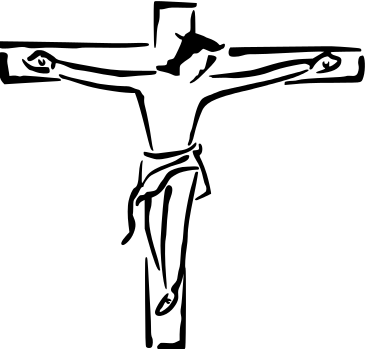
\includegraphics[width=0.20\textwidth]{../christ_on_cross.png}} ;
\end{tikzpicture}
\Large 

\leftcitation{ס} \centerfont 詩百又廿七載：
\leftcitation{ע} \centerfont 非耶和華建屋宇.則匠人之經營徒.
\leftcitation{פ} \centerfont 非耶和華衛城邑.則守者之儆醒徒.
\leftcitation{צ} \centerfont 余獻是卷予華人社區．願為福音流通之器．願獻斯微材為祭榮耀上帝．
\leftcitation{ק} \centerfont 阿門

\switchcolumn

\fontsize{11}{13}\rightfont \Large 滅．時越次聖殿期及當今。\leftcitation{י} \rightfont 猶太者力廣納之．筆錄以卷軸．便以傳、閱、頌、攜、守、鎖、抄、譯、釋、編，得書塔木德、密示拿等經傳．家喻戶曉．傳流若芳。\leftcitation{כ} \rightfont 猶太者文以載道．傳其口述．今我輩粵道之傳應當作如是．遂力行粵音識辨之法．載言載道．以盡忠傳粵道以待興。\leftcitation{ל} \rightfont 蒙下賜恩惠．無畏海量字音文書．既馭上帝之道．今廣及粵語講道．重駛編程之技．匯導粵音遂字稿．重塑講道現場．以傚猶太卷軸之舉便以傳流。\leftcitation{מ} \rightfont 是卷乃粵音口述傳之屬．莫通華文白話之語．

\end{paracol}

\columnratio{0.5,0.5}
\begin{paracol}{2}\fontsize{11}{13}\leftfont \Large \leftcitation{ו} \leftfont 斯殺一違儆百逆．既禁壓之．我輩聞風無奈．在所難免。\leftcitation{ז} \leftfont 另有異人例乎．以版權之名．脅網絡頻道之舉．同授礙予粵道之存流。

\switchcolumn

\fontsize{11}{13}\rightfont \Large 惟待後繼來者之傚．以譯釋傳之於神州華文地。\leftcitation{נ} \rightfont 今能排程驅馭圖靈以編彙文檔，其碼長共數千千亦無逢大礙．全蒙上帝保守。

\end{paracol}



\columnratio{1}\begin{paracol}{1}

\fontsize{11}{13}\rightfont \Large
~~~~~~~~~~~~~~~~~~~~~~~~~~~~~~~~~~~~~~~~~~~~~~~~~~~~~~~~~~~~~~~~~~~~~~~~~~~~~~~\leftcitation{ר} \rightfont 二零二三年二月一日

~~~~~~~~~~~~~~~~~~~~~~~~~~~~~~~~~~~~~~~~~~~~~~~~~~~~~~~~~~~~~~~~~~~~~~~~~~~~~~~\leftcitation{ש} \rightfont 米迦勒

~~~~~~~~~~~~~~~~~~~~~~~~~~~~~~~~~~~~~~~~~~~~~~~~~~~~~~~~~~~~~~~~~~~~~~~~~~~~~~~\leftcitation{ת} \rightfont 書於香港

\end{paracol}

\end{sloppypar}
\end{document}
